% Appendix A

\chapter{Fit Results for The Fake Rate Estimation in Data} % Main appendix title

\label{AppendixA} % For referencing this appendix elsewhere, use \ref{AppendixA}

Here all fits on the tag and probe invariant mass presented for all $p_T-|\eta|$ bins. 
%The first twenty fits belongs to CR1 ($Z\rightarrow e^+e^-$) shown in figure\ref{fig:fit_cr1}. The fits for CR2 ($Z\rightarrow e\gamma$) are given in figure\ref{fig:fit_cr2}.

\begin{figure}[H]
\begin{center}
\scalebox{0.35}{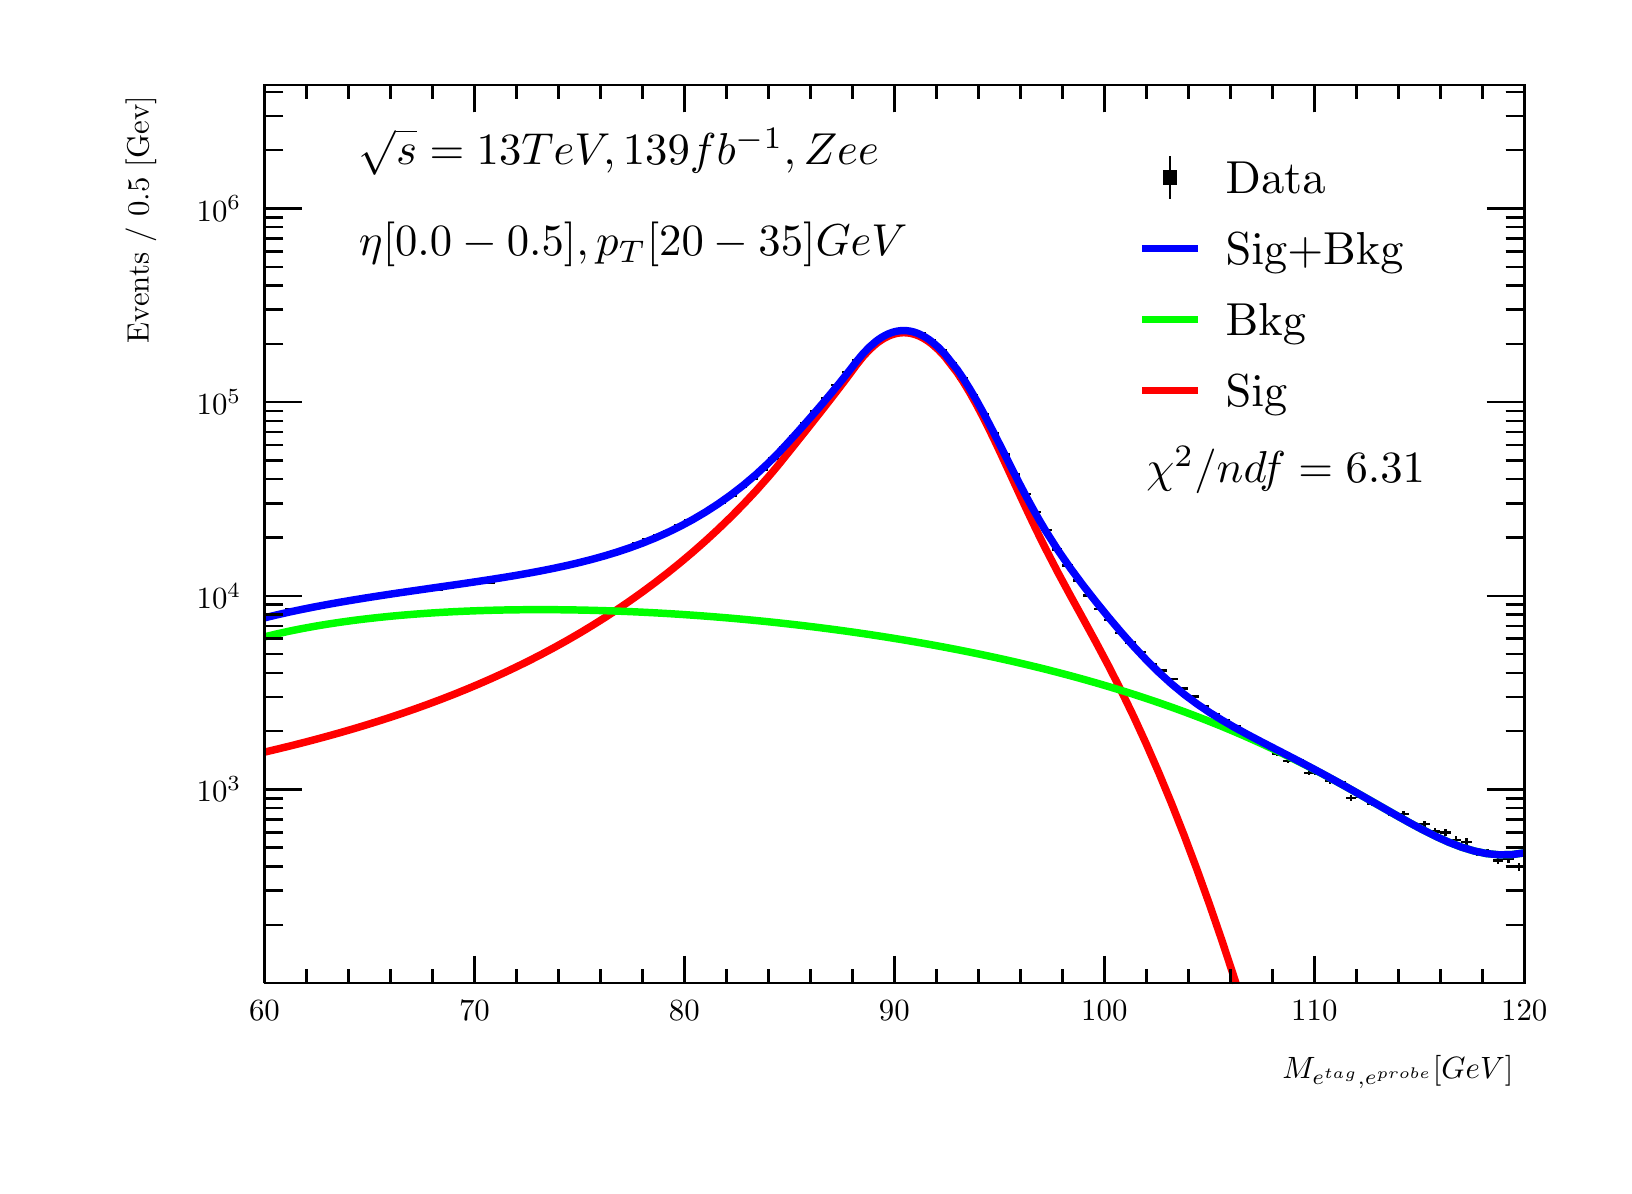
\begin{tikzpicture}
\pgfdeclareplotmark{cross} {
\pgfpathmoveto{\pgfpoint{-0.3\pgfplotmarksize}{\pgfplotmarksize}}
\pgfpathlineto{\pgfpoint{+0.3\pgfplotmarksize}{\pgfplotmarksize}}
\pgfpathlineto{\pgfpoint{+0.3\pgfplotmarksize}{0.3\pgfplotmarksize}}
\pgfpathlineto{\pgfpoint{+1\pgfplotmarksize}{0.3\pgfplotmarksize}}
\pgfpathlineto{\pgfpoint{+1\pgfplotmarksize}{-0.3\pgfplotmarksize}}
\pgfpathlineto{\pgfpoint{+0.3\pgfplotmarksize}{-0.3\pgfplotmarksize}}
\pgfpathlineto{\pgfpoint{+0.3\pgfplotmarksize}{-1.\pgfplotmarksize}}
\pgfpathlineto{\pgfpoint{-0.3\pgfplotmarksize}{-1.\pgfplotmarksize}}
\pgfpathlineto{\pgfpoint{-0.3\pgfplotmarksize}{-0.3\pgfplotmarksize}}
\pgfpathlineto{\pgfpoint{-1.\pgfplotmarksize}{-0.3\pgfplotmarksize}}
\pgfpathlineto{\pgfpoint{-1.\pgfplotmarksize}{0.3\pgfplotmarksize}}
\pgfpathlineto{\pgfpoint{-0.3\pgfplotmarksize}{0.3\pgfplotmarksize}}
\pgfpathclose
\pgfusepathqstroke
}
\pgfdeclareplotmark{cross*} {
\pgfpathmoveto{\pgfpoint{-0.3\pgfplotmarksize}{\pgfplotmarksize}}
\pgfpathlineto{\pgfpoint{+0.3\pgfplotmarksize}{\pgfplotmarksize}}
\pgfpathlineto{\pgfpoint{+0.3\pgfplotmarksize}{0.3\pgfplotmarksize}}
\pgfpathlineto{\pgfpoint{+1\pgfplotmarksize}{0.3\pgfplotmarksize}}
\pgfpathlineto{\pgfpoint{+1\pgfplotmarksize}{-0.3\pgfplotmarksize}}
\pgfpathlineto{\pgfpoint{+0.3\pgfplotmarksize}{-0.3\pgfplotmarksize}}
\pgfpathlineto{\pgfpoint{+0.3\pgfplotmarksize}{-1.\pgfplotmarksize}}
\pgfpathlineto{\pgfpoint{-0.3\pgfplotmarksize}{-1.\pgfplotmarksize}}
\pgfpathlineto{\pgfpoint{-0.3\pgfplotmarksize}{-0.3\pgfplotmarksize}}
\pgfpathlineto{\pgfpoint{-1.\pgfplotmarksize}{-0.3\pgfplotmarksize}}
\pgfpathlineto{\pgfpoint{-1.\pgfplotmarksize}{0.3\pgfplotmarksize}}
\pgfpathlineto{\pgfpoint{-0.3\pgfplotmarksize}{0.3\pgfplotmarksize}}
\pgfpathclose
\pgfusepathqfillstroke
}
\pgfdeclareplotmark{newstar} {
\pgfpathmoveto{\pgfqpoint{0pt}{\pgfplotmarksize}}
\pgfpathlineto{\pgfqpointpolar{44}{0.5\pgfplotmarksize}}
\pgfpathlineto{\pgfqpointpolar{18}{\pgfplotmarksize}}
\pgfpathlineto{\pgfqpointpolar{-20}{0.5\pgfplotmarksize}}
\pgfpathlineto{\pgfqpointpolar{-54}{\pgfplotmarksize}}
\pgfpathlineto{\pgfqpointpolar{-90}{0.5\pgfplotmarksize}}
\pgfpathlineto{\pgfqpointpolar{234}{\pgfplotmarksize}}
\pgfpathlineto{\pgfqpointpolar{198}{0.5\pgfplotmarksize}}
\pgfpathlineto{\pgfqpointpolar{162}{\pgfplotmarksize}}
\pgfpathlineto{\pgfqpointpolar{134}{0.5\pgfplotmarksize}}
\pgfpathclose
\pgfusepathqstroke
}
\pgfdeclareplotmark{newstar*} {
\pgfpathmoveto{\pgfqpoint{0pt}{\pgfplotmarksize}}
\pgfpathlineto{\pgfqpointpolar{44}{0.5\pgfplotmarksize}}
\pgfpathlineto{\pgfqpointpolar{18}{\pgfplotmarksize}}
\pgfpathlineto{\pgfqpointpolar{-20}{0.5\pgfplotmarksize}}
\pgfpathlineto{\pgfqpointpolar{-54}{\pgfplotmarksize}}
\pgfpathlineto{\pgfqpointpolar{-90}{0.5\pgfplotmarksize}}
\pgfpathlineto{\pgfqpointpolar{234}{\pgfplotmarksize}}
\pgfpathlineto{\pgfqpointpolar{198}{0.5\pgfplotmarksize}}
\pgfpathlineto{\pgfqpointpolar{162}{\pgfplotmarksize}}
\pgfpathlineto{\pgfqpointpolar{134}{0.5\pgfplotmarksize}}
\pgfpathclose
\pgfusepathqfillstroke
}
\definecolor{c}{rgb}{1,1,1};
\draw [color=c, fill=c] (0,0) rectangle (20,14.4361);
\draw [color=c, fill=c] (3,2.30977) rectangle (19,13.7143);
\definecolor{c}{rgb}{0,0,0};
\draw [c,line width=0.9] (3,2.30977) -- (3,13.7143) -- (19,13.7143) -- (19,2.30977) -- (3,2.30977);
\definecolor{c}{rgb}{1,1,1};
\draw [color=c, fill=c] (3,2.30977) rectangle (19,13.7143);
\definecolor{c}{rgb}{0,0,0};
\draw [c,line width=0.9] (3,2.30977) -- (3,13.7143) -- (19,13.7143) -- (19,2.30977) -- (3,2.30977);
\draw [c,line width=0.9] (3,2.30977) -- (19,2.30977);
\draw [c,line width=0.9] (3,2.65624) -- (3,2.30977);
\draw [c,line width=0.9] (3.53333,2.48301) -- (3.53333,2.30977);
\draw [c,line width=0.9] (4.06667,2.48301) -- (4.06667,2.30977);
\draw [c,line width=0.9] (4.6,2.48301) -- (4.6,2.30977);
\draw [c,line width=0.9] (5.13333,2.48301) -- (5.13333,2.30977);
\draw [c,line width=0.9] (5.66667,2.65624) -- (5.66667,2.30977);
\draw [c,line width=0.9] (6.2,2.48301) -- (6.2,2.30977);
\draw [c,line width=0.9] (6.73333,2.48301) -- (6.73333,2.30977);
\draw [c,line width=0.9] (7.26667,2.48301) -- (7.26667,2.30977);
\draw [c,line width=0.9] (7.8,2.48301) -- (7.8,2.30977);
\draw [c,line width=0.9] (8.33333,2.65624) -- (8.33333,2.30977);
\draw [c,line width=0.9] (8.86667,2.48301) -- (8.86667,2.30977);
\draw [c,line width=0.9] (9.4,2.48301) -- (9.4,2.30977);
\draw [c,line width=0.9] (9.93333,2.48301) -- (9.93333,2.30977);
\draw [c,line width=0.9] (10.4667,2.48301) -- (10.4667,2.30977);
\draw [c,line width=0.9] (11,2.65624) -- (11,2.30977);
\draw [c,line width=0.9] (11.5333,2.48301) -- (11.5333,2.30977);
\draw [c,line width=0.9] (12.0667,2.48301) -- (12.0667,2.30977);
\draw [c,line width=0.9] (12.6,2.48301) -- (12.6,2.30977);
\draw [c,line width=0.9] (13.1333,2.48301) -- (13.1333,2.30977);
\draw [c,line width=0.9] (13.6667,2.65624) -- (13.6667,2.30977);
\draw [c,line width=0.9] (14.2,2.48301) -- (14.2,2.30977);
\draw [c,line width=0.9] (14.7333,2.48301) -- (14.7333,2.30977);
\draw [c,line width=0.9] (15.2667,2.48301) -- (15.2667,2.30977);
\draw [c,line width=0.9] (15.8,2.48301) -- (15.8,2.30977);
\draw [c,line width=0.9] (16.3333,2.65624) -- (16.3333,2.30977);
\draw [c,line width=0.9] (16.8667,2.48301) -- (16.8667,2.30977);
\draw [c,line width=0.9] (17.4,2.48301) -- (17.4,2.30977);
\draw [c,line width=0.9] (17.9333,2.48301) -- (17.9333,2.30977);
\draw [c,line width=0.9] (18.4667,2.48301) -- (18.4667,2.30977);
\draw [c,line width=0.9] (19,2.65624) -- (19,2.30977);
\draw [anchor=base] (3,1.83338) node[scale=1.11327, color=c, rotate=0]{60};
\draw [anchor=base] (5.66667,1.83338) node[scale=1.11327, color=c, rotate=0]{70};
\draw [anchor=base] (8.33333,1.83338) node[scale=1.11327, color=c, rotate=0]{80};
\draw [anchor=base] (11,1.83338) node[scale=1.11327, color=c, rotate=0]{90};
\draw [anchor=base] (13.6667,1.83338) node[scale=1.11327, color=c, rotate=0]{100};
\draw [anchor=base] (16.3333,1.83338) node[scale=1.11327, color=c, rotate=0]{110};
\draw [anchor=base] (19,1.83338) node[scale=1.11327, color=c, rotate=0]{120};
\draw [anchor= east] (19,1.17798) node[scale=1.11327, color=c, rotate=0]{$M_{e^{tag}, e^{probe}}  [GeV]$};
\draw [c,line width=0.9] (3,13.7143) -- (19,13.7143);
\draw [c,line width=0.9] (3,13.3678) -- (3,13.7143);
\draw [c,line width=0.9] (3.53333,13.5411) -- (3.53333,13.7143);
\draw [c,line width=0.9] (4.06667,13.5411) -- (4.06667,13.7143);
\draw [c,line width=0.9] (4.6,13.5411) -- (4.6,13.7143);
\draw [c,line width=0.9] (5.13333,13.5411) -- (5.13333,13.7143);
\draw [c,line width=0.9] (5.66667,13.3678) -- (5.66667,13.7143);
\draw [c,line width=0.9] (6.2,13.5411) -- (6.2,13.7143);
\draw [c,line width=0.9] (6.73333,13.5411) -- (6.73333,13.7143);
\draw [c,line width=0.9] (7.26667,13.5411) -- (7.26667,13.7143);
\draw [c,line width=0.9] (7.8,13.5411) -- (7.8,13.7143);
\draw [c,line width=0.9] (8.33333,13.3678) -- (8.33333,13.7143);
\draw [c,line width=0.9] (8.86667,13.5411) -- (8.86667,13.7143);
\draw [c,line width=0.9] (9.4,13.5411) -- (9.4,13.7143);
\draw [c,line width=0.9] (9.93333,13.5411) -- (9.93333,13.7143);
\draw [c,line width=0.9] (10.4667,13.5411) -- (10.4667,13.7143);
\draw [c,line width=0.9] (11,13.3678) -- (11,13.7143);
\draw [c,line width=0.9] (11.5333,13.5411) -- (11.5333,13.7143);
\draw [c,line width=0.9] (12.0667,13.5411) -- (12.0667,13.7143);
\draw [c,line width=0.9] (12.6,13.5411) -- (12.6,13.7143);
\draw [c,line width=0.9] (13.1333,13.5411) -- (13.1333,13.7143);
\draw [c,line width=0.9] (13.6667,13.3678) -- (13.6667,13.7143);
\draw [c,line width=0.9] (14.2,13.5411) -- (14.2,13.7143);
\draw [c,line width=0.9] (14.7333,13.5411) -- (14.7333,13.7143);
\draw [c,line width=0.9] (15.2667,13.5411) -- (15.2667,13.7143);
\draw [c,line width=0.9] (15.8,13.5411) -- (15.8,13.7143);
\draw [c,line width=0.9] (16.3333,13.3678) -- (16.3333,13.7143);
\draw [c,line width=0.9] (16.8667,13.5411) -- (16.8667,13.7143);
\draw [c,line width=0.9] (17.4,13.5411) -- (17.4,13.7143);
\draw [c,line width=0.9] (17.9333,13.5411) -- (17.9333,13.7143);
\draw [c,line width=0.9] (18.4667,13.5411) -- (18.4667,13.7143);
\draw [c,line width=0.9] (19,13.3678) -- (19,13.7143);
\draw [c,line width=0.9] (3,2.30977) -- (3,13.7143);
\draw [c,line width=0.9] (3.237,3.05008) -- (3,3.05008);
\draw [c,line width=0.9] (3.237,3.48313) -- (3,3.48313);
\draw [c,line width=0.9] (3.237,3.79038) -- (3,3.79038);
\draw [c,line width=0.9] (3.237,4.02871) -- (3,4.02871);
\draw [c,line width=0.9] (3.237,4.22343) -- (3,4.22343);
\draw [c,line width=0.9] (3.237,4.38807) -- (3,4.38807);
\draw [c,line width=0.9] (3.237,4.53069) -- (3,4.53069);
\draw [c,line width=0.9] (3.237,4.65649) -- (3,4.65649);
\draw [c,line width=0.9] (3.474,4.76901) -- (3,4.76901);
\draw [anchor= east] (2.844,4.76901) node[scale=1.11327, color=c, rotate=0]{$10^{3}$};
\draw [c,line width=0.9] (3.237,5.50932) -- (3,5.50932);
\draw [c,line width=0.9] (3.237,5.94237) -- (3,5.94237);
\draw [c,line width=0.9] (3.237,6.24963) -- (3,6.24963);
\draw [c,line width=0.9] (3.237,6.48795) -- (3,6.48795);
\draw [c,line width=0.9] (3.237,6.68268) -- (3,6.68268);
\draw [c,line width=0.9] (3.237,6.84731) -- (3,6.84731);
\draw [c,line width=0.9] (3.237,6.98993) -- (3,6.98993);
\draw [c,line width=0.9] (3.237,7.11573) -- (3,7.11573);
\draw [c,line width=0.9] (3.474,7.22826) -- (3,7.22826);
\draw [anchor= east] (2.844,7.22826) node[scale=1.11327, color=c, rotate=0]{$10^{4}$};
\draw [c,line width=0.9] (3.237,7.96856) -- (3,7.96856);
\draw [c,line width=0.9] (3.237,8.40161) -- (3,8.40161);
\draw [c,line width=0.9] (3.237,8.70887) -- (3,8.70887);
\draw [c,line width=0.9] (3.237,8.94719) -- (3,8.94719);
\draw [c,line width=0.9] (3.237,9.14192) -- (3,9.14192);
\draw [c,line width=0.9] (3.237,9.30656) -- (3,9.30656);
\draw [c,line width=0.9] (3.237,9.44917) -- (3,9.44917);
\draw [c,line width=0.9] (3.237,9.57497) -- (3,9.57497);
\draw [c,line width=0.9] (3.474,9.6875) -- (3,9.6875);
\draw [anchor= east] (2.844,9.6875) node[scale=1.11327, color=c, rotate=0]{$10^{5}$};
\draw [c,line width=0.9] (3.237,10.4278) -- (3,10.4278);
\draw [c,line width=0.9] (3.237,10.8609) -- (3,10.8609);
\draw [c,line width=0.9] (3.237,11.1681) -- (3,11.1681);
\draw [c,line width=0.9] (3.237,11.4064) -- (3,11.4064);
\draw [c,line width=0.9] (3.237,11.6012) -- (3,11.6012);
\draw [c,line width=0.9] (3.237,11.7658) -- (3,11.7658);
\draw [c,line width=0.9] (3.237,11.9084) -- (3,11.9084);
\draw [c,line width=0.9] (3.237,12.0342) -- (3,12.0342);
\draw [c,line width=0.9] (3.474,12.1467) -- (3,12.1467);
\draw [anchor= east] (2.844,12.1467) node[scale=1.11327, color=c, rotate=0]{$10^{6}$};
\draw [c,line width=0.9] (3.237,12.887) -- (3,12.887);
\draw [c,line width=0.9] (3.237,13.3201) -- (3,13.3201);
\draw [c,line width=0.9] (3.237,13.6274) -- (3,13.6274);
\draw [anchor= east] (1.432,13.7143) node[scale=1.11327, color=c, rotate=90]{Events / 0.5 [Gev]};
\draw [c,line width=0.9] (19,2.30977) -- (19,13.7143);
\draw [c,line width=0.9] (18.763,3.05008) -- (19,3.05008);
\draw [c,line width=0.9] (18.763,3.48313) -- (19,3.48313);
\draw [c,line width=0.9] (18.763,3.79038) -- (19,3.79038);
\draw [c,line width=0.9] (18.763,4.02871) -- (19,4.02871);
\draw [c,line width=0.9] (18.763,4.22343) -- (19,4.22343);
\draw [c,line width=0.9] (18.763,4.38807) -- (19,4.38807);
\draw [c,line width=0.9] (18.763,4.53069) -- (19,4.53069);
\draw [c,line width=0.9] (18.763,4.65649) -- (19,4.65649);
\draw [c,line width=0.9] (18.526,4.76901) -- (19,4.76901);
\draw [c,line width=0.9] (18.763,5.50932) -- (19,5.50932);
\draw [c,line width=0.9] (18.763,5.94237) -- (19,5.94237);
\draw [c,line width=0.9] (18.763,6.24963) -- (19,6.24963);
\draw [c,line width=0.9] (18.763,6.48795) -- (19,6.48795);
\draw [c,line width=0.9] (18.763,6.68268) -- (19,6.68268);
\draw [c,line width=0.9] (18.763,6.84731) -- (19,6.84731);
\draw [c,line width=0.9] (18.763,6.98993) -- (19,6.98993);
\draw [c,line width=0.9] (18.763,7.11573) -- (19,7.11573);
\draw [c,line width=0.9] (18.526,7.22826) -- (19,7.22826);
\draw [c,line width=0.9] (18.763,7.96856) -- (19,7.96856);
\draw [c,line width=0.9] (18.763,8.40161) -- (19,8.40161);
\draw [c,line width=0.9] (18.763,8.70887) -- (19,8.70887);
\draw [c,line width=0.9] (18.763,8.94719) -- (19,8.94719);
\draw [c,line width=0.9] (18.763,9.14192) -- (19,9.14192);
\draw [c,line width=0.9] (18.763,9.30656) -- (19,9.30656);
\draw [c,line width=0.9] (18.763,9.44917) -- (19,9.44917);
\draw [c,line width=0.9] (18.763,9.57497) -- (19,9.57497);
\draw [c,line width=0.9] (18.526,9.6875) -- (19,9.6875);
\draw [c,line width=0.9] (18.763,10.4278) -- (19,10.4278);
\draw [c,line width=0.9] (18.763,10.8609) -- (19,10.8609);
\draw [c,line width=0.9] (18.763,11.1681) -- (19,11.1681);
\draw [c,line width=0.9] (18.763,11.4064) -- (19,11.4064);
\draw [c,line width=0.9] (18.763,11.6012) -- (19,11.6012);
\draw [c,line width=0.9] (18.763,11.7658) -- (19,11.7658);
\draw [c,line width=0.9] (18.763,11.9084) -- (19,11.9084);
\draw [c,line width=0.9] (18.763,12.0342) -- (19,12.0342);
\draw [c,line width=0.9] (18.526,12.1467) -- (19,12.1467);
\draw [c,line width=0.9] (18.763,12.887) -- (19,12.887);
\draw [c,line width=0.9] (18.763,13.3201) -- (19,13.3201);
\draw [c,line width=0.9] (18.763,13.6274) -- (19,13.6274);
\draw [c,line width=0.9] (3.06667,6.97555) -- (3,6.97555);
\draw [c,line width=0.9] (3,6.97555) -- (3,6.97555);
\draw [c,line width=0.9] (3.06667,6.97555) -- (3.13333,6.97555);
\draw [c,line width=0.9] (3.13333,6.97555) -- (3.13333,6.97555);
\draw [c,line width=0.9] (3.06667,6.97555) -- (3.06667,6.98757);
\draw [c,line width=0.9] (3.06667,6.98757) -- (3.06667,6.98757);
\draw [c,line width=0.9] (3.06667,6.97555) -- (3.06667,6.96353);
\draw [c,line width=0.9] (3.06667,6.96353) -- (3.06667,6.96353);
\draw [c,line width=0.9] (3.2,6.99897) -- (3.13333,6.99897);
\draw [c,line width=0.9] (3.13333,6.99897) -- (3.13333,6.99897);
\draw [c,line width=0.9] (3.2,6.99897) -- (3.26667,6.99897);
\draw [c,line width=0.9] (3.26667,6.99897) -- (3.26667,6.99897);
\draw [c,line width=0.9] (3.2,6.99897) -- (3.2,7.01086);
\draw [c,line width=0.9] (3.2,7.01086) -- (3.2,7.01086);
\draw [c,line width=0.9] (3.2,6.99897) -- (3.2,6.98708);
\draw [c,line width=0.9] (3.2,6.98708) -- (3.2,6.98708);
\draw [c,line width=0.9] (3.33333,7.05305) -- (3.26667,7.05305);
\draw [c,line width=0.9] (3.26667,7.05305) -- (3.26667,7.05305);
\draw [c,line width=0.9] (3.33333,7.05305) -- (3.4,7.05305);
\draw [c,line width=0.9] (3.4,7.05305) -- (3.4,7.05305);
\draw [c,line width=0.9] (3.33333,7.05305) -- (3.33333,7.06464);
\draw [c,line width=0.9] (3.33333,7.06464) -- (3.33333,7.06464);
\draw [c,line width=0.9] (3.33333,7.05305) -- (3.33333,7.04145);
\draw [c,line width=0.9] (3.33333,7.04145) -- (3.33333,7.04145);
\draw [c,line width=0.9] (3.46667,7.05619) -- (3.4,7.05619);
\draw [c,line width=0.9] (3.4,7.05619) -- (3.4,7.05619);
\draw [c,line width=0.9] (3.46667,7.05619) -- (3.53333,7.05619);
\draw [c,line width=0.9] (3.53333,7.05619) -- (3.53333,7.05619);
\draw [c,line width=0.9] (3.46667,7.05619) -- (3.46667,7.06776);
\draw [c,line width=0.9] (3.46667,7.06776) -- (3.46667,7.06776);
\draw [c,line width=0.9] (3.46667,7.05619) -- (3.46667,7.04461);
\draw [c,line width=0.9] (3.46667,7.04461) -- (3.46667,7.04461);
\draw [c,line width=0.9] (3.6,7.09403) -- (3.53333,7.09403);
\draw [c,line width=0.9] (3.53333,7.09403) -- (3.53333,7.09403);
\draw [c,line width=0.9] (3.6,7.09403) -- (3.66667,7.09403);
\draw [c,line width=0.9] (3.66667,7.09403) -- (3.66667,7.09403);
\draw [c,line width=0.9] (3.6,7.09403) -- (3.6,7.1054);
\draw [c,line width=0.9] (3.6,7.1054) -- (3.6,7.1054);
\draw [c,line width=0.9] (3.6,7.09403) -- (3.6,7.08266);
\draw [c,line width=0.9] (3.6,7.08266) -- (3.6,7.08266);
\draw [c,line width=0.9] (3.73333,7.12094) -- (3.66667,7.12094);
\draw [c,line width=0.9] (3.66667,7.12094) -- (3.66667,7.12094);
\draw [c,line width=0.9] (3.73333,7.12094) -- (3.8,7.12094);
\draw [c,line width=0.9] (3.8,7.12094) -- (3.8,7.12094);
\draw [c,line width=0.9] (3.73333,7.12094) -- (3.73333,7.13217);
\draw [c,line width=0.9] (3.73333,7.13217) -- (3.73333,7.13217);
\draw [c,line width=0.9] (3.73333,7.12094) -- (3.73333,7.10971);
\draw [c,line width=0.9] (3.73333,7.10971) -- (3.73333,7.10971);
\draw [c,line width=0.9] (3.86667,7.1328) -- (3.8,7.1328);
\draw [c,line width=0.9] (3.8,7.1328) -- (3.8,7.1328);
\draw [c,line width=0.9] (3.86667,7.1328) -- (3.93333,7.1328);
\draw [c,line width=0.9] (3.93333,7.1328) -- (3.93333,7.1328);
\draw [c,line width=0.9] (3.86667,7.1328) -- (3.86667,7.14397);
\draw [c,line width=0.9] (3.86667,7.14397) -- (3.86667,7.14397);
\draw [c,line width=0.9] (3.86667,7.1328) -- (3.86667,7.12163);
\draw [c,line width=0.9] (3.86667,7.12163) -- (3.86667,7.12163);
\draw [c,line width=0.9] (4,7.15407) -- (3.93333,7.15407);
\draw [c,line width=0.9] (3.93333,7.15407) -- (3.93333,7.15407);
\draw [c,line width=0.9] (4,7.15407) -- (4.06667,7.15407);
\draw [c,line width=0.9] (4.06667,7.15407) -- (4.06667,7.15407);
\draw [c,line width=0.9] (4,7.15407) -- (4,7.16513);
\draw [c,line width=0.9] (4,7.16513) -- (4,7.16513);
\draw [c,line width=0.9] (4,7.15407) -- (4,7.14302);
\draw [c,line width=0.9] (4,7.14302) -- (4,7.14302);
\draw [c,line width=0.9] (4.13333,7.18377) -- (4.06667,7.18377);
\draw [c,line width=0.9] (4.06667,7.18377) -- (4.06667,7.18377);
\draw [c,line width=0.9] (4.13333,7.18377) -- (4.2,7.18377);
\draw [c,line width=0.9] (4.2,7.18377) -- (4.2,7.18377);
\draw [c,line width=0.9] (4.13333,7.18377) -- (4.13333,7.19467);
\draw [c,line width=0.9] (4.13333,7.19467) -- (4.13333,7.19467);
\draw [c,line width=0.9] (4.13333,7.18377) -- (4.13333,7.17286);
\draw [c,line width=0.9] (4.13333,7.17286) -- (4.13333,7.17286);
\draw [c,line width=0.9] (4.26667,7.21439) -- (4.2,7.21439);
\draw [c,line width=0.9] (4.2,7.21439) -- (4.2,7.21439);
\draw [c,line width=0.9] (4.26667,7.21439) -- (4.33333,7.21439);
\draw [c,line width=0.9] (4.33333,7.21439) -- (4.33333,7.21439);
\draw [c,line width=0.9] (4.26667,7.21439) -- (4.26667,7.22514);
\draw [c,line width=0.9] (4.26667,7.22514) -- (4.26667,7.22514);
\draw [c,line width=0.9] (4.26667,7.21439) -- (4.26667,7.20364);
\draw [c,line width=0.9] (4.26667,7.20364) -- (4.26667,7.20364);
\draw [c,line width=0.9] (4.4,7.21114) -- (4.33333,7.21114);
\draw [c,line width=0.9] (4.33333,7.21114) -- (4.33333,7.21114);
\draw [c,line width=0.9] (4.4,7.21114) -- (4.46667,7.21114);
\draw [c,line width=0.9] (4.46667,7.21114) -- (4.46667,7.21114);
\draw [c,line width=0.9] (4.4,7.21114) -- (4.4,7.22191);
\draw [c,line width=0.9] (4.4,7.22191) -- (4.4,7.22191);
\draw [c,line width=0.9] (4.4,7.21114) -- (4.4,7.20037);
\draw [c,line width=0.9] (4.4,7.20037) -- (4.4,7.20037);
\draw [c,line width=0.9] (4.53333,7.21979) -- (4.46667,7.21979);
\draw [c,line width=0.9] (4.46667,7.21979) -- (4.46667,7.21979);
\draw [c,line width=0.9] (4.53333,7.21979) -- (4.6,7.21979);
\draw [c,line width=0.9] (4.6,7.21979) -- (4.6,7.21979);
\draw [c,line width=0.9] (4.53333,7.21979) -- (4.53333,7.23051);
\draw [c,line width=0.9] (4.53333,7.23051) -- (4.53333,7.23051);
\draw [c,line width=0.9] (4.53333,7.21979) -- (4.53333,7.20906);
\draw [c,line width=0.9] (4.53333,7.20906) -- (4.53333,7.20906);
\draw [c,line width=0.9] (4.66667,7.23878) -- (4.6,7.23878);
\draw [c,line width=0.9] (4.6,7.23878) -- (4.6,7.23878);
\draw [c,line width=0.9] (4.66667,7.23878) -- (4.73333,7.23878);
\draw [c,line width=0.9] (4.73333,7.23878) -- (4.73333,7.23878);
\draw [c,line width=0.9] (4.66667,7.23878) -- (4.66667,7.24941);
\draw [c,line width=0.9] (4.66667,7.24941) -- (4.66667,7.24941);
\draw [c,line width=0.9] (4.66667,7.23878) -- (4.66667,7.22815);
\draw [c,line width=0.9] (4.66667,7.22815) -- (4.66667,7.22815);
\draw [c,line width=0.9] (4.8,7.28756) -- (4.73333,7.28756);
\draw [c,line width=0.9] (4.73333,7.28756) -- (4.73333,7.28756);
\draw [c,line width=0.9] (4.8,7.28756) -- (4.86667,7.28756);
\draw [c,line width=0.9] (4.86667,7.28756) -- (4.86667,7.28756);
\draw [c,line width=0.9] (4.8,7.28756) -- (4.8,7.29795);
\draw [c,line width=0.9] (4.8,7.29795) -- (4.8,7.29795);
\draw [c,line width=0.9] (4.8,7.28756) -- (4.8,7.27718);
\draw [c,line width=0.9] (4.8,7.27718) -- (4.8,7.27718);
\draw [c,line width=0.9] (4.93333,7.27425) -- (4.86667,7.27425);
\draw [c,line width=0.9] (4.86667,7.27425) -- (4.86667,7.27425);
\draw [c,line width=0.9] (4.93333,7.27425) -- (5,7.27425);
\draw [c,line width=0.9] (5,7.27425) -- (5,7.27425);
\draw [c,line width=0.9] (4.93333,7.27425) -- (4.93333,7.2847);
\draw [c,line width=0.9] (4.93333,7.2847) -- (4.93333,7.2847);
\draw [c,line width=0.9] (4.93333,7.27425) -- (4.93333,7.26379);
\draw [c,line width=0.9] (4.93333,7.26379) -- (4.93333,7.26379);
\draw [c,line width=0.9] (5.06667,7.30986) -- (5,7.30986);
\draw [c,line width=0.9] (5,7.30986) -- (5,7.30986);
\draw [c,line width=0.9] (5.06667,7.30986) -- (5.13333,7.30986);
\draw [c,line width=0.9] (5.13333,7.30986) -- (5.13333,7.30986);
\draw [c,line width=0.9] (5.06667,7.30986) -- (5.06667,7.32014);
\draw [c,line width=0.9] (5.06667,7.32014) -- (5.06667,7.32014);
\draw [c,line width=0.9] (5.06667,7.30986) -- (5.06667,7.29958);
\draw [c,line width=0.9] (5.06667,7.29958) -- (5.06667,7.29958);
\draw [c,line width=0.9] (5.2,7.31065) -- (5.13333,7.31065);
\draw [c,line width=0.9] (5.13333,7.31065) -- (5.13333,7.31065);
\draw [c,line width=0.9] (5.2,7.31065) -- (5.26667,7.31065);
\draw [c,line width=0.9] (5.26667,7.31065) -- (5.26667,7.31065);
\draw [c,line width=0.9] (5.2,7.31065) -- (5.2,7.32093);
\draw [c,line width=0.9] (5.2,7.32093) -- (5.2,7.32093);
\draw [c,line width=0.9] (5.2,7.31065) -- (5.2,7.30038);
\draw [c,line width=0.9] (5.2,7.30038) -- (5.2,7.30038);
\draw [c,line width=0.9] (5.33333,7.34844) -- (5.26667,7.34844);
\draw [c,line width=0.9] (5.26667,7.34844) -- (5.26667,7.34844);
\draw [c,line width=0.9] (5.33333,7.34844) -- (5.4,7.34844);
\draw [c,line width=0.9] (5.4,7.34844) -- (5.4,7.34844);
\draw [c,line width=0.9] (5.33333,7.34844) -- (5.33333,7.35853);
\draw [c,line width=0.9] (5.33333,7.35853) -- (5.33333,7.35853);
\draw [c,line width=0.9] (5.33333,7.34844) -- (5.33333,7.33834);
\draw [c,line width=0.9] (5.33333,7.33834) -- (5.33333,7.33834);
\draw [c,line width=0.9] (5.46667,7.35358) -- (5.4,7.35358);
\draw [c,line width=0.9] (5.4,7.35358) -- (5.4,7.35358);
\draw [c,line width=0.9] (5.46667,7.35358) -- (5.53333,7.35358);
\draw [c,line width=0.9] (5.53333,7.35358) -- (5.53333,7.35358);
\draw [c,line width=0.9] (5.46667,7.35358) -- (5.46667,7.36365);
\draw [c,line width=0.9] (5.46667,7.36365) -- (5.46667,7.36365);
\draw [c,line width=0.9] (5.46667,7.35358) -- (5.46667,7.34351);
\draw [c,line width=0.9] (5.46667,7.34351) -- (5.46667,7.34351);
\draw [c,line width=0.9] (5.6,7.38401) -- (5.53333,7.38401);
\draw [c,line width=0.9] (5.53333,7.38401) -- (5.53333,7.38401);
\draw [c,line width=0.9] (5.6,7.38401) -- (5.66667,7.38401);
\draw [c,line width=0.9] (5.66667,7.38401) -- (5.66667,7.38401);
\draw [c,line width=0.9] (5.6,7.38401) -- (5.6,7.39394);
\draw [c,line width=0.9] (5.6,7.39394) -- (5.6,7.39394);
\draw [c,line width=0.9] (5.6,7.38401) -- (5.6,7.37408);
\draw [c,line width=0.9] (5.6,7.37408) -- (5.6,7.37408);
\draw [c,line width=0.9] (5.73333,7.39649) -- (5.66667,7.39649);
\draw [c,line width=0.9] (5.66667,7.39649) -- (5.66667,7.39649);
\draw [c,line width=0.9] (5.73333,7.39649) -- (5.8,7.39649);
\draw [c,line width=0.9] (5.8,7.39649) -- (5.8,7.39649);
\draw [c,line width=0.9] (5.73333,7.39649) -- (5.73333,7.40636);
\draw [c,line width=0.9] (5.73333,7.40636) -- (5.73333,7.40636);
\draw [c,line width=0.9] (5.73333,7.39649) -- (5.73333,7.38662);
\draw [c,line width=0.9] (5.73333,7.38662) -- (5.73333,7.38662);
\draw [c,line width=0.9] (5.86667,7.39722) -- (5.8,7.39722);
\draw [c,line width=0.9] (5.8,7.39722) -- (5.8,7.39722);
\draw [c,line width=0.9] (5.86667,7.39722) -- (5.93333,7.39722);
\draw [c,line width=0.9] (5.93333,7.39722) -- (5.93333,7.39722);
\draw [c,line width=0.9] (5.86667,7.39722) -- (5.86667,7.40709);
\draw [c,line width=0.9] (5.86667,7.40709) -- (5.86667,7.40709);
\draw [c,line width=0.9] (5.86667,7.39722) -- (5.86667,7.38735);
\draw [c,line width=0.9] (5.86667,7.38735) -- (5.86667,7.38735);
\draw [c,line width=0.9] (6,7.44378) -- (5.93333,7.44378);
\draw [c,line width=0.9] (5.93333,7.44378) -- (5.93333,7.44378);
\draw [c,line width=0.9] (6,7.44378) -- (6.06667,7.44378);
\draw [c,line width=0.9] (6.06667,7.44378) -- (6.06667,7.44378);
\draw [c,line width=0.9] (6,7.44378) -- (6,7.45344);
\draw [c,line width=0.9] (6,7.45344) -- (6,7.45344);
\draw [c,line width=0.9] (6,7.44378) -- (6,7.43413);
\draw [c,line width=0.9] (6,7.43413) -- (6,7.43413);
\draw [c,line width=0.9] (6.13333,7.45403) -- (6.06667,7.45403);
\draw [c,line width=0.9] (6.06667,7.45403) -- (6.06667,7.45403);
\draw [c,line width=0.9] (6.13333,7.45403) -- (6.2,7.45403);
\draw [c,line width=0.9] (6.2,7.45403) -- (6.2,7.45403);
\draw [c,line width=0.9] (6.13333,7.45403) -- (6.13333,7.46364);
\draw [c,line width=0.9] (6.13333,7.46364) -- (6.13333,7.46364);
\draw [c,line width=0.9] (6.13333,7.45403) -- (6.13333,7.44443);
\draw [c,line width=0.9] (6.13333,7.44443) -- (6.13333,7.44443);
\draw [c,line width=0.9] (6.26667,7.5008) -- (6.2,7.5008);
\draw [c,line width=0.9] (6.2,7.5008) -- (6.2,7.5008);
\draw [c,line width=0.9] (6.26667,7.5008) -- (6.33333,7.5008);
\draw [c,line width=0.9] (6.33333,7.5008) -- (6.33333,7.5008);
\draw [c,line width=0.9] (6.26667,7.5008) -- (6.26667,7.5102);
\draw [c,line width=0.9] (6.26667,7.5102) -- (6.26667,7.5102);
\draw [c,line width=0.9] (6.26667,7.5008) -- (6.26667,7.4914);
\draw [c,line width=0.9] (6.26667,7.4914) -- (6.26667,7.4914);
\draw [c,line width=0.9] (6.4,7.52162) -- (6.33333,7.52162);
\draw [c,line width=0.9] (6.33333,7.52162) -- (6.33333,7.52162);
\draw [c,line width=0.9] (6.4,7.52162) -- (6.46667,7.52162);
\draw [c,line width=0.9] (6.46667,7.52162) -- (6.46667,7.52162);
\draw [c,line width=0.9] (6.4,7.52162) -- (6.4,7.53093);
\draw [c,line width=0.9] (6.4,7.53093) -- (6.4,7.53093);
\draw [c,line width=0.9] (6.4,7.52162) -- (6.4,7.51231);
\draw [c,line width=0.9] (6.4,7.51231) -- (6.4,7.51231);
\draw [c,line width=0.9] (6.53333,7.54941) -- (6.46667,7.54941);
\draw [c,line width=0.9] (6.46667,7.54941) -- (6.46667,7.54941);
\draw [c,line width=0.9] (6.53333,7.54941) -- (6.6,7.54941);
\draw [c,line width=0.9] (6.6,7.54941) -- (6.6,7.54941);
\draw [c,line width=0.9] (6.53333,7.54941) -- (6.53333,7.5586);
\draw [c,line width=0.9] (6.53333,7.5586) -- (6.53333,7.5586);
\draw [c,line width=0.9] (6.53333,7.54941) -- (6.53333,7.54022);
\draw [c,line width=0.9] (6.53333,7.54022) -- (6.53333,7.54022);
\draw [c,line width=0.9] (6.66667,7.58211) -- (6.6,7.58211);
\draw [c,line width=0.9] (6.6,7.58211) -- (6.6,7.58211);
\draw [c,line width=0.9] (6.66667,7.58211) -- (6.73333,7.58211);
\draw [c,line width=0.9] (6.73333,7.58211) -- (6.73333,7.58211);
\draw [c,line width=0.9] (6.66667,7.58211) -- (6.66667,7.59116);
\draw [c,line width=0.9] (6.66667,7.59116) -- (6.66667,7.59116);
\draw [c,line width=0.9] (6.66667,7.58211) -- (6.66667,7.57306);
\draw [c,line width=0.9] (6.66667,7.57306) -- (6.66667,7.57306);
\draw [c,line width=0.9] (6.8,7.61094) -- (6.73333,7.61094);
\draw [c,line width=0.9] (6.73333,7.61094) -- (6.73333,7.61094);
\draw [c,line width=0.9] (6.8,7.61094) -- (6.86667,7.61094);
\draw [c,line width=0.9] (6.86667,7.61094) -- (6.86667,7.61094);
\draw [c,line width=0.9] (6.8,7.61094) -- (6.8,7.61987);
\draw [c,line width=0.9] (6.8,7.61987) -- (6.8,7.61987);
\draw [c,line width=0.9] (6.8,7.61094) -- (6.8,7.60201);
\draw [c,line width=0.9] (6.8,7.60201) -- (6.8,7.60201);
\draw [c,line width=0.9] (6.93333,7.6331) -- (6.86667,7.6331);
\draw [c,line width=0.9] (6.86667,7.6331) -- (6.86667,7.6331);
\draw [c,line width=0.9] (6.93333,7.6331) -- (7,7.6331);
\draw [c,line width=0.9] (7,7.6331) -- (7,7.6331);
\draw [c,line width=0.9] (6.93333,7.6331) -- (6.93333,7.64194);
\draw [c,line width=0.9] (6.93333,7.64194) -- (6.93333,7.64194);
\draw [c,line width=0.9] (6.93333,7.6331) -- (6.93333,7.62426);
\draw [c,line width=0.9] (6.93333,7.62426) -- (6.93333,7.62426);
\draw [c,line width=0.9] (7.06667,7.66734) -- (7,7.66734);
\draw [c,line width=0.9] (7,7.66734) -- (7,7.66734);
\draw [c,line width=0.9] (7.06667,7.66734) -- (7.13333,7.66734);
\draw [c,line width=0.9] (7.13333,7.66734) -- (7.13333,7.66734);
\draw [c,line width=0.9] (7.06667,7.66734) -- (7.06667,7.67604);
\draw [c,line width=0.9] (7.06667,7.67604) -- (7.06667,7.67604);
\draw [c,line width=0.9] (7.06667,7.66734) -- (7.06667,7.65865);
\draw [c,line width=0.9] (7.06667,7.65865) -- (7.06667,7.65865);
\draw [c,line width=0.9] (7.2,7.71829) -- (7.13333,7.71829);
\draw [c,line width=0.9] (7.13333,7.71829) -- (7.13333,7.71829);
\draw [c,line width=0.9] (7.2,7.71829) -- (7.26667,7.71829);
\draw [c,line width=0.9] (7.26667,7.71829) -- (7.26667,7.71829);
\draw [c,line width=0.9] (7.2,7.71829) -- (7.2,7.72678);
\draw [c,line width=0.9] (7.2,7.72678) -- (7.2,7.72678);
\draw [c,line width=0.9] (7.2,7.71829) -- (7.2,7.7098);
\draw [c,line width=0.9] (7.2,7.7098) -- (7.2,7.7098);
\draw [c,line width=0.9] (7.33333,7.73961) -- (7.26667,7.73961);
\draw [c,line width=0.9] (7.26667,7.73961) -- (7.26667,7.73961);
\draw [c,line width=0.9] (7.33333,7.73961) -- (7.4,7.73961);
\draw [c,line width=0.9] (7.4,7.73961) -- (7.4,7.73961);
\draw [c,line width=0.9] (7.33333,7.73961) -- (7.33333,7.74801);
\draw [c,line width=0.9] (7.33333,7.74801) -- (7.33333,7.74801);
\draw [c,line width=0.9] (7.33333,7.73961) -- (7.33333,7.7312);
\draw [c,line width=0.9] (7.33333,7.7312) -- (7.33333,7.7312);
\draw [c,line width=0.9] (7.46667,7.78235) -- (7.4,7.78235);
\draw [c,line width=0.9] (7.4,7.78235) -- (7.4,7.78235);
\draw [c,line width=0.9] (7.46667,7.78235) -- (7.53333,7.78235);
\draw [c,line width=0.9] (7.53333,7.78235) -- (7.53333,7.78235);
\draw [c,line width=0.9] (7.46667,7.78235) -- (7.46667,7.79059);
\draw [c,line width=0.9] (7.46667,7.79059) -- (7.46667,7.79059);
\draw [c,line width=0.9] (7.46667,7.78235) -- (7.46667,7.77411);
\draw [c,line width=0.9] (7.46667,7.77411) -- (7.46667,7.77411);
\draw [c,line width=0.9] (7.6,7.83343) -- (7.53333,7.83343);
\draw [c,line width=0.9] (7.53333,7.83343) -- (7.53333,7.83343);
\draw [c,line width=0.9] (7.6,7.83343) -- (7.66667,7.83343);
\draw [c,line width=0.9] (7.66667,7.83343) -- (7.66667,7.83343);
\draw [c,line width=0.9] (7.6,7.83343) -- (7.6,7.84147);
\draw [c,line width=0.9] (7.6,7.84147) -- (7.6,7.84147);
\draw [c,line width=0.9] (7.6,7.83343) -- (7.6,7.82538);
\draw [c,line width=0.9] (7.6,7.82538) -- (7.6,7.82538);
\draw [c,line width=0.9] (7.73333,7.89025) -- (7.66667,7.89025);
\draw [c,line width=0.9] (7.66667,7.89025) -- (7.66667,7.89025);
\draw [c,line width=0.9] (7.73333,7.89025) -- (7.8,7.89025);
\draw [c,line width=0.9] (7.8,7.89025) -- (7.8,7.89025);
\draw [c,line width=0.9] (7.73333,7.89025) -- (7.73333,7.89808);
\draw [c,line width=0.9] (7.73333,7.89808) -- (7.73333,7.89808);
\draw [c,line width=0.9] (7.73333,7.89025) -- (7.73333,7.88242);
\draw [c,line width=0.9] (7.73333,7.88242) -- (7.73333,7.88242);
\draw [c,line width=0.9] (7.86667,7.94824) -- (7.8,7.94824);
\draw [c,line width=0.9] (7.8,7.94824) -- (7.8,7.94824);
\draw [c,line width=0.9] (7.86667,7.94824) -- (7.93333,7.94824);
\draw [c,line width=0.9] (7.93333,7.94824) -- (7.93333,7.94824);
\draw [c,line width=0.9] (7.86667,7.94824) -- (7.86667,7.95586);
\draw [c,line width=0.9] (7.86667,7.95586) -- (7.86667,7.95586);
\draw [c,line width=0.9] (7.86667,7.94824) -- (7.86667,7.94061);
\draw [c,line width=0.9] (7.86667,7.94061) -- (7.86667,7.94061);
\draw [c,line width=0.9] (8,7.99107) -- (7.93333,7.99107);
\draw [c,line width=0.9] (7.93333,7.99107) -- (7.93333,7.99107);
\draw [c,line width=0.9] (8,7.99107) -- (8.06667,7.99107);
\draw [c,line width=0.9] (8.06667,7.99107) -- (8.06667,7.99107);
\draw [c,line width=0.9] (8,7.99107) -- (8,7.99855);
\draw [c,line width=0.9] (8,7.99855) -- (8,7.99855);
\draw [c,line width=0.9] (8,7.99107) -- (8,7.9836);
\draw [c,line width=0.9] (8,7.9836) -- (8,7.9836);
\draw [c,line width=0.9] (8.13333,8.04883) -- (8.06667,8.04883);
\draw [c,line width=0.9] (8.06667,8.04883) -- (8.06667,8.04883);
\draw [c,line width=0.9] (8.13333,8.04883) -- (8.2,8.04883);
\draw [c,line width=0.9] (8.2,8.04883) -- (8.2,8.04883);
\draw [c,line width=0.9] (8.13333,8.04883) -- (8.13333,8.0561);
\draw [c,line width=0.9] (8.13333,8.0561) -- (8.13333,8.0561);
\draw [c,line width=0.9] (8.13333,8.04883) -- (8.13333,8.04156);
\draw [c,line width=0.9] (8.13333,8.04156) -- (8.13333,8.04156);
\draw [c,line width=0.9] (8.26667,8.11821) -- (8.2,8.11821);
\draw [c,line width=0.9] (8.2,8.11821) -- (8.2,8.11821);
\draw [c,line width=0.9] (8.26667,8.11821) -- (8.33333,8.11821);
\draw [c,line width=0.9] (8.33333,8.11821) -- (8.33333,8.11821);
\draw [c,line width=0.9] (8.26667,8.11821) -- (8.26667,8.12525);
\draw [c,line width=0.9] (8.26667,8.12525) -- (8.26667,8.12525);
\draw [c,line width=0.9] (8.26667,8.11821) -- (8.26667,8.11116);
\draw [c,line width=0.9] (8.26667,8.11116) -- (8.26667,8.11116);
\draw [c,line width=0.9] (8.4,8.18278) -- (8.33333,8.18278);
\draw [c,line width=0.9] (8.33333,8.18278) -- (8.33333,8.18278);
\draw [c,line width=0.9] (8.4,8.18278) -- (8.46667,8.18278);
\draw [c,line width=0.9] (8.46667,8.18278) -- (8.46667,8.18278);
\draw [c,line width=0.9] (8.4,8.18278) -- (8.4,8.18961);
\draw [c,line width=0.9] (8.4,8.18961) -- (8.4,8.18961);
\draw [c,line width=0.9] (8.4,8.18278) -- (8.4,8.17595);
\draw [c,line width=0.9] (8.4,8.17595) -- (8.4,8.17595);
\draw [c,line width=0.9] (8.53333,8.25148) -- (8.46667,8.25148);
\draw [c,line width=0.9] (8.46667,8.25148) -- (8.46667,8.25148);
\draw [c,line width=0.9] (8.53333,8.25148) -- (8.6,8.25148);
\draw [c,line width=0.9] (8.6,8.25148) -- (8.6,8.25148);
\draw [c,line width=0.9] (8.53333,8.25148) -- (8.53333,8.2581);
\draw [c,line width=0.9] (8.53333,8.2581) -- (8.53333,8.2581);
\draw [c,line width=0.9] (8.53333,8.25148) -- (8.53333,8.24487);
\draw [c,line width=0.9] (8.53333,8.24487) -- (8.53333,8.24487);
\draw [c,line width=0.9] (8.66667,8.3296) -- (8.6,8.3296);
\draw [c,line width=0.9] (8.6,8.3296) -- (8.6,8.3296);
\draw [c,line width=0.9] (8.66667,8.3296) -- (8.73333,8.3296);
\draw [c,line width=0.9] (8.73333,8.3296) -- (8.73333,8.3296);
\draw [c,line width=0.9] (8.66667,8.3296) -- (8.66667,8.33598);
\draw [c,line width=0.9] (8.66667,8.33598) -- (8.66667,8.33598);
\draw [c,line width=0.9] (8.66667,8.3296) -- (8.66667,8.32323);
\draw [c,line width=0.9] (8.66667,8.32323) -- (8.66667,8.32323);
\draw [c,line width=0.9] (8.8,8.41062) -- (8.73333,8.41062);
\draw [c,line width=0.9] (8.73333,8.41062) -- (8.73333,8.41062);
\draw [c,line width=0.9] (8.8,8.41062) -- (8.86667,8.41062);
\draw [c,line width=0.9] (8.86667,8.41062) -- (8.86667,8.41062);
\draw [c,line width=0.9] (8.8,8.41062) -- (8.8,8.41676);
\draw [c,line width=0.9] (8.8,8.41676) -- (8.8,8.41676);
\draw [c,line width=0.9] (8.8,8.41062) -- (8.8,8.40448);
\draw [c,line width=0.9] (8.8,8.40448) -- (8.8,8.40448);
\draw [c,line width=0.9] (8.93333,8.50328) -- (8.86667,8.50328);
\draw [c,line width=0.9] (8.86667,8.50328) -- (8.86667,8.50328);
\draw [c,line width=0.9] (8.93333,8.50328) -- (9,8.50328);
\draw [c,line width=0.9] (9,8.50328) -- (9,8.50328);
\draw [c,line width=0.9] (8.93333,8.50328) -- (8.93333,8.50916);
\draw [c,line width=0.9] (8.93333,8.50916) -- (8.93333,8.50916);
\draw [c,line width=0.9] (8.93333,8.50328) -- (8.93333,8.4974);
\draw [c,line width=0.9] (8.93333,8.4974) -- (8.93333,8.4974);
\draw [c,line width=0.9] (9.06667,8.60958) -- (9,8.60958);
\draw [c,line width=0.9] (9,8.60958) -- (9,8.60958);
\draw [c,line width=0.9] (9.06667,8.60958) -- (9.13333,8.60958);
\draw [c,line width=0.9] (9.13333,8.60958) -- (9.13333,8.60958);
\draw [c,line width=0.9] (9.06667,8.60958) -- (9.06667,8.61517);
\draw [c,line width=0.9] (9.06667,8.61517) -- (9.06667,8.61517);
\draw [c,line width=0.9] (9.06667,8.60958) -- (9.06667,8.60398);
\draw [c,line width=0.9] (9.06667,8.60398) -- (9.06667,8.60398);
\draw [c,line width=0.9] (9.2,8.71741) -- (9.13333,8.71741);
\draw [c,line width=0.9] (9.13333,8.71741) -- (9.13333,8.71741);
\draw [c,line width=0.9] (9.2,8.71741) -- (9.26667,8.71741);
\draw [c,line width=0.9] (9.26667,8.71741) -- (9.26667,8.71741);
\draw [c,line width=0.9] (9.2,8.71741) -- (9.2,8.72272);
\draw [c,line width=0.9] (9.2,8.72272) -- (9.2,8.72272);
\draw [c,line width=0.9] (9.2,8.71741) -- (9.2,8.71209);
\draw [c,line width=0.9] (9.2,8.71209) -- (9.2,8.71209);
\draw [c,line width=0.9] (9.33333,8.83352) -- (9.26667,8.83352);
\draw [c,line width=0.9] (9.26667,8.83352) -- (9.26667,8.83352);
\draw [c,line width=0.9] (9.33333,8.83352) -- (9.4,8.83352);
\draw [c,line width=0.9] (9.4,8.83352) -- (9.4,8.83352);
\draw [c,line width=0.9] (9.33333,8.83352) -- (9.33333,8.83856);
\draw [c,line width=0.9] (9.33333,8.83856) -- (9.33333,8.83856);
\draw [c,line width=0.9] (9.33333,8.83352) -- (9.33333,8.82849);
\draw [c,line width=0.9] (9.33333,8.82849) -- (9.33333,8.82849);
\draw [c,line width=0.9] (9.46667,8.97016) -- (9.4,8.97016);
\draw [c,line width=0.9] (9.4,8.97016) -- (9.4,8.97016);
\draw [c,line width=0.9] (9.46667,8.97016) -- (9.53333,8.97016);
\draw [c,line width=0.9] (9.53333,8.97016) -- (9.53333,8.97016);
\draw [c,line width=0.9] (9.46667,8.97016) -- (9.46667,8.97489);
\draw [c,line width=0.9] (9.46667,8.97489) -- (9.46667,8.97489);
\draw [c,line width=0.9] (9.46667,8.97016) -- (9.46667,8.96544);
\draw [c,line width=0.9] (9.46667,8.96544) -- (9.46667,8.96544);
\draw [c,line width=0.9] (9.6,9.10987) -- (9.53333,9.10987);
\draw [c,line width=0.9] (9.53333,9.10987) -- (9.53333,9.10987);
\draw [c,line width=0.9] (9.6,9.10987) -- (9.66667,9.10987);
\draw [c,line width=0.9] (9.66667,9.10987) -- (9.66667,9.10987);
\draw [c,line width=0.9] (9.6,9.10987) -- (9.6,9.11429);
\draw [c,line width=0.9] (9.6,9.11429) -- (9.6,9.11429);
\draw [c,line width=0.9] (9.6,9.10987) -- (9.6,9.10544);
\draw [c,line width=0.9] (9.6,9.10544) -- (9.6,9.10544);
\draw [c,line width=0.9] (9.73333,9.25465) -- (9.66667,9.25465);
\draw [c,line width=0.9] (9.66667,9.25465) -- (9.66667,9.25465);
\draw [c,line width=0.9] (9.73333,9.25465) -- (9.8,9.25465);
\draw [c,line width=0.9] (9.8,9.25465) -- (9.8,9.25465);
\draw [c,line width=0.9] (9.73333,9.25465) -- (9.73333,9.25878);
\draw [c,line width=0.9] (9.73333,9.25878) -- (9.73333,9.25878);
\draw [c,line width=0.9] (9.73333,9.25465) -- (9.73333,9.25051);
\draw [c,line width=0.9] (9.73333,9.25051) -- (9.73333,9.25051);
\draw [c,line width=0.9] (9.86667,9.41402) -- (9.8,9.41402);
\draw [c,line width=0.9] (9.8,9.41402) -- (9.8,9.41402);
\draw [c,line width=0.9] (9.86667,9.41402) -- (9.93333,9.41402);
\draw [c,line width=0.9] (9.93333,9.41402) -- (9.93333,9.41402);
\draw [c,line width=0.9] (9.86667,9.41402) -- (9.86667,9.41786);
\draw [c,line width=0.9] (9.86667,9.41786) -- (9.86667,9.41786);
\draw [c,line width=0.9] (9.86667,9.41402) -- (9.86667,9.41018);
\draw [c,line width=0.9] (9.86667,9.41018) -- (9.86667,9.41018);
\draw [c,line width=0.9] (10,9.57757) -- (9.93333,9.57757);
\draw [c,line width=0.9] (9.93333,9.57757) -- (9.93333,9.57757);
\draw [c,line width=0.9] (10,9.57757) -- (10.0667,9.57757);
\draw [c,line width=0.9] (10.0667,9.57757) -- (10.0667,9.57757);
\draw [c,line width=0.9] (10,9.57757) -- (10,9.58112);
\draw [c,line width=0.9] (10,9.58112) -- (10,9.58112);
\draw [c,line width=0.9] (10,9.57757) -- (10,9.57401);
\draw [c,line width=0.9] (10,9.57401) -- (10,9.57401);
\draw [c,line width=0.9] (10.1333,9.74181) -- (10.0667,9.74181);
\draw [c,line width=0.9] (10.0667,9.74181) -- (10.0667,9.74181);
\draw [c,line width=0.9] (10.1333,9.74181) -- (10.2,9.74181);
\draw [c,line width=0.9] (10.2,9.74181) -- (10.2,9.74181);
\draw [c,line width=0.9] (10.1333,9.74181) -- (10.1333,9.74511);
\draw [c,line width=0.9] (10.1333,9.74511) -- (10.1333,9.74511);
\draw [c,line width=0.9] (10.1333,9.74181) -- (10.1333,9.73852);
\draw [c,line width=0.9] (10.1333,9.73852) -- (10.1333,9.73852);
\draw [c,line width=0.9] (10.2667,9.90267) -- (10.2,9.90267);
\draw [c,line width=0.9] (10.2,9.90267) -- (10.2,9.90267);
\draw [c,line width=0.9] (10.2667,9.90267) -- (10.3333,9.90267);
\draw [c,line width=0.9] (10.3333,9.90267) -- (10.3333,9.90267);
\draw [c,line width=0.9] (10.2667,9.90267) -- (10.2667,9.90572);
\draw [c,line width=0.9] (10.2667,9.90572) -- (10.2667,9.90572);
\draw [c,line width=0.9] (10.2667,9.90267) -- (10.2667,9.89961);
\draw [c,line width=0.9] (10.2667,9.89961) -- (10.2667,9.89961);
\draw [c,line width=0.9] (10.4,10.0673) -- (10.3333,10.0673);
\draw [c,line width=0.9] (10.3333,10.0673) -- (10.3333,10.0673);
\draw [c,line width=0.9] (10.4,10.0673) -- (10.4667,10.0673);
\draw [c,line width=0.9] (10.4667,10.0673) -- (10.4667,10.0673);
\draw [c,line width=0.9] (10.4,10.0673) -- (10.4,10.0701);
\draw [c,line width=0.9] (10.4,10.0701) -- (10.4,10.0701);
\draw [c,line width=0.9] (10.4,10.0673) -- (10.4,10.0645);
\draw [c,line width=0.9] (10.4,10.0645) -- (10.4,10.0645);
\draw [c,line width=0.9] (10.5333,10.217) -- (10.4667,10.217);
\draw [c,line width=0.9] (10.4667,10.217) -- (10.4667,10.217);
\draw [c,line width=0.9] (10.5333,10.217) -- (10.6,10.217);
\draw [c,line width=0.9] (10.6,10.217) -- (10.6,10.217);
\draw [c,line width=0.9] (10.5333,10.217) -- (10.5333,10.2197);
\draw [c,line width=0.9] (10.5333,10.2197) -- (10.5333,10.2197);
\draw [c,line width=0.9] (10.5333,10.217) -- (10.5333,10.2144);
\draw [c,line width=0.9] (10.5333,10.2144) -- (10.5333,10.2144);
\draw [c,line width=0.9] (10.6667,10.3535) -- (10.6,10.3535);
\draw [c,line width=0.9] (10.6,10.3535) -- (10.6,10.3535);
\draw [c,line width=0.9] (10.6667,10.3535) -- (10.7333,10.3535);
\draw [c,line width=0.9] (10.7333,10.3535) -- (10.7333,10.3535);
\draw [c,line width=0.9] (10.6667,10.3535) -- (10.6667,10.356);
\draw [c,line width=0.9] (10.6667,10.356) -- (10.6667,10.356);
\draw [c,line width=0.9] (10.6667,10.3535) -- (10.6667,10.351);
\draw [c,line width=0.9] (10.6667,10.351) -- (10.6667,10.351);
\draw [c,line width=0.9] (10.8,10.4675) -- (10.7333,10.4675);
\draw [c,line width=0.9] (10.7333,10.4675) -- (10.7333,10.4675);
\draw [c,line width=0.9] (10.8,10.4675) -- (10.8667,10.4675);
\draw [c,line width=0.9] (10.8667,10.4675) -- (10.8667,10.4675);
\draw [c,line width=0.9] (10.8,10.4675) -- (10.8,10.4698);
\draw [c,line width=0.9] (10.8,10.4698) -- (10.8,10.4698);
\draw [c,line width=0.9] (10.8,10.4675) -- (10.8,10.4652);
\draw [c,line width=0.9] (10.8,10.4652) -- (10.8,10.4652);
\draw [c,line width=0.9] (10.9333,10.546) -- (10.8667,10.546);
\draw [c,line width=0.9] (10.8667,10.546) -- (10.8667,10.546);
\draw [c,line width=0.9] (10.9333,10.546) -- (11,10.546);
\draw [c,line width=0.9] (11,10.546) -- (11,10.546);
\draw [c,line width=0.9] (10.9333,10.546) -- (10.9333,10.5482);
\draw [c,line width=0.9] (10.9333,10.5482) -- (10.9333,10.5482);
\draw [c,line width=0.9] (10.9333,10.546) -- (10.9333,10.5437);
\draw [c,line width=0.9] (10.9333,10.5437) -- (10.9333,10.5437);
\draw [c,line width=0.9] (11.0667,10.5926) -- (11,10.5926);
\draw [c,line width=0.9] (11,10.5926) -- (11,10.5926);
\draw [c,line width=0.9] (11.0667,10.5926) -- (11.1333,10.5926);
\draw [c,line width=0.9] (11.1333,10.5926) -- (11.1333,10.5926);
\draw [c,line width=0.9] (11.0667,10.5926) -- (11.0667,10.5948);
\draw [c,line width=0.9] (11.0667,10.5948) -- (11.0667,10.5948);
\draw [c,line width=0.9] (11.0667,10.5926) -- (11.0667,10.5904);
\draw [c,line width=0.9] (11.0667,10.5904) -- (11.0667,10.5904);
\draw [c,line width=0.9] (11.2,10.6009) -- (11.1333,10.6009);
\draw [c,line width=0.9] (11.1333,10.6009) -- (11.1333,10.6009);
\draw [c,line width=0.9] (11.2,10.6009) -- (11.2667,10.6009);
\draw [c,line width=0.9] (11.2667,10.6009) -- (11.2667,10.6009);
\draw [c,line width=0.9] (11.2,10.6009) -- (11.2,10.6031);
\draw [c,line width=0.9] (11.2,10.6031) -- (11.2,10.6031);
\draw [c,line width=0.9] (11.2,10.6009) -- (11.2,10.5987);
\draw [c,line width=0.9] (11.2,10.5987) -- (11.2,10.5987);
\draw [c,line width=0.9] (11.3333,10.5575) -- (11.2667,10.5575);
\draw [c,line width=0.9] (11.2667,10.5575) -- (11.2667,10.5575);
\draw [c,line width=0.9] (11.3333,10.5575) -- (11.4,10.5575);
\draw [c,line width=0.9] (11.4,10.5575) -- (11.4,10.5575);
\draw [c,line width=0.9] (11.3333,10.5575) -- (11.3333,10.5597);
\draw [c,line width=0.9] (11.3333,10.5597) -- (11.3333,10.5597);
\draw [c,line width=0.9] (11.3333,10.5575) -- (11.3333,10.5552);
\draw [c,line width=0.9] (11.3333,10.5552) -- (11.3333,10.5552);
\draw [c,line width=0.9] (11.4667,10.4745) -- (11.4,10.4745);
\draw [c,line width=0.9] (11.4,10.4745) -- (11.4,10.4745);
\draw [c,line width=0.9] (11.4667,10.4745) -- (11.5333,10.4745);
\draw [c,line width=0.9] (11.5333,10.4745) -- (11.5333,10.4745);
\draw [c,line width=0.9] (11.4667,10.4745) -- (11.4667,10.4768);
\draw [c,line width=0.9] (11.4667,10.4768) -- (11.4667,10.4768);
\draw [c,line width=0.9] (11.4667,10.4745) -- (11.4667,10.4721);
\draw [c,line width=0.9] (11.4667,10.4721) -- (11.4667,10.4721);
\draw [c,line width=0.9] (11.6,10.348) -- (11.5333,10.348);
\draw [c,line width=0.9] (11.5333,10.348) -- (11.5333,10.348);
\draw [c,line width=0.9] (11.6,10.348) -- (11.6667,10.348);
\draw [c,line width=0.9] (11.6667,10.348) -- (11.6667,10.348);
\draw [c,line width=0.9] (11.6,10.348) -- (11.6,10.3505);
\draw [c,line width=0.9] (11.6,10.3505) -- (11.6,10.3505);
\draw [c,line width=0.9] (11.6,10.348) -- (11.6,10.3456);
\draw [c,line width=0.9] (11.6,10.3456) -- (11.6,10.3456);
\draw [c,line width=0.9] (11.7333,10.1848) -- (11.6667,10.1848);
\draw [c,line width=0.9] (11.6667,10.1848) -- (11.6667,10.1848);
\draw [c,line width=0.9] (11.7333,10.1848) -- (11.8,10.1848);
\draw [c,line width=0.9] (11.8,10.1848) -- (11.8,10.1848);
\draw [c,line width=0.9] (11.7333,10.1848) -- (11.7333,10.1875);
\draw [c,line width=0.9] (11.7333,10.1875) -- (11.7333,10.1875);
\draw [c,line width=0.9] (11.7333,10.1848) -- (11.7333,10.1821);
\draw [c,line width=0.9] (11.7333,10.1821) -- (11.7333,10.1821);
\draw [c,line width=0.9] (11.8667,9.9901) -- (11.8,9.9901);
\draw [c,line width=0.9] (11.8,9.9901) -- (11.8,9.9901);
\draw [c,line width=0.9] (11.8667,9.9901) -- (11.9333,9.9901);
\draw [c,line width=0.9] (11.9333,9.9901) -- (11.9333,9.9901);
\draw [c,line width=0.9] (11.8667,9.9901) -- (11.8667,9.99303);
\draw [c,line width=0.9] (11.8667,9.99303) -- (11.8667,9.99303);
\draw [c,line width=0.9] (11.8667,9.9901) -- (11.8667,9.98717);
\draw [c,line width=0.9] (11.8667,9.98717) -- (11.8667,9.98717);
\draw [c,line width=0.9] (12,9.7739) -- (11.9333,9.7739);
\draw [c,line width=0.9] (11.9333,9.7739) -- (11.9333,9.7739);
\draw [c,line width=0.9] (12,9.7739) -- (12.0667,9.7739);
\draw [c,line width=0.9] (12.0667,9.7739) -- (12.0667,9.7739);
\draw [c,line width=0.9] (12,9.7739) -- (12,9.77714);
\draw [c,line width=0.9] (12,9.77714) -- (12,9.77714);
\draw [c,line width=0.9] (12,9.7739) -- (12,9.77066);
\draw [c,line width=0.9] (12,9.77066) -- (12,9.77066);
\draw [c,line width=0.9] (12.1333,9.52728) -- (12.0667,9.52728);
\draw [c,line width=0.9] (12.0667,9.52728) -- (12.0667,9.52728);
\draw [c,line width=0.9] (12.1333,9.52728) -- (12.2,9.52728);
\draw [c,line width=0.9] (12.2,9.52728) -- (12.2,9.52728);
\draw [c,line width=0.9] (12.1333,9.52728) -- (12.1333,9.53092);
\draw [c,line width=0.9] (12.1333,9.53092) -- (12.1333,9.53092);
\draw [c,line width=0.9] (12.1333,9.52728) -- (12.1333,9.52364);
\draw [c,line width=0.9] (12.1333,9.52364) -- (12.1333,9.52364);
\draw [c,line width=0.9] (12.2667,9.2891) -- (12.2,9.2891);
\draw [c,line width=0.9] (12.2,9.2891) -- (12.2,9.2891);
\draw [c,line width=0.9] (12.2667,9.2891) -- (12.3333,9.2891);
\draw [c,line width=0.9] (12.3333,9.2891) -- (12.3333,9.2891);
\draw [c,line width=0.9] (12.2667,9.2891) -- (12.2667,9.29317);
\draw [c,line width=0.9] (12.2667,9.29317) -- (12.2667,9.29317);
\draw [c,line width=0.9] (12.2667,9.2891) -- (12.2667,9.28503);
\draw [c,line width=0.9] (12.2667,9.28503) -- (12.2667,9.28503);
\draw [c,line width=0.9] (12.4,9.02525) -- (12.3333,9.02525);
\draw [c,line width=0.9] (12.3333,9.02525) -- (12.3333,9.02525);
\draw [c,line width=0.9] (12.4,9.02525) -- (12.4667,9.02525);
\draw [c,line width=0.9] (12.4667,9.02525) -- (12.4667,9.02525);
\draw [c,line width=0.9] (12.4,9.02525) -- (12.4,9.02985);
\draw [c,line width=0.9] (12.4,9.02985) -- (12.4,9.02985);
\draw [c,line width=0.9] (12.4,9.02525) -- (12.4,9.02064);
\draw [c,line width=0.9] (12.4,9.02064) -- (12.4,9.02064);
\draw [c,line width=0.9] (12.5333,8.76954) -- (12.4667,8.76954);
\draw [c,line width=0.9] (12.4667,8.76954) -- (12.4667,8.76954);
\draw [c,line width=0.9] (12.5333,8.76954) -- (12.6,8.76954);
\draw [c,line width=0.9] (12.6,8.76954) -- (12.6,8.76954);
\draw [c,line width=0.9] (12.5333,8.76954) -- (12.5333,8.77473);
\draw [c,line width=0.9] (12.5333,8.77473) -- (12.5333,8.77473);
\draw [c,line width=0.9] (12.5333,8.76954) -- (12.5333,8.76435);
\draw [c,line width=0.9] (12.5333,8.76435) -- (12.5333,8.76435);
\draw [c,line width=0.9] (12.6667,8.51756) -- (12.6,8.51756);
\draw [c,line width=0.9] (12.6,8.51756) -- (12.6,8.51756);
\draw [c,line width=0.9] (12.6667,8.51756) -- (12.7333,8.51756);
\draw [c,line width=0.9] (12.7333,8.51756) -- (12.7333,8.51756);
\draw [c,line width=0.9] (12.6667,8.51756) -- (12.6667,8.5234);
\draw [c,line width=0.9] (12.6667,8.5234) -- (12.6667,8.5234);
\draw [c,line width=0.9] (12.6667,8.51756) -- (12.6667,8.51171);
\draw [c,line width=0.9] (12.6667,8.51171) -- (12.6667,8.51171);
\draw [c,line width=0.9] (12.8,8.29134) -- (12.7333,8.29134);
\draw [c,line width=0.9] (12.7333,8.29134) -- (12.7333,8.29134);
\draw [c,line width=0.9] (12.8,8.29134) -- (12.8667,8.29134);
\draw [c,line width=0.9] (12.8667,8.29134) -- (12.8667,8.29134);
\draw [c,line width=0.9] (12.8,8.29134) -- (12.8,8.29783);
\draw [c,line width=0.9] (12.8,8.29783) -- (12.8,8.29783);
\draw [c,line width=0.9] (12.8,8.29134) -- (12.8,8.28484);
\draw [c,line width=0.9] (12.8,8.28484) -- (12.8,8.28484);
\draw [c,line width=0.9] (12.9333,8.06525) -- (12.8667,8.06525);
\draw [c,line width=0.9] (12.8667,8.06525) -- (12.8667,8.06525);
\draw [c,line width=0.9] (12.9333,8.06525) -- (13,8.06525);
\draw [c,line width=0.9] (13,8.06525) -- (13,8.06525);
\draw [c,line width=0.9] (12.9333,8.06525) -- (12.9333,8.07247);
\draw [c,line width=0.9] (12.9333,8.07247) -- (12.9333,8.07247);
\draw [c,line width=0.9] (12.9333,8.06525) -- (12.9333,8.05803);
\draw [c,line width=0.9] (12.9333,8.05803) -- (12.9333,8.05803);
\draw [c,line width=0.9] (13.0667,7.81878) -- (13,7.81878);
\draw [c,line width=0.9] (13,7.81878) -- (13,7.81878);
\draw [c,line width=0.9] (13.0667,7.81878) -- (13.1333,7.81878);
\draw [c,line width=0.9] (13.1333,7.81878) -- (13.1333,7.81878);
\draw [c,line width=0.9] (13.0667,7.81878) -- (13.0667,7.82688);
\draw [c,line width=0.9] (13.0667,7.82688) -- (13.0667,7.82688);
\draw [c,line width=0.9] (13.0667,7.81878) -- (13.0667,7.81068);
\draw [c,line width=0.9] (13.0667,7.81068) -- (13.0667,7.81068);
\draw [c,line width=0.9] (13.2,7.61355) -- (13.1333,7.61355);
\draw [c,line width=0.9] (13.1333,7.61355) -- (13.1333,7.61355);
\draw [c,line width=0.9] (13.2,7.61355) -- (13.2667,7.61355);
\draw [c,line width=0.9] (13.2667,7.61355) -- (13.2667,7.61355);
\draw [c,line width=0.9] (13.2,7.61355) -- (13.2,7.62247);
\draw [c,line width=0.9] (13.2,7.62247) -- (13.2,7.62247);
\draw [c,line width=0.9] (13.2,7.61355) -- (13.2,7.60463);
\draw [c,line width=0.9] (13.2,7.60463) -- (13.2,7.60463);
\draw [c,line width=0.9] (13.3333,7.42102) -- (13.2667,7.42102);
\draw [c,line width=0.9] (13.2667,7.42102) -- (13.2667,7.42102);
\draw [c,line width=0.9] (13.3333,7.42102) -- (13.4,7.42102);
\draw [c,line width=0.9] (13.4,7.42102) -- (13.4,7.42102);
\draw [c,line width=0.9] (13.3333,7.42102) -- (13.3333,7.43078);
\draw [c,line width=0.9] (13.3333,7.43078) -- (13.3333,7.43078);
\draw [c,line width=0.9] (13.3333,7.42102) -- (13.3333,7.41126);
\draw [c,line width=0.9] (13.3333,7.41126) -- (13.3333,7.41126);
\draw [c,line width=0.9] (13.4667,7.22943) -- (13.4,7.22943);
\draw [c,line width=0.9] (13.4,7.22943) -- (13.4,7.22943);
\draw [c,line width=0.9] (13.4667,7.22943) -- (13.5333,7.22943);
\draw [c,line width=0.9] (13.5333,7.22943) -- (13.5333,7.22943);
\draw [c,line width=0.9] (13.4667,7.22943) -- (13.4667,7.24011);
\draw [c,line width=0.9] (13.4667,7.24011) -- (13.4667,7.24011);
\draw [c,line width=0.9] (13.4667,7.22943) -- (13.4667,7.21876);
\draw [c,line width=0.9] (13.4667,7.21876) -- (13.4667,7.21876);
\draw [c,line width=0.9] (13.6,7.05982) -- (13.5333,7.05982);
\draw [c,line width=0.9] (13.5333,7.05982) -- (13.5333,7.05982);
\draw [c,line width=0.9] (13.6,7.05982) -- (13.6667,7.05982);
\draw [c,line width=0.9] (13.6667,7.05982) -- (13.6667,7.05982);
\draw [c,line width=0.9] (13.6,7.05982) -- (13.6,7.07138);
\draw [c,line width=0.9] (13.6,7.07138) -- (13.6,7.07138);
\draw [c,line width=0.9] (13.6,7.05982) -- (13.6,7.04826);
\draw [c,line width=0.9] (13.6,7.04826) -- (13.6,7.04826);
\draw [c,line width=0.9] (13.7333,6.92171) -- (13.6667,6.92171);
\draw [c,line width=0.9] (13.6667,6.92171) -- (13.6667,6.92171);
\draw [c,line width=0.9] (13.7333,6.92171) -- (13.8,6.92171);
\draw [c,line width=0.9] (13.8,6.92171) -- (13.8,6.92171);
\draw [c,line width=0.9] (13.7333,6.92171) -- (13.7333,6.93404);
\draw [c,line width=0.9] (13.7333,6.93404) -- (13.7333,6.93404);
\draw [c,line width=0.9] (13.7333,6.92171) -- (13.7333,6.90939);
\draw [c,line width=0.9] (13.7333,6.90939) -- (13.7333,6.90939);
\draw [c,line width=0.9] (13.8667,6.75727) -- (13.8,6.75727);
\draw [c,line width=0.9] (13.8,6.75727) -- (13.8,6.75727);
\draw [c,line width=0.9] (13.8667,6.75727) -- (13.9333,6.75727);
\draw [c,line width=0.9] (13.9333,6.75727) -- (13.9333,6.75727);
\draw [c,line width=0.9] (13.8667,6.75727) -- (13.8667,6.77058);
\draw [c,line width=0.9] (13.8667,6.77058) -- (13.8667,6.77058);
\draw [c,line width=0.9] (13.8667,6.75727) -- (13.8667,6.74395);
\draw [c,line width=0.9] (13.8667,6.74395) -- (13.8667,6.74395);
\draw [c,line width=0.9] (14,6.63648) -- (13.9333,6.63648);
\draw [c,line width=0.9] (13.9333,6.63648) -- (13.9333,6.63648);
\draw [c,line width=0.9] (14,6.63648) -- (14.0667,6.63648);
\draw [c,line width=0.9] (14.0667,6.63648) -- (14.0667,6.63648);
\draw [c,line width=0.9] (14,6.63648) -- (14,6.65057);
\draw [c,line width=0.9] (14,6.65057) -- (14,6.65057);
\draw [c,line width=0.9] (14,6.63648) -- (14,6.62239);
\draw [c,line width=0.9] (14,6.62239) -- (14,6.62239);
\draw [c,line width=0.9] (14.1333,6.51266) -- (14.0667,6.51266);
\draw [c,line width=0.9] (14.0667,6.51266) -- (14.0667,6.51266);
\draw [c,line width=0.9] (14.1333,6.51266) -- (14.2,6.51266);
\draw [c,line width=0.9] (14.2,6.51266) -- (14.2,6.51266);
\draw [c,line width=0.9] (14.1333,6.51266) -- (14.1333,6.52759);
\draw [c,line width=0.9] (14.1333,6.52759) -- (14.1333,6.52759);
\draw [c,line width=0.9] (14.1333,6.51266) -- (14.1333,6.49773);
\draw [c,line width=0.9] (14.1333,6.49773) -- (14.1333,6.49773);
\draw [c,line width=0.9] (14.2667,6.36253) -- (14.2,6.36253);
\draw [c,line width=0.9] (14.2,6.36253) -- (14.2,6.36253);
\draw [c,line width=0.9] (14.2667,6.36253) -- (14.3333,6.36253);
\draw [c,line width=0.9] (14.3333,6.36253) -- (14.3333,6.36253);
\draw [c,line width=0.9] (14.2667,6.36253) -- (14.2667,6.37855);
\draw [c,line width=0.9] (14.2667,6.37855) -- (14.2667,6.37855);
\draw [c,line width=0.9] (14.2667,6.36253) -- (14.2667,6.34651);
\draw [c,line width=0.9] (14.2667,6.34651) -- (14.2667,6.34651);
\draw [c,line width=0.9] (14.4,6.27626) -- (14.3333,6.27626);
\draw [c,line width=0.9] (14.3333,6.27626) -- (14.3333,6.27626);
\draw [c,line width=0.9] (14.4,6.27626) -- (14.4667,6.27626);
\draw [c,line width=0.9] (14.4667,6.27626) -- (14.4667,6.27626);
\draw [c,line width=0.9] (14.4,6.27626) -- (14.4,6.29294);
\draw [c,line width=0.9] (14.4,6.29294) -- (14.4,6.29294);
\draw [c,line width=0.9] (14.4,6.27626) -- (14.4,6.25958);
\draw [c,line width=0.9] (14.4,6.25958) -- (14.4,6.25958);
\draw [c,line width=0.9] (14.5333,6.17039) -- (14.4667,6.17039);
\draw [c,line width=0.9] (14.4667,6.17039) -- (14.4667,6.17039);
\draw [c,line width=0.9] (14.5333,6.17039) -- (14.6,6.17039);
\draw [c,line width=0.9] (14.6,6.17039) -- (14.6,6.17039);
\draw [c,line width=0.9] (14.5333,6.17039) -- (14.5333,6.18792);
\draw [c,line width=0.9] (14.5333,6.18792) -- (14.5333,6.18792);
\draw [c,line width=0.9] (14.5333,6.17039) -- (14.5333,6.15287);
\draw [c,line width=0.9] (14.5333,6.15287) -- (14.5333,6.15287);
\draw [c,line width=0.9] (14.6667,6.05223) -- (14.6,6.05223);
\draw [c,line width=0.9] (14.6,6.05223) -- (14.6,6.05223);
\draw [c,line width=0.9] (14.6667,6.05223) -- (14.7333,6.05223);
\draw [c,line width=0.9] (14.7333,6.05223) -- (14.7333,6.05223);
\draw [c,line width=0.9] (14.6667,6.05223) -- (14.6667,6.07075);
\draw [c,line width=0.9] (14.6667,6.07075) -- (14.6667,6.07075);
\draw [c,line width=0.9] (14.6667,6.05223) -- (14.6667,6.03371);
\draw [c,line width=0.9] (14.6667,6.03371) -- (14.6667,6.03371);
\draw [c,line width=0.9] (14.8,5.94841) -- (14.7333,5.94841);
\draw [c,line width=0.9] (14.7333,5.94841) -- (14.7333,5.94841);
\draw [c,line width=0.9] (14.8,5.94841) -- (14.8667,5.94841);
\draw [c,line width=0.9] (14.8667,5.94841) -- (14.8667,5.94841);
\draw [c,line width=0.9] (14.8,5.94841) -- (14.8,5.96785);
\draw [c,line width=0.9] (14.8,5.96785) -- (14.8,5.96785);
\draw [c,line width=0.9] (14.8,5.94841) -- (14.8,5.92896);
\draw [c,line width=0.9] (14.8,5.92896) -- (14.8,5.92896);
\draw [c,line width=0.9] (14.9333,5.82389) -- (14.8667,5.82389);
\draw [c,line width=0.9] (14.8667,5.82389) -- (14.8667,5.82389);
\draw [c,line width=0.9] (14.9333,5.82389) -- (15,5.82389);
\draw [c,line width=0.9] (15,5.82389) -- (15,5.82389);
\draw [c,line width=0.9] (14.9333,5.82389) -- (14.9333,5.8445);
\draw [c,line width=0.9] (14.9333,5.8445) -- (14.9333,5.8445);
\draw [c,line width=0.9] (14.9333,5.82389) -- (14.9333,5.80328);
\draw [c,line width=0.9] (14.9333,5.80328) -- (14.9333,5.80328);
\draw [c,line width=0.9] (15.0667,5.72607) -- (15,5.72607);
\draw [c,line width=0.9] (15,5.72607) -- (15,5.72607);
\draw [c,line width=0.9] (15.0667,5.72607) -- (15.1333,5.72607);
\draw [c,line width=0.9] (15.1333,5.72607) -- (15.1333,5.72607);
\draw [c,line width=0.9] (15.0667,5.72607) -- (15.0667,5.74765);
\draw [c,line width=0.9] (15.0667,5.74765) -- (15.0667,5.74765);
\draw [c,line width=0.9] (15.0667,5.72607) -- (15.0667,5.70449);
\draw [c,line width=0.9] (15.0667,5.70449) -- (15.0667,5.70449);
\draw [c,line width=0.9] (15.2,5.64598) -- (15.1333,5.64598);
\draw [c,line width=0.9] (15.1333,5.64598) -- (15.1333,5.64598);
\draw [c,line width=0.9] (15.2,5.64598) -- (15.2667,5.64598);
\draw [c,line width=0.9] (15.2667,5.64598) -- (15.2667,5.64598);
\draw [c,line width=0.9] (15.2,5.64598) -- (15.2,5.66838);
\draw [c,line width=0.9] (15.2,5.66838) -- (15.2,5.66838);
\draw [c,line width=0.9] (15.2,5.64598) -- (15.2,5.62358);
\draw [c,line width=0.9] (15.2,5.62358) -- (15.2,5.62358);
\draw [c,line width=0.9] (15.3333,5.566) -- (15.2667,5.566);
\draw [c,line width=0.9] (15.2667,5.566) -- (15.2667,5.566);
\draw [c,line width=0.9] (15.3333,5.566) -- (15.4,5.566);
\draw [c,line width=0.9] (15.4,5.566) -- (15.4,5.566);
\draw [c,line width=0.9] (15.3333,5.566) -- (15.3333,5.58925);
\draw [c,line width=0.9] (15.3333,5.58925) -- (15.3333,5.58925);
\draw [c,line width=0.9] (15.3333,5.566) -- (15.3333,5.54274);
\draw [c,line width=0.9] (15.3333,5.54274) -- (15.3333,5.54274);
\draw [c,line width=0.9] (15.4667,5.44777) -- (15.4,5.44777);
\draw [c,line width=0.9] (15.4,5.44777) -- (15.4,5.44777);
\draw [c,line width=0.9] (15.4667,5.44777) -- (15.5333,5.44777);
\draw [c,line width=0.9] (15.5333,5.44777) -- (15.5333,5.44777);
\draw [c,line width=0.9] (15.4667,5.44777) -- (15.4667,5.47235);
\draw [c,line width=0.9] (15.4667,5.47235) -- (15.4667,5.47235);
\draw [c,line width=0.9] (15.4667,5.44777) -- (15.4667,5.42319);
\draw [c,line width=0.9] (15.4667,5.42319) -- (15.4667,5.42319);
\draw [c,line width=0.9] (15.6,5.36793) -- (15.5333,5.36793);
\draw [c,line width=0.9] (15.5333,5.36793) -- (15.5333,5.36793);
\draw [c,line width=0.9] (15.6,5.36793) -- (15.6667,5.36793);
\draw [c,line width=0.9] (15.6667,5.36793) -- (15.6667,5.36793);
\draw [c,line width=0.9] (15.6,5.36793) -- (15.6,5.39344);
\draw [c,line width=0.9] (15.6,5.39344) -- (15.6,5.39344);
\draw [c,line width=0.9] (15.6,5.36793) -- (15.6,5.34241);
\draw [c,line width=0.9] (15.6,5.34241) -- (15.6,5.34241);
\draw [c,line width=0.9] (15.7333,5.31353) -- (15.6667,5.31353);
\draw [c,line width=0.9] (15.6667,5.31353) -- (15.6667,5.31353);
\draw [c,line width=0.9] (15.7333,5.31353) -- (15.8,5.31353);
\draw [c,line width=0.9] (15.8,5.31353) -- (15.8,5.31353);
\draw [c,line width=0.9] (15.7333,5.31353) -- (15.7333,5.3397);
\draw [c,line width=0.9] (15.7333,5.3397) -- (15.7333,5.3397);
\draw [c,line width=0.9] (15.7333,5.31353) -- (15.7333,5.28735);
\draw [c,line width=0.9] (15.7333,5.28735) -- (15.7333,5.28735);
\draw [c,line width=0.9] (15.8667,5.22042) -- (15.8,5.22042);
\draw [c,line width=0.9] (15.8,5.22042) -- (15.8,5.22042);
\draw [c,line width=0.9] (15.8667,5.22042) -- (15.9333,5.22042);
\draw [c,line width=0.9] (15.9333,5.22042) -- (15.9333,5.22042);
\draw [c,line width=0.9] (15.8667,5.22042) -- (15.8667,5.24776);
\draw [c,line width=0.9] (15.8667,5.24776) -- (15.8667,5.24776);
\draw [c,line width=0.9] (15.8667,5.22042) -- (15.8667,5.19308);
\draw [c,line width=0.9] (15.8667,5.19308) -- (15.8667,5.19308);
\draw [c,line width=0.9] (16,5.13143) -- (15.9333,5.13143);
\draw [c,line width=0.9] (15.9333,5.13143) -- (15.9333,5.13143);
\draw [c,line width=0.9] (16,5.13143) -- (16.0667,5.13143);
\draw [c,line width=0.9] (16.0667,5.13143) -- (16.0667,5.13143);
\draw [c,line width=0.9] (16,5.13143) -- (16,5.15993);
\draw [c,line width=0.9] (16,5.15993) -- (16,5.15993);
\draw [c,line width=0.9] (16,5.13143) -- (16,5.10292);
\draw [c,line width=0.9] (16,5.10292) -- (16,5.10292);
\draw [c,line width=0.9] (16.1333,5.13447) -- (16.0667,5.13447);
\draw [c,line width=0.9] (16.0667,5.13447) -- (16.0667,5.13447);
\draw [c,line width=0.9] (16.1333,5.13447) -- (16.2,5.13447);
\draw [c,line width=0.9] (16.2,5.13447) -- (16.2,5.13447);
\draw [c,line width=0.9] (16.1333,5.13447) -- (16.1333,5.16293);
\draw [c,line width=0.9] (16.1333,5.16293) -- (16.1333,5.16293);
\draw [c,line width=0.9] (16.1333,5.13447) -- (16.1333,5.106);
\draw [c,line width=0.9] (16.1333,5.106) -- (16.1333,5.106);
\draw [c,line width=0.9] (16.2667,4.97877) -- (16.2,4.97877);
\draw [c,line width=0.9] (16.2,4.97877) -- (16.2,4.97877);
\draw [c,line width=0.9] (16.2667,4.97877) -- (16.3333,4.97877);
\draw [c,line width=0.9] (16.3333,4.97877) -- (16.3333,4.97877);
\draw [c,line width=0.9] (16.2667,4.97877) -- (16.2667,5.00938);
\draw [c,line width=0.9] (16.2667,5.00938) -- (16.2667,5.00938);
\draw [c,line width=0.9] (16.2667,4.97877) -- (16.2667,4.94815);
\draw [c,line width=0.9] (16.2667,4.94815) -- (16.2667,4.94815);
\draw [c,line width=0.9] (16.4,4.97349) -- (16.3333,4.97349);
\draw [c,line width=0.9] (16.3333,4.97349) -- (16.3333,4.97349);
\draw [c,line width=0.9] (16.4,4.97349) -- (16.4667,4.97349);
\draw [c,line width=0.9] (16.4667,4.97349) -- (16.4667,4.97349);
\draw [c,line width=0.9] (16.4,4.97349) -- (16.4,5.00418);
\draw [c,line width=0.9] (16.4,5.00418) -- (16.4,5.00418);
\draw [c,line width=0.9] (16.4,4.97349) -- (16.4,4.9428);
\draw [c,line width=0.9] (16.4,4.9428) -- (16.4,4.9428);
\draw [c,line width=0.9] (16.5333,4.87275) -- (16.4667,4.87275);
\draw [c,line width=0.9] (16.4667,4.87275) -- (16.4667,4.87275);
\draw [c,line width=0.9] (16.5333,4.87275) -- (16.6,4.87275);
\draw [c,line width=0.9] (16.6,4.87275) -- (16.6,4.87275);
\draw [c,line width=0.9] (16.5333,4.87275) -- (16.5333,4.90492);
\draw [c,line width=0.9] (16.5333,4.90492) -- (16.5333,4.90492);
\draw [c,line width=0.9] (16.5333,4.87275) -- (16.5333,4.84058);
\draw [c,line width=0.9] (16.5333,4.84058) -- (16.5333,4.84058);
\draw [c,line width=0.9] (16.6667,4.86008) -- (16.6,4.86008);
\draw [c,line width=0.9] (16.6,4.86008) -- (16.6,4.86008);
\draw [c,line width=0.9] (16.6667,4.86008) -- (16.7333,4.86008);
\draw [c,line width=0.9] (16.7333,4.86008) -- (16.7333,4.86008);
\draw [c,line width=0.9] (16.6667,4.86008) -- (16.6667,4.89244);
\draw [c,line width=0.9] (16.6667,4.89244) -- (16.6667,4.89244);
\draw [c,line width=0.9] (16.6667,4.86008) -- (16.6667,4.82771);
\draw [c,line width=0.9] (16.6667,4.82771) -- (16.6667,4.82771);
\draw [c,line width=0.9] (16.8,4.65886) -- (16.7333,4.65886);
\draw [c,line width=0.9] (16.7333,4.65886) -- (16.7333,4.65886);
\draw [c,line width=0.9] (16.8,4.65886) -- (16.8667,4.65886);
\draw [c,line width=0.9] (16.8667,4.65886) -- (16.8667,4.65886);
\draw [c,line width=0.9] (16.8,4.65886) -- (16.8,4.69442);
\draw [c,line width=0.9] (16.8,4.69442) -- (16.8,4.69442);
\draw [c,line width=0.9] (16.8,4.65886) -- (16.8,4.6233);
\draw [c,line width=0.9] (16.8,4.6233) -- (16.8,4.6233);
\draw [c,line width=0.9] (16.9333,4.6788) -- (16.8667,4.6788);
\draw [c,line width=0.9] (16.8667,4.6788) -- (16.8667,4.6788);
\draw [c,line width=0.9] (16.9333,4.6788) -- (17,4.6788);
\draw [c,line width=0.9] (17,4.6788) -- (17,4.6788);
\draw [c,line width=0.9] (16.9333,4.6788) -- (16.9333,4.71403);
\draw [c,line width=0.9] (16.9333,4.71403) -- (16.9333,4.71403);
\draw [c,line width=0.9] (16.9333,4.6788) -- (16.9333,4.64357);
\draw [c,line width=0.9] (16.9333,4.64357) -- (16.9333,4.64357);
\draw [c,line width=0.9] (17.0667,4.59166) -- (17,4.59166);
\draw [c,line width=0.9] (17,4.59166) -- (17,4.59166);
\draw [c,line width=0.9] (17.0667,4.59166) -- (17.1333,4.59166);
\draw [c,line width=0.9] (17.1333,4.59166) -- (17.1333,4.59166);
\draw [c,line width=0.9] (17.0667,4.59166) -- (17.0667,4.62836);
\draw [c,line width=0.9] (17.0667,4.62836) -- (17.0667,4.62836);
\draw [c,line width=0.9] (17.0667,4.59166) -- (17.0667,4.55497);
\draw [c,line width=0.9] (17.0667,4.55497) -- (17.0667,4.55497);
\draw [c,line width=0.9] (17.2,4.54791) -- (17.1333,4.54791);
\draw [c,line width=0.9] (17.1333,4.54791) -- (17.1333,4.54791);
\draw [c,line width=0.9] (17.2,4.54791) -- (17.2667,4.54791);
\draw [c,line width=0.9] (17.2667,4.54791) -- (17.2667,4.54791);
\draw [c,line width=0.9] (17.2,4.54791) -- (17.2,4.58536);
\draw [c,line width=0.9] (17.2,4.58536) -- (17.2,4.58536);
\draw [c,line width=0.9] (17.2,4.54791) -- (17.2,4.51045);
\draw [c,line width=0.9] (17.2,4.51045) -- (17.2,4.51045);
\draw [c,line width=0.9] (17.3333,4.45318) -- (17.2667,4.45318);
\draw [c,line width=0.9] (17.2667,4.45318) -- (17.2667,4.45318);
\draw [c,line width=0.9] (17.3333,4.45318) -- (17.4,4.45318);
\draw [c,line width=0.9] (17.4,4.45318) -- (17.4,4.45318);
\draw [c,line width=0.9] (17.3333,4.45318) -- (17.3333,4.49234);
\draw [c,line width=0.9] (17.3333,4.49234) -- (17.3333,4.49234);
\draw [c,line width=0.9] (17.3333,4.45318) -- (17.3333,4.41403);
\draw [c,line width=0.9] (17.3333,4.41403) -- (17.3333,4.41403);
\draw [c,line width=0.9] (17.4667,4.45462) -- (17.4,4.45462);
\draw [c,line width=0.9] (17.4,4.45462) -- (17.4,4.45462);
\draw [c,line width=0.9] (17.4667,4.45462) -- (17.5333,4.45462);
\draw [c,line width=0.9] (17.5333,4.45462) -- (17.5333,4.45462);
\draw [c,line width=0.9] (17.4667,4.45462) -- (17.4667,4.49374);
\draw [c,line width=0.9] (17.4667,4.49374) -- (17.4667,4.49374);
\draw [c,line width=0.9] (17.4667,4.45462) -- (17.4667,4.41549);
\draw [c,line width=0.9] (17.4667,4.41549) -- (17.4667,4.41549);
\draw [c,line width=0.9] (17.6,4.32199) -- (17.5333,4.32199);
\draw [c,line width=0.9] (17.5333,4.32199) -- (17.5333,4.32199);
\draw [c,line width=0.9] (17.6,4.32199) -- (17.6667,4.32199);
\draw [c,line width=0.9] (17.6667,4.32199) -- (17.6667,4.32199);
\draw [c,line width=0.9] (17.6,4.32199) -- (17.6,4.36362);
\draw [c,line width=0.9] (17.6,4.36362) -- (17.6,4.36362);
\draw [c,line width=0.9] (17.6,4.32199) -- (17.6,4.28036);
\draw [c,line width=0.9] (17.6,4.28036) -- (17.6,4.28036);
\draw [c,line width=0.9] (17.7333,4.33007) -- (17.6667,4.33007);
\draw [c,line width=0.9] (17.6667,4.33007) -- (17.6667,4.33007);
\draw [c,line width=0.9] (17.7333,4.33007) -- (17.8,4.33007);
\draw [c,line width=0.9] (17.8,4.33007) -- (17.8,4.33007);
\draw [c,line width=0.9] (17.7333,4.33007) -- (17.7333,4.37155);
\draw [c,line width=0.9] (17.7333,4.37155) -- (17.7333,4.37155);
\draw [c,line width=0.9] (17.7333,4.33007) -- (17.7333,4.2886);
\draw [c,line width=0.9] (17.7333,4.2886) -- (17.7333,4.2886);
\draw [c,line width=0.9] (17.8667,4.23406) -- (17.8,4.23406);
\draw [c,line width=0.9] (17.8,4.23406) -- (17.8,4.23406);
\draw [c,line width=0.9] (17.8667,4.23406) -- (17.9333,4.23406);
\draw [c,line width=0.9] (17.9333,4.23406) -- (17.9333,4.23406);
\draw [c,line width=0.9] (17.8667,4.23406) -- (17.8667,4.27745);
\draw [c,line width=0.9] (17.8667,4.27745) -- (17.8667,4.27745);
\draw [c,line width=0.9] (17.8667,4.23406) -- (17.8667,4.19068);
\draw [c,line width=0.9] (17.8667,4.19068) -- (17.8667,4.19068);
\draw [c,line width=0.9] (18,4.22344) -- (17.9333,4.22344);
\draw [c,line width=0.9] (17.9333,4.22344) -- (17.9333,4.22344);
\draw [c,line width=0.9] (18,4.22344) -- (18.0667,4.22344);
\draw [c,line width=0.9] (18.0667,4.22344) -- (18.0667,4.22344);
\draw [c,line width=0.9] (18,4.22344) -- (18,4.26704);
\draw [c,line width=0.9] (18,4.26704) -- (18,4.26704);
\draw [c,line width=0.9] (18,4.22344) -- (18,4.17984);
\draw [c,line width=0.9] (18,4.17984) -- (18,4.17984);
\draw [c,line width=0.9] (18.1333,4.12856) -- (18.0667,4.12856);
\draw [c,line width=0.9] (18.0667,4.12856) -- (18.0667,4.12856);
\draw [c,line width=0.9] (18.1333,4.12856) -- (18.2,4.12856);
\draw [c,line width=0.9] (18.2,4.12856) -- (18.2,4.12856);
\draw [c,line width=0.9] (18.1333,4.12856) -- (18.1333,4.17414);
\draw [c,line width=0.9] (18.1333,4.17414) -- (18.1333,4.17414);
\draw [c,line width=0.9] (18.1333,4.12856) -- (18.1333,4.08298);
\draw [c,line width=0.9] (18.1333,4.08298) -- (18.1333,4.08298);
\draw [c,line width=0.9] (18.2667,4.10297) -- (18.2,4.10297);
\draw [c,line width=0.9] (18.2,4.10297) -- (18.2,4.10297);
\draw [c,line width=0.9] (18.2667,4.10297) -- (18.3333,4.10297);
\draw [c,line width=0.9] (18.3333,4.10297) -- (18.3333,4.10297);
\draw [c,line width=0.9] (18.2667,4.10297) -- (18.2667,4.1491);
\draw [c,line width=0.9] (18.2667,4.1491) -- (18.2667,4.1491);
\draw [c,line width=0.9] (18.2667,4.10297) -- (18.2667,4.05684);
\draw [c,line width=0.9] (18.2667,4.05684) -- (18.2667,4.05684);
\draw [c,line width=0.9] (18.4,3.97168) -- (18.3333,3.97168);
\draw [c,line width=0.9] (18.3333,3.97168) -- (18.3333,3.97168);
\draw [c,line width=0.9] (18.4,3.97168) -- (18.4667,3.97168);
\draw [c,line width=0.9] (18.4667,3.97168) -- (18.4667,3.97168);
\draw [c,line width=0.9] (18.4,3.97168) -- (18.4,4.02073);
\draw [c,line width=0.9] (18.4,4.02073) -- (18.4,4.02073);
\draw [c,line width=0.9] (18.4,3.97168) -- (18.4,3.92262);
\draw [c,line width=0.9] (18.4,3.92262) -- (18.4,3.92262);
\draw [c,line width=0.9] (18.5333,3.95807) -- (18.4667,3.95807);
\draw [c,line width=0.9] (18.4667,3.95807) -- (18.4667,3.95807);
\draw [c,line width=0.9] (18.5333,3.95807) -- (18.6,3.95807);
\draw [c,line width=0.9] (18.6,3.95807) -- (18.6,3.95807);
\draw [c,line width=0.9] (18.5333,3.95807) -- (18.5333,4.00744);
\draw [c,line width=0.9] (18.5333,4.00744) -- (18.5333,4.00744);
\draw [c,line width=0.9] (18.5333,3.95807) -- (18.5333,3.90871);
\draw [c,line width=0.9] (18.5333,3.90871) -- (18.5333,3.90871);
\draw [c,line width=0.9] (18.6667,3.86763) -- (18.6,3.86763);
\draw [c,line width=0.9] (18.6,3.86763) -- (18.6,3.86763);
\draw [c,line width=0.9] (18.6667,3.86763) -- (18.7333,3.86763);
\draw [c,line width=0.9] (18.7333,3.86763) -- (18.7333,3.86763);
\draw [c,line width=0.9] (18.6667,3.86763) -- (18.6667,3.91913);
\draw [c,line width=0.9] (18.6667,3.91913) -- (18.6667,3.91913);
\draw [c,line width=0.9] (18.6667,3.86763) -- (18.6667,3.81613);
\draw [c,line width=0.9] (18.6667,3.81613) -- (18.6667,3.81613);
\draw [c,line width=0.9] (18.8,3.88243) -- (18.7333,3.88243);
\draw [c,line width=0.9] (18.7333,3.88243) -- (18.7333,3.88243);
\draw [c,line width=0.9] (18.8,3.88243) -- (18.8667,3.88243);
\draw [c,line width=0.9] (18.8667,3.88243) -- (18.8667,3.88243);
\draw [c,line width=0.9] (18.8,3.88243) -- (18.8,3.93357);
\draw [c,line width=0.9] (18.8,3.93357) -- (18.8,3.93357);
\draw [c,line width=0.9] (18.8,3.88243) -- (18.8,3.83128);
\draw [c,line width=0.9] (18.8,3.83128) -- (18.8,3.83128);
\draw [c,line width=0.9] (18.9333,3.78503) -- (18.8667,3.78503);
\draw [c,line width=0.9] (18.8667,3.78503) -- (18.8667,3.78503);
\draw [c,line width=0.9] (18.9333,3.78503) -- (19,3.78503);
\draw [c,line width=0.9] (19,3.78503) -- (19,3.78503);
\draw [c,line width=0.9] (18.9333,3.78503) -- (18.9333,3.83856);
\draw [c,line width=0.9] (18.9333,3.83856) -- (18.9333,3.83856);
\draw [c,line width=0.9] (18.9333,3.78503) -- (18.9333,3.7315);
\draw [c,line width=0.9] (18.9333,3.7315) -- (18.9333,3.7315);
\foreach \P in {(3.06667,6.97555), (3.2,6.99897), (3.33333,7.05305), (3.46667,7.05619), (3.6,7.09403), (3.73333,7.12094), (3.86667,7.1328), (4,7.15407), (4.13333,7.18377), (4.26667,7.21439), (4.4,7.21114), (4.53333,7.21979), (4.66667,7.23878),
 (4.8,7.28756), (4.93333,7.27425), (5.06667,7.30986), (5.2,7.31065), (5.33333,7.34844), (5.46667,7.35358), (5.6,7.38401), (5.73333,7.39649), (5.86667,7.39722), (6,7.44378), (6.13333,7.45403), (6.26667,7.5008), (6.4,7.52162), (6.53333,7.54941),
 (6.66667,7.58211), (6.8,7.61094), (6.93333,7.6331), (7.06667,7.66734), (7.2,7.71829), (7.33333,7.73961), (7.46667,7.78235), (7.6,7.83343), (7.73333,7.89025), (7.86667,7.94824), (8,7.99107), (8.13333,8.04883), (8.26667,8.11821), (8.4,8.18278),
 (8.53333,8.25148), (8.66667,8.3296), (8.8,8.41062), (8.93333,8.50328), (9.06667,8.60958), (9.2,8.71741), (9.33333,8.83352), (9.46667,8.97016), (9.6,9.10987), (9.73333,9.25465), (9.86667,9.41402), (10,9.57757), (10.1333,9.74181), (10.2667,9.90267),
 (10.4,10.0673), (10.5333,10.217), (10.6667,10.3535), (10.8,10.4675), (10.9333,10.546), (11.0667,10.5926), (11.2,10.6009), (11.3333,10.5575), (11.4667,10.4745), (11.6,10.348), (11.7333,10.1848), (11.8667,9.9901), (12,9.7739), (12.1333,9.52728),
 (12.2667,9.2891), (12.4,9.02525), (12.5333,8.76954), (12.6667,8.51756), (12.8,8.29134), (12.9333,8.06525), (13.0667,7.81878), (13.2,7.61355), (13.3333,7.42102), (13.4667,7.22943), (13.6,7.05982), (13.7333,6.92171), (13.8667,6.75727), (14,6.63648),
 (14.1333,6.51266), (14.2667,6.36253), (14.4,6.27626), (14.5333,6.17039), (14.6667,6.05223), (14.8,5.94841), (14.9333,5.82389), (15.0667,5.72607), (15.2,5.64598), (15.3333,5.566), (15.4667,5.44777), (15.6,5.36793), (15.7333,5.31353),
 (15.8667,5.22042), (16,5.13143), (16.1333,5.13447), (16.2667,4.97877), (16.4,4.97349), (16.5333,4.87275), (16.6667,4.86008), (16.8,4.65886), (16.9333,4.6788), (17.0667,4.59166), (17.2,4.54791), (17.3333,4.45318), (17.4667,4.45462), (17.6,4.32199),
 (17.7333,4.33007), (17.8667,4.23406), (18,4.22344), (18.1333,4.12856), (18.2667,4.10297), (18.4,3.97168), (18.5333,3.95807), (18.6667,3.86763), (18.8,3.88243), (18.9333,3.78503)}{\draw[mark options={color=c,fill=c},mark size=2.402402pt,mark=] plot
 coordinates {\P};}
\definecolor{c}{rgb}{1,0,0};
\draw [c,line width=2.7] (3,5.24238) -- (3,5.24238);
\draw [c,line width=2.7] (3,5.24238) -- (3.16,5.28021) -- (3.32,5.3193) -- (3.48,5.3597) -- (3.64,5.40147) -- (3.8,5.44469) -- (3.96,5.48943) -- (4.12,5.53576) -- (4.28,5.58376) -- (4.44,5.63351) -- (4.6,5.68511) -- (4.76,5.73863) -- (4.92,5.79418)
 -- (5.08,5.85186) -- (5.24,5.91176) -- (5.4,5.974) -- (5.56,6.03869) -- (5.72,6.10594) -- (5.88,6.17588) -- (6.04,6.24863) -- (6.2,6.32433) -- (6.36,6.40311) -- (6.52,6.48511) -- (6.68,6.57048) -- (6.84,6.65938) -- (7,6.75197) -- (7.16,6.84841) --
 (7.32,6.9489) -- (7.48,7.0536) -- (7.64,7.16273) -- (7.8,7.2765) -- (7.96,7.39514) -- (8.12,7.51889) -- (8.28,7.64804) -- (8.44,7.7829) -- (8.6,7.92383) -- (8.76,8.07124) -- (8.92,8.22564) -- (9.08,8.38767) -- (9.24,8.55817) -- (9.4,8.73837) --
 (9.48,8.83263) -- (9.56,8.93009) -- (9.64,9.02986) -- (9.72,9.12983) -- (9.8,9.23001) -- (9.88,9.33046) -- (9.96,9.43128) -- (10.04,9.53262) -- (10.12,9.63461) -- (10.2,9.73744) -- (10.28,9.84131) -- (10.36,9.94646) -- (10.44,10.0531) --
 (10.52,10.1615) -- (10.6,10.2622) -- (10.68,10.349) -- (10.76,10.4216) -- (10.8,10.4525) -- (10.84,10.4799) -- (10.88,10.5036) -- (10.92,10.5236) -- (10.96,10.54) -- (11,10.5527) -- (11.04,10.5618) -- (11.08,10.5673) -- (11.12,10.569) --
 (11.16,10.5671) -- (11.2,10.5616) -- (11.24,10.5524) -- (11.28,10.5397) -- (11.32,10.5233) -- (11.36,10.5033) -- (11.4,10.4798) -- (11.44,10.4528) -- (11.48,10.4223) -- (11.56,10.3509) -- (11.64,10.2661) -- (11.8,10.0582) -- (11.88,9.93629) --
 (11.96,9.80343) -- (12.04,9.66059) -- (12.12,9.5089) -- (12.2,9.34962) -- (12.28,9.18421) -- (12.36,9.01423) -- (12.44,8.84134) -- (12.52,8.66722) -- (12.6,8.49349) -- (12.68,8.32161) -- (12.76,8.15274) -- (12.84,7.98772) -- (12.92,7.82697) --
 (13.08,7.51795) -- (13.24,7.22172) -- (13.4,6.93111) -- (13.56,6.6384) -- (13.72,6.33716) -- (13.88,6.02278) -- (14.04,5.69231) -- (14.2,5.34402) -- (14.36,4.97695) -- (14.52,4.59062) -- (14.68,4.18477) -- (14.84,3.75931) -- (15,3.31418) --
 (15.16,2.84936) -- (15.32,2.36485) -- (15.3375,2.30977);
\definecolor{c}{rgb}{0,1,0};
\draw [c,line width=2.7] (3,6.70622) -- (3,6.70622);
\draw [c,line width=2.7] (3,6.70622) -- (3.16,6.74471) -- (3.32,6.7798) -- (3.48,6.8118) -- (3.64,6.84098) -- (3.8,6.86758) -- (3.96,6.8918) -- (4.12,6.91381) -- (4.28,6.93377) -- (4.44,6.95182) -- (4.6,6.96807) -- (4.76,6.98263) -- (4.92,6.99558) --
 (5.08,7.00703) -- (5.24,7.01703) -- (5.4,7.02566) -- (5.56,7.03298) -- (5.72,7.03904) -- (5.88,7.04388) -- (6.04,7.04756) -- (6.2,7.05011) -- (6.36,7.05157) -- (6.52,7.05197) -- (6.68,7.05133) -- (6.84,7.04968) -- (7,7.04705) -- (7.16,7.04346) --
 (7.32,7.03891) -- (7.48,7.03344) -- (7.64,7.02704) -- (7.8,7.01974) -- (7.96,7.01154) -- (8.12,7.00245) -- (8.28,6.99247) -- (8.44,6.98162) -- (8.6,6.96989) -- (8.76,6.95729) -- (8.92,6.94381) -- (9.08,6.92946) -- (9.24,6.91424) -- (9.4,6.89813) --
 (9.56,6.88113) -- (9.72,6.86324) -- (9.88,6.84445) -- (10.04,6.82476) -- (10.2,6.80414) -- (10.36,6.78258) -- (10.52,6.76008) -- (10.68,6.73662) -- (10.84,6.71218) -- (11,6.68675) -- (11.16,6.66029) -- (11.32,6.6328) -- (11.48,6.60425) --
 (11.64,6.57462) -- (11.8,6.54387) -- (11.96,6.51198) -- (12.12,6.47891) -- (12.28,6.44464) -- (12.44,6.40914) -- (12.6,6.37235) -- (12.76,6.33424) -- (12.92,6.29477) -- (13.08,6.2539) -- (13.24,6.21157) -- (13.4,6.16773) -- (13.56,6.12233) --
 (13.72,6.07532) -- (13.88,6.02663) -- (14.04,5.97619) -- (14.2,5.92395) -- (14.36,5.86983) -- (14.52,5.81377) -- (14.68,5.75568) -- (14.84,5.69549) -- (15,5.63313) -- (15.16,5.56852) -- (15.32,5.50159) -- (15.48,5.43227) -- (15.64,5.3605) --
 (15.8,5.28624) -- (15.96,5.20945) -- (16.12,5.13014) -- (16.28,5.04834) -- (16.44,4.96414) -- (16.6,4.8777) -- (16.76,4.78927) -- (16.92,4.69922) -- (17.08,4.60808) -- (17.24,4.51657) -- (17.4,4.42568) -- (17.56,4.33668) -- (17.72,4.25116) --
 (17.88,4.1711) -- (18.04,4.09879) -- (18.2,4.0368) -- (18.36,3.98778) -- (18.52,3.95423) -- (18.68,3.9382) -- (18.84,3.941) -- (19,3.96297) -- (19,3.96297) -- (19,3.96297);
\definecolor{c}{rgb}{0,0,1};
\draw [c,line width=2.7] (3,6.94792) -- (3,6.94792);
\draw [c,line width=2.7] (3,6.94792) -- (3.16,6.98628) -- (3.32,7.02218) -- (3.48,7.05588) -- (3.64,7.08765) -- (3.8,7.1177) -- (3.96,7.14624) -- (4.12,7.17345) -- (4.28,7.19953) -- (4.44,7.22464) -- (4.6,7.24896) -- (4.76,7.27265) -- (4.92,7.2959)
 -- (5.08,7.31886) -- (5.24,7.34172) -- (5.4,7.36467) -- (5.56,7.38789) -- (5.72,7.41161) -- (5.88,7.43604) -- (6.04,7.46143) -- (6.2,7.48803) -- (6.36,7.51612) -- (6.52,7.54602) -- (6.68,7.57805) -- (6.84,7.61257) -- (7,7.64997) -- (7.16,7.69069) --
 (7.32,7.73516) -- (7.48,7.78387) -- (7.64,7.83735) -- (7.8,7.89612) -- (7.96,7.96077) -- (8.12,8.03189) -- (8.28,8.11009) -- (8.44,8.19601) -- (8.6,8.29031) -- (8.76,8.39366) -- (8.92,8.50679) -- (9.08,8.63051) -- (9.24,8.76577) -- (9.4,8.91381) --
 (9.48,8.99314) -- (9.56,9.07642) -- (9.64,9.16289) -- (9.72,9.25065) -- (9.8,9.33964) -- (9.88,9.42985) -- (9.96,9.5213) -- (10.04,9.61405) -- (10.12,9.7082) -- (10.2,9.80385) -- (10.28,9.90115) -- (10.36,10.0003) -- (10.44,10.1015) --
 (10.52,10.2048) -- (10.6,10.3013) -- (10.68,10.3847) -- (10.76,10.4546) -- (10.8,10.4844) -- (10.84,10.5108) -- (10.88,10.5336) -- (10.92,10.553) -- (10.96,10.5687) -- (11,10.581) -- (11.04,10.5897) -- (11.08,10.5948) -- (11.12,10.5963) --
 (11.16,10.5943) -- (11.2,10.5888) -- (11.24,10.5797) -- (11.28,10.567) -- (11.32,10.5509) -- (11.36,10.5313) -- (11.4,10.5082) -- (11.44,10.4817) -- (11.48,10.4518) -- (11.56,10.382) -- (11.64,10.2993) -- (11.8,10.0973) -- (11.88,9.97933) --
 (11.96,9.85134) -- (12.04,9.71437) -- (12.12,9.56972) -- (12.2,9.41884) -- (12.28,9.26335) -- (12.36,9.10501) -- (12.44,8.94562) -- (12.52,8.787) -- (12.6,8.63085) -- (12.68,8.47863) -- (12.76,8.3315) -- (12.84,8.19023) -- (12.92,8.05518) --
 (13.08,7.80324) -- (13.24,7.57218) -- (13.4,7.35652) -- (13.56,7.15154) -- (13.72,6.95455) -- (13.88,6.76501) -- (14.04,6.58396) -- (14.2,6.41318) -- (14.36,6.25441) -- (14.52,6.10879) -- (14.68,5.97655) -- (14.84,5.85694) -- (15,5.74847) --
 (15.16,5.64914) -- (15.32,5.55678) -- (15.48,5.46931) -- (15.64,5.3849) -- (15.8,5.30202) -- (15.96,5.21949) -- (16.12,5.13641) -- (16.28,5.05219) -- (16.44,4.96647) -- (16.6,4.87909) -- (16.76,4.79008) -- (16.92,4.69968) -- (17.08,4.60834) --
 (17.24,4.51672) -- (17.4,4.42576) -- (17.56,4.33672) -- (17.72,4.25118) -- (17.88,4.17111) -- (18.04,4.0988) -- (18.2,4.0368) -- (18.36,3.98778) -- (18.52,3.95423) -- (18.68,3.9382) -- (18.84,3.941) -- (19,3.96297) -- (19,3.96297) -- (19,3.96297);
\definecolor{c}{rgb}{0,0,0};
\draw [c,line width=0.9] (3,2.30977) -- (19,2.30977);
\draw [c,line width=0.9] (3,2.65624) -- (3,2.30977);
\draw [c,line width=0.9] (3.53333,2.48301) -- (3.53333,2.30977);
\draw [c,line width=0.9] (4.06667,2.48301) -- (4.06667,2.30977);
\draw [c,line width=0.9] (4.6,2.48301) -- (4.6,2.30977);
\draw [c,line width=0.9] (5.13333,2.48301) -- (5.13333,2.30977);
\draw [c,line width=0.9] (5.66667,2.65624) -- (5.66667,2.30977);
\draw [c,line width=0.9] (6.2,2.48301) -- (6.2,2.30977);
\draw [c,line width=0.9] (6.73333,2.48301) -- (6.73333,2.30977);
\draw [c,line width=0.9] (7.26667,2.48301) -- (7.26667,2.30977);
\draw [c,line width=0.9] (7.8,2.48301) -- (7.8,2.30977);
\draw [c,line width=0.9] (8.33333,2.65624) -- (8.33333,2.30977);
\draw [c,line width=0.9] (8.86667,2.48301) -- (8.86667,2.30977);
\draw [c,line width=0.9] (9.4,2.48301) -- (9.4,2.30977);
\draw [c,line width=0.9] (9.93333,2.48301) -- (9.93333,2.30977);
\draw [c,line width=0.9] (10.4667,2.48301) -- (10.4667,2.30977);
\draw [c,line width=0.9] (11,2.65624) -- (11,2.30977);
\draw [c,line width=0.9] (11.5333,2.48301) -- (11.5333,2.30977);
\draw [c,line width=0.9] (12.0667,2.48301) -- (12.0667,2.30977);
\draw [c,line width=0.9] (12.6,2.48301) -- (12.6,2.30977);
\draw [c,line width=0.9] (13.1333,2.48301) -- (13.1333,2.30977);
\draw [c,line width=0.9] (13.6667,2.65624) -- (13.6667,2.30977);
\draw [c,line width=0.9] (14.2,2.48301) -- (14.2,2.30977);
\draw [c,line width=0.9] (14.7333,2.48301) -- (14.7333,2.30977);
\draw [c,line width=0.9] (15.2667,2.48301) -- (15.2667,2.30977);
\draw [c,line width=0.9] (15.8,2.48301) -- (15.8,2.30977);
\draw [c,line width=0.9] (16.3333,2.65624) -- (16.3333,2.30977);
\draw [c,line width=0.9] (16.8667,2.48301) -- (16.8667,2.30977);
\draw [c,line width=0.9] (17.4,2.48301) -- (17.4,2.30977);
\draw [c,line width=0.9] (17.9333,2.48301) -- (17.9333,2.30977);
\draw [c,line width=0.9] (18.4667,2.48301) -- (18.4667,2.30977);
\draw [c,line width=0.9] (19,2.65624) -- (19,2.30977);
\draw [c,line width=0.9] (3,13.7143) -- (19,13.7143);
\draw [c,line width=0.9] (3,13.3678) -- (3,13.7143);
\draw [c,line width=0.9] (3.53333,13.5411) -- (3.53333,13.7143);
\draw [c,line width=0.9] (4.06667,13.5411) -- (4.06667,13.7143);
\draw [c,line width=0.9] (4.6,13.5411) -- (4.6,13.7143);
\draw [c,line width=0.9] (5.13333,13.5411) -- (5.13333,13.7143);
\draw [c,line width=0.9] (5.66667,13.3678) -- (5.66667,13.7143);
\draw [c,line width=0.9] (6.2,13.5411) -- (6.2,13.7143);
\draw [c,line width=0.9] (6.73333,13.5411) -- (6.73333,13.7143);
\draw [c,line width=0.9] (7.26667,13.5411) -- (7.26667,13.7143);
\draw [c,line width=0.9] (7.8,13.5411) -- (7.8,13.7143);
\draw [c,line width=0.9] (8.33333,13.3678) -- (8.33333,13.7143);
\draw [c,line width=0.9] (8.86667,13.5411) -- (8.86667,13.7143);
\draw [c,line width=0.9] (9.4,13.5411) -- (9.4,13.7143);
\draw [c,line width=0.9] (9.93333,13.5411) -- (9.93333,13.7143);
\draw [c,line width=0.9] (10.4667,13.5411) -- (10.4667,13.7143);
\draw [c,line width=0.9] (11,13.3678) -- (11,13.7143);
\draw [c,line width=0.9] (11.5333,13.5411) -- (11.5333,13.7143);
\draw [c,line width=0.9] (12.0667,13.5411) -- (12.0667,13.7143);
\draw [c,line width=0.9] (12.6,13.5411) -- (12.6,13.7143);
\draw [c,line width=0.9] (13.1333,13.5411) -- (13.1333,13.7143);
\draw [c,line width=0.9] (13.6667,13.3678) -- (13.6667,13.7143);
\draw [c,line width=0.9] (14.2,13.5411) -- (14.2,13.7143);
\draw [c,line width=0.9] (14.7333,13.5411) -- (14.7333,13.7143);
\draw [c,line width=0.9] (15.2667,13.5411) -- (15.2667,13.7143);
\draw [c,line width=0.9] (15.8,13.5411) -- (15.8,13.7143);
\draw [c,line width=0.9] (16.3333,13.3678) -- (16.3333,13.7143);
\draw [c,line width=0.9] (16.8667,13.5411) -- (16.8667,13.7143);
\draw [c,line width=0.9] (17.4,13.5411) -- (17.4,13.7143);
\draw [c,line width=0.9] (17.9333,13.5411) -- (17.9333,13.7143);
\draw [c,line width=0.9] (18.4667,13.5411) -- (18.4667,13.7143);
\draw [c,line width=0.9] (19,13.3678) -- (19,13.7143);
\draw [c,line width=0.9] (3,2.30977) -- (3,13.7143);
\draw [c,line width=0.9] (3.237,3.05008) -- (3,3.05008);
\draw [c,line width=0.9] (3.237,3.48313) -- (3,3.48313);
\draw [c,line width=0.9] (3.237,3.79038) -- (3,3.79038);
\draw [c,line width=0.9] (3.237,4.02871) -- (3,4.02871);
\draw [c,line width=0.9] (3.237,4.22343) -- (3,4.22343);
\draw [c,line width=0.9] (3.237,4.38807) -- (3,4.38807);
\draw [c,line width=0.9] (3.237,4.53069) -- (3,4.53069);
\draw [c,line width=0.9] (3.237,4.65649) -- (3,4.65649);
\draw [c,line width=0.9] (3.474,4.76901) -- (3,4.76901);
\draw [c,line width=0.9] (3.237,5.50932) -- (3,5.50932);
\draw [c,line width=0.9] (3.237,5.94237) -- (3,5.94237);
\draw [c,line width=0.9] (3.237,6.24963) -- (3,6.24963);
\draw [c,line width=0.9] (3.237,6.48795) -- (3,6.48795);
\draw [c,line width=0.9] (3.237,6.68268) -- (3,6.68268);
\draw [c,line width=0.9] (3.237,6.84731) -- (3,6.84731);
\draw [c,line width=0.9] (3.237,6.98993) -- (3,6.98993);
\draw [c,line width=0.9] (3.237,7.11573) -- (3,7.11573);
\draw [c,line width=0.9] (3.474,7.22826) -- (3,7.22826);
\draw [c,line width=0.9] (3.237,7.96856) -- (3,7.96856);
\draw [c,line width=0.9] (3.237,8.40161) -- (3,8.40161);
\draw [c,line width=0.9] (3.237,8.70887) -- (3,8.70887);
\draw [c,line width=0.9] (3.237,8.94719) -- (3,8.94719);
\draw [c,line width=0.9] (3.237,9.14192) -- (3,9.14192);
\draw [c,line width=0.9] (3.237,9.30656) -- (3,9.30656);
\draw [c,line width=0.9] (3.237,9.44917) -- (3,9.44917);
\draw [c,line width=0.9] (3.237,9.57497) -- (3,9.57497);
\draw [c,line width=0.9] (3.474,9.6875) -- (3,9.6875);
\draw [c,line width=0.9] (3.237,10.4278) -- (3,10.4278);
\draw [c,line width=0.9] (3.237,10.8609) -- (3,10.8609);
\draw [c,line width=0.9] (3.237,11.1681) -- (3,11.1681);
\draw [c,line width=0.9] (3.237,11.4064) -- (3,11.4064);
\draw [c,line width=0.9] (3.237,11.6012) -- (3,11.6012);
\draw [c,line width=0.9] (3.237,11.7658) -- (3,11.7658);
\draw [c,line width=0.9] (3.237,11.9084) -- (3,11.9084);
\draw [c,line width=0.9] (3.237,12.0342) -- (3,12.0342);
\draw [c,line width=0.9] (3.474,12.1467) -- (3,12.1467);
\draw [c,line width=0.9] (3.237,12.887) -- (3,12.887);
\draw [c,line width=0.9] (3.237,13.3201) -- (3,13.3201);
\draw [c,line width=0.9] (3.237,13.6274) -- (3,13.6274);
\draw [c,line width=0.9] (19,2.30977) -- (19,13.7143);
\draw [c,line width=0.9] (18.763,3.05008) -- (19,3.05008);
\draw [c,line width=0.9] (18.763,3.48313) -- (19,3.48313);
\draw [c,line width=0.9] (18.763,3.79038) -- (19,3.79038);
\draw [c,line width=0.9] (18.763,4.02871) -- (19,4.02871);
\draw [c,line width=0.9] (18.763,4.22343) -- (19,4.22343);
\draw [c,line width=0.9] (18.763,4.38807) -- (19,4.38807);
\draw [c,line width=0.9] (18.763,4.53069) -- (19,4.53069);
\draw [c,line width=0.9] (18.763,4.65649) -- (19,4.65649);
\draw [c,line width=0.9] (18.526,4.76901) -- (19,4.76901);
\draw [c,line width=0.9] (18.763,5.50932) -- (19,5.50932);
\draw [c,line width=0.9] (18.763,5.94237) -- (19,5.94237);
\draw [c,line width=0.9] (18.763,6.24963) -- (19,6.24963);
\draw [c,line width=0.9] (18.763,6.48795) -- (19,6.48795);
\draw [c,line width=0.9] (18.763,6.68268) -- (19,6.68268);
\draw [c,line width=0.9] (18.763,6.84731) -- (19,6.84731);
\draw [c,line width=0.9] (18.763,6.98993) -- (19,6.98993);
\draw [c,line width=0.9] (18.763,7.11573) -- (19,7.11573);
\draw [c,line width=0.9] (18.526,7.22826) -- (19,7.22826);
\draw [c,line width=0.9] (18.763,7.96856) -- (19,7.96856);
\draw [c,line width=0.9] (18.763,8.40161) -- (19,8.40161);
\draw [c,line width=0.9] (18.763,8.70887) -- (19,8.70887);
\draw [c,line width=0.9] (18.763,8.94719) -- (19,8.94719);
\draw [c,line width=0.9] (18.763,9.14192) -- (19,9.14192);
\draw [c,line width=0.9] (18.763,9.30656) -- (19,9.30656);
\draw [c,line width=0.9] (18.763,9.44917) -- (19,9.44917);
\draw [c,line width=0.9] (18.763,9.57497) -- (19,9.57497);
\draw [c,line width=0.9] (18.526,9.6875) -- (19,9.6875);
\draw [c,line width=0.9] (18.763,10.4278) -- (19,10.4278);
\draw [c,line width=0.9] (18.763,10.8609) -- (19,10.8609);
\draw [c,line width=0.9] (18.763,11.1681) -- (19,11.1681);
\draw [c,line width=0.9] (18.763,11.4064) -- (19,11.4064);
\draw [c,line width=0.9] (18.763,11.6012) -- (19,11.6012);
\draw [c,line width=0.9] (18.763,11.7658) -- (19,11.7658);
\draw [c,line width=0.9] (18.763,11.9084) -- (19,11.9084);
\draw [c,line width=0.9] (18.763,12.0342) -- (19,12.0342);
\draw [c,line width=0.9] (18.526,12.1467) -- (19,12.1467);
\draw [c,line width=0.9] (18.763,12.887) -- (19,12.887);
\draw [c,line width=0.9] (18.763,13.3201) -- (19,13.3201);
\draw [c,line width=0.9] (18.763,13.6274) -- (19,13.6274);
\definecolor{c}{rgb}{1,1,1};
\draw [color=c, fill=c] (14,9.38346) rectangle (18,12.9925);
\definecolor{c}{rgb}{0,0,0};
\draw [anchor=base west] (15,12.3383) node[scale=1.6699, color=c, rotate=0]{Data};
\draw [c,line width=0.9] (14.5,12.6416) -- (14.5,12.812);
\draw [c,line width=0.9] (14.5,12.4411) -- (14.5,12.2707);
\foreach \P in {(14.5,12.5414)}{\draw[mark options={color=c,fill=c},mark size=2.402402pt,mark=square*] plot coordinates {\P};}
\draw [anchor=base west] (15,11.4361) node[scale=1.6699, color=c, rotate=0]{Sig+Bkg};
\definecolor{c}{rgb}{0,0,1};
\draw [c,line width=2.7] (14.15,11.6391) -- (14.85,11.6391);
\definecolor{c}{rgb}{0,0,0};
\draw [anchor=base west] (15,10.5338) node[scale=1.6699, color=c, rotate=0]{Bkg};
\definecolor{c}{rgb}{0,1,0};
\draw [c,line width=2.7] (14.15,10.7368) -- (14.85,10.7368);
\definecolor{c}{rgb}{0,0,0};
\draw [anchor=base west] (15,9.63158) node[scale=1.6699, color=c, rotate=0]{Sig};
\definecolor{c}{rgb}{1,0,0};
\draw [c,line width=2.7] (14.15,9.83459) -- (14.85,9.83459);
\definecolor{c}{rgb}{0,0,0};
\draw [anchor=base west] (4,12.7038) node[scale=1.61424, color=c, rotate=0]{$\sqrt{s}= 13 TeV, 139fb^{-1}, Zee$};
\draw [anchor=base west] (4,11.5489) node[scale=1.61424, color=c, rotate=0]{$\eta[0.0-0.5], p_{T}[20-35]GeV$};
\draw [anchor=base west] (14,8.66165) node[scale=1.61424, color=c, rotate=0]{$\chi^{2}/ndf= 6.31$};
\end{tikzpicture}
}\scalebox{0.35}{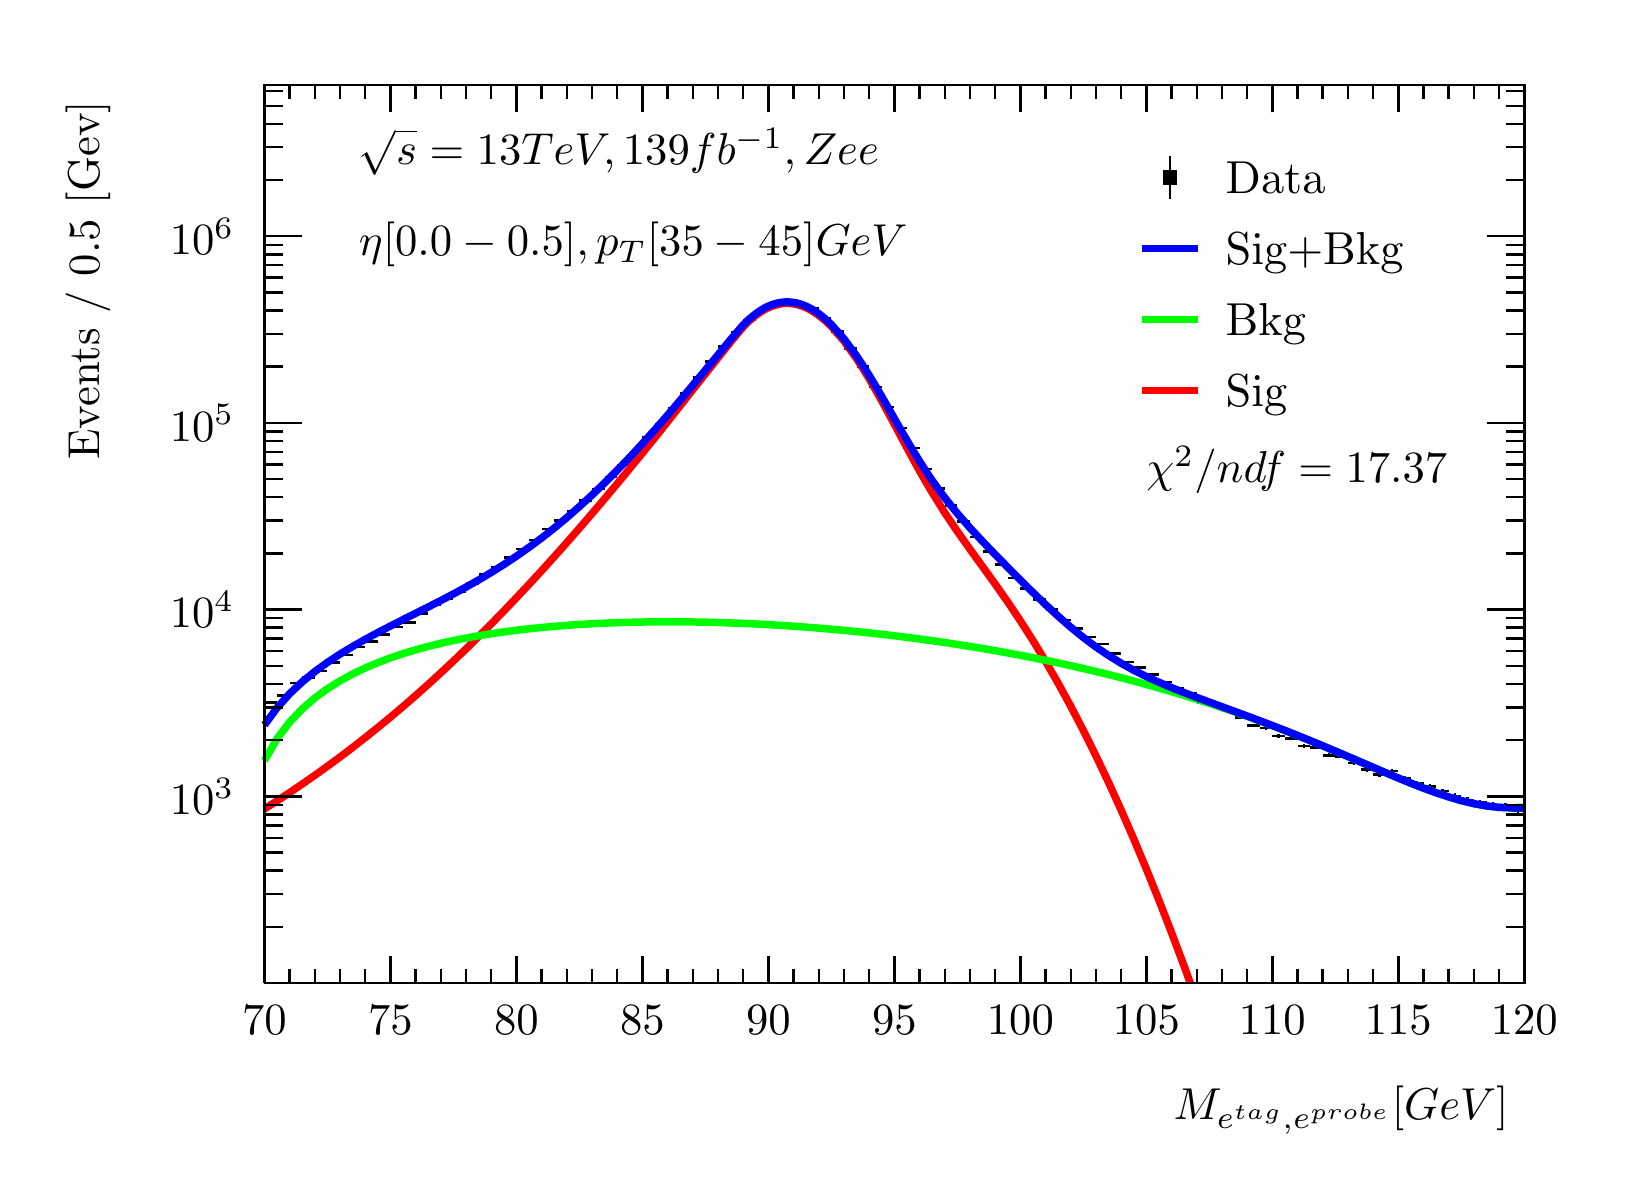
\begin{tikzpicture}
\pgfdeclareplotmark{cross} {
\pgfpathmoveto{\pgfpoint{-0.3\pgfplotmarksize}{\pgfplotmarksize}}
\pgfpathlineto{\pgfpoint{+0.3\pgfplotmarksize}{\pgfplotmarksize}}
\pgfpathlineto{\pgfpoint{+0.3\pgfplotmarksize}{0.3\pgfplotmarksize}}
\pgfpathlineto{\pgfpoint{+1\pgfplotmarksize}{0.3\pgfplotmarksize}}
\pgfpathlineto{\pgfpoint{+1\pgfplotmarksize}{-0.3\pgfplotmarksize}}
\pgfpathlineto{\pgfpoint{+0.3\pgfplotmarksize}{-0.3\pgfplotmarksize}}
\pgfpathlineto{\pgfpoint{+0.3\pgfplotmarksize}{-1.\pgfplotmarksize}}
\pgfpathlineto{\pgfpoint{-0.3\pgfplotmarksize}{-1.\pgfplotmarksize}}
\pgfpathlineto{\pgfpoint{-0.3\pgfplotmarksize}{-0.3\pgfplotmarksize}}
\pgfpathlineto{\pgfpoint{-1.\pgfplotmarksize}{-0.3\pgfplotmarksize}}
\pgfpathlineto{\pgfpoint{-1.\pgfplotmarksize}{0.3\pgfplotmarksize}}
\pgfpathlineto{\pgfpoint{-0.3\pgfplotmarksize}{0.3\pgfplotmarksize}}
\pgfpathclose
\pgfusepathqstroke
}
\pgfdeclareplotmark{cross*} {
\pgfpathmoveto{\pgfpoint{-0.3\pgfplotmarksize}{\pgfplotmarksize}}
\pgfpathlineto{\pgfpoint{+0.3\pgfplotmarksize}{\pgfplotmarksize}}
\pgfpathlineto{\pgfpoint{+0.3\pgfplotmarksize}{0.3\pgfplotmarksize}}
\pgfpathlineto{\pgfpoint{+1\pgfplotmarksize}{0.3\pgfplotmarksize}}
\pgfpathlineto{\pgfpoint{+1\pgfplotmarksize}{-0.3\pgfplotmarksize}}
\pgfpathlineto{\pgfpoint{+0.3\pgfplotmarksize}{-0.3\pgfplotmarksize}}
\pgfpathlineto{\pgfpoint{+0.3\pgfplotmarksize}{-1.\pgfplotmarksize}}
\pgfpathlineto{\pgfpoint{-0.3\pgfplotmarksize}{-1.\pgfplotmarksize}}
\pgfpathlineto{\pgfpoint{-0.3\pgfplotmarksize}{-0.3\pgfplotmarksize}}
\pgfpathlineto{\pgfpoint{-1.\pgfplotmarksize}{-0.3\pgfplotmarksize}}
\pgfpathlineto{\pgfpoint{-1.\pgfplotmarksize}{0.3\pgfplotmarksize}}
\pgfpathlineto{\pgfpoint{-0.3\pgfplotmarksize}{0.3\pgfplotmarksize}}
\pgfpathclose
\pgfusepathqfillstroke
}
\pgfdeclareplotmark{newstar} {
\pgfpathmoveto{\pgfqpoint{0pt}{\pgfplotmarksize}}
\pgfpathlineto{\pgfqpointpolar{44}{0.5\pgfplotmarksize}}
\pgfpathlineto{\pgfqpointpolar{18}{\pgfplotmarksize}}
\pgfpathlineto{\pgfqpointpolar{-20}{0.5\pgfplotmarksize}}
\pgfpathlineto{\pgfqpointpolar{-54}{\pgfplotmarksize}}
\pgfpathlineto{\pgfqpointpolar{-90}{0.5\pgfplotmarksize}}
\pgfpathlineto{\pgfqpointpolar{234}{\pgfplotmarksize}}
\pgfpathlineto{\pgfqpointpolar{198}{0.5\pgfplotmarksize}}
\pgfpathlineto{\pgfqpointpolar{162}{\pgfplotmarksize}}
\pgfpathlineto{\pgfqpointpolar{134}{0.5\pgfplotmarksize}}
\pgfpathclose
\pgfusepathqstroke
}
\pgfdeclareplotmark{newstar*} {
\pgfpathmoveto{\pgfqpoint{0pt}{\pgfplotmarksize}}
\pgfpathlineto{\pgfqpointpolar{44}{0.5\pgfplotmarksize}}
\pgfpathlineto{\pgfqpointpolar{18}{\pgfplotmarksize}}
\pgfpathlineto{\pgfqpointpolar{-20}{0.5\pgfplotmarksize}}
\pgfpathlineto{\pgfqpointpolar{-54}{\pgfplotmarksize}}
\pgfpathlineto{\pgfqpointpolar{-90}{0.5\pgfplotmarksize}}
\pgfpathlineto{\pgfqpointpolar{234}{\pgfplotmarksize}}
\pgfpathlineto{\pgfqpointpolar{198}{0.5\pgfplotmarksize}}
\pgfpathlineto{\pgfqpointpolar{162}{\pgfplotmarksize}}
\pgfpathlineto{\pgfqpointpolar{134}{0.5\pgfplotmarksize}}
\pgfpathclose
\pgfusepathqfillstroke
}
\definecolor{c}{rgb}{1,1,1};
\draw [color=c, fill=c] (0,0) rectangle (20,14.4361);
\draw [color=c, fill=c] (3,2.30977) rectangle (19,13.7143);
\definecolor{c}{rgb}{0,0,0};
\draw [c,line width=0.9] (3,2.30977) -- (3,13.7143) -- (19,13.7143) -- (19,2.30977) -- (3,2.30977);
\definecolor{c}{rgb}{1,1,1};
\draw [color=c, fill=c] (3,2.30977) rectangle (19,13.7143);
\definecolor{c}{rgb}{0,0,0};
\draw [c,line width=0.9] (3,2.30977) -- (3,13.7143) -- (19,13.7143) -- (19,2.30977) -- (3,2.30977);
\draw [c,line width=0.9] (3,2.30977) -- (19,2.30977);
\draw [c,line width=0.9] (3,2.65624) -- (3,2.30977);
\draw [c,line width=0.9] (3.32,2.48301) -- (3.32,2.30977);
\draw [c,line width=0.9] (3.64,2.48301) -- (3.64,2.30977);
\draw [c,line width=0.9] (3.96,2.48301) -- (3.96,2.30977);
\draw [c,line width=0.9] (4.28,2.48301) -- (4.28,2.30977);
\draw [c,line width=0.9] (4.6,2.65624) -- (4.6,2.30977);
\draw [c,line width=0.9] (4.92,2.48301) -- (4.92,2.30977);
\draw [c,line width=0.9] (5.24,2.48301) -- (5.24,2.30977);
\draw [c,line width=0.9] (5.56,2.48301) -- (5.56,2.30977);
\draw [c,line width=0.9] (5.88,2.48301) -- (5.88,2.30977);
\draw [c,line width=0.9] (6.2,2.65624) -- (6.2,2.30977);
\draw [c,line width=0.9] (6.52,2.48301) -- (6.52,2.30977);
\draw [c,line width=0.9] (6.84,2.48301) -- (6.84,2.30977);
\draw [c,line width=0.9] (7.16,2.48301) -- (7.16,2.30977);
\draw [c,line width=0.9] (7.48,2.48301) -- (7.48,2.30977);
\draw [c,line width=0.9] (7.8,2.65624) -- (7.8,2.30977);
\draw [c,line width=0.9] (8.12,2.48301) -- (8.12,2.30977);
\draw [c,line width=0.9] (8.44,2.48301) -- (8.44,2.30977);
\draw [c,line width=0.9] (8.76,2.48301) -- (8.76,2.30977);
\draw [c,line width=0.9] (9.08,2.48301) -- (9.08,2.30977);
\draw [c,line width=0.9] (9.4,2.65624) -- (9.4,2.30977);
\draw [c,line width=0.9] (9.72,2.48301) -- (9.72,2.30977);
\draw [c,line width=0.9] (10.04,2.48301) -- (10.04,2.30977);
\draw [c,line width=0.9] (10.36,2.48301) -- (10.36,2.30977);
\draw [c,line width=0.9] (10.68,2.48301) -- (10.68,2.30977);
\draw [c,line width=0.9] (11,2.65624) -- (11,2.30977);
\draw [c,line width=0.9] (11.32,2.48301) -- (11.32,2.30977);
\draw [c,line width=0.9] (11.64,2.48301) -- (11.64,2.30977);
\draw [c,line width=0.9] (11.96,2.48301) -- (11.96,2.30977);
\draw [c,line width=0.9] (12.28,2.48301) -- (12.28,2.30977);
\draw [c,line width=0.9] (12.6,2.65624) -- (12.6,2.30977);
\draw [c,line width=0.9] (12.92,2.48301) -- (12.92,2.30977);
\draw [c,line width=0.9] (13.24,2.48301) -- (13.24,2.30977);
\draw [c,line width=0.9] (13.56,2.48301) -- (13.56,2.30977);
\draw [c,line width=0.9] (13.88,2.48301) -- (13.88,2.30977);
\draw [c,line width=0.9] (14.2,2.65624) -- (14.2,2.30977);
\draw [c,line width=0.9] (14.52,2.48301) -- (14.52,2.30977);
\draw [c,line width=0.9] (14.84,2.48301) -- (14.84,2.30977);
\draw [c,line width=0.9] (15.16,2.48301) -- (15.16,2.30977);
\draw [c,line width=0.9] (15.48,2.48301) -- (15.48,2.30977);
\draw [c,line width=0.9] (15.8,2.65624) -- (15.8,2.30977);
\draw [c,line width=0.9] (16.12,2.48301) -- (16.12,2.30977);
\draw [c,line width=0.9] (16.44,2.48301) -- (16.44,2.30977);
\draw [c,line width=0.9] (16.76,2.48301) -- (16.76,2.30977);
\draw [c,line width=0.9] (17.08,2.48301) -- (17.08,2.30977);
\draw [c,line width=0.9] (17.4,2.65624) -- (17.4,2.30977);
\draw [c,line width=0.9] (17.72,2.48301) -- (17.72,2.30977);
\draw [c,line width=0.9] (18.04,2.48301) -- (18.04,2.30977);
\draw [c,line width=0.9] (18.36,2.48301) -- (18.36,2.30977);
\draw [c,line width=0.9] (18.68,2.48301) -- (18.68,2.30977);
\draw [c,line width=0.9] (19,2.65624) -- (19,2.30977);
\draw [anchor=base] (3,1.66015) node[scale=1.61424, color=c, rotate=0]{70};
\draw [anchor=base] (4.6,1.66015) node[scale=1.61424, color=c, rotate=0]{75};
\draw [anchor=base] (6.2,1.66015) node[scale=1.61424, color=c, rotate=0]{80};
\draw [anchor=base] (7.8,1.66015) node[scale=1.61424, color=c, rotate=0]{85};
\draw [anchor=base] (9.4,1.66015) node[scale=1.61424, color=c, rotate=0]{90};
\draw [anchor=base] (11,1.66015) node[scale=1.61424, color=c, rotate=0]{95};
\draw [anchor=base] (12.6,1.66015) node[scale=1.61424, color=c, rotate=0]{100};
\draw [anchor=base] (14.2,1.66015) node[scale=1.61424, color=c, rotate=0]{105};
\draw [anchor=base] (15.8,1.66015) node[scale=1.61424, color=c, rotate=0]{110};
\draw [anchor=base] (17.4,1.66015) node[scale=1.61424, color=c, rotate=0]{115};
\draw [anchor=base] (19,1.66015) node[scale=1.61424, color=c, rotate=0]{120};
\draw [anchor= east] (19,0.692932) node[scale=1.61424, color=c, rotate=0]{$M_{e^{tag}, e^{probe}}  [GeV]$};
\draw [c,line width=0.9] (3,13.7143) -- (19,13.7143);
\draw [c,line width=0.9] (3,13.3678) -- (3,13.7143);
\draw [c,line width=0.9] (3.32,13.5411) -- (3.32,13.7143);
\draw [c,line width=0.9] (3.64,13.5411) -- (3.64,13.7143);
\draw [c,line width=0.9] (3.96,13.5411) -- (3.96,13.7143);
\draw [c,line width=0.9] (4.28,13.5411) -- (4.28,13.7143);
\draw [c,line width=0.9] (4.6,13.3678) -- (4.6,13.7143);
\draw [c,line width=0.9] (4.92,13.5411) -- (4.92,13.7143);
\draw [c,line width=0.9] (5.24,13.5411) -- (5.24,13.7143);
\draw [c,line width=0.9] (5.56,13.5411) -- (5.56,13.7143);
\draw [c,line width=0.9] (5.88,13.5411) -- (5.88,13.7143);
\draw [c,line width=0.9] (6.2,13.3678) -- (6.2,13.7143);
\draw [c,line width=0.9] (6.52,13.5411) -- (6.52,13.7143);
\draw [c,line width=0.9] (6.84,13.5411) -- (6.84,13.7143);
\draw [c,line width=0.9] (7.16,13.5411) -- (7.16,13.7143);
\draw [c,line width=0.9] (7.48,13.5411) -- (7.48,13.7143);
\draw [c,line width=0.9] (7.8,13.3678) -- (7.8,13.7143);
\draw [c,line width=0.9] (8.12,13.5411) -- (8.12,13.7143);
\draw [c,line width=0.9] (8.44,13.5411) -- (8.44,13.7143);
\draw [c,line width=0.9] (8.76,13.5411) -- (8.76,13.7143);
\draw [c,line width=0.9] (9.08,13.5411) -- (9.08,13.7143);
\draw [c,line width=0.9] (9.4,13.3678) -- (9.4,13.7143);
\draw [c,line width=0.9] (9.72,13.5411) -- (9.72,13.7143);
\draw [c,line width=0.9] (10.04,13.5411) -- (10.04,13.7143);
\draw [c,line width=0.9] (10.36,13.5411) -- (10.36,13.7143);
\draw [c,line width=0.9] (10.68,13.5411) -- (10.68,13.7143);
\draw [c,line width=0.9] (11,13.3678) -- (11,13.7143);
\draw [c,line width=0.9] (11.32,13.5411) -- (11.32,13.7143);
\draw [c,line width=0.9] (11.64,13.5411) -- (11.64,13.7143);
\draw [c,line width=0.9] (11.96,13.5411) -- (11.96,13.7143);
\draw [c,line width=0.9] (12.28,13.5411) -- (12.28,13.7143);
\draw [c,line width=0.9] (12.6,13.3678) -- (12.6,13.7143);
\draw [c,line width=0.9] (12.92,13.5411) -- (12.92,13.7143);
\draw [c,line width=0.9] (13.24,13.5411) -- (13.24,13.7143);
\draw [c,line width=0.9] (13.56,13.5411) -- (13.56,13.7143);
\draw [c,line width=0.9] (13.88,13.5411) -- (13.88,13.7143);
\draw [c,line width=0.9] (14.2,13.3678) -- (14.2,13.7143);
\draw [c,line width=0.9] (14.52,13.5411) -- (14.52,13.7143);
\draw [c,line width=0.9] (14.84,13.5411) -- (14.84,13.7143);
\draw [c,line width=0.9] (15.16,13.5411) -- (15.16,13.7143);
\draw [c,line width=0.9] (15.48,13.5411) -- (15.48,13.7143);
\draw [c,line width=0.9] (15.8,13.3678) -- (15.8,13.7143);
\draw [c,line width=0.9] (16.12,13.5411) -- (16.12,13.7143);
\draw [c,line width=0.9] (16.44,13.5411) -- (16.44,13.7143);
\draw [c,line width=0.9] (16.76,13.5411) -- (16.76,13.7143);
\draw [c,line width=0.9] (17.08,13.5411) -- (17.08,13.7143);
\draw [c,line width=0.9] (17.4,13.3678) -- (17.4,13.7143);
\draw [c,line width=0.9] (17.72,13.5411) -- (17.72,13.7143);
\draw [c,line width=0.9] (18.04,13.5411) -- (18.04,13.7143);
\draw [c,line width=0.9] (18.36,13.5411) -- (18.36,13.7143);
\draw [c,line width=0.9] (18.68,13.5411) -- (18.68,13.7143);
\draw [c,line width=0.9] (19,13.3678) -- (19,13.7143);
\draw [c,line width=0.9] (3,2.30977) -- (3,13.7143);
\draw [c,line width=0.9] (3.237,3.02354) -- (3,3.02354);
\draw [c,line width=0.9] (3.237,3.44107) -- (3,3.44107);
\draw [c,line width=0.9] (3.237,3.73731) -- (3,3.73731);
\draw [c,line width=0.9] (3.237,3.96709) -- (3,3.96709);
\draw [c,line width=0.9] (3.237,4.15484) -- (3,4.15484);
\draw [c,line width=0.9] (3.237,4.31357) -- (3,4.31357);
\draw [c,line width=0.9] (3.237,4.45108) -- (3,4.45108);
\draw [c,line width=0.9] (3.237,4.57236) -- (3,4.57236);
\draw [c,line width=0.9] (3.474,4.68086) -- (3,4.68086);
\draw [anchor= east] (2.82,4.68086) node[scale=1.61424, color=c, rotate=0]{$10^{3}$};
\draw [c,line width=0.9] (3.237,5.39463) -- (3,5.39463);
\draw [c,line width=0.9] (3.237,5.81216) -- (3,5.81216);
\draw [c,line width=0.9] (3.237,6.1084) -- (3,6.1084);
\draw [c,line width=0.9] (3.237,6.33818) -- (3,6.33818);
\draw [c,line width=0.9] (3.237,6.52593) -- (3,6.52593);
\draw [c,line width=0.9] (3.237,6.68466) -- (3,6.68466);
\draw [c,line width=0.9] (3.237,6.82217) -- (3,6.82217);
\draw [c,line width=0.9] (3.237,6.94345) -- (3,6.94345);
\draw [c,line width=0.9] (3.474,7.05195) -- (3,7.05195);
\draw [anchor= east] (2.82,7.05195) node[scale=1.61424, color=c, rotate=0]{$10^{4}$};
\draw [c,line width=0.9] (3.237,7.76572) -- (3,7.76572);
\draw [c,line width=0.9] (3.237,8.18324) -- (3,8.18324);
\draw [c,line width=0.9] (3.237,8.47948) -- (3,8.47948);
\draw [c,line width=0.9] (3.237,8.70927) -- (3,8.70927);
\draw [c,line width=0.9] (3.237,8.89701) -- (3,8.89701);
\draw [c,line width=0.9] (3.237,9.05575) -- (3,9.05575);
\draw [c,line width=0.9] (3.237,9.19325) -- (3,9.19325);
\draw [c,line width=0.9] (3.237,9.31454) -- (3,9.31454);
\draw [c,line width=0.9] (3.474,9.42304) -- (3,9.42304);
\draw [anchor= east] (2.82,9.42304) node[scale=1.61424, color=c, rotate=0]{$10^{5}$};
\draw [c,line width=0.9] (3.237,10.1368) -- (3,10.1368);
\draw [c,line width=0.9] (3.237,10.5543) -- (3,10.5543);
\draw [c,line width=0.9] (3.237,10.8506) -- (3,10.8506);
\draw [c,line width=0.9] (3.237,11.0804) -- (3,11.0804);
\draw [c,line width=0.9] (3.237,11.2681) -- (3,11.2681);
\draw [c,line width=0.9] (3.237,11.4268) -- (3,11.4268);
\draw [c,line width=0.9] (3.237,11.5643) -- (3,11.5643);
\draw [c,line width=0.9] (3.237,11.6856) -- (3,11.6856);
\draw [c,line width=0.9] (3.474,11.7941) -- (3,11.7941);
\draw [anchor= east] (2.82,11.7941) node[scale=1.61424, color=c, rotate=0]{$10^{6}$};
\draw [c,line width=0.9] (3.237,12.5079) -- (3,12.5079);
\draw [c,line width=0.9] (3.237,12.9254) -- (3,12.9254);
\draw [c,line width=0.9] (3.237,13.2217) -- (3,13.2217);
\draw [c,line width=0.9] (3.237,13.4514) -- (3,13.4514);
\draw [c,line width=0.9] (3.237,13.6392) -- (3,13.6392);
\draw [anchor= east] (0.76,13.7143) node[scale=1.61424, color=c, rotate=90]{Events / 0.5 [Gev]};
\draw [c,line width=0.9] (19,2.30977) -- (19,13.7143);
\draw [c,line width=0.9] (18.763,3.02354) -- (19,3.02354);
\draw [c,line width=0.9] (18.763,3.44107) -- (19,3.44107);
\draw [c,line width=0.9] (18.763,3.73731) -- (19,3.73731);
\draw [c,line width=0.9] (18.763,3.96709) -- (19,3.96709);
\draw [c,line width=0.9] (18.763,4.15484) -- (19,4.15484);
\draw [c,line width=0.9] (18.763,4.31357) -- (19,4.31357);
\draw [c,line width=0.9] (18.763,4.45108) -- (19,4.45108);
\draw [c,line width=0.9] (18.763,4.57236) -- (19,4.57236);
\draw [c,line width=0.9] (18.526,4.68086) -- (19,4.68086);
\draw [c,line width=0.9] (18.763,5.39463) -- (19,5.39463);
\draw [c,line width=0.9] (18.763,5.81216) -- (19,5.81216);
\draw [c,line width=0.9] (18.763,6.1084) -- (19,6.1084);
\draw [c,line width=0.9] (18.763,6.33818) -- (19,6.33818);
\draw [c,line width=0.9] (18.763,6.52593) -- (19,6.52593);
\draw [c,line width=0.9] (18.763,6.68466) -- (19,6.68466);
\draw [c,line width=0.9] (18.763,6.82217) -- (19,6.82217);
\draw [c,line width=0.9] (18.763,6.94345) -- (19,6.94345);
\draw [c,line width=0.9] (18.526,7.05195) -- (19,7.05195);
\draw [c,line width=0.9] (18.763,7.76572) -- (19,7.76572);
\draw [c,line width=0.9] (18.763,8.18324) -- (19,8.18324);
\draw [c,line width=0.9] (18.763,8.47948) -- (19,8.47948);
\draw [c,line width=0.9] (18.763,8.70927) -- (19,8.70927);
\draw [c,line width=0.9] (18.763,8.89701) -- (19,8.89701);
\draw [c,line width=0.9] (18.763,9.05575) -- (19,9.05575);
\draw [c,line width=0.9] (18.763,9.19325) -- (19,9.19325);
\draw [c,line width=0.9] (18.763,9.31454) -- (19,9.31454);
\draw [c,line width=0.9] (18.526,9.42304) -- (19,9.42304);
\draw [c,line width=0.9] (18.763,10.1368) -- (19,10.1368);
\draw [c,line width=0.9] (18.763,10.5543) -- (19,10.5543);
\draw [c,line width=0.9] (18.763,10.8506) -- (19,10.8506);
\draw [c,line width=0.9] (18.763,11.0804) -- (19,11.0804);
\draw [c,line width=0.9] (18.763,11.2681) -- (19,11.2681);
\draw [c,line width=0.9] (18.763,11.4268) -- (19,11.4268);
\draw [c,line width=0.9] (18.763,11.5643) -- (19,11.5643);
\draw [c,line width=0.9] (18.763,11.6856) -- (19,11.6856);
\draw [c,line width=0.9] (18.526,11.7941) -- (19,11.7941);
\draw [c,line width=0.9] (18.763,12.5079) -- (19,12.5079);
\draw [c,line width=0.9] (18.763,12.9254) -- (19,12.9254);
\draw [c,line width=0.9] (18.763,13.2217) -- (19,13.2217);
\draw [c,line width=0.9] (18.763,13.4514) -- (19,13.4514);
\draw [c,line width=0.9] (18.763,13.6392) -- (19,13.6392);
\draw [c,line width=0.9] (3.08,5.87086) -- (3,5.87086);
\draw [c,line width=0.9] (3,5.87086) -- (3,5.87086);
\draw [c,line width=0.9] (3.08,5.87086) -- (3.16,5.87086);
\draw [c,line width=0.9] (3.16,5.87086) -- (3.16,5.87086);
\draw [c,line width=0.9] (3.08,5.87086) -- (3.08,5.88914);
\draw [c,line width=0.9] (3.08,5.88914) -- (3.08,5.88914);
\draw [c,line width=0.9] (3.08,5.87086) -- (3.08,5.85259);
\draw [c,line width=0.9] (3.08,5.85259) -- (3.08,5.85259);
\draw [c,line width=0.9] (3.24,5.95965) -- (3.16,5.95965);
\draw [c,line width=0.9] (3.16,5.95965) -- (3.16,5.95965);
\draw [c,line width=0.9] (3.24,5.95965) -- (3.32,5.95965);
\draw [c,line width=0.9] (3.32,5.95965) -- (3.32,5.95965);
\draw [c,line width=0.9] (3.24,5.95965) -- (3.24,5.97715);
\draw [c,line width=0.9] (3.24,5.97715) -- (3.24,5.97715);
\draw [c,line width=0.9] (3.24,5.95965) -- (3.24,5.94215);
\draw [c,line width=0.9] (3.24,5.94215) -- (3.24,5.94215);
\draw [c,line width=0.9] (3.4,6.12246) -- (3.32,6.12246);
\draw [c,line width=0.9] (3.32,6.12246) -- (3.32,6.12246);
\draw [c,line width=0.9] (3.4,6.12246) -- (3.48,6.12246);
\draw [c,line width=0.9] (3.48,6.12246) -- (3.48,6.12246);
\draw [c,line width=0.9] (3.4,6.12246) -- (3.4,6.13863);
\draw [c,line width=0.9] (3.4,6.13863) -- (3.4,6.13863);
\draw [c,line width=0.9] (3.4,6.12246) -- (3.4,6.10629);
\draw [c,line width=0.9] (3.4,6.10629) -- (3.4,6.10629);
\draw [c,line width=0.9] (3.56,6.19027) -- (3.48,6.19027);
\draw [c,line width=0.9] (3.48,6.19027) -- (3.48,6.19027);
\draw [c,line width=0.9] (3.56,6.19027) -- (3.64,6.19027);
\draw [c,line width=0.9] (3.64,6.19027) -- (3.64,6.19027);
\draw [c,line width=0.9] (3.56,6.19027) -- (3.56,6.20591);
\draw [c,line width=0.9] (3.56,6.20591) -- (3.56,6.20591);
\draw [c,line width=0.9] (3.56,6.19027) -- (3.56,6.17462);
\draw [c,line width=0.9] (3.56,6.17462) -- (3.56,6.17462);
\draw [c,line width=0.9] (3.72,6.27556) -- (3.64,6.27556);
\draw [c,line width=0.9] (3.64,6.27556) -- (3.64,6.27556);
\draw [c,line width=0.9] (3.72,6.27556) -- (3.8,6.27556);
\draw [c,line width=0.9] (3.8,6.27556) -- (3.8,6.27556);
\draw [c,line width=0.9] (3.72,6.27556) -- (3.72,6.29057);
\draw [c,line width=0.9] (3.72,6.29057) -- (3.72,6.29057);
\draw [c,line width=0.9] (3.72,6.27556) -- (3.72,6.26055);
\draw [c,line width=0.9] (3.72,6.26055) -- (3.72,6.26055);
\draw [c,line width=0.9] (3.88,6.37916) -- (3.8,6.37916);
\draw [c,line width=0.9] (3.8,6.37916) -- (3.8,6.37916);
\draw [c,line width=0.9] (3.88,6.37916) -- (3.96,6.37916);
\draw [c,line width=0.9] (3.96,6.37916) -- (3.96,6.37916);
\draw [c,line width=0.9] (3.88,6.37916) -- (3.88,6.39344);
\draw [c,line width=0.9] (3.88,6.39344) -- (3.88,6.39344);
\draw [c,line width=0.9] (3.88,6.37916) -- (3.88,6.36489);
\draw [c,line width=0.9] (3.88,6.36489) -- (3.88,6.36489);
\draw [c,line width=0.9] (4.04,6.47509) -- (3.96,6.47509);
\draw [c,line width=0.9] (3.96,6.47509) -- (3.96,6.47509);
\draw [c,line width=0.9] (4.04,6.47509) -- (4.12,6.47509);
\draw [c,line width=0.9] (4.12,6.47509) -- (4.12,6.47509);
\draw [c,line width=0.9] (4.04,6.47509) -- (4.04,6.48872);
\draw [c,line width=0.9] (4.04,6.48872) -- (4.04,6.48872);
\draw [c,line width=0.9] (4.04,6.47509) -- (4.04,6.46147);
\draw [c,line width=0.9] (4.04,6.46147) -- (4.04,6.46147);
\draw [c,line width=0.9] (4.2,6.576) -- (4.12,6.576);
\draw [c,line width=0.9] (4.12,6.576) -- (4.12,6.576);
\draw [c,line width=0.9] (4.2,6.576) -- (4.28,6.576);
\draw [c,line width=0.9] (4.28,6.576) -- (4.28,6.576);
\draw [c,line width=0.9] (4.2,6.576) -- (4.2,6.58898);
\draw [c,line width=0.9] (4.2,6.58898) -- (4.2,6.58898);
\draw [c,line width=0.9] (4.2,6.576) -- (4.2,6.56303);
\draw [c,line width=0.9] (4.2,6.56303) -- (4.2,6.56303);
\draw [c,line width=0.9] (4.36,6.64508) -- (4.28,6.64508);
\draw [c,line width=0.9] (4.28,6.64508) -- (4.28,6.64508);
\draw [c,line width=0.9] (4.36,6.64508) -- (4.44,6.64508);
\draw [c,line width=0.9] (4.44,6.64508) -- (4.44,6.64508);
\draw [c,line width=0.9] (4.36,6.64508) -- (4.36,6.65762);
\draw [c,line width=0.9] (4.36,6.65762) -- (4.36,6.65762);
\draw [c,line width=0.9] (4.36,6.64508) -- (4.36,6.63253);
\draw [c,line width=0.9] (4.36,6.63253) -- (4.36,6.63253);
\draw [c,line width=0.9] (4.52,6.7335) -- (4.44,6.7335);
\draw [c,line width=0.9] (4.44,6.7335) -- (4.44,6.7335);
\draw [c,line width=0.9] (4.52,6.7335) -- (4.6,6.7335);
\draw [c,line width=0.9] (4.6,6.7335) -- (4.6,6.7335);
\draw [c,line width=0.9] (4.52,6.7335) -- (4.52,6.74552);
\draw [c,line width=0.9] (4.52,6.74552) -- (4.52,6.74552);
\draw [c,line width=0.9] (4.52,6.7335) -- (4.52,6.72148);
\draw [c,line width=0.9] (4.52,6.72148) -- (4.52,6.72148);
\draw [c,line width=0.9] (4.68,6.83216) -- (4.6,6.83216);
\draw [c,line width=0.9] (4.6,6.83216) -- (4.6,6.83216);
\draw [c,line width=0.9] (4.68,6.83216) -- (4.76,6.83216);
\draw [c,line width=0.9] (4.76,6.83216) -- (4.76,6.83216);
\draw [c,line width=0.9] (4.68,6.83216) -- (4.68,6.84362);
\draw [c,line width=0.9] (4.68,6.84362) -- (4.68,6.84362);
\draw [c,line width=0.9] (4.68,6.83216) -- (4.68,6.8207);
\draw [c,line width=0.9] (4.68,6.8207) -- (4.68,6.8207);
\draw [c,line width=0.9] (4.84,6.88786) -- (4.76,6.88786);
\draw [c,line width=0.9] (4.76,6.88786) -- (4.76,6.88786);
\draw [c,line width=0.9] (4.84,6.88786) -- (4.92,6.88786);
\draw [c,line width=0.9] (4.92,6.88786) -- (4.92,6.88786);
\draw [c,line width=0.9] (4.84,6.88786) -- (4.84,6.89901);
\draw [c,line width=0.9] (4.84,6.89901) -- (4.84,6.89901);
\draw [c,line width=0.9] (4.84,6.88786) -- (4.84,6.87671);
\draw [c,line width=0.9] (4.84,6.87671) -- (4.84,6.87671);
\draw [c,line width=0.9] (5,7.00162) -- (4.92,7.00162);
\draw [c,line width=0.9] (4.92,7.00162) -- (4.92,7.00162);
\draw [c,line width=0.9] (5,7.00162) -- (5.08,7.00162);
\draw [c,line width=0.9] (5.08,7.00162) -- (5.08,7.00162);
\draw [c,line width=0.9] (5,7.00162) -- (5,7.01217);
\draw [c,line width=0.9] (5,7.01217) -- (5,7.01217);
\draw [c,line width=0.9] (5,7.00162) -- (5,6.99107);
\draw [c,line width=0.9] (5,6.99107) -- (5,6.99107);
\draw [c,line width=0.9] (5.16,7.11506) -- (5.08,7.11506);
\draw [c,line width=0.9] (5.08,7.11506) -- (5.08,7.11506);
\draw [c,line width=0.9] (5.16,7.11506) -- (5.24,7.11506);
\draw [c,line width=0.9] (5.24,7.11506) -- (5.24,7.11506);
\draw [c,line width=0.9] (5.16,7.11506) -- (5.16,7.12504);
\draw [c,line width=0.9] (5.16,7.12504) -- (5.16,7.12504);
\draw [c,line width=0.9] (5.16,7.11506) -- (5.16,7.10507);
\draw [c,line width=0.9] (5.16,7.10507) -- (5.16,7.10507);
\draw [c,line width=0.9] (5.32,7.18416) -- (5.24,7.18416);
\draw [c,line width=0.9] (5.24,7.18416) -- (5.24,7.18416);
\draw [c,line width=0.9] (5.32,7.18416) -- (5.4,7.18416);
\draw [c,line width=0.9] (5.4,7.18416) -- (5.4,7.18416);
\draw [c,line width=0.9] (5.32,7.18416) -- (5.32,7.19382);
\draw [c,line width=0.9] (5.32,7.19382) -- (5.32,7.19382);
\draw [c,line width=0.9] (5.32,7.18416) -- (5.32,7.1745);
\draw [c,line width=0.9] (5.32,7.1745) -- (5.32,7.1745);
\draw [c,line width=0.9] (5.48,7.28543) -- (5.4,7.28543);
\draw [c,line width=0.9] (5.4,7.28543) -- (5.4,7.28543);
\draw [c,line width=0.9] (5.48,7.28543) -- (5.56,7.28543);
\draw [c,line width=0.9] (5.56,7.28543) -- (5.56,7.28543);
\draw [c,line width=0.9] (5.48,7.28543) -- (5.48,7.29463);
\draw [c,line width=0.9] (5.48,7.29463) -- (5.48,7.29463);
\draw [c,line width=0.9] (5.48,7.28543) -- (5.48,7.27624);
\draw [c,line width=0.9] (5.48,7.27624) -- (5.48,7.27624);
\draw [c,line width=0.9] (5.64,7.38674) -- (5.56,7.38674);
\draw [c,line width=0.9] (5.56,7.38674) -- (5.56,7.38674);
\draw [c,line width=0.9] (5.64,7.38674) -- (5.72,7.38674);
\draw [c,line width=0.9] (5.72,7.38674) -- (5.72,7.38674);
\draw [c,line width=0.9] (5.64,7.38674) -- (5.64,7.3955);
\draw [c,line width=0.9] (5.64,7.3955) -- (5.64,7.3955);
\draw [c,line width=0.9] (5.64,7.38674) -- (5.64,7.37799);
\draw [c,line width=0.9] (5.64,7.37799) -- (5.64,7.37799);
\draw [c,line width=0.9] (5.8,7.50696) -- (5.72,7.50696);
\draw [c,line width=0.9] (5.72,7.50696) -- (5.72,7.50696);
\draw [c,line width=0.9] (5.8,7.50696) -- (5.88,7.50696);
\draw [c,line width=0.9] (5.88,7.50696) -- (5.88,7.50696);
\draw [c,line width=0.9] (5.8,7.50696) -- (5.8,7.51521);
\draw [c,line width=0.9] (5.8,7.51521) -- (5.8,7.51521);
\draw [c,line width=0.9] (5.8,7.50696) -- (5.8,7.4987);
\draw [c,line width=0.9] (5.8,7.4987) -- (5.8,7.4987);
\draw [c,line width=0.9] (5.96,7.59618) -- (5.88,7.59618);
\draw [c,line width=0.9] (5.88,7.59618) -- (5.88,7.59618);
\draw [c,line width=0.9] (5.96,7.59618) -- (6.04,7.59618);
\draw [c,line width=0.9] (6.04,7.59618) -- (6.04,7.59618);
\draw [c,line width=0.9] (5.96,7.59618) -- (5.96,7.60409);
\draw [c,line width=0.9] (5.96,7.60409) -- (5.96,7.60409);
\draw [c,line width=0.9] (5.96,7.59618) -- (5.96,7.58827);
\draw [c,line width=0.9] (5.96,7.58827) -- (5.96,7.58827);
\draw [c,line width=0.9] (6.12,7.71447) -- (6.04,7.71447);
\draw [c,line width=0.9] (6.04,7.71447) -- (6.04,7.71447);
\draw [c,line width=0.9] (6.12,7.71447) -- (6.2,7.71447);
\draw [c,line width=0.9] (6.2,7.71447) -- (6.2,7.71447);
\draw [c,line width=0.9] (6.12,7.71447) -- (6.12,7.72193);
\draw [c,line width=0.9] (6.12,7.72193) -- (6.12,7.72193);
\draw [c,line width=0.9] (6.12,7.71447) -- (6.12,7.707);
\draw [c,line width=0.9] (6.12,7.707) -- (6.12,7.707);
\draw [c,line width=0.9] (6.28,7.82212) -- (6.2,7.82212);
\draw [c,line width=0.9] (6.2,7.82212) -- (6.2,7.82212);
\draw [c,line width=0.9] (6.28,7.82212) -- (6.36,7.82212);
\draw [c,line width=0.9] (6.36,7.82212) -- (6.36,7.82212);
\draw [c,line width=0.9] (6.28,7.82212) -- (6.28,7.8292);
\draw [c,line width=0.9] (6.28,7.8292) -- (6.28,7.8292);
\draw [c,line width=0.9] (6.28,7.82212) -- (6.28,7.81503);
\draw [c,line width=0.9] (6.28,7.81503) -- (6.28,7.81503);
\draw [c,line width=0.9] (6.44,7.93472) -- (6.36,7.93472);
\draw [c,line width=0.9] (6.36,7.93472) -- (6.36,7.93472);
\draw [c,line width=0.9] (6.44,7.93472) -- (6.52,7.93472);
\draw [c,line width=0.9] (6.52,7.93472) -- (6.52,7.93472);
\draw [c,line width=0.9] (6.44,7.93472) -- (6.44,7.94142);
\draw [c,line width=0.9] (6.44,7.94142) -- (6.44,7.94142);
\draw [c,line width=0.9] (6.44,7.93472) -- (6.44,7.92801);
\draw [c,line width=0.9] (6.44,7.92801) -- (6.44,7.92801);
\draw [c,line width=0.9] (6.6,8.07448) -- (6.52,8.07448);
\draw [c,line width=0.9] (6.52,8.07448) -- (6.52,8.07448);
\draw [c,line width=0.9] (6.6,8.07448) -- (6.68,8.07448);
\draw [c,line width=0.9] (6.68,8.07448) -- (6.68,8.07448);
\draw [c,line width=0.9] (6.6,8.07448) -- (6.6,8.08075);
\draw [c,line width=0.9] (6.6,8.08075) -- (6.6,8.08075);
\draw [c,line width=0.9] (6.6,8.07448) -- (6.6,8.06822);
\draw [c,line width=0.9] (6.6,8.06822) -- (6.6,8.06822);
\draw [c,line width=0.9] (6.76,8.18149) -- (6.68,8.18149);
\draw [c,line width=0.9] (6.68,8.18149) -- (6.68,8.18149);
\draw [c,line width=0.9] (6.76,8.18149) -- (6.84,8.18149);
\draw [c,line width=0.9] (6.84,8.18149) -- (6.84,8.18149);
\draw [c,line width=0.9] (6.76,8.18149) -- (6.76,8.18744);
\draw [c,line width=0.9] (6.76,8.18744) -- (6.76,8.18744);
\draw [c,line width=0.9] (6.76,8.18149) -- (6.76,8.17554);
\draw [c,line width=0.9] (6.76,8.17554) -- (6.76,8.17554);
\draw [c,line width=0.9] (6.92,8.30533) -- (6.84,8.30533);
\draw [c,line width=0.9] (6.84,8.30533) -- (6.84,8.30533);
\draw [c,line width=0.9] (6.92,8.30533) -- (7,8.30533);
\draw [c,line width=0.9] (7,8.30533) -- (7,8.30533);
\draw [c,line width=0.9] (6.92,8.30533) -- (6.92,8.31093);
\draw [c,line width=0.9] (6.92,8.31093) -- (6.92,8.31093);
\draw [c,line width=0.9] (6.92,8.30533) -- (6.92,8.29972);
\draw [c,line width=0.9] (6.92,8.29972) -- (6.92,8.29972);
\draw [c,line width=0.9] (7.08,8.44101) -- (7,8.44101);
\draw [c,line width=0.9] (7,8.44101) -- (7,8.44101);
\draw [c,line width=0.9] (7.08,8.44101) -- (7.16,8.44101);
\draw [c,line width=0.9] (7.16,8.44101) -- (7.16,8.44101);
\draw [c,line width=0.9] (7.08,8.44101) -- (7.08,8.44626);
\draw [c,line width=0.9] (7.08,8.44626) -- (7.08,8.44626);
\draw [c,line width=0.9] (7.08,8.44101) -- (7.08,8.43576);
\draw [c,line width=0.9] (7.08,8.43576) -- (7.08,8.43576);
\draw [c,line width=0.9] (7.24,8.58649) -- (7.16,8.58649);
\draw [c,line width=0.9] (7.16,8.58649) -- (7.16,8.58649);
\draw [c,line width=0.9] (7.24,8.58649) -- (7.32,8.58649);
\draw [c,line width=0.9] (7.32,8.58649) -- (7.32,8.58649);
\draw [c,line width=0.9] (7.24,8.58649) -- (7.24,8.59138);
\draw [c,line width=0.9] (7.24,8.59138) -- (7.24,8.59138);
\draw [c,line width=0.9] (7.24,8.58649) -- (7.24,8.5816);
\draw [c,line width=0.9] (7.24,8.5816) -- (7.24,8.5816);
\draw [c,line width=0.9] (7.4,8.7375) -- (7.32,8.7375);
\draw [c,line width=0.9] (7.32,8.7375) -- (7.32,8.7375);
\draw [c,line width=0.9] (7.4,8.7375) -- (7.48,8.7375);
\draw [c,line width=0.9] (7.48,8.7375) -- (7.48,8.7375);
\draw [c,line width=0.9] (7.4,8.7375) -- (7.4,8.74205);
\draw [c,line width=0.9] (7.4,8.74205) -- (7.4,8.74205);
\draw [c,line width=0.9] (7.4,8.7375) -- (7.4,8.73296);
\draw [c,line width=0.9] (7.4,8.73296) -- (7.4,8.73296);
\draw [c,line width=0.9] (7.56,8.88897) -- (7.48,8.88897);
\draw [c,line width=0.9] (7.48,8.88897) -- (7.48,8.88897);
\draw [c,line width=0.9] (7.56,8.88897) -- (7.64,8.88897);
\draw [c,line width=0.9] (7.64,8.88897) -- (7.64,8.88897);
\draw [c,line width=0.9] (7.56,8.88897) -- (7.56,8.89319);
\draw [c,line width=0.9] (7.56,8.89319) -- (7.56,8.89319);
\draw [c,line width=0.9] (7.56,8.88897) -- (7.56,8.88475);
\draw [c,line width=0.9] (7.56,8.88475) -- (7.56,8.88475);
\draw [c,line width=0.9] (7.72,9.05543) -- (7.64,9.05543);
\draw [c,line width=0.9] (7.64,9.05543) -- (7.64,9.05543);
\draw [c,line width=0.9] (7.72,9.05543) -- (7.8,9.05543);
\draw [c,line width=0.9] (7.8,9.05543) -- (7.8,9.05543);
\draw [c,line width=0.9] (7.72,9.05543) -- (7.72,9.05932);
\draw [c,line width=0.9] (7.72,9.05932) -- (7.72,9.05932);
\draw [c,line width=0.9] (7.72,9.05543) -- (7.72,9.05153);
\draw [c,line width=0.9] (7.72,9.05153) -- (7.72,9.05153);
\draw [c,line width=0.9] (7.88,9.23782) -- (7.8,9.23782);
\draw [c,line width=0.9] (7.8,9.23782) -- (7.8,9.23782);
\draw [c,line width=0.9] (7.88,9.23782) -- (7.96,9.23782);
\draw [c,line width=0.9] (7.96,9.23782) -- (7.96,9.23782);
\draw [c,line width=0.9] (7.88,9.23782) -- (7.88,9.24138);
\draw [c,line width=0.9] (7.88,9.24138) -- (7.88,9.24138);
\draw [c,line width=0.9] (7.88,9.23782) -- (7.88,9.23425);
\draw [c,line width=0.9] (7.88,9.23425) -- (7.88,9.23425);
\draw [c,line width=0.9] (8.04,9.41066) -- (7.96,9.41066);
\draw [c,line width=0.9] (7.96,9.41066) -- (7.96,9.41066);
\draw [c,line width=0.9] (8.04,9.41066) -- (8.12,9.41066);
\draw [c,line width=0.9] (8.12,9.41066) -- (8.12,9.41066);
\draw [c,line width=0.9] (8.04,9.41066) -- (8.04,9.41393);
\draw [c,line width=0.9] (8.04,9.41393) -- (8.04,9.41393);
\draw [c,line width=0.9] (8.04,9.41066) -- (8.04,9.40738);
\draw [c,line width=0.9] (8.04,9.40738) -- (8.04,9.40738);
\draw [c,line width=0.9] (8.2,9.60518) -- (8.12,9.60518);
\draw [c,line width=0.9] (8.12,9.60518) -- (8.12,9.60518);
\draw [c,line width=0.9] (8.2,9.60518) -- (8.28,9.60518);
\draw [c,line width=0.9] (8.28,9.60518) -- (8.28,9.60518);
\draw [c,line width=0.9] (8.2,9.60518) -- (8.2,9.60816);
\draw [c,line width=0.9] (8.2,9.60816) -- (8.2,9.60816);
\draw [c,line width=0.9] (8.2,9.60518) -- (8.2,9.6022);
\draw [c,line width=0.9] (8.2,9.6022) -- (8.2,9.6022);
\draw [c,line width=0.9] (8.36,9.80488) -- (8.28,9.80488);
\draw [c,line width=0.9] (8.28,9.80488) -- (8.28,9.80488);
\draw [c,line width=0.9] (8.36,9.80488) -- (8.44,9.80488);
\draw [c,line width=0.9] (8.44,9.80488) -- (8.44,9.80488);
\draw [c,line width=0.9] (8.36,9.80488) -- (8.36,9.80758);
\draw [c,line width=0.9] (8.36,9.80758) -- (8.36,9.80758);
\draw [c,line width=0.9] (8.36,9.80488) -- (8.36,9.80217);
\draw [c,line width=0.9] (8.36,9.80217) -- (8.36,9.80217);
\draw [c,line width=0.9] (8.52,10.0023) -- (8.44,10.0023);
\draw [c,line width=0.9] (8.44,10.0023) -- (8.44,10.0023);
\draw [c,line width=0.9] (8.52,10.0023) -- (8.6,10.0023);
\draw [c,line width=0.9] (8.6,10.0023) -- (8.6,10.0023);
\draw [c,line width=0.9] (8.52,10.0023) -- (8.52,10.0048);
\draw [c,line width=0.9] (8.52,10.0048) -- (8.52,10.0048);
\draw [c,line width=0.9] (8.52,10.0023) -- (8.52,9.99984);
\draw [c,line width=0.9] (8.52,9.99984) -- (8.52,9.99984);
\draw [c,line width=0.9] (8.68,10.2031) -- (8.6,10.2031);
\draw [c,line width=0.9] (8.6,10.2031) -- (8.6,10.2031);
\draw [c,line width=0.9] (8.68,10.2031) -- (8.76,10.2031);
\draw [c,line width=0.9] (8.76,10.2031) -- (8.76,10.2031);
\draw [c,line width=0.9] (8.68,10.2031) -- (8.68,10.2053);
\draw [c,line width=0.9] (8.68,10.2053) -- (8.68,10.2053);
\draw [c,line width=0.9] (8.68,10.2031) -- (8.68,10.2008);
\draw [c,line width=0.9] (8.68,10.2008) -- (8.68,10.2008);
\draw [c,line width=0.9] (8.84,10.3968) -- (8.76,10.3968);
\draw [c,line width=0.9] (8.76,10.3968) -- (8.76,10.3968);
\draw [c,line width=0.9] (8.84,10.3968) -- (8.92,10.3968);
\draw [c,line width=0.9] (8.92,10.3968) -- (8.92,10.3968);
\draw [c,line width=0.9] (8.84,10.3968) -- (8.84,10.3988);
\draw [c,line width=0.9] (8.84,10.3988) -- (8.84,10.3988);
\draw [c,line width=0.9] (8.84,10.3968) -- (8.84,10.3948);
\draw [c,line width=0.9] (8.84,10.3948) -- (8.84,10.3948);
\draw [c,line width=0.9] (9,10.5752) -- (8.92,10.5752);
\draw [c,line width=0.9] (8.92,10.5752) -- (8.92,10.5752);
\draw [c,line width=0.9] (9,10.5752) -- (9.08,10.5752);
\draw [c,line width=0.9] (9.08,10.5752) -- (9.08,10.5752);
\draw [c,line width=0.9] (9,10.5752) -- (9,10.5771);
\draw [c,line width=0.9] (9,10.5771) -- (9,10.5771);
\draw [c,line width=0.9] (9,10.5752) -- (9,10.5734);
\draw [c,line width=0.9] (9,10.5734) -- (9,10.5734);
\draw [c,line width=0.9] (9.16,10.7326) -- (9.08,10.7326);
\draw [c,line width=0.9] (9.08,10.7326) -- (9.08,10.7326);
\draw [c,line width=0.9] (9.16,10.7326) -- (9.24,10.7326);
\draw [c,line width=0.9] (9.24,10.7326) -- (9.24,10.7326);
\draw [c,line width=0.9] (9.16,10.7326) -- (9.16,10.7344);
\draw [c,line width=0.9] (9.16,10.7344) -- (9.16,10.7344);
\draw [c,line width=0.9] (9.16,10.7326) -- (9.16,10.7309);
\draw [c,line width=0.9] (9.16,10.7309) -- (9.16,10.7309);
\draw [c,line width=0.9] (9.32,10.8566) -- (9.24,10.8566);
\draw [c,line width=0.9] (9.24,10.8566) -- (9.24,10.8566);
\draw [c,line width=0.9] (9.32,10.8566) -- (9.4,10.8566);
\draw [c,line width=0.9] (9.4,10.8566) -- (9.4,10.8566);
\draw [c,line width=0.9] (9.32,10.8566) -- (9.32,10.8582);
\draw [c,line width=0.9] (9.32,10.8582) -- (9.32,10.8582);
\draw [c,line width=0.9] (9.32,10.8566) -- (9.32,10.855);
\draw [c,line width=0.9] (9.32,10.855) -- (9.32,10.855);
\draw [c,line width=0.9] (9.48,10.9355) -- (9.4,10.9355);
\draw [c,line width=0.9] (9.4,10.9355) -- (9.4,10.9355);
\draw [c,line width=0.9] (9.48,10.9355) -- (9.56,10.9355);
\draw [c,line width=0.9] (9.56,10.9355) -- (9.56,10.9355);
\draw [c,line width=0.9] (9.48,10.9355) -- (9.48,10.9371);
\draw [c,line width=0.9] (9.48,10.9371) -- (9.48,10.9371);
\draw [c,line width=0.9] (9.48,10.9355) -- (9.48,10.934);
\draw [c,line width=0.9] (9.48,10.934) -- (9.48,10.934);
\draw [c,line width=0.9] (9.64,10.9682) -- (9.56,10.9682);
\draw [c,line width=0.9] (9.56,10.9682) -- (9.56,10.9682);
\draw [c,line width=0.9] (9.64,10.9682) -- (9.72,10.9682);
\draw [c,line width=0.9] (9.72,10.9682) -- (9.72,10.9682);
\draw [c,line width=0.9] (9.64,10.9682) -- (9.64,10.9698);
\draw [c,line width=0.9] (9.64,10.9698) -- (9.64,10.9698);
\draw [c,line width=0.9] (9.64,10.9682) -- (9.64,10.9667);
\draw [c,line width=0.9] (9.64,10.9667) -- (9.64,10.9667);
\draw [c,line width=0.9] (9.8,10.9489) -- (9.72,10.9489);
\draw [c,line width=0.9] (9.72,10.9489) -- (9.72,10.9489);
\draw [c,line width=0.9] (9.8,10.9489) -- (9.88,10.9489);
\draw [c,line width=0.9] (9.88,10.9489) -- (9.88,10.9489);
\draw [c,line width=0.9] (9.8,10.9489) -- (9.8,10.9505);
\draw [c,line width=0.9] (9.8,10.9505) -- (9.8,10.9505);
\draw [c,line width=0.9] (9.8,10.9489) -- (9.8,10.9474);
\draw [c,line width=0.9] (9.8,10.9474) -- (9.8,10.9474);
\draw [c,line width=0.9] (9.96,10.8741) -- (9.88,10.8741);
\draw [c,line width=0.9] (9.88,10.8741) -- (9.88,10.8741);
\draw [c,line width=0.9] (9.96,10.8741) -- (10.04,10.8741);
\draw [c,line width=0.9] (10.04,10.8741) -- (10.04,10.8741);
\draw [c,line width=0.9] (9.96,10.8741) -- (9.96,10.8757);
\draw [c,line width=0.9] (9.96,10.8757) -- (9.96,10.8757);
\draw [c,line width=0.9] (9.96,10.8741) -- (9.96,10.8725);
\draw [c,line width=0.9] (9.96,10.8725) -- (9.96,10.8725);
\draw [c,line width=0.9] (10.12,10.7496) -- (10.04,10.7496);
\draw [c,line width=0.9] (10.04,10.7496) -- (10.04,10.7496);
\draw [c,line width=0.9] (10.12,10.7496) -- (10.2,10.7496);
\draw [c,line width=0.9] (10.2,10.7496) -- (10.2,10.7496);
\draw [c,line width=0.9] (10.12,10.7496) -- (10.12,10.7513);
\draw [c,line width=0.9] (10.12,10.7513) -- (10.12,10.7513);
\draw [c,line width=0.9] (10.12,10.7496) -- (10.12,10.7479);
\draw [c,line width=0.9] (10.12,10.7479) -- (10.12,10.7479);
\draw [c,line width=0.9] (10.28,10.5813) -- (10.2,10.5813);
\draw [c,line width=0.9] (10.2,10.5813) -- (10.2,10.5813);
\draw [c,line width=0.9] (10.28,10.5813) -- (10.36,10.5813);
\draw [c,line width=0.9] (10.36,10.5813) -- (10.36,10.5813);
\draw [c,line width=0.9] (10.28,10.5813) -- (10.28,10.5831);
\draw [c,line width=0.9] (10.28,10.5831) -- (10.28,10.5831);
\draw [c,line width=0.9] (10.28,10.5813) -- (10.28,10.5794);
\draw [c,line width=0.9] (10.28,10.5794) -- (10.28,10.5794);
\draw [c,line width=0.9] (10.44,10.3716) -- (10.36,10.3716);
\draw [c,line width=0.9] (10.36,10.3716) -- (10.36,10.3716);
\draw [c,line width=0.9] (10.44,10.3716) -- (10.52,10.3716);
\draw [c,line width=0.9] (10.52,10.3716) -- (10.52,10.3716);
\draw [c,line width=0.9] (10.44,10.3716) -- (10.44,10.3737);
\draw [c,line width=0.9] (10.44,10.3737) -- (10.44,10.3737);
\draw [c,line width=0.9] (10.44,10.3716) -- (10.44,10.3696);
\draw [c,line width=0.9] (10.44,10.3696) -- (10.44,10.3696);
\draw [c,line width=0.9] (10.6,10.14) -- (10.52,10.14);
\draw [c,line width=0.9] (10.52,10.14) -- (10.52,10.14);
\draw [c,line width=0.9] (10.6,10.14) -- (10.68,10.14);
\draw [c,line width=0.9] (10.68,10.14) -- (10.68,10.14);
\draw [c,line width=0.9] (10.6,10.14) -- (10.6,10.1423);
\draw [c,line width=0.9] (10.6,10.1423) -- (10.6,10.1423);
\draw [c,line width=0.9] (10.6,10.14) -- (10.6,10.1377);
\draw [c,line width=0.9] (10.6,10.1377) -- (10.6,10.1377);
\draw [c,line width=0.9] (10.76,9.88095) -- (10.68,9.88095);
\draw [c,line width=0.9] (10.68,9.88095) -- (10.68,9.88095);
\draw [c,line width=0.9] (10.76,9.88095) -- (10.84,9.88095);
\draw [c,line width=0.9] (10.84,9.88095) -- (10.84,9.88095);
\draw [c,line width=0.9] (10.76,9.88095) -- (10.76,9.88355);
\draw [c,line width=0.9] (10.76,9.88355) -- (10.76,9.88355);
\draw [c,line width=0.9] (10.76,9.88095) -- (10.76,9.87834);
\draw [c,line width=0.9] (10.76,9.87834) -- (10.76,9.87834);
\draw [c,line width=0.9] (10.92,9.62369) -- (10.84,9.62369);
\draw [c,line width=0.9] (10.84,9.62369) -- (10.84,9.62369);
\draw [c,line width=0.9] (10.92,9.62369) -- (11,9.62369);
\draw [c,line width=0.9] (11,9.62369) -- (11,9.62369);
\draw [c,line width=0.9] (10.92,9.62369) -- (10.92,9.62665);
\draw [c,line width=0.9] (10.92,9.62665) -- (10.92,9.62665);
\draw [c,line width=0.9] (10.92,9.62369) -- (10.92,9.62074);
\draw [c,line width=0.9] (10.92,9.62074) -- (10.92,9.62074);
\draw [c,line width=0.9] (11.08,9.3557) -- (11,9.3557);
\draw [c,line width=0.9] (11,9.3557) -- (11,9.3557);
\draw [c,line width=0.9] (11.08,9.3557) -- (11.16,9.3557);
\draw [c,line width=0.9] (11.16,9.3557) -- (11.16,9.3557);
\draw [c,line width=0.9] (11.08,9.3557) -- (11.08,9.35906);
\draw [c,line width=0.9] (11.08,9.35906) -- (11.08,9.35906);
\draw [c,line width=0.9] (11.08,9.3557) -- (11.08,9.35233);
\draw [c,line width=0.9] (11.08,9.35233) -- (11.08,9.35233);
\draw [c,line width=0.9] (11.24,9.10165) -- (11.16,9.10165);
\draw [c,line width=0.9] (11.16,9.10165) -- (11.16,9.10165);
\draw [c,line width=0.9] (11.24,9.10165) -- (11.32,9.10165);
\draw [c,line width=0.9] (11.32,9.10165) -- (11.32,9.10165);
\draw [c,line width=0.9] (11.24,9.10165) -- (11.24,9.10546);
\draw [c,line width=0.9] (11.24,9.10546) -- (11.24,9.10546);
\draw [c,line width=0.9] (11.24,9.10165) -- (11.24,9.09785);
\draw [c,line width=0.9] (11.24,9.09785) -- (11.24,9.09785);
\draw [c,line width=0.9] (11.4,8.83731) -- (11.32,8.83731);
\draw [c,line width=0.9] (11.32,8.83731) -- (11.32,8.83731);
\draw [c,line width=0.9] (11.4,8.83731) -- (11.48,8.83731);
\draw [c,line width=0.9] (11.48,8.83731) -- (11.48,8.83731);
\draw [c,line width=0.9] (11.4,8.83731) -- (11.4,8.84163);
\draw [c,line width=0.9] (11.4,8.84163) -- (11.4,8.84163);
\draw [c,line width=0.9] (11.4,8.83731) -- (11.4,8.83298);
\draw [c,line width=0.9] (11.4,8.83298) -- (11.4,8.83298);
\draw [c,line width=0.9] (11.56,8.59072) -- (11.48,8.59072);
\draw [c,line width=0.9] (11.48,8.59072) -- (11.48,8.59072);
\draw [c,line width=0.9] (11.56,8.59072) -- (11.64,8.59072);
\draw [c,line width=0.9] (11.64,8.59072) -- (11.64,8.59072);
\draw [c,line width=0.9] (11.56,8.59072) -- (11.56,8.5956);
\draw [c,line width=0.9] (11.56,8.5956) -- (11.56,8.5956);
\draw [c,line width=0.9] (11.56,8.59072) -- (11.56,8.58585);
\draw [c,line width=0.9] (11.56,8.58585) -- (11.56,8.58585);
\draw [c,line width=0.9] (11.72,8.3747) -- (11.64,8.3747);
\draw [c,line width=0.9] (11.64,8.3747) -- (11.64,8.3747);
\draw [c,line width=0.9] (11.72,8.3747) -- (11.8,8.3747);
\draw [c,line width=0.9] (11.8,8.3747) -- (11.8,8.3747);
\draw [c,line width=0.9] (11.72,8.3747) -- (11.72,8.38012);
\draw [c,line width=0.9] (11.72,8.38012) -- (11.72,8.38012);
\draw [c,line width=0.9] (11.72,8.3747) -- (11.72,8.36929);
\draw [c,line width=0.9] (11.72,8.36929) -- (11.72,8.36929);
\draw [c,line width=0.9] (11.88,8.16838) -- (11.8,8.16838);
\draw [c,line width=0.9] (11.8,8.16838) -- (11.8,8.16838);
\draw [c,line width=0.9] (11.88,8.16838) -- (11.96,8.16838);
\draw [c,line width=0.9] (11.96,8.16838) -- (11.96,8.16838);
\draw [c,line width=0.9] (11.88,8.16838) -- (11.88,8.17437);
\draw [c,line width=0.9] (11.88,8.17437) -- (11.88,8.17437);
\draw [c,line width=0.9] (11.88,8.16838) -- (11.88,8.16239);
\draw [c,line width=0.9] (11.88,8.16239) -- (11.88,8.16239);
\draw [c,line width=0.9] (12.04,7.97272) -- (11.96,7.97272);
\draw [c,line width=0.9] (11.96,7.97272) -- (11.96,7.97272);
\draw [c,line width=0.9] (12.04,7.97272) -- (12.12,7.97272);
\draw [c,line width=0.9] (12.12,7.97272) -- (12.12,7.97272);
\draw [c,line width=0.9] (12.04,7.97272) -- (12.04,7.9793);
\draw [c,line width=0.9] (12.04,7.9793) -- (12.04,7.9793);
\draw [c,line width=0.9] (12.04,7.97272) -- (12.04,7.96613);
\draw [c,line width=0.9] (12.04,7.96613) -- (12.04,7.96613);
\draw [c,line width=0.9] (12.2,7.79195) -- (12.12,7.79195);
\draw [c,line width=0.9] (12.12,7.79195) -- (12.12,7.79195);
\draw [c,line width=0.9] (12.2,7.79195) -- (12.28,7.79195);
\draw [c,line width=0.9] (12.28,7.79195) -- (12.28,7.79195);
\draw [c,line width=0.9] (12.2,7.79195) -- (12.2,7.79914);
\draw [c,line width=0.9] (12.2,7.79914) -- (12.2,7.79914);
\draw [c,line width=0.9] (12.2,7.79195) -- (12.2,7.78476);
\draw [c,line width=0.9] (12.2,7.78476) -- (12.2,7.78476);
\draw [c,line width=0.9] (12.36,7.62302) -- (12.28,7.62302);
\draw [c,line width=0.9] (12.28,7.62302) -- (12.28,7.62302);
\draw [c,line width=0.9] (12.36,7.62302) -- (12.44,7.62302);
\draw [c,line width=0.9] (12.44,7.62302) -- (12.44,7.62302);
\draw [c,line width=0.9] (12.36,7.62302) -- (12.36,7.63083);
\draw [c,line width=0.9] (12.36,7.63083) -- (12.36,7.63083);
\draw [c,line width=0.9] (12.36,7.62302) -- (12.36,7.61522);
\draw [c,line width=0.9] (12.36,7.61522) -- (12.36,7.61522);
\draw [c,line width=0.9] (12.52,7.4535) -- (12.44,7.4535);
\draw [c,line width=0.9] (12.44,7.4535) -- (12.44,7.4535);
\draw [c,line width=0.9] (12.52,7.4535) -- (12.6,7.4535);
\draw [c,line width=0.9] (12.6,7.4535) -- (12.6,7.4535);
\draw [c,line width=0.9] (12.52,7.4535) -- (12.52,7.46197);
\draw [c,line width=0.9] (12.52,7.46197) -- (12.52,7.46197);
\draw [c,line width=0.9] (12.52,7.4535) -- (12.52,7.44502);
\draw [c,line width=0.9] (12.52,7.44502) -- (12.52,7.44502);
\draw [c,line width=0.9] (12.68,7.31974) -- (12.6,7.31974);
\draw [c,line width=0.9] (12.6,7.31974) -- (12.6,7.31974);
\draw [c,line width=0.9] (12.68,7.31974) -- (12.76,7.31974);
\draw [c,line width=0.9] (12.76,7.31974) -- (12.76,7.31974);
\draw [c,line width=0.9] (12.68,7.31974) -- (12.68,7.32878);
\draw [c,line width=0.9] (12.68,7.32878) -- (12.68,7.32878);
\draw [c,line width=0.9] (12.68,7.31974) -- (12.68,7.3107);
\draw [c,line width=0.9] (12.68,7.3107) -- (12.68,7.3107);
\draw [c,line width=0.9] (12.84,7.18008) -- (12.76,7.18008);
\draw [c,line width=0.9] (12.76,7.18008) -- (12.76,7.18008);
\draw [c,line width=0.9] (12.84,7.18008) -- (12.92,7.18008);
\draw [c,line width=0.9] (12.92,7.18008) -- (12.92,7.18008);
\draw [c,line width=0.9] (12.84,7.18008) -- (12.84,7.18975);
\draw [c,line width=0.9] (12.84,7.18975) -- (12.84,7.18975);
\draw [c,line width=0.9] (12.84,7.18008) -- (12.84,7.1704);
\draw [c,line width=0.9] (12.84,7.1704) -- (12.84,7.1704);
\draw [c,line width=0.9] (13,7.05668) -- (12.92,7.05668);
\draw [c,line width=0.9] (12.92,7.05668) -- (12.92,7.05668);
\draw [c,line width=0.9] (13,7.05668) -- (13.08,7.05668);
\draw [c,line width=0.9] (13.08,7.05668) -- (13.08,7.05668);
\draw [c,line width=0.9] (13,7.05668) -- (13,7.06695);
\draw [c,line width=0.9] (13,7.06695) -- (13,7.06695);
\draw [c,line width=0.9] (13,7.05668) -- (13,7.0464);
\draw [c,line width=0.9] (13,7.0464) -- (13,7.0464);
\draw [c,line width=0.9] (13.16,6.92078) -- (13.08,6.92078);
\draw [c,line width=0.9] (13.08,6.92078) -- (13.08,6.92078);
\draw [c,line width=0.9] (13.16,6.92078) -- (13.24,6.92078);
\draw [c,line width=0.9] (13.24,6.92078) -- (13.24,6.92078);
\draw [c,line width=0.9] (13.16,6.92078) -- (13.16,6.93176);
\draw [c,line width=0.9] (13.16,6.93176) -- (13.16,6.93176);
\draw [c,line width=0.9] (13.16,6.92078) -- (13.16,6.90981);
\draw [c,line width=0.9] (13.16,6.90981) -- (13.16,6.90981);
\draw [c,line width=0.9] (13.32,6.81221) -- (13.24,6.81221);
\draw [c,line width=0.9] (13.24,6.81221) -- (13.24,6.81221);
\draw [c,line width=0.9] (13.32,6.81221) -- (13.4,6.81221);
\draw [c,line width=0.9] (13.4,6.81221) -- (13.4,6.81221);
\draw [c,line width=0.9] (13.32,6.81221) -- (13.32,6.82378);
\draw [c,line width=0.9] (13.32,6.82378) -- (13.32,6.82378);
\draw [c,line width=0.9] (13.32,6.81221) -- (13.32,6.80064);
\draw [c,line width=0.9] (13.32,6.80064) -- (13.32,6.80064);
\draw [c,line width=0.9] (13.48,6.70188) -- (13.4,6.70188);
\draw [c,line width=0.9] (13.4,6.70188) -- (13.4,6.70188);
\draw [c,line width=0.9] (13.48,6.70188) -- (13.56,6.70188);
\draw [c,line width=0.9] (13.56,6.70188) -- (13.56,6.70188);
\draw [c,line width=0.9] (13.48,6.70188) -- (13.48,6.71408);
\draw [c,line width=0.9] (13.48,6.71408) -- (13.48,6.71408);
\draw [c,line width=0.9] (13.48,6.70188) -- (13.48,6.68967);
\draw [c,line width=0.9] (13.48,6.68967) -- (13.48,6.68967);
\draw [c,line width=0.9] (13.64,6.6142) -- (13.56,6.6142);
\draw [c,line width=0.9] (13.56,6.6142) -- (13.56,6.6142);
\draw [c,line width=0.9] (13.64,6.6142) -- (13.72,6.6142);
\draw [c,line width=0.9] (13.72,6.6142) -- (13.72,6.6142);
\draw [c,line width=0.9] (13.64,6.6142) -- (13.64,6.62693);
\draw [c,line width=0.9] (13.64,6.62693) -- (13.64,6.62693);
\draw [c,line width=0.9] (13.64,6.6142) -- (13.64,6.60146);
\draw [c,line width=0.9] (13.64,6.60146) -- (13.64,6.60146);
\draw [c,line width=0.9] (13.8,6.49332) -- (13.72,6.49332);
\draw [c,line width=0.9] (13.72,6.49332) -- (13.72,6.49332);
\draw [c,line width=0.9] (13.8,6.49332) -- (13.88,6.49332);
\draw [c,line width=0.9] (13.88,6.49332) -- (13.88,6.49332);
\draw [c,line width=0.9] (13.8,6.49332) -- (13.8,6.50683);
\draw [c,line width=0.9] (13.8,6.50683) -- (13.8,6.50683);
\draw [c,line width=0.9] (13.8,6.49332) -- (13.8,6.47982);
\draw [c,line width=0.9] (13.8,6.47982) -- (13.8,6.47982);
\draw [c,line width=0.9] (13.96,6.38783) -- (13.88,6.38783);
\draw [c,line width=0.9] (13.88,6.38783) -- (13.88,6.38783);
\draw [c,line width=0.9] (13.96,6.38783) -- (14.04,6.38783);
\draw [c,line width=0.9] (14.04,6.38783) -- (14.04,6.38783);
\draw [c,line width=0.9] (13.96,6.38783) -- (13.96,6.40205);
\draw [c,line width=0.9] (13.96,6.40205) -- (13.96,6.40205);
\draw [c,line width=0.9] (13.96,6.38783) -- (13.96,6.37362);
\draw [c,line width=0.9] (13.96,6.37362) -- (13.96,6.37362);
\draw [c,line width=0.9] (14.12,6.31464) -- (14.04,6.31464);
\draw [c,line width=0.9] (14.04,6.31464) -- (14.04,6.31464);
\draw [c,line width=0.9] (14.12,6.31464) -- (14.2,6.31464);
\draw [c,line width=0.9] (14.2,6.31464) -- (14.2,6.31464);
\draw [c,line width=0.9] (14.12,6.31464) -- (14.12,6.32937);
\draw [c,line width=0.9] (14.12,6.32937) -- (14.12,6.32937);
\draw [c,line width=0.9] (14.12,6.31464) -- (14.12,6.29991);
\draw [c,line width=0.9] (14.12,6.29991) -- (14.12,6.29991);
\draw [c,line width=0.9] (14.28,6.22625) -- (14.2,6.22625);
\draw [c,line width=0.9] (14.2,6.22625) -- (14.2,6.22625);
\draw [c,line width=0.9] (14.28,6.22625) -- (14.36,6.22625);
\draw [c,line width=0.9] (14.36,6.22625) -- (14.36,6.22625);
\draw [c,line width=0.9] (14.28,6.22625) -- (14.28,6.24162);
\draw [c,line width=0.9] (14.28,6.24162) -- (14.28,6.24162);
\draw [c,line width=0.9] (14.28,6.22625) -- (14.28,6.21087);
\draw [c,line width=0.9] (14.28,6.21087) -- (14.28,6.21087);
\draw [c,line width=0.9] (14.44,6.13257) -- (14.36,6.13257);
\draw [c,line width=0.9] (14.36,6.13257) -- (14.36,6.13257);
\draw [c,line width=0.9] (14.44,6.13257) -- (14.52,6.13257);
\draw [c,line width=0.9] (14.52,6.13257) -- (14.52,6.13257);
\draw [c,line width=0.9] (14.44,6.13257) -- (14.44,6.14866);
\draw [c,line width=0.9] (14.44,6.14866) -- (14.44,6.14866);
\draw [c,line width=0.9] (14.44,6.13257) -- (14.44,6.11648);
\draw [c,line width=0.9] (14.44,6.11648) -- (14.44,6.11648);
\draw [c,line width=0.9] (14.6,6.05639) -- (14.52,6.05639);
\draw [c,line width=0.9] (14.52,6.05639) -- (14.52,6.05639);
\draw [c,line width=0.9] (14.6,6.05639) -- (14.68,6.05639);
\draw [c,line width=0.9] (14.68,6.05639) -- (14.68,6.05639);
\draw [c,line width=0.9] (14.6,6.05639) -- (14.6,6.07309);
\draw [c,line width=0.9] (14.6,6.07309) -- (14.6,6.07309);
\draw [c,line width=0.9] (14.6,6.05639) -- (14.6,6.03969);
\draw [c,line width=0.9] (14.6,6.03969) -- (14.6,6.03969);
\draw [c,line width=0.9] (14.76,5.98608) -- (14.68,5.98608);
\draw [c,line width=0.9] (14.68,5.98608) -- (14.68,5.98608);
\draw [c,line width=0.9] (14.76,5.98608) -- (14.84,5.98608);
\draw [c,line width=0.9] (14.84,5.98608) -- (14.84,5.98608);
\draw [c,line width=0.9] (14.76,5.98608) -- (14.76,6.00336);
\draw [c,line width=0.9] (14.76,6.00336) -- (14.76,6.00336);
\draw [c,line width=0.9] (14.76,5.98608) -- (14.76,5.9688);
\draw [c,line width=0.9] (14.76,5.9688) -- (14.76,5.9688);
\draw [c,line width=0.9] (14.92,5.87378) -- (14.84,5.87378);
\draw [c,line width=0.9] (14.84,5.87378) -- (14.84,5.87378);
\draw [c,line width=0.9] (14.92,5.87378) -- (15,5.87378);
\draw [c,line width=0.9] (15,5.87378) -- (15,5.87378);
\draw [c,line width=0.9] (14.92,5.87378) -- (14.92,5.89202);
\draw [c,line width=0.9] (14.92,5.89202) -- (14.92,5.89202);
\draw [c,line width=0.9] (14.92,5.87378) -- (14.92,5.85553);
\draw [c,line width=0.9] (14.92,5.85553) -- (14.92,5.85553);
\draw [c,line width=0.9] (15.08,5.8349) -- (15,5.8349);
\draw [c,line width=0.9] (15,5.8349) -- (15,5.8349);
\draw [c,line width=0.9] (15.08,5.8349) -- (15.16,5.8349);
\draw [c,line width=0.9] (15.16,5.8349) -- (15.16,5.8349);
\draw [c,line width=0.9] (15.08,5.8349) -- (15.08,5.8535);
\draw [c,line width=0.9] (15.08,5.8535) -- (15.08,5.8535);
\draw [c,line width=0.9] (15.08,5.8349) -- (15.08,5.81631);
\draw [c,line width=0.9] (15.08,5.81631) -- (15.08,5.81631);
\draw [c,line width=0.9] (15.24,5.77012) -- (15.16,5.77012);
\draw [c,line width=0.9] (15.16,5.77012) -- (15.16,5.77012);
\draw [c,line width=0.9] (15.24,5.77012) -- (15.32,5.77012);
\draw [c,line width=0.9] (15.32,5.77012) -- (15.32,5.77012);
\draw [c,line width=0.9] (15.24,5.77012) -- (15.24,5.78931);
\draw [c,line width=0.9] (15.24,5.78931) -- (15.24,5.78931);
\draw [c,line width=0.9] (15.24,5.77012) -- (15.24,5.75093);
\draw [c,line width=0.9] (15.24,5.75093) -- (15.24,5.75093);
\draw [c,line width=0.9] (15.4,5.68091) -- (15.32,5.68091);
\draw [c,line width=0.9] (15.32,5.68091) -- (15.32,5.68091);
\draw [c,line width=0.9] (15.4,5.68091) -- (15.48,5.68091);
\draw [c,line width=0.9] (15.48,5.68091) -- (15.48,5.68091);
\draw [c,line width=0.9] (15.4,5.68091) -- (15.4,5.70095);
\draw [c,line width=0.9] (15.4,5.70095) -- (15.4,5.70095);
\draw [c,line width=0.9] (15.4,5.68091) -- (15.4,5.66087);
\draw [c,line width=0.9] (15.4,5.66087) -- (15.4,5.66087);
\draw [c,line width=0.9] (15.56,5.58238) -- (15.48,5.58238);
\draw [c,line width=0.9] (15.48,5.58238) -- (15.48,5.58238);
\draw [c,line width=0.9] (15.56,5.58238) -- (15.64,5.58238);
\draw [c,line width=0.9] (15.64,5.58238) -- (15.64,5.58238);
\draw [c,line width=0.9] (15.56,5.58238) -- (15.56,5.60339);
\draw [c,line width=0.9] (15.56,5.60339) -- (15.56,5.60339);
\draw [c,line width=0.9] (15.56,5.58238) -- (15.56,5.56136);
\draw [c,line width=0.9] (15.56,5.56136) -- (15.56,5.56136);
\draw [c,line width=0.9] (15.72,5.55057) -- (15.64,5.55057);
\draw [c,line width=0.9] (15.64,5.55057) -- (15.64,5.55057);
\draw [c,line width=0.9] (15.72,5.55057) -- (15.8,5.55057);
\draw [c,line width=0.9] (15.8,5.55057) -- (15.8,5.55057);
\draw [c,line width=0.9] (15.72,5.55057) -- (15.72,5.57191);
\draw [c,line width=0.9] (15.72,5.57191) -- (15.72,5.57191);
\draw [c,line width=0.9] (15.72,5.55057) -- (15.72,5.52922);
\draw [c,line width=0.9] (15.72,5.52922) -- (15.72,5.52922);
\draw [c,line width=0.9] (15.88,5.44634) -- (15.8,5.44634);
\draw [c,line width=0.9] (15.8,5.44634) -- (15.8,5.44634);
\draw [c,line width=0.9] (15.88,5.44634) -- (15.96,5.44634);
\draw [c,line width=0.9] (15.96,5.44634) -- (15.96,5.44634);
\draw [c,line width=0.9] (15.88,5.44634) -- (15.88,5.4688);
\draw [c,line width=0.9] (15.88,5.4688) -- (15.88,5.4688);
\draw [c,line width=0.9] (15.88,5.44634) -- (15.88,5.42389);
\draw [c,line width=0.9] (15.88,5.42389) -- (15.88,5.42389);
\draw [c,line width=0.9] (16.04,5.41351) -- (15.96,5.41351);
\draw [c,line width=0.9] (15.96,5.41351) -- (15.96,5.41351);
\draw [c,line width=0.9] (16.04,5.41351) -- (16.12,5.41351);
\draw [c,line width=0.9] (16.12,5.41351) -- (16.12,5.41351);
\draw [c,line width=0.9] (16.04,5.41351) -- (16.04,5.43632);
\draw [c,line width=0.9] (16.04,5.43632) -- (16.04,5.43632);
\draw [c,line width=0.9] (16.04,5.41351) -- (16.04,5.39069);
\draw [c,line width=0.9] (16.04,5.39069) -- (16.04,5.39069);
\draw [c,line width=0.9] (16.2,5.31713) -- (16.12,5.31713);
\draw [c,line width=0.9] (16.12,5.31713) -- (16.12,5.31713);
\draw [c,line width=0.9] (16.2,5.31713) -- (16.28,5.31713);
\draw [c,line width=0.9] (16.28,5.31713) -- (16.28,5.31713);
\draw [c,line width=0.9] (16.2,5.31713) -- (16.2,5.34104);
\draw [c,line width=0.9] (16.2,5.34104) -- (16.2,5.34104);
\draw [c,line width=0.9] (16.2,5.31713) -- (16.2,5.29322);
\draw [c,line width=0.9] (16.2,5.29322) -- (16.2,5.29322);
\draw [c,line width=0.9] (16.36,5.30372) -- (16.28,5.30372);
\draw [c,line width=0.9] (16.28,5.30372) -- (16.28,5.30372);
\draw [c,line width=0.9] (16.36,5.30372) -- (16.44,5.30372);
\draw [c,line width=0.9] (16.44,5.30372) -- (16.44,5.30372);
\draw [c,line width=0.9] (16.36,5.30372) -- (16.36,5.32778);
\draw [c,line width=0.9] (16.36,5.32778) -- (16.36,5.32778);
\draw [c,line width=0.9] (16.36,5.30372) -- (16.36,5.27965);
\draw [c,line width=0.9] (16.36,5.27965) -- (16.36,5.27965);
\draw [c,line width=0.9] (16.52,5.20152) -- (16.44,5.20152);
\draw [c,line width=0.9] (16.44,5.20152) -- (16.44,5.20152);
\draw [c,line width=0.9] (16.52,5.20152) -- (16.6,5.20152);
\draw [c,line width=0.9] (16.6,5.20152) -- (16.6,5.20152);
\draw [c,line width=0.9] (16.52,5.20152) -- (16.52,5.2268);
\draw [c,line width=0.9] (16.52,5.2268) -- (16.52,5.2268);
\draw [c,line width=0.9] (16.52,5.20152) -- (16.52,5.17623);
\draw [c,line width=0.9] (16.52,5.17623) -- (16.52,5.17623);
\draw [c,line width=0.9] (16.68,5.18776) -- (16.6,5.18776);
\draw [c,line width=0.9] (16.6,5.18776) -- (16.6,5.18776);
\draw [c,line width=0.9] (16.68,5.18776) -- (16.76,5.18776);
\draw [c,line width=0.9] (16.76,5.18776) -- (16.76,5.18776);
\draw [c,line width=0.9] (16.68,5.18776) -- (16.68,5.21322);
\draw [c,line width=0.9] (16.68,5.21322) -- (16.68,5.21322);
\draw [c,line width=0.9] (16.68,5.18776) -- (16.68,5.1623);
\draw [c,line width=0.9] (16.68,5.1623) -- (16.68,5.1623);
\draw [c,line width=0.9] (16.84,5.1025) -- (16.76,5.1025);
\draw [c,line width=0.9] (16.76,5.1025) -- (16.76,5.1025);
\draw [c,line width=0.9] (16.84,5.1025) -- (16.92,5.1025);
\draw [c,line width=0.9] (16.92,5.1025) -- (16.92,5.1025);
\draw [c,line width=0.9] (16.84,5.1025) -- (16.84,5.12903);
\draw [c,line width=0.9] (16.84,5.12903) -- (16.84,5.12903);
\draw [c,line width=0.9] (16.84,5.1025) -- (16.84,5.07597);
\draw [c,line width=0.9] (16.84,5.07597) -- (16.84,5.07597);
\draw [c,line width=0.9] (17,5.0207) -- (16.92,5.0207);
\draw [c,line width=0.9] (16.92,5.0207) -- (16.92,5.0207);
\draw [c,line width=0.9] (17,5.0207) -- (17.08,5.0207);
\draw [c,line width=0.9] (17.08,5.0207) -- (17.08,5.0207);
\draw [c,line width=0.9] (17,5.0207) -- (17,5.04831);
\draw [c,line width=0.9] (17,5.04831) -- (17,5.04831);
\draw [c,line width=0.9] (17,5.0207) -- (17,4.99309);
\draw [c,line width=0.9] (17,4.99309) -- (17,4.99309);
\draw [c,line width=0.9] (17.16,4.95892) -- (17.08,4.95892);
\draw [c,line width=0.9] (17.08,4.95892) -- (17.08,4.95892);
\draw [c,line width=0.9] (17.16,4.95892) -- (17.24,4.95892);
\draw [c,line width=0.9] (17.24,4.95892) -- (17.24,4.95892);
\draw [c,line width=0.9] (17.16,4.95892) -- (17.16,4.98737);
\draw [c,line width=0.9] (17.16,4.98737) -- (17.16,4.98737);
\draw [c,line width=0.9] (17.16,4.95892) -- (17.16,4.93047);
\draw [c,line width=0.9] (17.16,4.93047) -- (17.16,4.93047);
\draw [c,line width=0.9] (17.32,5.00429) -- (17.24,5.00429);
\draw [c,line width=0.9] (17.24,5.00429) -- (17.24,5.00429);
\draw [c,line width=0.9] (17.32,5.00429) -- (17.4,5.00429);
\draw [c,line width=0.9] (17.4,5.00429) -- (17.4,5.00429);
\draw [c,line width=0.9] (17.32,5.00429) -- (17.32,5.03212);
\draw [c,line width=0.9] (17.32,5.03212) -- (17.32,5.03212);
\draw [c,line width=0.9] (17.32,5.00429) -- (17.32,4.97646);
\draw [c,line width=0.9] (17.32,4.97646) -- (17.32,4.97646);
\draw [c,line width=0.9] (17.48,4.90652) -- (17.4,4.90652);
\draw [c,line width=0.9] (17.4,4.90652) -- (17.4,4.90652);
\draw [c,line width=0.9] (17.48,4.90652) -- (17.56,4.90652);
\draw [c,line width=0.9] (17.56,4.90652) -- (17.56,4.90652);
\draw [c,line width=0.9] (17.48,4.90652) -- (17.48,4.9357);
\draw [c,line width=0.9] (17.48,4.9357) -- (17.48,4.9357);
\draw [c,line width=0.9] (17.48,4.90652) -- (17.48,4.87733);
\draw [c,line width=0.9] (17.48,4.87733) -- (17.48,4.87733);
\draw [c,line width=0.9] (17.64,4.8513) -- (17.56,4.8513);
\draw [c,line width=0.9] (17.56,4.8513) -- (17.56,4.8513);
\draw [c,line width=0.9] (17.64,4.8513) -- (17.72,4.8513);
\draw [c,line width=0.9] (17.72,4.8513) -- (17.72,4.8513);
\draw [c,line width=0.9] (17.64,4.8513) -- (17.64,4.88128);
\draw [c,line width=0.9] (17.64,4.88128) -- (17.64,4.88128);
\draw [c,line width=0.9] (17.64,4.8513) -- (17.64,4.82132);
\draw [c,line width=0.9] (17.64,4.82132) -- (17.64,4.82132);
\draw [c,line width=0.9] (17.8,4.80763) -- (17.72,4.80763);
\draw [c,line width=0.9] (17.72,4.80763) -- (17.72,4.80763);
\draw [c,line width=0.9] (17.8,4.80763) -- (17.88,4.80763);
\draw [c,line width=0.9] (17.88,4.80763) -- (17.88,4.80763);
\draw [c,line width=0.9] (17.8,4.80763) -- (17.8,4.83824);
\draw [c,line width=0.9] (17.8,4.83824) -- (17.8,4.83824);
\draw [c,line width=0.9] (17.8,4.80763) -- (17.8,4.77701);
\draw [c,line width=0.9] (17.8,4.77701) -- (17.8,4.77701);
\draw [c,line width=0.9] (17.96,4.74861) -- (17.88,4.74861);
\draw [c,line width=0.9] (17.88,4.74861) -- (17.88,4.74861);
\draw [c,line width=0.9] (17.96,4.74861) -- (18.04,4.74861);
\draw [c,line width=0.9] (18.04,4.74861) -- (18.04,4.74861);
\draw [c,line width=0.9] (17.96,4.74861) -- (17.96,4.78012);
\draw [c,line width=0.9] (17.96,4.78012) -- (17.96,4.78012);
\draw [c,line width=0.9] (17.96,4.74861) -- (17.96,4.7171);
\draw [c,line width=0.9] (17.96,4.7171) -- (17.96,4.7171);
\draw [c,line width=0.9] (18.12,4.68702) -- (18.04,4.68702);
\draw [c,line width=0.9] (18.04,4.68702) -- (18.04,4.68702);
\draw [c,line width=0.9] (18.12,4.68702) -- (18.2,4.68702);
\draw [c,line width=0.9] (18.2,4.68702) -- (18.2,4.68702);
\draw [c,line width=0.9] (18.12,4.68702) -- (18.12,4.71949);
\draw [c,line width=0.9] (18.12,4.71949) -- (18.12,4.71949);
\draw [c,line width=0.9] (18.12,4.68702) -- (18.12,4.65456);
\draw [c,line width=0.9] (18.12,4.65456) -- (18.12,4.65456);
\draw [c,line width=0.9] (18.28,4.63453) -- (18.2,4.63453);
\draw [c,line width=0.9] (18.2,4.63453) -- (18.2,4.63453);
\draw [c,line width=0.9] (18.28,4.63453) -- (18.36,4.63453);
\draw [c,line width=0.9] (18.36,4.63453) -- (18.36,4.63453);
\draw [c,line width=0.9] (18.28,4.63453) -- (18.28,4.66783);
\draw [c,line width=0.9] (18.28,4.66783) -- (18.28,4.66783);
\draw [c,line width=0.9] (18.28,4.63453) -- (18.28,4.60122);
\draw [c,line width=0.9] (18.28,4.60122) -- (18.28,4.60122);
\draw [c,line width=0.9] (18.44,4.60058) -- (18.36,4.60058);
\draw [c,line width=0.9] (18.36,4.60058) -- (18.36,4.60058);
\draw [c,line width=0.9] (18.44,4.60058) -- (18.52,4.60058);
\draw [c,line width=0.9] (18.52,4.60058) -- (18.52,4.60058);
\draw [c,line width=0.9] (18.44,4.60058) -- (18.44,4.63444);
\draw [c,line width=0.9] (18.44,4.63444) -- (18.44,4.63444);
\draw [c,line width=0.9] (18.44,4.60058) -- (18.44,4.56672);
\draw [c,line width=0.9] (18.44,4.56672) -- (18.44,4.56672);
\draw [c,line width=0.9] (18.6,4.57122) -- (18.52,4.57122);
\draw [c,line width=0.9] (18.52,4.57122) -- (18.52,4.57122);
\draw [c,line width=0.9] (18.6,4.57122) -- (18.68,4.57122);
\draw [c,line width=0.9] (18.68,4.57122) -- (18.68,4.57122);
\draw [c,line width=0.9] (18.6,4.57122) -- (18.6,4.60556);
\draw [c,line width=0.9] (18.6,4.60556) -- (18.6,4.60556);
\draw [c,line width=0.9] (18.6,4.57122) -- (18.6,4.53688);
\draw [c,line width=0.9] (18.6,4.53688) -- (18.6,4.53688);
\draw [c,line width=0.9] (18.76,4.56663) -- (18.68,4.56663);
\draw [c,line width=0.9] (18.68,4.56663) -- (18.68,4.56663);
\draw [c,line width=0.9] (18.76,4.56663) -- (18.84,4.56663);
\draw [c,line width=0.9] (18.84,4.56663) -- (18.84,4.56663);
\draw [c,line width=0.9] (18.76,4.56663) -- (18.76,4.60105);
\draw [c,line width=0.9] (18.76,4.60105) -- (18.76,4.60105);
\draw [c,line width=0.9] (18.76,4.56663) -- (18.76,4.53221);
\draw [c,line width=0.9] (18.76,4.53221) -- (18.76,4.53221);
\draw [c,line width=0.9] (18.92,4.49517) -- (18.84,4.49517);
\draw [c,line width=0.9] (18.84,4.49517) -- (18.84,4.49517);
\draw [c,line width=0.9] (18.92,4.49517) -- (19,4.49517);
\draw [c,line width=0.9] (19,4.49517) -- (19,4.49517);
\draw [c,line width=0.9] (18.92,4.49517) -- (18.92,4.53081);
\draw [c,line width=0.9] (18.92,4.53081) -- (18.92,4.53081);
\draw [c,line width=0.9] (18.92,4.49517) -- (18.92,4.45954);
\draw [c,line width=0.9] (18.92,4.45954) -- (18.92,4.45954);
\foreach \P in {(3.08,5.87086), (3.24,5.95965), (3.4,6.12246), (3.56,6.19027), (3.72,6.27556), (3.88,6.37916), (4.04,6.47509), (4.2,6.576), (4.36,6.64508), (4.52,6.7335), (4.68,6.83216), (4.84,6.88786), (5,7.00162), (5.16,7.11506), (5.32,7.18416),
 (5.48,7.28543), (5.64,7.38674), (5.8,7.50696), (5.96,7.59618), (6.12,7.71447), (6.28,7.82212), (6.44,7.93472), (6.6,8.07448), (6.76,8.18149), (6.92,8.30533), (7.08,8.44101), (7.24,8.58649), (7.4,8.7375), (7.56,8.88897), (7.72,9.05543),
 (7.88,9.23782), (8.04,9.41066), (8.2,9.60518), (8.36,9.80488), (8.52,10.0023), (8.68,10.2031), (8.84,10.3968), (9,10.5752), (9.16,10.7326), (9.32,10.8566), (9.48,10.9355), (9.64,10.9682), (9.8,10.9489), (9.96,10.8741), (10.12,10.7496),
 (10.28,10.5813), (10.44,10.3716), (10.6,10.14), (10.76,9.88095), (10.92,9.62369), (11.08,9.3557), (11.24,9.10165), (11.4,8.83731), (11.56,8.59072), (11.72,8.3747), (11.88,8.16838), (12.04,7.97272), (12.2,7.79195), (12.36,7.62302), (12.52,7.4535),
 (12.68,7.31974), (12.84,7.18008), (13,7.05668), (13.16,6.92078), (13.32,6.81221), (13.48,6.70188), (13.64,6.6142), (13.8,6.49332), (13.96,6.38783), (14.12,6.31464), (14.28,6.22625), (14.44,6.13257), (14.6,6.05639), (14.76,5.98608), (14.92,5.87378),
 (15.08,5.8349), (15.24,5.77012), (15.4,5.68091), (15.56,5.58238), (15.72,5.55057), (15.88,5.44634), (16.04,5.41351), (16.2,5.31713), (16.36,5.30372), (16.52,5.20152), (16.68,5.18776), (16.84,5.1025), (17,5.0207), (17.16,4.95892), (17.32,5.00429),
 (17.48,4.90652), (17.64,4.8513), (17.8,4.80763), (17.96,4.74861), (18.12,4.68702), (18.28,4.63453), (18.44,4.60058), (18.6,4.57122), (18.76,4.56663), (18.92,4.49517)}{\draw[mark options={color=c,fill=c},mark size=2.882883pt,mark=] plot coordinates
 {\P};}
\definecolor{c}{rgb}{1,0,0};
\draw [c,line width=2.7] (3,4.52107) -- (3,4.52107);
\draw [c,line width=2.7] (3,4.52107) -- (3.16,4.62343) -- (3.32,4.72867) -- (3.48,4.8369) -- (3.64,4.94822) -- (3.8,5.06274) -- (3.96,5.18055) -- (4.12,5.30175) -- (4.28,5.4264) -- (4.44,5.55459) -- (4.6,5.68635) -- (4.76,5.82173) -- (4.92,5.96076)
 -- (5.08,6.10344) -- (5.24,6.24977) -- (5.4,6.39974) -- (5.56,6.5533) -- (5.72,6.71042) -- (5.88,6.87103) -- (6.04,7.03507) -- (6.2,7.20247) -- (6.36,7.37313) -- (6.52,7.54696) -- (6.68,7.72388) -- (6.84,7.90379) -- (7,8.08657) -- (7.16,8.27215) --
 (7.32,8.46041) -- (7.48,8.65126) -- (7.64,8.84461) -- (7.8,9.04037) -- (7.96,9.23847) -- (8.04,9.33836) -- (8.12,9.43882) -- (8.2,9.53981) -- (8.28,9.64134) -- (8.36,9.74334) -- (8.44,9.84512) -- (8.52,9.94657) -- (8.6,10.0477) -- (8.68,10.1487) --
 (8.76,10.2495) -- (8.84,10.3503) -- (8.92,10.451) -- (9.08,10.6423) -- (9.16,10.7215) -- (9.24,10.7887) -- (9.28,10.8177) -- (9.32,10.8437) -- (9.36,10.8666) -- (9.4,10.8865) -- (9.44,10.9033) -- (9.48,10.917) -- (9.52,10.9276) -- (9.56,10.9352) --
 (9.6,10.9397) -- (9.64,10.9411) -- (9.68,10.9395) -- (9.72,10.9348) -- (9.76,10.9271) -- (9.8,10.9164) -- (9.84,10.9027) -- (9.88,10.886) -- (9.92,10.8663) -- (9.96,10.8436) -- (10.04,10.7896) -- (10.12,10.7242) -- (10.2,10.6477) -- (10.36,10.4629)
 -- (10.52,10.2395) -- (10.6,10.115) -- (10.68,9.98322) -- (10.76,9.84516) -- (10.84,9.70202) -- (10.92,9.55513) -- (11,9.40591) -- (11.08,9.25584) -- (11.16,9.10636) -- (11.24,8.95887) -- (11.32,8.81456) -- (11.4,8.67438) -- (11.48,8.53894) --
 (11.64,8.28304) -- (11.8,8.04505) -- (11.96,7.81932) -- (12.12,7.59877) -- (12.28,7.37685) -- (12.44,7.14848) -- (12.6,6.91014) -- (12.76,6.65966) -- (12.92,6.39572) -- (13.08,6.11762) -- (13.24,5.82499) -- (13.4,5.51763) -- (13.56,5.19547) --
 (13.72,4.85845) -- (13.88,4.50657) -- (14.04,4.13981) -- (14.2,3.75818) -- (14.36,3.36166) -- (14.52,2.95027) -- (14.68,2.52399) -- (14.7577,2.30977);
\definecolor{c}{rgb}{0,1,0};
\draw [c,line width=2.7] (3,5.13428) -- (3,5.13428);
\draw [c,line width=2.7] (3,5.13428) -- (3.16,5.41287) -- (3.32,5.6237) -- (3.48,5.79174) -- (3.64,5.93025) -- (3.8,6.04712) -- (3.96,6.14743) -- (4.12,6.23463) -- (4.28,6.31119) -- (4.44,6.37893) -- (4.6,6.43921) -- (4.76,6.49312) -- (4.92,6.54149)
 -- (5.08,6.585) -- (5.24,6.62421) -- (5.4,6.65958) -- (5.56,6.69149) -- (5.72,6.72025) -- (5.88,6.74615) -- (6.04,6.76942) -- (6.2,6.79026) -- (6.36,6.80885) -- (6.52,6.82534) -- (6.68,6.83986) -- (6.84,6.85254) -- (7,6.86347) -- (7.16,6.87274) --
 (7.32,6.88044) -- (7.48,6.88664) -- (7.64,6.8914) -- (7.8,6.89478) -- (7.96,6.89683) -- (8.12,6.8976) -- (8.28,6.89713) -- (8.44,6.89544) -- (8.6,6.89257) -- (8.76,6.88856) -- (8.92,6.88342) -- (9.08,6.87717) -- (9.24,6.86984) -- (9.4,6.86143) --
 (9.56,6.85196) -- (9.72,6.84145) -- (9.88,6.82989) -- (10.04,6.8173) -- (10.2,6.80367) -- (10.36,6.78902) -- (10.52,6.77334) -- (10.68,6.75662) -- (10.84,6.73887) -- (11,6.72008) -- (11.16,6.70024) -- (11.32,6.67934) -- (11.48,6.65737) --
 (11.64,6.63433) -- (11.8,6.61019) -- (11.96,6.58494) -- (12.12,6.55856) -- (12.28,6.53103) -- (12.44,6.50234) -- (12.6,6.47245) -- (12.76,6.44135) -- (12.92,6.40901) -- (13.08,6.3754) -- (13.24,6.34049) -- (13.4,6.30425) -- (13.56,6.26665) --
 (13.72,6.22766) -- (13.88,6.18723) -- (14.04,6.14534) -- (14.2,6.10195) -- (14.36,6.05702) -- (14.52,6.01051) -- (14.68,5.9624) -- (14.84,5.91264) -- (15,5.86121) -- (15.16,5.80808) -- (15.32,5.75324) -- (15.48,5.69666) -- (15.64,5.63837) --
 (15.8,5.57836) -- (15.96,5.51669) -- (16.12,5.45342) -- (16.28,5.38864) -- (16.44,5.32249) -- (16.6,5.25517) -- (16.76,5.18693) -- (16.92,5.11812) -- (17.08,5.04918) -- (17.24,4.98064) -- (17.4,4.91319) -- (17.56,4.84767) -- (17.72,4.78504) --
 (17.88,4.72645) -- (18.04,4.67318) -- (18.2,4.6266) -- (18.36,4.58813) -- (18.52,4.55916) -- (18.68,4.54089) -- (18.84,4.53429) -- (19,4.53994) -- (19,4.53994) -- (19,4.53994);
\definecolor{c}{rgb}{0,0,1};
\draw [c,line width=2.7] (3,5.58643) -- (3,5.58643);
\draw [c,line width=2.7] (3,5.58643) -- (3.16,5.80579) -- (3.32,5.98428) -- (3.48,6.13501) -- (3.64,6.26588) -- (3.8,6.3821) -- (3.96,6.4873) -- (4.12,6.58417) -- (4.28,6.67481) -- (4.44,6.7609) -- (4.6,6.84387) -- (4.76,6.92497) -- (4.92,7.0053) --
 (5.08,7.08589) -- (5.24,7.16769) -- (5.4,7.2516) -- (5.56,7.33848) -- (5.72,7.42911) -- (5.88,7.52425) -- (6.04,7.62456) -- (6.2,7.73062) -- (6.36,7.84294) -- (6.52,7.96188) -- (6.68,8.08773) -- (6.84,8.22063) -- (7,8.36062) -- (7.16,8.50762) --
 (7.32,8.66145) -- (7.48,8.82188) -- (7.64,8.98857) -- (7.8,9.16119) -- (7.96,9.33933) -- (8.04,9.43035) -- (8.12,9.5226) -- (8.2,9.61605) -- (8.28,9.71063) -- (8.36,9.80625) -- (8.44,9.90222) -- (8.52,9.99838) -- (8.6,10.0947) -- (8.68,10.1913) --
 (8.76,10.2882) -- (8.84,10.3853) -- (8.92,10.4827) -- (9.08,10.6686) -- (9.16,10.7458) -- (9.24,10.8113) -- (9.32,10.8651) -- (9.36,10.8875) -- (9.4,10.9069) -- (9.44,10.9234) -- (9.48,10.9368) -- (9.52,10.9472) -- (9.56,10.9545) -- (9.6,10.9589) --
 (9.64,10.9603) -- (9.68,10.9586) -- (9.72,10.954) -- (9.76,10.9464) -- (9.8,10.9358) -- (9.84,10.9223) -- (9.88,10.9058) -- (9.92,10.8864) -- (9.96,10.8642) -- (10.04,10.8111) -- (10.12,10.747) -- (10.2,10.672) -- (10.36,10.4916) -- (10.52,10.2745)
 -- (10.6,10.1541) -- (10.68,10.0271) -- (10.76,9.89481) -- (10.84,9.7584) -- (10.92,9.61932) -- (11,9.47911) -- (11.08,9.33929) -- (11.16,9.20137) -- (11.24,9.06673) -- (11.32,8.93653) -- (11.4,8.81162) -- (11.48,8.69254) -- (11.64,8.47223) --
 (11.8,8.27337) -- (11.96,8.09074) -- (12.12,7.91855) -- (12.28,7.75221) -- (12.44,7.58904) -- (12.6,7.42815) -- (12.76,7.27005) -- (12.92,7.11615) -- (13.08,6.96832) -- (13.24,6.82843) -- (13.4,6.69806) -- (13.56,6.57825) -- (13.72,6.46937) --
 (13.88,6.37112) -- (14.04,6.28263) -- (14.2,6.20261) -- (14.36,6.12956) -- (14.52,6.06194) -- (14.68,5.99829) -- (14.84,5.93732) -- (15,5.87793) -- (15.16,5.81926) -- (15.32,5.7606) -- (15.48,5.70146) -- (15.64,5.64144) -- (15.8,5.58031) --
 (15.96,5.51791) -- (16.12,5.45417) -- (16.28,5.38909) -- (16.44,5.32276) -- (16.6,5.25533) -- (16.76,5.18703) -- (16.92,5.11818) -- (17.08,5.04921) -- (17.24,4.98066) -- (17.4,4.9132) -- (17.56,4.84767) -- (17.72,4.78504) -- (17.88,4.72645) --
 (18.04,4.67318) -- (18.2,4.6266) -- (18.36,4.58813) -- (18.52,4.55916) -- (18.68,4.54089) -- (18.84,4.53429) -- (19,4.53994) -- (19,4.53994) -- (19,4.53994);
\definecolor{c}{rgb}{0,0,0};
\draw [c,line width=0.9] (3,2.30977) -- (19,2.30977);
\draw [c,line width=0.9] (3,2.65624) -- (3,2.30977);
\draw [c,line width=0.9] (3.32,2.48301) -- (3.32,2.30977);
\draw [c,line width=0.9] (3.64,2.48301) -- (3.64,2.30977);
\draw [c,line width=0.9] (3.96,2.48301) -- (3.96,2.30977);
\draw [c,line width=0.9] (4.28,2.48301) -- (4.28,2.30977);
\draw [c,line width=0.9] (4.6,2.65624) -- (4.6,2.30977);
\draw [c,line width=0.9] (4.92,2.48301) -- (4.92,2.30977);
\draw [c,line width=0.9] (5.24,2.48301) -- (5.24,2.30977);
\draw [c,line width=0.9] (5.56,2.48301) -- (5.56,2.30977);
\draw [c,line width=0.9] (5.88,2.48301) -- (5.88,2.30977);
\draw [c,line width=0.9] (6.2,2.65624) -- (6.2,2.30977);
\draw [c,line width=0.9] (6.52,2.48301) -- (6.52,2.30977);
\draw [c,line width=0.9] (6.84,2.48301) -- (6.84,2.30977);
\draw [c,line width=0.9] (7.16,2.48301) -- (7.16,2.30977);
\draw [c,line width=0.9] (7.48,2.48301) -- (7.48,2.30977);
\draw [c,line width=0.9] (7.8,2.65624) -- (7.8,2.30977);
\draw [c,line width=0.9] (8.12,2.48301) -- (8.12,2.30977);
\draw [c,line width=0.9] (8.44,2.48301) -- (8.44,2.30977);
\draw [c,line width=0.9] (8.76,2.48301) -- (8.76,2.30977);
\draw [c,line width=0.9] (9.08,2.48301) -- (9.08,2.30977);
\draw [c,line width=0.9] (9.4,2.65624) -- (9.4,2.30977);
\draw [c,line width=0.9] (9.72,2.48301) -- (9.72,2.30977);
\draw [c,line width=0.9] (10.04,2.48301) -- (10.04,2.30977);
\draw [c,line width=0.9] (10.36,2.48301) -- (10.36,2.30977);
\draw [c,line width=0.9] (10.68,2.48301) -- (10.68,2.30977);
\draw [c,line width=0.9] (11,2.65624) -- (11,2.30977);
\draw [c,line width=0.9] (11.32,2.48301) -- (11.32,2.30977);
\draw [c,line width=0.9] (11.64,2.48301) -- (11.64,2.30977);
\draw [c,line width=0.9] (11.96,2.48301) -- (11.96,2.30977);
\draw [c,line width=0.9] (12.28,2.48301) -- (12.28,2.30977);
\draw [c,line width=0.9] (12.6,2.65624) -- (12.6,2.30977);
\draw [c,line width=0.9] (12.92,2.48301) -- (12.92,2.30977);
\draw [c,line width=0.9] (13.24,2.48301) -- (13.24,2.30977);
\draw [c,line width=0.9] (13.56,2.48301) -- (13.56,2.30977);
\draw [c,line width=0.9] (13.88,2.48301) -- (13.88,2.30977);
\draw [c,line width=0.9] (14.2,2.65624) -- (14.2,2.30977);
\draw [c,line width=0.9] (14.52,2.48301) -- (14.52,2.30977);
\draw [c,line width=0.9] (14.84,2.48301) -- (14.84,2.30977);
\draw [c,line width=0.9] (15.16,2.48301) -- (15.16,2.30977);
\draw [c,line width=0.9] (15.48,2.48301) -- (15.48,2.30977);
\draw [c,line width=0.9] (15.8,2.65624) -- (15.8,2.30977);
\draw [c,line width=0.9] (16.12,2.48301) -- (16.12,2.30977);
\draw [c,line width=0.9] (16.44,2.48301) -- (16.44,2.30977);
\draw [c,line width=0.9] (16.76,2.48301) -- (16.76,2.30977);
\draw [c,line width=0.9] (17.08,2.48301) -- (17.08,2.30977);
\draw [c,line width=0.9] (17.4,2.65624) -- (17.4,2.30977);
\draw [c,line width=0.9] (17.72,2.48301) -- (17.72,2.30977);
\draw [c,line width=0.9] (18.04,2.48301) -- (18.04,2.30977);
\draw [c,line width=0.9] (18.36,2.48301) -- (18.36,2.30977);
\draw [c,line width=0.9] (18.68,2.48301) -- (18.68,2.30977);
\draw [c,line width=0.9] (19,2.65624) -- (19,2.30977);
\draw [c,line width=0.9] (3,13.7143) -- (19,13.7143);
\draw [c,line width=0.9] (3,13.3678) -- (3,13.7143);
\draw [c,line width=0.9] (3.32,13.5411) -- (3.32,13.7143);
\draw [c,line width=0.9] (3.64,13.5411) -- (3.64,13.7143);
\draw [c,line width=0.9] (3.96,13.5411) -- (3.96,13.7143);
\draw [c,line width=0.9] (4.28,13.5411) -- (4.28,13.7143);
\draw [c,line width=0.9] (4.6,13.3678) -- (4.6,13.7143);
\draw [c,line width=0.9] (4.92,13.5411) -- (4.92,13.7143);
\draw [c,line width=0.9] (5.24,13.5411) -- (5.24,13.7143);
\draw [c,line width=0.9] (5.56,13.5411) -- (5.56,13.7143);
\draw [c,line width=0.9] (5.88,13.5411) -- (5.88,13.7143);
\draw [c,line width=0.9] (6.2,13.3678) -- (6.2,13.7143);
\draw [c,line width=0.9] (6.52,13.5411) -- (6.52,13.7143);
\draw [c,line width=0.9] (6.84,13.5411) -- (6.84,13.7143);
\draw [c,line width=0.9] (7.16,13.5411) -- (7.16,13.7143);
\draw [c,line width=0.9] (7.48,13.5411) -- (7.48,13.7143);
\draw [c,line width=0.9] (7.8,13.3678) -- (7.8,13.7143);
\draw [c,line width=0.9] (8.12,13.5411) -- (8.12,13.7143);
\draw [c,line width=0.9] (8.44,13.5411) -- (8.44,13.7143);
\draw [c,line width=0.9] (8.76,13.5411) -- (8.76,13.7143);
\draw [c,line width=0.9] (9.08,13.5411) -- (9.08,13.7143);
\draw [c,line width=0.9] (9.4,13.3678) -- (9.4,13.7143);
\draw [c,line width=0.9] (9.72,13.5411) -- (9.72,13.7143);
\draw [c,line width=0.9] (10.04,13.5411) -- (10.04,13.7143);
\draw [c,line width=0.9] (10.36,13.5411) -- (10.36,13.7143);
\draw [c,line width=0.9] (10.68,13.5411) -- (10.68,13.7143);
\draw [c,line width=0.9] (11,13.3678) -- (11,13.7143);
\draw [c,line width=0.9] (11.32,13.5411) -- (11.32,13.7143);
\draw [c,line width=0.9] (11.64,13.5411) -- (11.64,13.7143);
\draw [c,line width=0.9] (11.96,13.5411) -- (11.96,13.7143);
\draw [c,line width=0.9] (12.28,13.5411) -- (12.28,13.7143);
\draw [c,line width=0.9] (12.6,13.3678) -- (12.6,13.7143);
\draw [c,line width=0.9] (12.92,13.5411) -- (12.92,13.7143);
\draw [c,line width=0.9] (13.24,13.5411) -- (13.24,13.7143);
\draw [c,line width=0.9] (13.56,13.5411) -- (13.56,13.7143);
\draw [c,line width=0.9] (13.88,13.5411) -- (13.88,13.7143);
\draw [c,line width=0.9] (14.2,13.3678) -- (14.2,13.7143);
\draw [c,line width=0.9] (14.52,13.5411) -- (14.52,13.7143);
\draw [c,line width=0.9] (14.84,13.5411) -- (14.84,13.7143);
\draw [c,line width=0.9] (15.16,13.5411) -- (15.16,13.7143);
\draw [c,line width=0.9] (15.48,13.5411) -- (15.48,13.7143);
\draw [c,line width=0.9] (15.8,13.3678) -- (15.8,13.7143);
\draw [c,line width=0.9] (16.12,13.5411) -- (16.12,13.7143);
\draw [c,line width=0.9] (16.44,13.5411) -- (16.44,13.7143);
\draw [c,line width=0.9] (16.76,13.5411) -- (16.76,13.7143);
\draw [c,line width=0.9] (17.08,13.5411) -- (17.08,13.7143);
\draw [c,line width=0.9] (17.4,13.3678) -- (17.4,13.7143);
\draw [c,line width=0.9] (17.72,13.5411) -- (17.72,13.7143);
\draw [c,line width=0.9] (18.04,13.5411) -- (18.04,13.7143);
\draw [c,line width=0.9] (18.36,13.5411) -- (18.36,13.7143);
\draw [c,line width=0.9] (18.68,13.5411) -- (18.68,13.7143);
\draw [c,line width=0.9] (19,13.3678) -- (19,13.7143);
\draw [c,line width=0.9] (3,2.30977) -- (3,13.7143);
\draw [c,line width=0.9] (3.237,3.02354) -- (3,3.02354);
\draw [c,line width=0.9] (3.237,3.44107) -- (3,3.44107);
\draw [c,line width=0.9] (3.237,3.73731) -- (3,3.73731);
\draw [c,line width=0.9] (3.237,3.96709) -- (3,3.96709);
\draw [c,line width=0.9] (3.237,4.15484) -- (3,4.15484);
\draw [c,line width=0.9] (3.237,4.31357) -- (3,4.31357);
\draw [c,line width=0.9] (3.237,4.45108) -- (3,4.45108);
\draw [c,line width=0.9] (3.237,4.57236) -- (3,4.57236);
\draw [c,line width=0.9] (3.474,4.68086) -- (3,4.68086);
\draw [c,line width=0.9] (3.237,5.39463) -- (3,5.39463);
\draw [c,line width=0.9] (3.237,5.81216) -- (3,5.81216);
\draw [c,line width=0.9] (3.237,6.1084) -- (3,6.1084);
\draw [c,line width=0.9] (3.237,6.33818) -- (3,6.33818);
\draw [c,line width=0.9] (3.237,6.52593) -- (3,6.52593);
\draw [c,line width=0.9] (3.237,6.68466) -- (3,6.68466);
\draw [c,line width=0.9] (3.237,6.82217) -- (3,6.82217);
\draw [c,line width=0.9] (3.237,6.94345) -- (3,6.94345);
\draw [c,line width=0.9] (3.474,7.05195) -- (3,7.05195);
\draw [c,line width=0.9] (3.237,7.76572) -- (3,7.76572);
\draw [c,line width=0.9] (3.237,8.18324) -- (3,8.18324);
\draw [c,line width=0.9] (3.237,8.47948) -- (3,8.47948);
\draw [c,line width=0.9] (3.237,8.70927) -- (3,8.70927);
\draw [c,line width=0.9] (3.237,8.89701) -- (3,8.89701);
\draw [c,line width=0.9] (3.237,9.05575) -- (3,9.05575);
\draw [c,line width=0.9] (3.237,9.19325) -- (3,9.19325);
\draw [c,line width=0.9] (3.237,9.31454) -- (3,9.31454);
\draw [c,line width=0.9] (3.474,9.42304) -- (3,9.42304);
\draw [c,line width=0.9] (3.237,10.1368) -- (3,10.1368);
\draw [c,line width=0.9] (3.237,10.5543) -- (3,10.5543);
\draw [c,line width=0.9] (3.237,10.8506) -- (3,10.8506);
\draw [c,line width=0.9] (3.237,11.0804) -- (3,11.0804);
\draw [c,line width=0.9] (3.237,11.2681) -- (3,11.2681);
\draw [c,line width=0.9] (3.237,11.4268) -- (3,11.4268);
\draw [c,line width=0.9] (3.237,11.5643) -- (3,11.5643);
\draw [c,line width=0.9] (3.237,11.6856) -- (3,11.6856);
\draw [c,line width=0.9] (3.474,11.7941) -- (3,11.7941);
\draw [c,line width=0.9] (3.237,12.5079) -- (3,12.5079);
\draw [c,line width=0.9] (3.237,12.9254) -- (3,12.9254);
\draw [c,line width=0.9] (3.237,13.2217) -- (3,13.2217);
\draw [c,line width=0.9] (3.237,13.4514) -- (3,13.4514);
\draw [c,line width=0.9] (3.237,13.6392) -- (3,13.6392);
\draw [c,line width=0.9] (19,2.30977) -- (19,13.7143);
\draw [c,line width=0.9] (18.763,3.02354) -- (19,3.02354);
\draw [c,line width=0.9] (18.763,3.44107) -- (19,3.44107);
\draw [c,line width=0.9] (18.763,3.73731) -- (19,3.73731);
\draw [c,line width=0.9] (18.763,3.96709) -- (19,3.96709);
\draw [c,line width=0.9] (18.763,4.15484) -- (19,4.15484);
\draw [c,line width=0.9] (18.763,4.31357) -- (19,4.31357);
\draw [c,line width=0.9] (18.763,4.45108) -- (19,4.45108);
\draw [c,line width=0.9] (18.763,4.57236) -- (19,4.57236);
\draw [c,line width=0.9] (18.526,4.68086) -- (19,4.68086);
\draw [c,line width=0.9] (18.763,5.39463) -- (19,5.39463);
\draw [c,line width=0.9] (18.763,5.81216) -- (19,5.81216);
\draw [c,line width=0.9] (18.763,6.1084) -- (19,6.1084);
\draw [c,line width=0.9] (18.763,6.33818) -- (19,6.33818);
\draw [c,line width=0.9] (18.763,6.52593) -- (19,6.52593);
\draw [c,line width=0.9] (18.763,6.68466) -- (19,6.68466);
\draw [c,line width=0.9] (18.763,6.82217) -- (19,6.82217);
\draw [c,line width=0.9] (18.763,6.94345) -- (19,6.94345);
\draw [c,line width=0.9] (18.526,7.05195) -- (19,7.05195);
\draw [c,line width=0.9] (18.763,7.76572) -- (19,7.76572);
\draw [c,line width=0.9] (18.763,8.18324) -- (19,8.18324);
\draw [c,line width=0.9] (18.763,8.47948) -- (19,8.47948);
\draw [c,line width=0.9] (18.763,8.70927) -- (19,8.70927);
\draw [c,line width=0.9] (18.763,8.89701) -- (19,8.89701);
\draw [c,line width=0.9] (18.763,9.05575) -- (19,9.05575);
\draw [c,line width=0.9] (18.763,9.19325) -- (19,9.19325);
\draw [c,line width=0.9] (18.763,9.31454) -- (19,9.31454);
\draw [c,line width=0.9] (18.526,9.42304) -- (19,9.42304);
\draw [c,line width=0.9] (18.763,10.1368) -- (19,10.1368);
\draw [c,line width=0.9] (18.763,10.5543) -- (19,10.5543);
\draw [c,line width=0.9] (18.763,10.8506) -- (19,10.8506);
\draw [c,line width=0.9] (18.763,11.0804) -- (19,11.0804);
\draw [c,line width=0.9] (18.763,11.2681) -- (19,11.2681);
\draw [c,line width=0.9] (18.763,11.4268) -- (19,11.4268);
\draw [c,line width=0.9] (18.763,11.5643) -- (19,11.5643);
\draw [c,line width=0.9] (18.763,11.6856) -- (19,11.6856);
\draw [c,line width=0.9] (18.526,11.7941) -- (19,11.7941);
\draw [c,line width=0.9] (18.763,12.5079) -- (19,12.5079);
\draw [c,line width=0.9] (18.763,12.9254) -- (19,12.9254);
\draw [c,line width=0.9] (18.763,13.2217) -- (19,13.2217);
\draw [c,line width=0.9] (18.763,13.4514) -- (19,13.4514);
\draw [c,line width=0.9] (18.763,13.6392) -- (19,13.6392);
\definecolor{c}{rgb}{1,1,1};
\draw [color=c, fill=c] (14,9.38346) rectangle (18,12.9925);
\definecolor{c}{rgb}{0,0,0};
\draw [anchor=base west] (15,12.3383) node[scale=1.6699, color=c, rotate=0]{Data};
\draw [c,line width=0.9] (14.5,12.6416) -- (14.5,12.812);
\draw [c,line width=0.9] (14.5,12.4411) -- (14.5,12.2707);
\foreach \P in {(14.5,12.5414)}{\draw[mark options={color=c,fill=c},mark size=2.402402pt,mark=square*] plot coordinates {\P};}
\draw [anchor=base west] (15,11.4361) node[scale=1.6699, color=c, rotate=0]{Sig+Bkg};
\definecolor{c}{rgb}{0,0,1};
\draw [c,line width=2.7] (14.15,11.6391) -- (14.85,11.6391);
\definecolor{c}{rgb}{0,0,0};
\draw [anchor=base west] (15,10.5338) node[scale=1.6699, color=c, rotate=0]{Bkg};
\definecolor{c}{rgb}{0,1,0};
\draw [c,line width=2.7] (14.15,10.7368) -- (14.85,10.7368);
\definecolor{c}{rgb}{0,0,0};
\draw [anchor=base west] (15,9.63158) node[scale=1.6699, color=c, rotate=0]{Sig};
\definecolor{c}{rgb}{1,0,0};
\draw [c,line width=2.7] (14.15,9.83459) -- (14.85,9.83459);
\definecolor{c}{rgb}{0,0,0};
\draw [anchor=base west] (4,12.7038) node[scale=1.61424, color=c, rotate=0]{$\sqrt{s}= 13 TeV, 139fb^{-1}, Zee$};
\draw [anchor=base west] (4,11.5489) node[scale=1.61424, color=c, rotate=0]{$\eta[0.0-0.5], p_{T}[35-45]GeV$};
\draw [anchor=base west] (14,8.66165) node[scale=1.61424, color=c, rotate=0]{$\chi^{2}/ndf= 17.37$};
\end{tikzpicture}
}
\scalebox{0.35}{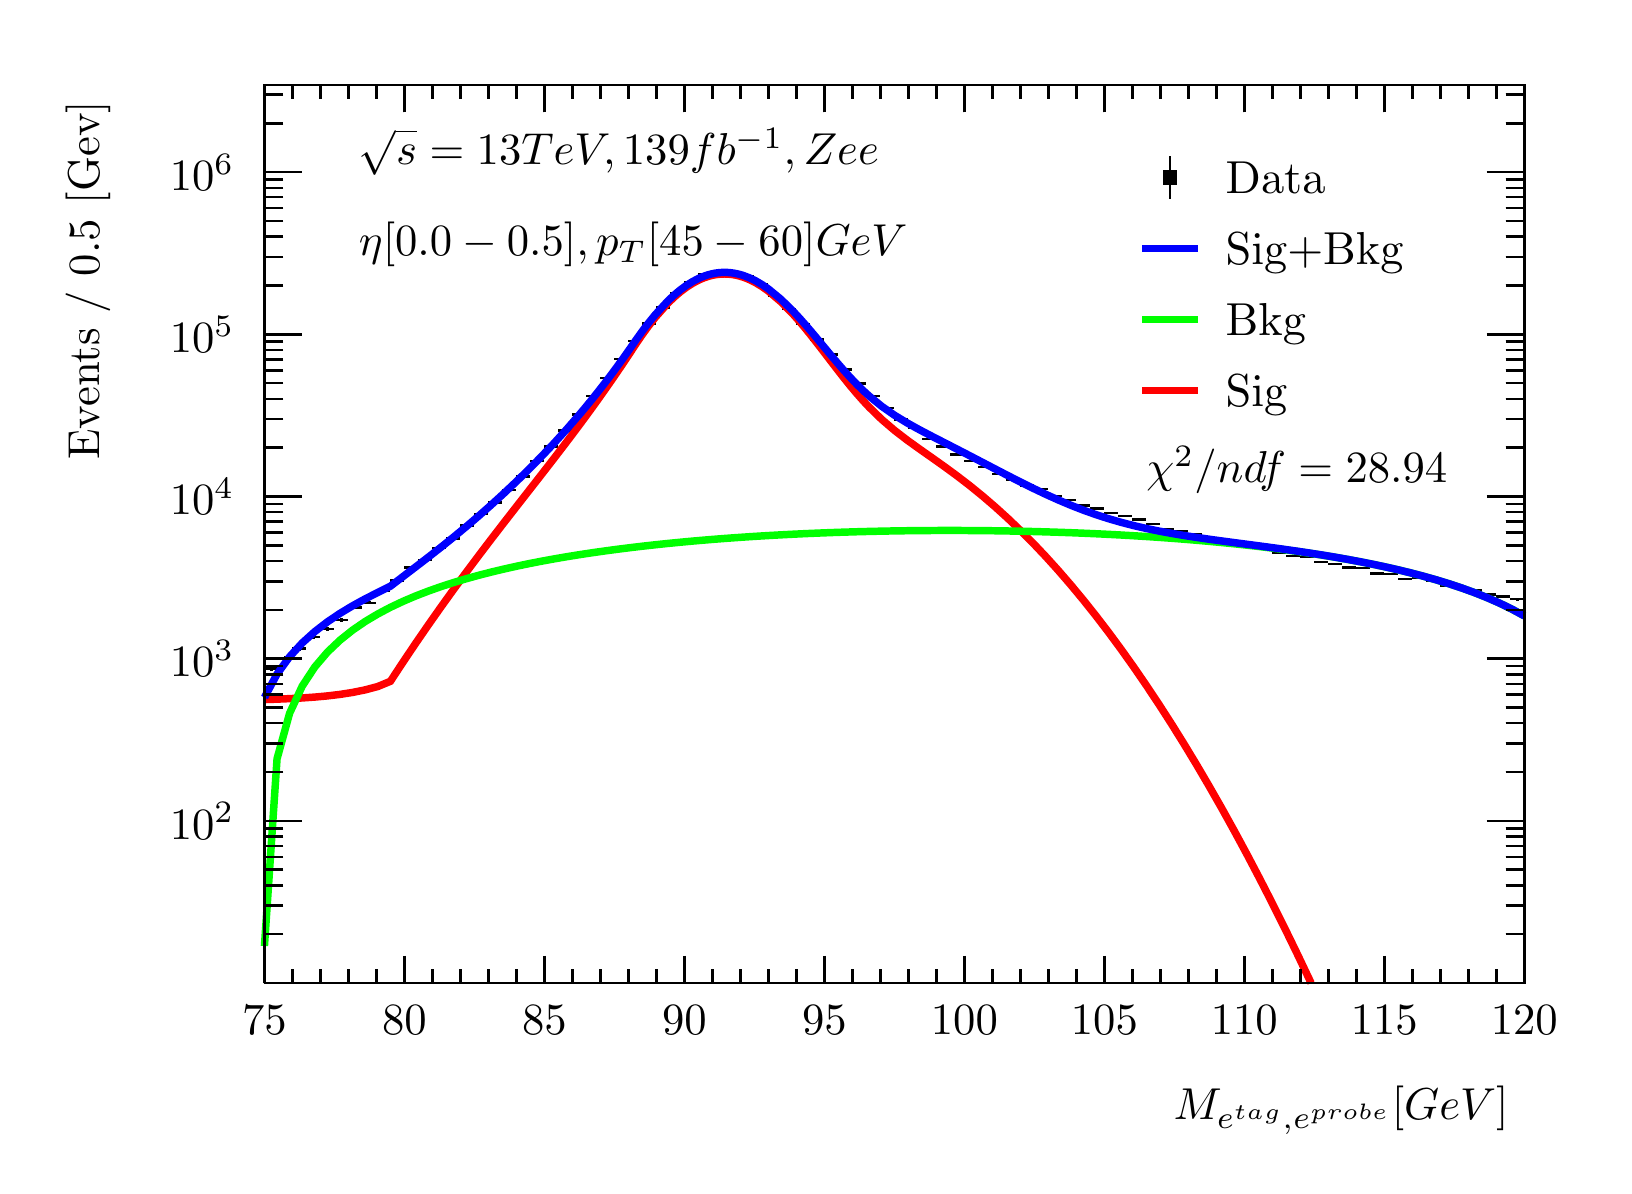
\begin{tikzpicture}
\pgfdeclareplotmark{cross} {
\pgfpathmoveto{\pgfpoint{-0.3\pgfplotmarksize}{\pgfplotmarksize}}
\pgfpathlineto{\pgfpoint{+0.3\pgfplotmarksize}{\pgfplotmarksize}}
\pgfpathlineto{\pgfpoint{+0.3\pgfplotmarksize}{0.3\pgfplotmarksize}}
\pgfpathlineto{\pgfpoint{+1\pgfplotmarksize}{0.3\pgfplotmarksize}}
\pgfpathlineto{\pgfpoint{+1\pgfplotmarksize}{-0.3\pgfplotmarksize}}
\pgfpathlineto{\pgfpoint{+0.3\pgfplotmarksize}{-0.3\pgfplotmarksize}}
\pgfpathlineto{\pgfpoint{+0.3\pgfplotmarksize}{-1.\pgfplotmarksize}}
\pgfpathlineto{\pgfpoint{-0.3\pgfplotmarksize}{-1.\pgfplotmarksize}}
\pgfpathlineto{\pgfpoint{-0.3\pgfplotmarksize}{-0.3\pgfplotmarksize}}
\pgfpathlineto{\pgfpoint{-1.\pgfplotmarksize}{-0.3\pgfplotmarksize}}
\pgfpathlineto{\pgfpoint{-1.\pgfplotmarksize}{0.3\pgfplotmarksize}}
\pgfpathlineto{\pgfpoint{-0.3\pgfplotmarksize}{0.3\pgfplotmarksize}}
\pgfpathclose
\pgfusepathqstroke
}
\pgfdeclareplotmark{cross*} {
\pgfpathmoveto{\pgfpoint{-0.3\pgfplotmarksize}{\pgfplotmarksize}}
\pgfpathlineto{\pgfpoint{+0.3\pgfplotmarksize}{\pgfplotmarksize}}
\pgfpathlineto{\pgfpoint{+0.3\pgfplotmarksize}{0.3\pgfplotmarksize}}
\pgfpathlineto{\pgfpoint{+1\pgfplotmarksize}{0.3\pgfplotmarksize}}
\pgfpathlineto{\pgfpoint{+1\pgfplotmarksize}{-0.3\pgfplotmarksize}}
\pgfpathlineto{\pgfpoint{+0.3\pgfplotmarksize}{-0.3\pgfplotmarksize}}
\pgfpathlineto{\pgfpoint{+0.3\pgfplotmarksize}{-1.\pgfplotmarksize}}
\pgfpathlineto{\pgfpoint{-0.3\pgfplotmarksize}{-1.\pgfplotmarksize}}
\pgfpathlineto{\pgfpoint{-0.3\pgfplotmarksize}{-0.3\pgfplotmarksize}}
\pgfpathlineto{\pgfpoint{-1.\pgfplotmarksize}{-0.3\pgfplotmarksize}}
\pgfpathlineto{\pgfpoint{-1.\pgfplotmarksize}{0.3\pgfplotmarksize}}
\pgfpathlineto{\pgfpoint{-0.3\pgfplotmarksize}{0.3\pgfplotmarksize}}
\pgfpathclose
\pgfusepathqfillstroke
}
\pgfdeclareplotmark{newstar} {
\pgfpathmoveto{\pgfqpoint{0pt}{\pgfplotmarksize}}
\pgfpathlineto{\pgfqpointpolar{44}{0.5\pgfplotmarksize}}
\pgfpathlineto{\pgfqpointpolar{18}{\pgfplotmarksize}}
\pgfpathlineto{\pgfqpointpolar{-20}{0.5\pgfplotmarksize}}
\pgfpathlineto{\pgfqpointpolar{-54}{\pgfplotmarksize}}
\pgfpathlineto{\pgfqpointpolar{-90}{0.5\pgfplotmarksize}}
\pgfpathlineto{\pgfqpointpolar{234}{\pgfplotmarksize}}
\pgfpathlineto{\pgfqpointpolar{198}{0.5\pgfplotmarksize}}
\pgfpathlineto{\pgfqpointpolar{162}{\pgfplotmarksize}}
\pgfpathlineto{\pgfqpointpolar{134}{0.5\pgfplotmarksize}}
\pgfpathclose
\pgfusepathqstroke
}
\pgfdeclareplotmark{newstar*} {
\pgfpathmoveto{\pgfqpoint{0pt}{\pgfplotmarksize}}
\pgfpathlineto{\pgfqpointpolar{44}{0.5\pgfplotmarksize}}
\pgfpathlineto{\pgfqpointpolar{18}{\pgfplotmarksize}}
\pgfpathlineto{\pgfqpointpolar{-20}{0.5\pgfplotmarksize}}
\pgfpathlineto{\pgfqpointpolar{-54}{\pgfplotmarksize}}
\pgfpathlineto{\pgfqpointpolar{-90}{0.5\pgfplotmarksize}}
\pgfpathlineto{\pgfqpointpolar{234}{\pgfplotmarksize}}
\pgfpathlineto{\pgfqpointpolar{198}{0.5\pgfplotmarksize}}
\pgfpathlineto{\pgfqpointpolar{162}{\pgfplotmarksize}}
\pgfpathlineto{\pgfqpointpolar{134}{0.5\pgfplotmarksize}}
\pgfpathclose
\pgfusepathqfillstroke
}
\definecolor{c}{rgb}{1,1,1};
\draw [color=c, fill=c] (0,0) rectangle (20,14.4361);
\draw [color=c, fill=c] (3,2.30977) rectangle (19,13.7143);
\definecolor{c}{rgb}{0,0,0};
\draw [c,line width=0.9] (3,2.30977) -- (3,13.7143) -- (19,13.7143) -- (19,2.30977) -- (3,2.30977);
\definecolor{c}{rgb}{1,1,1};
\draw [color=c, fill=c] (3,2.30977) rectangle (19,13.7143);
\definecolor{c}{rgb}{0,0,0};
\draw [c,line width=0.9] (3,2.30977) -- (3,13.7143) -- (19,13.7143) -- (19,2.30977) -- (3,2.30977);
\draw [c,line width=0.9] (3,2.30977) -- (19,2.30977);
\draw [c,line width=0.9] (3,2.65624) -- (3,2.30977);
\draw [c,line width=0.9] (3.35556,2.48301) -- (3.35556,2.30977);
\draw [c,line width=0.9] (3.71111,2.48301) -- (3.71111,2.30977);
\draw [c,line width=0.9] (4.06667,2.48301) -- (4.06667,2.30977);
\draw [c,line width=0.9] (4.42222,2.48301) -- (4.42222,2.30977);
\draw [c,line width=0.9] (4.77778,2.65624) -- (4.77778,2.30977);
\draw [c,line width=0.9] (5.13333,2.48301) -- (5.13333,2.30977);
\draw [c,line width=0.9] (5.48889,2.48301) -- (5.48889,2.30977);
\draw [c,line width=0.9] (5.84444,2.48301) -- (5.84444,2.30977);
\draw [c,line width=0.9] (6.2,2.48301) -- (6.2,2.30977);
\draw [c,line width=0.9] (6.55556,2.65624) -- (6.55556,2.30977);
\draw [c,line width=0.9] (6.91111,2.48301) -- (6.91111,2.30977);
\draw [c,line width=0.9] (7.26667,2.48301) -- (7.26667,2.30977);
\draw [c,line width=0.9] (7.62222,2.48301) -- (7.62222,2.30977);
\draw [c,line width=0.9] (7.97778,2.48301) -- (7.97778,2.30977);
\draw [c,line width=0.9] (8.33333,2.65624) -- (8.33333,2.30977);
\draw [c,line width=0.9] (8.68889,2.48301) -- (8.68889,2.30977);
\draw [c,line width=0.9] (9.04444,2.48301) -- (9.04444,2.30977);
\draw [c,line width=0.9] (9.4,2.48301) -- (9.4,2.30977);
\draw [c,line width=0.9] (9.75556,2.48301) -- (9.75556,2.30977);
\draw [c,line width=0.9] (10.1111,2.65624) -- (10.1111,2.30977);
\draw [c,line width=0.9] (10.4667,2.48301) -- (10.4667,2.30977);
\draw [c,line width=0.9] (10.8222,2.48301) -- (10.8222,2.30977);
\draw [c,line width=0.9] (11.1778,2.48301) -- (11.1778,2.30977);
\draw [c,line width=0.9] (11.5333,2.48301) -- (11.5333,2.30977);
\draw [c,line width=0.9] (11.8889,2.65624) -- (11.8889,2.30977);
\draw [c,line width=0.9] (12.2444,2.48301) -- (12.2444,2.30977);
\draw [c,line width=0.9] (12.6,2.48301) -- (12.6,2.30977);
\draw [c,line width=0.9] (12.9556,2.48301) -- (12.9556,2.30977);
\draw [c,line width=0.9] (13.3111,2.48301) -- (13.3111,2.30977);
\draw [c,line width=0.9] (13.6667,2.65624) -- (13.6667,2.30977);
\draw [c,line width=0.9] (14.0222,2.48301) -- (14.0222,2.30977);
\draw [c,line width=0.9] (14.3778,2.48301) -- (14.3778,2.30977);
\draw [c,line width=0.9] (14.7333,2.48301) -- (14.7333,2.30977);
\draw [c,line width=0.9] (15.0889,2.48301) -- (15.0889,2.30977);
\draw [c,line width=0.9] (15.4444,2.65624) -- (15.4444,2.30977);
\draw [c,line width=0.9] (15.8,2.48301) -- (15.8,2.30977);
\draw [c,line width=0.9] (16.1556,2.48301) -- (16.1556,2.30977);
\draw [c,line width=0.9] (16.5111,2.48301) -- (16.5111,2.30977);
\draw [c,line width=0.9] (16.8667,2.48301) -- (16.8667,2.30977);
\draw [c,line width=0.9] (17.2222,2.65624) -- (17.2222,2.30977);
\draw [c,line width=0.9] (17.5778,2.48301) -- (17.5778,2.30977);
\draw [c,line width=0.9] (17.9333,2.48301) -- (17.9333,2.30977);
\draw [c,line width=0.9] (18.2889,2.48301) -- (18.2889,2.30977);
\draw [c,line width=0.9] (18.6444,2.48301) -- (18.6444,2.30977);
\draw [c,line width=0.9] (19,2.65624) -- (19,2.30977);
\draw [c,line width=0.9] (19,2.65624) -- (19,2.30977);
\draw [anchor=base] (3,1.66015) node[scale=1.61424, color=c, rotate=0]{75};
\draw [anchor=base] (4.77778,1.66015) node[scale=1.61424, color=c, rotate=0]{80};
\draw [anchor=base] (6.55556,1.66015) node[scale=1.61424, color=c, rotate=0]{85};
\draw [anchor=base] (8.33333,1.66015) node[scale=1.61424, color=c, rotate=0]{90};
\draw [anchor=base] (10.1111,1.66015) node[scale=1.61424, color=c, rotate=0]{95};
\draw [anchor=base] (11.8889,1.66015) node[scale=1.61424, color=c, rotate=0]{100};
\draw [anchor=base] (13.6667,1.66015) node[scale=1.61424, color=c, rotate=0]{105};
\draw [anchor=base] (15.4444,1.66015) node[scale=1.61424, color=c, rotate=0]{110};
\draw [anchor=base] (17.2222,1.66015) node[scale=1.61424, color=c, rotate=0]{115};
\draw [anchor=base] (19,1.66015) node[scale=1.61424, color=c, rotate=0]{120};
\draw [anchor= east] (19,0.692932) node[scale=1.61424, color=c, rotate=0]{$M_{e^{tag}, e^{probe}}  [GeV]$};
\draw [c,line width=0.9] (3,13.7143) -- (19,13.7143);
\draw [c,line width=0.9] (3,13.3678) -- (3,13.7143);
\draw [c,line width=0.9] (3.35556,13.5411) -- (3.35556,13.7143);
\draw [c,line width=0.9] (3.71111,13.5411) -- (3.71111,13.7143);
\draw [c,line width=0.9] (4.06667,13.5411) -- (4.06667,13.7143);
\draw [c,line width=0.9] (4.42222,13.5411) -- (4.42222,13.7143);
\draw [c,line width=0.9] (4.77778,13.3678) -- (4.77778,13.7143);
\draw [c,line width=0.9] (5.13333,13.5411) -- (5.13333,13.7143);
\draw [c,line width=0.9] (5.48889,13.5411) -- (5.48889,13.7143);
\draw [c,line width=0.9] (5.84444,13.5411) -- (5.84444,13.7143);
\draw [c,line width=0.9] (6.2,13.5411) -- (6.2,13.7143);
\draw [c,line width=0.9] (6.55556,13.3678) -- (6.55556,13.7143);
\draw [c,line width=0.9] (6.91111,13.5411) -- (6.91111,13.7143);
\draw [c,line width=0.9] (7.26667,13.5411) -- (7.26667,13.7143);
\draw [c,line width=0.9] (7.62222,13.5411) -- (7.62222,13.7143);
\draw [c,line width=0.9] (7.97778,13.5411) -- (7.97778,13.7143);
\draw [c,line width=0.9] (8.33333,13.3678) -- (8.33333,13.7143);
\draw [c,line width=0.9] (8.68889,13.5411) -- (8.68889,13.7143);
\draw [c,line width=0.9] (9.04444,13.5411) -- (9.04444,13.7143);
\draw [c,line width=0.9] (9.4,13.5411) -- (9.4,13.7143);
\draw [c,line width=0.9] (9.75556,13.5411) -- (9.75556,13.7143);
\draw [c,line width=0.9] (10.1111,13.3678) -- (10.1111,13.7143);
\draw [c,line width=0.9] (10.4667,13.5411) -- (10.4667,13.7143);
\draw [c,line width=0.9] (10.8222,13.5411) -- (10.8222,13.7143);
\draw [c,line width=0.9] (11.1778,13.5411) -- (11.1778,13.7143);
\draw [c,line width=0.9] (11.5333,13.5411) -- (11.5333,13.7143);
\draw [c,line width=0.9] (11.8889,13.3678) -- (11.8889,13.7143);
\draw [c,line width=0.9] (12.2444,13.5411) -- (12.2444,13.7143);
\draw [c,line width=0.9] (12.6,13.5411) -- (12.6,13.7143);
\draw [c,line width=0.9] (12.9556,13.5411) -- (12.9556,13.7143);
\draw [c,line width=0.9] (13.3111,13.5411) -- (13.3111,13.7143);
\draw [c,line width=0.9] (13.6667,13.3678) -- (13.6667,13.7143);
\draw [c,line width=0.9] (14.0222,13.5411) -- (14.0222,13.7143);
\draw [c,line width=0.9] (14.3778,13.5411) -- (14.3778,13.7143);
\draw [c,line width=0.9] (14.7333,13.5411) -- (14.7333,13.7143);
\draw [c,line width=0.9] (15.0889,13.5411) -- (15.0889,13.7143);
\draw [c,line width=0.9] (15.4444,13.3678) -- (15.4444,13.7143);
\draw [c,line width=0.9] (15.8,13.5411) -- (15.8,13.7143);
\draw [c,line width=0.9] (16.1556,13.5411) -- (16.1556,13.7143);
\draw [c,line width=0.9] (16.5111,13.5411) -- (16.5111,13.7143);
\draw [c,line width=0.9] (16.8667,13.5411) -- (16.8667,13.7143);
\draw [c,line width=0.9] (17.2222,13.3678) -- (17.2222,13.7143);
\draw [c,line width=0.9] (17.5778,13.5411) -- (17.5778,13.7143);
\draw [c,line width=0.9] (17.9333,13.5411) -- (17.9333,13.7143);
\draw [c,line width=0.9] (18.2889,13.5411) -- (18.2889,13.7143);
\draw [c,line width=0.9] (18.6444,13.5411) -- (18.6444,13.7143);
\draw [c,line width=0.9] (19,13.3678) -- (19,13.7143);
\draw [c,line width=0.9] (19,13.3678) -- (19,13.7143);
\draw [c,line width=0.9] (3,2.30977) -- (3,13.7143);
\draw [c,line width=0.9] (3.237,2.92982) -- (3,2.92982);
\draw [c,line width=0.9] (3.237,3.29252) -- (3,3.29252);
\draw [c,line width=0.9] (3.237,3.54986) -- (3,3.54986);
\draw [c,line width=0.9] (3.237,3.74947) -- (3,3.74947);
\draw [c,line width=0.9] (3.237,3.91257) -- (3,3.91257);
\draw [c,line width=0.9] (3.237,4.05046) -- (3,4.05046);
\draw [c,line width=0.9] (3.237,4.16991) -- (3,4.16991);
\draw [c,line width=0.9] (3.237,4.27527) -- (3,4.27527);
\draw [c,line width=0.9] (3.474,4.36952) -- (3,4.36952);
\draw [anchor= east] (2.82,4.36952) node[scale=1.61424, color=c, rotate=0]{$10^{2}$};
\draw [c,line width=0.9] (3.237,4.98956) -- (3,4.98956);
\draw [c,line width=0.9] (3.237,5.35227) -- (3,5.35227);
\draw [c,line width=0.9] (3.237,5.60961) -- (3,5.60961);
\draw [c,line width=0.9] (3.237,5.80922) -- (3,5.80922);
\draw [c,line width=0.9] (3.237,5.97231) -- (3,5.97231);
\draw [c,line width=0.9] (3.237,6.11021) -- (3,6.11021);
\draw [c,line width=0.9] (3.237,6.22966) -- (3,6.22966);
\draw [c,line width=0.9] (3.237,6.33502) -- (3,6.33502);
\draw [c,line width=0.9] (3.474,6.42927) -- (3,6.42927);
\draw [anchor= east] (2.82,6.42927) node[scale=1.61424, color=c, rotate=0]{$10^{3}$};
\draw [c,line width=0.9] (3.237,7.04931) -- (3,7.04931);
\draw [c,line width=0.9] (3.237,7.41202) -- (3,7.41202);
\draw [c,line width=0.9] (3.237,7.66936) -- (3,7.66936);
\draw [c,line width=0.9] (3.237,7.86897) -- (3,7.86897);
\draw [c,line width=0.9] (3.237,8.03206) -- (3,8.03206);
\draw [c,line width=0.9] (3.237,8.16995) -- (3,8.16995);
\draw [c,line width=0.9] (3.237,8.2894) -- (3,8.2894);
\draw [c,line width=0.9] (3.237,8.39476) -- (3,8.39476);
\draw [c,line width=0.9] (3.474,8.48901) -- (3,8.48901);
\draw [anchor= east] (2.82,8.48901) node[scale=1.61424, color=c, rotate=0]{$10^{4}$};
\draw [c,line width=0.9] (3.237,9.10906) -- (3,9.10906);
\draw [c,line width=0.9] (3.237,9.47176) -- (3,9.47176);
\draw [c,line width=0.9] (3.237,9.7291) -- (3,9.7291);
\draw [c,line width=0.9] (3.237,9.92871) -- (3,9.92871);
\draw [c,line width=0.9] (3.237,10.0918) -- (3,10.0918);
\draw [c,line width=0.9] (3.237,10.2297) -- (3,10.2297);
\draw [c,line width=0.9] (3.237,10.3491) -- (3,10.3491);
\draw [c,line width=0.9] (3.237,10.4545) -- (3,10.4545);
\draw [c,line width=0.9] (3.474,10.5488) -- (3,10.5488);
\draw [anchor= east] (2.82,10.5488) node[scale=1.61424, color=c, rotate=0]{$10^{5}$};
\draw [c,line width=0.9] (3.237,11.1688) -- (3,11.1688);
\draw [c,line width=0.9] (3.237,11.5315) -- (3,11.5315);
\draw [c,line width=0.9] (3.237,11.7889) -- (3,11.7889);
\draw [c,line width=0.9] (3.237,11.9885) -- (3,11.9885);
\draw [c,line width=0.9] (3.237,12.1516) -- (3,12.1516);
\draw [c,line width=0.9] (3.237,12.2894) -- (3,12.2894);
\draw [c,line width=0.9] (3.237,12.4089) -- (3,12.4089);
\draw [c,line width=0.9] (3.237,12.5143) -- (3,12.5143);
\draw [c,line width=0.9] (3.474,12.6085) -- (3,12.6085);
\draw [anchor= east] (2.82,12.6085) node[scale=1.61424, color=c, rotate=0]{$10^{6}$};
\draw [c,line width=0.9] (3.237,13.2286) -- (3,13.2286);
\draw [c,line width=0.9] (3.237,13.5913) -- (3,13.5913);
\draw [anchor= east] (0.76,13.7143) node[scale=1.61424, color=c, rotate=90]{Events / 0.5 [Gev]};
\draw [c,line width=0.9] (19,2.30977) -- (19,13.7143);
\draw [c,line width=0.9] (18.763,2.92982) -- (19,2.92982);
\draw [c,line width=0.9] (18.763,3.29252) -- (19,3.29252);
\draw [c,line width=0.9] (18.763,3.54986) -- (19,3.54986);
\draw [c,line width=0.9] (18.763,3.74947) -- (19,3.74947);
\draw [c,line width=0.9] (18.763,3.91257) -- (19,3.91257);
\draw [c,line width=0.9] (18.763,4.05046) -- (19,4.05046);
\draw [c,line width=0.9] (18.763,4.16991) -- (19,4.16991);
\draw [c,line width=0.9] (18.763,4.27527) -- (19,4.27527);
\draw [c,line width=0.9] (18.526,4.36952) -- (19,4.36952);
\draw [c,line width=0.9] (18.763,4.98956) -- (19,4.98956);
\draw [c,line width=0.9] (18.763,5.35227) -- (19,5.35227);
\draw [c,line width=0.9] (18.763,5.60961) -- (19,5.60961);
\draw [c,line width=0.9] (18.763,5.80922) -- (19,5.80922);
\draw [c,line width=0.9] (18.763,5.97231) -- (19,5.97231);
\draw [c,line width=0.9] (18.763,6.11021) -- (19,6.11021);
\draw [c,line width=0.9] (18.763,6.22966) -- (19,6.22966);
\draw [c,line width=0.9] (18.763,6.33502) -- (19,6.33502);
\draw [c,line width=0.9] (18.526,6.42927) -- (19,6.42927);
\draw [c,line width=0.9] (18.763,7.04931) -- (19,7.04931);
\draw [c,line width=0.9] (18.763,7.41202) -- (19,7.41202);
\draw [c,line width=0.9] (18.763,7.66936) -- (19,7.66936);
\draw [c,line width=0.9] (18.763,7.86897) -- (19,7.86897);
\draw [c,line width=0.9] (18.763,8.03206) -- (19,8.03206);
\draw [c,line width=0.9] (18.763,8.16995) -- (19,8.16995);
\draw [c,line width=0.9] (18.763,8.2894) -- (19,8.2894);
\draw [c,line width=0.9] (18.763,8.39476) -- (19,8.39476);
\draw [c,line width=0.9] (18.526,8.48901) -- (19,8.48901);
\draw [c,line width=0.9] (18.763,9.10906) -- (19,9.10906);
\draw [c,line width=0.9] (18.763,9.47176) -- (19,9.47176);
\draw [c,line width=0.9] (18.763,9.7291) -- (19,9.7291);
\draw [c,line width=0.9] (18.763,9.92871) -- (19,9.92871);
\draw [c,line width=0.9] (18.763,10.0918) -- (19,10.0918);
\draw [c,line width=0.9] (18.763,10.2297) -- (19,10.2297);
\draw [c,line width=0.9] (18.763,10.3491) -- (19,10.3491);
\draw [c,line width=0.9] (18.763,10.4545) -- (19,10.4545);
\draw [c,line width=0.9] (18.526,10.5488) -- (19,10.5488);
\draw [c,line width=0.9] (18.763,11.1688) -- (19,11.1688);
\draw [c,line width=0.9] (18.763,11.5315) -- (19,11.5315);
\draw [c,line width=0.9] (18.763,11.7889) -- (19,11.7889);
\draw [c,line width=0.9] (18.763,11.9885) -- (19,11.9885);
\draw [c,line width=0.9] (18.763,12.1516) -- (19,12.1516);
\draw [c,line width=0.9] (18.763,12.2894) -- (19,12.2894);
\draw [c,line width=0.9] (18.763,12.4089) -- (19,12.4089);
\draw [c,line width=0.9] (18.763,12.5143) -- (19,12.5143);
\draw [c,line width=0.9] (18.526,12.6085) -- (19,12.6085);
\draw [c,line width=0.9] (18.763,13.2286) -- (19,13.2286);
\draw [c,line width=0.9] (18.763,13.5913) -- (19,13.5913);
\draw [c,line width=0.9] (3.08889,6.30572) -- (3,6.30572);
\draw [c,line width=0.9] (3,6.30572) -- (3,6.30572);
\draw [c,line width=0.9] (3.08889,6.30572) -- (3.17778,6.30572);
\draw [c,line width=0.9] (3.17778,6.30572) -- (3.17778,6.30572);
\draw [c,line width=0.9] (3.08889,6.30572) -- (3.08889,6.33603);
\draw [c,line width=0.9] (3.08889,6.33603) -- (3.08889,6.33603);
\draw [c,line width=0.9] (3.08889,6.30572) -- (3.08889,6.27541);
\draw [c,line width=0.9] (3.08889,6.27541) -- (3.08889,6.27541);
\draw [c,line width=0.9] (3.26667,6.43994) -- (3.17778,6.43994);
\draw [c,line width=0.9] (3.17778,6.43994) -- (3.17778,6.43994);
\draw [c,line width=0.9] (3.26667,6.43994) -- (3.35556,6.43994);
\draw [c,line width=0.9] (3.35556,6.43994) -- (3.35556,6.43994);
\draw [c,line width=0.9] (3.26667,6.43994) -- (3.26667,6.46806);
\draw [c,line width=0.9] (3.26667,6.46806) -- (3.26667,6.46806);
\draw [c,line width=0.9] (3.26667,6.43994) -- (3.26667,6.41182);
\draw [c,line width=0.9] (3.26667,6.41182) -- (3.26667,6.41182);
\draw [c,line width=0.9] (3.44444,6.55584) -- (3.35556,6.55584);
\draw [c,line width=0.9] (3.35556,6.55584) -- (3.35556,6.55584);
\draw [c,line width=0.9] (3.44444,6.55584) -- (3.53333,6.55584);
\draw [c,line width=0.9] (3.53333,6.55584) -- (3.53333,6.55584);
\draw [c,line width=0.9] (3.44444,6.55584) -- (3.44444,6.5822);
\draw [c,line width=0.9] (3.44444,6.5822) -- (3.44444,6.5822);
\draw [c,line width=0.9] (3.44444,6.55584) -- (3.44444,6.52949);
\draw [c,line width=0.9] (3.44444,6.52949) -- (3.44444,6.52949);
\draw [c,line width=0.9] (3.62222,6.70301) -- (3.53333,6.70301);
\draw [c,line width=0.9] (3.53333,6.70301) -- (3.53333,6.70301);
\draw [c,line width=0.9] (3.62222,6.70301) -- (3.71111,6.70301);
\draw [c,line width=0.9] (3.71111,6.70301) -- (3.71111,6.70301);
\draw [c,line width=0.9] (3.62222,6.70301) -- (3.62222,6.72728);
\draw [c,line width=0.9] (3.62222,6.72728) -- (3.62222,6.72728);
\draw [c,line width=0.9] (3.62222,6.70301) -- (3.62222,6.67873);
\draw [c,line width=0.9] (3.62222,6.67873) -- (3.62222,6.67873);
\draw [c,line width=0.9] (3.8,6.80852) -- (3.71111,6.80852);
\draw [c,line width=0.9] (3.71111,6.80852) -- (3.71111,6.80852);
\draw [c,line width=0.9] (3.8,6.80852) -- (3.88889,6.80852);
\draw [c,line width=0.9] (3.88889,6.80852) -- (3.88889,6.80852);
\draw [c,line width=0.9] (3.8,6.80852) -- (3.8,6.8314);
\draw [c,line width=0.9] (3.8,6.8314) -- (3.8,6.8314);
\draw [c,line width=0.9] (3.8,6.80852) -- (3.8,6.78563);
\draw [c,line width=0.9] (3.8,6.78563) -- (3.8,6.78563);
\draw [c,line width=0.9] (3.97778,6.91855) -- (3.88889,6.91855);
\draw [c,line width=0.9] (3.88889,6.91855) -- (3.88889,6.91855);
\draw [c,line width=0.9] (3.97778,6.91855) -- (4.06667,6.91855);
\draw [c,line width=0.9] (4.06667,6.91855) -- (4.06667,6.91855);
\draw [c,line width=0.9] (3.97778,6.91855) -- (3.97778,6.94007);
\draw [c,line width=0.9] (3.97778,6.94007) -- (3.97778,6.94007);
\draw [c,line width=0.9] (3.97778,6.91855) -- (3.97778,6.89703);
\draw [c,line width=0.9] (3.97778,6.89703) -- (3.97778,6.89703);
\draw [c,line width=0.9] (4.15556,7.08052) -- (4.06667,7.08052);
\draw [c,line width=0.9] (4.06667,7.08052) -- (4.06667,7.08052);
\draw [c,line width=0.9] (4.15556,7.08052) -- (4.24444,7.08052);
\draw [c,line width=0.9] (4.24444,7.08052) -- (4.24444,7.08052);
\draw [c,line width=0.9] (4.15556,7.08052) -- (4.15556,7.10017);
\draw [c,line width=0.9] (4.15556,7.10017) -- (4.15556,7.10017);
\draw [c,line width=0.9] (4.15556,7.08052) -- (4.15556,7.06086);
\draw [c,line width=0.9] (4.15556,7.06086) -- (4.15556,7.06086);
\draw [c,line width=0.9] (4.33333,7.13863) -- (4.24444,7.13863);
\draw [c,line width=0.9] (4.24444,7.13863) -- (4.24444,7.13863);
\draw [c,line width=0.9] (4.33333,7.13863) -- (4.42222,7.13863);
\draw [c,line width=0.9] (4.42222,7.13863) -- (4.42222,7.13863);
\draw [c,line width=0.9] (4.33333,7.13863) -- (4.33333,7.15766);
\draw [c,line width=0.9] (4.33333,7.15766) -- (4.33333,7.15766);
\draw [c,line width=0.9] (4.33333,7.13863) -- (4.33333,7.1196);
\draw [c,line width=0.9] (4.33333,7.1196) -- (4.33333,7.1196);
\draw [c,line width=0.9] (4.51111,7.29393) -- (4.42222,7.29393);
\draw [c,line width=0.9] (4.42222,7.29393) -- (4.42222,7.29393);
\draw [c,line width=0.9] (4.51111,7.29393) -- (4.6,7.29393);
\draw [c,line width=0.9] (4.6,7.29393) -- (4.6,7.29393);
\draw [c,line width=0.9] (4.51111,7.29393) -- (4.51111,7.31138);
\draw [c,line width=0.9] (4.51111,7.31138) -- (4.51111,7.31138);
\draw [c,line width=0.9] (4.51111,7.29393) -- (4.51111,7.27648);
\draw [c,line width=0.9] (4.51111,7.27648) -- (4.51111,7.27648);
\draw [c,line width=0.9] (4.68889,7.42239) -- (4.6,7.42239);
\draw [c,line width=0.9] (4.6,7.42239) -- (4.6,7.42239);
\draw [c,line width=0.9] (4.68889,7.42239) -- (4.77778,7.42239);
\draw [c,line width=0.9] (4.77778,7.42239) -- (4.77778,7.42239);
\draw [c,line width=0.9] (4.68889,7.42239) -- (4.68889,7.43863);
\draw [c,line width=0.9] (4.68889,7.43863) -- (4.68889,7.43863);
\draw [c,line width=0.9] (4.68889,7.42239) -- (4.68889,7.40616);
\draw [c,line width=0.9] (4.68889,7.40616) -- (4.68889,7.40616);
\draw [c,line width=0.9] (4.86667,7.58647) -- (4.77778,7.58647);
\draw [c,line width=0.9] (4.77778,7.58647) -- (4.77778,7.58647);
\draw [c,line width=0.9] (4.86667,7.58647) -- (4.95556,7.58647);
\draw [c,line width=0.9] (4.95556,7.58647) -- (4.95556,7.58647);
\draw [c,line width=0.9] (4.86667,7.58647) -- (4.86667,7.60128);
\draw [c,line width=0.9] (4.86667,7.60128) -- (4.86667,7.60128);
\draw [c,line width=0.9] (4.86667,7.58647) -- (4.86667,7.57165);
\draw [c,line width=0.9] (4.86667,7.57165) -- (4.86667,7.57165);
\draw [c,line width=0.9] (5.04444,7.68466) -- (4.95556,7.68466);
\draw [c,line width=0.9] (4.95556,7.68466) -- (4.95556,7.68466);
\draw [c,line width=0.9] (5.04444,7.68466) -- (5.13333,7.68466);
\draw [c,line width=0.9] (5.13333,7.68466) -- (5.13333,7.68466);
\draw [c,line width=0.9] (5.04444,7.68466) -- (5.04444,7.69868);
\draw [c,line width=0.9] (5.04444,7.69868) -- (5.04444,7.69868);
\draw [c,line width=0.9] (5.04444,7.68466) -- (5.04444,7.67063);
\draw [c,line width=0.9] (5.04444,7.67063) -- (5.04444,7.67063);
\draw [c,line width=0.9] (5.22222,7.83413) -- (5.13333,7.83413);
\draw [c,line width=0.9] (5.13333,7.83413) -- (5.13333,7.83413);
\draw [c,line width=0.9] (5.22222,7.83413) -- (5.31111,7.83413);
\draw [c,line width=0.9] (5.31111,7.83413) -- (5.31111,7.83413);
\draw [c,line width=0.9] (5.22222,7.83413) -- (5.22222,7.84703);
\draw [c,line width=0.9] (5.22222,7.84703) -- (5.22222,7.84703);
\draw [c,line width=0.9] (5.22222,7.83413) -- (5.22222,7.82123);
\draw [c,line width=0.9] (5.22222,7.82123) -- (5.22222,7.82123);
\draw [c,line width=0.9] (5.4,7.95861) -- (5.31111,7.95861);
\draw [c,line width=0.9] (5.31111,7.95861) -- (5.31111,7.95861);
\draw [c,line width=0.9] (5.4,7.95861) -- (5.48889,7.95861);
\draw [c,line width=0.9] (5.48889,7.95861) -- (5.48889,7.95861);
\draw [c,line width=0.9] (5.4,7.95861) -- (5.4,7.97064);
\draw [c,line width=0.9] (5.4,7.97064) -- (5.4,7.97064);
\draw [c,line width=0.9] (5.4,7.95861) -- (5.4,7.94658);
\draw [c,line width=0.9] (5.4,7.94658) -- (5.4,7.94658);
\draw [c,line width=0.9] (5.57778,8.118) -- (5.48889,8.118);
\draw [c,line width=0.9] (5.48889,8.118) -- (5.48889,8.118);
\draw [c,line width=0.9] (5.57778,8.118) -- (5.66667,8.118);
\draw [c,line width=0.9] (5.66667,8.118) -- (5.66667,8.118);
\draw [c,line width=0.9] (5.57778,8.118) -- (5.57778,8.129);
\draw [c,line width=0.9] (5.57778,8.129) -- (5.57778,8.129);
\draw [c,line width=0.9] (5.57778,8.118) -- (5.57778,8.10699);
\draw [c,line width=0.9] (5.57778,8.10699) -- (5.57778,8.10699);
\draw [c,line width=0.9] (5.75556,8.26354) -- (5.66667,8.26354);
\draw [c,line width=0.9] (5.66667,8.26354) -- (5.66667,8.26354);
\draw [c,line width=0.9] (5.75556,8.26354) -- (5.84444,8.26354);
\draw [c,line width=0.9] (5.84444,8.26354) -- (5.84444,8.26354);
\draw [c,line width=0.9] (5.75556,8.26354) -- (5.75556,8.27369);
\draw [c,line width=0.9] (5.75556,8.27369) -- (5.75556,8.27369);
\draw [c,line width=0.9] (5.75556,8.26354) -- (5.75556,8.25339);
\draw [c,line width=0.9] (5.75556,8.25339) -- (5.75556,8.25339);
\draw [c,line width=0.9] (5.93333,8.41189) -- (5.84444,8.41189);
\draw [c,line width=0.9] (5.84444,8.41189) -- (5.84444,8.41189);
\draw [c,line width=0.9] (5.93333,8.41189) -- (6.02222,8.41189);
\draw [c,line width=0.9] (6.02222,8.41189) -- (6.02222,8.41189);
\draw [c,line width=0.9] (5.93333,8.41189) -- (5.93333,8.42123);
\draw [c,line width=0.9] (5.93333,8.42123) -- (5.93333,8.42123);
\draw [c,line width=0.9] (5.93333,8.41189) -- (5.93333,8.40256);
\draw [c,line width=0.9] (5.93333,8.40256) -- (5.93333,8.40256);
\draw [c,line width=0.9] (6.11111,8.5702) -- (6.02222,8.5702);
\draw [c,line width=0.9] (6.02222,8.5702) -- (6.02222,8.5702);
\draw [c,line width=0.9] (6.11111,8.5702) -- (6.2,8.5702);
\draw [c,line width=0.9] (6.2,8.5702) -- (6.2,8.5702);
\draw [c,line width=0.9] (6.11111,8.5702) -- (6.11111,8.57875);
\draw [c,line width=0.9] (6.11111,8.57875) -- (6.11111,8.57875);
\draw [c,line width=0.9] (6.11111,8.5702) -- (6.11111,8.56165);
\draw [c,line width=0.9] (6.11111,8.56165) -- (6.11111,8.56165);
\draw [c,line width=0.9] (6.28889,8.74338) -- (6.2,8.74338);
\draw [c,line width=0.9] (6.2,8.74338) -- (6.2,8.74338);
\draw [c,line width=0.9] (6.28889,8.74338) -- (6.37778,8.74338);
\draw [c,line width=0.9] (6.37778,8.74338) -- (6.37778,8.74338);
\draw [c,line width=0.9] (6.28889,8.74338) -- (6.28889,8.75114);
\draw [c,line width=0.9] (6.28889,8.75114) -- (6.28889,8.75114);
\draw [c,line width=0.9] (6.28889,8.74338) -- (6.28889,8.73562);
\draw [c,line width=0.9] (6.28889,8.73562) -- (6.28889,8.73562);
\draw [c,line width=0.9] (6.46667,8.93957) -- (6.37778,8.93957);
\draw [c,line width=0.9] (6.37778,8.93957) -- (6.37778,8.93957);
\draw [c,line width=0.9] (6.46667,8.93957) -- (6.55556,8.93957);
\draw [c,line width=0.9] (6.55556,8.93957) -- (6.55556,8.93957);
\draw [c,line width=0.9] (6.46667,8.93957) -- (6.46667,8.94653);
\draw [c,line width=0.9] (6.46667,8.94653) -- (6.46667,8.94653);
\draw [c,line width=0.9] (6.46667,8.93957) -- (6.46667,8.93262);
\draw [c,line width=0.9] (6.46667,8.93262) -- (6.46667,8.93262);
\draw [c,line width=0.9] (6.64444,9.12594) -- (6.55556,9.12594);
\draw [c,line width=0.9] (6.55556,9.12594) -- (6.55556,9.12594);
\draw [c,line width=0.9] (6.64444,9.12594) -- (6.73333,9.12594);
\draw [c,line width=0.9] (6.73333,9.12594) -- (6.73333,9.12594);
\draw [c,line width=0.9] (6.64444,9.12594) -- (6.64444,9.13221);
\draw [c,line width=0.9] (6.64444,9.13221) -- (6.64444,9.13221);
\draw [c,line width=0.9] (6.64444,9.12594) -- (6.64444,9.11967);
\draw [c,line width=0.9] (6.64444,9.11967) -- (6.64444,9.11967);
\draw [c,line width=0.9] (6.82222,9.32751) -- (6.73333,9.32751);
\draw [c,line width=0.9] (6.73333,9.32751) -- (6.73333,9.32751);
\draw [c,line width=0.9] (6.82222,9.32751) -- (6.91111,9.32751);
\draw [c,line width=0.9] (6.91111,9.32751) -- (6.91111,9.32751);
\draw [c,line width=0.9] (6.82222,9.32751) -- (6.82222,9.3331);
\draw [c,line width=0.9] (6.82222,9.3331) -- (6.82222,9.3331);
\draw [c,line width=0.9] (6.82222,9.32751) -- (6.82222,9.32191);
\draw [c,line width=0.9] (6.82222,9.32191) -- (6.82222,9.32191);
\draw [c,line width=0.9] (7,9.53) -- (6.91111,9.53);
\draw [c,line width=0.9] (6.91111,9.53) -- (6.91111,9.53);
\draw [c,line width=0.9] (7,9.53) -- (7.08889,9.53);
\draw [c,line width=0.9] (7.08889,9.53) -- (7.08889,9.53);
\draw [c,line width=0.9] (7,9.53) -- (7,9.535);
\draw [c,line width=0.9] (7,9.535) -- (7,9.535);
\draw [c,line width=0.9] (7,9.53) -- (7,9.525);
\draw [c,line width=0.9] (7,9.525) -- (7,9.525);
\draw [c,line width=0.9] (7.17778,9.76837) -- (7.08889,9.76837);
\draw [c,line width=0.9] (7.08889,9.76837) -- (7.08889,9.76837);
\draw [c,line width=0.9] (7.17778,9.76837) -- (7.26667,9.76837);
\draw [c,line width=0.9] (7.26667,9.76837) -- (7.26667,9.76837);
\draw [c,line width=0.9] (7.17778,9.76837) -- (7.17778,9.77275);
\draw [c,line width=0.9] (7.17778,9.77275) -- (7.17778,9.77275);
\draw [c,line width=0.9] (7.17778,9.76837) -- (7.17778,9.764);
\draw [c,line width=0.9] (7.17778,9.764) -- (7.17778,9.764);
\draw [c,line width=0.9] (7.35556,9.99199) -- (7.26667,9.99199);
\draw [c,line width=0.9] (7.26667,9.99199) -- (7.26667,9.99199);
\draw [c,line width=0.9] (7.35556,9.99199) -- (7.44444,9.99199);
\draw [c,line width=0.9] (7.44444,9.99199) -- (7.44444,9.99199);
\draw [c,line width=0.9] (7.35556,9.99199) -- (7.35556,9.99585);
\draw [c,line width=0.9] (7.35556,9.99585) -- (7.35556,9.99585);
\draw [c,line width=0.9] (7.35556,9.99199) -- (7.35556,9.98813);
\draw [c,line width=0.9] (7.35556,9.98813) -- (7.35556,9.98813);
\draw [c,line width=0.9] (7.53333,10.2354) -- (7.44444,10.2354);
\draw [c,line width=0.9] (7.44444,10.2354) -- (7.44444,10.2354);
\draw [c,line width=0.9] (7.53333,10.2354) -- (7.62222,10.2354);
\draw [c,line width=0.9] (7.62222,10.2354) -- (7.62222,10.2354);
\draw [c,line width=0.9] (7.53333,10.2354) -- (7.53333,10.2387);
\draw [c,line width=0.9] (7.53333,10.2387) -- (7.53333,10.2387);
\draw [c,line width=0.9] (7.53333,10.2354) -- (7.53333,10.232);
\draw [c,line width=0.9] (7.53333,10.232) -- (7.53333,10.232);
\draw [c,line width=0.9] (7.71111,10.4629) -- (7.62222,10.4629);
\draw [c,line width=0.9] (7.62222,10.4629) -- (7.62222,10.4629);
\draw [c,line width=0.9] (7.71111,10.4629) -- (7.8,10.4629);
\draw [c,line width=0.9] (7.8,10.4629) -- (7.8,10.4629);
\draw [c,line width=0.9] (7.71111,10.4629) -- (7.71111,10.4658);
\draw [c,line width=0.9] (7.71111,10.4658) -- (7.71111,10.4658);
\draw [c,line width=0.9] (7.71111,10.4629) -- (7.71111,10.4599);
\draw [c,line width=0.9] (7.71111,10.4599) -- (7.71111,10.4599);
\draw [c,line width=0.9] (7.88889,10.6841) -- (7.8,10.6841);
\draw [c,line width=0.9] (7.8,10.6841) -- (7.8,10.6841);
\draw [c,line width=0.9] (7.88889,10.6841) -- (7.97778,10.6841);
\draw [c,line width=0.9] (7.97778,10.6841) -- (7.97778,10.6841);
\draw [c,line width=0.9] (7.88889,10.6841) -- (7.88889,10.6867);
\draw [c,line width=0.9] (7.88889,10.6867) -- (7.88889,10.6867);
\draw [c,line width=0.9] (7.88889,10.6841) -- (7.88889,10.6815);
\draw [c,line width=0.9] (7.88889,10.6815) -- (7.88889,10.6815);
\draw [c,line width=0.9] (8.06667,10.8887) -- (7.97778,10.8887);
\draw [c,line width=0.9] (7.97778,10.8887) -- (7.97778,10.8887);
\draw [c,line width=0.9] (8.06667,10.8887) -- (8.15556,10.8887);
\draw [c,line width=0.9] (8.15556,10.8887) -- (8.15556,10.8887);
\draw [c,line width=0.9] (8.06667,10.8887) -- (8.06667,10.891);
\draw [c,line width=0.9] (8.06667,10.891) -- (8.06667,10.891);
\draw [c,line width=0.9] (8.06667,10.8887) -- (8.06667,10.8863);
\draw [c,line width=0.9] (8.06667,10.8863) -- (8.06667,10.8863);
\draw [c,line width=0.9] (8.24444,11.0725) -- (8.15556,11.0725);
\draw [c,line width=0.9] (8.15556,11.0725) -- (8.15556,11.0725);
\draw [c,line width=0.9] (8.24444,11.0725) -- (8.33333,11.0725);
\draw [c,line width=0.9] (8.33333,11.0725) -- (8.33333,11.0725);
\draw [c,line width=0.9] (8.24444,11.0725) -- (8.24444,11.0746);
\draw [c,line width=0.9] (8.24444,11.0746) -- (8.24444,11.0746);
\draw [c,line width=0.9] (8.24444,11.0725) -- (8.24444,11.0704);
\draw [c,line width=0.9] (8.24444,11.0704) -- (8.24444,11.0704);
\draw [c,line width=0.9] (8.42222,11.2095) -- (8.33333,11.2095);
\draw [c,line width=0.9] (8.33333,11.2095) -- (8.33333,11.2095);
\draw [c,line width=0.9] (8.42222,11.2095) -- (8.51111,11.2095);
\draw [c,line width=0.9] (8.51111,11.2095) -- (8.51111,11.2095);
\draw [c,line width=0.9] (8.42222,11.2095) -- (8.42222,11.2115);
\draw [c,line width=0.9] (8.42222,11.2115) -- (8.42222,11.2115);
\draw [c,line width=0.9] (8.42222,11.2095) -- (8.42222,11.2076);
\draw [c,line width=0.9] (8.42222,11.2076) -- (8.42222,11.2076);
\draw [c,line width=0.9] (8.6,11.3058) -- (8.51111,11.3058);
\draw [c,line width=0.9] (8.51111,11.3058) -- (8.51111,11.3058);
\draw [c,line width=0.9] (8.6,11.3058) -- (8.68889,11.3058);
\draw [c,line width=0.9] (8.68889,11.3058) -- (8.68889,11.3058);
\draw [c,line width=0.9] (8.6,11.3058) -- (8.6,11.3076);
\draw [c,line width=0.9] (8.6,11.3076) -- (8.6,11.3076);
\draw [c,line width=0.9] (8.6,11.3058) -- (8.6,11.3039);
\draw [c,line width=0.9] (8.6,11.3039) -- (8.6,11.3039);
\draw [c,line width=0.9] (8.77778,11.3499) -- (8.68889,11.3499);
\draw [c,line width=0.9] (8.68889,11.3499) -- (8.68889,11.3499);
\draw [c,line width=0.9] (8.77778,11.3499) -- (8.86667,11.3499);
\draw [c,line width=0.9] (8.86667,11.3499) -- (8.86667,11.3499);
\draw [c,line width=0.9] (8.77778,11.3499) -- (8.77778,11.3517);
\draw [c,line width=0.9] (8.77778,11.3517) -- (8.77778,11.3517);
\draw [c,line width=0.9] (8.77778,11.3499) -- (8.77778,11.348);
\draw [c,line width=0.9] (8.77778,11.348) -- (8.77778,11.348);
\draw [c,line width=0.9] (8.95556,11.3424) -- (8.86667,11.3424);
\draw [c,line width=0.9] (8.86667,11.3424) -- (8.86667,11.3424);
\draw [c,line width=0.9] (8.95556,11.3424) -- (9.04444,11.3424);
\draw [c,line width=0.9] (9.04444,11.3424) -- (9.04444,11.3424);
\draw [c,line width=0.9] (8.95556,11.3424) -- (8.95556,11.3442);
\draw [c,line width=0.9] (8.95556,11.3442) -- (8.95556,11.3442);
\draw [c,line width=0.9] (8.95556,11.3424) -- (8.95556,11.3406);
\draw [c,line width=0.9] (8.95556,11.3406) -- (8.95556,11.3406);
\draw [c,line width=0.9] (9.13333,11.2839) -- (9.04444,11.2839);
\draw [c,line width=0.9] (9.04444,11.2839) -- (9.04444,11.2839);
\draw [c,line width=0.9] (9.13333,11.2839) -- (9.22222,11.2839);
\draw [c,line width=0.9] (9.22222,11.2839) -- (9.22222,11.2839);
\draw [c,line width=0.9] (9.13333,11.2839) -- (9.13333,11.2858);
\draw [c,line width=0.9] (9.13333,11.2858) -- (9.13333,11.2858);
\draw [c,line width=0.9] (9.13333,11.2839) -- (9.13333,11.2821);
\draw [c,line width=0.9] (9.13333,11.2821) -- (9.13333,11.2821);
\draw [c,line width=0.9] (9.31111,11.1805) -- (9.22222,11.1805);
\draw [c,line width=0.9] (9.22222,11.1805) -- (9.22222,11.1805);
\draw [c,line width=0.9] (9.31111,11.1805) -- (9.4,11.1805);
\draw [c,line width=0.9] (9.4,11.1805) -- (9.4,11.1805);
\draw [c,line width=0.9] (9.31111,11.1805) -- (9.31111,11.1825);
\draw [c,line width=0.9] (9.31111,11.1825) -- (9.31111,11.1825);
\draw [c,line width=0.9] (9.31111,11.1805) -- (9.31111,11.1785);
\draw [c,line width=0.9] (9.31111,11.1785) -- (9.31111,11.1785);
\draw [c,line width=0.9] (9.48889,11.0348) -- (9.4,11.0348);
\draw [c,line width=0.9] (9.4,11.0348) -- (9.4,11.0348);
\draw [c,line width=0.9] (9.48889,11.0348) -- (9.57778,11.0348);
\draw [c,line width=0.9] (9.57778,11.0348) -- (9.57778,11.0348);
\draw [c,line width=0.9] (9.48889,11.0348) -- (9.48889,11.037);
\draw [c,line width=0.9] (9.48889,11.037) -- (9.48889,11.037);
\draw [c,line width=0.9] (9.48889,11.0348) -- (9.48889,11.0326);
\draw [c,line width=0.9] (9.48889,11.0326) -- (9.48889,11.0326);
\draw [c,line width=0.9] (9.66667,10.8686) -- (9.57778,10.8686);
\draw [c,line width=0.9] (9.57778,10.8686) -- (9.57778,10.8686);
\draw [c,line width=0.9] (9.66667,10.8686) -- (9.75556,10.8686);
\draw [c,line width=0.9] (9.75556,10.8686) -- (9.75556,10.8686);
\draw [c,line width=0.9] (9.66667,10.8686) -- (9.66667,10.8709);
\draw [c,line width=0.9] (9.66667,10.8709) -- (9.66667,10.8709);
\draw [c,line width=0.9] (9.66667,10.8686) -- (9.66667,10.8662);
\draw [c,line width=0.9] (9.66667,10.8662) -- (9.66667,10.8662);
\draw [c,line width=0.9] (9.84444,10.6793) -- (9.75556,10.6793);
\draw [c,line width=0.9] (9.75556,10.6793) -- (9.75556,10.6793);
\draw [c,line width=0.9] (9.84444,10.6793) -- (9.93333,10.6793);
\draw [c,line width=0.9] (9.93333,10.6793) -- (9.93333,10.6793);
\draw [c,line width=0.9] (9.84444,10.6793) -- (9.84444,10.6819);
\draw [c,line width=0.9] (9.84444,10.6819) -- (9.84444,10.6819);
\draw [c,line width=0.9] (9.84444,10.6793) -- (9.84444,10.6766);
\draw [c,line width=0.9] (9.84444,10.6766) -- (9.84444,10.6766);
\draw [c,line width=0.9] (10.0222,10.4843) -- (9.93333,10.4843);
\draw [c,line width=0.9] (9.93333,10.4843) -- (9.93333,10.4843);
\draw [c,line width=0.9] (10.0222,10.4843) -- (10.1111,10.4843);
\draw [c,line width=0.9] (10.1111,10.4843) -- (10.1111,10.4843);
\draw [c,line width=0.9] (10.0222,10.4843) -- (10.0222,10.4872);
\draw [c,line width=0.9] (10.0222,10.4872) -- (10.0222,10.4872);
\draw [c,line width=0.9] (10.0222,10.4843) -- (10.0222,10.4814);
\draw [c,line width=0.9] (10.0222,10.4814) -- (10.0222,10.4814);
\draw [c,line width=0.9] (10.2,10.2927) -- (10.1111,10.2927);
\draw [c,line width=0.9] (10.1111,10.2927) -- (10.1111,10.2927);
\draw [c,line width=0.9] (10.2,10.2927) -- (10.2889,10.2927);
\draw [c,line width=0.9] (10.2889,10.2927) -- (10.2889,10.2927);
\draw [c,line width=0.9] (10.2,10.2927) -- (10.2,10.296);
\draw [c,line width=0.9] (10.2,10.296) -- (10.2,10.296);
\draw [c,line width=0.9] (10.2,10.2927) -- (10.2,10.2895);
\draw [c,line width=0.9] (10.2,10.2895) -- (10.2,10.2895);
\draw [c,line width=0.9] (10.3778,10.1023) -- (10.2889,10.1023);
\draw [c,line width=0.9] (10.2889,10.1023) -- (10.2889,10.1023);
\draw [c,line width=0.9] (10.3778,10.1023) -- (10.4667,10.1023);
\draw [c,line width=0.9] (10.4667,10.1023) -- (10.4667,10.1023);
\draw [c,line width=0.9] (10.3778,10.1023) -- (10.3778,10.1059);
\draw [c,line width=0.9] (10.3778,10.1059) -- (10.3778,10.1059);
\draw [c,line width=0.9] (10.3778,10.1023) -- (10.3778,10.0987);
\draw [c,line width=0.9] (10.3778,10.0987) -- (10.3778,10.0987);
\draw [c,line width=0.9] (10.5556,9.92126) -- (10.4667,9.92126);
\draw [c,line width=0.9] (10.4667,9.92126) -- (10.4667,9.92126);
\draw [c,line width=0.9] (10.5556,9.92126) -- (10.6444,9.92126);
\draw [c,line width=0.9] (10.6444,9.92126) -- (10.6444,9.92126);
\draw [c,line width=0.9] (10.5556,9.92126) -- (10.5556,9.92528);
\draw [c,line width=0.9] (10.5556,9.92528) -- (10.5556,9.92528);
\draw [c,line width=0.9] (10.5556,9.92126) -- (10.5556,9.91724);
\draw [c,line width=0.9] (10.5556,9.91724) -- (10.5556,9.91724);
\draw [c,line width=0.9] (10.7333,9.7638) -- (10.6444,9.7638);
\draw [c,line width=0.9] (10.6444,9.7638) -- (10.6444,9.7638);
\draw [c,line width=0.9] (10.7333,9.7638) -- (10.8222,9.7638);
\draw [c,line width=0.9] (10.8222,9.7638) -- (10.8222,9.7638);
\draw [c,line width=0.9] (10.7333,9.7638) -- (10.7333,9.76819);
\draw [c,line width=0.9] (10.7333,9.76819) -- (10.7333,9.76819);
\draw [c,line width=0.9] (10.7333,9.7638) -- (10.7333,9.75942);
\draw [c,line width=0.9] (10.7333,9.75942) -- (10.7333,9.75942);
\draw [c,line width=0.9] (10.9111,9.61001) -- (10.8222,9.61001);
\draw [c,line width=0.9] (10.8222,9.61001) -- (10.8222,9.61001);
\draw [c,line width=0.9] (10.9111,9.61001) -- (11,9.61001);
\draw [c,line width=0.9] (11,9.61001) -- (11,9.61001);
\draw [c,line width=0.9] (10.9111,9.61001) -- (10.9111,9.61479);
\draw [c,line width=0.9] (10.9111,9.61479) -- (10.9111,9.61479);
\draw [c,line width=0.9] (10.9111,9.61001) -- (10.9111,9.60523);
\draw [c,line width=0.9] (10.9111,9.60523) -- (10.9111,9.60523);
\draw [c,line width=0.9] (11.0889,9.46485) -- (11,9.46485);
\draw [c,line width=0.9] (11,9.46485) -- (11,9.46485);
\draw [c,line width=0.9] (11.0889,9.46485) -- (11.1778,9.46485);
\draw [c,line width=0.9] (11.1778,9.46485) -- (11.1778,9.46485);
\draw [c,line width=0.9] (11.0889,9.46485) -- (11.0889,9.47003);
\draw [c,line width=0.9] (11.0889,9.47003) -- (11.0889,9.47003);
\draw [c,line width=0.9] (11.0889,9.46485) -- (11.0889,9.45966);
\draw [c,line width=0.9] (11.0889,9.45966) -- (11.0889,9.45966);
\draw [c,line width=0.9] (11.2667,9.35677) -- (11.1778,9.35677);
\draw [c,line width=0.9] (11.1778,9.35677) -- (11.1778,9.35677);
\draw [c,line width=0.9] (11.2667,9.35677) -- (11.3556,9.35677);
\draw [c,line width=0.9] (11.3556,9.35677) -- (11.3556,9.35677);
\draw [c,line width=0.9] (11.2667,9.35677) -- (11.2667,9.36228);
\draw [c,line width=0.9] (11.2667,9.36228) -- (11.2667,9.36228);
\draw [c,line width=0.9] (11.2667,9.35677) -- (11.2667,9.35126);
\draw [c,line width=0.9] (11.2667,9.35126) -- (11.2667,9.35126);
\draw [c,line width=0.9] (11.4444,9.22135) -- (11.3556,9.22135);
\draw [c,line width=0.9] (11.3556,9.22135) -- (11.3556,9.22135);
\draw [c,line width=0.9] (11.4444,9.22135) -- (11.5333,9.22135);
\draw [c,line width=0.9] (11.5333,9.22135) -- (11.5333,9.22135);
\draw [c,line width=0.9] (11.4444,9.22135) -- (11.4444,9.22729);
\draw [c,line width=0.9] (11.4444,9.22729) -- (11.4444,9.22729);
\draw [c,line width=0.9] (11.4444,9.22135) -- (11.4444,9.21541);
\draw [c,line width=0.9] (11.4444,9.21541) -- (11.4444,9.21541);
\draw [c,line width=0.9] (11.6222,9.12374) -- (11.5333,9.12374);
\draw [c,line width=0.9] (11.5333,9.12374) -- (11.5333,9.12374);
\draw [c,line width=0.9] (11.6222,9.12374) -- (11.7111,9.12374);
\draw [c,line width=0.9] (11.7111,9.12374) -- (11.7111,9.12374);
\draw [c,line width=0.9] (11.6222,9.12374) -- (11.6222,9.13002);
\draw [c,line width=0.9] (11.6222,9.13002) -- (11.6222,9.13002);
\draw [c,line width=0.9] (11.6222,9.12374) -- (11.6222,9.11747);
\draw [c,line width=0.9] (11.6222,9.11747) -- (11.6222,9.11747);
\draw [c,line width=0.9] (11.8,9.02361) -- (11.7111,9.02361);
\draw [c,line width=0.9] (11.7111,9.02361) -- (11.7111,9.02361);
\draw [c,line width=0.9] (11.8,9.02361) -- (11.8889,9.02361);
\draw [c,line width=0.9] (11.8889,9.02361) -- (11.8889,9.02361);
\draw [c,line width=0.9] (11.8,9.02361) -- (11.8,9.03025);
\draw [c,line width=0.9] (11.8,9.03025) -- (11.8,9.03025);
\draw [c,line width=0.9] (11.8,9.02361) -- (11.8,9.01698);
\draw [c,line width=0.9] (11.8,9.01698) -- (11.8,9.01698);
\draw [c,line width=0.9] (11.9778,8.9379) -- (11.8889,8.9379);
\draw [c,line width=0.9] (11.8889,8.9379) -- (11.8889,8.9379);
\draw [c,line width=0.9] (11.9778,8.9379) -- (12.0667,8.9379);
\draw [c,line width=0.9] (12.0667,8.9379) -- (12.0667,8.9379);
\draw [c,line width=0.9] (11.9778,8.9379) -- (11.9778,8.94486);
\draw [c,line width=0.9] (11.9778,8.94486) -- (11.9778,8.94486);
\draw [c,line width=0.9] (11.9778,8.9379) -- (11.9778,8.93094);
\draw [c,line width=0.9] (11.9778,8.93094) -- (11.9778,8.93094);
\draw [c,line width=0.9] (12.1556,8.86144) -- (12.0667,8.86144);
\draw [c,line width=0.9] (12.0667,8.86144) -- (12.0667,8.86144);
\draw [c,line width=0.9] (12.1556,8.86144) -- (12.2444,8.86144);
\draw [c,line width=0.9] (12.2444,8.86144) -- (12.2444,8.86144);
\draw [c,line width=0.9] (12.1556,8.86144) -- (12.1556,8.86871);
\draw [c,line width=0.9] (12.1556,8.86871) -- (12.1556,8.86871);
\draw [c,line width=0.9] (12.1556,8.86144) -- (12.1556,8.85418);
\draw [c,line width=0.9] (12.1556,8.85418) -- (12.1556,8.85418);
\draw [c,line width=0.9] (12.3333,8.77297) -- (12.2444,8.77297);
\draw [c,line width=0.9] (12.2444,8.77297) -- (12.2444,8.77297);
\draw [c,line width=0.9] (12.3333,8.77297) -- (12.4222,8.77297);
\draw [c,line width=0.9] (12.4222,8.77297) -- (12.4222,8.77297);
\draw [c,line width=0.9] (12.3333,8.77297) -- (12.3333,8.7806);
\draw [c,line width=0.9] (12.3333,8.7806) -- (12.3333,8.7806);
\draw [c,line width=0.9] (12.3333,8.77297) -- (12.3333,8.76534);
\draw [c,line width=0.9] (12.3333,8.76534) -- (12.3333,8.76534);
\draw [c,line width=0.9] (12.5111,8.70325) -- (12.4222,8.70325);
\draw [c,line width=0.9] (12.4222,8.70325) -- (12.4222,8.70325);
\draw [c,line width=0.9] (12.5111,8.70325) -- (12.6,8.70325);
\draw [c,line width=0.9] (12.6,8.70325) -- (12.6,8.70325);
\draw [c,line width=0.9] (12.5111,8.70325) -- (12.5111,8.71118);
\draw [c,line width=0.9] (12.5111,8.71118) -- (12.5111,8.71118);
\draw [c,line width=0.9] (12.5111,8.70325) -- (12.5111,8.69531);
\draw [c,line width=0.9] (12.5111,8.69531) -- (12.5111,8.69531);
\draw [c,line width=0.9] (12.6889,8.62785) -- (12.6,8.62785);
\draw [c,line width=0.9] (12.6,8.62785) -- (12.6,8.62785);
\draw [c,line width=0.9] (12.6889,8.62785) -- (12.7778,8.62785);
\draw [c,line width=0.9] (12.7778,8.62785) -- (12.7778,8.62785);
\draw [c,line width=0.9] (12.6889,8.62785) -- (12.6889,8.63613);
\draw [c,line width=0.9] (12.6889,8.63613) -- (12.6889,8.63613);
\draw [c,line width=0.9] (12.6889,8.62785) -- (12.6889,8.61958);
\draw [c,line width=0.9] (12.6889,8.61958) -- (12.6889,8.61958);
\draw [c,line width=0.9] (12.8667,8.58309) -- (12.7778,8.58309);
\draw [c,line width=0.9] (12.7778,8.58309) -- (12.7778,8.58309);
\draw [c,line width=0.9] (12.8667,8.58309) -- (12.9556,8.58309);
\draw [c,line width=0.9] (12.9556,8.58309) -- (12.9556,8.58309);
\draw [c,line width=0.9] (12.8667,8.58309) -- (12.8667,8.59158);
\draw [c,line width=0.9] (12.8667,8.59158) -- (12.8667,8.59158);
\draw [c,line width=0.9] (12.8667,8.58309) -- (12.8667,8.57461);
\draw [c,line width=0.9] (12.8667,8.57461) -- (12.8667,8.57461);
\draw [c,line width=0.9] (13.0444,8.49676) -- (12.9556,8.49676);
\draw [c,line width=0.9] (12.9556,8.49676) -- (12.9556,8.49676);
\draw [c,line width=0.9] (13.0444,8.49676) -- (13.1333,8.49676);
\draw [c,line width=0.9] (13.1333,8.49676) -- (13.1333,8.49676);
\draw [c,line width=0.9] (13.0444,8.49676) -- (13.0444,8.50567);
\draw [c,line width=0.9] (13.0444,8.50567) -- (13.0444,8.50567);
\draw [c,line width=0.9] (13.0444,8.49676) -- (13.0444,8.48786);
\draw [c,line width=0.9] (13.0444,8.48786) -- (13.0444,8.48786);
\draw [c,line width=0.9] (13.2222,8.44238) -- (13.1333,8.44238);
\draw [c,line width=0.9] (13.1333,8.44238) -- (13.1333,8.44238);
\draw [c,line width=0.9] (13.2222,8.44238) -- (13.3111,8.44238);
\draw [c,line width=0.9] (13.3111,8.44238) -- (13.3111,8.44238);
\draw [c,line width=0.9] (13.2222,8.44238) -- (13.2222,8.45156);
\draw [c,line width=0.9] (13.2222,8.45156) -- (13.2222,8.45156);
\draw [c,line width=0.9] (13.2222,8.44238) -- (13.2222,8.4332);
\draw [c,line width=0.9] (13.2222,8.4332) -- (13.2222,8.4332);
\draw [c,line width=0.9] (13.4,8.37558) -- (13.3111,8.37558);
\draw [c,line width=0.9] (13.3111,8.37558) -- (13.3111,8.37558);
\draw [c,line width=0.9] (13.4,8.37558) -- (13.4889,8.37558);
\draw [c,line width=0.9] (13.4889,8.37558) -- (13.4889,8.37558);
\draw [c,line width=0.9] (13.4,8.37558) -- (13.4,8.38511);
\draw [c,line width=0.9] (13.4,8.38511) -- (13.4,8.38511);
\draw [c,line width=0.9] (13.4,8.37558) -- (13.4,8.36605);
\draw [c,line width=0.9] (13.4,8.36605) -- (13.4,8.36605);
\draw [c,line width=0.9] (13.5778,8.3373) -- (13.4889,8.3373);
\draw [c,line width=0.9] (13.4889,8.3373) -- (13.4889,8.3373);
\draw [c,line width=0.9] (13.5778,8.3373) -- (13.6667,8.3373);
\draw [c,line width=0.9] (13.6667,8.3373) -- (13.6667,8.3373);
\draw [c,line width=0.9] (13.5778,8.3373) -- (13.5778,8.34704);
\draw [c,line width=0.9] (13.5778,8.34704) -- (13.5778,8.34704);
\draw [c,line width=0.9] (13.5778,8.3373) -- (13.5778,8.32756);
\draw [c,line width=0.9] (13.5778,8.32756) -- (13.5778,8.32756);
\draw [c,line width=0.9] (13.7556,8.2777) -- (13.6667,8.2777);
\draw [c,line width=0.9] (13.6667,8.2777) -- (13.6667,8.2777);
\draw [c,line width=0.9] (13.7556,8.2777) -- (13.8444,8.2777);
\draw [c,line width=0.9] (13.8444,8.2777) -- (13.8444,8.2777);
\draw [c,line width=0.9] (13.7556,8.2777) -- (13.7556,8.28777);
\draw [c,line width=0.9] (13.7556,8.28777) -- (13.7556,8.28777);
\draw [c,line width=0.9] (13.7556,8.2777) -- (13.7556,8.26763);
\draw [c,line width=0.9] (13.7556,8.26763) -- (13.7556,8.26763);
\draw [c,line width=0.9] (13.9333,8.23821) -- (13.8444,8.23821);
\draw [c,line width=0.9] (13.8444,8.23821) -- (13.8444,8.23821);
\draw [c,line width=0.9] (13.9333,8.23821) -- (14.0222,8.23821);
\draw [c,line width=0.9] (14.0222,8.23821) -- (14.0222,8.23821);
\draw [c,line width=0.9] (13.9333,8.23821) -- (13.9333,8.2485);
\draw [c,line width=0.9] (13.9333,8.2485) -- (13.9333,8.2485);
\draw [c,line width=0.9] (13.9333,8.23821) -- (13.9333,8.22792);
\draw [c,line width=0.9] (13.9333,8.22792) -- (13.9333,8.22792);
\draw [c,line width=0.9] (14.1111,8.19739) -- (14.0222,8.19739);
\draw [c,line width=0.9] (14.0222,8.19739) -- (14.0222,8.19739);
\draw [c,line width=0.9] (14.1111,8.19739) -- (14.2,8.19739);
\draw [c,line width=0.9] (14.2,8.19739) -- (14.2,8.19739);
\draw [c,line width=0.9] (14.1111,8.19739) -- (14.1111,8.20792);
\draw [c,line width=0.9] (14.1111,8.20792) -- (14.1111,8.20792);
\draw [c,line width=0.9] (14.1111,8.19739) -- (14.1111,8.18686);
\draw [c,line width=0.9] (14.1111,8.18686) -- (14.1111,8.18686);
\draw [c,line width=0.9] (14.2889,8.13689) -- (14.2,8.13689);
\draw [c,line width=0.9] (14.2,8.13689) -- (14.2,8.13689);
\draw [c,line width=0.9] (14.2889,8.13689) -- (14.3778,8.13689);
\draw [c,line width=0.9] (14.3778,8.13689) -- (14.3778,8.13689);
\draw [c,line width=0.9] (14.2889,8.13689) -- (14.2889,8.14778);
\draw [c,line width=0.9] (14.2889,8.14778) -- (14.2889,8.14778);
\draw [c,line width=0.9] (14.2889,8.13689) -- (14.2889,8.126);
\draw [c,line width=0.9] (14.2889,8.126) -- (14.2889,8.126);
\draw [c,line width=0.9] (14.4667,8.06772) -- (14.3778,8.06772);
\draw [c,line width=0.9] (14.3778,8.06772) -- (14.3778,8.06772);
\draw [c,line width=0.9] (14.4667,8.06772) -- (14.5556,8.06772);
\draw [c,line width=0.9] (14.5556,8.06772) -- (14.5556,8.06772);
\draw [c,line width=0.9] (14.4667,8.06772) -- (14.4667,8.07904);
\draw [c,line width=0.9] (14.4667,8.07904) -- (14.4667,8.07904);
\draw [c,line width=0.9] (14.4667,8.06772) -- (14.4667,8.0564);
\draw [c,line width=0.9] (14.4667,8.0564) -- (14.4667,8.0564);
\draw [c,line width=0.9] (14.6444,8.05138) -- (14.5556,8.05138);
\draw [c,line width=0.9] (14.5556,8.05138) -- (14.5556,8.05138);
\draw [c,line width=0.9] (14.6444,8.05138) -- (14.7333,8.05138);
\draw [c,line width=0.9] (14.7333,8.05138) -- (14.7333,8.05138);
\draw [c,line width=0.9] (14.6444,8.05138) -- (14.6444,8.06281);
\draw [c,line width=0.9] (14.6444,8.06281) -- (14.6444,8.06281);
\draw [c,line width=0.9] (14.6444,8.05138) -- (14.6444,8.03996);
\draw [c,line width=0.9] (14.6444,8.03996) -- (14.6444,8.03996);
\draw [c,line width=0.9] (14.8222,8.00742) -- (14.7333,8.00742);
\draw [c,line width=0.9] (14.7333,8.00742) -- (14.7333,8.00742);
\draw [c,line width=0.9] (14.8222,8.00742) -- (14.9111,8.00742);
\draw [c,line width=0.9] (14.9111,8.00742) -- (14.9111,8.00742);
\draw [c,line width=0.9] (14.8222,8.00742) -- (14.8222,8.01913);
\draw [c,line width=0.9] (14.8222,8.01913) -- (14.8222,8.01913);
\draw [c,line width=0.9] (14.8222,8.00742) -- (14.8222,7.99572);
\draw [c,line width=0.9] (14.8222,7.99572) -- (14.8222,7.99572);
\draw [c,line width=0.9] (15,7.96442) -- (14.9111,7.96442);
\draw [c,line width=0.9] (14.9111,7.96442) -- (14.9111,7.96442);
\draw [c,line width=0.9] (15,7.96442) -- (15.0889,7.96442);
\draw [c,line width=0.9] (15.0889,7.96442) -- (15.0889,7.96442);
\draw [c,line width=0.9] (15,7.96442) -- (15,7.97641);
\draw [c,line width=0.9] (15,7.97641) -- (15,7.97641);
\draw [c,line width=0.9] (15,7.96442) -- (15,7.95242);
\draw [c,line width=0.9] (15,7.95242) -- (15,7.95242);
\draw [c,line width=0.9] (15.1778,7.91432) -- (15.0889,7.91432);
\draw [c,line width=0.9] (15.0889,7.91432) -- (15.0889,7.91432);
\draw [c,line width=0.9] (15.1778,7.91432) -- (15.2667,7.91432);
\draw [c,line width=0.9] (15.2667,7.91432) -- (15.2667,7.91432);
\draw [c,line width=0.9] (15.1778,7.91432) -- (15.1778,7.92665);
\draw [c,line width=0.9] (15.1778,7.92665) -- (15.1778,7.92665);
\draw [c,line width=0.9] (15.1778,7.91432) -- (15.1778,7.90198);
\draw [c,line width=0.9] (15.1778,7.90198) -- (15.1778,7.90198);
\draw [c,line width=0.9] (15.3556,7.85907) -- (15.2667,7.85907);
\draw [c,line width=0.9] (15.2667,7.85907) -- (15.2667,7.85907);
\draw [c,line width=0.9] (15.3556,7.85907) -- (15.4444,7.85907);
\draw [c,line width=0.9] (15.4444,7.85907) -- (15.4444,7.85907);
\draw [c,line width=0.9] (15.3556,7.85907) -- (15.3556,7.8718);
\draw [c,line width=0.9] (15.3556,7.8718) -- (15.3556,7.8718);
\draw [c,line width=0.9] (15.3556,7.85907) -- (15.3556,7.84635);
\draw [c,line width=0.9] (15.3556,7.84635) -- (15.3556,7.84635);
\draw [c,line width=0.9] (15.5333,7.84962) -- (15.4444,7.84962);
\draw [c,line width=0.9] (15.4444,7.84962) -- (15.4444,7.84962);
\draw [c,line width=0.9] (15.5333,7.84962) -- (15.6222,7.84962);
\draw [c,line width=0.9] (15.6222,7.84962) -- (15.6222,7.84962);
\draw [c,line width=0.9] (15.5333,7.84962) -- (15.5333,7.86241);
\draw [c,line width=0.9] (15.5333,7.86241) -- (15.5333,7.86241);
\draw [c,line width=0.9] (15.5333,7.84962) -- (15.5333,7.83683);
\draw [c,line width=0.9] (15.5333,7.83683) -- (15.5333,7.83683);
\draw [c,line width=0.9] (15.7111,7.82214) -- (15.6222,7.82214);
\draw [c,line width=0.9] (15.6222,7.82214) -- (15.6222,7.82214);
\draw [c,line width=0.9] (15.7111,7.82214) -- (15.8,7.82214);
\draw [c,line width=0.9] (15.8,7.82214) -- (15.8,7.82214);
\draw [c,line width=0.9] (15.7111,7.82214) -- (15.7111,7.83513);
\draw [c,line width=0.9] (15.7111,7.83513) -- (15.7111,7.83513);
\draw [c,line width=0.9] (15.7111,7.82214) -- (15.7111,7.80916);
\draw [c,line width=0.9] (15.7111,7.80916) -- (15.7111,7.80916);
\draw [c,line width=0.9] (15.8889,7.77512) -- (15.8,7.77512);
\draw [c,line width=0.9] (15.8,7.77512) -- (15.8,7.77512);
\draw [c,line width=0.9] (15.8889,7.77512) -- (15.9778,7.77512);
\draw [c,line width=0.9] (15.9778,7.77512) -- (15.9778,7.77512);
\draw [c,line width=0.9] (15.8889,7.77512) -- (15.8889,7.78845);
\draw [c,line width=0.9] (15.8889,7.78845) -- (15.8889,7.78845);
\draw [c,line width=0.9] (15.8889,7.77512) -- (15.8889,7.76179);
\draw [c,line width=0.9] (15.8889,7.76179) -- (15.8889,7.76179);
\draw [c,line width=0.9] (16.0667,7.73218) -- (15.9778,7.73218);
\draw [c,line width=0.9] (15.9778,7.73218) -- (15.9778,7.73218);
\draw [c,line width=0.9] (16.0667,7.73218) -- (16.1556,7.73218);
\draw [c,line width=0.9] (16.1556,7.73218) -- (16.1556,7.73218);
\draw [c,line width=0.9] (16.0667,7.73218) -- (16.0667,7.74583);
\draw [c,line width=0.9] (16.0667,7.74583) -- (16.0667,7.74583);
\draw [c,line width=0.9] (16.0667,7.73218) -- (16.0667,7.71852);
\draw [c,line width=0.9] (16.0667,7.71852) -- (16.0667,7.71852);
\draw [c,line width=0.9] (16.2444,7.71852) -- (16.1556,7.71852);
\draw [c,line width=0.9] (16.1556,7.71852) -- (16.1556,7.71852);
\draw [c,line width=0.9] (16.2444,7.71852) -- (16.3333,7.71852);
\draw [c,line width=0.9] (16.3333,7.71852) -- (16.3333,7.71852);
\draw [c,line width=0.9] (16.2444,7.71852) -- (16.2444,7.73228);
\draw [c,line width=0.9] (16.2444,7.73228) -- (16.2444,7.73228);
\draw [c,line width=0.9] (16.2444,7.71852) -- (16.2444,7.70476);
\draw [c,line width=0.9] (16.2444,7.70476) -- (16.2444,7.70476);
\draw [c,line width=0.9] (16.4222,7.65448) -- (16.3333,7.65448);
\draw [c,line width=0.9] (16.3333,7.65448) -- (16.3333,7.65448);
\draw [c,line width=0.9] (16.4222,7.65448) -- (16.5111,7.65448);
\draw [c,line width=0.9] (16.5111,7.65448) -- (16.5111,7.65448);
\draw [c,line width=0.9] (16.4222,7.65448) -- (16.4222,7.66874);
\draw [c,line width=0.9] (16.4222,7.66874) -- (16.4222,7.66874);
\draw [c,line width=0.9] (16.4222,7.65448) -- (16.4222,7.64021);
\draw [c,line width=0.9] (16.4222,7.64021) -- (16.4222,7.64021);
\draw [c,line width=0.9] (16.6,7.63284) -- (16.5111,7.63284);
\draw [c,line width=0.9] (16.5111,7.63284) -- (16.5111,7.63284);
\draw [c,line width=0.9] (16.6,7.63284) -- (16.6889,7.63284);
\draw [c,line width=0.9] (16.6889,7.63284) -- (16.6889,7.63284);
\draw [c,line width=0.9] (16.6,7.63284) -- (16.6,7.64728);
\draw [c,line width=0.9] (16.6,7.64728) -- (16.6,7.64728);
\draw [c,line width=0.9] (16.6,7.63284) -- (16.6,7.61841);
\draw [c,line width=0.9] (16.6,7.61841) -- (16.6,7.61841);
\draw [c,line width=0.9] (16.7778,7.58916) -- (16.6889,7.58916);
\draw [c,line width=0.9] (16.6889,7.58916) -- (16.6889,7.58916);
\draw [c,line width=0.9] (16.7778,7.58916) -- (16.8667,7.58916);
\draw [c,line width=0.9] (16.8667,7.58916) -- (16.8667,7.58916);
\draw [c,line width=0.9] (16.7778,7.58916) -- (16.7778,7.60395);
\draw [c,line width=0.9] (16.7778,7.60395) -- (16.7778,7.60395);
\draw [c,line width=0.9] (16.7778,7.58916) -- (16.7778,7.57437);
\draw [c,line width=0.9] (16.7778,7.57437) -- (16.7778,7.57437);
\draw [c,line width=0.9] (16.9556,7.57932) -- (16.8667,7.57932);
\draw [c,line width=0.9] (16.8667,7.57932) -- (16.8667,7.57932);
\draw [c,line width=0.9] (16.9556,7.57932) -- (17.0444,7.57932);
\draw [c,line width=0.9] (17.0444,7.57932) -- (17.0444,7.57932);
\draw [c,line width=0.9] (16.9556,7.57932) -- (16.9556,7.5942);
\draw [c,line width=0.9] (16.9556,7.5942) -- (16.9556,7.5942);
\draw [c,line width=0.9] (16.9556,7.57932) -- (16.9556,7.56445);
\draw [c,line width=0.9] (16.9556,7.56445) -- (16.9556,7.56445);
\draw [c,line width=0.9] (17.1333,7.51099) -- (17.0444,7.51099);
\draw [c,line width=0.9] (17.0444,7.51099) -- (17.0444,7.51099);
\draw [c,line width=0.9] (17.1333,7.51099) -- (17.2222,7.51099);
\draw [c,line width=0.9] (17.2222,7.51099) -- (17.2222,7.51099);
\draw [c,line width=0.9] (17.1333,7.51099) -- (17.1333,7.52645);
\draw [c,line width=0.9] (17.1333,7.52645) -- (17.1333,7.52645);
\draw [c,line width=0.9] (17.1333,7.51099) -- (17.1333,7.49554);
\draw [c,line width=0.9] (17.1333,7.49554) -- (17.1333,7.49554);
\draw [c,line width=0.9] (17.3111,7.50564) -- (17.2222,7.50564);
\draw [c,line width=0.9] (17.2222,7.50564) -- (17.2222,7.50564);
\draw [c,line width=0.9] (17.3111,7.50564) -- (17.4,7.50564);
\draw [c,line width=0.9] (17.4,7.50564) -- (17.4,7.50564);
\draw [c,line width=0.9] (17.3111,7.50564) -- (17.3111,7.52114);
\draw [c,line width=0.9] (17.3111,7.52114) -- (17.3111,7.52114);
\draw [c,line width=0.9] (17.3111,7.50564) -- (17.3111,7.49014);
\draw [c,line width=0.9] (17.3111,7.49014) -- (17.3111,7.49014);
\draw [c,line width=0.9] (17.4889,7.44394) -- (17.4,7.44394);
\draw [c,line width=0.9] (17.4,7.44394) -- (17.4,7.44394);
\draw [c,line width=0.9] (17.4889,7.44394) -- (17.5778,7.44394);
\draw [c,line width=0.9] (17.5778,7.44394) -- (17.5778,7.44394);
\draw [c,line width=0.9] (17.4889,7.44394) -- (17.4889,7.45998);
\draw [c,line width=0.9] (17.4889,7.45998) -- (17.4889,7.45998);
\draw [c,line width=0.9] (17.4889,7.44394) -- (17.4889,7.4279);
\draw [c,line width=0.9] (17.4889,7.4279) -- (17.4889,7.4279);
\draw [c,line width=0.9] (17.6667,7.45708) -- (17.5778,7.45708);
\draw [c,line width=0.9] (17.5778,7.45708) -- (17.5778,7.45708);
\draw [c,line width=0.9] (17.6667,7.45708) -- (17.7556,7.45708);
\draw [c,line width=0.9] (17.7556,7.45708) -- (17.7556,7.45708);
\draw [c,line width=0.9] (17.6667,7.45708) -- (17.6667,7.47301);
\draw [c,line width=0.9] (17.6667,7.47301) -- (17.6667,7.47301);
\draw [c,line width=0.9] (17.6667,7.45708) -- (17.6667,7.44115);
\draw [c,line width=0.9] (17.6667,7.44115) -- (17.6667,7.44115);
\draw [c,line width=0.9] (17.8444,7.41618) -- (17.7556,7.41618);
\draw [c,line width=0.9] (17.7556,7.41618) -- (17.7556,7.41618);
\draw [c,line width=0.9] (17.8444,7.41618) -- (17.9333,7.41618);
\draw [c,line width=0.9] (17.9333,7.41618) -- (17.9333,7.41618);
\draw [c,line width=0.9] (17.8444,7.41618) -- (17.8444,7.43248);
\draw [c,line width=0.9] (17.8444,7.43248) -- (17.8444,7.43248);
\draw [c,line width=0.9] (17.8444,7.41618) -- (17.8444,7.39989);
\draw [c,line width=0.9] (17.8444,7.39989) -- (17.8444,7.39989);
\draw [c,line width=0.9] (18.0222,7.35158) -- (17.9333,7.35158);
\draw [c,line width=0.9] (17.9333,7.35158) -- (17.9333,7.35158);
\draw [c,line width=0.9] (18.0222,7.35158) -- (18.1111,7.35158);
\draw [c,line width=0.9] (18.1111,7.35158) -- (18.1111,7.35158);
\draw [c,line width=0.9] (18.0222,7.35158) -- (18.0222,7.36847);
\draw [c,line width=0.9] (18.0222,7.36847) -- (18.0222,7.36847);
\draw [c,line width=0.9] (18.0222,7.35158) -- (18.0222,7.33468);
\draw [c,line width=0.9] (18.0222,7.33468) -- (18.0222,7.33468);
\draw [c,line width=0.9] (18.2,7.3371) -- (18.1111,7.3371);
\draw [c,line width=0.9] (18.1111,7.3371) -- (18.1111,7.3371);
\draw [c,line width=0.9] (18.2,7.3371) -- (18.2889,7.3371);
\draw [c,line width=0.9] (18.2889,7.3371) -- (18.2889,7.3371);
\draw [c,line width=0.9] (18.2,7.3371) -- (18.2,7.35413);
\draw [c,line width=0.9] (18.2,7.35413) -- (18.2,7.35413);
\draw [c,line width=0.9] (18.2,7.3371) -- (18.2,7.32007);
\draw [c,line width=0.9] (18.2,7.32007) -- (18.2,7.32007);
\draw [c,line width=0.9] (18.3778,7.29597) -- (18.2889,7.29597);
\draw [c,line width=0.9] (18.2889,7.29597) -- (18.2889,7.29597);
\draw [c,line width=0.9] (18.3778,7.29597) -- (18.4667,7.29597);
\draw [c,line width=0.9] (18.4667,7.29597) -- (18.4667,7.29597);
\draw [c,line width=0.9] (18.3778,7.29597) -- (18.3778,7.3134);
\draw [c,line width=0.9] (18.3778,7.3134) -- (18.3778,7.3134);
\draw [c,line width=0.9] (18.3778,7.29597) -- (18.3778,7.27854);
\draw [c,line width=0.9] (18.3778,7.27854) -- (18.3778,7.27854);
\draw [c,line width=0.9] (18.5556,7.24246) -- (18.4667,7.24246);
\draw [c,line width=0.9] (18.4667,7.24246) -- (18.4667,7.24246);
\draw [c,line width=0.9] (18.5556,7.24246) -- (18.6444,7.24246);
\draw [c,line width=0.9] (18.6444,7.24246) -- (18.6444,7.24246);
\draw [c,line width=0.9] (18.5556,7.24246) -- (18.5556,7.26041);
\draw [c,line width=0.9] (18.5556,7.26041) -- (18.5556,7.26041);
\draw [c,line width=0.9] (18.5556,7.24246) -- (18.5556,7.2245);
\draw [c,line width=0.9] (18.5556,7.2245) -- (18.5556,7.2245);
\draw [c,line width=0.9] (18.7333,7.21909) -- (18.6444,7.21909);
\draw [c,line width=0.9] (18.6444,7.21909) -- (18.6444,7.21909);
\draw [c,line width=0.9] (18.7333,7.21909) -- (18.8222,7.21909);
\draw [c,line width=0.9] (18.8222,7.21909) -- (18.8222,7.21909);
\draw [c,line width=0.9] (18.7333,7.21909) -- (18.7333,7.23728);
\draw [c,line width=0.9] (18.7333,7.23728) -- (18.7333,7.23728);
\draw [c,line width=0.9] (18.7333,7.21909) -- (18.7333,7.2009);
\draw [c,line width=0.9] (18.7333,7.2009) -- (18.7333,7.2009);
\draw [c,line width=0.9] (18.9111,7.18593) -- (18.8222,7.18593);
\draw [c,line width=0.9] (18.8222,7.18593) -- (18.8222,7.18593);
\draw [c,line width=0.9] (18.9111,7.18593) -- (19,7.18593);
\draw [c,line width=0.9] (19,7.18593) -- (19,7.18593);
\draw [c,line width=0.9] (18.9111,7.18593) -- (18.9111,7.20446);
\draw [c,line width=0.9] (18.9111,7.20446) -- (18.9111,7.20446);
\draw [c,line width=0.9] (18.9111,7.18593) -- (18.9111,7.1674);
\draw [c,line width=0.9] (18.9111,7.1674) -- (18.9111,7.1674);
\foreach \P in {(3.08889,6.30572), (3.26667,6.43994), (3.44444,6.55584), (3.62222,6.70301), (3.8,6.80852), (3.97778,6.91855), (4.15556,7.08052), (4.33333,7.13863), (4.51111,7.29393), (4.68889,7.42239), (4.86667,7.58647), (5.04444,7.68466),
 (5.22222,7.83413), (5.4,7.95861), (5.57778,8.118), (5.75556,8.26354), (5.93333,8.41189), (6.11111,8.5702), (6.28889,8.74338), (6.46667,8.93957), (6.64444,9.12594), (6.82222,9.32751), (7,9.53), (7.17778,9.76837), (7.35556,9.99199), (7.53333,10.2354),
 (7.71111,10.4629), (7.88889,10.6841), (8.06667,10.8887), (8.24444,11.0725), (8.42222,11.2095), (8.6,11.3058), (8.77778,11.3499), (8.95556,11.3424), (9.13333,11.2839), (9.31111,11.1805), (9.48889,11.0348), (9.66667,10.8686), (9.84444,10.6793),
 (10.0222,10.4843), (10.2,10.2927), (10.3778,10.1023), (10.5556,9.92126), (10.7333,9.7638), (10.9111,9.61001), (11.0889,9.46485), (11.2667,9.35677), (11.4444,9.22135), (11.6222,9.12374), (11.8,9.02361), (11.9778,8.9379), (12.1556,8.86144),
 (12.3333,8.77297), (12.5111,8.70325), (12.6889,8.62785), (12.8667,8.58309), (13.0444,8.49676), (13.2222,8.44238), (13.4,8.37558), (13.5778,8.3373), (13.7556,8.2777), (13.9333,8.23821), (14.1111,8.19739), (14.2889,8.13689), (14.4667,8.06772),
 (14.6444,8.05138), (14.8222,8.00742), (15,7.96442), (15.1778,7.91432), (15.3556,7.85907), (15.5333,7.84962), (15.7111,7.82214), (15.8889,7.77512), (16.0667,7.73218), (16.2444,7.71852), (16.4222,7.65448), (16.6,7.63284), (16.7778,7.58916),
 (16.9556,7.57932), (17.1333,7.51099), (17.3111,7.50564), (17.4889,7.44394), (17.6667,7.45708), (17.8444,7.41618), (18.0222,7.35158), (18.2,7.3371), (18.3778,7.29597), (18.5556,7.24246), (18.7333,7.21909), (18.9111,7.18593)}{\draw[mark
 options={color=c,fill=c},mark size=2.882883pt,mark=] plot coordinates {\P};}
\definecolor{c}{rgb}{1,0,0};
\draw [c,line width=2.7] (3,5.91006) -- (3,5.91006);
\draw [c,line width=2.7] (3,5.91006) -- (3.16,5.91516) -- (3.32,5.92179) -- (3.48,5.93043) -- (3.64,5.9417) -- (3.8,5.95642) -- (3.96,5.97563) -- (4.12,6.00069) -- (4.28,6.03332) -- (4.44,6.07595) -- (4.6,6.14221) -- (4.76,6.38583) -- (4.92,6.62373)
 -- (5.08,6.8561) -- (5.24,7.08321) -- (5.4,7.30539) -- (5.56,7.52306) -- (5.72,7.73672) -- (5.88,7.94698) -- (6.04,8.15456) -- (6.2,8.36028) -- (6.36,8.56511) -- (6.52,8.77009) -- (6.68,8.97638) -- (6.84,9.1852) -- (7,9.39781) -- (7.08,9.50592) --
 (7.16,9.61542) -- (7.24,9.72646) -- (7.32,9.83915) -- (7.4,9.95361) -- (7.48,10.0699) -- (7.56,10.1882) -- (7.64,10.3086) -- (7.72,10.4303) -- (7.8,10.5471) -- (7.88,10.6569) -- (7.96,10.7593) -- (8.12,10.9399) -- (8.2,11.0176) -- (8.28,11.0866) --
 (8.36,11.1467) -- (8.44,11.1977) -- (8.52,11.2395) -- (8.56,11.257) -- (8.6,11.2722) -- (8.64,11.2851) -- (8.68,11.2956) -- (8.72,11.3038) -- (8.76,11.3097) -- (8.8,11.3133) -- (8.84,11.3146) -- (8.88,11.3135) -- (8.92,11.3102) -- (8.96,11.3046) --
 (9,11.2967) -- (9.04,11.2866) -- (9.08,11.2742) -- (9.12,11.2596) -- (9.16,11.2428) -- (9.24,11.2027) -- (9.32,11.1541) -- (9.4,11.0974) -- (9.56,10.9608) -- (9.72,10.7967) -- (9.8,10.7059) -- (9.88,10.6103) -- (9.96,10.5108) -- (10.04,10.4084) --
 (10.12,10.3043) -- (10.2,10.1997) -- (10.28,10.0957) -- (10.36,9.99363) -- (10.44,9.8945) -- (10.52,9.79926) -- (10.6,9.70862) -- (10.68,9.62302) -- (10.84,9.46729) -- (11,9.33016) -- (11.16,9.2069) -- (11.32,9.09173) -- (11.48,8.97941) --
 (11.64,8.86587) -- (11.8,8.74833) -- (11.96,8.625) -- (12.12,8.49486) -- (12.28,8.35733) -- (12.44,8.2121) -- (12.6,8.05901) -- (12.76,7.89799) -- (12.92,7.72902) -- (13.08,7.55206) -- (13.24,7.36713) -- (13.4,7.17422) -- (13.56,6.97331) --
 (13.72,6.76443) -- (13.88,6.54756) -- (14.04,6.3227) -- (14.2,6.08986) -- (14.36,5.84903) -- (14.52,5.60021) -- (14.68,5.34342) -- (14.84,5.07863) -- (15,4.80586) -- (15.16,4.52511) -- (15.32,4.23637) -- (15.48,3.93964) -- (15.64,3.63493) --
 (15.8,3.32223) -- (15.96,3.00155) -- (16.12,2.67288) -- (16.28,2.33623) -- (16.2923,2.30977);
\definecolor{c}{rgb}{0,1,0};
\draw [c,line width=2.7] (3,2.78037) -- (3,2.78037);
\draw [c,line width=2.7] (3,2.78037) -- (3.16,5.1577) -- (3.32,5.73778) -- (3.48,6.08127) -- (3.64,6.32467) -- (3.8,6.51242) -- (3.96,6.66466) -- (4.12,6.79224) -- (4.28,6.90168) -- (4.44,6.9972) -- (4.6,7.0817) -- (4.76,7.15726) -- (4.92,7.2254) --
 (5.08,7.28728) -- (5.24,7.34383) -- (5.4,7.39574) -- (5.56,7.44361) -- (5.72,7.4879) -- (5.88,7.52902) -- (6.04,7.56728) -- (6.2,7.60297) -- (6.36,7.63633) -- (6.52,7.66755) -- (6.68,7.69682) -- (6.84,7.72428) -- (7,7.75008) -- (7.16,7.77432) --
 (7.32,7.79712) -- (7.48,7.81856) -- (7.64,7.83873) -- (7.8,7.8577) -- (7.96,7.87553) -- (8.12,7.8923) -- (8.28,7.90804) -- (8.44,7.9228) -- (8.6,7.93664) -- (8.76,7.94958) -- (8.92,7.96167) -- (9.08,7.97293) -- (9.24,7.9834) -- (9.4,7.99309) --
 (9.56,8.00204) -- (9.72,8.01027) -- (9.88,8.01779) -- (10.04,8.02462) -- (10.2,8.03078) -- (10.36,8.03628) -- (10.52,8.04113) -- (10.68,8.04534) -- (10.84,8.04892) -- (11,8.05188) -- (11.16,8.05422) -- (11.32,8.05596) -- (11.48,8.05708) --
 (11.64,8.05761) -- (11.8,8.05752) -- (11.96,8.05684) -- (12.12,8.05555) -- (12.28,8.05365) -- (12.44,8.05114) -- (12.6,8.04801) -- (12.76,8.04425) -- (12.92,8.03987) -- (13.08,8.03485) -- (13.24,8.02917) -- (13.4,8.02283) -- (13.56,8.01581) --
 (13.72,8.0081) -- (13.88,7.99968) -- (14.04,7.99053) -- (14.2,7.98063) -- (14.36,7.96995) -- (14.52,7.95846) -- (14.68,7.94615) -- (14.84,7.93296) -- (15,7.91888) -- (15.16,7.90385) -- (15.32,7.88784) -- (15.48,7.87079) -- (15.64,7.85266) --
 (15.8,7.83337) -- (15.96,7.81286) -- (16.12,7.79106) -- (16.28,7.76788) -- (16.44,7.74323) -- (16.6,7.71699) -- (16.76,7.68905) -- (16.92,7.65927) -- (17.08,7.62748) -- (17.24,7.59351) -- (17.4,7.55715) -- (17.56,7.51814) -- (17.72,7.47619) --
 (17.88,7.43097) -- (18.04,7.38205) -- (18.2,7.32894) -- (18.36,7.27102) -- (18.52,7.20754) -- (18.68,7.13751) -- (18.84,7.05969) -- (19,6.97242) -- (19,6.97242) -- (19,6.97242);
\definecolor{c}{rgb}{0,0,1};
\draw [c,line width=2.7] (3,5.93671) -- (3,5.93671);
\draw [c,line width=2.7] (3,5.93671) -- (3.16,6.23436) -- (3.32,6.45456) -- (3.48,6.62907) -- (3.64,6.77357) -- (3.8,6.89699) -- (3.96,7.00496) -- (4.12,7.10135) -- (4.28,7.18902) -- (4.44,7.27032) -- (4.6,7.35006) -- (4.76,7.47229) -- (4.92,7.59427)
 -- (5.08,7.71747) -- (5.24,7.84302) -- (5.4,7.97175) -- (5.56,8.10426) -- (5.72,8.24098) -- (5.88,8.38224) -- (6.04,8.52832) -- (6.2,8.67953) -- (6.36,8.83625) -- (6.52,8.99895) -- (6.68,9.16823) -- (6.84,9.3448) -- (7,9.52942) -- (7.08,9.62501) --
 (7.16,9.72292) -- (7.24,9.82323) -- (7.32,9.92603) -- (7.4,10.0314) -- (7.48,10.1394) -- (7.56,10.25) -- (7.64,10.3634) -- (7.72,10.4788) -- (7.8,10.5903) -- (7.88,10.6956) -- (7.96,10.7942) -- (8.12,10.9691) -- (8.2,11.0446) -- (8.28,11.1119) --
 (8.36,11.1705) -- (8.44,11.2204) -- (8.52,11.2614) -- (8.56,11.2785) -- (8.6,11.2934) -- (8.64,11.3061) -- (8.68,11.3164) -- (8.72,11.3245) -- (8.76,11.3304) -- (8.8,11.3339) -- (8.84,11.3353) -- (8.88,11.3343) -- (8.92,11.3311) -- (8.96,11.3257) --
 (9,11.3181) -- (9.04,11.3083) -- (9.08,11.2963) -- (9.16,11.2658) -- (9.24,11.2268) -- (9.32,11.1798) -- (9.4,11.1248) -- (9.56,10.993) -- (9.72,10.8356) -- (9.8,10.749) -- (9.88,10.6583) -- (9.96,10.5645) -- (10.04,10.4686) -- (10.12,10.3719) --
 (10.2,10.2755) -- (10.28,10.1808) -- (10.36,10.0887) -- (10.44,10.0003) -- (10.52,9.91654) -- (10.6,9.83785) -- (10.68,9.76455) -- (10.84,9.63397) -- (11,9.52226) -- (11.16,9.42469) -- (11.32,9.33611) -- (11.48,9.25224) -- (11.64,9.17013) --
 (11.8,9.08806) -- (11.96,9.00534) -- (12.12,8.92195) -- (12.28,8.83836) -- (12.44,8.75528) -- (12.6,8.67357) -- (12.76,8.59415) -- (12.92,8.51792) -- (13.08,8.44568) -- (13.24,8.37809) -- (13.4,8.31564) -- (13.56,8.25859) -- (13.72,8.207) --
 (13.88,8.16072) -- (14.04,8.11942) -- (14.2,8.08264) -- (14.36,8.04981) -- (14.52,8.02035) -- (14.68,7.99362) -- (14.84,7.96903) -- (15,7.94602) -- (15.16,7.9241) -- (15.32,7.90281) -- (15.48,7.88177) -- (15.64,7.86064) -- (15.8,7.83912) --
 (15.96,7.81698) -- (16.12,7.79398) -- (16.28,7.76994) -- (16.44,7.74467) -- (16.6,7.71799) -- (16.76,7.68974) -- (16.92,7.65974) -- (17.08,7.6278) -- (17.24,7.59373) -- (17.4,7.55729) -- (17.56,7.51823) -- (17.72,7.47626) -- (17.88,7.43101) --
 (18.04,7.38208) -- (18.2,7.32896) -- (18.36,7.27104) -- (18.52,7.20754) -- (18.68,7.13752) -- (18.84,7.0597) -- (19,6.97243) -- (19,6.97243) -- (19,6.97243);
\definecolor{c}{rgb}{0,0,0};
\draw [c,line width=0.9] (3,2.30977) -- (19,2.30977);
\draw [c,line width=0.9] (3,2.65624) -- (3,2.30977);
\draw [c,line width=0.9] (3.35556,2.48301) -- (3.35556,2.30977);
\draw [c,line width=0.9] (3.71111,2.48301) -- (3.71111,2.30977);
\draw [c,line width=0.9] (4.06667,2.48301) -- (4.06667,2.30977);
\draw [c,line width=0.9] (4.42222,2.48301) -- (4.42222,2.30977);
\draw [c,line width=0.9] (4.77778,2.65624) -- (4.77778,2.30977);
\draw [c,line width=0.9] (5.13333,2.48301) -- (5.13333,2.30977);
\draw [c,line width=0.9] (5.48889,2.48301) -- (5.48889,2.30977);
\draw [c,line width=0.9] (5.84444,2.48301) -- (5.84444,2.30977);
\draw [c,line width=0.9] (6.2,2.48301) -- (6.2,2.30977);
\draw [c,line width=0.9] (6.55556,2.65624) -- (6.55556,2.30977);
\draw [c,line width=0.9] (6.91111,2.48301) -- (6.91111,2.30977);
\draw [c,line width=0.9] (7.26667,2.48301) -- (7.26667,2.30977);
\draw [c,line width=0.9] (7.62222,2.48301) -- (7.62222,2.30977);
\draw [c,line width=0.9] (7.97778,2.48301) -- (7.97778,2.30977);
\draw [c,line width=0.9] (8.33333,2.65624) -- (8.33333,2.30977);
\draw [c,line width=0.9] (8.68889,2.48301) -- (8.68889,2.30977);
\draw [c,line width=0.9] (9.04444,2.48301) -- (9.04444,2.30977);
\draw [c,line width=0.9] (9.4,2.48301) -- (9.4,2.30977);
\draw [c,line width=0.9] (9.75556,2.48301) -- (9.75556,2.30977);
\draw [c,line width=0.9] (10.1111,2.65624) -- (10.1111,2.30977);
\draw [c,line width=0.9] (10.4667,2.48301) -- (10.4667,2.30977);
\draw [c,line width=0.9] (10.8222,2.48301) -- (10.8222,2.30977);
\draw [c,line width=0.9] (11.1778,2.48301) -- (11.1778,2.30977);
\draw [c,line width=0.9] (11.5333,2.48301) -- (11.5333,2.30977);
\draw [c,line width=0.9] (11.8889,2.65624) -- (11.8889,2.30977);
\draw [c,line width=0.9] (12.2444,2.48301) -- (12.2444,2.30977);
\draw [c,line width=0.9] (12.6,2.48301) -- (12.6,2.30977);
\draw [c,line width=0.9] (12.9556,2.48301) -- (12.9556,2.30977);
\draw [c,line width=0.9] (13.3111,2.48301) -- (13.3111,2.30977);
\draw [c,line width=0.9] (13.6667,2.65624) -- (13.6667,2.30977);
\draw [c,line width=0.9] (14.0222,2.48301) -- (14.0222,2.30977);
\draw [c,line width=0.9] (14.3778,2.48301) -- (14.3778,2.30977);
\draw [c,line width=0.9] (14.7333,2.48301) -- (14.7333,2.30977);
\draw [c,line width=0.9] (15.0889,2.48301) -- (15.0889,2.30977);
\draw [c,line width=0.9] (15.4444,2.65624) -- (15.4444,2.30977);
\draw [c,line width=0.9] (15.8,2.48301) -- (15.8,2.30977);
\draw [c,line width=0.9] (16.1556,2.48301) -- (16.1556,2.30977);
\draw [c,line width=0.9] (16.5111,2.48301) -- (16.5111,2.30977);
\draw [c,line width=0.9] (16.8667,2.48301) -- (16.8667,2.30977);
\draw [c,line width=0.9] (17.2222,2.65624) -- (17.2222,2.30977);
\draw [c,line width=0.9] (17.5778,2.48301) -- (17.5778,2.30977);
\draw [c,line width=0.9] (17.9333,2.48301) -- (17.9333,2.30977);
\draw [c,line width=0.9] (18.2889,2.48301) -- (18.2889,2.30977);
\draw [c,line width=0.9] (18.6444,2.48301) -- (18.6444,2.30977);
\draw [c,line width=0.9] (19,2.65624) -- (19,2.30977);
\draw [c,line width=0.9] (19,2.65624) -- (19,2.30977);
\draw [c,line width=0.9] (3,13.7143) -- (19,13.7143);
\draw [c,line width=0.9] (3,13.3678) -- (3,13.7143);
\draw [c,line width=0.9] (3.35556,13.5411) -- (3.35556,13.7143);
\draw [c,line width=0.9] (3.71111,13.5411) -- (3.71111,13.7143);
\draw [c,line width=0.9] (4.06667,13.5411) -- (4.06667,13.7143);
\draw [c,line width=0.9] (4.42222,13.5411) -- (4.42222,13.7143);
\draw [c,line width=0.9] (4.77778,13.3678) -- (4.77778,13.7143);
\draw [c,line width=0.9] (5.13333,13.5411) -- (5.13333,13.7143);
\draw [c,line width=0.9] (5.48889,13.5411) -- (5.48889,13.7143);
\draw [c,line width=0.9] (5.84444,13.5411) -- (5.84444,13.7143);
\draw [c,line width=0.9] (6.2,13.5411) -- (6.2,13.7143);
\draw [c,line width=0.9] (6.55556,13.3678) -- (6.55556,13.7143);
\draw [c,line width=0.9] (6.91111,13.5411) -- (6.91111,13.7143);
\draw [c,line width=0.9] (7.26667,13.5411) -- (7.26667,13.7143);
\draw [c,line width=0.9] (7.62222,13.5411) -- (7.62222,13.7143);
\draw [c,line width=0.9] (7.97778,13.5411) -- (7.97778,13.7143);
\draw [c,line width=0.9] (8.33333,13.3678) -- (8.33333,13.7143);
\draw [c,line width=0.9] (8.68889,13.5411) -- (8.68889,13.7143);
\draw [c,line width=0.9] (9.04444,13.5411) -- (9.04444,13.7143);
\draw [c,line width=0.9] (9.4,13.5411) -- (9.4,13.7143);
\draw [c,line width=0.9] (9.75556,13.5411) -- (9.75556,13.7143);
\draw [c,line width=0.9] (10.1111,13.3678) -- (10.1111,13.7143);
\draw [c,line width=0.9] (10.4667,13.5411) -- (10.4667,13.7143);
\draw [c,line width=0.9] (10.8222,13.5411) -- (10.8222,13.7143);
\draw [c,line width=0.9] (11.1778,13.5411) -- (11.1778,13.7143);
\draw [c,line width=0.9] (11.5333,13.5411) -- (11.5333,13.7143);
\draw [c,line width=0.9] (11.8889,13.3678) -- (11.8889,13.7143);
\draw [c,line width=0.9] (12.2444,13.5411) -- (12.2444,13.7143);
\draw [c,line width=0.9] (12.6,13.5411) -- (12.6,13.7143);
\draw [c,line width=0.9] (12.9556,13.5411) -- (12.9556,13.7143);
\draw [c,line width=0.9] (13.3111,13.5411) -- (13.3111,13.7143);
\draw [c,line width=0.9] (13.6667,13.3678) -- (13.6667,13.7143);
\draw [c,line width=0.9] (14.0222,13.5411) -- (14.0222,13.7143);
\draw [c,line width=0.9] (14.3778,13.5411) -- (14.3778,13.7143);
\draw [c,line width=0.9] (14.7333,13.5411) -- (14.7333,13.7143);
\draw [c,line width=0.9] (15.0889,13.5411) -- (15.0889,13.7143);
\draw [c,line width=0.9] (15.4444,13.3678) -- (15.4444,13.7143);
\draw [c,line width=0.9] (15.8,13.5411) -- (15.8,13.7143);
\draw [c,line width=0.9] (16.1556,13.5411) -- (16.1556,13.7143);
\draw [c,line width=0.9] (16.5111,13.5411) -- (16.5111,13.7143);
\draw [c,line width=0.9] (16.8667,13.5411) -- (16.8667,13.7143);
\draw [c,line width=0.9] (17.2222,13.3678) -- (17.2222,13.7143);
\draw [c,line width=0.9] (17.5778,13.5411) -- (17.5778,13.7143);
\draw [c,line width=0.9] (17.9333,13.5411) -- (17.9333,13.7143);
\draw [c,line width=0.9] (18.2889,13.5411) -- (18.2889,13.7143);
\draw [c,line width=0.9] (18.6444,13.5411) -- (18.6444,13.7143);
\draw [c,line width=0.9] (19,13.3678) -- (19,13.7143);
\draw [c,line width=0.9] (19,13.3678) -- (19,13.7143);
\draw [c,line width=0.9] (3,2.30977) -- (3,13.7143);
\draw [c,line width=0.9] (3.237,2.92982) -- (3,2.92982);
\draw [c,line width=0.9] (3.237,3.29252) -- (3,3.29252);
\draw [c,line width=0.9] (3.237,3.54986) -- (3,3.54986);
\draw [c,line width=0.9] (3.237,3.74947) -- (3,3.74947);
\draw [c,line width=0.9] (3.237,3.91257) -- (3,3.91257);
\draw [c,line width=0.9] (3.237,4.05046) -- (3,4.05046);
\draw [c,line width=0.9] (3.237,4.16991) -- (3,4.16991);
\draw [c,line width=0.9] (3.237,4.27527) -- (3,4.27527);
\draw [c,line width=0.9] (3.474,4.36952) -- (3,4.36952);
\draw [c,line width=0.9] (3.237,4.98956) -- (3,4.98956);
\draw [c,line width=0.9] (3.237,5.35227) -- (3,5.35227);
\draw [c,line width=0.9] (3.237,5.60961) -- (3,5.60961);
\draw [c,line width=0.9] (3.237,5.80922) -- (3,5.80922);
\draw [c,line width=0.9] (3.237,5.97231) -- (3,5.97231);
\draw [c,line width=0.9] (3.237,6.11021) -- (3,6.11021);
\draw [c,line width=0.9] (3.237,6.22966) -- (3,6.22966);
\draw [c,line width=0.9] (3.237,6.33502) -- (3,6.33502);
\draw [c,line width=0.9] (3.474,6.42927) -- (3,6.42927);
\draw [c,line width=0.9] (3.237,7.04931) -- (3,7.04931);
\draw [c,line width=0.9] (3.237,7.41202) -- (3,7.41202);
\draw [c,line width=0.9] (3.237,7.66936) -- (3,7.66936);
\draw [c,line width=0.9] (3.237,7.86897) -- (3,7.86897);
\draw [c,line width=0.9] (3.237,8.03206) -- (3,8.03206);
\draw [c,line width=0.9] (3.237,8.16995) -- (3,8.16995);
\draw [c,line width=0.9] (3.237,8.2894) -- (3,8.2894);
\draw [c,line width=0.9] (3.237,8.39476) -- (3,8.39476);
\draw [c,line width=0.9] (3.474,8.48901) -- (3,8.48901);
\draw [c,line width=0.9] (3.237,9.10906) -- (3,9.10906);
\draw [c,line width=0.9] (3.237,9.47176) -- (3,9.47176);
\draw [c,line width=0.9] (3.237,9.7291) -- (3,9.7291);
\draw [c,line width=0.9] (3.237,9.92871) -- (3,9.92871);
\draw [c,line width=0.9] (3.237,10.0918) -- (3,10.0918);
\draw [c,line width=0.9] (3.237,10.2297) -- (3,10.2297);
\draw [c,line width=0.9] (3.237,10.3491) -- (3,10.3491);
\draw [c,line width=0.9] (3.237,10.4545) -- (3,10.4545);
\draw [c,line width=0.9] (3.474,10.5488) -- (3,10.5488);
\draw [c,line width=0.9] (3.237,11.1688) -- (3,11.1688);
\draw [c,line width=0.9] (3.237,11.5315) -- (3,11.5315);
\draw [c,line width=0.9] (3.237,11.7889) -- (3,11.7889);
\draw [c,line width=0.9] (3.237,11.9885) -- (3,11.9885);
\draw [c,line width=0.9] (3.237,12.1516) -- (3,12.1516);
\draw [c,line width=0.9] (3.237,12.2894) -- (3,12.2894);
\draw [c,line width=0.9] (3.237,12.4089) -- (3,12.4089);
\draw [c,line width=0.9] (3.237,12.5143) -- (3,12.5143);
\draw [c,line width=0.9] (3.474,12.6085) -- (3,12.6085);
\draw [c,line width=0.9] (3.237,13.2286) -- (3,13.2286);
\draw [c,line width=0.9] (3.237,13.5913) -- (3,13.5913);
\draw [c,line width=0.9] (19,2.30977) -- (19,13.7143);
\draw [c,line width=0.9] (18.763,2.92982) -- (19,2.92982);
\draw [c,line width=0.9] (18.763,3.29252) -- (19,3.29252);
\draw [c,line width=0.9] (18.763,3.54986) -- (19,3.54986);
\draw [c,line width=0.9] (18.763,3.74947) -- (19,3.74947);
\draw [c,line width=0.9] (18.763,3.91257) -- (19,3.91257);
\draw [c,line width=0.9] (18.763,4.05046) -- (19,4.05046);
\draw [c,line width=0.9] (18.763,4.16991) -- (19,4.16991);
\draw [c,line width=0.9] (18.763,4.27527) -- (19,4.27527);
\draw [c,line width=0.9] (18.526,4.36952) -- (19,4.36952);
\draw [c,line width=0.9] (18.763,4.98956) -- (19,4.98956);
\draw [c,line width=0.9] (18.763,5.35227) -- (19,5.35227);
\draw [c,line width=0.9] (18.763,5.60961) -- (19,5.60961);
\draw [c,line width=0.9] (18.763,5.80922) -- (19,5.80922);
\draw [c,line width=0.9] (18.763,5.97231) -- (19,5.97231);
\draw [c,line width=0.9] (18.763,6.11021) -- (19,6.11021);
\draw [c,line width=0.9] (18.763,6.22966) -- (19,6.22966);
\draw [c,line width=0.9] (18.763,6.33502) -- (19,6.33502);
\draw [c,line width=0.9] (18.526,6.42927) -- (19,6.42927);
\draw [c,line width=0.9] (18.763,7.04931) -- (19,7.04931);
\draw [c,line width=0.9] (18.763,7.41202) -- (19,7.41202);
\draw [c,line width=0.9] (18.763,7.66936) -- (19,7.66936);
\draw [c,line width=0.9] (18.763,7.86897) -- (19,7.86897);
\draw [c,line width=0.9] (18.763,8.03206) -- (19,8.03206);
\draw [c,line width=0.9] (18.763,8.16995) -- (19,8.16995);
\draw [c,line width=0.9] (18.763,8.2894) -- (19,8.2894);
\draw [c,line width=0.9] (18.763,8.39476) -- (19,8.39476);
\draw [c,line width=0.9] (18.526,8.48901) -- (19,8.48901);
\draw [c,line width=0.9] (18.763,9.10906) -- (19,9.10906);
\draw [c,line width=0.9] (18.763,9.47176) -- (19,9.47176);
\draw [c,line width=0.9] (18.763,9.7291) -- (19,9.7291);
\draw [c,line width=0.9] (18.763,9.92871) -- (19,9.92871);
\draw [c,line width=0.9] (18.763,10.0918) -- (19,10.0918);
\draw [c,line width=0.9] (18.763,10.2297) -- (19,10.2297);
\draw [c,line width=0.9] (18.763,10.3491) -- (19,10.3491);
\draw [c,line width=0.9] (18.763,10.4545) -- (19,10.4545);
\draw [c,line width=0.9] (18.526,10.5488) -- (19,10.5488);
\draw [c,line width=0.9] (18.763,11.1688) -- (19,11.1688);
\draw [c,line width=0.9] (18.763,11.5315) -- (19,11.5315);
\draw [c,line width=0.9] (18.763,11.7889) -- (19,11.7889);
\draw [c,line width=0.9] (18.763,11.9885) -- (19,11.9885);
\draw [c,line width=0.9] (18.763,12.1516) -- (19,12.1516);
\draw [c,line width=0.9] (18.763,12.2894) -- (19,12.2894);
\draw [c,line width=0.9] (18.763,12.4089) -- (19,12.4089);
\draw [c,line width=0.9] (18.763,12.5143) -- (19,12.5143);
\draw [c,line width=0.9] (18.526,12.6085) -- (19,12.6085);
\draw [c,line width=0.9] (18.763,13.2286) -- (19,13.2286);
\draw [c,line width=0.9] (18.763,13.5913) -- (19,13.5913);
\definecolor{c}{rgb}{1,1,1};
\draw [color=c, fill=c] (14,9.38346) rectangle (18,12.9925);
\definecolor{c}{rgb}{0,0,0};
\draw [anchor=base west] (15,12.3383) node[scale=1.6699, color=c, rotate=0]{Data};
\draw [c,line width=0.9] (14.5,12.6416) -- (14.5,12.812);
\draw [c,line width=0.9] (14.5,12.4411) -- (14.5,12.2707);
\foreach \P in {(14.5,12.5414)}{\draw[mark options={color=c,fill=c},mark size=2.402402pt,mark=square*] plot coordinates {\P};}
\draw [anchor=base west] (15,11.4361) node[scale=1.6699, color=c, rotate=0]{Sig+Bkg};
\definecolor{c}{rgb}{0,0,1};
\draw [c,line width=2.7] (14.15,11.6391) -- (14.85,11.6391);
\definecolor{c}{rgb}{0,0,0};
\draw [anchor=base west] (15,10.5338) node[scale=1.6699, color=c, rotate=0]{Bkg};
\definecolor{c}{rgb}{0,1,0};
\draw [c,line width=2.7] (14.15,10.7368) -- (14.85,10.7368);
\definecolor{c}{rgb}{0,0,0};
\draw [anchor=base west] (15,9.63158) node[scale=1.6699, color=c, rotate=0]{Sig};
\definecolor{c}{rgb}{1,0,0};
\draw [c,line width=2.7] (14.15,9.83459) -- (14.85,9.83459);
\definecolor{c}{rgb}{0,0,0};
\draw [anchor=base west] (4,12.7038) node[scale=1.61424, color=c, rotate=0]{$\sqrt{s}= 13 TeV, 139fb^{-1}, Zee$};
\draw [anchor=base west] (4,11.5489) node[scale=1.61424, color=c, rotate=0]{$\eta[0.0-0.5], p_{T}[45-60]GeV$};
\draw [anchor=base west] (14,8.66165) node[scale=1.61424, color=c, rotate=0]{$\chi^{2}/ndf= 28.94$};
\end{tikzpicture}
}\scalebox{0.35}{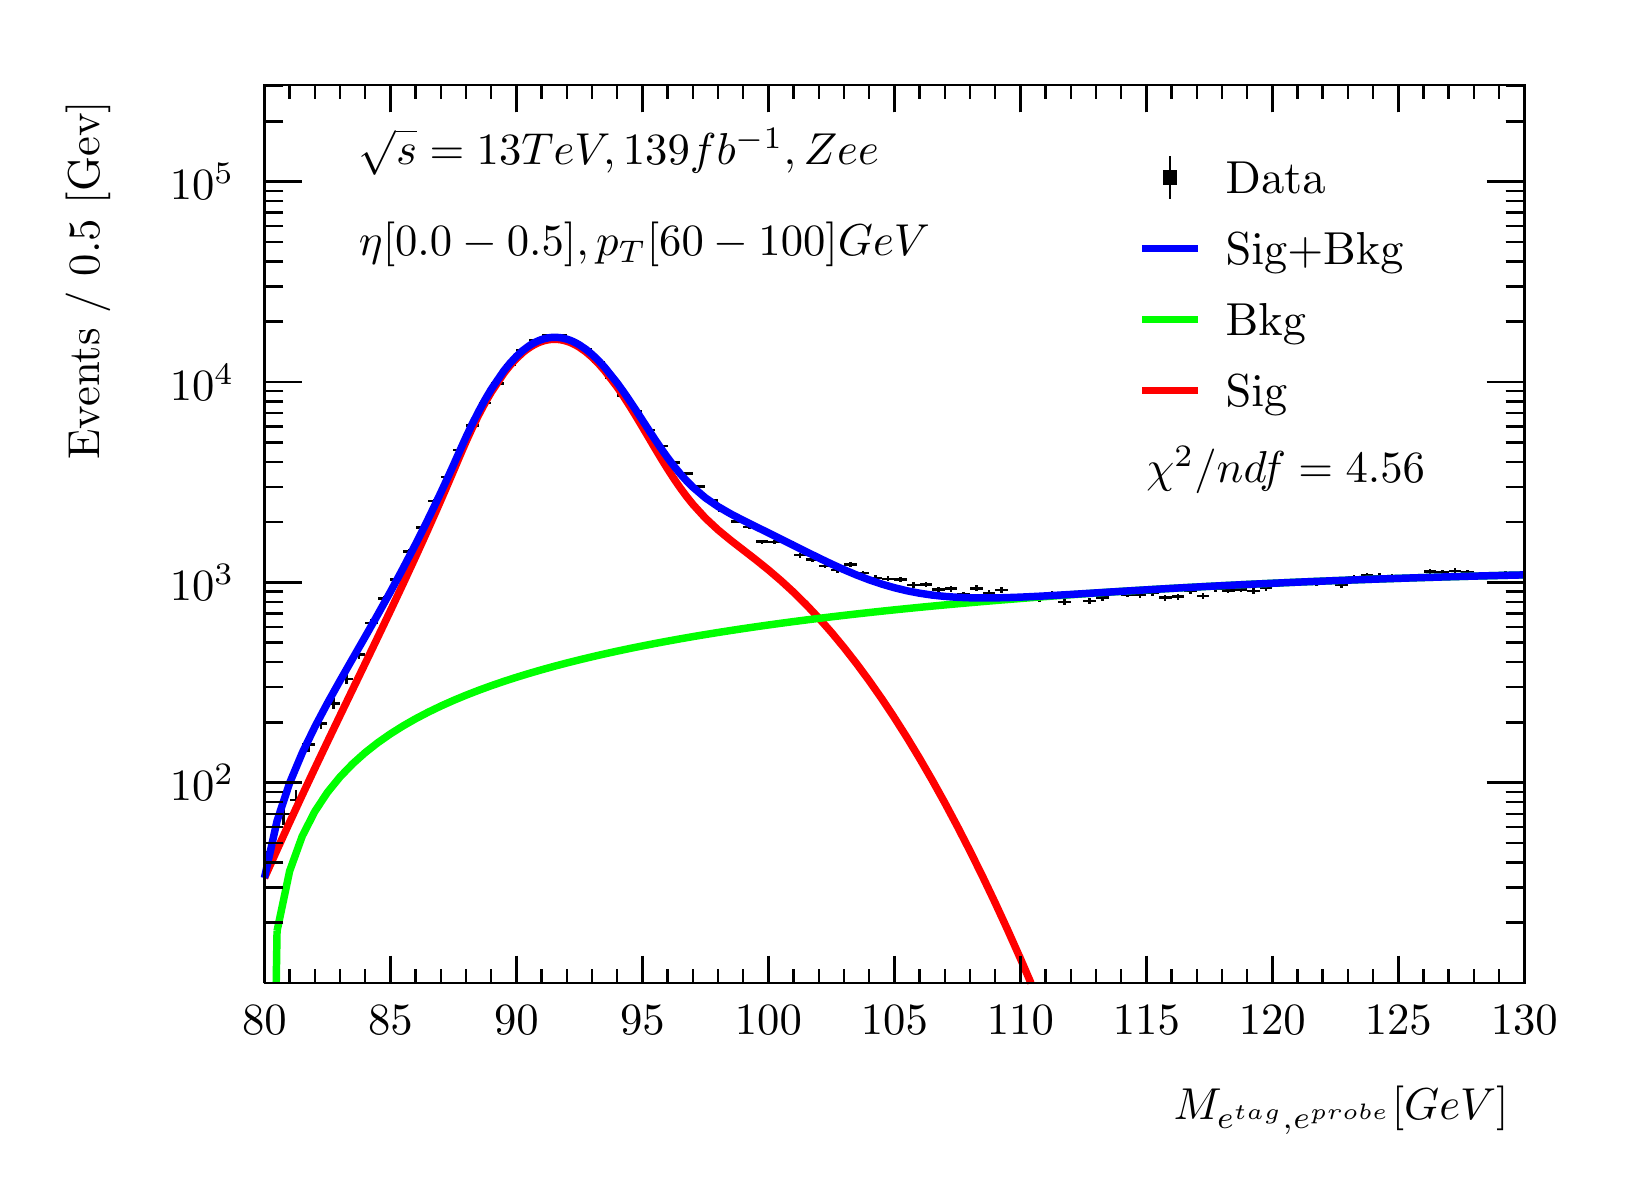
\begin{tikzpicture}
\pgfdeclareplotmark{cross} {
\pgfpathmoveto{\pgfpoint{-0.3\pgfplotmarksize}{\pgfplotmarksize}}
\pgfpathlineto{\pgfpoint{+0.3\pgfplotmarksize}{\pgfplotmarksize}}
\pgfpathlineto{\pgfpoint{+0.3\pgfplotmarksize}{0.3\pgfplotmarksize}}
\pgfpathlineto{\pgfpoint{+1\pgfplotmarksize}{0.3\pgfplotmarksize}}
\pgfpathlineto{\pgfpoint{+1\pgfplotmarksize}{-0.3\pgfplotmarksize}}
\pgfpathlineto{\pgfpoint{+0.3\pgfplotmarksize}{-0.3\pgfplotmarksize}}
\pgfpathlineto{\pgfpoint{+0.3\pgfplotmarksize}{-1.\pgfplotmarksize}}
\pgfpathlineto{\pgfpoint{-0.3\pgfplotmarksize}{-1.\pgfplotmarksize}}
\pgfpathlineto{\pgfpoint{-0.3\pgfplotmarksize}{-0.3\pgfplotmarksize}}
\pgfpathlineto{\pgfpoint{-1.\pgfplotmarksize}{-0.3\pgfplotmarksize}}
\pgfpathlineto{\pgfpoint{-1.\pgfplotmarksize}{0.3\pgfplotmarksize}}
\pgfpathlineto{\pgfpoint{-0.3\pgfplotmarksize}{0.3\pgfplotmarksize}}
\pgfpathclose
\pgfusepathqstroke
}
\pgfdeclareplotmark{cross*} {
\pgfpathmoveto{\pgfpoint{-0.3\pgfplotmarksize}{\pgfplotmarksize}}
\pgfpathlineto{\pgfpoint{+0.3\pgfplotmarksize}{\pgfplotmarksize}}
\pgfpathlineto{\pgfpoint{+0.3\pgfplotmarksize}{0.3\pgfplotmarksize}}
\pgfpathlineto{\pgfpoint{+1\pgfplotmarksize}{0.3\pgfplotmarksize}}
\pgfpathlineto{\pgfpoint{+1\pgfplotmarksize}{-0.3\pgfplotmarksize}}
\pgfpathlineto{\pgfpoint{+0.3\pgfplotmarksize}{-0.3\pgfplotmarksize}}
\pgfpathlineto{\pgfpoint{+0.3\pgfplotmarksize}{-1.\pgfplotmarksize}}
\pgfpathlineto{\pgfpoint{-0.3\pgfplotmarksize}{-1.\pgfplotmarksize}}
\pgfpathlineto{\pgfpoint{-0.3\pgfplotmarksize}{-0.3\pgfplotmarksize}}
\pgfpathlineto{\pgfpoint{-1.\pgfplotmarksize}{-0.3\pgfplotmarksize}}
\pgfpathlineto{\pgfpoint{-1.\pgfplotmarksize}{0.3\pgfplotmarksize}}
\pgfpathlineto{\pgfpoint{-0.3\pgfplotmarksize}{0.3\pgfplotmarksize}}
\pgfpathclose
\pgfusepathqfillstroke
}
\pgfdeclareplotmark{newstar} {
\pgfpathmoveto{\pgfqpoint{0pt}{\pgfplotmarksize}}
\pgfpathlineto{\pgfqpointpolar{44}{0.5\pgfplotmarksize}}
\pgfpathlineto{\pgfqpointpolar{18}{\pgfplotmarksize}}
\pgfpathlineto{\pgfqpointpolar{-20}{0.5\pgfplotmarksize}}
\pgfpathlineto{\pgfqpointpolar{-54}{\pgfplotmarksize}}
\pgfpathlineto{\pgfqpointpolar{-90}{0.5\pgfplotmarksize}}
\pgfpathlineto{\pgfqpointpolar{234}{\pgfplotmarksize}}
\pgfpathlineto{\pgfqpointpolar{198}{0.5\pgfplotmarksize}}
\pgfpathlineto{\pgfqpointpolar{162}{\pgfplotmarksize}}
\pgfpathlineto{\pgfqpointpolar{134}{0.5\pgfplotmarksize}}
\pgfpathclose
\pgfusepathqstroke
}
\pgfdeclareplotmark{newstar*} {
\pgfpathmoveto{\pgfqpoint{0pt}{\pgfplotmarksize}}
\pgfpathlineto{\pgfqpointpolar{44}{0.5\pgfplotmarksize}}
\pgfpathlineto{\pgfqpointpolar{18}{\pgfplotmarksize}}
\pgfpathlineto{\pgfqpointpolar{-20}{0.5\pgfplotmarksize}}
\pgfpathlineto{\pgfqpointpolar{-54}{\pgfplotmarksize}}
\pgfpathlineto{\pgfqpointpolar{-90}{0.5\pgfplotmarksize}}
\pgfpathlineto{\pgfqpointpolar{234}{\pgfplotmarksize}}
\pgfpathlineto{\pgfqpointpolar{198}{0.5\pgfplotmarksize}}
\pgfpathlineto{\pgfqpointpolar{162}{\pgfplotmarksize}}
\pgfpathlineto{\pgfqpointpolar{134}{0.5\pgfplotmarksize}}
\pgfpathclose
\pgfusepathqfillstroke
}
\definecolor{c}{rgb}{1,1,1};
\draw [color=c, fill=c] (0,0) rectangle (20,14.4361);
\draw [color=c, fill=c] (3,2.30977) rectangle (19,13.7143);
\definecolor{c}{rgb}{0,0,0};
\draw [c,line width=0.9] (3,2.30977) -- (3,13.7143) -- (19,13.7143) -- (19,2.30977) -- (3,2.30977);
\definecolor{c}{rgb}{1,1,1};
\draw [color=c, fill=c] (3,2.30977) rectangle (19,13.7143);
\definecolor{c}{rgb}{0,0,0};
\draw [c,line width=0.9] (3,2.30977) -- (3,13.7143) -- (19,13.7143) -- (19,2.30977) -- (3,2.30977);
\draw [c,line width=0.9] (3,2.30977) -- (19,2.30977);
\draw [c,line width=0.9] (3,2.65624) -- (3,2.30977);
\draw [c,line width=0.9] (3.32,2.48301) -- (3.32,2.30977);
\draw [c,line width=0.9] (3.64,2.48301) -- (3.64,2.30977);
\draw [c,line width=0.9] (3.96,2.48301) -- (3.96,2.30977);
\draw [c,line width=0.9] (4.28,2.48301) -- (4.28,2.30977);
\draw [c,line width=0.9] (4.6,2.65624) -- (4.6,2.30977);
\draw [c,line width=0.9] (4.92,2.48301) -- (4.92,2.30977);
\draw [c,line width=0.9] (5.24,2.48301) -- (5.24,2.30977);
\draw [c,line width=0.9] (5.56,2.48301) -- (5.56,2.30977);
\draw [c,line width=0.9] (5.88,2.48301) -- (5.88,2.30977);
\draw [c,line width=0.9] (6.2,2.65624) -- (6.2,2.30977);
\draw [c,line width=0.9] (6.52,2.48301) -- (6.52,2.30977);
\draw [c,line width=0.9] (6.84,2.48301) -- (6.84,2.30977);
\draw [c,line width=0.9] (7.16,2.48301) -- (7.16,2.30977);
\draw [c,line width=0.9] (7.48,2.48301) -- (7.48,2.30977);
\draw [c,line width=0.9] (7.8,2.65624) -- (7.8,2.30977);
\draw [c,line width=0.9] (8.12,2.48301) -- (8.12,2.30977);
\draw [c,line width=0.9] (8.44,2.48301) -- (8.44,2.30977);
\draw [c,line width=0.9] (8.76,2.48301) -- (8.76,2.30977);
\draw [c,line width=0.9] (9.08,2.48301) -- (9.08,2.30977);
\draw [c,line width=0.9] (9.4,2.65624) -- (9.4,2.30977);
\draw [c,line width=0.9] (9.72,2.48301) -- (9.72,2.30977);
\draw [c,line width=0.9] (10.04,2.48301) -- (10.04,2.30977);
\draw [c,line width=0.9] (10.36,2.48301) -- (10.36,2.30977);
\draw [c,line width=0.9] (10.68,2.48301) -- (10.68,2.30977);
\draw [c,line width=0.9] (11,2.65624) -- (11,2.30977);
\draw [c,line width=0.9] (11.32,2.48301) -- (11.32,2.30977);
\draw [c,line width=0.9] (11.64,2.48301) -- (11.64,2.30977);
\draw [c,line width=0.9] (11.96,2.48301) -- (11.96,2.30977);
\draw [c,line width=0.9] (12.28,2.48301) -- (12.28,2.30977);
\draw [c,line width=0.9] (12.6,2.65624) -- (12.6,2.30977);
\draw [c,line width=0.9] (12.92,2.48301) -- (12.92,2.30977);
\draw [c,line width=0.9] (13.24,2.48301) -- (13.24,2.30977);
\draw [c,line width=0.9] (13.56,2.48301) -- (13.56,2.30977);
\draw [c,line width=0.9] (13.88,2.48301) -- (13.88,2.30977);
\draw [c,line width=0.9] (14.2,2.65624) -- (14.2,2.30977);
\draw [c,line width=0.9] (14.52,2.48301) -- (14.52,2.30977);
\draw [c,line width=0.9] (14.84,2.48301) -- (14.84,2.30977);
\draw [c,line width=0.9] (15.16,2.48301) -- (15.16,2.30977);
\draw [c,line width=0.9] (15.48,2.48301) -- (15.48,2.30977);
\draw [c,line width=0.9] (15.8,2.65624) -- (15.8,2.30977);
\draw [c,line width=0.9] (16.12,2.48301) -- (16.12,2.30977);
\draw [c,line width=0.9] (16.44,2.48301) -- (16.44,2.30977);
\draw [c,line width=0.9] (16.76,2.48301) -- (16.76,2.30977);
\draw [c,line width=0.9] (17.08,2.48301) -- (17.08,2.30977);
\draw [c,line width=0.9] (17.4,2.65624) -- (17.4,2.30977);
\draw [c,line width=0.9] (17.72,2.48301) -- (17.72,2.30977);
\draw [c,line width=0.9] (18.04,2.48301) -- (18.04,2.30977);
\draw [c,line width=0.9] (18.36,2.48301) -- (18.36,2.30977);
\draw [c,line width=0.9] (18.68,2.48301) -- (18.68,2.30977);
\draw [c,line width=0.9] (19,2.65624) -- (19,2.30977);
\draw [anchor=base] (3,1.66015) node[scale=1.61424, color=c, rotate=0]{80};
\draw [anchor=base] (4.6,1.66015) node[scale=1.61424, color=c, rotate=0]{85};
\draw [anchor=base] (6.2,1.66015) node[scale=1.61424, color=c, rotate=0]{90};
\draw [anchor=base] (7.8,1.66015) node[scale=1.61424, color=c, rotate=0]{95};
\draw [anchor=base] (9.4,1.66015) node[scale=1.61424, color=c, rotate=0]{100};
\draw [anchor=base] (11,1.66015) node[scale=1.61424, color=c, rotate=0]{105};
\draw [anchor=base] (12.6,1.66015) node[scale=1.61424, color=c, rotate=0]{110};
\draw [anchor=base] (14.2,1.66015) node[scale=1.61424, color=c, rotate=0]{115};
\draw [anchor=base] (15.8,1.66015) node[scale=1.61424, color=c, rotate=0]{120};
\draw [anchor=base] (17.4,1.66015) node[scale=1.61424, color=c, rotate=0]{125};
\draw [anchor=base] (19,1.66015) node[scale=1.61424, color=c, rotate=0]{130};
\draw [anchor= east] (19,0.692932) node[scale=1.61424, color=c, rotate=0]{$M_{e^{tag}, e^{probe}}  [GeV]$};
\draw [c,line width=0.9] (3,13.7143) -- (19,13.7143);
\draw [c,line width=0.9] (3,13.3678) -- (3,13.7143);
\draw [c,line width=0.9] (3.32,13.5411) -- (3.32,13.7143);
\draw [c,line width=0.9] (3.64,13.5411) -- (3.64,13.7143);
\draw [c,line width=0.9] (3.96,13.5411) -- (3.96,13.7143);
\draw [c,line width=0.9] (4.28,13.5411) -- (4.28,13.7143);
\draw [c,line width=0.9] (4.6,13.3678) -- (4.6,13.7143);
\draw [c,line width=0.9] (4.92,13.5411) -- (4.92,13.7143);
\draw [c,line width=0.9] (5.24,13.5411) -- (5.24,13.7143);
\draw [c,line width=0.9] (5.56,13.5411) -- (5.56,13.7143);
\draw [c,line width=0.9] (5.88,13.5411) -- (5.88,13.7143);
\draw [c,line width=0.9] (6.2,13.3678) -- (6.2,13.7143);
\draw [c,line width=0.9] (6.52,13.5411) -- (6.52,13.7143);
\draw [c,line width=0.9] (6.84,13.5411) -- (6.84,13.7143);
\draw [c,line width=0.9] (7.16,13.5411) -- (7.16,13.7143);
\draw [c,line width=0.9] (7.48,13.5411) -- (7.48,13.7143);
\draw [c,line width=0.9] (7.8,13.3678) -- (7.8,13.7143);
\draw [c,line width=0.9] (8.12,13.5411) -- (8.12,13.7143);
\draw [c,line width=0.9] (8.44,13.5411) -- (8.44,13.7143);
\draw [c,line width=0.9] (8.76,13.5411) -- (8.76,13.7143);
\draw [c,line width=0.9] (9.08,13.5411) -- (9.08,13.7143);
\draw [c,line width=0.9] (9.4,13.3678) -- (9.4,13.7143);
\draw [c,line width=0.9] (9.72,13.5411) -- (9.72,13.7143);
\draw [c,line width=0.9] (10.04,13.5411) -- (10.04,13.7143);
\draw [c,line width=0.9] (10.36,13.5411) -- (10.36,13.7143);
\draw [c,line width=0.9] (10.68,13.5411) -- (10.68,13.7143);
\draw [c,line width=0.9] (11,13.3678) -- (11,13.7143);
\draw [c,line width=0.9] (11.32,13.5411) -- (11.32,13.7143);
\draw [c,line width=0.9] (11.64,13.5411) -- (11.64,13.7143);
\draw [c,line width=0.9] (11.96,13.5411) -- (11.96,13.7143);
\draw [c,line width=0.9] (12.28,13.5411) -- (12.28,13.7143);
\draw [c,line width=0.9] (12.6,13.3678) -- (12.6,13.7143);
\draw [c,line width=0.9] (12.92,13.5411) -- (12.92,13.7143);
\draw [c,line width=0.9] (13.24,13.5411) -- (13.24,13.7143);
\draw [c,line width=0.9] (13.56,13.5411) -- (13.56,13.7143);
\draw [c,line width=0.9] (13.88,13.5411) -- (13.88,13.7143);
\draw [c,line width=0.9] (14.2,13.3678) -- (14.2,13.7143);
\draw [c,line width=0.9] (14.52,13.5411) -- (14.52,13.7143);
\draw [c,line width=0.9] (14.84,13.5411) -- (14.84,13.7143);
\draw [c,line width=0.9] (15.16,13.5411) -- (15.16,13.7143);
\draw [c,line width=0.9] (15.48,13.5411) -- (15.48,13.7143);
\draw [c,line width=0.9] (15.8,13.3678) -- (15.8,13.7143);
\draw [c,line width=0.9] (16.12,13.5411) -- (16.12,13.7143);
\draw [c,line width=0.9] (16.44,13.5411) -- (16.44,13.7143);
\draw [c,line width=0.9] (16.76,13.5411) -- (16.76,13.7143);
\draw [c,line width=0.9] (17.08,13.5411) -- (17.08,13.7143);
\draw [c,line width=0.9] (17.4,13.3678) -- (17.4,13.7143);
\draw [c,line width=0.9] (17.72,13.5411) -- (17.72,13.7143);
\draw [c,line width=0.9] (18.04,13.5411) -- (18.04,13.7143);
\draw [c,line width=0.9] (18.36,13.5411) -- (18.36,13.7143);
\draw [c,line width=0.9] (18.68,13.5411) -- (18.68,13.7143);
\draw [c,line width=0.9] (19,13.3678) -- (19,13.7143);
\draw [c,line width=0.9] (3,2.30977) -- (3,13.7143);
\draw [c,line width=0.9] (3.237,3.07568) -- (3,3.07568);
\draw [c,line width=0.9] (3.237,3.5237) -- (3,3.5237);
\draw [c,line width=0.9] (3.237,3.84158) -- (3,3.84158);
\draw [c,line width=0.9] (3.237,4.08815) -- (3,4.08815);
\draw [c,line width=0.9] (3.237,4.2896) -- (3,4.2896);
\draw [c,line width=0.9] (3.237,4.45994) -- (3,4.45994);
\draw [c,line width=0.9] (3.237,4.60748) -- (3,4.60748);
\draw [c,line width=0.9] (3.237,4.73763) -- (3,4.73763);
\draw [c,line width=0.9] (3.474,4.85405) -- (3,4.85405);
\draw [anchor= east] (2.82,4.85405) node[scale=1.61424, color=c, rotate=0]{$10^{2}$};
\draw [c,line width=0.9] (3.237,5.61995) -- (3,5.61995);
\draw [c,line width=0.9] (3.237,6.06798) -- (3,6.06798);
\draw [c,line width=0.9] (3.237,6.38586) -- (3,6.38586);
\draw [c,line width=0.9] (3.237,6.63242) -- (3,6.63242);
\draw [c,line width=0.9] (3.237,6.83388) -- (3,6.83388);
\draw [c,line width=0.9] (3.237,7.00421) -- (3,7.00421);
\draw [c,line width=0.9] (3.237,7.15176) -- (3,7.15176);
\draw [c,line width=0.9] (3.237,7.28191) -- (3,7.28191);
\draw [c,line width=0.9] (3.474,7.39833) -- (3,7.39833);
\draw [anchor= east] (2.82,7.39833) node[scale=1.61424, color=c, rotate=0]{$10^{3}$};
\draw [c,line width=0.9] (3.237,8.16423) -- (3,8.16423);
\draw [c,line width=0.9] (3.237,8.61226) -- (3,8.61226);
\draw [c,line width=0.9] (3.237,8.93013) -- (3,8.93013);
\draw [c,line width=0.9] (3.237,9.1767) -- (3,9.1767);
\draw [c,line width=0.9] (3.237,9.37816) -- (3,9.37816);
\draw [c,line width=0.9] (3.237,9.54849) -- (3,9.54849);
\draw [c,line width=0.9] (3.237,9.69604) -- (3,9.69604);
\draw [c,line width=0.9] (3.237,9.82618) -- (3,9.82618);
\draw [c,line width=0.9] (3.474,9.9426) -- (3,9.9426);
\draw [anchor= east] (2.82,9.9426) node[scale=1.61424, color=c, rotate=0]{$10^{4}$};
\draw [c,line width=0.9] (3.237,10.7085) -- (3,10.7085);
\draw [c,line width=0.9] (3.237,11.1565) -- (3,11.1565);
\draw [c,line width=0.9] (3.237,11.4744) -- (3,11.4744);
\draw [c,line width=0.9] (3.237,11.721) -- (3,11.721);
\draw [c,line width=0.9] (3.237,11.9224) -- (3,11.9224);
\draw [c,line width=0.9] (3.237,12.0928) -- (3,12.0928);
\draw [c,line width=0.9] (3.237,12.2403) -- (3,12.2403);
\draw [c,line width=0.9] (3.237,12.3705) -- (3,12.3705);
\draw [c,line width=0.9] (3.474,12.4869) -- (3,12.4869);
\draw [anchor= east] (2.82,12.4869) node[scale=1.61424, color=c, rotate=0]{$10^{5}$};
\draw [c,line width=0.9] (3.237,13.2528) -- (3,13.2528);
\draw [c,line width=0.9] (3.237,13.7008) -- (3,13.7008);
\draw [anchor= east] (0.76,13.7143) node[scale=1.61424, color=c, rotate=90]{Events / 0.5 [Gev]};
\draw [c,line width=0.9] (19,2.30977) -- (19,13.7143);
\draw [c,line width=0.9] (18.763,3.07568) -- (19,3.07568);
\draw [c,line width=0.9] (18.763,3.5237) -- (19,3.5237);
\draw [c,line width=0.9] (18.763,3.84158) -- (19,3.84158);
\draw [c,line width=0.9] (18.763,4.08815) -- (19,4.08815);
\draw [c,line width=0.9] (18.763,4.2896) -- (19,4.2896);
\draw [c,line width=0.9] (18.763,4.45994) -- (19,4.45994);
\draw [c,line width=0.9] (18.763,4.60748) -- (19,4.60748);
\draw [c,line width=0.9] (18.763,4.73763) -- (19,4.73763);
\draw [c,line width=0.9] (18.526,4.85405) -- (19,4.85405);
\draw [c,line width=0.9] (18.763,5.61995) -- (19,5.61995);
\draw [c,line width=0.9] (18.763,6.06798) -- (19,6.06798);
\draw [c,line width=0.9] (18.763,6.38586) -- (19,6.38586);
\draw [c,line width=0.9] (18.763,6.63242) -- (19,6.63242);
\draw [c,line width=0.9] (18.763,6.83388) -- (19,6.83388);
\draw [c,line width=0.9] (18.763,7.00421) -- (19,7.00421);
\draw [c,line width=0.9] (18.763,7.15176) -- (19,7.15176);
\draw [c,line width=0.9] (18.763,7.28191) -- (19,7.28191);
\draw [c,line width=0.9] (18.526,7.39833) -- (19,7.39833);
\draw [c,line width=0.9] (18.763,8.16423) -- (19,8.16423);
\draw [c,line width=0.9] (18.763,8.61226) -- (19,8.61226);
\draw [c,line width=0.9] (18.763,8.93013) -- (19,8.93013);
\draw [c,line width=0.9] (18.763,9.1767) -- (19,9.1767);
\draw [c,line width=0.9] (18.763,9.37816) -- (19,9.37816);
\draw [c,line width=0.9] (18.763,9.54849) -- (19,9.54849);
\draw [c,line width=0.9] (18.763,9.69604) -- (19,9.69604);
\draw [c,line width=0.9] (18.763,9.82618) -- (19,9.82618);
\draw [c,line width=0.9] (18.526,9.9426) -- (19,9.9426);
\draw [c,line width=0.9] (18.763,10.7085) -- (19,10.7085);
\draw [c,line width=0.9] (18.763,11.1565) -- (19,11.1565);
\draw [c,line width=0.9] (18.763,11.4744) -- (19,11.4744);
\draw [c,line width=0.9] (18.763,11.721) -- (19,11.721);
\draw [c,line width=0.9] (18.763,11.9224) -- (19,11.9224);
\draw [c,line width=0.9] (18.763,12.0928) -- (19,12.0928);
\draw [c,line width=0.9] (18.763,12.2403) -- (19,12.2403);
\draw [c,line width=0.9] (18.763,12.3705) -- (19,12.3705);
\draw [c,line width=0.9] (18.526,12.4869) -- (19,12.4869);
\draw [c,line width=0.9] (18.763,13.2528) -- (19,13.2528);
\draw [c,line width=0.9] (18.763,13.7008) -- (19,13.7008);
\draw [c,line width=0.9] (3.08,3.97173) -- (3,3.97173);
\draw [c,line width=0.9] (3,3.97173) -- (3,3.97173);
\draw [c,line width=0.9] (3.08,3.97173) -- (3.16,3.97173);
\draw [c,line width=0.9] (3.16,3.97173) -- (3.16,3.97173);
\draw [c,line width=0.9] (3.08,3.97173) -- (3.08,4.14747);
\draw [c,line width=0.9] (3.08,4.14747) -- (3.08,4.14747);
\draw [c,line width=0.9] (3.08,3.97173) -- (3.08,3.79408);
\draw [c,line width=0.9] (3.08,3.79408) -- (3.08,3.79408);
\draw [c,line width=0.9] (3.24,4.45994) -- (3.16,4.45994);
\draw [c,line width=0.9] (3.16,4.45994) -- (3.16,4.45994);
\draw [c,line width=0.9] (3.24,4.45994) -- (3.32,4.45994);
\draw [c,line width=0.9] (3.32,4.45994) -- (3.32,4.45994);
\draw [c,line width=0.9] (3.24,4.45994) -- (3.24,4.59926);
\draw [c,line width=0.9] (3.24,4.59926) -- (3.24,4.59926);
\draw [c,line width=0.9] (3.24,4.45994) -- (3.24,4.31964);
\draw [c,line width=0.9] (3.24,4.31964) -- (3.24,4.31964);
\draw [c,line width=0.9] (3.4,4.63477) -- (3.32,4.63477);
\draw [c,line width=0.9] (3.32,4.63477) -- (3.32,4.63477);
\draw [c,line width=0.9] (3.4,4.63477) -- (3.48,4.63477);
\draw [c,line width=0.9] (3.48,4.63477) -- (3.48,4.63477);
\draw [c,line width=0.9] (3.4,4.63477) -- (3.4,4.76302);
\draw [c,line width=0.9] (3.4,4.76302) -- (3.4,4.76302);
\draw [c,line width=0.9] (3.4,4.63477) -- (3.4,4.50575);
\draw [c,line width=0.9] (3.4,4.50575) -- (3.4,4.50575);
\draw [c,line width=0.9] (3.56,5.33831) -- (3.48,5.33831);
\draw [c,line width=0.9] (3.48,5.33831) -- (3.48,5.33831);
\draw [c,line width=0.9] (3.56,5.33831) -- (3.64,5.33831);
\draw [c,line width=0.9] (3.64,5.33831) -- (3.64,5.33831);
\draw [c,line width=0.9] (3.56,5.33831) -- (3.56,5.42704);
\draw [c,line width=0.9] (3.56,5.42704) -- (3.56,5.42704);
\draw [c,line width=0.9] (3.56,5.33831) -- (3.56,5.24958);
\draw [c,line width=0.9] (3.56,5.24958) -- (3.56,5.24958);
\draw [c,line width=0.9] (3.72,5.60885) -- (3.64,5.60885);
\draw [c,line width=0.9] (3.64,5.60885) -- (3.64,5.60885);
\draw [c,line width=0.9] (3.72,5.60885) -- (3.8,5.60885);
\draw [c,line width=0.9] (3.8,5.60885) -- (3.8,5.60885);
\draw [c,line width=0.9] (3.72,5.60885) -- (3.72,5.68736);
\draw [c,line width=0.9] (3.72,5.68736) -- (3.72,5.68736);
\draw [c,line width=0.9] (3.72,5.60885) -- (3.72,5.53034);
\draw [c,line width=0.9] (3.72,5.53034) -- (3.72,5.53034);
\draw [c,line width=0.9] (3.88,5.85765) -- (3.8,5.85765);
\draw [c,line width=0.9] (3.8,5.85765) -- (3.8,5.85765);
\draw [c,line width=0.9] (3.88,5.85765) -- (3.96,5.85765);
\draw [c,line width=0.9] (3.96,5.85765) -- (3.96,5.85765);
\draw [c,line width=0.9] (3.88,5.85765) -- (3.88,5.9278);
\draw [c,line width=0.9] (3.88,5.9278) -- (3.88,5.9278);
\draw [c,line width=0.9] (3.88,5.85765) -- (3.88,5.78749);
\draw [c,line width=0.9] (3.88,5.78749) -- (3.88,5.78749);
\draw [c,line width=0.9] (4.04,6.16994) -- (3.96,6.16994);
\draw [c,line width=0.9] (3.96,6.16994) -- (3.96,6.16994);
\draw [c,line width=0.9] (4.04,6.16994) -- (4.12,6.16994);
\draw [c,line width=0.9] (4.12,6.16994) -- (4.12,6.16994);
\draw [c,line width=0.9] (4.04,6.16994) -- (4.04,6.23085);
\draw [c,line width=0.9] (4.04,6.23085) -- (4.04,6.23085);
\draw [c,line width=0.9] (4.04,6.16994) -- (4.04,6.10903);
\draw [c,line width=0.9] (4.04,6.10903) -- (4.04,6.10903);
\draw [c,line width=0.9] (4.2,6.48361) -- (4.12,6.48361);
\draw [c,line width=0.9] (4.12,6.48361) -- (4.12,6.48361);
\draw [c,line width=0.9] (4.2,6.48361) -- (4.28,6.48361);
\draw [c,line width=0.9] (4.28,6.48361) -- (4.28,6.48361);
\draw [c,line width=0.9] (4.2,6.48361) -- (4.2,6.53647);
\draw [c,line width=0.9] (4.2,6.53647) -- (4.2,6.53647);
\draw [c,line width=0.9] (4.2,6.48361) -- (4.2,6.43076);
\draw [c,line width=0.9] (4.2,6.43076) -- (4.2,6.43076);
\draw [c,line width=0.9] (4.36,6.88428) -- (4.28,6.88428);
\draw [c,line width=0.9] (4.28,6.88428) -- (4.28,6.88428);
\draw [c,line width=0.9] (4.36,6.88428) -- (4.44,6.88428);
\draw [c,line width=0.9] (4.44,6.88428) -- (4.44,6.88428);
\draw [c,line width=0.9] (4.36,6.88428) -- (4.36,6.92837);
\draw [c,line width=0.9] (4.36,6.92837) -- (4.36,6.92837);
\draw [c,line width=0.9] (4.36,6.88428) -- (4.36,6.84019);
\draw [c,line width=0.9] (4.36,6.84019) -- (4.36,6.84019);
\draw [c,line width=0.9] (4.52,7.19244) -- (4.44,7.19244);
\draw [c,line width=0.9] (4.44,7.19244) -- (4.44,7.19244);
\draw [c,line width=0.9] (4.52,7.19244) -- (4.6,7.19244);
\draw [c,line width=0.9] (4.6,7.19244) -- (4.6,7.19244);
\draw [c,line width=0.9] (4.52,7.19244) -- (4.52,7.23079);
\draw [c,line width=0.9] (4.52,7.23079) -- (4.52,7.23079);
\draw [c,line width=0.9] (4.52,7.19244) -- (4.52,7.15409);
\draw [c,line width=0.9] (4.52,7.15409) -- (4.52,7.15409);
\draw [c,line width=0.9] (4.68,7.4342) -- (4.6,7.4342);
\draw [c,line width=0.9] (4.6,7.4342) -- (4.6,7.4342);
\draw [c,line width=0.9] (4.68,7.4342) -- (4.76,7.4342);
\draw [c,line width=0.9] (4.76,7.4342) -- (4.76,7.4342);
\draw [c,line width=0.9] (4.68,7.4342) -- (4.68,7.46858);
\draw [c,line width=0.9] (4.68,7.46858) -- (4.68,7.46858);
\draw [c,line width=0.9] (4.68,7.4342) -- (4.68,7.39983);
\draw [c,line width=0.9] (4.68,7.39983) -- (4.68,7.39983);
\draw [c,line width=0.9] (4.84,7.7889) -- (4.76,7.7889);
\draw [c,line width=0.9] (4.76,7.7889) -- (4.76,7.7889);
\draw [c,line width=0.9] (4.84,7.7889) -- (4.92,7.7889);
\draw [c,line width=0.9] (4.92,7.7889) -- (4.92,7.7889);
\draw [c,line width=0.9] (4.84,7.7889) -- (4.84,7.81818);
\draw [c,line width=0.9] (4.84,7.81818) -- (4.84,7.81818);
\draw [c,line width=0.9] (4.84,7.7889) -- (4.84,7.75962);
\draw [c,line width=0.9] (4.84,7.75962) -- (4.84,7.75962);
\draw [c,line width=0.9] (5,8.09645) -- (4.92,8.09645);
\draw [c,line width=0.9] (4.92,8.09645) -- (4.92,8.09645);
\draw [c,line width=0.9] (5,8.09645) -- (5.08,8.09645);
\draw [c,line width=0.9] (5.08,8.09645) -- (5.08,8.09645);
\draw [c,line width=0.9] (5,8.09645) -- (5,8.12193);
\draw [c,line width=0.9] (5,8.12193) -- (5,8.12193);
\draw [c,line width=0.9] (5,8.09645) -- (5,8.07097);
\draw [c,line width=0.9] (5,8.07097) -- (5,8.07097);
\draw [c,line width=0.9] (5.16,8.43008) -- (5.08,8.43008);
\draw [c,line width=0.9] (5.08,8.43008) -- (5.08,8.43008);
\draw [c,line width=0.9] (5.16,8.43008) -- (5.24,8.43008);
\draw [c,line width=0.9] (5.24,8.43008) -- (5.24,8.43008);
\draw [c,line width=0.9] (5.16,8.43008) -- (5.16,8.45198);
\draw [c,line width=0.9] (5.16,8.45198) -- (5.16,8.45198);
\draw [c,line width=0.9] (5.16,8.43008) -- (5.16,8.40817);
\draw [c,line width=0.9] (5.16,8.40817) -- (5.16,8.40817);
\draw [c,line width=0.9] (5.32,8.73386) -- (5.24,8.73386);
\draw [c,line width=0.9] (5.24,8.73386) -- (5.24,8.73386);
\draw [c,line width=0.9] (5.32,8.73386) -- (5.4,8.73386);
\draw [c,line width=0.9] (5.4,8.73386) -- (5.4,8.73386);
\draw [c,line width=0.9] (5.32,8.73386) -- (5.32,8.75295);
\draw [c,line width=0.9] (5.32,8.75295) -- (5.32,8.75295);
\draw [c,line width=0.9] (5.32,8.73386) -- (5.32,8.71476);
\draw [c,line width=0.9] (5.32,8.71476) -- (5.32,8.71476);
\draw [c,line width=0.9] (5.48,9.07903) -- (5.4,9.07903);
\draw [c,line width=0.9] (5.4,9.07903) -- (5.4,9.07903);
\draw [c,line width=0.9] (5.48,9.07903) -- (5.56,9.07903);
\draw [c,line width=0.9] (5.56,9.07903) -- (5.56,9.07903);
\draw [c,line width=0.9] (5.48,9.07903) -- (5.48,9.09536);
\draw [c,line width=0.9] (5.48,9.09536) -- (5.48,9.09536);
\draw [c,line width=0.9] (5.48,9.07903) -- (5.48,9.0627);
\draw [c,line width=0.9] (5.48,9.0627) -- (5.48,9.0627);
\draw [c,line width=0.9] (5.64,9.39261) -- (5.56,9.39261);
\draw [c,line width=0.9] (5.56,9.39261) -- (5.56,9.39261);
\draw [c,line width=0.9] (5.64,9.39261) -- (5.72,9.39261);
\draw [c,line width=0.9] (5.72,9.39261) -- (5.72,9.39261);
\draw [c,line width=0.9] (5.64,9.39261) -- (5.64,9.40679);
\draw [c,line width=0.9] (5.64,9.40679) -- (5.64,9.40679);
\draw [c,line width=0.9] (5.64,9.39261) -- (5.64,9.37844);
\draw [c,line width=0.9] (5.64,9.37844) -- (5.64,9.37844);
\draw [c,line width=0.9] (5.8,9.67681) -- (5.72,9.67681);
\draw [c,line width=0.9] (5.72,9.67681) -- (5.72,9.67681);
\draw [c,line width=0.9] (5.8,9.67681) -- (5.88,9.67681);
\draw [c,line width=0.9] (5.88,9.67681) -- (5.88,9.67681);
\draw [c,line width=0.9] (5.8,9.67681) -- (5.8,9.68927);
\draw [c,line width=0.9] (5.8,9.68927) -- (5.8,9.68927);
\draw [c,line width=0.9] (5.8,9.67681) -- (5.8,9.66435);
\draw [c,line width=0.9] (5.8,9.66435) -- (5.8,9.66435);
\draw [c,line width=0.9] (5.96,9.9213) -- (5.88,9.9213);
\draw [c,line width=0.9] (5.88,9.9213) -- (5.88,9.9213);
\draw [c,line width=0.9] (5.96,9.9213) -- (6.04,9.9213);
\draw [c,line width=0.9] (6.04,9.9213) -- (6.04,9.9213);
\draw [c,line width=0.9] (5.96,9.9213) -- (5.96,9.93245);
\draw [c,line width=0.9] (5.96,9.93245) -- (5.96,9.93245);
\draw [c,line width=0.9] (5.96,9.9213) -- (5.96,9.91014);
\draw [c,line width=0.9] (5.96,9.91014) -- (5.96,9.91014);
\draw [c,line width=0.9] (6.12,10.1618) -- (6.04,10.1618);
\draw [c,line width=0.9] (6.04,10.1618) -- (6.04,10.1618);
\draw [c,line width=0.9] (6.12,10.1618) -- (6.2,10.1618);
\draw [c,line width=0.9] (6.2,10.1618) -- (6.2,10.1618);
\draw [c,line width=0.9] (6.12,10.1618) -- (6.12,10.1718);
\draw [c,line width=0.9] (6.12,10.1718) -- (6.12,10.1718);
\draw [c,line width=0.9] (6.12,10.1618) -- (6.12,10.1518);
\draw [c,line width=0.9] (6.12,10.1518) -- (6.12,10.1518);
\draw [c,line width=0.9] (6.28,10.3471) -- (6.2,10.3471);
\draw [c,line width=0.9] (6.2,10.3471) -- (6.2,10.3471);
\draw [c,line width=0.9] (6.28,10.3471) -- (6.36,10.3471);
\draw [c,line width=0.9] (6.36,10.3471) -- (6.36,10.3471);
\draw [c,line width=0.9] (6.28,10.3471) -- (6.28,10.3563);
\draw [c,line width=0.9] (6.28,10.3563) -- (6.28,10.3563);
\draw [c,line width=0.9] (6.28,10.3471) -- (6.28,10.3379);
\draw [c,line width=0.9] (6.28,10.3379) -- (6.28,10.3379);
\draw [c,line width=0.9] (6.44,10.4746) -- (6.36,10.4746);
\draw [c,line width=0.9] (6.36,10.4746) -- (6.36,10.4746);
\draw [c,line width=0.9] (6.44,10.4746) -- (6.52,10.4746);
\draw [c,line width=0.9] (6.52,10.4746) -- (6.52,10.4746);
\draw [c,line width=0.9] (6.44,10.4746) -- (6.44,10.4833);
\draw [c,line width=0.9] (6.44,10.4833) -- (6.44,10.4833);
\draw [c,line width=0.9] (6.44,10.4746) -- (6.44,10.466);
\draw [c,line width=0.9] (6.44,10.466) -- (6.44,10.466);
\draw [c,line width=0.9] (6.6,10.5373) -- (6.52,10.5373);
\draw [c,line width=0.9] (6.52,10.5373) -- (6.52,10.5373);
\draw [c,line width=0.9] (6.6,10.5373) -- (6.68,10.5373);
\draw [c,line width=0.9] (6.68,10.5373) -- (6.68,10.5373);
\draw [c,line width=0.9] (6.6,10.5373) -- (6.6,10.5457);
\draw [c,line width=0.9] (6.6,10.5457) -- (6.6,10.5457);
\draw [c,line width=0.9] (6.6,10.5373) -- (6.6,10.5288);
\draw [c,line width=0.9] (6.6,10.5288) -- (6.6,10.5288);
\draw [c,line width=0.9] (6.76,10.5319) -- (6.68,10.5319);
\draw [c,line width=0.9] (6.68,10.5319) -- (6.68,10.5319);
\draw [c,line width=0.9] (6.76,10.5319) -- (6.84,10.5319);
\draw [c,line width=0.9] (6.84,10.5319) -- (6.84,10.5319);
\draw [c,line width=0.9] (6.76,10.5319) -- (6.76,10.5403);
\draw [c,line width=0.9] (6.76,10.5403) -- (6.76,10.5403);
\draw [c,line width=0.9] (6.76,10.5319) -- (6.76,10.5234);
\draw [c,line width=0.9] (6.76,10.5234) -- (6.76,10.5234);
\draw [c,line width=0.9] (6.92,10.4613) -- (6.84,10.4613);
\draw [c,line width=0.9] (6.84,10.4613) -- (6.84,10.4613);
\draw [c,line width=0.9] (6.92,10.4613) -- (7,10.4613);
\draw [c,line width=0.9] (7,10.4613) -- (7,10.4613);
\draw [c,line width=0.9] (6.92,10.4613) -- (6.92,10.4701);
\draw [c,line width=0.9] (6.92,10.4701) -- (6.92,10.4701);
\draw [c,line width=0.9] (6.92,10.4613) -- (6.92,10.4526);
\draw [c,line width=0.9] (6.92,10.4526) -- (6.92,10.4526);
\draw [c,line width=0.9] (7.08,10.3639) -- (7,10.3639);
\draw [c,line width=0.9] (7,10.3639) -- (7,10.3639);
\draw [c,line width=0.9] (7.08,10.3639) -- (7.16,10.3639);
\draw [c,line width=0.9] (7.16,10.3639) -- (7.16,10.3639);
\draw [c,line width=0.9] (7.08,10.3639) -- (7.08,10.373);
\draw [c,line width=0.9] (7.08,10.373) -- (7.08,10.373);
\draw [c,line width=0.9] (7.08,10.3639) -- (7.08,10.3547);
\draw [c,line width=0.9] (7.08,10.3547) -- (7.08,10.3547);
\draw [c,line width=0.9] (7.24,10.1946) -- (7.16,10.1946);
\draw [c,line width=0.9] (7.16,10.1946) -- (7.16,10.1946);
\draw [c,line width=0.9] (7.24,10.1946) -- (7.32,10.1946);
\draw [c,line width=0.9] (7.32,10.1946) -- (7.32,10.1946);
\draw [c,line width=0.9] (7.24,10.1946) -- (7.24,10.2044);
\draw [c,line width=0.9] (7.24,10.2044) -- (7.24,10.2044);
\draw [c,line width=0.9] (7.24,10.1946) -- (7.24,10.1847);
\draw [c,line width=0.9] (7.24,10.1847) -- (7.24,10.1847);
\draw [c,line width=0.9] (7.4,9.9942) -- (7.32,9.9942);
\draw [c,line width=0.9] (7.32,9.9942) -- (7.32,9.9942);
\draw [c,line width=0.9] (7.4,9.9942) -- (7.48,9.9942);
\draw [c,line width=0.9] (7.48,9.9942) -- (7.48,9.9942);
\draw [c,line width=0.9] (7.4,9.9942) -- (7.4,10.005);
\draw [c,line width=0.9] (7.4,10.005) -- (7.4,10.005);
\draw [c,line width=0.9] (7.4,9.9942) -- (7.4,9.9834);
\draw [c,line width=0.9] (7.4,9.9834) -- (7.4,9.9834);
\draw [c,line width=0.9] (7.56,9.77273) -- (7.48,9.77273);
\draw [c,line width=0.9] (7.48,9.77273) -- (7.48,9.77273);
\draw [c,line width=0.9] (7.56,9.77273) -- (7.64,9.77273);
\draw [c,line width=0.9] (7.64,9.77273) -- (7.64,9.77273);
\draw [c,line width=0.9] (7.56,9.77273) -- (7.56,9.78467);
\draw [c,line width=0.9] (7.56,9.78467) -- (7.56,9.78467);
\draw [c,line width=0.9] (7.56,9.77273) -- (7.56,9.7608);
\draw [c,line width=0.9] (7.56,9.7608) -- (7.56,9.7608);
\draw [c,line width=0.9] (7.72,9.57099) -- (7.64,9.57099);
\draw [c,line width=0.9] (7.64,9.57099) -- (7.64,9.57099);
\draw [c,line width=0.9] (7.72,9.57099) -- (7.8,9.57099);
\draw [c,line width=0.9] (7.8,9.57099) -- (7.8,9.57099);
\draw [c,line width=0.9] (7.72,9.57099) -- (7.72,9.58406);
\draw [c,line width=0.9] (7.72,9.58406) -- (7.72,9.58406);
\draw [c,line width=0.9] (7.72,9.57099) -- (7.72,9.55792);
\draw [c,line width=0.9] (7.72,9.55792) -- (7.72,9.55792);
\draw [c,line width=0.9] (7.88,9.33075) -- (7.8,9.33075);
\draw [c,line width=0.9] (7.8,9.33075) -- (7.8,9.33075);
\draw [c,line width=0.9] (7.88,9.33075) -- (7.96,9.33075);
\draw [c,line width=0.9] (7.96,9.33075) -- (7.96,9.33075);
\draw [c,line width=0.9] (7.88,9.33075) -- (7.88,9.34532);
\draw [c,line width=0.9] (7.88,9.34532) -- (7.88,9.34532);
\draw [c,line width=0.9] (7.88,9.33075) -- (7.88,9.31617);
\draw [c,line width=0.9] (7.88,9.31617) -- (7.88,9.31617);
\draw [c,line width=0.9] (8.04,9.13159) -- (7.96,9.13159);
\draw [c,line width=0.9] (7.96,9.13159) -- (7.96,9.13159);
\draw [c,line width=0.9] (8.04,9.13159) -- (8.12,9.13159);
\draw [c,line width=0.9] (8.12,9.13159) -- (8.12,9.13159);
\draw [c,line width=0.9] (8.04,9.13159) -- (8.04,9.14754);
\draw [c,line width=0.9] (8.04,9.14754) -- (8.04,9.14754);
\draw [c,line width=0.9] (8.04,9.13159) -- (8.04,9.11565);
\draw [c,line width=0.9] (8.04,9.11565) -- (8.04,9.11565);
\draw [c,line width=0.9] (8.2,8.91903) -- (8.12,8.91903);
\draw [c,line width=0.9] (8.12,8.91903) -- (8.12,8.91903);
\draw [c,line width=0.9] (8.2,8.91903) -- (8.28,8.91903);
\draw [c,line width=0.9] (8.28,8.91903) -- (8.28,8.91903);
\draw [c,line width=0.9] (8.2,8.91903) -- (8.2,8.93659);
\draw [c,line width=0.9] (8.2,8.93659) -- (8.2,8.93659);
\draw [c,line width=0.9] (8.2,8.91903) -- (8.2,8.90147);
\draw [c,line width=0.9] (8.2,8.90147) -- (8.2,8.90147);
\draw [c,line width=0.9] (8.36,8.77911) -- (8.28,8.77911);
\draw [c,line width=0.9] (8.28,8.77911) -- (8.28,8.77911);
\draw [c,line width=0.9] (8.36,8.77911) -- (8.44,8.77911);
\draw [c,line width=0.9] (8.44,8.77911) -- (8.44,8.77911);
\draw [c,line width=0.9] (8.36,8.77911) -- (8.36,8.79782);
\draw [c,line width=0.9] (8.36,8.79782) -- (8.36,8.79782);
\draw [c,line width=0.9] (8.36,8.77911) -- (8.36,8.7604);
\draw [c,line width=0.9] (8.36,8.7604) -- (8.36,8.7604);
\draw [c,line width=0.9] (8.52,8.61887) -- (8.44,8.61887);
\draw [c,line width=0.9] (8.44,8.61887) -- (8.44,8.61887);
\draw [c,line width=0.9] (8.52,8.61887) -- (8.6,8.61887);
\draw [c,line width=0.9] (8.6,8.61887) -- (8.6,8.61887);
\draw [c,line width=0.9] (8.52,8.61887) -- (8.52,8.63898);
\draw [c,line width=0.9] (8.52,8.63898) -- (8.52,8.63898);
\draw [c,line width=0.9] (8.52,8.61887) -- (8.52,8.59875);
\draw [c,line width=0.9] (8.52,8.59875) -- (8.52,8.59875);
\draw [c,line width=0.9] (8.68,8.43657) -- (8.6,8.43657);
\draw [c,line width=0.9] (8.6,8.43657) -- (8.6,8.43657);
\draw [c,line width=0.9] (8.68,8.43657) -- (8.76,8.43657);
\draw [c,line width=0.9] (8.76,8.43657) -- (8.76,8.43657);
\draw [c,line width=0.9] (8.68,8.43657) -- (8.68,8.45842);
\draw [c,line width=0.9] (8.68,8.45842) -- (8.68,8.45842);
\draw [c,line width=0.9] (8.68,8.43657) -- (8.68,8.41473);
\draw [c,line width=0.9] (8.68,8.41473) -- (8.68,8.41473);
\draw [c,line width=0.9] (8.84,8.30464) -- (8.76,8.30464);
\draw [c,line width=0.9] (8.76,8.30464) -- (8.76,8.30464);
\draw [c,line width=0.9] (8.84,8.30464) -- (8.92,8.30464);
\draw [c,line width=0.9] (8.92,8.30464) -- (8.92,8.30464);
\draw [c,line width=0.9] (8.84,8.30464) -- (8.84,8.32783);
\draw [c,line width=0.9] (8.84,8.32783) -- (8.84,8.32783);
\draw [c,line width=0.9] (8.84,8.30464) -- (8.84,8.28146);
\draw [c,line width=0.9] (8.84,8.28146) -- (8.84,8.28146);
\draw [c,line width=0.9] (9,8.17358) -- (8.92,8.17358);
\draw [c,line width=0.9] (8.92,8.17358) -- (8.92,8.17358);
\draw [c,line width=0.9] (9,8.17358) -- (9.08,8.17358);
\draw [c,line width=0.9] (9.08,8.17358) -- (9.08,8.17358);
\draw [c,line width=0.9] (9,8.17358) -- (9,8.19819);
\draw [c,line width=0.9] (9,8.19819) -- (9,8.19819);
\draw [c,line width=0.9] (9,8.17358) -- (9,8.14898);
\draw [c,line width=0.9] (9,8.14898) -- (9,8.14898);
\draw [c,line width=0.9] (9.16,8.10231) -- (9.08,8.10231);
\draw [c,line width=0.9] (9.08,8.10231) -- (9.08,8.10231);
\draw [c,line width=0.9] (9.16,8.10231) -- (9.24,8.10231);
\draw [c,line width=0.9] (9.24,8.10231) -- (9.24,8.10231);
\draw [c,line width=0.9] (9.16,8.10231) -- (9.16,8.12772);
\draw [c,line width=0.9] (9.16,8.12772) -- (9.16,8.12772);
\draw [c,line width=0.9] (9.16,8.10231) -- (9.16,8.0769);
\draw [c,line width=0.9] (9.16,8.0769) -- (9.16,8.0769);
\draw [c,line width=0.9] (9.32,7.9149) -- (9.24,7.9149);
\draw [c,line width=0.9] (9.24,7.9149) -- (9.24,7.9149);
\draw [c,line width=0.9] (9.32,7.9149) -- (9.4,7.9149);
\draw [c,line width=0.9] (9.4,7.9149) -- (9.4,7.9149);
\draw [c,line width=0.9] (9.32,7.9149) -- (9.32,7.94256);
\draw [c,line width=0.9] (9.32,7.94256) -- (9.32,7.94256);
\draw [c,line width=0.9] (9.32,7.9149) -- (9.32,7.88724);
\draw [c,line width=0.9] (9.32,7.88724) -- (9.32,7.88724);
\draw [c,line width=0.9] (9.48,7.90865) -- (9.4,7.90865);
\draw [c,line width=0.9] (9.4,7.90865) -- (9.4,7.90865);
\draw [c,line width=0.9] (9.48,7.90865) -- (9.56,7.90865);
\draw [c,line width=0.9] (9.56,7.90865) -- (9.56,7.90865);
\draw [c,line width=0.9] (9.48,7.90865) -- (9.48,7.93639);
\draw [c,line width=0.9] (9.48,7.93639) -- (9.48,7.93639);
\draw [c,line width=0.9] (9.48,7.90865) -- (9.48,7.88092);
\draw [c,line width=0.9] (9.48,7.88092) -- (9.48,7.88092);
\draw [c,line width=0.9] (9.64,7.90795) -- (9.56,7.90795);
\draw [c,line width=0.9] (9.56,7.90795) -- (9.56,7.90795);
\draw [c,line width=0.9] (9.64,7.90795) -- (9.72,7.90795);
\draw [c,line width=0.9] (9.72,7.90795) -- (9.72,7.90795);
\draw [c,line width=0.9] (9.64,7.90795) -- (9.64,7.9357);
\draw [c,line width=0.9] (9.64,7.9357) -- (9.64,7.9357);
\draw [c,line width=0.9] (9.64,7.90795) -- (9.64,7.88021);
\draw [c,line width=0.9] (9.64,7.88021) -- (9.64,7.88021);
\draw [c,line width=0.9] (9.8,7.74295) -- (9.72,7.74295);
\draw [c,line width=0.9] (9.72,7.74295) -- (9.72,7.74295);
\draw [c,line width=0.9] (9.8,7.74295) -- (9.88,7.74295);
\draw [c,line width=0.9] (9.88,7.74295) -- (9.88,7.74295);
\draw [c,line width=0.9] (9.8,7.74295) -- (9.8,7.77285);
\draw [c,line width=0.9] (9.8,7.77285) -- (9.8,7.77285);
\draw [c,line width=0.9] (9.8,7.74295) -- (9.8,7.71306);
\draw [c,line width=0.9] (9.8,7.71306) -- (9.8,7.71306);
\draw [c,line width=0.9] (9.96,7.68653) -- (9.88,7.68653);
\draw [c,line width=0.9] (9.88,7.68653) -- (9.88,7.68653);
\draw [c,line width=0.9] (9.96,7.68653) -- (10.04,7.68653);
\draw [c,line width=0.9] (10.04,7.68653) -- (10.04,7.68653);
\draw [c,line width=0.9] (9.96,7.68653) -- (9.96,7.7172);
\draw [c,line width=0.9] (9.96,7.7172) -- (9.96,7.7172);
\draw [c,line width=0.9] (9.96,7.68653) -- (9.96,7.65586);
\draw [c,line width=0.9] (9.96,7.65586) -- (9.96,7.65586);
\draw [c,line width=0.9] (10.12,7.60896) -- (10.04,7.60896);
\draw [c,line width=0.9] (10.04,7.60896) -- (10.04,7.60896);
\draw [c,line width=0.9] (10.12,7.60896) -- (10.2,7.60896);
\draw [c,line width=0.9] (10.2,7.60896) -- (10.2,7.60896);
\draw [c,line width=0.9] (10.12,7.60896) -- (10.12,7.64072);
\draw [c,line width=0.9] (10.12,7.64072) -- (10.12,7.64072);
\draw [c,line width=0.9] (10.12,7.60896) -- (10.12,7.57719);
\draw [c,line width=0.9] (10.12,7.57719) -- (10.12,7.57719);
\draw [c,line width=0.9] (10.28,7.55468) -- (10.2,7.55468);
\draw [c,line width=0.9] (10.2,7.55468) -- (10.2,7.55468);
\draw [c,line width=0.9] (10.28,7.55468) -- (10.36,7.55468);
\draw [c,line width=0.9] (10.36,7.55468) -- (10.36,7.55468);
\draw [c,line width=0.9] (10.28,7.55468) -- (10.28,7.58723);
\draw [c,line width=0.9] (10.28,7.58723) -- (10.28,7.58723);
\draw [c,line width=0.9] (10.28,7.55468) -- (10.28,7.52213);
\draw [c,line width=0.9] (10.28,7.52213) -- (10.28,7.52213);
\draw [c,line width=0.9] (10.44,7.62347) -- (10.36,7.62347);
\draw [c,line width=0.9] (10.36,7.62347) -- (10.36,7.62347);
\draw [c,line width=0.9] (10.44,7.62347) -- (10.52,7.62347);
\draw [c,line width=0.9] (10.52,7.62347) -- (10.52,7.62347);
\draw [c,line width=0.9] (10.44,7.62347) -- (10.44,7.65503);
\draw [c,line width=0.9] (10.44,7.65503) -- (10.44,7.65503);
\draw [c,line width=0.9] (10.44,7.62347) -- (10.44,7.59192);
\draw [c,line width=0.9] (10.44,7.59192) -- (10.44,7.59192);
\draw [c,line width=0.9] (10.6,7.51563) -- (10.52,7.51563);
\draw [c,line width=0.9] (10.52,7.51563) -- (10.52,7.51563);
\draw [c,line width=0.9] (10.6,7.51563) -- (10.68,7.51563);
\draw [c,line width=0.9] (10.68,7.51563) -- (10.68,7.51563);
\draw [c,line width=0.9] (10.6,7.51563) -- (10.6,7.54877);
\draw [c,line width=0.9] (10.6,7.54877) -- (10.6,7.54877);
\draw [c,line width=0.9] (10.6,7.51563) -- (10.6,7.4825);
\draw [c,line width=0.9] (10.6,7.4825) -- (10.6,7.4825);
\draw [c,line width=0.9] (10.76,7.45644) -- (10.68,7.45644);
\draw [c,line width=0.9] (10.68,7.45644) -- (10.68,7.45644);
\draw [c,line width=0.9] (10.76,7.45644) -- (10.84,7.45644);
\draw [c,line width=0.9] (10.84,7.45644) -- (10.84,7.45644);
\draw [c,line width=0.9] (10.76,7.45644) -- (10.76,7.49047);
\draw [c,line width=0.9] (10.76,7.49047) -- (10.76,7.49047);
\draw [c,line width=0.9] (10.76,7.45644) -- (10.76,7.42241);
\draw [c,line width=0.9] (10.76,7.42241) -- (10.76,7.42241);
\draw [c,line width=0.9] (10.92,7.44379) -- (10.84,7.44379);
\draw [c,line width=0.9] (10.84,7.44379) -- (10.84,7.44379);
\draw [c,line width=0.9] (10.92,7.44379) -- (11,7.44379);
\draw [c,line width=0.9] (11,7.44379) -- (11,7.44379);
\draw [c,line width=0.9] (10.92,7.44379) -- (10.92,7.47802);
\draw [c,line width=0.9] (10.92,7.47802) -- (10.92,7.47802);
\draw [c,line width=0.9] (10.92,7.44379) -- (10.92,7.40956);
\draw [c,line width=0.9] (10.92,7.40956) -- (10.92,7.40956);
\draw [c,line width=0.9] (11.08,7.43634) -- (11,7.43634);
\draw [c,line width=0.9] (11,7.43634) -- (11,7.43634);
\draw [c,line width=0.9] (11.08,7.43634) -- (11.16,7.43634);
\draw [c,line width=0.9] (11.16,7.43634) -- (11.16,7.43634);
\draw [c,line width=0.9] (11.08,7.43634) -- (11.08,7.47069);
\draw [c,line width=0.9] (11.08,7.47069) -- (11.08,7.47069);
\draw [c,line width=0.9] (11.08,7.43634) -- (11.08,7.402);
\draw [c,line width=0.9] (11.08,7.402) -- (11.08,7.402);
\draw [c,line width=0.9] (11.24,7.36695) -- (11.16,7.36695);
\draw [c,line width=0.9] (11.16,7.36695) -- (11.16,7.36695);
\draw [c,line width=0.9] (11.24,7.36695) -- (11.32,7.36695);
\draw [c,line width=0.9] (11.32,7.36695) -- (11.32,7.36695);
\draw [c,line width=0.9] (11.24,7.36695) -- (11.24,7.40239);
\draw [c,line width=0.9] (11.24,7.40239) -- (11.24,7.40239);
\draw [c,line width=0.9] (11.24,7.36695) -- (11.24,7.33151);
\draw [c,line width=0.9] (11.24,7.33151) -- (11.24,7.33151);
\draw [c,line width=0.9] (11.4,7.37262) -- (11.32,7.37262);
\draw [c,line width=0.9] (11.32,7.37262) -- (11.32,7.37262);
\draw [c,line width=0.9] (11.4,7.37262) -- (11.48,7.37262);
\draw [c,line width=0.9] (11.48,7.37262) -- (11.48,7.37262);
\draw [c,line width=0.9] (11.4,7.37262) -- (11.4,7.40797);
\draw [c,line width=0.9] (11.4,7.40797) -- (11.4,7.40797);
\draw [c,line width=0.9] (11.4,7.37262) -- (11.4,7.33727);
\draw [c,line width=0.9] (11.4,7.33727) -- (11.4,7.33727);
\draw [c,line width=0.9] (11.56,7.30739) -- (11.48,7.30739);
\draw [c,line width=0.9] (11.48,7.30739) -- (11.48,7.30739);
\draw [c,line width=0.9] (11.56,7.30739) -- (11.64,7.30739);
\draw [c,line width=0.9] (11.64,7.30739) -- (11.64,7.30739);
\draw [c,line width=0.9] (11.56,7.30739) -- (11.56,7.3438);
\draw [c,line width=0.9] (11.56,7.3438) -- (11.56,7.3438);
\draw [c,line width=0.9] (11.56,7.30739) -- (11.56,7.27099);
\draw [c,line width=0.9] (11.56,7.27099) -- (11.56,7.27099);
\draw [c,line width=0.9] (11.72,7.31814) -- (11.64,7.31814);
\draw [c,line width=0.9] (11.64,7.31814) -- (11.64,7.31814);
\draw [c,line width=0.9] (11.72,7.31814) -- (11.8,7.31814);
\draw [c,line width=0.9] (11.8,7.31814) -- (11.8,7.31814);
\draw [c,line width=0.9] (11.72,7.31814) -- (11.72,7.35437);
\draw [c,line width=0.9] (11.72,7.35437) -- (11.72,7.35437);
\draw [c,line width=0.9] (11.72,7.31814) -- (11.72,7.28191);
\draw [c,line width=0.9] (11.72,7.28191) -- (11.72,7.28191);
\draw [c,line width=0.9] (11.88,7.24445) -- (11.8,7.24445);
\draw [c,line width=0.9] (11.8,7.24445) -- (11.8,7.24445);
\draw [c,line width=0.9] (11.88,7.24445) -- (11.96,7.24445);
\draw [c,line width=0.9] (11.96,7.24445) -- (11.96,7.24445);
\draw [c,line width=0.9] (11.88,7.24445) -- (11.88,7.28191);
\draw [c,line width=0.9] (11.88,7.28191) -- (11.88,7.28191);
\draw [c,line width=0.9] (11.88,7.24445) -- (11.88,7.20699);
\draw [c,line width=0.9] (11.88,7.20699) -- (11.88,7.20699);
\draw [c,line width=0.9] (12.04,7.32288) -- (11.96,7.32288);
\draw [c,line width=0.9] (11.96,7.32288) -- (11.96,7.32288);
\draw [c,line width=0.9] (12.04,7.32288) -- (12.12,7.32288);
\draw [c,line width=0.9] (12.12,7.32288) -- (12.12,7.32288);
\draw [c,line width=0.9] (12.04,7.32288) -- (12.04,7.35904);
\draw [c,line width=0.9] (12.04,7.35904) -- (12.04,7.35904);
\draw [c,line width=0.9] (12.04,7.32288) -- (12.04,7.28673);
\draw [c,line width=0.9] (12.04,7.28673) -- (12.04,7.28673);
\draw [c,line width=0.9] (12.2,7.26209) -- (12.12,7.26209);
\draw [c,line width=0.9] (12.12,7.26209) -- (12.12,7.26209);
\draw [c,line width=0.9] (12.2,7.26209) -- (12.28,7.26209);
\draw [c,line width=0.9] (12.28,7.26209) -- (12.28,7.26209);
\draw [c,line width=0.9] (12.2,7.26209) -- (12.2,7.29925);
\draw [c,line width=0.9] (12.2,7.29925) -- (12.2,7.29925);
\draw [c,line width=0.9] (12.2,7.26209) -- (12.2,7.22493);
\draw [c,line width=0.9] (12.2,7.22493) -- (12.2,7.22493);
\draw [c,line width=0.9] (12.36,7.30379) -- (12.28,7.30379);
\draw [c,line width=0.9] (12.28,7.30379) -- (12.28,7.30379);
\draw [c,line width=0.9] (12.36,7.30379) -- (12.44,7.30379);
\draw [c,line width=0.9] (12.44,7.30379) -- (12.44,7.30379);
\draw [c,line width=0.9] (12.36,7.30379) -- (12.36,7.34026);
\draw [c,line width=0.9] (12.36,7.34026) -- (12.36,7.34026);
\draw [c,line width=0.9] (12.36,7.30379) -- (12.36,7.26732);
\draw [c,line width=0.9] (12.36,7.26732) -- (12.36,7.26732);
\draw [c,line width=0.9] (12.52,7.19775) -- (12.44,7.19775);
\draw [c,line width=0.9] (12.44,7.19775) -- (12.44,7.19775);
\draw [c,line width=0.9] (12.52,7.19775) -- (12.6,7.19775);
\draw [c,line width=0.9] (12.6,7.19775) -- (12.6,7.19775);
\draw [c,line width=0.9] (12.52,7.19775) -- (12.52,7.23601);
\draw [c,line width=0.9] (12.52,7.23601) -- (12.52,7.23601);
\draw [c,line width=0.9] (12.52,7.19775) -- (12.52,7.15949);
\draw [c,line width=0.9] (12.52,7.15949) -- (12.52,7.15949);
\draw [c,line width=0.9] (12.68,7.21484) -- (12.6,7.21484);
\draw [c,line width=0.9] (12.6,7.21484) -- (12.6,7.21484);
\draw [c,line width=0.9] (12.68,7.21484) -- (12.76,7.21484);
\draw [c,line width=0.9] (12.76,7.21484) -- (12.76,7.21484);
\draw [c,line width=0.9] (12.68,7.21484) -- (12.68,7.25281);
\draw [c,line width=0.9] (12.68,7.25281) -- (12.68,7.25281);
\draw [c,line width=0.9] (12.68,7.21484) -- (12.68,7.17688);
\draw [c,line width=0.9] (12.68,7.17688) -- (12.68,7.17688);
\draw [c,line width=0.9] (12.84,7.18576) -- (12.76,7.18576);
\draw [c,line width=0.9] (12.76,7.18576) -- (12.76,7.18576);
\draw [c,line width=0.9] (12.84,7.18576) -- (12.92,7.18576);
\draw [c,line width=0.9] (12.92,7.18576) -- (12.92,7.18576);
\draw [c,line width=0.9] (12.84,7.18576) -- (12.84,7.22423);
\draw [c,line width=0.9] (12.84,7.22423) -- (12.84,7.22423);
\draw [c,line width=0.9] (12.84,7.18576) -- (12.84,7.1473);
\draw [c,line width=0.9] (12.84,7.1473) -- (12.84,7.1473);
\draw [c,line width=0.9] (13,7.25078) -- (12.92,7.25078);
\draw [c,line width=0.9] (12.92,7.25078) -- (12.92,7.25078);
\draw [c,line width=0.9] (13,7.25078) -- (13.08,7.25078);
\draw [c,line width=0.9] (13.08,7.25078) -- (13.08,7.25078);
\draw [c,line width=0.9] (13,7.25078) -- (13,7.28813);
\draw [c,line width=0.9] (13,7.28813) -- (13,7.28813);
\draw [c,line width=0.9] (13,7.25078) -- (13,7.21343);
\draw [c,line width=0.9] (13,7.21343) -- (13,7.21343);
\draw [c,line width=0.9] (13.16,7.14761) -- (13.08,7.14761);
\draw [c,line width=0.9] (13.08,7.14761) -- (13.08,7.14761);
\draw [c,line width=0.9] (13.16,7.14761) -- (13.24,7.14761);
\draw [c,line width=0.9] (13.24,7.14761) -- (13.24,7.14761);
\draw [c,line width=0.9] (13.16,7.14761) -- (13.16,7.18675);
\draw [c,line width=0.9] (13.16,7.18675) -- (13.16,7.18675);
\draw [c,line width=0.9] (13.16,7.14761) -- (13.16,7.10847);
\draw [c,line width=0.9] (13.16,7.10847) -- (13.16,7.10847);
\draw [c,line width=0.9] (13.32,7.25582) -- (13.24,7.25582);
\draw [c,line width=0.9] (13.24,7.25582) -- (13.24,7.25582);
\draw [c,line width=0.9] (13.32,7.25582) -- (13.4,7.25582);
\draw [c,line width=0.9] (13.4,7.25582) -- (13.4,7.25582);
\draw [c,line width=0.9] (13.32,7.25582) -- (13.32,7.29309);
\draw [c,line width=0.9] (13.32,7.29309) -- (13.32,7.29309);
\draw [c,line width=0.9] (13.32,7.25582) -- (13.32,7.21855);
\draw [c,line width=0.9] (13.32,7.21855) -- (13.32,7.21855);
\draw [c,line width=0.9] (13.48,7.16002) -- (13.4,7.16002);
\draw [c,line width=0.9] (13.4,7.16002) -- (13.4,7.16002);
\draw [c,line width=0.9] (13.48,7.16002) -- (13.56,7.16002);
\draw [c,line width=0.9] (13.56,7.16002) -- (13.56,7.16002);
\draw [c,line width=0.9] (13.48,7.16002) -- (13.48,7.19894);
\draw [c,line width=0.9] (13.48,7.19894) -- (13.48,7.19894);
\draw [c,line width=0.9] (13.48,7.16002) -- (13.48,7.1211);
\draw [c,line width=0.9] (13.48,7.1211) -- (13.48,7.1211);
\draw [c,line width=0.9] (13.64,7.20567) -- (13.56,7.20567);
\draw [c,line width=0.9] (13.56,7.20567) -- (13.56,7.20567);
\draw [c,line width=0.9] (13.64,7.20567) -- (13.72,7.20567);
\draw [c,line width=0.9] (13.72,7.20567) -- (13.72,7.20567);
\draw [c,line width=0.9] (13.64,7.20567) -- (13.64,7.2438);
\draw [c,line width=0.9] (13.64,7.2438) -- (13.64,7.2438);
\draw [c,line width=0.9] (13.64,7.20567) -- (13.64,7.16755);
\draw [c,line width=0.9] (13.64,7.16755) -- (13.64,7.16755);
\draw [c,line width=0.9] (13.8,7.28191) -- (13.72,7.28191);
\draw [c,line width=0.9] (13.72,7.28191) -- (13.72,7.28191);
\draw [c,line width=0.9] (13.8,7.28191) -- (13.88,7.28191);
\draw [c,line width=0.9] (13.88,7.28191) -- (13.88,7.28191);
\draw [c,line width=0.9] (13.8,7.28191) -- (13.8,7.31874);
\draw [c,line width=0.9] (13.8,7.31874) -- (13.8,7.31874);
\draw [c,line width=0.9] (13.8,7.28191) -- (13.8,7.24508);
\draw [c,line width=0.9] (13.8,7.24508) -- (13.8,7.24508);
\draw [c,line width=0.9] (13.96,7.24572) -- (13.88,7.24572);
\draw [c,line width=0.9] (13.88,7.24572) -- (13.88,7.24572);
\draw [c,line width=0.9] (13.96,7.24572) -- (14.04,7.24572);
\draw [c,line width=0.9] (14.04,7.24572) -- (14.04,7.24572);
\draw [c,line width=0.9] (13.96,7.24572) -- (13.96,7.28316);
\draw [c,line width=0.9] (13.96,7.28316) -- (13.96,7.28316);
\draw [c,line width=0.9] (13.96,7.24572) -- (13.96,7.20828);
\draw [c,line width=0.9] (13.96,7.20828) -- (13.96,7.20828);
\draw [c,line width=0.9] (14.12,7.24318) -- (14.04,7.24318);
\draw [c,line width=0.9] (14.04,7.24318) -- (14.04,7.24318);
\draw [c,line width=0.9] (14.12,7.24318) -- (14.2,7.24318);
\draw [c,line width=0.9] (14.2,7.24318) -- (14.2,7.24318);
\draw [c,line width=0.9] (14.12,7.24318) -- (14.12,7.28066);
\draw [c,line width=0.9] (14.12,7.28066) -- (14.12,7.28066);
\draw [c,line width=0.9] (14.12,7.24318) -- (14.12,7.2057);
\draw [c,line width=0.9] (14.12,7.2057) -- (14.12,7.2057);
\draw [c,line width=0.9] (14.28,7.26583) -- (14.2,7.26583);
\draw [c,line width=0.9] (14.2,7.26583) -- (14.2,7.26583);
\draw [c,line width=0.9] (14.28,7.26583) -- (14.36,7.26583);
\draw [c,line width=0.9] (14.36,7.26583) -- (14.36,7.26583);
\draw [c,line width=0.9] (14.28,7.26583) -- (14.28,7.30293);
\draw [c,line width=0.9] (14.28,7.30293) -- (14.28,7.30293);
\draw [c,line width=0.9] (14.28,7.26583) -- (14.28,7.22873);
\draw [c,line width=0.9] (14.28,7.22873) -- (14.28,7.22873);
\draw [c,line width=0.9] (14.44,7.20567) -- (14.36,7.20567);
\draw [c,line width=0.9] (14.36,7.20567) -- (14.36,7.20567);
\draw [c,line width=0.9] (14.44,7.20567) -- (14.52,7.20567);
\draw [c,line width=0.9] (14.52,7.20567) -- (14.52,7.20567);
\draw [c,line width=0.9] (14.44,7.20567) -- (14.44,7.2438);
\draw [c,line width=0.9] (14.44,7.2438) -- (14.44,7.2438);
\draw [c,line width=0.9] (14.44,7.20567) -- (14.44,7.16755);
\draw [c,line width=0.9] (14.44,7.16755) -- (14.44,7.16755);
\draw [c,line width=0.9] (14.6,7.21745) -- (14.52,7.21745);
\draw [c,line width=0.9] (14.52,7.21745) -- (14.52,7.21745);
\draw [c,line width=0.9] (14.6,7.21745) -- (14.68,7.21745);
\draw [c,line width=0.9] (14.68,7.21745) -- (14.68,7.21745);
\draw [c,line width=0.9] (14.6,7.21745) -- (14.6,7.25537);
\draw [c,line width=0.9] (14.6,7.25537) -- (14.6,7.25537);
\draw [c,line width=0.9] (14.6,7.21745) -- (14.6,7.17953);
\draw [c,line width=0.9] (14.6,7.17953) -- (14.6,7.17953);
\draw [c,line width=0.9] (14.76,7.28681) -- (14.68,7.28681);
\draw [c,line width=0.9] (14.68,7.28681) -- (14.68,7.28681);
\draw [c,line width=0.9] (14.76,7.28681) -- (14.84,7.28681);
\draw [c,line width=0.9] (14.84,7.28681) -- (14.84,7.28681);
\draw [c,line width=0.9] (14.76,7.28681) -- (14.76,7.32356);
\draw [c,line width=0.9] (14.76,7.32356) -- (14.76,7.32356);
\draw [c,line width=0.9] (14.76,7.28681) -- (14.76,7.25006);
\draw [c,line width=0.9] (14.76,7.25006) -- (14.76,7.25006);
\draw [c,line width=0.9] (14.92,7.22523) -- (14.84,7.22523);
\draw [c,line width=0.9] (14.84,7.22523) -- (14.84,7.22523);
\draw [c,line width=0.9] (14.92,7.22523) -- (15,7.22523);
\draw [c,line width=0.9] (15,7.22523) -- (15,7.22523);
\draw [c,line width=0.9] (14.92,7.22523) -- (14.92,7.26302);
\draw [c,line width=0.9] (14.92,7.26302) -- (14.92,7.26302);
\draw [c,line width=0.9] (14.92,7.22523) -- (14.92,7.18744);
\draw [c,line width=0.9] (14.92,7.18744) -- (14.92,7.18744);
\draw [c,line width=0.9] (15.08,7.31695) -- (15,7.31695);
\draw [c,line width=0.9] (15,7.31695) -- (15,7.31695);
\draw [c,line width=0.9] (15.08,7.31695) -- (15.16,7.31695);
\draw [c,line width=0.9] (15.16,7.31695) -- (15.16,7.31695);
\draw [c,line width=0.9] (15.08,7.31695) -- (15.08,7.3532);
\draw [c,line width=0.9] (15.08,7.3532) -- (15.08,7.3532);
\draw [c,line width=0.9] (15.08,7.31695) -- (15.08,7.2807);
\draw [c,line width=0.9] (15.08,7.2807) -- (15.08,7.2807);
\draw [c,line width=0.9] (15.24,7.29654) -- (15.16,7.29654);
\draw [c,line width=0.9] (15.16,7.29654) -- (15.16,7.29654);
\draw [c,line width=0.9] (15.24,7.29654) -- (15.32,7.29654);
\draw [c,line width=0.9] (15.32,7.29654) -- (15.32,7.29654);
\draw [c,line width=0.9] (15.24,7.29654) -- (15.24,7.33313);
\draw [c,line width=0.9] (15.24,7.33313) -- (15.24,7.33313);
\draw [c,line width=0.9] (15.24,7.29654) -- (15.24,7.25996);
\draw [c,line width=0.9] (15.24,7.25996) -- (15.24,7.25996);
\draw [c,line width=0.9] (15.4,7.30979) -- (15.32,7.30979);
\draw [c,line width=0.9] (15.32,7.30979) -- (15.32,7.30979);
\draw [c,line width=0.9] (15.4,7.30979) -- (15.48,7.30979);
\draw [c,line width=0.9] (15.48,7.30979) -- (15.48,7.30979);
\draw [c,line width=0.9] (15.4,7.30979) -- (15.4,7.34616);
\draw [c,line width=0.9] (15.4,7.34616) -- (15.4,7.34616);
\draw [c,line width=0.9] (15.4,7.30979) -- (15.4,7.27342);
\draw [c,line width=0.9] (15.4,7.27342) -- (15.4,7.27342);
\draw [c,line width=0.9] (15.56,7.29169) -- (15.48,7.29169);
\draw [c,line width=0.9] (15.48,7.29169) -- (15.48,7.29169);
\draw [c,line width=0.9] (15.56,7.29169) -- (15.64,7.29169);
\draw [c,line width=0.9] (15.64,7.29169) -- (15.64,7.29169);
\draw [c,line width=0.9] (15.56,7.29169) -- (15.56,7.32835);
\draw [c,line width=0.9] (15.56,7.32835) -- (15.56,7.32835);
\draw [c,line width=0.9] (15.56,7.29169) -- (15.56,7.25502);
\draw [c,line width=0.9] (15.56,7.25502) -- (15.56,7.25502);
\draw [c,line width=0.9] (15.72,7.32996) -- (15.64,7.32996);
\draw [c,line width=0.9] (15.64,7.32996) -- (15.64,7.32996);
\draw [c,line width=0.9] (15.72,7.32996) -- (15.8,7.32996);
\draw [c,line width=0.9] (15.8,7.32996) -- (15.8,7.32996);
\draw [c,line width=0.9] (15.72,7.32996) -- (15.72,7.366);
\draw [c,line width=0.9] (15.72,7.366) -- (15.72,7.366);
\draw [c,line width=0.9] (15.72,7.32996) -- (15.72,7.29392);
\draw [c,line width=0.9] (15.72,7.29392) -- (15.72,7.29392);
\draw [c,line width=0.9] (15.88,7.37375) -- (15.8,7.37375);
\draw [c,line width=0.9] (15.8,7.37375) -- (15.8,7.37375);
\draw [c,line width=0.9] (15.88,7.37375) -- (15.96,7.37375);
\draw [c,line width=0.9] (15.96,7.37375) -- (15.96,7.37375);
\draw [c,line width=0.9] (15.88,7.37375) -- (15.88,7.40908);
\draw [c,line width=0.9] (15.88,7.40908) -- (15.88,7.40908);
\draw [c,line width=0.9] (15.88,7.37375) -- (15.88,7.33842);
\draw [c,line width=0.9] (15.88,7.33842) -- (15.88,7.33842);
\draw [c,line width=0.9] (16.04,7.38611) -- (15.96,7.38611);
\draw [c,line width=0.9] (15.96,7.38611) -- (15.96,7.38611);
\draw [c,line width=0.9] (16.04,7.38611) -- (16.12,7.38611);
\draw [c,line width=0.9] (16.12,7.38611) -- (16.12,7.38611);
\draw [c,line width=0.9] (16.04,7.38611) -- (16.04,7.42124);
\draw [c,line width=0.9] (16.04,7.42124) -- (16.04,7.42124);
\draw [c,line width=0.9] (16.04,7.38611) -- (16.04,7.35097);
\draw [c,line width=0.9] (16.04,7.35097) -- (16.04,7.35097);
\draw [c,line width=0.9] (16.2,7.39722) -- (16.12,7.39722);
\draw [c,line width=0.9] (16.12,7.39722) -- (16.12,7.39722);
\draw [c,line width=0.9] (16.2,7.39722) -- (16.28,7.39722);
\draw [c,line width=0.9] (16.28,7.39722) -- (16.28,7.39722);
\draw [c,line width=0.9] (16.2,7.39722) -- (16.2,7.43218);
\draw [c,line width=0.9] (16.2,7.43218) -- (16.2,7.43218);
\draw [c,line width=0.9] (16.2,7.39722) -- (16.2,7.36226);
\draw [c,line width=0.9] (16.2,7.36226) -- (16.2,7.36226);
\draw [c,line width=0.9] (16.36,7.38945) -- (16.28,7.38945);
\draw [c,line width=0.9] (16.28,7.38945) -- (16.28,7.38945);
\draw [c,line width=0.9] (16.36,7.38945) -- (16.44,7.38945);
\draw [c,line width=0.9] (16.44,7.38945) -- (16.44,7.38945);
\draw [c,line width=0.9] (16.36,7.38945) -- (16.36,7.42453);
\draw [c,line width=0.9] (16.36,7.42453) -- (16.36,7.42453);
\draw [c,line width=0.9] (16.36,7.38945) -- (16.36,7.35437);
\draw [c,line width=0.9] (16.36,7.35437) -- (16.36,7.35437);
\draw [c,line width=0.9] (16.52,7.41804) -- (16.44,7.41804);
\draw [c,line width=0.9] (16.44,7.41804) -- (16.44,7.41804);
\draw [c,line width=0.9] (16.52,7.41804) -- (16.6,7.41804);
\draw [c,line width=0.9] (16.6,7.41804) -- (16.6,7.41804);
\draw [c,line width=0.9] (16.52,7.41804) -- (16.52,7.45267);
\draw [c,line width=0.9] (16.52,7.45267) -- (16.52,7.45267);
\draw [c,line width=0.9] (16.52,7.41804) -- (16.52,7.38341);
\draw [c,line width=0.9] (16.52,7.38341) -- (16.52,7.38341);
\draw [c,line width=0.9] (16.68,7.36467) -- (16.6,7.36467);
\draw [c,line width=0.9] (16.6,7.36467) -- (16.6,7.36467);
\draw [c,line width=0.9] (16.68,7.36467) -- (16.76,7.36467);
\draw [c,line width=0.9] (16.76,7.36467) -- (16.76,7.36467);
\draw [c,line width=0.9] (16.68,7.36467) -- (16.68,7.40015);
\draw [c,line width=0.9] (16.68,7.40015) -- (16.68,7.40015);
\draw [c,line width=0.9] (16.68,7.36467) -- (16.68,7.3292);
\draw [c,line width=0.9] (16.68,7.3292) -- (16.68,7.3292);
\draw [c,line width=0.9] (16.84,7.46167) -- (16.76,7.46167);
\draw [c,line width=0.9] (16.76,7.46167) -- (16.76,7.46167);
\draw [c,line width=0.9] (16.84,7.46167) -- (16.92,7.46167);
\draw [c,line width=0.9] (16.92,7.46167) -- (16.92,7.46167);
\draw [c,line width=0.9] (16.84,7.46167) -- (16.84,7.49562);
\draw [c,line width=0.9] (16.84,7.49562) -- (16.84,7.49562);
\draw [c,line width=0.9] (16.84,7.46167) -- (16.84,7.42772);
\draw [c,line width=0.9] (16.84,7.42772) -- (16.84,7.42772);
\draw [c,line width=0.9] (17,7.48847) -- (16.92,7.48847);
\draw [c,line width=0.9] (16.92,7.48847) -- (16.92,7.48847);
\draw [c,line width=0.9] (17,7.48847) -- (17.08,7.48847);
\draw [c,line width=0.9] (17.08,7.48847) -- (17.08,7.48847);
\draw [c,line width=0.9] (17,7.48847) -- (17,7.52202);
\draw [c,line width=0.9] (17,7.52202) -- (17,7.52202);
\draw [c,line width=0.9] (17,7.48847) -- (17,7.45493);
\draw [c,line width=0.9] (17,7.45493) -- (17,7.45493);
\draw [c,line width=0.9] (17.16,7.47927) -- (17.08,7.47927);
\draw [c,line width=0.9] (17.08,7.47927) -- (17.08,7.47927);
\draw [c,line width=0.9] (17.16,7.47927) -- (17.24,7.47927);
\draw [c,line width=0.9] (17.24,7.47927) -- (17.24,7.47927);
\draw [c,line width=0.9] (17.16,7.47927) -- (17.16,7.51295);
\draw [c,line width=0.9] (17.16,7.51295) -- (17.16,7.51295);
\draw [c,line width=0.9] (17.16,7.47927) -- (17.16,7.44558);
\draw [c,line width=0.9] (17.16,7.44558) -- (17.16,7.44558);
\draw [c,line width=0.9] (17.32,7.4648) -- (17.24,7.4648);
\draw [c,line width=0.9] (17.24,7.4648) -- (17.24,7.4648);
\draw [c,line width=0.9] (17.32,7.4648) -- (17.4,7.4648);
\draw [c,line width=0.9] (17.4,7.4648) -- (17.4,7.4648);
\draw [c,line width=0.9] (17.32,7.4648) -- (17.32,7.4987);
\draw [c,line width=0.9] (17.32,7.4987) -- (17.32,7.4987);
\draw [c,line width=0.9] (17.32,7.4648) -- (17.32,7.43089);
\draw [c,line width=0.9] (17.32,7.43089) -- (17.32,7.43089);
\draw [c,line width=0.9] (17.48,7.43741) -- (17.4,7.43741);
\draw [c,line width=0.9] (17.4,7.43741) -- (17.4,7.43741);
\draw [c,line width=0.9] (17.48,7.43741) -- (17.56,7.43741);
\draw [c,line width=0.9] (17.56,7.43741) -- (17.56,7.43741);
\draw [c,line width=0.9] (17.48,7.43741) -- (17.48,7.47174);
\draw [c,line width=0.9] (17.48,7.47174) -- (17.48,7.47174);
\draw [c,line width=0.9] (17.48,7.43741) -- (17.48,7.40308);
\draw [c,line width=0.9] (17.48,7.40308) -- (17.48,7.40308);
\draw [c,line width=0.9] (17.64,7.46271) -- (17.56,7.46271);
\draw [c,line width=0.9] (17.56,7.46271) -- (17.56,7.46271);
\draw [c,line width=0.9] (17.64,7.46271) -- (17.72,7.46271);
\draw [c,line width=0.9] (17.72,7.46271) -- (17.72,7.46271);
\draw [c,line width=0.9] (17.64,7.46271) -- (17.64,7.49665);
\draw [c,line width=0.9] (17.64,7.49665) -- (17.64,7.49665);
\draw [c,line width=0.9] (17.64,7.46271) -- (17.64,7.42878);
\draw [c,line width=0.9] (17.64,7.42878) -- (17.64,7.42878);
\draw [c,line width=0.9] (17.8,7.53533) -- (17.72,7.53533);
\draw [c,line width=0.9] (17.72,7.53533) -- (17.72,7.53533);
\draw [c,line width=0.9] (17.8,7.53533) -- (17.88,7.53533);
\draw [c,line width=0.9] (17.88,7.53533) -- (17.88,7.53533);
\draw [c,line width=0.9] (17.8,7.53533) -- (17.8,7.56817);
\draw [c,line width=0.9] (17.8,7.56817) -- (17.8,7.56817);
\draw [c,line width=0.9] (17.8,7.53533) -- (17.8,7.50249);
\draw [c,line width=0.9] (17.8,7.50249) -- (17.8,7.50249);
\draw [c,line width=0.9] (17.96,7.52847) -- (17.88,7.52847);
\draw [c,line width=0.9] (17.88,7.52847) -- (17.88,7.52847);
\draw [c,line width=0.9] (17.96,7.52847) -- (18.04,7.52847);
\draw [c,line width=0.9] (18.04,7.52847) -- (18.04,7.52847);
\draw [c,line width=0.9] (17.96,7.52847) -- (17.96,7.56142);
\draw [c,line width=0.9] (17.96,7.56142) -- (17.96,7.56142);
\draw [c,line width=0.9] (17.96,7.52847) -- (17.96,7.49553);
\draw [c,line width=0.9] (17.96,7.49553) -- (17.96,7.49553);
\draw [c,line width=0.9] (18.12,7.54601) -- (18.04,7.54601);
\draw [c,line width=0.9] (18.04,7.54601) -- (18.04,7.54601);
\draw [c,line width=0.9] (18.12,7.54601) -- (18.2,7.54601);
\draw [c,line width=0.9] (18.2,7.54601) -- (18.2,7.54601);
\draw [c,line width=0.9] (18.12,7.54601) -- (18.12,7.5787);
\draw [c,line width=0.9] (18.12,7.5787) -- (18.12,7.5787);
\draw [c,line width=0.9] (18.12,7.54601) -- (18.12,7.51333);
\draw [c,line width=0.9] (18.12,7.51333) -- (18.12,7.51333);
\draw [c,line width=0.9] (18.28,7.52454) -- (18.2,7.52454);
\draw [c,line width=0.9] (18.2,7.52454) -- (18.2,7.52454);
\draw [c,line width=0.9] (18.28,7.52454) -- (18.36,7.52454);
\draw [c,line width=0.9] (18.36,7.52454) -- (18.36,7.52454);
\draw [c,line width=0.9] (18.28,7.52454) -- (18.28,7.55754);
\draw [c,line width=0.9] (18.28,7.55754) -- (18.28,7.55754);
\draw [c,line width=0.9] (18.28,7.52454) -- (18.28,7.49154);
\draw [c,line width=0.9] (18.28,7.49154) -- (18.28,7.49154);
\draw [c,line width=0.9] (18.44,7.47206) -- (18.36,7.47206);
\draw [c,line width=0.9] (18.36,7.47206) -- (18.36,7.47206);
\draw [c,line width=0.9] (18.44,7.47206) -- (18.52,7.47206);
\draw [c,line width=0.9] (18.52,7.47206) -- (18.52,7.47206);
\draw [c,line width=0.9] (18.44,7.47206) -- (18.44,7.50585);
\draw [c,line width=0.9] (18.44,7.50585) -- (18.44,7.50585);
\draw [c,line width=0.9] (18.44,7.47206) -- (18.44,7.43826);
\draw [c,line width=0.9] (18.44,7.43826) -- (18.44,7.43826);
\draw [c,line width=0.9] (18.6,7.49962) -- (18.52,7.49962);
\draw [c,line width=0.9] (18.52,7.49962) -- (18.52,7.49962);
\draw [c,line width=0.9] (18.6,7.49962) -- (18.68,7.49962);
\draw [c,line width=0.9] (18.68,7.49962) -- (18.68,7.49962);
\draw [c,line width=0.9] (18.6,7.49962) -- (18.6,7.53299);
\draw [c,line width=0.9] (18.6,7.53299) -- (18.6,7.53299);
\draw [c,line width=0.9] (18.6,7.49962) -- (18.6,7.46624);
\draw [c,line width=0.9] (18.6,7.46624) -- (18.6,7.46624);
\draw [c,line width=0.9] (18.76,7.51165) -- (18.68,7.51165);
\draw [c,line width=0.9] (18.68,7.51165) -- (18.68,7.51165);
\draw [c,line width=0.9] (18.76,7.51165) -- (18.84,7.51165);
\draw [c,line width=0.9] (18.84,7.51165) -- (18.84,7.51165);
\draw [c,line width=0.9] (18.76,7.51165) -- (18.76,7.54484);
\draw [c,line width=0.9] (18.76,7.54484) -- (18.76,7.54484);
\draw [c,line width=0.9] (18.76,7.51165) -- (18.76,7.47846);
\draw [c,line width=0.9] (18.76,7.47846) -- (18.76,7.47846);
\draw [c,line width=0.9] (18.92,7.49152) -- (18.84,7.49152);
\draw [c,line width=0.9] (18.84,7.49152) -- (18.84,7.49152);
\draw [c,line width=0.9] (18.92,7.49152) -- (19,7.49152);
\draw [c,line width=0.9] (19,7.49152) -- (19,7.49152);
\draw [c,line width=0.9] (18.92,7.49152) -- (18.92,7.52502);
\draw [c,line width=0.9] (18.92,7.52502) -- (18.92,7.52502);
\draw [c,line width=0.9] (18.92,7.49152) -- (18.92,7.45802);
\draw [c,line width=0.9] (18.92,7.45802) -- (18.92,7.45802);
\foreach \P in {(3.08,3.97173), (3.24,4.45994), (3.4,4.63477), (3.56,5.33831), (3.72,5.60885), (3.88,5.85765), (4.04,6.16994), (4.2,6.48361), (4.36,6.88428), (4.52,7.19244), (4.68,7.4342), (4.84,7.7889), (5,8.09645), (5.16,8.43008), (5.32,8.73386),
 (5.48,9.07903), (5.64,9.39261), (5.8,9.67681), (5.96,9.9213), (6.12,10.1618), (6.28,10.3471), (6.44,10.4746), (6.6,10.5373), (6.76,10.5319), (6.92,10.4613), (7.08,10.3639), (7.24,10.1946), (7.4,9.9942), (7.56,9.77273), (7.72,9.57099),
 (7.88,9.33075), (8.04,9.13159), (8.2,8.91903), (8.36,8.77911), (8.52,8.61887), (8.68,8.43657), (8.84,8.30464), (9,8.17358), (9.16,8.10231), (9.32,7.9149), (9.48,7.90865), (9.64,7.90795), (9.8,7.74295), (9.96,7.68653), (10.12,7.60896),
 (10.28,7.55468), (10.44,7.62347), (10.6,7.51563), (10.76,7.45644), (10.92,7.44379), (11.08,7.43634), (11.24,7.36695), (11.4,7.37262), (11.56,7.30739), (11.72,7.31814), (11.88,7.24445), (12.04,7.32288), (12.2,7.26209), (12.36,7.30379),
 (12.52,7.19775), (12.68,7.21484), (12.84,7.18576), (13,7.25078), (13.16,7.14761), (13.32,7.25582), (13.48,7.16002), (13.64,7.20567), (13.8,7.28191), (13.96,7.24572), (14.12,7.24318), (14.28,7.26583), (14.44,7.20567), (14.6,7.21745), (14.76,7.28681),
 (14.92,7.22523), (15.08,7.31695), (15.24,7.29654), (15.4,7.30979), (15.56,7.29169), (15.72,7.32996), (15.88,7.37375), (16.04,7.38611), (16.2,7.39722), (16.36,7.38945), (16.52,7.41804), (16.68,7.36467), (16.84,7.46167), (17,7.48847), (17.16,7.47927),
 (17.32,7.4648), (17.48,7.43741), (17.64,7.46271), (17.8,7.53533), (17.96,7.52847), (18.12,7.54601), (18.28,7.52454), (18.44,7.47206), (18.6,7.49962), (18.76,7.51165), (18.92,7.49152)}{\draw[mark options={color=c,fill=c},mark size=2.882883pt,mark=]
 plot coordinates {\P};}
\definecolor{c}{rgb}{1,0,0};
\draw [c,line width=2.7] (3,3.64506) -- (3,3.64506);
\draw [c,line width=2.7] (3,3.64506) -- (3.16,4.00162) -- (3.32,4.35211) -- (3.48,4.69711) -- (3.64,5.03732) -- (3.8,5.37362) -- (3.96,5.70706) -- (4.12,6.03886) -- (4.28,6.37038) -- (4.44,6.70312) -- (4.6,7.03864) -- (4.76,7.37857) -- (4.92,7.72444)
 -- (5,7.90006) -- (5.08,8.07768) -- (5.16,8.25745) -- (5.24,8.43948) -- (5.32,8.62389) -- (5.4,8.81074) -- (5.48,9.00011) -- (5.56,9.18541) -- (5.64,9.35994) -- (5.72,9.52309) -- (5.8,9.67437) -- (5.88,9.81337) -- (6.04,10.0534) -- (6.12,10.1539) --
 (6.2,10.2413) -- (6.28,10.3153) -- (6.32,10.3474) -- (6.36,10.3761) -- (6.4,10.4014) -- (6.44,10.4234) -- (6.48,10.442) -- (6.52,10.4573) -- (6.56,10.4693) -- (6.6,10.4779) -- (6.64,10.4832) -- (6.68,10.4852) -- (6.72,10.4839) -- (6.76,10.4793) --
 (6.8,10.4714) -- (6.84,10.4604) -- (6.88,10.4461) -- (6.92,10.4286) -- (6.96,10.408) -- (7,10.3842) -- (7.08,10.3276) -- (7.16,10.2591) -- (7.24,10.1793) -- (7.32,10.0886) -- (7.48,9.87819) -- (7.56,9.76033) -- (7.64,9.63566) -- (7.72,9.50565) --
 (7.8,9.37196) -- (7.88,9.23642) -- (7.96,9.10099) -- (8.04,8.96768) -- (8.12,8.83841) -- (8.2,8.71489) -- (8.28,8.59849) -- (8.36,8.49012) -- (8.44,8.39017) -- (8.6,8.21451) -- (8.76,8.06559) -- (8.92,7.9339) -- (9.08,7.80991) -- (9.24,7.68605) --
 (9.4,7.55716) -- (9.56,7.42004) -- (9.72,7.2729) -- (9.88,7.11477) -- (10.04,6.94517) -- (10.2,6.76388) -- (10.36,6.5708) -- (10.52,6.36587) -- (10.68,6.14909) -- (10.84,5.92045) -- (11,5.67994) -- (11.16,5.42756) -- (11.32,5.16332) --
 (11.48,4.88721) -- (11.64,4.59923) -- (11.8,4.29939) -- (11.96,3.98767) -- (12.12,3.66409) -- (12.28,3.32864) -- (12.44,2.98133) -- (12.6,2.62214) -- (12.7347,2.30977);
\definecolor{c}{rgb}{0,1,0};
\draw [c,line width=2.7] (3.14942,2.30977) -- (3.16,2.97112);
\draw [c,line width=2.7] (3.16,2.97112) -- (3.32,3.73247) -- (3.48,4.17598) -- (3.64,4.48932) -- (3.8,4.73134) -- (3.96,4.92824) -- (4.12,5.09399) -- (4.28,5.23694) -- (4.44,5.36247) -- (4.6,5.47426) -- (4.76,5.57492) -- (4.92,5.66639) --
 (5.08,5.75014) -- (5.24,5.82731) -- (5.4,5.89881) -- (5.56,5.96537) -- (5.72,6.02758) -- (5.88,6.08595) -- (6.04,6.14087) -- (6.2,6.19271) -- (6.36,6.24177) -- (6.52,6.28829) -- (6.68,6.33251) -- (6.84,6.37461) -- (7,6.41477) -- (7.16,6.45314) --
 (7.32,6.48985) -- (7.48,6.52503) -- (7.64,6.55877) -- (7.8,6.59117) -- (7.96,6.62232) -- (8.12,6.65229) -- (8.28,6.68117) -- (8.44,6.709) -- (8.6,6.73585) -- (8.76,6.76178) -- (8.92,6.78683) -- (9.08,6.81105) -- (9.24,6.83447) -- (9.4,6.85715) --
 (9.56,6.87911) -- (9.72,6.90038) -- (9.88,6.921) -- (10.04,6.941) -- (10.2,6.9604) -- (10.36,6.97923) -- (10.52,6.99751) -- (10.68,7.01526) -- (10.84,7.0325) -- (11,7.04926) -- (11.16,7.06554) -- (11.32,7.08137) -- (11.48,7.09677) -- (11.64,7.11174)
 -- (11.8,7.1263) -- (11.96,7.14047) -- (12.12,7.15426) -- (12.28,7.16767) -- (12.44,7.18073) -- (12.6,7.19344) -- (12.76,7.20581) -- (12.92,7.21785) -- (13.08,7.22957) -- (13.24,7.24098) -- (13.4,7.25209) -- (13.56,7.2629) -- (13.72,7.27343) --
 (13.88,7.28367) -- (14.04,7.29365) -- (14.2,7.30336) -- (14.36,7.3128) -- (14.52,7.32199) -- (14.68,7.33094) -- (14.84,7.33964) -- (15,7.3481) -- (15.16,7.35633) -- (15.32,7.36433) -- (15.48,7.3721) -- (15.64,7.37966) -- (15.8,7.387) --
 (15.96,7.39412) -- (16.12,7.40104) -- (16.28,7.40776) -- (16.44,7.41427) -- (16.6,7.42059) -- (16.76,7.42671) -- (16.92,7.43264) -- (17.08,7.43838) -- (17.24,7.44394) -- (17.4,7.44931) -- (17.56,7.4545) -- (17.72,7.45952) -- (17.88,7.46435) --
 (18.04,7.46902) -- (18.2,7.47351) -- (18.36,7.47783) -- (18.52,7.48199) -- (18.68,7.48598) -- (18.84,7.4898) -- (19,7.49346) -- (19,7.49346) -- (19,7.49346);
\definecolor{c}{rgb}{0,0,1};
\draw [c,line width=2.7] (3,3.64513) -- (3,3.64513);
\draw [c,line width=2.7] (3,3.64513) -- (3.16,4.36829) -- (3.32,4.85108) -- (3.48,5.23289) -- (3.64,5.56285) -- (3.8,5.86441) -- (3.96,6.1508) -- (4.12,6.43039) -- (4.28,6.70894) -- (4.44,6.99065) -- (4.6,7.27877) -- (4.76,7.57585) -- (4.92,7.88393)
 -- (5,8.04259) -- (5.08,8.20455) -- (5.16,8.36992) -- (5.24,8.53879) -- (5.32,8.71123) -- (5.4,8.88725) -- (5.48,9.06687) -- (5.56,9.24379) -- (5.64,9.4114) -- (5.72,9.56885) -- (5.8,9.71544) -- (5.88,9.85061) -- (6.04,10.0849) -- (6.12,10.1835) --
 (6.2,10.2692) -- (6.28,10.3421) -- (6.36,10.402) -- (6.4,10.427) -- (6.44,10.4487) -- (6.48,10.4672) -- (6.52,10.4824) -- (6.56,10.4944) -- (6.6,10.503) -- (6.64,10.5085) -- (6.68,10.5107) -- (6.72,10.5096) -- (6.76,10.5054) -- (6.8,10.498) --
 (6.84,10.4874) -- (6.88,10.4737) -- (6.92,10.4569) -- (6.96,10.4371) -- (7,10.4142) -- (7.08,10.3597) -- (7.16,10.2939) -- (7.24,10.2172) -- (7.32,10.1304) -- (7.48,9.9301) -- (7.56,9.8188) -- (7.64,9.70188) -- (7.72,9.58093) -- (7.8,9.45774) --
 (7.88,9.33425) -- (7.96,9.21244) -- (8.04,9.09426) -- (8.12,8.98153) -- (8.2,8.87573) -- (8.28,8.77797) -- (8.36,8.68884) -- (8.44,8.60843) -- (8.6,8.47191) -- (8.76,8.36168) -- (8.92,8.26888) -- (9.08,8.1856) -- (9.24,8.10625) -- (9.4,8.02759) --
 (9.56,7.94825) -- (9.72,7.86817) -- (9.88,7.78803) -- (10.04,7.70899) -- (10.2,7.63241) -- (10.36,7.55968) -- (10.52,7.49213) -- (10.68,7.43086) -- (10.84,7.37674) -- (11,7.33029) -- (11.16,7.29167) -- (11.32,7.26074) -- (11.48,7.23706) --
 (11.64,7.21998) -- (11.8,7.20871) -- (11.96,7.20241) -- (12.12,7.20023) -- (12.28,7.20139) -- (12.44,7.20516) -- (12.6,7.21094) -- (12.76,7.21821) -- (12.92,7.22654) -- (13.08,7.23559) -- (13.24,7.24511) -- (13.4,7.25489) -- (13.56,7.26478) --
 (13.72,7.27468) -- (13.88,7.28449) -- (14.04,7.29418) -- (14.2,7.3037) -- (14.36,7.31302) -- (14.52,7.32213) -- (14.68,7.33102) -- (14.84,7.33969) -- (15,7.34813) -- (15.16,7.35635) -- (15.32,7.36434) -- (15.48,7.37211) -- (15.64,7.37966) --
 (15.8,7.387) -- (15.96,7.39412) -- (16.12,7.40104) -- (16.28,7.40776) -- (16.44,7.41427) -- (16.6,7.42059) -- (16.76,7.42671) -- (16.92,7.43264) -- (17.08,7.43838) -- (17.24,7.44394) -- (17.4,7.44931) -- (17.56,7.4545) -- (17.72,7.45952) --
 (17.88,7.46435) -- (18.04,7.46902) -- (18.2,7.47351) -- (18.36,7.47783) -- (18.52,7.48199) -- (18.68,7.48598) -- (18.84,7.4898) -- (19,7.49346) -- (19,7.49346) -- (19,7.49346);
\definecolor{c}{rgb}{0,0,0};
\draw [c,line width=0.9] (3,2.30977) -- (19,2.30977);
\draw [c,line width=0.9] (3,2.65624) -- (3,2.30977);
\draw [c,line width=0.9] (3.32,2.48301) -- (3.32,2.30977);
\draw [c,line width=0.9] (3.64,2.48301) -- (3.64,2.30977);
\draw [c,line width=0.9] (3.96,2.48301) -- (3.96,2.30977);
\draw [c,line width=0.9] (4.28,2.48301) -- (4.28,2.30977);
\draw [c,line width=0.9] (4.6,2.65624) -- (4.6,2.30977);
\draw [c,line width=0.9] (4.92,2.48301) -- (4.92,2.30977);
\draw [c,line width=0.9] (5.24,2.48301) -- (5.24,2.30977);
\draw [c,line width=0.9] (5.56,2.48301) -- (5.56,2.30977);
\draw [c,line width=0.9] (5.88,2.48301) -- (5.88,2.30977);
\draw [c,line width=0.9] (6.2,2.65624) -- (6.2,2.30977);
\draw [c,line width=0.9] (6.52,2.48301) -- (6.52,2.30977);
\draw [c,line width=0.9] (6.84,2.48301) -- (6.84,2.30977);
\draw [c,line width=0.9] (7.16,2.48301) -- (7.16,2.30977);
\draw [c,line width=0.9] (7.48,2.48301) -- (7.48,2.30977);
\draw [c,line width=0.9] (7.8,2.65624) -- (7.8,2.30977);
\draw [c,line width=0.9] (8.12,2.48301) -- (8.12,2.30977);
\draw [c,line width=0.9] (8.44,2.48301) -- (8.44,2.30977);
\draw [c,line width=0.9] (8.76,2.48301) -- (8.76,2.30977);
\draw [c,line width=0.9] (9.08,2.48301) -- (9.08,2.30977);
\draw [c,line width=0.9] (9.4,2.65624) -- (9.4,2.30977);
\draw [c,line width=0.9] (9.72,2.48301) -- (9.72,2.30977);
\draw [c,line width=0.9] (10.04,2.48301) -- (10.04,2.30977);
\draw [c,line width=0.9] (10.36,2.48301) -- (10.36,2.30977);
\draw [c,line width=0.9] (10.68,2.48301) -- (10.68,2.30977);
\draw [c,line width=0.9] (11,2.65624) -- (11,2.30977);
\draw [c,line width=0.9] (11.32,2.48301) -- (11.32,2.30977);
\draw [c,line width=0.9] (11.64,2.48301) -- (11.64,2.30977);
\draw [c,line width=0.9] (11.96,2.48301) -- (11.96,2.30977);
\draw [c,line width=0.9] (12.28,2.48301) -- (12.28,2.30977);
\draw [c,line width=0.9] (12.6,2.65624) -- (12.6,2.30977);
\draw [c,line width=0.9] (12.92,2.48301) -- (12.92,2.30977);
\draw [c,line width=0.9] (13.24,2.48301) -- (13.24,2.30977);
\draw [c,line width=0.9] (13.56,2.48301) -- (13.56,2.30977);
\draw [c,line width=0.9] (13.88,2.48301) -- (13.88,2.30977);
\draw [c,line width=0.9] (14.2,2.65624) -- (14.2,2.30977);
\draw [c,line width=0.9] (14.52,2.48301) -- (14.52,2.30977);
\draw [c,line width=0.9] (14.84,2.48301) -- (14.84,2.30977);
\draw [c,line width=0.9] (15.16,2.48301) -- (15.16,2.30977);
\draw [c,line width=0.9] (15.48,2.48301) -- (15.48,2.30977);
\draw [c,line width=0.9] (15.8,2.65624) -- (15.8,2.30977);
\draw [c,line width=0.9] (16.12,2.48301) -- (16.12,2.30977);
\draw [c,line width=0.9] (16.44,2.48301) -- (16.44,2.30977);
\draw [c,line width=0.9] (16.76,2.48301) -- (16.76,2.30977);
\draw [c,line width=0.9] (17.08,2.48301) -- (17.08,2.30977);
\draw [c,line width=0.9] (17.4,2.65624) -- (17.4,2.30977);
\draw [c,line width=0.9] (17.72,2.48301) -- (17.72,2.30977);
\draw [c,line width=0.9] (18.04,2.48301) -- (18.04,2.30977);
\draw [c,line width=0.9] (18.36,2.48301) -- (18.36,2.30977);
\draw [c,line width=0.9] (18.68,2.48301) -- (18.68,2.30977);
\draw [c,line width=0.9] (19,2.65624) -- (19,2.30977);
\draw [c,line width=0.9] (3,13.7143) -- (19,13.7143);
\draw [c,line width=0.9] (3,13.3678) -- (3,13.7143);
\draw [c,line width=0.9] (3.32,13.5411) -- (3.32,13.7143);
\draw [c,line width=0.9] (3.64,13.5411) -- (3.64,13.7143);
\draw [c,line width=0.9] (3.96,13.5411) -- (3.96,13.7143);
\draw [c,line width=0.9] (4.28,13.5411) -- (4.28,13.7143);
\draw [c,line width=0.9] (4.6,13.3678) -- (4.6,13.7143);
\draw [c,line width=0.9] (4.92,13.5411) -- (4.92,13.7143);
\draw [c,line width=0.9] (5.24,13.5411) -- (5.24,13.7143);
\draw [c,line width=0.9] (5.56,13.5411) -- (5.56,13.7143);
\draw [c,line width=0.9] (5.88,13.5411) -- (5.88,13.7143);
\draw [c,line width=0.9] (6.2,13.3678) -- (6.2,13.7143);
\draw [c,line width=0.9] (6.52,13.5411) -- (6.52,13.7143);
\draw [c,line width=0.9] (6.84,13.5411) -- (6.84,13.7143);
\draw [c,line width=0.9] (7.16,13.5411) -- (7.16,13.7143);
\draw [c,line width=0.9] (7.48,13.5411) -- (7.48,13.7143);
\draw [c,line width=0.9] (7.8,13.3678) -- (7.8,13.7143);
\draw [c,line width=0.9] (8.12,13.5411) -- (8.12,13.7143);
\draw [c,line width=0.9] (8.44,13.5411) -- (8.44,13.7143);
\draw [c,line width=0.9] (8.76,13.5411) -- (8.76,13.7143);
\draw [c,line width=0.9] (9.08,13.5411) -- (9.08,13.7143);
\draw [c,line width=0.9] (9.4,13.3678) -- (9.4,13.7143);
\draw [c,line width=0.9] (9.72,13.5411) -- (9.72,13.7143);
\draw [c,line width=0.9] (10.04,13.5411) -- (10.04,13.7143);
\draw [c,line width=0.9] (10.36,13.5411) -- (10.36,13.7143);
\draw [c,line width=0.9] (10.68,13.5411) -- (10.68,13.7143);
\draw [c,line width=0.9] (11,13.3678) -- (11,13.7143);
\draw [c,line width=0.9] (11.32,13.5411) -- (11.32,13.7143);
\draw [c,line width=0.9] (11.64,13.5411) -- (11.64,13.7143);
\draw [c,line width=0.9] (11.96,13.5411) -- (11.96,13.7143);
\draw [c,line width=0.9] (12.28,13.5411) -- (12.28,13.7143);
\draw [c,line width=0.9] (12.6,13.3678) -- (12.6,13.7143);
\draw [c,line width=0.9] (12.92,13.5411) -- (12.92,13.7143);
\draw [c,line width=0.9] (13.24,13.5411) -- (13.24,13.7143);
\draw [c,line width=0.9] (13.56,13.5411) -- (13.56,13.7143);
\draw [c,line width=0.9] (13.88,13.5411) -- (13.88,13.7143);
\draw [c,line width=0.9] (14.2,13.3678) -- (14.2,13.7143);
\draw [c,line width=0.9] (14.52,13.5411) -- (14.52,13.7143);
\draw [c,line width=0.9] (14.84,13.5411) -- (14.84,13.7143);
\draw [c,line width=0.9] (15.16,13.5411) -- (15.16,13.7143);
\draw [c,line width=0.9] (15.48,13.5411) -- (15.48,13.7143);
\draw [c,line width=0.9] (15.8,13.3678) -- (15.8,13.7143);
\draw [c,line width=0.9] (16.12,13.5411) -- (16.12,13.7143);
\draw [c,line width=0.9] (16.44,13.5411) -- (16.44,13.7143);
\draw [c,line width=0.9] (16.76,13.5411) -- (16.76,13.7143);
\draw [c,line width=0.9] (17.08,13.5411) -- (17.08,13.7143);
\draw [c,line width=0.9] (17.4,13.3678) -- (17.4,13.7143);
\draw [c,line width=0.9] (17.72,13.5411) -- (17.72,13.7143);
\draw [c,line width=0.9] (18.04,13.5411) -- (18.04,13.7143);
\draw [c,line width=0.9] (18.36,13.5411) -- (18.36,13.7143);
\draw [c,line width=0.9] (18.68,13.5411) -- (18.68,13.7143);
\draw [c,line width=0.9] (19,13.3678) -- (19,13.7143);
\draw [c,line width=0.9] (3,2.30977) -- (3,13.7143);
\draw [c,line width=0.9] (3.237,3.07568) -- (3,3.07568);
\draw [c,line width=0.9] (3.237,3.5237) -- (3,3.5237);
\draw [c,line width=0.9] (3.237,3.84158) -- (3,3.84158);
\draw [c,line width=0.9] (3.237,4.08815) -- (3,4.08815);
\draw [c,line width=0.9] (3.237,4.2896) -- (3,4.2896);
\draw [c,line width=0.9] (3.237,4.45994) -- (3,4.45994);
\draw [c,line width=0.9] (3.237,4.60748) -- (3,4.60748);
\draw [c,line width=0.9] (3.237,4.73763) -- (3,4.73763);
\draw [c,line width=0.9] (3.474,4.85405) -- (3,4.85405);
\draw [c,line width=0.9] (3.237,5.61995) -- (3,5.61995);
\draw [c,line width=0.9] (3.237,6.06798) -- (3,6.06798);
\draw [c,line width=0.9] (3.237,6.38586) -- (3,6.38586);
\draw [c,line width=0.9] (3.237,6.63242) -- (3,6.63242);
\draw [c,line width=0.9] (3.237,6.83388) -- (3,6.83388);
\draw [c,line width=0.9] (3.237,7.00421) -- (3,7.00421);
\draw [c,line width=0.9] (3.237,7.15176) -- (3,7.15176);
\draw [c,line width=0.9] (3.237,7.28191) -- (3,7.28191);
\draw [c,line width=0.9] (3.474,7.39833) -- (3,7.39833);
\draw [c,line width=0.9] (3.237,8.16423) -- (3,8.16423);
\draw [c,line width=0.9] (3.237,8.61226) -- (3,8.61226);
\draw [c,line width=0.9] (3.237,8.93013) -- (3,8.93013);
\draw [c,line width=0.9] (3.237,9.1767) -- (3,9.1767);
\draw [c,line width=0.9] (3.237,9.37816) -- (3,9.37816);
\draw [c,line width=0.9] (3.237,9.54849) -- (3,9.54849);
\draw [c,line width=0.9] (3.237,9.69604) -- (3,9.69604);
\draw [c,line width=0.9] (3.237,9.82618) -- (3,9.82618);
\draw [c,line width=0.9] (3.474,9.9426) -- (3,9.9426);
\draw [c,line width=0.9] (3.237,10.7085) -- (3,10.7085);
\draw [c,line width=0.9] (3.237,11.1565) -- (3,11.1565);
\draw [c,line width=0.9] (3.237,11.4744) -- (3,11.4744);
\draw [c,line width=0.9] (3.237,11.721) -- (3,11.721);
\draw [c,line width=0.9] (3.237,11.9224) -- (3,11.9224);
\draw [c,line width=0.9] (3.237,12.0928) -- (3,12.0928);
\draw [c,line width=0.9] (3.237,12.2403) -- (3,12.2403);
\draw [c,line width=0.9] (3.237,12.3705) -- (3,12.3705);
\draw [c,line width=0.9] (3.474,12.4869) -- (3,12.4869);
\draw [c,line width=0.9] (3.237,13.2528) -- (3,13.2528);
\draw [c,line width=0.9] (3.237,13.7008) -- (3,13.7008);
\draw [c,line width=0.9] (19,2.30977) -- (19,13.7143);
\draw [c,line width=0.9] (18.763,3.07568) -- (19,3.07568);
\draw [c,line width=0.9] (18.763,3.5237) -- (19,3.5237);
\draw [c,line width=0.9] (18.763,3.84158) -- (19,3.84158);
\draw [c,line width=0.9] (18.763,4.08815) -- (19,4.08815);
\draw [c,line width=0.9] (18.763,4.2896) -- (19,4.2896);
\draw [c,line width=0.9] (18.763,4.45994) -- (19,4.45994);
\draw [c,line width=0.9] (18.763,4.60748) -- (19,4.60748);
\draw [c,line width=0.9] (18.763,4.73763) -- (19,4.73763);
\draw [c,line width=0.9] (18.526,4.85405) -- (19,4.85405);
\draw [c,line width=0.9] (18.763,5.61995) -- (19,5.61995);
\draw [c,line width=0.9] (18.763,6.06798) -- (19,6.06798);
\draw [c,line width=0.9] (18.763,6.38586) -- (19,6.38586);
\draw [c,line width=0.9] (18.763,6.63242) -- (19,6.63242);
\draw [c,line width=0.9] (18.763,6.83388) -- (19,6.83388);
\draw [c,line width=0.9] (18.763,7.00421) -- (19,7.00421);
\draw [c,line width=0.9] (18.763,7.15176) -- (19,7.15176);
\draw [c,line width=0.9] (18.763,7.28191) -- (19,7.28191);
\draw [c,line width=0.9] (18.526,7.39833) -- (19,7.39833);
\draw [c,line width=0.9] (18.763,8.16423) -- (19,8.16423);
\draw [c,line width=0.9] (18.763,8.61226) -- (19,8.61226);
\draw [c,line width=0.9] (18.763,8.93013) -- (19,8.93013);
\draw [c,line width=0.9] (18.763,9.1767) -- (19,9.1767);
\draw [c,line width=0.9] (18.763,9.37816) -- (19,9.37816);
\draw [c,line width=0.9] (18.763,9.54849) -- (19,9.54849);
\draw [c,line width=0.9] (18.763,9.69604) -- (19,9.69604);
\draw [c,line width=0.9] (18.763,9.82618) -- (19,9.82618);
\draw [c,line width=0.9] (18.526,9.9426) -- (19,9.9426);
\draw [c,line width=0.9] (18.763,10.7085) -- (19,10.7085);
\draw [c,line width=0.9] (18.763,11.1565) -- (19,11.1565);
\draw [c,line width=0.9] (18.763,11.4744) -- (19,11.4744);
\draw [c,line width=0.9] (18.763,11.721) -- (19,11.721);
\draw [c,line width=0.9] (18.763,11.9224) -- (19,11.9224);
\draw [c,line width=0.9] (18.763,12.0928) -- (19,12.0928);
\draw [c,line width=0.9] (18.763,12.2403) -- (19,12.2403);
\draw [c,line width=0.9] (18.763,12.3705) -- (19,12.3705);
\draw [c,line width=0.9] (18.526,12.4869) -- (19,12.4869);
\draw [c,line width=0.9] (18.763,13.2528) -- (19,13.2528);
\draw [c,line width=0.9] (18.763,13.7008) -- (19,13.7008);
\definecolor{c}{rgb}{1,1,1};
\draw [color=c, fill=c] (14,9.38346) rectangle (18,12.9925);
\definecolor{c}{rgb}{0,0,0};
\draw [anchor=base west] (15,12.3383) node[scale=1.6699, color=c, rotate=0]{Data};
\draw [c,line width=0.9] (14.5,12.6416) -- (14.5,12.812);
\draw [c,line width=0.9] (14.5,12.4411) -- (14.5,12.2707);
\foreach \P in {(14.5,12.5414)}{\draw[mark options={color=c,fill=c},mark size=2.402402pt,mark=square*] plot coordinates {\P};}
\draw [anchor=base west] (15,11.4361) node[scale=1.6699, color=c, rotate=0]{Sig+Bkg};
\definecolor{c}{rgb}{0,0,1};
\draw [c,line width=2.7] (14.15,11.6391) -- (14.85,11.6391);
\definecolor{c}{rgb}{0,0,0};
\draw [anchor=base west] (15,10.5338) node[scale=1.6699, color=c, rotate=0]{Bkg};
\definecolor{c}{rgb}{0,1,0};
\draw [c,line width=2.7] (14.15,10.7368) -- (14.85,10.7368);
\definecolor{c}{rgb}{0,0,0};
\draw [anchor=base west] (15,9.63158) node[scale=1.6699, color=c, rotate=0]{Sig};
\definecolor{c}{rgb}{1,0,0};
\draw [c,line width=2.7] (14.15,9.83459) -- (14.85,9.83459);
\definecolor{c}{rgb}{0,0,0};
\draw [anchor=base west] (4,12.7038) node[scale=1.61424, color=c, rotate=0]{$\sqrt{s}= 13 TeV, 139fb^{-1}, Zee$};
\draw [anchor=base west] (4,11.5489) node[scale=1.61424, color=c, rotate=0]{$\eta[0.0-0.5], p_{T}[60-100]GeV$};
\draw [anchor=base west] (14,8.66165) node[scale=1.61424, color=c, rotate=0]{$\chi^{2}/ndf= 4.56$};
\end{tikzpicture}
}
\scalebox{0.35}{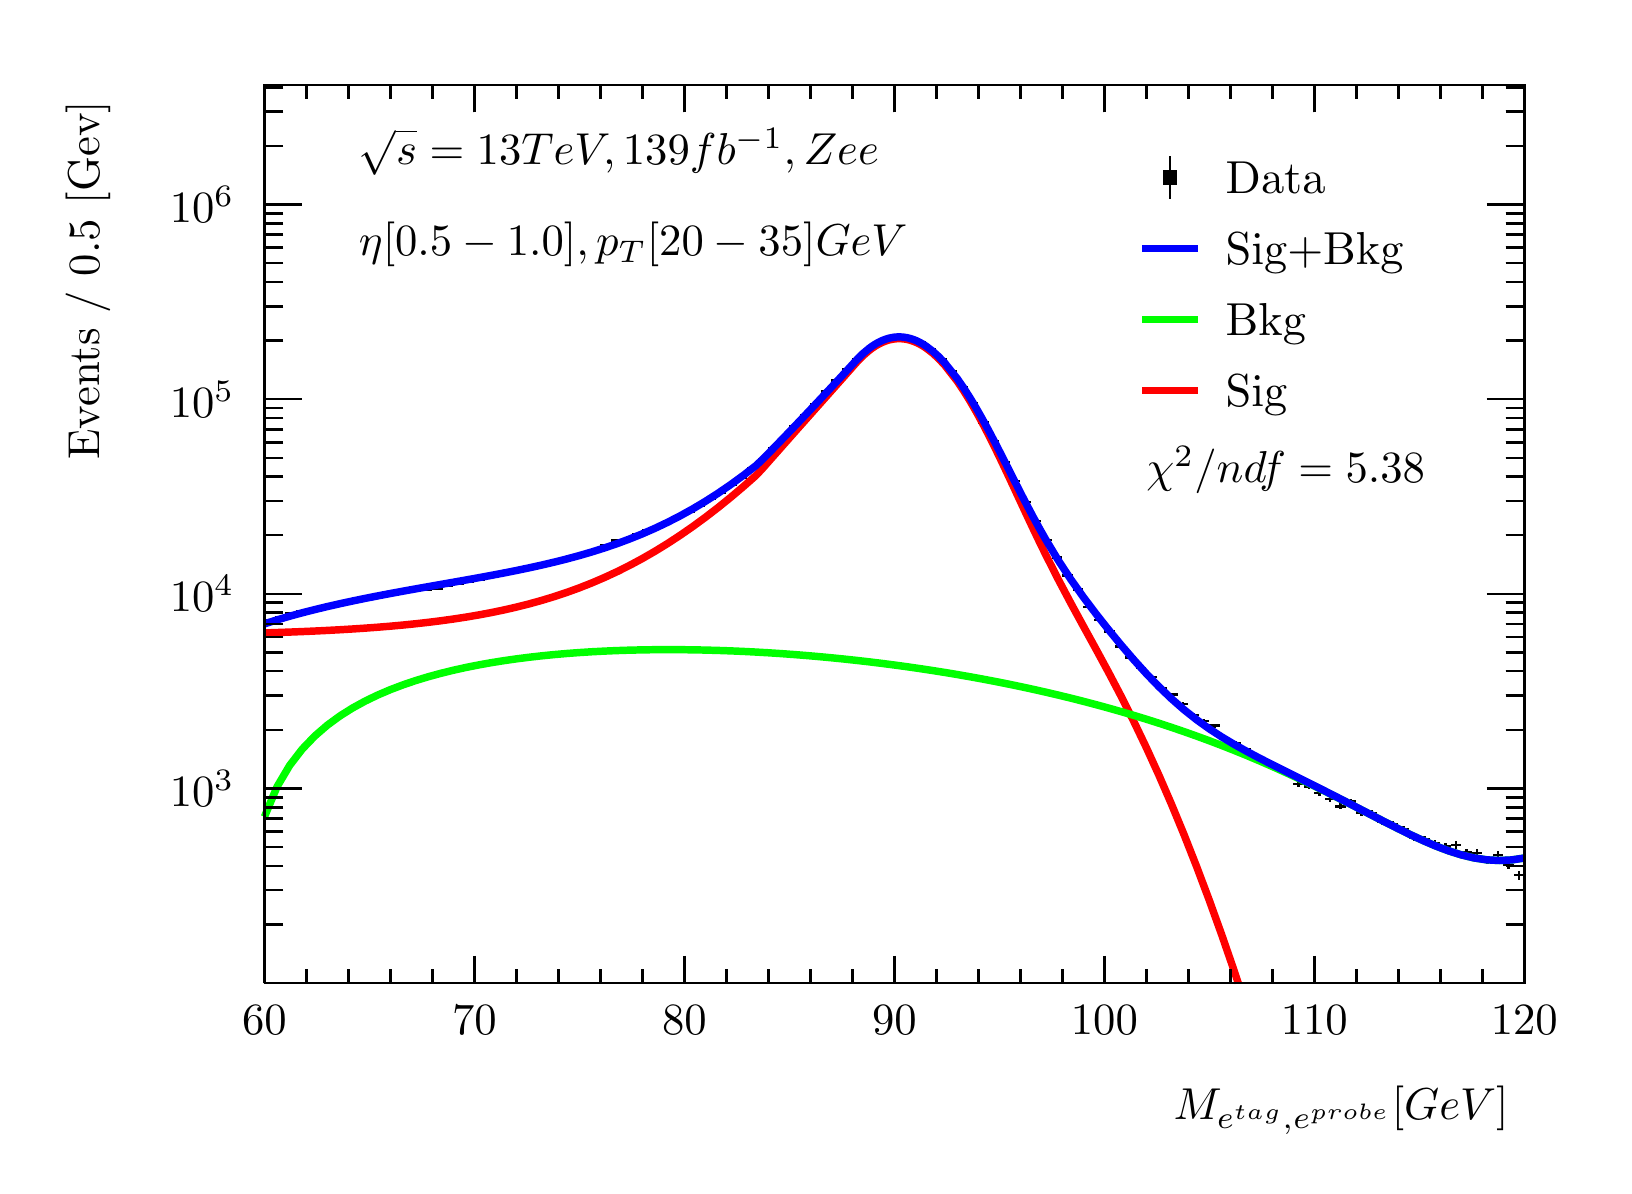
\begin{tikzpicture}
\pgfdeclareplotmark{cross} {
\pgfpathmoveto{\pgfpoint{-0.3\pgfplotmarksize}{\pgfplotmarksize}}
\pgfpathlineto{\pgfpoint{+0.3\pgfplotmarksize}{\pgfplotmarksize}}
\pgfpathlineto{\pgfpoint{+0.3\pgfplotmarksize}{0.3\pgfplotmarksize}}
\pgfpathlineto{\pgfpoint{+1\pgfplotmarksize}{0.3\pgfplotmarksize}}
\pgfpathlineto{\pgfpoint{+1\pgfplotmarksize}{-0.3\pgfplotmarksize}}
\pgfpathlineto{\pgfpoint{+0.3\pgfplotmarksize}{-0.3\pgfplotmarksize}}
\pgfpathlineto{\pgfpoint{+0.3\pgfplotmarksize}{-1.\pgfplotmarksize}}
\pgfpathlineto{\pgfpoint{-0.3\pgfplotmarksize}{-1.\pgfplotmarksize}}
\pgfpathlineto{\pgfpoint{-0.3\pgfplotmarksize}{-0.3\pgfplotmarksize}}
\pgfpathlineto{\pgfpoint{-1.\pgfplotmarksize}{-0.3\pgfplotmarksize}}
\pgfpathlineto{\pgfpoint{-1.\pgfplotmarksize}{0.3\pgfplotmarksize}}
\pgfpathlineto{\pgfpoint{-0.3\pgfplotmarksize}{0.3\pgfplotmarksize}}
\pgfpathclose
\pgfusepathqstroke
}
\pgfdeclareplotmark{cross*} {
\pgfpathmoveto{\pgfpoint{-0.3\pgfplotmarksize}{\pgfplotmarksize}}
\pgfpathlineto{\pgfpoint{+0.3\pgfplotmarksize}{\pgfplotmarksize}}
\pgfpathlineto{\pgfpoint{+0.3\pgfplotmarksize}{0.3\pgfplotmarksize}}
\pgfpathlineto{\pgfpoint{+1\pgfplotmarksize}{0.3\pgfplotmarksize}}
\pgfpathlineto{\pgfpoint{+1\pgfplotmarksize}{-0.3\pgfplotmarksize}}
\pgfpathlineto{\pgfpoint{+0.3\pgfplotmarksize}{-0.3\pgfplotmarksize}}
\pgfpathlineto{\pgfpoint{+0.3\pgfplotmarksize}{-1.\pgfplotmarksize}}
\pgfpathlineto{\pgfpoint{-0.3\pgfplotmarksize}{-1.\pgfplotmarksize}}
\pgfpathlineto{\pgfpoint{-0.3\pgfplotmarksize}{-0.3\pgfplotmarksize}}
\pgfpathlineto{\pgfpoint{-1.\pgfplotmarksize}{-0.3\pgfplotmarksize}}
\pgfpathlineto{\pgfpoint{-1.\pgfplotmarksize}{0.3\pgfplotmarksize}}
\pgfpathlineto{\pgfpoint{-0.3\pgfplotmarksize}{0.3\pgfplotmarksize}}
\pgfpathclose
\pgfusepathqfillstroke
}
\pgfdeclareplotmark{newstar} {
\pgfpathmoveto{\pgfqpoint{0pt}{\pgfplotmarksize}}
\pgfpathlineto{\pgfqpointpolar{44}{0.5\pgfplotmarksize}}
\pgfpathlineto{\pgfqpointpolar{18}{\pgfplotmarksize}}
\pgfpathlineto{\pgfqpointpolar{-20}{0.5\pgfplotmarksize}}
\pgfpathlineto{\pgfqpointpolar{-54}{\pgfplotmarksize}}
\pgfpathlineto{\pgfqpointpolar{-90}{0.5\pgfplotmarksize}}
\pgfpathlineto{\pgfqpointpolar{234}{\pgfplotmarksize}}
\pgfpathlineto{\pgfqpointpolar{198}{0.5\pgfplotmarksize}}
\pgfpathlineto{\pgfqpointpolar{162}{\pgfplotmarksize}}
\pgfpathlineto{\pgfqpointpolar{134}{0.5\pgfplotmarksize}}
\pgfpathclose
\pgfusepathqstroke
}
\pgfdeclareplotmark{newstar*} {
\pgfpathmoveto{\pgfqpoint{0pt}{\pgfplotmarksize}}
\pgfpathlineto{\pgfqpointpolar{44}{0.5\pgfplotmarksize}}
\pgfpathlineto{\pgfqpointpolar{18}{\pgfplotmarksize}}
\pgfpathlineto{\pgfqpointpolar{-20}{0.5\pgfplotmarksize}}
\pgfpathlineto{\pgfqpointpolar{-54}{\pgfplotmarksize}}
\pgfpathlineto{\pgfqpointpolar{-90}{0.5\pgfplotmarksize}}
\pgfpathlineto{\pgfqpointpolar{234}{\pgfplotmarksize}}
\pgfpathlineto{\pgfqpointpolar{198}{0.5\pgfplotmarksize}}
\pgfpathlineto{\pgfqpointpolar{162}{\pgfplotmarksize}}
\pgfpathlineto{\pgfqpointpolar{134}{0.5\pgfplotmarksize}}
\pgfpathclose
\pgfusepathqfillstroke
}
\definecolor{c}{rgb}{1,1,1};
\draw [color=c, fill=c] (0,0) rectangle (20,14.4361);
\draw [color=c, fill=c] (3,2.30977) rectangle (19,13.7143);
\definecolor{c}{rgb}{0,0,0};
\draw [c,line width=0.9] (3,2.30977) -- (3,13.7143) -- (19,13.7143) -- (19,2.30977) -- (3,2.30977);
\definecolor{c}{rgb}{1,1,1};
\draw [color=c, fill=c] (3,2.30977) rectangle (19,13.7143);
\definecolor{c}{rgb}{0,0,0};
\draw [c,line width=0.9] (3,2.30977) -- (3,13.7143) -- (19,13.7143) -- (19,2.30977) -- (3,2.30977);
\draw [c,line width=0.9] (3,2.30977) -- (19,2.30977);
\draw [c,line width=0.9] (3,2.65624) -- (3,2.30977);
\draw [c,line width=0.9] (3.53333,2.48301) -- (3.53333,2.30977);
\draw [c,line width=0.9] (4.06667,2.48301) -- (4.06667,2.30977);
\draw [c,line width=0.9] (4.6,2.48301) -- (4.6,2.30977);
\draw [c,line width=0.9] (5.13333,2.48301) -- (5.13333,2.30977);
\draw [c,line width=0.9] (5.66667,2.65624) -- (5.66667,2.30977);
\draw [c,line width=0.9] (6.2,2.48301) -- (6.2,2.30977);
\draw [c,line width=0.9] (6.73333,2.48301) -- (6.73333,2.30977);
\draw [c,line width=0.9] (7.26667,2.48301) -- (7.26667,2.30977);
\draw [c,line width=0.9] (7.8,2.48301) -- (7.8,2.30977);
\draw [c,line width=0.9] (8.33333,2.65624) -- (8.33333,2.30977);
\draw [c,line width=0.9] (8.86667,2.48301) -- (8.86667,2.30977);
\draw [c,line width=0.9] (9.4,2.48301) -- (9.4,2.30977);
\draw [c,line width=0.9] (9.93333,2.48301) -- (9.93333,2.30977);
\draw [c,line width=0.9] (10.4667,2.48301) -- (10.4667,2.30977);
\draw [c,line width=0.9] (11,2.65624) -- (11,2.30977);
\draw [c,line width=0.9] (11.5333,2.48301) -- (11.5333,2.30977);
\draw [c,line width=0.9] (12.0667,2.48301) -- (12.0667,2.30977);
\draw [c,line width=0.9] (12.6,2.48301) -- (12.6,2.30977);
\draw [c,line width=0.9] (13.1333,2.48301) -- (13.1333,2.30977);
\draw [c,line width=0.9] (13.6667,2.65624) -- (13.6667,2.30977);
\draw [c,line width=0.9] (14.2,2.48301) -- (14.2,2.30977);
\draw [c,line width=0.9] (14.7333,2.48301) -- (14.7333,2.30977);
\draw [c,line width=0.9] (15.2667,2.48301) -- (15.2667,2.30977);
\draw [c,line width=0.9] (15.8,2.48301) -- (15.8,2.30977);
\draw [c,line width=0.9] (16.3333,2.65624) -- (16.3333,2.30977);
\draw [c,line width=0.9] (16.8667,2.48301) -- (16.8667,2.30977);
\draw [c,line width=0.9] (17.4,2.48301) -- (17.4,2.30977);
\draw [c,line width=0.9] (17.9333,2.48301) -- (17.9333,2.30977);
\draw [c,line width=0.9] (18.4667,2.48301) -- (18.4667,2.30977);
\draw [c,line width=0.9] (19,2.65624) -- (19,2.30977);
\draw [anchor=base] (3,1.66015) node[scale=1.61424, color=c, rotate=0]{60};
\draw [anchor=base] (5.66667,1.66015) node[scale=1.61424, color=c, rotate=0]{70};
\draw [anchor=base] (8.33333,1.66015) node[scale=1.61424, color=c, rotate=0]{80};
\draw [anchor=base] (11,1.66015) node[scale=1.61424, color=c, rotate=0]{90};
\draw [anchor=base] (13.6667,1.66015) node[scale=1.61424, color=c, rotate=0]{100};
\draw [anchor=base] (16.3333,1.66015) node[scale=1.61424, color=c, rotate=0]{110};
\draw [anchor=base] (19,1.66015) node[scale=1.61424, color=c, rotate=0]{120};
\draw [anchor= east] (19,0.692932) node[scale=1.61424, color=c, rotate=0]{$M_{e^{tag}, e^{probe}}  [GeV]$};
\draw [c,line width=0.9] (3,13.7143) -- (19,13.7143);
\draw [c,line width=0.9] (3,13.3678) -- (3,13.7143);
\draw [c,line width=0.9] (3.53333,13.5411) -- (3.53333,13.7143);
\draw [c,line width=0.9] (4.06667,13.5411) -- (4.06667,13.7143);
\draw [c,line width=0.9] (4.6,13.5411) -- (4.6,13.7143);
\draw [c,line width=0.9] (5.13333,13.5411) -- (5.13333,13.7143);
\draw [c,line width=0.9] (5.66667,13.3678) -- (5.66667,13.7143);
\draw [c,line width=0.9] (6.2,13.5411) -- (6.2,13.7143);
\draw [c,line width=0.9] (6.73333,13.5411) -- (6.73333,13.7143);
\draw [c,line width=0.9] (7.26667,13.5411) -- (7.26667,13.7143);
\draw [c,line width=0.9] (7.8,13.5411) -- (7.8,13.7143);
\draw [c,line width=0.9] (8.33333,13.3678) -- (8.33333,13.7143);
\draw [c,line width=0.9] (8.86667,13.5411) -- (8.86667,13.7143);
\draw [c,line width=0.9] (9.4,13.5411) -- (9.4,13.7143);
\draw [c,line width=0.9] (9.93333,13.5411) -- (9.93333,13.7143);
\draw [c,line width=0.9] (10.4667,13.5411) -- (10.4667,13.7143);
\draw [c,line width=0.9] (11,13.3678) -- (11,13.7143);
\draw [c,line width=0.9] (11.5333,13.5411) -- (11.5333,13.7143);
\draw [c,line width=0.9] (12.0667,13.5411) -- (12.0667,13.7143);
\draw [c,line width=0.9] (12.6,13.5411) -- (12.6,13.7143);
\draw [c,line width=0.9] (13.1333,13.5411) -- (13.1333,13.7143);
\draw [c,line width=0.9] (13.6667,13.3678) -- (13.6667,13.7143);
\draw [c,line width=0.9] (14.2,13.5411) -- (14.2,13.7143);
\draw [c,line width=0.9] (14.7333,13.5411) -- (14.7333,13.7143);
\draw [c,line width=0.9] (15.2667,13.5411) -- (15.2667,13.7143);
\draw [c,line width=0.9] (15.8,13.5411) -- (15.8,13.7143);
\draw [c,line width=0.9] (16.3333,13.3678) -- (16.3333,13.7143);
\draw [c,line width=0.9] (16.8667,13.5411) -- (16.8667,13.7143);
\draw [c,line width=0.9] (17.4,13.5411) -- (17.4,13.7143);
\draw [c,line width=0.9] (17.9333,13.5411) -- (17.9333,13.7143);
\draw [c,line width=0.9] (18.4667,13.5411) -- (18.4667,13.7143);
\draw [c,line width=0.9] (19,13.3678) -- (19,13.7143);
\draw [c,line width=0.9] (3,2.30977) -- (3,13.7143);
\draw [c,line width=0.9] (3.237,3.05385) -- (3,3.05385);
\draw [c,line width=0.9] (3.237,3.48911) -- (3,3.48911);
\draw [c,line width=0.9] (3.237,3.79793) -- (3,3.79793);
\draw [c,line width=0.9] (3.237,4.03747) -- (3,4.03747);
\draw [c,line width=0.9] (3.237,4.23319) -- (3,4.23319);
\draw [c,line width=0.9] (3.237,4.39867) -- (3,4.39867);
\draw [c,line width=0.9] (3.237,4.54201) -- (3,4.54201);
\draw [c,line width=0.9] (3.237,4.66845) -- (3,4.66845);
\draw [c,line width=0.9] (3.474,4.78155) -- (3,4.78155);
\draw [anchor= east] (2.82,4.78155) node[scale=1.61424, color=c, rotate=0]{$10^{3}$};
\draw [c,line width=0.9] (3.237,5.52563) -- (3,5.52563);
\draw [c,line width=0.9] (3.237,5.96089) -- (3,5.96089);
\draw [c,line width=0.9] (3.237,6.26971) -- (3,6.26971);
\draw [c,line width=0.9] (3.237,6.50925) -- (3,6.50925);
\draw [c,line width=0.9] (3.237,6.70497) -- (3,6.70497);
\draw [c,line width=0.9] (3.237,6.87045) -- (3,6.87045);
\draw [c,line width=0.9] (3.237,7.01379) -- (3,7.01379);
\draw [c,line width=0.9] (3.237,7.14023) -- (3,7.14023);
\draw [c,line width=0.9] (3.474,7.25333) -- (3,7.25333);
\draw [anchor= east] (2.82,7.25333) node[scale=1.61424, color=c, rotate=0]{$10^{4}$};
\draw [c,line width=0.9] (3.237,7.99741) -- (3,7.99741);
\draw [c,line width=0.9] (3.237,8.43267) -- (3,8.43267);
\draw [c,line width=0.9] (3.237,8.74149) -- (3,8.74149);
\draw [c,line width=0.9] (3.237,8.98103) -- (3,8.98103);
\draw [c,line width=0.9] (3.237,9.17675) -- (3,9.17675);
\draw [c,line width=0.9] (3.237,9.34223) -- (3,9.34223);
\draw [c,line width=0.9] (3.237,9.48557) -- (3,9.48557);
\draw [c,line width=0.9] (3.237,9.61201) -- (3,9.61201);
\draw [c,line width=0.9] (3.474,9.72511) -- (3,9.72511);
\draw [anchor= east] (2.82,9.72511) node[scale=1.61424, color=c, rotate=0]{$10^{5}$};
\draw [c,line width=0.9] (3.237,10.4692) -- (3,10.4692);
\draw [c,line width=0.9] (3.237,10.9044) -- (3,10.9044);
\draw [c,line width=0.9] (3.237,11.2133) -- (3,11.2133);
\draw [c,line width=0.9] (3.237,11.4528) -- (3,11.4528);
\draw [c,line width=0.9] (3.237,11.6485) -- (3,11.6485);
\draw [c,line width=0.9] (3.237,11.814) -- (3,11.814);
\draw [c,line width=0.9] (3.237,11.9574) -- (3,11.9574);
\draw [c,line width=0.9] (3.237,12.0838) -- (3,12.0838);
\draw [c,line width=0.9] (3.474,12.1969) -- (3,12.1969);
\draw [anchor= east] (2.82,12.1969) node[scale=1.61424, color=c, rotate=0]{$10^{6}$};
\draw [c,line width=0.9] (3.237,12.941) -- (3,12.941);
\draw [c,line width=0.9] (3.237,13.3762) -- (3,13.3762);
\draw [c,line width=0.9] (3.237,13.6851) -- (3,13.6851);
\draw [anchor= east] (0.76,13.7143) node[scale=1.61424, color=c, rotate=90]{Events / 0.5 [Gev]};
\draw [c,line width=0.9] (19,2.30977) -- (19,13.7143);
\draw [c,line width=0.9] (18.763,3.05385) -- (19,3.05385);
\draw [c,line width=0.9] (18.763,3.48911) -- (19,3.48911);
\draw [c,line width=0.9] (18.763,3.79793) -- (19,3.79793);
\draw [c,line width=0.9] (18.763,4.03747) -- (19,4.03747);
\draw [c,line width=0.9] (18.763,4.23319) -- (19,4.23319);
\draw [c,line width=0.9] (18.763,4.39867) -- (19,4.39867);
\draw [c,line width=0.9] (18.763,4.54201) -- (19,4.54201);
\draw [c,line width=0.9] (18.763,4.66845) -- (19,4.66845);
\draw [c,line width=0.9] (18.526,4.78155) -- (19,4.78155);
\draw [c,line width=0.9] (18.763,5.52563) -- (19,5.52563);
\draw [c,line width=0.9] (18.763,5.96089) -- (19,5.96089);
\draw [c,line width=0.9] (18.763,6.26971) -- (19,6.26971);
\draw [c,line width=0.9] (18.763,6.50925) -- (19,6.50925);
\draw [c,line width=0.9] (18.763,6.70497) -- (19,6.70497);
\draw [c,line width=0.9] (18.763,6.87045) -- (19,6.87045);
\draw [c,line width=0.9] (18.763,7.01379) -- (19,7.01379);
\draw [c,line width=0.9] (18.763,7.14023) -- (19,7.14023);
\draw [c,line width=0.9] (18.526,7.25333) -- (19,7.25333);
\draw [c,line width=0.9] (18.763,7.99741) -- (19,7.99741);
\draw [c,line width=0.9] (18.763,8.43267) -- (19,8.43267);
\draw [c,line width=0.9] (18.763,8.74149) -- (19,8.74149);
\draw [c,line width=0.9] (18.763,8.98103) -- (19,8.98103);
\draw [c,line width=0.9] (18.763,9.17675) -- (19,9.17675);
\draw [c,line width=0.9] (18.763,9.34223) -- (19,9.34223);
\draw [c,line width=0.9] (18.763,9.48557) -- (19,9.48557);
\draw [c,line width=0.9] (18.763,9.61201) -- (19,9.61201);
\draw [c,line width=0.9] (18.526,9.72511) -- (19,9.72511);
\draw [c,line width=0.9] (18.763,10.4692) -- (19,10.4692);
\draw [c,line width=0.9] (18.763,10.9044) -- (19,10.9044);
\draw [c,line width=0.9] (18.763,11.2133) -- (19,11.2133);
\draw [c,line width=0.9] (18.763,11.4528) -- (19,11.4528);
\draw [c,line width=0.9] (18.763,11.6485) -- (19,11.6485);
\draw [c,line width=0.9] (18.763,11.814) -- (19,11.814);
\draw [c,line width=0.9] (18.763,11.9574) -- (19,11.9574);
\draw [c,line width=0.9] (18.763,12.0838) -- (19,12.0838);
\draw [c,line width=0.9] (18.526,12.1969) -- (19,12.1969);
\draw [c,line width=0.9] (18.763,12.941) -- (19,12.941);
\draw [c,line width=0.9] (18.763,13.3762) -- (19,13.3762);
\draw [c,line width=0.9] (18.763,13.6851) -- (19,13.6851);
\draw [c,line width=0.9] (3.06667,6.92297) -- (3,6.92297);
\draw [c,line width=0.9] (3,6.92297) -- (3,6.92297);
\draw [c,line width=0.9] (3.06667,6.92297) -- (3.13333,6.92297);
\draw [c,line width=0.9] (3.13333,6.92297) -- (3.13333,6.92297);
\draw [c,line width=0.9] (3.06667,6.92297) -- (3.06667,6.93549);
\draw [c,line width=0.9] (3.06667,6.93549) -- (3.06667,6.93549);
\draw [c,line width=0.9] (3.06667,6.92297) -- (3.06667,6.91045);
\draw [c,line width=0.9] (3.06667,6.91045) -- (3.06667,6.91045);
\draw [c,line width=0.9] (3.2,6.95788) -- (3.13333,6.95788);
\draw [c,line width=0.9] (3.13333,6.95788) -- (3.13333,6.95788);
\draw [c,line width=0.9] (3.2,6.95788) -- (3.26667,6.95788);
\draw [c,line width=0.9] (3.26667,6.95788) -- (3.26667,6.95788);
\draw [c,line width=0.9] (3.2,6.95788) -- (3.2,6.9702);
\draw [c,line width=0.9] (3.2,6.9702) -- (3.2,6.9702);
\draw [c,line width=0.9] (3.2,6.95788) -- (3.2,6.94556);
\draw [c,line width=0.9] (3.2,6.94556) -- (3.2,6.94556);
\draw [c,line width=0.9] (3.33333,7.003) -- (3.26667,7.003);
\draw [c,line width=0.9] (3.26667,7.003) -- (3.26667,7.003);
\draw [c,line width=0.9] (3.33333,7.003) -- (3.4,7.003);
\draw [c,line width=0.9] (3.4,7.003) -- (3.4,7.003);
\draw [c,line width=0.9] (3.33333,7.003) -- (3.33333,7.01507);
\draw [c,line width=0.9] (3.33333,7.01507) -- (3.33333,7.01507);
\draw [c,line width=0.9] (3.33333,7.003) -- (3.33333,6.99094);
\draw [c,line width=0.9] (3.33333,6.99094) -- (3.33333,6.99094);
\draw [c,line width=0.9] (3.46667,7.03281) -- (3.4,7.03281);
\draw [c,line width=0.9] (3.4,7.03281) -- (3.4,7.03281);
\draw [c,line width=0.9] (3.46667,7.03281) -- (3.53333,7.03281);
\draw [c,line width=0.9] (3.53333,7.03281) -- (3.53333,7.03281);
\draw [c,line width=0.9] (3.46667,7.03281) -- (3.46667,7.04471);
\draw [c,line width=0.9] (3.46667,7.04471) -- (3.46667,7.04471);
\draw [c,line width=0.9] (3.46667,7.03281) -- (3.46667,7.02092);
\draw [c,line width=0.9] (3.46667,7.02092) -- (3.46667,7.02092);
\draw [c,line width=0.9] (3.6,7.04748) -- (3.53333,7.04748);
\draw [c,line width=0.9] (3.53333,7.04748) -- (3.53333,7.04748);
\draw [c,line width=0.9] (3.6,7.04748) -- (3.66667,7.04748);
\draw [c,line width=0.9] (3.66667,7.04748) -- (3.66667,7.04748);
\draw [c,line width=0.9] (3.6,7.04748) -- (3.6,7.05929);
\draw [c,line width=0.9] (3.6,7.05929) -- (3.6,7.05929);
\draw [c,line width=0.9] (3.6,7.04748) -- (3.6,7.03566);
\draw [c,line width=0.9] (3.6,7.03566) -- (3.6,7.03566);
\draw [c,line width=0.9] (3.73333,7.06872) -- (3.66667,7.06872);
\draw [c,line width=0.9] (3.66667,7.06872) -- (3.66667,7.06872);
\draw [c,line width=0.9] (3.73333,7.06872) -- (3.8,7.06872);
\draw [c,line width=0.9] (3.8,7.06872) -- (3.8,7.06872);
\draw [c,line width=0.9] (3.73333,7.06872) -- (3.73333,7.08042);
\draw [c,line width=0.9] (3.73333,7.08042) -- (3.73333,7.08042);
\draw [c,line width=0.9] (3.73333,7.06872) -- (3.73333,7.05702);
\draw [c,line width=0.9] (3.73333,7.05702) -- (3.73333,7.05702);
\draw [c,line width=0.9] (3.86667,7.12207) -- (3.8,7.12207);
\draw [c,line width=0.9] (3.8,7.12207) -- (3.8,7.12207);
\draw [c,line width=0.9] (3.86667,7.12207) -- (3.93333,7.12207);
\draw [c,line width=0.9] (3.93333,7.12207) -- (3.93333,7.12207);
\draw [c,line width=0.9] (3.86667,7.12207) -- (3.86667,7.13348);
\draw [c,line width=0.9] (3.86667,7.13348) -- (3.86667,7.13348);
\draw [c,line width=0.9] (3.86667,7.12207) -- (3.86667,7.11066);
\draw [c,line width=0.9] (3.86667,7.11066) -- (3.86667,7.11066);
\draw [c,line width=0.9] (4,7.13856) -- (3.93333,7.13856);
\draw [c,line width=0.9] (3.93333,7.13856) -- (3.93333,7.13856);
\draw [c,line width=0.9] (4,7.13856) -- (4.06667,7.13856);
\draw [c,line width=0.9] (4.06667,7.13856) -- (4.06667,7.13856);
\draw [c,line width=0.9] (4,7.13856) -- (4,7.14988);
\draw [c,line width=0.9] (4,7.14988) -- (4,7.14988);
\draw [c,line width=0.9] (4,7.13856) -- (4,7.12723);
\draw [c,line width=0.9] (4,7.12723) -- (4,7.12723);
\draw [c,line width=0.9] (4.13333,7.16709) -- (4.06667,7.16709);
\draw [c,line width=0.9] (4.06667,7.16709) -- (4.06667,7.16709);
\draw [c,line width=0.9] (4.13333,7.16709) -- (4.2,7.16709);
\draw [c,line width=0.9] (4.2,7.16709) -- (4.2,7.16709);
\draw [c,line width=0.9] (4.13333,7.16709) -- (4.13333,7.17826);
\draw [c,line width=0.9] (4.13333,7.17826) -- (4.13333,7.17826);
\draw [c,line width=0.9] (4.13333,7.16709) -- (4.13333,7.15591);
\draw [c,line width=0.9] (4.13333,7.15591) -- (4.13333,7.15591);
\draw [c,line width=0.9] (4.26667,7.1909) -- (4.2,7.1909);
\draw [c,line width=0.9] (4.2,7.1909) -- (4.2,7.1909);
\draw [c,line width=0.9] (4.26667,7.1909) -- (4.33333,7.1909);
\draw [c,line width=0.9] (4.33333,7.1909) -- (4.33333,7.1909);
\draw [c,line width=0.9] (4.26667,7.1909) -- (4.26667,7.20195);
\draw [c,line width=0.9] (4.26667,7.20195) -- (4.26667,7.20195);
\draw [c,line width=0.9] (4.26667,7.1909) -- (4.26667,7.17985);
\draw [c,line width=0.9] (4.26667,7.17985) -- (4.26667,7.17985);
\draw [c,line width=0.9] (4.4,7.19782) -- (4.33333,7.19782);
\draw [c,line width=0.9] (4.33333,7.19782) -- (4.33333,7.19782);
\draw [c,line width=0.9] (4.4,7.19782) -- (4.46667,7.19782);
\draw [c,line width=0.9] (4.46667,7.19782) -- (4.46667,7.19782);
\draw [c,line width=0.9] (4.4,7.19782) -- (4.4,7.20883);
\draw [c,line width=0.9] (4.4,7.20883) -- (4.4,7.20883);
\draw [c,line width=0.9] (4.4,7.19782) -- (4.4,7.1868);
\draw [c,line width=0.9] (4.4,7.1868) -- (4.4,7.1868);
\draw [c,line width=0.9] (4.53333,7.24092) -- (4.46667,7.24092);
\draw [c,line width=0.9] (4.46667,7.24092) -- (4.46667,7.24092);
\draw [c,line width=0.9] (4.53333,7.24092) -- (4.6,7.24092);
\draw [c,line width=0.9] (4.6,7.24092) -- (4.6,7.24092);
\draw [c,line width=0.9] (4.53333,7.24092) -- (4.53333,7.25171);
\draw [c,line width=0.9] (4.53333,7.25171) -- (4.53333,7.25171);
\draw [c,line width=0.9] (4.53333,7.24092) -- (4.53333,7.23012);
\draw [c,line width=0.9] (4.53333,7.23012) -- (4.53333,7.23012);
\draw [c,line width=0.9] (4.66667,7.25194) -- (4.6,7.25194);
\draw [c,line width=0.9] (4.6,7.25194) -- (4.6,7.25194);
\draw [c,line width=0.9] (4.66667,7.25194) -- (4.73333,7.25194);
\draw [c,line width=0.9] (4.73333,7.25194) -- (4.73333,7.25194);
\draw [c,line width=0.9] (4.66667,7.25194) -- (4.66667,7.26268);
\draw [c,line width=0.9] (4.66667,7.26268) -- (4.66667,7.26268);
\draw [c,line width=0.9] (4.66667,7.25194) -- (4.66667,7.24119);
\draw [c,line width=0.9] (4.66667,7.24119) -- (4.66667,7.24119);
\draw [c,line width=0.9] (4.8,7.30202) -- (4.73333,7.30202);
\draw [c,line width=0.9] (4.73333,7.30202) -- (4.73333,7.30202);
\draw [c,line width=0.9] (4.8,7.30202) -- (4.86667,7.30202);
\draw [c,line width=0.9] (4.86667,7.30202) -- (4.86667,7.30202);
\draw [c,line width=0.9] (4.8,7.30202) -- (4.8,7.31252);
\draw [c,line width=0.9] (4.8,7.31252) -- (4.8,7.31252);
\draw [c,line width=0.9] (4.8,7.30202) -- (4.8,7.29153);
\draw [c,line width=0.9] (4.8,7.29153) -- (4.8,7.29153);
\draw [c,line width=0.9] (4.93333,7.31558) -- (4.86667,7.31558);
\draw [c,line width=0.9] (4.86667,7.31558) -- (4.86667,7.31558);
\draw [c,line width=0.9] (4.93333,7.31558) -- (5,7.31558);
\draw [c,line width=0.9] (5,7.31558) -- (5,7.31558);
\draw [c,line width=0.9] (4.93333,7.31558) -- (4.93333,7.32601);
\draw [c,line width=0.9] (4.93333,7.32601) -- (4.93333,7.32601);
\draw [c,line width=0.9] (4.93333,7.31558) -- (4.93333,7.30515);
\draw [c,line width=0.9] (4.93333,7.30515) -- (4.93333,7.30515);
\draw [c,line width=0.9] (5.06667,7.30571) -- (5,7.30571);
\draw [c,line width=0.9] (5,7.30571) -- (5,7.30571);
\draw [c,line width=0.9] (5.06667,7.30571) -- (5.13333,7.30571);
\draw [c,line width=0.9] (5.13333,7.30571) -- (5.13333,7.30571);
\draw [c,line width=0.9] (5.06667,7.30571) -- (5.06667,7.31618);
\draw [c,line width=0.9] (5.06667,7.31618) -- (5.06667,7.31618);
\draw [c,line width=0.9] (5.06667,7.30571) -- (5.06667,7.29523);
\draw [c,line width=0.9] (5.06667,7.29523) -- (5.06667,7.29523);
\draw [c,line width=0.9] (5.2,7.32355) -- (5.13333,7.32355);
\draw [c,line width=0.9] (5.13333,7.32355) -- (5.13333,7.32355);
\draw [c,line width=0.9] (5.2,7.32355) -- (5.26667,7.32355);
\draw [c,line width=0.9] (5.26667,7.32355) -- (5.26667,7.32355);
\draw [c,line width=0.9] (5.2,7.32355) -- (5.2,7.33394);
\draw [c,line width=0.9] (5.2,7.33394) -- (5.2,7.33394);
\draw [c,line width=0.9] (5.2,7.32355) -- (5.2,7.31316);
\draw [c,line width=0.9] (5.2,7.31316) -- (5.2,7.31316);
\draw [c,line width=0.9] (5.33333,7.35643) -- (5.26667,7.35643);
\draw [c,line width=0.9] (5.26667,7.35643) -- (5.26667,7.35643);
\draw [c,line width=0.9] (5.33333,7.35643) -- (5.4,7.35643);
\draw [c,line width=0.9] (5.4,7.35643) -- (5.4,7.35643);
\draw [c,line width=0.9] (5.33333,7.35643) -- (5.33333,7.36666);
\draw [c,line width=0.9] (5.33333,7.36666) -- (5.33333,7.36666);
\draw [c,line width=0.9] (5.33333,7.35643) -- (5.33333,7.3462);
\draw [c,line width=0.9] (5.33333,7.3462) -- (5.33333,7.3462);
\draw [c,line width=0.9] (5.46667,7.38377) -- (5.4,7.38377);
\draw [c,line width=0.9] (5.4,7.38377) -- (5.4,7.38377);
\draw [c,line width=0.9] (5.46667,7.38377) -- (5.53333,7.38377);
\draw [c,line width=0.9] (5.53333,7.38377) -- (5.53333,7.38377);
\draw [c,line width=0.9] (5.46667,7.38377) -- (5.46667,7.39387);
\draw [c,line width=0.9] (5.46667,7.39387) -- (5.46667,7.39387);
\draw [c,line width=0.9] (5.46667,7.38377) -- (5.46667,7.37367);
\draw [c,line width=0.9] (5.46667,7.37367) -- (5.46667,7.37367);
\draw [c,line width=0.9] (5.6,7.40932) -- (5.53333,7.40932);
\draw [c,line width=0.9] (5.53333,7.40932) -- (5.53333,7.40932);
\draw [c,line width=0.9] (5.6,7.40932) -- (5.66667,7.40932);
\draw [c,line width=0.9] (5.66667,7.40932) -- (5.66667,7.40932);
\draw [c,line width=0.9] (5.6,7.40932) -- (5.6,7.4193);
\draw [c,line width=0.9] (5.6,7.4193) -- (5.6,7.4193);
\draw [c,line width=0.9] (5.6,7.40932) -- (5.6,7.39934);
\draw [c,line width=0.9] (5.6,7.39934) -- (5.6,7.39934);
\draw [c,line width=0.9] (5.73333,7.43772) -- (5.66667,7.43772);
\draw [c,line width=0.9] (5.66667,7.43772) -- (5.66667,7.43772);
\draw [c,line width=0.9] (5.73333,7.43772) -- (5.8,7.43772);
\draw [c,line width=0.9] (5.8,7.43772) -- (5.8,7.43772);
\draw [c,line width=0.9] (5.73333,7.43772) -- (5.73333,7.44757);
\draw [c,line width=0.9] (5.73333,7.44757) -- (5.73333,7.44757);
\draw [c,line width=0.9] (5.73333,7.43772) -- (5.73333,7.42787);
\draw [c,line width=0.9] (5.73333,7.42787) -- (5.73333,7.42787);
\draw [c,line width=0.9] (5.86667,7.4711) -- (5.8,7.4711);
\draw [c,line width=0.9] (5.8,7.4711) -- (5.8,7.4711);
\draw [c,line width=0.9] (5.86667,7.4711) -- (5.93333,7.4711);
\draw [c,line width=0.9] (5.93333,7.4711) -- (5.93333,7.4711);
\draw [c,line width=0.9] (5.86667,7.4711) -- (5.86667,7.4808);
\draw [c,line width=0.9] (5.86667,7.4808) -- (5.86667,7.4808);
\draw [c,line width=0.9] (5.86667,7.4711) -- (5.86667,7.4614);
\draw [c,line width=0.9] (5.86667,7.4614) -- (5.86667,7.4614);
\draw [c,line width=0.9] (6,7.49887) -- (5.93333,7.49887);
\draw [c,line width=0.9] (5.93333,7.49887) -- (5.93333,7.49887);
\draw [c,line width=0.9] (6,7.49887) -- (6.06667,7.49887);
\draw [c,line width=0.9] (6.06667,7.49887) -- (6.06667,7.49887);
\draw [c,line width=0.9] (6,7.49887) -- (6,7.50844);
\draw [c,line width=0.9] (6,7.50844) -- (6,7.50844);
\draw [c,line width=0.9] (6,7.49887) -- (6,7.48929);
\draw [c,line width=0.9] (6,7.48929) -- (6,7.48929);
\draw [c,line width=0.9] (6.13333,7.53737) -- (6.06667,7.53737);
\draw [c,line width=0.9] (6.06667,7.53737) -- (6.06667,7.53737);
\draw [c,line width=0.9] (6.13333,7.53737) -- (6.2,7.53737);
\draw [c,line width=0.9] (6.2,7.53737) -- (6.2,7.53737);
\draw [c,line width=0.9] (6.13333,7.53737) -- (6.13333,7.54677);
\draw [c,line width=0.9] (6.13333,7.54677) -- (6.13333,7.54677);
\draw [c,line width=0.9] (6.13333,7.53737) -- (6.13333,7.52796);
\draw [c,line width=0.9] (6.13333,7.52796) -- (6.13333,7.52796);
\draw [c,line width=0.9] (6.26667,7.55169) -- (6.2,7.55169);
\draw [c,line width=0.9] (6.2,7.55169) -- (6.2,7.55169);
\draw [c,line width=0.9] (6.26667,7.55169) -- (6.33333,7.55169);
\draw [c,line width=0.9] (6.33333,7.55169) -- (6.33333,7.55169);
\draw [c,line width=0.9] (6.26667,7.55169) -- (6.26667,7.56103);
\draw [c,line width=0.9] (6.26667,7.56103) -- (6.26667,7.56103);
\draw [c,line width=0.9] (6.26667,7.55169) -- (6.26667,7.54235);
\draw [c,line width=0.9] (6.26667,7.54235) -- (6.26667,7.54235);
\draw [c,line width=0.9] (6.4,7.59901) -- (6.33333,7.59901);
\draw [c,line width=0.9] (6.33333,7.59901) -- (6.33333,7.59901);
\draw [c,line width=0.9] (6.4,7.59901) -- (6.46667,7.59901);
\draw [c,line width=0.9] (6.46667,7.59901) -- (6.46667,7.59901);
\draw [c,line width=0.9] (6.4,7.59901) -- (6.4,7.60814);
\draw [c,line width=0.9] (6.4,7.60814) -- (6.4,7.60814);
\draw [c,line width=0.9] (6.4,7.59901) -- (6.4,7.58987);
\draw [c,line width=0.9] (6.4,7.58987) -- (6.4,7.58987);
\draw [c,line width=0.9] (6.53333,7.6296) -- (6.46667,7.6296);
\draw [c,line width=0.9] (6.46667,7.6296) -- (6.46667,7.6296);
\draw [c,line width=0.9] (6.53333,7.6296) -- (6.6,7.6296);
\draw [c,line width=0.9] (6.6,7.6296) -- (6.6,7.6296);
\draw [c,line width=0.9] (6.53333,7.6296) -- (6.53333,7.63861);
\draw [c,line width=0.9] (6.53333,7.63861) -- (6.53333,7.63861);
\draw [c,line width=0.9] (6.53333,7.6296) -- (6.53333,7.6206);
\draw [c,line width=0.9] (6.53333,7.6206) -- (6.53333,7.6206);
\draw [c,line width=0.9] (6.66667,7.67091) -- (6.6,7.67091);
\draw [c,line width=0.9] (6.6,7.67091) -- (6.6,7.67091);
\draw [c,line width=0.9] (6.66667,7.67091) -- (6.73333,7.67091);
\draw [c,line width=0.9] (6.73333,7.67091) -- (6.73333,7.67091);
\draw [c,line width=0.9] (6.66667,7.67091) -- (6.66667,7.67975);
\draw [c,line width=0.9] (6.66667,7.67975) -- (6.66667,7.67975);
\draw [c,line width=0.9] (6.66667,7.67091) -- (6.66667,7.66208);
\draw [c,line width=0.9] (6.66667,7.66208) -- (6.66667,7.66208);
\draw [c,line width=0.9] (6.8,7.69309) -- (6.73333,7.69309);
\draw [c,line width=0.9] (6.73333,7.69309) -- (6.73333,7.69309);
\draw [c,line width=0.9] (6.8,7.69309) -- (6.86667,7.69309);
\draw [c,line width=0.9] (6.86667,7.69309) -- (6.86667,7.69309);
\draw [c,line width=0.9] (6.8,7.69309) -- (6.8,7.70184);
\draw [c,line width=0.9] (6.8,7.70184) -- (6.8,7.70184);
\draw [c,line width=0.9] (6.8,7.69309) -- (6.8,7.68434);
\draw [c,line width=0.9] (6.8,7.68434) -- (6.8,7.68434);
\draw [c,line width=0.9] (6.93333,7.73324) -- (6.86667,7.73324);
\draw [c,line width=0.9] (6.86667,7.73324) -- (6.86667,7.73324);
\draw [c,line width=0.9] (6.93333,7.73324) -- (7,7.73324);
\draw [c,line width=0.9] (7,7.73324) -- (7,7.73324);
\draw [c,line width=0.9] (6.93333,7.73324) -- (6.93333,7.74182);
\draw [c,line width=0.9] (6.93333,7.74182) -- (6.93333,7.74182);
\draw [c,line width=0.9] (6.93333,7.73324) -- (6.93333,7.72465);
\draw [c,line width=0.9] (6.93333,7.72465) -- (6.93333,7.72465);
\draw [c,line width=0.9] (7.06667,7.76563) -- (7,7.76563);
\draw [c,line width=0.9] (7,7.76563) -- (7,7.76563);
\draw [c,line width=0.9] (7.06667,7.76563) -- (7.13333,7.76563);
\draw [c,line width=0.9] (7.13333,7.76563) -- (7.13333,7.76563);
\draw [c,line width=0.9] (7.06667,7.76563) -- (7.06667,7.77408);
\draw [c,line width=0.9] (7.06667,7.77408) -- (7.06667,7.77408);
\draw [c,line width=0.9] (7.06667,7.76563) -- (7.06667,7.75717);
\draw [c,line width=0.9] (7.06667,7.75717) -- (7.06667,7.75717);
\draw [c,line width=0.9] (7.2,7.8048) -- (7.13333,7.8048);
\draw [c,line width=0.9] (7.13333,7.8048) -- (7.13333,7.8048);
\draw [c,line width=0.9] (7.2,7.8048) -- (7.26667,7.8048);
\draw [c,line width=0.9] (7.26667,7.8048) -- (7.26667,7.8048);
\draw [c,line width=0.9] (7.2,7.8048) -- (7.2,7.81311);
\draw [c,line width=0.9] (7.2,7.81311) -- (7.2,7.81311);
\draw [c,line width=0.9] (7.2,7.8048) -- (7.2,7.7965);
\draw [c,line width=0.9] (7.2,7.7965) -- (7.2,7.7965);
\draw [c,line width=0.9] (7.33333,7.8642) -- (7.26667,7.8642);
\draw [c,line width=0.9] (7.26667,7.8642) -- (7.26667,7.8642);
\draw [c,line width=0.9] (7.33333,7.8642) -- (7.4,7.8642);
\draw [c,line width=0.9] (7.4,7.8642) -- (7.4,7.8642);
\draw [c,line width=0.9] (7.33333,7.8642) -- (7.33333,7.87228);
\draw [c,line width=0.9] (7.33333,7.87228) -- (7.33333,7.87228);
\draw [c,line width=0.9] (7.33333,7.8642) -- (7.33333,7.85613);
\draw [c,line width=0.9] (7.33333,7.85613) -- (7.33333,7.85613);
\draw [c,line width=0.9] (7.46667,7.92739) -- (7.4,7.92739);
\draw [c,line width=0.9] (7.4,7.92739) -- (7.4,7.92739);
\draw [c,line width=0.9] (7.46667,7.92739) -- (7.53333,7.92739);
\draw [c,line width=0.9] (7.53333,7.92739) -- (7.53333,7.92739);
\draw [c,line width=0.9] (7.46667,7.92739) -- (7.46667,7.93523);
\draw [c,line width=0.9] (7.46667,7.93523) -- (7.46667,7.93523);
\draw [c,line width=0.9] (7.46667,7.92739) -- (7.46667,7.91954);
\draw [c,line width=0.9] (7.46667,7.91954) -- (7.46667,7.91954);
\draw [c,line width=0.9] (7.6,7.94843) -- (7.53333,7.94843);
\draw [c,line width=0.9] (7.53333,7.94843) -- (7.53333,7.94843);
\draw [c,line width=0.9] (7.6,7.94843) -- (7.66667,7.94843);
\draw [c,line width=0.9] (7.66667,7.94843) -- (7.66667,7.94843);
\draw [c,line width=0.9] (7.6,7.94843) -- (7.6,7.9562);
\draw [c,line width=0.9] (7.6,7.9562) -- (7.6,7.9562);
\draw [c,line width=0.9] (7.6,7.94843) -- (7.6,7.94067);
\draw [c,line width=0.9] (7.6,7.94067) -- (7.6,7.94067);
\draw [c,line width=0.9] (7.73333,8.00655) -- (7.66667,8.00655);
\draw [c,line width=0.9] (7.66667,8.00655) -- (7.66667,8.00655);
\draw [c,line width=0.9] (7.73333,8.00655) -- (7.8,8.00655);
\draw [c,line width=0.9] (7.8,8.00655) -- (7.8,8.00655);
\draw [c,line width=0.9] (7.73333,8.00655) -- (7.73333,8.01411);
\draw [c,line width=0.9] (7.73333,8.01411) -- (7.73333,8.01411);
\draw [c,line width=0.9] (7.73333,8.00655) -- (7.73333,7.99899);
\draw [c,line width=0.9] (7.73333,7.99899) -- (7.73333,7.99899);
\draw [c,line width=0.9] (7.86667,8.05702) -- (7.8,8.05702);
\draw [c,line width=0.9] (7.8,8.05702) -- (7.8,8.05702);
\draw [c,line width=0.9] (7.86667,8.05702) -- (7.93333,8.05702);
\draw [c,line width=0.9] (7.93333,8.05702) -- (7.93333,8.05702);
\draw [c,line width=0.9] (7.86667,8.05702) -- (7.86667,8.0644);
\draw [c,line width=0.9] (7.86667,8.0644) -- (7.86667,8.0644);
\draw [c,line width=0.9] (7.86667,8.05702) -- (7.86667,8.04964);
\draw [c,line width=0.9] (7.86667,8.04964) -- (7.86667,8.04964);
\draw [c,line width=0.9] (8,8.11619) -- (7.93333,8.11619);
\draw [c,line width=0.9] (7.93333,8.11619) -- (7.93333,8.11619);
\draw [c,line width=0.9] (8,8.11619) -- (8.06667,8.11619);
\draw [c,line width=0.9] (8.06667,8.11619) -- (8.06667,8.11619);
\draw [c,line width=0.9] (8,8.11619) -- (8,8.12337);
\draw [c,line width=0.9] (8,8.12337) -- (8,8.12337);
\draw [c,line width=0.9] (8,8.11619) -- (8,8.10901);
\draw [c,line width=0.9] (8,8.10901) -- (8,8.10901);
\draw [c,line width=0.9] (8.13333,8.17559) -- (8.06667,8.17559);
\draw [c,line width=0.9] (8.06667,8.17559) -- (8.06667,8.17559);
\draw [c,line width=0.9] (8.13333,8.17559) -- (8.2,8.17559);
\draw [c,line width=0.9] (8.2,8.17559) -- (8.2,8.17559);
\draw [c,line width=0.9] (8.13333,8.17559) -- (8.13333,8.18258);
\draw [c,line width=0.9] (8.13333,8.18258) -- (8.13333,8.18258);
\draw [c,line width=0.9] (8.13333,8.17559) -- (8.13333,8.1686);
\draw [c,line width=0.9] (8.13333,8.1686) -- (8.13333,8.1686);
\draw [c,line width=0.9] (8.26667,8.23803) -- (8.2,8.23803);
\draw [c,line width=0.9] (8.2,8.23803) -- (8.2,8.23803);
\draw [c,line width=0.9] (8.26667,8.23803) -- (8.33333,8.23803);
\draw [c,line width=0.9] (8.33333,8.23803) -- (8.33333,8.23803);
\draw [c,line width=0.9] (8.26667,8.23803) -- (8.26667,8.24481);
\draw [c,line width=0.9] (8.26667,8.24481) -- (8.26667,8.24481);
\draw [c,line width=0.9] (8.26667,8.23803) -- (8.26667,8.23124);
\draw [c,line width=0.9] (8.26667,8.23124) -- (8.26667,8.23124);
\draw [c,line width=0.9] (8.4,8.29853) -- (8.33333,8.29853);
\draw [c,line width=0.9] (8.33333,8.29853) -- (8.33333,8.29853);
\draw [c,line width=0.9] (8.4,8.29853) -- (8.46667,8.29853);
\draw [c,line width=0.9] (8.46667,8.29853) -- (8.46667,8.29853);
\draw [c,line width=0.9] (8.4,8.29853) -- (8.4,8.30513);
\draw [c,line width=0.9] (8.4,8.30513) -- (8.4,8.30513);
\draw [c,line width=0.9] (8.4,8.29853) -- (8.4,8.29193);
\draw [c,line width=0.9] (8.4,8.29193) -- (8.4,8.29193);
\draw [c,line width=0.9] (8.53333,8.37501) -- (8.46667,8.37501);
\draw [c,line width=0.9] (8.46667,8.37501) -- (8.46667,8.37501);
\draw [c,line width=0.9] (8.53333,8.37501) -- (8.6,8.37501);
\draw [c,line width=0.9] (8.6,8.37501) -- (8.6,8.37501);
\draw [c,line width=0.9] (8.53333,8.37501) -- (8.53333,8.38137);
\draw [c,line width=0.9] (8.53333,8.38137) -- (8.53333,8.38137);
\draw [c,line width=0.9] (8.53333,8.37501) -- (8.53333,8.36864);
\draw [c,line width=0.9] (8.53333,8.36864) -- (8.53333,8.36864);
\draw [c,line width=0.9] (8.66667,8.45977) -- (8.6,8.45977);
\draw [c,line width=0.9] (8.6,8.45977) -- (8.6,8.45977);
\draw [c,line width=0.9] (8.66667,8.45977) -- (8.73333,8.45977);
\draw [c,line width=0.9] (8.73333,8.45977) -- (8.73333,8.45977);
\draw [c,line width=0.9] (8.66667,8.45977) -- (8.66667,8.46589);
\draw [c,line width=0.9] (8.66667,8.46589) -- (8.66667,8.46589);
\draw [c,line width=0.9] (8.66667,8.45977) -- (8.66667,8.45365);
\draw [c,line width=0.9] (8.66667,8.45365) -- (8.66667,8.45365);
\draw [c,line width=0.9] (8.8,8.54221) -- (8.73333,8.54221);
\draw [c,line width=0.9] (8.73333,8.54221) -- (8.73333,8.54221);
\draw [c,line width=0.9] (8.8,8.54221) -- (8.86667,8.54221);
\draw [c,line width=0.9] (8.86667,8.54221) -- (8.86667,8.54221);
\draw [c,line width=0.9] (8.8,8.54221) -- (8.8,8.5481);
\draw [c,line width=0.9] (8.8,8.5481) -- (8.8,8.5481);
\draw [c,line width=0.9] (8.8,8.54221) -- (8.8,8.53633);
\draw [c,line width=0.9] (8.8,8.53633) -- (8.8,8.53633);
\draw [c,line width=0.9] (8.93333,8.63531) -- (8.86667,8.63531);
\draw [c,line width=0.9] (8.86667,8.63531) -- (8.86667,8.63531);
\draw [c,line width=0.9] (8.93333,8.63531) -- (9,8.63531);
\draw [c,line width=0.9] (9,8.63531) -- (9,8.63531);
\draw [c,line width=0.9] (8.93333,8.63531) -- (8.93333,8.64095);
\draw [c,line width=0.9] (8.93333,8.64095) -- (8.93333,8.64095);
\draw [c,line width=0.9] (8.93333,8.63531) -- (8.93333,8.62968);
\draw [c,line width=0.9] (8.93333,8.62968) -- (8.93333,8.62968);
\draw [c,line width=0.9] (9.06667,8.73319) -- (9,8.73319);
\draw [c,line width=0.9] (9,8.73319) -- (9,8.73319);
\draw [c,line width=0.9] (9.06667,8.73319) -- (9.13333,8.73319);
\draw [c,line width=0.9] (9.13333,8.73319) -- (9.13333,8.73319);
\draw [c,line width=0.9] (9.06667,8.73319) -- (9.06667,8.73858);
\draw [c,line width=0.9] (9.06667,8.73858) -- (9.06667,8.73858);
\draw [c,line width=0.9] (9.06667,8.73319) -- (9.06667,8.72781);
\draw [c,line width=0.9] (9.06667,8.72781) -- (9.06667,8.72781);
\draw [c,line width=0.9] (9.2,8.8518) -- (9.13333,8.8518);
\draw [c,line width=0.9] (9.13333,8.8518) -- (9.13333,8.8518);
\draw [c,line width=0.9] (9.2,8.8518) -- (9.26667,8.8518);
\draw [c,line width=0.9] (9.26667,8.8518) -- (9.26667,8.8518);
\draw [c,line width=0.9] (9.2,8.8518) -- (9.2,8.8569);
\draw [c,line width=0.9] (9.2,8.8569) -- (9.2,8.8569);
\draw [c,line width=0.9] (9.2,8.8518) -- (9.2,8.8467);
\draw [c,line width=0.9] (9.2,8.8467) -- (9.2,8.8467);
\draw [c,line width=0.9] (9.33333,8.9674) -- (9.26667,8.9674);
\draw [c,line width=0.9] (9.26667,8.9674) -- (9.26667,8.9674);
\draw [c,line width=0.9] (9.33333,8.9674) -- (9.4,8.9674);
\draw [c,line width=0.9] (9.4,8.9674) -- (9.4,8.9674);
\draw [c,line width=0.9] (9.33333,8.9674) -- (9.33333,8.97223);
\draw [c,line width=0.9] (9.33333,8.97223) -- (9.33333,8.97223);
\draw [c,line width=0.9] (9.33333,8.9674) -- (9.33333,8.96257);
\draw [c,line width=0.9] (9.33333,8.96257) -- (9.33333,8.96257);
\draw [c,line width=0.9] (9.46667,9.09881) -- (9.4,9.09881);
\draw [c,line width=0.9] (9.4,9.09881) -- (9.4,9.09881);
\draw [c,line width=0.9] (9.46667,9.09881) -- (9.53333,9.09881);
\draw [c,line width=0.9] (9.53333,9.09881) -- (9.53333,9.09881);
\draw [c,line width=0.9] (9.46667,9.09881) -- (9.46667,9.10335);
\draw [c,line width=0.9] (9.46667,9.10335) -- (9.46667,9.10335);
\draw [c,line width=0.9] (9.46667,9.09881) -- (9.46667,9.09426);
\draw [c,line width=0.9] (9.46667,9.09426) -- (9.46667,9.09426);
\draw [c,line width=0.9] (9.6,9.22884) -- (9.53333,9.22884);
\draw [c,line width=0.9] (9.53333,9.22884) -- (9.53333,9.22884);
\draw [c,line width=0.9] (9.6,9.22884) -- (9.66667,9.22884);
\draw [c,line width=0.9] (9.66667,9.22884) -- (9.66667,9.22884);
\draw [c,line width=0.9] (9.6,9.22884) -- (9.6,9.23311);
\draw [c,line width=0.9] (9.6,9.23311) -- (9.6,9.23311);
\draw [c,line width=0.9] (9.6,9.22884) -- (9.6,9.22456);
\draw [c,line width=0.9] (9.6,9.22456) -- (9.6,9.22456);
\draw [c,line width=0.9] (9.73333,9.37732) -- (9.66667,9.37732);
\draw [c,line width=0.9] (9.66667,9.37732) -- (9.66667,9.37732);
\draw [c,line width=0.9] (9.73333,9.37732) -- (9.8,9.37732);
\draw [c,line width=0.9] (9.8,9.37732) -- (9.8,9.37732);
\draw [c,line width=0.9] (9.73333,9.37732) -- (9.73333,9.38131);
\draw [c,line width=0.9] (9.73333,9.38131) -- (9.73333,9.38131);
\draw [c,line width=0.9] (9.73333,9.37732) -- (9.73333,9.37333);
\draw [c,line width=0.9] (9.73333,9.37333) -- (9.73333,9.37333);
\draw [c,line width=0.9] (9.86667,9.52124) -- (9.8,9.52124);
\draw [c,line width=0.9] (9.8,9.52124) -- (9.8,9.52124);
\draw [c,line width=0.9] (9.86667,9.52124) -- (9.93333,9.52124);
\draw [c,line width=0.9] (9.93333,9.52124) -- (9.93333,9.52124);
\draw [c,line width=0.9] (9.86667,9.52124) -- (9.86667,9.52498);
\draw [c,line width=0.9] (9.86667,9.52498) -- (9.86667,9.52498);
\draw [c,line width=0.9] (9.86667,9.52124) -- (9.86667,9.51751);
\draw [c,line width=0.9] (9.86667,9.51751) -- (9.86667,9.51751);
\draw [c,line width=0.9] (10,9.66398) -- (9.93333,9.66398);
\draw [c,line width=0.9] (9.93333,9.66398) -- (9.93333,9.66398);
\draw [c,line width=0.9] (10,9.66398) -- (10.0667,9.66398);
\draw [c,line width=0.9] (10.0667,9.66398) -- (10.0667,9.66398);
\draw [c,line width=0.9] (10,9.66398) -- (10,9.66747);
\draw [c,line width=0.9] (10,9.66747) -- (10,9.66747);
\draw [c,line width=0.9] (10,9.66398) -- (10,9.66048);
\draw [c,line width=0.9] (10,9.66048) -- (10,9.66048);
\draw [c,line width=0.9] (10.1333,9.82371) -- (10.0667,9.82371);
\draw [c,line width=0.9] (10.0667,9.82371) -- (10.0667,9.82371);
\draw [c,line width=0.9] (10.1333,9.82371) -- (10.2,9.82371);
\draw [c,line width=0.9] (10.2,9.82371) -- (10.2,9.82371);
\draw [c,line width=0.9] (10.1333,9.82371) -- (10.1333,9.82695);
\draw [c,line width=0.9] (10.1333,9.82695) -- (10.1333,9.82695);
\draw [c,line width=0.9] (10.1333,9.82371) -- (10.1333,9.82047);
\draw [c,line width=0.9] (10.1333,9.82047) -- (10.1333,9.82047);
\draw [c,line width=0.9] (10.2667,9.96402) -- (10.2,9.96402);
\draw [c,line width=0.9] (10.2,9.96402) -- (10.2,9.96402);
\draw [c,line width=0.9] (10.2667,9.96402) -- (10.3333,9.96402);
\draw [c,line width=0.9] (10.3333,9.96402) -- (10.3333,9.96402);
\draw [c,line width=0.9] (10.2667,9.96402) -- (10.2667,9.96706);
\draw [c,line width=0.9] (10.2667,9.96706) -- (10.2667,9.96706);
\draw [c,line width=0.9] (10.2667,9.96402) -- (10.2667,9.96099);
\draw [c,line width=0.9] (10.2667,9.96099) -- (10.2667,9.96099);
\draw [c,line width=0.9] (10.4,10.107) -- (10.3333,10.107);
\draw [c,line width=0.9] (10.3333,10.107) -- (10.3333,10.107);
\draw [c,line width=0.9] (10.4,10.107) -- (10.4667,10.107);
\draw [c,line width=0.9] (10.4667,10.107) -- (10.4667,10.107);
\draw [c,line width=0.9] (10.4,10.107) -- (10.4,10.1099);
\draw [c,line width=0.9] (10.4,10.1099) -- (10.4,10.1099);
\draw [c,line width=0.9] (10.4,10.107) -- (10.4,10.1042);
\draw [c,line width=0.9] (10.4,10.1042) -- (10.4,10.1042);
\draw [c,line width=0.9] (10.5333,10.236) -- (10.4667,10.236);
\draw [c,line width=0.9] (10.4667,10.236) -- (10.4667,10.236);
\draw [c,line width=0.9] (10.5333,10.236) -- (10.6,10.236);
\draw [c,line width=0.9] (10.6,10.236) -- (10.6,10.236);
\draw [c,line width=0.9] (10.5333,10.236) -- (10.5333,10.2386);
\draw [c,line width=0.9] (10.5333,10.2386) -- (10.5333,10.2386);
\draw [c,line width=0.9] (10.5333,10.236) -- (10.5333,10.2333);
\draw [c,line width=0.9] (10.5333,10.2333) -- (10.5333,10.2333);
\draw [c,line width=0.9] (10.6667,10.3421) -- (10.6,10.3421);
\draw [c,line width=0.9] (10.6,10.3421) -- (10.6,10.3421);
\draw [c,line width=0.9] (10.6667,10.3421) -- (10.7333,10.3421);
\draw [c,line width=0.9] (10.7333,10.3421) -- (10.7333,10.3421);
\draw [c,line width=0.9] (10.6667,10.3421) -- (10.6667,10.3446);
\draw [c,line width=0.9] (10.6667,10.3446) -- (10.6667,10.3446);
\draw [c,line width=0.9] (10.6667,10.3421) -- (10.6667,10.3395);
\draw [c,line width=0.9] (10.6667,10.3395) -- (10.6667,10.3395);
\draw [c,line width=0.9] (10.8,10.4323) -- (10.7333,10.4323);
\draw [c,line width=0.9] (10.7333,10.4323) -- (10.7333,10.4323);
\draw [c,line width=0.9] (10.8,10.4323) -- (10.8667,10.4323);
\draw [c,line width=0.9] (10.8667,10.4323) -- (10.8667,10.4323);
\draw [c,line width=0.9] (10.8,10.4323) -- (10.8,10.4348);
\draw [c,line width=0.9] (10.8,10.4348) -- (10.8,10.4348);
\draw [c,line width=0.9] (10.8,10.4323) -- (10.8,10.4299);
\draw [c,line width=0.9] (10.8,10.4299) -- (10.8,10.4299);
\draw [c,line width=0.9] (10.9333,10.4894) -- (10.8667,10.4894);
\draw [c,line width=0.9] (10.8667,10.4894) -- (10.8667,10.4894);
\draw [c,line width=0.9] (10.9333,10.4894) -- (11,10.4894);
\draw [c,line width=0.9] (11,10.4894) -- (11,10.4894);
\draw [c,line width=0.9] (10.9333,10.4894) -- (10.9333,10.4918);
\draw [c,line width=0.9] (10.9333,10.4918) -- (10.9333,10.4918);
\draw [c,line width=0.9] (10.9333,10.4894) -- (10.9333,10.4871);
\draw [c,line width=0.9] (10.9333,10.4871) -- (10.9333,10.4871);
\draw [c,line width=0.9] (11.0667,10.5103) -- (11,10.5103);
\draw [c,line width=0.9] (11,10.5103) -- (11,10.5103);
\draw [c,line width=0.9] (11.0667,10.5103) -- (11.1333,10.5103);
\draw [c,line width=0.9] (11.1333,10.5103) -- (11.1333,10.5103);
\draw [c,line width=0.9] (11.0667,10.5103) -- (11.0667,10.5126);
\draw [c,line width=0.9] (11.0667,10.5126) -- (11.0667,10.5126);
\draw [c,line width=0.9] (11.0667,10.5103) -- (11.0667,10.5079);
\draw [c,line width=0.9] (11.0667,10.5079) -- (11.0667,10.5079);
\draw [c,line width=0.9] (11.2,10.5023) -- (11.1333,10.5023);
\draw [c,line width=0.9] (11.1333,10.5023) -- (11.1333,10.5023);
\draw [c,line width=0.9] (11.2,10.5023) -- (11.2667,10.5023);
\draw [c,line width=0.9] (11.2667,10.5023) -- (11.2667,10.5023);
\draw [c,line width=0.9] (11.2,10.5023) -- (11.2,10.5046);
\draw [c,line width=0.9] (11.2,10.5046) -- (11.2,10.5046);
\draw [c,line width=0.9] (11.2,10.5023) -- (11.2,10.4999);
\draw [c,line width=0.9] (11.2,10.4999) -- (11.2,10.4999);
\draw [c,line width=0.9] (11.3333,10.4531) -- (11.2667,10.4531);
\draw [c,line width=0.9] (11.2667,10.4531) -- (11.2667,10.4531);
\draw [c,line width=0.9] (11.3333,10.4531) -- (11.4,10.4531);
\draw [c,line width=0.9] (11.4,10.4531) -- (11.4,10.4531);
\draw [c,line width=0.9] (11.3333,10.4531) -- (11.3333,10.4555);
\draw [c,line width=0.9] (11.3333,10.4555) -- (11.3333,10.4555);
\draw [c,line width=0.9] (11.3333,10.4531) -- (11.3333,10.4507);
\draw [c,line width=0.9] (11.3333,10.4507) -- (11.3333,10.4507);
\draw [c,line width=0.9] (11.4667,10.3645) -- (11.4,10.3645);
\draw [c,line width=0.9] (11.4,10.3645) -- (11.4,10.3645);
\draw [c,line width=0.9] (11.4667,10.3645) -- (11.5333,10.3645);
\draw [c,line width=0.9] (11.5333,10.3645) -- (11.5333,10.3645);
\draw [c,line width=0.9] (11.4667,10.3645) -- (11.4667,10.367);
\draw [c,line width=0.9] (11.4667,10.367) -- (11.4667,10.367);
\draw [c,line width=0.9] (11.4667,10.3645) -- (11.4667,10.362);
\draw [c,line width=0.9] (11.4667,10.362) -- (11.4667,10.362);
\draw [c,line width=0.9] (11.6,10.2336) -- (11.5333,10.2336);
\draw [c,line width=0.9] (11.5333,10.2336) -- (11.5333,10.2336);
\draw [c,line width=0.9] (11.6,10.2336) -- (11.6667,10.2336);
\draw [c,line width=0.9] (11.6667,10.2336) -- (11.6667,10.2336);
\draw [c,line width=0.9] (11.6,10.2336) -- (11.6,10.2363);
\draw [c,line width=0.9] (11.6,10.2363) -- (11.6,10.2363);
\draw [c,line width=0.9] (11.6,10.2336) -- (11.6,10.2309);
\draw [c,line width=0.9] (11.6,10.2309) -- (11.6,10.2309);
\draw [c,line width=0.9] (11.7333,10.0755) -- (11.6667,10.0755);
\draw [c,line width=0.9] (11.6667,10.0755) -- (11.6667,10.0755);
\draw [c,line width=0.9] (11.7333,10.0755) -- (11.8,10.0755);
\draw [c,line width=0.9] (11.8,10.0755) -- (11.8,10.0755);
\draw [c,line width=0.9] (11.7333,10.0755) -- (11.7333,10.0784);
\draw [c,line width=0.9] (11.7333,10.0784) -- (11.7333,10.0784);
\draw [c,line width=0.9] (11.7333,10.0755) -- (11.7333,10.0726);
\draw [c,line width=0.9] (11.7333,10.0726) -- (11.7333,10.0726);
\draw [c,line width=0.9] (11.8667,9.87988) -- (11.8,9.87988);
\draw [c,line width=0.9] (11.8,9.87988) -- (11.8,9.87988);
\draw [c,line width=0.9] (11.8667,9.87988) -- (11.9333,9.87988);
\draw [c,line width=0.9] (11.9333,9.87988) -- (11.9333,9.87988);
\draw [c,line width=0.9] (11.8667,9.87988) -- (11.8667,9.88303);
\draw [c,line width=0.9] (11.8667,9.88303) -- (11.8667,9.88303);
\draw [c,line width=0.9] (11.8667,9.87988) -- (11.8667,9.87672);
\draw [c,line width=0.9] (11.8667,9.87672) -- (11.8667,9.87672);
\draw [c,line width=0.9] (12,9.66872) -- (11.9333,9.66872);
\draw [c,line width=0.9] (11.9333,9.66872) -- (11.9333,9.66872);
\draw [c,line width=0.9] (12,9.66872) -- (12.0667,9.66872);
\draw [c,line width=0.9] (12.0667,9.66872) -- (12.0667,9.66872);
\draw [c,line width=0.9] (12,9.66872) -- (12,9.6722);
\draw [c,line width=0.9] (12,9.6722) -- (12,9.6722);
\draw [c,line width=0.9] (12,9.66872) -- (12,9.66523);
\draw [c,line width=0.9] (12,9.66523) -- (12,9.66523);
\draw [c,line width=0.9] (12.1333,9.42734) -- (12.0667,9.42734);
\draw [c,line width=0.9] (12.0667,9.42734) -- (12.0667,9.42734);
\draw [c,line width=0.9] (12.1333,9.42734) -- (12.2,9.42734);
\draw [c,line width=0.9] (12.2,9.42734) -- (12.2,9.42734);
\draw [c,line width=0.9] (12.1333,9.42734) -- (12.1333,9.43124);
\draw [c,line width=0.9] (12.1333,9.43124) -- (12.1333,9.43124);
\draw [c,line width=0.9] (12.1333,9.42734) -- (12.1333,9.42344);
\draw [c,line width=0.9] (12.1333,9.42344) -- (12.1333,9.42344);
\draw [c,line width=0.9] (12.2667,9.19005) -- (12.2,9.19005);
\draw [c,line width=0.9] (12.2,9.19005) -- (12.2,9.19005);
\draw [c,line width=0.9] (12.2667,9.19005) -- (12.3333,9.19005);
\draw [c,line width=0.9] (12.3333,9.19005) -- (12.3333,9.19005);
\draw [c,line width=0.9] (12.2667,9.19005) -- (12.2667,9.19441);
\draw [c,line width=0.9] (12.2667,9.19441) -- (12.2667,9.19441);
\draw [c,line width=0.9] (12.2667,9.19005) -- (12.2667,9.1857);
\draw [c,line width=0.9] (12.2667,9.1857) -- (12.2667,9.1857);
\draw [c,line width=0.9] (12.4,8.9273) -- (12.3333,8.9273);
\draw [c,line width=0.9] (12.3333,8.9273) -- (12.3333,8.9273);
\draw [c,line width=0.9] (12.4,8.9273) -- (12.4667,8.9273);
\draw [c,line width=0.9] (12.4667,8.9273) -- (12.4667,8.9273);
\draw [c,line width=0.9] (12.4,8.9273) -- (12.4,8.93223);
\draw [c,line width=0.9] (12.4,8.93223) -- (12.4,8.93223);
\draw [c,line width=0.9] (12.4,8.9273) -- (12.4,8.92238);
\draw [c,line width=0.9] (12.4,8.92238) -- (12.4,8.92238);
\draw [c,line width=0.9] (12.5333,8.6849) -- (12.4667,8.6849);
\draw [c,line width=0.9] (12.4667,8.6849) -- (12.4667,8.6849);
\draw [c,line width=0.9] (12.5333,8.6849) -- (12.6,8.6849);
\draw [c,line width=0.9] (12.6,8.6849) -- (12.6,8.6849);
\draw [c,line width=0.9] (12.5333,8.6849) -- (12.5333,8.69041);
\draw [c,line width=0.9] (12.5333,8.69041) -- (12.5333,8.69041);
\draw [c,line width=0.9] (12.5333,8.6849) -- (12.5333,8.67939);
\draw [c,line width=0.9] (12.5333,8.67939) -- (12.5333,8.67939);
\draw [c,line width=0.9] (12.6667,8.41837) -- (12.6,8.41837);
\draw [c,line width=0.9] (12.6,8.41837) -- (12.6,8.41837);
\draw [c,line width=0.9] (12.6667,8.41837) -- (12.7333,8.41837);
\draw [c,line width=0.9] (12.7333,8.41837) -- (12.7333,8.41837);
\draw [c,line width=0.9] (12.6667,8.41837) -- (12.6667,8.42461);
\draw [c,line width=0.9] (12.6667,8.42461) -- (12.6667,8.42461);
\draw [c,line width=0.9] (12.6667,8.41837) -- (12.6667,8.41213);
\draw [c,line width=0.9] (12.6667,8.41213) -- (12.6667,8.41213);
\draw [c,line width=0.9] (12.8,8.17877) -- (12.7333,8.17877);
\draw [c,line width=0.9] (12.7333,8.17877) -- (12.7333,8.17877);
\draw [c,line width=0.9] (12.8,8.17877) -- (12.8667,8.17877);
\draw [c,line width=0.9] (12.8667,8.17877) -- (12.8667,8.17877);
\draw [c,line width=0.9] (12.8,8.17877) -- (12.8,8.18574);
\draw [c,line width=0.9] (12.8,8.18574) -- (12.8,8.18574);
\draw [c,line width=0.9] (12.8,8.17877) -- (12.8,8.17179);
\draw [c,line width=0.9] (12.8,8.17179) -- (12.8,8.17179);
\draw [c,line width=0.9] (12.9333,7.93686) -- (12.8667,7.93686);
\draw [c,line width=0.9] (12.8667,7.93686) -- (12.8667,7.93686);
\draw [c,line width=0.9] (12.9333,7.93686) -- (13,7.93686);
\draw [c,line width=0.9] (13,7.93686) -- (13,7.93686);
\draw [c,line width=0.9] (12.9333,7.93686) -- (12.9333,7.94466);
\draw [c,line width=0.9] (12.9333,7.94466) -- (12.9333,7.94466);
\draw [c,line width=0.9] (12.9333,7.93686) -- (12.9333,7.92905);
\draw [c,line width=0.9] (12.9333,7.92905) -- (12.9333,7.92905);
\draw [c,line width=0.9] (13.0667,7.71391) -- (13,7.71391);
\draw [c,line width=0.9] (13,7.71391) -- (13,7.71391);
\draw [c,line width=0.9] (13.0667,7.71391) -- (13.1333,7.71391);
\draw [c,line width=0.9] (13.1333,7.71391) -- (13.1333,7.71391);
\draw [c,line width=0.9] (13.0667,7.71391) -- (13.0667,7.72257);
\draw [c,line width=0.9] (13.0667,7.72257) -- (13.0667,7.72257);
\draw [c,line width=0.9] (13.0667,7.71391) -- (13.0667,7.70525);
\draw [c,line width=0.9] (13.0667,7.70525) -- (13.0667,7.70525);
\draw [c,line width=0.9] (13.2,7.48347) -- (13.1333,7.48347);
\draw [c,line width=0.9] (13.1333,7.48347) -- (13.1333,7.48347);
\draw [c,line width=0.9] (13.2,7.48347) -- (13.2667,7.48347);
\draw [c,line width=0.9] (13.2667,7.48347) -- (13.2667,7.48347);
\draw [c,line width=0.9] (13.2,7.48347) -- (13.2,7.49311);
\draw [c,line width=0.9] (13.2,7.49311) -- (13.2,7.49311);
\draw [c,line width=0.9] (13.2,7.48347) -- (13.2,7.47383);
\draw [c,line width=0.9] (13.2,7.47383) -- (13.2,7.47383);
\draw [c,line width=0.9] (13.3333,7.30601) -- (13.2667,7.30601);
\draw [c,line width=0.9] (13.2667,7.30601) -- (13.2667,7.30601);
\draw [c,line width=0.9] (13.3333,7.30601) -- (13.4,7.30601);
\draw [c,line width=0.9] (13.4,7.30601) -- (13.4,7.30601);
\draw [c,line width=0.9] (13.3333,7.30601) -- (13.3333,7.31649);
\draw [c,line width=0.9] (13.3333,7.31649) -- (13.3333,7.31649);
\draw [c,line width=0.9] (13.3333,7.30601) -- (13.3333,7.29554);
\draw [c,line width=0.9] (13.3333,7.29554) -- (13.3333,7.29554);
\draw [c,line width=0.9] (13.4667,7.08855) -- (13.4,7.08855);
\draw [c,line width=0.9] (13.4,7.08855) -- (13.4,7.08855);
\draw [c,line width=0.9] (13.4667,7.08855) -- (13.5333,7.08855);
\draw [c,line width=0.9] (13.5333,7.08855) -- (13.5333,7.08855);
\draw [c,line width=0.9] (13.4667,7.08855) -- (13.4667,7.10014);
\draw [c,line width=0.9] (13.4667,7.10014) -- (13.4667,7.10014);
\draw [c,line width=0.9] (13.4667,7.08855) -- (13.4667,7.07696);
\draw [c,line width=0.9] (13.4667,7.07696) -- (13.4667,7.07696);
\draw [c,line width=0.9] (13.6,6.9237) -- (13.5333,6.9237);
\draw [c,line width=0.9] (13.5333,6.9237) -- (13.5333,6.9237);
\draw [c,line width=0.9] (13.6,6.9237) -- (13.6667,6.9237);
\draw [c,line width=0.9] (13.6667,6.9237) -- (13.6667,6.9237);
\draw [c,line width=0.9] (13.6,6.9237) -- (13.6,6.93622);
\draw [c,line width=0.9] (13.6,6.93622) -- (13.6,6.93622);
\draw [c,line width=0.9] (13.6,6.9237) -- (13.6,6.91118);
\draw [c,line width=0.9] (13.6,6.91118) -- (13.6,6.91118);
\draw [c,line width=0.9] (13.7333,6.77173) -- (13.6667,6.77173);
\draw [c,line width=0.9] (13.6667,6.77173) -- (13.6667,6.77173);
\draw [c,line width=0.9] (13.7333,6.77173) -- (13.8,6.77173);
\draw [c,line width=0.9] (13.8,6.77173) -- (13.8,6.77173);
\draw [c,line width=0.9] (13.7333,6.77173) -- (13.7333,6.78517);
\draw [c,line width=0.9] (13.7333,6.78517) -- (13.7333,6.78517);
\draw [c,line width=0.9] (13.7333,6.77173) -- (13.7333,6.7583);
\draw [c,line width=0.9] (13.7333,6.7583) -- (13.7333,6.7583);
\draw [c,line width=0.9] (13.8667,6.58208) -- (13.8,6.58208);
\draw [c,line width=0.9] (13.8,6.58208) -- (13.8,6.58208);
\draw [c,line width=0.9] (13.8667,6.58208) -- (13.9333,6.58208);
\draw [c,line width=0.9] (13.9333,6.58208) -- (13.9333,6.58208);
\draw [c,line width=0.9] (13.8667,6.58208) -- (13.8667,6.59676);
\draw [c,line width=0.9] (13.8667,6.59676) -- (13.8667,6.59676);
\draw [c,line width=0.9] (13.8667,6.58208) -- (13.8667,6.56741);
\draw [c,line width=0.9] (13.8667,6.56741) -- (13.8667,6.56741);
\draw [c,line width=0.9] (14,6.44397) -- (13.9333,6.44397);
\draw [c,line width=0.9] (13.9333,6.44397) -- (13.9333,6.44397);
\draw [c,line width=0.9] (14,6.44397) -- (14.0667,6.44397);
\draw [c,line width=0.9] (14.0667,6.44397) -- (14.0667,6.44397);
\draw [c,line width=0.9] (14,6.44397) -- (14,6.45962);
\draw [c,line width=0.9] (14,6.45962) -- (14,6.45962);
\draw [c,line width=0.9] (14,6.44397) -- (14,6.42832);
\draw [c,line width=0.9] (14,6.42832) -- (14,6.42832);
\draw [c,line width=0.9] (14.1333,6.31104) -- (14.0667,6.31104);
\draw [c,line width=0.9] (14.0667,6.31104) -- (14.0667,6.31104);
\draw [c,line width=0.9] (14.1333,6.31104) -- (14.2,6.31104);
\draw [c,line width=0.9] (14.2,6.31104) -- (14.2,6.31104);
\draw [c,line width=0.9] (14.1333,6.31104) -- (14.1333,6.32769);
\draw [c,line width=0.9] (14.1333,6.32769) -- (14.1333,6.32769);
\draw [c,line width=0.9] (14.1333,6.31104) -- (14.1333,6.29439);
\draw [c,line width=0.9] (14.1333,6.29439) -- (14.1333,6.29439);
\draw [c,line width=0.9] (14.2667,6.1967) -- (14.2,6.1967);
\draw [c,line width=0.9] (14.2,6.1967) -- (14.2,6.1967);
\draw [c,line width=0.9] (14.2667,6.1967) -- (14.3333,6.1967);
\draw [c,line width=0.9] (14.3333,6.1967) -- (14.3333,6.1967);
\draw [c,line width=0.9] (14.2667,6.1967) -- (14.2667,6.21426);
\draw [c,line width=0.9] (14.2667,6.21426) -- (14.2667,6.21426);
\draw [c,line width=0.9] (14.2667,6.1967) -- (14.2667,6.17914);
\draw [c,line width=0.9] (14.2667,6.17914) -- (14.2667,6.17914);
\draw [c,line width=0.9] (14.4,6.04978) -- (14.3333,6.04978);
\draw [c,line width=0.9] (14.3333,6.04978) -- (14.3333,6.04978);
\draw [c,line width=0.9] (14.4,6.04978) -- (14.4667,6.04978);
\draw [c,line width=0.9] (14.4667,6.04978) -- (14.4667,6.04978);
\draw [c,line width=0.9] (14.4,6.04978) -- (14.4,6.06859);
\draw [c,line width=0.9] (14.4,6.06859) -- (14.4,6.06859);
\draw [c,line width=0.9] (14.4,6.04978) -- (14.4,6.03098);
\draw [c,line width=0.9] (14.4,6.03098) -- (14.4,6.03098);
\draw [c,line width=0.9] (14.5333,5.97652) -- (14.4667,5.97652);
\draw [c,line width=0.9] (14.4667,5.97652) -- (14.4667,5.97652);
\draw [c,line width=0.9] (14.5333,5.97652) -- (14.6,5.97652);
\draw [c,line width=0.9] (14.6,5.97652) -- (14.6,5.97652);
\draw [c,line width=0.9] (14.5333,5.97652) -- (14.5333,5.99598);
\draw [c,line width=0.9] (14.5333,5.99598) -- (14.5333,5.99598);
\draw [c,line width=0.9] (14.5333,5.97652) -- (14.5333,5.95707);
\draw [c,line width=0.9] (14.5333,5.95707) -- (14.5333,5.95707);
\draw [c,line width=0.9] (14.6667,5.85295) -- (14.6,5.85295);
\draw [c,line width=0.9] (14.6,5.85295) -- (14.6,5.85295);
\draw [c,line width=0.9] (14.6667,5.85295) -- (14.7333,5.85295);
\draw [c,line width=0.9] (14.7333,5.85295) -- (14.7333,5.85295);
\draw [c,line width=0.9] (14.6667,5.85295) -- (14.6667,5.87356);
\draw [c,line width=0.9] (14.6667,5.87356) -- (14.6667,5.87356);
\draw [c,line width=0.9] (14.6667,5.85295) -- (14.6667,5.83234);
\draw [c,line width=0.9] (14.6667,5.83234) -- (14.6667,5.83234);
\draw [c,line width=0.9] (14.8,5.71372) -- (14.7333,5.71372);
\draw [c,line width=0.9] (14.7333,5.71372) -- (14.7333,5.71372);
\draw [c,line width=0.9] (14.8,5.71372) -- (14.8667,5.71372);
\draw [c,line width=0.9] (14.8667,5.71372) -- (14.8667,5.71372);
\draw [c,line width=0.9] (14.8,5.71372) -- (14.8,5.73571);
\draw [c,line width=0.9] (14.8,5.73571) -- (14.8,5.73571);
\draw [c,line width=0.9] (14.8,5.71372) -- (14.8,5.69173);
\draw [c,line width=0.9] (14.8,5.69173) -- (14.8,5.69173);
\draw [c,line width=0.9] (14.9333,5.63573) -- (14.8667,5.63573);
\draw [c,line width=0.9] (14.8667,5.63573) -- (14.8667,5.63573);
\draw [c,line width=0.9] (14.9333,5.63573) -- (15,5.63573);
\draw [c,line width=0.9] (15,5.63573) -- (15,5.63573);
\draw [c,line width=0.9] (14.9333,5.63573) -- (14.9333,5.65853);
\draw [c,line width=0.9] (14.9333,5.65853) -- (14.9333,5.65853);
\draw [c,line width=0.9] (14.9333,5.63573) -- (14.9333,5.61292);
\draw [c,line width=0.9] (14.9333,5.61292) -- (14.9333,5.61292);
\draw [c,line width=0.9] (15.0667,5.57852) -- (15,5.57852);
\draw [c,line width=0.9] (15,5.57852) -- (15,5.57852);
\draw [c,line width=0.9] (15.0667,5.57852) -- (15.1333,5.57852);
\draw [c,line width=0.9] (15.1333,5.57852) -- (15.1333,5.57852);
\draw [c,line width=0.9] (15.0667,5.57852) -- (15.0667,5.60194);
\draw [c,line width=0.9] (15.0667,5.60194) -- (15.0667,5.60194);
\draw [c,line width=0.9] (15.0667,5.57852) -- (15.0667,5.5551);
\draw [c,line width=0.9] (15.0667,5.5551) -- (15.0667,5.5551);
\draw [c,line width=0.9] (15.2,5.40954) -- (15.1333,5.40954);
\draw [c,line width=0.9] (15.1333,5.40954) -- (15.1333,5.40954);
\draw [c,line width=0.9] (15.2,5.40954) -- (15.2667,5.40954);
\draw [c,line width=0.9] (15.2667,5.40954) -- (15.2667,5.40954);
\draw [c,line width=0.9] (15.2,5.40954) -- (15.2,5.43488);
\draw [c,line width=0.9] (15.2,5.43488) -- (15.2,5.43488);
\draw [c,line width=0.9] (15.2,5.40954) -- (15.2,5.38421);
\draw [c,line width=0.9] (15.2,5.38421) -- (15.2,5.38421);
\draw [c,line width=0.9] (15.3333,5.35684) -- (15.2667,5.35684);
\draw [c,line width=0.9] (15.2667,5.35684) -- (15.2667,5.35684);
\draw [c,line width=0.9] (15.3333,5.35684) -- (15.4,5.35684);
\draw [c,line width=0.9] (15.4,5.35684) -- (15.4,5.35684);
\draw [c,line width=0.9] (15.3333,5.35684) -- (15.3333,5.38281);
\draw [c,line width=0.9] (15.3333,5.38281) -- (15.3333,5.38281);
\draw [c,line width=0.9] (15.3333,5.35684) -- (15.3333,5.33087);
\draw [c,line width=0.9] (15.3333,5.33087) -- (15.3333,5.33087);
\draw [c,line width=0.9] (15.4667,5.27666) -- (15.4,5.27666);
\draw [c,line width=0.9] (15.4,5.27666) -- (15.4,5.27666);
\draw [c,line width=0.9] (15.4667,5.27666) -- (15.5333,5.27666);
\draw [c,line width=0.9] (15.5333,5.27666) -- (15.5333,5.27666);
\draw [c,line width=0.9] (15.4667,5.27666) -- (15.4667,5.30361);
\draw [c,line width=0.9] (15.4667,5.30361) -- (15.4667,5.30361);
\draw [c,line width=0.9] (15.4667,5.27666) -- (15.4667,5.2497);
\draw [c,line width=0.9] (15.4667,5.2497) -- (15.4667,5.2497);
\draw [c,line width=0.9] (15.6,5.17225) -- (15.5333,5.17225);
\draw [c,line width=0.9] (15.5333,5.17225) -- (15.5333,5.17225);
\draw [c,line width=0.9] (15.6,5.17225) -- (15.6667,5.17225);
\draw [c,line width=0.9] (15.6667,5.17225) -- (15.6667,5.17225);
\draw [c,line width=0.9] (15.6,5.17225) -- (15.6,5.20054);
\draw [c,line width=0.9] (15.6,5.20054) -- (15.6,5.20054);
\draw [c,line width=0.9] (15.6,5.17225) -- (15.6,5.14395);
\draw [c,line width=0.9] (15.6,5.14395) -- (15.6,5.14395);
\draw [c,line width=0.9] (15.7333,5.11321) -- (15.6667,5.11321);
\draw [c,line width=0.9] (15.6667,5.11321) -- (15.6667,5.11321);
\draw [c,line width=0.9] (15.7333,5.11321) -- (15.8,5.11321);
\draw [c,line width=0.9] (15.8,5.11321) -- (15.8,5.11321);
\draw [c,line width=0.9] (15.7333,5.11321) -- (15.7333,5.1423);
\draw [c,line width=0.9] (15.7333,5.1423) -- (15.7333,5.1423);
\draw [c,line width=0.9] (15.7333,5.11321) -- (15.7333,5.08412);
\draw [c,line width=0.9] (15.7333,5.08412) -- (15.7333,5.08412);
\draw [c,line width=0.9] (15.8667,5.03644) -- (15.8,5.03644);
\draw [c,line width=0.9] (15.8,5.03644) -- (15.8,5.03644);
\draw [c,line width=0.9] (15.8667,5.03644) -- (15.9333,5.03644);
\draw [c,line width=0.9] (15.9333,5.03644) -- (15.9333,5.03644);
\draw [c,line width=0.9] (15.8667,5.03644) -- (15.8667,5.06659);
\draw [c,line width=0.9] (15.8667,5.06659) -- (15.8667,5.06659);
\draw [c,line width=0.9] (15.8667,5.03644) -- (15.8667,5.0063);
\draw [c,line width=0.9] (15.8667,5.0063) -- (15.8667,5.0063);
\draw [c,line width=0.9] (16,4.98352) -- (15.9333,4.98352);
\draw [c,line width=0.9] (15.9333,4.98352) -- (15.9333,4.98352);
\draw [c,line width=0.9] (16,4.98352) -- (16.0667,4.98352);
\draw [c,line width=0.9] (16.0667,4.98352) -- (16.0667,4.98352);
\draw [c,line width=0.9] (16,4.98352) -- (16,5.01441);
\draw [c,line width=0.9] (16,5.01441) -- (16,5.01441);
\draw [c,line width=0.9] (16,4.98352) -- (16,4.95262);
\draw [c,line width=0.9] (16,4.95262) -- (16,4.95262);
\draw [c,line width=0.9] (16.1333,4.83597) -- (16.0667,4.83597);
\draw [c,line width=0.9] (16.0667,4.83597) -- (16.0667,4.83597);
\draw [c,line width=0.9] (16.1333,4.83597) -- (16.2,4.83597);
\draw [c,line width=0.9] (16.2,4.83597) -- (16.2,4.83597);
\draw [c,line width=0.9] (16.1333,4.83597) -- (16.1333,4.86907);
\draw [c,line width=0.9] (16.1333,4.86907) -- (16.1333,4.86907);
\draw [c,line width=0.9] (16.1333,4.83597) -- (16.1333,4.80288);
\draw [c,line width=0.9] (16.1333,4.80288) -- (16.1333,4.80288);
\draw [c,line width=0.9] (16.2667,4.80806) -- (16.2,4.80806);
\draw [c,line width=0.9] (16.2,4.80806) -- (16.2,4.80806);
\draw [c,line width=0.9] (16.2667,4.80806) -- (16.3333,4.80806);
\draw [c,line width=0.9] (16.3333,4.80806) -- (16.3333,4.80806);
\draw [c,line width=0.9] (16.2667,4.80806) -- (16.2667,4.84159);
\draw [c,line width=0.9] (16.2667,4.84159) -- (16.2667,4.84159);
\draw [c,line width=0.9] (16.2667,4.80806) -- (16.2667,4.77453);
\draw [c,line width=0.9] (16.2667,4.77453) -- (16.2667,4.77453);
\draw [c,line width=0.9] (16.4,4.72083) -- (16.3333,4.72083);
\draw [c,line width=0.9] (16.3333,4.72083) -- (16.3333,4.72083);
\draw [c,line width=0.9] (16.4,4.72083) -- (16.4667,4.72083);
\draw [c,line width=0.9] (16.4667,4.72083) -- (16.4667,4.72083);
\draw [c,line width=0.9] (16.4,4.72083) -- (16.4,4.75575);
\draw [c,line width=0.9] (16.4,4.75575) -- (16.4,4.75575);
\draw [c,line width=0.9] (16.4,4.72083) -- (16.4,4.68591);
\draw [c,line width=0.9] (16.4,4.68591) -- (16.4,4.68591);
\draw [c,line width=0.9] (16.5333,4.6492) -- (16.4667,4.6492);
\draw [c,line width=0.9] (16.4667,4.6492) -- (16.4667,4.6492);
\draw [c,line width=0.9] (16.5333,4.6492) -- (16.6,4.6492);
\draw [c,line width=0.9] (16.6,4.6492) -- (16.6,4.6492);
\draw [c,line width=0.9] (16.5333,4.6492) -- (16.5333,4.6853);
\draw [c,line width=0.9] (16.5333,4.6853) -- (16.5333,4.6853);
\draw [c,line width=0.9] (16.5333,4.6492) -- (16.5333,4.61309);
\draw [c,line width=0.9] (16.5333,4.61309) -- (16.5333,4.61309);
\draw [c,line width=0.9] (16.6667,4.55269) -- (16.6,4.55269);
\draw [c,line width=0.9] (16.6,4.55269) -- (16.6,4.55269);
\draw [c,line width=0.9] (16.6667,4.55269) -- (16.7333,4.55269);
\draw [c,line width=0.9] (16.7333,4.55269) -- (16.7333,4.55269);
\draw [c,line width=0.9] (16.6667,4.55269) -- (16.6667,4.59046);
\draw [c,line width=0.9] (16.6667,4.59046) -- (16.6667,4.59046);
\draw [c,line width=0.9] (16.6667,4.55269) -- (16.6667,4.51493);
\draw [c,line width=0.9] (16.6667,4.51493) -- (16.6667,4.51493);
\draw [c,line width=0.9] (16.8,4.61464) -- (16.7333,4.61464);
\draw [c,line width=0.9] (16.7333,4.61464) -- (16.7333,4.61464);
\draw [c,line width=0.9] (16.8,4.61464) -- (16.8667,4.61464);
\draw [c,line width=0.9] (16.8667,4.61464) -- (16.8667,4.61464);
\draw [c,line width=0.9] (16.8,4.61464) -- (16.8,4.65133);
\draw [c,line width=0.9] (16.8,4.65133) -- (16.8,4.65133);
\draw [c,line width=0.9] (16.8,4.61464) -- (16.8,4.57795);
\draw [c,line width=0.9] (16.8,4.57795) -- (16.8,4.57795);
\draw [c,line width=0.9] (16.9333,4.47273) -- (16.8667,4.47273);
\draw [c,line width=0.9] (16.8667,4.47273) -- (16.8667,4.47273);
\draw [c,line width=0.9] (16.9333,4.47273) -- (17,4.47273);
\draw [c,line width=0.9] (17,4.47273) -- (17,4.47273);
\draw [c,line width=0.9] (16.9333,4.47273) -- (16.9333,4.51193);
\draw [c,line width=0.9] (16.9333,4.51193) -- (16.9333,4.51193);
\draw [c,line width=0.9] (16.9333,4.47273) -- (16.9333,4.43354);
\draw [c,line width=0.9] (16.9333,4.43354) -- (16.9333,4.43354);
\draw [c,line width=0.9] (17.0667,4.46267) -- (17,4.46267);
\draw [c,line width=0.9] (17,4.46267) -- (17,4.46267);
\draw [c,line width=0.9] (17.0667,4.46267) -- (17.1333,4.46267);
\draw [c,line width=0.9] (17.1333,4.46267) -- (17.1333,4.46267);
\draw [c,line width=0.9] (17.0667,4.46267) -- (17.0667,4.50205);
\draw [c,line width=0.9] (17.0667,4.50205) -- (17.0667,4.50205);
\draw [c,line width=0.9] (17.0667,4.46267) -- (17.0667,4.42329);
\draw [c,line width=0.9] (17.0667,4.42329) -- (17.0667,4.42329);
\draw [c,line width=0.9] (17.2,4.35804) -- (17.1333,4.35804);
\draw [c,line width=0.9] (17.1333,4.35804) -- (17.1333,4.35804);
\draw [c,line width=0.9] (17.2,4.35804) -- (17.2667,4.35804);
\draw [c,line width=0.9] (17.2667,4.35804) -- (17.2667,4.35804);
\draw [c,line width=0.9] (17.2,4.35804) -- (17.2,4.39938);
\draw [c,line width=0.9] (17.2,4.39938) -- (17.2,4.39938);
\draw [c,line width=0.9] (17.2,4.35804) -- (17.2,4.31669);
\draw [c,line width=0.9] (17.2,4.31669) -- (17.2,4.31669);
\draw [c,line width=0.9] (17.3333,4.32898) -- (17.2667,4.32898);
\draw [c,line width=0.9] (17.2667,4.32898) -- (17.2667,4.32898);
\draw [c,line width=0.9] (17.3333,4.32898) -- (17.4,4.32898);
\draw [c,line width=0.9] (17.4,4.32898) -- (17.4,4.32898);
\draw [c,line width=0.9] (17.3333,4.32898) -- (17.3333,4.37089);
\draw [c,line width=0.9] (17.3333,4.37089) -- (17.3333,4.37089);
\draw [c,line width=0.9] (17.3333,4.32898) -- (17.3333,4.28707);
\draw [c,line width=0.9] (17.3333,4.28707) -- (17.3333,4.28707);
\draw [c,line width=0.9] (17.4667,4.26144) -- (17.4,4.26144);
\draw [c,line width=0.9] (17.4,4.26144) -- (17.4,4.26144);
\draw [c,line width=0.9] (17.4667,4.26144) -- (17.5333,4.26144);
\draw [c,line width=0.9] (17.5333,4.26144) -- (17.5333,4.26144);
\draw [c,line width=0.9] (17.4667,4.26144) -- (17.4667,4.30469);
\draw [c,line width=0.9] (17.4667,4.30469) -- (17.4667,4.30469);
\draw [c,line width=0.9] (17.4667,4.26144) -- (17.4667,4.21819);
\draw [c,line width=0.9] (17.4667,4.21819) -- (17.4667,4.21819);
\draw [c,line width=0.9] (17.6,4.15913) -- (17.5333,4.15913);
\draw [c,line width=0.9] (17.5333,4.15913) -- (17.5333,4.15913);
\draw [c,line width=0.9] (17.6,4.15913) -- (17.6667,4.15913);
\draw [c,line width=0.9] (17.6667,4.15913) -- (17.6667,4.15913);
\draw [c,line width=0.9] (17.6,4.15913) -- (17.6,4.20449);
\draw [c,line width=0.9] (17.6,4.20449) -- (17.6,4.20449);
\draw [c,line width=0.9] (17.6,4.15913) -- (17.6,4.11377);
\draw [c,line width=0.9] (17.6,4.11377) -- (17.6,4.11377);
\draw [c,line width=0.9] (17.7333,4.13588) -- (17.6667,4.13588);
\draw [c,line width=0.9] (17.6667,4.13588) -- (17.6667,4.13588);
\draw [c,line width=0.9] (17.7333,4.13588) -- (17.8,4.13588);
\draw [c,line width=0.9] (17.8,4.13588) -- (17.8,4.13588);
\draw [c,line width=0.9] (17.7333,4.13588) -- (17.7333,4.18173);
\draw [c,line width=0.9] (17.7333,4.18173) -- (17.7333,4.18173);
\draw [c,line width=0.9] (17.7333,4.13588) -- (17.7333,4.09002);
\draw [c,line width=0.9] (17.7333,4.09002) -- (17.7333,4.09002);
\draw [c,line width=0.9] (17.8667,4.0837) -- (17.8,4.0837);
\draw [c,line width=0.9] (17.8,4.0837) -- (17.8,4.0837);
\draw [c,line width=0.9] (17.8667,4.0837) -- (17.9333,4.0837);
\draw [c,line width=0.9] (17.9333,4.0837) -- (17.9333,4.0837);
\draw [c,line width=0.9] (17.8667,4.0837) -- (17.8667,4.13068);
\draw [c,line width=0.9] (17.8667,4.13068) -- (17.8667,4.13068);
\draw [c,line width=0.9] (17.8667,4.0837) -- (17.8667,4.03672);
\draw [c,line width=0.9] (17.8667,4.03672) -- (17.8667,4.03672);
\draw [c,line width=0.9] (18,4.04603) -- (17.9333,4.04603);
\draw [c,line width=0.9] (17.9333,4.04603) -- (17.9333,4.04603);
\draw [c,line width=0.9] (18,4.04603) -- (18.0667,4.04603);
\draw [c,line width=0.9] (18.0667,4.04603) -- (18.0667,4.04603);
\draw [c,line width=0.9] (18,4.04603) -- (18,4.09384);
\draw [c,line width=0.9] (18,4.09384) -- (18,4.09384);
\draw [c,line width=0.9] (18,4.04603) -- (18,3.99821);
\draw [c,line width=0.9] (18,3.99821) -- (18,3.99821);
\draw [c,line width=0.9] (18.1333,4.06083) -- (18.0667,4.06083);
\draw [c,line width=0.9] (18.0667,4.06083) -- (18.0667,4.06083);
\draw [c,line width=0.9] (18.1333,4.06083) -- (18.2,4.06083);
\draw [c,line width=0.9] (18.2,4.06083) -- (18.2,4.06083);
\draw [c,line width=0.9] (18.1333,4.06083) -- (18.1333,4.10832);
\draw [c,line width=0.9] (18.1333,4.10832) -- (18.1333,4.10832);
\draw [c,line width=0.9] (18.1333,4.06083) -- (18.1333,4.01335);
\draw [c,line width=0.9] (18.1333,4.01335) -- (18.1333,4.01335);
\draw [c,line width=0.9] (18.2667,3.96877) -- (18.2,3.96877);
\draw [c,line width=0.9] (18.2,3.96877) -- (18.2,3.96877);
\draw [c,line width=0.9] (18.2667,3.96877) -- (18.3333,3.96877);
\draw [c,line width=0.9] (18.3333,3.96877) -- (18.3333,3.96877);
\draw [c,line width=0.9] (18.2667,3.96877) -- (18.2667,4.01833);
\draw [c,line width=0.9] (18.2667,4.01833) -- (18.2667,4.01833);
\draw [c,line width=0.9] (18.2667,3.96877) -- (18.2667,3.9192);
\draw [c,line width=0.9] (18.2667,3.9192) -- (18.2667,3.9192);
\draw [c,line width=0.9] (18.4,3.95957) -- (18.3333,3.95957);
\draw [c,line width=0.9] (18.3333,3.95957) -- (18.3333,3.95957);
\draw [c,line width=0.9] (18.4,3.95957) -- (18.4667,3.95957);
\draw [c,line width=0.9] (18.4667,3.95957) -- (18.4667,3.95957);
\draw [c,line width=0.9] (18.4,3.95957) -- (18.4,4.00935);
\draw [c,line width=0.9] (18.4,4.00935) -- (18.4,4.00935);
\draw [c,line width=0.9] (18.4,3.95957) -- (18.4,3.90979);
\draw [c,line width=0.9] (18.4,3.90979) -- (18.4,3.90979);
\draw [c,line width=0.9] (18.5333,3.87307) -- (18.4667,3.87307);
\draw [c,line width=0.9] (18.4667,3.87307) -- (18.4667,3.87307);
\draw [c,line width=0.9] (18.5333,3.87307) -- (18.6,3.87307);
\draw [c,line width=0.9] (18.6,3.87307) -- (18.6,3.87307);
\draw [c,line width=0.9] (18.5333,3.87307) -- (18.5333,3.92489);
\draw [c,line width=0.9] (18.5333,3.92489) -- (18.5333,3.92489);
\draw [c,line width=0.9] (18.5333,3.87307) -- (18.5333,3.82125);
\draw [c,line width=0.9] (18.5333,3.82125) -- (18.5333,3.82125);
\draw [c,line width=0.9] (18.6667,3.93623) -- (18.6,3.93623);
\draw [c,line width=0.9] (18.6,3.93623) -- (18.6,3.93623);
\draw [c,line width=0.9] (18.6667,3.93623) -- (18.7333,3.93623);
\draw [c,line width=0.9] (18.7333,3.93623) -- (18.7333,3.93623);
\draw [c,line width=0.9] (18.6667,3.93623) -- (18.6667,3.98655);
\draw [c,line width=0.9] (18.6667,3.98655) -- (18.6667,3.98655);
\draw [c,line width=0.9] (18.6667,3.93623) -- (18.6667,3.88591);
\draw [c,line width=0.9] (18.6667,3.88591) -- (18.6667,3.88591);
\draw [c,line width=0.9] (18.8,3.80862) -- (18.7333,3.80862);
\draw [c,line width=0.9] (18.7333,3.80862) -- (18.7333,3.80862);
\draw [c,line width=0.9] (18.8,3.80862) -- (18.8667,3.80862);
\draw [c,line width=0.9] (18.8667,3.80862) -- (18.8667,3.80862);
\draw [c,line width=0.9] (18.8,3.80862) -- (18.8,3.86202);
\draw [c,line width=0.9] (18.8,3.86202) -- (18.8,3.86202);
\draw [c,line width=0.9] (18.8,3.80862) -- (18.8,3.75521);
\draw [c,line width=0.9] (18.8,3.75521) -- (18.8,3.75521);
\draw [c,line width=0.9] (18.9333,3.67885) -- (18.8667,3.67885);
\draw [c,line width=0.9] (18.8667,3.67885) -- (18.8667,3.67885);
\draw [c,line width=0.9] (18.9333,3.67885) -- (19,3.67885);
\draw [c,line width=0.9] (19,3.67885) -- (19,3.67885);
\draw [c,line width=0.9] (18.9333,3.67885) -- (18.9333,3.73558);
\draw [c,line width=0.9] (18.9333,3.73558) -- (18.9333,3.73558);
\draw [c,line width=0.9] (18.9333,3.67885) -- (18.9333,3.62212);
\draw [c,line width=0.9] (18.9333,3.62212) -- (18.9333,3.62212);
\foreach \P in {(3.06667,6.92297), (3.2,6.95788), (3.33333,7.003), (3.46667,7.03281), (3.6,7.04748), (3.73333,7.06872), (3.86667,7.12207), (4,7.13856), (4.13333,7.16709), (4.26667,7.1909), (4.4,7.19782), (4.53333,7.24092), (4.66667,7.25194),
 (4.8,7.30202), (4.93333,7.31558), (5.06667,7.30571), (5.2,7.32355), (5.33333,7.35643), (5.46667,7.38377), (5.6,7.40932), (5.73333,7.43772), (5.86667,7.4711), (6,7.49887), (6.13333,7.53737), (6.26667,7.55169), (6.4,7.59901), (6.53333,7.6296),
 (6.66667,7.67091), (6.8,7.69309), (6.93333,7.73324), (7.06667,7.76563), (7.2,7.8048), (7.33333,7.8642), (7.46667,7.92739), (7.6,7.94843), (7.73333,8.00655), (7.86667,8.05702), (8,8.11619), (8.13333,8.17559), (8.26667,8.23803), (8.4,8.29853),
 (8.53333,8.37501), (8.66667,8.45977), (8.8,8.54221), (8.93333,8.63531), (9.06667,8.73319), (9.2,8.8518), (9.33333,8.9674), (9.46667,9.09881), (9.6,9.22884), (9.73333,9.37732), (9.86667,9.52124), (10,9.66398), (10.1333,9.82371), (10.2667,9.96402),
 (10.4,10.107), (10.5333,10.236), (10.6667,10.3421), (10.8,10.4323), (10.9333,10.4894), (11.0667,10.5103), (11.2,10.5023), (11.3333,10.4531), (11.4667,10.3645), (11.6,10.2336), (11.7333,10.0755), (11.8667,9.87988), (12,9.66872), (12.1333,9.42734),
 (12.2667,9.19005), (12.4,8.9273), (12.5333,8.6849), (12.6667,8.41837), (12.8,8.17877), (12.9333,7.93686), (13.0667,7.71391), (13.2,7.48347), (13.3333,7.30601), (13.4667,7.08855), (13.6,6.9237), (13.7333,6.77173), (13.8667,6.58208), (14,6.44397),
 (14.1333,6.31104), (14.2667,6.1967), (14.4,6.04978), (14.5333,5.97652), (14.6667,5.85295), (14.8,5.71372), (14.9333,5.63573), (15.0667,5.57852), (15.2,5.40954), (15.3333,5.35684), (15.4667,5.27666), (15.6,5.17225), (15.7333,5.11321),
 (15.8667,5.03644), (16,4.98352), (16.1333,4.83597), (16.2667,4.80806), (16.4,4.72083), (16.5333,4.6492), (16.6667,4.55269), (16.8,4.61464), (16.9333,4.47273), (17.0667,4.46267), (17.2,4.35804), (17.3333,4.32898), (17.4667,4.26144), (17.6,4.15913),
 (17.7333,4.13588), (17.8667,4.0837), (18,4.04603), (18.1333,4.06083), (18.2667,3.96877), (18.4,3.95957), (18.5333,3.87307), (18.6667,3.93623), (18.8,3.80862), (18.9333,3.67885)}{\draw[mark options={color=c,fill=c},mark size=2.882883pt,mark=] plot
 coordinates {\P};}
\definecolor{c}{rgb}{1,0,0};
\draw [c,line width=2.7] (3,6.7562) -- (3,6.7562);
\draw [c,line width=2.7] (3,6.7562) -- (3.16,6.76136) -- (3.32,6.76708) -- (3.48,6.77342) -- (3.64,6.78044) -- (3.8,6.78823) -- (3.96,6.79687) -- (4.12,6.80646) -- (4.28,6.81711) -- (4.44,6.82893) -- (4.6,6.84205) -- (4.76,6.85663) -- (4.92,6.87281)
 -- (5.08,6.89078) -- (5.24,6.91072) -- (5.4,6.93284) -- (5.56,6.95735) -- (5.72,6.9845) -- (5.88,7.01453) -- (6.04,7.04772) -- (6.2,7.08434) -- (6.36,7.12467) -- (6.52,7.16902) -- (6.68,7.21766) -- (6.84,7.2709) -- (7,7.32902) -- (7.16,7.39229) --
 (7.32,7.46095) -- (7.48,7.53524) -- (7.64,7.61534) -- (7.8,7.70143) -- (7.96,7.79362) -- (8.12,7.89201) -- (8.28,7.99664) -- (8.44,8.10751) -- (8.6,8.22462) -- (8.76,8.34789) -- (8.92,8.47726) -- (9.08,8.61261) -- (9.24,8.75386) -- (9.32,8.83842) --
 (9.4,8.92901) -- (9.56,9.11013) -- (9.64,9.2006) -- (9.72,9.29096) -- (9.8,9.38122) -- (9.88,9.47137) -- (9.96,9.56141) -- (10.04,9.65139) -- (10.12,9.74133) -- (10.2,9.83127) -- (10.28,9.92129) -- (10.36,10.0114) -- (10.44,10.1018) --
 (10.52,10.1923) -- (10.6,10.2747) -- (10.68,10.3441) -- (10.72,10.3739) -- (10.76,10.4004) -- (10.8,10.4235) -- (10.84,10.4434) -- (10.88,10.46) -- (10.92,10.4733) -- (10.96,10.4832) -- (11,10.4899) -- (11.04,10.4932) -- (11.08,10.4933) --
 (11.12,10.4901) -- (11.16,10.4835) -- (11.2,10.4738) -- (11.24,10.4607) -- (11.28,10.4445) -- (11.32,10.425) -- (11.36,10.4023) -- (11.4,10.3764) -- (11.48,10.3153) -- (11.56,10.2418) -- (11.64,10.1563) -- (11.8,9.95081) -- (11.88,9.83179) --
 (11.96,9.70276) -- (12.04,9.56447) -- (12.12,9.4178) -- (12.2,9.26375) -- (12.28,9.10347) -- (12.36,8.9382) -- (12.44,8.76929) -- (12.52,8.59814) -- (12.6,8.42617) -- (12.68,8.25471) -- (12.76,8.08495) -- (12.84,7.91788) -- (12.92,7.75417) --
 (13.08,7.43802) -- (13.24,7.13563) -- (13.4,6.8422) -- (13.56,6.5511) -- (13.72,6.25582) -- (13.88,5.95106) -- (14.04,5.63304) -- (14.2,5.29927) -- (14.36,4.94823) -- (14.52,4.57906) -- (14.68,4.19128) -- (14.84,3.78466) -- (15,3.35908) --
 (15.16,2.91447) -- (15.32,2.45081) -- (15.3667,2.30977);
\definecolor{c}{rgb}{0,1,0};
\draw [c,line width=2.7] (3,4.42136) -- (3,4.42136);
\draw [c,line width=2.7] (3,4.42136) -- (3.16,4.80281) -- (3.32,5.07335) -- (3.48,5.28086) -- (3.64,5.44761) -- (3.8,5.58578) -- (3.96,5.70279) -- (4.12,5.80344) -- (4.28,5.89108) -- (4.44,5.9681) -- (4.6,6.03625) -- (4.76,6.09691) -- (4.92,6.15112)
 -- (5.08,6.19971) -- (5.24,6.24337) -- (5.4,6.28264) -- (5.56,6.31798) -- (5.72,6.34978) -- (5.88,6.37836) -- (6.04,6.404) -- (6.2,6.42692) -- (6.36,6.44733) -- (6.52,6.46542) -- (6.68,6.48132) -- (6.84,6.49519) -- (7,6.50713) -- (7.16,6.51724) --
 (7.32,6.52563) -- (7.48,6.53237) -- (7.64,6.53754) -- (7.8,6.54119) -- (7.96,6.54339) -- (8.12,6.54418) -- (8.28,6.54361) -- (8.44,6.54172) -- (8.6,6.53854) -- (8.76,6.5341) -- (8.92,6.52843) -- (9.08,6.52155) -- (9.24,6.51348) -- (9.4,6.50424) --
 (9.56,6.49384) -- (9.72,6.48228) -- (9.88,6.46958) -- (10.04,6.45575) -- (10.2,6.44078) -- (10.36,6.42468) -- (10.52,6.40744) -- (10.68,6.38906) -- (10.84,6.36953) -- (11,6.34885) -- (11.16,6.327) -- (11.32,6.30398) -- (11.48,6.27976) --
 (11.64,6.25434) -- (11.8,6.22769) -- (11.96,6.19978) -- (12.12,6.17061) -- (12.28,6.14014) -- (12.44,6.10834) -- (12.6,6.07518) -- (12.76,6.04063) -- (12.92,6.00466) -- (13.08,5.96722) -- (13.24,5.92828) -- (13.4,5.8878) -- (13.56,5.84572) --
 (13.72,5.802) -- (13.88,5.7566) -- (14.04,5.70944) -- (14.2,5.6605) -- (14.36,5.6097) -- (14.52,5.55698) -- (14.68,5.5023) -- (14.84,5.4456) -- (15,5.38681) -- (15.16,5.32589) -- (15.32,5.26279) -- (15.48,5.19747) -- (15.64,5.1299) -- (15.8,5.06009)
 -- (15.96,4.98804) -- (16.12,4.9138) -- (16.28,4.83747) -- (16.44,4.7592) -- (16.6,4.6792) -- (16.76,4.5978) -- (16.92,4.51544) -- (17.08,4.43271) -- (17.24,4.35037) -- (17.4,4.26943) -- (17.56,4.1911) -- (17.72,4.1169) -- (17.88,4.04859) --
 (18.04,3.98814) -- (18.2,3.93768) -- (18.36,3.8993) -- (18.52,3.87491) -- (18.68,3.86601) -- (18.84,3.87348) -- (19,3.89747) -- (19,3.89747) -- (19,3.89747);
\definecolor{c}{rgb}{0,0,1};
\draw [c,line width=2.7] (3,6.87171) -- (3,6.87171);
\draw [c,line width=2.7] (3,6.87171) -- (3.16,6.92189) -- (3.32,6.96854) -- (3.48,7.01208) -- (3.64,7.0529) -- (3.8,7.09132) -- (3.96,7.12765) -- (4.12,7.16215) -- (4.28,7.19508) -- (4.44,7.22666) -- (4.6,7.25713) -- (4.76,7.2867) -- (4.92,7.31559)
 -- (5.08,7.344) -- (5.24,7.37217) -- (5.4,7.40031) -- (5.56,7.42866) -- (5.72,7.45746) -- (5.88,7.48698) -- (6.04,7.51748) -- (6.2,7.54927) -- (6.36,7.58264) -- (6.52,7.61794) -- (6.68,7.65551) -- (6.84,7.69572) -- (7,7.73896) -- (7.16,7.78564) --
 (7.32,7.83617) -- (7.48,7.89097) -- (7.64,7.95046) -- (7.8,8.01506) -- (7.96,8.08516) -- (8.12,8.16112) -- (8.28,8.2433) -- (8.44,8.33197) -- (8.6,8.42739) -- (8.76,8.52973) -- (8.92,8.63914) -- (9.08,8.75568) -- (9.24,8.87939) -- (9.32,8.95449) --
 (9.4,9.03568) -- (9.56,9.20008) -- (9.64,9.28313) -- (9.72,9.36666) -- (9.8,9.45062) -- (9.88,9.53496) -- (9.96,9.61967) -- (10.04,9.70474) -- (10.12,9.79015) -- (10.2,9.87595) -- (10.28,9.96214) -- (10.36,10.0488) -- (10.44,10.1359) --
 (10.52,10.2235) -- (10.6,10.3034) -- (10.68,10.3707) -- (10.72,10.3997) -- (10.76,10.4254) -- (10.8,10.448) -- (10.84,10.4673) -- (10.88,10.4834) -- (10.92,10.4963) -- (10.96,10.5059) -- (11,10.5123) -- (11.04,10.5155) -- (11.08,10.5154) --
 (11.12,10.5122) -- (11.16,10.5057) -- (11.2,10.496) -- (11.24,10.4831) -- (11.28,10.467) -- (11.32,10.4478) -- (11.36,10.4255) -- (11.4,10.4001) -- (11.48,10.34) -- (11.56,10.268) -- (11.64,10.1843) -- (11.8,9.98376) -- (11.88,9.86808) --
 (11.96,9.74307) -- (12.04,9.60961) -- (12.12,9.4687) -- (12.2,9.32151) -- (12.28,9.16932) -- (12.36,9.01355) -- (12.44,8.85572) -- (12.52,8.69737) -- (12.6,8.54004) -- (12.68,8.38516) -- (12.76,8.23397) -- (12.84,8.08745) -- (12.92,7.94629) --
 (13.08,7.68105) -- (13.24,7.43752) -- (13.4,7.21182) -- (13.56,6.99941) -- (13.72,6.79679) -- (13.88,6.60231) -- (14.04,6.416) -- (14.2,6.23909) -- (14.36,6.0732) -- (14.52,5.91981) -- (14.68,5.77969) -- (14.84,5.65274) -- (15,5.53799) --
 (15.16,5.43383) -- (15.32,5.33826) -- (15.48,5.2492) -- (15.64,5.1647) -- (15.8,5.08307) -- (15.96,5.00296) -- (16.12,4.92333) -- (16.28,4.84345) -- (16.44,4.76289) -- (16.6,4.68144) -- (16.76,4.59914) -- (16.92,4.51623) -- (17.08,4.43316) --
 (17.24,4.35063) -- (17.4,4.26957) -- (17.56,4.19118) -- (17.72,4.11695) -- (17.88,4.04861) -- (18.04,3.98815) -- (18.2,3.93768) -- (18.36,3.8993) -- (18.52,3.87492) -- (18.68,3.86601) -- (18.84,3.87348) -- (19,3.89747) -- (19,3.89747) --
 (19,3.89747);
\definecolor{c}{rgb}{0,0,0};
\draw [c,line width=0.9] (3,2.30977) -- (19,2.30977);
\draw [c,line width=0.9] (3,2.65624) -- (3,2.30977);
\draw [c,line width=0.9] (3.53333,2.48301) -- (3.53333,2.30977);
\draw [c,line width=0.9] (4.06667,2.48301) -- (4.06667,2.30977);
\draw [c,line width=0.9] (4.6,2.48301) -- (4.6,2.30977);
\draw [c,line width=0.9] (5.13333,2.48301) -- (5.13333,2.30977);
\draw [c,line width=0.9] (5.66667,2.65624) -- (5.66667,2.30977);
\draw [c,line width=0.9] (6.2,2.48301) -- (6.2,2.30977);
\draw [c,line width=0.9] (6.73333,2.48301) -- (6.73333,2.30977);
\draw [c,line width=0.9] (7.26667,2.48301) -- (7.26667,2.30977);
\draw [c,line width=0.9] (7.8,2.48301) -- (7.8,2.30977);
\draw [c,line width=0.9] (8.33333,2.65624) -- (8.33333,2.30977);
\draw [c,line width=0.9] (8.86667,2.48301) -- (8.86667,2.30977);
\draw [c,line width=0.9] (9.4,2.48301) -- (9.4,2.30977);
\draw [c,line width=0.9] (9.93333,2.48301) -- (9.93333,2.30977);
\draw [c,line width=0.9] (10.4667,2.48301) -- (10.4667,2.30977);
\draw [c,line width=0.9] (11,2.65624) -- (11,2.30977);
\draw [c,line width=0.9] (11.5333,2.48301) -- (11.5333,2.30977);
\draw [c,line width=0.9] (12.0667,2.48301) -- (12.0667,2.30977);
\draw [c,line width=0.9] (12.6,2.48301) -- (12.6,2.30977);
\draw [c,line width=0.9] (13.1333,2.48301) -- (13.1333,2.30977);
\draw [c,line width=0.9] (13.6667,2.65624) -- (13.6667,2.30977);
\draw [c,line width=0.9] (14.2,2.48301) -- (14.2,2.30977);
\draw [c,line width=0.9] (14.7333,2.48301) -- (14.7333,2.30977);
\draw [c,line width=0.9] (15.2667,2.48301) -- (15.2667,2.30977);
\draw [c,line width=0.9] (15.8,2.48301) -- (15.8,2.30977);
\draw [c,line width=0.9] (16.3333,2.65624) -- (16.3333,2.30977);
\draw [c,line width=0.9] (16.8667,2.48301) -- (16.8667,2.30977);
\draw [c,line width=0.9] (17.4,2.48301) -- (17.4,2.30977);
\draw [c,line width=0.9] (17.9333,2.48301) -- (17.9333,2.30977);
\draw [c,line width=0.9] (18.4667,2.48301) -- (18.4667,2.30977);
\draw [c,line width=0.9] (19,2.65624) -- (19,2.30977);
\draw [c,line width=0.9] (3,13.7143) -- (19,13.7143);
\draw [c,line width=0.9] (3,13.3678) -- (3,13.7143);
\draw [c,line width=0.9] (3.53333,13.5411) -- (3.53333,13.7143);
\draw [c,line width=0.9] (4.06667,13.5411) -- (4.06667,13.7143);
\draw [c,line width=0.9] (4.6,13.5411) -- (4.6,13.7143);
\draw [c,line width=0.9] (5.13333,13.5411) -- (5.13333,13.7143);
\draw [c,line width=0.9] (5.66667,13.3678) -- (5.66667,13.7143);
\draw [c,line width=0.9] (6.2,13.5411) -- (6.2,13.7143);
\draw [c,line width=0.9] (6.73333,13.5411) -- (6.73333,13.7143);
\draw [c,line width=0.9] (7.26667,13.5411) -- (7.26667,13.7143);
\draw [c,line width=0.9] (7.8,13.5411) -- (7.8,13.7143);
\draw [c,line width=0.9] (8.33333,13.3678) -- (8.33333,13.7143);
\draw [c,line width=0.9] (8.86667,13.5411) -- (8.86667,13.7143);
\draw [c,line width=0.9] (9.4,13.5411) -- (9.4,13.7143);
\draw [c,line width=0.9] (9.93333,13.5411) -- (9.93333,13.7143);
\draw [c,line width=0.9] (10.4667,13.5411) -- (10.4667,13.7143);
\draw [c,line width=0.9] (11,13.3678) -- (11,13.7143);
\draw [c,line width=0.9] (11.5333,13.5411) -- (11.5333,13.7143);
\draw [c,line width=0.9] (12.0667,13.5411) -- (12.0667,13.7143);
\draw [c,line width=0.9] (12.6,13.5411) -- (12.6,13.7143);
\draw [c,line width=0.9] (13.1333,13.5411) -- (13.1333,13.7143);
\draw [c,line width=0.9] (13.6667,13.3678) -- (13.6667,13.7143);
\draw [c,line width=0.9] (14.2,13.5411) -- (14.2,13.7143);
\draw [c,line width=0.9] (14.7333,13.5411) -- (14.7333,13.7143);
\draw [c,line width=0.9] (15.2667,13.5411) -- (15.2667,13.7143);
\draw [c,line width=0.9] (15.8,13.5411) -- (15.8,13.7143);
\draw [c,line width=0.9] (16.3333,13.3678) -- (16.3333,13.7143);
\draw [c,line width=0.9] (16.8667,13.5411) -- (16.8667,13.7143);
\draw [c,line width=0.9] (17.4,13.5411) -- (17.4,13.7143);
\draw [c,line width=0.9] (17.9333,13.5411) -- (17.9333,13.7143);
\draw [c,line width=0.9] (18.4667,13.5411) -- (18.4667,13.7143);
\draw [c,line width=0.9] (19,13.3678) -- (19,13.7143);
\draw [c,line width=0.9] (3,2.30977) -- (3,13.7143);
\draw [c,line width=0.9] (3.237,3.05385) -- (3,3.05385);
\draw [c,line width=0.9] (3.237,3.48911) -- (3,3.48911);
\draw [c,line width=0.9] (3.237,3.79793) -- (3,3.79793);
\draw [c,line width=0.9] (3.237,4.03747) -- (3,4.03747);
\draw [c,line width=0.9] (3.237,4.23319) -- (3,4.23319);
\draw [c,line width=0.9] (3.237,4.39867) -- (3,4.39867);
\draw [c,line width=0.9] (3.237,4.54201) -- (3,4.54201);
\draw [c,line width=0.9] (3.237,4.66845) -- (3,4.66845);
\draw [c,line width=0.9] (3.474,4.78155) -- (3,4.78155);
\draw [c,line width=0.9] (3.237,5.52563) -- (3,5.52563);
\draw [c,line width=0.9] (3.237,5.96089) -- (3,5.96089);
\draw [c,line width=0.9] (3.237,6.26971) -- (3,6.26971);
\draw [c,line width=0.9] (3.237,6.50925) -- (3,6.50925);
\draw [c,line width=0.9] (3.237,6.70497) -- (3,6.70497);
\draw [c,line width=0.9] (3.237,6.87045) -- (3,6.87045);
\draw [c,line width=0.9] (3.237,7.01379) -- (3,7.01379);
\draw [c,line width=0.9] (3.237,7.14023) -- (3,7.14023);
\draw [c,line width=0.9] (3.474,7.25333) -- (3,7.25333);
\draw [c,line width=0.9] (3.237,7.99741) -- (3,7.99741);
\draw [c,line width=0.9] (3.237,8.43267) -- (3,8.43267);
\draw [c,line width=0.9] (3.237,8.74149) -- (3,8.74149);
\draw [c,line width=0.9] (3.237,8.98103) -- (3,8.98103);
\draw [c,line width=0.9] (3.237,9.17675) -- (3,9.17675);
\draw [c,line width=0.9] (3.237,9.34223) -- (3,9.34223);
\draw [c,line width=0.9] (3.237,9.48557) -- (3,9.48557);
\draw [c,line width=0.9] (3.237,9.61201) -- (3,9.61201);
\draw [c,line width=0.9] (3.474,9.72511) -- (3,9.72511);
\draw [c,line width=0.9] (3.237,10.4692) -- (3,10.4692);
\draw [c,line width=0.9] (3.237,10.9044) -- (3,10.9044);
\draw [c,line width=0.9] (3.237,11.2133) -- (3,11.2133);
\draw [c,line width=0.9] (3.237,11.4528) -- (3,11.4528);
\draw [c,line width=0.9] (3.237,11.6485) -- (3,11.6485);
\draw [c,line width=0.9] (3.237,11.814) -- (3,11.814);
\draw [c,line width=0.9] (3.237,11.9574) -- (3,11.9574);
\draw [c,line width=0.9] (3.237,12.0838) -- (3,12.0838);
\draw [c,line width=0.9] (3.474,12.1969) -- (3,12.1969);
\draw [c,line width=0.9] (3.237,12.941) -- (3,12.941);
\draw [c,line width=0.9] (3.237,13.3762) -- (3,13.3762);
\draw [c,line width=0.9] (3.237,13.6851) -- (3,13.6851);
\draw [c,line width=0.9] (19,2.30977) -- (19,13.7143);
\draw [c,line width=0.9] (18.763,3.05385) -- (19,3.05385);
\draw [c,line width=0.9] (18.763,3.48911) -- (19,3.48911);
\draw [c,line width=0.9] (18.763,3.79793) -- (19,3.79793);
\draw [c,line width=0.9] (18.763,4.03747) -- (19,4.03747);
\draw [c,line width=0.9] (18.763,4.23319) -- (19,4.23319);
\draw [c,line width=0.9] (18.763,4.39867) -- (19,4.39867);
\draw [c,line width=0.9] (18.763,4.54201) -- (19,4.54201);
\draw [c,line width=0.9] (18.763,4.66845) -- (19,4.66845);
\draw [c,line width=0.9] (18.526,4.78155) -- (19,4.78155);
\draw [c,line width=0.9] (18.763,5.52563) -- (19,5.52563);
\draw [c,line width=0.9] (18.763,5.96089) -- (19,5.96089);
\draw [c,line width=0.9] (18.763,6.26971) -- (19,6.26971);
\draw [c,line width=0.9] (18.763,6.50925) -- (19,6.50925);
\draw [c,line width=0.9] (18.763,6.70497) -- (19,6.70497);
\draw [c,line width=0.9] (18.763,6.87045) -- (19,6.87045);
\draw [c,line width=0.9] (18.763,7.01379) -- (19,7.01379);
\draw [c,line width=0.9] (18.763,7.14023) -- (19,7.14023);
\draw [c,line width=0.9] (18.526,7.25333) -- (19,7.25333);
\draw [c,line width=0.9] (18.763,7.99741) -- (19,7.99741);
\draw [c,line width=0.9] (18.763,8.43267) -- (19,8.43267);
\draw [c,line width=0.9] (18.763,8.74149) -- (19,8.74149);
\draw [c,line width=0.9] (18.763,8.98103) -- (19,8.98103);
\draw [c,line width=0.9] (18.763,9.17675) -- (19,9.17675);
\draw [c,line width=0.9] (18.763,9.34223) -- (19,9.34223);
\draw [c,line width=0.9] (18.763,9.48557) -- (19,9.48557);
\draw [c,line width=0.9] (18.763,9.61201) -- (19,9.61201);
\draw [c,line width=0.9] (18.526,9.72511) -- (19,9.72511);
\draw [c,line width=0.9] (18.763,10.4692) -- (19,10.4692);
\draw [c,line width=0.9] (18.763,10.9044) -- (19,10.9044);
\draw [c,line width=0.9] (18.763,11.2133) -- (19,11.2133);
\draw [c,line width=0.9] (18.763,11.4528) -- (19,11.4528);
\draw [c,line width=0.9] (18.763,11.6485) -- (19,11.6485);
\draw [c,line width=0.9] (18.763,11.814) -- (19,11.814);
\draw [c,line width=0.9] (18.763,11.9574) -- (19,11.9574);
\draw [c,line width=0.9] (18.763,12.0838) -- (19,12.0838);
\draw [c,line width=0.9] (18.526,12.1969) -- (19,12.1969);
\draw [c,line width=0.9] (18.763,12.941) -- (19,12.941);
\draw [c,line width=0.9] (18.763,13.3762) -- (19,13.3762);
\draw [c,line width=0.9] (18.763,13.6851) -- (19,13.6851);
\definecolor{c}{rgb}{1,1,1};
\draw [color=c, fill=c] (14,9.38346) rectangle (18,12.9925);
\definecolor{c}{rgb}{0,0,0};
\draw [anchor=base west] (15,12.3383) node[scale=1.6699, color=c, rotate=0]{Data};
\draw [c,line width=0.9] (14.5,12.6416) -- (14.5,12.812);
\draw [c,line width=0.9] (14.5,12.4411) -- (14.5,12.2707);
\foreach \P in {(14.5,12.5414)}{\draw[mark options={color=c,fill=c},mark size=2.402402pt,mark=square*] plot coordinates {\P};}
\draw [anchor=base west] (15,11.4361) node[scale=1.6699, color=c, rotate=0]{Sig+Bkg};
\definecolor{c}{rgb}{0,0,1};
\draw [c,line width=2.7] (14.15,11.6391) -- (14.85,11.6391);
\definecolor{c}{rgb}{0,0,0};
\draw [anchor=base west] (15,10.5338) node[scale=1.6699, color=c, rotate=0]{Bkg};
\definecolor{c}{rgb}{0,1,0};
\draw [c,line width=2.7] (14.15,10.7368) -- (14.85,10.7368);
\definecolor{c}{rgb}{0,0,0};
\draw [anchor=base west] (15,9.63158) node[scale=1.6699, color=c, rotate=0]{Sig};
\definecolor{c}{rgb}{1,0,0};
\draw [c,line width=2.7] (14.15,9.83459) -- (14.85,9.83459);
\definecolor{c}{rgb}{0,0,0};
\draw [anchor=base west] (4,12.7038) node[scale=1.61424, color=c, rotate=0]{$\sqrt{s}= 13 TeV, 139fb^{-1}, Zee$};
\draw [anchor=base west] (4,11.5489) node[scale=1.61424, color=c, rotate=0]{$\eta[0.5-1.0], p_{T}[20-35]GeV$};
\draw [anchor=base west] (14,8.66165) node[scale=1.61424, color=c, rotate=0]{$\chi^{2}/ndf= 5.38$};
\end{tikzpicture}
}\scalebox{0.35}{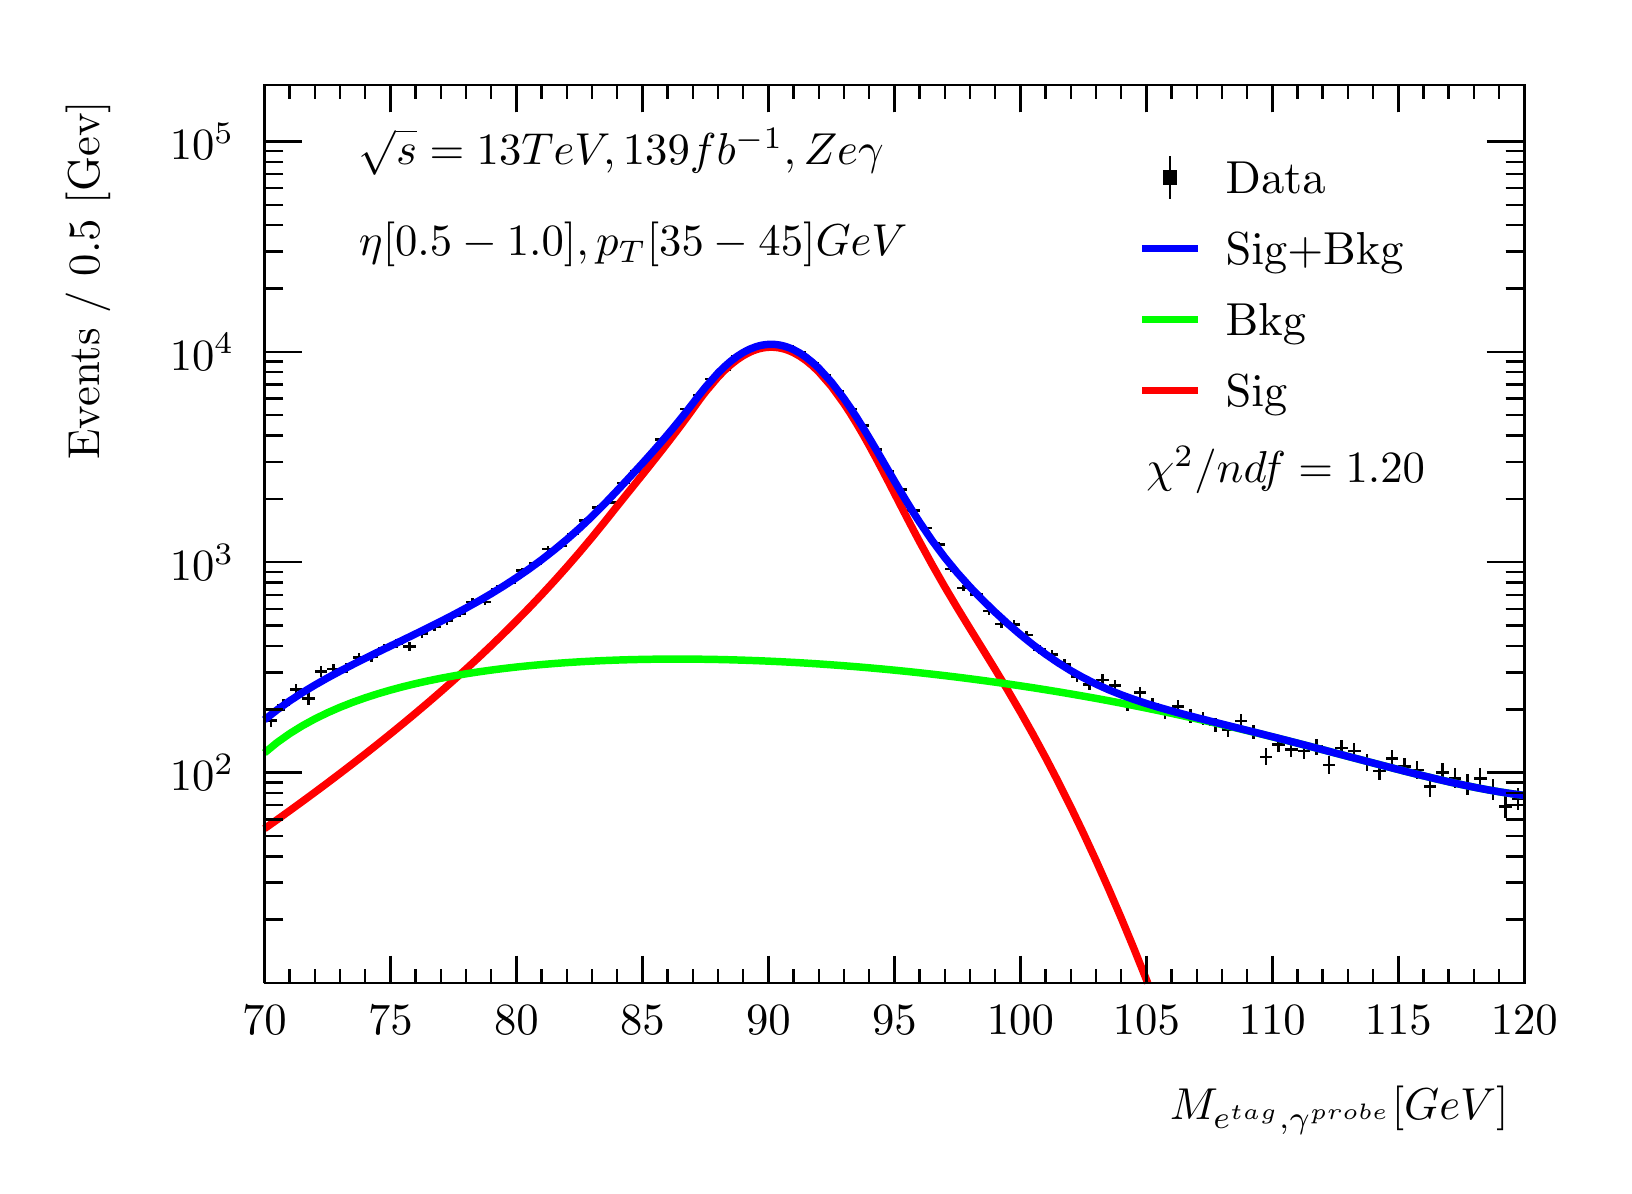
\begin{tikzpicture}
\pgfdeclareplotmark{cross} {
\pgfpathmoveto{\pgfpoint{-0.3\pgfplotmarksize}{\pgfplotmarksize}}
\pgfpathlineto{\pgfpoint{+0.3\pgfplotmarksize}{\pgfplotmarksize}}
\pgfpathlineto{\pgfpoint{+0.3\pgfplotmarksize}{0.3\pgfplotmarksize}}
\pgfpathlineto{\pgfpoint{+1\pgfplotmarksize}{0.3\pgfplotmarksize}}
\pgfpathlineto{\pgfpoint{+1\pgfplotmarksize}{-0.3\pgfplotmarksize}}
\pgfpathlineto{\pgfpoint{+0.3\pgfplotmarksize}{-0.3\pgfplotmarksize}}
\pgfpathlineto{\pgfpoint{+0.3\pgfplotmarksize}{-1.\pgfplotmarksize}}
\pgfpathlineto{\pgfpoint{-0.3\pgfplotmarksize}{-1.\pgfplotmarksize}}
\pgfpathlineto{\pgfpoint{-0.3\pgfplotmarksize}{-0.3\pgfplotmarksize}}
\pgfpathlineto{\pgfpoint{-1.\pgfplotmarksize}{-0.3\pgfplotmarksize}}
\pgfpathlineto{\pgfpoint{-1.\pgfplotmarksize}{0.3\pgfplotmarksize}}
\pgfpathlineto{\pgfpoint{-0.3\pgfplotmarksize}{0.3\pgfplotmarksize}}
\pgfpathclose
\pgfusepathqstroke
}
\pgfdeclareplotmark{cross*} {
\pgfpathmoveto{\pgfpoint{-0.3\pgfplotmarksize}{\pgfplotmarksize}}
\pgfpathlineto{\pgfpoint{+0.3\pgfplotmarksize}{\pgfplotmarksize}}
\pgfpathlineto{\pgfpoint{+0.3\pgfplotmarksize}{0.3\pgfplotmarksize}}
\pgfpathlineto{\pgfpoint{+1\pgfplotmarksize}{0.3\pgfplotmarksize}}
\pgfpathlineto{\pgfpoint{+1\pgfplotmarksize}{-0.3\pgfplotmarksize}}
\pgfpathlineto{\pgfpoint{+0.3\pgfplotmarksize}{-0.3\pgfplotmarksize}}
\pgfpathlineto{\pgfpoint{+0.3\pgfplotmarksize}{-1.\pgfplotmarksize}}
\pgfpathlineto{\pgfpoint{-0.3\pgfplotmarksize}{-1.\pgfplotmarksize}}
\pgfpathlineto{\pgfpoint{-0.3\pgfplotmarksize}{-0.3\pgfplotmarksize}}
\pgfpathlineto{\pgfpoint{-1.\pgfplotmarksize}{-0.3\pgfplotmarksize}}
\pgfpathlineto{\pgfpoint{-1.\pgfplotmarksize}{0.3\pgfplotmarksize}}
\pgfpathlineto{\pgfpoint{-0.3\pgfplotmarksize}{0.3\pgfplotmarksize}}
\pgfpathclose
\pgfusepathqfillstroke
}
\pgfdeclareplotmark{newstar} {
\pgfpathmoveto{\pgfqpoint{0pt}{\pgfplotmarksize}}
\pgfpathlineto{\pgfqpointpolar{44}{0.5\pgfplotmarksize}}
\pgfpathlineto{\pgfqpointpolar{18}{\pgfplotmarksize}}
\pgfpathlineto{\pgfqpointpolar{-20}{0.5\pgfplotmarksize}}
\pgfpathlineto{\pgfqpointpolar{-54}{\pgfplotmarksize}}
\pgfpathlineto{\pgfqpointpolar{-90}{0.5\pgfplotmarksize}}
\pgfpathlineto{\pgfqpointpolar{234}{\pgfplotmarksize}}
\pgfpathlineto{\pgfqpointpolar{198}{0.5\pgfplotmarksize}}
\pgfpathlineto{\pgfqpointpolar{162}{\pgfplotmarksize}}
\pgfpathlineto{\pgfqpointpolar{134}{0.5\pgfplotmarksize}}
\pgfpathclose
\pgfusepathqstroke
}
\pgfdeclareplotmark{newstar*} {
\pgfpathmoveto{\pgfqpoint{0pt}{\pgfplotmarksize}}
\pgfpathlineto{\pgfqpointpolar{44}{0.5\pgfplotmarksize}}
\pgfpathlineto{\pgfqpointpolar{18}{\pgfplotmarksize}}
\pgfpathlineto{\pgfqpointpolar{-20}{0.5\pgfplotmarksize}}
\pgfpathlineto{\pgfqpointpolar{-54}{\pgfplotmarksize}}
\pgfpathlineto{\pgfqpointpolar{-90}{0.5\pgfplotmarksize}}
\pgfpathlineto{\pgfqpointpolar{234}{\pgfplotmarksize}}
\pgfpathlineto{\pgfqpointpolar{198}{0.5\pgfplotmarksize}}
\pgfpathlineto{\pgfqpointpolar{162}{\pgfplotmarksize}}
\pgfpathlineto{\pgfqpointpolar{134}{0.5\pgfplotmarksize}}
\pgfpathclose
\pgfusepathqfillstroke
}
\definecolor{c}{rgb}{1,1,1};
\draw [color=c, fill=c] (0,0) rectangle (20,14.4361);
\draw [color=c, fill=c] (3,2.30977) rectangle (19,13.7143);
\definecolor{c}{rgb}{0,0,0};
\draw [c,line width=0.9] (3,2.30977) -- (3,13.7143) -- (19,13.7143) -- (19,2.30977) -- (3,2.30977);
\definecolor{c}{rgb}{1,1,1};
\draw [color=c, fill=c] (3,2.30977) rectangle (19,13.7143);
\definecolor{c}{rgb}{0,0,0};
\draw [c,line width=0.9] (3,2.30977) -- (3,13.7143) -- (19,13.7143) -- (19,2.30977) -- (3,2.30977);
\draw [c,line width=0.9] (3,2.30977) -- (19,2.30977);
\draw [c,line width=0.9] (3,2.65624) -- (3,2.30977);
\draw [c,line width=0.9] (3.32,2.48301) -- (3.32,2.30977);
\draw [c,line width=0.9] (3.64,2.48301) -- (3.64,2.30977);
\draw [c,line width=0.9] (3.96,2.48301) -- (3.96,2.30977);
\draw [c,line width=0.9] (4.28,2.48301) -- (4.28,2.30977);
\draw [c,line width=0.9] (4.6,2.65624) -- (4.6,2.30977);
\draw [c,line width=0.9] (4.92,2.48301) -- (4.92,2.30977);
\draw [c,line width=0.9] (5.24,2.48301) -- (5.24,2.30977);
\draw [c,line width=0.9] (5.56,2.48301) -- (5.56,2.30977);
\draw [c,line width=0.9] (5.88,2.48301) -- (5.88,2.30977);
\draw [c,line width=0.9] (6.2,2.65624) -- (6.2,2.30977);
\draw [c,line width=0.9] (6.52,2.48301) -- (6.52,2.30977);
\draw [c,line width=0.9] (6.84,2.48301) -- (6.84,2.30977);
\draw [c,line width=0.9] (7.16,2.48301) -- (7.16,2.30977);
\draw [c,line width=0.9] (7.48,2.48301) -- (7.48,2.30977);
\draw [c,line width=0.9] (7.8,2.65624) -- (7.8,2.30977);
\draw [c,line width=0.9] (8.12,2.48301) -- (8.12,2.30977);
\draw [c,line width=0.9] (8.44,2.48301) -- (8.44,2.30977);
\draw [c,line width=0.9] (8.76,2.48301) -- (8.76,2.30977);
\draw [c,line width=0.9] (9.08,2.48301) -- (9.08,2.30977);
\draw [c,line width=0.9] (9.4,2.65624) -- (9.4,2.30977);
\draw [c,line width=0.9] (9.72,2.48301) -- (9.72,2.30977);
\draw [c,line width=0.9] (10.04,2.48301) -- (10.04,2.30977);
\draw [c,line width=0.9] (10.36,2.48301) -- (10.36,2.30977);
\draw [c,line width=0.9] (10.68,2.48301) -- (10.68,2.30977);
\draw [c,line width=0.9] (11,2.65624) -- (11,2.30977);
\draw [c,line width=0.9] (11.32,2.48301) -- (11.32,2.30977);
\draw [c,line width=0.9] (11.64,2.48301) -- (11.64,2.30977);
\draw [c,line width=0.9] (11.96,2.48301) -- (11.96,2.30977);
\draw [c,line width=0.9] (12.28,2.48301) -- (12.28,2.30977);
\draw [c,line width=0.9] (12.6,2.65624) -- (12.6,2.30977);
\draw [c,line width=0.9] (12.92,2.48301) -- (12.92,2.30977);
\draw [c,line width=0.9] (13.24,2.48301) -- (13.24,2.30977);
\draw [c,line width=0.9] (13.56,2.48301) -- (13.56,2.30977);
\draw [c,line width=0.9] (13.88,2.48301) -- (13.88,2.30977);
\draw [c,line width=0.9] (14.2,2.65624) -- (14.2,2.30977);
\draw [c,line width=0.9] (14.52,2.48301) -- (14.52,2.30977);
\draw [c,line width=0.9] (14.84,2.48301) -- (14.84,2.30977);
\draw [c,line width=0.9] (15.16,2.48301) -- (15.16,2.30977);
\draw [c,line width=0.9] (15.48,2.48301) -- (15.48,2.30977);
\draw [c,line width=0.9] (15.8,2.65624) -- (15.8,2.30977);
\draw [c,line width=0.9] (16.12,2.48301) -- (16.12,2.30977);
\draw [c,line width=0.9] (16.44,2.48301) -- (16.44,2.30977);
\draw [c,line width=0.9] (16.76,2.48301) -- (16.76,2.30977);
\draw [c,line width=0.9] (17.08,2.48301) -- (17.08,2.30977);
\draw [c,line width=0.9] (17.4,2.65624) -- (17.4,2.30977);
\draw [c,line width=0.9] (17.72,2.48301) -- (17.72,2.30977);
\draw [c,line width=0.9] (18.04,2.48301) -- (18.04,2.30977);
\draw [c,line width=0.9] (18.36,2.48301) -- (18.36,2.30977);
\draw [c,line width=0.9] (18.68,2.48301) -- (18.68,2.30977);
\draw [c,line width=0.9] (19,2.65624) -- (19,2.30977);
\draw [anchor=base] (3,1.66015) node[scale=1.61424, color=c, rotate=0]{70};
\draw [anchor=base] (4.6,1.66015) node[scale=1.61424, color=c, rotate=0]{75};
\draw [anchor=base] (6.2,1.66015) node[scale=1.61424, color=c, rotate=0]{80};
\draw [anchor=base] (7.8,1.66015) node[scale=1.61424, color=c, rotate=0]{85};
\draw [anchor=base] (9.4,1.66015) node[scale=1.61424, color=c, rotate=0]{90};
\draw [anchor=base] (11,1.66015) node[scale=1.61424, color=c, rotate=0]{95};
\draw [anchor=base] (12.6,1.66015) node[scale=1.61424, color=c, rotate=0]{100};
\draw [anchor=base] (14.2,1.66015) node[scale=1.61424, color=c, rotate=0]{105};
\draw [anchor=base] (15.8,1.66015) node[scale=1.61424, color=c, rotate=0]{110};
\draw [anchor=base] (17.4,1.66015) node[scale=1.61424, color=c, rotate=0]{115};
\draw [anchor=base] (19,1.66015) node[scale=1.61424, color=c, rotate=0]{120};
\draw [anchor= east] (19,0.692932) node[scale=1.61424, color=c, rotate=0]{$M_{e^{tag}, \gamma^{probe}}  [GeV]$};
\draw [c,line width=0.9] (3,13.7143) -- (19,13.7143);
\draw [c,line width=0.9] (3,13.3678) -- (3,13.7143);
\draw [c,line width=0.9] (3.32,13.5411) -- (3.32,13.7143);
\draw [c,line width=0.9] (3.64,13.5411) -- (3.64,13.7143);
\draw [c,line width=0.9] (3.96,13.5411) -- (3.96,13.7143);
\draw [c,line width=0.9] (4.28,13.5411) -- (4.28,13.7143);
\draw [c,line width=0.9] (4.6,13.3678) -- (4.6,13.7143);
\draw [c,line width=0.9] (4.92,13.5411) -- (4.92,13.7143);
\draw [c,line width=0.9] (5.24,13.5411) -- (5.24,13.7143);
\draw [c,line width=0.9] (5.56,13.5411) -- (5.56,13.7143);
\draw [c,line width=0.9] (5.88,13.5411) -- (5.88,13.7143);
\draw [c,line width=0.9] (6.2,13.3678) -- (6.2,13.7143);
\draw [c,line width=0.9] (6.52,13.5411) -- (6.52,13.7143);
\draw [c,line width=0.9] (6.84,13.5411) -- (6.84,13.7143);
\draw [c,line width=0.9] (7.16,13.5411) -- (7.16,13.7143);
\draw [c,line width=0.9] (7.48,13.5411) -- (7.48,13.7143);
\draw [c,line width=0.9] (7.8,13.3678) -- (7.8,13.7143);
\draw [c,line width=0.9] (8.12,13.5411) -- (8.12,13.7143);
\draw [c,line width=0.9] (8.44,13.5411) -- (8.44,13.7143);
\draw [c,line width=0.9] (8.76,13.5411) -- (8.76,13.7143);
\draw [c,line width=0.9] (9.08,13.5411) -- (9.08,13.7143);
\draw [c,line width=0.9] (9.4,13.3678) -- (9.4,13.7143);
\draw [c,line width=0.9] (9.72,13.5411) -- (9.72,13.7143);
\draw [c,line width=0.9] (10.04,13.5411) -- (10.04,13.7143);
\draw [c,line width=0.9] (10.36,13.5411) -- (10.36,13.7143);
\draw [c,line width=0.9] (10.68,13.5411) -- (10.68,13.7143);
\draw [c,line width=0.9] (11,13.3678) -- (11,13.7143);
\draw [c,line width=0.9] (11.32,13.5411) -- (11.32,13.7143);
\draw [c,line width=0.9] (11.64,13.5411) -- (11.64,13.7143);
\draw [c,line width=0.9] (11.96,13.5411) -- (11.96,13.7143);
\draw [c,line width=0.9] (12.28,13.5411) -- (12.28,13.7143);
\draw [c,line width=0.9] (12.6,13.3678) -- (12.6,13.7143);
\draw [c,line width=0.9] (12.92,13.5411) -- (12.92,13.7143);
\draw [c,line width=0.9] (13.24,13.5411) -- (13.24,13.7143);
\draw [c,line width=0.9] (13.56,13.5411) -- (13.56,13.7143);
\draw [c,line width=0.9] (13.88,13.5411) -- (13.88,13.7143);
\draw [c,line width=0.9] (14.2,13.3678) -- (14.2,13.7143);
\draw [c,line width=0.9] (14.52,13.5411) -- (14.52,13.7143);
\draw [c,line width=0.9] (14.84,13.5411) -- (14.84,13.7143);
\draw [c,line width=0.9] (15.16,13.5411) -- (15.16,13.7143);
\draw [c,line width=0.9] (15.48,13.5411) -- (15.48,13.7143);
\draw [c,line width=0.9] (15.8,13.3678) -- (15.8,13.7143);
\draw [c,line width=0.9] (16.12,13.5411) -- (16.12,13.7143);
\draw [c,line width=0.9] (16.44,13.5411) -- (16.44,13.7143);
\draw [c,line width=0.9] (16.76,13.5411) -- (16.76,13.7143);
\draw [c,line width=0.9] (17.08,13.5411) -- (17.08,13.7143);
\draw [c,line width=0.9] (17.4,13.3678) -- (17.4,13.7143);
\draw [c,line width=0.9] (17.72,13.5411) -- (17.72,13.7143);
\draw [c,line width=0.9] (18.04,13.5411) -- (18.04,13.7143);
\draw [c,line width=0.9] (18.36,13.5411) -- (18.36,13.7143);
\draw [c,line width=0.9] (18.68,13.5411) -- (18.68,13.7143);
\draw [c,line width=0.9] (19,13.3678) -- (19,13.7143);
\draw [c,line width=0.9] (3,2.30977) -- (3,13.7143);
\draw [c,line width=0.9] (3.237,3.11414) -- (3,3.11414);
\draw [c,line width=0.9] (3.237,3.58467) -- (3,3.58467);
\draw [c,line width=0.9] (3.237,3.91852) -- (3,3.91852);
\draw [c,line width=0.9] (3.237,4.17747) -- (3,4.17747);
\draw [c,line width=0.9] (3.237,4.38904) -- (3,4.38904);
\draw [c,line width=0.9] (3.237,4.56793) -- (3,4.56793);
\draw [c,line width=0.9] (3.237,4.72289) -- (3,4.72289);
\draw [c,line width=0.9] (3.237,4.85957) -- (3,4.85957);
\draw [c,line width=0.9] (3.474,4.98184) -- (3,4.98184);
\draw [anchor= east] (2.82,4.98184) node[scale=1.61424, color=c, rotate=0]{$10^{2}$};
\draw [c,line width=0.9] (3.237,5.78621) -- (3,5.78621);
\draw [c,line width=0.9] (3.237,6.25674) -- (3,6.25674);
\draw [c,line width=0.9] (3.237,6.59058) -- (3,6.59058);
\draw [c,line width=0.9] (3.237,6.84953) -- (3,6.84953);
\draw [c,line width=0.9] (3.237,7.06111) -- (3,7.06111);
\draw [c,line width=0.9] (3.237,7.24) -- (3,7.24);
\draw [c,line width=0.9] (3.237,7.39496) -- (3,7.39496);
\draw [c,line width=0.9] (3.237,7.53164) -- (3,7.53164);
\draw [c,line width=0.9] (3.474,7.65391) -- (3,7.65391);
\draw [anchor= east] (2.82,7.65391) node[scale=1.61424, color=c, rotate=0]{$10^{3}$};
\draw [c,line width=0.9] (3.237,8.45828) -- (3,8.45828);
\draw [c,line width=0.9] (3.237,8.92881) -- (3,8.92881);
\draw [c,line width=0.9] (3.237,9.26265) -- (3,9.26265);
\draw [c,line width=0.9] (3.237,9.5216) -- (3,9.5216);
\draw [c,line width=0.9] (3.237,9.73318) -- (3,9.73318);
\draw [c,line width=0.9] (3.237,9.91207) -- (3,9.91207);
\draw [c,line width=0.9] (3.237,10.067) -- (3,10.067);
\draw [c,line width=0.9] (3.237,10.2037) -- (3,10.2037);
\draw [c,line width=0.9] (3.474,10.326) -- (3,10.326);
\draw [anchor= east] (2.82,10.326) node[scale=1.61424, color=c, rotate=0]{$10^{4}$};
\draw [c,line width=0.9] (3.237,11.1303) -- (3,11.1303);
\draw [c,line width=0.9] (3.237,11.6009) -- (3,11.6009);
\draw [c,line width=0.9] (3.237,11.9347) -- (3,11.9347);
\draw [c,line width=0.9] (3.237,12.1937) -- (3,12.1937);
\draw [c,line width=0.9] (3.237,12.4052) -- (3,12.4052);
\draw [c,line width=0.9] (3.237,12.5841) -- (3,12.5841);
\draw [c,line width=0.9] (3.237,12.7391) -- (3,12.7391);
\draw [c,line width=0.9] (3.237,12.8758) -- (3,12.8758);
\draw [c,line width=0.9] (3.474,12.998) -- (3,12.998);
\draw [anchor= east] (2.82,12.998) node[scale=1.61424, color=c, rotate=0]{$10^{5}$};
\draw [anchor= east] (0.76,13.7143) node[scale=1.61424, color=c, rotate=90]{Events / 0.5 [Gev]};
\draw [c,line width=0.9] (19,2.30977) -- (19,13.7143);
\draw [c,line width=0.9] (18.763,3.11414) -- (19,3.11414);
\draw [c,line width=0.9] (18.763,3.58467) -- (19,3.58467);
\draw [c,line width=0.9] (18.763,3.91852) -- (19,3.91852);
\draw [c,line width=0.9] (18.763,4.17747) -- (19,4.17747);
\draw [c,line width=0.9] (18.763,4.38904) -- (19,4.38904);
\draw [c,line width=0.9] (18.763,4.56793) -- (19,4.56793);
\draw [c,line width=0.9] (18.763,4.72289) -- (19,4.72289);
\draw [c,line width=0.9] (18.763,4.85957) -- (19,4.85957);
\draw [c,line width=0.9] (18.526,4.98184) -- (19,4.98184);
\draw [c,line width=0.9] (18.763,5.78621) -- (19,5.78621);
\draw [c,line width=0.9] (18.763,6.25674) -- (19,6.25674);
\draw [c,line width=0.9] (18.763,6.59058) -- (19,6.59058);
\draw [c,line width=0.9] (18.763,6.84953) -- (19,6.84953);
\draw [c,line width=0.9] (18.763,7.06111) -- (19,7.06111);
\draw [c,line width=0.9] (18.763,7.24) -- (19,7.24);
\draw [c,line width=0.9] (18.763,7.39496) -- (19,7.39496);
\draw [c,line width=0.9] (18.763,7.53164) -- (19,7.53164);
\draw [c,line width=0.9] (18.526,7.65391) -- (19,7.65391);
\draw [c,line width=0.9] (18.763,8.45828) -- (19,8.45828);
\draw [c,line width=0.9] (18.763,8.92881) -- (19,8.92881);
\draw [c,line width=0.9] (18.763,9.26265) -- (19,9.26265);
\draw [c,line width=0.9] (18.763,9.5216) -- (19,9.5216);
\draw [c,line width=0.9] (18.763,9.73318) -- (19,9.73318);
\draw [c,line width=0.9] (18.763,9.91207) -- (19,9.91207);
\draw [c,line width=0.9] (18.763,10.067) -- (19,10.067);
\draw [c,line width=0.9] (18.763,10.2037) -- (19,10.2037);
\draw [c,line width=0.9] (18.526,10.326) -- (19,10.326);
\draw [c,line width=0.9] (18.763,11.1303) -- (19,11.1303);
\draw [c,line width=0.9] (18.763,11.6009) -- (19,11.6009);
\draw [c,line width=0.9] (18.763,11.9347) -- (19,11.9347);
\draw [c,line width=0.9] (18.763,12.1937) -- (19,12.1937);
\draw [c,line width=0.9] (18.763,12.4052) -- (19,12.4052);
\draw [c,line width=0.9] (18.763,12.5841) -- (19,12.5841);
\draw [c,line width=0.9] (18.763,12.7391) -- (19,12.7391);
\draw [c,line width=0.9] (18.763,12.8758) -- (19,12.8758);
\draw [c,line width=0.9] (18.526,12.998) -- (19,12.998);
\draw [c,line width=0.9] (3.08,5.64444) -- (3,5.64444);
\draw [c,line width=0.9] (3,5.64444) -- (3,5.64444);
\draw [c,line width=0.9] (3.08,5.64444) -- (3.16,5.64444);
\draw [c,line width=0.9] (3.16,5.64444) -- (3.16,5.64444);
\draw [c,line width=0.9] (3.08,5.64444) -- (3.08,5.73165);
\draw [c,line width=0.9] (3.08,5.73165) -- (3.08,5.73165);
\draw [c,line width=0.9] (3.08,5.64444) -- (3.08,5.55724);
\draw [c,line width=0.9] (3.08,5.55724) -- (3.08,5.55724);
\draw [c,line width=0.9] (3.24,5.84283) -- (3.16,5.84283);
\draw [c,line width=0.9] (3.16,5.84283) -- (3.16,5.84283);
\draw [c,line width=0.9] (3.24,5.84283) -- (3.32,5.84283);
\draw [c,line width=0.9] (3.32,5.84283) -- (3.32,5.84283);
\draw [c,line width=0.9] (3.24,5.84283) -- (3.24,5.9229);
\draw [c,line width=0.9] (3.24,5.9229) -- (3.24,5.9229);
\draw [c,line width=0.9] (3.24,5.84283) -- (3.24,5.76277);
\draw [c,line width=0.9] (3.24,5.76277) -- (3.24,5.76277);
\draw [c,line width=0.9] (3.4,6.03584) -- (3.32,6.03584);
\draw [c,line width=0.9] (3.32,6.03584) -- (3.32,6.03584);
\draw [c,line width=0.9] (3.4,6.03584) -- (3.48,6.03584);
\draw [c,line width=0.9] (3.48,6.03584) -- (3.48,6.03584);
\draw [c,line width=0.9] (3.4,6.03584) -- (3.4,6.10952);
\draw [c,line width=0.9] (3.4,6.10952) -- (3.4,6.10952);
\draw [c,line width=0.9] (3.4,6.03584) -- (3.4,5.96217);
\draw [c,line width=0.9] (3.4,5.96217) -- (3.4,5.96217);
\draw [c,line width=0.9] (3.56,5.9229) -- (3.48,5.9229);
\draw [c,line width=0.9] (3.48,5.9229) -- (3.48,5.9229);
\draw [c,line width=0.9] (3.56,5.9229) -- (3.64,5.9229);
\draw [c,line width=0.9] (3.64,5.9229) -- (3.64,5.9229);
\draw [c,line width=0.9] (3.56,5.9229) -- (3.56,6.00025);
\draw [c,line width=0.9] (3.56,6.00025) -- (3.56,6.00025);
\draw [c,line width=0.9] (3.56,5.9229) -- (3.56,5.84555);
\draw [c,line width=0.9] (3.56,5.84555) -- (3.56,5.84555);
\draw [c,line width=0.9] (3.72,6.26445) -- (3.64,6.26445);
\draw [c,line width=0.9] (3.64,6.26445) -- (3.64,6.26445);
\draw [c,line width=0.9] (3.72,6.26445) -- (3.8,6.26445);
\draw [c,line width=0.9] (3.8,6.26445) -- (3.8,6.26445);
\draw [c,line width=0.9] (3.72,6.26445) -- (3.72,6.33122);
\draw [c,line width=0.9] (3.72,6.33122) -- (3.72,6.33122);
\draw [c,line width=0.9] (3.72,6.26445) -- (3.72,6.19768);
\draw [c,line width=0.9] (3.72,6.19768) -- (3.72,6.19768);
\draw [c,line width=0.9] (3.88,6.29853) -- (3.8,6.29853);
\draw [c,line width=0.9] (3.8,6.29853) -- (3.8,6.29853);
\draw [c,line width=0.9] (3.88,6.29853) -- (3.96,6.29853);
\draw [c,line width=0.9] (3.96,6.29853) -- (3.96,6.29853);
\draw [c,line width=0.9] (3.88,6.29853) -- (3.88,6.36433);
\draw [c,line width=0.9] (3.88,6.36433) -- (3.88,6.36433);
\draw [c,line width=0.9] (3.88,6.29853) -- (3.88,6.23273);
\draw [c,line width=0.9] (3.88,6.23273) -- (3.88,6.23273);
\draw [c,line width=0.9] (4.04,6.30967) -- (3.96,6.30967);
\draw [c,line width=0.9] (3.96,6.30967) -- (3.96,6.30967);
\draw [c,line width=0.9] (4.04,6.30967) -- (4.12,6.30967);
\draw [c,line width=0.9] (4.12,6.30967) -- (4.12,6.30967);
\draw [c,line width=0.9] (4.04,6.30967) -- (4.04,6.37515);
\draw [c,line width=0.9] (4.04,6.37515) -- (4.04,6.37515);
\draw [c,line width=0.9] (4.04,6.30967) -- (4.04,6.24419);
\draw [c,line width=0.9] (4.04,6.24419) -- (4.04,6.24419);
\draw [c,line width=0.9] (4.2,6.44553) -- (4.12,6.44553);
\draw [c,line width=0.9] (4.12,6.44553) -- (4.12,6.44553);
\draw [c,line width=0.9] (4.2,6.44553) -- (4.28,6.44553);
\draw [c,line width=0.9] (4.28,6.44553) -- (4.28,6.44553);
\draw [c,line width=0.9] (4.2,6.44553) -- (4.2,6.50729);
\draw [c,line width=0.9] (4.2,6.50729) -- (4.2,6.50729);
\draw [c,line width=0.9] (4.2,6.44553) -- (4.2,6.38377);
\draw [c,line width=0.9] (4.2,6.38377) -- (4.2,6.38377);
\draw [c,line width=0.9] (4.36,6.45209) -- (4.28,6.45209);
\draw [c,line width=0.9] (4.28,6.45209) -- (4.28,6.45209);
\draw [c,line width=0.9] (4.36,6.45209) -- (4.44,6.45209);
\draw [c,line width=0.9] (4.44,6.45209) -- (4.44,6.45209);
\draw [c,line width=0.9] (4.36,6.45209) -- (4.36,6.51367);
\draw [c,line width=0.9] (4.36,6.51367) -- (4.36,6.51367);
\draw [c,line width=0.9] (4.36,6.45209) -- (4.36,6.3905);
\draw [c,line width=0.9] (4.36,6.3905) -- (4.36,6.3905);
\draw [c,line width=0.9] (4.52,6.55823) -- (4.44,6.55823);
\draw [c,line width=0.9] (4.44,6.55823) -- (4.44,6.55823);
\draw [c,line width=0.9] (4.52,6.55823) -- (4.6,6.55823);
\draw [c,line width=0.9] (4.6,6.55823) -- (4.6,6.55823);
\draw [c,line width=0.9] (4.52,6.55823) -- (4.52,6.61706);
\draw [c,line width=0.9] (4.52,6.61706) -- (4.52,6.61706);
\draw [c,line width=0.9] (4.52,6.55823) -- (4.52,6.49939);
\draw [c,line width=0.9] (4.52,6.49939) -- (4.52,6.49939);
\draw [c,line width=0.9] (4.68,6.61641) -- (4.6,6.61641);
\draw [c,line width=0.9] (4.6,6.61641) -- (4.6,6.61641);
\draw [c,line width=0.9] (4.68,6.61641) -- (4.76,6.61641);
\draw [c,line width=0.9] (4.76,6.61641) -- (4.76,6.61641);
\draw [c,line width=0.9] (4.68,6.61641) -- (4.68,6.67378);
\draw [c,line width=0.9] (4.68,6.67378) -- (4.68,6.67378);
\draw [c,line width=0.9] (4.68,6.61641) -- (4.68,6.55903);
\draw [c,line width=0.9] (4.68,6.55903) -- (4.68,6.55903);
\draw [c,line width=0.9] (4.84,6.58477) -- (4.76,6.58477);
\draw [c,line width=0.9] (4.76,6.58477) -- (4.76,6.58477);
\draw [c,line width=0.9] (4.84,6.58477) -- (4.92,6.58477);
\draw [c,line width=0.9] (4.92,6.58477) -- (4.92,6.58477);
\draw [c,line width=0.9] (4.84,6.58477) -- (4.84,6.64293);
\draw [c,line width=0.9] (4.84,6.64293) -- (4.84,6.64293);
\draw [c,line width=0.9] (4.84,6.58477) -- (4.84,6.52661);
\draw [c,line width=0.9] (4.84,6.52661) -- (4.84,6.52661);
\draw [c,line width=0.9] (5,6.74772) -- (4.92,6.74772);
\draw [c,line width=0.9] (4.92,6.74772) -- (4.92,6.74772);
\draw [c,line width=0.9] (5,6.74772) -- (5.08,6.74772);
\draw [c,line width=0.9] (5.08,6.74772) -- (5.08,6.74772);
\draw [c,line width=0.9] (5,6.74772) -- (5,6.80194);
\draw [c,line width=0.9] (5,6.80194) -- (5,6.80194);
\draw [c,line width=0.9] (5,6.74772) -- (5,6.6935);
\draw [c,line width=0.9] (5,6.6935) -- (5,6.6935);
\draw [c,line width=0.9] (5.16,6.83317) -- (5.08,6.83317);
\draw [c,line width=0.9] (5.08,6.83317) -- (5.08,6.83317);
\draw [c,line width=0.9] (5.16,6.83317) -- (5.24,6.83317);
\draw [c,line width=0.9] (5.24,6.83317) -- (5.24,6.83317);
\draw [c,line width=0.9] (5.16,6.83317) -- (5.16,6.88543);
\draw [c,line width=0.9] (5.16,6.88543) -- (5.16,6.88543);
\draw [c,line width=0.9] (5.16,6.83317) -- (5.16,6.78091);
\draw [c,line width=0.9] (5.16,6.78091) -- (5.16,6.78091);
\draw [c,line width=0.9] (5.32,6.91277) -- (5.24,6.91277);
\draw [c,line width=0.9] (5.24,6.91277) -- (5.24,6.91277);
\draw [c,line width=0.9] (5.32,6.91277) -- (5.4,6.91277);
\draw [c,line width=0.9] (5.4,6.91277) -- (5.4,6.91277);
\draw [c,line width=0.9] (5.32,6.91277) -- (5.32,6.96327);
\draw [c,line width=0.9] (5.32,6.96327) -- (5.32,6.96327);
\draw [c,line width=0.9] (5.32,6.91277) -- (5.32,6.86227);
\draw [c,line width=0.9] (5.32,6.86227) -- (5.32,6.86227);
\draw [c,line width=0.9] (5.48,7.00565) -- (5.4,7.00565);
\draw [c,line width=0.9] (5.4,7.00565) -- (5.4,7.00565);
\draw [c,line width=0.9] (5.48,7.00565) -- (5.56,7.00565);
\draw [c,line width=0.9] (5.56,7.00565) -- (5.56,7.00565);
\draw [c,line width=0.9] (5.48,7.00565) -- (5.48,7.05417);
\draw [c,line width=0.9] (5.48,7.05417) -- (5.48,7.05417);
\draw [c,line width=0.9] (5.48,7.00565) -- (5.48,6.95714);
\draw [c,line width=0.9] (5.48,6.95714) -- (5.48,6.95714);
\draw [c,line width=0.9] (5.64,7.15042) -- (5.56,7.15042);
\draw [c,line width=0.9] (5.56,7.15042) -- (5.56,7.15042);
\draw [c,line width=0.9] (5.64,7.15042) -- (5.72,7.15042);
\draw [c,line width=0.9] (5.72,7.15042) -- (5.72,7.15042);
\draw [c,line width=0.9] (5.64,7.15042) -- (5.64,7.19601);
\draw [c,line width=0.9] (5.64,7.19601) -- (5.64,7.19601);
\draw [c,line width=0.9] (5.64,7.15042) -- (5.64,7.10484);
\draw [c,line width=0.9] (5.64,7.10484) -- (5.64,7.10484);
\draw [c,line width=0.9] (5.8,7.15042) -- (5.72,7.15042);
\draw [c,line width=0.9] (5.72,7.15042) -- (5.72,7.15042);
\draw [c,line width=0.9] (5.8,7.15042) -- (5.88,7.15042);
\draw [c,line width=0.9] (5.88,7.15042) -- (5.88,7.15042);
\draw [c,line width=0.9] (5.8,7.15042) -- (5.8,7.19601);
\draw [c,line width=0.9] (5.8,7.19601) -- (5.8,7.19601);
\draw [c,line width=0.9] (5.8,7.15042) -- (5.8,7.10484);
\draw [c,line width=0.9] (5.8,7.10484) -- (5.8,7.10484);
\draw [c,line width=0.9] (5.96,7.31696) -- (5.88,7.31696);
\draw [c,line width=0.9] (5.88,7.31696) -- (5.88,7.31696);
\draw [c,line width=0.9] (5.96,7.31696) -- (6.04,7.31696);
\draw [c,line width=0.9] (6.04,7.31696) -- (6.04,7.31696);
\draw [c,line width=0.9] (5.96,7.31696) -- (5.96,7.35939);
\draw [c,line width=0.9] (5.96,7.35939) -- (5.96,7.35939);
\draw [c,line width=0.9] (5.96,7.31696) -- (5.96,7.27454);
\draw [c,line width=0.9] (5.96,7.27454) -- (5.96,7.27454);
\draw [c,line width=0.9] (6.12,7.3993) -- (6.04,7.3993);
\draw [c,line width=0.9] (6.04,7.3993) -- (6.04,7.3993);
\draw [c,line width=0.9] (6.12,7.3993) -- (6.2,7.3993);
\draw [c,line width=0.9] (6.2,7.3993) -- (6.2,7.3993);
\draw [c,line width=0.9] (6.12,7.3993) -- (6.12,7.44025);
\draw [c,line width=0.9] (6.12,7.44025) -- (6.12,7.44025);
\draw [c,line width=0.9] (6.12,7.3993) -- (6.12,7.35835);
\draw [c,line width=0.9] (6.12,7.35835) -- (6.12,7.35835);
\draw [c,line width=0.9] (6.28,7.54701) -- (6.2,7.54701);
\draw [c,line width=0.9] (6.2,7.54701) -- (6.2,7.54701);
\draw [c,line width=0.9] (6.28,7.54701) -- (6.36,7.54701);
\draw [c,line width=0.9] (6.36,7.54701) -- (6.36,7.54701);
\draw [c,line width=0.9] (6.28,7.54701) -- (6.28,7.58544);
\draw [c,line width=0.9] (6.28,7.58544) -- (6.28,7.58544);
\draw [c,line width=0.9] (6.28,7.54701) -- (6.28,7.50859);
\draw [c,line width=0.9] (6.28,7.50859) -- (6.28,7.50859);
\draw [c,line width=0.9] (6.44,7.63755) -- (6.36,7.63755);
\draw [c,line width=0.9] (6.36,7.63755) -- (6.36,7.63755);
\draw [c,line width=0.9] (6.44,7.63755) -- (6.52,7.63755);
\draw [c,line width=0.9] (6.52,7.63755) -- (6.52,7.63755);
\draw [c,line width=0.9] (6.44,7.63755) -- (6.44,7.6745);
\draw [c,line width=0.9] (6.44,7.6745) -- (6.44,7.6745);
\draw [c,line width=0.9] (6.44,7.63755) -- (6.44,7.60059);
\draw [c,line width=0.9] (6.44,7.60059) -- (6.44,7.60059);
\draw [c,line width=0.9] (6.6,7.82113) -- (6.52,7.82113);
\draw [c,line width=0.9] (6.52,7.82113) -- (6.52,7.82113);
\draw [c,line width=0.9] (6.6,7.82113) -- (6.68,7.82113);
\draw [c,line width=0.9] (6.68,7.82113) -- (6.68,7.82113);
\draw [c,line width=0.9] (6.6,7.82113) -- (6.6,7.85528);
\draw [c,line width=0.9] (6.6,7.85528) -- (6.6,7.85528);
\draw [c,line width=0.9] (6.6,7.82113) -- (6.6,7.78699);
\draw [c,line width=0.9] (6.6,7.78699) -- (6.6,7.78699);
\draw [c,line width=0.9] (6.76,7.8587) -- (6.68,7.8587);
\draw [c,line width=0.9] (6.68,7.8587) -- (6.68,7.8587);
\draw [c,line width=0.9] (6.76,7.8587) -- (6.84,7.8587);
\draw [c,line width=0.9] (6.84,7.8587) -- (6.84,7.8587);
\draw [c,line width=0.9] (6.76,7.8587) -- (6.76,7.89229);
\draw [c,line width=0.9] (6.76,7.89229) -- (6.76,7.89229);
\draw [c,line width=0.9] (6.76,7.8587) -- (6.76,7.8251);
\draw [c,line width=0.9] (6.76,7.8251) -- (6.76,7.8251);
\draw [c,line width=0.9] (6.92,8.00988) -- (6.84,8.00988);
\draw [c,line width=0.9] (6.84,8.00988) -- (6.84,8.00988);
\draw [c,line width=0.9] (6.92,8.00988) -- (7,8.00988);
\draw [c,line width=0.9] (7,8.00988) -- (7,8.00988);
\draw [c,line width=0.9] (6.92,8.00988) -- (6.92,8.04136);
\draw [c,line width=0.9] (6.92,8.04136) -- (6.92,8.04136);
\draw [c,line width=0.9] (6.92,8.00988) -- (6.92,7.9784);
\draw [c,line width=0.9] (6.92,7.9784) -- (6.92,7.9784);
\draw [c,line width=0.9] (7.08,8.1862) -- (7,8.1862);
\draw [c,line width=0.9] (7,8.1862) -- (7,8.1862);
\draw [c,line width=0.9] (7.08,8.1862) -- (7.16,8.1862);
\draw [c,line width=0.9] (7.16,8.1862) -- (7.16,8.1862);
\draw [c,line width=0.9] (7.08,8.1862) -- (7.08,8.21538);
\draw [c,line width=0.9] (7.08,8.21538) -- (7.08,8.21538);
\draw [c,line width=0.9] (7.08,8.1862) -- (7.08,8.15703);
\draw [c,line width=0.9] (7.08,8.15703) -- (7.08,8.15703);
\draw [c,line width=0.9] (7.24,8.34756) -- (7.16,8.34756);
\draw [c,line width=0.9] (7.16,8.34756) -- (7.16,8.34756);
\draw [c,line width=0.9] (7.24,8.34756) -- (7.32,8.34756);
\draw [c,line width=0.9] (7.32,8.34756) -- (7.32,8.34756);
\draw [c,line width=0.9] (7.24,8.34756) -- (7.24,8.37478);
\draw [c,line width=0.9] (7.24,8.37478) -- (7.24,8.37478);
\draw [c,line width=0.9] (7.24,8.34756) -- (7.24,8.32034);
\draw [c,line width=0.9] (7.24,8.32034) -- (7.24,8.32034);
\draw [c,line width=0.9] (7.4,8.41513) -- (7.32,8.41513);
\draw [c,line width=0.9] (7.32,8.41513) -- (7.32,8.41513);
\draw [c,line width=0.9] (7.4,8.41513) -- (7.48,8.41513);
\draw [c,line width=0.9] (7.48,8.41513) -- (7.48,8.41513);
\draw [c,line width=0.9] (7.4,8.41513) -- (7.4,8.44157);
\draw [c,line width=0.9] (7.4,8.44157) -- (7.4,8.44157);
\draw [c,line width=0.9] (7.4,8.41513) -- (7.4,8.3887);
\draw [c,line width=0.9] (7.4,8.3887) -- (7.4,8.3887);
\draw [c,line width=0.9] (7.56,8.66307) -- (7.48,8.66307);
\draw [c,line width=0.9] (7.48,8.66307) -- (7.48,8.66307);
\draw [c,line width=0.9] (7.56,8.66307) -- (7.64,8.66307);
\draw [c,line width=0.9] (7.64,8.66307) -- (7.64,8.66307);
\draw [c,line width=0.9] (7.56,8.66307) -- (7.56,8.68683);
\draw [c,line width=0.9] (7.56,8.68683) -- (7.56,8.68683);
\draw [c,line width=0.9] (7.56,8.66307) -- (7.56,8.63931);
\draw [c,line width=0.9] (7.56,8.63931) -- (7.56,8.63931);
\draw [c,line width=0.9] (7.72,8.80439) -- (7.64,8.80439);
\draw [c,line width=0.9] (7.64,8.80439) -- (7.64,8.80439);
\draw [c,line width=0.9] (7.72,8.80439) -- (7.8,8.80439);
\draw [c,line width=0.9] (7.8,8.80439) -- (7.8,8.80439);
\draw [c,line width=0.9] (7.72,8.80439) -- (7.72,8.82674);
\draw [c,line width=0.9] (7.72,8.82674) -- (7.72,8.82674);
\draw [c,line width=0.9] (7.72,8.80439) -- (7.72,8.78204);
\draw [c,line width=0.9] (7.72,8.78204) -- (7.72,8.78204);
\draw [c,line width=0.9] (7.88,8.96761) -- (7.8,8.96761);
\draw [c,line width=0.9] (7.8,8.96761) -- (7.8,8.96761);
\draw [c,line width=0.9] (7.88,8.96761) -- (7.96,8.96761);
\draw [c,line width=0.9] (7.96,8.96761) -- (7.96,8.96761);
\draw [c,line width=0.9] (7.88,8.96761) -- (7.88,8.98844);
\draw [c,line width=0.9] (7.88,8.98844) -- (7.88,8.98844);
\draw [c,line width=0.9] (7.88,8.96761) -- (7.88,8.94677);
\draw [c,line width=0.9] (7.88,8.94677) -- (7.88,8.94677);
\draw [c,line width=0.9] (8.04,9.21377) -- (7.96,9.21377);
\draw [c,line width=0.9] (7.96,9.21377) -- (7.96,9.21377);
\draw [c,line width=0.9] (8.04,9.21377) -- (8.12,9.21377);
\draw [c,line width=0.9] (8.12,9.21377) -- (8.12,9.21377);
\draw [c,line width=0.9] (8.04,9.21377) -- (8.04,9.23251);
\draw [c,line width=0.9] (8.04,9.23251) -- (8.04,9.23251);
\draw [c,line width=0.9] (8.04,9.21377) -- (8.04,9.19503);
\draw [c,line width=0.9] (8.04,9.19503) -- (8.04,9.19503);
\draw [c,line width=0.9] (8.2,9.34523) -- (8.12,9.34523);
\draw [c,line width=0.9] (8.12,9.34523) -- (8.12,9.34523);
\draw [c,line width=0.9] (8.2,9.34523) -- (8.28,9.34523);
\draw [c,line width=0.9] (8.28,9.34523) -- (8.28,9.34523);
\draw [c,line width=0.9] (8.2,9.34523) -- (8.2,9.36294);
\draw [c,line width=0.9] (8.2,9.36294) -- (8.2,9.36294);
\draw [c,line width=0.9] (8.2,9.34523) -- (8.2,9.32752);
\draw [c,line width=0.9] (8.2,9.32752) -- (8.2,9.32752);
\draw [c,line width=0.9] (8.36,9.60055) -- (8.28,9.60055);
\draw [c,line width=0.9] (8.28,9.60055) -- (8.28,9.60055);
\draw [c,line width=0.9] (8.36,9.60055) -- (8.44,9.60055);
\draw [c,line width=0.9] (8.44,9.60055) -- (8.44,9.60055);
\draw [c,line width=0.9] (8.36,9.60055) -- (8.36,9.61641);
\draw [c,line width=0.9] (8.36,9.61641) -- (8.36,9.61641);
\draw [c,line width=0.9] (8.36,9.60055) -- (8.36,9.58469);
\draw [c,line width=0.9] (8.36,9.58469) -- (8.36,9.58469);
\draw [c,line width=0.9] (8.52,9.77553) -- (8.44,9.77553);
\draw [c,line width=0.9] (8.44,9.77553) -- (8.44,9.77553);
\draw [c,line width=0.9] (8.52,9.77553) -- (8.6,9.77553);
\draw [c,line width=0.9] (8.6,9.77553) -- (8.6,9.77553);
\draw [c,line width=0.9] (8.52,9.77553) -- (8.52,9.79024);
\draw [c,line width=0.9] (8.52,9.79024) -- (8.52,9.79024);
\draw [c,line width=0.9] (8.52,9.77553) -- (8.52,9.76082);
\draw [c,line width=0.9] (8.52,9.76082) -- (8.52,9.76082);
\draw [c,line width=0.9] (8.68,9.9814) -- (8.6,9.9814);
\draw [c,line width=0.9] (8.6,9.9814) -- (8.6,9.9814);
\draw [c,line width=0.9] (8.68,9.9814) -- (8.76,9.9814);
\draw [c,line width=0.9] (8.76,9.9814) -- (8.76,9.9814);
\draw [c,line width=0.9] (8.68,9.9814) -- (8.68,9.99487);
\draw [c,line width=0.9] (8.68,9.99487) -- (8.68,9.99487);
\draw [c,line width=0.9] (8.68,9.9814) -- (8.68,9.96794);
\draw [c,line width=0.9] (8.68,9.96794) -- (8.68,9.96794);
\draw [c,line width=0.9] (8.84,10.0927) -- (8.76,10.0927);
\draw [c,line width=0.9] (8.76,10.0927) -- (8.76,10.0927);
\draw [c,line width=0.9] (8.84,10.0927) -- (8.92,10.0927);
\draw [c,line width=0.9] (8.92,10.0927) -- (8.92,10.0927);
\draw [c,line width=0.9] (8.84,10.0927) -- (8.84,10.1055);
\draw [c,line width=0.9] (8.84,10.1055) -- (8.84,10.1055);
\draw [c,line width=0.9] (8.84,10.0927) -- (8.84,10.0799);
\draw [c,line width=0.9] (8.84,10.0799) -- (8.84,10.0799);
\draw [c,line width=0.9] (9,10.2741) -- (8.92,10.2741);
\draw [c,line width=0.9] (8.92,10.2741) -- (8.92,10.2741);
\draw [c,line width=0.9] (9,10.2741) -- (9.08,10.2741);
\draw [c,line width=0.9] (9.08,10.2741) -- (9.08,10.2741);
\draw [c,line width=0.9] (9,10.2741) -- (9,10.286);
\draw [c,line width=0.9] (9,10.286) -- (9,10.286);
\draw [c,line width=0.9] (9,10.2741) -- (9,10.2623);
\draw [c,line width=0.9] (9,10.2623) -- (9,10.2623);
\draw [c,line width=0.9] (9.16,10.3619) -- (9.08,10.3619);
\draw [c,line width=0.9] (9.08,10.3619) -- (9.08,10.3619);
\draw [c,line width=0.9] (9.16,10.3619) -- (9.24,10.3619);
\draw [c,line width=0.9] (9.24,10.3619) -- (9.24,10.3619);
\draw [c,line width=0.9] (9.16,10.3619) -- (9.16,10.3733);
\draw [c,line width=0.9] (9.16,10.3733) -- (9.16,10.3733);
\draw [c,line width=0.9] (9.16,10.3619) -- (9.16,10.3504);
\draw [c,line width=0.9] (9.16,10.3504) -- (9.16,10.3504);
\draw [c,line width=0.9] (9.32,10.4157) -- (9.24,10.4157);
\draw [c,line width=0.9] (9.24,10.4157) -- (9.24,10.4157);
\draw [c,line width=0.9] (9.32,10.4157) -- (9.4,10.4157);
\draw [c,line width=0.9] (9.4,10.4157) -- (9.4,10.4157);
\draw [c,line width=0.9] (9.32,10.4157) -- (9.32,10.4269);
\draw [c,line width=0.9] (9.32,10.4269) -- (9.32,10.4269);
\draw [c,line width=0.9] (9.32,10.4157) -- (9.32,10.4046);
\draw [c,line width=0.9] (9.32,10.4046) -- (9.32,10.4046);
\draw [c,line width=0.9] (9.48,10.4272) -- (9.4,10.4272);
\draw [c,line width=0.9] (9.4,10.4272) -- (9.4,10.4272);
\draw [c,line width=0.9] (9.48,10.4272) -- (9.56,10.4272);
\draw [c,line width=0.9] (9.56,10.4272) -- (9.56,10.4272);
\draw [c,line width=0.9] (9.48,10.4272) -- (9.48,10.4383);
\draw [c,line width=0.9] (9.48,10.4383) -- (9.48,10.4383);
\draw [c,line width=0.9] (9.48,10.4272) -- (9.48,10.416);
\draw [c,line width=0.9] (9.48,10.416) -- (9.48,10.416);
\draw [c,line width=0.9] (9.64,10.3971) -- (9.56,10.3971);
\draw [c,line width=0.9] (9.56,10.3971) -- (9.56,10.3971);
\draw [c,line width=0.9] (9.64,10.3971) -- (9.72,10.3971);
\draw [c,line width=0.9] (9.72,10.3971) -- (9.72,10.3971);
\draw [c,line width=0.9] (9.64,10.3971) -- (9.64,10.4083);
\draw [c,line width=0.9] (9.64,10.4083) -- (9.64,10.4083);
\draw [c,line width=0.9] (9.64,10.3971) -- (9.64,10.3858);
\draw [c,line width=0.9] (9.64,10.3858) -- (9.64,10.3858);
\draw [c,line width=0.9] (9.8,10.3206) -- (9.72,10.3206);
\draw [c,line width=0.9] (9.72,10.3206) -- (9.72,10.3206);
\draw [c,line width=0.9] (9.8,10.3206) -- (9.88,10.3206);
\draw [c,line width=0.9] (9.88,10.3206) -- (9.88,10.3206);
\draw [c,line width=0.9] (9.8,10.3206) -- (9.8,10.3323);
\draw [c,line width=0.9] (9.8,10.3323) -- (9.8,10.3323);
\draw [c,line width=0.9] (9.8,10.3206) -- (9.8,10.309);
\draw [c,line width=0.9] (9.8,10.309) -- (9.8,10.309);
\draw [c,line width=0.9] (9.96,10.1751) -- (9.88,10.1751);
\draw [c,line width=0.9] (9.88,10.1751) -- (9.88,10.1751);
\draw [c,line width=0.9] (9.96,10.1751) -- (10.04,10.1751);
\draw [c,line width=0.9] (10.04,10.1751) -- (10.04,10.1751);
\draw [c,line width=0.9] (9.96,10.1751) -- (9.96,10.1875);
\draw [c,line width=0.9] (9.96,10.1875) -- (9.96,10.1875);
\draw [c,line width=0.9] (9.96,10.1751) -- (9.96,10.1627);
\draw [c,line width=0.9] (9.96,10.1627) -- (9.96,10.1627);
\draw [c,line width=0.9] (10.12,10.0332) -- (10.04,10.0332);
\draw [c,line width=0.9] (10.04,10.0332) -- (10.04,10.0332);
\draw [c,line width=0.9] (10.12,10.0332) -- (10.2,10.0332);
\draw [c,line width=0.9] (10.2,10.0332) -- (10.2,10.0332);
\draw [c,line width=0.9] (10.12,10.0332) -- (10.12,10.0463);
\draw [c,line width=0.9] (10.12,10.0463) -- (10.12,10.0463);
\draw [c,line width=0.9] (10.12,10.0332) -- (10.12,10.02);
\draw [c,line width=0.9] (10.12,10.02) -- (10.12,10.02);
\draw [c,line width=0.9] (10.28,9.82821) -- (10.2,9.82821);
\draw [c,line width=0.9] (10.2,9.82821) -- (10.2,9.82821);
\draw [c,line width=0.9] (10.28,9.82821) -- (10.36,9.82821);
\draw [c,line width=0.9] (10.36,9.82821) -- (10.36,9.82821);
\draw [c,line width=0.9] (10.28,9.82821) -- (10.28,9.84259);
\draw [c,line width=0.9] (10.28,9.84259) -- (10.28,9.84259);
\draw [c,line width=0.9] (10.28,9.82821) -- (10.28,9.81383);
\draw [c,line width=0.9] (10.28,9.81383) -- (10.28,9.81383);
\draw [c,line width=0.9] (10.44,9.59925) -- (10.36,9.59925);
\draw [c,line width=0.9] (10.36,9.59925) -- (10.36,9.59925);
\draw [c,line width=0.9] (10.44,9.59925) -- (10.52,9.59925);
\draw [c,line width=0.9] (10.52,9.59925) -- (10.52,9.59925);
\draw [c,line width=0.9] (10.44,9.59925) -- (10.44,9.61512);
\draw [c,line width=0.9] (10.44,9.61512) -- (10.44,9.61512);
\draw [c,line width=0.9] (10.44,9.59925) -- (10.44,9.58338);
\draw [c,line width=0.9] (10.44,9.58338) -- (10.44,9.58338);
\draw [c,line width=0.9] (10.6,9.38975) -- (10.52,9.38975);
\draw [c,line width=0.9] (10.52,9.38975) -- (10.52,9.38975);
\draw [c,line width=0.9] (10.6,9.38975) -- (10.68,9.38975);
\draw [c,line width=0.9] (10.68,9.38975) -- (10.68,9.38975);
\draw [c,line width=0.9] (10.6,9.38975) -- (10.6,9.40713);
\draw [c,line width=0.9] (10.6,9.40713) -- (10.6,9.40713);
\draw [c,line width=0.9] (10.6,9.38975) -- (10.6,9.37238);
\draw [c,line width=0.9] (10.6,9.37238) -- (10.6,9.37238);
\draw [c,line width=0.9] (10.76,9.08628) -- (10.68,9.08628);
\draw [c,line width=0.9] (10.68,9.08628) -- (10.68,9.08628);
\draw [c,line width=0.9] (10.76,9.08628) -- (10.84,9.08628);
\draw [c,line width=0.9] (10.84,9.08628) -- (10.84,9.08628);
\draw [c,line width=0.9] (10.76,9.08628) -- (10.76,9.10608);
\draw [c,line width=0.9] (10.76,9.10608) -- (10.76,9.10608);
\draw [c,line width=0.9] (10.76,9.08628) -- (10.76,9.06648);
\draw [c,line width=0.9] (10.76,9.06648) -- (10.76,9.06648);
\draw [c,line width=0.9] (10.92,8.80439) -- (10.84,8.80439);
\draw [c,line width=0.9] (10.84,8.80439) -- (10.84,8.80439);
\draw [c,line width=0.9] (10.92,8.80439) -- (11,8.80439);
\draw [c,line width=0.9] (11,8.80439) -- (11,8.80439);
\draw [c,line width=0.9] (10.92,8.80439) -- (10.92,8.82674);
\draw [c,line width=0.9] (10.92,8.82674) -- (10.92,8.82674);
\draw [c,line width=0.9] (10.92,8.80439) -- (10.92,8.78204);
\draw [c,line width=0.9] (10.92,8.78204) -- (10.92,8.78204);
\draw [c,line width=0.9] (11.08,8.58043) -- (11,8.58043);
\draw [c,line width=0.9] (11,8.58043) -- (11,8.58043);
\draw [c,line width=0.9] (11.08,8.58043) -- (11.16,8.58043);
\draw [c,line width=0.9] (11.16,8.58043) -- (11.16,8.58043);
\draw [c,line width=0.9] (11.08,8.58043) -- (11.08,8.60505);
\draw [c,line width=0.9] (11.08,8.60505) -- (11.08,8.60505);
\draw [c,line width=0.9] (11.08,8.58043) -- (11.08,8.55581);
\draw [c,line width=0.9] (11.08,8.55581) -- (11.08,8.55581);
\draw [c,line width=0.9] (11.24,8.31257) -- (11.16,8.31257);
\draw [c,line width=0.9] (11.16,8.31257) -- (11.16,8.31257);
\draw [c,line width=0.9] (11.24,8.31257) -- (11.32,8.31257);
\draw [c,line width=0.9] (11.32,8.31257) -- (11.32,8.31257);
\draw [c,line width=0.9] (11.24,8.31257) -- (11.24,8.3402);
\draw [c,line width=0.9] (11.24,8.3402) -- (11.24,8.3402);
\draw [c,line width=0.9] (11.24,8.31257) -- (11.24,8.28494);
\draw [c,line width=0.9] (11.24,8.28494) -- (11.24,8.28494);
\draw [c,line width=0.9] (11.4,8.08829) -- (11.32,8.08829);
\draw [c,line width=0.9] (11.32,8.08829) -- (11.32,8.08829);
\draw [c,line width=0.9] (11.4,8.08829) -- (11.48,8.08829);
\draw [c,line width=0.9] (11.48,8.08829) -- (11.48,8.08829);
\draw [c,line width=0.9] (11.4,8.08829) -- (11.4,8.11872);
\draw [c,line width=0.9] (11.4,8.11872) -- (11.4,8.11872);
\draw [c,line width=0.9] (11.4,8.08829) -- (11.4,8.05786);
\draw [c,line width=0.9] (11.4,8.05786) -- (11.4,8.05786);
\draw [c,line width=0.9] (11.56,7.87703) -- (11.48,7.87703);
\draw [c,line width=0.9] (11.48,7.87703) -- (11.48,7.87703);
\draw [c,line width=0.9] (11.56,7.87703) -- (11.64,7.87703);
\draw [c,line width=0.9] (11.64,7.87703) -- (11.64,7.87703);
\draw [c,line width=0.9] (11.56,7.87703) -- (11.56,7.91037);
\draw [c,line width=0.9] (11.56,7.91037) -- (11.56,7.91037);
\draw [c,line width=0.9] (11.56,7.87703) -- (11.56,7.8437);
\draw [c,line width=0.9] (11.56,7.8437) -- (11.56,7.8437);
\draw [c,line width=0.9] (11.72,7.56594) -- (11.64,7.56594);
\draw [c,line width=0.9] (11.64,7.56594) -- (11.64,7.56594);
\draw [c,line width=0.9] (11.72,7.56594) -- (11.8,7.56594);
\draw [c,line width=0.9] (11.8,7.56594) -- (11.8,7.56594);
\draw [c,line width=0.9] (11.72,7.56594) -- (11.72,7.60406);
\draw [c,line width=0.9] (11.72,7.60406) -- (11.72,7.60406);
\draw [c,line width=0.9] (11.72,7.56594) -- (11.72,7.52783);
\draw [c,line width=0.9] (11.72,7.52783) -- (11.72,7.52783);
\draw [c,line width=0.9] (11.88,7.32777) -- (11.8,7.32777);
\draw [c,line width=0.9] (11.8,7.32777) -- (11.8,7.32777);
\draw [c,line width=0.9] (11.88,7.32777) -- (11.96,7.32777);
\draw [c,line width=0.9] (11.96,7.32777) -- (11.96,7.32777);
\draw [c,line width=0.9] (11.88,7.32777) -- (11.88,7.37001);
\draw [c,line width=0.9] (11.88,7.37001) -- (11.88,7.37001);
\draw [c,line width=0.9] (11.88,7.32777) -- (11.88,7.28554);
\draw [c,line width=0.9] (11.88,7.28554) -- (11.88,7.28554);
\draw [c,line width=0.9] (12.04,7.24166) -- (11.96,7.24166);
\draw [c,line width=0.9] (11.96,7.24166) -- (11.96,7.24166);
\draw [c,line width=0.9] (12.04,7.24166) -- (12.12,7.24166);
\draw [c,line width=0.9] (12.12,7.24166) -- (12.12,7.24166);
\draw [c,line width=0.9] (12.04,7.24166) -- (12.04,7.28548);
\draw [c,line width=0.9] (12.04,7.28548) -- (12.04,7.28548);
\draw [c,line width=0.9] (12.04,7.24166) -- (12.04,7.19783);
\draw [c,line width=0.9] (12.04,7.19783) -- (12.04,7.19783);
\draw [c,line width=0.9] (12.2,7.03371) -- (12.12,7.03371);
\draw [c,line width=0.9] (12.12,7.03371) -- (12.12,7.03371);
\draw [c,line width=0.9] (12.2,7.03371) -- (12.28,7.03371);
\draw [c,line width=0.9] (12.28,7.03371) -- (12.28,7.03371);
\draw [c,line width=0.9] (12.2,7.03371) -- (12.2,7.08165);
\draw [c,line width=0.9] (12.2,7.08165) -- (12.2,7.08165);
\draw [c,line width=0.9] (12.2,7.03371) -- (12.2,6.98578);
\draw [c,line width=0.9] (12.2,6.98578) -- (12.2,6.98578);
\draw [c,line width=0.9] (12.36,6.86796) -- (12.28,6.86796);
\draw [c,line width=0.9] (12.28,6.86796) -- (12.28,6.86796);
\draw [c,line width=0.9] (12.36,6.86796) -- (12.44,6.86796);
\draw [c,line width=0.9] (12.44,6.86796) -- (12.44,6.86796);
\draw [c,line width=0.9] (12.36,6.86796) -- (12.36,6.91944);
\draw [c,line width=0.9] (12.36,6.91944) -- (12.36,6.91944);
\draw [c,line width=0.9] (12.36,6.86796) -- (12.36,6.81647);
\draw [c,line width=0.9] (12.36,6.81647) -- (12.36,6.81647);
\draw [c,line width=0.9] (12.52,6.86338) -- (12.44,6.86338);
\draw [c,line width=0.9] (12.44,6.86338) -- (12.44,6.86338);
\draw [c,line width=0.9] (12.52,6.86338) -- (12.6,6.86338);
\draw [c,line width=0.9] (12.6,6.86338) -- (12.6,6.86338);
\draw [c,line width=0.9] (12.52,6.86338) -- (12.52,6.91496);
\draw [c,line width=0.9] (12.52,6.91496) -- (12.52,6.91496);
\draw [c,line width=0.9] (12.52,6.86338) -- (12.52,6.81179);
\draw [c,line width=0.9] (12.52,6.81179) -- (12.52,6.81179);
\draw [c,line width=0.9] (12.68,6.72727) -- (12.6,6.72727);
\draw [c,line width=0.9] (12.6,6.72727) -- (12.6,6.72727);
\draw [c,line width=0.9] (12.68,6.72727) -- (12.76,6.72727);
\draw [c,line width=0.9] (12.76,6.72727) -- (12.76,6.72727);
\draw [c,line width=0.9] (12.68,6.72727) -- (12.68,6.78197);
\draw [c,line width=0.9] (12.68,6.78197) -- (12.68,6.78197);
\draw [c,line width=0.9] (12.68,6.72727) -- (12.68,6.67257);
\draw [c,line width=0.9] (12.68,6.67257) -- (12.68,6.67257);
\draw [c,line width=0.9] (12.84,6.54321) -- (12.76,6.54321);
\draw [c,line width=0.9] (12.76,6.54321) -- (12.76,6.54321);
\draw [c,line width=0.9] (12.84,6.54321) -- (12.92,6.54321);
\draw [c,line width=0.9] (12.92,6.54321) -- (12.92,6.54321);
\draw [c,line width=0.9] (12.84,6.54321) -- (12.84,6.60243);
\draw [c,line width=0.9] (12.84,6.60243) -- (12.84,6.60243);
\draw [c,line width=0.9] (12.84,6.54321) -- (12.84,6.484);
\draw [c,line width=0.9] (12.84,6.484) -- (12.84,6.484);
\draw [c,line width=0.9] (13,6.48433) -- (12.92,6.48433);
\draw [c,line width=0.9] (12.92,6.48433) -- (12.92,6.48433);
\draw [c,line width=0.9] (13,6.48433) -- (13.08,6.48433);
\draw [c,line width=0.9] (13.08,6.48433) -- (13.08,6.48433);
\draw [c,line width=0.9] (13,6.48433) -- (13,6.54506);
\draw [c,line width=0.9] (13,6.54506) -- (13,6.54506);
\draw [c,line width=0.9] (13,6.48433) -- (13,6.42359);
\draw [c,line width=0.9] (13,6.42359) -- (13,6.42359);
\draw [c,line width=0.9] (13.16,6.35675) -- (13.08,6.35675);
\draw [c,line width=0.9] (13.08,6.35675) -- (13.08,6.35675);
\draw [c,line width=0.9] (13.16,6.35675) -- (13.24,6.35675);
\draw [c,line width=0.9] (13.24,6.35675) -- (13.24,6.35675);
\draw [c,line width=0.9] (13.16,6.35675) -- (13.16,6.42091);
\draw [c,line width=0.9] (13.16,6.42091) -- (13.16,6.42091);
\draw [c,line width=0.9] (13.16,6.35675) -- (13.16,6.29258);
\draw [c,line width=0.9] (13.16,6.29258) -- (13.16,6.29258);
\draw [c,line width=0.9] (13.32,6.20533) -- (13.24,6.20533);
\draw [c,line width=0.9] (13.24,6.20533) -- (13.24,6.20533);
\draw [c,line width=0.9] (13.32,6.20533) -- (13.4,6.20533);
\draw [c,line width=0.9] (13.4,6.20533) -- (13.4,6.20533);
\draw [c,line width=0.9] (13.32,6.20533) -- (13.32,6.27382);
\draw [c,line width=0.9] (13.32,6.27382) -- (13.32,6.27382);
\draw [c,line width=0.9] (13.32,6.20533) -- (13.32,6.13684);
\draw [c,line width=0.9] (13.32,6.13684) -- (13.32,6.13684);
\draw [c,line width=0.9] (13.48,6.09957) -- (13.4,6.09957);
\draw [c,line width=0.9] (13.4,6.09957) -- (13.4,6.09957);
\draw [c,line width=0.9] (13.48,6.09957) -- (13.56,6.09957);
\draw [c,line width=0.9] (13.56,6.09957) -- (13.56,6.09957);
\draw [c,line width=0.9] (13.48,6.09957) -- (13.48,6.17125);
\draw [c,line width=0.9] (13.48,6.17125) -- (13.48,6.17125);
\draw [c,line width=0.9] (13.48,6.09957) -- (13.48,6.02789);
\draw [c,line width=0.9] (13.48,6.02789) -- (13.48,6.02789);
\draw [c,line width=0.9] (13.64,6.15998) -- (13.56,6.15998);
\draw [c,line width=0.9] (13.56,6.15998) -- (13.56,6.15998);
\draw [c,line width=0.9] (13.64,6.15998) -- (13.72,6.15998);
\draw [c,line width=0.9] (13.72,6.15998) -- (13.72,6.15998);
\draw [c,line width=0.9] (13.64,6.15998) -- (13.64,6.22982);
\draw [c,line width=0.9] (13.64,6.22982) -- (13.64,6.22982);
\draw [c,line width=0.9] (13.64,6.15998) -- (13.64,6.09014);
\draw [c,line width=0.9] (13.64,6.09014) -- (13.64,6.09014);
\draw [c,line width=0.9] (13.8,6.09068) -- (13.72,6.09068);
\draw [c,line width=0.9] (13.72,6.09068) -- (13.72,6.09068);
\draw [c,line width=0.9] (13.8,6.09068) -- (13.88,6.09068);
\draw [c,line width=0.9] (13.88,6.09068) -- (13.88,6.09068);
\draw [c,line width=0.9] (13.8,6.09068) -- (13.8,6.16263);
\draw [c,line width=0.9] (13.8,6.16263) -- (13.8,6.16263);
\draw [c,line width=0.9] (13.8,6.09068) -- (13.8,6.01872);
\draw [c,line width=0.9] (13.8,6.01872) -- (13.8,6.01872);
\draw [c,line width=0.9] (13.96,5.84283) -- (13.88,5.84283);
\draw [c,line width=0.9] (13.88,5.84283) -- (13.88,5.84283);
\draw [c,line width=0.9] (13.96,5.84283) -- (14.04,5.84283);
\draw [c,line width=0.9] (14.04,5.84283) -- (14.04,5.84283);
\draw [c,line width=0.9] (13.96,5.84283) -- (13.96,5.9229);
\draw [c,line width=0.9] (13.96,5.9229) -- (13.96,5.9229);
\draw [c,line width=0.9] (13.96,5.84283) -- (13.96,5.76277);
\draw [c,line width=0.9] (13.96,5.76277) -- (13.96,5.76277);
\draw [c,line width=0.9] (14.12,5.99779) -- (14.04,5.99779);
\draw [c,line width=0.9] (14.04,5.99779) -- (14.04,5.99779);
\draw [c,line width=0.9] (14.12,5.99779) -- (14.2,5.99779);
\draw [c,line width=0.9] (14.2,5.99779) -- (14.2,5.99779);
\draw [c,line width=0.9] (14.12,5.99779) -- (14.12,6.07269);
\draw [c,line width=0.9] (14.12,6.07269) -- (14.12,6.07269);
\draw [c,line width=0.9] (14.12,5.99779) -- (14.12,5.9229);
\draw [c,line width=0.9] (14.12,5.9229) -- (14.12,5.9229);
\draw [c,line width=0.9] (14.28,5.84835) -- (14.2,5.84835);
\draw [c,line width=0.9] (14.2,5.84835) -- (14.2,5.84835);
\draw [c,line width=0.9] (14.28,5.84835) -- (14.36,5.84835);
\draw [c,line width=0.9] (14.36,5.84835) -- (14.36,5.84835);
\draw [c,line width=0.9] (14.28,5.84835) -- (14.28,5.92822);
\draw [c,line width=0.9] (14.28,5.92822) -- (14.28,5.92822);
\draw [c,line width=0.9] (14.28,5.84835) -- (14.28,5.76847);
\draw [c,line width=0.9] (14.28,5.76847) -- (14.28,5.76847);
\draw [c,line width=0.9] (14.44,5.75087) -- (14.36,5.75087);
\draw [c,line width=0.9] (14.36,5.75087) -- (14.36,5.75087);
\draw [c,line width=0.9] (14.44,5.75087) -- (14.52,5.75087);
\draw [c,line width=0.9] (14.52,5.75087) -- (14.52,5.75087);
\draw [c,line width=0.9] (14.44,5.75087) -- (14.44,5.83417);
\draw [c,line width=0.9] (14.44,5.83417) -- (14.44,5.83417);
\draw [c,line width=0.9] (14.44,5.75087) -- (14.44,5.66757);
\draw [c,line width=0.9] (14.44,5.66757) -- (14.44,5.66757);
\draw [c,line width=0.9] (14.6,5.82052) -- (14.52,5.82052);
\draw [c,line width=0.9] (14.52,5.82052) -- (14.52,5.82052);
\draw [c,line width=0.9] (14.6,5.82052) -- (14.68,5.82052);
\draw [c,line width=0.9] (14.68,5.82052) -- (14.68,5.82052);
\draw [c,line width=0.9] (14.6,5.82052) -- (14.6,5.90135);
\draw [c,line width=0.9] (14.6,5.90135) -- (14.6,5.90135);
\draw [c,line width=0.9] (14.6,5.82052) -- (14.6,5.73968);
\draw [c,line width=0.9] (14.6,5.73968) -- (14.6,5.73968);
\draw [c,line width=0.9] (14.76,5.702) -- (14.68,5.702);
\draw [c,line width=0.9] (14.68,5.702) -- (14.68,5.702);
\draw [c,line width=0.9] (14.76,5.702) -- (14.84,5.702);
\draw [c,line width=0.9] (14.84,5.702) -- (14.84,5.702);
\draw [c,line width=0.9] (14.76,5.702) -- (14.76,5.78707);
\draw [c,line width=0.9] (14.76,5.78707) -- (14.76,5.78707);
\draw [c,line width=0.9] (14.76,5.702) -- (14.76,5.61693);
\draw [c,line width=0.9] (14.76,5.61693) -- (14.76,5.61693);
\draw [c,line width=0.9] (14.92,5.67038) -- (14.84,5.67038);
\draw [c,line width=0.9] (14.84,5.67038) -- (14.84,5.67038);
\draw [c,line width=0.9] (14.92,5.67038) -- (15,5.67038);
\draw [c,line width=0.9] (15,5.67038) -- (15,5.67038);
\draw [c,line width=0.9] (14.92,5.67038) -- (14.92,5.75661);
\draw [c,line width=0.9] (14.92,5.75661) -- (14.92,5.75661);
\draw [c,line width=0.9] (14.92,5.67038) -- (14.92,5.58414);
\draw [c,line width=0.9] (14.92,5.58414) -- (14.92,5.58414);
\draw [c,line width=0.9] (15.08,5.59077) -- (15,5.59077);
\draw [c,line width=0.9] (15,5.59077) -- (15,5.59077);
\draw [c,line width=0.9] (15.08,5.59077) -- (15.16,5.59077);
\draw [c,line width=0.9] (15.16,5.59077) -- (15.16,5.59077);
\draw [c,line width=0.9] (15.08,5.59077) -- (15.08,5.68001);
\draw [c,line width=0.9] (15.08,5.68001) -- (15.08,5.68001);
\draw [c,line width=0.9] (15.08,5.59077) -- (15.08,5.50153);
\draw [c,line width=0.9] (15.08,5.50153) -- (15.08,5.50153);
\draw [c,line width=0.9] (15.24,5.52726) -- (15.16,5.52726);
\draw [c,line width=0.9] (15.16,5.52726) -- (15.16,5.52726);
\draw [c,line width=0.9] (15.24,5.52726) -- (15.32,5.52726);
\draw [c,line width=0.9] (15.32,5.52726) -- (15.32,5.52726);
\draw [c,line width=0.9] (15.24,5.52726) -- (15.24,5.61898);
\draw [c,line width=0.9] (15.24,5.61898) -- (15.24,5.61898);
\draw [c,line width=0.9] (15.24,5.52726) -- (15.24,5.43554);
\draw [c,line width=0.9] (15.24,5.43554) -- (15.24,5.43554);
\draw [c,line width=0.9] (15.4,5.63787) -- (15.32,5.63787);
\draw [c,line width=0.9] (15.32,5.63787) -- (15.32,5.63787);
\draw [c,line width=0.9] (15.4,5.63787) -- (15.48,5.63787);
\draw [c,line width=0.9] (15.48,5.63787) -- (15.48,5.63787);
\draw [c,line width=0.9] (15.4,5.63787) -- (15.4,5.72532);
\draw [c,line width=0.9] (15.4,5.72532) -- (15.4,5.72532);
\draw [c,line width=0.9] (15.4,5.63787) -- (15.4,5.55042);
\draw [c,line width=0.9] (15.4,5.55042) -- (15.4,5.55042);
\draw [c,line width=0.9] (15.56,5.49788) -- (15.48,5.49788);
\draw [c,line width=0.9] (15.48,5.49788) -- (15.48,5.49788);
\draw [c,line width=0.9] (15.56,5.49788) -- (15.64,5.49788);
\draw [c,line width=0.9] (15.64,5.49788) -- (15.64,5.49788);
\draw [c,line width=0.9] (15.56,5.49788) -- (15.56,5.59077);
\draw [c,line width=0.9] (15.56,5.59077) -- (15.56,5.59077);
\draw [c,line width=0.9] (15.56,5.49788) -- (15.56,5.405);
\draw [c,line width=0.9] (15.56,5.405) -- (15.56,5.405);
\draw [c,line width=0.9] (15.72,5.18371) -- (15.64,5.18371);
\draw [c,line width=0.9] (15.64,5.18371) -- (15.64,5.18371);
\draw [c,line width=0.9] (15.72,5.18371) -- (15.8,5.18371);
\draw [c,line width=0.9] (15.8,5.18371) -- (15.8,5.18371);
\draw [c,line width=0.9] (15.72,5.18371) -- (15.72,5.29005);
\draw [c,line width=0.9] (15.72,5.29005) -- (15.72,5.29005);
\draw [c,line width=0.9] (15.72,5.18371) -- (15.72,5.07737);
\draw [c,line width=0.9] (15.72,5.07737) -- (15.72,5.07737);
\draw [c,line width=0.9] (15.88,5.33867) -- (15.8,5.33867);
\draw [c,line width=0.9] (15.8,5.33867) -- (15.8,5.33867);
\draw [c,line width=0.9] (15.88,5.33867) -- (15.96,5.33867);
\draw [c,line width=0.9] (15.96,5.33867) -- (15.96,5.33867);
\draw [c,line width=0.9] (15.88,5.33867) -- (15.88,5.43814);
\draw [c,line width=0.9] (15.88,5.43814) -- (15.88,5.43814);
\draw [c,line width=0.9] (15.88,5.33867) -- (15.88,5.23919);
\draw [c,line width=0.9] (15.88,5.23919) -- (15.88,5.23919);
\draw [c,line width=0.9] (16.04,5.27734) -- (15.96,5.27734);
\draw [c,line width=0.9] (15.96,5.27734) -- (15.96,5.27734);
\draw [c,line width=0.9] (16.04,5.27734) -- (16.12,5.27734);
\draw [c,line width=0.9] (16.12,5.27734) -- (16.12,5.27734);
\draw [c,line width=0.9] (16.04,5.27734) -- (16.04,5.37948);
\draw [c,line width=0.9] (16.04,5.37948) -- (16.04,5.37948);
\draw [c,line width=0.9] (16.04,5.27734) -- (16.04,5.1752);
\draw [c,line width=0.9] (16.04,5.1752) -- (16.04,5.1752);
\draw [c,line width=0.9] (16.2,5.25921) -- (16.12,5.25921);
\draw [c,line width=0.9] (16.12,5.25921) -- (16.12,5.25921);
\draw [c,line width=0.9] (16.2,5.25921) -- (16.28,5.25921);
\draw [c,line width=0.9] (16.28,5.25921) -- (16.28,5.25921);
\draw [c,line width=0.9] (16.2,5.25921) -- (16.2,5.36215);
\draw [c,line width=0.9] (16.2,5.36215) -- (16.2,5.36215);
\draw [c,line width=0.9] (16.2,5.25921) -- (16.2,5.15627);
\draw [c,line width=0.9] (16.2,5.15627) -- (16.2,5.15627);
\draw [c,line width=0.9] (16.36,5.31278) -- (16.28,5.31278);
\draw [c,line width=0.9] (16.28,5.31278) -- (16.28,5.31278);
\draw [c,line width=0.9] (16.36,5.31278) -- (16.44,5.31278);
\draw [c,line width=0.9] (16.44,5.31278) -- (16.44,5.31278);
\draw [c,line width=0.9] (16.36,5.31278) -- (16.36,5.41337);
\draw [c,line width=0.9] (16.36,5.41337) -- (16.36,5.41337);
\draw [c,line width=0.9] (16.36,5.31278) -- (16.36,5.21219);
\draw [c,line width=0.9] (16.36,5.21219) -- (16.36,5.21219);
\draw [c,line width=0.9] (16.52,5.08185) -- (16.44,5.08185);
\draw [c,line width=0.9] (16.44,5.08185) -- (16.44,5.08185);
\draw [c,line width=0.9] (16.52,5.08185) -- (16.6,5.08185);
\draw [c,line width=0.9] (16.6,5.08185) -- (16.6,5.08185);
\draw [c,line width=0.9] (16.52,5.08185) -- (16.52,5.19296);
\draw [c,line width=0.9] (16.52,5.19296) -- (16.52,5.19296);
\draw [c,line width=0.9] (16.52,5.08185) -- (16.52,4.97074);
\draw [c,line width=0.9] (16.52,4.97074) -- (16.52,4.97074);
\draw [c,line width=0.9] (16.68,5.2952) -- (16.6,5.2952);
\draw [c,line width=0.9] (16.6,5.2952) -- (16.6,5.2952);
\draw [c,line width=0.9] (16.68,5.2952) -- (16.76,5.2952);
\draw [c,line width=0.9] (16.76,5.2952) -- (16.76,5.2952);
\draw [c,line width=0.9] (16.68,5.2952) -- (16.68,5.39656);
\draw [c,line width=0.9] (16.68,5.39656) -- (16.68,5.39656);
\draw [c,line width=0.9] (16.68,5.2952) -- (16.68,5.19384);
\draw [c,line width=0.9] (16.68,5.19384) -- (16.68,5.19384);
\draw [c,line width=0.9] (16.84,5.25921) -- (16.76,5.25921);
\draw [c,line width=0.9] (16.76,5.25921) -- (16.76,5.25921);
\draw [c,line width=0.9] (16.84,5.25921) -- (16.92,5.25921);
\draw [c,line width=0.9] (16.92,5.25921) -- (16.92,5.25921);
\draw [c,line width=0.9] (16.84,5.25921) -- (16.84,5.36215);
\draw [c,line width=0.9] (16.84,5.36215) -- (16.84,5.36215);
\draw [c,line width=0.9] (16.84,5.25921) -- (16.84,5.15627);
\draw [c,line width=0.9] (16.84,5.15627) -- (16.84,5.15627);
\draw [c,line width=0.9] (17,5.11336) -- (16.92,5.11336);
\draw [c,line width=0.9] (16.92,5.11336) -- (16.92,5.11336);
\draw [c,line width=0.9] (17,5.11336) -- (17.08,5.11336);
\draw [c,line width=0.9] (17.08,5.11336) -- (17.08,5.11336);
\draw [c,line width=0.9] (17,5.11336) -- (17,5.22297);
\draw [c,line width=0.9] (17,5.22297) -- (17,5.22297);
\draw [c,line width=0.9] (17,5.11336) -- (17,5.00374);
\draw [c,line width=0.9] (17,5.00374) -- (17,5.00374);
\draw [c,line width=0.9] (17.16,5.00482) -- (17.08,5.00482);
\draw [c,line width=0.9] (17.08,5.00482) -- (17.08,5.00482);
\draw [c,line width=0.9] (17.16,5.00482) -- (17.24,5.00482);
\draw [c,line width=0.9] (17.24,5.00482) -- (17.24,5.00482);
\draw [c,line width=0.9] (17.16,5.00482) -- (17.16,5.11968);
\draw [c,line width=0.9] (17.16,5.11968) -- (17.16,5.11968);
\draw [c,line width=0.9] (17.16,5.00482) -- (17.16,4.88997);
\draw [c,line width=0.9] (17.16,4.88997) -- (17.16,4.88997);
\draw [c,line width=0.9] (17.32,5.16404) -- (17.24,5.16404);
\draw [c,line width=0.9] (17.24,5.16404) -- (17.24,5.16404);
\draw [c,line width=0.9] (17.32,5.16404) -- (17.4,5.16404);
\draw [c,line width=0.9] (17.4,5.16404) -- (17.4,5.16404);
\draw [c,line width=0.9] (17.32,5.16404) -- (17.32,5.27129);
\draw [c,line width=0.9] (17.32,5.27129) -- (17.32,5.27129);
\draw [c,line width=0.9] (17.32,5.16404) -- (17.32,5.05679);
\draw [c,line width=0.9] (17.32,5.05679) -- (17.32,5.05679);
\draw [c,line width=0.9] (17.48,5.06036) -- (17.4,5.06036);
\draw [c,line width=0.9] (17.4,5.06036) -- (17.4,5.06036);
\draw [c,line width=0.9] (17.48,5.06036) -- (17.56,5.06036);
\draw [c,line width=0.9] (17.56,5.06036) -- (17.56,5.06036);
\draw [c,line width=0.9] (17.48,5.06036) -- (17.48,5.1725);
\draw [c,line width=0.9] (17.48,5.1725) -- (17.48,5.1725);
\draw [c,line width=0.9] (17.48,5.06036) -- (17.48,4.94821);
\draw [c,line width=0.9] (17.48,4.94821) -- (17.48,4.94821);
\draw [c,line width=0.9] (17.64,5.01614) -- (17.56,5.01614);
\draw [c,line width=0.9] (17.56,5.01614) -- (17.56,5.01614);
\draw [c,line width=0.9] (17.64,5.01614) -- (17.72,5.01614);
\draw [c,line width=0.9] (17.72,5.01614) -- (17.72,5.01614);
\draw [c,line width=0.9] (17.64,5.01614) -- (17.64,5.13044);
\draw [c,line width=0.9] (17.64,5.13044) -- (17.64,5.13044);
\draw [c,line width=0.9] (17.64,5.01614) -- (17.64,4.90185);
\draw [c,line width=0.9] (17.64,4.90185) -- (17.64,4.90185);
\draw [c,line width=0.9] (17.8,4.80682) -- (17.72,4.80682);
\draw [c,line width=0.9] (17.72,4.80682) -- (17.72,4.80682);
\draw [c,line width=0.9] (17.8,4.80682) -- (17.88,4.80682);
\draw [c,line width=0.9] (17.88,4.80682) -- (17.88,4.80682);
\draw [c,line width=0.9] (17.8,4.80682) -- (17.8,4.93821);
\draw [c,line width=0.9] (17.8,4.93821) -- (17.8,4.93821);
\draw [c,line width=0.9] (17.8,4.80682) -- (17.8,4.67468);
\draw [c,line width=0.9] (17.8,4.67468) -- (17.8,4.67468);
\draw [c,line width=0.9] (17.96,4.98184) -- (17.88,4.98184);
\draw [c,line width=0.9] (17.88,4.98184) -- (17.88,4.98184);
\draw [c,line width=0.9] (17.96,4.98184) -- (18.04,4.98184);
\draw [c,line width=0.9] (18.04,4.98184) -- (18.04,4.98184);
\draw [c,line width=0.9] (17.96,4.98184) -- (17.96,5.1033);
\draw [c,line width=0.9] (17.96,5.1033) -- (17.96,5.1033);
\draw [c,line width=0.9] (17.96,4.98184) -- (17.96,4.85979);
\draw [c,line width=0.9] (17.96,4.85979) -- (17.96,4.85979);
\draw [c,line width=0.9] (18.12,4.91004) -- (18.04,4.91004);
\draw [c,line width=0.9] (18.04,4.91004) -- (18.04,4.91004);
\draw [c,line width=0.9] (18.12,4.91004) -- (18.2,4.91004);
\draw [c,line width=0.9] (18.2,4.91004) -- (18.2,4.91004);
\draw [c,line width=0.9] (18.12,4.91004) -- (18.12,5.03547);
\draw [c,line width=0.9] (18.12,5.03547) -- (18.12,5.03547);
\draw [c,line width=0.9] (18.12,4.91004) -- (18.12,4.78395);
\draw [c,line width=0.9] (18.12,4.78395) -- (18.12,4.78395);
\draw [c,line width=0.9] (18.28,4.8335) -- (18.2,4.8335);
\draw [c,line width=0.9] (18.2,4.8335) -- (18.2,4.8335);
\draw [c,line width=0.9] (18.28,4.8335) -- (18.36,4.8335);
\draw [c,line width=0.9] (18.36,4.8335) -- (18.36,4.8335);
\draw [c,line width=0.9] (18.28,4.8335) -- (18.28,4.96332);
\draw [c,line width=0.9] (18.28,4.96332) -- (18.28,4.96332);
\draw [c,line width=0.9] (18.28,4.8335) -- (18.28,4.70295);
\draw [c,line width=0.9] (18.28,4.70295) -- (18.28,4.70295);
\draw [c,line width=0.9] (18.44,4.91004) -- (18.36,4.91004);
\draw [c,line width=0.9] (18.36,4.91004) -- (18.36,4.91004);
\draw [c,line width=0.9] (18.44,4.91004) -- (18.52,4.91004);
\draw [c,line width=0.9] (18.52,4.91004) -- (18.52,4.91004);
\draw [c,line width=0.9] (18.44,4.91004) -- (18.44,5.03547);
\draw [c,line width=0.9] (18.44,5.03547) -- (18.44,5.03547);
\draw [c,line width=0.9] (18.44,4.91004) -- (18.44,4.78395);
\draw [c,line width=0.9] (18.44,4.78395) -- (18.44,4.78395);
\draw [c,line width=0.9] (18.6,4.76561) -- (18.52,4.76561);
\draw [c,line width=0.9] (18.52,4.76561) -- (18.52,4.76561);
\draw [c,line width=0.9] (18.6,4.76561) -- (18.68,4.76561);
\draw [c,line width=0.9] (18.68,4.76561) -- (18.68,4.76561);
\draw [c,line width=0.9] (18.6,4.76561) -- (18.6,4.89946);
\draw [c,line width=0.9] (18.6,4.89946) -- (18.6,4.89946);
\draw [c,line width=0.9] (18.6,4.76561) -- (18.6,4.63098);
\draw [c,line width=0.9] (18.6,4.63098) -- (18.6,4.63098);
\draw [c,line width=0.9] (18.76,4.55124) -- (18.68,4.55124);
\draw [c,line width=0.9] (18.68,4.55124) -- (18.68,4.55124);
\draw [c,line width=0.9] (18.76,4.55124) -- (18.84,4.55124);
\draw [c,line width=0.9] (18.84,4.55124) -- (18.84,4.55124);
\draw [c,line width=0.9] (18.76,4.55124) -- (18.76,4.69866);
\draw [c,line width=0.9] (18.76,4.69866) -- (18.76,4.69866);
\draw [c,line width=0.9] (18.76,4.55124) -- (18.76,4.40277);
\draw [c,line width=0.9] (18.76,4.40277) -- (18.76,4.40277);
\draw [c,line width=0.9] (18.92,4.648) -- (18.84,4.648);
\draw [c,line width=0.9] (18.84,4.648) -- (18.84,4.648);
\draw [c,line width=0.9] (18.92,4.648) -- (19,4.648);
\draw [c,line width=0.9] (19,4.648) -- (19,4.648);
\draw [c,line width=0.9] (18.92,4.648) -- (18.92,4.78912);
\draw [c,line width=0.9] (18.92,4.78912) -- (18.92,4.78912);
\draw [c,line width=0.9] (18.92,4.648) -- (18.92,4.50595);
\draw [c,line width=0.9] (18.92,4.50595) -- (18.92,4.50595);
\foreach \P in {(3.08,5.64444), (3.24,5.84283), (3.4,6.03584), (3.56,5.9229), (3.72,6.26445), (3.88,6.29853), (4.04,6.30967), (4.2,6.44553), (4.36,6.45209), (4.52,6.55823), (4.68,6.61641), (4.84,6.58477), (5,6.74772), (5.16,6.83317), (5.32,6.91277),
 (5.48,7.00565), (5.64,7.15042), (5.8,7.15042), (5.96,7.31696), (6.12,7.3993), (6.28,7.54701), (6.44,7.63755), (6.6,7.82113), (6.76,7.8587), (6.92,8.00988), (7.08,8.1862), (7.24,8.34756), (7.4,8.41513), (7.56,8.66307), (7.72,8.80439), (7.88,8.96761),
 (8.04,9.21377), (8.2,9.34523), (8.36,9.60055), (8.52,9.77553), (8.68,9.9814), (8.84,10.0927), (9,10.2741), (9.16,10.3619), (9.32,10.4157), (9.48,10.4272), (9.64,10.3971), (9.8,10.3206), (9.96,10.1751), (10.12,10.0332), (10.28,9.82821),
 (10.44,9.59925), (10.6,9.38975), (10.76,9.08628), (10.92,8.80439), (11.08,8.58043), (11.24,8.31257), (11.4,8.08829), (11.56,7.87703), (11.72,7.56594), (11.88,7.32777), (12.04,7.24166), (12.2,7.03371), (12.36,6.86796), (12.52,6.86338),
 (12.68,6.72727), (12.84,6.54321), (13,6.48433), (13.16,6.35675), (13.32,6.20533), (13.48,6.09957), (13.64,6.15998), (13.8,6.09068), (13.96,5.84283), (14.12,5.99779), (14.28,5.84835), (14.44,5.75087), (14.6,5.82052), (14.76,5.702), (14.92,5.67038),
 (15.08,5.59077), (15.24,5.52726), (15.4,5.63787), (15.56,5.49788), (15.72,5.18371), (15.88,5.33867), (16.04,5.27734), (16.2,5.25921), (16.36,5.31278), (16.52,5.08185), (16.68,5.2952), (16.84,5.25921), (17,5.11336), (17.16,5.00482), (17.32,5.16404),
 (17.48,5.06036), (17.64,5.01614), (17.8,4.80682), (17.96,4.98184), (18.12,4.91004), (18.28,4.8335), (18.44,4.91004), (18.6,4.76561), (18.76,4.55124), (18.92,4.648)}{\draw[mark options={color=c,fill=c},mark size=2.882883pt,mark=] plot coordinates
 {\P};}
\definecolor{c}{rgb}{1,0,0};
\draw [c,line width=2.7] (3,4.27024) -- (3,4.27024);
\draw [c,line width=2.7] (3,4.27024) -- (3.16,4.38365) -- (3.32,4.49841) -- (3.48,4.61459) -- (3.64,4.73226) -- (3.8,4.85148) -- (3.96,4.97235) -- (4.12,5.09495) -- (4.28,5.21938) -- (4.44,5.34575) -- (4.6,5.47419) -- (4.76,5.60483) -- (4.92,5.73782)
 -- (5.08,5.87333) -- (5.24,6.01153) -- (5.4,6.15263) -- (5.56,6.29683) -- (5.72,6.44438) -- (5.88,6.59552) -- (6.04,6.75053) -- (6.2,6.90968) -- (6.36,7.07328) -- (6.52,7.24164) -- (6.68,7.41507) -- (6.84,7.5939) -- (7,7.77845) -- (7.16,7.96902) --
 (7.32,8.16591) -- (7.48,8.36713) -- (7.64,8.5666) -- (7.8,8.76562) -- (7.88,8.86559) -- (7.96,8.9662) -- (8.04,9.06773) -- (8.12,9.17044) -- (8.2,9.2746) -- (8.28,9.38047) -- (8.36,9.48831) -- (8.44,9.59835) -- (8.52,9.70988) -- (8.6,9.81611) --
 (8.76,10.0058) -- (8.84,10.0879) -- (8.92,10.1608) -- (9,10.2241) -- (9.08,10.2772) -- (9.16,10.32) -- (9.2,10.3375) -- (9.24,10.3522) -- (9.28,10.3643) -- (9.32,10.3736) -- (9.36,10.3802) -- (9.4,10.3841) -- (9.44,10.3852) -- (9.48,10.3835) --
 (9.52,10.379) -- (9.56,10.3718) -- (9.6,10.3618) -- (9.64,10.349) -- (9.68,10.3334) -- (9.72,10.3151) -- (9.8,10.2703) -- (9.88,10.2147) -- (9.96,10.1484) -- (10.04,10.0717) -- (10.2,9.88852) -- (10.36,9.6683) -- (10.44,9.54569) -- (10.52,9.41565)
 -- (10.6,9.27897) -- (10.68,9.13656) -- (10.76,8.98937) -- (10.84,8.83846) -- (10.92,8.68493) -- (11,8.52988) -- (11.08,8.37442) -- (11.16,8.21957) -- (11.24,8.06625) -- (11.32,7.9152) -- (11.48,7.62196) -- (11.64,7.34164) -- (11.8,7.07275) --
 (11.96,6.81147) -- (12.12,6.55307) -- (12.28,6.29296) -- (12.44,6.02736) -- (12.6,5.75348) -- (12.76,5.46943) -- (12.92,5.17397) -- (13.08,4.8664) -- (13.24,4.5463) -- (13.4,4.21343) -- (13.56,3.86769) -- (13.72,3.509) -- (13.88,3.13736) --
 (14.04,2.75273) -- (14.2,2.35512) -- (14.2177,2.30977);
\definecolor{c}{rgb}{0,1,0};
\draw [c,line width=2.7] (3,5.23261) -- (3,5.23261);
\draw [c,line width=2.7] (3,5.23261) -- (3.16,5.3639) -- (3.32,5.4773) -- (3.48,5.57649) -- (3.64,5.66413) -- (3.8,5.74217) -- (3.96,5.81209) -- (4.12,5.87506) -- (4.28,5.93199) -- (4.44,5.98363) -- (4.6,6.03059) -- (4.76,6.07337) -- (4.92,6.1124) --
 (5.08,6.14802) -- (5.24,6.18055) -- (5.4,6.21024) -- (5.56,6.23733) -- (5.72,6.262) -- (5.88,6.28443) -- (6.04,6.30478) -- (6.2,6.32316) -- (6.36,6.33971) -- (6.52,6.35453) -- (6.68,6.36771) -- (6.84,6.37933) -- (7,6.38948) -- (7.16,6.39821) --
 (7.32,6.40559) -- (7.48,6.41168) -- (7.64,6.41653) -- (7.8,6.42018) -- (7.96,6.42267) -- (8.12,6.42403) -- (8.28,6.42431) -- (8.44,6.42354) -- (8.6,6.42173) -- (8.76,6.41892) -- (8.92,6.41513) -- (9.08,6.41037) -- (9.24,6.40468) -- (9.4,6.39806) --
 (9.56,6.39052) -- (9.72,6.38209) -- (9.88,6.37277) -- (10.04,6.36258) -- (10.2,6.35151) -- (10.36,6.33959) -- (10.52,6.32682) -- (10.68,6.3132) -- (10.84,6.29874) -- (11,6.28343) -- (11.16,6.26729) -- (11.32,6.25032) -- (11.48,6.23252) --
 (11.64,6.21388) -- (11.8,6.19442) -- (11.96,6.17412) -- (12.12,6.15298) -- (12.28,6.13102) -- (12.44,6.10821) -- (12.6,6.08457) -- (12.76,6.06009) -- (12.92,6.03477) -- (13.08,6.0086) -- (13.24,5.98159) -- (13.4,5.95373) -- (13.56,5.92502) --
 (13.72,5.89546) -- (13.88,5.86506) -- (14.04,5.8338) -- (14.2,5.80171) -- (14.36,5.76878) -- (14.52,5.73501) -- (14.68,5.70043) -- (14.84,5.66503) -- (15,5.62884) -- (15.16,5.59188) -- (15.32,5.55417) -- (15.48,5.51574) -- (15.64,5.47663) --
 (15.8,5.43688) -- (15.96,5.39654) -- (16.12,5.35568) -- (16.28,5.31437) -- (16.44,5.27269) -- (16.6,5.23073) -- (16.76,5.18862) -- (16.92,5.14649) -- (17.08,5.10447) -- (17.24,5.06275) -- (17.4,5.0215) -- (17.56,4.98094) -- (17.72,4.94131) --
 (17.88,4.90286) -- (18.04,4.86587) -- (18.2,4.83066) -- (18.36,4.79754) -- (18.52,4.76684) -- (18.68,4.73893) -- (18.84,4.71416) -- (19,4.69287) -- (19,4.69287) -- (19,4.69287);
\definecolor{c}{rgb}{0,0,1};
\draw [c,line width=2.7] (3,5.65283) -- (3,5.65283);
\draw [c,line width=2.7] (3,5.65283) -- (3.16,5.77871) -- (3.32,5.89252) -- (3.48,5.99685) -- (3.64,6.0937) -- (3.8,6.18463) -- (3.96,6.27095) -- (4.12,6.35373) -- (4.28,6.43392) -- (4.44,6.51235) -- (4.6,6.58979) -- (4.76,6.66696) -- (4.92,6.74453)
 -- (5.08,6.82316) -- (5.24,6.90349) -- (5.4,6.98617) -- (5.56,7.07184) -- (5.72,7.16114) -- (5.88,7.25475) -- (6.04,7.3533) -- (6.2,7.45746) -- (6.36,7.56789) -- (6.52,7.68524) -- (6.68,7.81012) -- (6.84,7.94312) -- (7,8.08481) -- (7.16,8.23566) --
 (7.32,8.39609) -- (7.48,8.56453) -- (7.64,8.73563) -- (7.8,8.91002) -- (7.88,8.99888) -- (7.96,9.08909) -- (8.04,9.18089) -- (8.12,9.27448) -- (8.2,9.37008) -- (8.28,9.46794) -- (8.36,9.56826) -- (8.44,9.67126) -- (8.52,9.77625) -- (8.6,9.87677) --
 (8.76,10.0574) -- (8.84,10.136) -- (8.92,10.2059) -- (9,10.2667) -- (9.08,10.318) -- (9.16,10.3592) -- (9.24,10.3903) -- (9.28,10.4019) -- (9.32,10.4109) -- (9.36,10.4172) -- (9.4,10.4209) -- (9.44,10.4219) -- (9.48,10.4202) -- (9.52,10.4158) --
 (9.56,10.4087) -- (9.6,10.399) -- (9.64,10.3865) -- (9.68,10.3714) -- (9.72,10.3536) -- (9.8,10.3102) -- (9.88,10.2563) -- (9.96,10.1922) -- (10.04,10.1183) -- (10.2,9.94232) -- (10.36,9.7324) -- (10.44,9.61634) -- (10.52,9.49398) -- (10.6,9.36624)
 -- (10.68,9.23419) -- (10.76,9.09896) -- (10.84,8.96174) -- (10.92,8.82378) -- (11,8.68631) -- (11.08,8.55052) -- (11.16,8.41747) -- (11.24,8.28811) -- (11.32,8.16314) -- (11.48,7.92821) -- (11.64,7.71406) -- (11.8,7.51914) -- (11.96,7.34038) --
 (12.12,7.17455) -- (12.28,7.01918) -- (12.44,6.87286) -- (12.6,6.73517) -- (12.76,6.60631) -- (12.92,6.48679) -- (13.08,6.37707) -- (13.24,6.27736) -- (13.4,6.18753) -- (13.56,6.10706) -- (13.72,6.03514) -- (13.88,5.97071) -- (14.04,5.91264) --
 (14.2,5.85977) -- (14.36,5.81099) -- (14.52,5.76534) -- (14.68,5.72196) -- (14.84,5.68014) -- (15,5.63933) -- (15.16,5.59908) -- (15.32,5.55905) -- (15.48,5.51902) -- (15.64,5.47881) -- (15.8,5.43831) -- (15.96,5.39747) -- (16.12,5.35628) --
 (16.28,5.31475) -- (16.44,5.27293) -- (16.6,5.23088) -- (16.76,5.18872) -- (16.92,5.14654) -- (17.08,5.10451) -- (17.24,5.06277) -- (17.4,5.02151) -- (17.56,4.98095) -- (17.72,4.94131) -- (17.88,4.90286) -- (18.04,4.86587) -- (18.2,4.83066) --
 (18.36,4.79754) -- (18.52,4.76684) -- (18.68,4.73893) -- (18.84,4.71416) -- (19,4.69287) -- (19,4.69287) -- (19,4.69287);
\definecolor{c}{rgb}{0,0,0};
\draw [c,line width=0.9] (3,2.30977) -- (19,2.30977);
\draw [c,line width=0.9] (3,2.65624) -- (3,2.30977);
\draw [c,line width=0.9] (3.32,2.48301) -- (3.32,2.30977);
\draw [c,line width=0.9] (3.64,2.48301) -- (3.64,2.30977);
\draw [c,line width=0.9] (3.96,2.48301) -- (3.96,2.30977);
\draw [c,line width=0.9] (4.28,2.48301) -- (4.28,2.30977);
\draw [c,line width=0.9] (4.6,2.65624) -- (4.6,2.30977);
\draw [c,line width=0.9] (4.92,2.48301) -- (4.92,2.30977);
\draw [c,line width=0.9] (5.24,2.48301) -- (5.24,2.30977);
\draw [c,line width=0.9] (5.56,2.48301) -- (5.56,2.30977);
\draw [c,line width=0.9] (5.88,2.48301) -- (5.88,2.30977);
\draw [c,line width=0.9] (6.2,2.65624) -- (6.2,2.30977);
\draw [c,line width=0.9] (6.52,2.48301) -- (6.52,2.30977);
\draw [c,line width=0.9] (6.84,2.48301) -- (6.84,2.30977);
\draw [c,line width=0.9] (7.16,2.48301) -- (7.16,2.30977);
\draw [c,line width=0.9] (7.48,2.48301) -- (7.48,2.30977);
\draw [c,line width=0.9] (7.8,2.65624) -- (7.8,2.30977);
\draw [c,line width=0.9] (8.12,2.48301) -- (8.12,2.30977);
\draw [c,line width=0.9] (8.44,2.48301) -- (8.44,2.30977);
\draw [c,line width=0.9] (8.76,2.48301) -- (8.76,2.30977);
\draw [c,line width=0.9] (9.08,2.48301) -- (9.08,2.30977);
\draw [c,line width=0.9] (9.4,2.65624) -- (9.4,2.30977);
\draw [c,line width=0.9] (9.72,2.48301) -- (9.72,2.30977);
\draw [c,line width=0.9] (10.04,2.48301) -- (10.04,2.30977);
\draw [c,line width=0.9] (10.36,2.48301) -- (10.36,2.30977);
\draw [c,line width=0.9] (10.68,2.48301) -- (10.68,2.30977);
\draw [c,line width=0.9] (11,2.65624) -- (11,2.30977);
\draw [c,line width=0.9] (11.32,2.48301) -- (11.32,2.30977);
\draw [c,line width=0.9] (11.64,2.48301) -- (11.64,2.30977);
\draw [c,line width=0.9] (11.96,2.48301) -- (11.96,2.30977);
\draw [c,line width=0.9] (12.28,2.48301) -- (12.28,2.30977);
\draw [c,line width=0.9] (12.6,2.65624) -- (12.6,2.30977);
\draw [c,line width=0.9] (12.92,2.48301) -- (12.92,2.30977);
\draw [c,line width=0.9] (13.24,2.48301) -- (13.24,2.30977);
\draw [c,line width=0.9] (13.56,2.48301) -- (13.56,2.30977);
\draw [c,line width=0.9] (13.88,2.48301) -- (13.88,2.30977);
\draw [c,line width=0.9] (14.2,2.65624) -- (14.2,2.30977);
\draw [c,line width=0.9] (14.52,2.48301) -- (14.52,2.30977);
\draw [c,line width=0.9] (14.84,2.48301) -- (14.84,2.30977);
\draw [c,line width=0.9] (15.16,2.48301) -- (15.16,2.30977);
\draw [c,line width=0.9] (15.48,2.48301) -- (15.48,2.30977);
\draw [c,line width=0.9] (15.8,2.65624) -- (15.8,2.30977);
\draw [c,line width=0.9] (16.12,2.48301) -- (16.12,2.30977);
\draw [c,line width=0.9] (16.44,2.48301) -- (16.44,2.30977);
\draw [c,line width=0.9] (16.76,2.48301) -- (16.76,2.30977);
\draw [c,line width=0.9] (17.08,2.48301) -- (17.08,2.30977);
\draw [c,line width=0.9] (17.4,2.65624) -- (17.4,2.30977);
\draw [c,line width=0.9] (17.72,2.48301) -- (17.72,2.30977);
\draw [c,line width=0.9] (18.04,2.48301) -- (18.04,2.30977);
\draw [c,line width=0.9] (18.36,2.48301) -- (18.36,2.30977);
\draw [c,line width=0.9] (18.68,2.48301) -- (18.68,2.30977);
\draw [c,line width=0.9] (19,2.65624) -- (19,2.30977);
\draw [c,line width=0.9] (3,13.7143) -- (19,13.7143);
\draw [c,line width=0.9] (3,13.3678) -- (3,13.7143);
\draw [c,line width=0.9] (3.32,13.5411) -- (3.32,13.7143);
\draw [c,line width=0.9] (3.64,13.5411) -- (3.64,13.7143);
\draw [c,line width=0.9] (3.96,13.5411) -- (3.96,13.7143);
\draw [c,line width=0.9] (4.28,13.5411) -- (4.28,13.7143);
\draw [c,line width=0.9] (4.6,13.3678) -- (4.6,13.7143);
\draw [c,line width=0.9] (4.92,13.5411) -- (4.92,13.7143);
\draw [c,line width=0.9] (5.24,13.5411) -- (5.24,13.7143);
\draw [c,line width=0.9] (5.56,13.5411) -- (5.56,13.7143);
\draw [c,line width=0.9] (5.88,13.5411) -- (5.88,13.7143);
\draw [c,line width=0.9] (6.2,13.3678) -- (6.2,13.7143);
\draw [c,line width=0.9] (6.52,13.5411) -- (6.52,13.7143);
\draw [c,line width=0.9] (6.84,13.5411) -- (6.84,13.7143);
\draw [c,line width=0.9] (7.16,13.5411) -- (7.16,13.7143);
\draw [c,line width=0.9] (7.48,13.5411) -- (7.48,13.7143);
\draw [c,line width=0.9] (7.8,13.3678) -- (7.8,13.7143);
\draw [c,line width=0.9] (8.12,13.5411) -- (8.12,13.7143);
\draw [c,line width=0.9] (8.44,13.5411) -- (8.44,13.7143);
\draw [c,line width=0.9] (8.76,13.5411) -- (8.76,13.7143);
\draw [c,line width=0.9] (9.08,13.5411) -- (9.08,13.7143);
\draw [c,line width=0.9] (9.4,13.3678) -- (9.4,13.7143);
\draw [c,line width=0.9] (9.72,13.5411) -- (9.72,13.7143);
\draw [c,line width=0.9] (10.04,13.5411) -- (10.04,13.7143);
\draw [c,line width=0.9] (10.36,13.5411) -- (10.36,13.7143);
\draw [c,line width=0.9] (10.68,13.5411) -- (10.68,13.7143);
\draw [c,line width=0.9] (11,13.3678) -- (11,13.7143);
\draw [c,line width=0.9] (11.32,13.5411) -- (11.32,13.7143);
\draw [c,line width=0.9] (11.64,13.5411) -- (11.64,13.7143);
\draw [c,line width=0.9] (11.96,13.5411) -- (11.96,13.7143);
\draw [c,line width=0.9] (12.28,13.5411) -- (12.28,13.7143);
\draw [c,line width=0.9] (12.6,13.3678) -- (12.6,13.7143);
\draw [c,line width=0.9] (12.92,13.5411) -- (12.92,13.7143);
\draw [c,line width=0.9] (13.24,13.5411) -- (13.24,13.7143);
\draw [c,line width=0.9] (13.56,13.5411) -- (13.56,13.7143);
\draw [c,line width=0.9] (13.88,13.5411) -- (13.88,13.7143);
\draw [c,line width=0.9] (14.2,13.3678) -- (14.2,13.7143);
\draw [c,line width=0.9] (14.52,13.5411) -- (14.52,13.7143);
\draw [c,line width=0.9] (14.84,13.5411) -- (14.84,13.7143);
\draw [c,line width=0.9] (15.16,13.5411) -- (15.16,13.7143);
\draw [c,line width=0.9] (15.48,13.5411) -- (15.48,13.7143);
\draw [c,line width=0.9] (15.8,13.3678) -- (15.8,13.7143);
\draw [c,line width=0.9] (16.12,13.5411) -- (16.12,13.7143);
\draw [c,line width=0.9] (16.44,13.5411) -- (16.44,13.7143);
\draw [c,line width=0.9] (16.76,13.5411) -- (16.76,13.7143);
\draw [c,line width=0.9] (17.08,13.5411) -- (17.08,13.7143);
\draw [c,line width=0.9] (17.4,13.3678) -- (17.4,13.7143);
\draw [c,line width=0.9] (17.72,13.5411) -- (17.72,13.7143);
\draw [c,line width=0.9] (18.04,13.5411) -- (18.04,13.7143);
\draw [c,line width=0.9] (18.36,13.5411) -- (18.36,13.7143);
\draw [c,line width=0.9] (18.68,13.5411) -- (18.68,13.7143);
\draw [c,line width=0.9] (19,13.3678) -- (19,13.7143);
\draw [c,line width=0.9] (3,2.30977) -- (3,13.7143);
\draw [c,line width=0.9] (3.237,3.11414) -- (3,3.11414);
\draw [c,line width=0.9] (3.237,3.58467) -- (3,3.58467);
\draw [c,line width=0.9] (3.237,3.91852) -- (3,3.91852);
\draw [c,line width=0.9] (3.237,4.17747) -- (3,4.17747);
\draw [c,line width=0.9] (3.237,4.38904) -- (3,4.38904);
\draw [c,line width=0.9] (3.237,4.56793) -- (3,4.56793);
\draw [c,line width=0.9] (3.237,4.72289) -- (3,4.72289);
\draw [c,line width=0.9] (3.237,4.85957) -- (3,4.85957);
\draw [c,line width=0.9] (3.474,4.98184) -- (3,4.98184);
\draw [c,line width=0.9] (3.237,5.78621) -- (3,5.78621);
\draw [c,line width=0.9] (3.237,6.25674) -- (3,6.25674);
\draw [c,line width=0.9] (3.237,6.59058) -- (3,6.59058);
\draw [c,line width=0.9] (3.237,6.84953) -- (3,6.84953);
\draw [c,line width=0.9] (3.237,7.06111) -- (3,7.06111);
\draw [c,line width=0.9] (3.237,7.24) -- (3,7.24);
\draw [c,line width=0.9] (3.237,7.39496) -- (3,7.39496);
\draw [c,line width=0.9] (3.237,7.53164) -- (3,7.53164);
\draw [c,line width=0.9] (3.474,7.65391) -- (3,7.65391);
\draw [c,line width=0.9] (3.237,8.45828) -- (3,8.45828);
\draw [c,line width=0.9] (3.237,8.92881) -- (3,8.92881);
\draw [c,line width=0.9] (3.237,9.26265) -- (3,9.26265);
\draw [c,line width=0.9] (3.237,9.5216) -- (3,9.5216);
\draw [c,line width=0.9] (3.237,9.73318) -- (3,9.73318);
\draw [c,line width=0.9] (3.237,9.91207) -- (3,9.91207);
\draw [c,line width=0.9] (3.237,10.067) -- (3,10.067);
\draw [c,line width=0.9] (3.237,10.2037) -- (3,10.2037);
\draw [c,line width=0.9] (3.474,10.326) -- (3,10.326);
\draw [c,line width=0.9] (3.237,11.1303) -- (3,11.1303);
\draw [c,line width=0.9] (3.237,11.6009) -- (3,11.6009);
\draw [c,line width=0.9] (3.237,11.9347) -- (3,11.9347);
\draw [c,line width=0.9] (3.237,12.1937) -- (3,12.1937);
\draw [c,line width=0.9] (3.237,12.4052) -- (3,12.4052);
\draw [c,line width=0.9] (3.237,12.5841) -- (3,12.5841);
\draw [c,line width=0.9] (3.237,12.7391) -- (3,12.7391);
\draw [c,line width=0.9] (3.237,12.8758) -- (3,12.8758);
\draw [c,line width=0.9] (3.474,12.998) -- (3,12.998);
\draw [c,line width=0.9] (19,2.30977) -- (19,13.7143);
\draw [c,line width=0.9] (18.763,3.11414) -- (19,3.11414);
\draw [c,line width=0.9] (18.763,3.58467) -- (19,3.58467);
\draw [c,line width=0.9] (18.763,3.91852) -- (19,3.91852);
\draw [c,line width=0.9] (18.763,4.17747) -- (19,4.17747);
\draw [c,line width=0.9] (18.763,4.38904) -- (19,4.38904);
\draw [c,line width=0.9] (18.763,4.56793) -- (19,4.56793);
\draw [c,line width=0.9] (18.763,4.72289) -- (19,4.72289);
\draw [c,line width=0.9] (18.763,4.85957) -- (19,4.85957);
\draw [c,line width=0.9] (18.526,4.98184) -- (19,4.98184);
\draw [c,line width=0.9] (18.763,5.78621) -- (19,5.78621);
\draw [c,line width=0.9] (18.763,6.25674) -- (19,6.25674);
\draw [c,line width=0.9] (18.763,6.59058) -- (19,6.59058);
\draw [c,line width=0.9] (18.763,6.84953) -- (19,6.84953);
\draw [c,line width=0.9] (18.763,7.06111) -- (19,7.06111);
\draw [c,line width=0.9] (18.763,7.24) -- (19,7.24);
\draw [c,line width=0.9] (18.763,7.39496) -- (19,7.39496);
\draw [c,line width=0.9] (18.763,7.53164) -- (19,7.53164);
\draw [c,line width=0.9] (18.526,7.65391) -- (19,7.65391);
\draw [c,line width=0.9] (18.763,8.45828) -- (19,8.45828);
\draw [c,line width=0.9] (18.763,8.92881) -- (19,8.92881);
\draw [c,line width=0.9] (18.763,9.26265) -- (19,9.26265);
\draw [c,line width=0.9] (18.763,9.5216) -- (19,9.5216);
\draw [c,line width=0.9] (18.763,9.73318) -- (19,9.73318);
\draw [c,line width=0.9] (18.763,9.91207) -- (19,9.91207);
\draw [c,line width=0.9] (18.763,10.067) -- (19,10.067);
\draw [c,line width=0.9] (18.763,10.2037) -- (19,10.2037);
\draw [c,line width=0.9] (18.526,10.326) -- (19,10.326);
\draw [c,line width=0.9] (18.763,11.1303) -- (19,11.1303);
\draw [c,line width=0.9] (18.763,11.6009) -- (19,11.6009);
\draw [c,line width=0.9] (18.763,11.9347) -- (19,11.9347);
\draw [c,line width=0.9] (18.763,12.1937) -- (19,12.1937);
\draw [c,line width=0.9] (18.763,12.4052) -- (19,12.4052);
\draw [c,line width=0.9] (18.763,12.5841) -- (19,12.5841);
\draw [c,line width=0.9] (18.763,12.7391) -- (19,12.7391);
\draw [c,line width=0.9] (18.763,12.8758) -- (19,12.8758);
\draw [c,line width=0.9] (18.526,12.998) -- (19,12.998);
\definecolor{c}{rgb}{1,1,1};
\draw [color=c, fill=c] (14,9.38346) rectangle (18,12.9925);
\definecolor{c}{rgb}{0,0,0};
\draw [anchor=base west] (15,12.3383) node[scale=1.6699, color=c, rotate=0]{Data};
\draw [c,line width=0.9] (14.5,12.6416) -- (14.5,12.812);
\draw [c,line width=0.9] (14.5,12.4411) -- (14.5,12.2707);
\foreach \P in {(14.5,12.5414)}{\draw[mark options={color=c,fill=c},mark size=2.402402pt,mark=square*] plot coordinates {\P};}
\draw [anchor=base west] (15,11.4361) node[scale=1.6699, color=c, rotate=0]{Sig+Bkg};
\definecolor{c}{rgb}{0,0,1};
\draw [c,line width=2.7] (14.15,11.6391) -- (14.85,11.6391);
\definecolor{c}{rgb}{0,0,0};
\draw [anchor=base west] (15,10.5338) node[scale=1.6699, color=c, rotate=0]{Bkg};
\definecolor{c}{rgb}{0,1,0};
\draw [c,line width=2.7] (14.15,10.7368) -- (14.85,10.7368);
\definecolor{c}{rgb}{0,0,0};
\draw [anchor=base west] (15,9.63158) node[scale=1.6699, color=c, rotate=0]{Sig};
\definecolor{c}{rgb}{1,0,0};
\draw [c,line width=2.7] (14.15,9.83459) -- (14.85,9.83459);
\definecolor{c}{rgb}{0,0,0};
\draw [anchor=base west] (4,12.7038) node[scale=1.61424, color=c, rotate=0]{$\sqrt{s}= 13 TeV, 139fb^{-1}, Ze\gamma$};
\draw [anchor=base west] (4,11.5489) node[scale=1.61424, color=c, rotate=0]{$\eta[0.5-1.0], p_{T}[35-45]GeV$};
\draw [anchor=base west] (14,8.66165) node[scale=1.61424, color=c, rotate=0]{$\chi^{2}/ndf= 1.20$};
\end{tikzpicture}
}
\caption{The fits for CR1 for all twenty $p_T-|\eta|$ bins (cont.)}
\label{fig:fit_cr1}
\end{center}
\end{figure}

\begin{figure}[H]
\begin{center}
\scalebox{0.35}{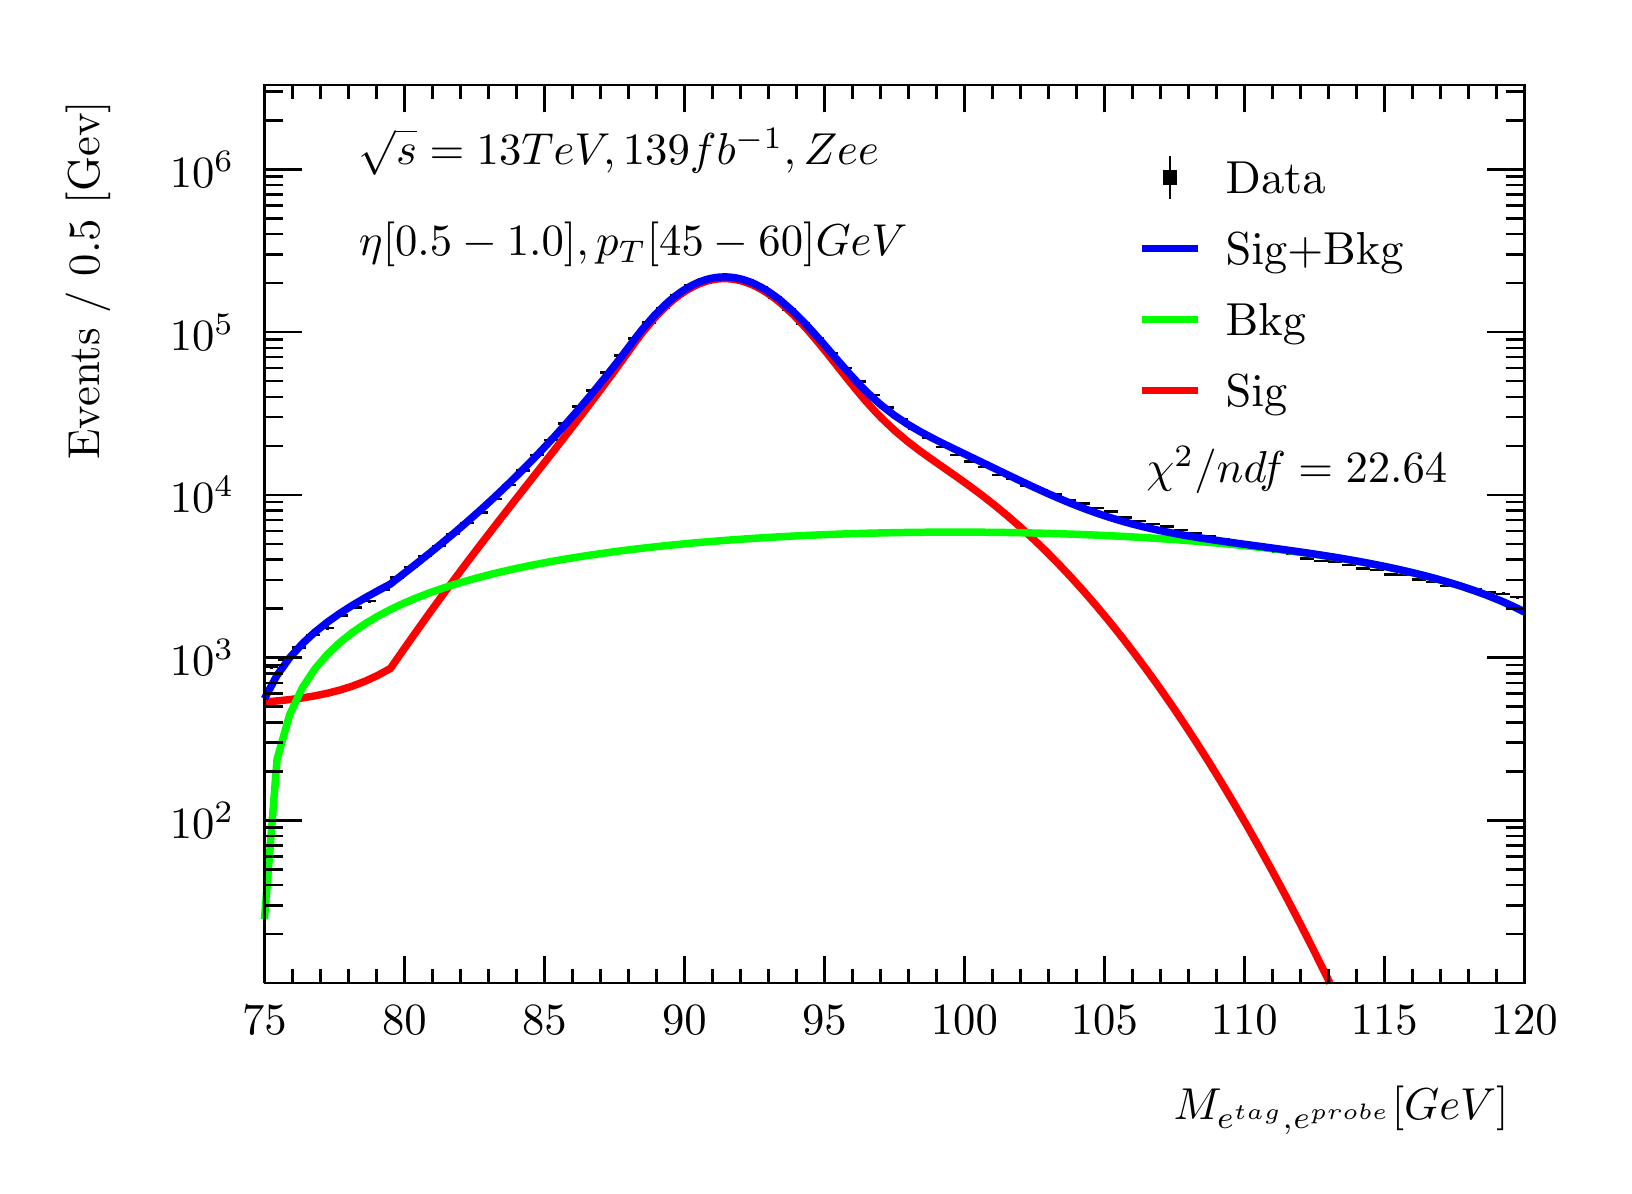
\begin{tikzpicture}
\pgfdeclareplotmark{cross} {
\pgfpathmoveto{\pgfpoint{-0.3\pgfplotmarksize}{\pgfplotmarksize}}
\pgfpathlineto{\pgfpoint{+0.3\pgfplotmarksize}{\pgfplotmarksize}}
\pgfpathlineto{\pgfpoint{+0.3\pgfplotmarksize}{0.3\pgfplotmarksize}}
\pgfpathlineto{\pgfpoint{+1\pgfplotmarksize}{0.3\pgfplotmarksize}}
\pgfpathlineto{\pgfpoint{+1\pgfplotmarksize}{-0.3\pgfplotmarksize}}
\pgfpathlineto{\pgfpoint{+0.3\pgfplotmarksize}{-0.3\pgfplotmarksize}}
\pgfpathlineto{\pgfpoint{+0.3\pgfplotmarksize}{-1.\pgfplotmarksize}}
\pgfpathlineto{\pgfpoint{-0.3\pgfplotmarksize}{-1.\pgfplotmarksize}}
\pgfpathlineto{\pgfpoint{-0.3\pgfplotmarksize}{-0.3\pgfplotmarksize}}
\pgfpathlineto{\pgfpoint{-1.\pgfplotmarksize}{-0.3\pgfplotmarksize}}
\pgfpathlineto{\pgfpoint{-1.\pgfplotmarksize}{0.3\pgfplotmarksize}}
\pgfpathlineto{\pgfpoint{-0.3\pgfplotmarksize}{0.3\pgfplotmarksize}}
\pgfpathclose
\pgfusepathqstroke
}
\pgfdeclareplotmark{cross*} {
\pgfpathmoveto{\pgfpoint{-0.3\pgfplotmarksize}{\pgfplotmarksize}}
\pgfpathlineto{\pgfpoint{+0.3\pgfplotmarksize}{\pgfplotmarksize}}
\pgfpathlineto{\pgfpoint{+0.3\pgfplotmarksize}{0.3\pgfplotmarksize}}
\pgfpathlineto{\pgfpoint{+1\pgfplotmarksize}{0.3\pgfplotmarksize}}
\pgfpathlineto{\pgfpoint{+1\pgfplotmarksize}{-0.3\pgfplotmarksize}}
\pgfpathlineto{\pgfpoint{+0.3\pgfplotmarksize}{-0.3\pgfplotmarksize}}
\pgfpathlineto{\pgfpoint{+0.3\pgfplotmarksize}{-1.\pgfplotmarksize}}
\pgfpathlineto{\pgfpoint{-0.3\pgfplotmarksize}{-1.\pgfplotmarksize}}
\pgfpathlineto{\pgfpoint{-0.3\pgfplotmarksize}{-0.3\pgfplotmarksize}}
\pgfpathlineto{\pgfpoint{-1.\pgfplotmarksize}{-0.3\pgfplotmarksize}}
\pgfpathlineto{\pgfpoint{-1.\pgfplotmarksize}{0.3\pgfplotmarksize}}
\pgfpathlineto{\pgfpoint{-0.3\pgfplotmarksize}{0.3\pgfplotmarksize}}
\pgfpathclose
\pgfusepathqfillstroke
}
\pgfdeclareplotmark{newstar} {
\pgfpathmoveto{\pgfqpoint{0pt}{\pgfplotmarksize}}
\pgfpathlineto{\pgfqpointpolar{44}{0.5\pgfplotmarksize}}
\pgfpathlineto{\pgfqpointpolar{18}{\pgfplotmarksize}}
\pgfpathlineto{\pgfqpointpolar{-20}{0.5\pgfplotmarksize}}
\pgfpathlineto{\pgfqpointpolar{-54}{\pgfplotmarksize}}
\pgfpathlineto{\pgfqpointpolar{-90}{0.5\pgfplotmarksize}}
\pgfpathlineto{\pgfqpointpolar{234}{\pgfplotmarksize}}
\pgfpathlineto{\pgfqpointpolar{198}{0.5\pgfplotmarksize}}
\pgfpathlineto{\pgfqpointpolar{162}{\pgfplotmarksize}}
\pgfpathlineto{\pgfqpointpolar{134}{0.5\pgfplotmarksize}}
\pgfpathclose
\pgfusepathqstroke
}
\pgfdeclareplotmark{newstar*} {
\pgfpathmoveto{\pgfqpoint{0pt}{\pgfplotmarksize}}
\pgfpathlineto{\pgfqpointpolar{44}{0.5\pgfplotmarksize}}
\pgfpathlineto{\pgfqpointpolar{18}{\pgfplotmarksize}}
\pgfpathlineto{\pgfqpointpolar{-20}{0.5\pgfplotmarksize}}
\pgfpathlineto{\pgfqpointpolar{-54}{\pgfplotmarksize}}
\pgfpathlineto{\pgfqpointpolar{-90}{0.5\pgfplotmarksize}}
\pgfpathlineto{\pgfqpointpolar{234}{\pgfplotmarksize}}
\pgfpathlineto{\pgfqpointpolar{198}{0.5\pgfplotmarksize}}
\pgfpathlineto{\pgfqpointpolar{162}{\pgfplotmarksize}}
\pgfpathlineto{\pgfqpointpolar{134}{0.5\pgfplotmarksize}}
\pgfpathclose
\pgfusepathqfillstroke
}
\definecolor{c}{rgb}{1,1,1};
\draw [color=c, fill=c] (0,0) rectangle (20,14.4361);
\draw [color=c, fill=c] (3,2.30977) rectangle (19,13.7143);
\definecolor{c}{rgb}{0,0,0};
\draw [c,line width=0.9] (3,2.30977) -- (3,13.7143) -- (19,13.7143) -- (19,2.30977) -- (3,2.30977);
\definecolor{c}{rgb}{1,1,1};
\draw [color=c, fill=c] (3,2.30977) rectangle (19,13.7143);
\definecolor{c}{rgb}{0,0,0};
\draw [c,line width=0.9] (3,2.30977) -- (3,13.7143) -- (19,13.7143) -- (19,2.30977) -- (3,2.30977);
\draw [c,line width=0.9] (3,2.30977) -- (19,2.30977);
\draw [c,line width=0.9] (3,2.65624) -- (3,2.30977);
\draw [c,line width=0.9] (3.35556,2.48301) -- (3.35556,2.30977);
\draw [c,line width=0.9] (3.71111,2.48301) -- (3.71111,2.30977);
\draw [c,line width=0.9] (4.06667,2.48301) -- (4.06667,2.30977);
\draw [c,line width=0.9] (4.42222,2.48301) -- (4.42222,2.30977);
\draw [c,line width=0.9] (4.77778,2.65624) -- (4.77778,2.30977);
\draw [c,line width=0.9] (5.13333,2.48301) -- (5.13333,2.30977);
\draw [c,line width=0.9] (5.48889,2.48301) -- (5.48889,2.30977);
\draw [c,line width=0.9] (5.84444,2.48301) -- (5.84444,2.30977);
\draw [c,line width=0.9] (6.2,2.48301) -- (6.2,2.30977);
\draw [c,line width=0.9] (6.55556,2.65624) -- (6.55556,2.30977);
\draw [c,line width=0.9] (6.91111,2.48301) -- (6.91111,2.30977);
\draw [c,line width=0.9] (7.26667,2.48301) -- (7.26667,2.30977);
\draw [c,line width=0.9] (7.62222,2.48301) -- (7.62222,2.30977);
\draw [c,line width=0.9] (7.97778,2.48301) -- (7.97778,2.30977);
\draw [c,line width=0.9] (8.33333,2.65624) -- (8.33333,2.30977);
\draw [c,line width=0.9] (8.68889,2.48301) -- (8.68889,2.30977);
\draw [c,line width=0.9] (9.04444,2.48301) -- (9.04444,2.30977);
\draw [c,line width=0.9] (9.4,2.48301) -- (9.4,2.30977);
\draw [c,line width=0.9] (9.75556,2.48301) -- (9.75556,2.30977);
\draw [c,line width=0.9] (10.1111,2.65624) -- (10.1111,2.30977);
\draw [c,line width=0.9] (10.4667,2.48301) -- (10.4667,2.30977);
\draw [c,line width=0.9] (10.8222,2.48301) -- (10.8222,2.30977);
\draw [c,line width=0.9] (11.1778,2.48301) -- (11.1778,2.30977);
\draw [c,line width=0.9] (11.5333,2.48301) -- (11.5333,2.30977);
\draw [c,line width=0.9] (11.8889,2.65624) -- (11.8889,2.30977);
\draw [c,line width=0.9] (12.2444,2.48301) -- (12.2444,2.30977);
\draw [c,line width=0.9] (12.6,2.48301) -- (12.6,2.30977);
\draw [c,line width=0.9] (12.9556,2.48301) -- (12.9556,2.30977);
\draw [c,line width=0.9] (13.3111,2.48301) -- (13.3111,2.30977);
\draw [c,line width=0.9] (13.6667,2.65624) -- (13.6667,2.30977);
\draw [c,line width=0.9] (14.0222,2.48301) -- (14.0222,2.30977);
\draw [c,line width=0.9] (14.3778,2.48301) -- (14.3778,2.30977);
\draw [c,line width=0.9] (14.7333,2.48301) -- (14.7333,2.30977);
\draw [c,line width=0.9] (15.0889,2.48301) -- (15.0889,2.30977);
\draw [c,line width=0.9] (15.4444,2.65624) -- (15.4444,2.30977);
\draw [c,line width=0.9] (15.8,2.48301) -- (15.8,2.30977);
\draw [c,line width=0.9] (16.1556,2.48301) -- (16.1556,2.30977);
\draw [c,line width=0.9] (16.5111,2.48301) -- (16.5111,2.30977);
\draw [c,line width=0.9] (16.8667,2.48301) -- (16.8667,2.30977);
\draw [c,line width=0.9] (17.2222,2.65624) -- (17.2222,2.30977);
\draw [c,line width=0.9] (17.5778,2.48301) -- (17.5778,2.30977);
\draw [c,line width=0.9] (17.9333,2.48301) -- (17.9333,2.30977);
\draw [c,line width=0.9] (18.2889,2.48301) -- (18.2889,2.30977);
\draw [c,line width=0.9] (18.6444,2.48301) -- (18.6444,2.30977);
\draw [c,line width=0.9] (19,2.65624) -- (19,2.30977);
\draw [c,line width=0.9] (19,2.65624) -- (19,2.30977);
\draw [anchor=base] (3,1.66015) node[scale=1.61424, color=c, rotate=0]{75};
\draw [anchor=base] (4.77778,1.66015) node[scale=1.61424, color=c, rotate=0]{80};
\draw [anchor=base] (6.55556,1.66015) node[scale=1.61424, color=c, rotate=0]{85};
\draw [anchor=base] (8.33333,1.66015) node[scale=1.61424, color=c, rotate=0]{90};
\draw [anchor=base] (10.1111,1.66015) node[scale=1.61424, color=c, rotate=0]{95};
\draw [anchor=base] (11.8889,1.66015) node[scale=1.61424, color=c, rotate=0]{100};
\draw [anchor=base] (13.6667,1.66015) node[scale=1.61424, color=c, rotate=0]{105};
\draw [anchor=base] (15.4444,1.66015) node[scale=1.61424, color=c, rotate=0]{110};
\draw [anchor=base] (17.2222,1.66015) node[scale=1.61424, color=c, rotate=0]{115};
\draw [anchor=base] (19,1.66015) node[scale=1.61424, color=c, rotate=0]{120};
\draw [anchor= east] (19,0.692932) node[scale=1.61424, color=c, rotate=0]{$M_{e^{tag}, e^{probe}}  [GeV]$};
\draw [c,line width=0.9] (3,13.7143) -- (19,13.7143);
\draw [c,line width=0.9] (3,13.3678) -- (3,13.7143);
\draw [c,line width=0.9] (3.35556,13.5411) -- (3.35556,13.7143);
\draw [c,line width=0.9] (3.71111,13.5411) -- (3.71111,13.7143);
\draw [c,line width=0.9] (4.06667,13.5411) -- (4.06667,13.7143);
\draw [c,line width=0.9] (4.42222,13.5411) -- (4.42222,13.7143);
\draw [c,line width=0.9] (4.77778,13.3678) -- (4.77778,13.7143);
\draw [c,line width=0.9] (5.13333,13.5411) -- (5.13333,13.7143);
\draw [c,line width=0.9] (5.48889,13.5411) -- (5.48889,13.7143);
\draw [c,line width=0.9] (5.84444,13.5411) -- (5.84444,13.7143);
\draw [c,line width=0.9] (6.2,13.5411) -- (6.2,13.7143);
\draw [c,line width=0.9] (6.55556,13.3678) -- (6.55556,13.7143);
\draw [c,line width=0.9] (6.91111,13.5411) -- (6.91111,13.7143);
\draw [c,line width=0.9] (7.26667,13.5411) -- (7.26667,13.7143);
\draw [c,line width=0.9] (7.62222,13.5411) -- (7.62222,13.7143);
\draw [c,line width=0.9] (7.97778,13.5411) -- (7.97778,13.7143);
\draw [c,line width=0.9] (8.33333,13.3678) -- (8.33333,13.7143);
\draw [c,line width=0.9] (8.68889,13.5411) -- (8.68889,13.7143);
\draw [c,line width=0.9] (9.04444,13.5411) -- (9.04444,13.7143);
\draw [c,line width=0.9] (9.4,13.5411) -- (9.4,13.7143);
\draw [c,line width=0.9] (9.75556,13.5411) -- (9.75556,13.7143);
\draw [c,line width=0.9] (10.1111,13.3678) -- (10.1111,13.7143);
\draw [c,line width=0.9] (10.4667,13.5411) -- (10.4667,13.7143);
\draw [c,line width=0.9] (10.8222,13.5411) -- (10.8222,13.7143);
\draw [c,line width=0.9] (11.1778,13.5411) -- (11.1778,13.7143);
\draw [c,line width=0.9] (11.5333,13.5411) -- (11.5333,13.7143);
\draw [c,line width=0.9] (11.8889,13.3678) -- (11.8889,13.7143);
\draw [c,line width=0.9] (12.2444,13.5411) -- (12.2444,13.7143);
\draw [c,line width=0.9] (12.6,13.5411) -- (12.6,13.7143);
\draw [c,line width=0.9] (12.9556,13.5411) -- (12.9556,13.7143);
\draw [c,line width=0.9] (13.3111,13.5411) -- (13.3111,13.7143);
\draw [c,line width=0.9] (13.6667,13.3678) -- (13.6667,13.7143);
\draw [c,line width=0.9] (14.0222,13.5411) -- (14.0222,13.7143);
\draw [c,line width=0.9] (14.3778,13.5411) -- (14.3778,13.7143);
\draw [c,line width=0.9] (14.7333,13.5411) -- (14.7333,13.7143);
\draw [c,line width=0.9] (15.0889,13.5411) -- (15.0889,13.7143);
\draw [c,line width=0.9] (15.4444,13.3678) -- (15.4444,13.7143);
\draw [c,line width=0.9] (15.8,13.5411) -- (15.8,13.7143);
\draw [c,line width=0.9] (16.1556,13.5411) -- (16.1556,13.7143);
\draw [c,line width=0.9] (16.5111,13.5411) -- (16.5111,13.7143);
\draw [c,line width=0.9] (16.8667,13.5411) -- (16.8667,13.7143);
\draw [c,line width=0.9] (17.2222,13.3678) -- (17.2222,13.7143);
\draw [c,line width=0.9] (17.5778,13.5411) -- (17.5778,13.7143);
\draw [c,line width=0.9] (17.9333,13.5411) -- (17.9333,13.7143);
\draw [c,line width=0.9] (18.2889,13.5411) -- (18.2889,13.7143);
\draw [c,line width=0.9] (18.6444,13.5411) -- (18.6444,13.7143);
\draw [c,line width=0.9] (19,13.3678) -- (19,13.7143);
\draw [c,line width=0.9] (19,13.3678) -- (19,13.7143);
\draw [c,line width=0.9] (3,2.30977) -- (3,13.7143);
\draw [c,line width=0.9] (3.237,2.932) -- (3,2.932);
\draw [c,line width=0.9] (3.237,3.29598) -- (3,3.29598);
\draw [c,line width=0.9] (3.237,3.55423) -- (3,3.55423);
\draw [c,line width=0.9] (3.237,3.75454) -- (3,3.75454);
\draw [c,line width=0.9] (3.237,3.9182) -- (3,3.9182);
\draw [c,line width=0.9] (3.237,4.05658) -- (3,4.05658);
\draw [c,line width=0.9] (3.237,4.17645) -- (3,4.17645);
\draw [c,line width=0.9] (3.237,4.28218) -- (3,4.28218);
\draw [c,line width=0.9] (3.474,4.37676) -- (3,4.37676);
\draw [anchor= east] (2.82,4.37676) node[scale=1.61424, color=c, rotate=0]{$10^{2}$};
\draw [c,line width=0.9] (3.237,4.99899) -- (3,4.99899);
\draw [c,line width=0.9] (3.237,5.36297) -- (3,5.36297);
\draw [c,line width=0.9] (3.237,5.62122) -- (3,5.62122);
\draw [c,line width=0.9] (3.237,5.82153) -- (3,5.82153);
\draw [c,line width=0.9] (3.237,5.9852) -- (3,5.9852);
\draw [c,line width=0.9] (3.237,6.12357) -- (3,6.12357);
\draw [c,line width=0.9] (3.237,6.24344) -- (3,6.24344);
\draw [c,line width=0.9] (3.237,6.34917) -- (3,6.34917);
\draw [c,line width=0.9] (3.474,6.44376) -- (3,6.44376);
\draw [anchor= east] (2.82,6.44376) node[scale=1.61424, color=c, rotate=0]{$10^{3}$};
\draw [c,line width=0.9] (3.237,7.06598) -- (3,7.06598);
\draw [c,line width=0.9] (3.237,7.42996) -- (3,7.42996);
\draw [c,line width=0.9] (3.237,7.68821) -- (3,7.68821);
\draw [c,line width=0.9] (3.237,7.88852) -- (3,7.88852);
\draw [c,line width=0.9] (3.237,8.05219) -- (3,8.05219);
\draw [c,line width=0.9] (3.237,8.19057) -- (3,8.19057);
\draw [c,line width=0.9] (3.237,8.31043) -- (3,8.31043);
\draw [c,line width=0.9] (3.237,8.41617) -- (3,8.41617);
\draw [c,line width=0.9] (3.474,8.51075) -- (3,8.51075);
\draw [anchor= east] (2.82,8.51075) node[scale=1.61424, color=c, rotate=0]{$10^{4}$};
\draw [c,line width=0.9] (3.237,9.13297) -- (3,9.13297);
\draw [c,line width=0.9] (3.237,9.49695) -- (3,9.49695);
\draw [c,line width=0.9] (3.237,9.7552) -- (3,9.7552);
\draw [c,line width=0.9] (3.237,9.95551) -- (3,9.95551);
\draw [c,line width=0.9] (3.237,10.1192) -- (3,10.1192);
\draw [c,line width=0.9] (3.237,10.2576) -- (3,10.2576);
\draw [c,line width=0.9] (3.237,10.3774) -- (3,10.3774);
\draw [c,line width=0.9] (3.237,10.4832) -- (3,10.4832);
\draw [c,line width=0.9] (3.474,10.5777) -- (3,10.5777);
\draw [anchor= east] (2.82,10.5777) node[scale=1.61424, color=c, rotate=0]{$10^{5}$};
\draw [c,line width=0.9] (3.237,11.2) -- (3,11.2);
\draw [c,line width=0.9] (3.237,11.5639) -- (3,11.5639);
\draw [c,line width=0.9] (3.237,11.8222) -- (3,11.8222);
\draw [c,line width=0.9] (3.237,12.0225) -- (3,12.0225);
\draw [c,line width=0.9] (3.237,12.1862) -- (3,12.1862);
\draw [c,line width=0.9] (3.237,12.3245) -- (3,12.3245);
\draw [c,line width=0.9] (3.237,12.4444) -- (3,12.4444);
\draw [c,line width=0.9] (3.237,12.5501) -- (3,12.5501);
\draw [c,line width=0.9] (3.474,12.6447) -- (3,12.6447);
\draw [anchor= east] (2.82,12.6447) node[scale=1.61424, color=c, rotate=0]{$10^{6}$};
\draw [c,line width=0.9] (3.237,13.267) -- (3,13.267);
\draw [c,line width=0.9] (3.237,13.6309) -- (3,13.6309);
\draw [anchor= east] (0.76,13.7143) node[scale=1.61424, color=c, rotate=90]{Events / 0.5 [Gev]};
\draw [c,line width=0.9] (19,2.30977) -- (19,13.7143);
\draw [c,line width=0.9] (18.763,2.932) -- (19,2.932);
\draw [c,line width=0.9] (18.763,3.29598) -- (19,3.29598);
\draw [c,line width=0.9] (18.763,3.55423) -- (19,3.55423);
\draw [c,line width=0.9] (18.763,3.75454) -- (19,3.75454);
\draw [c,line width=0.9] (18.763,3.9182) -- (19,3.9182);
\draw [c,line width=0.9] (18.763,4.05658) -- (19,4.05658);
\draw [c,line width=0.9] (18.763,4.17645) -- (19,4.17645);
\draw [c,line width=0.9] (18.763,4.28218) -- (19,4.28218);
\draw [c,line width=0.9] (18.526,4.37676) -- (19,4.37676);
\draw [c,line width=0.9] (18.763,4.99899) -- (19,4.99899);
\draw [c,line width=0.9] (18.763,5.36297) -- (19,5.36297);
\draw [c,line width=0.9] (18.763,5.62122) -- (19,5.62122);
\draw [c,line width=0.9] (18.763,5.82153) -- (19,5.82153);
\draw [c,line width=0.9] (18.763,5.9852) -- (19,5.9852);
\draw [c,line width=0.9] (18.763,6.12357) -- (19,6.12357);
\draw [c,line width=0.9] (18.763,6.24344) -- (19,6.24344);
\draw [c,line width=0.9] (18.763,6.34917) -- (19,6.34917);
\draw [c,line width=0.9] (18.526,6.44376) -- (19,6.44376);
\draw [c,line width=0.9] (18.763,7.06598) -- (19,7.06598);
\draw [c,line width=0.9] (18.763,7.42996) -- (19,7.42996);
\draw [c,line width=0.9] (18.763,7.68821) -- (19,7.68821);
\draw [c,line width=0.9] (18.763,7.88852) -- (19,7.88852);
\draw [c,line width=0.9] (18.763,8.05219) -- (19,8.05219);
\draw [c,line width=0.9] (18.763,8.19057) -- (19,8.19057);
\draw [c,line width=0.9] (18.763,8.31043) -- (19,8.31043);
\draw [c,line width=0.9] (18.763,8.41617) -- (19,8.41617);
\draw [c,line width=0.9] (18.526,8.51075) -- (19,8.51075);
\draw [c,line width=0.9] (18.763,9.13297) -- (19,9.13297);
\draw [c,line width=0.9] (18.763,9.49695) -- (19,9.49695);
\draw [c,line width=0.9] (18.763,9.7552) -- (19,9.7552);
\draw [c,line width=0.9] (18.763,9.95551) -- (19,9.95551);
\draw [c,line width=0.9] (18.763,10.1192) -- (19,10.1192);
\draw [c,line width=0.9] (18.763,10.2576) -- (19,10.2576);
\draw [c,line width=0.9] (18.763,10.3774) -- (19,10.3774);
\draw [c,line width=0.9] (18.763,10.4832) -- (19,10.4832);
\draw [c,line width=0.9] (18.526,10.5777) -- (19,10.5777);
\draw [c,line width=0.9] (18.763,11.2) -- (19,11.2);
\draw [c,line width=0.9] (18.763,11.5639) -- (19,11.5639);
\draw [c,line width=0.9] (18.763,11.8222) -- (19,11.8222);
\draw [c,line width=0.9] (18.763,12.0225) -- (19,12.0225);
\draw [c,line width=0.9] (18.763,12.1862) -- (19,12.1862);
\draw [c,line width=0.9] (18.763,12.3245) -- (19,12.3245);
\draw [c,line width=0.9] (18.763,12.4444) -- (19,12.4444);
\draw [c,line width=0.9] (18.763,12.5501) -- (19,12.5501);
\draw [c,line width=0.9] (18.526,12.6447) -- (19,12.6447);
\draw [c,line width=0.9] (18.763,13.267) -- (19,13.267);
\draw [c,line width=0.9] (18.763,13.6309) -- (19,13.6309);
\draw [c,line width=0.9] (3.08889,6.33002) -- (3,6.33002);
\draw [c,line width=0.9] (3,6.33002) -- (3,6.33002);
\draw [c,line width=0.9] (3.08889,6.33002) -- (3.17778,6.33002);
\draw [c,line width=0.9] (3.17778,6.33002) -- (3.17778,6.33002);
\draw [c,line width=0.9] (3.08889,6.33002) -- (3.08889,6.36026);
\draw [c,line width=0.9] (3.08889,6.36026) -- (3.08889,6.36026);
\draw [c,line width=0.9] (3.08889,6.33002) -- (3.08889,6.29978);
\draw [c,line width=0.9] (3.08889,6.29978) -- (3.08889,6.29978);
\draw [c,line width=0.9] (3.26667,6.4127) -- (3.17778,6.4127);
\draw [c,line width=0.9] (3.17778,6.4127) -- (3.17778,6.4127);
\draw [c,line width=0.9] (3.26667,6.4127) -- (3.35556,6.4127);
\draw [c,line width=0.9] (3.35556,6.4127) -- (3.35556,6.4127);
\draw [c,line width=0.9] (3.26667,6.4127) -- (3.26667,6.44159);
\draw [c,line width=0.9] (3.26667,6.44159) -- (3.26667,6.44159);
\draw [c,line width=0.9] (3.26667,6.4127) -- (3.26667,6.38382);
\draw [c,line width=0.9] (3.26667,6.38382) -- (3.26667,6.38382);
\draw [c,line width=0.9] (3.44444,6.57) -- (3.35556,6.57);
\draw [c,line width=0.9] (3.35556,6.57) -- (3.35556,6.57);
\draw [c,line width=0.9] (3.44444,6.57) -- (3.53333,6.57);
\draw [c,line width=0.9] (3.53333,6.57) -- (3.53333,6.57);
\draw [c,line width=0.9] (3.44444,6.57) -- (3.44444,6.59646);
\draw [c,line width=0.9] (3.44444,6.59646) -- (3.44444,6.59646);
\draw [c,line width=0.9] (3.44444,6.57) -- (3.44444,6.54354);
\draw [c,line width=0.9] (3.44444,6.54354) -- (3.44444,6.54354);
\draw [c,line width=0.9] (3.62222,6.72767) -- (3.53333,6.72767);
\draw [c,line width=0.9] (3.53333,6.72767) -- (3.53333,6.72767);
\draw [c,line width=0.9] (3.62222,6.72767) -- (3.71111,6.72767);
\draw [c,line width=0.9] (3.71111,6.72767) -- (3.71111,6.72767);
\draw [c,line width=0.9] (3.62222,6.72767) -- (3.62222,6.7519);
\draw [c,line width=0.9] (3.62222,6.7519) -- (3.62222,6.7519);
\draw [c,line width=0.9] (3.62222,6.72767) -- (3.62222,6.70343);
\draw [c,line width=0.9] (3.62222,6.70343) -- (3.62222,6.70343);
\draw [c,line width=0.9] (3.8,6.82022) -- (3.71111,6.82022);
\draw [c,line width=0.9] (3.71111,6.82022) -- (3.71111,6.82022);
\draw [c,line width=0.9] (3.8,6.82022) -- (3.88889,6.82022);
\draw [c,line width=0.9] (3.88889,6.82022) -- (3.88889,6.82022);
\draw [c,line width=0.9] (3.8,6.82022) -- (3.8,6.84323);
\draw [c,line width=0.9] (3.8,6.84323) -- (3.8,6.84323);
\draw [c,line width=0.9] (3.8,6.82022) -- (3.8,6.7972);
\draw [c,line width=0.9] (3.8,6.7972) -- (3.8,6.7972);
\draw [c,line width=0.9] (3.97778,6.97935) -- (3.88889,6.97935);
\draw [c,line width=0.9] (3.88889,6.97935) -- (3.88889,6.97935);
\draw [c,line width=0.9] (3.97778,6.97935) -- (4.06667,6.97935);
\draw [c,line width=0.9] (4.06667,6.97935) -- (4.06667,6.97935);
\draw [c,line width=0.9] (3.97778,6.97935) -- (3.97778,7.00041);
\draw [c,line width=0.9] (3.97778,7.00041) -- (3.97778,7.00041);
\draw [c,line width=0.9] (3.97778,6.97935) -- (3.97778,6.95828);
\draw [c,line width=0.9] (3.97778,6.95828) -- (3.97778,6.95828);
\draw [c,line width=0.9] (4.15556,7.07713) -- (4.06667,7.07713);
\draw [c,line width=0.9] (4.06667,7.07713) -- (4.06667,7.07713);
\draw [c,line width=0.9] (4.15556,7.07713) -- (4.24444,7.07713);
\draw [c,line width=0.9] (4.24444,7.07713) -- (4.24444,7.07713);
\draw [c,line width=0.9] (4.15556,7.07713) -- (4.15556,7.09708);
\draw [c,line width=0.9] (4.15556,7.09708) -- (4.15556,7.09708);
\draw [c,line width=0.9] (4.15556,7.07713) -- (4.15556,7.05719);
\draw [c,line width=0.9] (4.15556,7.05719) -- (4.15556,7.05719);
\draw [c,line width=0.9] (4.33333,7.16088) -- (4.24444,7.16088);
\draw [c,line width=0.9] (4.24444,7.16088) -- (4.24444,7.16088);
\draw [c,line width=0.9] (4.33333,7.16088) -- (4.42222,7.16088);
\draw [c,line width=0.9] (4.42222,7.16088) -- (4.42222,7.16088);
\draw [c,line width=0.9] (4.33333,7.16088) -- (4.33333,7.17992);
\draw [c,line width=0.9] (4.33333,7.17992) -- (4.33333,7.17992);
\draw [c,line width=0.9] (4.33333,7.16088) -- (4.33333,7.14184);
\draw [c,line width=0.9] (4.33333,7.14184) -- (4.33333,7.14184);
\draw [c,line width=0.9] (4.51111,7.30667) -- (4.42222,7.30667);
\draw [c,line width=0.9] (4.42222,7.30667) -- (4.42222,7.30667);
\draw [c,line width=0.9] (4.51111,7.30667) -- (4.6,7.30667);
\draw [c,line width=0.9] (4.6,7.30667) -- (4.6,7.30667);
\draw [c,line width=0.9] (4.51111,7.30667) -- (4.51111,7.32422);
\draw [c,line width=0.9] (4.51111,7.32422) -- (4.51111,7.32422);
\draw [c,line width=0.9] (4.51111,7.30667) -- (4.51111,7.28911);
\draw [c,line width=0.9] (4.51111,7.28911) -- (4.51111,7.28911);
\draw [c,line width=0.9] (4.68889,7.45824) -- (4.6,7.45824);
\draw [c,line width=0.9] (4.6,7.45824) -- (4.6,7.45824);
\draw [c,line width=0.9] (4.68889,7.45824) -- (4.77778,7.45824);
\draw [c,line width=0.9] (4.77778,7.45824) -- (4.77778,7.45824);
\draw [c,line width=0.9] (4.68889,7.45824) -- (4.68889,7.47437);
\draw [c,line width=0.9] (4.68889,7.47437) -- (4.68889,7.47437);
\draw [c,line width=0.9] (4.68889,7.45824) -- (4.68889,7.4421);
\draw [c,line width=0.9] (4.68889,7.4421) -- (4.68889,7.4421);
\draw [c,line width=0.9] (4.86667,7.59238) -- (4.77778,7.59238);
\draw [c,line width=0.9] (4.77778,7.59238) -- (4.77778,7.59238);
\draw [c,line width=0.9] (4.86667,7.59238) -- (4.95556,7.59238);
\draw [c,line width=0.9] (4.95556,7.59238) -- (4.95556,7.59238);
\draw [c,line width=0.9] (4.86667,7.59238) -- (4.86667,7.60735);
\draw [c,line width=0.9] (4.86667,7.60735) -- (4.86667,7.60735);
\draw [c,line width=0.9] (4.86667,7.59238) -- (4.86667,7.57741);
\draw [c,line width=0.9] (4.86667,7.57741) -- (4.86667,7.57741);
\draw [c,line width=0.9] (5.04444,7.73179) -- (4.95556,7.73179);
\draw [c,line width=0.9] (4.95556,7.73179) -- (4.95556,7.73179);
\draw [c,line width=0.9] (5.04444,7.73179) -- (5.13333,7.73179);
\draw [c,line width=0.9] (5.13333,7.73179) -- (5.13333,7.73179);
\draw [c,line width=0.9] (5.04444,7.73179) -- (5.04444,7.74565);
\draw [c,line width=0.9] (5.04444,7.74565) -- (5.04444,7.74565);
\draw [c,line width=0.9] (5.04444,7.73179) -- (5.04444,7.71794);
\draw [c,line width=0.9] (5.04444,7.71794) -- (5.04444,7.71794);
\draw [c,line width=0.9] (5.22222,7.85858) -- (5.13333,7.85858);
\draw [c,line width=0.9] (5.13333,7.85858) -- (5.13333,7.85858);
\draw [c,line width=0.9] (5.22222,7.85858) -- (5.31111,7.85858);
\draw [c,line width=0.9] (5.31111,7.85858) -- (5.31111,7.85858);
\draw [c,line width=0.9] (5.22222,7.85858) -- (5.22222,7.87149);
\draw [c,line width=0.9] (5.22222,7.87149) -- (5.22222,7.87149);
\draw [c,line width=0.9] (5.22222,7.85858) -- (5.22222,7.84567);
\draw [c,line width=0.9] (5.22222,7.84567) -- (5.22222,7.84567);
\draw [c,line width=0.9] (5.4,8.01054) -- (5.31111,8.01054);
\draw [c,line width=0.9] (5.31111,8.01054) -- (5.31111,8.01054);
\draw [c,line width=0.9] (5.4,8.01054) -- (5.48889,8.01054);
\draw [c,line width=0.9] (5.48889,8.01054) -- (5.48889,8.01054);
\draw [c,line width=0.9] (5.4,8.01054) -- (5.4,8.0224);
\draw [c,line width=0.9] (5.4,8.0224) -- (5.4,8.0224);
\draw [c,line width=0.9] (5.4,8.01054) -- (5.4,7.99868);
\draw [c,line width=0.9] (5.4,7.99868) -- (5.4,7.99868);
\draw [c,line width=0.9] (5.57778,8.15245) -- (5.48889,8.15245);
\draw [c,line width=0.9] (5.48889,8.15245) -- (5.48889,8.15245);
\draw [c,line width=0.9] (5.57778,8.15245) -- (5.66667,8.15245);
\draw [c,line width=0.9] (5.66667,8.15245) -- (5.66667,8.15245);
\draw [c,line width=0.9] (5.57778,8.15245) -- (5.57778,8.16341);
\draw [c,line width=0.9] (5.57778,8.16341) -- (5.57778,8.16341);
\draw [c,line width=0.9] (5.57778,8.15245) -- (5.57778,8.14149);
\draw [c,line width=0.9] (5.57778,8.14149) -- (5.57778,8.14149);
\draw [c,line width=0.9] (5.75556,8.28805) -- (5.66667,8.28805);
\draw [c,line width=0.9] (5.66667,8.28805) -- (5.66667,8.28805);
\draw [c,line width=0.9] (5.75556,8.28805) -- (5.84444,8.28805);
\draw [c,line width=0.9] (5.84444,8.28805) -- (5.84444,8.28805);
\draw [c,line width=0.9] (5.75556,8.28805) -- (5.75556,8.29822);
\draw [c,line width=0.9] (5.75556,8.29822) -- (5.75556,8.29822);
\draw [c,line width=0.9] (5.75556,8.28805) -- (5.75556,8.27789);
\draw [c,line width=0.9] (5.75556,8.27789) -- (5.75556,8.27789);
\draw [c,line width=0.9] (5.93333,8.45892) -- (5.84444,8.45892);
\draw [c,line width=0.9] (5.84444,8.45892) -- (5.84444,8.45892);
\draw [c,line width=0.9] (5.93333,8.45892) -- (6.02222,8.45892);
\draw [c,line width=0.9] (6.02222,8.45892) -- (6.02222,8.45892);
\draw [c,line width=0.9] (5.93333,8.45892) -- (5.93333,8.46816);
\draw [c,line width=0.9] (5.93333,8.46816) -- (5.93333,8.46816);
\draw [c,line width=0.9] (5.93333,8.45892) -- (5.93333,8.44968);
\draw [c,line width=0.9] (5.93333,8.44968) -- (5.93333,8.44968);
\draw [c,line width=0.9] (6.11111,8.63738) -- (6.02222,8.63738);
\draw [c,line width=0.9] (6.02222,8.63738) -- (6.02222,8.63738);
\draw [c,line width=0.9] (6.11111,8.63738) -- (6.2,8.63738);
\draw [c,line width=0.9] (6.2,8.63738) -- (6.2,8.63738);
\draw [c,line width=0.9] (6.11111,8.63738) -- (6.11111,8.64575);
\draw [c,line width=0.9] (6.11111,8.64575) -- (6.11111,8.64575);
\draw [c,line width=0.9] (6.11111,8.63738) -- (6.11111,8.62901);
\draw [c,line width=0.9] (6.11111,8.62901) -- (6.11111,8.62901);
\draw [c,line width=0.9] (6.28889,8.81759) -- (6.2,8.81759);
\draw [c,line width=0.9] (6.2,8.81759) -- (6.2,8.81759);
\draw [c,line width=0.9] (6.28889,8.81759) -- (6.37778,8.81759);
\draw [c,line width=0.9] (6.37778,8.81759) -- (6.37778,8.81759);
\draw [c,line width=0.9] (6.28889,8.81759) -- (6.28889,8.82516);
\draw [c,line width=0.9] (6.28889,8.82516) -- (6.28889,8.82516);
\draw [c,line width=0.9] (6.28889,8.81759) -- (6.28889,8.81002);
\draw [c,line width=0.9] (6.28889,8.81002) -- (6.28889,8.81002);
\draw [c,line width=0.9] (6.46667,9.01469) -- (6.37778,9.01469);
\draw [c,line width=0.9] (6.37778,9.01469) -- (6.37778,9.01469);
\draw [c,line width=0.9] (6.46667,9.01469) -- (6.55556,9.01469);
\draw [c,line width=0.9] (6.55556,9.01469) -- (6.55556,9.01469);
\draw [c,line width=0.9] (6.46667,9.01469) -- (6.46667,9.02147);
\draw [c,line width=0.9] (6.46667,9.02147) -- (6.46667,9.02147);
\draw [c,line width=0.9] (6.46667,9.01469) -- (6.46667,9.00791);
\draw [c,line width=0.9] (6.46667,9.00791) -- (6.46667,9.00791);
\draw [c,line width=0.9] (6.64444,9.20339) -- (6.55556,9.20339);
\draw [c,line width=0.9] (6.55556,9.20339) -- (6.55556,9.20339);
\draw [c,line width=0.9] (6.64444,9.20339) -- (6.73333,9.20339);
\draw [c,line width=0.9] (6.73333,9.20339) -- (6.73333,9.20339);
\draw [c,line width=0.9] (6.64444,9.20339) -- (6.64444,9.20949);
\draw [c,line width=0.9] (6.64444,9.20949) -- (6.64444,9.20949);
\draw [c,line width=0.9] (6.64444,9.20339) -- (6.64444,9.19729);
\draw [c,line width=0.9] (6.64444,9.19729) -- (6.64444,9.19729);
\draw [c,line width=0.9] (6.82222,9.41597) -- (6.73333,9.41597);
\draw [c,line width=0.9] (6.73333,9.41597) -- (6.73333,9.41597);
\draw [c,line width=0.9] (6.82222,9.41597) -- (6.91111,9.41597);
\draw [c,line width=0.9] (6.91111,9.41597) -- (6.91111,9.41597);
\draw [c,line width=0.9] (6.82222,9.41597) -- (6.82222,9.42139);
\draw [c,line width=0.9] (6.82222,9.42139) -- (6.82222,9.42139);
\draw [c,line width=0.9] (6.82222,9.41597) -- (6.82222,9.41055);
\draw [c,line width=0.9] (6.82222,9.41055) -- (6.82222,9.41055);
\draw [c,line width=0.9] (7,9.63111) -- (6.91111,9.63111);
\draw [c,line width=0.9] (6.91111,9.63111) -- (6.91111,9.63111);
\draw [c,line width=0.9] (7,9.63111) -- (7.08889,9.63111);
\draw [c,line width=0.9] (7.08889,9.63111) -- (7.08889,9.63111);
\draw [c,line width=0.9] (7,9.63111) -- (7,9.63592);
\draw [c,line width=0.9] (7,9.63592) -- (7,9.63592);
\draw [c,line width=0.9] (7,9.63111) -- (7,9.62631);
\draw [c,line width=0.9] (7,9.62631) -- (7,9.62631);
\draw [c,line width=0.9] (7.17778,9.83636) -- (7.08889,9.83636);
\draw [c,line width=0.9] (7.08889,9.83636) -- (7.08889,9.83636);
\draw [c,line width=0.9] (7.17778,9.83636) -- (7.26667,9.83636);
\draw [c,line width=0.9] (7.26667,9.83636) -- (7.26667,9.83636);
\draw [c,line width=0.9] (7.17778,9.83636) -- (7.17778,9.84065);
\draw [c,line width=0.9] (7.17778,9.84065) -- (7.17778,9.84065);
\draw [c,line width=0.9] (7.17778,9.83636) -- (7.17778,9.83207);
\draw [c,line width=0.9] (7.17778,9.83207) -- (7.17778,9.83207);
\draw [c,line width=0.9] (7.35556,10.0623) -- (7.26667,10.0623);
\draw [c,line width=0.9] (7.26667,10.0623) -- (7.26667,10.0623);
\draw [c,line width=0.9] (7.35556,10.0623) -- (7.44444,10.0623);
\draw [c,line width=0.9] (7.44444,10.0623) -- (7.44444,10.0623);
\draw [c,line width=0.9] (7.35556,10.0623) -- (7.35556,10.066);
\draw [c,line width=0.9] (7.35556,10.066) -- (7.35556,10.066);
\draw [c,line width=0.9] (7.35556,10.0623) -- (7.35556,10.0585);
\draw [c,line width=0.9] (7.35556,10.0585) -- (7.35556,10.0585);
\draw [c,line width=0.9] (7.53333,10.2775) -- (7.44444,10.2775);
\draw [c,line width=0.9] (7.44444,10.2775) -- (7.44444,10.2775);
\draw [c,line width=0.9] (7.53333,10.2775) -- (7.62222,10.2775);
\draw [c,line width=0.9] (7.62222,10.2775) -- (7.62222,10.2775);
\draw [c,line width=0.9] (7.53333,10.2775) -- (7.53333,10.2808);
\draw [c,line width=0.9] (7.53333,10.2808) -- (7.53333,10.2808);
\draw [c,line width=0.9] (7.53333,10.2775) -- (7.53333,10.2741);
\draw [c,line width=0.9] (7.53333,10.2741) -- (7.53333,10.2741);
\draw [c,line width=0.9] (7.71111,10.4972) -- (7.62222,10.4972);
\draw [c,line width=0.9] (7.62222,10.4972) -- (7.62222,10.4972);
\draw [c,line width=0.9] (7.71111,10.4972) -- (7.8,10.4972);
\draw [c,line width=0.9] (7.8,10.4972) -- (7.8,10.4972);
\draw [c,line width=0.9] (7.71111,10.4972) -- (7.71111,10.5002);
\draw [c,line width=0.9] (7.71111,10.5002) -- (7.71111,10.5002);
\draw [c,line width=0.9] (7.71111,10.4972) -- (7.71111,10.4942);
\draw [c,line width=0.9] (7.71111,10.4942) -- (7.71111,10.4942);
\draw [c,line width=0.9] (7.88889,10.6999) -- (7.8,10.6999);
\draw [c,line width=0.9] (7.8,10.6999) -- (7.8,10.6999);
\draw [c,line width=0.9] (7.88889,10.6999) -- (7.97778,10.6999);
\draw [c,line width=0.9] (7.97778,10.6999) -- (7.97778,10.6999);
\draw [c,line width=0.9] (7.88889,10.6999) -- (7.88889,10.7025);
\draw [c,line width=0.9] (7.88889,10.7025) -- (7.88889,10.7025);
\draw [c,line width=0.9] (7.88889,10.6999) -- (7.88889,10.6972);
\draw [c,line width=0.9] (7.88889,10.6972) -- (7.88889,10.6972);
\draw [c,line width=0.9] (8.06667,10.8818) -- (7.97778,10.8818);
\draw [c,line width=0.9] (7.97778,10.8818) -- (7.97778,10.8818);
\draw [c,line width=0.9] (8.06667,10.8818) -- (8.15556,10.8818);
\draw [c,line width=0.9] (8.15556,10.8818) -- (8.15556,10.8818);
\draw [c,line width=0.9] (8.06667,10.8818) -- (8.06667,10.8842);
\draw [c,line width=0.9] (8.06667,10.8842) -- (8.06667,10.8842);
\draw [c,line width=0.9] (8.06667,10.8818) -- (8.06667,10.8794);
\draw [c,line width=0.9] (8.06667,10.8794) -- (8.06667,10.8794);
\draw [c,line width=0.9] (8.24444,11.0387) -- (8.15556,11.0387);
\draw [c,line width=0.9] (8.15556,11.0387) -- (8.15556,11.0387);
\draw [c,line width=0.9] (8.24444,11.0387) -- (8.33333,11.0387);
\draw [c,line width=0.9] (8.33333,11.0387) -- (8.33333,11.0387);
\draw [c,line width=0.9] (8.24444,11.0387) -- (8.24444,11.0409);
\draw [c,line width=0.9] (8.24444,11.0409) -- (8.24444,11.0409);
\draw [c,line width=0.9] (8.24444,11.0387) -- (8.24444,11.0365);
\draw [c,line width=0.9] (8.24444,11.0365) -- (8.24444,11.0365);
\draw [c,line width=0.9] (8.42222,11.1677) -- (8.33333,11.1677);
\draw [c,line width=0.9] (8.33333,11.1677) -- (8.33333,11.1677);
\draw [c,line width=0.9] (8.42222,11.1677) -- (8.51111,11.1677);
\draw [c,line width=0.9] (8.51111,11.1677) -- (8.51111,11.1677);
\draw [c,line width=0.9] (8.42222,11.1677) -- (8.42222,11.1697);
\draw [c,line width=0.9] (8.42222,11.1697) -- (8.42222,11.1697);
\draw [c,line width=0.9] (8.42222,11.1677) -- (8.42222,11.1656);
\draw [c,line width=0.9] (8.42222,11.1656) -- (8.42222,11.1656);
\draw [c,line width=0.9] (8.6,11.2521) -- (8.51111,11.2521);
\draw [c,line width=0.9] (8.51111,11.2521) -- (8.51111,11.2521);
\draw [c,line width=0.9] (8.6,11.2521) -- (8.68889,11.2521);
\draw [c,line width=0.9] (8.68889,11.2521) -- (8.68889,11.2521);
\draw [c,line width=0.9] (8.6,11.2521) -- (8.6,11.254);
\draw [c,line width=0.9] (8.6,11.254) -- (8.6,11.254);
\draw [c,line width=0.9] (8.6,11.2521) -- (8.6,11.2501);
\draw [c,line width=0.9] (8.6,11.2501) -- (8.6,11.2501);
\draw [c,line width=0.9] (8.77778,11.291) -- (8.68889,11.291);
\draw [c,line width=0.9] (8.68889,11.291) -- (8.68889,11.291);
\draw [c,line width=0.9] (8.77778,11.291) -- (8.86667,11.291);
\draw [c,line width=0.9] (8.86667,11.291) -- (8.86667,11.291);
\draw [c,line width=0.9] (8.77778,11.291) -- (8.77778,11.2929);
\draw [c,line width=0.9] (8.77778,11.2929) -- (8.77778,11.2929);
\draw [c,line width=0.9] (8.77778,11.291) -- (8.77778,11.2891);
\draw [c,line width=0.9] (8.77778,11.2891) -- (8.77778,11.2891);
\draw [c,line width=0.9] (8.95556,11.2866) -- (8.86667,11.2866);
\draw [c,line width=0.9] (8.86667,11.2866) -- (8.86667,11.2866);
\draw [c,line width=0.9] (8.95556,11.2866) -- (9.04444,11.2866);
\draw [c,line width=0.9] (9.04444,11.2866) -- (9.04444,11.2866);
\draw [c,line width=0.9] (8.95556,11.2866) -- (8.95556,11.2886);
\draw [c,line width=0.9] (8.95556,11.2886) -- (8.95556,11.2886);
\draw [c,line width=0.9] (8.95556,11.2866) -- (8.95556,11.2847);
\draw [c,line width=0.9] (8.95556,11.2847) -- (8.95556,11.2847);
\draw [c,line width=0.9] (9.13333,11.2338) -- (9.04444,11.2338);
\draw [c,line width=0.9] (9.04444,11.2338) -- (9.04444,11.2338);
\draw [c,line width=0.9] (9.13333,11.2338) -- (9.22222,11.2338);
\draw [c,line width=0.9] (9.22222,11.2338) -- (9.22222,11.2338);
\draw [c,line width=0.9] (9.13333,11.2338) -- (9.13333,11.2358);
\draw [c,line width=0.9] (9.13333,11.2358) -- (9.13333,11.2358);
\draw [c,line width=0.9] (9.13333,11.2338) -- (9.13333,11.2318);
\draw [c,line width=0.9] (9.13333,11.2318) -- (9.13333,11.2318);
\draw [c,line width=0.9] (9.31111,11.1405) -- (9.22222,11.1405);
\draw [c,line width=0.9] (9.22222,11.1405) -- (9.22222,11.1405);
\draw [c,line width=0.9] (9.31111,11.1405) -- (9.4,11.1405);
\draw [c,line width=0.9] (9.4,11.1405) -- (9.4,11.1405);
\draw [c,line width=0.9] (9.31111,11.1405) -- (9.31111,11.1426);
\draw [c,line width=0.9] (9.31111,11.1426) -- (9.31111,11.1426);
\draw [c,line width=0.9] (9.31111,11.1405) -- (9.31111,11.1384);
\draw [c,line width=0.9] (9.31111,11.1384) -- (9.31111,11.1384);
\draw [c,line width=0.9] (9.48889,11.0177) -- (9.4,11.0177);
\draw [c,line width=0.9] (9.4,11.0177) -- (9.4,11.0177);
\draw [c,line width=0.9] (9.48889,11.0177) -- (9.57778,11.0177);
\draw [c,line width=0.9] (9.57778,11.0177) -- (9.57778,11.0177);
\draw [c,line width=0.9] (9.48889,11.0177) -- (9.48889,11.0199);
\draw [c,line width=0.9] (9.48889,11.0199) -- (9.48889,11.0199);
\draw [c,line width=0.9] (9.48889,11.0177) -- (9.48889,11.0155);
\draw [c,line width=0.9] (9.48889,11.0155) -- (9.48889,11.0155);
\draw [c,line width=0.9] (9.66667,10.8637) -- (9.57778,10.8637);
\draw [c,line width=0.9] (9.57778,10.8637) -- (9.57778,10.8637);
\draw [c,line width=0.9] (9.66667,10.8637) -- (9.75556,10.8637);
\draw [c,line width=0.9] (9.75556,10.8637) -- (9.75556,10.8637);
\draw [c,line width=0.9] (9.66667,10.8637) -- (9.66667,10.8661);
\draw [c,line width=0.9] (9.66667,10.8661) -- (9.66667,10.8661);
\draw [c,line width=0.9] (9.66667,10.8637) -- (9.66667,10.8612);
\draw [c,line width=0.9] (9.66667,10.8612) -- (9.66667,10.8612);
\draw [c,line width=0.9] (9.84444,10.6849) -- (9.75556,10.6849);
\draw [c,line width=0.9] (9.75556,10.6849) -- (9.75556,10.6849);
\draw [c,line width=0.9] (9.84444,10.6849) -- (9.93333,10.6849);
\draw [c,line width=0.9] (9.93333,10.6849) -- (9.93333,10.6849);
\draw [c,line width=0.9] (9.84444,10.6849) -- (9.84444,10.6876);
\draw [c,line width=0.9] (9.84444,10.6876) -- (9.84444,10.6876);
\draw [c,line width=0.9] (9.84444,10.6849) -- (9.84444,10.6823);
\draw [c,line width=0.9] (9.84444,10.6823) -- (9.84444,10.6823);
\draw [c,line width=0.9] (10.0222,10.5047) -- (9.93333,10.5047);
\draw [c,line width=0.9] (9.93333,10.5047) -- (9.93333,10.5047);
\draw [c,line width=0.9] (10.0222,10.5047) -- (10.1111,10.5047);
\draw [c,line width=0.9] (10.1111,10.5047) -- (10.1111,10.5047);
\draw [c,line width=0.9] (10.0222,10.5047) -- (10.0222,10.5076);
\draw [c,line width=0.9] (10.0222,10.5076) -- (10.0222,10.5076);
\draw [c,line width=0.9] (10.0222,10.5047) -- (10.0222,10.5017);
\draw [c,line width=0.9] (10.0222,10.5017) -- (10.0222,10.5017);
\draw [c,line width=0.9] (10.2,10.3101) -- (10.1111,10.3101);
\draw [c,line width=0.9] (10.1111,10.3101) -- (10.1111,10.3101);
\draw [c,line width=0.9] (10.2,10.3101) -- (10.2889,10.3101);
\draw [c,line width=0.9] (10.2889,10.3101) -- (10.2889,10.3101);
\draw [c,line width=0.9] (10.2,10.3101) -- (10.2,10.3134);
\draw [c,line width=0.9] (10.2,10.3134) -- (10.2,10.3134);
\draw [c,line width=0.9] (10.2,10.3101) -- (10.2,10.3068);
\draw [c,line width=0.9] (10.2,10.3068) -- (10.2,10.3068);
\draw [c,line width=0.9] (10.3778,10.1238) -- (10.2889,10.1238);
\draw [c,line width=0.9] (10.2889,10.1238) -- (10.2889,10.1238);
\draw [c,line width=0.9] (10.3778,10.1238) -- (10.4667,10.1238);
\draw [c,line width=0.9] (10.4667,10.1238) -- (10.4667,10.1238);
\draw [c,line width=0.9] (10.3778,10.1238) -- (10.3778,10.1274);
\draw [c,line width=0.9] (10.3778,10.1274) -- (10.3778,10.1274);
\draw [c,line width=0.9] (10.3778,10.1238) -- (10.3778,10.1201);
\draw [c,line width=0.9] (10.3778,10.1201) -- (10.3778,10.1201);
\draw [c,line width=0.9] (10.5556,9.95045) -- (10.4667,9.95045);
\draw [c,line width=0.9] (10.4667,9.95045) -- (10.4667,9.95045);
\draw [c,line width=0.9] (10.5556,9.95045) -- (10.6444,9.95045);
\draw [c,line width=0.9] (10.6444,9.95045) -- (10.6444,9.95045);
\draw [c,line width=0.9] (10.5556,9.95045) -- (10.5556,9.95448);
\draw [c,line width=0.9] (10.5556,9.95448) -- (10.5556,9.95448);
\draw [c,line width=0.9] (10.5556,9.95045) -- (10.5556,9.94643);
\draw [c,line width=0.9] (10.5556,9.94643) -- (10.5556,9.94643);
\draw [c,line width=0.9] (10.7333,9.78064) -- (10.6444,9.78064);
\draw [c,line width=0.9] (10.6444,9.78064) -- (10.6444,9.78064);
\draw [c,line width=0.9] (10.7333,9.78064) -- (10.8222,9.78064);
\draw [c,line width=0.9] (10.8222,9.78064) -- (10.8222,9.78064);
\draw [c,line width=0.9] (10.7333,9.78064) -- (10.7333,9.78507);
\draw [c,line width=0.9] (10.7333,9.78507) -- (10.7333,9.78507);
\draw [c,line width=0.9] (10.7333,9.78064) -- (10.7333,9.77622);
\draw [c,line width=0.9] (10.7333,9.77622) -- (10.7333,9.77622);
\draw [c,line width=0.9] (10.9111,9.62174) -- (10.8222,9.62174);
\draw [c,line width=0.9] (10.8222,9.62174) -- (10.8222,9.62174);
\draw [c,line width=0.9] (10.9111,9.62174) -- (11,9.62174);
\draw [c,line width=0.9] (11,9.62174) -- (11,9.62174);
\draw [c,line width=0.9] (10.9111,9.62174) -- (10.9111,9.62657);
\draw [c,line width=0.9] (10.9111,9.62657) -- (10.9111,9.62657);
\draw [c,line width=0.9] (10.9111,9.62174) -- (10.9111,9.6169);
\draw [c,line width=0.9] (10.9111,9.6169) -- (10.9111,9.6169);
\draw [c,line width=0.9] (11.0889,9.47211) -- (11,9.47211);
\draw [c,line width=0.9] (11,9.47211) -- (11,9.47211);
\draw [c,line width=0.9] (11.0889,9.47211) -- (11.1778,9.47211);
\draw [c,line width=0.9] (11.1778,9.47211) -- (11.1778,9.47211);
\draw [c,line width=0.9] (11.0889,9.47211) -- (11.0889,9.47736);
\draw [c,line width=0.9] (11.0889,9.47736) -- (11.0889,9.47736);
\draw [c,line width=0.9] (11.0889,9.47211) -- (11.0889,9.46685);
\draw [c,line width=0.9] (11.0889,9.46685) -- (11.0889,9.46685);
\draw [c,line width=0.9] (11.2667,9.34817) -- (11.1778,9.34817);
\draw [c,line width=0.9] (11.1778,9.34817) -- (11.1778,9.34817);
\draw [c,line width=0.9] (11.2667,9.34817) -- (11.3556,9.34817);
\draw [c,line width=0.9] (11.3556,9.34817) -- (11.3556,9.34817);
\draw [c,line width=0.9] (11.2667,9.34817) -- (11.2667,9.3538);
\draw [c,line width=0.9] (11.2667,9.3538) -- (11.2667,9.3538);
\draw [c,line width=0.9] (11.2667,9.34817) -- (11.2667,9.34254);
\draw [c,line width=0.9] (11.2667,9.34254) -- (11.2667,9.34254);
\draw [c,line width=0.9] (11.4444,9.23093) -- (11.3556,9.23093);
\draw [c,line width=0.9] (11.3556,9.23093) -- (11.3556,9.23093);
\draw [c,line width=0.9] (11.4444,9.23093) -- (11.5333,9.23093);
\draw [c,line width=0.9] (11.5333,9.23093) -- (11.5333,9.23093);
\draw [c,line width=0.9] (11.4444,9.23093) -- (11.4444,9.23694);
\draw [c,line width=0.9] (11.4444,9.23694) -- (11.4444,9.23694);
\draw [c,line width=0.9] (11.4444,9.23093) -- (11.4444,9.22492);
\draw [c,line width=0.9] (11.4444,9.22492) -- (11.4444,9.22492);
\draw [c,line width=0.9] (11.6222,9.11658) -- (11.5333,9.11658);
\draw [c,line width=0.9] (11.5333,9.11658) -- (11.5333,9.11658);
\draw [c,line width=0.9] (11.6222,9.11658) -- (11.7111,9.11658);
\draw [c,line width=0.9] (11.7111,9.11658) -- (11.7111,9.11658);
\draw [c,line width=0.9] (11.6222,9.11658) -- (11.6222,9.12298);
\draw [c,line width=0.9] (11.6222,9.12298) -- (11.6222,9.12298);
\draw [c,line width=0.9] (11.6222,9.11658) -- (11.6222,9.11017);
\draw [c,line width=0.9] (11.6222,9.11017) -- (11.6222,9.11017);
\draw [c,line width=0.9] (11.8,9.01812) -- (11.7111,9.01812);
\draw [c,line width=0.9] (11.7111,9.01812) -- (11.7111,9.01812);
\draw [c,line width=0.9] (11.8,9.01812) -- (11.8889,9.01812);
\draw [c,line width=0.9] (11.8889,9.01812) -- (11.8889,9.01812);
\draw [c,line width=0.9] (11.8,9.01812) -- (11.8,9.02489);
\draw [c,line width=0.9] (11.8,9.02489) -- (11.8,9.02489);
\draw [c,line width=0.9] (11.8,9.01812) -- (11.8,9.01135);
\draw [c,line width=0.9] (11.8,9.01135) -- (11.8,9.01135);
\draw [c,line width=0.9] (11.9778,8.93188) -- (11.8889,8.93188);
\draw [c,line width=0.9] (11.8889,8.93188) -- (11.8889,8.93188);
\draw [c,line width=0.9] (11.9778,8.93188) -- (12.0667,8.93188);
\draw [c,line width=0.9] (12.0667,8.93188) -- (12.0667,8.93188);
\draw [c,line width=0.9] (11.9778,8.93188) -- (11.9778,8.93898);
\draw [c,line width=0.9] (11.9778,8.93898) -- (11.9778,8.93898);
\draw [c,line width=0.9] (11.9778,8.93188) -- (11.9778,8.92478);
\draw [c,line width=0.9] (11.9778,8.92478) -- (11.9778,8.92478);
\draw [c,line width=0.9] (12.1556,8.86049) -- (12.0667,8.86049);
\draw [c,line width=0.9] (12.0667,8.86049) -- (12.0667,8.86049);
\draw [c,line width=0.9] (12.1556,8.86049) -- (12.2444,8.86049);
\draw [c,line width=0.9] (12.2444,8.86049) -- (12.2444,8.86049);
\draw [c,line width=0.9] (12.1556,8.86049) -- (12.1556,8.86788);
\draw [c,line width=0.9] (12.1556,8.86788) -- (12.1556,8.86788);
\draw [c,line width=0.9] (12.1556,8.86049) -- (12.1556,8.8531);
\draw [c,line width=0.9] (12.1556,8.8531) -- (12.1556,8.8531);
\draw [c,line width=0.9] (12.3333,8.76472) -- (12.2444,8.76472);
\draw [c,line width=0.9] (12.2444,8.76472) -- (12.2444,8.76472);
\draw [c,line width=0.9] (12.3333,8.76472) -- (12.4222,8.76472);
\draw [c,line width=0.9] (12.4222,8.76472) -- (12.4222,8.76472);
\draw [c,line width=0.9] (12.3333,8.76472) -- (12.3333,8.77251);
\draw [c,line width=0.9] (12.3333,8.77251) -- (12.3333,8.77251);
\draw [c,line width=0.9] (12.3333,8.76472) -- (12.3333,8.75693);
\draw [c,line width=0.9] (12.3333,8.75693) -- (12.3333,8.75693);
\draw [c,line width=0.9] (12.5111,8.70818) -- (12.4222,8.70818);
\draw [c,line width=0.9] (12.4222,8.70818) -- (12.4222,8.70818);
\draw [c,line width=0.9] (12.5111,8.70818) -- (12.6,8.70818);
\draw [c,line width=0.9] (12.6,8.70818) -- (12.6,8.70818);
\draw [c,line width=0.9] (12.5111,8.70818) -- (12.5111,8.71622);
\draw [c,line width=0.9] (12.5111,8.71622) -- (12.5111,8.71622);
\draw [c,line width=0.9] (12.5111,8.70818) -- (12.5111,8.70014);
\draw [c,line width=0.9] (12.5111,8.70014) -- (12.5111,8.70014);
\draw [c,line width=0.9] (12.6889,8.62648) -- (12.6,8.62648);
\draw [c,line width=0.9] (12.6,8.62648) -- (12.6,8.62648);
\draw [c,line width=0.9] (12.6889,8.62648) -- (12.7778,8.62648);
\draw [c,line width=0.9] (12.7778,8.62648) -- (12.7778,8.62648);
\draw [c,line width=0.9] (12.6889,8.62648) -- (12.6889,8.63489);
\draw [c,line width=0.9] (12.6889,8.63489) -- (12.6889,8.63489);
\draw [c,line width=0.9] (12.6889,8.62648) -- (12.6889,8.61806);
\draw [c,line width=0.9] (12.6889,8.61806) -- (12.6889,8.61806);
\draw [c,line width=0.9] (12.8667,8.57366) -- (12.7778,8.57366);
\draw [c,line width=0.9] (12.7778,8.57366) -- (12.7778,8.57366);
\draw [c,line width=0.9] (12.8667,8.57366) -- (12.9556,8.57366);
\draw [c,line width=0.9] (12.9556,8.57366) -- (12.9556,8.57366);
\draw [c,line width=0.9] (12.8667,8.57366) -- (12.8667,8.58233);
\draw [c,line width=0.9] (12.8667,8.58233) -- (12.8667,8.58233);
\draw [c,line width=0.9] (12.8667,8.57366) -- (12.8667,8.56499);
\draw [c,line width=0.9] (12.8667,8.56499) -- (12.8667,8.56499);
\draw [c,line width=0.9] (13.0444,8.51487) -- (12.9556,8.51487);
\draw [c,line width=0.9] (12.9556,8.51487) -- (12.9556,8.51487);
\draw [c,line width=0.9] (13.0444,8.51487) -- (13.1333,8.51487);
\draw [c,line width=0.9] (13.1333,8.51487) -- (13.1333,8.51487);
\draw [c,line width=0.9] (13.0444,8.51487) -- (13.0444,8.52382);
\draw [c,line width=0.9] (13.0444,8.52382) -- (13.0444,8.52382);
\draw [c,line width=0.9] (13.0444,8.51487) -- (13.0444,8.50591);
\draw [c,line width=0.9] (13.0444,8.50591) -- (13.0444,8.50591);
\draw [c,line width=0.9] (13.2222,8.44193) -- (13.1333,8.44193);
\draw [c,line width=0.9] (13.1333,8.44193) -- (13.1333,8.44193);
\draw [c,line width=0.9] (13.2222,8.44193) -- (13.3111,8.44193);
\draw [c,line width=0.9] (13.3111,8.44193) -- (13.3111,8.44193);
\draw [c,line width=0.9] (13.2222,8.44193) -- (13.2222,8.45125);
\draw [c,line width=0.9] (13.2222,8.45125) -- (13.2222,8.45125);
\draw [c,line width=0.9] (13.2222,8.44193) -- (13.2222,8.4326);
\draw [c,line width=0.9] (13.2222,8.4326) -- (13.2222,8.4326);
\draw [c,line width=0.9] (13.4,8.39773) -- (13.3111,8.39773);
\draw [c,line width=0.9] (13.3111,8.39773) -- (13.3111,8.39773);
\draw [c,line width=0.9] (13.4,8.39773) -- (13.4889,8.39773);
\draw [c,line width=0.9] (13.4889,8.39773) -- (13.4889,8.39773);
\draw [c,line width=0.9] (13.4,8.39773) -- (13.4,8.40729);
\draw [c,line width=0.9] (13.4,8.40729) -- (13.4,8.40729);
\draw [c,line width=0.9] (13.4,8.39773) -- (13.4,8.38817);
\draw [c,line width=0.9] (13.4,8.38817) -- (13.4,8.38817);
\draw [c,line width=0.9] (13.5778,8.34023) -- (13.4889,8.34023);
\draw [c,line width=0.9] (13.4889,8.34023) -- (13.4889,8.34023);
\draw [c,line width=0.9] (13.5778,8.34023) -- (13.6667,8.34023);
\draw [c,line width=0.9] (13.6667,8.34023) -- (13.6667,8.34023);
\draw [c,line width=0.9] (13.5778,8.34023) -- (13.5778,8.3501);
\draw [c,line width=0.9] (13.5778,8.3501) -- (13.5778,8.3501);
\draw [c,line width=0.9] (13.5778,8.34023) -- (13.5778,8.33036);
\draw [c,line width=0.9] (13.5778,8.33036) -- (13.5778,8.33036);
\draw [c,line width=0.9] (13.7556,8.29926) -- (13.6667,8.29926);
\draw [c,line width=0.9] (13.6667,8.29926) -- (13.6667,8.29926);
\draw [c,line width=0.9] (13.7556,8.29926) -- (13.8444,8.29926);
\draw [c,line width=0.9] (13.8444,8.29926) -- (13.8444,8.29926);
\draw [c,line width=0.9] (13.7556,8.29926) -- (13.7556,8.30936);
\draw [c,line width=0.9] (13.7556,8.30936) -- (13.7556,8.30936);
\draw [c,line width=0.9] (13.7556,8.29926) -- (13.7556,8.28916);
\draw [c,line width=0.9] (13.7556,8.28916) -- (13.7556,8.28916);
\draw [c,line width=0.9] (13.9333,8.22207) -- (13.8444,8.22207);
\draw [c,line width=0.9] (13.8444,8.22207) -- (13.8444,8.22207);
\draw [c,line width=0.9] (13.9333,8.22207) -- (14.0222,8.22207);
\draw [c,line width=0.9] (14.0222,8.22207) -- (14.0222,8.22207);
\draw [c,line width=0.9] (13.9333,8.22207) -- (13.9333,8.23261);
\draw [c,line width=0.9] (13.9333,8.23261) -- (13.9333,8.23261);
\draw [c,line width=0.9] (13.9333,8.22207) -- (13.9333,8.21152);
\draw [c,line width=0.9] (13.9333,8.21152) -- (13.9333,8.21152);
\draw [c,line width=0.9] (14.1111,8.17895) -- (14.0222,8.17895);
\draw [c,line width=0.9] (14.0222,8.17895) -- (14.0222,8.17895);
\draw [c,line width=0.9] (14.1111,8.17895) -- (14.2,8.17895);
\draw [c,line width=0.9] (14.2,8.17895) -- (14.2,8.17895);
\draw [c,line width=0.9] (14.1111,8.17895) -- (14.1111,8.18975);
\draw [c,line width=0.9] (14.1111,8.18975) -- (14.1111,8.18975);
\draw [c,line width=0.9] (14.1111,8.17895) -- (14.1111,8.16815);
\draw [c,line width=0.9] (14.1111,8.16815) -- (14.1111,8.16815);
\draw [c,line width=0.9] (14.2889,8.1387) -- (14.2,8.1387);
\draw [c,line width=0.9] (14.2,8.1387) -- (14.2,8.1387);
\draw [c,line width=0.9] (14.2889,8.1387) -- (14.3778,8.1387);
\draw [c,line width=0.9] (14.3778,8.1387) -- (14.3778,8.1387);
\draw [c,line width=0.9] (14.2889,8.1387) -- (14.2889,8.14974);
\draw [c,line width=0.9] (14.2889,8.14974) -- (14.2889,8.14974);
\draw [c,line width=0.9] (14.2889,8.1387) -- (14.2889,8.12765);
\draw [c,line width=0.9] (14.2889,8.12765) -- (14.2889,8.12765);
\draw [c,line width=0.9] (14.4667,8.10506) -- (14.3778,8.10506);
\draw [c,line width=0.9] (14.3778,8.10506) -- (14.3778,8.10506);
\draw [c,line width=0.9] (14.4667,8.10506) -- (14.5556,8.10506);
\draw [c,line width=0.9] (14.5556,8.10506) -- (14.5556,8.10506);
\draw [c,line width=0.9] (14.4667,8.10506) -- (14.4667,8.11631);
\draw [c,line width=0.9] (14.4667,8.11631) -- (14.4667,8.11631);
\draw [c,line width=0.9] (14.4667,8.10506) -- (14.4667,8.09381);
\draw [c,line width=0.9] (14.4667,8.09381) -- (14.4667,8.09381);
\draw [c,line width=0.9] (14.6444,8.06349) -- (14.5556,8.06349);
\draw [c,line width=0.9] (14.5556,8.06349) -- (14.5556,8.06349);
\draw [c,line width=0.9] (14.6444,8.06349) -- (14.7333,8.06349);
\draw [c,line width=0.9] (14.7333,8.06349) -- (14.7333,8.06349);
\draw [c,line width=0.9] (14.6444,8.06349) -- (14.6444,8.075);
\draw [c,line width=0.9] (14.6444,8.075) -- (14.6444,8.075);
\draw [c,line width=0.9] (14.6444,8.06349) -- (14.6444,8.05197);
\draw [c,line width=0.9] (14.6444,8.05197) -- (14.6444,8.05197);
\draw [c,line width=0.9] (14.8222,8.02454) -- (14.7333,8.02454);
\draw [c,line width=0.9] (14.7333,8.02454) -- (14.7333,8.02454);
\draw [c,line width=0.9] (14.8222,8.02454) -- (14.9111,8.02454);
\draw [c,line width=0.9] (14.9111,8.02454) -- (14.9111,8.02454);
\draw [c,line width=0.9] (14.8222,8.02454) -- (14.8222,8.03631);
\draw [c,line width=0.9] (14.8222,8.03631) -- (14.8222,8.03631);
\draw [c,line width=0.9] (14.8222,8.02454) -- (14.8222,8.01277);
\draw [c,line width=0.9] (14.8222,8.01277) -- (14.8222,8.01277);
\draw [c,line width=0.9] (15,7.98672) -- (14.9111,7.98672);
\draw [c,line width=0.9] (14.9111,7.98672) -- (14.9111,7.98672);
\draw [c,line width=0.9] (15,7.98672) -- (15.0889,7.98672);
\draw [c,line width=0.9] (15.0889,7.98672) -- (15.0889,7.98672);
\draw [c,line width=0.9] (15,7.98672) -- (15,7.99874);
\draw [c,line width=0.9] (15,7.99874) -- (15,7.99874);
\draw [c,line width=0.9] (15,7.98672) -- (15,7.9747);
\draw [c,line width=0.9] (15,7.9747) -- (15,7.9747);
\draw [c,line width=0.9] (15.1778,7.9459) -- (15.0889,7.9459);
\draw [c,line width=0.9] (15.0889,7.9459) -- (15.0889,7.9459);
\draw [c,line width=0.9] (15.1778,7.9459) -- (15.2667,7.9459);
\draw [c,line width=0.9] (15.2667,7.9459) -- (15.2667,7.9459);
\draw [c,line width=0.9] (15.1778,7.9459) -- (15.1778,7.95819);
\draw [c,line width=0.9] (15.1778,7.95819) -- (15.1778,7.95819);
\draw [c,line width=0.9] (15.1778,7.9459) -- (15.1778,7.9336);
\draw [c,line width=0.9] (15.1778,7.9336) -- (15.1778,7.9336);
\draw [c,line width=0.9] (15.3556,7.88762) -- (15.2667,7.88762);
\draw [c,line width=0.9] (15.2667,7.88762) -- (15.2667,7.88762);
\draw [c,line width=0.9] (15.3556,7.88762) -- (15.4444,7.88762);
\draw [c,line width=0.9] (15.4444,7.88762) -- (15.4444,7.88762);
\draw [c,line width=0.9] (15.3556,7.88762) -- (15.3556,7.90032);
\draw [c,line width=0.9] (15.3556,7.90032) -- (15.3556,7.90032);
\draw [c,line width=0.9] (15.3556,7.88762) -- (15.3556,7.87492);
\draw [c,line width=0.9] (15.3556,7.87492) -- (15.3556,7.87492);
\draw [c,line width=0.9] (15.5333,7.86007) -- (15.4444,7.86007);
\draw [c,line width=0.9] (15.4444,7.86007) -- (15.4444,7.86007);
\draw [c,line width=0.9] (15.5333,7.86007) -- (15.6222,7.86007);
\draw [c,line width=0.9] (15.6222,7.86007) -- (15.6222,7.86007);
\draw [c,line width=0.9] (15.5333,7.86007) -- (15.5333,7.87296);
\draw [c,line width=0.9] (15.5333,7.87296) -- (15.5333,7.87296);
\draw [c,line width=0.9] (15.5333,7.86007) -- (15.5333,7.84717);
\draw [c,line width=0.9] (15.5333,7.84717) -- (15.5333,7.84717);
\draw [c,line width=0.9] (15.7111,7.8303) -- (15.6222,7.8303);
\draw [c,line width=0.9] (15.6222,7.8303) -- (15.6222,7.8303);
\draw [c,line width=0.9] (15.7111,7.8303) -- (15.8,7.8303);
\draw [c,line width=0.9] (15.8,7.8303) -- (15.8,7.8303);
\draw [c,line width=0.9] (15.7111,7.8303) -- (15.7111,7.84341);
\draw [c,line width=0.9] (15.7111,7.84341) -- (15.7111,7.84341);
\draw [c,line width=0.9] (15.7111,7.8303) -- (15.7111,7.81719);
\draw [c,line width=0.9] (15.7111,7.81719) -- (15.7111,7.81719);
\draw [c,line width=0.9] (15.8889,7.78552) -- (15.8,7.78552);
\draw [c,line width=0.9] (15.8,7.78552) -- (15.8,7.78552);
\draw [c,line width=0.9] (15.8889,7.78552) -- (15.9778,7.78552);
\draw [c,line width=0.9] (15.9778,7.78552) -- (15.9778,7.78552);
\draw [c,line width=0.9] (15.8889,7.78552) -- (15.8889,7.79897);
\draw [c,line width=0.9] (15.8889,7.79897) -- (15.8889,7.79897);
\draw [c,line width=0.9] (15.8889,7.78552) -- (15.8889,7.77208);
\draw [c,line width=0.9] (15.8889,7.77208) -- (15.8889,7.77208);
\draw [c,line width=0.9] (16.0667,7.75916) -- (15.9778,7.75916);
\draw [c,line width=0.9] (15.9778,7.75916) -- (15.9778,7.75916);
\draw [c,line width=0.9] (16.0667,7.75916) -- (16.1556,7.75916);
\draw [c,line width=0.9] (16.1556,7.75916) -- (16.1556,7.75916);
\draw [c,line width=0.9] (16.0667,7.75916) -- (16.0667,7.77281);
\draw [c,line width=0.9] (16.0667,7.77281) -- (16.0667,7.77281);
\draw [c,line width=0.9] (16.0667,7.75916) -- (16.0667,7.74552);
\draw [c,line width=0.9] (16.0667,7.74552) -- (16.0667,7.74552);
\draw [c,line width=0.9] (16.2444,7.6987) -- (16.1556,7.6987);
\draw [c,line width=0.9] (16.1556,7.6987) -- (16.1556,7.6987);
\draw [c,line width=0.9] (16.2444,7.6987) -- (16.3333,7.6987);
\draw [c,line width=0.9] (16.3333,7.6987) -- (16.3333,7.6987);
\draw [c,line width=0.9] (16.2444,7.6987) -- (16.2444,7.71281);
\draw [c,line width=0.9] (16.2444,7.71281) -- (16.2444,7.71281);
\draw [c,line width=0.9] (16.2444,7.6987) -- (16.2444,7.68458);
\draw [c,line width=0.9] (16.2444,7.68458) -- (16.2444,7.68458);
\draw [c,line width=0.9] (16.4222,7.67236) -- (16.3333,7.67236);
\draw [c,line width=0.9] (16.3333,7.67236) -- (16.3333,7.67236);
\draw [c,line width=0.9] (16.4222,7.67236) -- (16.5111,7.67236);
\draw [c,line width=0.9] (16.5111,7.67236) -- (16.5111,7.67236);
\draw [c,line width=0.9] (16.4222,7.67236) -- (16.4222,7.68668);
\draw [c,line width=0.9] (16.4222,7.68668) -- (16.4222,7.68668);
\draw [c,line width=0.9] (16.4222,7.67236) -- (16.4222,7.65804);
\draw [c,line width=0.9] (16.4222,7.65804) -- (16.4222,7.65804);
\draw [c,line width=0.9] (16.6,7.6604) -- (16.5111,7.6604);
\draw [c,line width=0.9] (16.5111,7.6604) -- (16.5111,7.6604);
\draw [c,line width=0.9] (16.6,7.6604) -- (16.6889,7.6604);
\draw [c,line width=0.9] (16.6889,7.6604) -- (16.6889,7.6604);
\draw [c,line width=0.9] (16.6,7.6604) -- (16.6,7.67482);
\draw [c,line width=0.9] (16.6,7.67482) -- (16.6,7.67482);
\draw [c,line width=0.9] (16.6,7.6604) -- (16.6,7.64599);
\draw [c,line width=0.9] (16.6,7.64599) -- (16.6,7.64599);
\draw [c,line width=0.9] (16.7778,7.62041) -- (16.6889,7.62041);
\draw [c,line width=0.9] (16.6889,7.62041) -- (16.6889,7.62041);
\draw [c,line width=0.9] (16.7778,7.62041) -- (16.8667,7.62041);
\draw [c,line width=0.9] (16.8667,7.62041) -- (16.8667,7.62041);
\draw [c,line width=0.9] (16.7778,7.62041) -- (16.7778,7.63514);
\draw [c,line width=0.9] (16.7778,7.63514) -- (16.7778,7.63514);
\draw [c,line width=0.9] (16.7778,7.62041) -- (16.7778,7.60567);
\draw [c,line width=0.9] (16.7778,7.60567) -- (16.7778,7.60567);
\draw [c,line width=0.9] (16.9556,7.576) -- (16.8667,7.576);
\draw [c,line width=0.9] (16.8667,7.576) -- (16.8667,7.576);
\draw [c,line width=0.9] (16.9556,7.576) -- (17.0444,7.576);
\draw [c,line width=0.9] (17.0444,7.576) -- (17.0444,7.576);
\draw [c,line width=0.9] (16.9556,7.576) -- (16.9556,7.59111);
\draw [c,line width=0.9] (16.9556,7.59111) -- (16.9556,7.59111);
\draw [c,line width=0.9] (16.9556,7.576) -- (16.9556,7.56089);
\draw [c,line width=0.9] (16.9556,7.56089) -- (16.9556,7.56089);
\draw [c,line width=0.9] (17.1333,7.55672) -- (17.0444,7.55672);
\draw [c,line width=0.9] (17.0444,7.55672) -- (17.0444,7.55672);
\draw [c,line width=0.9] (17.1333,7.55672) -- (17.2222,7.55672);
\draw [c,line width=0.9] (17.2222,7.55672) -- (17.2222,7.55672);
\draw [c,line width=0.9] (17.1333,7.55672) -- (17.1333,7.572);
\draw [c,line width=0.9] (17.1333,7.572) -- (17.1333,7.572);
\draw [c,line width=0.9] (17.1333,7.55672) -- (17.1333,7.54145);
\draw [c,line width=0.9] (17.1333,7.54145) -- (17.1333,7.54145);
\draw [c,line width=0.9] (17.3111,7.49738) -- (17.2222,7.49738);
\draw [c,line width=0.9] (17.2222,7.49738) -- (17.2222,7.49738);
\draw [c,line width=0.9] (17.3111,7.49738) -- (17.4,7.49738);
\draw [c,line width=0.9] (17.4,7.49738) -- (17.4,7.49738);
\draw [c,line width=0.9] (17.3111,7.49738) -- (17.3111,7.51317);
\draw [c,line width=0.9] (17.3111,7.51317) -- (17.3111,7.51317);
\draw [c,line width=0.9] (17.3111,7.49738) -- (17.3111,7.4816);
\draw [c,line width=0.9] (17.3111,7.4816) -- (17.3111,7.4816);
\draw [c,line width=0.9] (17.4889,7.4893) -- (17.4,7.4893);
\draw [c,line width=0.9] (17.4,7.4893) -- (17.4,7.4893);
\draw [c,line width=0.9] (17.4889,7.4893) -- (17.5778,7.4893);
\draw [c,line width=0.9] (17.5778,7.4893) -- (17.5778,7.4893);
\draw [c,line width=0.9] (17.4889,7.4893) -- (17.4889,7.50515);
\draw [c,line width=0.9] (17.4889,7.50515) -- (17.4889,7.50515);
\draw [c,line width=0.9] (17.4889,7.4893) -- (17.4889,7.47344);
\draw [c,line width=0.9] (17.4889,7.47344) -- (17.4889,7.47344);
\draw [c,line width=0.9] (17.6667,7.43444) -- (17.5778,7.43444);
\draw [c,line width=0.9] (17.5778,7.43444) -- (17.5778,7.43444);
\draw [c,line width=0.9] (17.6667,7.43444) -- (17.7556,7.43444);
\draw [c,line width=0.9] (17.7556,7.43444) -- (17.7556,7.43444);
\draw [c,line width=0.9] (17.6667,7.43444) -- (17.6667,7.45079);
\draw [c,line width=0.9] (17.6667,7.45079) -- (17.6667,7.45079);
\draw [c,line width=0.9] (17.6667,7.43444) -- (17.6667,7.41809);
\draw [c,line width=0.9] (17.6667,7.41809) -- (17.6667,7.41809);
\draw [c,line width=0.9] (17.8444,7.40508) -- (17.7556,7.40508);
\draw [c,line width=0.9] (17.7556,7.40508) -- (17.7556,7.40508);
\draw [c,line width=0.9] (17.8444,7.40508) -- (17.9333,7.40508);
\draw [c,line width=0.9] (17.9333,7.40508) -- (17.9333,7.40508);
\draw [c,line width=0.9] (17.8444,7.40508) -- (17.8444,7.4217);
\draw [c,line width=0.9] (17.8444,7.4217) -- (17.8444,7.4217);
\draw [c,line width=0.9] (17.8444,7.40508) -- (17.8444,7.38847);
\draw [c,line width=0.9] (17.8444,7.38847) -- (17.8444,7.38847);
\draw [c,line width=0.9] (18.0222,7.35283) -- (17.9333,7.35283);
\draw [c,line width=0.9] (17.9333,7.35283) -- (17.9333,7.35283);
\draw [c,line width=0.9] (18.0222,7.35283) -- (18.1111,7.35283);
\draw [c,line width=0.9] (18.1111,7.35283) -- (18.1111,7.35283);
\draw [c,line width=0.9] (18.0222,7.35283) -- (18.0222,7.36994);
\draw [c,line width=0.9] (18.0222,7.36994) -- (18.0222,7.36994);
\draw [c,line width=0.9] (18.0222,7.35283) -- (18.0222,7.33572);
\draw [c,line width=0.9] (18.0222,7.33572) -- (18.0222,7.33572);
\draw [c,line width=0.9] (18.2,7.34727) -- (18.1111,7.34727);
\draw [c,line width=0.9] (18.1111,7.34727) -- (18.1111,7.34727);
\draw [c,line width=0.9] (18.2,7.34727) -- (18.2889,7.34727);
\draw [c,line width=0.9] (18.2889,7.34727) -- (18.2889,7.34727);
\draw [c,line width=0.9] (18.2,7.34727) -- (18.2,7.36443);
\draw [c,line width=0.9] (18.2,7.36443) -- (18.2,7.36443);
\draw [c,line width=0.9] (18.2,7.34727) -- (18.2,7.33011);
\draw [c,line width=0.9] (18.2,7.33011) -- (18.2,7.33011);
\draw [c,line width=0.9] (18.3778,7.30667) -- (18.2889,7.30667);
\draw [c,line width=0.9] (18.2889,7.30667) -- (18.2889,7.30667);
\draw [c,line width=0.9] (18.3778,7.30667) -- (18.4667,7.30667);
\draw [c,line width=0.9] (18.4667,7.30667) -- (18.4667,7.30667);
\draw [c,line width=0.9] (18.3778,7.30667) -- (18.3778,7.32422);
\draw [c,line width=0.9] (18.3778,7.32422) -- (18.3778,7.32422);
\draw [c,line width=0.9] (18.3778,7.30667) -- (18.3778,7.28911);
\draw [c,line width=0.9] (18.3778,7.28911) -- (18.3778,7.28911);
\draw [c,line width=0.9] (18.5556,7.27095) -- (18.4667,7.27095);
\draw [c,line width=0.9] (18.4667,7.27095) -- (18.4667,7.27095);
\draw [c,line width=0.9] (18.5556,7.27095) -- (18.6444,7.27095);
\draw [c,line width=0.9] (18.6444,7.27095) -- (18.6444,7.27095);
\draw [c,line width=0.9] (18.5556,7.27095) -- (18.5556,7.28886);
\draw [c,line width=0.9] (18.5556,7.28886) -- (18.5556,7.28886);
\draw [c,line width=0.9] (18.5556,7.27095) -- (18.5556,7.25304);
\draw [c,line width=0.9] (18.5556,7.25304) -- (18.5556,7.25304);
\draw [c,line width=0.9] (18.7333,7.25291) -- (18.6444,7.25291);
\draw [c,line width=0.9] (18.6444,7.25291) -- (18.6444,7.25291);
\draw [c,line width=0.9] (18.7333,7.25291) -- (18.8222,7.25291);
\draw [c,line width=0.9] (18.8222,7.25291) -- (18.8222,7.25291);
\draw [c,line width=0.9] (18.7333,7.25291) -- (18.7333,7.271);
\draw [c,line width=0.9] (18.7333,7.271) -- (18.7333,7.271);
\draw [c,line width=0.9] (18.7333,7.25291) -- (18.7333,7.23482);
\draw [c,line width=0.9] (18.7333,7.23482) -- (18.7333,7.23482);
\draw [c,line width=0.9] (18.9111,7.21113) -- (18.8222,7.21113);
\draw [c,line width=0.9] (18.8222,7.21113) -- (18.8222,7.21113);
\draw [c,line width=0.9] (18.9111,7.21113) -- (19,7.21113);
\draw [c,line width=0.9] (19,7.21113) -- (19,7.21113);
\draw [c,line width=0.9] (18.9111,7.21113) -- (18.9111,7.22965);
\draw [c,line width=0.9] (18.9111,7.22965) -- (18.9111,7.22965);
\draw [c,line width=0.9] (18.9111,7.21113) -- (18.9111,7.19262);
\draw [c,line width=0.9] (18.9111,7.19262) -- (18.9111,7.19262);
\foreach \P in {(3.08889,6.33002), (3.26667,6.4127), (3.44444,6.57), (3.62222,6.72767), (3.8,6.82022), (3.97778,6.97935), (4.15556,7.07713), (4.33333,7.16088), (4.51111,7.30667), (4.68889,7.45824), (4.86667,7.59238), (5.04444,7.73179),
 (5.22222,7.85858), (5.4,8.01054), (5.57778,8.15245), (5.75556,8.28805), (5.93333,8.45892), (6.11111,8.63738), (6.28889,8.81759), (6.46667,9.01469), (6.64444,9.20339), (6.82222,9.41597), (7,9.63111), (7.17778,9.83636), (7.35556,10.0623),
 (7.53333,10.2775), (7.71111,10.4972), (7.88889,10.6999), (8.06667,10.8818), (8.24444,11.0387), (8.42222,11.1677), (8.6,11.2521), (8.77778,11.291), (8.95556,11.2866), (9.13333,11.2338), (9.31111,11.1405), (9.48889,11.0177), (9.66667,10.8637),
 (9.84444,10.6849), (10.0222,10.5047), (10.2,10.3101), (10.3778,10.1238), (10.5556,9.95045), (10.7333,9.78064), (10.9111,9.62174), (11.0889,9.47211), (11.2667,9.34817), (11.4444,9.23093), (11.6222,9.11658), (11.8,9.01812), (11.9778,8.93188),
 (12.1556,8.86049), (12.3333,8.76472), (12.5111,8.70818), (12.6889,8.62648), (12.8667,8.57366), (13.0444,8.51487), (13.2222,8.44193), (13.4,8.39773), (13.5778,8.34023), (13.7556,8.29926), (13.9333,8.22207), (14.1111,8.17895), (14.2889,8.1387),
 (14.4667,8.10506), (14.6444,8.06349), (14.8222,8.02454), (15,7.98672), (15.1778,7.9459), (15.3556,7.88762), (15.5333,7.86007), (15.7111,7.8303), (15.8889,7.78552), (16.0667,7.75916), (16.2444,7.6987), (16.4222,7.67236), (16.6,7.6604),
 (16.7778,7.62041), (16.9556,7.576), (17.1333,7.55672), (17.3111,7.49738), (17.4889,7.4893), (17.6667,7.43444), (17.8444,7.40508), (18.0222,7.35283), (18.2,7.34727), (18.3778,7.30667), (18.5556,7.27095), (18.7333,7.25291),
 (18.9111,7.21113)}{\draw[mark options={color=c,fill=c},mark size=2.882883pt,mark=] plot coordinates {\P};}
\definecolor{c}{rgb}{1,0,0};
\draw [c,line width=2.7] (3,5.87964) -- (3,5.87964);
\draw [c,line width=2.7] (3,5.87964) -- (3.16,5.89284) -- (3.32,5.90954) -- (3.48,5.93061) -- (3.64,5.95709) -- (3.8,5.99017) -- (3.96,6.03123) -- (4.12,6.08177) -- (4.28,6.14333) -- (4.44,6.21745) -- (4.6,6.30551) -- (4.76,6.53508) -- (4.92,6.76246)
 -- (5.08,6.98601) -- (5.24,7.20589) -- (5.4,7.4223) -- (5.56,7.63554) -- (5.72,7.84595) -- (5.88,8.05395) -- (6.04,8.26002) -- (6.2,8.46471) -- (6.36,8.66863) -- (6.52,8.87244) -- (6.68,9.07683) -- (6.84,9.28251) -- (7,9.4902) -- (7.08,9.59501) --
 (7.16,9.70057) -- (7.24,9.80697) -- (7.32,9.91426) -- (7.4,10.0225) -- (7.48,10.1318) -- (7.56,10.2422) -- (7.64,10.3537) -- (7.72,10.4654) -- (7.8,10.5715) -- (7.96,10.7626) -- (8.12,10.9239) -- (8.2,10.993) -- (8.28,11.0542) -- (8.36,11.1074) --
 (8.44,11.1525) -- (8.52,11.1895) -- (8.6,11.2183) -- (8.64,11.2296) -- (8.68,11.2389) -- (8.72,11.2462) -- (8.76,11.2514) -- (8.8,11.2545) -- (8.84,11.2557) -- (8.88,11.2548) -- (8.92,11.2518) -- (8.96,11.2469) -- (9,11.24) -- (9.04,11.231) --
 (9.08,11.2201) -- (9.16,11.1924) -- (9.24,11.157) -- (9.32,11.114) -- (9.4,11.0636) -- (9.48,11.0062) -- (9.56,10.9419) -- (9.72,10.7943) -- (9.88,10.6246) -- (9.96,10.5329) -- (10.04,10.4375) -- (10.12,10.3393) -- (10.2,10.2392) -- (10.28,10.1382)
 -- (10.36,10.0371) -- (10.44,9.93712) -- (10.52,9.83911) -- (10.6,9.74396) -- (10.68,9.6524) -- (10.76,9.56499) -- (10.84,9.48205) -- (11,9.32986) -- (11.16,9.19431) -- (11.32,9.07154) -- (11.48,8.95673) -- (11.64,8.84528) -- (11.8,8.73348) --
 (11.96,8.6186) -- (12.12,8.49882) -- (12.28,8.37299) -- (12.44,8.24043) -- (12.6,8.10077) -- (12.76,7.95377) -- (12.92,7.79934) -- (13.08,7.63742) -- (13.24,7.46798) -- (13.4,7.29101) -- (13.56,7.10651) -- (13.72,6.91447) -- (13.88,6.71489) --
 (14.04,6.50778) -- (14.2,6.29312) -- (14.36,6.07092) -- (14.52,5.84119) -- (14.68,5.60391) -- (14.84,5.3591) -- (15,5.10674) -- (15.16,4.84685) -- (15.32,4.57942) -- (15.48,4.30445) -- (15.64,4.02194) -- (15.8,3.73189) -- (15.96,3.4343) --
 (16.12,3.12917) -- (16.28,2.8165) -- (16.44,2.49629) -- (16.5311,2.30977);
\definecolor{c}{rgb}{0,1,0};
\draw [c,line width=2.7] (3,3.12052) -- (3,3.12052);
\draw [c,line width=2.7] (3,3.12052) -- (3.16,5.1514) -- (3.32,5.7178) -- (3.48,6.05699) -- (3.64,6.29846) -- (3.8,6.48521) -- (3.96,6.6369) -- (4.12,6.76416) -- (4.28,6.87344) -- (4.44,6.96889) -- (4.6,7.05338) -- (4.76,7.12897) -- (4.92,7.19716) --
 (5.08,7.25913) -- (5.24,7.31577) -- (5.4,7.36779) -- (5.56,7.41577) -- (5.72,7.46019) -- (5.88,7.50143) -- (6.04,7.53983) -- (6.2,7.57566) -- (6.36,7.60915) -- (6.52,7.64052) -- (6.68,7.66993) -- (6.84,7.69754) -- (7,7.72348) -- (7.16,7.74788) --
 (7.32,7.77083) -- (7.48,7.79242) -- (7.64,7.81275) -- (7.8,7.83188) -- (7.96,7.84987) -- (8.12,7.8668) -- (8.28,7.8827) -- (8.44,7.89764) -- (8.6,7.91164) -- (8.76,7.92476) -- (8.92,7.93702) -- (9.08,7.94846) -- (9.24,7.95911) -- (9.4,7.96899) --
 (9.56,7.97813) -- (9.72,7.98655) -- (9.88,7.99427) -- (10.04,8.0013) -- (10.2,8.00766) -- (10.36,8.01337) -- (10.52,8.01844) -- (10.68,8.02287) -- (10.84,8.02668) -- (11,8.02987) -- (11.16,8.03246) -- (11.32,8.03444) -- (11.48,8.03582) --
 (11.64,8.0366) -- (11.8,8.03679) -- (11.96,8.03638) -- (12.12,8.03538) -- (12.28,8.03378) -- (12.44,8.03158) -- (12.6,8.02877) -- (12.76,8.02535) -- (12.92,8.02132) -- (13.08,8.01665) -- (13.24,8.01135) -- (13.4,8.00541) -- (13.56,7.9988) --
 (13.72,7.99152) -- (13.88,7.98355) -- (14.04,7.97487) -- (14.2,7.96546) -- (14.36,7.9553) -- (14.52,7.94436) -- (14.68,7.93262) -- (14.84,7.92005) -- (15,7.90661) -- (15.16,7.89227) -- (15.32,7.87698) -- (15.48,7.86071) -- (15.64,7.8434) --
 (15.8,7.825) -- (15.96,7.80544) -- (16.12,7.78465) -- (16.28,7.76257) -- (16.44,7.7391) -- (16.6,7.71415) -- (16.76,7.68761) -- (16.92,7.65936) -- (17.08,7.62925) -- (17.24,7.59713) -- (17.4,7.5628) -- (17.56,7.52606) -- (17.72,7.48665) --
 (17.88,7.44428) -- (18.04,7.39861) -- (18.2,7.3492) -- (18.36,7.29556) -- (18.52,7.23706) -- (18.68,7.17293) -- (18.84,7.10217) -- (19,7.02352) -- (19,7.02352) -- (19,7.02352);
\definecolor{c}{rgb}{0,0,1};
\draw [c,line width=2.7] (3,5.92023) -- (3,5.92023);
\draw [c,line width=2.7] (3,5.92023) -- (3.16,6.21881) -- (3.32,6.44101) -- (3.48,6.61825) -- (3.64,6.76613) -- (3.8,6.89362) -- (3.96,7.00643) -- (4.12,7.10853) -- (4.28,7.20288) -- (4.44,7.29183) -- (4.6,7.3774) -- (4.76,7.50249) -- (4.92,7.6281)
 -- (5.08,7.75514) -- (5.24,7.88473) -- (5.4,8.01769) -- (5.56,8.15459) -- (5.72,8.29586) -- (5.88,8.44177) -- (6.04,8.59252) -- (6.2,8.74825) -- (6.36,8.90912) -- (6.52,9.07527) -- (6.68,9.24692) -- (6.84,9.42428) -- (7,9.6076) -- (7.08,9.70158) --
 (7.16,9.79714) -- (7.24,9.89432) -- (7.32,9.99314) -- (7.4,10.0936) -- (7.48,10.1958) -- (7.56,10.2996) -- (7.64,10.4051) -- (7.72,10.5115) -- (7.8,10.6129) -- (7.96,10.7969) -- (8.12,10.9532) -- (8.2,11.0204) -- (8.28,11.0801) -- (8.36,11.132) --
 (8.44,11.1761) -- (8.52,11.2123) -- (8.6,11.2406) -- (8.64,11.2517) -- (8.68,11.2609) -- (8.72,11.268) -- (8.76,11.2732) -- (8.8,11.2763) -- (8.84,11.2775) -- (8.88,11.2767) -- (8.92,11.2739) -- (8.96,11.2692) -- (9,11.2625) -- (9.08,11.2433) --
 (9.16,11.2164) -- (9.24,11.1821) -- (9.32,11.1405) -- (9.4,11.0918) -- (9.48,11.0363) -- (9.56,10.9743) -- (9.72,10.8328) -- (9.88,10.6713) -- (9.96,10.5846) -- (10.04,10.4951) -- (10.12,10.4036) -- (10.2,10.311) -- (10.28,10.2184) --
 (10.36,10.1267) -- (10.44,10.037) -- (10.52,9.95008) -- (10.6,9.86681) -- (10.68,9.7878) -- (10.76,9.71345) -- (10.84,9.64396) -- (11,9.51933) -- (11.16,9.41176) -- (11.32,9.31733) -- (11.48,9.23175) -- (11.64,9.15131) -- (11.8,9.07332) --
 (11.96,8.99611) -- (12.12,8.91891) -- (12.28,8.84154) -- (12.44,8.76429) -- (12.6,8.68772) -- (12.76,8.6125) -- (12.92,8.5394) -- (13.08,8.46914) -- (13.24,8.40239) -- (13.4,8.3397) -- (13.56,8.28146) -- (13.72,8.2279) -- (13.88,8.17907) --
 (14.04,8.13485) -- (14.2,8.09498) -- (14.36,8.05908) -- (14.52,8.02669) -- (14.68,7.9973) -- (14.84,7.97039) -- (15,7.94544) -- (15.16,7.92196) -- (15.32,7.89949) -- (15.48,7.87764) -- (15.64,7.85603) -- (15.8,7.83434) -- (15.96,7.8123) --
 (16.12,7.78966) -- (16.28,7.7662) -- (16.44,7.74171) -- (16.6,7.71602) -- (16.76,7.68893) -- (16.92,7.66029) -- (17.08,7.6299) -- (17.24,7.59758) -- (17.4,7.56311) -- (17.56,7.52627) -- (17.72,7.4868) -- (17.88,7.44439) -- (18.04,7.39868) --
 (18.2,7.34925) -- (18.36,7.29559) -- (18.52,7.23709) -- (18.68,7.17294) -- (18.84,7.10218) -- (19,7.02353) -- (19,7.02353) -- (19,7.02353);
\definecolor{c}{rgb}{0,0,0};
\draw [c,line width=0.9] (3,2.30977) -- (19,2.30977);
\draw [c,line width=0.9] (3,2.65624) -- (3,2.30977);
\draw [c,line width=0.9] (3.35556,2.48301) -- (3.35556,2.30977);
\draw [c,line width=0.9] (3.71111,2.48301) -- (3.71111,2.30977);
\draw [c,line width=0.9] (4.06667,2.48301) -- (4.06667,2.30977);
\draw [c,line width=0.9] (4.42222,2.48301) -- (4.42222,2.30977);
\draw [c,line width=0.9] (4.77778,2.65624) -- (4.77778,2.30977);
\draw [c,line width=0.9] (5.13333,2.48301) -- (5.13333,2.30977);
\draw [c,line width=0.9] (5.48889,2.48301) -- (5.48889,2.30977);
\draw [c,line width=0.9] (5.84444,2.48301) -- (5.84444,2.30977);
\draw [c,line width=0.9] (6.2,2.48301) -- (6.2,2.30977);
\draw [c,line width=0.9] (6.55556,2.65624) -- (6.55556,2.30977);
\draw [c,line width=0.9] (6.91111,2.48301) -- (6.91111,2.30977);
\draw [c,line width=0.9] (7.26667,2.48301) -- (7.26667,2.30977);
\draw [c,line width=0.9] (7.62222,2.48301) -- (7.62222,2.30977);
\draw [c,line width=0.9] (7.97778,2.48301) -- (7.97778,2.30977);
\draw [c,line width=0.9] (8.33333,2.65624) -- (8.33333,2.30977);
\draw [c,line width=0.9] (8.68889,2.48301) -- (8.68889,2.30977);
\draw [c,line width=0.9] (9.04444,2.48301) -- (9.04444,2.30977);
\draw [c,line width=0.9] (9.4,2.48301) -- (9.4,2.30977);
\draw [c,line width=0.9] (9.75556,2.48301) -- (9.75556,2.30977);
\draw [c,line width=0.9] (10.1111,2.65624) -- (10.1111,2.30977);
\draw [c,line width=0.9] (10.4667,2.48301) -- (10.4667,2.30977);
\draw [c,line width=0.9] (10.8222,2.48301) -- (10.8222,2.30977);
\draw [c,line width=0.9] (11.1778,2.48301) -- (11.1778,2.30977);
\draw [c,line width=0.9] (11.5333,2.48301) -- (11.5333,2.30977);
\draw [c,line width=0.9] (11.8889,2.65624) -- (11.8889,2.30977);
\draw [c,line width=0.9] (12.2444,2.48301) -- (12.2444,2.30977);
\draw [c,line width=0.9] (12.6,2.48301) -- (12.6,2.30977);
\draw [c,line width=0.9] (12.9556,2.48301) -- (12.9556,2.30977);
\draw [c,line width=0.9] (13.3111,2.48301) -- (13.3111,2.30977);
\draw [c,line width=0.9] (13.6667,2.65624) -- (13.6667,2.30977);
\draw [c,line width=0.9] (14.0222,2.48301) -- (14.0222,2.30977);
\draw [c,line width=0.9] (14.3778,2.48301) -- (14.3778,2.30977);
\draw [c,line width=0.9] (14.7333,2.48301) -- (14.7333,2.30977);
\draw [c,line width=0.9] (15.0889,2.48301) -- (15.0889,2.30977);
\draw [c,line width=0.9] (15.4444,2.65624) -- (15.4444,2.30977);
\draw [c,line width=0.9] (15.8,2.48301) -- (15.8,2.30977);
\draw [c,line width=0.9] (16.1556,2.48301) -- (16.1556,2.30977);
\draw [c,line width=0.9] (16.5111,2.48301) -- (16.5111,2.30977);
\draw [c,line width=0.9] (16.8667,2.48301) -- (16.8667,2.30977);
\draw [c,line width=0.9] (17.2222,2.65624) -- (17.2222,2.30977);
\draw [c,line width=0.9] (17.5778,2.48301) -- (17.5778,2.30977);
\draw [c,line width=0.9] (17.9333,2.48301) -- (17.9333,2.30977);
\draw [c,line width=0.9] (18.2889,2.48301) -- (18.2889,2.30977);
\draw [c,line width=0.9] (18.6444,2.48301) -- (18.6444,2.30977);
\draw [c,line width=0.9] (19,2.65624) -- (19,2.30977);
\draw [c,line width=0.9] (19,2.65624) -- (19,2.30977);
\draw [c,line width=0.9] (3,13.7143) -- (19,13.7143);
\draw [c,line width=0.9] (3,13.3678) -- (3,13.7143);
\draw [c,line width=0.9] (3.35556,13.5411) -- (3.35556,13.7143);
\draw [c,line width=0.9] (3.71111,13.5411) -- (3.71111,13.7143);
\draw [c,line width=0.9] (4.06667,13.5411) -- (4.06667,13.7143);
\draw [c,line width=0.9] (4.42222,13.5411) -- (4.42222,13.7143);
\draw [c,line width=0.9] (4.77778,13.3678) -- (4.77778,13.7143);
\draw [c,line width=0.9] (5.13333,13.5411) -- (5.13333,13.7143);
\draw [c,line width=0.9] (5.48889,13.5411) -- (5.48889,13.7143);
\draw [c,line width=0.9] (5.84444,13.5411) -- (5.84444,13.7143);
\draw [c,line width=0.9] (6.2,13.5411) -- (6.2,13.7143);
\draw [c,line width=0.9] (6.55556,13.3678) -- (6.55556,13.7143);
\draw [c,line width=0.9] (6.91111,13.5411) -- (6.91111,13.7143);
\draw [c,line width=0.9] (7.26667,13.5411) -- (7.26667,13.7143);
\draw [c,line width=0.9] (7.62222,13.5411) -- (7.62222,13.7143);
\draw [c,line width=0.9] (7.97778,13.5411) -- (7.97778,13.7143);
\draw [c,line width=0.9] (8.33333,13.3678) -- (8.33333,13.7143);
\draw [c,line width=0.9] (8.68889,13.5411) -- (8.68889,13.7143);
\draw [c,line width=0.9] (9.04444,13.5411) -- (9.04444,13.7143);
\draw [c,line width=0.9] (9.4,13.5411) -- (9.4,13.7143);
\draw [c,line width=0.9] (9.75556,13.5411) -- (9.75556,13.7143);
\draw [c,line width=0.9] (10.1111,13.3678) -- (10.1111,13.7143);
\draw [c,line width=0.9] (10.4667,13.5411) -- (10.4667,13.7143);
\draw [c,line width=0.9] (10.8222,13.5411) -- (10.8222,13.7143);
\draw [c,line width=0.9] (11.1778,13.5411) -- (11.1778,13.7143);
\draw [c,line width=0.9] (11.5333,13.5411) -- (11.5333,13.7143);
\draw [c,line width=0.9] (11.8889,13.3678) -- (11.8889,13.7143);
\draw [c,line width=0.9] (12.2444,13.5411) -- (12.2444,13.7143);
\draw [c,line width=0.9] (12.6,13.5411) -- (12.6,13.7143);
\draw [c,line width=0.9] (12.9556,13.5411) -- (12.9556,13.7143);
\draw [c,line width=0.9] (13.3111,13.5411) -- (13.3111,13.7143);
\draw [c,line width=0.9] (13.6667,13.3678) -- (13.6667,13.7143);
\draw [c,line width=0.9] (14.0222,13.5411) -- (14.0222,13.7143);
\draw [c,line width=0.9] (14.3778,13.5411) -- (14.3778,13.7143);
\draw [c,line width=0.9] (14.7333,13.5411) -- (14.7333,13.7143);
\draw [c,line width=0.9] (15.0889,13.5411) -- (15.0889,13.7143);
\draw [c,line width=0.9] (15.4444,13.3678) -- (15.4444,13.7143);
\draw [c,line width=0.9] (15.8,13.5411) -- (15.8,13.7143);
\draw [c,line width=0.9] (16.1556,13.5411) -- (16.1556,13.7143);
\draw [c,line width=0.9] (16.5111,13.5411) -- (16.5111,13.7143);
\draw [c,line width=0.9] (16.8667,13.5411) -- (16.8667,13.7143);
\draw [c,line width=0.9] (17.2222,13.3678) -- (17.2222,13.7143);
\draw [c,line width=0.9] (17.5778,13.5411) -- (17.5778,13.7143);
\draw [c,line width=0.9] (17.9333,13.5411) -- (17.9333,13.7143);
\draw [c,line width=0.9] (18.2889,13.5411) -- (18.2889,13.7143);
\draw [c,line width=0.9] (18.6444,13.5411) -- (18.6444,13.7143);
\draw [c,line width=0.9] (19,13.3678) -- (19,13.7143);
\draw [c,line width=0.9] (19,13.3678) -- (19,13.7143);
\draw [c,line width=0.9] (3,2.30977) -- (3,13.7143);
\draw [c,line width=0.9] (3.237,2.932) -- (3,2.932);
\draw [c,line width=0.9] (3.237,3.29598) -- (3,3.29598);
\draw [c,line width=0.9] (3.237,3.55423) -- (3,3.55423);
\draw [c,line width=0.9] (3.237,3.75454) -- (3,3.75454);
\draw [c,line width=0.9] (3.237,3.9182) -- (3,3.9182);
\draw [c,line width=0.9] (3.237,4.05658) -- (3,4.05658);
\draw [c,line width=0.9] (3.237,4.17645) -- (3,4.17645);
\draw [c,line width=0.9] (3.237,4.28218) -- (3,4.28218);
\draw [c,line width=0.9] (3.474,4.37676) -- (3,4.37676);
\draw [c,line width=0.9] (3.237,4.99899) -- (3,4.99899);
\draw [c,line width=0.9] (3.237,5.36297) -- (3,5.36297);
\draw [c,line width=0.9] (3.237,5.62122) -- (3,5.62122);
\draw [c,line width=0.9] (3.237,5.82153) -- (3,5.82153);
\draw [c,line width=0.9] (3.237,5.9852) -- (3,5.9852);
\draw [c,line width=0.9] (3.237,6.12357) -- (3,6.12357);
\draw [c,line width=0.9] (3.237,6.24344) -- (3,6.24344);
\draw [c,line width=0.9] (3.237,6.34917) -- (3,6.34917);
\draw [c,line width=0.9] (3.474,6.44376) -- (3,6.44376);
\draw [c,line width=0.9] (3.237,7.06598) -- (3,7.06598);
\draw [c,line width=0.9] (3.237,7.42996) -- (3,7.42996);
\draw [c,line width=0.9] (3.237,7.68821) -- (3,7.68821);
\draw [c,line width=0.9] (3.237,7.88852) -- (3,7.88852);
\draw [c,line width=0.9] (3.237,8.05219) -- (3,8.05219);
\draw [c,line width=0.9] (3.237,8.19057) -- (3,8.19057);
\draw [c,line width=0.9] (3.237,8.31043) -- (3,8.31043);
\draw [c,line width=0.9] (3.237,8.41617) -- (3,8.41617);
\draw [c,line width=0.9] (3.474,8.51075) -- (3,8.51075);
\draw [c,line width=0.9] (3.237,9.13297) -- (3,9.13297);
\draw [c,line width=0.9] (3.237,9.49695) -- (3,9.49695);
\draw [c,line width=0.9] (3.237,9.7552) -- (3,9.7552);
\draw [c,line width=0.9] (3.237,9.95551) -- (3,9.95551);
\draw [c,line width=0.9] (3.237,10.1192) -- (3,10.1192);
\draw [c,line width=0.9] (3.237,10.2576) -- (3,10.2576);
\draw [c,line width=0.9] (3.237,10.3774) -- (3,10.3774);
\draw [c,line width=0.9] (3.237,10.4832) -- (3,10.4832);
\draw [c,line width=0.9] (3.474,10.5777) -- (3,10.5777);
\draw [c,line width=0.9] (3.237,11.2) -- (3,11.2);
\draw [c,line width=0.9] (3.237,11.5639) -- (3,11.5639);
\draw [c,line width=0.9] (3.237,11.8222) -- (3,11.8222);
\draw [c,line width=0.9] (3.237,12.0225) -- (3,12.0225);
\draw [c,line width=0.9] (3.237,12.1862) -- (3,12.1862);
\draw [c,line width=0.9] (3.237,12.3245) -- (3,12.3245);
\draw [c,line width=0.9] (3.237,12.4444) -- (3,12.4444);
\draw [c,line width=0.9] (3.237,12.5501) -- (3,12.5501);
\draw [c,line width=0.9] (3.474,12.6447) -- (3,12.6447);
\draw [c,line width=0.9] (3.237,13.267) -- (3,13.267);
\draw [c,line width=0.9] (3.237,13.6309) -- (3,13.6309);
\draw [c,line width=0.9] (19,2.30977) -- (19,13.7143);
\draw [c,line width=0.9] (18.763,2.932) -- (19,2.932);
\draw [c,line width=0.9] (18.763,3.29598) -- (19,3.29598);
\draw [c,line width=0.9] (18.763,3.55423) -- (19,3.55423);
\draw [c,line width=0.9] (18.763,3.75454) -- (19,3.75454);
\draw [c,line width=0.9] (18.763,3.9182) -- (19,3.9182);
\draw [c,line width=0.9] (18.763,4.05658) -- (19,4.05658);
\draw [c,line width=0.9] (18.763,4.17645) -- (19,4.17645);
\draw [c,line width=0.9] (18.763,4.28218) -- (19,4.28218);
\draw [c,line width=0.9] (18.526,4.37676) -- (19,4.37676);
\draw [c,line width=0.9] (18.763,4.99899) -- (19,4.99899);
\draw [c,line width=0.9] (18.763,5.36297) -- (19,5.36297);
\draw [c,line width=0.9] (18.763,5.62122) -- (19,5.62122);
\draw [c,line width=0.9] (18.763,5.82153) -- (19,5.82153);
\draw [c,line width=0.9] (18.763,5.9852) -- (19,5.9852);
\draw [c,line width=0.9] (18.763,6.12357) -- (19,6.12357);
\draw [c,line width=0.9] (18.763,6.24344) -- (19,6.24344);
\draw [c,line width=0.9] (18.763,6.34917) -- (19,6.34917);
\draw [c,line width=0.9] (18.526,6.44376) -- (19,6.44376);
\draw [c,line width=0.9] (18.763,7.06598) -- (19,7.06598);
\draw [c,line width=0.9] (18.763,7.42996) -- (19,7.42996);
\draw [c,line width=0.9] (18.763,7.68821) -- (19,7.68821);
\draw [c,line width=0.9] (18.763,7.88852) -- (19,7.88852);
\draw [c,line width=0.9] (18.763,8.05219) -- (19,8.05219);
\draw [c,line width=0.9] (18.763,8.19057) -- (19,8.19057);
\draw [c,line width=0.9] (18.763,8.31043) -- (19,8.31043);
\draw [c,line width=0.9] (18.763,8.41617) -- (19,8.41617);
\draw [c,line width=0.9] (18.526,8.51075) -- (19,8.51075);
\draw [c,line width=0.9] (18.763,9.13297) -- (19,9.13297);
\draw [c,line width=0.9] (18.763,9.49695) -- (19,9.49695);
\draw [c,line width=0.9] (18.763,9.7552) -- (19,9.7552);
\draw [c,line width=0.9] (18.763,9.95551) -- (19,9.95551);
\draw [c,line width=0.9] (18.763,10.1192) -- (19,10.1192);
\draw [c,line width=0.9] (18.763,10.2576) -- (19,10.2576);
\draw [c,line width=0.9] (18.763,10.3774) -- (19,10.3774);
\draw [c,line width=0.9] (18.763,10.4832) -- (19,10.4832);
\draw [c,line width=0.9] (18.526,10.5777) -- (19,10.5777);
\draw [c,line width=0.9] (18.763,11.2) -- (19,11.2);
\draw [c,line width=0.9] (18.763,11.5639) -- (19,11.5639);
\draw [c,line width=0.9] (18.763,11.8222) -- (19,11.8222);
\draw [c,line width=0.9] (18.763,12.0225) -- (19,12.0225);
\draw [c,line width=0.9] (18.763,12.1862) -- (19,12.1862);
\draw [c,line width=0.9] (18.763,12.3245) -- (19,12.3245);
\draw [c,line width=0.9] (18.763,12.4444) -- (19,12.4444);
\draw [c,line width=0.9] (18.763,12.5501) -- (19,12.5501);
\draw [c,line width=0.9] (18.526,12.6447) -- (19,12.6447);
\draw [c,line width=0.9] (18.763,13.267) -- (19,13.267);
\draw [c,line width=0.9] (18.763,13.6309) -- (19,13.6309);
\definecolor{c}{rgb}{1,1,1};
\draw [color=c, fill=c] (14,9.38346) rectangle (18,12.9925);
\definecolor{c}{rgb}{0,0,0};
\draw [anchor=base west] (15,12.3383) node[scale=1.6699, color=c, rotate=0]{Data};
\draw [c,line width=0.9] (14.5,12.6416) -- (14.5,12.812);
\draw [c,line width=0.9] (14.5,12.4411) -- (14.5,12.2707);
\foreach \P in {(14.5,12.5414)}{\draw[mark options={color=c,fill=c},mark size=2.402402pt,mark=square*] plot coordinates {\P};}
\draw [anchor=base west] (15,11.4361) node[scale=1.6699, color=c, rotate=0]{Sig+Bkg};
\definecolor{c}{rgb}{0,0,1};
\draw [c,line width=2.7] (14.15,11.6391) -- (14.85,11.6391);
\definecolor{c}{rgb}{0,0,0};
\draw [anchor=base west] (15,10.5338) node[scale=1.6699, color=c, rotate=0]{Bkg};
\definecolor{c}{rgb}{0,1,0};
\draw [c,line width=2.7] (14.15,10.7368) -- (14.85,10.7368);
\definecolor{c}{rgb}{0,0,0};
\draw [anchor=base west] (15,9.63158) node[scale=1.6699, color=c, rotate=0]{Sig};
\definecolor{c}{rgb}{1,0,0};
\draw [c,line width=2.7] (14.15,9.83459) -- (14.85,9.83459);
\definecolor{c}{rgb}{0,0,0};
\draw [anchor=base west] (4,12.7038) node[scale=1.61424, color=c, rotate=0]{$\sqrt{s}= 13 TeV, 139fb^{-1}, Zee$};
\draw [anchor=base west] (4,11.5489) node[scale=1.61424, color=c, rotate=0]{$\eta[0.5-1.0], p_{T}[45-60]GeV$};
\draw [anchor=base west] (14,8.66165) node[scale=1.61424, color=c, rotate=0]{$\chi^{2}/ndf= 22.64$};
\end{tikzpicture}
}\scalebox{0.35}{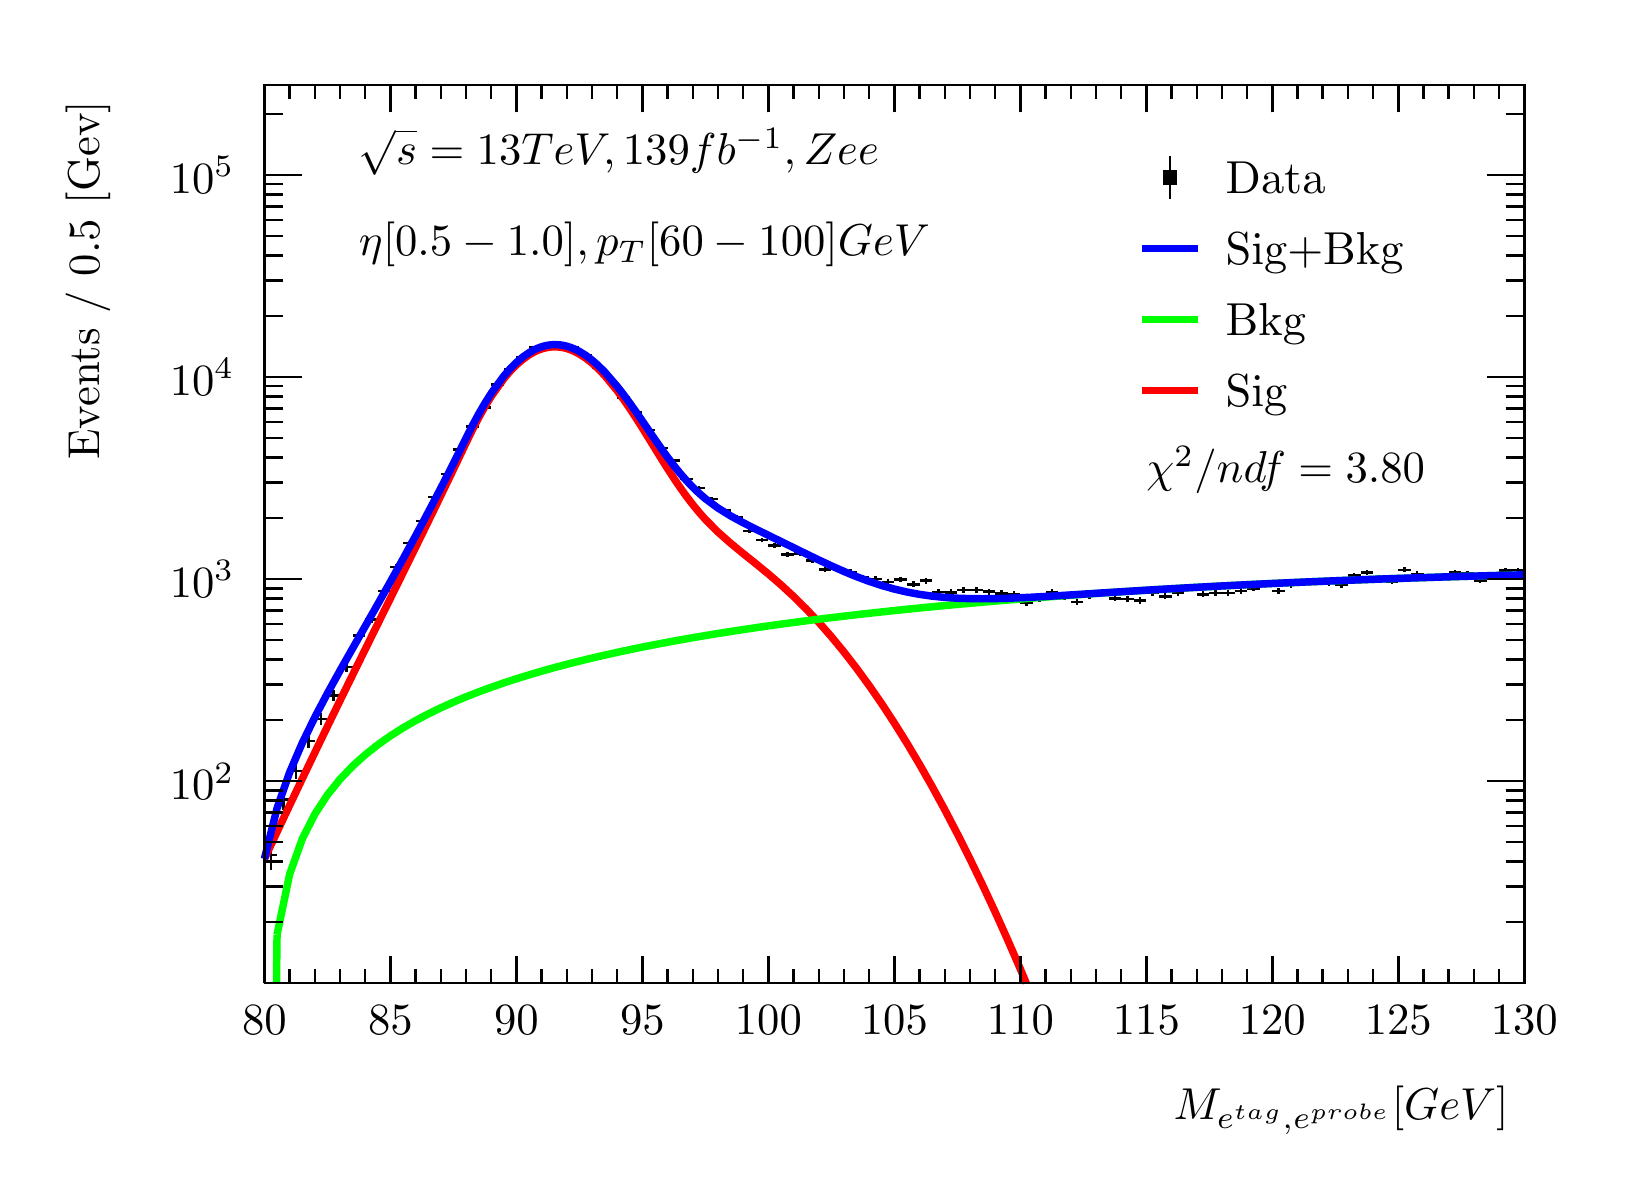
\begin{tikzpicture}
\pgfdeclareplotmark{cross} {
\pgfpathmoveto{\pgfpoint{-0.3\pgfplotmarksize}{\pgfplotmarksize}}
\pgfpathlineto{\pgfpoint{+0.3\pgfplotmarksize}{\pgfplotmarksize}}
\pgfpathlineto{\pgfpoint{+0.3\pgfplotmarksize}{0.3\pgfplotmarksize}}
\pgfpathlineto{\pgfpoint{+1\pgfplotmarksize}{0.3\pgfplotmarksize}}
\pgfpathlineto{\pgfpoint{+1\pgfplotmarksize}{-0.3\pgfplotmarksize}}
\pgfpathlineto{\pgfpoint{+0.3\pgfplotmarksize}{-0.3\pgfplotmarksize}}
\pgfpathlineto{\pgfpoint{+0.3\pgfplotmarksize}{-1.\pgfplotmarksize}}
\pgfpathlineto{\pgfpoint{-0.3\pgfplotmarksize}{-1.\pgfplotmarksize}}
\pgfpathlineto{\pgfpoint{-0.3\pgfplotmarksize}{-0.3\pgfplotmarksize}}
\pgfpathlineto{\pgfpoint{-1.\pgfplotmarksize}{-0.3\pgfplotmarksize}}
\pgfpathlineto{\pgfpoint{-1.\pgfplotmarksize}{0.3\pgfplotmarksize}}
\pgfpathlineto{\pgfpoint{-0.3\pgfplotmarksize}{0.3\pgfplotmarksize}}
\pgfpathclose
\pgfusepathqstroke
}
\pgfdeclareplotmark{cross*} {
\pgfpathmoveto{\pgfpoint{-0.3\pgfplotmarksize}{\pgfplotmarksize}}
\pgfpathlineto{\pgfpoint{+0.3\pgfplotmarksize}{\pgfplotmarksize}}
\pgfpathlineto{\pgfpoint{+0.3\pgfplotmarksize}{0.3\pgfplotmarksize}}
\pgfpathlineto{\pgfpoint{+1\pgfplotmarksize}{0.3\pgfplotmarksize}}
\pgfpathlineto{\pgfpoint{+1\pgfplotmarksize}{-0.3\pgfplotmarksize}}
\pgfpathlineto{\pgfpoint{+0.3\pgfplotmarksize}{-0.3\pgfplotmarksize}}
\pgfpathlineto{\pgfpoint{+0.3\pgfplotmarksize}{-1.\pgfplotmarksize}}
\pgfpathlineto{\pgfpoint{-0.3\pgfplotmarksize}{-1.\pgfplotmarksize}}
\pgfpathlineto{\pgfpoint{-0.3\pgfplotmarksize}{-0.3\pgfplotmarksize}}
\pgfpathlineto{\pgfpoint{-1.\pgfplotmarksize}{-0.3\pgfplotmarksize}}
\pgfpathlineto{\pgfpoint{-1.\pgfplotmarksize}{0.3\pgfplotmarksize}}
\pgfpathlineto{\pgfpoint{-0.3\pgfplotmarksize}{0.3\pgfplotmarksize}}
\pgfpathclose
\pgfusepathqfillstroke
}
\pgfdeclareplotmark{newstar} {
\pgfpathmoveto{\pgfqpoint{0pt}{\pgfplotmarksize}}
\pgfpathlineto{\pgfqpointpolar{44}{0.5\pgfplotmarksize}}
\pgfpathlineto{\pgfqpointpolar{18}{\pgfplotmarksize}}
\pgfpathlineto{\pgfqpointpolar{-20}{0.5\pgfplotmarksize}}
\pgfpathlineto{\pgfqpointpolar{-54}{\pgfplotmarksize}}
\pgfpathlineto{\pgfqpointpolar{-90}{0.5\pgfplotmarksize}}
\pgfpathlineto{\pgfqpointpolar{234}{\pgfplotmarksize}}
\pgfpathlineto{\pgfqpointpolar{198}{0.5\pgfplotmarksize}}
\pgfpathlineto{\pgfqpointpolar{162}{\pgfplotmarksize}}
\pgfpathlineto{\pgfqpointpolar{134}{0.5\pgfplotmarksize}}
\pgfpathclose
\pgfusepathqstroke
}
\pgfdeclareplotmark{newstar*} {
\pgfpathmoveto{\pgfqpoint{0pt}{\pgfplotmarksize}}
\pgfpathlineto{\pgfqpointpolar{44}{0.5\pgfplotmarksize}}
\pgfpathlineto{\pgfqpointpolar{18}{\pgfplotmarksize}}
\pgfpathlineto{\pgfqpointpolar{-20}{0.5\pgfplotmarksize}}
\pgfpathlineto{\pgfqpointpolar{-54}{\pgfplotmarksize}}
\pgfpathlineto{\pgfqpointpolar{-90}{0.5\pgfplotmarksize}}
\pgfpathlineto{\pgfqpointpolar{234}{\pgfplotmarksize}}
\pgfpathlineto{\pgfqpointpolar{198}{0.5\pgfplotmarksize}}
\pgfpathlineto{\pgfqpointpolar{162}{\pgfplotmarksize}}
\pgfpathlineto{\pgfqpointpolar{134}{0.5\pgfplotmarksize}}
\pgfpathclose
\pgfusepathqfillstroke
}
\definecolor{c}{rgb}{1,1,1};
\draw [color=c, fill=c] (0,0) rectangle (20,14.4361);
\draw [color=c, fill=c] (3,2.30977) rectangle (19,13.7143);
\definecolor{c}{rgb}{0,0,0};
\draw [c,line width=0.9] (3,2.30977) -- (3,13.7143) -- (19,13.7143) -- (19,2.30977) -- (3,2.30977);
\definecolor{c}{rgb}{1,1,1};
\draw [color=c, fill=c] (3,2.30977) rectangle (19,13.7143);
\definecolor{c}{rgb}{0,0,0};
\draw [c,line width=0.9] (3,2.30977) -- (3,13.7143) -- (19,13.7143) -- (19,2.30977) -- (3,2.30977);
\draw [c,line width=0.9] (3,2.30977) -- (19,2.30977);
\draw [c,line width=0.9] (3,2.65624) -- (3,2.30977);
\draw [c,line width=0.9] (3.32,2.48301) -- (3.32,2.30977);
\draw [c,line width=0.9] (3.64,2.48301) -- (3.64,2.30977);
\draw [c,line width=0.9] (3.96,2.48301) -- (3.96,2.30977);
\draw [c,line width=0.9] (4.28,2.48301) -- (4.28,2.30977);
\draw [c,line width=0.9] (4.6,2.65624) -- (4.6,2.30977);
\draw [c,line width=0.9] (4.92,2.48301) -- (4.92,2.30977);
\draw [c,line width=0.9] (5.24,2.48301) -- (5.24,2.30977);
\draw [c,line width=0.9] (5.56,2.48301) -- (5.56,2.30977);
\draw [c,line width=0.9] (5.88,2.48301) -- (5.88,2.30977);
\draw [c,line width=0.9] (6.2,2.65624) -- (6.2,2.30977);
\draw [c,line width=0.9] (6.52,2.48301) -- (6.52,2.30977);
\draw [c,line width=0.9] (6.84,2.48301) -- (6.84,2.30977);
\draw [c,line width=0.9] (7.16,2.48301) -- (7.16,2.30977);
\draw [c,line width=0.9] (7.48,2.48301) -- (7.48,2.30977);
\draw [c,line width=0.9] (7.8,2.65624) -- (7.8,2.30977);
\draw [c,line width=0.9] (8.12,2.48301) -- (8.12,2.30977);
\draw [c,line width=0.9] (8.44,2.48301) -- (8.44,2.30977);
\draw [c,line width=0.9] (8.76,2.48301) -- (8.76,2.30977);
\draw [c,line width=0.9] (9.08,2.48301) -- (9.08,2.30977);
\draw [c,line width=0.9] (9.4,2.65624) -- (9.4,2.30977);
\draw [c,line width=0.9] (9.72,2.48301) -- (9.72,2.30977);
\draw [c,line width=0.9] (10.04,2.48301) -- (10.04,2.30977);
\draw [c,line width=0.9] (10.36,2.48301) -- (10.36,2.30977);
\draw [c,line width=0.9] (10.68,2.48301) -- (10.68,2.30977);
\draw [c,line width=0.9] (11,2.65624) -- (11,2.30977);
\draw [c,line width=0.9] (11.32,2.48301) -- (11.32,2.30977);
\draw [c,line width=0.9] (11.64,2.48301) -- (11.64,2.30977);
\draw [c,line width=0.9] (11.96,2.48301) -- (11.96,2.30977);
\draw [c,line width=0.9] (12.28,2.48301) -- (12.28,2.30977);
\draw [c,line width=0.9] (12.6,2.65624) -- (12.6,2.30977);
\draw [c,line width=0.9] (12.92,2.48301) -- (12.92,2.30977);
\draw [c,line width=0.9] (13.24,2.48301) -- (13.24,2.30977);
\draw [c,line width=0.9] (13.56,2.48301) -- (13.56,2.30977);
\draw [c,line width=0.9] (13.88,2.48301) -- (13.88,2.30977);
\draw [c,line width=0.9] (14.2,2.65624) -- (14.2,2.30977);
\draw [c,line width=0.9] (14.52,2.48301) -- (14.52,2.30977);
\draw [c,line width=0.9] (14.84,2.48301) -- (14.84,2.30977);
\draw [c,line width=0.9] (15.16,2.48301) -- (15.16,2.30977);
\draw [c,line width=0.9] (15.48,2.48301) -- (15.48,2.30977);
\draw [c,line width=0.9] (15.8,2.65624) -- (15.8,2.30977);
\draw [c,line width=0.9] (16.12,2.48301) -- (16.12,2.30977);
\draw [c,line width=0.9] (16.44,2.48301) -- (16.44,2.30977);
\draw [c,line width=0.9] (16.76,2.48301) -- (16.76,2.30977);
\draw [c,line width=0.9] (17.08,2.48301) -- (17.08,2.30977);
\draw [c,line width=0.9] (17.4,2.65624) -- (17.4,2.30977);
\draw [c,line width=0.9] (17.72,2.48301) -- (17.72,2.30977);
\draw [c,line width=0.9] (18.04,2.48301) -- (18.04,2.30977);
\draw [c,line width=0.9] (18.36,2.48301) -- (18.36,2.30977);
\draw [c,line width=0.9] (18.68,2.48301) -- (18.68,2.30977);
\draw [c,line width=0.9] (19,2.65624) -- (19,2.30977);
\draw [anchor=base] (3,1.66015) node[scale=1.61424, color=c, rotate=0]{80};
\draw [anchor=base] (4.6,1.66015) node[scale=1.61424, color=c, rotate=0]{85};
\draw [anchor=base] (6.2,1.66015) node[scale=1.61424, color=c, rotate=0]{90};
\draw [anchor=base] (7.8,1.66015) node[scale=1.61424, color=c, rotate=0]{95};
\draw [anchor=base] (9.4,1.66015) node[scale=1.61424, color=c, rotate=0]{100};
\draw [anchor=base] (11,1.66015) node[scale=1.61424, color=c, rotate=0]{105};
\draw [anchor=base] (12.6,1.66015) node[scale=1.61424, color=c, rotate=0]{110};
\draw [anchor=base] (14.2,1.66015) node[scale=1.61424, color=c, rotate=0]{115};
\draw [anchor=base] (15.8,1.66015) node[scale=1.61424, color=c, rotate=0]{120};
\draw [anchor=base] (17.4,1.66015) node[scale=1.61424, color=c, rotate=0]{125};
\draw [anchor=base] (19,1.66015) node[scale=1.61424, color=c, rotate=0]{130};
\draw [anchor= east] (19,0.692932) node[scale=1.61424, color=c, rotate=0]{$M_{e^{tag}, e^{probe}}  [GeV]$};
\draw [c,line width=0.9] (3,13.7143) -- (19,13.7143);
\draw [c,line width=0.9] (3,13.3678) -- (3,13.7143);
\draw [c,line width=0.9] (3.32,13.5411) -- (3.32,13.7143);
\draw [c,line width=0.9] (3.64,13.5411) -- (3.64,13.7143);
\draw [c,line width=0.9] (3.96,13.5411) -- (3.96,13.7143);
\draw [c,line width=0.9] (4.28,13.5411) -- (4.28,13.7143);
\draw [c,line width=0.9] (4.6,13.3678) -- (4.6,13.7143);
\draw [c,line width=0.9] (4.92,13.5411) -- (4.92,13.7143);
\draw [c,line width=0.9] (5.24,13.5411) -- (5.24,13.7143);
\draw [c,line width=0.9] (5.56,13.5411) -- (5.56,13.7143);
\draw [c,line width=0.9] (5.88,13.5411) -- (5.88,13.7143);
\draw [c,line width=0.9] (6.2,13.3678) -- (6.2,13.7143);
\draw [c,line width=0.9] (6.52,13.5411) -- (6.52,13.7143);
\draw [c,line width=0.9] (6.84,13.5411) -- (6.84,13.7143);
\draw [c,line width=0.9] (7.16,13.5411) -- (7.16,13.7143);
\draw [c,line width=0.9] (7.48,13.5411) -- (7.48,13.7143);
\draw [c,line width=0.9] (7.8,13.3678) -- (7.8,13.7143);
\draw [c,line width=0.9] (8.12,13.5411) -- (8.12,13.7143);
\draw [c,line width=0.9] (8.44,13.5411) -- (8.44,13.7143);
\draw [c,line width=0.9] (8.76,13.5411) -- (8.76,13.7143);
\draw [c,line width=0.9] (9.08,13.5411) -- (9.08,13.7143);
\draw [c,line width=0.9] (9.4,13.3678) -- (9.4,13.7143);
\draw [c,line width=0.9] (9.72,13.5411) -- (9.72,13.7143);
\draw [c,line width=0.9] (10.04,13.5411) -- (10.04,13.7143);
\draw [c,line width=0.9] (10.36,13.5411) -- (10.36,13.7143);
\draw [c,line width=0.9] (10.68,13.5411) -- (10.68,13.7143);
\draw [c,line width=0.9] (11,13.3678) -- (11,13.7143);
\draw [c,line width=0.9] (11.32,13.5411) -- (11.32,13.7143);
\draw [c,line width=0.9] (11.64,13.5411) -- (11.64,13.7143);
\draw [c,line width=0.9] (11.96,13.5411) -- (11.96,13.7143);
\draw [c,line width=0.9] (12.28,13.5411) -- (12.28,13.7143);
\draw [c,line width=0.9] (12.6,13.3678) -- (12.6,13.7143);
\draw [c,line width=0.9] (12.92,13.5411) -- (12.92,13.7143);
\draw [c,line width=0.9] (13.24,13.5411) -- (13.24,13.7143);
\draw [c,line width=0.9] (13.56,13.5411) -- (13.56,13.7143);
\draw [c,line width=0.9] (13.88,13.5411) -- (13.88,13.7143);
\draw [c,line width=0.9] (14.2,13.3678) -- (14.2,13.7143);
\draw [c,line width=0.9] (14.52,13.5411) -- (14.52,13.7143);
\draw [c,line width=0.9] (14.84,13.5411) -- (14.84,13.7143);
\draw [c,line width=0.9] (15.16,13.5411) -- (15.16,13.7143);
\draw [c,line width=0.9] (15.48,13.5411) -- (15.48,13.7143);
\draw [c,line width=0.9] (15.8,13.3678) -- (15.8,13.7143);
\draw [c,line width=0.9] (16.12,13.5411) -- (16.12,13.7143);
\draw [c,line width=0.9] (16.44,13.5411) -- (16.44,13.7143);
\draw [c,line width=0.9] (16.76,13.5411) -- (16.76,13.7143);
\draw [c,line width=0.9] (17.08,13.5411) -- (17.08,13.7143);
\draw [c,line width=0.9] (17.4,13.3678) -- (17.4,13.7143);
\draw [c,line width=0.9] (17.72,13.5411) -- (17.72,13.7143);
\draw [c,line width=0.9] (18.04,13.5411) -- (18.04,13.7143);
\draw [c,line width=0.9] (18.36,13.5411) -- (18.36,13.7143);
\draw [c,line width=0.9] (18.68,13.5411) -- (18.68,13.7143);
\draw [c,line width=0.9] (19,13.3678) -- (19,13.7143);
\draw [c,line width=0.9] (3,2.30977) -- (3,13.7143);
\draw [c,line width=0.9] (3.237,3.08209) -- (3,3.08209);
\draw [c,line width=0.9] (3.237,3.53386) -- (3,3.53386);
\draw [c,line width=0.9] (3.237,3.8544) -- (3,3.8544);
\draw [c,line width=0.9] (3.237,4.10303) -- (3,4.10303);
\draw [c,line width=0.9] (3.237,4.30618) -- (3,4.30618);
\draw [c,line width=0.9] (3.237,4.47794) -- (3,4.47794);
\draw [c,line width=0.9] (3.237,4.62672) -- (3,4.62672);
\draw [c,line width=0.9] (3.237,4.75795) -- (3,4.75795);
\draw [c,line width=0.9] (3.474,4.87535) -- (3,4.87535);
\draw [anchor= east] (2.82,4.87535) node[scale=1.61424, color=c, rotate=0]{$10^{2}$};
\draw [c,line width=0.9] (3.237,5.64766) -- (3,5.64766);
\draw [c,line width=0.9] (3.237,6.09944) -- (3,6.09944);
\draw [c,line width=0.9] (3.237,6.41998) -- (3,6.41998);
\draw [c,line width=0.9] (3.237,6.66861) -- (3,6.66861);
\draw [c,line width=0.9] (3.237,6.87176) -- (3,6.87176);
\draw [c,line width=0.9] (3.237,7.04351) -- (3,7.04351);
\draw [c,line width=0.9] (3.237,7.1923) -- (3,7.1923);
\draw [c,line width=0.9] (3.237,7.32353) -- (3,7.32353);
\draw [c,line width=0.9] (3.474,7.44093) -- (3,7.44093);
\draw [anchor= east] (2.82,7.44093) node[scale=1.61424, color=c, rotate=0]{$10^{3}$};
\draw [c,line width=0.9] (3.237,8.21324) -- (3,8.21324);
\draw [c,line width=0.9] (3.237,8.66502) -- (3,8.66502);
\draw [c,line width=0.9] (3.237,8.98556) -- (3,8.98556);
\draw [c,line width=0.9] (3.237,9.23419) -- (3,9.23419);
\draw [c,line width=0.9] (3.237,9.43733) -- (3,9.43733);
\draw [c,line width=0.9] (3.237,9.60909) -- (3,9.60909);
\draw [c,line width=0.9] (3.237,9.75787) -- (3,9.75787);
\draw [c,line width=0.9] (3.237,9.88911) -- (3,9.88911);
\draw [c,line width=0.9] (3.474,10.0065) -- (3,10.0065);
\draw [anchor= east] (2.82,10.0065) node[scale=1.61424, color=c, rotate=0]{$10^{4}$};
\draw [c,line width=0.9] (3.237,10.7788) -- (3,10.7788);
\draw [c,line width=0.9] (3.237,11.2306) -- (3,11.2306);
\draw [c,line width=0.9] (3.237,11.5511) -- (3,11.5511);
\draw [c,line width=0.9] (3.237,11.7998) -- (3,11.7998);
\draw [c,line width=0.9] (3.237,12.0029) -- (3,12.0029);
\draw [c,line width=0.9] (3.237,12.1747) -- (3,12.1747);
\draw [c,line width=0.9] (3.237,12.3235) -- (3,12.3235);
\draw [c,line width=0.9] (3.237,12.4547) -- (3,12.4547);
\draw [c,line width=0.9] (3.474,12.5721) -- (3,12.5721);
\draw [anchor= east] (2.82,12.5721) node[scale=1.61424, color=c, rotate=0]{$10^{5}$};
\draw [c,line width=0.9] (3.237,13.3444) -- (3,13.3444);
\draw [anchor= east] (0.76,13.7143) node[scale=1.61424, color=c, rotate=90]{Events / 0.5 [Gev]};
\draw [c,line width=0.9] (19,2.30977) -- (19,13.7143);
\draw [c,line width=0.9] (18.763,3.08209) -- (19,3.08209);
\draw [c,line width=0.9] (18.763,3.53386) -- (19,3.53386);
\draw [c,line width=0.9] (18.763,3.8544) -- (19,3.8544);
\draw [c,line width=0.9] (18.763,4.10303) -- (19,4.10303);
\draw [c,line width=0.9] (18.763,4.30618) -- (19,4.30618);
\draw [c,line width=0.9] (18.763,4.47794) -- (19,4.47794);
\draw [c,line width=0.9] (18.763,4.62672) -- (19,4.62672);
\draw [c,line width=0.9] (18.763,4.75795) -- (19,4.75795);
\draw [c,line width=0.9] (18.526,4.87535) -- (19,4.87535);
\draw [c,line width=0.9] (18.763,5.64766) -- (19,5.64766);
\draw [c,line width=0.9] (18.763,6.09944) -- (19,6.09944);
\draw [c,line width=0.9] (18.763,6.41998) -- (19,6.41998);
\draw [c,line width=0.9] (18.763,6.66861) -- (19,6.66861);
\draw [c,line width=0.9] (18.763,6.87176) -- (19,6.87176);
\draw [c,line width=0.9] (18.763,7.04351) -- (19,7.04351);
\draw [c,line width=0.9] (18.763,7.1923) -- (19,7.1923);
\draw [c,line width=0.9] (18.763,7.32353) -- (19,7.32353);
\draw [c,line width=0.9] (18.526,7.44093) -- (19,7.44093);
\draw [c,line width=0.9] (18.763,8.21324) -- (19,8.21324);
\draw [c,line width=0.9] (18.763,8.66502) -- (19,8.66502);
\draw [c,line width=0.9] (18.763,8.98556) -- (19,8.98556);
\draw [c,line width=0.9] (18.763,9.23419) -- (19,9.23419);
\draw [c,line width=0.9] (18.763,9.43733) -- (19,9.43733);
\draw [c,line width=0.9] (18.763,9.60909) -- (19,9.60909);
\draw [c,line width=0.9] (18.763,9.75787) -- (19,9.75787);
\draw [c,line width=0.9] (18.763,9.88911) -- (19,9.88911);
\draw [c,line width=0.9] (18.526,10.0065) -- (19,10.0065);
\draw [c,line width=0.9] (18.763,10.7788) -- (19,10.7788);
\draw [c,line width=0.9] (18.763,11.2306) -- (19,11.2306);
\draw [c,line width=0.9] (18.763,11.5511) -- (19,11.5511);
\draw [c,line width=0.9] (18.763,11.7998) -- (19,11.7998);
\draw [c,line width=0.9] (18.763,12.0029) -- (19,12.0029);
\draw [c,line width=0.9] (18.763,12.1747) -- (19,12.1747);
\draw [c,line width=0.9] (18.763,12.3235) -- (19,12.3235);
\draw [c,line width=0.9] (18.763,12.4547) -- (19,12.4547);
\draw [c,line width=0.9] (18.526,12.5721) -- (19,12.5721);
\draw [c,line width=0.9] (18.763,13.3444) -- (19,13.3444);
\draw [c,line width=0.9] (3.08,3.93499) -- (3,3.93499);
\draw [c,line width=0.9] (3,3.93499) -- (3,3.93499);
\draw [c,line width=0.9] (3.08,3.93499) -- (3.16,3.93499);
\draw [c,line width=0.9] (3.16,3.93499) -- (3.16,3.93499);
\draw [c,line width=0.9] (3.08,3.93499) -- (3.08,4.11651);
\draw [c,line width=0.9] (3.08,4.11651) -- (3.08,4.11651);
\draw [c,line width=0.9] (3.08,3.93499) -- (3.08,3.75141);
\draw [c,line width=0.9] (3.08,3.75141) -- (3.08,3.75141);
\draw [c,line width=0.9] (3.24,4.64056) -- (3.16,4.64056);
\draw [c,line width=0.9] (3.16,4.64056) -- (3.16,4.64056);
\draw [c,line width=0.9] (3.24,4.64056) -- (3.32,4.64056);
\draw [c,line width=0.9] (3.32,4.64056) -- (3.32,4.64056);
\draw [c,line width=0.9] (3.24,4.64056) -- (3.24,4.77072);
\draw [c,line width=0.9] (3.24,4.77072) -- (3.24,4.77072);
\draw [c,line width=0.9] (3.24,4.64056) -- (3.24,4.50961);
\draw [c,line width=0.9] (3.24,4.50961) -- (3.24,4.50961);
\draw [c,line width=0.9] (3.4,5.00162) -- (3.32,5.00162);
\draw [c,line width=0.9] (3.32,5.00162) -- (3.32,5.00162);
\draw [c,line width=0.9] (3.4,5.00162) -- (3.48,5.00162);
\draw [c,line width=0.9] (3.48,5.00162) -- (3.48,5.00162);
\draw [c,line width=0.9] (3.4,5.00162) -- (3.4,5.10687);
\draw [c,line width=0.9] (3.4,5.10687) -- (3.4,5.10687);
\draw [c,line width=0.9] (3.4,5.00162) -- (3.4,4.89638);
\draw [c,line width=0.9] (3.4,4.89638) -- (3.4,4.89638);
\draw [c,line width=0.9] (3.56,5.38502) -- (3.48,5.38502);
\draw [c,line width=0.9] (3.48,5.38502) -- (3.48,5.38502);
\draw [c,line width=0.9] (3.56,5.38502) -- (3.64,5.38502);
\draw [c,line width=0.9] (3.64,5.38502) -- (3.64,5.38502);
\draw [c,line width=0.9] (3.56,5.38502) -- (3.56,5.47364);
\draw [c,line width=0.9] (3.56,5.47364) -- (3.56,5.47364);
\draw [c,line width=0.9] (3.56,5.38502) -- (3.56,5.2964);
\draw [c,line width=0.9] (3.56,5.2964) -- (3.56,5.2964);
\draw [c,line width=0.9] (3.72,5.66426) -- (3.64,5.66426);
\draw [c,line width=0.9] (3.64,5.66426) -- (3.64,5.66426);
\draw [c,line width=0.9] (3.72,5.66426) -- (3.8,5.66426);
\draw [c,line width=0.9] (3.8,5.66426) -- (3.8,5.66426);
\draw [c,line width=0.9] (3.72,5.66426) -- (3.72,5.74244);
\draw [c,line width=0.9] (3.72,5.74244) -- (3.72,5.74244);
\draw [c,line width=0.9] (3.72,5.66426) -- (3.72,5.58607);
\draw [c,line width=0.9] (3.72,5.58607) -- (3.72,5.58607);
\draw [c,line width=0.9] (3.88,5.96122) -- (3.8,5.96122);
\draw [c,line width=0.9] (3.8,5.96122) -- (3.8,5.96122);
\draw [c,line width=0.9] (3.88,5.96122) -- (3.96,5.96122);
\draw [c,line width=0.9] (3.96,5.96122) -- (3.96,5.96122);
\draw [c,line width=0.9] (3.88,5.96122) -- (3.88,6.02966);
\draw [c,line width=0.9] (3.88,6.02966) -- (3.88,6.02966);
\draw [c,line width=0.9] (3.88,5.96122) -- (3.88,5.89279);
\draw [c,line width=0.9] (3.88,5.89279) -- (3.88,5.89279);
\draw [c,line width=0.9] (4.04,6.32405) -- (3.96,6.32405);
\draw [c,line width=0.9] (3.96,6.32405) -- (3.96,6.32405);
\draw [c,line width=0.9] (4.04,6.32405) -- (4.12,6.32405);
\draw [c,line width=0.9] (4.12,6.32405) -- (4.12,6.32405);
\draw [c,line width=0.9] (4.04,6.32405) -- (4.04,6.3822);
\draw [c,line width=0.9] (4.04,6.3822) -- (4.04,6.3822);
\draw [c,line width=0.9] (4.04,6.32405) -- (4.04,6.26589);
\draw [c,line width=0.9] (4.04,6.26589) -- (4.04,6.26589);
\draw [c,line width=0.9] (4.2,6.7251) -- (4.12,6.7251);
\draw [c,line width=0.9] (4.12,6.7251) -- (4.12,6.7251);
\draw [c,line width=0.9] (4.2,6.7251) -- (4.28,6.7251);
\draw [c,line width=0.9] (4.28,6.7251) -- (4.28,6.7251);
\draw [c,line width=0.9] (4.2,6.7251) -- (4.2,6.77367);
\draw [c,line width=0.9] (4.2,6.77367) -- (4.2,6.77367);
\draw [c,line width=0.9] (4.2,6.7251) -- (4.2,6.67652);
\draw [c,line width=0.9] (4.2,6.67652) -- (4.2,6.67652);
\draw [c,line width=0.9] (4.36,6.92435) -- (4.28,6.92435);
\draw [c,line width=0.9] (4.28,6.92435) -- (4.28,6.92435);
\draw [c,line width=0.9] (4.36,6.92435) -- (4.44,6.92435);
\draw [c,line width=0.9] (4.44,6.92435) -- (4.44,6.92435);
\draw [c,line width=0.9] (4.36,6.92435) -- (4.36,6.96877);
\draw [c,line width=0.9] (4.36,6.96877) -- (4.36,6.96877);
\draw [c,line width=0.9] (4.36,6.92435) -- (4.36,6.87993);
\draw [c,line width=0.9] (4.36,6.87993) -- (4.36,6.87993);
\draw [c,line width=0.9] (4.52,7.28704) -- (4.44,7.28704);
\draw [c,line width=0.9] (4.44,7.28704) -- (4.44,7.28704);
\draw [c,line width=0.9] (4.52,7.28704) -- (4.6,7.28704);
\draw [c,line width=0.9] (4.6,7.28704) -- (4.6,7.28704);
\draw [c,line width=0.9] (4.52,7.28704) -- (4.52,7.32479);
\draw [c,line width=0.9] (4.52,7.32479) -- (4.52,7.32479);
\draw [c,line width=0.9] (4.52,7.28704) -- (4.52,7.24929);
\draw [c,line width=0.9] (4.52,7.24929) -- (4.52,7.24929);
\draw [c,line width=0.9] (4.68,7.59665) -- (4.6,7.59665);
\draw [c,line width=0.9] (4.6,7.59665) -- (4.6,7.59665);
\draw [c,line width=0.9] (4.68,7.59665) -- (4.76,7.59665);
\draw [c,line width=0.9] (4.76,7.59665) -- (4.76,7.59665);
\draw [c,line width=0.9] (4.68,7.59665) -- (4.68,7.62951);
\draw [c,line width=0.9] (4.68,7.62951) -- (4.68,7.62951);
\draw [c,line width=0.9] (4.68,7.59665) -- (4.68,7.5638);
\draw [c,line width=0.9] (4.68,7.5638) -- (4.68,7.5638);
\draw [c,line width=0.9] (4.84,7.89863) -- (4.76,7.89863);
\draw [c,line width=0.9] (4.76,7.89863) -- (4.76,7.89863);
\draw [c,line width=0.9] (4.84,7.89863) -- (4.92,7.89863);
\draw [c,line width=0.9] (4.92,7.89863) -- (4.92,7.89863);
\draw [c,line width=0.9] (4.84,7.89863) -- (4.84,7.92732);
\draw [c,line width=0.9] (4.84,7.92732) -- (4.84,7.92732);
\draw [c,line width=0.9] (4.84,7.89863) -- (4.84,7.86994);
\draw [c,line width=0.9] (4.84,7.86994) -- (4.84,7.86994);
\draw [c,line width=0.9] (5,8.1747) -- (4.92,8.1747);
\draw [c,line width=0.9] (4.92,8.1747) -- (4.92,8.1747);
\draw [c,line width=0.9] (5,8.1747) -- (5.08,8.1747);
\draw [c,line width=0.9] (5.08,8.1747) -- (5.08,8.1747);
\draw [c,line width=0.9] (5,8.1747) -- (5,8.20005);
\draw [c,line width=0.9] (5,8.20005) -- (5,8.20005);
\draw [c,line width=0.9] (5,8.1747) -- (5,8.14935);
\draw [c,line width=0.9] (5,8.14935) -- (5,8.14935);
\draw [c,line width=0.9] (5.16,8.48) -- (5.08,8.48);
\draw [c,line width=0.9] (5.08,8.48) -- (5.08,8.48);
\draw [c,line width=0.9] (5.16,8.48) -- (5.24,8.48);
\draw [c,line width=0.9] (5.24,8.48) -- (5.24,8.48);
\draw [c,line width=0.9] (5.16,8.48) -- (5.16,8.5021);
\draw [c,line width=0.9] (5.16,8.5021) -- (5.16,8.5021);
\draw [c,line width=0.9] (5.16,8.48) -- (5.16,8.45789);
\draw [c,line width=0.9] (5.16,8.45789) -- (5.16,8.45789);
\draw [c,line width=0.9] (5.32,8.77694) -- (5.24,8.77694);
\draw [c,line width=0.9] (5.24,8.77694) -- (5.24,8.77694);
\draw [c,line width=0.9] (5.32,8.77694) -- (5.4,8.77694);
\draw [c,line width=0.9] (5.4,8.77694) -- (5.4,8.77694);
\draw [c,line width=0.9] (5.32,8.77694) -- (5.32,8.79629);
\draw [c,line width=0.9] (5.32,8.79629) -- (5.32,8.79629);
\draw [c,line width=0.9] (5.32,8.77694) -- (5.32,8.75759);
\draw [c,line width=0.9] (5.32,8.75759) -- (5.32,8.75759);
\draw [c,line width=0.9] (5.48,9.08362) -- (5.4,9.08362);
\draw [c,line width=0.9] (5.4,9.08362) -- (5.4,9.08362);
\draw [c,line width=0.9] (5.48,9.08362) -- (5.56,9.08362);
\draw [c,line width=0.9] (5.56,9.08362) -- (5.56,9.08362);
\draw [c,line width=0.9] (5.48,9.08362) -- (5.48,9.10048);
\draw [c,line width=0.9] (5.48,9.10048) -- (5.48,9.10048);
\draw [c,line width=0.9] (5.48,9.08362) -- (5.48,9.06676);
\draw [c,line width=0.9] (5.48,9.06676) -- (5.48,9.06676);
\draw [c,line width=0.9] (5.64,9.3794) -- (5.56,9.3794);
\draw [c,line width=0.9] (5.56,9.3794) -- (5.56,9.3794);
\draw [c,line width=0.9] (5.64,9.3794) -- (5.72,9.3794);
\draw [c,line width=0.9] (5.72,9.3794) -- (5.72,9.3794);
\draw [c,line width=0.9] (5.64,9.3794) -- (5.64,9.39416);
\draw [c,line width=0.9] (5.64,9.39416) -- (5.64,9.39416);
\draw [c,line width=0.9] (5.64,9.3794) -- (5.64,9.36464);
\draw [c,line width=0.9] (5.64,9.36464) -- (5.64,9.36464);
\draw [c,line width=0.9] (5.8,9.62112) -- (5.72,9.62112);
\draw [c,line width=0.9] (5.72,9.62112) -- (5.72,9.62112);
\draw [c,line width=0.9] (5.8,9.62112) -- (5.88,9.62112);
\draw [c,line width=0.9] (5.88,9.62112) -- (5.88,9.62112);
\draw [c,line width=0.9] (5.8,9.62112) -- (5.8,9.63437);
\draw [c,line width=0.9] (5.8,9.63437) -- (5.8,9.63437);
\draw [c,line width=0.9] (5.8,9.62112) -- (5.8,9.60788);
\draw [c,line width=0.9] (5.8,9.60788) -- (5.8,9.60788);
\draw [c,line width=0.9] (5.96,9.91166) -- (5.88,9.91166);
\draw [c,line width=0.9] (5.88,9.91166) -- (5.88,9.91166);
\draw [c,line width=0.9] (5.96,9.91166) -- (6.04,9.91166);
\draw [c,line width=0.9] (6.04,9.91166) -- (6.04,9.91166);
\draw [c,line width=0.9] (5.96,9.91166) -- (5.96,9.92329);
\draw [c,line width=0.9] (5.96,9.92329) -- (5.96,9.92329);
\draw [c,line width=0.9] (5.96,9.91166) -- (5.96,9.90003);
\draw [c,line width=0.9] (5.96,9.90003) -- (5.96,9.90003);
\draw [c,line width=0.9] (6.12,10.1003) -- (6.04,10.1003);
\draw [c,line width=0.9] (6.04,10.1003) -- (6.04,10.1003);
\draw [c,line width=0.9] (6.12,10.1003) -- (6.2,10.1003);
\draw [c,line width=0.9] (6.2,10.1003) -- (6.2,10.1003);
\draw [c,line width=0.9] (6.12,10.1003) -- (6.12,10.111);
\draw [c,line width=0.9] (6.12,10.111) -- (6.12,10.111);
\draw [c,line width=0.9] (6.12,10.1003) -- (6.12,10.0896);
\draw [c,line width=0.9] (6.12,10.0896) -- (6.12,10.0896);
\draw [c,line width=0.9] (6.28,10.2518) -- (6.2,10.2518);
\draw [c,line width=0.9] (6.2,10.2518) -- (6.2,10.2518);
\draw [c,line width=0.9] (6.28,10.2518) -- (6.36,10.2518);
\draw [c,line width=0.9] (6.36,10.2518) -- (6.36,10.2518);
\draw [c,line width=0.9] (6.28,10.2518) -- (6.28,10.2618);
\draw [c,line width=0.9] (6.28,10.2618) -- (6.28,10.2618);
\draw [c,line width=0.9] (6.28,10.2518) -- (6.28,10.2419);
\draw [c,line width=0.9] (6.28,10.2419) -- (6.28,10.2419);
\draw [c,line width=0.9] (6.44,10.3798) -- (6.36,10.3798);
\draw [c,line width=0.9] (6.36,10.3798) -- (6.36,10.3798);
\draw [c,line width=0.9] (6.44,10.3798) -- (6.52,10.3798);
\draw [c,line width=0.9] (6.52,10.3798) -- (6.52,10.3798);
\draw [c,line width=0.9] (6.44,10.3798) -- (6.44,10.3892);
\draw [c,line width=0.9] (6.44,10.3892) -- (6.44,10.3892);
\draw [c,line width=0.9] (6.44,10.3798) -- (6.44,10.3704);
\draw [c,line width=0.9] (6.44,10.3704) -- (6.44,10.3704);
\draw [c,line width=0.9] (6.6,10.4278) -- (6.52,10.4278);
\draw [c,line width=0.9] (6.52,10.4278) -- (6.52,10.4278);
\draw [c,line width=0.9] (6.6,10.4278) -- (6.68,10.4278);
\draw [c,line width=0.9] (6.68,10.4278) -- (6.68,10.4278);
\draw [c,line width=0.9] (6.6,10.4278) -- (6.6,10.437);
\draw [c,line width=0.9] (6.6,10.437) -- (6.6,10.437);
\draw [c,line width=0.9] (6.6,10.4278) -- (6.6,10.4186);
\draw [c,line width=0.9] (6.6,10.4186) -- (6.6,10.4186);
\draw [c,line width=0.9] (6.76,10.428) -- (6.68,10.428);
\draw [c,line width=0.9] (6.68,10.428) -- (6.68,10.428);
\draw [c,line width=0.9] (6.76,10.428) -- (6.84,10.428);
\draw [c,line width=0.9] (6.84,10.428) -- (6.84,10.428);
\draw [c,line width=0.9] (6.76,10.428) -- (6.76,10.4372);
\draw [c,line width=0.9] (6.76,10.4372) -- (6.76,10.4372);
\draw [c,line width=0.9] (6.76,10.428) -- (6.76,10.4188);
\draw [c,line width=0.9] (6.76,10.4188) -- (6.76,10.4188);
\draw [c,line width=0.9] (6.92,10.3797) -- (6.84,10.3797);
\draw [c,line width=0.9] (6.84,10.3797) -- (6.84,10.3797);
\draw [c,line width=0.9] (6.92,10.3797) -- (7,10.3797);
\draw [c,line width=0.9] (7,10.3797) -- (7,10.3797);
\draw [c,line width=0.9] (6.92,10.3797) -- (6.92,10.3892);
\draw [c,line width=0.9] (6.92,10.3892) -- (6.92,10.3892);
\draw [c,line width=0.9] (6.92,10.3797) -- (6.92,10.3703);
\draw [c,line width=0.9] (6.92,10.3703) -- (6.92,10.3703);
\draw [c,line width=0.9] (7.08,10.2882) -- (7,10.2882);
\draw [c,line width=0.9] (7,10.2882) -- (7,10.2882);
\draw [c,line width=0.9] (7.08,10.2882) -- (7.16,10.2882);
\draw [c,line width=0.9] (7.16,10.2882) -- (7.16,10.2882);
\draw [c,line width=0.9] (7.08,10.2882) -- (7.08,10.298);
\draw [c,line width=0.9] (7.08,10.298) -- (7.08,10.298);
\draw [c,line width=0.9] (7.08,10.2882) -- (7.08,10.2783);
\draw [c,line width=0.9] (7.08,10.2783) -- (7.08,10.2783);
\draw [c,line width=0.9] (7.24,10.1239) -- (7.16,10.1239);
\draw [c,line width=0.9] (7.16,10.1239) -- (7.16,10.1239);
\draw [c,line width=0.9] (7.24,10.1239) -- (7.32,10.1239);
\draw [c,line width=0.9] (7.32,10.1239) -- (7.32,10.1239);
\draw [c,line width=0.9] (7.24,10.1239) -- (7.24,10.1345);
\draw [c,line width=0.9] (7.24,10.1345) -- (7.24,10.1345);
\draw [c,line width=0.9] (7.24,10.1239) -- (7.24,10.1133);
\draw [c,line width=0.9] (7.24,10.1133) -- (7.24,10.1133);
\draw [c,line width=0.9] (7.4,9.95811) -- (7.32,9.95811);
\draw [c,line width=0.9] (7.32,9.95811) -- (7.32,9.95811);
\draw [c,line width=0.9] (7.4,9.95811) -- (7.48,9.95811);
\draw [c,line width=0.9] (7.48,9.95811) -- (7.48,9.95811);
\draw [c,line width=0.9] (7.4,9.95811) -- (7.4,9.9695);
\draw [c,line width=0.9] (7.4,9.9695) -- (7.4,9.9695);
\draw [c,line width=0.9] (7.4,9.95811) -- (7.4,9.94673);
\draw [c,line width=0.9] (7.4,9.94673) -- (7.4,9.94673);
\draw [c,line width=0.9] (7.56,9.74569) -- (7.48,9.74569);
\draw [c,line width=0.9] (7.48,9.74569) -- (7.48,9.74569);
\draw [c,line width=0.9] (7.56,9.74569) -- (7.64,9.74569);
\draw [c,line width=0.9] (7.64,9.74569) -- (7.64,9.74569);
\draw [c,line width=0.9] (7.56,9.74569) -- (7.56,9.75822);
\draw [c,line width=0.9] (7.56,9.75822) -- (7.56,9.75822);
\draw [c,line width=0.9] (7.56,9.74569) -- (7.56,9.73317);
\draw [c,line width=0.9] (7.56,9.73317) -- (7.56,9.73317);
\draw [c,line width=0.9] (7.72,9.55679) -- (7.64,9.55679);
\draw [c,line width=0.9] (7.64,9.55679) -- (7.64,9.55679);
\draw [c,line width=0.9] (7.72,9.55679) -- (7.8,9.55679);
\draw [c,line width=0.9] (7.8,9.55679) -- (7.8,9.55679);
\draw [c,line width=0.9] (7.72,9.55679) -- (7.72,9.57042);
\draw [c,line width=0.9] (7.72,9.57042) -- (7.72,9.57042);
\draw [c,line width=0.9] (7.72,9.55679) -- (7.72,9.54315);
\draw [c,line width=0.9] (7.72,9.54315) -- (7.72,9.54315);
\draw [c,line width=0.9] (7.88,9.33429) -- (7.8,9.33429);
\draw [c,line width=0.9] (7.8,9.33429) -- (7.8,9.33429);
\draw [c,line width=0.9] (7.88,9.33429) -- (7.96,9.33429);
\draw [c,line width=0.9] (7.96,9.33429) -- (7.96,9.33429);
\draw [c,line width=0.9] (7.88,9.33429) -- (7.88,9.34936);
\draw [c,line width=0.9] (7.88,9.34936) -- (7.88,9.34936);
\draw [c,line width=0.9] (7.88,9.33429) -- (7.88,9.31923);
\draw [c,line width=0.9] (7.88,9.31923) -- (7.88,9.31923);
\draw [c,line width=0.9] (8.04,9.10435) -- (7.96,9.10435);
\draw [c,line width=0.9] (7.96,9.10435) -- (7.96,9.10435);
\draw [c,line width=0.9] (8.04,9.10435) -- (8.12,9.10435);
\draw [c,line width=0.9] (8.12,9.10435) -- (8.12,9.10435);
\draw [c,line width=0.9] (8.04,9.10435) -- (8.04,9.12105);
\draw [c,line width=0.9] (8.04,9.12105) -- (8.04,9.12105);
\draw [c,line width=0.9] (8.04,9.10435) -- (8.04,9.08764);
\draw [c,line width=0.9] (8.04,9.08764) -- (8.04,9.08764);
\draw [c,line width=0.9] (8.2,8.94413) -- (8.12,8.94413);
\draw [c,line width=0.9] (8.12,8.94413) -- (8.12,8.94413);
\draw [c,line width=0.9] (8.2,8.94413) -- (8.28,8.94413);
\draw [c,line width=0.9] (8.28,8.94413) -- (8.28,8.94413);
\draw [c,line width=0.9] (8.2,8.94413) -- (8.2,8.96208);
\draw [c,line width=0.9] (8.2,8.96208) -- (8.2,8.96208);
\draw [c,line width=0.9] (8.2,8.94413) -- (8.2,8.92618);
\draw [c,line width=0.9] (8.2,8.92618) -- (8.2,8.92618);
\draw [c,line width=0.9] (8.36,8.71015) -- (8.28,8.71015);
\draw [c,line width=0.9] (8.28,8.71015) -- (8.28,8.71015);
\draw [c,line width=0.9] (8.36,8.71015) -- (8.44,8.71015);
\draw [c,line width=0.9] (8.44,8.71015) -- (8.44,8.71015);
\draw [c,line width=0.9] (8.36,8.71015) -- (8.36,8.73008);
\draw [c,line width=0.9] (8.36,8.73008) -- (8.36,8.73008);
\draw [c,line width=0.9] (8.36,8.71015) -- (8.36,8.69021);
\draw [c,line width=0.9] (8.36,8.69021) -- (8.36,8.69021);
\draw [c,line width=0.9] (8.52,8.59647) -- (8.44,8.59647);
\draw [c,line width=0.9] (8.44,8.59647) -- (8.44,8.59647);
\draw [c,line width=0.9] (8.52,8.59647) -- (8.6,8.59647);
\draw [c,line width=0.9] (8.6,8.59647) -- (8.6,8.59647);
\draw [c,line width=0.9] (8.52,8.59647) -- (8.52,8.61745);
\draw [c,line width=0.9] (8.52,8.61745) -- (8.52,8.61745);
\draw [c,line width=0.9] (8.52,8.59647) -- (8.52,8.57549);
\draw [c,line width=0.9] (8.52,8.57549) -- (8.52,8.57549);
\draw [c,line width=0.9] (8.68,8.45741) -- (8.6,8.45741);
\draw [c,line width=0.9] (8.6,8.45741) -- (8.6,8.45741);
\draw [c,line width=0.9] (8.68,8.45741) -- (8.76,8.45741);
\draw [c,line width=0.9] (8.76,8.45741) -- (8.76,8.45741);
\draw [c,line width=0.9] (8.68,8.45741) -- (8.68,8.47974);
\draw [c,line width=0.9] (8.68,8.47974) -- (8.68,8.47974);
\draw [c,line width=0.9] (8.68,8.45741) -- (8.68,8.43508);
\draw [c,line width=0.9] (8.68,8.43508) -- (8.68,8.43508);
\draw [c,line width=0.9] (8.84,8.3108) -- (8.76,8.3108);
\draw [c,line width=0.9] (8.76,8.3108) -- (8.76,8.3108);
\draw [c,line width=0.9] (8.84,8.3108) -- (8.92,8.3108);
\draw [c,line width=0.9] (8.92,8.3108) -- (8.92,8.3108);
\draw [c,line width=0.9] (8.84,8.3108) -- (8.84,8.33464);
\draw [c,line width=0.9] (8.84,8.33464) -- (8.84,8.33464);
\draw [c,line width=0.9] (8.84,8.3108) -- (8.84,8.28695);
\draw [c,line width=0.9] (8.84,8.28695) -- (8.84,8.28695);
\draw [c,line width=0.9] (9,8.22323) -- (8.92,8.22323);
\draw [c,line width=0.9] (8.92,8.22323) -- (8.92,8.22323);
\draw [c,line width=0.9] (9,8.22323) -- (9.08,8.22323);
\draw [c,line width=0.9] (9.08,8.22323) -- (9.08,8.22323);
\draw [c,line width=0.9] (9,8.22323) -- (9,8.24803);
\draw [c,line width=0.9] (9,8.24803) -- (9,8.24803);
\draw [c,line width=0.9] (9,8.22323) -- (9,8.19842);
\draw [c,line width=0.9] (9,8.19842) -- (9,8.19842);
\draw [c,line width=0.9] (9.16,8.04907) -- (9.08,8.04907);
\draw [c,line width=0.9] (9.08,8.04907) -- (9.08,8.04907);
\draw [c,line width=0.9] (9.16,8.04907) -- (9.24,8.04907);
\draw [c,line width=0.9] (9.24,8.04907) -- (9.24,8.04907);
\draw [c,line width=0.9] (9.16,8.04907) -- (9.16,8.07589);
\draw [c,line width=0.9] (9.16,8.07589) -- (9.16,8.07589);
\draw [c,line width=0.9] (9.16,8.04907) -- (9.16,8.02225);
\draw [c,line width=0.9] (9.16,8.02225) -- (9.16,8.02225);
\draw [c,line width=0.9] (9.32,7.93712) -- (9.24,7.93712);
\draw [c,line width=0.9] (9.24,7.93712) -- (9.24,7.93712);
\draw [c,line width=0.9] (9.32,7.93712) -- (9.4,7.93712);
\draw [c,line width=0.9] (9.4,7.93712) -- (9.4,7.93712);
\draw [c,line width=0.9] (9.32,7.93712) -- (9.32,7.96532);
\draw [c,line width=0.9] (9.32,7.96532) -- (9.32,7.96532);
\draw [c,line width=0.9] (9.32,7.93712) -- (9.32,7.90892);
\draw [c,line width=0.9] (9.32,7.90892) -- (9.32,7.90892);
\draw [c,line width=0.9] (9.48,7.86716) -- (9.4,7.86716);
\draw [c,line width=0.9] (9.4,7.86716) -- (9.4,7.86716);
\draw [c,line width=0.9] (9.48,7.86716) -- (9.56,7.86716);
\draw [c,line width=0.9] (9.56,7.86716) -- (9.56,7.86716);
\draw [c,line width=0.9] (9.48,7.86716) -- (9.48,7.89626);
\draw [c,line width=0.9] (9.48,7.89626) -- (9.48,7.89626);
\draw [c,line width=0.9] (9.48,7.86716) -- (9.48,7.83806);
\draw [c,line width=0.9] (9.48,7.83806) -- (9.48,7.83806);
\draw [c,line width=0.9] (9.64,7.75448) -- (9.56,7.75448);
\draw [c,line width=0.9] (9.56,7.75448) -- (9.56,7.75448);
\draw [c,line width=0.9] (9.64,7.75448) -- (9.72,7.75448);
\draw [c,line width=0.9] (9.72,7.75448) -- (9.72,7.75448);
\draw [c,line width=0.9] (9.64,7.75448) -- (9.64,7.78509);
\draw [c,line width=0.9] (9.64,7.78509) -- (9.64,7.78509);
\draw [c,line width=0.9] (9.64,7.75448) -- (9.64,7.72387);
\draw [c,line width=0.9] (9.64,7.72387) -- (9.64,7.72387);
\draw [c,line width=0.9] (9.8,7.76202) -- (9.72,7.76202);
\draw [c,line width=0.9] (9.72,7.76202) -- (9.72,7.76202);
\draw [c,line width=0.9] (9.8,7.76202) -- (9.88,7.76202);
\draw [c,line width=0.9] (9.88,7.76202) -- (9.88,7.76202);
\draw [c,line width=0.9] (9.8,7.76202) -- (9.8,7.79253);
\draw [c,line width=0.9] (9.8,7.79253) -- (9.8,7.79253);
\draw [c,line width=0.9] (9.8,7.76202) -- (9.8,7.73152);
\draw [c,line width=0.9] (9.8,7.73152) -- (9.8,7.73152);
\draw [c,line width=0.9] (9.96,7.6734) -- (9.88,7.6734);
\draw [c,line width=0.9] (9.88,7.6734) -- (9.88,7.6734);
\draw [c,line width=0.9] (9.96,7.6734) -- (10.04,7.6734);
\draw [c,line width=0.9] (10.04,7.6734) -- (10.04,7.6734);
\draw [c,line width=0.9] (9.96,7.6734) -- (9.96,7.70514);
\draw [c,line width=0.9] (9.96,7.70514) -- (9.96,7.70514);
\draw [c,line width=0.9] (9.96,7.6734) -- (9.96,7.64165);
\draw [c,line width=0.9] (9.96,7.64165) -- (9.96,7.64165);
\draw [c,line width=0.9] (10.12,7.56221) -- (10.04,7.56221);
\draw [c,line width=0.9] (10.04,7.56221) -- (10.04,7.56221);
\draw [c,line width=0.9] (10.12,7.56221) -- (10.2,7.56221);
\draw [c,line width=0.9] (10.2,7.56221) -- (10.2,7.56221);
\draw [c,line width=0.9] (10.12,7.56221) -- (10.12,7.59558);
\draw [c,line width=0.9] (10.12,7.59558) -- (10.12,7.59558);
\draw [c,line width=0.9] (10.12,7.56221) -- (10.12,7.52885);
\draw [c,line width=0.9] (10.12,7.52885) -- (10.12,7.52885);
\draw [c,line width=0.9] (10.28,7.57907) -- (10.2,7.57907);
\draw [c,line width=0.9] (10.2,7.57907) -- (10.2,7.57907);
\draw [c,line width=0.9] (10.28,7.57907) -- (10.36,7.57907);
\draw [c,line width=0.9] (10.36,7.57907) -- (10.36,7.57907);
\draw [c,line width=0.9] (10.28,7.57907) -- (10.28,7.61219);
\draw [c,line width=0.9] (10.28,7.61219) -- (10.28,7.61219);
\draw [c,line width=0.9] (10.28,7.57907) -- (10.28,7.54596);
\draw [c,line width=0.9] (10.28,7.54596) -- (10.28,7.54596);
\draw [c,line width=0.9] (10.44,7.52977) -- (10.36,7.52977);
\draw [c,line width=0.9] (10.36,7.52977) -- (10.36,7.52977);
\draw [c,line width=0.9] (10.44,7.52977) -- (10.52,7.52977);
\draw [c,line width=0.9] (10.52,7.52977) -- (10.52,7.52977);
\draw [c,line width=0.9] (10.44,7.52977) -- (10.44,7.56363);
\draw [c,line width=0.9] (10.44,7.56363) -- (10.44,7.56363);
\draw [c,line width=0.9] (10.44,7.52977) -- (10.44,7.49591);
\draw [c,line width=0.9] (10.44,7.49591) -- (10.44,7.49591);
\draw [c,line width=0.9] (10.6,7.45971) -- (10.52,7.45971);
\draw [c,line width=0.9] (10.52,7.45971) -- (10.52,7.45971);
\draw [c,line width=0.9] (10.6,7.45971) -- (10.68,7.45971);
\draw [c,line width=0.9] (10.68,7.45971) -- (10.68,7.45971);
\draw [c,line width=0.9] (10.6,7.45971) -- (10.6,7.49465);
\draw [c,line width=0.9] (10.6,7.49465) -- (10.6,7.49465);
\draw [c,line width=0.9] (10.6,7.45971) -- (10.6,7.42477);
\draw [c,line width=0.9] (10.6,7.42477) -- (10.6,7.42477);
\draw [c,line width=0.9] (10.76,7.44427) -- (10.68,7.44427);
\draw [c,line width=0.9] (10.68,7.44427) -- (10.68,7.44427);
\draw [c,line width=0.9] (10.76,7.44427) -- (10.84,7.44427);
\draw [c,line width=0.9] (10.84,7.44427) -- (10.84,7.44427);
\draw [c,line width=0.9] (10.76,7.44427) -- (10.76,7.47945);
\draw [c,line width=0.9] (10.76,7.47945) -- (10.76,7.47945);
\draw [c,line width=0.9] (10.76,7.44427) -- (10.76,7.40908);
\draw [c,line width=0.9] (10.76,7.40908) -- (10.76,7.40908);
\draw [c,line width=0.9] (10.92,7.40354) -- (10.84,7.40354);
\draw [c,line width=0.9] (10.84,7.40354) -- (10.84,7.40354);
\draw [c,line width=0.9] (10.92,7.40354) -- (11,7.40354);
\draw [c,line width=0.9] (11,7.40354) -- (11,7.40354);
\draw [c,line width=0.9] (10.92,7.40354) -- (10.92,7.43937);
\draw [c,line width=0.9] (10.92,7.43937) -- (10.92,7.43937);
\draw [c,line width=0.9] (10.92,7.40354) -- (10.92,7.36771);
\draw [c,line width=0.9] (10.92,7.36771) -- (10.92,7.36771);
\draw [c,line width=0.9] (11.08,7.43422) -- (11,7.43422);
\draw [c,line width=0.9] (11,7.43422) -- (11,7.43422);
\draw [c,line width=0.9] (11.08,7.43422) -- (11.16,7.43422);
\draw [c,line width=0.9] (11.16,7.43422) -- (11.16,7.43422);
\draw [c,line width=0.9] (11.08,7.43422) -- (11.08,7.46956);
\draw [c,line width=0.9] (11.08,7.46956) -- (11.08,7.46956);
\draw [c,line width=0.9] (11.08,7.43422) -- (11.08,7.39888);
\draw [c,line width=0.9] (11.08,7.39888) -- (11.08,7.39888);
\draw [c,line width=0.9] (11.24,7.37317) -- (11.16,7.37317);
\draw [c,line width=0.9] (11.16,7.37317) -- (11.16,7.37317);
\draw [c,line width=0.9] (11.24,7.37317) -- (11.32,7.37317);
\draw [c,line width=0.9] (11.32,7.37317) -- (11.32,7.37317);
\draw [c,line width=0.9] (11.24,7.37317) -- (11.24,7.40949);
\draw [c,line width=0.9] (11.24,7.40949) -- (11.24,7.40949);
\draw [c,line width=0.9] (11.24,7.37317) -- (11.24,7.33685);
\draw [c,line width=0.9] (11.24,7.33685) -- (11.24,7.33685);
\draw [c,line width=0.9] (11.4,7.41955) -- (11.32,7.41955);
\draw [c,line width=0.9] (11.32,7.41955) -- (11.32,7.41955);
\draw [c,line width=0.9] (11.4,7.41955) -- (11.48,7.41955);
\draw [c,line width=0.9] (11.48,7.41955) -- (11.48,7.41955);
\draw [c,line width=0.9] (11.4,7.41955) -- (11.4,7.45513);
\draw [c,line width=0.9] (11.4,7.45513) -- (11.4,7.45513);
\draw [c,line width=0.9] (11.4,7.41955) -- (11.4,7.38398);
\draw [c,line width=0.9] (11.4,7.38398) -- (11.4,7.38398);
\draw [c,line width=0.9] (11.56,7.27288) -- (11.48,7.27288);
\draw [c,line width=0.9] (11.48,7.27288) -- (11.48,7.27288);
\draw [c,line width=0.9] (11.56,7.27288) -- (11.64,7.27288);
\draw [c,line width=0.9] (11.64,7.27288) -- (11.64,7.27288);
\draw [c,line width=0.9] (11.56,7.27288) -- (11.56,7.31087);
\draw [c,line width=0.9] (11.56,7.31087) -- (11.56,7.31087);
\draw [c,line width=0.9] (11.56,7.27288) -- (11.56,7.23489);
\draw [c,line width=0.9] (11.56,7.23489) -- (11.56,7.23489);
\draw [c,line width=0.9] (11.72,7.27028) -- (11.64,7.27028);
\draw [c,line width=0.9] (11.64,7.27028) -- (11.64,7.27028);
\draw [c,line width=0.9] (11.72,7.27028) -- (11.8,7.27028);
\draw [c,line width=0.9] (11.8,7.27028) -- (11.8,7.27028);
\draw [c,line width=0.9] (11.72,7.27028) -- (11.72,7.30832);
\draw [c,line width=0.9] (11.72,7.30832) -- (11.72,7.30832);
\draw [c,line width=0.9] (11.72,7.27028) -- (11.72,7.23225);
\draw [c,line width=0.9] (11.72,7.23225) -- (11.72,7.23225);
\draw [c,line width=0.9] (11.88,7.30355) -- (11.8,7.30355);
\draw [c,line width=0.9] (11.8,7.30355) -- (11.8,7.30355);
\draw [c,line width=0.9] (11.88,7.30355) -- (11.96,7.30355);
\draw [c,line width=0.9] (11.96,7.30355) -- (11.96,7.30355);
\draw [c,line width=0.9] (11.88,7.30355) -- (11.88,7.34102);
\draw [c,line width=0.9] (11.88,7.34102) -- (11.88,7.34102);
\draw [c,line width=0.9] (11.88,7.30355) -- (11.88,7.26607);
\draw [c,line width=0.9] (11.88,7.26607) -- (11.88,7.26607);
\draw [c,line width=0.9] (12.04,7.30229) -- (11.96,7.30229);
\draw [c,line width=0.9] (11.96,7.30229) -- (11.96,7.30229);
\draw [c,line width=0.9] (12.04,7.30229) -- (12.12,7.30229);
\draw [c,line width=0.9] (12.12,7.30229) -- (12.12,7.30229);
\draw [c,line width=0.9] (12.04,7.30229) -- (12.04,7.33978);
\draw [c,line width=0.9] (12.04,7.33978) -- (12.04,7.33978);
\draw [c,line width=0.9] (12.04,7.30229) -- (12.04,7.26479);
\draw [c,line width=0.9] (12.04,7.26479) -- (12.04,7.26479);
\draw [c,line width=0.9] (12.2,7.28062) -- (12.12,7.28062);
\draw [c,line width=0.9] (12.12,7.28062) -- (12.12,7.28062);
\draw [c,line width=0.9] (12.2,7.28062) -- (12.28,7.28062);
\draw [c,line width=0.9] (12.28,7.28062) -- (12.28,7.28062);
\draw [c,line width=0.9] (12.2,7.28062) -- (12.2,7.31849);
\draw [c,line width=0.9] (12.2,7.31849) -- (12.2,7.31849);
\draw [c,line width=0.9] (12.2,7.28062) -- (12.2,7.24276);
\draw [c,line width=0.9] (12.2,7.24276) -- (12.2,7.24276);
\draw [c,line width=0.9] (12.36,7.25853) -- (12.28,7.25853);
\draw [c,line width=0.9] (12.28,7.25853) -- (12.28,7.25853);
\draw [c,line width=0.9] (12.36,7.25853) -- (12.44,7.25853);
\draw [c,line width=0.9] (12.44,7.25853) -- (12.44,7.25853);
\draw [c,line width=0.9] (12.36,7.25853) -- (12.36,7.29677);
\draw [c,line width=0.9] (12.36,7.29677) -- (12.36,7.29677);
\draw [c,line width=0.9] (12.36,7.25853) -- (12.36,7.2203);
\draw [c,line width=0.9] (12.36,7.2203) -- (12.36,7.2203);
\draw [c,line width=0.9] (12.52,7.24666) -- (12.44,7.24666);
\draw [c,line width=0.9] (12.44,7.24666) -- (12.44,7.24666);
\draw [c,line width=0.9] (12.52,7.24666) -- (12.6,7.24666);
\draw [c,line width=0.9] (12.6,7.24666) -- (12.6,7.24666);
\draw [c,line width=0.9] (12.52,7.24666) -- (12.52,7.2851);
\draw [c,line width=0.9] (12.52,7.2851) -- (12.52,7.2851);
\draw [c,line width=0.9] (12.52,7.24666) -- (12.52,7.20822);
\draw [c,line width=0.9] (12.52,7.20822) -- (12.52,7.20822);
\draw [c,line width=0.9] (12.68,7.14099) -- (12.6,7.14099);
\draw [c,line width=0.9] (12.6,7.14099) -- (12.6,7.14099);
\draw [c,line width=0.9] (12.68,7.14099) -- (12.76,7.14099);
\draw [c,line width=0.9] (12.76,7.14099) -- (12.76,7.14099);
\draw [c,line width=0.9] (12.68,7.14099) -- (12.68,7.1813);
\draw [c,line width=0.9] (12.68,7.1813) -- (12.68,7.1813);
\draw [c,line width=0.9] (12.68,7.14099) -- (12.68,7.10069);
\draw [c,line width=0.9] (12.68,7.10069) -- (12.68,7.10069);
\draw [c,line width=0.9] (12.84,7.18671) -- (12.76,7.18671);
\draw [c,line width=0.9] (12.76,7.18671) -- (12.76,7.18671);
\draw [c,line width=0.9] (12.84,7.18671) -- (12.92,7.18671);
\draw [c,line width=0.9] (12.92,7.18671) -- (12.92,7.18671);
\draw [c,line width=0.9] (12.84,7.18671) -- (12.84,7.2262);
\draw [c,line width=0.9] (12.84,7.2262) -- (12.84,7.2262);
\draw [c,line width=0.9] (12.84,7.18671) -- (12.84,7.14722);
\draw [c,line width=0.9] (12.84,7.14722) -- (12.84,7.14722);
\draw [c,line width=0.9] (13,7.27158) -- (12.92,7.27158);
\draw [c,line width=0.9] (12.92,7.27158) -- (12.92,7.27158);
\draw [c,line width=0.9] (13,7.27158) -- (13.08,7.27158);
\draw [c,line width=0.9] (13.08,7.27158) -- (13.08,7.27158);
\draw [c,line width=0.9] (13,7.27158) -- (13,7.3096);
\draw [c,line width=0.9] (13,7.3096) -- (13,7.3096);
\draw [c,line width=0.9] (13,7.27158) -- (13,7.23357);
\draw [c,line width=0.9] (13,7.23357) -- (13,7.23357);
\draw [c,line width=0.9] (13.16,7.21026) -- (13.08,7.21026);
\draw [c,line width=0.9] (13.08,7.21026) -- (13.08,7.21026);
\draw [c,line width=0.9] (13.16,7.21026) -- (13.24,7.21026);
\draw [c,line width=0.9] (13.24,7.21026) -- (13.24,7.21026);
\draw [c,line width=0.9] (13.16,7.21026) -- (13.16,7.24933);
\draw [c,line width=0.9] (13.16,7.24933) -- (13.16,7.24933);
\draw [c,line width=0.9] (13.16,7.21026) -- (13.16,7.17118);
\draw [c,line width=0.9] (13.16,7.17118) -- (13.16,7.17118);
\draw [c,line width=0.9] (13.32,7.14681) -- (13.24,7.14681);
\draw [c,line width=0.9] (13.24,7.14681) -- (13.24,7.14681);
\draw [c,line width=0.9] (13.32,7.14681) -- (13.4,7.14681);
\draw [c,line width=0.9] (13.4,7.14681) -- (13.4,7.14681);
\draw [c,line width=0.9] (13.32,7.14681) -- (13.32,7.18702);
\draw [c,line width=0.9] (13.32,7.18702) -- (13.32,7.18702);
\draw [c,line width=0.9] (13.32,7.14681) -- (13.32,7.10661);
\draw [c,line width=0.9] (13.32,7.10661) -- (13.32,7.10661);
\draw [c,line width=0.9] (13.48,7.22388) -- (13.4,7.22388);
\draw [c,line width=0.9] (13.4,7.22388) -- (13.4,7.22388);
\draw [c,line width=0.9] (13.48,7.22388) -- (13.56,7.22388);
\draw [c,line width=0.9] (13.56,7.22388) -- (13.56,7.22388);
\draw [c,line width=0.9] (13.48,7.22388) -- (13.48,7.26272);
\draw [c,line width=0.9] (13.48,7.26272) -- (13.48,7.26272);
\draw [c,line width=0.9] (13.48,7.22388) -- (13.48,7.18504);
\draw [c,line width=0.9] (13.48,7.18504) -- (13.48,7.18504);
\draw [c,line width=0.9] (13.64,7.27288) -- (13.56,7.27288);
\draw [c,line width=0.9] (13.56,7.27288) -- (13.56,7.27288);
\draw [c,line width=0.9] (13.64,7.27288) -- (13.72,7.27288);
\draw [c,line width=0.9] (13.72,7.27288) -- (13.72,7.27288);
\draw [c,line width=0.9] (13.64,7.27288) -- (13.64,7.31087);
\draw [c,line width=0.9] (13.64,7.31087) -- (13.64,7.31087);
\draw [c,line width=0.9] (13.64,7.27288) -- (13.64,7.23489);
\draw [c,line width=0.9] (13.64,7.23489) -- (13.64,7.23489);
\draw [c,line width=0.9] (13.8,7.19647) -- (13.72,7.19647);
\draw [c,line width=0.9] (13.72,7.19647) -- (13.72,7.19647);
\draw [c,line width=0.9] (13.8,7.19647) -- (13.88,7.19647);
\draw [c,line width=0.9] (13.88,7.19647) -- (13.88,7.19647);
\draw [c,line width=0.9] (13.8,7.19647) -- (13.8,7.23579);
\draw [c,line width=0.9] (13.8,7.23579) -- (13.8,7.23579);
\draw [c,line width=0.9] (13.8,7.19647) -- (13.8,7.15715);
\draw [c,line width=0.9] (13.8,7.15715) -- (13.8,7.15715);
\draw [c,line width=0.9] (13.96,7.18531) -- (13.88,7.18531);
\draw [c,line width=0.9] (13.88,7.18531) -- (13.88,7.18531);
\draw [c,line width=0.9] (13.96,7.18531) -- (14.04,7.18531);
\draw [c,line width=0.9] (14.04,7.18531) -- (14.04,7.18531);
\draw [c,line width=0.9] (13.96,7.18531) -- (13.96,7.22483);
\draw [c,line width=0.9] (13.96,7.22483) -- (13.96,7.22483);
\draw [c,line width=0.9] (13.96,7.18531) -- (13.96,7.1458);
\draw [c,line width=0.9] (13.96,7.1458) -- (13.96,7.1458);
\draw [c,line width=0.9] (14.12,7.16694) -- (14.04,7.16694);
\draw [c,line width=0.9] (14.04,7.16694) -- (14.04,7.16694);
\draw [c,line width=0.9] (14.12,7.16694) -- (14.2,7.16694);
\draw [c,line width=0.9] (14.2,7.16694) -- (14.2,7.16694);
\draw [c,line width=0.9] (14.12,7.16694) -- (14.12,7.20678);
\draw [c,line width=0.9] (14.12,7.20678) -- (14.12,7.20678);
\draw [c,line width=0.9] (14.12,7.16694) -- (14.12,7.1271);
\draw [c,line width=0.9] (14.12,7.1271) -- (14.12,7.1271);
\draw [c,line width=0.9] (14.28,7.26768) -- (14.2,7.26768);
\draw [c,line width=0.9] (14.2,7.26768) -- (14.2,7.26768);
\draw [c,line width=0.9] (14.28,7.26768) -- (14.36,7.26768);
\draw [c,line width=0.9] (14.36,7.26768) -- (14.36,7.26768);
\draw [c,line width=0.9] (14.28,7.26768) -- (14.28,7.30577);
\draw [c,line width=0.9] (14.28,7.30577) -- (14.28,7.30577);
\draw [c,line width=0.9] (14.28,7.26768) -- (14.28,7.2296);
\draw [c,line width=0.9] (14.28,7.2296) -- (14.28,7.2296);
\draw [c,line width=0.9] (14.44,7.21981) -- (14.36,7.21981);
\draw [c,line width=0.9] (14.36,7.21981) -- (14.36,7.21981);
\draw [c,line width=0.9] (14.44,7.21981) -- (14.52,7.21981);
\draw [c,line width=0.9] (14.52,7.21981) -- (14.52,7.21981);
\draw [c,line width=0.9] (14.44,7.21981) -- (14.44,7.25872);
\draw [c,line width=0.9] (14.44,7.25872) -- (14.44,7.25872);
\draw [c,line width=0.9] (14.44,7.21981) -- (14.44,7.1809);
\draw [c,line width=0.9] (14.44,7.1809) -- (14.44,7.1809);
\draw [c,line width=0.9] (14.6,7.26116) -- (14.52,7.26116);
\draw [c,line width=0.9] (14.52,7.26116) -- (14.52,7.26116);
\draw [c,line width=0.9] (14.6,7.26116) -- (14.68,7.26116);
\draw [c,line width=0.9] (14.68,7.26116) -- (14.68,7.26116);
\draw [c,line width=0.9] (14.6,7.26116) -- (14.6,7.29935);
\draw [c,line width=0.9] (14.6,7.29935) -- (14.6,7.29935);
\draw [c,line width=0.9] (14.6,7.26116) -- (14.6,7.22296);
\draw [c,line width=0.9] (14.6,7.22296) -- (14.6,7.22296);
\draw [c,line width=0.9] (14.76,7.32105) -- (14.68,7.32105);
\draw [c,line width=0.9] (14.68,7.32105) -- (14.68,7.32105);
\draw [c,line width=0.9] (14.76,7.32105) -- (14.84,7.32105);
\draw [c,line width=0.9] (14.84,7.32105) -- (14.84,7.32105);
\draw [c,line width=0.9] (14.76,7.32105) -- (14.76,7.35823);
\draw [c,line width=0.9] (14.76,7.35823) -- (14.76,7.35823);
\draw [c,line width=0.9] (14.76,7.32105) -- (14.76,7.28387);
\draw [c,line width=0.9] (14.76,7.28387) -- (14.76,7.28387);
\draw [c,line width=0.9] (14.92,7.24666) -- (14.84,7.24666);
\draw [c,line width=0.9] (14.84,7.24666) -- (14.84,7.24666);
\draw [c,line width=0.9] (14.92,7.24666) -- (15,7.24666);
\draw [c,line width=0.9] (15,7.24666) -- (15,7.24666);
\draw [c,line width=0.9] (14.92,7.24666) -- (14.92,7.2851);
\draw [c,line width=0.9] (14.92,7.2851) -- (14.92,7.2851);
\draw [c,line width=0.9] (14.92,7.24666) -- (14.92,7.20822);
\draw [c,line width=0.9] (14.92,7.20822) -- (14.92,7.20822);
\draw [c,line width=0.9] (15.08,7.26377) -- (15,7.26377);
\draw [c,line width=0.9] (15,7.26377) -- (15,7.26377);
\draw [c,line width=0.9] (15.08,7.26377) -- (15.16,7.26377);
\draw [c,line width=0.9] (15.16,7.26377) -- (15.16,7.26377);
\draw [c,line width=0.9] (15.08,7.26377) -- (15.08,7.30192);
\draw [c,line width=0.9] (15.08,7.30192) -- (15.08,7.30192);
\draw [c,line width=0.9] (15.08,7.26377) -- (15.08,7.22562);
\draw [c,line width=0.9] (15.08,7.22562) -- (15.08,7.22562);
\draw [c,line width=0.9] (15.24,7.26377) -- (15.16,7.26377);
\draw [c,line width=0.9] (15.16,7.26377) -- (15.16,7.26377);
\draw [c,line width=0.9] (15.24,7.26377) -- (15.32,7.26377);
\draw [c,line width=0.9] (15.32,7.26377) -- (15.32,7.26377);
\draw [c,line width=0.9] (15.24,7.26377) -- (15.24,7.30192);
\draw [c,line width=0.9] (15.24,7.30192) -- (15.24,7.30192);
\draw [c,line width=0.9] (15.24,7.26377) -- (15.24,7.22562);
\draw [c,line width=0.9] (15.24,7.22562) -- (15.24,7.22562);
\draw [c,line width=0.9] (15.4,7.28704) -- (15.32,7.28704);
\draw [c,line width=0.9] (15.32,7.28704) -- (15.32,7.28704);
\draw [c,line width=0.9] (15.4,7.28704) -- (15.48,7.28704);
\draw [c,line width=0.9] (15.48,7.28704) -- (15.48,7.28704);
\draw [c,line width=0.9] (15.4,7.28704) -- (15.4,7.32479);
\draw [c,line width=0.9] (15.4,7.32479) -- (15.4,7.32479);
\draw [c,line width=0.9] (15.4,7.28704) -- (15.4,7.24929);
\draw [c,line width=0.9] (15.4,7.24929) -- (15.4,7.24929);
\draw [c,line width=0.9] (15.56,7.32353) -- (15.48,7.32353);
\draw [c,line width=0.9] (15.48,7.32353) -- (15.48,7.32353);
\draw [c,line width=0.9] (15.56,7.32353) -- (15.64,7.32353);
\draw [c,line width=0.9] (15.64,7.32353) -- (15.64,7.32353);
\draw [c,line width=0.9] (15.56,7.32353) -- (15.56,7.36067);
\draw [c,line width=0.9] (15.56,7.36067) -- (15.56,7.36067);
\draw [c,line width=0.9] (15.56,7.32353) -- (15.56,7.28639);
\draw [c,line width=0.9] (15.56,7.28639) -- (15.56,7.28639);
\draw [c,line width=0.9] (15.72,7.37554) -- (15.64,7.37554);
\draw [c,line width=0.9] (15.64,7.37554) -- (15.64,7.37554);
\draw [c,line width=0.9] (15.72,7.37554) -- (15.8,7.37554);
\draw [c,line width=0.9] (15.8,7.37554) -- (15.8,7.37554);
\draw [c,line width=0.9] (15.72,7.37554) -- (15.72,7.41182);
\draw [c,line width=0.9] (15.72,7.41182) -- (15.72,7.41182);
\draw [c,line width=0.9] (15.72,7.37554) -- (15.72,7.33925);
\draw [c,line width=0.9] (15.72,7.33925) -- (15.72,7.33925);
\draw [c,line width=0.9] (15.88,7.28832) -- (15.8,7.28832);
\draw [c,line width=0.9] (15.8,7.28832) -- (15.8,7.28832);
\draw [c,line width=0.9] (15.88,7.28832) -- (15.96,7.28832);
\draw [c,line width=0.9] (15.96,7.28832) -- (15.96,7.28832);
\draw [c,line width=0.9] (15.88,7.28832) -- (15.88,7.32605);
\draw [c,line width=0.9] (15.88,7.32605) -- (15.88,7.32605);
\draw [c,line width=0.9] (15.88,7.28832) -- (15.88,7.25059);
\draw [c,line width=0.9] (15.88,7.25059) -- (15.88,7.25059);
\draw [c,line width=0.9] (16.04,7.36246) -- (15.96,7.36246);
\draw [c,line width=0.9] (15.96,7.36246) -- (15.96,7.36246);
\draw [c,line width=0.9] (16.04,7.36246) -- (16.12,7.36246);
\draw [c,line width=0.9] (16.12,7.36246) -- (16.12,7.36246);
\draw [c,line width=0.9] (16.04,7.36246) -- (16.04,7.39896);
\draw [c,line width=0.9] (16.04,7.39896) -- (16.04,7.39896);
\draw [c,line width=0.9] (16.04,7.36246) -- (16.04,7.32597);
\draw [c,line width=0.9] (16.04,7.32597) -- (16.04,7.32597);
\draw [c,line width=0.9] (16.2,7.39196) -- (16.12,7.39196);
\draw [c,line width=0.9] (16.12,7.39196) -- (16.12,7.39196);
\draw [c,line width=0.9] (16.2,7.39196) -- (16.28,7.39196);
\draw [c,line width=0.9] (16.28,7.39196) -- (16.28,7.39196);
\draw [c,line width=0.9] (16.2,7.39196) -- (16.2,7.42797);
\draw [c,line width=0.9] (16.2,7.42797) -- (16.2,7.42797);
\draw [c,line width=0.9] (16.2,7.39196) -- (16.2,7.35594);
\draw [c,line width=0.9] (16.2,7.35594) -- (16.2,7.35594);
\draw [c,line width=0.9] (16.36,7.40584) -- (16.28,7.40584);
\draw [c,line width=0.9] (16.28,7.40584) -- (16.28,7.40584);
\draw [c,line width=0.9] (16.36,7.40584) -- (16.44,7.40584);
\draw [c,line width=0.9] (16.44,7.40584) -- (16.44,7.40584);
\draw [c,line width=0.9] (16.36,7.40584) -- (16.36,7.44163);
\draw [c,line width=0.9] (16.36,7.44163) -- (16.36,7.44163);
\draw [c,line width=0.9] (16.36,7.40584) -- (16.36,7.37005);
\draw [c,line width=0.9] (16.36,7.37005) -- (16.36,7.37005);
\draw [c,line width=0.9] (16.52,7.39312) -- (16.44,7.39312);
\draw [c,line width=0.9] (16.44,7.39312) -- (16.44,7.39312);
\draw [c,line width=0.9] (16.52,7.39312) -- (16.6,7.39312);
\draw [c,line width=0.9] (16.6,7.39312) -- (16.6,7.39312);
\draw [c,line width=0.9] (16.52,7.39312) -- (16.52,7.42912);
\draw [c,line width=0.9] (16.52,7.42912) -- (16.52,7.42912);
\draw [c,line width=0.9] (16.52,7.39312) -- (16.52,7.35712);
\draw [c,line width=0.9] (16.52,7.35712) -- (16.52,7.35712);
\draw [c,line width=0.9] (16.68,7.36366) -- (16.6,7.36366);
\draw [c,line width=0.9] (16.6,7.36366) -- (16.6,7.36366);
\draw [c,line width=0.9] (16.68,7.36366) -- (16.76,7.36366);
\draw [c,line width=0.9] (16.76,7.36366) -- (16.76,7.36366);
\draw [c,line width=0.9] (16.68,7.36366) -- (16.68,7.40013);
\draw [c,line width=0.9] (16.68,7.40013) -- (16.68,7.40013);
\draw [c,line width=0.9] (16.68,7.36366) -- (16.68,7.32718);
\draw [c,line width=0.9] (16.68,7.32718) -- (16.68,7.32718);
\draw [c,line width=0.9] (16.84,7.4857) -- (16.76,7.4857);
\draw [c,line width=0.9] (16.76,7.4857) -- (16.76,7.4857);
\draw [c,line width=0.9] (16.84,7.4857) -- (16.92,7.4857);
\draw [c,line width=0.9] (16.92,7.4857) -- (16.92,7.4857);
\draw [c,line width=0.9] (16.84,7.4857) -- (16.84,7.52023);
\draw [c,line width=0.9] (16.84,7.52023) -- (16.84,7.52023);
\draw [c,line width=0.9] (16.84,7.4857) -- (16.84,7.45117);
\draw [c,line width=0.9] (16.84,7.45117) -- (16.84,7.45117);
\draw [c,line width=0.9] (17,7.52668) -- (16.92,7.52668);
\draw [c,line width=0.9] (16.92,7.52668) -- (16.92,7.52668);
\draw [c,line width=0.9] (17,7.52668) -- (17.08,7.52668);
\draw [c,line width=0.9] (17.08,7.52668) -- (17.08,7.52668);
\draw [c,line width=0.9] (17,7.52668) -- (17,7.56058);
\draw [c,line width=0.9] (17,7.56058) -- (17,7.56058);
\draw [c,line width=0.9] (17,7.52668) -- (17,7.49278);
\draw [c,line width=0.9] (17,7.49278) -- (17,7.49278);
\draw [c,line width=0.9] (17.16,7.46299) -- (17.08,7.46299);
\draw [c,line width=0.9] (17.08,7.46299) -- (17.08,7.46299);
\draw [c,line width=0.9] (17.16,7.46299) -- (17.24,7.46299);
\draw [c,line width=0.9] (17.24,7.46299) -- (17.24,7.46299);
\draw [c,line width=0.9] (17.16,7.46299) -- (17.16,7.49788);
\draw [c,line width=0.9] (17.16,7.49788) -- (17.16,7.49788);
\draw [c,line width=0.9] (17.16,7.46299) -- (17.16,7.42811);
\draw [c,line width=0.9] (17.16,7.42811) -- (17.16,7.42811);
\draw [c,line width=0.9] (17.32,7.41157) -- (17.24,7.41157);
\draw [c,line width=0.9] (17.24,7.41157) -- (17.24,7.41157);
\draw [c,line width=0.9] (17.32,7.41157) -- (17.4,7.41157);
\draw [c,line width=0.9] (17.4,7.41157) -- (17.4,7.41157);
\draw [c,line width=0.9] (17.32,7.41157) -- (17.32,7.44728);
\draw [c,line width=0.9] (17.32,7.44728) -- (17.32,7.44728);
\draw [c,line width=0.9] (17.32,7.41157) -- (17.32,7.37587);
\draw [c,line width=0.9] (17.32,7.37587) -- (17.32,7.37587);
\draw [c,line width=0.9] (17.48,7.55821) -- (17.4,7.55821);
\draw [c,line width=0.9] (17.4,7.55821) -- (17.4,7.55821);
\draw [c,line width=0.9] (17.48,7.55821) -- (17.56,7.55821);
\draw [c,line width=0.9] (17.56,7.55821) -- (17.56,7.55821);
\draw [c,line width=0.9] (17.48,7.55821) -- (17.48,7.59164);
\draw [c,line width=0.9] (17.48,7.59164) -- (17.48,7.59164);
\draw [c,line width=0.9] (17.48,7.55821) -- (17.48,7.52478);
\draw [c,line width=0.9] (17.48,7.52478) -- (17.48,7.52478);
\draw [c,line width=0.9] (17.64,7.50585) -- (17.56,7.50585);
\draw [c,line width=0.9] (17.56,7.50585) -- (17.56,7.50585);
\draw [c,line width=0.9] (17.64,7.50585) -- (17.72,7.50585);
\draw [c,line width=0.9] (17.72,7.50585) -- (17.72,7.50585);
\draw [c,line width=0.9] (17.64,7.50585) -- (17.64,7.54007);
\draw [c,line width=0.9] (17.64,7.54007) -- (17.64,7.54007);
\draw [c,line width=0.9] (17.64,7.50585) -- (17.64,7.47163);
\draw [c,line width=0.9] (17.64,7.47163) -- (17.64,7.47163);
\draw [c,line width=0.9] (17.8,7.44538) -- (17.72,7.44538);
\draw [c,line width=0.9] (17.72,7.44538) -- (17.72,7.44538);
\draw [c,line width=0.9] (17.8,7.44538) -- (17.88,7.44538);
\draw [c,line width=0.9] (17.88,7.44538) -- (17.88,7.44538);
\draw [c,line width=0.9] (17.8,7.44538) -- (17.8,7.48054);
\draw [c,line width=0.9] (17.8,7.48054) -- (17.8,7.48054);
\draw [c,line width=0.9] (17.8,7.44538) -- (17.8,7.41021);
\draw [c,line width=0.9] (17.8,7.41021) -- (17.8,7.41021);
\draw [c,line width=0.9] (17.96,7.48356) -- (17.88,7.48356);
\draw [c,line width=0.9] (17.88,7.48356) -- (17.88,7.48356);
\draw [c,line width=0.9] (17.96,7.48356) -- (18.04,7.48356);
\draw [c,line width=0.9] (18.04,7.48356) -- (18.04,7.48356);
\draw [c,line width=0.9] (17.96,7.48356) -- (17.96,7.51812);
\draw [c,line width=0.9] (17.96,7.51812) -- (17.96,7.51812);
\draw [c,line width=0.9] (17.96,7.48356) -- (17.96,7.44899);
\draw [c,line width=0.9] (17.96,7.44899) -- (17.96,7.44899);
\draw [c,line width=0.9] (18.12,7.52461) -- (18.04,7.52461);
\draw [c,line width=0.9] (18.04,7.52461) -- (18.04,7.52461);
\draw [c,line width=0.9] (18.12,7.52461) -- (18.2,7.52461);
\draw [c,line width=0.9] (18.2,7.52461) -- (18.2,7.52461);
\draw [c,line width=0.9] (18.12,7.52461) -- (18.12,7.55855);
\draw [c,line width=0.9] (18.12,7.55855) -- (18.12,7.55855);
\draw [c,line width=0.9] (18.12,7.52461) -- (18.12,7.49068);
\draw [c,line width=0.9] (18.12,7.49068) -- (18.12,7.49068);
\draw [c,line width=0.9] (18.28,7.5111) -- (18.2,7.5111);
\draw [c,line width=0.9] (18.2,7.5111) -- (18.2,7.5111);
\draw [c,line width=0.9] (18.28,7.5111) -- (18.36,7.5111);
\draw [c,line width=0.9] (18.36,7.5111) -- (18.36,7.5111);
\draw [c,line width=0.9] (18.28,7.5111) -- (18.28,7.54524);
\draw [c,line width=0.9] (18.28,7.54524) -- (18.28,7.54524);
\draw [c,line width=0.9] (18.28,7.5111) -- (18.28,7.47695);
\draw [c,line width=0.9] (18.28,7.47695) -- (18.28,7.47695);
\draw [c,line width=0.9] (18.44,7.42409) -- (18.36,7.42409);
\draw [c,line width=0.9] (18.36,7.42409) -- (18.36,7.42409);
\draw [c,line width=0.9] (18.44,7.42409) -- (18.52,7.42409);
\draw [c,line width=0.9] (18.52,7.42409) -- (18.52,7.42409);
\draw [c,line width=0.9] (18.44,7.42409) -- (18.44,7.45959);
\draw [c,line width=0.9] (18.44,7.45959) -- (18.44,7.45959);
\draw [c,line width=0.9] (18.44,7.42409) -- (18.44,7.38859);
\draw [c,line width=0.9] (18.44,7.38859) -- (18.44,7.38859);
\draw [c,line width=0.9] (18.6,7.48033) -- (18.52,7.48033);
\draw [c,line width=0.9] (18.52,7.48033) -- (18.52,7.48033);
\draw [c,line width=0.9] (18.6,7.48033) -- (18.68,7.48033);
\draw [c,line width=0.9] (18.68,7.48033) -- (18.68,7.48033);
\draw [c,line width=0.9] (18.6,7.48033) -- (18.6,7.51495);
\draw [c,line width=0.9] (18.6,7.51495) -- (18.6,7.51495);
\draw [c,line width=0.9] (18.6,7.48033) -- (18.6,7.44572);
\draw [c,line width=0.9] (18.6,7.44572) -- (18.6,7.44572);
\draw [c,line width=0.9] (18.76,7.55117) -- (18.68,7.55117);
\draw [c,line width=0.9] (18.68,7.55117) -- (18.68,7.55117);
\draw [c,line width=0.9] (18.76,7.55117) -- (18.84,7.55117);
\draw [c,line width=0.9] (18.84,7.55117) -- (18.84,7.55117);
\draw [c,line width=0.9] (18.76,7.55117) -- (18.76,7.5847);
\draw [c,line width=0.9] (18.76,7.5847) -- (18.76,7.5847);
\draw [c,line width=0.9] (18.76,7.55117) -- (18.76,7.51764);
\draw [c,line width=0.9] (18.76,7.51764) -- (18.76,7.51764);
\draw [c,line width=0.9] (18.92,7.55318) -- (18.84,7.55318);
\draw [c,line width=0.9] (18.84,7.55318) -- (18.84,7.55318);
\draw [c,line width=0.9] (18.92,7.55318) -- (19,7.55318);
\draw [c,line width=0.9] (19,7.55318) -- (19,7.55318);
\draw [c,line width=0.9] (18.92,7.55318) -- (18.92,7.58669);
\draw [c,line width=0.9] (18.92,7.58669) -- (18.92,7.58669);
\draw [c,line width=0.9] (18.92,7.55318) -- (18.92,7.51968);
\draw [c,line width=0.9] (18.92,7.51968) -- (18.92,7.51968);
\foreach \P in {(3.08,3.93499), (3.24,4.64056), (3.4,5.00162), (3.56,5.38502), (3.72,5.66426), (3.88,5.96122), (4.04,6.32405), (4.2,6.7251), (4.36,6.92435), (4.52,7.28704), (4.68,7.59665), (4.84,7.89863), (5,8.1747), (5.16,8.48), (5.32,8.77694),
 (5.48,9.08362), (5.64,9.3794), (5.8,9.62112), (5.96,9.91166), (6.12,10.1003), (6.28,10.2518), (6.44,10.3798), (6.6,10.4278), (6.76,10.428), (6.92,10.3797), (7.08,10.2882), (7.24,10.1239), (7.4,9.95811), (7.56,9.74569), (7.72,9.55679),
 (7.88,9.33429), (8.04,9.10435), (8.2,8.94413), (8.36,8.71015), (8.52,8.59647), (8.68,8.45741), (8.84,8.3108), (9,8.22323), (9.16,8.04907), (9.32,7.93712), (9.48,7.86716), (9.64,7.75448), (9.8,7.76202), (9.96,7.6734), (10.12,7.56221),
 (10.28,7.57907), (10.44,7.52977), (10.6,7.45971), (10.76,7.44427), (10.92,7.40354), (11.08,7.43422), (11.24,7.37317), (11.4,7.41955), (11.56,7.27288), (11.72,7.27028), (11.88,7.30355), (12.04,7.30229), (12.2,7.28062), (12.36,7.25853),
 (12.52,7.24666), (12.68,7.14099), (12.84,7.18671), (13,7.27158), (13.16,7.21026), (13.32,7.14681), (13.48,7.22388), (13.64,7.27288), (13.8,7.19647), (13.96,7.18531), (14.12,7.16694), (14.28,7.26768), (14.44,7.21981), (14.6,7.26116), (14.76,7.32105),
 (14.92,7.24666), (15.08,7.26377), (15.24,7.26377), (15.4,7.28704), (15.56,7.32353), (15.72,7.37554), (15.88,7.28832), (16.04,7.36246), (16.2,7.39196), (16.36,7.40584), (16.52,7.39312), (16.68,7.36366), (16.84,7.4857), (17,7.52668), (17.16,7.46299),
 (17.32,7.41157), (17.48,7.55821), (17.64,7.50585), (17.8,7.44538), (17.96,7.48356), (18.12,7.52461), (18.28,7.5111), (18.44,7.42409), (18.6,7.48033), (18.76,7.55117), (18.92,7.55318)}{\draw[mark options={color=c,fill=c},mark size=2.882883pt,mark=]
 plot coordinates {\P};}
\definecolor{c}{rgb}{1,0,0};
\draw [c,line width=2.7] (3,3.88759) -- (3,3.88759);
\draw [c,line width=2.7] (3,3.88759) -- (3.16,4.22895) -- (3.32,4.56781) -- (3.48,4.90403) -- (3.64,5.23758) -- (3.8,5.56856) -- (3.96,5.89717) -- (4.12,6.22376) -- (4.28,6.54877) -- (4.44,6.87274) -- (4.6,7.19629) -- (4.76,7.52013) -- (4.92,7.84497)
 -- (5,8.00801) -- (5.08,8.17157) -- (5.16,8.33575) -- (5.24,8.50064) -- (5.32,8.66632) -- (5.4,8.83286) -- (5.48,9.00034) -- (5.56,9.16881) -- (5.64,9.33391) -- (5.72,9.4878) -- (5.8,9.63006) -- (5.88,9.76048) -- (6.04,9.98507) -- (6.12,10.079) --
 (6.2,10.1606) -- (6.28,10.2297) -- (6.36,10.2865) -- (6.4,10.3101) -- (6.44,10.3307) -- (6.48,10.3482) -- (6.52,10.3626) -- (6.56,10.3739) -- (6.6,10.3821) -- (6.64,10.3873) -- (6.68,10.3894) -- (6.72,10.3884) -- (6.76,10.3844) -- (6.8,10.3774) --
 (6.84,10.3674) -- (6.88,10.3545) -- (6.92,10.3386) -- (6.96,10.3198) -- (7,10.2981) -- (7.08,10.2463) -- (7.16,10.1835) -- (7.24,10.1101) -- (7.32,10.0266) -- (7.48,9.83196) -- (7.56,9.72246) -- (7.64,9.60615) -- (7.72,9.48423) -- (7.8,9.35805) --
 (7.88,9.22913) -- (7.96,9.0991) -- (8.04,8.96966) -- (8.12,8.84252) -- (8.2,8.71928) -- (8.28,8.60133) -- (8.36,8.48976) -- (8.44,8.38526) -- (8.52,8.2881) -- (8.6,8.19811) -- (8.76,8.03724) -- (8.92,7.89557) -- (9.08,7.76451) -- (9.24,7.63631) --
 (9.4,7.50509) -- (9.56,7.36688) -- (9.72,7.2192) -- (9.88,7.06065) -- (10.04,6.89044) -- (10.2,6.70817) -- (10.36,6.51364) -- (10.52,6.30676) -- (10.68,6.08749) -- (10.84,5.85581) -- (11,5.6117) -- (11.16,5.35518) -- (11.32,5.08623) --
 (11.48,4.80485) -- (11.64,4.51105) -- (11.8,4.20483) -- (11.96,3.88618) -- (12.12,3.55511) -- (12.28,3.21161) -- (12.44,2.85568) -- (12.6,2.48734) -- (12.6746,2.30977);
\definecolor{c}{rgb}{0,1,0};
\draw [c,line width=2.7] (3.15282,2.30977) -- (3.16,2.92419);
\draw [c,line width=2.7] (3.16,2.92419) -- (3.32,3.69204) -- (3.48,4.13934) -- (3.64,4.45538) -- (3.8,4.69949) -- (3.96,4.89811) -- (4.12,5.06531) -- (4.28,5.20953) -- (4.44,5.33617) -- (4.6,5.44896) -- (4.76,5.55053) -- (4.92,5.64283) --
 (5.08,5.72735) -- (5.24,5.80524) -- (5.4,5.87741) -- (5.56,5.94459) -- (5.72,6.0074) -- (5.88,6.06632) -- (6.04,6.12177) -- (6.2,6.17412) -- (6.36,6.22365) -- (6.52,6.27064) -- (6.68,6.3153) -- (6.84,6.35783) -- (7,6.3984) -- (7.16,6.43717) --
 (7.32,6.47426) -- (7.48,6.5098) -- (7.64,6.5439) -- (7.8,6.57665) -- (7.96,6.60814) -- (8.12,6.63845) -- (8.28,6.66764) -- (8.44,6.69579) -- (8.6,6.72295) -- (8.76,6.74918) -- (8.92,6.77452) -- (9.08,6.79902) -- (9.24,6.82273) -- (9.4,6.84568) --
 (9.56,6.8679) -- (9.72,6.88944) -- (9.88,6.91033) -- (10.04,6.93058) -- (10.2,6.95023) -- (10.36,6.96931) -- (10.52,6.98783) -- (10.68,7.00582) -- (10.84,7.0233) -- (11,7.04029) -- (11.16,7.05681) -- (11.32,7.07287) -- (11.48,7.08849) --
 (11.64,7.10368) -- (11.8,7.11846) -- (11.96,7.13285) -- (12.12,7.14685) -- (12.28,7.16048) -- (12.44,7.17375) -- (12.6,7.18667) -- (12.76,7.19925) -- (12.92,7.21149) -- (13.08,7.22342) -- (13.24,7.23504) -- (13.4,7.24635) -- (13.56,7.25736) --
 (13.72,7.26809) -- (13.88,7.27853) -- (14.04,7.2887) -- (14.2,7.29861) -- (14.36,7.30825) -- (14.52,7.31764) -- (14.68,7.32678) -- (14.84,7.33567) -- (15,7.34432) -- (15.16,7.35275) -- (15.32,7.36094) -- (15.48,7.3689) -- (15.64,7.37665) --
 (15.8,7.38418) -- (15.96,7.3915) -- (16.12,7.39861) -- (16.28,7.40552) -- (16.44,7.41222) -- (16.6,7.41873) -- (16.76,7.42504) -- (16.92,7.43116) -- (17.08,7.43709) -- (17.24,7.44284) -- (17.4,7.4484) -- (17.56,7.45379) -- (17.72,7.45899) --
 (17.88,7.46402) -- (18.04,7.46888) -- (18.2,7.47356) -- (18.36,7.47808) -- (18.52,7.48243) -- (18.68,7.48661) -- (18.84,7.49063) -- (19,7.49449) -- (19,7.49449) -- (19,7.49449);
\definecolor{c}{rgb}{0,0,1};
\draw [c,line width=2.7] (3,3.88759) -- (3,3.88759);
\draw [c,line width=2.7] (3,3.88759) -- (3.16,4.52986) -- (3.32,4.98616) -- (3.48,5.35835) -- (3.64,5.68607) -- (3.8,5.98901) -- (3.96,6.27837) -- (4.12,6.56108) -- (4.28,6.84162) -- (4.44,7.12298) -- (4.6,7.40722) -- (4.76,7.69575) -- (4.92,7.98956)
 -- (5,8.13868) -- (5.08,8.28936) -- (5.16,8.44167) -- (5.24,8.59564) -- (5.32,8.75132) -- (5.4,8.90874) -- (5.48,9.06791) -- (5.56,9.22886) -- (5.64,9.38735) -- (5.72,9.53577) -- (5.8,9.67352) -- (5.88,9.80023) -- (6.04,10.0193) -- (6.12,10.1113) --
 (6.2,10.1913) -- (6.28,10.2593) -- (6.36,10.3151) -- (6.4,10.3385) -- (6.44,10.3589) -- (6.48,10.3763) -- (6.52,10.3906) -- (6.56,10.4019) -- (6.6,10.4102) -- (6.64,10.4155) -- (6.68,10.4178) -- (6.72,10.4171) -- (6.76,10.4135) -- (6.8,10.407) --
 (6.84,10.3975) -- (6.88,10.3852) -- (6.92,10.37) -- (6.96,10.352) -- (7,10.3313) -- (7.08,10.2816) -- (7.16,10.2214) -- (7.24,10.1512) -- (7.32,10.0716) -- (7.48,9.88708) -- (7.56,9.78404) -- (7.64,9.67531) -- (7.72,9.56222) -- (7.8,9.44627) --
 (7.88,9.32905) -- (7.96,9.21229) -- (8.04,9.09768) -- (8.12,8.98688) -- (8.2,8.88135) -- (8.28,8.78227) -- (8.36,8.69048) -- (8.44,8.60639) -- (8.52,8.53001) -- (8.6,8.46098) -- (8.76,8.34213) -- (8.92,8.24277) -- (9.08,8.15554) -- (9.24,8.0745) --
 (9.4,7.99579) -- (9.56,7.91741) -- (9.72,7.83879) -- (9.88,7.76034) -- (10.04,7.683) -- (10.2,7.60808) -- (10.36,7.53692) -- (10.52,7.47086) -- (10.68,7.41102) -- (10.84,7.35826) -- (11,7.31312) -- (11.16,7.27576) -- (11.32,7.24602) --
 (11.48,7.22347) -- (11.64,7.20744) -- (11.8,7.19715) -- (11.96,7.19173) -- (12.12,7.19035) -- (12.28,7.19222) -- (12.44,7.19663) -- (12.6,7.20296) -- (12.76,7.21072) -- (12.92,7.21948) -- (13.08,7.22892) -- (13.24,7.23878) -- (13.4,7.24886) --
 (13.56,7.25904) -- (13.72,7.26919) -- (13.88,7.27925) -- (14.04,7.28917) -- (14.2,7.2989) -- (14.36,7.30844) -- (14.52,7.31775) -- (14.68,7.32685) -- (14.84,7.33571) -- (15,7.34435) -- (15.16,7.35276) -- (15.32,7.36095) -- (15.48,7.36891) --
 (15.64,7.37665) -- (15.8,7.38418) -- (15.96,7.3915) -- (16.12,7.39861) -- (16.28,7.40552) -- (16.44,7.41222) -- (16.6,7.41873) -- (16.76,7.42504) -- (16.92,7.43116) -- (17.08,7.43709) -- (17.24,7.44284) -- (17.4,7.4484) -- (17.56,7.45379) --
 (17.72,7.45899) -- (17.88,7.46402) -- (18.04,7.46888) -- (18.2,7.47356) -- (18.36,7.47808) -- (18.52,7.48243) -- (18.68,7.48661) -- (18.84,7.49063) -- (19,7.49449) -- (19,7.49449) -- (19,7.49449);
\definecolor{c}{rgb}{0,0,0};
\draw [c,line width=0.9] (3,2.30977) -- (19,2.30977);
\draw [c,line width=0.9] (3,2.65624) -- (3,2.30977);
\draw [c,line width=0.9] (3.32,2.48301) -- (3.32,2.30977);
\draw [c,line width=0.9] (3.64,2.48301) -- (3.64,2.30977);
\draw [c,line width=0.9] (3.96,2.48301) -- (3.96,2.30977);
\draw [c,line width=0.9] (4.28,2.48301) -- (4.28,2.30977);
\draw [c,line width=0.9] (4.6,2.65624) -- (4.6,2.30977);
\draw [c,line width=0.9] (4.92,2.48301) -- (4.92,2.30977);
\draw [c,line width=0.9] (5.24,2.48301) -- (5.24,2.30977);
\draw [c,line width=0.9] (5.56,2.48301) -- (5.56,2.30977);
\draw [c,line width=0.9] (5.88,2.48301) -- (5.88,2.30977);
\draw [c,line width=0.9] (6.2,2.65624) -- (6.2,2.30977);
\draw [c,line width=0.9] (6.52,2.48301) -- (6.52,2.30977);
\draw [c,line width=0.9] (6.84,2.48301) -- (6.84,2.30977);
\draw [c,line width=0.9] (7.16,2.48301) -- (7.16,2.30977);
\draw [c,line width=0.9] (7.48,2.48301) -- (7.48,2.30977);
\draw [c,line width=0.9] (7.8,2.65624) -- (7.8,2.30977);
\draw [c,line width=0.9] (8.12,2.48301) -- (8.12,2.30977);
\draw [c,line width=0.9] (8.44,2.48301) -- (8.44,2.30977);
\draw [c,line width=0.9] (8.76,2.48301) -- (8.76,2.30977);
\draw [c,line width=0.9] (9.08,2.48301) -- (9.08,2.30977);
\draw [c,line width=0.9] (9.4,2.65624) -- (9.4,2.30977);
\draw [c,line width=0.9] (9.72,2.48301) -- (9.72,2.30977);
\draw [c,line width=0.9] (10.04,2.48301) -- (10.04,2.30977);
\draw [c,line width=0.9] (10.36,2.48301) -- (10.36,2.30977);
\draw [c,line width=0.9] (10.68,2.48301) -- (10.68,2.30977);
\draw [c,line width=0.9] (11,2.65624) -- (11,2.30977);
\draw [c,line width=0.9] (11.32,2.48301) -- (11.32,2.30977);
\draw [c,line width=0.9] (11.64,2.48301) -- (11.64,2.30977);
\draw [c,line width=0.9] (11.96,2.48301) -- (11.96,2.30977);
\draw [c,line width=0.9] (12.28,2.48301) -- (12.28,2.30977);
\draw [c,line width=0.9] (12.6,2.65624) -- (12.6,2.30977);
\draw [c,line width=0.9] (12.92,2.48301) -- (12.92,2.30977);
\draw [c,line width=0.9] (13.24,2.48301) -- (13.24,2.30977);
\draw [c,line width=0.9] (13.56,2.48301) -- (13.56,2.30977);
\draw [c,line width=0.9] (13.88,2.48301) -- (13.88,2.30977);
\draw [c,line width=0.9] (14.2,2.65624) -- (14.2,2.30977);
\draw [c,line width=0.9] (14.52,2.48301) -- (14.52,2.30977);
\draw [c,line width=0.9] (14.84,2.48301) -- (14.84,2.30977);
\draw [c,line width=0.9] (15.16,2.48301) -- (15.16,2.30977);
\draw [c,line width=0.9] (15.48,2.48301) -- (15.48,2.30977);
\draw [c,line width=0.9] (15.8,2.65624) -- (15.8,2.30977);
\draw [c,line width=0.9] (16.12,2.48301) -- (16.12,2.30977);
\draw [c,line width=0.9] (16.44,2.48301) -- (16.44,2.30977);
\draw [c,line width=0.9] (16.76,2.48301) -- (16.76,2.30977);
\draw [c,line width=0.9] (17.08,2.48301) -- (17.08,2.30977);
\draw [c,line width=0.9] (17.4,2.65624) -- (17.4,2.30977);
\draw [c,line width=0.9] (17.72,2.48301) -- (17.72,2.30977);
\draw [c,line width=0.9] (18.04,2.48301) -- (18.04,2.30977);
\draw [c,line width=0.9] (18.36,2.48301) -- (18.36,2.30977);
\draw [c,line width=0.9] (18.68,2.48301) -- (18.68,2.30977);
\draw [c,line width=0.9] (19,2.65624) -- (19,2.30977);
\draw [c,line width=0.9] (3,13.7143) -- (19,13.7143);
\draw [c,line width=0.9] (3,13.3678) -- (3,13.7143);
\draw [c,line width=0.9] (3.32,13.5411) -- (3.32,13.7143);
\draw [c,line width=0.9] (3.64,13.5411) -- (3.64,13.7143);
\draw [c,line width=0.9] (3.96,13.5411) -- (3.96,13.7143);
\draw [c,line width=0.9] (4.28,13.5411) -- (4.28,13.7143);
\draw [c,line width=0.9] (4.6,13.3678) -- (4.6,13.7143);
\draw [c,line width=0.9] (4.92,13.5411) -- (4.92,13.7143);
\draw [c,line width=0.9] (5.24,13.5411) -- (5.24,13.7143);
\draw [c,line width=0.9] (5.56,13.5411) -- (5.56,13.7143);
\draw [c,line width=0.9] (5.88,13.5411) -- (5.88,13.7143);
\draw [c,line width=0.9] (6.2,13.3678) -- (6.2,13.7143);
\draw [c,line width=0.9] (6.52,13.5411) -- (6.52,13.7143);
\draw [c,line width=0.9] (6.84,13.5411) -- (6.84,13.7143);
\draw [c,line width=0.9] (7.16,13.5411) -- (7.16,13.7143);
\draw [c,line width=0.9] (7.48,13.5411) -- (7.48,13.7143);
\draw [c,line width=0.9] (7.8,13.3678) -- (7.8,13.7143);
\draw [c,line width=0.9] (8.12,13.5411) -- (8.12,13.7143);
\draw [c,line width=0.9] (8.44,13.5411) -- (8.44,13.7143);
\draw [c,line width=0.9] (8.76,13.5411) -- (8.76,13.7143);
\draw [c,line width=0.9] (9.08,13.5411) -- (9.08,13.7143);
\draw [c,line width=0.9] (9.4,13.3678) -- (9.4,13.7143);
\draw [c,line width=0.9] (9.72,13.5411) -- (9.72,13.7143);
\draw [c,line width=0.9] (10.04,13.5411) -- (10.04,13.7143);
\draw [c,line width=0.9] (10.36,13.5411) -- (10.36,13.7143);
\draw [c,line width=0.9] (10.68,13.5411) -- (10.68,13.7143);
\draw [c,line width=0.9] (11,13.3678) -- (11,13.7143);
\draw [c,line width=0.9] (11.32,13.5411) -- (11.32,13.7143);
\draw [c,line width=0.9] (11.64,13.5411) -- (11.64,13.7143);
\draw [c,line width=0.9] (11.96,13.5411) -- (11.96,13.7143);
\draw [c,line width=0.9] (12.28,13.5411) -- (12.28,13.7143);
\draw [c,line width=0.9] (12.6,13.3678) -- (12.6,13.7143);
\draw [c,line width=0.9] (12.92,13.5411) -- (12.92,13.7143);
\draw [c,line width=0.9] (13.24,13.5411) -- (13.24,13.7143);
\draw [c,line width=0.9] (13.56,13.5411) -- (13.56,13.7143);
\draw [c,line width=0.9] (13.88,13.5411) -- (13.88,13.7143);
\draw [c,line width=0.9] (14.2,13.3678) -- (14.2,13.7143);
\draw [c,line width=0.9] (14.52,13.5411) -- (14.52,13.7143);
\draw [c,line width=0.9] (14.84,13.5411) -- (14.84,13.7143);
\draw [c,line width=0.9] (15.16,13.5411) -- (15.16,13.7143);
\draw [c,line width=0.9] (15.48,13.5411) -- (15.48,13.7143);
\draw [c,line width=0.9] (15.8,13.3678) -- (15.8,13.7143);
\draw [c,line width=0.9] (16.12,13.5411) -- (16.12,13.7143);
\draw [c,line width=0.9] (16.44,13.5411) -- (16.44,13.7143);
\draw [c,line width=0.9] (16.76,13.5411) -- (16.76,13.7143);
\draw [c,line width=0.9] (17.08,13.5411) -- (17.08,13.7143);
\draw [c,line width=0.9] (17.4,13.3678) -- (17.4,13.7143);
\draw [c,line width=0.9] (17.72,13.5411) -- (17.72,13.7143);
\draw [c,line width=0.9] (18.04,13.5411) -- (18.04,13.7143);
\draw [c,line width=0.9] (18.36,13.5411) -- (18.36,13.7143);
\draw [c,line width=0.9] (18.68,13.5411) -- (18.68,13.7143);
\draw [c,line width=0.9] (19,13.3678) -- (19,13.7143);
\draw [c,line width=0.9] (3,2.30977) -- (3,13.7143);
\draw [c,line width=0.9] (3.237,3.08209) -- (3,3.08209);
\draw [c,line width=0.9] (3.237,3.53386) -- (3,3.53386);
\draw [c,line width=0.9] (3.237,3.8544) -- (3,3.8544);
\draw [c,line width=0.9] (3.237,4.10303) -- (3,4.10303);
\draw [c,line width=0.9] (3.237,4.30618) -- (3,4.30618);
\draw [c,line width=0.9] (3.237,4.47794) -- (3,4.47794);
\draw [c,line width=0.9] (3.237,4.62672) -- (3,4.62672);
\draw [c,line width=0.9] (3.237,4.75795) -- (3,4.75795);
\draw [c,line width=0.9] (3.474,4.87535) -- (3,4.87535);
\draw [c,line width=0.9] (3.237,5.64766) -- (3,5.64766);
\draw [c,line width=0.9] (3.237,6.09944) -- (3,6.09944);
\draw [c,line width=0.9] (3.237,6.41998) -- (3,6.41998);
\draw [c,line width=0.9] (3.237,6.66861) -- (3,6.66861);
\draw [c,line width=0.9] (3.237,6.87176) -- (3,6.87176);
\draw [c,line width=0.9] (3.237,7.04351) -- (3,7.04351);
\draw [c,line width=0.9] (3.237,7.1923) -- (3,7.1923);
\draw [c,line width=0.9] (3.237,7.32353) -- (3,7.32353);
\draw [c,line width=0.9] (3.474,7.44093) -- (3,7.44093);
\draw [c,line width=0.9] (3.237,8.21324) -- (3,8.21324);
\draw [c,line width=0.9] (3.237,8.66502) -- (3,8.66502);
\draw [c,line width=0.9] (3.237,8.98556) -- (3,8.98556);
\draw [c,line width=0.9] (3.237,9.23419) -- (3,9.23419);
\draw [c,line width=0.9] (3.237,9.43733) -- (3,9.43733);
\draw [c,line width=0.9] (3.237,9.60909) -- (3,9.60909);
\draw [c,line width=0.9] (3.237,9.75787) -- (3,9.75787);
\draw [c,line width=0.9] (3.237,9.88911) -- (3,9.88911);
\draw [c,line width=0.9] (3.474,10.0065) -- (3,10.0065);
\draw [c,line width=0.9] (3.237,10.7788) -- (3,10.7788);
\draw [c,line width=0.9] (3.237,11.2306) -- (3,11.2306);
\draw [c,line width=0.9] (3.237,11.5511) -- (3,11.5511);
\draw [c,line width=0.9] (3.237,11.7998) -- (3,11.7998);
\draw [c,line width=0.9] (3.237,12.0029) -- (3,12.0029);
\draw [c,line width=0.9] (3.237,12.1747) -- (3,12.1747);
\draw [c,line width=0.9] (3.237,12.3235) -- (3,12.3235);
\draw [c,line width=0.9] (3.237,12.4547) -- (3,12.4547);
\draw [c,line width=0.9] (3.474,12.5721) -- (3,12.5721);
\draw [c,line width=0.9] (3.237,13.3444) -- (3,13.3444);
\draw [c,line width=0.9] (19,2.30977) -- (19,13.7143);
\draw [c,line width=0.9] (18.763,3.08209) -- (19,3.08209);
\draw [c,line width=0.9] (18.763,3.53386) -- (19,3.53386);
\draw [c,line width=0.9] (18.763,3.8544) -- (19,3.8544);
\draw [c,line width=0.9] (18.763,4.10303) -- (19,4.10303);
\draw [c,line width=0.9] (18.763,4.30618) -- (19,4.30618);
\draw [c,line width=0.9] (18.763,4.47794) -- (19,4.47794);
\draw [c,line width=0.9] (18.763,4.62672) -- (19,4.62672);
\draw [c,line width=0.9] (18.763,4.75795) -- (19,4.75795);
\draw [c,line width=0.9] (18.526,4.87535) -- (19,4.87535);
\draw [c,line width=0.9] (18.763,5.64766) -- (19,5.64766);
\draw [c,line width=0.9] (18.763,6.09944) -- (19,6.09944);
\draw [c,line width=0.9] (18.763,6.41998) -- (19,6.41998);
\draw [c,line width=0.9] (18.763,6.66861) -- (19,6.66861);
\draw [c,line width=0.9] (18.763,6.87176) -- (19,6.87176);
\draw [c,line width=0.9] (18.763,7.04351) -- (19,7.04351);
\draw [c,line width=0.9] (18.763,7.1923) -- (19,7.1923);
\draw [c,line width=0.9] (18.763,7.32353) -- (19,7.32353);
\draw [c,line width=0.9] (18.526,7.44093) -- (19,7.44093);
\draw [c,line width=0.9] (18.763,8.21324) -- (19,8.21324);
\draw [c,line width=0.9] (18.763,8.66502) -- (19,8.66502);
\draw [c,line width=0.9] (18.763,8.98556) -- (19,8.98556);
\draw [c,line width=0.9] (18.763,9.23419) -- (19,9.23419);
\draw [c,line width=0.9] (18.763,9.43733) -- (19,9.43733);
\draw [c,line width=0.9] (18.763,9.60909) -- (19,9.60909);
\draw [c,line width=0.9] (18.763,9.75787) -- (19,9.75787);
\draw [c,line width=0.9] (18.763,9.88911) -- (19,9.88911);
\draw [c,line width=0.9] (18.526,10.0065) -- (19,10.0065);
\draw [c,line width=0.9] (18.763,10.7788) -- (19,10.7788);
\draw [c,line width=0.9] (18.763,11.2306) -- (19,11.2306);
\draw [c,line width=0.9] (18.763,11.5511) -- (19,11.5511);
\draw [c,line width=0.9] (18.763,11.7998) -- (19,11.7998);
\draw [c,line width=0.9] (18.763,12.0029) -- (19,12.0029);
\draw [c,line width=0.9] (18.763,12.1747) -- (19,12.1747);
\draw [c,line width=0.9] (18.763,12.3235) -- (19,12.3235);
\draw [c,line width=0.9] (18.763,12.4547) -- (19,12.4547);
\draw [c,line width=0.9] (18.526,12.5721) -- (19,12.5721);
\draw [c,line width=0.9] (18.763,13.3444) -- (19,13.3444);
\definecolor{c}{rgb}{1,1,1};
\draw [color=c, fill=c] (14,9.38346) rectangle (18,12.9925);
\definecolor{c}{rgb}{0,0,0};
\draw [anchor=base west] (15,12.3383) node[scale=1.6699, color=c, rotate=0]{Data};
\draw [c,line width=0.9] (14.5,12.6416) -- (14.5,12.812);
\draw [c,line width=0.9] (14.5,12.4411) -- (14.5,12.2707);
\foreach \P in {(14.5,12.5414)}{\draw[mark options={color=c,fill=c},mark size=2.402402pt,mark=square*] plot coordinates {\P};}
\draw [anchor=base west] (15,11.4361) node[scale=1.6699, color=c, rotate=0]{Sig+Bkg};
\definecolor{c}{rgb}{0,0,1};
\draw [c,line width=2.7] (14.15,11.6391) -- (14.85,11.6391);
\definecolor{c}{rgb}{0,0,0};
\draw [anchor=base west] (15,10.5338) node[scale=1.6699, color=c, rotate=0]{Bkg};
\definecolor{c}{rgb}{0,1,0};
\draw [c,line width=2.7] (14.15,10.7368) -- (14.85,10.7368);
\definecolor{c}{rgb}{0,0,0};
\draw [anchor=base west] (15,9.63158) node[scale=1.6699, color=c, rotate=0]{Sig};
\definecolor{c}{rgb}{1,0,0};
\draw [c,line width=2.7] (14.15,9.83459) -- (14.85,9.83459);
\definecolor{c}{rgb}{0,0,0};
\draw [anchor=base west] (4,12.7038) node[scale=1.61424, color=c, rotate=0]{$\sqrt{s}= 13 TeV, 139fb^{-1}, Zee$};
\draw [anchor=base west] (4,11.5489) node[scale=1.61424, color=c, rotate=0]{$\eta[0.5-1.0], p_{T}[60-100]GeV$};
\draw [anchor=base west] (14,8.66165) node[scale=1.61424, color=c, rotate=0]{$\chi^{2}/ndf= 3.80$};
\end{tikzpicture}
}
\scalebox{0.35}{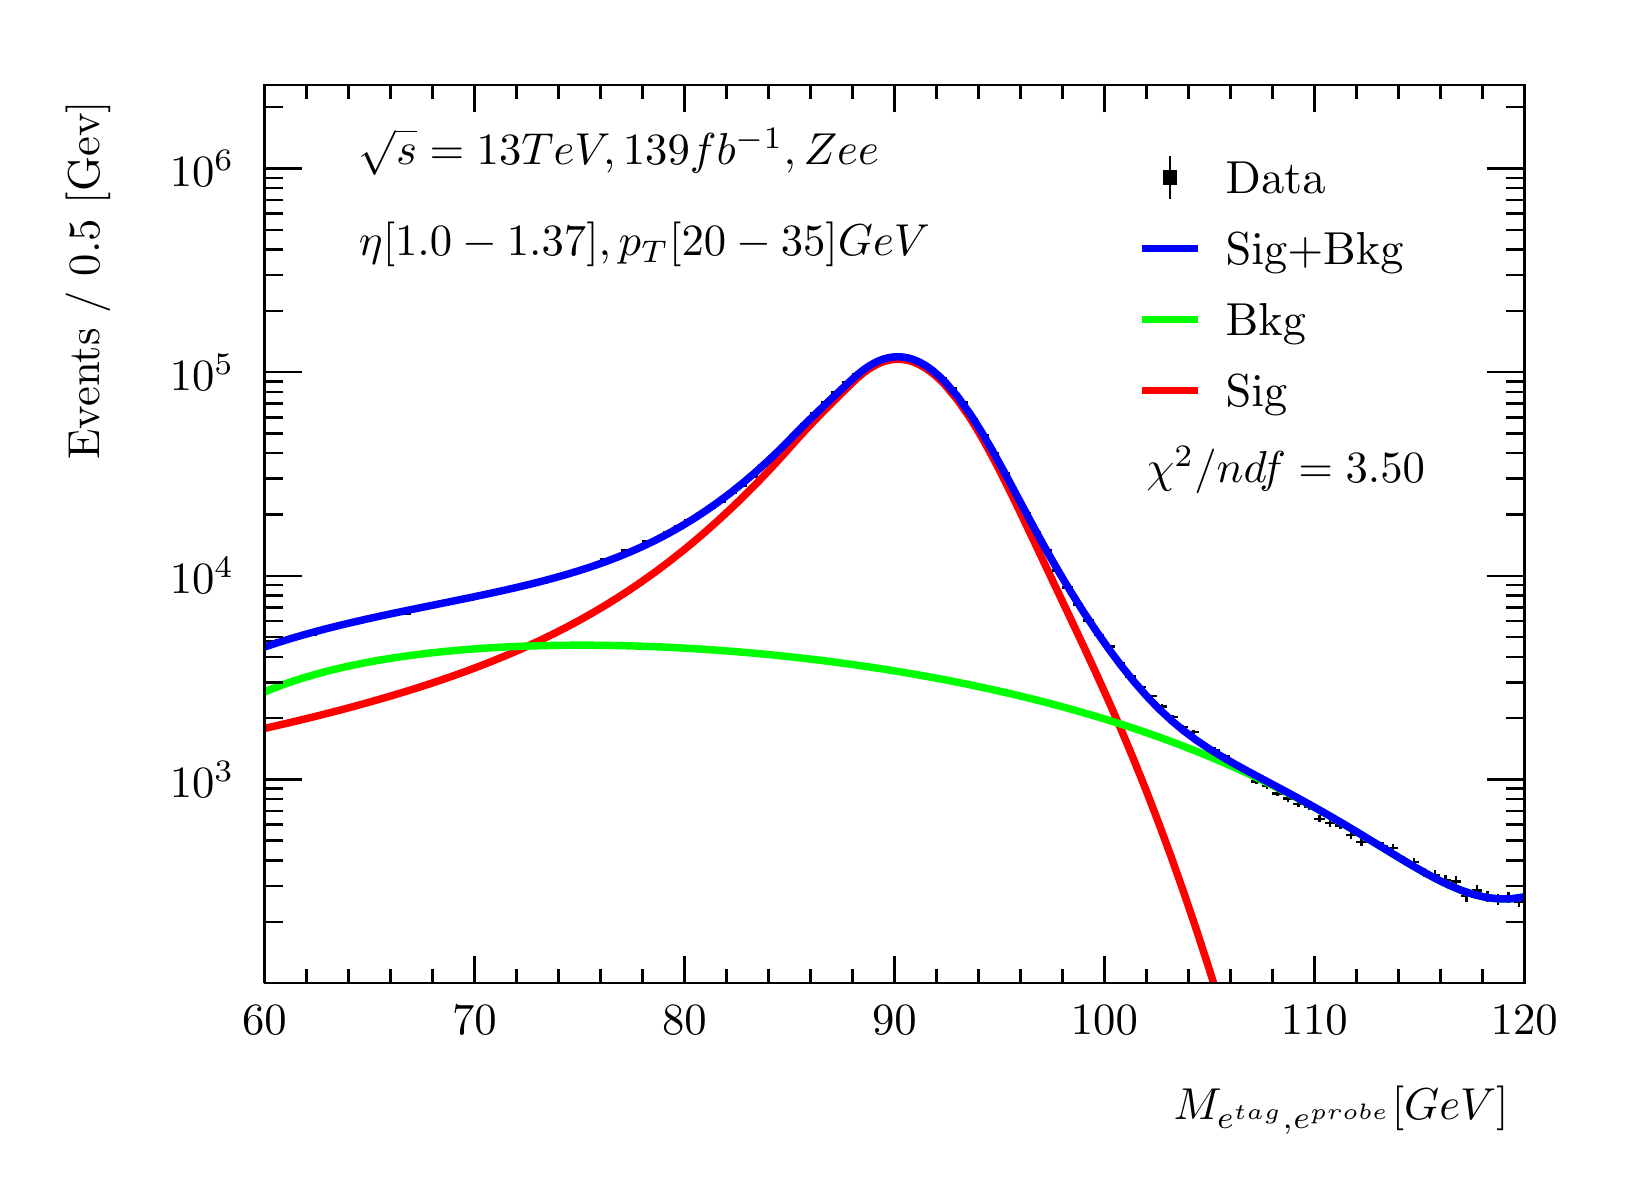
\begin{tikzpicture}
\pgfdeclareplotmark{cross} {
\pgfpathmoveto{\pgfpoint{-0.3\pgfplotmarksize}{\pgfplotmarksize}}
\pgfpathlineto{\pgfpoint{+0.3\pgfplotmarksize}{\pgfplotmarksize}}
\pgfpathlineto{\pgfpoint{+0.3\pgfplotmarksize}{0.3\pgfplotmarksize}}
\pgfpathlineto{\pgfpoint{+1\pgfplotmarksize}{0.3\pgfplotmarksize}}
\pgfpathlineto{\pgfpoint{+1\pgfplotmarksize}{-0.3\pgfplotmarksize}}
\pgfpathlineto{\pgfpoint{+0.3\pgfplotmarksize}{-0.3\pgfplotmarksize}}
\pgfpathlineto{\pgfpoint{+0.3\pgfplotmarksize}{-1.\pgfplotmarksize}}
\pgfpathlineto{\pgfpoint{-0.3\pgfplotmarksize}{-1.\pgfplotmarksize}}
\pgfpathlineto{\pgfpoint{-0.3\pgfplotmarksize}{-0.3\pgfplotmarksize}}
\pgfpathlineto{\pgfpoint{-1.\pgfplotmarksize}{-0.3\pgfplotmarksize}}
\pgfpathlineto{\pgfpoint{-1.\pgfplotmarksize}{0.3\pgfplotmarksize}}
\pgfpathlineto{\pgfpoint{-0.3\pgfplotmarksize}{0.3\pgfplotmarksize}}
\pgfpathclose
\pgfusepathqstroke
}
\pgfdeclareplotmark{cross*} {
\pgfpathmoveto{\pgfpoint{-0.3\pgfplotmarksize}{\pgfplotmarksize}}
\pgfpathlineto{\pgfpoint{+0.3\pgfplotmarksize}{\pgfplotmarksize}}
\pgfpathlineto{\pgfpoint{+0.3\pgfplotmarksize}{0.3\pgfplotmarksize}}
\pgfpathlineto{\pgfpoint{+1\pgfplotmarksize}{0.3\pgfplotmarksize}}
\pgfpathlineto{\pgfpoint{+1\pgfplotmarksize}{-0.3\pgfplotmarksize}}
\pgfpathlineto{\pgfpoint{+0.3\pgfplotmarksize}{-0.3\pgfplotmarksize}}
\pgfpathlineto{\pgfpoint{+0.3\pgfplotmarksize}{-1.\pgfplotmarksize}}
\pgfpathlineto{\pgfpoint{-0.3\pgfplotmarksize}{-1.\pgfplotmarksize}}
\pgfpathlineto{\pgfpoint{-0.3\pgfplotmarksize}{-0.3\pgfplotmarksize}}
\pgfpathlineto{\pgfpoint{-1.\pgfplotmarksize}{-0.3\pgfplotmarksize}}
\pgfpathlineto{\pgfpoint{-1.\pgfplotmarksize}{0.3\pgfplotmarksize}}
\pgfpathlineto{\pgfpoint{-0.3\pgfplotmarksize}{0.3\pgfplotmarksize}}
\pgfpathclose
\pgfusepathqfillstroke
}
\pgfdeclareplotmark{newstar} {
\pgfpathmoveto{\pgfqpoint{0pt}{\pgfplotmarksize}}
\pgfpathlineto{\pgfqpointpolar{44}{0.5\pgfplotmarksize}}
\pgfpathlineto{\pgfqpointpolar{18}{\pgfplotmarksize}}
\pgfpathlineto{\pgfqpointpolar{-20}{0.5\pgfplotmarksize}}
\pgfpathlineto{\pgfqpointpolar{-54}{\pgfplotmarksize}}
\pgfpathlineto{\pgfqpointpolar{-90}{0.5\pgfplotmarksize}}
\pgfpathlineto{\pgfqpointpolar{234}{\pgfplotmarksize}}
\pgfpathlineto{\pgfqpointpolar{198}{0.5\pgfplotmarksize}}
\pgfpathlineto{\pgfqpointpolar{162}{\pgfplotmarksize}}
\pgfpathlineto{\pgfqpointpolar{134}{0.5\pgfplotmarksize}}
\pgfpathclose
\pgfusepathqstroke
}
\pgfdeclareplotmark{newstar*} {
\pgfpathmoveto{\pgfqpoint{0pt}{\pgfplotmarksize}}
\pgfpathlineto{\pgfqpointpolar{44}{0.5\pgfplotmarksize}}
\pgfpathlineto{\pgfqpointpolar{18}{\pgfplotmarksize}}
\pgfpathlineto{\pgfqpointpolar{-20}{0.5\pgfplotmarksize}}
\pgfpathlineto{\pgfqpointpolar{-54}{\pgfplotmarksize}}
\pgfpathlineto{\pgfqpointpolar{-90}{0.5\pgfplotmarksize}}
\pgfpathlineto{\pgfqpointpolar{234}{\pgfplotmarksize}}
\pgfpathlineto{\pgfqpointpolar{198}{0.5\pgfplotmarksize}}
\pgfpathlineto{\pgfqpointpolar{162}{\pgfplotmarksize}}
\pgfpathlineto{\pgfqpointpolar{134}{0.5\pgfplotmarksize}}
\pgfpathclose
\pgfusepathqfillstroke
}
\definecolor{c}{rgb}{1,1,1};
\draw [color=c, fill=c] (0,0) rectangle (20,14.4361);
\draw [color=c, fill=c] (3,2.30977) rectangle (19,13.7143);
\definecolor{c}{rgb}{0,0,0};
\draw [c,line width=0.9] (3,2.30977) -- (3,13.7143) -- (19,13.7143) -- (19,2.30977) -- (3,2.30977);
\definecolor{c}{rgb}{1,1,1};
\draw [color=c, fill=c] (3,2.30977) rectangle (19,13.7143);
\definecolor{c}{rgb}{0,0,0};
\draw [c,line width=0.9] (3,2.30977) -- (3,13.7143) -- (19,13.7143) -- (19,2.30977) -- (3,2.30977);
\draw [c,line width=0.9] (3,2.30977) -- (19,2.30977);
\draw [c,line width=0.9] (3,2.65624) -- (3,2.30977);
\draw [c,line width=0.9] (3.53333,2.48301) -- (3.53333,2.30977);
\draw [c,line width=0.9] (4.06667,2.48301) -- (4.06667,2.30977);
\draw [c,line width=0.9] (4.6,2.48301) -- (4.6,2.30977);
\draw [c,line width=0.9] (5.13333,2.48301) -- (5.13333,2.30977);
\draw [c,line width=0.9] (5.66667,2.65624) -- (5.66667,2.30977);
\draw [c,line width=0.9] (6.2,2.48301) -- (6.2,2.30977);
\draw [c,line width=0.9] (6.73333,2.48301) -- (6.73333,2.30977);
\draw [c,line width=0.9] (7.26667,2.48301) -- (7.26667,2.30977);
\draw [c,line width=0.9] (7.8,2.48301) -- (7.8,2.30977);
\draw [c,line width=0.9] (8.33333,2.65624) -- (8.33333,2.30977);
\draw [c,line width=0.9] (8.86667,2.48301) -- (8.86667,2.30977);
\draw [c,line width=0.9] (9.4,2.48301) -- (9.4,2.30977);
\draw [c,line width=0.9] (9.93333,2.48301) -- (9.93333,2.30977);
\draw [c,line width=0.9] (10.4667,2.48301) -- (10.4667,2.30977);
\draw [c,line width=0.9] (11,2.65624) -- (11,2.30977);
\draw [c,line width=0.9] (11.5333,2.48301) -- (11.5333,2.30977);
\draw [c,line width=0.9] (12.0667,2.48301) -- (12.0667,2.30977);
\draw [c,line width=0.9] (12.6,2.48301) -- (12.6,2.30977);
\draw [c,line width=0.9] (13.1333,2.48301) -- (13.1333,2.30977);
\draw [c,line width=0.9] (13.6667,2.65624) -- (13.6667,2.30977);
\draw [c,line width=0.9] (14.2,2.48301) -- (14.2,2.30977);
\draw [c,line width=0.9] (14.7333,2.48301) -- (14.7333,2.30977);
\draw [c,line width=0.9] (15.2667,2.48301) -- (15.2667,2.30977);
\draw [c,line width=0.9] (15.8,2.48301) -- (15.8,2.30977);
\draw [c,line width=0.9] (16.3333,2.65624) -- (16.3333,2.30977);
\draw [c,line width=0.9] (16.8667,2.48301) -- (16.8667,2.30977);
\draw [c,line width=0.9] (17.4,2.48301) -- (17.4,2.30977);
\draw [c,line width=0.9] (17.9333,2.48301) -- (17.9333,2.30977);
\draw [c,line width=0.9] (18.4667,2.48301) -- (18.4667,2.30977);
\draw [c,line width=0.9] (19,2.65624) -- (19,2.30977);
\draw [anchor=base] (3,1.66015) node[scale=1.61424, color=c, rotate=0]{60};
\draw [anchor=base] (5.66667,1.66015) node[scale=1.61424, color=c, rotate=0]{70};
\draw [anchor=base] (8.33333,1.66015) node[scale=1.61424, color=c, rotate=0]{80};
\draw [anchor=base] (11,1.66015) node[scale=1.61424, color=c, rotate=0]{90};
\draw [anchor=base] (13.6667,1.66015) node[scale=1.61424, color=c, rotate=0]{100};
\draw [anchor=base] (16.3333,1.66015) node[scale=1.61424, color=c, rotate=0]{110};
\draw [anchor=base] (19,1.66015) node[scale=1.61424, color=c, rotate=0]{120};
\draw [anchor= east] (19,0.692932) node[scale=1.61424, color=c, rotate=0]{$M_{e^{tag}, e^{probe}}  [GeV]$};
\draw [c,line width=0.9] (3,13.7143) -- (19,13.7143);
\draw [c,line width=0.9] (3,13.3678) -- (3,13.7143);
\draw [c,line width=0.9] (3.53333,13.5411) -- (3.53333,13.7143);
\draw [c,line width=0.9] (4.06667,13.5411) -- (4.06667,13.7143);
\draw [c,line width=0.9] (4.6,13.5411) -- (4.6,13.7143);
\draw [c,line width=0.9] (5.13333,13.5411) -- (5.13333,13.7143);
\draw [c,line width=0.9] (5.66667,13.3678) -- (5.66667,13.7143);
\draw [c,line width=0.9] (6.2,13.5411) -- (6.2,13.7143);
\draw [c,line width=0.9] (6.73333,13.5411) -- (6.73333,13.7143);
\draw [c,line width=0.9] (7.26667,13.5411) -- (7.26667,13.7143);
\draw [c,line width=0.9] (7.8,13.5411) -- (7.8,13.7143);
\draw [c,line width=0.9] (8.33333,13.3678) -- (8.33333,13.7143);
\draw [c,line width=0.9] (8.86667,13.5411) -- (8.86667,13.7143);
\draw [c,line width=0.9] (9.4,13.5411) -- (9.4,13.7143);
\draw [c,line width=0.9] (9.93333,13.5411) -- (9.93333,13.7143);
\draw [c,line width=0.9] (10.4667,13.5411) -- (10.4667,13.7143);
\draw [c,line width=0.9] (11,13.3678) -- (11,13.7143);
\draw [c,line width=0.9] (11.5333,13.5411) -- (11.5333,13.7143);
\draw [c,line width=0.9] (12.0667,13.5411) -- (12.0667,13.7143);
\draw [c,line width=0.9] (12.6,13.5411) -- (12.6,13.7143);
\draw [c,line width=0.9] (13.1333,13.5411) -- (13.1333,13.7143);
\draw [c,line width=0.9] (13.6667,13.3678) -- (13.6667,13.7143);
\draw [c,line width=0.9] (14.2,13.5411) -- (14.2,13.7143);
\draw [c,line width=0.9] (14.7333,13.5411) -- (14.7333,13.7143);
\draw [c,line width=0.9] (15.2667,13.5411) -- (15.2667,13.7143);
\draw [c,line width=0.9] (15.8,13.5411) -- (15.8,13.7143);
\draw [c,line width=0.9] (16.3333,13.3678) -- (16.3333,13.7143);
\draw [c,line width=0.9] (16.8667,13.5411) -- (16.8667,13.7143);
\draw [c,line width=0.9] (17.4,13.5411) -- (17.4,13.7143);
\draw [c,line width=0.9] (17.9333,13.5411) -- (17.9333,13.7143);
\draw [c,line width=0.9] (18.4667,13.5411) -- (18.4667,13.7143);
\draw [c,line width=0.9] (19,13.3678) -- (19,13.7143);
\draw [c,line width=0.9] (3,2.30977) -- (3,13.7143);
\draw [c,line width=0.9] (3.237,3.08829) -- (3,3.08829);
\draw [c,line width=0.9] (3.237,3.54369) -- (3,3.54369);
\draw [c,line width=0.9] (3.237,3.8668) -- (3,3.8668);
\draw [c,line width=0.9] (3.237,4.11742) -- (3,4.11742);
\draw [c,line width=0.9] (3.237,4.3222) -- (3,4.3222);
\draw [c,line width=0.9] (3.237,4.49534) -- (3,4.49534);
\draw [c,line width=0.9] (3.237,4.64531) -- (3,4.64531);
\draw [c,line width=0.9] (3.237,4.7776) -- (3,4.7776);
\draw [c,line width=0.9] (3.474,4.89594) -- (3,4.89594);
\draw [anchor= east] (2.82,4.89594) node[scale=1.61424, color=c, rotate=0]{$10^{3}$};
\draw [c,line width=0.9] (3.237,5.67445) -- (3,5.67445);
\draw [c,line width=0.9] (3.237,6.12985) -- (3,6.12985);
\draw [c,line width=0.9] (3.237,6.45297) -- (3,6.45297);
\draw [c,line width=0.9] (3.237,6.70359) -- (3,6.70359);
\draw [c,line width=0.9] (3.237,6.90837) -- (3,6.90837);
\draw [c,line width=0.9] (3.237,7.0815) -- (3,7.0815);
\draw [c,line width=0.9] (3.237,7.23148) -- (3,7.23148);
\draw [c,line width=0.9] (3.237,7.36377) -- (3,7.36377);
\draw [c,line width=0.9] (3.474,7.48211) -- (3,7.48211);
\draw [anchor= east] (2.82,7.48211) node[scale=1.61424, color=c, rotate=0]{$10^{4}$};
\draw [c,line width=0.9] (3.237,8.26062) -- (3,8.26062);
\draw [c,line width=0.9] (3.237,8.71602) -- (3,8.71602);
\draw [c,line width=0.9] (3.237,9.03913) -- (3,9.03913);
\draw [c,line width=0.9] (3.237,9.28976) -- (3,9.28976);
\draw [c,line width=0.9] (3.237,9.49453) -- (3,9.49453);
\draw [c,line width=0.9] (3.237,9.66767) -- (3,9.66767);
\draw [c,line width=0.9] (3.237,9.81765) -- (3,9.81765);
\draw [c,line width=0.9] (3.237,9.94994) -- (3,9.94994);
\draw [c,line width=0.9] (3.474,10.0683) -- (3,10.0683);
\draw [anchor= east] (2.82,10.0683) node[scale=1.61424, color=c, rotate=0]{$10^{5}$};
\draw [c,line width=0.9] (3.237,10.8468) -- (3,10.8468);
\draw [c,line width=0.9] (3.237,11.3022) -- (3,11.3022);
\draw [c,line width=0.9] (3.237,11.6253) -- (3,11.6253);
\draw [c,line width=0.9] (3.237,11.8759) -- (3,11.8759);
\draw [c,line width=0.9] (3.237,12.0807) -- (3,12.0807);
\draw [c,line width=0.9] (3.237,12.2538) -- (3,12.2538);
\draw [c,line width=0.9] (3.237,12.4038) -- (3,12.4038);
\draw [c,line width=0.9] (3.237,12.5361) -- (3,12.5361);
\draw [c,line width=0.9] (3.474,12.6544) -- (3,12.6544);
\draw [anchor= east] (2.82,12.6544) node[scale=1.61424, color=c, rotate=0]{$10^{6}$};
\draw [c,line width=0.9] (3.237,13.433) -- (3,13.433);
\draw [anchor= east] (0.76,13.7143) node[scale=1.61424, color=c, rotate=90]{Events / 0.5 [Gev]};
\draw [c,line width=0.9] (19,2.30977) -- (19,13.7143);
\draw [c,line width=0.9] (18.763,3.08829) -- (19,3.08829);
\draw [c,line width=0.9] (18.763,3.54369) -- (19,3.54369);
\draw [c,line width=0.9] (18.763,3.8668) -- (19,3.8668);
\draw [c,line width=0.9] (18.763,4.11742) -- (19,4.11742);
\draw [c,line width=0.9] (18.763,4.3222) -- (19,4.3222);
\draw [c,line width=0.9] (18.763,4.49534) -- (19,4.49534);
\draw [c,line width=0.9] (18.763,4.64531) -- (19,4.64531);
\draw [c,line width=0.9] (18.763,4.7776) -- (19,4.7776);
\draw [c,line width=0.9] (18.526,4.89594) -- (19,4.89594);
\draw [c,line width=0.9] (18.763,5.67445) -- (19,5.67445);
\draw [c,line width=0.9] (18.763,6.12985) -- (19,6.12985);
\draw [c,line width=0.9] (18.763,6.45297) -- (19,6.45297);
\draw [c,line width=0.9] (18.763,6.70359) -- (19,6.70359);
\draw [c,line width=0.9] (18.763,6.90837) -- (19,6.90837);
\draw [c,line width=0.9] (18.763,7.0815) -- (19,7.0815);
\draw [c,line width=0.9] (18.763,7.23148) -- (19,7.23148);
\draw [c,line width=0.9] (18.763,7.36377) -- (19,7.36377);
\draw [c,line width=0.9] (18.526,7.48211) -- (19,7.48211);
\draw [c,line width=0.9] (18.763,8.26062) -- (19,8.26062);
\draw [c,line width=0.9] (18.763,8.71602) -- (19,8.71602);
\draw [c,line width=0.9] (18.763,9.03913) -- (19,9.03913);
\draw [c,line width=0.9] (18.763,9.28976) -- (19,9.28976);
\draw [c,line width=0.9] (18.763,9.49453) -- (19,9.49453);
\draw [c,line width=0.9] (18.763,9.66767) -- (19,9.66767);
\draw [c,line width=0.9] (18.763,9.81765) -- (19,9.81765);
\draw [c,line width=0.9] (18.763,9.94994) -- (19,9.94994);
\draw [c,line width=0.9] (18.526,10.0683) -- (19,10.0683);
\draw [c,line width=0.9] (18.763,10.8468) -- (19,10.8468);
\draw [c,line width=0.9] (18.763,11.3022) -- (19,11.3022);
\draw [c,line width=0.9] (18.763,11.6253) -- (19,11.6253);
\draw [c,line width=0.9] (18.763,11.8759) -- (19,11.8759);
\draw [c,line width=0.9] (18.763,12.0807) -- (19,12.0807);
\draw [c,line width=0.9] (18.763,12.2538) -- (19,12.2538);
\draw [c,line width=0.9] (18.763,12.4038) -- (19,12.4038);
\draw [c,line width=0.9] (18.763,12.5361) -- (19,12.5361);
\draw [c,line width=0.9] (18.526,12.6544) -- (19,12.6544);
\draw [c,line width=0.9] (18.763,13.433) -- (19,13.433);
\draw [c,line width=0.9] (3.06667,6.65329) -- (3,6.65329);
\draw [c,line width=0.9] (3,6.65329) -- (3,6.65329);
\draw [c,line width=0.9] (3.06667,6.65329) -- (3.13333,6.65329);
\draw [c,line width=0.9] (3.13333,6.65329) -- (3.13333,6.65329);
\draw [c,line width=0.9] (3.06667,6.65329) -- (3.06667,6.66953);
\draw [c,line width=0.9] (3.06667,6.66953) -- (3.06667,6.66953);
\draw [c,line width=0.9] (3.06667,6.65329) -- (3.06667,6.63705);
\draw [c,line width=0.9] (3.06667,6.63705) -- (3.06667,6.63705);
\draw [c,line width=0.9] (3.2,6.66288) -- (3.13333,6.66288);
\draw [c,line width=0.9] (3.13333,6.66288) -- (3.13333,6.66288);
\draw [c,line width=0.9] (3.2,6.66288) -- (3.26667,6.66288);
\draw [c,line width=0.9] (3.26667,6.66288) -- (3.26667,6.66288);
\draw [c,line width=0.9] (3.2,6.66288) -- (3.2,6.67905);
\draw [c,line width=0.9] (3.2,6.67905) -- (3.2,6.67905);
\draw [c,line width=0.9] (3.2,6.66288) -- (3.2,6.64671);
\draw [c,line width=0.9] (3.2,6.64671) -- (3.2,6.64671);
\draw [c,line width=0.9] (3.33333,6.67677) -- (3.26667,6.67677);
\draw [c,line width=0.9] (3.26667,6.67677) -- (3.26667,6.67677);
\draw [c,line width=0.9] (3.33333,6.67677) -- (3.4,6.67677);
\draw [c,line width=0.9] (3.4,6.67677) -- (3.4,6.67677);
\draw [c,line width=0.9] (3.33333,6.67677) -- (3.33333,6.69284);
\draw [c,line width=0.9] (3.33333,6.69284) -- (3.33333,6.69284);
\draw [c,line width=0.9] (3.33333,6.67677) -- (3.33333,6.66069);
\draw [c,line width=0.9] (3.33333,6.66069) -- (3.33333,6.66069);
\draw [c,line width=0.9] (3.46667,6.73264) -- (3.4,6.73264);
\draw [c,line width=0.9] (3.4,6.73264) -- (3.4,6.73264);
\draw [c,line width=0.9] (3.46667,6.73264) -- (3.53333,6.73264);
\draw [c,line width=0.9] (3.53333,6.73264) -- (3.53333,6.73264);
\draw [c,line width=0.9] (3.46667,6.73264) -- (3.46667,6.74832);
\draw [c,line width=0.9] (3.46667,6.74832) -- (3.46667,6.74832);
\draw [c,line width=0.9] (3.46667,6.73264) -- (3.46667,6.71696);
\draw [c,line width=0.9] (3.46667,6.71696) -- (3.46667,6.71696);
\draw [c,line width=0.9] (3.6,6.73592) -- (3.53333,6.73592);
\draw [c,line width=0.9] (3.53333,6.73592) -- (3.53333,6.73592);
\draw [c,line width=0.9] (3.6,6.73592) -- (3.66667,6.73592);
\draw [c,line width=0.9] (3.66667,6.73592) -- (3.66667,6.73592);
\draw [c,line width=0.9] (3.6,6.73592) -- (3.6,6.75158);
\draw [c,line width=0.9] (3.6,6.75158) -- (3.6,6.75158);
\draw [c,line width=0.9] (3.6,6.73592) -- (3.6,6.72026);
\draw [c,line width=0.9] (3.6,6.72026) -- (3.6,6.72026);
\draw [c,line width=0.9] (3.73333,6.7892) -- (3.66667,6.7892);
\draw [c,line width=0.9] (3.66667,6.7892) -- (3.66667,6.7892);
\draw [c,line width=0.9] (3.73333,6.7892) -- (3.8,6.7892);
\draw [c,line width=0.9] (3.8,6.7892) -- (3.8,6.7892);
\draw [c,line width=0.9] (3.73333,6.7892) -- (3.73333,6.80449);
\draw [c,line width=0.9] (3.73333,6.80449) -- (3.73333,6.80449);
\draw [c,line width=0.9] (3.73333,6.7892) -- (3.73333,6.77391);
\draw [c,line width=0.9] (3.73333,6.77391) -- (3.73333,6.77391);
\draw [c,line width=0.9] (3.86667,6.83308) -- (3.8,6.83308);
\draw [c,line width=0.9] (3.8,6.83308) -- (3.8,6.83308);
\draw [c,line width=0.9] (3.86667,6.83308) -- (3.93333,6.83308);
\draw [c,line width=0.9] (3.93333,6.83308) -- (3.93333,6.83308);
\draw [c,line width=0.9] (3.86667,6.83308) -- (3.86667,6.84808);
\draw [c,line width=0.9] (3.86667,6.84808) -- (3.86667,6.84808);
\draw [c,line width=0.9] (3.86667,6.83308) -- (3.86667,6.81809);
\draw [c,line width=0.9] (3.86667,6.81809) -- (3.86667,6.81809);
\draw [c,line width=0.9] (4,6.86154) -- (3.93333,6.86154);
\draw [c,line width=0.9] (3.93333,6.86154) -- (3.93333,6.86154);
\draw [c,line width=0.9] (4,6.86154) -- (4.06667,6.86154);
\draw [c,line width=0.9] (4.06667,6.86154) -- (4.06667,6.86154);
\draw [c,line width=0.9] (4,6.86154) -- (4,6.87635);
\draw [c,line width=0.9] (4,6.87635) -- (4,6.87635);
\draw [c,line width=0.9] (4,6.86154) -- (4,6.84674);
\draw [c,line width=0.9] (4,6.84674) -- (4,6.84674);
\draw [c,line width=0.9] (4.13333,6.89538) -- (4.06667,6.89538);
\draw [c,line width=0.9] (4.06667,6.89538) -- (4.06667,6.89538);
\draw [c,line width=0.9] (4.13333,6.89538) -- (4.2,6.89538);
\draw [c,line width=0.9] (4.2,6.89538) -- (4.2,6.89538);
\draw [c,line width=0.9] (4.13333,6.89538) -- (4.13333,6.90996);
\draw [c,line width=0.9] (4.13333,6.90996) -- (4.13333,6.90996);
\draw [c,line width=0.9] (4.13333,6.89538) -- (4.13333,6.88079);
\draw [c,line width=0.9] (4.13333,6.88079) -- (4.13333,6.88079);
\draw [c,line width=0.9] (4.26667,6.94084) -- (4.2,6.94084);
\draw [c,line width=0.9] (4.2,6.94084) -- (4.2,6.94084);
\draw [c,line width=0.9] (4.26667,6.94084) -- (4.33333,6.94084);
\draw [c,line width=0.9] (4.33333,6.94084) -- (4.33333,6.94084);
\draw [c,line width=0.9] (4.26667,6.94084) -- (4.26667,6.95513);
\draw [c,line width=0.9] (4.26667,6.95513) -- (4.26667,6.95513);
\draw [c,line width=0.9] (4.26667,6.94084) -- (4.26667,6.92655);
\draw [c,line width=0.9] (4.26667,6.92655) -- (4.26667,6.92655);
\draw [c,line width=0.9] (4.4,6.93519) -- (4.33333,6.93519);
\draw [c,line width=0.9] (4.33333,6.93519) -- (4.33333,6.93519);
\draw [c,line width=0.9] (4.4,6.93519) -- (4.46667,6.93519);
\draw [c,line width=0.9] (4.46667,6.93519) -- (4.46667,6.93519);
\draw [c,line width=0.9] (4.4,6.93519) -- (4.4,6.94952);
\draw [c,line width=0.9] (4.4,6.94952) -- (4.4,6.94952);
\draw [c,line width=0.9] (4.4,6.93519) -- (4.4,6.92086);
\draw [c,line width=0.9] (4.4,6.92086) -- (4.4,6.92086);
\draw [c,line width=0.9] (4.53333,6.9791) -- (4.46667,6.9791);
\draw [c,line width=0.9] (4.46667,6.9791) -- (4.46667,6.9791);
\draw [c,line width=0.9] (4.53333,6.9791) -- (4.6,6.9791);
\draw [c,line width=0.9] (4.6,6.9791) -- (4.6,6.9791);
\draw [c,line width=0.9] (4.53333,6.9791) -- (4.53333,6.99315);
\draw [c,line width=0.9] (4.53333,6.99315) -- (4.53333,6.99315);
\draw [c,line width=0.9] (4.53333,6.9791) -- (4.53333,6.96505);
\draw [c,line width=0.9] (4.53333,6.96505) -- (4.53333,6.96505);
\draw [c,line width=0.9] (4.66667,7.00172) -- (4.6,7.00172);
\draw [c,line width=0.9] (4.6,7.00172) -- (4.6,7.00172);
\draw [c,line width=0.9] (4.66667,7.00172) -- (4.73333,7.00172);
\draw [c,line width=0.9] (4.73333,7.00172) -- (4.73333,7.00172);
\draw [c,line width=0.9] (4.66667,7.00172) -- (4.66667,7.01563);
\draw [c,line width=0.9] (4.66667,7.01563) -- (4.66667,7.01563);
\draw [c,line width=0.9] (4.66667,7.00172) -- (4.66667,6.98781);
\draw [c,line width=0.9] (4.66667,6.98781) -- (4.66667,6.98781);
\draw [c,line width=0.9] (4.8,6.99464) -- (4.73333,6.99464);
\draw [c,line width=0.9] (4.73333,6.99464) -- (4.73333,6.99464);
\draw [c,line width=0.9] (4.8,6.99464) -- (4.86667,6.99464);
\draw [c,line width=0.9] (4.86667,6.99464) -- (4.86667,6.99464);
\draw [c,line width=0.9] (4.8,6.99464) -- (4.8,7.00859);
\draw [c,line width=0.9] (4.8,7.00859) -- (4.8,7.00859);
\draw [c,line width=0.9] (4.8,6.99464) -- (4.8,6.98068);
\draw [c,line width=0.9] (4.8,6.98068) -- (4.8,6.98068);
\draw [c,line width=0.9] (4.93333,7.07362) -- (4.86667,7.07362);
\draw [c,line width=0.9] (4.86667,7.07362) -- (4.86667,7.07362);
\draw [c,line width=0.9] (4.93333,7.07362) -- (5,7.07362);
\draw [c,line width=0.9] (5,7.07362) -- (5,7.07362);
\draw [c,line width=0.9] (4.93333,7.07362) -- (4.93333,7.08709);
\draw [c,line width=0.9] (4.93333,7.08709) -- (4.93333,7.08709);
\draw [c,line width=0.9] (4.93333,7.07362) -- (4.93333,7.06014);
\draw [c,line width=0.9] (4.93333,7.06014) -- (4.93333,7.06014);
\draw [c,line width=0.9] (5.06667,7.08599) -- (5,7.08599);
\draw [c,line width=0.9] (5,7.08599) -- (5,7.08599);
\draw [c,line width=0.9] (5.06667,7.08599) -- (5.13333,7.08599);
\draw [c,line width=0.9] (5.13333,7.08599) -- (5.13333,7.08599);
\draw [c,line width=0.9] (5.06667,7.08599) -- (5.06667,7.09939);
\draw [c,line width=0.9] (5.06667,7.09939) -- (5.06667,7.09939);
\draw [c,line width=0.9] (5.06667,7.08599) -- (5.06667,7.07259);
\draw [c,line width=0.9] (5.06667,7.07259) -- (5.06667,7.07259);
\draw [c,line width=0.9] (5.2,7.10217) -- (5.13333,7.10217);
\draw [c,line width=0.9] (5.13333,7.10217) -- (5.13333,7.10217);
\draw [c,line width=0.9] (5.2,7.10217) -- (5.26667,7.10217);
\draw [c,line width=0.9] (5.26667,7.10217) -- (5.26667,7.10217);
\draw [c,line width=0.9] (5.2,7.10217) -- (5.2,7.11547);
\draw [c,line width=0.9] (5.2,7.11547) -- (5.2,7.11547);
\draw [c,line width=0.9] (5.2,7.10217) -- (5.2,7.08887);
\draw [c,line width=0.9] (5.2,7.08887) -- (5.2,7.08887);
\draw [c,line width=0.9] (5.33333,7.1427) -- (5.26667,7.1427);
\draw [c,line width=0.9] (5.26667,7.1427) -- (5.26667,7.1427);
\draw [c,line width=0.9] (5.33333,7.1427) -- (5.4,7.1427);
\draw [c,line width=0.9] (5.4,7.1427) -- (5.4,7.1427);
\draw [c,line width=0.9] (5.33333,7.1427) -- (5.33333,7.15577);
\draw [c,line width=0.9] (5.33333,7.15577) -- (5.33333,7.15577);
\draw [c,line width=0.9] (5.33333,7.1427) -- (5.33333,7.12964);
\draw [c,line width=0.9] (5.33333,7.12964) -- (5.33333,7.12964);
\draw [c,line width=0.9] (5.46667,7.18402) -- (5.4,7.18402);
\draw [c,line width=0.9] (5.4,7.18402) -- (5.4,7.18402);
\draw [c,line width=0.9] (5.46667,7.18402) -- (5.53333,7.18402);
\draw [c,line width=0.9] (5.53333,7.18402) -- (5.53333,7.18402);
\draw [c,line width=0.9] (5.46667,7.18402) -- (5.46667,7.19685);
\draw [c,line width=0.9] (5.46667,7.19685) -- (5.46667,7.19685);
\draw [c,line width=0.9] (5.46667,7.18402) -- (5.46667,7.1712);
\draw [c,line width=0.9] (5.46667,7.1712) -- (5.46667,7.1712);
\draw [c,line width=0.9] (5.6,7.18329) -- (5.53333,7.18329);
\draw [c,line width=0.9] (5.53333,7.18329) -- (5.53333,7.18329);
\draw [c,line width=0.9] (5.6,7.18329) -- (5.66667,7.18329);
\draw [c,line width=0.9] (5.66667,7.18329) -- (5.66667,7.18329);
\draw [c,line width=0.9] (5.6,7.18329) -- (5.6,7.19612);
\draw [c,line width=0.9] (5.6,7.19612) -- (5.6,7.19612);
\draw [c,line width=0.9] (5.6,7.18329) -- (5.6,7.17046);
\draw [c,line width=0.9] (5.6,7.17046) -- (5.6,7.17046);
\draw [c,line width=0.9] (5.73333,7.21308) -- (5.66667,7.21308);
\draw [c,line width=0.9] (5.66667,7.21308) -- (5.66667,7.21308);
\draw [c,line width=0.9] (5.73333,7.21308) -- (5.8,7.21308);
\draw [c,line width=0.9] (5.8,7.21308) -- (5.8,7.21308);
\draw [c,line width=0.9] (5.73333,7.21308) -- (5.73333,7.22574);
\draw [c,line width=0.9] (5.73333,7.22574) -- (5.73333,7.22574);
\draw [c,line width=0.9] (5.73333,7.21308) -- (5.73333,7.20042);
\draw [c,line width=0.9] (5.73333,7.20042) -- (5.73333,7.20042);
\draw [c,line width=0.9] (5.86667,7.23778) -- (5.8,7.23778);
\draw [c,line width=0.9] (5.8,7.23778) -- (5.8,7.23778);
\draw [c,line width=0.9] (5.86667,7.23778) -- (5.93333,7.23778);
\draw [c,line width=0.9] (5.93333,7.23778) -- (5.93333,7.23778);
\draw [c,line width=0.9] (5.86667,7.23778) -- (5.86667,7.2503);
\draw [c,line width=0.9] (5.86667,7.2503) -- (5.86667,7.2503);
\draw [c,line width=0.9] (5.86667,7.23778) -- (5.86667,7.22526);
\draw [c,line width=0.9] (5.86667,7.22526) -- (5.86667,7.22526);
\draw [c,line width=0.9] (6,7.29122) -- (5.93333,7.29122);
\draw [c,line width=0.9] (5.93333,7.29122) -- (5.93333,7.29122);
\draw [c,line width=0.9] (6,7.29122) -- (6.06667,7.29122);
\draw [c,line width=0.9] (6.06667,7.29122) -- (6.06667,7.29122);
\draw [c,line width=0.9] (6,7.29122) -- (6,7.30344);
\draw [c,line width=0.9] (6,7.30344) -- (6,7.30344);
\draw [c,line width=0.9] (6,7.29122) -- (6,7.27899);
\draw [c,line width=0.9] (6,7.27899) -- (6,7.27899);
\draw [c,line width=0.9] (6.13333,7.30419) -- (6.06667,7.30419);
\draw [c,line width=0.9] (6.06667,7.30419) -- (6.06667,7.30419);
\draw [c,line width=0.9] (6.13333,7.30419) -- (6.2,7.30419);
\draw [c,line width=0.9] (6.2,7.30419) -- (6.2,7.30419);
\draw [c,line width=0.9] (6.13333,7.30419) -- (6.13333,7.31635);
\draw [c,line width=0.9] (6.13333,7.31635) -- (6.13333,7.31635);
\draw [c,line width=0.9] (6.13333,7.30419) -- (6.13333,7.29203);
\draw [c,line width=0.9] (6.13333,7.29203) -- (6.13333,7.29203);
\draw [c,line width=0.9] (6.26667,7.35563) -- (6.2,7.35563);
\draw [c,line width=0.9] (6.2,7.35563) -- (6.2,7.35563);
\draw [c,line width=0.9] (6.26667,7.35563) -- (6.33333,7.35563);
\draw [c,line width=0.9] (6.33333,7.35563) -- (6.33333,7.35563);
\draw [c,line width=0.9] (6.26667,7.35563) -- (6.26667,7.36751);
\draw [c,line width=0.9] (6.26667,7.36751) -- (6.26667,7.36751);
\draw [c,line width=0.9] (6.26667,7.35563) -- (6.26667,7.34375);
\draw [c,line width=0.9] (6.26667,7.34375) -- (6.26667,7.34375);
\draw [c,line width=0.9] (6.4,7.37185) -- (6.33333,7.37185);
\draw [c,line width=0.9] (6.33333,7.37185) -- (6.33333,7.37185);
\draw [c,line width=0.9] (6.4,7.37185) -- (6.46667,7.37185);
\draw [c,line width=0.9] (6.46667,7.37185) -- (6.46667,7.37185);
\draw [c,line width=0.9] (6.4,7.37185) -- (6.4,7.38365);
\draw [c,line width=0.9] (6.4,7.38365) -- (6.4,7.38365);
\draw [c,line width=0.9] (6.4,7.37185) -- (6.4,7.36006);
\draw [c,line width=0.9] (6.4,7.36006) -- (6.4,7.36006);
\draw [c,line width=0.9] (6.53333,7.39818) -- (6.46667,7.39818);
\draw [c,line width=0.9] (6.46667,7.39818) -- (6.46667,7.39818);
\draw [c,line width=0.9] (6.53333,7.39818) -- (6.6,7.39818);
\draw [c,line width=0.9] (6.6,7.39818) -- (6.6,7.39818);
\draw [c,line width=0.9] (6.53333,7.39818) -- (6.53333,7.40984);
\draw [c,line width=0.9] (6.53333,7.40984) -- (6.53333,7.40984);
\draw [c,line width=0.9] (6.53333,7.39818) -- (6.53333,7.38652);
\draw [c,line width=0.9] (6.53333,7.38652) -- (6.53333,7.38652);
\draw [c,line width=0.9] (6.66667,7.45517) -- (6.6,7.45517);
\draw [c,line width=0.9] (6.6,7.45517) -- (6.6,7.45517);
\draw [c,line width=0.9] (6.66667,7.45517) -- (6.73333,7.45517);
\draw [c,line width=0.9] (6.73333,7.45517) -- (6.73333,7.45517);
\draw [c,line width=0.9] (6.66667,7.45517) -- (6.66667,7.46654);
\draw [c,line width=0.9] (6.66667,7.46654) -- (6.66667,7.46654);
\draw [c,line width=0.9] (6.66667,7.45517) -- (6.66667,7.4438);
\draw [c,line width=0.9] (6.66667,7.4438) -- (6.66667,7.4438);
\draw [c,line width=0.9] (6.8,7.48793) -- (6.73333,7.48793);
\draw [c,line width=0.9] (6.73333,7.48793) -- (6.73333,7.48793);
\draw [c,line width=0.9] (6.8,7.48793) -- (6.86667,7.48793);
\draw [c,line width=0.9] (6.86667,7.48793) -- (6.86667,7.48793);
\draw [c,line width=0.9] (6.8,7.48793) -- (6.8,7.49914);
\draw [c,line width=0.9] (6.8,7.49914) -- (6.8,7.49914);
\draw [c,line width=0.9] (6.8,7.48793) -- (6.8,7.47673);
\draw [c,line width=0.9] (6.8,7.47673) -- (6.8,7.47673);
\draw [c,line width=0.9] (6.93333,7.52356) -- (6.86667,7.52356);
\draw [c,line width=0.9] (6.86667,7.52356) -- (6.86667,7.52356);
\draw [c,line width=0.9] (6.93333,7.52356) -- (7,7.52356);
\draw [c,line width=0.9] (7,7.52356) -- (7,7.52356);
\draw [c,line width=0.9] (6.93333,7.52356) -- (6.93333,7.53459);
\draw [c,line width=0.9] (6.93333,7.53459) -- (6.93333,7.53459);
\draw [c,line width=0.9] (6.93333,7.52356) -- (6.93333,7.51254);
\draw [c,line width=0.9] (6.93333,7.51254) -- (6.93333,7.51254);
\draw [c,line width=0.9] (7.06667,7.56948) -- (7,7.56948);
\draw [c,line width=0.9] (7,7.56948) -- (7,7.56948);
\draw [c,line width=0.9] (7.06667,7.56948) -- (7.13333,7.56948);
\draw [c,line width=0.9] (7.13333,7.56948) -- (7.13333,7.56948);
\draw [c,line width=0.9] (7.06667,7.56948) -- (7.06667,7.58029);
\draw [c,line width=0.9] (7.06667,7.58029) -- (7.06667,7.58029);
\draw [c,line width=0.9] (7.06667,7.56948) -- (7.06667,7.55868);
\draw [c,line width=0.9] (7.06667,7.55868) -- (7.06667,7.55868);
\draw [c,line width=0.9] (7.2,7.62937) -- (7.13333,7.62937);
\draw [c,line width=0.9] (7.13333,7.62937) -- (7.13333,7.62937);
\draw [c,line width=0.9] (7.2,7.62937) -- (7.26667,7.62937);
\draw [c,line width=0.9] (7.26667,7.62937) -- (7.26667,7.62937);
\draw [c,line width=0.9] (7.2,7.62937) -- (7.2,7.63989);
\draw [c,line width=0.9] (7.2,7.63989) -- (7.2,7.63989);
\draw [c,line width=0.9] (7.2,7.62937) -- (7.2,7.61885);
\draw [c,line width=0.9] (7.2,7.61885) -- (7.2,7.61885);
\draw [c,line width=0.9] (7.33333,7.6881) -- (7.26667,7.6881);
\draw [c,line width=0.9] (7.26667,7.6881) -- (7.26667,7.6881);
\draw [c,line width=0.9] (7.33333,7.6881) -- (7.4,7.6881);
\draw [c,line width=0.9] (7.4,7.6881) -- (7.4,7.6881);
\draw [c,line width=0.9] (7.33333,7.6881) -- (7.33333,7.69835);
\draw [c,line width=0.9] (7.33333,7.69835) -- (7.33333,7.69835);
\draw [c,line width=0.9] (7.33333,7.6881) -- (7.33333,7.67785);
\draw [c,line width=0.9] (7.33333,7.67785) -- (7.33333,7.67785);
\draw [c,line width=0.9] (7.46667,7.71187) -- (7.4,7.71187);
\draw [c,line width=0.9] (7.4,7.71187) -- (7.4,7.71187);
\draw [c,line width=0.9] (7.46667,7.71187) -- (7.53333,7.71187);
\draw [c,line width=0.9] (7.53333,7.71187) -- (7.53333,7.71187);
\draw [c,line width=0.9] (7.46667,7.71187) -- (7.46667,7.72201);
\draw [c,line width=0.9] (7.46667,7.72201) -- (7.46667,7.72201);
\draw [c,line width=0.9] (7.46667,7.71187) -- (7.46667,7.70173);
\draw [c,line width=0.9] (7.46667,7.70173) -- (7.46667,7.70173);
\draw [c,line width=0.9] (7.6,7.80334) -- (7.53333,7.80334);
\draw [c,line width=0.9] (7.53333,7.80334) -- (7.53333,7.80334);
\draw [c,line width=0.9] (7.6,7.80334) -- (7.66667,7.80334);
\draw [c,line width=0.9] (7.66667,7.80334) -- (7.66667,7.80334);
\draw [c,line width=0.9] (7.6,7.80334) -- (7.6,7.81307);
\draw [c,line width=0.9] (7.6,7.81307) -- (7.6,7.81307);
\draw [c,line width=0.9] (7.6,7.80334) -- (7.6,7.7936);
\draw [c,line width=0.9] (7.6,7.7936) -- (7.6,7.7936);
\draw [c,line width=0.9] (7.73333,7.83175) -- (7.66667,7.83175);
\draw [c,line width=0.9] (7.66667,7.83175) -- (7.66667,7.83175);
\draw [c,line width=0.9] (7.73333,7.83175) -- (7.8,7.83175);
\draw [c,line width=0.9] (7.8,7.83175) -- (7.8,7.83175);
\draw [c,line width=0.9] (7.73333,7.83175) -- (7.73333,7.84136);
\draw [c,line width=0.9] (7.73333,7.84136) -- (7.73333,7.84136);
\draw [c,line width=0.9] (7.73333,7.83175) -- (7.73333,7.82213);
\draw [c,line width=0.9] (7.73333,7.82213) -- (7.73333,7.82213);
\draw [c,line width=0.9] (7.86667,7.92031) -- (7.8,7.92031);
\draw [c,line width=0.9] (7.8,7.92031) -- (7.8,7.92031);
\draw [c,line width=0.9] (7.86667,7.92031) -- (7.93333,7.92031);
\draw [c,line width=0.9] (7.93333,7.92031) -- (7.93333,7.92031);
\draw [c,line width=0.9] (7.86667,7.92031) -- (7.86667,7.92955);
\draw [c,line width=0.9] (7.86667,7.92955) -- (7.86667,7.92955);
\draw [c,line width=0.9] (7.86667,7.92031) -- (7.86667,7.91106);
\draw [c,line width=0.9] (7.86667,7.91106) -- (7.86667,7.91106);
\draw [c,line width=0.9] (8,7.94072) -- (7.93333,7.94072);
\draw [c,line width=0.9] (7.93333,7.94072) -- (7.93333,7.94072);
\draw [c,line width=0.9] (8,7.94072) -- (8.06667,7.94072);
\draw [c,line width=0.9] (8.06667,7.94072) -- (8.06667,7.94072);
\draw [c,line width=0.9] (8,7.94072) -- (8,7.94988);
\draw [c,line width=0.9] (8,7.94988) -- (8,7.94988);
\draw [c,line width=0.9] (8,7.94072) -- (8,7.93157);
\draw [c,line width=0.9] (8,7.93157) -- (8,7.93157);
\draw [c,line width=0.9] (8.13333,8.03725) -- (8.06667,8.03725);
\draw [c,line width=0.9] (8.06667,8.03725) -- (8.06667,8.03725);
\draw [c,line width=0.9] (8.13333,8.03725) -- (8.2,8.03725);
\draw [c,line width=0.9] (8.2,8.03725) -- (8.2,8.03725);
\draw [c,line width=0.9] (8.13333,8.03725) -- (8.13333,8.04602);
\draw [c,line width=0.9] (8.13333,8.04602) -- (8.13333,8.04602);
\draw [c,line width=0.9] (8.13333,8.03725) -- (8.13333,8.02848);
\draw [c,line width=0.9] (8.13333,8.02848) -- (8.13333,8.02848);
\draw [c,line width=0.9] (8.26667,8.10872) -- (8.2,8.10872);
\draw [c,line width=0.9] (8.2,8.10872) -- (8.2,8.10872);
\draw [c,line width=0.9] (8.26667,8.10872) -- (8.33333,8.10872);
\draw [c,line width=0.9] (8.33333,8.10872) -- (8.33333,8.10872);
\draw [c,line width=0.9] (8.26667,8.10872) -- (8.26667,8.11721);
\draw [c,line width=0.9] (8.26667,8.11721) -- (8.26667,8.11721);
\draw [c,line width=0.9] (8.26667,8.10872) -- (8.26667,8.10022);
\draw [c,line width=0.9] (8.26667,8.10022) -- (8.26667,8.10022);
\draw [c,line width=0.9] (8.4,8.18291) -- (8.33333,8.18291);
\draw [c,line width=0.9] (8.33333,8.18291) -- (8.33333,8.18291);
\draw [c,line width=0.9] (8.4,8.18291) -- (8.46667,8.18291);
\draw [c,line width=0.9] (8.46667,8.18291) -- (8.46667,8.18291);
\draw [c,line width=0.9] (8.4,8.18291) -- (8.4,8.19113);
\draw [c,line width=0.9] (8.4,8.19113) -- (8.4,8.19113);
\draw [c,line width=0.9] (8.4,8.18291) -- (8.4,8.17469);
\draw [c,line width=0.9] (8.4,8.17469) -- (8.4,8.17469);
\draw [c,line width=0.9] (8.53333,8.25284) -- (8.46667,8.25284);
\draw [c,line width=0.9] (8.46667,8.25284) -- (8.46667,8.25284);
\draw [c,line width=0.9] (8.53333,8.25284) -- (8.6,8.25284);
\draw [c,line width=0.9] (8.6,8.25284) -- (8.6,8.25284);
\draw [c,line width=0.9] (8.53333,8.25284) -- (8.53333,8.26081);
\draw [c,line width=0.9] (8.53333,8.26081) -- (8.53333,8.26081);
\draw [c,line width=0.9] (8.53333,8.25284) -- (8.53333,8.24487);
\draw [c,line width=0.9] (8.53333,8.24487) -- (8.53333,8.24487);
\draw [c,line width=0.9] (8.66667,8.34206) -- (8.6,8.34206);
\draw [c,line width=0.9] (8.6,8.34206) -- (8.6,8.34206);
\draw [c,line width=0.9] (8.66667,8.34206) -- (8.73333,8.34206);
\draw [c,line width=0.9] (8.73333,8.34206) -- (8.73333,8.34206);
\draw [c,line width=0.9] (8.66667,8.34206) -- (8.66667,8.34972);
\draw [c,line width=0.9] (8.66667,8.34972) -- (8.66667,8.34972);
\draw [c,line width=0.9] (8.66667,8.34206) -- (8.66667,8.3344);
\draw [c,line width=0.9] (8.66667,8.3344) -- (8.66667,8.3344);
\draw [c,line width=0.9] (8.8,8.42436) -- (8.73333,8.42436);
\draw [c,line width=0.9] (8.73333,8.42436) -- (8.73333,8.42436);
\draw [c,line width=0.9] (8.8,8.42436) -- (8.86667,8.42436);
\draw [c,line width=0.9] (8.86667,8.42436) -- (8.86667,8.42436);
\draw [c,line width=0.9] (8.8,8.42436) -- (8.8,8.43175);
\draw [c,line width=0.9] (8.8,8.43175) -- (8.8,8.43175);
\draw [c,line width=0.9] (8.8,8.42436) -- (8.8,8.41698);
\draw [c,line width=0.9] (8.8,8.41698) -- (8.8,8.41698);
\draw [c,line width=0.9] (8.93333,8.53388) -- (8.86667,8.53388);
\draw [c,line width=0.9] (8.86667,8.53388) -- (8.86667,8.53388);
\draw [c,line width=0.9] (8.93333,8.53388) -- (9,8.53388);
\draw [c,line width=0.9] (9,8.53388) -- (9,8.53388);
\draw [c,line width=0.9] (8.93333,8.53388) -- (8.93333,8.54092);
\draw [c,line width=0.9] (8.93333,8.54092) -- (8.93333,8.54092);
\draw [c,line width=0.9] (8.93333,8.53388) -- (8.93333,8.52685);
\draw [c,line width=0.9] (8.93333,8.52685) -- (8.93333,8.52685);
\draw [c,line width=0.9] (9.06667,8.62785) -- (9,8.62785);
\draw [c,line width=0.9] (9,8.62785) -- (9,8.62785);
\draw [c,line width=0.9] (9.06667,8.62785) -- (9.13333,8.62785);
\draw [c,line width=0.9] (9.13333,8.62785) -- (9.13333,8.62785);
\draw [c,line width=0.9] (9.06667,8.62785) -- (9.06667,8.6346);
\draw [c,line width=0.9] (9.06667,8.6346) -- (9.06667,8.6346);
\draw [c,line width=0.9] (9.06667,8.62785) -- (9.06667,8.62111);
\draw [c,line width=0.9] (9.06667,8.62111) -- (9.06667,8.62111);
\draw [c,line width=0.9] (9.2,8.7458) -- (9.13333,8.7458);
\draw [c,line width=0.9] (9.13333,8.7458) -- (9.13333,8.7458);
\draw [c,line width=0.9] (9.2,8.7458) -- (9.26667,8.7458);
\draw [c,line width=0.9] (9.26667,8.7458) -- (9.26667,8.7458);
\draw [c,line width=0.9] (9.2,8.7458) -- (9.2,8.7522);
\draw [c,line width=0.9] (9.2,8.7522) -- (9.2,8.7522);
\draw [c,line width=0.9] (9.2,8.7458) -- (9.2,8.7394);
\draw [c,line width=0.9] (9.2,8.7394) -- (9.2,8.7394);
\draw [c,line width=0.9] (9.33333,8.88039) -- (9.26667,8.88039);
\draw [c,line width=0.9] (9.26667,8.88039) -- (9.26667,8.88039);
\draw [c,line width=0.9] (9.33333,8.88039) -- (9.4,8.88039);
\draw [c,line width=0.9] (9.4,8.88039) -- (9.4,8.88039);
\draw [c,line width=0.9] (9.33333,8.88039) -- (9.33333,8.88642);
\draw [c,line width=0.9] (9.33333,8.88642) -- (9.33333,8.88642);
\draw [c,line width=0.9] (9.33333,8.88039) -- (9.33333,8.87437);
\draw [c,line width=0.9] (9.33333,8.87437) -- (9.33333,8.87437);
\draw [c,line width=0.9] (9.46667,9.00348) -- (9.4,9.00348);
\draw [c,line width=0.9] (9.4,9.00348) -- (9.4,9.00348);
\draw [c,line width=0.9] (9.46667,9.00348) -- (9.53333,9.00348);
\draw [c,line width=0.9] (9.53333,9.00348) -- (9.53333,9.00348);
\draw [c,line width=0.9] (9.46667,9.00348) -- (9.46667,9.00918);
\draw [c,line width=0.9] (9.46667,9.00918) -- (9.46667,9.00918);
\draw [c,line width=0.9] (9.46667,9.00348) -- (9.46667,8.99777);
\draw [c,line width=0.9] (9.46667,8.99777) -- (9.46667,8.99777);
\draw [c,line width=0.9] (9.6,9.1327) -- (9.53333,9.1327);
\draw [c,line width=0.9] (9.53333,9.1327) -- (9.53333,9.1327);
\draw [c,line width=0.9] (9.6,9.1327) -- (9.66667,9.1327);
\draw [c,line width=0.9] (9.66667,9.1327) -- (9.66667,9.1327);
\draw [c,line width=0.9] (9.6,9.1327) -- (9.6,9.13809);
\draw [c,line width=0.9] (9.6,9.13809) -- (9.6,9.13809);
\draw [c,line width=0.9] (9.6,9.1327) -- (9.6,9.12731);
\draw [c,line width=0.9] (9.6,9.12731) -- (9.6,9.12731);
\draw [c,line width=0.9] (9.73333,9.26904) -- (9.66667,9.26904);
\draw [c,line width=0.9] (9.66667,9.26904) -- (9.66667,9.26904);
\draw [c,line width=0.9] (9.73333,9.26904) -- (9.8,9.26904);
\draw [c,line width=0.9] (9.8,9.26904) -- (9.8,9.26904);
\draw [c,line width=0.9] (9.73333,9.26904) -- (9.73333,9.27411);
\draw [c,line width=0.9] (9.73333,9.27411) -- (9.73333,9.27411);
\draw [c,line width=0.9] (9.73333,9.26904) -- (9.73333,9.26397);
\draw [c,line width=0.9] (9.73333,9.26397) -- (9.73333,9.26397);
\draw [c,line width=0.9] (9.86667,9.40879) -- (9.8,9.40879);
\draw [c,line width=0.9] (9.8,9.40879) -- (9.8,9.40879);
\draw [c,line width=0.9] (9.86667,9.40879) -- (9.93333,9.40879);
\draw [c,line width=0.9] (9.93333,9.40879) -- (9.93333,9.40879);
\draw [c,line width=0.9] (9.86667,9.40879) -- (9.86667,9.41356);
\draw [c,line width=0.9] (9.86667,9.41356) -- (9.86667,9.41356);
\draw [c,line width=0.9] (9.86667,9.40879) -- (9.86667,9.40403);
\draw [c,line width=0.9] (9.86667,9.40403) -- (9.86667,9.40403);
\draw [c,line width=0.9] (10,9.55144) -- (9.93333,9.55144);
\draw [c,line width=0.9] (9.93333,9.55144) -- (9.93333,9.55144);
\draw [c,line width=0.9] (10,9.55144) -- (10.0667,9.55144);
\draw [c,line width=0.9] (10.0667,9.55144) -- (10.0667,9.55144);
\draw [c,line width=0.9] (10,9.55144) -- (10,9.55591);
\draw [c,line width=0.9] (10,9.55591) -- (10,9.55591);
\draw [c,line width=0.9] (10,9.55144) -- (10,9.54697);
\draw [c,line width=0.9] (10,9.54697) -- (10,9.54697);
\draw [c,line width=0.9] (10.1333,9.68476) -- (10.0667,9.68476);
\draw [c,line width=0.9] (10.0667,9.68476) -- (10.0667,9.68476);
\draw [c,line width=0.9] (10.1333,9.68476) -- (10.2,9.68476);
\draw [c,line width=0.9] (10.2,9.68476) -- (10.2,9.68476);
\draw [c,line width=0.9] (10.1333,9.68476) -- (10.1333,9.68897);
\draw [c,line width=0.9] (10.1333,9.68897) -- (10.1333,9.68897);
\draw [c,line width=0.9] (10.1333,9.68476) -- (10.1333,9.68054);
\draw [c,line width=0.9] (10.1333,9.68054) -- (10.1333,9.68054);
\draw [c,line width=0.9] (10.2667,9.80958) -- (10.2,9.80958);
\draw [c,line width=0.9] (10.2,9.80958) -- (10.2,9.80958);
\draw [c,line width=0.9] (10.2667,9.80958) -- (10.3333,9.80958);
\draw [c,line width=0.9] (10.3333,9.80958) -- (10.3333,9.80958);
\draw [c,line width=0.9] (10.2667,9.80958) -- (10.2667,9.81356);
\draw [c,line width=0.9] (10.2667,9.81356) -- (10.2667,9.81356);
\draw [c,line width=0.9] (10.2667,9.80958) -- (10.2667,9.80559);
\draw [c,line width=0.9] (10.2667,9.80559) -- (10.2667,9.80559);
\draw [c,line width=0.9] (10.4,9.94065) -- (10.3333,9.94065);
\draw [c,line width=0.9] (10.3333,9.94065) -- (10.3333,9.94065);
\draw [c,line width=0.9] (10.4,9.94065) -- (10.4667,9.94065);
\draw [c,line width=0.9] (10.4667,9.94065) -- (10.4667,9.94065);
\draw [c,line width=0.9] (10.4,9.94065) -- (10.4,9.94441);
\draw [c,line width=0.9] (10.4,9.94441) -- (10.4,9.94441);
\draw [c,line width=0.9] (10.4,9.94065) -- (10.4,9.93689);
\draw [c,line width=0.9] (10.4,9.93689) -- (10.4,9.93689);
\draw [c,line width=0.9] (10.5333,10.0457) -- (10.4667,10.0457);
\draw [c,line width=0.9] (10.4667,10.0457) -- (10.4667,10.0457);
\draw [c,line width=0.9] (10.5333,10.0457) -- (10.6,10.0457);
\draw [c,line width=0.9] (10.6,10.0457) -- (10.6,10.0457);
\draw [c,line width=0.9] (10.5333,10.0457) -- (10.5333,10.0493);
\draw [c,line width=0.9] (10.5333,10.0493) -- (10.5333,10.0493);
\draw [c,line width=0.9] (10.5333,10.0457) -- (10.5333,10.0421);
\draw [c,line width=0.9] (10.5333,10.0421) -- (10.5333,10.0421);
\draw [c,line width=0.9] (10.6667,10.1337) -- (10.6,10.1337);
\draw [c,line width=0.9] (10.6,10.1337) -- (10.6,10.1337);
\draw [c,line width=0.9] (10.6667,10.1337) -- (10.7333,10.1337);
\draw [c,line width=0.9] (10.7333,10.1337) -- (10.7333,10.1337);
\draw [c,line width=0.9] (10.6667,10.1337) -- (10.6667,10.1372);
\draw [c,line width=0.9] (10.6667,10.1372) -- (10.6667,10.1372);
\draw [c,line width=0.9] (10.6667,10.1337) -- (10.6667,10.1303);
\draw [c,line width=0.9] (10.6667,10.1303) -- (10.6667,10.1303);
\draw [c,line width=0.9] (10.8,10.1997) -- (10.7333,10.1997);
\draw [c,line width=0.9] (10.7333,10.1997) -- (10.7333,10.1997);
\draw [c,line width=0.9] (10.8,10.1997) -- (10.8667,10.1997);
\draw [c,line width=0.9] (10.8667,10.1997) -- (10.8667,10.1997);
\draw [c,line width=0.9] (10.8,10.1997) -- (10.8,10.2031);
\draw [c,line width=0.9] (10.8,10.2031) -- (10.8,10.2031);
\draw [c,line width=0.9] (10.8,10.1997) -- (10.8,10.1964);
\draw [c,line width=0.9] (10.8,10.1964) -- (10.8,10.1964);
\draw [c,line width=0.9] (10.9333,10.2367) -- (10.8667,10.2367);
\draw [c,line width=0.9] (10.8667,10.2367) -- (10.8667,10.2367);
\draw [c,line width=0.9] (10.9333,10.2367) -- (11,10.2367);
\draw [c,line width=0.9] (11,10.2367) -- (11,10.2367);
\draw [c,line width=0.9] (10.9333,10.2367) -- (10.9333,10.24);
\draw [c,line width=0.9] (10.9333,10.24) -- (10.9333,10.24);
\draw [c,line width=0.9] (10.9333,10.2367) -- (10.9333,10.2334);
\draw [c,line width=0.9] (10.9333,10.2334) -- (10.9333,10.2334);
\draw [c,line width=0.9] (11.0667,10.2503) -- (11,10.2503);
\draw [c,line width=0.9] (11,10.2503) -- (11,10.2503);
\draw [c,line width=0.9] (11.0667,10.2503) -- (11.1333,10.2503);
\draw [c,line width=0.9] (11.1333,10.2503) -- (11.1333,10.2503);
\draw [c,line width=0.9] (11.0667,10.2503) -- (11.0667,10.2536);
\draw [c,line width=0.9] (11.0667,10.2536) -- (11.0667,10.2536);
\draw [c,line width=0.9] (11.0667,10.2503) -- (11.0667,10.2471);
\draw [c,line width=0.9] (11.0667,10.2471) -- (11.0667,10.2471);
\draw [c,line width=0.9] (11.2,10.2396) -- (11.1333,10.2396);
\draw [c,line width=0.9] (11.1333,10.2396) -- (11.1333,10.2396);
\draw [c,line width=0.9] (11.2,10.2396) -- (11.2667,10.2396);
\draw [c,line width=0.9] (11.2667,10.2396) -- (11.2667,10.2396);
\draw [c,line width=0.9] (11.2,10.2396) -- (11.2,10.2429);
\draw [c,line width=0.9] (11.2,10.2429) -- (11.2,10.2429);
\draw [c,line width=0.9] (11.2,10.2396) -- (11.2,10.2363);
\draw [c,line width=0.9] (11.2,10.2363) -- (11.2,10.2363);
\draw [c,line width=0.9] (11.3333,10.1911) -- (11.2667,10.1911);
\draw [c,line width=0.9] (11.2667,10.1911) -- (11.2667,10.1911);
\draw [c,line width=0.9] (11.3333,10.1911) -- (11.4,10.1911);
\draw [c,line width=0.9] (11.4,10.1911) -- (11.4,10.1911);
\draw [c,line width=0.9] (11.3333,10.1911) -- (11.3333,10.1945);
\draw [c,line width=0.9] (11.3333,10.1945) -- (11.3333,10.1945);
\draw [c,line width=0.9] (11.3333,10.1911) -- (11.3333,10.1878);
\draw [c,line width=0.9] (11.3333,10.1878) -- (11.3333,10.1878);
\draw [c,line width=0.9] (11.4667,10.1112) -- (11.4,10.1112);
\draw [c,line width=0.9] (11.4,10.1112) -- (11.4,10.1112);
\draw [c,line width=0.9] (11.4667,10.1112) -- (11.5333,10.1112);
\draw [c,line width=0.9] (11.5333,10.1112) -- (11.5333,10.1112);
\draw [c,line width=0.9] (11.4667,10.1112) -- (11.4667,10.1147);
\draw [c,line width=0.9] (11.4667,10.1147) -- (11.4667,10.1147);
\draw [c,line width=0.9] (11.4667,10.1112) -- (11.4667,10.1077);
\draw [c,line width=0.9] (11.4667,10.1077) -- (11.4667,10.1077);
\draw [c,line width=0.9] (11.6,9.99107) -- (11.5333,9.99107);
\draw [c,line width=0.9] (11.5333,9.99107) -- (11.5333,9.99107);
\draw [c,line width=0.9] (11.6,9.99107) -- (11.6667,9.99107);
\draw [c,line width=0.9] (11.6667,9.99107) -- (11.6667,9.99107);
\draw [c,line width=0.9] (11.6,9.99107) -- (11.6,9.99474);
\draw [c,line width=0.9] (11.6,9.99474) -- (11.6,9.99474);
\draw [c,line width=0.9] (11.6,9.99107) -- (11.6,9.98739);
\draw [c,line width=0.9] (11.6,9.98739) -- (11.6,9.98739);
\draw [c,line width=0.9] (11.7333,9.86209) -- (11.6667,9.86209);
\draw [c,line width=0.9] (11.6667,9.86209) -- (11.6667,9.86209);
\draw [c,line width=0.9] (11.7333,9.86209) -- (11.8,9.86209);
\draw [c,line width=0.9] (11.8,9.86209) -- (11.8,9.86209);
\draw [c,line width=0.9] (11.7333,9.86209) -- (11.7333,9.86598);
\draw [c,line width=0.9] (11.7333,9.86598) -- (11.7333,9.86598);
\draw [c,line width=0.9] (11.7333,9.86209) -- (11.7333,9.8582);
\draw [c,line width=0.9] (11.7333,9.8582) -- (11.7333,9.8582);
\draw [c,line width=0.9] (11.8667,9.684) -- (11.8,9.684);
\draw [c,line width=0.9] (11.8,9.684) -- (11.8,9.684);
\draw [c,line width=0.9] (11.8667,9.684) -- (11.9333,9.684);
\draw [c,line width=0.9] (11.9333,9.684) -- (11.9333,9.684);
\draw [c,line width=0.9] (11.8667,9.684) -- (11.8667,9.68821);
\draw [c,line width=0.9] (11.8667,9.68821) -- (11.8667,9.68821);
\draw [c,line width=0.9] (11.8667,9.684) -- (11.8667,9.67978);
\draw [c,line width=0.9] (11.8667,9.67978) -- (11.8667,9.67978);
\draw [c,line width=0.9] (12,9.47184) -- (11.9333,9.47184);
\draw [c,line width=0.9] (11.9333,9.47184) -- (11.9333,9.47184);
\draw [c,line width=0.9] (12,9.47184) -- (12.0667,9.47184);
\draw [c,line width=0.9] (12.0667,9.47184) -- (12.0667,9.47184);
\draw [c,line width=0.9] (12,9.47184) -- (12,9.47648);
\draw [c,line width=0.9] (12,9.47648) -- (12,9.47648);
\draw [c,line width=0.9] (12,9.47184) -- (12,9.46721);
\draw [c,line width=0.9] (12,9.46721) -- (12,9.46721);
\draw [c,line width=0.9] (12.1333,9.26468) -- (12.0667,9.26468);
\draw [c,line width=0.9] (12.0667,9.26468) -- (12.0667,9.26468);
\draw [c,line width=0.9] (12.1333,9.26468) -- (12.2,9.26468);
\draw [c,line width=0.9] (12.2,9.26468) -- (12.2,9.26468);
\draw [c,line width=0.9] (12.1333,9.26468) -- (12.1333,9.26976);
\draw [c,line width=0.9] (12.1333,9.26976) -- (12.1333,9.26976);
\draw [c,line width=0.9] (12.1333,9.26468) -- (12.1333,9.2596);
\draw [c,line width=0.9] (12.1333,9.2596) -- (12.1333,9.2596);
\draw [c,line width=0.9] (12.2667,9.03894) -- (12.2,9.03894);
\draw [c,line width=0.9] (12.2,9.03894) -- (12.2,9.03894);
\draw [c,line width=0.9] (12.2667,9.03894) -- (12.3333,9.03894);
\draw [c,line width=0.9] (12.3333,9.03894) -- (12.3333,9.03894);
\draw [c,line width=0.9] (12.2667,9.03894) -- (12.2667,9.04455);
\draw [c,line width=0.9] (12.2667,9.04455) -- (12.2667,9.04455);
\draw [c,line width=0.9] (12.2667,9.03894) -- (12.2667,9.03332);
\draw [c,line width=0.9] (12.2667,9.03332) -- (12.2667,9.03332);
\draw [c,line width=0.9] (12.4,8.78016) -- (12.3333,8.78016);
\draw [c,line width=0.9] (12.3333,8.78016) -- (12.3333,8.78016);
\draw [c,line width=0.9] (12.4,8.78016) -- (12.4667,8.78016);
\draw [c,line width=0.9] (12.4667,8.78016) -- (12.4667,8.78016);
\draw [c,line width=0.9] (12.4,8.78016) -- (12.4,8.78646);
\draw [c,line width=0.9] (12.4,8.78646) -- (12.4,8.78646);
\draw [c,line width=0.9] (12.4,8.78016) -- (12.4,8.77386);
\draw [c,line width=0.9] (12.4,8.77386) -- (12.4,8.77386);
\draw [c,line width=0.9] (12.5333,8.52371) -- (12.4667,8.52371);
\draw [c,line width=0.9] (12.4667,8.52371) -- (12.4667,8.52371);
\draw [c,line width=0.9] (12.5333,8.52371) -- (12.6,8.52371);
\draw [c,line width=0.9] (12.6,8.52371) -- (12.6,8.52371);
\draw [c,line width=0.9] (12.5333,8.52371) -- (12.5333,8.53078);
\draw [c,line width=0.9] (12.5333,8.53078) -- (12.5333,8.53078);
\draw [c,line width=0.9] (12.5333,8.52371) -- (12.5333,8.51665);
\draw [c,line width=0.9] (12.5333,8.51665) -- (12.5333,8.51665);
\draw [c,line width=0.9] (12.6667,8.28104) -- (12.6,8.28104);
\draw [c,line width=0.9] (12.6,8.28104) -- (12.6,8.28104);
\draw [c,line width=0.9] (12.6667,8.28104) -- (12.7333,8.28104);
\draw [c,line width=0.9] (12.7333,8.28104) -- (12.7333,8.28104);
\draw [c,line width=0.9] (12.6667,8.28104) -- (12.6667,8.28891);
\draw [c,line width=0.9] (12.6667,8.28891) -- (12.6667,8.28891);
\draw [c,line width=0.9] (12.6667,8.28104) -- (12.6667,8.27317);
\draw [c,line width=0.9] (12.6667,8.27317) -- (12.6667,8.27317);
\draw [c,line width=0.9] (12.8,8.04053) -- (12.7333,8.04053);
\draw [c,line width=0.9] (12.7333,8.04053) -- (12.7333,8.04053);
\draw [c,line width=0.9] (12.8,8.04053) -- (12.8667,8.04053);
\draw [c,line width=0.9] (12.8667,8.04053) -- (12.8667,8.04053);
\draw [c,line width=0.9] (12.8,8.04053) -- (12.8,8.04929);
\draw [c,line width=0.9] (12.8,8.04929) -- (12.8,8.04929);
\draw [c,line width=0.9] (12.8,8.04053) -- (12.8,8.03177);
\draw [c,line width=0.9] (12.8,8.03177) -- (12.8,8.03177);
\draw [c,line width=0.9] (12.9333,7.80283) -- (12.8667,7.80283);
\draw [c,line width=0.9] (12.8667,7.80283) -- (12.8667,7.80283);
\draw [c,line width=0.9] (12.9333,7.80283) -- (13,7.80283);
\draw [c,line width=0.9] (13,7.80283) -- (13,7.80283);
\draw [c,line width=0.9] (12.9333,7.80283) -- (12.9333,7.81257);
\draw [c,line width=0.9] (12.9333,7.81257) -- (12.9333,7.81257);
\draw [c,line width=0.9] (12.9333,7.80283) -- (12.9333,7.79309);
\draw [c,line width=0.9] (12.9333,7.79309) -- (12.9333,7.79309);
\draw [c,line width=0.9] (13.0667,7.55125) -- (13,7.55125);
\draw [c,line width=0.9] (13,7.55125) -- (13,7.55125);
\draw [c,line width=0.9] (13.0667,7.55125) -- (13.1333,7.55125);
\draw [c,line width=0.9] (13.1333,7.55125) -- (13.1333,7.55125);
\draw [c,line width=0.9] (13.0667,7.55125) -- (13.0667,7.56215);
\draw [c,line width=0.9] (13.0667,7.56215) -- (13.0667,7.56215);
\draw [c,line width=0.9] (13.0667,7.55125) -- (13.0667,7.54036);
\draw [c,line width=0.9] (13.0667,7.54036) -- (13.0667,7.54036);
\draw [c,line width=0.9] (13.2,7.33033) -- (13.1333,7.33033);
\draw [c,line width=0.9] (13.1333,7.33033) -- (13.1333,7.33033);
\draw [c,line width=0.9] (13.2,7.33033) -- (13.2667,7.33033);
\draw [c,line width=0.9] (13.2667,7.33033) -- (13.2667,7.33033);
\draw [c,line width=0.9] (13.2,7.33033) -- (13.2,7.34235);
\draw [c,line width=0.9] (13.2,7.34235) -- (13.2,7.34235);
\draw [c,line width=0.9] (13.2,7.33033) -- (13.2,7.31832);
\draw [c,line width=0.9] (13.2,7.31832) -- (13.2,7.31832);
\draw [c,line width=0.9] (13.3333,7.11517) -- (13.2667,7.11517);
\draw [c,line width=0.9] (13.2667,7.11517) -- (13.2667,7.11517);
\draw [c,line width=0.9] (13.3333,7.11517) -- (13.4,7.11517);
\draw [c,line width=0.9] (13.4,7.11517) -- (13.4,7.11517);
\draw [c,line width=0.9] (13.3333,7.11517) -- (13.3333,7.1284);
\draw [c,line width=0.9] (13.3333,7.1284) -- (13.3333,7.1284);
\draw [c,line width=0.9] (13.3333,7.11517) -- (13.3333,7.10195);
\draw [c,line width=0.9] (13.3333,7.10195) -- (13.3333,7.10195);
\draw [c,line width=0.9] (13.4667,6.91695) -- (13.4,6.91695);
\draw [c,line width=0.9] (13.4,6.91695) -- (13.4,6.91695);
\draw [c,line width=0.9] (13.4667,6.91695) -- (13.5333,6.91695);
\draw [c,line width=0.9] (13.5333,6.91695) -- (13.5333,6.91695);
\draw [c,line width=0.9] (13.4667,6.91695) -- (13.4667,6.93139);
\draw [c,line width=0.9] (13.4667,6.93139) -- (13.4667,6.93139);
\draw [c,line width=0.9] (13.4667,6.91695) -- (13.4667,6.9025);
\draw [c,line width=0.9] (13.4667,6.9025) -- (13.4667,6.9025);
\draw [c,line width=0.9] (13.6,6.73089) -- (13.5333,6.73089);
\draw [c,line width=0.9] (13.5333,6.73089) -- (13.5333,6.73089);
\draw [c,line width=0.9] (13.6,6.73089) -- (13.6667,6.73089);
\draw [c,line width=0.9] (13.6667,6.73089) -- (13.6667,6.73089);
\draw [c,line width=0.9] (13.6,6.73089) -- (13.6,6.74658);
\draw [c,line width=0.9] (13.6,6.74658) -- (13.6,6.74658);
\draw [c,line width=0.9] (13.6,6.73089) -- (13.6,6.7152);
\draw [c,line width=0.9] (13.6,6.7152) -- (13.6,6.7152);
\draw [c,line width=0.9] (13.7333,6.58551) -- (13.6667,6.58551);
\draw [c,line width=0.9] (13.6667,6.58551) -- (13.6667,6.58551);
\draw [c,line width=0.9] (13.7333,6.58551) -- (13.8,6.58551);
\draw [c,line width=0.9] (13.8,6.58551) -- (13.8,6.58551);
\draw [c,line width=0.9] (13.7333,6.58551) -- (13.7333,6.60225);
\draw [c,line width=0.9] (13.7333,6.60225) -- (13.7333,6.60225);
\draw [c,line width=0.9] (13.7333,6.58551) -- (13.7333,6.56877);
\draw [c,line width=0.9] (13.7333,6.56877) -- (13.7333,6.56877);
\draw [c,line width=0.9] (13.8667,6.37236) -- (13.8,6.37236);
\draw [c,line width=0.9] (13.8,6.37236) -- (13.8,6.37236);
\draw [c,line width=0.9] (13.8667,6.37236) -- (13.9333,6.37236);
\draw [c,line width=0.9] (13.9333,6.37236) -- (13.9333,6.37236);
\draw [c,line width=0.9] (13.8667,6.37236) -- (13.8667,6.39077);
\draw [c,line width=0.9] (13.8667,6.39077) -- (13.8667,6.39077);
\draw [c,line width=0.9] (13.8667,6.37236) -- (13.8667,6.35396);
\draw [c,line width=0.9] (13.8667,6.35396) -- (13.8667,6.35396);
\draw [c,line width=0.9] (14,6.2034) -- (13.9333,6.2034);
\draw [c,line width=0.9] (13.9333,6.2034) -- (13.9333,6.2034);
\draw [c,line width=0.9] (14,6.2034) -- (14.0667,6.2034);
\draw [c,line width=0.9] (14.0667,6.2034) -- (14.0667,6.2034);
\draw [c,line width=0.9] (14,6.2034) -- (14,6.22324);
\draw [c,line width=0.9] (14,6.22324) -- (14,6.22324);
\draw [c,line width=0.9] (14,6.2034) -- (14,6.18355);
\draw [c,line width=0.9] (14,6.18355) -- (14,6.18355);
\draw [c,line width=0.9] (14.1333,6.06988) -- (14.0667,6.06988);
\draw [c,line width=0.9] (14.0667,6.06988) -- (14.0667,6.06988);
\draw [c,line width=0.9] (14.1333,6.06988) -- (14.2,6.06988);
\draw [c,line width=0.9] (14.2,6.06988) -- (14.2,6.06988);
\draw [c,line width=0.9] (14.1333,6.06988) -- (14.1333,6.09094);
\draw [c,line width=0.9] (14.1333,6.09094) -- (14.1333,6.09094);
\draw [c,line width=0.9] (14.1333,6.06988) -- (14.1333,6.04882);
\draw [c,line width=0.9] (14.1333,6.04882) -- (14.1333,6.04882);
\draw [c,line width=0.9] (14.2667,5.95216) -- (14.2,5.95216);
\draw [c,line width=0.9] (14.2,5.95216) -- (14.2,5.95216);
\draw [c,line width=0.9] (14.2667,5.95216) -- (14.3333,5.95216);
\draw [c,line width=0.9] (14.3333,5.95216) -- (14.3333,5.95216);
\draw [c,line width=0.9] (14.2667,5.95216) -- (14.2667,5.97435);
\draw [c,line width=0.9] (14.2667,5.97435) -- (14.2667,5.97435);
\draw [c,line width=0.9] (14.2667,5.95216) -- (14.2667,5.92996);
\draw [c,line width=0.9] (14.2667,5.92996) -- (14.2667,5.92996);
\draw [c,line width=0.9] (14.4,5.82457) -- (14.3333,5.82457);
\draw [c,line width=0.9] (14.3333,5.82457) -- (14.3333,5.82457);
\draw [c,line width=0.9] (14.4,5.82457) -- (14.4667,5.82457);
\draw [c,line width=0.9] (14.4667,5.82457) -- (14.4667,5.82457);
\draw [c,line width=0.9] (14.4,5.82457) -- (14.4,5.84806);
\draw [c,line width=0.9] (14.4,5.84806) -- (14.4,5.84806);
\draw [c,line width=0.9] (14.4,5.82457) -- (14.4,5.80108);
\draw [c,line width=0.9] (14.4,5.80108) -- (14.4,5.80108);
\draw [c,line width=0.9] (14.5333,5.68619) -- (14.4667,5.68619);
\draw [c,line width=0.9] (14.4667,5.68619) -- (14.4667,5.68619);
\draw [c,line width=0.9] (14.5333,5.68619) -- (14.6,5.68619);
\draw [c,line width=0.9] (14.6,5.68619) -- (14.6,5.68619);
\draw [c,line width=0.9] (14.5333,5.68619) -- (14.5333,5.71117);
\draw [c,line width=0.9] (14.5333,5.71117) -- (14.5333,5.71117);
\draw [c,line width=0.9] (14.5333,5.68619) -- (14.5333,5.6612);
\draw [c,line width=0.9] (14.5333,5.6612) -- (14.5333,5.6612);
\draw [c,line width=0.9] (14.6667,5.56358) -- (14.6,5.56358);
\draw [c,line width=0.9] (14.6,5.56358) -- (14.6,5.56358);
\draw [c,line width=0.9] (14.6667,5.56358) -- (14.7333,5.56358);
\draw [c,line width=0.9] (14.7333,5.56358) -- (14.7333,5.56358);
\draw [c,line width=0.9] (14.6667,5.56358) -- (14.6667,5.58997);
\draw [c,line width=0.9] (14.6667,5.58997) -- (14.6667,5.58997);
\draw [c,line width=0.9] (14.6667,5.56358) -- (14.6667,5.5372);
\draw [c,line width=0.9] (14.6667,5.5372) -- (14.6667,5.5372);
\draw [c,line width=0.9] (14.8,5.49654) -- (14.7333,5.49654);
\draw [c,line width=0.9] (14.7333,5.49654) -- (14.7333,5.49654);
\draw [c,line width=0.9] (14.8,5.49654) -- (14.8667,5.49654);
\draw [c,line width=0.9] (14.8667,5.49654) -- (14.8667,5.49654);
\draw [c,line width=0.9] (14.8,5.49654) -- (14.8,5.52372);
\draw [c,line width=0.9] (14.8,5.52372) -- (14.8,5.52372);
\draw [c,line width=0.9] (14.8,5.49654) -- (14.8,5.46935);
\draw [c,line width=0.9] (14.8,5.46935) -- (14.8,5.46935);
\draw [c,line width=0.9] (14.9333,5.32559) -- (14.8667,5.32559);
\draw [c,line width=0.9] (14.8667,5.32559) -- (14.8667,5.32559);
\draw [c,line width=0.9] (14.9333,5.32559) -- (15,5.32559);
\draw [c,line width=0.9] (15,5.32559) -- (15,5.32559);
\draw [c,line width=0.9] (14.9333,5.32559) -- (14.9333,5.35492);
\draw [c,line width=0.9] (14.9333,5.35492) -- (14.9333,5.35492);
\draw [c,line width=0.9] (14.9333,5.32559) -- (14.9333,5.29626);
\draw [c,line width=0.9] (14.9333,5.29626) -- (14.9333,5.29626);
\draw [c,line width=0.9] (15.0667,5.27144) -- (15,5.27144);
\draw [c,line width=0.9] (15,5.27144) -- (15,5.27144);
\draw [c,line width=0.9] (15.0667,5.27144) -- (15.1333,5.27144);
\draw [c,line width=0.9] (15.1333,5.27144) -- (15.1333,5.27144);
\draw [c,line width=0.9] (15.0667,5.27144) -- (15.0667,5.30149);
\draw [c,line width=0.9] (15.0667,5.30149) -- (15.0667,5.30149);
\draw [c,line width=0.9] (15.0667,5.27144) -- (15.0667,5.24139);
\draw [c,line width=0.9] (15.0667,5.24139) -- (15.0667,5.24139);
\draw [c,line width=0.9] (15.2,5.19062) -- (15.1333,5.19062);
\draw [c,line width=0.9] (15.1333,5.19062) -- (15.1333,5.19062);
\draw [c,line width=0.9] (15.2,5.19062) -- (15.2667,5.19062);
\draw [c,line width=0.9] (15.2667,5.19062) -- (15.2667,5.19062);
\draw [c,line width=0.9] (15.2,5.19062) -- (15.2,5.22177);
\draw [c,line width=0.9] (15.2,5.22177) -- (15.2,5.22177);
\draw [c,line width=0.9] (15.2,5.19062) -- (15.2,5.15947);
\draw [c,line width=0.9] (15.2,5.15947) -- (15.2,5.15947);
\draw [c,line width=0.9] (15.3333,5.05389) -- (15.2667,5.05389);
\draw [c,line width=0.9] (15.2667,5.05389) -- (15.2667,5.05389);
\draw [c,line width=0.9] (15.3333,5.05389) -- (15.4,5.05389);
\draw [c,line width=0.9] (15.4,5.05389) -- (15.4,5.05389);
\draw [c,line width=0.9] (15.3333,5.05389) -- (15.3333,5.087);
\draw [c,line width=0.9] (15.3333,5.087) -- (15.3333,5.087);
\draw [c,line width=0.9] (15.3333,5.05389) -- (15.3333,5.02079);
\draw [c,line width=0.9] (15.3333,5.02079) -- (15.3333,5.02079);
\draw [c,line width=0.9] (15.4667,5.01719) -- (15.4,5.01719);
\draw [c,line width=0.9] (15.4,5.01719) -- (15.4,5.01719);
\draw [c,line width=0.9] (15.4667,5.01719) -- (15.5333,5.01719);
\draw [c,line width=0.9] (15.5333,5.01719) -- (15.5333,5.01719);
\draw [c,line width=0.9] (15.4667,5.01719) -- (15.4667,5.05084);
\draw [c,line width=0.9] (15.4667,5.05084) -- (15.4667,5.05084);
\draw [c,line width=0.9] (15.4667,5.01719) -- (15.4667,4.98354);
\draw [c,line width=0.9] (15.4667,4.98354) -- (15.4667,4.98354);
\draw [c,line width=0.9] (15.6,4.87096) -- (15.5333,4.87096);
\draw [c,line width=0.9] (15.5333,4.87096) -- (15.5333,4.87096);
\draw [c,line width=0.9] (15.6,4.87096) -- (15.6667,4.87096);
\draw [c,line width=0.9] (15.6667,4.87096) -- (15.6667,4.87096);
\draw [c,line width=0.9] (15.6,4.87096) -- (15.6,4.90687);
\draw [c,line width=0.9] (15.6,4.90687) -- (15.6,4.90687);
\draw [c,line width=0.9] (15.6,4.87096) -- (15.6,4.83504);
\draw [c,line width=0.9] (15.6,4.83504) -- (15.6,4.83504);
\draw [c,line width=0.9] (15.7333,4.8108) -- (15.6667,4.8108);
\draw [c,line width=0.9] (15.6667,4.8108) -- (15.6667,4.8108);
\draw [c,line width=0.9] (15.7333,4.8108) -- (15.8,4.8108);
\draw [c,line width=0.9] (15.8,4.8108) -- (15.8,4.8108);
\draw [c,line width=0.9] (15.7333,4.8108) -- (15.7333,4.84769);
\draw [c,line width=0.9] (15.7333,4.84769) -- (15.7333,4.84769);
\draw [c,line width=0.9] (15.7333,4.8108) -- (15.7333,4.77392);
\draw [c,line width=0.9] (15.7333,4.77392) -- (15.7333,4.77392);
\draw [c,line width=0.9] (15.8667,4.71868) -- (15.8,4.71868);
\draw [c,line width=0.9] (15.8,4.71868) -- (15.8,4.71868);
\draw [c,line width=0.9] (15.8667,4.71868) -- (15.9333,4.71868);
\draw [c,line width=0.9] (15.9333,4.71868) -- (15.9333,4.71868);
\draw [c,line width=0.9] (15.8667,4.71868) -- (15.8667,4.75711);
\draw [c,line width=0.9] (15.8667,4.75711) -- (15.8667,4.75711);
\draw [c,line width=0.9] (15.8667,4.71868) -- (15.8667,4.68025);
\draw [c,line width=0.9] (15.8667,4.68025) -- (15.8667,4.68025);
\draw [c,line width=0.9] (16,4.65371) -- (15.9333,4.65371);
\draw [c,line width=0.9] (15.9333,4.65371) -- (15.9333,4.65371);
\draw [c,line width=0.9] (16,4.65371) -- (16.0667,4.65371);
\draw [c,line width=0.9] (16.0667,4.65371) -- (16.0667,4.65371);
\draw [c,line width=0.9] (16,4.65371) -- (16,4.69327);
\draw [c,line width=0.9] (16,4.69327) -- (16,4.69327);
\draw [c,line width=0.9] (16,4.65371) -- (16,4.61415);
\draw [c,line width=0.9] (16,4.61415) -- (16,4.61415);
\draw [c,line width=0.9] (16.1333,4.58178) -- (16.0667,4.58178);
\draw [c,line width=0.9] (16.0667,4.58178) -- (16.0667,4.58178);
\draw [c,line width=0.9] (16.1333,4.58178) -- (16.2,4.58178);
\draw [c,line width=0.9] (16.2,4.58178) -- (16.2,4.58178);
\draw [c,line width=0.9] (16.1333,4.58178) -- (16.1333,4.62262);
\draw [c,line width=0.9] (16.1333,4.62262) -- (16.1333,4.62262);
\draw [c,line width=0.9] (16.1333,4.58178) -- (16.1333,4.54093);
\draw [c,line width=0.9] (16.1333,4.54093) -- (16.1333,4.54093);
\draw [c,line width=0.9] (16.2667,4.55319) -- (16.2,4.55319);
\draw [c,line width=0.9] (16.2,4.55319) -- (16.2,4.55319);
\draw [c,line width=0.9] (16.2667,4.55319) -- (16.3333,4.55319);
\draw [c,line width=0.9] (16.3333,4.55319) -- (16.3333,4.55319);
\draw [c,line width=0.9] (16.2667,4.55319) -- (16.2667,4.59456);
\draw [c,line width=0.9] (16.2667,4.59456) -- (16.2667,4.59456);
\draw [c,line width=0.9] (16.2667,4.55319) -- (16.2667,4.51182);
\draw [c,line width=0.9] (16.2667,4.51182) -- (16.2667,4.51182);
\draw [c,line width=0.9] (16.4,4.39469) -- (16.3333,4.39469);
\draw [c,line width=0.9] (16.3333,4.39469) -- (16.3333,4.39469);
\draw [c,line width=0.9] (16.4,4.39469) -- (16.4667,4.39469);
\draw [c,line width=0.9] (16.4667,4.39469) -- (16.4667,4.39469);
\draw [c,line width=0.9] (16.4,4.39469) -- (16.4,4.43908);
\draw [c,line width=0.9] (16.4,4.43908) -- (16.4,4.43908);
\draw [c,line width=0.9] (16.4,4.39469) -- (16.4,4.3503);
\draw [c,line width=0.9] (16.4,4.3503) -- (16.4,4.3503);
\draw [c,line width=0.9] (16.5333,4.34077) -- (16.4667,4.34077);
\draw [c,line width=0.9] (16.4667,4.34077) -- (16.4667,4.34077);
\draw [c,line width=0.9] (16.5333,4.34077) -- (16.6,4.34077);
\draw [c,line width=0.9] (16.6,4.34077) -- (16.6,4.34077);
\draw [c,line width=0.9] (16.5333,4.34077) -- (16.5333,4.38624);
\draw [c,line width=0.9] (16.5333,4.38624) -- (16.5333,4.38624);
\draw [c,line width=0.9] (16.5333,4.34077) -- (16.5333,4.2953);
\draw [c,line width=0.9] (16.5333,4.2953) -- (16.5333,4.2953);
\draw [c,line width=0.9] (16.6667,4.3128) -- (16.6,4.3128);
\draw [c,line width=0.9] (16.6,4.3128) -- (16.6,4.3128);
\draw [c,line width=0.9] (16.6667,4.3128) -- (16.7333,4.3128);
\draw [c,line width=0.9] (16.7333,4.3128) -- (16.7333,4.3128);
\draw [c,line width=0.9] (16.6667,4.3128) -- (16.6667,4.35885);
\draw [c,line width=0.9] (16.6667,4.35885) -- (16.6667,4.35885);
\draw [c,line width=0.9] (16.6667,4.3128) -- (16.6667,4.26676);
\draw [c,line width=0.9] (16.6667,4.26676) -- (16.6667,4.26676);
\draw [c,line width=0.9] (16.8,4.1871) -- (16.7333,4.1871);
\draw [c,line width=0.9] (16.7333,4.1871) -- (16.7333,4.1871);
\draw [c,line width=0.9] (16.8,4.1871) -- (16.8667,4.1871);
\draw [c,line width=0.9] (16.8667,4.1871) -- (16.8667,4.1871);
\draw [c,line width=0.9] (16.8,4.1871) -- (16.8,4.23579);
\draw [c,line width=0.9] (16.8,4.23579) -- (16.8,4.23579);
\draw [c,line width=0.9] (16.8,4.1871) -- (16.8,4.13841);
\draw [c,line width=0.9] (16.8,4.13841) -- (16.8,4.13841);
\draw [c,line width=0.9] (16.9333,4.10159) -- (16.8667,4.10159);
\draw [c,line width=0.9] (16.8667,4.10159) -- (16.8667,4.10159);
\draw [c,line width=0.9] (16.9333,4.10159) -- (17,4.10159);
\draw [c,line width=0.9] (17,4.10159) -- (17,4.10159);
\draw [c,line width=0.9] (16.9333,4.10159) -- (16.9333,4.15217);
\draw [c,line width=0.9] (16.9333,4.15217) -- (16.9333,4.15217);
\draw [c,line width=0.9] (16.9333,4.10159) -- (16.9333,4.05101);
\draw [c,line width=0.9] (16.9333,4.05101) -- (16.9333,4.05101);
\draw [c,line width=0.9] (17.0667,4.11293) -- (17,4.11293);
\draw [c,line width=0.9] (17,4.11293) -- (17,4.11293);
\draw [c,line width=0.9] (17.0667,4.11293) -- (17.1333,4.11293);
\draw [c,line width=0.9] (17.1333,4.11293) -- (17.1333,4.11293);
\draw [c,line width=0.9] (17.0667,4.11293) -- (17.0667,4.16325);
\draw [c,line width=0.9] (17.0667,4.16325) -- (17.0667,4.16325);
\draw [c,line width=0.9] (17.0667,4.11293) -- (17.0667,4.0626);
\draw [c,line width=0.9] (17.0667,4.0626) -- (17.0667,4.0626);
\draw [c,line width=0.9] (17.2,4.04314) -- (17.1333,4.04314);
\draw [c,line width=0.9] (17.1333,4.04314) -- (17.1333,4.04314);
\draw [c,line width=0.9] (17.2,4.04314) -- (17.2667,4.04314);
\draw [c,line width=0.9] (17.2667,4.04314) -- (17.2667,4.04314);
\draw [c,line width=0.9] (17.2,4.04314) -- (17.2,4.09506);
\draw [c,line width=0.9] (17.2,4.09506) -- (17.2,4.09506);
\draw [c,line width=0.9] (17.2,4.04314) -- (17.2,3.99123);
\draw [c,line width=0.9] (17.2,3.99123) -- (17.2,3.99123);
\draw [c,line width=0.9] (17.3333,4.02378) -- (17.2667,4.02378);
\draw [c,line width=0.9] (17.2667,4.02378) -- (17.2667,4.02378);
\draw [c,line width=0.9] (17.3333,4.02378) -- (17.4,4.02378);
\draw [c,line width=0.9] (17.4,4.02378) -- (17.4,4.02378);
\draw [c,line width=0.9] (17.3333,4.02378) -- (17.3333,4.07614);
\draw [c,line width=0.9] (17.3333,4.07614) -- (17.3333,4.07614);
\draw [c,line width=0.9] (17.3333,4.02378) -- (17.3333,3.97141);
\draw [c,line width=0.9] (17.3333,3.97141) -- (17.3333,3.97141);
\draw [c,line width=0.9] (17.4667,3.8724) -- (17.4,3.8724);
\draw [c,line width=0.9] (17.4,3.8724) -- (17.4,3.8724);
\draw [c,line width=0.9] (17.4667,3.8724) -- (17.5333,3.8724);
\draw [c,line width=0.9] (17.5333,3.8724) -- (17.5333,3.8724);
\draw [c,line width=0.9] (17.4667,3.8724) -- (17.4667,3.92842);
\draw [c,line width=0.9] (17.4667,3.92842) -- (17.4667,3.92842);
\draw [c,line width=0.9] (17.4667,3.8724) -- (17.4667,3.81639);
\draw [c,line width=0.9] (17.4667,3.81639) -- (17.4667,3.81639);
\draw [c,line width=0.9] (17.6,3.84411) -- (17.5333,3.84411);
\draw [c,line width=0.9] (17.5333,3.84411) -- (17.5333,3.84411);
\draw [c,line width=0.9] (17.6,3.84411) -- (17.6667,3.84411);
\draw [c,line width=0.9] (17.6667,3.84411) -- (17.6667,3.84411);
\draw [c,line width=0.9] (17.6,3.84411) -- (17.6,3.90083);
\draw [c,line width=0.9] (17.6,3.90083) -- (17.6,3.90083);
\draw [c,line width=0.9] (17.6,3.84411) -- (17.6,3.78739);
\draw [c,line width=0.9] (17.6,3.78739) -- (17.6,3.78739);
\draw [c,line width=0.9] (17.7333,3.71683) -- (17.6667,3.71683);
\draw [c,line width=0.9] (17.6667,3.71683) -- (17.6667,3.71683);
\draw [c,line width=0.9] (17.7333,3.71683) -- (17.8,3.71683);
\draw [c,line width=0.9] (17.8,3.71683) -- (17.8,3.71683);
\draw [c,line width=0.9] (17.7333,3.71683) -- (17.7333,3.77685);
\draw [c,line width=0.9] (17.7333,3.77685) -- (17.7333,3.77685);
\draw [c,line width=0.9] (17.7333,3.71683) -- (17.7333,3.6568);
\draw [c,line width=0.9] (17.7333,3.6568) -- (17.7333,3.6568);
\draw [c,line width=0.9] (17.8667,3.68427) -- (17.8,3.68427);
\draw [c,line width=0.9] (17.8,3.68427) -- (17.8,3.68427);
\draw [c,line width=0.9] (17.8667,3.68427) -- (17.9333,3.68427);
\draw [c,line width=0.9] (17.9333,3.68427) -- (17.9333,3.68427);
\draw [c,line width=0.9] (17.8667,3.68427) -- (17.8667,3.74517);
\draw [c,line width=0.9] (17.8667,3.74517) -- (17.8667,3.74517);
\draw [c,line width=0.9] (17.8667,3.68427) -- (17.8667,3.62336);
\draw [c,line width=0.9] (17.8667,3.62336) -- (17.8667,3.62336);
\draw [c,line width=0.9] (18,3.61968) -- (17.9333,3.61968);
\draw [c,line width=0.9] (17.9333,3.61968) -- (17.9333,3.61968);
\draw [c,line width=0.9] (18,3.61968) -- (18.0667,3.61968);
\draw [c,line width=0.9] (18.0667,3.61968) -- (18.0667,3.61968);
\draw [c,line width=0.9] (18,3.61968) -- (18,3.68236);
\draw [c,line width=0.9] (18,3.68236) -- (18,3.68236);
\draw [c,line width=0.9] (18,3.61968) -- (18,3.557);
\draw [c,line width=0.9] (18,3.557) -- (18,3.557);
\draw [c,line width=0.9] (18.1333,3.60205) -- (18.0667,3.60205);
\draw [c,line width=0.9] (18.0667,3.60205) -- (18.0667,3.60205);
\draw [c,line width=0.9] (18.1333,3.60205) -- (18.2,3.60205);
\draw [c,line width=0.9] (18.2,3.60205) -- (18.2,3.60205);
\draw [c,line width=0.9] (18.1333,3.60205) -- (18.1333,3.66522);
\draw [c,line width=0.9] (18.1333,3.66522) -- (18.1333,3.66522);
\draw [c,line width=0.9] (18.1333,3.60205) -- (18.1333,3.53887);
\draw [c,line width=0.9] (18.1333,3.53887) -- (18.1333,3.53887);
\draw [c,line width=0.9] (18.2667,3.4128) -- (18.2,3.4128);
\draw [c,line width=0.9] (18.2,3.4128) -- (18.2,3.4128);
\draw [c,line width=0.9] (18.2667,3.4128) -- (18.3333,3.4128);
\draw [c,line width=0.9] (18.3333,3.4128) -- (18.3333,3.4128);
\draw [c,line width=0.9] (18.2667,3.4128) -- (18.2667,3.48153);
\draw [c,line width=0.9] (18.2667,3.48153) -- (18.2667,3.48153);
\draw [c,line width=0.9] (18.2667,3.4128) -- (18.2667,3.34408);
\draw [c,line width=0.9] (18.2667,3.34408) -- (18.2667,3.34408);
\draw [c,line width=0.9] (18.4,3.48608) -- (18.3333,3.48608);
\draw [c,line width=0.9] (18.3333,3.48608) -- (18.3333,3.48608);
\draw [c,line width=0.9] (18.4,3.48608) -- (18.4667,3.48608);
\draw [c,line width=0.9] (18.4667,3.48608) -- (18.4667,3.48608);
\draw [c,line width=0.9] (18.4,3.48608) -- (18.4,3.5526);
\draw [c,line width=0.9] (18.4,3.5526) -- (18.4,3.5526);
\draw [c,line width=0.9] (18.4,3.48608) -- (18.4,3.41956);
\draw [c,line width=0.9] (18.4,3.41956) -- (18.4,3.41956);
\draw [c,line width=0.9] (18.5333,3.40859) -- (18.4667,3.40859);
\draw [c,line width=0.9] (18.4667,3.40859) -- (18.4667,3.40859);
\draw [c,line width=0.9] (18.5333,3.40859) -- (18.6,3.40859);
\draw [c,line width=0.9] (18.6,3.40859) -- (18.6,3.40859);
\draw [c,line width=0.9] (18.5333,3.40859) -- (18.5333,3.47744);
\draw [c,line width=0.9] (18.5333,3.47744) -- (18.5333,3.47744);
\draw [c,line width=0.9] (18.5333,3.40859) -- (18.5333,3.33973);
\draw [c,line width=0.9] (18.5333,3.33973) -- (18.5333,3.33973);
\draw [c,line width=0.9] (18.6667,3.37429) -- (18.6,3.37429);
\draw [c,line width=0.9] (18.6,3.37429) -- (18.6,3.37429);
\draw [c,line width=0.9] (18.6667,3.37429) -- (18.7333,3.37429);
\draw [c,line width=0.9] (18.7333,3.37429) -- (18.7333,3.37429);
\draw [c,line width=0.9] (18.6667,3.37429) -- (18.6667,3.4442);
\draw [c,line width=0.9] (18.6667,3.4442) -- (18.6667,3.4442);
\draw [c,line width=0.9] (18.6667,3.37429) -- (18.6667,3.30438);
\draw [c,line width=0.9] (18.6667,3.30438) -- (18.6667,3.30438);
\draw [c,line width=0.9] (18.8,3.39157) -- (18.7333,3.39157);
\draw [c,line width=0.9] (18.7333,3.39157) -- (18.7333,3.39157);
\draw [c,line width=0.9] (18.8,3.39157) -- (18.8667,3.39157);
\draw [c,line width=0.9] (18.8667,3.39157) -- (18.8667,3.39157);
\draw [c,line width=0.9] (18.8,3.39157) -- (18.8,3.46095);
\draw [c,line width=0.9] (18.8,3.46095) -- (18.8,3.46095);
\draw [c,line width=0.9] (18.8,3.39157) -- (18.8,3.32219);
\draw [c,line width=0.9] (18.8,3.32219) -- (18.8,3.32219);
\draw [c,line width=0.9] (18.9333,3.3434) -- (18.8667,3.3434);
\draw [c,line width=0.9] (18.8667,3.3434) -- (18.8667,3.3434);
\draw [c,line width=0.9] (18.9333,3.3434) -- (19,3.3434);
\draw [c,line width=0.9] (19,3.3434) -- (19,3.3434);
\draw [c,line width=0.9] (18.9333,3.3434) -- (18.9333,3.41428);
\draw [c,line width=0.9] (18.9333,3.41428) -- (18.9333,3.41428);
\draw [c,line width=0.9] (18.9333,3.3434) -- (18.9333,3.27252);
\draw [c,line width=0.9] (18.9333,3.27252) -- (18.9333,3.27252);
\foreach \P in {(3.06667,6.65329), (3.2,6.66288), (3.33333,6.67677), (3.46667,6.73264), (3.6,6.73592), (3.73333,6.7892), (3.86667,6.83308), (4,6.86154), (4.13333,6.89538), (4.26667,6.94084), (4.4,6.93519), (4.53333,6.9791), (4.66667,7.00172),
 (4.8,6.99464), (4.93333,7.07362), (5.06667,7.08599), (5.2,7.10217), (5.33333,7.1427), (5.46667,7.18402), (5.6,7.18329), (5.73333,7.21308), (5.86667,7.23778), (6,7.29122), (6.13333,7.30419), (6.26667,7.35563), (6.4,7.37185), (6.53333,7.39818),
 (6.66667,7.45517), (6.8,7.48793), (6.93333,7.52356), (7.06667,7.56948), (7.2,7.62937), (7.33333,7.6881), (7.46667,7.71187), (7.6,7.80334), (7.73333,7.83175), (7.86667,7.92031), (8,7.94072), (8.13333,8.03725), (8.26667,8.10872), (8.4,8.18291),
 (8.53333,8.25284), (8.66667,8.34206), (8.8,8.42436), (8.93333,8.53388), (9.06667,8.62785), (9.2,8.7458), (9.33333,8.88039), (9.46667,9.00348), (9.6,9.1327), (9.73333,9.26904), (9.86667,9.40879), (10,9.55144), (10.1333,9.68476), (10.2667,9.80958),
 (10.4,9.94065), (10.5333,10.0457), (10.6667,10.1337), (10.8,10.1997), (10.9333,10.2367), (11.0667,10.2503), (11.2,10.2396), (11.3333,10.1911), (11.4667,10.1112), (11.6,9.99107), (11.7333,9.86209), (11.8667,9.684), (12,9.47184), (12.1333,9.26468),
 (12.2667,9.03894), (12.4,8.78016), (12.5333,8.52371), (12.6667,8.28104), (12.8,8.04053), (12.9333,7.80283), (13.0667,7.55125), (13.2,7.33033), (13.3333,7.11517), (13.4667,6.91695), (13.6,6.73089), (13.7333,6.58551), (13.8667,6.37236), (14,6.2034),
 (14.1333,6.06988), (14.2667,5.95216), (14.4,5.82457), (14.5333,5.68619), (14.6667,5.56358), (14.8,5.49654), (14.9333,5.32559), (15.0667,5.27144), (15.2,5.19062), (15.3333,5.05389), (15.4667,5.01719), (15.6,4.87096), (15.7333,4.8108),
 (15.8667,4.71868), (16,4.65371), (16.1333,4.58178), (16.2667,4.55319), (16.4,4.39469), (16.5333,4.34077), (16.6667,4.3128), (16.8,4.1871), (16.9333,4.10159), (17.0667,4.11293), (17.2,4.04314), (17.3333,4.02378), (17.4667,3.8724), (17.6,3.84411),
 (17.7333,3.71683), (17.8667,3.68427), (18,3.61968), (18.1333,3.60205), (18.2667,3.4128), (18.4,3.48608), (18.5333,3.40859), (18.6667,3.37429), (18.8,3.39157), (18.9333,3.3434)}{\draw[mark options={color=c,fill=c},mark size=2.882883pt,mark=] plot
 coordinates {\P};}
\definecolor{c}{rgb}{1,0,0};
\draw [c,line width=2.7] (3,5.54309) -- (3,5.54309);
\draw [c,line width=2.7] (3,5.54309) -- (3.16,5.57962) -- (3.32,5.617) -- (3.48,5.65529) -- (3.64,5.69454) -- (3.8,5.73482) -- (3.96,5.77619) -- (4.12,5.81872) -- (4.28,5.86249) -- (4.44,5.90759) -- (4.6,5.95412) -- (4.76,6.00217) -- (4.92,6.05187)
 -- (5.08,6.10332) -- (5.24,6.15667) -- (5.4,6.21205) -- (5.56,6.26962) -- (5.72,6.32955) -- (5.88,6.39201) -- (6.04,6.45718) -- (6.2,6.52526) -- (6.36,6.59645) -- (6.52,6.67098) -- (6.68,6.74906) -- (6.84,6.83091) -- (7,6.91676) -- (7.16,7.00683) --
 (7.32,7.10135) -- (7.48,7.20053) -- (7.64,7.30458) -- (7.8,7.41367) -- (7.96,7.528) -- (8.12,7.64771) -- (8.28,7.77295) -- (8.44,7.90383) -- (8.6,8.04046) -- (8.76,8.18294) -- (8.92,8.33135) -- (9.08,8.48578) -- (9.24,8.64635) -- (9.4,8.81319) --
 (9.48,8.89903) -- (9.56,8.98653) -- (9.64,9.07573) -- (9.72,9.16604) -- (9.88,9.34137) -- (9.96,9.4263) -- (10.04,9.50959) -- (10.12,9.59141) -- (10.2,9.67196) -- (10.28,9.75141) -- (10.36,9.82998) -- (10.44,9.90789) -- (10.52,9.98449) --
 (10.6,10.0526) -- (10.68,10.1102) -- (10.76,10.157) -- (10.8,10.1763) -- (10.84,10.1927) -- (10.88,10.2062) -- (10.92,10.2169) -- (10.96,10.2246) -- (11,10.2295) -- (11.04,10.2314) -- (11.08,10.2304) -- (11.12,10.2264) -- (11.16,10.2194) --
 (11.2,10.2096) -- (11.24,10.1967) -- (11.28,10.1809) -- (11.32,10.1622) -- (11.4,10.116) -- (11.48,10.0583) -- (11.56,9.98933) -- (11.64,9.90927) -- (11.8,9.71749) -- (11.96,9.48659) -- (12.04,9.35793) -- (12.12,9.22139) -- (12.2,9.07776) --
 (12.28,8.92789) -- (12.36,8.77268) -- (12.44,8.61304) -- (12.52,8.4499) -- (12.6,8.28414) -- (12.68,8.11656) -- (12.76,7.94789) -- (12.84,7.77868) -- (12.92,7.60935) -- (13.08,7.27113) -- (13.24,6.93317) -- (13.4,6.59331) -- (13.56,6.24816) --
 (13.72,5.89411) -- (13.88,5.52788) -- (14.04,5.14692) -- (14.2,4.74936) -- (14.36,4.33397) -- (14.52,3.89997) -- (14.68,3.44689) -- (14.84,2.97447) -- (15,2.48258) -- (15.0541,2.30977);
\definecolor{c}{rgb}{0,1,0};
\draw [c,line width=2.7] (3,6.00616) -- (3,6.00616);
\draw [c,line width=2.7] (3,6.00616) -- (3.16,6.07066) -- (3.32,6.12867) -- (3.48,6.18101) -- (3.64,6.22838) -- (3.8,6.27132) -- (3.96,6.31031) -- (4.12,6.34572) -- (4.28,6.37788) -- (4.44,6.40709) -- (4.6,6.43357) -- (4.76,6.45754) -- (4.92,6.47917)
 -- (5.08,6.49864) -- (5.24,6.51606) -- (5.4,6.53158) -- (5.56,6.5453) -- (5.72,6.55731) -- (5.88,6.5677) -- (6.04,6.57655) -- (6.2,6.58393) -- (6.36,6.58989) -- (6.52,6.59449) -- (6.68,6.59778) -- (6.84,6.59981) -- (7,6.60061) -- (7.16,6.60022) --
 (7.32,6.59866) -- (7.48,6.59598) -- (7.64,6.59219) -- (7.8,6.58731) -- (7.96,6.58136) -- (8.12,6.57436) -- (8.28,6.56632) -- (8.44,6.55726) -- (8.6,6.54718) -- (8.76,6.53609) -- (8.92,6.524) -- (9.08,6.5109) -- (9.24,6.49681) -- (9.4,6.48172) --
 (9.56,6.46562) -- (9.72,6.44853) -- (9.88,6.43042) -- (10.04,6.4113) -- (10.2,6.39115) -- (10.36,6.36997) -- (10.52,6.34774) -- (10.68,6.32445) -- (10.84,6.30008) -- (11,6.27462) -- (11.16,6.24805) -- (11.32,6.22034) -- (11.48,6.19148) --
 (11.64,6.16143) -- (11.8,6.13018) -- (11.96,6.09769) -- (12.12,6.06393) -- (12.28,6.02886) -- (12.44,5.99246) -- (12.6,5.95467) -- (12.76,5.91547) -- (12.92,5.8748) -- (13.08,5.83261) -- (13.24,5.78886) -- (13.4,5.74349) -- (13.56,5.69644) --
 (13.72,5.64766) -- (13.88,5.59707) -- (14.04,5.54462) -- (14.2,5.49022) -- (14.36,5.43381) -- (14.52,5.3753) -- (14.68,5.31461) -- (14.84,5.25167) -- (15,5.18639) -- (15.16,5.11868) -- (15.32,5.04846) -- (15.48,4.97566) -- (15.64,4.90019) --
 (15.8,4.82201) -- (15.96,4.74108) -- (16.12,4.65737) -- (16.28,4.57092) -- (16.44,4.4818) -- (16.6,4.39015) -- (16.76,4.29623) -- (16.92,4.2004) -- (17.08,4.1032) -- (17.24,4.00537) -- (17.4,3.90795) -- (17.56,3.81226) -- (17.72,3.72002) --
 (17.88,3.63336) -- (18.04,3.55477) -- (18.2,3.48709) -- (18.36,3.43327) -- (18.52,3.39613) -- (18.68,3.37801) -- (18.84,3.38042) -- (19,3.40378) -- (19,3.40378) -- (19,3.40378);
\definecolor{c}{rgb}{0,0,1};
\draw [c,line width=2.7] (3,6.57684) -- (3,6.57684);
\draw [c,line width=2.7] (3,6.57684) -- (3.16,6.63028) -- (3.32,6.68024) -- (3.48,6.72715) -- (3.64,6.7714) -- (3.8,6.81332) -- (3.96,6.85322) -- (4.12,6.89136) -- (4.28,6.92801) -- (4.44,6.96339) -- (4.6,6.99775) -- (4.76,7.03129) -- (4.92,7.06423)
 -- (5.08,7.0968) -- (5.24,7.12919) -- (5.4,7.16166) -- (5.56,7.19441) -- (5.72,7.22771) -- (5.88,7.2618) -- (6.04,7.29696) -- (6.2,7.33349) -- (6.36,7.37169) -- (6.52,7.4119) -- (6.68,7.45448) -- (6.84,7.4998) -- (7,7.54828) -- (7.16,7.60034) --
 (7.32,7.65641) -- (7.48,7.71696) -- (7.64,7.78245) -- (7.8,7.85335) -- (7.96,7.93011) -- (8.12,8.01317) -- (8.28,8.10295) -- (8.44,8.19982) -- (8.6,8.30413) -- (8.76,8.41617) -- (8.92,8.53617) -- (9.08,8.66436) -- (9.24,8.80089) -- (9.4,8.94593) --
 (9.48,9.0217) -- (9.56,9.09967) -- (9.64,9.17987) -- (9.72,9.26176) -- (9.88,9.42249) -- (10.04,9.57861) -- (10.12,9.65517) -- (10.2,9.73089) -- (10.28,9.80592) -- (10.36,9.88042) -- (10.44,9.95457) -- (10.52,10.0277) -- (10.6,10.0929) --
 (10.68,10.1482) -- (10.76,10.1931) -- (10.8,10.2115) -- (10.84,10.2272) -- (10.88,10.2402) -- (10.92,10.2503) -- (10.96,10.2577) -- (11,10.2622) -- (11.04,10.2639) -- (11.08,10.2627) -- (11.12,10.2586) -- (11.16,10.2517) -- (11.2,10.2419) --
 (11.24,10.2292) -- (11.28,10.2137) -- (11.32,10.1953) -- (11.4,10.1501) -- (11.48,10.0937) -- (11.56,10.0264) -- (11.64,9.9485) -- (11.8,9.76263) -- (11.96,9.54025) -- (12.04,9.41706) -- (12.12,9.28697) -- (12.2,9.1509) -- (12.28,9.00983) --
 (12.36,8.86484) -- (12.44,8.717) -- (12.52,8.5674) -- (12.6,8.4171) -- (12.68,8.26707) -- (12.76,8.11819) -- (12.84,7.97119) -- (12.92,7.82665) -- (13.08,7.54648) -- (13.24,7.27936) -- (13.4,7.02544) -- (13.56,6.78436) -- (13.72,6.55614) --
 (13.88,6.34152) -- (14.04,6.14179) -- (14.2,5.95831) -- (14.36,5.79197) -- (14.52,5.64275) -- (14.68,5.5096) -- (14.84,5.3906) -- (15,5.28324) -- (15.16,5.18483) -- (15.32,5.09278) -- (15.48,5.00482) -- (15.64,4.91905) -- (15.8,4.83401) --
 (15.96,4.74858) -- (16.12,4.662) -- (16.28,4.57373) -- (16.44,4.48347) -- (16.6,4.39114) -- (16.76,4.2968) -- (16.92,4.20072) -- (17.08,4.10338) -- (17.24,4.00547) -- (17.4,3.908) -- (17.56,3.81229) -- (17.72,3.72004) -- (17.88,3.63336) --
 (18.04,3.55478) -- (18.2,3.48709) -- (18.36,3.43327) -- (18.52,3.39613) -- (18.68,3.37801) -- (18.84,3.38042) -- (19,3.40378) -- (19,3.40378) -- (19,3.40378);
\definecolor{c}{rgb}{0,0,0};
\draw [c,line width=0.9] (3,2.30977) -- (19,2.30977);
\draw [c,line width=0.9] (3,2.65624) -- (3,2.30977);
\draw [c,line width=0.9] (3.53333,2.48301) -- (3.53333,2.30977);
\draw [c,line width=0.9] (4.06667,2.48301) -- (4.06667,2.30977);
\draw [c,line width=0.9] (4.6,2.48301) -- (4.6,2.30977);
\draw [c,line width=0.9] (5.13333,2.48301) -- (5.13333,2.30977);
\draw [c,line width=0.9] (5.66667,2.65624) -- (5.66667,2.30977);
\draw [c,line width=0.9] (6.2,2.48301) -- (6.2,2.30977);
\draw [c,line width=0.9] (6.73333,2.48301) -- (6.73333,2.30977);
\draw [c,line width=0.9] (7.26667,2.48301) -- (7.26667,2.30977);
\draw [c,line width=0.9] (7.8,2.48301) -- (7.8,2.30977);
\draw [c,line width=0.9] (8.33333,2.65624) -- (8.33333,2.30977);
\draw [c,line width=0.9] (8.86667,2.48301) -- (8.86667,2.30977);
\draw [c,line width=0.9] (9.4,2.48301) -- (9.4,2.30977);
\draw [c,line width=0.9] (9.93333,2.48301) -- (9.93333,2.30977);
\draw [c,line width=0.9] (10.4667,2.48301) -- (10.4667,2.30977);
\draw [c,line width=0.9] (11,2.65624) -- (11,2.30977);
\draw [c,line width=0.9] (11.5333,2.48301) -- (11.5333,2.30977);
\draw [c,line width=0.9] (12.0667,2.48301) -- (12.0667,2.30977);
\draw [c,line width=0.9] (12.6,2.48301) -- (12.6,2.30977);
\draw [c,line width=0.9] (13.1333,2.48301) -- (13.1333,2.30977);
\draw [c,line width=0.9] (13.6667,2.65624) -- (13.6667,2.30977);
\draw [c,line width=0.9] (14.2,2.48301) -- (14.2,2.30977);
\draw [c,line width=0.9] (14.7333,2.48301) -- (14.7333,2.30977);
\draw [c,line width=0.9] (15.2667,2.48301) -- (15.2667,2.30977);
\draw [c,line width=0.9] (15.8,2.48301) -- (15.8,2.30977);
\draw [c,line width=0.9] (16.3333,2.65624) -- (16.3333,2.30977);
\draw [c,line width=0.9] (16.8667,2.48301) -- (16.8667,2.30977);
\draw [c,line width=0.9] (17.4,2.48301) -- (17.4,2.30977);
\draw [c,line width=0.9] (17.9333,2.48301) -- (17.9333,2.30977);
\draw [c,line width=0.9] (18.4667,2.48301) -- (18.4667,2.30977);
\draw [c,line width=0.9] (19,2.65624) -- (19,2.30977);
\draw [c,line width=0.9] (3,13.7143) -- (19,13.7143);
\draw [c,line width=0.9] (3,13.3678) -- (3,13.7143);
\draw [c,line width=0.9] (3.53333,13.5411) -- (3.53333,13.7143);
\draw [c,line width=0.9] (4.06667,13.5411) -- (4.06667,13.7143);
\draw [c,line width=0.9] (4.6,13.5411) -- (4.6,13.7143);
\draw [c,line width=0.9] (5.13333,13.5411) -- (5.13333,13.7143);
\draw [c,line width=0.9] (5.66667,13.3678) -- (5.66667,13.7143);
\draw [c,line width=0.9] (6.2,13.5411) -- (6.2,13.7143);
\draw [c,line width=0.9] (6.73333,13.5411) -- (6.73333,13.7143);
\draw [c,line width=0.9] (7.26667,13.5411) -- (7.26667,13.7143);
\draw [c,line width=0.9] (7.8,13.5411) -- (7.8,13.7143);
\draw [c,line width=0.9] (8.33333,13.3678) -- (8.33333,13.7143);
\draw [c,line width=0.9] (8.86667,13.5411) -- (8.86667,13.7143);
\draw [c,line width=0.9] (9.4,13.5411) -- (9.4,13.7143);
\draw [c,line width=0.9] (9.93333,13.5411) -- (9.93333,13.7143);
\draw [c,line width=0.9] (10.4667,13.5411) -- (10.4667,13.7143);
\draw [c,line width=0.9] (11,13.3678) -- (11,13.7143);
\draw [c,line width=0.9] (11.5333,13.5411) -- (11.5333,13.7143);
\draw [c,line width=0.9] (12.0667,13.5411) -- (12.0667,13.7143);
\draw [c,line width=0.9] (12.6,13.5411) -- (12.6,13.7143);
\draw [c,line width=0.9] (13.1333,13.5411) -- (13.1333,13.7143);
\draw [c,line width=0.9] (13.6667,13.3678) -- (13.6667,13.7143);
\draw [c,line width=0.9] (14.2,13.5411) -- (14.2,13.7143);
\draw [c,line width=0.9] (14.7333,13.5411) -- (14.7333,13.7143);
\draw [c,line width=0.9] (15.2667,13.5411) -- (15.2667,13.7143);
\draw [c,line width=0.9] (15.8,13.5411) -- (15.8,13.7143);
\draw [c,line width=0.9] (16.3333,13.3678) -- (16.3333,13.7143);
\draw [c,line width=0.9] (16.8667,13.5411) -- (16.8667,13.7143);
\draw [c,line width=0.9] (17.4,13.5411) -- (17.4,13.7143);
\draw [c,line width=0.9] (17.9333,13.5411) -- (17.9333,13.7143);
\draw [c,line width=0.9] (18.4667,13.5411) -- (18.4667,13.7143);
\draw [c,line width=0.9] (19,13.3678) -- (19,13.7143);
\draw [c,line width=0.9] (3,2.30977) -- (3,13.7143);
\draw [c,line width=0.9] (3.237,3.08829) -- (3,3.08829);
\draw [c,line width=0.9] (3.237,3.54369) -- (3,3.54369);
\draw [c,line width=0.9] (3.237,3.8668) -- (3,3.8668);
\draw [c,line width=0.9] (3.237,4.11742) -- (3,4.11742);
\draw [c,line width=0.9] (3.237,4.3222) -- (3,4.3222);
\draw [c,line width=0.9] (3.237,4.49534) -- (3,4.49534);
\draw [c,line width=0.9] (3.237,4.64531) -- (3,4.64531);
\draw [c,line width=0.9] (3.237,4.7776) -- (3,4.7776);
\draw [c,line width=0.9] (3.474,4.89594) -- (3,4.89594);
\draw [c,line width=0.9] (3.237,5.67445) -- (3,5.67445);
\draw [c,line width=0.9] (3.237,6.12985) -- (3,6.12985);
\draw [c,line width=0.9] (3.237,6.45297) -- (3,6.45297);
\draw [c,line width=0.9] (3.237,6.70359) -- (3,6.70359);
\draw [c,line width=0.9] (3.237,6.90837) -- (3,6.90837);
\draw [c,line width=0.9] (3.237,7.0815) -- (3,7.0815);
\draw [c,line width=0.9] (3.237,7.23148) -- (3,7.23148);
\draw [c,line width=0.9] (3.237,7.36377) -- (3,7.36377);
\draw [c,line width=0.9] (3.474,7.48211) -- (3,7.48211);
\draw [c,line width=0.9] (3.237,8.26062) -- (3,8.26062);
\draw [c,line width=0.9] (3.237,8.71602) -- (3,8.71602);
\draw [c,line width=0.9] (3.237,9.03913) -- (3,9.03913);
\draw [c,line width=0.9] (3.237,9.28976) -- (3,9.28976);
\draw [c,line width=0.9] (3.237,9.49453) -- (3,9.49453);
\draw [c,line width=0.9] (3.237,9.66767) -- (3,9.66767);
\draw [c,line width=0.9] (3.237,9.81765) -- (3,9.81765);
\draw [c,line width=0.9] (3.237,9.94994) -- (3,9.94994);
\draw [c,line width=0.9] (3.474,10.0683) -- (3,10.0683);
\draw [c,line width=0.9] (3.237,10.8468) -- (3,10.8468);
\draw [c,line width=0.9] (3.237,11.3022) -- (3,11.3022);
\draw [c,line width=0.9] (3.237,11.6253) -- (3,11.6253);
\draw [c,line width=0.9] (3.237,11.8759) -- (3,11.8759);
\draw [c,line width=0.9] (3.237,12.0807) -- (3,12.0807);
\draw [c,line width=0.9] (3.237,12.2538) -- (3,12.2538);
\draw [c,line width=0.9] (3.237,12.4038) -- (3,12.4038);
\draw [c,line width=0.9] (3.237,12.5361) -- (3,12.5361);
\draw [c,line width=0.9] (3.474,12.6544) -- (3,12.6544);
\draw [c,line width=0.9] (3.237,13.433) -- (3,13.433);
\draw [c,line width=0.9] (19,2.30977) -- (19,13.7143);
\draw [c,line width=0.9] (18.763,3.08829) -- (19,3.08829);
\draw [c,line width=0.9] (18.763,3.54369) -- (19,3.54369);
\draw [c,line width=0.9] (18.763,3.8668) -- (19,3.8668);
\draw [c,line width=0.9] (18.763,4.11742) -- (19,4.11742);
\draw [c,line width=0.9] (18.763,4.3222) -- (19,4.3222);
\draw [c,line width=0.9] (18.763,4.49534) -- (19,4.49534);
\draw [c,line width=0.9] (18.763,4.64531) -- (19,4.64531);
\draw [c,line width=0.9] (18.763,4.7776) -- (19,4.7776);
\draw [c,line width=0.9] (18.526,4.89594) -- (19,4.89594);
\draw [c,line width=0.9] (18.763,5.67445) -- (19,5.67445);
\draw [c,line width=0.9] (18.763,6.12985) -- (19,6.12985);
\draw [c,line width=0.9] (18.763,6.45297) -- (19,6.45297);
\draw [c,line width=0.9] (18.763,6.70359) -- (19,6.70359);
\draw [c,line width=0.9] (18.763,6.90837) -- (19,6.90837);
\draw [c,line width=0.9] (18.763,7.0815) -- (19,7.0815);
\draw [c,line width=0.9] (18.763,7.23148) -- (19,7.23148);
\draw [c,line width=0.9] (18.763,7.36377) -- (19,7.36377);
\draw [c,line width=0.9] (18.526,7.48211) -- (19,7.48211);
\draw [c,line width=0.9] (18.763,8.26062) -- (19,8.26062);
\draw [c,line width=0.9] (18.763,8.71602) -- (19,8.71602);
\draw [c,line width=0.9] (18.763,9.03913) -- (19,9.03913);
\draw [c,line width=0.9] (18.763,9.28976) -- (19,9.28976);
\draw [c,line width=0.9] (18.763,9.49453) -- (19,9.49453);
\draw [c,line width=0.9] (18.763,9.66767) -- (19,9.66767);
\draw [c,line width=0.9] (18.763,9.81765) -- (19,9.81765);
\draw [c,line width=0.9] (18.763,9.94994) -- (19,9.94994);
\draw [c,line width=0.9] (18.526,10.0683) -- (19,10.0683);
\draw [c,line width=0.9] (18.763,10.8468) -- (19,10.8468);
\draw [c,line width=0.9] (18.763,11.3022) -- (19,11.3022);
\draw [c,line width=0.9] (18.763,11.6253) -- (19,11.6253);
\draw [c,line width=0.9] (18.763,11.8759) -- (19,11.8759);
\draw [c,line width=0.9] (18.763,12.0807) -- (19,12.0807);
\draw [c,line width=0.9] (18.763,12.2538) -- (19,12.2538);
\draw [c,line width=0.9] (18.763,12.4038) -- (19,12.4038);
\draw [c,line width=0.9] (18.763,12.5361) -- (19,12.5361);
\draw [c,line width=0.9] (18.526,12.6544) -- (19,12.6544);
\draw [c,line width=0.9] (18.763,13.433) -- (19,13.433);
\definecolor{c}{rgb}{1,1,1};
\draw [color=c, fill=c] (14,9.38346) rectangle (18,12.9925);
\definecolor{c}{rgb}{0,0,0};
\draw [anchor=base west] (15,12.3383) node[scale=1.6699, color=c, rotate=0]{Data};
\draw [c,line width=0.9] (14.5,12.6416) -- (14.5,12.812);
\draw [c,line width=0.9] (14.5,12.4411) -- (14.5,12.2707);
\foreach \P in {(14.5,12.5414)}{\draw[mark options={color=c,fill=c},mark size=2.402402pt,mark=square*] plot coordinates {\P};}
\draw [anchor=base west] (15,11.4361) node[scale=1.6699, color=c, rotate=0]{Sig+Bkg};
\definecolor{c}{rgb}{0,0,1};
\draw [c,line width=2.7] (14.15,11.6391) -- (14.85,11.6391);
\definecolor{c}{rgb}{0,0,0};
\draw [anchor=base west] (15,10.5338) node[scale=1.6699, color=c, rotate=0]{Bkg};
\definecolor{c}{rgb}{0,1,0};
\draw [c,line width=2.7] (14.15,10.7368) -- (14.85,10.7368);
\definecolor{c}{rgb}{0,0,0};
\draw [anchor=base west] (15,9.63158) node[scale=1.6699, color=c, rotate=0]{Sig};
\definecolor{c}{rgb}{1,0,0};
\draw [c,line width=2.7] (14.15,9.83459) -- (14.85,9.83459);
\definecolor{c}{rgb}{0,0,0};
\draw [anchor=base west] (4,12.7038) node[scale=1.61424, color=c, rotate=0]{$\sqrt{s}= 13 TeV, 139fb^{-1}, Zee$};
\draw [anchor=base west] (4,11.5489) node[scale=1.61424, color=c, rotate=0]{$\eta[1.0-1.37], p_{T}[20-35]GeV$};
\draw [anchor=base west] (14,8.66165) node[scale=1.61424, color=c, rotate=0]{$\chi^{2}/ndf= 3.50$};
\end{tikzpicture}
}\scalebox{0.35}{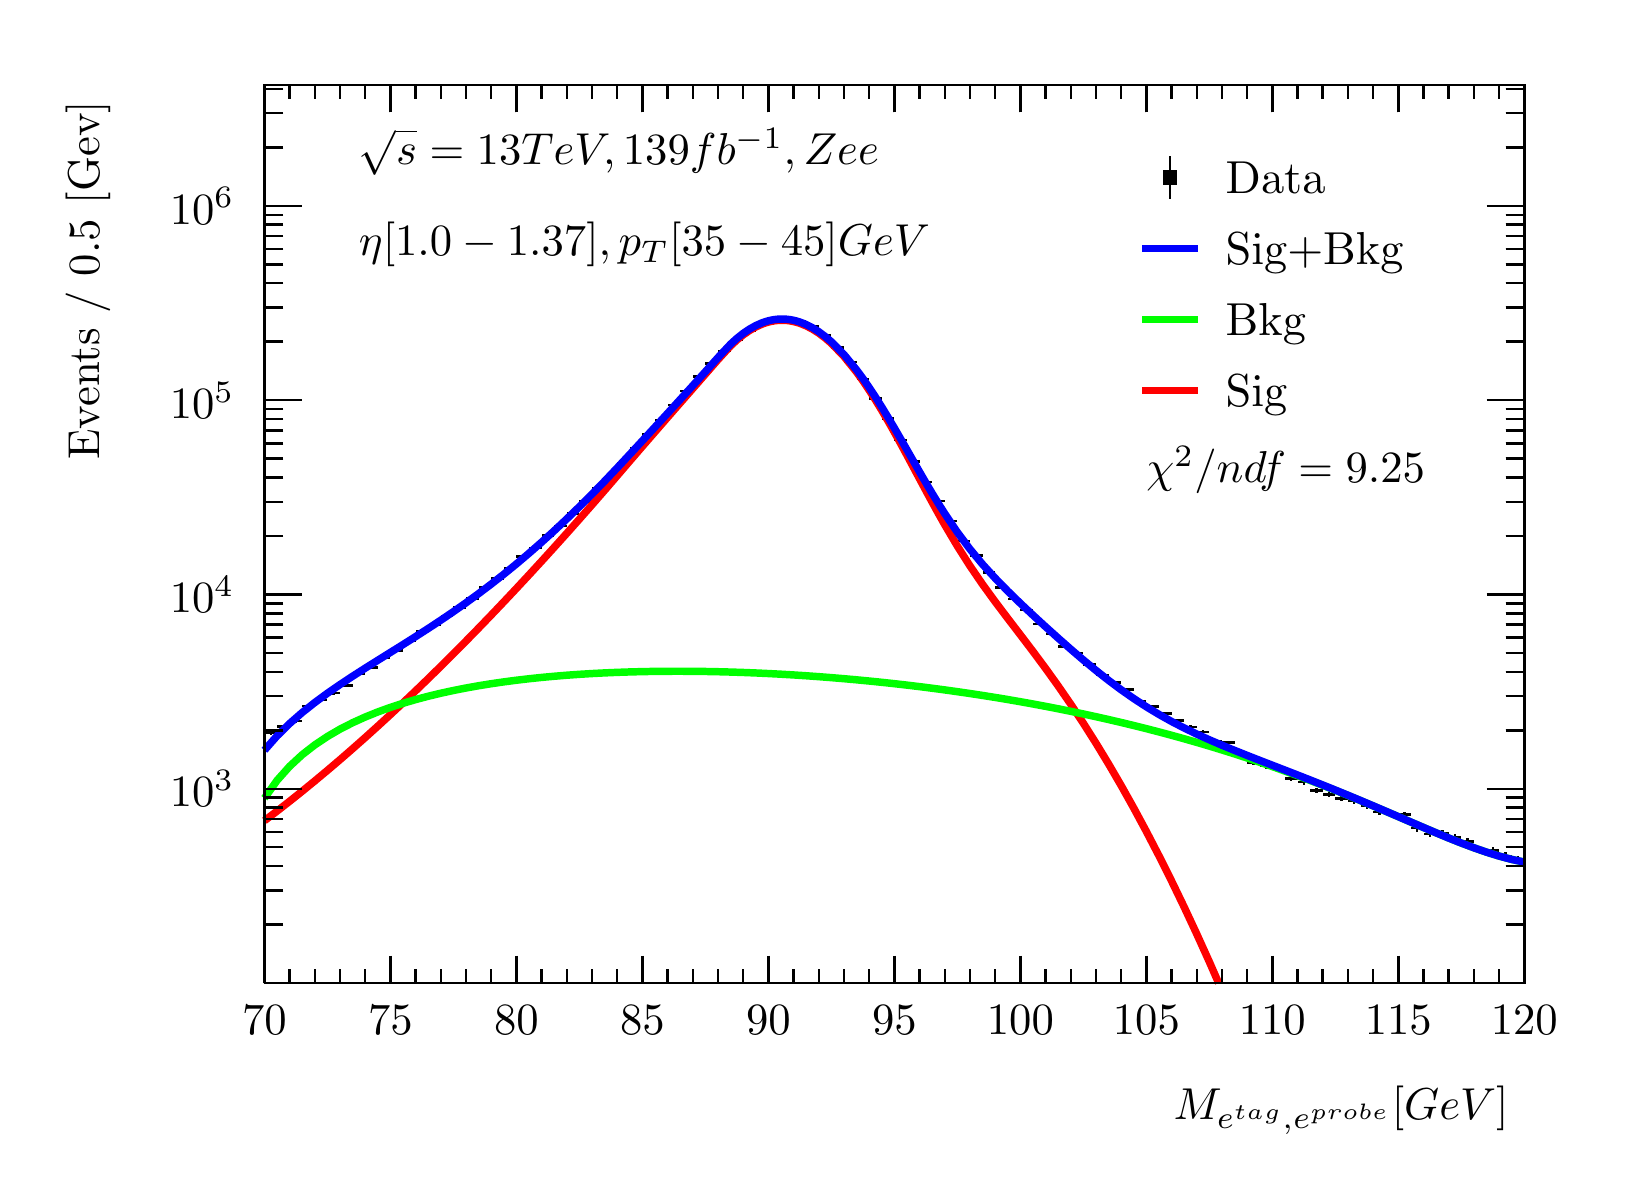
\begin{tikzpicture}
\pgfdeclareplotmark{cross} {
\pgfpathmoveto{\pgfpoint{-0.3\pgfplotmarksize}{\pgfplotmarksize}}
\pgfpathlineto{\pgfpoint{+0.3\pgfplotmarksize}{\pgfplotmarksize}}
\pgfpathlineto{\pgfpoint{+0.3\pgfplotmarksize}{0.3\pgfplotmarksize}}
\pgfpathlineto{\pgfpoint{+1\pgfplotmarksize}{0.3\pgfplotmarksize}}
\pgfpathlineto{\pgfpoint{+1\pgfplotmarksize}{-0.3\pgfplotmarksize}}
\pgfpathlineto{\pgfpoint{+0.3\pgfplotmarksize}{-0.3\pgfplotmarksize}}
\pgfpathlineto{\pgfpoint{+0.3\pgfplotmarksize}{-1.\pgfplotmarksize}}
\pgfpathlineto{\pgfpoint{-0.3\pgfplotmarksize}{-1.\pgfplotmarksize}}
\pgfpathlineto{\pgfpoint{-0.3\pgfplotmarksize}{-0.3\pgfplotmarksize}}
\pgfpathlineto{\pgfpoint{-1.\pgfplotmarksize}{-0.3\pgfplotmarksize}}
\pgfpathlineto{\pgfpoint{-1.\pgfplotmarksize}{0.3\pgfplotmarksize}}
\pgfpathlineto{\pgfpoint{-0.3\pgfplotmarksize}{0.3\pgfplotmarksize}}
\pgfpathclose
\pgfusepathqstroke
}
\pgfdeclareplotmark{cross*} {
\pgfpathmoveto{\pgfpoint{-0.3\pgfplotmarksize}{\pgfplotmarksize}}
\pgfpathlineto{\pgfpoint{+0.3\pgfplotmarksize}{\pgfplotmarksize}}
\pgfpathlineto{\pgfpoint{+0.3\pgfplotmarksize}{0.3\pgfplotmarksize}}
\pgfpathlineto{\pgfpoint{+1\pgfplotmarksize}{0.3\pgfplotmarksize}}
\pgfpathlineto{\pgfpoint{+1\pgfplotmarksize}{-0.3\pgfplotmarksize}}
\pgfpathlineto{\pgfpoint{+0.3\pgfplotmarksize}{-0.3\pgfplotmarksize}}
\pgfpathlineto{\pgfpoint{+0.3\pgfplotmarksize}{-1.\pgfplotmarksize}}
\pgfpathlineto{\pgfpoint{-0.3\pgfplotmarksize}{-1.\pgfplotmarksize}}
\pgfpathlineto{\pgfpoint{-0.3\pgfplotmarksize}{-0.3\pgfplotmarksize}}
\pgfpathlineto{\pgfpoint{-1.\pgfplotmarksize}{-0.3\pgfplotmarksize}}
\pgfpathlineto{\pgfpoint{-1.\pgfplotmarksize}{0.3\pgfplotmarksize}}
\pgfpathlineto{\pgfpoint{-0.3\pgfplotmarksize}{0.3\pgfplotmarksize}}
\pgfpathclose
\pgfusepathqfillstroke
}
\pgfdeclareplotmark{newstar} {
\pgfpathmoveto{\pgfqpoint{0pt}{\pgfplotmarksize}}
\pgfpathlineto{\pgfqpointpolar{44}{0.5\pgfplotmarksize}}
\pgfpathlineto{\pgfqpointpolar{18}{\pgfplotmarksize}}
\pgfpathlineto{\pgfqpointpolar{-20}{0.5\pgfplotmarksize}}
\pgfpathlineto{\pgfqpointpolar{-54}{\pgfplotmarksize}}
\pgfpathlineto{\pgfqpointpolar{-90}{0.5\pgfplotmarksize}}
\pgfpathlineto{\pgfqpointpolar{234}{\pgfplotmarksize}}
\pgfpathlineto{\pgfqpointpolar{198}{0.5\pgfplotmarksize}}
\pgfpathlineto{\pgfqpointpolar{162}{\pgfplotmarksize}}
\pgfpathlineto{\pgfqpointpolar{134}{0.5\pgfplotmarksize}}
\pgfpathclose
\pgfusepathqstroke
}
\pgfdeclareplotmark{newstar*} {
\pgfpathmoveto{\pgfqpoint{0pt}{\pgfplotmarksize}}
\pgfpathlineto{\pgfqpointpolar{44}{0.5\pgfplotmarksize}}
\pgfpathlineto{\pgfqpointpolar{18}{\pgfplotmarksize}}
\pgfpathlineto{\pgfqpointpolar{-20}{0.5\pgfplotmarksize}}
\pgfpathlineto{\pgfqpointpolar{-54}{\pgfplotmarksize}}
\pgfpathlineto{\pgfqpointpolar{-90}{0.5\pgfplotmarksize}}
\pgfpathlineto{\pgfqpointpolar{234}{\pgfplotmarksize}}
\pgfpathlineto{\pgfqpointpolar{198}{0.5\pgfplotmarksize}}
\pgfpathlineto{\pgfqpointpolar{162}{\pgfplotmarksize}}
\pgfpathlineto{\pgfqpointpolar{134}{0.5\pgfplotmarksize}}
\pgfpathclose
\pgfusepathqfillstroke
}
\definecolor{c}{rgb}{1,1,1};
\draw [color=c, fill=c] (0,0) rectangle (20,14.4361);
\draw [color=c, fill=c] (3,2.30977) rectangle (19,13.7143);
\definecolor{c}{rgb}{0,0,0};
\draw [c,line width=0.9] (3,2.30977) -- (3,13.7143) -- (19,13.7143) -- (19,2.30977) -- (3,2.30977);
\definecolor{c}{rgb}{1,1,1};
\draw [color=c, fill=c] (3,2.30977) rectangle (19,13.7143);
\definecolor{c}{rgb}{0,0,0};
\draw [c,line width=0.9] (3,2.30977) -- (3,13.7143) -- (19,13.7143) -- (19,2.30977) -- (3,2.30977);
\draw [c,line width=0.9] (3,2.30977) -- (19,2.30977);
\draw [c,line width=0.9] (3,2.65624) -- (3,2.30977);
\draw [c,line width=0.9] (3.32,2.48301) -- (3.32,2.30977);
\draw [c,line width=0.9] (3.64,2.48301) -- (3.64,2.30977);
\draw [c,line width=0.9] (3.96,2.48301) -- (3.96,2.30977);
\draw [c,line width=0.9] (4.28,2.48301) -- (4.28,2.30977);
\draw [c,line width=0.9] (4.6,2.65624) -- (4.6,2.30977);
\draw [c,line width=0.9] (4.92,2.48301) -- (4.92,2.30977);
\draw [c,line width=0.9] (5.24,2.48301) -- (5.24,2.30977);
\draw [c,line width=0.9] (5.56,2.48301) -- (5.56,2.30977);
\draw [c,line width=0.9] (5.88,2.48301) -- (5.88,2.30977);
\draw [c,line width=0.9] (6.2,2.65624) -- (6.2,2.30977);
\draw [c,line width=0.9] (6.52,2.48301) -- (6.52,2.30977);
\draw [c,line width=0.9] (6.84,2.48301) -- (6.84,2.30977);
\draw [c,line width=0.9] (7.16,2.48301) -- (7.16,2.30977);
\draw [c,line width=0.9] (7.48,2.48301) -- (7.48,2.30977);
\draw [c,line width=0.9] (7.8,2.65624) -- (7.8,2.30977);
\draw [c,line width=0.9] (8.12,2.48301) -- (8.12,2.30977);
\draw [c,line width=0.9] (8.44,2.48301) -- (8.44,2.30977);
\draw [c,line width=0.9] (8.76,2.48301) -- (8.76,2.30977);
\draw [c,line width=0.9] (9.08,2.48301) -- (9.08,2.30977);
\draw [c,line width=0.9] (9.4,2.65624) -- (9.4,2.30977);
\draw [c,line width=0.9] (9.72,2.48301) -- (9.72,2.30977);
\draw [c,line width=0.9] (10.04,2.48301) -- (10.04,2.30977);
\draw [c,line width=0.9] (10.36,2.48301) -- (10.36,2.30977);
\draw [c,line width=0.9] (10.68,2.48301) -- (10.68,2.30977);
\draw [c,line width=0.9] (11,2.65624) -- (11,2.30977);
\draw [c,line width=0.9] (11.32,2.48301) -- (11.32,2.30977);
\draw [c,line width=0.9] (11.64,2.48301) -- (11.64,2.30977);
\draw [c,line width=0.9] (11.96,2.48301) -- (11.96,2.30977);
\draw [c,line width=0.9] (12.28,2.48301) -- (12.28,2.30977);
\draw [c,line width=0.9] (12.6,2.65624) -- (12.6,2.30977);
\draw [c,line width=0.9] (12.92,2.48301) -- (12.92,2.30977);
\draw [c,line width=0.9] (13.24,2.48301) -- (13.24,2.30977);
\draw [c,line width=0.9] (13.56,2.48301) -- (13.56,2.30977);
\draw [c,line width=0.9] (13.88,2.48301) -- (13.88,2.30977);
\draw [c,line width=0.9] (14.2,2.65624) -- (14.2,2.30977);
\draw [c,line width=0.9] (14.52,2.48301) -- (14.52,2.30977);
\draw [c,line width=0.9] (14.84,2.48301) -- (14.84,2.30977);
\draw [c,line width=0.9] (15.16,2.48301) -- (15.16,2.30977);
\draw [c,line width=0.9] (15.48,2.48301) -- (15.48,2.30977);
\draw [c,line width=0.9] (15.8,2.65624) -- (15.8,2.30977);
\draw [c,line width=0.9] (16.12,2.48301) -- (16.12,2.30977);
\draw [c,line width=0.9] (16.44,2.48301) -- (16.44,2.30977);
\draw [c,line width=0.9] (16.76,2.48301) -- (16.76,2.30977);
\draw [c,line width=0.9] (17.08,2.48301) -- (17.08,2.30977);
\draw [c,line width=0.9] (17.4,2.65624) -- (17.4,2.30977);
\draw [c,line width=0.9] (17.72,2.48301) -- (17.72,2.30977);
\draw [c,line width=0.9] (18.04,2.48301) -- (18.04,2.30977);
\draw [c,line width=0.9] (18.36,2.48301) -- (18.36,2.30977);
\draw [c,line width=0.9] (18.68,2.48301) -- (18.68,2.30977);
\draw [c,line width=0.9] (19,2.65624) -- (19,2.30977);
\draw [anchor=base] (3,1.66015) node[scale=1.61424, color=c, rotate=0]{70};
\draw [anchor=base] (4.6,1.66015) node[scale=1.61424, color=c, rotate=0]{75};
\draw [anchor=base] (6.2,1.66015) node[scale=1.61424, color=c, rotate=0]{80};
\draw [anchor=base] (7.8,1.66015) node[scale=1.61424, color=c, rotate=0]{85};
\draw [anchor=base] (9.4,1.66015) node[scale=1.61424, color=c, rotate=0]{90};
\draw [anchor=base] (11,1.66015) node[scale=1.61424, color=c, rotate=0]{95};
\draw [anchor=base] (12.6,1.66015) node[scale=1.61424, color=c, rotate=0]{100};
\draw [anchor=base] (14.2,1.66015) node[scale=1.61424, color=c, rotate=0]{105};
\draw [anchor=base] (15.8,1.66015) node[scale=1.61424, color=c, rotate=0]{110};
\draw [anchor=base] (17.4,1.66015) node[scale=1.61424, color=c, rotate=0]{115};
\draw [anchor=base] (19,1.66015) node[scale=1.61424, color=c, rotate=0]{120};
\draw [anchor= east] (19,0.692932) node[scale=1.61424, color=c, rotate=0]{$M_{e^{tag}, e^{probe}}  [GeV]$};
\draw [c,line width=0.9] (3,13.7143) -- (19,13.7143);
\draw [c,line width=0.9] (3,13.3678) -- (3,13.7143);
\draw [c,line width=0.9] (3.32,13.5411) -- (3.32,13.7143);
\draw [c,line width=0.9] (3.64,13.5411) -- (3.64,13.7143);
\draw [c,line width=0.9] (3.96,13.5411) -- (3.96,13.7143);
\draw [c,line width=0.9] (4.28,13.5411) -- (4.28,13.7143);
\draw [c,line width=0.9] (4.6,13.3678) -- (4.6,13.7143);
\draw [c,line width=0.9] (4.92,13.5411) -- (4.92,13.7143);
\draw [c,line width=0.9] (5.24,13.5411) -- (5.24,13.7143);
\draw [c,line width=0.9] (5.56,13.5411) -- (5.56,13.7143);
\draw [c,line width=0.9] (5.88,13.5411) -- (5.88,13.7143);
\draw [c,line width=0.9] (6.2,13.3678) -- (6.2,13.7143);
\draw [c,line width=0.9] (6.52,13.5411) -- (6.52,13.7143);
\draw [c,line width=0.9] (6.84,13.5411) -- (6.84,13.7143);
\draw [c,line width=0.9] (7.16,13.5411) -- (7.16,13.7143);
\draw [c,line width=0.9] (7.48,13.5411) -- (7.48,13.7143);
\draw [c,line width=0.9] (7.8,13.3678) -- (7.8,13.7143);
\draw [c,line width=0.9] (8.12,13.5411) -- (8.12,13.7143);
\draw [c,line width=0.9] (8.44,13.5411) -- (8.44,13.7143);
\draw [c,line width=0.9] (8.76,13.5411) -- (8.76,13.7143);
\draw [c,line width=0.9] (9.08,13.5411) -- (9.08,13.7143);
\draw [c,line width=0.9] (9.4,13.3678) -- (9.4,13.7143);
\draw [c,line width=0.9] (9.72,13.5411) -- (9.72,13.7143);
\draw [c,line width=0.9] (10.04,13.5411) -- (10.04,13.7143);
\draw [c,line width=0.9] (10.36,13.5411) -- (10.36,13.7143);
\draw [c,line width=0.9] (10.68,13.5411) -- (10.68,13.7143);
\draw [c,line width=0.9] (11,13.3678) -- (11,13.7143);
\draw [c,line width=0.9] (11.32,13.5411) -- (11.32,13.7143);
\draw [c,line width=0.9] (11.64,13.5411) -- (11.64,13.7143);
\draw [c,line width=0.9] (11.96,13.5411) -- (11.96,13.7143);
\draw [c,line width=0.9] (12.28,13.5411) -- (12.28,13.7143);
\draw [c,line width=0.9] (12.6,13.3678) -- (12.6,13.7143);
\draw [c,line width=0.9] (12.92,13.5411) -- (12.92,13.7143);
\draw [c,line width=0.9] (13.24,13.5411) -- (13.24,13.7143);
\draw [c,line width=0.9] (13.56,13.5411) -- (13.56,13.7143);
\draw [c,line width=0.9] (13.88,13.5411) -- (13.88,13.7143);
\draw [c,line width=0.9] (14.2,13.3678) -- (14.2,13.7143);
\draw [c,line width=0.9] (14.52,13.5411) -- (14.52,13.7143);
\draw [c,line width=0.9] (14.84,13.5411) -- (14.84,13.7143);
\draw [c,line width=0.9] (15.16,13.5411) -- (15.16,13.7143);
\draw [c,line width=0.9] (15.48,13.5411) -- (15.48,13.7143);
\draw [c,line width=0.9] (15.8,13.3678) -- (15.8,13.7143);
\draw [c,line width=0.9] (16.12,13.5411) -- (16.12,13.7143);
\draw [c,line width=0.9] (16.44,13.5411) -- (16.44,13.7143);
\draw [c,line width=0.9] (16.76,13.5411) -- (16.76,13.7143);
\draw [c,line width=0.9] (17.08,13.5411) -- (17.08,13.7143);
\draw [c,line width=0.9] (17.4,13.3678) -- (17.4,13.7143);
\draw [c,line width=0.9] (17.72,13.5411) -- (17.72,13.7143);
\draw [c,line width=0.9] (18.04,13.5411) -- (18.04,13.7143);
\draw [c,line width=0.9] (18.36,13.5411) -- (18.36,13.7143);
\draw [c,line width=0.9] (18.68,13.5411) -- (18.68,13.7143);
\draw [c,line width=0.9] (19,13.3678) -- (19,13.7143);
\draw [c,line width=0.9] (3,2.30977) -- (3,13.7143);
\draw [c,line width=0.9] (3.237,3.05254) -- (3,3.05254);
\draw [c,line width=0.9] (3.237,3.48704) -- (3,3.48704);
\draw [c,line width=0.9] (3.237,3.79531) -- (3,3.79531);
\draw [c,line width=0.9] (3.237,4.03443) -- (3,4.03443);
\draw [c,line width=0.9] (3.237,4.22981) -- (3,4.22981);
\draw [c,line width=0.9] (3.237,4.395) -- (3,4.395);
\draw [c,line width=0.9] (3.237,4.53809) -- (3,4.53809);
\draw [c,line width=0.9] (3.237,4.6643) -- (3,4.6643);
\draw [c,line width=0.9] (3.474,4.77721) -- (3,4.77721);
\draw [anchor= east] (2.82,4.77721) node[scale=1.61424, color=c, rotate=0]{$10^{3}$};
\draw [c,line width=0.9] (3.237,5.51998) -- (3,5.51998);
\draw [c,line width=0.9] (3.237,5.95447) -- (3,5.95447);
\draw [c,line width=0.9] (3.237,6.26275) -- (3,6.26275);
\draw [c,line width=0.9] (3.237,6.50187) -- (3,6.50187);
\draw [c,line width=0.9] (3.237,6.69724) -- (3,6.69724);
\draw [c,line width=0.9] (3.237,6.86243) -- (3,6.86243);
\draw [c,line width=0.9] (3.237,7.00552) -- (3,7.00552);
\draw [c,line width=0.9] (3.237,7.13174) -- (3,7.13174);
\draw [c,line width=0.9] (3.474,7.24464) -- (3,7.24464);
\draw [anchor= east] (2.82,7.24464) node[scale=1.61424, color=c, rotate=0]{$10^{4}$};
\draw [c,line width=0.9] (3.237,7.98741) -- (3,7.98741);
\draw [c,line width=0.9] (3.237,8.4219) -- (3,8.4219);
\draw [c,line width=0.9] (3.237,8.73018) -- (3,8.73018);
\draw [c,line width=0.9] (3.237,8.9693) -- (3,8.9693);
\draw [c,line width=0.9] (3.237,9.16467) -- (3,9.16467);
\draw [c,line width=0.9] (3.237,9.32986) -- (3,9.32986);
\draw [c,line width=0.9] (3.237,9.47295) -- (3,9.47295);
\draw [c,line width=0.9] (3.237,9.59917) -- (3,9.59917);
\draw [c,line width=0.9] (3.474,9.71207) -- (3,9.71207);
\draw [anchor= east] (2.82,9.71207) node[scale=1.61424, color=c, rotate=0]{$10^{5}$};
\draw [c,line width=0.9] (3.237,10.4548) -- (3,10.4548);
\draw [c,line width=0.9] (3.237,10.8893) -- (3,10.8893);
\draw [c,line width=0.9] (3.237,11.1976) -- (3,11.1976);
\draw [c,line width=0.9] (3.237,11.4367) -- (3,11.4367);
\draw [c,line width=0.9] (3.237,11.6321) -- (3,11.6321);
\draw [c,line width=0.9] (3.237,11.7973) -- (3,11.7973);
\draw [c,line width=0.9] (3.237,11.9404) -- (3,11.9404);
\draw [c,line width=0.9] (3.237,12.0666) -- (3,12.0666);
\draw [c,line width=0.9] (3.474,12.1795) -- (3,12.1795);
\draw [anchor= east] (2.82,12.1795) node[scale=1.61424, color=c, rotate=0]{$10^{6}$};
\draw [c,line width=0.9] (3.237,12.9223) -- (3,12.9223);
\draw [c,line width=0.9] (3.237,13.3568) -- (3,13.3568);
\draw [c,line width=0.9] (3.237,13.665) -- (3,13.665);
\draw [anchor= east] (0.76,13.7143) node[scale=1.61424, color=c, rotate=90]{Events / 0.5 [Gev]};
\draw [c,line width=0.9] (19,2.30977) -- (19,13.7143);
\draw [c,line width=0.9] (18.763,3.05254) -- (19,3.05254);
\draw [c,line width=0.9] (18.763,3.48704) -- (19,3.48704);
\draw [c,line width=0.9] (18.763,3.79531) -- (19,3.79531);
\draw [c,line width=0.9] (18.763,4.03443) -- (19,4.03443);
\draw [c,line width=0.9] (18.763,4.22981) -- (19,4.22981);
\draw [c,line width=0.9] (18.763,4.395) -- (19,4.395);
\draw [c,line width=0.9] (18.763,4.53809) -- (19,4.53809);
\draw [c,line width=0.9] (18.763,4.6643) -- (19,4.6643);
\draw [c,line width=0.9] (18.526,4.77721) -- (19,4.77721);
\draw [c,line width=0.9] (18.763,5.51998) -- (19,5.51998);
\draw [c,line width=0.9] (18.763,5.95447) -- (19,5.95447);
\draw [c,line width=0.9] (18.763,6.26275) -- (19,6.26275);
\draw [c,line width=0.9] (18.763,6.50187) -- (19,6.50187);
\draw [c,line width=0.9] (18.763,6.69724) -- (19,6.69724);
\draw [c,line width=0.9] (18.763,6.86243) -- (19,6.86243);
\draw [c,line width=0.9] (18.763,7.00552) -- (19,7.00552);
\draw [c,line width=0.9] (18.763,7.13174) -- (19,7.13174);
\draw [c,line width=0.9] (18.526,7.24464) -- (19,7.24464);
\draw [c,line width=0.9] (18.763,7.98741) -- (19,7.98741);
\draw [c,line width=0.9] (18.763,8.4219) -- (19,8.4219);
\draw [c,line width=0.9] (18.763,8.73018) -- (19,8.73018);
\draw [c,line width=0.9] (18.763,8.9693) -- (19,8.9693);
\draw [c,line width=0.9] (18.763,9.16467) -- (19,9.16467);
\draw [c,line width=0.9] (18.763,9.32986) -- (19,9.32986);
\draw [c,line width=0.9] (18.763,9.47295) -- (19,9.47295);
\draw [c,line width=0.9] (18.763,9.59917) -- (19,9.59917);
\draw [c,line width=0.9] (18.526,9.71207) -- (19,9.71207);
\draw [c,line width=0.9] (18.763,10.4548) -- (19,10.4548);
\draw [c,line width=0.9] (18.763,10.8893) -- (19,10.8893);
\draw [c,line width=0.9] (18.763,11.1976) -- (19,11.1976);
\draw [c,line width=0.9] (18.763,11.4367) -- (19,11.4367);
\draw [c,line width=0.9] (18.763,11.6321) -- (19,11.6321);
\draw [c,line width=0.9] (18.763,11.7973) -- (19,11.7973);
\draw [c,line width=0.9] (18.763,11.9404) -- (19,11.9404);
\draw [c,line width=0.9] (18.763,12.0666) -- (19,12.0666);
\draw [c,line width=0.9] (18.526,12.1795) -- (19,12.1795);
\draw [c,line width=0.9] (18.763,12.9223) -- (19,12.9223);
\draw [c,line width=0.9] (18.763,13.3568) -- (19,13.3568);
\draw [c,line width=0.9] (18.763,13.665) -- (19,13.665);
\draw [c,line width=0.9] (3.08,5.4901) -- (3,5.4901);
\draw [c,line width=0.9] (3,5.4901) -- (3,5.4901);
\draw [c,line width=0.9] (3.08,5.4901) -- (3.16,5.4901);
\draw [c,line width=0.9] (3.16,5.4901) -- (3.16,5.4901);
\draw [c,line width=0.9] (3.08,5.4901) -- (3.08,5.51439);
\draw [c,line width=0.9] (3.08,5.51439) -- (3.08,5.51439);
\draw [c,line width=0.9] (3.08,5.4901) -- (3.08,5.4658);
\draw [c,line width=0.9] (3.08,5.4658) -- (3.08,5.4658);
\draw [c,line width=0.9] (3.24,5.56868) -- (3.16,5.56868);
\draw [c,line width=0.9] (3.16,5.56868) -- (3.16,5.56868);
\draw [c,line width=0.9] (3.24,5.56868) -- (3.32,5.56868);
\draw [c,line width=0.9] (3.32,5.56868) -- (3.32,5.56868);
\draw [c,line width=0.9] (3.24,5.56868) -- (3.24,5.59211);
\draw [c,line width=0.9] (3.24,5.59211) -- (3.24,5.59211);
\draw [c,line width=0.9] (3.24,5.56868) -- (3.24,5.54526);
\draw [c,line width=0.9] (3.24,5.54526) -- (3.24,5.54526);
\draw [c,line width=0.9] (3.4,5.63518) -- (3.32,5.63518);
\draw [c,line width=0.9] (3.32,5.63518) -- (3.32,5.63518);
\draw [c,line width=0.9] (3.4,5.63518) -- (3.48,5.63518);
\draw [c,line width=0.9] (3.48,5.63518) -- (3.48,5.63518);
\draw [c,line width=0.9] (3.4,5.63518) -- (3.4,5.65789);
\draw [c,line width=0.9] (3.4,5.65789) -- (3.4,5.65789);
\draw [c,line width=0.9] (3.4,5.63518) -- (3.4,5.61248);
\draw [c,line width=0.9] (3.4,5.61248) -- (3.4,5.61248);
\draw [c,line width=0.9] (3.56,5.8304) -- (3.48,5.8304);
\draw [c,line width=0.9] (3.48,5.8304) -- (3.48,5.8304);
\draw [c,line width=0.9] (3.56,5.8304) -- (3.64,5.8304);
\draw [c,line width=0.9] (3.64,5.8304) -- (3.64,5.8304);
\draw [c,line width=0.9] (3.56,5.8304) -- (3.56,5.85113);
\draw [c,line width=0.9] (3.56,5.85113) -- (3.56,5.85113);
\draw [c,line width=0.9] (3.56,5.8304) -- (3.56,5.80967);
\draw [c,line width=0.9] (3.56,5.80967) -- (3.56,5.80967);
\draw [c,line width=0.9] (3.72,5.90438) -- (3.64,5.90438);
\draw [c,line width=0.9] (3.64,5.90438) -- (3.64,5.90438);
\draw [c,line width=0.9] (3.72,5.90438) -- (3.8,5.90438);
\draw [c,line width=0.9] (3.8,5.90438) -- (3.8,5.90438);
\draw [c,line width=0.9] (3.72,5.90438) -- (3.72,5.92441);
\draw [c,line width=0.9] (3.72,5.92441) -- (3.72,5.92441);
\draw [c,line width=0.9] (3.72,5.90438) -- (3.72,5.88436);
\draw [c,line width=0.9] (3.72,5.88436) -- (3.72,5.88436);
\draw [c,line width=0.9] (3.88,5.99306) -- (3.8,5.99306);
\draw [c,line width=0.9] (3.8,5.99306) -- (3.8,5.99306);
\draw [c,line width=0.9] (3.88,5.99306) -- (3.96,5.99306);
\draw [c,line width=0.9] (3.96,5.99306) -- (3.96,5.99306);
\draw [c,line width=0.9] (3.88,5.99306) -- (3.88,6.01228);
\draw [c,line width=0.9] (3.88,6.01228) -- (3.88,6.01228);
\draw [c,line width=0.9] (3.88,5.99306) -- (3.88,5.97385);
\draw [c,line width=0.9] (3.88,5.97385) -- (3.88,5.97385);
\draw [c,line width=0.9] (4.04,6.08639) -- (3.96,6.08639);
\draw [c,line width=0.9] (3.96,6.08639) -- (3.96,6.08639);
\draw [c,line width=0.9] (4.04,6.08639) -- (4.12,6.08639);
\draw [c,line width=0.9] (4.12,6.08639) -- (4.12,6.08639);
\draw [c,line width=0.9] (4.04,6.08639) -- (4.04,6.10478);
\draw [c,line width=0.9] (4.04,6.10478) -- (4.04,6.10478);
\draw [c,line width=0.9] (4.04,6.08639) -- (4.04,6.06799);
\draw [c,line width=0.9] (4.04,6.06799) -- (4.04,6.06799);
\draw [c,line width=0.9] (4.2,6.23589) -- (4.12,6.23589);
\draw [c,line width=0.9] (4.12,6.23589) -- (4.12,6.23589);
\draw [c,line width=0.9] (4.2,6.23589) -- (4.28,6.23589);
\draw [c,line width=0.9] (4.28,6.23589) -- (4.28,6.23589);
\draw [c,line width=0.9] (4.2,6.23589) -- (4.2,6.25305);
\draw [c,line width=0.9] (4.2,6.25305) -- (4.2,6.25305);
\draw [c,line width=0.9] (4.2,6.23589) -- (4.2,6.21874);
\draw [c,line width=0.9] (4.2,6.21874) -- (4.2,6.21874);
\draw [c,line width=0.9] (4.36,6.31885) -- (4.28,6.31885);
\draw [c,line width=0.9] (4.28,6.31885) -- (4.28,6.31885);
\draw [c,line width=0.9] (4.36,6.31885) -- (4.44,6.31885);
\draw [c,line width=0.9] (4.44,6.31885) -- (4.44,6.31885);
\draw [c,line width=0.9] (4.36,6.31885) -- (4.36,6.33536);
\draw [c,line width=0.9] (4.36,6.33536) -- (4.36,6.33536);
\draw [c,line width=0.9] (4.36,6.31885) -- (4.36,6.30235);
\draw [c,line width=0.9] (4.36,6.30235) -- (4.36,6.30235);
\draw [c,line width=0.9] (4.52,6.43807) -- (4.44,6.43807);
\draw [c,line width=0.9] (4.44,6.43807) -- (4.44,6.43807);
\draw [c,line width=0.9] (4.52,6.43807) -- (4.6,6.43807);
\draw [c,line width=0.9] (4.6,6.43807) -- (4.6,6.43807);
\draw [c,line width=0.9] (4.52,6.43807) -- (4.52,6.45368);
\draw [c,line width=0.9] (4.52,6.45368) -- (4.52,6.45368);
\draw [c,line width=0.9] (4.52,6.43807) -- (4.52,6.42246);
\draw [c,line width=0.9] (4.52,6.42246) -- (4.52,6.42246);
\draw [c,line width=0.9] (4.68,6.53084) -- (4.6,6.53084);
\draw [c,line width=0.9] (4.6,6.53084) -- (4.6,6.53084);
\draw [c,line width=0.9] (4.68,6.53084) -- (4.76,6.53084);
\draw [c,line width=0.9] (4.76,6.53084) -- (4.76,6.53084);
\draw [c,line width=0.9] (4.68,6.53084) -- (4.68,6.54579);
\draw [c,line width=0.9] (4.68,6.54579) -- (4.68,6.54579);
\draw [c,line width=0.9] (4.68,6.53084) -- (4.68,6.51588);
\draw [c,line width=0.9] (4.68,6.51588) -- (4.68,6.51588);
\draw [c,line width=0.9] (4.84,6.65629) -- (4.76,6.65629);
\draw [c,line width=0.9] (4.76,6.65629) -- (4.76,6.65629);
\draw [c,line width=0.9] (4.84,6.65629) -- (4.92,6.65629);
\draw [c,line width=0.9] (4.92,6.65629) -- (4.92,6.65629);
\draw [c,line width=0.9] (4.84,6.65629) -- (4.84,6.67039);
\draw [c,line width=0.9] (4.84,6.67039) -- (4.84,6.67039);
\draw [c,line width=0.9] (4.84,6.65629) -- (4.84,6.64218);
\draw [c,line width=0.9] (4.84,6.64218) -- (4.84,6.64218);
\draw [c,line width=0.9] (5,6.77657) -- (4.92,6.77657);
\draw [c,line width=0.9] (4.92,6.77657) -- (4.92,6.77657);
\draw [c,line width=0.9] (5,6.77657) -- (5.08,6.77657);
\draw [c,line width=0.9] (5.08,6.77657) -- (5.08,6.77657);
\draw [c,line width=0.9] (5,6.77657) -- (5,6.7899);
\draw [c,line width=0.9] (5,6.7899) -- (5,6.7899);
\draw [c,line width=0.9] (5,6.77657) -- (5,6.76324);
\draw [c,line width=0.9] (5,6.76324) -- (5,6.76324);
\draw [c,line width=0.9] (5.16,6.85783) -- (5.08,6.85783);
\draw [c,line width=0.9] (5.08,6.85783) -- (5.08,6.85783);
\draw [c,line width=0.9] (5.16,6.85783) -- (5.24,6.85783);
\draw [c,line width=0.9] (5.24,6.85783) -- (5.24,6.85783);
\draw [c,line width=0.9] (5.16,6.85783) -- (5.16,6.87066);
\draw [c,line width=0.9] (5.16,6.87066) -- (5.16,6.87066);
\draw [c,line width=0.9] (5.16,6.85783) -- (5.16,6.84499);
\draw [c,line width=0.9] (5.16,6.84499) -- (5.16,6.84499);
\draw [c,line width=0.9] (5.32,6.97426) -- (5.24,6.97426);
\draw [c,line width=0.9] (5.24,6.97426) -- (5.24,6.97426);
\draw [c,line width=0.9] (5.32,6.97426) -- (5.4,6.97426);
\draw [c,line width=0.9] (5.4,6.97426) -- (5.4,6.97426);
\draw [c,line width=0.9] (5.32,6.97426) -- (5.32,6.98642);
\draw [c,line width=0.9] (5.32,6.98642) -- (5.32,6.98642);
\draw [c,line width=0.9] (5.32,6.97426) -- (5.32,6.9621);
\draw [c,line width=0.9] (5.32,6.9621) -- (5.32,6.9621);
\draw [c,line width=0.9] (5.48,7.07965) -- (5.4,7.07965);
\draw [c,line width=0.9] (5.4,7.07965) -- (5.4,7.07965);
\draw [c,line width=0.9] (5.48,7.07965) -- (5.56,7.07965);
\draw [c,line width=0.9] (5.56,7.07965) -- (5.56,7.07965);
\draw [c,line width=0.9] (5.48,7.07965) -- (5.48,7.09122);
\draw [c,line width=0.9] (5.48,7.09122) -- (5.48,7.09122);
\draw [c,line width=0.9] (5.48,7.07965) -- (5.48,7.06808);
\draw [c,line width=0.9] (5.48,7.06808) -- (5.48,7.06808);
\draw [c,line width=0.9] (5.64,7.19249) -- (5.56,7.19249);
\draw [c,line width=0.9] (5.56,7.19249) -- (5.56,7.19249);
\draw [c,line width=0.9] (5.64,7.19249) -- (5.72,7.19249);
\draw [c,line width=0.9] (5.72,7.19249) -- (5.72,7.19249);
\draw [c,line width=0.9] (5.64,7.19249) -- (5.64,7.20347);
\draw [c,line width=0.9] (5.64,7.20347) -- (5.64,7.20347);
\draw [c,line width=0.9] (5.64,7.19249) -- (5.64,7.18151);
\draw [c,line width=0.9] (5.64,7.18151) -- (5.64,7.18151);
\draw [c,line width=0.9] (5.8,7.33186) -- (5.72,7.33186);
\draw [c,line width=0.9] (5.72,7.33186) -- (5.72,7.33186);
\draw [c,line width=0.9] (5.8,7.33186) -- (5.88,7.33186);
\draw [c,line width=0.9] (5.88,7.33186) -- (5.88,7.33186);
\draw [c,line width=0.9] (5.8,7.33186) -- (5.8,7.34215);
\draw [c,line width=0.9] (5.8,7.34215) -- (5.8,7.34215);
\draw [c,line width=0.9] (5.8,7.33186) -- (5.8,7.32157);
\draw [c,line width=0.9] (5.8,7.32157) -- (5.8,7.32157);
\draw [c,line width=0.9] (5.96,7.44997) -- (5.88,7.44997);
\draw [c,line width=0.9] (5.88,7.44997) -- (5.88,7.44997);
\draw [c,line width=0.9] (5.96,7.44997) -- (6.04,7.44997);
\draw [c,line width=0.9] (6.04,7.44997) -- (6.04,7.44997);
\draw [c,line width=0.9] (5.96,7.44997) -- (5.96,7.45971);
\draw [c,line width=0.9] (5.96,7.45971) -- (5.96,7.45971);
\draw [c,line width=0.9] (5.96,7.44997) -- (5.96,7.44023);
\draw [c,line width=0.9] (5.96,7.44023) -- (5.96,7.44023);
\draw [c,line width=0.9] (6.12,7.57917) -- (6.04,7.57917);
\draw [c,line width=0.9] (6.04,7.57917) -- (6.04,7.57917);
\draw [c,line width=0.9] (6.12,7.57917) -- (6.2,7.57917);
\draw [c,line width=0.9] (6.2,7.57917) -- (6.2,7.57917);
\draw [c,line width=0.9] (6.12,7.57917) -- (6.12,7.58834);
\draw [c,line width=0.9] (6.12,7.58834) -- (6.12,7.58834);
\draw [c,line width=0.9] (6.12,7.57917) -- (6.12,7.57);
\draw [c,line width=0.9] (6.12,7.57) -- (6.12,7.57);
\draw [c,line width=0.9] (6.28,7.72896) -- (6.2,7.72896);
\draw [c,line width=0.9] (6.2,7.72896) -- (6.2,7.72896);
\draw [c,line width=0.9] (6.28,7.72896) -- (6.36,7.72896);
\draw [c,line width=0.9] (6.36,7.72896) -- (6.36,7.72896);
\draw [c,line width=0.9] (6.28,7.72896) -- (6.28,7.73751);
\draw [c,line width=0.9] (6.28,7.73751) -- (6.28,7.73751);
\draw [c,line width=0.9] (6.28,7.72896) -- (6.28,7.72042);
\draw [c,line width=0.9] (6.28,7.72042) -- (6.28,7.72042);
\draw [c,line width=0.9] (6.44,7.83275) -- (6.36,7.83275);
\draw [c,line width=0.9] (6.36,7.83275) -- (6.36,7.83275);
\draw [c,line width=0.9] (6.44,7.83275) -- (6.52,7.83275);
\draw [c,line width=0.9] (6.52,7.83275) -- (6.52,7.83275);
\draw [c,line width=0.9] (6.44,7.83275) -- (6.44,7.84089);
\draw [c,line width=0.9] (6.44,7.84089) -- (6.44,7.84089);
\draw [c,line width=0.9] (6.44,7.83275) -- (6.44,7.8246);
\draw [c,line width=0.9] (6.44,7.8246) -- (6.44,7.8246);
\draw [c,line width=0.9] (6.6,7.99542) -- (6.52,7.99542);
\draw [c,line width=0.9] (6.52,7.99542) -- (6.52,7.99542);
\draw [c,line width=0.9] (6.6,7.99542) -- (6.68,7.99542);
\draw [c,line width=0.9] (6.68,7.99542) -- (6.68,7.99542);
\draw [c,line width=0.9] (6.6,7.99542) -- (6.6,8.00297);
\draw [c,line width=0.9] (6.6,8.00297) -- (6.6,8.00297);
\draw [c,line width=0.9] (6.6,7.99542) -- (6.6,7.98787);
\draw [c,line width=0.9] (6.6,7.98787) -- (6.6,7.98787);
\draw [c,line width=0.9] (6.76,8.1162) -- (6.68,8.1162);
\draw [c,line width=0.9] (6.68,8.1162) -- (6.68,8.1162);
\draw [c,line width=0.9] (6.76,8.1162) -- (6.84,8.1162);
\draw [c,line width=0.9] (6.84,8.1162) -- (6.84,8.1162);
\draw [c,line width=0.9] (6.76,8.1162) -- (6.76,8.12333);
\draw [c,line width=0.9] (6.76,8.12333) -- (6.76,8.12333);
\draw [c,line width=0.9] (6.76,8.1162) -- (6.76,8.10906);
\draw [c,line width=0.9] (6.76,8.10906) -- (6.76,8.10906);
\draw [c,line width=0.9] (6.92,8.27538) -- (6.84,8.27538);
\draw [c,line width=0.9] (6.84,8.27538) -- (6.84,8.27538);
\draw [c,line width=0.9] (6.92,8.27538) -- (7,8.27538);
\draw [c,line width=0.9] (7,8.27538) -- (7,8.27538);
\draw [c,line width=0.9] (6.92,8.27538) -- (6.92,8.282);
\draw [c,line width=0.9] (6.92,8.282) -- (6.92,8.282);
\draw [c,line width=0.9] (6.92,8.27538) -- (6.92,8.26875);
\draw [c,line width=0.9] (6.92,8.26875) -- (6.92,8.26875);
\draw [c,line width=0.9] (7.08,8.42547) -- (7,8.42547);
\draw [c,line width=0.9] (7,8.42547) -- (7,8.42547);
\draw [c,line width=0.9] (7.08,8.42547) -- (7.16,8.42547);
\draw [c,line width=0.9] (7.16,8.42547) -- (7.16,8.42547);
\draw [c,line width=0.9] (7.08,8.42547) -- (7.08,8.43165);
\draw [c,line width=0.9] (7.08,8.43165) -- (7.08,8.43165);
\draw [c,line width=0.9] (7.08,8.42547) -- (7.08,8.41929);
\draw [c,line width=0.9] (7.08,8.41929) -- (7.08,8.41929);
\draw [c,line width=0.9] (7.24,8.58807) -- (7.16,8.58807);
\draw [c,line width=0.9] (7.16,8.58807) -- (7.16,8.58807);
\draw [c,line width=0.9] (7.24,8.58807) -- (7.32,8.58807);
\draw [c,line width=0.9] (7.32,8.58807) -- (7.32,8.58807);
\draw [c,line width=0.9] (7.24,8.58807) -- (7.24,8.5938);
\draw [c,line width=0.9] (7.24,8.5938) -- (7.24,8.5938);
\draw [c,line width=0.9] (7.24,8.58807) -- (7.24,8.58235);
\draw [c,line width=0.9] (7.24,8.58235) -- (7.24,8.58235);
\draw [c,line width=0.9] (7.4,8.75125) -- (7.32,8.75125);
\draw [c,line width=0.9] (7.32,8.75125) -- (7.32,8.75125);
\draw [c,line width=0.9] (7.4,8.75125) -- (7.48,8.75125);
\draw [c,line width=0.9] (7.48,8.75125) -- (7.48,8.75125);
\draw [c,line width=0.9] (7.4,8.75125) -- (7.4,8.75655);
\draw [c,line width=0.9] (7.4,8.75655) -- (7.4,8.75655);
\draw [c,line width=0.9] (7.4,8.75125) -- (7.4,8.74594);
\draw [c,line width=0.9] (7.4,8.74594) -- (7.4,8.74594);
\draw [c,line width=0.9] (7.56,8.91452) -- (7.48,8.91452);
\draw [c,line width=0.9] (7.48,8.91452) -- (7.48,8.91452);
\draw [c,line width=0.9] (7.56,8.91452) -- (7.64,8.91452);
\draw [c,line width=0.9] (7.64,8.91452) -- (7.64,8.91452);
\draw [c,line width=0.9] (7.56,8.91452) -- (7.56,8.91943);
\draw [c,line width=0.9] (7.56,8.91943) -- (7.56,8.91943);
\draw [c,line width=0.9] (7.56,8.91452) -- (7.56,8.9096);
\draw [c,line width=0.9] (7.56,8.9096) -- (7.56,8.9096);
\draw [c,line width=0.9] (7.72,9.09721) -- (7.64,9.09721);
\draw [c,line width=0.9] (7.64,9.09721) -- (7.64,9.09721);
\draw [c,line width=0.9] (7.72,9.09721) -- (7.8,9.09721);
\draw [c,line width=0.9] (7.8,9.09721) -- (7.8,9.09721);
\draw [c,line width=0.9] (7.72,9.09721) -- (7.72,9.10173);
\draw [c,line width=0.9] (7.72,9.10173) -- (7.72,9.10173);
\draw [c,line width=0.9] (7.72,9.09721) -- (7.72,9.0927);
\draw [c,line width=0.9] (7.72,9.0927) -- (7.72,9.0927);
\draw [c,line width=0.9] (7.88,9.27594) -- (7.8,9.27594);
\draw [c,line width=0.9] (7.8,9.27594) -- (7.8,9.27594);
\draw [c,line width=0.9] (7.88,9.27594) -- (7.96,9.27594);
\draw [c,line width=0.9] (7.96,9.27594) -- (7.96,9.27594);
\draw [c,line width=0.9] (7.88,9.27594) -- (7.88,9.2801);
\draw [c,line width=0.9] (7.88,9.2801) -- (7.88,9.2801);
\draw [c,line width=0.9] (7.88,9.27594) -- (7.88,9.27179);
\draw [c,line width=0.9] (7.88,9.27179) -- (7.88,9.27179);
\draw [c,line width=0.9] (8.04,9.46213) -- (7.96,9.46213);
\draw [c,line width=0.9] (7.96,9.46213) -- (7.96,9.46213);
\draw [c,line width=0.9] (8.04,9.46213) -- (8.12,9.46213);
\draw [c,line width=0.9] (8.12,9.46213) -- (8.12,9.46213);
\draw [c,line width=0.9] (8.04,9.46213) -- (8.04,9.46594);
\draw [c,line width=0.9] (8.04,9.46594) -- (8.04,9.46594);
\draw [c,line width=0.9] (8.04,9.46213) -- (8.04,9.45832);
\draw [c,line width=0.9] (8.04,9.45832) -- (8.04,9.45832);
\draw [c,line width=0.9] (8.2,9.64927) -- (8.12,9.64927);
\draw [c,line width=0.9] (8.12,9.64927) -- (8.12,9.64927);
\draw [c,line width=0.9] (8.2,9.64927) -- (8.28,9.64927);
\draw [c,line width=0.9] (8.28,9.64927) -- (8.28,9.64927);
\draw [c,line width=0.9] (8.2,9.64927) -- (8.2,9.65276);
\draw [c,line width=0.9] (8.2,9.65276) -- (8.2,9.65276);
\draw [c,line width=0.9] (8.2,9.64927) -- (8.2,9.64578);
\draw [c,line width=0.9] (8.2,9.64578) -- (8.2,9.64578);
\draw [c,line width=0.9] (8.36,9.82762) -- (8.28,9.82762);
\draw [c,line width=0.9] (8.28,9.82762) -- (8.28,9.82762);
\draw [c,line width=0.9] (8.36,9.82762) -- (8.44,9.82762);
\draw [c,line width=0.9] (8.44,9.82762) -- (8.44,9.82762);
\draw [c,line width=0.9] (8.36,9.82762) -- (8.36,9.83084);
\draw [c,line width=0.9] (8.36,9.83084) -- (8.36,9.83084);
\draw [c,line width=0.9] (8.36,9.82762) -- (8.36,9.82441);
\draw [c,line width=0.9] (8.36,9.82441) -- (8.36,9.82441);
\draw [c,line width=0.9] (8.52,10.0153) -- (8.44,10.0153);
\draw [c,line width=0.9] (8.44,10.0153) -- (8.44,10.0153);
\draw [c,line width=0.9] (8.52,10.0153) -- (8.6,10.0153);
\draw [c,line width=0.9] (8.6,10.0153) -- (8.6,10.0153);
\draw [c,line width=0.9] (8.52,10.0153) -- (8.52,10.0183);
\draw [c,line width=0.9] (8.52,10.0183) -- (8.52,10.0183);
\draw [c,line width=0.9] (8.52,10.0153) -- (8.52,10.0124);
\draw [c,line width=0.9] (8.52,10.0124) -- (8.52,10.0124);
\draw [c,line width=0.9] (8.68,10.1796) -- (8.6,10.1796);
\draw [c,line width=0.9] (8.6,10.1796) -- (8.6,10.1796);
\draw [c,line width=0.9] (8.68,10.1796) -- (8.76,10.1796);
\draw [c,line width=0.9] (8.76,10.1796) -- (8.76,10.1796);
\draw [c,line width=0.9] (8.68,10.1796) -- (8.68,10.1823);
\draw [c,line width=0.9] (8.68,10.1823) -- (8.68,10.1823);
\draw [c,line width=0.9] (8.68,10.1796) -- (8.68,10.1768);
\draw [c,line width=0.9] (8.68,10.1768) -- (8.68,10.1768);
\draw [c,line width=0.9] (8.84,10.3392) -- (8.76,10.3392);
\draw [c,line width=0.9] (8.76,10.3392) -- (8.76,10.3392);
\draw [c,line width=0.9] (8.84,10.3392) -- (8.92,10.3392);
\draw [c,line width=0.9] (8.92,10.3392) -- (8.92,10.3392);
\draw [c,line width=0.9] (8.84,10.3392) -- (8.84,10.3417);
\draw [c,line width=0.9] (8.84,10.3417) -- (8.84,10.3417);
\draw [c,line width=0.9] (8.84,10.3392) -- (8.84,10.3366);
\draw [c,line width=0.9] (8.84,10.3366) -- (8.84,10.3366);
\draw [c,line width=0.9] (9,10.477) -- (8.92,10.477);
\draw [c,line width=0.9] (8.92,10.477) -- (8.92,10.477);
\draw [c,line width=0.9] (9,10.477) -- (9.08,10.477);
\draw [c,line width=0.9] (9.08,10.477) -- (9.08,10.477);
\draw [c,line width=0.9] (9,10.477) -- (9,10.4794);
\draw [c,line width=0.9] (9,10.4794) -- (9,10.4794);
\draw [c,line width=0.9] (9,10.477) -- (9,10.4746);
\draw [c,line width=0.9] (9,10.4746) -- (9,10.4746);
\draw [c,line width=0.9] (9.16,10.5944) -- (9.08,10.5944);
\draw [c,line width=0.9] (9.08,10.5944) -- (9.08,10.5944);
\draw [c,line width=0.9] (9.16,10.5944) -- (9.24,10.5944);
\draw [c,line width=0.9] (9.24,10.5944) -- (9.24,10.5944);
\draw [c,line width=0.9] (9.16,10.5944) -- (9.16,10.5966);
\draw [c,line width=0.9] (9.16,10.5966) -- (9.16,10.5966);
\draw [c,line width=0.9] (9.16,10.5944) -- (9.16,10.5921);
\draw [c,line width=0.9] (9.16,10.5921) -- (9.16,10.5921);
\draw [c,line width=0.9] (9.32,10.6837) -- (9.24,10.6837);
\draw [c,line width=0.9] (9.24,10.6837) -- (9.24,10.6837);
\draw [c,line width=0.9] (9.32,10.6837) -- (9.4,10.6837);
\draw [c,line width=0.9] (9.4,10.6837) -- (9.4,10.6837);
\draw [c,line width=0.9] (9.32,10.6837) -- (9.32,10.6858);
\draw [c,line width=0.9] (9.32,10.6858) -- (9.32,10.6858);
\draw [c,line width=0.9] (9.32,10.6837) -- (9.32,10.6815);
\draw [c,line width=0.9] (9.32,10.6815) -- (9.32,10.6815);
\draw [c,line width=0.9] (9.48,10.7295) -- (9.4,10.7295);
\draw [c,line width=0.9] (9.4,10.7295) -- (9.4,10.7295);
\draw [c,line width=0.9] (9.48,10.7295) -- (9.56,10.7295);
\draw [c,line width=0.9] (9.56,10.7295) -- (9.56,10.7295);
\draw [c,line width=0.9] (9.48,10.7295) -- (9.48,10.7317);
\draw [c,line width=0.9] (9.48,10.7317) -- (9.48,10.7317);
\draw [c,line width=0.9] (9.48,10.7295) -- (9.48,10.7274);
\draw [c,line width=0.9] (9.48,10.7274) -- (9.48,10.7274);
\draw [c,line width=0.9] (9.64,10.743) -- (9.56,10.743);
\draw [c,line width=0.9] (9.56,10.743) -- (9.56,10.743);
\draw [c,line width=0.9] (9.64,10.743) -- (9.72,10.743);
\draw [c,line width=0.9] (9.72,10.743) -- (9.72,10.743);
\draw [c,line width=0.9] (9.64,10.743) -- (9.64,10.7451);
\draw [c,line width=0.9] (9.64,10.7451) -- (9.64,10.7451);
\draw [c,line width=0.9] (9.64,10.743) -- (9.64,10.741);
\draw [c,line width=0.9] (9.64,10.741) -- (9.64,10.741);
\draw [c,line width=0.9] (9.8,10.7145) -- (9.72,10.7145);
\draw [c,line width=0.9] (9.72,10.7145) -- (9.72,10.7145);
\draw [c,line width=0.9] (9.8,10.7145) -- (9.88,10.7145);
\draw [c,line width=0.9] (9.88,10.7145) -- (9.88,10.7145);
\draw [c,line width=0.9] (9.8,10.7145) -- (9.8,10.7166);
\draw [c,line width=0.9] (9.8,10.7166) -- (9.8,10.7166);
\draw [c,line width=0.9] (9.8,10.7145) -- (9.8,10.7124);
\draw [c,line width=0.9] (9.8,10.7124) -- (9.8,10.7124);
\draw [c,line width=0.9] (9.96,10.6478) -- (9.88,10.6478);
\draw [c,line width=0.9] (9.88,10.6478) -- (9.88,10.6478);
\draw [c,line width=0.9] (9.96,10.6478) -- (10.04,10.6478);
\draw [c,line width=0.9] (10.04,10.6478) -- (10.04,10.6478);
\draw [c,line width=0.9] (9.96,10.6478) -- (9.96,10.6499);
\draw [c,line width=0.9] (9.96,10.6499) -- (9.96,10.6499);
\draw [c,line width=0.9] (9.96,10.6478) -- (9.96,10.6456);
\draw [c,line width=0.9] (9.96,10.6456) -- (9.96,10.6456);
\draw [c,line width=0.9] (10.12,10.5347) -- (10.04,10.5347);
\draw [c,line width=0.9] (10.04,10.5347) -- (10.04,10.5347);
\draw [c,line width=0.9] (10.12,10.5347) -- (10.2,10.5347);
\draw [c,line width=0.9] (10.2,10.5347) -- (10.2,10.5347);
\draw [c,line width=0.9] (10.12,10.5347) -- (10.12,10.5371);
\draw [c,line width=0.9] (10.12,10.5371) -- (10.12,10.5371);
\draw [c,line width=0.9] (10.12,10.5347) -- (10.12,10.5324);
\draw [c,line width=0.9] (10.12,10.5324) -- (10.12,10.5324);
\draw [c,line width=0.9] (10.28,10.3841) -- (10.2,10.3841);
\draw [c,line width=0.9] (10.2,10.3841) -- (10.2,10.3841);
\draw [c,line width=0.9] (10.28,10.3841) -- (10.36,10.3841);
\draw [c,line width=0.9] (10.36,10.3841) -- (10.36,10.3841);
\draw [c,line width=0.9] (10.28,10.3841) -- (10.28,10.3865);
\draw [c,line width=0.9] (10.28,10.3865) -- (10.28,10.3865);
\draw [c,line width=0.9] (10.28,10.3841) -- (10.28,10.3816);
\draw [c,line width=0.9] (10.28,10.3816) -- (10.28,10.3816);
\draw [c,line width=0.9] (10.44,10.1974) -- (10.36,10.1974);
\draw [c,line width=0.9] (10.36,10.1974) -- (10.36,10.1974);
\draw [c,line width=0.9] (10.44,10.1974) -- (10.52,10.1974);
\draw [c,line width=0.9] (10.52,10.1974) -- (10.52,10.1974);
\draw [c,line width=0.9] (10.44,10.1974) -- (10.44,10.2001);
\draw [c,line width=0.9] (10.44,10.2001) -- (10.44,10.2001);
\draw [c,line width=0.9] (10.44,10.1974) -- (10.44,10.1947);
\draw [c,line width=0.9] (10.44,10.1947) -- (10.44,10.1947);
\draw [c,line width=0.9] (10.6,9.97898) -- (10.52,9.97898);
\draw [c,line width=0.9] (10.52,9.97898) -- (10.52,9.97898);
\draw [c,line width=0.9] (10.6,9.97898) -- (10.68,9.97898);
\draw [c,line width=0.9] (10.68,9.97898) -- (10.68,9.97898);
\draw [c,line width=0.9] (10.6,9.97898) -- (10.6,9.98197);
\draw [c,line width=0.9] (10.6,9.98197) -- (10.6,9.98197);
\draw [c,line width=0.9] (10.6,9.97898) -- (10.6,9.97599);
\draw [c,line width=0.9] (10.6,9.97599) -- (10.6,9.97599);
\draw [c,line width=0.9] (10.76,9.73439) -- (10.68,9.73439);
\draw [c,line width=0.9] (10.68,9.73439) -- (10.68,9.73439);
\draw [c,line width=0.9] (10.76,9.73439) -- (10.84,9.73439);
\draw [c,line width=0.9] (10.84,9.73439) -- (10.84,9.73439);
\draw [c,line width=0.9] (10.76,9.73439) -- (10.76,9.73774);
\draw [c,line width=0.9] (10.76,9.73774) -- (10.76,9.73774);
\draw [c,line width=0.9] (10.76,9.73439) -- (10.76,9.73103);
\draw [c,line width=0.9] (10.76,9.73103) -- (10.76,9.73103);
\draw [c,line width=0.9] (10.92,9.47883) -- (10.84,9.47883);
\draw [c,line width=0.9] (10.84,9.47883) -- (10.84,9.47883);
\draw [c,line width=0.9] (10.92,9.47883) -- (11,9.47883);
\draw [c,line width=0.9] (11,9.47883) -- (11,9.47883);
\draw [c,line width=0.9] (10.92,9.47883) -- (10.92,9.48261);
\draw [c,line width=0.9] (10.92,9.48261) -- (10.92,9.48261);
\draw [c,line width=0.9] (10.92,9.47883) -- (10.92,9.47505);
\draw [c,line width=0.9] (10.92,9.47505) -- (10.92,9.47505);
\draw [c,line width=0.9] (11.08,9.20557) -- (11,9.20557);
\draw [c,line width=0.9] (11,9.20557) -- (11,9.20557);
\draw [c,line width=0.9] (11.08,9.20557) -- (11.16,9.20557);
\draw [c,line width=0.9] (11.16,9.20557) -- (11.16,9.20557);
\draw [c,line width=0.9] (11.08,9.20557) -- (11.08,9.20986);
\draw [c,line width=0.9] (11.08,9.20986) -- (11.08,9.20986);
\draw [c,line width=0.9] (11.08,9.20557) -- (11.08,9.20128);
\draw [c,line width=0.9] (11.08,9.20128) -- (11.08,9.20128);
\draw [c,line width=0.9] (11.24,8.93635) -- (11.16,8.93635);
\draw [c,line width=0.9] (11.16,8.93635) -- (11.16,8.93635);
\draw [c,line width=0.9] (11.24,8.93635) -- (11.32,8.93635);
\draw [c,line width=0.9] (11.32,8.93635) -- (11.32,8.93635);
\draw [c,line width=0.9] (11.24,8.93635) -- (11.24,8.94122);
\draw [c,line width=0.9] (11.24,8.94122) -- (11.24,8.94122);
\draw [c,line width=0.9] (11.24,8.93635) -- (11.24,8.93149);
\draw [c,line width=0.9] (11.24,8.93149) -- (11.24,8.93149);
\draw [c,line width=0.9] (11.4,8.67318) -- (11.32,8.67318);
\draw [c,line width=0.9] (11.32,8.67318) -- (11.32,8.67318);
\draw [c,line width=0.9] (11.4,8.67318) -- (11.48,8.67318);
\draw [c,line width=0.9] (11.48,8.67318) -- (11.48,8.67318);
\draw [c,line width=0.9] (11.4,8.67318) -- (11.4,8.67869);
\draw [c,line width=0.9] (11.4,8.67869) -- (11.4,8.67869);
\draw [c,line width=0.9] (11.4,8.67318) -- (11.4,8.66768);
\draw [c,line width=0.9] (11.4,8.66768) -- (11.4,8.66768);
\draw [c,line width=0.9] (11.56,8.4338) -- (11.48,8.4338);
\draw [c,line width=0.9] (11.48,8.4338) -- (11.48,8.4338);
\draw [c,line width=0.9] (11.56,8.4338) -- (11.64,8.4338);
\draw [c,line width=0.9] (11.64,8.4338) -- (11.64,8.4338);
\draw [c,line width=0.9] (11.56,8.4338) -- (11.56,8.43996);
\draw [c,line width=0.9] (11.56,8.43996) -- (11.56,8.43996);
\draw [c,line width=0.9] (11.56,8.4338) -- (11.56,8.42765);
\draw [c,line width=0.9] (11.56,8.42765) -- (11.56,8.42765);
\draw [c,line width=0.9] (11.72,8.17786) -- (11.64,8.17786);
\draw [c,line width=0.9] (11.64,8.17786) -- (11.64,8.17786);
\draw [c,line width=0.9] (11.72,8.17786) -- (11.8,8.17786);
\draw [c,line width=0.9] (11.8,8.17786) -- (11.8,8.17786);
\draw [c,line width=0.9] (11.72,8.17786) -- (11.72,8.1848);
\draw [c,line width=0.9] (11.72,8.1848) -- (11.72,8.1848);
\draw [c,line width=0.9] (11.72,8.17786) -- (11.72,8.17093);
\draw [c,line width=0.9] (11.72,8.17093) -- (11.72,8.17093);
\draw [c,line width=0.9] (11.88,7.92622) -- (11.8,7.92622);
\draw [c,line width=0.9] (11.8,7.92622) -- (11.8,7.92622);
\draw [c,line width=0.9] (11.88,7.92622) -- (11.96,7.92622);
\draw [c,line width=0.9] (11.96,7.92622) -- (11.96,7.92622);
\draw [c,line width=0.9] (11.88,7.92622) -- (11.88,7.93402);
\draw [c,line width=0.9] (11.88,7.93402) -- (11.88,7.93402);
\draw [c,line width=0.9] (11.88,7.92622) -- (11.88,7.91843);
\draw [c,line width=0.9] (11.88,7.91843) -- (11.88,7.91843);
\draw [c,line width=0.9] (12.04,7.74144) -- (11.96,7.74144);
\draw [c,line width=0.9] (11.96,7.74144) -- (11.96,7.74144);
\draw [c,line width=0.9] (12.04,7.74144) -- (12.12,7.74144);
\draw [c,line width=0.9] (12.12,7.74144) -- (12.12,7.74144);
\draw [c,line width=0.9] (12.04,7.74144) -- (12.04,7.74994);
\draw [c,line width=0.9] (12.04,7.74994) -- (12.04,7.74994);
\draw [c,line width=0.9] (12.04,7.74144) -- (12.04,7.73294);
\draw [c,line width=0.9] (12.04,7.73294) -- (12.04,7.73294);
\draw [c,line width=0.9] (12.2,7.52521) -- (12.12,7.52521);
\draw [c,line width=0.9] (12.12,7.52521) -- (12.12,7.52521);
\draw [c,line width=0.9] (12.2,7.52521) -- (12.28,7.52521);
\draw [c,line width=0.9] (12.28,7.52521) -- (12.28,7.52521);
\draw [c,line width=0.9] (12.2,7.52521) -- (12.2,7.53461);
\draw [c,line width=0.9] (12.2,7.53461) -- (12.2,7.53461);
\draw [c,line width=0.9] (12.2,7.52521) -- (12.2,7.51581);
\draw [c,line width=0.9] (12.2,7.51581) -- (12.2,7.51581);
\draw [c,line width=0.9] (12.36,7.33246) -- (12.28,7.33246);
\draw [c,line width=0.9] (12.28,7.33246) -- (12.28,7.33246);
\draw [c,line width=0.9] (12.36,7.33246) -- (12.44,7.33246);
\draw [c,line width=0.9] (12.44,7.33246) -- (12.44,7.33246);
\draw [c,line width=0.9] (12.36,7.33246) -- (12.36,7.34274);
\draw [c,line width=0.9] (12.36,7.34274) -- (12.36,7.34274);
\draw [c,line width=0.9] (12.36,7.33246) -- (12.36,7.32217);
\draw [c,line width=0.9] (12.36,7.32217) -- (12.36,7.32217);
\draw [c,line width=0.9] (12.52,7.18447) -- (12.44,7.18447);
\draw [c,line width=0.9] (12.44,7.18447) -- (12.44,7.18447);
\draw [c,line width=0.9] (12.52,7.18447) -- (12.6,7.18447);
\draw [c,line width=0.9] (12.6,7.18447) -- (12.6,7.18447);
\draw [c,line width=0.9] (12.52,7.18447) -- (12.52,7.19549);
\draw [c,line width=0.9] (12.52,7.19549) -- (12.52,7.19549);
\draw [c,line width=0.9] (12.52,7.18447) -- (12.52,7.17345);
\draw [c,line width=0.9] (12.52,7.17345) -- (12.52,7.17345);
\draw [c,line width=0.9] (12.68,7.05012) -- (12.6,7.05012);
\draw [c,line width=0.9] (12.6,7.05012) -- (12.6,7.05012);
\draw [c,line width=0.9] (12.68,7.05012) -- (12.76,7.05012);
\draw [c,line width=0.9] (12.76,7.05012) -- (12.76,7.05012);
\draw [c,line width=0.9] (12.68,7.05012) -- (12.68,7.06186);
\draw [c,line width=0.9] (12.68,7.06186) -- (12.68,7.06186);
\draw [c,line width=0.9] (12.68,7.05012) -- (12.68,7.03839);
\draw [c,line width=0.9] (12.68,7.03839) -- (12.68,7.03839);
\draw [c,line width=0.9] (12.84,6.86717) -- (12.76,6.86717);
\draw [c,line width=0.9] (12.76,6.86717) -- (12.76,6.86717);
\draw [c,line width=0.9] (12.84,6.86717) -- (12.92,6.86717);
\draw [c,line width=0.9] (12.92,6.86717) -- (12.92,6.86717);
\draw [c,line width=0.9] (12.84,6.86717) -- (12.84,6.87994);
\draw [c,line width=0.9] (12.84,6.87994) -- (12.84,6.87994);
\draw [c,line width=0.9] (12.84,6.86717) -- (12.84,6.85439);
\draw [c,line width=0.9] (12.84,6.85439) -- (12.84,6.85439);
\draw [c,line width=0.9] (13,6.7439) -- (12.92,6.7439);
\draw [c,line width=0.9] (12.92,6.7439) -- (12.92,6.7439);
\draw [c,line width=0.9] (13,6.7439) -- (13.08,6.7439);
\draw [c,line width=0.9] (13.08,6.7439) -- (13.08,6.7439);
\draw [c,line width=0.9] (13,6.7439) -- (13,6.75743);
\draw [c,line width=0.9] (13,6.75743) -- (13,6.75743);
\draw [c,line width=0.9] (13,6.7439) -- (13,6.73036);
\draw [c,line width=0.9] (13,6.73036) -- (13,6.73036);
\draw [c,line width=0.9] (13.16,6.58394) -- (13.08,6.58394);
\draw [c,line width=0.9] (13.08,6.58394) -- (13.08,6.58394);
\draw [c,line width=0.9] (13.16,6.58394) -- (13.24,6.58394);
\draw [c,line width=0.9] (13.24,6.58394) -- (13.24,6.58394);
\draw [c,line width=0.9] (13.16,6.58394) -- (13.16,6.59853);
\draw [c,line width=0.9] (13.16,6.59853) -- (13.16,6.59853);
\draw [c,line width=0.9] (13.16,6.58394) -- (13.16,6.56936);
\draw [c,line width=0.9] (13.16,6.56936) -- (13.16,6.56936);
\draw [c,line width=0.9] (13.32,6.50358) -- (13.24,6.50358);
\draw [c,line width=0.9] (13.24,6.50358) -- (13.24,6.50358);
\draw [c,line width=0.9] (13.32,6.50358) -- (13.4,6.50358);
\draw [c,line width=0.9] (13.4,6.50358) -- (13.4,6.50358);
\draw [c,line width=0.9] (13.32,6.50358) -- (13.32,6.51872);
\draw [c,line width=0.9] (13.32,6.51872) -- (13.32,6.51872);
\draw [c,line width=0.9] (13.32,6.50358) -- (13.32,6.48844);
\draw [c,line width=0.9] (13.32,6.48844) -- (13.32,6.48844);
\draw [c,line width=0.9] (13.48,6.35657) -- (13.4,6.35657);
\draw [c,line width=0.9] (13.4,6.35657) -- (13.4,6.35657);
\draw [c,line width=0.9] (13.48,6.35657) -- (13.56,6.35657);
\draw [c,line width=0.9] (13.56,6.35657) -- (13.56,6.35657);
\draw [c,line width=0.9] (13.48,6.35657) -- (13.48,6.37279);
\draw [c,line width=0.9] (13.48,6.37279) -- (13.48,6.37279);
\draw [c,line width=0.9] (13.48,6.35657) -- (13.48,6.34035);
\draw [c,line width=0.9] (13.48,6.34035) -- (13.48,6.34035);
\draw [c,line width=0.9] (13.64,6.22179) -- (13.56,6.22179);
\draw [c,line width=0.9] (13.56,6.22179) -- (13.56,6.22179);
\draw [c,line width=0.9] (13.64,6.22179) -- (13.72,6.22179);
\draw [c,line width=0.9] (13.72,6.22179) -- (13.72,6.22179);
\draw [c,line width=0.9] (13.64,6.22179) -- (13.64,6.23906);
\draw [c,line width=0.9] (13.64,6.23906) -- (13.64,6.23906);
\draw [c,line width=0.9] (13.64,6.22179) -- (13.64,6.20452);
\draw [c,line width=0.9] (13.64,6.20452) -- (13.64,6.20452);
\draw [c,line width=0.9] (13.8,6.12759) -- (13.72,6.12759);
\draw [c,line width=0.9] (13.72,6.12759) -- (13.72,6.12759);
\draw [c,line width=0.9] (13.8,6.12759) -- (13.88,6.12759);
\draw [c,line width=0.9] (13.88,6.12759) -- (13.88,6.12759);
\draw [c,line width=0.9] (13.8,6.12759) -- (13.8,6.14564);
\draw [c,line width=0.9] (13.8,6.14564) -- (13.8,6.14564);
\draw [c,line width=0.9] (13.8,6.12759) -- (13.8,6.10954);
\draw [c,line width=0.9] (13.8,6.10954) -- (13.8,6.10954);
\draw [c,line width=0.9] (13.96,6.0376) -- (13.88,6.0376);
\draw [c,line width=0.9] (13.88,6.0376) -- (13.88,6.0376);
\draw [c,line width=0.9] (13.96,6.0376) -- (14.04,6.0376);
\draw [c,line width=0.9] (14.04,6.0376) -- (14.04,6.0376);
\draw [c,line width=0.9] (13.96,6.0376) -- (13.96,6.05642);
\draw [c,line width=0.9] (13.96,6.05642) -- (13.96,6.05642);
\draw [c,line width=0.9] (13.96,6.0376) -- (13.96,6.01878);
\draw [c,line width=0.9] (13.96,6.01878) -- (13.96,6.01878);
\draw [c,line width=0.9] (14.12,5.8912) -- (14.04,5.8912);
\draw [c,line width=0.9] (14.04,5.8912) -- (14.04,5.8912);
\draw [c,line width=0.9] (14.12,5.8912) -- (14.2,5.8912);
\draw [c,line width=0.9] (14.2,5.8912) -- (14.2,5.8912);
\draw [c,line width=0.9] (14.12,5.8912) -- (14.12,5.91135);
\draw [c,line width=0.9] (14.12,5.91135) -- (14.12,5.91135);
\draw [c,line width=0.9] (14.12,5.8912) -- (14.12,5.87105);
\draw [c,line width=0.9] (14.12,5.87105) -- (14.12,5.87105);
\draw [c,line width=0.9] (14.28,5.82073) -- (14.2,5.82073);
\draw [c,line width=0.9] (14.2,5.82073) -- (14.2,5.82073);
\draw [c,line width=0.9] (14.28,5.82073) -- (14.36,5.82073);
\draw [c,line width=0.9] (14.36,5.82073) -- (14.36,5.82073);
\draw [c,line width=0.9] (14.28,5.82073) -- (14.28,5.84155);
\draw [c,line width=0.9] (14.28,5.84155) -- (14.28,5.84155);
\draw [c,line width=0.9] (14.28,5.82073) -- (14.28,5.7999);
\draw [c,line width=0.9] (14.28,5.7999) -- (14.28,5.7999);
\draw [c,line width=0.9] (14.44,5.73263) -- (14.36,5.73263);
\draw [c,line width=0.9] (14.36,5.73263) -- (14.36,5.73263);
\draw [c,line width=0.9] (14.44,5.73263) -- (14.52,5.73263);
\draw [c,line width=0.9] (14.52,5.73263) -- (14.52,5.73263);
\draw [c,line width=0.9] (14.44,5.73263) -- (14.44,5.75432);
\draw [c,line width=0.9] (14.44,5.75432) -- (14.44,5.75432);
\draw [c,line width=0.9] (14.44,5.73263) -- (14.44,5.71093);
\draw [c,line width=0.9] (14.44,5.71093) -- (14.44,5.71093);
\draw [c,line width=0.9] (14.6,5.64667) -- (14.52,5.64667);
\draw [c,line width=0.9] (14.52,5.64667) -- (14.52,5.64667);
\draw [c,line width=0.9] (14.6,5.64667) -- (14.68,5.64667);
\draw [c,line width=0.9] (14.68,5.64667) -- (14.68,5.64667);
\draw [c,line width=0.9] (14.6,5.64667) -- (14.6,5.66926);
\draw [c,line width=0.9] (14.6,5.66926) -- (14.6,5.66926);
\draw [c,line width=0.9] (14.6,5.64667) -- (14.6,5.62408);
\draw [c,line width=0.9] (14.6,5.62408) -- (14.6,5.62408);
\draw [c,line width=0.9] (14.76,5.56252) -- (14.68,5.56252);
\draw [c,line width=0.9] (14.68,5.56252) -- (14.68,5.56252);
\draw [c,line width=0.9] (14.76,5.56252) -- (14.84,5.56252);
\draw [c,line width=0.9] (14.84,5.56252) -- (14.84,5.56252);
\draw [c,line width=0.9] (14.76,5.56252) -- (14.76,5.58601);
\draw [c,line width=0.9] (14.76,5.58601) -- (14.76,5.58601);
\draw [c,line width=0.9] (14.76,5.56252) -- (14.76,5.53903);
\draw [c,line width=0.9] (14.76,5.53903) -- (14.76,5.53903);
\draw [c,line width=0.9] (14.92,5.49724) -- (14.84,5.49724);
\draw [c,line width=0.9] (14.84,5.49724) -- (14.84,5.49724);
\draw [c,line width=0.9] (14.92,5.49724) -- (15,5.49724);
\draw [c,line width=0.9] (15,5.49724) -- (15,5.49724);
\draw [c,line width=0.9] (14.92,5.49724) -- (14.92,5.52145);
\draw [c,line width=0.9] (14.92,5.52145) -- (14.92,5.52145);
\draw [c,line width=0.9] (14.92,5.49724) -- (14.92,5.47302);
\draw [c,line width=0.9] (14.92,5.47302) -- (14.92,5.47302);
\draw [c,line width=0.9] (15.08,5.38177) -- (15,5.38177);
\draw [c,line width=0.9] (15,5.38177) -- (15,5.38177);
\draw [c,line width=0.9] (15.08,5.38177) -- (15.16,5.38177);
\draw [c,line width=0.9] (15.16,5.38177) -- (15.16,5.38177);
\draw [c,line width=0.9] (15.08,5.38177) -- (15.08,5.40733);
\draw [c,line width=0.9] (15.08,5.40733) -- (15.08,5.40733);
\draw [c,line width=0.9] (15.08,5.38177) -- (15.08,5.35622);
\draw [c,line width=0.9] (15.08,5.35622) -- (15.08,5.35622);
\draw [c,line width=0.9] (15.24,5.36395) -- (15.16,5.36395);
\draw [c,line width=0.9] (15.16,5.36395) -- (15.16,5.36395);
\draw [c,line width=0.9] (15.24,5.36395) -- (15.32,5.36395);
\draw [c,line width=0.9] (15.32,5.36395) -- (15.32,5.36395);
\draw [c,line width=0.9] (15.24,5.36395) -- (15.24,5.38972);
\draw [c,line width=0.9] (15.24,5.38972) -- (15.24,5.38972);
\draw [c,line width=0.9] (15.24,5.36395) -- (15.24,5.33818);
\draw [c,line width=0.9] (15.24,5.33818) -- (15.24,5.33818);
\draw [c,line width=0.9] (15.4,5.23152) -- (15.32,5.23152);
\draw [c,line width=0.9] (15.32,5.23152) -- (15.32,5.23152);
\draw [c,line width=0.9] (15.4,5.23152) -- (15.48,5.23152);
\draw [c,line width=0.9] (15.48,5.23152) -- (15.48,5.23152);
\draw [c,line width=0.9] (15.4,5.23152) -- (15.4,5.25893);
\draw [c,line width=0.9] (15.4,5.25893) -- (15.4,5.25893);
\draw [c,line width=0.9] (15.4,5.23152) -- (15.4,5.20411);
\draw [c,line width=0.9] (15.4,5.20411) -- (15.4,5.20411);
\draw [c,line width=0.9] (15.56,5.11142) -- (15.48,5.11142);
\draw [c,line width=0.9] (15.48,5.11142) -- (15.48,5.11142);
\draw [c,line width=0.9] (15.56,5.11142) -- (15.64,5.11142);
\draw [c,line width=0.9] (15.64,5.11142) -- (15.64,5.11142);
\draw [c,line width=0.9] (15.56,5.11142) -- (15.56,5.14042);
\draw [c,line width=0.9] (15.56,5.14042) -- (15.56,5.14042);
\draw [c,line width=0.9] (15.56,5.11142) -- (15.56,5.08243);
\draw [c,line width=0.9] (15.56,5.08243) -- (15.56,5.08243);
\draw [c,line width=0.9] (15.72,5.06329) -- (15.64,5.06329);
\draw [c,line width=0.9] (15.64,5.06329) -- (15.64,5.06329);
\draw [c,line width=0.9] (15.72,5.06329) -- (15.8,5.06329);
\draw [c,line width=0.9] (15.8,5.06329) -- (15.8,5.06329);
\draw [c,line width=0.9] (15.72,5.06329) -- (15.72,5.09294);
\draw [c,line width=0.9] (15.72,5.09294) -- (15.72,5.09294);
\draw [c,line width=0.9] (15.72,5.06329) -- (15.72,5.03364);
\draw [c,line width=0.9] (15.72,5.03364) -- (15.72,5.03364);
\draw [c,line width=0.9] (15.88,5.02571) -- (15.8,5.02571);
\draw [c,line width=0.9] (15.8,5.02571) -- (15.8,5.02571);
\draw [c,line width=0.9] (15.88,5.02571) -- (15.96,5.02571);
\draw [c,line width=0.9] (15.96,5.02571) -- (15.96,5.02571);
\draw [c,line width=0.9] (15.88,5.02571) -- (15.88,5.05589);
\draw [c,line width=0.9] (15.88,5.05589) -- (15.88,5.05589);
\draw [c,line width=0.9] (15.88,5.02571) -- (15.88,4.99554);
\draw [c,line width=0.9] (15.88,4.99554) -- (15.88,4.99554);
\draw [c,line width=0.9] (16.04,4.90628) -- (15.96,4.90628);
\draw [c,line width=0.9] (15.96,4.90628) -- (15.96,4.90628);
\draw [c,line width=0.9] (16.04,4.90628) -- (16.12,4.90628);
\draw [c,line width=0.9] (16.12,4.90628) -- (16.12,4.90628);
\draw [c,line width=0.9] (16.04,4.90628) -- (16.04,4.93818);
\draw [c,line width=0.9] (16.04,4.93818) -- (16.04,4.93818);
\draw [c,line width=0.9] (16.04,4.90628) -- (16.04,4.87437);
\draw [c,line width=0.9] (16.04,4.87437) -- (16.04,4.87437);
\draw [c,line width=0.9] (16.2,4.86265) -- (16.12,4.86265);
\draw [c,line width=0.9] (16.12,4.86265) -- (16.12,4.86265);
\draw [c,line width=0.9] (16.2,4.86265) -- (16.28,4.86265);
\draw [c,line width=0.9] (16.28,4.86265) -- (16.28,4.86265);
\draw [c,line width=0.9] (16.2,4.86265) -- (16.2,4.89521);
\draw [c,line width=0.9] (16.2,4.89521) -- (16.2,4.89521);
\draw [c,line width=0.9] (16.2,4.86265) -- (16.2,4.83009);
\draw [c,line width=0.9] (16.2,4.83009) -- (16.2,4.83009);
\draw [c,line width=0.9] (16.36,4.75774) -- (16.28,4.75774);
\draw [c,line width=0.9] (16.28,4.75774) -- (16.28,4.75774);
\draw [c,line width=0.9] (16.36,4.75774) -- (16.44,4.75774);
\draw [c,line width=0.9] (16.44,4.75774) -- (16.44,4.75774);
\draw [c,line width=0.9] (16.36,4.75774) -- (16.36,4.79194);
\draw [c,line width=0.9] (16.36,4.79194) -- (16.36,4.79194);
\draw [c,line width=0.9] (16.36,4.75774) -- (16.36,4.72355);
\draw [c,line width=0.9] (16.36,4.72355) -- (16.36,4.72355);
\draw [c,line width=0.9] (16.52,4.70633) -- (16.44,4.70633);
\draw [c,line width=0.9] (16.44,4.70633) -- (16.44,4.70633);
\draw [c,line width=0.9] (16.52,4.70633) -- (16.6,4.70633);
\draw [c,line width=0.9] (16.6,4.70633) -- (16.6,4.70633);
\draw [c,line width=0.9] (16.52,4.70633) -- (16.52,4.74136);
\draw [c,line width=0.9] (16.52,4.74136) -- (16.52,4.74136);
\draw [c,line width=0.9] (16.52,4.70633) -- (16.52,4.67131);
\draw [c,line width=0.9] (16.52,4.67131) -- (16.52,4.67131);
\draw [c,line width=0.9] (16.68,4.65233) -- (16.6,4.65233);
\draw [c,line width=0.9] (16.6,4.65233) -- (16.6,4.65233);
\draw [c,line width=0.9] (16.68,4.65233) -- (16.76,4.65233);
\draw [c,line width=0.9] (16.76,4.65233) -- (16.76,4.65233);
\draw [c,line width=0.9] (16.68,4.65233) -- (16.68,4.68825);
\draw [c,line width=0.9] (16.68,4.68825) -- (16.68,4.68825);
\draw [c,line width=0.9] (16.68,4.65233) -- (16.68,4.61641);
\draw [c,line width=0.9] (16.68,4.61641) -- (16.68,4.61641);
\draw [c,line width=0.9] (16.84,4.62304) -- (16.76,4.62304);
\draw [c,line width=0.9] (16.76,4.62304) -- (16.76,4.62304);
\draw [c,line width=0.9] (16.84,4.62304) -- (16.92,4.62304);
\draw [c,line width=0.9] (16.92,4.62304) -- (16.92,4.62304);
\draw [c,line width=0.9] (16.84,4.62304) -- (16.84,4.65945);
\draw [c,line width=0.9] (16.84,4.65945) -- (16.84,4.65945);
\draw [c,line width=0.9] (16.84,4.62304) -- (16.84,4.58662);
\draw [c,line width=0.9] (16.84,4.58662) -- (16.84,4.58662);
\draw [c,line width=0.9] (17,4.56324) -- (16.92,4.56324);
\draw [c,line width=0.9] (16.92,4.56324) -- (16.92,4.56324);
\draw [c,line width=0.9] (17,4.56324) -- (17.08,4.56324);
\draw [c,line width=0.9] (17.08,4.56324) -- (17.08,4.56324);
\draw [c,line width=0.9] (17,4.56324) -- (17,4.60068);
\draw [c,line width=0.9] (17,4.60068) -- (17,4.60068);
\draw [c,line width=0.9] (17,4.56324) -- (17,4.5258);
\draw [c,line width=0.9] (17,4.5258) -- (17,4.5258);
\draw [c,line width=0.9] (17.16,4.48453) -- (17.08,4.48453);
\draw [c,line width=0.9] (17.08,4.48453) -- (17.08,4.48453);
\draw [c,line width=0.9] (17.16,4.48453) -- (17.24,4.48453);
\draw [c,line width=0.9] (17.24,4.48453) -- (17.24,4.48453);
\draw [c,line width=0.9] (17.16,4.48453) -- (17.16,4.52338);
\draw [c,line width=0.9] (17.16,4.52338) -- (17.16,4.52338);
\draw [c,line width=0.9] (17.16,4.48453) -- (17.16,4.44569);
\draw [c,line width=0.9] (17.16,4.44569) -- (17.16,4.44569);
\draw [c,line width=0.9] (17.32,4.46893) -- (17.24,4.46893);
\draw [c,line width=0.9] (17.24,4.46893) -- (17.24,4.46893);
\draw [c,line width=0.9] (17.32,4.46893) -- (17.4,4.46893);
\draw [c,line width=0.9] (17.4,4.46893) -- (17.4,4.46893);
\draw [c,line width=0.9] (17.32,4.46893) -- (17.32,4.50806);
\draw [c,line width=0.9] (17.32,4.50806) -- (17.32,4.50806);
\draw [c,line width=0.9] (17.32,4.46893) -- (17.32,4.4298);
\draw [c,line width=0.9] (17.32,4.4298) -- (17.32,4.4298);
\draw [c,line width=0.9] (17.48,4.44728) -- (17.4,4.44728);
\draw [c,line width=0.9] (17.4,4.44728) -- (17.4,4.44728);
\draw [c,line width=0.9] (17.48,4.44728) -- (17.56,4.44728);
\draw [c,line width=0.9] (17.56,4.44728) -- (17.56,4.44728);
\draw [c,line width=0.9] (17.48,4.44728) -- (17.48,4.4868);
\draw [c,line width=0.9] (17.48,4.4868) -- (17.48,4.4868);
\draw [c,line width=0.9] (17.48,4.44728) -- (17.48,4.40776);
\draw [c,line width=0.9] (17.48,4.40776) -- (17.48,4.40776);
\draw [c,line width=0.9] (17.64,4.27698) -- (17.56,4.27698);
\draw [c,line width=0.9] (17.56,4.27698) -- (17.56,4.27698);
\draw [c,line width=0.9] (17.64,4.27698) -- (17.72,4.27698);
\draw [c,line width=0.9] (17.72,4.27698) -- (17.72,4.27698);
\draw [c,line width=0.9] (17.64,4.27698) -- (17.64,4.31977);
\draw [c,line width=0.9] (17.64,4.31977) -- (17.64,4.31977);
\draw [c,line width=0.9] (17.64,4.27698) -- (17.64,4.23419);
\draw [c,line width=0.9] (17.64,4.23419) -- (17.64,4.23419);
\draw [c,line width=0.9] (17.8,4.20268) -- (17.72,4.20268);
\draw [c,line width=0.9] (17.72,4.20268) -- (17.72,4.20268);
\draw [c,line width=0.9] (17.8,4.20268) -- (17.88,4.20268);
\draw [c,line width=0.9] (17.88,4.20268) -- (17.88,4.20268);
\draw [c,line width=0.9] (17.8,4.20268) -- (17.8,4.24698);
\draw [c,line width=0.9] (17.8,4.24698) -- (17.8,4.24698);
\draw [c,line width=0.9] (17.8,4.20268) -- (17.8,4.15838);
\draw [c,line width=0.9] (17.8,4.15838) -- (17.8,4.15838);
\draw [c,line width=0.9] (17.96,4.20998) -- (17.88,4.20998);
\draw [c,line width=0.9] (17.88,4.20998) -- (17.88,4.20998);
\draw [c,line width=0.9] (17.96,4.20998) -- (18.04,4.20998);
\draw [c,line width=0.9] (18.04,4.20998) -- (18.04,4.20998);
\draw [c,line width=0.9] (17.96,4.20998) -- (17.96,4.25413);
\draw [c,line width=0.9] (17.96,4.25413) -- (17.96,4.25413);
\draw [c,line width=0.9] (17.96,4.20998) -- (17.96,4.16583);
\draw [c,line width=0.9] (17.96,4.16583) -- (17.96,4.16583);
\draw [c,line width=0.9] (18.12,4.15779) -- (18.04,4.15779);
\draw [c,line width=0.9] (18.04,4.15779) -- (18.04,4.15779);
\draw [c,line width=0.9] (18.12,4.15779) -- (18.2,4.15779);
\draw [c,line width=0.9] (18.2,4.15779) -- (18.2,4.15779);
\draw [c,line width=0.9] (18.12,4.15779) -- (18.12,4.20303);
\draw [c,line width=0.9] (18.12,4.20303) -- (18.12,4.20303);
\draw [c,line width=0.9] (18.12,4.15779) -- (18.12,4.11255);
\draw [c,line width=0.9] (18.12,4.11255) -- (18.12,4.11255);
\draw [c,line width=0.9] (18.28,4.10694) -- (18.2,4.10694);
\draw [c,line width=0.9] (18.2,4.10694) -- (18.2,4.10694);
\draw [c,line width=0.9] (18.28,4.10694) -- (18.36,4.10694);
\draw [c,line width=0.9] (18.36,4.10694) -- (18.36,4.10694);
\draw [c,line width=0.9] (18.28,4.10694) -- (18.28,4.15326);
\draw [c,line width=0.9] (18.28,4.15326) -- (18.28,4.15326);
\draw [c,line width=0.9] (18.28,4.10694) -- (18.28,4.06061);
\draw [c,line width=0.9] (18.28,4.06061) -- (18.28,4.06061);
\draw [c,line width=0.9] (18.44,4.0018) -- (18.36,4.0018);
\draw [c,line width=0.9] (18.36,4.0018) -- (18.36,4.0018);
\draw [c,line width=0.9] (18.44,4.0018) -- (18.52,4.0018);
\draw [c,line width=0.9] (18.52,4.0018) -- (18.52,4.0018);
\draw [c,line width=0.9] (18.44,4.0018) -- (18.44,4.05045);
\draw [c,line width=0.9] (18.44,4.05045) -- (18.44,4.05045);
\draw [c,line width=0.9] (18.44,4.0018) -- (18.44,3.95314);
\draw [c,line width=0.9] (18.44,3.95314) -- (18.44,3.95314);
\draw [c,line width=0.9] (18.6,3.99069) -- (18.52,3.99069);
\draw [c,line width=0.9] (18.52,3.99069) -- (18.52,3.99069);
\draw [c,line width=0.9] (18.6,3.99069) -- (18.68,3.99069);
\draw [c,line width=0.9] (18.68,3.99069) -- (18.68,3.99069);
\draw [c,line width=0.9] (18.6,3.99069) -- (18.6,4.0396);
\draw [c,line width=0.9] (18.6,4.0396) -- (18.6,4.0396);
\draw [c,line width=0.9] (18.6,3.99069) -- (18.6,3.94178);
\draw [c,line width=0.9] (18.6,3.94178) -- (18.6,3.94178);
\draw [c,line width=0.9] (18.76,3.92391) -- (18.68,3.92391);
\draw [c,line width=0.9] (18.68,3.92391) -- (18.68,3.92391);
\draw [c,line width=0.9] (18.76,3.92391) -- (18.84,3.92391);
\draw [c,line width=0.9] (18.84,3.92391) -- (18.84,3.92391);
\draw [c,line width=0.9] (18.76,3.92391) -- (18.76,3.97437);
\draw [c,line width=0.9] (18.76,3.97437) -- (18.76,3.97437);
\draw [c,line width=0.9] (18.76,3.92391) -- (18.76,3.87346);
\draw [c,line width=0.9] (18.76,3.87346) -- (18.76,3.87346);
\draw [c,line width=0.9] (18.92,3.87282) -- (18.84,3.87282);
\draw [c,line width=0.9] (18.84,3.87282) -- (18.84,3.87282);
\draw [c,line width=0.9] (18.92,3.87282) -- (19,3.87282);
\draw [c,line width=0.9] (19,3.87282) -- (19,3.87282);
\draw [c,line width=0.9] (18.92,3.87282) -- (18.92,3.92449);
\draw [c,line width=0.9] (18.92,3.92449) -- (18.92,3.92449);
\draw [c,line width=0.9] (18.92,3.87282) -- (18.92,3.82114);
\draw [c,line width=0.9] (18.92,3.82114) -- (18.92,3.82114);
\foreach \P in {(3.08,5.4901), (3.24,5.56868), (3.4,5.63518), (3.56,5.8304), (3.72,5.90438), (3.88,5.99306), (4.04,6.08639), (4.2,6.23589), (4.36,6.31885), (4.52,6.43807), (4.68,6.53084), (4.84,6.65629), (5,6.77657), (5.16,6.85783), (5.32,6.97426),
 (5.48,7.07965), (5.64,7.19249), (5.8,7.33186), (5.96,7.44997), (6.12,7.57917), (6.28,7.72896), (6.44,7.83275), (6.6,7.99542), (6.76,8.1162), (6.92,8.27538), (7.08,8.42547), (7.24,8.58807), (7.4,8.75125), (7.56,8.91452), (7.72,9.09721),
 (7.88,9.27594), (8.04,9.46213), (8.2,9.64927), (8.36,9.82762), (8.52,10.0153), (8.68,10.1796), (8.84,10.3392), (9,10.477), (9.16,10.5944), (9.32,10.6837), (9.48,10.7295), (9.64,10.743), (9.8,10.7145), (9.96,10.6478), (10.12,10.5347),
 (10.28,10.3841), (10.44,10.1974), (10.6,9.97898), (10.76,9.73439), (10.92,9.47883), (11.08,9.20557), (11.24,8.93635), (11.4,8.67318), (11.56,8.4338), (11.72,8.17786), (11.88,7.92622), (12.04,7.74144), (12.2,7.52521), (12.36,7.33246),
 (12.52,7.18447), (12.68,7.05012), (12.84,6.86717), (13,6.7439), (13.16,6.58394), (13.32,6.50358), (13.48,6.35657), (13.64,6.22179), (13.8,6.12759), (13.96,6.0376), (14.12,5.8912), (14.28,5.82073), (14.44,5.73263), (14.6,5.64667), (14.76,5.56252),
 (14.92,5.49724), (15.08,5.38177), (15.24,5.36395), (15.4,5.23152), (15.56,5.11142), (15.72,5.06329), (15.88,5.02571), (16.04,4.90628), (16.2,4.86265), (16.36,4.75774), (16.52,4.70633), (16.68,4.65233), (16.84,4.62304), (17,4.56324), (17.16,4.48453),
 (17.32,4.46893), (17.48,4.44728), (17.64,4.27698), (17.8,4.20268), (17.96,4.20998), (18.12,4.15779), (18.28,4.10694), (18.44,4.0018), (18.6,3.99069), (18.76,3.92391), (18.92,3.87282)}{\draw[mark options={color=c,fill=c},mark size=2.882883pt,mark=]
 plot coordinates {\P};}
\definecolor{c}{rgb}{1,0,0};
\draw [c,line width=2.7] (3,4.37144) -- (3,4.37144);
\draw [c,line width=2.7] (3,4.37144) -- (3.16,4.49358) -- (3.32,4.6186) -- (3.48,4.74647) -- (3.64,4.87719) -- (3.8,5.01073) -- (3.96,5.14706) -- (4.12,5.28615) -- (4.28,5.42794) -- (4.44,5.57239) -- (4.6,5.71946) -- (4.76,5.86908) -- (4.92,6.02121)
 -- (5.08,6.17578) -- (5.24,6.33273) -- (5.4,6.49201) -- (5.56,6.65357) -- (5.72,6.81733) -- (5.88,6.98326) -- (6.04,7.15131) -- (6.2,7.32142) -- (6.36,7.49355) -- (6.52,7.66767) -- (6.68,7.84375) -- (6.84,8.02176) -- (7,8.20168) -- (7.16,8.38351) --
 (7.32,8.56725) -- (7.48,8.75291) -- (7.64,8.93972) -- (7.8,9.12542) -- (7.96,9.31006) -- (8.04,9.40205) -- (8.12,9.49387) -- (8.2,9.58555) -- (8.28,9.67713) -- (8.36,9.76867) -- (8.44,9.86018) -- (8.52,9.95173) -- (8.6,10.0433) -- (8.68,10.1351) --
 (8.76,10.227) -- (8.92,10.4021) -- (9,10.4765) -- (9.08,10.5413) -- (9.16,10.5965) -- (9.24,10.6421) -- (9.32,10.6779) -- (9.36,10.6922) -- (9.4,10.704) -- (9.44,10.7134) -- (9.48,10.7203) -- (9.52,10.7248) -- (9.56,10.7269) -- (9.6,10.7265) --
 (9.64,10.7237) -- (9.68,10.7184) -- (9.72,10.7108) -- (9.76,10.7007) -- (9.8,10.6882) -- (9.88,10.656) -- (9.96,10.6144) -- (10.04,10.5633) -- (10.12,10.5029) -- (10.2,10.4335) -- (10.36,10.268) -- (10.52,10.069) -- (10.6,9.95774) -- (10.68,9.83927)
 -- (10.76,9.7141) -- (10.84,9.58285) -- (10.92,9.44622) -- (11,9.30501) -- (11.08,9.16011) -- (11.16,9.01249) -- (11.24,8.86321) -- (11.32,8.71335) -- (11.4,8.56401) -- (11.48,8.41628) -- (11.56,8.27115) -- (11.64,8.12946) -- (11.8,7.85888) --
 (11.96,7.60714) -- (12.12,7.37313) -- (12.28,7.15288) -- (12.44,6.94102) -- (12.6,6.73216) -- (12.76,6.52171) -- (12.92,6.3062) -- (13.08,6.08322) -- (13.24,5.85119) -- (13.4,5.60913) -- (13.56,5.35646) -- (13.72,5.09285) -- (13.88,4.81812) --
 (14.04,4.53218) -- (14.2,4.23497) -- (14.36,3.92648) -- (14.52,3.60668) -- (14.68,3.27559) -- (14.84,2.93319) -- (15,2.57948) -- (15.1182,2.30977);
\definecolor{c}{rgb}{0,1,0};
\draw [c,line width=2.7] (3,4.65703) -- (3,4.65703);
\draw [c,line width=2.7] (3,4.65703) -- (3.16,4.88278) -- (3.32,5.0622) -- (3.48,5.20989) -- (3.64,5.33443) -- (3.8,5.44133) -- (3.96,5.53432) -- (4.12,5.61605) -- (4.28,5.68845) -- (4.44,5.753) -- (4.6,5.81083) -- (4.76,5.86286) -- (4.92,5.90979) --
 (5.08,5.95221) -- (5.24,5.99063) -- (5.4,6.02543) -- (5.56,6.05696) -- (5.72,6.08551) -- (5.88,6.11134) -- (6.04,6.13465) -- (6.2,6.15563) -- (6.36,6.17444) -- (6.52,6.19123) -- (6.68,6.20612) -- (6.84,6.21922) -- (7,6.23063) -- (7.16,6.24043) --
 (7.32,6.24871) -- (7.48,6.25552) -- (7.64,6.26094) -- (7.8,6.26502) -- (7.96,6.2678) -- (8.12,6.26933) -- (8.28,6.26965) -- (8.44,6.2688) -- (8.6,6.2668) -- (8.76,6.26368) -- (8.92,6.25947) -- (9.08,6.25419) -- (9.24,6.24786) -- (9.4,6.24049) --
 (9.56,6.2321) -- (9.72,6.2227) -- (9.88,6.21229) -- (10.04,6.2009) -- (10.2,6.18851) -- (10.36,6.17514) -- (10.52,6.16079) -- (10.68,6.14545) -- (10.84,6.12913) -- (11,6.11183) -- (11.16,6.09353) -- (11.32,6.07423) -- (11.48,6.05394) --
 (11.64,6.03262) -- (11.8,6.01029) -- (11.96,5.98691) -- (12.12,5.96249) -- (12.28,5.937) -- (12.44,5.91043) -- (12.6,5.88276) -- (12.76,5.85398) -- (12.92,5.82405) -- (13.08,5.79296) -- (13.24,5.76068) -- (13.4,5.72719) -- (13.56,5.69246) --
 (13.72,5.65647) -- (13.88,5.61918) -- (14.04,5.58056) -- (14.2,5.54058) -- (14.36,5.49921) -- (14.52,5.45641) -- (14.68,5.41216) -- (14.84,5.36641) -- (15,5.31913) -- (15.16,5.2703) -- (15.32,5.21989) -- (15.48,5.16786) -- (15.64,5.11419) --
 (15.8,5.05888) -- (15.96,5.00191) -- (16.12,4.9433) -- (16.28,4.88305) -- (16.44,4.82121) -- (16.6,4.75783) -- (16.76,4.69303) -- (16.92,4.62691) -- (17.08,4.55967) -- (17.24,4.49154) -- (17.4,4.42281) -- (17.56,4.35389) -- (17.72,4.28526) --
 (17.88,4.21751) -- (18.04,4.15139) -- (18.2,4.08774) -- (18.36,4.02757) -- (18.52,3.97203) -- (18.68,3.92233) -- (18.84,3.87978) -- (19,3.84569) -- (19,3.84569) -- (19,3.84569);
\definecolor{c}{rgb}{0,0,1};
\draw [c,line width=2.7] (3,5.26649) -- (3,5.26649);
\draw [c,line width=2.7] (3,5.26649) -- (3.16,5.44853) -- (3.32,5.60596) -- (3.48,5.74581) -- (3.64,5.87279) -- (3.8,5.99029) -- (3.96,6.10086) -- (4.12,6.20651) -- (4.28,6.30886) -- (4.44,6.40927) -- (4.6,6.50889) -- (4.76,6.60875) -- (4.92,6.70972)
 -- (5.08,6.81259) -- (5.24,6.91805) -- (5.4,7.02669) -- (5.56,7.13903) -- (5.72,7.25549) -- (5.88,7.37641) -- (6.04,7.50205) -- (6.2,7.63258) -- (6.36,7.76809) -- (6.52,7.90862) -- (6.68,8.05413) -- (6.84,8.20454) -- (7,8.35973) -- (7.16,8.51954) --
 (7.32,8.68381) -- (7.48,8.85235) -- (7.64,9.02427) -- (7.8,9.19722) -- (7.96,9.37096) -- (8.04,9.45812) -- (8.12,9.54547) -- (8.2,9.63303) -- (8.28,9.7208) -- (8.36,9.80881) -- (8.44,9.89708) -- (8.52,9.98563) -- (8.6,10.0745) -- (8.68,10.1637) --
 (8.76,10.2532) -- (8.92,10.4243) -- (9,10.4971) -- (9.08,10.5607) -- (9.16,10.6149) -- (9.24,10.6597) -- (9.32,10.6949) -- (9.36,10.7089) -- (9.4,10.7205) -- (9.44,10.7297) -- (9.48,10.7365) -- (9.52,10.7409) -- (9.56,10.7429) -- (9.6,10.7425) --
 (9.64,10.7397) -- (9.68,10.7345) -- (9.72,10.7269) -- (9.76,10.7169) -- (9.8,10.7046) -- (9.88,10.6729) -- (9.96,10.6318) -- (10.04,10.5814) -- (10.12,10.522) -- (10.2,10.4537) -- (10.36,10.2913) -- (10.52,10.0965) -- (10.6,9.98807) --
 (10.68,9.87285) -- (10.76,9.7515) -- (10.84,9.62471) -- (10.92,9.49328) -- (11,9.35811) -- (11.08,9.22019) -- (11.16,9.0806) -- (11.24,8.94046) -- (11.32,8.80096) -- (11.4,8.66324) -- (11.48,8.52841) -- (11.56,8.39743) -- (11.64,8.2711) --
 (11.8,8.03457) -- (11.96,7.82064) -- (12.12,7.62766) -- (12.28,7.45164) -- (12.44,7.28789) -- (12.6,7.13227) -- (12.76,6.9818) -- (12.92,6.83479) -- (13.08,6.69066) -- (13.24,6.54966) -- (13.4,6.41256) -- (13.56,6.28035) -- (13.72,6.15407) --
 (13.88,6.03459) -- (14.04,5.92254) -- (14.2,5.81818) -- (14.36,5.72145) -- (14.52,5.63193) -- (14.68,5.54896) -- (14.84,5.4717) -- (15,5.39919) -- (15.16,5.33046) -- (15.32,5.2646) -- (15.48,5.20073) -- (15.64,5.13811) -- (15.8,5.07611) --
 (15.96,5.0142) -- (16.12,4.95198) -- (16.28,4.88912) -- (16.44,4.82542) -- (16.6,4.76073) -- (16.76,4.69499) -- (16.92,4.62824) -- (17.08,4.56056) -- (17.24,4.49212) -- (17.4,4.42319) -- (17.56,4.35414) -- (17.72,4.28542) -- (17.88,4.21761) --
 (18.04,4.15145) -- (18.2,4.08778) -- (18.36,4.0276) -- (18.52,3.97204) -- (18.68,3.92234) -- (18.84,3.87979) -- (19,3.84569) -- (19,3.84569) -- (19,3.84569);
\definecolor{c}{rgb}{0,0,0};
\draw [c,line width=0.9] (3,2.30977) -- (19,2.30977);
\draw [c,line width=0.9] (3,2.65624) -- (3,2.30977);
\draw [c,line width=0.9] (3.32,2.48301) -- (3.32,2.30977);
\draw [c,line width=0.9] (3.64,2.48301) -- (3.64,2.30977);
\draw [c,line width=0.9] (3.96,2.48301) -- (3.96,2.30977);
\draw [c,line width=0.9] (4.28,2.48301) -- (4.28,2.30977);
\draw [c,line width=0.9] (4.6,2.65624) -- (4.6,2.30977);
\draw [c,line width=0.9] (4.92,2.48301) -- (4.92,2.30977);
\draw [c,line width=0.9] (5.24,2.48301) -- (5.24,2.30977);
\draw [c,line width=0.9] (5.56,2.48301) -- (5.56,2.30977);
\draw [c,line width=0.9] (5.88,2.48301) -- (5.88,2.30977);
\draw [c,line width=0.9] (6.2,2.65624) -- (6.2,2.30977);
\draw [c,line width=0.9] (6.52,2.48301) -- (6.52,2.30977);
\draw [c,line width=0.9] (6.84,2.48301) -- (6.84,2.30977);
\draw [c,line width=0.9] (7.16,2.48301) -- (7.16,2.30977);
\draw [c,line width=0.9] (7.48,2.48301) -- (7.48,2.30977);
\draw [c,line width=0.9] (7.8,2.65624) -- (7.8,2.30977);
\draw [c,line width=0.9] (8.12,2.48301) -- (8.12,2.30977);
\draw [c,line width=0.9] (8.44,2.48301) -- (8.44,2.30977);
\draw [c,line width=0.9] (8.76,2.48301) -- (8.76,2.30977);
\draw [c,line width=0.9] (9.08,2.48301) -- (9.08,2.30977);
\draw [c,line width=0.9] (9.4,2.65624) -- (9.4,2.30977);
\draw [c,line width=0.9] (9.72,2.48301) -- (9.72,2.30977);
\draw [c,line width=0.9] (10.04,2.48301) -- (10.04,2.30977);
\draw [c,line width=0.9] (10.36,2.48301) -- (10.36,2.30977);
\draw [c,line width=0.9] (10.68,2.48301) -- (10.68,2.30977);
\draw [c,line width=0.9] (11,2.65624) -- (11,2.30977);
\draw [c,line width=0.9] (11.32,2.48301) -- (11.32,2.30977);
\draw [c,line width=0.9] (11.64,2.48301) -- (11.64,2.30977);
\draw [c,line width=0.9] (11.96,2.48301) -- (11.96,2.30977);
\draw [c,line width=0.9] (12.28,2.48301) -- (12.28,2.30977);
\draw [c,line width=0.9] (12.6,2.65624) -- (12.6,2.30977);
\draw [c,line width=0.9] (12.92,2.48301) -- (12.92,2.30977);
\draw [c,line width=0.9] (13.24,2.48301) -- (13.24,2.30977);
\draw [c,line width=0.9] (13.56,2.48301) -- (13.56,2.30977);
\draw [c,line width=0.9] (13.88,2.48301) -- (13.88,2.30977);
\draw [c,line width=0.9] (14.2,2.65624) -- (14.2,2.30977);
\draw [c,line width=0.9] (14.52,2.48301) -- (14.52,2.30977);
\draw [c,line width=0.9] (14.84,2.48301) -- (14.84,2.30977);
\draw [c,line width=0.9] (15.16,2.48301) -- (15.16,2.30977);
\draw [c,line width=0.9] (15.48,2.48301) -- (15.48,2.30977);
\draw [c,line width=0.9] (15.8,2.65624) -- (15.8,2.30977);
\draw [c,line width=0.9] (16.12,2.48301) -- (16.12,2.30977);
\draw [c,line width=0.9] (16.44,2.48301) -- (16.44,2.30977);
\draw [c,line width=0.9] (16.76,2.48301) -- (16.76,2.30977);
\draw [c,line width=0.9] (17.08,2.48301) -- (17.08,2.30977);
\draw [c,line width=0.9] (17.4,2.65624) -- (17.4,2.30977);
\draw [c,line width=0.9] (17.72,2.48301) -- (17.72,2.30977);
\draw [c,line width=0.9] (18.04,2.48301) -- (18.04,2.30977);
\draw [c,line width=0.9] (18.36,2.48301) -- (18.36,2.30977);
\draw [c,line width=0.9] (18.68,2.48301) -- (18.68,2.30977);
\draw [c,line width=0.9] (19,2.65624) -- (19,2.30977);
\draw [c,line width=0.9] (3,13.7143) -- (19,13.7143);
\draw [c,line width=0.9] (3,13.3678) -- (3,13.7143);
\draw [c,line width=0.9] (3.32,13.5411) -- (3.32,13.7143);
\draw [c,line width=0.9] (3.64,13.5411) -- (3.64,13.7143);
\draw [c,line width=0.9] (3.96,13.5411) -- (3.96,13.7143);
\draw [c,line width=0.9] (4.28,13.5411) -- (4.28,13.7143);
\draw [c,line width=0.9] (4.6,13.3678) -- (4.6,13.7143);
\draw [c,line width=0.9] (4.92,13.5411) -- (4.92,13.7143);
\draw [c,line width=0.9] (5.24,13.5411) -- (5.24,13.7143);
\draw [c,line width=0.9] (5.56,13.5411) -- (5.56,13.7143);
\draw [c,line width=0.9] (5.88,13.5411) -- (5.88,13.7143);
\draw [c,line width=0.9] (6.2,13.3678) -- (6.2,13.7143);
\draw [c,line width=0.9] (6.52,13.5411) -- (6.52,13.7143);
\draw [c,line width=0.9] (6.84,13.5411) -- (6.84,13.7143);
\draw [c,line width=0.9] (7.16,13.5411) -- (7.16,13.7143);
\draw [c,line width=0.9] (7.48,13.5411) -- (7.48,13.7143);
\draw [c,line width=0.9] (7.8,13.3678) -- (7.8,13.7143);
\draw [c,line width=0.9] (8.12,13.5411) -- (8.12,13.7143);
\draw [c,line width=0.9] (8.44,13.5411) -- (8.44,13.7143);
\draw [c,line width=0.9] (8.76,13.5411) -- (8.76,13.7143);
\draw [c,line width=0.9] (9.08,13.5411) -- (9.08,13.7143);
\draw [c,line width=0.9] (9.4,13.3678) -- (9.4,13.7143);
\draw [c,line width=0.9] (9.72,13.5411) -- (9.72,13.7143);
\draw [c,line width=0.9] (10.04,13.5411) -- (10.04,13.7143);
\draw [c,line width=0.9] (10.36,13.5411) -- (10.36,13.7143);
\draw [c,line width=0.9] (10.68,13.5411) -- (10.68,13.7143);
\draw [c,line width=0.9] (11,13.3678) -- (11,13.7143);
\draw [c,line width=0.9] (11.32,13.5411) -- (11.32,13.7143);
\draw [c,line width=0.9] (11.64,13.5411) -- (11.64,13.7143);
\draw [c,line width=0.9] (11.96,13.5411) -- (11.96,13.7143);
\draw [c,line width=0.9] (12.28,13.5411) -- (12.28,13.7143);
\draw [c,line width=0.9] (12.6,13.3678) -- (12.6,13.7143);
\draw [c,line width=0.9] (12.92,13.5411) -- (12.92,13.7143);
\draw [c,line width=0.9] (13.24,13.5411) -- (13.24,13.7143);
\draw [c,line width=0.9] (13.56,13.5411) -- (13.56,13.7143);
\draw [c,line width=0.9] (13.88,13.5411) -- (13.88,13.7143);
\draw [c,line width=0.9] (14.2,13.3678) -- (14.2,13.7143);
\draw [c,line width=0.9] (14.52,13.5411) -- (14.52,13.7143);
\draw [c,line width=0.9] (14.84,13.5411) -- (14.84,13.7143);
\draw [c,line width=0.9] (15.16,13.5411) -- (15.16,13.7143);
\draw [c,line width=0.9] (15.48,13.5411) -- (15.48,13.7143);
\draw [c,line width=0.9] (15.8,13.3678) -- (15.8,13.7143);
\draw [c,line width=0.9] (16.12,13.5411) -- (16.12,13.7143);
\draw [c,line width=0.9] (16.44,13.5411) -- (16.44,13.7143);
\draw [c,line width=0.9] (16.76,13.5411) -- (16.76,13.7143);
\draw [c,line width=0.9] (17.08,13.5411) -- (17.08,13.7143);
\draw [c,line width=0.9] (17.4,13.3678) -- (17.4,13.7143);
\draw [c,line width=0.9] (17.72,13.5411) -- (17.72,13.7143);
\draw [c,line width=0.9] (18.04,13.5411) -- (18.04,13.7143);
\draw [c,line width=0.9] (18.36,13.5411) -- (18.36,13.7143);
\draw [c,line width=0.9] (18.68,13.5411) -- (18.68,13.7143);
\draw [c,line width=0.9] (19,13.3678) -- (19,13.7143);
\draw [c,line width=0.9] (3,2.30977) -- (3,13.7143);
\draw [c,line width=0.9] (3.237,3.05254) -- (3,3.05254);
\draw [c,line width=0.9] (3.237,3.48704) -- (3,3.48704);
\draw [c,line width=0.9] (3.237,3.79531) -- (3,3.79531);
\draw [c,line width=0.9] (3.237,4.03443) -- (3,4.03443);
\draw [c,line width=0.9] (3.237,4.22981) -- (3,4.22981);
\draw [c,line width=0.9] (3.237,4.395) -- (3,4.395);
\draw [c,line width=0.9] (3.237,4.53809) -- (3,4.53809);
\draw [c,line width=0.9] (3.237,4.6643) -- (3,4.6643);
\draw [c,line width=0.9] (3.474,4.77721) -- (3,4.77721);
\draw [c,line width=0.9] (3.237,5.51998) -- (3,5.51998);
\draw [c,line width=0.9] (3.237,5.95447) -- (3,5.95447);
\draw [c,line width=0.9] (3.237,6.26275) -- (3,6.26275);
\draw [c,line width=0.9] (3.237,6.50187) -- (3,6.50187);
\draw [c,line width=0.9] (3.237,6.69724) -- (3,6.69724);
\draw [c,line width=0.9] (3.237,6.86243) -- (3,6.86243);
\draw [c,line width=0.9] (3.237,7.00552) -- (3,7.00552);
\draw [c,line width=0.9] (3.237,7.13174) -- (3,7.13174);
\draw [c,line width=0.9] (3.474,7.24464) -- (3,7.24464);
\draw [c,line width=0.9] (3.237,7.98741) -- (3,7.98741);
\draw [c,line width=0.9] (3.237,8.4219) -- (3,8.4219);
\draw [c,line width=0.9] (3.237,8.73018) -- (3,8.73018);
\draw [c,line width=0.9] (3.237,8.9693) -- (3,8.9693);
\draw [c,line width=0.9] (3.237,9.16467) -- (3,9.16467);
\draw [c,line width=0.9] (3.237,9.32986) -- (3,9.32986);
\draw [c,line width=0.9] (3.237,9.47295) -- (3,9.47295);
\draw [c,line width=0.9] (3.237,9.59917) -- (3,9.59917);
\draw [c,line width=0.9] (3.474,9.71207) -- (3,9.71207);
\draw [c,line width=0.9] (3.237,10.4548) -- (3,10.4548);
\draw [c,line width=0.9] (3.237,10.8893) -- (3,10.8893);
\draw [c,line width=0.9] (3.237,11.1976) -- (3,11.1976);
\draw [c,line width=0.9] (3.237,11.4367) -- (3,11.4367);
\draw [c,line width=0.9] (3.237,11.6321) -- (3,11.6321);
\draw [c,line width=0.9] (3.237,11.7973) -- (3,11.7973);
\draw [c,line width=0.9] (3.237,11.9404) -- (3,11.9404);
\draw [c,line width=0.9] (3.237,12.0666) -- (3,12.0666);
\draw [c,line width=0.9] (3.474,12.1795) -- (3,12.1795);
\draw [c,line width=0.9] (3.237,12.9223) -- (3,12.9223);
\draw [c,line width=0.9] (3.237,13.3568) -- (3,13.3568);
\draw [c,line width=0.9] (3.237,13.665) -- (3,13.665);
\draw [c,line width=0.9] (19,2.30977) -- (19,13.7143);
\draw [c,line width=0.9] (18.763,3.05254) -- (19,3.05254);
\draw [c,line width=0.9] (18.763,3.48704) -- (19,3.48704);
\draw [c,line width=0.9] (18.763,3.79531) -- (19,3.79531);
\draw [c,line width=0.9] (18.763,4.03443) -- (19,4.03443);
\draw [c,line width=0.9] (18.763,4.22981) -- (19,4.22981);
\draw [c,line width=0.9] (18.763,4.395) -- (19,4.395);
\draw [c,line width=0.9] (18.763,4.53809) -- (19,4.53809);
\draw [c,line width=0.9] (18.763,4.6643) -- (19,4.6643);
\draw [c,line width=0.9] (18.526,4.77721) -- (19,4.77721);
\draw [c,line width=0.9] (18.763,5.51998) -- (19,5.51998);
\draw [c,line width=0.9] (18.763,5.95447) -- (19,5.95447);
\draw [c,line width=0.9] (18.763,6.26275) -- (19,6.26275);
\draw [c,line width=0.9] (18.763,6.50187) -- (19,6.50187);
\draw [c,line width=0.9] (18.763,6.69724) -- (19,6.69724);
\draw [c,line width=0.9] (18.763,6.86243) -- (19,6.86243);
\draw [c,line width=0.9] (18.763,7.00552) -- (19,7.00552);
\draw [c,line width=0.9] (18.763,7.13174) -- (19,7.13174);
\draw [c,line width=0.9] (18.526,7.24464) -- (19,7.24464);
\draw [c,line width=0.9] (18.763,7.98741) -- (19,7.98741);
\draw [c,line width=0.9] (18.763,8.4219) -- (19,8.4219);
\draw [c,line width=0.9] (18.763,8.73018) -- (19,8.73018);
\draw [c,line width=0.9] (18.763,8.9693) -- (19,8.9693);
\draw [c,line width=0.9] (18.763,9.16467) -- (19,9.16467);
\draw [c,line width=0.9] (18.763,9.32986) -- (19,9.32986);
\draw [c,line width=0.9] (18.763,9.47295) -- (19,9.47295);
\draw [c,line width=0.9] (18.763,9.59917) -- (19,9.59917);
\draw [c,line width=0.9] (18.526,9.71207) -- (19,9.71207);
\draw [c,line width=0.9] (18.763,10.4548) -- (19,10.4548);
\draw [c,line width=0.9] (18.763,10.8893) -- (19,10.8893);
\draw [c,line width=0.9] (18.763,11.1976) -- (19,11.1976);
\draw [c,line width=0.9] (18.763,11.4367) -- (19,11.4367);
\draw [c,line width=0.9] (18.763,11.6321) -- (19,11.6321);
\draw [c,line width=0.9] (18.763,11.7973) -- (19,11.7973);
\draw [c,line width=0.9] (18.763,11.9404) -- (19,11.9404);
\draw [c,line width=0.9] (18.763,12.0666) -- (19,12.0666);
\draw [c,line width=0.9] (18.526,12.1795) -- (19,12.1795);
\draw [c,line width=0.9] (18.763,12.9223) -- (19,12.9223);
\draw [c,line width=0.9] (18.763,13.3568) -- (19,13.3568);
\draw [c,line width=0.9] (18.763,13.665) -- (19,13.665);
\definecolor{c}{rgb}{1,1,1};
\draw [color=c, fill=c] (14,9.38346) rectangle (18,12.9925);
\definecolor{c}{rgb}{0,0,0};
\draw [anchor=base west] (15,12.3383) node[scale=1.6699, color=c, rotate=0]{Data};
\draw [c,line width=0.9] (14.5,12.6416) -- (14.5,12.812);
\draw [c,line width=0.9] (14.5,12.4411) -- (14.5,12.2707);
\foreach \P in {(14.5,12.5414)}{\draw[mark options={color=c,fill=c},mark size=2.402402pt,mark=square*] plot coordinates {\P};}
\draw [anchor=base west] (15,11.4361) node[scale=1.6699, color=c, rotate=0]{Sig+Bkg};
\definecolor{c}{rgb}{0,0,1};
\draw [c,line width=2.7] (14.15,11.6391) -- (14.85,11.6391);
\definecolor{c}{rgb}{0,0,0};
\draw [anchor=base west] (15,10.5338) node[scale=1.6699, color=c, rotate=0]{Bkg};
\definecolor{c}{rgb}{0,1,0};
\draw [c,line width=2.7] (14.15,10.7368) -- (14.85,10.7368);
\definecolor{c}{rgb}{0,0,0};
\draw [anchor=base west] (15,9.63158) node[scale=1.6699, color=c, rotate=0]{Sig};
\definecolor{c}{rgb}{1,0,0};
\draw [c,line width=2.7] (14.15,9.83459) -- (14.85,9.83459);
\definecolor{c}{rgb}{0,0,0};
\draw [anchor=base west] (4,12.7038) node[scale=1.61424, color=c, rotate=0]{$\sqrt{s}= 13 TeV, 139fb^{-1}, Zee$};
\draw [anchor=base west] (4,11.5489) node[scale=1.61424, color=c, rotate=0]{$\eta[1.0-1.37], p_{T}[35-45]GeV$};
\draw [anchor=base west] (14,8.66165) node[scale=1.61424, color=c, rotate=0]{$\chi^{2}/ndf= 9.25$};
\end{tikzpicture}
}
\scalebox{0.35}{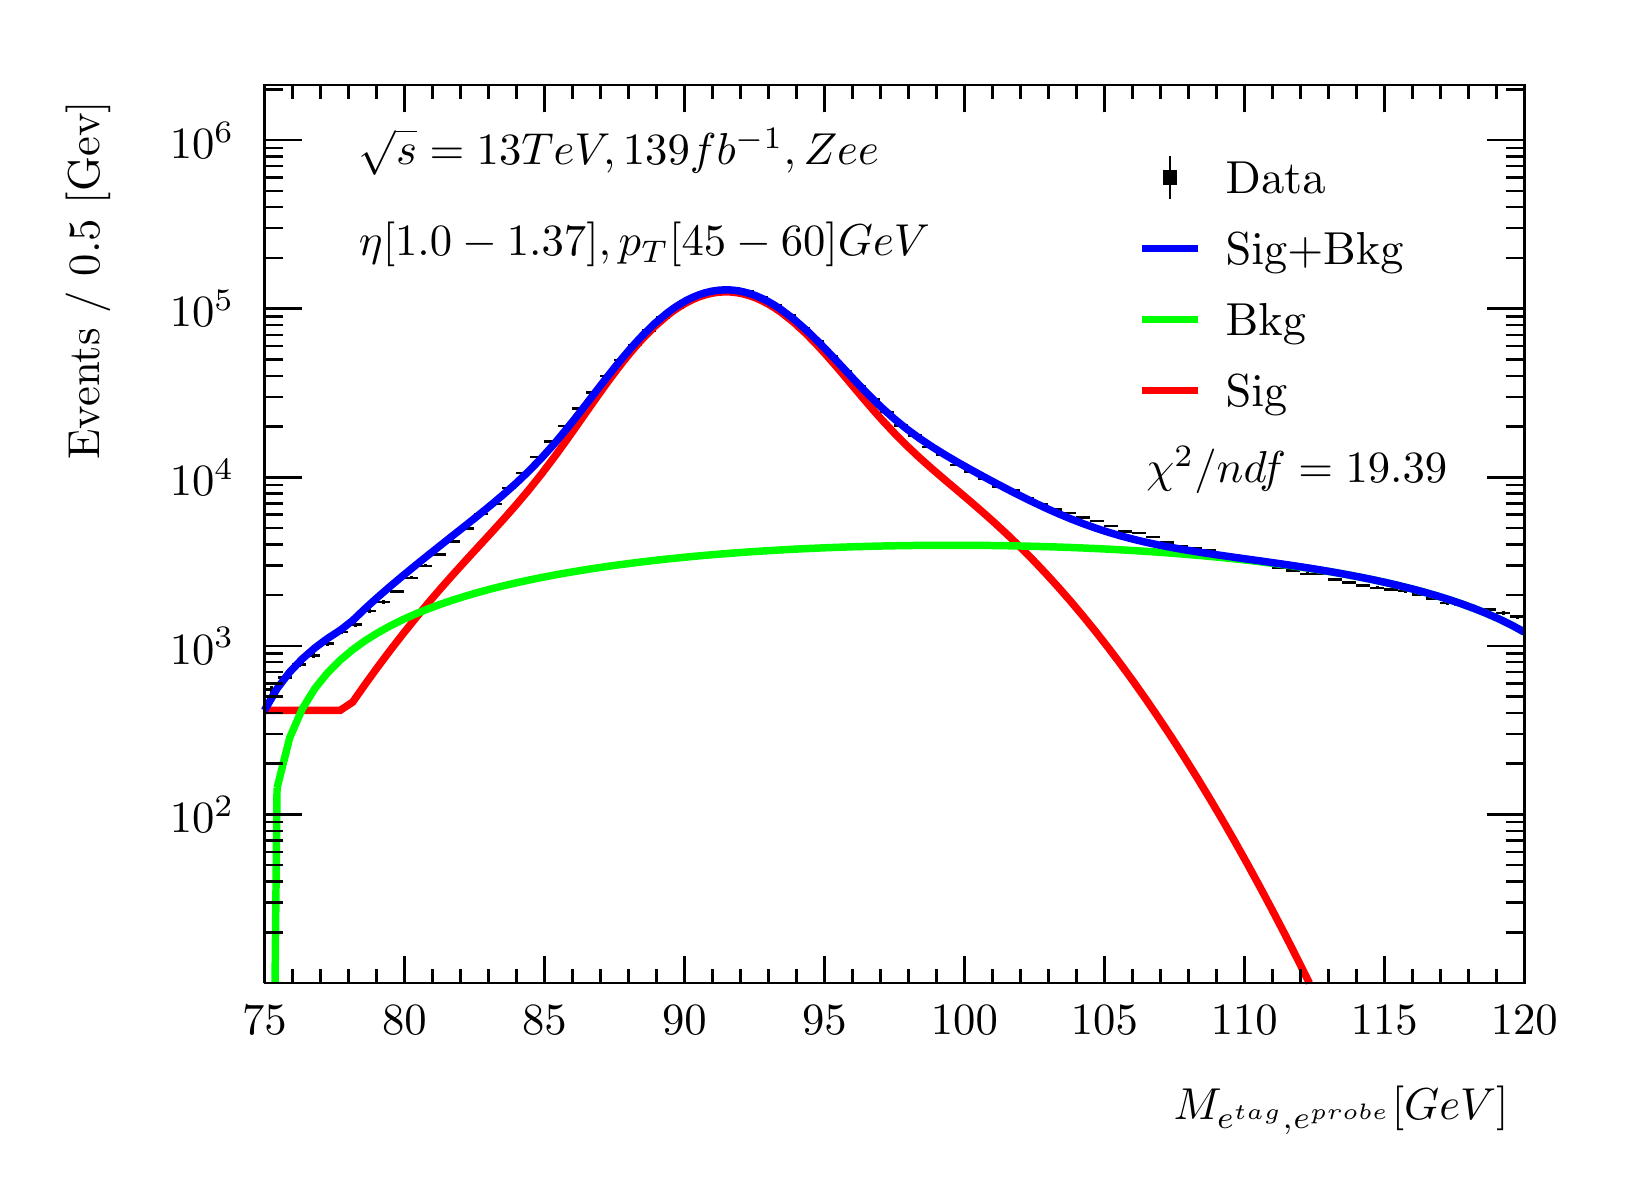
\begin{tikzpicture}
\pgfdeclareplotmark{cross} {
\pgfpathmoveto{\pgfpoint{-0.3\pgfplotmarksize}{\pgfplotmarksize}}
\pgfpathlineto{\pgfpoint{+0.3\pgfplotmarksize}{\pgfplotmarksize}}
\pgfpathlineto{\pgfpoint{+0.3\pgfplotmarksize}{0.3\pgfplotmarksize}}
\pgfpathlineto{\pgfpoint{+1\pgfplotmarksize}{0.3\pgfplotmarksize}}
\pgfpathlineto{\pgfpoint{+1\pgfplotmarksize}{-0.3\pgfplotmarksize}}
\pgfpathlineto{\pgfpoint{+0.3\pgfplotmarksize}{-0.3\pgfplotmarksize}}
\pgfpathlineto{\pgfpoint{+0.3\pgfplotmarksize}{-1.\pgfplotmarksize}}
\pgfpathlineto{\pgfpoint{-0.3\pgfplotmarksize}{-1.\pgfplotmarksize}}
\pgfpathlineto{\pgfpoint{-0.3\pgfplotmarksize}{-0.3\pgfplotmarksize}}
\pgfpathlineto{\pgfpoint{-1.\pgfplotmarksize}{-0.3\pgfplotmarksize}}
\pgfpathlineto{\pgfpoint{-1.\pgfplotmarksize}{0.3\pgfplotmarksize}}
\pgfpathlineto{\pgfpoint{-0.3\pgfplotmarksize}{0.3\pgfplotmarksize}}
\pgfpathclose
\pgfusepathqstroke
}
\pgfdeclareplotmark{cross*} {
\pgfpathmoveto{\pgfpoint{-0.3\pgfplotmarksize}{\pgfplotmarksize}}
\pgfpathlineto{\pgfpoint{+0.3\pgfplotmarksize}{\pgfplotmarksize}}
\pgfpathlineto{\pgfpoint{+0.3\pgfplotmarksize}{0.3\pgfplotmarksize}}
\pgfpathlineto{\pgfpoint{+1\pgfplotmarksize}{0.3\pgfplotmarksize}}
\pgfpathlineto{\pgfpoint{+1\pgfplotmarksize}{-0.3\pgfplotmarksize}}
\pgfpathlineto{\pgfpoint{+0.3\pgfplotmarksize}{-0.3\pgfplotmarksize}}
\pgfpathlineto{\pgfpoint{+0.3\pgfplotmarksize}{-1.\pgfplotmarksize}}
\pgfpathlineto{\pgfpoint{-0.3\pgfplotmarksize}{-1.\pgfplotmarksize}}
\pgfpathlineto{\pgfpoint{-0.3\pgfplotmarksize}{-0.3\pgfplotmarksize}}
\pgfpathlineto{\pgfpoint{-1.\pgfplotmarksize}{-0.3\pgfplotmarksize}}
\pgfpathlineto{\pgfpoint{-1.\pgfplotmarksize}{0.3\pgfplotmarksize}}
\pgfpathlineto{\pgfpoint{-0.3\pgfplotmarksize}{0.3\pgfplotmarksize}}
\pgfpathclose
\pgfusepathqfillstroke
}
\pgfdeclareplotmark{newstar} {
\pgfpathmoveto{\pgfqpoint{0pt}{\pgfplotmarksize}}
\pgfpathlineto{\pgfqpointpolar{44}{0.5\pgfplotmarksize}}
\pgfpathlineto{\pgfqpointpolar{18}{\pgfplotmarksize}}
\pgfpathlineto{\pgfqpointpolar{-20}{0.5\pgfplotmarksize}}
\pgfpathlineto{\pgfqpointpolar{-54}{\pgfplotmarksize}}
\pgfpathlineto{\pgfqpointpolar{-90}{0.5\pgfplotmarksize}}
\pgfpathlineto{\pgfqpointpolar{234}{\pgfplotmarksize}}
\pgfpathlineto{\pgfqpointpolar{198}{0.5\pgfplotmarksize}}
\pgfpathlineto{\pgfqpointpolar{162}{\pgfplotmarksize}}
\pgfpathlineto{\pgfqpointpolar{134}{0.5\pgfplotmarksize}}
\pgfpathclose
\pgfusepathqstroke
}
\pgfdeclareplotmark{newstar*} {
\pgfpathmoveto{\pgfqpoint{0pt}{\pgfplotmarksize}}
\pgfpathlineto{\pgfqpointpolar{44}{0.5\pgfplotmarksize}}
\pgfpathlineto{\pgfqpointpolar{18}{\pgfplotmarksize}}
\pgfpathlineto{\pgfqpointpolar{-20}{0.5\pgfplotmarksize}}
\pgfpathlineto{\pgfqpointpolar{-54}{\pgfplotmarksize}}
\pgfpathlineto{\pgfqpointpolar{-90}{0.5\pgfplotmarksize}}
\pgfpathlineto{\pgfqpointpolar{234}{\pgfplotmarksize}}
\pgfpathlineto{\pgfqpointpolar{198}{0.5\pgfplotmarksize}}
\pgfpathlineto{\pgfqpointpolar{162}{\pgfplotmarksize}}
\pgfpathlineto{\pgfqpointpolar{134}{0.5\pgfplotmarksize}}
\pgfpathclose
\pgfusepathqfillstroke
}
\definecolor{c}{rgb}{1,1,1};
\draw [color=c, fill=c] (0,0) rectangle (20,14.4361);
\draw [color=c, fill=c] (3,2.30977) rectangle (19,13.7143);
\definecolor{c}{rgb}{0,0,0};
\draw [c,line width=0.9] (3,2.30977) -- (3,13.7143) -- (19,13.7143) -- (19,2.30977) -- (3,2.30977);
\definecolor{c}{rgb}{1,1,1};
\draw [color=c, fill=c] (3,2.30977) rectangle (19,13.7143);
\definecolor{c}{rgb}{0,0,0};
\draw [c,line width=0.9] (3,2.30977) -- (3,13.7143) -- (19,13.7143) -- (19,2.30977) -- (3,2.30977);
\draw [c,line width=0.9] (3,2.30977) -- (19,2.30977);
\draw [c,line width=0.9] (3,2.65624) -- (3,2.30977);
\draw [c,line width=0.9] (3.35556,2.48301) -- (3.35556,2.30977);
\draw [c,line width=0.9] (3.71111,2.48301) -- (3.71111,2.30977);
\draw [c,line width=0.9] (4.06667,2.48301) -- (4.06667,2.30977);
\draw [c,line width=0.9] (4.42222,2.48301) -- (4.42222,2.30977);
\draw [c,line width=0.9] (4.77778,2.65624) -- (4.77778,2.30977);
\draw [c,line width=0.9] (5.13333,2.48301) -- (5.13333,2.30977);
\draw [c,line width=0.9] (5.48889,2.48301) -- (5.48889,2.30977);
\draw [c,line width=0.9] (5.84444,2.48301) -- (5.84444,2.30977);
\draw [c,line width=0.9] (6.2,2.48301) -- (6.2,2.30977);
\draw [c,line width=0.9] (6.55556,2.65624) -- (6.55556,2.30977);
\draw [c,line width=0.9] (6.91111,2.48301) -- (6.91111,2.30977);
\draw [c,line width=0.9] (7.26667,2.48301) -- (7.26667,2.30977);
\draw [c,line width=0.9] (7.62222,2.48301) -- (7.62222,2.30977);
\draw [c,line width=0.9] (7.97778,2.48301) -- (7.97778,2.30977);
\draw [c,line width=0.9] (8.33333,2.65624) -- (8.33333,2.30977);
\draw [c,line width=0.9] (8.68889,2.48301) -- (8.68889,2.30977);
\draw [c,line width=0.9] (9.04444,2.48301) -- (9.04444,2.30977);
\draw [c,line width=0.9] (9.4,2.48301) -- (9.4,2.30977);
\draw [c,line width=0.9] (9.75556,2.48301) -- (9.75556,2.30977);
\draw [c,line width=0.9] (10.1111,2.65624) -- (10.1111,2.30977);
\draw [c,line width=0.9] (10.4667,2.48301) -- (10.4667,2.30977);
\draw [c,line width=0.9] (10.8222,2.48301) -- (10.8222,2.30977);
\draw [c,line width=0.9] (11.1778,2.48301) -- (11.1778,2.30977);
\draw [c,line width=0.9] (11.5333,2.48301) -- (11.5333,2.30977);
\draw [c,line width=0.9] (11.8889,2.65624) -- (11.8889,2.30977);
\draw [c,line width=0.9] (12.2444,2.48301) -- (12.2444,2.30977);
\draw [c,line width=0.9] (12.6,2.48301) -- (12.6,2.30977);
\draw [c,line width=0.9] (12.9556,2.48301) -- (12.9556,2.30977);
\draw [c,line width=0.9] (13.3111,2.48301) -- (13.3111,2.30977);
\draw [c,line width=0.9] (13.6667,2.65624) -- (13.6667,2.30977);
\draw [c,line width=0.9] (14.0222,2.48301) -- (14.0222,2.30977);
\draw [c,line width=0.9] (14.3778,2.48301) -- (14.3778,2.30977);
\draw [c,line width=0.9] (14.7333,2.48301) -- (14.7333,2.30977);
\draw [c,line width=0.9] (15.0889,2.48301) -- (15.0889,2.30977);
\draw [c,line width=0.9] (15.4444,2.65624) -- (15.4444,2.30977);
\draw [c,line width=0.9] (15.8,2.48301) -- (15.8,2.30977);
\draw [c,line width=0.9] (16.1556,2.48301) -- (16.1556,2.30977);
\draw [c,line width=0.9] (16.5111,2.48301) -- (16.5111,2.30977);
\draw [c,line width=0.9] (16.8667,2.48301) -- (16.8667,2.30977);
\draw [c,line width=0.9] (17.2222,2.65624) -- (17.2222,2.30977);
\draw [c,line width=0.9] (17.5778,2.48301) -- (17.5778,2.30977);
\draw [c,line width=0.9] (17.9333,2.48301) -- (17.9333,2.30977);
\draw [c,line width=0.9] (18.2889,2.48301) -- (18.2889,2.30977);
\draw [c,line width=0.9] (18.6444,2.48301) -- (18.6444,2.30977);
\draw [c,line width=0.9] (19,2.65624) -- (19,2.30977);
\draw [c,line width=0.9] (19,2.65624) -- (19,2.30977);
\draw [anchor=base] (3,1.66015) node[scale=1.61424, color=c, rotate=0]{75};
\draw [anchor=base] (4.77778,1.66015) node[scale=1.61424, color=c, rotate=0]{80};
\draw [anchor=base] (6.55556,1.66015) node[scale=1.61424, color=c, rotate=0]{85};
\draw [anchor=base] (8.33333,1.66015) node[scale=1.61424, color=c, rotate=0]{90};
\draw [anchor=base] (10.1111,1.66015) node[scale=1.61424, color=c, rotate=0]{95};
\draw [anchor=base] (11.8889,1.66015) node[scale=1.61424, color=c, rotate=0]{100};
\draw [anchor=base] (13.6667,1.66015) node[scale=1.61424, color=c, rotate=0]{105};
\draw [anchor=base] (15.4444,1.66015) node[scale=1.61424, color=c, rotate=0]{110};
\draw [anchor=base] (17.2222,1.66015) node[scale=1.61424, color=c, rotate=0]{115};
\draw [anchor=base] (19,1.66015) node[scale=1.61424, color=c, rotate=0]{120};
\draw [anchor= east] (19,0.692932) node[scale=1.61424, color=c, rotate=0]{$M_{e^{tag}, e^{probe}}  [GeV]$};
\draw [c,line width=0.9] (3,13.7143) -- (19,13.7143);
\draw [c,line width=0.9] (3,13.3678) -- (3,13.7143);
\draw [c,line width=0.9] (3.35556,13.5411) -- (3.35556,13.7143);
\draw [c,line width=0.9] (3.71111,13.5411) -- (3.71111,13.7143);
\draw [c,line width=0.9] (4.06667,13.5411) -- (4.06667,13.7143);
\draw [c,line width=0.9] (4.42222,13.5411) -- (4.42222,13.7143);
\draw [c,line width=0.9] (4.77778,13.3678) -- (4.77778,13.7143);
\draw [c,line width=0.9] (5.13333,13.5411) -- (5.13333,13.7143);
\draw [c,line width=0.9] (5.48889,13.5411) -- (5.48889,13.7143);
\draw [c,line width=0.9] (5.84444,13.5411) -- (5.84444,13.7143);
\draw [c,line width=0.9] (6.2,13.5411) -- (6.2,13.7143);
\draw [c,line width=0.9] (6.55556,13.3678) -- (6.55556,13.7143);
\draw [c,line width=0.9] (6.91111,13.5411) -- (6.91111,13.7143);
\draw [c,line width=0.9] (7.26667,13.5411) -- (7.26667,13.7143);
\draw [c,line width=0.9] (7.62222,13.5411) -- (7.62222,13.7143);
\draw [c,line width=0.9] (7.97778,13.5411) -- (7.97778,13.7143);
\draw [c,line width=0.9] (8.33333,13.3678) -- (8.33333,13.7143);
\draw [c,line width=0.9] (8.68889,13.5411) -- (8.68889,13.7143);
\draw [c,line width=0.9] (9.04444,13.5411) -- (9.04444,13.7143);
\draw [c,line width=0.9] (9.4,13.5411) -- (9.4,13.7143);
\draw [c,line width=0.9] (9.75556,13.5411) -- (9.75556,13.7143);
\draw [c,line width=0.9] (10.1111,13.3678) -- (10.1111,13.7143);
\draw [c,line width=0.9] (10.4667,13.5411) -- (10.4667,13.7143);
\draw [c,line width=0.9] (10.8222,13.5411) -- (10.8222,13.7143);
\draw [c,line width=0.9] (11.1778,13.5411) -- (11.1778,13.7143);
\draw [c,line width=0.9] (11.5333,13.5411) -- (11.5333,13.7143);
\draw [c,line width=0.9] (11.8889,13.3678) -- (11.8889,13.7143);
\draw [c,line width=0.9] (12.2444,13.5411) -- (12.2444,13.7143);
\draw [c,line width=0.9] (12.6,13.5411) -- (12.6,13.7143);
\draw [c,line width=0.9] (12.9556,13.5411) -- (12.9556,13.7143);
\draw [c,line width=0.9] (13.3111,13.5411) -- (13.3111,13.7143);
\draw [c,line width=0.9] (13.6667,13.3678) -- (13.6667,13.7143);
\draw [c,line width=0.9] (14.0222,13.5411) -- (14.0222,13.7143);
\draw [c,line width=0.9] (14.3778,13.5411) -- (14.3778,13.7143);
\draw [c,line width=0.9] (14.7333,13.5411) -- (14.7333,13.7143);
\draw [c,line width=0.9] (15.0889,13.5411) -- (15.0889,13.7143);
\draw [c,line width=0.9] (15.4444,13.3678) -- (15.4444,13.7143);
\draw [c,line width=0.9] (15.8,13.5411) -- (15.8,13.7143);
\draw [c,line width=0.9] (16.1556,13.5411) -- (16.1556,13.7143);
\draw [c,line width=0.9] (16.5111,13.5411) -- (16.5111,13.7143);
\draw [c,line width=0.9] (16.8667,13.5411) -- (16.8667,13.7143);
\draw [c,line width=0.9] (17.2222,13.3678) -- (17.2222,13.7143);
\draw [c,line width=0.9] (17.5778,13.5411) -- (17.5778,13.7143);
\draw [c,line width=0.9] (17.9333,13.5411) -- (17.9333,13.7143);
\draw [c,line width=0.9] (18.2889,13.5411) -- (18.2889,13.7143);
\draw [c,line width=0.9] (18.6444,13.5411) -- (18.6444,13.7143);
\draw [c,line width=0.9] (19,13.3678) -- (19,13.7143);
\draw [c,line width=0.9] (19,13.3678) -- (19,13.7143);
\draw [c,line width=0.9] (3,2.30977) -- (3,13.7143);
\draw [c,line width=0.9] (3.237,2.95433) -- (3,2.95433);
\draw [c,line width=0.9] (3.237,3.33137) -- (3,3.33137);
\draw [c,line width=0.9] (3.237,3.59888) -- (3,3.59888);
\draw [c,line width=0.9] (3.237,3.80638) -- (3,3.80638);
\draw [c,line width=0.9] (3.237,3.97592) -- (3,3.97592);
\draw [c,line width=0.9] (3.237,4.11926) -- (3,4.11926);
\draw [c,line width=0.9] (3.237,4.24343) -- (3,4.24343);
\draw [c,line width=0.9] (3.237,4.35296) -- (3,4.35296);
\draw [c,line width=0.9] (3.474,4.45093) -- (3,4.45093);
\draw [anchor= east] (2.82,4.45093) node[scale=1.61424, color=c, rotate=0]{$10^{2}$};
\draw [c,line width=0.9] (3.237,5.09549) -- (3,5.09549);
\draw [c,line width=0.9] (3.237,5.47253) -- (3,5.47253);
\draw [c,line width=0.9] (3.237,5.74004) -- (3,5.74004);
\draw [c,line width=0.9] (3.237,5.94754) -- (3,5.94754);
\draw [c,line width=0.9] (3.237,6.11708) -- (3,6.11708);
\draw [c,line width=0.9] (3.237,6.26042) -- (3,6.26042);
\draw [c,line width=0.9] (3.237,6.38459) -- (3,6.38459);
\draw [c,line width=0.9] (3.237,6.49412) -- (3,6.49412);
\draw [c,line width=0.9] (3.474,6.59209) -- (3,6.59209);
\draw [anchor= east] (2.82,6.59209) node[scale=1.61424, color=c, rotate=0]{$10^{3}$};
\draw [c,line width=0.9] (3.237,7.23665) -- (3,7.23665);
\draw [c,line width=0.9] (3.237,7.61369) -- (3,7.61369);
\draw [c,line width=0.9] (3.237,7.8812) -- (3,7.8812);
\draw [c,line width=0.9] (3.237,8.0887) -- (3,8.0887);
\draw [c,line width=0.9] (3.237,8.25824) -- (3,8.25824);
\draw [c,line width=0.9] (3.237,8.40158) -- (3,8.40158);
\draw [c,line width=0.9] (3.237,8.52575) -- (3,8.52575);
\draw [c,line width=0.9] (3.237,8.63528) -- (3,8.63528);
\draw [c,line width=0.9] (3.474,8.73325) -- (3,8.73325);
\draw [anchor= east] (2.82,8.73325) node[scale=1.61424, color=c, rotate=0]{$10^{4}$};
\draw [c,line width=0.9] (3.237,9.37781) -- (3,9.37781);
\draw [c,line width=0.9] (3.237,9.75485) -- (3,9.75485);
\draw [c,line width=0.9] (3.237,10.0224) -- (3,10.0224);
\draw [c,line width=0.9] (3.237,10.2299) -- (3,10.2299);
\draw [c,line width=0.9] (3.237,10.3994) -- (3,10.3994);
\draw [c,line width=0.9] (3.237,10.5427) -- (3,10.5427);
\draw [c,line width=0.9] (3.237,10.6669) -- (3,10.6669);
\draw [c,line width=0.9] (3.237,10.7764) -- (3,10.7764);
\draw [c,line width=0.9] (3.474,10.8744) -- (3,10.8744);
\draw [anchor= east] (2.82,10.8744) node[scale=1.61424, color=c, rotate=0]{$10^{5}$};
\draw [c,line width=0.9] (3.237,11.519) -- (3,11.519);
\draw [c,line width=0.9] (3.237,11.896) -- (3,11.896);
\draw [c,line width=0.9] (3.237,12.1635) -- (3,12.1635);
\draw [c,line width=0.9] (3.237,12.371) -- (3,12.371);
\draw [c,line width=0.9] (3.237,12.5406) -- (3,12.5406);
\draw [c,line width=0.9] (3.237,12.6839) -- (3,12.6839);
\draw [c,line width=0.9] (3.237,12.8081) -- (3,12.8081);
\draw [c,line width=0.9] (3.237,12.9176) -- (3,12.9176);
\draw [c,line width=0.9] (3.474,13.0156) -- (3,13.0156);
\draw [anchor= east] (2.82,13.0156) node[scale=1.61424, color=c, rotate=0]{$10^{6}$};
\draw [c,line width=0.9] (3.237,13.6601) -- (3,13.6601);
\draw [anchor= east] (0.76,13.7143) node[scale=1.61424, color=c, rotate=90]{Events / 0.5 [Gev]};
\draw [c,line width=0.9] (19,2.30977) -- (19,13.7143);
\draw [c,line width=0.9] (18.763,2.95433) -- (19,2.95433);
\draw [c,line width=0.9] (18.763,3.33137) -- (19,3.33137);
\draw [c,line width=0.9] (18.763,3.59888) -- (19,3.59888);
\draw [c,line width=0.9] (18.763,3.80638) -- (19,3.80638);
\draw [c,line width=0.9] (18.763,3.97592) -- (19,3.97592);
\draw [c,line width=0.9] (18.763,4.11926) -- (19,4.11926);
\draw [c,line width=0.9] (18.763,4.24343) -- (19,4.24343);
\draw [c,line width=0.9] (18.763,4.35296) -- (19,4.35296);
\draw [c,line width=0.9] (18.526,4.45093) -- (19,4.45093);
\draw [c,line width=0.9] (18.763,5.09549) -- (19,5.09549);
\draw [c,line width=0.9] (18.763,5.47253) -- (19,5.47253);
\draw [c,line width=0.9] (18.763,5.74004) -- (19,5.74004);
\draw [c,line width=0.9] (18.763,5.94754) -- (19,5.94754);
\draw [c,line width=0.9] (18.763,6.11708) -- (19,6.11708);
\draw [c,line width=0.9] (18.763,6.26042) -- (19,6.26042);
\draw [c,line width=0.9] (18.763,6.38459) -- (19,6.38459);
\draw [c,line width=0.9] (18.763,6.49412) -- (19,6.49412);
\draw [c,line width=0.9] (18.526,6.59209) -- (19,6.59209);
\draw [c,line width=0.9] (18.763,7.23665) -- (19,7.23665);
\draw [c,line width=0.9] (18.763,7.61369) -- (19,7.61369);
\draw [c,line width=0.9] (18.763,7.8812) -- (19,7.8812);
\draw [c,line width=0.9] (18.763,8.0887) -- (19,8.0887);
\draw [c,line width=0.9] (18.763,8.25824) -- (19,8.25824);
\draw [c,line width=0.9] (18.763,8.40158) -- (19,8.40158);
\draw [c,line width=0.9] (18.763,8.52575) -- (19,8.52575);
\draw [c,line width=0.9] (18.763,8.63528) -- (19,8.63528);
\draw [c,line width=0.9] (18.526,8.73325) -- (19,8.73325);
\draw [c,line width=0.9] (18.763,9.37781) -- (19,9.37781);
\draw [c,line width=0.9] (18.763,9.75485) -- (19,9.75485);
\draw [c,line width=0.9] (18.763,10.0224) -- (19,10.0224);
\draw [c,line width=0.9] (18.763,10.2299) -- (19,10.2299);
\draw [c,line width=0.9] (18.763,10.3994) -- (19,10.3994);
\draw [c,line width=0.9] (18.763,10.5427) -- (19,10.5427);
\draw [c,line width=0.9] (18.763,10.6669) -- (19,10.6669);
\draw [c,line width=0.9] (18.763,10.7764) -- (19,10.7764);
\draw [c,line width=0.9] (18.526,10.8744) -- (19,10.8744);
\draw [c,line width=0.9] (18.763,11.519) -- (19,11.519);
\draw [c,line width=0.9] (18.763,11.896) -- (19,11.896);
\draw [c,line width=0.9] (18.763,12.1635) -- (19,12.1635);
\draw [c,line width=0.9] (18.763,12.371) -- (19,12.371);
\draw [c,line width=0.9] (18.763,12.5406) -- (19,12.5406);
\draw [c,line width=0.9] (18.763,12.6839) -- (19,12.6839);
\draw [c,line width=0.9] (18.763,12.8081) -- (19,12.8081);
\draw [c,line width=0.9] (18.763,12.9176) -- (19,12.9176);
\draw [c,line width=0.9] (18.526,13.0156) -- (19,13.0156);
\draw [c,line width=0.9] (18.763,13.6601) -- (19,13.6601);
\draw [c,line width=0.9] (3.08889,6.03786) -- (3,6.03786);
\draw [c,line width=0.9] (3,6.03786) -- (3,6.03786);
\draw [c,line width=0.9] (3.08889,6.03786) -- (3.17778,6.03786);
\draw [c,line width=0.9] (3.17778,6.03786) -- (3.17778,6.03786);
\draw [c,line width=0.9] (3.08889,6.03786) -- (3.08889,6.07747);
\draw [c,line width=0.9] (3.08889,6.07747) -- (3.08889,6.07747);
\draw [c,line width=0.9] (3.08889,6.03786) -- (3.08889,5.99825);
\draw [c,line width=0.9] (3.08889,5.99825) -- (3.08889,5.99825);
\draw [c,line width=0.9] (3.26667,6.19151) -- (3.17778,6.19151);
\draw [c,line width=0.9] (3.17778,6.19151) -- (3.17778,6.19151);
\draw [c,line width=0.9] (3.26667,6.19151) -- (3.35556,6.19151);
\draw [c,line width=0.9] (3.35556,6.19151) -- (3.35556,6.19151);
\draw [c,line width=0.9] (3.26667,6.19151) -- (3.26667,6.22798);
\draw [c,line width=0.9] (3.26667,6.22798) -- (3.26667,6.22798);
\draw [c,line width=0.9] (3.26667,6.19151) -- (3.26667,6.15504);
\draw [c,line width=0.9] (3.26667,6.15504) -- (3.26667,6.15504);
\draw [c,line width=0.9] (3.44444,6.35267) -- (3.35556,6.35267);
\draw [c,line width=0.9] (3.35556,6.35267) -- (3.35556,6.35267);
\draw [c,line width=0.9] (3.44444,6.35267) -- (3.53333,6.35267);
\draw [c,line width=0.9] (3.53333,6.35267) -- (3.53333,6.35267);
\draw [c,line width=0.9] (3.44444,6.35267) -- (3.44444,6.38611);
\draw [c,line width=0.9] (3.44444,6.38611) -- (3.44444,6.38611);
\draw [c,line width=0.9] (3.44444,6.35267) -- (3.44444,6.31922);
\draw [c,line width=0.9] (3.44444,6.31922) -- (3.44444,6.31922);
\draw [c,line width=0.9] (3.62222,6.47216) -- (3.53333,6.47216);
\draw [c,line width=0.9] (3.53333,6.47216) -- (3.53333,6.47216);
\draw [c,line width=0.9] (3.62222,6.47216) -- (3.71111,6.47216);
\draw [c,line width=0.9] (3.71111,6.47216) -- (3.71111,6.47216);
\draw [c,line width=0.9] (3.62222,6.47216) -- (3.62222,6.50353);
\draw [c,line width=0.9] (3.62222,6.50353) -- (3.62222,6.50353);
\draw [c,line width=0.9] (3.62222,6.47216) -- (3.62222,6.4408);
\draw [c,line width=0.9] (3.62222,6.4408) -- (3.62222,6.4408);
\draw [c,line width=0.9] (3.8,6.62408) -- (3.71111,6.62408);
\draw [c,line width=0.9] (3.71111,6.62408) -- (3.71111,6.62408);
\draw [c,line width=0.9] (3.8,6.62408) -- (3.88889,6.62408);
\draw [c,line width=0.9] (3.88889,6.62408) -- (3.88889,6.62408);
\draw [c,line width=0.9] (3.8,6.62408) -- (3.8,6.65299);
\draw [c,line width=0.9] (3.8,6.65299) -- (3.8,6.65299);
\draw [c,line width=0.9] (3.8,6.62408) -- (3.8,6.59518);
\draw [c,line width=0.9] (3.8,6.59518) -- (3.8,6.59518);
\draw [c,line width=0.9] (3.97778,6.76704) -- (3.88889,6.76704);
\draw [c,line width=0.9] (3.88889,6.76704) -- (3.88889,6.76704);
\draw [c,line width=0.9] (3.97778,6.76704) -- (4.06667,6.76704);
\draw [c,line width=0.9] (4.06667,6.76704) -- (4.06667,6.76704);
\draw [c,line width=0.9] (3.97778,6.76704) -- (3.97778,6.79381);
\draw [c,line width=0.9] (3.97778,6.79381) -- (3.97778,6.79381);
\draw [c,line width=0.9] (3.97778,6.76704) -- (3.97778,6.74028);
\draw [c,line width=0.9] (3.97778,6.74028) -- (3.97778,6.74028);
\draw [c,line width=0.9] (4.15556,6.86286) -- (4.06667,6.86286);
\draw [c,line width=0.9] (4.06667,6.86286) -- (4.06667,6.86286);
\draw [c,line width=0.9] (4.15556,6.86286) -- (4.24444,6.86286);
\draw [c,line width=0.9] (4.24444,6.86286) -- (4.24444,6.86286);
\draw [c,line width=0.9] (4.15556,6.86286) -- (4.15556,6.88828);
\draw [c,line width=0.9] (4.15556,6.88828) -- (4.15556,6.88828);
\draw [c,line width=0.9] (4.15556,6.86286) -- (4.15556,6.83744);
\draw [c,line width=0.9] (4.15556,6.83744) -- (4.15556,6.83744);
\draw [c,line width=0.9] (4.33333,7.03552) -- (4.24444,7.03552);
\draw [c,line width=0.9] (4.24444,7.03552) -- (4.24444,7.03552);
\draw [c,line width=0.9] (4.33333,7.03552) -- (4.42222,7.03552);
\draw [c,line width=0.9] (4.42222,7.03552) -- (4.42222,7.03552);
\draw [c,line width=0.9] (4.33333,7.03552) -- (4.33333,7.05869);
\draw [c,line width=0.9] (4.33333,7.05869) -- (4.33333,7.05869);
\draw [c,line width=0.9] (4.33333,7.03552) -- (4.33333,7.01235);
\draw [c,line width=0.9] (4.33333,7.01235) -- (4.33333,7.01235);
\draw [c,line width=0.9] (4.51111,7.15099) -- (4.42222,7.15099);
\draw [c,line width=0.9] (4.42222,7.15099) -- (4.42222,7.15099);
\draw [c,line width=0.9] (4.51111,7.15099) -- (4.6,7.15099);
\draw [c,line width=0.9] (4.6,7.15099) -- (4.6,7.15099);
\draw [c,line width=0.9] (4.51111,7.15099) -- (4.51111,7.17276);
\draw [c,line width=0.9] (4.51111,7.17276) -- (4.51111,7.17276);
\draw [c,line width=0.9] (4.51111,7.15099) -- (4.51111,7.12922);
\draw [c,line width=0.9] (4.51111,7.12922) -- (4.51111,7.12922);
\draw [c,line width=0.9] (4.68889,7.28202) -- (4.6,7.28202);
\draw [c,line width=0.9] (4.6,7.28202) -- (4.6,7.28202);
\draw [c,line width=0.9] (4.68889,7.28202) -- (4.77778,7.28202);
\draw [c,line width=0.9] (4.77778,7.28202) -- (4.77778,7.28202);
\draw [c,line width=0.9] (4.68889,7.28202) -- (4.68889,7.30231);
\draw [c,line width=0.9] (4.68889,7.30231) -- (4.68889,7.30231);
\draw [c,line width=0.9] (4.68889,7.28202) -- (4.68889,7.26172);
\draw [c,line width=0.9] (4.68889,7.26172) -- (4.68889,7.26172);
\draw [c,line width=0.9] (4.86667,7.45524) -- (4.77778,7.45524);
\draw [c,line width=0.9] (4.77778,7.45524) -- (4.77778,7.45524);
\draw [c,line width=0.9] (4.86667,7.45524) -- (4.95556,7.45524);
\draw [c,line width=0.9] (4.95556,7.45524) -- (4.95556,7.45524);
\draw [c,line width=0.9] (4.86667,7.45524) -- (4.86667,7.47373);
\draw [c,line width=0.9] (4.86667,7.47373) -- (4.86667,7.47373);
\draw [c,line width=0.9] (4.86667,7.45524) -- (4.86667,7.43675);
\draw [c,line width=0.9] (4.86667,7.43675) -- (4.86667,7.43675);
\draw [c,line width=0.9] (5.04444,7.60903) -- (4.95556,7.60903);
\draw [c,line width=0.9] (4.95556,7.60903) -- (4.95556,7.60903);
\draw [c,line width=0.9] (5.04444,7.60903) -- (5.13333,7.60903);
\draw [c,line width=0.9] (5.13333,7.60903) -- (5.13333,7.60903);
\draw [c,line width=0.9] (5.04444,7.60903) -- (5.04444,7.62605);
\draw [c,line width=0.9] (5.04444,7.62605) -- (5.04444,7.62605);
\draw [c,line width=0.9] (5.04444,7.60903) -- (5.04444,7.59201);
\draw [c,line width=0.9] (5.04444,7.59201) -- (5.04444,7.59201);
\draw [c,line width=0.9] (5.22222,7.7525) -- (5.13333,7.7525);
\draw [c,line width=0.9] (5.13333,7.7525) -- (5.13333,7.7525);
\draw [c,line width=0.9] (5.22222,7.7525) -- (5.31111,7.7525);
\draw [c,line width=0.9] (5.31111,7.7525) -- (5.31111,7.7525);
\draw [c,line width=0.9] (5.22222,7.7525) -- (5.22222,7.76826);
\draw [c,line width=0.9] (5.22222,7.76826) -- (5.22222,7.76826);
\draw [c,line width=0.9] (5.22222,7.7525) -- (5.22222,7.73675);
\draw [c,line width=0.9] (5.22222,7.73675) -- (5.22222,7.73675);
\draw [c,line width=0.9] (5.4,7.91856) -- (5.31111,7.91856);
\draw [c,line width=0.9] (5.31111,7.91856) -- (5.31111,7.91856);
\draw [c,line width=0.9] (5.4,7.91856) -- (5.48889,7.91856);
\draw [c,line width=0.9] (5.48889,7.91856) -- (5.48889,7.91856);
\draw [c,line width=0.9] (5.4,7.91856) -- (5.4,7.93298);
\draw [c,line width=0.9] (5.4,7.93298) -- (5.4,7.93298);
\draw [c,line width=0.9] (5.4,7.91856) -- (5.4,7.90415);
\draw [c,line width=0.9] (5.4,7.90415) -- (5.4,7.90415);
\draw [c,line width=0.9] (5.57778,8.08067) -- (5.48889,8.08067);
\draw [c,line width=0.9] (5.48889,8.08067) -- (5.48889,8.08067);
\draw [c,line width=0.9] (5.57778,8.08067) -- (5.66667,8.08067);
\draw [c,line width=0.9] (5.66667,8.08067) -- (5.66667,8.08067);
\draw [c,line width=0.9] (5.57778,8.08067) -- (5.57778,8.09388);
\draw [c,line width=0.9] (5.57778,8.09388) -- (5.57778,8.09388);
\draw [c,line width=0.9] (5.57778,8.08067) -- (5.57778,8.06746);
\draw [c,line width=0.9] (5.57778,8.06746) -- (5.57778,8.06746);
\draw [c,line width=0.9] (5.75556,8.26672) -- (5.66667,8.26672);
\draw [c,line width=0.9] (5.66667,8.26672) -- (5.66667,8.26672);
\draw [c,line width=0.9] (5.75556,8.26672) -- (5.84444,8.26672);
\draw [c,line width=0.9] (5.84444,8.26672) -- (5.84444,8.26672);
\draw [c,line width=0.9] (5.75556,8.26672) -- (5.75556,8.27868);
\draw [c,line width=0.9] (5.75556,8.27868) -- (5.75556,8.27868);
\draw [c,line width=0.9] (5.75556,8.26672) -- (5.75556,8.25478);
\draw [c,line width=0.9] (5.75556,8.25478) -- (5.75556,8.25478);
\draw [c,line width=0.9] (5.93333,8.39559) -- (5.84444,8.39559);
\draw [c,line width=0.9] (5.84444,8.39559) -- (5.84444,8.39559);
\draw [c,line width=0.9] (5.93333,8.39559) -- (6.02222,8.39559);
\draw [c,line width=0.9] (6.02222,8.39559) -- (6.02222,8.39559);
\draw [c,line width=0.9] (5.93333,8.39559) -- (5.93333,8.40674);
\draw [c,line width=0.9] (5.93333,8.40674) -- (5.93333,8.40674);
\draw [c,line width=0.9] (5.93333,8.39559) -- (5.93333,8.38444);
\draw [c,line width=0.9] (5.93333,8.38444) -- (5.93333,8.38444);
\draw [c,line width=0.9] (6.11111,8.59958) -- (6.02222,8.59958);
\draw [c,line width=0.9] (6.02222,8.59958) -- (6.02222,8.59958);
\draw [c,line width=0.9] (6.11111,8.59958) -- (6.2,8.59958);
\draw [c,line width=0.9] (6.2,8.59958) -- (6.2,8.59958);
\draw [c,line width=0.9] (6.11111,8.59958) -- (6.11111,8.60957);
\draw [c,line width=0.9] (6.11111,8.60957) -- (6.11111,8.60957);
\draw [c,line width=0.9] (6.11111,8.59958) -- (6.11111,8.58958);
\draw [c,line width=0.9] (6.11111,8.58958) -- (6.11111,8.58958);
\draw [c,line width=0.9] (6.28889,8.78831) -- (6.2,8.78831);
\draw [c,line width=0.9] (6.2,8.78831) -- (6.2,8.78831);
\draw [c,line width=0.9] (6.28889,8.78831) -- (6.37778,8.78831);
\draw [c,line width=0.9] (6.37778,8.78831) -- (6.37778,8.78831);
\draw [c,line width=0.9] (6.28889,8.78831) -- (6.28889,8.79734);
\draw [c,line width=0.9] (6.28889,8.79734) -- (6.28889,8.79734);
\draw [c,line width=0.9] (6.28889,8.78831) -- (6.28889,8.77929);
\draw [c,line width=0.9] (6.28889,8.77929) -- (6.28889,8.77929);
\draw [c,line width=0.9] (6.46667,8.99022) -- (6.37778,8.99022);
\draw [c,line width=0.9] (6.37778,8.99022) -- (6.37778,8.99022);
\draw [c,line width=0.9] (6.46667,8.99022) -- (6.55556,8.99022);
\draw [c,line width=0.9] (6.55556,8.99022) -- (6.55556,8.99022);
\draw [c,line width=0.9] (6.46667,8.99022) -- (6.46667,8.99832);
\draw [c,line width=0.9] (6.46667,8.99832) -- (6.46667,8.99832);
\draw [c,line width=0.9] (6.46667,8.99022) -- (6.46667,8.98212);
\draw [c,line width=0.9] (6.46667,8.98212) -- (6.46667,8.98212);
\draw [c,line width=0.9] (6.64444,9.18804) -- (6.55556,9.18804);
\draw [c,line width=0.9] (6.55556,9.18804) -- (6.55556,9.18804);
\draw [c,line width=0.9] (6.64444,9.18804) -- (6.73333,9.18804);
\draw [c,line width=0.9] (6.73333,9.18804) -- (6.73333,9.18804);
\draw [c,line width=0.9] (6.64444,9.18804) -- (6.64444,9.19532);
\draw [c,line width=0.9] (6.64444,9.19532) -- (6.64444,9.19532);
\draw [c,line width=0.9] (6.64444,9.18804) -- (6.64444,9.18076);
\draw [c,line width=0.9] (6.64444,9.18076) -- (6.64444,9.18076);
\draw [c,line width=0.9] (6.82222,9.38545) -- (6.73333,9.38545);
\draw [c,line width=0.9] (6.73333,9.38545) -- (6.73333,9.38545);
\draw [c,line width=0.9] (6.82222,9.38545) -- (6.91111,9.38545);
\draw [c,line width=0.9] (6.91111,9.38545) -- (6.91111,9.38545);
\draw [c,line width=0.9] (6.82222,9.38545) -- (6.82222,9.392);
\draw [c,line width=0.9] (6.82222,9.392) -- (6.82222,9.392);
\draw [c,line width=0.9] (6.82222,9.38545) -- (6.82222,9.3789);
\draw [c,line width=0.9] (6.82222,9.3789) -- (6.82222,9.3789);
\draw [c,line width=0.9] (7,9.60441) -- (6.91111,9.60441);
\draw [c,line width=0.9] (6.91111,9.60441) -- (6.91111,9.60441);
\draw [c,line width=0.9] (7,9.60441) -- (7.08889,9.60441);
\draw [c,line width=0.9] (7.08889,9.60441) -- (7.08889,9.60441);
\draw [c,line width=0.9] (7,9.60441) -- (7,9.61023);
\draw [c,line width=0.9] (7,9.61023) -- (7,9.61023);
\draw [c,line width=0.9] (7,9.60441) -- (7,9.59859);
\draw [c,line width=0.9] (7,9.59859) -- (7,9.59859);
\draw [c,line width=0.9] (7.17778,9.81131) -- (7.08889,9.81131);
\draw [c,line width=0.9] (7.08889,9.81131) -- (7.08889,9.81131);
\draw [c,line width=0.9] (7.17778,9.81131) -- (7.26667,9.81131);
\draw [c,line width=0.9] (7.26667,9.81131) -- (7.26667,9.81131);
\draw [c,line width=0.9] (7.17778,9.81131) -- (7.17778,9.81652);
\draw [c,line width=0.9] (7.17778,9.81652) -- (7.17778,9.81652);
\draw [c,line width=0.9] (7.17778,9.81131) -- (7.17778,9.8061);
\draw [c,line width=0.9] (7.17778,9.8061) -- (7.17778,9.8061);
\draw [c,line width=0.9] (7.35556,10.0188) -- (7.26667,10.0188);
\draw [c,line width=0.9] (7.26667,10.0188) -- (7.26667,10.0188);
\draw [c,line width=0.9] (7.35556,10.0188) -- (7.44444,10.0188);
\draw [c,line width=0.9] (7.44444,10.0188) -- (7.44444,10.0188);
\draw [c,line width=0.9] (7.35556,10.0188) -- (7.35556,10.0235);
\draw [c,line width=0.9] (7.35556,10.0235) -- (7.35556,10.0235);
\draw [c,line width=0.9] (7.35556,10.0188) -- (7.35556,10.0141);
\draw [c,line width=0.9] (7.35556,10.0141) -- (7.35556,10.0141);
\draw [c,line width=0.9] (7.53333,10.2222) -- (7.44444,10.2222);
\draw [c,line width=0.9] (7.44444,10.2222) -- (7.44444,10.2222);
\draw [c,line width=0.9] (7.53333,10.2222) -- (7.62222,10.2222);
\draw [c,line width=0.9] (7.62222,10.2222) -- (7.62222,10.2222);
\draw [c,line width=0.9] (7.53333,10.2222) -- (7.53333,10.2263);
\draw [c,line width=0.9] (7.53333,10.2263) -- (7.53333,10.2263);
\draw [c,line width=0.9] (7.53333,10.2222) -- (7.53333,10.218);
\draw [c,line width=0.9] (7.53333,10.218) -- (7.53333,10.218);
\draw [c,line width=0.9] (7.71111,10.4115) -- (7.62222,10.4115);
\draw [c,line width=0.9] (7.62222,10.4115) -- (7.62222,10.4115);
\draw [c,line width=0.9] (7.71111,10.4115) -- (7.8,10.4115);
\draw [c,line width=0.9] (7.8,10.4115) -- (7.8,10.4115);
\draw [c,line width=0.9] (7.71111,10.4115) -- (7.71111,10.4153);
\draw [c,line width=0.9] (7.71111,10.4153) -- (7.71111,10.4153);
\draw [c,line width=0.9] (7.71111,10.4115) -- (7.71111,10.4078);
\draw [c,line width=0.9] (7.71111,10.4078) -- (7.71111,10.4078);
\draw [c,line width=0.9] (7.88889,10.5993) -- (7.8,10.5993);
\draw [c,line width=0.9] (7.8,10.5993) -- (7.8,10.5993);
\draw [c,line width=0.9] (7.88889,10.5993) -- (7.97778,10.5993);
\draw [c,line width=0.9] (7.97778,10.5993) -- (7.97778,10.5993);
\draw [c,line width=0.9] (7.88889,10.5993) -- (7.88889,10.6027);
\draw [c,line width=0.9] (7.88889,10.6027) -- (7.88889,10.6027);
\draw [c,line width=0.9] (7.88889,10.5993) -- (7.88889,10.5958);
\draw [c,line width=0.9] (7.88889,10.5958) -- (7.88889,10.5958);
\draw [c,line width=0.9] (8.06667,10.7597) -- (7.97778,10.7597);
\draw [c,line width=0.9] (7.97778,10.7597) -- (7.97778,10.7597);
\draw [c,line width=0.9] (8.06667,10.7597) -- (8.15556,10.7597);
\draw [c,line width=0.9] (8.15556,10.7597) -- (8.15556,10.7597);
\draw [c,line width=0.9] (8.06667,10.7597) -- (8.06667,10.7629);
\draw [c,line width=0.9] (8.06667,10.7629) -- (8.06667,10.7629);
\draw [c,line width=0.9] (8.06667,10.7597) -- (8.06667,10.7566);
\draw [c,line width=0.9] (8.06667,10.7566) -- (8.06667,10.7566);
\draw [c,line width=0.9] (8.24444,10.8873) -- (8.15556,10.8873);
\draw [c,line width=0.9] (8.15556,10.8873) -- (8.15556,10.8873);
\draw [c,line width=0.9] (8.24444,10.8873) -- (8.33333,10.8873);
\draw [c,line width=0.9] (8.33333,10.8873) -- (8.33333,10.8873);
\draw [c,line width=0.9] (8.24444,10.8873) -- (8.24444,10.8902);
\draw [c,line width=0.9] (8.24444,10.8902) -- (8.24444,10.8902);
\draw [c,line width=0.9] (8.24444,10.8873) -- (8.24444,10.8843);
\draw [c,line width=0.9] (8.24444,10.8843) -- (8.24444,10.8843);
\draw [c,line width=0.9] (8.42222,11.0052) -- (8.33333,11.0052);
\draw [c,line width=0.9] (8.33333,11.0052) -- (8.33333,11.0052);
\draw [c,line width=0.9] (8.42222,11.0052) -- (8.51111,11.0052);
\draw [c,line width=0.9] (8.51111,11.0052) -- (8.51111,11.0052);
\draw [c,line width=0.9] (8.42222,11.0052) -- (8.42222,11.008);
\draw [c,line width=0.9] (8.42222,11.008) -- (8.42222,11.008);
\draw [c,line width=0.9] (8.42222,11.0052) -- (8.42222,11.0025);
\draw [c,line width=0.9] (8.42222,11.0025) -- (8.42222,11.0025);
\draw [c,line width=0.9] (8.6,11.0822) -- (8.51111,11.0822);
\draw [c,line width=0.9] (8.51111,11.0822) -- (8.51111,11.0822);
\draw [c,line width=0.9] (8.6,11.0822) -- (8.68889,11.0822);
\draw [c,line width=0.9] (8.68889,11.0822) -- (8.68889,11.0822);
\draw [c,line width=0.9] (8.6,11.0822) -- (8.6,11.0849);
\draw [c,line width=0.9] (8.6,11.0849) -- (8.6,11.0849);
\draw [c,line width=0.9] (8.6,11.0822) -- (8.6,11.0796);
\draw [c,line width=0.9] (8.6,11.0796) -- (8.6,11.0796);
\draw [c,line width=0.9] (8.77778,11.1221) -- (8.68889,11.1221);
\draw [c,line width=0.9] (8.68889,11.1221) -- (8.68889,11.1221);
\draw [c,line width=0.9] (8.77778,11.1221) -- (8.86667,11.1221);
\draw [c,line width=0.9] (8.86667,11.1221) -- (8.86667,11.1221);
\draw [c,line width=0.9] (8.77778,11.1221) -- (8.77778,11.1247);
\draw [c,line width=0.9] (8.77778,11.1247) -- (8.77778,11.1247);
\draw [c,line width=0.9] (8.77778,11.1221) -- (8.77778,11.1195);
\draw [c,line width=0.9] (8.77778,11.1195) -- (8.77778,11.1195);
\draw [c,line width=0.9] (8.95556,11.1288) -- (8.86667,11.1288);
\draw [c,line width=0.9] (8.86667,11.1288) -- (8.86667,11.1288);
\draw [c,line width=0.9] (8.95556,11.1288) -- (9.04444,11.1288);
\draw [c,line width=0.9] (9.04444,11.1288) -- (9.04444,11.1288);
\draw [c,line width=0.9] (8.95556,11.1288) -- (8.95556,11.1313);
\draw [c,line width=0.9] (8.95556,11.1313) -- (8.95556,11.1313);
\draw [c,line width=0.9] (8.95556,11.1288) -- (8.95556,11.1262);
\draw [c,line width=0.9] (8.95556,11.1262) -- (8.95556,11.1262);
\draw [c,line width=0.9] (9.13333,11.0917) -- (9.04444,11.0917);
\draw [c,line width=0.9] (9.04444,11.0917) -- (9.04444,11.0917);
\draw [c,line width=0.9] (9.13333,11.0917) -- (9.22222,11.0917);
\draw [c,line width=0.9] (9.22222,11.0917) -- (9.22222,11.0917);
\draw [c,line width=0.9] (9.13333,11.0917) -- (9.13333,11.0943);
\draw [c,line width=0.9] (9.13333,11.0943) -- (9.13333,11.0943);
\draw [c,line width=0.9] (9.13333,11.0917) -- (9.13333,11.0891);
\draw [c,line width=0.9] (9.13333,11.0891) -- (9.13333,11.0891);
\draw [c,line width=0.9] (9.31111,11.0159) -- (9.22222,11.0159);
\draw [c,line width=0.9] (9.22222,11.0159) -- (9.22222,11.0159);
\draw [c,line width=0.9] (9.31111,11.0159) -- (9.4,11.0159);
\draw [c,line width=0.9] (9.4,11.0159) -- (9.4,11.0159);
\draw [c,line width=0.9] (9.31111,11.0159) -- (9.31111,11.0186);
\draw [c,line width=0.9] (9.31111,11.0186) -- (9.31111,11.0186);
\draw [c,line width=0.9] (9.31111,11.0159) -- (9.31111,11.0131);
\draw [c,line width=0.9] (9.31111,11.0131) -- (9.31111,11.0131);
\draw [c,line width=0.9] (9.48889,10.9127) -- (9.4,10.9127);
\draw [c,line width=0.9] (9.4,10.9127) -- (9.4,10.9127);
\draw [c,line width=0.9] (9.48889,10.9127) -- (9.57778,10.9127);
\draw [c,line width=0.9] (9.57778,10.9127) -- (9.57778,10.9127);
\draw [c,line width=0.9] (9.48889,10.9127) -- (9.48889,10.9156);
\draw [c,line width=0.9] (9.48889,10.9156) -- (9.48889,10.9156);
\draw [c,line width=0.9] (9.48889,10.9127) -- (9.48889,10.9098);
\draw [c,line width=0.9] (9.48889,10.9098) -- (9.48889,10.9098);
\draw [c,line width=0.9] (9.66667,10.7886) -- (9.57778,10.7886);
\draw [c,line width=0.9] (9.57778,10.7886) -- (9.57778,10.7886);
\draw [c,line width=0.9] (9.66667,10.7886) -- (9.75556,10.7886);
\draw [c,line width=0.9] (9.75556,10.7886) -- (9.75556,10.7886);
\draw [c,line width=0.9] (9.66667,10.7886) -- (9.66667,10.7917);
\draw [c,line width=0.9] (9.66667,10.7917) -- (9.66667,10.7917);
\draw [c,line width=0.9] (9.66667,10.7886) -- (9.66667,10.7855);
\draw [c,line width=0.9] (9.66667,10.7855) -- (9.66667,10.7855);
\draw [c,line width=0.9] (9.84444,10.6195) -- (9.75556,10.6195);
\draw [c,line width=0.9] (9.75556,10.6195) -- (9.75556,10.6195);
\draw [c,line width=0.9] (9.84444,10.6195) -- (9.93333,10.6195);
\draw [c,line width=0.9] (9.93333,10.6195) -- (9.93333,10.6195);
\draw [c,line width=0.9] (9.84444,10.6195) -- (9.84444,10.6229);
\draw [c,line width=0.9] (9.84444,10.6229) -- (9.84444,10.6229);
\draw [c,line width=0.9] (9.84444,10.6195) -- (9.84444,10.6161);
\draw [c,line width=0.9] (9.84444,10.6161) -- (9.84444,10.6161);
\draw [c,line width=0.9] (10.0222,10.4579) -- (9.93333,10.4579);
\draw [c,line width=0.9] (9.93333,10.4579) -- (9.93333,10.4579);
\draw [c,line width=0.9] (10.0222,10.4579) -- (10.1111,10.4579);
\draw [c,line width=0.9] (10.1111,10.4579) -- (10.1111,10.4579);
\draw [c,line width=0.9] (10.0222,10.4579) -- (10.0222,10.4616);
\draw [c,line width=0.9] (10.0222,10.4616) -- (10.0222,10.4616);
\draw [c,line width=0.9] (10.0222,10.4579) -- (10.0222,10.4542);
\draw [c,line width=0.9] (10.0222,10.4542) -- (10.0222,10.4542);
\draw [c,line width=0.9] (10.2,10.2673) -- (10.1111,10.2673);
\draw [c,line width=0.9] (10.1111,10.2673) -- (10.1111,10.2673);
\draw [c,line width=0.9] (10.2,10.2673) -- (10.2889,10.2673);
\draw [c,line width=0.9] (10.2889,10.2673) -- (10.2889,10.2673);
\draw [c,line width=0.9] (10.2,10.2673) -- (10.2,10.2714);
\draw [c,line width=0.9] (10.2,10.2714) -- (10.2,10.2714);
\draw [c,line width=0.9] (10.2,10.2673) -- (10.2,10.2632);
\draw [c,line width=0.9] (10.2,10.2632) -- (10.2,10.2632);
\draw [c,line width=0.9] (10.3778,10.0809) -- (10.2889,10.0809);
\draw [c,line width=0.9] (10.2889,10.0809) -- (10.2889,10.0809);
\draw [c,line width=0.9] (10.3778,10.0809) -- (10.4667,10.0809);
\draw [c,line width=0.9] (10.4667,10.0809) -- (10.4667,10.0809);
\draw [c,line width=0.9] (10.3778,10.0809) -- (10.3778,10.0854);
\draw [c,line width=0.9] (10.3778,10.0854) -- (10.3778,10.0854);
\draw [c,line width=0.9] (10.3778,10.0809) -- (10.3778,10.0764);
\draw [c,line width=0.9] (10.3778,10.0764) -- (10.3778,10.0764);
\draw [c,line width=0.9] (10.5556,9.89297) -- (10.4667,9.89297);
\draw [c,line width=0.9] (10.4667,9.89297) -- (10.4667,9.89297);
\draw [c,line width=0.9] (10.5556,9.89297) -- (10.6444,9.89297);
\draw [c,line width=0.9] (10.6444,9.89297) -- (10.6444,9.89297);
\draw [c,line width=0.9] (10.5556,9.89297) -- (10.5556,9.89795);
\draw [c,line width=0.9] (10.5556,9.89795) -- (10.5556,9.89795);
\draw [c,line width=0.9] (10.5556,9.89297) -- (10.5556,9.88798);
\draw [c,line width=0.9] (10.5556,9.88798) -- (10.5556,9.88798);
\draw [c,line width=0.9] (10.7333,9.72017) -- (10.6444,9.72017);
\draw [c,line width=0.9] (10.6444,9.72017) -- (10.6444,9.72017);
\draw [c,line width=0.9] (10.7333,9.72017) -- (10.8222,9.72017);
\draw [c,line width=0.9] (10.8222,9.72017) -- (10.8222,9.72017);
\draw [c,line width=0.9] (10.7333,9.72017) -- (10.7333,9.72564);
\draw [c,line width=0.9] (10.7333,9.72564) -- (10.7333,9.72564);
\draw [c,line width=0.9] (10.7333,9.72017) -- (10.7333,9.7147);
\draw [c,line width=0.9] (10.7333,9.7147) -- (10.7333,9.7147);
\draw [c,line width=0.9] (10.9111,9.55989) -- (10.8222,9.55989);
\draw [c,line width=0.9] (10.8222,9.55989) -- (10.8222,9.55989);
\draw [c,line width=0.9] (10.9111,9.55989) -- (11,9.55989);
\draw [c,line width=0.9] (11,9.55989) -- (11,9.55989);
\draw [c,line width=0.9] (10.9111,9.55989) -- (10.9111,9.56585);
\draw [c,line width=0.9] (10.9111,9.56585) -- (10.9111,9.56585);
\draw [c,line width=0.9] (10.9111,9.55989) -- (10.9111,9.55393);
\draw [c,line width=0.9] (10.9111,9.55393) -- (10.9111,9.55393);
\draw [c,line width=0.9] (11.0889,9.38784) -- (11,9.38784);
\draw [c,line width=0.9] (11,9.38784) -- (11,9.38784);
\draw [c,line width=0.9] (11.0889,9.38784) -- (11.1778,9.38784);
\draw [c,line width=0.9] (11.1778,9.38784) -- (11.1778,9.38784);
\draw [c,line width=0.9] (11.0889,9.38784) -- (11.0889,9.39438);
\draw [c,line width=0.9] (11.0889,9.39438) -- (11.0889,9.39438);
\draw [c,line width=0.9] (11.0889,9.38784) -- (11.0889,9.3813);
\draw [c,line width=0.9] (11.0889,9.3813) -- (11.0889,9.3813);
\draw [c,line width=0.9] (11.2667,9.26078) -- (11.1778,9.26078);
\draw [c,line width=0.9] (11.1778,9.26078) -- (11.1778,9.26078);
\draw [c,line width=0.9] (11.2667,9.26078) -- (11.3556,9.26078);
\draw [c,line width=0.9] (11.3556,9.26078) -- (11.3556,9.26078);
\draw [c,line width=0.9] (11.2667,9.26078) -- (11.2667,9.26779);
\draw [c,line width=0.9] (11.2667,9.26779) -- (11.2667,9.26779);
\draw [c,line width=0.9] (11.2667,9.26078) -- (11.2667,9.25378);
\draw [c,line width=0.9] (11.2667,9.25378) -- (11.2667,9.25378);
\draw [c,line width=0.9] (11.4444,9.11783) -- (11.3556,9.11783);
\draw [c,line width=0.9] (11.3556,9.11783) -- (11.3556,9.11783);
\draw [c,line width=0.9] (11.4444,9.11783) -- (11.5333,9.11783);
\draw [c,line width=0.9] (11.5333,9.11783) -- (11.5333,9.11783);
\draw [c,line width=0.9] (11.4444,9.11783) -- (11.4444,9.12539);
\draw [c,line width=0.9] (11.4444,9.12539) -- (11.4444,9.12539);
\draw [c,line width=0.9] (11.4444,9.11783) -- (11.4444,9.11026);
\draw [c,line width=0.9] (11.4444,9.11026) -- (11.4444,9.11026);
\draw [c,line width=0.9] (11.6222,9.01665) -- (11.5333,9.01665);
\draw [c,line width=0.9] (11.5333,9.01665) -- (11.5333,9.01665);
\draw [c,line width=0.9] (11.6222,9.01665) -- (11.7111,9.01665);
\draw [c,line width=0.9] (11.7111,9.01665) -- (11.7111,9.01665);
\draw [c,line width=0.9] (11.6222,9.01665) -- (11.6222,9.02463);
\draw [c,line width=0.9] (11.6222,9.02463) -- (11.6222,9.02463);
\draw [c,line width=0.9] (11.6222,9.01665) -- (11.6222,9.00866);
\draw [c,line width=0.9] (11.6222,9.00866) -- (11.6222,9.00866);
\draw [c,line width=0.9] (11.8,8.89047) -- (11.7111,8.89047);
\draw [c,line width=0.9] (11.7111,8.89047) -- (11.7111,8.89047);
\draw [c,line width=0.9] (11.8,8.89047) -- (11.8889,8.89047);
\draw [c,line width=0.9] (11.8889,8.89047) -- (11.8889,8.89047);
\draw [c,line width=0.9] (11.8,8.89047) -- (11.8,8.89901);
\draw [c,line width=0.9] (11.8,8.89901) -- (11.8,8.89901);
\draw [c,line width=0.9] (11.8,8.89047) -- (11.8,8.88192);
\draw [c,line width=0.9] (11.8,8.88192) -- (11.8,8.88192);
\draw [c,line width=0.9] (11.9778,8.80447) -- (11.8889,8.80447);
\draw [c,line width=0.9] (11.8889,8.80447) -- (11.8889,8.80447);
\draw [c,line width=0.9] (11.9778,8.80447) -- (12.0667,8.80447);
\draw [c,line width=0.9] (12.0667,8.80447) -- (12.0667,8.80447);
\draw [c,line width=0.9] (11.9778,8.80447) -- (11.9778,8.81342);
\draw [c,line width=0.9] (11.9778,8.81342) -- (11.9778,8.81342);
\draw [c,line width=0.9] (11.9778,8.80447) -- (11.9778,8.79552);
\draw [c,line width=0.9] (11.9778,8.79552) -- (11.9778,8.79552);
\draw [c,line width=0.9] (12.1556,8.71323) -- (12.0667,8.71323);
\draw [c,line width=0.9] (12.0667,8.71323) -- (12.0667,8.71323);
\draw [c,line width=0.9] (12.1556,8.71323) -- (12.2444,8.71323);
\draw [c,line width=0.9] (12.2444,8.71323) -- (12.2444,8.71323);
\draw [c,line width=0.9] (12.1556,8.71323) -- (12.1556,8.72263);
\draw [c,line width=0.9] (12.1556,8.72263) -- (12.1556,8.72263);
\draw [c,line width=0.9] (12.1556,8.71323) -- (12.1556,8.70383);
\draw [c,line width=0.9] (12.1556,8.70383) -- (12.1556,8.70383);
\draw [c,line width=0.9] (12.3333,8.61575) -- (12.2444,8.61575);
\draw [c,line width=0.9] (12.2444,8.61575) -- (12.2444,8.61575);
\draw [c,line width=0.9] (12.3333,8.61575) -- (12.4222,8.61575);
\draw [c,line width=0.9] (12.4222,8.61575) -- (12.4222,8.61575);
\draw [c,line width=0.9] (12.3333,8.61575) -- (12.3333,8.62566);
\draw [c,line width=0.9] (12.3333,8.62566) -- (12.3333,8.62566);
\draw [c,line width=0.9] (12.3333,8.61575) -- (12.3333,8.60585);
\draw [c,line width=0.9] (12.3333,8.60585) -- (12.3333,8.60585);
\draw [c,line width=0.9] (12.5111,8.56557) -- (12.4222,8.56557);
\draw [c,line width=0.9] (12.4222,8.56557) -- (12.4222,8.56557);
\draw [c,line width=0.9] (12.5111,8.56557) -- (12.6,8.56557);
\draw [c,line width=0.9] (12.6,8.56557) -- (12.6,8.56557);
\draw [c,line width=0.9] (12.5111,8.56557) -- (12.5111,8.57575);
\draw [c,line width=0.9] (12.5111,8.57575) -- (12.5111,8.57575);
\draw [c,line width=0.9] (12.5111,8.56557) -- (12.5111,8.5554);
\draw [c,line width=0.9] (12.5111,8.5554) -- (12.5111,8.5554);
\draw [c,line width=0.9] (12.6889,8.46301) -- (12.6,8.46301);
\draw [c,line width=0.9] (12.6,8.46301) -- (12.6,8.46301);
\draw [c,line width=0.9] (12.6889,8.46301) -- (12.7778,8.46301);
\draw [c,line width=0.9] (12.7778,8.46301) -- (12.7778,8.46301);
\draw [c,line width=0.9] (12.6889,8.46301) -- (12.6889,8.47376);
\draw [c,line width=0.9] (12.6889,8.47376) -- (12.6889,8.47376);
\draw [c,line width=0.9] (12.6889,8.46301) -- (12.6889,8.45225);
\draw [c,line width=0.9] (12.6889,8.45225) -- (12.6889,8.45225);
\draw [c,line width=0.9] (12.8667,8.38766) -- (12.7778,8.38766);
\draw [c,line width=0.9] (12.7778,8.38766) -- (12.7778,8.38766);
\draw [c,line width=0.9] (12.8667,8.38766) -- (12.9556,8.38766);
\draw [c,line width=0.9] (12.9556,8.38766) -- (12.9556,8.38766);
\draw [c,line width=0.9] (12.8667,8.38766) -- (12.8667,8.39886);
\draw [c,line width=0.9] (12.8667,8.39886) -- (12.8667,8.39886);
\draw [c,line width=0.9] (12.8667,8.38766) -- (12.8667,8.37647);
\draw [c,line width=0.9] (12.8667,8.37647) -- (12.8667,8.37647);
\draw [c,line width=0.9] (13.0444,8.32087) -- (12.9556,8.32087);
\draw [c,line width=0.9] (12.9556,8.32087) -- (12.9556,8.32087);
\draw [c,line width=0.9] (13.0444,8.32087) -- (13.1333,8.32087);
\draw [c,line width=0.9] (13.1333,8.32087) -- (13.1333,8.32087);
\draw [c,line width=0.9] (13.0444,8.32087) -- (13.0444,8.33247);
\draw [c,line width=0.9] (13.0444,8.33247) -- (13.0444,8.33247);
\draw [c,line width=0.9] (13.0444,8.32087) -- (13.0444,8.30926);
\draw [c,line width=0.9] (13.0444,8.30926) -- (13.0444,8.30926);
\draw [c,line width=0.9] (13.2222,8.2762) -- (13.1333,8.2762);
\draw [c,line width=0.9] (13.1333,8.2762) -- (13.1333,8.2762);
\draw [c,line width=0.9] (13.2222,8.2762) -- (13.3111,8.2762);
\draw [c,line width=0.9] (13.3111,8.2762) -- (13.3111,8.2762);
\draw [c,line width=0.9] (13.2222,8.2762) -- (13.2222,8.28809);
\draw [c,line width=0.9] (13.2222,8.28809) -- (13.2222,8.28809);
\draw [c,line width=0.9] (13.2222,8.2762) -- (13.2222,8.26431);
\draw [c,line width=0.9] (13.2222,8.26431) -- (13.2222,8.26431);
\draw [c,line width=0.9] (13.4,8.2198) -- (13.3111,8.2198);
\draw [c,line width=0.9] (13.3111,8.2198) -- (13.3111,8.2198);
\draw [c,line width=0.9] (13.4,8.2198) -- (13.4889,8.2198);
\draw [c,line width=0.9] (13.4889,8.2198) -- (13.4889,8.2198);
\draw [c,line width=0.9] (13.4,8.2198) -- (13.4,8.23205);
\draw [c,line width=0.9] (13.4,8.23205) -- (13.4,8.23205);
\draw [c,line width=0.9] (13.4,8.2198) -- (13.4,8.20754);
\draw [c,line width=0.9] (13.4,8.20754) -- (13.4,8.20754);
\draw [c,line width=0.9] (13.5778,8.1753) -- (13.4889,8.1753);
\draw [c,line width=0.9] (13.4889,8.1753) -- (13.4889,8.1753);
\draw [c,line width=0.9] (13.5778,8.1753) -- (13.6667,8.1753);
\draw [c,line width=0.9] (13.6667,8.1753) -- (13.6667,8.1753);
\draw [c,line width=0.9] (13.5778,8.1753) -- (13.5778,8.18785);
\draw [c,line width=0.9] (13.5778,8.18785) -- (13.5778,8.18785);
\draw [c,line width=0.9] (13.5778,8.1753) -- (13.5778,8.16274);
\draw [c,line width=0.9] (13.5778,8.16274) -- (13.5778,8.16274);
\draw [c,line width=0.9] (13.7556,8.11456) -- (13.6667,8.11456);
\draw [c,line width=0.9] (13.6667,8.11456) -- (13.6667,8.11456);
\draw [c,line width=0.9] (13.7556,8.11456) -- (13.8444,8.11456);
\draw [c,line width=0.9] (13.8444,8.11456) -- (13.8444,8.11456);
\draw [c,line width=0.9] (13.7556,8.11456) -- (13.7556,8.12753);
\draw [c,line width=0.9] (13.7556,8.12753) -- (13.7556,8.12753);
\draw [c,line width=0.9] (13.7556,8.11456) -- (13.7556,8.10159);
\draw [c,line width=0.9] (13.7556,8.10159) -- (13.7556,8.10159);
\draw [c,line width=0.9] (13.9333,8.04666) -- (13.8444,8.04666);
\draw [c,line width=0.9] (13.8444,8.04666) -- (13.8444,8.04666);
\draw [c,line width=0.9] (13.9333,8.04666) -- (14.0222,8.04666);
\draw [c,line width=0.9] (14.0222,8.04666) -- (14.0222,8.04666);
\draw [c,line width=0.9] (13.9333,8.04666) -- (13.9333,8.06011);
\draw [c,line width=0.9] (13.9333,8.06011) -- (13.9333,8.06011);
\draw [c,line width=0.9] (13.9333,8.04666) -- (13.9333,8.03321);
\draw [c,line width=0.9] (13.9333,8.03321) -- (13.9333,8.03321);
\draw [c,line width=0.9] (14.1111,8.02361) -- (14.0222,8.02361);
\draw [c,line width=0.9] (14.0222,8.02361) -- (14.0222,8.02361);
\draw [c,line width=0.9] (14.1111,8.02361) -- (14.2,8.02361);
\draw [c,line width=0.9] (14.2,8.02361) -- (14.2,8.02361);
\draw [c,line width=0.9] (14.1111,8.02361) -- (14.1111,8.03723);
\draw [c,line width=0.9] (14.1111,8.03723) -- (14.1111,8.03723);
\draw [c,line width=0.9] (14.1111,8.02361) -- (14.1111,8.00999);
\draw [c,line width=0.9] (14.1111,8.00999) -- (14.1111,8.00999);
\draw [c,line width=0.9] (14.2889,7.97468) -- (14.2,7.97468);
\draw [c,line width=0.9] (14.2,7.97468) -- (14.2,7.97468);
\draw [c,line width=0.9] (14.2889,7.97468) -- (14.3778,7.97468);
\draw [c,line width=0.9] (14.3778,7.97468) -- (14.3778,7.97468);
\draw [c,line width=0.9] (14.2889,7.97468) -- (14.2889,7.98866);
\draw [c,line width=0.9] (14.2889,7.98866) -- (14.2889,7.98866);
\draw [c,line width=0.9] (14.2889,7.97468) -- (14.2889,7.96069);
\draw [c,line width=0.9] (14.2889,7.96069) -- (14.2889,7.96069);
\draw [c,line width=0.9] (14.4667,7.90212) -- (14.3778,7.90212);
\draw [c,line width=0.9] (14.3778,7.90212) -- (14.3778,7.90212);
\draw [c,line width=0.9] (14.4667,7.90212) -- (14.5556,7.90212);
\draw [c,line width=0.9] (14.5556,7.90212) -- (14.5556,7.90212);
\draw [c,line width=0.9] (14.4667,7.90212) -- (14.4667,7.91666);
\draw [c,line width=0.9] (14.4667,7.91666) -- (14.4667,7.91666);
\draw [c,line width=0.9] (14.4667,7.90212) -- (14.4667,7.88758);
\draw [c,line width=0.9] (14.4667,7.88758) -- (14.4667,7.88758);
\draw [c,line width=0.9] (14.6444,7.85813) -- (14.5556,7.85813);
\draw [c,line width=0.9] (14.5556,7.85813) -- (14.5556,7.85813);
\draw [c,line width=0.9] (14.6444,7.85813) -- (14.7333,7.85813);
\draw [c,line width=0.9] (14.7333,7.85813) -- (14.7333,7.85813);
\draw [c,line width=0.9] (14.6444,7.85813) -- (14.6444,7.87302);
\draw [c,line width=0.9] (14.6444,7.87302) -- (14.6444,7.87302);
\draw [c,line width=0.9] (14.6444,7.85813) -- (14.6444,7.84325);
\draw [c,line width=0.9] (14.6444,7.84325) -- (14.6444,7.84325);
\draw [c,line width=0.9] (14.8222,7.83643) -- (14.7333,7.83643);
\draw [c,line width=0.9] (14.7333,7.83643) -- (14.7333,7.83643);
\draw [c,line width=0.9] (14.8222,7.83643) -- (14.9111,7.83643);
\draw [c,line width=0.9] (14.9111,7.83643) -- (14.9111,7.83643);
\draw [c,line width=0.9] (14.8222,7.83643) -- (14.8222,7.8515);
\draw [c,line width=0.9] (14.8222,7.8515) -- (14.8222,7.8515);
\draw [c,line width=0.9] (14.8222,7.83643) -- (14.8222,7.82137);
\draw [c,line width=0.9] (14.8222,7.82137) -- (14.8222,7.82137);
\draw [c,line width=0.9] (15,7.8024) -- (14.9111,7.8024);
\draw [c,line width=0.9] (14.9111,7.8024) -- (14.9111,7.8024);
\draw [c,line width=0.9] (15,7.8024) -- (15.0889,7.8024);
\draw [c,line width=0.9] (15.0889,7.8024) -- (15.0889,7.8024);
\draw [c,line width=0.9] (15,7.8024) -- (15,7.81774);
\draw [c,line width=0.9] (15,7.81774) -- (15,7.81774);
\draw [c,line width=0.9] (15,7.8024) -- (15,7.78706);
\draw [c,line width=0.9] (15,7.78706) -- (15,7.78706);
\draw [c,line width=0.9] (15.1778,7.73634) -- (15.0889,7.73634);
\draw [c,line width=0.9] (15.0889,7.73634) -- (15.0889,7.73634);
\draw [c,line width=0.9] (15.1778,7.73634) -- (15.2667,7.73634);
\draw [c,line width=0.9] (15.2667,7.73634) -- (15.2667,7.73634);
\draw [c,line width=0.9] (15.1778,7.73634) -- (15.1778,7.75224);
\draw [c,line width=0.9] (15.1778,7.75224) -- (15.1778,7.75224);
\draw [c,line width=0.9] (15.1778,7.73634) -- (15.1778,7.72045);
\draw [c,line width=0.9] (15.1778,7.72045) -- (15.1778,7.72045);
\draw [c,line width=0.9] (15.3556,7.71796) -- (15.2667,7.71796);
\draw [c,line width=0.9] (15.2667,7.71796) -- (15.2667,7.71796);
\draw [c,line width=0.9] (15.3556,7.71796) -- (15.4444,7.71796);
\draw [c,line width=0.9] (15.4444,7.71796) -- (15.4444,7.71796);
\draw [c,line width=0.9] (15.3556,7.71796) -- (15.3556,7.73401);
\draw [c,line width=0.9] (15.3556,7.73401) -- (15.3556,7.73401);
\draw [c,line width=0.9] (15.3556,7.71796) -- (15.3556,7.70191);
\draw [c,line width=0.9] (15.3556,7.70191) -- (15.3556,7.70191);
\draw [c,line width=0.9] (15.5333,7.65906) -- (15.4444,7.65906);
\draw [c,line width=0.9] (15.4444,7.65906) -- (15.4444,7.65906);
\draw [c,line width=0.9] (15.5333,7.65906) -- (15.6222,7.65906);
\draw [c,line width=0.9] (15.6222,7.65906) -- (15.6222,7.65906);
\draw [c,line width=0.9] (15.5333,7.65906) -- (15.5333,7.67562);
\draw [c,line width=0.9] (15.5333,7.67562) -- (15.5333,7.67562);
\draw [c,line width=0.9] (15.5333,7.65906) -- (15.5333,7.64249);
\draw [c,line width=0.9] (15.5333,7.64249) -- (15.5333,7.64249);
\draw [c,line width=0.9] (15.7111,7.62967) -- (15.6222,7.62967);
\draw [c,line width=0.9] (15.6222,7.62967) -- (15.6222,7.62967);
\draw [c,line width=0.9] (15.7111,7.62967) -- (15.8,7.62967);
\draw [c,line width=0.9] (15.8,7.62967) -- (15.8,7.62967);
\draw [c,line width=0.9] (15.7111,7.62967) -- (15.7111,7.6465);
\draw [c,line width=0.9] (15.7111,7.6465) -- (15.7111,7.6465);
\draw [c,line width=0.9] (15.7111,7.62967) -- (15.7111,7.61283);
\draw [c,line width=0.9] (15.7111,7.61283) -- (15.7111,7.61283);
\draw [c,line width=0.9] (15.8889,7.58152) -- (15.8,7.58152);
\draw [c,line width=0.9] (15.8,7.58152) -- (15.8,7.58152);
\draw [c,line width=0.9] (15.8889,7.58152) -- (15.9778,7.58152);
\draw [c,line width=0.9] (15.9778,7.58152) -- (15.9778,7.58152);
\draw [c,line width=0.9] (15.8889,7.58152) -- (15.8889,7.59879);
\draw [c,line width=0.9] (15.8889,7.59879) -- (15.8889,7.59879);
\draw [c,line width=0.9] (15.8889,7.58152) -- (15.8889,7.56425);
\draw [c,line width=0.9] (15.8889,7.56425) -- (15.8889,7.56425);
\draw [c,line width=0.9] (16.0667,7.54687) -- (15.9778,7.54687);
\draw [c,line width=0.9] (15.9778,7.54687) -- (15.9778,7.54687);
\draw [c,line width=0.9] (16.0667,7.54687) -- (16.1556,7.54687);
\draw [c,line width=0.9] (16.1556,7.54687) -- (16.1556,7.54687);
\draw [c,line width=0.9] (16.0667,7.54687) -- (16.0667,7.56447);
\draw [c,line width=0.9] (16.0667,7.56447) -- (16.0667,7.56447);
\draw [c,line width=0.9] (16.0667,7.54687) -- (16.0667,7.52927);
\draw [c,line width=0.9] (16.0667,7.52927) -- (16.0667,7.52927);
\draw [c,line width=0.9] (16.2444,7.50741) -- (16.1556,7.50741);
\draw [c,line width=0.9] (16.1556,7.50741) -- (16.1556,7.50741);
\draw [c,line width=0.9] (16.2444,7.50741) -- (16.3333,7.50741);
\draw [c,line width=0.9] (16.3333,7.50741) -- (16.3333,7.50741);
\draw [c,line width=0.9] (16.2444,7.50741) -- (16.2444,7.52539);
\draw [c,line width=0.9] (16.2444,7.52539) -- (16.2444,7.52539);
\draw [c,line width=0.9] (16.2444,7.50741) -- (16.2444,7.48943);
\draw [c,line width=0.9] (16.2444,7.48943) -- (16.2444,7.48943);
\draw [c,line width=0.9] (16.4222,7.51157) -- (16.3333,7.51157);
\draw [c,line width=0.9] (16.3333,7.51157) -- (16.3333,7.51157);
\draw [c,line width=0.9] (16.4222,7.51157) -- (16.5111,7.51157);
\draw [c,line width=0.9] (16.5111,7.51157) -- (16.5111,7.51157);
\draw [c,line width=0.9] (16.4222,7.51157) -- (16.4222,7.52951);
\draw [c,line width=0.9] (16.4222,7.52951) -- (16.4222,7.52951);
\draw [c,line width=0.9] (16.4222,7.51157) -- (16.4222,7.49363);
\draw [c,line width=0.9] (16.4222,7.49363) -- (16.4222,7.49363);
\draw [c,line width=0.9] (16.6,7.43405) -- (16.5111,7.43405);
\draw [c,line width=0.9] (16.5111,7.43405) -- (16.5111,7.43405);
\draw [c,line width=0.9] (16.6,7.43405) -- (16.6889,7.43405);
\draw [c,line width=0.9] (16.6889,7.43405) -- (16.6889,7.43405);
\draw [c,line width=0.9] (16.6,7.43405) -- (16.6,7.45275);
\draw [c,line width=0.9] (16.6,7.45275) -- (16.6,7.45275);
\draw [c,line width=0.9] (16.6,7.43405) -- (16.6,7.41535);
\draw [c,line width=0.9] (16.6,7.41535) -- (16.6,7.41535);
\draw [c,line width=0.9] (16.7778,7.39919) -- (16.6889,7.39919);
\draw [c,line width=0.9] (16.6889,7.39919) -- (16.6889,7.39919);
\draw [c,line width=0.9] (16.7778,7.39919) -- (16.8667,7.39919);
\draw [c,line width=0.9] (16.8667,7.39919) -- (16.8667,7.39919);
\draw [c,line width=0.9] (16.7778,7.39919) -- (16.7778,7.41824);
\draw [c,line width=0.9] (16.7778,7.41824) -- (16.7778,7.41824);
\draw [c,line width=0.9] (16.7778,7.39919) -- (16.7778,7.38013);
\draw [c,line width=0.9] (16.7778,7.38013) -- (16.7778,7.38013);
\draw [c,line width=0.9] (16.9556,7.36134) -- (16.8667,7.36134);
\draw [c,line width=0.9] (16.8667,7.36134) -- (16.8667,7.36134);
\draw [c,line width=0.9] (16.9556,7.36134) -- (17.0444,7.36134);
\draw [c,line width=0.9] (17.0444,7.36134) -- (17.0444,7.36134);
\draw [c,line width=0.9] (16.9556,7.36134) -- (16.9556,7.38078);
\draw [c,line width=0.9] (16.9556,7.38078) -- (16.9556,7.38078);
\draw [c,line width=0.9] (16.9556,7.36134) -- (16.9556,7.3419);
\draw [c,line width=0.9] (16.9556,7.3419) -- (16.9556,7.3419);
\draw [c,line width=0.9] (17.1333,7.32781) -- (17.0444,7.32781);
\draw [c,line width=0.9] (17.0444,7.32781) -- (17.0444,7.32781);
\draw [c,line width=0.9] (17.1333,7.32781) -- (17.2222,7.32781);
\draw [c,line width=0.9] (17.2222,7.32781) -- (17.2222,7.32781);
\draw [c,line width=0.9] (17.1333,7.32781) -- (17.1333,7.34761);
\draw [c,line width=0.9] (17.1333,7.34761) -- (17.1333,7.34761);
\draw [c,line width=0.9] (17.1333,7.32781) -- (17.1333,7.30801);
\draw [c,line width=0.9] (17.1333,7.30801) -- (17.1333,7.30801);
\draw [c,line width=0.9] (17.3111,7.30864) -- (17.2222,7.30864);
\draw [c,line width=0.9] (17.2222,7.30864) -- (17.2222,7.30864);
\draw [c,line width=0.9] (17.3111,7.30864) -- (17.4,7.30864);
\draw [c,line width=0.9] (17.4,7.30864) -- (17.4,7.30864);
\draw [c,line width=0.9] (17.3111,7.30864) -- (17.3111,7.32865);
\draw [c,line width=0.9] (17.3111,7.32865) -- (17.3111,7.32865);
\draw [c,line width=0.9] (17.3111,7.30864) -- (17.3111,7.28864);
\draw [c,line width=0.9] (17.3111,7.28864) -- (17.3111,7.28864);
\draw [c,line width=0.9] (17.4889,7.2882) -- (17.4,7.2882);
\draw [c,line width=0.9] (17.4,7.2882) -- (17.4,7.2882);
\draw [c,line width=0.9] (17.4889,7.2882) -- (17.5778,7.2882);
\draw [c,line width=0.9] (17.5778,7.2882) -- (17.5778,7.2882);
\draw [c,line width=0.9] (17.4889,7.2882) -- (17.4889,7.30842);
\draw [c,line width=0.9] (17.4889,7.30842) -- (17.4889,7.30842);
\draw [c,line width=0.9] (17.4889,7.2882) -- (17.4889,7.26797);
\draw [c,line width=0.9] (17.4889,7.26797) -- (17.4889,7.26797);
\draw [c,line width=0.9] (17.6667,7.24452) -- (17.5778,7.24452);
\draw [c,line width=0.9] (17.5778,7.24452) -- (17.5778,7.24452);
\draw [c,line width=0.9] (17.6667,7.24452) -- (17.7556,7.24452);
\draw [c,line width=0.9] (17.7556,7.24452) -- (17.7556,7.24452);
\draw [c,line width=0.9] (17.6667,7.24452) -- (17.6667,7.26522);
\draw [c,line width=0.9] (17.6667,7.26522) -- (17.6667,7.26522);
\draw [c,line width=0.9] (17.6667,7.24452) -- (17.6667,7.22381);
\draw [c,line width=0.9] (17.6667,7.22381) -- (17.6667,7.22381);
\draw [c,line width=0.9] (17.8444,7.19091) -- (17.7556,7.19091);
\draw [c,line width=0.9] (17.7556,7.19091) -- (17.7556,7.19091);
\draw [c,line width=0.9] (17.8444,7.19091) -- (17.9333,7.19091);
\draw [c,line width=0.9] (17.9333,7.19091) -- (17.9333,7.19091);
\draw [c,line width=0.9] (17.8444,7.19091) -- (17.8444,7.21222);
\draw [c,line width=0.9] (17.8444,7.21222) -- (17.8444,7.21222);
\draw [c,line width=0.9] (17.8444,7.19091) -- (17.8444,7.16959);
\draw [c,line width=0.9] (17.8444,7.16959) -- (17.8444,7.16959);
\draw [c,line width=0.9] (18.0222,7.13816) -- (17.9333,7.13816);
\draw [c,line width=0.9] (17.9333,7.13816) -- (17.9333,7.13816);
\draw [c,line width=0.9] (18.0222,7.13816) -- (18.1111,7.13816);
\draw [c,line width=0.9] (18.1111,7.13816) -- (18.1111,7.13816);
\draw [c,line width=0.9] (18.0222,7.13816) -- (18.0222,7.16008);
\draw [c,line width=0.9] (18.0222,7.16008) -- (18.0222,7.16008);
\draw [c,line width=0.9] (18.0222,7.13816) -- (18.0222,7.11623);
\draw [c,line width=0.9] (18.0222,7.11623) -- (18.0222,7.11623);
\draw [c,line width=0.9] (18.2,7.11407) -- (18.1111,7.11407);
\draw [c,line width=0.9] (18.1111,7.11407) -- (18.1111,7.11407);
\draw [c,line width=0.9] (18.2,7.11407) -- (18.2889,7.11407);
\draw [c,line width=0.9] (18.2889,7.11407) -- (18.2889,7.11407);
\draw [c,line width=0.9] (18.2,7.11407) -- (18.2,7.13628);
\draw [c,line width=0.9] (18.2,7.13628) -- (18.2,7.13628);
\draw [c,line width=0.9] (18.2,7.11407) -- (18.2,7.09186);
\draw [c,line width=0.9] (18.2,7.09186) -- (18.2,7.09186);
\draw [c,line width=0.9] (18.3778,7.0617) -- (18.2889,7.0617);
\draw [c,line width=0.9] (18.2889,7.0617) -- (18.2889,7.0617);
\draw [c,line width=0.9] (18.3778,7.0617) -- (18.4667,7.0617);
\draw [c,line width=0.9] (18.4667,7.0617) -- (18.4667,7.0617);
\draw [c,line width=0.9] (18.3778,7.0617) -- (18.3778,7.08454);
\draw [c,line width=0.9] (18.3778,7.08454) -- (18.3778,7.08454);
\draw [c,line width=0.9] (18.3778,7.0617) -- (18.3778,7.03885);
\draw [c,line width=0.9] (18.3778,7.03885) -- (18.3778,7.03885);
\draw [c,line width=0.9] (18.5556,7.05437) -- (18.4667,7.05437);
\draw [c,line width=0.9] (18.4667,7.05437) -- (18.4667,7.05437);
\draw [c,line width=0.9] (18.5556,7.05437) -- (18.6444,7.05437);
\draw [c,line width=0.9] (18.6444,7.05437) -- (18.6444,7.05437);
\draw [c,line width=0.9] (18.5556,7.05437) -- (18.5556,7.07731);
\draw [c,line width=0.9] (18.5556,7.07731) -- (18.5556,7.07731);
\draw [c,line width=0.9] (18.5556,7.05437) -- (18.5556,7.03144);
\draw [c,line width=0.9] (18.5556,7.03144) -- (18.5556,7.03144);
\draw [c,line width=0.9] (18.7333,7.00799) -- (18.6444,7.00799);
\draw [c,line width=0.9] (18.6444,7.00799) -- (18.6444,7.00799);
\draw [c,line width=0.9] (18.7333,7.00799) -- (18.8222,7.00799);
\draw [c,line width=0.9] (18.8222,7.00799) -- (18.8222,7.00799);
\draw [c,line width=0.9] (18.7333,7.00799) -- (18.7333,7.0315);
\draw [c,line width=0.9] (18.7333,7.0315) -- (18.7333,7.0315);
\draw [c,line width=0.9] (18.7333,7.00799) -- (18.7333,6.98447);
\draw [c,line width=0.9] (18.7333,6.98447) -- (18.7333,6.98447);
\draw [c,line width=0.9] (18.9111,6.96229) -- (18.8222,6.96229);
\draw [c,line width=0.9] (18.8222,6.96229) -- (18.8222,6.96229);
\draw [c,line width=0.9] (18.9111,6.96229) -- (19,6.96229);
\draw [c,line width=0.9] (19,6.96229) -- (19,6.96229);
\draw [c,line width=0.9] (18.9111,6.96229) -- (18.9111,6.98639);
\draw [c,line width=0.9] (18.9111,6.98639) -- (18.9111,6.98639);
\draw [c,line width=0.9] (18.9111,6.96229) -- (18.9111,6.93819);
\draw [c,line width=0.9] (18.9111,6.93819) -- (18.9111,6.93819);
\foreach \P in {(3.08889,6.03786), (3.26667,6.19151), (3.44444,6.35267), (3.62222,6.47216), (3.8,6.62408), (3.97778,6.76704), (4.15556,6.86286), (4.33333,7.03552), (4.51111,7.15099), (4.68889,7.28202), (4.86667,7.45524), (5.04444,7.60903),
 (5.22222,7.7525), (5.4,7.91856), (5.57778,8.08067), (5.75556,8.26672), (5.93333,8.39559), (6.11111,8.59958), (6.28889,8.78831), (6.46667,8.99022), (6.64444,9.18804), (6.82222,9.38545), (7,9.60441), (7.17778,9.81131), (7.35556,10.0188),
 (7.53333,10.2222), (7.71111,10.4115), (7.88889,10.5993), (8.06667,10.7597), (8.24444,10.8873), (8.42222,11.0052), (8.6,11.0822), (8.77778,11.1221), (8.95556,11.1288), (9.13333,11.0917), (9.31111,11.0159), (9.48889,10.9127), (9.66667,10.7886),
 (9.84444,10.6195), (10.0222,10.4579), (10.2,10.2673), (10.3778,10.0809), (10.5556,9.89297), (10.7333,9.72017), (10.9111,9.55989), (11.0889,9.38784), (11.2667,9.26078), (11.4444,9.11783), (11.6222,9.01665), (11.8,8.89047), (11.9778,8.80447),
 (12.1556,8.71323), (12.3333,8.61575), (12.5111,8.56557), (12.6889,8.46301), (12.8667,8.38766), (13.0444,8.32087), (13.2222,8.2762), (13.4,8.2198), (13.5778,8.1753), (13.7556,8.11456), (13.9333,8.04666), (14.1111,8.02361), (14.2889,7.97468),
 (14.4667,7.90212), (14.6444,7.85813), (14.8222,7.83643), (15,7.8024), (15.1778,7.73634), (15.3556,7.71796), (15.5333,7.65906), (15.7111,7.62967), (15.8889,7.58152), (16.0667,7.54687), (16.2444,7.50741), (16.4222,7.51157), (16.6,7.43405),
 (16.7778,7.39919), (16.9556,7.36134), (17.1333,7.32781), (17.3111,7.30864), (17.4889,7.2882), (17.6667,7.24452), (17.8444,7.19091), (18.0222,7.13816), (18.2,7.11407), (18.3778,7.0617), (18.5556,7.05437), (18.7333,7.00799),
 (18.9111,6.96229)}{\draw[mark options={color=c,fill=c},mark size=2.882883pt,mark=] plot coordinates {\P};}
\definecolor{c}{rgb}{1,0,0};
\draw [c,line width=2.7] (3,5.77201) -- (3,5.77201);
\draw [c,line width=2.7] (3,5.77201) -- (3.16,5.77201) -- (3.32,5.77202) -- (3.48,5.77202) -- (3.64,5.77202) -- (3.8,5.77203) -- (3.96,5.77205) -- (4.12,5.8774) -- (4.28,6.1051) -- (4.44,6.32552) -- (4.6,6.53872) -- (4.76,6.74481) -- (4.92,6.94395)
 -- (5.08,7.13643) -- (5.24,7.32276) -- (5.4,7.50369) -- (5.56,7.6804) -- (5.72,7.85453) -- (5.88,8.02834) -- (6.04,8.20456) -- (6.2,8.38627) -- (6.36,8.57636) -- (6.52,8.77686) -- (6.68,8.98828) -- (6.84,9.2092) -- (6.92,9.32223) -- (7,9.43626) --
 (7.08,9.55066) -- (7.16,9.66475) -- (7.24,9.77787) -- (7.32,9.88933) -- (7.4,9.99848) -- (7.48,10.1047) -- (7.56,10.2074) -- (7.64,10.3061) -- (7.72,10.4003) -- (7.8,10.4896) -- (7.96,10.652) -- (8.12,10.7908) -- (8.2,10.8508) -- (8.28,10.9043) --
 (8.36,10.9512) -- (8.44,10.9913) -- (8.52,11.0245) -- (8.6,11.0508) -- (8.68,11.0701) -- (8.76,11.0824) -- (8.84,11.0877) -- (8.92,11.086) -- (9,11.0773) -- (9.08,11.0618) -- (9.16,11.0393) -- (9.24,11.0102) -- (9.32,10.9744) -- (9.4,10.9321) --
 (9.48,10.8835) -- (9.56,10.8289) -- (9.72,10.7024) -- (9.88,10.5551) -- (10.04,10.3903) -- (10.12,10.3025) -- (10.2,10.212) -- (10.28,10.1193) -- (10.36,10.0251) -- (10.44,9.93002) -- (10.52,9.83483) -- (10.6,9.74015) -- (10.68,9.6466) --
 (10.76,9.55473) -- (10.84,9.46498) -- (11,9.2931) -- (11.16,9.13218) -- (11.32,8.98152) -- (11.48,8.83894) -- (11.64,8.70149) -- (11.8,8.56614) -- (11.96,8.43018) -- (12.12,8.29144) -- (12.28,8.14831) -- (12.44,7.99969) -- (12.6,7.84484) --
 (12.76,7.6833) -- (12.92,7.51479) -- (13.08,7.33914) -- (13.24,7.15627) -- (13.4,6.96612) -- (13.56,6.76867) -- (13.72,6.5639) -- (13.88,6.35181) -- (14.04,6.13239) -- (14.2,5.90564) -- (14.36,5.67157) -- (14.52,5.43016) -- (14.68,5.18143) --
 (14.84,4.92537) -- (15,4.66198) -- (15.16,4.39126) -- (15.32,4.11322) -- (15.48,3.82784) -- (15.64,3.53514) -- (15.8,3.2351) -- (15.96,2.92774) -- (16.12,2.61305) -- (16.2707,2.30977);
\definecolor{c}{rgb}{0,1,0};
\draw [c,line width=2.7] (3.13429,2.30977) -- (3.16,4.78703);
\draw [c,line width=2.7] (3.16,4.78703) -- (3.32,5.42294) -- (3.48,5.79125) -- (3.64,6.04996) -- (3.8,6.24857) -- (3.96,6.40913) -- (4.12,6.54341) -- (4.28,6.65843) -- (4.44,6.75871) -- (4.6,6.84735) -- (4.76,6.92654) -- (4.92,6.99793) --
 (5.08,7.06273) -- (5.24,7.12191) -- (5.4,7.17624) -- (5.56,7.22632) -- (5.72,7.27265) -- (5.88,7.31565) -- (6.04,7.35566) -- (6.2,7.39298) -- (6.36,7.42785) -- (6.52,7.46049) -- (6.68,7.49109) -- (6.84,7.5198) -- (7,7.54676) -- (7.16,7.57211) --
 (7.32,7.59595) -- (7.48,7.61837) -- (7.64,7.63946) -- (7.8,7.6593) -- (7.96,7.67796) -- (8.12,7.6955) -- (8.28,7.71197) -- (8.44,7.72743) -- (8.6,7.74192) -- (8.76,7.75547) -- (8.92,7.76814) -- (9.08,7.77995) -- (9.24,7.79093) -- (9.4,7.80111) --
 (9.56,7.81052) -- (9.72,7.81917) -- (9.88,7.82708) -- (10.04,7.83428) -- (10.2,7.84078) -- (10.36,7.8466) -- (10.52,7.85174) -- (10.68,7.85622) -- (10.84,7.86004) -- (11,7.86322) -- (11.16,7.86576) -- (11.32,7.86767) -- (11.48,7.86895) --
 (11.64,7.86961) -- (11.8,7.86963) -- (11.96,7.86904) -- (12.12,7.86781) -- (12.28,7.86596) -- (12.44,7.86347) -- (12.6,7.86035) -- (12.76,7.85658) -- (12.92,7.85216) -- (13.08,7.84708) -- (13.24,7.84133) -- (13.4,7.83489) -- (13.56,7.82775) --
 (13.72,7.8199) -- (13.88,7.81131) -- (14.04,7.80198) -- (14.2,7.79187) -- (14.36,7.78096) -- (14.52,7.76923) -- (14.68,7.75664) -- (14.84,7.74316) -- (15,7.72875) -- (15.16,7.71338) -- (15.32,7.697) -- (15.48,7.67956) -- (15.64,7.661) --
 (15.8,7.64127) -- (15.96,7.62029) -- (16.12,7.59799) -- (16.28,7.57429) -- (16.44,7.54908) -- (16.6,7.52226) -- (16.76,7.49371) -- (16.92,7.46329) -- (17.08,7.43084) -- (17.24,7.39617) -- (17.4,7.35908) -- (17.56,7.31932) -- (17.72,7.2766) --
 (17.88,7.23058) -- (18.04,7.18085) -- (18.2,7.12693) -- (18.36,7.0682) -- (18.52,7.00393) -- (18.68,6.93318) -- (18.84,6.85474) -- (19,6.76702) -- (19,6.76702) -- (19,6.76702);
\definecolor{c}{rgb}{0,0,1};
\draw [c,line width=2.7] (3,5.77201) -- (3,5.77201);
\draw [c,line width=2.7] (3,5.77201) -- (3.16,6.04882) -- (3.32,6.25832) -- (3.48,6.42624) -- (3.64,6.56589) -- (3.8,6.68505) -- (3.96,6.78867) -- (4.12,6.91335) -- (4.28,7.06688) -- (4.44,7.21167) -- (4.6,7.35033) -- (4.76,7.48466) -- (4.92,7.61588)
 -- (5.08,7.74486) -- (5.24,7.8723) -- (5.4,7.99886) -- (5.56,8.12536) -- (5.72,8.25294) -- (5.88,8.38321) -- (6.04,8.51835) -- (6.2,8.66094) -- (6.36,8.81373) -- (6.52,8.97897) -- (6.68,9.15772) -- (6.84,9.34925) -- (6.92,9.44902) -- (7,9.5508) --
 (7.08,9.65398) -- (7.16,9.7579) -- (7.24,9.86185) -- (7.32,9.9651) -- (7.4,10.067) -- (7.48,10.1667) -- (7.56,10.2638) -- (7.64,10.3575) -- (7.72,10.4474) -- (7.8,10.5329) -- (7.96,10.6892) -- (8.12,10.8235) -- (8.2,10.8818) -- (8.28,10.9339) --
 (8.36,10.9795) -- (8.44,11.0187) -- (8.52,11.0511) -- (8.6,11.0769) -- (8.68,11.0959) -- (8.76,11.108) -- (8.84,11.1134) -- (8.92,11.1119) -- (9,11.1036) -- (9.08,11.0886) -- (9.16,11.067) -- (9.24,11.0389) -- (9.32,11.0044) -- (9.4,10.9636) --
 (9.48,10.9169) -- (9.56,10.8644) -- (9.72,10.7433) -- (9.88,10.6033) -- (10.04,10.448) -- (10.12,10.366) -- (10.2,10.2819) -- (10.28,10.1965) -- (10.36,10.1104) -- (10.44,10.0243) -- (10.52,9.93899) -- (10.6,9.85509) -- (10.68,9.77318) --
 (10.76,9.69379) -- (10.84,9.61732) -- (11,9.4741) -- (11.16,9.34426) -- (11.32,9.22681) -- (11.48,9.11962) -- (11.64,9.02018) -- (11.8,8.92618) -- (11.96,8.83586) -- (12.12,8.7481) -- (12.28,8.66236) -- (12.44,8.57863) -- (12.6,8.49718) --
 (12.76,8.41852) -- (12.92,8.34324) -- (13.08,8.27192) -- (13.24,8.20506) -- (13.4,8.14303) -- (13.56,8.08603) -- (13.72,8.03411) -- (13.88,7.98714) -- (14.04,7.94483) -- (14.2,7.90679) -- (14.36,7.87252) -- (14.52,7.84151) -- (14.68,7.81319) --
 (14.84,7.78702) -- (15,7.7625) -- (15.16,7.73914) -- (15.32,7.71651) -- (15.48,7.69422) -- (15.64,7.67194) -- (15.8,7.64938) -- (15.96,7.62626) -- (16.12,7.60235) -- (16.28,7.57745) -- (16.44,7.55136) -- (16.6,7.5239) -- (16.76,7.49488) --
 (16.92,7.46411) -- (17.08,7.43142) -- (17.24,7.39658) -- (17.4,7.35936) -- (17.56,7.31951) -- (17.72,7.27673) -- (17.88,7.23067) -- (18.04,7.18092) -- (18.2,7.12697) -- (18.36,7.06823) -- (18.52,7.00395) -- (18.68,6.93319) -- (18.84,6.85475) --
 (19,6.76702) -- (19,6.76702) -- (19,6.76702);
\definecolor{c}{rgb}{0,0,0};
\draw [c,line width=0.9] (3,2.30977) -- (19,2.30977);
\draw [c,line width=0.9] (3,2.65624) -- (3,2.30977);
\draw [c,line width=0.9] (3.35556,2.48301) -- (3.35556,2.30977);
\draw [c,line width=0.9] (3.71111,2.48301) -- (3.71111,2.30977);
\draw [c,line width=0.9] (4.06667,2.48301) -- (4.06667,2.30977);
\draw [c,line width=0.9] (4.42222,2.48301) -- (4.42222,2.30977);
\draw [c,line width=0.9] (4.77778,2.65624) -- (4.77778,2.30977);
\draw [c,line width=0.9] (5.13333,2.48301) -- (5.13333,2.30977);
\draw [c,line width=0.9] (5.48889,2.48301) -- (5.48889,2.30977);
\draw [c,line width=0.9] (5.84444,2.48301) -- (5.84444,2.30977);
\draw [c,line width=0.9] (6.2,2.48301) -- (6.2,2.30977);
\draw [c,line width=0.9] (6.55556,2.65624) -- (6.55556,2.30977);
\draw [c,line width=0.9] (6.91111,2.48301) -- (6.91111,2.30977);
\draw [c,line width=0.9] (7.26667,2.48301) -- (7.26667,2.30977);
\draw [c,line width=0.9] (7.62222,2.48301) -- (7.62222,2.30977);
\draw [c,line width=0.9] (7.97778,2.48301) -- (7.97778,2.30977);
\draw [c,line width=0.9] (8.33333,2.65624) -- (8.33333,2.30977);
\draw [c,line width=0.9] (8.68889,2.48301) -- (8.68889,2.30977);
\draw [c,line width=0.9] (9.04444,2.48301) -- (9.04444,2.30977);
\draw [c,line width=0.9] (9.4,2.48301) -- (9.4,2.30977);
\draw [c,line width=0.9] (9.75556,2.48301) -- (9.75556,2.30977);
\draw [c,line width=0.9] (10.1111,2.65624) -- (10.1111,2.30977);
\draw [c,line width=0.9] (10.4667,2.48301) -- (10.4667,2.30977);
\draw [c,line width=0.9] (10.8222,2.48301) -- (10.8222,2.30977);
\draw [c,line width=0.9] (11.1778,2.48301) -- (11.1778,2.30977);
\draw [c,line width=0.9] (11.5333,2.48301) -- (11.5333,2.30977);
\draw [c,line width=0.9] (11.8889,2.65624) -- (11.8889,2.30977);
\draw [c,line width=0.9] (12.2444,2.48301) -- (12.2444,2.30977);
\draw [c,line width=0.9] (12.6,2.48301) -- (12.6,2.30977);
\draw [c,line width=0.9] (12.9556,2.48301) -- (12.9556,2.30977);
\draw [c,line width=0.9] (13.3111,2.48301) -- (13.3111,2.30977);
\draw [c,line width=0.9] (13.6667,2.65624) -- (13.6667,2.30977);
\draw [c,line width=0.9] (14.0222,2.48301) -- (14.0222,2.30977);
\draw [c,line width=0.9] (14.3778,2.48301) -- (14.3778,2.30977);
\draw [c,line width=0.9] (14.7333,2.48301) -- (14.7333,2.30977);
\draw [c,line width=0.9] (15.0889,2.48301) -- (15.0889,2.30977);
\draw [c,line width=0.9] (15.4444,2.65624) -- (15.4444,2.30977);
\draw [c,line width=0.9] (15.8,2.48301) -- (15.8,2.30977);
\draw [c,line width=0.9] (16.1556,2.48301) -- (16.1556,2.30977);
\draw [c,line width=0.9] (16.5111,2.48301) -- (16.5111,2.30977);
\draw [c,line width=0.9] (16.8667,2.48301) -- (16.8667,2.30977);
\draw [c,line width=0.9] (17.2222,2.65624) -- (17.2222,2.30977);
\draw [c,line width=0.9] (17.5778,2.48301) -- (17.5778,2.30977);
\draw [c,line width=0.9] (17.9333,2.48301) -- (17.9333,2.30977);
\draw [c,line width=0.9] (18.2889,2.48301) -- (18.2889,2.30977);
\draw [c,line width=0.9] (18.6444,2.48301) -- (18.6444,2.30977);
\draw [c,line width=0.9] (19,2.65624) -- (19,2.30977);
\draw [c,line width=0.9] (19,2.65624) -- (19,2.30977);
\draw [c,line width=0.9] (3,13.7143) -- (19,13.7143);
\draw [c,line width=0.9] (3,13.3678) -- (3,13.7143);
\draw [c,line width=0.9] (3.35556,13.5411) -- (3.35556,13.7143);
\draw [c,line width=0.9] (3.71111,13.5411) -- (3.71111,13.7143);
\draw [c,line width=0.9] (4.06667,13.5411) -- (4.06667,13.7143);
\draw [c,line width=0.9] (4.42222,13.5411) -- (4.42222,13.7143);
\draw [c,line width=0.9] (4.77778,13.3678) -- (4.77778,13.7143);
\draw [c,line width=0.9] (5.13333,13.5411) -- (5.13333,13.7143);
\draw [c,line width=0.9] (5.48889,13.5411) -- (5.48889,13.7143);
\draw [c,line width=0.9] (5.84444,13.5411) -- (5.84444,13.7143);
\draw [c,line width=0.9] (6.2,13.5411) -- (6.2,13.7143);
\draw [c,line width=0.9] (6.55556,13.3678) -- (6.55556,13.7143);
\draw [c,line width=0.9] (6.91111,13.5411) -- (6.91111,13.7143);
\draw [c,line width=0.9] (7.26667,13.5411) -- (7.26667,13.7143);
\draw [c,line width=0.9] (7.62222,13.5411) -- (7.62222,13.7143);
\draw [c,line width=0.9] (7.97778,13.5411) -- (7.97778,13.7143);
\draw [c,line width=0.9] (8.33333,13.3678) -- (8.33333,13.7143);
\draw [c,line width=0.9] (8.68889,13.5411) -- (8.68889,13.7143);
\draw [c,line width=0.9] (9.04444,13.5411) -- (9.04444,13.7143);
\draw [c,line width=0.9] (9.4,13.5411) -- (9.4,13.7143);
\draw [c,line width=0.9] (9.75556,13.5411) -- (9.75556,13.7143);
\draw [c,line width=0.9] (10.1111,13.3678) -- (10.1111,13.7143);
\draw [c,line width=0.9] (10.4667,13.5411) -- (10.4667,13.7143);
\draw [c,line width=0.9] (10.8222,13.5411) -- (10.8222,13.7143);
\draw [c,line width=0.9] (11.1778,13.5411) -- (11.1778,13.7143);
\draw [c,line width=0.9] (11.5333,13.5411) -- (11.5333,13.7143);
\draw [c,line width=0.9] (11.8889,13.3678) -- (11.8889,13.7143);
\draw [c,line width=0.9] (12.2444,13.5411) -- (12.2444,13.7143);
\draw [c,line width=0.9] (12.6,13.5411) -- (12.6,13.7143);
\draw [c,line width=0.9] (12.9556,13.5411) -- (12.9556,13.7143);
\draw [c,line width=0.9] (13.3111,13.5411) -- (13.3111,13.7143);
\draw [c,line width=0.9] (13.6667,13.3678) -- (13.6667,13.7143);
\draw [c,line width=0.9] (14.0222,13.5411) -- (14.0222,13.7143);
\draw [c,line width=0.9] (14.3778,13.5411) -- (14.3778,13.7143);
\draw [c,line width=0.9] (14.7333,13.5411) -- (14.7333,13.7143);
\draw [c,line width=0.9] (15.0889,13.5411) -- (15.0889,13.7143);
\draw [c,line width=0.9] (15.4444,13.3678) -- (15.4444,13.7143);
\draw [c,line width=0.9] (15.8,13.5411) -- (15.8,13.7143);
\draw [c,line width=0.9] (16.1556,13.5411) -- (16.1556,13.7143);
\draw [c,line width=0.9] (16.5111,13.5411) -- (16.5111,13.7143);
\draw [c,line width=0.9] (16.8667,13.5411) -- (16.8667,13.7143);
\draw [c,line width=0.9] (17.2222,13.3678) -- (17.2222,13.7143);
\draw [c,line width=0.9] (17.5778,13.5411) -- (17.5778,13.7143);
\draw [c,line width=0.9] (17.9333,13.5411) -- (17.9333,13.7143);
\draw [c,line width=0.9] (18.2889,13.5411) -- (18.2889,13.7143);
\draw [c,line width=0.9] (18.6444,13.5411) -- (18.6444,13.7143);
\draw [c,line width=0.9] (19,13.3678) -- (19,13.7143);
\draw [c,line width=0.9] (19,13.3678) -- (19,13.7143);
\draw [c,line width=0.9] (3,2.30977) -- (3,13.7143);
\draw [c,line width=0.9] (3.237,2.95433) -- (3,2.95433);
\draw [c,line width=0.9] (3.237,3.33137) -- (3,3.33137);
\draw [c,line width=0.9] (3.237,3.59888) -- (3,3.59888);
\draw [c,line width=0.9] (3.237,3.80638) -- (3,3.80638);
\draw [c,line width=0.9] (3.237,3.97592) -- (3,3.97592);
\draw [c,line width=0.9] (3.237,4.11926) -- (3,4.11926);
\draw [c,line width=0.9] (3.237,4.24343) -- (3,4.24343);
\draw [c,line width=0.9] (3.237,4.35296) -- (3,4.35296);
\draw [c,line width=0.9] (3.474,4.45093) -- (3,4.45093);
\draw [c,line width=0.9] (3.237,5.09549) -- (3,5.09549);
\draw [c,line width=0.9] (3.237,5.47253) -- (3,5.47253);
\draw [c,line width=0.9] (3.237,5.74004) -- (3,5.74004);
\draw [c,line width=0.9] (3.237,5.94754) -- (3,5.94754);
\draw [c,line width=0.9] (3.237,6.11708) -- (3,6.11708);
\draw [c,line width=0.9] (3.237,6.26042) -- (3,6.26042);
\draw [c,line width=0.9] (3.237,6.38459) -- (3,6.38459);
\draw [c,line width=0.9] (3.237,6.49412) -- (3,6.49412);
\draw [c,line width=0.9] (3.474,6.59209) -- (3,6.59209);
\draw [c,line width=0.9] (3.237,7.23665) -- (3,7.23665);
\draw [c,line width=0.9] (3.237,7.61369) -- (3,7.61369);
\draw [c,line width=0.9] (3.237,7.8812) -- (3,7.8812);
\draw [c,line width=0.9] (3.237,8.0887) -- (3,8.0887);
\draw [c,line width=0.9] (3.237,8.25824) -- (3,8.25824);
\draw [c,line width=0.9] (3.237,8.40158) -- (3,8.40158);
\draw [c,line width=0.9] (3.237,8.52575) -- (3,8.52575);
\draw [c,line width=0.9] (3.237,8.63528) -- (3,8.63528);
\draw [c,line width=0.9] (3.474,8.73325) -- (3,8.73325);
\draw [c,line width=0.9] (3.237,9.37781) -- (3,9.37781);
\draw [c,line width=0.9] (3.237,9.75485) -- (3,9.75485);
\draw [c,line width=0.9] (3.237,10.0224) -- (3,10.0224);
\draw [c,line width=0.9] (3.237,10.2299) -- (3,10.2299);
\draw [c,line width=0.9] (3.237,10.3994) -- (3,10.3994);
\draw [c,line width=0.9] (3.237,10.5427) -- (3,10.5427);
\draw [c,line width=0.9] (3.237,10.6669) -- (3,10.6669);
\draw [c,line width=0.9] (3.237,10.7764) -- (3,10.7764);
\draw [c,line width=0.9] (3.474,10.8744) -- (3,10.8744);
\draw [c,line width=0.9] (3.237,11.519) -- (3,11.519);
\draw [c,line width=0.9] (3.237,11.896) -- (3,11.896);
\draw [c,line width=0.9] (3.237,12.1635) -- (3,12.1635);
\draw [c,line width=0.9] (3.237,12.371) -- (3,12.371);
\draw [c,line width=0.9] (3.237,12.5406) -- (3,12.5406);
\draw [c,line width=0.9] (3.237,12.6839) -- (3,12.6839);
\draw [c,line width=0.9] (3.237,12.8081) -- (3,12.8081);
\draw [c,line width=0.9] (3.237,12.9176) -- (3,12.9176);
\draw [c,line width=0.9] (3.474,13.0156) -- (3,13.0156);
\draw [c,line width=0.9] (3.237,13.6601) -- (3,13.6601);
\draw [c,line width=0.9] (19,2.30977) -- (19,13.7143);
\draw [c,line width=0.9] (18.763,2.95433) -- (19,2.95433);
\draw [c,line width=0.9] (18.763,3.33137) -- (19,3.33137);
\draw [c,line width=0.9] (18.763,3.59888) -- (19,3.59888);
\draw [c,line width=0.9] (18.763,3.80638) -- (19,3.80638);
\draw [c,line width=0.9] (18.763,3.97592) -- (19,3.97592);
\draw [c,line width=0.9] (18.763,4.11926) -- (19,4.11926);
\draw [c,line width=0.9] (18.763,4.24343) -- (19,4.24343);
\draw [c,line width=0.9] (18.763,4.35296) -- (19,4.35296);
\draw [c,line width=0.9] (18.526,4.45093) -- (19,4.45093);
\draw [c,line width=0.9] (18.763,5.09549) -- (19,5.09549);
\draw [c,line width=0.9] (18.763,5.47253) -- (19,5.47253);
\draw [c,line width=0.9] (18.763,5.74004) -- (19,5.74004);
\draw [c,line width=0.9] (18.763,5.94754) -- (19,5.94754);
\draw [c,line width=0.9] (18.763,6.11708) -- (19,6.11708);
\draw [c,line width=0.9] (18.763,6.26042) -- (19,6.26042);
\draw [c,line width=0.9] (18.763,6.38459) -- (19,6.38459);
\draw [c,line width=0.9] (18.763,6.49412) -- (19,6.49412);
\draw [c,line width=0.9] (18.526,6.59209) -- (19,6.59209);
\draw [c,line width=0.9] (18.763,7.23665) -- (19,7.23665);
\draw [c,line width=0.9] (18.763,7.61369) -- (19,7.61369);
\draw [c,line width=0.9] (18.763,7.8812) -- (19,7.8812);
\draw [c,line width=0.9] (18.763,8.0887) -- (19,8.0887);
\draw [c,line width=0.9] (18.763,8.25824) -- (19,8.25824);
\draw [c,line width=0.9] (18.763,8.40158) -- (19,8.40158);
\draw [c,line width=0.9] (18.763,8.52575) -- (19,8.52575);
\draw [c,line width=0.9] (18.763,8.63528) -- (19,8.63528);
\draw [c,line width=0.9] (18.526,8.73325) -- (19,8.73325);
\draw [c,line width=0.9] (18.763,9.37781) -- (19,9.37781);
\draw [c,line width=0.9] (18.763,9.75485) -- (19,9.75485);
\draw [c,line width=0.9] (18.763,10.0224) -- (19,10.0224);
\draw [c,line width=0.9] (18.763,10.2299) -- (19,10.2299);
\draw [c,line width=0.9] (18.763,10.3994) -- (19,10.3994);
\draw [c,line width=0.9] (18.763,10.5427) -- (19,10.5427);
\draw [c,line width=0.9] (18.763,10.6669) -- (19,10.6669);
\draw [c,line width=0.9] (18.763,10.7764) -- (19,10.7764);
\draw [c,line width=0.9] (18.526,10.8744) -- (19,10.8744);
\draw [c,line width=0.9] (18.763,11.519) -- (19,11.519);
\draw [c,line width=0.9] (18.763,11.896) -- (19,11.896);
\draw [c,line width=0.9] (18.763,12.1635) -- (19,12.1635);
\draw [c,line width=0.9] (18.763,12.371) -- (19,12.371);
\draw [c,line width=0.9] (18.763,12.5406) -- (19,12.5406);
\draw [c,line width=0.9] (18.763,12.6839) -- (19,12.6839);
\draw [c,line width=0.9] (18.763,12.8081) -- (19,12.8081);
\draw [c,line width=0.9] (18.763,12.9176) -- (19,12.9176);
\draw [c,line width=0.9] (18.526,13.0156) -- (19,13.0156);
\draw [c,line width=0.9] (18.763,13.6601) -- (19,13.6601);
\definecolor{c}{rgb}{1,1,1};
\draw [color=c, fill=c] (14,9.38346) rectangle (18,12.9925);
\definecolor{c}{rgb}{0,0,0};
\draw [anchor=base west] (15,12.3383) node[scale=1.6699, color=c, rotate=0]{Data};
\draw [c,line width=0.9] (14.5,12.6416) -- (14.5,12.812);
\draw [c,line width=0.9] (14.5,12.4411) -- (14.5,12.2707);
\foreach \P in {(14.5,12.5414)}{\draw[mark options={color=c,fill=c},mark size=2.402402pt,mark=square*] plot coordinates {\P};}
\draw [anchor=base west] (15,11.4361) node[scale=1.6699, color=c, rotate=0]{Sig+Bkg};
\definecolor{c}{rgb}{0,0,1};
\draw [c,line width=2.7] (14.15,11.6391) -- (14.85,11.6391);
\definecolor{c}{rgb}{0,0,0};
\draw [anchor=base west] (15,10.5338) node[scale=1.6699, color=c, rotate=0]{Bkg};
\definecolor{c}{rgb}{0,1,0};
\draw [c,line width=2.7] (14.15,10.7368) -- (14.85,10.7368);
\definecolor{c}{rgb}{0,0,0};
\draw [anchor=base west] (15,9.63158) node[scale=1.6699, color=c, rotate=0]{Sig};
\definecolor{c}{rgb}{1,0,0};
\draw [c,line width=2.7] (14.15,9.83459) -- (14.85,9.83459);
\definecolor{c}{rgb}{0,0,0};
\draw [anchor=base west] (4,12.7038) node[scale=1.61424, color=c, rotate=0]{$\sqrt{s}= 13 TeV, 139fb^{-1}, Zee$};
\draw [anchor=base west] (4,11.5489) node[scale=1.61424, color=c, rotate=0]{$\eta[1.0-1.37], p_{T}[45-60]GeV$};
\draw [anchor=base west] (14,8.66165) node[scale=1.61424, color=c, rotate=0]{$\chi^{2}/ndf= 19.39$};
\end{tikzpicture}
}\scalebox{0.35}{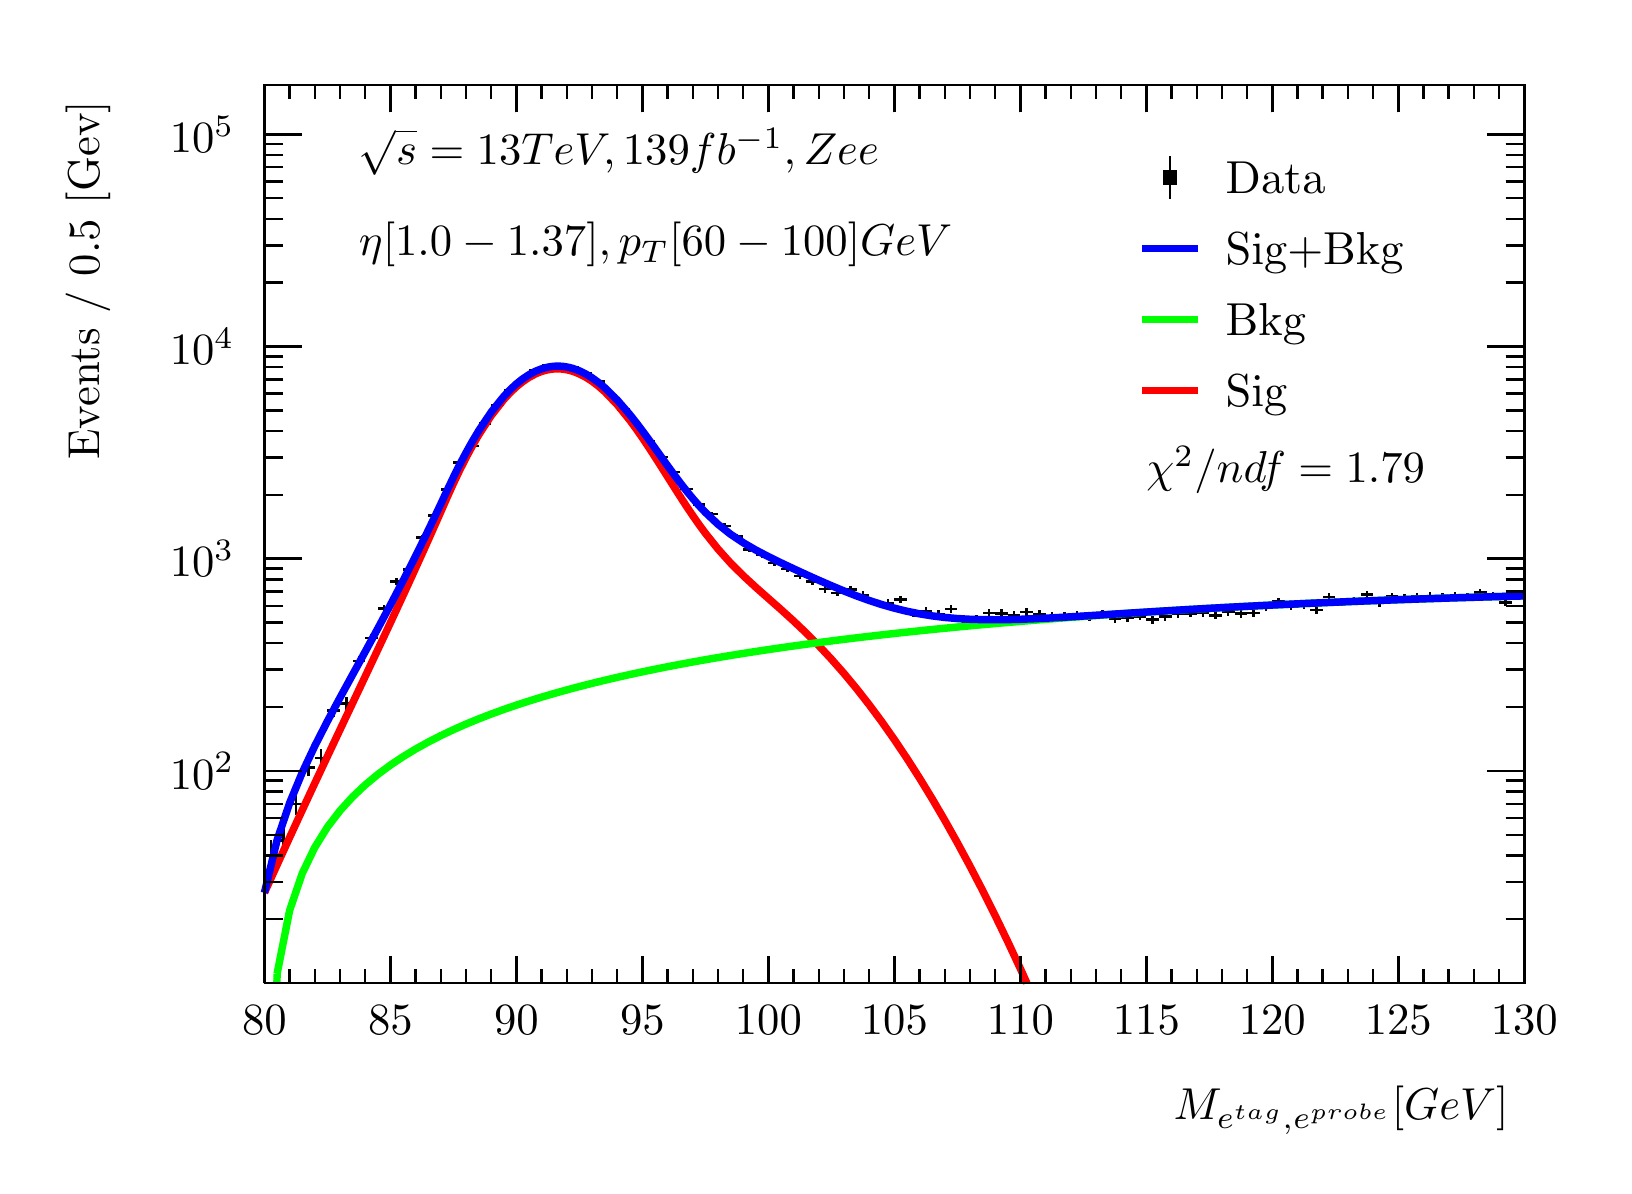
\begin{tikzpicture}
\pgfdeclareplotmark{cross} {
\pgfpathmoveto{\pgfpoint{-0.3\pgfplotmarksize}{\pgfplotmarksize}}
\pgfpathlineto{\pgfpoint{+0.3\pgfplotmarksize}{\pgfplotmarksize}}
\pgfpathlineto{\pgfpoint{+0.3\pgfplotmarksize}{0.3\pgfplotmarksize}}
\pgfpathlineto{\pgfpoint{+1\pgfplotmarksize}{0.3\pgfplotmarksize}}
\pgfpathlineto{\pgfpoint{+1\pgfplotmarksize}{-0.3\pgfplotmarksize}}
\pgfpathlineto{\pgfpoint{+0.3\pgfplotmarksize}{-0.3\pgfplotmarksize}}
\pgfpathlineto{\pgfpoint{+0.3\pgfplotmarksize}{-1.\pgfplotmarksize}}
\pgfpathlineto{\pgfpoint{-0.3\pgfplotmarksize}{-1.\pgfplotmarksize}}
\pgfpathlineto{\pgfpoint{-0.3\pgfplotmarksize}{-0.3\pgfplotmarksize}}
\pgfpathlineto{\pgfpoint{-1.\pgfplotmarksize}{-0.3\pgfplotmarksize}}
\pgfpathlineto{\pgfpoint{-1.\pgfplotmarksize}{0.3\pgfplotmarksize}}
\pgfpathlineto{\pgfpoint{-0.3\pgfplotmarksize}{0.3\pgfplotmarksize}}
\pgfpathclose
\pgfusepathqstroke
}
\pgfdeclareplotmark{cross*} {
\pgfpathmoveto{\pgfpoint{-0.3\pgfplotmarksize}{\pgfplotmarksize}}
\pgfpathlineto{\pgfpoint{+0.3\pgfplotmarksize}{\pgfplotmarksize}}
\pgfpathlineto{\pgfpoint{+0.3\pgfplotmarksize}{0.3\pgfplotmarksize}}
\pgfpathlineto{\pgfpoint{+1\pgfplotmarksize}{0.3\pgfplotmarksize}}
\pgfpathlineto{\pgfpoint{+1\pgfplotmarksize}{-0.3\pgfplotmarksize}}
\pgfpathlineto{\pgfpoint{+0.3\pgfplotmarksize}{-0.3\pgfplotmarksize}}
\pgfpathlineto{\pgfpoint{+0.3\pgfplotmarksize}{-1.\pgfplotmarksize}}
\pgfpathlineto{\pgfpoint{-0.3\pgfplotmarksize}{-1.\pgfplotmarksize}}
\pgfpathlineto{\pgfpoint{-0.3\pgfplotmarksize}{-0.3\pgfplotmarksize}}
\pgfpathlineto{\pgfpoint{-1.\pgfplotmarksize}{-0.3\pgfplotmarksize}}
\pgfpathlineto{\pgfpoint{-1.\pgfplotmarksize}{0.3\pgfplotmarksize}}
\pgfpathlineto{\pgfpoint{-0.3\pgfplotmarksize}{0.3\pgfplotmarksize}}
\pgfpathclose
\pgfusepathqfillstroke
}
\pgfdeclareplotmark{newstar} {
\pgfpathmoveto{\pgfqpoint{0pt}{\pgfplotmarksize}}
\pgfpathlineto{\pgfqpointpolar{44}{0.5\pgfplotmarksize}}
\pgfpathlineto{\pgfqpointpolar{18}{\pgfplotmarksize}}
\pgfpathlineto{\pgfqpointpolar{-20}{0.5\pgfplotmarksize}}
\pgfpathlineto{\pgfqpointpolar{-54}{\pgfplotmarksize}}
\pgfpathlineto{\pgfqpointpolar{-90}{0.5\pgfplotmarksize}}
\pgfpathlineto{\pgfqpointpolar{234}{\pgfplotmarksize}}
\pgfpathlineto{\pgfqpointpolar{198}{0.5\pgfplotmarksize}}
\pgfpathlineto{\pgfqpointpolar{162}{\pgfplotmarksize}}
\pgfpathlineto{\pgfqpointpolar{134}{0.5\pgfplotmarksize}}
\pgfpathclose
\pgfusepathqstroke
}
\pgfdeclareplotmark{newstar*} {
\pgfpathmoveto{\pgfqpoint{0pt}{\pgfplotmarksize}}
\pgfpathlineto{\pgfqpointpolar{44}{0.5\pgfplotmarksize}}
\pgfpathlineto{\pgfqpointpolar{18}{\pgfplotmarksize}}
\pgfpathlineto{\pgfqpointpolar{-20}{0.5\pgfplotmarksize}}
\pgfpathlineto{\pgfqpointpolar{-54}{\pgfplotmarksize}}
\pgfpathlineto{\pgfqpointpolar{-90}{0.5\pgfplotmarksize}}
\pgfpathlineto{\pgfqpointpolar{234}{\pgfplotmarksize}}
\pgfpathlineto{\pgfqpointpolar{198}{0.5\pgfplotmarksize}}
\pgfpathlineto{\pgfqpointpolar{162}{\pgfplotmarksize}}
\pgfpathlineto{\pgfqpointpolar{134}{0.5\pgfplotmarksize}}
\pgfpathclose
\pgfusepathqfillstroke
}
\definecolor{c}{rgb}{1,1,1};
\draw [color=c, fill=c] (0,0) rectangle (20,14.4361);
\draw [color=c, fill=c] (3,2.30977) rectangle (19,13.7143);
\definecolor{c}{rgb}{0,0,0};
\draw [c,line width=0.9] (3,2.30977) -- (3,13.7143) -- (19,13.7143) -- (19,2.30977) -- (3,2.30977);
\definecolor{c}{rgb}{1,1,1};
\draw [color=c, fill=c] (3,2.30977) rectangle (19,13.7143);
\definecolor{c}{rgb}{0,0,0};
\draw [c,line width=0.9] (3,2.30977) -- (3,13.7143) -- (19,13.7143) -- (19,2.30977) -- (3,2.30977);
\draw [c,line width=0.9] (3,2.30977) -- (19,2.30977);
\draw [c,line width=0.9] (3,2.65624) -- (3,2.30977);
\draw [c,line width=0.9] (3.32,2.48301) -- (3.32,2.30977);
\draw [c,line width=0.9] (3.64,2.48301) -- (3.64,2.30977);
\draw [c,line width=0.9] (3.96,2.48301) -- (3.96,2.30977);
\draw [c,line width=0.9] (4.28,2.48301) -- (4.28,2.30977);
\draw [c,line width=0.9] (4.6,2.65624) -- (4.6,2.30977);
\draw [c,line width=0.9] (4.92,2.48301) -- (4.92,2.30977);
\draw [c,line width=0.9] (5.24,2.48301) -- (5.24,2.30977);
\draw [c,line width=0.9] (5.56,2.48301) -- (5.56,2.30977);
\draw [c,line width=0.9] (5.88,2.48301) -- (5.88,2.30977);
\draw [c,line width=0.9] (6.2,2.65624) -- (6.2,2.30977);
\draw [c,line width=0.9] (6.52,2.48301) -- (6.52,2.30977);
\draw [c,line width=0.9] (6.84,2.48301) -- (6.84,2.30977);
\draw [c,line width=0.9] (7.16,2.48301) -- (7.16,2.30977);
\draw [c,line width=0.9] (7.48,2.48301) -- (7.48,2.30977);
\draw [c,line width=0.9] (7.8,2.65624) -- (7.8,2.30977);
\draw [c,line width=0.9] (8.12,2.48301) -- (8.12,2.30977);
\draw [c,line width=0.9] (8.44,2.48301) -- (8.44,2.30977);
\draw [c,line width=0.9] (8.76,2.48301) -- (8.76,2.30977);
\draw [c,line width=0.9] (9.08,2.48301) -- (9.08,2.30977);
\draw [c,line width=0.9] (9.4,2.65624) -- (9.4,2.30977);
\draw [c,line width=0.9] (9.72,2.48301) -- (9.72,2.30977);
\draw [c,line width=0.9] (10.04,2.48301) -- (10.04,2.30977);
\draw [c,line width=0.9] (10.36,2.48301) -- (10.36,2.30977);
\draw [c,line width=0.9] (10.68,2.48301) -- (10.68,2.30977);
\draw [c,line width=0.9] (11,2.65624) -- (11,2.30977);
\draw [c,line width=0.9] (11.32,2.48301) -- (11.32,2.30977);
\draw [c,line width=0.9] (11.64,2.48301) -- (11.64,2.30977);
\draw [c,line width=0.9] (11.96,2.48301) -- (11.96,2.30977);
\draw [c,line width=0.9] (12.28,2.48301) -- (12.28,2.30977);
\draw [c,line width=0.9] (12.6,2.65624) -- (12.6,2.30977);
\draw [c,line width=0.9] (12.92,2.48301) -- (12.92,2.30977);
\draw [c,line width=0.9] (13.24,2.48301) -- (13.24,2.30977);
\draw [c,line width=0.9] (13.56,2.48301) -- (13.56,2.30977);
\draw [c,line width=0.9] (13.88,2.48301) -- (13.88,2.30977);
\draw [c,line width=0.9] (14.2,2.65624) -- (14.2,2.30977);
\draw [c,line width=0.9] (14.52,2.48301) -- (14.52,2.30977);
\draw [c,line width=0.9] (14.84,2.48301) -- (14.84,2.30977);
\draw [c,line width=0.9] (15.16,2.48301) -- (15.16,2.30977);
\draw [c,line width=0.9] (15.48,2.48301) -- (15.48,2.30977);
\draw [c,line width=0.9] (15.8,2.65624) -- (15.8,2.30977);
\draw [c,line width=0.9] (16.12,2.48301) -- (16.12,2.30977);
\draw [c,line width=0.9] (16.44,2.48301) -- (16.44,2.30977);
\draw [c,line width=0.9] (16.76,2.48301) -- (16.76,2.30977);
\draw [c,line width=0.9] (17.08,2.48301) -- (17.08,2.30977);
\draw [c,line width=0.9] (17.4,2.65624) -- (17.4,2.30977);
\draw [c,line width=0.9] (17.72,2.48301) -- (17.72,2.30977);
\draw [c,line width=0.9] (18.04,2.48301) -- (18.04,2.30977);
\draw [c,line width=0.9] (18.36,2.48301) -- (18.36,2.30977);
\draw [c,line width=0.9] (18.68,2.48301) -- (18.68,2.30977);
\draw [c,line width=0.9] (19,2.65624) -- (19,2.30977);
\draw [anchor=base] (3,1.66015) node[scale=1.61424, color=c, rotate=0]{80};
\draw [anchor=base] (4.6,1.66015) node[scale=1.61424, color=c, rotate=0]{85};
\draw [anchor=base] (6.2,1.66015) node[scale=1.61424, color=c, rotate=0]{90};
\draw [anchor=base] (7.8,1.66015) node[scale=1.61424, color=c, rotate=0]{95};
\draw [anchor=base] (9.4,1.66015) node[scale=1.61424, color=c, rotate=0]{100};
\draw [anchor=base] (11,1.66015) node[scale=1.61424, color=c, rotate=0]{105};
\draw [anchor=base] (12.6,1.66015) node[scale=1.61424, color=c, rotate=0]{110};
\draw [anchor=base] (14.2,1.66015) node[scale=1.61424, color=c, rotate=0]{115};
\draw [anchor=base] (15.8,1.66015) node[scale=1.61424, color=c, rotate=0]{120};
\draw [anchor=base] (17.4,1.66015) node[scale=1.61424, color=c, rotate=0]{125};
\draw [anchor=base] (19,1.66015) node[scale=1.61424, color=c, rotate=0]{130};
\draw [anchor= east] (19,0.692932) node[scale=1.61424, color=c, rotate=0]{$M_{e^{tag}, e^{probe}}  [GeV]$};
\draw [c,line width=0.9] (3,13.7143) -- (19,13.7143);
\draw [c,line width=0.9] (3,13.3678) -- (3,13.7143);
\draw [c,line width=0.9] (3.32,13.5411) -- (3.32,13.7143);
\draw [c,line width=0.9] (3.64,13.5411) -- (3.64,13.7143);
\draw [c,line width=0.9] (3.96,13.5411) -- (3.96,13.7143);
\draw [c,line width=0.9] (4.28,13.5411) -- (4.28,13.7143);
\draw [c,line width=0.9] (4.6,13.3678) -- (4.6,13.7143);
\draw [c,line width=0.9] (4.92,13.5411) -- (4.92,13.7143);
\draw [c,line width=0.9] (5.24,13.5411) -- (5.24,13.7143);
\draw [c,line width=0.9] (5.56,13.5411) -- (5.56,13.7143);
\draw [c,line width=0.9] (5.88,13.5411) -- (5.88,13.7143);
\draw [c,line width=0.9] (6.2,13.3678) -- (6.2,13.7143);
\draw [c,line width=0.9] (6.52,13.5411) -- (6.52,13.7143);
\draw [c,line width=0.9] (6.84,13.5411) -- (6.84,13.7143);
\draw [c,line width=0.9] (7.16,13.5411) -- (7.16,13.7143);
\draw [c,line width=0.9] (7.48,13.5411) -- (7.48,13.7143);
\draw [c,line width=0.9] (7.8,13.3678) -- (7.8,13.7143);
\draw [c,line width=0.9] (8.12,13.5411) -- (8.12,13.7143);
\draw [c,line width=0.9] (8.44,13.5411) -- (8.44,13.7143);
\draw [c,line width=0.9] (8.76,13.5411) -- (8.76,13.7143);
\draw [c,line width=0.9] (9.08,13.5411) -- (9.08,13.7143);
\draw [c,line width=0.9] (9.4,13.3678) -- (9.4,13.7143);
\draw [c,line width=0.9] (9.72,13.5411) -- (9.72,13.7143);
\draw [c,line width=0.9] (10.04,13.5411) -- (10.04,13.7143);
\draw [c,line width=0.9] (10.36,13.5411) -- (10.36,13.7143);
\draw [c,line width=0.9] (10.68,13.5411) -- (10.68,13.7143);
\draw [c,line width=0.9] (11,13.3678) -- (11,13.7143);
\draw [c,line width=0.9] (11.32,13.5411) -- (11.32,13.7143);
\draw [c,line width=0.9] (11.64,13.5411) -- (11.64,13.7143);
\draw [c,line width=0.9] (11.96,13.5411) -- (11.96,13.7143);
\draw [c,line width=0.9] (12.28,13.5411) -- (12.28,13.7143);
\draw [c,line width=0.9] (12.6,13.3678) -- (12.6,13.7143);
\draw [c,line width=0.9] (12.92,13.5411) -- (12.92,13.7143);
\draw [c,line width=0.9] (13.24,13.5411) -- (13.24,13.7143);
\draw [c,line width=0.9] (13.56,13.5411) -- (13.56,13.7143);
\draw [c,line width=0.9] (13.88,13.5411) -- (13.88,13.7143);
\draw [c,line width=0.9] (14.2,13.3678) -- (14.2,13.7143);
\draw [c,line width=0.9] (14.52,13.5411) -- (14.52,13.7143);
\draw [c,line width=0.9] (14.84,13.5411) -- (14.84,13.7143);
\draw [c,line width=0.9] (15.16,13.5411) -- (15.16,13.7143);
\draw [c,line width=0.9] (15.48,13.5411) -- (15.48,13.7143);
\draw [c,line width=0.9] (15.8,13.3678) -- (15.8,13.7143);
\draw [c,line width=0.9] (16.12,13.5411) -- (16.12,13.7143);
\draw [c,line width=0.9] (16.44,13.5411) -- (16.44,13.7143);
\draw [c,line width=0.9] (16.76,13.5411) -- (16.76,13.7143);
\draw [c,line width=0.9] (17.08,13.5411) -- (17.08,13.7143);
\draw [c,line width=0.9] (17.4,13.3678) -- (17.4,13.7143);
\draw [c,line width=0.9] (17.72,13.5411) -- (17.72,13.7143);
\draw [c,line width=0.9] (18.04,13.5411) -- (18.04,13.7143);
\draw [c,line width=0.9] (18.36,13.5411) -- (18.36,13.7143);
\draw [c,line width=0.9] (18.68,13.5411) -- (18.68,13.7143);
\draw [c,line width=0.9] (19,13.3678) -- (19,13.7143);
\draw [c,line width=0.9] (3,2.30977) -- (3,13.7143);
\draw [c,line width=0.9] (3.237,3.1209) -- (3,3.1209);
\draw [c,line width=0.9] (3.237,3.59538) -- (3,3.59538);
\draw [c,line width=0.9] (3.237,3.93203) -- (3,3.93203);
\draw [c,line width=0.9] (3.237,4.19316) -- (3,4.19316);
\draw [c,line width=0.9] (3.237,4.40651) -- (3,4.40651);
\draw [c,line width=0.9] (3.237,4.5869) -- (3,4.5869);
\draw [c,line width=0.9] (3.237,4.74316) -- (3,4.74316);
\draw [c,line width=0.9] (3.237,4.881) -- (3,4.881);
\draw [c,line width=0.9] (3.474,5.00429) -- (3,5.00429);
\draw [anchor= east] (2.82,5.00429) node[scale=1.61424, color=c, rotate=0]{$10^{2}$};
\draw [c,line width=0.9] (3.237,5.81542) -- (3,5.81542);
\draw [c,line width=0.9] (3.237,6.2899) -- (3,6.2899);
\draw [c,line width=0.9] (3.237,6.62655) -- (3,6.62655);
\draw [c,line width=0.9] (3.237,6.88768) -- (3,6.88768);
\draw [c,line width=0.9] (3.237,7.10103) -- (3,7.10103);
\draw [c,line width=0.9] (3.237,7.28142) -- (3,7.28142);
\draw [c,line width=0.9] (3.237,7.43768) -- (3,7.43768);
\draw [c,line width=0.9] (3.237,7.57551) -- (3,7.57551);
\draw [c,line width=0.9] (3.474,7.69881) -- (3,7.69881);
\draw [anchor= east] (2.82,7.69881) node[scale=1.61424, color=c, rotate=0]{$10^{3}$};
\draw [c,line width=0.9] (3.237,8.50994) -- (3,8.50994);
\draw [c,line width=0.9] (3.237,8.98442) -- (3,8.98442);
\draw [c,line width=0.9] (3.237,9.32107) -- (3,9.32107);
\draw [c,line width=0.9] (3.237,9.58219) -- (3,9.58219);
\draw [c,line width=0.9] (3.237,9.79555) -- (3,9.79555);
\draw [c,line width=0.9] (3.237,9.97594) -- (3,9.97594);
\draw [c,line width=0.9] (3.237,10.1322) -- (3,10.1322);
\draw [c,line width=0.9] (3.237,10.27) -- (3,10.27);
\draw [c,line width=0.9] (3.474,10.3933) -- (3,10.3933);
\draw [anchor= east] (2.82,10.3933) node[scale=1.61424, color=c, rotate=0]{$10^{4}$};
\draw [c,line width=0.9] (3.237,11.2045) -- (3,11.2045);
\draw [c,line width=0.9] (3.237,11.6789) -- (3,11.6789);
\draw [c,line width=0.9] (3.237,12.0156) -- (3,12.0156);
\draw [c,line width=0.9] (3.237,12.2767) -- (3,12.2767);
\draw [c,line width=0.9] (3.237,12.4901) -- (3,12.4901);
\draw [c,line width=0.9] (3.237,12.6705) -- (3,12.6705);
\draw [c,line width=0.9] (3.237,12.8267) -- (3,12.8267);
\draw [c,line width=0.9] (3.237,12.9645) -- (3,12.9645);
\draw [c,line width=0.9] (3.474,13.0878) -- (3,13.0878);
\draw [anchor= east] (2.82,13.0878) node[scale=1.61424, color=c, rotate=0]{$10^{5}$};
\draw [anchor= east] (0.76,13.7143) node[scale=1.61424, color=c, rotate=90]{Events / 0.5 [Gev]};
\draw [c,line width=0.9] (19,2.30977) -- (19,13.7143);
\draw [c,line width=0.9] (18.763,3.1209) -- (19,3.1209);
\draw [c,line width=0.9] (18.763,3.59538) -- (19,3.59538);
\draw [c,line width=0.9] (18.763,3.93203) -- (19,3.93203);
\draw [c,line width=0.9] (18.763,4.19316) -- (19,4.19316);
\draw [c,line width=0.9] (18.763,4.40651) -- (19,4.40651);
\draw [c,line width=0.9] (18.763,4.5869) -- (19,4.5869);
\draw [c,line width=0.9] (18.763,4.74316) -- (19,4.74316);
\draw [c,line width=0.9] (18.763,4.881) -- (19,4.881);
\draw [c,line width=0.9] (18.526,5.00429) -- (19,5.00429);
\draw [c,line width=0.9] (18.763,5.81542) -- (19,5.81542);
\draw [c,line width=0.9] (18.763,6.2899) -- (19,6.2899);
\draw [c,line width=0.9] (18.763,6.62655) -- (19,6.62655);
\draw [c,line width=0.9] (18.763,6.88768) -- (19,6.88768);
\draw [c,line width=0.9] (18.763,7.10103) -- (19,7.10103);
\draw [c,line width=0.9] (18.763,7.28142) -- (19,7.28142);
\draw [c,line width=0.9] (18.763,7.43768) -- (19,7.43768);
\draw [c,line width=0.9] (18.763,7.57551) -- (19,7.57551);
\draw [c,line width=0.9] (18.526,7.69881) -- (19,7.69881);
\draw [c,line width=0.9] (18.763,8.50994) -- (19,8.50994);
\draw [c,line width=0.9] (18.763,8.98442) -- (19,8.98442);
\draw [c,line width=0.9] (18.763,9.32107) -- (19,9.32107);
\draw [c,line width=0.9] (18.763,9.58219) -- (19,9.58219);
\draw [c,line width=0.9] (18.763,9.79555) -- (19,9.79555);
\draw [c,line width=0.9] (18.763,9.97594) -- (19,9.97594);
\draw [c,line width=0.9] (18.763,10.1322) -- (19,10.1322);
\draw [c,line width=0.9] (18.763,10.27) -- (19,10.27);
\draw [c,line width=0.9] (18.526,10.3933) -- (19,10.3933);
\draw [c,line width=0.9] (18.763,11.2045) -- (19,11.2045);
\draw [c,line width=0.9] (18.763,11.6789) -- (19,11.6789);
\draw [c,line width=0.9] (18.763,12.0156) -- (19,12.0156);
\draw [c,line width=0.9] (18.763,12.2767) -- (19,12.2767);
\draw [c,line width=0.9] (18.763,12.4901) -- (19,12.4901);
\draw [c,line width=0.9] (18.763,12.6705) -- (19,12.6705);
\draw [c,line width=0.9] (18.763,12.8267) -- (19,12.8267);
\draw [c,line width=0.9] (18.763,12.9645) -- (19,12.9645);
\draw [c,line width=0.9] (18.526,13.0878) -- (19,13.0878);
\draw [c,line width=0.9] (3.08,3.93204) -- (3,3.93204);
\draw [c,line width=0.9] (3,3.93204) -- (3,3.93204);
\draw [c,line width=0.9] (3.08,3.93204) -- (3.16,3.93204);
\draw [c,line width=0.9] (3.16,3.93204) -- (3.16,3.93204);
\draw [c,line width=0.9] (3.08,3.93204) -- (3.08,4.13011);
\draw [c,line width=0.9] (3.08,4.13011) -- (3.08,4.13011);
\draw [c,line width=0.9] (3.08,3.93204) -- (3.08,3.73155);
\draw [c,line width=0.9] (3.08,3.73155) -- (3.08,3.73155);
\draw [c,line width=0.9] (3.24,4.12075) -- (3.16,4.12075);
\draw [c,line width=0.9] (3.16,4.12075) -- (3.16,4.12075);
\draw [c,line width=0.9] (3.24,4.12075) -- (3.32,4.12075);
\draw [c,line width=0.9] (3.32,4.12075) -- (3.32,4.12075);
\draw [c,line width=0.9] (3.24,4.12075) -- (3.24,4.30266);
\draw [c,line width=0.9] (3.24,4.30266) -- (3.24,4.30266);
\draw [c,line width=0.9] (3.24,4.12075) -- (3.24,3.93696);
\draw [c,line width=0.9] (3.24,3.93696) -- (3.24,3.93696);
\draw [c,line width=0.9] (3.4,4.58691) -- (3.32,4.58691);
\draw [c,line width=0.9] (3.32,4.58691) -- (3.32,4.58691);
\draw [c,line width=0.9] (3.4,4.58691) -- (3.48,4.58691);
\draw [c,line width=0.9] (3.48,4.58691) -- (3.48,4.58691);
\draw [c,line width=0.9] (3.4,4.58691) -- (3.4,4.73445);
\draw [c,line width=0.9] (3.4,4.73445) -- (3.4,4.73445);
\draw [c,line width=0.9] (3.4,4.58691) -- (3.4,4.43833);
\draw [c,line width=0.9] (3.4,4.43833) -- (3.4,4.43833);
\draw [c,line width=0.9] (3.56,5.05019) -- (3.48,5.05019);
\draw [c,line width=0.9] (3.48,5.05019) -- (3.48,5.05019);
\draw [c,line width=0.9] (3.56,5.05019) -- (3.64,5.05019);
\draw [c,line width=0.9] (3.64,5.05019) -- (3.64,5.05019);
\draw [c,line width=0.9] (3.56,5.05019) -- (3.56,5.16489);
\draw [c,line width=0.9] (3.56,5.16489) -- (3.56,5.16489);
\draw [c,line width=0.9] (3.56,5.05019) -- (3.56,4.93549);
\draw [c,line width=0.9] (3.56,4.93549) -- (3.56,4.93549);
\draw [c,line width=0.9] (3.72,5.16784) -- (3.64,5.16784);
\draw [c,line width=0.9] (3.64,5.16784) -- (3.64,5.16784);
\draw [c,line width=0.9] (3.72,5.16784) -- (3.8,5.16784);
\draw [c,line width=0.9] (3.8,5.16784) -- (3.8,5.16784);
\draw [c,line width=0.9] (3.72,5.16784) -- (3.72,5.27693);
\draw [c,line width=0.9] (3.72,5.27693) -- (3.72,5.27693);
\draw [c,line width=0.9] (3.72,5.16784) -- (3.72,5.05876);
\draw [c,line width=0.9] (3.72,5.05876) -- (3.72,5.05876);
\draw [c,line width=0.9] (3.88,5.77373) -- (3.8,5.77373);
\draw [c,line width=0.9] (3.8,5.77373) -- (3.8,5.77373);
\draw [c,line width=0.9] (3.88,5.77373) -- (3.96,5.77373);
\draw [c,line width=0.9] (3.96,5.77373) -- (3.96,5.77373);
\draw [c,line width=0.9] (3.88,5.77373) -- (3.88,5.85795);
\draw [c,line width=0.9] (3.88,5.85795) -- (3.88,5.85795);
\draw [c,line width=0.9] (3.88,5.77373) -- (3.88,5.68952);
\draw [c,line width=0.9] (3.88,5.68952) -- (3.88,5.68952);
\draw [c,line width=0.9] (4.04,5.86132) -- (3.96,5.86132);
\draw [c,line width=0.9] (3.96,5.86132) -- (3.96,5.86132);
\draw [c,line width=0.9] (4.04,5.86132) -- (4.12,5.86132);
\draw [c,line width=0.9] (4.12,5.86132) -- (4.12,5.86132);
\draw [c,line width=0.9] (4.04,5.86132) -- (4.04,5.94244);
\draw [c,line width=0.9] (4.04,5.94244) -- (4.04,5.94244);
\draw [c,line width=0.9] (4.04,5.86132) -- (4.04,5.7802);
\draw [c,line width=0.9] (4.04,5.7802) -- (4.04,5.7802);
\draw [c,line width=0.9] (4.2,6.40144) -- (4.12,6.40144);
\draw [c,line width=0.9] (4.12,6.40144) -- (4.12,6.40144);
\draw [c,line width=0.9] (4.2,6.40144) -- (4.28,6.40144);
\draw [c,line width=0.9] (4.28,6.40144) -- (4.28,6.40144);
\draw [c,line width=0.9] (4.2,6.40144) -- (4.2,6.46585);
\draw [c,line width=0.9] (4.2,6.46585) -- (4.2,6.46585);
\draw [c,line width=0.9] (4.2,6.40144) -- (4.2,6.33703);
\draw [c,line width=0.9] (4.2,6.33703) -- (4.2,6.33703);
\draw [c,line width=0.9] (4.36,6.68921) -- (4.28,6.68921);
\draw [c,line width=0.9] (4.28,6.68921) -- (4.28,6.68921);
\draw [c,line width=0.9] (4.36,6.68921) -- (4.44,6.68921);
\draw [c,line width=0.9] (4.44,6.68921) -- (4.44,6.68921);
\draw [c,line width=0.9] (4.36,6.68921) -- (4.36,6.74617);
\draw [c,line width=0.9] (4.36,6.74617) -- (4.36,6.74617);
\draw [c,line width=0.9] (4.36,6.68921) -- (4.36,6.63225);
\draw [c,line width=0.9] (4.36,6.63225) -- (4.36,6.63225);
\draw [c,line width=0.9] (4.52,7.06539) -- (4.44,7.06539);
\draw [c,line width=0.9] (4.44,7.06539) -- (4.44,7.06539);
\draw [c,line width=0.9] (4.52,7.06539) -- (4.6,7.06539);
\draw [c,line width=0.9] (4.6,7.06539) -- (4.6,7.06539);
\draw [c,line width=0.9] (4.52,7.06539) -- (4.52,7.11389);
\draw [c,line width=0.9] (4.52,7.11389) -- (4.52,7.11389);
\draw [c,line width=0.9] (4.52,7.06539) -- (4.52,7.01689);
\draw [c,line width=0.9] (4.52,7.01689) -- (4.52,7.01689);
\draw [c,line width=0.9] (4.68,7.40655) -- (4.6,7.40655);
\draw [c,line width=0.9] (4.6,7.40655) -- (4.6,7.40655);
\draw [c,line width=0.9] (4.68,7.40655) -- (4.76,7.40655);
\draw [c,line width=0.9] (4.76,7.40655) -- (4.76,7.40655);
\draw [c,line width=0.9] (4.68,7.40655) -- (4.68,7.44848);
\draw [c,line width=0.9] (4.68,7.44848) -- (4.68,7.44848);
\draw [c,line width=0.9] (4.68,7.40655) -- (4.68,7.36463);
\draw [c,line width=0.9] (4.68,7.36463) -- (4.68,7.36463);
\draw [c,line width=0.9] (4.84,7.55981) -- (4.76,7.55981);
\draw [c,line width=0.9] (4.76,7.55981) -- (4.76,7.55981);
\draw [c,line width=0.9] (4.84,7.55981) -- (4.92,7.55981);
\draw [c,line width=0.9] (4.92,7.55981) -- (4.92,7.55981);
\draw [c,line width=0.9] (4.84,7.55981) -- (4.84,7.59907);
\draw [c,line width=0.9] (4.84,7.59907) -- (4.84,7.59907);
\draw [c,line width=0.9] (4.84,7.55981) -- (4.84,7.52054);
\draw [c,line width=0.9] (4.84,7.52054) -- (4.84,7.52054);
\draw [c,line width=0.9] (5,7.96647) -- (4.92,7.96647);
\draw [c,line width=0.9] (4.92,7.96647) -- (4.92,7.96647);
\draw [c,line width=0.9] (5,7.96647) -- (5.08,7.96647);
\draw [c,line width=0.9] (5.08,7.96647) -- (5.08,7.96647);
\draw [c,line width=0.9] (5,7.96647) -- (5,7.99948);
\draw [c,line width=0.9] (5,7.99948) -- (5,7.99948);
\draw [c,line width=0.9] (5,7.96647) -- (5,7.93346);
\draw [c,line width=0.9] (5,7.93346) -- (5,7.93346);
\draw [c,line width=0.9] (5.16,8.24808) -- (5.08,8.24808);
\draw [c,line width=0.9] (5.08,8.24808) -- (5.08,8.24808);
\draw [c,line width=0.9] (5.16,8.24808) -- (5.24,8.24808);
\draw [c,line width=0.9] (5.24,8.24808) -- (5.24,8.24808);
\draw [c,line width=0.9] (5.16,8.24808) -- (5.16,8.27735);
\draw [c,line width=0.9] (5.16,8.27735) -- (5.16,8.27735);
\draw [c,line width=0.9] (5.16,8.24808) -- (5.16,8.21882);
\draw [c,line width=0.9] (5.16,8.21882) -- (5.16,8.21882);
\draw [c,line width=0.9] (5.32,8.57702) -- (5.24,8.57702);
\draw [c,line width=0.9] (5.24,8.57702) -- (5.24,8.57702);
\draw [c,line width=0.9] (5.32,8.57702) -- (5.4,8.57702);
\draw [c,line width=0.9] (5.4,8.57702) -- (5.4,8.57702);
\draw [c,line width=0.9] (5.32,8.57702) -- (5.32,8.60245);
\draw [c,line width=0.9] (5.32,8.60245) -- (5.32,8.60245);
\draw [c,line width=0.9] (5.32,8.57702) -- (5.32,8.55159);
\draw [c,line width=0.9] (5.32,8.55159) -- (5.32,8.55159);
\draw [c,line width=0.9] (5.48,8.91905) -- (5.4,8.91905);
\draw [c,line width=0.9] (5.4,8.91905) -- (5.4,8.91905);
\draw [c,line width=0.9] (5.48,8.91905) -- (5.56,8.91905);
\draw [c,line width=0.9] (5.56,8.91905) -- (5.56,8.91905);
\draw [c,line width=0.9] (5.48,8.91905) -- (5.48,8.94102);
\draw [c,line width=0.9] (5.48,8.94102) -- (5.48,8.94102);
\draw [c,line width=0.9] (5.48,8.91905) -- (5.48,8.89708);
\draw [c,line width=0.9] (5.48,8.89708) -- (5.48,8.89708);
\draw [c,line width=0.9] (5.64,9.13192) -- (5.56,9.13192);
\draw [c,line width=0.9] (5.56,9.13192) -- (5.56,9.13192);
\draw [c,line width=0.9] (5.64,9.13192) -- (5.72,9.13192);
\draw [c,line width=0.9] (5.72,9.13192) -- (5.72,9.13192);
\draw [c,line width=0.9] (5.64,9.13192) -- (5.64,9.15198);
\draw [c,line width=0.9] (5.64,9.15198) -- (5.64,9.15198);
\draw [c,line width=0.9] (5.64,9.13192) -- (5.64,9.11186);
\draw [c,line width=0.9] (5.64,9.11186) -- (5.64,9.11186);
\draw [c,line width=0.9] (5.8,9.41384) -- (5.72,9.41384);
\draw [c,line width=0.9] (5.72,9.41384) -- (5.72,9.41384);
\draw [c,line width=0.9] (5.8,9.41384) -- (5.88,9.41384);
\draw [c,line width=0.9] (5.88,9.41384) -- (5.88,9.41384);
\draw [c,line width=0.9] (5.8,9.41384) -- (5.8,9.43162);
\draw [c,line width=0.9] (5.8,9.43162) -- (5.8,9.43162);
\draw [c,line width=0.9] (5.8,9.41384) -- (5.8,9.39605);
\draw [c,line width=0.9] (5.8,9.39605) -- (5.8,9.39605);
\draw [c,line width=0.9] (5.96,9.6506) -- (5.88,9.6506);
\draw [c,line width=0.9] (5.88,9.6506) -- (5.88,9.6506);
\draw [c,line width=0.9] (5.96,9.6506) -- (6.04,9.6506);
\draw [c,line width=0.9] (6.04,9.6506) -- (6.04,9.6506);
\draw [c,line width=0.9] (5.96,9.6506) -- (5.96,9.66668);
\draw [c,line width=0.9] (5.96,9.66668) -- (5.96,9.66668);
\draw [c,line width=0.9] (5.96,9.6506) -- (5.96,9.63453);
\draw [c,line width=0.9] (5.96,9.63453) -- (5.96,9.63453);
\draw [c,line width=0.9] (6.12,9.83298) -- (6.04,9.83298);
\draw [c,line width=0.9] (6.04,9.83298) -- (6.04,9.83298);
\draw [c,line width=0.9] (6.12,9.83298) -- (6.2,9.83298);
\draw [c,line width=0.9] (6.2,9.83298) -- (6.2,9.83298);
\draw [c,line width=0.9] (6.12,9.83298) -- (6.12,9.84785);
\draw [c,line width=0.9] (6.12,9.84785) -- (6.12,9.84785);
\draw [c,line width=0.9] (6.12,9.83298) -- (6.12,9.81811);
\draw [c,line width=0.9] (6.12,9.81811) -- (6.12,9.81811);
\draw [c,line width=0.9] (6.28,9.96215) -- (6.2,9.96215);
\draw [c,line width=0.9] (6.2,9.96215) -- (6.2,9.96215);
\draw [c,line width=0.9] (6.28,9.96215) -- (6.36,9.96215);
\draw [c,line width=0.9] (6.36,9.96215) -- (6.36,9.96215);
\draw [c,line width=0.9] (6.28,9.96215) -- (6.28,9.97622);
\draw [c,line width=0.9] (6.28,9.97622) -- (6.28,9.97622);
\draw [c,line width=0.9] (6.28,9.96215) -- (6.28,9.94808);
\draw [c,line width=0.9] (6.28,9.94808) -- (6.28,9.94808);
\draw [c,line width=0.9] (6.44,10.0901) -- (6.36,10.0901);
\draw [c,line width=0.9] (6.36,10.0901) -- (6.36,10.0901);
\draw [c,line width=0.9] (6.44,10.0901) -- (6.52,10.0901);
\draw [c,line width=0.9] (6.52,10.0901) -- (6.52,10.0901);
\draw [c,line width=0.9] (6.44,10.0901) -- (6.44,10.1034);
\draw [c,line width=0.9] (6.44,10.1034) -- (6.44,10.1034);
\draw [c,line width=0.9] (6.44,10.0901) -- (6.44,10.0767);
\draw [c,line width=0.9] (6.44,10.0767) -- (6.44,10.0767);
\draw [c,line width=0.9] (6.6,10.1545) -- (6.52,10.1545);
\draw [c,line width=0.9] (6.52,10.1545) -- (6.52,10.1545);
\draw [c,line width=0.9] (6.6,10.1545) -- (6.68,10.1545);
\draw [c,line width=0.9] (6.68,10.1545) -- (6.68,10.1545);
\draw [c,line width=0.9] (6.6,10.1545) -- (6.6,10.1675);
\draw [c,line width=0.9] (6.6,10.1675) -- (6.6,10.1675);
\draw [c,line width=0.9] (6.6,10.1545) -- (6.6,10.1416);
\draw [c,line width=0.9] (6.6,10.1416) -- (6.6,10.1416);
\draw [c,line width=0.9] (6.76,10.1734) -- (6.68,10.1734);
\draw [c,line width=0.9] (6.68,10.1734) -- (6.68,10.1734);
\draw [c,line width=0.9] (6.76,10.1734) -- (6.84,10.1734);
\draw [c,line width=0.9] (6.84,10.1734) -- (6.84,10.1734);
\draw [c,line width=0.9] (6.76,10.1734) -- (6.76,10.1863);
\draw [c,line width=0.9] (6.76,10.1863) -- (6.76,10.1863);
\draw [c,line width=0.9] (6.76,10.1734) -- (6.76,10.1606);
\draw [c,line width=0.9] (6.76,10.1606) -- (6.76,10.1606);
\draw [c,line width=0.9] (6.92,10.1275) -- (6.84,10.1275);
\draw [c,line width=0.9] (6.84,10.1275) -- (6.84,10.1275);
\draw [c,line width=0.9] (6.92,10.1275) -- (7,10.1275);
\draw [c,line width=0.9] (7,10.1275) -- (7,10.1275);
\draw [c,line width=0.9] (6.92,10.1275) -- (6.92,10.1406);
\draw [c,line width=0.9] (6.92,10.1406) -- (6.92,10.1406);
\draw [c,line width=0.9] (6.92,10.1275) -- (6.92,10.1144);
\draw [c,line width=0.9] (6.92,10.1144) -- (6.92,10.1144);
\draw [c,line width=0.9] (7.08,10.0498) -- (7,10.0498);
\draw [c,line width=0.9] (7,10.0498) -- (7,10.0498);
\draw [c,line width=0.9] (7.08,10.0498) -- (7.16,10.0498);
\draw [c,line width=0.9] (7.16,10.0498) -- (7.16,10.0498);
\draw [c,line width=0.9] (7.08,10.0498) -- (7.08,10.0633);
\draw [c,line width=0.9] (7.08,10.0633) -- (7.08,10.0633);
\draw [c,line width=0.9] (7.08,10.0498) -- (7.08,10.0362);
\draw [c,line width=0.9] (7.08,10.0362) -- (7.08,10.0362);
\draw [c,line width=0.9] (7.24,9.94888) -- (7.16,9.94888);
\draw [c,line width=0.9] (7.16,9.94888) -- (7.16,9.94888);
\draw [c,line width=0.9] (7.24,9.94888) -- (7.32,9.94888);
\draw [c,line width=0.9] (7.32,9.94888) -- (7.32,9.94888);
\draw [c,line width=0.9] (7.24,9.94888) -- (7.24,9.96303);
\draw [c,line width=0.9] (7.24,9.96303) -- (7.24,9.96303);
\draw [c,line width=0.9] (7.24,9.94888) -- (7.24,9.93473);
\draw [c,line width=0.9] (7.24,9.93473) -- (7.24,9.93473);
\draw [c,line width=0.9] (7.4,9.77964) -- (7.32,9.77964);
\draw [c,line width=0.9] (7.32,9.77964) -- (7.32,9.77964);
\draw [c,line width=0.9] (7.4,9.77964) -- (7.48,9.77964);
\draw [c,line width=0.9] (7.48,9.77964) -- (7.48,9.77964);
\draw [c,line width=0.9] (7.4,9.77964) -- (7.4,9.79486);
\draw [c,line width=0.9] (7.4,9.79486) -- (7.4,9.79486);
\draw [c,line width=0.9] (7.4,9.77964) -- (7.4,9.76443);
\draw [c,line width=0.9] (7.4,9.76443) -- (7.4,9.76443);
\draw [c,line width=0.9] (7.56,9.59152) -- (7.48,9.59152);
\draw [c,line width=0.9] (7.48,9.59152) -- (7.48,9.59152);
\draw [c,line width=0.9] (7.56,9.59152) -- (7.64,9.59152);
\draw [c,line width=0.9] (7.64,9.59152) -- (7.64,9.59152);
\draw [c,line width=0.9] (7.56,9.59152) -- (7.56,9.608);
\draw [c,line width=0.9] (7.56,9.608) -- (7.56,9.608);
\draw [c,line width=0.9] (7.56,9.59152) -- (7.56,9.57504);
\draw [c,line width=0.9] (7.56,9.57504) -- (7.56,9.57504);
\draw [c,line width=0.9] (7.72,9.39284) -- (7.64,9.39284);
\draw [c,line width=0.9] (7.64,9.39284) -- (7.64,9.39284);
\draw [c,line width=0.9] (7.72,9.39284) -- (7.8,9.39284);
\draw [c,line width=0.9] (7.8,9.39284) -- (7.8,9.39284);
\draw [c,line width=0.9] (7.72,9.39284) -- (7.72,9.41078);
\draw [c,line width=0.9] (7.72,9.41078) -- (7.72,9.41078);
\draw [c,line width=0.9] (7.72,9.39284) -- (7.72,9.3749);
\draw [c,line width=0.9] (7.72,9.3749) -- (7.72,9.3749);
\draw [c,line width=0.9] (7.88,9.18798) -- (7.8,9.18798);
\draw [c,line width=0.9] (7.8,9.18798) -- (7.8,9.18798);
\draw [c,line width=0.9] (7.88,9.18798) -- (7.96,9.18798);
\draw [c,line width=0.9] (7.96,9.18798) -- (7.96,9.18798);
\draw [c,line width=0.9] (7.88,9.18798) -- (7.88,9.20757);
\draw [c,line width=0.9] (7.88,9.20757) -- (7.88,9.20757);
\draw [c,line width=0.9] (7.88,9.18798) -- (7.88,9.1684);
\draw [c,line width=0.9] (7.88,9.1684) -- (7.88,9.1684);
\draw [c,line width=0.9] (8.04,8.99297) -- (7.96,8.99297);
\draw [c,line width=0.9] (7.96,8.99297) -- (7.96,8.99297);
\draw [c,line width=0.9] (8.04,8.99297) -- (8.12,8.99297);
\draw [c,line width=0.9] (8.12,8.99297) -- (8.12,8.99297);
\draw [c,line width=0.9] (8.04,8.99297) -- (8.04,9.01426);
\draw [c,line width=0.9] (8.04,9.01426) -- (8.04,9.01426);
\draw [c,line width=0.9] (8.04,8.99297) -- (8.04,8.97168);
\draw [c,line width=0.9] (8.04,8.97168) -- (8.04,8.97168);
\draw [c,line width=0.9] (8.2,8.8011) -- (8.12,8.8011);
\draw [c,line width=0.9] (8.12,8.8011) -- (8.12,8.8011);
\draw [c,line width=0.9] (8.2,8.8011) -- (8.28,8.8011);
\draw [c,line width=0.9] (8.28,8.8011) -- (8.28,8.8011);
\draw [c,line width=0.9] (8.2,8.8011) -- (8.2,8.82421);
\draw [c,line width=0.9] (8.2,8.82421) -- (8.2,8.82421);
\draw [c,line width=0.9] (8.2,8.8011) -- (8.2,8.778);
\draw [c,line width=0.9] (8.2,8.778) -- (8.2,8.778);
\draw [c,line width=0.9] (8.36,8.58198) -- (8.28,8.58198);
\draw [c,line width=0.9] (8.28,8.58198) -- (8.28,8.58198);
\draw [c,line width=0.9] (8.36,8.58198) -- (8.44,8.58198);
\draw [c,line width=0.9] (8.44,8.58198) -- (8.44,8.58198);
\draw [c,line width=0.9] (8.36,8.58198) -- (8.36,8.60736);
\draw [c,line width=0.9] (8.36,8.60736) -- (8.36,8.60736);
\draw [c,line width=0.9] (8.36,8.58198) -- (8.36,8.55661);
\draw [c,line width=0.9] (8.36,8.55661) -- (8.36,8.55661);
\draw [c,line width=0.9] (8.52,8.38989) -- (8.44,8.38989);
\draw [c,line width=0.9] (8.44,8.38989) -- (8.44,8.38989);
\draw [c,line width=0.9] (8.52,8.38989) -- (8.6,8.38989);
\draw [c,line width=0.9] (8.6,8.38989) -- (8.6,8.38989);
\draw [c,line width=0.9] (8.52,8.38989) -- (8.52,8.41743);
\draw [c,line width=0.9] (8.52,8.41743) -- (8.52,8.41743);
\draw [c,line width=0.9] (8.52,8.38989) -- (8.52,8.36235);
\draw [c,line width=0.9] (8.52,8.36235) -- (8.52,8.36235);
\draw [c,line width=0.9] (8.68,8.26624) -- (8.6,8.26624);
\draw [c,line width=0.9] (8.6,8.26624) -- (8.6,8.26624);
\draw [c,line width=0.9] (8.68,8.26624) -- (8.76,8.26624);
\draw [c,line width=0.9] (8.76,8.26624) -- (8.76,8.26624);
\draw [c,line width=0.9] (8.68,8.26624) -- (8.68,8.29527);
\draw [c,line width=0.9] (8.68,8.29527) -- (8.68,8.29527);
\draw [c,line width=0.9] (8.68,8.26624) -- (8.68,8.2372);
\draw [c,line width=0.9] (8.68,8.2372) -- (8.68,8.2372);
\draw [c,line width=0.9] (8.84,8.11655) -- (8.76,8.11655);
\draw [c,line width=0.9] (8.76,8.11655) -- (8.76,8.11655);
\draw [c,line width=0.9] (8.84,8.11655) -- (8.92,8.11655);
\draw [c,line width=0.9] (8.92,8.11655) -- (8.92,8.11655);
\draw [c,line width=0.9] (8.84,8.11655) -- (8.84,8.1475);
\draw [c,line width=0.9] (8.84,8.1475) -- (8.84,8.1475);
\draw [c,line width=0.9] (8.84,8.11655) -- (8.84,8.08559);
\draw [c,line width=0.9] (8.84,8.08559) -- (8.84,8.08559);
\draw [c,line width=0.9] (9,7.97943) -- (8.92,7.97943);
\draw [c,line width=0.9] (8.92,7.97943) -- (8.92,7.97943);
\draw [c,line width=0.9] (9,7.97943) -- (9.08,7.97943);
\draw [c,line width=0.9] (9.08,7.97943) -- (9.08,7.97943);
\draw [c,line width=0.9] (9,7.97943) -- (9,8.01225);
\draw [c,line width=0.9] (9,8.01225) -- (9,8.01225);
\draw [c,line width=0.9] (9,7.97943) -- (9,7.94661);
\draw [c,line width=0.9] (9,7.94661) -- (9,7.94661);
\draw [c,line width=0.9] (9.16,7.81671) -- (9.08,7.81671);
\draw [c,line width=0.9] (9.08,7.81671) -- (9.08,7.81671);
\draw [c,line width=0.9] (9.16,7.81671) -- (9.24,7.81671);
\draw [c,line width=0.9] (9.24,7.81671) -- (9.24,7.81671);
\draw [c,line width=0.9] (9.16,7.81671) -- (9.16,7.85189);
\draw [c,line width=0.9] (9.16,7.85189) -- (9.16,7.85189);
\draw [c,line width=0.9] (9.16,7.81671) -- (9.16,7.78152);
\draw [c,line width=0.9] (9.16,7.78152) -- (9.16,7.78152);
\draw [c,line width=0.9] (9.32,7.7492) -- (9.24,7.7492);
\draw [c,line width=0.9] (9.24,7.7492) -- (9.24,7.7492);
\draw [c,line width=0.9] (9.32,7.7492) -- (9.4,7.7492);
\draw [c,line width=0.9] (9.4,7.7492) -- (9.4,7.7492);
\draw [c,line width=0.9] (9.32,7.7492) -- (9.32,7.78541);
\draw [c,line width=0.9] (9.32,7.78541) -- (9.32,7.78541);
\draw [c,line width=0.9] (9.32,7.7492) -- (9.32,7.71298);
\draw [c,line width=0.9] (9.32,7.71298) -- (9.32,7.71298);
\draw [c,line width=0.9] (9.48,7.64247) -- (9.4,7.64247);
\draw [c,line width=0.9] (9.4,7.64247) -- (9.4,7.64247);
\draw [c,line width=0.9] (9.48,7.64247) -- (9.56,7.64247);
\draw [c,line width=0.9] (9.56,7.64247) -- (9.56,7.64247);
\draw [c,line width=0.9] (9.48,7.64247) -- (9.48,7.68038);
\draw [c,line width=0.9] (9.48,7.68038) -- (9.48,7.68038);
\draw [c,line width=0.9] (9.48,7.64247) -- (9.48,7.60457);
\draw [c,line width=0.9] (9.48,7.60457) -- (9.48,7.60457);
\draw [c,line width=0.9] (9.64,7.56769) -- (9.56,7.56769);
\draw [c,line width=0.9] (9.56,7.56769) -- (9.56,7.56769);
\draw [c,line width=0.9] (9.64,7.56769) -- (9.72,7.56769);
\draw [c,line width=0.9] (9.72,7.56769) -- (9.72,7.56769);
\draw [c,line width=0.9] (9.64,7.56769) -- (9.64,7.60682);
\draw [c,line width=0.9] (9.64,7.60682) -- (9.64,7.60682);
\draw [c,line width=0.9] (9.64,7.56769) -- (9.64,7.52855);
\draw [c,line width=0.9] (9.64,7.52855) -- (9.64,7.52855);
\draw [c,line width=0.9] (9.8,7.47935) -- (9.72,7.47935);
\draw [c,line width=0.9] (9.72,7.47935) -- (9.72,7.47935);
\draw [c,line width=0.9] (9.8,7.47935) -- (9.88,7.47935);
\draw [c,line width=0.9] (9.88,7.47935) -- (9.88,7.47935);
\draw [c,line width=0.9] (9.8,7.47935) -- (9.8,7.51999);
\draw [c,line width=0.9] (9.8,7.51999) -- (9.8,7.51999);
\draw [c,line width=0.9] (9.8,7.47935) -- (9.8,7.43871);
\draw [c,line width=0.9] (9.8,7.43871) -- (9.8,7.43871);
\draw [c,line width=0.9] (9.96,7.40956) -- (9.88,7.40956);
\draw [c,line width=0.9] (9.88,7.40956) -- (9.88,7.40956);
\draw [c,line width=0.9] (9.96,7.40956) -- (10.04,7.40956);
\draw [c,line width=0.9] (10.04,7.40956) -- (10.04,7.40956);
\draw [c,line width=0.9] (9.96,7.40956) -- (9.96,7.45143);
\draw [c,line width=0.9] (9.96,7.45143) -- (9.96,7.45143);
\draw [c,line width=0.9] (9.96,7.40956) -- (9.96,7.36768);
\draw [c,line width=0.9] (9.96,7.36768) -- (9.96,7.36768);
\draw [c,line width=0.9] (10.12,7.31276) -- (10.04,7.31276);
\draw [c,line width=0.9] (10.04,7.31276) -- (10.04,7.31276);
\draw [c,line width=0.9] (10.12,7.31276) -- (10.2,7.31276);
\draw [c,line width=0.9] (10.2,7.31276) -- (10.2,7.31276);
\draw [c,line width=0.9] (10.12,7.31276) -- (10.12,7.3564);
\draw [c,line width=0.9] (10.12,7.3564) -- (10.12,7.3564);
\draw [c,line width=0.9] (10.12,7.31276) -- (10.12,7.26912);
\draw [c,line width=0.9] (10.12,7.26912) -- (10.12,7.26912);
\draw [c,line width=0.9] (10.28,7.26459) -- (10.2,7.26459);
\draw [c,line width=0.9] (10.2,7.26459) -- (10.2,7.26459);
\draw [c,line width=0.9] (10.28,7.26459) -- (10.36,7.26459);
\draw [c,line width=0.9] (10.36,7.26459) -- (10.36,7.26459);
\draw [c,line width=0.9] (10.28,7.26459) -- (10.28,7.30913);
\draw [c,line width=0.9] (10.28,7.30913) -- (10.28,7.30913);
\draw [c,line width=0.9] (10.28,7.26459) -- (10.28,7.22004);
\draw [c,line width=0.9] (10.28,7.22004) -- (10.28,7.22004);
\draw [c,line width=0.9] (10.44,7.3095) -- (10.36,7.3095);
\draw [c,line width=0.9] (10.36,7.3095) -- (10.36,7.3095);
\draw [c,line width=0.9] (10.44,7.3095) -- (10.52,7.3095);
\draw [c,line width=0.9] (10.52,7.3095) -- (10.52,7.3095);
\draw [c,line width=0.9] (10.44,7.3095) -- (10.44,7.3532);
\draw [c,line width=0.9] (10.44,7.3532) -- (10.44,7.3532);
\draw [c,line width=0.9] (10.44,7.3095) -- (10.44,7.2658);
\draw [c,line width=0.9] (10.44,7.2658) -- (10.44,7.2658);
\draw [c,line width=0.9] (10.6,7.23886) -- (10.52,7.23886);
\draw [c,line width=0.9] (10.52,7.23886) -- (10.52,7.23886);
\draw [c,line width=0.9] (10.6,7.23886) -- (10.68,7.23886);
\draw [c,line width=0.9] (10.68,7.23886) -- (10.68,7.23886);
\draw [c,line width=0.9] (10.6,7.23886) -- (10.6,7.2839);
\draw [c,line width=0.9] (10.6,7.2839) -- (10.6,7.2839);
\draw [c,line width=0.9] (10.6,7.23886) -- (10.6,7.19383);
\draw [c,line width=0.9] (10.6,7.19383) -- (10.6,7.19383);
\draw [c,line width=0.9] (10.76,7.1394) -- (10.68,7.1394);
\draw [c,line width=0.9] (10.68,7.1394) -- (10.68,7.1394);
\draw [c,line width=0.9] (10.76,7.1394) -- (10.84,7.1394);
\draw [c,line width=0.9] (10.84,7.1394) -- (10.84,7.1394);
\draw [c,line width=0.9] (10.76,7.1394) -- (10.76,7.1864);
\draw [c,line width=0.9] (10.76,7.1864) -- (10.76,7.1864);
\draw [c,line width=0.9] (10.76,7.1394) -- (10.76,7.09241);
\draw [c,line width=0.9] (10.76,7.09241) -- (10.76,7.09241);
\draw [c,line width=0.9] (10.92,7.13373) -- (10.84,7.13373);
\draw [c,line width=0.9] (10.84,7.13373) -- (10.84,7.13373);
\draw [c,line width=0.9] (10.92,7.13373) -- (11,7.13373);
\draw [c,line width=0.9] (11,7.13373) -- (11,7.13373);
\draw [c,line width=0.9] (10.92,7.13373) -- (10.92,7.18084);
\draw [c,line width=0.9] (10.92,7.18084) -- (10.92,7.18084);
\draw [c,line width=0.9] (10.92,7.13373) -- (10.92,7.08662);
\draw [c,line width=0.9] (10.92,7.08662) -- (10.92,7.08662);
\draw [c,line width=0.9] (11.08,7.18021) -- (11,7.18021);
\draw [c,line width=0.9] (11,7.18021) -- (11,7.18021);
\draw [c,line width=0.9] (11.08,7.18021) -- (11.16,7.18021);
\draw [c,line width=0.9] (11.16,7.18021) -- (11.16,7.18021);
\draw [c,line width=0.9] (11.08,7.18021) -- (11.08,7.22639);
\draw [c,line width=0.9] (11.08,7.22639) -- (11.08,7.22639);
\draw [c,line width=0.9] (11.08,7.18021) -- (11.08,7.13403);
\draw [c,line width=0.9] (11.08,7.13403) -- (11.08,7.13403);
\draw [c,line width=0.9] (11.24,7.0098) -- (11.16,7.0098);
\draw [c,line width=0.9] (11.16,7.0098) -- (11.16,7.0098);
\draw [c,line width=0.9] (11.24,7.0098) -- (11.32,7.0098);
\draw [c,line width=0.9] (11.32,7.0098) -- (11.32,7.0098);
\draw [c,line width=0.9] (11.24,7.0098) -- (11.24,7.05947);
\draw [c,line width=0.9] (11.24,7.05947) -- (11.24,7.05947);
\draw [c,line width=0.9] (11.24,7.0098) -- (11.24,6.96013);
\draw [c,line width=0.9] (11.24,6.96013) -- (11.24,6.96013);
\draw [c,line width=0.9] (11.4,7.03277) -- (11.32,7.03277);
\draw [c,line width=0.9] (11.32,7.03277) -- (11.32,7.03277);
\draw [c,line width=0.9] (11.4,7.03277) -- (11.48,7.03277);
\draw [c,line width=0.9] (11.48,7.03277) -- (11.48,7.03277);
\draw [c,line width=0.9] (11.4,7.03277) -- (11.4,7.08195);
\draw [c,line width=0.9] (11.4,7.08195) -- (11.4,7.08195);
\draw [c,line width=0.9] (11.4,7.03277) -- (11.4,6.98358);
\draw [c,line width=0.9] (11.4,6.98358) -- (11.4,6.98358);
\draw [c,line width=0.9] (11.56,6.99281) -- (11.48,6.99281);
\draw [c,line width=0.9] (11.48,6.99281) -- (11.48,6.99281);
\draw [c,line width=0.9] (11.56,6.99281) -- (11.64,6.99281);
\draw [c,line width=0.9] (11.64,6.99281) -- (11.64,6.99281);
\draw [c,line width=0.9] (11.56,6.99281) -- (11.56,7.04284);
\draw [c,line width=0.9] (11.56,7.04284) -- (11.56,7.04284);
\draw [c,line width=0.9] (11.56,6.99281) -- (11.56,6.94278);
\draw [c,line width=0.9] (11.56,6.94278) -- (11.56,6.94278);
\draw [c,line width=0.9] (11.72,7.06338) -- (11.64,7.06338);
\draw [c,line width=0.9] (11.64,7.06338) -- (11.64,7.06338);
\draw [c,line width=0.9] (11.72,7.06338) -- (11.8,7.06338);
\draw [c,line width=0.9] (11.8,7.06338) -- (11.8,7.06338);
\draw [c,line width=0.9] (11.72,7.06338) -- (11.72,7.11192);
\draw [c,line width=0.9] (11.72,7.11192) -- (11.72,7.11192);
\draw [c,line width=0.9] (11.72,7.06338) -- (11.72,7.01483);
\draw [c,line width=0.9] (11.72,7.01483) -- (11.72,7.01483);
\draw [c,line width=0.9] (11.88,6.8472) -- (11.8,6.8472);
\draw [c,line width=0.9] (11.8,6.8472) -- (11.8,6.8472);
\draw [c,line width=0.9] (11.88,6.8472) -- (11.96,6.8472);
\draw [c,line width=0.9] (11.96,6.8472) -- (11.96,6.8472);
\draw [c,line width=0.9] (11.88,6.8472) -- (11.88,6.90044);
\draw [c,line width=0.9] (11.88,6.90044) -- (11.88,6.90044);
\draw [c,line width=0.9] (11.88,6.8472) -- (11.88,6.79396);
\draw [c,line width=0.9] (11.88,6.79396) -- (11.88,6.79396);
\draw [c,line width=0.9] (12.04,6.93807) -- (11.96,6.93807);
\draw [c,line width=0.9] (11.96,6.93807) -- (11.96,6.93807);
\draw [c,line width=0.9] (12.04,6.93807) -- (12.12,6.93807);
\draw [c,line width=0.9] (12.12,6.93807) -- (12.12,6.93807);
\draw [c,line width=0.9] (12.04,6.93807) -- (12.04,6.98928);
\draw [c,line width=0.9] (12.04,6.98928) -- (12.04,6.98928);
\draw [c,line width=0.9] (12.04,6.93807) -- (12.04,6.88685);
\draw [c,line width=0.9] (12.04,6.88685) -- (12.04,6.88685);
\draw [c,line width=0.9] (12.2,7.00769) -- (12.12,7.00769);
\draw [c,line width=0.9] (12.12,7.00769) -- (12.12,7.00769);
\draw [c,line width=0.9] (12.2,7.00769) -- (12.28,7.00769);
\draw [c,line width=0.9] (12.28,7.00769) -- (12.28,7.00769);
\draw [c,line width=0.9] (12.2,7.00769) -- (12.2,7.05741);
\draw [c,line width=0.9] (12.2,7.05741) -- (12.2,7.05741);
\draw [c,line width=0.9] (12.2,7.00769) -- (12.2,6.95798);
\draw [c,line width=0.9] (12.2,6.95798) -- (12.2,6.95798);
\draw [c,line width=0.9] (12.36,7.00558) -- (12.28,7.00558);
\draw [c,line width=0.9] (12.28,7.00558) -- (12.28,7.00558);
\draw [c,line width=0.9] (12.36,7.00558) -- (12.44,7.00558);
\draw [c,line width=0.9] (12.44,7.00558) -- (12.44,7.00558);
\draw [c,line width=0.9] (12.36,7.00558) -- (12.36,7.05534);
\draw [c,line width=0.9] (12.36,7.05534) -- (12.36,7.05534);
\draw [c,line width=0.9] (12.36,7.00558) -- (12.36,6.95582);
\draw [c,line width=0.9] (12.36,6.95582) -- (12.36,6.95582);
\draw [c,line width=0.9] (12.52,6.98207) -- (12.44,6.98207);
\draw [c,line width=0.9] (12.44,6.98207) -- (12.44,6.98207);
\draw [c,line width=0.9] (12.52,6.98207) -- (12.6,6.98207);
\draw [c,line width=0.9] (12.6,6.98207) -- (12.6,6.98207);
\draw [c,line width=0.9] (12.52,6.98207) -- (12.52,7.03233);
\draw [c,line width=0.9] (12.52,7.03233) -- (12.52,7.03233);
\draw [c,line width=0.9] (12.52,6.98207) -- (12.52,6.9318);
\draw [c,line width=0.9] (12.52,6.9318) -- (12.52,6.9318);
\draw [c,line width=0.9] (12.68,7.02239) -- (12.6,7.02239);
\draw [c,line width=0.9] (12.6,7.02239) -- (12.6,7.02239);
\draw [c,line width=0.9] (12.68,7.02239) -- (12.76,7.02239);
\draw [c,line width=0.9] (12.76,7.02239) -- (12.76,7.02239);
\draw [c,line width=0.9] (12.68,7.02239) -- (12.68,7.07179);
\draw [c,line width=0.9] (12.68,7.07179) -- (12.68,7.07179);
\draw [c,line width=0.9] (12.68,7.02239) -- (12.68,6.97298);
\draw [c,line width=0.9] (12.68,6.97298) -- (12.68,6.97298);
\draw [c,line width=0.9] (12.84,6.99281) -- (12.76,6.99281);
\draw [c,line width=0.9] (12.76,6.99281) -- (12.76,6.99281);
\draw [c,line width=0.9] (12.84,6.99281) -- (12.92,6.99281);
\draw [c,line width=0.9] (12.92,6.99281) -- (12.92,6.99281);
\draw [c,line width=0.9] (12.84,6.99281) -- (12.84,7.04284);
\draw [c,line width=0.9] (12.84,7.04284) -- (12.84,7.04284);
\draw [c,line width=0.9] (12.84,6.99281) -- (12.84,6.94278);
\draw [c,line width=0.9] (12.84,6.94278) -- (12.84,6.94278);
\draw [c,line width=0.9] (13,6.96904) -- (12.92,6.96904);
\draw [c,line width=0.9] (12.92,6.96904) -- (12.92,6.96904);
\draw [c,line width=0.9] (13,6.96904) -- (13.08,6.96904);
\draw [c,line width=0.9] (13.08,6.96904) -- (13.08,6.96904);
\draw [c,line width=0.9] (13,6.96904) -- (13,7.01958);
\draw [c,line width=0.9] (13,7.01958) -- (13,7.01958);
\draw [c,line width=0.9] (13,6.96904) -- (13,6.9185);
\draw [c,line width=0.9] (13,6.9185) -- (13,6.9185);
\draw [c,line width=0.9] (13.16,6.96904) -- (13.08,6.96904);
\draw [c,line width=0.9] (13.08,6.96904) -- (13.08,6.96904);
\draw [c,line width=0.9] (13.16,6.96904) -- (13.24,6.96904);
\draw [c,line width=0.9] (13.24,6.96904) -- (13.24,6.96904);
\draw [c,line width=0.9] (13.16,6.96904) -- (13.16,7.01958);
\draw [c,line width=0.9] (13.16,7.01958) -- (13.16,7.01958);
\draw [c,line width=0.9] (13.16,6.96904) -- (13.16,6.9185);
\draw [c,line width=0.9] (13.16,6.9185) -- (13.16,6.9185);
\draw [c,line width=0.9] (13.32,6.9799) -- (13.24,6.9799);
\draw [c,line width=0.9] (13.24,6.9799) -- (13.24,6.9799);
\draw [c,line width=0.9] (13.32,6.9799) -- (13.4,6.9799);
\draw [c,line width=0.9] (13.4,6.9799) -- (13.4,6.9799);
\draw [c,line width=0.9] (13.32,6.9799) -- (13.32,7.03021);
\draw [c,line width=0.9] (13.32,7.03021) -- (13.32,7.03021);
\draw [c,line width=0.9] (13.32,6.9799) -- (13.32,6.9296);
\draw [c,line width=0.9] (13.32,6.9296) -- (13.32,6.9296);
\draw [c,line width=0.9] (13.48,6.95366) -- (13.4,6.95366);
\draw [c,line width=0.9] (13.4,6.95366) -- (13.4,6.95366);
\draw [c,line width=0.9] (13.48,6.95366) -- (13.56,6.95366);
\draw [c,line width=0.9] (13.56,6.95366) -- (13.56,6.95366);
\draw [c,line width=0.9] (13.48,6.95366) -- (13.48,7.00453);
\draw [c,line width=0.9] (13.48,7.00453) -- (13.48,7.00453);
\draw [c,line width=0.9] (13.48,6.95366) -- (13.48,6.90278);
\draw [c,line width=0.9] (13.48,6.90278) -- (13.48,6.90278);
\draw [c,line width=0.9] (13.64,6.99921) -- (13.56,6.99921);
\draw [c,line width=0.9] (13.56,6.99921) -- (13.56,6.99921);
\draw [c,line width=0.9] (13.64,6.99921) -- (13.72,6.99921);
\draw [c,line width=0.9] (13.72,6.99921) -- (13.72,6.99921);
\draw [c,line width=0.9] (13.64,6.99921) -- (13.64,7.04911);
\draw [c,line width=0.9] (13.64,7.04911) -- (13.64,7.04911);
\draw [c,line width=0.9] (13.64,6.99921) -- (13.64,6.94932);
\draw [c,line width=0.9] (13.64,6.94932) -- (13.64,6.94932);
\draw [c,line width=0.9] (13.8,6.93807) -- (13.72,6.93807);
\draw [c,line width=0.9] (13.72,6.93807) -- (13.72,6.93807);
\draw [c,line width=0.9] (13.8,6.93807) -- (13.88,6.93807);
\draw [c,line width=0.9] (13.88,6.93807) -- (13.88,6.93807);
\draw [c,line width=0.9] (13.8,6.93807) -- (13.8,6.98928);
\draw [c,line width=0.9] (13.8,6.98928) -- (13.8,6.98928);
\draw [c,line width=0.9] (13.8,6.93807) -- (13.8,6.88685);
\draw [c,line width=0.9] (13.8,6.88685) -- (13.8,6.88685);
\draw [c,line width=0.9] (13.96,6.94477) -- (13.88,6.94477);
\draw [c,line width=0.9] (13.88,6.94477) -- (13.88,6.94477);
\draw [c,line width=0.9] (13.96,6.94477) -- (14.04,6.94477);
\draw [c,line width=0.9] (14.04,6.94477) -- (14.04,6.94477);
\draw [c,line width=0.9] (13.96,6.94477) -- (13.96,6.99584);
\draw [c,line width=0.9] (13.96,6.99584) -- (13.96,6.99584);
\draw [c,line width=0.9] (13.96,6.94477) -- (13.96,6.8937);
\draw [c,line width=0.9] (13.96,6.8937) -- (13.96,6.8937);
\draw [c,line width=0.9] (14.12,6.96685) -- (14.04,6.96685);
\draw [c,line width=0.9] (14.04,6.96685) -- (14.04,6.96685);
\draw [c,line width=0.9] (14.12,6.96685) -- (14.2,6.96685);
\draw [c,line width=0.9] (14.2,6.96685) -- (14.2,6.96685);
\draw [c,line width=0.9] (14.12,6.96685) -- (14.12,7.01744);
\draw [c,line width=0.9] (14.12,7.01744) -- (14.12,7.01744);
\draw [c,line width=0.9] (14.12,6.96685) -- (14.12,6.91626);
\draw [c,line width=0.9] (14.12,6.91626) -- (14.12,6.91626);
\draw [c,line width=0.9] (14.28,6.92454) -- (14.2,6.92454);
\draw [c,line width=0.9] (14.2,6.92454) -- (14.2,6.92454);
\draw [c,line width=0.9] (14.28,6.92454) -- (14.36,6.92454);
\draw [c,line width=0.9] (14.36,6.92454) -- (14.36,6.92454);
\draw [c,line width=0.9] (14.28,6.92454) -- (14.28,6.97605);
\draw [c,line width=0.9] (14.28,6.97605) -- (14.28,6.97605);
\draw [c,line width=0.9] (14.28,6.92454) -- (14.28,6.87303);
\draw [c,line width=0.9] (14.28,6.87303) -- (14.28,6.87303);
\draw [c,line width=0.9] (14.44,6.96466) -- (14.36,6.96466);
\draw [c,line width=0.9] (14.36,6.96466) -- (14.36,6.96466);
\draw [c,line width=0.9] (14.44,6.96466) -- (14.52,6.96466);
\draw [c,line width=0.9] (14.52,6.96466) -- (14.52,6.96466);
\draw [c,line width=0.9] (14.44,6.96466) -- (14.44,7.0153);
\draw [c,line width=0.9] (14.44,7.0153) -- (14.44,7.0153);
\draw [c,line width=0.9] (14.44,6.96466) -- (14.44,6.91403);
\draw [c,line width=0.9] (14.44,6.91403) -- (14.44,6.91403);
\draw [c,line width=0.9] (14.6,6.99921) -- (14.52,6.99921);
\draw [c,line width=0.9] (14.52,6.99921) -- (14.52,6.99921);
\draw [c,line width=0.9] (14.6,6.99921) -- (14.68,6.99921);
\draw [c,line width=0.9] (14.68,6.99921) -- (14.68,6.99921);
\draw [c,line width=0.9] (14.6,6.99921) -- (14.6,7.04911);
\draw [c,line width=0.9] (14.6,7.04911) -- (14.6,7.04911);
\draw [c,line width=0.9] (14.6,6.99921) -- (14.6,6.94932);
\draw [c,line width=0.9] (14.6,6.94932) -- (14.6,6.94932);
\draw [c,line width=0.9] (14.76,7.00558) -- (14.68,7.00558);
\draw [c,line width=0.9] (14.68,7.00558) -- (14.68,7.00558);
\draw [c,line width=0.9] (14.76,7.00558) -- (14.84,7.00558);
\draw [c,line width=0.9] (14.84,7.00558) -- (14.84,7.00558);
\draw [c,line width=0.9] (14.76,7.00558) -- (14.76,7.05534);
\draw [c,line width=0.9] (14.76,7.05534) -- (14.76,7.05534);
\draw [c,line width=0.9] (14.76,7.00558) -- (14.76,6.95582);
\draw [c,line width=0.9] (14.76,6.95582) -- (14.76,6.95582);
\draw [c,line width=0.9] (14.92,7.01401) -- (14.84,7.01401);
\draw [c,line width=0.9] (14.84,7.01401) -- (14.84,7.01401);
\draw [c,line width=0.9] (14.92,7.01401) -- (15,7.01401);
\draw [c,line width=0.9] (15,7.01401) -- (15,7.01401);
\draw [c,line width=0.9] (14.92,7.01401) -- (14.92,7.06359);
\draw [c,line width=0.9] (14.92,7.06359) -- (14.92,7.06359);
\draw [c,line width=0.9] (14.92,7.01401) -- (14.92,6.96443);
\draw [c,line width=0.9] (14.92,6.96443) -- (14.92,6.96443);
\draw [c,line width=0.9] (15.08,6.9799) -- (15,6.9799);
\draw [c,line width=0.9] (15,6.9799) -- (15,6.9799);
\draw [c,line width=0.9] (15.08,6.9799) -- (15.16,6.9799);
\draw [c,line width=0.9] (15.16,6.9799) -- (15.16,6.9799);
\draw [c,line width=0.9] (15.08,6.9799) -- (15.08,7.03021);
\draw [c,line width=0.9] (15.08,7.03021) -- (15.08,7.03021);
\draw [c,line width=0.9] (15.08,6.9799) -- (15.08,6.9296);
\draw [c,line width=0.9] (15.08,6.9296) -- (15.08,6.9296);
\draw [c,line width=0.9] (15.24,7.02655) -- (15.16,7.02655);
\draw [c,line width=0.9] (15.16,7.02655) -- (15.16,7.02655);
\draw [c,line width=0.9] (15.24,7.02655) -- (15.32,7.02655);
\draw [c,line width=0.9] (15.32,7.02655) -- (15.32,7.02655);
\draw [c,line width=0.9] (15.24,7.02655) -- (15.24,7.07586);
\draw [c,line width=0.9] (15.24,7.07586) -- (15.24,7.07586);
\draw [c,line width=0.9] (15.24,7.02655) -- (15.24,6.97723);
\draw [c,line width=0.9] (15.24,6.97723) -- (15.24,6.97723);
\draw [c,line width=0.9] (15.4,7.00134) -- (15.32,7.00134);
\draw [c,line width=0.9] (15.32,7.00134) -- (15.32,7.00134);
\draw [c,line width=0.9] (15.4,7.00134) -- (15.48,7.00134);
\draw [c,line width=0.9] (15.48,7.00134) -- (15.48,7.00134);
\draw [c,line width=0.9] (15.4,7.00134) -- (15.4,7.05119);
\draw [c,line width=0.9] (15.4,7.05119) -- (15.4,7.05119);
\draw [c,line width=0.9] (15.4,7.00134) -- (15.4,6.95149);
\draw [c,line width=0.9] (15.4,6.95149) -- (15.4,6.95149);
\draw [c,line width=0.9] (15.56,7.0098) -- (15.48,7.0098);
\draw [c,line width=0.9] (15.48,7.0098) -- (15.48,7.0098);
\draw [c,line width=0.9] (15.56,7.0098) -- (15.64,7.0098);
\draw [c,line width=0.9] (15.64,7.0098) -- (15.64,7.0098);
\draw [c,line width=0.9] (15.56,7.0098) -- (15.56,7.05947);
\draw [c,line width=0.9] (15.56,7.05947) -- (15.56,7.05947);
\draw [c,line width=0.9] (15.56,7.0098) -- (15.56,6.96013);
\draw [c,line width=0.9] (15.56,6.96013) -- (15.56,6.96013);
\draw [c,line width=0.9] (15.72,7.08533) -- (15.64,7.08533);
\draw [c,line width=0.9] (15.64,7.08533) -- (15.64,7.08533);
\draw [c,line width=0.9] (15.72,7.08533) -- (15.8,7.08533);
\draw [c,line width=0.9] (15.8,7.08533) -- (15.8,7.08533);
\draw [c,line width=0.9] (15.72,7.08533) -- (15.72,7.13342);
\draw [c,line width=0.9] (15.72,7.13342) -- (15.72,7.13342);
\draw [c,line width=0.9] (15.72,7.08533) -- (15.72,7.03723);
\draw [c,line width=0.9] (15.72,7.03723) -- (15.72,7.03723);
\draw [c,line width=0.9] (15.88,7.15627) -- (15.8,7.15627);
\draw [c,line width=0.9] (15.8,7.15627) -- (15.8,7.15627);
\draw [c,line width=0.9] (15.88,7.15627) -- (15.96,7.15627);
\draw [c,line width=0.9] (15.96,7.15627) -- (15.96,7.15627);
\draw [c,line width=0.9] (15.88,7.15627) -- (15.88,7.20293);
\draw [c,line width=0.9] (15.88,7.20293) -- (15.88,7.20293);
\draw [c,line width=0.9] (15.88,7.15627) -- (15.88,7.10961);
\draw [c,line width=0.9] (15.88,7.10961) -- (15.88,7.10961);
\draw [c,line width=0.9] (16.04,7.08927) -- (15.96,7.08927);
\draw [c,line width=0.9] (15.96,7.08927) -- (15.96,7.08927);
\draw [c,line width=0.9] (16.04,7.08927) -- (16.12,7.08927);
\draw [c,line width=0.9] (16.12,7.08927) -- (16.12,7.08927);
\draw [c,line width=0.9] (16.04,7.08927) -- (16.04,7.13728);
\draw [c,line width=0.9] (16.04,7.13728) -- (16.04,7.13728);
\draw [c,line width=0.9] (16.04,7.08927) -- (16.04,7.04126);
\draw [c,line width=0.9] (16.04,7.04126) -- (16.04,7.04126);
\draw [c,line width=0.9] (16.2,7.11074) -- (16.12,7.11074);
\draw [c,line width=0.9] (16.12,7.11074) -- (16.12,7.11074);
\draw [c,line width=0.9] (16.2,7.11074) -- (16.28,7.11074);
\draw [c,line width=0.9] (16.28,7.11074) -- (16.28,7.11074);
\draw [c,line width=0.9] (16.2,7.11074) -- (16.2,7.15832);
\draw [c,line width=0.9] (16.2,7.15832) -- (16.2,7.15832);
\draw [c,line width=0.9] (16.2,7.11074) -- (16.2,7.06317);
\draw [c,line width=0.9] (16.2,7.06317) -- (16.2,7.06317);
\draw [c,line width=0.9] (16.36,7.04511) -- (16.28,7.04511);
\draw [c,line width=0.9] (16.28,7.04511) -- (16.28,7.04511);
\draw [c,line width=0.9] (16.36,7.04511) -- (16.44,7.04511);
\draw [c,line width=0.9] (16.44,7.04511) -- (16.44,7.04511);
\draw [c,line width=0.9] (16.36,7.04511) -- (16.36,7.09403);
\draw [c,line width=0.9] (16.36,7.09403) -- (16.36,7.09403);
\draw [c,line width=0.9] (16.36,7.04511) -- (16.36,6.99618);
\draw [c,line width=0.9] (16.36,6.99618) -- (16.36,6.99618);
\draw [c,line width=0.9] (16.52,7.21257) -- (16.44,7.21257);
\draw [c,line width=0.9] (16.44,7.21257) -- (16.44,7.21257);
\draw [c,line width=0.9] (16.52,7.21257) -- (16.6,7.21257);
\draw [c,line width=0.9] (16.6,7.21257) -- (16.6,7.21257);
\draw [c,line width=0.9] (16.52,7.21257) -- (16.52,7.25811);
\draw [c,line width=0.9] (16.52,7.25811) -- (16.52,7.25811);
\draw [c,line width=0.9] (16.52,7.21257) -- (16.52,7.16702);
\draw [c,line width=0.9] (16.52,7.16702) -- (16.52,7.16702);
\draw [c,line width=0.9] (16.68,7.15067) -- (16.6,7.15067);
\draw [c,line width=0.9] (16.6,7.15067) -- (16.6,7.15067);
\draw [c,line width=0.9] (16.68,7.15067) -- (16.76,7.15067);
\draw [c,line width=0.9] (16.76,7.15067) -- (16.76,7.15067);
\draw [c,line width=0.9] (16.68,7.15067) -- (16.68,7.19744);
\draw [c,line width=0.9] (16.68,7.19744) -- (16.68,7.19744);
\draw [c,line width=0.9] (16.68,7.15067) -- (16.68,7.10391);
\draw [c,line width=0.9] (16.68,7.10391) -- (16.68,7.10391);
\draw [c,line width=0.9] (16.84,7.16738) -- (16.76,7.16738);
\draw [c,line width=0.9] (16.76,7.16738) -- (16.76,7.16738);
\draw [c,line width=0.9] (16.84,7.16738) -- (16.92,7.16738);
\draw [c,line width=0.9] (16.92,7.16738) -- (16.92,7.16738);
\draw [c,line width=0.9] (16.84,7.16738) -- (16.84,7.21381);
\draw [c,line width=0.9] (16.84,7.21381) -- (16.84,7.21381);
\draw [c,line width=0.9] (16.84,7.16738) -- (16.84,7.12094);
\draw [c,line width=0.9] (16.84,7.12094) -- (16.84,7.12094);
\draw [c,line width=0.9] (17,7.24233) -- (16.92,7.24233);
\draw [c,line width=0.9] (16.92,7.24233) -- (16.92,7.24233);
\draw [c,line width=0.9] (17,7.24233) -- (17.08,7.24233);
\draw [c,line width=0.9] (17.08,7.24233) -- (17.08,7.24233);
\draw [c,line width=0.9] (17,7.24233) -- (17,7.2873);
\draw [c,line width=0.9] (17,7.2873) -- (17,7.2873);
\draw [c,line width=0.9] (17,7.24233) -- (17,7.19735);
\draw [c,line width=0.9] (17,7.19735) -- (17,7.19735);
\draw [c,line width=0.9] (17.16,7.13373) -- (17.08,7.13373);
\draw [c,line width=0.9] (17.08,7.13373) -- (17.08,7.13373);
\draw [c,line width=0.9] (17.16,7.13373) -- (17.24,7.13373);
\draw [c,line width=0.9] (17.24,7.13373) -- (17.24,7.13373);
\draw [c,line width=0.9] (17.16,7.13373) -- (17.16,7.18084);
\draw [c,line width=0.9] (17.16,7.18084) -- (17.16,7.18084);
\draw [c,line width=0.9] (17.16,7.13373) -- (17.16,7.08662);
\draw [c,line width=0.9] (17.16,7.08662) -- (17.16,7.08662);
\draw [c,line width=0.9] (17.32,7.21787) -- (17.24,7.21787);
\draw [c,line width=0.9] (17.24,7.21787) -- (17.24,7.21787);
\draw [c,line width=0.9] (17.32,7.21787) -- (17.4,7.21787);
\draw [c,line width=0.9] (17.4,7.21787) -- (17.4,7.21787);
\draw [c,line width=0.9] (17.32,7.21787) -- (17.32,7.26332);
\draw [c,line width=0.9] (17.32,7.26332) -- (17.32,7.26332);
\draw [c,line width=0.9] (17.32,7.21787) -- (17.32,7.17243);
\draw [c,line width=0.9] (17.32,7.17243) -- (17.32,7.17243);
\draw [c,line width=0.9] (17.48,7.21079) -- (17.4,7.21079);
\draw [c,line width=0.9] (17.4,7.21079) -- (17.4,7.21079);
\draw [c,line width=0.9] (17.48,7.21079) -- (17.56,7.21079);
\draw [c,line width=0.9] (17.56,7.21079) -- (17.56,7.21079);
\draw [c,line width=0.9] (17.48,7.21079) -- (17.48,7.25637);
\draw [c,line width=0.9] (17.48,7.25637) -- (17.48,7.25637);
\draw [c,line width=0.9] (17.48,7.21079) -- (17.48,7.16521);
\draw [c,line width=0.9] (17.48,7.16521) -- (17.48,7.16521);
\draw [c,line width=0.9] (17.64,7.21787) -- (17.56,7.21787);
\draw [c,line width=0.9] (17.56,7.21787) -- (17.56,7.21787);
\draw [c,line width=0.9] (17.64,7.21787) -- (17.72,7.21787);
\draw [c,line width=0.9] (17.72,7.21787) -- (17.72,7.21787);
\draw [c,line width=0.9] (17.64,7.21787) -- (17.64,7.26332);
\draw [c,line width=0.9] (17.64,7.26332) -- (17.64,7.26332);
\draw [c,line width=0.9] (17.64,7.21787) -- (17.64,7.17243);
\draw [c,line width=0.9] (17.64,7.17243) -- (17.64,7.17243);
\draw [c,line width=0.9] (17.8,7.22842) -- (17.72,7.22842);
\draw [c,line width=0.9] (17.72,7.22842) -- (17.72,7.22842);
\draw [c,line width=0.9] (17.8,7.22842) -- (17.88,7.22842);
\draw [c,line width=0.9] (17.88,7.22842) -- (17.88,7.22842);
\draw [c,line width=0.9] (17.8,7.22842) -- (17.8,7.27366);
\draw [c,line width=0.9] (17.8,7.27366) -- (17.8,7.27366);
\draw [c,line width=0.9] (17.8,7.22842) -- (17.8,7.18318);
\draw [c,line width=0.9] (17.8,7.18318) -- (17.8,7.18318);
\draw [c,line width=0.9] (17.96,7.22316) -- (17.88,7.22316);
\draw [c,line width=0.9] (17.88,7.22316) -- (17.88,7.22316);
\draw [c,line width=0.9] (17.96,7.22316) -- (18.04,7.22316);
\draw [c,line width=0.9] (18.04,7.22316) -- (18.04,7.22316);
\draw [c,line width=0.9] (17.96,7.22316) -- (17.96,7.2685);
\draw [c,line width=0.9] (17.96,7.2685) -- (17.96,7.2685);
\draw [c,line width=0.9] (17.96,7.22316) -- (17.96,7.17781);
\draw [c,line width=0.9] (17.96,7.17781) -- (17.96,7.17781);
\draw [c,line width=0.9] (18.12,7.22842) -- (18.04,7.22842);
\draw [c,line width=0.9] (18.04,7.22842) -- (18.04,7.22842);
\draw [c,line width=0.9] (18.12,7.22842) -- (18.2,7.22842);
\draw [c,line width=0.9] (18.2,7.22842) -- (18.2,7.22842);
\draw [c,line width=0.9] (18.12,7.22842) -- (18.12,7.27366);
\draw [c,line width=0.9] (18.12,7.27366) -- (18.12,7.27366);
\draw [c,line width=0.9] (18.12,7.22842) -- (18.12,7.18318);
\draw [c,line width=0.9] (18.12,7.18318) -- (18.12,7.18318);
\draw [c,line width=0.9] (18.28,7.21434) -- (18.2,7.21434);
\draw [c,line width=0.9] (18.2,7.21434) -- (18.2,7.21434);
\draw [c,line width=0.9] (18.28,7.21434) -- (18.36,7.21434);
\draw [c,line width=0.9] (18.36,7.21434) -- (18.36,7.21434);
\draw [c,line width=0.9] (18.28,7.21434) -- (18.28,7.25985);
\draw [c,line width=0.9] (18.28,7.25985) -- (18.28,7.25985);
\draw [c,line width=0.9] (18.28,7.21434) -- (18.28,7.16883);
\draw [c,line width=0.9] (18.28,7.16883) -- (18.28,7.16883);
\draw [c,line width=0.9] (18.44,7.26797) -- (18.36,7.26797);
\draw [c,line width=0.9] (18.36,7.26797) -- (18.36,7.26797);
\draw [c,line width=0.9] (18.44,7.26797) -- (18.52,7.26797);
\draw [c,line width=0.9] (18.52,7.26797) -- (18.52,7.26797);
\draw [c,line width=0.9] (18.44,7.26797) -- (18.44,7.31245);
\draw [c,line width=0.9] (18.44,7.31245) -- (18.44,7.31245);
\draw [c,line width=0.9] (18.44,7.26797) -- (18.44,7.22349);
\draw [c,line width=0.9] (18.44,7.22349) -- (18.44,7.22349);
\draw [c,line width=0.9] (18.6,7.23539) -- (18.52,7.23539);
\draw [c,line width=0.9] (18.52,7.23539) -- (18.52,7.23539);
\draw [c,line width=0.9] (18.6,7.23539) -- (18.68,7.23539);
\draw [c,line width=0.9] (18.68,7.23539) -- (18.68,7.23539);
\draw [c,line width=0.9] (18.6,7.23539) -- (18.6,7.2805);
\draw [c,line width=0.9] (18.6,7.2805) -- (18.6,7.2805);
\draw [c,line width=0.9] (18.6,7.23539) -- (18.6,7.19029);
\draw [c,line width=0.9] (18.6,7.19029) -- (18.6,7.19029);
\draw [c,line width=0.9] (18.76,7.14129) -- (18.68,7.14129);
\draw [c,line width=0.9] (18.68,7.14129) -- (18.68,7.14129);
\draw [c,line width=0.9] (18.76,7.14129) -- (18.84,7.14129);
\draw [c,line width=0.9] (18.84,7.14129) -- (18.84,7.14129);
\draw [c,line width=0.9] (18.76,7.14129) -- (18.76,7.18825);
\draw [c,line width=0.9] (18.76,7.18825) -- (18.76,7.18825);
\draw [c,line width=0.9] (18.76,7.14129) -- (18.76,7.09433);
\draw [c,line width=0.9] (18.76,7.09433) -- (18.76,7.09433);
\draw [c,line width=0.9] (18.92,7.25949) -- (18.84,7.25949);
\draw [c,line width=0.9] (18.84,7.25949) -- (18.84,7.25949);
\draw [c,line width=0.9] (18.92,7.25949) -- (19,7.25949);
\draw [c,line width=0.9] (19,7.25949) -- (19,7.25949);
\draw [c,line width=0.9] (18.92,7.25949) -- (18.92,7.30413);
\draw [c,line width=0.9] (18.92,7.30413) -- (18.92,7.30413);
\draw [c,line width=0.9] (18.92,7.25949) -- (18.92,7.21484);
\draw [c,line width=0.9] (18.92,7.21484) -- (18.92,7.21484);
\foreach \P in {(3.08,3.93204), (3.24,4.12075), (3.4,4.58691), (3.56,5.05019), (3.72,5.16784), (3.88,5.77373), (4.04,5.86132), (4.2,6.40144), (4.36,6.68921), (4.52,7.06539), (4.68,7.40655), (4.84,7.55981), (5,7.96647), (5.16,8.24808), (5.32,8.57702),
 (5.48,8.91905), (5.64,9.13192), (5.8,9.41384), (5.96,9.6506), (6.12,9.83298), (6.28,9.96215), (6.44,10.0901), (6.6,10.1545), (6.76,10.1734), (6.92,10.1275), (7.08,10.0498), (7.24,9.94888), (7.4,9.77964), (7.56,9.59152), (7.72,9.39284),
 (7.88,9.18798), (8.04,8.99297), (8.2,8.8011), (8.36,8.58198), (8.52,8.38989), (8.68,8.26624), (8.84,8.11655), (9,7.97943), (9.16,7.81671), (9.32,7.7492), (9.48,7.64247), (9.64,7.56769), (9.8,7.47935), (9.96,7.40956), (10.12,7.31276),
 (10.28,7.26459), (10.44,7.3095), (10.6,7.23886), (10.76,7.1394), (10.92,7.13373), (11.08,7.18021), (11.24,7.0098), (11.4,7.03277), (11.56,6.99281), (11.72,7.06338), (11.88,6.8472), (12.04,6.93807), (12.2,7.00769), (12.36,7.00558), (12.52,6.98207),
 (12.68,7.02239), (12.84,6.99281), (13,6.96904), (13.16,6.96904), (13.32,6.9799), (13.48,6.95366), (13.64,6.99921), (13.8,6.93807), (13.96,6.94477), (14.12,6.96685), (14.28,6.92454), (14.44,6.96466), (14.6,6.99921), (14.76,7.00558), (14.92,7.01401),
 (15.08,6.9799), (15.24,7.02655), (15.4,7.00134), (15.56,7.0098), (15.72,7.08533), (15.88,7.15627), (16.04,7.08927), (16.2,7.11074), (16.36,7.04511), (16.52,7.21257), (16.68,7.15067), (16.84,7.16738), (17,7.24233), (17.16,7.13373), (17.32,7.21787),
 (17.48,7.21079), (17.64,7.21787), (17.8,7.22842), (17.96,7.22316), (18.12,7.22842), (18.28,7.21434), (18.44,7.26797), (18.6,7.23539), (18.76,7.14129), (18.92,7.25949)}{\draw[mark options={color=c,fill=c},mark size=2.882883pt,mark=] plot coordinates
 {\P};}
\definecolor{c}{rgb}{1,0,0};
\draw [c,line width=2.7] (3,3.45675) -- (3,3.45675);
\draw [c,line width=2.7] (3,3.45675) -- (3.16,3.81023) -- (3.32,4.15976) -- (3.48,4.50574) -- (3.64,4.84869) -- (3.8,5.18925) -- (3.96,5.52819) -- (4.12,5.86635) -- (4.28,6.20471) -- (4.44,6.54426) -- (4.6,6.88606) -- (4.76,7.23115) -- (4.84,7.40524)
 -- (4.92,7.58052) -- (5,7.7571) -- (5.08,7.93507) -- (5.16,8.11454) -- (5.24,8.29558) -- (5.32,8.4781) -- (5.4,8.65538) -- (5.48,8.82351) -- (5.56,8.98215) -- (5.64,9.13099) -- (5.72,9.26981) -- (5.88,9.51657) -- (6.04,9.72124) -- (6.12,9.80754) --
 (6.2,9.88306) -- (6.28,9.94776) -- (6.36,10.0016) -- (6.44,10.0446) -- (6.48,10.0621) -- (6.52,10.0768) -- (6.56,10.0889) -- (6.6,10.0982) -- (6.64,10.1049) -- (6.68,10.1089) -- (6.72,10.1102) -- (6.76,10.1089) -- (6.8,10.1049) -- (6.84,10.0983) --
 (6.88,10.0891) -- (6.92,10.0773) -- (7,10.0459) -- (7.08,10.0045) -- (7.16,9.95319) -- (7.24,9.89228) -- (7.32,9.8221) -- (7.48,9.65555) -- (7.64,9.45758) -- (7.72,9.34848) -- (7.8,9.23373) -- (7.88,9.11428) -- (7.96,8.99121) -- (8.04,8.86567) --
 (8.12,8.73894) -- (8.2,8.61229) -- (8.28,8.48702) -- (8.36,8.36436) -- (8.44,8.24543) -- (8.52,8.13114) -- (8.6,8.02219) -- (8.76,7.8216) -- (8.92,7.64341) -- (9.08,7.48363) -- (9.24,7.33614) -- (9.4,7.19451) -- (9.56,7.05318) -- (9.72,6.90789) --
 (9.88,6.75567) -- (10.04,6.59459) -- (10.2,6.42346) -- (10.36,6.24159) -- (10.52,6.04858) -- (10.68,5.84423) -- (10.84,5.62843) -- (11,5.40112) -- (11.16,5.16227) -- (11.32,4.91188) -- (11.48,4.64993) -- (11.64,4.37643) -- (11.8,4.09138) --
 (11.96,3.79476) -- (12.12,3.4866) -- (12.28,3.16687) -- (12.44,2.83559) -- (12.6,2.49275) -- (12.6826,2.30977);
\definecolor{c}{rgb}{0,1,0};
\draw [c,line width=2.7] (3.15892,2.30977) -- (3.16,2.42621);
\draw [c,line width=2.7] (3.16,2.42621) -- (3.32,3.23266) -- (3.48,3.70244) -- (3.64,4.03437) -- (3.8,4.29075) -- (3.96,4.49935) -- (4.12,4.67496) -- (4.28,4.82642) -- (4.44,4.95943) -- (4.6,5.07789) -- (4.76,5.18456) -- (4.92,5.28151) --
 (5.08,5.37027) -- (5.24,5.45208) -- (5.4,5.52787) -- (5.56,5.59844) -- (5.72,5.6644) -- (5.88,5.72628) -- (6.04,5.78453) -- (6.2,5.8395) -- (6.36,5.89153) -- (6.52,5.94088) -- (6.68,5.98778) -- (6.84,6.03245) -- (7,6.07506) -- (7.16,6.11578) --
 (7.32,6.15474) -- (7.48,6.19207) -- (7.64,6.22788) -- (7.8,6.26228) -- (7.96,6.29535) -- (8.12,6.32718) -- (8.28,6.35785) -- (8.44,6.38741) -- (8.6,6.41594) -- (8.76,6.44348) -- (8.92,6.4701) -- (9.08,6.49583) -- (9.24,6.52073) -- (9.4,6.54484) --
 (9.56,6.56818) -- (9.72,6.59081) -- (9.88,6.61274) -- (10.04,6.63401) -- (10.2,6.65465) -- (10.36,6.67469) -- (10.52,6.69414) -- (10.68,6.71304) -- (10.84,6.7314) -- (11,6.74925) -- (11.16,6.76659) -- (11.32,6.78346) -- (11.48,6.79987) --
 (11.64,6.81583) -- (11.8,6.83136) -- (11.96,6.84647) -- (12.12,6.86117) -- (12.28,6.87549) -- (12.44,6.88943) -- (12.6,6.903) -- (12.76,6.91621) -- (12.92,6.92907) -- (13.08,6.9416) -- (13.24,6.9538) -- (13.4,6.96568) -- (13.56,6.97725) --
 (13.72,6.98852) -- (13.88,6.99949) -- (14.04,7.01018) -- (14.2,7.02058) -- (14.36,7.03071) -- (14.52,7.04057) -- (14.68,7.05017) -- (14.84,7.05951) -- (15,7.0686) -- (15.16,7.07745) -- (15.32,7.08605) -- (15.48,7.09442) -- (15.64,7.10256) --
 (15.8,7.11047) -- (15.96,7.11816) -- (16.12,7.12563) -- (16.28,7.13289) -- (16.44,7.13993) -- (16.6,7.14677) -- (16.76,7.1534) -- (16.92,7.15983) -- (17.08,7.16606) -- (17.24,7.1721) -- (17.4,7.17794) -- (17.56,7.1836) -- (17.72,7.18907) --
 (17.88,7.19436) -- (18.04,7.19946) -- (18.2,7.20438) -- (18.36,7.20913) -- (18.52,7.2137) -- (18.68,7.2181) -- (18.84,7.22232) -- (19,7.22638) -- (19,7.22638) -- (19,7.22638);
\definecolor{c}{rgb}{0,0,1};
\draw [c,line width=2.7] (3,3.45675) -- (3,3.45675);
\draw [c,line width=2.7] (3,3.45675) -- (3.16,4.12304) -- (3.32,4.59685) -- (3.48,4.98284) -- (3.64,5.32211) -- (3.8,5.63533) -- (3.96,5.9345) -- (4.12,6.22728) -- (4.28,6.51887) -- (4.44,6.81297) -- (4.6,7.11229) -- (4.76,7.41884) -- (4.84,7.57529)
 -- (4.92,7.73407) -- (5,7.89528) -- (5.08,8.05901) -- (5.16,8.22534) -- (5.24,8.39433) -- (5.32,8.56584) -- (5.4,8.73354) -- (5.48,8.89357) -- (5.56,9.04534) -- (5.64,9.1884) -- (5.72,9.32234) -- (5.88,9.56157) -- (6.04,9.76104) -- (6.12,9.84543) --
 (6.2,9.91944) -- (6.28,9.98299) -- (6.36,10.036) -- (6.44,10.0785) -- (6.52,10.1105) -- (6.56,10.1225) -- (6.6,10.132) -- (6.64,10.1388) -- (6.68,10.143) -- (6.72,10.1446) -- (6.76,10.1436) -- (6.8,10.1401) -- (6.84,10.134) -- (6.88,10.1254) --
 (6.92,10.1143) -- (7,10.0846) -- (7.08,10.0452) -- (7.16,9.99645) -- (7.24,9.93857) -- (7.32,9.87198) -- (7.48,9.71468) -- (7.64,9.5294) -- (7.72,9.42823) -- (7.8,9.32263) -- (7.88,9.21369) -- (7.96,9.10262) -- (8.04,8.99068) -- (8.12,8.87919) --
 (8.2,8.76949) -- (8.28,8.66283) -- (8.36,8.56036) -- (8.44,8.46305) -- (8.52,8.37162) -- (8.6,8.28654) -- (8.76,8.1358) -- (8.92,8.00916) -- (9.08,7.90213) -- (9.24,7.80919) -- (9.4,7.72532) -- (9.56,7.64676) -- (9.72,7.57119) -- (9.88,7.49752) --
 (10.04,7.4256) -- (10.2,7.35589) -- (10.36,7.28919) -- (10.52,7.22646) -- (10.68,7.16861) -- (10.84,7.11645) -- (11,7.07058) -- (11.16,7.03133) -- (11.32,6.99879) -- (11.48,6.9728) -- (11.64,6.95299) -- (11.8,6.93883) -- (11.96,6.92968) --
 (12.12,6.92485) -- (12.28,6.92368) -- (12.44,6.92549) -- (12.6,6.9297) -- (12.76,6.93577) -- (12.92,6.94326) -- (13.08,6.95178) -- (13.24,6.96104) -- (13.4,6.97077) -- (13.56,6.9808) -- (13.72,6.99097) -- (13.88,7.00116) -- (14.04,7.01131) --
 (14.2,7.02134) -- (14.36,7.03121) -- (14.52,7.0409) -- (14.68,7.05038) -- (14.84,7.05965) -- (15,7.06869) -- (15.16,7.0775) -- (15.32,7.08609) -- (15.48,7.09444) -- (15.64,7.10257) -- (15.8,7.11048) -- (15.96,7.11817) -- (16.12,7.12563) --
 (16.28,7.13289) -- (16.44,7.13993) -- (16.6,7.14677) -- (16.76,7.1534) -- (16.92,7.15983) -- (17.08,7.16606) -- (17.24,7.1721) -- (17.4,7.17794) -- (17.56,7.1836) -- (17.72,7.18907) -- (17.88,7.19436) -- (18.04,7.19946) -- (18.2,7.20438) --
 (18.36,7.20913) -- (18.52,7.2137) -- (18.68,7.2181) -- (18.84,7.22232) -- (19,7.22638) -- (19,7.22638) -- (19,7.22638);
\definecolor{c}{rgb}{0,0,0};
\draw [c,line width=0.9] (3,2.30977) -- (19,2.30977);
\draw [c,line width=0.9] (3,2.65624) -- (3,2.30977);
\draw [c,line width=0.9] (3.32,2.48301) -- (3.32,2.30977);
\draw [c,line width=0.9] (3.64,2.48301) -- (3.64,2.30977);
\draw [c,line width=0.9] (3.96,2.48301) -- (3.96,2.30977);
\draw [c,line width=0.9] (4.28,2.48301) -- (4.28,2.30977);
\draw [c,line width=0.9] (4.6,2.65624) -- (4.6,2.30977);
\draw [c,line width=0.9] (4.92,2.48301) -- (4.92,2.30977);
\draw [c,line width=0.9] (5.24,2.48301) -- (5.24,2.30977);
\draw [c,line width=0.9] (5.56,2.48301) -- (5.56,2.30977);
\draw [c,line width=0.9] (5.88,2.48301) -- (5.88,2.30977);
\draw [c,line width=0.9] (6.2,2.65624) -- (6.2,2.30977);
\draw [c,line width=0.9] (6.52,2.48301) -- (6.52,2.30977);
\draw [c,line width=0.9] (6.84,2.48301) -- (6.84,2.30977);
\draw [c,line width=0.9] (7.16,2.48301) -- (7.16,2.30977);
\draw [c,line width=0.9] (7.48,2.48301) -- (7.48,2.30977);
\draw [c,line width=0.9] (7.8,2.65624) -- (7.8,2.30977);
\draw [c,line width=0.9] (8.12,2.48301) -- (8.12,2.30977);
\draw [c,line width=0.9] (8.44,2.48301) -- (8.44,2.30977);
\draw [c,line width=0.9] (8.76,2.48301) -- (8.76,2.30977);
\draw [c,line width=0.9] (9.08,2.48301) -- (9.08,2.30977);
\draw [c,line width=0.9] (9.4,2.65624) -- (9.4,2.30977);
\draw [c,line width=0.9] (9.72,2.48301) -- (9.72,2.30977);
\draw [c,line width=0.9] (10.04,2.48301) -- (10.04,2.30977);
\draw [c,line width=0.9] (10.36,2.48301) -- (10.36,2.30977);
\draw [c,line width=0.9] (10.68,2.48301) -- (10.68,2.30977);
\draw [c,line width=0.9] (11,2.65624) -- (11,2.30977);
\draw [c,line width=0.9] (11.32,2.48301) -- (11.32,2.30977);
\draw [c,line width=0.9] (11.64,2.48301) -- (11.64,2.30977);
\draw [c,line width=0.9] (11.96,2.48301) -- (11.96,2.30977);
\draw [c,line width=0.9] (12.28,2.48301) -- (12.28,2.30977);
\draw [c,line width=0.9] (12.6,2.65624) -- (12.6,2.30977);
\draw [c,line width=0.9] (12.92,2.48301) -- (12.92,2.30977);
\draw [c,line width=0.9] (13.24,2.48301) -- (13.24,2.30977);
\draw [c,line width=0.9] (13.56,2.48301) -- (13.56,2.30977);
\draw [c,line width=0.9] (13.88,2.48301) -- (13.88,2.30977);
\draw [c,line width=0.9] (14.2,2.65624) -- (14.2,2.30977);
\draw [c,line width=0.9] (14.52,2.48301) -- (14.52,2.30977);
\draw [c,line width=0.9] (14.84,2.48301) -- (14.84,2.30977);
\draw [c,line width=0.9] (15.16,2.48301) -- (15.16,2.30977);
\draw [c,line width=0.9] (15.48,2.48301) -- (15.48,2.30977);
\draw [c,line width=0.9] (15.8,2.65624) -- (15.8,2.30977);
\draw [c,line width=0.9] (16.12,2.48301) -- (16.12,2.30977);
\draw [c,line width=0.9] (16.44,2.48301) -- (16.44,2.30977);
\draw [c,line width=0.9] (16.76,2.48301) -- (16.76,2.30977);
\draw [c,line width=0.9] (17.08,2.48301) -- (17.08,2.30977);
\draw [c,line width=0.9] (17.4,2.65624) -- (17.4,2.30977);
\draw [c,line width=0.9] (17.72,2.48301) -- (17.72,2.30977);
\draw [c,line width=0.9] (18.04,2.48301) -- (18.04,2.30977);
\draw [c,line width=0.9] (18.36,2.48301) -- (18.36,2.30977);
\draw [c,line width=0.9] (18.68,2.48301) -- (18.68,2.30977);
\draw [c,line width=0.9] (19,2.65624) -- (19,2.30977);
\draw [c,line width=0.9] (3,13.7143) -- (19,13.7143);
\draw [c,line width=0.9] (3,13.3678) -- (3,13.7143);
\draw [c,line width=0.9] (3.32,13.5411) -- (3.32,13.7143);
\draw [c,line width=0.9] (3.64,13.5411) -- (3.64,13.7143);
\draw [c,line width=0.9] (3.96,13.5411) -- (3.96,13.7143);
\draw [c,line width=0.9] (4.28,13.5411) -- (4.28,13.7143);
\draw [c,line width=0.9] (4.6,13.3678) -- (4.6,13.7143);
\draw [c,line width=0.9] (4.92,13.5411) -- (4.92,13.7143);
\draw [c,line width=0.9] (5.24,13.5411) -- (5.24,13.7143);
\draw [c,line width=0.9] (5.56,13.5411) -- (5.56,13.7143);
\draw [c,line width=0.9] (5.88,13.5411) -- (5.88,13.7143);
\draw [c,line width=0.9] (6.2,13.3678) -- (6.2,13.7143);
\draw [c,line width=0.9] (6.52,13.5411) -- (6.52,13.7143);
\draw [c,line width=0.9] (6.84,13.5411) -- (6.84,13.7143);
\draw [c,line width=0.9] (7.16,13.5411) -- (7.16,13.7143);
\draw [c,line width=0.9] (7.48,13.5411) -- (7.48,13.7143);
\draw [c,line width=0.9] (7.8,13.3678) -- (7.8,13.7143);
\draw [c,line width=0.9] (8.12,13.5411) -- (8.12,13.7143);
\draw [c,line width=0.9] (8.44,13.5411) -- (8.44,13.7143);
\draw [c,line width=0.9] (8.76,13.5411) -- (8.76,13.7143);
\draw [c,line width=0.9] (9.08,13.5411) -- (9.08,13.7143);
\draw [c,line width=0.9] (9.4,13.3678) -- (9.4,13.7143);
\draw [c,line width=0.9] (9.72,13.5411) -- (9.72,13.7143);
\draw [c,line width=0.9] (10.04,13.5411) -- (10.04,13.7143);
\draw [c,line width=0.9] (10.36,13.5411) -- (10.36,13.7143);
\draw [c,line width=0.9] (10.68,13.5411) -- (10.68,13.7143);
\draw [c,line width=0.9] (11,13.3678) -- (11,13.7143);
\draw [c,line width=0.9] (11.32,13.5411) -- (11.32,13.7143);
\draw [c,line width=0.9] (11.64,13.5411) -- (11.64,13.7143);
\draw [c,line width=0.9] (11.96,13.5411) -- (11.96,13.7143);
\draw [c,line width=0.9] (12.28,13.5411) -- (12.28,13.7143);
\draw [c,line width=0.9] (12.6,13.3678) -- (12.6,13.7143);
\draw [c,line width=0.9] (12.92,13.5411) -- (12.92,13.7143);
\draw [c,line width=0.9] (13.24,13.5411) -- (13.24,13.7143);
\draw [c,line width=0.9] (13.56,13.5411) -- (13.56,13.7143);
\draw [c,line width=0.9] (13.88,13.5411) -- (13.88,13.7143);
\draw [c,line width=0.9] (14.2,13.3678) -- (14.2,13.7143);
\draw [c,line width=0.9] (14.52,13.5411) -- (14.52,13.7143);
\draw [c,line width=0.9] (14.84,13.5411) -- (14.84,13.7143);
\draw [c,line width=0.9] (15.16,13.5411) -- (15.16,13.7143);
\draw [c,line width=0.9] (15.48,13.5411) -- (15.48,13.7143);
\draw [c,line width=0.9] (15.8,13.3678) -- (15.8,13.7143);
\draw [c,line width=0.9] (16.12,13.5411) -- (16.12,13.7143);
\draw [c,line width=0.9] (16.44,13.5411) -- (16.44,13.7143);
\draw [c,line width=0.9] (16.76,13.5411) -- (16.76,13.7143);
\draw [c,line width=0.9] (17.08,13.5411) -- (17.08,13.7143);
\draw [c,line width=0.9] (17.4,13.3678) -- (17.4,13.7143);
\draw [c,line width=0.9] (17.72,13.5411) -- (17.72,13.7143);
\draw [c,line width=0.9] (18.04,13.5411) -- (18.04,13.7143);
\draw [c,line width=0.9] (18.36,13.5411) -- (18.36,13.7143);
\draw [c,line width=0.9] (18.68,13.5411) -- (18.68,13.7143);
\draw [c,line width=0.9] (19,13.3678) -- (19,13.7143);
\draw [c,line width=0.9] (3,2.30977) -- (3,13.7143);
\draw [c,line width=0.9] (3.237,3.1209) -- (3,3.1209);
\draw [c,line width=0.9] (3.237,3.59538) -- (3,3.59538);
\draw [c,line width=0.9] (3.237,3.93203) -- (3,3.93203);
\draw [c,line width=0.9] (3.237,4.19316) -- (3,4.19316);
\draw [c,line width=0.9] (3.237,4.40651) -- (3,4.40651);
\draw [c,line width=0.9] (3.237,4.5869) -- (3,4.5869);
\draw [c,line width=0.9] (3.237,4.74316) -- (3,4.74316);
\draw [c,line width=0.9] (3.237,4.881) -- (3,4.881);
\draw [c,line width=0.9] (3.474,5.00429) -- (3,5.00429);
\draw [c,line width=0.9] (3.237,5.81542) -- (3,5.81542);
\draw [c,line width=0.9] (3.237,6.2899) -- (3,6.2899);
\draw [c,line width=0.9] (3.237,6.62655) -- (3,6.62655);
\draw [c,line width=0.9] (3.237,6.88768) -- (3,6.88768);
\draw [c,line width=0.9] (3.237,7.10103) -- (3,7.10103);
\draw [c,line width=0.9] (3.237,7.28142) -- (3,7.28142);
\draw [c,line width=0.9] (3.237,7.43768) -- (3,7.43768);
\draw [c,line width=0.9] (3.237,7.57551) -- (3,7.57551);
\draw [c,line width=0.9] (3.474,7.69881) -- (3,7.69881);
\draw [c,line width=0.9] (3.237,8.50994) -- (3,8.50994);
\draw [c,line width=0.9] (3.237,8.98442) -- (3,8.98442);
\draw [c,line width=0.9] (3.237,9.32107) -- (3,9.32107);
\draw [c,line width=0.9] (3.237,9.58219) -- (3,9.58219);
\draw [c,line width=0.9] (3.237,9.79555) -- (3,9.79555);
\draw [c,line width=0.9] (3.237,9.97594) -- (3,9.97594);
\draw [c,line width=0.9] (3.237,10.1322) -- (3,10.1322);
\draw [c,line width=0.9] (3.237,10.27) -- (3,10.27);
\draw [c,line width=0.9] (3.474,10.3933) -- (3,10.3933);
\draw [c,line width=0.9] (3.237,11.2045) -- (3,11.2045);
\draw [c,line width=0.9] (3.237,11.6789) -- (3,11.6789);
\draw [c,line width=0.9] (3.237,12.0156) -- (3,12.0156);
\draw [c,line width=0.9] (3.237,12.2767) -- (3,12.2767);
\draw [c,line width=0.9] (3.237,12.4901) -- (3,12.4901);
\draw [c,line width=0.9] (3.237,12.6705) -- (3,12.6705);
\draw [c,line width=0.9] (3.237,12.8267) -- (3,12.8267);
\draw [c,line width=0.9] (3.237,12.9645) -- (3,12.9645);
\draw [c,line width=0.9] (3.474,13.0878) -- (3,13.0878);
\draw [c,line width=0.9] (19,2.30977) -- (19,13.7143);
\draw [c,line width=0.9] (18.763,3.1209) -- (19,3.1209);
\draw [c,line width=0.9] (18.763,3.59538) -- (19,3.59538);
\draw [c,line width=0.9] (18.763,3.93203) -- (19,3.93203);
\draw [c,line width=0.9] (18.763,4.19316) -- (19,4.19316);
\draw [c,line width=0.9] (18.763,4.40651) -- (19,4.40651);
\draw [c,line width=0.9] (18.763,4.5869) -- (19,4.5869);
\draw [c,line width=0.9] (18.763,4.74316) -- (19,4.74316);
\draw [c,line width=0.9] (18.763,4.881) -- (19,4.881);
\draw [c,line width=0.9] (18.526,5.00429) -- (19,5.00429);
\draw [c,line width=0.9] (18.763,5.81542) -- (19,5.81542);
\draw [c,line width=0.9] (18.763,6.2899) -- (19,6.2899);
\draw [c,line width=0.9] (18.763,6.62655) -- (19,6.62655);
\draw [c,line width=0.9] (18.763,6.88768) -- (19,6.88768);
\draw [c,line width=0.9] (18.763,7.10103) -- (19,7.10103);
\draw [c,line width=0.9] (18.763,7.28142) -- (19,7.28142);
\draw [c,line width=0.9] (18.763,7.43768) -- (19,7.43768);
\draw [c,line width=0.9] (18.763,7.57551) -- (19,7.57551);
\draw [c,line width=0.9] (18.526,7.69881) -- (19,7.69881);
\draw [c,line width=0.9] (18.763,8.50994) -- (19,8.50994);
\draw [c,line width=0.9] (18.763,8.98442) -- (19,8.98442);
\draw [c,line width=0.9] (18.763,9.32107) -- (19,9.32107);
\draw [c,line width=0.9] (18.763,9.58219) -- (19,9.58219);
\draw [c,line width=0.9] (18.763,9.79555) -- (19,9.79555);
\draw [c,line width=0.9] (18.763,9.97594) -- (19,9.97594);
\draw [c,line width=0.9] (18.763,10.1322) -- (19,10.1322);
\draw [c,line width=0.9] (18.763,10.27) -- (19,10.27);
\draw [c,line width=0.9] (18.526,10.3933) -- (19,10.3933);
\draw [c,line width=0.9] (18.763,11.2045) -- (19,11.2045);
\draw [c,line width=0.9] (18.763,11.6789) -- (19,11.6789);
\draw [c,line width=0.9] (18.763,12.0156) -- (19,12.0156);
\draw [c,line width=0.9] (18.763,12.2767) -- (19,12.2767);
\draw [c,line width=0.9] (18.763,12.4901) -- (19,12.4901);
\draw [c,line width=0.9] (18.763,12.6705) -- (19,12.6705);
\draw [c,line width=0.9] (18.763,12.8267) -- (19,12.8267);
\draw [c,line width=0.9] (18.763,12.9645) -- (19,12.9645);
\draw [c,line width=0.9] (18.526,13.0878) -- (19,13.0878);
\definecolor{c}{rgb}{1,1,1};
\draw [color=c, fill=c] (14,9.38346) rectangle (18,12.9925);
\definecolor{c}{rgb}{0,0,0};
\draw [anchor=base west] (15,12.3383) node[scale=1.6699, color=c, rotate=0]{Data};
\draw [c,line width=0.9] (14.5,12.6416) -- (14.5,12.812);
\draw [c,line width=0.9] (14.5,12.4411) -- (14.5,12.2707);
\foreach \P in {(14.5,12.5414)}{\draw[mark options={color=c,fill=c},mark size=2.402402pt,mark=square*] plot coordinates {\P};}
\draw [anchor=base west] (15,11.4361) node[scale=1.6699, color=c, rotate=0]{Sig+Bkg};
\definecolor{c}{rgb}{0,0,1};
\draw [c,line width=2.7] (14.15,11.6391) -- (14.85,11.6391);
\definecolor{c}{rgb}{0,0,0};
\draw [anchor=base west] (15,10.5338) node[scale=1.6699, color=c, rotate=0]{Bkg};
\definecolor{c}{rgb}{0,1,0};
\draw [c,line width=2.7] (14.15,10.7368) -- (14.85,10.7368);
\definecolor{c}{rgb}{0,0,0};
\draw [anchor=base west] (15,9.63158) node[scale=1.6699, color=c, rotate=0]{Sig};
\definecolor{c}{rgb}{1,0,0};
\draw [c,line width=2.7] (14.15,9.83459) -- (14.85,9.83459);
\definecolor{c}{rgb}{0,0,0};
\draw [anchor=base west] (4,12.7038) node[scale=1.61424, color=c, rotate=0]{$\sqrt{s}= 13 TeV, 139fb^{-1}, Zee$};
\draw [anchor=base west] (4,11.5489) node[scale=1.61424, color=c, rotate=0]{$\eta[1.0-1.37], p_{T}[60-100]GeV$};
\draw [anchor=base west] (14,8.66165) node[scale=1.61424, color=c, rotate=0]{$\chi^{2}/ndf= 1.79$};
\end{tikzpicture}
}
\scalebox{0.35}{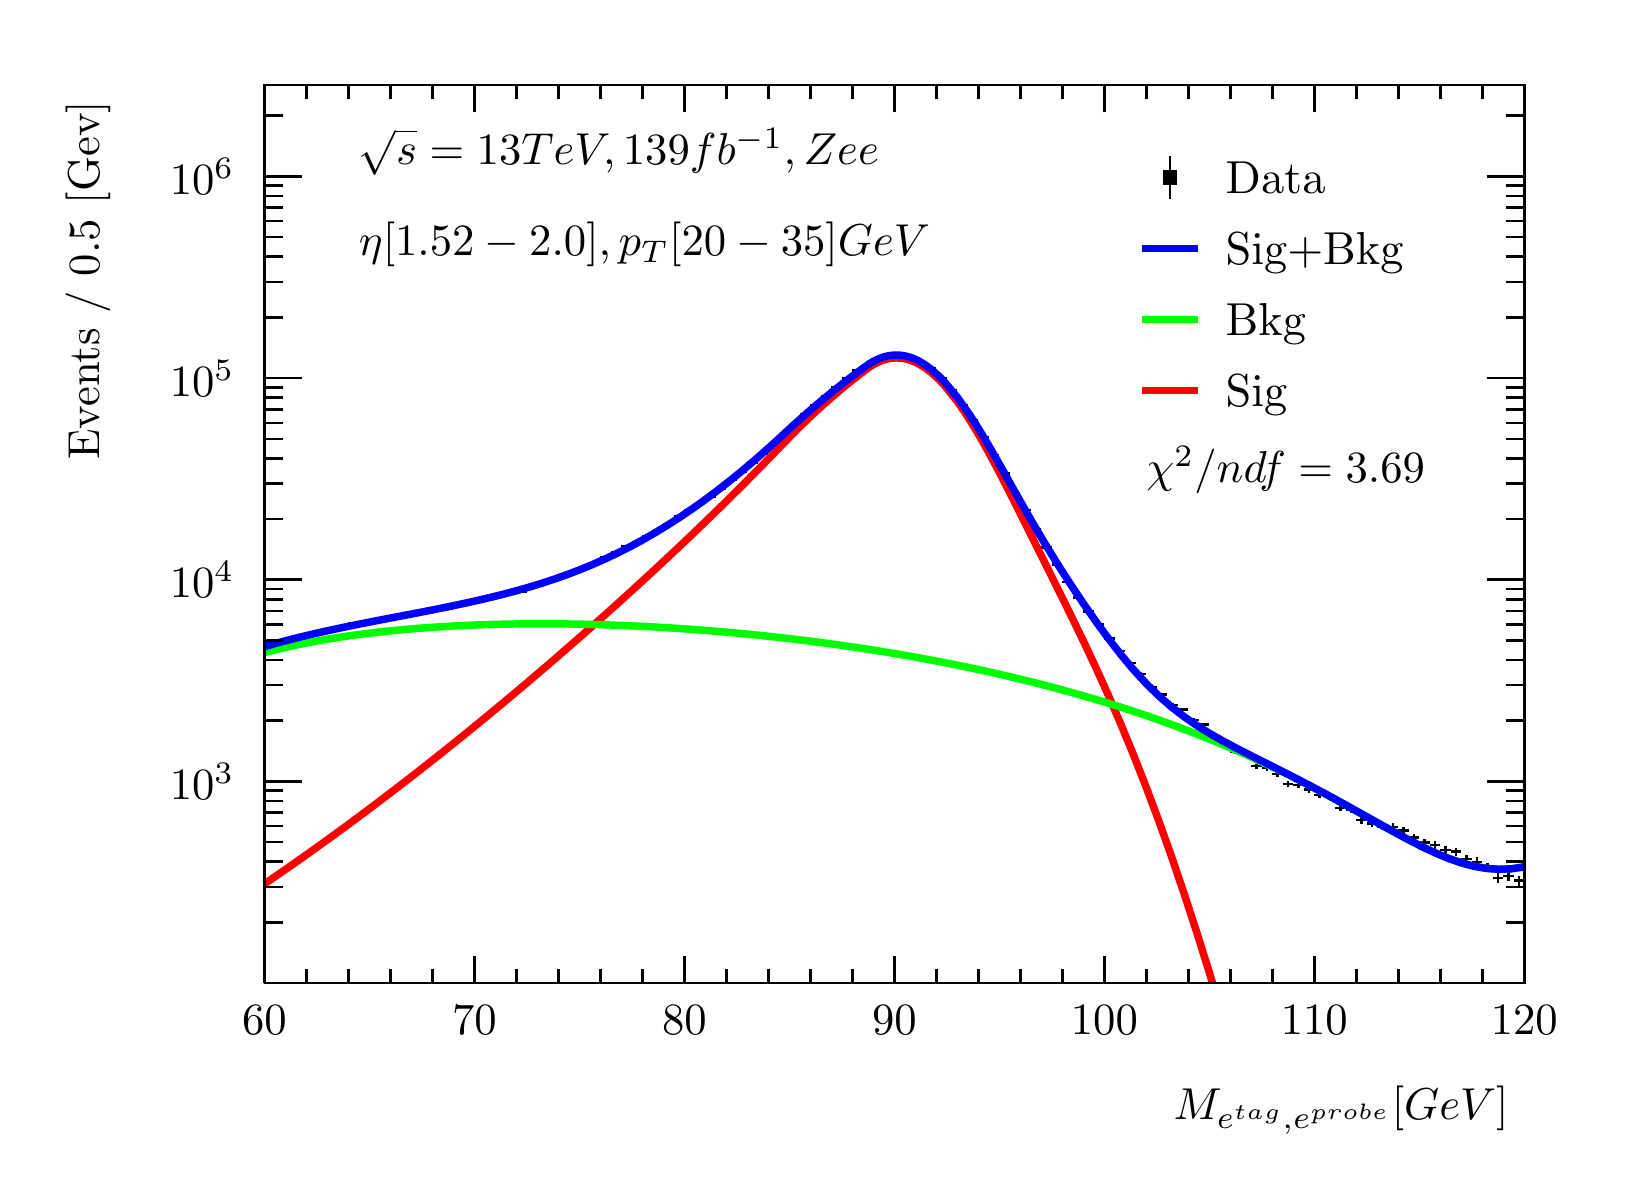
\begin{tikzpicture}
\pgfdeclareplotmark{cross} {
\pgfpathmoveto{\pgfpoint{-0.3\pgfplotmarksize}{\pgfplotmarksize}}
\pgfpathlineto{\pgfpoint{+0.3\pgfplotmarksize}{\pgfplotmarksize}}
\pgfpathlineto{\pgfpoint{+0.3\pgfplotmarksize}{0.3\pgfplotmarksize}}
\pgfpathlineto{\pgfpoint{+1\pgfplotmarksize}{0.3\pgfplotmarksize}}
\pgfpathlineto{\pgfpoint{+1\pgfplotmarksize}{-0.3\pgfplotmarksize}}
\pgfpathlineto{\pgfpoint{+0.3\pgfplotmarksize}{-0.3\pgfplotmarksize}}
\pgfpathlineto{\pgfpoint{+0.3\pgfplotmarksize}{-1.\pgfplotmarksize}}
\pgfpathlineto{\pgfpoint{-0.3\pgfplotmarksize}{-1.\pgfplotmarksize}}
\pgfpathlineto{\pgfpoint{-0.3\pgfplotmarksize}{-0.3\pgfplotmarksize}}
\pgfpathlineto{\pgfpoint{-1.\pgfplotmarksize}{-0.3\pgfplotmarksize}}
\pgfpathlineto{\pgfpoint{-1.\pgfplotmarksize}{0.3\pgfplotmarksize}}
\pgfpathlineto{\pgfpoint{-0.3\pgfplotmarksize}{0.3\pgfplotmarksize}}
\pgfpathclose
\pgfusepathqstroke
}
\pgfdeclareplotmark{cross*} {
\pgfpathmoveto{\pgfpoint{-0.3\pgfplotmarksize}{\pgfplotmarksize}}
\pgfpathlineto{\pgfpoint{+0.3\pgfplotmarksize}{\pgfplotmarksize}}
\pgfpathlineto{\pgfpoint{+0.3\pgfplotmarksize}{0.3\pgfplotmarksize}}
\pgfpathlineto{\pgfpoint{+1\pgfplotmarksize}{0.3\pgfplotmarksize}}
\pgfpathlineto{\pgfpoint{+1\pgfplotmarksize}{-0.3\pgfplotmarksize}}
\pgfpathlineto{\pgfpoint{+0.3\pgfplotmarksize}{-0.3\pgfplotmarksize}}
\pgfpathlineto{\pgfpoint{+0.3\pgfplotmarksize}{-1.\pgfplotmarksize}}
\pgfpathlineto{\pgfpoint{-0.3\pgfplotmarksize}{-1.\pgfplotmarksize}}
\pgfpathlineto{\pgfpoint{-0.3\pgfplotmarksize}{-0.3\pgfplotmarksize}}
\pgfpathlineto{\pgfpoint{-1.\pgfplotmarksize}{-0.3\pgfplotmarksize}}
\pgfpathlineto{\pgfpoint{-1.\pgfplotmarksize}{0.3\pgfplotmarksize}}
\pgfpathlineto{\pgfpoint{-0.3\pgfplotmarksize}{0.3\pgfplotmarksize}}
\pgfpathclose
\pgfusepathqfillstroke
}
\pgfdeclareplotmark{newstar} {
\pgfpathmoveto{\pgfqpoint{0pt}{\pgfplotmarksize}}
\pgfpathlineto{\pgfqpointpolar{44}{0.5\pgfplotmarksize}}
\pgfpathlineto{\pgfqpointpolar{18}{\pgfplotmarksize}}
\pgfpathlineto{\pgfqpointpolar{-20}{0.5\pgfplotmarksize}}
\pgfpathlineto{\pgfqpointpolar{-54}{\pgfplotmarksize}}
\pgfpathlineto{\pgfqpointpolar{-90}{0.5\pgfplotmarksize}}
\pgfpathlineto{\pgfqpointpolar{234}{\pgfplotmarksize}}
\pgfpathlineto{\pgfqpointpolar{198}{0.5\pgfplotmarksize}}
\pgfpathlineto{\pgfqpointpolar{162}{\pgfplotmarksize}}
\pgfpathlineto{\pgfqpointpolar{134}{0.5\pgfplotmarksize}}
\pgfpathclose
\pgfusepathqstroke
}
\pgfdeclareplotmark{newstar*} {
\pgfpathmoveto{\pgfqpoint{0pt}{\pgfplotmarksize}}
\pgfpathlineto{\pgfqpointpolar{44}{0.5\pgfplotmarksize}}
\pgfpathlineto{\pgfqpointpolar{18}{\pgfplotmarksize}}
\pgfpathlineto{\pgfqpointpolar{-20}{0.5\pgfplotmarksize}}
\pgfpathlineto{\pgfqpointpolar{-54}{\pgfplotmarksize}}
\pgfpathlineto{\pgfqpointpolar{-90}{0.5\pgfplotmarksize}}
\pgfpathlineto{\pgfqpointpolar{234}{\pgfplotmarksize}}
\pgfpathlineto{\pgfqpointpolar{198}{0.5\pgfplotmarksize}}
\pgfpathlineto{\pgfqpointpolar{162}{\pgfplotmarksize}}
\pgfpathlineto{\pgfqpointpolar{134}{0.5\pgfplotmarksize}}
\pgfpathclose
\pgfusepathqfillstroke
}
\definecolor{c}{rgb}{1,1,1};
\draw [color=c, fill=c] (0,0) rectangle (20,14.4361);
\draw [color=c, fill=c] (3,2.30977) rectangle (19,13.7143);
\definecolor{c}{rgb}{0,0,0};
\draw [c,line width=0.9] (3,2.30977) -- (3,13.7143) -- (19,13.7143) -- (19,2.30977) -- (3,2.30977);
\definecolor{c}{rgb}{1,1,1};
\draw [color=c, fill=c] (3,2.30977) rectangle (19,13.7143);
\definecolor{c}{rgb}{0,0,0};
\draw [c,line width=0.9] (3,2.30977) -- (3,13.7143) -- (19,13.7143) -- (19,2.30977) -- (3,2.30977);
\draw [c,line width=0.9] (3,2.30977) -- (19,2.30977);
\draw [c,line width=0.9] (3,2.65624) -- (3,2.30977);
\draw [c,line width=0.9] (3.53333,2.48301) -- (3.53333,2.30977);
\draw [c,line width=0.9] (4.06667,2.48301) -- (4.06667,2.30977);
\draw [c,line width=0.9] (4.6,2.48301) -- (4.6,2.30977);
\draw [c,line width=0.9] (5.13333,2.48301) -- (5.13333,2.30977);
\draw [c,line width=0.9] (5.66667,2.65624) -- (5.66667,2.30977);
\draw [c,line width=0.9] (6.2,2.48301) -- (6.2,2.30977);
\draw [c,line width=0.9] (6.73333,2.48301) -- (6.73333,2.30977);
\draw [c,line width=0.9] (7.26667,2.48301) -- (7.26667,2.30977);
\draw [c,line width=0.9] (7.8,2.48301) -- (7.8,2.30977);
\draw [c,line width=0.9] (8.33333,2.65624) -- (8.33333,2.30977);
\draw [c,line width=0.9] (8.86667,2.48301) -- (8.86667,2.30977);
\draw [c,line width=0.9] (9.4,2.48301) -- (9.4,2.30977);
\draw [c,line width=0.9] (9.93333,2.48301) -- (9.93333,2.30977);
\draw [c,line width=0.9] (10.4667,2.48301) -- (10.4667,2.30977);
\draw [c,line width=0.9] (11,2.65624) -- (11,2.30977);
\draw [c,line width=0.9] (11.5333,2.48301) -- (11.5333,2.30977);
\draw [c,line width=0.9] (12.0667,2.48301) -- (12.0667,2.30977);
\draw [c,line width=0.9] (12.6,2.48301) -- (12.6,2.30977);
\draw [c,line width=0.9] (13.1333,2.48301) -- (13.1333,2.30977);
\draw [c,line width=0.9] (13.6667,2.65624) -- (13.6667,2.30977);
\draw [c,line width=0.9] (14.2,2.48301) -- (14.2,2.30977);
\draw [c,line width=0.9] (14.7333,2.48301) -- (14.7333,2.30977);
\draw [c,line width=0.9] (15.2667,2.48301) -- (15.2667,2.30977);
\draw [c,line width=0.9] (15.8,2.48301) -- (15.8,2.30977);
\draw [c,line width=0.9] (16.3333,2.65624) -- (16.3333,2.30977);
\draw [c,line width=0.9] (16.8667,2.48301) -- (16.8667,2.30977);
\draw [c,line width=0.9] (17.4,2.48301) -- (17.4,2.30977);
\draw [c,line width=0.9] (17.9333,2.48301) -- (17.9333,2.30977);
\draw [c,line width=0.9] (18.4667,2.48301) -- (18.4667,2.30977);
\draw [c,line width=0.9] (19,2.65624) -- (19,2.30977);
\draw [anchor=base] (3,1.66015) node[scale=1.61424, color=c, rotate=0]{60};
\draw [anchor=base] (5.66667,1.66015) node[scale=1.61424, color=c, rotate=0]{70};
\draw [anchor=base] (8.33333,1.66015) node[scale=1.61424, color=c, rotate=0]{80};
\draw [anchor=base] (11,1.66015) node[scale=1.61424, color=c, rotate=0]{90};
\draw [anchor=base] (13.6667,1.66015) node[scale=1.61424, color=c, rotate=0]{100};
\draw [anchor=base] (16.3333,1.66015) node[scale=1.61424, color=c, rotate=0]{110};
\draw [anchor=base] (19,1.66015) node[scale=1.61424, color=c, rotate=0]{120};
\draw [anchor= east] (19,0.692932) node[scale=1.61424, color=c, rotate=0]{$M_{e^{tag}, e^{probe}}  [GeV]$};
\draw [c,line width=0.9] (3,13.7143) -- (19,13.7143);
\draw [c,line width=0.9] (3,13.3678) -- (3,13.7143);
\draw [c,line width=0.9] (3.53333,13.5411) -- (3.53333,13.7143);
\draw [c,line width=0.9] (4.06667,13.5411) -- (4.06667,13.7143);
\draw [c,line width=0.9] (4.6,13.5411) -- (4.6,13.7143);
\draw [c,line width=0.9] (5.13333,13.5411) -- (5.13333,13.7143);
\draw [c,line width=0.9] (5.66667,13.3678) -- (5.66667,13.7143);
\draw [c,line width=0.9] (6.2,13.5411) -- (6.2,13.7143);
\draw [c,line width=0.9] (6.73333,13.5411) -- (6.73333,13.7143);
\draw [c,line width=0.9] (7.26667,13.5411) -- (7.26667,13.7143);
\draw [c,line width=0.9] (7.8,13.5411) -- (7.8,13.7143);
\draw [c,line width=0.9] (8.33333,13.3678) -- (8.33333,13.7143);
\draw [c,line width=0.9] (8.86667,13.5411) -- (8.86667,13.7143);
\draw [c,line width=0.9] (9.4,13.5411) -- (9.4,13.7143);
\draw [c,line width=0.9] (9.93333,13.5411) -- (9.93333,13.7143);
\draw [c,line width=0.9] (10.4667,13.5411) -- (10.4667,13.7143);
\draw [c,line width=0.9] (11,13.3678) -- (11,13.7143);
\draw [c,line width=0.9] (11.5333,13.5411) -- (11.5333,13.7143);
\draw [c,line width=0.9] (12.0667,13.5411) -- (12.0667,13.7143);
\draw [c,line width=0.9] (12.6,13.5411) -- (12.6,13.7143);
\draw [c,line width=0.9] (13.1333,13.5411) -- (13.1333,13.7143);
\draw [c,line width=0.9] (13.6667,13.3678) -- (13.6667,13.7143);
\draw [c,line width=0.9] (14.2,13.5411) -- (14.2,13.7143);
\draw [c,line width=0.9] (14.7333,13.5411) -- (14.7333,13.7143);
\draw [c,line width=0.9] (15.2667,13.5411) -- (15.2667,13.7143);
\draw [c,line width=0.9] (15.8,13.5411) -- (15.8,13.7143);
\draw [c,line width=0.9] (16.3333,13.3678) -- (16.3333,13.7143);
\draw [c,line width=0.9] (16.8667,13.5411) -- (16.8667,13.7143);
\draw [c,line width=0.9] (17.4,13.5411) -- (17.4,13.7143);
\draw [c,line width=0.9] (17.9333,13.5411) -- (17.9333,13.7143);
\draw [c,line width=0.9] (18.4667,13.5411) -- (18.4667,13.7143);
\draw [c,line width=0.9] (19,13.3678) -- (19,13.7143);
\draw [c,line width=0.9] (3,2.30977) -- (3,13.7143);
\draw [c,line width=0.9] (3.237,3.08073) -- (3,3.08073);
\draw [c,line width=0.9] (3.237,3.53171) -- (3,3.53171);
\draw [c,line width=0.9] (3.237,3.85168) -- (3,3.85168);
\draw [c,line width=0.9] (3.237,4.09988) -- (3,4.09988);
\draw [c,line width=0.9] (3.237,4.30266) -- (3,4.30266);
\draw [c,line width=0.9] (3.237,4.47412) -- (3,4.47412);
\draw [c,line width=0.9] (3.237,4.62264) -- (3,4.62264);
\draw [c,line width=0.9] (3.237,4.75364) -- (3,4.75364);
\draw [c,line width=0.9] (3.474,4.87083) -- (3,4.87083);
\draw [anchor= east] (2.82,4.87083) node[scale=1.61424, color=c, rotate=0]{$10^{3}$};
\draw [c,line width=0.9] (3.237,5.64179) -- (3,5.64179);
\draw [c,line width=0.9] (3.237,6.09277) -- (3,6.09277);
\draw [c,line width=0.9] (3.237,6.41274) -- (3,6.41274);
\draw [c,line width=0.9] (3.237,6.66093) -- (3,6.66093);
\draw [c,line width=0.9] (3.237,6.86372) -- (3,6.86372);
\draw [c,line width=0.9] (3.237,7.03518) -- (3,7.03518);
\draw [c,line width=0.9] (3.237,7.1837) -- (3,7.1837);
\draw [c,line width=0.9] (3.237,7.3147) -- (3,7.3147);
\draw [c,line width=0.9] (3.474,7.43189) -- (3,7.43189);
\draw [anchor= east] (2.82,7.43189) node[scale=1.61424, color=c, rotate=0]{$10^{4}$};
\draw [c,line width=0.9] (3.237,8.20285) -- (3,8.20285);
\draw [c,line width=0.9] (3.237,8.65383) -- (3,8.65383);
\draw [c,line width=0.9] (3.237,8.9738) -- (3,8.9738);
\draw [c,line width=0.9] (3.237,9.22199) -- (3,9.22199);
\draw [c,line width=0.9] (3.237,9.42478) -- (3,9.42478);
\draw [c,line width=0.9] (3.237,9.59624) -- (3,9.59624);
\draw [c,line width=0.9] (3.237,9.74476) -- (3,9.74476);
\draw [c,line width=0.9] (3.237,9.87576) -- (3,9.87576);
\draw [c,line width=0.9] (3.474,9.99295) -- (3,9.99295);
\draw [anchor= east] (2.82,9.99295) node[scale=1.61424, color=c, rotate=0]{$10^{5}$};
\draw [c,line width=0.9] (3.237,10.7639) -- (3,10.7639);
\draw [c,line width=0.9] (3.237,11.2149) -- (3,11.2149);
\draw [c,line width=0.9] (3.237,11.5349) -- (3,11.5349);
\draw [c,line width=0.9] (3.237,11.7831) -- (3,11.7831);
\draw [c,line width=0.9] (3.237,11.9858) -- (3,11.9858);
\draw [c,line width=0.9] (3.237,12.1573) -- (3,12.1573);
\draw [c,line width=0.9] (3.237,12.3058) -- (3,12.3058);
\draw [c,line width=0.9] (3.237,12.4368) -- (3,12.4368);
\draw [c,line width=0.9] (3.474,12.554) -- (3,12.554);
\draw [anchor= east] (2.82,12.554) node[scale=1.61424, color=c, rotate=0]{$10^{6}$};
\draw [c,line width=0.9] (3.237,13.325) -- (3,13.325);
\draw [anchor= east] (0.76,13.7143) node[scale=1.61424, color=c, rotate=90]{Events / 0.5 [Gev]};
\draw [c,line width=0.9] (19,2.30977) -- (19,13.7143);
\draw [c,line width=0.9] (18.763,3.08073) -- (19,3.08073);
\draw [c,line width=0.9] (18.763,3.53171) -- (19,3.53171);
\draw [c,line width=0.9] (18.763,3.85168) -- (19,3.85168);
\draw [c,line width=0.9] (18.763,4.09988) -- (19,4.09988);
\draw [c,line width=0.9] (18.763,4.30266) -- (19,4.30266);
\draw [c,line width=0.9] (18.763,4.47412) -- (19,4.47412);
\draw [c,line width=0.9] (18.763,4.62264) -- (19,4.62264);
\draw [c,line width=0.9] (18.763,4.75364) -- (19,4.75364);
\draw [c,line width=0.9] (18.526,4.87083) -- (19,4.87083);
\draw [c,line width=0.9] (18.763,5.64179) -- (19,5.64179);
\draw [c,line width=0.9] (18.763,6.09277) -- (19,6.09277);
\draw [c,line width=0.9] (18.763,6.41274) -- (19,6.41274);
\draw [c,line width=0.9] (18.763,6.66093) -- (19,6.66093);
\draw [c,line width=0.9] (18.763,6.86372) -- (19,6.86372);
\draw [c,line width=0.9] (18.763,7.03518) -- (19,7.03518);
\draw [c,line width=0.9] (18.763,7.1837) -- (19,7.1837);
\draw [c,line width=0.9] (18.763,7.3147) -- (19,7.3147);
\draw [c,line width=0.9] (18.526,7.43189) -- (19,7.43189);
\draw [c,line width=0.9] (18.763,8.20285) -- (19,8.20285);
\draw [c,line width=0.9] (18.763,8.65383) -- (19,8.65383);
\draw [c,line width=0.9] (18.763,8.9738) -- (19,8.9738);
\draw [c,line width=0.9] (18.763,9.22199) -- (19,9.22199);
\draw [c,line width=0.9] (18.763,9.42478) -- (19,9.42478);
\draw [c,line width=0.9] (18.763,9.59624) -- (19,9.59624);
\draw [c,line width=0.9] (18.763,9.74476) -- (19,9.74476);
\draw [c,line width=0.9] (18.763,9.87576) -- (19,9.87576);
\draw [c,line width=0.9] (18.526,9.99295) -- (19,9.99295);
\draw [c,line width=0.9] (18.763,10.7639) -- (19,10.7639);
\draw [c,line width=0.9] (18.763,11.2149) -- (19,11.2149);
\draw [c,line width=0.9] (18.763,11.5349) -- (19,11.5349);
\draw [c,line width=0.9] (18.763,11.7831) -- (19,11.7831);
\draw [c,line width=0.9] (18.763,11.9858) -- (19,11.9858);
\draw [c,line width=0.9] (18.763,12.1573) -- (19,12.1573);
\draw [c,line width=0.9] (18.763,12.3058) -- (19,12.3058);
\draw [c,line width=0.9] (18.763,12.4368) -- (19,12.4368);
\draw [c,line width=0.9] (18.526,12.554) -- (19,12.554);
\draw [c,line width=0.9] (18.763,13.325) -- (19,13.325);
\draw [c,line width=0.9] (3.06667,6.61437) -- (3,6.61437);
\draw [c,line width=0.9] (3,6.61437) -- (3,6.61437);
\draw [c,line width=0.9] (3.06667,6.61437) -- (3.13333,6.61437);
\draw [c,line width=0.9] (3.13333,6.61437) -- (3.13333,6.61437);
\draw [c,line width=0.9] (3.06667,6.61437) -- (3.06667,6.63043);
\draw [c,line width=0.9] (3.06667,6.63043) -- (3.06667,6.63043);
\draw [c,line width=0.9] (3.06667,6.61437) -- (3.06667,6.59831);
\draw [c,line width=0.9] (3.06667,6.59831) -- (3.06667,6.59831);
\draw [c,line width=0.9] (3.2,6.65312) -- (3.13333,6.65312);
\draw [c,line width=0.9] (3.13333,6.65312) -- (3.13333,6.65312);
\draw [c,line width=0.9] (3.2,6.65312) -- (3.26667,6.65312);
\draw [c,line width=0.9] (3.26667,6.65312) -- (3.26667,6.65312);
\draw [c,line width=0.9] (3.2,6.65312) -- (3.2,6.66891);
\draw [c,line width=0.9] (3.2,6.66891) -- (3.2,6.66891);
\draw [c,line width=0.9] (3.2,6.65312) -- (3.2,6.63734);
\draw [c,line width=0.9] (3.2,6.63734) -- (3.2,6.63734);
\draw [c,line width=0.9] (3.33333,6.68187) -- (3.26667,6.68187);
\draw [c,line width=0.9] (3.26667,6.68187) -- (3.26667,6.68187);
\draw [c,line width=0.9] (3.33333,6.68187) -- (3.4,6.68187);
\draw [c,line width=0.9] (3.4,6.68187) -- (3.4,6.68187);
\draw [c,line width=0.9] (3.33333,6.68187) -- (3.33333,6.69745);
\draw [c,line width=0.9] (3.33333,6.69745) -- (3.33333,6.69745);
\draw [c,line width=0.9] (3.33333,6.68187) -- (3.33333,6.66629);
\draw [c,line width=0.9] (3.33333,6.66629) -- (3.33333,6.66629);
\draw [c,line width=0.9] (3.46667,6.70776) -- (3.4,6.70776);
\draw [c,line width=0.9] (3.4,6.70776) -- (3.4,6.70776);
\draw [c,line width=0.9] (3.46667,6.70776) -- (3.53333,6.70776);
\draw [c,line width=0.9] (3.53333,6.70776) -- (3.53333,6.70776);
\draw [c,line width=0.9] (3.46667,6.70776) -- (3.46667,6.72317);
\draw [c,line width=0.9] (3.46667,6.72317) -- (3.46667,6.72317);
\draw [c,line width=0.9] (3.46667,6.70776) -- (3.46667,6.69236);
\draw [c,line width=0.9] (3.46667,6.69236) -- (3.46667,6.69236);
\draw [c,line width=0.9] (3.6,6.73744) -- (3.53333,6.73744);
\draw [c,line width=0.9] (3.53333,6.73744) -- (3.53333,6.73744);
\draw [c,line width=0.9] (3.6,6.73744) -- (3.66667,6.73744);
\draw [c,line width=0.9] (3.66667,6.73744) -- (3.66667,6.73744);
\draw [c,line width=0.9] (3.6,6.73744) -- (3.6,6.75263);
\draw [c,line width=0.9] (3.6,6.75263) -- (3.6,6.75263);
\draw [c,line width=0.9] (3.6,6.73744) -- (3.6,6.72224);
\draw [c,line width=0.9] (3.6,6.72224) -- (3.6,6.72224);
\draw [c,line width=0.9] (3.73333,6.78041) -- (3.66667,6.78041);
\draw [c,line width=0.9] (3.66667,6.78041) -- (3.66667,6.78041);
\draw [c,line width=0.9] (3.73333,6.78041) -- (3.8,6.78041);
\draw [c,line width=0.9] (3.8,6.78041) -- (3.8,6.78041);
\draw [c,line width=0.9] (3.73333,6.78041) -- (3.73333,6.79532);
\draw [c,line width=0.9] (3.73333,6.79532) -- (3.73333,6.79532);
\draw [c,line width=0.9] (3.73333,6.78041) -- (3.73333,6.76551);
\draw [c,line width=0.9] (3.73333,6.76551) -- (3.73333,6.76551);
\draw [c,line width=0.9] (3.86667,6.81561) -- (3.8,6.81561);
\draw [c,line width=0.9] (3.8,6.81561) -- (3.8,6.81561);
\draw [c,line width=0.9] (3.86667,6.81561) -- (3.93333,6.81561);
\draw [c,line width=0.9] (3.93333,6.81561) -- (3.93333,6.81561);
\draw [c,line width=0.9] (3.86667,6.81561) -- (3.86667,6.83029);
\draw [c,line width=0.9] (3.86667,6.83029) -- (3.86667,6.83029);
\draw [c,line width=0.9] (3.86667,6.81561) -- (3.86667,6.80094);
\draw [c,line width=0.9] (3.86667,6.80094) -- (3.86667,6.80094);
\draw [c,line width=0.9] (4,6.82352) -- (3.93333,6.82352);
\draw [c,line width=0.9] (3.93333,6.82352) -- (3.93333,6.82352);
\draw [c,line width=0.9] (4,6.82352) -- (4.06667,6.82352);
\draw [c,line width=0.9] (4.06667,6.82352) -- (4.06667,6.82352);
\draw [c,line width=0.9] (4,6.82352) -- (4,6.83814);
\draw [c,line width=0.9] (4,6.83814) -- (4,6.83814);
\draw [c,line width=0.9] (4,6.82352) -- (4,6.8089);
\draw [c,line width=0.9] (4,6.8089) -- (4,6.8089);
\draw [c,line width=0.9] (4.13333,6.88484) -- (4.06667,6.88484);
\draw [c,line width=0.9] (4.06667,6.88484) -- (4.06667,6.88484);
\draw [c,line width=0.9] (4.13333,6.88484) -- (4.2,6.88484);
\draw [c,line width=0.9] (4.2,6.88484) -- (4.2,6.88484);
\draw [c,line width=0.9] (4.13333,6.88484) -- (4.13333,6.89906);
\draw [c,line width=0.9] (4.13333,6.89906) -- (4.13333,6.89906);
\draw [c,line width=0.9] (4.13333,6.88484) -- (4.13333,6.87062);
\draw [c,line width=0.9] (4.13333,6.87062) -- (4.13333,6.87062);
\draw [c,line width=0.9] (4.26667,6.88575) -- (4.2,6.88575);
\draw [c,line width=0.9] (4.2,6.88575) -- (4.2,6.88575);
\draw [c,line width=0.9] (4.26667,6.88575) -- (4.33333,6.88575);
\draw [c,line width=0.9] (4.33333,6.88575) -- (4.33333,6.88575);
\draw [c,line width=0.9] (4.26667,6.88575) -- (4.26667,6.89997);
\draw [c,line width=0.9] (4.26667,6.89997) -- (4.26667,6.89997);
\draw [c,line width=0.9] (4.26667,6.88575) -- (4.26667,6.87153);
\draw [c,line width=0.9] (4.26667,6.87153) -- (4.26667,6.87153);
\draw [c,line width=0.9] (4.4,6.89372) -- (4.33333,6.89372);
\draw [c,line width=0.9] (4.33333,6.89372) -- (4.33333,6.89372);
\draw [c,line width=0.9] (4.4,6.89372) -- (4.46667,6.89372);
\draw [c,line width=0.9] (4.46667,6.89372) -- (4.46667,6.89372);
\draw [c,line width=0.9] (4.4,6.89372) -- (4.4,6.90788);
\draw [c,line width=0.9] (4.4,6.90788) -- (4.4,6.90788);
\draw [c,line width=0.9] (4.4,6.89372) -- (4.4,6.87955);
\draw [c,line width=0.9] (4.4,6.87955) -- (4.4,6.87955);
\draw [c,line width=0.9] (4.53333,6.90877) -- (4.46667,6.90877);
\draw [c,line width=0.9] (4.46667,6.90877) -- (4.46667,6.90877);
\draw [c,line width=0.9] (4.53333,6.90877) -- (4.6,6.90877);
\draw [c,line width=0.9] (4.6,6.90877) -- (4.6,6.90877);
\draw [c,line width=0.9] (4.53333,6.90877) -- (4.53333,6.92284);
\draw [c,line width=0.9] (4.53333,6.92284) -- (4.53333,6.92284);
\draw [c,line width=0.9] (4.53333,6.90877) -- (4.53333,6.8947);
\draw [c,line width=0.9] (4.53333,6.8947) -- (4.53333,6.8947);
\draw [c,line width=0.9] (4.66667,6.93516) -- (4.6,6.93516);
\draw [c,line width=0.9] (4.6,6.93516) -- (4.6,6.93516);
\draw [c,line width=0.9] (4.66667,6.93516) -- (4.73333,6.93516);
\draw [c,line width=0.9] (4.73333,6.93516) -- (4.73333,6.93516);
\draw [c,line width=0.9] (4.66667,6.93516) -- (4.66667,6.94906);
\draw [c,line width=0.9] (4.66667,6.94906) -- (4.66667,6.94906);
\draw [c,line width=0.9] (4.66667,6.93516) -- (4.66667,6.92125);
\draw [c,line width=0.9] (4.66667,6.92125) -- (4.66667,6.92125);
\draw [c,line width=0.9] (4.8,6.96838) -- (4.73333,6.96838);
\draw [c,line width=0.9] (4.73333,6.96838) -- (4.73333,6.96838);
\draw [c,line width=0.9] (4.8,6.96838) -- (4.86667,6.96838);
\draw [c,line width=0.9] (4.86667,6.96838) -- (4.86667,6.96838);
\draw [c,line width=0.9] (4.8,6.96838) -- (4.8,6.98208);
\draw [c,line width=0.9] (4.8,6.98208) -- (4.8,6.98208);
\draw [c,line width=0.9] (4.8,6.96838) -- (4.8,6.95468);
\draw [c,line width=0.9] (4.8,6.95468) -- (4.8,6.95468);
\draw [c,line width=0.9] (4.93333,6.99572) -- (4.86667,6.99572);
\draw [c,line width=0.9] (4.86667,6.99572) -- (4.86667,6.99572);
\draw [c,line width=0.9] (4.93333,6.99572) -- (5,6.99572);
\draw [c,line width=0.9] (5,6.99572) -- (5,6.99572);
\draw [c,line width=0.9] (4.93333,6.99572) -- (4.93333,7.00925);
\draw [c,line width=0.9] (4.93333,7.00925) -- (4.93333,7.00925);
\draw [c,line width=0.9] (4.93333,6.99572) -- (4.93333,6.98218);
\draw [c,line width=0.9] (4.93333,6.98218) -- (4.93333,6.98218);
\draw [c,line width=0.9] (5.06667,7.0288) -- (5,7.0288);
\draw [c,line width=0.9] (5,7.0288) -- (5,7.0288);
\draw [c,line width=0.9] (5.06667,7.0288) -- (5.13333,7.0288);
\draw [c,line width=0.9] (5.13333,7.0288) -- (5.13333,7.0288);
\draw [c,line width=0.9] (5.06667,7.0288) -- (5.06667,7.04214);
\draw [c,line width=0.9] (5.06667,7.04214) -- (5.06667,7.04214);
\draw [c,line width=0.9] (5.06667,7.0288) -- (5.06667,7.01547);
\draw [c,line width=0.9] (5.06667,7.01547) -- (5.06667,7.01547);
\draw [c,line width=0.9] (5.2,7.06218) -- (5.13333,7.06218);
\draw [c,line width=0.9] (5.13333,7.06218) -- (5.13333,7.06218);
\draw [c,line width=0.9] (5.2,7.06218) -- (5.26667,7.06218);
\draw [c,line width=0.9] (5.26667,7.06218) -- (5.26667,7.06218);
\draw [c,line width=0.9] (5.2,7.06218) -- (5.2,7.07531);
\draw [c,line width=0.9] (5.2,7.07531) -- (5.2,7.07531);
\draw [c,line width=0.9] (5.2,7.06218) -- (5.2,7.04904);
\draw [c,line width=0.9] (5.2,7.04904) -- (5.2,7.04904);
\draw [c,line width=0.9] (5.33333,7.06342) -- (5.26667,7.06342);
\draw [c,line width=0.9] (5.26667,7.06342) -- (5.26667,7.06342);
\draw [c,line width=0.9] (5.33333,7.06342) -- (5.4,7.06342);
\draw [c,line width=0.9] (5.4,7.06342) -- (5.4,7.06342);
\draw [c,line width=0.9] (5.33333,7.06342) -- (5.33333,7.07654);
\draw [c,line width=0.9] (5.33333,7.07654) -- (5.33333,7.07654);
\draw [c,line width=0.9] (5.33333,7.06342) -- (5.33333,7.05029);
\draw [c,line width=0.9] (5.33333,7.05029) -- (5.33333,7.05029);
\draw [c,line width=0.9] (5.46667,7.09639) -- (5.4,7.09639);
\draw [c,line width=0.9] (5.4,7.09639) -- (5.4,7.09639);
\draw [c,line width=0.9] (5.46667,7.09639) -- (5.53333,7.09639);
\draw [c,line width=0.9] (5.53333,7.09639) -- (5.53333,7.09639);
\draw [c,line width=0.9] (5.46667,7.09639) -- (5.46667,7.10932);
\draw [c,line width=0.9] (5.46667,7.10932) -- (5.46667,7.10932);
\draw [c,line width=0.9] (5.46667,7.09639) -- (5.46667,7.08345);
\draw [c,line width=0.9] (5.46667,7.08345) -- (5.46667,7.08345);
\draw [c,line width=0.9] (5.6,7.15211) -- (5.53333,7.15211);
\draw [c,line width=0.9] (5.53333,7.15211) -- (5.53333,7.15211);
\draw [c,line width=0.9] (5.6,7.15211) -- (5.66667,7.15211);
\draw [c,line width=0.9] (5.66667,7.15211) -- (5.66667,7.15211);
\draw [c,line width=0.9] (5.6,7.15211) -- (5.6,7.16472);
\draw [c,line width=0.9] (5.6,7.16472) -- (5.6,7.16472);
\draw [c,line width=0.9] (5.6,7.15211) -- (5.6,7.1395);
\draw [c,line width=0.9] (5.6,7.1395) -- (5.6,7.1395);
\draw [c,line width=0.9] (5.73333,7.16009) -- (5.66667,7.16009);
\draw [c,line width=0.9] (5.66667,7.16009) -- (5.66667,7.16009);
\draw [c,line width=0.9] (5.73333,7.16009) -- (5.8,7.16009);
\draw [c,line width=0.9] (5.8,7.16009) -- (5.8,7.16009);
\draw [c,line width=0.9] (5.73333,7.16009) -- (5.73333,7.17266);
\draw [c,line width=0.9] (5.73333,7.17266) -- (5.73333,7.17266);
\draw [c,line width=0.9] (5.73333,7.16009) -- (5.73333,7.14753);
\draw [c,line width=0.9] (5.73333,7.14753) -- (5.73333,7.14753);
\draw [c,line width=0.9] (5.86667,7.18952) -- (5.8,7.18952);
\draw [c,line width=0.9] (5.8,7.18952) -- (5.8,7.18952);
\draw [c,line width=0.9] (5.86667,7.18952) -- (5.93333,7.18952);
\draw [c,line width=0.9] (5.93333,7.18952) -- (5.93333,7.18952);
\draw [c,line width=0.9] (5.86667,7.18952) -- (5.86667,7.20193);
\draw [c,line width=0.9] (5.86667,7.20193) -- (5.86667,7.20193);
\draw [c,line width=0.9] (5.86667,7.18952) -- (5.86667,7.17712);
\draw [c,line width=0.9] (5.86667,7.17712) -- (5.86667,7.17712);
\draw [c,line width=0.9] (6,7.22679) -- (5.93333,7.22679);
\draw [c,line width=0.9] (5.93333,7.22679) -- (5.93333,7.22679);
\draw [c,line width=0.9] (6,7.22679) -- (6.06667,7.22679);
\draw [c,line width=0.9] (6.06667,7.22679) -- (6.06667,7.22679);
\draw [c,line width=0.9] (6,7.22679) -- (6,7.23898);
\draw [c,line width=0.9] (6,7.23898) -- (6,7.23898);
\draw [c,line width=0.9] (6,7.22679) -- (6,7.21459);
\draw [c,line width=0.9] (6,7.21459) -- (6,7.21459);
\draw [c,line width=0.9] (6.13333,7.25947) -- (6.06667,7.25947);
\draw [c,line width=0.9] (6.06667,7.25947) -- (6.06667,7.25947);
\draw [c,line width=0.9] (6.13333,7.25947) -- (6.2,7.25947);
\draw [c,line width=0.9] (6.2,7.25947) -- (6.2,7.25947);
\draw [c,line width=0.9] (6.13333,7.25947) -- (6.13333,7.27149);
\draw [c,line width=0.9] (6.13333,7.27149) -- (6.13333,7.27149);
\draw [c,line width=0.9] (6.13333,7.25947) -- (6.13333,7.24745);
\draw [c,line width=0.9] (6.13333,7.24745) -- (6.13333,7.24745);
\draw [c,line width=0.9] (6.26667,7.28223) -- (6.2,7.28223);
\draw [c,line width=0.9] (6.2,7.28223) -- (6.2,7.28223);
\draw [c,line width=0.9] (6.26667,7.28223) -- (6.33333,7.28223);
\draw [c,line width=0.9] (6.33333,7.28223) -- (6.33333,7.28223);
\draw [c,line width=0.9] (6.26667,7.28223) -- (6.26667,7.29412);
\draw [c,line width=0.9] (6.26667,7.29412) -- (6.26667,7.29412);
\draw [c,line width=0.9] (6.26667,7.28223) -- (6.26667,7.27033);
\draw [c,line width=0.9] (6.26667,7.27033) -- (6.26667,7.27033);
\draw [c,line width=0.9] (6.4,7.3594) -- (6.33333,7.3594);
\draw [c,line width=0.9] (6.33333,7.3594) -- (6.33333,7.3594);
\draw [c,line width=0.9] (6.4,7.3594) -- (6.46667,7.3594);
\draw [c,line width=0.9] (6.46667,7.3594) -- (6.46667,7.3594);
\draw [c,line width=0.9] (6.4,7.3594) -- (6.4,7.37089);
\draw [c,line width=0.9] (6.4,7.37089) -- (6.4,7.37089);
\draw [c,line width=0.9] (6.4,7.3594) -- (6.4,7.34791);
\draw [c,line width=0.9] (6.4,7.34791) -- (6.4,7.34791);
\draw [c,line width=0.9] (6.53333,7.39675) -- (6.46667,7.39675);
\draw [c,line width=0.9] (6.46667,7.39675) -- (6.46667,7.39675);
\draw [c,line width=0.9] (6.53333,7.39675) -- (6.6,7.39675);
\draw [c,line width=0.9] (6.6,7.39675) -- (6.6,7.39675);
\draw [c,line width=0.9] (6.53333,7.39675) -- (6.53333,7.40805);
\draw [c,line width=0.9] (6.53333,7.40805) -- (6.53333,7.40805);
\draw [c,line width=0.9] (6.53333,7.39675) -- (6.53333,7.38545);
\draw [c,line width=0.9] (6.53333,7.38545) -- (6.53333,7.38545);
\draw [c,line width=0.9] (6.66667,7.44725) -- (6.6,7.44725);
\draw [c,line width=0.9] (6.6,7.44725) -- (6.6,7.44725);
\draw [c,line width=0.9] (6.66667,7.44725) -- (6.73333,7.44725);
\draw [c,line width=0.9] (6.73333,7.44725) -- (6.73333,7.44725);
\draw [c,line width=0.9] (6.66667,7.44725) -- (6.66667,7.45829);
\draw [c,line width=0.9] (6.66667,7.45829) -- (6.66667,7.45829);
\draw [c,line width=0.9] (6.66667,7.44725) -- (6.66667,7.4362);
\draw [c,line width=0.9] (6.66667,7.4362) -- (6.66667,7.4362);
\draw [c,line width=0.9] (6.8,7.48) -- (6.73333,7.48);
\draw [c,line width=0.9] (6.73333,7.48) -- (6.73333,7.48);
\draw [c,line width=0.9] (6.8,7.48) -- (6.86667,7.48);
\draw [c,line width=0.9] (6.86667,7.48) -- (6.86667,7.48);
\draw [c,line width=0.9] (6.8,7.48) -- (6.8,7.49088);
\draw [c,line width=0.9] (6.8,7.49088) -- (6.8,7.49088);
\draw [c,line width=0.9] (6.8,7.48) -- (6.8,7.46911);
\draw [c,line width=0.9] (6.8,7.46911) -- (6.8,7.46911);
\draw [c,line width=0.9] (6.93333,7.54063) -- (6.86667,7.54063);
\draw [c,line width=0.9] (6.86667,7.54063) -- (6.86667,7.54063);
\draw [c,line width=0.9] (6.93333,7.54063) -- (7,7.54063);
\draw [c,line width=0.9] (7,7.54063) -- (7,7.54063);
\draw [c,line width=0.9] (6.93333,7.54063) -- (6.93333,7.55122);
\draw [c,line width=0.9] (6.93333,7.55122) -- (6.93333,7.55122);
\draw [c,line width=0.9] (6.93333,7.54063) -- (6.93333,7.53004);
\draw [c,line width=0.9] (6.93333,7.53004) -- (6.93333,7.53004);
\draw [c,line width=0.9] (7.06667,7.58773) -- (7,7.58773);
\draw [c,line width=0.9] (7,7.58773) -- (7,7.58773);
\draw [c,line width=0.9] (7.06667,7.58773) -- (7.13333,7.58773);
\draw [c,line width=0.9] (7.13333,7.58773) -- (7.13333,7.58773);
\draw [c,line width=0.9] (7.06667,7.58773) -- (7.06667,7.5981);
\draw [c,line width=0.9] (7.06667,7.5981) -- (7.06667,7.5981);
\draw [c,line width=0.9] (7.06667,7.58773) -- (7.06667,7.57736);
\draw [c,line width=0.9] (7.06667,7.57736) -- (7.06667,7.57736);
\draw [c,line width=0.9] (7.2,7.64428) -- (7.13333,7.64428);
\draw [c,line width=0.9] (7.13333,7.64428) -- (7.13333,7.64428);
\draw [c,line width=0.9] (7.2,7.64428) -- (7.26667,7.64428);
\draw [c,line width=0.9] (7.26667,7.64428) -- (7.26667,7.64428);
\draw [c,line width=0.9] (7.2,7.64428) -- (7.2,7.65439);
\draw [c,line width=0.9] (7.2,7.65439) -- (7.2,7.65439);
\draw [c,line width=0.9] (7.2,7.64428) -- (7.2,7.63417);
\draw [c,line width=0.9] (7.2,7.63417) -- (7.2,7.63417);
\draw [c,line width=0.9] (7.33333,7.71787) -- (7.26667,7.71787);
\draw [c,line width=0.9] (7.26667,7.71787) -- (7.26667,7.71787);
\draw [c,line width=0.9] (7.33333,7.71787) -- (7.4,7.71787);
\draw [c,line width=0.9] (7.4,7.71787) -- (7.4,7.71787);
\draw [c,line width=0.9] (7.33333,7.71787) -- (7.33333,7.72765);
\draw [c,line width=0.9] (7.33333,7.72765) -- (7.33333,7.72765);
\draw [c,line width=0.9] (7.33333,7.71787) -- (7.33333,7.70809);
\draw [c,line width=0.9] (7.33333,7.70809) -- (7.33333,7.70809);
\draw [c,line width=0.9] (7.46667,7.77773) -- (7.4,7.77773);
\draw [c,line width=0.9] (7.4,7.77773) -- (7.4,7.77773);
\draw [c,line width=0.9] (7.46667,7.77773) -- (7.53333,7.77773);
\draw [c,line width=0.9] (7.53333,7.77773) -- (7.53333,7.77773);
\draw [c,line width=0.9] (7.46667,7.77773) -- (7.46667,7.78725);
\draw [c,line width=0.9] (7.46667,7.78725) -- (7.46667,7.78725);
\draw [c,line width=0.9] (7.46667,7.77773) -- (7.46667,7.76821);
\draw [c,line width=0.9] (7.46667,7.76821) -- (7.46667,7.76821);
\draw [c,line width=0.9] (7.6,7.85144) -- (7.53333,7.85144);
\draw [c,line width=0.9] (7.53333,7.85144) -- (7.53333,7.85144);
\draw [c,line width=0.9] (7.6,7.85144) -- (7.66667,7.85144);
\draw [c,line width=0.9] (7.66667,7.85144) -- (7.66667,7.85144);
\draw [c,line width=0.9] (7.6,7.85144) -- (7.6,7.86065);
\draw [c,line width=0.9] (7.6,7.86065) -- (7.6,7.86065);
\draw [c,line width=0.9] (7.6,7.85144) -- (7.6,7.84223);
\draw [c,line width=0.9] (7.6,7.84223) -- (7.6,7.84223);
\draw [c,line width=0.9] (7.73333,7.90184) -- (7.66667,7.90184);
\draw [c,line width=0.9] (7.66667,7.90184) -- (7.66667,7.90184);
\draw [c,line width=0.9] (7.73333,7.90184) -- (7.8,7.90184);
\draw [c,line width=0.9] (7.8,7.90184) -- (7.8,7.90184);
\draw [c,line width=0.9] (7.73333,7.90184) -- (7.73333,7.91084);
\draw [c,line width=0.9] (7.73333,7.91084) -- (7.73333,7.91084);
\draw [c,line width=0.9] (7.73333,7.90184) -- (7.73333,7.89284);
\draw [c,line width=0.9] (7.73333,7.89284) -- (7.73333,7.89284);
\draw [c,line width=0.9] (7.86667,7.98591) -- (7.8,7.98591);
\draw [c,line width=0.9] (7.8,7.98591) -- (7.8,7.98591);
\draw [c,line width=0.9] (7.86667,7.98591) -- (7.93333,7.98591);
\draw [c,line width=0.9] (7.93333,7.98591) -- (7.93333,7.98591);
\draw [c,line width=0.9] (7.86667,7.98591) -- (7.86667,7.99458);
\draw [c,line width=0.9] (7.86667,7.99458) -- (7.86667,7.99458);
\draw [c,line width=0.9] (7.86667,7.98591) -- (7.86667,7.97724);
\draw [c,line width=0.9] (7.86667,7.97724) -- (7.86667,7.97724);
\draw [c,line width=0.9] (8,8.06602) -- (7.93333,8.06602);
\draw [c,line width=0.9] (7.93333,8.06602) -- (7.93333,8.06602);
\draw [c,line width=0.9] (8,8.06602) -- (8.06667,8.06602);
\draw [c,line width=0.9] (8.06667,8.06602) -- (8.06667,8.06602);
\draw [c,line width=0.9] (8,8.06602) -- (8,8.07439);
\draw [c,line width=0.9] (8,8.07439) -- (8,8.07439);
\draw [c,line width=0.9] (8,8.06602) -- (8,8.05766);
\draw [c,line width=0.9] (8,8.05766) -- (8,8.05766);
\draw [c,line width=0.9] (8.13333,8.14069) -- (8.06667,8.14069);
\draw [c,line width=0.9] (8.06667,8.14069) -- (8.06667,8.14069);
\draw [c,line width=0.9] (8.13333,8.14069) -- (8.2,8.14069);
\draw [c,line width=0.9] (8.2,8.14069) -- (8.2,8.14069);
\draw [c,line width=0.9] (8.13333,8.14069) -- (8.13333,8.14878);
\draw [c,line width=0.9] (8.13333,8.14878) -- (8.13333,8.14878);
\draw [c,line width=0.9] (8.13333,8.14069) -- (8.13333,8.1326);
\draw [c,line width=0.9] (8.13333,8.1326) -- (8.13333,8.1326);
\draw [c,line width=0.9] (8.26667,8.23356) -- (8.2,8.23356);
\draw [c,line width=0.9] (8.2,8.23356) -- (8.2,8.23356);
\draw [c,line width=0.9] (8.26667,8.23356) -- (8.33333,8.23356);
\draw [c,line width=0.9] (8.33333,8.23356) -- (8.33333,8.23356);
\draw [c,line width=0.9] (8.26667,8.23356) -- (8.26667,8.24132);
\draw [c,line width=0.9] (8.26667,8.24132) -- (8.26667,8.24132);
\draw [c,line width=0.9] (8.26667,8.23356) -- (8.26667,8.22581);
\draw [c,line width=0.9] (8.26667,8.22581) -- (8.26667,8.22581);
\draw [c,line width=0.9] (8.4,8.31511) -- (8.33333,8.31511);
\draw [c,line width=0.9] (8.33333,8.31511) -- (8.33333,8.31511);
\draw [c,line width=0.9] (8.4,8.31511) -- (8.46667,8.31511);
\draw [c,line width=0.9] (8.46667,8.31511) -- (8.46667,8.31511);
\draw [c,line width=0.9] (8.4,8.31511) -- (8.4,8.32259);
\draw [c,line width=0.9] (8.4,8.32259) -- (8.4,8.32259);
\draw [c,line width=0.9] (8.4,8.31511) -- (8.4,8.30763);
\draw [c,line width=0.9] (8.4,8.30763) -- (8.4,8.30763);
\draw [c,line width=0.9] (8.53333,8.40215) -- (8.46667,8.40215);
\draw [c,line width=0.9] (8.46667,8.40215) -- (8.46667,8.40215);
\draw [c,line width=0.9] (8.53333,8.40215) -- (8.6,8.40215);
\draw [c,line width=0.9] (8.6,8.40215) -- (8.6,8.40215);
\draw [c,line width=0.9] (8.53333,8.40215) -- (8.53333,8.40934);
\draw [c,line width=0.9] (8.53333,8.40934) -- (8.53333,8.40934);
\draw [c,line width=0.9] (8.53333,8.40215) -- (8.53333,8.39496);
\draw [c,line width=0.9] (8.53333,8.39496) -- (8.53333,8.39496);
\draw [c,line width=0.9] (8.66667,8.48818) -- (8.6,8.48818);
\draw [c,line width=0.9] (8.6,8.48818) -- (8.6,8.48818);
\draw [c,line width=0.9] (8.66667,8.48818) -- (8.73333,8.48818);
\draw [c,line width=0.9] (8.73333,8.48818) -- (8.73333,8.48818);
\draw [c,line width=0.9] (8.66667,8.48818) -- (8.66667,8.4951);
\draw [c,line width=0.9] (8.66667,8.4951) -- (8.66667,8.4951);
\draw [c,line width=0.9] (8.66667,8.48818) -- (8.66667,8.48127);
\draw [c,line width=0.9] (8.66667,8.48127) -- (8.66667,8.48127);
\draw [c,line width=0.9] (8.8,8.58941) -- (8.73333,8.58941);
\draw [c,line width=0.9] (8.73333,8.58941) -- (8.73333,8.58941);
\draw [c,line width=0.9] (8.8,8.58941) -- (8.86667,8.58941);
\draw [c,line width=0.9] (8.86667,8.58941) -- (8.86667,8.58941);
\draw [c,line width=0.9] (8.8,8.58941) -- (8.8,8.59602);
\draw [c,line width=0.9] (8.8,8.59602) -- (8.8,8.59602);
\draw [c,line width=0.9] (8.8,8.58941) -- (8.8,8.5828);
\draw [c,line width=0.9] (8.8,8.5828) -- (8.8,8.5828);
\draw [c,line width=0.9] (8.93333,8.70073) -- (8.86667,8.70073);
\draw [c,line width=0.9] (8.86667,8.70073) -- (8.86667,8.70073);
\draw [c,line width=0.9] (8.93333,8.70073) -- (9,8.70073);
\draw [c,line width=0.9] (9,8.70073) -- (9,8.70073);
\draw [c,line width=0.9] (8.93333,8.70073) -- (8.93333,8.70701);
\draw [c,line width=0.9] (8.93333,8.70701) -- (8.93333,8.70701);
\draw [c,line width=0.9] (8.93333,8.70073) -- (8.93333,8.69444);
\draw [c,line width=0.9] (8.93333,8.69444) -- (8.93333,8.69444);
\draw [c,line width=0.9] (9.06667,8.80301) -- (9,8.80301);
\draw [c,line width=0.9] (9,8.80301) -- (9,8.80301);
\draw [c,line width=0.9] (9.06667,8.80301) -- (9.13333,8.80301);
\draw [c,line width=0.9] (9.13333,8.80301) -- (9.13333,8.80301);
\draw [c,line width=0.9] (9.06667,8.80301) -- (9.06667,8.80901);
\draw [c,line width=0.9] (9.06667,8.80901) -- (9.06667,8.80901);
\draw [c,line width=0.9] (9.06667,8.80301) -- (9.06667,8.797);
\draw [c,line width=0.9] (9.06667,8.797) -- (9.06667,8.797);
\draw [c,line width=0.9] (9.2,8.91947) -- (9.13333,8.91947);
\draw [c,line width=0.9] (9.13333,8.91947) -- (9.13333,8.91947);
\draw [c,line width=0.9] (9.2,8.91947) -- (9.26667,8.91947);
\draw [c,line width=0.9] (9.26667,8.91947) -- (9.26667,8.91947);
\draw [c,line width=0.9] (9.2,8.91947) -- (9.2,8.92517);
\draw [c,line width=0.9] (9.2,8.92517) -- (9.2,8.92517);
\draw [c,line width=0.9] (9.2,8.91947) -- (9.2,8.91377);
\draw [c,line width=0.9] (9.2,8.91377) -- (9.2,8.91377);
\draw [c,line width=0.9] (9.33333,9.03003) -- (9.26667,9.03003);
\draw [c,line width=0.9] (9.26667,9.03003) -- (9.26667,9.03003);
\draw [c,line width=0.9] (9.33333,9.03003) -- (9.4,9.03003);
\draw [c,line width=0.9] (9.4,9.03003) -- (9.4,9.03003);
\draw [c,line width=0.9] (9.33333,9.03003) -- (9.33333,9.03545);
\draw [c,line width=0.9] (9.33333,9.03545) -- (9.33333,9.03545);
\draw [c,line width=0.9] (9.33333,9.03003) -- (9.33333,9.0246);
\draw [c,line width=0.9] (9.33333,9.0246) -- (9.33333,9.0246);
\draw [c,line width=0.9] (9.46667,9.14317) -- (9.4,9.14317);
\draw [c,line width=0.9] (9.4,9.14317) -- (9.4,9.14317);
\draw [c,line width=0.9] (9.46667,9.14317) -- (9.53333,9.14317);
\draw [c,line width=0.9] (9.53333,9.14317) -- (9.53333,9.14317);
\draw [c,line width=0.9] (9.46667,9.14317) -- (9.46667,9.14832);
\draw [c,line width=0.9] (9.46667,9.14832) -- (9.46667,9.14832);
\draw [c,line width=0.9] (9.46667,9.14317) -- (9.46667,9.13801);
\draw [c,line width=0.9] (9.46667,9.13801) -- (9.46667,9.13801);
\draw [c,line width=0.9] (9.6,9.27705) -- (9.53333,9.27705);
\draw [c,line width=0.9] (9.53333,9.27705) -- (9.53333,9.27705);
\draw [c,line width=0.9] (9.6,9.27705) -- (9.66667,9.27705);
\draw [c,line width=0.9] (9.66667,9.27705) -- (9.66667,9.27705);
\draw [c,line width=0.9] (9.6,9.27705) -- (9.6,9.2819);
\draw [c,line width=0.9] (9.6,9.2819) -- (9.6,9.2819);
\draw [c,line width=0.9] (9.6,9.27705) -- (9.6,9.27219);
\draw [c,line width=0.9] (9.6,9.27219) -- (9.6,9.27219);
\draw [c,line width=0.9] (9.73333,9.39487) -- (9.66667,9.39487);
\draw [c,line width=0.9] (9.66667,9.39487) -- (9.66667,9.39487);
\draw [c,line width=0.9] (9.73333,9.39487) -- (9.8,9.39487);
\draw [c,line width=0.9] (9.8,9.39487) -- (9.8,9.39487);
\draw [c,line width=0.9] (9.73333,9.39487) -- (9.73333,9.39947);
\draw [c,line width=0.9] (9.73333,9.39947) -- (9.73333,9.39947);
\draw [c,line width=0.9] (9.73333,9.39487) -- (9.73333,9.39027);
\draw [c,line width=0.9] (9.73333,9.39027) -- (9.73333,9.39027);
\draw [c,line width=0.9] (9.86667,9.53049) -- (9.8,9.53049);
\draw [c,line width=0.9] (9.8,9.53049) -- (9.8,9.53049);
\draw [c,line width=0.9] (9.86667,9.53049) -- (9.93333,9.53049);
\draw [c,line width=0.9] (9.93333,9.53049) -- (9.93333,9.53049);
\draw [c,line width=0.9] (9.86667,9.53049) -- (9.86667,9.53482);
\draw [c,line width=0.9] (9.86667,9.53482) -- (9.86667,9.53482);
\draw [c,line width=0.9] (9.86667,9.53049) -- (9.86667,9.52616);
\draw [c,line width=0.9] (9.86667,9.52616) -- (9.86667,9.52616);
\draw [c,line width=0.9] (10,9.65111) -- (9.93333,9.65111);
\draw [c,line width=0.9] (9.93333,9.65111) -- (9.93333,9.65111);
\draw [c,line width=0.9] (10,9.65111) -- (10.0667,9.65111);
\draw [c,line width=0.9] (10.0667,9.65111) -- (10.0667,9.65111);
\draw [c,line width=0.9] (10,9.65111) -- (10,9.65521);
\draw [c,line width=0.9] (10,9.65521) -- (10,9.65521);
\draw [c,line width=0.9] (10,9.65111) -- (10,9.64701);
\draw [c,line width=0.9] (10,9.64701) -- (10,9.64701);
\draw [c,line width=0.9] (10.1333,9.7656) -- (10.0667,9.7656);
\draw [c,line width=0.9] (10.0667,9.7656) -- (10.0667,9.7656);
\draw [c,line width=0.9] (10.1333,9.7656) -- (10.2,9.7656);
\draw [c,line width=0.9] (10.2,9.7656) -- (10.2,9.7656);
\draw [c,line width=0.9] (10.1333,9.7656) -- (10.1333,9.76949);
\draw [c,line width=0.9] (10.1333,9.76949) -- (10.1333,9.76949);
\draw [c,line width=0.9] (10.1333,9.7656) -- (10.1333,9.7617);
\draw [c,line width=0.9] (10.1333,9.7617) -- (10.1333,9.7617);
\draw [c,line width=0.9] (10.2667,9.88009) -- (10.2,9.88009);
\draw [c,line width=0.9] (10.2,9.88009) -- (10.2,9.88009);
\draw [c,line width=0.9] (10.2667,9.88009) -- (10.3333,9.88009);
\draw [c,line width=0.9] (10.3333,9.88009) -- (10.3333,9.88009);
\draw [c,line width=0.9] (10.2667,9.88009) -- (10.2667,9.88379);
\draw [c,line width=0.9] (10.2667,9.88379) -- (10.2667,9.88379);
\draw [c,line width=0.9] (10.2667,9.88009) -- (10.2667,9.87639);
\draw [c,line width=0.9] (10.2667,9.87639) -- (10.2667,9.87639);
\draw [c,line width=0.9] (10.4,9.99129) -- (10.3333,9.99129);
\draw [c,line width=0.9] (10.3333,9.99129) -- (10.3333,9.99129);
\draw [c,line width=0.9] (10.4,9.99129) -- (10.4667,9.99129);
\draw [c,line width=0.9] (10.4667,9.99129) -- (10.4667,9.99129);
\draw [c,line width=0.9] (10.4,9.99129) -- (10.4,9.99481);
\draw [c,line width=0.9] (10.4,9.99481) -- (10.4,9.99481);
\draw [c,line width=0.9] (10.4,9.99129) -- (10.4,9.98777);
\draw [c,line width=0.9] (10.4,9.98777) -- (10.4,9.98777);
\draw [c,line width=0.9] (10.5333,10.0861) -- (10.4667,10.0861);
\draw [c,line width=0.9] (10.4667,10.0861) -- (10.4667,10.0861);
\draw [c,line width=0.9] (10.5333,10.0861) -- (10.6,10.0861);
\draw [c,line width=0.9] (10.6,10.0861) -- (10.6,10.0861);
\draw [c,line width=0.9] (10.5333,10.0861) -- (10.5333,10.0895);
\draw [c,line width=0.9] (10.5333,10.0895) -- (10.5333,10.0895);
\draw [c,line width=0.9] (10.5333,10.0861) -- (10.5333,10.0827);
\draw [c,line width=0.9] (10.5333,10.0827) -- (10.5333,10.0827);
\draw [c,line width=0.9] (10.6667,10.1595) -- (10.6,10.1595);
\draw [c,line width=0.9] (10.6,10.1595) -- (10.6,10.1595);
\draw [c,line width=0.9] (10.6667,10.1595) -- (10.7333,10.1595);
\draw [c,line width=0.9] (10.7333,10.1595) -- (10.7333,10.1595);
\draw [c,line width=0.9] (10.6667,10.1595) -- (10.6667,10.1628);
\draw [c,line width=0.9] (10.6667,10.1628) -- (10.6667,10.1628);
\draw [c,line width=0.9] (10.6667,10.1595) -- (10.6667,10.1563);
\draw [c,line width=0.9] (10.6667,10.1563) -- (10.6667,10.1563);
\draw [c,line width=0.9] (10.8,10.2248) -- (10.7333,10.2248);
\draw [c,line width=0.9] (10.7333,10.2248) -- (10.7333,10.2248);
\draw [c,line width=0.9] (10.8,10.2248) -- (10.8667,10.2248);
\draw [c,line width=0.9] (10.8667,10.2248) -- (10.8667,10.2248);
\draw [c,line width=0.9] (10.8,10.2248) -- (10.8,10.2279);
\draw [c,line width=0.9] (10.8,10.2279) -- (10.8,10.2279);
\draw [c,line width=0.9] (10.8,10.2248) -- (10.8,10.2216);
\draw [c,line width=0.9] (10.8,10.2216) -- (10.8,10.2216);
\draw [c,line width=0.9] (10.9333,10.2644) -- (10.8667,10.2644);
\draw [c,line width=0.9] (10.8667,10.2644) -- (10.8667,10.2644);
\draw [c,line width=0.9] (10.9333,10.2644) -- (11,10.2644);
\draw [c,line width=0.9] (11,10.2644) -- (11,10.2644);
\draw [c,line width=0.9] (10.9333,10.2644) -- (10.9333,10.2675);
\draw [c,line width=0.9] (10.9333,10.2675) -- (10.9333,10.2675);
\draw [c,line width=0.9] (10.9333,10.2644) -- (10.9333,10.2613);
\draw [c,line width=0.9] (10.9333,10.2613) -- (10.9333,10.2613);
\draw [c,line width=0.9] (11.0667,10.2757) -- (11,10.2757);
\draw [c,line width=0.9] (11,10.2757) -- (11,10.2757);
\draw [c,line width=0.9] (11.0667,10.2757) -- (11.1333,10.2757);
\draw [c,line width=0.9] (11.1333,10.2757) -- (11.1333,10.2757);
\draw [c,line width=0.9] (11.0667,10.2757) -- (11.0667,10.2788);
\draw [c,line width=0.9] (11.0667,10.2788) -- (11.0667,10.2788);
\draw [c,line width=0.9] (11.0667,10.2757) -- (11.0667,10.2726);
\draw [c,line width=0.9] (11.0667,10.2726) -- (11.0667,10.2726);
\draw [c,line width=0.9] (11.2,10.2531) -- (11.1333,10.2531);
\draw [c,line width=0.9] (11.1333,10.2531) -- (11.1333,10.2531);
\draw [c,line width=0.9] (11.2,10.2531) -- (11.2667,10.2531);
\draw [c,line width=0.9] (11.2667,10.2531) -- (11.2667,10.2531);
\draw [c,line width=0.9] (11.2,10.2531) -- (11.2,10.2563);
\draw [c,line width=0.9] (11.2,10.2563) -- (11.2,10.2563);
\draw [c,line width=0.9] (11.2,10.2531) -- (11.2,10.25);
\draw [c,line width=0.9] (11.2,10.25) -- (11.2,10.25);
\draw [c,line width=0.9] (11.3333,10.1975) -- (11.2667,10.1975);
\draw [c,line width=0.9] (11.2667,10.1975) -- (11.2667,10.1975);
\draw [c,line width=0.9] (11.3333,10.1975) -- (11.4,10.1975);
\draw [c,line width=0.9] (11.4,10.1975) -- (11.4,10.1975);
\draw [c,line width=0.9] (11.3333,10.1975) -- (11.3333,10.2008);
\draw [c,line width=0.9] (11.3333,10.2008) -- (11.3333,10.2008);
\draw [c,line width=0.9] (11.3333,10.1975) -- (11.3333,10.1943);
\draw [c,line width=0.9] (11.3333,10.1943) -- (11.3333,10.1943);
\draw [c,line width=0.9] (11.4667,10.1188) -- (11.4,10.1188);
\draw [c,line width=0.9] (11.4,10.1188) -- (11.4,10.1188);
\draw [c,line width=0.9] (11.4667,10.1188) -- (11.5333,10.1188);
\draw [c,line width=0.9] (11.5333,10.1188) -- (11.5333,10.1188);
\draw [c,line width=0.9] (11.4667,10.1188) -- (11.4667,10.1221);
\draw [c,line width=0.9] (11.4667,10.1221) -- (11.4667,10.1221);
\draw [c,line width=0.9] (11.4667,10.1188) -- (11.4667,10.1154);
\draw [c,line width=0.9] (11.4667,10.1154) -- (11.4667,10.1154);
\draw [c,line width=0.9] (11.6,9.98617) -- (11.5333,9.98617);
\draw [c,line width=0.9] (11.5333,9.98617) -- (11.5333,9.98617);
\draw [c,line width=0.9] (11.6,9.98617) -- (11.6667,9.98617);
\draw [c,line width=0.9] (11.6667,9.98617) -- (11.6667,9.98617);
\draw [c,line width=0.9] (11.6,9.98617) -- (11.6,9.98969);
\draw [c,line width=0.9] (11.6,9.98969) -- (11.6,9.98969);
\draw [c,line width=0.9] (11.6,9.98617) -- (11.6,9.98264);
\draw [c,line width=0.9] (11.6,9.98264) -- (11.6,9.98264);
\draw [c,line width=0.9] (11.7333,9.8414) -- (11.6667,9.8414);
\draw [c,line width=0.9] (11.6667,9.8414) -- (11.6667,9.8414);
\draw [c,line width=0.9] (11.7333,9.8414) -- (11.8,9.8414);
\draw [c,line width=0.9] (11.8,9.8414) -- (11.8,9.8414);
\draw [c,line width=0.9] (11.7333,9.8414) -- (11.7333,9.84517);
\draw [c,line width=0.9] (11.7333,9.84517) -- (11.7333,9.84517);
\draw [c,line width=0.9] (11.7333,9.8414) -- (11.7333,9.83763);
\draw [c,line width=0.9] (11.7333,9.83763) -- (11.7333,9.83763);
\draw [c,line width=0.9] (11.8667,9.64988) -- (11.8,9.64988);
\draw [c,line width=0.9] (11.8,9.64988) -- (11.8,9.64988);
\draw [c,line width=0.9] (11.8667,9.64988) -- (11.9333,9.64988);
\draw [c,line width=0.9] (11.9333,9.64988) -- (11.9333,9.64988);
\draw [c,line width=0.9] (11.8667,9.64988) -- (11.8667,9.65399);
\draw [c,line width=0.9] (11.8667,9.65399) -- (11.8667,9.65399);
\draw [c,line width=0.9] (11.8667,9.64988) -- (11.8667,9.64578);
\draw [c,line width=0.9] (11.8667,9.64578) -- (11.8667,9.64578);
\draw [c,line width=0.9] (12,9.46093) -- (11.9333,9.46093);
\draw [c,line width=0.9] (11.9333,9.46093) -- (11.9333,9.46093);
\draw [c,line width=0.9] (12,9.46093) -- (12.0667,9.46093);
\draw [c,line width=0.9] (12.0667,9.46093) -- (12.0667,9.46093);
\draw [c,line width=0.9] (12,9.46093) -- (12,9.4654);
\draw [c,line width=0.9] (12,9.4654) -- (12,9.4654);
\draw [c,line width=0.9] (12,9.46093) -- (12,9.45646);
\draw [c,line width=0.9] (12,9.45646) -- (12,9.45646);
\draw [c,line width=0.9] (12.1333,9.244) -- (12.0667,9.244);
\draw [c,line width=0.9] (12.0667,9.244) -- (12.0667,9.244);
\draw [c,line width=0.9] (12.1333,9.244) -- (12.2,9.244);
\draw [c,line width=0.9] (12.2,9.244) -- (12.2,9.244);
\draw [c,line width=0.9] (12.1333,9.244) -- (12.1333,9.24892);
\draw [c,line width=0.9] (12.1333,9.24892) -- (12.1333,9.24892);
\draw [c,line width=0.9] (12.1333,9.244) -- (12.1333,9.23907);
\draw [c,line width=0.9] (12.1333,9.23907) -- (12.1333,9.23907);
\draw [c,line width=0.9] (12.2667,9.01405) -- (12.2,9.01405);
\draw [c,line width=0.9] (12.2,9.01405) -- (12.2,9.01405);
\draw [c,line width=0.9] (12.2667,9.01405) -- (12.3333,9.01405);
\draw [c,line width=0.9] (12.3333,9.01405) -- (12.3333,9.01405);
\draw [c,line width=0.9] (12.2667,9.01405) -- (12.2667,9.01951);
\draw [c,line width=0.9] (12.2667,9.01951) -- (12.2667,9.01951);
\draw [c,line width=0.9] (12.2667,9.01405) -- (12.2667,9.00859);
\draw [c,line width=0.9] (12.2667,9.00859) -- (12.2667,9.00859);
\draw [c,line width=0.9] (12.4,8.78381) -- (12.3333,8.78381);
\draw [c,line width=0.9] (12.3333,8.78381) -- (12.3333,8.78381);
\draw [c,line width=0.9] (12.4,8.78381) -- (12.4667,8.78381);
\draw [c,line width=0.9] (12.4667,8.78381) -- (12.4667,8.78381);
\draw [c,line width=0.9] (12.4,8.78381) -- (12.4,8.78987);
\draw [c,line width=0.9] (12.4,8.78987) -- (12.4,8.78987);
\draw [c,line width=0.9] (12.4,8.78381) -- (12.4,8.77775);
\draw [c,line width=0.9] (12.4,8.77775) -- (12.4,8.77775);
\draw [c,line width=0.9] (12.5333,8.53355) -- (12.4667,8.53355);
\draw [c,line width=0.9] (12.4667,8.53355) -- (12.4667,8.53355);
\draw [c,line width=0.9] (12.5333,8.53355) -- (12.6,8.53355);
\draw [c,line width=0.9] (12.6,8.53355) -- (12.6,8.53355);
\draw [c,line width=0.9] (12.5333,8.53355) -- (12.5333,8.54032);
\draw [c,line width=0.9] (12.5333,8.54032) -- (12.5333,8.54032);
\draw [c,line width=0.9] (12.5333,8.53355) -- (12.5333,8.52677);
\draw [c,line width=0.9] (12.5333,8.52677) -- (12.5333,8.52677);
\draw [c,line width=0.9] (12.6667,8.31722) -- (12.6,8.31722);
\draw [c,line width=0.9] (12.6,8.31722) -- (12.6,8.31722);
\draw [c,line width=0.9] (12.6667,8.31722) -- (12.7333,8.31722);
\draw [c,line width=0.9] (12.7333,8.31722) -- (12.7333,8.31722);
\draw [c,line width=0.9] (12.6667,8.31722) -- (12.6667,8.32469);
\draw [c,line width=0.9] (12.6667,8.32469) -- (12.6667,8.32469);
\draw [c,line width=0.9] (12.6667,8.31722) -- (12.6667,8.30975);
\draw [c,line width=0.9] (12.6667,8.30975) -- (12.6667,8.30975);
\draw [c,line width=0.9] (12.8,8.07248) -- (12.7333,8.07248);
\draw [c,line width=0.9] (12.7333,8.07248) -- (12.7333,8.07248);
\draw [c,line width=0.9] (12.8,8.07248) -- (12.8667,8.07248);
\draw [c,line width=0.9] (12.8667,8.07248) -- (12.8667,8.07248);
\draw [c,line width=0.9] (12.8,8.07248) -- (12.8,8.08082);
\draw [c,line width=0.9] (12.8,8.08082) -- (12.8,8.08082);
\draw [c,line width=0.9] (12.8,8.07248) -- (12.8,8.06414);
\draw [c,line width=0.9] (12.8,8.06414) -- (12.8,8.06414);
\draw [c,line width=0.9] (12.9333,7.84263) -- (12.8667,7.84263);
\draw [c,line width=0.9] (12.8667,7.84263) -- (12.8667,7.84263);
\draw [c,line width=0.9] (12.9333,7.84263) -- (13,7.84263);
\draw [c,line width=0.9] (13,7.84263) -- (13,7.84263);
\draw [c,line width=0.9] (12.9333,7.84263) -- (12.9333,7.85188);
\draw [c,line width=0.9] (12.9333,7.85188) -- (12.9333,7.85188);
\draw [c,line width=0.9] (12.9333,7.84263) -- (12.9333,7.83338);
\draw [c,line width=0.9] (12.9333,7.83338) -- (12.9333,7.83338);
\draw [c,line width=0.9] (13.0667,7.62518) -- (13,7.62518);
\draw [c,line width=0.9] (13,7.62518) -- (13,7.62518);
\draw [c,line width=0.9] (13.0667,7.62518) -- (13.1333,7.62518);
\draw [c,line width=0.9] (13.1333,7.62518) -- (13.1333,7.62518);
\draw [c,line width=0.9] (13.0667,7.62518) -- (13.0667,7.63538);
\draw [c,line width=0.9] (13.0667,7.63538) -- (13.0667,7.63538);
\draw [c,line width=0.9] (13.0667,7.62518) -- (13.0667,7.61499);
\draw [c,line width=0.9] (13.0667,7.61499) -- (13.0667,7.61499);
\draw [c,line width=0.9] (13.2,7.40464) -- (13.1333,7.40464);
\draw [c,line width=0.9] (13.1333,7.40464) -- (13.1333,7.40464);
\draw [c,line width=0.9] (13.2,7.40464) -- (13.2667,7.40464);
\draw [c,line width=0.9] (13.2667,7.40464) -- (13.2667,7.40464);
\draw [c,line width=0.9] (13.2,7.40464) -- (13.2,7.4159);
\draw [c,line width=0.9] (13.2,7.4159) -- (13.2,7.4159);
\draw [c,line width=0.9] (13.2,7.40464) -- (13.2,7.39338);
\draw [c,line width=0.9] (13.2,7.39338) -- (13.2,7.39338);
\draw [c,line width=0.9] (13.3333,7.20709) -- (13.2667,7.20709);
\draw [c,line width=0.9] (13.2667,7.20709) -- (13.2667,7.20709);
\draw [c,line width=0.9] (13.3333,7.20709) -- (13.4,7.20709);
\draw [c,line width=0.9] (13.4,7.20709) -- (13.4,7.20709);
\draw [c,line width=0.9] (13.3333,7.20709) -- (13.3333,7.21939);
\draw [c,line width=0.9] (13.3333,7.21939) -- (13.3333,7.21939);
\draw [c,line width=0.9] (13.3333,7.20709) -- (13.3333,7.19478);
\draw [c,line width=0.9] (13.3333,7.19478) -- (13.3333,7.19478);
\draw [c,line width=0.9] (13.4667,7.02753) -- (13.4,7.02753);
\draw [c,line width=0.9] (13.4,7.02753) -- (13.4,7.02753);
\draw [c,line width=0.9] (13.4667,7.02753) -- (13.5333,7.02753);
\draw [c,line width=0.9] (13.5333,7.02753) -- (13.5333,7.02753);
\draw [c,line width=0.9] (13.4667,7.02753) -- (13.4667,7.04086);
\draw [c,line width=0.9] (13.4667,7.04086) -- (13.4667,7.04086);
\draw [c,line width=0.9] (13.4667,7.02753) -- (13.4667,7.01419);
\draw [c,line width=0.9] (13.4667,7.01419) -- (13.4667,7.01419);
\draw [c,line width=0.9] (13.6,6.86187) -- (13.5333,6.86187);
\draw [c,line width=0.9] (13.5333,6.86187) -- (13.5333,6.86187);
\draw [c,line width=0.9] (13.6,6.86187) -- (13.6667,6.86187);
\draw [c,line width=0.9] (13.6667,6.86187) -- (13.6667,6.86187);
\draw [c,line width=0.9] (13.6,6.86187) -- (13.6,6.87624);
\draw [c,line width=0.9] (13.6,6.87624) -- (13.6,6.87624);
\draw [c,line width=0.9] (13.6,6.86187) -- (13.6,6.8475);
\draw [c,line width=0.9] (13.6,6.8475) -- (13.6,6.8475);
\draw [c,line width=0.9] (13.7333,6.68688) -- (13.6667,6.68688);
\draw [c,line width=0.9] (13.6667,6.68688) -- (13.6667,6.68688);
\draw [c,line width=0.9] (13.7333,6.68688) -- (13.8,6.68688);
\draw [c,line width=0.9] (13.8,6.68688) -- (13.8,6.68688);
\draw [c,line width=0.9] (13.7333,6.68688) -- (13.7333,6.70243);
\draw [c,line width=0.9] (13.7333,6.70243) -- (13.7333,6.70243);
\draw [c,line width=0.9] (13.7333,6.68688) -- (13.7333,6.67133);
\draw [c,line width=0.9] (13.7333,6.67133) -- (13.7333,6.67133);
\draw [c,line width=0.9] (13.8667,6.52982) -- (13.8,6.52982);
\draw [c,line width=0.9] (13.8,6.52982) -- (13.8,6.52982);
\draw [c,line width=0.9] (13.8667,6.52982) -- (13.9333,6.52982);
\draw [c,line width=0.9] (13.9333,6.52982) -- (13.9333,6.52982);
\draw [c,line width=0.9] (13.8667,6.52982) -- (13.8667,6.5465);
\draw [c,line width=0.9] (13.8667,6.5465) -- (13.8667,6.5465);
\draw [c,line width=0.9] (13.8667,6.52982) -- (13.8667,6.51314);
\draw [c,line width=0.9] (13.8667,6.51314) -- (13.8667,6.51314);
\draw [c,line width=0.9] (14,6.37139) -- (13.9333,6.37139);
\draw [c,line width=0.9] (13.9333,6.37139) -- (13.9333,6.37139);
\draw [c,line width=0.9] (14,6.37139) -- (14.0667,6.37139);
\draw [c,line width=0.9] (14.0667,6.37139) -- (14.0667,6.37139);
\draw [c,line width=0.9] (14,6.37139) -- (14,6.3893);
\draw [c,line width=0.9] (14,6.3893) -- (14,6.3893);
\draw [c,line width=0.9] (14,6.37139) -- (14,6.35347);
\draw [c,line width=0.9] (14,6.35347) -- (14,6.35347);
\draw [c,line width=0.9] (14.1333,6.2359) -- (14.0667,6.2359);
\draw [c,line width=0.9] (14.0667,6.2359) -- (14.0667,6.2359);
\draw [c,line width=0.9] (14.1333,6.2359) -- (14.2,6.2359);
\draw [c,line width=0.9] (14.2,6.2359) -- (14.2,6.2359);
\draw [c,line width=0.9] (14.1333,6.2359) -- (14.1333,6.25494);
\draw [c,line width=0.9] (14.1333,6.25494) -- (14.1333,6.25494);
\draw [c,line width=0.9] (14.1333,6.2359) -- (14.1333,6.21686);
\draw [c,line width=0.9] (14.1333,6.21686) -- (14.1333,6.21686);
\draw [c,line width=0.9] (14.2667,6.0608) -- (14.2,6.0608);
\draw [c,line width=0.9] (14.2,6.0608) -- (14.2,6.0608);
\draw [c,line width=0.9] (14.2667,6.0608) -- (14.3333,6.0608);
\draw [c,line width=0.9] (14.3333,6.0608) -- (14.3333,6.0608);
\draw [c,line width=0.9] (14.2667,6.0608) -- (14.2667,6.0814);
\draw [c,line width=0.9] (14.2667,6.0814) -- (14.2667,6.0814);
\draw [c,line width=0.9] (14.2667,6.0608) -- (14.2667,6.0402);
\draw [c,line width=0.9] (14.2667,6.0402) -- (14.2667,6.0402);
\draw [c,line width=0.9] (14.4,5.97723) -- (14.3333,5.97723);
\draw [c,line width=0.9] (14.3333,5.97723) -- (14.3333,5.97723);
\draw [c,line width=0.9] (14.4,5.97723) -- (14.4667,5.97723);
\draw [c,line width=0.9] (14.4667,5.97723) -- (14.4667,5.97723);
\draw [c,line width=0.9] (14.4,5.97723) -- (14.4,5.99862);
\draw [c,line width=0.9] (14.4,5.99862) -- (14.4,5.99862);
\draw [c,line width=0.9] (14.4,5.97723) -- (14.4,5.95584);
\draw [c,line width=0.9] (14.4,5.95584) -- (14.4,5.95584);
\draw [c,line width=0.9] (14.5333,5.84318) -- (14.4667,5.84318);
\draw [c,line width=0.9] (14.4667,5.84318) -- (14.4667,5.84318);
\draw [c,line width=0.9] (14.5333,5.84318) -- (14.6,5.84318);
\draw [c,line width=0.9] (14.6,5.84318) -- (14.6,5.84318);
\draw [c,line width=0.9] (14.5333,5.84318) -- (14.5333,5.8659);
\draw [c,line width=0.9] (14.5333,5.8659) -- (14.5333,5.8659);
\draw [c,line width=0.9] (14.5333,5.84318) -- (14.5333,5.82047);
\draw [c,line width=0.9] (14.5333,5.82047) -- (14.5333,5.82047);
\draw [c,line width=0.9] (14.6667,5.78362) -- (14.6,5.78362);
\draw [c,line width=0.9] (14.6,5.78362) -- (14.6,5.78362);
\draw [c,line width=0.9] (14.6667,5.78362) -- (14.7333,5.78362);
\draw [c,line width=0.9] (14.7333,5.78362) -- (14.7333,5.78362);
\draw [c,line width=0.9] (14.6667,5.78362) -- (14.6667,5.80695);
\draw [c,line width=0.9] (14.6667,5.80695) -- (14.6667,5.80695);
\draw [c,line width=0.9] (14.6667,5.78362) -- (14.6667,5.76028);
\draw [c,line width=0.9] (14.6667,5.76028) -- (14.6667,5.76028);
\draw [c,line width=0.9] (14.8,5.65286) -- (14.7333,5.65286);
\draw [c,line width=0.9] (14.7333,5.65286) -- (14.7333,5.65286);
\draw [c,line width=0.9] (14.8,5.65286) -- (14.8667,5.65286);
\draw [c,line width=0.9] (14.8667,5.65286) -- (14.8667,5.65286);
\draw [c,line width=0.9] (14.8,5.65286) -- (14.8,5.6776);
\draw [c,line width=0.9] (14.8,5.6776) -- (14.8,5.6776);
\draw [c,line width=0.9] (14.8,5.65286) -- (14.8,5.62811);
\draw [c,line width=0.9] (14.8,5.62811) -- (14.8,5.62811);
\draw [c,line width=0.9] (14.9333,5.59232) -- (14.8667,5.59232);
\draw [c,line width=0.9] (14.8667,5.59232) -- (14.8667,5.59232);
\draw [c,line width=0.9] (14.9333,5.59232) -- (15,5.59232);
\draw [c,line width=0.9] (15,5.59232) -- (15,5.59232);
\draw [c,line width=0.9] (14.9333,5.59232) -- (14.9333,5.61775);
\draw [c,line width=0.9] (14.9333,5.61775) -- (14.9333,5.61775);
\draw [c,line width=0.9] (14.9333,5.59232) -- (14.9333,5.56689);
\draw [c,line width=0.9] (14.9333,5.56689) -- (14.9333,5.56689);
\draw [c,line width=0.9] (15.0667,5.43454) -- (15,5.43454);
\draw [c,line width=0.9] (15,5.43454) -- (15,5.43454);
\draw [c,line width=0.9] (15.0667,5.43454) -- (15.1333,5.43454);
\draw [c,line width=0.9] (15.1333,5.43454) -- (15.1333,5.43454);
\draw [c,line width=0.9] (15.0667,5.43454) -- (15.0667,5.46184);
\draw [c,line width=0.9] (15.0667,5.46184) -- (15.0667,5.46184);
\draw [c,line width=0.9] (15.0667,5.43454) -- (15.0667,5.40724);
\draw [c,line width=0.9] (15.0667,5.40724) -- (15.0667,5.40724);
\draw [c,line width=0.9] (15.2,5.35613) -- (15.1333,5.35613);
\draw [c,line width=0.9] (15.1333,5.35613) -- (15.1333,5.35613);
\draw [c,line width=0.9] (15.2,5.35613) -- (15.2667,5.35613);
\draw [c,line width=0.9] (15.2667,5.35613) -- (15.2667,5.35613);
\draw [c,line width=0.9] (15.2,5.35613) -- (15.2,5.38441);
\draw [c,line width=0.9] (15.2,5.38441) -- (15.2,5.38441);
\draw [c,line width=0.9] (15.2,5.35613) -- (15.2,5.32785);
\draw [c,line width=0.9] (15.2,5.32785) -- (15.2,5.32785);
\draw [c,line width=0.9] (15.3333,5.24349) -- (15.2667,5.24349);
\draw [c,line width=0.9] (15.2667,5.24349) -- (15.2667,5.24349);
\draw [c,line width=0.9] (15.3333,5.24349) -- (15.4,5.24349);
\draw [c,line width=0.9] (15.4,5.24349) -- (15.4,5.24349);
\draw [c,line width=0.9] (15.3333,5.24349) -- (15.3333,5.27323);
\draw [c,line width=0.9] (15.3333,5.27323) -- (15.3333,5.27323);
\draw [c,line width=0.9] (15.3333,5.24349) -- (15.3333,5.21374);
\draw [c,line width=0.9] (15.3333,5.21374) -- (15.3333,5.21374);
\draw [c,line width=0.9] (15.4667,5.24508) -- (15.4,5.24508);
\draw [c,line width=0.9] (15.4,5.24508) -- (15.4,5.24508);
\draw [c,line width=0.9] (15.4667,5.24508) -- (15.5333,5.24508);
\draw [c,line width=0.9] (15.5333,5.24508) -- (15.5333,5.24508);
\draw [c,line width=0.9] (15.4667,5.24508) -- (15.4667,5.2748);
\draw [c,line width=0.9] (15.4667,5.2748) -- (15.4667,5.2748);
\draw [c,line width=0.9] (15.4667,5.24508) -- (15.4667,5.21535);
\draw [c,line width=0.9] (15.4667,5.21535) -- (15.4667,5.21535);
\draw [c,line width=0.9] (15.6,5.06525) -- (15.5333,5.06525);
\draw [c,line width=0.9] (15.5333,5.06525) -- (15.5333,5.06525);
\draw [c,line width=0.9] (15.6,5.06525) -- (15.6667,5.06525);
\draw [c,line width=0.9] (15.6667,5.06525) -- (15.6667,5.06525);
\draw [c,line width=0.9] (15.6,5.06525) -- (15.6,5.09748);
\draw [c,line width=0.9] (15.6,5.09748) -- (15.6,5.09748);
\draw [c,line width=0.9] (15.6,5.06525) -- (15.6,5.03302);
\draw [c,line width=0.9] (15.6,5.03302) -- (15.6,5.03302);
\draw [c,line width=0.9] (15.7333,5.03974) -- (15.6667,5.03974);
\draw [c,line width=0.9] (15.6667,5.03974) -- (15.6667,5.03974);
\draw [c,line width=0.9] (15.7333,5.03974) -- (15.8,5.03974);
\draw [c,line width=0.9] (15.8,5.03974) -- (15.8,5.03974);
\draw [c,line width=0.9] (15.7333,5.03974) -- (15.7333,5.07234);
\draw [c,line width=0.9] (15.7333,5.07234) -- (15.7333,5.07234);
\draw [c,line width=0.9] (15.7333,5.03974) -- (15.7333,5.00714);
\draw [c,line width=0.9] (15.7333,5.00714) -- (15.7333,5.00714);
\draw [c,line width=0.9] (15.8667,4.96362) -- (15.8,4.96362);
\draw [c,line width=0.9] (15.8,4.96362) -- (15.8,4.96362);
\draw [c,line width=0.9] (15.8667,4.96362) -- (15.9333,4.96362);
\draw [c,line width=0.9] (15.9333,4.96362) -- (15.9333,4.96362);
\draw [c,line width=0.9] (15.8667,4.96362) -- (15.8667,4.99735);
\draw [c,line width=0.9] (15.8667,4.99735) -- (15.8667,4.99735);
\draw [c,line width=0.9] (15.8667,4.96362) -- (15.8667,4.92988);
\draw [c,line width=0.9] (15.8667,4.92988) -- (15.8667,4.92988);
\draw [c,line width=0.9] (16,4.83581) -- (15.9333,4.83581);
\draw [c,line width=0.9] (15.9333,4.83581) -- (15.9333,4.83581);
\draw [c,line width=0.9] (16,4.83581) -- (16.0667,4.83581);
\draw [c,line width=0.9] (16.0667,4.83581) -- (16.0667,4.83581);
\draw [c,line width=0.9] (16,4.83581) -- (16,4.87154);
\draw [c,line width=0.9] (16,4.87154) -- (16,4.87154);
\draw [c,line width=0.9] (16,4.83581) -- (16,4.80008);
\draw [c,line width=0.9] (16,4.80008) -- (16,4.80008);
\draw [c,line width=0.9] (16.1333,4.82659) -- (16.0667,4.82659);
\draw [c,line width=0.9] (16.0667,4.82659) -- (16.0667,4.82659);
\draw [c,line width=0.9] (16.1333,4.82659) -- (16.2,4.82659);
\draw [c,line width=0.9] (16.2,4.82659) -- (16.2,4.82659);
\draw [c,line width=0.9] (16.1333,4.82659) -- (16.1333,4.86246);
\draw [c,line width=0.9] (16.1333,4.86246) -- (16.1333,4.86246);
\draw [c,line width=0.9] (16.1333,4.82659) -- (16.1333,4.79071);
\draw [c,line width=0.9] (16.1333,4.79071) -- (16.1333,4.79071);
\draw [c,line width=0.9] (16.2667,4.76594) -- (16.2,4.76594);
\draw [c,line width=0.9] (16.2,4.76594) -- (16.2,4.76594);
\draw [c,line width=0.9] (16.2667,4.76594) -- (16.3333,4.76594);
\draw [c,line width=0.9] (16.3333,4.76594) -- (16.3333,4.76594);
\draw [c,line width=0.9] (16.2667,4.76594) -- (16.2667,4.8028);
\draw [c,line width=0.9] (16.2667,4.8028) -- (16.2667,4.8028);
\draw [c,line width=0.9] (16.2667,4.76594) -- (16.2667,4.72907);
\draw [c,line width=0.9] (16.2667,4.72907) -- (16.2667,4.72907);
\draw [c,line width=0.9] (16.4,4.69529) -- (16.3333,4.69529);
\draw [c,line width=0.9] (16.3333,4.69529) -- (16.3333,4.69529);
\draw [c,line width=0.9] (16.4,4.69529) -- (16.4667,4.69529);
\draw [c,line width=0.9] (16.4667,4.69529) -- (16.4667,4.69529);
\draw [c,line width=0.9] (16.4,4.69529) -- (16.4,4.73335);
\draw [c,line width=0.9] (16.4,4.73335) -- (16.4,4.73335);
\draw [c,line width=0.9] (16.4,4.69529) -- (16.4,4.65723);
\draw [c,line width=0.9] (16.4,4.65723) -- (16.4,4.65723);
\draw [c,line width=0.9] (16.5333,4.69007) -- (16.4667,4.69007);
\draw [c,line width=0.9] (16.4667,4.69007) -- (16.4667,4.69007);
\draw [c,line width=0.9] (16.5333,4.69007) -- (16.6,4.69007);
\draw [c,line width=0.9] (16.6,4.69007) -- (16.6,4.69007);
\draw [c,line width=0.9] (16.5333,4.69007) -- (16.5333,4.72822);
\draw [c,line width=0.9] (16.5333,4.72822) -- (16.5333,4.72822);
\draw [c,line width=0.9] (16.5333,4.69007) -- (16.5333,4.65192);
\draw [c,line width=0.9] (16.5333,4.65192) -- (16.5333,4.65192);
\draw [c,line width=0.9] (16.6667,4.5299) -- (16.6,4.5299);
\draw [c,line width=0.9] (16.6,4.5299) -- (16.6,4.5299);
\draw [c,line width=0.9] (16.6667,4.5299) -- (16.7333,4.5299);
\draw [c,line width=0.9] (16.7333,4.5299) -- (16.7333,4.5299);
\draw [c,line width=0.9] (16.6667,4.5299) -- (16.6667,4.5709);
\draw [c,line width=0.9] (16.6667,4.5709) -- (16.6667,4.5709);
\draw [c,line width=0.9] (16.6667,4.5299) -- (16.6667,4.4889);
\draw [c,line width=0.9] (16.6667,4.4889) -- (16.6667,4.4889);
\draw [c,line width=0.9] (16.8,4.51468) -- (16.7333,4.51468);
\draw [c,line width=0.9] (16.7333,4.51468) -- (16.7333,4.51468);
\draw [c,line width=0.9] (16.8,4.51468) -- (16.8667,4.51468);
\draw [c,line width=0.9] (16.8667,4.51468) -- (16.8667,4.51468);
\draw [c,line width=0.9] (16.8,4.51468) -- (16.8,4.55596);
\draw [c,line width=0.9] (16.8,4.55596) -- (16.8,4.55596);
\draw [c,line width=0.9] (16.8,4.51468) -- (16.8,4.47341);
\draw [c,line width=0.9] (16.8,4.47341) -- (16.8,4.47341);
\draw [c,line width=0.9] (16.9333,4.37965) -- (16.8667,4.37965);
\draw [c,line width=0.9] (16.8667,4.37965) -- (16.8667,4.37965);
\draw [c,line width=0.9] (16.9333,4.37965) -- (17,4.37965);
\draw [c,line width=0.9] (17,4.37965) -- (17,4.37965);
\draw [c,line width=0.9] (16.9333,4.37965) -- (16.9333,4.42351);
\draw [c,line width=0.9] (16.9333,4.42351) -- (16.9333,4.42351);
\draw [c,line width=0.9] (16.9333,4.37965) -- (16.9333,4.33579);
\draw [c,line width=0.9] (16.9333,4.33579) -- (16.9333,4.33579);
\draw [c,line width=0.9] (17.0667,4.33914) -- (17,4.33914);
\draw [c,line width=0.9] (17,4.33914) -- (17,4.33914);
\draw [c,line width=0.9] (17.0667,4.33914) -- (17.1333,4.33914);
\draw [c,line width=0.9] (17.1333,4.33914) -- (17.1333,4.33914);
\draw [c,line width=0.9] (17.0667,4.33914) -- (17.0667,4.3838);
\draw [c,line width=0.9] (17.0667,4.3838) -- (17.0667,4.3838);
\draw [c,line width=0.9] (17.0667,4.33914) -- (17.0667,4.29447);
\draw [c,line width=0.9] (17.0667,4.29447) -- (17.0667,4.29447);
\draw [c,line width=0.9] (17.2,4.29523) -- (17.1333,4.29523);
\draw [c,line width=0.9] (17.1333,4.29523) -- (17.1333,4.29523);
\draw [c,line width=0.9] (17.2,4.29523) -- (17.2667,4.29523);
\draw [c,line width=0.9] (17.2667,4.29523) -- (17.2667,4.29523);
\draw [c,line width=0.9] (17.2,4.29523) -- (17.2,4.34078);
\draw [c,line width=0.9] (17.2,4.34078) -- (17.2,4.34078);
\draw [c,line width=0.9] (17.2,4.29523) -- (17.2,4.24967);
\draw [c,line width=0.9] (17.2,4.24967) -- (17.2,4.24967);
\draw [c,line width=0.9] (17.3333,4.29149) -- (17.2667,4.29149);
\draw [c,line width=0.9] (17.2667,4.29149) -- (17.2667,4.29149);
\draw [c,line width=0.9] (17.3333,4.29149) -- (17.4,4.29149);
\draw [c,line width=0.9] (17.4,4.29149) -- (17.4,4.29149);
\draw [c,line width=0.9] (17.3333,4.29149) -- (17.3333,4.33712);
\draw [c,line width=0.9] (17.3333,4.33712) -- (17.3333,4.33712);
\draw [c,line width=0.9] (17.3333,4.29149) -- (17.3333,4.24585);
\draw [c,line width=0.9] (17.3333,4.24585) -- (17.3333,4.24585);
\draw [c,line width=0.9] (17.4667,4.24561) -- (17.4,4.24561);
\draw [c,line width=0.9] (17.4,4.24561) -- (17.4,4.24561);
\draw [c,line width=0.9] (17.4667,4.24561) -- (17.5333,4.24561);
\draw [c,line width=0.9] (17.5333,4.24561) -- (17.5333,4.24561);
\draw [c,line width=0.9] (17.4667,4.24561) -- (17.4667,4.2922);
\draw [c,line width=0.9] (17.4667,4.2922) -- (17.4667,4.2922);
\draw [c,line width=0.9] (17.4667,4.24561) -- (17.4667,4.19903);
\draw [c,line width=0.9] (17.4667,4.19903) -- (17.4667,4.19903);
\draw [c,line width=0.9] (17.6,4.15837) -- (17.5333,4.15837);
\draw [c,line width=0.9] (17.5333,4.15837) -- (17.5333,4.15837);
\draw [c,line width=0.9] (17.6,4.15837) -- (17.6667,4.15837);
\draw [c,line width=0.9] (17.6667,4.15837) -- (17.6667,4.15837);
\draw [c,line width=0.9] (17.6,4.15837) -- (17.6,4.20682);
\draw [c,line width=0.9] (17.6,4.20682) -- (17.6,4.20682);
\draw [c,line width=0.9] (17.6,4.15837) -- (17.6,4.10993);
\draw [c,line width=0.9] (17.6,4.10993) -- (17.6,4.10993);
\draw [c,line width=0.9] (17.7333,4.09318) -- (17.6667,4.09318);
\draw [c,line width=0.9] (17.6667,4.09318) -- (17.6667,4.09318);
\draw [c,line width=0.9] (17.7333,4.09318) -- (17.8,4.09318);
\draw [c,line width=0.9] (17.8,4.09318) -- (17.8,4.09318);
\draw [c,line width=0.9] (17.7333,4.09318) -- (17.7333,4.14307);
\draw [c,line width=0.9] (17.7333,4.14307) -- (17.7333,4.14307);
\draw [c,line width=0.9] (17.7333,4.09318) -- (17.7333,4.0433);
\draw [c,line width=0.9] (17.7333,4.0433) -- (17.7333,4.0433);
\draw [c,line width=0.9] (17.8667,4.0637) -- (17.8,4.0637);
\draw [c,line width=0.9] (17.8,4.0637) -- (17.8,4.0637);
\draw [c,line width=0.9] (17.8667,4.0637) -- (17.9333,4.0637);
\draw [c,line width=0.9] (17.9333,4.0637) -- (17.9333,4.0637);
\draw [c,line width=0.9] (17.8667,4.0637) -- (17.8667,4.11426);
\draw [c,line width=0.9] (17.8667,4.11426) -- (17.8667,4.11426);
\draw [c,line width=0.9] (17.8667,4.0637) -- (17.8667,4.01315);
\draw [c,line width=0.9] (17.8667,4.01315) -- (17.8667,4.01315);
\draw [c,line width=0.9] (18,4.00229) -- (17.9333,4.00229);
\draw [c,line width=0.9] (17.9333,4.00229) -- (17.9333,4.00229);
\draw [c,line width=0.9] (18,4.00229) -- (18.0667,4.00229);
\draw [c,line width=0.9] (18.0667,4.00229) -- (18.0667,4.00229);
\draw [c,line width=0.9] (18,4.00229) -- (18,4.05426);
\draw [c,line width=0.9] (18,4.05426) -- (18,4.05426);
\draw [c,line width=0.9] (18,4.00229) -- (18,3.95032);
\draw [c,line width=0.9] (18,3.95032) -- (18,3.95032);
\draw [c,line width=0.9] (18.1333,3.97774) -- (18.0667,3.97774);
\draw [c,line width=0.9] (18.0667,3.97774) -- (18.0667,3.97774);
\draw [c,line width=0.9] (18.1333,3.97774) -- (18.2,3.97774);
\draw [c,line width=0.9] (18.2,3.97774) -- (18.2,3.97774);
\draw [c,line width=0.9] (18.1333,3.97774) -- (18.1333,4.03028);
\draw [c,line width=0.9] (18.1333,4.03028) -- (18.1333,4.03028);
\draw [c,line width=0.9] (18.1333,3.97774) -- (18.1333,3.92519);
\draw [c,line width=0.9] (18.1333,3.92519) -- (18.1333,3.92519);
\draw [c,line width=0.9] (18.2667,3.88726) -- (18.2,3.88726);
\draw [c,line width=0.9] (18.2,3.88726) -- (18.2,3.88726);
\draw [c,line width=0.9] (18.2667,3.88726) -- (18.3333,3.88726);
\draw [c,line width=0.9] (18.3333,3.88726) -- (18.3333,3.88726);
\draw [c,line width=0.9] (18.2667,3.88726) -- (18.2667,3.94198);
\draw [c,line width=0.9] (18.2667,3.94198) -- (18.2667,3.94198);
\draw [c,line width=0.9] (18.2667,3.88726) -- (18.2667,3.83253);
\draw [c,line width=0.9] (18.2667,3.83253) -- (18.2667,3.83253);
\draw [c,line width=0.9] (18.4,3.8489) -- (18.3333,3.8489);
\draw [c,line width=0.9] (18.3333,3.8489) -- (18.3333,3.8489);
\draw [c,line width=0.9] (18.4,3.8489) -- (18.4667,3.8489);
\draw [c,line width=0.9] (18.4667,3.8489) -- (18.4667,3.8489);
\draw [c,line width=0.9] (18.4,3.8489) -- (18.4,3.90458);
\draw [c,line width=0.9] (18.4,3.90458) -- (18.4,3.90458);
\draw [c,line width=0.9] (18.4,3.8489) -- (18.4,3.79322);
\draw [c,line width=0.9] (18.4,3.79322) -- (18.4,3.79322);
\draw [c,line width=0.9] (18.5333,3.77395) -- (18.4667,3.77395);
\draw [c,line width=0.9] (18.4667,3.77395) -- (18.4667,3.77395);
\draw [c,line width=0.9] (18.5333,3.77395) -- (18.6,3.77395);
\draw [c,line width=0.9] (18.6,3.77395) -- (18.6,3.77395);
\draw [c,line width=0.9] (18.5333,3.77395) -- (18.5333,3.83154);
\draw [c,line width=0.9] (18.5333,3.83154) -- (18.5333,3.83154);
\draw [c,line width=0.9] (18.5333,3.77395) -- (18.5333,3.71637);
\draw [c,line width=0.9] (18.5333,3.71637) -- (18.5333,3.71637);
\draw [c,line width=0.9] (18.6667,3.64108) -- (18.6,3.64108);
\draw [c,line width=0.9] (18.6,3.64108) -- (18.6,3.64108);
\draw [c,line width=0.9] (18.6667,3.64108) -- (18.7333,3.64108);
\draw [c,line width=0.9] (18.7333,3.64108) -- (18.7333,3.64108);
\draw [c,line width=0.9] (18.6667,3.64108) -- (18.6667,3.70221);
\draw [c,line width=0.9] (18.6667,3.70221) -- (18.6667,3.70221);
\draw [c,line width=0.9] (18.6667,3.64108) -- (18.6667,3.57996);
\draw [c,line width=0.9] (18.6667,3.57996) -- (18.6667,3.57996);
\draw [c,line width=0.9] (18.8,3.67092) -- (18.7333,3.67092);
\draw [c,line width=0.9] (18.7333,3.67092) -- (18.7333,3.67092);
\draw [c,line width=0.9] (18.8,3.67092) -- (18.8667,3.67092);
\draw [c,line width=0.9] (18.8667,3.67092) -- (18.8667,3.67092);
\draw [c,line width=0.9] (18.8,3.67092) -- (18.8,3.73124);
\draw [c,line width=0.9] (18.8,3.73124) -- (18.8,3.73124);
\draw [c,line width=0.9] (18.8,3.67092) -- (18.8,3.61061);
\draw [c,line width=0.9] (18.8,3.61061) -- (18.8,3.61061);
\draw [c,line width=0.9] (18.9333,3.61042) -- (18.8667,3.61042);
\draw [c,line width=0.9] (18.8667,3.61042) -- (18.8667,3.61042);
\draw [c,line width=0.9] (18.9333,3.61042) -- (19,3.61042);
\draw [c,line width=0.9] (19,3.61042) -- (19,3.61042);
\draw [c,line width=0.9] (18.9333,3.61042) -- (18.9333,3.6724);
\draw [c,line width=0.9] (18.9333,3.6724) -- (18.9333,3.6724);
\draw [c,line width=0.9] (18.9333,3.61042) -- (18.9333,3.54845);
\draw [c,line width=0.9] (18.9333,3.54845) -- (18.9333,3.54845);
\foreach \P in {(3.06667,6.61437), (3.2,6.65312), (3.33333,6.68187), (3.46667,6.70776), (3.6,6.73744), (3.73333,6.78041), (3.86667,6.81561), (4,6.82352), (4.13333,6.88484), (4.26667,6.88575), (4.4,6.89372), (4.53333,6.90877), (4.66667,6.93516),
 (4.8,6.96838), (4.93333,6.99572), (5.06667,7.0288), (5.2,7.06218), (5.33333,7.06342), (5.46667,7.09639), (5.6,7.15211), (5.73333,7.16009), (5.86667,7.18952), (6,7.22679), (6.13333,7.25947), (6.26667,7.28223), (6.4,7.3594), (6.53333,7.39675),
 (6.66667,7.44725), (6.8,7.48), (6.93333,7.54063), (7.06667,7.58773), (7.2,7.64428), (7.33333,7.71787), (7.46667,7.77773), (7.6,7.85144), (7.73333,7.90184), (7.86667,7.98591), (8,8.06602), (8.13333,8.14069), (8.26667,8.23356), (8.4,8.31511),
 (8.53333,8.40215), (8.66667,8.48818), (8.8,8.58941), (8.93333,8.70073), (9.06667,8.80301), (9.2,8.91947), (9.33333,9.03003), (9.46667,9.14317), (9.6,9.27705), (9.73333,9.39487), (9.86667,9.53049), (10,9.65111), (10.1333,9.7656), (10.2667,9.88009),
 (10.4,9.99129), (10.5333,10.0861), (10.6667,10.1595), (10.8,10.2248), (10.9333,10.2644), (11.0667,10.2757), (11.2,10.2531), (11.3333,10.1975), (11.4667,10.1188), (11.6,9.98617), (11.7333,9.8414), (11.8667,9.64988), (12,9.46093), (12.1333,9.244),
 (12.2667,9.01405), (12.4,8.78381), (12.5333,8.53355), (12.6667,8.31722), (12.8,8.07248), (12.9333,7.84263), (13.0667,7.62518), (13.2,7.40464), (13.3333,7.20709), (13.4667,7.02753), (13.6,6.86187), (13.7333,6.68688), (13.8667,6.52982), (14,6.37139),
 (14.1333,6.2359), (14.2667,6.0608), (14.4,5.97723), (14.5333,5.84318), (14.6667,5.78362), (14.8,5.65286), (14.9333,5.59232), (15.0667,5.43454), (15.2,5.35613), (15.3333,5.24349), (15.4667,5.24508), (15.6,5.06525), (15.7333,5.03974),
 (15.8667,4.96362), (16,4.83581), (16.1333,4.82659), (16.2667,4.76594), (16.4,4.69529), (16.5333,4.69007), (16.6667,4.5299), (16.8,4.51468), (16.9333,4.37965), (17.0667,4.33914), (17.2,4.29523), (17.3333,4.29149), (17.4667,4.24561), (17.6,4.15837),
 (17.7333,4.09318), (17.8667,4.0637), (18,4.00229), (18.1333,3.97774), (18.2667,3.88726), (18.4,3.8489), (18.5333,3.77395), (18.6667,3.64108), (18.8,3.67092), (18.9333,3.61042)}{\draw[mark options={color=c,fill=c},mark size=2.882883pt,mark=] plot
 coordinates {\P};}
\definecolor{c}{rgb}{1,0,0};
\draw [c,line width=2.7] (3,3.56888) -- (3,3.56888);
\draw [c,line width=2.7] (3,3.56888) -- (3.16,3.67838) -- (3.32,3.78926) -- (3.48,3.90153) -- (3.64,4.01516) -- (3.8,4.13015) -- (3.96,4.24649) -- (4.12,4.36416) -- (4.28,4.48316) -- (4.44,4.60346) -- (4.6,4.72506) -- (4.76,4.84794) -- (4.92,4.97209)
 -- (5.08,5.09751) -- (5.24,5.22416) -- (5.4,5.35206) -- (5.56,5.48117) -- (5.72,5.61151) -- (5.88,5.74305) -- (6.04,5.8758) -- (6.2,6.00975) -- (6.36,6.14489) -- (6.52,6.28123) -- (6.68,6.41876) -- (6.84,6.5575) -- (7,6.69745) -- (7.16,6.83863) --
 (7.32,6.98105) -- (7.48,7.12473) -- (7.64,7.2697) -- (7.8,7.41598) -- (7.96,7.56363) -- (8.12,7.71269) -- (8.28,7.86321) -- (8.44,8.01526) -- (8.6,8.16892) -- (8.76,8.32429) -- (8.92,8.48147) -- (9.08,8.64059) -- (9.24,8.80181) -- (9.4,8.9653) --
 (9.48,9.04797) -- (9.56,9.13128) -- (9.72,9.29588) -- (9.88,9.45308) -- (10.04,9.60273) -- (10.2,9.74498) -- (10.36,9.88029) -- (10.52,10.0094) -- (10.68,10.1307) -- (10.72,10.156) -- (10.76,10.1783) -- (10.8,10.1975) -- (10.84,10.2137) --
 (10.88,10.2268) -- (10.92,10.2368) -- (10.96,10.2437) -- (11,10.2475) -- (11.04,10.2483) -- (11.08,10.2459) -- (11.12,10.2404) -- (11.16,10.2318) -- (11.2,10.2201) -- (11.24,10.2053) -- (11.28,10.1875) -- (11.32,10.1667) -- (11.4,10.116) --
 (11.48,10.0536) -- (11.56,9.97979) -- (11.64,9.89496) -- (11.8,9.69429) -- (11.88,9.57969) -- (11.96,9.45651) -- (12.04,9.32559) -- (12.12,9.18781) -- (12.2,9.0441) -- (12.28,8.89544) -- (12.36,8.74281) -- (12.44,8.58715) -- (12.52,8.42933) --
 (12.6,8.27012) -- (12.68,8.11014) -- (12.76,7.94983) -- (12.84,7.78946) -- (12.92,7.62911) -- (13.08,7.30794) -- (13.24,6.98398) -- (13.4,6.65363) -- (13.56,6.31304) -- (13.72,5.95883) -- (13.88,5.58833) -- (14.04,5.19968) -- (14.2,4.79164) --
 (14.36,4.36346) -- (14.52,3.91469) -- (14.68,3.44509) -- (14.84,2.95453) -- (15,2.44293) -- (15.04,2.30977);
\definecolor{c}{rgb}{0,1,0};
\draw [c,line width=2.7] (3,6.50605) -- (3,6.50605);
\draw [c,line width=2.7] (3,6.50605) -- (3.16,6.54676) -- (3.32,6.58386) -- (3.48,6.61769) -- (3.64,6.64853) -- (3.8,6.67665) -- (3.96,6.70225) -- (4.12,6.72553) -- (4.28,6.74664) -- (4.44,6.76572) -- (4.6,6.78292) -- (4.76,6.79833) -- (4.92,6.81206)
 -- (5.08,6.8242) -- (5.24,6.83482) -- (5.4,6.844) -- (5.56,6.85181) -- (5.72,6.85829) -- (5.88,6.86349) -- (6.04,6.86748) -- (6.2,6.87028) -- (6.36,6.87194) -- (6.52,6.87248) -- (6.68,6.87194) -- (6.84,6.87035) -- (7,6.86773) -- (7.16,6.86409) --
 (7.32,6.85947) -- (7.48,6.85387) -- (7.64,6.84731) -- (7.8,6.8398) -- (7.96,6.83136) -- (8.12,6.82198) -- (8.28,6.81169) -- (8.44,6.80048) -- (8.6,6.78836) -- (8.76,6.77532) -- (8.92,6.76138) -- (9.08,6.74652) -- (9.24,6.73075) -- (9.4,6.71407) --
 (9.56,6.69646) -- (9.72,6.67793) -- (9.88,6.65845) -- (10.04,6.63804) -- (10.2,6.61666) -- (10.36,6.59432) -- (10.52,6.571) -- (10.68,6.54668) -- (10.84,6.52135) -- (11,6.49498) -- (11.16,6.46756) -- (11.32,6.43907) -- (11.48,6.40948) --
 (11.64,6.37878) -- (11.8,6.34692) -- (11.96,6.31389) -- (12.12,6.27964) -- (12.28,6.24416) -- (12.44,6.2074) -- (12.6,6.16933) -- (12.76,6.12991) -- (12.92,6.08909) -- (13.08,6.04683) -- (13.24,6.00308) -- (13.4,5.9578) -- (13.56,5.91093) --
 (13.72,5.86242) -- (13.88,5.8122) -- (14.04,5.76023) -- (14.2,5.70643) -- (14.36,5.65074) -- (14.52,5.5931) -- (14.68,5.53344) -- (14.84,5.47169) -- (15,5.40779) -- (15.16,5.34168) -- (15.32,5.2733) -- (15.48,5.2026) -- (15.64,5.12955) --
 (15.8,5.05413) -- (15.96,4.97633) -- (16.12,4.89621) -- (16.28,4.81384) -- (16.44,4.72936) -- (16.6,4.643) -- (16.76,4.55507) -- (16.92,4.46602) -- (17.08,4.37647) -- (17.24,4.28721) -- (17.4,4.1993) -- (17.56,4.11404) -- (17.72,4.03305) --
 (17.88,3.95825) -- (18.04,3.89178) -- (18.2,3.83597) -- (18.36,3.79316) -- (18.52,3.76544) -- (18.68,3.75448) -- (18.84,3.76123) -- (19,3.78584) -- (19,3.78584) -- (19,3.78584);
\definecolor{c}{rgb}{0,0,1};
\draw [c,line width=2.7] (3,6.58266) -- (3,6.58266);
\draw [c,line width=2.7] (3,6.58266) -- (3.16,6.62808) -- (3.32,6.67055) -- (3.48,6.71046) -- (3.64,6.74816) -- (3.8,6.78399) -- (3.96,6.81826) -- (4.12,6.85125) -- (4.28,6.88324) -- (4.44,6.9145) -- (4.6,6.94532) -- (4.76,6.97596) -- (4.92,7.00669)
 -- (5.08,7.03781) -- (5.24,7.0696) -- (5.4,7.10237) -- (5.56,7.13643) -- (5.72,7.1721) -- (5.88,7.20973) -- (6.04,7.24964) -- (6.2,7.2922) -- (6.36,7.33775) -- (6.52,7.38664) -- (6.68,7.43923) -- (6.84,7.49585) -- (7,7.5568) -- (7.16,7.62239) --
 (7.32,7.69287) -- (7.48,7.76848) -- (7.64,7.84939) -- (7.8,7.93575) -- (7.96,8.02766) -- (8.12,8.12517) -- (8.28,8.2283) -- (8.44,8.33703) -- (8.6,8.45131) -- (8.76,8.57107) -- (8.92,8.69624) -- (9.08,8.82671) -- (9.24,8.96243) -- (9.4,9.10333) --
 (9.48,9.17571) -- (9.56,9.24938) -- (9.72,9.39683) -- (9.88,9.53977) -- (10.04,9.67753) -- (10.2,9.80985) -- (10.36,9.9368) -- (10.52,10.0588) -- (10.68,10.1742) -- (10.72,10.1983) -- (10.76,10.2195) -- (10.8,10.2378) -- (10.84,10.2532) --
 (10.88,10.2656) -- (10.92,10.2751) -- (10.96,10.2815) -- (11,10.285) -- (11.04,10.2855) -- (11.08,10.2829) -- (11.12,10.2774) -- (11.16,10.2688) -- (11.2,10.2573) -- (11.24,10.2428) -- (11.28,10.2254) -- (11.32,10.205) -- (11.4,10.1556) --
 (11.48,10.0948) -- (11.56,10.0232) -- (11.64,9.94111) -- (11.8,9.74784) -- (11.96,9.52057) -- (12.04,9.39634) -- (12.12,9.26637) -- (12.2,9.13174) -- (12.28,8.99354) -- (12.36,8.85291) -- (12.44,8.71092) -- (12.52,8.56858) -- (12.6,8.42679) --
 (12.68,8.2863) -- (12.76,8.1477) -- (12.84,8.01141) -- (12.92,7.87768) -- (13.08,7.61825) -- (13.24,7.36929) -- (13.4,7.13022) -- (13.56,6.90102) -- (13.72,6.68262) -- (13.88,6.47684) -- (14.04,6.28585) -- (14.2,6.1115) -- (14.36,5.95473) --
 (14.52,5.8153) -- (14.68,5.69175) -- (14.84,5.58176) -- (15,5.48258) -- (15.16,5.39141) -- (15.32,5.3057) -- (15.48,5.2233) -- (15.64,5.14253) -- (15.8,5.06212) -- (15.96,4.98117) -- (16.12,4.89908) -- (16.28,4.81552) -- (16.44,4.73033) --
 (16.6,4.64354) -- (16.76,4.55537) -- (16.92,4.46619) -- (17.08,4.37656) -- (17.24,4.28726) -- (17.4,4.19932) -- (17.56,4.11405) -- (17.72,4.03306) -- (17.88,3.95825) -- (18.04,3.89178) -- (18.2,3.83597) -- (18.36,3.79316) -- (18.52,3.76544) --
 (18.68,3.75448) -- (18.84,3.76123) -- (19,3.78584) -- (19,3.78584) -- (19,3.78584);
\definecolor{c}{rgb}{0,0,0};
\draw [c,line width=0.9] (3,2.30977) -- (19,2.30977);
\draw [c,line width=0.9] (3,2.65624) -- (3,2.30977);
\draw [c,line width=0.9] (3.53333,2.48301) -- (3.53333,2.30977);
\draw [c,line width=0.9] (4.06667,2.48301) -- (4.06667,2.30977);
\draw [c,line width=0.9] (4.6,2.48301) -- (4.6,2.30977);
\draw [c,line width=0.9] (5.13333,2.48301) -- (5.13333,2.30977);
\draw [c,line width=0.9] (5.66667,2.65624) -- (5.66667,2.30977);
\draw [c,line width=0.9] (6.2,2.48301) -- (6.2,2.30977);
\draw [c,line width=0.9] (6.73333,2.48301) -- (6.73333,2.30977);
\draw [c,line width=0.9] (7.26667,2.48301) -- (7.26667,2.30977);
\draw [c,line width=0.9] (7.8,2.48301) -- (7.8,2.30977);
\draw [c,line width=0.9] (8.33333,2.65624) -- (8.33333,2.30977);
\draw [c,line width=0.9] (8.86667,2.48301) -- (8.86667,2.30977);
\draw [c,line width=0.9] (9.4,2.48301) -- (9.4,2.30977);
\draw [c,line width=0.9] (9.93333,2.48301) -- (9.93333,2.30977);
\draw [c,line width=0.9] (10.4667,2.48301) -- (10.4667,2.30977);
\draw [c,line width=0.9] (11,2.65624) -- (11,2.30977);
\draw [c,line width=0.9] (11.5333,2.48301) -- (11.5333,2.30977);
\draw [c,line width=0.9] (12.0667,2.48301) -- (12.0667,2.30977);
\draw [c,line width=0.9] (12.6,2.48301) -- (12.6,2.30977);
\draw [c,line width=0.9] (13.1333,2.48301) -- (13.1333,2.30977);
\draw [c,line width=0.9] (13.6667,2.65624) -- (13.6667,2.30977);
\draw [c,line width=0.9] (14.2,2.48301) -- (14.2,2.30977);
\draw [c,line width=0.9] (14.7333,2.48301) -- (14.7333,2.30977);
\draw [c,line width=0.9] (15.2667,2.48301) -- (15.2667,2.30977);
\draw [c,line width=0.9] (15.8,2.48301) -- (15.8,2.30977);
\draw [c,line width=0.9] (16.3333,2.65624) -- (16.3333,2.30977);
\draw [c,line width=0.9] (16.8667,2.48301) -- (16.8667,2.30977);
\draw [c,line width=0.9] (17.4,2.48301) -- (17.4,2.30977);
\draw [c,line width=0.9] (17.9333,2.48301) -- (17.9333,2.30977);
\draw [c,line width=0.9] (18.4667,2.48301) -- (18.4667,2.30977);
\draw [c,line width=0.9] (19,2.65624) -- (19,2.30977);
\draw [c,line width=0.9] (3,13.7143) -- (19,13.7143);
\draw [c,line width=0.9] (3,13.3678) -- (3,13.7143);
\draw [c,line width=0.9] (3.53333,13.5411) -- (3.53333,13.7143);
\draw [c,line width=0.9] (4.06667,13.5411) -- (4.06667,13.7143);
\draw [c,line width=0.9] (4.6,13.5411) -- (4.6,13.7143);
\draw [c,line width=0.9] (5.13333,13.5411) -- (5.13333,13.7143);
\draw [c,line width=0.9] (5.66667,13.3678) -- (5.66667,13.7143);
\draw [c,line width=0.9] (6.2,13.5411) -- (6.2,13.7143);
\draw [c,line width=0.9] (6.73333,13.5411) -- (6.73333,13.7143);
\draw [c,line width=0.9] (7.26667,13.5411) -- (7.26667,13.7143);
\draw [c,line width=0.9] (7.8,13.5411) -- (7.8,13.7143);
\draw [c,line width=0.9] (8.33333,13.3678) -- (8.33333,13.7143);
\draw [c,line width=0.9] (8.86667,13.5411) -- (8.86667,13.7143);
\draw [c,line width=0.9] (9.4,13.5411) -- (9.4,13.7143);
\draw [c,line width=0.9] (9.93333,13.5411) -- (9.93333,13.7143);
\draw [c,line width=0.9] (10.4667,13.5411) -- (10.4667,13.7143);
\draw [c,line width=0.9] (11,13.3678) -- (11,13.7143);
\draw [c,line width=0.9] (11.5333,13.5411) -- (11.5333,13.7143);
\draw [c,line width=0.9] (12.0667,13.5411) -- (12.0667,13.7143);
\draw [c,line width=0.9] (12.6,13.5411) -- (12.6,13.7143);
\draw [c,line width=0.9] (13.1333,13.5411) -- (13.1333,13.7143);
\draw [c,line width=0.9] (13.6667,13.3678) -- (13.6667,13.7143);
\draw [c,line width=0.9] (14.2,13.5411) -- (14.2,13.7143);
\draw [c,line width=0.9] (14.7333,13.5411) -- (14.7333,13.7143);
\draw [c,line width=0.9] (15.2667,13.5411) -- (15.2667,13.7143);
\draw [c,line width=0.9] (15.8,13.5411) -- (15.8,13.7143);
\draw [c,line width=0.9] (16.3333,13.3678) -- (16.3333,13.7143);
\draw [c,line width=0.9] (16.8667,13.5411) -- (16.8667,13.7143);
\draw [c,line width=0.9] (17.4,13.5411) -- (17.4,13.7143);
\draw [c,line width=0.9] (17.9333,13.5411) -- (17.9333,13.7143);
\draw [c,line width=0.9] (18.4667,13.5411) -- (18.4667,13.7143);
\draw [c,line width=0.9] (19,13.3678) -- (19,13.7143);
\draw [c,line width=0.9] (3,2.30977) -- (3,13.7143);
\draw [c,line width=0.9] (3.237,3.08073) -- (3,3.08073);
\draw [c,line width=0.9] (3.237,3.53171) -- (3,3.53171);
\draw [c,line width=0.9] (3.237,3.85168) -- (3,3.85168);
\draw [c,line width=0.9] (3.237,4.09988) -- (3,4.09988);
\draw [c,line width=0.9] (3.237,4.30266) -- (3,4.30266);
\draw [c,line width=0.9] (3.237,4.47412) -- (3,4.47412);
\draw [c,line width=0.9] (3.237,4.62264) -- (3,4.62264);
\draw [c,line width=0.9] (3.237,4.75364) -- (3,4.75364);
\draw [c,line width=0.9] (3.474,4.87083) -- (3,4.87083);
\draw [c,line width=0.9] (3.237,5.64179) -- (3,5.64179);
\draw [c,line width=0.9] (3.237,6.09277) -- (3,6.09277);
\draw [c,line width=0.9] (3.237,6.41274) -- (3,6.41274);
\draw [c,line width=0.9] (3.237,6.66093) -- (3,6.66093);
\draw [c,line width=0.9] (3.237,6.86372) -- (3,6.86372);
\draw [c,line width=0.9] (3.237,7.03518) -- (3,7.03518);
\draw [c,line width=0.9] (3.237,7.1837) -- (3,7.1837);
\draw [c,line width=0.9] (3.237,7.3147) -- (3,7.3147);
\draw [c,line width=0.9] (3.474,7.43189) -- (3,7.43189);
\draw [c,line width=0.9] (3.237,8.20285) -- (3,8.20285);
\draw [c,line width=0.9] (3.237,8.65383) -- (3,8.65383);
\draw [c,line width=0.9] (3.237,8.9738) -- (3,8.9738);
\draw [c,line width=0.9] (3.237,9.22199) -- (3,9.22199);
\draw [c,line width=0.9] (3.237,9.42478) -- (3,9.42478);
\draw [c,line width=0.9] (3.237,9.59624) -- (3,9.59624);
\draw [c,line width=0.9] (3.237,9.74476) -- (3,9.74476);
\draw [c,line width=0.9] (3.237,9.87576) -- (3,9.87576);
\draw [c,line width=0.9] (3.474,9.99295) -- (3,9.99295);
\draw [c,line width=0.9] (3.237,10.7639) -- (3,10.7639);
\draw [c,line width=0.9] (3.237,11.2149) -- (3,11.2149);
\draw [c,line width=0.9] (3.237,11.5349) -- (3,11.5349);
\draw [c,line width=0.9] (3.237,11.7831) -- (3,11.7831);
\draw [c,line width=0.9] (3.237,11.9858) -- (3,11.9858);
\draw [c,line width=0.9] (3.237,12.1573) -- (3,12.1573);
\draw [c,line width=0.9] (3.237,12.3058) -- (3,12.3058);
\draw [c,line width=0.9] (3.237,12.4368) -- (3,12.4368);
\draw [c,line width=0.9] (3.474,12.554) -- (3,12.554);
\draw [c,line width=0.9] (3.237,13.325) -- (3,13.325);
\draw [c,line width=0.9] (19,2.30977) -- (19,13.7143);
\draw [c,line width=0.9] (18.763,3.08073) -- (19,3.08073);
\draw [c,line width=0.9] (18.763,3.53171) -- (19,3.53171);
\draw [c,line width=0.9] (18.763,3.85168) -- (19,3.85168);
\draw [c,line width=0.9] (18.763,4.09988) -- (19,4.09988);
\draw [c,line width=0.9] (18.763,4.30266) -- (19,4.30266);
\draw [c,line width=0.9] (18.763,4.47412) -- (19,4.47412);
\draw [c,line width=0.9] (18.763,4.62264) -- (19,4.62264);
\draw [c,line width=0.9] (18.763,4.75364) -- (19,4.75364);
\draw [c,line width=0.9] (18.526,4.87083) -- (19,4.87083);
\draw [c,line width=0.9] (18.763,5.64179) -- (19,5.64179);
\draw [c,line width=0.9] (18.763,6.09277) -- (19,6.09277);
\draw [c,line width=0.9] (18.763,6.41274) -- (19,6.41274);
\draw [c,line width=0.9] (18.763,6.66093) -- (19,6.66093);
\draw [c,line width=0.9] (18.763,6.86372) -- (19,6.86372);
\draw [c,line width=0.9] (18.763,7.03518) -- (19,7.03518);
\draw [c,line width=0.9] (18.763,7.1837) -- (19,7.1837);
\draw [c,line width=0.9] (18.763,7.3147) -- (19,7.3147);
\draw [c,line width=0.9] (18.526,7.43189) -- (19,7.43189);
\draw [c,line width=0.9] (18.763,8.20285) -- (19,8.20285);
\draw [c,line width=0.9] (18.763,8.65383) -- (19,8.65383);
\draw [c,line width=0.9] (18.763,8.9738) -- (19,8.9738);
\draw [c,line width=0.9] (18.763,9.22199) -- (19,9.22199);
\draw [c,line width=0.9] (18.763,9.42478) -- (19,9.42478);
\draw [c,line width=0.9] (18.763,9.59624) -- (19,9.59624);
\draw [c,line width=0.9] (18.763,9.74476) -- (19,9.74476);
\draw [c,line width=0.9] (18.763,9.87576) -- (19,9.87576);
\draw [c,line width=0.9] (18.526,9.99295) -- (19,9.99295);
\draw [c,line width=0.9] (18.763,10.7639) -- (19,10.7639);
\draw [c,line width=0.9] (18.763,11.2149) -- (19,11.2149);
\draw [c,line width=0.9] (18.763,11.5349) -- (19,11.5349);
\draw [c,line width=0.9] (18.763,11.7831) -- (19,11.7831);
\draw [c,line width=0.9] (18.763,11.9858) -- (19,11.9858);
\draw [c,line width=0.9] (18.763,12.1573) -- (19,12.1573);
\draw [c,line width=0.9] (18.763,12.3058) -- (19,12.3058);
\draw [c,line width=0.9] (18.763,12.4368) -- (19,12.4368);
\draw [c,line width=0.9] (18.526,12.554) -- (19,12.554);
\draw [c,line width=0.9] (18.763,13.325) -- (19,13.325);
\definecolor{c}{rgb}{1,1,1};
\draw [color=c, fill=c] (14,9.38346) rectangle (18,12.9925);
\definecolor{c}{rgb}{0,0,0};
\draw [anchor=base west] (15,12.3383) node[scale=1.6699, color=c, rotate=0]{Data};
\draw [c,line width=0.9] (14.5,12.6416) -- (14.5,12.812);
\draw [c,line width=0.9] (14.5,12.4411) -- (14.5,12.2707);
\foreach \P in {(14.5,12.5414)}{\draw[mark options={color=c,fill=c},mark size=2.402402pt,mark=square*] plot coordinates {\P};}
\draw [anchor=base west] (15,11.4361) node[scale=1.6699, color=c, rotate=0]{Sig+Bkg};
\definecolor{c}{rgb}{0,0,1};
\draw [c,line width=2.7] (14.15,11.6391) -- (14.85,11.6391);
\definecolor{c}{rgb}{0,0,0};
\draw [anchor=base west] (15,10.5338) node[scale=1.6699, color=c, rotate=0]{Bkg};
\definecolor{c}{rgb}{0,1,0};
\draw [c,line width=2.7] (14.15,10.7368) -- (14.85,10.7368);
\definecolor{c}{rgb}{0,0,0};
\draw [anchor=base west] (15,9.63158) node[scale=1.6699, color=c, rotate=0]{Sig};
\definecolor{c}{rgb}{1,0,0};
\draw [c,line width=2.7] (14.15,9.83459) -- (14.85,9.83459);
\definecolor{c}{rgb}{0,0,0};
\draw [anchor=base west] (4,12.7038) node[scale=1.61424, color=c, rotate=0]{$\sqrt{s}= 13 TeV, 139fb^{-1}, Zee$};
\draw [anchor=base west] (4,11.5489) node[scale=1.61424, color=c, rotate=0]{$\eta[1.52-2.0], p_{T}[20-35]GeV$};
\draw [anchor=base west] (14,8.66165) node[scale=1.61424, color=c, rotate=0]{$\chi^{2}/ndf= 3.69$};
\end{tikzpicture}
}\scalebox{0.35}{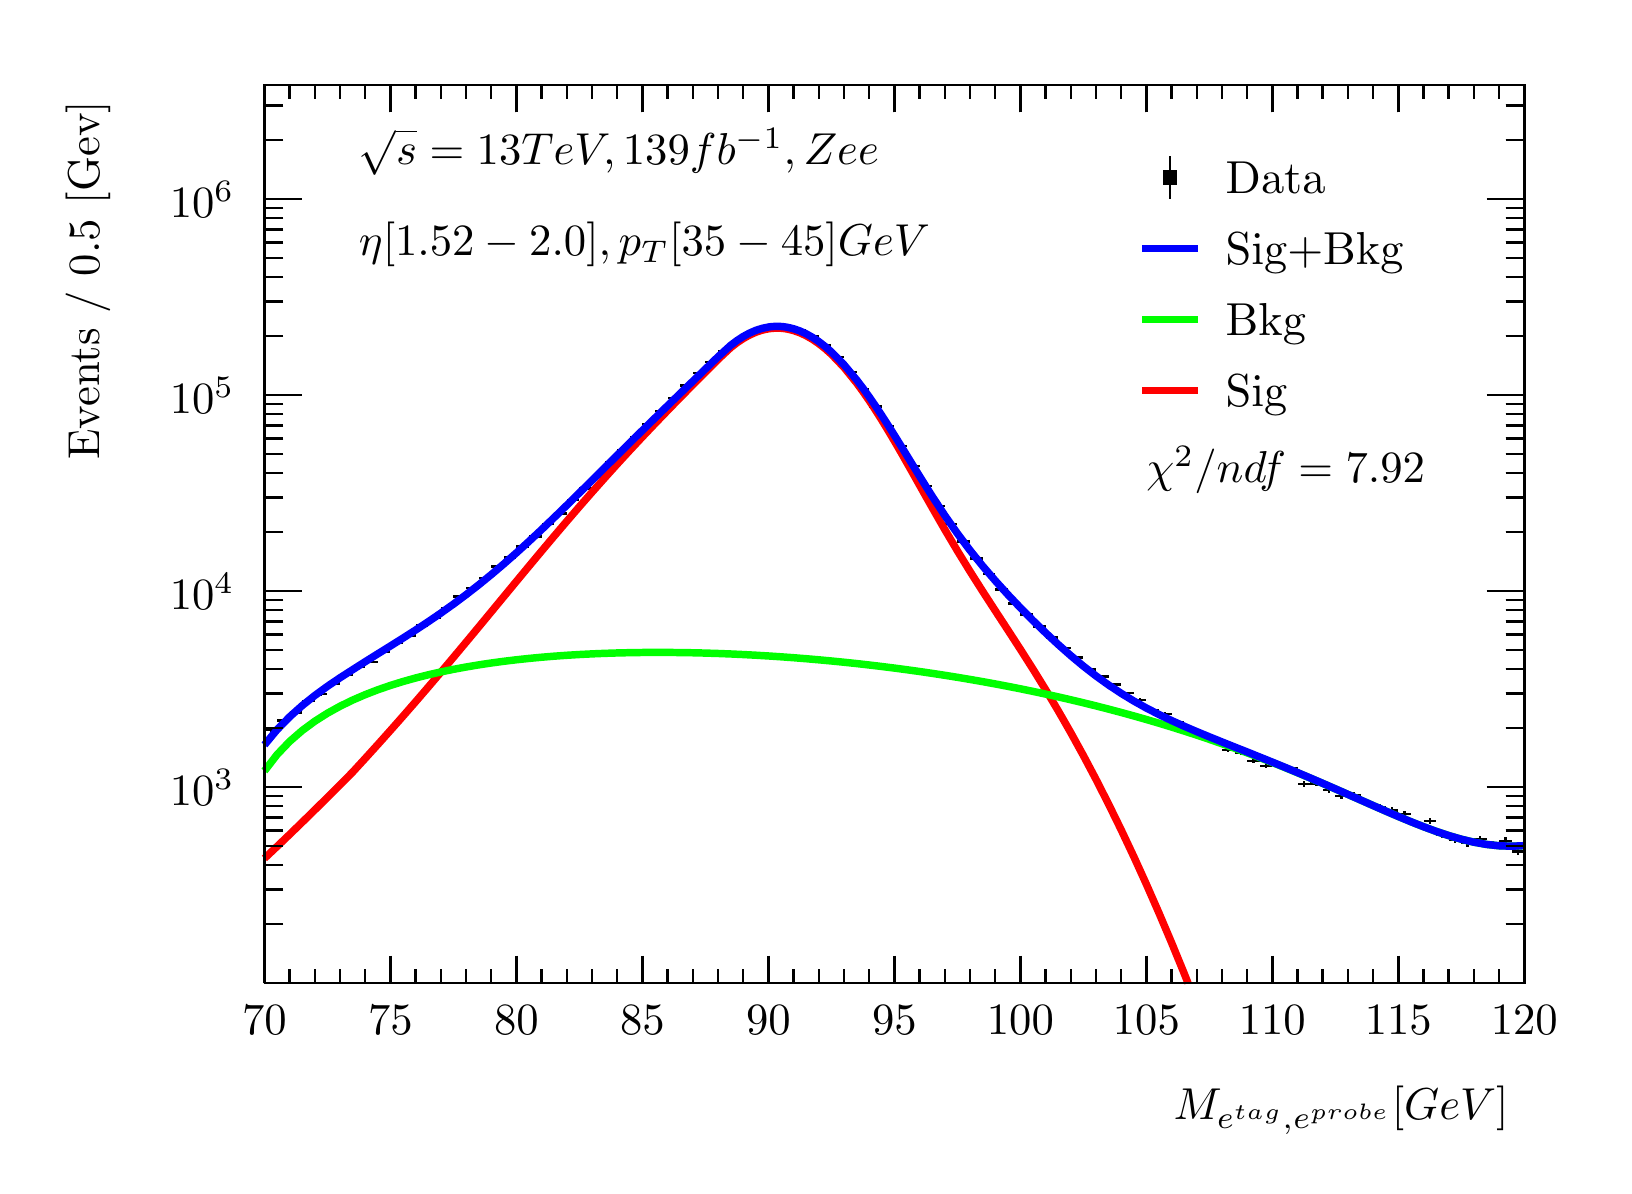
\begin{tikzpicture}
\pgfdeclareplotmark{cross} {
\pgfpathmoveto{\pgfpoint{-0.3\pgfplotmarksize}{\pgfplotmarksize}}
\pgfpathlineto{\pgfpoint{+0.3\pgfplotmarksize}{\pgfplotmarksize}}
\pgfpathlineto{\pgfpoint{+0.3\pgfplotmarksize}{0.3\pgfplotmarksize}}
\pgfpathlineto{\pgfpoint{+1\pgfplotmarksize}{0.3\pgfplotmarksize}}
\pgfpathlineto{\pgfpoint{+1\pgfplotmarksize}{-0.3\pgfplotmarksize}}
\pgfpathlineto{\pgfpoint{+0.3\pgfplotmarksize}{-0.3\pgfplotmarksize}}
\pgfpathlineto{\pgfpoint{+0.3\pgfplotmarksize}{-1.\pgfplotmarksize}}
\pgfpathlineto{\pgfpoint{-0.3\pgfplotmarksize}{-1.\pgfplotmarksize}}
\pgfpathlineto{\pgfpoint{-0.3\pgfplotmarksize}{-0.3\pgfplotmarksize}}
\pgfpathlineto{\pgfpoint{-1.\pgfplotmarksize}{-0.3\pgfplotmarksize}}
\pgfpathlineto{\pgfpoint{-1.\pgfplotmarksize}{0.3\pgfplotmarksize}}
\pgfpathlineto{\pgfpoint{-0.3\pgfplotmarksize}{0.3\pgfplotmarksize}}
\pgfpathclose
\pgfusepathqstroke
}
\pgfdeclareplotmark{cross*} {
\pgfpathmoveto{\pgfpoint{-0.3\pgfplotmarksize}{\pgfplotmarksize}}
\pgfpathlineto{\pgfpoint{+0.3\pgfplotmarksize}{\pgfplotmarksize}}
\pgfpathlineto{\pgfpoint{+0.3\pgfplotmarksize}{0.3\pgfplotmarksize}}
\pgfpathlineto{\pgfpoint{+1\pgfplotmarksize}{0.3\pgfplotmarksize}}
\pgfpathlineto{\pgfpoint{+1\pgfplotmarksize}{-0.3\pgfplotmarksize}}
\pgfpathlineto{\pgfpoint{+0.3\pgfplotmarksize}{-0.3\pgfplotmarksize}}
\pgfpathlineto{\pgfpoint{+0.3\pgfplotmarksize}{-1.\pgfplotmarksize}}
\pgfpathlineto{\pgfpoint{-0.3\pgfplotmarksize}{-1.\pgfplotmarksize}}
\pgfpathlineto{\pgfpoint{-0.3\pgfplotmarksize}{-0.3\pgfplotmarksize}}
\pgfpathlineto{\pgfpoint{-1.\pgfplotmarksize}{-0.3\pgfplotmarksize}}
\pgfpathlineto{\pgfpoint{-1.\pgfplotmarksize}{0.3\pgfplotmarksize}}
\pgfpathlineto{\pgfpoint{-0.3\pgfplotmarksize}{0.3\pgfplotmarksize}}
\pgfpathclose
\pgfusepathqfillstroke
}
\pgfdeclareplotmark{newstar} {
\pgfpathmoveto{\pgfqpoint{0pt}{\pgfplotmarksize}}
\pgfpathlineto{\pgfqpointpolar{44}{0.5\pgfplotmarksize}}
\pgfpathlineto{\pgfqpointpolar{18}{\pgfplotmarksize}}
\pgfpathlineto{\pgfqpointpolar{-20}{0.5\pgfplotmarksize}}
\pgfpathlineto{\pgfqpointpolar{-54}{\pgfplotmarksize}}
\pgfpathlineto{\pgfqpointpolar{-90}{0.5\pgfplotmarksize}}
\pgfpathlineto{\pgfqpointpolar{234}{\pgfplotmarksize}}
\pgfpathlineto{\pgfqpointpolar{198}{0.5\pgfplotmarksize}}
\pgfpathlineto{\pgfqpointpolar{162}{\pgfplotmarksize}}
\pgfpathlineto{\pgfqpointpolar{134}{0.5\pgfplotmarksize}}
\pgfpathclose
\pgfusepathqstroke
}
\pgfdeclareplotmark{newstar*} {
\pgfpathmoveto{\pgfqpoint{0pt}{\pgfplotmarksize}}
\pgfpathlineto{\pgfqpointpolar{44}{0.5\pgfplotmarksize}}
\pgfpathlineto{\pgfqpointpolar{18}{\pgfplotmarksize}}
\pgfpathlineto{\pgfqpointpolar{-20}{0.5\pgfplotmarksize}}
\pgfpathlineto{\pgfqpointpolar{-54}{\pgfplotmarksize}}
\pgfpathlineto{\pgfqpointpolar{-90}{0.5\pgfplotmarksize}}
\pgfpathlineto{\pgfqpointpolar{234}{\pgfplotmarksize}}
\pgfpathlineto{\pgfqpointpolar{198}{0.5\pgfplotmarksize}}
\pgfpathlineto{\pgfqpointpolar{162}{\pgfplotmarksize}}
\pgfpathlineto{\pgfqpointpolar{134}{0.5\pgfplotmarksize}}
\pgfpathclose
\pgfusepathqfillstroke
}
\definecolor{c}{rgb}{1,1,1};
\draw [color=c, fill=c] (0,0) rectangle (20,14.4361);
\draw [color=c, fill=c] (3,2.30977) rectangle (19,13.7143);
\definecolor{c}{rgb}{0,0,0};
\draw [c,line width=0.9] (3,2.30977) -- (3,13.7143) -- (19,13.7143) -- (19,2.30977) -- (3,2.30977);
\definecolor{c}{rgb}{1,1,1};
\draw [color=c, fill=c] (3,2.30977) rectangle (19,13.7143);
\definecolor{c}{rgb}{0,0,0};
\draw [c,line width=0.9] (3,2.30977) -- (3,13.7143) -- (19,13.7143) -- (19,2.30977) -- (3,2.30977);
\draw [c,line width=0.9] (3,2.30977) -- (19,2.30977);
\draw [c,line width=0.9] (3,2.65624) -- (3,2.30977);
\draw [c,line width=0.9] (3.32,2.48301) -- (3.32,2.30977);
\draw [c,line width=0.9] (3.64,2.48301) -- (3.64,2.30977);
\draw [c,line width=0.9] (3.96,2.48301) -- (3.96,2.30977);
\draw [c,line width=0.9] (4.28,2.48301) -- (4.28,2.30977);
\draw [c,line width=0.9] (4.6,2.65624) -- (4.6,2.30977);
\draw [c,line width=0.9] (4.92,2.48301) -- (4.92,2.30977);
\draw [c,line width=0.9] (5.24,2.48301) -- (5.24,2.30977);
\draw [c,line width=0.9] (5.56,2.48301) -- (5.56,2.30977);
\draw [c,line width=0.9] (5.88,2.48301) -- (5.88,2.30977);
\draw [c,line width=0.9] (6.2,2.65624) -- (6.2,2.30977);
\draw [c,line width=0.9] (6.52,2.48301) -- (6.52,2.30977);
\draw [c,line width=0.9] (6.84,2.48301) -- (6.84,2.30977);
\draw [c,line width=0.9] (7.16,2.48301) -- (7.16,2.30977);
\draw [c,line width=0.9] (7.48,2.48301) -- (7.48,2.30977);
\draw [c,line width=0.9] (7.8,2.65624) -- (7.8,2.30977);
\draw [c,line width=0.9] (8.12,2.48301) -- (8.12,2.30977);
\draw [c,line width=0.9] (8.44,2.48301) -- (8.44,2.30977);
\draw [c,line width=0.9] (8.76,2.48301) -- (8.76,2.30977);
\draw [c,line width=0.9] (9.08,2.48301) -- (9.08,2.30977);
\draw [c,line width=0.9] (9.4,2.65624) -- (9.4,2.30977);
\draw [c,line width=0.9] (9.72,2.48301) -- (9.72,2.30977);
\draw [c,line width=0.9] (10.04,2.48301) -- (10.04,2.30977);
\draw [c,line width=0.9] (10.36,2.48301) -- (10.36,2.30977);
\draw [c,line width=0.9] (10.68,2.48301) -- (10.68,2.30977);
\draw [c,line width=0.9] (11,2.65624) -- (11,2.30977);
\draw [c,line width=0.9] (11.32,2.48301) -- (11.32,2.30977);
\draw [c,line width=0.9] (11.64,2.48301) -- (11.64,2.30977);
\draw [c,line width=0.9] (11.96,2.48301) -- (11.96,2.30977);
\draw [c,line width=0.9] (12.28,2.48301) -- (12.28,2.30977);
\draw [c,line width=0.9] (12.6,2.65624) -- (12.6,2.30977);
\draw [c,line width=0.9] (12.92,2.48301) -- (12.92,2.30977);
\draw [c,line width=0.9] (13.24,2.48301) -- (13.24,2.30977);
\draw [c,line width=0.9] (13.56,2.48301) -- (13.56,2.30977);
\draw [c,line width=0.9] (13.88,2.48301) -- (13.88,2.30977);
\draw [c,line width=0.9] (14.2,2.65624) -- (14.2,2.30977);
\draw [c,line width=0.9] (14.52,2.48301) -- (14.52,2.30977);
\draw [c,line width=0.9] (14.84,2.48301) -- (14.84,2.30977);
\draw [c,line width=0.9] (15.16,2.48301) -- (15.16,2.30977);
\draw [c,line width=0.9] (15.48,2.48301) -- (15.48,2.30977);
\draw [c,line width=0.9] (15.8,2.65624) -- (15.8,2.30977);
\draw [c,line width=0.9] (16.12,2.48301) -- (16.12,2.30977);
\draw [c,line width=0.9] (16.44,2.48301) -- (16.44,2.30977);
\draw [c,line width=0.9] (16.76,2.48301) -- (16.76,2.30977);
\draw [c,line width=0.9] (17.08,2.48301) -- (17.08,2.30977);
\draw [c,line width=0.9] (17.4,2.65624) -- (17.4,2.30977);
\draw [c,line width=0.9] (17.72,2.48301) -- (17.72,2.30977);
\draw [c,line width=0.9] (18.04,2.48301) -- (18.04,2.30977);
\draw [c,line width=0.9] (18.36,2.48301) -- (18.36,2.30977);
\draw [c,line width=0.9] (18.68,2.48301) -- (18.68,2.30977);
\draw [c,line width=0.9] (19,2.65624) -- (19,2.30977);
\draw [anchor=base] (3,1.66015) node[scale=1.61424, color=c, rotate=0]{70};
\draw [anchor=base] (4.6,1.66015) node[scale=1.61424, color=c, rotate=0]{75};
\draw [anchor=base] (6.2,1.66015) node[scale=1.61424, color=c, rotate=0]{80};
\draw [anchor=base] (7.8,1.66015) node[scale=1.61424, color=c, rotate=0]{85};
\draw [anchor=base] (9.4,1.66015) node[scale=1.61424, color=c, rotate=0]{90};
\draw [anchor=base] (11,1.66015) node[scale=1.61424, color=c, rotate=0]{95};
\draw [anchor=base] (12.6,1.66015) node[scale=1.61424, color=c, rotate=0]{100};
\draw [anchor=base] (14.2,1.66015) node[scale=1.61424, color=c, rotate=0]{105};
\draw [anchor=base] (15.8,1.66015) node[scale=1.61424, color=c, rotate=0]{110};
\draw [anchor=base] (17.4,1.66015) node[scale=1.61424, color=c, rotate=0]{115};
\draw [anchor=base] (19,1.66015) node[scale=1.61424, color=c, rotate=0]{120};
\draw [anchor= east] (19,0.692932) node[scale=1.61424, color=c, rotate=0]{$M_{e^{tag}, e^{probe}}  [GeV]$};
\draw [c,line width=0.9] (3,13.7143) -- (19,13.7143);
\draw [c,line width=0.9] (3,13.3678) -- (3,13.7143);
\draw [c,line width=0.9] (3.32,13.5411) -- (3.32,13.7143);
\draw [c,line width=0.9] (3.64,13.5411) -- (3.64,13.7143);
\draw [c,line width=0.9] (3.96,13.5411) -- (3.96,13.7143);
\draw [c,line width=0.9] (4.28,13.5411) -- (4.28,13.7143);
\draw [c,line width=0.9] (4.6,13.3678) -- (4.6,13.7143);
\draw [c,line width=0.9] (4.92,13.5411) -- (4.92,13.7143);
\draw [c,line width=0.9] (5.24,13.5411) -- (5.24,13.7143);
\draw [c,line width=0.9] (5.56,13.5411) -- (5.56,13.7143);
\draw [c,line width=0.9] (5.88,13.5411) -- (5.88,13.7143);
\draw [c,line width=0.9] (6.2,13.3678) -- (6.2,13.7143);
\draw [c,line width=0.9] (6.52,13.5411) -- (6.52,13.7143);
\draw [c,line width=0.9] (6.84,13.5411) -- (6.84,13.7143);
\draw [c,line width=0.9] (7.16,13.5411) -- (7.16,13.7143);
\draw [c,line width=0.9] (7.48,13.5411) -- (7.48,13.7143);
\draw [c,line width=0.9] (7.8,13.3678) -- (7.8,13.7143);
\draw [c,line width=0.9] (8.12,13.5411) -- (8.12,13.7143);
\draw [c,line width=0.9] (8.44,13.5411) -- (8.44,13.7143);
\draw [c,line width=0.9] (8.76,13.5411) -- (8.76,13.7143);
\draw [c,line width=0.9] (9.08,13.5411) -- (9.08,13.7143);
\draw [c,line width=0.9] (9.4,13.3678) -- (9.4,13.7143);
\draw [c,line width=0.9] (9.72,13.5411) -- (9.72,13.7143);
\draw [c,line width=0.9] (10.04,13.5411) -- (10.04,13.7143);
\draw [c,line width=0.9] (10.36,13.5411) -- (10.36,13.7143);
\draw [c,line width=0.9] (10.68,13.5411) -- (10.68,13.7143);
\draw [c,line width=0.9] (11,13.3678) -- (11,13.7143);
\draw [c,line width=0.9] (11.32,13.5411) -- (11.32,13.7143);
\draw [c,line width=0.9] (11.64,13.5411) -- (11.64,13.7143);
\draw [c,line width=0.9] (11.96,13.5411) -- (11.96,13.7143);
\draw [c,line width=0.9] (12.28,13.5411) -- (12.28,13.7143);
\draw [c,line width=0.9] (12.6,13.3678) -- (12.6,13.7143);
\draw [c,line width=0.9] (12.92,13.5411) -- (12.92,13.7143);
\draw [c,line width=0.9] (13.24,13.5411) -- (13.24,13.7143);
\draw [c,line width=0.9] (13.56,13.5411) -- (13.56,13.7143);
\draw [c,line width=0.9] (13.88,13.5411) -- (13.88,13.7143);
\draw [c,line width=0.9] (14.2,13.3678) -- (14.2,13.7143);
\draw [c,line width=0.9] (14.52,13.5411) -- (14.52,13.7143);
\draw [c,line width=0.9] (14.84,13.5411) -- (14.84,13.7143);
\draw [c,line width=0.9] (15.16,13.5411) -- (15.16,13.7143);
\draw [c,line width=0.9] (15.48,13.5411) -- (15.48,13.7143);
\draw [c,line width=0.9] (15.8,13.3678) -- (15.8,13.7143);
\draw [c,line width=0.9] (16.12,13.5411) -- (16.12,13.7143);
\draw [c,line width=0.9] (16.44,13.5411) -- (16.44,13.7143);
\draw [c,line width=0.9] (16.76,13.5411) -- (16.76,13.7143);
\draw [c,line width=0.9] (17.08,13.5411) -- (17.08,13.7143);
\draw [c,line width=0.9] (17.4,13.3678) -- (17.4,13.7143);
\draw [c,line width=0.9] (17.72,13.5411) -- (17.72,13.7143);
\draw [c,line width=0.9] (18.04,13.5411) -- (18.04,13.7143);
\draw [c,line width=0.9] (18.36,13.5411) -- (18.36,13.7143);
\draw [c,line width=0.9] (18.68,13.5411) -- (18.68,13.7143);
\draw [c,line width=0.9] (19,13.3678) -- (19,13.7143);
\draw [c,line width=0.9] (3,2.30977) -- (3,13.7143);
\draw [c,line width=0.9] (3.237,3.05909) -- (3,3.05909);
\draw [c,line width=0.9] (3.237,3.49742) -- (3,3.49742);
\draw [c,line width=0.9] (3.237,3.80841) -- (3,3.80841);
\draw [c,line width=0.9] (3.237,4.04964) -- (3,4.04964);
\draw [c,line width=0.9] (3.237,4.24673) -- (3,4.24673);
\draw [c,line width=0.9] (3.237,4.41338) -- (3,4.41338);
\draw [c,line width=0.9] (3.237,4.55773) -- (3,4.55773);
\draw [c,line width=0.9] (3.237,4.68506) -- (3,4.68506);
\draw [c,line width=0.9] (3.474,4.79896) -- (3,4.79896);
\draw [anchor= east] (2.82,4.79896) node[scale=1.61424, color=c, rotate=0]{$10^{3}$};
\draw [c,line width=0.9] (3.237,5.54828) -- (3,5.54828);
\draw [c,line width=0.9] (3.237,5.9866) -- (3,5.9866);
\draw [c,line width=0.9] (3.237,6.2976) -- (3,6.2976);
\draw [c,line width=0.9] (3.237,6.53882) -- (3,6.53882);
\draw [c,line width=0.9] (3.237,6.73592) -- (3,6.73592);
\draw [c,line width=0.9] (3.237,6.90256) -- (3,6.90256);
\draw [c,line width=0.9] (3.237,7.04692) -- (3,7.04692);
\draw [c,line width=0.9] (3.237,7.17424) -- (3,7.17424);
\draw [c,line width=0.9] (3.474,7.28814) -- (3,7.28814);
\draw [anchor= east] (2.82,7.28814) node[scale=1.61424, color=c, rotate=0]{$10^{4}$};
\draw [c,line width=0.9] (3.237,8.03746) -- (3,8.03746);
\draw [c,line width=0.9] (3.237,8.47579) -- (3,8.47579);
\draw [c,line width=0.9] (3.237,8.78678) -- (3,8.78678);
\draw [c,line width=0.9] (3.237,9.02801) -- (3,9.02801);
\draw [c,line width=0.9] (3.237,9.2251) -- (3,9.2251);
\draw [c,line width=0.9] (3.237,9.39175) -- (3,9.39175);
\draw [c,line width=0.9] (3.237,9.5361) -- (3,9.5361);
\draw [c,line width=0.9] (3.237,9.66343) -- (3,9.66343);
\draw [c,line width=0.9] (3.474,9.77733) -- (3,9.77733);
\draw [anchor= east] (2.82,9.77733) node[scale=1.61424, color=c, rotate=0]{$10^{5}$};
\draw [c,line width=0.9] (3.237,10.5266) -- (3,10.5266);
\draw [c,line width=0.9] (3.237,10.965) -- (3,10.965);
\draw [c,line width=0.9] (3.237,11.276) -- (3,11.276);
\draw [c,line width=0.9] (3.237,11.5172) -- (3,11.5172);
\draw [c,line width=0.9] (3.237,11.7143) -- (3,11.7143);
\draw [c,line width=0.9] (3.237,11.8809) -- (3,11.8809);
\draw [c,line width=0.9] (3.237,12.0253) -- (3,12.0253);
\draw [c,line width=0.9] (3.237,12.1526) -- (3,12.1526);
\draw [c,line width=0.9] (3.474,12.2665) -- (3,12.2665);
\draw [anchor= east] (2.82,12.2665) node[scale=1.61424, color=c, rotate=0]{$10^{6}$};
\draw [c,line width=0.9] (3.237,13.0158) -- (3,13.0158);
\draw [c,line width=0.9] (3.237,13.4542) -- (3,13.4542);
\draw [anchor= east] (0.76,13.7143) node[scale=1.61424, color=c, rotate=90]{Events / 0.5 [Gev]};
\draw [c,line width=0.9] (19,2.30977) -- (19,13.7143);
\draw [c,line width=0.9] (18.763,3.05909) -- (19,3.05909);
\draw [c,line width=0.9] (18.763,3.49742) -- (19,3.49742);
\draw [c,line width=0.9] (18.763,3.80841) -- (19,3.80841);
\draw [c,line width=0.9] (18.763,4.04964) -- (19,4.04964);
\draw [c,line width=0.9] (18.763,4.24673) -- (19,4.24673);
\draw [c,line width=0.9] (18.763,4.41338) -- (19,4.41338);
\draw [c,line width=0.9] (18.763,4.55773) -- (19,4.55773);
\draw [c,line width=0.9] (18.763,4.68506) -- (19,4.68506);
\draw [c,line width=0.9] (18.526,4.79896) -- (19,4.79896);
\draw [c,line width=0.9] (18.763,5.54828) -- (19,5.54828);
\draw [c,line width=0.9] (18.763,5.9866) -- (19,5.9866);
\draw [c,line width=0.9] (18.763,6.2976) -- (19,6.2976);
\draw [c,line width=0.9] (18.763,6.53882) -- (19,6.53882);
\draw [c,line width=0.9] (18.763,6.73592) -- (19,6.73592);
\draw [c,line width=0.9] (18.763,6.90256) -- (19,6.90256);
\draw [c,line width=0.9] (18.763,7.04692) -- (19,7.04692);
\draw [c,line width=0.9] (18.763,7.17424) -- (19,7.17424);
\draw [c,line width=0.9] (18.526,7.28814) -- (19,7.28814);
\draw [c,line width=0.9] (18.763,8.03746) -- (19,8.03746);
\draw [c,line width=0.9] (18.763,8.47579) -- (19,8.47579);
\draw [c,line width=0.9] (18.763,8.78678) -- (19,8.78678);
\draw [c,line width=0.9] (18.763,9.02801) -- (19,9.02801);
\draw [c,line width=0.9] (18.763,9.2251) -- (19,9.2251);
\draw [c,line width=0.9] (18.763,9.39175) -- (19,9.39175);
\draw [c,line width=0.9] (18.763,9.5361) -- (19,9.5361);
\draw [c,line width=0.9] (18.763,9.66343) -- (19,9.66343);
\draw [c,line width=0.9] (18.526,9.77733) -- (19,9.77733);
\draw [c,line width=0.9] (18.763,10.5266) -- (19,10.5266);
\draw [c,line width=0.9] (18.763,10.965) -- (19,10.965);
\draw [c,line width=0.9] (18.763,11.276) -- (19,11.276);
\draw [c,line width=0.9] (18.763,11.5172) -- (19,11.5172);
\draw [c,line width=0.9] (18.763,11.7143) -- (19,11.7143);
\draw [c,line width=0.9] (18.763,11.8809) -- (19,11.8809);
\draw [c,line width=0.9] (18.763,12.0253) -- (19,12.0253);
\draw [c,line width=0.9] (18.763,12.1526) -- (19,12.1526);
\draw [c,line width=0.9] (18.526,12.2665) -- (19,12.2665);
\draw [c,line width=0.9] (18.763,13.0158) -- (19,13.0158);
\draw [c,line width=0.9] (18.763,13.4542) -- (19,13.4542);
\draw [c,line width=0.9] (3.08,5.52589) -- (3,5.52589);
\draw [c,line width=0.9] (3,5.52589) -- (3,5.52589);
\draw [c,line width=0.9] (3.08,5.52589) -- (3.16,5.52589);
\draw [c,line width=0.9] (3.16,5.52589) -- (3.16,5.52589);
\draw [c,line width=0.9] (3.08,5.52589) -- (3.08,5.55031);
\draw [c,line width=0.9] (3.08,5.55031) -- (3.08,5.55031);
\draw [c,line width=0.9] (3.08,5.52589) -- (3.08,5.50146);
\draw [c,line width=0.9] (3.08,5.50146) -- (3.08,5.50146);
\draw [c,line width=0.9] (3.24,5.64639) -- (3.16,5.64639);
\draw [c,line width=0.9] (3.16,5.64639) -- (3.16,5.64639);
\draw [c,line width=0.9] (3.24,5.64639) -- (3.32,5.64639);
\draw [c,line width=0.9] (3.32,5.64639) -- (3.32,5.64639);
\draw [c,line width=0.9] (3.24,5.64639) -- (3.24,5.66949);
\draw [c,line width=0.9] (3.24,5.66949) -- (3.24,5.66949);
\draw [c,line width=0.9] (3.24,5.64639) -- (3.24,5.62329);
\draw [c,line width=0.9] (3.24,5.62329) -- (3.24,5.62329);
\draw [c,line width=0.9] (3.4,5.74402) -- (3.32,5.74402);
\draw [c,line width=0.9] (3.32,5.74402) -- (3.32,5.74402);
\draw [c,line width=0.9] (3.4,5.74402) -- (3.48,5.74402);
\draw [c,line width=0.9] (3.48,5.74402) -- (3.48,5.74402);
\draw [c,line width=0.9] (3.4,5.74402) -- (3.4,5.7661);
\draw [c,line width=0.9] (3.4,5.7661) -- (3.4,5.7661);
\draw [c,line width=0.9] (3.4,5.74402) -- (3.4,5.72194);
\draw [c,line width=0.9] (3.4,5.72194) -- (3.4,5.72194);
\draw [c,line width=0.9] (3.56,5.89411) -- (3.48,5.89411);
\draw [c,line width=0.9] (3.48,5.89411) -- (3.48,5.89411);
\draw [c,line width=0.9] (3.56,5.89411) -- (3.64,5.89411);
\draw [c,line width=0.9] (3.64,5.89411) -- (3.64,5.89411);
\draw [c,line width=0.9] (3.56,5.89411) -- (3.56,5.91471);
\draw [c,line width=0.9] (3.56,5.91471) -- (3.56,5.91471);
\draw [c,line width=0.9] (3.56,5.89411) -- (3.56,5.87351);
\draw [c,line width=0.9] (3.56,5.87351) -- (3.56,5.87351);
\draw [c,line width=0.9] (3.72,5.97828) -- (3.64,5.97828);
\draw [c,line width=0.9] (3.64,5.97828) -- (3.64,5.97828);
\draw [c,line width=0.9] (3.72,5.97828) -- (3.8,5.97828);
\draw [c,line width=0.9] (3.8,5.97828) -- (3.8,5.97828);
\draw [c,line width=0.9] (3.72,5.97828) -- (3.72,5.99809);
\draw [c,line width=0.9] (3.72,5.99809) -- (3.72,5.99809);
\draw [c,line width=0.9] (3.72,5.97828) -- (3.72,5.95847);
\draw [c,line width=0.9] (3.72,5.95847) -- (3.72,5.95847);
\draw [c,line width=0.9] (3.88,6.11297) -- (3.8,6.11297);
\draw [c,line width=0.9] (3.8,6.11297) -- (3.8,6.11297);
\draw [c,line width=0.9] (3.88,6.11297) -- (3.96,6.11297);
\draw [c,line width=0.9] (3.96,6.11297) -- (3.96,6.11297);
\draw [c,line width=0.9] (3.88,6.11297) -- (3.88,6.13158);
\draw [c,line width=0.9] (3.88,6.13158) -- (3.88,6.13158);
\draw [c,line width=0.9] (3.88,6.11297) -- (3.88,6.09435);
\draw [c,line width=0.9] (3.88,6.09435) -- (3.88,6.09435);
\draw [c,line width=0.9] (4.04,6.22639) -- (3.96,6.22639);
\draw [c,line width=0.9] (3.96,6.22639) -- (3.96,6.22639);
\draw [c,line width=0.9] (4.04,6.22639) -- (4.12,6.22639);
\draw [c,line width=0.9] (4.12,6.22639) -- (4.12,6.22639);
\draw [c,line width=0.9] (4.04,6.22639) -- (4.04,6.24405);
\draw [c,line width=0.9] (4.04,6.24405) -- (4.04,6.24405);
\draw [c,line width=0.9] (4.04,6.22639) -- (4.04,6.20872);
\draw [c,line width=0.9] (4.04,6.20872) -- (4.04,6.20872);
\draw [c,line width=0.9] (4.2,6.3327) -- (4.12,6.3327);
\draw [c,line width=0.9] (4.12,6.3327) -- (4.12,6.3327);
\draw [c,line width=0.9] (4.2,6.3327) -- (4.28,6.3327);
\draw [c,line width=0.9] (4.28,6.3327) -- (4.28,6.3327);
\draw [c,line width=0.9] (4.2,6.3327) -- (4.2,6.34951);
\draw [c,line width=0.9] (4.2,6.34951) -- (4.2,6.34951);
\draw [c,line width=0.9] (4.2,6.3327) -- (4.2,6.31588);
\draw [c,line width=0.9] (4.2,6.31588) -- (4.2,6.31588);
\draw [c,line width=0.9] (4.36,6.38529) -- (4.28,6.38529);
\draw [c,line width=0.9] (4.28,6.38529) -- (4.28,6.38529);
\draw [c,line width=0.9] (4.36,6.38529) -- (4.44,6.38529);
\draw [c,line width=0.9] (4.44,6.38529) -- (4.44,6.38529);
\draw [c,line width=0.9] (4.36,6.38529) -- (4.36,6.4017);
\draw [c,line width=0.9] (4.36,6.4017) -- (4.36,6.4017);
\draw [c,line width=0.9] (4.36,6.38529) -- (4.36,6.36888);
\draw [c,line width=0.9] (4.36,6.36888) -- (4.36,6.36888);
\draw [c,line width=0.9] (4.52,6.51676) -- (4.44,6.51676);
\draw [c,line width=0.9] (4.44,6.51676) -- (4.44,6.51676);
\draw [c,line width=0.9] (4.52,6.51676) -- (4.6,6.51676);
\draw [c,line width=0.9] (4.6,6.51676) -- (4.6,6.51676);
\draw [c,line width=0.9] (4.52,6.51676) -- (4.52,6.53221);
\draw [c,line width=0.9] (4.52,6.53221) -- (4.52,6.53221);
\draw [c,line width=0.9] (4.52,6.51676) -- (4.52,6.50132);
\draw [c,line width=0.9] (4.52,6.50132) -- (4.52,6.50132);
\draw [c,line width=0.9] (4.68,6.62921) -- (4.6,6.62921);
\draw [c,line width=0.9] (4.6,6.62921) -- (4.6,6.62921);
\draw [c,line width=0.9] (4.68,6.62921) -- (4.76,6.62921);
\draw [c,line width=0.9] (4.76,6.62921) -- (4.76,6.62921);
\draw [c,line width=0.9] (4.68,6.62921) -- (4.68,6.64387);
\draw [c,line width=0.9] (4.68,6.64387) -- (4.68,6.64387);
\draw [c,line width=0.9] (4.68,6.62921) -- (4.68,6.61454);
\draw [c,line width=0.9] (4.68,6.61454) -- (4.68,6.61454);
\draw [c,line width=0.9] (4.84,6.72378) -- (4.76,6.72378);
\draw [c,line width=0.9] (4.76,6.72378) -- (4.76,6.72378);
\draw [c,line width=0.9] (4.84,6.72378) -- (4.92,6.72378);
\draw [c,line width=0.9] (4.92,6.72378) -- (4.92,6.72378);
\draw [c,line width=0.9] (4.84,6.72378) -- (4.84,6.73782);
\draw [c,line width=0.9] (4.84,6.73782) -- (4.84,6.73782);
\draw [c,line width=0.9] (4.84,6.72378) -- (4.84,6.70975);
\draw [c,line width=0.9] (4.84,6.70975) -- (4.84,6.70975);
\draw [c,line width=0.9] (5,6.8523) -- (4.92,6.8523);
\draw [c,line width=0.9] (4.92,6.8523) -- (4.92,6.8523);
\draw [c,line width=0.9] (5,6.8523) -- (5.08,6.8523);
\draw [c,line width=0.9] (5.08,6.8523) -- (5.08,6.8523);
\draw [c,line width=0.9] (5,6.8523) -- (5,6.86553);
\draw [c,line width=0.9] (5,6.86553) -- (5,6.86553);
\draw [c,line width=0.9] (5,6.8523) -- (5,6.83908);
\draw [c,line width=0.9] (5,6.83908) -- (5,6.83908);
\draw [c,line width=0.9] (5.16,6.94392) -- (5.08,6.94392);
\draw [c,line width=0.9] (5.08,6.94392) -- (5.08,6.94392);
\draw [c,line width=0.9] (5.16,6.94392) -- (5.24,6.94392);
\draw [c,line width=0.9] (5.24,6.94392) -- (5.24,6.94392);
\draw [c,line width=0.9] (5.16,6.94392) -- (5.16,6.9566);
\draw [c,line width=0.9] (5.16,6.9566) -- (5.16,6.9566);
\draw [c,line width=0.9] (5.16,6.94392) -- (5.16,6.93125);
\draw [c,line width=0.9] (5.16,6.93125) -- (5.16,6.93125);
\draw [c,line width=0.9] (5.32,7.07216) -- (5.24,7.07216);
\draw [c,line width=0.9] (5.24,7.07216) -- (5.24,7.07216);
\draw [c,line width=0.9] (5.32,7.07216) -- (5.4,7.07216);
\draw [c,line width=0.9] (5.4,7.07216) -- (5.4,7.07216);
\draw [c,line width=0.9] (5.32,7.07216) -- (5.32,7.08411);
\draw [c,line width=0.9] (5.32,7.08411) -- (5.32,7.08411);
\draw [c,line width=0.9] (5.32,7.07216) -- (5.32,7.06021);
\draw [c,line width=0.9] (5.32,7.06021) -- (5.32,7.06021);
\draw [c,line width=0.9] (5.48,7.21745) -- (5.4,7.21745);
\draw [c,line width=0.9] (5.4,7.21745) -- (5.4,7.21745);
\draw [c,line width=0.9] (5.48,7.21745) -- (5.56,7.21745);
\draw [c,line width=0.9] (5.56,7.21745) -- (5.56,7.21745);
\draw [c,line width=0.9] (5.48,7.21745) -- (5.48,7.22862);
\draw [c,line width=0.9] (5.48,7.22862) -- (5.48,7.22862);
\draw [c,line width=0.9] (5.48,7.21745) -- (5.48,7.20628);
\draw [c,line width=0.9] (5.48,7.20628) -- (5.48,7.20628);
\draw [c,line width=0.9] (5.64,7.32648) -- (5.56,7.32648);
\draw [c,line width=0.9] (5.56,7.32648) -- (5.56,7.32648);
\draw [c,line width=0.9] (5.64,7.32648) -- (5.72,7.32648);
\draw [c,line width=0.9] (5.72,7.32648) -- (5.72,7.32648);
\draw [c,line width=0.9] (5.64,7.32648) -- (5.64,7.3371);
\draw [c,line width=0.9] (5.64,7.3371) -- (5.64,7.3371);
\draw [c,line width=0.9] (5.64,7.32648) -- (5.64,7.31586);
\draw [c,line width=0.9] (5.64,7.31586) -- (5.64,7.31586);
\draw [c,line width=0.9] (5.8,7.4538) -- (5.72,7.4538);
\draw [c,line width=0.9] (5.72,7.4538) -- (5.72,7.4538);
\draw [c,line width=0.9] (5.8,7.4538) -- (5.88,7.4538);
\draw [c,line width=0.9] (5.88,7.4538) -- (5.88,7.4538);
\draw [c,line width=0.9] (5.8,7.4538) -- (5.8,7.46381);
\draw [c,line width=0.9] (5.8,7.46381) -- (5.8,7.46381);
\draw [c,line width=0.9] (5.8,7.4538) -- (5.8,7.44378);
\draw [c,line width=0.9] (5.8,7.44378) -- (5.8,7.44378);
\draw [c,line width=0.9] (5.96,7.60065) -- (5.88,7.60065);
\draw [c,line width=0.9] (5.88,7.60065) -- (5.88,7.60065);
\draw [c,line width=0.9] (5.96,7.60065) -- (6.04,7.60065);
\draw [c,line width=0.9] (6.04,7.60065) -- (6.04,7.60065);
\draw [c,line width=0.9] (5.96,7.60065) -- (5.96,7.61001);
\draw [c,line width=0.9] (5.96,7.61001) -- (5.96,7.61001);
\draw [c,line width=0.9] (5.96,7.60065) -- (5.96,7.5913);
\draw [c,line width=0.9] (5.96,7.5913) -- (5.96,7.5913);
\draw [c,line width=0.9] (6.12,7.7148) -- (6.04,7.7148);
\draw [c,line width=0.9] (6.04,7.7148) -- (6.04,7.7148);
\draw [c,line width=0.9] (6.12,7.7148) -- (6.2,7.7148);
\draw [c,line width=0.9] (6.2,7.7148) -- (6.2,7.7148);
\draw [c,line width=0.9] (6.12,7.7148) -- (6.12,7.72368);
\draw [c,line width=0.9] (6.12,7.72368) -- (6.12,7.72368);
\draw [c,line width=0.9] (6.12,7.7148) -- (6.12,7.70593);
\draw [c,line width=0.9] (6.12,7.70593) -- (6.12,7.70593);
\draw [c,line width=0.9] (6.28,7.85399) -- (6.2,7.85399);
\draw [c,line width=0.9] (6.2,7.85399) -- (6.2,7.85399);
\draw [c,line width=0.9] (6.28,7.85399) -- (6.36,7.85399);
\draw [c,line width=0.9] (6.36,7.85399) -- (6.36,7.85399);
\draw [c,line width=0.9] (6.28,7.85399) -- (6.28,7.86231);
\draw [c,line width=0.9] (6.28,7.86231) -- (6.28,7.86231);
\draw [c,line width=0.9] (6.28,7.85399) -- (6.28,7.84567);
\draw [c,line width=0.9] (6.28,7.84567) -- (6.28,7.84567);
\draw [c,line width=0.9] (6.44,7.97991) -- (6.36,7.97991);
\draw [c,line width=0.9] (6.36,7.97991) -- (6.36,7.97991);
\draw [c,line width=0.9] (6.44,7.97991) -- (6.52,7.97991);
\draw [c,line width=0.9] (6.52,7.97991) -- (6.52,7.97991);
\draw [c,line width=0.9] (6.44,7.97991) -- (6.44,7.98776);
\draw [c,line width=0.9] (6.44,7.98776) -- (6.44,7.98776);
\draw [c,line width=0.9] (6.44,7.97991) -- (6.44,7.97205);
\draw [c,line width=0.9] (6.44,7.97205) -- (6.44,7.97205);
\draw [c,line width=0.9] (6.6,8.13917) -- (6.52,8.13917);
\draw [c,line width=0.9] (6.52,8.13917) -- (6.52,8.13917);
\draw [c,line width=0.9] (6.6,8.13917) -- (6.68,8.13917);
\draw [c,line width=0.9] (6.68,8.13917) -- (6.68,8.13917);
\draw [c,line width=0.9] (6.6,8.13917) -- (6.6,8.14646);
\draw [c,line width=0.9] (6.6,8.14646) -- (6.6,8.14646);
\draw [c,line width=0.9] (6.6,8.13917) -- (6.6,8.13188);
\draw [c,line width=0.9] (6.6,8.13188) -- (6.6,8.13188);
\draw [c,line width=0.9] (6.76,8.27036) -- (6.68,8.27036);
\draw [c,line width=0.9] (6.68,8.27036) -- (6.68,8.27036);
\draw [c,line width=0.9] (6.76,8.27036) -- (6.84,8.27036);
\draw [c,line width=0.9] (6.84,8.27036) -- (6.84,8.27036);
\draw [c,line width=0.9] (6.76,8.27036) -- (6.76,8.27722);
\draw [c,line width=0.9] (6.76,8.27722) -- (6.76,8.27722);
\draw [c,line width=0.9] (6.76,8.27036) -- (6.76,8.26349);
\draw [c,line width=0.9] (6.76,8.26349) -- (6.76,8.26349);
\draw [c,line width=0.9] (6.92,8.44642) -- (6.84,8.44642);
\draw [c,line width=0.9] (6.84,8.44642) -- (6.84,8.44642);
\draw [c,line width=0.9] (6.92,8.44642) -- (7,8.44642);
\draw [c,line width=0.9] (7,8.44642) -- (7,8.44642);
\draw [c,line width=0.9] (6.92,8.44642) -- (6.92,8.45275);
\draw [c,line width=0.9] (6.92,8.45275) -- (6.92,8.45275);
\draw [c,line width=0.9] (6.92,8.44642) -- (6.92,8.44009);
\draw [c,line width=0.9] (6.92,8.44009) -- (6.92,8.44009);
\draw [c,line width=0.9] (7.08,8.58886) -- (7,8.58886);
\draw [c,line width=0.9] (7,8.58886) -- (7,8.58886);
\draw [c,line width=0.9] (7.08,8.58886) -- (7.16,8.58886);
\draw [c,line width=0.9] (7.16,8.58886) -- (7.16,8.58886);
\draw [c,line width=0.9] (7.08,8.58886) -- (7.08,8.59479);
\draw [c,line width=0.9] (7.08,8.59479) -- (7.08,8.59479);
\draw [c,line width=0.9] (7.08,8.58886) -- (7.08,8.58294);
\draw [c,line width=0.9] (7.08,8.58294) -- (7.08,8.58294);
\draw [c,line width=0.9] (7.24,8.74431) -- (7.16,8.74431);
\draw [c,line width=0.9] (7.16,8.74431) -- (7.16,8.74431);
\draw [c,line width=0.9] (7.24,8.74431) -- (7.32,8.74431);
\draw [c,line width=0.9] (7.32,8.74431) -- (7.32,8.74431);
\draw [c,line width=0.9] (7.24,8.74431) -- (7.24,8.74982);
\draw [c,line width=0.9] (7.24,8.74982) -- (7.24,8.74982);
\draw [c,line width=0.9] (7.24,8.74431) -- (7.24,8.7388);
\draw [c,line width=0.9] (7.24,8.7388) -- (7.24,8.7388);
\draw [c,line width=0.9] (7.4,8.91807) -- (7.32,8.91807);
\draw [c,line width=0.9] (7.32,8.91807) -- (7.32,8.91807);
\draw [c,line width=0.9] (7.4,8.91807) -- (7.48,8.91807);
\draw [c,line width=0.9] (7.48,8.91807) -- (7.48,8.91807);
\draw [c,line width=0.9] (7.4,8.91807) -- (7.4,8.92315);
\draw [c,line width=0.9] (7.4,8.92315) -- (7.4,8.92315);
\draw [c,line width=0.9] (7.4,8.91807) -- (7.4,8.91298);
\draw [c,line width=0.9] (7.4,8.91298) -- (7.4,8.91298);
\draw [c,line width=0.9] (7.56,9.0753) -- (7.48,9.0753);
\draw [c,line width=0.9] (7.48,9.0753) -- (7.48,9.0753);
\draw [c,line width=0.9] (7.56,9.0753) -- (7.64,9.0753);
\draw [c,line width=0.9] (7.64,9.0753) -- (7.64,9.0753);
\draw [c,line width=0.9] (7.56,9.0753) -- (7.56,9.08003);
\draw [c,line width=0.9] (7.56,9.08003) -- (7.56,9.08003);
\draw [c,line width=0.9] (7.56,9.0753) -- (7.56,9.07057);
\draw [c,line width=0.9] (7.56,9.07057) -- (7.56,9.07057);
\draw [c,line width=0.9] (7.72,9.24432) -- (7.64,9.24432);
\draw [c,line width=0.9] (7.64,9.24432) -- (7.64,9.24432);
\draw [c,line width=0.9] (7.72,9.24432) -- (7.8,9.24432);
\draw [c,line width=0.9] (7.8,9.24432) -- (7.8,9.24432);
\draw [c,line width=0.9] (7.72,9.24432) -- (7.72,9.24869);
\draw [c,line width=0.9] (7.72,9.24869) -- (7.72,9.24869);
\draw [c,line width=0.9] (7.72,9.24432) -- (7.72,9.23995);
\draw [c,line width=0.9] (7.72,9.23995) -- (7.72,9.23995);
\draw [c,line width=0.9] (7.88,9.40842) -- (7.8,9.40842);
\draw [c,line width=0.9] (7.8,9.40842) -- (7.8,9.40842);
\draw [c,line width=0.9] (7.88,9.40842) -- (7.96,9.40842);
\draw [c,line width=0.9] (7.96,9.40842) -- (7.96,9.40842);
\draw [c,line width=0.9] (7.88,9.40842) -- (7.88,9.41248);
\draw [c,line width=0.9] (7.88,9.41248) -- (7.88,9.41248);
\draw [c,line width=0.9] (7.88,9.40842) -- (7.88,9.40437);
\draw [c,line width=0.9] (7.88,9.40437) -- (7.88,9.40437);
\draw [c,line width=0.9] (8.04,9.5776) -- (7.96,9.5776);
\draw [c,line width=0.9] (7.96,9.5776) -- (7.96,9.5776);
\draw [c,line width=0.9] (8.04,9.5776) -- (8.12,9.5776);
\draw [c,line width=0.9] (8.12,9.5776) -- (8.12,9.5776);
\draw [c,line width=0.9] (8.04,9.5776) -- (8.04,9.58135);
\draw [c,line width=0.9] (8.04,9.58135) -- (8.04,9.58135);
\draw [c,line width=0.9] (8.04,9.5776) -- (8.04,9.57385);
\draw [c,line width=0.9] (8.04,9.57385) -- (8.04,9.57385);
\draw [c,line width=0.9] (8.2,9.73996) -- (8.12,9.73996);
\draw [c,line width=0.9] (8.12,9.73996) -- (8.12,9.73996);
\draw [c,line width=0.9] (8.2,9.73996) -- (8.28,9.73996);
\draw [c,line width=0.9] (8.28,9.73996) -- (8.28,9.73996);
\draw [c,line width=0.9] (8.2,9.73996) -- (8.2,9.74343);
\draw [c,line width=0.9] (8.2,9.74343) -- (8.2,9.74343);
\draw [c,line width=0.9] (8.2,9.73996) -- (8.2,9.73648);
\draw [c,line width=0.9] (8.2,9.73648) -- (8.2,9.73648);
\draw [c,line width=0.9] (8.36,9.90153) -- (8.28,9.90153);
\draw [c,line width=0.9] (8.28,9.90153) -- (8.28,9.90153);
\draw [c,line width=0.9] (8.36,9.90153) -- (8.44,9.90153);
\draw [c,line width=0.9] (8.44,9.90153) -- (8.44,9.90153);
\draw [c,line width=0.9] (8.36,9.90153) -- (8.36,9.90476);
\draw [c,line width=0.9] (8.36,9.90476) -- (8.36,9.90476);
\draw [c,line width=0.9] (8.36,9.90153) -- (8.36,9.8983);
\draw [c,line width=0.9] (8.36,9.8983) -- (8.36,9.8983);
\draw [c,line width=0.9] (8.52,10.0572) -- (8.44,10.0572);
\draw [c,line width=0.9] (8.44,10.0572) -- (8.44,10.0572);
\draw [c,line width=0.9] (8.52,10.0572) -- (8.6,10.0572);
\draw [c,line width=0.9] (8.6,10.0572) -- (8.6,10.0572);
\draw [c,line width=0.9] (8.52,10.0572) -- (8.52,10.0602);
\draw [c,line width=0.9] (8.52,10.0602) -- (8.52,10.0602);
\draw [c,line width=0.9] (8.52,10.0572) -- (8.52,10.0542);
\draw [c,line width=0.9] (8.52,10.0542) -- (8.52,10.0542);
\draw [c,line width=0.9] (8.68,10.1997) -- (8.6,10.1997);
\draw [c,line width=0.9] (8.6,10.1997) -- (8.6,10.1997);
\draw [c,line width=0.9] (8.68,10.1997) -- (8.76,10.1997);
\draw [c,line width=0.9] (8.76,10.1997) -- (8.76,10.1997);
\draw [c,line width=0.9] (8.68,10.1997) -- (8.68,10.2025);
\draw [c,line width=0.9] (8.68,10.2025) -- (8.68,10.2025);
\draw [c,line width=0.9] (8.68,10.1997) -- (8.68,10.1969);
\draw [c,line width=0.9] (8.68,10.1969) -- (8.68,10.1969);
\draw [c,line width=0.9] (8.84,10.3367) -- (8.76,10.3367);
\draw [c,line width=0.9] (8.76,10.3367) -- (8.76,10.3367);
\draw [c,line width=0.9] (8.84,10.3367) -- (8.92,10.3367);
\draw [c,line width=0.9] (8.92,10.3367) -- (8.92,10.3367);
\draw [c,line width=0.9] (8.84,10.3367) -- (8.84,10.3393);
\draw [c,line width=0.9] (8.84,10.3393) -- (8.84,10.3393);
\draw [c,line width=0.9] (8.84,10.3367) -- (8.84,10.334);
\draw [c,line width=0.9] (8.84,10.334) -- (8.84,10.334);
\draw [c,line width=0.9] (9,10.4519) -- (8.92,10.4519);
\draw [c,line width=0.9] (8.92,10.4519) -- (8.92,10.4519);
\draw [c,line width=0.9] (9,10.4519) -- (9.08,10.4519);
\draw [c,line width=0.9] (9.08,10.4519) -- (9.08,10.4519);
\draw [c,line width=0.9] (9,10.4519) -- (9,10.4544);
\draw [c,line width=0.9] (9,10.4544) -- (9,10.4544);
\draw [c,line width=0.9] (9,10.4519) -- (9,10.4494);
\draw [c,line width=0.9] (9,10.4494) -- (9,10.4494);
\draw [c,line width=0.9] (9.16,10.5461) -- (9.08,10.5461);
\draw [c,line width=0.9] (9.08,10.5461) -- (9.08,10.5461);
\draw [c,line width=0.9] (9.16,10.5461) -- (9.24,10.5461);
\draw [c,line width=0.9] (9.24,10.5461) -- (9.24,10.5461);
\draw [c,line width=0.9] (9.16,10.5461) -- (9.16,10.5485);
\draw [c,line width=0.9] (9.16,10.5485) -- (9.16,10.5485);
\draw [c,line width=0.9] (9.16,10.5461) -- (9.16,10.5437);
\draw [c,line width=0.9] (9.16,10.5437) -- (9.16,10.5437);
\draw [c,line width=0.9] (9.32,10.607) -- (9.24,10.607);
\draw [c,line width=0.9] (9.24,10.607) -- (9.24,10.607);
\draw [c,line width=0.9] (9.32,10.607) -- (9.4,10.607);
\draw [c,line width=0.9] (9.4,10.607) -- (9.4,10.607);
\draw [c,line width=0.9] (9.32,10.607) -- (9.32,10.6094);
\draw [c,line width=0.9] (9.32,10.6094) -- (9.32,10.6094);
\draw [c,line width=0.9] (9.32,10.607) -- (9.32,10.6047);
\draw [c,line width=0.9] (9.32,10.6047) -- (9.32,10.6047);
\draw [c,line width=0.9] (9.48,10.6426) -- (9.4,10.6426);
\draw [c,line width=0.9] (9.4,10.6426) -- (9.4,10.6426);
\draw [c,line width=0.9] (9.48,10.6426) -- (9.56,10.6426);
\draw [c,line width=0.9] (9.56,10.6426) -- (9.56,10.6426);
\draw [c,line width=0.9] (9.48,10.6426) -- (9.48,10.6449);
\draw [c,line width=0.9] (9.48,10.6449) -- (9.48,10.6449);
\draw [c,line width=0.9] (9.48,10.6426) -- (9.48,10.6403);
\draw [c,line width=0.9] (9.48,10.6403) -- (9.48,10.6403);
\draw [c,line width=0.9] (9.64,10.6382) -- (9.56,10.6382);
\draw [c,line width=0.9] (9.56,10.6382) -- (9.56,10.6382);
\draw [c,line width=0.9] (9.64,10.6382) -- (9.72,10.6382);
\draw [c,line width=0.9] (9.72,10.6382) -- (9.72,10.6382);
\draw [c,line width=0.9] (9.64,10.6382) -- (9.64,10.6405);
\draw [c,line width=0.9] (9.64,10.6405) -- (9.64,10.6405);
\draw [c,line width=0.9] (9.64,10.6382) -- (9.64,10.6359);
\draw [c,line width=0.9] (9.64,10.6359) -- (9.64,10.6359);
\draw [c,line width=0.9] (9.8,10.5995) -- (9.72,10.5995);
\draw [c,line width=0.9] (9.72,10.5995) -- (9.72,10.5995);
\draw [c,line width=0.9] (9.8,10.5995) -- (9.88,10.5995);
\draw [c,line width=0.9] (9.88,10.5995) -- (9.88,10.5995);
\draw [c,line width=0.9] (9.8,10.5995) -- (9.8,10.6019);
\draw [c,line width=0.9] (9.8,10.6019) -- (9.8,10.6019);
\draw [c,line width=0.9] (9.8,10.5995) -- (9.8,10.5972);
\draw [c,line width=0.9] (9.8,10.5972) -- (9.8,10.5972);
\draw [c,line width=0.9] (9.96,10.5213) -- (9.88,10.5213);
\draw [c,line width=0.9] (9.88,10.5213) -- (9.88,10.5213);
\draw [c,line width=0.9] (9.96,10.5213) -- (10.04,10.5213);
\draw [c,line width=0.9] (10.04,10.5213) -- (10.04,10.5213);
\draw [c,line width=0.9] (9.96,10.5213) -- (9.96,10.5237);
\draw [c,line width=0.9] (9.96,10.5237) -- (9.96,10.5237);
\draw [c,line width=0.9] (9.96,10.5213) -- (9.96,10.5188);
\draw [c,line width=0.9] (9.96,10.5188) -- (9.96,10.5188);
\draw [c,line width=0.9] (10.12,10.4063) -- (10.04,10.4063);
\draw [c,line width=0.9] (10.04,10.4063) -- (10.04,10.4063);
\draw [c,line width=0.9] (10.12,10.4063) -- (10.2,10.4063);
\draw [c,line width=0.9] (10.2,10.4063) -- (10.2,10.4063);
\draw [c,line width=0.9] (10.12,10.4063) -- (10.12,10.4088);
\draw [c,line width=0.9] (10.12,10.4088) -- (10.12,10.4088);
\draw [c,line width=0.9] (10.12,10.4063) -- (10.12,10.4037);
\draw [c,line width=0.9] (10.12,10.4037) -- (10.12,10.4037);
\draw [c,line width=0.9] (10.28,10.2592) -- (10.2,10.2592);
\draw [c,line width=0.9] (10.2,10.2592) -- (10.2,10.2592);
\draw [c,line width=0.9] (10.28,10.2592) -- (10.36,10.2592);
\draw [c,line width=0.9] (10.36,10.2592) -- (10.36,10.2592);
\draw [c,line width=0.9] (10.28,10.2592) -- (10.28,10.262);
\draw [c,line width=0.9] (10.28,10.262) -- (10.28,10.262);
\draw [c,line width=0.9] (10.28,10.2592) -- (10.28,10.2565);
\draw [c,line width=0.9] (10.28,10.2565) -- (10.28,10.2565);
\draw [c,line width=0.9] (10.44,10.0698) -- (10.36,10.0698);
\draw [c,line width=0.9] (10.36,10.0698) -- (10.36,10.0698);
\draw [c,line width=0.9] (10.44,10.0698) -- (10.52,10.0698);
\draw [c,line width=0.9] (10.52,10.0698) -- (10.52,10.0698);
\draw [c,line width=0.9] (10.44,10.0698) -- (10.44,10.0727);
\draw [c,line width=0.9] (10.44,10.0727) -- (10.44,10.0727);
\draw [c,line width=0.9] (10.44,10.0698) -- (10.44,10.0668);
\draw [c,line width=0.9] (10.44,10.0668) -- (10.44,10.0668);
\draw [c,line width=0.9] (10.6,9.85108) -- (10.52,9.85108);
\draw [c,line width=0.9] (10.52,9.85108) -- (10.52,9.85108);
\draw [c,line width=0.9] (10.6,9.85108) -- (10.68,9.85108);
\draw [c,line width=0.9] (10.68,9.85108) -- (10.68,9.85108);
\draw [c,line width=0.9] (10.6,9.85108) -- (10.6,9.85438);
\draw [c,line width=0.9] (10.6,9.85438) -- (10.6,9.85438);
\draw [c,line width=0.9] (10.6,9.85108) -- (10.6,9.84777);
\draw [c,line width=0.9] (10.6,9.84777) -- (10.6,9.84777);
\draw [c,line width=0.9] (10.76,9.62913) -- (10.68,9.62913);
\draw [c,line width=0.9] (10.68,9.62913) -- (10.68,9.62913);
\draw [c,line width=0.9] (10.76,9.62913) -- (10.84,9.62913);
\draw [c,line width=0.9] (10.84,9.62913) -- (10.84,9.62913);
\draw [c,line width=0.9] (10.76,9.62913) -- (10.76,9.63279);
\draw [c,line width=0.9] (10.76,9.63279) -- (10.76,9.63279);
\draw [c,line width=0.9] (10.76,9.62913) -- (10.76,9.62547);
\draw [c,line width=0.9] (10.76,9.62547) -- (10.76,9.62547);
\draw [c,line width=0.9] (10.92,9.38227) -- (10.84,9.38227);
\draw [c,line width=0.9] (10.84,9.38227) -- (10.84,9.38227);
\draw [c,line width=0.9] (10.92,9.38227) -- (11,9.38227);
\draw [c,line width=0.9] (11,9.38227) -- (11,9.38227);
\draw [c,line width=0.9] (10.92,9.38227) -- (10.92,9.38638);
\draw [c,line width=0.9] (10.92,9.38638) -- (10.92,9.38638);
\draw [c,line width=0.9] (10.92,9.38227) -- (10.92,9.37817);
\draw [c,line width=0.9] (10.92,9.37817) -- (10.92,9.37817);
\draw [c,line width=0.9] (11.08,9.13281) -- (11,9.13281);
\draw [c,line width=0.9] (11,9.13281) -- (11,9.13281);
\draw [c,line width=0.9] (11.08,9.13281) -- (11.16,9.13281);
\draw [c,line width=0.9] (11.16,9.13281) -- (11.16,9.13281);
\draw [c,line width=0.9] (11.08,9.13281) -- (11.08,9.13742);
\draw [c,line width=0.9] (11.08,9.13742) -- (11.08,9.13742);
\draw [c,line width=0.9] (11.08,9.13281) -- (11.08,9.1282);
\draw [c,line width=0.9] (11.08,9.1282) -- (11.08,9.1282);
\draw [c,line width=0.9] (11.24,8.87432) -- (11.16,8.87432);
\draw [c,line width=0.9] (11.16,8.87432) -- (11.16,8.87432);
\draw [c,line width=0.9] (11.24,8.87432) -- (11.32,8.87432);
\draw [c,line width=0.9] (11.32,8.87432) -- (11.32,8.87432);
\draw [c,line width=0.9] (11.24,8.87432) -- (11.24,8.87952);
\draw [c,line width=0.9] (11.24,8.87952) -- (11.24,8.87952);
\draw [c,line width=0.9] (11.24,8.87432) -- (11.24,8.86913);
\draw [c,line width=0.9] (11.24,8.86913) -- (11.24,8.86913);
\draw [c,line width=0.9] (11.4,8.621) -- (11.32,8.621);
\draw [c,line width=0.9] (11.32,8.621) -- (11.32,8.621);
\draw [c,line width=0.9] (11.4,8.621) -- (11.48,8.621);
\draw [c,line width=0.9] (11.48,8.621) -- (11.48,8.621);
\draw [c,line width=0.9] (11.4,8.621) -- (11.4,8.62683);
\draw [c,line width=0.9] (11.4,8.62683) -- (11.4,8.62683);
\draw [c,line width=0.9] (11.4,8.621) -- (11.4,8.61516);
\draw [c,line width=0.9] (11.4,8.61516) -- (11.4,8.61516);
\draw [c,line width=0.9] (11.56,8.37094) -- (11.48,8.37094);
\draw [c,line width=0.9] (11.48,8.37094) -- (11.48,8.37094);
\draw [c,line width=0.9] (11.56,8.37094) -- (11.64,8.37094);
\draw [c,line width=0.9] (11.64,8.37094) -- (11.64,8.37094);
\draw [c,line width=0.9] (11.56,8.37094) -- (11.56,8.37749);
\draw [c,line width=0.9] (11.56,8.37749) -- (11.56,8.37749);
\draw [c,line width=0.9] (11.56,8.37094) -- (11.56,8.36439);
\draw [c,line width=0.9] (11.56,8.36439) -- (11.56,8.36439);
\draw [c,line width=0.9] (11.72,8.13681) -- (11.64,8.13681);
\draw [c,line width=0.9] (11.64,8.13681) -- (11.64,8.13681);
\draw [c,line width=0.9] (11.72,8.13681) -- (11.8,8.13681);
\draw [c,line width=0.9] (11.8,8.13681) -- (11.8,8.13681);
\draw [c,line width=0.9] (11.72,8.13681) -- (11.72,8.14411);
\draw [c,line width=0.9] (11.72,8.14411) -- (11.72,8.14411);
\draw [c,line width=0.9] (11.72,8.13681) -- (11.72,8.1295);
\draw [c,line width=0.9] (11.72,8.1295) -- (11.72,8.1295);
\draw [c,line width=0.9] (11.88,7.91808) -- (11.8,7.91808);
\draw [c,line width=0.9] (11.8,7.91808) -- (11.8,7.91808);
\draw [c,line width=0.9] (11.88,7.91808) -- (11.96,7.91808);
\draw [c,line width=0.9] (11.96,7.91808) -- (11.96,7.91808);
\draw [c,line width=0.9] (11.88,7.91808) -- (11.88,7.92616);
\draw [c,line width=0.9] (11.88,7.92616) -- (11.88,7.92616);
\draw [c,line width=0.9] (11.88,7.91808) -- (11.88,7.91001);
\draw [c,line width=0.9] (11.88,7.91001) -- (11.88,7.91001);
\draw [c,line width=0.9] (12.04,7.69984) -- (11.96,7.69984);
\draw [c,line width=0.9] (11.96,7.69984) -- (11.96,7.69984);
\draw [c,line width=0.9] (12.04,7.69984) -- (12.12,7.69984);
\draw [c,line width=0.9] (12.12,7.69984) -- (12.12,7.69984);
\draw [c,line width=0.9] (12.04,7.69984) -- (12.04,7.70877);
\draw [c,line width=0.9] (12.04,7.70877) -- (12.04,7.70877);
\draw [c,line width=0.9] (12.04,7.69984) -- (12.04,7.6909);
\draw [c,line width=0.9] (12.04,7.6909) -- (12.04,7.6909);
\draw [c,line width=0.9] (12.2,7.50329) -- (12.12,7.50329);
\draw [c,line width=0.9] (12.12,7.50329) -- (12.12,7.50329);
\draw [c,line width=0.9] (12.2,7.50329) -- (12.28,7.50329);
\draw [c,line width=0.9] (12.28,7.50329) -- (12.28,7.50329);
\draw [c,line width=0.9] (12.2,7.50329) -- (12.2,7.51307);
\draw [c,line width=0.9] (12.2,7.51307) -- (12.2,7.51307);
\draw [c,line width=0.9] (12.2,7.50329) -- (12.2,7.4935);
\draw [c,line width=0.9] (12.2,7.4935) -- (12.2,7.4935);
\draw [c,line width=0.9] (12.36,7.30498) -- (12.28,7.30498);
\draw [c,line width=0.9] (12.28,7.30498) -- (12.28,7.30498);
\draw [c,line width=0.9] (12.36,7.30498) -- (12.44,7.30498);
\draw [c,line width=0.9] (12.44,7.30498) -- (12.44,7.30498);
\draw [c,line width=0.9] (12.36,7.30498) -- (12.36,7.31571);
\draw [c,line width=0.9] (12.36,7.31571) -- (12.36,7.31571);
\draw [c,line width=0.9] (12.36,7.30498) -- (12.36,7.29426);
\draw [c,line width=0.9] (12.36,7.29426) -- (12.36,7.29426);
\draw [c,line width=0.9] (12.52,7.12836) -- (12.44,7.12836);
\draw [c,line width=0.9] (12.44,7.12836) -- (12.44,7.12836);
\draw [c,line width=0.9] (12.52,7.12836) -- (12.6,7.12836);
\draw [c,line width=0.9] (12.6,7.12836) -- (12.6,7.12836);
\draw [c,line width=0.9] (12.52,7.12836) -- (12.52,7.14);
\draw [c,line width=0.9] (12.52,7.14) -- (12.52,7.14);
\draw [c,line width=0.9] (12.52,7.12836) -- (12.52,7.11672);
\draw [c,line width=0.9] (12.52,7.11672) -- (12.52,7.11672);
\draw [c,line width=0.9] (12.68,6.98947) -- (12.6,6.98947);
\draw [c,line width=0.9] (12.6,6.98947) -- (12.6,6.98947);
\draw [c,line width=0.9] (12.68,6.98947) -- (12.76,6.98947);
\draw [c,line width=0.9] (12.76,6.98947) -- (12.76,6.98947);
\draw [c,line width=0.9] (12.68,6.98947) -- (12.68,7.00188);
\draw [c,line width=0.9] (12.68,7.00188) -- (12.68,7.00188);
\draw [c,line width=0.9] (12.68,6.98947) -- (12.68,6.97706);
\draw [c,line width=0.9] (12.68,6.97706) -- (12.68,6.97706);
\draw [c,line width=0.9] (12.84,6.84076) -- (12.76,6.84076);
\draw [c,line width=0.9] (12.76,6.84076) -- (12.76,6.84076);
\draw [c,line width=0.9] (12.84,6.84076) -- (12.92,6.84076);
\draw [c,line width=0.9] (12.92,6.84076) -- (12.92,6.84076);
\draw [c,line width=0.9] (12.84,6.84076) -- (12.84,6.85405);
\draw [c,line width=0.9] (12.84,6.85405) -- (12.84,6.85405);
\draw [c,line width=0.9] (12.84,6.84076) -- (12.84,6.82746);
\draw [c,line width=0.9] (12.84,6.82746) -- (12.84,6.82746);
\draw [c,line width=0.9] (13,6.69647) -- (12.92,6.69647);
\draw [c,line width=0.9] (12.92,6.69647) -- (12.92,6.69647);
\draw [c,line width=0.9] (13,6.69647) -- (13.08,6.69647);
\draw [c,line width=0.9] (13.08,6.69647) -- (13.08,6.69647);
\draw [c,line width=0.9] (13,6.69647) -- (13,6.71069);
\draw [c,line width=0.9] (13,6.71069) -- (13,6.71069);
\draw [c,line width=0.9] (13,6.69647) -- (13,6.68226);
\draw [c,line width=0.9] (13,6.68226) -- (13,6.68226);
\draw [c,line width=0.9] (13.16,6.5672) -- (13.08,6.5672);
\draw [c,line width=0.9] (13.08,6.5672) -- (13.08,6.5672);
\draw [c,line width=0.9] (13.16,6.5672) -- (13.24,6.5672);
\draw [c,line width=0.9] (13.24,6.5672) -- (13.24,6.5672);
\draw [c,line width=0.9] (13.16,6.5672) -- (13.16,6.58229);
\draw [c,line width=0.9] (13.16,6.58229) -- (13.16,6.58229);
\draw [c,line width=0.9] (13.16,6.5672) -- (13.16,6.55212);
\draw [c,line width=0.9] (13.16,6.55212) -- (13.16,6.55212);
\draw [c,line width=0.9] (13.32,6.44303) -- (13.24,6.44303);
\draw [c,line width=0.9] (13.24,6.44303) -- (13.24,6.44303);
\draw [c,line width=0.9] (13.32,6.44303) -- (13.4,6.44303);
\draw [c,line width=0.9] (13.4,6.44303) -- (13.4,6.44303);
\draw [c,line width=0.9] (13.32,6.44303) -- (13.32,6.45901);
\draw [c,line width=0.9] (13.32,6.45901) -- (13.32,6.45901);
\draw [c,line width=0.9] (13.32,6.44303) -- (13.32,6.42705);
\draw [c,line width=0.9] (13.32,6.42705) -- (13.32,6.42705);
\draw [c,line width=0.9] (13.48,6.29164) -- (13.4,6.29164);
\draw [c,line width=0.9] (13.4,6.29164) -- (13.4,6.29164);
\draw [c,line width=0.9] (13.48,6.29164) -- (13.56,6.29164);
\draw [c,line width=0.9] (13.56,6.29164) -- (13.56,6.29164);
\draw [c,line width=0.9] (13.48,6.29164) -- (13.48,6.30877);
\draw [c,line width=0.9] (13.48,6.30877) -- (13.48,6.30877);
\draw [c,line width=0.9] (13.48,6.29164) -- (13.48,6.2745);
\draw [c,line width=0.9] (13.48,6.2745) -- (13.48,6.2745);
\draw [c,line width=0.9] (13.64,6.20569) -- (13.56,6.20569);
\draw [c,line width=0.9] (13.56,6.20569) -- (13.56,6.20569);
\draw [c,line width=0.9] (13.64,6.20569) -- (13.72,6.20569);
\draw [c,line width=0.9] (13.72,6.20569) -- (13.72,6.20569);
\draw [c,line width=0.9] (13.64,6.20569) -- (13.64,6.22353);
\draw [c,line width=0.9] (13.64,6.22353) -- (13.64,6.22353);
\draw [c,line width=0.9] (13.64,6.20569) -- (13.64,6.18786);
\draw [c,line width=0.9] (13.64,6.18786) -- (13.64,6.18786);
\draw [c,line width=0.9] (13.8,6.10039) -- (13.72,6.10039);
\draw [c,line width=0.9] (13.72,6.10039) -- (13.72,6.10039);
\draw [c,line width=0.9] (13.8,6.10039) -- (13.88,6.10039);
\draw [c,line width=0.9] (13.88,6.10039) -- (13.88,6.10039);
\draw [c,line width=0.9] (13.8,6.10039) -- (13.8,6.11912);
\draw [c,line width=0.9] (13.8,6.11912) -- (13.8,6.11912);
\draw [c,line width=0.9] (13.8,6.10039) -- (13.8,6.08167);
\draw [c,line width=0.9] (13.8,6.08167) -- (13.8,6.08167);
\draw [c,line width=0.9] (13.96,5.99056) -- (13.88,5.99056);
\draw [c,line width=0.9] (13.88,5.99056) -- (13.88,5.99056);
\draw [c,line width=0.9] (13.96,5.99056) -- (14.04,5.99056);
\draw [c,line width=0.9] (14.04,5.99056) -- (14.04,5.99056);
\draw [c,line width=0.9] (13.96,5.99056) -- (13.96,6.01026);
\draw [c,line width=0.9] (13.96,6.01026) -- (13.96,6.01026);
\draw [c,line width=0.9] (13.96,5.99056) -- (13.96,5.97086);
\draw [c,line width=0.9] (13.96,5.97086) -- (13.96,5.97086);
\draw [c,line width=0.9] (14.12,5.90349) -- (14.04,5.90349);
\draw [c,line width=0.9] (14.04,5.90349) -- (14.04,5.90349);
\draw [c,line width=0.9] (14.12,5.90349) -- (14.2,5.90349);
\draw [c,line width=0.9] (14.2,5.90349) -- (14.2,5.90349);
\draw [c,line width=0.9] (14.12,5.90349) -- (14.12,5.924);
\draw [c,line width=0.9] (14.12,5.924) -- (14.12,5.924);
\draw [c,line width=0.9] (14.12,5.90349) -- (14.12,5.88298);
\draw [c,line width=0.9] (14.12,5.88298) -- (14.12,5.88298);
\draw [c,line width=0.9] (14.28,5.7747) -- (14.2,5.7747);
\draw [c,line width=0.9] (14.2,5.7747) -- (14.2,5.7747);
\draw [c,line width=0.9] (14.28,5.7747) -- (14.36,5.7747);
\draw [c,line width=0.9] (14.36,5.7747) -- (14.36,5.7747);
\draw [c,line width=0.9] (14.28,5.7747) -- (14.28,5.79647);
\draw [c,line width=0.9] (14.28,5.79647) -- (14.28,5.79647);
\draw [c,line width=0.9] (14.28,5.7747) -- (14.28,5.75293);
\draw [c,line width=0.9] (14.28,5.75293) -- (14.28,5.75293);
\draw [c,line width=0.9] (14.44,5.72721) -- (14.36,5.72721);
\draw [c,line width=0.9] (14.36,5.72721) -- (14.36,5.72721);
\draw [c,line width=0.9] (14.44,5.72721) -- (14.52,5.72721);
\draw [c,line width=0.9] (14.52,5.72721) -- (14.52,5.72721);
\draw [c,line width=0.9] (14.44,5.72721) -- (14.44,5.74946);
\draw [c,line width=0.9] (14.44,5.74946) -- (14.44,5.74946);
\draw [c,line width=0.9] (14.44,5.72721) -- (14.44,5.70495);
\draw [c,line width=0.9] (14.44,5.70495) -- (14.44,5.70495);
\draw [c,line width=0.9] (14.6,5.62445) -- (14.52,5.62445);
\draw [c,line width=0.9] (14.52,5.62445) -- (14.52,5.62445);
\draw [c,line width=0.9] (14.6,5.62445) -- (14.68,5.62445);
\draw [c,line width=0.9] (14.68,5.62445) -- (14.68,5.62445);
\draw [c,line width=0.9] (14.6,5.62445) -- (14.6,5.64778);
\draw [c,line width=0.9] (14.6,5.64778) -- (14.6,5.64778);
\draw [c,line width=0.9] (14.6,5.62445) -- (14.6,5.60111);
\draw [c,line width=0.9] (14.6,5.60111) -- (14.6,5.60111);
\draw [c,line width=0.9] (14.76,5.52864) -- (14.68,5.52864);
\draw [c,line width=0.9] (14.68,5.52864) -- (14.68,5.52864);
\draw [c,line width=0.9] (14.76,5.52864) -- (14.84,5.52864);
\draw [c,line width=0.9] (14.84,5.52864) -- (14.84,5.52864);
\draw [c,line width=0.9] (14.76,5.52864) -- (14.76,5.55303);
\draw [c,line width=0.9] (14.76,5.55303) -- (14.76,5.55303);
\draw [c,line width=0.9] (14.76,5.52864) -- (14.76,5.50425);
\draw [c,line width=0.9] (14.76,5.50425) -- (14.76,5.50425);
\draw [c,line width=0.9] (14.92,5.4552) -- (14.84,5.4552);
\draw [c,line width=0.9] (14.84,5.4552) -- (14.84,5.4552);
\draw [c,line width=0.9] (14.92,5.4552) -- (15,5.4552);
\draw [c,line width=0.9] (15,5.4552) -- (15,5.4552);
\draw [c,line width=0.9] (14.92,5.4552) -- (14.92,5.48043);
\draw [c,line width=0.9] (14.92,5.48043) -- (14.92,5.48043);
\draw [c,line width=0.9] (14.92,5.4552) -- (14.92,5.42996);
\draw [c,line width=0.9] (14.92,5.42996) -- (14.92,5.42996);
\draw [c,line width=0.9] (15.08,5.3783) -- (15,5.3783);
\draw [c,line width=0.9] (15,5.3783) -- (15,5.3783);
\draw [c,line width=0.9] (15.08,5.3783) -- (15.16,5.3783);
\draw [c,line width=0.9] (15.16,5.3783) -- (15.16,5.3783);
\draw [c,line width=0.9] (15.08,5.3783) -- (15.08,5.40445);
\draw [c,line width=0.9] (15.08,5.40445) -- (15.08,5.40445);
\draw [c,line width=0.9] (15.08,5.3783) -- (15.08,5.35215);
\draw [c,line width=0.9] (15.08,5.35215) -- (15.08,5.35215);
\draw [c,line width=0.9] (15.24,5.26714) -- (15.16,5.26714);
\draw [c,line width=0.9] (15.16,5.26714) -- (15.16,5.26714);
\draw [c,line width=0.9] (15.24,5.26714) -- (15.32,5.26714);
\draw [c,line width=0.9] (15.32,5.26714) -- (15.32,5.26714);
\draw [c,line width=0.9] (15.24,5.26714) -- (15.24,5.29466);
\draw [c,line width=0.9] (15.24,5.29466) -- (15.24,5.29466);
\draw [c,line width=0.9] (15.24,5.26714) -- (15.24,5.23961);
\draw [c,line width=0.9] (15.24,5.23961) -- (15.24,5.23961);
\draw [c,line width=0.9] (15.4,5.23656) -- (15.32,5.23656);
\draw [c,line width=0.9] (15.32,5.23656) -- (15.32,5.23656);
\draw [c,line width=0.9] (15.4,5.23656) -- (15.48,5.23656);
\draw [c,line width=0.9] (15.48,5.23656) -- (15.48,5.23656);
\draw [c,line width=0.9] (15.4,5.23656) -- (15.4,5.26448);
\draw [c,line width=0.9] (15.4,5.26448) -- (15.4,5.26448);
\draw [c,line width=0.9] (15.4,5.23656) -- (15.4,5.20864);
\draw [c,line width=0.9] (15.4,5.20864) -- (15.4,5.20864);
\draw [c,line width=0.9] (15.56,5.13057) -- (15.48,5.13057);
\draw [c,line width=0.9] (15.48,5.13057) -- (15.48,5.13057);
\draw [c,line width=0.9] (15.56,5.13057) -- (15.64,5.13057);
\draw [c,line width=0.9] (15.64,5.13057) -- (15.64,5.13057);
\draw [c,line width=0.9] (15.56,5.13057) -- (15.56,5.15989);
\draw [c,line width=0.9] (15.56,5.15989) -- (15.56,5.15989);
\draw [c,line width=0.9] (15.56,5.13057) -- (15.56,5.10124);
\draw [c,line width=0.9] (15.56,5.10124) -- (15.56,5.10124);
\draw [c,line width=0.9] (15.72,5.06498) -- (15.64,5.06498);
\draw [c,line width=0.9] (15.64,5.06498) -- (15.64,5.06498);
\draw [c,line width=0.9] (15.72,5.06498) -- (15.8,5.06498);
\draw [c,line width=0.9] (15.8,5.06498) -- (15.8,5.06498);
\draw [c,line width=0.9] (15.72,5.06498) -- (15.72,5.09521);
\draw [c,line width=0.9] (15.72,5.09521) -- (15.72,5.09521);
\draw [c,line width=0.9] (15.72,5.06498) -- (15.72,5.03475);
\draw [c,line width=0.9] (15.72,5.03475) -- (15.72,5.03475);
\draw [c,line width=0.9] (15.88,5.08922) -- (15.8,5.08922);
\draw [c,line width=0.9] (15.8,5.08922) -- (15.8,5.08922);
\draw [c,line width=0.9] (15.88,5.08922) -- (15.96,5.08922);
\draw [c,line width=0.9] (15.96,5.08922) -- (15.96,5.08922);
\draw [c,line width=0.9] (15.88,5.08922) -- (15.88,5.11911);
\draw [c,line width=0.9] (15.88,5.11911) -- (15.88,5.11911);
\draw [c,line width=0.9] (15.88,5.08922) -- (15.88,5.05933);
\draw [c,line width=0.9] (15.88,5.05933) -- (15.88,5.05933);
\draw [c,line width=0.9] (16.04,5.03672) -- (15.96,5.03672);
\draw [c,line width=0.9] (15.96,5.03672) -- (15.96,5.03672);
\draw [c,line width=0.9] (16.04,5.03672) -- (16.12,5.03672);
\draw [c,line width=0.9] (16.12,5.03672) -- (16.12,5.03672);
\draw [c,line width=0.9] (16.04,5.03672) -- (16.04,5.06735);
\draw [c,line width=0.9] (16.04,5.06735) -- (16.04,5.06735);
\draw [c,line width=0.9] (16.04,5.03672) -- (16.04,5.0061);
\draw [c,line width=0.9] (16.04,5.0061) -- (16.04,5.0061);
\draw [c,line width=0.9] (16.2,4.83928) -- (16.12,4.83928);
\draw [c,line width=0.9] (16.12,4.83928) -- (16.12,4.83928);
\draw [c,line width=0.9] (16.2,4.83928) -- (16.28,4.83928);
\draw [c,line width=0.9] (16.28,4.83928) -- (16.28,4.83928);
\draw [c,line width=0.9] (16.2,4.83928) -- (16.2,4.87283);
\draw [c,line width=0.9] (16.2,4.87283) -- (16.2,4.87283);
\draw [c,line width=0.9] (16.2,4.83928) -- (16.2,4.80572);
\draw [c,line width=0.9] (16.2,4.80572) -- (16.2,4.80572);
\draw [c,line width=0.9] (16.36,4.84136) -- (16.28,4.84136);
\draw [c,line width=0.9] (16.28,4.84136) -- (16.28,4.84136);
\draw [c,line width=0.9] (16.36,4.84136) -- (16.44,4.84136);
\draw [c,line width=0.9] (16.44,4.84136) -- (16.44,4.84136);
\draw [c,line width=0.9] (16.36,4.84136) -- (16.36,4.87488);
\draw [c,line width=0.9] (16.36,4.87488) -- (16.36,4.87488);
\draw [c,line width=0.9] (16.36,4.84136) -- (16.36,4.80784);
\draw [c,line width=0.9] (16.36,4.80784) -- (16.36,4.80784);
\draw [c,line width=0.9] (16.52,4.76044) -- (16.44,4.76044);
\draw [c,line width=0.9] (16.44,4.76044) -- (16.44,4.76044);
\draw [c,line width=0.9] (16.52,4.76044) -- (16.6,4.76044);
\draw [c,line width=0.9] (16.6,4.76044) -- (16.6,4.76044);
\draw [c,line width=0.9] (16.52,4.76044) -- (16.52,4.79524);
\draw [c,line width=0.9] (16.52,4.79524) -- (16.52,4.79524);
\draw [c,line width=0.9] (16.52,4.76044) -- (16.52,4.72565);
\draw [c,line width=0.9] (16.52,4.72565) -- (16.52,4.72565);
\draw [c,line width=0.9] (16.68,4.68746) -- (16.6,4.68746);
\draw [c,line width=0.9] (16.6,4.68746) -- (16.6,4.68746);
\draw [c,line width=0.9] (16.68,4.68746) -- (16.76,4.68746);
\draw [c,line width=0.9] (16.76,4.68746) -- (16.76,4.68746);
\draw [c,line width=0.9] (16.68,4.68746) -- (16.68,4.72345);
\draw [c,line width=0.9] (16.68,4.72345) -- (16.68,4.72345);
\draw [c,line width=0.9] (16.68,4.68746) -- (16.68,4.65147);
\draw [c,line width=0.9] (16.68,4.65147) -- (16.68,4.65147);
\draw [c,line width=0.9] (16.84,4.69701) -- (16.76,4.69701);
\draw [c,line width=0.9] (16.76,4.69701) -- (16.76,4.69701);
\draw [c,line width=0.9] (16.84,4.69701) -- (16.92,4.69701);
\draw [c,line width=0.9] (16.92,4.69701) -- (16.92,4.69701);
\draw [c,line width=0.9] (16.84,4.69701) -- (16.84,4.73284);
\draw [c,line width=0.9] (16.84,4.73284) -- (16.84,4.73284);
\draw [c,line width=0.9] (16.84,4.69701) -- (16.84,4.66117);
\draw [c,line width=0.9] (16.84,4.66117) -- (16.84,4.66117);
\draw [c,line width=0.9] (17,4.60013) -- (16.92,4.60013);
\draw [c,line width=0.9] (16.92,4.60013) -- (16.92,4.60013);
\draw [c,line width=0.9] (17,4.60013) -- (17.08,4.60013);
\draw [c,line width=0.9] (17.08,4.60013) -- (17.08,4.60013);
\draw [c,line width=0.9] (17,4.60013) -- (17,4.63761);
\draw [c,line width=0.9] (17,4.63761) -- (17,4.63761);
\draw [c,line width=0.9] (17,4.60013) -- (17,4.56265);
\draw [c,line width=0.9] (17,4.56265) -- (17,4.56265);
\draw [c,line width=0.9] (17.16,4.54002) -- (17.08,4.54002);
\draw [c,line width=0.9] (17.08,4.54002) -- (17.08,4.54002);
\draw [c,line width=0.9] (17.16,4.54002) -- (17.24,4.54002);
\draw [c,line width=0.9] (17.24,4.54002) -- (17.24,4.54002);
\draw [c,line width=0.9] (17.16,4.54002) -- (17.16,4.57855);
\draw [c,line width=0.9] (17.16,4.57855) -- (17.16,4.57855);
\draw [c,line width=0.9] (17.16,4.54002) -- (17.16,4.50149);
\draw [c,line width=0.9] (17.16,4.50149) -- (17.16,4.50149);
\draw [c,line width=0.9] (17.32,4.5037) -- (17.24,4.5037);
\draw [c,line width=0.9] (17.24,4.5037) -- (17.24,4.5037);
\draw [c,line width=0.9] (17.32,4.5037) -- (17.4,4.5037);
\draw [c,line width=0.9] (17.4,4.5037) -- (17.4,4.5037);
\draw [c,line width=0.9] (17.32,4.5037) -- (17.32,4.54289);
\draw [c,line width=0.9] (17.32,4.54289) -- (17.32,4.54289);
\draw [c,line width=0.9] (17.32,4.5037) -- (17.32,4.46452);
\draw [c,line width=0.9] (17.32,4.46452) -- (17.32,4.46452);
\draw [c,line width=0.9] (17.48,4.45578) -- (17.4,4.45578);
\draw [c,line width=0.9] (17.4,4.45578) -- (17.4,4.45578);
\draw [c,line width=0.9] (17.48,4.45578) -- (17.56,4.45578);
\draw [c,line width=0.9] (17.56,4.45578) -- (17.56,4.45578);
\draw [c,line width=0.9] (17.48,4.45578) -- (17.48,4.49584);
\draw [c,line width=0.9] (17.48,4.49584) -- (17.48,4.49584);
\draw [c,line width=0.9] (17.48,4.45578) -- (17.48,4.41571);
\draw [c,line width=0.9] (17.48,4.41571) -- (17.48,4.41571);
\draw [c,line width=0.9] (17.64,4.3165) -- (17.56,4.3165);
\draw [c,line width=0.9] (17.56,4.3165) -- (17.56,4.3165);
\draw [c,line width=0.9] (17.64,4.3165) -- (17.72,4.3165);
\draw [c,line width=0.9] (17.72,4.3165) -- (17.72,4.3165);
\draw [c,line width=0.9] (17.64,4.3165) -- (17.64,4.35923);
\draw [c,line width=0.9] (17.64,4.35923) -- (17.64,4.35923);
\draw [c,line width=0.9] (17.64,4.3165) -- (17.64,4.27378);
\draw [c,line width=0.9] (17.64,4.27378) -- (17.64,4.27378);
\draw [c,line width=0.9] (17.8,4.36764) -- (17.72,4.36764);
\draw [c,line width=0.9] (17.72,4.36764) -- (17.72,4.36764);
\draw [c,line width=0.9] (17.8,4.36764) -- (17.88,4.36764);
\draw [c,line width=0.9] (17.88,4.36764) -- (17.88,4.36764);
\draw [c,line width=0.9] (17.8,4.36764) -- (17.8,4.40937);
\draw [c,line width=0.9] (17.8,4.40937) -- (17.8,4.40937);
\draw [c,line width=0.9] (17.8,4.36764) -- (17.8,4.32591);
\draw [c,line width=0.9] (17.8,4.32591) -- (17.8,4.32591);
\draw [c,line width=0.9] (17.96,4.19318) -- (17.88,4.19318);
\draw [c,line width=0.9] (17.88,4.19318) -- (17.88,4.19318);
\draw [c,line width=0.9] (17.96,4.19318) -- (18.04,4.19318);
\draw [c,line width=0.9] (18.04,4.19318) -- (18.04,4.19318);
\draw [c,line width=0.9] (17.96,4.19318) -- (17.96,4.23842);
\draw [c,line width=0.9] (17.96,4.23842) -- (17.96,4.23842);
\draw [c,line width=0.9] (17.96,4.19318) -- (17.96,4.14794);
\draw [c,line width=0.9] (17.96,4.14794) -- (17.96,4.14794);
\draw [c,line width=0.9] (18.12,4.13284) -- (18.04,4.13284);
\draw [c,line width=0.9] (18.04,4.13284) -- (18.04,4.13284);
\draw [c,line width=0.9] (18.12,4.13284) -- (18.2,4.13284);
\draw [c,line width=0.9] (18.2,4.13284) -- (18.2,4.13284);
\draw [c,line width=0.9] (18.12,4.13284) -- (18.12,4.17935);
\draw [c,line width=0.9] (18.12,4.17935) -- (18.12,4.17935);
\draw [c,line width=0.9] (18.12,4.13284) -- (18.12,4.08632);
\draw [c,line width=0.9] (18.12,4.08632) -- (18.12,4.08632);
\draw [c,line width=0.9] (18.28,4.08578) -- (18.2,4.08578);
\draw [c,line width=0.9] (18.2,4.08578) -- (18.2,4.08578);
\draw [c,line width=0.9] (18.28,4.08578) -- (18.36,4.08578);
\draw [c,line width=0.9] (18.36,4.08578) -- (18.36,4.08578);
\draw [c,line width=0.9] (18.28,4.08578) -- (18.28,4.13332);
\draw [c,line width=0.9] (18.28,4.13332) -- (18.28,4.13332);
\draw [c,line width=0.9] (18.28,4.08578) -- (18.28,4.03824);
\draw [c,line width=0.9] (18.28,4.03824) -- (18.28,4.03824);
\draw [c,line width=0.9] (18.44,4.13683) -- (18.36,4.13683);
\draw [c,line width=0.9] (18.36,4.13683) -- (18.36,4.13683);
\draw [c,line width=0.9] (18.44,4.13683) -- (18.52,4.13683);
\draw [c,line width=0.9] (18.52,4.13683) -- (18.52,4.13683);
\draw [c,line width=0.9] (18.44,4.13683) -- (18.44,4.18327);
\draw [c,line width=0.9] (18.44,4.18327) -- (18.44,4.18327);
\draw [c,line width=0.9] (18.44,4.13683) -- (18.44,4.0904);
\draw [c,line width=0.9] (18.44,4.0904) -- (18.44,4.0904);
\draw [c,line width=0.9] (18.6,4.06253) -- (18.52,4.06253);
\draw [c,line width=0.9] (18.52,4.06253) -- (18.52,4.06253);
\draw [c,line width=0.9] (18.6,4.06253) -- (18.68,4.06253);
\draw [c,line width=0.9] (18.68,4.06253) -- (18.68,4.06253);
\draw [c,line width=0.9] (18.6,4.06253) -- (18.6,4.11059);
\draw [c,line width=0.9] (18.6,4.11059) -- (18.6,4.11059);
\draw [c,line width=0.9] (18.6,4.06253) -- (18.6,4.01448);
\draw [c,line width=0.9] (18.6,4.01448) -- (18.6,4.01448);
\draw [c,line width=0.9] (18.76,4.1167) -- (18.68,4.1167);
\draw [c,line width=0.9] (18.68,4.1167) -- (18.68,4.1167);
\draw [c,line width=0.9] (18.76,4.1167) -- (18.84,4.1167);
\draw [c,line width=0.9] (18.84,4.1167) -- (18.84,4.1167);
\draw [c,line width=0.9] (18.76,4.1167) -- (18.76,4.16357);
\draw [c,line width=0.9] (18.76,4.16357) -- (18.76,4.16357);
\draw [c,line width=0.9] (18.76,4.1167) -- (18.76,4.06984);
\draw [c,line width=0.9] (18.76,4.06984) -- (18.76,4.06984);
\draw [c,line width=0.9] (18.92,3.98045) -- (18.84,3.98045);
\draw [c,line width=0.9] (18.84,3.98045) -- (18.84,3.98045);
\draw [c,line width=0.9] (18.92,3.98045) -- (19,3.98045);
\draw [c,line width=0.9] (19,3.98045) -- (19,3.98045);
\draw [c,line width=0.9] (18.92,3.98045) -- (18.92,4.03036);
\draw [c,line width=0.9] (18.92,4.03036) -- (18.92,4.03036);
\draw [c,line width=0.9] (18.92,3.98045) -- (18.92,3.93053);
\draw [c,line width=0.9] (18.92,3.93053) -- (18.92,3.93053);
\foreach \P in {(3.08,5.52589), (3.24,5.64639), (3.4,5.74402), (3.56,5.89411), (3.72,5.97828), (3.88,6.11297), (4.04,6.22639), (4.2,6.3327), (4.36,6.38529), (4.52,6.51676), (4.68,6.62921), (4.84,6.72378), (5,6.8523), (5.16,6.94392), (5.32,7.07216),
 (5.48,7.21745), (5.64,7.32648), (5.8,7.4538), (5.96,7.60065), (6.12,7.7148), (6.28,7.85399), (6.44,7.97991), (6.6,8.13917), (6.76,8.27036), (6.92,8.44642), (7.08,8.58886), (7.24,8.74431), (7.4,8.91807), (7.56,9.0753), (7.72,9.24432), (7.88,9.40842),
 (8.04,9.5776), (8.2,9.73996), (8.36,9.90153), (8.52,10.0572), (8.68,10.1997), (8.84,10.3367), (9,10.4519), (9.16,10.5461), (9.32,10.607), (9.48,10.6426), (9.64,10.6382), (9.8,10.5995), (9.96,10.5213), (10.12,10.4063), (10.28,10.2592),
 (10.44,10.0698), (10.6,9.85108), (10.76,9.62913), (10.92,9.38227), (11.08,9.13281), (11.24,8.87432), (11.4,8.621), (11.56,8.37094), (11.72,8.13681), (11.88,7.91808), (12.04,7.69984), (12.2,7.50329), (12.36,7.30498), (12.52,7.12836), (12.68,6.98947),
 (12.84,6.84076), (13,6.69647), (13.16,6.5672), (13.32,6.44303), (13.48,6.29164), (13.64,6.20569), (13.8,6.10039), (13.96,5.99056), (14.12,5.90349), (14.28,5.7747), (14.44,5.72721), (14.6,5.62445), (14.76,5.52864), (14.92,5.4552), (15.08,5.3783),
 (15.24,5.26714), (15.4,5.23656), (15.56,5.13057), (15.72,5.06498), (15.88,5.08922), (16.04,5.03672), (16.2,4.83928), (16.36,4.84136), (16.52,4.76044), (16.68,4.68746), (16.84,4.69701), (17,4.60013), (17.16,4.54002), (17.32,4.5037), (17.48,4.45578),
 (17.64,4.3165), (17.8,4.36764), (17.96,4.19318), (18.12,4.13284), (18.28,4.08578), (18.44,4.13683), (18.6,4.06253), (18.76,4.1167), (18.92,3.98045)}{\draw[mark options={color=c,fill=c},mark size=2.882883pt,mark=] plot coordinates {\P};}
\definecolor{c}{rgb}{1,0,0};
\draw [c,line width=2.7] (3,3.89268) -- (3,3.89268);
\draw [c,line width=2.7] (3,3.89268) -- (3.16,4.04409) -- (3.32,4.19742) -- (3.48,4.35253) -- (3.64,4.50925) -- (3.8,4.66747) -- (3.96,4.82706) -- (4.12,4.98864) -- (4.28,5.163) -- (4.44,5.33949) -- (4.6,5.51823) -- (4.76,5.69929) -- (4.92,5.88269)
 -- (5.08,6.0684) -- (5.24,6.25626) -- (5.4,6.44606) -- (5.56,6.63751) -- (5.72,6.83023) -- (5.88,7.02378) -- (6.04,7.21768) -- (6.2,7.4114) -- (6.36,7.60445) -- (6.52,7.7963) -- (6.68,7.9865) -- (6.84,8.17462) -- (7,8.36032) -- (7.16,8.54332) --
 (7.32,8.72344) -- (7.48,8.90057) -- (7.64,9.07472) -- (7.8,9.24598) -- (7.96,9.41454) -- (8.12,9.58066) -- (8.2,9.66292) -- (8.28,9.74471) -- (8.36,9.82608) -- (8.44,9.90709) -- (8.52,9.98781) -- (8.6,10.0683) -- (8.68,10.1486) -- (8.76,10.2288) --
 (8.92,10.3787) -- (9,10.441) -- (9.08,10.4945) -- (9.16,10.539) -- (9.24,10.5745) -- (9.32,10.601) -- (9.36,10.6108) -- (9.4,10.6183) -- (9.44,10.6235) -- (9.48,10.6265) -- (9.52,10.6271) -- (9.56,10.6255) -- (9.6,10.6216) -- (9.64,10.6155) --
 (9.72,10.5963) -- (9.8,10.5681) -- (9.88,10.531) -- (9.96,10.4851) -- (10.04,10.4305) -- (10.12,10.3673) -- (10.2,10.2958) -- (10.36,10.1287) -- (10.52,9.93137) -- (10.6,9.82235) -- (10.68,9.70702) -- (10.76,9.58589) -- (10.84,9.45957) --
 (10.92,9.32868) -- (11,9.19395) -- (11.08,9.05611) -- (11.16,8.91596) -- (11.24,8.77429) -- (11.32,8.63191) -- (11.4,8.48957) -- (11.48,8.34798) -- (11.64,8.06936) -- (11.8,7.79935) -- (11.96,7.53893) -- (12.12,7.28683) -- (12.28,7.04017) --
 (12.44,6.79532) -- (12.6,6.54864) -- (12.76,6.29695) -- (12.92,6.03778) -- (13.08,5.76931) -- (13.24,5.49027) -- (13.4,5.19985) -- (13.56,4.89754) -- (13.72,4.58302) -- (13.88,4.25611) -- (14.04,3.9167) -- (14.2,3.56476) -- (14.36,3.20023) --
 (14.52,2.82311) -- (14.68,2.4334) -- (14.7292,2.30977);
\definecolor{c}{rgb}{0,1,0};
\draw [c,line width=2.7] (3,5.00307) -- (3,5.00307);
\draw [c,line width=2.7] (3,5.00307) -- (3.16,5.21082) -- (3.32,5.37817) -- (3.48,5.51715) -- (3.64,5.63505) -- (3.8,5.73667) -- (3.96,5.82531) -- (4.12,5.90335) -- (4.28,5.97256) -- (4.44,6.03428) -- (4.6,6.08956) -- (4.76,6.13925) -- (4.92,6.18401)
 -- (5.08,6.2244) -- (5.24,6.26087) -- (5.4,6.29381) -- (5.56,6.32355) -- (5.72,6.35036) -- (5.88,6.37447) -- (6.04,6.3961) -- (6.2,6.41542) -- (6.36,6.43258) -- (6.52,6.44772) -- (6.68,6.46096) -- (6.84,6.4724) -- (7,6.48215) -- (7.16,6.49027) --
 (7.32,6.49685) -- (7.48,6.50196) -- (7.64,6.50564) -- (7.8,6.50795) -- (7.96,6.50894) -- (8.12,6.50864) -- (8.28,6.50711) -- (8.44,6.50436) -- (8.6,6.50042) -- (8.76,6.49533) -- (8.92,6.4891) -- (9.08,6.48175) -- (9.24,6.4733) -- (9.4,6.46377) --
 (9.56,6.45315) -- (9.72,6.44147) -- (9.88,6.42872) -- (10.04,6.41492) -- (10.2,6.40006) -- (10.36,6.38415) -- (10.52,6.36718) -- (10.68,6.34915) -- (10.84,6.33006) -- (11,6.3099) -- (11.16,6.28866) -- (11.32,6.26634) -- (11.48,6.24291) --
 (11.64,6.21837) -- (11.8,6.1927) -- (11.96,6.16588) -- (12.12,6.1379) -- (12.28,6.10874) -- (12.44,6.07837) -- (12.6,6.04677) -- (12.76,6.01391) -- (12.92,5.97978) -- (13.08,5.94433) -- (13.24,5.90755) -- (13.4,5.86939) -- (13.56,5.82983) --
 (13.72,5.78883) -- (13.88,5.74636) -- (14.04,5.70239) -- (14.2,5.65687) -- (14.36,5.60977) -- (14.52,5.56105) -- (14.68,5.51069) -- (14.84,5.45865) -- (15,5.40491) -- (15.16,5.34944) -- (15.32,5.29224) -- (15.48,5.23329) -- (15.64,5.1726) --
 (15.8,5.11022) -- (15.96,5.04617) -- (16.12,4.98055) -- (16.28,4.91347) -- (16.44,4.84509) -- (16.6,4.77561) -- (16.76,4.70534) -- (16.92,4.63462) -- (17.08,4.56394) -- (17.24,4.49388) -- (17.4,4.42514) -- (17.56,4.35858) -- (17.72,4.29522) --
 (17.88,4.23622) -- (18.04,4.18286) -- (18.2,4.13651) -- (18.36,4.09857) -- (18.52,4.07038) -- (18.68,4.05311) -- (18.84,4.04767) -- (19,4.0546) -- (19,4.0546) -- (19,4.0546);
\definecolor{c}{rgb}{0,0,1};
\draw [c,line width=2.7] (3,5.3339) -- (3,5.3339);
\draw [c,line width=2.7] (3,5.3339) -- (3.16,5.52708) -- (3.32,5.6909) -- (3.48,5.83395) -- (3.64,5.96184) -- (3.8,6.07851) -- (3.96,6.18686) -- (4.12,6.28931) -- (4.28,6.39118) -- (4.44,6.49109) -- (4.6,6.59053) -- (4.76,6.69082) -- (4.92,6.79313)
 -- (5.08,6.89853) -- (5.24,7.00789) -- (5.4,7.12194) -- (5.56,7.24121) -- (5.72,7.36603) -- (5.88,7.49648) -- (6.04,7.63245) -- (6.2,7.77359) -- (6.36,7.91941) -- (6.52,8.06925) -- (6.68,8.2224) -- (6.84,8.37809) -- (7,8.53556) -- (7.16,8.69413) --
 (7.32,8.85316) -- (7.48,9.01216) -- (7.64,9.17073) -- (7.8,9.32862) -- (7.96,9.48569) -- (8.12,9.64194) -- (8.2,9.7198) -- (8.28,9.79749) -- (8.36,9.87507) -- (8.44,9.95256) -- (8.52,10.03) -- (8.6,10.1074) -- (8.68,10.1849) -- (8.76,10.2625) --
 (8.92,10.4079) -- (9,10.4685) -- (9.08,10.5206) -- (9.16,10.564) -- (9.24,10.5986) -- (9.32,10.6244) -- (9.4,10.6412) -- (9.44,10.6463) -- (9.48,10.6491) -- (9.52,10.6497) -- (9.56,10.6481) -- (9.6,10.6442) -- (9.64,10.6381) -- (9.72,10.6192) --
 (9.8,10.5915) -- (9.88,10.5551) -- (9.96,10.51) -- (10.04,10.4565) -- (10.12,10.3947) -- (10.2,10.3248) -- (10.36,10.162) -- (10.52,9.97064) -- (10.6,9.86536) -- (10.68,9.75437) -- (10.76,9.63827) -- (10.84,9.51776) -- (10.92,9.39356) --
 (11,9.26649) -- (11.08,9.13739) -- (11.16,9.00714) -- (11.24,8.87665) -- (11.32,8.74679) -- (11.4,8.61837) -- (11.48,8.49215) -- (11.64,8.24871) -- (11.8,8.01982) -- (11.96,7.80647) -- (12.12,7.60764) -- (12.28,7.42113) -- (12.44,7.24454) --
 (12.6,7.07589) -- (12.76,6.91399) -- (12.92,6.75849) -- (13.08,6.60968) -- (13.24,6.46824) -- (13.4,6.33497) -- (13.56,6.21054) -- (13.72,6.09531) -- (13.88,5.98927) -- (14.04,5.89198) -- (14.2,5.80266) -- (14.36,5.72029) -- (14.52,5.64369) --
 (14.68,5.57168) -- (14.84,5.50311) -- (15,5.43692) -- (15.16,5.37223) -- (15.32,5.30828) -- (15.48,5.24446) -- (15.64,5.1803) -- (15.8,5.11546) -- (15.96,5.04971) -- (16.12,4.98292) -- (16.28,4.91503) -- (16.44,4.84611) -- (16.6,4.77627) --
 (16.76,4.70576) -- (16.92,4.63489) -- (17.08,4.56411) -- (17.24,4.49398) -- (17.4,4.4252) -- (17.56,4.35862) -- (17.72,4.29525) -- (17.88,4.23623) -- (18.04,4.18286) -- (18.2,4.13651) -- (18.36,4.09857) -- (18.52,4.07038) -- (18.68,4.05311) --
 (18.84,4.04767) -- (19,4.0546) -- (19,4.0546) -- (19,4.0546);
\definecolor{c}{rgb}{0,0,0};
\draw [c,line width=0.9] (3,2.30977) -- (19,2.30977);
\draw [c,line width=0.9] (3,2.65624) -- (3,2.30977);
\draw [c,line width=0.9] (3.32,2.48301) -- (3.32,2.30977);
\draw [c,line width=0.9] (3.64,2.48301) -- (3.64,2.30977);
\draw [c,line width=0.9] (3.96,2.48301) -- (3.96,2.30977);
\draw [c,line width=0.9] (4.28,2.48301) -- (4.28,2.30977);
\draw [c,line width=0.9] (4.6,2.65624) -- (4.6,2.30977);
\draw [c,line width=0.9] (4.92,2.48301) -- (4.92,2.30977);
\draw [c,line width=0.9] (5.24,2.48301) -- (5.24,2.30977);
\draw [c,line width=0.9] (5.56,2.48301) -- (5.56,2.30977);
\draw [c,line width=0.9] (5.88,2.48301) -- (5.88,2.30977);
\draw [c,line width=0.9] (6.2,2.65624) -- (6.2,2.30977);
\draw [c,line width=0.9] (6.52,2.48301) -- (6.52,2.30977);
\draw [c,line width=0.9] (6.84,2.48301) -- (6.84,2.30977);
\draw [c,line width=0.9] (7.16,2.48301) -- (7.16,2.30977);
\draw [c,line width=0.9] (7.48,2.48301) -- (7.48,2.30977);
\draw [c,line width=0.9] (7.8,2.65624) -- (7.8,2.30977);
\draw [c,line width=0.9] (8.12,2.48301) -- (8.12,2.30977);
\draw [c,line width=0.9] (8.44,2.48301) -- (8.44,2.30977);
\draw [c,line width=0.9] (8.76,2.48301) -- (8.76,2.30977);
\draw [c,line width=0.9] (9.08,2.48301) -- (9.08,2.30977);
\draw [c,line width=0.9] (9.4,2.65624) -- (9.4,2.30977);
\draw [c,line width=0.9] (9.72,2.48301) -- (9.72,2.30977);
\draw [c,line width=0.9] (10.04,2.48301) -- (10.04,2.30977);
\draw [c,line width=0.9] (10.36,2.48301) -- (10.36,2.30977);
\draw [c,line width=0.9] (10.68,2.48301) -- (10.68,2.30977);
\draw [c,line width=0.9] (11,2.65624) -- (11,2.30977);
\draw [c,line width=0.9] (11.32,2.48301) -- (11.32,2.30977);
\draw [c,line width=0.9] (11.64,2.48301) -- (11.64,2.30977);
\draw [c,line width=0.9] (11.96,2.48301) -- (11.96,2.30977);
\draw [c,line width=0.9] (12.28,2.48301) -- (12.28,2.30977);
\draw [c,line width=0.9] (12.6,2.65624) -- (12.6,2.30977);
\draw [c,line width=0.9] (12.92,2.48301) -- (12.92,2.30977);
\draw [c,line width=0.9] (13.24,2.48301) -- (13.24,2.30977);
\draw [c,line width=0.9] (13.56,2.48301) -- (13.56,2.30977);
\draw [c,line width=0.9] (13.88,2.48301) -- (13.88,2.30977);
\draw [c,line width=0.9] (14.2,2.65624) -- (14.2,2.30977);
\draw [c,line width=0.9] (14.52,2.48301) -- (14.52,2.30977);
\draw [c,line width=0.9] (14.84,2.48301) -- (14.84,2.30977);
\draw [c,line width=0.9] (15.16,2.48301) -- (15.16,2.30977);
\draw [c,line width=0.9] (15.48,2.48301) -- (15.48,2.30977);
\draw [c,line width=0.9] (15.8,2.65624) -- (15.8,2.30977);
\draw [c,line width=0.9] (16.12,2.48301) -- (16.12,2.30977);
\draw [c,line width=0.9] (16.44,2.48301) -- (16.44,2.30977);
\draw [c,line width=0.9] (16.76,2.48301) -- (16.76,2.30977);
\draw [c,line width=0.9] (17.08,2.48301) -- (17.08,2.30977);
\draw [c,line width=0.9] (17.4,2.65624) -- (17.4,2.30977);
\draw [c,line width=0.9] (17.72,2.48301) -- (17.72,2.30977);
\draw [c,line width=0.9] (18.04,2.48301) -- (18.04,2.30977);
\draw [c,line width=0.9] (18.36,2.48301) -- (18.36,2.30977);
\draw [c,line width=0.9] (18.68,2.48301) -- (18.68,2.30977);
\draw [c,line width=0.9] (19,2.65624) -- (19,2.30977);
\draw [c,line width=0.9] (3,13.7143) -- (19,13.7143);
\draw [c,line width=0.9] (3,13.3678) -- (3,13.7143);
\draw [c,line width=0.9] (3.32,13.5411) -- (3.32,13.7143);
\draw [c,line width=0.9] (3.64,13.5411) -- (3.64,13.7143);
\draw [c,line width=0.9] (3.96,13.5411) -- (3.96,13.7143);
\draw [c,line width=0.9] (4.28,13.5411) -- (4.28,13.7143);
\draw [c,line width=0.9] (4.6,13.3678) -- (4.6,13.7143);
\draw [c,line width=0.9] (4.92,13.5411) -- (4.92,13.7143);
\draw [c,line width=0.9] (5.24,13.5411) -- (5.24,13.7143);
\draw [c,line width=0.9] (5.56,13.5411) -- (5.56,13.7143);
\draw [c,line width=0.9] (5.88,13.5411) -- (5.88,13.7143);
\draw [c,line width=0.9] (6.2,13.3678) -- (6.2,13.7143);
\draw [c,line width=0.9] (6.52,13.5411) -- (6.52,13.7143);
\draw [c,line width=0.9] (6.84,13.5411) -- (6.84,13.7143);
\draw [c,line width=0.9] (7.16,13.5411) -- (7.16,13.7143);
\draw [c,line width=0.9] (7.48,13.5411) -- (7.48,13.7143);
\draw [c,line width=0.9] (7.8,13.3678) -- (7.8,13.7143);
\draw [c,line width=0.9] (8.12,13.5411) -- (8.12,13.7143);
\draw [c,line width=0.9] (8.44,13.5411) -- (8.44,13.7143);
\draw [c,line width=0.9] (8.76,13.5411) -- (8.76,13.7143);
\draw [c,line width=0.9] (9.08,13.5411) -- (9.08,13.7143);
\draw [c,line width=0.9] (9.4,13.3678) -- (9.4,13.7143);
\draw [c,line width=0.9] (9.72,13.5411) -- (9.72,13.7143);
\draw [c,line width=0.9] (10.04,13.5411) -- (10.04,13.7143);
\draw [c,line width=0.9] (10.36,13.5411) -- (10.36,13.7143);
\draw [c,line width=0.9] (10.68,13.5411) -- (10.68,13.7143);
\draw [c,line width=0.9] (11,13.3678) -- (11,13.7143);
\draw [c,line width=0.9] (11.32,13.5411) -- (11.32,13.7143);
\draw [c,line width=0.9] (11.64,13.5411) -- (11.64,13.7143);
\draw [c,line width=0.9] (11.96,13.5411) -- (11.96,13.7143);
\draw [c,line width=0.9] (12.28,13.5411) -- (12.28,13.7143);
\draw [c,line width=0.9] (12.6,13.3678) -- (12.6,13.7143);
\draw [c,line width=0.9] (12.92,13.5411) -- (12.92,13.7143);
\draw [c,line width=0.9] (13.24,13.5411) -- (13.24,13.7143);
\draw [c,line width=0.9] (13.56,13.5411) -- (13.56,13.7143);
\draw [c,line width=0.9] (13.88,13.5411) -- (13.88,13.7143);
\draw [c,line width=0.9] (14.2,13.3678) -- (14.2,13.7143);
\draw [c,line width=0.9] (14.52,13.5411) -- (14.52,13.7143);
\draw [c,line width=0.9] (14.84,13.5411) -- (14.84,13.7143);
\draw [c,line width=0.9] (15.16,13.5411) -- (15.16,13.7143);
\draw [c,line width=0.9] (15.48,13.5411) -- (15.48,13.7143);
\draw [c,line width=0.9] (15.8,13.3678) -- (15.8,13.7143);
\draw [c,line width=0.9] (16.12,13.5411) -- (16.12,13.7143);
\draw [c,line width=0.9] (16.44,13.5411) -- (16.44,13.7143);
\draw [c,line width=0.9] (16.76,13.5411) -- (16.76,13.7143);
\draw [c,line width=0.9] (17.08,13.5411) -- (17.08,13.7143);
\draw [c,line width=0.9] (17.4,13.3678) -- (17.4,13.7143);
\draw [c,line width=0.9] (17.72,13.5411) -- (17.72,13.7143);
\draw [c,line width=0.9] (18.04,13.5411) -- (18.04,13.7143);
\draw [c,line width=0.9] (18.36,13.5411) -- (18.36,13.7143);
\draw [c,line width=0.9] (18.68,13.5411) -- (18.68,13.7143);
\draw [c,line width=0.9] (19,13.3678) -- (19,13.7143);
\draw [c,line width=0.9] (3,2.30977) -- (3,13.7143);
\draw [c,line width=0.9] (3.237,3.05909) -- (3,3.05909);
\draw [c,line width=0.9] (3.237,3.49742) -- (3,3.49742);
\draw [c,line width=0.9] (3.237,3.80841) -- (3,3.80841);
\draw [c,line width=0.9] (3.237,4.04964) -- (3,4.04964);
\draw [c,line width=0.9] (3.237,4.24673) -- (3,4.24673);
\draw [c,line width=0.9] (3.237,4.41338) -- (3,4.41338);
\draw [c,line width=0.9] (3.237,4.55773) -- (3,4.55773);
\draw [c,line width=0.9] (3.237,4.68506) -- (3,4.68506);
\draw [c,line width=0.9] (3.474,4.79896) -- (3,4.79896);
\draw [c,line width=0.9] (3.237,5.54828) -- (3,5.54828);
\draw [c,line width=0.9] (3.237,5.9866) -- (3,5.9866);
\draw [c,line width=0.9] (3.237,6.2976) -- (3,6.2976);
\draw [c,line width=0.9] (3.237,6.53882) -- (3,6.53882);
\draw [c,line width=0.9] (3.237,6.73592) -- (3,6.73592);
\draw [c,line width=0.9] (3.237,6.90256) -- (3,6.90256);
\draw [c,line width=0.9] (3.237,7.04692) -- (3,7.04692);
\draw [c,line width=0.9] (3.237,7.17424) -- (3,7.17424);
\draw [c,line width=0.9] (3.474,7.28814) -- (3,7.28814);
\draw [c,line width=0.9] (3.237,8.03746) -- (3,8.03746);
\draw [c,line width=0.9] (3.237,8.47579) -- (3,8.47579);
\draw [c,line width=0.9] (3.237,8.78678) -- (3,8.78678);
\draw [c,line width=0.9] (3.237,9.02801) -- (3,9.02801);
\draw [c,line width=0.9] (3.237,9.2251) -- (3,9.2251);
\draw [c,line width=0.9] (3.237,9.39175) -- (3,9.39175);
\draw [c,line width=0.9] (3.237,9.5361) -- (3,9.5361);
\draw [c,line width=0.9] (3.237,9.66343) -- (3,9.66343);
\draw [c,line width=0.9] (3.474,9.77733) -- (3,9.77733);
\draw [c,line width=0.9] (3.237,10.5266) -- (3,10.5266);
\draw [c,line width=0.9] (3.237,10.965) -- (3,10.965);
\draw [c,line width=0.9] (3.237,11.276) -- (3,11.276);
\draw [c,line width=0.9] (3.237,11.5172) -- (3,11.5172);
\draw [c,line width=0.9] (3.237,11.7143) -- (3,11.7143);
\draw [c,line width=0.9] (3.237,11.8809) -- (3,11.8809);
\draw [c,line width=0.9] (3.237,12.0253) -- (3,12.0253);
\draw [c,line width=0.9] (3.237,12.1526) -- (3,12.1526);
\draw [c,line width=0.9] (3.474,12.2665) -- (3,12.2665);
\draw [c,line width=0.9] (3.237,13.0158) -- (3,13.0158);
\draw [c,line width=0.9] (3.237,13.4542) -- (3,13.4542);
\draw [c,line width=0.9] (19,2.30977) -- (19,13.7143);
\draw [c,line width=0.9] (18.763,3.05909) -- (19,3.05909);
\draw [c,line width=0.9] (18.763,3.49742) -- (19,3.49742);
\draw [c,line width=0.9] (18.763,3.80841) -- (19,3.80841);
\draw [c,line width=0.9] (18.763,4.04964) -- (19,4.04964);
\draw [c,line width=0.9] (18.763,4.24673) -- (19,4.24673);
\draw [c,line width=0.9] (18.763,4.41338) -- (19,4.41338);
\draw [c,line width=0.9] (18.763,4.55773) -- (19,4.55773);
\draw [c,line width=0.9] (18.763,4.68506) -- (19,4.68506);
\draw [c,line width=0.9] (18.526,4.79896) -- (19,4.79896);
\draw [c,line width=0.9] (18.763,5.54828) -- (19,5.54828);
\draw [c,line width=0.9] (18.763,5.9866) -- (19,5.9866);
\draw [c,line width=0.9] (18.763,6.2976) -- (19,6.2976);
\draw [c,line width=0.9] (18.763,6.53882) -- (19,6.53882);
\draw [c,line width=0.9] (18.763,6.73592) -- (19,6.73592);
\draw [c,line width=0.9] (18.763,6.90256) -- (19,6.90256);
\draw [c,line width=0.9] (18.763,7.04692) -- (19,7.04692);
\draw [c,line width=0.9] (18.763,7.17424) -- (19,7.17424);
\draw [c,line width=0.9] (18.526,7.28814) -- (19,7.28814);
\draw [c,line width=0.9] (18.763,8.03746) -- (19,8.03746);
\draw [c,line width=0.9] (18.763,8.47579) -- (19,8.47579);
\draw [c,line width=0.9] (18.763,8.78678) -- (19,8.78678);
\draw [c,line width=0.9] (18.763,9.02801) -- (19,9.02801);
\draw [c,line width=0.9] (18.763,9.2251) -- (19,9.2251);
\draw [c,line width=0.9] (18.763,9.39175) -- (19,9.39175);
\draw [c,line width=0.9] (18.763,9.5361) -- (19,9.5361);
\draw [c,line width=0.9] (18.763,9.66343) -- (19,9.66343);
\draw [c,line width=0.9] (18.526,9.77733) -- (19,9.77733);
\draw [c,line width=0.9] (18.763,10.5266) -- (19,10.5266);
\draw [c,line width=0.9] (18.763,10.965) -- (19,10.965);
\draw [c,line width=0.9] (18.763,11.276) -- (19,11.276);
\draw [c,line width=0.9] (18.763,11.5172) -- (19,11.5172);
\draw [c,line width=0.9] (18.763,11.7143) -- (19,11.7143);
\draw [c,line width=0.9] (18.763,11.8809) -- (19,11.8809);
\draw [c,line width=0.9] (18.763,12.0253) -- (19,12.0253);
\draw [c,line width=0.9] (18.763,12.1526) -- (19,12.1526);
\draw [c,line width=0.9] (18.526,12.2665) -- (19,12.2665);
\draw [c,line width=0.9] (18.763,13.0158) -- (19,13.0158);
\draw [c,line width=0.9] (18.763,13.4542) -- (19,13.4542);
\definecolor{c}{rgb}{1,1,1};
\draw [color=c, fill=c] (14,9.38346) rectangle (18,12.9925);
\definecolor{c}{rgb}{0,0,0};
\draw [anchor=base west] (15,12.3383) node[scale=1.6699, color=c, rotate=0]{Data};
\draw [c,line width=0.9] (14.5,12.6416) -- (14.5,12.812);
\draw [c,line width=0.9] (14.5,12.4411) -- (14.5,12.2707);
\foreach \P in {(14.5,12.5414)}{\draw[mark options={color=c,fill=c},mark size=2.402402pt,mark=square*] plot coordinates {\P};}
\draw [anchor=base west] (15,11.4361) node[scale=1.6699, color=c, rotate=0]{Sig+Bkg};
\definecolor{c}{rgb}{0,0,1};
\draw [c,line width=2.7] (14.15,11.6391) -- (14.85,11.6391);
\definecolor{c}{rgb}{0,0,0};
\draw [anchor=base west] (15,10.5338) node[scale=1.6699, color=c, rotate=0]{Bkg};
\definecolor{c}{rgb}{0,1,0};
\draw [c,line width=2.7] (14.15,10.7368) -- (14.85,10.7368);
\definecolor{c}{rgb}{0,0,0};
\draw [anchor=base west] (15,9.63158) node[scale=1.6699, color=c, rotate=0]{Sig};
\definecolor{c}{rgb}{1,0,0};
\draw [c,line width=2.7] (14.15,9.83459) -- (14.85,9.83459);
\definecolor{c}{rgb}{0,0,0};
\draw [anchor=base west] (4,12.7038) node[scale=1.61424, color=c, rotate=0]{$\sqrt{s}= 13 TeV, 139fb^{-1}, Zee$};
\draw [anchor=base west] (4,11.5489) node[scale=1.61424, color=c, rotate=0]{$\eta[1.52-2.0], p_{T}[35-45]GeV$};
\draw [anchor=base west] (14,8.66165) node[scale=1.61424, color=c, rotate=0]{$\chi^{2}/ndf= 7.92$};
\end{tikzpicture}
}
\caption{The fits for CR1 for all twenty $p_T-|\eta|$ bins (cont.)}
\label{fig:fit_cr1}
\end{center}
\end{figure}

\begin{figure}[H]
\begin{center}
\scalebox{0.35}{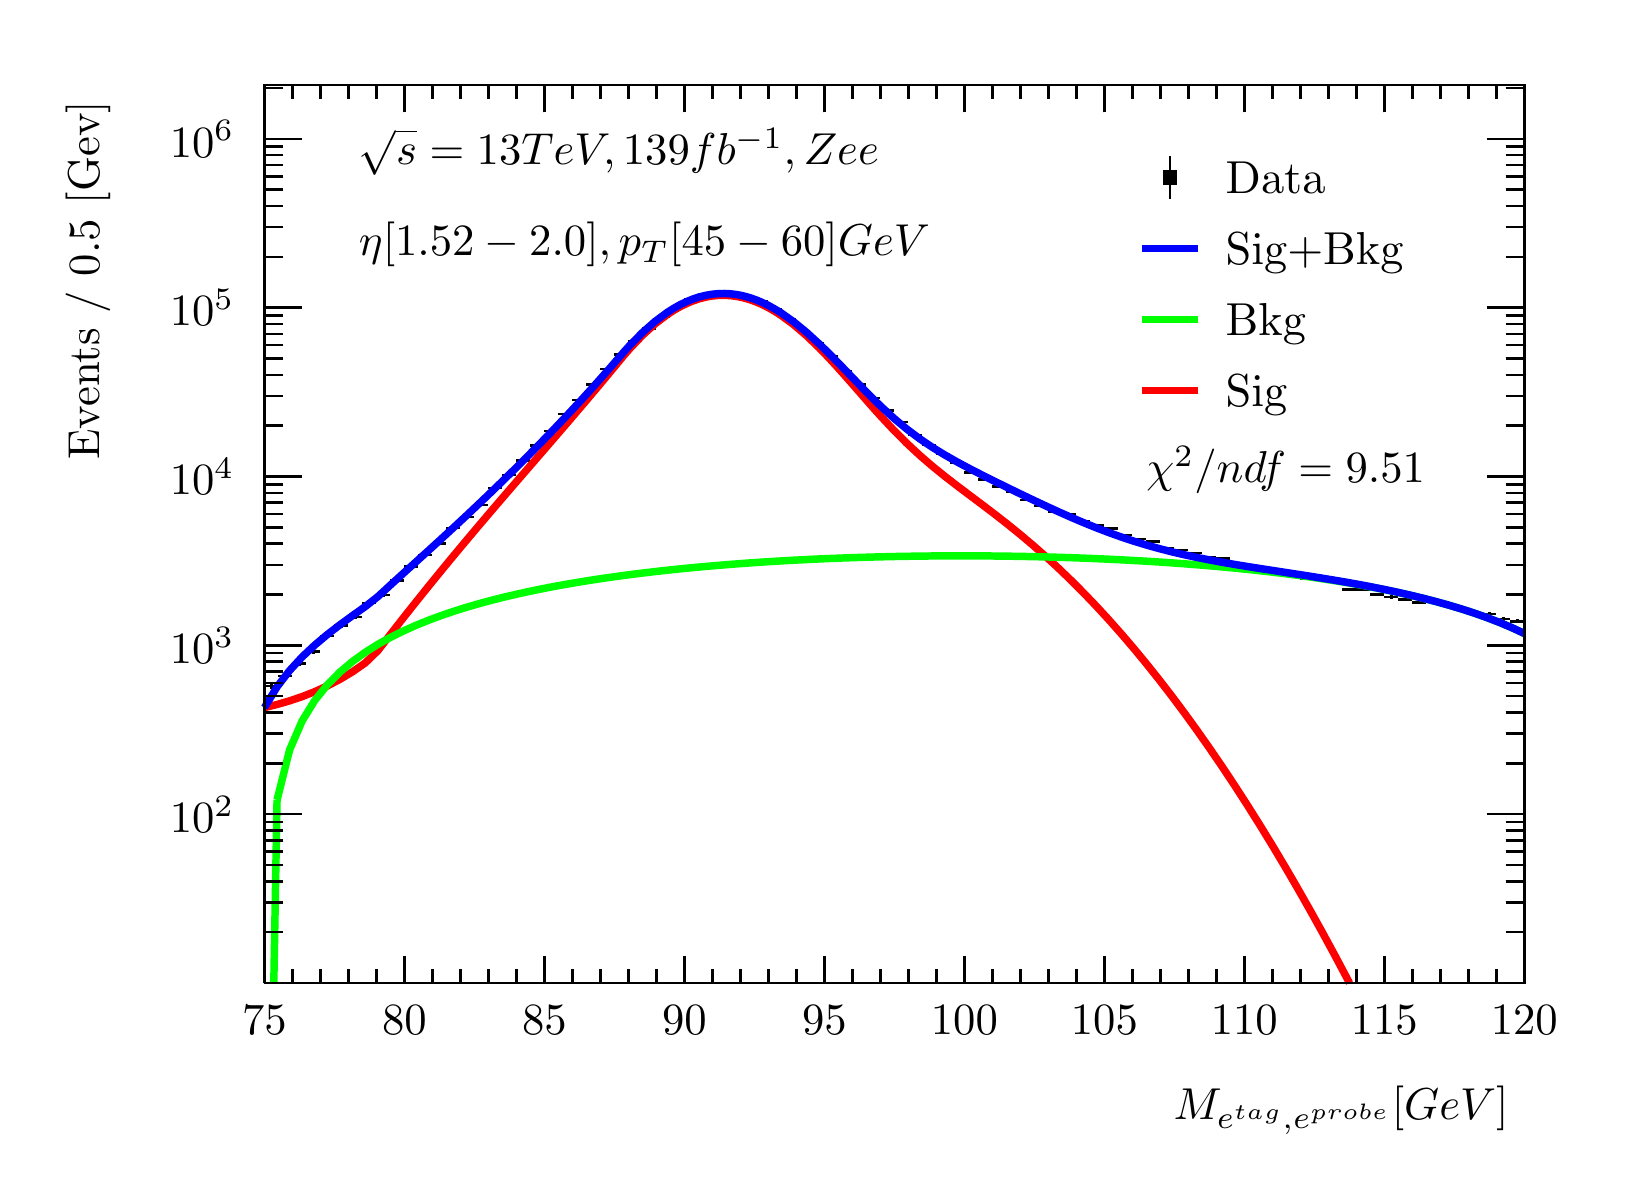
\begin{tikzpicture}
\pgfdeclareplotmark{cross} {
\pgfpathmoveto{\pgfpoint{-0.3\pgfplotmarksize}{\pgfplotmarksize}}
\pgfpathlineto{\pgfpoint{+0.3\pgfplotmarksize}{\pgfplotmarksize}}
\pgfpathlineto{\pgfpoint{+0.3\pgfplotmarksize}{0.3\pgfplotmarksize}}
\pgfpathlineto{\pgfpoint{+1\pgfplotmarksize}{0.3\pgfplotmarksize}}
\pgfpathlineto{\pgfpoint{+1\pgfplotmarksize}{-0.3\pgfplotmarksize}}
\pgfpathlineto{\pgfpoint{+0.3\pgfplotmarksize}{-0.3\pgfplotmarksize}}
\pgfpathlineto{\pgfpoint{+0.3\pgfplotmarksize}{-1.\pgfplotmarksize}}
\pgfpathlineto{\pgfpoint{-0.3\pgfplotmarksize}{-1.\pgfplotmarksize}}
\pgfpathlineto{\pgfpoint{-0.3\pgfplotmarksize}{-0.3\pgfplotmarksize}}
\pgfpathlineto{\pgfpoint{-1.\pgfplotmarksize}{-0.3\pgfplotmarksize}}
\pgfpathlineto{\pgfpoint{-1.\pgfplotmarksize}{0.3\pgfplotmarksize}}
\pgfpathlineto{\pgfpoint{-0.3\pgfplotmarksize}{0.3\pgfplotmarksize}}
\pgfpathclose
\pgfusepathqstroke
}
\pgfdeclareplotmark{cross*} {
\pgfpathmoveto{\pgfpoint{-0.3\pgfplotmarksize}{\pgfplotmarksize}}
\pgfpathlineto{\pgfpoint{+0.3\pgfplotmarksize}{\pgfplotmarksize}}
\pgfpathlineto{\pgfpoint{+0.3\pgfplotmarksize}{0.3\pgfplotmarksize}}
\pgfpathlineto{\pgfpoint{+1\pgfplotmarksize}{0.3\pgfplotmarksize}}
\pgfpathlineto{\pgfpoint{+1\pgfplotmarksize}{-0.3\pgfplotmarksize}}
\pgfpathlineto{\pgfpoint{+0.3\pgfplotmarksize}{-0.3\pgfplotmarksize}}
\pgfpathlineto{\pgfpoint{+0.3\pgfplotmarksize}{-1.\pgfplotmarksize}}
\pgfpathlineto{\pgfpoint{-0.3\pgfplotmarksize}{-1.\pgfplotmarksize}}
\pgfpathlineto{\pgfpoint{-0.3\pgfplotmarksize}{-0.3\pgfplotmarksize}}
\pgfpathlineto{\pgfpoint{-1.\pgfplotmarksize}{-0.3\pgfplotmarksize}}
\pgfpathlineto{\pgfpoint{-1.\pgfplotmarksize}{0.3\pgfplotmarksize}}
\pgfpathlineto{\pgfpoint{-0.3\pgfplotmarksize}{0.3\pgfplotmarksize}}
\pgfpathclose
\pgfusepathqfillstroke
}
\pgfdeclareplotmark{newstar} {
\pgfpathmoveto{\pgfqpoint{0pt}{\pgfplotmarksize}}
\pgfpathlineto{\pgfqpointpolar{44}{0.5\pgfplotmarksize}}
\pgfpathlineto{\pgfqpointpolar{18}{\pgfplotmarksize}}
\pgfpathlineto{\pgfqpointpolar{-20}{0.5\pgfplotmarksize}}
\pgfpathlineto{\pgfqpointpolar{-54}{\pgfplotmarksize}}
\pgfpathlineto{\pgfqpointpolar{-90}{0.5\pgfplotmarksize}}
\pgfpathlineto{\pgfqpointpolar{234}{\pgfplotmarksize}}
\pgfpathlineto{\pgfqpointpolar{198}{0.5\pgfplotmarksize}}
\pgfpathlineto{\pgfqpointpolar{162}{\pgfplotmarksize}}
\pgfpathlineto{\pgfqpointpolar{134}{0.5\pgfplotmarksize}}
\pgfpathclose
\pgfusepathqstroke
}
\pgfdeclareplotmark{newstar*} {
\pgfpathmoveto{\pgfqpoint{0pt}{\pgfplotmarksize}}
\pgfpathlineto{\pgfqpointpolar{44}{0.5\pgfplotmarksize}}
\pgfpathlineto{\pgfqpointpolar{18}{\pgfplotmarksize}}
\pgfpathlineto{\pgfqpointpolar{-20}{0.5\pgfplotmarksize}}
\pgfpathlineto{\pgfqpointpolar{-54}{\pgfplotmarksize}}
\pgfpathlineto{\pgfqpointpolar{-90}{0.5\pgfplotmarksize}}
\pgfpathlineto{\pgfqpointpolar{234}{\pgfplotmarksize}}
\pgfpathlineto{\pgfqpointpolar{198}{0.5\pgfplotmarksize}}
\pgfpathlineto{\pgfqpointpolar{162}{\pgfplotmarksize}}
\pgfpathlineto{\pgfqpointpolar{134}{0.5\pgfplotmarksize}}
\pgfpathclose
\pgfusepathqfillstroke
}
\definecolor{c}{rgb}{1,1,1};
\draw [color=c, fill=c] (0,0) rectangle (20,14.4361);
\draw [color=c, fill=c] (3,2.30977) rectangle (19,13.7143);
\definecolor{c}{rgb}{0,0,0};
\draw [c,line width=0.9] (3,2.30977) -- (3,13.7143) -- (19,13.7143) -- (19,2.30977) -- (3,2.30977);
\definecolor{c}{rgb}{1,1,1};
\draw [color=c, fill=c] (3,2.30977) rectangle (19,13.7143);
\definecolor{c}{rgb}{0,0,0};
\draw [c,line width=0.9] (3,2.30977) -- (3,13.7143) -- (19,13.7143) -- (19,2.30977) -- (3,2.30977);
\draw [c,line width=0.9] (3,2.30977) -- (19,2.30977);
\draw [c,line width=0.9] (3,2.65624) -- (3,2.30977);
\draw [c,line width=0.9] (3.35556,2.48301) -- (3.35556,2.30977);
\draw [c,line width=0.9] (3.71111,2.48301) -- (3.71111,2.30977);
\draw [c,line width=0.9] (4.06667,2.48301) -- (4.06667,2.30977);
\draw [c,line width=0.9] (4.42222,2.48301) -- (4.42222,2.30977);
\draw [c,line width=0.9] (4.77778,2.65624) -- (4.77778,2.30977);
\draw [c,line width=0.9] (5.13333,2.48301) -- (5.13333,2.30977);
\draw [c,line width=0.9] (5.48889,2.48301) -- (5.48889,2.30977);
\draw [c,line width=0.9] (5.84444,2.48301) -- (5.84444,2.30977);
\draw [c,line width=0.9] (6.2,2.48301) -- (6.2,2.30977);
\draw [c,line width=0.9] (6.55556,2.65624) -- (6.55556,2.30977);
\draw [c,line width=0.9] (6.91111,2.48301) -- (6.91111,2.30977);
\draw [c,line width=0.9] (7.26667,2.48301) -- (7.26667,2.30977);
\draw [c,line width=0.9] (7.62222,2.48301) -- (7.62222,2.30977);
\draw [c,line width=0.9] (7.97778,2.48301) -- (7.97778,2.30977);
\draw [c,line width=0.9] (8.33333,2.65624) -- (8.33333,2.30977);
\draw [c,line width=0.9] (8.68889,2.48301) -- (8.68889,2.30977);
\draw [c,line width=0.9] (9.04444,2.48301) -- (9.04444,2.30977);
\draw [c,line width=0.9] (9.4,2.48301) -- (9.4,2.30977);
\draw [c,line width=0.9] (9.75556,2.48301) -- (9.75556,2.30977);
\draw [c,line width=0.9] (10.1111,2.65624) -- (10.1111,2.30977);
\draw [c,line width=0.9] (10.4667,2.48301) -- (10.4667,2.30977);
\draw [c,line width=0.9] (10.8222,2.48301) -- (10.8222,2.30977);
\draw [c,line width=0.9] (11.1778,2.48301) -- (11.1778,2.30977);
\draw [c,line width=0.9] (11.5333,2.48301) -- (11.5333,2.30977);
\draw [c,line width=0.9] (11.8889,2.65624) -- (11.8889,2.30977);
\draw [c,line width=0.9] (12.2444,2.48301) -- (12.2444,2.30977);
\draw [c,line width=0.9] (12.6,2.48301) -- (12.6,2.30977);
\draw [c,line width=0.9] (12.9556,2.48301) -- (12.9556,2.30977);
\draw [c,line width=0.9] (13.3111,2.48301) -- (13.3111,2.30977);
\draw [c,line width=0.9] (13.6667,2.65624) -- (13.6667,2.30977);
\draw [c,line width=0.9] (14.0222,2.48301) -- (14.0222,2.30977);
\draw [c,line width=0.9] (14.3778,2.48301) -- (14.3778,2.30977);
\draw [c,line width=0.9] (14.7333,2.48301) -- (14.7333,2.30977);
\draw [c,line width=0.9] (15.0889,2.48301) -- (15.0889,2.30977);
\draw [c,line width=0.9] (15.4444,2.65624) -- (15.4444,2.30977);
\draw [c,line width=0.9] (15.8,2.48301) -- (15.8,2.30977);
\draw [c,line width=0.9] (16.1556,2.48301) -- (16.1556,2.30977);
\draw [c,line width=0.9] (16.5111,2.48301) -- (16.5111,2.30977);
\draw [c,line width=0.9] (16.8667,2.48301) -- (16.8667,2.30977);
\draw [c,line width=0.9] (17.2222,2.65624) -- (17.2222,2.30977);
\draw [c,line width=0.9] (17.5778,2.48301) -- (17.5778,2.30977);
\draw [c,line width=0.9] (17.9333,2.48301) -- (17.9333,2.30977);
\draw [c,line width=0.9] (18.2889,2.48301) -- (18.2889,2.30977);
\draw [c,line width=0.9] (18.6444,2.48301) -- (18.6444,2.30977);
\draw [c,line width=0.9] (19,2.65624) -- (19,2.30977);
\draw [c,line width=0.9] (19,2.65624) -- (19,2.30977);
\draw [anchor=base] (3,1.66015) node[scale=1.61424, color=c, rotate=0]{75};
\draw [anchor=base] (4.77778,1.66015) node[scale=1.61424, color=c, rotate=0]{80};
\draw [anchor=base] (6.55556,1.66015) node[scale=1.61424, color=c, rotate=0]{85};
\draw [anchor=base] (8.33333,1.66015) node[scale=1.61424, color=c, rotate=0]{90};
\draw [anchor=base] (10.1111,1.66015) node[scale=1.61424, color=c, rotate=0]{95};
\draw [anchor=base] (11.8889,1.66015) node[scale=1.61424, color=c, rotate=0]{100};
\draw [anchor=base] (13.6667,1.66015) node[scale=1.61424, color=c, rotate=0]{105};
\draw [anchor=base] (15.4444,1.66015) node[scale=1.61424, color=c, rotate=0]{110};
\draw [anchor=base] (17.2222,1.66015) node[scale=1.61424, color=c, rotate=0]{115};
\draw [anchor=base] (19,1.66015) node[scale=1.61424, color=c, rotate=0]{120};
\draw [anchor= east] (19,0.692932) node[scale=1.61424, color=c, rotate=0]{$M_{e^{tag}, e^{probe}}  [GeV]$};
\draw [c,line width=0.9] (3,13.7143) -- (19,13.7143);
\draw [c,line width=0.9] (3,13.3678) -- (3,13.7143);
\draw [c,line width=0.9] (3.35556,13.5411) -- (3.35556,13.7143);
\draw [c,line width=0.9] (3.71111,13.5411) -- (3.71111,13.7143);
\draw [c,line width=0.9] (4.06667,13.5411) -- (4.06667,13.7143);
\draw [c,line width=0.9] (4.42222,13.5411) -- (4.42222,13.7143);
\draw [c,line width=0.9] (4.77778,13.3678) -- (4.77778,13.7143);
\draw [c,line width=0.9] (5.13333,13.5411) -- (5.13333,13.7143);
\draw [c,line width=0.9] (5.48889,13.5411) -- (5.48889,13.7143);
\draw [c,line width=0.9] (5.84444,13.5411) -- (5.84444,13.7143);
\draw [c,line width=0.9] (6.2,13.5411) -- (6.2,13.7143);
\draw [c,line width=0.9] (6.55556,13.3678) -- (6.55556,13.7143);
\draw [c,line width=0.9] (6.91111,13.5411) -- (6.91111,13.7143);
\draw [c,line width=0.9] (7.26667,13.5411) -- (7.26667,13.7143);
\draw [c,line width=0.9] (7.62222,13.5411) -- (7.62222,13.7143);
\draw [c,line width=0.9] (7.97778,13.5411) -- (7.97778,13.7143);
\draw [c,line width=0.9] (8.33333,13.3678) -- (8.33333,13.7143);
\draw [c,line width=0.9] (8.68889,13.5411) -- (8.68889,13.7143);
\draw [c,line width=0.9] (9.04444,13.5411) -- (9.04444,13.7143);
\draw [c,line width=0.9] (9.4,13.5411) -- (9.4,13.7143);
\draw [c,line width=0.9] (9.75556,13.5411) -- (9.75556,13.7143);
\draw [c,line width=0.9] (10.1111,13.3678) -- (10.1111,13.7143);
\draw [c,line width=0.9] (10.4667,13.5411) -- (10.4667,13.7143);
\draw [c,line width=0.9] (10.8222,13.5411) -- (10.8222,13.7143);
\draw [c,line width=0.9] (11.1778,13.5411) -- (11.1778,13.7143);
\draw [c,line width=0.9] (11.5333,13.5411) -- (11.5333,13.7143);
\draw [c,line width=0.9] (11.8889,13.3678) -- (11.8889,13.7143);
\draw [c,line width=0.9] (12.2444,13.5411) -- (12.2444,13.7143);
\draw [c,line width=0.9] (12.6,13.5411) -- (12.6,13.7143);
\draw [c,line width=0.9] (12.9556,13.5411) -- (12.9556,13.7143);
\draw [c,line width=0.9] (13.3111,13.5411) -- (13.3111,13.7143);
\draw [c,line width=0.9] (13.6667,13.3678) -- (13.6667,13.7143);
\draw [c,line width=0.9] (14.0222,13.5411) -- (14.0222,13.7143);
\draw [c,line width=0.9] (14.3778,13.5411) -- (14.3778,13.7143);
\draw [c,line width=0.9] (14.7333,13.5411) -- (14.7333,13.7143);
\draw [c,line width=0.9] (15.0889,13.5411) -- (15.0889,13.7143);
\draw [c,line width=0.9] (15.4444,13.3678) -- (15.4444,13.7143);
\draw [c,line width=0.9] (15.8,13.5411) -- (15.8,13.7143);
\draw [c,line width=0.9] (16.1556,13.5411) -- (16.1556,13.7143);
\draw [c,line width=0.9] (16.5111,13.5411) -- (16.5111,13.7143);
\draw [c,line width=0.9] (16.8667,13.5411) -- (16.8667,13.7143);
\draw [c,line width=0.9] (17.2222,13.3678) -- (17.2222,13.7143);
\draw [c,line width=0.9] (17.5778,13.5411) -- (17.5778,13.7143);
\draw [c,line width=0.9] (17.9333,13.5411) -- (17.9333,13.7143);
\draw [c,line width=0.9] (18.2889,13.5411) -- (18.2889,13.7143);
\draw [c,line width=0.9] (18.6444,13.5411) -- (18.6444,13.7143);
\draw [c,line width=0.9] (19,13.3678) -- (19,13.7143);
\draw [c,line width=0.9] (19,13.3678) -- (19,13.7143);
\draw [c,line width=0.9] (3,2.30977) -- (3,13.7143);
\draw [c,line width=0.9] (3.237,2.95525) -- (3,2.95525);
\draw [c,line width=0.9] (3.237,3.33283) -- (3,3.33283);
\draw [c,line width=0.9] (3.237,3.60073) -- (3,3.60073);
\draw [c,line width=0.9] (3.237,3.80852) -- (3,3.80852);
\draw [c,line width=0.9] (3.237,3.97831) -- (3,3.97831);
\draw [c,line width=0.9] (3.237,4.12185) -- (3,4.12185);
\draw [c,line width=0.9] (3.237,4.2462) -- (3,4.2462);
\draw [c,line width=0.9] (3.237,4.35589) -- (3,4.35589);
\draw [c,line width=0.9] (3.474,4.454) -- (3,4.454);
\draw [anchor= east] (2.82,4.454) node[scale=1.61424, color=c, rotate=0]{$10^{2}$};
\draw [c,line width=0.9] (3.237,5.09948) -- (3,5.09948);
\draw [c,line width=0.9] (3.237,5.47706) -- (3,5.47706);
\draw [c,line width=0.9] (3.237,5.74495) -- (3,5.74495);
\draw [c,line width=0.9] (3.237,5.95275) -- (3,5.95275);
\draw [c,line width=0.9] (3.237,6.12253) -- (3,6.12253);
\draw [c,line width=0.9] (3.237,6.26608) -- (3,6.26608);
\draw [c,line width=0.9] (3.237,6.39043) -- (3,6.39043);
\draw [c,line width=0.9] (3.237,6.50011) -- (3,6.50011);
\draw [c,line width=0.9] (3.474,6.59823) -- (3,6.59823);
\draw [anchor= east] (2.82,6.59823) node[scale=1.61424, color=c, rotate=0]{$10^{3}$};
\draw [c,line width=0.9] (3.237,7.2437) -- (3,7.2437);
\draw [c,line width=0.9] (3.237,7.62128) -- (3,7.62128);
\draw [c,line width=0.9] (3.237,7.88918) -- (3,7.88918);
\draw [c,line width=0.9] (3.237,8.09698) -- (3,8.09698);
\draw [c,line width=0.9] (3.237,8.26676) -- (3,8.26676);
\draw [c,line width=0.9] (3.237,8.41031) -- (3,8.41031);
\draw [c,line width=0.9] (3.237,8.53466) -- (3,8.53466);
\draw [c,line width=0.9] (3.237,8.64434) -- (3,8.64434);
\draw [c,line width=0.9] (3.474,8.74245) -- (3,8.74245);
\draw [anchor= east] (2.82,8.74245) node[scale=1.61424, color=c, rotate=0]{$10^{4}$};
\draw [c,line width=0.9] (3.237,9.38793) -- (3,9.38793);
\draw [c,line width=0.9] (3.237,9.76551) -- (3,9.76551);
\draw [c,line width=0.9] (3.237,10.0334) -- (3,10.0334);
\draw [c,line width=0.9] (3.237,10.2412) -- (3,10.2412);
\draw [c,line width=0.9] (3.237,10.411) -- (3,10.411);
\draw [c,line width=0.9] (3.237,10.5545) -- (3,10.5545);
\draw [c,line width=0.9] (3.237,10.6789) -- (3,10.6789);
\draw [c,line width=0.9] (3.237,10.7886) -- (3,10.7886);
\draw [c,line width=0.9] (3.474,10.8867) -- (3,10.8867);
\draw [anchor= east] (2.82,10.8867) node[scale=1.61424, color=c, rotate=0]{$10^{5}$};
\draw [c,line width=0.9] (3.237,11.5322) -- (3,11.5322);
\draw [c,line width=0.9] (3.237,11.9097) -- (3,11.9097);
\draw [c,line width=0.9] (3.237,12.1776) -- (3,12.1776);
\draw [c,line width=0.9] (3.237,12.3854) -- (3,12.3854);
\draw [c,line width=0.9] (3.237,12.5552) -- (3,12.5552);
\draw [c,line width=0.9] (3.237,12.6988) -- (3,12.6988);
\draw [c,line width=0.9] (3.237,12.8231) -- (3,12.8231);
\draw [c,line width=0.9] (3.237,12.9328) -- (3,12.9328);
\draw [c,line width=0.9] (3.474,13.0309) -- (3,13.0309);
\draw [anchor= east] (2.82,13.0309) node[scale=1.61424, color=c, rotate=0]{$10^{6}$};
\draw [c,line width=0.9] (3.237,13.6764) -- (3,13.6764);
\draw [anchor= east] (0.76,13.7143) node[scale=1.61424, color=c, rotate=90]{Events / 0.5 [Gev]};
\draw [c,line width=0.9] (19,2.30977) -- (19,13.7143);
\draw [c,line width=0.9] (18.763,2.95525) -- (19,2.95525);
\draw [c,line width=0.9] (18.763,3.33283) -- (19,3.33283);
\draw [c,line width=0.9] (18.763,3.60073) -- (19,3.60073);
\draw [c,line width=0.9] (18.763,3.80852) -- (19,3.80852);
\draw [c,line width=0.9] (18.763,3.97831) -- (19,3.97831);
\draw [c,line width=0.9] (18.763,4.12185) -- (19,4.12185);
\draw [c,line width=0.9] (18.763,4.2462) -- (19,4.2462);
\draw [c,line width=0.9] (18.763,4.35589) -- (19,4.35589);
\draw [c,line width=0.9] (18.526,4.454) -- (19,4.454);
\draw [c,line width=0.9] (18.763,5.09948) -- (19,5.09948);
\draw [c,line width=0.9] (18.763,5.47706) -- (19,5.47706);
\draw [c,line width=0.9] (18.763,5.74495) -- (19,5.74495);
\draw [c,line width=0.9] (18.763,5.95275) -- (19,5.95275);
\draw [c,line width=0.9] (18.763,6.12253) -- (19,6.12253);
\draw [c,line width=0.9] (18.763,6.26608) -- (19,6.26608);
\draw [c,line width=0.9] (18.763,6.39043) -- (19,6.39043);
\draw [c,line width=0.9] (18.763,6.50011) -- (19,6.50011);
\draw [c,line width=0.9] (18.526,6.59823) -- (19,6.59823);
\draw [c,line width=0.9] (18.763,7.2437) -- (19,7.2437);
\draw [c,line width=0.9] (18.763,7.62128) -- (19,7.62128);
\draw [c,line width=0.9] (18.763,7.88918) -- (19,7.88918);
\draw [c,line width=0.9] (18.763,8.09698) -- (19,8.09698);
\draw [c,line width=0.9] (18.763,8.26676) -- (19,8.26676);
\draw [c,line width=0.9] (18.763,8.41031) -- (19,8.41031);
\draw [c,line width=0.9] (18.763,8.53466) -- (19,8.53466);
\draw [c,line width=0.9] (18.763,8.64434) -- (19,8.64434);
\draw [c,line width=0.9] (18.526,8.74245) -- (19,8.74245);
\draw [c,line width=0.9] (18.763,9.38793) -- (19,9.38793);
\draw [c,line width=0.9] (18.763,9.76551) -- (19,9.76551);
\draw [c,line width=0.9] (18.763,10.0334) -- (19,10.0334);
\draw [c,line width=0.9] (18.763,10.2412) -- (19,10.2412);
\draw [c,line width=0.9] (18.763,10.411) -- (19,10.411);
\draw [c,line width=0.9] (18.763,10.5545) -- (19,10.5545);
\draw [c,line width=0.9] (18.763,10.6789) -- (19,10.6789);
\draw [c,line width=0.9] (18.763,10.7886) -- (19,10.7886);
\draw [c,line width=0.9] (18.526,10.8867) -- (19,10.8867);
\draw [c,line width=0.9] (18.763,11.5322) -- (19,11.5322);
\draw [c,line width=0.9] (18.763,11.9097) -- (19,11.9097);
\draw [c,line width=0.9] (18.763,12.1776) -- (19,12.1776);
\draw [c,line width=0.9] (18.763,12.3854) -- (19,12.3854);
\draw [c,line width=0.9] (18.763,12.5552) -- (19,12.5552);
\draw [c,line width=0.9] (18.763,12.6988) -- (19,12.6988);
\draw [c,line width=0.9] (18.763,12.8231) -- (19,12.8231);
\draw [c,line width=0.9] (18.763,12.9328) -- (19,12.9328);
\draw [c,line width=0.9] (18.526,13.0309) -- (19,13.0309);
\draw [c,line width=0.9] (18.763,13.6764) -- (19,13.6764);
\draw [c,line width=0.9] (3.08889,6.07966) -- (3,6.07966);
\draw [c,line width=0.9] (3,6.07966) -- (3,6.07966);
\draw [c,line width=0.9] (3.08889,6.07966) -- (3.17778,6.07966);
\draw [c,line width=0.9] (3.17778,6.07966) -- (3.17778,6.07966);
\draw [c,line width=0.9] (3.08889,6.07966) -- (3.08889,6.11856);
\draw [c,line width=0.9] (3.08889,6.11856) -- (3.08889,6.11856);
\draw [c,line width=0.9] (3.08889,6.07966) -- (3.08889,6.04076);
\draw [c,line width=0.9] (3.08889,6.04076) -- (3.08889,6.04076);
\draw [c,line width=0.9] (3.26667,6.20705) -- (3.17778,6.20705);
\draw [c,line width=0.9] (3.17778,6.20705) -- (3.17778,6.20705);
\draw [c,line width=0.9] (3.26667,6.20705) -- (3.35556,6.20705);
\draw [c,line width=0.9] (3.35556,6.20705) -- (3.35556,6.20705);
\draw [c,line width=0.9] (3.26667,6.20705) -- (3.26667,6.24338);
\draw [c,line width=0.9] (3.26667,6.24338) -- (3.26667,6.24338);
\draw [c,line width=0.9] (3.26667,6.20705) -- (3.26667,6.17072);
\draw [c,line width=0.9] (3.26667,6.17072) -- (3.26667,6.17072);
\draw [c,line width=0.9] (3.44444,6.37043) -- (3.35556,6.37043);
\draw [c,line width=0.9] (3.35556,6.37043) -- (3.35556,6.37043);
\draw [c,line width=0.9] (3.44444,6.37043) -- (3.53333,6.37043);
\draw [c,line width=0.9] (3.53333,6.37043) -- (3.53333,6.37043);
\draw [c,line width=0.9] (3.44444,6.37043) -- (3.44444,6.40371);
\draw [c,line width=0.9] (3.44444,6.40371) -- (3.44444,6.40371);
\draw [c,line width=0.9] (3.44444,6.37043) -- (3.44444,6.33715);
\draw [c,line width=0.9] (3.44444,6.33715) -- (3.44444,6.33715);
\draw [c,line width=0.9] (3.62222,6.5226) -- (3.53333,6.5226);
\draw [c,line width=0.9] (3.53333,6.5226) -- (3.53333,6.5226);
\draw [c,line width=0.9] (3.62222,6.5226) -- (3.71111,6.5226);
\draw [c,line width=0.9] (3.71111,6.5226) -- (3.71111,6.5226);
\draw [c,line width=0.9] (3.62222,6.5226) -- (3.62222,6.55327);
\draw [c,line width=0.9] (3.62222,6.55327) -- (3.62222,6.55327);
\draw [c,line width=0.9] (3.62222,6.5226) -- (3.62222,6.49194);
\draw [c,line width=0.9] (3.62222,6.49194) -- (3.62222,6.49194);
\draw [c,line width=0.9] (3.8,6.71697) -- (3.71111,6.71697);
\draw [c,line width=0.9] (3.71111,6.71697) -- (3.71111,6.71697);
\draw [c,line width=0.9] (3.8,6.71697) -- (3.88889,6.71697);
\draw [c,line width=0.9] (3.88889,6.71697) -- (3.88889,6.71697);
\draw [c,line width=0.9] (3.8,6.71697) -- (3.8,6.7446);
\draw [c,line width=0.9] (3.8,6.7446) -- (3.8,6.7446);
\draw [c,line width=0.9] (3.8,6.71697) -- (3.8,6.68934);
\draw [c,line width=0.9] (3.8,6.68934) -- (3.8,6.68934);
\draw [c,line width=0.9] (3.97778,6.84968) -- (3.88889,6.84968);
\draw [c,line width=0.9] (3.88889,6.84968) -- (3.88889,6.84968);
\draw [c,line width=0.9] (3.97778,6.84968) -- (4.06667,6.84968);
\draw [c,line width=0.9] (4.06667,6.84968) -- (4.06667,6.84968);
\draw [c,line width=0.9] (3.97778,6.84968) -- (3.97778,6.87541);
\draw [c,line width=0.9] (3.97778,6.87541) -- (3.97778,6.87541);
\draw [c,line width=0.9] (3.97778,6.84968) -- (3.97778,6.82396);
\draw [c,line width=0.9] (3.97778,6.82396) -- (3.97778,6.82396);
\draw [c,line width=0.9] (4.15556,6.96142) -- (4.06667,6.96142);
\draw [c,line width=0.9] (4.06667,6.96142) -- (4.06667,6.96142);
\draw [c,line width=0.9] (4.15556,6.96142) -- (4.24444,6.96142);
\draw [c,line width=0.9] (4.24444,6.96142) -- (4.24444,6.96142);
\draw [c,line width=0.9] (4.15556,6.96142) -- (4.15556,6.98565);
\draw [c,line width=0.9] (4.15556,6.98565) -- (4.15556,6.98565);
\draw [c,line width=0.9] (4.15556,6.96142) -- (4.15556,6.93719);
\draw [c,line width=0.9] (4.15556,6.93719) -- (4.15556,6.93719);
\draw [c,line width=0.9] (4.33333,7.13675) -- (4.24444,7.13675);
\draw [c,line width=0.9] (4.24444,7.13675) -- (4.24444,7.13675);
\draw [c,line width=0.9] (4.33333,7.13675) -- (4.42222,7.13675);
\draw [c,line width=0.9] (4.42222,7.13675) -- (4.42222,7.13675);
\draw [c,line width=0.9] (4.33333,7.13675) -- (4.33333,7.15881);
\draw [c,line width=0.9] (4.33333,7.15881) -- (4.33333,7.15881);
\draw [c,line width=0.9] (4.33333,7.13675) -- (4.33333,7.1147);
\draw [c,line width=0.9] (4.33333,7.1147) -- (4.33333,7.1147);
\draw [c,line width=0.9] (4.51111,7.2395) -- (4.42222,7.2395);
\draw [c,line width=0.9] (4.42222,7.2395) -- (4.42222,7.2395);
\draw [c,line width=0.9] (4.51111,7.2395) -- (4.6,7.2395);
\draw [c,line width=0.9] (4.6,7.2395) -- (4.6,7.2395);
\draw [c,line width=0.9] (4.51111,7.2395) -- (4.51111,7.26037);
\draw [c,line width=0.9] (4.51111,7.26037) -- (4.51111,7.26037);
\draw [c,line width=0.9] (4.51111,7.2395) -- (4.51111,7.21864);
\draw [c,line width=0.9] (4.51111,7.21864) -- (4.51111,7.21864);
\draw [c,line width=0.9] (4.68889,7.42352) -- (4.6,7.42352);
\draw [c,line width=0.9] (4.6,7.42352) -- (4.6,7.42352);
\draw [c,line width=0.9] (4.68889,7.42352) -- (4.77778,7.42352);
\draw [c,line width=0.9] (4.77778,7.42352) -- (4.77778,7.42352);
\draw [c,line width=0.9] (4.68889,7.42352) -- (4.68889,7.44243);
\draw [c,line width=0.9] (4.68889,7.44243) -- (4.68889,7.44243);
\draw [c,line width=0.9] (4.68889,7.42352) -- (4.68889,7.40461);
\draw [c,line width=0.9] (4.68889,7.40461) -- (4.68889,7.40461);
\draw [c,line width=0.9] (4.86667,7.5993) -- (4.77778,7.5993);
\draw [c,line width=0.9] (4.77778,7.5993) -- (4.77778,7.5993);
\draw [c,line width=0.9] (4.86667,7.5993) -- (4.95556,7.5993);
\draw [c,line width=0.9] (4.95556,7.5993) -- (4.95556,7.5993);
\draw [c,line width=0.9] (4.86667,7.5993) -- (4.86667,7.6165);
\draw [c,line width=0.9] (4.86667,7.6165) -- (4.86667,7.6165);
\draw [c,line width=0.9] (4.86667,7.5993) -- (4.86667,7.58209);
\draw [c,line width=0.9] (4.86667,7.58209) -- (4.86667,7.58209);
\draw [c,line width=0.9] (5.04444,7.74412) -- (4.95556,7.74412);
\draw [c,line width=0.9] (4.95556,7.74412) -- (4.95556,7.74412);
\draw [c,line width=0.9] (5.04444,7.74412) -- (5.13333,7.74412);
\draw [c,line width=0.9] (5.13333,7.74412) -- (5.13333,7.74412);
\draw [c,line width=0.9] (5.04444,7.74412) -- (5.04444,7.76003);
\draw [c,line width=0.9] (5.04444,7.76003) -- (5.04444,7.76003);
\draw [c,line width=0.9] (5.04444,7.74412) -- (5.04444,7.7282);
\draw [c,line width=0.9] (5.04444,7.7282) -- (5.04444,7.7282);
\draw [c,line width=0.9] (5.22222,7.88965) -- (5.13333,7.88965);
\draw [c,line width=0.9] (5.13333,7.88965) -- (5.13333,7.88965);
\draw [c,line width=0.9] (5.22222,7.88965) -- (5.31111,7.88965);
\draw [c,line width=0.9] (5.31111,7.88965) -- (5.31111,7.88965);
\draw [c,line width=0.9] (5.22222,7.88965) -- (5.22222,7.90437);
\draw [c,line width=0.9] (5.22222,7.90437) -- (5.22222,7.90437);
\draw [c,line width=0.9] (5.22222,7.88965) -- (5.22222,7.87493);
\draw [c,line width=0.9] (5.22222,7.87493) -- (5.22222,7.87493);
\draw [c,line width=0.9] (5.4,8.08574) -- (5.31111,8.08574);
\draw [c,line width=0.9] (5.31111,8.08574) -- (5.31111,8.08574);
\draw [c,line width=0.9] (5.4,8.08574) -- (5.48889,8.08574);
\draw [c,line width=0.9] (5.48889,8.08574) -- (5.48889,8.08574);
\draw [c,line width=0.9] (5.4,8.08574) -- (5.4,8.09898);
\draw [c,line width=0.9] (5.4,8.09898) -- (5.4,8.09898);
\draw [c,line width=0.9] (5.4,8.08574) -- (5.4,8.07249);
\draw [c,line width=0.9] (5.4,8.07249) -- (5.4,8.07249);
\draw [c,line width=0.9] (5.57778,8.22551) -- (5.48889,8.22551);
\draw [c,line width=0.9] (5.48889,8.22551) -- (5.48889,8.22551);
\draw [c,line width=0.9] (5.57778,8.22551) -- (5.66667,8.22551);
\draw [c,line width=0.9] (5.66667,8.22551) -- (5.66667,8.22551);
\draw [c,line width=0.9] (5.57778,8.22551) -- (5.57778,8.2378);
\draw [c,line width=0.9] (5.57778,8.2378) -- (5.57778,8.2378);
\draw [c,line width=0.9] (5.57778,8.22551) -- (5.57778,8.21322);
\draw [c,line width=0.9] (5.57778,8.21322) -- (5.57778,8.21322);
\draw [c,line width=0.9] (5.75556,8.38304) -- (5.66667,8.38304);
\draw [c,line width=0.9] (5.66667,8.38304) -- (5.66667,8.38304);
\draw [c,line width=0.9] (5.75556,8.38304) -- (5.84444,8.38304);
\draw [c,line width=0.9] (5.84444,8.38304) -- (5.84444,8.38304);
\draw [c,line width=0.9] (5.75556,8.38304) -- (5.75556,8.39434);
\draw [c,line width=0.9] (5.75556,8.39434) -- (5.75556,8.39434);
\draw [c,line width=0.9] (5.75556,8.38304) -- (5.75556,8.37175);
\draw [c,line width=0.9] (5.75556,8.37175) -- (5.75556,8.37175);
\draw [c,line width=0.9] (5.93333,8.60005) -- (5.84444,8.60005);
\draw [c,line width=0.9] (5.84444,8.60005) -- (5.84444,8.60005);
\draw [c,line width=0.9] (5.93333,8.60005) -- (6.02222,8.60005);
\draw [c,line width=0.9] (6.02222,8.60005) -- (6.02222,8.60005);
\draw [c,line width=0.9] (5.93333,8.60005) -- (5.93333,8.61011);
\draw [c,line width=0.9] (5.93333,8.61011) -- (5.93333,8.61011);
\draw [c,line width=0.9] (5.93333,8.60005) -- (5.93333,8.59);
\draw [c,line width=0.9] (5.93333,8.59) -- (5.93333,8.59);
\draw [c,line width=0.9] (6.11111,8.76226) -- (6.02222,8.76226);
\draw [c,line width=0.9] (6.02222,8.76226) -- (6.02222,8.76226);
\draw [c,line width=0.9] (6.11111,8.76226) -- (6.2,8.76226);
\draw [c,line width=0.9] (6.2,8.76226) -- (6.2,8.76226);
\draw [c,line width=0.9] (6.11111,8.76226) -- (6.11111,8.77148);
\draw [c,line width=0.9] (6.11111,8.77148) -- (6.11111,8.77148);
\draw [c,line width=0.9] (6.11111,8.76226) -- (6.11111,8.75305);
\draw [c,line width=0.9] (6.11111,8.75305) -- (6.11111,8.75305);
\draw [c,line width=0.9] (6.28889,8.94719) -- (6.2,8.94719);
\draw [c,line width=0.9] (6.2,8.94719) -- (6.2,8.94719);
\draw [c,line width=0.9] (6.28889,8.94719) -- (6.37778,8.94719);
\draw [c,line width=0.9] (6.37778,8.94719) -- (6.37778,8.94719);
\draw [c,line width=0.9] (6.28889,8.94719) -- (6.28889,8.95553);
\draw [c,line width=0.9] (6.28889,8.95553) -- (6.28889,8.95553);
\draw [c,line width=0.9] (6.28889,8.94719) -- (6.28889,8.93885);
\draw [c,line width=0.9] (6.28889,8.93885) -- (6.28889,8.93885);
\draw [c,line width=0.9] (6.46667,9.13537) -- (6.37778,9.13537);
\draw [c,line width=0.9] (6.37778,9.13537) -- (6.37778,9.13537);
\draw [c,line width=0.9] (6.46667,9.13537) -- (6.55556,9.13537);
\draw [c,line width=0.9] (6.55556,9.13537) -- (6.55556,9.13537);
\draw [c,line width=0.9] (6.46667,9.13537) -- (6.46667,9.14291);
\draw [c,line width=0.9] (6.46667,9.14291) -- (6.46667,9.14291);
\draw [c,line width=0.9] (6.46667,9.13537) -- (6.46667,9.12782);
\draw [c,line width=0.9] (6.46667,9.12782) -- (6.46667,9.12782);
\draw [c,line width=0.9] (6.64444,9.3191) -- (6.55556,9.3191);
\draw [c,line width=0.9] (6.55556,9.3191) -- (6.55556,9.3191);
\draw [c,line width=0.9] (6.64444,9.3191) -- (6.73333,9.3191);
\draw [c,line width=0.9] (6.73333,9.3191) -- (6.73333,9.3191);
\draw [c,line width=0.9] (6.64444,9.3191) -- (6.64444,9.32593);
\draw [c,line width=0.9] (6.64444,9.32593) -- (6.64444,9.32593);
\draw [c,line width=0.9] (6.64444,9.3191) -- (6.64444,9.31227);
\draw [c,line width=0.9] (6.64444,9.31227) -- (6.64444,9.31227);
\draw [c,line width=0.9] (6.82222,9.53577) -- (6.73333,9.53577);
\draw [c,line width=0.9] (6.73333,9.53577) -- (6.73333,9.53577);
\draw [c,line width=0.9] (6.82222,9.53577) -- (6.91111,9.53577);
\draw [c,line width=0.9] (6.91111,9.53577) -- (6.91111,9.53577);
\draw [c,line width=0.9] (6.82222,9.53577) -- (6.82222,9.54185);
\draw [c,line width=0.9] (6.82222,9.54185) -- (6.82222,9.54185);
\draw [c,line width=0.9] (6.82222,9.53577) -- (6.82222,9.52969);
\draw [c,line width=0.9] (6.82222,9.52969) -- (6.82222,9.52969);
\draw [c,line width=0.9] (7,9.71555) -- (6.91111,9.71555);
\draw [c,line width=0.9] (6.91111,9.71555) -- (6.91111,9.71555);
\draw [c,line width=0.9] (7,9.71555) -- (7.08889,9.71555);
\draw [c,line width=0.9] (7.08889,9.71555) -- (7.08889,9.71555);
\draw [c,line width=0.9] (7,9.71555) -- (7,9.72108);
\draw [c,line width=0.9] (7,9.72108) -- (7,9.72108);
\draw [c,line width=0.9] (7,9.71555) -- (7,9.71003);
\draw [c,line width=0.9] (7,9.71003) -- (7,9.71003);
\draw [c,line width=0.9] (7.17778,9.91402) -- (7.08889,9.91402);
\draw [c,line width=0.9] (7.08889,9.91402) -- (7.08889,9.91402);
\draw [c,line width=0.9] (7.17778,9.91402) -- (7.26667,9.91402);
\draw [c,line width=0.9] (7.26667,9.91402) -- (7.26667,9.91402);
\draw [c,line width=0.9] (7.17778,9.91402) -- (7.17778,9.91899);
\draw [c,line width=0.9] (7.17778,9.91899) -- (7.17778,9.91899);
\draw [c,line width=0.9] (7.17778,9.91402) -- (7.17778,9.90906);
\draw [c,line width=0.9] (7.17778,9.90906) -- (7.17778,9.90906);
\draw [c,line width=0.9] (7.35556,10.106) -- (7.26667,10.106);
\draw [c,line width=0.9] (7.26667,10.106) -- (7.26667,10.106);
\draw [c,line width=0.9] (7.35556,10.106) -- (7.44444,10.106);
\draw [c,line width=0.9] (7.44444,10.106) -- (7.44444,10.106);
\draw [c,line width=0.9] (7.35556,10.106) -- (7.35556,10.1105);
\draw [c,line width=0.9] (7.35556,10.1105) -- (7.35556,10.1105);
\draw [c,line width=0.9] (7.35556,10.106) -- (7.35556,10.1015);
\draw [c,line width=0.9] (7.35556,10.1015) -- (7.35556,10.1015);
\draw [c,line width=0.9] (7.53333,10.2922) -- (7.44444,10.2922);
\draw [c,line width=0.9] (7.44444,10.2922) -- (7.44444,10.2922);
\draw [c,line width=0.9] (7.53333,10.2922) -- (7.62222,10.2922);
\draw [c,line width=0.9] (7.62222,10.2922) -- (7.62222,10.2922);
\draw [c,line width=0.9] (7.53333,10.2922) -- (7.53333,10.2962);
\draw [c,line width=0.9] (7.53333,10.2962) -- (7.53333,10.2962);
\draw [c,line width=0.9] (7.53333,10.2922) -- (7.53333,10.2881);
\draw [c,line width=0.9] (7.53333,10.2881) -- (7.53333,10.2881);
\draw [c,line width=0.9] (7.71111,10.4611) -- (7.62222,10.4611);
\draw [c,line width=0.9] (7.62222,10.4611) -- (7.62222,10.4611);
\draw [c,line width=0.9] (7.71111,10.4611) -- (7.8,10.4611);
\draw [c,line width=0.9] (7.8,10.4611) -- (7.8,10.4611);
\draw [c,line width=0.9] (7.71111,10.4611) -- (7.71111,10.4648);
\draw [c,line width=0.9] (7.71111,10.4648) -- (7.71111,10.4648);
\draw [c,line width=0.9] (7.71111,10.4611) -- (7.71111,10.4574);
\draw [c,line width=0.9] (7.71111,10.4574) -- (7.71111,10.4574);
\draw [c,line width=0.9] (7.88889,10.6249) -- (7.8,10.6249);
\draw [c,line width=0.9] (7.8,10.6249) -- (7.8,10.6249);
\draw [c,line width=0.9] (7.88889,10.6249) -- (7.97778,10.6249);
\draw [c,line width=0.9] (7.97778,10.6249) -- (7.97778,10.6249);
\draw [c,line width=0.9] (7.88889,10.6249) -- (7.88889,10.6283);
\draw [c,line width=0.9] (7.88889,10.6283) -- (7.88889,10.6283);
\draw [c,line width=0.9] (7.88889,10.6249) -- (7.88889,10.6215);
\draw [c,line width=0.9] (7.88889,10.6215) -- (7.88889,10.6215);
\draw [c,line width=0.9] (8.06667,10.7703) -- (7.97778,10.7703);
\draw [c,line width=0.9] (7.97778,10.7703) -- (7.97778,10.7703);
\draw [c,line width=0.9] (8.06667,10.7703) -- (8.15556,10.7703);
\draw [c,line width=0.9] (8.15556,10.7703) -- (8.15556,10.7703);
\draw [c,line width=0.9] (8.06667,10.7703) -- (8.06667,10.7735);
\draw [c,line width=0.9] (8.06667,10.7735) -- (8.06667,10.7735);
\draw [c,line width=0.9] (8.06667,10.7703) -- (8.06667,10.7672);
\draw [c,line width=0.9] (8.06667,10.7672) -- (8.06667,10.7672);
\draw [c,line width=0.9] (8.24444,10.8945) -- (8.15556,10.8945);
\draw [c,line width=0.9] (8.15556,10.8945) -- (8.15556,10.8945);
\draw [c,line width=0.9] (8.24444,10.8945) -- (8.33333,10.8945);
\draw [c,line width=0.9] (8.33333,10.8945) -- (8.33333,10.8945);
\draw [c,line width=0.9] (8.24444,10.8945) -- (8.24444,10.8974);
\draw [c,line width=0.9] (8.24444,10.8974) -- (8.24444,10.8974);
\draw [c,line width=0.9] (8.24444,10.8945) -- (8.24444,10.8916);
\draw [c,line width=0.9] (8.24444,10.8916) -- (8.24444,10.8916);
\draw [c,line width=0.9] (8.42222,10.9882) -- (8.33333,10.9882);
\draw [c,line width=0.9] (8.33333,10.9882) -- (8.33333,10.9882);
\draw [c,line width=0.9] (8.42222,10.9882) -- (8.51111,10.9882);
\draw [c,line width=0.9] (8.51111,10.9882) -- (8.51111,10.9882);
\draw [c,line width=0.9] (8.42222,10.9882) -- (8.42222,10.991);
\draw [c,line width=0.9] (8.42222,10.991) -- (8.42222,10.991);
\draw [c,line width=0.9] (8.42222,10.9882) -- (8.42222,10.9854);
\draw [c,line width=0.9] (8.42222,10.9854) -- (8.42222,10.9854);
\draw [c,line width=0.9] (8.6,11.0522) -- (8.51111,11.0522);
\draw [c,line width=0.9] (8.51111,11.0522) -- (8.51111,11.0522);
\draw [c,line width=0.9] (8.6,11.0522) -- (8.68889,11.0522);
\draw [c,line width=0.9] (8.68889,11.0522) -- (8.68889,11.0522);
\draw [c,line width=0.9] (8.6,11.0522) -- (8.6,11.0549);
\draw [c,line width=0.9] (8.6,11.0549) -- (8.6,11.0549);
\draw [c,line width=0.9] (8.6,11.0522) -- (8.6,11.0495);
\draw [c,line width=0.9] (8.6,11.0495) -- (8.6,11.0495);
\draw [c,line width=0.9] (8.77778,11.0799) -- (8.68889,11.0799);
\draw [c,line width=0.9] (8.68889,11.0799) -- (8.68889,11.0799);
\draw [c,line width=0.9] (8.77778,11.0799) -- (8.86667,11.0799);
\draw [c,line width=0.9] (8.86667,11.0799) -- (8.86667,11.0799);
\draw [c,line width=0.9] (8.77778,11.0799) -- (8.77778,11.0825);
\draw [c,line width=0.9] (8.77778,11.0825) -- (8.77778,11.0825);
\draw [c,line width=0.9] (8.77778,11.0799) -- (8.77778,11.0772);
\draw [c,line width=0.9] (8.77778,11.0772) -- (8.77778,11.0772);
\draw [c,line width=0.9] (8.95556,11.0744) -- (8.86667,11.0744);
\draw [c,line width=0.9] (8.86667,11.0744) -- (8.86667,11.0744);
\draw [c,line width=0.9] (8.95556,11.0744) -- (9.04444,11.0744);
\draw [c,line width=0.9] (9.04444,11.0744) -- (9.04444,11.0744);
\draw [c,line width=0.9] (8.95556,11.0744) -- (8.95556,11.077);
\draw [c,line width=0.9] (8.95556,11.077) -- (8.95556,11.077);
\draw [c,line width=0.9] (8.95556,11.0744) -- (8.95556,11.0717);
\draw [c,line width=0.9] (8.95556,11.0717) -- (8.95556,11.0717);
\draw [c,line width=0.9] (9.13333,11.0359) -- (9.04444,11.0359);
\draw [c,line width=0.9] (9.04444,11.0359) -- (9.04444,11.0359);
\draw [c,line width=0.9] (9.13333,11.0359) -- (9.22222,11.0359);
\draw [c,line width=0.9] (9.22222,11.0359) -- (9.22222,11.0359);
\draw [c,line width=0.9] (9.13333,11.0359) -- (9.13333,11.0386);
\draw [c,line width=0.9] (9.13333,11.0386) -- (9.13333,11.0386);
\draw [c,line width=0.9] (9.13333,11.0359) -- (9.13333,11.0332);
\draw [c,line width=0.9] (9.13333,11.0332) -- (9.13333,11.0332);
\draw [c,line width=0.9] (9.31111,10.9633) -- (9.22222,10.9633);
\draw [c,line width=0.9] (9.22222,10.9633) -- (9.22222,10.9633);
\draw [c,line width=0.9] (9.31111,10.9633) -- (9.4,10.9633);
\draw [c,line width=0.9] (9.4,10.9633) -- (9.4,10.9633);
\draw [c,line width=0.9] (9.31111,10.9633) -- (9.31111,10.9661);
\draw [c,line width=0.9] (9.31111,10.9661) -- (9.31111,10.9661);
\draw [c,line width=0.9] (9.31111,10.9633) -- (9.31111,10.9604);
\draw [c,line width=0.9] (9.31111,10.9604) -- (9.31111,10.9604);
\draw [c,line width=0.9] (9.48889,10.8636) -- (9.4,10.8636);
\draw [c,line width=0.9] (9.4,10.8636) -- (9.4,10.8636);
\draw [c,line width=0.9] (9.48889,10.8636) -- (9.57778,10.8636);
\draw [c,line width=0.9] (9.57778,10.8636) -- (9.57778,10.8636);
\draw [c,line width=0.9] (9.48889,10.8636) -- (9.48889,10.8666);
\draw [c,line width=0.9] (9.48889,10.8666) -- (9.48889,10.8666);
\draw [c,line width=0.9] (9.48889,10.8636) -- (9.48889,10.8606);
\draw [c,line width=0.9] (9.48889,10.8606) -- (9.48889,10.8606);
\draw [c,line width=0.9] (9.66667,10.7382) -- (9.57778,10.7382);
\draw [c,line width=0.9] (9.57778,10.7382) -- (9.57778,10.7382);
\draw [c,line width=0.9] (9.66667,10.7382) -- (9.75556,10.7382);
\draw [c,line width=0.9] (9.75556,10.7382) -- (9.75556,10.7382);
\draw [c,line width=0.9] (9.66667,10.7382) -- (9.66667,10.7414);
\draw [c,line width=0.9] (9.66667,10.7414) -- (9.66667,10.7414);
\draw [c,line width=0.9] (9.66667,10.7382) -- (9.66667,10.735);
\draw [c,line width=0.9] (9.66667,10.735) -- (9.66667,10.735);
\draw [c,line width=0.9] (9.84444,10.5903) -- (9.75556,10.5903);
\draw [c,line width=0.9] (9.75556,10.5903) -- (9.75556,10.5903);
\draw [c,line width=0.9] (9.84444,10.5903) -- (9.93333,10.5903);
\draw [c,line width=0.9] (9.93333,10.5903) -- (9.93333,10.5903);
\draw [c,line width=0.9] (9.84444,10.5903) -- (9.84444,10.5937);
\draw [c,line width=0.9] (9.84444,10.5937) -- (9.84444,10.5937);
\draw [c,line width=0.9] (9.84444,10.5903) -- (9.84444,10.5868);
\draw [c,line width=0.9] (9.84444,10.5868) -- (9.84444,10.5868);
\draw [c,line width=0.9] (10.0222,10.4372) -- (9.93333,10.4372);
\draw [c,line width=0.9] (9.93333,10.4372) -- (9.93333,10.4372);
\draw [c,line width=0.9] (10.0222,10.4372) -- (10.1111,10.4372);
\draw [c,line width=0.9] (10.1111,10.4372) -- (10.1111,10.4372);
\draw [c,line width=0.9] (10.0222,10.4372) -- (10.0222,10.4409);
\draw [c,line width=0.9] (10.0222,10.4409) -- (10.0222,10.4409);
\draw [c,line width=0.9] (10.0222,10.4372) -- (10.0222,10.4334);
\draw [c,line width=0.9] (10.0222,10.4334) -- (10.0222,10.4334);
\draw [c,line width=0.9] (10.2,10.2664) -- (10.1111,10.2664);
\draw [c,line width=0.9] (10.1111,10.2664) -- (10.1111,10.2664);
\draw [c,line width=0.9] (10.2,10.2664) -- (10.2889,10.2664);
\draw [c,line width=0.9] (10.2889,10.2664) -- (10.2889,10.2664);
\draw [c,line width=0.9] (10.2,10.2664) -- (10.2,10.2705);
\draw [c,line width=0.9] (10.2,10.2705) -- (10.2,10.2705);
\draw [c,line width=0.9] (10.2,10.2664) -- (10.2,10.2623);
\draw [c,line width=0.9] (10.2,10.2623) -- (10.2,10.2623);
\draw [c,line width=0.9] (10.3778,10.0834) -- (10.2889,10.0834);
\draw [c,line width=0.9] (10.2889,10.0834) -- (10.2889,10.0834);
\draw [c,line width=0.9] (10.3778,10.0834) -- (10.4667,10.0834);
\draw [c,line width=0.9] (10.4667,10.0834) -- (10.4667,10.0834);
\draw [c,line width=0.9] (10.3778,10.0834) -- (10.3778,10.0879);
\draw [c,line width=0.9] (10.3778,10.0879) -- (10.3778,10.0879);
\draw [c,line width=0.9] (10.3778,10.0834) -- (10.3778,10.0788);
\draw [c,line width=0.9] (10.3778,10.0788) -- (10.3778,10.0788);
\draw [c,line width=0.9] (10.5556,9.91233) -- (10.4667,9.91233);
\draw [c,line width=0.9] (10.4667,9.91233) -- (10.4667,9.91233);
\draw [c,line width=0.9] (10.5556,9.91233) -- (10.6444,9.91233);
\draw [c,line width=0.9] (10.6444,9.91233) -- (10.6444,9.91233);
\draw [c,line width=0.9] (10.5556,9.91233) -- (10.5556,9.9173);
\draw [c,line width=0.9] (10.5556,9.9173) -- (10.5556,9.9173);
\draw [c,line width=0.9] (10.5556,9.91233) -- (10.5556,9.90736);
\draw [c,line width=0.9] (10.5556,9.90736) -- (10.5556,9.90736);
\draw [c,line width=0.9] (10.7333,9.73769) -- (10.6444,9.73769);
\draw [c,line width=0.9] (10.6444,9.73769) -- (10.6444,9.73769);
\draw [c,line width=0.9] (10.7333,9.73769) -- (10.8222,9.73769);
\draw [c,line width=0.9] (10.8222,9.73769) -- (10.8222,9.73769);
\draw [c,line width=0.9] (10.7333,9.73769) -- (10.7333,9.74315);
\draw [c,line width=0.9] (10.7333,9.74315) -- (10.7333,9.74315);
\draw [c,line width=0.9] (10.7333,9.73769) -- (10.7333,9.73223);
\draw [c,line width=0.9] (10.7333,9.73223) -- (10.7333,9.73223);
\draw [c,line width=0.9] (10.9111,9.5829) -- (10.8222,9.5829);
\draw [c,line width=0.9] (10.8222,9.5829) -- (10.8222,9.5829);
\draw [c,line width=0.9] (10.9111,9.5829) -- (11,9.5829);
\draw [c,line width=0.9] (11,9.5829) -- (11,9.5829);
\draw [c,line width=0.9] (10.9111,9.5829) -- (10.9111,9.58883);
\draw [c,line width=0.9] (10.9111,9.58883) -- (10.9111,9.58883);
\draw [c,line width=0.9] (10.9111,9.5829) -- (10.9111,9.57697);
\draw [c,line width=0.9] (10.9111,9.57697) -- (10.9111,9.57697);
\draw [c,line width=0.9] (11.0889,9.43235) -- (11,9.43235);
\draw [c,line width=0.9] (11,9.43235) -- (11,9.43235);
\draw [c,line width=0.9] (11.0889,9.43235) -- (11.1778,9.43235);
\draw [c,line width=0.9] (11.1778,9.43235) -- (11.1778,9.43235);
\draw [c,line width=0.9] (11.0889,9.43235) -- (11.0889,9.43878);
\draw [c,line width=0.9] (11.0889,9.43878) -- (11.0889,9.43878);
\draw [c,line width=0.9] (11.0889,9.43235) -- (11.0889,9.42592);
\draw [c,line width=0.9] (11.0889,9.42592) -- (11.0889,9.42592);
\draw [c,line width=0.9] (11.2667,9.27069) -- (11.1778,9.27069);
\draw [c,line width=0.9] (11.1778,9.27069) -- (11.1778,9.27069);
\draw [c,line width=0.9] (11.2667,9.27069) -- (11.3556,9.27069);
\draw [c,line width=0.9] (11.3556,9.27069) -- (11.3556,9.27069);
\draw [c,line width=0.9] (11.2667,9.27069) -- (11.2667,9.2777);
\draw [c,line width=0.9] (11.2667,9.2777) -- (11.2667,9.2777);
\draw [c,line width=0.9] (11.2667,9.27069) -- (11.2667,9.26367);
\draw [c,line width=0.9] (11.2667,9.26367) -- (11.2667,9.26367);
\draw [c,line width=0.9] (11.4444,9.14363) -- (11.3556,9.14363);
\draw [c,line width=0.9] (11.3556,9.14363) -- (11.3556,9.14363);
\draw [c,line width=0.9] (11.4444,9.14363) -- (11.5333,9.14363);
\draw [c,line width=0.9] (11.5333,9.14363) -- (11.5333,9.14363);
\draw [c,line width=0.9] (11.4444,9.14363) -- (11.4444,9.15114);
\draw [c,line width=0.9] (11.4444,9.15114) -- (11.4444,9.15114);
\draw [c,line width=0.9] (11.4444,9.14363) -- (11.4444,9.13613);
\draw [c,line width=0.9] (11.4444,9.13613) -- (11.4444,9.13613);
\draw [c,line width=0.9] (11.6222,9.02831) -- (11.5333,9.02831);
\draw [c,line width=0.9] (11.5333,9.02831) -- (11.5333,9.02831);
\draw [c,line width=0.9] (11.6222,9.02831) -- (11.7111,9.02831);
\draw [c,line width=0.9] (11.7111,9.02831) -- (11.7111,9.02831);
\draw [c,line width=0.9] (11.6222,9.02831) -- (11.6222,9.0363);
\draw [c,line width=0.9] (11.6222,9.0363) -- (11.6222,9.0363);
\draw [c,line width=0.9] (11.6222,9.02831) -- (11.6222,9.02033);
\draw [c,line width=0.9] (11.6222,9.02033) -- (11.6222,9.02033);
\draw [c,line width=0.9] (11.8,8.91735) -- (11.7111,8.91735);
\draw [c,line width=0.9] (11.7111,8.91735) -- (11.7111,8.91735);
\draw [c,line width=0.9] (11.8,8.91735) -- (11.8889,8.91735);
\draw [c,line width=0.9] (11.8889,8.91735) -- (11.8889,8.91735);
\draw [c,line width=0.9] (11.8,8.91735) -- (11.8,8.92582);
\draw [c,line width=0.9] (11.8,8.92582) -- (11.8,8.92582);
\draw [c,line width=0.9] (11.8,8.91735) -- (11.8,8.90887);
\draw [c,line width=0.9] (11.8,8.90887) -- (11.8,8.90887);
\draw [c,line width=0.9] (11.9778,8.79672) -- (11.8889,8.79672);
\draw [c,line width=0.9] (11.8889,8.79672) -- (11.8889,8.79672);
\draw [c,line width=0.9] (11.9778,8.79672) -- (12.0667,8.79672);
\draw [c,line width=0.9] (12.0667,8.79672) -- (12.0667,8.79672);
\draw [c,line width=0.9] (11.9778,8.79672) -- (11.9778,8.80576);
\draw [c,line width=0.9] (11.9778,8.80576) -- (11.9778,8.80576);
\draw [c,line width=0.9] (11.9778,8.79672) -- (11.9778,8.78767);
\draw [c,line width=0.9] (11.9778,8.78767) -- (11.9778,8.78767);
\draw [c,line width=0.9] (12.1556,8.7024) -- (12.0667,8.7024);
\draw [c,line width=0.9] (12.0667,8.7024) -- (12.0667,8.7024);
\draw [c,line width=0.9] (12.1556,8.7024) -- (12.2444,8.7024);
\draw [c,line width=0.9] (12.2444,8.7024) -- (12.2444,8.7024);
\draw [c,line width=0.9] (12.1556,8.7024) -- (12.1556,8.71192);
\draw [c,line width=0.9] (12.1556,8.71192) -- (12.1556,8.71192);
\draw [c,line width=0.9] (12.1556,8.7024) -- (12.1556,8.69289);
\draw [c,line width=0.9] (12.1556,8.69289) -- (12.1556,8.69289);
\draw [c,line width=0.9] (12.3333,8.61437) -- (12.2444,8.61437);
\draw [c,line width=0.9] (12.2444,8.61437) -- (12.2444,8.61437);
\draw [c,line width=0.9] (12.3333,8.61437) -- (12.4222,8.61437);
\draw [c,line width=0.9] (12.4222,8.61437) -- (12.4222,8.61437);
\draw [c,line width=0.9] (12.3333,8.61437) -- (12.3333,8.62435);
\draw [c,line width=0.9] (12.3333,8.62435) -- (12.3333,8.62435);
\draw [c,line width=0.9] (12.3333,8.61437) -- (12.3333,8.6044);
\draw [c,line width=0.9] (12.3333,8.6044) -- (12.3333,8.6044);
\draw [c,line width=0.9] (12.5111,8.5491) -- (12.4222,8.5491);
\draw [c,line width=0.9] (12.4222,8.5491) -- (12.4222,8.5491);
\draw [c,line width=0.9] (12.5111,8.5491) -- (12.6,8.5491);
\draw [c,line width=0.9] (12.6,8.5491) -- (12.6,8.5491);
\draw [c,line width=0.9] (12.5111,8.5491) -- (12.5111,8.55943);
\draw [c,line width=0.9] (12.5111,8.55943) -- (12.5111,8.55943);
\draw [c,line width=0.9] (12.5111,8.5491) -- (12.5111,8.53876);
\draw [c,line width=0.9] (12.5111,8.53876) -- (12.5111,8.53876);
\draw [c,line width=0.9] (12.6889,8.44543) -- (12.6,8.44543);
\draw [c,line width=0.9] (12.6,8.44543) -- (12.6,8.44543);
\draw [c,line width=0.9] (12.6889,8.44543) -- (12.7778,8.44543);
\draw [c,line width=0.9] (12.7778,8.44543) -- (12.7778,8.44543);
\draw [c,line width=0.9] (12.6889,8.44543) -- (12.6889,8.45635);
\draw [c,line width=0.9] (12.6889,8.45635) -- (12.6889,8.45635);
\draw [c,line width=0.9] (12.6889,8.44543) -- (12.6889,8.4345);
\draw [c,line width=0.9] (12.6889,8.4345) -- (12.6889,8.4345);
\draw [c,line width=0.9] (12.8667,8.36896) -- (12.7778,8.36896);
\draw [c,line width=0.9] (12.7778,8.36896) -- (12.7778,8.36896);
\draw [c,line width=0.9] (12.8667,8.36896) -- (12.9556,8.36896);
\draw [c,line width=0.9] (12.9556,8.36896) -- (12.9556,8.36896);
\draw [c,line width=0.9] (12.8667,8.36896) -- (12.8667,8.38034);
\draw [c,line width=0.9] (12.8667,8.38034) -- (12.8667,8.38034);
\draw [c,line width=0.9] (12.8667,8.36896) -- (12.8667,8.35758);
\draw [c,line width=0.9] (12.8667,8.35758) -- (12.8667,8.35758);
\draw [c,line width=0.9] (13.0444,8.29519) -- (12.9556,8.29519);
\draw [c,line width=0.9] (12.9556,8.29519) -- (12.9556,8.29519);
\draw [c,line width=0.9] (13.0444,8.29519) -- (13.1333,8.29519);
\draw [c,line width=0.9] (13.1333,8.29519) -- (13.1333,8.29519);
\draw [c,line width=0.9] (13.0444,8.29519) -- (13.0444,8.30703);
\draw [c,line width=0.9] (13.0444,8.30703) -- (13.0444,8.30703);
\draw [c,line width=0.9] (13.0444,8.29519) -- (13.0444,8.28335);
\draw [c,line width=0.9] (13.0444,8.28335) -- (13.0444,8.28335);
\draw [c,line width=0.9] (13.2222,8.25897) -- (13.1333,8.25897);
\draw [c,line width=0.9] (13.1333,8.25897) -- (13.1333,8.25897);
\draw [c,line width=0.9] (13.2222,8.25897) -- (13.3111,8.25897);
\draw [c,line width=0.9] (13.3111,8.25897) -- (13.3111,8.25897);
\draw [c,line width=0.9] (13.2222,8.25897) -- (13.2222,8.27104);
\draw [c,line width=0.9] (13.2222,8.27104) -- (13.2222,8.27104);
\draw [c,line width=0.9] (13.2222,8.25897) -- (13.2222,8.2469);
\draw [c,line width=0.9] (13.2222,8.2469) -- (13.2222,8.2469);
\draw [c,line width=0.9] (13.4,8.17483) -- (13.3111,8.17483);
\draw [c,line width=0.9] (13.3111,8.17483) -- (13.3111,8.17483);
\draw [c,line width=0.9] (13.4,8.17483) -- (13.4889,8.17483);
\draw [c,line width=0.9] (13.4889,8.17483) -- (13.4889,8.17483);
\draw [c,line width=0.9] (13.4,8.17483) -- (13.4,8.18746);
\draw [c,line width=0.9] (13.4,8.18746) -- (13.4,8.18746);
\draw [c,line width=0.9] (13.4,8.17483) -- (13.4,8.1622);
\draw [c,line width=0.9] (13.4,8.1622) -- (13.4,8.1622);
\draw [c,line width=0.9] (13.5778,8.12179) -- (13.4889,8.12179);
\draw [c,line width=0.9] (13.4889,8.12179) -- (13.4889,8.12179);
\draw [c,line width=0.9] (13.5778,8.12179) -- (13.6667,8.12179);
\draw [c,line width=0.9] (13.6667,8.12179) -- (13.6667,8.12179);
\draw [c,line width=0.9] (13.5778,8.12179) -- (13.5778,8.13478);
\draw [c,line width=0.9] (13.5778,8.13478) -- (13.5778,8.13478);
\draw [c,line width=0.9] (13.5778,8.12179) -- (13.5778,8.10879);
\draw [c,line width=0.9] (13.5778,8.10879) -- (13.5778,8.10879);
\draw [c,line width=0.9] (13.7556,8.08442) -- (13.6667,8.08442);
\draw [c,line width=0.9] (13.6667,8.08442) -- (13.6667,8.08442);
\draw [c,line width=0.9] (13.7556,8.08442) -- (13.8444,8.08442);
\draw [c,line width=0.9] (13.8444,8.08442) -- (13.8444,8.08442);
\draw [c,line width=0.9] (13.7556,8.08442) -- (13.7556,8.09767);
\draw [c,line width=0.9] (13.7556,8.09767) -- (13.7556,8.09767);
\draw [c,line width=0.9] (13.7556,8.08442) -- (13.7556,8.07116);
\draw [c,line width=0.9] (13.7556,8.07116) -- (13.7556,8.07116);
\draw [c,line width=0.9] (13.9333,7.99762) -- (13.8444,7.99762);
\draw [c,line width=0.9] (13.8444,7.99762) -- (13.8444,7.99762);
\draw [c,line width=0.9] (13.9333,7.99762) -- (14.0222,7.99762);
\draw [c,line width=0.9] (14.0222,7.99762) -- (14.0222,7.99762);
\draw [c,line width=0.9] (13.9333,7.99762) -- (13.9333,8.01151);
\draw [c,line width=0.9] (13.9333,8.01151) -- (13.9333,8.01151);
\draw [c,line width=0.9] (13.9333,7.99762) -- (13.9333,7.98373);
\draw [c,line width=0.9] (13.9333,7.98373) -- (13.9333,7.98373);
\draw [c,line width=0.9] (14.1111,7.95175) -- (14.0222,7.95175);
\draw [c,line width=0.9] (14.0222,7.95175) -- (14.0222,7.95175);
\draw [c,line width=0.9] (14.1111,7.95175) -- (14.2,7.95175);
\draw [c,line width=0.9] (14.2,7.95175) -- (14.2,7.95175);
\draw [c,line width=0.9] (14.1111,7.95175) -- (14.1111,7.96599);
\draw [c,line width=0.9] (14.1111,7.96599) -- (14.1111,7.96599);
\draw [c,line width=0.9] (14.1111,7.95175) -- (14.1111,7.93751);
\draw [c,line width=0.9] (14.1111,7.93751) -- (14.1111,7.93751);
\draw [c,line width=0.9] (14.2889,7.92054) -- (14.2,7.92054);
\draw [c,line width=0.9] (14.2,7.92054) -- (14.2,7.92054);
\draw [c,line width=0.9] (14.2889,7.92054) -- (14.3778,7.92054);
\draw [c,line width=0.9] (14.3778,7.92054) -- (14.3778,7.92054);
\draw [c,line width=0.9] (14.2889,7.92054) -- (14.2889,7.93502);
\draw [c,line width=0.9] (14.2889,7.93502) -- (14.2889,7.93502);
\draw [c,line width=0.9] (14.2889,7.92054) -- (14.2889,7.90606);
\draw [c,line width=0.9] (14.2889,7.90606) -- (14.2889,7.90606);
\draw [c,line width=0.9] (14.4667,7.82883) -- (14.3778,7.82883);
\draw [c,line width=0.9] (14.3778,7.82883) -- (14.3778,7.82883);
\draw [c,line width=0.9] (14.4667,7.82883) -- (14.5556,7.82883);
\draw [c,line width=0.9] (14.5556,7.82883) -- (14.5556,7.82883);
\draw [c,line width=0.9] (14.4667,7.82883) -- (14.4667,7.84404);
\draw [c,line width=0.9] (14.4667,7.84404) -- (14.4667,7.84404);
\draw [c,line width=0.9] (14.4667,7.82883) -- (14.4667,7.81362);
\draw [c,line width=0.9] (14.4667,7.81362) -- (14.4667,7.81362);
\draw [c,line width=0.9] (14.6444,7.81179) -- (14.5556,7.81179);
\draw [c,line width=0.9] (14.5556,7.81179) -- (14.5556,7.81179);
\draw [c,line width=0.9] (14.6444,7.81179) -- (14.7333,7.81179);
\draw [c,line width=0.9] (14.7333,7.81179) -- (14.7333,7.81179);
\draw [c,line width=0.9] (14.6444,7.81179) -- (14.6444,7.82714);
\draw [c,line width=0.9] (14.6444,7.82714) -- (14.6444,7.82714);
\draw [c,line width=0.9] (14.6444,7.81179) -- (14.6444,7.79644);
\draw [c,line width=0.9] (14.6444,7.79644) -- (14.6444,7.79644);
\draw [c,line width=0.9] (14.8222,7.77173) -- (14.7333,7.77173);
\draw [c,line width=0.9] (14.7333,7.77173) -- (14.7333,7.77173);
\draw [c,line width=0.9] (14.8222,7.77173) -- (14.9111,7.77173);
\draw [c,line width=0.9] (14.9111,7.77173) -- (14.9111,7.77173);
\draw [c,line width=0.9] (14.8222,7.77173) -- (14.8222,7.78741);
\draw [c,line width=0.9] (14.8222,7.78741) -- (14.8222,7.78741);
\draw [c,line width=0.9] (14.8222,7.77173) -- (14.8222,7.75604);
\draw [c,line width=0.9] (14.8222,7.75604) -- (14.8222,7.75604);
\draw [c,line width=0.9] (15,7.72182) -- (14.9111,7.72182);
\draw [c,line width=0.9] (14.9111,7.72182) -- (14.9111,7.72182);
\draw [c,line width=0.9] (15,7.72182) -- (15.0889,7.72182);
\draw [c,line width=0.9] (15.0889,7.72182) -- (15.0889,7.72182);
\draw [c,line width=0.9] (15,7.72182) -- (15,7.73793);
\draw [c,line width=0.9] (15,7.73793) -- (15,7.73793);
\draw [c,line width=0.9] (15,7.72182) -- (15,7.70571);
\draw [c,line width=0.9] (15,7.70571) -- (15,7.70571);
\draw [c,line width=0.9] (15.1778,7.70125) -- (15.0889,7.70125);
\draw [c,line width=0.9] (15.0889,7.70125) -- (15.0889,7.70125);
\draw [c,line width=0.9] (15.1778,7.70125) -- (15.2667,7.70125);
\draw [c,line width=0.9] (15.2667,7.70125) -- (15.2667,7.70125);
\draw [c,line width=0.9] (15.1778,7.70125) -- (15.1778,7.71754);
\draw [c,line width=0.9] (15.1778,7.71754) -- (15.1778,7.71754);
\draw [c,line width=0.9] (15.1778,7.70125) -- (15.1778,7.68496);
\draw [c,line width=0.9] (15.1778,7.68496) -- (15.1778,7.68496);
\draw [c,line width=0.9] (15.3556,7.61973) -- (15.2667,7.61973);
\draw [c,line width=0.9] (15.2667,7.61973) -- (15.2667,7.61973);
\draw [c,line width=0.9] (15.3556,7.61973) -- (15.4444,7.61973);
\draw [c,line width=0.9] (15.4444,7.61973) -- (15.4444,7.61973);
\draw [c,line width=0.9] (15.3556,7.61973) -- (15.3556,7.63675);
\draw [c,line width=0.9] (15.3556,7.63675) -- (15.3556,7.63675);
\draw [c,line width=0.9] (15.3556,7.61973) -- (15.3556,7.60272);
\draw [c,line width=0.9] (15.3556,7.60272) -- (15.3556,7.60272);
\draw [c,line width=0.9] (15.5333,7.59132) -- (15.4444,7.59132);
\draw [c,line width=0.9] (15.4444,7.59132) -- (15.4444,7.59132);
\draw [c,line width=0.9] (15.5333,7.59132) -- (15.6222,7.59132);
\draw [c,line width=0.9] (15.6222,7.59132) -- (15.6222,7.59132);
\draw [c,line width=0.9] (15.5333,7.59132) -- (15.5333,7.6086);
\draw [c,line width=0.9] (15.5333,7.6086) -- (15.5333,7.6086);
\draw [c,line width=0.9] (15.5333,7.59132) -- (15.5333,7.57404);
\draw [c,line width=0.9] (15.5333,7.57404) -- (15.5333,7.57404);
\draw [c,line width=0.9] (15.7111,7.54835) -- (15.6222,7.54835);
\draw [c,line width=0.9] (15.6222,7.54835) -- (15.6222,7.54835);
\draw [c,line width=0.9] (15.7111,7.54835) -- (15.8,7.54835);
\draw [c,line width=0.9] (15.8,7.54835) -- (15.8,7.54835);
\draw [c,line width=0.9] (15.7111,7.54835) -- (15.7111,7.56603);
\draw [c,line width=0.9] (15.7111,7.56603) -- (15.7111,7.56603);
\draw [c,line width=0.9] (15.7111,7.54835) -- (15.7111,7.53067);
\draw [c,line width=0.9] (15.7111,7.53067) -- (15.7111,7.53067);
\draw [c,line width=0.9] (15.8889,7.52936) -- (15.8,7.52936);
\draw [c,line width=0.9] (15.8,7.52936) -- (15.8,7.52936);
\draw [c,line width=0.9] (15.8889,7.52936) -- (15.9778,7.52936);
\draw [c,line width=0.9] (15.9778,7.52936) -- (15.9778,7.52936);
\draw [c,line width=0.9] (15.8889,7.52936) -- (15.8889,7.54722);
\draw [c,line width=0.9] (15.8889,7.54722) -- (15.8889,7.54722);
\draw [c,line width=0.9] (15.8889,7.52936) -- (15.8889,7.5115);
\draw [c,line width=0.9] (15.8889,7.5115) -- (15.8889,7.5115);
\draw [c,line width=0.9] (16.0667,7.48623) -- (15.9778,7.48623);
\draw [c,line width=0.9] (15.9778,7.48623) -- (15.9778,7.48623);
\draw [c,line width=0.9] (16.0667,7.48623) -- (16.1556,7.48623);
\draw [c,line width=0.9] (16.1556,7.48623) -- (16.1556,7.48623);
\draw [c,line width=0.9] (16.0667,7.48623) -- (16.0667,7.50451);
\draw [c,line width=0.9] (16.0667,7.50451) -- (16.0667,7.50451);
\draw [c,line width=0.9] (16.0667,7.48623) -- (16.0667,7.46795);
\draw [c,line width=0.9] (16.0667,7.46795) -- (16.0667,7.46795);
\draw [c,line width=0.9] (16.2444,7.4444) -- (16.1556,7.4444);
\draw [c,line width=0.9] (16.1556,7.4444) -- (16.1556,7.4444);
\draw [c,line width=0.9] (16.2444,7.4444) -- (16.3333,7.4444);
\draw [c,line width=0.9] (16.3333,7.4444) -- (16.3333,7.4444);
\draw [c,line width=0.9] (16.2444,7.4444) -- (16.2444,7.46309);
\draw [c,line width=0.9] (16.2444,7.46309) -- (16.2444,7.46309);
\draw [c,line width=0.9] (16.2444,7.4444) -- (16.2444,7.4257);
\draw [c,line width=0.9] (16.2444,7.4257) -- (16.2444,7.4257);
\draw [c,line width=0.9] (16.4222,7.43535) -- (16.3333,7.43535);
\draw [c,line width=0.9] (16.3333,7.43535) -- (16.3333,7.43535);
\draw [c,line width=0.9] (16.4222,7.43535) -- (16.5111,7.43535);
\draw [c,line width=0.9] (16.5111,7.43535) -- (16.5111,7.43535);
\draw [c,line width=0.9] (16.4222,7.43535) -- (16.4222,7.45413);
\draw [c,line width=0.9] (16.4222,7.45413) -- (16.4222,7.45413);
\draw [c,line width=0.9] (16.4222,7.43535) -- (16.4222,7.41656);
\draw [c,line width=0.9] (16.4222,7.41656) -- (16.4222,7.41656);
\draw [c,line width=0.9] (16.6,7.40687) -- (16.5111,7.40687);
\draw [c,line width=0.9] (16.5111,7.40687) -- (16.5111,7.40687);
\draw [c,line width=0.9] (16.6,7.40687) -- (16.6889,7.40687);
\draw [c,line width=0.9] (16.6889,7.40687) -- (16.6889,7.40687);
\draw [c,line width=0.9] (16.6,7.40687) -- (16.6,7.42594);
\draw [c,line width=0.9] (16.6,7.42594) -- (16.6,7.42594);
\draw [c,line width=0.9] (16.6,7.40687) -- (16.6,7.38779);
\draw [c,line width=0.9] (16.6,7.38779) -- (16.6,7.38779);
\draw [c,line width=0.9] (16.7778,7.30584) -- (16.6889,7.30584);
\draw [c,line width=0.9] (16.6889,7.30584) -- (16.6889,7.30584);
\draw [c,line width=0.9] (16.7778,7.30584) -- (16.8667,7.30584);
\draw [c,line width=0.9] (16.8667,7.30584) -- (16.8667,7.30584);
\draw [c,line width=0.9] (16.7778,7.30584) -- (16.7778,7.32598);
\draw [c,line width=0.9] (16.7778,7.32598) -- (16.7778,7.32598);
\draw [c,line width=0.9] (16.7778,7.30584) -- (16.7778,7.2857);
\draw [c,line width=0.9] (16.7778,7.2857) -- (16.7778,7.2857);
\draw [c,line width=0.9] (16.9556,7.30584) -- (16.8667,7.30584);
\draw [c,line width=0.9] (16.8667,7.30584) -- (16.8667,7.30584);
\draw [c,line width=0.9] (16.9556,7.30584) -- (17.0444,7.30584);
\draw [c,line width=0.9] (17.0444,7.30584) -- (17.0444,7.30584);
\draw [c,line width=0.9] (16.9556,7.30584) -- (16.9556,7.32598);
\draw [c,line width=0.9] (16.9556,7.32598) -- (16.9556,7.32598);
\draw [c,line width=0.9] (16.9556,7.30584) -- (16.9556,7.2857);
\draw [c,line width=0.9] (16.9556,7.2857) -- (16.9556,7.2857);
\draw [c,line width=0.9] (17.1333,7.24231) -- (17.0444,7.24231);
\draw [c,line width=0.9] (17.0444,7.24231) -- (17.0444,7.24231);
\draw [c,line width=0.9] (17.1333,7.24231) -- (17.2222,7.24231);
\draw [c,line width=0.9] (17.2222,7.24231) -- (17.2222,7.24231);
\draw [c,line width=0.9] (17.1333,7.24231) -- (17.1333,7.26314);
\draw [c,line width=0.9] (17.1333,7.26314) -- (17.1333,7.26314);
\draw [c,line width=0.9] (17.1333,7.24231) -- (17.1333,7.22147);
\draw [c,line width=0.9] (17.1333,7.22147) -- (17.1333,7.22147);
\draw [c,line width=0.9] (17.3111,7.21101) -- (17.2222,7.21101);
\draw [c,line width=0.9] (17.2222,7.21101) -- (17.2222,7.21101);
\draw [c,line width=0.9] (17.3111,7.21101) -- (17.4,7.21101);
\draw [c,line width=0.9] (17.4,7.21101) -- (17.4,7.21101);
\draw [c,line width=0.9] (17.3111,7.21101) -- (17.3111,7.2322);
\draw [c,line width=0.9] (17.3111,7.2322) -- (17.3111,7.2322);
\draw [c,line width=0.9] (17.3111,7.21101) -- (17.3111,7.18982);
\draw [c,line width=0.9] (17.3111,7.18982) -- (17.3111,7.18982);
\draw [c,line width=0.9] (17.4889,7.18162) -- (17.4,7.18162);
\draw [c,line width=0.9] (17.4,7.18162) -- (17.4,7.18162);
\draw [c,line width=0.9] (17.4889,7.18162) -- (17.5778,7.18162);
\draw [c,line width=0.9] (17.5778,7.18162) -- (17.5778,7.18162);
\draw [c,line width=0.9] (17.4889,7.18162) -- (17.4889,7.20314);
\draw [c,line width=0.9] (17.4889,7.20314) -- (17.4889,7.20314);
\draw [c,line width=0.9] (17.4889,7.18162) -- (17.4889,7.16009);
\draw [c,line width=0.9] (17.4889,7.16009) -- (17.4889,7.16009);
\draw [c,line width=0.9] (17.6667,7.14196) -- (17.5778,7.14196);
\draw [c,line width=0.9] (17.5778,7.14196) -- (17.5778,7.14196);
\draw [c,line width=0.9] (17.6667,7.14196) -- (17.7556,7.14196);
\draw [c,line width=0.9] (17.7556,7.14196) -- (17.7556,7.14196);
\draw [c,line width=0.9] (17.6667,7.14196) -- (17.6667,7.16395);
\draw [c,line width=0.9] (17.6667,7.16395) -- (17.6667,7.16395);
\draw [c,line width=0.9] (17.6667,7.14196) -- (17.6667,7.11997);
\draw [c,line width=0.9] (17.6667,7.11997) -- (17.6667,7.11997);
\draw [c,line width=0.9] (17.8444,7.14972) -- (17.7556,7.14972);
\draw [c,line width=0.9] (17.7556,7.14972) -- (17.7556,7.14972);
\draw [c,line width=0.9] (17.8444,7.14972) -- (17.9333,7.14972);
\draw [c,line width=0.9] (17.9333,7.14972) -- (17.9333,7.14972);
\draw [c,line width=0.9] (17.8444,7.14972) -- (17.8444,7.17162);
\draw [c,line width=0.9] (17.8444,7.17162) -- (17.8444,7.17162);
\draw [c,line width=0.9] (17.8444,7.14972) -- (17.8444,7.12782);
\draw [c,line width=0.9] (17.8444,7.12782) -- (17.8444,7.12782);
\draw [c,line width=0.9] (18.0222,7.10271) -- (17.9333,7.10271);
\draw [c,line width=0.9] (17.9333,7.10271) -- (17.9333,7.10271);
\draw [c,line width=0.9] (18.0222,7.10271) -- (18.1111,7.10271);
\draw [c,line width=0.9] (18.1111,7.10271) -- (18.1111,7.10271);
\draw [c,line width=0.9] (18.0222,7.10271) -- (18.0222,7.12517);
\draw [c,line width=0.9] (18.0222,7.12517) -- (18.0222,7.12517);
\draw [c,line width=0.9] (18.0222,7.10271) -- (18.0222,7.08025);
\draw [c,line width=0.9] (18.0222,7.08025) -- (18.0222,7.08025);
\draw [c,line width=0.9] (18.2,7.04575) -- (18.1111,7.04575);
\draw [c,line width=0.9] (18.1111,7.04575) -- (18.1111,7.04575);
\draw [c,line width=0.9] (18.2,7.04575) -- (18.2889,7.04575);
\draw [c,line width=0.9] (18.2889,7.04575) -- (18.2889,7.04575);
\draw [c,line width=0.9] (18.2,7.04575) -- (18.2,7.06891);
\draw [c,line width=0.9] (18.2,7.06891) -- (18.2,7.06891);
\draw [c,line width=0.9] (18.2,7.04575) -- (18.2,7.02259);
\draw [c,line width=0.9] (18.2,7.02259) -- (18.2,7.02259);
\draw [c,line width=0.9] (18.3778,7.01054) -- (18.2889,7.01054);
\draw [c,line width=0.9] (18.2889,7.01054) -- (18.2889,7.01054);
\draw [c,line width=0.9] (18.3778,7.01054) -- (18.4667,7.01054);
\draw [c,line width=0.9] (18.4667,7.01054) -- (18.4667,7.01054);
\draw [c,line width=0.9] (18.3778,7.01054) -- (18.3778,7.03414);
\draw [c,line width=0.9] (18.3778,7.03414) -- (18.3778,7.03414);
\draw [c,line width=0.9] (18.3778,7.01054) -- (18.3778,6.98694);
\draw [c,line width=0.9] (18.3778,6.98694) -- (18.3778,6.98694);
\draw [c,line width=0.9] (18.5556,6.99425) -- (18.4667,6.99425);
\draw [c,line width=0.9] (18.4667,6.99425) -- (18.4667,6.99425);
\draw [c,line width=0.9] (18.5556,6.99425) -- (18.6444,6.99425);
\draw [c,line width=0.9] (18.6444,6.99425) -- (18.6444,6.99425);
\draw [c,line width=0.9] (18.5556,6.99425) -- (18.5556,7.01805);
\draw [c,line width=0.9] (18.5556,7.01805) -- (18.5556,7.01805);
\draw [c,line width=0.9] (18.5556,6.99425) -- (18.5556,6.97044);
\draw [c,line width=0.9] (18.5556,6.97044) -- (18.5556,6.97044);
\draw [c,line width=0.9] (18.7333,6.9352) -- (18.6444,6.9352);
\draw [c,line width=0.9] (18.6444,6.9352) -- (18.6444,6.9352);
\draw [c,line width=0.9] (18.7333,6.9352) -- (18.8222,6.9352);
\draw [c,line width=0.9] (18.8222,6.9352) -- (18.8222,6.9352);
\draw [c,line width=0.9] (18.7333,6.9352) -- (18.7333,6.95978);
\draw [c,line width=0.9] (18.7333,6.95978) -- (18.7333,6.95978);
\draw [c,line width=0.9] (18.7333,6.9352) -- (18.7333,6.91063);
\draw [c,line width=0.9] (18.7333,6.91063) -- (18.7333,6.91063);
\draw [c,line width=0.9] (18.9111,6.90287) -- (18.8222,6.90287);
\draw [c,line width=0.9] (18.8222,6.90287) -- (18.8222,6.90287);
\draw [c,line width=0.9] (18.9111,6.90287) -- (19,6.90287);
\draw [c,line width=0.9] (19,6.90287) -- (19,6.90287);
\draw [c,line width=0.9] (18.9111,6.90287) -- (18.9111,6.92788);
\draw [c,line width=0.9] (18.9111,6.92788) -- (18.9111,6.92788);
\draw [c,line width=0.9] (18.9111,6.90287) -- (18.9111,6.87787);
\draw [c,line width=0.9] (18.9111,6.87787) -- (18.9111,6.87787);
\foreach \P in {(3.08889,6.07966), (3.26667,6.20705), (3.44444,6.37043), (3.62222,6.5226), (3.8,6.71697), (3.97778,6.84968), (4.15556,6.96142), (4.33333,7.13675), (4.51111,7.2395), (4.68889,7.42352), (4.86667,7.5993), (5.04444,7.74412),
 (5.22222,7.88965), (5.4,8.08574), (5.57778,8.22551), (5.75556,8.38304), (5.93333,8.60005), (6.11111,8.76226), (6.28889,8.94719), (6.46667,9.13537), (6.64444,9.3191), (6.82222,9.53577), (7,9.71555), (7.17778,9.91402), (7.35556,10.106),
 (7.53333,10.2922), (7.71111,10.4611), (7.88889,10.6249), (8.06667,10.7703), (8.24444,10.8945), (8.42222,10.9882), (8.6,11.0522), (8.77778,11.0799), (8.95556,11.0744), (9.13333,11.0359), (9.31111,10.9633), (9.48889,10.8636), (9.66667,10.7382),
 (9.84444,10.5903), (10.0222,10.4372), (10.2,10.2664), (10.3778,10.0834), (10.5556,9.91233), (10.7333,9.73769), (10.9111,9.5829), (11.0889,9.43235), (11.2667,9.27069), (11.4444,9.14363), (11.6222,9.02831), (11.8,8.91735), (11.9778,8.79672),
 (12.1556,8.7024), (12.3333,8.61437), (12.5111,8.5491), (12.6889,8.44543), (12.8667,8.36896), (13.0444,8.29519), (13.2222,8.25897), (13.4,8.17483), (13.5778,8.12179), (13.7556,8.08442), (13.9333,7.99762), (14.1111,7.95175), (14.2889,7.92054),
 (14.4667,7.82883), (14.6444,7.81179), (14.8222,7.77173), (15,7.72182), (15.1778,7.70125), (15.3556,7.61973), (15.5333,7.59132), (15.7111,7.54835), (15.8889,7.52936), (16.0667,7.48623), (16.2444,7.4444), (16.4222,7.43535), (16.6,7.40687),
 (16.7778,7.30584), (16.9556,7.30584), (17.1333,7.24231), (17.3111,7.21101), (17.4889,7.18162), (17.6667,7.14196), (17.8444,7.14972), (18.0222,7.10271), (18.2,7.04575), (18.3778,7.01054), (18.5556,6.99425), (18.7333,6.9352),
 (18.9111,6.90287)}{\draw[mark options={color=c,fill=c},mark size=2.882883pt,mark=] plot coordinates {\P};}
\definecolor{c}{rgb}{1,0,0};
\draw [c,line width=2.7] (3,5.80786) -- (3,5.80786);
\draw [c,line width=2.7] (3,5.80786) -- (3.16,5.8474) -- (3.32,5.89381) -- (3.48,5.94803) -- (3.64,6.01105) -- (3.8,6.08388) -- (3.96,6.16759) -- (4.12,6.26365) -- (4.28,6.37531) -- (4.44,6.53049) -- (4.6,6.7379) -- (4.76,6.94253) -- (4.92,7.14439)
 -- (5.08,7.34354) -- (5.24,7.54009) -- (5.4,7.73419) -- (5.56,7.92604) -- (5.72,8.11588) -- (5.88,8.30401) -- (6.04,8.49075) -- (6.2,8.67648) -- (6.36,8.8616) -- (6.52,9.04654) -- (6.68,9.23175) -- (6.84,9.41768) -- (6.92,9.51106) -- (7,9.6048) --
 (7.08,9.69894) -- (7.16,9.79353) -- (7.24,9.88863) -- (7.32,9.98429) -- (7.4,10.0805) -- (7.48,10.1774) -- (7.56,10.2743) -- (7.64,10.3666) -- (7.8,10.5349) -- (7.96,10.6804) -- (8.12,10.8022) -- (8.2,10.8539) -- (8.28,10.8995) -- (8.36,10.9389) --
 (8.44,10.9721) -- (8.52,10.999) -- (8.6,11.0197) -- (8.68,11.034) -- (8.76,11.0422) -- (8.84,11.044) -- (8.92,11.0397) -- (9,11.0292) -- (9.08,11.0126) -- (9.16,10.99) -- (9.24,10.9614) -- (9.32,10.927) -- (9.4,10.8868) -- (9.48,10.841) --
 (9.56,10.7898) -- (9.72,10.6719) -- (9.88,10.5349) -- (10.04,10.3813) -- (10.12,10.2992) -- (10.2,10.2142) -- (10.28,10.1268) -- (10.36,10.0374) -- (10.44,9.94674) -- (10.52,9.85529) -- (10.6,9.76369) -- (10.68,9.67254) -- (10.76,9.5824) --
 (10.84,9.4938) -- (11,9.32298) -- (11.16,9.16268) -- (11.32,9.01382) -- (11.48,8.87564) -- (11.64,8.74612) -- (11.8,8.62251) -- (11.96,8.50196) -- (12.12,8.38184) -- (12.28,8.26001) -- (12.44,8.13483) -- (12.6,8.0051) -- (12.76,7.87002) --
 (12.92,7.72903) -- (13.08,7.58181) -- (13.24,7.42814) -- (13.4,7.26789) -- (13.56,7.10098) -- (13.72,6.92738) -- (13.88,6.74706) -- (14.04,6.56001) -- (14.2,6.36623) -- (14.36,6.1657) -- (14.52,5.95844) -- (14.68,5.74443) -- (14.84,5.52368) --
 (15,5.29619) -- (15.16,5.06195) -- (15.32,4.82097) -- (15.48,4.57326) -- (15.64,4.31879) -- (15.8,4.05759) -- (15.96,3.78964) -- (16.12,3.51495) -- (16.28,3.23351) -- (16.44,2.94534) -- (16.6,2.65042) -- (16.76,2.34876) -- (16.7802,2.30977);
\definecolor{c}{rgb}{0,1,0};
\draw [c,line width=2.7] (3.11881,2.30977) -- (3.16,4.63541);
\draw [c,line width=2.7] (3.16,4.63541) -- (3.32,5.27232) -- (3.48,5.64128) -- (3.64,5.90048) -- (3.8,6.0995) -- (3.96,6.26042) -- (4.12,6.39502) -- (4.28,6.51034) -- (4.44,6.6109) -- (4.6,6.6998) -- (4.76,6.77926) -- (4.92,6.85089) -- (5.08,6.91593)
 -- (5.24,6.97536) -- (5.4,7.02991) -- (5.56,7.08022) -- (5.72,7.12678) -- (5.88,7.17001) -- (6.04,7.21025) -- (6.2,7.24779) -- (6.36,7.28289) -- (6.52,7.31576) -- (6.68,7.34659) -- (6.84,7.37553) -- (7,7.40273) -- (7.16,7.42832) -- (7.32,7.45239) --
 (7.48,7.47505) -- (7.64,7.49639) -- (7.8,7.51648) -- (7.96,7.53539) -- (8.12,7.55318) -- (8.28,7.56991) -- (8.44,7.58564) -- (8.6,7.6004) -- (8.76,7.61423) -- (8.92,7.62718) -- (9.08,7.63928) -- (9.24,7.65055) -- (9.4,7.66104) -- (9.56,7.67075) --
 (9.72,7.67971) -- (9.88,7.68795) -- (10.04,7.69549) -- (10.2,7.70233) -- (10.36,7.70849) -- (10.52,7.714) -- (10.68,7.71885) -- (10.84,7.72305) -- (11,7.72663) -- (11.16,7.72958) -- (11.32,7.73191) -- (11.48,7.73362) -- (11.64,7.73472) --
 (11.8,7.73521) -- (11.96,7.7351) -- (12.12,7.73437) -- (12.28,7.73303) -- (12.44,7.73108) -- (12.6,7.72851) -- (12.76,7.72532) -- (12.92,7.7215) -- (13.08,7.71704) -- (13.24,7.71194) -- (13.4,7.70619) -- (13.56,7.69976) -- (13.72,7.69265) --
 (13.88,7.68485) -- (14.04,7.67633) -- (14.2,7.66708) -- (14.36,7.65707) -- (14.52,7.64628) -- (14.68,7.63469) -- (14.84,7.62227) -- (15,7.60898) -- (15.16,7.59479) -- (15.32,7.57967) -- (15.48,7.56356) -- (15.64,7.54642) -- (15.8,7.5282) --
 (15.96,7.50884) -- (16.12,7.48828) -- (16.28,7.46644) -- (16.44,7.44324) -- (16.6,7.41859) -- (16.76,7.3924) -- (16.92,7.36454) -- (17.08,7.33489) -- (17.24,7.30329) -- (17.4,7.26958) -- (17.56,7.23356) -- (17.72,7.195) -- (17.88,7.15364) --
 (18.04,7.10917) -- (18.2,7.06121) -- (18.36,7.00932) -- (18.52,6.95296) -- (18.68,6.89146) -- (18.84,6.82399) -- (19,6.7495) -- (19,6.7495) -- (19,6.7495);
\definecolor{c}{rgb}{0,0,1};
\draw [c,line width=2.7] (3,5.80787) -- (3,5.80787);
\draw [c,line width=2.7] (3,5.80787) -- (3.16,6.07153) -- (3.32,6.27945) -- (3.48,6.45271) -- (3.64,6.60288) -- (3.8,6.7372) -- (3.96,6.86064) -- (4.12,6.97713) -- (4.28,7.09075) -- (4.44,7.21704) -- (4.6,7.36452) -- (4.76,7.50994) -- (4.92,7.65463)
 -- (5.08,7.79955) -- (5.24,7.94537) -- (5.4,8.09258) -- (5.56,8.24151) -- (5.72,8.39239) -- (5.88,8.54538) -- (6.04,8.70065) -- (6.2,8.85831) -- (6.36,9.01852) -- (6.52,9.18145) -- (6.68,9.34727) -- (6.84,9.51619) -- (7,9.68844) -- (7.08,9.77588) --
 (7.16,9.86423) -- (7.24,9.95352) -- (7.32,10.0438) -- (7.4,10.135) -- (7.48,10.2272) -- (7.56,10.3198) -- (7.64,10.4084) -- (7.8,10.5707) -- (7.96,10.7117) -- (8.12,10.8302) -- (8.2,10.8807) -- (8.28,10.9252) -- (8.36,10.9638) -- (8.44,10.9963) --
 (8.52,11.0227) -- (8.6,11.043) -- (8.68,11.0572) -- (8.76,11.0653) -- (8.84,11.0673) -- (8.92,11.0633) -- (9,11.0532) -- (9.08,11.0372) -- (9.16,11.0153) -- (9.24,10.9877) -- (9.32,10.9543) -- (9.4,10.9155) -- (9.48,10.8713) -- (9.56,10.8219) --
 (9.72,10.7086) -- (9.88,10.5777) -- (10.04,10.432) -- (10.12,10.3546) -- (10.2,10.275) -- (10.28,10.1935) -- (10.36,10.1108) -- (10.44,10.0276) -- (10.52,9.94431) -- (10.6,9.8617) -- (10.68,9.78032) -- (10.76,9.70073) -- (10.84,9.62341) --
 (11,9.47719) -- (11.16,9.34373) -- (11.32,9.22343) -- (11.48,9.11519) -- (11.64,9.01694) -- (11.8,8.92625) -- (11.96,8.84081) -- (12.12,8.75876) -- (12.28,8.67879) -- (12.44,8.60014) -- (12.6,8.52251) -- (12.76,8.44595) -- (12.92,8.37075) --
 (13.08,8.29736) -- (13.24,8.22629) -- (13.4,8.15806) -- (13.56,8.09317) -- (13.72,8.03199) -- (13.88,7.97481) -- (14.04,7.92177) -- (14.2,7.8729) -- (14.36,7.82809) -- (14.52,7.7871) -- (14.68,7.74962) -- (14.84,7.71527) -- (15,7.68361) --
 (15.16,7.65421) -- (15.32,7.6266) -- (15.48,7.60036) -- (15.64,7.57507) -- (15.8,7.55035) -- (15.96,7.52585) -- (16.12,7.50125) -- (16.28,7.47627) -- (16.44,7.45065) -- (16.6,7.42414) -- (16.76,7.39653) -- (16.92,7.3676) -- (17.08,7.33714) --
 (17.24,7.30494) -- (17.4,7.27078) -- (17.56,7.23443) -- (17.72,7.19563) -- (17.88,7.1541) -- (18.04,7.10949) -- (18.2,7.06144) -- (18.36,7.00949) -- (18.52,6.95308) -- (18.68,6.89154) -- (18.84,6.82405) -- (19,6.74954) -- (19,6.74954) --
 (19,6.74954);
\definecolor{c}{rgb}{0,0,0};
\draw [c,line width=0.9] (3,2.30977) -- (19,2.30977);
\draw [c,line width=0.9] (3,2.65624) -- (3,2.30977);
\draw [c,line width=0.9] (3.35556,2.48301) -- (3.35556,2.30977);
\draw [c,line width=0.9] (3.71111,2.48301) -- (3.71111,2.30977);
\draw [c,line width=0.9] (4.06667,2.48301) -- (4.06667,2.30977);
\draw [c,line width=0.9] (4.42222,2.48301) -- (4.42222,2.30977);
\draw [c,line width=0.9] (4.77778,2.65624) -- (4.77778,2.30977);
\draw [c,line width=0.9] (5.13333,2.48301) -- (5.13333,2.30977);
\draw [c,line width=0.9] (5.48889,2.48301) -- (5.48889,2.30977);
\draw [c,line width=0.9] (5.84444,2.48301) -- (5.84444,2.30977);
\draw [c,line width=0.9] (6.2,2.48301) -- (6.2,2.30977);
\draw [c,line width=0.9] (6.55556,2.65624) -- (6.55556,2.30977);
\draw [c,line width=0.9] (6.91111,2.48301) -- (6.91111,2.30977);
\draw [c,line width=0.9] (7.26667,2.48301) -- (7.26667,2.30977);
\draw [c,line width=0.9] (7.62222,2.48301) -- (7.62222,2.30977);
\draw [c,line width=0.9] (7.97778,2.48301) -- (7.97778,2.30977);
\draw [c,line width=0.9] (8.33333,2.65624) -- (8.33333,2.30977);
\draw [c,line width=0.9] (8.68889,2.48301) -- (8.68889,2.30977);
\draw [c,line width=0.9] (9.04444,2.48301) -- (9.04444,2.30977);
\draw [c,line width=0.9] (9.4,2.48301) -- (9.4,2.30977);
\draw [c,line width=0.9] (9.75556,2.48301) -- (9.75556,2.30977);
\draw [c,line width=0.9] (10.1111,2.65624) -- (10.1111,2.30977);
\draw [c,line width=0.9] (10.4667,2.48301) -- (10.4667,2.30977);
\draw [c,line width=0.9] (10.8222,2.48301) -- (10.8222,2.30977);
\draw [c,line width=0.9] (11.1778,2.48301) -- (11.1778,2.30977);
\draw [c,line width=0.9] (11.5333,2.48301) -- (11.5333,2.30977);
\draw [c,line width=0.9] (11.8889,2.65624) -- (11.8889,2.30977);
\draw [c,line width=0.9] (12.2444,2.48301) -- (12.2444,2.30977);
\draw [c,line width=0.9] (12.6,2.48301) -- (12.6,2.30977);
\draw [c,line width=0.9] (12.9556,2.48301) -- (12.9556,2.30977);
\draw [c,line width=0.9] (13.3111,2.48301) -- (13.3111,2.30977);
\draw [c,line width=0.9] (13.6667,2.65624) -- (13.6667,2.30977);
\draw [c,line width=0.9] (14.0222,2.48301) -- (14.0222,2.30977);
\draw [c,line width=0.9] (14.3778,2.48301) -- (14.3778,2.30977);
\draw [c,line width=0.9] (14.7333,2.48301) -- (14.7333,2.30977);
\draw [c,line width=0.9] (15.0889,2.48301) -- (15.0889,2.30977);
\draw [c,line width=0.9] (15.4444,2.65624) -- (15.4444,2.30977);
\draw [c,line width=0.9] (15.8,2.48301) -- (15.8,2.30977);
\draw [c,line width=0.9] (16.1556,2.48301) -- (16.1556,2.30977);
\draw [c,line width=0.9] (16.5111,2.48301) -- (16.5111,2.30977);
\draw [c,line width=0.9] (16.8667,2.48301) -- (16.8667,2.30977);
\draw [c,line width=0.9] (17.2222,2.65624) -- (17.2222,2.30977);
\draw [c,line width=0.9] (17.5778,2.48301) -- (17.5778,2.30977);
\draw [c,line width=0.9] (17.9333,2.48301) -- (17.9333,2.30977);
\draw [c,line width=0.9] (18.2889,2.48301) -- (18.2889,2.30977);
\draw [c,line width=0.9] (18.6444,2.48301) -- (18.6444,2.30977);
\draw [c,line width=0.9] (19,2.65624) -- (19,2.30977);
\draw [c,line width=0.9] (19,2.65624) -- (19,2.30977);
\draw [c,line width=0.9] (3,13.7143) -- (19,13.7143);
\draw [c,line width=0.9] (3,13.3678) -- (3,13.7143);
\draw [c,line width=0.9] (3.35556,13.5411) -- (3.35556,13.7143);
\draw [c,line width=0.9] (3.71111,13.5411) -- (3.71111,13.7143);
\draw [c,line width=0.9] (4.06667,13.5411) -- (4.06667,13.7143);
\draw [c,line width=0.9] (4.42222,13.5411) -- (4.42222,13.7143);
\draw [c,line width=0.9] (4.77778,13.3678) -- (4.77778,13.7143);
\draw [c,line width=0.9] (5.13333,13.5411) -- (5.13333,13.7143);
\draw [c,line width=0.9] (5.48889,13.5411) -- (5.48889,13.7143);
\draw [c,line width=0.9] (5.84444,13.5411) -- (5.84444,13.7143);
\draw [c,line width=0.9] (6.2,13.5411) -- (6.2,13.7143);
\draw [c,line width=0.9] (6.55556,13.3678) -- (6.55556,13.7143);
\draw [c,line width=0.9] (6.91111,13.5411) -- (6.91111,13.7143);
\draw [c,line width=0.9] (7.26667,13.5411) -- (7.26667,13.7143);
\draw [c,line width=0.9] (7.62222,13.5411) -- (7.62222,13.7143);
\draw [c,line width=0.9] (7.97778,13.5411) -- (7.97778,13.7143);
\draw [c,line width=0.9] (8.33333,13.3678) -- (8.33333,13.7143);
\draw [c,line width=0.9] (8.68889,13.5411) -- (8.68889,13.7143);
\draw [c,line width=0.9] (9.04444,13.5411) -- (9.04444,13.7143);
\draw [c,line width=0.9] (9.4,13.5411) -- (9.4,13.7143);
\draw [c,line width=0.9] (9.75556,13.5411) -- (9.75556,13.7143);
\draw [c,line width=0.9] (10.1111,13.3678) -- (10.1111,13.7143);
\draw [c,line width=0.9] (10.4667,13.5411) -- (10.4667,13.7143);
\draw [c,line width=0.9] (10.8222,13.5411) -- (10.8222,13.7143);
\draw [c,line width=0.9] (11.1778,13.5411) -- (11.1778,13.7143);
\draw [c,line width=0.9] (11.5333,13.5411) -- (11.5333,13.7143);
\draw [c,line width=0.9] (11.8889,13.3678) -- (11.8889,13.7143);
\draw [c,line width=0.9] (12.2444,13.5411) -- (12.2444,13.7143);
\draw [c,line width=0.9] (12.6,13.5411) -- (12.6,13.7143);
\draw [c,line width=0.9] (12.9556,13.5411) -- (12.9556,13.7143);
\draw [c,line width=0.9] (13.3111,13.5411) -- (13.3111,13.7143);
\draw [c,line width=0.9] (13.6667,13.3678) -- (13.6667,13.7143);
\draw [c,line width=0.9] (14.0222,13.5411) -- (14.0222,13.7143);
\draw [c,line width=0.9] (14.3778,13.5411) -- (14.3778,13.7143);
\draw [c,line width=0.9] (14.7333,13.5411) -- (14.7333,13.7143);
\draw [c,line width=0.9] (15.0889,13.5411) -- (15.0889,13.7143);
\draw [c,line width=0.9] (15.4444,13.3678) -- (15.4444,13.7143);
\draw [c,line width=0.9] (15.8,13.5411) -- (15.8,13.7143);
\draw [c,line width=0.9] (16.1556,13.5411) -- (16.1556,13.7143);
\draw [c,line width=0.9] (16.5111,13.5411) -- (16.5111,13.7143);
\draw [c,line width=0.9] (16.8667,13.5411) -- (16.8667,13.7143);
\draw [c,line width=0.9] (17.2222,13.3678) -- (17.2222,13.7143);
\draw [c,line width=0.9] (17.5778,13.5411) -- (17.5778,13.7143);
\draw [c,line width=0.9] (17.9333,13.5411) -- (17.9333,13.7143);
\draw [c,line width=0.9] (18.2889,13.5411) -- (18.2889,13.7143);
\draw [c,line width=0.9] (18.6444,13.5411) -- (18.6444,13.7143);
\draw [c,line width=0.9] (19,13.3678) -- (19,13.7143);
\draw [c,line width=0.9] (19,13.3678) -- (19,13.7143);
\draw [c,line width=0.9] (3,2.30977) -- (3,13.7143);
\draw [c,line width=0.9] (3.237,2.95525) -- (3,2.95525);
\draw [c,line width=0.9] (3.237,3.33283) -- (3,3.33283);
\draw [c,line width=0.9] (3.237,3.60073) -- (3,3.60073);
\draw [c,line width=0.9] (3.237,3.80852) -- (3,3.80852);
\draw [c,line width=0.9] (3.237,3.97831) -- (3,3.97831);
\draw [c,line width=0.9] (3.237,4.12185) -- (3,4.12185);
\draw [c,line width=0.9] (3.237,4.2462) -- (3,4.2462);
\draw [c,line width=0.9] (3.237,4.35589) -- (3,4.35589);
\draw [c,line width=0.9] (3.474,4.454) -- (3,4.454);
\draw [c,line width=0.9] (3.237,5.09948) -- (3,5.09948);
\draw [c,line width=0.9] (3.237,5.47706) -- (3,5.47706);
\draw [c,line width=0.9] (3.237,5.74495) -- (3,5.74495);
\draw [c,line width=0.9] (3.237,5.95275) -- (3,5.95275);
\draw [c,line width=0.9] (3.237,6.12253) -- (3,6.12253);
\draw [c,line width=0.9] (3.237,6.26608) -- (3,6.26608);
\draw [c,line width=0.9] (3.237,6.39043) -- (3,6.39043);
\draw [c,line width=0.9] (3.237,6.50011) -- (3,6.50011);
\draw [c,line width=0.9] (3.474,6.59823) -- (3,6.59823);
\draw [c,line width=0.9] (3.237,7.2437) -- (3,7.2437);
\draw [c,line width=0.9] (3.237,7.62128) -- (3,7.62128);
\draw [c,line width=0.9] (3.237,7.88918) -- (3,7.88918);
\draw [c,line width=0.9] (3.237,8.09698) -- (3,8.09698);
\draw [c,line width=0.9] (3.237,8.26676) -- (3,8.26676);
\draw [c,line width=0.9] (3.237,8.41031) -- (3,8.41031);
\draw [c,line width=0.9] (3.237,8.53466) -- (3,8.53466);
\draw [c,line width=0.9] (3.237,8.64434) -- (3,8.64434);
\draw [c,line width=0.9] (3.474,8.74245) -- (3,8.74245);
\draw [c,line width=0.9] (3.237,9.38793) -- (3,9.38793);
\draw [c,line width=0.9] (3.237,9.76551) -- (3,9.76551);
\draw [c,line width=0.9] (3.237,10.0334) -- (3,10.0334);
\draw [c,line width=0.9] (3.237,10.2412) -- (3,10.2412);
\draw [c,line width=0.9] (3.237,10.411) -- (3,10.411);
\draw [c,line width=0.9] (3.237,10.5545) -- (3,10.5545);
\draw [c,line width=0.9] (3.237,10.6789) -- (3,10.6789);
\draw [c,line width=0.9] (3.237,10.7886) -- (3,10.7886);
\draw [c,line width=0.9] (3.474,10.8867) -- (3,10.8867);
\draw [c,line width=0.9] (3.237,11.5322) -- (3,11.5322);
\draw [c,line width=0.9] (3.237,11.9097) -- (3,11.9097);
\draw [c,line width=0.9] (3.237,12.1776) -- (3,12.1776);
\draw [c,line width=0.9] (3.237,12.3854) -- (3,12.3854);
\draw [c,line width=0.9] (3.237,12.5552) -- (3,12.5552);
\draw [c,line width=0.9] (3.237,12.6988) -- (3,12.6988);
\draw [c,line width=0.9] (3.237,12.8231) -- (3,12.8231);
\draw [c,line width=0.9] (3.237,12.9328) -- (3,12.9328);
\draw [c,line width=0.9] (3.474,13.0309) -- (3,13.0309);
\draw [c,line width=0.9] (3.237,13.6764) -- (3,13.6764);
\draw [c,line width=0.9] (19,2.30977) -- (19,13.7143);
\draw [c,line width=0.9] (18.763,2.95525) -- (19,2.95525);
\draw [c,line width=0.9] (18.763,3.33283) -- (19,3.33283);
\draw [c,line width=0.9] (18.763,3.60073) -- (19,3.60073);
\draw [c,line width=0.9] (18.763,3.80852) -- (19,3.80852);
\draw [c,line width=0.9] (18.763,3.97831) -- (19,3.97831);
\draw [c,line width=0.9] (18.763,4.12185) -- (19,4.12185);
\draw [c,line width=0.9] (18.763,4.2462) -- (19,4.2462);
\draw [c,line width=0.9] (18.763,4.35589) -- (19,4.35589);
\draw [c,line width=0.9] (18.526,4.454) -- (19,4.454);
\draw [c,line width=0.9] (18.763,5.09948) -- (19,5.09948);
\draw [c,line width=0.9] (18.763,5.47706) -- (19,5.47706);
\draw [c,line width=0.9] (18.763,5.74495) -- (19,5.74495);
\draw [c,line width=0.9] (18.763,5.95275) -- (19,5.95275);
\draw [c,line width=0.9] (18.763,6.12253) -- (19,6.12253);
\draw [c,line width=0.9] (18.763,6.26608) -- (19,6.26608);
\draw [c,line width=0.9] (18.763,6.39043) -- (19,6.39043);
\draw [c,line width=0.9] (18.763,6.50011) -- (19,6.50011);
\draw [c,line width=0.9] (18.526,6.59823) -- (19,6.59823);
\draw [c,line width=0.9] (18.763,7.2437) -- (19,7.2437);
\draw [c,line width=0.9] (18.763,7.62128) -- (19,7.62128);
\draw [c,line width=0.9] (18.763,7.88918) -- (19,7.88918);
\draw [c,line width=0.9] (18.763,8.09698) -- (19,8.09698);
\draw [c,line width=0.9] (18.763,8.26676) -- (19,8.26676);
\draw [c,line width=0.9] (18.763,8.41031) -- (19,8.41031);
\draw [c,line width=0.9] (18.763,8.53466) -- (19,8.53466);
\draw [c,line width=0.9] (18.763,8.64434) -- (19,8.64434);
\draw [c,line width=0.9] (18.526,8.74245) -- (19,8.74245);
\draw [c,line width=0.9] (18.763,9.38793) -- (19,9.38793);
\draw [c,line width=0.9] (18.763,9.76551) -- (19,9.76551);
\draw [c,line width=0.9] (18.763,10.0334) -- (19,10.0334);
\draw [c,line width=0.9] (18.763,10.2412) -- (19,10.2412);
\draw [c,line width=0.9] (18.763,10.411) -- (19,10.411);
\draw [c,line width=0.9] (18.763,10.5545) -- (19,10.5545);
\draw [c,line width=0.9] (18.763,10.6789) -- (19,10.6789);
\draw [c,line width=0.9] (18.763,10.7886) -- (19,10.7886);
\draw [c,line width=0.9] (18.526,10.8867) -- (19,10.8867);
\draw [c,line width=0.9] (18.763,11.5322) -- (19,11.5322);
\draw [c,line width=0.9] (18.763,11.9097) -- (19,11.9097);
\draw [c,line width=0.9] (18.763,12.1776) -- (19,12.1776);
\draw [c,line width=0.9] (18.763,12.3854) -- (19,12.3854);
\draw [c,line width=0.9] (18.763,12.5552) -- (19,12.5552);
\draw [c,line width=0.9] (18.763,12.6988) -- (19,12.6988);
\draw [c,line width=0.9] (18.763,12.8231) -- (19,12.8231);
\draw [c,line width=0.9] (18.763,12.9328) -- (19,12.9328);
\draw [c,line width=0.9] (18.526,13.0309) -- (19,13.0309);
\draw [c,line width=0.9] (18.763,13.6764) -- (19,13.6764);
\definecolor{c}{rgb}{1,1,1};
\draw [color=c, fill=c] (14,9.38346) rectangle (18,12.9925);
\definecolor{c}{rgb}{0,0,0};
\draw [anchor=base west] (15,12.3383) node[scale=1.6699, color=c, rotate=0]{Data};
\draw [c,line width=0.9] (14.5,12.6416) -- (14.5,12.812);
\draw [c,line width=0.9] (14.5,12.4411) -- (14.5,12.2707);
\foreach \P in {(14.5,12.5414)}{\draw[mark options={color=c,fill=c},mark size=2.402402pt,mark=square*] plot coordinates {\P};}
\draw [anchor=base west] (15,11.4361) node[scale=1.6699, color=c, rotate=0]{Sig+Bkg};
\definecolor{c}{rgb}{0,0,1};
\draw [c,line width=2.7] (14.15,11.6391) -- (14.85,11.6391);
\definecolor{c}{rgb}{0,0,0};
\draw [anchor=base west] (15,10.5338) node[scale=1.6699, color=c, rotate=0]{Bkg};
\definecolor{c}{rgb}{0,1,0};
\draw [c,line width=2.7] (14.15,10.7368) -- (14.85,10.7368);
\definecolor{c}{rgb}{0,0,0};
\draw [anchor=base west] (15,9.63158) node[scale=1.6699, color=c, rotate=0]{Sig};
\definecolor{c}{rgb}{1,0,0};
\draw [c,line width=2.7] (14.15,9.83459) -- (14.85,9.83459);
\definecolor{c}{rgb}{0,0,0};
\draw [anchor=base west] (4,12.7038) node[scale=1.61424, color=c, rotate=0]{$\sqrt{s}= 13 TeV, 139fb^{-1}, Zee$};
\draw [anchor=base west] (4,11.5489) node[scale=1.61424, color=c, rotate=0]{$\eta[1.52-2.0], p_{T}[45-60]GeV$};
\draw [anchor=base west] (14,8.66165) node[scale=1.61424, color=c, rotate=0]{$\chi^{2}/ndf= 9.51$};
\end{tikzpicture}
}\scalebox{0.35}{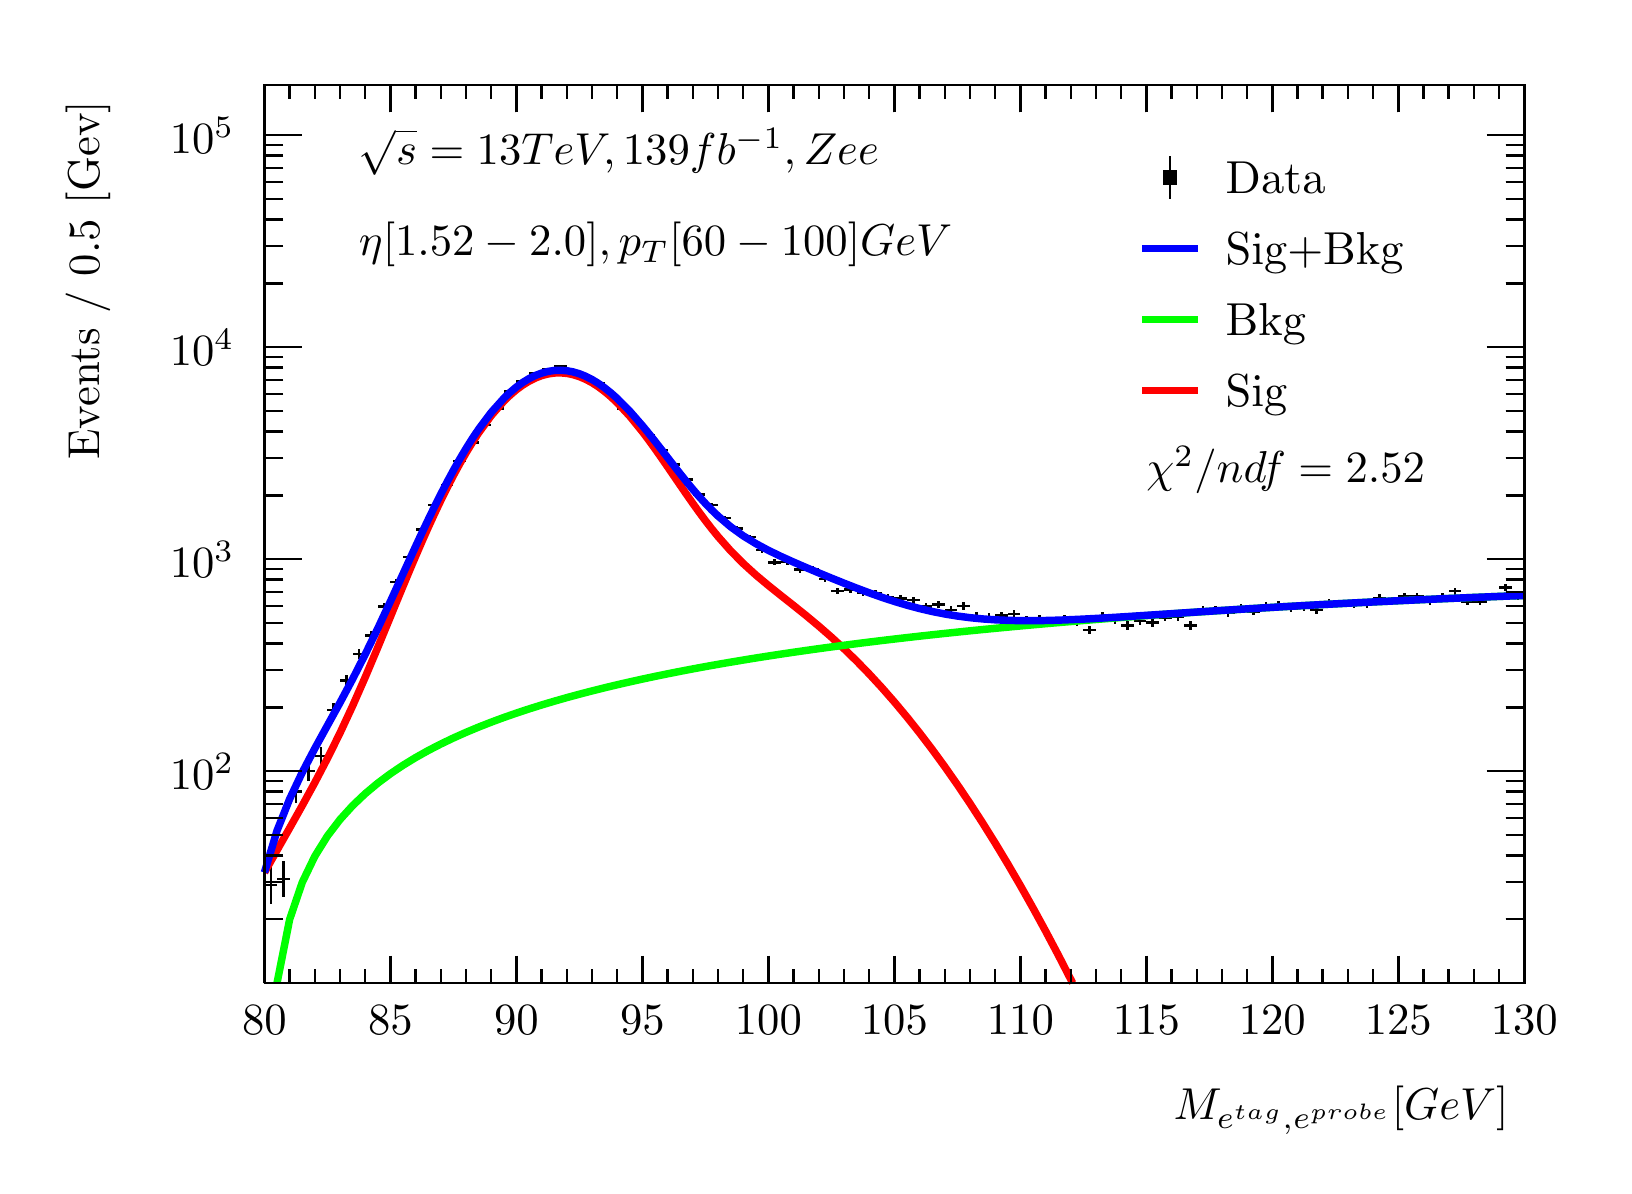
\begin{tikzpicture}
\pgfdeclareplotmark{cross} {
\pgfpathmoveto{\pgfpoint{-0.3\pgfplotmarksize}{\pgfplotmarksize}}
\pgfpathlineto{\pgfpoint{+0.3\pgfplotmarksize}{\pgfplotmarksize}}
\pgfpathlineto{\pgfpoint{+0.3\pgfplotmarksize}{0.3\pgfplotmarksize}}
\pgfpathlineto{\pgfpoint{+1\pgfplotmarksize}{0.3\pgfplotmarksize}}
\pgfpathlineto{\pgfpoint{+1\pgfplotmarksize}{-0.3\pgfplotmarksize}}
\pgfpathlineto{\pgfpoint{+0.3\pgfplotmarksize}{-0.3\pgfplotmarksize}}
\pgfpathlineto{\pgfpoint{+0.3\pgfplotmarksize}{-1.\pgfplotmarksize}}
\pgfpathlineto{\pgfpoint{-0.3\pgfplotmarksize}{-1.\pgfplotmarksize}}
\pgfpathlineto{\pgfpoint{-0.3\pgfplotmarksize}{-0.3\pgfplotmarksize}}
\pgfpathlineto{\pgfpoint{-1.\pgfplotmarksize}{-0.3\pgfplotmarksize}}
\pgfpathlineto{\pgfpoint{-1.\pgfplotmarksize}{0.3\pgfplotmarksize}}
\pgfpathlineto{\pgfpoint{-0.3\pgfplotmarksize}{0.3\pgfplotmarksize}}
\pgfpathclose
\pgfusepathqstroke
}
\pgfdeclareplotmark{cross*} {
\pgfpathmoveto{\pgfpoint{-0.3\pgfplotmarksize}{\pgfplotmarksize}}
\pgfpathlineto{\pgfpoint{+0.3\pgfplotmarksize}{\pgfplotmarksize}}
\pgfpathlineto{\pgfpoint{+0.3\pgfplotmarksize}{0.3\pgfplotmarksize}}
\pgfpathlineto{\pgfpoint{+1\pgfplotmarksize}{0.3\pgfplotmarksize}}
\pgfpathlineto{\pgfpoint{+1\pgfplotmarksize}{-0.3\pgfplotmarksize}}
\pgfpathlineto{\pgfpoint{+0.3\pgfplotmarksize}{-0.3\pgfplotmarksize}}
\pgfpathlineto{\pgfpoint{+0.3\pgfplotmarksize}{-1.\pgfplotmarksize}}
\pgfpathlineto{\pgfpoint{-0.3\pgfplotmarksize}{-1.\pgfplotmarksize}}
\pgfpathlineto{\pgfpoint{-0.3\pgfplotmarksize}{-0.3\pgfplotmarksize}}
\pgfpathlineto{\pgfpoint{-1.\pgfplotmarksize}{-0.3\pgfplotmarksize}}
\pgfpathlineto{\pgfpoint{-1.\pgfplotmarksize}{0.3\pgfplotmarksize}}
\pgfpathlineto{\pgfpoint{-0.3\pgfplotmarksize}{0.3\pgfplotmarksize}}
\pgfpathclose
\pgfusepathqfillstroke
}
\pgfdeclareplotmark{newstar} {
\pgfpathmoveto{\pgfqpoint{0pt}{\pgfplotmarksize}}
\pgfpathlineto{\pgfqpointpolar{44}{0.5\pgfplotmarksize}}
\pgfpathlineto{\pgfqpointpolar{18}{\pgfplotmarksize}}
\pgfpathlineto{\pgfqpointpolar{-20}{0.5\pgfplotmarksize}}
\pgfpathlineto{\pgfqpointpolar{-54}{\pgfplotmarksize}}
\pgfpathlineto{\pgfqpointpolar{-90}{0.5\pgfplotmarksize}}
\pgfpathlineto{\pgfqpointpolar{234}{\pgfplotmarksize}}
\pgfpathlineto{\pgfqpointpolar{198}{0.5\pgfplotmarksize}}
\pgfpathlineto{\pgfqpointpolar{162}{\pgfplotmarksize}}
\pgfpathlineto{\pgfqpointpolar{134}{0.5\pgfplotmarksize}}
\pgfpathclose
\pgfusepathqstroke
}
\pgfdeclareplotmark{newstar*} {
\pgfpathmoveto{\pgfqpoint{0pt}{\pgfplotmarksize}}
\pgfpathlineto{\pgfqpointpolar{44}{0.5\pgfplotmarksize}}
\pgfpathlineto{\pgfqpointpolar{18}{\pgfplotmarksize}}
\pgfpathlineto{\pgfqpointpolar{-20}{0.5\pgfplotmarksize}}
\pgfpathlineto{\pgfqpointpolar{-54}{\pgfplotmarksize}}
\pgfpathlineto{\pgfqpointpolar{-90}{0.5\pgfplotmarksize}}
\pgfpathlineto{\pgfqpointpolar{234}{\pgfplotmarksize}}
\pgfpathlineto{\pgfqpointpolar{198}{0.5\pgfplotmarksize}}
\pgfpathlineto{\pgfqpointpolar{162}{\pgfplotmarksize}}
\pgfpathlineto{\pgfqpointpolar{134}{0.5\pgfplotmarksize}}
\pgfpathclose
\pgfusepathqfillstroke
}
\definecolor{c}{rgb}{1,1,1};
\draw [color=c, fill=c] (0,0) rectangle (20,14.4361);
\draw [color=c, fill=c] (3,2.30977) rectangle (19,13.7143);
\definecolor{c}{rgb}{0,0,0};
\draw [c,line width=0.9] (3,2.30977) -- (3,13.7143) -- (19,13.7143) -- (19,2.30977) -- (3,2.30977);
\definecolor{c}{rgb}{1,1,1};
\draw [color=c, fill=c] (3,2.30977) rectangle (19,13.7143);
\definecolor{c}{rgb}{0,0,0};
\draw [c,line width=0.9] (3,2.30977) -- (3,13.7143) -- (19,13.7143) -- (19,2.30977) -- (3,2.30977);
\draw [c,line width=0.9] (3,2.30977) -- (19,2.30977);
\draw [c,line width=0.9] (3,2.65624) -- (3,2.30977);
\draw [c,line width=0.9] (3.32,2.48301) -- (3.32,2.30977);
\draw [c,line width=0.9] (3.64,2.48301) -- (3.64,2.30977);
\draw [c,line width=0.9] (3.96,2.48301) -- (3.96,2.30977);
\draw [c,line width=0.9] (4.28,2.48301) -- (4.28,2.30977);
\draw [c,line width=0.9] (4.6,2.65624) -- (4.6,2.30977);
\draw [c,line width=0.9] (4.92,2.48301) -- (4.92,2.30977);
\draw [c,line width=0.9] (5.24,2.48301) -- (5.24,2.30977);
\draw [c,line width=0.9] (5.56,2.48301) -- (5.56,2.30977);
\draw [c,line width=0.9] (5.88,2.48301) -- (5.88,2.30977);
\draw [c,line width=0.9] (6.2,2.65624) -- (6.2,2.30977);
\draw [c,line width=0.9] (6.52,2.48301) -- (6.52,2.30977);
\draw [c,line width=0.9] (6.84,2.48301) -- (6.84,2.30977);
\draw [c,line width=0.9] (7.16,2.48301) -- (7.16,2.30977);
\draw [c,line width=0.9] (7.48,2.48301) -- (7.48,2.30977);
\draw [c,line width=0.9] (7.8,2.65624) -- (7.8,2.30977);
\draw [c,line width=0.9] (8.12,2.48301) -- (8.12,2.30977);
\draw [c,line width=0.9] (8.44,2.48301) -- (8.44,2.30977);
\draw [c,line width=0.9] (8.76,2.48301) -- (8.76,2.30977);
\draw [c,line width=0.9] (9.08,2.48301) -- (9.08,2.30977);
\draw [c,line width=0.9] (9.4,2.65624) -- (9.4,2.30977);
\draw [c,line width=0.9] (9.72,2.48301) -- (9.72,2.30977);
\draw [c,line width=0.9] (10.04,2.48301) -- (10.04,2.30977);
\draw [c,line width=0.9] (10.36,2.48301) -- (10.36,2.30977);
\draw [c,line width=0.9] (10.68,2.48301) -- (10.68,2.30977);
\draw [c,line width=0.9] (11,2.65624) -- (11,2.30977);
\draw [c,line width=0.9] (11.32,2.48301) -- (11.32,2.30977);
\draw [c,line width=0.9] (11.64,2.48301) -- (11.64,2.30977);
\draw [c,line width=0.9] (11.96,2.48301) -- (11.96,2.30977);
\draw [c,line width=0.9] (12.28,2.48301) -- (12.28,2.30977);
\draw [c,line width=0.9] (12.6,2.65624) -- (12.6,2.30977);
\draw [c,line width=0.9] (12.92,2.48301) -- (12.92,2.30977);
\draw [c,line width=0.9] (13.24,2.48301) -- (13.24,2.30977);
\draw [c,line width=0.9] (13.56,2.48301) -- (13.56,2.30977);
\draw [c,line width=0.9] (13.88,2.48301) -- (13.88,2.30977);
\draw [c,line width=0.9] (14.2,2.65624) -- (14.2,2.30977);
\draw [c,line width=0.9] (14.52,2.48301) -- (14.52,2.30977);
\draw [c,line width=0.9] (14.84,2.48301) -- (14.84,2.30977);
\draw [c,line width=0.9] (15.16,2.48301) -- (15.16,2.30977);
\draw [c,line width=0.9] (15.48,2.48301) -- (15.48,2.30977);
\draw [c,line width=0.9] (15.8,2.65624) -- (15.8,2.30977);
\draw [c,line width=0.9] (16.12,2.48301) -- (16.12,2.30977);
\draw [c,line width=0.9] (16.44,2.48301) -- (16.44,2.30977);
\draw [c,line width=0.9] (16.76,2.48301) -- (16.76,2.30977);
\draw [c,line width=0.9] (17.08,2.48301) -- (17.08,2.30977);
\draw [c,line width=0.9] (17.4,2.65624) -- (17.4,2.30977);
\draw [c,line width=0.9] (17.72,2.48301) -- (17.72,2.30977);
\draw [c,line width=0.9] (18.04,2.48301) -- (18.04,2.30977);
\draw [c,line width=0.9] (18.36,2.48301) -- (18.36,2.30977);
\draw [c,line width=0.9] (18.68,2.48301) -- (18.68,2.30977);
\draw [c,line width=0.9] (19,2.65624) -- (19,2.30977);
\draw [anchor=base] (3,1.66015) node[scale=1.61424, color=c, rotate=0]{80};
\draw [anchor=base] (4.6,1.66015) node[scale=1.61424, color=c, rotate=0]{85};
\draw [anchor=base] (6.2,1.66015) node[scale=1.61424, color=c, rotate=0]{90};
\draw [anchor=base] (7.8,1.66015) node[scale=1.61424, color=c, rotate=0]{95};
\draw [anchor=base] (9.4,1.66015) node[scale=1.61424, color=c, rotate=0]{100};
\draw [anchor=base] (11,1.66015) node[scale=1.61424, color=c, rotate=0]{105};
\draw [anchor=base] (12.6,1.66015) node[scale=1.61424, color=c, rotate=0]{110};
\draw [anchor=base] (14.2,1.66015) node[scale=1.61424, color=c, rotate=0]{115};
\draw [anchor=base] (15.8,1.66015) node[scale=1.61424, color=c, rotate=0]{120};
\draw [anchor=base] (17.4,1.66015) node[scale=1.61424, color=c, rotate=0]{125};
\draw [anchor=base] (19,1.66015) node[scale=1.61424, color=c, rotate=0]{130};
\draw [anchor= east] (19,0.692932) node[scale=1.61424, color=c, rotate=0]{$M_{e^{tag}, e^{probe}}  [GeV]$};
\draw [c,line width=0.9] (3,13.7143) -- (19,13.7143);
\draw [c,line width=0.9] (3,13.3678) -- (3,13.7143);
\draw [c,line width=0.9] (3.32,13.5411) -- (3.32,13.7143);
\draw [c,line width=0.9] (3.64,13.5411) -- (3.64,13.7143);
\draw [c,line width=0.9] (3.96,13.5411) -- (3.96,13.7143);
\draw [c,line width=0.9] (4.28,13.5411) -- (4.28,13.7143);
\draw [c,line width=0.9] (4.6,13.3678) -- (4.6,13.7143);
\draw [c,line width=0.9] (4.92,13.5411) -- (4.92,13.7143);
\draw [c,line width=0.9] (5.24,13.5411) -- (5.24,13.7143);
\draw [c,line width=0.9] (5.56,13.5411) -- (5.56,13.7143);
\draw [c,line width=0.9] (5.88,13.5411) -- (5.88,13.7143);
\draw [c,line width=0.9] (6.2,13.3678) -- (6.2,13.7143);
\draw [c,line width=0.9] (6.52,13.5411) -- (6.52,13.7143);
\draw [c,line width=0.9] (6.84,13.5411) -- (6.84,13.7143);
\draw [c,line width=0.9] (7.16,13.5411) -- (7.16,13.7143);
\draw [c,line width=0.9] (7.48,13.5411) -- (7.48,13.7143);
\draw [c,line width=0.9] (7.8,13.3678) -- (7.8,13.7143);
\draw [c,line width=0.9] (8.12,13.5411) -- (8.12,13.7143);
\draw [c,line width=0.9] (8.44,13.5411) -- (8.44,13.7143);
\draw [c,line width=0.9] (8.76,13.5411) -- (8.76,13.7143);
\draw [c,line width=0.9] (9.08,13.5411) -- (9.08,13.7143);
\draw [c,line width=0.9] (9.4,13.3678) -- (9.4,13.7143);
\draw [c,line width=0.9] (9.72,13.5411) -- (9.72,13.7143);
\draw [c,line width=0.9] (10.04,13.5411) -- (10.04,13.7143);
\draw [c,line width=0.9] (10.36,13.5411) -- (10.36,13.7143);
\draw [c,line width=0.9] (10.68,13.5411) -- (10.68,13.7143);
\draw [c,line width=0.9] (11,13.3678) -- (11,13.7143);
\draw [c,line width=0.9] (11.32,13.5411) -- (11.32,13.7143);
\draw [c,line width=0.9] (11.64,13.5411) -- (11.64,13.7143);
\draw [c,line width=0.9] (11.96,13.5411) -- (11.96,13.7143);
\draw [c,line width=0.9] (12.28,13.5411) -- (12.28,13.7143);
\draw [c,line width=0.9] (12.6,13.3678) -- (12.6,13.7143);
\draw [c,line width=0.9] (12.92,13.5411) -- (12.92,13.7143);
\draw [c,line width=0.9] (13.24,13.5411) -- (13.24,13.7143);
\draw [c,line width=0.9] (13.56,13.5411) -- (13.56,13.7143);
\draw [c,line width=0.9] (13.88,13.5411) -- (13.88,13.7143);
\draw [c,line width=0.9] (14.2,13.3678) -- (14.2,13.7143);
\draw [c,line width=0.9] (14.52,13.5411) -- (14.52,13.7143);
\draw [c,line width=0.9] (14.84,13.5411) -- (14.84,13.7143);
\draw [c,line width=0.9] (15.16,13.5411) -- (15.16,13.7143);
\draw [c,line width=0.9] (15.48,13.5411) -- (15.48,13.7143);
\draw [c,line width=0.9] (15.8,13.3678) -- (15.8,13.7143);
\draw [c,line width=0.9] (16.12,13.5411) -- (16.12,13.7143);
\draw [c,line width=0.9] (16.44,13.5411) -- (16.44,13.7143);
\draw [c,line width=0.9] (16.76,13.5411) -- (16.76,13.7143);
\draw [c,line width=0.9] (17.08,13.5411) -- (17.08,13.7143);
\draw [c,line width=0.9] (17.4,13.3678) -- (17.4,13.7143);
\draw [c,line width=0.9] (17.72,13.5411) -- (17.72,13.7143);
\draw [c,line width=0.9] (18.04,13.5411) -- (18.04,13.7143);
\draw [c,line width=0.9] (18.36,13.5411) -- (18.36,13.7143);
\draw [c,line width=0.9] (18.68,13.5411) -- (18.68,13.7143);
\draw [c,line width=0.9] (19,13.3678) -- (19,13.7143);
\draw [c,line width=0.9] (3,2.30977) -- (3,13.7143);
\draw [c,line width=0.9] (3.237,3.12018) -- (3,3.12018);
\draw [c,line width=0.9] (3.237,3.59423) -- (3,3.59423);
\draw [c,line width=0.9] (3.237,3.93058) -- (3,3.93058);
\draw [c,line width=0.9] (3.237,4.19147) -- (3,4.19147);
\draw [c,line width=0.9] (3.237,4.40464) -- (3,4.40464);
\draw [c,line width=0.9] (3.237,4.58487) -- (3,4.58487);
\draw [c,line width=0.9] (3.237,4.74099) -- (3,4.74099);
\draw [c,line width=0.9] (3.237,4.8787) -- (3,4.8787);
\draw [c,line width=0.9] (3.474,5.00188) -- (3,5.00188);
\draw [anchor= east] (2.82,5.00188) node[scale=1.61424, color=c, rotate=0]{$10^{2}$};
\draw [c,line width=0.9] (3.237,5.81228) -- (3,5.81228);
\draw [c,line width=0.9] (3.237,6.28634) -- (3,6.28634);
\draw [c,line width=0.9] (3.237,6.62269) -- (3,6.62269);
\draw [c,line width=0.9] (3.237,6.88358) -- (3,6.88358);
\draw [c,line width=0.9] (3.237,7.09675) -- (3,7.09675);
\draw [c,line width=0.9] (3.237,7.27697) -- (3,7.27697);
\draw [c,line width=0.9] (3.237,7.43309) -- (3,7.43309);
\draw [c,line width=0.9] (3.237,7.5708) -- (3,7.5708);
\draw [c,line width=0.9] (3.474,7.69399) -- (3,7.69399);
\draw [anchor= east] (2.82,7.69399) node[scale=1.61424, color=c, rotate=0]{$10^{3}$};
\draw [c,line width=0.9] (3.237,8.50439) -- (3,8.50439);
\draw [c,line width=0.9] (3.237,8.97845) -- (3,8.97845);
\draw [c,line width=0.9] (3.237,9.3148) -- (3,9.3148);
\draw [c,line width=0.9] (3.237,9.57569) -- (3,9.57569);
\draw [c,line width=0.9] (3.237,9.78885) -- (3,9.78885);
\draw [c,line width=0.9] (3.237,9.96908) -- (3,9.96908);
\draw [c,line width=0.9] (3.237,10.1252) -- (3,10.1252);
\draw [c,line width=0.9] (3.237,10.2629) -- (3,10.2629);
\draw [c,line width=0.9] (3.474,10.3861) -- (3,10.3861);
\draw [anchor= east] (2.82,10.3861) node[scale=1.61424, color=c, rotate=0]{$10^{4}$};
\draw [c,line width=0.9] (3.237,11.1965) -- (3,11.1965);
\draw [c,line width=0.9] (3.237,11.6706) -- (3,11.6706);
\draw [c,line width=0.9] (3.237,12.0069) -- (3,12.0069);
\draw [c,line width=0.9] (3.237,12.2678) -- (3,12.2678);
\draw [c,line width=0.9] (3.237,12.481) -- (3,12.481);
\draw [c,line width=0.9] (3.237,12.6612) -- (3,12.6612);
\draw [c,line width=0.9] (3.237,12.8173) -- (3,12.8173);
\draw [c,line width=0.9] (3.237,12.955) -- (3,12.955);
\draw [c,line width=0.9] (3.474,13.0782) -- (3,13.0782);
\draw [anchor= east] (2.82,13.0782) node[scale=1.61424, color=c, rotate=0]{$10^{5}$};
\draw [anchor= east] (0.76,13.7143) node[scale=1.61424, color=c, rotate=90]{Events / 0.5 [Gev]};
\draw [c,line width=0.9] (19,2.30977) -- (19,13.7143);
\draw [c,line width=0.9] (18.763,3.12018) -- (19,3.12018);
\draw [c,line width=0.9] (18.763,3.59423) -- (19,3.59423);
\draw [c,line width=0.9] (18.763,3.93058) -- (19,3.93058);
\draw [c,line width=0.9] (18.763,4.19147) -- (19,4.19147);
\draw [c,line width=0.9] (18.763,4.40464) -- (19,4.40464);
\draw [c,line width=0.9] (18.763,4.58487) -- (19,4.58487);
\draw [c,line width=0.9] (18.763,4.74099) -- (19,4.74099);
\draw [c,line width=0.9] (18.763,4.8787) -- (19,4.8787);
\draw [c,line width=0.9] (18.526,5.00188) -- (19,5.00188);
\draw [c,line width=0.9] (18.763,5.81228) -- (19,5.81228);
\draw [c,line width=0.9] (18.763,6.28634) -- (19,6.28634);
\draw [c,line width=0.9] (18.763,6.62269) -- (19,6.62269);
\draw [c,line width=0.9] (18.763,6.88358) -- (19,6.88358);
\draw [c,line width=0.9] (18.763,7.09675) -- (19,7.09675);
\draw [c,line width=0.9] (18.763,7.27697) -- (19,7.27697);
\draw [c,line width=0.9] (18.763,7.43309) -- (19,7.43309);
\draw [c,line width=0.9] (18.763,7.5708) -- (19,7.5708);
\draw [c,line width=0.9] (18.526,7.69399) -- (19,7.69399);
\draw [c,line width=0.9] (18.763,8.50439) -- (19,8.50439);
\draw [c,line width=0.9] (18.763,8.97845) -- (19,8.97845);
\draw [c,line width=0.9] (18.763,9.3148) -- (19,9.3148);
\draw [c,line width=0.9] (18.763,9.57569) -- (19,9.57569);
\draw [c,line width=0.9] (18.763,9.78885) -- (19,9.78885);
\draw [c,line width=0.9] (18.763,9.96908) -- (19,9.96908);
\draw [c,line width=0.9] (18.763,10.1252) -- (19,10.1252);
\draw [c,line width=0.9] (18.763,10.2629) -- (19,10.2629);
\draw [c,line width=0.9] (18.526,10.3861) -- (19,10.3861);
\draw [c,line width=0.9] (18.763,11.1965) -- (19,11.1965);
\draw [c,line width=0.9] (18.763,11.6706) -- (19,11.6706);
\draw [c,line width=0.9] (18.763,12.0069) -- (19,12.0069);
\draw [c,line width=0.9] (18.763,12.2678) -- (19,12.2678);
\draw [c,line width=0.9] (18.763,12.481) -- (19,12.481);
\draw [c,line width=0.9] (18.763,12.6612) -- (19,12.6612);
\draw [c,line width=0.9] (18.763,12.8173) -- (19,12.8173);
\draw [c,line width=0.9] (18.763,12.955) -- (19,12.955);
\draw [c,line width=0.9] (18.526,13.0782) -- (19,13.0782);
\draw [c,line width=0.9] (3.08,3.5546) -- (3,3.5546);
\draw [c,line width=0.9] (3,3.5546) -- (3,3.5546);
\draw [c,line width=0.9] (3.08,3.5546) -- (3.16,3.5546);
\draw [c,line width=0.9] (3.16,3.5546) -- (3.16,3.5546);
\draw [c,line width=0.9] (3.08,3.5546) -- (3.08,3.7893);
\draw [c,line width=0.9] (3.08,3.7893) -- (3.08,3.7893);
\draw [c,line width=0.9] (3.08,3.5546) -- (3.08,3.31597);
\draw [c,line width=0.9] (3.08,3.31597) -- (3.08,3.31597);
\draw [c,line width=0.9] (3.24,3.63257) -- (3.16,3.63257);
\draw [c,line width=0.9] (3.16,3.63257) -- (3.16,3.63257);
\draw [c,line width=0.9] (3.24,3.63257) -- (3.32,3.63257);
\draw [c,line width=0.9] (3.32,3.63257) -- (3.32,3.63257);
\draw [c,line width=0.9] (3.24,3.63257) -- (3.24,3.8591);
\draw [c,line width=0.9] (3.24,3.8591) -- (3.24,3.8591);
\draw [c,line width=0.9] (3.24,3.63257) -- (3.24,3.4025);
\draw [c,line width=0.9] (3.24,3.4025) -- (3.24,3.4025);
\draw [c,line width=0.9] (3.4,4.74099) -- (3.32,4.74099);
\draw [c,line width=0.9] (3.32,4.74099) -- (3.32,4.74099);
\draw [c,line width=0.9] (3.4,4.74099) -- (3.48,4.74099);
\draw [c,line width=0.9] (3.48,4.74099) -- (3.48,4.74099);
\draw [c,line width=0.9] (3.4,4.74099) -- (3.4,4.87846);
\draw [c,line width=0.9] (3.4,4.87846) -- (3.4,4.87846);
\draw [c,line width=0.9] (3.4,4.74099) -- (3.4,4.60268);
\draw [c,line width=0.9] (3.4,4.60268) -- (3.4,4.60268);
\draw [c,line width=0.9] (3.56,5.00188) -- (3.48,5.00188);
\draw [c,line width=0.9] (3.48,5.00188) -- (3.48,5.00188);
\draw [c,line width=0.9] (3.56,5.00188) -- (3.64,5.00188);
\draw [c,line width=0.9] (3.64,5.00188) -- (3.64,5.00188);
\draw [c,line width=0.9] (3.56,5.00188) -- (3.56,5.12425);
\draw [c,line width=0.9] (3.56,5.12425) -- (3.56,5.12425);
\draw [c,line width=0.9] (3.56,5.00188) -- (3.56,4.87891);
\draw [c,line width=0.9] (3.56,4.87891) -- (3.56,4.87891);
\draw [c,line width=0.9] (3.72,5.19539) -- (3.64,5.19539);
\draw [c,line width=0.9] (3.64,5.19539) -- (3.64,5.19539);
\draw [c,line width=0.9] (3.72,5.19539) -- (3.8,5.19539);
\draw [c,line width=0.9] (3.8,5.19539) -- (3.8,5.19539);
\draw [c,line width=0.9] (3.72,5.19539) -- (3.72,5.30299);
\draw [c,line width=0.9] (3.72,5.30299) -- (3.72,5.30299);
\draw [c,line width=0.9] (3.72,5.19539) -- (3.72,5.0878);
\draw [c,line width=0.9] (3.72,5.0878) -- (3.72,5.0878);
\draw [c,line width=0.9] (3.88,5.77667) -- (3.8,5.77667);
\draw [c,line width=0.9] (3.8,5.77667) -- (3.8,5.77667);
\draw [c,line width=0.9] (3.88,5.77667) -- (3.96,5.77667);
\draw [c,line width=0.9] (3.96,5.77667) -- (3.96,5.77667);
\draw [c,line width=0.9] (3.88,5.77667) -- (3.88,5.8606);
\draw [c,line width=0.9] (3.88,5.8606) -- (3.88,5.8606);
\draw [c,line width=0.9] (3.88,5.77667) -- (3.88,5.69275);
\draw [c,line width=0.9] (3.88,5.69275) -- (3.88,5.69275);
\draw [c,line width=0.9] (4.04,6.15009) -- (3.96,6.15009);
\draw [c,line width=0.9] (3.96,6.15009) -- (3.96,6.15009);
\draw [c,line width=0.9] (4.04,6.15009) -- (4.12,6.15009);
\draw [c,line width=0.9] (4.12,6.15009) -- (4.12,6.15009);
\draw [c,line width=0.9] (4.04,6.15009) -- (4.04,6.22164);
\draw [c,line width=0.9] (4.04,6.22164) -- (4.04,6.22164);
\draw [c,line width=0.9] (4.04,6.15009) -- (4.04,6.07855);
\draw [c,line width=0.9] (4.04,6.07855) -- (4.04,6.07855);
\draw [c,line width=0.9] (4.2,6.48644) -- (4.12,6.48644);
\draw [c,line width=0.9] (4.12,6.48644) -- (4.12,6.48644);
\draw [c,line width=0.9] (4.2,6.48644) -- (4.28,6.48644);
\draw [c,line width=0.9] (4.28,6.48644) -- (4.28,6.48644);
\draw [c,line width=0.9] (4.2,6.48644) -- (4.2,6.5484);
\draw [c,line width=0.9] (4.2,6.5484) -- (4.2,6.5484);
\draw [c,line width=0.9] (4.2,6.48644) -- (4.2,6.42448);
\draw [c,line width=0.9] (4.2,6.42448) -- (4.2,6.42448);
\draw [c,line width=0.9] (4.36,6.72613) -- (4.28,6.72613);
\draw [c,line width=0.9] (4.28,6.72613) -- (4.28,6.72613);
\draw [c,line width=0.9] (4.36,6.72613) -- (4.44,6.72613);
\draw [c,line width=0.9] (4.44,6.72613) -- (4.44,6.72613);
\draw [c,line width=0.9] (4.36,6.72613) -- (4.36,6.78205);
\draw [c,line width=0.9] (4.36,6.78205) -- (4.36,6.78205);
\draw [c,line width=0.9] (4.36,6.72613) -- (4.36,6.6702);
\draw [c,line width=0.9] (4.36,6.6702) -- (4.36,6.6702);
\draw [c,line width=0.9] (4.52,7.09284) -- (4.44,7.09284);
\draw [c,line width=0.9] (4.44,7.09284) -- (4.44,7.09284);
\draw [c,line width=0.9] (4.52,7.09284) -- (4.6,7.09284);
\draw [c,line width=0.9] (4.6,7.09284) -- (4.6,7.09284);
\draw [c,line width=0.9] (4.52,7.09284) -- (4.52,7.14065);
\draw [c,line width=0.9] (4.52,7.14065) -- (4.52,7.14065);
\draw [c,line width=0.9] (4.52,7.09284) -- (4.52,7.04504);
\draw [c,line width=0.9] (4.52,7.04504) -- (4.52,7.04504);
\draw [c,line width=0.9] (4.68,7.40349) -- (4.6,7.40349);
\draw [c,line width=0.9] (4.6,7.40349) -- (4.6,7.40349);
\draw [c,line width=0.9] (4.68,7.40349) -- (4.76,7.40349);
\draw [c,line width=0.9] (4.76,7.40349) -- (4.76,7.40349);
\draw [c,line width=0.9] (4.68,7.40349) -- (4.68,7.44536);
\draw [c,line width=0.9] (4.68,7.44536) -- (4.68,7.44536);
\draw [c,line width=0.9] (4.68,7.40349) -- (4.68,7.36163);
\draw [c,line width=0.9] (4.68,7.36163) -- (4.68,7.36163);
\draw [c,line width=0.9] (4.84,7.71943) -- (4.76,7.71943);
\draw [c,line width=0.9] (4.76,7.71943) -- (4.76,7.71943);
\draw [c,line width=0.9] (4.84,7.71943) -- (4.92,7.71943);
\draw [c,line width=0.9] (4.92,7.71943) -- (4.92,7.71943);
\draw [c,line width=0.9] (4.84,7.71943) -- (4.84,7.756);
\draw [c,line width=0.9] (4.84,7.756) -- (4.84,7.756);
\draw [c,line width=0.9] (4.84,7.71943) -- (4.84,7.68286);
\draw [c,line width=0.9] (4.84,7.68286) -- (4.84,7.68286);
\draw [c,line width=0.9] (5,8.07225) -- (4.92,8.07225);
\draw [c,line width=0.9] (4.92,8.07225) -- (4.92,8.07225);
\draw [c,line width=0.9] (5,8.07225) -- (5.08,8.07225);
\draw [c,line width=0.9] (5.08,8.07225) -- (5.08,8.07225);
\draw [c,line width=0.9] (5,8.07225) -- (5,8.1037);
\draw [c,line width=0.9] (5,8.1037) -- (5,8.1037);
\draw [c,line width=0.9] (5,8.07225) -- (5,8.0408);
\draw [c,line width=0.9] (5,8.0408) -- (5,8.0408);
\draw [c,line width=0.9] (5.16,8.37796) -- (5.08,8.37796);
\draw [c,line width=0.9] (5.08,8.37796) -- (5.08,8.37796);
\draw [c,line width=0.9] (5.16,8.37796) -- (5.24,8.37796);
\draw [c,line width=0.9] (5.24,8.37796) -- (5.24,8.37796);
\draw [c,line width=0.9] (5.16,8.37796) -- (5.16,8.40555);
\draw [c,line width=0.9] (5.16,8.40555) -- (5.16,8.40555);
\draw [c,line width=0.9] (5.16,8.37796) -- (5.16,8.35036);
\draw [c,line width=0.9] (5.16,8.35036) -- (5.16,8.35036);
\draw [c,line width=0.9] (5.32,8.63323) -- (5.24,8.63323);
\draw [c,line width=0.9] (5.24,8.63323) -- (5.24,8.63323);
\draw [c,line width=0.9] (5.32,8.63323) -- (5.4,8.63323);
\draw [c,line width=0.9] (5.4,8.63323) -- (5.4,8.63323);
\draw [c,line width=0.9] (5.32,8.63323) -- (5.32,8.65798);
\draw [c,line width=0.9] (5.32,8.65798) -- (5.32,8.65798);
\draw [c,line width=0.9] (5.32,8.63323) -- (5.32,8.60849);
\draw [c,line width=0.9] (5.32,8.60849) -- (5.32,8.60849);
\draw [c,line width=0.9] (5.48,8.9372) -- (5.4,8.9372);
\draw [c,line width=0.9] (5.4,8.9372) -- (5.4,8.9372);
\draw [c,line width=0.9] (5.48,8.9372) -- (5.56,8.9372);
\draw [c,line width=0.9] (5.56,8.9372) -- (5.56,8.9372);
\draw [c,line width=0.9] (5.48,8.9372) -- (5.48,8.95892);
\draw [c,line width=0.9] (5.48,8.95892) -- (5.48,8.95892);
\draw [c,line width=0.9] (5.48,8.9372) -- (5.48,8.91547);
\draw [c,line width=0.9] (5.48,8.91547) -- (5.48,8.91547);
\draw [c,line width=0.9] (5.64,9.17295) -- (5.56,9.17295);
\draw [c,line width=0.9] (5.56,9.17295) -- (5.56,9.17295);
\draw [c,line width=0.9] (5.64,9.17295) -- (5.72,9.17295);
\draw [c,line width=0.9] (5.72,9.17295) -- (5.72,9.17295);
\draw [c,line width=0.9] (5.64,9.17295) -- (5.64,9.1926);
\draw [c,line width=0.9] (5.64,9.1926) -- (5.64,9.1926);
\draw [c,line width=0.9] (5.64,9.17295) -- (5.64,9.15331);
\draw [c,line width=0.9] (5.64,9.15331) -- (5.64,9.15331);
\draw [c,line width=0.9] (5.8,9.39745) -- (5.72,9.39745);
\draw [c,line width=0.9] (5.72,9.39745) -- (5.72,9.39745);
\draw [c,line width=0.9] (5.8,9.39745) -- (5.88,9.39745);
\draw [c,line width=0.9] (5.88,9.39745) -- (5.88,9.39745);
\draw [c,line width=0.9] (5.8,9.39745) -- (5.8,9.41529);
\draw [c,line width=0.9] (5.8,9.41529) -- (5.8,9.41529);
\draw [c,line width=0.9] (5.8,9.39745) -- (5.8,9.3796);
\draw [c,line width=0.9] (5.8,9.3796) -- (5.8,9.3796);
\draw [c,line width=0.9] (5.96,9.6041) -- (5.88,9.6041);
\draw [c,line width=0.9] (5.88,9.6041) -- (5.88,9.6041);
\draw [c,line width=0.9] (5.96,9.6041) -- (6.04,9.6041);
\draw [c,line width=0.9] (6.04,9.6041) -- (6.04,9.6041);
\draw [c,line width=0.9] (5.96,9.6041) -- (5.96,9.62044);
\draw [c,line width=0.9] (5.96,9.62044) -- (5.96,9.62044);
\draw [c,line width=0.9] (5.96,9.6041) -- (5.96,9.58777);
\draw [c,line width=0.9] (5.96,9.58777) -- (5.96,9.58777);
\draw [c,line width=0.9] (6.12,9.82455) -- (6.04,9.82455);
\draw [c,line width=0.9] (6.04,9.82455) -- (6.04,9.82455);
\draw [c,line width=0.9] (6.12,9.82455) -- (6.2,9.82455);
\draw [c,line width=0.9] (6.2,9.82455) -- (6.2,9.82455);
\draw [c,line width=0.9] (6.12,9.82455) -- (6.12,9.83941);
\draw [c,line width=0.9] (6.12,9.83941) -- (6.12,9.83941);
\draw [c,line width=0.9] (6.12,9.82455) -- (6.12,9.80968);
\draw [c,line width=0.9] (6.12,9.80968) -- (6.12,9.80968);
\draw [c,line width=0.9] (6.28,9.94699) -- (6.2,9.94699);
\draw [c,line width=0.9] (6.2,9.94699) -- (6.2,9.94699);
\draw [c,line width=0.9] (6.28,9.94699) -- (6.36,9.94699);
\draw [c,line width=0.9] (6.36,9.94699) -- (6.36,9.94699);
\draw [c,line width=0.9] (6.28,9.94699) -- (6.28,9.9611);
\draw [c,line width=0.9] (6.28,9.9611) -- (6.28,9.9611);
\draw [c,line width=0.9] (6.28,9.94699) -- (6.28,9.93289);
\draw [c,line width=0.9] (6.28,9.93289) -- (6.28,9.93289);
\draw [c,line width=0.9] (6.44,10.0532) -- (6.36,10.0532);
\draw [c,line width=0.9] (6.36,10.0532) -- (6.36,10.0532);
\draw [c,line width=0.9] (6.44,10.0532) -- (6.52,10.0532);
\draw [c,line width=0.9] (6.52,10.0532) -- (6.52,10.0532);
\draw [c,line width=0.9] (6.44,10.0532) -- (6.44,10.0667);
\draw [c,line width=0.9] (6.44,10.0667) -- (6.44,10.0667);
\draw [c,line width=0.9] (6.44,10.0532) -- (6.44,10.0397);
\draw [c,line width=0.9] (6.44,10.0397) -- (6.44,10.0397);
\draw [c,line width=0.9] (6.6,10.1083) -- (6.52,10.1083);
\draw [c,line width=0.9] (6.52,10.1083) -- (6.52,10.1083);
\draw [c,line width=0.9] (6.6,10.1083) -- (6.68,10.1083);
\draw [c,line width=0.9] (6.68,10.1083) -- (6.68,10.1083);
\draw [c,line width=0.9] (6.6,10.1083) -- (6.6,10.1214);
\draw [c,line width=0.9] (6.6,10.1214) -- (6.6,10.1214);
\draw [c,line width=0.9] (6.6,10.1083) -- (6.6,10.0951);
\draw [c,line width=0.9] (6.6,10.0951) -- (6.6,10.0951);
\draw [c,line width=0.9] (6.76,10.1486) -- (6.68,10.1486);
\draw [c,line width=0.9] (6.68,10.1486) -- (6.68,10.1486);
\draw [c,line width=0.9] (6.76,10.1486) -- (6.84,10.1486);
\draw [c,line width=0.9] (6.84,10.1486) -- (6.84,10.1486);
\draw [c,line width=0.9] (6.76,10.1486) -- (6.76,10.1616);
\draw [c,line width=0.9] (6.76,10.1616) -- (6.76,10.1616);
\draw [c,line width=0.9] (6.76,10.1486) -- (6.76,10.1357);
\draw [c,line width=0.9] (6.76,10.1357) -- (6.76,10.1357);
\draw [c,line width=0.9] (6.92,10.0801) -- (6.84,10.0801);
\draw [c,line width=0.9] (6.84,10.0801) -- (6.84,10.0801);
\draw [c,line width=0.9] (6.92,10.0801) -- (7,10.0801);
\draw [c,line width=0.9] (7,10.0801) -- (7,10.0801);
\draw [c,line width=0.9] (6.92,10.0801) -- (6.92,10.0934);
\draw [c,line width=0.9] (6.92,10.0934) -- (6.92,10.0934);
\draw [c,line width=0.9] (6.92,10.0801) -- (6.92,10.0667);
\draw [c,line width=0.9] (6.92,10.0667) -- (6.92,10.0667);
\draw [c,line width=0.9] (7.08,10.008) -- (7,10.008);
\draw [c,line width=0.9] (7,10.008) -- (7,10.008);
\draw [c,line width=0.9] (7.08,10.008) -- (7.16,10.008);
\draw [c,line width=0.9] (7.16,10.008) -- (7.16,10.008);
\draw [c,line width=0.9] (7.08,10.008) -- (7.08,10.0218);
\draw [c,line width=0.9] (7.08,10.0218) -- (7.08,10.0218);
\draw [c,line width=0.9] (7.08,10.008) -- (7.08,9.99427);
\draw [c,line width=0.9] (7.08,9.99427) -- (7.08,9.99427);
\draw [c,line width=0.9] (7.24,9.92135) -- (7.16,9.92135);
\draw [c,line width=0.9] (7.16,9.92135) -- (7.16,9.92135);
\draw [c,line width=0.9] (7.24,9.92135) -- (7.32,9.92135);
\draw [c,line width=0.9] (7.32,9.92135) -- (7.32,9.92135);
\draw [c,line width=0.9] (7.24,9.92135) -- (7.24,9.93562);
\draw [c,line width=0.9] (7.24,9.93562) -- (7.24,9.93562);
\draw [c,line width=0.9] (7.24,9.92135) -- (7.24,9.90709);
\draw [c,line width=0.9] (7.24,9.90709) -- (7.24,9.90709);
\draw [c,line width=0.9] (7.4,9.77769) -- (7.32,9.77769);
\draw [c,line width=0.9] (7.32,9.77769) -- (7.32,9.77769);
\draw [c,line width=0.9] (7.4,9.77769) -- (7.48,9.77769);
\draw [c,line width=0.9] (7.48,9.77769) -- (7.48,9.77769);
\draw [c,line width=0.9] (7.4,9.77769) -- (7.4,9.79286);
\draw [c,line width=0.9] (7.4,9.79286) -- (7.4,9.79286);
\draw [c,line width=0.9] (7.4,9.77769) -- (7.4,9.76253);
\draw [c,line width=0.9] (7.4,9.76253) -- (7.4,9.76253);
\draw [c,line width=0.9] (7.56,9.60616) -- (7.48,9.60616);
\draw [c,line width=0.9] (7.48,9.60616) -- (7.48,9.60616);
\draw [c,line width=0.9] (7.56,9.60616) -- (7.64,9.60616);
\draw [c,line width=0.9] (7.64,9.60616) -- (7.64,9.60616);
\draw [c,line width=0.9] (7.56,9.60616) -- (7.56,9.62248);
\draw [c,line width=0.9] (7.56,9.62248) -- (7.56,9.62248);
\draw [c,line width=0.9] (7.56,9.60616) -- (7.56,9.58984);
\draw [c,line width=0.9] (7.56,9.58984) -- (7.56,9.58984);
\draw [c,line width=0.9] (7.72,9.46362) -- (7.64,9.46362);
\draw [c,line width=0.9] (7.64,9.46362) -- (7.64,9.46362);
\draw [c,line width=0.9] (7.72,9.46362) -- (7.8,9.46362);
\draw [c,line width=0.9] (7.8,9.46362) -- (7.8,9.46362);
\draw [c,line width=0.9] (7.72,9.46362) -- (7.72,9.48097);
\draw [c,line width=0.9] (7.72,9.48097) -- (7.72,9.48097);
\draw [c,line width=0.9] (7.72,9.46362) -- (7.72,9.44628);
\draw [c,line width=0.9] (7.72,9.44628) -- (7.72,9.44628);
\draw [c,line width=0.9] (7.88,9.26127) -- (7.8,9.26127);
\draw [c,line width=0.9] (7.8,9.26127) -- (7.8,9.26127);
\draw [c,line width=0.9] (7.88,9.26127) -- (7.96,9.26127);
\draw [c,line width=0.9] (7.96,9.26127) -- (7.96,9.26127);
\draw [c,line width=0.9] (7.88,9.26127) -- (7.88,9.28018);
\draw [c,line width=0.9] (7.88,9.28018) -- (7.88,9.28018);
\draw [c,line width=0.9] (7.88,9.26127) -- (7.88,9.24236);
\draw [c,line width=0.9] (7.88,9.24236) -- (7.88,9.24236);
\draw [c,line width=0.9] (8.04,9.08063) -- (7.96,9.08063);
\draw [c,line width=0.9] (7.96,9.08063) -- (7.96,9.08063);
\draw [c,line width=0.9] (8.04,9.08063) -- (8.12,9.08063);
\draw [c,line width=0.9] (8.12,9.08063) -- (8.12,9.08063);
\draw [c,line width=0.9] (8.04,9.08063) -- (8.04,9.10107);
\draw [c,line width=0.9] (8.04,9.10107) -- (8.04,9.10107);
\draw [c,line width=0.9] (8.04,9.08063) -- (8.04,9.0602);
\draw [c,line width=0.9] (8.04,9.0602) -- (8.04,9.0602);
\draw [c,line width=0.9] (8.2,8.89653) -- (8.12,8.89653);
\draw [c,line width=0.9] (8.12,8.89653) -- (8.12,8.89653);
\draw [c,line width=0.9] (8.2,8.89653) -- (8.28,8.89653);
\draw [c,line width=0.9] (8.28,8.89653) -- (8.28,8.89653);
\draw [c,line width=0.9] (8.2,8.89653) -- (8.2,8.91864);
\draw [c,line width=0.9] (8.2,8.91864) -- (8.2,8.91864);
\draw [c,line width=0.9] (8.2,8.89653) -- (8.2,8.87442);
\draw [c,line width=0.9] (8.2,8.87442) -- (8.2,8.87442);
\draw [c,line width=0.9] (8.36,8.70777) -- (8.28,8.70777);
\draw [c,line width=0.9] (8.28,8.70777) -- (8.28,8.70777);
\draw [c,line width=0.9] (8.36,8.70777) -- (8.44,8.70777);
\draw [c,line width=0.9] (8.44,8.70777) -- (8.44,8.70777);
\draw [c,line width=0.9] (8.36,8.70777) -- (8.36,8.73174);
\draw [c,line width=0.9] (8.36,8.73174) -- (8.36,8.73174);
\draw [c,line width=0.9] (8.36,8.70777) -- (8.36,8.68381);
\draw [c,line width=0.9] (8.36,8.68381) -- (8.36,8.68381);
\draw [c,line width=0.9] (8.52,8.51718) -- (8.44,8.51718);
\draw [c,line width=0.9] (8.44,8.51718) -- (8.44,8.51718);
\draw [c,line width=0.9] (8.52,8.51718) -- (8.6,8.51718);
\draw [c,line width=0.9] (8.6,8.51718) -- (8.6,8.51718);
\draw [c,line width=0.9] (8.52,8.51718) -- (8.52,8.54318);
\draw [c,line width=0.9] (8.52,8.54318) -- (8.52,8.54318);
\draw [c,line width=0.9] (8.52,8.51718) -- (8.52,8.49118);
\draw [c,line width=0.9] (8.52,8.49118) -- (8.52,8.49118);
\draw [c,line width=0.9] (8.68,8.38186) -- (8.6,8.38186);
\draw [c,line width=0.9] (8.6,8.38186) -- (8.6,8.38186);
\draw [c,line width=0.9] (8.68,8.38186) -- (8.76,8.38186);
\draw [c,line width=0.9] (8.76,8.38186) -- (8.76,8.38186);
\draw [c,line width=0.9] (8.68,8.38186) -- (8.68,8.40941);
\draw [c,line width=0.9] (8.68,8.40941) -- (8.68,8.40941);
\draw [c,line width=0.9] (8.68,8.38186) -- (8.68,8.35431);
\draw [c,line width=0.9] (8.68,8.35431) -- (8.68,8.35431);
\draw [c,line width=0.9] (8.84,8.21615) -- (8.76,8.21615);
\draw [c,line width=0.9] (8.76,8.21615) -- (8.76,8.21615);
\draw [c,line width=0.9] (8.84,8.21615) -- (8.92,8.21615);
\draw [c,line width=0.9] (8.92,8.21615) -- (8.92,8.21615);
\draw [c,line width=0.9] (8.84,8.21615) -- (8.84,8.24572);
\draw [c,line width=0.9] (8.84,8.24572) -- (8.84,8.24572);
\draw [c,line width=0.9] (8.84,8.21615) -- (8.84,8.18657);
\draw [c,line width=0.9] (8.84,8.18657) -- (8.84,8.18657);
\draw [c,line width=0.9] (9,8.08068) -- (8.92,8.08068);
\draw [c,line width=0.9] (8.92,8.08068) -- (8.92,8.08068);
\draw [c,line width=0.9] (9,8.08068) -- (9.08,8.08068);
\draw [c,line width=0.9] (9.08,8.08068) -- (9.08,8.08068);
\draw [c,line width=0.9] (9,8.08068) -- (9,8.11202);
\draw [c,line width=0.9] (9,8.11202) -- (9,8.11202);
\draw [c,line width=0.9] (9,8.08068) -- (9,8.04934);
\draw [c,line width=0.9] (9,8.04934) -- (9,8.04934);
\draw [c,line width=0.9] (9.16,7.97252) -- (9.08,7.97252);
\draw [c,line width=0.9] (9.08,7.97252) -- (9.08,7.97252);
\draw [c,line width=0.9] (9.16,7.97252) -- (9.24,7.97252);
\draw [c,line width=0.9] (9.24,7.97252) -- (9.24,7.97252);
\draw [c,line width=0.9] (9.16,7.97252) -- (9.16,8.00534);
\draw [c,line width=0.9] (9.16,8.00534) -- (9.16,8.00534);
\draw [c,line width=0.9] (9.16,7.97252) -- (9.16,7.9397);
\draw [c,line width=0.9] (9.16,7.9397) -- (9.16,7.9397);
\draw [c,line width=0.9] (9.32,7.80755) -- (9.24,7.80755);
\draw [c,line width=0.9] (9.24,7.80755) -- (9.24,7.80755);
\draw [c,line width=0.9] (9.32,7.80755) -- (9.4,7.80755);
\draw [c,line width=0.9] (9.4,7.80755) -- (9.4,7.80755);
\draw [c,line width=0.9] (9.32,7.80755) -- (9.32,7.84276);
\draw [c,line width=0.9] (9.32,7.84276) -- (9.32,7.84276);
\draw [c,line width=0.9] (9.32,7.80755) -- (9.32,7.77233);
\draw [c,line width=0.9] (9.32,7.77233) -- (9.32,7.77233);
\draw [c,line width=0.9] (9.48,7.65354) -- (9.4,7.65354);
\draw [c,line width=0.9] (9.4,7.65354) -- (9.4,7.65354);
\draw [c,line width=0.9] (9.48,7.65354) -- (9.56,7.65354);
\draw [c,line width=0.9] (9.56,7.65354) -- (9.56,7.65354);
\draw [c,line width=0.9] (9.48,7.65354) -- (9.48,7.69116);
\draw [c,line width=0.9] (9.48,7.69116) -- (9.48,7.69116);
\draw [c,line width=0.9] (9.48,7.65354) -- (9.48,7.61593);
\draw [c,line width=0.9] (9.48,7.61593) -- (9.48,7.61593);
\draw [c,line width=0.9] (9.64,7.65596) -- (9.56,7.65596);
\draw [c,line width=0.9] (9.56,7.65596) -- (9.56,7.65596);
\draw [c,line width=0.9] (9.64,7.65596) -- (9.72,7.65596);
\draw [c,line width=0.9] (9.72,7.65596) -- (9.72,7.65596);
\draw [c,line width=0.9] (9.64,7.65596) -- (9.64,7.69354);
\draw [c,line width=0.9] (9.64,7.69354) -- (9.64,7.69354);
\draw [c,line width=0.9] (9.64,7.65596) -- (9.64,7.61839);
\draw [c,line width=0.9] (9.64,7.61839) -- (9.64,7.61839);
\draw [c,line width=0.9] (9.8,7.55905) -- (9.72,7.55905);
\draw [c,line width=0.9] (9.72,7.55905) -- (9.72,7.55905);
\draw [c,line width=0.9] (9.8,7.55905) -- (9.88,7.55905);
\draw [c,line width=0.9] (9.88,7.55905) -- (9.88,7.55905);
\draw [c,line width=0.9] (9.8,7.55905) -- (9.8,7.59822);
\draw [c,line width=0.9] (9.8,7.59822) -- (9.8,7.59822);
\draw [c,line width=0.9] (9.8,7.55905) -- (9.8,7.51989);
\draw [c,line width=0.9] (9.8,7.51989) -- (9.8,7.51989);
\draw [c,line width=0.9] (9.96,7.5656) -- (9.88,7.5656);
\draw [c,line width=0.9] (9.88,7.5656) -- (9.88,7.5656);
\draw [c,line width=0.9] (9.96,7.5656) -- (10.04,7.5656);
\draw [c,line width=0.9] (10.04,7.5656) -- (10.04,7.5656);
\draw [c,line width=0.9] (9.96,7.5656) -- (9.96,7.60465);
\draw [c,line width=0.9] (9.96,7.60465) -- (9.96,7.60465);
\draw [c,line width=0.9] (9.96,7.5656) -- (9.96,7.52654);
\draw [c,line width=0.9] (9.96,7.52654) -- (9.96,7.52654);
\draw [c,line width=0.9] (10.12,7.44328) -- (10.04,7.44328);
\draw [c,line width=0.9] (10.04,7.44328) -- (10.04,7.44328);
\draw [c,line width=0.9] (10.12,7.44328) -- (10.2,7.44328);
\draw [c,line width=0.9] (10.2,7.44328) -- (10.2,7.44328);
\draw [c,line width=0.9] (10.12,7.44328) -- (10.12,7.48444);
\draw [c,line width=0.9] (10.12,7.48444) -- (10.12,7.48444);
\draw [c,line width=0.9] (10.12,7.44328) -- (10.12,7.40213);
\draw [c,line width=0.9] (10.12,7.40213) -- (10.12,7.40213);
\draw [c,line width=0.9] (10.28,7.28861) -- (10.2,7.28861);
\draw [c,line width=0.9] (10.2,7.28861) -- (10.2,7.28861);
\draw [c,line width=0.9] (10.28,7.28861) -- (10.36,7.28861);
\draw [c,line width=0.9] (10.36,7.28861) -- (10.36,7.28861);
\draw [c,line width=0.9] (10.28,7.28861) -- (10.28,7.33258);
\draw [c,line width=0.9] (10.28,7.33258) -- (10.28,7.33258);
\draw [c,line width=0.9] (10.28,7.28861) -- (10.28,7.24464);
\draw [c,line width=0.9] (10.28,7.24464) -- (10.28,7.24464);
\draw [c,line width=0.9] (10.44,7.30829) -- (10.36,7.30829);
\draw [c,line width=0.9] (10.36,7.30829) -- (10.36,7.30829);
\draw [c,line width=0.9] (10.44,7.30829) -- (10.52,7.30829);
\draw [c,line width=0.9] (10.52,7.30829) -- (10.52,7.30829);
\draw [c,line width=0.9] (10.44,7.30829) -- (10.44,7.35189);
\draw [c,line width=0.9] (10.44,7.35189) -- (10.44,7.35189);
\draw [c,line width=0.9] (10.44,7.30829) -- (10.44,7.26469);
\draw [c,line width=0.9] (10.44,7.26469) -- (10.44,7.26469);
\draw [c,line width=0.9] (10.6,7.26354) -- (10.52,7.26354);
\draw [c,line width=0.9] (10.52,7.26354) -- (10.52,7.26354);
\draw [c,line width=0.9] (10.6,7.26354) -- (10.68,7.26354);
\draw [c,line width=0.9] (10.68,7.26354) -- (10.68,7.26354);
\draw [c,line width=0.9] (10.6,7.26354) -- (10.6,7.30798);
\draw [c,line width=0.9] (10.6,7.30798) -- (10.6,7.30798);
\draw [c,line width=0.9] (10.6,7.26354) -- (10.6,7.21909);
\draw [c,line width=0.9] (10.6,7.21909) -- (10.6,7.21909);
\draw [c,line width=0.9] (10.76,7.25846) -- (10.68,7.25846);
\draw [c,line width=0.9] (10.68,7.25846) -- (10.68,7.25846);
\draw [c,line width=0.9] (10.76,7.25846) -- (10.84,7.25846);
\draw [c,line width=0.9] (10.84,7.25846) -- (10.84,7.25846);
\draw [c,line width=0.9] (10.76,7.25846) -- (10.76,7.303);
\draw [c,line width=0.9] (10.76,7.303) -- (10.76,7.303);
\draw [c,line width=0.9] (10.76,7.25846) -- (10.76,7.21392);
\draw [c,line width=0.9] (10.76,7.21392) -- (10.76,7.21392);
\draw [c,line width=0.9] (10.92,7.20641) -- (10.84,7.20641);
\draw [c,line width=0.9] (10.84,7.20641) -- (10.84,7.20641);
\draw [c,line width=0.9] (10.92,7.20641) -- (11,7.20641);
\draw [c,line width=0.9] (11,7.20641) -- (11,7.20641);
\draw [c,line width=0.9] (10.92,7.20641) -- (10.92,7.25195);
\draw [c,line width=0.9] (10.92,7.25195) -- (10.92,7.25195);
\draw [c,line width=0.9] (10.92,7.20641) -- (10.92,7.16087);
\draw [c,line width=0.9] (10.92,7.16087) -- (10.92,7.16087);
\draw [c,line width=0.9] (11.08,7.19392) -- (11,7.19392);
\draw [c,line width=0.9] (11,7.19392) -- (11,7.19392);
\draw [c,line width=0.9] (11.08,7.19392) -- (11.16,7.19392);
\draw [c,line width=0.9] (11.16,7.19392) -- (11.16,7.19392);
\draw [c,line width=0.9] (11.08,7.19392) -- (11.08,7.23971);
\draw [c,line width=0.9] (11.08,7.23971) -- (11.08,7.23971);
\draw [c,line width=0.9] (11.08,7.19392) -- (11.08,7.14814);
\draw [c,line width=0.9] (11.08,7.14814) -- (11.08,7.14814);
\draw [c,line width=0.9] (11.24,7.1722) -- (11.16,7.1722);
\draw [c,line width=0.9] (11.16,7.1722) -- (11.16,7.1722);
\draw [c,line width=0.9] (11.24,7.1722) -- (11.32,7.1722);
\draw [c,line width=0.9] (11.32,7.1722) -- (11.32,7.1722);
\draw [c,line width=0.9] (11.24,7.1722) -- (11.24,7.21842);
\draw [c,line width=0.9] (11.24,7.21842) -- (11.24,7.21842);
\draw [c,line width=0.9] (11.24,7.1722) -- (11.24,7.12599);
\draw [c,line width=0.9] (11.24,7.12599) -- (11.24,7.12599);
\draw [c,line width=0.9] (11.4,7.09284) -- (11.32,7.09284);
\draw [c,line width=0.9] (11.32,7.09284) -- (11.32,7.09284);
\draw [c,line width=0.9] (11.4,7.09284) -- (11.48,7.09284);
\draw [c,line width=0.9] (11.48,7.09284) -- (11.48,7.09284);
\draw [c,line width=0.9] (11.4,7.09284) -- (11.4,7.14065);
\draw [c,line width=0.9] (11.4,7.14065) -- (11.4,7.14065);
\draw [c,line width=0.9] (11.4,7.09284) -- (11.4,7.04504);
\draw [c,line width=0.9] (11.4,7.04504) -- (11.4,7.04504);
\draw [c,line width=0.9] (11.56,7.11607) -- (11.48,7.11607);
\draw [c,line width=0.9] (11.48,7.11607) -- (11.48,7.11607);
\draw [c,line width=0.9] (11.56,7.11607) -- (11.64,7.11607);
\draw [c,line width=0.9] (11.64,7.11607) -- (11.64,7.11607);
\draw [c,line width=0.9] (11.56,7.11607) -- (11.56,7.16341);
\draw [c,line width=0.9] (11.56,7.16341) -- (11.56,7.16341);
\draw [c,line width=0.9] (11.56,7.11607) -- (11.56,7.06874);
\draw [c,line width=0.9] (11.56,7.06874) -- (11.56,7.06874);
\draw [c,line width=0.9] (11.72,7.04699) -- (11.64,7.04699);
\draw [c,line width=0.9] (11.64,7.04699) -- (11.64,7.04699);
\draw [c,line width=0.9] (11.72,7.04699) -- (11.8,7.04699);
\draw [c,line width=0.9] (11.8,7.04699) -- (11.8,7.04699);
\draw [c,line width=0.9] (11.72,7.04699) -- (11.72,7.09574);
\draw [c,line width=0.9] (11.72,7.09574) -- (11.72,7.09574);
\draw [c,line width=0.9] (11.72,7.04699) -- (11.72,6.99823);
\draw [c,line width=0.9] (11.72,6.99823) -- (11.72,6.99823);
\draw [c,line width=0.9] (11.88,7.09869) -- (11.8,7.09869);
\draw [c,line width=0.9] (11.8,7.09869) -- (11.8,7.09869);
\draw [c,line width=0.9] (11.88,7.09869) -- (11.96,7.09869);
\draw [c,line width=0.9] (11.96,7.09869) -- (11.96,7.09869);
\draw [c,line width=0.9] (11.88,7.09869) -- (11.88,7.14638);
\draw [c,line width=0.9] (11.88,7.14638) -- (11.88,7.14638);
\draw [c,line width=0.9] (11.88,7.09869) -- (11.88,7.05101);
\draw [c,line width=0.9] (11.88,7.05101) -- (11.88,7.05101);
\draw [c,line width=0.9] (12.04,6.96705) -- (11.96,6.96705);
\draw [c,line width=0.9] (11.96,6.96705) -- (11.96,6.96705);
\draw [c,line width=0.9] (12.04,6.96705) -- (12.12,6.96705);
\draw [c,line width=0.9] (12.12,6.96705) -- (12.12,6.96705);
\draw [c,line width=0.9] (12.04,6.96705) -- (12.04,7.0175);
\draw [c,line width=0.9] (12.04,7.0175) -- (12.04,7.0175);
\draw [c,line width=0.9] (12.04,6.96705) -- (12.04,6.9166);
\draw [c,line width=0.9] (12.04,6.9166) -- (12.04,6.9166);
\draw [c,line width=0.9] (12.2,6.95611) -- (12.12,6.95611);
\draw [c,line width=0.9] (12.12,6.95611) -- (12.12,6.95611);
\draw [c,line width=0.9] (12.2,6.95611) -- (12.28,6.95611);
\draw [c,line width=0.9] (12.28,6.95611) -- (12.28,6.95611);
\draw [c,line width=0.9] (12.2,6.95611) -- (12.2,7.0068);
\draw [c,line width=0.9] (12.2,7.0068) -- (12.2,7.0068);
\draw [c,line width=0.9] (12.2,6.95611) -- (12.2,6.90543);
\draw [c,line width=0.9] (12.2,6.90543) -- (12.2,6.90543);
\draw [c,line width=0.9] (12.36,6.97573) -- (12.28,6.97573);
\draw [c,line width=0.9] (12.28,6.97573) -- (12.28,6.97573);
\draw [c,line width=0.9] (12.36,6.97573) -- (12.44,6.97573);
\draw [c,line width=0.9] (12.44,6.97573) -- (12.44,6.97573);
\draw [c,line width=0.9] (12.36,6.97573) -- (12.36,7.02599);
\draw [c,line width=0.9] (12.36,7.02599) -- (12.36,7.02599);
\draw [c,line width=0.9] (12.36,6.97573) -- (12.36,6.92546);
\draw [c,line width=0.9] (12.36,6.92546) -- (12.36,6.92546);
\draw [c,line width=0.9] (12.52,6.99714) -- (12.44,6.99714);
\draw [c,line width=0.9] (12.44,6.99714) -- (12.44,6.99714);
\draw [c,line width=0.9] (12.52,6.99714) -- (12.6,6.99714);
\draw [c,line width=0.9] (12.6,6.99714) -- (12.6,6.99714);
\draw [c,line width=0.9] (12.52,6.99714) -- (12.52,7.04694);
\draw [c,line width=0.9] (12.52,7.04694) -- (12.52,7.04694);
\draw [c,line width=0.9] (12.52,6.99714) -- (12.52,6.94734);
\draw [c,line width=0.9] (12.52,6.94734) -- (12.52,6.94734);
\draw [c,line width=0.9] (12.68,6.91587) -- (12.6,6.91587);
\draw [c,line width=0.9] (12.6,6.91587) -- (12.6,6.91587);
\draw [c,line width=0.9] (12.68,6.91587) -- (12.76,6.91587);
\draw [c,line width=0.9] (12.76,6.91587) -- (12.76,6.91587);
\draw [c,line width=0.9] (12.68,6.91587) -- (12.68,6.96744);
\draw [c,line width=0.9] (12.68,6.96744) -- (12.68,6.96744);
\draw [c,line width=0.9] (12.68,6.91587) -- (12.68,6.8643);
\draw [c,line width=0.9] (12.68,6.8643) -- (12.68,6.8643);
\draw [c,line width=0.9] (12.84,6.92719) -- (12.76,6.92719);
\draw [c,line width=0.9] (12.76,6.92719) -- (12.76,6.92719);
\draw [c,line width=0.9] (12.84,6.92719) -- (12.92,6.92719);
\draw [c,line width=0.9] (12.92,6.92719) -- (12.92,6.92719);
\draw [c,line width=0.9] (12.84,6.92719) -- (12.84,6.9785);
\draw [c,line width=0.9] (12.84,6.9785) -- (12.84,6.9785);
\draw [c,line width=0.9] (12.84,6.92719) -- (12.84,6.87587);
\draw [c,line width=0.9] (12.84,6.87587) -- (12.84,6.87587);
\draw [c,line width=0.9] (13,6.89753) -- (12.92,6.89753);
\draw [c,line width=0.9] (12.92,6.89753) -- (12.92,6.89753);
\draw [c,line width=0.9] (13,6.89753) -- (13.08,6.89753);
\draw [c,line width=0.9] (13.08,6.89753) -- (13.08,6.89753);
\draw [c,line width=0.9] (13,6.89753) -- (13,6.9495);
\draw [c,line width=0.9] (13,6.9495) -- (13,6.9495);
\draw [c,line width=0.9] (13,6.89753) -- (13,6.84556);
\draw [c,line width=0.9] (13,6.84556) -- (13,6.84556);
\draw [c,line width=0.9] (13.16,6.9384) -- (13.08,6.9384);
\draw [c,line width=0.9] (13.08,6.9384) -- (13.08,6.9384);
\draw [c,line width=0.9] (13.16,6.9384) -- (13.24,6.9384);
\draw [c,line width=0.9] (13.24,6.9384) -- (13.24,6.9384);
\draw [c,line width=0.9] (13.16,6.9384) -- (13.16,6.98947);
\draw [c,line width=0.9] (13.16,6.98947) -- (13.16,6.98947);
\draw [c,line width=0.9] (13.16,6.9384) -- (13.16,6.88733);
\draw [c,line width=0.9] (13.16,6.88733) -- (13.16,6.88733);
\draw [c,line width=0.9] (13.32,6.89984) -- (13.24,6.89984);
\draw [c,line width=0.9] (13.24,6.89984) -- (13.24,6.89984);
\draw [c,line width=0.9] (13.32,6.89984) -- (13.4,6.89984);
\draw [c,line width=0.9] (13.4,6.89984) -- (13.4,6.89984);
\draw [c,line width=0.9] (13.32,6.89984) -- (13.32,6.95176);
\draw [c,line width=0.9] (13.32,6.95176) -- (13.32,6.95176);
\draw [c,line width=0.9] (13.32,6.89984) -- (13.32,6.84792);
\draw [c,line width=0.9] (13.32,6.84792) -- (13.32,6.84792);
\draw [c,line width=0.9] (13.48,6.79117) -- (13.4,6.79117);
\draw [c,line width=0.9] (13.4,6.79117) -- (13.4,6.79117);
\draw [c,line width=0.9] (13.48,6.79117) -- (13.56,6.79117);
\draw [c,line width=0.9] (13.56,6.79117) -- (13.56,6.79117);
\draw [c,line width=0.9] (13.48,6.79117) -- (13.48,6.84556);
\draw [c,line width=0.9] (13.48,6.84556) -- (13.48,6.84556);
\draw [c,line width=0.9] (13.48,6.79117) -- (13.48,6.73678);
\draw [c,line width=0.9] (13.48,6.73678) -- (13.48,6.73678);
\draw [c,line width=0.9] (13.64,6.96705) -- (13.56,6.96705);
\draw [c,line width=0.9] (13.56,6.96705) -- (13.56,6.96705);
\draw [c,line width=0.9] (13.64,6.96705) -- (13.72,6.96705);
\draw [c,line width=0.9] (13.72,6.96705) -- (13.72,6.96705);
\draw [c,line width=0.9] (13.64,6.96705) -- (13.64,7.0175);
\draw [c,line width=0.9] (13.64,7.0175) -- (13.64,7.0175);
\draw [c,line width=0.9] (13.64,6.96705) -- (13.64,6.9166);
\draw [c,line width=0.9] (13.64,6.9166) -- (13.64,6.9166);
\draw [c,line width=0.9] (13.8,6.92719) -- (13.72,6.92719);
\draw [c,line width=0.9] (13.72,6.92719) -- (13.72,6.92719);
\draw [c,line width=0.9] (13.8,6.92719) -- (13.88,6.92719);
\draw [c,line width=0.9] (13.88,6.92719) -- (13.88,6.92719);
\draw [c,line width=0.9] (13.8,6.92719) -- (13.8,6.9785);
\draw [c,line width=0.9] (13.8,6.9785) -- (13.8,6.9785);
\draw [c,line width=0.9] (13.8,6.92719) -- (13.8,6.87587);
\draw [c,line width=0.9] (13.8,6.87587) -- (13.8,6.87587);
\draw [c,line width=0.9] (13.96,6.85278) -- (13.88,6.85278);
\draw [c,line width=0.9] (13.88,6.85278) -- (13.88,6.85278);
\draw [c,line width=0.9] (13.96,6.85278) -- (14.04,6.85278);
\draw [c,line width=0.9] (14.04,6.85278) -- (14.04,6.85278);
\draw [c,line width=0.9] (13.96,6.85278) -- (13.96,6.90576);
\draw [c,line width=0.9] (13.96,6.90576) -- (13.96,6.90576);
\draw [c,line width=0.9] (13.96,6.85278) -- (13.96,6.79981);
\draw [c,line width=0.9] (13.96,6.79981) -- (13.96,6.79981);
\draw [c,line width=0.9] (14.12,6.90903) -- (14.04,6.90903);
\draw [c,line width=0.9] (14.04,6.90903) -- (14.04,6.90903);
\draw [c,line width=0.9] (14.12,6.90903) -- (14.2,6.90903);
\draw [c,line width=0.9] (14.2,6.90903) -- (14.2,6.90903);
\draw [c,line width=0.9] (14.12,6.90903) -- (14.12,6.96074);
\draw [c,line width=0.9] (14.12,6.96074) -- (14.12,6.96074);
\draw [c,line width=0.9] (14.12,6.90903) -- (14.12,6.85731);
\draw [c,line width=0.9] (14.12,6.85731) -- (14.12,6.85731);
\draw [c,line width=0.9] (14.28,6.88592) -- (14.2,6.88592);
\draw [c,line width=0.9] (14.2,6.88592) -- (14.2,6.88592);
\draw [c,line width=0.9] (14.28,6.88592) -- (14.36,6.88592);
\draw [c,line width=0.9] (14.36,6.88592) -- (14.36,6.88592);
\draw [c,line width=0.9] (14.28,6.88592) -- (14.28,6.93815);
\draw [c,line width=0.9] (14.28,6.93815) -- (14.28,6.93815);
\draw [c,line width=0.9] (14.28,6.88592) -- (14.28,6.83369);
\draw [c,line width=0.9] (14.28,6.83369) -- (14.28,6.83369);
\draw [c,line width=0.9] (14.44,6.95391) -- (14.36,6.95391);
\draw [c,line width=0.9] (14.36,6.95391) -- (14.36,6.95391);
\draw [c,line width=0.9] (14.44,6.95391) -- (14.52,6.95391);
\draw [c,line width=0.9] (14.52,6.95391) -- (14.52,6.95391);
\draw [c,line width=0.9] (14.44,6.95391) -- (14.44,7.00465);
\draw [c,line width=0.9] (14.44,7.00465) -- (14.44,7.00465);
\draw [c,line width=0.9] (14.44,6.95391) -- (14.44,6.90318);
\draw [c,line width=0.9] (14.44,6.90318) -- (14.44,6.90318);
\draw [c,line width=0.9] (14.6,6.95831) -- (14.52,6.95831);
\draw [c,line width=0.9] (14.52,6.95831) -- (14.52,6.95831);
\draw [c,line width=0.9] (14.6,6.95831) -- (14.68,6.95831);
\draw [c,line width=0.9] (14.68,6.95831) -- (14.68,6.95831);
\draw [c,line width=0.9] (14.6,6.95831) -- (14.6,7.00895);
\draw [c,line width=0.9] (14.6,7.00895) -- (14.6,7.00895);
\draw [c,line width=0.9] (14.6,6.95831) -- (14.6,6.90767);
\draw [c,line width=0.9] (14.6,6.90767) -- (14.6,6.90767);
\draw [c,line width=0.9] (14.76,6.85278) -- (14.68,6.85278);
\draw [c,line width=0.9] (14.68,6.85278) -- (14.68,6.85278);
\draw [c,line width=0.9] (14.76,6.85278) -- (14.84,6.85278);
\draw [c,line width=0.9] (14.84,6.85278) -- (14.84,6.85278);
\draw [c,line width=0.9] (14.76,6.85278) -- (14.76,6.90576);
\draw [c,line width=0.9] (14.76,6.90576) -- (14.76,6.90576);
\draw [c,line width=0.9] (14.76,6.85278) -- (14.76,6.79981);
\draw [c,line width=0.9] (14.76,6.79981) -- (14.76,6.79981);
\draw [c,line width=0.9] (14.92,7.05509) -- (14.84,7.05509);
\draw [c,line width=0.9] (14.84,7.05509) -- (14.84,7.05509);
\draw [c,line width=0.9] (14.92,7.05509) -- (15,7.05509);
\draw [c,line width=0.9] (15,7.05509) -- (15,7.05509);
\draw [c,line width=0.9] (14.92,7.05509) -- (14.92,7.10368);
\draw [c,line width=0.9] (14.92,7.10368) -- (14.92,7.10368);
\draw [c,line width=0.9] (14.92,7.05509) -- (14.92,7.00651);
\draw [c,line width=0.9] (14.92,7.00651) -- (14.92,7.00651);
\draw [c,line width=0.9] (15.08,7.05509) -- (15,7.05509);
\draw [c,line width=0.9] (15,7.05509) -- (15,7.05509);
\draw [c,line width=0.9] (15.08,7.05509) -- (15.16,7.05509);
\draw [c,line width=0.9] (15.16,7.05509) -- (15.16,7.05509);
\draw [c,line width=0.9] (15.08,7.05509) -- (15.08,7.10368);
\draw [c,line width=0.9] (15.08,7.10368) -- (15.08,7.10368);
\draw [c,line width=0.9] (15.08,7.05509) -- (15.08,7.00651);
\draw [c,line width=0.9] (15.08,7.00651) -- (15.08,7.00651);
\draw [c,line width=0.9] (15.24,7.0119) -- (15.16,7.0119);
\draw [c,line width=0.9] (15.16,7.0119) -- (15.16,7.0119);
\draw [c,line width=0.9] (15.24,7.0119) -- (15.32,7.0119);
\draw [c,line width=0.9] (15.32,7.0119) -- (15.32,7.0119);
\draw [c,line width=0.9] (15.24,7.0119) -- (15.24,7.06139);
\draw [c,line width=0.9] (15.24,7.06139) -- (15.24,7.06139);
\draw [c,line width=0.9] (15.24,7.0119) -- (15.24,6.96241);
\draw [c,line width=0.9] (15.24,6.96241) -- (15.24,6.96241);
\draw [c,line width=0.9] (15.4,7.07114) -- (15.32,7.07114);
\draw [c,line width=0.9] (15.32,7.07114) -- (15.32,7.07114);
\draw [c,line width=0.9] (15.4,7.07114) -- (15.48,7.07114);
\draw [c,line width=0.9] (15.48,7.07114) -- (15.48,7.07114);
\draw [c,line width=0.9] (15.4,7.07114) -- (15.4,7.11939);
\draw [c,line width=0.9] (15.4,7.11939) -- (15.4,7.11939);
\draw [c,line width=0.9] (15.4,7.07114) -- (15.4,7.02288);
\draw [c,line width=0.9] (15.4,7.02288) -- (15.4,7.02288);
\draw [c,line width=0.9] (15.56,7.03061) -- (15.48,7.03061);
\draw [c,line width=0.9] (15.48,7.03061) -- (15.48,7.03061);
\draw [c,line width=0.9] (15.56,7.03061) -- (15.64,7.03061);
\draw [c,line width=0.9] (15.64,7.03061) -- (15.64,7.03061);
\draw [c,line width=0.9] (15.56,7.03061) -- (15.56,7.0797);
\draw [c,line width=0.9] (15.56,7.0797) -- (15.56,7.0797);
\draw [c,line width=0.9] (15.56,7.03061) -- (15.56,6.98151);
\draw [c,line width=0.9] (15.56,6.98151) -- (15.56,6.98151);
\draw [c,line width=0.9] (15.72,7.10645) -- (15.64,7.10645);
\draw [c,line width=0.9] (15.64,7.10645) -- (15.64,7.10645);
\draw [c,line width=0.9] (15.72,7.10645) -- (15.8,7.10645);
\draw [c,line width=0.9] (15.8,7.10645) -- (15.8,7.10645);
\draw [c,line width=0.9] (15.72,7.10645) -- (15.72,7.15398);
\draw [c,line width=0.9] (15.72,7.15398) -- (15.72,7.15398);
\draw [c,line width=0.9] (15.72,7.10645) -- (15.72,7.05892);
\draw [c,line width=0.9] (15.72,7.05892) -- (15.72,7.05892);
\draw [c,line width=0.9] (15.88,7.10838) -- (15.8,7.10838);
\draw [c,line width=0.9] (15.8,7.10838) -- (15.8,7.10838);
\draw [c,line width=0.9] (15.88,7.10838) -- (15.96,7.10838);
\draw [c,line width=0.9] (15.96,7.10838) -- (15.96,7.10838);
\draw [c,line width=0.9] (15.88,7.10838) -- (15.88,7.15587);
\draw [c,line width=0.9] (15.88,7.15587) -- (15.88,7.15587);
\draw [c,line width=0.9] (15.88,7.10838) -- (15.88,7.06089);
\draw [c,line width=0.9] (15.88,7.06089) -- (15.88,7.06089);
\draw [c,line width=0.9] (16.04,7.06515) -- (15.96,7.06515);
\draw [c,line width=0.9] (15.96,7.06515) -- (15.96,7.06515);
\draw [c,line width=0.9] (16.04,7.06515) -- (16.12,7.06515);
\draw [c,line width=0.9] (16.12,7.06515) -- (16.12,7.06515);
\draw [c,line width=0.9] (16.04,7.06515) -- (16.04,7.11352);
\draw [c,line width=0.9] (16.04,7.11352) -- (16.04,7.11352);
\draw [c,line width=0.9] (16.04,7.06515) -- (16.04,7.01677);
\draw [c,line width=0.9] (16.04,7.01677) -- (16.04,7.01677);
\draw [c,line width=0.9] (16.2,7.0771) -- (16.12,7.0771);
\draw [c,line width=0.9] (16.12,7.0771) -- (16.12,7.0771);
\draw [c,line width=0.9] (16.2,7.0771) -- (16.28,7.0771);
\draw [c,line width=0.9] (16.28,7.0771) -- (16.28,7.0771);
\draw [c,line width=0.9] (16.2,7.0771) -- (16.2,7.12523);
\draw [c,line width=0.9] (16.2,7.12523) -- (16.2,7.12523);
\draw [c,line width=0.9] (16.2,7.0771) -- (16.2,7.02897);
\draw [c,line width=0.9] (16.2,7.02897) -- (16.2,7.02897);
\draw [c,line width=0.9] (16.36,7.04699) -- (16.28,7.04699);
\draw [c,line width=0.9] (16.28,7.04699) -- (16.28,7.04699);
\draw [c,line width=0.9] (16.36,7.04699) -- (16.44,7.04699);
\draw [c,line width=0.9] (16.44,7.04699) -- (16.44,7.04699);
\draw [c,line width=0.9] (16.36,7.04699) -- (16.36,7.09574);
\draw [c,line width=0.9] (16.36,7.09574) -- (16.36,7.09574);
\draw [c,line width=0.9] (16.36,7.04699) -- (16.36,6.99823);
\draw [c,line width=0.9] (16.36,6.99823) -- (16.36,6.99823);
\draw [c,line width=0.9] (16.52,7.14073) -- (16.44,7.14073);
\draw [c,line width=0.9] (16.44,7.14073) -- (16.44,7.14073);
\draw [c,line width=0.9] (16.52,7.14073) -- (16.6,7.14073);
\draw [c,line width=0.9] (16.6,7.14073) -- (16.6,7.14073);
\draw [c,line width=0.9] (16.52,7.14073) -- (16.52,7.18757);
\draw [c,line width=0.9] (16.52,7.18757) -- (16.52,7.18757);
\draw [c,line width=0.9] (16.52,7.14073) -- (16.52,7.09389);
\draw [c,line width=0.9] (16.52,7.09389) -- (16.52,7.09389);
\draw [c,line width=0.9] (16.68,7.12752) -- (16.6,7.12752);
\draw [c,line width=0.9] (16.6,7.12752) -- (16.6,7.12752);
\draw [c,line width=0.9] (16.68,7.12752) -- (16.76,7.12752);
\draw [c,line width=0.9] (16.76,7.12752) -- (16.76,7.12752);
\draw [c,line width=0.9] (16.68,7.12752) -- (16.68,7.17462);
\draw [c,line width=0.9] (16.68,7.17462) -- (16.68,7.17462);
\draw [c,line width=0.9] (16.68,7.12752) -- (16.68,7.08041);
\draw [c,line width=0.9] (16.68,7.08041) -- (16.68,7.08041);
\draw [c,line width=0.9] (16.84,7.12562) -- (16.76,7.12562);
\draw [c,line width=0.9] (16.76,7.12562) -- (16.76,7.12562);
\draw [c,line width=0.9] (16.84,7.12562) -- (16.92,7.12562);
\draw [c,line width=0.9] (16.92,7.12562) -- (16.92,7.12562);
\draw [c,line width=0.9] (16.84,7.12562) -- (16.84,7.17276);
\draw [c,line width=0.9] (16.84,7.17276) -- (16.84,7.17276);
\draw [c,line width=0.9] (16.84,7.12562) -- (16.84,7.07847);
\draw [c,line width=0.9] (16.84,7.07847) -- (16.84,7.07847);
\draw [c,line width=0.9] (17,7.12562) -- (16.92,7.12562);
\draw [c,line width=0.9] (16.92,7.12562) -- (16.92,7.12562);
\draw [c,line width=0.9] (17,7.12562) -- (17.08,7.12562);
\draw [c,line width=0.9] (17.08,7.12562) -- (17.08,7.12562);
\draw [c,line width=0.9] (17,7.12562) -- (17,7.17276);
\draw [c,line width=0.9] (17,7.17276) -- (17,7.17276);
\draw [c,line width=0.9] (17,7.12562) -- (17,7.07847);
\draw [c,line width=0.9] (17,7.07847) -- (17,7.07847);
\draw [c,line width=0.9] (17.16,7.19929) -- (17.08,7.19929);
\draw [c,line width=0.9] (17.08,7.19929) -- (17.08,7.19929);
\draw [c,line width=0.9] (17.16,7.19929) -- (17.24,7.19929);
\draw [c,line width=0.9] (17.24,7.19929) -- (17.24,7.19929);
\draw [c,line width=0.9] (17.16,7.19929) -- (17.16,7.24497);
\draw [c,line width=0.9] (17.16,7.24497) -- (17.16,7.24497);
\draw [c,line width=0.9] (17.16,7.19929) -- (17.16,7.15361);
\draw [c,line width=0.9] (17.16,7.15361) -- (17.16,7.15361);
\draw [c,line width=0.9] (17.32,7.16671) -- (17.24,7.16671);
\draw [c,line width=0.9] (17.24,7.16671) -- (17.24,7.16671);
\draw [c,line width=0.9] (17.32,7.16671) -- (17.4,7.16671);
\draw [c,line width=0.9] (17.4,7.16671) -- (17.4,7.16671);
\draw [c,line width=0.9] (17.32,7.16671) -- (17.32,7.21303);
\draw [c,line width=0.9] (17.32,7.21303) -- (17.32,7.21303);
\draw [c,line width=0.9] (17.32,7.16671) -- (17.32,7.12039);
\draw [c,line width=0.9] (17.32,7.12039) -- (17.32,7.12039);
\draw [c,line width=0.9] (17.48,7.21876) -- (17.4,7.21876);
\draw [c,line width=0.9] (17.4,7.21876) -- (17.4,7.21876);
\draw [c,line width=0.9] (17.48,7.21876) -- (17.56,7.21876);
\draw [c,line width=0.9] (17.56,7.21876) -- (17.56,7.21876);
\draw [c,line width=0.9] (17.48,7.21876) -- (17.48,7.26406);
\draw [c,line width=0.9] (17.48,7.26406) -- (17.48,7.26406);
\draw [c,line width=0.9] (17.48,7.21876) -- (17.48,7.17346);
\draw [c,line width=0.9] (17.48,7.17346) -- (17.48,7.17346);
\draw [c,line width=0.9] (17.64,7.22052) -- (17.56,7.22052);
\draw [c,line width=0.9] (17.56,7.22052) -- (17.56,7.22052);
\draw [c,line width=0.9] (17.64,7.22052) -- (17.72,7.22052);
\draw [c,line width=0.9] (17.72,7.22052) -- (17.72,7.22052);
\draw [c,line width=0.9] (17.64,7.22052) -- (17.64,7.26578);
\draw [c,line width=0.9] (17.64,7.26578) -- (17.64,7.26578);
\draw [c,line width=0.9] (17.64,7.22052) -- (17.64,7.17525);
\draw [c,line width=0.9] (17.64,7.17525) -- (17.64,7.17525);
\draw [c,line width=0.9] (17.8,7.15935) -- (17.72,7.15935);
\draw [c,line width=0.9] (17.72,7.15935) -- (17.72,7.15935);
\draw [c,line width=0.9] (17.8,7.15935) -- (17.88,7.15935);
\draw [c,line width=0.9] (17.88,7.15935) -- (17.88,7.15935);
\draw [c,line width=0.9] (17.8,7.15935) -- (17.8,7.20581);
\draw [c,line width=0.9] (17.8,7.20581) -- (17.8,7.20581);
\draw [c,line width=0.9] (17.8,7.15935) -- (17.8,7.11288);
\draw [c,line width=0.9] (17.8,7.11288) -- (17.8,7.11288);
\draw [c,line width=0.9] (17.96,7.22227) -- (17.88,7.22227);
\draw [c,line width=0.9] (17.88,7.22227) -- (17.88,7.22227);
\draw [c,line width=0.9] (17.96,7.22227) -- (18.04,7.22227);
\draw [c,line width=0.9] (18.04,7.22227) -- (18.04,7.22227);
\draw [c,line width=0.9] (17.96,7.22227) -- (17.96,7.2675);
\draw [c,line width=0.9] (17.96,7.2675) -- (17.96,7.2675);
\draw [c,line width=0.9] (17.96,7.22227) -- (17.96,7.17703);
\draw [c,line width=0.9] (17.96,7.17703) -- (17.96,7.17703);
\draw [c,line width=0.9] (18.12,7.28695) -- (18.04,7.28695);
\draw [c,line width=0.9] (18.04,7.28695) -- (18.04,7.28695);
\draw [c,line width=0.9] (18.12,7.28695) -- (18.2,7.28695);
\draw [c,line width=0.9] (18.2,7.28695) -- (18.2,7.28695);
\draw [c,line width=0.9] (18.12,7.28695) -- (18.12,7.33095);
\draw [c,line width=0.9] (18.12,7.33095) -- (18.12,7.33095);
\draw [c,line width=0.9] (18.12,7.28695) -- (18.12,7.24295);
\draw [c,line width=0.9] (18.12,7.24295) -- (18.12,7.24295);
\draw [c,line width=0.9] (18.28,7.15193) -- (18.2,7.15193);
\draw [c,line width=0.9] (18.2,7.15193) -- (18.2,7.15193);
\draw [c,line width=0.9] (18.28,7.15193) -- (18.36,7.15193);
\draw [c,line width=0.9] (18.36,7.15193) -- (18.36,7.15193);
\draw [c,line width=0.9] (18.28,7.15193) -- (18.28,7.19855);
\draw [c,line width=0.9] (18.28,7.19855) -- (18.28,7.19855);
\draw [c,line width=0.9] (18.28,7.15193) -- (18.28,7.10532);
\draw [c,line width=0.9] (18.28,7.10532) -- (18.28,7.10532);
\draw [c,line width=0.9] (18.44,7.15379) -- (18.36,7.15379);
\draw [c,line width=0.9] (18.36,7.15379) -- (18.36,7.15379);
\draw [c,line width=0.9] (18.44,7.15379) -- (18.52,7.15379);
\draw [c,line width=0.9] (18.52,7.15379) -- (18.52,7.15379);
\draw [c,line width=0.9] (18.44,7.15379) -- (18.44,7.20037);
\draw [c,line width=0.9] (18.44,7.20037) -- (18.44,7.20037);
\draw [c,line width=0.9] (18.44,7.15379) -- (18.44,7.10721);
\draw [c,line width=0.9] (18.44,7.10721) -- (18.44,7.10721);
\draw [c,line width=0.9] (18.6,7.22227) -- (18.52,7.22227);
\draw [c,line width=0.9] (18.52,7.22227) -- (18.52,7.22227);
\draw [c,line width=0.9] (18.6,7.22227) -- (18.68,7.22227);
\draw [c,line width=0.9] (18.68,7.22227) -- (18.68,7.22227);
\draw [c,line width=0.9] (18.6,7.22227) -- (18.6,7.2675);
\draw [c,line width=0.9] (18.6,7.2675) -- (18.6,7.2675);
\draw [c,line width=0.9] (18.6,7.22227) -- (18.6,7.17703);
\draw [c,line width=0.9] (18.6,7.17703) -- (18.6,7.17703);
\draw [c,line width=0.9] (18.76,7.33083) -- (18.68,7.33083);
\draw [c,line width=0.9] (18.68,7.33083) -- (18.68,7.33083);
\draw [c,line width=0.9] (18.76,7.33083) -- (18.84,7.33083);
\draw [c,line width=0.9] (18.84,7.33083) -- (18.84,7.33083);
\draw [c,line width=0.9] (18.76,7.33083) -- (18.76,7.37401);
\draw [c,line width=0.9] (18.76,7.37401) -- (18.76,7.37401);
\draw [c,line width=0.9] (18.76,7.33083) -- (18.76,7.28765);
\draw [c,line width=0.9] (18.76,7.28765) -- (18.76,7.28765);
\draw [c,line width=0.9] (18.92,7.22227) -- (18.84,7.22227);
\draw [c,line width=0.9] (18.84,7.22227) -- (18.84,7.22227);
\draw [c,line width=0.9] (18.92,7.22227) -- (19,7.22227);
\draw [c,line width=0.9] (19,7.22227) -- (19,7.22227);
\draw [c,line width=0.9] (18.92,7.22227) -- (18.92,7.2675);
\draw [c,line width=0.9] (18.92,7.2675) -- (18.92,7.2675);
\draw [c,line width=0.9] (18.92,7.22227) -- (18.92,7.17703);
\draw [c,line width=0.9] (18.92,7.17703) -- (18.92,7.17703);
\foreach \P in {(3.08,3.5546), (3.24,3.63257), (3.4,4.74099), (3.56,5.00188), (3.72,5.19539), (3.88,5.77667), (4.04,6.15009), (4.2,6.48644), (4.36,6.72613), (4.52,7.09284), (4.68,7.40349), (4.84,7.71943), (5,8.07225), (5.16,8.37796), (5.32,8.63323),
 (5.48,8.9372), (5.64,9.17295), (5.8,9.39745), (5.96,9.6041), (6.12,9.82455), (6.28,9.94699), (6.44,10.0532), (6.6,10.1083), (6.76,10.1486), (6.92,10.0801), (7.08,10.008), (7.24,9.92135), (7.4,9.77769), (7.56,9.60616), (7.72,9.46362), (7.88,9.26127),
 (8.04,9.08063), (8.2,8.89653), (8.36,8.70777), (8.52,8.51718), (8.68,8.38186), (8.84,8.21615), (9,8.08068), (9.16,7.97252), (9.32,7.80755), (9.48,7.65354), (9.64,7.65596), (9.8,7.55905), (9.96,7.5656), (10.12,7.44328), (10.28,7.28861),
 (10.44,7.30829), (10.6,7.26354), (10.76,7.25846), (10.92,7.20641), (11.08,7.19392), (11.24,7.1722), (11.4,7.09284), (11.56,7.11607), (11.72,7.04699), (11.88,7.09869), (12.04,6.96705), (12.2,6.95611), (12.36,6.97573), (12.52,6.99714),
 (12.68,6.91587), (12.84,6.92719), (13,6.89753), (13.16,6.9384), (13.32,6.89984), (13.48,6.79117), (13.64,6.96705), (13.8,6.92719), (13.96,6.85278), (14.12,6.90903), (14.28,6.88592), (14.44,6.95391), (14.6,6.95831), (14.76,6.85278), (14.92,7.05509),
 (15.08,7.05509), (15.24,7.0119), (15.4,7.07114), (15.56,7.03061), (15.72,7.10645), (15.88,7.10838), (16.04,7.06515), (16.2,7.0771), (16.36,7.04699), (16.52,7.14073), (16.68,7.12752), (16.84,7.12562), (17,7.12562), (17.16,7.19929), (17.32,7.16671),
 (17.48,7.21876), (17.64,7.22052), (17.8,7.15935), (17.96,7.22227), (18.12,7.28695), (18.28,7.15193), (18.44,7.15379), (18.6,7.22227), (18.76,7.33083), (18.92,7.22227)}{\draw[mark options={color=c,fill=c},mark size=2.882883pt,mark=] plot coordinates
 {\P};}
\definecolor{c}{rgb}{1,0,0};
\draw [c,line width=2.7] (3,3.71412) -- (3,3.71412);
\draw [c,line width=2.7] (3,3.71412) -- (3.16,3.9968) -- (3.32,4.27857) -- (3.48,4.56345) -- (3.64,4.85633) -- (3.8,5.16245) -- (3.96,5.48636) -- (4.12,5.83056) -- (4.28,6.1944) -- (4.44,6.57377) -- (4.6,6.96184) -- (4.68,7.15655) -- (4.76,7.3503) --
 (4.84,7.54205) -- (4.92,7.73082) -- (5,7.9157) -- (5.08,8.09588) -- (5.16,8.27063) -- (5.24,8.43929) -- (5.32,8.60131) -- (5.4,8.75619) -- (5.48,8.90351) -- (5.56,9.04291) -- (5.64,9.17408) -- (5.72,9.29677) -- (5.88,9.51585) -- (6.04,9.6988) --
 (6.12,9.77644) -- (6.2,9.84475) -- (6.28,9.90367) -- (6.36,9.95316) -- (6.44,9.99321) -- (6.52,10.0238) -- (6.6,10.045) -- (6.68,10.0567) -- (6.76,10.0592) -- (6.84,10.0523) -- (6.92,10.0362) -- (7,10.0111) -- (7.08,9.97707) -- (7.16,9.93426) --
 (7.24,9.88291) -- (7.32,9.82325) -- (7.4,9.7556) -- (7.48,9.68028) -- (7.64,9.50837) -- (7.8,9.31159) -- (7.88,9.2055) -- (7.96,9.0953) -- (8.04,8.98188) -- (8.12,8.8662) -- (8.2,8.74928) -- (8.28,8.63219) -- (8.36,8.51599) -- (8.44,8.40172) --
 (8.52,8.29035) -- (8.6,8.18272) -- (8.68,8.0795) -- (8.76,7.98116) -- (8.92,7.79988) -- (9.08,7.63829) -- (9.24,7.49297) -- (9.4,7.35897) -- (9.56,7.23107) -- (9.72,7.10467) -- (9.88,6.97615) -- (10.04,6.84289) -- (10.2,6.70312) -- (10.36,6.55571)
 -- (10.52,6.39997) -- (10.68,6.2355) -- (10.84,6.06206) -- (11,5.87952) -- (11.16,5.68782) -- (11.32,5.48693) -- (11.48,5.27682) -- (11.64,5.0575) -- (11.8,4.82895) -- (11.96,4.59117) -- (12.12,4.34417) -- (12.28,4.08794) -- (12.44,3.82248) --
 (12.6,3.5478) -- (12.76,3.26389) -- (12.92,2.97076) -- (13.08,2.66839) -- (13.24,2.3568) -- (13.2635,2.30977);
\definecolor{c}{rgb}{0,1,0};
\draw [c,line width=2.7] (3.15998,2.30977) -- (3.16,2.31149);
\draw [c,line width=2.7] (3.16,2.31149) -- (3.32,3.11801) -- (3.48,3.58818) -- (3.64,3.92063) -- (3.8,4.17761) -- (3.96,4.38684) -- (4.12,4.56313) -- (4.28,4.7153) -- (4.44,4.84905) -- (4.6,4.96825) -- (4.76,5.0757) -- (4.92,5.17342) --
 (5.08,5.26299) -- (5.24,5.3456) -- (5.4,5.42222) -- (5.56,5.49361) -- (5.72,5.56042) -- (5.88,5.62316) -- (6.04,5.68227) -- (6.2,5.73812) -- (6.36,5.79103) -- (6.52,5.84127) -- (6.68,5.88908) -- (6.84,5.93467) -- (7,5.9782) -- (7.16,6.01985) --
 (7.32,6.05975) -- (7.48,6.09804) -- (7.64,6.13481) -- (7.8,6.17018) -- (7.96,6.20423) -- (8.12,6.23705) -- (8.28,6.26872) -- (8.44,6.29929) -- (8.6,6.32883) -- (8.76,6.35741) -- (8.92,6.38506) -- (9.08,6.41184) -- (9.24,6.4378) -- (9.4,6.46297) --
 (9.56,6.48739) -- (9.72,6.5111) -- (9.88,6.53414) -- (10.04,6.55652) -- (10.2,6.57828) -- (10.36,6.59944) -- (10.52,6.62003) -- (10.68,6.64008) -- (10.84,6.6596) -- (11,6.67862) -- (11.16,6.69715) -- (11.32,6.71521) -- (11.48,6.73282) --
 (11.64,6.75) -- (11.8,6.76676) -- (11.96,6.78311) -- (12.12,6.79907) -- (12.28,6.81465) -- (12.44,6.82986) -- (12.6,6.84472) -- (12.76,6.85923) -- (12.92,6.87341) -- (13.08,6.88726) -- (13.24,6.9008) -- (13.4,6.91404) -- (13.56,6.92697) --
 (13.72,6.93962) -- (13.88,6.95199) -- (14.04,6.96408) -- (14.2,6.9759) -- (14.36,6.98747) -- (14.52,6.99878) -- (14.68,7.00984) -- (14.84,7.02067) -- (15,7.03125) -- (15.16,7.04161) -- (15.32,7.05174) -- (15.48,7.06165) -- (15.64,7.07135) --
 (15.8,7.08084) -- (15.96,7.09012) -- (16.12,7.09919) -- (16.28,7.10807) -- (16.44,7.11676) -- (16.6,7.12526) -- (16.76,7.13357) -- (16.92,7.14169) -- (17.08,7.14964) -- (17.24,7.15741) -- (17.4,7.16501) -- (17.56,7.17244) -- (17.72,7.1797) --
 (17.88,7.1868) -- (18.04,7.19373) -- (18.2,7.20051) -- (18.36,7.20713) -- (18.52,7.2136) -- (18.68,7.21991) -- (18.84,7.22608) -- (19,7.23209) -- (19,7.23209) -- (19,7.23209);
\definecolor{c}{rgb}{0,0,1};
\draw [c,line width=2.7] (3,3.71413) -- (3,3.71413);
\draw [c,line width=2.7] (3,3.71413) -- (3.16,4.24507) -- (3.32,4.64715) -- (3.48,4.98509) -- (3.64,5.29009) -- (3.8,5.5812) -- (3.96,5.87176) -- (4.12,6.17119) -- (4.28,6.48504) -- (4.44,6.81461) -- (4.6,7.15708) -- (4.68,7.33137) -- (4.76,7.50648)
 -- (4.84,7.68141) -- (4.92,7.85516) -- (5,8.02673) -- (5.08,8.19519) -- (5.16,8.35968) -- (5.24,8.51941) -- (5.32,8.67367) -- (5.4,8.82183) -- (5.48,8.96336) -- (5.56,9.09777) -- (5.64,9.22466) -- (5.72,9.34368) -- (5.88,9.55699) -- (6.04,9.73587)
 -- (6.12,9.812) -- (6.2,9.87911) -- (6.28,9.93711) -- (6.36,9.98595) -- (6.44,10.0256) -- (6.52,10.056) -- (6.6,10.0773) -- (6.68,10.0894) -- (6.76,10.0924) -- (6.84,10.0863) -- (6.92,10.0714) -- (7,10.0477) -- (7.08,10.0154) -- (7.16,9.97465) --
 (7.24,9.9258) -- (7.32,9.86911) -- (7.4,9.80492) -- (7.48,9.73365) -- (7.64,9.57189) -- (7.8,9.38861) -- (7.88,9.29078) -- (7.96,9.18998) -- (8.04,9.08721) -- (8.12,8.9835) -- (8.2,8.87994) -- (8.28,8.77762) -- (8.36,8.6776) -- (8.44,8.58087) --
 (8.52,8.48829) -- (8.6,8.40057) -- (8.68,8.31819) -- (8.76,8.24146) -- (8.92,8.10498) -- (9.08,7.98942) -- (9.24,7.89099) -- (9.4,7.80518) -- (9.56,7.7278) -- (9.72,7.65556) -- (9.88,7.58631) -- (10.04,7.51885) -- (10.2,7.45277) -- (10.36,7.38819)
 -- (10.52,7.32558) -- (10.68,7.26561) -- (10.84,7.209) -- (11,7.15646) -- (11.16,7.10858) -- (11.32,7.06586) -- (11.48,7.02859) -- (11.64,6.9969) -- (11.8,6.97075) -- (11.96,6.94995) -- (12.12,6.93417) -- (12.28,6.92298) -- (12.44,6.9159) --
 (12.6,6.91242) -- (12.76,6.91202) -- (12.92,6.9142) -- (13.08,6.91852) -- (13.24,6.92455) -- (13.4,6.93192) -- (13.56,6.94034) -- (13.72,6.94953) -- (13.88,6.95927) -- (14.04,6.96939) -- (14.2,6.97975) -- (14.36,6.99023) -- (14.52,7.00075) --
 (14.68,7.01123) -- (14.84,7.02164) -- (15,7.03193) -- (15.16,7.04208) -- (15.32,7.05206) -- (15.48,7.06187) -- (15.64,7.0715) -- (15.8,7.08093) -- (15.96,7.09018) -- (16.12,7.09924) -- (16.28,7.1081) -- (16.44,7.11678) -- (16.6,7.12527) --
 (16.76,7.13357) -- (16.92,7.1417) -- (17.08,7.14964) -- (17.24,7.15741) -- (17.4,7.16501) -- (17.56,7.17244) -- (17.72,7.1797) -- (17.88,7.1868) -- (18.04,7.19373) -- (18.2,7.20051) -- (18.36,7.20713) -- (18.52,7.2136) -- (18.68,7.21991) --
 (18.84,7.22608) -- (19,7.23209) -- (19,7.23209) -- (19,7.23209);
\definecolor{c}{rgb}{0,0,0};
\draw [c,line width=0.9] (3,2.30977) -- (19,2.30977);
\draw [c,line width=0.9] (3,2.65624) -- (3,2.30977);
\draw [c,line width=0.9] (3.32,2.48301) -- (3.32,2.30977);
\draw [c,line width=0.9] (3.64,2.48301) -- (3.64,2.30977);
\draw [c,line width=0.9] (3.96,2.48301) -- (3.96,2.30977);
\draw [c,line width=0.9] (4.28,2.48301) -- (4.28,2.30977);
\draw [c,line width=0.9] (4.6,2.65624) -- (4.6,2.30977);
\draw [c,line width=0.9] (4.92,2.48301) -- (4.92,2.30977);
\draw [c,line width=0.9] (5.24,2.48301) -- (5.24,2.30977);
\draw [c,line width=0.9] (5.56,2.48301) -- (5.56,2.30977);
\draw [c,line width=0.9] (5.88,2.48301) -- (5.88,2.30977);
\draw [c,line width=0.9] (6.2,2.65624) -- (6.2,2.30977);
\draw [c,line width=0.9] (6.52,2.48301) -- (6.52,2.30977);
\draw [c,line width=0.9] (6.84,2.48301) -- (6.84,2.30977);
\draw [c,line width=0.9] (7.16,2.48301) -- (7.16,2.30977);
\draw [c,line width=0.9] (7.48,2.48301) -- (7.48,2.30977);
\draw [c,line width=0.9] (7.8,2.65624) -- (7.8,2.30977);
\draw [c,line width=0.9] (8.12,2.48301) -- (8.12,2.30977);
\draw [c,line width=0.9] (8.44,2.48301) -- (8.44,2.30977);
\draw [c,line width=0.9] (8.76,2.48301) -- (8.76,2.30977);
\draw [c,line width=0.9] (9.08,2.48301) -- (9.08,2.30977);
\draw [c,line width=0.9] (9.4,2.65624) -- (9.4,2.30977);
\draw [c,line width=0.9] (9.72,2.48301) -- (9.72,2.30977);
\draw [c,line width=0.9] (10.04,2.48301) -- (10.04,2.30977);
\draw [c,line width=0.9] (10.36,2.48301) -- (10.36,2.30977);
\draw [c,line width=0.9] (10.68,2.48301) -- (10.68,2.30977);
\draw [c,line width=0.9] (11,2.65624) -- (11,2.30977);
\draw [c,line width=0.9] (11.32,2.48301) -- (11.32,2.30977);
\draw [c,line width=0.9] (11.64,2.48301) -- (11.64,2.30977);
\draw [c,line width=0.9] (11.96,2.48301) -- (11.96,2.30977);
\draw [c,line width=0.9] (12.28,2.48301) -- (12.28,2.30977);
\draw [c,line width=0.9] (12.6,2.65624) -- (12.6,2.30977);
\draw [c,line width=0.9] (12.92,2.48301) -- (12.92,2.30977);
\draw [c,line width=0.9] (13.24,2.48301) -- (13.24,2.30977);
\draw [c,line width=0.9] (13.56,2.48301) -- (13.56,2.30977);
\draw [c,line width=0.9] (13.88,2.48301) -- (13.88,2.30977);
\draw [c,line width=0.9] (14.2,2.65624) -- (14.2,2.30977);
\draw [c,line width=0.9] (14.52,2.48301) -- (14.52,2.30977);
\draw [c,line width=0.9] (14.84,2.48301) -- (14.84,2.30977);
\draw [c,line width=0.9] (15.16,2.48301) -- (15.16,2.30977);
\draw [c,line width=0.9] (15.48,2.48301) -- (15.48,2.30977);
\draw [c,line width=0.9] (15.8,2.65624) -- (15.8,2.30977);
\draw [c,line width=0.9] (16.12,2.48301) -- (16.12,2.30977);
\draw [c,line width=0.9] (16.44,2.48301) -- (16.44,2.30977);
\draw [c,line width=0.9] (16.76,2.48301) -- (16.76,2.30977);
\draw [c,line width=0.9] (17.08,2.48301) -- (17.08,2.30977);
\draw [c,line width=0.9] (17.4,2.65624) -- (17.4,2.30977);
\draw [c,line width=0.9] (17.72,2.48301) -- (17.72,2.30977);
\draw [c,line width=0.9] (18.04,2.48301) -- (18.04,2.30977);
\draw [c,line width=0.9] (18.36,2.48301) -- (18.36,2.30977);
\draw [c,line width=0.9] (18.68,2.48301) -- (18.68,2.30977);
\draw [c,line width=0.9] (19,2.65624) -- (19,2.30977);
\draw [c,line width=0.9] (3,13.7143) -- (19,13.7143);
\draw [c,line width=0.9] (3,13.3678) -- (3,13.7143);
\draw [c,line width=0.9] (3.32,13.5411) -- (3.32,13.7143);
\draw [c,line width=0.9] (3.64,13.5411) -- (3.64,13.7143);
\draw [c,line width=0.9] (3.96,13.5411) -- (3.96,13.7143);
\draw [c,line width=0.9] (4.28,13.5411) -- (4.28,13.7143);
\draw [c,line width=0.9] (4.6,13.3678) -- (4.6,13.7143);
\draw [c,line width=0.9] (4.92,13.5411) -- (4.92,13.7143);
\draw [c,line width=0.9] (5.24,13.5411) -- (5.24,13.7143);
\draw [c,line width=0.9] (5.56,13.5411) -- (5.56,13.7143);
\draw [c,line width=0.9] (5.88,13.5411) -- (5.88,13.7143);
\draw [c,line width=0.9] (6.2,13.3678) -- (6.2,13.7143);
\draw [c,line width=0.9] (6.52,13.5411) -- (6.52,13.7143);
\draw [c,line width=0.9] (6.84,13.5411) -- (6.84,13.7143);
\draw [c,line width=0.9] (7.16,13.5411) -- (7.16,13.7143);
\draw [c,line width=0.9] (7.48,13.5411) -- (7.48,13.7143);
\draw [c,line width=0.9] (7.8,13.3678) -- (7.8,13.7143);
\draw [c,line width=0.9] (8.12,13.5411) -- (8.12,13.7143);
\draw [c,line width=0.9] (8.44,13.5411) -- (8.44,13.7143);
\draw [c,line width=0.9] (8.76,13.5411) -- (8.76,13.7143);
\draw [c,line width=0.9] (9.08,13.5411) -- (9.08,13.7143);
\draw [c,line width=0.9] (9.4,13.3678) -- (9.4,13.7143);
\draw [c,line width=0.9] (9.72,13.5411) -- (9.72,13.7143);
\draw [c,line width=0.9] (10.04,13.5411) -- (10.04,13.7143);
\draw [c,line width=0.9] (10.36,13.5411) -- (10.36,13.7143);
\draw [c,line width=0.9] (10.68,13.5411) -- (10.68,13.7143);
\draw [c,line width=0.9] (11,13.3678) -- (11,13.7143);
\draw [c,line width=0.9] (11.32,13.5411) -- (11.32,13.7143);
\draw [c,line width=0.9] (11.64,13.5411) -- (11.64,13.7143);
\draw [c,line width=0.9] (11.96,13.5411) -- (11.96,13.7143);
\draw [c,line width=0.9] (12.28,13.5411) -- (12.28,13.7143);
\draw [c,line width=0.9] (12.6,13.3678) -- (12.6,13.7143);
\draw [c,line width=0.9] (12.92,13.5411) -- (12.92,13.7143);
\draw [c,line width=0.9] (13.24,13.5411) -- (13.24,13.7143);
\draw [c,line width=0.9] (13.56,13.5411) -- (13.56,13.7143);
\draw [c,line width=0.9] (13.88,13.5411) -- (13.88,13.7143);
\draw [c,line width=0.9] (14.2,13.3678) -- (14.2,13.7143);
\draw [c,line width=0.9] (14.52,13.5411) -- (14.52,13.7143);
\draw [c,line width=0.9] (14.84,13.5411) -- (14.84,13.7143);
\draw [c,line width=0.9] (15.16,13.5411) -- (15.16,13.7143);
\draw [c,line width=0.9] (15.48,13.5411) -- (15.48,13.7143);
\draw [c,line width=0.9] (15.8,13.3678) -- (15.8,13.7143);
\draw [c,line width=0.9] (16.12,13.5411) -- (16.12,13.7143);
\draw [c,line width=0.9] (16.44,13.5411) -- (16.44,13.7143);
\draw [c,line width=0.9] (16.76,13.5411) -- (16.76,13.7143);
\draw [c,line width=0.9] (17.08,13.5411) -- (17.08,13.7143);
\draw [c,line width=0.9] (17.4,13.3678) -- (17.4,13.7143);
\draw [c,line width=0.9] (17.72,13.5411) -- (17.72,13.7143);
\draw [c,line width=0.9] (18.04,13.5411) -- (18.04,13.7143);
\draw [c,line width=0.9] (18.36,13.5411) -- (18.36,13.7143);
\draw [c,line width=0.9] (18.68,13.5411) -- (18.68,13.7143);
\draw [c,line width=0.9] (19,13.3678) -- (19,13.7143);
\draw [c,line width=0.9] (3,2.30977) -- (3,13.7143);
\draw [c,line width=0.9] (3.237,3.12018) -- (3,3.12018);
\draw [c,line width=0.9] (3.237,3.59423) -- (3,3.59423);
\draw [c,line width=0.9] (3.237,3.93058) -- (3,3.93058);
\draw [c,line width=0.9] (3.237,4.19147) -- (3,4.19147);
\draw [c,line width=0.9] (3.237,4.40464) -- (3,4.40464);
\draw [c,line width=0.9] (3.237,4.58487) -- (3,4.58487);
\draw [c,line width=0.9] (3.237,4.74099) -- (3,4.74099);
\draw [c,line width=0.9] (3.237,4.8787) -- (3,4.8787);
\draw [c,line width=0.9] (3.474,5.00188) -- (3,5.00188);
\draw [c,line width=0.9] (3.237,5.81228) -- (3,5.81228);
\draw [c,line width=0.9] (3.237,6.28634) -- (3,6.28634);
\draw [c,line width=0.9] (3.237,6.62269) -- (3,6.62269);
\draw [c,line width=0.9] (3.237,6.88358) -- (3,6.88358);
\draw [c,line width=0.9] (3.237,7.09675) -- (3,7.09675);
\draw [c,line width=0.9] (3.237,7.27697) -- (3,7.27697);
\draw [c,line width=0.9] (3.237,7.43309) -- (3,7.43309);
\draw [c,line width=0.9] (3.237,7.5708) -- (3,7.5708);
\draw [c,line width=0.9] (3.474,7.69399) -- (3,7.69399);
\draw [c,line width=0.9] (3.237,8.50439) -- (3,8.50439);
\draw [c,line width=0.9] (3.237,8.97845) -- (3,8.97845);
\draw [c,line width=0.9] (3.237,9.3148) -- (3,9.3148);
\draw [c,line width=0.9] (3.237,9.57569) -- (3,9.57569);
\draw [c,line width=0.9] (3.237,9.78885) -- (3,9.78885);
\draw [c,line width=0.9] (3.237,9.96908) -- (3,9.96908);
\draw [c,line width=0.9] (3.237,10.1252) -- (3,10.1252);
\draw [c,line width=0.9] (3.237,10.2629) -- (3,10.2629);
\draw [c,line width=0.9] (3.474,10.3861) -- (3,10.3861);
\draw [c,line width=0.9] (3.237,11.1965) -- (3,11.1965);
\draw [c,line width=0.9] (3.237,11.6706) -- (3,11.6706);
\draw [c,line width=0.9] (3.237,12.0069) -- (3,12.0069);
\draw [c,line width=0.9] (3.237,12.2678) -- (3,12.2678);
\draw [c,line width=0.9] (3.237,12.481) -- (3,12.481);
\draw [c,line width=0.9] (3.237,12.6612) -- (3,12.6612);
\draw [c,line width=0.9] (3.237,12.8173) -- (3,12.8173);
\draw [c,line width=0.9] (3.237,12.955) -- (3,12.955);
\draw [c,line width=0.9] (3.474,13.0782) -- (3,13.0782);
\draw [c,line width=0.9] (19,2.30977) -- (19,13.7143);
\draw [c,line width=0.9] (18.763,3.12018) -- (19,3.12018);
\draw [c,line width=0.9] (18.763,3.59423) -- (19,3.59423);
\draw [c,line width=0.9] (18.763,3.93058) -- (19,3.93058);
\draw [c,line width=0.9] (18.763,4.19147) -- (19,4.19147);
\draw [c,line width=0.9] (18.763,4.40464) -- (19,4.40464);
\draw [c,line width=0.9] (18.763,4.58487) -- (19,4.58487);
\draw [c,line width=0.9] (18.763,4.74099) -- (19,4.74099);
\draw [c,line width=0.9] (18.763,4.8787) -- (19,4.8787);
\draw [c,line width=0.9] (18.526,5.00188) -- (19,5.00188);
\draw [c,line width=0.9] (18.763,5.81228) -- (19,5.81228);
\draw [c,line width=0.9] (18.763,6.28634) -- (19,6.28634);
\draw [c,line width=0.9] (18.763,6.62269) -- (19,6.62269);
\draw [c,line width=0.9] (18.763,6.88358) -- (19,6.88358);
\draw [c,line width=0.9] (18.763,7.09675) -- (19,7.09675);
\draw [c,line width=0.9] (18.763,7.27697) -- (19,7.27697);
\draw [c,line width=0.9] (18.763,7.43309) -- (19,7.43309);
\draw [c,line width=0.9] (18.763,7.5708) -- (19,7.5708);
\draw [c,line width=0.9] (18.526,7.69399) -- (19,7.69399);
\draw [c,line width=0.9] (18.763,8.50439) -- (19,8.50439);
\draw [c,line width=0.9] (18.763,8.97845) -- (19,8.97845);
\draw [c,line width=0.9] (18.763,9.3148) -- (19,9.3148);
\draw [c,line width=0.9] (18.763,9.57569) -- (19,9.57569);
\draw [c,line width=0.9] (18.763,9.78885) -- (19,9.78885);
\draw [c,line width=0.9] (18.763,9.96908) -- (19,9.96908);
\draw [c,line width=0.9] (18.763,10.1252) -- (19,10.1252);
\draw [c,line width=0.9] (18.763,10.2629) -- (19,10.2629);
\draw [c,line width=0.9] (18.526,10.3861) -- (19,10.3861);
\draw [c,line width=0.9] (18.763,11.1965) -- (19,11.1965);
\draw [c,line width=0.9] (18.763,11.6706) -- (19,11.6706);
\draw [c,line width=0.9] (18.763,12.0069) -- (19,12.0069);
\draw [c,line width=0.9] (18.763,12.2678) -- (19,12.2678);
\draw [c,line width=0.9] (18.763,12.481) -- (19,12.481);
\draw [c,line width=0.9] (18.763,12.6612) -- (19,12.6612);
\draw [c,line width=0.9] (18.763,12.8173) -- (19,12.8173);
\draw [c,line width=0.9] (18.763,12.955) -- (19,12.955);
\draw [c,line width=0.9] (18.526,13.0782) -- (19,13.0782);
\definecolor{c}{rgb}{1,1,1};
\draw [color=c, fill=c] (14,9.38346) rectangle (18,12.9925);
\definecolor{c}{rgb}{0,0,0};
\draw [anchor=base west] (15,12.3383) node[scale=1.6699, color=c, rotate=0]{Data};
\draw [c,line width=0.9] (14.5,12.6416) -- (14.5,12.812);
\draw [c,line width=0.9] (14.5,12.4411) -- (14.5,12.2707);
\foreach \P in {(14.5,12.5414)}{\draw[mark options={color=c,fill=c},mark size=2.402402pt,mark=square*] plot coordinates {\P};}
\draw [anchor=base west] (15,11.4361) node[scale=1.6699, color=c, rotate=0]{Sig+Bkg};
\definecolor{c}{rgb}{0,0,1};
\draw [c,line width=2.7] (14.15,11.6391) -- (14.85,11.6391);
\definecolor{c}{rgb}{0,0,0};
\draw [anchor=base west] (15,10.5338) node[scale=1.6699, color=c, rotate=0]{Bkg};
\definecolor{c}{rgb}{0,1,0};
\draw [c,line width=2.7] (14.15,10.7368) -- (14.85,10.7368);
\definecolor{c}{rgb}{0,0,0};
\draw [anchor=base west] (15,9.63158) node[scale=1.6699, color=c, rotate=0]{Sig};
\definecolor{c}{rgb}{1,0,0};
\draw [c,line width=2.7] (14.15,9.83459) -- (14.85,9.83459);
\definecolor{c}{rgb}{0,0,0};
\draw [anchor=base west] (4,12.7038) node[scale=1.61424, color=c, rotate=0]{$\sqrt{s}= 13 TeV, 139fb^{-1}, Zee$};
\draw [anchor=base west] (4,11.5489) node[scale=1.61424, color=c, rotate=0]{$\eta[1.52-2.0], p_{T}[60-100]GeV$};
\draw [anchor=base west] (14,8.66165) node[scale=1.61424, color=c, rotate=0]{$\chi^{2}/ndf= 2.52$};
\end{tikzpicture}
}
\scalebox{0.35}{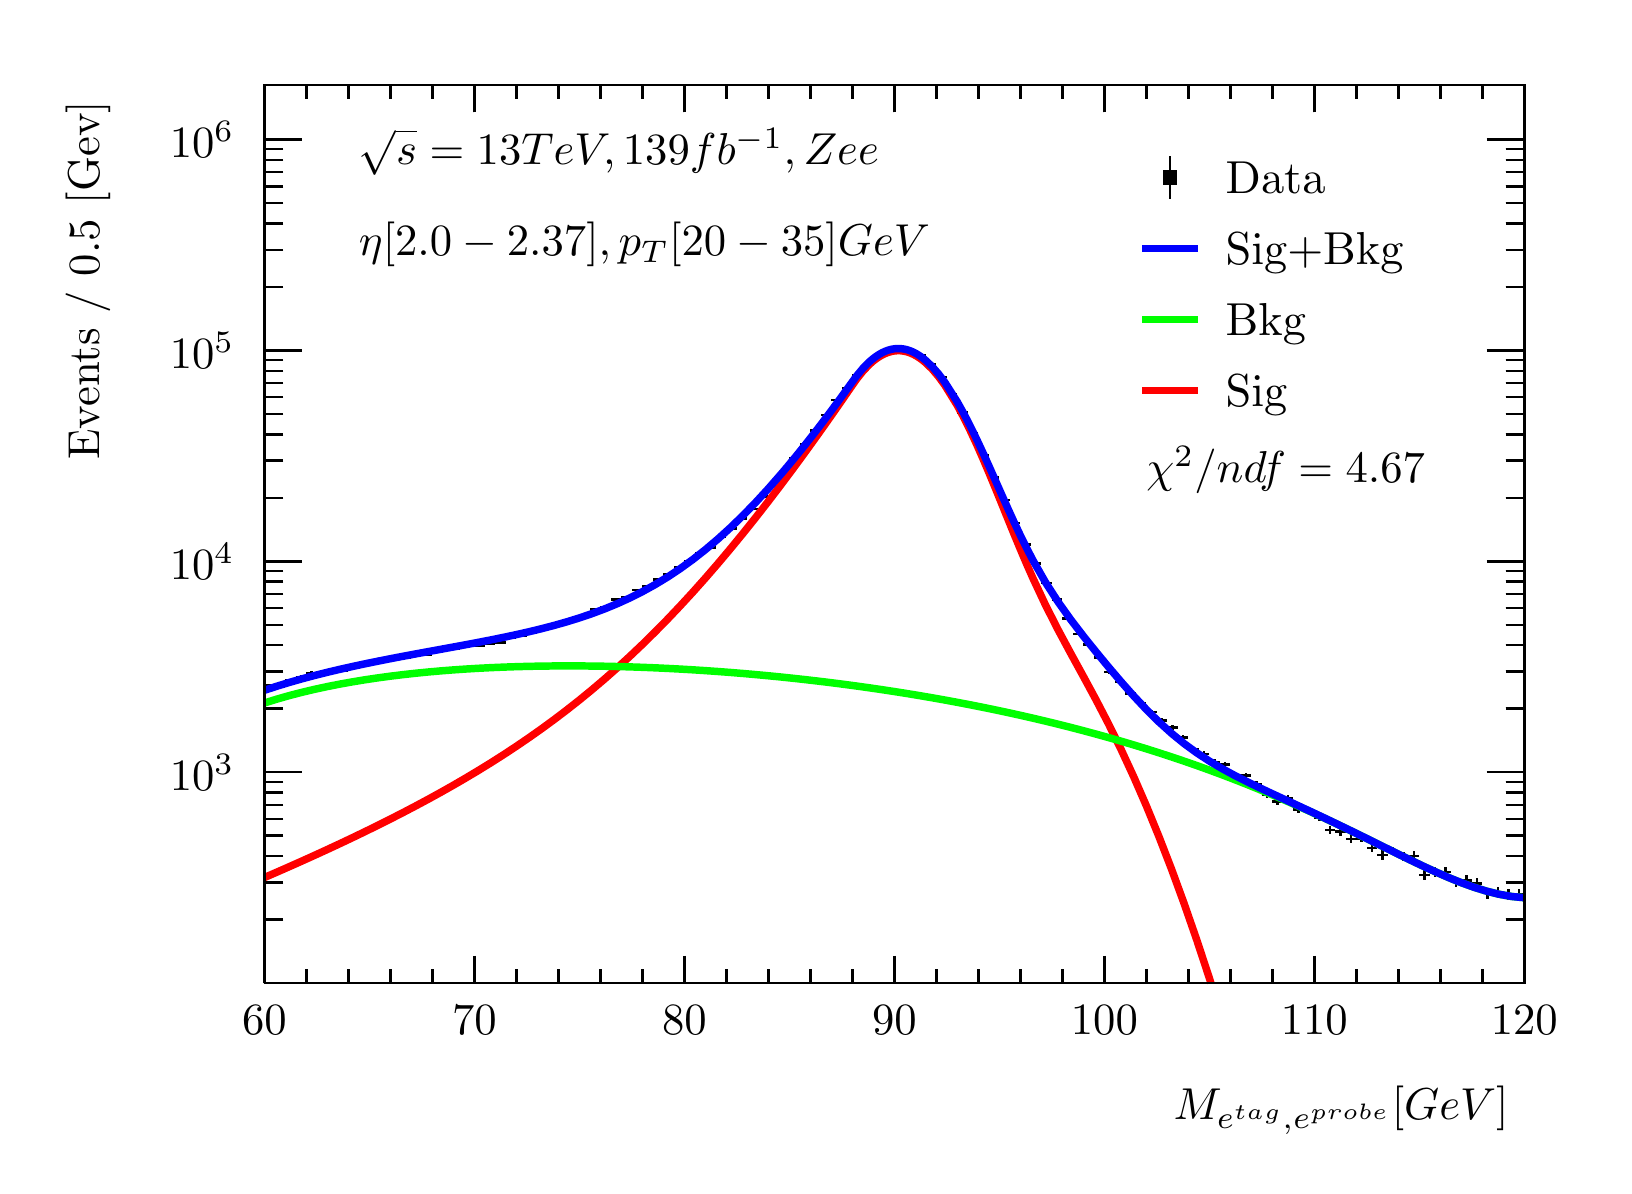
\begin{tikzpicture}
\pgfdeclareplotmark{cross} {
\pgfpathmoveto{\pgfpoint{-0.3\pgfplotmarksize}{\pgfplotmarksize}}
\pgfpathlineto{\pgfpoint{+0.3\pgfplotmarksize}{\pgfplotmarksize}}
\pgfpathlineto{\pgfpoint{+0.3\pgfplotmarksize}{0.3\pgfplotmarksize}}
\pgfpathlineto{\pgfpoint{+1\pgfplotmarksize}{0.3\pgfplotmarksize}}
\pgfpathlineto{\pgfpoint{+1\pgfplotmarksize}{-0.3\pgfplotmarksize}}
\pgfpathlineto{\pgfpoint{+0.3\pgfplotmarksize}{-0.3\pgfplotmarksize}}
\pgfpathlineto{\pgfpoint{+0.3\pgfplotmarksize}{-1.\pgfplotmarksize}}
\pgfpathlineto{\pgfpoint{-0.3\pgfplotmarksize}{-1.\pgfplotmarksize}}
\pgfpathlineto{\pgfpoint{-0.3\pgfplotmarksize}{-0.3\pgfplotmarksize}}
\pgfpathlineto{\pgfpoint{-1.\pgfplotmarksize}{-0.3\pgfplotmarksize}}
\pgfpathlineto{\pgfpoint{-1.\pgfplotmarksize}{0.3\pgfplotmarksize}}
\pgfpathlineto{\pgfpoint{-0.3\pgfplotmarksize}{0.3\pgfplotmarksize}}
\pgfpathclose
\pgfusepathqstroke
}
\pgfdeclareplotmark{cross*} {
\pgfpathmoveto{\pgfpoint{-0.3\pgfplotmarksize}{\pgfplotmarksize}}
\pgfpathlineto{\pgfpoint{+0.3\pgfplotmarksize}{\pgfplotmarksize}}
\pgfpathlineto{\pgfpoint{+0.3\pgfplotmarksize}{0.3\pgfplotmarksize}}
\pgfpathlineto{\pgfpoint{+1\pgfplotmarksize}{0.3\pgfplotmarksize}}
\pgfpathlineto{\pgfpoint{+1\pgfplotmarksize}{-0.3\pgfplotmarksize}}
\pgfpathlineto{\pgfpoint{+0.3\pgfplotmarksize}{-0.3\pgfplotmarksize}}
\pgfpathlineto{\pgfpoint{+0.3\pgfplotmarksize}{-1.\pgfplotmarksize}}
\pgfpathlineto{\pgfpoint{-0.3\pgfplotmarksize}{-1.\pgfplotmarksize}}
\pgfpathlineto{\pgfpoint{-0.3\pgfplotmarksize}{-0.3\pgfplotmarksize}}
\pgfpathlineto{\pgfpoint{-1.\pgfplotmarksize}{-0.3\pgfplotmarksize}}
\pgfpathlineto{\pgfpoint{-1.\pgfplotmarksize}{0.3\pgfplotmarksize}}
\pgfpathlineto{\pgfpoint{-0.3\pgfplotmarksize}{0.3\pgfplotmarksize}}
\pgfpathclose
\pgfusepathqfillstroke
}
\pgfdeclareplotmark{newstar} {
\pgfpathmoveto{\pgfqpoint{0pt}{\pgfplotmarksize}}
\pgfpathlineto{\pgfqpointpolar{44}{0.5\pgfplotmarksize}}
\pgfpathlineto{\pgfqpointpolar{18}{\pgfplotmarksize}}
\pgfpathlineto{\pgfqpointpolar{-20}{0.5\pgfplotmarksize}}
\pgfpathlineto{\pgfqpointpolar{-54}{\pgfplotmarksize}}
\pgfpathlineto{\pgfqpointpolar{-90}{0.5\pgfplotmarksize}}
\pgfpathlineto{\pgfqpointpolar{234}{\pgfplotmarksize}}
\pgfpathlineto{\pgfqpointpolar{198}{0.5\pgfplotmarksize}}
\pgfpathlineto{\pgfqpointpolar{162}{\pgfplotmarksize}}
\pgfpathlineto{\pgfqpointpolar{134}{0.5\pgfplotmarksize}}
\pgfpathclose
\pgfusepathqstroke
}
\pgfdeclareplotmark{newstar*} {
\pgfpathmoveto{\pgfqpoint{0pt}{\pgfplotmarksize}}
\pgfpathlineto{\pgfqpointpolar{44}{0.5\pgfplotmarksize}}
\pgfpathlineto{\pgfqpointpolar{18}{\pgfplotmarksize}}
\pgfpathlineto{\pgfqpointpolar{-20}{0.5\pgfplotmarksize}}
\pgfpathlineto{\pgfqpointpolar{-54}{\pgfplotmarksize}}
\pgfpathlineto{\pgfqpointpolar{-90}{0.5\pgfplotmarksize}}
\pgfpathlineto{\pgfqpointpolar{234}{\pgfplotmarksize}}
\pgfpathlineto{\pgfqpointpolar{198}{0.5\pgfplotmarksize}}
\pgfpathlineto{\pgfqpointpolar{162}{\pgfplotmarksize}}
\pgfpathlineto{\pgfqpointpolar{134}{0.5\pgfplotmarksize}}
\pgfpathclose
\pgfusepathqfillstroke
}
\definecolor{c}{rgb}{1,1,1};
\draw [color=c, fill=c] (0,0) rectangle (20,14.4361);
\draw [color=c, fill=c] (3,2.30977) rectangle (19,13.7143);
\definecolor{c}{rgb}{0,0,0};
\draw [c,line width=0.9] (3,2.30977) -- (3,13.7143) -- (19,13.7143) -- (19,2.30977) -- (3,2.30977);
\definecolor{c}{rgb}{1,1,1};
\draw [color=c, fill=c] (3,2.30977) rectangle (19,13.7143);
\definecolor{c}{rgb}{0,0,0};
\draw [c,line width=0.9] (3,2.30977) -- (3,13.7143) -- (19,13.7143) -- (19,2.30977) -- (3,2.30977);
\draw [c,line width=0.9] (3,2.30977) -- (19,2.30977);
\draw [c,line width=0.9] (3,2.65624) -- (3,2.30977);
\draw [c,line width=0.9] (3.53333,2.48301) -- (3.53333,2.30977);
\draw [c,line width=0.9] (4.06667,2.48301) -- (4.06667,2.30977);
\draw [c,line width=0.9] (4.6,2.48301) -- (4.6,2.30977);
\draw [c,line width=0.9] (5.13333,2.48301) -- (5.13333,2.30977);
\draw [c,line width=0.9] (5.66667,2.65624) -- (5.66667,2.30977);
\draw [c,line width=0.9] (6.2,2.48301) -- (6.2,2.30977);
\draw [c,line width=0.9] (6.73333,2.48301) -- (6.73333,2.30977);
\draw [c,line width=0.9] (7.26667,2.48301) -- (7.26667,2.30977);
\draw [c,line width=0.9] (7.8,2.48301) -- (7.8,2.30977);
\draw [c,line width=0.9] (8.33333,2.65624) -- (8.33333,2.30977);
\draw [c,line width=0.9] (8.86667,2.48301) -- (8.86667,2.30977);
\draw [c,line width=0.9] (9.4,2.48301) -- (9.4,2.30977);
\draw [c,line width=0.9] (9.93333,2.48301) -- (9.93333,2.30977);
\draw [c,line width=0.9] (10.4667,2.48301) -- (10.4667,2.30977);
\draw [c,line width=0.9] (11,2.65624) -- (11,2.30977);
\draw [c,line width=0.9] (11.5333,2.48301) -- (11.5333,2.30977);
\draw [c,line width=0.9] (12.0667,2.48301) -- (12.0667,2.30977);
\draw [c,line width=0.9] (12.6,2.48301) -- (12.6,2.30977);
\draw [c,line width=0.9] (13.1333,2.48301) -- (13.1333,2.30977);
\draw [c,line width=0.9] (13.6667,2.65624) -- (13.6667,2.30977);
\draw [c,line width=0.9] (14.2,2.48301) -- (14.2,2.30977);
\draw [c,line width=0.9] (14.7333,2.48301) -- (14.7333,2.30977);
\draw [c,line width=0.9] (15.2667,2.48301) -- (15.2667,2.30977);
\draw [c,line width=0.9] (15.8,2.48301) -- (15.8,2.30977);
\draw [c,line width=0.9] (16.3333,2.65624) -- (16.3333,2.30977);
\draw [c,line width=0.9] (16.8667,2.48301) -- (16.8667,2.30977);
\draw [c,line width=0.9] (17.4,2.48301) -- (17.4,2.30977);
\draw [c,line width=0.9] (17.9333,2.48301) -- (17.9333,2.30977);
\draw [c,line width=0.9] (18.4667,2.48301) -- (18.4667,2.30977);
\draw [c,line width=0.9] (19,2.65624) -- (19,2.30977);
\draw [anchor=base] (3,1.66015) node[scale=1.61424, color=c, rotate=0]{60};
\draw [anchor=base] (5.66667,1.66015) node[scale=1.61424, color=c, rotate=0]{70};
\draw [anchor=base] (8.33333,1.66015) node[scale=1.61424, color=c, rotate=0]{80};
\draw [anchor=base] (11,1.66015) node[scale=1.61424, color=c, rotate=0]{90};
\draw [anchor=base] (13.6667,1.66015) node[scale=1.61424, color=c, rotate=0]{100};
\draw [anchor=base] (16.3333,1.66015) node[scale=1.61424, color=c, rotate=0]{110};
\draw [anchor=base] (19,1.66015) node[scale=1.61424, color=c, rotate=0]{120};
\draw [anchor= east] (19,0.692932) node[scale=1.61424, color=c, rotate=0]{$M_{e^{tag}, e^{probe}}  [GeV]$};
\draw [c,line width=0.9] (3,13.7143) -- (19,13.7143);
\draw [c,line width=0.9] (3,13.3678) -- (3,13.7143);
\draw [c,line width=0.9] (3.53333,13.5411) -- (3.53333,13.7143);
\draw [c,line width=0.9] (4.06667,13.5411) -- (4.06667,13.7143);
\draw [c,line width=0.9] (4.6,13.5411) -- (4.6,13.7143);
\draw [c,line width=0.9] (5.13333,13.5411) -- (5.13333,13.7143);
\draw [c,line width=0.9] (5.66667,13.3678) -- (5.66667,13.7143);
\draw [c,line width=0.9] (6.2,13.5411) -- (6.2,13.7143);
\draw [c,line width=0.9] (6.73333,13.5411) -- (6.73333,13.7143);
\draw [c,line width=0.9] (7.26667,13.5411) -- (7.26667,13.7143);
\draw [c,line width=0.9] (7.8,13.5411) -- (7.8,13.7143);
\draw [c,line width=0.9] (8.33333,13.3678) -- (8.33333,13.7143);
\draw [c,line width=0.9] (8.86667,13.5411) -- (8.86667,13.7143);
\draw [c,line width=0.9] (9.4,13.5411) -- (9.4,13.7143);
\draw [c,line width=0.9] (9.93333,13.5411) -- (9.93333,13.7143);
\draw [c,line width=0.9] (10.4667,13.5411) -- (10.4667,13.7143);
\draw [c,line width=0.9] (11,13.3678) -- (11,13.7143);
\draw [c,line width=0.9] (11.5333,13.5411) -- (11.5333,13.7143);
\draw [c,line width=0.9] (12.0667,13.5411) -- (12.0667,13.7143);
\draw [c,line width=0.9] (12.6,13.5411) -- (12.6,13.7143);
\draw [c,line width=0.9] (13.1333,13.5411) -- (13.1333,13.7143);
\draw [c,line width=0.9] (13.6667,13.3678) -- (13.6667,13.7143);
\draw [c,line width=0.9] (14.2,13.5411) -- (14.2,13.7143);
\draw [c,line width=0.9] (14.7333,13.5411) -- (14.7333,13.7143);
\draw [c,line width=0.9] (15.2667,13.5411) -- (15.2667,13.7143);
\draw [c,line width=0.9] (15.8,13.5411) -- (15.8,13.7143);
\draw [c,line width=0.9] (16.3333,13.3678) -- (16.3333,13.7143);
\draw [c,line width=0.9] (16.8667,13.5411) -- (16.8667,13.7143);
\draw [c,line width=0.9] (17.4,13.5411) -- (17.4,13.7143);
\draw [c,line width=0.9] (17.9333,13.5411) -- (17.9333,13.7143);
\draw [c,line width=0.9] (18.4667,13.5411) -- (18.4667,13.7143);
\draw [c,line width=0.9] (19,13.3678) -- (19,13.7143);
\draw [c,line width=0.9] (3,2.30977) -- (3,13.7143);
\draw [c,line width=0.9] (3.237,3.11596) -- (3,3.11596);
\draw [c,line width=0.9] (3.237,3.58755) -- (3,3.58755);
\draw [c,line width=0.9] (3.237,3.92215) -- (3,3.92215);
\draw [c,line width=0.9] (3.237,4.18169) -- (3,4.18169);
\draw [c,line width=0.9] (3.237,4.39374) -- (3,4.39374);
\draw [c,line width=0.9] (3.237,4.57303) -- (3,4.57303);
\draw [c,line width=0.9] (3.237,4.72834) -- (3,4.72834);
\draw [c,line width=0.9] (3.237,4.86533) -- (3,4.86533);
\draw [c,line width=0.9] (3.474,4.98787) -- (3,4.98787);
\draw [anchor= east] (2.82,4.98787) node[scale=1.61424, color=c, rotate=0]{$10^{3}$};
\draw [c,line width=0.9] (3.237,5.79406) -- (3,5.79406);
\draw [c,line width=0.9] (3.237,6.26566) -- (3,6.26566);
\draw [c,line width=0.9] (3.237,6.60025) -- (3,6.60025);
\draw [c,line width=0.9] (3.237,6.85979) -- (3,6.85979);
\draw [c,line width=0.9] (3.237,7.07184) -- (3,7.07184);
\draw [c,line width=0.9] (3.237,7.25113) -- (3,7.25113);
\draw [c,line width=0.9] (3.237,7.40644) -- (3,7.40644);
\draw [c,line width=0.9] (3.237,7.54344) -- (3,7.54344);
\draw [c,line width=0.9] (3.474,7.66598) -- (3,7.66598);
\draw [anchor= east] (2.82,7.66598) node[scale=1.61424, color=c, rotate=0]{$10^{4}$};
\draw [c,line width=0.9] (3.237,8.47217) -- (3,8.47217);
\draw [c,line width=0.9] (3.237,8.94376) -- (3,8.94376);
\draw [c,line width=0.9] (3.237,9.27836) -- (3,9.27836);
\draw [c,line width=0.9] (3.237,9.53789) -- (3,9.53789);
\draw [c,line width=0.9] (3.237,9.74995) -- (3,9.74995);
\draw [c,line width=0.9] (3.237,9.92924) -- (3,9.92924);
\draw [c,line width=0.9] (3.237,10.0845) -- (3,10.0845);
\draw [c,line width=0.9] (3.237,10.2215) -- (3,10.2215);
\draw [c,line width=0.9] (3.474,10.3441) -- (3,10.3441);
\draw [anchor= east] (2.82,10.3441) node[scale=1.61424, color=c, rotate=0]{$10^{5}$};
\draw [c,line width=0.9] (3.237,11.1503) -- (3,11.1503);
\draw [c,line width=0.9] (3.237,11.6219) -- (3,11.6219);
\draw [c,line width=0.9] (3.237,11.9565) -- (3,11.9565);
\draw [c,line width=0.9] (3.237,12.216) -- (3,12.216);
\draw [c,line width=0.9] (3.237,12.4281) -- (3,12.4281);
\draw [c,line width=0.9] (3.237,12.6073) -- (3,12.6073);
\draw [c,line width=0.9] (3.237,12.7627) -- (3,12.7627);
\draw [c,line width=0.9] (3.237,12.8996) -- (3,12.8996);
\draw [c,line width=0.9] (3.474,13.0222) -- (3,13.0222);
\draw [anchor= east] (2.82,13.0222) node[scale=1.61424, color=c, rotate=0]{$10^{6}$};
\draw [anchor= east] (0.76,13.7143) node[scale=1.61424, color=c, rotate=90]{Events / 0.5 [Gev]};
\draw [c,line width=0.9] (19,2.30977) -- (19,13.7143);
\draw [c,line width=0.9] (18.763,3.11596) -- (19,3.11596);
\draw [c,line width=0.9] (18.763,3.58755) -- (19,3.58755);
\draw [c,line width=0.9] (18.763,3.92215) -- (19,3.92215);
\draw [c,line width=0.9] (18.763,4.18169) -- (19,4.18169);
\draw [c,line width=0.9] (18.763,4.39374) -- (19,4.39374);
\draw [c,line width=0.9] (18.763,4.57303) -- (19,4.57303);
\draw [c,line width=0.9] (18.763,4.72834) -- (19,4.72834);
\draw [c,line width=0.9] (18.763,4.86533) -- (19,4.86533);
\draw [c,line width=0.9] (18.526,4.98787) -- (19,4.98787);
\draw [c,line width=0.9] (18.763,5.79406) -- (19,5.79406);
\draw [c,line width=0.9] (18.763,6.26566) -- (19,6.26566);
\draw [c,line width=0.9] (18.763,6.60025) -- (19,6.60025);
\draw [c,line width=0.9] (18.763,6.85979) -- (19,6.85979);
\draw [c,line width=0.9] (18.763,7.07184) -- (19,7.07184);
\draw [c,line width=0.9] (18.763,7.25113) -- (19,7.25113);
\draw [c,line width=0.9] (18.763,7.40644) -- (19,7.40644);
\draw [c,line width=0.9] (18.763,7.54344) -- (19,7.54344);
\draw [c,line width=0.9] (18.526,7.66598) -- (19,7.66598);
\draw [c,line width=0.9] (18.763,8.47217) -- (19,8.47217);
\draw [c,line width=0.9] (18.763,8.94376) -- (19,8.94376);
\draw [c,line width=0.9] (18.763,9.27836) -- (19,9.27836);
\draw [c,line width=0.9] (18.763,9.53789) -- (19,9.53789);
\draw [c,line width=0.9] (18.763,9.74995) -- (19,9.74995);
\draw [c,line width=0.9] (18.763,9.92924) -- (19,9.92924);
\draw [c,line width=0.9] (18.763,10.0845) -- (19,10.0845);
\draw [c,line width=0.9] (18.763,10.2215) -- (19,10.2215);
\draw [c,line width=0.9] (18.526,10.3441) -- (19,10.3441);
\draw [c,line width=0.9] (18.763,11.1503) -- (19,11.1503);
\draw [c,line width=0.9] (18.763,11.6219) -- (19,11.6219);
\draw [c,line width=0.9] (18.763,11.9565) -- (19,11.9565);
\draw [c,line width=0.9] (18.763,12.216) -- (19,12.216);
\draw [c,line width=0.9] (18.763,12.4281) -- (19,12.4281);
\draw [c,line width=0.9] (18.763,12.6073) -- (19,12.6073);
\draw [c,line width=0.9] (18.763,12.7627) -- (19,12.7627);
\draw [c,line width=0.9] (18.763,12.8996) -- (19,12.8996);
\draw [c,line width=0.9] (18.526,13.0222) -- (19,13.0222);
\draw [c,line width=0.9] (3.06667,6.08753) -- (3,6.08753);
\draw [c,line width=0.9] (3,6.08753) -- (3,6.08753);
\draw [c,line width=0.9] (3.06667,6.08753) -- (3.13333,6.08753);
\draw [c,line width=0.9] (3.13333,6.08753) -- (3.13333,6.08753);
\draw [c,line width=0.9] (3.06667,6.08753) -- (3.06667,6.11045);
\draw [c,line width=0.9] (3.06667,6.11045) -- (3.06667,6.11045);
\draw [c,line width=0.9] (3.06667,6.08753) -- (3.06667,6.0646);
\draw [c,line width=0.9] (3.06667,6.0646) -- (3.06667,6.0646);
\draw [c,line width=0.9] (3.2,6.06702) -- (3.13333,6.06702);
\draw [c,line width=0.9] (3.13333,6.06702) -- (3.13333,6.06702);
\draw [c,line width=0.9] (3.2,6.06702) -- (3.26667,6.06702);
\draw [c,line width=0.9] (3.26667,6.06702) -- (3.26667,6.06702);
\draw [c,line width=0.9] (3.2,6.06702) -- (3.2,6.09014);
\draw [c,line width=0.9] (3.2,6.09014) -- (3.2,6.09014);
\draw [c,line width=0.9] (3.2,6.06702) -- (3.2,6.04389);
\draw [c,line width=0.9] (3.2,6.04389) -- (3.2,6.04389);
\draw [c,line width=0.9] (3.33333,6.15469) -- (3.26667,6.15469);
\draw [c,line width=0.9] (3.26667,6.15469) -- (3.26667,6.15469);
\draw [c,line width=0.9] (3.33333,6.15469) -- (3.4,6.15469);
\draw [c,line width=0.9] (3.4,6.15469) -- (3.4,6.15469);
\draw [c,line width=0.9] (3.33333,6.15469) -- (3.33333,6.17696);
\draw [c,line width=0.9] (3.33333,6.17696) -- (3.33333,6.17696);
\draw [c,line width=0.9] (3.33333,6.15469) -- (3.33333,6.13241);
\draw [c,line width=0.9] (3.33333,6.13241) -- (3.33333,6.13241);
\draw [c,line width=0.9] (3.46667,6.1941) -- (3.4,6.1941);
\draw [c,line width=0.9] (3.4,6.1941) -- (3.4,6.1941);
\draw [c,line width=0.9] (3.46667,6.1941) -- (3.53333,6.1941);
\draw [c,line width=0.9] (3.53333,6.1941) -- (3.53333,6.1941);
\draw [c,line width=0.9] (3.46667,6.1941) -- (3.46667,6.216);
\draw [c,line width=0.9] (3.46667,6.216) -- (3.46667,6.216);
\draw [c,line width=0.9] (3.46667,6.1941) -- (3.46667,6.1722);
\draw [c,line width=0.9] (3.46667,6.1722) -- (3.46667,6.1722);
\draw [c,line width=0.9] (3.6,6.24611) -- (3.53333,6.24611);
\draw [c,line width=0.9] (3.53333,6.24611) -- (3.53333,6.24611);
\draw [c,line width=0.9] (3.6,6.24611) -- (3.66667,6.24611);
\draw [c,line width=0.9] (3.66667,6.24611) -- (3.66667,6.24611);
\draw [c,line width=0.9] (3.6,6.24611) -- (3.6,6.26752);
\draw [c,line width=0.9] (3.6,6.26752) -- (3.6,6.26752);
\draw [c,line width=0.9] (3.6,6.24611) -- (3.6,6.22469);
\draw [c,line width=0.9] (3.6,6.22469) -- (3.6,6.22469);
\draw [c,line width=0.9] (3.73333,6.23541) -- (3.66667,6.23541);
\draw [c,line width=0.9] (3.66667,6.23541) -- (3.66667,6.23541);
\draw [c,line width=0.9] (3.73333,6.23541) -- (3.8,6.23541);
\draw [c,line width=0.9] (3.8,6.23541) -- (3.8,6.23541);
\draw [c,line width=0.9] (3.73333,6.23541) -- (3.73333,6.25693);
\draw [c,line width=0.9] (3.73333,6.25693) -- (3.73333,6.25693);
\draw [c,line width=0.9] (3.73333,6.23541) -- (3.73333,6.2139);
\draw [c,line width=0.9] (3.73333,6.2139) -- (3.73333,6.2139);
\draw [c,line width=0.9] (3.86667,6.26255) -- (3.8,6.26255);
\draw [c,line width=0.9] (3.8,6.26255) -- (3.8,6.26255);
\draw [c,line width=0.9] (3.86667,6.26255) -- (3.93333,6.26255);
\draw [c,line width=0.9] (3.93333,6.26255) -- (3.93333,6.26255);
\draw [c,line width=0.9] (3.86667,6.26255) -- (3.86667,6.28381);
\draw [c,line width=0.9] (3.86667,6.28381) -- (3.86667,6.28381);
\draw [c,line width=0.9] (3.86667,6.26255) -- (3.86667,6.24129);
\draw [c,line width=0.9] (3.86667,6.24129) -- (3.86667,6.24129);
\draw [c,line width=0.9] (4,6.27608) -- (3.93333,6.27608);
\draw [c,line width=0.9] (3.93333,6.27608) -- (3.93333,6.27608);
\draw [c,line width=0.9] (4,6.27608) -- (4.06667,6.27608);
\draw [c,line width=0.9] (4.06667,6.27608) -- (4.06667,6.27608);
\draw [c,line width=0.9] (4,6.27608) -- (4,6.29722);
\draw [c,line width=0.9] (4,6.29722) -- (4,6.29722);
\draw [c,line width=0.9] (4,6.27608) -- (4,6.25494);
\draw [c,line width=0.9] (4,6.25494) -- (4,6.25494);
\draw [c,line width=0.9] (4.13333,6.35193) -- (4.06667,6.35193);
\draw [c,line width=0.9] (4.06667,6.35193) -- (4.06667,6.35193);
\draw [c,line width=0.9] (4.13333,6.35193) -- (4.2,6.35193);
\draw [c,line width=0.9] (4.2,6.35193) -- (4.2,6.35193);
\draw [c,line width=0.9] (4.13333,6.35193) -- (4.13333,6.3724);
\draw [c,line width=0.9] (4.13333,6.3724) -- (4.13333,6.3724);
\draw [c,line width=0.9] (4.13333,6.35193) -- (4.13333,6.33147);
\draw [c,line width=0.9] (4.13333,6.33147) -- (4.13333,6.33147);
\draw [c,line width=0.9] (4.26667,6.37298) -- (4.2,6.37298);
\draw [c,line width=0.9] (4.2,6.37298) -- (4.2,6.37298);
\draw [c,line width=0.9] (4.26667,6.37298) -- (4.33333,6.37298);
\draw [c,line width=0.9] (4.33333,6.37298) -- (4.33333,6.37298);
\draw [c,line width=0.9] (4.26667,6.37298) -- (4.26667,6.39326);
\draw [c,line width=0.9] (4.26667,6.39326) -- (4.26667,6.39326);
\draw [c,line width=0.9] (4.26667,6.37298) -- (4.26667,6.3527);
\draw [c,line width=0.9] (4.26667,6.3527) -- (4.26667,6.3527);
\draw [c,line width=0.9] (4.4,6.39504) -- (4.33333,6.39504);
\draw [c,line width=0.9] (4.33333,6.39504) -- (4.33333,6.39504);
\draw [c,line width=0.9] (4.4,6.39504) -- (4.46667,6.39504);
\draw [c,line width=0.9] (4.46667,6.39504) -- (4.46667,6.39504);
\draw [c,line width=0.9] (4.4,6.39504) -- (4.4,6.41513);
\draw [c,line width=0.9] (4.4,6.41513) -- (4.4,6.41513);
\draw [c,line width=0.9] (4.4,6.39504) -- (4.4,6.37496);
\draw [c,line width=0.9] (4.4,6.37496) -- (4.4,6.37496);
\draw [c,line width=0.9] (4.53333,6.42247) -- (4.46667,6.42247);
\draw [c,line width=0.9] (4.46667,6.42247) -- (4.46667,6.42247);
\draw [c,line width=0.9] (4.53333,6.42247) -- (4.6,6.42247);
\draw [c,line width=0.9] (4.6,6.42247) -- (4.6,6.42247);
\draw [c,line width=0.9] (4.53333,6.42247) -- (4.53333,6.44232);
\draw [c,line width=0.9] (4.53333,6.44232) -- (4.53333,6.44232);
\draw [c,line width=0.9] (4.53333,6.42247) -- (4.53333,6.40262);
\draw [c,line width=0.9] (4.53333,6.40262) -- (4.53333,6.40262);
\draw [c,line width=0.9] (4.66667,6.44195) -- (4.6,6.44195);
\draw [c,line width=0.9] (4.6,6.44195) -- (4.6,6.44195);
\draw [c,line width=0.9] (4.66667,6.44195) -- (4.73333,6.44195);
\draw [c,line width=0.9] (4.73333,6.44195) -- (4.73333,6.44195);
\draw [c,line width=0.9] (4.66667,6.44195) -- (4.66667,6.46164);
\draw [c,line width=0.9] (4.66667,6.46164) -- (4.66667,6.46164);
\draw [c,line width=0.9] (4.66667,6.44195) -- (4.66667,6.42227);
\draw [c,line width=0.9] (4.66667,6.42227) -- (4.66667,6.42227);
\draw [c,line width=0.9] (4.8,6.44461) -- (4.73333,6.44461);
\draw [c,line width=0.9] (4.73333,6.44461) -- (4.73333,6.44461);
\draw [c,line width=0.9] (4.8,6.44461) -- (4.86667,6.44461);
\draw [c,line width=0.9] (4.86667,6.44461) -- (4.86667,6.44461);
\draw [c,line width=0.9] (4.8,6.44461) -- (4.8,6.46428);
\draw [c,line width=0.9] (4.8,6.46428) -- (4.8,6.46428);
\draw [c,line width=0.9] (4.8,6.44461) -- (4.8,6.42495);
\draw [c,line width=0.9] (4.8,6.42495) -- (4.8,6.42495);
\draw [c,line width=0.9] (4.93333,6.48223) -- (4.86667,6.48223);
\draw [c,line width=0.9] (4.86667,6.48223) -- (4.86667,6.48223);
\draw [c,line width=0.9] (4.93333,6.48223) -- (5,6.48223);
\draw [c,line width=0.9] (5,6.48223) -- (5,6.48223);
\draw [c,line width=0.9] (4.93333,6.48223) -- (4.93333,6.50157);
\draw [c,line width=0.9] (4.93333,6.50157) -- (4.93333,6.50157);
\draw [c,line width=0.9] (4.93333,6.48223) -- (4.93333,6.46288);
\draw [c,line width=0.9] (4.93333,6.46288) -- (4.93333,6.46288);
\draw [c,line width=0.9] (5.06667,6.48029) -- (5,6.48029);
\draw [c,line width=0.9] (5,6.48029) -- (5,6.48029);
\draw [c,line width=0.9] (5.06667,6.48029) -- (5.13333,6.48029);
\draw [c,line width=0.9] (5.13333,6.48029) -- (5.13333,6.48029);
\draw [c,line width=0.9] (5.06667,6.48029) -- (5.06667,6.49966);
\draw [c,line width=0.9] (5.06667,6.49966) -- (5.06667,6.49966);
\draw [c,line width=0.9] (5.06667,6.48029) -- (5.06667,6.46093);
\draw [c,line width=0.9] (5.06667,6.46093) -- (5.06667,6.46093);
\draw [c,line width=0.9] (5.2,6.51554) -- (5.13333,6.51554);
\draw [c,line width=0.9] (5.13333,6.51554) -- (5.13333,6.51554);
\draw [c,line width=0.9] (5.2,6.51554) -- (5.26667,6.51554);
\draw [c,line width=0.9] (5.26667,6.51554) -- (5.26667,6.51554);
\draw [c,line width=0.9] (5.2,6.51554) -- (5.2,6.53461);
\draw [c,line width=0.9] (5.2,6.53461) -- (5.2,6.53461);
\draw [c,line width=0.9] (5.2,6.51554) -- (5.2,6.49647);
\draw [c,line width=0.9] (5.2,6.49647) -- (5.2,6.49647);
\draw [c,line width=0.9] (5.33333,6.54883) -- (5.26667,6.54883);
\draw [c,line width=0.9] (5.26667,6.54883) -- (5.26667,6.54883);
\draw [c,line width=0.9] (5.33333,6.54883) -- (5.4,6.54883);
\draw [c,line width=0.9] (5.4,6.54883) -- (5.4,6.54883);
\draw [c,line width=0.9] (5.33333,6.54883) -- (5.33333,6.56763);
\draw [c,line width=0.9] (5.33333,6.56763) -- (5.33333,6.56763);
\draw [c,line width=0.9] (5.33333,6.54883) -- (5.33333,6.53003);
\draw [c,line width=0.9] (5.33333,6.53003) -- (5.33333,6.53003);
\draw [c,line width=0.9] (5.46667,6.56243) -- (5.4,6.56243);
\draw [c,line width=0.9] (5.4,6.56243) -- (5.4,6.56243);
\draw [c,line width=0.9] (5.46667,6.56243) -- (5.53333,6.56243);
\draw [c,line width=0.9] (5.53333,6.56243) -- (5.53333,6.56243);
\draw [c,line width=0.9] (5.46667,6.56243) -- (5.46667,6.58112);
\draw [c,line width=0.9] (5.46667,6.58112) -- (5.46667,6.58112);
\draw [c,line width=0.9] (5.46667,6.56243) -- (5.46667,6.54374);
\draw [c,line width=0.9] (5.46667,6.54374) -- (5.46667,6.54374);
\draw [c,line width=0.9] (5.6,6.62898) -- (5.53333,6.62898);
\draw [c,line width=0.9] (5.53333,6.62898) -- (5.53333,6.62898);
\draw [c,line width=0.9] (5.6,6.62898) -- (5.66667,6.62898);
\draw [c,line width=0.9] (5.66667,6.62898) -- (5.66667,6.62898);
\draw [c,line width=0.9] (5.6,6.62898) -- (5.6,6.64714);
\draw [c,line width=0.9] (5.6,6.64714) -- (5.6,6.64714);
\draw [c,line width=0.9] (5.6,6.62898) -- (5.6,6.61081);
\draw [c,line width=0.9] (5.6,6.61081) -- (5.6,6.61081);
\draw [c,line width=0.9] (5.73333,6.59062) -- (5.66667,6.59062);
\draw [c,line width=0.9] (5.66667,6.59062) -- (5.66667,6.59062);
\draw [c,line width=0.9] (5.73333,6.59062) -- (5.8,6.59062);
\draw [c,line width=0.9] (5.8,6.59062) -- (5.8,6.59062);
\draw [c,line width=0.9] (5.73333,6.59062) -- (5.73333,6.60909);
\draw [c,line width=0.9] (5.73333,6.60909) -- (5.73333,6.60909);
\draw [c,line width=0.9] (5.73333,6.59062) -- (5.73333,6.57215);
\draw [c,line width=0.9] (5.73333,6.57215) -- (5.73333,6.57215);
\draw [c,line width=0.9] (5.86667,6.62158) -- (5.8,6.62158);
\draw [c,line width=0.9] (5.8,6.62158) -- (5.8,6.62158);
\draw [c,line width=0.9] (5.86667,6.62158) -- (5.93333,6.62158);
\draw [c,line width=0.9] (5.93333,6.62158) -- (5.93333,6.62158);
\draw [c,line width=0.9] (5.86667,6.62158) -- (5.86667,6.6398);
\draw [c,line width=0.9] (5.86667,6.6398) -- (5.86667,6.6398);
\draw [c,line width=0.9] (5.86667,6.62158) -- (5.86667,6.60335);
\draw [c,line width=0.9] (5.86667,6.60335) -- (5.86667,6.60335);
\draw [c,line width=0.9] (6,6.63407) -- (5.93333,6.63407);
\draw [c,line width=0.9] (5.93333,6.63407) -- (5.93333,6.63407);
\draw [c,line width=0.9] (6,6.63407) -- (6.06667,6.63407);
\draw [c,line width=0.9] (6.06667,6.63407) -- (6.06667,6.63407);
\draw [c,line width=0.9] (6,6.63407) -- (6,6.65219);
\draw [c,line width=0.9] (6,6.65219) -- (6,6.65219);
\draw [c,line width=0.9] (6,6.63407) -- (6,6.61595);
\draw [c,line width=0.9] (6,6.61595) -- (6,6.61595);
\draw [c,line width=0.9] (6.13333,6.69915) -- (6.06667,6.69915);
\draw [c,line width=0.9] (6.06667,6.69915) -- (6.06667,6.69915);
\draw [c,line width=0.9] (6.13333,6.69915) -- (6.2,6.69915);
\draw [c,line width=0.9] (6.2,6.69915) -- (6.2,6.69915);
\draw [c,line width=0.9] (6.13333,6.69915) -- (6.13333,6.71678);
\draw [c,line width=0.9] (6.13333,6.71678) -- (6.13333,6.71678);
\draw [c,line width=0.9] (6.13333,6.69915) -- (6.13333,6.68153);
\draw [c,line width=0.9] (6.13333,6.68153) -- (6.13333,6.68153);
\draw [c,line width=0.9] (6.26667,6.72321) -- (6.2,6.72321);
\draw [c,line width=0.9] (6.2,6.72321) -- (6.2,6.72321);
\draw [c,line width=0.9] (6.26667,6.72321) -- (6.33333,6.72321);
\draw [c,line width=0.9] (6.33333,6.72321) -- (6.33333,6.72321);
\draw [c,line width=0.9] (6.26667,6.72321) -- (6.26667,6.74065);
\draw [c,line width=0.9] (6.26667,6.74065) -- (6.26667,6.74065);
\draw [c,line width=0.9] (6.26667,6.72321) -- (6.26667,6.70576);
\draw [c,line width=0.9] (6.26667,6.70576) -- (6.26667,6.70576);
\draw [c,line width=0.9] (6.4,6.7585) -- (6.33333,6.7585);
\draw [c,line width=0.9] (6.33333,6.7585) -- (6.33333,6.7585);
\draw [c,line width=0.9] (6.4,6.7585) -- (6.46667,6.7585);
\draw [c,line width=0.9] (6.46667,6.7585) -- (6.46667,6.7585);
\draw [c,line width=0.9] (6.4,6.7585) -- (6.4,6.77568);
\draw [c,line width=0.9] (6.4,6.77568) -- (6.4,6.77568);
\draw [c,line width=0.9] (6.4,6.7585) -- (6.4,6.74132);
\draw [c,line width=0.9] (6.4,6.74132) -- (6.4,6.74132);
\draw [c,line width=0.9] (6.53333,6.81061) -- (6.46667,6.81061);
\draw [c,line width=0.9] (6.46667,6.81061) -- (6.46667,6.81061);
\draw [c,line width=0.9] (6.53333,6.81061) -- (6.6,6.81061);
\draw [c,line width=0.9] (6.6,6.81061) -- (6.6,6.81061);
\draw [c,line width=0.9] (6.53333,6.81061) -- (6.53333,6.82741);
\draw [c,line width=0.9] (6.53333,6.82741) -- (6.53333,6.82741);
\draw [c,line width=0.9] (6.53333,6.81061) -- (6.53333,6.79381);
\draw [c,line width=0.9] (6.53333,6.79381) -- (6.53333,6.79381);
\draw [c,line width=0.9] (6.66667,6.83819) -- (6.6,6.83819);
\draw [c,line width=0.9] (6.6,6.83819) -- (6.6,6.83819);
\draw [c,line width=0.9] (6.66667,6.83819) -- (6.73333,6.83819);
\draw [c,line width=0.9] (6.73333,6.83819) -- (6.73333,6.83819);
\draw [c,line width=0.9] (6.66667,6.83819) -- (6.66667,6.85479);
\draw [c,line width=0.9] (6.66667,6.85479) -- (6.66667,6.85479);
\draw [c,line width=0.9] (6.66667,6.83819) -- (6.66667,6.82159);
\draw [c,line width=0.9] (6.66667,6.82159) -- (6.66667,6.82159);
\draw [c,line width=0.9] (6.8,6.87228) -- (6.73333,6.87228);
\draw [c,line width=0.9] (6.73333,6.87228) -- (6.73333,6.87228);
\draw [c,line width=0.9] (6.8,6.87228) -- (6.86667,6.87228);
\draw [c,line width=0.9] (6.86667,6.87228) -- (6.86667,6.87228);
\draw [c,line width=0.9] (6.8,6.87228) -- (6.8,6.88864);
\draw [c,line width=0.9] (6.8,6.88864) -- (6.8,6.88864);
\draw [c,line width=0.9] (6.8,6.87228) -- (6.8,6.85592);
\draw [c,line width=0.9] (6.8,6.85592) -- (6.8,6.85592);
\draw [c,line width=0.9] (6.93333,6.94022) -- (6.86667,6.94022);
\draw [c,line width=0.9] (6.86667,6.94022) -- (6.86667,6.94022);
\draw [c,line width=0.9] (6.93333,6.94022) -- (7,6.94022);
\draw [c,line width=0.9] (7,6.94022) -- (7,6.94022);
\draw [c,line width=0.9] (6.93333,6.94022) -- (6.93333,6.95611);
\draw [c,line width=0.9] (6.93333,6.95611) -- (6.93333,6.95611);
\draw [c,line width=0.9] (6.93333,6.94022) -- (6.93333,6.92433);
\draw [c,line width=0.9] (6.93333,6.92433) -- (6.93333,6.92433);
\draw [c,line width=0.9] (7.06667,6.9797) -- (7,6.9797);
\draw [c,line width=0.9] (7,6.9797) -- (7,6.9797);
\draw [c,line width=0.9] (7.06667,6.9797) -- (7.13333,6.9797);
\draw [c,line width=0.9] (7.13333,6.9797) -- (7.13333,6.9797);
\draw [c,line width=0.9] (7.06667,6.9797) -- (7.06667,6.99532);
\draw [c,line width=0.9] (7.06667,6.99532) -- (7.06667,6.99532);
\draw [c,line width=0.9] (7.06667,6.9797) -- (7.06667,6.96408);
\draw [c,line width=0.9] (7.06667,6.96408) -- (7.06667,6.96408);
\draw [c,line width=0.9] (7.2,7.05466) -- (7.13333,7.05466);
\draw [c,line width=0.9] (7.13333,7.05466) -- (7.13333,7.05466);
\draw [c,line width=0.9] (7.2,7.05466) -- (7.26667,7.05466);
\draw [c,line width=0.9] (7.26667,7.05466) -- (7.26667,7.05466);
\draw [c,line width=0.9] (7.2,7.05466) -- (7.2,7.06979);
\draw [c,line width=0.9] (7.2,7.06979) -- (7.2,7.06979);
\draw [c,line width=0.9] (7.2,7.05466) -- (7.2,7.03953);
\draw [c,line width=0.9] (7.2,7.03953) -- (7.2,7.03953);
\draw [c,line width=0.9] (7.33333,7.07707) -- (7.26667,7.07707);
\draw [c,line width=0.9] (7.26667,7.07707) -- (7.26667,7.07707);
\draw [c,line width=0.9] (7.33333,7.07707) -- (7.4,7.07707);
\draw [c,line width=0.9] (7.4,7.07707) -- (7.4,7.07707);
\draw [c,line width=0.9] (7.33333,7.07707) -- (7.33333,7.09205);
\draw [c,line width=0.9] (7.33333,7.09205) -- (7.33333,7.09205);
\draw [c,line width=0.9] (7.33333,7.07707) -- (7.33333,7.06209);
\draw [c,line width=0.9] (7.33333,7.06209) -- (7.33333,7.06209);
\draw [c,line width=0.9] (7.46667,7.18023) -- (7.4,7.18023);
\draw [c,line width=0.9] (7.4,7.18023) -- (7.4,7.18023);
\draw [c,line width=0.9] (7.46667,7.18023) -- (7.53333,7.18023);
\draw [c,line width=0.9] (7.53333,7.18023) -- (7.53333,7.18023);
\draw [c,line width=0.9] (7.46667,7.18023) -- (7.46667,7.19456);
\draw [c,line width=0.9] (7.46667,7.19456) -- (7.46667,7.19456);
\draw [c,line width=0.9] (7.46667,7.18023) -- (7.46667,7.1659);
\draw [c,line width=0.9] (7.46667,7.1659) -- (7.46667,7.1659);
\draw [c,line width=0.9] (7.6,7.20849) -- (7.53333,7.20849);
\draw [c,line width=0.9] (7.53333,7.20849) -- (7.53333,7.20849);
\draw [c,line width=0.9] (7.6,7.20849) -- (7.66667,7.20849);
\draw [c,line width=0.9] (7.66667,7.20849) -- (7.66667,7.20849);
\draw [c,line width=0.9] (7.6,7.20849) -- (7.6,7.22265);
\draw [c,line width=0.9] (7.6,7.22265) -- (7.6,7.22265);
\draw [c,line width=0.9] (7.6,7.20849) -- (7.6,7.19433);
\draw [c,line width=0.9] (7.6,7.19433) -- (7.6,7.19433);
\draw [c,line width=0.9] (7.73333,7.30249) -- (7.66667,7.30249);
\draw [c,line width=0.9] (7.66667,7.30249) -- (7.66667,7.30249);
\draw [c,line width=0.9] (7.73333,7.30249) -- (7.8,7.30249);
\draw [c,line width=0.9] (7.8,7.30249) -- (7.8,7.30249);
\draw [c,line width=0.9] (7.73333,7.30249) -- (7.73333,7.31609);
\draw [c,line width=0.9] (7.73333,7.31609) -- (7.73333,7.31609);
\draw [c,line width=0.9] (7.73333,7.30249) -- (7.73333,7.28889);
\draw [c,line width=0.9] (7.73333,7.28889) -- (7.73333,7.28889);
\draw [c,line width=0.9] (7.86667,7.34587) -- (7.8,7.34587);
\draw [c,line width=0.9] (7.8,7.34587) -- (7.8,7.34587);
\draw [c,line width=0.9] (7.86667,7.34587) -- (7.93333,7.34587);
\draw [c,line width=0.9] (7.93333,7.34587) -- (7.93333,7.34587);
\draw [c,line width=0.9] (7.86667,7.34587) -- (7.86667,7.35921);
\draw [c,line width=0.9] (7.86667,7.35921) -- (7.86667,7.35921);
\draw [c,line width=0.9] (7.86667,7.34587) -- (7.86667,7.33252);
\draw [c,line width=0.9] (7.86667,7.33252) -- (7.86667,7.33252);
\draw [c,line width=0.9] (8,7.43275) -- (7.93333,7.43275);
\draw [c,line width=0.9] (7.93333,7.43275) -- (7.93333,7.43275);
\draw [c,line width=0.9] (8,7.43275) -- (8.06667,7.43275);
\draw [c,line width=0.9] (8.06667,7.43275) -- (8.06667,7.43275);
\draw [c,line width=0.9] (8,7.43275) -- (8,7.44561);
\draw [c,line width=0.9] (8,7.44561) -- (8,7.44561);
\draw [c,line width=0.9] (8,7.43275) -- (8,7.41989);
\draw [c,line width=0.9] (8,7.41989) -- (8,7.41989);
\draw [c,line width=0.9] (8.13333,7.49932) -- (8.06667,7.49932);
\draw [c,line width=0.9] (8.06667,7.49932) -- (8.06667,7.49932);
\draw [c,line width=0.9] (8.13333,7.49932) -- (8.2,7.49932);
\draw [c,line width=0.9] (8.2,7.49932) -- (8.2,7.49932);
\draw [c,line width=0.9] (8.13333,7.49932) -- (8.13333,7.51181);
\draw [c,line width=0.9] (8.13333,7.51181) -- (8.13333,7.51181);
\draw [c,line width=0.9] (8.13333,7.49932) -- (8.13333,7.48682);
\draw [c,line width=0.9] (8.13333,7.48682) -- (8.13333,7.48682);
\draw [c,line width=0.9] (8.26667,7.58955) -- (8.2,7.58955);
\draw [c,line width=0.9] (8.2,7.58955) -- (8.2,7.58955);
\draw [c,line width=0.9] (8.26667,7.58955) -- (8.33333,7.58955);
\draw [c,line width=0.9] (8.33333,7.58955) -- (8.33333,7.58955);
\draw [c,line width=0.9] (8.26667,7.58955) -- (8.26667,7.60157);
\draw [c,line width=0.9] (8.26667,7.60157) -- (8.26667,7.60157);
\draw [c,line width=0.9] (8.26667,7.58955) -- (8.26667,7.57753);
\draw [c,line width=0.9] (8.26667,7.57753) -- (8.26667,7.57753);
\draw [c,line width=0.9] (8.4,7.66108) -- (8.33333,7.66108);
\draw [c,line width=0.9] (8.33333,7.66108) -- (8.33333,7.66108);
\draw [c,line width=0.9] (8.4,7.66108) -- (8.46667,7.66108);
\draw [c,line width=0.9] (8.46667,7.66108) -- (8.46667,7.66108);
\draw [c,line width=0.9] (8.4,7.66108) -- (8.4,7.67274);
\draw [c,line width=0.9] (8.4,7.67274) -- (8.4,7.67274);
\draw [c,line width=0.9] (8.4,7.66108) -- (8.4,7.64943);
\draw [c,line width=0.9] (8.4,7.64943) -- (8.4,7.64943);
\draw [c,line width=0.9] (8.53333,7.7676) -- (8.46667,7.7676);
\draw [c,line width=0.9] (8.46667,7.7676) -- (8.46667,7.7676);
\draw [c,line width=0.9] (8.53333,7.7676) -- (8.6,7.7676);
\draw [c,line width=0.9] (8.6,7.7676) -- (8.6,7.7676);
\draw [c,line width=0.9] (8.53333,7.7676) -- (8.53333,7.77873);
\draw [c,line width=0.9] (8.53333,7.77873) -- (8.53333,7.77873);
\draw [c,line width=0.9] (8.53333,7.7676) -- (8.53333,7.75646);
\draw [c,line width=0.9] (8.53333,7.75646) -- (8.53333,7.75646);
\draw [c,line width=0.9] (8.66667,7.84251) -- (8.6,7.84251);
\draw [c,line width=0.9] (8.6,7.84251) -- (8.6,7.84251);
\draw [c,line width=0.9] (8.66667,7.84251) -- (8.73333,7.84251);
\draw [c,line width=0.9] (8.73333,7.84251) -- (8.73333,7.84251);
\draw [c,line width=0.9] (8.66667,7.84251) -- (8.66667,7.85329);
\draw [c,line width=0.9] (8.66667,7.85329) -- (8.66667,7.85329);
\draw [c,line width=0.9] (8.66667,7.84251) -- (8.66667,7.83173);
\draw [c,line width=0.9] (8.66667,7.83173) -- (8.66667,7.83173);
\draw [c,line width=0.9] (8.8,7.97149) -- (8.73333,7.97149);
\draw [c,line width=0.9] (8.73333,7.97149) -- (8.73333,7.97149);
\draw [c,line width=0.9] (8.8,7.97149) -- (8.86667,7.97149);
\draw [c,line width=0.9] (8.86667,7.97149) -- (8.86667,7.97149);
\draw [c,line width=0.9] (8.8,7.97149) -- (8.8,7.98169);
\draw [c,line width=0.9] (8.8,7.98169) -- (8.8,7.98169);
\draw [c,line width=0.9] (8.8,7.97149) -- (8.8,7.96129);
\draw [c,line width=0.9] (8.8,7.96129) -- (8.8,7.96129);
\draw [c,line width=0.9] (8.93333,8.08361) -- (8.86667,8.08361);
\draw [c,line width=0.9] (8.86667,8.08361) -- (8.86667,8.08361);
\draw [c,line width=0.9] (8.93333,8.08361) -- (9,8.08361);
\draw [c,line width=0.9] (9,8.08361) -- (9,8.08361);
\draw [c,line width=0.9] (8.93333,8.08361) -- (8.93333,8.09333);
\draw [c,line width=0.9] (8.93333,8.09333) -- (8.93333,8.09333);
\draw [c,line width=0.9] (8.93333,8.08361) -- (8.93333,8.07389);
\draw [c,line width=0.9] (8.93333,8.07389) -- (8.93333,8.07389);
\draw [c,line width=0.9] (9.06667,8.21132) -- (9,8.21132);
\draw [c,line width=0.9] (9,8.21132) -- (9,8.21132);
\draw [c,line width=0.9] (9.06667,8.21132) -- (9.13333,8.21132);
\draw [c,line width=0.9] (9.13333,8.21132) -- (9.13333,8.21132);
\draw [c,line width=0.9] (9.06667,8.21132) -- (9.06667,8.22052);
\draw [c,line width=0.9] (9.06667,8.22052) -- (9.06667,8.22052);
\draw [c,line width=0.9] (9.06667,8.21132) -- (9.06667,8.20212);
\draw [c,line width=0.9] (9.06667,8.20212) -- (9.06667,8.20212);
\draw [c,line width=0.9] (9.2,8.33087) -- (9.13333,8.33087);
\draw [c,line width=0.9] (9.13333,8.33087) -- (9.13333,8.33087);
\draw [c,line width=0.9] (9.2,8.33087) -- (9.26667,8.33087);
\draw [c,line width=0.9] (9.26667,8.33087) -- (9.26667,8.33087);
\draw [c,line width=0.9] (9.2,8.33087) -- (9.2,8.33961);
\draw [c,line width=0.9] (9.2,8.33961) -- (9.2,8.33961);
\draw [c,line width=0.9] (9.2,8.33087) -- (9.2,8.32213);
\draw [c,line width=0.9] (9.2,8.32213) -- (9.2,8.32213);
\draw [c,line width=0.9] (9.33333,8.4916) -- (9.26667,8.4916);
\draw [c,line width=0.9] (9.26667,8.4916) -- (9.26667,8.4916);
\draw [c,line width=0.9] (9.33333,8.4916) -- (9.4,8.4916);
\draw [c,line width=0.9] (9.4,8.4916) -- (9.4,8.4916);
\draw [c,line width=0.9] (9.33333,8.4916) -- (9.33333,8.49976);
\draw [c,line width=0.9] (9.33333,8.49976) -- (9.33333,8.49976);
\draw [c,line width=0.9] (9.33333,8.4916) -- (9.33333,8.48345);
\draw [c,line width=0.9] (9.33333,8.48345) -- (9.33333,8.48345);
\draw [c,line width=0.9] (9.46667,8.62502) -- (9.4,8.62502);
\draw [c,line width=0.9] (9.4,8.62502) -- (9.4,8.62502);
\draw [c,line width=0.9] (9.46667,8.62502) -- (9.53333,8.62502);
\draw [c,line width=0.9] (9.53333,8.62502) -- (9.53333,8.62502);
\draw [c,line width=0.9] (9.46667,8.62502) -- (9.46667,8.63273);
\draw [c,line width=0.9] (9.46667,8.63273) -- (9.46667,8.63273);
\draw [c,line width=0.9] (9.46667,8.62502) -- (9.46667,8.61732);
\draw [c,line width=0.9] (9.46667,8.61732) -- (9.46667,8.61732);
\draw [c,line width=0.9] (9.6,8.79274) -- (9.53333,8.79274);
\draw [c,line width=0.9] (9.53333,8.79274) -- (9.53333,8.79274);
\draw [c,line width=0.9] (9.6,8.79274) -- (9.66667,8.79274);
\draw [c,line width=0.9] (9.66667,8.79274) -- (9.66667,8.79274);
\draw [c,line width=0.9] (9.6,8.79274) -- (9.6,8.79991);
\draw [c,line width=0.9] (9.6,8.79991) -- (9.6,8.79991);
\draw [c,line width=0.9] (9.6,8.79274) -- (9.6,8.78558);
\draw [c,line width=0.9] (9.6,8.78558) -- (9.6,8.78558);
\draw [c,line width=0.9] (9.73333,8.97395) -- (9.66667,8.97395);
\draw [c,line width=0.9] (9.66667,8.97395) -- (9.66667,8.97395);
\draw [c,line width=0.9] (9.73333,8.97395) -- (9.8,8.97395);
\draw [c,line width=0.9] (9.8,8.97395) -- (9.8,8.97395);
\draw [c,line width=0.9] (9.73333,8.97395) -- (9.73333,8.98058);
\draw [c,line width=0.9] (9.73333,8.98058) -- (9.73333,8.98058);
\draw [c,line width=0.9] (9.73333,8.97395) -- (9.73333,8.96733);
\draw [c,line width=0.9] (9.73333,8.96733) -- (9.73333,8.96733);
\draw [c,line width=0.9] (9.86667,9.15362) -- (9.8,9.15362);
\draw [c,line width=0.9] (9.8,9.15362) -- (9.8,9.15362);
\draw [c,line width=0.9] (9.86667,9.15362) -- (9.93333,9.15362);
\draw [c,line width=0.9] (9.93333,9.15362) -- (9.93333,9.15362);
\draw [c,line width=0.9] (9.86667,9.15362) -- (9.86667,9.15975);
\draw [c,line width=0.9] (9.86667,9.15975) -- (9.86667,9.15975);
\draw [c,line width=0.9] (9.86667,9.15362) -- (9.86667,9.14748);
\draw [c,line width=0.9] (9.86667,9.14748) -- (9.86667,9.14748);
\draw [c,line width=0.9] (10,9.32989) -- (9.93333,9.32989);
\draw [c,line width=0.9] (9.93333,9.32989) -- (9.93333,9.32989);
\draw [c,line width=0.9] (10,9.32989) -- (10.0667,9.32989);
\draw [c,line width=0.9] (10.0667,9.32989) -- (10.0667,9.32989);
\draw [c,line width=0.9] (10,9.32989) -- (10,9.33558);
\draw [c,line width=0.9] (10,9.33558) -- (10,9.33558);
\draw [c,line width=0.9] (10,9.32989) -- (10,9.3242);
\draw [c,line width=0.9] (10,9.3242) -- (10,9.3242);
\draw [c,line width=0.9] (10.1333,9.52679) -- (10.0667,9.52679);
\draw [c,line width=0.9] (10.0667,9.52679) -- (10.0667,9.52679);
\draw [c,line width=0.9] (10.1333,9.52679) -- (10.2,9.52679);
\draw [c,line width=0.9] (10.2,9.52679) -- (10.2,9.52679);
\draw [c,line width=0.9] (10.1333,9.52679) -- (10.1333,9.53202);
\draw [c,line width=0.9] (10.1333,9.53202) -- (10.1333,9.53202);
\draw [c,line width=0.9] (10.1333,9.52679) -- (10.1333,9.52156);
\draw [c,line width=0.9] (10.1333,9.52156) -- (10.1333,9.52156);
\draw [c,line width=0.9] (10.2667,9.71334) -- (10.2,9.71334);
\draw [c,line width=0.9] (10.2,9.71334) -- (10.2,9.71334);
\draw [c,line width=0.9] (10.2667,9.71334) -- (10.3333,9.71334);
\draw [c,line width=0.9] (10.3333,9.71334) -- (10.3333,9.71334);
\draw [c,line width=0.9] (10.2667,9.71334) -- (10.2667,9.71817);
\draw [c,line width=0.9] (10.2667,9.71817) -- (10.2667,9.71817);
\draw [c,line width=0.9] (10.2667,9.71334) -- (10.2667,9.70852);
\draw [c,line width=0.9] (10.2667,9.70852) -- (10.2667,9.70852);
\draw [c,line width=0.9] (10.4,9.86473) -- (10.3333,9.86473);
\draw [c,line width=0.9] (10.3333,9.86473) -- (10.3333,9.86473);
\draw [c,line width=0.9] (10.4,9.86473) -- (10.4667,9.86473);
\draw [c,line width=0.9] (10.4667,9.86473) -- (10.4667,9.86473);
\draw [c,line width=0.9] (10.4,9.86473) -- (10.4,9.86925);
\draw [c,line width=0.9] (10.4,9.86925) -- (10.4,9.86925);
\draw [c,line width=0.9] (10.4,9.86473) -- (10.4,9.86021);
\draw [c,line width=0.9] (10.4,9.86021) -- (10.4,9.86021);
\draw [c,line width=0.9] (10.5333,10.0278) -- (10.4667,10.0278);
\draw [c,line width=0.9] (10.4667,10.0278) -- (10.4667,10.0278);
\draw [c,line width=0.9] (10.5333,10.0278) -- (10.6,10.0278);
\draw [c,line width=0.9] (10.6,10.0278) -- (10.6,10.0278);
\draw [c,line width=0.9] (10.5333,10.0278) -- (10.5333,10.032);
\draw [c,line width=0.9] (10.5333,10.032) -- (10.5333,10.032);
\draw [c,line width=0.9] (10.5333,10.0278) -- (10.5333,10.0236);
\draw [c,line width=0.9] (10.5333,10.0236) -- (10.5333,10.0236);
\draw [c,line width=0.9] (10.6667,10.1732) -- (10.6,10.1732);
\draw [c,line width=0.9] (10.6,10.1732) -- (10.6,10.1732);
\draw [c,line width=0.9] (10.6667,10.1732) -- (10.7333,10.1732);
\draw [c,line width=0.9] (10.7333,10.1732) -- (10.7333,10.1732);
\draw [c,line width=0.9] (10.6667,10.1732) -- (10.6667,10.1771);
\draw [c,line width=0.9] (10.6667,10.1771) -- (10.6667,10.1771);
\draw [c,line width=0.9] (10.6667,10.1732) -- (10.6667,10.1692);
\draw [c,line width=0.9] (10.6667,10.1692) -- (10.6667,10.1692);
\draw [c,line width=0.9] (10.8,10.2716) -- (10.7333,10.2716);
\draw [c,line width=0.9] (10.7333,10.2716) -- (10.7333,10.2716);
\draw [c,line width=0.9] (10.8,10.2716) -- (10.8667,10.2716);
\draw [c,line width=0.9] (10.8667,10.2716) -- (10.8667,10.2716);
\draw [c,line width=0.9] (10.8,10.2716) -- (10.8,10.2754);
\draw [c,line width=0.9] (10.8,10.2754) -- (10.8,10.2754);
\draw [c,line width=0.9] (10.8,10.2716) -- (10.8,10.2678);
\draw [c,line width=0.9] (10.8,10.2678) -- (10.8,10.2678);
\draw [c,line width=0.9] (10.9333,10.343) -- (10.8667,10.343);
\draw [c,line width=0.9] (10.8667,10.343) -- (10.8667,10.343);
\draw [c,line width=0.9] (10.9333,10.343) -- (11,10.343);
\draw [c,line width=0.9] (11,10.343) -- (11,10.343);
\draw [c,line width=0.9] (10.9333,10.343) -- (10.9333,10.3467);
\draw [c,line width=0.9] (10.9333,10.3467) -- (10.9333,10.3467);
\draw [c,line width=0.9] (10.9333,10.343) -- (10.9333,10.3393);
\draw [c,line width=0.9] (10.9333,10.3393) -- (10.9333,10.3393);
\draw [c,line width=0.9] (11.0667,10.3696) -- (11,10.3696);
\draw [c,line width=0.9] (11,10.3696) -- (11,10.3696);
\draw [c,line width=0.9] (11.0667,10.3696) -- (11.1333,10.3696);
\draw [c,line width=0.9] (11.1333,10.3696) -- (11.1333,10.3696);
\draw [c,line width=0.9] (11.0667,10.3696) -- (11.0667,10.3732);
\draw [c,line width=0.9] (11.0667,10.3732) -- (11.0667,10.3732);
\draw [c,line width=0.9] (11.0667,10.3696) -- (11.0667,10.3659);
\draw [c,line width=0.9] (11.0667,10.3659) -- (11.0667,10.3659);
\draw [c,line width=0.9] (11.2,10.3423) -- (11.1333,10.3423);
\draw [c,line width=0.9] (11.1333,10.3423) -- (11.1333,10.3423);
\draw [c,line width=0.9] (11.2,10.3423) -- (11.2667,10.3423);
\draw [c,line width=0.9] (11.2667,10.3423) -- (11.2667,10.3423);
\draw [c,line width=0.9] (11.2,10.3423) -- (11.2,10.346);
\draw [c,line width=0.9] (11.2,10.346) -- (11.2,10.346);
\draw [c,line width=0.9] (11.2,10.3423) -- (11.2,10.3386);
\draw [c,line width=0.9] (11.2,10.3386) -- (11.2,10.3386);
\draw [c,line width=0.9] (11.3333,10.2774) -- (11.2667,10.2774);
\draw [c,line width=0.9] (11.2667,10.2774) -- (11.2667,10.2774);
\draw [c,line width=0.9] (11.3333,10.2774) -- (11.4,10.2774);
\draw [c,line width=0.9] (11.4,10.2774) -- (11.4,10.2774);
\draw [c,line width=0.9] (11.3333,10.2774) -- (11.3333,10.2811);
\draw [c,line width=0.9] (11.3333,10.2811) -- (11.3333,10.2811);
\draw [c,line width=0.9] (11.3333,10.2774) -- (11.3333,10.2736);
\draw [c,line width=0.9] (11.3333,10.2736) -- (11.3333,10.2736);
\draw [c,line width=0.9] (11.4667,10.1637) -- (11.4,10.1637);
\draw [c,line width=0.9] (11.4,10.1637) -- (11.4,10.1637);
\draw [c,line width=0.9] (11.4667,10.1637) -- (11.5333,10.1637);
\draw [c,line width=0.9] (11.5333,10.1637) -- (11.5333,10.1637);
\draw [c,line width=0.9] (11.4667,10.1637) -- (11.4667,10.1677);
\draw [c,line width=0.9] (11.4667,10.1677) -- (11.4667,10.1677);
\draw [c,line width=0.9] (11.4667,10.1637) -- (11.4667,10.1598);
\draw [c,line width=0.9] (11.4667,10.1598) -- (11.4667,10.1598);
\draw [c,line width=0.9] (11.6,10.0078) -- (11.5333,10.0078);
\draw [c,line width=0.9] (11.5333,10.0078) -- (11.5333,10.0078);
\draw [c,line width=0.9] (11.6,10.0078) -- (11.6667,10.0078);
\draw [c,line width=0.9] (11.6667,10.0078) -- (11.6667,10.0078);
\draw [c,line width=0.9] (11.6,10.0078) -- (11.6,10.012);
\draw [c,line width=0.9] (11.6,10.012) -- (11.6,10.012);
\draw [c,line width=0.9] (11.6,10.0078) -- (11.6,10.0035);
\draw [c,line width=0.9] (11.6,10.0035) -- (11.6,10.0035);
\draw [c,line width=0.9] (11.7333,9.79071) -- (11.6667,9.79071);
\draw [c,line width=0.9] (11.6667,9.79071) -- (11.6667,9.79071);
\draw [c,line width=0.9] (11.7333,9.79071) -- (11.8,9.79071);
\draw [c,line width=0.9] (11.8,9.79071) -- (11.8,9.79071);
\draw [c,line width=0.9] (11.7333,9.79071) -- (11.7333,9.79538);
\draw [c,line width=0.9] (11.7333,9.79538) -- (11.7333,9.79538);
\draw [c,line width=0.9] (11.7333,9.79071) -- (11.7333,9.78604);
\draw [c,line width=0.9] (11.7333,9.78604) -- (11.7333,9.78604);
\draw [c,line width=0.9] (11.8667,9.55448) -- (11.8,9.55448);
\draw [c,line width=0.9] (11.8,9.55448) -- (11.8,9.55448);
\draw [c,line width=0.9] (11.8667,9.55448) -- (11.9333,9.55448);
\draw [c,line width=0.9] (11.9333,9.55448) -- (11.9333,9.55448);
\draw [c,line width=0.9] (11.8667,9.55448) -- (11.8667,9.55964);
\draw [c,line width=0.9] (11.8667,9.55964) -- (11.8667,9.55964);
\draw [c,line width=0.9] (11.8667,9.55448) -- (11.8667,9.54931);
\draw [c,line width=0.9] (11.8667,9.54931) -- (11.8667,9.54931);
\draw [c,line width=0.9] (12,9.2914) -- (11.9333,9.2914);
\draw [c,line width=0.9] (11.9333,9.2914) -- (11.9333,9.2914);
\draw [c,line width=0.9] (12,9.2914) -- (12.0667,9.2914);
\draw [c,line width=0.9] (12.0667,9.2914) -- (12.0667,9.2914);
\draw [c,line width=0.9] (12,9.2914) -- (12,9.29718);
\draw [c,line width=0.9] (12,9.29718) -- (12,9.29718);
\draw [c,line width=0.9] (12,9.2914) -- (12,9.28562);
\draw [c,line width=0.9] (12,9.28562) -- (12,9.28562);
\draw [c,line width=0.9] (12.1333,9.01223) -- (12.0667,9.01223);
\draw [c,line width=0.9] (12.0667,9.01223) -- (12.0667,9.01223);
\draw [c,line width=0.9] (12.1333,9.01223) -- (12.2,9.01223);
\draw [c,line width=0.9] (12.2,9.01223) -- (12.2,9.01223);
\draw [c,line width=0.9] (12.1333,9.01223) -- (12.1333,9.01875);
\draw [c,line width=0.9] (12.1333,9.01875) -- (12.1333,9.01875);
\draw [c,line width=0.9] (12.1333,9.01223) -- (12.1333,9.00571);
\draw [c,line width=0.9] (12.1333,9.00571) -- (12.1333,9.00571);
\draw [c,line width=0.9] (12.2667,8.72858) -- (12.2,8.72858);
\draw [c,line width=0.9] (12.2,8.72858) -- (12.2,8.72858);
\draw [c,line width=0.9] (12.2667,8.72858) -- (12.3333,8.72858);
\draw [c,line width=0.9] (12.3333,8.72858) -- (12.3333,8.72858);
\draw [c,line width=0.9] (12.2667,8.72858) -- (12.2667,8.73595);
\draw [c,line width=0.9] (12.2667,8.73595) -- (12.2667,8.73595);
\draw [c,line width=0.9] (12.2667,8.72858) -- (12.2667,8.72122);
\draw [c,line width=0.9] (12.2667,8.72122) -- (12.2667,8.72122);
\draw [c,line width=0.9] (12.4,8.4454) -- (12.3333,8.4454);
\draw [c,line width=0.9] (12.3333,8.4454) -- (12.3333,8.4454);
\draw [c,line width=0.9] (12.4,8.4454) -- (12.4667,8.4454);
\draw [c,line width=0.9] (12.4667,8.4454) -- (12.4667,8.4454);
\draw [c,line width=0.9] (12.4,8.4454) -- (12.4,8.45372);
\draw [c,line width=0.9] (12.4,8.45372) -- (12.4,8.45372);
\draw [c,line width=0.9] (12.4,8.4454) -- (12.4,8.43708);
\draw [c,line width=0.9] (12.4,8.43708) -- (12.4,8.43708);
\draw [c,line width=0.9] (12.5333,8.15114) -- (12.4667,8.15114);
\draw [c,line width=0.9] (12.4667,8.15114) -- (12.4667,8.15114);
\draw [c,line width=0.9] (12.5333,8.15114) -- (12.6,8.15114);
\draw [c,line width=0.9] (12.6,8.15114) -- (12.6,8.15114);
\draw [c,line width=0.9] (12.5333,8.15114) -- (12.5333,8.16058);
\draw [c,line width=0.9] (12.5333,8.16058) -- (12.5333,8.16058);
\draw [c,line width=0.9] (12.5333,8.15114) -- (12.5333,8.1417);
\draw [c,line width=0.9] (12.5333,8.1417) -- (12.5333,8.1417);
\draw [c,line width=0.9] (12.6667,7.87765) -- (12.6,7.87765);
\draw [c,line width=0.9] (12.6,7.87765) -- (12.6,7.87765);
\draw [c,line width=0.9] (12.6667,7.87765) -- (12.7333,7.87765);
\draw [c,line width=0.9] (12.7333,7.87765) -- (12.7333,7.87765);
\draw [c,line width=0.9] (12.6667,7.87765) -- (12.6667,7.88827);
\draw [c,line width=0.9] (12.6667,7.88827) -- (12.6667,7.88827);
\draw [c,line width=0.9] (12.6667,7.87765) -- (12.6667,7.86703);
\draw [c,line width=0.9] (12.6667,7.86703) -- (12.6667,7.86703);
\draw [c,line width=0.9] (12.8,7.63546) -- (12.7333,7.63546);
\draw [c,line width=0.9] (12.7333,7.63546) -- (12.7333,7.63546);
\draw [c,line width=0.9] (12.8,7.63546) -- (12.8667,7.63546);
\draw [c,line width=0.9] (12.8667,7.63546) -- (12.8667,7.63546);
\draw [c,line width=0.9] (12.8,7.63546) -- (12.8,7.64724);
\draw [c,line width=0.9] (12.8,7.64724) -- (12.8,7.64724);
\draw [c,line width=0.9] (12.8,7.63546) -- (12.8,7.62367);
\draw [c,line width=0.9] (12.8,7.62367) -- (12.8,7.62367);
\draw [c,line width=0.9] (12.9333,7.39049) -- (12.8667,7.39049);
\draw [c,line width=0.9] (12.8667,7.39049) -- (12.8667,7.39049);
\draw [c,line width=0.9] (12.9333,7.39049) -- (13,7.39049);
\draw [c,line width=0.9] (13,7.39049) -- (13,7.39049);
\draw [c,line width=0.9] (12.9333,7.39049) -- (12.9333,7.40358);
\draw [c,line width=0.9] (12.9333,7.40358) -- (12.9333,7.40358);
\draw [c,line width=0.9] (12.9333,7.39049) -- (12.9333,7.3774);
\draw [c,line width=0.9] (12.9333,7.3774) -- (12.9333,7.3774);
\draw [c,line width=0.9] (13.0667,7.1834) -- (13,7.1834);
\draw [c,line width=0.9] (13,7.1834) -- (13,7.1834);
\draw [c,line width=0.9] (13.0667,7.1834) -- (13.1333,7.1834);
\draw [c,line width=0.9] (13.1333,7.1834) -- (13.1333,7.1834);
\draw [c,line width=0.9] (13.0667,7.1834) -- (13.0667,7.19772);
\draw [c,line width=0.9] (13.0667,7.19772) -- (13.0667,7.19772);
\draw [c,line width=0.9] (13.0667,7.1834) -- (13.0667,7.16909);
\draw [c,line width=0.9] (13.0667,7.16909) -- (13.0667,7.16909);
\draw [c,line width=0.9] (13.2,6.94044) -- (13.1333,6.94044);
\draw [c,line width=0.9] (13.1333,6.94044) -- (13.1333,6.94044);
\draw [c,line width=0.9] (13.2,6.94044) -- (13.2667,6.94044);
\draw [c,line width=0.9] (13.2667,6.94044) -- (13.2667,6.94044);
\draw [c,line width=0.9] (13.2,6.94044) -- (13.2,6.95633);
\draw [c,line width=0.9] (13.2,6.95633) -- (13.2,6.95633);
\draw [c,line width=0.9] (13.2,6.94044) -- (13.2,6.92455);
\draw [c,line width=0.9] (13.2,6.92455) -- (13.2,6.92455);
\draw [c,line width=0.9] (13.3333,6.74472) -- (13.2667,6.74472);
\draw [c,line width=0.9] (13.2667,6.74472) -- (13.2667,6.74472);
\draw [c,line width=0.9] (13.3333,6.74472) -- (13.4,6.74472);
\draw [c,line width=0.9] (13.4,6.74472) -- (13.4,6.74472);
\draw [c,line width=0.9] (13.3333,6.74472) -- (13.3333,6.762);
\draw [c,line width=0.9] (13.3333,6.762) -- (13.3333,6.762);
\draw [c,line width=0.9] (13.3333,6.74472) -- (13.3333,6.72744);
\draw [c,line width=0.9] (13.3333,6.72744) -- (13.3333,6.72744);
\draw [c,line width=0.9] (13.4667,6.60664) -- (13.4,6.60664);
\draw [c,line width=0.9] (13.4,6.60664) -- (13.4,6.60664);
\draw [c,line width=0.9] (13.4667,6.60664) -- (13.5333,6.60664);
\draw [c,line width=0.9] (13.5333,6.60664) -- (13.5333,6.60664);
\draw [c,line width=0.9] (13.4667,6.60664) -- (13.4667,6.62497);
\draw [c,line width=0.9] (13.4667,6.62497) -- (13.4667,6.62497);
\draw [c,line width=0.9] (13.4667,6.60664) -- (13.4667,6.5883);
\draw [c,line width=0.9] (13.4667,6.5883) -- (13.4667,6.5883);
\draw [c,line width=0.9] (13.6,6.44295) -- (13.5333,6.44295);
\draw [c,line width=0.9] (13.5333,6.44295) -- (13.5333,6.44295);
\draw [c,line width=0.9] (13.6,6.44295) -- (13.6667,6.44295);
\draw [c,line width=0.9] (13.6667,6.44295) -- (13.6667,6.44295);
\draw [c,line width=0.9] (13.6,6.44295) -- (13.6,6.46263);
\draw [c,line width=0.9] (13.6,6.46263) -- (13.6,6.46263);
\draw [c,line width=0.9] (13.6,6.44295) -- (13.6,6.42328);
\draw [c,line width=0.9] (13.6,6.42328) -- (13.6,6.42328);
\draw [c,line width=0.9] (13.7333,6.26022) -- (13.6667,6.26022);
\draw [c,line width=0.9] (13.6667,6.26022) -- (13.6667,6.26022);
\draw [c,line width=0.9] (13.7333,6.26022) -- (13.8,6.26022);
\draw [c,line width=0.9] (13.8,6.26022) -- (13.8,6.26022);
\draw [c,line width=0.9] (13.7333,6.26022) -- (13.7333,6.2815);
\draw [c,line width=0.9] (13.7333,6.2815) -- (13.7333,6.2815);
\draw [c,line width=0.9] (13.7333,6.26022) -- (13.7333,6.23893);
\draw [c,line width=0.9] (13.7333,6.23893) -- (13.7333,6.23893);
\draw [c,line width=0.9] (13.8667,6.13533) -- (13.8,6.13533);
\draw [c,line width=0.9] (13.8,6.13533) -- (13.8,6.13533);
\draw [c,line width=0.9] (13.8667,6.13533) -- (13.9333,6.13533);
\draw [c,line width=0.9] (13.9333,6.13533) -- (13.9333,6.13533);
\draw [c,line width=0.9] (13.8667,6.13533) -- (13.8667,6.15779);
\draw [c,line width=0.9] (13.8667,6.15779) -- (13.8667,6.15779);
\draw [c,line width=0.9] (13.8667,6.13533) -- (13.8667,6.11288);
\draw [c,line width=0.9] (13.8667,6.11288) -- (13.8667,6.11288);
\draw [c,line width=0.9] (14,5.98608) -- (13.9333,5.98608);
\draw [c,line width=0.9] (13.9333,5.98608) -- (13.9333,5.98608);
\draw [c,line width=0.9] (14,5.98608) -- (14.0667,5.98608);
\draw [c,line width=0.9] (14.0667,5.98608) -- (14.0667,5.98608);
\draw [c,line width=0.9] (14,5.98608) -- (14,6.01003);
\draw [c,line width=0.9] (14,6.01003) -- (14,6.01003);
\draw [c,line width=0.9] (14,5.98608) -- (14,5.96213);
\draw [c,line width=0.9] (14,5.96213) -- (14,5.96213);
\draw [c,line width=0.9] (14.1333,5.86403) -- (14.0667,5.86403);
\draw [c,line width=0.9] (14.0667,5.86403) -- (14.0667,5.86403);
\draw [c,line width=0.9] (14.1333,5.86403) -- (14.2,5.86403);
\draw [c,line width=0.9] (14.2,5.86403) -- (14.2,5.86403);
\draw [c,line width=0.9] (14.1333,5.86403) -- (14.1333,5.88927);
\draw [c,line width=0.9] (14.1333,5.88927) -- (14.1333,5.88927);
\draw [c,line width=0.9] (14.1333,5.86403) -- (14.1333,5.83879);
\draw [c,line width=0.9] (14.1333,5.83879) -- (14.1333,5.83879);
\draw [c,line width=0.9] (14.2667,5.75082) -- (14.2,5.75082);
\draw [c,line width=0.9] (14.2,5.75082) -- (14.2,5.75082);
\draw [c,line width=0.9] (14.2667,5.75082) -- (14.3333,5.75082);
\draw [c,line width=0.9] (14.3333,5.75082) -- (14.3333,5.75082);
\draw [c,line width=0.9] (14.2667,5.75082) -- (14.2667,5.77731);
\draw [c,line width=0.9] (14.2667,5.77731) -- (14.2667,5.77731);
\draw [c,line width=0.9] (14.2667,5.75082) -- (14.2667,5.72432);
\draw [c,line width=0.9] (14.2667,5.72432) -- (14.2667,5.72432);
\draw [c,line width=0.9] (14.4,5.64671) -- (14.3333,5.64671);
\draw [c,line width=0.9] (14.3333,5.64671) -- (14.3333,5.64671);
\draw [c,line width=0.9] (14.4,5.64671) -- (14.4667,5.64671);
\draw [c,line width=0.9] (14.4667,5.64671) -- (14.4667,5.64671);
\draw [c,line width=0.9] (14.4,5.64671) -- (14.4,5.67441);
\draw [c,line width=0.9] (14.4,5.67441) -- (14.4,5.67441);
\draw [c,line width=0.9] (14.4,5.64671) -- (14.4,5.619);
\draw [c,line width=0.9] (14.4,5.619) -- (14.4,5.619);
\draw [c,line width=0.9] (14.5333,5.55614) -- (14.4667,5.55614);
\draw [c,line width=0.9] (14.4667,5.55614) -- (14.4667,5.55614);
\draw [c,line width=0.9] (14.5333,5.55614) -- (14.6,5.55614);
\draw [c,line width=0.9] (14.6,5.55614) -- (14.6,5.55614);
\draw [c,line width=0.9] (14.5333,5.55614) -- (14.5333,5.58494);
\draw [c,line width=0.9] (14.5333,5.58494) -- (14.5333,5.58494);
\draw [c,line width=0.9] (14.5333,5.55614) -- (14.5333,5.52733);
\draw [c,line width=0.9] (14.5333,5.52733) -- (14.5333,5.52733);
\draw [c,line width=0.9] (14.6667,5.42564) -- (14.6,5.42564);
\draw [c,line width=0.9] (14.6,5.42564) -- (14.6,5.42564);
\draw [c,line width=0.9] (14.6667,5.42564) -- (14.7333,5.42564);
\draw [c,line width=0.9] (14.7333,5.42564) -- (14.7333,5.42564);
\draw [c,line width=0.9] (14.6667,5.42564) -- (14.6667,5.45611);
\draw [c,line width=0.9] (14.6667,5.45611) -- (14.6667,5.45611);
\draw [c,line width=0.9] (14.6667,5.42564) -- (14.6667,5.39517);
\draw [c,line width=0.9] (14.6667,5.39517) -- (14.6667,5.39517);
\draw [c,line width=0.9] (14.8,5.27863) -- (14.7333,5.27863);
\draw [c,line width=0.9] (14.7333,5.27863) -- (14.7333,5.27863);
\draw [c,line width=0.9] (14.8,5.27863) -- (14.8667,5.27863);
\draw [c,line width=0.9] (14.8667,5.27863) -- (14.8667,5.27863);
\draw [c,line width=0.9] (14.8,5.27863) -- (14.8,5.31108);
\draw [c,line width=0.9] (14.8,5.31108) -- (14.8,5.31108);
\draw [c,line width=0.9] (14.8,5.27863) -- (14.8,5.24617);
\draw [c,line width=0.9] (14.8,5.24617) -- (14.8,5.24617);
\draw [c,line width=0.9] (14.9333,5.2182) -- (14.8667,5.2182);
\draw [c,line width=0.9] (14.8667,5.2182) -- (14.8667,5.2182);
\draw [c,line width=0.9] (14.9333,5.2182) -- (15,5.2182);
\draw [c,line width=0.9] (15,5.2182) -- (15,5.2182);
\draw [c,line width=0.9] (14.9333,5.2182) -- (14.9333,5.25152);
\draw [c,line width=0.9] (14.9333,5.25152) -- (14.9333,5.25152);
\draw [c,line width=0.9] (14.9333,5.2182) -- (14.9333,5.18489);
\draw [c,line width=0.9] (14.9333,5.18489) -- (14.9333,5.18489);
\draw [c,line width=0.9] (15.0667,5.11761) -- (15,5.11761);
\draw [c,line width=0.9] (15,5.11761) -- (15,5.11761);
\draw [c,line width=0.9] (15.0667,5.11761) -- (15.1333,5.11761);
\draw [c,line width=0.9] (15.1333,5.11761) -- (15.1333,5.11761);
\draw [c,line width=0.9] (15.0667,5.11761) -- (15.0667,5.15239);
\draw [c,line width=0.9] (15.0667,5.15239) -- (15.0667,5.15239);
\draw [c,line width=0.9] (15.0667,5.11761) -- (15.0667,5.08283);
\draw [c,line width=0.9] (15.0667,5.08283) -- (15.0667,5.08283);
\draw [c,line width=0.9] (15.2,5.08597) -- (15.1333,5.08597);
\draw [c,line width=0.9] (15.1333,5.08597) -- (15.1333,5.08597);
\draw [c,line width=0.9] (15.2,5.08597) -- (15.2667,5.08597);
\draw [c,line width=0.9] (15.2667,5.08597) -- (15.2667,5.08597);
\draw [c,line width=0.9] (15.2,5.08597) -- (15.2,5.12123);
\draw [c,line width=0.9] (15.2,5.12123) -- (15.2,5.12123);
\draw [c,line width=0.9] (15.2,5.08597) -- (15.2,5.05071);
\draw [c,line width=0.9] (15.2,5.05071) -- (15.2,5.05071);
\draw [c,line width=0.9] (15.3333,4.94282) -- (15.2667,4.94282);
\draw [c,line width=0.9] (15.2667,4.94282) -- (15.2667,4.94282);
\draw [c,line width=0.9] (15.3333,4.94282) -- (15.4,4.94282);
\draw [c,line width=0.9] (15.4,4.94282) -- (15.4,4.94282);
\draw [c,line width=0.9] (15.3333,4.94282) -- (15.3333,4.98032);
\draw [c,line width=0.9] (15.3333,4.98032) -- (15.3333,4.98032);
\draw [c,line width=0.9] (15.3333,4.94282) -- (15.3333,4.90532);
\draw [c,line width=0.9] (15.3333,4.90532) -- (15.3333,4.90532);
\draw [c,line width=0.9] (15.4667,4.94523) -- (15.4,4.94523);
\draw [c,line width=0.9] (15.4,4.94523) -- (15.4,4.94523);
\draw [c,line width=0.9] (15.4667,4.94523) -- (15.5333,4.94523);
\draw [c,line width=0.9] (15.5333,4.94523) -- (15.5333,4.94523);
\draw [c,line width=0.9] (15.4667,4.94523) -- (15.4667,4.98269);
\draw [c,line width=0.9] (15.4667,4.98269) -- (15.4667,4.98269);
\draw [c,line width=0.9] (15.4667,4.94523) -- (15.4667,4.90777);
\draw [c,line width=0.9] (15.4667,4.90777) -- (15.4667,4.90777);
\draw [c,line width=0.9] (15.6,4.8392) -- (15.5333,4.8392);
\draw [c,line width=0.9] (15.5333,4.8392) -- (15.5333,4.8392);
\draw [c,line width=0.9] (15.6,4.8392) -- (15.6667,4.8392);
\draw [c,line width=0.9] (15.6667,4.8392) -- (15.6667,4.8392);
\draw [c,line width=0.9] (15.6,4.8392) -- (15.6,4.8784);
\draw [c,line width=0.9] (15.6,4.8784) -- (15.6,4.8784);
\draw [c,line width=0.9] (15.6,4.8392) -- (15.6,4.79999);
\draw [c,line width=0.9] (15.6,4.79999) -- (15.6,4.79999);
\draw [c,line width=0.9] (15.7333,4.70336) -- (15.6667,4.70336);
\draw [c,line width=0.9] (15.6667,4.70336) -- (15.6667,4.70336);
\draw [c,line width=0.9] (15.7333,4.70336) -- (15.8,4.70336);
\draw [c,line width=0.9] (15.8,4.70336) -- (15.8,4.70336);
\draw [c,line width=0.9] (15.7333,4.70336) -- (15.7333,4.74492);
\draw [c,line width=0.9] (15.7333,4.74492) -- (15.7333,4.74492);
\draw [c,line width=0.9] (15.7333,4.70336) -- (15.7333,4.6618);
\draw [c,line width=0.9] (15.7333,4.6618) -- (15.7333,4.6618);
\draw [c,line width=0.9] (15.8667,4.61385) -- (15.8,4.61385);
\draw [c,line width=0.9] (15.8,4.61385) -- (15.8,4.61385);
\draw [c,line width=0.9] (15.8667,4.61385) -- (15.9333,4.61385);
\draw [c,line width=0.9] (15.9333,4.61385) -- (15.9333,4.61385);
\draw [c,line width=0.9] (15.8667,4.61385) -- (15.8667,4.65704);
\draw [c,line width=0.9] (15.8667,4.65704) -- (15.8667,4.65704);
\draw [c,line width=0.9] (15.8667,4.61385) -- (15.8667,4.57065);
\draw [c,line width=0.9] (15.8667,4.57065) -- (15.8667,4.57065);
\draw [c,line width=0.9] (16,4.65483) -- (15.9333,4.65483);
\draw [c,line width=0.9] (15.9333,4.65483) -- (15.9333,4.65483);
\draw [c,line width=0.9] (16,4.65483) -- (16.0667,4.65483);
\draw [c,line width=0.9] (16.0667,4.65483) -- (16.0667,4.65483);
\draw [c,line width=0.9] (16,4.65483) -- (16,4.69727);
\draw [c,line width=0.9] (16,4.69727) -- (16,4.69727);
\draw [c,line width=0.9] (16,4.65483) -- (16,4.61239);
\draw [c,line width=0.9] (16,4.61239) -- (16,4.61239);
\draw [c,line width=0.9] (16.1333,4.51512) -- (16.0667,4.51512);
\draw [c,line width=0.9] (16.0667,4.51512) -- (16.0667,4.51512);
\draw [c,line width=0.9] (16.1333,4.51512) -- (16.2,4.51512);
\draw [c,line width=0.9] (16.2,4.51512) -- (16.2,4.51512);
\draw [c,line width=0.9] (16.1333,4.51512) -- (16.1333,4.56019);
\draw [c,line width=0.9] (16.1333,4.56019) -- (16.1333,4.56019);
\draw [c,line width=0.9] (16.1333,4.51512) -- (16.1333,4.47006);
\draw [c,line width=0.9] (16.1333,4.47006) -- (16.1333,4.47006);
\draw [c,line width=0.9] (16.2667,4.50636) -- (16.2,4.50636);
\draw [c,line width=0.9] (16.2,4.50636) -- (16.2,4.50636);
\draw [c,line width=0.9] (16.2667,4.50636) -- (16.3333,4.50636);
\draw [c,line width=0.9] (16.3333,4.50636) -- (16.3333,4.50636);
\draw [c,line width=0.9] (16.2667,4.50636) -- (16.2667,4.55159);
\draw [c,line width=0.9] (16.2667,4.55159) -- (16.2667,4.55159);
\draw [c,line width=0.9] (16.2667,4.50636) -- (16.2667,4.46112);
\draw [c,line width=0.9] (16.2667,4.46112) -- (16.2667,4.46112);
\draw [c,line width=0.9] (16.4,4.40915) -- (16.3333,4.40915);
\draw [c,line width=0.9] (16.3333,4.40915) -- (16.3333,4.40915);
\draw [c,line width=0.9] (16.4,4.40915) -- (16.4667,4.40915);
\draw [c,line width=0.9] (16.4667,4.40915) -- (16.4667,4.40915);
\draw [c,line width=0.9] (16.4,4.40915) -- (16.4,4.45632);
\draw [c,line width=0.9] (16.4,4.45632) -- (16.4,4.45632);
\draw [c,line width=0.9] (16.4,4.40915) -- (16.4,4.36198);
\draw [c,line width=0.9] (16.4,4.36198) -- (16.4,4.36198);
\draw [c,line width=0.9] (16.5333,4.25602) -- (16.4667,4.25602);
\draw [c,line width=0.9] (16.4667,4.25602) -- (16.4667,4.25602);
\draw [c,line width=0.9] (16.5333,4.25602) -- (16.6,4.25602);
\draw [c,line width=0.9] (16.6,4.25602) -- (16.6,4.25602);
\draw [c,line width=0.9] (16.5333,4.25602) -- (16.5333,4.3064);
\draw [c,line width=0.9] (16.5333,4.3064) -- (16.5333,4.3064);
\draw [c,line width=0.9] (16.5333,4.25602) -- (16.5333,4.20565);
\draw [c,line width=0.9] (16.5333,4.20565) -- (16.5333,4.20565);
\draw [c,line width=0.9] (16.6667,4.23177) -- (16.6,4.23177);
\draw [c,line width=0.9] (16.6,4.23177) -- (16.6,4.23177);
\draw [c,line width=0.9] (16.6667,4.23177) -- (16.7333,4.23177);
\draw [c,line width=0.9] (16.7333,4.23177) -- (16.7333,4.23177);
\draw [c,line width=0.9] (16.6667,4.23177) -- (16.6667,4.28267);
\draw [c,line width=0.9] (16.6667,4.28267) -- (16.6667,4.28267);
\draw [c,line width=0.9] (16.6667,4.23177) -- (16.6667,4.18087);
\draw [c,line width=0.9] (16.6667,4.18087) -- (16.6667,4.18087);
\draw [c,line width=0.9] (16.8,4.14146) -- (16.7333,4.14146);
\draw [c,line width=0.9] (16.7333,4.14146) -- (16.7333,4.14146);
\draw [c,line width=0.9] (16.8,4.14146) -- (16.8667,4.14146);
\draw [c,line width=0.9] (16.8667,4.14146) -- (16.8667,4.14146);
\draw [c,line width=0.9] (16.8,4.14146) -- (16.8,4.19437);
\draw [c,line width=0.9] (16.8,4.19437) -- (16.8,4.19437);
\draw [c,line width=0.9] (16.8,4.14146) -- (16.8,4.08854);
\draw [c,line width=0.9] (16.8,4.08854) -- (16.8,4.08854);
\draw [c,line width=0.9] (16.9333,4.14866) -- (16.8667,4.14866);
\draw [c,line width=0.9] (16.8667,4.14866) -- (16.8667,4.14866);
\draw [c,line width=0.9] (16.9333,4.14866) -- (17,4.14866);
\draw [c,line width=0.9] (17,4.14866) -- (17,4.14866);
\draw [c,line width=0.9] (16.9333,4.14866) -- (16.9333,4.20141);
\draw [c,line width=0.9] (16.9333,4.20141) -- (16.9333,4.20141);
\draw [c,line width=0.9] (16.9333,4.14866) -- (16.9333,4.0959);
\draw [c,line width=0.9] (16.9333,4.0959) -- (16.9333,4.0959);
\draw [c,line width=0.9] (17.0667,4.02771) -- (17,4.02771);
\draw [c,line width=0.9] (17,4.02771) -- (17,4.02771);
\draw [c,line width=0.9] (17.0667,4.02771) -- (17.1333,4.02771);
\draw [c,line width=0.9] (17.1333,4.02771) -- (17.1333,4.02771);
\draw [c,line width=0.9] (17.0667,4.02771) -- (17.0667,4.08328);
\draw [c,line width=0.9] (17.0667,4.08328) -- (17.0667,4.08328);
\draw [c,line width=0.9] (17.0667,4.02771) -- (17.0667,3.97214);
\draw [c,line width=0.9] (17.0667,3.97214) -- (17.0667,3.97214);
\draw [c,line width=0.9] (17.2,3.9366) -- (17.1333,3.9366);
\draw [c,line width=0.9] (17.1333,3.9366) -- (17.1333,3.9366);
\draw [c,line width=0.9] (17.2,3.9366) -- (17.2667,3.9366);
\draw [c,line width=0.9] (17.2667,3.9366) -- (17.2667,3.9366);
\draw [c,line width=0.9] (17.2,3.9366) -- (17.2,3.99439);
\draw [c,line width=0.9] (17.2,3.99439) -- (17.2,3.99439);
\draw [c,line width=0.9] (17.2,3.9366) -- (17.2,3.87881);
\draw [c,line width=0.9] (17.2,3.87881) -- (17.2,3.87881);
\draw [c,line width=0.9] (17.3333,3.98718) -- (17.2667,3.98718);
\draw [c,line width=0.9] (17.2667,3.98718) -- (17.2667,3.98718);
\draw [c,line width=0.9] (17.3333,3.98718) -- (17.4,3.98718);
\draw [c,line width=0.9] (17.4,3.98718) -- (17.4,3.98718);
\draw [c,line width=0.9] (17.3333,3.98718) -- (17.3333,4.04372);
\draw [c,line width=0.9] (17.3333,4.04372) -- (17.3333,4.04372);
\draw [c,line width=0.9] (17.3333,3.98718) -- (17.3333,3.93063);
\draw [c,line width=0.9] (17.3333,3.93063) -- (17.3333,3.93063);
\draw [c,line width=0.9] (17.4667,3.9134) -- (17.4,3.9134);
\draw [c,line width=0.9] (17.4,3.9134) -- (17.4,3.9134);
\draw [c,line width=0.9] (17.4667,3.9134) -- (17.5333,3.9134);
\draw [c,line width=0.9] (17.5333,3.9134) -- (17.5333,3.9134);
\draw [c,line width=0.9] (17.4667,3.9134) -- (17.4667,3.97176);
\draw [c,line width=0.9] (17.4667,3.97176) -- (17.4667,3.97176);
\draw [c,line width=0.9] (17.4667,3.9134) -- (17.4667,3.85503);
\draw [c,line width=0.9] (17.4667,3.85503) -- (17.4667,3.85503);
\draw [c,line width=0.9] (17.6,3.92506) -- (17.5333,3.92506);
\draw [c,line width=0.9] (17.5333,3.92506) -- (17.5333,3.92506);
\draw [c,line width=0.9] (17.6,3.92506) -- (17.6667,3.92506);
\draw [c,line width=0.9] (17.6667,3.92506) -- (17.6667,3.92506);
\draw [c,line width=0.9] (17.6,3.92506) -- (17.6,3.98313);
\draw [c,line width=0.9] (17.6,3.98313) -- (17.6,3.98313);
\draw [c,line width=0.9] (17.6,3.92506) -- (17.6,3.86698);
\draw [c,line width=0.9] (17.6,3.86698) -- (17.6,3.86698);
\draw [c,line width=0.9] (17.7333,3.68065) -- (17.6667,3.68065);
\draw [c,line width=0.9] (17.6667,3.68065) -- (17.6667,3.68065);
\draw [c,line width=0.9] (17.7333,3.68065) -- (17.8,3.68065);
\draw [c,line width=0.9] (17.8,3.68065) -- (17.8,3.68065);
\draw [c,line width=0.9] (17.7333,3.68065) -- (17.7333,3.74516);
\draw [c,line width=0.9] (17.7333,3.74516) -- (17.7333,3.74516);
\draw [c,line width=0.9] (17.7333,3.68065) -- (17.7333,3.61614);
\draw [c,line width=0.9] (17.7333,3.61614) -- (17.7333,3.61614);
\draw [c,line width=0.9] (17.8667,3.7159) -- (17.8,3.7159);
\draw [c,line width=0.9] (17.8,3.7159) -- (17.8,3.7159);
\draw [c,line width=0.9] (17.8667,3.7159) -- (17.9333,3.7159);
\draw [c,line width=0.9] (17.9333,3.7159) -- (17.9333,3.7159);
\draw [c,line width=0.9] (17.8667,3.7159) -- (17.8667,3.77944);
\draw [c,line width=0.9] (17.8667,3.77944) -- (17.8667,3.77944);
\draw [c,line width=0.9] (17.8667,3.7159) -- (17.8667,3.65236);
\draw [c,line width=0.9] (17.8667,3.65236) -- (17.8667,3.65236);
\draw [c,line width=0.9] (18,3.71937) -- (17.9333,3.71937);
\draw [c,line width=0.9] (17.9333,3.71937) -- (17.9333,3.71937);
\draw [c,line width=0.9] (18,3.71937) -- (18.0667,3.71937);
\draw [c,line width=0.9] (18.0667,3.71937) -- (18.0667,3.71937);
\draw [c,line width=0.9] (18,3.71937) -- (18,3.78281);
\draw [c,line width=0.9] (18,3.78281) -- (18,3.78281);
\draw [c,line width=0.9] (18,3.71937) -- (18,3.65592);
\draw [c,line width=0.9] (18,3.65592) -- (18,3.65592);
\draw [c,line width=0.9] (18.1333,3.59142) -- (18.0667,3.59142);
\draw [c,line width=0.9] (18.0667,3.59142) -- (18.0667,3.59142);
\draw [c,line width=0.9] (18.1333,3.59142) -- (18.2,3.59142);
\draw [c,line width=0.9] (18.2,3.59142) -- (18.2,3.59142);
\draw [c,line width=0.9] (18.1333,3.59142) -- (18.1333,3.65845);
\draw [c,line width=0.9] (18.1333,3.65845) -- (18.1333,3.65845);
\draw [c,line width=0.9] (18.1333,3.59142) -- (18.1333,3.52439);
\draw [c,line width=0.9] (18.1333,3.52439) -- (18.1333,3.52439);
\draw [c,line width=0.9] (18.2667,3.61438) -- (18.2,3.61438);
\draw [c,line width=0.9] (18.2,3.61438) -- (18.2,3.61438);
\draw [c,line width=0.9] (18.2667,3.61438) -- (18.3333,3.61438);
\draw [c,line width=0.9] (18.3333,3.61438) -- (18.3333,3.61438);
\draw [c,line width=0.9] (18.2667,3.61438) -- (18.2667,3.68075);
\draw [c,line width=0.9] (18.2667,3.68075) -- (18.2667,3.68075);
\draw [c,line width=0.9] (18.2667,3.61438) -- (18.2667,3.54801);
\draw [c,line width=0.9] (18.2667,3.54801) -- (18.2667,3.54801);
\draw [c,line width=0.9] (18.4,3.57194) -- (18.3333,3.57194);
\draw [c,line width=0.9] (18.3333,3.57194) -- (18.3333,3.57194);
\draw [c,line width=0.9] (18.4,3.57194) -- (18.4667,3.57194);
\draw [c,line width=0.9] (18.4667,3.57194) -- (18.4667,3.57194);
\draw [c,line width=0.9] (18.4,3.57194) -- (18.4,3.63954);
\draw [c,line width=0.9] (18.4,3.63954) -- (18.4,3.63954);
\draw [c,line width=0.9] (18.4,3.57194) -- (18.4,3.50435);
\draw [c,line width=0.9] (18.4,3.50435) -- (18.4,3.50435);
\draw [c,line width=0.9] (18.5333,3.45202) -- (18.4667,3.45202);
\draw [c,line width=0.9] (18.4667,3.45202) -- (18.4667,3.45202);
\draw [c,line width=0.9] (18.5333,3.45202) -- (18.6,3.45202);
\draw [c,line width=0.9] (18.6,3.45202) -- (18.6,3.45202);
\draw [c,line width=0.9] (18.5333,3.45202) -- (18.5333,3.52318);
\draw [c,line width=0.9] (18.5333,3.52318) -- (18.5333,3.52318);
\draw [c,line width=0.9] (18.5333,3.45202) -- (18.5333,3.38085);
\draw [c,line width=0.9] (18.5333,3.38085) -- (18.5333,3.38085);
\draw [c,line width=0.9] (18.6667,3.46501) -- (18.6,3.46501);
\draw [c,line width=0.9] (18.6,3.46501) -- (18.6,3.46501);
\draw [c,line width=0.9] (18.6667,3.46501) -- (18.7333,3.46501);
\draw [c,line width=0.9] (18.7333,3.46501) -- (18.7333,3.46501);
\draw [c,line width=0.9] (18.6667,3.46501) -- (18.6667,3.53578);
\draw [c,line width=0.9] (18.6667,3.53578) -- (18.6667,3.53578);
\draw [c,line width=0.9] (18.6667,3.46501) -- (18.6667,3.39424);
\draw [c,line width=0.9] (18.6667,3.39424) -- (18.6667,3.39424);
\draw [c,line width=0.9] (18.8,3.43446) -- (18.7333,3.43446);
\draw [c,line width=0.9] (18.7333,3.43446) -- (18.7333,3.43446);
\draw [c,line width=0.9] (18.8,3.43446) -- (18.8667,3.43446);
\draw [c,line width=0.9] (18.8667,3.43446) -- (18.8667,3.43446);
\draw [c,line width=0.9] (18.8,3.43446) -- (18.8,3.50617);
\draw [c,line width=0.9] (18.8,3.50617) -- (18.8,3.50617);
\draw [c,line width=0.9] (18.8,3.43446) -- (18.8,3.36275);
\draw [c,line width=0.9] (18.8,3.36275) -- (18.8,3.36275);
\draw [c,line width=0.9] (18.9333,3.43446) -- (18.8667,3.43446);
\draw [c,line width=0.9] (18.8667,3.43446) -- (18.8667,3.43446);
\draw [c,line width=0.9] (18.9333,3.43446) -- (19,3.43446);
\draw [c,line width=0.9] (19,3.43446) -- (19,3.43446);
\draw [c,line width=0.9] (18.9333,3.43446) -- (18.9333,3.50617);
\draw [c,line width=0.9] (18.9333,3.50617) -- (18.9333,3.50617);
\draw [c,line width=0.9] (18.9333,3.43446) -- (18.9333,3.36275);
\draw [c,line width=0.9] (18.9333,3.36275) -- (18.9333,3.36275);
\foreach \P in {(3.06667,6.08753), (3.2,6.06702), (3.33333,6.15469), (3.46667,6.1941), (3.6,6.24611), (3.73333,6.23541), (3.86667,6.26255), (4,6.27608), (4.13333,6.35193), (4.26667,6.37298), (4.4,6.39504), (4.53333,6.42247), (4.66667,6.44195),
 (4.8,6.44461), (4.93333,6.48223), (5.06667,6.48029), (5.2,6.51554), (5.33333,6.54883), (5.46667,6.56243), (5.6,6.62898), (5.73333,6.59062), (5.86667,6.62158), (6,6.63407), (6.13333,6.69915), (6.26667,6.72321), (6.4,6.7585), (6.53333,6.81061),
 (6.66667,6.83819), (6.8,6.87228), (6.93333,6.94022), (7.06667,6.9797), (7.2,7.05466), (7.33333,7.07707), (7.46667,7.18023), (7.6,7.20849), (7.73333,7.30249), (7.86667,7.34587), (8,7.43275), (8.13333,7.49932), (8.26667,7.58955), (8.4,7.66108),
 (8.53333,7.7676), (8.66667,7.84251), (8.8,7.97149), (8.93333,8.08361), (9.06667,8.21132), (9.2,8.33087), (9.33333,8.4916), (9.46667,8.62502), (9.6,8.79274), (9.73333,8.97395), (9.86667,9.15362), (10,9.32989), (10.1333,9.52679), (10.2667,9.71334),
 (10.4,9.86473), (10.5333,10.0278), (10.6667,10.1732), (10.8,10.2716), (10.9333,10.343), (11.0667,10.3696), (11.2,10.3423), (11.3333,10.2774), (11.4667,10.1637), (11.6,10.0078), (11.7333,9.79071), (11.8667,9.55448), (12,9.2914), (12.1333,9.01223),
 (12.2667,8.72858), (12.4,8.4454), (12.5333,8.15114), (12.6667,7.87765), (12.8,7.63546), (12.9333,7.39049), (13.0667,7.1834), (13.2,6.94044), (13.3333,6.74472), (13.4667,6.60664), (13.6,6.44295), (13.7333,6.26022), (13.8667,6.13533), (14,5.98608),
 (14.1333,5.86403), (14.2667,5.75082), (14.4,5.64671), (14.5333,5.55614), (14.6667,5.42564), (14.8,5.27863), (14.9333,5.2182), (15.0667,5.11761), (15.2,5.08597), (15.3333,4.94282), (15.4667,4.94523), (15.6,4.8392), (15.7333,4.70336),
 (15.8667,4.61385), (16,4.65483), (16.1333,4.51512), (16.2667,4.50636), (16.4,4.40915), (16.5333,4.25602), (16.6667,4.23177), (16.8,4.14146), (16.9333,4.14866), (17.0667,4.02771), (17.2,3.9366), (17.3333,3.98718), (17.4667,3.9134), (17.6,3.92506),
 (17.7333,3.68065), (17.8667,3.7159), (18,3.71937), (18.1333,3.59142), (18.2667,3.61438), (18.4,3.57194), (18.5333,3.45202), (18.6667,3.46501), (18.8,3.43446), (18.9333,3.43446)}{\draw[mark options={color=c,fill=c},mark size=2.882883pt,mark=] plot
 coordinates {\P};}
\definecolor{c}{rgb}{1,0,0};
\draw [c,line width=2.7] (3,3.64991) -- (3,3.64991);
\draw [c,line width=2.7] (3,3.64991) -- (3.16,3.71938) -- (3.32,3.78972) -- (3.48,3.861) -- (3.64,3.93327) -- (3.8,4.00663) -- (3.96,4.08114) -- (4.12,4.15691) -- (4.28,4.23404) -- (4.44,4.31264) -- (4.6,4.39282) -- (4.76,4.47473) -- (4.92,4.55851)
 -- (5.08,4.64431) -- (5.24,4.73231) -- (5.4,4.82269) -- (5.56,4.91563) -- (5.72,5.01135) -- (5.88,5.11006) -- (6.04,5.21199) -- (6.2,5.31736) -- (6.36,5.42642) -- (6.52,5.53941) -- (6.68,5.65655) -- (6.84,5.77809) -- (7,5.90424) -- (7.16,6.03521) --
 (7.32,6.17119) -- (7.48,6.31235) -- (7.64,6.45883) -- (7.8,6.61073) -- (7.96,6.76813) -- (8.12,6.93107) -- (8.28,7.09956) -- (8.44,7.27357) -- (8.6,7.45305) -- (8.76,7.6379) -- (8.92,7.828) -- (9.08,8.02323) -- (9.24,8.22341) -- (9.4,8.42838) --
 (9.56,8.63796) -- (9.64,8.74442) -- (9.72,8.85196) -- (9.8,8.96056) -- (9.88,9.07019) -- (9.96,9.18084) -- (10.04,9.29248) -- (10.12,9.40509) -- (10.2,9.51864) -- (10.28,9.63311) -- (10.36,9.74849) -- (10.44,9.86475) -- (10.52,9.97926) --
 (10.6,10.0795) -- (10.68,10.1637) -- (10.72,10.1997) -- (10.76,10.2316) -- (10.8,10.2594) -- (10.84,10.2831) -- (10.88,10.3028) -- (10.92,10.3183) -- (10.96,10.3298) -- (11,10.3372) -- (11.04,10.3405) -- (11.08,10.3397) -- (11.12,10.3347) --
 (11.16,10.3256) -- (11.2,10.3124) -- (11.24,10.295) -- (11.28,10.2737) -- (11.32,10.2482) -- (11.36,10.2188) -- (11.4,10.1853) -- (11.48,10.1067) -- (11.56,10.0128) -- (11.64,9.90391) -- (11.8,9.64401) -- (11.88,9.49453) -- (11.96,9.33338) --
 (12.04,9.16181) -- (12.12,8.98129) -- (12.2,8.79355) -- (12.28,8.60051) -- (12.36,8.4043) -- (12.44,8.20715) -- (12.52,8.01125) -- (12.6,7.81869) -- (12.68,7.6312) -- (12.76,7.45006) -- (12.92,7.10899) -- (13.08,6.79396) -- (13.24,6.49631) --
 (13.4,6.20462) -- (13.56,5.90849) -- (13.72,5.60015) -- (13.88,5.27451) -- (14.04,4.92856) -- (14.2,4.56067) -- (14.36,4.16996) -- (14.52,3.75602) -- (14.68,3.31865) -- (14.84,2.85777) -- (15,2.37335) -- (15.02,2.30977);
\definecolor{c}{rgb}{0,1,0};
\draw [c,line width=2.7] (3,5.86656) -- (3,5.86656);
\draw [c,line width=2.7] (3,5.86656) -- (3.16,5.91641) -- (3.32,5.96179) -- (3.48,6.00315) -- (3.64,6.04089) -- (3.8,6.07535) -- (3.96,6.10681) -- (4.12,6.13552) -- (4.28,6.16169) -- (4.44,6.18551) -- (4.6,6.20714) -- (4.76,6.22672) -- (4.92,6.24438)
 -- (5.08,6.26023) -- (5.24,6.27437) -- (5.4,6.2869) -- (5.56,6.29788) -- (5.72,6.3074) -- (5.88,6.31551) -- (6.04,6.32227) -- (6.2,6.32775) -- (6.36,6.33197) -- (6.52,6.33499) -- (6.68,6.33684) -- (6.84,6.33756) -- (7,6.33718) -- (7.16,6.33573) --
 (7.32,6.33322) -- (7.48,6.32969) -- (7.64,6.32515) -- (7.8,6.31962) -- (7.96,6.31311) -- (8.12,6.30564) -- (8.28,6.29722) -- (8.44,6.28786) -- (8.6,6.27756) -- (8.76,6.26634) -- (8.92,6.2542) -- (9.08,6.24113) -- (9.24,6.22715) -- (9.4,6.21225) --
 (9.56,6.19643) -- (9.72,6.17969) -- (9.88,6.16203) -- (10.04,6.14343) -- (10.2,6.1239) -- (10.36,6.10342) -- (10.52,6.08199) -- (10.68,6.0596) -- (10.84,6.03624) -- (11,6.01188) -- (11.16,5.98652) -- (11.32,5.96015) -- (11.48,5.93274) --
 (11.64,5.90428) -- (11.8,5.87474) -- (11.96,5.84411) -- (12.12,5.81236) -- (12.28,5.77948) -- (12.44,5.74542) -- (12.6,5.71017) -- (12.76,5.67369) -- (12.92,5.63596) -- (13.08,5.59695) -- (13.24,5.55661) -- (13.4,5.51491) -- (13.56,5.47182) --
 (13.72,5.4273) -- (13.88,5.38131) -- (14.04,5.3338) -- (14.2,5.28473) -- (14.36,5.23407) -- (14.52,5.18176) -- (14.68,5.12777) -- (14.84,5.07206) -- (15,5.01458) -- (15.16,4.95529) -- (15.32,4.89417) -- (15.48,4.83118) -- (15.64,4.76632) --
 (15.8,4.69958) -- (15.96,4.63095) -- (16.12,4.56049) -- (16.28,4.48824) -- (16.44,4.41429) -- (16.6,4.33878) -- (16.76,4.26189) -- (16.92,4.18387) -- (17.08,4.10506) -- (17.24,4.02589) -- (17.4,3.9469) -- (17.56,3.86879) -- (17.72,3.79238) --
 (17.88,3.7187) -- (18.04,3.64893) -- (18.2,3.5844) -- (18.36,3.52661) -- (18.52,3.47712) -- (18.68,3.4375) -- (18.84,3.40921) -- (19,3.39349) -- (19,3.39349) -- (19,3.39349);
\definecolor{c}{rgb}{0,0,1};
\draw [c,line width=2.7] (3,6.0278) -- (3,6.0278);
\draw [c,line width=2.7] (3,6.0278) -- (3.16,6.08021) -- (3.32,6.12889) -- (3.48,6.1743) -- (3.64,6.21683) -- (3.8,6.25683) -- (3.96,6.29461) -- (4.12,6.33046) -- (4.28,6.36464) -- (4.44,6.39741) -- (4.6,6.42899) -- (4.76,6.45964) -- (4.92,6.48958)
 -- (5.08,6.51906) -- (5.24,6.54831) -- (5.4,6.57761) -- (5.56,6.60723) -- (5.72,6.63745) -- (5.88,6.66862) -- (6.04,6.70106) -- (6.2,6.73517) -- (6.36,6.77138) -- (6.52,6.81013) -- (6.68,6.85193) -- (6.84,6.89734) -- (7,6.94693) -- (7.16,7.00134) --
 (7.32,7.06122) -- (7.48,7.12724) -- (7.64,7.2001) -- (7.8,7.28044) -- (7.96,7.36892) -- (8.12,7.46609) -- (8.28,7.57244) -- (8.44,7.68835) -- (8.6,7.81408) -- (8.76,7.94975) -- (8.92,8.09536) -- (9.08,8.25074) -- (9.24,8.41564) -- (9.4,8.58968) --
 (9.56,8.77242) -- (9.64,8.86689) -- (9.72,8.96334) -- (9.8,9.06171) -- (9.88,9.16192) -- (9.96,9.2639) -- (10.04,9.36758) -- (10.12,9.47291) -- (10.2,9.57981) -- (10.28,9.68821) -- (10.36,9.79806) -- (10.44,9.9093) -- (10.52,10.0193) --
 (10.6,10.116) -- (10.68,10.1973) -- (10.72,10.2321) -- (10.76,10.263) -- (10.8,10.29) -- (10.84,10.3129) -- (10.88,10.332) -- (10.92,10.347) -- (10.96,10.358) -- (11,10.3651) -- (11.04,10.3682) -- (11.08,10.3672) -- (11.12,10.3622) --
 (11.16,10.3532) -- (11.2,10.3401) -- (11.24,10.323) -- (11.28,10.302) -- (11.32,10.277) -- (11.36,10.2481) -- (11.4,10.2153) -- (11.48,10.1384) -- (11.56,10.0467) -- (11.64,9.94066) -- (11.8,9.68866) -- (11.88,9.54453) -- (11.96,9.38989) --
 (12.04,9.2262) -- (12.12,9.05516) -- (12.2,8.87873) -- (12.28,8.69907) -- (12.36,8.51851) -- (12.44,8.33942) -- (12.52,8.16408) -- (12.6,7.99451) -- (12.68,7.83233) -- (12.76,7.6786) -- (12.92,7.39776) -- (13.08,7.14928) -- (13.24,6.92507) --
 (13.4,6.71635) -- (13.56,6.51672) -- (13.72,6.32312) -- (13.88,6.13532) -- (14.04,5.95493) -- (14.2,5.78435) -- (14.36,5.62588) -- (14.52,5.4811) -- (14.68,5.35053) -- (14.84,5.2336) -- (15,5.12883) -- (15.16,5.03418) -- (15.32,4.9474) --
 (15.48,4.86633) -- (15.64,4.78904) -- (15.8,4.71396) -- (15.96,4.63988) -- (16.12,4.56593) -- (16.28,4.49149) -- (16.44,4.41619) -- (16.6,4.33987) -- (16.76,4.2625) -- (16.92,4.18421) -- (17.08,4.10524) -- (17.24,4.02598) -- (17.4,3.94695) --
 (17.56,3.86881) -- (17.72,3.7924) -- (17.88,3.71871) -- (18.04,3.64893) -- (18.2,3.5844) -- (18.36,3.52661) -- (18.52,3.47712) -- (18.68,3.4375) -- (18.84,3.40921) -- (19,3.39349) -- (19,3.39349) -- (19,3.39349);
\definecolor{c}{rgb}{0,0,0};
\draw [c,line width=0.9] (3,2.30977) -- (19,2.30977);
\draw [c,line width=0.9] (3,2.65624) -- (3,2.30977);
\draw [c,line width=0.9] (3.53333,2.48301) -- (3.53333,2.30977);
\draw [c,line width=0.9] (4.06667,2.48301) -- (4.06667,2.30977);
\draw [c,line width=0.9] (4.6,2.48301) -- (4.6,2.30977);
\draw [c,line width=0.9] (5.13333,2.48301) -- (5.13333,2.30977);
\draw [c,line width=0.9] (5.66667,2.65624) -- (5.66667,2.30977);
\draw [c,line width=0.9] (6.2,2.48301) -- (6.2,2.30977);
\draw [c,line width=0.9] (6.73333,2.48301) -- (6.73333,2.30977);
\draw [c,line width=0.9] (7.26667,2.48301) -- (7.26667,2.30977);
\draw [c,line width=0.9] (7.8,2.48301) -- (7.8,2.30977);
\draw [c,line width=0.9] (8.33333,2.65624) -- (8.33333,2.30977);
\draw [c,line width=0.9] (8.86667,2.48301) -- (8.86667,2.30977);
\draw [c,line width=0.9] (9.4,2.48301) -- (9.4,2.30977);
\draw [c,line width=0.9] (9.93333,2.48301) -- (9.93333,2.30977);
\draw [c,line width=0.9] (10.4667,2.48301) -- (10.4667,2.30977);
\draw [c,line width=0.9] (11,2.65624) -- (11,2.30977);
\draw [c,line width=0.9] (11.5333,2.48301) -- (11.5333,2.30977);
\draw [c,line width=0.9] (12.0667,2.48301) -- (12.0667,2.30977);
\draw [c,line width=0.9] (12.6,2.48301) -- (12.6,2.30977);
\draw [c,line width=0.9] (13.1333,2.48301) -- (13.1333,2.30977);
\draw [c,line width=0.9] (13.6667,2.65624) -- (13.6667,2.30977);
\draw [c,line width=0.9] (14.2,2.48301) -- (14.2,2.30977);
\draw [c,line width=0.9] (14.7333,2.48301) -- (14.7333,2.30977);
\draw [c,line width=0.9] (15.2667,2.48301) -- (15.2667,2.30977);
\draw [c,line width=0.9] (15.8,2.48301) -- (15.8,2.30977);
\draw [c,line width=0.9] (16.3333,2.65624) -- (16.3333,2.30977);
\draw [c,line width=0.9] (16.8667,2.48301) -- (16.8667,2.30977);
\draw [c,line width=0.9] (17.4,2.48301) -- (17.4,2.30977);
\draw [c,line width=0.9] (17.9333,2.48301) -- (17.9333,2.30977);
\draw [c,line width=0.9] (18.4667,2.48301) -- (18.4667,2.30977);
\draw [c,line width=0.9] (19,2.65624) -- (19,2.30977);
\draw [c,line width=0.9] (3,13.7143) -- (19,13.7143);
\draw [c,line width=0.9] (3,13.3678) -- (3,13.7143);
\draw [c,line width=0.9] (3.53333,13.5411) -- (3.53333,13.7143);
\draw [c,line width=0.9] (4.06667,13.5411) -- (4.06667,13.7143);
\draw [c,line width=0.9] (4.6,13.5411) -- (4.6,13.7143);
\draw [c,line width=0.9] (5.13333,13.5411) -- (5.13333,13.7143);
\draw [c,line width=0.9] (5.66667,13.3678) -- (5.66667,13.7143);
\draw [c,line width=0.9] (6.2,13.5411) -- (6.2,13.7143);
\draw [c,line width=0.9] (6.73333,13.5411) -- (6.73333,13.7143);
\draw [c,line width=0.9] (7.26667,13.5411) -- (7.26667,13.7143);
\draw [c,line width=0.9] (7.8,13.5411) -- (7.8,13.7143);
\draw [c,line width=0.9] (8.33333,13.3678) -- (8.33333,13.7143);
\draw [c,line width=0.9] (8.86667,13.5411) -- (8.86667,13.7143);
\draw [c,line width=0.9] (9.4,13.5411) -- (9.4,13.7143);
\draw [c,line width=0.9] (9.93333,13.5411) -- (9.93333,13.7143);
\draw [c,line width=0.9] (10.4667,13.5411) -- (10.4667,13.7143);
\draw [c,line width=0.9] (11,13.3678) -- (11,13.7143);
\draw [c,line width=0.9] (11.5333,13.5411) -- (11.5333,13.7143);
\draw [c,line width=0.9] (12.0667,13.5411) -- (12.0667,13.7143);
\draw [c,line width=0.9] (12.6,13.5411) -- (12.6,13.7143);
\draw [c,line width=0.9] (13.1333,13.5411) -- (13.1333,13.7143);
\draw [c,line width=0.9] (13.6667,13.3678) -- (13.6667,13.7143);
\draw [c,line width=0.9] (14.2,13.5411) -- (14.2,13.7143);
\draw [c,line width=0.9] (14.7333,13.5411) -- (14.7333,13.7143);
\draw [c,line width=0.9] (15.2667,13.5411) -- (15.2667,13.7143);
\draw [c,line width=0.9] (15.8,13.5411) -- (15.8,13.7143);
\draw [c,line width=0.9] (16.3333,13.3678) -- (16.3333,13.7143);
\draw [c,line width=0.9] (16.8667,13.5411) -- (16.8667,13.7143);
\draw [c,line width=0.9] (17.4,13.5411) -- (17.4,13.7143);
\draw [c,line width=0.9] (17.9333,13.5411) -- (17.9333,13.7143);
\draw [c,line width=0.9] (18.4667,13.5411) -- (18.4667,13.7143);
\draw [c,line width=0.9] (19,13.3678) -- (19,13.7143);
\draw [c,line width=0.9] (3,2.30977) -- (3,13.7143);
\draw [c,line width=0.9] (3.237,3.11596) -- (3,3.11596);
\draw [c,line width=0.9] (3.237,3.58755) -- (3,3.58755);
\draw [c,line width=0.9] (3.237,3.92215) -- (3,3.92215);
\draw [c,line width=0.9] (3.237,4.18169) -- (3,4.18169);
\draw [c,line width=0.9] (3.237,4.39374) -- (3,4.39374);
\draw [c,line width=0.9] (3.237,4.57303) -- (3,4.57303);
\draw [c,line width=0.9] (3.237,4.72834) -- (3,4.72834);
\draw [c,line width=0.9] (3.237,4.86533) -- (3,4.86533);
\draw [c,line width=0.9] (3.474,4.98787) -- (3,4.98787);
\draw [c,line width=0.9] (3.237,5.79406) -- (3,5.79406);
\draw [c,line width=0.9] (3.237,6.26566) -- (3,6.26566);
\draw [c,line width=0.9] (3.237,6.60025) -- (3,6.60025);
\draw [c,line width=0.9] (3.237,6.85979) -- (3,6.85979);
\draw [c,line width=0.9] (3.237,7.07184) -- (3,7.07184);
\draw [c,line width=0.9] (3.237,7.25113) -- (3,7.25113);
\draw [c,line width=0.9] (3.237,7.40644) -- (3,7.40644);
\draw [c,line width=0.9] (3.237,7.54344) -- (3,7.54344);
\draw [c,line width=0.9] (3.474,7.66598) -- (3,7.66598);
\draw [c,line width=0.9] (3.237,8.47217) -- (3,8.47217);
\draw [c,line width=0.9] (3.237,8.94376) -- (3,8.94376);
\draw [c,line width=0.9] (3.237,9.27836) -- (3,9.27836);
\draw [c,line width=0.9] (3.237,9.53789) -- (3,9.53789);
\draw [c,line width=0.9] (3.237,9.74995) -- (3,9.74995);
\draw [c,line width=0.9] (3.237,9.92924) -- (3,9.92924);
\draw [c,line width=0.9] (3.237,10.0845) -- (3,10.0845);
\draw [c,line width=0.9] (3.237,10.2215) -- (3,10.2215);
\draw [c,line width=0.9] (3.474,10.3441) -- (3,10.3441);
\draw [c,line width=0.9] (3.237,11.1503) -- (3,11.1503);
\draw [c,line width=0.9] (3.237,11.6219) -- (3,11.6219);
\draw [c,line width=0.9] (3.237,11.9565) -- (3,11.9565);
\draw [c,line width=0.9] (3.237,12.216) -- (3,12.216);
\draw [c,line width=0.9] (3.237,12.4281) -- (3,12.4281);
\draw [c,line width=0.9] (3.237,12.6073) -- (3,12.6073);
\draw [c,line width=0.9] (3.237,12.7627) -- (3,12.7627);
\draw [c,line width=0.9] (3.237,12.8996) -- (3,12.8996);
\draw [c,line width=0.9] (3.474,13.0222) -- (3,13.0222);
\draw [c,line width=0.9] (19,2.30977) -- (19,13.7143);
\draw [c,line width=0.9] (18.763,3.11596) -- (19,3.11596);
\draw [c,line width=0.9] (18.763,3.58755) -- (19,3.58755);
\draw [c,line width=0.9] (18.763,3.92215) -- (19,3.92215);
\draw [c,line width=0.9] (18.763,4.18169) -- (19,4.18169);
\draw [c,line width=0.9] (18.763,4.39374) -- (19,4.39374);
\draw [c,line width=0.9] (18.763,4.57303) -- (19,4.57303);
\draw [c,line width=0.9] (18.763,4.72834) -- (19,4.72834);
\draw [c,line width=0.9] (18.763,4.86533) -- (19,4.86533);
\draw [c,line width=0.9] (18.526,4.98787) -- (19,4.98787);
\draw [c,line width=0.9] (18.763,5.79406) -- (19,5.79406);
\draw [c,line width=0.9] (18.763,6.26566) -- (19,6.26566);
\draw [c,line width=0.9] (18.763,6.60025) -- (19,6.60025);
\draw [c,line width=0.9] (18.763,6.85979) -- (19,6.85979);
\draw [c,line width=0.9] (18.763,7.07184) -- (19,7.07184);
\draw [c,line width=0.9] (18.763,7.25113) -- (19,7.25113);
\draw [c,line width=0.9] (18.763,7.40644) -- (19,7.40644);
\draw [c,line width=0.9] (18.763,7.54344) -- (19,7.54344);
\draw [c,line width=0.9] (18.526,7.66598) -- (19,7.66598);
\draw [c,line width=0.9] (18.763,8.47217) -- (19,8.47217);
\draw [c,line width=0.9] (18.763,8.94376) -- (19,8.94376);
\draw [c,line width=0.9] (18.763,9.27836) -- (19,9.27836);
\draw [c,line width=0.9] (18.763,9.53789) -- (19,9.53789);
\draw [c,line width=0.9] (18.763,9.74995) -- (19,9.74995);
\draw [c,line width=0.9] (18.763,9.92924) -- (19,9.92924);
\draw [c,line width=0.9] (18.763,10.0845) -- (19,10.0845);
\draw [c,line width=0.9] (18.763,10.2215) -- (19,10.2215);
\draw [c,line width=0.9] (18.526,10.3441) -- (19,10.3441);
\draw [c,line width=0.9] (18.763,11.1503) -- (19,11.1503);
\draw [c,line width=0.9] (18.763,11.6219) -- (19,11.6219);
\draw [c,line width=0.9] (18.763,11.9565) -- (19,11.9565);
\draw [c,line width=0.9] (18.763,12.216) -- (19,12.216);
\draw [c,line width=0.9] (18.763,12.4281) -- (19,12.4281);
\draw [c,line width=0.9] (18.763,12.6073) -- (19,12.6073);
\draw [c,line width=0.9] (18.763,12.7627) -- (19,12.7627);
\draw [c,line width=0.9] (18.763,12.8996) -- (19,12.8996);
\draw [c,line width=0.9] (18.526,13.0222) -- (19,13.0222);
\definecolor{c}{rgb}{1,1,1};
\draw [color=c, fill=c] (14,9.38346) rectangle (18,12.9925);
\definecolor{c}{rgb}{0,0,0};
\draw [anchor=base west] (15,12.3383) node[scale=1.6699, color=c, rotate=0]{Data};
\draw [c,line width=0.9] (14.5,12.6416) -- (14.5,12.812);
\draw [c,line width=0.9] (14.5,12.4411) -- (14.5,12.2707);
\foreach \P in {(14.5,12.5414)}{\draw[mark options={color=c,fill=c},mark size=2.402402pt,mark=square*] plot coordinates {\P};}
\draw [anchor=base west] (15,11.4361) node[scale=1.6699, color=c, rotate=0]{Sig+Bkg};
\definecolor{c}{rgb}{0,0,1};
\draw [c,line width=2.7] (14.15,11.6391) -- (14.85,11.6391);
\definecolor{c}{rgb}{0,0,0};
\draw [anchor=base west] (15,10.5338) node[scale=1.6699, color=c, rotate=0]{Bkg};
\definecolor{c}{rgb}{0,1,0};
\draw [c,line width=2.7] (14.15,10.7368) -- (14.85,10.7368);
\definecolor{c}{rgb}{0,0,0};
\draw [anchor=base west] (15,9.63158) node[scale=1.6699, color=c, rotate=0]{Sig};
\definecolor{c}{rgb}{1,0,0};
\draw [c,line width=2.7] (14.15,9.83459) -- (14.85,9.83459);
\definecolor{c}{rgb}{0,0,0};
\draw [anchor=base west] (4,12.7038) node[scale=1.61424, color=c, rotate=0]{$\sqrt{s}= 13 TeV, 139fb^{-1}, Zee$};
\draw [anchor=base west] (4,11.5489) node[scale=1.61424, color=c, rotate=0]{$\eta[2.0-2.37], p_{T}[20-35]GeV$};
\draw [anchor=base west] (14,8.66165) node[scale=1.61424, color=c, rotate=0]{$\chi^{2}/ndf= 4.67$};
\end{tikzpicture}
}\scalebox{0.35}{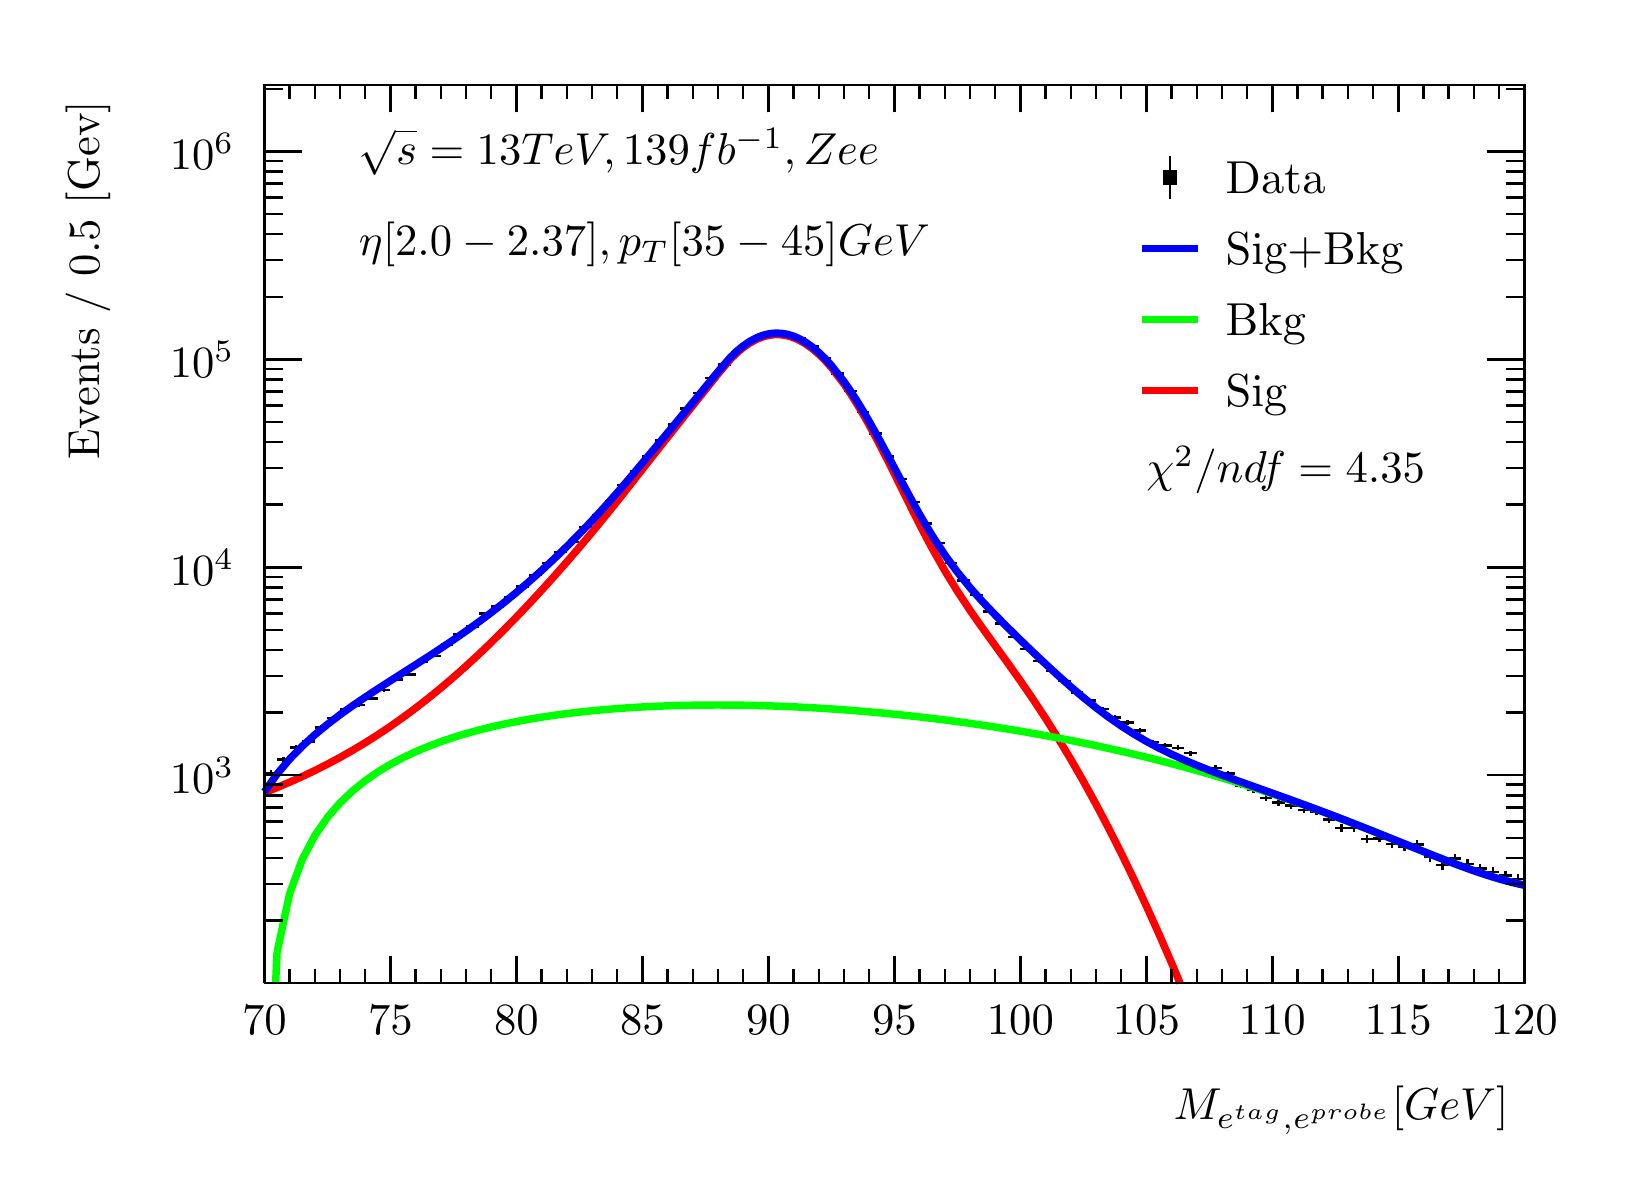
\begin{tikzpicture}
\pgfdeclareplotmark{cross} {
\pgfpathmoveto{\pgfpoint{-0.3\pgfplotmarksize}{\pgfplotmarksize}}
\pgfpathlineto{\pgfpoint{+0.3\pgfplotmarksize}{\pgfplotmarksize}}
\pgfpathlineto{\pgfpoint{+0.3\pgfplotmarksize}{0.3\pgfplotmarksize}}
\pgfpathlineto{\pgfpoint{+1\pgfplotmarksize}{0.3\pgfplotmarksize}}
\pgfpathlineto{\pgfpoint{+1\pgfplotmarksize}{-0.3\pgfplotmarksize}}
\pgfpathlineto{\pgfpoint{+0.3\pgfplotmarksize}{-0.3\pgfplotmarksize}}
\pgfpathlineto{\pgfpoint{+0.3\pgfplotmarksize}{-1.\pgfplotmarksize}}
\pgfpathlineto{\pgfpoint{-0.3\pgfplotmarksize}{-1.\pgfplotmarksize}}
\pgfpathlineto{\pgfpoint{-0.3\pgfplotmarksize}{-0.3\pgfplotmarksize}}
\pgfpathlineto{\pgfpoint{-1.\pgfplotmarksize}{-0.3\pgfplotmarksize}}
\pgfpathlineto{\pgfpoint{-1.\pgfplotmarksize}{0.3\pgfplotmarksize}}
\pgfpathlineto{\pgfpoint{-0.3\pgfplotmarksize}{0.3\pgfplotmarksize}}
\pgfpathclose
\pgfusepathqstroke
}
\pgfdeclareplotmark{cross*} {
\pgfpathmoveto{\pgfpoint{-0.3\pgfplotmarksize}{\pgfplotmarksize}}
\pgfpathlineto{\pgfpoint{+0.3\pgfplotmarksize}{\pgfplotmarksize}}
\pgfpathlineto{\pgfpoint{+0.3\pgfplotmarksize}{0.3\pgfplotmarksize}}
\pgfpathlineto{\pgfpoint{+1\pgfplotmarksize}{0.3\pgfplotmarksize}}
\pgfpathlineto{\pgfpoint{+1\pgfplotmarksize}{-0.3\pgfplotmarksize}}
\pgfpathlineto{\pgfpoint{+0.3\pgfplotmarksize}{-0.3\pgfplotmarksize}}
\pgfpathlineto{\pgfpoint{+0.3\pgfplotmarksize}{-1.\pgfplotmarksize}}
\pgfpathlineto{\pgfpoint{-0.3\pgfplotmarksize}{-1.\pgfplotmarksize}}
\pgfpathlineto{\pgfpoint{-0.3\pgfplotmarksize}{-0.3\pgfplotmarksize}}
\pgfpathlineto{\pgfpoint{-1.\pgfplotmarksize}{-0.3\pgfplotmarksize}}
\pgfpathlineto{\pgfpoint{-1.\pgfplotmarksize}{0.3\pgfplotmarksize}}
\pgfpathlineto{\pgfpoint{-0.3\pgfplotmarksize}{0.3\pgfplotmarksize}}
\pgfpathclose
\pgfusepathqfillstroke
}
\pgfdeclareplotmark{newstar} {
\pgfpathmoveto{\pgfqpoint{0pt}{\pgfplotmarksize}}
\pgfpathlineto{\pgfqpointpolar{44}{0.5\pgfplotmarksize}}
\pgfpathlineto{\pgfqpointpolar{18}{\pgfplotmarksize}}
\pgfpathlineto{\pgfqpointpolar{-20}{0.5\pgfplotmarksize}}
\pgfpathlineto{\pgfqpointpolar{-54}{\pgfplotmarksize}}
\pgfpathlineto{\pgfqpointpolar{-90}{0.5\pgfplotmarksize}}
\pgfpathlineto{\pgfqpointpolar{234}{\pgfplotmarksize}}
\pgfpathlineto{\pgfqpointpolar{198}{0.5\pgfplotmarksize}}
\pgfpathlineto{\pgfqpointpolar{162}{\pgfplotmarksize}}
\pgfpathlineto{\pgfqpointpolar{134}{0.5\pgfplotmarksize}}
\pgfpathclose
\pgfusepathqstroke
}
\pgfdeclareplotmark{newstar*} {
\pgfpathmoveto{\pgfqpoint{0pt}{\pgfplotmarksize}}
\pgfpathlineto{\pgfqpointpolar{44}{0.5\pgfplotmarksize}}
\pgfpathlineto{\pgfqpointpolar{18}{\pgfplotmarksize}}
\pgfpathlineto{\pgfqpointpolar{-20}{0.5\pgfplotmarksize}}
\pgfpathlineto{\pgfqpointpolar{-54}{\pgfplotmarksize}}
\pgfpathlineto{\pgfqpointpolar{-90}{0.5\pgfplotmarksize}}
\pgfpathlineto{\pgfqpointpolar{234}{\pgfplotmarksize}}
\pgfpathlineto{\pgfqpointpolar{198}{0.5\pgfplotmarksize}}
\pgfpathlineto{\pgfqpointpolar{162}{\pgfplotmarksize}}
\pgfpathlineto{\pgfqpointpolar{134}{0.5\pgfplotmarksize}}
\pgfpathclose
\pgfusepathqfillstroke
}
\definecolor{c}{rgb}{1,1,1};
\draw [color=c, fill=c] (0,0) rectangle (20,14.4361);
\draw [color=c, fill=c] (3,2.30977) rectangle (19,13.7143);
\definecolor{c}{rgb}{0,0,0};
\draw [c,line width=0.9] (3,2.30977) -- (3,13.7143) -- (19,13.7143) -- (19,2.30977) -- (3,2.30977);
\definecolor{c}{rgb}{1,1,1};
\draw [color=c, fill=c] (3,2.30977) rectangle (19,13.7143);
\definecolor{c}{rgb}{0,0,0};
\draw [c,line width=0.9] (3,2.30977) -- (3,13.7143) -- (19,13.7143) -- (19,2.30977) -- (3,2.30977);
\draw [c,line width=0.9] (3,2.30977) -- (19,2.30977);
\draw [c,line width=0.9] (3,2.65624) -- (3,2.30977);
\draw [c,line width=0.9] (3.32,2.48301) -- (3.32,2.30977);
\draw [c,line width=0.9] (3.64,2.48301) -- (3.64,2.30977);
\draw [c,line width=0.9] (3.96,2.48301) -- (3.96,2.30977);
\draw [c,line width=0.9] (4.28,2.48301) -- (4.28,2.30977);
\draw [c,line width=0.9] (4.6,2.65624) -- (4.6,2.30977);
\draw [c,line width=0.9] (4.92,2.48301) -- (4.92,2.30977);
\draw [c,line width=0.9] (5.24,2.48301) -- (5.24,2.30977);
\draw [c,line width=0.9] (5.56,2.48301) -- (5.56,2.30977);
\draw [c,line width=0.9] (5.88,2.48301) -- (5.88,2.30977);
\draw [c,line width=0.9] (6.2,2.65624) -- (6.2,2.30977);
\draw [c,line width=0.9] (6.52,2.48301) -- (6.52,2.30977);
\draw [c,line width=0.9] (6.84,2.48301) -- (6.84,2.30977);
\draw [c,line width=0.9] (7.16,2.48301) -- (7.16,2.30977);
\draw [c,line width=0.9] (7.48,2.48301) -- (7.48,2.30977);
\draw [c,line width=0.9] (7.8,2.65624) -- (7.8,2.30977);
\draw [c,line width=0.9] (8.12,2.48301) -- (8.12,2.30977);
\draw [c,line width=0.9] (8.44,2.48301) -- (8.44,2.30977);
\draw [c,line width=0.9] (8.76,2.48301) -- (8.76,2.30977);
\draw [c,line width=0.9] (9.08,2.48301) -- (9.08,2.30977);
\draw [c,line width=0.9] (9.4,2.65624) -- (9.4,2.30977);
\draw [c,line width=0.9] (9.72,2.48301) -- (9.72,2.30977);
\draw [c,line width=0.9] (10.04,2.48301) -- (10.04,2.30977);
\draw [c,line width=0.9] (10.36,2.48301) -- (10.36,2.30977);
\draw [c,line width=0.9] (10.68,2.48301) -- (10.68,2.30977);
\draw [c,line width=0.9] (11,2.65624) -- (11,2.30977);
\draw [c,line width=0.9] (11.32,2.48301) -- (11.32,2.30977);
\draw [c,line width=0.9] (11.64,2.48301) -- (11.64,2.30977);
\draw [c,line width=0.9] (11.96,2.48301) -- (11.96,2.30977);
\draw [c,line width=0.9] (12.28,2.48301) -- (12.28,2.30977);
\draw [c,line width=0.9] (12.6,2.65624) -- (12.6,2.30977);
\draw [c,line width=0.9] (12.92,2.48301) -- (12.92,2.30977);
\draw [c,line width=0.9] (13.24,2.48301) -- (13.24,2.30977);
\draw [c,line width=0.9] (13.56,2.48301) -- (13.56,2.30977);
\draw [c,line width=0.9] (13.88,2.48301) -- (13.88,2.30977);
\draw [c,line width=0.9] (14.2,2.65624) -- (14.2,2.30977);
\draw [c,line width=0.9] (14.52,2.48301) -- (14.52,2.30977);
\draw [c,line width=0.9] (14.84,2.48301) -- (14.84,2.30977);
\draw [c,line width=0.9] (15.16,2.48301) -- (15.16,2.30977);
\draw [c,line width=0.9] (15.48,2.48301) -- (15.48,2.30977);
\draw [c,line width=0.9] (15.8,2.65624) -- (15.8,2.30977);
\draw [c,line width=0.9] (16.12,2.48301) -- (16.12,2.30977);
\draw [c,line width=0.9] (16.44,2.48301) -- (16.44,2.30977);
\draw [c,line width=0.9] (16.76,2.48301) -- (16.76,2.30977);
\draw [c,line width=0.9] (17.08,2.48301) -- (17.08,2.30977);
\draw [c,line width=0.9] (17.4,2.65624) -- (17.4,2.30977);
\draw [c,line width=0.9] (17.72,2.48301) -- (17.72,2.30977);
\draw [c,line width=0.9] (18.04,2.48301) -- (18.04,2.30977);
\draw [c,line width=0.9] (18.36,2.48301) -- (18.36,2.30977);
\draw [c,line width=0.9] (18.68,2.48301) -- (18.68,2.30977);
\draw [c,line width=0.9] (19,2.65624) -- (19,2.30977);
\draw [anchor=base] (3,1.66015) node[scale=1.61424, color=c, rotate=0]{70};
\draw [anchor=base] (4.6,1.66015) node[scale=1.61424, color=c, rotate=0]{75};
\draw [anchor=base] (6.2,1.66015) node[scale=1.61424, color=c, rotate=0]{80};
\draw [anchor=base] (7.8,1.66015) node[scale=1.61424, color=c, rotate=0]{85};
\draw [anchor=base] (9.4,1.66015) node[scale=1.61424, color=c, rotate=0]{90};
\draw [anchor=base] (11,1.66015) node[scale=1.61424, color=c, rotate=0]{95};
\draw [anchor=base] (12.6,1.66015) node[scale=1.61424, color=c, rotate=0]{100};
\draw [anchor=base] (14.2,1.66015) node[scale=1.61424, color=c, rotate=0]{105};
\draw [anchor=base] (15.8,1.66015) node[scale=1.61424, color=c, rotate=0]{110};
\draw [anchor=base] (17.4,1.66015) node[scale=1.61424, color=c, rotate=0]{115};
\draw [anchor=base] (19,1.66015) node[scale=1.61424, color=c, rotate=0]{120};
\draw [anchor= east] (19,0.692932) node[scale=1.61424, color=c, rotate=0]{$M_{e^{tag}, e^{probe}}  [GeV]$};
\draw [c,line width=0.9] (3,13.7143) -- (19,13.7143);
\draw [c,line width=0.9] (3,13.3678) -- (3,13.7143);
\draw [c,line width=0.9] (3.32,13.5411) -- (3.32,13.7143);
\draw [c,line width=0.9] (3.64,13.5411) -- (3.64,13.7143);
\draw [c,line width=0.9] (3.96,13.5411) -- (3.96,13.7143);
\draw [c,line width=0.9] (4.28,13.5411) -- (4.28,13.7143);
\draw [c,line width=0.9] (4.6,13.3678) -- (4.6,13.7143);
\draw [c,line width=0.9] (4.92,13.5411) -- (4.92,13.7143);
\draw [c,line width=0.9] (5.24,13.5411) -- (5.24,13.7143);
\draw [c,line width=0.9] (5.56,13.5411) -- (5.56,13.7143);
\draw [c,line width=0.9] (5.88,13.5411) -- (5.88,13.7143);
\draw [c,line width=0.9] (6.2,13.3678) -- (6.2,13.7143);
\draw [c,line width=0.9] (6.52,13.5411) -- (6.52,13.7143);
\draw [c,line width=0.9] (6.84,13.5411) -- (6.84,13.7143);
\draw [c,line width=0.9] (7.16,13.5411) -- (7.16,13.7143);
\draw [c,line width=0.9] (7.48,13.5411) -- (7.48,13.7143);
\draw [c,line width=0.9] (7.8,13.3678) -- (7.8,13.7143);
\draw [c,line width=0.9] (8.12,13.5411) -- (8.12,13.7143);
\draw [c,line width=0.9] (8.44,13.5411) -- (8.44,13.7143);
\draw [c,line width=0.9] (8.76,13.5411) -- (8.76,13.7143);
\draw [c,line width=0.9] (9.08,13.5411) -- (9.08,13.7143);
\draw [c,line width=0.9] (9.4,13.3678) -- (9.4,13.7143);
\draw [c,line width=0.9] (9.72,13.5411) -- (9.72,13.7143);
\draw [c,line width=0.9] (10.04,13.5411) -- (10.04,13.7143);
\draw [c,line width=0.9] (10.36,13.5411) -- (10.36,13.7143);
\draw [c,line width=0.9] (10.68,13.5411) -- (10.68,13.7143);
\draw [c,line width=0.9] (11,13.3678) -- (11,13.7143);
\draw [c,line width=0.9] (11.32,13.5411) -- (11.32,13.7143);
\draw [c,line width=0.9] (11.64,13.5411) -- (11.64,13.7143);
\draw [c,line width=0.9] (11.96,13.5411) -- (11.96,13.7143);
\draw [c,line width=0.9] (12.28,13.5411) -- (12.28,13.7143);
\draw [c,line width=0.9] (12.6,13.3678) -- (12.6,13.7143);
\draw [c,line width=0.9] (12.92,13.5411) -- (12.92,13.7143);
\draw [c,line width=0.9] (13.24,13.5411) -- (13.24,13.7143);
\draw [c,line width=0.9] (13.56,13.5411) -- (13.56,13.7143);
\draw [c,line width=0.9] (13.88,13.5411) -- (13.88,13.7143);
\draw [c,line width=0.9] (14.2,13.3678) -- (14.2,13.7143);
\draw [c,line width=0.9] (14.52,13.5411) -- (14.52,13.7143);
\draw [c,line width=0.9] (14.84,13.5411) -- (14.84,13.7143);
\draw [c,line width=0.9] (15.16,13.5411) -- (15.16,13.7143);
\draw [c,line width=0.9] (15.48,13.5411) -- (15.48,13.7143);
\draw [c,line width=0.9] (15.8,13.3678) -- (15.8,13.7143);
\draw [c,line width=0.9] (16.12,13.5411) -- (16.12,13.7143);
\draw [c,line width=0.9] (16.44,13.5411) -- (16.44,13.7143);
\draw [c,line width=0.9] (16.76,13.5411) -- (16.76,13.7143);
\draw [c,line width=0.9] (17.08,13.5411) -- (17.08,13.7143);
\draw [c,line width=0.9] (17.4,13.3678) -- (17.4,13.7143);
\draw [c,line width=0.9] (17.72,13.5411) -- (17.72,13.7143);
\draw [c,line width=0.9] (18.04,13.5411) -- (18.04,13.7143);
\draw [c,line width=0.9] (18.36,13.5411) -- (18.36,13.7143);
\draw [c,line width=0.9] (18.68,13.5411) -- (18.68,13.7143);
\draw [c,line width=0.9] (19,13.3678) -- (19,13.7143);
\draw [c,line width=0.9] (3,2.30977) -- (3,13.7143);
\draw [c,line width=0.9] (3.237,3.10453) -- (3,3.10453);
\draw [c,line width=0.9] (3.237,3.56943) -- (3,3.56943);
\draw [c,line width=0.9] (3.237,3.89929) -- (3,3.89929);
\draw [c,line width=0.9] (3.237,4.15514) -- (3,4.15514);
\draw [c,line width=0.9] (3.237,4.36419) -- (3,4.36419);
\draw [c,line width=0.9] (3.237,4.54094) -- (3,4.54094);
\draw [c,line width=0.9] (3.237,4.69404) -- (3,4.69404);
\draw [c,line width=0.9] (3.237,4.82909) -- (3,4.82909);
\draw [c,line width=0.9] (3.474,4.9499) -- (3,4.9499);
\draw [anchor= east] (2.82,4.9499) node[scale=1.61424, color=c, rotate=0]{$10^{3}$};
\draw [c,line width=0.9] (3.237,5.74466) -- (3,5.74466);
\draw [c,line width=0.9] (3.237,6.20956) -- (3,6.20956);
\draw [c,line width=0.9] (3.237,6.53941) -- (3,6.53941);
\draw [c,line width=0.9] (3.237,6.79527) -- (3,6.79527);
\draw [c,line width=0.9] (3.237,7.00432) -- (3,7.00432);
\draw [c,line width=0.9] (3.237,7.18106) -- (3,7.18106);
\draw [c,line width=0.9] (3.237,7.33417) -- (3,7.33417);
\draw [c,line width=0.9] (3.237,7.46922) -- (3,7.46922);
\draw [c,line width=0.9] (3.474,7.59002) -- (3,7.59002);
\draw [anchor= east] (2.82,7.59002) node[scale=1.61424, color=c, rotate=0]{$10^{4}$};
\draw [c,line width=0.9] (3.237,8.38478) -- (3,8.38478);
\draw [c,line width=0.9] (3.237,8.84968) -- (3,8.84968);
\draw [c,line width=0.9] (3.237,9.17954) -- (3,9.17954);
\draw [c,line width=0.9] (3.237,9.43539) -- (3,9.43539);
\draw [c,line width=0.9] (3.237,9.64444) -- (3,9.64444);
\draw [c,line width=0.9] (3.237,9.82119) -- (3,9.82119);
\draw [c,line width=0.9] (3.237,9.9743) -- (3,9.9743);
\draw [c,line width=0.9] (3.237,10.1093) -- (3,10.1093);
\draw [c,line width=0.9] (3.474,10.2302) -- (3,10.2302);
\draw [anchor= east] (2.82,10.2302) node[scale=1.61424, color=c, rotate=0]{$10^{5}$};
\draw [c,line width=0.9] (3.237,11.0249) -- (3,11.0249);
\draw [c,line width=0.9] (3.237,11.4898) -- (3,11.4898);
\draw [c,line width=0.9] (3.237,11.8197) -- (3,11.8197);
\draw [c,line width=0.9] (3.237,12.0755) -- (3,12.0755);
\draw [c,line width=0.9] (3.237,12.2846) -- (3,12.2846);
\draw [c,line width=0.9] (3.237,12.4613) -- (3,12.4613);
\draw [c,line width=0.9] (3.237,12.6144) -- (3,12.6144);
\draw [c,line width=0.9] (3.237,12.7495) -- (3,12.7495);
\draw [c,line width=0.9] (3.474,12.8703) -- (3,12.8703);
\draw [anchor= east] (2.82,12.8703) node[scale=1.61424, color=c, rotate=0]{$10^{6}$};
\draw [c,line width=0.9] (3.237,13.665) -- (3,13.665);
\draw [anchor= east] (0.76,13.7143) node[scale=1.61424, color=c, rotate=90]{Events / 0.5 [Gev]};
\draw [c,line width=0.9] (19,2.30977) -- (19,13.7143);
\draw [c,line width=0.9] (18.763,3.10453) -- (19,3.10453);
\draw [c,line width=0.9] (18.763,3.56943) -- (19,3.56943);
\draw [c,line width=0.9] (18.763,3.89929) -- (19,3.89929);
\draw [c,line width=0.9] (18.763,4.15514) -- (19,4.15514);
\draw [c,line width=0.9] (18.763,4.36419) -- (19,4.36419);
\draw [c,line width=0.9] (18.763,4.54094) -- (19,4.54094);
\draw [c,line width=0.9] (18.763,4.69404) -- (19,4.69404);
\draw [c,line width=0.9] (18.763,4.82909) -- (19,4.82909);
\draw [c,line width=0.9] (18.526,4.9499) -- (19,4.9499);
\draw [c,line width=0.9] (18.763,5.74466) -- (19,5.74466);
\draw [c,line width=0.9] (18.763,6.20956) -- (19,6.20956);
\draw [c,line width=0.9] (18.763,6.53941) -- (19,6.53941);
\draw [c,line width=0.9] (18.763,6.79527) -- (19,6.79527);
\draw [c,line width=0.9] (18.763,7.00432) -- (19,7.00432);
\draw [c,line width=0.9] (18.763,7.18106) -- (19,7.18106);
\draw [c,line width=0.9] (18.763,7.33417) -- (19,7.33417);
\draw [c,line width=0.9] (18.763,7.46922) -- (19,7.46922);
\draw [c,line width=0.9] (18.526,7.59002) -- (19,7.59002);
\draw [c,line width=0.9] (18.763,8.38478) -- (19,8.38478);
\draw [c,line width=0.9] (18.763,8.84968) -- (19,8.84968);
\draw [c,line width=0.9] (18.763,9.17954) -- (19,9.17954);
\draw [c,line width=0.9] (18.763,9.43539) -- (19,9.43539);
\draw [c,line width=0.9] (18.763,9.64444) -- (19,9.64444);
\draw [c,line width=0.9] (18.763,9.82119) -- (19,9.82119);
\draw [c,line width=0.9] (18.763,9.9743) -- (19,9.9743);
\draw [c,line width=0.9] (18.763,10.1093) -- (19,10.1093);
\draw [c,line width=0.9] (18.526,10.2302) -- (19,10.2302);
\draw [c,line width=0.9] (18.763,11.0249) -- (19,11.0249);
\draw [c,line width=0.9] (18.763,11.4898) -- (19,11.4898);
\draw [c,line width=0.9] (18.763,11.8197) -- (19,11.8197);
\draw [c,line width=0.9] (18.763,12.0755) -- (19,12.0755);
\draw [c,line width=0.9] (18.763,12.2846) -- (19,12.2846);
\draw [c,line width=0.9] (18.763,12.4613) -- (19,12.4613);
\draw [c,line width=0.9] (18.763,12.6144) -- (19,12.6144);
\draw [c,line width=0.9] (18.763,12.7495) -- (19,12.7495);
\draw [c,line width=0.9] (18.526,12.8703) -- (19,12.8703);
\draw [c,line width=0.9] (18.763,13.665) -- (19,13.665);
\draw [c,line width=0.9] (3.08,4.97373) -- (3,4.97373);
\draw [c,line width=0.9] (3,4.97373) -- (3,4.97373);
\draw [c,line width=0.9] (3.08,4.97373) -- (3.16,4.97373);
\draw [c,line width=0.9] (3.16,4.97373) -- (3.16,4.97373);
\draw [c,line width=0.9] (3.08,4.97373) -- (3.08,5.00961);
\draw [c,line width=0.9] (3.08,5.00961) -- (3.08,5.00961);
\draw [c,line width=0.9] (3.08,4.97373) -- (3.08,4.93785);
\draw [c,line width=0.9] (3.08,4.93785) -- (3.08,4.93785);
\draw [c,line width=0.9] (3.24,5.14935) -- (3.16,5.14935);
\draw [c,line width=0.9] (3.16,5.14935) -- (3.16,5.14935);
\draw [c,line width=0.9] (3.24,5.14935) -- (3.32,5.14935);
\draw [c,line width=0.9] (3.32,5.14935) -- (3.32,5.14935);
\draw [c,line width=0.9] (3.24,5.14935) -- (3.24,5.18259);
\draw [c,line width=0.9] (3.24,5.18259) -- (3.24,5.18259);
\draw [c,line width=0.9] (3.24,5.14935) -- (3.24,5.11612);
\draw [c,line width=0.9] (3.24,5.11612) -- (3.24,5.11612);
\draw [c,line width=0.9] (3.4,5.29824) -- (3.32,5.29824);
\draw [c,line width=0.9] (3.32,5.29824) -- (3.32,5.29824);
\draw [c,line width=0.9] (3.4,5.29824) -- (3.48,5.29824);
\draw [c,line width=0.9] (3.48,5.29824) -- (3.48,5.29824);
\draw [c,line width=0.9] (3.4,5.29824) -- (3.4,5.32938);
\draw [c,line width=0.9] (3.4,5.32938) -- (3.4,5.32938);
\draw [c,line width=0.9] (3.4,5.29824) -- (3.4,5.26709);
\draw [c,line width=0.9] (3.4,5.26709) -- (3.4,5.26709);
\draw [c,line width=0.9] (3.56,5.37751) -- (3.48,5.37751);
\draw [c,line width=0.9] (3.48,5.37751) -- (3.48,5.37751);
\draw [c,line width=0.9] (3.56,5.37751) -- (3.64,5.37751);
\draw [c,line width=0.9] (3.64,5.37751) -- (3.64,5.37751);
\draw [c,line width=0.9] (3.56,5.37751) -- (3.56,5.4076);
\draw [c,line width=0.9] (3.56,5.4076) -- (3.56,5.4076);
\draw [c,line width=0.9] (3.56,5.37751) -- (3.56,5.34742);
\draw [c,line width=0.9] (3.56,5.34742) -- (3.56,5.34742);
\draw [c,line width=0.9] (3.72,5.55426) -- (3.64,5.55426);
\draw [c,line width=0.9] (3.64,5.55426) -- (3.64,5.55426);
\draw [c,line width=0.9] (3.72,5.55426) -- (3.8,5.55426);
\draw [c,line width=0.9] (3.8,5.55426) -- (3.8,5.55426);
\draw [c,line width=0.9] (3.72,5.55426) -- (3.72,5.58212);
\draw [c,line width=0.9] (3.72,5.58212) -- (3.72,5.58212);
\draw [c,line width=0.9] (3.72,5.55426) -- (3.72,5.5264);
\draw [c,line width=0.9] (3.72,5.5264) -- (3.72,5.5264);
\draw [c,line width=0.9] (3.88,5.67554) -- (3.8,5.67554);
\draw [c,line width=0.9] (3.8,5.67554) -- (3.8,5.67554);
\draw [c,line width=0.9] (3.88,5.67554) -- (3.96,5.67554);
\draw [c,line width=0.9] (3.96,5.67554) -- (3.96,5.67554);
\draw [c,line width=0.9] (3.88,5.67554) -- (3.88,5.70196);
\draw [c,line width=0.9] (3.88,5.70196) -- (3.88,5.70196);
\draw [c,line width=0.9] (3.88,5.67554) -- (3.88,5.64912);
\draw [c,line width=0.9] (3.88,5.64912) -- (3.88,5.64912);
\draw [c,line width=0.9] (4.04,5.78908) -- (3.96,5.78908);
\draw [c,line width=0.9] (3.96,5.78908) -- (3.96,5.78908);
\draw [c,line width=0.9] (4.04,5.78908) -- (4.12,5.78908);
\draw [c,line width=0.9] (4.12,5.78908) -- (4.12,5.78908);
\draw [c,line width=0.9] (4.04,5.78908) -- (4.04,5.81422);
\draw [c,line width=0.9] (4.04,5.81422) -- (4.04,5.81422);
\draw [c,line width=0.9] (4.04,5.78908) -- (4.04,5.76393);
\draw [c,line width=0.9] (4.04,5.76393) -- (4.04,5.76393);
\draw [c,line width=0.9] (4.2,5.84136) -- (4.12,5.84136);
\draw [c,line width=0.9] (4.12,5.84136) -- (4.12,5.84136);
\draw [c,line width=0.9] (4.2,5.84136) -- (4.28,5.84136);
\draw [c,line width=0.9] (4.28,5.84136) -- (4.28,5.84136);
\draw [c,line width=0.9] (4.2,5.84136) -- (4.2,5.86594);
\draw [c,line width=0.9] (4.2,5.86594) -- (4.2,5.86594);
\draw [c,line width=0.9] (4.2,5.84136) -- (4.2,5.81678);
\draw [c,line width=0.9] (4.2,5.81678) -- (4.2,5.81678);
\draw [c,line width=0.9] (4.36,5.9237) -- (4.28,5.9237);
\draw [c,line width=0.9] (4.28,5.9237) -- (4.28,5.9237);
\draw [c,line width=0.9] (4.36,5.9237) -- (4.44,5.9237);
\draw [c,line width=0.9] (4.44,5.9237) -- (4.44,5.9237);
\draw [c,line width=0.9] (4.36,5.9237) -- (4.36,5.94741);
\draw [c,line width=0.9] (4.36,5.94741) -- (4.36,5.94741);
\draw [c,line width=0.9] (4.36,5.9237) -- (4.36,5.89998);
\draw [c,line width=0.9] (4.36,5.89998) -- (4.36,5.89998);
\draw [c,line width=0.9] (4.52,6.03173) -- (4.44,6.03173);
\draw [c,line width=0.9] (4.44,6.03173) -- (4.44,6.03173);
\draw [c,line width=0.9] (4.52,6.03173) -- (4.6,6.03173);
\draw [c,line width=0.9] (4.6,6.03173) -- (4.6,6.03173);
\draw [c,line width=0.9] (4.52,6.03173) -- (4.52,6.05435);
\draw [c,line width=0.9] (4.52,6.05435) -- (4.52,6.05435);
\draw [c,line width=0.9] (4.52,6.03173) -- (4.52,6.00911);
\draw [c,line width=0.9] (4.52,6.00911) -- (4.52,6.00911);
\draw [c,line width=0.9] (4.68,6.16554) -- (4.6,6.16554);
\draw [c,line width=0.9] (4.6,6.16554) -- (4.6,6.16554);
\draw [c,line width=0.9] (4.68,6.16554) -- (4.76,6.16554);
\draw [c,line width=0.9] (4.76,6.16554) -- (4.76,6.16554);
\draw [c,line width=0.9] (4.68,6.16554) -- (4.68,6.18688);
\draw [c,line width=0.9] (4.68,6.18688) -- (4.68,6.18688);
\draw [c,line width=0.9] (4.68,6.16554) -- (4.68,6.1442);
\draw [c,line width=0.9] (4.68,6.1442) -- (4.68,6.1442);
\draw [c,line width=0.9] (4.84,6.23114) -- (4.76,6.23114);
\draw [c,line width=0.9] (4.76,6.23114) -- (4.76,6.23114);
\draw [c,line width=0.9] (4.84,6.23114) -- (4.92,6.23114);
\draw [c,line width=0.9] (4.92,6.23114) -- (4.92,6.23114);
\draw [c,line width=0.9] (4.84,6.23114) -- (4.84,6.25188);
\draw [c,line width=0.9] (4.84,6.25188) -- (4.84,6.25188);
\draw [c,line width=0.9] (4.84,6.23114) -- (4.84,6.2104);
\draw [c,line width=0.9] (4.84,6.2104) -- (4.84,6.2104);
\draw [c,line width=0.9] (5,6.38762) -- (4.92,6.38762);
\draw [c,line width=0.9] (4.92,6.38762) -- (4.92,6.38762);
\draw [c,line width=0.9] (5,6.38762) -- (5.08,6.38762);
\draw [c,line width=0.9] (5.08,6.38762) -- (5.08,6.38762);
\draw [c,line width=0.9] (5,6.38762) -- (5,6.40699);
\draw [c,line width=0.9] (5,6.40699) -- (5,6.40699);
\draw [c,line width=0.9] (5,6.38762) -- (5,6.36825);
\draw [c,line width=0.9] (5,6.36825) -- (5,6.36825);
\draw [c,line width=0.9] (5.16,6.46358) -- (5.08,6.46358);
\draw [c,line width=0.9] (5.08,6.46358) -- (5.08,6.46358);
\draw [c,line width=0.9] (5.16,6.46358) -- (5.24,6.46358);
\draw [c,line width=0.9] (5.24,6.46358) -- (5.24,6.46358);
\draw [c,line width=0.9] (5.16,6.46358) -- (5.16,6.48232);
\draw [c,line width=0.9] (5.16,6.48232) -- (5.16,6.48232);
\draw [c,line width=0.9] (5.16,6.46358) -- (5.16,6.44484);
\draw [c,line width=0.9] (5.16,6.44484) -- (5.16,6.44484);
\draw [c,line width=0.9] (5.32,6.61) -- (5.24,6.61);
\draw [c,line width=0.9] (5.24,6.61) -- (5.24,6.61);
\draw [c,line width=0.9] (5.32,6.61) -- (5.4,6.61);
\draw [c,line width=0.9] (5.4,6.61) -- (5.4,6.61);
\draw [c,line width=0.9] (5.32,6.61) -- (5.32,6.62758);
\draw [c,line width=0.9] (5.32,6.62758) -- (5.32,6.62758);
\draw [c,line width=0.9] (5.32,6.61) -- (5.32,6.59243);
\draw [c,line width=0.9] (5.32,6.59243) -- (5.32,6.59243);
\draw [c,line width=0.9] (5.48,6.74224) -- (5.4,6.74224);
\draw [c,line width=0.9] (5.4,6.74224) -- (5.4,6.74224);
\draw [c,line width=0.9] (5.48,6.74224) -- (5.56,6.74224);
\draw [c,line width=0.9] (5.56,6.74224) -- (5.56,6.74224);
\draw [c,line width=0.9] (5.48,6.74224) -- (5.48,6.75883);
\draw [c,line width=0.9] (5.48,6.75883) -- (5.48,6.75883);
\draw [c,line width=0.9] (5.48,6.74224) -- (5.48,6.72564);
\draw [c,line width=0.9] (5.48,6.72564) -- (5.48,6.72564);
\draw [c,line width=0.9] (5.64,6.83671) -- (5.56,6.83671);
\draw [c,line width=0.9] (5.56,6.83671) -- (5.56,6.83671);
\draw [c,line width=0.9] (5.64,6.83671) -- (5.72,6.83671);
\draw [c,line width=0.9] (5.72,6.83671) -- (5.72,6.83671);
\draw [c,line width=0.9] (5.64,6.83671) -- (5.64,6.85263);
\draw [c,line width=0.9] (5.64,6.85263) -- (5.64,6.85263);
\draw [c,line width=0.9] (5.64,6.83671) -- (5.64,6.82078);
\draw [c,line width=0.9] (5.64,6.82078) -- (5.64,6.82078);
\draw [c,line width=0.9] (5.8,7.00106) -- (5.72,7.00106);
\draw [c,line width=0.9] (5.72,7.00106) -- (5.72,7.00106);
\draw [c,line width=0.9] (5.8,7.00106) -- (5.88,7.00106);
\draw [c,line width=0.9] (5.88,7.00106) -- (5.88,7.00106);
\draw [c,line width=0.9] (5.8,7.00106) -- (5.8,7.01589);
\draw [c,line width=0.9] (5.8,7.01589) -- (5.8,7.01589);
\draw [c,line width=0.9] (5.8,7.00106) -- (5.8,6.98624);
\draw [c,line width=0.9] (5.8,6.98624) -- (5.8,6.98624);
\draw [c,line width=0.9] (5.96,7.08973) -- (5.88,7.08973);
\draw [c,line width=0.9] (5.88,7.08973) -- (5.88,7.08973);
\draw [c,line width=0.9] (5.96,7.08973) -- (6.04,7.08973);
\draw [c,line width=0.9] (6.04,7.08973) -- (6.04,7.08973);
\draw [c,line width=0.9] (5.96,7.08973) -- (5.96,7.10399);
\draw [c,line width=0.9] (5.96,7.10399) -- (5.96,7.10399);
\draw [c,line width=0.9] (5.96,7.08973) -- (5.96,7.07546);
\draw [c,line width=0.9] (5.96,7.07546) -- (5.96,7.07546);
\draw [c,line width=0.9] (6.12,7.21113) -- (6.04,7.21113);
\draw [c,line width=0.9] (6.04,7.21113) -- (6.04,7.21113);
\draw [c,line width=0.9] (6.12,7.21113) -- (6.2,7.21113);
\draw [c,line width=0.9] (6.2,7.21113) -- (6.2,7.21113);
\draw [c,line width=0.9] (6.12,7.21113) -- (6.12,7.22466);
\draw [c,line width=0.9] (6.12,7.22466) -- (6.12,7.22466);
\draw [c,line width=0.9] (6.12,7.21113) -- (6.12,7.19761);
\draw [c,line width=0.9] (6.12,7.19761) -- (6.12,7.19761);
\draw [c,line width=0.9] (6.28,7.34359) -- (6.2,7.34359);
\draw [c,line width=0.9] (6.2,7.34359) -- (6.2,7.34359);
\draw [c,line width=0.9] (6.28,7.34359) -- (6.36,7.34359);
\draw [c,line width=0.9] (6.36,7.34359) -- (6.36,7.34359);
\draw [c,line width=0.9] (6.28,7.34359) -- (6.28,7.35636);
\draw [c,line width=0.9] (6.28,7.35636) -- (6.28,7.35636);
\draw [c,line width=0.9] (6.28,7.34359) -- (6.28,7.33083);
\draw [c,line width=0.9] (6.28,7.33083) -- (6.28,7.33083);
\draw [c,line width=0.9] (6.44,7.49143) -- (6.36,7.49143);
\draw [c,line width=0.9] (6.36,7.49143) -- (6.36,7.49143);
\draw [c,line width=0.9] (6.44,7.49143) -- (6.52,7.49143);
\draw [c,line width=0.9] (6.52,7.49143) -- (6.52,7.49143);
\draw [c,line width=0.9] (6.44,7.49143) -- (6.44,7.5034);
\draw [c,line width=0.9] (6.44,7.5034) -- (6.44,7.5034);
\draw [c,line width=0.9] (6.44,7.49143) -- (6.44,7.47946);
\draw [c,line width=0.9] (6.44,7.47946) -- (6.44,7.47946);
\draw [c,line width=0.9] (6.6,7.64269) -- (6.52,7.64269);
\draw [c,line width=0.9] (6.52,7.64269) -- (6.52,7.64269);
\draw [c,line width=0.9] (6.6,7.64269) -- (6.68,7.64269);
\draw [c,line width=0.9] (6.68,7.64269) -- (6.68,7.64269);
\draw [c,line width=0.9] (6.6,7.64269) -- (6.6,7.65389);
\draw [c,line width=0.9] (6.6,7.65389) -- (6.6,7.65389);
\draw [c,line width=0.9] (6.6,7.64269) -- (6.6,7.63148);
\draw [c,line width=0.9] (6.6,7.63148) -- (6.6,7.63148);
\draw [c,line width=0.9] (6.76,7.78601) -- (6.68,7.78601);
\draw [c,line width=0.9] (6.68,7.78601) -- (6.68,7.78601);
\draw [c,line width=0.9] (6.76,7.78601) -- (6.84,7.78601);
\draw [c,line width=0.9] (6.84,7.78601) -- (6.84,7.78601);
\draw [c,line width=0.9] (6.76,7.78601) -- (6.76,7.79653);
\draw [c,line width=0.9] (6.76,7.79653) -- (6.76,7.79653);
\draw [c,line width=0.9] (6.76,7.78601) -- (6.76,7.77548);
\draw [c,line width=0.9] (6.76,7.77548) -- (6.76,7.77548);
\draw [c,line width=0.9] (6.92,7.91027) -- (6.84,7.91027);
\draw [c,line width=0.9] (6.84,7.91027) -- (6.84,7.91027);
\draw [c,line width=0.9] (6.92,7.91027) -- (7,7.91027);
\draw [c,line width=0.9] (7,7.91027) -- (7,7.91027);
\draw [c,line width=0.9] (6.92,7.91027) -- (6.92,7.92024);
\draw [c,line width=0.9] (6.92,7.92024) -- (6.92,7.92024);
\draw [c,line width=0.9] (6.92,7.91027) -- (6.92,7.90029);
\draw [c,line width=0.9] (6.92,7.90029) -- (6.92,7.90029);
\draw [c,line width=0.9] (7.08,8.10174) -- (7,8.10174);
\draw [c,line width=0.9] (7,8.10174) -- (7,8.10174);
\draw [c,line width=0.9] (7.08,8.10174) -- (7.16,8.10174);
\draw [c,line width=0.9] (7.16,8.10174) -- (7.16,8.10174);
\draw [c,line width=0.9] (7.08,8.10174) -- (7.08,8.11091);
\draw [c,line width=0.9] (7.08,8.11091) -- (7.08,8.11091);
\draw [c,line width=0.9] (7.08,8.10174) -- (7.08,8.09256);
\draw [c,line width=0.9] (7.08,8.09256) -- (7.08,8.09256);
\draw [c,line width=0.9] (7.24,8.25142) -- (7.16,8.25142);
\draw [c,line width=0.9] (7.16,8.25142) -- (7.16,8.25142);
\draw [c,line width=0.9] (7.24,8.25142) -- (7.32,8.25142);
\draw [c,line width=0.9] (7.32,8.25142) -- (7.32,8.25142);
\draw [c,line width=0.9] (7.24,8.25142) -- (7.24,8.26002);
\draw [c,line width=0.9] (7.24,8.26002) -- (7.24,8.26002);
\draw [c,line width=0.9] (7.24,8.25142) -- (7.24,8.24283);
\draw [c,line width=0.9] (7.24,8.24283) -- (7.24,8.24283);
\draw [c,line width=0.9] (7.4,8.42428) -- (7.32,8.42428);
\draw [c,line width=0.9] (7.32,8.42428) -- (7.32,8.42428);
\draw [c,line width=0.9] (7.4,8.42428) -- (7.48,8.42428);
\draw [c,line width=0.9] (7.48,8.42428) -- (7.48,8.42428);
\draw [c,line width=0.9] (7.4,8.42428) -- (7.4,8.43225);
\draw [c,line width=0.9] (7.4,8.43225) -- (7.4,8.43225);
\draw [c,line width=0.9] (7.4,8.42428) -- (7.4,8.41631);
\draw [c,line width=0.9] (7.4,8.41631) -- (7.4,8.41631);
\draw [c,line width=0.9] (7.56,8.63244) -- (7.48,8.63244);
\draw [c,line width=0.9] (7.48,8.63244) -- (7.48,8.63244);
\draw [c,line width=0.9] (7.56,8.63244) -- (7.64,8.63244);
\draw [c,line width=0.9] (7.64,8.63244) -- (7.64,8.63244);
\draw [c,line width=0.9] (7.56,8.63244) -- (7.56,8.63972);
\draw [c,line width=0.9] (7.56,8.63972) -- (7.56,8.63972);
\draw [c,line width=0.9] (7.56,8.63244) -- (7.56,8.62517);
\draw [c,line width=0.9] (7.56,8.62517) -- (7.56,8.62517);
\draw [c,line width=0.9] (7.72,8.8086) -- (7.64,8.8086);
\draw [c,line width=0.9] (7.64,8.8086) -- (7.64,8.8086);
\draw [c,line width=0.9] (7.72,8.8086) -- (7.8,8.8086);
\draw [c,line width=0.9] (7.8,8.8086) -- (7.8,8.8086);
\draw [c,line width=0.9] (7.72,8.8086) -- (7.72,8.81534);
\draw [c,line width=0.9] (7.72,8.81534) -- (7.72,8.81534);
\draw [c,line width=0.9] (7.72,8.8086) -- (7.72,8.80186);
\draw [c,line width=0.9] (7.72,8.80186) -- (7.72,8.80186);
\draw [c,line width=0.9] (7.88,8.99643) -- (7.8,8.99643);
\draw [c,line width=0.9] (7.8,8.99643) -- (7.8,8.99643);
\draw [c,line width=0.9] (7.88,8.99643) -- (7.96,8.99643);
\draw [c,line width=0.9] (7.96,8.99643) -- (7.96,8.99643);
\draw [c,line width=0.9] (7.88,8.99643) -- (7.88,9.00264);
\draw [c,line width=0.9] (7.88,9.00264) -- (7.88,9.00264);
\draw [c,line width=0.9] (7.88,8.99643) -- (7.88,8.99022);
\draw [c,line width=0.9] (7.88,8.99022) -- (7.88,8.99022);
\draw [c,line width=0.9] (8.04,9.20188) -- (7.96,9.20188);
\draw [c,line width=0.9] (7.96,9.20188) -- (7.96,9.20188);
\draw [c,line width=0.9] (8.04,9.20188) -- (8.12,9.20188);
\draw [c,line width=0.9] (8.12,9.20188) -- (8.12,9.20188);
\draw [c,line width=0.9] (8.04,9.20188) -- (8.04,9.20756);
\draw [c,line width=0.9] (8.04,9.20756) -- (8.04,9.20756);
\draw [c,line width=0.9] (8.04,9.20188) -- (8.04,9.1962);
\draw [c,line width=0.9] (8.04,9.1962) -- (8.04,9.1962);
\draw [c,line width=0.9] (8.2,9.40396) -- (8.12,9.40396);
\draw [c,line width=0.9] (8.12,9.40396) -- (8.12,9.40396);
\draw [c,line width=0.9] (8.2,9.40396) -- (8.28,9.40396);
\draw [c,line width=0.9] (8.28,9.40396) -- (8.28,9.40396);
\draw [c,line width=0.9] (8.2,9.40396) -- (8.2,9.40916);
\draw [c,line width=0.9] (8.2,9.40916) -- (8.2,9.40916);
\draw [c,line width=0.9] (8.2,9.40396) -- (8.2,9.39877);
\draw [c,line width=0.9] (8.2,9.39877) -- (8.2,9.39877);
\draw [c,line width=0.9] (8.36,9.60745) -- (8.28,9.60745);
\draw [c,line width=0.9] (8.28,9.60745) -- (8.28,9.60745);
\draw [c,line width=0.9] (8.36,9.60745) -- (8.44,9.60745);
\draw [c,line width=0.9] (8.44,9.60745) -- (8.44,9.60745);
\draw [c,line width=0.9] (8.36,9.60745) -- (8.36,9.61221);
\draw [c,line width=0.9] (8.36,9.61221) -- (8.36,9.61221);
\draw [c,line width=0.9] (8.36,9.60745) -- (8.36,9.60269);
\draw [c,line width=0.9] (8.36,9.60269) -- (8.36,9.60269);
\draw [c,line width=0.9] (8.52,9.80366) -- (8.44,9.80366);
\draw [c,line width=0.9] (8.44,9.80366) -- (8.44,9.80366);
\draw [c,line width=0.9] (8.52,9.80366) -- (8.6,9.80366);
\draw [c,line width=0.9] (8.6,9.80366) -- (8.6,9.80366);
\draw [c,line width=0.9] (8.52,9.80366) -- (8.52,9.80803);
\draw [c,line width=0.9] (8.52,9.80803) -- (8.52,9.80803);
\draw [c,line width=0.9] (8.52,9.80366) -- (8.52,9.7993);
\draw [c,line width=0.9] (8.52,9.7993) -- (8.52,9.7993);
\draw [c,line width=0.9] (8.68,9.99243) -- (8.6,9.99243);
\draw [c,line width=0.9] (8.6,9.99243) -- (8.6,9.99243);
\draw [c,line width=0.9] (8.68,9.99243) -- (8.76,9.99243);
\draw [c,line width=0.9] (8.76,9.99243) -- (8.76,9.99243);
\draw [c,line width=0.9] (8.68,9.99243) -- (8.68,9.99645);
\draw [c,line width=0.9] (8.68,9.99645) -- (8.68,9.99645);
\draw [c,line width=0.9] (8.68,9.99243) -- (8.68,9.98841);
\draw [c,line width=0.9] (8.68,9.98841) -- (8.68,9.98841);
\draw [c,line width=0.9] (8.84,10.1645) -- (8.76,10.1645);
\draw [c,line width=0.9] (8.76,10.1645) -- (8.76,10.1645);
\draw [c,line width=0.9] (8.84,10.1645) -- (8.92,10.1645);
\draw [c,line width=0.9] (8.92,10.1645) -- (8.92,10.1645);
\draw [c,line width=0.9] (8.84,10.1645) -- (8.84,10.1682);
\draw [c,line width=0.9] (8.84,10.1682) -- (8.84,10.1682);
\draw [c,line width=0.9] (8.84,10.1645) -- (8.84,10.1607);
\draw [c,line width=0.9] (8.84,10.1607) -- (8.84,10.1607);
\draw [c,line width=0.9] (9,10.325) -- (8.92,10.325);
\draw [c,line width=0.9] (8.92,10.325) -- (8.92,10.325);
\draw [c,line width=0.9] (9,10.325) -- (9.08,10.325);
\draw [c,line width=0.9] (9.08,10.325) -- (9.08,10.325);
\draw [c,line width=0.9] (9,10.325) -- (9,10.3285);
\draw [c,line width=0.9] (9,10.3285) -- (9,10.3285);
\draw [c,line width=0.9] (9,10.325) -- (9,10.3215);
\draw [c,line width=0.9] (9,10.3215) -- (9,10.3215);
\draw [c,line width=0.9] (9.16,10.437) -- (9.08,10.437);
\draw [c,line width=0.9] (9.08,10.437) -- (9.08,10.437);
\draw [c,line width=0.9] (9.16,10.437) -- (9.24,10.437);
\draw [c,line width=0.9] (9.24,10.437) -- (9.24,10.437);
\draw [c,line width=0.9] (9.16,10.437) -- (9.16,10.4403);
\draw [c,line width=0.9] (9.16,10.4403) -- (9.16,10.4403);
\draw [c,line width=0.9] (9.16,10.437) -- (9.16,10.4337);
\draw [c,line width=0.9] (9.16,10.4337) -- (9.16,10.4337);
\draw [c,line width=0.9] (9.32,10.5206) -- (9.24,10.5206);
\draw [c,line width=0.9] (9.24,10.5206) -- (9.24,10.5206);
\draw [c,line width=0.9] (9.32,10.5206) -- (9.4,10.5206);
\draw [c,line width=0.9] (9.4,10.5206) -- (9.4,10.5206);
\draw [c,line width=0.9] (9.32,10.5206) -- (9.32,10.5238);
\draw [c,line width=0.9] (9.32,10.5238) -- (9.32,10.5238);
\draw [c,line width=0.9] (9.32,10.5206) -- (9.32,10.5174);
\draw [c,line width=0.9] (9.32,10.5174) -- (9.32,10.5174);
\draw [c,line width=0.9] (9.48,10.5663) -- (9.4,10.5663);
\draw [c,line width=0.9] (9.4,10.5663) -- (9.4,10.5663);
\draw [c,line width=0.9] (9.48,10.5663) -- (9.56,10.5663);
\draw [c,line width=0.9] (9.56,10.5663) -- (9.56,10.5663);
\draw [c,line width=0.9] (9.48,10.5663) -- (9.48,10.5694);
\draw [c,line width=0.9] (9.48,10.5694) -- (9.48,10.5694);
\draw [c,line width=0.9] (9.48,10.5663) -- (9.48,10.5631);
\draw [c,line width=0.9] (9.48,10.5631) -- (9.48,10.5631);
\draw [c,line width=0.9] (9.64,10.5548) -- (9.56,10.5548);
\draw [c,line width=0.9] (9.56,10.5548) -- (9.56,10.5548);
\draw [c,line width=0.9] (9.64,10.5548) -- (9.72,10.5548);
\draw [c,line width=0.9] (9.72,10.5548) -- (9.72,10.5548);
\draw [c,line width=0.9] (9.64,10.5548) -- (9.64,10.5579);
\draw [c,line width=0.9] (9.64,10.5579) -- (9.64,10.5579);
\draw [c,line width=0.9] (9.64,10.5548) -- (9.64,10.5516);
\draw [c,line width=0.9] (9.64,10.5516) -- (9.64,10.5516);
\draw [c,line width=0.9] (9.8,10.4999) -- (9.72,10.4999);
\draw [c,line width=0.9] (9.72,10.4999) -- (9.72,10.4999);
\draw [c,line width=0.9] (9.8,10.4999) -- (9.88,10.4999);
\draw [c,line width=0.9] (9.88,10.4999) -- (9.88,10.4999);
\draw [c,line width=0.9] (9.8,10.4999) -- (9.8,10.5031);
\draw [c,line width=0.9] (9.8,10.5031) -- (9.8,10.5031);
\draw [c,line width=0.9] (9.8,10.4999) -- (9.8,10.4967);
\draw [c,line width=0.9] (9.8,10.4967) -- (9.8,10.4967);
\draw [c,line width=0.9] (9.96,10.3947) -- (9.88,10.3947);
\draw [c,line width=0.9] (9.88,10.3947) -- (9.88,10.3947);
\draw [c,line width=0.9] (9.96,10.3947) -- (10.04,10.3947);
\draw [c,line width=0.9] (10.04,10.3947) -- (10.04,10.3947);
\draw [c,line width=0.9] (9.96,10.3947) -- (9.96,10.3981);
\draw [c,line width=0.9] (9.96,10.3981) -- (9.96,10.3981);
\draw [c,line width=0.9] (9.96,10.3947) -- (9.96,10.3913);
\draw [c,line width=0.9] (9.96,10.3913) -- (9.96,10.3913);
\draw [c,line width=0.9] (10.12,10.2448) -- (10.04,10.2448);
\draw [c,line width=0.9] (10.04,10.2448) -- (10.04,10.2448);
\draw [c,line width=0.9] (10.12,10.2448) -- (10.2,10.2448);
\draw [c,line width=0.9] (10.2,10.2448) -- (10.2,10.2448);
\draw [c,line width=0.9] (10.12,10.2448) -- (10.12,10.2484);
\draw [c,line width=0.9] (10.12,10.2484) -- (10.12,10.2484);
\draw [c,line width=0.9] (10.12,10.2448) -- (10.12,10.2412);
\draw [c,line width=0.9] (10.12,10.2412) -- (10.12,10.2412);
\draw [c,line width=0.9] (10.28,10.0493) -- (10.2,10.0493);
\draw [c,line width=0.9] (10.2,10.0493) -- (10.2,10.0493);
\draw [c,line width=0.9] (10.28,10.0493) -- (10.36,10.0493);
\draw [c,line width=0.9] (10.36,10.0493) -- (10.36,10.0493);
\draw [c,line width=0.9] (10.28,10.0493) -- (10.28,10.0532);
\draw [c,line width=0.9] (10.28,10.0532) -- (10.28,10.0532);
\draw [c,line width=0.9] (10.28,10.0493) -- (10.28,10.0454);
\draw [c,line width=0.9] (10.28,10.0454) -- (10.28,10.0454);
\draw [c,line width=0.9] (10.44,9.82786) -- (10.36,9.82786);
\draw [c,line width=0.9] (10.36,9.82786) -- (10.36,9.82786);
\draw [c,line width=0.9] (10.44,9.82786) -- (10.52,9.82786);
\draw [c,line width=0.9] (10.52,9.82786) -- (10.52,9.82786);
\draw [c,line width=0.9] (10.44,9.82786) -- (10.44,9.83218);
\draw [c,line width=0.9] (10.44,9.83218) -- (10.44,9.83218);
\draw [c,line width=0.9] (10.44,9.82786) -- (10.44,9.82353);
\draw [c,line width=0.9] (10.44,9.82353) -- (10.44,9.82353);
\draw [c,line width=0.9] (10.6,9.56181) -- (10.52,9.56181);
\draw [c,line width=0.9] (10.52,9.56181) -- (10.52,9.56181);
\draw [c,line width=0.9] (10.6,9.56181) -- (10.68,9.56181);
\draw [c,line width=0.9] (10.68,9.56181) -- (10.68,9.56181);
\draw [c,line width=0.9] (10.6,9.56181) -- (10.6,9.56666);
\draw [c,line width=0.9] (10.6,9.56666) -- (10.6,9.56666);
\draw [c,line width=0.9] (10.6,9.56181) -- (10.6,9.55696);
\draw [c,line width=0.9] (10.6,9.55696) -- (10.6,9.55696);
\draw [c,line width=0.9] (10.76,9.2915) -- (10.68,9.2915);
\draw [c,line width=0.9] (10.68,9.2915) -- (10.68,9.2915);
\draw [c,line width=0.9] (10.76,9.2915) -- (10.84,9.2915);
\draw [c,line width=0.9] (10.84,9.2915) -- (10.84,9.2915);
\draw [c,line width=0.9] (10.76,9.2915) -- (10.76,9.29696);
\draw [c,line width=0.9] (10.76,9.29696) -- (10.76,9.29696);
\draw [c,line width=0.9] (10.76,9.2915) -- (10.76,9.28604);
\draw [c,line width=0.9] (10.76,9.28604) -- (10.76,9.28604);
\draw [c,line width=0.9] (10.92,8.99394) -- (10.84,8.99394);
\draw [c,line width=0.9] (10.84,8.99394) -- (10.84,8.99394);
\draw [c,line width=0.9] (10.92,8.99394) -- (11,8.99394);
\draw [c,line width=0.9] (11,8.99394) -- (11,8.99394);
\draw [c,line width=0.9] (10.92,8.99394) -- (10.92,9.00016);
\draw [c,line width=0.9] (10.92,9.00016) -- (10.92,9.00016);
\draw [c,line width=0.9] (10.92,8.99394) -- (10.92,8.98772);
\draw [c,line width=0.9] (10.92,8.98772) -- (10.92,8.98772);
\draw [c,line width=0.9] (11.08,8.71164) -- (11,8.71164);
\draw [c,line width=0.9] (11,8.71164) -- (11,8.71164);
\draw [c,line width=0.9] (11.08,8.71164) -- (11.16,8.71164);
\draw [c,line width=0.9] (11.16,8.71164) -- (11.16,8.71164);
\draw [c,line width=0.9] (11.08,8.71164) -- (11.08,8.71867);
\draw [c,line width=0.9] (11.08,8.71867) -- (11.08,8.71867);
\draw [c,line width=0.9] (11.08,8.71164) -- (11.08,8.70461);
\draw [c,line width=0.9] (11.08,8.70461) -- (11.08,8.70461);
\draw [c,line width=0.9] (11.24,8.42229) -- (11.16,8.42229);
\draw [c,line width=0.9] (11.16,8.42229) -- (11.16,8.42229);
\draw [c,line width=0.9] (11.24,8.42229) -- (11.32,8.42229);
\draw [c,line width=0.9] (11.32,8.42229) -- (11.32,8.42229);
\draw [c,line width=0.9] (11.24,8.42229) -- (11.24,8.43026);
\draw [c,line width=0.9] (11.24,8.43026) -- (11.24,8.43026);
\draw [c,line width=0.9] (11.24,8.42229) -- (11.24,8.41431);
\draw [c,line width=0.9] (11.24,8.41431) -- (11.24,8.41431);
\draw [c,line width=0.9] (11.4,8.14854) -- (11.32,8.14854);
\draw [c,line width=0.9] (11.32,8.14854) -- (11.32,8.14854);
\draw [c,line width=0.9] (11.4,8.14854) -- (11.48,8.14854);
\draw [c,line width=0.9] (11.48,8.14854) -- (11.48,8.14854);
\draw [c,line width=0.9] (11.4,8.14854) -- (11.4,8.15753);
\draw [c,line width=0.9] (11.4,8.15753) -- (11.4,8.15753);
\draw [c,line width=0.9] (11.4,8.14854) -- (11.4,8.13955);
\draw [c,line width=0.9] (11.4,8.13955) -- (11.4,8.13955);
\draw [c,line width=0.9] (11.56,7.89876) -- (11.48,7.89876);
\draw [c,line width=0.9] (11.48,7.89876) -- (11.48,7.89876);
\draw [c,line width=0.9] (11.56,7.89876) -- (11.64,7.89876);
\draw [c,line width=0.9] (11.64,7.89876) -- (11.64,7.89876);
\draw [c,line width=0.9] (11.56,7.89876) -- (11.56,7.90878);
\draw [c,line width=0.9] (11.56,7.90878) -- (11.56,7.90878);
\draw [c,line width=0.9] (11.56,7.89876) -- (11.56,7.88874);
\draw [c,line width=0.9] (11.56,7.88874) -- (11.56,7.88874);
\draw [c,line width=0.9] (11.72,7.644) -- (11.64,7.644);
\draw [c,line width=0.9] (11.64,7.644) -- (11.64,7.644);
\draw [c,line width=0.9] (11.72,7.644) -- (11.8,7.644);
\draw [c,line width=0.9] (11.8,7.644) -- (11.8,7.644);
\draw [c,line width=0.9] (11.72,7.644) -- (11.72,7.6552);
\draw [c,line width=0.9] (11.72,7.6552) -- (11.72,7.6552);
\draw [c,line width=0.9] (11.72,7.644) -- (11.72,7.6328);
\draw [c,line width=0.9] (11.72,7.6328) -- (11.72,7.6328);
\draw [c,line width=0.9] (11.88,7.42295) -- (11.8,7.42295);
\draw [c,line width=0.9] (11.8,7.42295) -- (11.8,7.42295);
\draw [c,line width=0.9] (11.88,7.42295) -- (11.96,7.42295);
\draw [c,line width=0.9] (11.96,7.42295) -- (11.96,7.42295);
\draw [c,line width=0.9] (11.88,7.42295) -- (11.88,7.43528);
\draw [c,line width=0.9] (11.88,7.43528) -- (11.88,7.43528);
\draw [c,line width=0.9] (11.88,7.42295) -- (11.88,7.41061);
\draw [c,line width=0.9] (11.88,7.41061) -- (11.88,7.41061);
\draw [c,line width=0.9] (12.04,7.23794) -- (11.96,7.23794);
\draw [c,line width=0.9] (11.96,7.23794) -- (11.96,7.23794);
\draw [c,line width=0.9] (12.04,7.23794) -- (12.12,7.23794);
\draw [c,line width=0.9] (12.12,7.23794) -- (12.12,7.23794);
\draw [c,line width=0.9] (12.04,7.23794) -- (12.04,7.25131);
\draw [c,line width=0.9] (12.04,7.25131) -- (12.04,7.25131);
\draw [c,line width=0.9] (12.04,7.23794) -- (12.04,7.22457);
\draw [c,line width=0.9] (12.04,7.22457) -- (12.04,7.22457);
\draw [c,line width=0.9] (12.2,7.0274) -- (12.12,7.0274);
\draw [c,line width=0.9] (12.12,7.0274) -- (12.12,7.0274);
\draw [c,line width=0.9] (12.2,7.0274) -- (12.28,7.0274);
\draw [c,line width=0.9] (12.28,7.0274) -- (12.28,7.0274);
\draw [c,line width=0.9] (12.2,7.0274) -- (12.2,7.04205);
\draw [c,line width=0.9] (12.2,7.04205) -- (12.2,7.04205);
\draw [c,line width=0.9] (12.2,7.0274) -- (12.2,7.01274);
\draw [c,line width=0.9] (12.2,7.01274) -- (12.2,7.01274);
\draw [c,line width=0.9] (12.36,6.87883) -- (12.28,6.87883);
\draw [c,line width=0.9] (12.28,6.87883) -- (12.28,6.87883);
\draw [c,line width=0.9] (12.36,6.87883) -- (12.44,6.87883);
\draw [c,line width=0.9] (12.44,6.87883) -- (12.44,6.87883);
\draw [c,line width=0.9] (12.36,6.87883) -- (12.36,6.89447);
\draw [c,line width=0.9] (12.36,6.89447) -- (12.36,6.89447);
\draw [c,line width=0.9] (12.36,6.87883) -- (12.36,6.8632);
\draw [c,line width=0.9] (12.36,6.8632) -- (12.36,6.8632);
\draw [c,line width=0.9] (12.52,6.70662) -- (12.44,6.70662);
\draw [c,line width=0.9] (12.44,6.70662) -- (12.44,6.70662);
\draw [c,line width=0.9] (12.52,6.70662) -- (12.6,6.70662);
\draw [c,line width=0.9] (12.6,6.70662) -- (12.6,6.70662);
\draw [c,line width=0.9] (12.52,6.70662) -- (12.52,6.72348);
\draw [c,line width=0.9] (12.52,6.72348) -- (12.52,6.72348);
\draw [c,line width=0.9] (12.52,6.70662) -- (12.52,6.68977);
\draw [c,line width=0.9] (12.52,6.68977) -- (12.52,6.68977);
\draw [c,line width=0.9] (12.68,6.55536) -- (12.6,6.55536);
\draw [c,line width=0.9] (12.6,6.55536) -- (12.6,6.55536);
\draw [c,line width=0.9] (12.68,6.55536) -- (12.76,6.55536);
\draw [c,line width=0.9] (12.76,6.55536) -- (12.76,6.55536);
\draw [c,line width=0.9] (12.68,6.55536) -- (12.68,6.57336);
\draw [c,line width=0.9] (12.68,6.57336) -- (12.68,6.57336);
\draw [c,line width=0.9] (12.68,6.55536) -- (12.68,6.53735);
\draw [c,line width=0.9] (12.68,6.53735) -- (12.68,6.53735);
\draw [c,line width=0.9] (12.84,6.39837) -- (12.76,6.39837);
\draw [c,line width=0.9] (12.76,6.39837) -- (12.76,6.39837);
\draw [c,line width=0.9] (12.84,6.39837) -- (12.92,6.39837);
\draw [c,line width=0.9] (12.92,6.39837) -- (12.92,6.39837);
\draw [c,line width=0.9] (12.84,6.39837) -- (12.84,6.41764);
\draw [c,line width=0.9] (12.84,6.41764) -- (12.84,6.41764);
\draw [c,line width=0.9] (12.84,6.39837) -- (12.84,6.37909);
\draw [c,line width=0.9] (12.84,6.37909) -- (12.84,6.37909);
\draw [c,line width=0.9] (13,6.27276) -- (12.92,6.27276);
\draw [c,line width=0.9] (12.92,6.27276) -- (12.92,6.27276);
\draw [c,line width=0.9] (13,6.27276) -- (13.08,6.27276);
\draw [c,line width=0.9] (13.08,6.27276) -- (13.08,6.27276);
\draw [c,line width=0.9] (13,6.27276) -- (13,6.29312);
\draw [c,line width=0.9] (13,6.29312) -- (13,6.29312);
\draw [c,line width=0.9] (13,6.27276) -- (13,6.2524);
\draw [c,line width=0.9] (13,6.2524) -- (13,6.2524);
\draw [c,line width=0.9] (13.16,6.1451) -- (13.08,6.1451);
\draw [c,line width=0.9] (13.08,6.1451) -- (13.08,6.1451);
\draw [c,line width=0.9] (13.16,6.1451) -- (13.24,6.1451);
\draw [c,line width=0.9] (13.24,6.1451) -- (13.24,6.1451);
\draw [c,line width=0.9] (13.16,6.1451) -- (13.16,6.16663);
\draw [c,line width=0.9] (13.16,6.16663) -- (13.16,6.16663);
\draw [c,line width=0.9] (13.16,6.1451) -- (13.16,6.12357);
\draw [c,line width=0.9] (13.16,6.12357) -- (13.16,6.12357);
\draw [c,line width=0.9] (13.32,5.99776) -- (13.24,5.99776);
\draw [c,line width=0.9] (13.24,5.99776) -- (13.24,5.99776);
\draw [c,line width=0.9] (13.32,5.99776) -- (13.4,5.99776);
\draw [c,line width=0.9] (13.4,5.99776) -- (13.4,5.99776);
\draw [c,line width=0.9] (13.32,5.99776) -- (13.32,6.02072);
\draw [c,line width=0.9] (13.32,6.02072) -- (13.32,6.02072);
\draw [c,line width=0.9] (13.32,5.99776) -- (13.32,5.9748);
\draw [c,line width=0.9] (13.32,5.9748) -- (13.32,5.9748);
\draw [c,line width=0.9] (13.48,5.89941) -- (13.4,5.89941);
\draw [c,line width=0.9] (13.4,5.89941) -- (13.4,5.89941);
\draw [c,line width=0.9] (13.48,5.89941) -- (13.56,5.89941);
\draw [c,line width=0.9] (13.56,5.89941) -- (13.56,5.89941);
\draw [c,line width=0.9] (13.48,5.89941) -- (13.48,5.92338);
\draw [c,line width=0.9] (13.48,5.92338) -- (13.48,5.92338);
\draw [c,line width=0.9] (13.48,5.89941) -- (13.48,5.87545);
\draw [c,line width=0.9] (13.48,5.87545) -- (13.48,5.87545);
\draw [c,line width=0.9] (13.64,5.78797) -- (13.56,5.78797);
\draw [c,line width=0.9] (13.56,5.78797) -- (13.56,5.78797);
\draw [c,line width=0.9] (13.64,5.78797) -- (13.72,5.78797);
\draw [c,line width=0.9] (13.72,5.78797) -- (13.72,5.78797);
\draw [c,line width=0.9] (13.64,5.78797) -- (13.64,5.81313);
\draw [c,line width=0.9] (13.64,5.81313) -- (13.64,5.81313);
\draw [c,line width=0.9] (13.64,5.78797) -- (13.64,5.76281);
\draw [c,line width=0.9] (13.64,5.76281) -- (13.64,5.76281);
\draw [c,line width=0.9] (13.8,5.68524) -- (13.72,5.68524);
\draw [c,line width=0.9] (13.72,5.68524) -- (13.72,5.68524);
\draw [c,line width=0.9] (13.8,5.68524) -- (13.88,5.68524);
\draw [c,line width=0.9] (13.88,5.68524) -- (13.88,5.68524);
\draw [c,line width=0.9] (13.8,5.68524) -- (13.8,5.71155);
\draw [c,line width=0.9] (13.8,5.71155) -- (13.8,5.71155);
\draw [c,line width=0.9] (13.8,5.68524) -- (13.8,5.65893);
\draw [c,line width=0.9] (13.8,5.65893) -- (13.8,5.65893);
\draw [c,line width=0.9] (13.96,5.61874) -- (13.88,5.61874);
\draw [c,line width=0.9] (13.88,5.61874) -- (13.88,5.61874);
\draw [c,line width=0.9] (13.96,5.61874) -- (14.04,5.61874);
\draw [c,line width=0.9] (14.04,5.61874) -- (14.04,5.61874);
\draw [c,line width=0.9] (13.96,5.61874) -- (13.96,5.64583);
\draw [c,line width=0.9] (13.96,5.64583) -- (13.96,5.64583);
\draw [c,line width=0.9] (13.96,5.61874) -- (13.96,5.59166);
\draw [c,line width=0.9] (13.96,5.59166) -- (13.96,5.59166);
\draw [c,line width=0.9] (14.12,5.51502) -- (14.04,5.51502);
\draw [c,line width=0.9] (14.04,5.51502) -- (14.04,5.51502);
\draw [c,line width=0.9] (14.12,5.51502) -- (14.2,5.51502);
\draw [c,line width=0.9] (14.2,5.51502) -- (14.2,5.51502);
\draw [c,line width=0.9] (14.12,5.51502) -- (14.12,5.54335);
\draw [c,line width=0.9] (14.12,5.54335) -- (14.12,5.54335);
\draw [c,line width=0.9] (14.12,5.51502) -- (14.12,5.48668);
\draw [c,line width=0.9] (14.12,5.48668) -- (14.12,5.48668);
\draw [c,line width=0.9] (14.28,5.36959) -- (14.2,5.36959);
\draw [c,line width=0.9] (14.2,5.36959) -- (14.2,5.36959);
\draw [c,line width=0.9] (14.28,5.36959) -- (14.36,5.36959);
\draw [c,line width=0.9] (14.36,5.36959) -- (14.36,5.36959);
\draw [c,line width=0.9] (14.28,5.36959) -- (14.28,5.39978);
\draw [c,line width=0.9] (14.28,5.39978) -- (14.28,5.39978);
\draw [c,line width=0.9] (14.28,5.36959) -- (14.28,5.3394);
\draw [c,line width=0.9] (14.28,5.3394) -- (14.28,5.3394);
\draw [c,line width=0.9] (14.44,5.32417) -- (14.36,5.32417);
\draw [c,line width=0.9] (14.36,5.32417) -- (14.36,5.32417);
\draw [c,line width=0.9] (14.44,5.32417) -- (14.52,5.32417);
\draw [c,line width=0.9] (14.52,5.32417) -- (14.52,5.32417);
\draw [c,line width=0.9] (14.44,5.32417) -- (14.44,5.35497);
\draw [c,line width=0.9] (14.44,5.35497) -- (14.44,5.35497);
\draw [c,line width=0.9] (14.44,5.32417) -- (14.44,5.29338);
\draw [c,line width=0.9] (14.44,5.29338) -- (14.44,5.29338);
\draw [c,line width=0.9] (14.6,5.29654) -- (14.52,5.29654);
\draw [c,line width=0.9] (14.52,5.29654) -- (14.52,5.29654);
\draw [c,line width=0.9] (14.6,5.29654) -- (14.68,5.29654);
\draw [c,line width=0.9] (14.68,5.29654) -- (14.68,5.29654);
\draw [c,line width=0.9] (14.6,5.29654) -- (14.6,5.32771);
\draw [c,line width=0.9] (14.6,5.32771) -- (14.6,5.32771);
\draw [c,line width=0.9] (14.6,5.29654) -- (14.6,5.26537);
\draw [c,line width=0.9] (14.6,5.26537) -- (14.6,5.26537);
\draw [c,line width=0.9] (14.76,5.22846) -- (14.68,5.22846);
\draw [c,line width=0.9] (14.68,5.22846) -- (14.68,5.22846);
\draw [c,line width=0.9] (14.76,5.22846) -- (14.84,5.22846);
\draw [c,line width=0.9] (14.84,5.22846) -- (14.84,5.22846);
\draw [c,line width=0.9] (14.76,5.22846) -- (14.76,5.26057);
\draw [c,line width=0.9] (14.76,5.26057) -- (14.76,5.26057);
\draw [c,line width=0.9] (14.76,5.22846) -- (14.76,5.19635);
\draw [c,line width=0.9] (14.76,5.19635) -- (14.76,5.19635);
\draw [c,line width=0.9] (14.92,5.0392) -- (14.84,5.0392);
\draw [c,line width=0.9] (14.84,5.0392) -- (14.84,5.0392);
\draw [c,line width=0.9] (14.92,5.0392) -- (15,5.0392);
\draw [c,line width=0.9] (15,5.0392) -- (15,5.0392);
\draw [c,line width=0.9] (14.92,5.0392) -- (14.92,5.07408);
\draw [c,line width=0.9] (14.92,5.07408) -- (14.92,5.07408);
\draw [c,line width=0.9] (14.92,5.0392) -- (14.92,5.00433);
\draw [c,line width=0.9] (14.92,5.00433) -- (14.92,5.00433);
\draw [c,line width=0.9] (15.08,5.04026) -- (15,5.04026);
\draw [c,line width=0.9] (15,5.04026) -- (15,5.04026);
\draw [c,line width=0.9] (15.08,5.04026) -- (15.16,5.04026);
\draw [c,line width=0.9] (15.16,5.04026) -- (15.16,5.04026);
\draw [c,line width=0.9] (15.08,5.04026) -- (15.08,5.07512);
\draw [c,line width=0.9] (15.08,5.07512) -- (15.08,5.07512);
\draw [c,line width=0.9] (15.08,5.04026) -- (15.08,5.00541);
\draw [c,line width=0.9] (15.08,5.00541) -- (15.08,5.00541);
\draw [c,line width=0.9] (15.24,4.9681) -- (15.16,4.9681);
\draw [c,line width=0.9] (15.16,4.9681) -- (15.16,4.9681);
\draw [c,line width=0.9] (15.24,4.9681) -- (15.32,4.9681);
\draw [c,line width=0.9] (15.32,4.9681) -- (15.32,4.9681);
\draw [c,line width=0.9] (15.24,4.9681) -- (15.24,5.00407);
\draw [c,line width=0.9] (15.24,5.00407) -- (15.24,5.00407);
\draw [c,line width=0.9] (15.24,4.9681) -- (15.24,4.93213);
\draw [c,line width=0.9] (15.24,4.93213) -- (15.24,4.93213);
\draw [c,line width=0.9] (15.4,4.82142) -- (15.32,4.82142);
\draw [c,line width=0.9] (15.32,4.82142) -- (15.32,4.82142);
\draw [c,line width=0.9] (15.4,4.82142) -- (15.48,4.82142);
\draw [c,line width=0.9] (15.48,4.82142) -- (15.48,4.82142);
\draw [c,line width=0.9] (15.4,4.82142) -- (15.4,4.85977);
\draw [c,line width=0.9] (15.4,4.85977) -- (15.4,4.85977);
\draw [c,line width=0.9] (15.4,4.82142) -- (15.4,4.78308);
\draw [c,line width=0.9] (15.4,4.78308) -- (15.4,4.78308);
\draw [c,line width=0.9] (15.56,4.76894) -- (15.48,4.76894);
\draw [c,line width=0.9] (15.48,4.76894) -- (15.48,4.76894);
\draw [c,line width=0.9] (15.56,4.76894) -- (15.64,4.76894);
\draw [c,line width=0.9] (15.64,4.76894) -- (15.64,4.76894);
\draw [c,line width=0.9] (15.56,4.76894) -- (15.56,4.80817);
\draw [c,line width=0.9] (15.56,4.80817) -- (15.56,4.80817);
\draw [c,line width=0.9] (15.56,4.76894) -- (15.56,4.72971);
\draw [c,line width=0.9] (15.56,4.72971) -- (15.56,4.72971);
\draw [c,line width=0.9] (15.72,4.65912) -- (15.64,4.65912);
\draw [c,line width=0.9] (15.64,4.65912) -- (15.64,4.65912);
\draw [c,line width=0.9] (15.72,4.65912) -- (15.8,4.65912);
\draw [c,line width=0.9] (15.8,4.65912) -- (15.8,4.65912);
\draw [c,line width=0.9] (15.72,4.65912) -- (15.72,4.70028);
\draw [c,line width=0.9] (15.72,4.70028) -- (15.72,4.70028);
\draw [c,line width=0.9] (15.72,4.65912) -- (15.72,4.61796);
\draw [c,line width=0.9] (15.72,4.61796) -- (15.72,4.61796);
\draw [c,line width=0.9] (15.88,4.60311) -- (15.8,4.60311);
\draw [c,line width=0.9] (15.8,4.60311) -- (15.8,4.60311);
\draw [c,line width=0.9] (15.88,4.60311) -- (15.96,4.60311);
\draw [c,line width=0.9] (15.96,4.60311) -- (15.96,4.60311);
\draw [c,line width=0.9] (15.88,4.60311) -- (15.88,4.64528);
\draw [c,line width=0.9] (15.88,4.64528) -- (15.88,4.64528);
\draw [c,line width=0.9] (15.88,4.60311) -- (15.88,4.56093);
\draw [c,line width=0.9] (15.88,4.56093) -- (15.88,4.56093);
\draw [c,line width=0.9] (16.04,4.56685) -- (15.96,4.56685);
\draw [c,line width=0.9] (15.96,4.56685) -- (15.96,4.56685);
\draw [c,line width=0.9] (16.04,4.56685) -- (16.12,4.56685);
\draw [c,line width=0.9] (16.12,4.56685) -- (16.12,4.56685);
\draw [c,line width=0.9] (16.04,4.56685) -- (16.04,4.6097);
\draw [c,line width=0.9] (16.04,4.6097) -- (16.04,4.6097);
\draw [c,line width=0.9] (16.04,4.56685) -- (16.04,4.524);
\draw [c,line width=0.9] (16.04,4.524) -- (16.04,4.524);
\draw [c,line width=0.9] (16.2,4.50939) -- (16.12,4.50939);
\draw [c,line width=0.9] (16.12,4.50939) -- (16.12,4.50939);
\draw [c,line width=0.9] (16.2,4.50939) -- (16.28,4.50939);
\draw [c,line width=0.9] (16.28,4.50939) -- (16.28,4.50939);
\draw [c,line width=0.9] (16.2,4.50939) -- (16.2,4.55332);
\draw [c,line width=0.9] (16.2,4.55332) -- (16.2,4.55332);
\draw [c,line width=0.9] (16.2,4.50939) -- (16.2,4.46545);
\draw [c,line width=0.9] (16.2,4.46545) -- (16.2,4.46545);
\draw [c,line width=0.9] (16.36,4.48385) -- (16.28,4.48385);
\draw [c,line width=0.9] (16.28,4.48385) -- (16.28,4.48385);
\draw [c,line width=0.9] (16.36,4.48385) -- (16.44,4.48385);
\draw [c,line width=0.9] (16.44,4.48385) -- (16.44,4.48385);
\draw [c,line width=0.9] (16.36,4.48385) -- (16.36,4.52828);
\draw [c,line width=0.9] (16.36,4.52828) -- (16.36,4.52828);
\draw [c,line width=0.9] (16.36,4.48385) -- (16.36,4.43942);
\draw [c,line width=0.9] (16.36,4.43942) -- (16.36,4.43942);
\draw [c,line width=0.9] (16.52,4.38502) -- (16.44,4.38502);
\draw [c,line width=0.9] (16.44,4.38502) -- (16.44,4.38502);
\draw [c,line width=0.9] (16.52,4.38502) -- (16.6,4.38502);
\draw [c,line width=0.9] (16.6,4.38502) -- (16.6,4.38502);
\draw [c,line width=0.9] (16.52,4.38502) -- (16.52,4.43141);
\draw [c,line width=0.9] (16.52,4.43141) -- (16.52,4.43141);
\draw [c,line width=0.9] (16.52,4.38502) -- (16.52,4.33864);
\draw [c,line width=0.9] (16.52,4.33864) -- (16.52,4.33864);
\draw [c,line width=0.9] (16.68,4.27893) -- (16.6,4.27893);
\draw [c,line width=0.9] (16.6,4.27893) -- (16.6,4.27893);
\draw [c,line width=0.9] (16.68,4.27893) -- (16.76,4.27893);
\draw [c,line width=0.9] (16.76,4.27893) -- (16.76,4.27893);
\draw [c,line width=0.9] (16.68,4.27893) -- (16.68,4.32751);
\draw [c,line width=0.9] (16.68,4.32751) -- (16.68,4.32751);
\draw [c,line width=0.9] (16.68,4.27893) -- (16.68,4.23035);
\draw [c,line width=0.9] (16.68,4.23035) -- (16.68,4.23035);
\draw [c,line width=0.9] (16.84,4.27893) -- (16.76,4.27893);
\draw [c,line width=0.9] (16.76,4.27893) -- (16.76,4.27893);
\draw [c,line width=0.9] (16.84,4.27893) -- (16.92,4.27893);
\draw [c,line width=0.9] (16.92,4.27893) -- (16.92,4.27893);
\draw [c,line width=0.9] (16.84,4.27893) -- (16.84,4.32751);
\draw [c,line width=0.9] (16.84,4.32751) -- (16.84,4.32751);
\draw [c,line width=0.9] (16.84,4.27893) -- (16.84,4.23035);
\draw [c,line width=0.9] (16.84,4.23035) -- (16.84,4.23035);
\draw [c,line width=0.9] (17,4.1413) -- (16.92,4.1413);
\draw [c,line width=0.9] (16.92,4.1413) -- (16.92,4.1413);
\draw [c,line width=0.9] (17,4.1413) -- (17.08,4.1413);
\draw [c,line width=0.9] (17.08,4.1413) -- (17.08,4.1413);
\draw [c,line width=0.9] (17,4.1413) -- (17,4.19288);
\draw [c,line width=0.9] (17,4.19288) -- (17,4.19288);
\draw [c,line width=0.9] (17,4.1413) -- (17,4.08972);
\draw [c,line width=0.9] (17,4.08972) -- (17,4.08972);
\draw [c,line width=0.9] (17.16,4.14824) -- (17.08,4.14824);
\draw [c,line width=0.9] (17.08,4.14824) -- (17.08,4.14824);
\draw [c,line width=0.9] (17.16,4.14824) -- (17.24,4.14824);
\draw [c,line width=0.9] (17.24,4.14824) -- (17.24,4.14824);
\draw [c,line width=0.9] (17.16,4.14824) -- (17.16,4.19967);
\draw [c,line width=0.9] (17.16,4.19967) -- (17.16,4.19967);
\draw [c,line width=0.9] (17.16,4.14824) -- (17.16,4.09682);
\draw [c,line width=0.9] (17.16,4.09682) -- (17.16,4.09682);
\draw [c,line width=0.9] (17.32,4.0744) -- (17.24,4.0744);
\draw [c,line width=0.9] (17.24,4.0744) -- (17.24,4.0744);
\draw [c,line width=0.9] (17.32,4.0744) -- (17.4,4.0744);
\draw [c,line width=0.9] (17.4,4.0744) -- (17.4,4.0744);
\draw [c,line width=0.9] (17.32,4.0744) -- (17.32,4.12751);
\draw [c,line width=0.9] (17.32,4.12751) -- (17.32,4.12751);
\draw [c,line width=0.9] (17.32,4.0744) -- (17.32,4.02129);
\draw [c,line width=0.9] (17.32,4.02129) -- (17.32,4.02129);
\draw [c,line width=0.9] (17.48,4.04196) -- (17.4,4.04196);
\draw [c,line width=0.9] (17.4,4.04196) -- (17.4,4.04196);
\draw [c,line width=0.9] (17.48,4.04196) -- (17.56,4.04196);
\draw [c,line width=0.9] (17.56,4.04196) -- (17.56,4.04196);
\draw [c,line width=0.9] (17.48,4.04196) -- (17.48,4.09582);
\draw [c,line width=0.9] (17.48,4.09582) -- (17.48,4.09582);
\draw [c,line width=0.9] (17.48,4.04196) -- (17.48,3.98809);
\draw [c,line width=0.9] (17.48,3.98809) -- (17.48,3.98809);
\draw [c,line width=0.9] (17.64,4.06947) -- (17.56,4.06947);
\draw [c,line width=0.9] (17.56,4.06947) -- (17.56,4.06947);
\draw [c,line width=0.9] (17.64,4.06947) -- (17.72,4.06947);
\draw [c,line width=0.9] (17.72,4.06947) -- (17.72,4.06947);
\draw [c,line width=0.9] (17.64,4.06947) -- (17.64,4.12269);
\draw [c,line width=0.9] (17.64,4.12269) -- (17.64,4.12269);
\draw [c,line width=0.9] (17.64,4.06947) -- (17.64,4.01624);
\draw [c,line width=0.9] (17.64,4.01624) -- (17.64,4.01624);
\draw [c,line width=0.9] (17.8,3.90786) -- (17.72,3.90786);
\draw [c,line width=0.9] (17.72,3.90786) -- (17.72,3.90786);
\draw [c,line width=0.9] (17.8,3.90786) -- (17.88,3.90786);
\draw [c,line width=0.9] (17.88,3.90786) -- (17.88,3.90786);
\draw [c,line width=0.9] (17.8,3.90786) -- (17.8,3.96497);
\draw [c,line width=0.9] (17.8,3.96497) -- (17.8,3.96497);
\draw [c,line width=0.9] (17.8,3.90786) -- (17.8,3.85075);
\draw [c,line width=0.9] (17.8,3.85075) -- (17.8,3.85075);
\draw [c,line width=0.9] (17.96,3.8099) -- (17.88,3.8099);
\draw [c,line width=0.9] (17.88,3.8099) -- (17.88,3.8099);
\draw [c,line width=0.9] (17.96,3.8099) -- (18.04,3.8099);
\draw [c,line width=0.9] (18.04,3.8099) -- (18.04,3.8099);
\draw [c,line width=0.9] (17.96,3.8099) -- (17.96,3.8695);
\draw [c,line width=0.9] (17.96,3.8695) -- (17.96,3.8695);
\draw [c,line width=0.9] (17.96,3.8099) -- (17.96,3.7503);
\draw [c,line width=0.9] (17.96,3.7503) -- (17.96,3.7503);
\draw [c,line width=0.9] (18.12,3.89066) -- (18.04,3.89066);
\draw [c,line width=0.9] (18.04,3.89066) -- (18.04,3.89066);
\draw [c,line width=0.9] (18.12,3.89066) -- (18.2,3.89066);
\draw [c,line width=0.9] (18.2,3.89066) -- (18.2,3.89066);
\draw [c,line width=0.9] (18.12,3.89066) -- (18.12,3.9482);
\draw [c,line width=0.9] (18.12,3.9482) -- (18.12,3.9482);
\draw [c,line width=0.9] (18.12,3.89066) -- (18.12,3.83312);
\draw [c,line width=0.9] (18.12,3.83312) -- (18.12,3.83312);
\draw [c,line width=0.9] (18.28,3.82223) -- (18.2,3.82223);
\draw [c,line width=0.9] (18.2,3.82223) -- (18.2,3.82223);
\draw [c,line width=0.9] (18.28,3.82223) -- (18.36,3.82223);
\draw [c,line width=0.9] (18.36,3.82223) -- (18.36,3.82223);
\draw [c,line width=0.9] (18.28,3.82223) -- (18.28,3.88151);
\draw [c,line width=0.9] (18.28,3.88151) -- (18.28,3.88151);
\draw [c,line width=0.9] (18.28,3.82223) -- (18.28,3.76295);
\draw [c,line width=0.9] (18.28,3.76295) -- (18.28,3.76295);
\draw [c,line width=0.9] (18.44,3.76245) -- (18.36,3.76245);
\draw [c,line width=0.9] (18.36,3.76245) -- (18.36,3.76245);
\draw [c,line width=0.9] (18.44,3.76245) -- (18.52,3.76245);
\draw [c,line width=0.9] (18.52,3.76245) -- (18.52,3.76245);
\draw [c,line width=0.9] (18.44,3.76245) -- (18.44,3.82329);
\draw [c,line width=0.9] (18.44,3.82329) -- (18.44,3.82329);
\draw [c,line width=0.9] (18.44,3.76245) -- (18.44,3.7016);
\draw [c,line width=0.9] (18.44,3.7016) -- (18.44,3.7016);
\draw [c,line width=0.9] (18.6,3.71967) -- (18.52,3.71967);
\draw [c,line width=0.9] (18.52,3.71967) -- (18.52,3.71967);
\draw [c,line width=0.9] (18.6,3.71967) -- (18.68,3.71967);
\draw [c,line width=0.9] (18.68,3.71967) -- (18.68,3.71967);
\draw [c,line width=0.9] (18.6,3.71967) -- (18.6,3.78166);
\draw [c,line width=0.9] (18.6,3.78166) -- (18.6,3.78166);
\draw [c,line width=0.9] (18.6,3.71967) -- (18.6,3.65768);
\draw [c,line width=0.9] (18.6,3.65768) -- (18.6,3.65768);
\draw [c,line width=0.9] (18.76,3.67524) -- (18.68,3.67524);
\draw [c,line width=0.9] (18.68,3.67524) -- (18.68,3.67524);
\draw [c,line width=0.9] (18.76,3.67524) -- (18.84,3.67524);
\draw [c,line width=0.9] (18.84,3.67524) -- (18.84,3.67524);
\draw [c,line width=0.9] (18.76,3.67524) -- (18.76,3.73844);
\draw [c,line width=0.9] (18.76,3.73844) -- (18.76,3.73844);
\draw [c,line width=0.9] (18.76,3.67524) -- (18.76,3.61203);
\draw [c,line width=0.9] (18.76,3.61203) -- (18.76,3.61203);
\draw [c,line width=0.9] (18.92,3.62901) -- (18.84,3.62901);
\draw [c,line width=0.9] (18.84,3.62901) -- (18.84,3.62901);
\draw [c,line width=0.9] (18.92,3.62901) -- (19,3.62901);
\draw [c,line width=0.9] (19,3.62901) -- (19,3.62901);
\draw [c,line width=0.9] (18.92,3.62901) -- (18.92,3.6935);
\draw [c,line width=0.9] (18.92,3.6935) -- (18.92,3.6935);
\draw [c,line width=0.9] (18.92,3.62901) -- (18.92,3.56452);
\draw [c,line width=0.9] (18.92,3.56452) -- (18.92,3.56452);
\foreach \P in {(3.08,4.97373), (3.24,5.14935), (3.4,5.29824), (3.56,5.37751), (3.72,5.55426), (3.88,5.67554), (4.04,5.78908), (4.2,5.84136), (4.36,5.9237), (4.52,6.03173), (4.68,6.16554), (4.84,6.23114), (5,6.38762), (5.16,6.46358), (5.32,6.61),
 (5.48,6.74224), (5.64,6.83671), (5.8,7.00106), (5.96,7.08973), (6.12,7.21113), (6.28,7.34359), (6.44,7.49143), (6.6,7.64269), (6.76,7.78601), (6.92,7.91027), (7.08,8.10174), (7.24,8.25142), (7.4,8.42428), (7.56,8.63244), (7.72,8.8086),
 (7.88,8.99643), (8.04,9.20188), (8.2,9.40396), (8.36,9.60745), (8.52,9.80366), (8.68,9.99243), (8.84,10.1645), (9,10.325), (9.16,10.437), (9.32,10.5206), (9.48,10.5663), (9.64,10.5548), (9.8,10.4999), (9.96,10.3947), (10.12,10.2448),
 (10.28,10.0493), (10.44,9.82786), (10.6,9.56181), (10.76,9.2915), (10.92,8.99394), (11.08,8.71164), (11.24,8.42229), (11.4,8.14854), (11.56,7.89876), (11.72,7.644), (11.88,7.42295), (12.04,7.23794), (12.2,7.0274), (12.36,6.87883), (12.52,6.70662),
 (12.68,6.55536), (12.84,6.39837), (13,6.27276), (13.16,6.1451), (13.32,5.99776), (13.48,5.89941), (13.64,5.78797), (13.8,5.68524), (13.96,5.61874), (14.12,5.51502), (14.28,5.36959), (14.44,5.32417), (14.6,5.29654), (14.76,5.22846), (14.92,5.0392),
 (15.08,5.04026), (15.24,4.9681), (15.4,4.82142), (15.56,4.76894), (15.72,4.65912), (15.88,4.60311), (16.04,4.56685), (16.2,4.50939), (16.36,4.48385), (16.52,4.38502), (16.68,4.27893), (16.84,4.27893), (17,4.1413), (17.16,4.14824), (17.32,4.0744),
 (17.48,4.04196), (17.64,4.06947), (17.8,3.90786), (17.96,3.8099), (18.12,3.89066), (18.28,3.82223), (18.44,3.76245), (18.6,3.71967), (18.76,3.67524), (18.92,3.62901)}{\draw[mark options={color=c,fill=c},mark size=2.882883pt,mark=] plot coordinates
 {\P};}
\definecolor{c}{rgb}{1,0,0};
\draw [c,line width=2.7] (3,4.72867) -- (3,4.72867);
\draw [c,line width=2.7] (3,4.72867) -- (3.16,4.79275) -- (3.32,4.86061) -- (3.48,4.93251) -- (3.64,5.00873) -- (3.8,5.08953) -- (3.96,5.17517) -- (4.12,5.26587) -- (4.28,5.36186) -- (4.44,5.46333) -- (4.6,5.57043) -- (4.76,5.68329) -- (4.92,5.80197)
 -- (5.08,5.92651) -- (5.24,6.05692) -- (5.4,6.19314) -- (5.56,6.33508) -- (5.72,6.48262) -- (5.88,6.63562) -- (6.04,6.79391) -- (6.2,6.95729) -- (6.36,7.12557) -- (6.52,7.29856) -- (6.68,7.47607) -- (6.84,7.65795) -- (7,7.84405) -- (7.16,8.0343) --
 (7.32,8.22868) -- (7.48,8.42728) -- (7.64,8.63035) -- (7.8,8.83538) -- (7.96,9.03891) -- (8.04,9.14019) -- (8.12,9.2412) -- (8.2,9.34199) -- (8.28,9.44261) -- (8.36,9.5431) -- (8.44,9.64351) -- (8.52,9.7439) -- (8.6,9.84431) -- (8.68,9.9448) --
 (8.76,10.0454) -- (8.92,10.2343) -- (9,10.3127) -- (9.08,10.3799) -- (9.16,10.4357) -- (9.24,10.48) -- (9.28,10.4979) -- (9.32,10.5129) -- (9.36,10.5251) -- (9.4,10.5343) -- (9.44,10.5407) -- (9.48,10.5442) -- (9.52,10.5448) -- (9.56,10.5426) --
 (9.6,10.5375) -- (9.64,10.5296) -- (9.68,10.5188) -- (9.72,10.5051) -- (9.76,10.4887) -- (9.8,10.4694) -- (9.88,10.4225) -- (9.96,10.3646) -- (10.04,10.2958) -- (10.12,10.2164) -- (10.2,10.1267) -- (10.36,9.9177) -- (10.44,9.79929) --
 (10.52,9.67233) -- (10.6,9.5375) -- (10.68,9.39557) -- (10.76,9.24742) -- (10.84,9.09409) -- (10.92,8.9367) -- (11,8.77649) -- (11.08,8.61479) -- (11.16,8.45298) -- (11.24,8.29242) -- (11.32,8.13439) -- (11.4,7.98005) -- (11.48,7.83032) --
 (11.64,7.54704) -- (11.8,7.28608) -- (11.96,7.04443) -- (12.12,6.81621) -- (12.28,6.59461) -- (12.44,6.37351) -- (12.6,6.1481) -- (12.76,5.91501) -- (12.92,5.67205) -- (13.08,5.41787) -- (13.24,5.1517) -- (13.4,4.87311) -- (13.56,4.58187) --
 (13.72,4.27786) -- (13.88,3.96102) -- (14.04,3.63134) -- (14.2,3.28879) -- (14.36,2.93337) -- (14.52,2.56507) -- (14.6272,2.30977);
\definecolor{c}{rgb}{0,1,0};
\draw [c,line width=2.7] (3.14205,2.30977) -- (3.16,2.70052);
\draw [c,line width=2.7] (3.16,2.70052) -- (3.32,3.44624) -- (3.48,3.87994) -- (3.64,4.18297) -- (3.8,4.41364) -- (3.96,4.59822) -- (4.12,4.75081) -- (4.28,4.87987) -- (4.44,4.99086) -- (4.6,5.08754) -- (4.76,5.17257) -- (4.92,5.24792) --
 (5.08,5.3151) -- (5.24,5.37528) -- (5.4,5.42938) -- (5.56,5.47814) -- (5.72,5.52217) -- (5.88,5.56198) -- (6.04,5.59798) -- (6.2,5.63054) -- (6.36,5.65994) -- (6.52,5.68646) -- (6.68,5.71032) -- (6.84,5.7317) -- (7,5.75078) -- (7.16,5.7677) --
 (7.32,5.7826) -- (7.48,5.7956) -- (7.64,5.80679) -- (7.8,5.81626) -- (7.96,5.82409) -- (8.12,5.83036) -- (8.28,5.83513) -- (8.44,5.83846) -- (8.6,5.8404) -- (8.76,5.84099) -- (8.92,5.84028) -- (9.08,5.8383) -- (9.24,5.83508) -- (9.4,5.83065) --
 (9.56,5.82505) -- (9.72,5.81827) -- (9.88,5.81036) -- (10.04,5.80132) -- (10.2,5.79117) -- (10.36,5.77992) -- (10.52,5.76758) -- (10.68,5.75416) -- (10.84,5.73966) -- (11,5.72408) -- (11.16,5.70743) -- (11.32,5.6897) -- (11.48,5.6709) --
 (11.64,5.65102) -- (11.8,5.63006) -- (11.96,5.60801) -- (12.12,5.58486) -- (12.28,5.5606) -- (12.44,5.53521) -- (12.6,5.5087) -- (12.76,5.48104) -- (12.92,5.45222) -- (13.08,5.42222) -- (13.24,5.39103) -- (13.4,5.35862) -- (13.56,5.32498) --
 (13.72,5.29009) -- (13.88,5.25391) -- (14.04,5.21644) -- (14.2,5.17764) -- (14.36,5.1375) -- (14.52,5.09599) -- (14.68,5.05309) -- (14.84,5.00877) -- (15,4.96301) -- (15.16,4.91581) -- (15.32,4.86713) -- (15.48,4.81697) -- (15.64,4.76532) --
 (15.8,4.71219) -- (15.96,4.65757) -- (16.12,4.6015) -- (16.28,4.544) -- (16.44,4.48512) -- (16.6,4.42493) -- (16.76,4.36354) -- (16.92,4.30107) -- (17.08,4.23768) -- (17.24,4.17359) -- (17.4,4.10906) -- (17.56,4.04442) -- (17.72,3.98006) --
 (17.88,3.91646) -- (18.04,3.85421) -- (18.2,3.79395) -- (18.36,3.73645) -- (18.52,3.68257) -- (18.68,3.63324) -- (18.84,3.58948) -- (19,3.55229) -- (19,3.55229) -- (19,3.55229);
\definecolor{c}{rgb}{0,0,1};
\draw [c,line width=2.7] (3,4.738) -- (3,4.738);
\draw [c,line width=2.7] (3,4.738) -- (3.16,4.96417) -- (3.32,5.1537) -- (3.48,5.31775) -- (3.64,5.46339) -- (3.8,5.59544) -- (3.96,5.71736) -- (4.12,5.83178) -- (4.28,5.94077) -- (4.44,6.04602) -- (4.6,6.14898) -- (4.76,6.25089) -- (4.92,6.35285) --
 (5.08,6.45584) -- (5.24,6.56078) -- (5.4,6.66846) -- (5.56,6.77962) -- (5.72,6.89491) -- (5.88,7.01489) -- (6.04,7.14003) -- (6.2,7.27073) -- (6.36,7.4073) -- (6.52,7.54993) -- (6.68,7.69878) -- (6.84,7.85391) -- (7,8.01533) -- (7.16,8.18304) --
 (7.32,8.35702) -- (7.48,8.53733) -- (7.64,8.72412) -- (7.8,8.91494) -- (7.96,9.10634) -- (8.04,9.20225) -- (8.12,9.2983) -- (8.2,9.39451) -- (8.28,9.49089) -- (8.36,9.58748) -- (8.44,9.68429) -- (8.52,9.78135) -- (8.6,9.87869) -- (8.68,9.97635) --
 (8.76,10.0744) -- (8.92,10.2588) -- (9,10.3356) -- (9.08,10.4015) -- (9.16,10.4563) -- (9.24,10.4998) -- (9.28,10.5174) -- (9.32,10.5321) -- (9.36,10.544) -- (9.4,10.5531) -- (9.44,10.5594) -- (9.48,10.5628) -- (9.52,10.5634) -- (9.56,10.5612) --
 (9.6,10.5561) -- (9.64,10.5483) -- (9.68,10.5376) -- (9.72,10.5242) -- (9.76,10.508) -- (9.8,10.489) -- (9.88,10.4428) -- (9.96,10.3859) -- (10.04,10.3183) -- (10.12,10.2404) -- (10.2,10.1525) -- (10.36,9.94834) -- (10.44,9.83304) -- (10.52,9.70977)
 -- (10.6,9.57929) -- (10.68,9.44247) -- (10.76,9.30033) -- (10.84,9.15399) -- (10.92,9.00471) -- (11,8.85385) -- (11.08,8.70282) -- (11.16,8.55307) -- (11.24,8.406) -- (11.32,8.26288) -- (11.4,8.12482) -- (11.48,7.99265) -- (11.64,7.7478) --
 (11.8,7.52894) -- (11.96,7.33259) -- (12.12,7.15321) -- (12.28,6.98518) -- (12.44,6.82408) -- (12.6,6.66716) -- (12.76,6.51319) -- (12.92,6.36215) -- (13.08,6.21481) -- (13.24,6.07236) -- (13.4,5.93613) -- (13.56,5.80736) -- (13.72,5.68698) --
 (13.88,5.57555) -- (14.04,5.47318) -- (14.2,5.37956) -- (14.36,5.29402) -- (14.52,5.21564) -- (14.68,5.14334) -- (14.84,5.07597) -- (15,5.01244) -- (15.16,4.95174) -- (15.32,4.89295) -- (15.48,4.83532) -- (15.64,4.77822) -- (15.8,4.72116) --
 (15.96,4.66375) -- (16.12,4.60571) -- (16.28,4.54683) -- (16.44,4.48701) -- (16.6,4.42619) -- (16.76,4.36436) -- (16.92,4.3016) -- (17.08,4.23802) -- (17.24,4.17381) -- (17.4,4.10919) -- (17.56,4.0445) -- (17.72,3.98011) -- (17.88,3.9165) --
 (18.04,3.85422) -- (18.2,3.79396) -- (18.36,3.73645) -- (18.52,3.68257) -- (18.68,3.63325) -- (18.84,3.58948) -- (19,3.55229) -- (19,3.55229) -- (19,3.55229);
\definecolor{c}{rgb}{0,0,0};
\draw [c,line width=0.9] (3,2.30977) -- (19,2.30977);
\draw [c,line width=0.9] (3,2.65624) -- (3,2.30977);
\draw [c,line width=0.9] (3.32,2.48301) -- (3.32,2.30977);
\draw [c,line width=0.9] (3.64,2.48301) -- (3.64,2.30977);
\draw [c,line width=0.9] (3.96,2.48301) -- (3.96,2.30977);
\draw [c,line width=0.9] (4.28,2.48301) -- (4.28,2.30977);
\draw [c,line width=0.9] (4.6,2.65624) -- (4.6,2.30977);
\draw [c,line width=0.9] (4.92,2.48301) -- (4.92,2.30977);
\draw [c,line width=0.9] (5.24,2.48301) -- (5.24,2.30977);
\draw [c,line width=0.9] (5.56,2.48301) -- (5.56,2.30977);
\draw [c,line width=0.9] (5.88,2.48301) -- (5.88,2.30977);
\draw [c,line width=0.9] (6.2,2.65624) -- (6.2,2.30977);
\draw [c,line width=0.9] (6.52,2.48301) -- (6.52,2.30977);
\draw [c,line width=0.9] (6.84,2.48301) -- (6.84,2.30977);
\draw [c,line width=0.9] (7.16,2.48301) -- (7.16,2.30977);
\draw [c,line width=0.9] (7.48,2.48301) -- (7.48,2.30977);
\draw [c,line width=0.9] (7.8,2.65624) -- (7.8,2.30977);
\draw [c,line width=0.9] (8.12,2.48301) -- (8.12,2.30977);
\draw [c,line width=0.9] (8.44,2.48301) -- (8.44,2.30977);
\draw [c,line width=0.9] (8.76,2.48301) -- (8.76,2.30977);
\draw [c,line width=0.9] (9.08,2.48301) -- (9.08,2.30977);
\draw [c,line width=0.9] (9.4,2.65624) -- (9.4,2.30977);
\draw [c,line width=0.9] (9.72,2.48301) -- (9.72,2.30977);
\draw [c,line width=0.9] (10.04,2.48301) -- (10.04,2.30977);
\draw [c,line width=0.9] (10.36,2.48301) -- (10.36,2.30977);
\draw [c,line width=0.9] (10.68,2.48301) -- (10.68,2.30977);
\draw [c,line width=0.9] (11,2.65624) -- (11,2.30977);
\draw [c,line width=0.9] (11.32,2.48301) -- (11.32,2.30977);
\draw [c,line width=0.9] (11.64,2.48301) -- (11.64,2.30977);
\draw [c,line width=0.9] (11.96,2.48301) -- (11.96,2.30977);
\draw [c,line width=0.9] (12.28,2.48301) -- (12.28,2.30977);
\draw [c,line width=0.9] (12.6,2.65624) -- (12.6,2.30977);
\draw [c,line width=0.9] (12.92,2.48301) -- (12.92,2.30977);
\draw [c,line width=0.9] (13.24,2.48301) -- (13.24,2.30977);
\draw [c,line width=0.9] (13.56,2.48301) -- (13.56,2.30977);
\draw [c,line width=0.9] (13.88,2.48301) -- (13.88,2.30977);
\draw [c,line width=0.9] (14.2,2.65624) -- (14.2,2.30977);
\draw [c,line width=0.9] (14.52,2.48301) -- (14.52,2.30977);
\draw [c,line width=0.9] (14.84,2.48301) -- (14.84,2.30977);
\draw [c,line width=0.9] (15.16,2.48301) -- (15.16,2.30977);
\draw [c,line width=0.9] (15.48,2.48301) -- (15.48,2.30977);
\draw [c,line width=0.9] (15.8,2.65624) -- (15.8,2.30977);
\draw [c,line width=0.9] (16.12,2.48301) -- (16.12,2.30977);
\draw [c,line width=0.9] (16.44,2.48301) -- (16.44,2.30977);
\draw [c,line width=0.9] (16.76,2.48301) -- (16.76,2.30977);
\draw [c,line width=0.9] (17.08,2.48301) -- (17.08,2.30977);
\draw [c,line width=0.9] (17.4,2.65624) -- (17.4,2.30977);
\draw [c,line width=0.9] (17.72,2.48301) -- (17.72,2.30977);
\draw [c,line width=0.9] (18.04,2.48301) -- (18.04,2.30977);
\draw [c,line width=0.9] (18.36,2.48301) -- (18.36,2.30977);
\draw [c,line width=0.9] (18.68,2.48301) -- (18.68,2.30977);
\draw [c,line width=0.9] (19,2.65624) -- (19,2.30977);
\draw [c,line width=0.9] (3,13.7143) -- (19,13.7143);
\draw [c,line width=0.9] (3,13.3678) -- (3,13.7143);
\draw [c,line width=0.9] (3.32,13.5411) -- (3.32,13.7143);
\draw [c,line width=0.9] (3.64,13.5411) -- (3.64,13.7143);
\draw [c,line width=0.9] (3.96,13.5411) -- (3.96,13.7143);
\draw [c,line width=0.9] (4.28,13.5411) -- (4.28,13.7143);
\draw [c,line width=0.9] (4.6,13.3678) -- (4.6,13.7143);
\draw [c,line width=0.9] (4.92,13.5411) -- (4.92,13.7143);
\draw [c,line width=0.9] (5.24,13.5411) -- (5.24,13.7143);
\draw [c,line width=0.9] (5.56,13.5411) -- (5.56,13.7143);
\draw [c,line width=0.9] (5.88,13.5411) -- (5.88,13.7143);
\draw [c,line width=0.9] (6.2,13.3678) -- (6.2,13.7143);
\draw [c,line width=0.9] (6.52,13.5411) -- (6.52,13.7143);
\draw [c,line width=0.9] (6.84,13.5411) -- (6.84,13.7143);
\draw [c,line width=0.9] (7.16,13.5411) -- (7.16,13.7143);
\draw [c,line width=0.9] (7.48,13.5411) -- (7.48,13.7143);
\draw [c,line width=0.9] (7.8,13.3678) -- (7.8,13.7143);
\draw [c,line width=0.9] (8.12,13.5411) -- (8.12,13.7143);
\draw [c,line width=0.9] (8.44,13.5411) -- (8.44,13.7143);
\draw [c,line width=0.9] (8.76,13.5411) -- (8.76,13.7143);
\draw [c,line width=0.9] (9.08,13.5411) -- (9.08,13.7143);
\draw [c,line width=0.9] (9.4,13.3678) -- (9.4,13.7143);
\draw [c,line width=0.9] (9.72,13.5411) -- (9.72,13.7143);
\draw [c,line width=0.9] (10.04,13.5411) -- (10.04,13.7143);
\draw [c,line width=0.9] (10.36,13.5411) -- (10.36,13.7143);
\draw [c,line width=0.9] (10.68,13.5411) -- (10.68,13.7143);
\draw [c,line width=0.9] (11,13.3678) -- (11,13.7143);
\draw [c,line width=0.9] (11.32,13.5411) -- (11.32,13.7143);
\draw [c,line width=0.9] (11.64,13.5411) -- (11.64,13.7143);
\draw [c,line width=0.9] (11.96,13.5411) -- (11.96,13.7143);
\draw [c,line width=0.9] (12.28,13.5411) -- (12.28,13.7143);
\draw [c,line width=0.9] (12.6,13.3678) -- (12.6,13.7143);
\draw [c,line width=0.9] (12.92,13.5411) -- (12.92,13.7143);
\draw [c,line width=0.9] (13.24,13.5411) -- (13.24,13.7143);
\draw [c,line width=0.9] (13.56,13.5411) -- (13.56,13.7143);
\draw [c,line width=0.9] (13.88,13.5411) -- (13.88,13.7143);
\draw [c,line width=0.9] (14.2,13.3678) -- (14.2,13.7143);
\draw [c,line width=0.9] (14.52,13.5411) -- (14.52,13.7143);
\draw [c,line width=0.9] (14.84,13.5411) -- (14.84,13.7143);
\draw [c,line width=0.9] (15.16,13.5411) -- (15.16,13.7143);
\draw [c,line width=0.9] (15.48,13.5411) -- (15.48,13.7143);
\draw [c,line width=0.9] (15.8,13.3678) -- (15.8,13.7143);
\draw [c,line width=0.9] (16.12,13.5411) -- (16.12,13.7143);
\draw [c,line width=0.9] (16.44,13.5411) -- (16.44,13.7143);
\draw [c,line width=0.9] (16.76,13.5411) -- (16.76,13.7143);
\draw [c,line width=0.9] (17.08,13.5411) -- (17.08,13.7143);
\draw [c,line width=0.9] (17.4,13.3678) -- (17.4,13.7143);
\draw [c,line width=0.9] (17.72,13.5411) -- (17.72,13.7143);
\draw [c,line width=0.9] (18.04,13.5411) -- (18.04,13.7143);
\draw [c,line width=0.9] (18.36,13.5411) -- (18.36,13.7143);
\draw [c,line width=0.9] (18.68,13.5411) -- (18.68,13.7143);
\draw [c,line width=0.9] (19,13.3678) -- (19,13.7143);
\draw [c,line width=0.9] (3,2.30977) -- (3,13.7143);
\draw [c,line width=0.9] (3.237,3.10453) -- (3,3.10453);
\draw [c,line width=0.9] (3.237,3.56943) -- (3,3.56943);
\draw [c,line width=0.9] (3.237,3.89929) -- (3,3.89929);
\draw [c,line width=0.9] (3.237,4.15514) -- (3,4.15514);
\draw [c,line width=0.9] (3.237,4.36419) -- (3,4.36419);
\draw [c,line width=0.9] (3.237,4.54094) -- (3,4.54094);
\draw [c,line width=0.9] (3.237,4.69404) -- (3,4.69404);
\draw [c,line width=0.9] (3.237,4.82909) -- (3,4.82909);
\draw [c,line width=0.9] (3.474,4.9499) -- (3,4.9499);
\draw [c,line width=0.9] (3.237,5.74466) -- (3,5.74466);
\draw [c,line width=0.9] (3.237,6.20956) -- (3,6.20956);
\draw [c,line width=0.9] (3.237,6.53941) -- (3,6.53941);
\draw [c,line width=0.9] (3.237,6.79527) -- (3,6.79527);
\draw [c,line width=0.9] (3.237,7.00432) -- (3,7.00432);
\draw [c,line width=0.9] (3.237,7.18106) -- (3,7.18106);
\draw [c,line width=0.9] (3.237,7.33417) -- (3,7.33417);
\draw [c,line width=0.9] (3.237,7.46922) -- (3,7.46922);
\draw [c,line width=0.9] (3.474,7.59002) -- (3,7.59002);
\draw [c,line width=0.9] (3.237,8.38478) -- (3,8.38478);
\draw [c,line width=0.9] (3.237,8.84968) -- (3,8.84968);
\draw [c,line width=0.9] (3.237,9.17954) -- (3,9.17954);
\draw [c,line width=0.9] (3.237,9.43539) -- (3,9.43539);
\draw [c,line width=0.9] (3.237,9.64444) -- (3,9.64444);
\draw [c,line width=0.9] (3.237,9.82119) -- (3,9.82119);
\draw [c,line width=0.9] (3.237,9.9743) -- (3,9.9743);
\draw [c,line width=0.9] (3.237,10.1093) -- (3,10.1093);
\draw [c,line width=0.9] (3.474,10.2302) -- (3,10.2302);
\draw [c,line width=0.9] (3.237,11.0249) -- (3,11.0249);
\draw [c,line width=0.9] (3.237,11.4898) -- (3,11.4898);
\draw [c,line width=0.9] (3.237,11.8197) -- (3,11.8197);
\draw [c,line width=0.9] (3.237,12.0755) -- (3,12.0755);
\draw [c,line width=0.9] (3.237,12.2846) -- (3,12.2846);
\draw [c,line width=0.9] (3.237,12.4613) -- (3,12.4613);
\draw [c,line width=0.9] (3.237,12.6144) -- (3,12.6144);
\draw [c,line width=0.9] (3.237,12.7495) -- (3,12.7495);
\draw [c,line width=0.9] (3.474,12.8703) -- (3,12.8703);
\draw [c,line width=0.9] (3.237,13.665) -- (3,13.665);
\draw [c,line width=0.9] (19,2.30977) -- (19,13.7143);
\draw [c,line width=0.9] (18.763,3.10453) -- (19,3.10453);
\draw [c,line width=0.9] (18.763,3.56943) -- (19,3.56943);
\draw [c,line width=0.9] (18.763,3.89929) -- (19,3.89929);
\draw [c,line width=0.9] (18.763,4.15514) -- (19,4.15514);
\draw [c,line width=0.9] (18.763,4.36419) -- (19,4.36419);
\draw [c,line width=0.9] (18.763,4.54094) -- (19,4.54094);
\draw [c,line width=0.9] (18.763,4.69404) -- (19,4.69404);
\draw [c,line width=0.9] (18.763,4.82909) -- (19,4.82909);
\draw [c,line width=0.9] (18.526,4.9499) -- (19,4.9499);
\draw [c,line width=0.9] (18.763,5.74466) -- (19,5.74466);
\draw [c,line width=0.9] (18.763,6.20956) -- (19,6.20956);
\draw [c,line width=0.9] (18.763,6.53941) -- (19,6.53941);
\draw [c,line width=0.9] (18.763,6.79527) -- (19,6.79527);
\draw [c,line width=0.9] (18.763,7.00432) -- (19,7.00432);
\draw [c,line width=0.9] (18.763,7.18106) -- (19,7.18106);
\draw [c,line width=0.9] (18.763,7.33417) -- (19,7.33417);
\draw [c,line width=0.9] (18.763,7.46922) -- (19,7.46922);
\draw [c,line width=0.9] (18.526,7.59002) -- (19,7.59002);
\draw [c,line width=0.9] (18.763,8.38478) -- (19,8.38478);
\draw [c,line width=0.9] (18.763,8.84968) -- (19,8.84968);
\draw [c,line width=0.9] (18.763,9.17954) -- (19,9.17954);
\draw [c,line width=0.9] (18.763,9.43539) -- (19,9.43539);
\draw [c,line width=0.9] (18.763,9.64444) -- (19,9.64444);
\draw [c,line width=0.9] (18.763,9.82119) -- (19,9.82119);
\draw [c,line width=0.9] (18.763,9.9743) -- (19,9.9743);
\draw [c,line width=0.9] (18.763,10.1093) -- (19,10.1093);
\draw [c,line width=0.9] (18.526,10.2302) -- (19,10.2302);
\draw [c,line width=0.9] (18.763,11.0249) -- (19,11.0249);
\draw [c,line width=0.9] (18.763,11.4898) -- (19,11.4898);
\draw [c,line width=0.9] (18.763,11.8197) -- (19,11.8197);
\draw [c,line width=0.9] (18.763,12.0755) -- (19,12.0755);
\draw [c,line width=0.9] (18.763,12.2846) -- (19,12.2846);
\draw [c,line width=0.9] (18.763,12.4613) -- (19,12.4613);
\draw [c,line width=0.9] (18.763,12.6144) -- (19,12.6144);
\draw [c,line width=0.9] (18.763,12.7495) -- (19,12.7495);
\draw [c,line width=0.9] (18.526,12.8703) -- (19,12.8703);
\draw [c,line width=0.9] (18.763,13.665) -- (19,13.665);
\definecolor{c}{rgb}{1,1,1};
\draw [color=c, fill=c] (14,9.38346) rectangle (18,12.9925);
\definecolor{c}{rgb}{0,0,0};
\draw [anchor=base west] (15,12.3383) node[scale=1.6699, color=c, rotate=0]{Data};
\draw [c,line width=0.9] (14.5,12.6416) -- (14.5,12.812);
\draw [c,line width=0.9] (14.5,12.4411) -- (14.5,12.2707);
\foreach \P in {(14.5,12.5414)}{\draw[mark options={color=c,fill=c},mark size=2.402402pt,mark=square*] plot coordinates {\P};}
\draw [anchor=base west] (15,11.4361) node[scale=1.6699, color=c, rotate=0]{Sig+Bkg};
\definecolor{c}{rgb}{0,0,1};
\draw [c,line width=2.7] (14.15,11.6391) -- (14.85,11.6391);
\definecolor{c}{rgb}{0,0,0};
\draw [anchor=base west] (15,10.5338) node[scale=1.6699, color=c, rotate=0]{Bkg};
\definecolor{c}{rgb}{0,1,0};
\draw [c,line width=2.7] (14.15,10.7368) -- (14.85,10.7368);
\definecolor{c}{rgb}{0,0,0};
\draw [anchor=base west] (15,9.63158) node[scale=1.6699, color=c, rotate=0]{Sig};
\definecolor{c}{rgb}{1,0,0};
\draw [c,line width=2.7] (14.15,9.83459) -- (14.85,9.83459);
\definecolor{c}{rgb}{0,0,0};
\draw [anchor=base west] (4,12.7038) node[scale=1.61424, color=c, rotate=0]{$\sqrt{s}= 13 TeV, 139fb^{-1}, Zee$};
\draw [anchor=base west] (4,11.5489) node[scale=1.61424, color=c, rotate=0]{$\eta[2.0-2.37], p_{T}[35-45]GeV$};
\draw [anchor=base west] (14,8.66165) node[scale=1.61424, color=c, rotate=0]{$\chi^{2}/ndf= 4.35$};
\end{tikzpicture}
}
\scalebox{0.35}{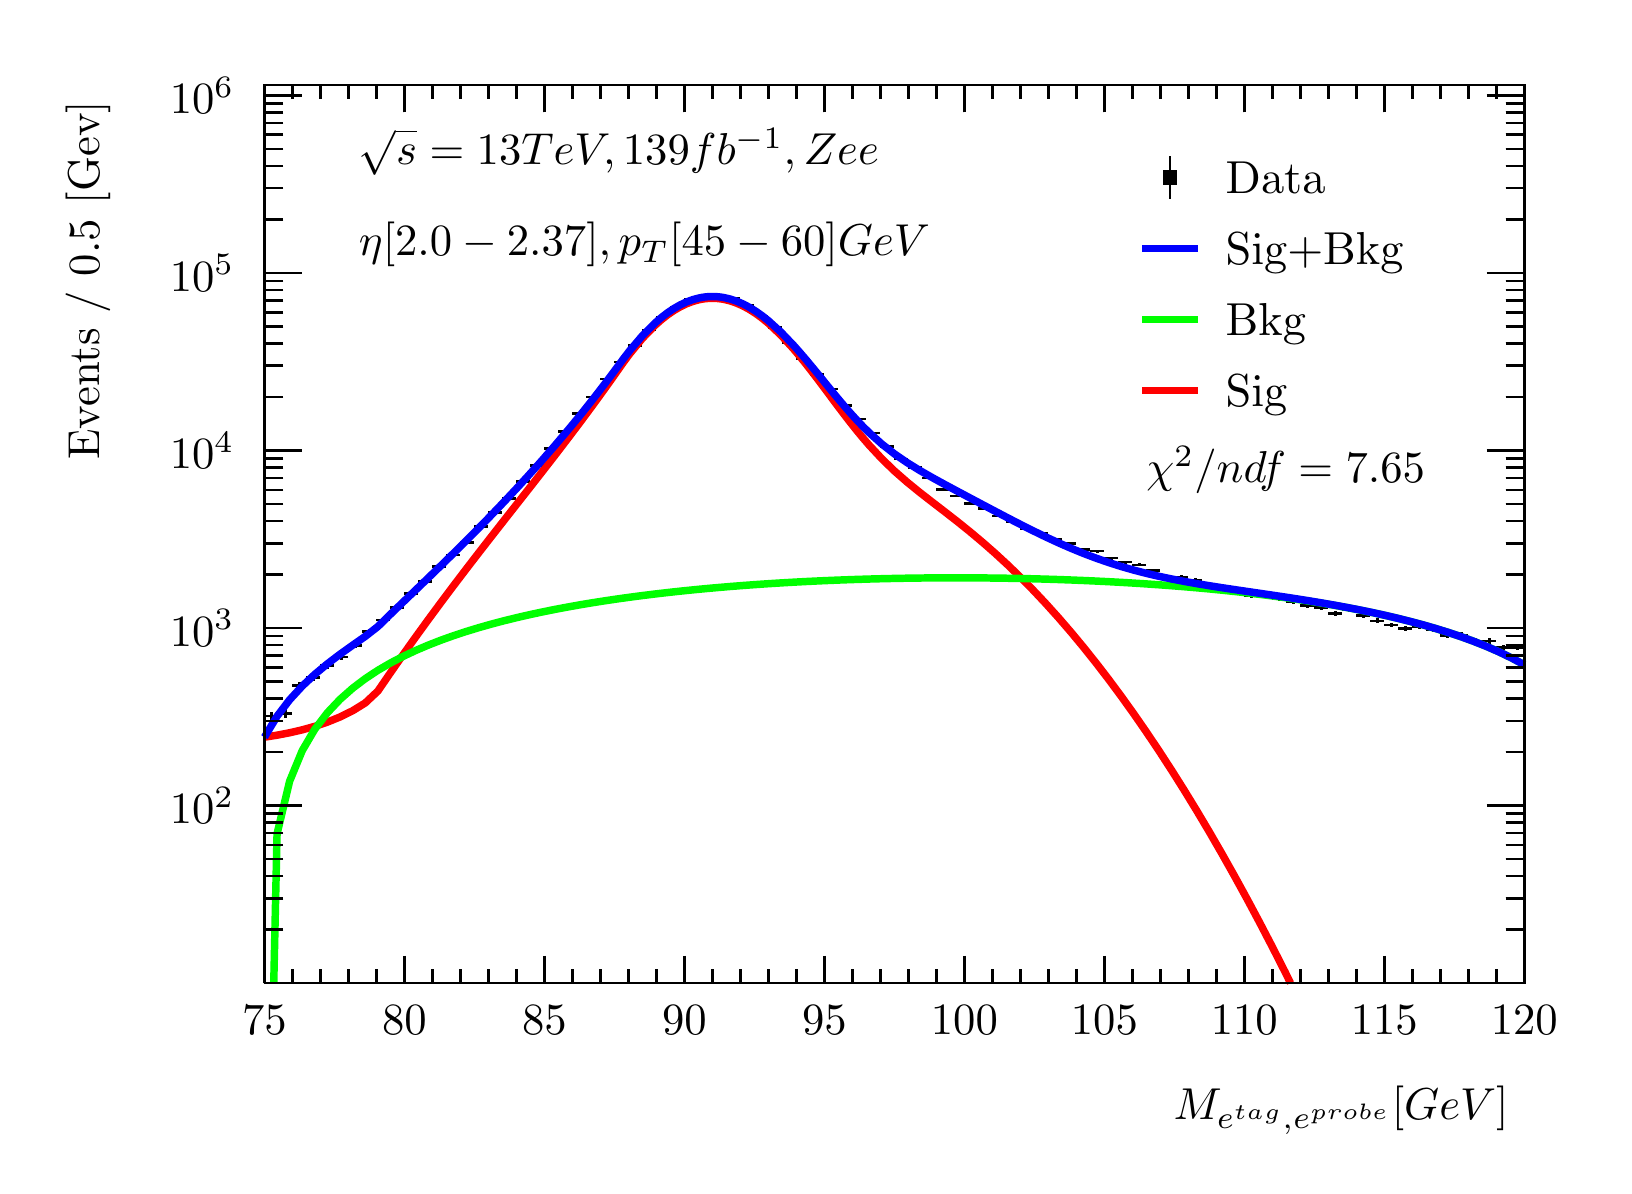
\begin{tikzpicture}
\pgfdeclareplotmark{cross} {
\pgfpathmoveto{\pgfpoint{-0.3\pgfplotmarksize}{\pgfplotmarksize}}
\pgfpathlineto{\pgfpoint{+0.3\pgfplotmarksize}{\pgfplotmarksize}}
\pgfpathlineto{\pgfpoint{+0.3\pgfplotmarksize}{0.3\pgfplotmarksize}}
\pgfpathlineto{\pgfpoint{+1\pgfplotmarksize}{0.3\pgfplotmarksize}}
\pgfpathlineto{\pgfpoint{+1\pgfplotmarksize}{-0.3\pgfplotmarksize}}
\pgfpathlineto{\pgfpoint{+0.3\pgfplotmarksize}{-0.3\pgfplotmarksize}}
\pgfpathlineto{\pgfpoint{+0.3\pgfplotmarksize}{-1.\pgfplotmarksize}}
\pgfpathlineto{\pgfpoint{-0.3\pgfplotmarksize}{-1.\pgfplotmarksize}}
\pgfpathlineto{\pgfpoint{-0.3\pgfplotmarksize}{-0.3\pgfplotmarksize}}
\pgfpathlineto{\pgfpoint{-1.\pgfplotmarksize}{-0.3\pgfplotmarksize}}
\pgfpathlineto{\pgfpoint{-1.\pgfplotmarksize}{0.3\pgfplotmarksize}}
\pgfpathlineto{\pgfpoint{-0.3\pgfplotmarksize}{0.3\pgfplotmarksize}}
\pgfpathclose
\pgfusepathqstroke
}
\pgfdeclareplotmark{cross*} {
\pgfpathmoveto{\pgfpoint{-0.3\pgfplotmarksize}{\pgfplotmarksize}}
\pgfpathlineto{\pgfpoint{+0.3\pgfplotmarksize}{\pgfplotmarksize}}
\pgfpathlineto{\pgfpoint{+0.3\pgfplotmarksize}{0.3\pgfplotmarksize}}
\pgfpathlineto{\pgfpoint{+1\pgfplotmarksize}{0.3\pgfplotmarksize}}
\pgfpathlineto{\pgfpoint{+1\pgfplotmarksize}{-0.3\pgfplotmarksize}}
\pgfpathlineto{\pgfpoint{+0.3\pgfplotmarksize}{-0.3\pgfplotmarksize}}
\pgfpathlineto{\pgfpoint{+0.3\pgfplotmarksize}{-1.\pgfplotmarksize}}
\pgfpathlineto{\pgfpoint{-0.3\pgfplotmarksize}{-1.\pgfplotmarksize}}
\pgfpathlineto{\pgfpoint{-0.3\pgfplotmarksize}{-0.3\pgfplotmarksize}}
\pgfpathlineto{\pgfpoint{-1.\pgfplotmarksize}{-0.3\pgfplotmarksize}}
\pgfpathlineto{\pgfpoint{-1.\pgfplotmarksize}{0.3\pgfplotmarksize}}
\pgfpathlineto{\pgfpoint{-0.3\pgfplotmarksize}{0.3\pgfplotmarksize}}
\pgfpathclose
\pgfusepathqfillstroke
}
\pgfdeclareplotmark{newstar} {
\pgfpathmoveto{\pgfqpoint{0pt}{\pgfplotmarksize}}
\pgfpathlineto{\pgfqpointpolar{44}{0.5\pgfplotmarksize}}
\pgfpathlineto{\pgfqpointpolar{18}{\pgfplotmarksize}}
\pgfpathlineto{\pgfqpointpolar{-20}{0.5\pgfplotmarksize}}
\pgfpathlineto{\pgfqpointpolar{-54}{\pgfplotmarksize}}
\pgfpathlineto{\pgfqpointpolar{-90}{0.5\pgfplotmarksize}}
\pgfpathlineto{\pgfqpointpolar{234}{\pgfplotmarksize}}
\pgfpathlineto{\pgfqpointpolar{198}{0.5\pgfplotmarksize}}
\pgfpathlineto{\pgfqpointpolar{162}{\pgfplotmarksize}}
\pgfpathlineto{\pgfqpointpolar{134}{0.5\pgfplotmarksize}}
\pgfpathclose
\pgfusepathqstroke
}
\pgfdeclareplotmark{newstar*} {
\pgfpathmoveto{\pgfqpoint{0pt}{\pgfplotmarksize}}
\pgfpathlineto{\pgfqpointpolar{44}{0.5\pgfplotmarksize}}
\pgfpathlineto{\pgfqpointpolar{18}{\pgfplotmarksize}}
\pgfpathlineto{\pgfqpointpolar{-20}{0.5\pgfplotmarksize}}
\pgfpathlineto{\pgfqpointpolar{-54}{\pgfplotmarksize}}
\pgfpathlineto{\pgfqpointpolar{-90}{0.5\pgfplotmarksize}}
\pgfpathlineto{\pgfqpointpolar{234}{\pgfplotmarksize}}
\pgfpathlineto{\pgfqpointpolar{198}{0.5\pgfplotmarksize}}
\pgfpathlineto{\pgfqpointpolar{162}{\pgfplotmarksize}}
\pgfpathlineto{\pgfqpointpolar{134}{0.5\pgfplotmarksize}}
\pgfpathclose
\pgfusepathqfillstroke
}
\definecolor{c}{rgb}{1,1,1};
\draw [color=c, fill=c] (0,0) rectangle (20,14.4361);
\draw [color=c, fill=c] (3,2.30977) rectangle (19,13.7143);
\definecolor{c}{rgb}{0,0,0};
\draw [c,line width=0.9] (3,2.30977) -- (3,13.7143) -- (19,13.7143) -- (19,2.30977) -- (3,2.30977);
\definecolor{c}{rgb}{1,1,1};
\draw [color=c, fill=c] (3,2.30977) rectangle (19,13.7143);
\definecolor{c}{rgb}{0,0,0};
\draw [c,line width=0.9] (3,2.30977) -- (3,13.7143) -- (19,13.7143) -- (19,2.30977) -- (3,2.30977);
\draw [c,line width=0.9] (3,2.30977) -- (19,2.30977);
\draw [c,line width=0.9] (3,2.65624) -- (3,2.30977);
\draw [c,line width=0.9] (3.35556,2.48301) -- (3.35556,2.30977);
\draw [c,line width=0.9] (3.71111,2.48301) -- (3.71111,2.30977);
\draw [c,line width=0.9] (4.06667,2.48301) -- (4.06667,2.30977);
\draw [c,line width=0.9] (4.42222,2.48301) -- (4.42222,2.30977);
\draw [c,line width=0.9] (4.77778,2.65624) -- (4.77778,2.30977);
\draw [c,line width=0.9] (5.13333,2.48301) -- (5.13333,2.30977);
\draw [c,line width=0.9] (5.48889,2.48301) -- (5.48889,2.30977);
\draw [c,line width=0.9] (5.84444,2.48301) -- (5.84444,2.30977);
\draw [c,line width=0.9] (6.2,2.48301) -- (6.2,2.30977);
\draw [c,line width=0.9] (6.55556,2.65624) -- (6.55556,2.30977);
\draw [c,line width=0.9] (6.91111,2.48301) -- (6.91111,2.30977);
\draw [c,line width=0.9] (7.26667,2.48301) -- (7.26667,2.30977);
\draw [c,line width=0.9] (7.62222,2.48301) -- (7.62222,2.30977);
\draw [c,line width=0.9] (7.97778,2.48301) -- (7.97778,2.30977);
\draw [c,line width=0.9] (8.33333,2.65624) -- (8.33333,2.30977);
\draw [c,line width=0.9] (8.68889,2.48301) -- (8.68889,2.30977);
\draw [c,line width=0.9] (9.04444,2.48301) -- (9.04444,2.30977);
\draw [c,line width=0.9] (9.4,2.48301) -- (9.4,2.30977);
\draw [c,line width=0.9] (9.75556,2.48301) -- (9.75556,2.30977);
\draw [c,line width=0.9] (10.1111,2.65624) -- (10.1111,2.30977);
\draw [c,line width=0.9] (10.4667,2.48301) -- (10.4667,2.30977);
\draw [c,line width=0.9] (10.8222,2.48301) -- (10.8222,2.30977);
\draw [c,line width=0.9] (11.1778,2.48301) -- (11.1778,2.30977);
\draw [c,line width=0.9] (11.5333,2.48301) -- (11.5333,2.30977);
\draw [c,line width=0.9] (11.8889,2.65624) -- (11.8889,2.30977);
\draw [c,line width=0.9] (12.2444,2.48301) -- (12.2444,2.30977);
\draw [c,line width=0.9] (12.6,2.48301) -- (12.6,2.30977);
\draw [c,line width=0.9] (12.9556,2.48301) -- (12.9556,2.30977);
\draw [c,line width=0.9] (13.3111,2.48301) -- (13.3111,2.30977);
\draw [c,line width=0.9] (13.6667,2.65624) -- (13.6667,2.30977);
\draw [c,line width=0.9] (14.0222,2.48301) -- (14.0222,2.30977);
\draw [c,line width=0.9] (14.3778,2.48301) -- (14.3778,2.30977);
\draw [c,line width=0.9] (14.7333,2.48301) -- (14.7333,2.30977);
\draw [c,line width=0.9] (15.0889,2.48301) -- (15.0889,2.30977);
\draw [c,line width=0.9] (15.4444,2.65624) -- (15.4444,2.30977);
\draw [c,line width=0.9] (15.8,2.48301) -- (15.8,2.30977);
\draw [c,line width=0.9] (16.1556,2.48301) -- (16.1556,2.30977);
\draw [c,line width=0.9] (16.5111,2.48301) -- (16.5111,2.30977);
\draw [c,line width=0.9] (16.8667,2.48301) -- (16.8667,2.30977);
\draw [c,line width=0.9] (17.2222,2.65624) -- (17.2222,2.30977);
\draw [c,line width=0.9] (17.5778,2.48301) -- (17.5778,2.30977);
\draw [c,line width=0.9] (17.9333,2.48301) -- (17.9333,2.30977);
\draw [c,line width=0.9] (18.2889,2.48301) -- (18.2889,2.30977);
\draw [c,line width=0.9] (18.6444,2.48301) -- (18.6444,2.30977);
\draw [c,line width=0.9] (19,2.65624) -- (19,2.30977);
\draw [c,line width=0.9] (19,2.65624) -- (19,2.30977);
\draw [anchor=base] (3,1.66015) node[scale=1.61424, color=c, rotate=0]{75};
\draw [anchor=base] (4.77778,1.66015) node[scale=1.61424, color=c, rotate=0]{80};
\draw [anchor=base] (6.55556,1.66015) node[scale=1.61424, color=c, rotate=0]{85};
\draw [anchor=base] (8.33333,1.66015) node[scale=1.61424, color=c, rotate=0]{90};
\draw [anchor=base] (10.1111,1.66015) node[scale=1.61424, color=c, rotate=0]{95};
\draw [anchor=base] (11.8889,1.66015) node[scale=1.61424, color=c, rotate=0]{100};
\draw [anchor=base] (13.6667,1.66015) node[scale=1.61424, color=c, rotate=0]{105};
\draw [anchor=base] (15.4444,1.66015) node[scale=1.61424, color=c, rotate=0]{110};
\draw [anchor=base] (17.2222,1.66015) node[scale=1.61424, color=c, rotate=0]{115};
\draw [anchor=base] (19,1.66015) node[scale=1.61424, color=c, rotate=0]{120};
\draw [anchor= east] (19,0.692932) node[scale=1.61424, color=c, rotate=0]{$M_{e^{tag}, e^{probe}}  [GeV]$};
\draw [c,line width=0.9] (3,13.7143) -- (19,13.7143);
\draw [c,line width=0.9] (3,13.3678) -- (3,13.7143);
\draw [c,line width=0.9] (3.35556,13.5411) -- (3.35556,13.7143);
\draw [c,line width=0.9] (3.71111,13.5411) -- (3.71111,13.7143);
\draw [c,line width=0.9] (4.06667,13.5411) -- (4.06667,13.7143);
\draw [c,line width=0.9] (4.42222,13.5411) -- (4.42222,13.7143);
\draw [c,line width=0.9] (4.77778,13.3678) -- (4.77778,13.7143);
\draw [c,line width=0.9] (5.13333,13.5411) -- (5.13333,13.7143);
\draw [c,line width=0.9] (5.48889,13.5411) -- (5.48889,13.7143);
\draw [c,line width=0.9] (5.84444,13.5411) -- (5.84444,13.7143);
\draw [c,line width=0.9] (6.2,13.5411) -- (6.2,13.7143);
\draw [c,line width=0.9] (6.55556,13.3678) -- (6.55556,13.7143);
\draw [c,line width=0.9] (6.91111,13.5411) -- (6.91111,13.7143);
\draw [c,line width=0.9] (7.26667,13.5411) -- (7.26667,13.7143);
\draw [c,line width=0.9] (7.62222,13.5411) -- (7.62222,13.7143);
\draw [c,line width=0.9] (7.97778,13.5411) -- (7.97778,13.7143);
\draw [c,line width=0.9] (8.33333,13.3678) -- (8.33333,13.7143);
\draw [c,line width=0.9] (8.68889,13.5411) -- (8.68889,13.7143);
\draw [c,line width=0.9] (9.04444,13.5411) -- (9.04444,13.7143);
\draw [c,line width=0.9] (9.4,13.5411) -- (9.4,13.7143);
\draw [c,line width=0.9] (9.75556,13.5411) -- (9.75556,13.7143);
\draw [c,line width=0.9] (10.1111,13.3678) -- (10.1111,13.7143);
\draw [c,line width=0.9] (10.4667,13.5411) -- (10.4667,13.7143);
\draw [c,line width=0.9] (10.8222,13.5411) -- (10.8222,13.7143);
\draw [c,line width=0.9] (11.1778,13.5411) -- (11.1778,13.7143);
\draw [c,line width=0.9] (11.5333,13.5411) -- (11.5333,13.7143);
\draw [c,line width=0.9] (11.8889,13.3678) -- (11.8889,13.7143);
\draw [c,line width=0.9] (12.2444,13.5411) -- (12.2444,13.7143);
\draw [c,line width=0.9] (12.6,13.5411) -- (12.6,13.7143);
\draw [c,line width=0.9] (12.9556,13.5411) -- (12.9556,13.7143);
\draw [c,line width=0.9] (13.3111,13.5411) -- (13.3111,13.7143);
\draw [c,line width=0.9] (13.6667,13.3678) -- (13.6667,13.7143);
\draw [c,line width=0.9] (14.0222,13.5411) -- (14.0222,13.7143);
\draw [c,line width=0.9] (14.3778,13.5411) -- (14.3778,13.7143);
\draw [c,line width=0.9] (14.7333,13.5411) -- (14.7333,13.7143);
\draw [c,line width=0.9] (15.0889,13.5411) -- (15.0889,13.7143);
\draw [c,line width=0.9] (15.4444,13.3678) -- (15.4444,13.7143);
\draw [c,line width=0.9] (15.8,13.5411) -- (15.8,13.7143);
\draw [c,line width=0.9] (16.1556,13.5411) -- (16.1556,13.7143);
\draw [c,line width=0.9] (16.5111,13.5411) -- (16.5111,13.7143);
\draw [c,line width=0.9] (16.8667,13.5411) -- (16.8667,13.7143);
\draw [c,line width=0.9] (17.2222,13.3678) -- (17.2222,13.7143);
\draw [c,line width=0.9] (17.5778,13.5411) -- (17.5778,13.7143);
\draw [c,line width=0.9] (17.9333,13.5411) -- (17.9333,13.7143);
\draw [c,line width=0.9] (18.2889,13.5411) -- (18.2889,13.7143);
\draw [c,line width=0.9] (18.6444,13.5411) -- (18.6444,13.7143);
\draw [c,line width=0.9] (19,13.3678) -- (19,13.7143);
\draw [c,line width=0.9] (19,13.3678) -- (19,13.7143);
\draw [c,line width=0.9] (3,2.30977) -- (3,13.7143);
\draw [c,line width=0.9] (3.237,2.98853) -- (3,2.98853);
\draw [c,line width=0.9] (3.237,3.38558) -- (3,3.38558);
\draw [c,line width=0.9] (3.237,3.66729) -- (3,3.66729);
\draw [c,line width=0.9] (3.237,3.8858) -- (3,3.8858);
\draw [c,line width=0.9] (3.237,4.06433) -- (3,4.06433);
\draw [c,line width=0.9] (3.237,4.21529) -- (3,4.21529);
\draw [c,line width=0.9] (3.237,4.34604) -- (3,4.34604);
\draw [c,line width=0.9] (3.237,4.46138) -- (3,4.46138);
\draw [c,line width=0.9] (3.474,4.56456) -- (3,4.56456);
\draw [anchor= east] (2.82,4.56456) node[scale=1.61424, color=c, rotate=0]{$10^{2}$};
\draw [c,line width=0.9] (3.237,5.24331) -- (3,5.24331);
\draw [c,line width=0.9] (3.237,5.64036) -- (3,5.64036);
\draw [c,line width=0.9] (3.237,5.92207) -- (3,5.92207);
\draw [c,line width=0.9] (3.237,6.14058) -- (3,6.14058);
\draw [c,line width=0.9] (3.237,6.31912) -- (3,6.31912);
\draw [c,line width=0.9] (3.237,6.47007) -- (3,6.47007);
\draw [c,line width=0.9] (3.237,6.60083) -- (3,6.60083);
\draw [c,line width=0.9] (3.237,6.71617) -- (3,6.71617);
\draw [c,line width=0.9] (3.474,6.81934) -- (3,6.81934);
\draw [anchor= east] (2.82,6.81934) node[scale=1.61424, color=c, rotate=0]{$10^{3}$};
\draw [c,line width=0.9] (3.237,7.4981) -- (3,7.4981);
\draw [c,line width=0.9] (3.237,7.89514) -- (3,7.89514);
\draw [c,line width=0.9] (3.237,8.17685) -- (3,8.17685);
\draw [c,line width=0.9] (3.237,8.39536) -- (3,8.39536);
\draw [c,line width=0.9] (3.237,8.5739) -- (3,8.5739);
\draw [c,line width=0.9] (3.237,8.72485) -- (3,8.72485);
\draw [c,line width=0.9] (3.237,8.85561) -- (3,8.85561);
\draw [c,line width=0.9] (3.237,8.97095) -- (3,8.97095);
\draw [c,line width=0.9] (3.474,9.07412) -- (3,9.07412);
\draw [anchor= east] (2.82,9.07412) node[scale=1.61424, color=c, rotate=0]{$10^{4}$};
\draw [c,line width=0.9] (3.237,9.75288) -- (3,9.75288);
\draw [c,line width=0.9] (3.237,10.1499) -- (3,10.1499);
\draw [c,line width=0.9] (3.237,10.4316) -- (3,10.4316);
\draw [c,line width=0.9] (3.237,10.6501) -- (3,10.6501);
\draw [c,line width=0.9] (3.237,10.8287) -- (3,10.8287);
\draw [c,line width=0.9] (3.237,10.9796) -- (3,10.9796);
\draw [c,line width=0.9] (3.237,11.1104) -- (3,11.1104);
\draw [c,line width=0.9] (3.237,11.2257) -- (3,11.2257);
\draw [c,line width=0.9] (3.474,11.3289) -- (3,11.3289);
\draw [anchor= east] (2.82,11.3289) node[scale=1.61424, color=c, rotate=0]{$10^{5}$};
\draw [c,line width=0.9] (3.237,12.0077) -- (3,12.0077);
\draw [c,line width=0.9] (3.237,12.4047) -- (3,12.4047);
\draw [c,line width=0.9] (3.237,12.6864) -- (3,12.6864);
\draw [c,line width=0.9] (3.237,12.9049) -- (3,12.9049);
\draw [c,line width=0.9] (3.237,13.0835) -- (3,13.0835);
\draw [c,line width=0.9] (3.237,13.2344) -- (3,13.2344);
\draw [c,line width=0.9] (3.237,13.3652) -- (3,13.3652);
\draw [c,line width=0.9] (3.237,13.4805) -- (3,13.4805);
\draw [c,line width=0.9] (3.474,13.5837) -- (3,13.5837);
\draw [anchor= east] (2.82,13.5837) node[scale=1.61424, color=c, rotate=0]{$10^{6}$};
\draw [anchor= east] (0.76,13.7143) node[scale=1.61424, color=c, rotate=90]{Events / 0.5 [Gev]};
\draw [c,line width=0.9] (19,2.30977) -- (19,13.7143);
\draw [c,line width=0.9] (18.763,2.98853) -- (19,2.98853);
\draw [c,line width=0.9] (18.763,3.38558) -- (19,3.38558);
\draw [c,line width=0.9] (18.763,3.66729) -- (19,3.66729);
\draw [c,line width=0.9] (18.763,3.8858) -- (19,3.8858);
\draw [c,line width=0.9] (18.763,4.06433) -- (19,4.06433);
\draw [c,line width=0.9] (18.763,4.21529) -- (19,4.21529);
\draw [c,line width=0.9] (18.763,4.34604) -- (19,4.34604);
\draw [c,line width=0.9] (18.763,4.46138) -- (19,4.46138);
\draw [c,line width=0.9] (18.526,4.56456) -- (19,4.56456);
\draw [c,line width=0.9] (18.763,5.24331) -- (19,5.24331);
\draw [c,line width=0.9] (18.763,5.64036) -- (19,5.64036);
\draw [c,line width=0.9] (18.763,5.92207) -- (19,5.92207);
\draw [c,line width=0.9] (18.763,6.14058) -- (19,6.14058);
\draw [c,line width=0.9] (18.763,6.31912) -- (19,6.31912);
\draw [c,line width=0.9] (18.763,6.47007) -- (19,6.47007);
\draw [c,line width=0.9] (18.763,6.60083) -- (19,6.60083);
\draw [c,line width=0.9] (18.763,6.71617) -- (19,6.71617);
\draw [c,line width=0.9] (18.526,6.81934) -- (19,6.81934);
\draw [c,line width=0.9] (18.763,7.4981) -- (19,7.4981);
\draw [c,line width=0.9] (18.763,7.89514) -- (19,7.89514);
\draw [c,line width=0.9] (18.763,8.17685) -- (19,8.17685);
\draw [c,line width=0.9] (18.763,8.39536) -- (19,8.39536);
\draw [c,line width=0.9] (18.763,8.5739) -- (19,8.5739);
\draw [c,line width=0.9] (18.763,8.72485) -- (19,8.72485);
\draw [c,line width=0.9] (18.763,8.85561) -- (19,8.85561);
\draw [c,line width=0.9] (18.763,8.97095) -- (19,8.97095);
\draw [c,line width=0.9] (18.526,9.07412) -- (19,9.07412);
\draw [c,line width=0.9] (18.763,9.75288) -- (19,9.75288);
\draw [c,line width=0.9] (18.763,10.1499) -- (19,10.1499);
\draw [c,line width=0.9] (18.763,10.4316) -- (19,10.4316);
\draw [c,line width=0.9] (18.763,10.6501) -- (19,10.6501);
\draw [c,line width=0.9] (18.763,10.8287) -- (19,10.8287);
\draw [c,line width=0.9] (18.763,10.9796) -- (19,10.9796);
\draw [c,line width=0.9] (18.763,11.1104) -- (19,11.1104);
\draw [c,line width=0.9] (18.763,11.2257) -- (19,11.2257);
\draw [c,line width=0.9] (18.526,11.3289) -- (19,11.3289);
\draw [c,line width=0.9] (18.763,12.0077) -- (19,12.0077);
\draw [c,line width=0.9] (18.763,12.4047) -- (19,12.4047);
\draw [c,line width=0.9] (18.763,12.6864) -- (19,12.6864);
\draw [c,line width=0.9] (18.763,12.9049) -- (19,12.9049);
\draw [c,line width=0.9] (18.763,13.0835) -- (19,13.0835);
\draw [c,line width=0.9] (18.763,13.2344) -- (19,13.2344);
\draw [c,line width=0.9] (18.763,13.3652) -- (19,13.3652);
\draw [c,line width=0.9] (18.763,13.4805) -- (19,13.4805);
\draw [c,line width=0.9] (18.526,13.5837) -- (19,13.5837);
\draw [c,line width=0.9] (3.08889,5.70356) -- (3,5.70356);
\draw [c,line width=0.9] (3,5.70356) -- (3,5.70356);
\draw [c,line width=0.9] (3.08889,5.70356) -- (3.17778,5.70356);
\draw [c,line width=0.9] (3.17778,5.70356) -- (3.17778,5.70356);
\draw [c,line width=0.9] (3.08889,5.70356) -- (3.08889,5.7583);
\draw [c,line width=0.9] (3.08889,5.7583) -- (3.08889,5.7583);
\draw [c,line width=0.9] (3.08889,5.70356) -- (3.08889,5.64883);
\draw [c,line width=0.9] (3.08889,5.64883) -- (3.08889,5.64883);
\draw [c,line width=0.9] (3.26667,5.73072) -- (3.17778,5.73072);
\draw [c,line width=0.9] (3.17778,5.73072) -- (3.17778,5.73072);
\draw [c,line width=0.9] (3.26667,5.73072) -- (3.35556,5.73072);
\draw [c,line width=0.9] (3.35556,5.73072) -- (3.35556,5.73072);
\draw [c,line width=0.9] (3.26667,5.73072) -- (3.26667,5.7847);
\draw [c,line width=0.9] (3.26667,5.7847) -- (3.26667,5.7847);
\draw [c,line width=0.9] (3.26667,5.73072) -- (3.26667,5.67674);
\draw [c,line width=0.9] (3.26667,5.67674) -- (3.26667,5.67674);
\draw [c,line width=0.9] (3.44444,6.08829) -- (3.35556,6.08829);
\draw [c,line width=0.9] (3.35556,6.08829) -- (3.35556,6.08829);
\draw [c,line width=0.9] (3.44444,6.08829) -- (3.53333,6.08829);
\draw [c,line width=0.9] (3.53333,6.08829) -- (3.53333,6.08829);
\draw [c,line width=0.9] (3.44444,6.08829) -- (3.44444,6.13326);
\draw [c,line width=0.9] (3.44444,6.13326) -- (3.44444,6.13326);
\draw [c,line width=0.9] (3.44444,6.08829) -- (3.44444,6.04332);
\draw [c,line width=0.9] (3.44444,6.04332) -- (3.44444,6.04332);
\draw [c,line width=0.9] (3.62222,6.18836) -- (3.53333,6.18836);
\draw [c,line width=0.9] (3.53333,6.18836) -- (3.53333,6.18836);
\draw [c,line width=0.9] (3.62222,6.18836) -- (3.71111,6.18836);
\draw [c,line width=0.9] (3.71111,6.18836) -- (3.71111,6.18836);
\draw [c,line width=0.9] (3.62222,6.18836) -- (3.62222,6.23109);
\draw [c,line width=0.9] (3.62222,6.23109) -- (3.62222,6.23109);
\draw [c,line width=0.9] (3.62222,6.18836) -- (3.62222,6.14563);
\draw [c,line width=0.9] (3.62222,6.14563) -- (3.62222,6.14563);
\draw [c,line width=0.9] (3.8,6.34171) -- (3.71111,6.34171);
\draw [c,line width=0.9] (3.71111,6.34171) -- (3.71111,6.34171);
\draw [c,line width=0.9] (3.8,6.34171) -- (3.88889,6.34171);
\draw [c,line width=0.9] (3.88889,6.34171) -- (3.88889,6.34171);
\draw [c,line width=0.9] (3.8,6.34171) -- (3.8,6.38122);
\draw [c,line width=0.9] (3.8,6.38122) -- (3.8,6.38122);
\draw [c,line width=0.9] (3.8,6.34171) -- (3.8,6.30219);
\draw [c,line width=0.9] (3.8,6.30219) -- (3.8,6.30219);
\draw [c,line width=0.9] (3.97778,6.45029) -- (3.88889,6.45029);
\draw [c,line width=0.9] (3.88889,6.45029) -- (3.88889,6.45029);
\draw [c,line width=0.9] (3.97778,6.45029) -- (4.06667,6.45029);
\draw [c,line width=0.9] (4.06667,6.45029) -- (4.06667,6.45029);
\draw [c,line width=0.9] (3.97778,6.45029) -- (3.97778,6.48767);
\draw [c,line width=0.9] (3.97778,6.48767) -- (3.97778,6.48767);
\draw [c,line width=0.9] (3.97778,6.45029) -- (3.97778,6.4129);
\draw [c,line width=0.9] (3.97778,6.4129) -- (3.97778,6.4129);
\draw [c,line width=0.9] (4.15556,6.5996) -- (4.06667,6.5996);
\draw [c,line width=0.9] (4.06667,6.5996) -- (4.06667,6.5996);
\draw [c,line width=0.9] (4.15556,6.5996) -- (4.24444,6.5996);
\draw [c,line width=0.9] (4.24444,6.5996) -- (4.24444,6.5996);
\draw [c,line width=0.9] (4.15556,6.5996) -- (4.15556,6.63425);
\draw [c,line width=0.9] (4.15556,6.63425) -- (4.15556,6.63425);
\draw [c,line width=0.9] (4.15556,6.5996) -- (4.15556,6.56496);
\draw [c,line width=0.9] (4.15556,6.56496) -- (4.15556,6.56496);
\draw [c,line width=0.9] (4.33333,6.77323) -- (4.24444,6.77323);
\draw [c,line width=0.9] (4.24444,6.77323) -- (4.24444,6.77323);
\draw [c,line width=0.9] (4.33333,6.77323) -- (4.42222,6.77323);
\draw [c,line width=0.9] (4.42222,6.77323) -- (4.42222,6.77323);
\draw [c,line width=0.9] (4.33333,6.77323) -- (4.33333,6.80493);
\draw [c,line width=0.9] (4.33333,6.80493) -- (4.33333,6.80493);
\draw [c,line width=0.9] (4.33333,6.77323) -- (4.33333,6.74152);
\draw [c,line width=0.9] (4.33333,6.74152) -- (4.33333,6.74152);
\draw [c,line width=0.9] (4.51111,6.92065) -- (4.42222,6.92065);
\draw [c,line width=0.9] (4.42222,6.92065) -- (4.42222,6.92065);
\draw [c,line width=0.9] (4.51111,6.92065) -- (4.6,6.92065);
\draw [c,line width=0.9] (4.6,6.92065) -- (4.6,6.92065);
\draw [c,line width=0.9] (4.51111,6.92065) -- (4.51111,6.95006);
\draw [c,line width=0.9] (4.51111,6.95006) -- (4.51111,6.95006);
\draw [c,line width=0.9] (4.51111,6.92065) -- (4.51111,6.89125);
\draw [c,line width=0.9] (4.51111,6.89125) -- (4.51111,6.89125);
\draw [c,line width=0.9] (4.68889,7.07776) -- (4.6,7.07776);
\draw [c,line width=0.9] (4.6,7.07776) -- (4.6,7.07776);
\draw [c,line width=0.9] (4.68889,7.07776) -- (4.77778,7.07776);
\draw [c,line width=0.9] (4.77778,7.07776) -- (4.77778,7.07776);
\draw [c,line width=0.9] (4.68889,7.07776) -- (4.68889,7.1049);
\draw [c,line width=0.9] (4.68889,7.1049) -- (4.68889,7.1049);
\draw [c,line width=0.9] (4.68889,7.07776) -- (4.68889,7.05063);
\draw [c,line width=0.9] (4.68889,7.05063) -- (4.68889,7.05063);
\draw [c,line width=0.9] (4.86667,7.25668) -- (4.77778,7.25668);
\draw [c,line width=0.9] (4.77778,7.25668) -- (4.77778,7.25668);
\draw [c,line width=0.9] (4.86667,7.25668) -- (4.95556,7.25668);
\draw [c,line width=0.9] (4.95556,7.25668) -- (4.95556,7.25668);
\draw [c,line width=0.9] (4.86667,7.25668) -- (4.86667,7.28144);
\draw [c,line width=0.9] (4.86667,7.28144) -- (4.86667,7.28144);
\draw [c,line width=0.9] (4.86667,7.25668) -- (4.86667,7.23191);
\draw [c,line width=0.9] (4.86667,7.23191) -- (4.86667,7.23191);
\draw [c,line width=0.9] (5.04444,7.40736) -- (4.95556,7.40736);
\draw [c,line width=0.9] (4.95556,7.40736) -- (4.95556,7.40736);
\draw [c,line width=0.9] (5.04444,7.40736) -- (5.13333,7.40736);
\draw [c,line width=0.9] (5.13333,7.40736) -- (5.13333,7.40736);
\draw [c,line width=0.9] (5.04444,7.40736) -- (5.04444,7.43029);
\draw [c,line width=0.9] (5.04444,7.43029) -- (5.04444,7.43029);
\draw [c,line width=0.9] (5.04444,7.40736) -- (5.04444,7.38442);
\draw [c,line width=0.9] (5.04444,7.38442) -- (5.04444,7.38442);
\draw [c,line width=0.9] (5.22222,7.59808) -- (5.13333,7.59808);
\draw [c,line width=0.9] (5.13333,7.59808) -- (5.13333,7.59808);
\draw [c,line width=0.9] (5.22222,7.59808) -- (5.31111,7.59808);
\draw [c,line width=0.9] (5.31111,7.59808) -- (5.31111,7.59808);
\draw [c,line width=0.9] (5.22222,7.59808) -- (5.22222,7.61889);
\draw [c,line width=0.9] (5.22222,7.61889) -- (5.22222,7.61889);
\draw [c,line width=0.9] (5.22222,7.59808) -- (5.22222,7.57728);
\draw [c,line width=0.9] (5.22222,7.57728) -- (5.22222,7.57728);
\draw [c,line width=0.9] (5.4,7.74593) -- (5.31111,7.74593);
\draw [c,line width=0.9] (5.31111,7.74593) -- (5.31111,7.74593);
\draw [c,line width=0.9] (5.4,7.74593) -- (5.48889,7.74593);
\draw [c,line width=0.9] (5.48889,7.74593) -- (5.48889,7.74593);
\draw [c,line width=0.9] (5.4,7.74593) -- (5.4,7.76523);
\draw [c,line width=0.9] (5.4,7.76523) -- (5.4,7.76523);
\draw [c,line width=0.9] (5.4,7.74593) -- (5.4,7.72664);
\draw [c,line width=0.9] (5.4,7.72664) -- (5.4,7.72664);
\draw [c,line width=0.9] (5.57778,7.90392) -- (5.48889,7.90392);
\draw [c,line width=0.9] (5.48889,7.90392) -- (5.48889,7.90392);
\draw [c,line width=0.9] (5.57778,7.90392) -- (5.66667,7.90392);
\draw [c,line width=0.9] (5.66667,7.90392) -- (5.66667,7.90392);
\draw [c,line width=0.9] (5.57778,7.90392) -- (5.57778,7.92172);
\draw [c,line width=0.9] (5.57778,7.92172) -- (5.57778,7.92172);
\draw [c,line width=0.9] (5.57778,7.90392) -- (5.57778,7.88612);
\draw [c,line width=0.9] (5.57778,7.88612) -- (5.57778,7.88612);
\draw [c,line width=0.9] (5.75556,8.10973) -- (5.66667,8.10973);
\draw [c,line width=0.9] (5.66667,8.10973) -- (5.66667,8.10973);
\draw [c,line width=0.9] (5.75556,8.10973) -- (5.84444,8.10973);
\draw [c,line width=0.9] (5.84444,8.10973) -- (5.84444,8.10973);
\draw [c,line width=0.9] (5.75556,8.10973) -- (5.75556,8.12575);
\draw [c,line width=0.9] (5.75556,8.12575) -- (5.75556,8.12575);
\draw [c,line width=0.9] (5.75556,8.10973) -- (5.75556,8.09371);
\draw [c,line width=0.9] (5.75556,8.09371) -- (5.75556,8.09371);
\draw [c,line width=0.9] (5.93333,8.28411) -- (5.84444,8.28411);
\draw [c,line width=0.9] (5.84444,8.28411) -- (5.84444,8.28411);
\draw [c,line width=0.9] (5.93333,8.28411) -- (6.02222,8.28411);
\draw [c,line width=0.9] (6.02222,8.28411) -- (6.02222,8.28411);
\draw [c,line width=0.9] (5.93333,8.28411) -- (5.93333,8.29877);
\draw [c,line width=0.9] (5.93333,8.29877) -- (5.93333,8.29877);
\draw [c,line width=0.9] (5.93333,8.28411) -- (5.93333,8.26945);
\draw [c,line width=0.9] (5.93333,8.26945) -- (5.93333,8.26945);
\draw [c,line width=0.9] (6.11111,8.46618) -- (6.02222,8.46618);
\draw [c,line width=0.9] (6.02222,8.46618) -- (6.02222,8.46618);
\draw [c,line width=0.9] (6.11111,8.46618) -- (6.2,8.46618);
\draw [c,line width=0.9] (6.2,8.46618) -- (6.2,8.46618);
\draw [c,line width=0.9] (6.11111,8.46618) -- (6.11111,8.47954);
\draw [c,line width=0.9] (6.11111,8.47954) -- (6.11111,8.47954);
\draw [c,line width=0.9] (6.11111,8.46618) -- (6.11111,8.45283);
\draw [c,line width=0.9] (6.11111,8.45283) -- (6.11111,8.45283);
\draw [c,line width=0.9] (6.28889,8.68094) -- (6.2,8.68094);
\draw [c,line width=0.9] (6.2,8.68094) -- (6.2,8.68094);
\draw [c,line width=0.9] (6.28889,8.68094) -- (6.37778,8.68094);
\draw [c,line width=0.9] (6.37778,8.68094) -- (6.37778,8.68094);
\draw [c,line width=0.9] (6.28889,8.68094) -- (6.28889,8.69291);
\draw [c,line width=0.9] (6.28889,8.69291) -- (6.28889,8.69291);
\draw [c,line width=0.9] (6.28889,8.68094) -- (6.28889,8.66897);
\draw [c,line width=0.9] (6.28889,8.66897) -- (6.28889,8.66897);
\draw [c,line width=0.9] (6.46667,8.88182) -- (6.37778,8.88182);
\draw [c,line width=0.9] (6.37778,8.88182) -- (6.37778,8.88182);
\draw [c,line width=0.9] (6.46667,8.88182) -- (6.55556,8.88182);
\draw [c,line width=0.9] (6.55556,8.88182) -- (6.55556,8.88182);
\draw [c,line width=0.9] (6.46667,8.88182) -- (6.46667,8.89262);
\draw [c,line width=0.9] (6.46667,8.89262) -- (6.46667,8.89262);
\draw [c,line width=0.9] (6.46667,8.88182) -- (6.46667,8.87102);
\draw [c,line width=0.9] (6.46667,8.87102) -- (6.46667,8.87102);
\draw [c,line width=0.9] (6.64444,9.09964) -- (6.55556,9.09964);
\draw [c,line width=0.9] (6.55556,9.09964) -- (6.55556,9.09964);
\draw [c,line width=0.9] (6.64444,9.09964) -- (6.73333,9.09964);
\draw [c,line width=0.9] (6.73333,9.09964) -- (6.73333,9.09964);
\draw [c,line width=0.9] (6.64444,9.09964) -- (6.64444,9.10931);
\draw [c,line width=0.9] (6.64444,9.10931) -- (6.64444,9.10931);
\draw [c,line width=0.9] (6.64444,9.09964) -- (6.64444,9.08997);
\draw [c,line width=0.9] (6.64444,9.08997) -- (6.64444,9.08997);
\draw [c,line width=0.9] (6.82222,9.31486) -- (6.73333,9.31486);
\draw [c,line width=0.9] (6.73333,9.31486) -- (6.73333,9.31486);
\draw [c,line width=0.9] (6.82222,9.31486) -- (6.91111,9.31486);
\draw [c,line width=0.9] (6.91111,9.31486) -- (6.91111,9.31486);
\draw [c,line width=0.9] (6.82222,9.31486) -- (6.82222,9.32352);
\draw [c,line width=0.9] (6.82222,9.32352) -- (6.82222,9.32352);
\draw [c,line width=0.9] (6.82222,9.31486) -- (6.82222,9.3062);
\draw [c,line width=0.9] (6.82222,9.3062) -- (6.82222,9.3062);
\draw [c,line width=0.9] (7,9.54065) -- (6.91111,9.54065);
\draw [c,line width=0.9] (6.91111,9.54065) -- (6.91111,9.54065);
\draw [c,line width=0.9] (7,9.54065) -- (7.08889,9.54065);
\draw [c,line width=0.9] (7.08889,9.54065) -- (7.08889,9.54065);
\draw [c,line width=0.9] (7,9.54065) -- (7,9.54837);
\draw [c,line width=0.9] (7,9.54837) -- (7,9.54837);
\draw [c,line width=0.9] (7,9.54065) -- (7,9.53294);
\draw [c,line width=0.9] (7,9.53294) -- (7,9.53294);
\draw [c,line width=0.9] (7.17778,9.75508) -- (7.08889,9.75508);
\draw [c,line width=0.9] (7.08889,9.75508) -- (7.08889,9.75508);
\draw [c,line width=0.9] (7.17778,9.75508) -- (7.26667,9.75508);
\draw [c,line width=0.9] (7.26667,9.75508) -- (7.26667,9.75508);
\draw [c,line width=0.9] (7.17778,9.75508) -- (7.17778,9.762);
\draw [c,line width=0.9] (7.17778,9.762) -- (7.17778,9.762);
\draw [c,line width=0.9] (7.17778,9.75508) -- (7.17778,9.74816);
\draw [c,line width=0.9] (7.17778,9.74816) -- (7.17778,9.74816);
\draw [c,line width=0.9] (7.35556,9.98346) -- (7.26667,9.98346);
\draw [c,line width=0.9] (7.26667,9.98346) -- (7.26667,9.98346);
\draw [c,line width=0.9] (7.35556,9.98346) -- (7.44444,9.98346);
\draw [c,line width=0.9] (7.44444,9.98346) -- (7.44444,9.98346);
\draw [c,line width=0.9] (7.35556,9.98346) -- (7.35556,9.98961);
\draw [c,line width=0.9] (7.35556,9.98961) -- (7.35556,9.98961);
\draw [c,line width=0.9] (7.35556,9.98346) -- (7.35556,9.9773);
\draw [c,line width=0.9] (7.35556,9.9773) -- (7.35556,9.9773);
\draw [c,line width=0.9] (7.53333,10.1945) -- (7.44444,10.1945);
\draw [c,line width=0.9] (7.44444,10.1945) -- (7.44444,10.1945);
\draw [c,line width=0.9] (7.53333,10.1945) -- (7.62222,10.1945);
\draw [c,line width=0.9] (7.62222,10.1945) -- (7.62222,10.1945);
\draw [c,line width=0.9] (7.53333,10.1945) -- (7.53333,10.2001);
\draw [c,line width=0.9] (7.53333,10.2001) -- (7.53333,10.2001);
\draw [c,line width=0.9] (7.53333,10.1945) -- (7.53333,10.189);
\draw [c,line width=0.9] (7.53333,10.189) -- (7.53333,10.189);
\draw [c,line width=0.9] (7.71111,10.4069) -- (7.62222,10.4069);
\draw [c,line width=0.9] (7.62222,10.4069) -- (7.62222,10.4069);
\draw [c,line width=0.9] (7.71111,10.4069) -- (7.8,10.4069);
\draw [c,line width=0.9] (7.8,10.4069) -- (7.8,10.4069);
\draw [c,line width=0.9] (7.71111,10.4069) -- (7.71111,10.4118);
\draw [c,line width=0.9] (7.71111,10.4118) -- (7.71111,10.4118);
\draw [c,line width=0.9] (7.71111,10.4069) -- (7.71111,10.4019);
\draw [c,line width=0.9] (7.71111,10.4019) -- (7.71111,10.4019);
\draw [c,line width=0.9] (7.88889,10.6044) -- (7.8,10.6044);
\draw [c,line width=0.9] (7.8,10.6044) -- (7.8,10.6044);
\draw [c,line width=0.9] (7.88889,10.6044) -- (7.97778,10.6044);
\draw [c,line width=0.9] (7.97778,10.6044) -- (7.97778,10.6044);
\draw [c,line width=0.9] (7.88889,10.6044) -- (7.88889,10.6088);
\draw [c,line width=0.9] (7.88889,10.6088) -- (7.88889,10.6088);
\draw [c,line width=0.9] (7.88889,10.6044) -- (7.88889,10.5999);
\draw [c,line width=0.9] (7.88889,10.5999) -- (7.88889,10.5999);
\draw [c,line width=0.9] (8.06667,10.769) -- (7.97778,10.769);
\draw [c,line width=0.9] (7.97778,10.769) -- (7.97778,10.769);
\draw [c,line width=0.9] (8.06667,10.769) -- (8.15556,10.769);
\draw [c,line width=0.9] (8.15556,10.769) -- (8.15556,10.769);
\draw [c,line width=0.9] (8.06667,10.769) -- (8.06667,10.7732);
\draw [c,line width=0.9] (8.06667,10.7732) -- (8.06667,10.7732);
\draw [c,line width=0.9] (8.06667,10.769) -- (8.06667,10.7649);
\draw [c,line width=0.9] (8.06667,10.7649) -- (8.06667,10.7649);
\draw [c,line width=0.9] (8.24444,10.893) -- (8.15556,10.893);
\draw [c,line width=0.9] (8.15556,10.893) -- (8.15556,10.893);
\draw [c,line width=0.9] (8.24444,10.893) -- (8.33333,10.893);
\draw [c,line width=0.9] (8.33333,10.893) -- (8.33333,10.893);
\draw [c,line width=0.9] (8.24444,10.893) -- (8.24444,10.8969);
\draw [c,line width=0.9] (8.24444,10.8969) -- (8.24444,10.8969);
\draw [c,line width=0.9] (8.24444,10.893) -- (8.24444,10.8891);
\draw [c,line width=0.9] (8.24444,10.8891) -- (8.24444,10.8891);
\draw [c,line width=0.9] (8.42222,10.989) -- (8.33333,10.989);
\draw [c,line width=0.9] (8.33333,10.989) -- (8.33333,10.989);
\draw [c,line width=0.9] (8.42222,10.989) -- (8.51111,10.989);
\draw [c,line width=0.9] (8.51111,10.989) -- (8.51111,10.989);
\draw [c,line width=0.9] (8.42222,10.989) -- (8.42222,10.9927);
\draw [c,line width=0.9] (8.42222,10.9927) -- (8.42222,10.9927);
\draw [c,line width=0.9] (8.42222,10.989) -- (8.42222,10.9853);
\draw [c,line width=0.9] (8.42222,10.9853) -- (8.42222,10.9853);
\draw [c,line width=0.9] (8.6,11.0335) -- (8.51111,11.0335);
\draw [c,line width=0.9] (8.51111,11.0335) -- (8.51111,11.0335);
\draw [c,line width=0.9] (8.6,11.0335) -- (8.68889,11.0335);
\draw [c,line width=0.9] (8.68889,11.0335) -- (8.68889,11.0335);
\draw [c,line width=0.9] (8.6,11.0335) -- (8.6,11.0371);
\draw [c,line width=0.9] (8.6,11.0371) -- (8.6,11.0371);
\draw [c,line width=0.9] (8.6,11.0335) -- (8.6,11.0299);
\draw [c,line width=0.9] (8.6,11.0299) -- (8.6,11.0299);
\draw [c,line width=0.9] (8.77778,11.0437) -- (8.68889,11.0437);
\draw [c,line width=0.9] (8.68889,11.0437) -- (8.68889,11.0437);
\draw [c,line width=0.9] (8.77778,11.0437) -- (8.86667,11.0437);
\draw [c,line width=0.9] (8.86667,11.0437) -- (8.86667,11.0437);
\draw [c,line width=0.9] (8.77778,11.0437) -- (8.77778,11.0472);
\draw [c,line width=0.9] (8.77778,11.0472) -- (8.77778,11.0472);
\draw [c,line width=0.9] (8.77778,11.0437) -- (8.77778,11.0401);
\draw [c,line width=0.9] (8.77778,11.0401) -- (8.77778,11.0401);
\draw [c,line width=0.9] (8.95556,11.0034) -- (8.86667,11.0034);
\draw [c,line width=0.9] (8.86667,11.0034) -- (8.86667,11.0034);
\draw [c,line width=0.9] (8.95556,11.0034) -- (9.04444,11.0034);
\draw [c,line width=0.9] (9.04444,11.0034) -- (9.04444,11.0034);
\draw [c,line width=0.9] (8.95556,11.0034) -- (8.95556,11.0071);
\draw [c,line width=0.9] (8.95556,11.0071) -- (8.95556,11.0071);
\draw [c,line width=0.9] (8.95556,11.0034) -- (8.95556,10.9998);
\draw [c,line width=0.9] (8.95556,10.9998) -- (8.95556,10.9998);
\draw [c,line width=0.9] (9.13333,10.9124) -- (9.04444,10.9124);
\draw [c,line width=0.9] (9.04444,10.9124) -- (9.04444,10.9124);
\draw [c,line width=0.9] (9.13333,10.9124) -- (9.22222,10.9124);
\draw [c,line width=0.9] (9.22222,10.9124) -- (9.22222,10.9124);
\draw [c,line width=0.9] (9.13333,10.9124) -- (9.13333,10.9163);
\draw [c,line width=0.9] (9.13333,10.9163) -- (9.13333,10.9163);
\draw [c,line width=0.9] (9.13333,10.9124) -- (9.13333,10.9086);
\draw [c,line width=0.9] (9.13333,10.9086) -- (9.13333,10.9086);
\draw [c,line width=0.9] (9.31111,10.7798) -- (9.22222,10.7798);
\draw [c,line width=0.9] (9.22222,10.7798) -- (9.22222,10.7798);
\draw [c,line width=0.9] (9.31111,10.7798) -- (9.4,10.7798);
\draw [c,line width=0.9] (9.4,10.7798) -- (9.4,10.7798);
\draw [c,line width=0.9] (9.31111,10.7798) -- (9.31111,10.7839);
\draw [c,line width=0.9] (9.31111,10.7839) -- (9.31111,10.7839);
\draw [c,line width=0.9] (9.31111,10.7798) -- (9.31111,10.7757);
\draw [c,line width=0.9] (9.31111,10.7757) -- (9.31111,10.7757);
\draw [c,line width=0.9] (9.48889,10.6322) -- (9.4,10.6322);
\draw [c,line width=0.9] (9.4,10.6322) -- (9.4,10.6322);
\draw [c,line width=0.9] (9.48889,10.6322) -- (9.57778,10.6322);
\draw [c,line width=0.9] (9.57778,10.6322) -- (9.57778,10.6322);
\draw [c,line width=0.9] (9.48889,10.6322) -- (9.48889,10.6367);
\draw [c,line width=0.9] (9.48889,10.6367) -- (9.48889,10.6367);
\draw [c,line width=0.9] (9.48889,10.6322) -- (9.48889,10.6278);
\draw [c,line width=0.9] (9.48889,10.6278) -- (9.48889,10.6278);
\draw [c,line width=0.9] (9.66667,10.441) -- (9.57778,10.441);
\draw [c,line width=0.9] (9.57778,10.441) -- (9.57778,10.441);
\draw [c,line width=0.9] (9.66667,10.441) -- (9.75556,10.441);
\draw [c,line width=0.9] (9.75556,10.441) -- (9.75556,10.441);
\draw [c,line width=0.9] (9.66667,10.441) -- (9.66667,10.4459);
\draw [c,line width=0.9] (9.66667,10.4459) -- (9.66667,10.4459);
\draw [c,line width=0.9] (9.66667,10.441) -- (9.66667,10.4361);
\draw [c,line width=0.9] (9.66667,10.4361) -- (9.66667,10.4361);
\draw [c,line width=0.9] (9.84444,10.2364) -- (9.75556,10.2364);
\draw [c,line width=0.9] (9.75556,10.2364) -- (9.75556,10.2364);
\draw [c,line width=0.9] (9.84444,10.2364) -- (9.93333,10.2364);
\draw [c,line width=0.9] (9.93333,10.2364) -- (9.93333,10.2364);
\draw [c,line width=0.9] (9.84444,10.2364) -- (9.84444,10.2418);
\draw [c,line width=0.9] (9.84444,10.2418) -- (9.84444,10.2418);
\draw [c,line width=0.9] (9.84444,10.2364) -- (9.84444,10.231);
\draw [c,line width=0.9] (9.84444,10.231) -- (9.84444,10.231);
\draw [c,line width=0.9] (10.0222,10.0367) -- (9.93333,10.0367);
\draw [c,line width=0.9] (9.93333,10.0367) -- (9.93333,10.0367);
\draw [c,line width=0.9] (10.0222,10.0367) -- (10.1111,10.0367);
\draw [c,line width=0.9] (10.1111,10.0367) -- (10.1111,10.0367);
\draw [c,line width=0.9] (10.0222,10.0367) -- (10.0222,10.0427);
\draw [c,line width=0.9] (10.0222,10.0427) -- (10.0222,10.0427);
\draw [c,line width=0.9] (10.0222,10.0367) -- (10.0222,10.0307);
\draw [c,line width=0.9] (10.0222,10.0307) -- (10.0222,10.0307);
\draw [c,line width=0.9] (10.2,9.85096) -- (10.1111,9.85096);
\draw [c,line width=0.9] (10.1111,9.85096) -- (10.1111,9.85096);
\draw [c,line width=0.9] (10.2,9.85096) -- (10.2889,9.85096);
\draw [c,line width=0.9] (10.2889,9.85096) -- (10.2889,9.85096);
\draw [c,line width=0.9] (10.2,9.85096) -- (10.2,9.85755);
\draw [c,line width=0.9] (10.2,9.85755) -- (10.2,9.85755);
\draw [c,line width=0.9] (10.2,9.85096) -- (10.2,9.84438);
\draw [c,line width=0.9] (10.2,9.84438) -- (10.2,9.84438);
\draw [c,line width=0.9] (10.3778,9.64589) -- (10.2889,9.64589);
\draw [c,line width=0.9] (10.2889,9.64589) -- (10.2889,9.64589);
\draw [c,line width=0.9] (10.3778,9.64589) -- (10.4667,9.64589);
\draw [c,line width=0.9] (10.4667,9.64589) -- (10.4667,9.64589);
\draw [c,line width=0.9] (10.3778,9.64589) -- (10.3778,9.6532);
\draw [c,line width=0.9] (10.3778,9.6532) -- (10.3778,9.6532);
\draw [c,line width=0.9] (10.3778,9.64589) -- (10.3778,9.63858);
\draw [c,line width=0.9] (10.3778,9.63858) -- (10.3778,9.63858);
\draw [c,line width=0.9] (10.5556,9.47417) -- (10.4667,9.47417);
\draw [c,line width=0.9] (10.4667,9.47417) -- (10.4667,9.47417);
\draw [c,line width=0.9] (10.5556,9.47417) -- (10.6444,9.47417);
\draw [c,line width=0.9] (10.6444,9.47417) -- (10.6444,9.47417);
\draw [c,line width=0.9] (10.5556,9.47417) -- (10.5556,9.48215);
\draw [c,line width=0.9] (10.5556,9.48215) -- (10.5556,9.48215);
\draw [c,line width=0.9] (10.5556,9.47417) -- (10.5556,9.46619);
\draw [c,line width=0.9] (10.5556,9.46619) -- (10.5556,9.46619);
\draw [c,line width=0.9] (10.7333,9.29748) -- (10.6444,9.29748);
\draw [c,line width=0.9] (10.6444,9.29748) -- (10.6444,9.29748);
\draw [c,line width=0.9] (10.7333,9.29748) -- (10.8222,9.29748);
\draw [c,line width=0.9] (10.8222,9.29748) -- (10.8222,9.29748);
\draw [c,line width=0.9] (10.7333,9.29748) -- (10.7333,9.30622);
\draw [c,line width=0.9] (10.7333,9.30622) -- (10.7333,9.30622);
\draw [c,line width=0.9] (10.7333,9.29748) -- (10.7333,9.28874);
\draw [c,line width=0.9] (10.7333,9.28874) -- (10.7333,9.28874);
\draw [c,line width=0.9] (10.9111,9.12432) -- (10.8222,9.12432);
\draw [c,line width=0.9] (10.8222,9.12432) -- (10.8222,9.12432);
\draw [c,line width=0.9] (10.9111,9.12432) -- (11,9.12432);
\draw [c,line width=0.9] (11,9.12432) -- (11,9.12432);
\draw [c,line width=0.9] (10.9111,9.12432) -- (10.9111,9.13387);
\draw [c,line width=0.9] (10.9111,9.13387) -- (10.9111,9.13387);
\draw [c,line width=0.9] (10.9111,9.12432) -- (10.9111,9.11478);
\draw [c,line width=0.9] (10.9111,9.11478) -- (10.9111,9.11478);
\draw [c,line width=0.9] (11.0889,8.96286) -- (11,8.96286);
\draw [c,line width=0.9] (11,8.96286) -- (11,8.96286);
\draw [c,line width=0.9] (11.0889,8.96286) -- (11.1778,8.96286);
\draw [c,line width=0.9] (11.1778,8.96286) -- (11.1778,8.96286);
\draw [c,line width=0.9] (11.0889,8.96286) -- (11.0889,8.97323);
\draw [c,line width=0.9] (11.0889,8.97323) -- (11.0889,8.97323);
\draw [c,line width=0.9] (11.0889,8.96286) -- (11.0889,8.9525);
\draw [c,line width=0.9] (11.0889,8.9525) -- (11.0889,8.9525);
\draw [c,line width=0.9] (11.2667,8.85696) -- (11.1778,8.85696);
\draw [c,line width=0.9] (11.1778,8.85696) -- (11.1778,8.85696);
\draw [c,line width=0.9] (11.2667,8.85696) -- (11.3556,8.85696);
\draw [c,line width=0.9] (11.3556,8.85696) -- (11.3556,8.85696);
\draw [c,line width=0.9] (11.2667,8.85696) -- (11.2667,8.8679);
\draw [c,line width=0.9] (11.2667,8.8679) -- (11.2667,8.8679);
\draw [c,line width=0.9] (11.2667,8.85696) -- (11.2667,8.84602);
\draw [c,line width=0.9] (11.2667,8.84602) -- (11.2667,8.84602);
\draw [c,line width=0.9] (11.4444,8.72317) -- (11.3556,8.72317);
\draw [c,line width=0.9] (11.3556,8.72317) -- (11.3556,8.72317);
\draw [c,line width=0.9] (11.4444,8.72317) -- (11.5333,8.72317);
\draw [c,line width=0.9] (11.5333,8.72317) -- (11.5333,8.72317);
\draw [c,line width=0.9] (11.4444,8.72317) -- (11.4444,8.73489);
\draw [c,line width=0.9] (11.4444,8.73489) -- (11.4444,8.73489);
\draw [c,line width=0.9] (11.4444,8.72317) -- (11.4444,8.71146);
\draw [c,line width=0.9] (11.4444,8.71146) -- (11.4444,8.71146);
\draw [c,line width=0.9] (11.6222,8.57879) -- (11.5333,8.57879);
\draw [c,line width=0.9] (11.5333,8.57879) -- (11.5333,8.57879);
\draw [c,line width=0.9] (11.6222,8.57879) -- (11.7111,8.57879);
\draw [c,line width=0.9] (11.7111,8.57879) -- (11.7111,8.57879);
\draw [c,line width=0.9] (11.6222,8.57879) -- (11.6222,8.5914);
\draw [c,line width=0.9] (11.6222,8.5914) -- (11.6222,8.5914);
\draw [c,line width=0.9] (11.6222,8.57879) -- (11.6222,8.56618);
\draw [c,line width=0.9] (11.6222,8.56618) -- (11.6222,8.56618);
\draw [c,line width=0.9] (11.8,8.4942) -- (11.7111,8.4942);
\draw [c,line width=0.9] (11.7111,8.4942) -- (11.7111,8.4942);
\draw [c,line width=0.9] (11.8,8.4942) -- (11.8889,8.4942);
\draw [c,line width=0.9] (11.8889,8.4942) -- (11.8889,8.4942);
\draw [c,line width=0.9] (11.8,8.4942) -- (11.8,8.50737);
\draw [c,line width=0.9] (11.8,8.50737) -- (11.8,8.50737);
\draw [c,line width=0.9] (11.8,8.4942) -- (11.8,8.48103);
\draw [c,line width=0.9] (11.8,8.48103) -- (11.8,8.48103);
\draw [c,line width=0.9] (11.9778,8.39986) -- (11.8889,8.39986);
\draw [c,line width=0.9] (11.8889,8.39986) -- (11.8889,8.39986);
\draw [c,line width=0.9] (11.9778,8.39986) -- (12.0667,8.39986);
\draw [c,line width=0.9] (12.0667,8.39986) -- (12.0667,8.39986);
\draw [c,line width=0.9] (11.9778,8.39986) -- (11.9778,8.41368);
\draw [c,line width=0.9] (11.9778,8.41368) -- (11.9778,8.41368);
\draw [c,line width=0.9] (11.9778,8.39986) -- (11.9778,8.38604);
\draw [c,line width=0.9] (11.9778,8.38604) -- (11.9778,8.38604);
\draw [c,line width=0.9] (12.1556,8.33665) -- (12.0667,8.33665);
\draw [c,line width=0.9] (12.0667,8.33665) -- (12.0667,8.33665);
\draw [c,line width=0.9] (12.1556,8.33665) -- (12.2444,8.33665);
\draw [c,line width=0.9] (12.2444,8.33665) -- (12.2444,8.33665);
\draw [c,line width=0.9] (12.1556,8.33665) -- (12.1556,8.35092);
\draw [c,line width=0.9] (12.1556,8.35092) -- (12.1556,8.35092);
\draw [c,line width=0.9] (12.1556,8.33665) -- (12.1556,8.32238);
\draw [c,line width=0.9] (12.1556,8.32238) -- (12.1556,8.32238);
\draw [c,line width=0.9] (12.3333,8.2399) -- (12.2444,8.2399);
\draw [c,line width=0.9] (12.2444,8.2399) -- (12.2444,8.2399);
\draw [c,line width=0.9] (12.3333,8.2399) -- (12.4222,8.2399);
\draw [c,line width=0.9] (12.4222,8.2399) -- (12.4222,8.2399);
\draw [c,line width=0.9] (12.3333,8.2399) -- (12.3333,8.25489);
\draw [c,line width=0.9] (12.3333,8.25489) -- (12.3333,8.25489);
\draw [c,line width=0.9] (12.3333,8.2399) -- (12.3333,8.22491);
\draw [c,line width=0.9] (12.3333,8.22491) -- (12.3333,8.22491);
\draw [c,line width=0.9] (12.5111,8.17047) -- (12.4222,8.17047);
\draw [c,line width=0.9] (12.4222,8.17047) -- (12.4222,8.17047);
\draw [c,line width=0.9] (12.5111,8.17047) -- (12.6,8.17047);
\draw [c,line width=0.9] (12.6,8.17047) -- (12.6,8.17047);
\draw [c,line width=0.9] (12.5111,8.17047) -- (12.5111,8.186);
\draw [c,line width=0.9] (12.5111,8.186) -- (12.5111,8.186);
\draw [c,line width=0.9] (12.5111,8.17047) -- (12.5111,8.15493);
\draw [c,line width=0.9] (12.5111,8.15493) -- (12.5111,8.15493);
\draw [c,line width=0.9] (12.6889,8.08343) -- (12.6,8.08343);
\draw [c,line width=0.9] (12.6,8.08343) -- (12.6,8.08343);
\draw [c,line width=0.9] (12.6889,8.08343) -- (12.7778,8.08343);
\draw [c,line width=0.9] (12.7778,8.08343) -- (12.7778,8.08343);
\draw [c,line width=0.9] (12.6889,8.08343) -- (12.6889,8.09966);
\draw [c,line width=0.9] (12.6889,8.09966) -- (12.6889,8.09966);
\draw [c,line width=0.9] (12.6889,8.08343) -- (12.6889,8.06719);
\draw [c,line width=0.9] (12.6889,8.06719) -- (12.6889,8.06719);
\draw [c,line width=0.9] (12.8667,8.02345) -- (12.7778,8.02345);
\draw [c,line width=0.9] (12.7778,8.02345) -- (12.7778,8.02345);
\draw [c,line width=0.9] (12.8667,8.02345) -- (12.9556,8.02345);
\draw [c,line width=0.9] (12.9556,8.02345) -- (12.9556,8.02345);
\draw [c,line width=0.9] (12.8667,8.02345) -- (12.8667,8.0402);
\draw [c,line width=0.9] (12.8667,8.0402) -- (12.8667,8.0402);
\draw [c,line width=0.9] (12.8667,8.02345) -- (12.8667,8.00671);
\draw [c,line width=0.9] (12.8667,8.00671) -- (12.8667,8.00671);
\draw [c,line width=0.9] (13.0444,7.94634) -- (12.9556,7.94634);
\draw [c,line width=0.9] (12.9556,7.94634) -- (12.9556,7.94634);
\draw [c,line width=0.9] (13.0444,7.94634) -- (13.1333,7.94634);
\draw [c,line width=0.9] (13.1333,7.94634) -- (13.1333,7.94634);
\draw [c,line width=0.9] (13.0444,7.94634) -- (13.0444,7.96375);
\draw [c,line width=0.9] (13.0444,7.96375) -- (13.0444,7.96375);
\draw [c,line width=0.9] (13.0444,7.94634) -- (13.0444,7.92892);
\draw [c,line width=0.9] (13.0444,7.92892) -- (13.0444,7.92892);
\draw [c,line width=0.9] (13.2222,7.89318) -- (13.1333,7.89318);
\draw [c,line width=0.9] (13.1333,7.89318) -- (13.1333,7.89318);
\draw [c,line width=0.9] (13.2222,7.89318) -- (13.3111,7.89318);
\draw [c,line width=0.9] (13.3111,7.89318) -- (13.3111,7.89318);
\draw [c,line width=0.9] (13.2222,7.89318) -- (13.2222,7.91108);
\draw [c,line width=0.9] (13.2222,7.91108) -- (13.2222,7.91108);
\draw [c,line width=0.9] (13.2222,7.89318) -- (13.2222,7.87529);
\draw [c,line width=0.9] (13.2222,7.87529) -- (13.2222,7.87529);
\draw [c,line width=0.9] (13.4,7.81668) -- (13.3111,7.81668);
\draw [c,line width=0.9] (13.3111,7.81668) -- (13.3111,7.81668);
\draw [c,line width=0.9] (13.4,7.81668) -- (13.4889,7.81668);
\draw [c,line width=0.9] (13.4889,7.81668) -- (13.4889,7.81668);
\draw [c,line width=0.9] (13.4,7.81668) -- (13.4,7.83529);
\draw [c,line width=0.9] (13.4,7.83529) -- (13.4,7.83529);
\draw [c,line width=0.9] (13.4,7.81668) -- (13.4,7.79807);
\draw [c,line width=0.9] (13.4,7.79807) -- (13.4,7.79807);
\draw [c,line width=0.9] (13.5778,7.79523) -- (13.4889,7.79523);
\draw [c,line width=0.9] (13.4889,7.79523) -- (13.4889,7.79523);
\draw [c,line width=0.9] (13.5778,7.79523) -- (13.6667,7.79523);
\draw [c,line width=0.9] (13.6667,7.79523) -- (13.6667,7.79523);
\draw [c,line width=0.9] (13.5778,7.79523) -- (13.5778,7.81404);
\draw [c,line width=0.9] (13.5778,7.81404) -- (13.5778,7.81404);
\draw [c,line width=0.9] (13.5778,7.79523) -- (13.5778,7.77642);
\draw [c,line width=0.9] (13.5778,7.77642) -- (13.5778,7.77642);
\draw [c,line width=0.9] (13.7556,7.70716) -- (13.6667,7.70716);
\draw [c,line width=0.9] (13.6667,7.70716) -- (13.6667,7.70716);
\draw [c,line width=0.9] (13.7556,7.70716) -- (13.8444,7.70716);
\draw [c,line width=0.9] (13.8444,7.70716) -- (13.8444,7.70716);
\draw [c,line width=0.9] (13.7556,7.70716) -- (13.7556,7.72684);
\draw [c,line width=0.9] (13.7556,7.72684) -- (13.7556,7.72684);
\draw [c,line width=0.9] (13.7556,7.70716) -- (13.7556,7.68748);
\draw [c,line width=0.9] (13.7556,7.68748) -- (13.7556,7.68748);
\draw [c,line width=0.9] (13.9333,7.65393) -- (13.8444,7.65393);
\draw [c,line width=0.9] (13.8444,7.65393) -- (13.8444,7.65393);
\draw [c,line width=0.9] (13.9333,7.65393) -- (14.0222,7.65393);
\draw [c,line width=0.9] (14.0222,7.65393) -- (14.0222,7.65393);
\draw [c,line width=0.9] (13.9333,7.65393) -- (13.9333,7.67415);
\draw [c,line width=0.9] (13.9333,7.67415) -- (13.9333,7.67415);
\draw [c,line width=0.9] (13.9333,7.65393) -- (13.9333,7.63371);
\draw [c,line width=0.9] (13.9333,7.63371) -- (13.9333,7.63371);
\draw [c,line width=0.9] (14.1111,7.62167) -- (14.0222,7.62167);
\draw [c,line width=0.9] (14.0222,7.62167) -- (14.0222,7.62167);
\draw [c,line width=0.9] (14.1111,7.62167) -- (14.2,7.62167);
\draw [c,line width=0.9] (14.2,7.62167) -- (14.2,7.62167);
\draw [c,line width=0.9] (14.1111,7.62167) -- (14.1111,7.64223);
\draw [c,line width=0.9] (14.1111,7.64223) -- (14.1111,7.64223);
\draw [c,line width=0.9] (14.1111,7.62167) -- (14.1111,7.60111);
\draw [c,line width=0.9] (14.1111,7.60111) -- (14.1111,7.60111);
\draw [c,line width=0.9] (14.2889,7.55006) -- (14.2,7.55006);
\draw [c,line width=0.9] (14.2,7.55006) -- (14.2,7.55006);
\draw [c,line width=0.9] (14.2889,7.55006) -- (14.3778,7.55006);
\draw [c,line width=0.9] (14.3778,7.55006) -- (14.3778,7.55006);
\draw [c,line width=0.9] (14.2889,7.55006) -- (14.2889,7.57139);
\draw [c,line width=0.9] (14.2889,7.57139) -- (14.2889,7.57139);
\draw [c,line width=0.9] (14.2889,7.55006) -- (14.2889,7.52874);
\draw [c,line width=0.9] (14.2889,7.52874) -- (14.2889,7.52874);
\draw [c,line width=0.9] (14.4667,7.46372) -- (14.3778,7.46372);
\draw [c,line width=0.9] (14.3778,7.46372) -- (14.3778,7.46372);
\draw [c,line width=0.9] (14.4667,7.46372) -- (14.5556,7.46372);
\draw [c,line width=0.9] (14.5556,7.46372) -- (14.5556,7.46372);
\draw [c,line width=0.9] (14.4667,7.46372) -- (14.4667,7.486);
\draw [c,line width=0.9] (14.4667,7.486) -- (14.4667,7.486);
\draw [c,line width=0.9] (14.4667,7.46372) -- (14.4667,7.44143);
\draw [c,line width=0.9] (14.4667,7.44143) -- (14.4667,7.44143);
\draw [c,line width=0.9] (14.6444,7.46827) -- (14.5556,7.46827);
\draw [c,line width=0.9] (14.5556,7.46827) -- (14.5556,7.46827);
\draw [c,line width=0.9] (14.6444,7.46827) -- (14.7333,7.46827);
\draw [c,line width=0.9] (14.7333,7.46827) -- (14.7333,7.46827);
\draw [c,line width=0.9] (14.6444,7.46827) -- (14.6444,7.4905);
\draw [c,line width=0.9] (14.6444,7.4905) -- (14.6444,7.4905);
\draw [c,line width=0.9] (14.6444,7.46827) -- (14.6444,7.44604);
\draw [c,line width=0.9] (14.6444,7.44604) -- (14.6444,7.44604);
\draw [c,line width=0.9] (14.8222,7.43124) -- (14.7333,7.43124);
\draw [c,line width=0.9] (14.7333,7.43124) -- (14.7333,7.43124);
\draw [c,line width=0.9] (14.8222,7.43124) -- (14.9111,7.43124);
\draw [c,line width=0.9] (14.9111,7.43124) -- (14.9111,7.43124);
\draw [c,line width=0.9] (14.8222,7.43124) -- (14.8222,7.45389);
\draw [c,line width=0.9] (14.8222,7.45389) -- (14.8222,7.45389);
\draw [c,line width=0.9] (14.8222,7.43124) -- (14.8222,7.40858);
\draw [c,line width=0.9] (14.8222,7.40858) -- (14.8222,7.40858);
\draw [c,line width=0.9] (15,7.3651) -- (14.9111,7.3651);
\draw [c,line width=0.9] (14.9111,7.3651) -- (14.9111,7.3651);
\draw [c,line width=0.9] (15,7.3651) -- (15.0889,7.3651);
\draw [c,line width=0.9] (15.0889,7.3651) -- (15.0889,7.3651);
\draw [c,line width=0.9] (15,7.3651) -- (15,7.38853);
\draw [c,line width=0.9] (15,7.38853) -- (15,7.38853);
\draw [c,line width=0.9] (15,7.3651) -- (15,7.34166);
\draw [c,line width=0.9] (15,7.34166) -- (15,7.34166);
\draw [c,line width=0.9] (15.1778,7.34183) -- (15.0889,7.34183);
\draw [c,line width=0.9] (15.0889,7.34183) -- (15.0889,7.34183);
\draw [c,line width=0.9] (15.1778,7.34183) -- (15.2667,7.34183);
\draw [c,line width=0.9] (15.2667,7.34183) -- (15.2667,7.34183);
\draw [c,line width=0.9] (15.1778,7.34183) -- (15.1778,7.36554);
\draw [c,line width=0.9] (15.1778,7.36554) -- (15.1778,7.36554);
\draw [c,line width=0.9] (15.1778,7.34183) -- (15.1778,7.31811);
\draw [c,line width=0.9] (15.1778,7.31811) -- (15.1778,7.31811);
\draw [c,line width=0.9] (15.3556,7.29356) -- (15.2667,7.29356);
\draw [c,line width=0.9] (15.2667,7.29356) -- (15.2667,7.29356);
\draw [c,line width=0.9] (15.3556,7.29356) -- (15.4444,7.29356);
\draw [c,line width=0.9] (15.4444,7.29356) -- (15.4444,7.29356);
\draw [c,line width=0.9] (15.3556,7.29356) -- (15.3556,7.31787);
\draw [c,line width=0.9] (15.3556,7.31787) -- (15.3556,7.31787);
\draw [c,line width=0.9] (15.3556,7.29356) -- (15.3556,7.26926);
\draw [c,line width=0.9] (15.3556,7.26926) -- (15.3556,7.26926);
\draw [c,line width=0.9] (15.5333,7.22548) -- (15.4444,7.22548);
\draw [c,line width=0.9] (15.4444,7.22548) -- (15.4444,7.22548);
\draw [c,line width=0.9] (15.5333,7.22548) -- (15.6222,7.22548);
\draw [c,line width=0.9] (15.6222,7.22548) -- (15.6222,7.22548);
\draw [c,line width=0.9] (15.5333,7.22548) -- (15.5333,7.25065);
\draw [c,line width=0.9] (15.5333,7.25065) -- (15.5333,7.25065);
\draw [c,line width=0.9] (15.5333,7.22548) -- (15.5333,7.20032);
\draw [c,line width=0.9] (15.5333,7.20032) -- (15.5333,7.20032);
\draw [c,line width=0.9] (15.7111,7.22289) -- (15.6222,7.22289);
\draw [c,line width=0.9] (15.6222,7.22289) -- (15.6222,7.22289);
\draw [c,line width=0.9] (15.7111,7.22289) -- (15.8,7.22289);
\draw [c,line width=0.9] (15.8,7.22289) -- (15.8,7.22289);
\draw [c,line width=0.9] (15.7111,7.22289) -- (15.7111,7.24809);
\draw [c,line width=0.9] (15.7111,7.24809) -- (15.7111,7.24809);
\draw [c,line width=0.9] (15.7111,7.22289) -- (15.7111,7.19769);
\draw [c,line width=0.9] (15.7111,7.19769) -- (15.7111,7.19769);
\draw [c,line width=0.9] (15.8889,7.18723) -- (15.8,7.18723);
\draw [c,line width=0.9] (15.8,7.18723) -- (15.8,7.18723);
\draw [c,line width=0.9] (15.8889,7.18723) -- (15.9778,7.18723);
\draw [c,line width=0.9] (15.9778,7.18723) -- (15.9778,7.18723);
\draw [c,line width=0.9] (15.8889,7.18723) -- (15.8889,7.2129);
\draw [c,line width=0.9] (15.8889,7.2129) -- (15.8889,7.2129);
\draw [c,line width=0.9] (15.8889,7.18723) -- (15.8889,7.16157);
\draw [c,line width=0.9] (15.8889,7.16157) -- (15.8889,7.16157);
\draw [c,line width=0.9] (16.0667,7.1558) -- (15.9778,7.1558);
\draw [c,line width=0.9] (15.9778,7.1558) -- (15.9778,7.1558);
\draw [c,line width=0.9] (16.0667,7.1558) -- (16.1556,7.1558);
\draw [c,line width=0.9] (16.1556,7.1558) -- (16.1556,7.1558);
\draw [c,line width=0.9] (16.0667,7.1558) -- (16.0667,7.18187);
\draw [c,line width=0.9] (16.0667,7.18187) -- (16.0667,7.18187);
\draw [c,line width=0.9] (16.0667,7.1558) -- (16.0667,7.12972);
\draw [c,line width=0.9] (16.0667,7.12972) -- (16.0667,7.12972);
\draw [c,line width=0.9] (16.2444,7.10301) -- (16.1556,7.10301);
\draw [c,line width=0.9] (16.1556,7.10301) -- (16.1556,7.10301);
\draw [c,line width=0.9] (16.2444,7.10301) -- (16.3333,7.10301);
\draw [c,line width=0.9] (16.3333,7.10301) -- (16.3333,7.10301);
\draw [c,line width=0.9] (16.2444,7.10301) -- (16.2444,7.1298);
\draw [c,line width=0.9] (16.2444,7.1298) -- (16.2444,7.1298);
\draw [c,line width=0.9] (16.2444,7.10301) -- (16.2444,7.07622);
\draw [c,line width=0.9] (16.2444,7.07622) -- (16.2444,7.07622);
\draw [c,line width=0.9] (16.4222,7.07626) -- (16.3333,7.07626);
\draw [c,line width=0.9] (16.3333,7.07626) -- (16.3333,7.07626);
\draw [c,line width=0.9] (16.4222,7.07626) -- (16.5111,7.07626);
\draw [c,line width=0.9] (16.5111,7.07626) -- (16.5111,7.07626);
\draw [c,line width=0.9] (16.4222,7.07626) -- (16.4222,7.10342);
\draw [c,line width=0.9] (16.4222,7.10342) -- (16.4222,7.10342);
\draw [c,line width=0.9] (16.4222,7.07626) -- (16.4222,7.0491);
\draw [c,line width=0.9] (16.4222,7.0491) -- (16.4222,7.0491);
\draw [c,line width=0.9] (16.6,7.00519) -- (16.5111,7.00519);
\draw [c,line width=0.9] (16.5111,7.00519) -- (16.5111,7.00519);
\draw [c,line width=0.9] (16.6,7.00519) -- (16.6889,7.00519);
\draw [c,line width=0.9] (16.6889,7.00519) -- (16.6889,7.00519);
\draw [c,line width=0.9] (16.6,7.00519) -- (16.6,7.03336);
\draw [c,line width=0.9] (16.6,7.03336) -- (16.6,7.03336);
\draw [c,line width=0.9] (16.6,7.00519) -- (16.6,6.97703);
\draw [c,line width=0.9] (16.6,6.97703) -- (16.6,6.97703);
\draw [c,line width=0.9] (16.7778,7.04953) -- (16.6889,7.04953);
\draw [c,line width=0.9] (16.6889,7.04953) -- (16.6889,7.04953);
\draw [c,line width=0.9] (16.7778,7.04953) -- (16.8667,7.04953);
\draw [c,line width=0.9] (16.8667,7.04953) -- (16.8667,7.04953);
\draw [c,line width=0.9] (16.7778,7.04953) -- (16.7778,7.07706);
\draw [c,line width=0.9] (16.7778,7.07706) -- (16.7778,7.07706);
\draw [c,line width=0.9] (16.7778,7.04953) -- (16.7778,7.022);
\draw [c,line width=0.9] (16.7778,7.022) -- (16.7778,7.022);
\draw [c,line width=0.9] (16.9556,6.97726) -- (16.8667,6.97726);
\draw [c,line width=0.9] (16.8667,6.97726) -- (16.8667,6.97726);
\draw [c,line width=0.9] (16.9556,6.97726) -- (17.0444,6.97726);
\draw [c,line width=0.9] (17.0444,6.97726) -- (17.0444,6.97726);
\draw [c,line width=0.9] (16.9556,6.97726) -- (16.9556,7.00583);
\draw [c,line width=0.9] (16.9556,7.00583) -- (16.9556,7.00583);
\draw [c,line width=0.9] (16.9556,6.97726) -- (16.9556,6.94869);
\draw [c,line width=0.9] (16.9556,6.94869) -- (16.9556,6.94869);
\draw [c,line width=0.9] (17.1333,6.91) -- (17.0444,6.91);
\draw [c,line width=0.9] (17.0444,6.91) -- (17.0444,6.91);
\draw [c,line width=0.9] (17.1333,6.91) -- (17.2222,6.91);
\draw [c,line width=0.9] (17.2222,6.91) -- (17.2222,6.91);
\draw [c,line width=0.9] (17.1333,6.91) -- (17.1333,6.93956);
\draw [c,line width=0.9] (17.1333,6.93956) -- (17.1333,6.93956);
\draw [c,line width=0.9] (17.1333,6.91) -- (17.1333,6.88043);
\draw [c,line width=0.9] (17.1333,6.88043) -- (17.1333,6.88043);
\draw [c,line width=0.9] (17.3111,6.8568) -- (17.2222,6.8568);
\draw [c,line width=0.9] (17.2222,6.8568) -- (17.2222,6.8568);
\draw [c,line width=0.9] (17.3111,6.8568) -- (17.4,6.8568);
\draw [c,line width=0.9] (17.4,6.8568) -- (17.4,6.8568);
\draw [c,line width=0.9] (17.3111,6.8568) -- (17.3111,6.88718);
\draw [c,line width=0.9] (17.3111,6.88718) -- (17.3111,6.88718);
\draw [c,line width=0.9] (17.3111,6.8568) -- (17.3111,6.82643);
\draw [c,line width=0.9] (17.3111,6.82643) -- (17.3111,6.82643);
\draw [c,line width=0.9] (17.4889,6.81049) -- (17.4,6.81049);
\draw [c,line width=0.9] (17.4,6.81049) -- (17.4,6.81049);
\draw [c,line width=0.9] (17.4889,6.81049) -- (17.5778,6.81049);
\draw [c,line width=0.9] (17.5778,6.81049) -- (17.5778,6.81049);
\draw [c,line width=0.9] (17.4889,6.81049) -- (17.4889,6.84159);
\draw [c,line width=0.9] (17.4889,6.84159) -- (17.4889,6.84159);
\draw [c,line width=0.9] (17.4889,6.81049) -- (17.4889,6.77938);
\draw [c,line width=0.9] (17.4889,6.77938) -- (17.4889,6.77938);
\draw [c,line width=0.9] (17.6667,6.83585) -- (17.5778,6.83585);
\draw [c,line width=0.9] (17.5778,6.83585) -- (17.5778,6.83585);
\draw [c,line width=0.9] (17.6667,6.83585) -- (17.7556,6.83585);
\draw [c,line width=0.9] (17.7556,6.83585) -- (17.7556,6.83585);
\draw [c,line width=0.9] (17.6667,6.83585) -- (17.6667,6.86655);
\draw [c,line width=0.9] (17.6667,6.86655) -- (17.6667,6.86655);
\draw [c,line width=0.9] (17.6667,6.83585) -- (17.6667,6.80514);
\draw [c,line width=0.9] (17.6667,6.80514) -- (17.6667,6.80514);
\draw [c,line width=0.9] (17.8444,6.80255) -- (17.7556,6.80255);
\draw [c,line width=0.9] (17.7556,6.80255) -- (17.7556,6.80255);
\draw [c,line width=0.9] (17.8444,6.80255) -- (17.9333,6.80255);
\draw [c,line width=0.9] (17.9333,6.80255) -- (17.9333,6.80255);
\draw [c,line width=0.9] (17.8444,6.80255) -- (17.8444,6.83378);
\draw [c,line width=0.9] (17.8444,6.83378) -- (17.8444,6.83378);
\draw [c,line width=0.9] (17.8444,6.80255) -- (17.8444,6.77132);
\draw [c,line width=0.9] (17.8444,6.77132) -- (17.8444,6.77132);
\draw [c,line width=0.9] (18.0222,6.72375) -- (17.9333,6.72375);
\draw [c,line width=0.9] (17.9333,6.72375) -- (17.9333,6.72375);
\draw [c,line width=0.9] (18.0222,6.72375) -- (18.1111,6.72375);
\draw [c,line width=0.9] (18.1111,6.72375) -- (18.1111,6.72375);
\draw [c,line width=0.9] (18.0222,6.72375) -- (18.0222,6.75627);
\draw [c,line width=0.9] (18.0222,6.75627) -- (18.0222,6.75627);
\draw [c,line width=0.9] (18.0222,6.72375) -- (18.0222,6.69124);
\draw [c,line width=0.9] (18.0222,6.69124) -- (18.0222,6.69124);
\draw [c,line width=0.9] (18.2,6.73235) -- (18.1111,6.73235);
\draw [c,line width=0.9] (18.1111,6.73235) -- (18.1111,6.73235);
\draw [c,line width=0.9] (18.2,6.73235) -- (18.2889,6.73235);
\draw [c,line width=0.9] (18.2889,6.73235) -- (18.2889,6.73235);
\draw [c,line width=0.9] (18.2,6.73235) -- (18.2,6.76472);
\draw [c,line width=0.9] (18.2,6.76472) -- (18.2,6.76472);
\draw [c,line width=0.9] (18.2,6.73235) -- (18.2,6.69998);
\draw [c,line width=0.9] (18.2,6.69998) -- (18.2,6.69998);
\draw [c,line width=0.9] (18.3778,6.65673) -- (18.2889,6.65673);
\draw [c,line width=0.9] (18.2889,6.65673) -- (18.2889,6.65673);
\draw [c,line width=0.9] (18.3778,6.65673) -- (18.4667,6.65673);
\draw [c,line width=0.9] (18.4667,6.65673) -- (18.4667,6.65673);
\draw [c,line width=0.9] (18.3778,6.65673) -- (18.3778,6.69038);
\draw [c,line width=0.9] (18.3778,6.69038) -- (18.3778,6.69038);
\draw [c,line width=0.9] (18.3778,6.65673) -- (18.3778,6.62309);
\draw [c,line width=0.9] (18.3778,6.62309) -- (18.3778,6.62309);
\draw [c,line width=0.9] (18.5556,6.65442) -- (18.4667,6.65442);
\draw [c,line width=0.9] (18.4667,6.65442) -- (18.4667,6.65442);
\draw [c,line width=0.9] (18.5556,6.65442) -- (18.6444,6.65442);
\draw [c,line width=0.9] (18.6444,6.65442) -- (18.6444,6.65442);
\draw [c,line width=0.9] (18.5556,6.65442) -- (18.5556,6.6881);
\draw [c,line width=0.9] (18.5556,6.6881) -- (18.5556,6.6881);
\draw [c,line width=0.9] (18.5556,6.65442) -- (18.5556,6.62073);
\draw [c,line width=0.9] (18.5556,6.62073) -- (18.5556,6.62073);
\draw [c,line width=0.9] (18.7333,6.56974) -- (18.6444,6.56974);
\draw [c,line width=0.9] (18.6444,6.56974) -- (18.6444,6.56974);
\draw [c,line width=0.9] (18.7333,6.56974) -- (18.8222,6.56974);
\draw [c,line width=0.9] (18.8222,6.56974) -- (18.8222,6.56974);
\draw [c,line width=0.9] (18.7333,6.56974) -- (18.7333,6.60491);
\draw [c,line width=0.9] (18.7333,6.60491) -- (18.7333,6.60491);
\draw [c,line width=0.9] (18.7333,6.56974) -- (18.7333,6.53457);
\draw [c,line width=0.9] (18.7333,6.53457) -- (18.7333,6.53457);
\draw [c,line width=0.9] (18.9111,6.57352) -- (18.8222,6.57352);
\draw [c,line width=0.9] (18.8222,6.57352) -- (18.8222,6.57352);
\draw [c,line width=0.9] (18.9111,6.57352) -- (19,6.57352);
\draw [c,line width=0.9] (19,6.57352) -- (19,6.57352);
\draw [c,line width=0.9] (18.9111,6.57352) -- (18.9111,6.60863);
\draw [c,line width=0.9] (18.9111,6.60863) -- (18.9111,6.60863);
\draw [c,line width=0.9] (18.9111,6.57352) -- (18.9111,6.53842);
\draw [c,line width=0.9] (18.9111,6.53842) -- (18.9111,6.53842);
\foreach \P in {(3.08889,5.70356), (3.26667,5.73072), (3.44444,6.08829), (3.62222,6.18836), (3.8,6.34171), (3.97778,6.45029), (4.15556,6.5996), (4.33333,6.77323), (4.51111,6.92065), (4.68889,7.07776), (4.86667,7.25668), (5.04444,7.40736),
 (5.22222,7.59808), (5.4,7.74593), (5.57778,7.90392), (5.75556,8.10973), (5.93333,8.28411), (6.11111,8.46618), (6.28889,8.68094), (6.46667,8.88182), (6.64444,9.09964), (6.82222,9.31486), (7,9.54065), (7.17778,9.75508), (7.35556,9.98346),
 (7.53333,10.1945), (7.71111,10.4069), (7.88889,10.6044), (8.06667,10.769), (8.24444,10.893), (8.42222,10.989), (8.6,11.0335), (8.77778,11.0437), (8.95556,11.0034), (9.13333,10.9124), (9.31111,10.7798), (9.48889,10.6322), (9.66667,10.441),
 (9.84444,10.2364), (10.0222,10.0367), (10.2,9.85096), (10.3778,9.64589), (10.5556,9.47417), (10.7333,9.29748), (10.9111,9.12432), (11.0889,8.96286), (11.2667,8.85696), (11.4444,8.72317), (11.6222,8.57879), (11.8,8.4942), (11.9778,8.39986),
 (12.1556,8.33665), (12.3333,8.2399), (12.5111,8.17047), (12.6889,8.08343), (12.8667,8.02345), (13.0444,7.94634), (13.2222,7.89318), (13.4,7.81668), (13.5778,7.79523), (13.7556,7.70716), (13.9333,7.65393), (14.1111,7.62167), (14.2889,7.55006),
 (14.4667,7.46372), (14.6444,7.46827), (14.8222,7.43124), (15,7.3651), (15.1778,7.34183), (15.3556,7.29356), (15.5333,7.22548), (15.7111,7.22289), (15.8889,7.18723), (16.0667,7.1558), (16.2444,7.10301), (16.4222,7.07626), (16.6,7.00519),
 (16.7778,7.04953), (16.9556,6.97726), (17.1333,6.91), (17.3111,6.8568), (17.4889,6.81049), (17.6667,6.83585), (17.8444,6.80255), (18.0222,6.72375), (18.2,6.73235), (18.3778,6.65673), (18.5556,6.65442), (18.7333,6.56974),
 (18.9111,6.57352)}{\draw[mark options={color=c,fill=c},mark size=2.882883pt,mark=] plot coordinates {\P};}
\definecolor{c}{rgb}{1,0,0};
\draw [c,line width=2.7] (3,5.43203) -- (3,5.43203);
\draw [c,line width=2.7] (3,5.43203) -- (3.16,5.45762) -- (3.32,5.48838) -- (3.48,5.52543) -- (3.64,5.57008) -- (3.8,5.62393) -- (3.96,5.68898) -- (4.12,5.76806) -- (4.28,5.86693) -- (4.44,6.01723) -- (4.6,6.25046) -- (4.76,6.47926) -- (4.92,6.70377)
 -- (5.08,6.92423) -- (5.24,7.14092) -- (5.4,7.35417) -- (5.56,7.56441) -- (5.72,7.77211) -- (5.88,7.97782) -- (6.04,8.18217) -- (6.2,8.38582) -- (6.36,8.58952) -- (6.52,8.79403) -- (6.68,9.00014) -- (6.84,9.20866) -- (6.92,9.31405) -- (7,9.42032) --
 (7.08,9.52756) -- (7.16,9.63584) -- (7.24,9.74524) -- (7.32,9.85582) -- (7.4,9.96765) -- (7.48,10.0808) -- (7.56,10.1942) -- (7.64,10.3021) -- (7.8,10.4971) -- (7.96,10.6623) -- (8.04,10.7332) -- (8.12,10.7962) -- (8.2,10.8511) -- (8.28,10.8977) --
 (8.36,10.9361) -- (8.44,10.9661) -- (8.52,10.9878) -- (8.56,10.9955) -- (8.6,11.0011) -- (8.64,11.0046) -- (8.68,11.0061) -- (8.72,11.0054) -- (8.76,11.0027) -- (8.8,10.998) -- (8.84,10.9911) -- (8.92,10.9713) -- (9,10.9435) -- (9.08,10.9076) --
 (9.16,10.864) -- (9.24,10.8128) -- (9.32,10.7541) -- (9.4,10.6884) -- (9.56,10.5371) -- (9.72,10.3621) -- (9.8,10.2671) -- (9.88,10.168) -- (9.96,10.0656) -- (10.04,9.9606) -- (10.12,9.854) -- (10.2,9.74674) -- (10.28,9.63979) -- (10.36,9.53412) --
 (10.44,9.43063) -- (10.52,9.33012) -- (10.6,9.23327) -- (10.68,9.14055) -- (10.84,8.96844) -- (11,8.81365) -- (11.16,8.67337) -- (11.32,8.54325) -- (11.48,8.41869) -- (11.64,8.29559) -- (11.8,8.17079) -- (11.96,8.04203) -- (12.12,7.9078) --
 (12.28,7.76717) -- (12.44,7.61957) -- (12.6,7.46469) -- (12.76,7.30235) -- (12.92,7.13246) -- (13.08,6.95496) -- (13.24,6.76985) -- (13.4,6.5771) -- (13.56,6.37671) -- (13.72,6.16868) -- (13.88,5.95301) -- (14.04,5.72969) -- (14.2,5.49874) --
 (14.36,5.26014) -- (14.52,5.0139) -- (14.68,4.76001) -- (14.84,4.49849) -- (15,4.22932) -- (15.16,3.9525) -- (15.32,3.66805) -- (15.48,3.37595) -- (15.64,3.07621) -- (15.8,2.76883) -- (15.96,2.4538) -- (16.0314,2.30977);
\definecolor{c}{rgb}{0,1,0};
\draw [c,line width=2.7] (3.11819,2.30977) -- (3.16,4.20464);
\draw [c,line width=2.7] (3.16,4.20464) -- (3.32,4.87405) -- (3.48,5.26187) -- (3.64,5.53432) -- (3.8,5.7435) -- (3.96,5.91262) -- (4.12,6.05407) -- (4.28,6.17524) -- (4.44,6.2809) -- (4.6,6.3743) -- (4.76,6.45776) -- (4.92,6.53299) -- (5.08,6.6013)
 -- (5.24,6.66369) -- (5.4,6.72097) -- (5.56,6.77378) -- (5.72,6.82264) -- (5.88,6.868) -- (6.04,6.91021) -- (6.2,6.94958) -- (6.36,6.98639) -- (6.52,7.02085) -- (6.68,7.05315) -- (6.84,7.08347) -- (7,7.11196) -- (7.16,7.13874) -- (7.32,7.16394) --
 (7.48,7.18764) -- (7.64,7.20995) -- (7.8,7.23095) -- (7.96,7.2507) -- (8.12,7.26927) -- (8.28,7.28673) -- (8.44,7.30312) -- (8.6,7.31849) -- (8.76,7.33289) -- (8.92,7.34635) -- (9.08,7.35891) -- (9.24,7.3706) -- (9.4,7.38146) -- (9.56,7.3915) --
 (9.72,7.40075) -- (9.88,7.40923) -- (10.04,7.41696) -- (10.2,7.42396) -- (10.36,7.43024) -- (10.52,7.43582) -- (10.68,7.4407) -- (10.84,7.44491) -- (11,7.44844) -- (11.16,7.4513) -- (11.32,7.4535) -- (11.48,7.45505) -- (11.64,7.45595) --
 (11.8,7.45619) -- (11.96,7.45579) -- (12.12,7.45473) -- (12.28,7.45302) -- (12.44,7.45065) -- (12.6,7.44762) -- (12.76,7.44392) -- (12.92,7.43955) -- (13.08,7.4345) -- (13.24,7.42874) -- (13.4,7.42229) -- (13.56,7.41511) -- (13.72,7.40719) --
 (13.88,7.39852) -- (14.04,7.38908) -- (14.2,7.37884) -- (14.36,7.36778) -- (14.52,7.35588) -- (14.68,7.34309) -- (14.84,7.3294) -- (15,7.31477) -- (15.16,7.29915) -- (15.32,7.2825) -- (15.48,7.26477) -- (15.64,7.24591) -- (15.8,7.22585) --
 (15.96,7.20454) -- (16.12,7.18189) -- (16.28,7.15782) -- (16.44,7.13224) -- (16.6,7.10505) -- (16.76,7.07612) -- (16.92,7.04532) -- (17.08,7.0125) -- (17.24,6.97748) -- (17.4,6.94006) -- (17.56,6.9) -- (17.72,6.85704) -- (17.88,6.81085) --
 (18.04,6.76105) -- (18.2,6.70719) -- (18.36,6.64871) -- (18.52,6.58493) -- (18.68,6.515) -- (18.84,6.43786) -- (19,6.35211) -- (19,6.35211) -- (19,6.35211);
\definecolor{c}{rgb}{0,0,1};
\draw [c,line width=2.7] (3,5.4322) -- (3,5.4322);
\draw [c,line width=2.7] (3,5.4322) -- (3.16,5.69795) -- (3.32,5.90738) -- (3.48,6.08125) -- (3.64,6.23112) -- (3.8,6.3643) -- (3.96,6.48593) -- (4.12,6.60023) -- (4.28,6.71193) -- (4.44,6.83667) -- (4.6,6.99309) -- (4.76,7.14732) -- (4.92,7.30086)
 -- (5.08,7.45478) -- (5.24,7.60985) -- (5.4,7.76664) -- (5.56,7.92557) -- (5.72,8.08696) -- (5.88,8.25114) -- (6.04,8.4184) -- (6.2,8.58909) -- (6.36,8.76359) -- (6.52,8.94234) -- (6.68,9.12581) -- (6.84,9.3145) -- (6.92,9.41096) -- (7,9.5089) --
 (7.08,9.60838) -- (7.16,9.70946) -- (7.24,9.81217) -- (7.32,9.91657) -- (7.4,10.0227) -- (7.48,10.1305) -- (7.56,10.2392) -- (7.64,10.3429) -- (7.8,10.5313) -- (7.96,10.6919) -- (8.04,10.7611) -- (8.12,10.8226) -- (8.2,10.8762) -- (8.28,10.9219) --
 (8.36,10.9595) -- (8.44,10.9891) -- (8.52,11.0104) -- (8.56,11.0181) -- (8.6,11.0236) -- (8.64,11.0272) -- (8.68,11.0287) -- (8.72,11.0281) -- (8.76,11.0256) -- (8.8,11.021) -- (8.84,11.0144) -- (8.92,10.9952) -- (9,10.9682) -- (9.08,10.9334) --
 (9.16,10.8911) -- (9.24,10.8415) -- (9.32,10.7848) -- (9.4,10.7213) -- (9.56,10.5758) -- (9.72,10.4086) -- (9.8,10.3184) -- (9.88,10.2249) -- (9.96,10.1287) -- (10.04,10.0309) -- (10.12,9.93237) -- (10.2,9.83408) -- (10.28,9.73704) --
 (10.36,9.64217) -- (10.44,9.55035) -- (10.52,9.46229) -- (10.6,9.37855) -- (10.68,9.2995) -- (10.84,9.15592) -- (11,9.03063) -- (11.16,8.92051) -- (11.32,8.8215) -- (11.48,8.72967) -- (11.64,8.64189) -- (11.8,8.55604) -- (11.96,8.4709) --
 (12.12,8.386) -- (12.28,8.3014) -- (12.44,8.21751) -- (12.6,8.13495) -- (12.76,8.05445) -- (12.92,7.97675) -- (13.08,7.90255) -- (13.24,7.83246) -- (13.4,7.76694) -- (13.56,7.7063) -- (13.72,7.65069) -- (13.88,7.60005) -- (14.04,7.55421) --
 (14.2,7.51281) -- (14.36,7.47544) -- (14.52,7.44159) -- (14.68,7.41073) -- (14.84,7.38232) -- (15,7.35582) -- (15.16,7.33074) -- (15.32,7.30662) -- (15.48,7.28305) -- (15.64,7.25967) -- (15.8,7.23613) -- (15.96,7.21216) -- (16.12,7.18751) --
 (16.28,7.16193) -- (16.44,7.13524) -- (16.6,7.10721) -- (16.76,7.07767) -- (16.92,7.04643) -- (17.08,7.01328) -- (17.24,6.97803) -- (17.4,6.94045) -- (17.56,6.90027) -- (17.72,6.85723) -- (17.88,6.81098) -- (18.04,6.76114) -- (18.2,6.70725) --
 (18.36,6.64875) -- (18.52,6.58496) -- (18.68,6.51502) -- (18.84,6.43788) -- (19,6.35212) -- (19,6.35212) -- (19,6.35212);
\definecolor{c}{rgb}{0,0,0};
\draw [c,line width=0.9] (3,2.30977) -- (19,2.30977);
\draw [c,line width=0.9] (3,2.65624) -- (3,2.30977);
\draw [c,line width=0.9] (3.35556,2.48301) -- (3.35556,2.30977);
\draw [c,line width=0.9] (3.71111,2.48301) -- (3.71111,2.30977);
\draw [c,line width=0.9] (4.06667,2.48301) -- (4.06667,2.30977);
\draw [c,line width=0.9] (4.42222,2.48301) -- (4.42222,2.30977);
\draw [c,line width=0.9] (4.77778,2.65624) -- (4.77778,2.30977);
\draw [c,line width=0.9] (5.13333,2.48301) -- (5.13333,2.30977);
\draw [c,line width=0.9] (5.48889,2.48301) -- (5.48889,2.30977);
\draw [c,line width=0.9] (5.84444,2.48301) -- (5.84444,2.30977);
\draw [c,line width=0.9] (6.2,2.48301) -- (6.2,2.30977);
\draw [c,line width=0.9] (6.55556,2.65624) -- (6.55556,2.30977);
\draw [c,line width=0.9] (6.91111,2.48301) -- (6.91111,2.30977);
\draw [c,line width=0.9] (7.26667,2.48301) -- (7.26667,2.30977);
\draw [c,line width=0.9] (7.62222,2.48301) -- (7.62222,2.30977);
\draw [c,line width=0.9] (7.97778,2.48301) -- (7.97778,2.30977);
\draw [c,line width=0.9] (8.33333,2.65624) -- (8.33333,2.30977);
\draw [c,line width=0.9] (8.68889,2.48301) -- (8.68889,2.30977);
\draw [c,line width=0.9] (9.04444,2.48301) -- (9.04444,2.30977);
\draw [c,line width=0.9] (9.4,2.48301) -- (9.4,2.30977);
\draw [c,line width=0.9] (9.75556,2.48301) -- (9.75556,2.30977);
\draw [c,line width=0.9] (10.1111,2.65624) -- (10.1111,2.30977);
\draw [c,line width=0.9] (10.4667,2.48301) -- (10.4667,2.30977);
\draw [c,line width=0.9] (10.8222,2.48301) -- (10.8222,2.30977);
\draw [c,line width=0.9] (11.1778,2.48301) -- (11.1778,2.30977);
\draw [c,line width=0.9] (11.5333,2.48301) -- (11.5333,2.30977);
\draw [c,line width=0.9] (11.8889,2.65624) -- (11.8889,2.30977);
\draw [c,line width=0.9] (12.2444,2.48301) -- (12.2444,2.30977);
\draw [c,line width=0.9] (12.6,2.48301) -- (12.6,2.30977);
\draw [c,line width=0.9] (12.9556,2.48301) -- (12.9556,2.30977);
\draw [c,line width=0.9] (13.3111,2.48301) -- (13.3111,2.30977);
\draw [c,line width=0.9] (13.6667,2.65624) -- (13.6667,2.30977);
\draw [c,line width=0.9] (14.0222,2.48301) -- (14.0222,2.30977);
\draw [c,line width=0.9] (14.3778,2.48301) -- (14.3778,2.30977);
\draw [c,line width=0.9] (14.7333,2.48301) -- (14.7333,2.30977);
\draw [c,line width=0.9] (15.0889,2.48301) -- (15.0889,2.30977);
\draw [c,line width=0.9] (15.4444,2.65624) -- (15.4444,2.30977);
\draw [c,line width=0.9] (15.8,2.48301) -- (15.8,2.30977);
\draw [c,line width=0.9] (16.1556,2.48301) -- (16.1556,2.30977);
\draw [c,line width=0.9] (16.5111,2.48301) -- (16.5111,2.30977);
\draw [c,line width=0.9] (16.8667,2.48301) -- (16.8667,2.30977);
\draw [c,line width=0.9] (17.2222,2.65624) -- (17.2222,2.30977);
\draw [c,line width=0.9] (17.5778,2.48301) -- (17.5778,2.30977);
\draw [c,line width=0.9] (17.9333,2.48301) -- (17.9333,2.30977);
\draw [c,line width=0.9] (18.2889,2.48301) -- (18.2889,2.30977);
\draw [c,line width=0.9] (18.6444,2.48301) -- (18.6444,2.30977);
\draw [c,line width=0.9] (19,2.65624) -- (19,2.30977);
\draw [c,line width=0.9] (19,2.65624) -- (19,2.30977);
\draw [c,line width=0.9] (3,13.7143) -- (19,13.7143);
\draw [c,line width=0.9] (3,13.3678) -- (3,13.7143);
\draw [c,line width=0.9] (3.35556,13.5411) -- (3.35556,13.7143);
\draw [c,line width=0.9] (3.71111,13.5411) -- (3.71111,13.7143);
\draw [c,line width=0.9] (4.06667,13.5411) -- (4.06667,13.7143);
\draw [c,line width=0.9] (4.42222,13.5411) -- (4.42222,13.7143);
\draw [c,line width=0.9] (4.77778,13.3678) -- (4.77778,13.7143);
\draw [c,line width=0.9] (5.13333,13.5411) -- (5.13333,13.7143);
\draw [c,line width=0.9] (5.48889,13.5411) -- (5.48889,13.7143);
\draw [c,line width=0.9] (5.84444,13.5411) -- (5.84444,13.7143);
\draw [c,line width=0.9] (6.2,13.5411) -- (6.2,13.7143);
\draw [c,line width=0.9] (6.55556,13.3678) -- (6.55556,13.7143);
\draw [c,line width=0.9] (6.91111,13.5411) -- (6.91111,13.7143);
\draw [c,line width=0.9] (7.26667,13.5411) -- (7.26667,13.7143);
\draw [c,line width=0.9] (7.62222,13.5411) -- (7.62222,13.7143);
\draw [c,line width=0.9] (7.97778,13.5411) -- (7.97778,13.7143);
\draw [c,line width=0.9] (8.33333,13.3678) -- (8.33333,13.7143);
\draw [c,line width=0.9] (8.68889,13.5411) -- (8.68889,13.7143);
\draw [c,line width=0.9] (9.04444,13.5411) -- (9.04444,13.7143);
\draw [c,line width=0.9] (9.4,13.5411) -- (9.4,13.7143);
\draw [c,line width=0.9] (9.75556,13.5411) -- (9.75556,13.7143);
\draw [c,line width=0.9] (10.1111,13.3678) -- (10.1111,13.7143);
\draw [c,line width=0.9] (10.4667,13.5411) -- (10.4667,13.7143);
\draw [c,line width=0.9] (10.8222,13.5411) -- (10.8222,13.7143);
\draw [c,line width=0.9] (11.1778,13.5411) -- (11.1778,13.7143);
\draw [c,line width=0.9] (11.5333,13.5411) -- (11.5333,13.7143);
\draw [c,line width=0.9] (11.8889,13.3678) -- (11.8889,13.7143);
\draw [c,line width=0.9] (12.2444,13.5411) -- (12.2444,13.7143);
\draw [c,line width=0.9] (12.6,13.5411) -- (12.6,13.7143);
\draw [c,line width=0.9] (12.9556,13.5411) -- (12.9556,13.7143);
\draw [c,line width=0.9] (13.3111,13.5411) -- (13.3111,13.7143);
\draw [c,line width=0.9] (13.6667,13.3678) -- (13.6667,13.7143);
\draw [c,line width=0.9] (14.0222,13.5411) -- (14.0222,13.7143);
\draw [c,line width=0.9] (14.3778,13.5411) -- (14.3778,13.7143);
\draw [c,line width=0.9] (14.7333,13.5411) -- (14.7333,13.7143);
\draw [c,line width=0.9] (15.0889,13.5411) -- (15.0889,13.7143);
\draw [c,line width=0.9] (15.4444,13.3678) -- (15.4444,13.7143);
\draw [c,line width=0.9] (15.8,13.5411) -- (15.8,13.7143);
\draw [c,line width=0.9] (16.1556,13.5411) -- (16.1556,13.7143);
\draw [c,line width=0.9] (16.5111,13.5411) -- (16.5111,13.7143);
\draw [c,line width=0.9] (16.8667,13.5411) -- (16.8667,13.7143);
\draw [c,line width=0.9] (17.2222,13.3678) -- (17.2222,13.7143);
\draw [c,line width=0.9] (17.5778,13.5411) -- (17.5778,13.7143);
\draw [c,line width=0.9] (17.9333,13.5411) -- (17.9333,13.7143);
\draw [c,line width=0.9] (18.2889,13.5411) -- (18.2889,13.7143);
\draw [c,line width=0.9] (18.6444,13.5411) -- (18.6444,13.7143);
\draw [c,line width=0.9] (19,13.3678) -- (19,13.7143);
\draw [c,line width=0.9] (19,13.3678) -- (19,13.7143);
\draw [c,line width=0.9] (3,2.30977) -- (3,13.7143);
\draw [c,line width=0.9] (3.237,2.98853) -- (3,2.98853);
\draw [c,line width=0.9] (3.237,3.38558) -- (3,3.38558);
\draw [c,line width=0.9] (3.237,3.66729) -- (3,3.66729);
\draw [c,line width=0.9] (3.237,3.8858) -- (3,3.8858);
\draw [c,line width=0.9] (3.237,4.06433) -- (3,4.06433);
\draw [c,line width=0.9] (3.237,4.21529) -- (3,4.21529);
\draw [c,line width=0.9] (3.237,4.34604) -- (3,4.34604);
\draw [c,line width=0.9] (3.237,4.46138) -- (3,4.46138);
\draw [c,line width=0.9] (3.474,4.56456) -- (3,4.56456);
\draw [c,line width=0.9] (3.237,5.24331) -- (3,5.24331);
\draw [c,line width=0.9] (3.237,5.64036) -- (3,5.64036);
\draw [c,line width=0.9] (3.237,5.92207) -- (3,5.92207);
\draw [c,line width=0.9] (3.237,6.14058) -- (3,6.14058);
\draw [c,line width=0.9] (3.237,6.31912) -- (3,6.31912);
\draw [c,line width=0.9] (3.237,6.47007) -- (3,6.47007);
\draw [c,line width=0.9] (3.237,6.60083) -- (3,6.60083);
\draw [c,line width=0.9] (3.237,6.71617) -- (3,6.71617);
\draw [c,line width=0.9] (3.474,6.81934) -- (3,6.81934);
\draw [c,line width=0.9] (3.237,7.4981) -- (3,7.4981);
\draw [c,line width=0.9] (3.237,7.89514) -- (3,7.89514);
\draw [c,line width=0.9] (3.237,8.17685) -- (3,8.17685);
\draw [c,line width=0.9] (3.237,8.39536) -- (3,8.39536);
\draw [c,line width=0.9] (3.237,8.5739) -- (3,8.5739);
\draw [c,line width=0.9] (3.237,8.72485) -- (3,8.72485);
\draw [c,line width=0.9] (3.237,8.85561) -- (3,8.85561);
\draw [c,line width=0.9] (3.237,8.97095) -- (3,8.97095);
\draw [c,line width=0.9] (3.474,9.07412) -- (3,9.07412);
\draw [c,line width=0.9] (3.237,9.75288) -- (3,9.75288);
\draw [c,line width=0.9] (3.237,10.1499) -- (3,10.1499);
\draw [c,line width=0.9] (3.237,10.4316) -- (3,10.4316);
\draw [c,line width=0.9] (3.237,10.6501) -- (3,10.6501);
\draw [c,line width=0.9] (3.237,10.8287) -- (3,10.8287);
\draw [c,line width=0.9] (3.237,10.9796) -- (3,10.9796);
\draw [c,line width=0.9] (3.237,11.1104) -- (3,11.1104);
\draw [c,line width=0.9] (3.237,11.2257) -- (3,11.2257);
\draw [c,line width=0.9] (3.474,11.3289) -- (3,11.3289);
\draw [c,line width=0.9] (3.237,12.0077) -- (3,12.0077);
\draw [c,line width=0.9] (3.237,12.4047) -- (3,12.4047);
\draw [c,line width=0.9] (3.237,12.6864) -- (3,12.6864);
\draw [c,line width=0.9] (3.237,12.9049) -- (3,12.9049);
\draw [c,line width=0.9] (3.237,13.0835) -- (3,13.0835);
\draw [c,line width=0.9] (3.237,13.2344) -- (3,13.2344);
\draw [c,line width=0.9] (3.237,13.3652) -- (3,13.3652);
\draw [c,line width=0.9] (3.237,13.4805) -- (3,13.4805);
\draw [c,line width=0.9] (3.474,13.5837) -- (3,13.5837);
\draw [c,line width=0.9] (19,2.30977) -- (19,13.7143);
\draw [c,line width=0.9] (18.763,2.98853) -- (19,2.98853);
\draw [c,line width=0.9] (18.763,3.38558) -- (19,3.38558);
\draw [c,line width=0.9] (18.763,3.66729) -- (19,3.66729);
\draw [c,line width=0.9] (18.763,3.8858) -- (19,3.8858);
\draw [c,line width=0.9] (18.763,4.06433) -- (19,4.06433);
\draw [c,line width=0.9] (18.763,4.21529) -- (19,4.21529);
\draw [c,line width=0.9] (18.763,4.34604) -- (19,4.34604);
\draw [c,line width=0.9] (18.763,4.46138) -- (19,4.46138);
\draw [c,line width=0.9] (18.526,4.56456) -- (19,4.56456);
\draw [c,line width=0.9] (18.763,5.24331) -- (19,5.24331);
\draw [c,line width=0.9] (18.763,5.64036) -- (19,5.64036);
\draw [c,line width=0.9] (18.763,5.92207) -- (19,5.92207);
\draw [c,line width=0.9] (18.763,6.14058) -- (19,6.14058);
\draw [c,line width=0.9] (18.763,6.31912) -- (19,6.31912);
\draw [c,line width=0.9] (18.763,6.47007) -- (19,6.47007);
\draw [c,line width=0.9] (18.763,6.60083) -- (19,6.60083);
\draw [c,line width=0.9] (18.763,6.71617) -- (19,6.71617);
\draw [c,line width=0.9] (18.526,6.81934) -- (19,6.81934);
\draw [c,line width=0.9] (18.763,7.4981) -- (19,7.4981);
\draw [c,line width=0.9] (18.763,7.89514) -- (19,7.89514);
\draw [c,line width=0.9] (18.763,8.17685) -- (19,8.17685);
\draw [c,line width=0.9] (18.763,8.39536) -- (19,8.39536);
\draw [c,line width=0.9] (18.763,8.5739) -- (19,8.5739);
\draw [c,line width=0.9] (18.763,8.72485) -- (19,8.72485);
\draw [c,line width=0.9] (18.763,8.85561) -- (19,8.85561);
\draw [c,line width=0.9] (18.763,8.97095) -- (19,8.97095);
\draw [c,line width=0.9] (18.526,9.07412) -- (19,9.07412);
\draw [c,line width=0.9] (18.763,9.75288) -- (19,9.75288);
\draw [c,line width=0.9] (18.763,10.1499) -- (19,10.1499);
\draw [c,line width=0.9] (18.763,10.4316) -- (19,10.4316);
\draw [c,line width=0.9] (18.763,10.6501) -- (19,10.6501);
\draw [c,line width=0.9] (18.763,10.8287) -- (19,10.8287);
\draw [c,line width=0.9] (18.763,10.9796) -- (19,10.9796);
\draw [c,line width=0.9] (18.763,11.1104) -- (19,11.1104);
\draw [c,line width=0.9] (18.763,11.2257) -- (19,11.2257);
\draw [c,line width=0.9] (18.526,11.3289) -- (19,11.3289);
\draw [c,line width=0.9] (18.763,12.0077) -- (19,12.0077);
\draw [c,line width=0.9] (18.763,12.4047) -- (19,12.4047);
\draw [c,line width=0.9] (18.763,12.6864) -- (19,12.6864);
\draw [c,line width=0.9] (18.763,12.9049) -- (19,12.9049);
\draw [c,line width=0.9] (18.763,13.0835) -- (19,13.0835);
\draw [c,line width=0.9] (18.763,13.2344) -- (19,13.2344);
\draw [c,line width=0.9] (18.763,13.3652) -- (19,13.3652);
\draw [c,line width=0.9] (18.763,13.4805) -- (19,13.4805);
\draw [c,line width=0.9] (18.526,13.5837) -- (19,13.5837);
\definecolor{c}{rgb}{1,1,1};
\draw [color=c, fill=c] (14,9.38346) rectangle (18,12.9925);
\definecolor{c}{rgb}{0,0,0};
\draw [anchor=base west] (15,12.3383) node[scale=1.6699, color=c, rotate=0]{Data};
\draw [c,line width=0.9] (14.5,12.6416) -- (14.5,12.812);
\draw [c,line width=0.9] (14.5,12.4411) -- (14.5,12.2707);
\foreach \P in {(14.5,12.5414)}{\draw[mark options={color=c,fill=c},mark size=2.402402pt,mark=square*] plot coordinates {\P};}
\draw [anchor=base west] (15,11.4361) node[scale=1.6699, color=c, rotate=0]{Sig+Bkg};
\definecolor{c}{rgb}{0,0,1};
\draw [c,line width=2.7] (14.15,11.6391) -- (14.85,11.6391);
\definecolor{c}{rgb}{0,0,0};
\draw [anchor=base west] (15,10.5338) node[scale=1.6699, color=c, rotate=0]{Bkg};
\definecolor{c}{rgb}{0,1,0};
\draw [c,line width=2.7] (14.15,10.7368) -- (14.85,10.7368);
\definecolor{c}{rgb}{0,0,0};
\draw [anchor=base west] (15,9.63158) node[scale=1.6699, color=c, rotate=0]{Sig};
\definecolor{c}{rgb}{1,0,0};
\draw [c,line width=2.7] (14.15,9.83459) -- (14.85,9.83459);
\definecolor{c}{rgb}{0,0,0};
\draw [anchor=base west] (4,12.7038) node[scale=1.61424, color=c, rotate=0]{$\sqrt{s}= 13 TeV, 139fb^{-1}, Zee$};
\draw [anchor=base west] (4,11.5489) node[scale=1.61424, color=c, rotate=0]{$\eta[2.0-2.37], p_{T}[45-60]GeV$};
\draw [anchor=base west] (14,8.66165) node[scale=1.61424, color=c, rotate=0]{$\chi^{2}/ndf= 7.65$};
\end{tikzpicture}
}\scalebox{0.35}{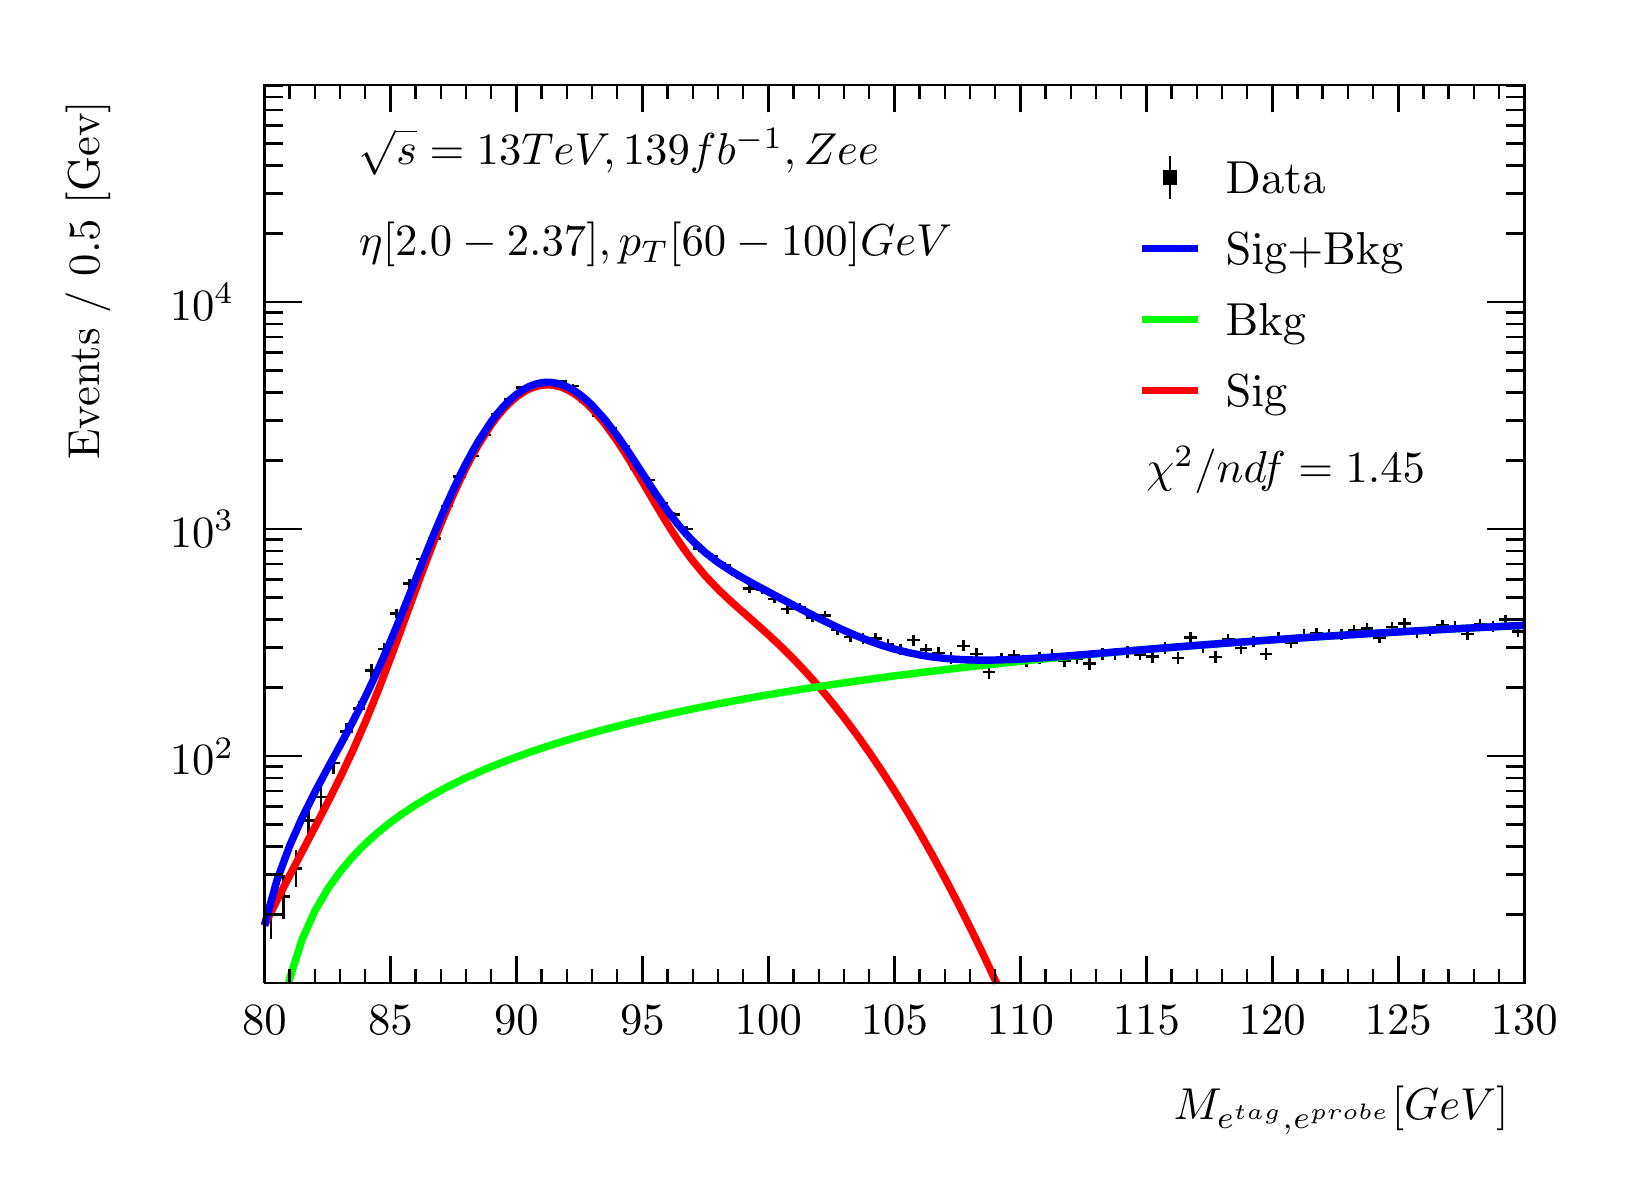
\begin{tikzpicture}
\pgfdeclareplotmark{cross} {
\pgfpathmoveto{\pgfpoint{-0.3\pgfplotmarksize}{\pgfplotmarksize}}
\pgfpathlineto{\pgfpoint{+0.3\pgfplotmarksize}{\pgfplotmarksize}}
\pgfpathlineto{\pgfpoint{+0.3\pgfplotmarksize}{0.3\pgfplotmarksize}}
\pgfpathlineto{\pgfpoint{+1\pgfplotmarksize}{0.3\pgfplotmarksize}}
\pgfpathlineto{\pgfpoint{+1\pgfplotmarksize}{-0.3\pgfplotmarksize}}
\pgfpathlineto{\pgfpoint{+0.3\pgfplotmarksize}{-0.3\pgfplotmarksize}}
\pgfpathlineto{\pgfpoint{+0.3\pgfplotmarksize}{-1.\pgfplotmarksize}}
\pgfpathlineto{\pgfpoint{-0.3\pgfplotmarksize}{-1.\pgfplotmarksize}}
\pgfpathlineto{\pgfpoint{-0.3\pgfplotmarksize}{-0.3\pgfplotmarksize}}
\pgfpathlineto{\pgfpoint{-1.\pgfplotmarksize}{-0.3\pgfplotmarksize}}
\pgfpathlineto{\pgfpoint{-1.\pgfplotmarksize}{0.3\pgfplotmarksize}}
\pgfpathlineto{\pgfpoint{-0.3\pgfplotmarksize}{0.3\pgfplotmarksize}}
\pgfpathclose
\pgfusepathqstroke
}
\pgfdeclareplotmark{cross*} {
\pgfpathmoveto{\pgfpoint{-0.3\pgfplotmarksize}{\pgfplotmarksize}}
\pgfpathlineto{\pgfpoint{+0.3\pgfplotmarksize}{\pgfplotmarksize}}
\pgfpathlineto{\pgfpoint{+0.3\pgfplotmarksize}{0.3\pgfplotmarksize}}
\pgfpathlineto{\pgfpoint{+1\pgfplotmarksize}{0.3\pgfplotmarksize}}
\pgfpathlineto{\pgfpoint{+1\pgfplotmarksize}{-0.3\pgfplotmarksize}}
\pgfpathlineto{\pgfpoint{+0.3\pgfplotmarksize}{-0.3\pgfplotmarksize}}
\pgfpathlineto{\pgfpoint{+0.3\pgfplotmarksize}{-1.\pgfplotmarksize}}
\pgfpathlineto{\pgfpoint{-0.3\pgfplotmarksize}{-1.\pgfplotmarksize}}
\pgfpathlineto{\pgfpoint{-0.3\pgfplotmarksize}{-0.3\pgfplotmarksize}}
\pgfpathlineto{\pgfpoint{-1.\pgfplotmarksize}{-0.3\pgfplotmarksize}}
\pgfpathlineto{\pgfpoint{-1.\pgfplotmarksize}{0.3\pgfplotmarksize}}
\pgfpathlineto{\pgfpoint{-0.3\pgfplotmarksize}{0.3\pgfplotmarksize}}
\pgfpathclose
\pgfusepathqfillstroke
}
\pgfdeclareplotmark{newstar} {
\pgfpathmoveto{\pgfqpoint{0pt}{\pgfplotmarksize}}
\pgfpathlineto{\pgfqpointpolar{44}{0.5\pgfplotmarksize}}
\pgfpathlineto{\pgfqpointpolar{18}{\pgfplotmarksize}}
\pgfpathlineto{\pgfqpointpolar{-20}{0.5\pgfplotmarksize}}
\pgfpathlineto{\pgfqpointpolar{-54}{\pgfplotmarksize}}
\pgfpathlineto{\pgfqpointpolar{-90}{0.5\pgfplotmarksize}}
\pgfpathlineto{\pgfqpointpolar{234}{\pgfplotmarksize}}
\pgfpathlineto{\pgfqpointpolar{198}{0.5\pgfplotmarksize}}
\pgfpathlineto{\pgfqpointpolar{162}{\pgfplotmarksize}}
\pgfpathlineto{\pgfqpointpolar{134}{0.5\pgfplotmarksize}}
\pgfpathclose
\pgfusepathqstroke
}
\pgfdeclareplotmark{newstar*} {
\pgfpathmoveto{\pgfqpoint{0pt}{\pgfplotmarksize}}
\pgfpathlineto{\pgfqpointpolar{44}{0.5\pgfplotmarksize}}
\pgfpathlineto{\pgfqpointpolar{18}{\pgfplotmarksize}}
\pgfpathlineto{\pgfqpointpolar{-20}{0.5\pgfplotmarksize}}
\pgfpathlineto{\pgfqpointpolar{-54}{\pgfplotmarksize}}
\pgfpathlineto{\pgfqpointpolar{-90}{0.5\pgfplotmarksize}}
\pgfpathlineto{\pgfqpointpolar{234}{\pgfplotmarksize}}
\pgfpathlineto{\pgfqpointpolar{198}{0.5\pgfplotmarksize}}
\pgfpathlineto{\pgfqpointpolar{162}{\pgfplotmarksize}}
\pgfpathlineto{\pgfqpointpolar{134}{0.5\pgfplotmarksize}}
\pgfpathclose
\pgfusepathqfillstroke
}
\definecolor{c}{rgb}{1,1,1};
\draw [color=c, fill=c] (0,0) rectangle (20,14.4361);
\draw [color=c, fill=c] (3,2.30977) rectangle (19,13.7143);
\definecolor{c}{rgb}{0,0,0};
\draw [c,line width=0.9] (3,2.30977) -- (3,13.7143) -- (19,13.7143) -- (19,2.30977) -- (3,2.30977);
\definecolor{c}{rgb}{1,1,1};
\draw [color=c, fill=c] (3,2.30977) rectangle (19,13.7143);
\definecolor{c}{rgb}{0,0,0};
\draw [c,line width=0.9] (3,2.30977) -- (3,13.7143) -- (19,13.7143) -- (19,2.30977) -- (3,2.30977);
\draw [c,line width=0.9] (3,2.30977) -- (19,2.30977);
\draw [c,line width=0.9] (3,2.65624) -- (3,2.30977);
\draw [c,line width=0.9] (3.32,2.48301) -- (3.32,2.30977);
\draw [c,line width=0.9] (3.64,2.48301) -- (3.64,2.30977);
\draw [c,line width=0.9] (3.96,2.48301) -- (3.96,2.30977);
\draw [c,line width=0.9] (4.28,2.48301) -- (4.28,2.30977);
\draw [c,line width=0.9] (4.6,2.65624) -- (4.6,2.30977);
\draw [c,line width=0.9] (4.92,2.48301) -- (4.92,2.30977);
\draw [c,line width=0.9] (5.24,2.48301) -- (5.24,2.30977);
\draw [c,line width=0.9] (5.56,2.48301) -- (5.56,2.30977);
\draw [c,line width=0.9] (5.88,2.48301) -- (5.88,2.30977);
\draw [c,line width=0.9] (6.2,2.65624) -- (6.2,2.30977);
\draw [c,line width=0.9] (6.52,2.48301) -- (6.52,2.30977);
\draw [c,line width=0.9] (6.84,2.48301) -- (6.84,2.30977);
\draw [c,line width=0.9] (7.16,2.48301) -- (7.16,2.30977);
\draw [c,line width=0.9] (7.48,2.48301) -- (7.48,2.30977);
\draw [c,line width=0.9] (7.8,2.65624) -- (7.8,2.30977);
\draw [c,line width=0.9] (8.12,2.48301) -- (8.12,2.30977);
\draw [c,line width=0.9] (8.44,2.48301) -- (8.44,2.30977);
\draw [c,line width=0.9] (8.76,2.48301) -- (8.76,2.30977);
\draw [c,line width=0.9] (9.08,2.48301) -- (9.08,2.30977);
\draw [c,line width=0.9] (9.4,2.65624) -- (9.4,2.30977);
\draw [c,line width=0.9] (9.72,2.48301) -- (9.72,2.30977);
\draw [c,line width=0.9] (10.04,2.48301) -- (10.04,2.30977);
\draw [c,line width=0.9] (10.36,2.48301) -- (10.36,2.30977);
\draw [c,line width=0.9] (10.68,2.48301) -- (10.68,2.30977);
\draw [c,line width=0.9] (11,2.65624) -- (11,2.30977);
\draw [c,line width=0.9] (11.32,2.48301) -- (11.32,2.30977);
\draw [c,line width=0.9] (11.64,2.48301) -- (11.64,2.30977);
\draw [c,line width=0.9] (11.96,2.48301) -- (11.96,2.30977);
\draw [c,line width=0.9] (12.28,2.48301) -- (12.28,2.30977);
\draw [c,line width=0.9] (12.6,2.65624) -- (12.6,2.30977);
\draw [c,line width=0.9] (12.92,2.48301) -- (12.92,2.30977);
\draw [c,line width=0.9] (13.24,2.48301) -- (13.24,2.30977);
\draw [c,line width=0.9] (13.56,2.48301) -- (13.56,2.30977);
\draw [c,line width=0.9] (13.88,2.48301) -- (13.88,2.30977);
\draw [c,line width=0.9] (14.2,2.65624) -- (14.2,2.30977);
\draw [c,line width=0.9] (14.52,2.48301) -- (14.52,2.30977);
\draw [c,line width=0.9] (14.84,2.48301) -- (14.84,2.30977);
\draw [c,line width=0.9] (15.16,2.48301) -- (15.16,2.30977);
\draw [c,line width=0.9] (15.48,2.48301) -- (15.48,2.30977);
\draw [c,line width=0.9] (15.8,2.65624) -- (15.8,2.30977);
\draw [c,line width=0.9] (16.12,2.48301) -- (16.12,2.30977);
\draw [c,line width=0.9] (16.44,2.48301) -- (16.44,2.30977);
\draw [c,line width=0.9] (16.76,2.48301) -- (16.76,2.30977);
\draw [c,line width=0.9] (17.08,2.48301) -- (17.08,2.30977);
\draw [c,line width=0.9] (17.4,2.65624) -- (17.4,2.30977);
\draw [c,line width=0.9] (17.72,2.48301) -- (17.72,2.30977);
\draw [c,line width=0.9] (18.04,2.48301) -- (18.04,2.30977);
\draw [c,line width=0.9] (18.36,2.48301) -- (18.36,2.30977);
\draw [c,line width=0.9] (18.68,2.48301) -- (18.68,2.30977);
\draw [c,line width=0.9] (19,2.65624) -- (19,2.30977);
\draw [anchor=base] (3,1.66015) node[scale=1.61424, color=c, rotate=0]{80};
\draw [anchor=base] (4.6,1.66015) node[scale=1.61424, color=c, rotate=0]{85};
\draw [anchor=base] (6.2,1.66015) node[scale=1.61424, color=c, rotate=0]{90};
\draw [anchor=base] (7.8,1.66015) node[scale=1.61424, color=c, rotate=0]{95};
\draw [anchor=base] (9.4,1.66015) node[scale=1.61424, color=c, rotate=0]{100};
\draw [anchor=base] (11,1.66015) node[scale=1.61424, color=c, rotate=0]{105};
\draw [anchor=base] (12.6,1.66015) node[scale=1.61424, color=c, rotate=0]{110};
\draw [anchor=base] (14.2,1.66015) node[scale=1.61424, color=c, rotate=0]{115};
\draw [anchor=base] (15.8,1.66015) node[scale=1.61424, color=c, rotate=0]{120};
\draw [anchor=base] (17.4,1.66015) node[scale=1.61424, color=c, rotate=0]{125};
\draw [anchor=base] (19,1.66015) node[scale=1.61424, color=c, rotate=0]{130};
\draw [anchor= east] (19,0.692932) node[scale=1.61424, color=c, rotate=0]{$M_{e^{tag}, e^{probe}}  [GeV]$};
\draw [c,line width=0.9] (3,13.7143) -- (19,13.7143);
\draw [c,line width=0.9] (3,13.3678) -- (3,13.7143);
\draw [c,line width=0.9] (3.32,13.5411) -- (3.32,13.7143);
\draw [c,line width=0.9] (3.64,13.5411) -- (3.64,13.7143);
\draw [c,line width=0.9] (3.96,13.5411) -- (3.96,13.7143);
\draw [c,line width=0.9] (4.28,13.5411) -- (4.28,13.7143);
\draw [c,line width=0.9] (4.6,13.3678) -- (4.6,13.7143);
\draw [c,line width=0.9] (4.92,13.5411) -- (4.92,13.7143);
\draw [c,line width=0.9] (5.24,13.5411) -- (5.24,13.7143);
\draw [c,line width=0.9] (5.56,13.5411) -- (5.56,13.7143);
\draw [c,line width=0.9] (5.88,13.5411) -- (5.88,13.7143);
\draw [c,line width=0.9] (6.2,13.3678) -- (6.2,13.7143);
\draw [c,line width=0.9] (6.52,13.5411) -- (6.52,13.7143);
\draw [c,line width=0.9] (6.84,13.5411) -- (6.84,13.7143);
\draw [c,line width=0.9] (7.16,13.5411) -- (7.16,13.7143);
\draw [c,line width=0.9] (7.48,13.5411) -- (7.48,13.7143);
\draw [c,line width=0.9] (7.8,13.3678) -- (7.8,13.7143);
\draw [c,line width=0.9] (8.12,13.5411) -- (8.12,13.7143);
\draw [c,line width=0.9] (8.44,13.5411) -- (8.44,13.7143);
\draw [c,line width=0.9] (8.76,13.5411) -- (8.76,13.7143);
\draw [c,line width=0.9] (9.08,13.5411) -- (9.08,13.7143);
\draw [c,line width=0.9] (9.4,13.3678) -- (9.4,13.7143);
\draw [c,line width=0.9] (9.72,13.5411) -- (9.72,13.7143);
\draw [c,line width=0.9] (10.04,13.5411) -- (10.04,13.7143);
\draw [c,line width=0.9] (10.36,13.5411) -- (10.36,13.7143);
\draw [c,line width=0.9] (10.68,13.5411) -- (10.68,13.7143);
\draw [c,line width=0.9] (11,13.3678) -- (11,13.7143);
\draw [c,line width=0.9] (11.32,13.5411) -- (11.32,13.7143);
\draw [c,line width=0.9] (11.64,13.5411) -- (11.64,13.7143);
\draw [c,line width=0.9] (11.96,13.5411) -- (11.96,13.7143);
\draw [c,line width=0.9] (12.28,13.5411) -- (12.28,13.7143);
\draw [c,line width=0.9] (12.6,13.3678) -- (12.6,13.7143);
\draw [c,line width=0.9] (12.92,13.5411) -- (12.92,13.7143);
\draw [c,line width=0.9] (13.24,13.5411) -- (13.24,13.7143);
\draw [c,line width=0.9] (13.56,13.5411) -- (13.56,13.7143);
\draw [c,line width=0.9] (13.88,13.5411) -- (13.88,13.7143);
\draw [c,line width=0.9] (14.2,13.3678) -- (14.2,13.7143);
\draw [c,line width=0.9] (14.52,13.5411) -- (14.52,13.7143);
\draw [c,line width=0.9] (14.84,13.5411) -- (14.84,13.7143);
\draw [c,line width=0.9] (15.16,13.5411) -- (15.16,13.7143);
\draw [c,line width=0.9] (15.48,13.5411) -- (15.48,13.7143);
\draw [c,line width=0.9] (15.8,13.3678) -- (15.8,13.7143);
\draw [c,line width=0.9] (16.12,13.5411) -- (16.12,13.7143);
\draw [c,line width=0.9] (16.44,13.5411) -- (16.44,13.7143);
\draw [c,line width=0.9] (16.76,13.5411) -- (16.76,13.7143);
\draw [c,line width=0.9] (17.08,13.5411) -- (17.08,13.7143);
\draw [c,line width=0.9] (17.4,13.3678) -- (17.4,13.7143);
\draw [c,line width=0.9] (17.72,13.5411) -- (17.72,13.7143);
\draw [c,line width=0.9] (18.04,13.5411) -- (18.04,13.7143);
\draw [c,line width=0.9] (18.36,13.5411) -- (18.36,13.7143);
\draw [c,line width=0.9] (18.68,13.5411) -- (18.68,13.7143);
\draw [c,line width=0.9] (19,13.3678) -- (19,13.7143);
\draw [c,line width=0.9] (3,2.30977) -- (3,13.7143);
\draw [c,line width=0.9] (3.237,3.17769) -- (3,3.17769);
\draw [c,line width=0.9] (3.237,3.68539) -- (3,3.68539);
\draw [c,line width=0.9] (3.237,4.04561) -- (3,4.04561);
\draw [c,line width=0.9] (3.237,4.32501) -- (3,4.32501);
\draw [c,line width=0.9] (3.237,4.55331) -- (3,4.55331);
\draw [c,line width=0.9] (3.237,4.74632) -- (3,4.74632);
\draw [c,line width=0.9] (3.237,4.91352) -- (3,4.91352);
\draw [c,line width=0.9] (3.237,5.061) -- (3,5.061);
\draw [c,line width=0.9] (3.474,5.19293) -- (3,5.19293);
\draw [anchor= east] (2.82,5.19293) node[scale=1.61424, color=c, rotate=0]{$10^{2}$};
\draw [c,line width=0.9] (3.237,6.06085) -- (3,6.06085);
\draw [c,line width=0.9] (3.237,6.56855) -- (3,6.56855);
\draw [c,line width=0.9] (3.237,6.92876) -- (3,6.92876);
\draw [c,line width=0.9] (3.237,7.20817) -- (3,7.20817);
\draw [c,line width=0.9] (3.237,7.43646) -- (3,7.43646);
\draw [c,line width=0.9] (3.237,7.62948) -- (3,7.62948);
\draw [c,line width=0.9] (3.237,7.79668) -- (3,7.79668);
\draw [c,line width=0.9] (3.237,7.94416) -- (3,7.94416);
\draw [c,line width=0.9] (3.474,8.07609) -- (3,8.07609);
\draw [anchor= east] (2.82,8.07609) node[scale=1.61424, color=c, rotate=0]{$10^{3}$};
\draw [c,line width=0.9] (3.237,8.94401) -- (3,8.94401);
\draw [c,line width=0.9] (3.237,9.4517) -- (3,9.4517);
\draw [c,line width=0.9] (3.237,9.81192) -- (3,9.81192);
\draw [c,line width=0.9] (3.237,10.0913) -- (3,10.0913);
\draw [c,line width=0.9] (3.237,10.3196) -- (3,10.3196);
\draw [c,line width=0.9] (3.237,10.5126) -- (3,10.5126);
\draw [c,line width=0.9] (3.237,10.6798) -- (3,10.6798);
\draw [c,line width=0.9] (3.237,10.8273) -- (3,10.8273);
\draw [c,line width=0.9] (3.474,10.9592) -- (3,10.9592);
\draw [anchor= east] (2.82,10.9592) node[scale=1.61424, color=c, rotate=0]{$10^{4}$};
\draw [c,line width=0.9] (3.237,11.8272) -- (3,11.8272);
\draw [c,line width=0.9] (3.237,12.3349) -- (3,12.3349);
\draw [c,line width=0.9] (3.237,12.6951) -- (3,12.6951);
\draw [c,line width=0.9] (3.237,12.9745) -- (3,12.9745);
\draw [c,line width=0.9] (3.237,13.2028) -- (3,13.2028);
\draw [c,line width=0.9] (3.237,13.3958) -- (3,13.3958);
\draw [c,line width=0.9] (3.237,13.563) -- (3,13.563);
\draw [c,line width=0.9] (3.237,13.7105) -- (3,13.7105);
\draw [anchor= east] (0.76,13.7143) node[scale=1.61424, color=c, rotate=90]{Events / 0.5 [Gev]};
\draw [c,line width=0.9] (19,2.30977) -- (19,13.7143);
\draw [c,line width=0.9] (18.763,3.17769) -- (19,3.17769);
\draw [c,line width=0.9] (18.763,3.68539) -- (19,3.68539);
\draw [c,line width=0.9] (18.763,4.04561) -- (19,4.04561);
\draw [c,line width=0.9] (18.763,4.32501) -- (19,4.32501);
\draw [c,line width=0.9] (18.763,4.55331) -- (19,4.55331);
\draw [c,line width=0.9] (18.763,4.74632) -- (19,4.74632);
\draw [c,line width=0.9] (18.763,4.91352) -- (19,4.91352);
\draw [c,line width=0.9] (18.763,5.061) -- (19,5.061);
\draw [c,line width=0.9] (18.526,5.19293) -- (19,5.19293);
\draw [c,line width=0.9] (18.763,6.06085) -- (19,6.06085);
\draw [c,line width=0.9] (18.763,6.56855) -- (19,6.56855);
\draw [c,line width=0.9] (18.763,6.92876) -- (19,6.92876);
\draw [c,line width=0.9] (18.763,7.20817) -- (19,7.20817);
\draw [c,line width=0.9] (18.763,7.43646) -- (19,7.43646);
\draw [c,line width=0.9] (18.763,7.62948) -- (19,7.62948);
\draw [c,line width=0.9] (18.763,7.79668) -- (19,7.79668);
\draw [c,line width=0.9] (18.763,7.94416) -- (19,7.94416);
\draw [c,line width=0.9] (18.526,8.07609) -- (19,8.07609);
\draw [c,line width=0.9] (18.763,8.94401) -- (19,8.94401);
\draw [c,line width=0.9] (18.763,9.4517) -- (19,9.4517);
\draw [c,line width=0.9] (18.763,9.81192) -- (19,9.81192);
\draw [c,line width=0.9] (18.763,10.0913) -- (19,10.0913);
\draw [c,line width=0.9] (18.763,10.3196) -- (19,10.3196);
\draw [c,line width=0.9] (18.763,10.5126) -- (19,10.5126);
\draw [c,line width=0.9] (18.763,10.6798) -- (19,10.6798);
\draw [c,line width=0.9] (18.763,10.8273) -- (19,10.8273);
\draw [c,line width=0.9] (18.526,10.9592) -- (19,10.9592);
\draw [c,line width=0.9] (18.763,11.8272) -- (19,11.8272);
\draw [c,line width=0.9] (18.763,12.3349) -- (19,12.3349);
\draw [c,line width=0.9] (18.763,12.6951) -- (19,12.6951);
\draw [c,line width=0.9] (18.763,12.9745) -- (19,12.9745);
\draw [c,line width=0.9] (18.763,13.2028) -- (19,13.2028);
\draw [c,line width=0.9] (18.763,13.3958) -- (19,13.3958);
\draw [c,line width=0.9] (18.763,13.563) -- (19,13.563);
\draw [c,line width=0.9] (18.763,13.7105) -- (19,13.7105);
\draw [c,line width=0.9] (3.08,3.17769) -- (3,3.17769);
\draw [c,line width=0.9] (3,3.17769) -- (3,3.17769);
\draw [c,line width=0.9] (3.08,3.17769) -- (3.16,3.17769);
\draw [c,line width=0.9] (3.16,3.17769) -- (3.16,3.17769);
\draw [c,line width=0.9] (3.08,3.17769) -- (3.08,3.48418);
\draw [c,line width=0.9] (3.08,3.48418) -- (3.08,3.48418);
\draw [c,line width=0.9] (3.08,3.17769) -- (3.08,2.86382);
\draw [c,line width=0.9] (3.08,2.86382) -- (3.08,2.86382);
\draw [c,line width=0.9] (3.24,3.40598) -- (3.16,3.40598);
\draw [c,line width=0.9] (3.16,3.40598) -- (3.16,3.40598);
\draw [c,line width=0.9] (3.24,3.40598) -- (3.32,3.40598);
\draw [c,line width=0.9] (3.32,3.40598) -- (3.32,3.40598);
\draw [c,line width=0.9] (3.24,3.40598) -- (3.24,3.68401);
\draw [c,line width=0.9] (3.24,3.68401) -- (3.24,3.68401);
\draw [c,line width=0.9] (3.24,3.40598) -- (3.24,3.12236);
\draw [c,line width=0.9] (3.24,3.12236) -- (3.24,3.12236);
\draw [c,line width=0.9] (3.4,3.7662) -- (3.32,3.7662);
\draw [c,line width=0.9] (3.32,3.7662) -- (3.32,3.7662);
\draw [c,line width=0.9] (3.4,3.7662) -- (3.48,3.7662);
\draw [c,line width=0.9] (3.48,3.7662) -- (3.48,3.7662);
\draw [c,line width=0.9] (3.4,3.7662) -- (3.4,4.00475);
\draw [c,line width=0.9] (3.4,4.00475) -- (3.4,4.00475);
\draw [c,line width=0.9] (3.4,3.7662) -- (3.4,3.52404);
\draw [c,line width=0.9] (3.4,3.52404) -- (3.4,3.52404);
\draw [c,line width=0.9] (3.56,4.37413) -- (3.48,4.37413);
\draw [c,line width=0.9] (3.48,4.37413) -- (3.48,4.37413);
\draw [c,line width=0.9] (3.56,4.37413) -- (3.64,4.37413);
\draw [c,line width=0.9] (3.64,4.37413) -- (3.64,4.37413);
\draw [c,line width=0.9] (3.56,4.37413) -- (3.56,4.55867);
\draw [c,line width=0.9] (3.56,4.55867) -- (3.56,4.55867);
\draw [c,line width=0.9] (3.56,4.37413) -- (3.56,4.18785);
\draw [c,line width=0.9] (3.56,4.18785) -- (3.56,4.18785);
\draw [c,line width=0.9] (3.72,4.67265) -- (3.64,4.67265);
\draw [c,line width=0.9] (3.64,4.67265) -- (3.64,4.67265);
\draw [c,line width=0.9] (3.72,4.67265) -- (3.8,4.67265);
\draw [c,line width=0.9] (3.8,4.67265) -- (3.8,4.67265);
\draw [c,line width=0.9] (3.72,4.67265) -- (3.72,4.83547);
\draw [c,line width=0.9] (3.72,4.83547) -- (3.72,4.83547);
\draw [c,line width=0.9] (3.72,4.67265) -- (3.72,4.50862);
\draw [c,line width=0.9] (3.72,4.50862) -- (3.72,4.50862);
\draw [c,line width=0.9] (3.88,5.10206) -- (3.8,5.10206);
\draw [c,line width=0.9] (3.8,5.10206) -- (3.8,5.10206);
\draw [c,line width=0.9] (3.88,5.10206) -- (3.96,5.10206);
\draw [c,line width=0.9] (3.96,5.10206) -- (3.96,5.10206);
\draw [c,line width=0.9] (3.88,5.10206) -- (3.88,5.23816);
\draw [c,line width=0.9] (3.88,5.23816) -- (3.88,5.23816);
\draw [c,line width=0.9] (3.88,5.10206) -- (3.88,4.96525);
\draw [c,line width=0.9] (3.88,4.96525) -- (3.88,4.96525);
\draw [c,line width=0.9] (4.04,5.50204) -- (3.96,5.50204);
\draw [c,line width=0.9] (3.96,5.50204) -- (3.96,5.50204);
\draw [c,line width=0.9] (4.04,5.50204) -- (4.12,5.50204);
\draw [c,line width=0.9] (4.12,5.50204) -- (4.12,5.50204);
\draw [c,line width=0.9] (4.04,5.50204) -- (4.04,5.61267);
\draw [c,line width=0.9] (4.04,5.61267) -- (4.04,5.61267);
\draw [c,line width=0.9] (4.04,5.50204) -- (4.04,5.3914);
\draw [c,line width=0.9] (4.04,5.3914) -- (4.04,5.3914);
\draw [c,line width=0.9] (4.2,5.797) -- (4.12,5.797);
\draw [c,line width=0.9] (4.12,5.797) -- (4.12,5.797);
\draw [c,line width=0.9] (4.2,5.797) -- (4.28,5.797);
\draw [c,line width=0.9] (4.28,5.797) -- (4.28,5.797);
\draw [c,line width=0.9] (4.2,5.797) -- (4.2,5.89535);
\draw [c,line width=0.9] (4.2,5.89535) -- (4.2,5.89535);
\draw [c,line width=0.9] (4.2,5.797) -- (4.2,5.69865);
\draw [c,line width=0.9] (4.2,5.69865) -- (4.2,5.69865);
\draw [c,line width=0.9] (4.36,6.27866) -- (4.28,6.27866);
\draw [c,line width=0.9] (4.28,6.27866) -- (4.28,6.27866);
\draw [c,line width=0.9] (4.36,6.27866) -- (4.44,6.27866);
\draw [c,line width=0.9] (4.44,6.27866) -- (4.44,6.27866);
\draw [c,line width=0.9] (4.36,6.27866) -- (4.36,6.35981);
\draw [c,line width=0.9] (4.36,6.35981) -- (4.36,6.35981);
\draw [c,line width=0.9] (4.36,6.27866) -- (4.36,6.19751);
\draw [c,line width=0.9] (4.36,6.19751) -- (4.36,6.19751);
\draw [c,line width=0.9] (4.52,6.55174) -- (4.44,6.55174);
\draw [c,line width=0.9] (4.44,6.55174) -- (4.44,6.55174);
\draw [c,line width=0.9] (4.52,6.55174) -- (4.6,6.55174);
\draw [c,line width=0.9] (4.6,6.55174) -- (4.6,6.55174);
\draw [c,line width=0.9] (4.52,6.55174) -- (4.52,6.62451);
\draw [c,line width=0.9] (4.52,6.62451) -- (4.52,6.62451);
\draw [c,line width=0.9] (4.52,6.55174) -- (4.52,6.47897);
\draw [c,line width=0.9] (4.52,6.47897) -- (4.52,6.47897);
\draw [c,line width=0.9] (4.68,7.00468) -- (4.6,7.00468);
\draw [c,line width=0.9] (4.6,7.00468) -- (4.6,7.00468);
\draw [c,line width=0.9] (4.68,7.00468) -- (4.76,7.00468);
\draw [c,line width=0.9] (4.76,7.00468) -- (4.76,7.00468);
\draw [c,line width=0.9] (4.68,7.00468) -- (4.68,7.06541);
\draw [c,line width=0.9] (4.68,7.06541) -- (4.68,7.06541);
\draw [c,line width=0.9] (4.68,7.00468) -- (4.68,6.94394);
\draw [c,line width=0.9] (4.68,6.94394) -- (4.68,6.94394);
\draw [c,line width=0.9] (4.84,7.38317) -- (4.76,7.38317);
\draw [c,line width=0.9] (4.76,7.38317) -- (4.76,7.38317);
\draw [c,line width=0.9] (4.84,7.38317) -- (4.92,7.38317);
\draw [c,line width=0.9] (4.92,7.38317) -- (4.92,7.38317);
\draw [c,line width=0.9] (4.84,7.38317) -- (4.84,7.43539);
\draw [c,line width=0.9] (4.84,7.43539) -- (4.84,7.43539);
\draw [c,line width=0.9] (4.84,7.38317) -- (4.84,7.33096);
\draw [c,line width=0.9] (4.84,7.33096) -- (4.84,7.33096);
\draw [c,line width=0.9] (5,7.69398) -- (4.92,7.69398);
\draw [c,line width=0.9] (4.92,7.69398) -- (4.92,7.69398);
\draw [c,line width=0.9] (5,7.69398) -- (5.08,7.69398);
\draw [c,line width=0.9] (5.08,7.69398) -- (5.08,7.69398);
\draw [c,line width=0.9] (5,7.69398) -- (5,7.7401);
\draw [c,line width=0.9] (5,7.7401) -- (5,7.7401);
\draw [c,line width=0.9] (5,7.69398) -- (5,7.64786);
\draw [c,line width=0.9] (5,7.64786) -- (5,7.64786);
\draw [c,line width=0.9] (5.16,7.95387) -- (5.08,7.95387);
\draw [c,line width=0.9] (5.08,7.95387) -- (5.08,7.95387);
\draw [c,line width=0.9] (5.16,7.95387) -- (5.24,7.95387);
\draw [c,line width=0.9] (5.24,7.95387) -- (5.24,7.95387);
\draw [c,line width=0.9] (5.16,7.95387) -- (5.16,7.99544);
\draw [c,line width=0.9] (5.16,7.99544) -- (5.16,7.99544);
\draw [c,line width=0.9] (5.16,7.95387) -- (5.16,7.91229);
\draw [c,line width=0.9] (5.16,7.91229) -- (5.16,7.91229);
\draw [c,line width=0.9] (5.32,8.37043) -- (5.24,8.37043);
\draw [c,line width=0.9] (5.24,8.37043) -- (5.24,8.37043);
\draw [c,line width=0.9] (5.32,8.37043) -- (5.4,8.37043);
\draw [c,line width=0.9] (5.4,8.37043) -- (5.4,8.37043);
\draw [c,line width=0.9] (5.32,8.37043) -- (5.32,8.40564);
\draw [c,line width=0.9] (5.32,8.40564) -- (5.32,8.40564);
\draw [c,line width=0.9] (5.32,8.37043) -- (5.32,8.33523);
\draw [c,line width=0.9] (5.32,8.33523) -- (5.32,8.33523);
\draw [c,line width=0.9] (5.48,8.74272) -- (5.4,8.74272);
\draw [c,line width=0.9] (5.4,8.74272) -- (5.4,8.74272);
\draw [c,line width=0.9] (5.48,8.74272) -- (5.56,8.74272);
\draw [c,line width=0.9] (5.56,8.74272) -- (5.56,8.74272);
\draw [c,line width=0.9] (5.48,8.74272) -- (5.48,8.77306);
\draw [c,line width=0.9] (5.48,8.77306) -- (5.48,8.77306);
\draw [c,line width=0.9] (5.48,8.74272) -- (5.48,8.71238);
\draw [c,line width=0.9] (5.48,8.71238) -- (5.48,8.71238);
\draw [c,line width=0.9] (5.64,9.0045) -- (5.56,9.0045);
\draw [c,line width=0.9] (5.56,9.0045) -- (5.56,9.0045);
\draw [c,line width=0.9] (5.64,9.0045) -- (5.72,9.0045);
\draw [c,line width=0.9] (5.72,9.0045) -- (5.72,9.0045);
\draw [c,line width=0.9] (5.64,9.0045) -- (5.64,9.03183);
\draw [c,line width=0.9] (5.64,9.03183) -- (5.64,9.03183);
\draw [c,line width=0.9] (5.64,9.0045) -- (5.64,8.97717);
\draw [c,line width=0.9] (5.64,8.97717) -- (5.64,8.97717);
\draw [c,line width=0.9] (5.8,9.26915) -- (5.72,9.26915);
\draw [c,line width=0.9] (5.72,9.26915) -- (5.72,9.26915);
\draw [c,line width=0.9] (5.8,9.26915) -- (5.88,9.26915);
\draw [c,line width=0.9] (5.88,9.26915) -- (5.88,9.26915);
\draw [c,line width=0.9] (5.8,9.26915) -- (5.8,9.29374);
\draw [c,line width=0.9] (5.8,9.29374) -- (5.8,9.29374);
\draw [c,line width=0.9] (5.8,9.26915) -- (5.8,9.24456);
\draw [c,line width=0.9] (5.8,9.24456) -- (5.8,9.24456);
\draw [c,line width=0.9] (5.96,9.53525) -- (5.88,9.53525);
\draw [c,line width=0.9] (5.88,9.53525) -- (5.88,9.53525);
\draw [c,line width=0.9] (5.96,9.53525) -- (6.04,9.53525);
\draw [c,line width=0.9] (6.04,9.53525) -- (6.04,9.53525);
\draw [c,line width=0.9] (5.96,9.53525) -- (5.96,9.55736);
\draw [c,line width=0.9] (5.96,9.55736) -- (5.96,9.55736);
\draw [c,line width=0.9] (5.96,9.53525) -- (5.96,9.51314);
\draw [c,line width=0.9] (5.96,9.51314) -- (5.96,9.51314);
\draw [c,line width=0.9] (6.12,9.72206) -- (6.04,9.72206);
\draw [c,line width=0.9] (6.04,9.72206) -- (6.04,9.72206);
\draw [c,line width=0.9] (6.12,9.72206) -- (6.2,9.72206);
\draw [c,line width=0.9] (6.2,9.72206) -- (6.2,9.72206);
\draw [c,line width=0.9] (6.12,9.72206) -- (6.12,9.74259);
\draw [c,line width=0.9] (6.12,9.74259) -- (6.12,9.74259);
\draw [c,line width=0.9] (6.12,9.72206) -- (6.12,9.70154);
\draw [c,line width=0.9] (6.12,9.70154) -- (6.12,9.70154);
\draw [c,line width=0.9] (6.28,9.87182) -- (6.2,9.87182);
\draw [c,line width=0.9] (6.2,9.87182) -- (6.2,9.87182);
\draw [c,line width=0.9] (6.28,9.87182) -- (6.36,9.87182);
\draw [c,line width=0.9] (6.36,9.87182) -- (6.36,9.87182);
\draw [c,line width=0.9] (6.28,9.87182) -- (6.28,9.89115);
\draw [c,line width=0.9] (6.28,9.89115) -- (6.28,9.89115);
\draw [c,line width=0.9] (6.28,9.87182) -- (6.28,9.85249);
\draw [c,line width=0.9] (6.28,9.85249) -- (6.28,9.85249);
\draw [c,line width=0.9] (6.44,9.9135) -- (6.36,9.9135);
\draw [c,line width=0.9] (6.36,9.9135) -- (6.36,9.9135);
\draw [c,line width=0.9] (6.44,9.9135) -- (6.52,9.9135);
\draw [c,line width=0.9] (6.52,9.9135) -- (6.52,9.9135);
\draw [c,line width=0.9] (6.44,9.9135) -- (6.44,9.93251);
\draw [c,line width=0.9] (6.44,9.93251) -- (6.44,9.93251);
\draw [c,line width=0.9] (6.44,9.9135) -- (6.44,9.89449);
\draw [c,line width=0.9] (6.44,9.89449) -- (6.44,9.89449);
\draw [c,line width=0.9] (6.6,9.94626) -- (6.52,9.94626);
\draw [c,line width=0.9] (6.52,9.94626) -- (6.52,9.94626);
\draw [c,line width=0.9] (6.6,9.94626) -- (6.68,9.94626);
\draw [c,line width=0.9] (6.68,9.94626) -- (6.68,9.94626);
\draw [c,line width=0.9] (6.6,9.94626) -- (6.6,9.96502);
\draw [c,line width=0.9] (6.6,9.96502) -- (6.6,9.96502);
\draw [c,line width=0.9] (6.6,9.94626) -- (6.6,9.92749);
\draw [c,line width=0.9] (6.6,9.92749) -- (6.6,9.92749);
\draw [c,line width=0.9] (6.76,9.95215) -- (6.68,9.95215);
\draw [c,line width=0.9] (6.68,9.95215) -- (6.68,9.95215);
\draw [c,line width=0.9] (6.76,9.95215) -- (6.84,9.95215);
\draw [c,line width=0.9] (6.84,9.95215) -- (6.84,9.95215);
\draw [c,line width=0.9] (6.76,9.95215) -- (6.76,9.97087);
\draw [c,line width=0.9] (6.76,9.97087) -- (6.76,9.97087);
\draw [c,line width=0.9] (6.76,9.95215) -- (6.76,9.93343);
\draw [c,line width=0.9] (6.76,9.93343) -- (6.76,9.93343);
\draw [c,line width=0.9] (6.92,9.89313) -- (6.84,9.89313);
\draw [c,line width=0.9] (6.84,9.89313) -- (6.84,9.89313);
\draw [c,line width=0.9] (6.92,9.89313) -- (7,9.89313);
\draw [c,line width=0.9] (7,9.89313) -- (7,9.89313);
\draw [c,line width=0.9] (6.92,9.89313) -- (6.92,9.91229);
\draw [c,line width=0.9] (6.92,9.91229) -- (6.92,9.91229);
\draw [c,line width=0.9] (6.92,9.89313) -- (6.92,9.87396);
\draw [c,line width=0.9] (6.92,9.87396) -- (6.92,9.87396);
\draw [c,line width=0.9] (7.08,9.69624) -- (7,9.69624);
\draw [c,line width=0.9] (7,9.69624) -- (7,9.69624);
\draw [c,line width=0.9] (7.08,9.69624) -- (7.16,9.69624);
\draw [c,line width=0.9] (7.16,9.69624) -- (7.16,9.69624);
\draw [c,line width=0.9] (7.08,9.69624) -- (7.08,9.71697);
\draw [c,line width=0.9] (7.08,9.71697) -- (7.08,9.71697);
\draw [c,line width=0.9] (7.08,9.69624) -- (7.08,9.67551);
\draw [c,line width=0.9] (7.08,9.67551) -- (7.08,9.67551);
\draw [c,line width=0.9] (7.24,9.51597) -- (7.16,9.51597);
\draw [c,line width=0.9] (7.16,9.51597) -- (7.16,9.51597);
\draw [c,line width=0.9] (7.24,9.51597) -- (7.32,9.51597);
\draw [c,line width=0.9] (7.32,9.51597) -- (7.32,9.51597);
\draw [c,line width=0.9] (7.24,9.51597) -- (7.24,9.53826);
\draw [c,line width=0.9] (7.24,9.53826) -- (7.24,9.53826);
\draw [c,line width=0.9] (7.24,9.51597) -- (7.24,9.49369);
\draw [c,line width=0.9] (7.24,9.49369) -- (7.24,9.49369);
\draw [c,line width=0.9] (7.4,9.35454) -- (7.32,9.35454);
\draw [c,line width=0.9] (7.32,9.35454) -- (7.32,9.35454);
\draw [c,line width=0.9] (7.4,9.35454) -- (7.48,9.35454);
\draw [c,line width=0.9] (7.48,9.35454) -- (7.48,9.35454);
\draw [c,line width=0.9] (7.4,9.35454) -- (7.4,9.3783);
\draw [c,line width=0.9] (7.4,9.3783) -- (7.4,9.3783);
\draw [c,line width=0.9] (7.4,9.35454) -- (7.4,9.33077);
\draw [c,line width=0.9] (7.4,9.33077) -- (7.4,9.33077);
\draw [c,line width=0.9] (7.56,9.12769) -- (7.48,9.12769);
\draw [c,line width=0.9] (7.48,9.12769) -- (7.48,9.12769);
\draw [c,line width=0.9] (7.56,9.12769) -- (7.64,9.12769);
\draw [c,line width=0.9] (7.64,9.12769) -- (7.64,9.12769);
\draw [c,line width=0.9] (7.56,9.12769) -- (7.56,9.15371);
\draw [c,line width=0.9] (7.56,9.15371) -- (7.56,9.15371);
\draw [c,line width=0.9] (7.56,9.12769) -- (7.56,9.10167);
\draw [c,line width=0.9] (7.56,9.10167) -- (7.56,9.10167);
\draw [c,line width=0.9] (7.72,8.84164) -- (7.64,8.84164);
\draw [c,line width=0.9] (7.64,8.84164) -- (7.64,8.84164);
\draw [c,line width=0.9] (7.72,8.84164) -- (7.8,8.84164);
\draw [c,line width=0.9] (7.8,8.84164) -- (7.8,8.84164);
\draw [c,line width=0.9] (7.72,8.84164) -- (7.72,8.87081);
\draw [c,line width=0.9] (7.72,8.87081) -- (7.72,8.87081);
\draw [c,line width=0.9] (7.72,8.84164) -- (7.72,8.81248);
\draw [c,line width=0.9] (7.72,8.81248) -- (7.72,8.81248);
\draw [c,line width=0.9] (7.88,8.70009) -- (7.8,8.70009);
\draw [c,line width=0.9] (7.8,8.70009) -- (7.8,8.70009);
\draw [c,line width=0.9] (7.88,8.70009) -- (7.96,8.70009);
\draw [c,line width=0.9] (7.96,8.70009) -- (7.96,8.70009);
\draw [c,line width=0.9] (7.88,8.70009) -- (7.88,8.73095);
\draw [c,line width=0.9] (7.88,8.73095) -- (7.88,8.73095);
\draw [c,line width=0.9] (7.88,8.70009) -- (7.88,8.66923);
\draw [c,line width=0.9] (7.88,8.66923) -- (7.88,8.66923);
\draw [c,line width=0.9] (8.04,8.40845) -- (7.96,8.40845);
\draw [c,line width=0.9] (7.96,8.40845) -- (7.96,8.40845);
\draw [c,line width=0.9] (8.04,8.40845) -- (8.12,8.40845);
\draw [c,line width=0.9] (8.12,8.40845) -- (8.12,8.40845);
\draw [c,line width=0.9] (8.04,8.40845) -- (8.04,8.44313);
\draw [c,line width=0.9] (8.04,8.44313) -- (8.04,8.44313);
\draw [c,line width=0.9] (8.04,8.40845) -- (8.04,8.37378);
\draw [c,line width=0.9] (8.04,8.37378) -- (8.04,8.37378);
\draw [c,line width=0.9] (8.2,8.25761) -- (8.12,8.25761);
\draw [c,line width=0.9] (8.12,8.25761) -- (8.12,8.25761);
\draw [c,line width=0.9] (8.2,8.25761) -- (8.28,8.25761);
\draw [c,line width=0.9] (8.28,8.25761) -- (8.28,8.25761);
\draw [c,line width=0.9] (8.2,8.25761) -- (8.2,8.29443);
\draw [c,line width=0.9] (8.2,8.29443) -- (8.2,8.29443);
\draw [c,line width=0.9] (8.2,8.25761) -- (8.2,8.22078);
\draw [c,line width=0.9] (8.2,8.22078) -- (8.2,8.22078);
\draw [c,line width=0.9] (8.36,8.07358) -- (8.28,8.07358);
\draw [c,line width=0.9] (8.28,8.07358) -- (8.28,8.07358);
\draw [c,line width=0.9] (8.36,8.07358) -- (8.44,8.07358);
\draw [c,line width=0.9] (8.44,8.07358) -- (8.44,8.07358);
\draw [c,line width=0.9] (8.36,8.07358) -- (8.36,8.11322);
\draw [c,line width=0.9] (8.36,8.11322) -- (8.36,8.11322);
\draw [c,line width=0.9] (8.36,8.07358) -- (8.36,8.03395);
\draw [c,line width=0.9] (8.36,8.03395) -- (8.36,8.03395);
\draw [c,line width=0.9] (8.52,7.82913) -- (8.44,7.82913);
\draw [c,line width=0.9] (8.44,7.82913) -- (8.44,7.82913);
\draw [c,line width=0.9] (8.52,7.82913) -- (8.6,7.82913);
\draw [c,line width=0.9] (8.6,7.82913) -- (8.6,7.82913);
\draw [c,line width=0.9] (8.52,7.82913) -- (8.52,7.87283);
\draw [c,line width=0.9] (8.52,7.87283) -- (8.52,7.87283);
\draw [c,line width=0.9] (8.52,7.82913) -- (8.52,7.78543);
\draw [c,line width=0.9] (8.52,7.78543) -- (8.52,7.78543);
\draw [c,line width=0.9] (8.68,7.73081) -- (8.6,7.73081);
\draw [c,line width=0.9] (8.6,7.73081) -- (8.6,7.73081);
\draw [c,line width=0.9] (8.68,7.73081) -- (8.76,7.73081);
\draw [c,line width=0.9] (8.76,7.73081) -- (8.76,7.73081);
\draw [c,line width=0.9] (8.68,7.73081) -- (8.68,7.77626);
\draw [c,line width=0.9] (8.68,7.77626) -- (8.68,7.77626);
\draw [c,line width=0.9] (8.68,7.73081) -- (8.68,7.68536);
\draw [c,line width=0.9] (8.68,7.68536) -- (8.68,7.68536);
\draw [c,line width=0.9] (8.84,7.60965) -- (8.76,7.60965);
\draw [c,line width=0.9] (8.76,7.60965) -- (8.76,7.60965);
\draw [c,line width=0.9] (8.84,7.60965) -- (8.92,7.60965);
\draw [c,line width=0.9] (8.92,7.60965) -- (8.92,7.60965);
\draw [c,line width=0.9] (8.84,7.60965) -- (8.84,7.65735);
\draw [c,line width=0.9] (8.84,7.65735) -- (8.84,7.65735);
\draw [c,line width=0.9] (8.84,7.60965) -- (8.84,7.56195);
\draw [c,line width=0.9] (8.84,7.56195) -- (8.84,7.56195);
\draw [c,line width=0.9] (9,7.49158) -- (8.92,7.49158);
\draw [c,line width=0.9] (8.92,7.49158) -- (8.92,7.49158);
\draw [c,line width=0.9] (9,7.49158) -- (9.08,7.49158);
\draw [c,line width=0.9] (9.08,7.49158) -- (9.08,7.49158);
\draw [c,line width=0.9] (9,7.49158) -- (9,7.54158);
\draw [c,line width=0.9] (9,7.54158) -- (9,7.54158);
\draw [c,line width=0.9] (9,7.49158) -- (9,7.44158);
\draw [c,line width=0.9] (9,7.44158) -- (9,7.44158);
\draw [c,line width=0.9] (9.16,7.31838) -- (9.08,7.31838);
\draw [c,line width=0.9] (9.08,7.31838) -- (9.08,7.31838);
\draw [c,line width=0.9] (9.16,7.31838) -- (9.24,7.31838);
\draw [c,line width=0.9] (9.24,7.31838) -- (9.24,7.31838);
\draw [c,line width=0.9] (9.16,7.31838) -- (9.16,7.37196);
\draw [c,line width=0.9] (9.16,7.37196) -- (9.16,7.37196);
\draw [c,line width=0.9] (9.16,7.31838) -- (9.16,7.26479);
\draw [c,line width=0.9] (9.16,7.26479) -- (9.16,7.26479);
\draw [c,line width=0.9] (9.32,7.30917) -- (9.24,7.30917);
\draw [c,line width=0.9] (9.24,7.30917) -- (9.24,7.30917);
\draw [c,line width=0.9] (9.32,7.30917) -- (9.4,7.30917);
\draw [c,line width=0.9] (9.4,7.30917) -- (9.4,7.30917);
\draw [c,line width=0.9] (9.32,7.30917) -- (9.32,7.36295);
\draw [c,line width=0.9] (9.32,7.36295) -- (9.32,7.36295);
\draw [c,line width=0.9] (9.32,7.30917) -- (9.32,7.25539);
\draw [c,line width=0.9] (9.32,7.25539) -- (9.32,7.25539);
\draw [c,line width=0.9] (9.48,7.18798) -- (9.4,7.18798);
\draw [c,line width=0.9] (9.4,7.18798) -- (9.4,7.18798);
\draw [c,line width=0.9] (9.48,7.18798) -- (9.56,7.18798);
\draw [c,line width=0.9] (9.56,7.18798) -- (9.56,7.18798);
\draw [c,line width=0.9] (9.48,7.18798) -- (9.48,7.24442);
\draw [c,line width=0.9] (9.48,7.24442) -- (9.48,7.24442);
\draw [c,line width=0.9] (9.48,7.18798) -- (9.48,7.13153);
\draw [c,line width=0.9] (9.48,7.13153) -- (9.48,7.13153);
\draw [c,line width=0.9] (9.64,7.06226) -- (9.56,7.06226);
\draw [c,line width=0.9] (9.56,7.06226) -- (9.56,7.06226);
\draw [c,line width=0.9] (9.64,7.06226) -- (9.72,7.06226);
\draw [c,line width=0.9] (9.72,7.06226) -- (9.72,7.06226);
\draw [c,line width=0.9] (9.64,7.06226) -- (9.64,7.12161);
\draw [c,line width=0.9] (9.64,7.12161) -- (9.64,7.12161);
\draw [c,line width=0.9] (9.64,7.06226) -- (9.64,7.0029);
\draw [c,line width=0.9] (9.64,7.0029) -- (9.64,7.0029);
\draw [c,line width=0.9] (9.8,7.07903) -- (9.72,7.07903);
\draw [c,line width=0.9] (9.72,7.07903) -- (9.72,7.07903);
\draw [c,line width=0.9] (9.8,7.07903) -- (9.88,7.07903);
\draw [c,line width=0.9] (9.88,7.07903) -- (9.88,7.07903);
\draw [c,line width=0.9] (9.8,7.07903) -- (9.8,7.13798);
\draw [c,line width=0.9] (9.8,7.13798) -- (9.8,7.13798);
\draw [c,line width=0.9] (9.8,7.07903) -- (9.8,7.02007);
\draw [c,line width=0.9] (9.8,7.02007) -- (9.8,7.02007);
\draw [c,line width=0.9] (9.96,6.95356) -- (9.88,6.95356);
\draw [c,line width=0.9] (9.88,6.95356) -- (9.88,6.95356);
\draw [c,line width=0.9] (9.96,6.95356) -- (10.04,6.95356);
\draw [c,line width=0.9] (10.04,6.95356) -- (10.04,6.95356);
\draw [c,line width=0.9] (9.96,6.95356) -- (9.96,7.01555);
\draw [c,line width=0.9] (9.96,7.01555) -- (9.96,7.01555);
\draw [c,line width=0.9] (9.96,6.95356) -- (9.96,6.89158);
\draw [c,line width=0.9] (9.96,6.89158) -- (9.96,6.89158);
\draw [c,line width=0.9] (10.12,6.97486) -- (10.04,6.97486);
\draw [c,line width=0.9] (10.04,6.97486) -- (10.04,6.97486);
\draw [c,line width=0.9] (10.12,6.97486) -- (10.2,6.97486);
\draw [c,line width=0.9] (10.2,6.97486) -- (10.2,6.97486);
\draw [c,line width=0.9] (10.12,6.97486) -- (10.12,7.03632);
\draw [c,line width=0.9] (10.12,7.03632) -- (10.12,7.03632);
\draw [c,line width=0.9] (10.12,6.97486) -- (10.12,6.9134);
\draw [c,line width=0.9] (10.12,6.9134) -- (10.12,6.9134);
\draw [c,line width=0.9] (10.28,6.79336) -- (10.2,6.79336);
\draw [c,line width=0.9] (10.2,6.79336) -- (10.2,6.79336);
\draw [c,line width=0.9] (10.28,6.79336) -- (10.36,6.79336);
\draw [c,line width=0.9] (10.36,6.79336) -- (10.36,6.79336);
\draw [c,line width=0.9] (10.28,6.79336) -- (10.28,6.85944);
\draw [c,line width=0.9] (10.28,6.85944) -- (10.28,6.85944);
\draw [c,line width=0.9] (10.28,6.79336) -- (10.28,6.72728);
\draw [c,line width=0.9] (10.28,6.72728) -- (10.28,6.72728);
\draw [c,line width=0.9] (10.44,6.70672) -- (10.36,6.70672);
\draw [c,line width=0.9] (10.36,6.70672) -- (10.36,6.70672);
\draw [c,line width=0.9] (10.44,6.70672) -- (10.52,6.70672);
\draw [c,line width=0.9] (10.52,6.70672) -- (10.52,6.70672);
\draw [c,line width=0.9] (10.44,6.70672) -- (10.44,6.77512);
\draw [c,line width=0.9] (10.44,6.77512) -- (10.44,6.77512);
\draw [c,line width=0.9] (10.44,6.70672) -- (10.44,6.63832);
\draw [c,line width=0.9] (10.44,6.63832) -- (10.44,6.63832);
\draw [c,line width=0.9] (10.6,6.68409) -- (10.52,6.68409);
\draw [c,line width=0.9] (10.52,6.68409) -- (10.52,6.68409);
\draw [c,line width=0.9] (10.6,6.68409) -- (10.68,6.68409);
\draw [c,line width=0.9] (10.68,6.68409) -- (10.68,6.68409);
\draw [c,line width=0.9] (10.6,6.68409) -- (10.6,6.75311);
\draw [c,line width=0.9] (10.6,6.75311) -- (10.6,6.75311);
\draw [c,line width=0.9] (10.6,6.68409) -- (10.6,6.61507);
\draw [c,line width=0.9] (10.6,6.61507) -- (10.6,6.61507);
\draw [c,line width=0.9] (10.76,6.68789) -- (10.68,6.68789);
\draw [c,line width=0.9] (10.68,6.68789) -- (10.68,6.68789);
\draw [c,line width=0.9] (10.76,6.68789) -- (10.84,6.68789);
\draw [c,line width=0.9] (10.84,6.68789) -- (10.84,6.68789);
\draw [c,line width=0.9] (10.76,6.68789) -- (10.76,6.75681);
\draw [c,line width=0.9] (10.76,6.75681) -- (10.76,6.75681);
\draw [c,line width=0.9] (10.76,6.68789) -- (10.76,6.61897);
\draw [c,line width=0.9] (10.76,6.61897) -- (10.76,6.61897);
\draw [c,line width=0.9] (10.92,6.61364) -- (10.84,6.61364);
\draw [c,line width=0.9] (10.84,6.61364) -- (10.84,6.61364);
\draw [c,line width=0.9] (10.92,6.61364) -- (11,6.61364);
\draw [c,line width=0.9] (11,6.61364) -- (11,6.61364);
\draw [c,line width=0.9] (10.92,6.61364) -- (10.92,6.68463);
\draw [c,line width=0.9] (10.92,6.68463) -- (10.92,6.68463);
\draw [c,line width=0.9] (10.92,6.61364) -- (10.92,6.54265);
\draw [c,line width=0.9] (10.92,6.54265) -- (10.92,6.54265);
\draw [c,line width=0.9] (11.08,6.54325) -- (11,6.54325);
\draw [c,line width=0.9] (11,6.54325) -- (11,6.54325);
\draw [c,line width=0.9] (11.08,6.54325) -- (11.16,6.54325);
\draw [c,line width=0.9] (11.16,6.54325) -- (11.16,6.54325);
\draw [c,line width=0.9] (11.08,6.54325) -- (11.08,6.61627);
\draw [c,line width=0.9] (11.08,6.61627) -- (11.08,6.61627);
\draw [c,line width=0.9] (11.08,6.54325) -- (11.08,6.47024);
\draw [c,line width=0.9] (11.08,6.47024) -- (11.08,6.47024);
\draw [c,line width=0.9] (11.24,6.66491) -- (11.16,6.66491);
\draw [c,line width=0.9] (11.16,6.66491) -- (11.16,6.66491);
\draw [c,line width=0.9] (11.24,6.66491) -- (11.32,6.66491);
\draw [c,line width=0.9] (11.32,6.66491) -- (11.32,6.66491);
\draw [c,line width=0.9] (11.24,6.66491) -- (11.24,6.73447);
\draw [c,line width=0.9] (11.24,6.73447) -- (11.24,6.73447);
\draw [c,line width=0.9] (11.24,6.66491) -- (11.24,6.59536);
\draw [c,line width=0.9] (11.24,6.59536) -- (11.24,6.59536);
\draw [c,line width=0.9] (11.4,6.5475) -- (11.32,6.5475);
\draw [c,line width=0.9] (11.32,6.5475) -- (11.32,6.5475);
\draw [c,line width=0.9] (11.4,6.5475) -- (11.48,6.5475);
\draw [c,line width=0.9] (11.48,6.5475) -- (11.48,6.5475);
\draw [c,line width=0.9] (11.4,6.5475) -- (11.4,6.6204);
\draw [c,line width=0.9] (11.4,6.6204) -- (11.4,6.6204);
\draw [c,line width=0.9] (11.4,6.5475) -- (11.4,6.47461);
\draw [c,line width=0.9] (11.4,6.47461) -- (11.4,6.47461);
\draw [c,line width=0.9] (11.56,6.50432) -- (11.48,6.50432);
\draw [c,line width=0.9] (11.48,6.50432) -- (11.48,6.50432);
\draw [c,line width=0.9] (11.56,6.50432) -- (11.64,6.50432);
\draw [c,line width=0.9] (11.64,6.50432) -- (11.64,6.50432);
\draw [c,line width=0.9] (11.56,6.50432) -- (11.56,6.57848);
\draw [c,line width=0.9] (11.56,6.57848) -- (11.56,6.57848);
\draw [c,line width=0.9] (11.56,6.50432) -- (11.56,6.43016);
\draw [c,line width=0.9] (11.56,6.43016) -- (11.56,6.43016);
\draw [c,line width=0.9] (11.72,6.43662) -- (11.64,6.43662);
\draw [c,line width=0.9] (11.64,6.43662) -- (11.64,6.43662);
\draw [c,line width=0.9] (11.72,6.43662) -- (11.8,6.43662);
\draw [c,line width=0.9] (11.8,6.43662) -- (11.8,6.43662);
\draw [c,line width=0.9] (11.72,6.43662) -- (11.72,6.51281);
\draw [c,line width=0.9] (11.72,6.51281) -- (11.72,6.51281);
\draw [c,line width=0.9] (11.72,6.43662) -- (11.72,6.36043);
\draw [c,line width=0.9] (11.72,6.36043) -- (11.72,6.36043);
\draw [c,line width=0.9] (11.88,6.59334) -- (11.8,6.59334);
\draw [c,line width=0.9] (11.8,6.59334) -- (11.8,6.59334);
\draw [c,line width=0.9] (11.88,6.59334) -- (11.96,6.59334);
\draw [c,line width=0.9] (11.96,6.59334) -- (11.96,6.59334);
\draw [c,line width=0.9] (11.88,6.59334) -- (11.88,6.66491);
\draw [c,line width=0.9] (11.88,6.66491) -- (11.88,6.66491);
\draw [c,line width=0.9] (11.88,6.59334) -- (11.88,6.52177);
\draw [c,line width=0.9] (11.88,6.52177) -- (11.88,6.52177);
\draw [c,line width=0.9] (12.04,6.49107) -- (11.96,6.49107);
\draw [c,line width=0.9] (11.96,6.49107) -- (11.96,6.49107);
\draw [c,line width=0.9] (12.04,6.49107) -- (12.12,6.49107);
\draw [c,line width=0.9] (12.12,6.49107) -- (12.12,6.49107);
\draw [c,line width=0.9] (12.04,6.49107) -- (12.04,6.56562);
\draw [c,line width=0.9] (12.04,6.56562) -- (12.04,6.56562);
\draw [c,line width=0.9] (12.04,6.49107) -- (12.04,6.41652);
\draw [c,line width=0.9] (12.04,6.41652) -- (12.04,6.41652);
\draw [c,line width=0.9] (12.2,6.25744) -- (12.12,6.25744);
\draw [c,line width=0.9] (12.12,6.25744) -- (12.12,6.25744);
\draw [c,line width=0.9] (12.2,6.25744) -- (12.28,6.25744);
\draw [c,line width=0.9] (12.28,6.25744) -- (12.28,6.25744);
\draw [c,line width=0.9] (12.2,6.25744) -- (12.2,6.33928);
\draw [c,line width=0.9] (12.2,6.33928) -- (12.2,6.33928);
\draw [c,line width=0.9] (12.2,6.25744) -- (12.2,6.1756);
\draw [c,line width=0.9] (12.2,6.1756) -- (12.2,6.1756);
\draw [c,line width=0.9] (12.36,6.42731) -- (12.28,6.42731);
\draw [c,line width=0.9] (12.28,6.42731) -- (12.28,6.42731);
\draw [c,line width=0.9] (12.36,6.42731) -- (12.44,6.42731);
\draw [c,line width=0.9] (12.44,6.42731) -- (12.44,6.42731);
\draw [c,line width=0.9] (12.36,6.42731) -- (12.36,6.50379);
\draw [c,line width=0.9] (12.36,6.50379) -- (12.36,6.50379);
\draw [c,line width=0.9] (12.36,6.42731) -- (12.36,6.35084);
\draw [c,line width=0.9] (12.36,6.35084) -- (12.36,6.35084);
\draw [c,line width=0.9] (12.52,6.46867) -- (12.44,6.46867);
\draw [c,line width=0.9] (12.44,6.46867) -- (12.44,6.46867);
\draw [c,line width=0.9] (12.52,6.46867) -- (12.6,6.46867);
\draw [c,line width=0.9] (12.6,6.46867) -- (12.6,6.46867);
\draw [c,line width=0.9] (12.52,6.46867) -- (12.52,6.54389);
\draw [c,line width=0.9] (12.52,6.54389) -- (12.52,6.54389);
\draw [c,line width=0.9] (12.52,6.46867) -- (12.52,6.39345);
\draw [c,line width=0.9] (12.52,6.39345) -- (12.52,6.39345);
\draw [c,line width=0.9] (12.68,6.39896) -- (12.6,6.39896);
\draw [c,line width=0.9] (12.6,6.39896) -- (12.6,6.39896);
\draw [c,line width=0.9] (12.68,6.39896) -- (12.76,6.39896);
\draw [c,line width=0.9] (12.76,6.39896) -- (12.76,6.39896);
\draw [c,line width=0.9] (12.68,6.39896) -- (12.68,6.47631);
\draw [c,line width=0.9] (12.68,6.47631) -- (12.68,6.47631);
\draw [c,line width=0.9] (12.68,6.39896) -- (12.68,6.32162);
\draw [c,line width=0.9] (12.68,6.32162) -- (12.68,6.32162);
\draw [c,line width=0.9] (12.84,6.43198) -- (12.76,6.43198);
\draw [c,line width=0.9] (12.76,6.43198) -- (12.76,6.43198);
\draw [c,line width=0.9] (12.84,6.43198) -- (12.92,6.43198);
\draw [c,line width=0.9] (12.92,6.43198) -- (12.92,6.43198);
\draw [c,line width=0.9] (12.84,6.43198) -- (12.84,6.50831);
\draw [c,line width=0.9] (12.84,6.50831) -- (12.84,6.50831);
\draw [c,line width=0.9] (12.84,6.43198) -- (12.84,6.35564);
\draw [c,line width=0.9] (12.84,6.35564) -- (12.84,6.35564);
\draw [c,line width=0.9] (13,6.47318) -- (12.92,6.47318);
\draw [c,line width=0.9] (12.92,6.47318) -- (12.92,6.47318);
\draw [c,line width=0.9] (13,6.47318) -- (13.08,6.47318);
\draw [c,line width=0.9] (13.08,6.47318) -- (13.08,6.47318);
\draw [c,line width=0.9] (13,6.47318) -- (13,6.54827);
\draw [c,line width=0.9] (13,6.54827) -- (13,6.54827);
\draw [c,line width=0.9] (13,6.47318) -- (13,6.3981);
\draw [c,line width=0.9] (13,6.3981) -- (13,6.3981);
\draw [c,line width=0.9] (13.16,6.40373) -- (13.08,6.40373);
\draw [c,line width=0.9] (13.08,6.40373) -- (13.08,6.40373);
\draw [c,line width=0.9] (13.16,6.40373) -- (13.24,6.40373);
\draw [c,line width=0.9] (13.24,6.40373) -- (13.24,6.40373);
\draw [c,line width=0.9] (13.16,6.40373) -- (13.16,6.48093);
\draw [c,line width=0.9] (13.16,6.48093) -- (13.16,6.48093);
\draw [c,line width=0.9] (13.16,6.40373) -- (13.16,6.32653);
\draw [c,line width=0.9] (13.16,6.32653) -- (13.16,6.32653);
\draw [c,line width=0.9] (13.32,6.43198) -- (13.24,6.43198);
\draw [c,line width=0.9] (13.24,6.43198) -- (13.24,6.43198);
\draw [c,line width=0.9] (13.32,6.43198) -- (13.4,6.43198);
\draw [c,line width=0.9] (13.4,6.43198) -- (13.4,6.43198);
\draw [c,line width=0.9] (13.32,6.43198) -- (13.32,6.50831);
\draw [c,line width=0.9] (13.32,6.50831) -- (13.32,6.50831);
\draw [c,line width=0.9] (13.32,6.43198) -- (13.32,6.35564);
\draw [c,line width=0.9] (13.32,6.35564) -- (13.32,6.35564);
\draw [c,line width=0.9] (13.48,6.36995) -- (13.4,6.36995);
\draw [c,line width=0.9] (13.4,6.36995) -- (13.4,6.36995);
\draw [c,line width=0.9] (13.48,6.36995) -- (13.56,6.36995);
\draw [c,line width=0.9] (13.56,6.36995) -- (13.56,6.36995);
\draw [c,line width=0.9] (13.48,6.36995) -- (13.48,6.4482);
\draw [c,line width=0.9] (13.48,6.4482) -- (13.48,6.4482);
\draw [c,line width=0.9] (13.48,6.36995) -- (13.48,6.29171);
\draw [c,line width=0.9] (13.48,6.29171) -- (13.48,6.29171);
\draw [c,line width=0.9] (13.64,6.49107) -- (13.56,6.49107);
\draw [c,line width=0.9] (13.56,6.49107) -- (13.56,6.49107);
\draw [c,line width=0.9] (13.64,6.49107) -- (13.72,6.49107);
\draw [c,line width=0.9] (13.72,6.49107) -- (13.72,6.49107);
\draw [c,line width=0.9] (13.64,6.49107) -- (13.64,6.56562);
\draw [c,line width=0.9] (13.64,6.56562) -- (13.64,6.56562);
\draw [c,line width=0.9] (13.64,6.49107) -- (13.64,6.41652);
\draw [c,line width=0.9] (13.64,6.41652) -- (13.64,6.41652);
\draw [c,line width=0.9] (13.8,6.48662) -- (13.72,6.48662);
\draw [c,line width=0.9] (13.72,6.48662) -- (13.72,6.48662);
\draw [c,line width=0.9] (13.8,6.48662) -- (13.88,6.48662);
\draw [c,line width=0.9] (13.88,6.48662) -- (13.88,6.48662);
\draw [c,line width=0.9] (13.8,6.48662) -- (13.8,6.56131);
\draw [c,line width=0.9] (13.8,6.56131) -- (13.8,6.56131);
\draw [c,line width=0.9] (13.8,6.48662) -- (13.8,6.41194);
\draw [c,line width=0.9] (13.8,6.41194) -- (13.8,6.41194);
\draw [c,line width=0.9] (13.96,6.51743) -- (13.88,6.51743);
\draw [c,line width=0.9] (13.88,6.51743) -- (13.88,6.51743);
\draw [c,line width=0.9] (13.96,6.51743) -- (14.04,6.51743);
\draw [c,line width=0.9] (14.04,6.51743) -- (14.04,6.51743);
\draw [c,line width=0.9] (13.96,6.51743) -- (13.96,6.59121);
\draw [c,line width=0.9] (13.96,6.59121) -- (13.96,6.59121);
\draw [c,line width=0.9] (13.96,6.51743) -- (13.96,6.44366);
\draw [c,line width=0.9] (13.96,6.44366) -- (13.96,6.44366);
\draw [c,line width=0.9] (14.12,6.48216) -- (14.04,6.48216);
\draw [c,line width=0.9] (14.04,6.48216) -- (14.04,6.48216);
\draw [c,line width=0.9] (14.12,6.48216) -- (14.2,6.48216);
\draw [c,line width=0.9] (14.2,6.48216) -- (14.2,6.48216);
\draw [c,line width=0.9] (14.12,6.48216) -- (14.12,6.55698);
\draw [c,line width=0.9] (14.12,6.55698) -- (14.12,6.55698);
\draw [c,line width=0.9] (14.12,6.48216) -- (14.12,6.40734);
\draw [c,line width=0.9] (14.12,6.40734) -- (14.12,6.40734);
\draw [c,line width=0.9] (14.28,6.45504) -- (14.2,6.45504);
\draw [c,line width=0.9] (14.2,6.45504) -- (14.2,6.45504);
\draw [c,line width=0.9] (14.28,6.45504) -- (14.36,6.45504);
\draw [c,line width=0.9] (14.36,6.45504) -- (14.36,6.45504);
\draw [c,line width=0.9] (14.28,6.45504) -- (14.28,6.53067);
\draw [c,line width=0.9] (14.28,6.53067) -- (14.28,6.53067);
\draw [c,line width=0.9] (14.28,6.45504) -- (14.28,6.3794);
\draw [c,line width=0.9] (14.28,6.3794) -- (14.28,6.3794);
\draw [c,line width=0.9] (14.44,6.56437) -- (14.36,6.56437);
\draw [c,line width=0.9] (14.36,6.56437) -- (14.36,6.56437);
\draw [c,line width=0.9] (14.44,6.56437) -- (14.52,6.56437);
\draw [c,line width=0.9] (14.52,6.56437) -- (14.52,6.56437);
\draw [c,line width=0.9] (14.44,6.56437) -- (14.44,6.63677);
\draw [c,line width=0.9] (14.44,6.63677) -- (14.44,6.63677);
\draw [c,line width=0.9] (14.44,6.56437) -- (14.44,6.49196);
\draw [c,line width=0.9] (14.44,6.49196) -- (14.44,6.49196);
\draw [c,line width=0.9] (14.6,6.43662) -- (14.52,6.43662);
\draw [c,line width=0.9] (14.52,6.43662) -- (14.52,6.43662);
\draw [c,line width=0.9] (14.6,6.43662) -- (14.68,6.43662);
\draw [c,line width=0.9] (14.68,6.43662) -- (14.68,6.43662);
\draw [c,line width=0.9] (14.6,6.43662) -- (14.6,6.51281);
\draw [c,line width=0.9] (14.6,6.51281) -- (14.6,6.51281);
\draw [c,line width=0.9] (14.6,6.43662) -- (14.6,6.36043);
\draw [c,line width=0.9] (14.6,6.36043) -- (14.6,6.36043);
\draw [c,line width=0.9] (14.76,6.69546) -- (14.68,6.69546);
\draw [c,line width=0.9] (14.68,6.69546) -- (14.68,6.69546);
\draw [c,line width=0.9] (14.76,6.69546) -- (14.84,6.69546);
\draw [c,line width=0.9] (14.84,6.69546) -- (14.84,6.69546);
\draw [c,line width=0.9] (14.76,6.69546) -- (14.76,6.76417);
\draw [c,line width=0.9] (14.76,6.76417) -- (14.76,6.76417);
\draw [c,line width=0.9] (14.76,6.69546) -- (14.76,6.62674);
\draw [c,line width=0.9] (14.76,6.62674) -- (14.76,6.62674);
\draw [c,line width=0.9] (14.92,6.57687) -- (14.84,6.57687);
\draw [c,line width=0.9] (14.84,6.57687) -- (14.84,6.57687);
\draw [c,line width=0.9] (14.92,6.57687) -- (15,6.57687);
\draw [c,line width=0.9] (15,6.57687) -- (15,6.57687);
\draw [c,line width=0.9] (14.92,6.57687) -- (14.92,6.64891);
\draw [c,line width=0.9] (14.92,6.64891) -- (14.92,6.64891);
\draw [c,line width=0.9] (14.92,6.57687) -- (14.92,6.50483);
\draw [c,line width=0.9] (14.92,6.50483) -- (14.92,6.50483);
\draw [c,line width=0.9] (15.08,6.45046) -- (15,6.45046);
\draw [c,line width=0.9] (15,6.45046) -- (15,6.45046);
\draw [c,line width=0.9] (15.08,6.45046) -- (15.16,6.45046);
\draw [c,line width=0.9] (15.16,6.45046) -- (15.16,6.45046);
\draw [c,line width=0.9] (15.08,6.45046) -- (15.08,6.52623);
\draw [c,line width=0.9] (15.08,6.52623) -- (15.08,6.52623);
\draw [c,line width=0.9] (15.08,6.45046) -- (15.08,6.37469);
\draw [c,line width=0.9] (15.08,6.37469) -- (15.08,6.37469);
\draw [c,line width=0.9] (15.24,6.67645) -- (15.16,6.67645);
\draw [c,line width=0.9] (15.16,6.67645) -- (15.16,6.67645);
\draw [c,line width=0.9] (15.24,6.67645) -- (15.32,6.67645);
\draw [c,line width=0.9] (15.32,6.67645) -- (15.32,6.67645);
\draw [c,line width=0.9] (15.24,6.67645) -- (15.24,6.74569);
\draw [c,line width=0.9] (15.24,6.74569) -- (15.24,6.74569);
\draw [c,line width=0.9] (15.24,6.67645) -- (15.24,6.60722);
\draw [c,line width=0.9] (15.24,6.60722) -- (15.24,6.60722);
\draw [c,line width=0.9] (15.4,6.56437) -- (15.32,6.56437);
\draw [c,line width=0.9] (15.32,6.56437) -- (15.32,6.56437);
\draw [c,line width=0.9] (15.4,6.56437) -- (15.48,6.56437);
\draw [c,line width=0.9] (15.48,6.56437) -- (15.48,6.56437);
\draw [c,line width=0.9] (15.4,6.56437) -- (15.4,6.63677);
\draw [c,line width=0.9] (15.4,6.63677) -- (15.4,6.63677);
\draw [c,line width=0.9] (15.4,6.56437) -- (15.4,6.49196);
\draw [c,line width=0.9] (15.4,6.49196) -- (15.4,6.49196);
\draw [c,line width=0.9] (15.56,6.64151) -- (15.48,6.64151);
\draw [c,line width=0.9] (15.48,6.64151) -- (15.48,6.64151);
\draw [c,line width=0.9] (15.56,6.64151) -- (15.64,6.64151);
\draw [c,line width=0.9] (15.64,6.64151) -- (15.64,6.64151);
\draw [c,line width=0.9] (15.56,6.64151) -- (15.56,6.71172);
\draw [c,line width=0.9] (15.56,6.71172) -- (15.56,6.71172);
\draw [c,line width=0.9] (15.56,6.64151) -- (15.56,6.5713);
\draw [c,line width=0.9] (15.56,6.5713) -- (15.56,6.5713);
\draw [c,line width=0.9] (15.72,6.49107) -- (15.64,6.49107);
\draw [c,line width=0.9] (15.64,6.49107) -- (15.64,6.49107);
\draw [c,line width=0.9] (15.72,6.49107) -- (15.8,6.49107);
\draw [c,line width=0.9] (15.8,6.49107) -- (15.8,6.49107);
\draw [c,line width=0.9] (15.72,6.49107) -- (15.72,6.56562);
\draw [c,line width=0.9] (15.72,6.56562) -- (15.72,6.56562);
\draw [c,line width=0.9] (15.72,6.49107) -- (15.72,6.41652);
\draw [c,line width=0.9] (15.72,6.41652) -- (15.72,6.41652);
\draw [c,line width=0.9] (15.88,6.69922) -- (15.8,6.69922);
\draw [c,line width=0.9] (15.8,6.69922) -- (15.8,6.69922);
\draw [c,line width=0.9] (15.88,6.69922) -- (15.96,6.69922);
\draw [c,line width=0.9] (15.96,6.69922) -- (15.96,6.69922);
\draw [c,line width=0.9] (15.88,6.69922) -- (15.88,6.76783);
\draw [c,line width=0.9] (15.88,6.76783) -- (15.88,6.76783);
\draw [c,line width=0.9] (15.88,6.69922) -- (15.88,6.63061);
\draw [c,line width=0.9] (15.88,6.63061) -- (15.88,6.63061);
\draw [c,line width=0.9] (16.04,6.63757) -- (15.96,6.63757);
\draw [c,line width=0.9] (15.96,6.63757) -- (15.96,6.63757);
\draw [c,line width=0.9] (16.04,6.63757) -- (16.12,6.63757);
\draw [c,line width=0.9] (16.12,6.63757) -- (16.12,6.63757);
\draw [c,line width=0.9] (16.04,6.63757) -- (16.04,6.70788);
\draw [c,line width=0.9] (16.04,6.70788) -- (16.04,6.70788);
\draw [c,line width=0.9] (16.04,6.63757) -- (16.04,6.56725);
\draw [c,line width=0.9] (16.04,6.56725) -- (16.04,6.56725);
\draw [c,line width=0.9] (16.2,6.73261) -- (16.12,6.73261);
\draw [c,line width=0.9] (16.12,6.73261) -- (16.12,6.73261);
\draw [c,line width=0.9] (16.2,6.73261) -- (16.28,6.73261);
\draw [c,line width=0.9] (16.28,6.73261) -- (16.28,6.73261);
\draw [c,line width=0.9] (16.2,6.73261) -- (16.2,6.80031);
\draw [c,line width=0.9] (16.2,6.80031) -- (16.2,6.80031);
\draw [c,line width=0.9] (16.2,6.73261) -- (16.2,6.66491);
\draw [c,line width=0.9] (16.2,6.66491) -- (16.2,6.66491);
\draw [c,line width=0.9] (16.36,6.75079) -- (16.28,6.75079);
\draw [c,line width=0.9] (16.28,6.75079) -- (16.28,6.75079);
\draw [c,line width=0.9] (16.36,6.75079) -- (16.44,6.75079);
\draw [c,line width=0.9] (16.44,6.75079) -- (16.44,6.75079);
\draw [c,line width=0.9] (16.36,6.75079) -- (16.36,6.818);
\draw [c,line width=0.9] (16.36,6.818) -- (16.36,6.818);
\draw [c,line width=0.9] (16.36,6.75079) -- (16.36,6.68358);
\draw [c,line width=0.9] (16.36,6.68358) -- (16.36,6.68358);
\draw [c,line width=0.9] (16.52,6.73261) -- (16.44,6.73261);
\draw [c,line width=0.9] (16.44,6.73261) -- (16.44,6.73261);
\draw [c,line width=0.9] (16.52,6.73261) -- (16.6,6.73261);
\draw [c,line width=0.9] (16.6,6.73261) -- (16.6,6.73261);
\draw [c,line width=0.9] (16.52,6.73261) -- (16.52,6.80031);
\draw [c,line width=0.9] (16.52,6.80031) -- (16.52,6.80031);
\draw [c,line width=0.9] (16.52,6.73261) -- (16.52,6.66491);
\draw [c,line width=0.9] (16.52,6.66491) -- (16.52,6.66491);
\draw [c,line width=0.9] (16.68,6.73261) -- (16.6,6.73261);
\draw [c,line width=0.9] (16.6,6.73261) -- (16.6,6.73261);
\draw [c,line width=0.9] (16.68,6.73261) -- (16.76,6.73261);
\draw [c,line width=0.9] (16.76,6.73261) -- (16.76,6.73261);
\draw [c,line width=0.9] (16.68,6.73261) -- (16.68,6.80031);
\draw [c,line width=0.9] (16.68,6.80031) -- (16.68,6.80031);
\draw [c,line width=0.9] (16.68,6.73261) -- (16.68,6.66491);
\draw [c,line width=0.9] (16.68,6.66491) -- (16.68,6.66491);
\draw [c,line width=0.9] (16.84,6.78636) -- (16.76,6.78636);
\draw [c,line width=0.9] (16.76,6.78636) -- (16.76,6.78636);
\draw [c,line width=0.9] (16.84,6.78636) -- (16.92,6.78636);
\draw [c,line width=0.9] (16.92,6.78636) -- (16.92,6.78636);
\draw [c,line width=0.9] (16.84,6.78636) -- (16.84,6.85262);
\draw [c,line width=0.9] (16.84,6.85262) -- (16.84,6.85262);
\draw [c,line width=0.9] (16.84,6.78636) -- (16.84,6.7201);
\draw [c,line width=0.9] (16.84,6.7201) -- (16.84,6.7201);
\draw [c,line width=0.9] (17,6.81411) -- (16.92,6.81411);
\draw [c,line width=0.9] (16.92,6.81411) -- (16.92,6.81411);
\draw [c,line width=0.9] (17,6.81411) -- (17.08,6.81411);
\draw [c,line width=0.9] (17.08,6.81411) -- (17.08,6.81411);
\draw [c,line width=0.9] (17,6.81411) -- (17,6.87964);
\draw [c,line width=0.9] (17,6.87964) -- (17,6.87964);
\draw [c,line width=0.9] (17,6.81411) -- (17,6.74858);
\draw [c,line width=0.9] (17,6.74858) -- (17,6.74858);
\draw [c,line width=0.9] (17.16,6.69546) -- (17.08,6.69546);
\draw [c,line width=0.9] (17.08,6.69546) -- (17.08,6.69546);
\draw [c,line width=0.9] (17.16,6.69546) -- (17.24,6.69546);
\draw [c,line width=0.9] (17.24,6.69546) -- (17.24,6.69546);
\draw [c,line width=0.9] (17.16,6.69546) -- (17.16,6.76417);
\draw [c,line width=0.9] (17.16,6.76417) -- (17.16,6.76417);
\draw [c,line width=0.9] (17.16,6.69546) -- (17.16,6.62674);
\draw [c,line width=0.9] (17.16,6.62674) -- (17.16,6.62674);
\draw [c,line width=0.9] (17.32,6.83453) -- (17.24,6.83453);
\draw [c,line width=0.9] (17.24,6.83453) -- (17.24,6.83453);
\draw [c,line width=0.9] (17.32,6.83453) -- (17.4,6.83453);
\draw [c,line width=0.9] (17.4,6.83453) -- (17.4,6.83453);
\draw [c,line width=0.9] (17.32,6.83453) -- (17.32,6.89953);
\draw [c,line width=0.9] (17.32,6.89953) -- (17.32,6.89953);
\draw [c,line width=0.9] (17.32,6.83453) -- (17.32,6.76953);
\draw [c,line width=0.9] (17.32,6.76953) -- (17.32,6.76953);
\draw [c,line width=0.9] (17.48,6.87765) -- (17.4,6.87765);
\draw [c,line width=0.9] (17.4,6.87765) -- (17.4,6.87765);
\draw [c,line width=0.9] (17.48,6.87765) -- (17.56,6.87765);
\draw [c,line width=0.9] (17.56,6.87765) -- (17.56,6.87765);
\draw [c,line width=0.9] (17.48,6.87765) -- (17.48,6.94154);
\draw [c,line width=0.9] (17.48,6.94154) -- (17.48,6.94154);
\draw [c,line width=0.9] (17.48,6.87765) -- (17.48,6.81376);
\draw [c,line width=0.9] (17.48,6.81376) -- (17.48,6.81376);
\draw [c,line width=0.9] (17.64,6.75798) -- (17.56,6.75798);
\draw [c,line width=0.9] (17.56,6.75798) -- (17.56,6.75798);
\draw [c,line width=0.9] (17.64,6.75798) -- (17.72,6.75798);
\draw [c,line width=0.9] (17.72,6.75798) -- (17.72,6.75798);
\draw [c,line width=0.9] (17.64,6.75798) -- (17.64,6.825);
\draw [c,line width=0.9] (17.64,6.825) -- (17.64,6.825);
\draw [c,line width=0.9] (17.64,6.75798) -- (17.64,6.69097);
\draw [c,line width=0.9] (17.64,6.69097) -- (17.64,6.69097);
\draw [c,line width=0.9] (17.8,6.78285) -- (17.72,6.78285);
\draw [c,line width=0.9] (17.72,6.78285) -- (17.72,6.78285);
\draw [c,line width=0.9] (17.8,6.78285) -- (17.88,6.78285);
\draw [c,line width=0.9] (17.88,6.78285) -- (17.88,6.78285);
\draw [c,line width=0.9] (17.8,6.78285) -- (17.8,6.84921);
\draw [c,line width=0.9] (17.8,6.84921) -- (17.8,6.84921);
\draw [c,line width=0.9] (17.8,6.78285) -- (17.8,6.71649);
\draw [c,line width=0.9] (17.8,6.71649) -- (17.8,6.71649);
\draw [c,line width=0.9] (17.96,6.85129) -- (17.88,6.85129);
\draw [c,line width=0.9] (17.88,6.85129) -- (17.88,6.85129);
\draw [c,line width=0.9] (17.96,6.85129) -- (18.04,6.85129);
\draw [c,line width=0.9] (18.04,6.85129) -- (18.04,6.85129);
\draw [c,line width=0.9] (17.96,6.85129) -- (17.96,6.91586);
\draw [c,line width=0.9] (17.96,6.91586) -- (17.96,6.91586);
\draw [c,line width=0.9] (17.96,6.85129) -- (17.96,6.78672);
\draw [c,line width=0.9] (17.96,6.78672) -- (17.96,6.78672);
\draw [c,line width=0.9] (18.12,6.84126) -- (18.04,6.84126);
\draw [c,line width=0.9] (18.04,6.84126) -- (18.04,6.84126);
\draw [c,line width=0.9] (18.12,6.84126) -- (18.2,6.84126);
\draw [c,line width=0.9] (18.2,6.84126) -- (18.2,6.84126);
\draw [c,line width=0.9] (18.12,6.84126) -- (18.12,6.90609);
\draw [c,line width=0.9] (18.12,6.90609) -- (18.12,6.90609);
\draw [c,line width=0.9] (18.12,6.84126) -- (18.12,6.77643);
\draw [c,line width=0.9] (18.12,6.77643) -- (18.12,6.77643);
\draw [c,line width=0.9] (18.28,6.73991) -- (18.2,6.73991);
\draw [c,line width=0.9] (18.2,6.73991) -- (18.2,6.73991);
\draw [c,line width=0.9] (18.28,6.73991) -- (18.36,6.73991);
\draw [c,line width=0.9] (18.36,6.73991) -- (18.36,6.73991);
\draw [c,line width=0.9] (18.28,6.73991) -- (18.28,6.80742);
\draw [c,line width=0.9] (18.28,6.80742) -- (18.28,6.80742);
\draw [c,line width=0.9] (18.28,6.73991) -- (18.28,6.67241);
\draw [c,line width=0.9] (18.28,6.67241) -- (18.28,6.67241);
\draw [c,line width=0.9] (18.44,6.86783) -- (18.36,6.86783);
\draw [c,line width=0.9] (18.36,6.86783) -- (18.36,6.86783);
\draw [c,line width=0.9] (18.44,6.86783) -- (18.52,6.86783);
\draw [c,line width=0.9] (18.52,6.86783) -- (18.52,6.86783);
\draw [c,line width=0.9] (18.44,6.86783) -- (18.44,6.93197);
\draw [c,line width=0.9] (18.44,6.93197) -- (18.44,6.93197);
\draw [c,line width=0.9] (18.44,6.86783) -- (18.44,6.80369);
\draw [c,line width=0.9] (18.44,6.80369) -- (18.44,6.80369);
\draw [c,line width=0.9] (18.6,6.8379) -- (18.52,6.8379);
\draw [c,line width=0.9] (18.52,6.8379) -- (18.52,6.8379);
\draw [c,line width=0.9] (18.6,6.8379) -- (18.68,6.8379);
\draw [c,line width=0.9] (18.68,6.8379) -- (18.68,6.8379);
\draw [c,line width=0.9] (18.6,6.8379) -- (18.6,6.90281);
\draw [c,line width=0.9] (18.6,6.90281) -- (18.6,6.90281);
\draw [c,line width=0.9] (18.6,6.8379) -- (18.6,6.77298);
\draw [c,line width=0.9] (18.6,6.77298) -- (18.6,6.77298);
\draw [c,line width=0.9] (18.76,6.92563) -- (18.68,6.92563);
\draw [c,line width=0.9] (18.68,6.92563) -- (18.68,6.92563);
\draw [c,line width=0.9] (18.76,6.92563) -- (18.84,6.92563);
\draw [c,line width=0.9] (18.84,6.92563) -- (18.84,6.92563);
\draw [c,line width=0.9] (18.76,6.92563) -- (18.76,6.98831);
\draw [c,line width=0.9] (18.76,6.98831) -- (18.76,6.98831);
\draw [c,line width=0.9] (18.76,6.92563) -- (18.76,6.86295);
\draw [c,line width=0.9] (18.76,6.86295) -- (18.76,6.86295);
\draw [c,line width=0.9] (18.92,6.77225) -- (18.84,6.77225);
\draw [c,line width=0.9] (18.84,6.77225) -- (18.84,6.77225);
\draw [c,line width=0.9] (18.92,6.77225) -- (19,6.77225);
\draw [c,line width=0.9] (19,6.77225) -- (19,6.77225);
\draw [c,line width=0.9] (18.92,6.77225) -- (18.92,6.83889);
\draw [c,line width=0.9] (18.92,6.83889) -- (18.92,6.83889);
\draw [c,line width=0.9] (18.92,6.77225) -- (18.92,6.70562);
\draw [c,line width=0.9] (18.92,6.70562) -- (18.92,6.70562);
\foreach \P in {(3.08,3.17769), (3.24,3.40598), (3.4,3.7662), (3.56,4.37413), (3.72,4.67265), (3.88,5.10206), (4.04,5.50204), (4.2,5.797), (4.36,6.27866), (4.52,6.55174), (4.68,7.00468), (4.84,7.38317), (5,7.69398), (5.16,7.95387), (5.32,8.37043),
 (5.48,8.74272), (5.64,9.0045), (5.8,9.26915), (5.96,9.53525), (6.12,9.72206), (6.28,9.87182), (6.44,9.9135), (6.6,9.94626), (6.76,9.95215), (6.92,9.89313), (7.08,9.69624), (7.24,9.51597), (7.4,9.35454), (7.56,9.12769), (7.72,8.84164),
 (7.88,8.70009), (8.04,8.40845), (8.2,8.25761), (8.36,8.07358), (8.52,7.82913), (8.68,7.73081), (8.84,7.60965), (9,7.49158), (9.16,7.31838), (9.32,7.30917), (9.48,7.18798), (9.64,7.06226), (9.8,7.07903), (9.96,6.95356), (10.12,6.97486),
 (10.28,6.79336), (10.44,6.70672), (10.6,6.68409), (10.76,6.68789), (10.92,6.61364), (11.08,6.54325), (11.24,6.66491), (11.4,6.5475), (11.56,6.50432), (11.72,6.43662), (11.88,6.59334), (12.04,6.49107), (12.2,6.25744), (12.36,6.42731),
 (12.52,6.46867), (12.68,6.39896), (12.84,6.43198), (13,6.47318), (13.16,6.40373), (13.32,6.43198), (13.48,6.36995), (13.64,6.49107), (13.8,6.48662), (13.96,6.51743), (14.12,6.48216), (14.28,6.45504), (14.44,6.56437), (14.6,6.43662), (14.76,6.69546),
 (14.92,6.57687), (15.08,6.45046), (15.24,6.67645), (15.4,6.56437), (15.56,6.64151), (15.72,6.49107), (15.88,6.69922), (16.04,6.63757), (16.2,6.73261), (16.36,6.75079), (16.52,6.73261), (16.68,6.73261), (16.84,6.78636), (17,6.81411), (17.16,6.69546),
 (17.32,6.83453), (17.48,6.87765), (17.64,6.75798), (17.8,6.78285), (17.96,6.85129), (18.12,6.84126), (18.28,6.73991), (18.44,6.86783), (18.6,6.8379), (18.76,6.92563), (18.92,6.77225)}{\draw[mark options={color=c,fill=c},mark size=2.882883pt,mark=]
 plot coordinates {\P};}
\definecolor{c}{rgb}{1,0,0};
\draw [c,line width=2.7] (3,3.04256) -- (3,3.04256);
\draw [c,line width=2.7] (3,3.04256) -- (3.16,3.36324) -- (3.32,3.67563) -- (3.48,3.9825) -- (3.64,4.28761) -- (3.8,4.59667) -- (3.96,4.91699) -- (4.12,5.25646) -- (4.28,5.62155) -- (4.44,6.01471) -- (4.6,6.43262) -- (4.68,6.64826) -- (4.76,6.86644)
 -- (4.84,7.08554) -- (4.92,7.30391) -- (5,7.51992) -- (5.08,7.73204) -- (5.16,7.93887) -- (5.24,8.13915) -- (5.32,8.33177) -- (5.4,8.51578) -- (5.48,8.69034) -- (5.56,8.85477) -- (5.64,9.00848) -- (5.72,9.15099) -- (5.88,9.40087) -- (5.96,9.50765)
 -- (6.04,9.60203) -- (6.12,9.68385) -- (6.2,9.75298) -- (6.28,9.80936) -- (6.32,9.83276) -- (6.36,9.85295) -- (6.4,9.86993) -- (6.44,9.88372) -- (6.48,9.89431) -- (6.52,9.90172) -- (6.56,9.90594) -- (6.6,9.907) -- (6.64,9.90491) -- (6.68,9.89968) --
 (6.72,9.89133) -- (6.76,9.87988) -- (6.8,9.86537) -- (6.84,9.84781) -- (6.92,9.8037) -- (7,9.74786) -- (7.08,9.68066) -- (7.16,9.60254) -- (7.32,9.41587) -- (7.48,9.19355) -- (7.56,9.0714) -- (7.64,8.94345) -- (7.72,8.81108) -- (7.8,8.67576) --
 (7.88,8.53909) -- (7.96,8.40273) -- (8.04,8.2683) -- (8.12,8.13736) -- (8.2,8.01129) -- (8.28,7.89117) -- (8.36,7.77775) -- (8.44,7.67141) -- (8.6,7.47952) -- (8.76,7.31154) -- (8.92,7.1603) -- (9.08,7.01789) -- (9.24,6.87746) -- (9.4,6.73386) --
 (9.56,6.58358) -- (9.72,6.42446) -- (9.88,6.25522) -- (10.04,6.07515) -- (10.2,5.88387) -- (10.36,5.6812) -- (10.52,5.46705) -- (10.68,5.24138) -- (10.84,5.00417) -- (11,4.7554) -- (11.16,4.49509) -- (11.32,4.22322) -- (11.48,3.93979) --
 (11.64,3.64481) -- (11.8,3.33828) -- (11.96,3.02019) -- (12.12,2.69054) -- (12.28,2.34934) -- (12.2979,2.30977);
\definecolor{c}{rgb}{0,1,0};
\draw [c,line width=2.7] (3.31004,2.30977) -- (3.32,2.36357);
\draw [c,line width=2.7] (3.32,2.36357) -- (3.48,2.8677) -- (3.64,3.22434) -- (3.8,3.50016) -- (3.96,3.72485) -- (4.12,3.91426) -- (4.28,4.07784) -- (4.44,4.22169) -- (4.6,4.34998) -- (4.76,4.46567) -- (4.92,4.57096) -- (5.08,4.66751) --
 (5.24,4.75662) -- (5.4,4.83931) -- (5.56,4.91642) -- (5.72,4.98861) -- (5.88,5.05646) -- (6.04,5.12042) -- (6.2,5.18089) -- (6.36,5.23822) -- (6.52,5.2927) -- (6.68,5.34458) -- (6.84,5.39407) -- (7,5.44138) -- (7.16,5.48667) -- (7.32,5.5301) --
 (7.48,5.57179) -- (7.64,5.61188) -- (7.8,5.65046) -- (7.96,5.68764) -- (8.12,5.72351) -- (8.28,5.75814) -- (8.44,5.7916) -- (8.6,5.82397) -- (8.76,5.85531) -- (8.92,5.88566) -- (9.08,5.91509) -- (9.24,5.94364) -- (9.4,5.97135) -- (9.56,5.99827) --
 (9.72,6.02443) -- (9.88,6.04987) -- (10.04,6.07461) -- (10.2,6.0987) -- (10.36,6.12215) -- (10.52,6.145) -- (10.68,6.16727) -- (10.84,6.18898) -- (11,6.21016) -- (11.16,6.23082) -- (11.32,6.25099) -- (11.48,6.27068) -- (11.64,6.28991) --
 (11.8,6.30869) -- (11.96,6.32705) -- (12.12,6.345) -- (12.28,6.36254) -- (12.44,6.3797) -- (12.6,6.39649) -- (12.76,6.41291) -- (12.92,6.42898) -- (13.08,6.44471) -- (13.24,6.46011) -- (13.4,6.47519) -- (13.56,6.48996) -- (13.72,6.50442) --
 (13.88,6.5186) -- (14.04,6.53248) -- (14.2,6.54609) -- (14.36,6.55942) -- (14.52,6.57249) -- (14.68,6.58531) -- (14.84,6.59787) -- (15,6.61019) -- (15.16,6.62227) -- (15.32,6.63411) -- (15.48,6.64573) -- (15.64,6.65713) -- (15.8,6.66831) --
 (15.96,6.67927) -- (16.12,6.69003) -- (16.28,6.70059) -- (16.44,6.71095) -- (16.6,6.72111) -- (16.76,6.73108) -- (16.92,6.74086) -- (17.08,6.75047) -- (17.24,6.75989) -- (17.4,6.76913) -- (17.56,6.77821) -- (17.72,6.78711) -- (17.88,6.79585) --
 (18.04,6.80442) -- (18.2,6.81284) -- (18.36,6.82109) -- (18.52,6.8292) -- (18.68,6.83715) -- (18.84,6.84495) -- (19,6.8526) -- (19,6.8526) -- (19,6.8526);
\definecolor{c}{rgb}{0,0,1};
\draw [c,line width=2.7] (3,3.04256) -- (3,3.04256);
\draw [c,line width=2.7] (3,3.04256) -- (3.16,3.61804) -- (3.32,4.05205) -- (3.48,4.41319) -- (3.64,4.73352) -- (3.8,5.03271) -- (3.96,5.32566) -- (4.12,5.62512) -- (4.28,5.94181) -- (4.44,6.28288) -- (4.6,6.64992) -- (4.68,6.84192) -- (4.76,7.03817)
 -- (4.84,7.23727) -- (4.92,7.43767) -- (5,7.63777) -- (5.08,7.83594) -- (5.16,8.03065) -- (5.24,8.22049) -- (5.32,8.40415) -- (5.4,8.58052) -- (5.48,8.7486) -- (5.56,8.90755) -- (5.64,9.05664) -- (5.72,9.19527) -- (5.88,9.43925) -- (5.96,9.54385) --
 (6.04,9.63648) -- (6.12,9.71694) -- (6.2,9.78507) -- (6.28,9.84076) -- (6.32,9.86393) -- (6.36,9.88397) -- (6.4,9.90088) -- (6.44,9.91467) -- (6.48,9.92533) -- (6.52,9.93288) -- (6.56,9.93733) -- (6.6,9.93869) -- (6.64,9.93697) -- (6.68,9.93219) --
 (6.72,9.92439) -- (6.76,9.91357) -- (6.8,9.89977) -- (6.84,9.88303) -- (6.92,9.84086) -- (7,9.78741) -- (7.08,9.7231) -- (7.16,9.64847) -- (7.32,9.47086) -- (7.48,9.26112) -- (7.56,9.14685) -- (7.64,9.02805) -- (7.72,8.90618) -- (7.8,8.78283) --
 (7.88,8.65965) -- (7.96,8.53831) -- (8.04,8.42042) -- (8.12,8.30742) -- (8.2,8.20051) -- (8.28,8.10058) -- (8.36,8.00813) -- (8.44,7.92331) -- (8.6,7.7754) -- (8.76,7.65209) -- (8.92,7.54653) -- (9.08,7.45208) -- (9.24,7.36358) -- (9.4,7.27769) --
 (9.56,7.19274) -- (9.72,7.10827) -- (9.88,7.02467) -- (10.04,6.9428) -- (10.2,6.8638) -- (10.36,6.78891) -- (10.52,6.71928) -- (10.68,6.65594) -- (10.84,6.59969) -- (11,6.55106) -- (11.16,6.51025) -- (11.32,6.4772) -- (11.48,6.45158) --
 (11.64,6.43286) -- (11.8,6.42035) -- (11.96,6.41328) -- (12.12,6.41086) -- (12.28,6.41232) -- (12.44,6.41694) -- (12.6,6.42406) -- (12.76,6.43312) -- (12.92,6.44366) -- (13.08,6.45527) -- (13.24,6.46763) -- (13.4,6.4805) -- (13.56,6.49367) --
 (13.72,6.507) -- (13.88,6.52036) -- (14.04,6.53368) -- (14.2,6.5469) -- (14.36,6.55996) -- (14.52,6.57285) -- (14.68,6.58554) -- (14.84,6.59802) -- (15,6.61029) -- (15.16,6.62233) -- (15.32,6.63415) -- (15.48,6.64576) -- (15.64,6.65714) --
 (15.8,6.66832) -- (15.96,6.67928) -- (16.12,6.69004) -- (16.28,6.70059) -- (16.44,6.71095) -- (16.6,6.72111) -- (16.76,6.73108) -- (16.92,6.74086) -- (17.08,6.75047) -- (17.24,6.75989) -- (17.4,6.76913) -- (17.56,6.77821) -- (17.72,6.78711) --
 (17.88,6.79585) -- (18.04,6.80442) -- (18.2,6.81284) -- (18.36,6.82109) -- (18.52,6.8292) -- (18.68,6.83715) -- (18.84,6.84495) -- (19,6.8526) -- (19,6.8526) -- (19,6.8526);
\definecolor{c}{rgb}{0,0,0};
\draw [c,line width=0.9] (3,2.30977) -- (19,2.30977);
\draw [c,line width=0.9] (3,2.65624) -- (3,2.30977);
\draw [c,line width=0.9] (3.32,2.48301) -- (3.32,2.30977);
\draw [c,line width=0.9] (3.64,2.48301) -- (3.64,2.30977);
\draw [c,line width=0.9] (3.96,2.48301) -- (3.96,2.30977);
\draw [c,line width=0.9] (4.28,2.48301) -- (4.28,2.30977);
\draw [c,line width=0.9] (4.6,2.65624) -- (4.6,2.30977);
\draw [c,line width=0.9] (4.92,2.48301) -- (4.92,2.30977);
\draw [c,line width=0.9] (5.24,2.48301) -- (5.24,2.30977);
\draw [c,line width=0.9] (5.56,2.48301) -- (5.56,2.30977);
\draw [c,line width=0.9] (5.88,2.48301) -- (5.88,2.30977);
\draw [c,line width=0.9] (6.2,2.65624) -- (6.2,2.30977);
\draw [c,line width=0.9] (6.52,2.48301) -- (6.52,2.30977);
\draw [c,line width=0.9] (6.84,2.48301) -- (6.84,2.30977);
\draw [c,line width=0.9] (7.16,2.48301) -- (7.16,2.30977);
\draw [c,line width=0.9] (7.48,2.48301) -- (7.48,2.30977);
\draw [c,line width=0.9] (7.8,2.65624) -- (7.8,2.30977);
\draw [c,line width=0.9] (8.12,2.48301) -- (8.12,2.30977);
\draw [c,line width=0.9] (8.44,2.48301) -- (8.44,2.30977);
\draw [c,line width=0.9] (8.76,2.48301) -- (8.76,2.30977);
\draw [c,line width=0.9] (9.08,2.48301) -- (9.08,2.30977);
\draw [c,line width=0.9] (9.4,2.65624) -- (9.4,2.30977);
\draw [c,line width=0.9] (9.72,2.48301) -- (9.72,2.30977);
\draw [c,line width=0.9] (10.04,2.48301) -- (10.04,2.30977);
\draw [c,line width=0.9] (10.36,2.48301) -- (10.36,2.30977);
\draw [c,line width=0.9] (10.68,2.48301) -- (10.68,2.30977);
\draw [c,line width=0.9] (11,2.65624) -- (11,2.30977);
\draw [c,line width=0.9] (11.32,2.48301) -- (11.32,2.30977);
\draw [c,line width=0.9] (11.64,2.48301) -- (11.64,2.30977);
\draw [c,line width=0.9] (11.96,2.48301) -- (11.96,2.30977);
\draw [c,line width=0.9] (12.28,2.48301) -- (12.28,2.30977);
\draw [c,line width=0.9] (12.6,2.65624) -- (12.6,2.30977);
\draw [c,line width=0.9] (12.92,2.48301) -- (12.92,2.30977);
\draw [c,line width=0.9] (13.24,2.48301) -- (13.24,2.30977);
\draw [c,line width=0.9] (13.56,2.48301) -- (13.56,2.30977);
\draw [c,line width=0.9] (13.88,2.48301) -- (13.88,2.30977);
\draw [c,line width=0.9] (14.2,2.65624) -- (14.2,2.30977);
\draw [c,line width=0.9] (14.52,2.48301) -- (14.52,2.30977);
\draw [c,line width=0.9] (14.84,2.48301) -- (14.84,2.30977);
\draw [c,line width=0.9] (15.16,2.48301) -- (15.16,2.30977);
\draw [c,line width=0.9] (15.48,2.48301) -- (15.48,2.30977);
\draw [c,line width=0.9] (15.8,2.65624) -- (15.8,2.30977);
\draw [c,line width=0.9] (16.12,2.48301) -- (16.12,2.30977);
\draw [c,line width=0.9] (16.44,2.48301) -- (16.44,2.30977);
\draw [c,line width=0.9] (16.76,2.48301) -- (16.76,2.30977);
\draw [c,line width=0.9] (17.08,2.48301) -- (17.08,2.30977);
\draw [c,line width=0.9] (17.4,2.65624) -- (17.4,2.30977);
\draw [c,line width=0.9] (17.72,2.48301) -- (17.72,2.30977);
\draw [c,line width=0.9] (18.04,2.48301) -- (18.04,2.30977);
\draw [c,line width=0.9] (18.36,2.48301) -- (18.36,2.30977);
\draw [c,line width=0.9] (18.68,2.48301) -- (18.68,2.30977);
\draw [c,line width=0.9] (19,2.65624) -- (19,2.30977);
\draw [c,line width=0.9] (3,13.7143) -- (19,13.7143);
\draw [c,line width=0.9] (3,13.3678) -- (3,13.7143);
\draw [c,line width=0.9] (3.32,13.5411) -- (3.32,13.7143);
\draw [c,line width=0.9] (3.64,13.5411) -- (3.64,13.7143);
\draw [c,line width=0.9] (3.96,13.5411) -- (3.96,13.7143);
\draw [c,line width=0.9] (4.28,13.5411) -- (4.28,13.7143);
\draw [c,line width=0.9] (4.6,13.3678) -- (4.6,13.7143);
\draw [c,line width=0.9] (4.92,13.5411) -- (4.92,13.7143);
\draw [c,line width=0.9] (5.24,13.5411) -- (5.24,13.7143);
\draw [c,line width=0.9] (5.56,13.5411) -- (5.56,13.7143);
\draw [c,line width=0.9] (5.88,13.5411) -- (5.88,13.7143);
\draw [c,line width=0.9] (6.2,13.3678) -- (6.2,13.7143);
\draw [c,line width=0.9] (6.52,13.5411) -- (6.52,13.7143);
\draw [c,line width=0.9] (6.84,13.5411) -- (6.84,13.7143);
\draw [c,line width=0.9] (7.16,13.5411) -- (7.16,13.7143);
\draw [c,line width=0.9] (7.48,13.5411) -- (7.48,13.7143);
\draw [c,line width=0.9] (7.8,13.3678) -- (7.8,13.7143);
\draw [c,line width=0.9] (8.12,13.5411) -- (8.12,13.7143);
\draw [c,line width=0.9] (8.44,13.5411) -- (8.44,13.7143);
\draw [c,line width=0.9] (8.76,13.5411) -- (8.76,13.7143);
\draw [c,line width=0.9] (9.08,13.5411) -- (9.08,13.7143);
\draw [c,line width=0.9] (9.4,13.3678) -- (9.4,13.7143);
\draw [c,line width=0.9] (9.72,13.5411) -- (9.72,13.7143);
\draw [c,line width=0.9] (10.04,13.5411) -- (10.04,13.7143);
\draw [c,line width=0.9] (10.36,13.5411) -- (10.36,13.7143);
\draw [c,line width=0.9] (10.68,13.5411) -- (10.68,13.7143);
\draw [c,line width=0.9] (11,13.3678) -- (11,13.7143);
\draw [c,line width=0.9] (11.32,13.5411) -- (11.32,13.7143);
\draw [c,line width=0.9] (11.64,13.5411) -- (11.64,13.7143);
\draw [c,line width=0.9] (11.96,13.5411) -- (11.96,13.7143);
\draw [c,line width=0.9] (12.28,13.5411) -- (12.28,13.7143);
\draw [c,line width=0.9] (12.6,13.3678) -- (12.6,13.7143);
\draw [c,line width=0.9] (12.92,13.5411) -- (12.92,13.7143);
\draw [c,line width=0.9] (13.24,13.5411) -- (13.24,13.7143);
\draw [c,line width=0.9] (13.56,13.5411) -- (13.56,13.7143);
\draw [c,line width=0.9] (13.88,13.5411) -- (13.88,13.7143);
\draw [c,line width=0.9] (14.2,13.3678) -- (14.2,13.7143);
\draw [c,line width=0.9] (14.52,13.5411) -- (14.52,13.7143);
\draw [c,line width=0.9] (14.84,13.5411) -- (14.84,13.7143);
\draw [c,line width=0.9] (15.16,13.5411) -- (15.16,13.7143);
\draw [c,line width=0.9] (15.48,13.5411) -- (15.48,13.7143);
\draw [c,line width=0.9] (15.8,13.3678) -- (15.8,13.7143);
\draw [c,line width=0.9] (16.12,13.5411) -- (16.12,13.7143);
\draw [c,line width=0.9] (16.44,13.5411) -- (16.44,13.7143);
\draw [c,line width=0.9] (16.76,13.5411) -- (16.76,13.7143);
\draw [c,line width=0.9] (17.08,13.5411) -- (17.08,13.7143);
\draw [c,line width=0.9] (17.4,13.3678) -- (17.4,13.7143);
\draw [c,line width=0.9] (17.72,13.5411) -- (17.72,13.7143);
\draw [c,line width=0.9] (18.04,13.5411) -- (18.04,13.7143);
\draw [c,line width=0.9] (18.36,13.5411) -- (18.36,13.7143);
\draw [c,line width=0.9] (18.68,13.5411) -- (18.68,13.7143);
\draw [c,line width=0.9] (19,13.3678) -- (19,13.7143);
\draw [c,line width=0.9] (3,2.30977) -- (3,13.7143);
\draw [c,line width=0.9] (3.237,3.17769) -- (3,3.17769);
\draw [c,line width=0.9] (3.237,3.68539) -- (3,3.68539);
\draw [c,line width=0.9] (3.237,4.04561) -- (3,4.04561);
\draw [c,line width=0.9] (3.237,4.32501) -- (3,4.32501);
\draw [c,line width=0.9] (3.237,4.55331) -- (3,4.55331);
\draw [c,line width=0.9] (3.237,4.74632) -- (3,4.74632);
\draw [c,line width=0.9] (3.237,4.91352) -- (3,4.91352);
\draw [c,line width=0.9] (3.237,5.061) -- (3,5.061);
\draw [c,line width=0.9] (3.474,5.19293) -- (3,5.19293);
\draw [c,line width=0.9] (3.237,6.06085) -- (3,6.06085);
\draw [c,line width=0.9] (3.237,6.56855) -- (3,6.56855);
\draw [c,line width=0.9] (3.237,6.92876) -- (3,6.92876);
\draw [c,line width=0.9] (3.237,7.20817) -- (3,7.20817);
\draw [c,line width=0.9] (3.237,7.43646) -- (3,7.43646);
\draw [c,line width=0.9] (3.237,7.62948) -- (3,7.62948);
\draw [c,line width=0.9] (3.237,7.79668) -- (3,7.79668);
\draw [c,line width=0.9] (3.237,7.94416) -- (3,7.94416);
\draw [c,line width=0.9] (3.474,8.07609) -- (3,8.07609);
\draw [c,line width=0.9] (3.237,8.94401) -- (3,8.94401);
\draw [c,line width=0.9] (3.237,9.4517) -- (3,9.4517);
\draw [c,line width=0.9] (3.237,9.81192) -- (3,9.81192);
\draw [c,line width=0.9] (3.237,10.0913) -- (3,10.0913);
\draw [c,line width=0.9] (3.237,10.3196) -- (3,10.3196);
\draw [c,line width=0.9] (3.237,10.5126) -- (3,10.5126);
\draw [c,line width=0.9] (3.237,10.6798) -- (3,10.6798);
\draw [c,line width=0.9] (3.237,10.8273) -- (3,10.8273);
\draw [c,line width=0.9] (3.474,10.9592) -- (3,10.9592);
\draw [c,line width=0.9] (3.237,11.8272) -- (3,11.8272);
\draw [c,line width=0.9] (3.237,12.3349) -- (3,12.3349);
\draw [c,line width=0.9] (3.237,12.6951) -- (3,12.6951);
\draw [c,line width=0.9] (3.237,12.9745) -- (3,12.9745);
\draw [c,line width=0.9] (3.237,13.2028) -- (3,13.2028);
\draw [c,line width=0.9] (3.237,13.3958) -- (3,13.3958);
\draw [c,line width=0.9] (3.237,13.563) -- (3,13.563);
\draw [c,line width=0.9] (3.237,13.7105) -- (3,13.7105);
\draw [c,line width=0.9] (19,2.30977) -- (19,13.7143);
\draw [c,line width=0.9] (18.763,3.17769) -- (19,3.17769);
\draw [c,line width=0.9] (18.763,3.68539) -- (19,3.68539);
\draw [c,line width=0.9] (18.763,4.04561) -- (19,4.04561);
\draw [c,line width=0.9] (18.763,4.32501) -- (19,4.32501);
\draw [c,line width=0.9] (18.763,4.55331) -- (19,4.55331);
\draw [c,line width=0.9] (18.763,4.74632) -- (19,4.74632);
\draw [c,line width=0.9] (18.763,4.91352) -- (19,4.91352);
\draw [c,line width=0.9] (18.763,5.061) -- (19,5.061);
\draw [c,line width=0.9] (18.526,5.19293) -- (19,5.19293);
\draw [c,line width=0.9] (18.763,6.06085) -- (19,6.06085);
\draw [c,line width=0.9] (18.763,6.56855) -- (19,6.56855);
\draw [c,line width=0.9] (18.763,6.92876) -- (19,6.92876);
\draw [c,line width=0.9] (18.763,7.20817) -- (19,7.20817);
\draw [c,line width=0.9] (18.763,7.43646) -- (19,7.43646);
\draw [c,line width=0.9] (18.763,7.62948) -- (19,7.62948);
\draw [c,line width=0.9] (18.763,7.79668) -- (19,7.79668);
\draw [c,line width=0.9] (18.763,7.94416) -- (19,7.94416);
\draw [c,line width=0.9] (18.526,8.07609) -- (19,8.07609);
\draw [c,line width=0.9] (18.763,8.94401) -- (19,8.94401);
\draw [c,line width=0.9] (18.763,9.4517) -- (19,9.4517);
\draw [c,line width=0.9] (18.763,9.81192) -- (19,9.81192);
\draw [c,line width=0.9] (18.763,10.0913) -- (19,10.0913);
\draw [c,line width=0.9] (18.763,10.3196) -- (19,10.3196);
\draw [c,line width=0.9] (18.763,10.5126) -- (19,10.5126);
\draw [c,line width=0.9] (18.763,10.6798) -- (19,10.6798);
\draw [c,line width=0.9] (18.763,10.8273) -- (19,10.8273);
\draw [c,line width=0.9] (18.526,10.9592) -- (19,10.9592);
\draw [c,line width=0.9] (18.763,11.8272) -- (19,11.8272);
\draw [c,line width=0.9] (18.763,12.3349) -- (19,12.3349);
\draw [c,line width=0.9] (18.763,12.6951) -- (19,12.6951);
\draw [c,line width=0.9] (18.763,12.9745) -- (19,12.9745);
\draw [c,line width=0.9] (18.763,13.2028) -- (19,13.2028);
\draw [c,line width=0.9] (18.763,13.3958) -- (19,13.3958);
\draw [c,line width=0.9] (18.763,13.563) -- (19,13.563);
\draw [c,line width=0.9] (18.763,13.7105) -- (19,13.7105);
\definecolor{c}{rgb}{1,1,1};
\draw [color=c, fill=c] (14,9.38346) rectangle (18,12.9925);
\definecolor{c}{rgb}{0,0,0};
\draw [anchor=base west] (15,12.3383) node[scale=1.6699, color=c, rotate=0]{Data};
\draw [c,line width=0.9] (14.5,12.6416) -- (14.5,12.812);
\draw [c,line width=0.9] (14.5,12.4411) -- (14.5,12.2707);
\foreach \P in {(14.5,12.5414)}{\draw[mark options={color=c,fill=c},mark size=2.402402pt,mark=square*] plot coordinates {\P};}
\draw [anchor=base west] (15,11.4361) node[scale=1.6699, color=c, rotate=0]{Sig+Bkg};
\definecolor{c}{rgb}{0,0,1};
\draw [c,line width=2.7] (14.15,11.6391) -- (14.85,11.6391);
\definecolor{c}{rgb}{0,0,0};
\draw [anchor=base west] (15,10.5338) node[scale=1.6699, color=c, rotate=0]{Bkg};
\definecolor{c}{rgb}{0,1,0};
\draw [c,line width=2.7] (14.15,10.7368) -- (14.85,10.7368);
\definecolor{c}{rgb}{0,0,0};
\draw [anchor=base west] (15,9.63158) node[scale=1.6699, color=c, rotate=0]{Sig};
\definecolor{c}{rgb}{1,0,0};
\draw [c,line width=2.7] (14.15,9.83459) -- (14.85,9.83459);
\definecolor{c}{rgb}{0,0,0};
\draw [anchor=base west] (4,12.7038) node[scale=1.61424, color=c, rotate=0]{$\sqrt{s}= 13 TeV, 139fb^{-1}, Zee$};
\draw [anchor=base west] (4,11.5489) node[scale=1.61424, color=c, rotate=0]{$\eta[2.0-2.37], p_{T}[60-100]GeV$};
\draw [anchor=base west] (14,8.66165) node[scale=1.61424, color=c, rotate=0]{$\chi^{2}/ndf= 1.45$};
\end{tikzpicture}
}
\caption{The fits for CR1 for all twenty $p_T-|\eta|$ bins.}
\label{fig:fit_cr1}
\end{center}
\end{figure}

\begin{figure}[H]
\begin{center}
\scalebox{0.35}{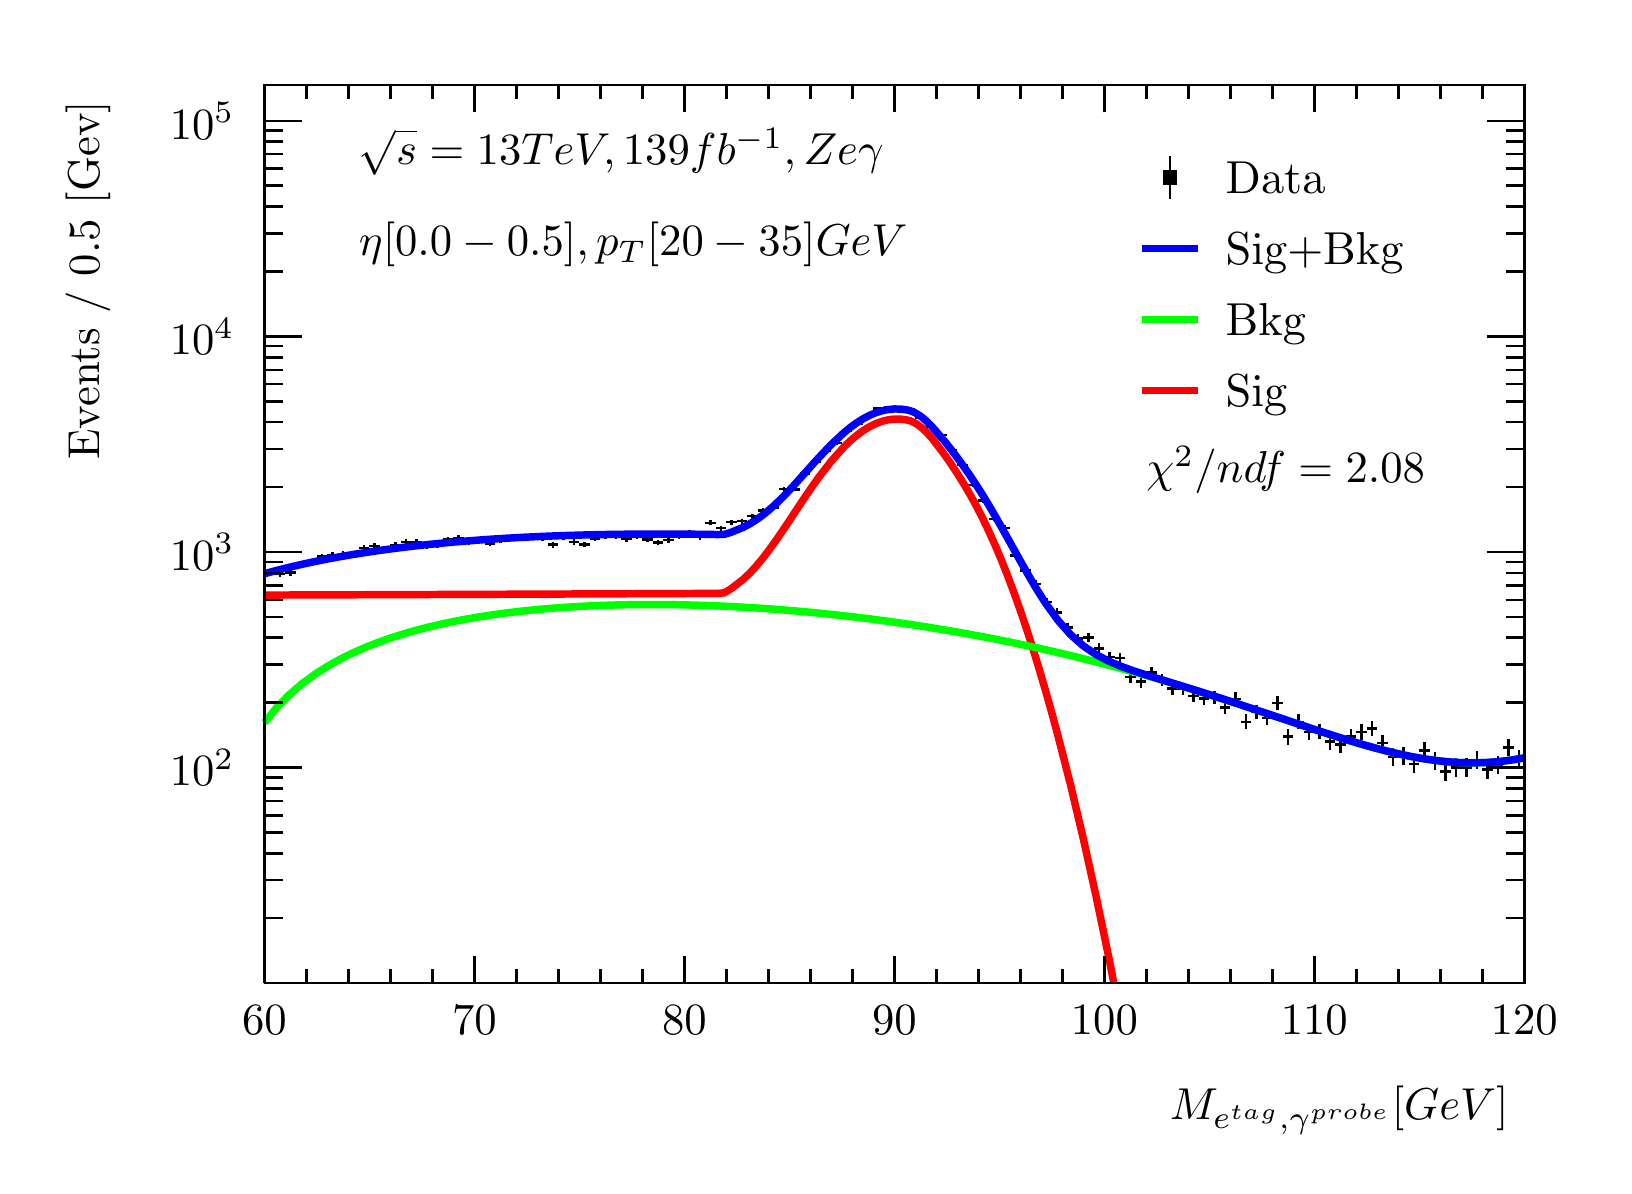
\begin{tikzpicture}
\pgfdeclareplotmark{cross} {
\pgfpathmoveto{\pgfpoint{-0.3\pgfplotmarksize}{\pgfplotmarksize}}
\pgfpathlineto{\pgfpoint{+0.3\pgfplotmarksize}{\pgfplotmarksize}}
\pgfpathlineto{\pgfpoint{+0.3\pgfplotmarksize}{0.3\pgfplotmarksize}}
\pgfpathlineto{\pgfpoint{+1\pgfplotmarksize}{0.3\pgfplotmarksize}}
\pgfpathlineto{\pgfpoint{+1\pgfplotmarksize}{-0.3\pgfplotmarksize}}
\pgfpathlineto{\pgfpoint{+0.3\pgfplotmarksize}{-0.3\pgfplotmarksize}}
\pgfpathlineto{\pgfpoint{+0.3\pgfplotmarksize}{-1.\pgfplotmarksize}}
\pgfpathlineto{\pgfpoint{-0.3\pgfplotmarksize}{-1.\pgfplotmarksize}}
\pgfpathlineto{\pgfpoint{-0.3\pgfplotmarksize}{-0.3\pgfplotmarksize}}
\pgfpathlineto{\pgfpoint{-1.\pgfplotmarksize}{-0.3\pgfplotmarksize}}
\pgfpathlineto{\pgfpoint{-1.\pgfplotmarksize}{0.3\pgfplotmarksize}}
\pgfpathlineto{\pgfpoint{-0.3\pgfplotmarksize}{0.3\pgfplotmarksize}}
\pgfpathclose
\pgfusepathqstroke
}
\pgfdeclareplotmark{cross*} {
\pgfpathmoveto{\pgfpoint{-0.3\pgfplotmarksize}{\pgfplotmarksize}}
\pgfpathlineto{\pgfpoint{+0.3\pgfplotmarksize}{\pgfplotmarksize}}
\pgfpathlineto{\pgfpoint{+0.3\pgfplotmarksize}{0.3\pgfplotmarksize}}
\pgfpathlineto{\pgfpoint{+1\pgfplotmarksize}{0.3\pgfplotmarksize}}
\pgfpathlineto{\pgfpoint{+1\pgfplotmarksize}{-0.3\pgfplotmarksize}}
\pgfpathlineto{\pgfpoint{+0.3\pgfplotmarksize}{-0.3\pgfplotmarksize}}
\pgfpathlineto{\pgfpoint{+0.3\pgfplotmarksize}{-1.\pgfplotmarksize}}
\pgfpathlineto{\pgfpoint{-0.3\pgfplotmarksize}{-1.\pgfplotmarksize}}
\pgfpathlineto{\pgfpoint{-0.3\pgfplotmarksize}{-0.3\pgfplotmarksize}}
\pgfpathlineto{\pgfpoint{-1.\pgfplotmarksize}{-0.3\pgfplotmarksize}}
\pgfpathlineto{\pgfpoint{-1.\pgfplotmarksize}{0.3\pgfplotmarksize}}
\pgfpathlineto{\pgfpoint{-0.3\pgfplotmarksize}{0.3\pgfplotmarksize}}
\pgfpathclose
\pgfusepathqfillstroke
}
\pgfdeclareplotmark{newstar} {
\pgfpathmoveto{\pgfqpoint{0pt}{\pgfplotmarksize}}
\pgfpathlineto{\pgfqpointpolar{44}{0.5\pgfplotmarksize}}
\pgfpathlineto{\pgfqpointpolar{18}{\pgfplotmarksize}}
\pgfpathlineto{\pgfqpointpolar{-20}{0.5\pgfplotmarksize}}
\pgfpathlineto{\pgfqpointpolar{-54}{\pgfplotmarksize}}
\pgfpathlineto{\pgfqpointpolar{-90}{0.5\pgfplotmarksize}}
\pgfpathlineto{\pgfqpointpolar{234}{\pgfplotmarksize}}
\pgfpathlineto{\pgfqpointpolar{198}{0.5\pgfplotmarksize}}
\pgfpathlineto{\pgfqpointpolar{162}{\pgfplotmarksize}}
\pgfpathlineto{\pgfqpointpolar{134}{0.5\pgfplotmarksize}}
\pgfpathclose
\pgfusepathqstroke
}
\pgfdeclareplotmark{newstar*} {
\pgfpathmoveto{\pgfqpoint{0pt}{\pgfplotmarksize}}
\pgfpathlineto{\pgfqpointpolar{44}{0.5\pgfplotmarksize}}
\pgfpathlineto{\pgfqpointpolar{18}{\pgfplotmarksize}}
\pgfpathlineto{\pgfqpointpolar{-20}{0.5\pgfplotmarksize}}
\pgfpathlineto{\pgfqpointpolar{-54}{\pgfplotmarksize}}
\pgfpathlineto{\pgfqpointpolar{-90}{0.5\pgfplotmarksize}}
\pgfpathlineto{\pgfqpointpolar{234}{\pgfplotmarksize}}
\pgfpathlineto{\pgfqpointpolar{198}{0.5\pgfplotmarksize}}
\pgfpathlineto{\pgfqpointpolar{162}{\pgfplotmarksize}}
\pgfpathlineto{\pgfqpointpolar{134}{0.5\pgfplotmarksize}}
\pgfpathclose
\pgfusepathqfillstroke
}
\definecolor{c}{rgb}{1,1,1};
\draw [color=c, fill=c] (0,0) rectangle (20,14.4361);
\draw [color=c, fill=c] (3,2.30977) rectangle (19,13.7143);
\definecolor{c}{rgb}{0,0,0};
\draw [c,line width=0.9] (3,2.30977) -- (3,13.7143) -- (19,13.7143) -- (19,2.30977) -- (3,2.30977);
\definecolor{c}{rgb}{1,1,1};
\draw [color=c, fill=c] (3,2.30977) rectangle (19,13.7143);
\definecolor{c}{rgb}{0,0,0};
\draw [c,line width=0.9] (3,2.30977) -- (3,13.7143) -- (19,13.7143) -- (19,2.30977) -- (3,2.30977);
\draw [c,line width=0.9] (3,2.30977) -- (19,2.30977);
\draw [c,line width=0.9] (3,2.65624) -- (3,2.30977);
\draw [c,line width=0.9] (3.53333,2.48301) -- (3.53333,2.30977);
\draw [c,line width=0.9] (4.06667,2.48301) -- (4.06667,2.30977);
\draw [c,line width=0.9] (4.6,2.48301) -- (4.6,2.30977);
\draw [c,line width=0.9] (5.13333,2.48301) -- (5.13333,2.30977);
\draw [c,line width=0.9] (5.66667,2.65624) -- (5.66667,2.30977);
\draw [c,line width=0.9] (6.2,2.48301) -- (6.2,2.30977);
\draw [c,line width=0.9] (6.73333,2.48301) -- (6.73333,2.30977);
\draw [c,line width=0.9] (7.26667,2.48301) -- (7.26667,2.30977);
\draw [c,line width=0.9] (7.8,2.48301) -- (7.8,2.30977);
\draw [c,line width=0.9] (8.33333,2.65624) -- (8.33333,2.30977);
\draw [c,line width=0.9] (8.86667,2.48301) -- (8.86667,2.30977);
\draw [c,line width=0.9] (9.4,2.48301) -- (9.4,2.30977);
\draw [c,line width=0.9] (9.93333,2.48301) -- (9.93333,2.30977);
\draw [c,line width=0.9] (10.4667,2.48301) -- (10.4667,2.30977);
\draw [c,line width=0.9] (11,2.65624) -- (11,2.30977);
\draw [c,line width=0.9] (11.5333,2.48301) -- (11.5333,2.30977);
\draw [c,line width=0.9] (12.0667,2.48301) -- (12.0667,2.30977);
\draw [c,line width=0.9] (12.6,2.48301) -- (12.6,2.30977);
\draw [c,line width=0.9] (13.1333,2.48301) -- (13.1333,2.30977);
\draw [c,line width=0.9] (13.6667,2.65624) -- (13.6667,2.30977);
\draw [c,line width=0.9] (14.2,2.48301) -- (14.2,2.30977);
\draw [c,line width=0.9] (14.7333,2.48301) -- (14.7333,2.30977);
\draw [c,line width=0.9] (15.2667,2.48301) -- (15.2667,2.30977);
\draw [c,line width=0.9] (15.8,2.48301) -- (15.8,2.30977);
\draw [c,line width=0.9] (16.3333,2.65624) -- (16.3333,2.30977);
\draw [c,line width=0.9] (16.8667,2.48301) -- (16.8667,2.30977);
\draw [c,line width=0.9] (17.4,2.48301) -- (17.4,2.30977);
\draw [c,line width=0.9] (17.9333,2.48301) -- (17.9333,2.30977);
\draw [c,line width=0.9] (18.4667,2.48301) -- (18.4667,2.30977);
\draw [c,line width=0.9] (19,2.65624) -- (19,2.30977);
\draw [anchor=base] (3,1.66015) node[scale=1.61424, color=c, rotate=0]{60};
\draw [anchor=base] (5.66667,1.66015) node[scale=1.61424, color=c, rotate=0]{70};
\draw [anchor=base] (8.33333,1.66015) node[scale=1.61424, color=c, rotate=0]{80};
\draw [anchor=base] (11,1.66015) node[scale=1.61424, color=c, rotate=0]{90};
\draw [anchor=base] (13.6667,1.66015) node[scale=1.61424, color=c, rotate=0]{100};
\draw [anchor=base] (16.3333,1.66015) node[scale=1.61424, color=c, rotate=0]{110};
\draw [anchor=base] (19,1.66015) node[scale=1.61424, color=c, rotate=0]{120};
\draw [anchor= east] (19,0.692932) node[scale=1.61424, color=c, rotate=0]{$M_{e^{tag}, \gamma^{probe}}  [GeV]$};
\draw [c,line width=0.9] (3,13.7143) -- (19,13.7143);
\draw [c,line width=0.9] (3,13.3678) -- (3,13.7143);
\draw [c,line width=0.9] (3.53333,13.5411) -- (3.53333,13.7143);
\draw [c,line width=0.9] (4.06667,13.5411) -- (4.06667,13.7143);
\draw [c,line width=0.9] (4.6,13.5411) -- (4.6,13.7143);
\draw [c,line width=0.9] (5.13333,13.5411) -- (5.13333,13.7143);
\draw [c,line width=0.9] (5.66667,13.3678) -- (5.66667,13.7143);
\draw [c,line width=0.9] (6.2,13.5411) -- (6.2,13.7143);
\draw [c,line width=0.9] (6.73333,13.5411) -- (6.73333,13.7143);
\draw [c,line width=0.9] (7.26667,13.5411) -- (7.26667,13.7143);
\draw [c,line width=0.9] (7.8,13.5411) -- (7.8,13.7143);
\draw [c,line width=0.9] (8.33333,13.3678) -- (8.33333,13.7143);
\draw [c,line width=0.9] (8.86667,13.5411) -- (8.86667,13.7143);
\draw [c,line width=0.9] (9.4,13.5411) -- (9.4,13.7143);
\draw [c,line width=0.9] (9.93333,13.5411) -- (9.93333,13.7143);
\draw [c,line width=0.9] (10.4667,13.5411) -- (10.4667,13.7143);
\draw [c,line width=0.9] (11,13.3678) -- (11,13.7143);
\draw [c,line width=0.9] (11.5333,13.5411) -- (11.5333,13.7143);
\draw [c,line width=0.9] (12.0667,13.5411) -- (12.0667,13.7143);
\draw [c,line width=0.9] (12.6,13.5411) -- (12.6,13.7143);
\draw [c,line width=0.9] (13.1333,13.5411) -- (13.1333,13.7143);
\draw [c,line width=0.9] (13.6667,13.3678) -- (13.6667,13.7143);
\draw [c,line width=0.9] (14.2,13.5411) -- (14.2,13.7143);
\draw [c,line width=0.9] (14.7333,13.5411) -- (14.7333,13.7143);
\draw [c,line width=0.9] (15.2667,13.5411) -- (15.2667,13.7143);
\draw [c,line width=0.9] (15.8,13.5411) -- (15.8,13.7143);
\draw [c,line width=0.9] (16.3333,13.3678) -- (16.3333,13.7143);
\draw [c,line width=0.9] (16.8667,13.5411) -- (16.8667,13.7143);
\draw [c,line width=0.9] (17.4,13.5411) -- (17.4,13.7143);
\draw [c,line width=0.9] (17.9333,13.5411) -- (17.9333,13.7143);
\draw [c,line width=0.9] (18.4667,13.5411) -- (18.4667,13.7143);
\draw [c,line width=0.9] (19,13.3678) -- (19,13.7143);
\draw [c,line width=0.9] (3,2.30977) -- (3,13.7143);
\draw [c,line width=0.9] (3.237,3.13385) -- (3,3.13385);
\draw [c,line width=0.9] (3.237,3.6159) -- (3,3.6159);
\draw [c,line width=0.9] (3.237,3.95792) -- (3,3.95792);
\draw [c,line width=0.9] (3.237,4.22321) -- (3,4.22321);
\draw [c,line width=0.9] (3.237,4.43997) -- (3,4.43997);
\draw [c,line width=0.9] (3.237,4.62324) -- (3,4.62324);
\draw [c,line width=0.9] (3.237,4.782) -- (3,4.782);
\draw [c,line width=0.9] (3.237,4.92203) -- (3,4.92203);
\draw [c,line width=0.9] (3.474,5.04729) -- (3,5.04729);
\draw [anchor= east] (2.82,5.04729) node[scale=1.61424, color=c, rotate=0]{$10^{2}$};
\draw [c,line width=0.9] (3.237,5.87136) -- (3,5.87136);
\draw [c,line width=0.9] (3.237,6.35342) -- (3,6.35342);
\draw [c,line width=0.9] (3.237,6.69544) -- (3,6.69544);
\draw [c,line width=0.9] (3.237,6.96073) -- (3,6.96073);
\draw [c,line width=0.9] (3.237,7.17749) -- (3,7.17749);
\draw [c,line width=0.9] (3.237,7.36076) -- (3,7.36076);
\draw [c,line width=0.9] (3.237,7.51951) -- (3,7.51951);
\draw [c,line width=0.9] (3.237,7.65954) -- (3,7.65954);
\draw [c,line width=0.9] (3.474,7.78481) -- (3,7.78481);
\draw [anchor= east] (2.82,7.78481) node[scale=1.61424, color=c, rotate=0]{$10^{3}$};
\draw [c,line width=0.9] (3.237,8.60888) -- (3,8.60888);
\draw [c,line width=0.9] (3.237,9.09093) -- (3,9.09093);
\draw [c,line width=0.9] (3.237,9.43296) -- (3,9.43296);
\draw [c,line width=0.9] (3.237,9.69825) -- (3,9.69825);
\draw [c,line width=0.9] (3.237,9.91501) -- (3,9.91501);
\draw [c,line width=0.9] (3.237,10.0983) -- (3,10.0983);
\draw [c,line width=0.9] (3.237,10.257) -- (3,10.257);
\draw [c,line width=0.9] (3.237,10.3971) -- (3,10.3971);
\draw [c,line width=0.9] (3.474,10.5223) -- (3,10.5223);
\draw [anchor= east] (2.82,10.5223) node[scale=1.61424, color=c, rotate=0]{$10^{4}$};
\draw [c,line width=0.9] (3.237,11.3464) -- (3,11.3464);
\draw [c,line width=0.9] (3.237,11.8285) -- (3,11.8285);
\draw [c,line width=0.9] (3.237,12.1705) -- (3,12.1705);
\draw [c,line width=0.9] (3.237,12.4358) -- (3,12.4358);
\draw [c,line width=0.9] (3.237,12.6525) -- (3,12.6525);
\draw [c,line width=0.9] (3.237,12.8358) -- (3,12.8358);
\draw [c,line width=0.9] (3.237,12.9945) -- (3,12.9945);
\draw [c,line width=0.9] (3.237,13.1346) -- (3,13.1346);
\draw [c,line width=0.9] (3.474,13.2598) -- (3,13.2598);
\draw [anchor= east] (2.82,13.2598) node[scale=1.61424, color=c, rotate=0]{$10^{5}$};
\draw [anchor= east] (0.76,13.7143) node[scale=1.61424, color=c, rotate=90]{Events / 0.5 [Gev]};
\draw [c,line width=0.9] (19,2.30977) -- (19,13.7143);
\draw [c,line width=0.9] (18.763,3.13385) -- (19,3.13385);
\draw [c,line width=0.9] (18.763,3.6159) -- (19,3.6159);
\draw [c,line width=0.9] (18.763,3.95792) -- (19,3.95792);
\draw [c,line width=0.9] (18.763,4.22321) -- (19,4.22321);
\draw [c,line width=0.9] (18.763,4.43997) -- (19,4.43997);
\draw [c,line width=0.9] (18.763,4.62324) -- (19,4.62324);
\draw [c,line width=0.9] (18.763,4.782) -- (19,4.782);
\draw [c,line width=0.9] (18.763,4.92203) -- (19,4.92203);
\draw [c,line width=0.9] (18.526,5.04729) -- (19,5.04729);
\draw [c,line width=0.9] (18.763,5.87136) -- (19,5.87136);
\draw [c,line width=0.9] (18.763,6.35342) -- (19,6.35342);
\draw [c,line width=0.9] (18.763,6.69544) -- (19,6.69544);
\draw [c,line width=0.9] (18.763,6.96073) -- (19,6.96073);
\draw [c,line width=0.9] (18.763,7.17749) -- (19,7.17749);
\draw [c,line width=0.9] (18.763,7.36076) -- (19,7.36076);
\draw [c,line width=0.9] (18.763,7.51951) -- (19,7.51951);
\draw [c,line width=0.9] (18.763,7.65954) -- (19,7.65954);
\draw [c,line width=0.9] (18.526,7.78481) -- (19,7.78481);
\draw [c,line width=0.9] (18.763,8.60888) -- (19,8.60888);
\draw [c,line width=0.9] (18.763,9.09093) -- (19,9.09093);
\draw [c,line width=0.9] (18.763,9.43296) -- (19,9.43296);
\draw [c,line width=0.9] (18.763,9.69825) -- (19,9.69825);
\draw [c,line width=0.9] (18.763,9.91501) -- (19,9.91501);
\draw [c,line width=0.9] (18.763,10.0983) -- (19,10.0983);
\draw [c,line width=0.9] (18.763,10.257) -- (19,10.257);
\draw [c,line width=0.9] (18.763,10.3971) -- (19,10.3971);
\draw [c,line width=0.9] (18.526,10.5223) -- (19,10.5223);
\draw [c,line width=0.9] (18.763,11.3464) -- (19,11.3464);
\draw [c,line width=0.9] (18.763,11.8285) -- (19,11.8285);
\draw [c,line width=0.9] (18.763,12.1705) -- (19,12.1705);
\draw [c,line width=0.9] (18.763,12.4358) -- (19,12.4358);
\draw [c,line width=0.9] (18.763,12.6525) -- (19,12.6525);
\draw [c,line width=0.9] (18.763,12.8358) -- (19,12.8358);
\draw [c,line width=0.9] (18.763,12.9945) -- (19,12.9945);
\draw [c,line width=0.9] (18.763,13.1346) -- (19,13.1346);
\draw [c,line width=0.9] (18.526,13.2598) -- (19,13.2598);
\draw [c,line width=0.9] (3.06667,7.51505) -- (3,7.51505);
\draw [c,line width=0.9] (3,7.51505) -- (3,7.51505);
\draw [c,line width=0.9] (3.06667,7.51505) -- (3.13333,7.51505);
\draw [c,line width=0.9] (3.13333,7.51505) -- (3.13333,7.51505);
\draw [c,line width=0.9] (3.06667,7.51505) -- (3.06667,7.55716);
\draw [c,line width=0.9] (3.06667,7.55716) -- (3.06667,7.55716);
\draw [c,line width=0.9] (3.06667,7.51505) -- (3.06667,7.47294);
\draw [c,line width=0.9] (3.06667,7.47294) -- (3.06667,7.47294);
\draw [c,line width=0.9] (3.2,7.50606) -- (3.13333,7.50606);
\draw [c,line width=0.9] (3.13333,7.50606) -- (3.13333,7.50606);
\draw [c,line width=0.9] (3.2,7.50606) -- (3.26667,7.50606);
\draw [c,line width=0.9] (3.26667,7.50606) -- (3.26667,7.50606);
\draw [c,line width=0.9] (3.2,7.50606) -- (3.2,7.54833);
\draw [c,line width=0.9] (3.2,7.54833) -- (3.2,7.54833);
\draw [c,line width=0.9] (3.2,7.50606) -- (3.2,7.46379);
\draw [c,line width=0.9] (3.2,7.46379) -- (3.2,7.46379);
\draw [c,line width=0.9] (3.33333,7.521) -- (3.26667,7.521);
\draw [c,line width=0.9] (3.26667,7.521) -- (3.26667,7.521);
\draw [c,line width=0.9] (3.33333,7.521) -- (3.4,7.521);
\draw [c,line width=0.9] (3.4,7.521) -- (3.4,7.521);
\draw [c,line width=0.9] (3.33333,7.521) -- (3.33333,7.563);
\draw [c,line width=0.9] (3.33333,7.563) -- (3.33333,7.563);
\draw [c,line width=0.9] (3.33333,7.521) -- (3.33333,7.47899);
\draw [c,line width=0.9] (3.33333,7.47899) -- (3.33333,7.47899);
\draw [c,line width=0.9] (3.46667,7.63012) -- (3.4,7.63012);
\draw [c,line width=0.9] (3.4,7.63012) -- (3.4,7.63012);
\draw [c,line width=0.9] (3.46667,7.63012) -- (3.53333,7.63012);
\draw [c,line width=0.9] (3.53333,7.63012) -- (3.53333,7.63012);
\draw [c,line width=0.9] (3.46667,7.63012) -- (3.46667,7.67024);
\draw [c,line width=0.9] (3.46667,7.67024) -- (3.46667,7.67024);
\draw [c,line width=0.9] (3.46667,7.63012) -- (3.46667,7.59);
\draw [c,line width=0.9] (3.46667,7.59) -- (3.46667,7.59);
\draw [c,line width=0.9] (3.6,7.65425) -- (3.53333,7.65425);
\draw [c,line width=0.9] (3.53333,7.65425) -- (3.53333,7.65425);
\draw [c,line width=0.9] (3.6,7.65425) -- (3.66667,7.65425);
\draw [c,line width=0.9] (3.66667,7.65425) -- (3.66667,7.65425);
\draw [c,line width=0.9] (3.6,7.65425) -- (3.6,7.69397);
\draw [c,line width=0.9] (3.6,7.69397) -- (3.6,7.69397);
\draw [c,line width=0.9] (3.6,7.65425) -- (3.6,7.61453);
\draw [c,line width=0.9] (3.6,7.61453) -- (3.6,7.61453);
\draw [c,line width=0.9] (3.73333,7.72633) -- (3.66667,7.72633);
\draw [c,line width=0.9] (3.66667,7.72633) -- (3.66667,7.72633);
\draw [c,line width=0.9] (3.73333,7.72633) -- (3.8,7.72633);
\draw [c,line width=0.9] (3.8,7.72633) -- (3.8,7.72633);
\draw [c,line width=0.9] (3.73333,7.72633) -- (3.73333,7.76486);
\draw [c,line width=0.9] (3.73333,7.76486) -- (3.73333,7.76486);
\draw [c,line width=0.9] (3.73333,7.72633) -- (3.73333,7.6878);
\draw [c,line width=0.9] (3.73333,7.6878) -- (3.73333,7.6878);
\draw [c,line width=0.9] (3.86667,7.73998) -- (3.8,7.73998);
\draw [c,line width=0.9] (3.8,7.73998) -- (3.8,7.73998);
\draw [c,line width=0.9] (3.86667,7.73998) -- (3.93333,7.73998);
\draw [c,line width=0.9] (3.93333,7.73998) -- (3.93333,7.73998);
\draw [c,line width=0.9] (3.86667,7.73998) -- (3.86667,7.77829);
\draw [c,line width=0.9] (3.86667,7.77829) -- (3.86667,7.77829);
\draw [c,line width=0.9] (3.86667,7.73998) -- (3.86667,7.70167);
\draw [c,line width=0.9] (3.86667,7.70167) -- (3.86667,7.70167);
\draw [c,line width=0.9] (4,7.75714) -- (3.93333,7.75714);
\draw [c,line width=0.9] (3.93333,7.75714) -- (3.93333,7.75714);
\draw [c,line width=0.9] (4,7.75714) -- (4.06667,7.75714);
\draw [c,line width=0.9] (4.06667,7.75714) -- (4.06667,7.75714);
\draw [c,line width=0.9] (4,7.75714) -- (4,7.79518);
\draw [c,line width=0.9] (4,7.79518) -- (4,7.79518);
\draw [c,line width=0.9] (4,7.75714) -- (4,7.71911);
\draw [c,line width=0.9] (4,7.71911) -- (4,7.71911);
\draw [c,line width=0.9] (4.13333,7.76079) -- (4.06667,7.76079);
\draw [c,line width=0.9] (4.06667,7.76079) -- (4.06667,7.76079);
\draw [c,line width=0.9] (4.13333,7.76079) -- (4.2,7.76079);
\draw [c,line width=0.9] (4.2,7.76079) -- (4.2,7.76079);
\draw [c,line width=0.9] (4.13333,7.76079) -- (4.13333,7.79876);
\draw [c,line width=0.9] (4.13333,7.79876) -- (4.13333,7.79876);
\draw [c,line width=0.9] (4.13333,7.76079) -- (4.13333,7.72281);
\draw [c,line width=0.9] (4.13333,7.72281) -- (4.13333,7.72281);
\draw [c,line width=0.9] (4.26667,7.83486) -- (4.2,7.83486);
\draw [c,line width=0.9] (4.2,7.83486) -- (4.2,7.83486);
\draw [c,line width=0.9] (4.26667,7.83486) -- (4.33333,7.83486);
\draw [c,line width=0.9] (4.33333,7.83486) -- (4.33333,7.83486);
\draw [c,line width=0.9] (4.26667,7.83486) -- (4.26667,7.87167);
\draw [c,line width=0.9] (4.26667,7.87167) -- (4.26667,7.87167);
\draw [c,line width=0.9] (4.26667,7.83486) -- (4.26667,7.79805);
\draw [c,line width=0.9] (4.26667,7.79805) -- (4.26667,7.79805);
\draw [c,line width=0.9] (4.4,7.85744) -- (4.33333,7.85744);
\draw [c,line width=0.9] (4.33333,7.85744) -- (4.33333,7.85744);
\draw [c,line width=0.9] (4.4,7.85744) -- (4.46667,7.85744);
\draw [c,line width=0.9] (4.46667,7.85744) -- (4.46667,7.85744);
\draw [c,line width=0.9] (4.4,7.85744) -- (4.4,7.89391);
\draw [c,line width=0.9] (4.4,7.89391) -- (4.4,7.89391);
\draw [c,line width=0.9] (4.4,7.85744) -- (4.4,7.82098);
\draw [c,line width=0.9] (4.4,7.82098) -- (4.4,7.82098);
\draw [c,line width=0.9] (4.53333,7.81995) -- (4.46667,7.81995);
\draw [c,line width=0.9] (4.46667,7.81995) -- (4.46667,7.81995);
\draw [c,line width=0.9] (4.53333,7.81995) -- (4.6,7.81995);
\draw [c,line width=0.9] (4.6,7.81995) -- (4.6,7.81995);
\draw [c,line width=0.9] (4.53333,7.81995) -- (4.53333,7.85699);
\draw [c,line width=0.9] (4.53333,7.85699) -- (4.53333,7.85699);
\draw [c,line width=0.9] (4.53333,7.81995) -- (4.53333,7.78291);
\draw [c,line width=0.9] (4.53333,7.78291) -- (4.53333,7.78291);
\draw [c,line width=0.9] (4.66667,7.86968) -- (4.6,7.86968);
\draw [c,line width=0.9] (4.6,7.86968) -- (4.6,7.86968);
\draw [c,line width=0.9] (4.66667,7.86968) -- (4.73333,7.86968);
\draw [c,line width=0.9] (4.73333,7.86968) -- (4.73333,7.86968);
\draw [c,line width=0.9] (4.66667,7.86968) -- (4.66667,7.90596);
\draw [c,line width=0.9] (4.66667,7.90596) -- (4.66667,7.90596);
\draw [c,line width=0.9] (4.66667,7.86968) -- (4.66667,7.83341);
\draw [c,line width=0.9] (4.66667,7.83341) -- (4.66667,7.83341);
\draw [c,line width=0.9] (4.8,7.91209) -- (4.73333,7.91209);
\draw [c,line width=0.9] (4.73333,7.91209) -- (4.73333,7.91209);
\draw [c,line width=0.9] (4.8,7.91209) -- (4.86667,7.91209);
\draw [c,line width=0.9] (4.86667,7.91209) -- (4.86667,7.91209);
\draw [c,line width=0.9] (4.8,7.91209) -- (4.8,7.94772);
\draw [c,line width=0.9] (4.8,7.94772) -- (4.8,7.94772);
\draw [c,line width=0.9] (4.8,7.91209) -- (4.8,7.87645);
\draw [c,line width=0.9] (4.8,7.87645) -- (4.8,7.87645);
\draw [c,line width=0.9] (4.93333,7.90995) -- (4.86667,7.90995);
\draw [c,line width=0.9] (4.86667,7.90995) -- (4.86667,7.90995);
\draw [c,line width=0.9] (4.93333,7.90995) -- (5,7.90995);
\draw [c,line width=0.9] (5,7.90995) -- (5,7.90995);
\draw [c,line width=0.9] (4.93333,7.90995) -- (4.93333,7.94562);
\draw [c,line width=0.9] (4.93333,7.94562) -- (4.93333,7.94562);
\draw [c,line width=0.9] (4.93333,7.90995) -- (4.93333,7.87428);
\draw [c,line width=0.9] (4.93333,7.87428) -- (4.93333,7.87428);
\draw [c,line width=0.9] (5.06667,7.85408) -- (5,7.85408);
\draw [c,line width=0.9] (5,7.85408) -- (5,7.85408);
\draw [c,line width=0.9] (5.06667,7.85408) -- (5.13333,7.85408);
\draw [c,line width=0.9] (5.13333,7.85408) -- (5.13333,7.85408);
\draw [c,line width=0.9] (5.06667,7.85408) -- (5.06667,7.8906);
\draw [c,line width=0.9] (5.06667,7.8906) -- (5.06667,7.8906);
\draw [c,line width=0.9] (5.06667,7.85408) -- (5.06667,7.81757);
\draw [c,line width=0.9] (5.06667,7.81757) -- (5.06667,7.81757);
\draw [c,line width=0.9] (5.2,7.87189) -- (5.13333,7.87189);
\draw [c,line width=0.9] (5.13333,7.87189) -- (5.13333,7.87189);
\draw [c,line width=0.9] (5.2,7.87189) -- (5.26667,7.87189);
\draw [c,line width=0.9] (5.26667,7.87189) -- (5.26667,7.87189);
\draw [c,line width=0.9] (5.2,7.87189) -- (5.2,7.90814);
\draw [c,line width=0.9] (5.2,7.90814) -- (5.2,7.90814);
\draw [c,line width=0.9] (5.2,7.87189) -- (5.2,7.83565);
\draw [c,line width=0.9] (5.2,7.83565) -- (5.2,7.83565);
\draw [c,line width=0.9] (5.33333,7.94163) -- (5.26667,7.94163);
\draw [c,line width=0.9] (5.26667,7.94163) -- (5.26667,7.94163);
\draw [c,line width=0.9] (5.33333,7.94163) -- (5.4,7.94163);
\draw [c,line width=0.9] (5.4,7.94163) -- (5.4,7.94163);
\draw [c,line width=0.9] (5.33333,7.94163) -- (5.33333,7.97682);
\draw [c,line width=0.9] (5.33333,7.97682) -- (5.33333,7.97682);
\draw [c,line width=0.9] (5.33333,7.94163) -- (5.33333,7.90643);
\draw [c,line width=0.9] (5.33333,7.90643) -- (5.33333,7.90643);
\draw [c,line width=0.9] (5.46667,7.96229) -- (5.4,7.96229);
\draw [c,line width=0.9] (5.4,7.96229) -- (5.4,7.96229);
\draw [c,line width=0.9] (5.46667,7.96229) -- (5.53333,7.96229);
\draw [c,line width=0.9] (5.53333,7.96229) -- (5.53333,7.96229);
\draw [c,line width=0.9] (5.46667,7.96229) -- (5.46667,7.99718);
\draw [c,line width=0.9] (5.46667,7.99718) -- (5.46667,7.99718);
\draw [c,line width=0.9] (5.46667,7.96229) -- (5.46667,7.9274);
\draw [c,line width=0.9] (5.46667,7.9274) -- (5.46667,7.9274);
\draw [c,line width=0.9] (5.6,7.91422) -- (5.53333,7.91422);
\draw [c,line width=0.9] (5.53333,7.91422) -- (5.53333,7.91422);
\draw [c,line width=0.9] (5.6,7.91422) -- (5.66667,7.91422);
\draw [c,line width=0.9] (5.66667,7.91422) -- (5.66667,7.91422);
\draw [c,line width=0.9] (5.6,7.91422) -- (5.6,7.94983);
\draw [c,line width=0.9] (5.6,7.94983) -- (5.6,7.94983);
\draw [c,line width=0.9] (5.6,7.91422) -- (5.6,7.87862);
\draw [c,line width=0.9] (5.6,7.87862) -- (5.6,7.87862);
\draw [c,line width=0.9] (5.73333,7.93221) -- (5.66667,7.93221);
\draw [c,line width=0.9] (5.66667,7.93221) -- (5.66667,7.93221);
\draw [c,line width=0.9] (5.73333,7.93221) -- (5.8,7.93221);
\draw [c,line width=0.9] (5.8,7.93221) -- (5.8,7.93221);
\draw [c,line width=0.9] (5.73333,7.93221) -- (5.73333,7.96755);
\draw [c,line width=0.9] (5.73333,7.96755) -- (5.73333,7.96755);
\draw [c,line width=0.9] (5.73333,7.93221) -- (5.73333,7.89688);
\draw [c,line width=0.9] (5.73333,7.89688) -- (5.73333,7.89688);
\draw [c,line width=0.9] (5.86667,7.89487) -- (5.8,7.89487);
\draw [c,line width=0.9] (5.8,7.89487) -- (5.8,7.89487);
\draw [c,line width=0.9] (5.86667,7.89487) -- (5.93333,7.89487);
\draw [c,line width=0.9] (5.93333,7.89487) -- (5.93333,7.89487);
\draw [c,line width=0.9] (5.86667,7.89487) -- (5.86667,7.93077);
\draw [c,line width=0.9] (5.86667,7.93077) -- (5.86667,7.93077);
\draw [c,line width=0.9] (5.86667,7.89487) -- (5.86667,7.85898);
\draw [c,line width=0.9] (5.86667,7.85898) -- (5.86667,7.85898);
\draw [c,line width=0.9] (6,7.9385) -- (5.93333,7.9385);
\draw [c,line width=0.9] (5.93333,7.9385) -- (5.93333,7.9385);
\draw [c,line width=0.9] (6,7.9385) -- (6.06667,7.9385);
\draw [c,line width=0.9] (6.06667,7.9385) -- (6.06667,7.9385);
\draw [c,line width=0.9] (6,7.9385) -- (6,7.97374);
\draw [c,line width=0.9] (6,7.97374) -- (6,7.97374);
\draw [c,line width=0.9] (6,7.9385) -- (6,7.90326);
\draw [c,line width=0.9] (6,7.90326) -- (6,7.90326);
\draw [c,line width=0.9] (6.13333,7.95303) -- (6.06667,7.95303);
\draw [c,line width=0.9] (6.06667,7.95303) -- (6.06667,7.95303);
\draw [c,line width=0.9] (6.13333,7.95303) -- (6.2,7.95303);
\draw [c,line width=0.9] (6.2,7.95303) -- (6.2,7.95303);
\draw [c,line width=0.9] (6.13333,7.95303) -- (6.13333,7.98806);
\draw [c,line width=0.9] (6.13333,7.98806) -- (6.13333,7.98806);
\draw [c,line width=0.9] (6.13333,7.95303) -- (6.13333,7.91801);
\draw [c,line width=0.9] (6.13333,7.91801) -- (6.13333,7.91801);
\draw [c,line width=0.9] (6.26667,7.9551) -- (6.2,7.9551);
\draw [c,line width=0.9] (6.2,7.9551) -- (6.2,7.9551);
\draw [c,line width=0.9] (6.26667,7.9551) -- (6.33333,7.9551);
\draw [c,line width=0.9] (6.33333,7.9551) -- (6.33333,7.9551);
\draw [c,line width=0.9] (6.26667,7.9551) -- (6.26667,7.99009);
\draw [c,line width=0.9] (6.26667,7.99009) -- (6.26667,7.99009);
\draw [c,line width=0.9] (6.26667,7.9551) -- (6.26667,7.9201);
\draw [c,line width=0.9] (6.26667,7.9201) -- (6.26667,7.9201);
\draw [c,line width=0.9] (6.4,7.99361) -- (6.33333,7.99361);
\draw [c,line width=0.9] (6.33333,7.99361) -- (6.33333,7.99361);
\draw [c,line width=0.9] (6.4,7.99361) -- (6.46667,7.99361);
\draw [c,line width=0.9] (6.46667,7.99361) -- (6.46667,7.99361);
\draw [c,line width=0.9] (6.4,7.99361) -- (6.4,8.02805);
\draw [c,line width=0.9] (6.4,8.02805) -- (6.4,8.02805);
\draw [c,line width=0.9] (6.4,7.99361) -- (6.4,7.95918);
\draw [c,line width=0.9] (6.4,7.95918) -- (6.4,7.95918);
\draw [c,line width=0.9] (6.53333,7.96433) -- (6.46667,7.96433);
\draw [c,line width=0.9] (6.46667,7.96433) -- (6.46667,7.96433);
\draw [c,line width=0.9] (6.53333,7.96433) -- (6.6,7.96433);
\draw [c,line width=0.9] (6.6,7.96433) -- (6.6,7.96433);
\draw [c,line width=0.9] (6.53333,7.96433) -- (6.53333,7.99919);
\draw [c,line width=0.9] (6.53333,7.99919) -- (6.53333,7.99919);
\draw [c,line width=0.9] (6.53333,7.96433) -- (6.53333,7.92947);
\draw [c,line width=0.9] (6.53333,7.92947) -- (6.53333,7.92947);
\draw [c,line width=0.9] (6.66667,7.87631) -- (6.6,7.87631);
\draw [c,line width=0.9] (6.6,7.87631) -- (6.6,7.87631);
\draw [c,line width=0.9] (6.66667,7.87631) -- (6.73333,7.87631);
\draw [c,line width=0.9] (6.73333,7.87631) -- (6.73333,7.87631);
\draw [c,line width=0.9] (6.66667,7.87631) -- (6.66667,7.91248);
\draw [c,line width=0.9] (6.66667,7.91248) -- (6.66667,7.91248);
\draw [c,line width=0.9] (6.66667,7.87631) -- (6.66667,7.84013);
\draw [c,line width=0.9] (6.66667,7.84013) -- (6.66667,7.84013);
\draw [c,line width=0.9] (6.8,7.97552) -- (6.73333,7.97552);
\draw [c,line width=0.9] (6.73333,7.97552) -- (6.73333,7.97552);
\draw [c,line width=0.9] (6.8,7.97552) -- (6.86667,7.97552);
\draw [c,line width=0.9] (6.86667,7.97552) -- (6.86667,7.97552);
\draw [c,line width=0.9] (6.8,7.97552) -- (6.8,8.01022);
\draw [c,line width=0.9] (6.8,8.01022) -- (6.8,8.01022);
\draw [c,line width=0.9] (6.8,7.97552) -- (6.8,7.94083);
\draw [c,line width=0.9] (6.8,7.94083) -- (6.8,7.94083);
\draw [c,line width=0.9] (6.93333,7.90888) -- (6.86667,7.90888);
\draw [c,line width=0.9] (6.86667,7.90888) -- (6.86667,7.90888);
\draw [c,line width=0.9] (6.93333,7.90888) -- (7,7.90888);
\draw [c,line width=0.9] (7,7.90888) -- (7,7.90888);
\draw [c,line width=0.9] (6.93333,7.90888) -- (6.93333,7.94456);
\draw [c,line width=0.9] (6.93333,7.94456) -- (6.93333,7.94456);
\draw [c,line width=0.9] (6.93333,7.90888) -- (6.93333,7.8732);
\draw [c,line width=0.9] (6.93333,7.8732) -- (6.93333,7.8732);
\draw [c,line width=0.9] (7.06667,7.87851) -- (7,7.87851);
\draw [c,line width=0.9] (7,7.87851) -- (7,7.87851);
\draw [c,line width=0.9] (7.06667,7.87851) -- (7.13333,7.87851);
\draw [c,line width=0.9] (7.13333,7.87851) -- (7.13333,7.87851);
\draw [c,line width=0.9] (7.06667,7.87851) -- (7.06667,7.91465);
\draw [c,line width=0.9] (7.06667,7.91465) -- (7.06667,7.91465);
\draw [c,line width=0.9] (7.06667,7.87851) -- (7.06667,7.84236);
\draw [c,line width=0.9] (7.06667,7.84236) -- (7.06667,7.84236);
\draw [c,line width=0.9] (7.2,7.95716) -- (7.13333,7.95716);
\draw [c,line width=0.9] (7.13333,7.95716) -- (7.13333,7.95716);
\draw [c,line width=0.9] (7.2,7.95716) -- (7.26667,7.95716);
\draw [c,line width=0.9] (7.26667,7.95716) -- (7.26667,7.95716);
\draw [c,line width=0.9] (7.2,7.95716) -- (7.2,7.99212);
\draw [c,line width=0.9] (7.2,7.99212) -- (7.2,7.99212);
\draw [c,line width=0.9] (7.2,7.95716) -- (7.2,7.92219);
\draw [c,line width=0.9] (7.2,7.92219) -- (7.2,7.92219);
\draw [c,line width=0.9] (7.33333,7.97957) -- (7.26667,7.97957);
\draw [c,line width=0.9] (7.26667,7.97957) -- (7.26667,7.97957);
\draw [c,line width=0.9] (7.33333,7.97957) -- (7.4,7.97957);
\draw [c,line width=0.9] (7.4,7.97957) -- (7.4,7.97957);
\draw [c,line width=0.9] (7.33333,7.97957) -- (7.33333,8.01421);
\draw [c,line width=0.9] (7.33333,8.01421) -- (7.33333,8.01421);
\draw [c,line width=0.9] (7.33333,7.97957) -- (7.33333,7.94493);
\draw [c,line width=0.9] (7.33333,7.94493) -- (7.33333,7.94493);
\draw [c,line width=0.9] (7.46667,7.97755) -- (7.4,7.97755);
\draw [c,line width=0.9] (7.4,7.97755) -- (7.4,7.97755);
\draw [c,line width=0.9] (7.46667,7.97755) -- (7.53333,7.97755);
\draw [c,line width=0.9] (7.53333,7.97755) -- (7.53333,7.97755);
\draw [c,line width=0.9] (7.46667,7.97755) -- (7.46667,8.01222);
\draw [c,line width=0.9] (7.46667,8.01222) -- (7.46667,8.01222);
\draw [c,line width=0.9] (7.46667,7.97755) -- (7.46667,7.94288);
\draw [c,line width=0.9] (7.46667,7.94288) -- (7.46667,7.94288);
\draw [c,line width=0.9] (7.6,7.94683) -- (7.53333,7.94683);
\draw [c,line width=0.9] (7.53333,7.94683) -- (7.53333,7.94683);
\draw [c,line width=0.9] (7.6,7.94683) -- (7.66667,7.94683);
\draw [c,line width=0.9] (7.66667,7.94683) -- (7.66667,7.94683);
\draw [c,line width=0.9] (7.6,7.94683) -- (7.6,7.98194);
\draw [c,line width=0.9] (7.6,7.98194) -- (7.6,7.98194);
\draw [c,line width=0.9] (7.6,7.94683) -- (7.6,7.91171);
\draw [c,line width=0.9] (7.6,7.91171) -- (7.6,7.91171);
\draw [c,line width=0.9] (7.73333,7.98159) -- (7.66667,7.98159);
\draw [c,line width=0.9] (7.66667,7.98159) -- (7.66667,7.98159);
\draw [c,line width=0.9] (7.73333,7.98159) -- (7.8,7.98159);
\draw [c,line width=0.9] (7.8,7.98159) -- (7.8,7.98159);
\draw [c,line width=0.9] (7.73333,7.98159) -- (7.73333,8.01619);
\draw [c,line width=0.9] (7.73333,8.01619) -- (7.73333,8.01619);
\draw [c,line width=0.9] (7.73333,7.98159) -- (7.73333,7.94698);
\draw [c,line width=0.9] (7.73333,7.94698) -- (7.73333,7.94698);
\draw [c,line width=0.9] (7.86667,7.94475) -- (7.8,7.94475);
\draw [c,line width=0.9] (7.8,7.94475) -- (7.8,7.94475);
\draw [c,line width=0.9] (7.86667,7.94475) -- (7.93333,7.94475);
\draw [c,line width=0.9] (7.93333,7.94475) -- (7.93333,7.94475);
\draw [c,line width=0.9] (7.86667,7.94475) -- (7.86667,7.9799);
\draw [c,line width=0.9] (7.86667,7.9799) -- (7.86667,7.9799);
\draw [c,line width=0.9] (7.86667,7.94475) -- (7.86667,7.9096);
\draw [c,line width=0.9] (7.86667,7.9096) -- (7.86667,7.9096);
\draw [c,line width=0.9] (8,7.90351) -- (7.93333,7.90351);
\draw [c,line width=0.9] (7.93333,7.90351) -- (7.93333,7.90351);
\draw [c,line width=0.9] (8,7.90351) -- (8.06667,7.90351);
\draw [c,line width=0.9] (8.06667,7.90351) -- (8.06667,7.90351);
\draw [c,line width=0.9] (8,7.90351) -- (8,7.93928);
\draw [c,line width=0.9] (8,7.93928) -- (8,7.93928);
\draw [c,line width=0.9] (8,7.90351) -- (8,7.86775);
\draw [c,line width=0.9] (8,7.86775) -- (8,7.86775);
\draw [c,line width=0.9] (8.13333,7.93536) -- (8.06667,7.93536);
\draw [c,line width=0.9] (8.06667,7.93536) -- (8.06667,7.93536);
\draw [c,line width=0.9] (8.13333,7.93536) -- (8.2,7.93536);
\draw [c,line width=0.9] (8.2,7.93536) -- (8.2,7.93536);
\draw [c,line width=0.9] (8.13333,7.93536) -- (8.13333,7.97065);
\draw [c,line width=0.9] (8.13333,7.97065) -- (8.13333,7.97065);
\draw [c,line width=0.9] (8.13333,7.93536) -- (8.13333,7.90007);
\draw [c,line width=0.9] (8.13333,7.90007) -- (8.13333,7.90007);
\draw [c,line width=0.9] (8.26667,7.98259) -- (8.2,7.98259);
\draw [c,line width=0.9] (8.2,7.98259) -- (8.2,7.98259);
\draw [c,line width=0.9] (8.26667,7.98259) -- (8.33333,7.98259);
\draw [c,line width=0.9] (8.33333,7.98259) -- (8.33333,7.98259);
\draw [c,line width=0.9] (8.26667,7.98259) -- (8.26667,8.01719);
\draw [c,line width=0.9] (8.26667,8.01719) -- (8.26667,8.01719);
\draw [c,line width=0.9] (8.26667,7.98259) -- (8.26667,7.948);
\draw [c,line width=0.9] (8.26667,7.948) -- (8.26667,7.948);
\draw [c,line width=0.9] (8.4,8.03092) -- (8.33333,8.03092);
\draw [c,line width=0.9] (8.33333,8.03092) -- (8.33333,8.03092);
\draw [c,line width=0.9] (8.4,8.03092) -- (8.46667,8.03092);
\draw [c,line width=0.9] (8.46667,8.03092) -- (8.46667,8.03092);
\draw [c,line width=0.9] (8.4,8.03092) -- (8.4,8.06482);
\draw [c,line width=0.9] (8.4,8.06482) -- (8.4,8.06482);
\draw [c,line width=0.9] (8.4,8.03092) -- (8.4,7.99703);
\draw [c,line width=0.9] (8.4,7.99703) -- (8.4,7.99703);
\draw [c,line width=0.9] (8.53333,7.97248) -- (8.46667,7.97248);
\draw [c,line width=0.9] (8.46667,7.97248) -- (8.46667,7.97248);
\draw [c,line width=0.9] (8.53333,7.97248) -- (8.6,7.97248);
\draw [c,line width=0.9] (8.6,7.97248) -- (8.6,7.97248);
\draw [c,line width=0.9] (8.53333,7.97248) -- (8.53333,8.00722);
\draw [c,line width=0.9] (8.53333,8.00722) -- (8.53333,8.00722);
\draw [c,line width=0.9] (8.53333,7.97248) -- (8.53333,7.93774);
\draw [c,line width=0.9] (8.53333,7.93774) -- (8.53333,7.93774);
\draw [c,line width=0.9] (8.66667,8.15299) -- (8.6,8.15299);
\draw [c,line width=0.9] (8.6,8.15299) -- (8.6,8.15299);
\draw [c,line width=0.9] (8.66667,8.15299) -- (8.73333,8.15299);
\draw [c,line width=0.9] (8.73333,8.15299) -- (8.73333,8.15299);
\draw [c,line width=0.9] (8.66667,8.15299) -- (8.66667,8.18519);
\draw [c,line width=0.9] (8.66667,8.18519) -- (8.66667,8.18519);
\draw [c,line width=0.9] (8.66667,8.15299) -- (8.66667,8.12079);
\draw [c,line width=0.9] (8.66667,8.12079) -- (8.66667,8.12079);
\draw [c,line width=0.9] (8.8,8.0857) -- (8.73333,8.0857);
\draw [c,line width=0.9] (8.73333,8.0857) -- (8.73333,8.0857);
\draw [c,line width=0.9] (8.8,8.0857) -- (8.86667,8.0857);
\draw [c,line width=0.9] (8.86667,8.0857) -- (8.86667,8.0857);
\draw [c,line width=0.9] (8.8,8.0857) -- (8.8,8.11883);
\draw [c,line width=0.9] (8.8,8.11883) -- (8.8,8.11883);
\draw [c,line width=0.9] (8.8,8.0857) -- (8.8,8.05258);
\draw [c,line width=0.9] (8.8,8.05258) -- (8.8,8.05258);
\draw [c,line width=0.9] (8.93333,8.16341) -- (8.86667,8.16341);
\draw [c,line width=0.9] (8.86667,8.16341) -- (8.86667,8.16341);
\draw [c,line width=0.9] (8.93333,8.16341) -- (9,8.16341);
\draw [c,line width=0.9] (9,8.16341) -- (9,8.16341);
\draw [c,line width=0.9] (8.93333,8.16341) -- (8.93333,8.19547);
\draw [c,line width=0.9] (8.93333,8.19547) -- (8.93333,8.19547);
\draw [c,line width=0.9] (8.93333,8.16341) -- (8.93333,8.13135);
\draw [c,line width=0.9] (8.93333,8.13135) -- (8.93333,8.13135);
\draw [c,line width=0.9] (9.06667,8.17717) -- (9,8.17717);
\draw [c,line width=0.9] (9,8.17717) -- (9,8.17717);
\draw [c,line width=0.9] (9.06667,8.17717) -- (9.13333,8.17717);
\draw [c,line width=0.9] (9.13333,8.17717) -- (9.13333,8.17717);
\draw [c,line width=0.9] (9.06667,8.17717) -- (9.06667,8.20904);
\draw [c,line width=0.9] (9.06667,8.20904) -- (9.06667,8.20904);
\draw [c,line width=0.9] (9.06667,8.17717) -- (9.06667,8.14529);
\draw [c,line width=0.9] (9.06667,8.14529) -- (9.06667,8.14529);
\draw [c,line width=0.9] (9.2,8.23879) -- (9.13333,8.23879);
\draw [c,line width=0.9] (9.13333,8.23879) -- (9.13333,8.23879);
\draw [c,line width=0.9] (9.2,8.23879) -- (9.26667,8.23879);
\draw [c,line width=0.9] (9.26667,8.23879) -- (9.26667,8.23879);
\draw [c,line width=0.9] (9.2,8.23879) -- (9.2,8.26985);
\draw [c,line width=0.9] (9.2,8.26985) -- (9.2,8.26985);
\draw [c,line width=0.9] (9.2,8.23879) -- (9.2,8.20773);
\draw [c,line width=0.9] (9.2,8.20773) -- (9.2,8.20773);
\draw [c,line width=0.9] (9.33333,8.31273) -- (9.26667,8.31273);
\draw [c,line width=0.9] (9.26667,8.31273) -- (9.26667,8.31273);
\draw [c,line width=0.9] (9.33333,8.31273) -- (9.4,8.31273);
\draw [c,line width=0.9] (9.4,8.31273) -- (9.4,8.31273);
\draw [c,line width=0.9] (9.33333,8.31273) -- (9.33333,8.34284);
\draw [c,line width=0.9] (9.33333,8.34284) -- (9.33333,8.34284);
\draw [c,line width=0.9] (9.33333,8.31273) -- (9.33333,8.28262);
\draw [c,line width=0.9] (9.33333,8.28262) -- (9.33333,8.28262);
\draw [c,line width=0.9] (9.46667,8.351) -- (9.4,8.351);
\draw [c,line width=0.9] (9.4,8.351) -- (9.4,8.351);
\draw [c,line width=0.9] (9.46667,8.351) -- (9.53333,8.351);
\draw [c,line width=0.9] (9.53333,8.351) -- (9.53333,8.351);
\draw [c,line width=0.9] (9.46667,8.351) -- (9.46667,8.38063);
\draw [c,line width=0.9] (9.46667,8.38063) -- (9.46667,8.38063);
\draw [c,line width=0.9] (9.46667,8.351) -- (9.46667,8.32137);
\draw [c,line width=0.9] (9.46667,8.32137) -- (9.46667,8.32137);
\draw [c,line width=0.9] (9.6,8.58365) -- (9.53333,8.58365);
\draw [c,line width=0.9] (9.53333,8.58365) -- (9.53333,8.58365);
\draw [c,line width=0.9] (9.6,8.58365) -- (9.66667,8.58365);
\draw [c,line width=0.9] (9.66667,8.58365) -- (9.66667,8.58365);
\draw [c,line width=0.9] (9.6,8.58365) -- (9.6,8.61052);
\draw [c,line width=0.9] (9.6,8.61052) -- (9.6,8.61052);
\draw [c,line width=0.9] (9.6,8.58365) -- (9.6,8.55678);
\draw [c,line width=0.9] (9.6,8.55678) -- (9.6,8.55678);
\draw [c,line width=0.9] (9.73333,8.58) -- (9.66667,8.58);
\draw [c,line width=0.9] (9.66667,8.58) -- (9.66667,8.58);
\draw [c,line width=0.9] (9.73333,8.58) -- (9.8,8.58);
\draw [c,line width=0.9] (9.8,8.58) -- (9.8,8.58);
\draw [c,line width=0.9] (9.73333,8.58) -- (9.73333,8.60691);
\draw [c,line width=0.9] (9.73333,8.60691) -- (9.73333,8.60691);
\draw [c,line width=0.9] (9.73333,8.58) -- (9.73333,8.55309);
\draw [c,line width=0.9] (9.73333,8.55309) -- (9.73333,8.55309);
\draw [c,line width=0.9] (9.86667,8.77917) -- (9.8,8.77917);
\draw [c,line width=0.9] (9.8,8.77917) -- (9.8,8.77917);
\draw [c,line width=0.9] (9.86667,8.77917) -- (9.93333,8.77917);
\draw [c,line width=0.9] (9.93333,8.77917) -- (9.93333,8.77917);
\draw [c,line width=0.9] (9.86667,8.77917) -- (9.86667,8.80392);
\draw [c,line width=0.9] (9.86667,8.80392) -- (9.86667,8.80392);
\draw [c,line width=0.9] (9.86667,8.77917) -- (9.86667,8.75443);
\draw [c,line width=0.9] (9.86667,8.75443) -- (9.86667,8.75443);
\draw [c,line width=0.9] (10,8.92491) -- (9.93333,8.92491);
\draw [c,line width=0.9] (9.93333,8.92491) -- (9.93333,8.92491);
\draw [c,line width=0.9] (10,8.92491) -- (10.0667,8.92491);
\draw [c,line width=0.9] (10.0667,8.92491) -- (10.0667,8.92491);
\draw [c,line width=0.9] (10,8.92491) -- (10,8.94819);
\draw [c,line width=0.9] (10,8.94819) -- (10,8.94819);
\draw [c,line width=0.9] (10,8.92491) -- (10,8.90164);
\draw [c,line width=0.9] (10,8.90164) -- (10,8.90164);
\draw [c,line width=0.9] (10.1333,9.0653) -- (10.0667,9.0653);
\draw [c,line width=0.9] (10.0667,9.0653) -- (10.0667,9.0653);
\draw [c,line width=0.9] (10.1333,9.0653) -- (10.2,9.0653);
\draw [c,line width=0.9] (10.2,9.0653) -- (10.2,9.0653);
\draw [c,line width=0.9] (10.1333,9.0653) -- (10.1333,9.08724);
\draw [c,line width=0.9] (10.1333,9.08724) -- (10.1333,9.08724);
\draw [c,line width=0.9] (10.1333,9.0653) -- (10.1333,9.04336);
\draw [c,line width=0.9] (10.1333,9.04336) -- (10.1333,9.04336);
\draw [c,line width=0.9] (10.2667,9.16915) -- (10.2,9.16915);
\draw [c,line width=0.9] (10.2,9.16915) -- (10.2,9.16915);
\draw [c,line width=0.9] (10.2667,9.16915) -- (10.3333,9.16915);
\draw [c,line width=0.9] (10.3333,9.16915) -- (10.3333,9.16915);
\draw [c,line width=0.9] (10.2667,9.16915) -- (10.2667,9.19015);
\draw [c,line width=0.9] (10.2667,9.19015) -- (10.2667,9.19015);
\draw [c,line width=0.9] (10.2667,9.16915) -- (10.2667,9.14815);
\draw [c,line width=0.9] (10.2667,9.14815) -- (10.2667,9.14815);
\draw [c,line width=0.9] (10.4,9.32312) -- (10.3333,9.32312);
\draw [c,line width=0.9] (10.3333,9.32312) -- (10.3333,9.32312);
\draw [c,line width=0.9] (10.4,9.32312) -- (10.4667,9.32312);
\draw [c,line width=0.9] (10.4667,9.32312) -- (10.4667,9.32312);
\draw [c,line width=0.9] (10.4,9.32312) -- (10.4,9.3428);
\draw [c,line width=0.9] (10.4,9.3428) -- (10.4,9.3428);
\draw [c,line width=0.9] (10.4,9.32312) -- (10.4,9.30343);
\draw [c,line width=0.9] (10.4,9.30343) -- (10.4,9.30343);
\draw [c,line width=0.9] (10.5333,9.41348) -- (10.4667,9.41348);
\draw [c,line width=0.9] (10.4667,9.41348) -- (10.4667,9.41348);
\draw [c,line width=0.9] (10.5333,9.41348) -- (10.6,9.41348);
\draw [c,line width=0.9] (10.6,9.41348) -- (10.6,9.41348);
\draw [c,line width=0.9] (10.5333,9.41348) -- (10.5333,9.43243);
\draw [c,line width=0.9] (10.5333,9.43243) -- (10.5333,9.43243);
\draw [c,line width=0.9] (10.5333,9.41348) -- (10.5333,9.39453);
\draw [c,line width=0.9] (10.5333,9.39453) -- (10.5333,9.39453);
\draw [c,line width=0.9] (10.6667,9.51228) -- (10.6,9.51228);
\draw [c,line width=0.9] (10.6,9.51228) -- (10.6,9.51228);
\draw [c,line width=0.9] (10.6667,9.51228) -- (10.7333,9.51228);
\draw [c,line width=0.9] (10.7333,9.51228) -- (10.7333,9.51228);
\draw [c,line width=0.9] (10.6667,9.51228) -- (10.6667,9.53046);
\draw [c,line width=0.9] (10.6667,9.53046) -- (10.6667,9.53046);
\draw [c,line width=0.9] (10.6667,9.51228) -- (10.6667,9.4941);
\draw [c,line width=0.9] (10.6667,9.4941) -- (10.6667,9.4941);
\draw [c,line width=0.9] (10.8,9.60428) -- (10.7333,9.60428);
\draw [c,line width=0.9] (10.7333,9.60428) -- (10.7333,9.60428);
\draw [c,line width=0.9] (10.8,9.60428) -- (10.8667,9.60428);
\draw [c,line width=0.9] (10.8667,9.60428) -- (10.8667,9.60428);
\draw [c,line width=0.9] (10.8,9.60428) -- (10.8,9.62177);
\draw [c,line width=0.9] (10.8,9.62177) -- (10.8,9.62177);
\draw [c,line width=0.9] (10.8,9.60428) -- (10.8,9.58678);
\draw [c,line width=0.9] (10.8,9.58678) -- (10.8,9.58678);
\draw [c,line width=0.9] (10.9333,9.62721) -- (10.8667,9.62721);
\draw [c,line width=0.9] (10.8667,9.62721) -- (10.8667,9.62721);
\draw [c,line width=0.9] (10.9333,9.62721) -- (11,9.62721);
\draw [c,line width=0.9] (11,9.62721) -- (11,9.62721);
\draw [c,line width=0.9] (10.9333,9.62721) -- (10.9333,9.64454);
\draw [c,line width=0.9] (10.9333,9.64454) -- (10.9333,9.64454);
\draw [c,line width=0.9] (10.9333,9.62721) -- (10.9333,9.60989);
\draw [c,line width=0.9] (10.9333,9.60989) -- (10.9333,9.60989);
\draw [c,line width=0.9] (11.0667,9.60967) -- (11,9.60967);
\draw [c,line width=0.9] (11,9.60967) -- (11,9.60967);
\draw [c,line width=0.9] (11.0667,9.60967) -- (11.1333,9.60967);
\draw [c,line width=0.9] (11.1333,9.60967) -- (11.1333,9.60967);
\draw [c,line width=0.9] (11.0667,9.60967) -- (11.0667,9.62712);
\draw [c,line width=0.9] (11.0667,9.62712) -- (11.0667,9.62712);
\draw [c,line width=0.9] (11.0667,9.60967) -- (11.0667,9.59222);
\draw [c,line width=0.9] (11.0667,9.59222) -- (11.0667,9.59222);
\draw [c,line width=0.9] (11.2,9.60144) -- (11.1333,9.60144);
\draw [c,line width=0.9] (11.1333,9.60144) -- (11.1333,9.60144);
\draw [c,line width=0.9] (11.2,9.60144) -- (11.2667,9.60144);
\draw [c,line width=0.9] (11.2667,9.60144) -- (11.2667,9.60144);
\draw [c,line width=0.9] (11.2,9.60144) -- (11.2,9.61895);
\draw [c,line width=0.9] (11.2,9.61895) -- (11.2,9.61895);
\draw [c,line width=0.9] (11.2,9.60144) -- (11.2,9.58393);
\draw [c,line width=0.9] (11.2,9.58393) -- (11.2,9.58393);
\draw [c,line width=0.9] (11.3333,9.48728) -- (11.2667,9.48728);
\draw [c,line width=0.9] (11.2667,9.48728) -- (11.2667,9.48728);
\draw [c,line width=0.9] (11.3333,9.48728) -- (11.4,9.48728);
\draw [c,line width=0.9] (11.4,9.48728) -- (11.4,9.48728);
\draw [c,line width=0.9] (11.3333,9.48728) -- (11.3333,9.50565);
\draw [c,line width=0.9] (11.3333,9.50565) -- (11.3333,9.50565);
\draw [c,line width=0.9] (11.3333,9.48728) -- (11.3333,9.4689);
\draw [c,line width=0.9] (11.3333,9.4689) -- (11.3333,9.4689);
\draw [c,line width=0.9] (11.4667,9.36978) -- (11.4,9.36978);
\draw [c,line width=0.9] (11.4,9.36978) -- (11.4,9.36978);
\draw [c,line width=0.9] (11.4667,9.36978) -- (11.5333,9.36978);
\draw [c,line width=0.9] (11.5333,9.36978) -- (11.5333,9.36978);
\draw [c,line width=0.9] (11.4667,9.36978) -- (11.4667,9.38909);
\draw [c,line width=0.9] (11.4667,9.38909) -- (11.4667,9.38909);
\draw [c,line width=0.9] (11.4667,9.36978) -- (11.4667,9.35048);
\draw [c,line width=0.9] (11.4667,9.35048) -- (11.4667,9.35048);
\draw [c,line width=0.9] (11.6,9.27182) -- (11.5333,9.27182);
\draw [c,line width=0.9] (11.5333,9.27182) -- (11.5333,9.27182);
\draw [c,line width=0.9] (11.6,9.27182) -- (11.6667,9.27182);
\draw [c,line width=0.9] (11.6667,9.27182) -- (11.6667,9.27182);
\draw [c,line width=0.9] (11.6,9.27182) -- (11.6,9.29194);
\draw [c,line width=0.9] (11.6,9.29194) -- (11.6,9.29194);
\draw [c,line width=0.9] (11.6,9.27182) -- (11.6,9.25171);
\draw [c,line width=0.9] (11.6,9.25171) -- (11.6,9.25171);
\draw [c,line width=0.9] (11.7333,9.08019) -- (11.6667,9.08019);
\draw [c,line width=0.9] (11.6667,9.08019) -- (11.6667,9.08019);
\draw [c,line width=0.9] (11.7333,9.08019) -- (11.8,9.08019);
\draw [c,line width=0.9] (11.8,9.08019) -- (11.8,9.08019);
\draw [c,line width=0.9] (11.7333,9.08019) -- (11.7333,9.10199);
\draw [c,line width=0.9] (11.7333,9.10199) -- (11.7333,9.10199);
\draw [c,line width=0.9] (11.7333,9.08019) -- (11.7333,9.05838);
\draw [c,line width=0.9] (11.7333,9.05838) -- (11.7333,9.05838);
\draw [c,line width=0.9] (11.8667,8.89164) -- (11.8,8.89164);
\draw [c,line width=0.9] (11.8,8.89164) -- (11.8,8.89164);
\draw [c,line width=0.9] (11.8667,8.89164) -- (11.9333,8.89164);
\draw [c,line width=0.9] (11.9333,8.89164) -- (11.9333,8.89164);
\draw [c,line width=0.9] (11.8667,8.89164) -- (11.8667,8.91525);
\draw [c,line width=0.9] (11.8667,8.91525) -- (11.8667,8.91525);
\draw [c,line width=0.9] (11.8667,8.89164) -- (11.8667,8.86804);
\draw [c,line width=0.9] (11.8667,8.86804) -- (11.8667,8.86804);
\draw [c,line width=0.9] (12,8.6365) -- (11.9333,8.6365);
\draw [c,line width=0.9] (11.9333,8.6365) -- (11.9333,8.6365);
\draw [c,line width=0.9] (12,8.6365) -- (12.0667,8.6365);
\draw [c,line width=0.9] (12.0667,8.6365) -- (12.0667,8.6365);
\draw [c,line width=0.9] (12,8.6365) -- (12,8.66277);
\draw [c,line width=0.9] (12,8.66277) -- (12,8.66277);
\draw [c,line width=0.9] (12,8.6365) -- (12,8.61022);
\draw [c,line width=0.9] (12,8.61022) -- (12,8.61022);
\draw [c,line width=0.9] (12.1333,8.43577) -- (12.0667,8.43577);
\draw [c,line width=0.9] (12.0667,8.43577) -- (12.0667,8.43577);
\draw [c,line width=0.9] (12.1333,8.43577) -- (12.2,8.43577);
\draw [c,line width=0.9] (12.2,8.43577) -- (12.2,8.43577);
\draw [c,line width=0.9] (12.1333,8.43577) -- (12.1333,8.46437);
\draw [c,line width=0.9] (12.1333,8.46437) -- (12.1333,8.46437);
\draw [c,line width=0.9] (12.1333,8.43577) -- (12.1333,8.40718);
\draw [c,line width=0.9] (12.1333,8.40718) -- (12.1333,8.40718);
\draw [c,line width=0.9] (12.2667,8.20337) -- (12.2,8.20337);
\draw [c,line width=0.9] (12.2,8.20337) -- (12.2,8.20337);
\draw [c,line width=0.9] (12.2667,8.20337) -- (12.3333,8.20337);
\draw [c,line width=0.9] (12.3333,8.20337) -- (12.3333,8.20337);
\draw [c,line width=0.9] (12.2667,8.20337) -- (12.2667,8.2349);
\draw [c,line width=0.9] (12.2667,8.2349) -- (12.2667,8.2349);
\draw [c,line width=0.9] (12.2667,8.20337) -- (12.2667,8.17185);
\draw [c,line width=0.9] (12.2667,8.17185) -- (12.2667,8.17185);
\draw [c,line width=0.9] (12.4,8.09123) -- (12.3333,8.09123);
\draw [c,line width=0.9] (12.3333,8.09123) -- (12.3333,8.09123);
\draw [c,line width=0.9] (12.4,8.09123) -- (12.4667,8.09123);
\draw [c,line width=0.9] (12.4667,8.09123) -- (12.4667,8.09123);
\draw [c,line width=0.9] (12.4,8.09123) -- (12.4,8.12428);
\draw [c,line width=0.9] (12.4,8.12428) -- (12.4,8.12428);
\draw [c,line width=0.9] (12.4,8.09123) -- (12.4,8.05818);
\draw [c,line width=0.9] (12.4,8.05818) -- (12.4,8.05818);
\draw [c,line width=0.9] (12.5333,7.73998) -- (12.4667,7.73998);
\draw [c,line width=0.9] (12.4667,7.73998) -- (12.4667,7.73998);
\draw [c,line width=0.9] (12.5333,7.73998) -- (12.6,7.73998);
\draw [c,line width=0.9] (12.6,7.73998) -- (12.6,7.73998);
\draw [c,line width=0.9] (12.5333,7.73998) -- (12.5333,7.77829);
\draw [c,line width=0.9] (12.5333,7.77829) -- (12.5333,7.77829);
\draw [c,line width=0.9] (12.5333,7.73998) -- (12.5333,7.70167);
\draw [c,line width=0.9] (12.5333,7.70167) -- (12.5333,7.70167);
\draw [c,line width=0.9] (12.6667,7.55177) -- (12.6,7.55177);
\draw [c,line width=0.9] (12.6,7.55177) -- (12.6,7.55177);
\draw [c,line width=0.9] (12.6667,7.55177) -- (12.7333,7.55177);
\draw [c,line width=0.9] (12.7333,7.55177) -- (12.7333,7.55177);
\draw [c,line width=0.9] (12.6667,7.55177) -- (12.6667,7.59323);
\draw [c,line width=0.9] (12.6667,7.59323) -- (12.6667,7.59323);
\draw [c,line width=0.9] (12.6667,7.55177) -- (12.6667,7.5103);
\draw [c,line width=0.9] (12.6667,7.5103) -- (12.6667,7.5103);
\draw [c,line width=0.9] (12.8,7.37762) -- (12.7333,7.37762);
\draw [c,line width=0.9] (12.7333,7.37762) -- (12.7333,7.37762);
\draw [c,line width=0.9] (12.8,7.37762) -- (12.8667,7.37762);
\draw [c,line width=0.9] (12.8667,7.37762) -- (12.8667,7.37762);
\draw [c,line width=0.9] (12.8,7.37762) -- (12.8,7.42224);
\draw [c,line width=0.9] (12.8,7.42224) -- (12.8,7.42224);
\draw [c,line width=0.9] (12.8,7.37762) -- (12.8,7.33301);
\draw [c,line width=0.9] (12.8,7.33301) -- (12.8,7.33301);
\draw [c,line width=0.9] (12.9333,7.15145) -- (12.8667,7.15145);
\draw [c,line width=0.9] (12.8667,7.15145) -- (12.8667,7.15145);
\draw [c,line width=0.9] (12.9333,7.15145) -- (13,7.15145);
\draw [c,line width=0.9] (13,7.15145) -- (13,7.15145);
\draw [c,line width=0.9] (12.9333,7.15145) -- (12.9333,7.20052);
\draw [c,line width=0.9] (12.9333,7.20052) -- (12.9333,7.20052);
\draw [c,line width=0.9] (12.9333,7.15145) -- (12.9333,7.10238);
\draw [c,line width=0.9] (12.9333,7.10238) -- (12.9333,7.10238);
\draw [c,line width=0.9] (13.0667,7.01874) -- (13,7.01874);
\draw [c,line width=0.9] (13,7.01874) -- (13,7.01874);
\draw [c,line width=0.9] (13.0667,7.01874) -- (13.1333,7.01874);
\draw [c,line width=0.9] (13.1333,7.01874) -- (13.1333,7.01874);
\draw [c,line width=0.9] (13.0667,7.01874) -- (13.0667,7.07062);
\draw [c,line width=0.9] (13.0667,7.07062) -- (13.0667,7.07062);
\draw [c,line width=0.9] (13.0667,7.01874) -- (13.0667,6.96686);
\draw [c,line width=0.9] (13.0667,6.96686) -- (13.0667,6.96686);
\draw [c,line width=0.9] (13.2,6.82219) -- (13.1333,6.82219);
\draw [c,line width=0.9] (13.1333,6.82219) -- (13.1333,6.82219);
\draw [c,line width=0.9] (13.2,6.82219) -- (13.2667,6.82219);
\draw [c,line width=0.9] (13.2667,6.82219) -- (13.2667,6.82219);
\draw [c,line width=0.9] (13.2,6.82219) -- (13.2,6.87854);
\draw [c,line width=0.9] (13.2,6.87854) -- (13.2,6.87854);
\draw [c,line width=0.9] (13.2,6.82219) -- (13.2,6.76583);
\draw [c,line width=0.9] (13.2,6.76583) -- (13.2,6.76583);
\draw [c,line width=0.9] (13.3333,6.68349) -- (13.2667,6.68349);
\draw [c,line width=0.9] (13.2667,6.68349) -- (13.2667,6.68349);
\draw [c,line width=0.9] (13.3333,6.68349) -- (13.4,6.68349);
\draw [c,line width=0.9] (13.4,6.68349) -- (13.4,6.68349);
\draw [c,line width=0.9] (13.3333,6.68349) -- (13.3333,6.74323);
\draw [c,line width=0.9] (13.3333,6.74323) -- (13.3333,6.74323);
\draw [c,line width=0.9] (13.3333,6.68349) -- (13.3333,6.62375);
\draw [c,line width=0.9] (13.3333,6.62375) -- (13.3333,6.62375);
\draw [c,line width=0.9] (13.4667,6.69841) -- (13.4,6.69841);
\draw [c,line width=0.9] (13.4,6.69841) -- (13.4,6.69841);
\draw [c,line width=0.9] (13.4667,6.69841) -- (13.5333,6.69841);
\draw [c,line width=0.9] (13.5333,6.69841) -- (13.5333,6.69841);
\draw [c,line width=0.9] (13.4667,6.69841) -- (13.4667,6.75777);
\draw [c,line width=0.9] (13.4667,6.75777) -- (13.4667,6.75777);
\draw [c,line width=0.9] (13.4667,6.69841) -- (13.4667,6.63904);
\draw [c,line width=0.9] (13.4667,6.63904) -- (13.4667,6.63904);
\draw [c,line width=0.9] (13.6,6.56023) -- (13.5333,6.56023);
\draw [c,line width=0.9] (13.5333,6.56023) -- (13.5333,6.56023);
\draw [c,line width=0.9] (13.6,6.56023) -- (13.6667,6.56023);
\draw [c,line width=0.9] (13.6667,6.56023) -- (13.6667,6.56023);
\draw [c,line width=0.9] (13.6,6.56023) -- (13.6,6.62314);
\draw [c,line width=0.9] (13.6,6.62314) -- (13.6,6.62314);
\draw [c,line width=0.9] (13.6,6.56023) -- (13.6,6.49731);
\draw [c,line width=0.9] (13.6,6.49731) -- (13.6,6.49731);
\draw [c,line width=0.9] (13.7333,6.45223) -- (13.6667,6.45223);
\draw [c,line width=0.9] (13.6667,6.45223) -- (13.6667,6.45223);
\draw [c,line width=0.9] (13.7333,6.45223) -- (13.8,6.45223);
\draw [c,line width=0.9] (13.8,6.45223) -- (13.8,6.45223);
\draw [c,line width=0.9] (13.7333,6.45223) -- (13.7333,6.51807);
\draw [c,line width=0.9] (13.7333,6.51807) -- (13.7333,6.51807);
\draw [c,line width=0.9] (13.7333,6.45223) -- (13.7333,6.38639);
\draw [c,line width=0.9] (13.7333,6.38639) -- (13.7333,6.38639);
\draw [c,line width=0.9] (13.8667,6.43755) -- (13.8,6.43755);
\draw [c,line width=0.9] (13.8,6.43755) -- (13.8,6.43755);
\draw [c,line width=0.9] (13.8667,6.43755) -- (13.9333,6.43755);
\draw [c,line width=0.9] (13.9333,6.43755) -- (13.9333,6.43755);
\draw [c,line width=0.9] (13.8667,6.43755) -- (13.8667,6.5038);
\draw [c,line width=0.9] (13.8667,6.5038) -- (13.8667,6.5038);
\draw [c,line width=0.9] (13.8667,6.43755) -- (13.8667,6.37131);
\draw [c,line width=0.9] (13.8667,6.37131) -- (13.8667,6.37131);
\draw [c,line width=0.9] (14,6.19693) -- (13.9333,6.19693);
\draw [c,line width=0.9] (13.9333,6.19693) -- (13.9333,6.19693);
\draw [c,line width=0.9] (14,6.19693) -- (14.0667,6.19693);
\draw [c,line width=0.9] (14.0667,6.19693) -- (14.0667,6.19693);
\draw [c,line width=0.9] (14,6.19693) -- (14,6.27023);
\draw [c,line width=0.9] (14,6.27023) -- (14,6.27023);
\draw [c,line width=0.9] (14,6.19693) -- (14,6.12363);
\draw [c,line width=0.9] (14,6.12363) -- (14,6.12363);
\draw [c,line width=0.9] (14.1333,6.13666) -- (14.0667,6.13666);
\draw [c,line width=0.9] (14.0667,6.13666) -- (14.0667,6.13666);
\draw [c,line width=0.9] (14.1333,6.13666) -- (14.2,6.13666);
\draw [c,line width=0.9] (14.2,6.13666) -- (14.2,6.13666);
\draw [c,line width=0.9] (14.1333,6.13666) -- (14.1333,6.21184);
\draw [c,line width=0.9] (14.1333,6.21184) -- (14.1333,6.21184);
\draw [c,line width=0.9] (14.1333,6.13666) -- (14.1333,6.06148);
\draw [c,line width=0.9] (14.1333,6.06148) -- (14.1333,6.06148);
\draw [c,line width=0.9] (14.2667,6.25429) -- (14.2,6.25429);
\draw [c,line width=0.9] (14.2,6.25429) -- (14.2,6.25429);
\draw [c,line width=0.9] (14.2667,6.25429) -- (14.3333,6.25429);
\draw [c,line width=0.9] (14.3333,6.25429) -- (14.3333,6.25429);
\draw [c,line width=0.9] (14.2667,6.25429) -- (14.2667,6.32584);
\draw [c,line width=0.9] (14.2667,6.32584) -- (14.2667,6.32584);
\draw [c,line width=0.9] (14.2667,6.25429) -- (14.2667,6.18273);
\draw [c,line width=0.9] (14.2667,6.18273) -- (14.2667,6.18273);
\draw [c,line width=0.9] (14.4,6.15553) -- (14.3333,6.15553);
\draw [c,line width=0.9] (14.3333,6.15553) -- (14.3333,6.15553);
\draw [c,line width=0.9] (14.4,6.15553) -- (14.4667,6.15553);
\draw [c,line width=0.9] (14.4667,6.15553) -- (14.4667,6.15553);
\draw [c,line width=0.9] (14.4,6.15553) -- (14.4,6.23011);
\draw [c,line width=0.9] (14.4,6.23011) -- (14.4,6.23011);
\draw [c,line width=0.9] (14.4,6.15553) -- (14.4,6.08094);
\draw [c,line width=0.9] (14.4,6.08094) -- (14.4,6.08094);
\draw [c,line width=0.9] (14.5333,6.04782) -- (14.4667,6.04782);
\draw [c,line width=0.9] (14.4667,6.04782) -- (14.4667,6.04782);
\draw [c,line width=0.9] (14.5333,6.04782) -- (14.6,6.04782);
\draw [c,line width=0.9] (14.6,6.04782) -- (14.6,6.04782);
\draw [c,line width=0.9] (14.5333,6.04782) -- (14.5333,6.12586);
\draw [c,line width=0.9] (14.5333,6.12586) -- (14.5333,6.12586);
\draw [c,line width=0.9] (14.5333,6.04782) -- (14.5333,5.96978);
\draw [c,line width=0.9] (14.5333,5.96978) -- (14.5333,5.96978);
\draw [c,line width=0.9] (14.6667,6.04268) -- (14.6,6.04268);
\draw [c,line width=0.9] (14.6,6.04268) -- (14.6,6.04268);
\draw [c,line width=0.9] (14.6667,6.04268) -- (14.7333,6.04268);
\draw [c,line width=0.9] (14.7333,6.04268) -- (14.7333,6.04268);
\draw [c,line width=0.9] (14.6667,6.04268) -- (14.6667,6.12089);
\draw [c,line width=0.9] (14.6667,6.12089) -- (14.6667,6.12089);
\draw [c,line width=0.9] (14.6667,6.04268) -- (14.6667,5.96448);
\draw [c,line width=0.9] (14.6667,5.96448) -- (14.6667,5.96448);
\draw [c,line width=0.9] (14.8,5.95735) -- (14.7333,5.95735);
\draw [c,line width=0.9] (14.7333,5.95735) -- (14.7333,5.95735);
\draw [c,line width=0.9] (14.8,5.95735) -- (14.8667,5.95735);
\draw [c,line width=0.9] (14.8667,5.95735) -- (14.8667,5.95735);
\draw [c,line width=0.9] (14.8,5.95735) -- (14.8,6.03841);
\draw [c,line width=0.9] (14.8,6.03841) -- (14.8,6.03841);
\draw [c,line width=0.9] (14.8,5.95735) -- (14.8,5.87628);
\draw [c,line width=0.9] (14.8,5.87628) -- (14.8,5.87628);
\draw [c,line width=0.9] (14.9333,5.9237) -- (14.8667,5.9237);
\draw [c,line width=0.9] (14.8667,5.9237) -- (14.8667,5.9237);
\draw [c,line width=0.9] (14.9333,5.9237) -- (15,5.9237);
\draw [c,line width=0.9] (15,5.9237) -- (15,5.9237);
\draw [c,line width=0.9] (14.9333,5.9237) -- (14.9333,6.00592);
\draw [c,line width=0.9] (14.9333,6.00592) -- (14.9333,6.00592);
\draw [c,line width=0.9] (14.9333,5.9237) -- (14.9333,5.84148);
\draw [c,line width=0.9] (14.9333,5.84148) -- (14.9333,5.84148);
\draw [c,line width=0.9] (15.0667,5.94064) -- (15,5.94064);
\draw [c,line width=0.9] (15,5.94064) -- (15,5.94064);
\draw [c,line width=0.9] (15.0667,5.94064) -- (15.1333,5.94064);
\draw [c,line width=0.9] (15.1333,5.94064) -- (15.1333,5.94064);
\draw [c,line width=0.9] (15.0667,5.94064) -- (15.0667,6.02228);
\draw [c,line width=0.9] (15.0667,6.02228) -- (15.0667,6.02228);
\draw [c,line width=0.9] (15.0667,5.94064) -- (15.0667,5.859);
\draw [c,line width=0.9] (15.0667,5.859) -- (15.0667,5.859);
\draw [c,line width=0.9] (15.2,5.81038) -- (15.1333,5.81038);
\draw [c,line width=0.9] (15.1333,5.81038) -- (15.1333,5.81038);
\draw [c,line width=0.9] (15.2,5.81038) -- (15.2667,5.81038);
\draw [c,line width=0.9] (15.2667,5.81038) -- (15.2667,5.81038);
\draw [c,line width=0.9] (15.2,5.81038) -- (15.2,5.89662);
\draw [c,line width=0.9] (15.2,5.89662) -- (15.2,5.89662);
\draw [c,line width=0.9] (15.2,5.81038) -- (15.2,5.72415);
\draw [c,line width=0.9] (15.2,5.72415) -- (15.2,5.72415);
\draw [c,line width=0.9] (15.3333,5.91799) -- (15.2667,5.91799);
\draw [c,line width=0.9] (15.2667,5.91799) -- (15.2667,5.91799);
\draw [c,line width=0.9] (15.3333,5.91799) -- (15.4,5.91799);
\draw [c,line width=0.9] (15.4,5.91799) -- (15.4,5.91799);
\draw [c,line width=0.9] (15.3333,5.91799) -- (15.3333,6.00041);
\draw [c,line width=0.9] (15.3333,6.00041) -- (15.3333,6.00041);
\draw [c,line width=0.9] (15.3333,5.91799) -- (15.3333,5.83558);
\draw [c,line width=0.9] (15.3333,5.83558) -- (15.3333,5.83558);
\draw [c,line width=0.9] (15.4667,5.62816) -- (15.4,5.62816);
\draw [c,line width=0.9] (15.4,5.62816) -- (15.4,5.62816);
\draw [c,line width=0.9] (15.4667,5.62816) -- (15.5333,5.62816);
\draw [c,line width=0.9] (15.5333,5.62816) -- (15.5333,5.62816);
\draw [c,line width=0.9] (15.4667,5.62816) -- (15.4667,5.72125);
\draw [c,line width=0.9] (15.4667,5.72125) -- (15.4667,5.72125);
\draw [c,line width=0.9] (15.4667,5.62816) -- (15.4667,5.53506);
\draw [c,line width=0.9] (15.4667,5.53506) -- (15.4667,5.53506);
\draw [c,line width=0.9] (15.6,5.75269) -- (15.5333,5.75269);
\draw [c,line width=0.9] (15.5333,5.75269) -- (15.5333,5.75269);
\draw [c,line width=0.9] (15.6,5.75269) -- (15.6667,5.75269);
\draw [c,line width=0.9] (15.6667,5.75269) -- (15.6667,5.75269);
\draw [c,line width=0.9] (15.6,5.75269) -- (15.6,5.84104);
\draw [c,line width=0.9] (15.6,5.84104) -- (15.6,5.84104);
\draw [c,line width=0.9] (15.6,5.75269) -- (15.6,5.66434);
\draw [c,line width=0.9] (15.6,5.66434) -- (15.6,5.66434);
\draw [c,line width=0.9] (15.7333,5.67815) -- (15.6667,5.67815);
\draw [c,line width=0.9] (15.6667,5.67815) -- (15.6667,5.67815);
\draw [c,line width=0.9] (15.7333,5.67815) -- (15.8,5.67815);
\draw [c,line width=0.9] (15.8,5.67815) -- (15.8,5.67815);
\draw [c,line width=0.9] (15.7333,5.67815) -- (15.7333,5.76931);
\draw [c,line width=0.9] (15.7333,5.76931) -- (15.7333,5.76931);
\draw [c,line width=0.9] (15.7333,5.67815) -- (15.7333,5.58699);
\draw [c,line width=0.9] (15.7333,5.58699) -- (15.7333,5.58699);
\draw [c,line width=0.9] (15.8667,5.86541) -- (15.8,5.86541);
\draw [c,line width=0.9] (15.8,5.86541) -- (15.8,5.86541);
\draw [c,line width=0.9] (15.8667,5.86541) -- (15.9333,5.86541);
\draw [c,line width=0.9] (15.9333,5.86541) -- (15.9333,5.86541);
\draw [c,line width=0.9] (15.8667,5.86541) -- (15.8667,5.94967);
\draw [c,line width=0.9] (15.8667,5.94967) -- (15.8667,5.94967);
\draw [c,line width=0.9] (15.8667,5.86541) -- (15.8667,5.78115);
\draw [c,line width=0.9] (15.8667,5.78115) -- (15.8667,5.78115);
\draw [c,line width=0.9] (16,5.4388) -- (15.9333,5.4388);
\draw [c,line width=0.9] (15.9333,5.4388) -- (15.9333,5.4388);
\draw [c,line width=0.9] (16,5.4388) -- (16.0667,5.4388);
\draw [c,line width=0.9] (16.0667,5.4388) -- (16.0667,5.4388);
\draw [c,line width=0.9] (16,5.4388) -- (16,5.53961);
\draw [c,line width=0.9] (16,5.53961) -- (16,5.53961);
\draw [c,line width=0.9] (16,5.4388) -- (16,5.33799);
\draw [c,line width=0.9] (16,5.33799) -- (16,5.33799);
\draw [c,line width=0.9] (16.1333,5.62816) -- (16.0667,5.62816);
\draw [c,line width=0.9] (16.0667,5.62816) -- (16.0667,5.62816);
\draw [c,line width=0.9] (16.1333,5.62816) -- (16.2,5.62816);
\draw [c,line width=0.9] (16.2,5.62816) -- (16.2,5.62816);
\draw [c,line width=0.9] (16.1333,5.62816) -- (16.1333,5.72125);
\draw [c,line width=0.9] (16.1333,5.72125) -- (16.1333,5.72125);
\draw [c,line width=0.9] (16.1333,5.62816) -- (16.1333,5.53506);
\draw [c,line width=0.9] (16.1333,5.53506) -- (16.1333,5.53506);
\draw [c,line width=0.9] (16.2667,5.49721) -- (16.2,5.49721);
\draw [c,line width=0.9] (16.2,5.49721) -- (16.2,5.49721);
\draw [c,line width=0.9] (16.2667,5.49721) -- (16.3333,5.49721);
\draw [c,line width=0.9] (16.3333,5.49721) -- (16.3333,5.49721);
\draw [c,line width=0.9] (16.2667,5.49721) -- (16.2667,5.59557);
\draw [c,line width=0.9] (16.2667,5.59557) -- (16.2667,5.59557);
\draw [c,line width=0.9] (16.2667,5.49721) -- (16.2667,5.39884);
\draw [c,line width=0.9] (16.2667,5.39884) -- (16.2667,5.39884);
\draw [c,line width=0.9] (16.4,5.50532) -- (16.3333,5.50532);
\draw [c,line width=0.9] (16.3333,5.50532) -- (16.3333,5.50532);
\draw [c,line width=0.9] (16.4,5.50532) -- (16.4667,5.50532);
\draw [c,line width=0.9] (16.4667,5.50532) -- (16.4667,5.50532);
\draw [c,line width=0.9] (16.4,5.50532) -- (16.4,5.60335);
\draw [c,line width=0.9] (16.4,5.60335) -- (16.4,5.60335);
\draw [c,line width=0.9] (16.4,5.50532) -- (16.4,5.40729);
\draw [c,line width=0.9] (16.4,5.40729) -- (16.4,5.40729);
\draw [c,line width=0.9] (16.5333,5.37736) -- (16.4667,5.37736);
\draw [c,line width=0.9] (16.4667,5.37736) -- (16.4667,5.37736);
\draw [c,line width=0.9] (16.5333,5.37736) -- (16.6,5.37736);
\draw [c,line width=0.9] (16.6,5.37736) -- (16.6,5.37736);
\draw [c,line width=0.9] (16.5333,5.37736) -- (16.5333,5.48081);
\draw [c,line width=0.9] (16.5333,5.48081) -- (16.5333,5.48081);
\draw [c,line width=0.9] (16.5333,5.37736) -- (16.5333,5.27392);
\draw [c,line width=0.9] (16.5333,5.27392) -- (16.5333,5.27392);
\draw [c,line width=0.9] (16.6667,5.34078) -- (16.6,5.34078);
\draw [c,line width=0.9] (16.6,5.34078) -- (16.6,5.34078);
\draw [c,line width=0.9] (16.6667,5.34078) -- (16.7333,5.34078);
\draw [c,line width=0.9] (16.7333,5.34078) -- (16.7333,5.34078);
\draw [c,line width=0.9] (16.6667,5.34078) -- (16.6667,5.44583);
\draw [c,line width=0.9] (16.6667,5.44583) -- (16.6667,5.44583);
\draw [c,line width=0.9] (16.6667,5.34078) -- (16.6667,5.23573);
\draw [c,line width=0.9] (16.6667,5.23573) -- (16.6667,5.23573);
\draw [c,line width=0.9] (16.8,5.4388) -- (16.7333,5.4388);
\draw [c,line width=0.9] (16.7333,5.4388) -- (16.7333,5.4388);
\draw [c,line width=0.9] (16.8,5.4388) -- (16.8667,5.4388);
\draw [c,line width=0.9] (16.8667,5.4388) -- (16.8667,5.4388);
\draw [c,line width=0.9] (16.8,5.4388) -- (16.8,5.53961);
\draw [c,line width=0.9] (16.8,5.53961) -- (16.8,5.53961);
\draw [c,line width=0.9] (16.8,5.4388) -- (16.8,5.33799);
\draw [c,line width=0.9] (16.8,5.33799) -- (16.8,5.33799);
\draw [c,line width=0.9] (16.9333,5.49721) -- (16.8667,5.49721);
\draw [c,line width=0.9] (16.8667,5.49721) -- (16.8667,5.49721);
\draw [c,line width=0.9] (16.9333,5.49721) -- (17,5.49721);
\draw [c,line width=0.9] (17,5.49721) -- (17,5.49721);
\draw [c,line width=0.9] (16.9333,5.49721) -- (16.9333,5.59557);
\draw [c,line width=0.9] (16.9333,5.59557) -- (16.9333,5.59557);
\draw [c,line width=0.9] (16.9333,5.49721) -- (16.9333,5.39884);
\draw [c,line width=0.9] (16.9333,5.39884) -- (16.9333,5.39884);
\draw [c,line width=0.9] (17.0667,5.54509) -- (17,5.54509);
\draw [c,line width=0.9] (17,5.54509) -- (17,5.54509);
\draw [c,line width=0.9] (17.0667,5.54509) -- (17.1333,5.54509);
\draw [c,line width=0.9] (17.1333,5.54509) -- (17.1333,5.54509);
\draw [c,line width=0.9] (17.0667,5.54509) -- (17.0667,5.6415);
\draw [c,line width=0.9] (17.0667,5.6415) -- (17.0667,5.6415);
\draw [c,line width=0.9] (17.0667,5.54509) -- (17.0667,5.44869);
\draw [c,line width=0.9] (17.0667,5.44869) -- (17.0667,5.44869);
\draw [c,line width=0.9] (17.2,5.35921) -- (17.1333,5.35921);
\draw [c,line width=0.9] (17.1333,5.35921) -- (17.1333,5.35921);
\draw [c,line width=0.9] (17.2,5.35921) -- (17.2667,5.35921);
\draw [c,line width=0.9] (17.2667,5.35921) -- (17.2667,5.35921);
\draw [c,line width=0.9] (17.2,5.35921) -- (17.2,5.46345);
\draw [c,line width=0.9] (17.2,5.46345) -- (17.2,5.46345);
\draw [c,line width=0.9] (17.2,5.35921) -- (17.2,5.25497);
\draw [c,line width=0.9] (17.2,5.25497) -- (17.2,5.25497);
\draw [c,line width=0.9] (17.3333,5.18203) -- (17.2667,5.18203);
\draw [c,line width=0.9] (17.2667,5.18203) -- (17.2667,5.18203);
\draw [c,line width=0.9] (17.3333,5.18203) -- (17.4,5.18203);
\draw [c,line width=0.9] (17.4,5.18203) -- (17.4,5.18203);
\draw [c,line width=0.9] (17.3333,5.18203) -- (17.3333,5.29432);
\draw [c,line width=0.9] (17.3333,5.29432) -- (17.3333,5.29432);
\draw [c,line width=0.9] (17.3333,5.18203) -- (17.3333,5.06973);
\draw [c,line width=0.9] (17.3333,5.06973) -- (17.3333,5.06973);
\draw [c,line width=0.9] (17.4667,5.19259) -- (17.4,5.19259);
\draw [c,line width=0.9] (17.4,5.19259) -- (17.4,5.19259);
\draw [c,line width=0.9] (17.4667,5.19259) -- (17.5333,5.19259);
\draw [c,line width=0.9] (17.5333,5.19259) -- (17.5333,5.19259);
\draw [c,line width=0.9] (17.4667,5.19259) -- (17.4667,5.30439);
\draw [c,line width=0.9] (17.4667,5.30439) -- (17.4667,5.30439);
\draw [c,line width=0.9] (17.4667,5.19259) -- (17.4667,5.08079);
\draw [c,line width=0.9] (17.4667,5.08079) -- (17.4667,5.08079);
\draw [c,line width=0.9] (17.6,5.09392) -- (17.5333,5.09392);
\draw [c,line width=0.9] (17.5333,5.09392) -- (17.5333,5.09392);
\draw [c,line width=0.9] (17.6,5.09392) -- (17.6667,5.09392);
\draw [c,line width=0.9] (17.6667,5.09392) -- (17.6667,5.09392);
\draw [c,line width=0.9] (17.6,5.09392) -- (17.6,5.21045);
\draw [c,line width=0.9] (17.6,5.21045) -- (17.6,5.21045);
\draw [c,line width=0.9] (17.6,5.09392) -- (17.6,4.97739);
\draw [c,line width=0.9] (17.6,4.97739) -- (17.6,4.97739);
\draw [c,line width=0.9] (17.7333,5.26405) -- (17.6667,5.26405);
\draw [c,line width=0.9] (17.6667,5.26405) -- (17.6667,5.26405);
\draw [c,line width=0.9] (17.7333,5.26405) -- (17.8,5.26405);
\draw [c,line width=0.9] (17.8,5.26405) -- (17.8,5.26405);
\draw [c,line width=0.9] (17.7333,5.26405) -- (17.7333,5.37254);
\draw [c,line width=0.9] (17.7333,5.37254) -- (17.7333,5.37254);
\draw [c,line width=0.9] (17.7333,5.26405) -- (17.7333,5.15556);
\draw [c,line width=0.9] (17.7333,5.15556) -- (17.7333,5.15556);
\draw [c,line width=0.9] (17.8667,5.12773) -- (17.8,5.12773);
\draw [c,line width=0.9] (17.8,5.12773) -- (17.8,5.12773);
\draw [c,line width=0.9] (17.8667,5.12773) -- (17.9333,5.12773);
\draw [c,line width=0.9] (17.9333,5.12773) -- (17.9333,5.12773);
\draw [c,line width=0.9] (17.8667,5.12773) -- (17.8667,5.24262);
\draw [c,line width=0.9] (17.8667,5.24262) -- (17.8667,5.24262);
\draw [c,line width=0.9] (17.8667,5.12773) -- (17.8667,5.01284);
\draw [c,line width=0.9] (17.8667,5.01284) -- (17.8667,5.01284);
\draw [c,line width=0.9] (18,4.99876) -- (17.9333,4.99876);
\draw [c,line width=0.9] (17.9333,4.99876) -- (17.9333,4.99876);
\draw [c,line width=0.9] (18,4.99876) -- (18.0667,4.99876);
\draw [c,line width=0.9] (18.0667,4.99876) -- (18.0667,4.99876);
\draw [c,line width=0.9] (18,4.99876) -- (18,5.12586);
\draw [c,line width=0.9] (18,5.12586) -- (18,5.12586);
\draw [c,line width=0.9] (18,4.99876) -- (18,4.871);
\draw [c,line width=0.9] (18,4.871) -- (18,4.871);
\draw [c,line width=0.9] (18.1333,5.04729) -- (18.0667,5.04729);
\draw [c,line width=0.9] (18.0667,5.04729) -- (18.0667,5.04729);
\draw [c,line width=0.9] (18.1333,5.04729) -- (18.2,5.04729);
\draw [c,line width=0.9] (18.2,5.04729) -- (18.2,5.04729);
\draw [c,line width=0.9] (18.1333,5.04729) -- (18.1333,5.17172);
\draw [c,line width=0.9] (18.1333,5.17172) -- (18.1333,5.17172);
\draw [c,line width=0.9] (18.1333,5.04729) -- (18.1333,4.92225);
\draw [c,line width=0.9] (18.1333,4.92225) -- (18.1333,4.92225);
\draw [c,line width=0.9] (18.2667,5.04729) -- (18.2,5.04729);
\draw [c,line width=0.9] (18.2,5.04729) -- (18.2,5.04729);
\draw [c,line width=0.9] (18.2667,5.04729) -- (18.3333,5.04729);
\draw [c,line width=0.9] (18.3333,5.04729) -- (18.3333,5.04729);
\draw [c,line width=0.9] (18.2667,5.04729) -- (18.2667,5.17172);
\draw [c,line width=0.9] (18.2667,5.17172) -- (18.2667,5.17172);
\draw [c,line width=0.9] (18.2667,5.04729) -- (18.2667,4.92225);
\draw [c,line width=0.9] (18.2667,4.92225) -- (18.2667,4.92225);
\draw [c,line width=0.9] (18.4,5.13879) -- (18.3333,5.13879);
\draw [c,line width=0.9] (18.3333,5.13879) -- (18.3333,5.13879);
\draw [c,line width=0.9] (18.4,5.13879) -- (18.4667,5.13879);
\draw [c,line width=0.9] (18.4667,5.13879) -- (18.4667,5.13879);
\draw [c,line width=0.9] (18.4,5.13879) -- (18.4,5.25315);
\draw [c,line width=0.9] (18.4,5.25315) -- (18.4,5.25315);
\draw [c,line width=0.9] (18.4,5.13879) -- (18.4,5.02443);
\draw [c,line width=0.9] (18.4,5.02443) -- (18.4,5.02443);
\draw [c,line width=0.9] (18.5333,5.02327) -- (18.4667,5.02327);
\draw [c,line width=0.9] (18.4667,5.02327) -- (18.4667,5.02327);
\draw [c,line width=0.9] (18.5333,5.02327) -- (18.6,5.02327);
\draw [c,line width=0.9] (18.6,5.02327) -- (18.6,5.02327);
\draw [c,line width=0.9] (18.5333,5.02327) -- (18.5333,5.14902);
\draw [c,line width=0.9] (18.5333,5.14902) -- (18.5333,5.14902);
\draw [c,line width=0.9] (18.5333,5.02327) -- (18.5333,4.8969);
\draw [c,line width=0.9] (18.5333,4.8969) -- (18.5333,4.8969);
\draw [c,line width=0.9] (18.6667,5.08243) -- (18.6,5.08243);
\draw [c,line width=0.9] (18.6,5.08243) -- (18.6,5.08243);
\draw [c,line width=0.9] (18.6667,5.08243) -- (18.7333,5.08243);
\draw [c,line width=0.9] (18.7333,5.08243) -- (18.7333,5.08243);
\draw [c,line width=0.9] (18.6667,5.08243) -- (18.6667,5.19953);
\draw [c,line width=0.9] (18.6667,5.19953) -- (18.6667,5.19953);
\draw [c,line width=0.9] (18.6667,5.08243) -- (18.6667,4.96534);
\draw [c,line width=0.9] (18.6667,4.96534) -- (18.6667,4.96534);
\draw [c,line width=0.9] (18.8,5.30303) -- (18.7333,5.30303);
\draw [c,line width=0.9] (18.7333,5.30303) -- (18.7333,5.30303);
\draw [c,line width=0.9] (18.8,5.30303) -- (18.8667,5.30303);
\draw [c,line width=0.9] (18.8667,5.30303) -- (18.8667,5.30303);
\draw [c,line width=0.9] (18.8,5.30303) -- (18.8,5.40976);
\draw [c,line width=0.9] (18.8,5.40976) -- (18.8,5.40976);
\draw [c,line width=0.9] (18.8,5.30303) -- (18.8,5.1963);
\draw [c,line width=0.9] (18.8,5.1963) -- (18.8,5.1963);
\draw [c,line width=0.9] (18.9333,5.1606) -- (18.8667,5.1606);
\draw [c,line width=0.9] (18.8667,5.1606) -- (18.8667,5.1606);
\draw [c,line width=0.9] (18.9333,5.1606) -- (19,5.1606);
\draw [c,line width=0.9] (19,5.1606) -- (19,5.1606);
\draw [c,line width=0.9] (18.9333,5.1606) -- (18.9333,5.27392);
\draw [c,line width=0.9] (18.9333,5.27392) -- (18.9333,5.27392);
\draw [c,line width=0.9] (18.9333,5.1606) -- (18.9333,5.04729);
\draw [c,line width=0.9] (18.9333,5.04729) -- (18.9333,5.04729);
\foreach \P in {(3.06667,7.51505), (3.2,7.50606), (3.33333,7.521), (3.46667,7.63012), (3.6,7.65425), (3.73333,7.72633), (3.86667,7.73998), (4,7.75714), (4.13333,7.76079), (4.26667,7.83486), (4.4,7.85744), (4.53333,7.81995), (4.66667,7.86968),
 (4.8,7.91209), (4.93333,7.90995), (5.06667,7.85408), (5.2,7.87189), (5.33333,7.94163), (5.46667,7.96229), (5.6,7.91422), (5.73333,7.93221), (5.86667,7.89487), (6,7.9385), (6.13333,7.95303), (6.26667,7.9551), (6.4,7.99361), (6.53333,7.96433),
 (6.66667,7.87631), (6.8,7.97552), (6.93333,7.90888), (7.06667,7.87851), (7.2,7.95716), (7.33333,7.97957), (7.46667,7.97755), (7.6,7.94683), (7.73333,7.98159), (7.86667,7.94475), (8,7.90351), (8.13333,7.93536), (8.26667,7.98259), (8.4,8.03092),
 (8.53333,7.97248), (8.66667,8.15299), (8.8,8.0857), (8.93333,8.16341), (9.06667,8.17717), (9.2,8.23879), (9.33333,8.31273), (9.46667,8.351), (9.6,8.58365), (9.73333,8.58), (9.86667,8.77917), (10,8.92491), (10.1333,9.0653), (10.2667,9.16915),
 (10.4,9.32312), (10.5333,9.41348), (10.6667,9.51228), (10.8,9.60428), (10.9333,9.62721), (11.0667,9.60967), (11.2,9.60144), (11.3333,9.48728), (11.4667,9.36978), (11.6,9.27182), (11.7333,9.08019), (11.8667,8.89164), (12,8.6365), (12.1333,8.43577),
 (12.2667,8.20337), (12.4,8.09123), (12.5333,7.73998), (12.6667,7.55177), (12.8,7.37762), (12.9333,7.15145), (13.0667,7.01874), (13.2,6.82219), (13.3333,6.68349), (13.4667,6.69841), (13.6,6.56023), (13.7333,6.45223), (13.8667,6.43755), (14,6.19693),
 (14.1333,6.13666), (14.2667,6.25429), (14.4,6.15553), (14.5333,6.04782), (14.6667,6.04268), (14.8,5.95735), (14.9333,5.9237), (15.0667,5.94064), (15.2,5.81038), (15.3333,5.91799), (15.4667,5.62816), (15.6,5.75269), (15.7333,5.67815),
 (15.8667,5.86541), (16,5.4388), (16.1333,5.62816), (16.2667,5.49721), (16.4,5.50532), (16.5333,5.37736), (16.6667,5.34078), (16.8,5.4388), (16.9333,5.49721), (17.0667,5.54509), (17.2,5.35921), (17.3333,5.18203), (17.4667,5.19259), (17.6,5.09392),
 (17.7333,5.26405), (17.8667,5.12773), (18,4.99876), (18.1333,5.04729), (18.2667,5.04729), (18.4,5.13879), (18.5333,5.02327), (18.6667,5.08243), (18.8,5.30303), (18.9333,5.1606)}{\draw[mark options={color=c,fill=c},mark size=2.882883pt,mark=] plot
 coordinates {\P};}
\definecolor{c}{rgb}{1,0,0};
\draw [c,line width=2.7] (3,7.23717) -- (3,7.23717);
\draw [c,line width=2.7] (3,7.23717) -- (3.16,7.23767) -- (3.32,7.23818) -- (3.48,7.2387) -- (3.64,7.23921) -- (3.8,7.23974) -- (3.96,7.24026) -- (4.12,7.2408) -- (4.28,7.24133) -- (4.44,7.24187) -- (4.6,7.24242) -- (4.76,7.24297) -- (4.92,7.24353)
 -- (5.08,7.24409) -- (5.24,7.24465) -- (5.4,7.24522) -- (5.56,7.2458) -- (5.72,7.24638) -- (5.88,7.24697) -- (6.04,7.24756) -- (6.2,7.24816) -- (6.36,7.24877) -- (6.52,7.24938) -- (6.68,7.25) -- (6.84,7.25062) -- (7,7.25125) -- (7.16,7.25188) --
 (7.32,7.25253) -- (7.48,7.25318) -- (7.64,7.25383) -- (7.8,7.2545) -- (7.96,7.25517) -- (8.12,7.25585) -- (8.28,7.25653) -- (8.44,7.25723) -- (8.6,7.25793) -- (8.76,7.25864) -- (8.84,7.26597) -- (8.92,7.31323) -- (9.08,7.43617) -- (9.16,7.51259) --
 (9.24,7.59882) -- (9.32,7.69423) -- (9.4,7.7978) -- (9.48,7.90817) -- (9.56,8.02375) -- (9.64,8.14284) -- (9.72,8.26369) -- (9.8,8.38461) -- (9.88,8.504) -- (9.96,8.62042) -- (10.04,8.7326) -- (10.2,8.9399) -- (10.36,9.11878) -- (10.44,9.19593) --
 (10.52,9.26425) -- (10.6,9.32334) -- (10.68,9.37291) -- (10.76,9.41273) -- (10.84,9.44261) -- (10.88,9.45378) -- (10.92,9.46243) -- (10.96,9.46854) -- (11,9.47211) -- (11.04,9.47313) -- (11.08,9.4716) -- (11.12,9.46754) -- (11.16,9.46093) --
 (11.2,9.45057) -- (11.24,9.43429) -- (11.28,9.41215) -- (11.32,9.38441) -- (11.36,9.35146) -- (11.4,9.31377) -- (11.48,9.22629) -- (11.64,9.0174) -- (11.72,8.9018) -- (11.8,8.7801) -- (11.88,8.65169) -- (11.96,8.51538) -- (12.04,8.36988) --
 (12.12,8.21414) -- (12.2,8.04744) -- (12.28,7.86936) -- (12.36,7.67966) -- (12.44,7.47823) -- (12.52,7.26502) -- (12.6,7.04002) -- (12.68,6.80321) -- (12.76,6.55459) -- (12.84,6.29417) -- (12.92,6.02194) -- (13,5.7379) -- (13.08,5.44205) --
 (13.24,4.81494) -- (13.4,4.1406) -- (13.56,3.41903) -- (13.72,2.65023) -- (13.7868,2.30977);
\definecolor{c}{rgb}{0,1,0};
\draw [c,line width=2.7] (3,5.61693) -- (3,5.61693);
\draw [c,line width=2.7] (3,5.61693) -- (3.16,5.8142) -- (3.32,5.97652) -- (3.48,6.11333) -- (3.64,6.23066) -- (3.8,6.33263) -- (3.96,6.42213) -- (4.12,6.50133) -- (4.28,6.57183) -- (4.44,6.63489) -- (4.6,6.6915) -- (4.76,6.74247) -- (4.92,6.78845)
 -- (5.08,6.82996) -- (5.24,6.86746) -- (5.4,6.90133) -- (5.56,6.93188) -- (5.72,6.95939) -- (5.88,6.9841) -- (6.04,7.00622) -- (6.2,7.02591) -- (6.36,7.04335) -- (6.52,7.05867) -- (6.68,7.07198) -- (6.84,7.0834) -- (7,7.09302) -- (7.16,7.10094) --
 (7.32,7.10721) -- (7.48,7.11192) -- (7.64,7.11512) -- (7.8,7.11687) -- (7.96,7.11721) -- (8.12,7.11619) -- (8.28,7.11385) -- (8.44,7.11022) -- (8.6,7.10533) -- (8.76,7.09921) -- (8.92,7.09189) -- (9.08,7.08338) -- (9.24,7.0737) -- (9.4,7.06287) --
 (9.56,7.05091) -- (9.72,7.03782) -- (9.88,7.02361) -- (10.04,7.0083) -- (10.2,6.99188) -- (10.36,6.97436) -- (10.52,6.95574) -- (10.68,6.93603) -- (10.84,6.91522) -- (11,6.89332) -- (11.16,6.87031) -- (11.32,6.8462) -- (11.48,6.82097) --
 (11.64,6.79463) -- (11.8,6.76717) -- (11.96,6.73857) -- (12.12,6.70884) -- (12.28,6.67796) -- (12.44,6.64592) -- (12.6,6.61272) -- (12.76,6.57834) -- (12.92,6.54278) -- (13.08,6.50603) -- (13.24,6.46809) -- (13.4,6.42895) -- (13.56,6.38861) --
 (13.72,6.34706) -- (13.88,6.30432) -- (14.04,6.26039) -- (14.2,6.21528) -- (14.36,6.16902) -- (14.52,6.12163) -- (14.68,6.07316) -- (14.84,6.02365) -- (15,5.97317) -- (15.16,5.92179) -- (15.32,5.86962) -- (15.48,5.81678) -- (15.64,5.7634) --
 (15.8,5.70968) -- (15.96,5.65583) -- (16.12,5.60208) -- (16.28,5.54873) -- (16.44,5.49612) -- (16.6,5.44464) -- (16.76,5.39472) -- (16.92,5.34686) -- (17.08,5.30158) -- (17.24,5.25949) -- (17.4,5.22119) -- (17.56,5.18733) -- (17.72,5.15854) --
 (17.88,5.13546) -- (18.04,5.11865) -- (18.2,5.10861) -- (18.36,5.10576) -- (18.52,5.11037) -- (18.68,5.12258) -- (18.84,5.14238) -- (19,5.16962) -- (19,5.16962) -- (19,5.16962);
\definecolor{c}{rgb}{0,0,1};
\draw [c,line width=2.7] (3,7.50809) -- (3,7.50809);
\draw [c,line width=2.7] (3,7.50809) -- (3.16,7.55143) -- (3.32,7.59148) -- (3.48,7.62855) -- (3.64,7.6629) -- (3.8,7.69475) -- (3.96,7.7243) -- (4.12,7.75172) -- (4.28,7.77717) -- (4.44,7.80078) -- (4.6,7.82267) -- (4.76,7.84294) -- (4.92,7.8617) --
 (5.08,7.87904) -- (5.24,7.89503) -- (5.4,7.90974) -- (5.56,7.92324) -- (5.72,7.9356) -- (5.88,7.94686) -- (6.04,7.95708) -- (6.2,7.9663) -- (6.36,7.97457) -- (6.52,7.98192) -- (6.68,7.98839) -- (6.84,7.99402) -- (7,7.99884) -- (7.16,8.00288) --
 (7.32,8.00616) -- (7.48,8.00872) -- (7.64,8.01057) -- (7.8,8.01175) -- (7.96,8.01226) -- (8.12,8.01214) -- (8.28,8.0114) -- (8.44,8.01007) -- (8.6,8.00815) -- (8.76,8.00567) -- (8.84,8.00795) -- (8.92,8.03178) -- (9.08,8.09689) -- (9.16,8.1394) --
 (9.24,8.18909) -- (9.32,8.24611) -- (9.4,8.31032) -- (9.48,8.38127) -- (9.56,8.45825) -- (9.64,8.54031) -- (9.72,8.62629) -- (9.8,8.7149) -- (9.88,8.80479) -- (9.96,8.89461) -- (10.04,8.98305) -- (10.2,9.15096) -- (10.36,9.30003) -- (10.44,9.36535)
 -- (10.52,9.42362) -- (10.6,9.4743) -- (10.68,9.51692) -- (10.76,9.55113) -- (10.84,9.57664) -- (10.92,9.59323) -- (11,9.60076) -- (11.08,9.59915) -- (11.16,9.58837) -- (11.2,9.57847) -- (11.24,9.56324) -- (11.28,9.54276) -- (11.32,9.51729) --
 (11.36,9.4872) -- (11.4,9.45293) -- (11.48,9.37395) -- (11.64,9.18788) -- (11.72,9.08642) -- (11.8,8.98084) -- (11.88,8.87092) -- (11.96,8.75603) -- (12.04,8.6356) -- (12.12,8.50941) -- (12.2,8.3777) -- (12.28,8.24112) -- (12.36,8.10065) --
 (12.44,7.95754) -- (12.52,7.81329) -- (12.6,7.66954) -- (12.68,7.52804) -- (12.76,7.3906) -- (12.84,7.25897) -- (12.92,7.13473) -- (13.08,6.91337) -- (13.24,6.73239) -- (13.4,6.59087) -- (13.56,6.4826) -- (13.72,6.39896) -- (13.88,6.33168) --
 (14.04,6.2742) -- (14.2,6.22197) -- (14.36,6.17213) -- (14.52,6.12303) -- (14.68,6.07376) -- (14.84,6.0239) -- (15,5.97327) -- (15.16,5.92183) -- (15.32,5.86963) -- (15.48,5.81678) -- (15.64,5.76341) -- (15.8,5.70969) -- (15.96,5.65583) --
 (16.12,5.60208) -- (16.28,5.54873) -- (16.44,5.49612) -- (16.6,5.44464) -- (16.76,5.39472) -- (16.92,5.34686) -- (17.08,5.30158) -- (17.24,5.25949) -- (17.4,5.22119) -- (17.56,5.18733) -- (17.72,5.15854) -- (17.88,5.13546) -- (18.04,5.11865) --
 (18.2,5.10861) -- (18.36,5.10576) -- (18.52,5.11037) -- (18.68,5.12258) -- (18.84,5.14238) -- (19,5.16962) -- (19,5.16962) -- (19,5.16962);
\definecolor{c}{rgb}{0,0,0};
\draw [c,line width=0.9] (3,2.30977) -- (19,2.30977);
\draw [c,line width=0.9] (3,2.65624) -- (3,2.30977);
\draw [c,line width=0.9] (3.53333,2.48301) -- (3.53333,2.30977);
\draw [c,line width=0.9] (4.06667,2.48301) -- (4.06667,2.30977);
\draw [c,line width=0.9] (4.6,2.48301) -- (4.6,2.30977);
\draw [c,line width=0.9] (5.13333,2.48301) -- (5.13333,2.30977);
\draw [c,line width=0.9] (5.66667,2.65624) -- (5.66667,2.30977);
\draw [c,line width=0.9] (6.2,2.48301) -- (6.2,2.30977);
\draw [c,line width=0.9] (6.73333,2.48301) -- (6.73333,2.30977);
\draw [c,line width=0.9] (7.26667,2.48301) -- (7.26667,2.30977);
\draw [c,line width=0.9] (7.8,2.48301) -- (7.8,2.30977);
\draw [c,line width=0.9] (8.33333,2.65624) -- (8.33333,2.30977);
\draw [c,line width=0.9] (8.86667,2.48301) -- (8.86667,2.30977);
\draw [c,line width=0.9] (9.4,2.48301) -- (9.4,2.30977);
\draw [c,line width=0.9] (9.93333,2.48301) -- (9.93333,2.30977);
\draw [c,line width=0.9] (10.4667,2.48301) -- (10.4667,2.30977);
\draw [c,line width=0.9] (11,2.65624) -- (11,2.30977);
\draw [c,line width=0.9] (11.5333,2.48301) -- (11.5333,2.30977);
\draw [c,line width=0.9] (12.0667,2.48301) -- (12.0667,2.30977);
\draw [c,line width=0.9] (12.6,2.48301) -- (12.6,2.30977);
\draw [c,line width=0.9] (13.1333,2.48301) -- (13.1333,2.30977);
\draw [c,line width=0.9] (13.6667,2.65624) -- (13.6667,2.30977);
\draw [c,line width=0.9] (14.2,2.48301) -- (14.2,2.30977);
\draw [c,line width=0.9] (14.7333,2.48301) -- (14.7333,2.30977);
\draw [c,line width=0.9] (15.2667,2.48301) -- (15.2667,2.30977);
\draw [c,line width=0.9] (15.8,2.48301) -- (15.8,2.30977);
\draw [c,line width=0.9] (16.3333,2.65624) -- (16.3333,2.30977);
\draw [c,line width=0.9] (16.8667,2.48301) -- (16.8667,2.30977);
\draw [c,line width=0.9] (17.4,2.48301) -- (17.4,2.30977);
\draw [c,line width=0.9] (17.9333,2.48301) -- (17.9333,2.30977);
\draw [c,line width=0.9] (18.4667,2.48301) -- (18.4667,2.30977);
\draw [c,line width=0.9] (19,2.65624) -- (19,2.30977);
\draw [c,line width=0.9] (3,13.7143) -- (19,13.7143);
\draw [c,line width=0.9] (3,13.3678) -- (3,13.7143);
\draw [c,line width=0.9] (3.53333,13.5411) -- (3.53333,13.7143);
\draw [c,line width=0.9] (4.06667,13.5411) -- (4.06667,13.7143);
\draw [c,line width=0.9] (4.6,13.5411) -- (4.6,13.7143);
\draw [c,line width=0.9] (5.13333,13.5411) -- (5.13333,13.7143);
\draw [c,line width=0.9] (5.66667,13.3678) -- (5.66667,13.7143);
\draw [c,line width=0.9] (6.2,13.5411) -- (6.2,13.7143);
\draw [c,line width=0.9] (6.73333,13.5411) -- (6.73333,13.7143);
\draw [c,line width=0.9] (7.26667,13.5411) -- (7.26667,13.7143);
\draw [c,line width=0.9] (7.8,13.5411) -- (7.8,13.7143);
\draw [c,line width=0.9] (8.33333,13.3678) -- (8.33333,13.7143);
\draw [c,line width=0.9] (8.86667,13.5411) -- (8.86667,13.7143);
\draw [c,line width=0.9] (9.4,13.5411) -- (9.4,13.7143);
\draw [c,line width=0.9] (9.93333,13.5411) -- (9.93333,13.7143);
\draw [c,line width=0.9] (10.4667,13.5411) -- (10.4667,13.7143);
\draw [c,line width=0.9] (11,13.3678) -- (11,13.7143);
\draw [c,line width=0.9] (11.5333,13.5411) -- (11.5333,13.7143);
\draw [c,line width=0.9] (12.0667,13.5411) -- (12.0667,13.7143);
\draw [c,line width=0.9] (12.6,13.5411) -- (12.6,13.7143);
\draw [c,line width=0.9] (13.1333,13.5411) -- (13.1333,13.7143);
\draw [c,line width=0.9] (13.6667,13.3678) -- (13.6667,13.7143);
\draw [c,line width=0.9] (14.2,13.5411) -- (14.2,13.7143);
\draw [c,line width=0.9] (14.7333,13.5411) -- (14.7333,13.7143);
\draw [c,line width=0.9] (15.2667,13.5411) -- (15.2667,13.7143);
\draw [c,line width=0.9] (15.8,13.5411) -- (15.8,13.7143);
\draw [c,line width=0.9] (16.3333,13.3678) -- (16.3333,13.7143);
\draw [c,line width=0.9] (16.8667,13.5411) -- (16.8667,13.7143);
\draw [c,line width=0.9] (17.4,13.5411) -- (17.4,13.7143);
\draw [c,line width=0.9] (17.9333,13.5411) -- (17.9333,13.7143);
\draw [c,line width=0.9] (18.4667,13.5411) -- (18.4667,13.7143);
\draw [c,line width=0.9] (19,13.3678) -- (19,13.7143);
\draw [c,line width=0.9] (3,2.30977) -- (3,13.7143);
\draw [c,line width=0.9] (3.237,3.13385) -- (3,3.13385);
\draw [c,line width=0.9] (3.237,3.6159) -- (3,3.6159);
\draw [c,line width=0.9] (3.237,3.95792) -- (3,3.95792);
\draw [c,line width=0.9] (3.237,4.22321) -- (3,4.22321);
\draw [c,line width=0.9] (3.237,4.43997) -- (3,4.43997);
\draw [c,line width=0.9] (3.237,4.62324) -- (3,4.62324);
\draw [c,line width=0.9] (3.237,4.782) -- (3,4.782);
\draw [c,line width=0.9] (3.237,4.92203) -- (3,4.92203);
\draw [c,line width=0.9] (3.474,5.04729) -- (3,5.04729);
\draw [c,line width=0.9] (3.237,5.87136) -- (3,5.87136);
\draw [c,line width=0.9] (3.237,6.35342) -- (3,6.35342);
\draw [c,line width=0.9] (3.237,6.69544) -- (3,6.69544);
\draw [c,line width=0.9] (3.237,6.96073) -- (3,6.96073);
\draw [c,line width=0.9] (3.237,7.17749) -- (3,7.17749);
\draw [c,line width=0.9] (3.237,7.36076) -- (3,7.36076);
\draw [c,line width=0.9] (3.237,7.51951) -- (3,7.51951);
\draw [c,line width=0.9] (3.237,7.65954) -- (3,7.65954);
\draw [c,line width=0.9] (3.474,7.78481) -- (3,7.78481);
\draw [c,line width=0.9] (3.237,8.60888) -- (3,8.60888);
\draw [c,line width=0.9] (3.237,9.09093) -- (3,9.09093);
\draw [c,line width=0.9] (3.237,9.43296) -- (3,9.43296);
\draw [c,line width=0.9] (3.237,9.69825) -- (3,9.69825);
\draw [c,line width=0.9] (3.237,9.91501) -- (3,9.91501);
\draw [c,line width=0.9] (3.237,10.0983) -- (3,10.0983);
\draw [c,line width=0.9] (3.237,10.257) -- (3,10.257);
\draw [c,line width=0.9] (3.237,10.3971) -- (3,10.3971);
\draw [c,line width=0.9] (3.474,10.5223) -- (3,10.5223);
\draw [c,line width=0.9] (3.237,11.3464) -- (3,11.3464);
\draw [c,line width=0.9] (3.237,11.8285) -- (3,11.8285);
\draw [c,line width=0.9] (3.237,12.1705) -- (3,12.1705);
\draw [c,line width=0.9] (3.237,12.4358) -- (3,12.4358);
\draw [c,line width=0.9] (3.237,12.6525) -- (3,12.6525);
\draw [c,line width=0.9] (3.237,12.8358) -- (3,12.8358);
\draw [c,line width=0.9] (3.237,12.9945) -- (3,12.9945);
\draw [c,line width=0.9] (3.237,13.1346) -- (3,13.1346);
\draw [c,line width=0.9] (3.474,13.2598) -- (3,13.2598);
\draw [c,line width=0.9] (19,2.30977) -- (19,13.7143);
\draw [c,line width=0.9] (18.763,3.13385) -- (19,3.13385);
\draw [c,line width=0.9] (18.763,3.6159) -- (19,3.6159);
\draw [c,line width=0.9] (18.763,3.95792) -- (19,3.95792);
\draw [c,line width=0.9] (18.763,4.22321) -- (19,4.22321);
\draw [c,line width=0.9] (18.763,4.43997) -- (19,4.43997);
\draw [c,line width=0.9] (18.763,4.62324) -- (19,4.62324);
\draw [c,line width=0.9] (18.763,4.782) -- (19,4.782);
\draw [c,line width=0.9] (18.763,4.92203) -- (19,4.92203);
\draw [c,line width=0.9] (18.526,5.04729) -- (19,5.04729);
\draw [c,line width=0.9] (18.763,5.87136) -- (19,5.87136);
\draw [c,line width=0.9] (18.763,6.35342) -- (19,6.35342);
\draw [c,line width=0.9] (18.763,6.69544) -- (19,6.69544);
\draw [c,line width=0.9] (18.763,6.96073) -- (19,6.96073);
\draw [c,line width=0.9] (18.763,7.17749) -- (19,7.17749);
\draw [c,line width=0.9] (18.763,7.36076) -- (19,7.36076);
\draw [c,line width=0.9] (18.763,7.51951) -- (19,7.51951);
\draw [c,line width=0.9] (18.763,7.65954) -- (19,7.65954);
\draw [c,line width=0.9] (18.526,7.78481) -- (19,7.78481);
\draw [c,line width=0.9] (18.763,8.60888) -- (19,8.60888);
\draw [c,line width=0.9] (18.763,9.09093) -- (19,9.09093);
\draw [c,line width=0.9] (18.763,9.43296) -- (19,9.43296);
\draw [c,line width=0.9] (18.763,9.69825) -- (19,9.69825);
\draw [c,line width=0.9] (18.763,9.91501) -- (19,9.91501);
\draw [c,line width=0.9] (18.763,10.0983) -- (19,10.0983);
\draw [c,line width=0.9] (18.763,10.257) -- (19,10.257);
\draw [c,line width=0.9] (18.763,10.3971) -- (19,10.3971);
\draw [c,line width=0.9] (18.526,10.5223) -- (19,10.5223);
\draw [c,line width=0.9] (18.763,11.3464) -- (19,11.3464);
\draw [c,line width=0.9] (18.763,11.8285) -- (19,11.8285);
\draw [c,line width=0.9] (18.763,12.1705) -- (19,12.1705);
\draw [c,line width=0.9] (18.763,12.4358) -- (19,12.4358);
\draw [c,line width=0.9] (18.763,12.6525) -- (19,12.6525);
\draw [c,line width=0.9] (18.763,12.8358) -- (19,12.8358);
\draw [c,line width=0.9] (18.763,12.9945) -- (19,12.9945);
\draw [c,line width=0.9] (18.763,13.1346) -- (19,13.1346);
\draw [c,line width=0.9] (18.526,13.2598) -- (19,13.2598);
\definecolor{c}{rgb}{1,1,1};
\draw [color=c, fill=c] (14,9.38346) rectangle (18,12.9925);
\definecolor{c}{rgb}{0,0,0};
\draw [anchor=base west] (15,12.3383) node[scale=1.6699, color=c, rotate=0]{Data};
\draw [c,line width=0.9] (14.5,12.6416) -- (14.5,12.812);
\draw [c,line width=0.9] (14.5,12.4411) -- (14.5,12.2707);
\foreach \P in {(14.5,12.5414)}{\draw[mark options={color=c,fill=c},mark size=2.402402pt,mark=square*] plot coordinates {\P};}
\draw [anchor=base west] (15,11.4361) node[scale=1.6699, color=c, rotate=0]{Sig+Bkg};
\definecolor{c}{rgb}{0,0,1};
\draw [c,line width=2.7] (14.15,11.6391) -- (14.85,11.6391);
\definecolor{c}{rgb}{0,0,0};
\draw [anchor=base west] (15,10.5338) node[scale=1.6699, color=c, rotate=0]{Bkg};
\definecolor{c}{rgb}{0,1,0};
\draw [c,line width=2.7] (14.15,10.7368) -- (14.85,10.7368);
\definecolor{c}{rgb}{0,0,0};
\draw [anchor=base west] (15,9.63158) node[scale=1.6699, color=c, rotate=0]{Sig};
\definecolor{c}{rgb}{1,0,0};
\draw [c,line width=2.7] (14.15,9.83459) -- (14.85,9.83459);
\definecolor{c}{rgb}{0,0,0};
\draw [anchor=base west] (4,12.7038) node[scale=1.61424, color=c, rotate=0]{$\sqrt{s}= 13 TeV, 139fb^{-1}, Ze\gamma$};
\draw [anchor=base west] (4,11.5489) node[scale=1.61424, color=c, rotate=0]{$\eta[0.0-0.5], p_{T}[20-35]GeV$};
\draw [anchor=base west] (14,8.66165) node[scale=1.61424, color=c, rotate=0]{$\chi^{2}/ndf= 2.08$};
\end{tikzpicture}
}\scalebox{0.35}{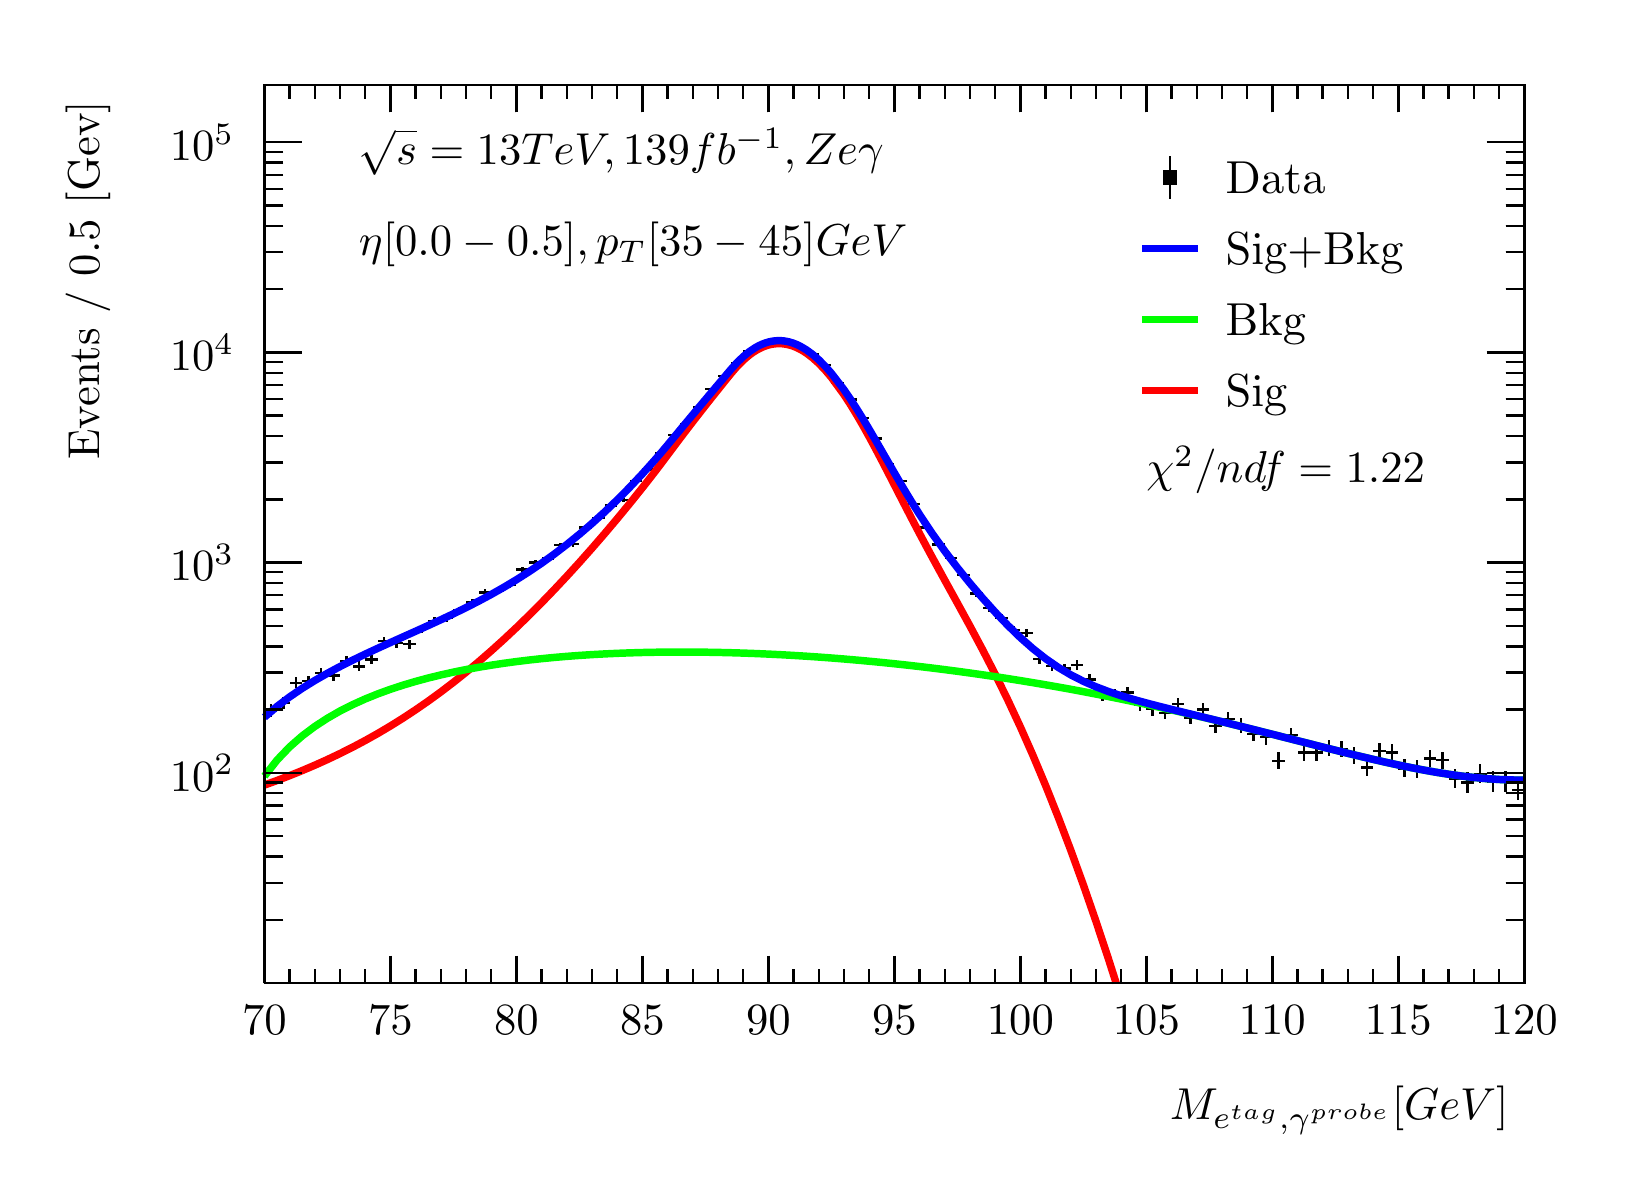
\begin{tikzpicture}
\pgfdeclareplotmark{cross} {
\pgfpathmoveto{\pgfpoint{-0.3\pgfplotmarksize}{\pgfplotmarksize}}
\pgfpathlineto{\pgfpoint{+0.3\pgfplotmarksize}{\pgfplotmarksize}}
\pgfpathlineto{\pgfpoint{+0.3\pgfplotmarksize}{0.3\pgfplotmarksize}}
\pgfpathlineto{\pgfpoint{+1\pgfplotmarksize}{0.3\pgfplotmarksize}}
\pgfpathlineto{\pgfpoint{+1\pgfplotmarksize}{-0.3\pgfplotmarksize}}
\pgfpathlineto{\pgfpoint{+0.3\pgfplotmarksize}{-0.3\pgfplotmarksize}}
\pgfpathlineto{\pgfpoint{+0.3\pgfplotmarksize}{-1.\pgfplotmarksize}}
\pgfpathlineto{\pgfpoint{-0.3\pgfplotmarksize}{-1.\pgfplotmarksize}}
\pgfpathlineto{\pgfpoint{-0.3\pgfplotmarksize}{-0.3\pgfplotmarksize}}
\pgfpathlineto{\pgfpoint{-1.\pgfplotmarksize}{-0.3\pgfplotmarksize}}
\pgfpathlineto{\pgfpoint{-1.\pgfplotmarksize}{0.3\pgfplotmarksize}}
\pgfpathlineto{\pgfpoint{-0.3\pgfplotmarksize}{0.3\pgfplotmarksize}}
\pgfpathclose
\pgfusepathqstroke
}
\pgfdeclareplotmark{cross*} {
\pgfpathmoveto{\pgfpoint{-0.3\pgfplotmarksize}{\pgfplotmarksize}}
\pgfpathlineto{\pgfpoint{+0.3\pgfplotmarksize}{\pgfplotmarksize}}
\pgfpathlineto{\pgfpoint{+0.3\pgfplotmarksize}{0.3\pgfplotmarksize}}
\pgfpathlineto{\pgfpoint{+1\pgfplotmarksize}{0.3\pgfplotmarksize}}
\pgfpathlineto{\pgfpoint{+1\pgfplotmarksize}{-0.3\pgfplotmarksize}}
\pgfpathlineto{\pgfpoint{+0.3\pgfplotmarksize}{-0.3\pgfplotmarksize}}
\pgfpathlineto{\pgfpoint{+0.3\pgfplotmarksize}{-1.\pgfplotmarksize}}
\pgfpathlineto{\pgfpoint{-0.3\pgfplotmarksize}{-1.\pgfplotmarksize}}
\pgfpathlineto{\pgfpoint{-0.3\pgfplotmarksize}{-0.3\pgfplotmarksize}}
\pgfpathlineto{\pgfpoint{-1.\pgfplotmarksize}{-0.3\pgfplotmarksize}}
\pgfpathlineto{\pgfpoint{-1.\pgfplotmarksize}{0.3\pgfplotmarksize}}
\pgfpathlineto{\pgfpoint{-0.3\pgfplotmarksize}{0.3\pgfplotmarksize}}
\pgfpathclose
\pgfusepathqfillstroke
}
\pgfdeclareplotmark{newstar} {
\pgfpathmoveto{\pgfqpoint{0pt}{\pgfplotmarksize}}
\pgfpathlineto{\pgfqpointpolar{44}{0.5\pgfplotmarksize}}
\pgfpathlineto{\pgfqpointpolar{18}{\pgfplotmarksize}}
\pgfpathlineto{\pgfqpointpolar{-20}{0.5\pgfplotmarksize}}
\pgfpathlineto{\pgfqpointpolar{-54}{\pgfplotmarksize}}
\pgfpathlineto{\pgfqpointpolar{-90}{0.5\pgfplotmarksize}}
\pgfpathlineto{\pgfqpointpolar{234}{\pgfplotmarksize}}
\pgfpathlineto{\pgfqpointpolar{198}{0.5\pgfplotmarksize}}
\pgfpathlineto{\pgfqpointpolar{162}{\pgfplotmarksize}}
\pgfpathlineto{\pgfqpointpolar{134}{0.5\pgfplotmarksize}}
\pgfpathclose
\pgfusepathqstroke
}
\pgfdeclareplotmark{newstar*} {
\pgfpathmoveto{\pgfqpoint{0pt}{\pgfplotmarksize}}
\pgfpathlineto{\pgfqpointpolar{44}{0.5\pgfplotmarksize}}
\pgfpathlineto{\pgfqpointpolar{18}{\pgfplotmarksize}}
\pgfpathlineto{\pgfqpointpolar{-20}{0.5\pgfplotmarksize}}
\pgfpathlineto{\pgfqpointpolar{-54}{\pgfplotmarksize}}
\pgfpathlineto{\pgfqpointpolar{-90}{0.5\pgfplotmarksize}}
\pgfpathlineto{\pgfqpointpolar{234}{\pgfplotmarksize}}
\pgfpathlineto{\pgfqpointpolar{198}{0.5\pgfplotmarksize}}
\pgfpathlineto{\pgfqpointpolar{162}{\pgfplotmarksize}}
\pgfpathlineto{\pgfqpointpolar{134}{0.5\pgfplotmarksize}}
\pgfpathclose
\pgfusepathqfillstroke
}
\definecolor{c}{rgb}{1,1,1};
\draw [color=c, fill=c] (0,0) rectangle (20,14.4361);
\draw [color=c, fill=c] (3,2.30977) rectangle (19,13.7143);
\definecolor{c}{rgb}{0,0,0};
\draw [c,line width=0.9] (3,2.30977) -- (3,13.7143) -- (19,13.7143) -- (19,2.30977) -- (3,2.30977);
\definecolor{c}{rgb}{1,1,1};
\draw [color=c, fill=c] (3,2.30977) rectangle (19,13.7143);
\definecolor{c}{rgb}{0,0,0};
\draw [c,line width=0.9] (3,2.30977) -- (3,13.7143) -- (19,13.7143) -- (19,2.30977) -- (3,2.30977);
\draw [c,line width=0.9] (3,2.30977) -- (19,2.30977);
\draw [c,line width=0.9] (3,2.65624) -- (3,2.30977);
\draw [c,line width=0.9] (3.32,2.48301) -- (3.32,2.30977);
\draw [c,line width=0.9] (3.64,2.48301) -- (3.64,2.30977);
\draw [c,line width=0.9] (3.96,2.48301) -- (3.96,2.30977);
\draw [c,line width=0.9] (4.28,2.48301) -- (4.28,2.30977);
\draw [c,line width=0.9] (4.6,2.65624) -- (4.6,2.30977);
\draw [c,line width=0.9] (4.92,2.48301) -- (4.92,2.30977);
\draw [c,line width=0.9] (5.24,2.48301) -- (5.24,2.30977);
\draw [c,line width=0.9] (5.56,2.48301) -- (5.56,2.30977);
\draw [c,line width=0.9] (5.88,2.48301) -- (5.88,2.30977);
\draw [c,line width=0.9] (6.2,2.65624) -- (6.2,2.30977);
\draw [c,line width=0.9] (6.52,2.48301) -- (6.52,2.30977);
\draw [c,line width=0.9] (6.84,2.48301) -- (6.84,2.30977);
\draw [c,line width=0.9] (7.16,2.48301) -- (7.16,2.30977);
\draw [c,line width=0.9] (7.48,2.48301) -- (7.48,2.30977);
\draw [c,line width=0.9] (7.8,2.65624) -- (7.8,2.30977);
\draw [c,line width=0.9] (8.12,2.48301) -- (8.12,2.30977);
\draw [c,line width=0.9] (8.44,2.48301) -- (8.44,2.30977);
\draw [c,line width=0.9] (8.76,2.48301) -- (8.76,2.30977);
\draw [c,line width=0.9] (9.08,2.48301) -- (9.08,2.30977);
\draw [c,line width=0.9] (9.4,2.65624) -- (9.4,2.30977);
\draw [c,line width=0.9] (9.72,2.48301) -- (9.72,2.30977);
\draw [c,line width=0.9] (10.04,2.48301) -- (10.04,2.30977);
\draw [c,line width=0.9] (10.36,2.48301) -- (10.36,2.30977);
\draw [c,line width=0.9] (10.68,2.48301) -- (10.68,2.30977);
\draw [c,line width=0.9] (11,2.65624) -- (11,2.30977);
\draw [c,line width=0.9] (11.32,2.48301) -- (11.32,2.30977);
\draw [c,line width=0.9] (11.64,2.48301) -- (11.64,2.30977);
\draw [c,line width=0.9] (11.96,2.48301) -- (11.96,2.30977);
\draw [c,line width=0.9] (12.28,2.48301) -- (12.28,2.30977);
\draw [c,line width=0.9] (12.6,2.65624) -- (12.6,2.30977);
\draw [c,line width=0.9] (12.92,2.48301) -- (12.92,2.30977);
\draw [c,line width=0.9] (13.24,2.48301) -- (13.24,2.30977);
\draw [c,line width=0.9] (13.56,2.48301) -- (13.56,2.30977);
\draw [c,line width=0.9] (13.88,2.48301) -- (13.88,2.30977);
\draw [c,line width=0.9] (14.2,2.65624) -- (14.2,2.30977);
\draw [c,line width=0.9] (14.52,2.48301) -- (14.52,2.30977);
\draw [c,line width=0.9] (14.84,2.48301) -- (14.84,2.30977);
\draw [c,line width=0.9] (15.16,2.48301) -- (15.16,2.30977);
\draw [c,line width=0.9] (15.48,2.48301) -- (15.48,2.30977);
\draw [c,line width=0.9] (15.8,2.65624) -- (15.8,2.30977);
\draw [c,line width=0.9] (16.12,2.48301) -- (16.12,2.30977);
\draw [c,line width=0.9] (16.44,2.48301) -- (16.44,2.30977);
\draw [c,line width=0.9] (16.76,2.48301) -- (16.76,2.30977);
\draw [c,line width=0.9] (17.08,2.48301) -- (17.08,2.30977);
\draw [c,line width=0.9] (17.4,2.65624) -- (17.4,2.30977);
\draw [c,line width=0.9] (17.72,2.48301) -- (17.72,2.30977);
\draw [c,line width=0.9] (18.04,2.48301) -- (18.04,2.30977);
\draw [c,line width=0.9] (18.36,2.48301) -- (18.36,2.30977);
\draw [c,line width=0.9] (18.68,2.48301) -- (18.68,2.30977);
\draw [c,line width=0.9] (19,2.65624) -- (19,2.30977);
\draw [anchor=base] (3,1.66015) node[scale=1.61424, color=c, rotate=0]{70};
\draw [anchor=base] (4.6,1.66015) node[scale=1.61424, color=c, rotate=0]{75};
\draw [anchor=base] (6.2,1.66015) node[scale=1.61424, color=c, rotate=0]{80};
\draw [anchor=base] (7.8,1.66015) node[scale=1.61424, color=c, rotate=0]{85};
\draw [anchor=base] (9.4,1.66015) node[scale=1.61424, color=c, rotate=0]{90};
\draw [anchor=base] (11,1.66015) node[scale=1.61424, color=c, rotate=0]{95};
\draw [anchor=base] (12.6,1.66015) node[scale=1.61424, color=c, rotate=0]{100};
\draw [anchor=base] (14.2,1.66015) node[scale=1.61424, color=c, rotate=0]{105};
\draw [anchor=base] (15.8,1.66015) node[scale=1.61424, color=c, rotate=0]{110};
\draw [anchor=base] (17.4,1.66015) node[scale=1.61424, color=c, rotate=0]{115};
\draw [anchor=base] (19,1.66015) node[scale=1.61424, color=c, rotate=0]{120};
\draw [anchor= east] (19,0.692932) node[scale=1.61424, color=c, rotate=0]{$M_{e^{tag}, \gamma^{probe}}  [GeV]$};
\draw [c,line width=0.9] (3,13.7143) -- (19,13.7143);
\draw [c,line width=0.9] (3,13.3678) -- (3,13.7143);
\draw [c,line width=0.9] (3.32,13.5411) -- (3.32,13.7143);
\draw [c,line width=0.9] (3.64,13.5411) -- (3.64,13.7143);
\draw [c,line width=0.9] (3.96,13.5411) -- (3.96,13.7143);
\draw [c,line width=0.9] (4.28,13.5411) -- (4.28,13.7143);
\draw [c,line width=0.9] (4.6,13.3678) -- (4.6,13.7143);
\draw [c,line width=0.9] (4.92,13.5411) -- (4.92,13.7143);
\draw [c,line width=0.9] (5.24,13.5411) -- (5.24,13.7143);
\draw [c,line width=0.9] (5.56,13.5411) -- (5.56,13.7143);
\draw [c,line width=0.9] (5.88,13.5411) -- (5.88,13.7143);
\draw [c,line width=0.9] (6.2,13.3678) -- (6.2,13.7143);
\draw [c,line width=0.9] (6.52,13.5411) -- (6.52,13.7143);
\draw [c,line width=0.9] (6.84,13.5411) -- (6.84,13.7143);
\draw [c,line width=0.9] (7.16,13.5411) -- (7.16,13.7143);
\draw [c,line width=0.9] (7.48,13.5411) -- (7.48,13.7143);
\draw [c,line width=0.9] (7.8,13.3678) -- (7.8,13.7143);
\draw [c,line width=0.9] (8.12,13.5411) -- (8.12,13.7143);
\draw [c,line width=0.9] (8.44,13.5411) -- (8.44,13.7143);
\draw [c,line width=0.9] (8.76,13.5411) -- (8.76,13.7143);
\draw [c,line width=0.9] (9.08,13.5411) -- (9.08,13.7143);
\draw [c,line width=0.9] (9.4,13.3678) -- (9.4,13.7143);
\draw [c,line width=0.9] (9.72,13.5411) -- (9.72,13.7143);
\draw [c,line width=0.9] (10.04,13.5411) -- (10.04,13.7143);
\draw [c,line width=0.9] (10.36,13.5411) -- (10.36,13.7143);
\draw [c,line width=0.9] (10.68,13.5411) -- (10.68,13.7143);
\draw [c,line width=0.9] (11,13.3678) -- (11,13.7143);
\draw [c,line width=0.9] (11.32,13.5411) -- (11.32,13.7143);
\draw [c,line width=0.9] (11.64,13.5411) -- (11.64,13.7143);
\draw [c,line width=0.9] (11.96,13.5411) -- (11.96,13.7143);
\draw [c,line width=0.9] (12.28,13.5411) -- (12.28,13.7143);
\draw [c,line width=0.9] (12.6,13.3678) -- (12.6,13.7143);
\draw [c,line width=0.9] (12.92,13.5411) -- (12.92,13.7143);
\draw [c,line width=0.9] (13.24,13.5411) -- (13.24,13.7143);
\draw [c,line width=0.9] (13.56,13.5411) -- (13.56,13.7143);
\draw [c,line width=0.9] (13.88,13.5411) -- (13.88,13.7143);
\draw [c,line width=0.9] (14.2,13.3678) -- (14.2,13.7143);
\draw [c,line width=0.9] (14.52,13.5411) -- (14.52,13.7143);
\draw [c,line width=0.9] (14.84,13.5411) -- (14.84,13.7143);
\draw [c,line width=0.9] (15.16,13.5411) -- (15.16,13.7143);
\draw [c,line width=0.9] (15.48,13.5411) -- (15.48,13.7143);
\draw [c,line width=0.9] (15.8,13.3678) -- (15.8,13.7143);
\draw [c,line width=0.9] (16.12,13.5411) -- (16.12,13.7143);
\draw [c,line width=0.9] (16.44,13.5411) -- (16.44,13.7143);
\draw [c,line width=0.9] (16.76,13.5411) -- (16.76,13.7143);
\draw [c,line width=0.9] (17.08,13.5411) -- (17.08,13.7143);
\draw [c,line width=0.9] (17.4,13.3678) -- (17.4,13.7143);
\draw [c,line width=0.9] (17.72,13.5411) -- (17.72,13.7143);
\draw [c,line width=0.9] (18.04,13.5411) -- (18.04,13.7143);
\draw [c,line width=0.9] (18.36,13.5411) -- (18.36,13.7143);
\draw [c,line width=0.9] (18.68,13.5411) -- (18.68,13.7143);
\draw [c,line width=0.9] (19,13.3678) -- (19,13.7143);
\draw [c,line width=0.9] (3,2.30977) -- (3,13.7143);
\draw [c,line width=0.9] (3.237,3.11343) -- (3,3.11343);
\draw [c,line width=0.9] (3.237,3.58354) -- (3,3.58354);
\draw [c,line width=0.9] (3.237,3.91709) -- (3,3.91709);
\draw [c,line width=0.9] (3.237,4.17581) -- (3,4.17581);
\draw [c,line width=0.9] (3.237,4.38719) -- (3,4.38719);
\draw [c,line width=0.9] (3.237,4.56592) -- (3,4.56592);
\draw [c,line width=0.9] (3.237,4.72074) -- (3,4.72074);
\draw [c,line width=0.9] (3.237,4.8573) -- (3,4.8573);
\draw [c,line width=0.9] (3.474,4.97946) -- (3,4.97946);
\draw [anchor= east] (2.82,4.97946) node[scale=1.61424, color=c, rotate=0]{$10^{2}$};
\draw [c,line width=0.9] (3.237,5.78312) -- (3,5.78312);
\draw [c,line width=0.9] (3.237,6.25323) -- (3,6.25323);
\draw [c,line width=0.9] (3.237,6.58678) -- (3,6.58678);
\draw [c,line width=0.9] (3.237,6.8455) -- (3,6.8455);
\draw [c,line width=0.9] (3.237,7.05689) -- (3,7.05689);
\draw [c,line width=0.9] (3.237,7.23561) -- (3,7.23561);
\draw [c,line width=0.9] (3.237,7.39043) -- (3,7.39043);
\draw [c,line width=0.9] (3.237,7.52699) -- (3,7.52699);
\draw [c,line width=0.9] (3.474,7.64915) -- (3,7.64915);
\draw [anchor= east] (2.82,7.64915) node[scale=1.61424, color=c, rotate=0]{$10^{3}$};
\draw [c,line width=0.9] (3.237,8.45281) -- (3,8.45281);
\draw [c,line width=0.9] (3.237,8.92292) -- (3,8.92292);
\draw [c,line width=0.9] (3.237,9.25647) -- (3,9.25647);
\draw [c,line width=0.9] (3.237,9.51519) -- (3,9.51519);
\draw [c,line width=0.9] (3.237,9.72658) -- (3,9.72658);
\draw [c,line width=0.9] (3.237,9.9053) -- (3,9.9053);
\draw [c,line width=0.9] (3.237,10.0601) -- (3,10.0601);
\draw [c,line width=0.9] (3.237,10.1967) -- (3,10.1967);
\draw [c,line width=0.9] (3.474,10.3188) -- (3,10.3188);
\draw [anchor= east] (2.82,10.3188) node[scale=1.61424, color=c, rotate=0]{$10^{4}$};
\draw [c,line width=0.9] (3.237,11.1225) -- (3,11.1225);
\draw [c,line width=0.9] (3.237,11.5926) -- (3,11.5926);
\draw [c,line width=0.9] (3.237,11.9262) -- (3,11.9262);
\draw [c,line width=0.9] (3.237,12.1849) -- (3,12.1849);
\draw [c,line width=0.9] (3.237,12.3963) -- (3,12.3963);
\draw [c,line width=0.9] (3.237,12.575) -- (3,12.575);
\draw [c,line width=0.9] (3.237,12.7298) -- (3,12.7298);
\draw [c,line width=0.9] (3.237,12.8664) -- (3,12.8664);
\draw [c,line width=0.9] (3.474,12.9885) -- (3,12.9885);
\draw [anchor= east] (2.82,12.9885) node[scale=1.61424, color=c, rotate=0]{$10^{5}$};
\draw [anchor= east] (0.76,13.7143) node[scale=1.61424, color=c, rotate=90]{Events / 0.5 [Gev]};
\draw [c,line width=0.9] (19,2.30977) -- (19,13.7143);
\draw [c,line width=0.9] (18.763,3.11343) -- (19,3.11343);
\draw [c,line width=0.9] (18.763,3.58354) -- (19,3.58354);
\draw [c,line width=0.9] (18.763,3.91709) -- (19,3.91709);
\draw [c,line width=0.9] (18.763,4.17581) -- (19,4.17581);
\draw [c,line width=0.9] (18.763,4.38719) -- (19,4.38719);
\draw [c,line width=0.9] (18.763,4.56592) -- (19,4.56592);
\draw [c,line width=0.9] (18.763,4.72074) -- (19,4.72074);
\draw [c,line width=0.9] (18.763,4.8573) -- (19,4.8573);
\draw [c,line width=0.9] (18.526,4.97946) -- (19,4.97946);
\draw [c,line width=0.9] (18.763,5.78312) -- (19,5.78312);
\draw [c,line width=0.9] (18.763,6.25323) -- (19,6.25323);
\draw [c,line width=0.9] (18.763,6.58678) -- (19,6.58678);
\draw [c,line width=0.9] (18.763,6.8455) -- (19,6.8455);
\draw [c,line width=0.9] (18.763,7.05689) -- (19,7.05689);
\draw [c,line width=0.9] (18.763,7.23561) -- (19,7.23561);
\draw [c,line width=0.9] (18.763,7.39043) -- (19,7.39043);
\draw [c,line width=0.9] (18.763,7.52699) -- (19,7.52699);
\draw [c,line width=0.9] (18.526,7.64915) -- (19,7.64915);
\draw [c,line width=0.9] (18.763,8.45281) -- (19,8.45281);
\draw [c,line width=0.9] (18.763,8.92292) -- (19,8.92292);
\draw [c,line width=0.9] (18.763,9.25647) -- (19,9.25647);
\draw [c,line width=0.9] (18.763,9.51519) -- (19,9.51519);
\draw [c,line width=0.9] (18.763,9.72658) -- (19,9.72658);
\draw [c,line width=0.9] (18.763,9.9053) -- (19,9.9053);
\draw [c,line width=0.9] (18.763,10.0601) -- (19,10.0601);
\draw [c,line width=0.9] (18.763,10.1967) -- (19,10.1967);
\draw [c,line width=0.9] (18.526,10.3188) -- (19,10.3188);
\draw [c,line width=0.9] (18.763,11.1225) -- (19,11.1225);
\draw [c,line width=0.9] (18.763,11.5926) -- (19,11.5926);
\draw [c,line width=0.9] (18.763,11.9262) -- (19,11.9262);
\draw [c,line width=0.9] (18.763,12.1849) -- (19,12.1849);
\draw [c,line width=0.9] (18.763,12.3963) -- (19,12.3963);
\draw [c,line width=0.9] (18.763,12.575) -- (19,12.575);
\draw [c,line width=0.9] (18.763,12.7298) -- (19,12.7298);
\draw [c,line width=0.9] (18.763,12.8664) -- (19,12.8664);
\draw [c,line width=0.9] (18.526,12.9885) -- (19,12.9885);
\draw [c,line width=0.9] (3.08,5.77147) -- (3,5.77147);
\draw [c,line width=0.9] (3,5.77147) -- (3,5.77147);
\draw [c,line width=0.9] (3.08,5.77147) -- (3.16,5.77147);
\draw [c,line width=0.9] (3.16,5.77147) -- (3.16,5.77147);
\draw [c,line width=0.9] (3.08,5.77147) -- (3.08,5.85385);
\draw [c,line width=0.9] (3.08,5.85385) -- (3.08,5.85385);
\draw [c,line width=0.9] (3.08,5.77147) -- (3.08,5.68909);
\draw [c,line width=0.9] (3.08,5.68909) -- (3.08,5.68909);
\draw [c,line width=0.9] (3.24,5.86697) -- (3.16,5.86697);
\draw [c,line width=0.9] (3.16,5.86697) -- (3.16,5.86697);
\draw [c,line width=0.9] (3.24,5.86697) -- (3.32,5.86697);
\draw [c,line width=0.9] (3.32,5.86697) -- (3.32,5.86697);
\draw [c,line width=0.9] (3.24,5.86697) -- (3.24,5.94603);
\draw [c,line width=0.9] (3.24,5.94603) -- (3.24,5.94603);
\draw [c,line width=0.9] (3.24,5.86697) -- (3.24,5.78791);
\draw [c,line width=0.9] (3.24,5.78791) -- (3.24,5.78791);
\draw [c,line width=0.9] (3.4,6.12245) -- (3.32,6.12245);
\draw [c,line width=0.9] (3.32,6.12245) -- (3.32,6.12245);
\draw [c,line width=0.9] (3.4,6.12245) -- (3.48,6.12245);
\draw [c,line width=0.9] (3.48,6.12245) -- (3.48,6.12245);
\draw [c,line width=0.9] (3.4,6.12245) -- (3.4,6.19326);
\draw [c,line width=0.9] (3.4,6.19326) -- (3.4,6.19326);
\draw [c,line width=0.9] (3.4,6.12245) -- (3.4,6.05164);
\draw [c,line width=0.9] (3.4,6.05164) -- (3.4,6.05164);
\draw [c,line width=0.9] (3.56,6.14388) -- (3.48,6.14388);
\draw [c,line width=0.9] (3.48,6.14388) -- (3.48,6.14388);
\draw [c,line width=0.9] (3.56,6.14388) -- (3.64,6.14388);
\draw [c,line width=0.9] (3.64,6.14388) -- (3.64,6.14388);
\draw [c,line width=0.9] (3.56,6.14388) -- (3.56,6.21404);
\draw [c,line width=0.9] (3.56,6.21404) -- (3.56,6.21404);
\draw [c,line width=0.9] (3.56,6.14388) -- (3.56,6.07372);
\draw [c,line width=0.9] (3.56,6.07372) -- (3.56,6.07372);
\draw [c,line width=0.9] (3.72,6.24547) -- (3.64,6.24547);
\draw [c,line width=0.9] (3.64,6.24547) -- (3.64,6.24547);
\draw [c,line width=0.9] (3.72,6.24547) -- (3.8,6.24547);
\draw [c,line width=0.9] (3.8,6.24547) -- (3.8,6.24547);
\draw [c,line width=0.9] (3.72,6.24547) -- (3.72,6.31263);
\draw [c,line width=0.9] (3.72,6.31263) -- (3.72,6.31263);
\draw [c,line width=0.9] (3.72,6.24547) -- (3.72,6.17832);
\draw [c,line width=0.9] (3.72,6.17832) -- (3.72,6.17832);
\draw [c,line width=0.9] (3.88,6.21392) -- (3.8,6.21392);
\draw [c,line width=0.9] (3.8,6.21392) -- (3.8,6.21392);
\draw [c,line width=0.9] (3.88,6.21392) -- (3.96,6.21392);
\draw [c,line width=0.9] (3.96,6.21392) -- (3.96,6.21392);
\draw [c,line width=0.9] (3.88,6.21392) -- (3.88,6.282);
\draw [c,line width=0.9] (3.88,6.282) -- (3.88,6.282);
\draw [c,line width=0.9] (3.88,6.21392) -- (3.88,6.14585);
\draw [c,line width=0.9] (3.88,6.14585) -- (3.88,6.14585);
\draw [c,line width=0.9] (4.04,6.39835) -- (3.96,6.39835);
\draw [c,line width=0.9] (3.96,6.39835) -- (3.96,6.39835);
\draw [c,line width=0.9] (4.04,6.39835) -- (4.12,6.39835);
\draw [c,line width=0.9] (4.12,6.39835) -- (4.12,6.39835);
\draw [c,line width=0.9] (4.04,6.39835) -- (4.04,6.46122);
\draw [c,line width=0.9] (4.04,6.46122) -- (4.04,6.46122);
\draw [c,line width=0.9] (4.04,6.39835) -- (4.04,6.33548);
\draw [c,line width=0.9] (4.04,6.33548) -- (4.04,6.33548);
\draw [c,line width=0.9] (4.2,6.33168) -- (4.12,6.33168);
\draw [c,line width=0.9] (4.12,6.33168) -- (4.12,6.33168);
\draw [c,line width=0.9] (4.2,6.33168) -- (4.28,6.33168);
\draw [c,line width=0.9] (4.28,6.33168) -- (4.28,6.33168);
\draw [c,line width=0.9] (4.2,6.33168) -- (4.2,6.39638);
\draw [c,line width=0.9] (4.2,6.39638) -- (4.2,6.39638);
\draw [c,line width=0.9] (4.2,6.33168) -- (4.2,6.26697);
\draw [c,line width=0.9] (4.2,6.26697) -- (4.2,6.26697);
\draw [c,line width=0.9] (4.36,6.41863) -- (4.28,6.41863);
\draw [c,line width=0.9] (4.28,6.41863) -- (4.28,6.41863);
\draw [c,line width=0.9] (4.36,6.41863) -- (4.44,6.41863);
\draw [c,line width=0.9] (4.44,6.41863) -- (4.44,6.41863);
\draw [c,line width=0.9] (4.36,6.41863) -- (4.36,6.48095);
\draw [c,line width=0.9] (4.36,6.48095) -- (4.36,6.48095);
\draw [c,line width=0.9] (4.36,6.41863) -- (4.36,6.35631);
\draw [c,line width=0.9] (4.36,6.35631) -- (4.36,6.35631);
\draw [c,line width=0.9] (4.52,6.6516) -- (4.44,6.6516);
\draw [c,line width=0.9] (4.44,6.6516) -- (4.44,6.6516);
\draw [c,line width=0.9] (4.52,6.6516) -- (4.6,6.6516);
\draw [c,line width=0.9] (4.6,6.6516) -- (4.6,6.6516);
\draw [c,line width=0.9] (4.52,6.6516) -- (4.52,6.70797);
\draw [c,line width=0.9] (4.52,6.70797) -- (4.52,6.70797);
\draw [c,line width=0.9] (4.52,6.6516) -- (4.52,6.59523);
\draw [c,line width=0.9] (4.52,6.59523) -- (4.52,6.59523);
\draw [c,line width=0.9] (4.68,6.62666) -- (4.6,6.62666);
\draw [c,line width=0.9] (4.6,6.62666) -- (4.6,6.62666);
\draw [c,line width=0.9] (4.68,6.62666) -- (4.76,6.62666);
\draw [c,line width=0.9] (4.76,6.62666) -- (4.76,6.62666);
\draw [c,line width=0.9] (4.68,6.62666) -- (4.68,6.68364);
\draw [c,line width=0.9] (4.68,6.68364) -- (4.68,6.68364);
\draw [c,line width=0.9] (4.68,6.62666) -- (4.68,6.56969);
\draw [c,line width=0.9] (4.68,6.56969) -- (4.68,6.56969);
\draw [c,line width=0.9] (4.84,6.61258) -- (4.76,6.61258);
\draw [c,line width=0.9] (4.76,6.61258) -- (4.76,6.61258);
\draw [c,line width=0.9] (4.84,6.61258) -- (4.92,6.61258);
\draw [c,line width=0.9] (4.92,6.61258) -- (4.92,6.61258);
\draw [c,line width=0.9] (4.84,6.61258) -- (4.84,6.6699);
\draw [c,line width=0.9] (4.84,6.6699) -- (4.84,6.6699);
\draw [c,line width=0.9] (4.84,6.61258) -- (4.84,6.55525);
\draw [c,line width=0.9] (4.84,6.55525) -- (4.84,6.55525);
\draw [c,line width=0.9] (5,6.80779) -- (4.92,6.80779);
\draw [c,line width=0.9] (4.92,6.80779) -- (4.92,6.80779);
\draw [c,line width=0.9] (5,6.80779) -- (5.08,6.80779);
\draw [c,line width=0.9] (5.08,6.80779) -- (5.08,6.80779);
\draw [c,line width=0.9] (5,6.80779) -- (5,6.86049);
\draw [c,line width=0.9] (5,6.86049) -- (5,6.86049);
\draw [c,line width=0.9] (5,6.80779) -- (5,6.75509);
\draw [c,line width=0.9] (5,6.75509) -- (5,6.75509);
\draw [c,line width=0.9] (5.16,6.90207) -- (5.08,6.90207);
\draw [c,line width=0.9] (5.08,6.90207) -- (5.08,6.90207);
\draw [c,line width=0.9] (5.16,6.90207) -- (5.24,6.90207);
\draw [c,line width=0.9] (5.24,6.90207) -- (5.24,6.90207);
\draw [c,line width=0.9] (5.16,6.90207) -- (5.16,6.95266);
\draw [c,line width=0.9] (5.16,6.95266) -- (5.16,6.95266);
\draw [c,line width=0.9] (5.16,6.90207) -- (5.16,6.85147);
\draw [c,line width=0.9] (5.16,6.85147) -- (5.16,6.85147);
\draw [c,line width=0.9] (5.32,6.94754) -- (5.24,6.94754);
\draw [c,line width=0.9] (5.24,6.94754) -- (5.24,6.94754);
\draw [c,line width=0.9] (5.32,6.94754) -- (5.4,6.94754);
\draw [c,line width=0.9] (5.4,6.94754) -- (5.4,6.94754);
\draw [c,line width=0.9] (5.32,6.94754) -- (5.32,6.99716);
\draw [c,line width=0.9] (5.32,6.99716) -- (5.32,6.99716);
\draw [c,line width=0.9] (5.32,6.94754) -- (5.32,6.89792);
\draw [c,line width=0.9] (5.32,6.89792) -- (5.32,6.89792);
\draw [c,line width=0.9] (5.48,7.03936) -- (5.4,7.03936);
\draw [c,line width=0.9] (5.4,7.03936) -- (5.4,7.03936);
\draw [c,line width=0.9] (5.48,7.03936) -- (5.56,7.03936);
\draw [c,line width=0.9] (5.56,7.03936) -- (5.56,7.03936);
\draw [c,line width=0.9] (5.48,7.03936) -- (5.48,7.08705);
\draw [c,line width=0.9] (5.48,7.08705) -- (5.48,7.08705);
\draw [c,line width=0.9] (5.48,7.03936) -- (5.48,6.99167);
\draw [c,line width=0.9] (5.48,6.99167) -- (5.48,6.99167);
\draw [c,line width=0.9] (5.64,7.14074) -- (5.56,7.14074);
\draw [c,line width=0.9] (5.56,7.14074) -- (5.56,7.14074);
\draw [c,line width=0.9] (5.64,7.14074) -- (5.72,7.14074);
\draw [c,line width=0.9] (5.72,7.14074) -- (5.72,7.14074);
\draw [c,line width=0.9] (5.64,7.14074) -- (5.64,7.18639);
\draw [c,line width=0.9] (5.64,7.18639) -- (5.64,7.18639);
\draw [c,line width=0.9] (5.64,7.14074) -- (5.64,7.09509);
\draw [c,line width=0.9] (5.64,7.09509) -- (5.64,7.09509);
\draw [c,line width=0.9] (5.8,7.26666) -- (5.72,7.26666);
\draw [c,line width=0.9] (5.72,7.26666) -- (5.72,7.26666);
\draw [c,line width=0.9] (5.8,7.26666) -- (5.88,7.26666);
\draw [c,line width=0.9] (5.88,7.26666) -- (5.88,7.26666);
\draw [c,line width=0.9] (5.8,7.26666) -- (5.8,7.3099);
\draw [c,line width=0.9] (5.8,7.3099) -- (5.8,7.3099);
\draw [c,line width=0.9] (5.8,7.26666) -- (5.8,7.22343);
\draw [c,line width=0.9] (5.8,7.22343) -- (5.8,7.22343);
\draw [c,line width=0.9] (5.96,7.28902) -- (5.88,7.28902);
\draw [c,line width=0.9] (5.88,7.28902) -- (5.88,7.28902);
\draw [c,line width=0.9] (5.96,7.28902) -- (6.04,7.28902);
\draw [c,line width=0.9] (6.04,7.28902) -- (6.04,7.28902);
\draw [c,line width=0.9] (5.96,7.28902) -- (5.96,7.33185);
\draw [c,line width=0.9] (5.96,7.33185) -- (5.96,7.33185);
\draw [c,line width=0.9] (5.96,7.28902) -- (5.96,7.2462);
\draw [c,line width=0.9] (5.96,7.2462) -- (5.96,7.2462);
\draw [c,line width=0.9] (6.12,7.36553) -- (6.04,7.36553);
\draw [c,line width=0.9] (6.04,7.36553) -- (6.04,7.36553);
\draw [c,line width=0.9] (6.12,7.36553) -- (6.2,7.36553);
\draw [c,line width=0.9] (6.2,7.36553) -- (6.2,7.36553);
\draw [c,line width=0.9] (6.12,7.36553) -- (6.12,7.40696);
\draw [c,line width=0.9] (6.12,7.40696) -- (6.12,7.40696);
\draw [c,line width=0.9] (6.12,7.36553) -- (6.12,7.3241);
\draw [c,line width=0.9] (6.12,7.3241) -- (6.12,7.3241);
\draw [c,line width=0.9] (6.28,7.55876) -- (6.2,7.55876);
\draw [c,line width=0.9] (6.2,7.55876) -- (6.2,7.55876);
\draw [c,line width=0.9] (6.28,7.55876) -- (6.36,7.55876);
\draw [c,line width=0.9] (6.36,7.55876) -- (6.36,7.55876);
\draw [c,line width=0.9] (6.28,7.55876) -- (6.28,7.59688);
\draw [c,line width=0.9] (6.28,7.59688) -- (6.28,7.59688);
\draw [c,line width=0.9] (6.28,7.55876) -- (6.28,7.52064);
\draw [c,line width=0.9] (6.28,7.52064) -- (6.28,7.52064);
\draw [c,line width=0.9] (6.44,7.65031) -- (6.36,7.65031);
\draw [c,line width=0.9] (6.36,7.65031) -- (6.36,7.65031);
\draw [c,line width=0.9] (6.44,7.65031) -- (6.52,7.65031);
\draw [c,line width=0.9] (6.52,7.65031) -- (6.52,7.65031);
\draw [c,line width=0.9] (6.44,7.65031) -- (6.44,7.68696);
\draw [c,line width=0.9] (6.44,7.68696) -- (6.44,7.68696);
\draw [c,line width=0.9] (6.44,7.65031) -- (6.44,7.61367);
\draw [c,line width=0.9] (6.44,7.61367) -- (6.44,7.61367);
\draw [c,line width=0.9] (6.6,7.69908) -- (6.52,7.69908);
\draw [c,line width=0.9] (6.52,7.69908) -- (6.52,7.69908);
\draw [c,line width=0.9] (6.6,7.69908) -- (6.68,7.69908);
\draw [c,line width=0.9] (6.68,7.69908) -- (6.68,7.69908);
\draw [c,line width=0.9] (6.6,7.69908) -- (6.6,7.73496);
\draw [c,line width=0.9] (6.6,7.73496) -- (6.6,7.73496);
\draw [c,line width=0.9] (6.6,7.69908) -- (6.6,7.6632);
\draw [c,line width=0.9] (6.6,7.6632) -- (6.6,7.6632);
\draw [c,line width=0.9] (6.76,7.87112) -- (6.68,7.87112);
\draw [c,line width=0.9] (6.68,7.87112) -- (6.68,7.87112);
\draw [c,line width=0.9] (6.76,7.87112) -- (6.84,7.87112);
\draw [c,line width=0.9] (6.84,7.87112) -- (6.84,7.87112);
\draw [c,line width=0.9] (6.76,7.87112) -- (6.76,7.90444);
\draw [c,line width=0.9] (6.76,7.90444) -- (6.76,7.90444);
\draw [c,line width=0.9] (6.76,7.87112) -- (6.76,7.83781);
\draw [c,line width=0.9] (6.76,7.83781) -- (6.76,7.83781);
\draw [c,line width=0.9] (6.92,7.8854) -- (6.84,7.8854);
\draw [c,line width=0.9] (6.84,7.8854) -- (6.84,7.8854);
\draw [c,line width=0.9] (6.92,7.8854) -- (7,7.8854);
\draw [c,line width=0.9] (7,7.8854) -- (7,7.8854);
\draw [c,line width=0.9] (6.92,7.8854) -- (6.92,7.91851);
\draw [c,line width=0.9] (6.92,7.91851) -- (6.92,7.91851);
\draw [c,line width=0.9] (6.92,7.8854) -- (6.92,7.85228);
\draw [c,line width=0.9] (6.92,7.85228) -- (6.92,7.85228);
\draw [c,line width=0.9] (7.08,8.09426) -- (7,8.09426);
\draw [c,line width=0.9] (7,8.09426) -- (7,8.09426);
\draw [c,line width=0.9] (7.08,8.09426) -- (7.16,8.09426);
\draw [c,line width=0.9] (7.16,8.09426) -- (7.16,8.09426);
\draw [c,line width=0.9] (7.08,8.09426) -- (7.08,8.12452);
\draw [c,line width=0.9] (7.08,8.12452) -- (7.08,8.12452);
\draw [c,line width=0.9] (7.08,8.09426) -- (7.08,8.064);
\draw [c,line width=0.9] (7.08,8.064) -- (7.08,8.064);
\draw [c,line width=0.9] (7.24,8.21705) -- (7.16,8.21705);
\draw [c,line width=0.9] (7.16,8.21705) -- (7.16,8.21705);
\draw [c,line width=0.9] (7.24,8.21705) -- (7.32,8.21705);
\draw [c,line width=0.9] (7.32,8.21705) -- (7.32,8.21705);
\draw [c,line width=0.9] (7.24,8.21705) -- (7.24,8.24575);
\draw [c,line width=0.9] (7.24,8.24575) -- (7.24,8.24575);
\draw [c,line width=0.9] (7.24,8.21705) -- (7.24,8.18835);
\draw [c,line width=0.9] (7.24,8.18835) -- (7.24,8.18835);
\draw [c,line width=0.9] (7.4,8.37365) -- (7.32,8.37365);
\draw [c,line width=0.9] (7.32,8.37365) -- (7.32,8.37365);
\draw [c,line width=0.9] (7.4,8.37365) -- (7.48,8.37365);
\draw [c,line width=0.9] (7.48,8.37365) -- (7.48,8.37365);
\draw [c,line width=0.9] (7.4,8.37365) -- (7.4,8.40047);
\draw [c,line width=0.9] (7.4,8.40047) -- (7.4,8.40047);
\draw [c,line width=0.9] (7.4,8.37365) -- (7.4,8.34682);
\draw [c,line width=0.9] (7.4,8.34682) -- (7.4,8.34682);
\draw [c,line width=0.9] (7.56,8.44233) -- (7.48,8.44233);
\draw [c,line width=0.9] (7.48,8.44233) -- (7.48,8.44233);
\draw [c,line width=0.9] (7.56,8.44233) -- (7.64,8.44233);
\draw [c,line width=0.9] (7.64,8.44233) -- (7.64,8.44233);
\draw [c,line width=0.9] (7.56,8.44233) -- (7.56,8.46837);
\draw [c,line width=0.9] (7.56,8.46837) -- (7.56,8.46837);
\draw [c,line width=0.9] (7.56,8.44233) -- (7.56,8.41629);
\draw [c,line width=0.9] (7.56,8.41629) -- (7.56,8.41629);
\draw [c,line width=0.9] (7.72,8.68526) -- (7.64,8.68526);
\draw [c,line width=0.9] (7.64,8.68526) -- (7.64,8.68526);
\draw [c,line width=0.9] (7.72,8.68526) -- (7.8,8.68526);
\draw [c,line width=0.9] (7.8,8.68526) -- (7.8,8.68526);
\draw [c,line width=0.9] (7.72,8.68526) -- (7.72,8.70872);
\draw [c,line width=0.9] (7.72,8.70872) -- (7.72,8.70872);
\draw [c,line width=0.9] (7.72,8.68526) -- (7.72,8.66181);
\draw [c,line width=0.9] (7.72,8.66181) -- (7.72,8.66181);
\draw [c,line width=0.9] (7.88,8.83336) -- (7.8,8.83336);
\draw [c,line width=0.9] (7.8,8.83336) -- (7.8,8.83336);
\draw [c,line width=0.9] (7.88,8.83336) -- (7.96,8.83336);
\draw [c,line width=0.9] (7.96,8.83336) -- (7.96,8.83336);
\draw [c,line width=0.9] (7.88,8.83336) -- (7.88,8.85537);
\draw [c,line width=0.9] (7.88,8.85537) -- (7.88,8.85537);
\draw [c,line width=0.9] (7.88,8.83336) -- (7.88,8.81136);
\draw [c,line width=0.9] (7.88,8.81136) -- (7.88,8.81136);
\draw [c,line width=0.9] (8.04,9.03763) -- (7.96,9.03763);
\draw [c,line width=0.9] (7.96,9.03763) -- (7.96,9.03763);
\draw [c,line width=0.9] (8.04,9.03763) -- (8.12,9.03763);
\draw [c,line width=0.9] (8.12,9.03763) -- (8.12,9.03763);
\draw [c,line width=0.9] (8.04,9.03763) -- (8.04,9.05778);
\draw [c,line width=0.9] (8.04,9.05778) -- (8.04,9.05778);
\draw [c,line width=0.9] (8.04,9.03763) -- (8.04,9.01749);
\draw [c,line width=0.9] (8.04,9.01749) -- (8.04,9.01749);
\draw [c,line width=0.9] (8.2,9.26858) -- (8.12,9.26858);
\draw [c,line width=0.9] (8.12,9.26858) -- (8.12,9.26858);
\draw [c,line width=0.9] (8.2,9.26858) -- (8.28,9.26858);
\draw [c,line width=0.9] (8.28,9.26858) -- (8.28,9.26858);
\draw [c,line width=0.9] (8.2,9.26858) -- (8.2,9.28681);
\draw [c,line width=0.9] (8.2,9.28681) -- (8.2,9.28681);
\draw [c,line width=0.9] (8.2,9.26858) -- (8.2,9.25034);
\draw [c,line width=0.9] (8.2,9.25034) -- (8.2,9.25034);
\draw [c,line width=0.9] (8.36,9.41093) -- (8.28,9.41093);
\draw [c,line width=0.9] (8.28,9.41093) -- (8.28,9.41093);
\draw [c,line width=0.9] (8.36,9.41093) -- (8.44,9.41093);
\draw [c,line width=0.9] (8.44,9.41093) -- (8.44,9.41093);
\draw [c,line width=0.9] (8.36,9.41093) -- (8.36,9.42808);
\draw [c,line width=0.9] (8.36,9.42808) -- (8.36,9.42808);
\draw [c,line width=0.9] (8.36,9.41093) -- (8.36,9.39377);
\draw [c,line width=0.9] (8.36,9.39377) -- (8.36,9.39377);
\draw [c,line width=0.9] (8.52,9.62801) -- (8.44,9.62801);
\draw [c,line width=0.9] (8.44,9.62801) -- (8.44,9.62801);
\draw [c,line width=0.9] (8.52,9.62801) -- (8.6,9.62801);
\draw [c,line width=0.9] (8.6,9.62801) -- (8.6,9.62801);
\draw [c,line width=0.9] (8.52,9.62801) -- (8.52,9.64363);
\draw [c,line width=0.9] (8.52,9.64363) -- (8.52,9.64363);
\draw [c,line width=0.9] (8.52,9.62801) -- (8.52,9.61239);
\draw [c,line width=0.9] (8.52,9.61239) -- (8.52,9.61239);
\draw [c,line width=0.9] (8.68,9.85105) -- (8.6,9.85105);
\draw [c,line width=0.9] (8.6,9.85105) -- (8.6,9.85105);
\draw [c,line width=0.9] (8.68,9.85105) -- (8.76,9.85105);
\draw [c,line width=0.9] (8.76,9.85105) -- (8.76,9.85105);
\draw [c,line width=0.9] (8.68,9.85105) -- (8.68,9.86524);
\draw [c,line width=0.9] (8.68,9.86524) -- (8.68,9.86524);
\draw [c,line width=0.9] (8.68,9.85105) -- (8.68,9.83687);
\draw [c,line width=0.9] (8.68,9.83687) -- (8.68,9.83687);
\draw [c,line width=0.9] (8.84,10.0176) -- (8.76,10.0176);
\draw [c,line width=0.9] (8.76,10.0176) -- (8.76,10.0176);
\draw [c,line width=0.9] (8.84,10.0176) -- (8.92,10.0176);
\draw [c,line width=0.9] (8.92,10.0176) -- (8.92,10.0176);
\draw [c,line width=0.9] (8.84,10.0176) -- (8.84,10.0308);
\draw [c,line width=0.9] (8.84,10.0308) -- (8.84,10.0308);
\draw [c,line width=0.9] (8.84,10.0176) -- (8.84,10.0044);
\draw [c,line width=0.9] (8.84,10.0044) -- (8.84,10.0044);
\draw [c,line width=0.9] (9,10.1863) -- (8.92,10.1863);
\draw [c,line width=0.9] (8.92,10.1863) -- (8.92,10.1863);
\draw [c,line width=0.9] (9,10.1863) -- (9.08,10.1863);
\draw [c,line width=0.9] (9.08,10.1863) -- (9.08,10.1863);
\draw [c,line width=0.9] (9,10.1863) -- (9,10.1986);
\draw [c,line width=0.9] (9,10.1986) -- (9,10.1986);
\draw [c,line width=0.9] (9,10.1863) -- (9,10.1741);
\draw [c,line width=0.9] (9,10.1741) -- (9,10.1741);
\draw [c,line width=0.9] (9.16,10.3322) -- (9.08,10.3322);
\draw [c,line width=0.9] (9.08,10.3322) -- (9.08,10.3322);
\draw [c,line width=0.9] (9.16,10.3322) -- (9.24,10.3322);
\draw [c,line width=0.9] (9.24,10.3322) -- (9.24,10.3322);
\draw [c,line width=0.9] (9.16,10.3322) -- (9.16,10.3437);
\draw [c,line width=0.9] (9.16,10.3437) -- (9.16,10.3437);
\draw [c,line width=0.9] (9.16,10.3322) -- (9.16,10.3207);
\draw [c,line width=0.9] (9.16,10.3207) -- (9.16,10.3207);
\draw [c,line width=0.9] (9.32,10.4103) -- (9.24,10.4103);
\draw [c,line width=0.9] (9.24,10.4103) -- (9.24,10.4103);
\draw [c,line width=0.9] (9.32,10.4103) -- (9.4,10.4103);
\draw [c,line width=0.9] (9.4,10.4103) -- (9.4,10.4103);
\draw [c,line width=0.9] (9.32,10.4103) -- (9.32,10.4215);
\draw [c,line width=0.9] (9.32,10.4215) -- (9.32,10.4215);
\draw [c,line width=0.9] (9.32,10.4103) -- (9.32,10.3992);
\draw [c,line width=0.9] (9.32,10.3992) -- (9.32,10.3992);
\draw [c,line width=0.9] (9.48,10.4655) -- (9.4,10.4655);
\draw [c,line width=0.9] (9.4,10.4655) -- (9.4,10.4655);
\draw [c,line width=0.9] (9.48,10.4655) -- (9.56,10.4655);
\draw [c,line width=0.9] (9.56,10.4655) -- (9.56,10.4655);
\draw [c,line width=0.9] (9.48,10.4655) -- (9.48,10.4763);
\draw [c,line width=0.9] (9.48,10.4763) -- (9.48,10.4763);
\draw [c,line width=0.9] (9.48,10.4655) -- (9.48,10.4546);
\draw [c,line width=0.9] (9.48,10.4546) -- (9.48,10.4546);
\draw [c,line width=0.9] (9.64,10.4522) -- (9.56,10.4522);
\draw [c,line width=0.9] (9.56,10.4522) -- (9.56,10.4522);
\draw [c,line width=0.9] (9.64,10.4522) -- (9.72,10.4522);
\draw [c,line width=0.9] (9.72,10.4522) -- (9.72,10.4522);
\draw [c,line width=0.9] (9.64,10.4522) -- (9.64,10.4632);
\draw [c,line width=0.9] (9.64,10.4632) -- (9.64,10.4632);
\draw [c,line width=0.9] (9.64,10.4522) -- (9.64,10.4413);
\draw [c,line width=0.9] (9.64,10.4413) -- (9.64,10.4413);
\draw [c,line width=0.9] (9.8,10.3965) -- (9.72,10.3965);
\draw [c,line width=0.9] (9.72,10.3965) -- (9.72,10.3965);
\draw [c,line width=0.9] (9.8,10.3965) -- (9.88,10.3965);
\draw [c,line width=0.9] (9.88,10.3965) -- (9.88,10.3965);
\draw [c,line width=0.9] (9.8,10.3965) -- (9.8,10.4077);
\draw [c,line width=0.9] (9.8,10.4077) -- (9.8,10.4077);
\draw [c,line width=0.9] (9.8,10.3965) -- (9.8,10.3853);
\draw [c,line width=0.9] (9.8,10.3853) -- (9.8,10.3853);
\draw [c,line width=0.9] (9.96,10.2945) -- (9.88,10.2945);
\draw [c,line width=0.9] (9.88,10.2945) -- (9.88,10.2945);
\draw [c,line width=0.9] (9.96,10.2945) -- (10.04,10.2945);
\draw [c,line width=0.9] (10.04,10.2945) -- (10.04,10.2945);
\draw [c,line width=0.9] (9.96,10.2945) -- (9.96,10.3062);
\draw [c,line width=0.9] (9.96,10.3062) -- (9.96,10.3062);
\draw [c,line width=0.9] (9.96,10.2945) -- (9.96,10.2828);
\draw [c,line width=0.9] (9.96,10.2828) -- (9.96,10.2828);
\draw [c,line width=0.9] (10.12,10.1619) -- (10.04,10.1619);
\draw [c,line width=0.9] (10.04,10.1619) -- (10.04,10.1619);
\draw [c,line width=0.9] (10.12,10.1619) -- (10.2,10.1619);
\draw [c,line width=0.9] (10.2,10.1619) -- (10.2,10.1619);
\draw [c,line width=0.9] (10.12,10.1619) -- (10.12,10.1743);
\draw [c,line width=0.9] (10.12,10.1743) -- (10.12,10.1743);
\draw [c,line width=0.9] (10.12,10.1619) -- (10.12,10.1495);
\draw [c,line width=0.9] (10.12,10.1495) -- (10.12,10.1495);
\draw [c,line width=0.9] (10.28,9.9328) -- (10.2,9.9328);
\draw [c,line width=0.9] (10.2,9.9328) -- (10.2,9.9328);
\draw [c,line width=0.9] (10.28,9.9328) -- (10.36,9.9328);
\draw [c,line width=0.9] (10.36,9.9328) -- (10.36,9.9328);
\draw [c,line width=0.9] (10.28,9.9328) -- (10.28,9.9465);
\draw [c,line width=0.9] (10.28,9.9465) -- (10.28,9.9465);
\draw [c,line width=0.9] (10.28,9.9328) -- (10.28,9.91911);
\draw [c,line width=0.9] (10.28,9.91911) -- (10.28,9.91911);
\draw [c,line width=0.9] (10.44,9.71979) -- (10.36,9.71979);
\draw [c,line width=0.9] (10.36,9.71979) -- (10.36,9.71979);
\draw [c,line width=0.9] (10.44,9.71979) -- (10.52,9.71979);
\draw [c,line width=0.9] (10.52,9.71979) -- (10.52,9.71979);
\draw [c,line width=0.9] (10.44,9.71979) -- (10.44,9.73481);
\draw [c,line width=0.9] (10.44,9.73481) -- (10.44,9.73481);
\draw [c,line width=0.9] (10.44,9.71979) -- (10.44,9.70478);
\draw [c,line width=0.9] (10.44,9.70478) -- (10.44,9.70478);
\draw [c,line width=0.9] (10.6,9.48868) -- (10.52,9.48868);
\draw [c,line width=0.9] (10.52,9.48868) -- (10.52,9.48868);
\draw [c,line width=0.9] (10.6,9.48868) -- (10.68,9.48868);
\draw [c,line width=0.9] (10.68,9.48868) -- (10.68,9.48868);
\draw [c,line width=0.9] (10.6,9.48868) -- (10.6,9.50527);
\draw [c,line width=0.9] (10.6,9.50527) -- (10.6,9.50527);
\draw [c,line width=0.9] (10.6,9.48868) -- (10.6,9.4721);
\draw [c,line width=0.9] (10.6,9.4721) -- (10.6,9.4721);
\draw [c,line width=0.9] (10.76,9.2283) -- (10.68,9.2283);
\draw [c,line width=0.9] (10.68,9.2283) -- (10.68,9.2283);
\draw [c,line width=0.9] (10.76,9.2283) -- (10.84,9.2283);
\draw [c,line width=0.9] (10.84,9.2283) -- (10.84,9.2283);
\draw [c,line width=0.9] (10.76,9.2283) -- (10.76,9.24686);
\draw [c,line width=0.9] (10.76,9.24686) -- (10.76,9.24686);
\draw [c,line width=0.9] (10.76,9.2283) -- (10.76,9.20975);
\draw [c,line width=0.9] (10.76,9.20975) -- (10.76,9.20975);
\draw [c,line width=0.9] (10.92,8.8995) -- (10.84,8.8995);
\draw [c,line width=0.9] (10.84,8.8995) -- (10.84,8.8995);
\draw [c,line width=0.9] (10.92,8.8995) -- (11,8.8995);
\draw [c,line width=0.9] (11,8.8995) -- (11,8.8995);
\draw [c,line width=0.9] (10.92,8.8995) -- (10.92,8.92088);
\draw [c,line width=0.9] (10.92,8.92088) -- (10.92,8.92088);
\draw [c,line width=0.9] (10.92,8.8995) -- (10.92,8.87811);
\draw [c,line width=0.9] (10.92,8.87811) -- (10.92,8.87811);
\draw [c,line width=0.9] (11.08,8.68716) -- (11,8.68716);
\draw [c,line width=0.9] (11,8.68716) -- (11,8.68716);
\draw [c,line width=0.9] (11.08,8.68716) -- (11.16,8.68716);
\draw [c,line width=0.9] (11.16,8.68716) -- (11.16,8.68716);
\draw [c,line width=0.9] (11.08,8.68716) -- (11.08,8.71059);
\draw [c,line width=0.9] (11.08,8.71059) -- (11.08,8.71059);
\draw [c,line width=0.9] (11.08,8.68716) -- (11.08,8.66373);
\draw [c,line width=0.9] (11.08,8.66373) -- (11.08,8.66373);
\draw [c,line width=0.9] (11.24,8.3909) -- (11.16,8.3909);
\draw [c,line width=0.9] (11.16,8.3909) -- (11.16,8.3909);
\draw [c,line width=0.9] (11.24,8.3909) -- (11.32,8.3909);
\draw [c,line width=0.9] (11.32,8.3909) -- (11.32,8.3909);
\draw [c,line width=0.9] (11.24,8.3909) -- (11.24,8.41752);
\draw [c,line width=0.9] (11.24,8.41752) -- (11.24,8.41752);
\draw [c,line width=0.9] (11.24,8.3909) -- (11.24,8.36427);
\draw [c,line width=0.9] (11.24,8.36427) -- (11.24,8.36427);
\draw [c,line width=0.9] (11.4,8.09426) -- (11.32,8.09426);
\draw [c,line width=0.9] (11.32,8.09426) -- (11.32,8.09426);
\draw [c,line width=0.9] (11.4,8.09426) -- (11.48,8.09426);
\draw [c,line width=0.9] (11.48,8.09426) -- (11.48,8.09426);
\draw [c,line width=0.9] (11.4,8.09426) -- (11.4,8.12452);
\draw [c,line width=0.9] (11.4,8.12452) -- (11.4,8.12452);
\draw [c,line width=0.9] (11.4,8.09426) -- (11.4,8.064);
\draw [c,line width=0.9] (11.4,8.064) -- (11.4,8.064);
\draw [c,line width=0.9] (11.56,7.88161) -- (11.48,7.88161);
\draw [c,line width=0.9] (11.48,7.88161) -- (11.48,7.88161);
\draw [c,line width=0.9] (11.56,7.88161) -- (11.64,7.88161);
\draw [c,line width=0.9] (11.64,7.88161) -- (11.64,7.88161);
\draw [c,line width=0.9] (11.56,7.88161) -- (11.56,7.91477);
\draw [c,line width=0.9] (11.56,7.91477) -- (11.56,7.91477);
\draw [c,line width=0.9] (11.56,7.88161) -- (11.56,7.84844);
\draw [c,line width=0.9] (11.56,7.84844) -- (11.56,7.84844);
\draw [c,line width=0.9] (11.72,7.71013) -- (11.64,7.71013);
\draw [c,line width=0.9] (11.64,7.71013) -- (11.64,7.71013);
\draw [c,line width=0.9] (11.72,7.71013) -- (11.8,7.71013);
\draw [c,line width=0.9] (11.8,7.71013) -- (11.8,7.71013);
\draw [c,line width=0.9] (11.72,7.71013) -- (11.72,7.74584);
\draw [c,line width=0.9] (11.72,7.74584) -- (11.72,7.74584);
\draw [c,line width=0.9] (11.72,7.71013) -- (11.72,7.67442);
\draw [c,line width=0.9] (11.72,7.67442) -- (11.72,7.67442);
\draw [c,line width=0.9] (11.88,7.49035) -- (11.8,7.49035);
\draw [c,line width=0.9] (11.8,7.49035) -- (11.8,7.49035);
\draw [c,line width=0.9] (11.88,7.49035) -- (11.96,7.49035);
\draw [c,line width=0.9] (11.96,7.49035) -- (11.96,7.49035);
\draw [c,line width=0.9] (11.88,7.49035) -- (11.88,7.52961);
\draw [c,line width=0.9] (11.88,7.52961) -- (11.88,7.52961);
\draw [c,line width=0.9] (11.88,7.49035) -- (11.88,7.45109);
\draw [c,line width=0.9] (11.88,7.45109) -- (11.88,7.45109);
\draw [c,line width=0.9] (12.04,7.25695) -- (11.96,7.25695);
\draw [c,line width=0.9] (11.96,7.25695) -- (11.96,7.25695);
\draw [c,line width=0.9] (12.04,7.25695) -- (12.12,7.25695);
\draw [c,line width=0.9] (12.12,7.25695) -- (12.12,7.25695);
\draw [c,line width=0.9] (12.04,7.25695) -- (12.04,7.30037);
\draw [c,line width=0.9] (12.04,7.30037) -- (12.04,7.30037);
\draw [c,line width=0.9] (12.04,7.25695) -- (12.04,7.21353);
\draw [c,line width=0.9] (12.04,7.21353) -- (12.04,7.21353);
\draw [c,line width=0.9] (12.2,7.07034) -- (12.12,7.07034);
\draw [c,line width=0.9] (12.12,7.07034) -- (12.12,7.07034);
\draw [c,line width=0.9] (12.2,7.07034) -- (12.28,7.07034);
\draw [c,line width=0.9] (12.28,7.07034) -- (12.28,7.07034);
\draw [c,line width=0.9] (12.2,7.07034) -- (12.2,7.11739);
\draw [c,line width=0.9] (12.2,7.11739) -- (12.2,7.11739);
\draw [c,line width=0.9] (12.2,7.07034) -- (12.2,7.02328);
\draw [c,line width=0.9] (12.2,7.02328) -- (12.2,7.02328);
\draw [c,line width=0.9] (12.36,6.94329) -- (12.28,6.94329);
\draw [c,line width=0.9] (12.28,6.94329) -- (12.28,6.94329);
\draw [c,line width=0.9] (12.36,6.94329) -- (12.44,6.94329);
\draw [c,line width=0.9] (12.44,6.94329) -- (12.44,6.94329);
\draw [c,line width=0.9] (12.36,6.94329) -- (12.36,6.99299);
\draw [c,line width=0.9] (12.36,6.99299) -- (12.36,6.99299);
\draw [c,line width=0.9] (12.36,6.94329) -- (12.36,6.89358);
\draw [c,line width=0.9] (12.36,6.89358) -- (12.36,6.89358);
\draw [c,line width=0.9] (12.52,6.79575) -- (12.44,6.79575);
\draw [c,line width=0.9] (12.44,6.79575) -- (12.44,6.79575);
\draw [c,line width=0.9] (12.52,6.79575) -- (12.6,6.79575);
\draw [c,line width=0.9] (12.6,6.79575) -- (12.6,6.79575);
\draw [c,line width=0.9] (12.52,6.79575) -- (12.52,6.84872);
\draw [c,line width=0.9] (12.52,6.84872) -- (12.52,6.84872);
\draw [c,line width=0.9] (12.52,6.79575) -- (12.52,6.74278);
\draw [c,line width=0.9] (12.52,6.74278) -- (12.52,6.74278);
\draw [c,line width=0.9] (12.68,6.75636) -- (12.6,6.75636);
\draw [c,line width=0.9] (12.6,6.75636) -- (12.6,6.75636);
\draw [c,line width=0.9] (12.68,6.75636) -- (12.76,6.75636);
\draw [c,line width=0.9] (12.76,6.75636) -- (12.76,6.75636);
\draw [c,line width=0.9] (12.68,6.75636) -- (12.68,6.81024);
\draw [c,line width=0.9] (12.68,6.81024) -- (12.68,6.81024);
\draw [c,line width=0.9] (12.68,6.75636) -- (12.68,6.70248);
\draw [c,line width=0.9] (12.68,6.70248) -- (12.68,6.70248);
\draw [c,line width=0.9] (12.84,6.42198) -- (12.76,6.42198);
\draw [c,line width=0.9] (12.76,6.42198) -- (12.76,6.42198);
\draw [c,line width=0.9] (12.84,6.42198) -- (12.92,6.42198);
\draw [c,line width=0.9] (12.92,6.42198) -- (12.92,6.42198);
\draw [c,line width=0.9] (12.84,6.42198) -- (12.84,6.48421);
\draw [c,line width=0.9] (12.84,6.48421) -- (12.84,6.48421);
\draw [c,line width=0.9] (12.84,6.42198) -- (12.84,6.35974);
\draw [c,line width=0.9] (12.84,6.35974) -- (12.84,6.35974);
\draw [c,line width=0.9] (13,6.33528) -- (12.92,6.33528);
\draw [c,line width=0.9] (12.92,6.33528) -- (12.92,6.33528);
\draw [c,line width=0.9] (13,6.33528) -- (13.08,6.33528);
\draw [c,line width=0.9] (13.08,6.33528) -- (13.08,6.33528);
\draw [c,line width=0.9] (13,6.33528) -- (13,6.39989);
\draw [c,line width=0.9] (13,6.39989) -- (13,6.39989);
\draw [c,line width=0.9] (13,6.33528) -- (13,6.27068);
\draw [c,line width=0.9] (13,6.27068) -- (13,6.27068);
\draw [c,line width=0.9] (13.16,6.30241) -- (13.08,6.30241);
\draw [c,line width=0.9] (13.08,6.30241) -- (13.08,6.30241);
\draw [c,line width=0.9] (13.16,6.30241) -- (13.24,6.30241);
\draw [c,line width=0.9] (13.24,6.30241) -- (13.24,6.30241);
\draw [c,line width=0.9] (13.16,6.30241) -- (13.16,6.36794);
\draw [c,line width=0.9] (13.16,6.36794) -- (13.16,6.36794);
\draw [c,line width=0.9] (13.16,6.30241) -- (13.16,6.23689);
\draw [c,line width=0.9] (13.16,6.23689) -- (13.16,6.23689);
\draw [c,line width=0.9] (13.32,6.34603) -- (13.24,6.34603);
\draw [c,line width=0.9] (13.24,6.34603) -- (13.24,6.34603);
\draw [c,line width=0.9] (13.32,6.34603) -- (13.4,6.34603);
\draw [c,line width=0.9] (13.4,6.34603) -- (13.4,6.34603);
\draw [c,line width=0.9] (13.32,6.34603) -- (13.32,6.41034);
\draw [c,line width=0.9] (13.32,6.41034) -- (13.32,6.41034);
\draw [c,line width=0.9] (13.32,6.34603) -- (13.32,6.28173);
\draw [c,line width=0.9] (13.32,6.28173) -- (13.32,6.28173);
\draw [c,line width=0.9] (13.48,6.16493) -- (13.4,6.16493);
\draw [c,line width=0.9] (13.4,6.16493) -- (13.4,6.16493);
\draw [c,line width=0.9] (13.48,6.16493) -- (13.56,6.16493);
\draw [c,line width=0.9] (13.56,6.16493) -- (13.56,6.16493);
\draw [c,line width=0.9] (13.48,6.16493) -- (13.48,6.23445);
\draw [c,line width=0.9] (13.48,6.23445) -- (13.48,6.23445);
\draw [c,line width=0.9] (13.48,6.16493) -- (13.48,6.0954);
\draw [c,line width=0.9] (13.48,6.0954) -- (13.48,6.0954);
\draw [c,line width=0.9] (13.64,5.9701) -- (13.56,5.9701);
\draw [c,line width=0.9] (13.56,5.9701) -- (13.56,5.9701);
\draw [c,line width=0.9] (13.64,5.9701) -- (13.72,5.9701);
\draw [c,line width=0.9] (13.72,5.9701) -- (13.72,5.9701);
\draw [c,line width=0.9] (13.64,5.9701) -- (13.64,6.04572);
\draw [c,line width=0.9] (13.64,6.04572) -- (13.64,6.04572);
\draw [c,line width=0.9] (13.64,5.9701) -- (13.64,5.89448);
\draw [c,line width=0.9] (13.64,5.89448) -- (13.64,5.89448);
\draw [c,line width=0.9] (13.8,5.96516) -- (13.72,5.96516);
\draw [c,line width=0.9] (13.72,5.96516) -- (13.72,5.96516);
\draw [c,line width=0.9] (13.8,5.96516) -- (13.88,5.96516);
\draw [c,line width=0.9] (13.88,5.96516) -- (13.88,5.96516);
\draw [c,line width=0.9] (13.8,5.96516) -- (13.8,6.04094);
\draw [c,line width=0.9] (13.8,6.04094) -- (13.8,6.04094);
\draw [c,line width=0.9] (13.8,5.96516) -- (13.8,5.88938);
\draw [c,line width=0.9] (13.8,5.88938) -- (13.8,5.88938);
\draw [c,line width=0.9] (13.96,5.99933) -- (13.88,5.99933);
\draw [c,line width=0.9] (13.88,5.99933) -- (13.88,5.99933);
\draw [c,line width=0.9] (13.96,5.99933) -- (14.04,5.99933);
\draw [c,line width=0.9] (14.04,5.99933) -- (14.04,5.99933);
\draw [c,line width=0.9] (13.96,5.99933) -- (13.96,6.074);
\draw [c,line width=0.9] (13.96,6.074) -- (13.96,6.074);
\draw [c,line width=0.9] (13.96,5.99933) -- (13.96,5.92466);
\draw [c,line width=0.9] (13.96,5.92466) -- (13.96,5.92466);
\draw [c,line width=0.9] (14.12,5.8452) -- (14.04,5.8452);
\draw [c,line width=0.9] (14.04,5.8452) -- (14.04,5.8452);
\draw [c,line width=0.9] (14.12,5.8452) -- (14.2,5.8452);
\draw [c,line width=0.9] (14.2,5.8452) -- (14.2,5.8452);
\draw [c,line width=0.9] (14.12,5.8452) -- (14.12,5.925);
\draw [c,line width=0.9] (14.12,5.925) -- (14.12,5.925);
\draw [c,line width=0.9] (14.12,5.8452) -- (14.12,5.7654);
\draw [c,line width=0.9] (14.12,5.7654) -- (14.12,5.7654);
\draw [c,line width=0.9] (14.28,5.7889) -- (14.2,5.7889);
\draw [c,line width=0.9] (14.2,5.7889) -- (14.2,5.7889);
\draw [c,line width=0.9] (14.28,5.7889) -- (14.36,5.7889);
\draw [c,line width=0.9] (14.36,5.7889) -- (14.36,5.7889);
\draw [c,line width=0.9] (14.28,5.7889) -- (14.28,5.87067);
\draw [c,line width=0.9] (14.28,5.87067) -- (14.28,5.87067);
\draw [c,line width=0.9] (14.28,5.7889) -- (14.28,5.70714);
\draw [c,line width=0.9] (14.28,5.70714) -- (14.28,5.70714);
\draw [c,line width=0.9] (14.44,5.74181) -- (14.36,5.74181);
\draw [c,line width=0.9] (14.36,5.74181) -- (14.36,5.74181);
\draw [c,line width=0.9] (14.44,5.74181) -- (14.52,5.74181);
\draw [c,line width=0.9] (14.52,5.74181) -- (14.52,5.74181);
\draw [c,line width=0.9] (14.44,5.74181) -- (14.44,5.82525);
\draw [c,line width=0.9] (14.44,5.82525) -- (14.44,5.82525);
\draw [c,line width=0.9] (14.44,5.74181) -- (14.44,5.65837);
\draw [c,line width=0.9] (14.44,5.65837) -- (14.44,5.65837);
\draw [c,line width=0.9] (14.6,5.85614) -- (14.52,5.85614);
\draw [c,line width=0.9] (14.52,5.85614) -- (14.52,5.85614);
\draw [c,line width=0.9] (14.6,5.85614) -- (14.68,5.85614);
\draw [c,line width=0.9] (14.68,5.85614) -- (14.68,5.85614);
\draw [c,line width=0.9] (14.6,5.85614) -- (14.6,5.93556);
\draw [c,line width=0.9] (14.6,5.93556) -- (14.6,5.93556);
\draw [c,line width=0.9] (14.6,5.85614) -- (14.6,5.77671);
\draw [c,line width=0.9] (14.6,5.77671) -- (14.6,5.77671);
\draw [c,line width=0.9] (14.76,5.68013) -- (14.68,5.68013);
\draw [c,line width=0.9] (14.68,5.68013) -- (14.68,5.68013);
\draw [c,line width=0.9] (14.76,5.68013) -- (14.84,5.68013);
\draw [c,line width=0.9] (14.84,5.68013) -- (14.84,5.68013);
\draw [c,line width=0.9] (14.76,5.68013) -- (14.76,5.76582);
\draw [c,line width=0.9] (14.76,5.76582) -- (14.76,5.76582);
\draw [c,line width=0.9] (14.76,5.68013) -- (14.76,5.59444);
\draw [c,line width=0.9] (14.76,5.59444) -- (14.76,5.59444);
\draw [c,line width=0.9] (14.92,5.78312) -- (14.84,5.78312);
\draw [c,line width=0.9] (14.84,5.78312) -- (14.84,5.78312);
\draw [c,line width=0.9] (14.92,5.78312) -- (15,5.78312);
\draw [c,line width=0.9] (15,5.78312) -- (15,5.78312);
\draw [c,line width=0.9] (14.92,5.78312) -- (14.92,5.86509);
\draw [c,line width=0.9] (14.92,5.86509) -- (14.92,5.86509);
\draw [c,line width=0.9] (14.92,5.78312) -- (14.92,5.70115);
\draw [c,line width=0.9] (14.92,5.70115) -- (14.92,5.70115);
\draw [c,line width=0.9] (15.08,5.57405) -- (15,5.57405);
\draw [c,line width=0.9] (15,5.57405) -- (15,5.57405);
\draw [c,line width=0.9] (15.08,5.57405) -- (15.16,5.57405);
\draw [c,line width=0.9] (15.16,5.57405) -- (15.16,5.57405);
\draw [c,line width=0.9] (15.08,5.57405) -- (15.08,5.66375);
\draw [c,line width=0.9] (15.08,5.66375) -- (15.08,5.66375);
\draw [c,line width=0.9] (15.08,5.57405) -- (15.08,5.48435);
\draw [c,line width=0.9] (15.08,5.48435) -- (15.08,5.48435);
\draw [c,line width=0.9] (15.24,5.66096) -- (15.16,5.66096);
\draw [c,line width=0.9] (15.16,5.66096) -- (15.16,5.66096);
\draw [c,line width=0.9] (15.24,5.66096) -- (15.32,5.66096);
\draw [c,line width=0.9] (15.32,5.66096) -- (15.32,5.66096);
\draw [c,line width=0.9] (15.24,5.66096) -- (15.24,5.74736);
\draw [c,line width=0.9] (15.24,5.74736) -- (15.24,5.74736);
\draw [c,line width=0.9] (15.24,5.66096) -- (15.24,5.57456);
\draw [c,line width=0.9] (15.24,5.57456) -- (15.24,5.57456);
\draw [c,line width=0.9] (15.4,5.58097) -- (15.32,5.58097);
\draw [c,line width=0.9] (15.32,5.58097) -- (15.32,5.58097);
\draw [c,line width=0.9] (15.4,5.58097) -- (15.48,5.58097);
\draw [c,line width=0.9] (15.48,5.58097) -- (15.48,5.58097);
\draw [c,line width=0.9] (15.4,5.58097) -- (15.4,5.6704);
\draw [c,line width=0.9] (15.4,5.6704) -- (15.4,5.6704);
\draw [c,line width=0.9] (15.4,5.58097) -- (15.4,5.49154);
\draw [c,line width=0.9] (15.4,5.49154) -- (15.4,5.49154);
\draw [c,line width=0.9] (15.56,5.47253) -- (15.48,5.47253);
\draw [c,line width=0.9] (15.48,5.47253) -- (15.48,5.47253);
\draw [c,line width=0.9] (15.56,5.47253) -- (15.64,5.47253);
\draw [c,line width=0.9] (15.64,5.47253) -- (15.64,5.47253);
\draw [c,line width=0.9] (15.56,5.47253) -- (15.56,5.56624);
\draw [c,line width=0.9] (15.56,5.56624) -- (15.56,5.56624);
\draw [c,line width=0.9] (15.56,5.47253) -- (15.56,5.37882);
\draw [c,line width=0.9] (15.56,5.37882) -- (15.56,5.37882);
\draw [c,line width=0.9] (15.72,5.43401) -- (15.64,5.43401);
\draw [c,line width=0.9] (15.64,5.43401) -- (15.64,5.43401);
\draw [c,line width=0.9] (15.72,5.43401) -- (15.8,5.43401);
\draw [c,line width=0.9] (15.8,5.43401) -- (15.8,5.43401);
\draw [c,line width=0.9] (15.72,5.43401) -- (15.72,5.52929);
\draw [c,line width=0.9] (15.72,5.52929) -- (15.72,5.52929);
\draw [c,line width=0.9] (15.72,5.43401) -- (15.72,5.33873);
\draw [c,line width=0.9] (15.72,5.33873) -- (15.72,5.33873);
\draw [c,line width=0.9] (15.88,5.13138) -- (15.8,5.13138);
\draw [c,line width=0.9] (15.8,5.13138) -- (15.8,5.13138);
\draw [c,line width=0.9] (15.88,5.13138) -- (15.96,5.13138);
\draw [c,line width=0.9] (15.96,5.13138) -- (15.96,5.13138);
\draw [c,line width=0.9] (15.88,5.13138) -- (15.88,5.23993);
\draw [c,line width=0.9] (15.88,5.23993) -- (15.88,5.23993);
\draw [c,line width=0.9] (15.88,5.13138) -- (15.88,5.02283);
\draw [c,line width=0.9] (15.88,5.02283) -- (15.88,5.02283);
\draw [c,line width=0.9] (16.04,5.45728) -- (15.96,5.45728);
\draw [c,line width=0.9] (15.96,5.45728) -- (15.96,5.45728);
\draw [c,line width=0.9] (16.04,5.45728) -- (16.12,5.45728);
\draw [c,line width=0.9] (16.12,5.45728) -- (16.12,5.45728);
\draw [c,line width=0.9] (16.04,5.45728) -- (16.04,5.5516);
\draw [c,line width=0.9] (16.04,5.5516) -- (16.04,5.5516);
\draw [c,line width=0.9] (16.04,5.45728) -- (16.04,5.36295);
\draw [c,line width=0.9] (16.04,5.36295) -- (16.04,5.36295);
\draw [c,line width=0.9] (16.2,5.23818) -- (16.12,5.23818);
\draw [c,line width=0.9] (16.12,5.23818) -- (16.12,5.23818);
\draw [c,line width=0.9] (16.2,5.23818) -- (16.28,5.23818);
\draw [c,line width=0.9] (16.28,5.23818) -- (16.28,5.23818);
\draw [c,line width=0.9] (16.2,5.23818) -- (16.2,5.34185);
\draw [c,line width=0.9] (16.2,5.34185) -- (16.2,5.34185);
\draw [c,line width=0.9] (16.2,5.23818) -- (16.2,5.13452);
\draw [c,line width=0.9] (16.2,5.13452) -- (16.2,5.13452);
\draw [c,line width=0.9] (16.36,5.23818) -- (16.28,5.23818);
\draw [c,line width=0.9] (16.28,5.23818) -- (16.28,5.23818);
\draw [c,line width=0.9] (16.36,5.23818) -- (16.44,5.23818);
\draw [c,line width=0.9] (16.44,5.23818) -- (16.44,5.23818);
\draw [c,line width=0.9] (16.36,5.23818) -- (16.36,5.34185);
\draw [c,line width=0.9] (16.36,5.34185) -- (16.36,5.34185);
\draw [c,line width=0.9] (16.36,5.23818) -- (16.36,5.13452);
\draw [c,line width=0.9] (16.36,5.13452) -- (16.36,5.13452);
\draw [c,line width=0.9] (16.52,5.29254) -- (16.44,5.29254);
\draw [c,line width=0.9] (16.44,5.29254) -- (16.44,5.29254);
\draw [c,line width=0.9] (16.52,5.29254) -- (16.6,5.29254);
\draw [c,line width=0.9] (16.6,5.29254) -- (16.6,5.29254);
\draw [c,line width=0.9] (16.52,5.29254) -- (16.52,5.39381);
\draw [c,line width=0.9] (16.52,5.39381) -- (16.52,5.39381);
\draw [c,line width=0.9] (16.52,5.29254) -- (16.52,5.19127);
\draw [c,line width=0.9] (16.52,5.19127) -- (16.52,5.19127);
\draw [c,line width=0.9] (16.68,5.28366) -- (16.6,5.28366);
\draw [c,line width=0.9] (16.6,5.28366) -- (16.6,5.28366);
\draw [c,line width=0.9] (16.68,5.28366) -- (16.76,5.28366);
\draw [c,line width=0.9] (16.76,5.28366) -- (16.76,5.28366);
\draw [c,line width=0.9] (16.68,5.28366) -- (16.68,5.38531);
\draw [c,line width=0.9] (16.68,5.38531) -- (16.68,5.38531);
\draw [c,line width=0.9] (16.68,5.28366) -- (16.68,5.182);
\draw [c,line width=0.9] (16.68,5.182) -- (16.68,5.182);
\draw [c,line width=0.9] (16.84,5.20048) -- (16.76,5.20048);
\draw [c,line width=0.9] (16.76,5.20048) -- (16.76,5.20048);
\draw [c,line width=0.9] (16.84,5.20048) -- (16.92,5.20048);
\draw [c,line width=0.9] (16.92,5.20048) -- (16.92,5.20048);
\draw [c,line width=0.9] (16.84,5.20048) -- (16.84,5.30584);
\draw [c,line width=0.9] (16.84,5.30584) -- (16.84,5.30584);
\draw [c,line width=0.9] (16.84,5.20048) -- (16.84,5.09511);
\draw [c,line width=0.9] (16.84,5.09511) -- (16.84,5.09511);
\draw [c,line width=0.9] (17,5.04702) -- (16.92,5.04702);
\draw [c,line width=0.9] (16.92,5.04702) -- (16.92,5.04702);
\draw [c,line width=0.9] (17,5.04702) -- (17.08,5.04702);
\draw [c,line width=0.9] (17.08,5.04702) -- (17.08,5.04702);
\draw [c,line width=0.9] (17,5.04702) -- (17,5.15959);
\draw [c,line width=0.9] (17,5.15959) -- (17,5.15959);
\draw [c,line width=0.9] (17,5.04702) -- (17,4.93445);
\draw [c,line width=0.9] (17,4.93445) -- (17,4.93445);
\draw [c,line width=0.9] (17.16,5.25659) -- (17.08,5.25659);
\draw [c,line width=0.9] (17.08,5.25659) -- (17.08,5.25659);
\draw [c,line width=0.9] (17.16,5.25659) -- (17.24,5.25659);
\draw [c,line width=0.9] (17.24,5.25659) -- (17.24,5.25659);
\draw [c,line width=0.9] (17.16,5.25659) -- (17.16,5.35944);
\draw [c,line width=0.9] (17.16,5.35944) -- (17.16,5.35944);
\draw [c,line width=0.9] (17.16,5.25659) -- (17.16,5.15374);
\draw [c,line width=0.9] (17.16,5.15374) -- (17.16,5.15374);
\draw [c,line width=0.9] (17.32,5.23818) -- (17.24,5.23818);
\draw [c,line width=0.9] (17.24,5.23818) -- (17.24,5.23818);
\draw [c,line width=0.9] (17.32,5.23818) -- (17.4,5.23818);
\draw [c,line width=0.9] (17.4,5.23818) -- (17.4,5.23818);
\draw [c,line width=0.9] (17.32,5.23818) -- (17.32,5.34185);
\draw [c,line width=0.9] (17.32,5.34185) -- (17.32,5.34185);
\draw [c,line width=0.9] (17.32,5.23818) -- (17.32,5.13452);
\draw [c,line width=0.9] (17.32,5.13452) -- (17.32,5.13452);
\draw [c,line width=0.9] (17.48,5.03603) -- (17.4,5.03603);
\draw [c,line width=0.9] (17.4,5.03603) -- (17.4,5.03603);
\draw [c,line width=0.9] (17.48,5.03603) -- (17.56,5.03603);
\draw [c,line width=0.9] (17.56,5.03603) -- (17.56,5.03603);
\draw [c,line width=0.9] (17.48,5.03603) -- (17.48,5.14914);
\draw [c,line width=0.9] (17.48,5.14914) -- (17.48,5.14914);
\draw [c,line width=0.9] (17.48,5.03603) -- (17.48,4.92293);
\draw [c,line width=0.9] (17.48,4.92293) -- (17.48,4.92293);
\draw [c,line width=0.9] (17.64,5.02494) -- (17.56,5.02494);
\draw [c,line width=0.9] (17.56,5.02494) -- (17.56,5.02494);
\draw [c,line width=0.9] (17.64,5.02494) -- (17.72,5.02494);
\draw [c,line width=0.9] (17.72,5.02494) -- (17.72,5.02494);
\draw [c,line width=0.9] (17.64,5.02494) -- (17.64,5.13858);
\draw [c,line width=0.9] (17.64,5.13858) -- (17.64,5.13858);
\draw [c,line width=0.9] (17.64,5.02494) -- (17.64,4.91129);
\draw [c,line width=0.9] (17.64,4.91129) -- (17.64,4.91129);
\draw [c,line width=0.9] (17.8,5.1615) -- (17.72,5.1615);
\draw [c,line width=0.9] (17.72,5.1615) -- (17.72,5.1615);
\draw [c,line width=0.9] (17.8,5.1615) -- (17.88,5.1615);
\draw [c,line width=0.9] (17.88,5.1615) -- (17.88,5.1615);
\draw [c,line width=0.9] (17.8,5.1615) -- (17.8,5.26865);
\draw [c,line width=0.9] (17.8,5.26865) -- (17.8,5.26865);
\draw [c,line width=0.9] (17.8,5.1615) -- (17.8,5.05435);
\draw [c,line width=0.9] (17.8,5.05435) -- (17.8,5.05435);
\draw [c,line width=0.9] (17.96,5.14151) -- (17.88,5.14151);
\draw [c,line width=0.9] (17.88,5.14151) -- (17.88,5.14151);
\draw [c,line width=0.9] (17.96,5.14151) -- (18.04,5.14151);
\draw [c,line width=0.9] (18.04,5.14151) -- (18.04,5.14151);
\draw [c,line width=0.9] (17.96,5.14151) -- (17.96,5.24959);
\draw [c,line width=0.9] (17.96,5.24959) -- (17.96,5.24959);
\draw [c,line width=0.9] (17.96,5.14151) -- (17.96,5.03343);
\draw [c,line width=0.9] (17.96,5.03343) -- (17.96,5.03343);
\draw [c,line width=0.9] (18.12,4.90772) -- (18.04,4.90772);
\draw [c,line width=0.9] (18.04,4.90772) -- (18.04,4.90772);
\draw [c,line width=0.9] (18.12,4.90772) -- (18.2,4.90772);
\draw [c,line width=0.9] (18.2,4.90772) -- (18.2,4.90772);
\draw [c,line width=0.9] (18.12,4.90772) -- (18.12,5.03305);
\draw [c,line width=0.9] (18.12,5.03305) -- (18.12,5.03305);
\draw [c,line width=0.9] (18.12,4.90772) -- (18.12,4.78175);
\draw [c,line width=0.9] (18.12,4.78175) -- (18.12,4.78175);
\draw [c,line width=0.9] (18.28,4.85731) -- (18.2,4.85731);
\draw [c,line width=0.9] (18.2,4.85731) -- (18.2,4.85731);
\draw [c,line width=0.9] (18.28,4.85731) -- (18.36,4.85731);
\draw [c,line width=0.9] (18.36,4.85731) -- (18.36,4.85731);
\draw [c,line width=0.9] (18.28,4.85731) -- (18.28,4.9855);
\draw [c,line width=0.9] (18.28,4.9855) -- (18.28,4.9855);
\draw [c,line width=0.9] (18.28,4.85731) -- (18.28,4.72841);
\draw [c,line width=0.9] (18.28,4.72841) -- (18.28,4.72841);
\draw [c,line width=0.9] (18.44,4.96781) -- (18.36,4.96781);
\draw [c,line width=0.9] (18.36,4.96781) -- (18.36,4.96781);
\draw [c,line width=0.9] (18.44,4.96781) -- (18.52,4.96781);
\draw [c,line width=0.9] (18.52,4.96781) -- (18.52,4.96781);
\draw [c,line width=0.9] (18.44,4.96781) -- (18.44,5.0898);
\draw [c,line width=0.9] (18.44,5.0898) -- (18.44,5.0898);
\draw [c,line width=0.9] (18.44,4.96781) -- (18.44,4.84522);
\draw [c,line width=0.9] (18.44,4.84522) -- (18.44,4.84522);
\draw [c,line width=0.9] (18.6,4.87012) -- (18.52,4.87012);
\draw [c,line width=0.9] (18.52,4.87012) -- (18.52,4.87012);
\draw [c,line width=0.9] (18.6,4.87012) -- (18.68,4.87012);
\draw [c,line width=0.9] (18.68,4.87012) -- (18.68,4.87012);
\draw [c,line width=0.9] (18.6,4.87012) -- (18.6,4.99758);
\draw [c,line width=0.9] (18.6,4.99758) -- (18.6,4.99758);
\draw [c,line width=0.9] (18.6,4.87012) -- (18.6,4.74197);
\draw [c,line width=0.9] (18.6,4.74197) -- (18.6,4.74197);
\draw [c,line width=0.9] (18.76,4.87012) -- (18.68,4.87012);
\draw [c,line width=0.9] (18.68,4.87012) -- (18.68,4.87012);
\draw [c,line width=0.9] (18.76,4.87012) -- (18.84,4.87012);
\draw [c,line width=0.9] (18.84,4.87012) -- (18.84,4.87012);
\draw [c,line width=0.9] (18.76,4.87012) -- (18.76,4.99758);
\draw [c,line width=0.9] (18.76,4.99758) -- (18.76,4.99758);
\draw [c,line width=0.9] (18.76,4.87012) -- (18.76,4.74197);
\draw [c,line width=0.9] (18.76,4.74197) -- (18.76,4.74197);
\draw [c,line width=0.9] (18.92,4.76343) -- (18.84,4.76343);
\draw [c,line width=0.9] (18.84,4.76343) -- (18.84,4.76343);
\draw [c,line width=0.9] (18.92,4.76343) -- (19,4.76343);
\draw [c,line width=0.9] (19,4.76343) -- (19,4.76343);
\draw [c,line width=0.9] (18.92,4.76343) -- (18.92,4.89716);
\draw [c,line width=0.9] (18.92,4.89716) -- (18.92,4.89716);
\draw [c,line width=0.9] (18.92,4.76343) -- (18.92,4.62891);
\draw [c,line width=0.9] (18.92,4.62891) -- (18.92,4.62891);
\foreach \P in {(3.08,5.77147), (3.24,5.86697), (3.4,6.12245), (3.56,6.14388), (3.72,6.24547), (3.88,6.21392), (4.04,6.39835), (4.2,6.33168), (4.36,6.41863), (4.52,6.6516), (4.68,6.62666), (4.84,6.61258), (5,6.80779), (5.16,6.90207), (5.32,6.94754),
 (5.48,7.03936), (5.64,7.14074), (5.8,7.26666), (5.96,7.28902), (6.12,7.36553), (6.28,7.55876), (6.44,7.65031), (6.6,7.69908), (6.76,7.87112), (6.92,7.8854), (7.08,8.09426), (7.24,8.21705), (7.4,8.37365), (7.56,8.44233), (7.72,8.68526),
 (7.88,8.83336), (8.04,9.03763), (8.2,9.26858), (8.36,9.41093), (8.52,9.62801), (8.68,9.85105), (8.84,10.0176), (9,10.1863), (9.16,10.3322), (9.32,10.4103), (9.48,10.4655), (9.64,10.4522), (9.8,10.3965), (9.96,10.2945), (10.12,10.1619),
 (10.28,9.9328), (10.44,9.71979), (10.6,9.48868), (10.76,9.2283), (10.92,8.8995), (11.08,8.68716), (11.24,8.3909), (11.4,8.09426), (11.56,7.88161), (11.72,7.71013), (11.88,7.49035), (12.04,7.25695), (12.2,7.07034), (12.36,6.94329), (12.52,6.79575),
 (12.68,6.75636), (12.84,6.42198), (13,6.33528), (13.16,6.30241), (13.32,6.34603), (13.48,6.16493), (13.64,5.9701), (13.8,5.96516), (13.96,5.99933), (14.12,5.8452), (14.28,5.7889), (14.44,5.74181), (14.6,5.85614), (14.76,5.68013), (14.92,5.78312),
 (15.08,5.57405), (15.24,5.66096), (15.4,5.58097), (15.56,5.47253), (15.72,5.43401), (15.88,5.13138), (16.04,5.45728), (16.2,5.23818), (16.36,5.23818), (16.52,5.29254), (16.68,5.28366), (16.84,5.20048), (17,5.04702), (17.16,5.25659), (17.32,5.23818),
 (17.48,5.03603), (17.64,5.02494), (17.8,5.1615), (17.96,5.14151), (18.12,4.90772), (18.28,4.85731), (18.44,4.96781), (18.6,4.87012), (18.76,4.87012), (18.92,4.76343)}{\draw[mark options={color=c,fill=c},mark size=2.882883pt,mark=] plot coordinates
 {\P};}
\definecolor{c}{rgb}{1,0,0};
\draw [c,line width=2.7] (3,4.82412) -- (3,4.82412);
\draw [c,line width=2.7] (3,4.82412) -- (3.16,4.88233) -- (3.32,4.94364) -- (3.48,5.00827) -- (3.64,5.07648) -- (3.8,5.1485) -- (3.96,5.2246) -- (4.12,5.30501) -- (4.28,5.38998) -- (4.44,5.47974) -- (4.6,5.57449) -- (4.76,5.67444) -- (4.92,5.77974)
 -- (5.08,5.89053) -- (5.24,6.00691) -- (5.4,6.12895) -- (5.56,6.25667) -- (5.72,6.39008) -- (5.88,6.52913) -- (6.04,6.67375) -- (6.2,6.82384) -- (6.36,6.97928) -- (6.52,7.13994) -- (6.68,7.30568) -- (6.84,7.47636) -- (7,7.65186) -- (7.16,7.83208) --
 (7.32,8.01697) -- (7.48,8.20653) -- (7.64,8.40088) -- (7.8,8.60028) -- (7.88,8.70203) -- (7.96,8.80525) -- (8.04,8.91009) -- (8.12,9.01671) -- (8.2,9.12386) -- (8.28,9.22995) -- (8.36,9.335) -- (8.44,9.43902) -- (8.52,9.54207) -- (8.6,9.64419) --
 (8.68,9.74544) -- (8.76,9.84589) -- (8.84,9.94564) -- (8.92,10.0448) -- (9,10.1383) -- (9.08,10.219) -- (9.16,10.2869) -- (9.2,10.3159) -- (9.24,10.3417) -- (9.28,10.3642) -- (9.32,10.3834) -- (9.36,10.3994) -- (9.4,10.412) -- (9.44,10.4214) --
 (9.48,10.4276) -- (9.52,10.4304) -- (9.56,10.43) -- (9.6,10.4264) -- (9.64,10.4195) -- (9.68,10.4095) -- (9.72,10.3962) -- (9.76,10.3798) -- (9.8,10.3603) -- (9.84,10.3377) -- (9.88,10.312) -- (9.96,10.2515) -- (10.04,10.1793) -- (10.12,10.0958) --
 (10.2,10.0014) -- (10.36,9.78257) -- (10.44,9.65957) -- (10.52,9.52866) -- (10.6,9.39079) -- (10.68,9.24704) -- (10.76,9.09851) -- (10.84,8.94639) -- (10.92,8.79184) -- (11,8.63598) -- (11.08,8.47984) -- (11.16,8.3243) -- (11.24,8.17005) --
 (11.32,8.01754) -- (11.4,7.86698) -- (11.48,7.71835) -- (11.64,7.4257) -- (11.8,7.13579) -- (11.96,6.84352) -- (12.12,6.54382) -- (12.28,6.23241) -- (12.44,5.90611) -- (12.6,5.56272) -- (12.76,5.20083) -- (12.92,4.81961) -- (13.08,4.41855) --
 (13.24,3.99741) -- (13.4,3.55603) -- (13.56,3.09435) -- (13.72,2.61233) -- (13.8164,2.30977);
\definecolor{c}{rgb}{0,1,0};
\draw [c,line width=2.7] (3,4.93736) -- (3,4.93736);
\draw [c,line width=2.7] (3,4.93736) -- (3.16,5.14151) -- (3.32,5.3085) -- (3.48,5.44874) -- (3.64,5.56878) -- (3.8,5.67299) -- (3.96,5.76446) -- (4.12,5.84544) -- (4.28,5.91762) -- (4.44,5.9823) -- (4.6,6.0405) -- (4.76,6.09306) -- (4.92,6.14064) --
 (5.08,6.18378) -- (5.24,6.22295) -- (5.4,6.25852) -- (5.56,6.29083) -- (5.72,6.32016) -- (5.88,6.34674) -- (6.04,6.3708) -- (6.2,6.3925) -- (6.36,6.412) -- (6.52,6.42946) -- (6.68,6.44499) -- (6.84,6.4587) -- (7,6.4707) -- (7.16,6.48106) --
 (7.32,6.48988) -- (7.48,6.49721) -- (7.64,6.50312) -- (7.8,6.50767) -- (7.96,6.51091) -- (8.12,6.51289) -- (8.28,6.51364) -- (8.44,6.51321) -- (8.6,6.51163) -- (8.76,6.50893) -- (8.92,6.50514) -- (9.08,6.50028) -- (9.24,6.49437) -- (9.4,6.48745) --
 (9.56,6.47951) -- (9.72,6.47059) -- (9.88,6.4607) -- (10.04,6.44984) -- (10.2,6.43803) -- (10.36,6.42528) -- (10.52,6.41159) -- (10.68,6.39698) -- (10.84,6.38146) -- (11,6.36502) -- (11.16,6.34767) -- (11.32,6.32941) -- (11.48,6.31026) --
 (11.64,6.2902) -- (11.8,6.26925) -- (11.96,6.2474) -- (12.12,6.22465) -- (12.28,6.20101) -- (12.44,6.17648) -- (12.6,6.15106) -- (12.76,6.12474) -- (12.92,6.09754) -- (13.08,6.06945) -- (13.24,6.04048) -- (13.4,6.01063) -- (13.56,5.97991) --
 (13.72,5.94833) -- (13.88,5.91589) -- (14.04,5.88261) -- (14.2,5.84851) -- (14.36,5.8136) -- (14.52,5.77791) -- (14.68,5.74146) -- (14.84,5.7043) -- (15,5.66645) -- (15.16,5.62798) -- (15.32,5.58894) -- (15.48,5.54939) -- (15.64,5.50941) --
 (15.8,5.4691) -- (15.96,5.42855) -- (16.12,5.38789) -- (16.28,5.34726) -- (16.44,5.3068) -- (16.6,5.2667) -- (16.76,5.22716) -- (16.92,5.18838) -- (17.08,5.15062) -- (17.24,5.11413) -- (17.4,5.0792) -- (17.56,5.04615) -- (17.72,5.01528) --
 (17.88,4.98695) -- (18.04,4.96149) -- (18.2,4.93925) -- (18.36,4.92056) -- (18.52,4.90576) -- (18.68,4.89513) -- (18.84,4.88895) -- (19,4.88741) -- (19,4.88741) -- (19,4.88741);
\definecolor{c}{rgb}{0,0,1};
\draw [c,line width=2.7] (3,5.68578) -- (3,5.68578);
\draw [c,line width=2.7] (3,5.68578) -- (3.16,5.8228) -- (3.32,5.94402) -- (3.48,6.05296) -- (3.64,6.15222) -- (3.8,6.24381) -- (3.96,6.32933) -- (4.12,6.41009) -- (4.28,6.48721) -- (4.44,6.56169) -- (4.6,6.63441) -- (4.76,6.7062) -- (4.92,6.77783)
 -- (5.08,6.85006) -- (5.24,6.92361) -- (5.4,6.9992) -- (5.56,7.07753) -- (5.72,7.1593) -- (5.88,7.24518) -- (6.04,7.33579) -- (6.2,7.43177) -- (6.36,7.53365) -- (6.52,7.64195) -- (6.68,7.75709) -- (6.84,7.87943) -- (7,8.00926) -- (7.16,8.1468) --
 (7.32,8.29218) -- (7.48,8.44555) -- (7.64,8.60704) -- (7.8,8.77685) -- (7.96,8.95537) -- (8.04,9.04809) -- (8.12,9.14331) -- (8.2,9.23988) -- (8.28,9.33629) -- (8.36,9.4325) -- (8.44,9.52845) -- (8.52,9.62411) -- (8.6,9.71947) -- (8.68,9.81454) --
 (8.76,9.90933) -- (8.84,10.0039) -- (8.92,10.0983) -- (9,10.1876) -- (9.08,10.265) -- (9.16,10.3302) -- (9.24,10.3829) -- (9.28,10.4046) -- (9.32,10.4231) -- (9.36,10.4385) -- (9.4,10.4507) -- (9.44,10.4597) -- (9.48,10.4656) -- (9.52,10.4683) --
 (9.56,10.4678) -- (9.6,10.4642) -- (9.64,10.4575) -- (9.68,10.4477) -- (9.72,10.4348) -- (9.76,10.4189) -- (9.8,10.3999) -- (9.88,10.3531) -- (9.96,10.2946) -- (10.04,10.2249) -- (10.12,10.1444) -- (10.2,10.0538) -- (10.36,9.84493) --
 (10.44,9.72832) -- (10.52,9.60492) -- (10.6,9.47583) -- (10.68,9.34226) -- (10.76,9.20548) -- (10.84,9.06682) -- (10.92,8.92757) -- (11,8.78896) -- (11.08,8.65211) -- (11.16,8.51797) -- (11.24,8.38729) -- (11.32,8.26054) -- (11.48,8.01975) --
 (11.64,7.79539) -- (11.8,7.58531) -- (11.96,7.38701) -- (12.12,7.19884) -- (12.28,7.02048) -- (12.44,6.85282) -- (12.6,6.69747) -- (12.76,6.55614) -- (12.92,6.43005) -- (13.08,6.31958) -- (13.24,6.22418) -- (13.4,6.14242) -- (13.56,6.07237) --
 (13.72,6.01182) -- (13.88,5.95861) -- (14.04,5.9108) -- (14.2,5.86676) -- (14.36,5.8252) -- (14.52,5.78515) -- (14.68,5.74591) -- (14.84,5.70698) -- (15,5.66804) -- (15.16,5.62891) -- (15.32,5.58947) -- (15.48,5.54969) -- (15.64,5.50958) --
 (15.8,5.46919) -- (15.96,5.4286) -- (16.12,5.38792) -- (16.28,5.34727) -- (16.44,5.30681) -- (16.6,5.26671) -- (16.76,5.22716) -- (16.92,5.18838) -- (17.08,5.15062) -- (17.24,5.11413) -- (17.4,5.0792) -- (17.56,5.04615) -- (17.72,5.01528) --
 (17.88,4.98695) -- (18.04,4.96149) -- (18.2,4.93925) -- (18.36,4.92056) -- (18.52,4.90576) -- (18.68,4.89513) -- (18.84,4.88895) -- (19,4.88741) -- (19,4.88741) -- (19,4.88741);
\definecolor{c}{rgb}{0,0,0};
\draw [c,line width=0.9] (3,2.30977) -- (19,2.30977);
\draw [c,line width=0.9] (3,2.65624) -- (3,2.30977);
\draw [c,line width=0.9] (3.32,2.48301) -- (3.32,2.30977);
\draw [c,line width=0.9] (3.64,2.48301) -- (3.64,2.30977);
\draw [c,line width=0.9] (3.96,2.48301) -- (3.96,2.30977);
\draw [c,line width=0.9] (4.28,2.48301) -- (4.28,2.30977);
\draw [c,line width=0.9] (4.6,2.65624) -- (4.6,2.30977);
\draw [c,line width=0.9] (4.92,2.48301) -- (4.92,2.30977);
\draw [c,line width=0.9] (5.24,2.48301) -- (5.24,2.30977);
\draw [c,line width=0.9] (5.56,2.48301) -- (5.56,2.30977);
\draw [c,line width=0.9] (5.88,2.48301) -- (5.88,2.30977);
\draw [c,line width=0.9] (6.2,2.65624) -- (6.2,2.30977);
\draw [c,line width=0.9] (6.52,2.48301) -- (6.52,2.30977);
\draw [c,line width=0.9] (6.84,2.48301) -- (6.84,2.30977);
\draw [c,line width=0.9] (7.16,2.48301) -- (7.16,2.30977);
\draw [c,line width=0.9] (7.48,2.48301) -- (7.48,2.30977);
\draw [c,line width=0.9] (7.8,2.65624) -- (7.8,2.30977);
\draw [c,line width=0.9] (8.12,2.48301) -- (8.12,2.30977);
\draw [c,line width=0.9] (8.44,2.48301) -- (8.44,2.30977);
\draw [c,line width=0.9] (8.76,2.48301) -- (8.76,2.30977);
\draw [c,line width=0.9] (9.08,2.48301) -- (9.08,2.30977);
\draw [c,line width=0.9] (9.4,2.65624) -- (9.4,2.30977);
\draw [c,line width=0.9] (9.72,2.48301) -- (9.72,2.30977);
\draw [c,line width=0.9] (10.04,2.48301) -- (10.04,2.30977);
\draw [c,line width=0.9] (10.36,2.48301) -- (10.36,2.30977);
\draw [c,line width=0.9] (10.68,2.48301) -- (10.68,2.30977);
\draw [c,line width=0.9] (11,2.65624) -- (11,2.30977);
\draw [c,line width=0.9] (11.32,2.48301) -- (11.32,2.30977);
\draw [c,line width=0.9] (11.64,2.48301) -- (11.64,2.30977);
\draw [c,line width=0.9] (11.96,2.48301) -- (11.96,2.30977);
\draw [c,line width=0.9] (12.28,2.48301) -- (12.28,2.30977);
\draw [c,line width=0.9] (12.6,2.65624) -- (12.6,2.30977);
\draw [c,line width=0.9] (12.92,2.48301) -- (12.92,2.30977);
\draw [c,line width=0.9] (13.24,2.48301) -- (13.24,2.30977);
\draw [c,line width=0.9] (13.56,2.48301) -- (13.56,2.30977);
\draw [c,line width=0.9] (13.88,2.48301) -- (13.88,2.30977);
\draw [c,line width=0.9] (14.2,2.65624) -- (14.2,2.30977);
\draw [c,line width=0.9] (14.52,2.48301) -- (14.52,2.30977);
\draw [c,line width=0.9] (14.84,2.48301) -- (14.84,2.30977);
\draw [c,line width=0.9] (15.16,2.48301) -- (15.16,2.30977);
\draw [c,line width=0.9] (15.48,2.48301) -- (15.48,2.30977);
\draw [c,line width=0.9] (15.8,2.65624) -- (15.8,2.30977);
\draw [c,line width=0.9] (16.12,2.48301) -- (16.12,2.30977);
\draw [c,line width=0.9] (16.44,2.48301) -- (16.44,2.30977);
\draw [c,line width=0.9] (16.76,2.48301) -- (16.76,2.30977);
\draw [c,line width=0.9] (17.08,2.48301) -- (17.08,2.30977);
\draw [c,line width=0.9] (17.4,2.65624) -- (17.4,2.30977);
\draw [c,line width=0.9] (17.72,2.48301) -- (17.72,2.30977);
\draw [c,line width=0.9] (18.04,2.48301) -- (18.04,2.30977);
\draw [c,line width=0.9] (18.36,2.48301) -- (18.36,2.30977);
\draw [c,line width=0.9] (18.68,2.48301) -- (18.68,2.30977);
\draw [c,line width=0.9] (19,2.65624) -- (19,2.30977);
\draw [c,line width=0.9] (3,13.7143) -- (19,13.7143);
\draw [c,line width=0.9] (3,13.3678) -- (3,13.7143);
\draw [c,line width=0.9] (3.32,13.5411) -- (3.32,13.7143);
\draw [c,line width=0.9] (3.64,13.5411) -- (3.64,13.7143);
\draw [c,line width=0.9] (3.96,13.5411) -- (3.96,13.7143);
\draw [c,line width=0.9] (4.28,13.5411) -- (4.28,13.7143);
\draw [c,line width=0.9] (4.6,13.3678) -- (4.6,13.7143);
\draw [c,line width=0.9] (4.92,13.5411) -- (4.92,13.7143);
\draw [c,line width=0.9] (5.24,13.5411) -- (5.24,13.7143);
\draw [c,line width=0.9] (5.56,13.5411) -- (5.56,13.7143);
\draw [c,line width=0.9] (5.88,13.5411) -- (5.88,13.7143);
\draw [c,line width=0.9] (6.2,13.3678) -- (6.2,13.7143);
\draw [c,line width=0.9] (6.52,13.5411) -- (6.52,13.7143);
\draw [c,line width=0.9] (6.84,13.5411) -- (6.84,13.7143);
\draw [c,line width=0.9] (7.16,13.5411) -- (7.16,13.7143);
\draw [c,line width=0.9] (7.48,13.5411) -- (7.48,13.7143);
\draw [c,line width=0.9] (7.8,13.3678) -- (7.8,13.7143);
\draw [c,line width=0.9] (8.12,13.5411) -- (8.12,13.7143);
\draw [c,line width=0.9] (8.44,13.5411) -- (8.44,13.7143);
\draw [c,line width=0.9] (8.76,13.5411) -- (8.76,13.7143);
\draw [c,line width=0.9] (9.08,13.5411) -- (9.08,13.7143);
\draw [c,line width=0.9] (9.4,13.3678) -- (9.4,13.7143);
\draw [c,line width=0.9] (9.72,13.5411) -- (9.72,13.7143);
\draw [c,line width=0.9] (10.04,13.5411) -- (10.04,13.7143);
\draw [c,line width=0.9] (10.36,13.5411) -- (10.36,13.7143);
\draw [c,line width=0.9] (10.68,13.5411) -- (10.68,13.7143);
\draw [c,line width=0.9] (11,13.3678) -- (11,13.7143);
\draw [c,line width=0.9] (11.32,13.5411) -- (11.32,13.7143);
\draw [c,line width=0.9] (11.64,13.5411) -- (11.64,13.7143);
\draw [c,line width=0.9] (11.96,13.5411) -- (11.96,13.7143);
\draw [c,line width=0.9] (12.28,13.5411) -- (12.28,13.7143);
\draw [c,line width=0.9] (12.6,13.3678) -- (12.6,13.7143);
\draw [c,line width=0.9] (12.92,13.5411) -- (12.92,13.7143);
\draw [c,line width=0.9] (13.24,13.5411) -- (13.24,13.7143);
\draw [c,line width=0.9] (13.56,13.5411) -- (13.56,13.7143);
\draw [c,line width=0.9] (13.88,13.5411) -- (13.88,13.7143);
\draw [c,line width=0.9] (14.2,13.3678) -- (14.2,13.7143);
\draw [c,line width=0.9] (14.52,13.5411) -- (14.52,13.7143);
\draw [c,line width=0.9] (14.84,13.5411) -- (14.84,13.7143);
\draw [c,line width=0.9] (15.16,13.5411) -- (15.16,13.7143);
\draw [c,line width=0.9] (15.48,13.5411) -- (15.48,13.7143);
\draw [c,line width=0.9] (15.8,13.3678) -- (15.8,13.7143);
\draw [c,line width=0.9] (16.12,13.5411) -- (16.12,13.7143);
\draw [c,line width=0.9] (16.44,13.5411) -- (16.44,13.7143);
\draw [c,line width=0.9] (16.76,13.5411) -- (16.76,13.7143);
\draw [c,line width=0.9] (17.08,13.5411) -- (17.08,13.7143);
\draw [c,line width=0.9] (17.4,13.3678) -- (17.4,13.7143);
\draw [c,line width=0.9] (17.72,13.5411) -- (17.72,13.7143);
\draw [c,line width=0.9] (18.04,13.5411) -- (18.04,13.7143);
\draw [c,line width=0.9] (18.36,13.5411) -- (18.36,13.7143);
\draw [c,line width=0.9] (18.68,13.5411) -- (18.68,13.7143);
\draw [c,line width=0.9] (19,13.3678) -- (19,13.7143);
\draw [c,line width=0.9] (3,2.30977) -- (3,13.7143);
\draw [c,line width=0.9] (3.237,3.11343) -- (3,3.11343);
\draw [c,line width=0.9] (3.237,3.58354) -- (3,3.58354);
\draw [c,line width=0.9] (3.237,3.91709) -- (3,3.91709);
\draw [c,line width=0.9] (3.237,4.17581) -- (3,4.17581);
\draw [c,line width=0.9] (3.237,4.38719) -- (3,4.38719);
\draw [c,line width=0.9] (3.237,4.56592) -- (3,4.56592);
\draw [c,line width=0.9] (3.237,4.72074) -- (3,4.72074);
\draw [c,line width=0.9] (3.237,4.8573) -- (3,4.8573);
\draw [c,line width=0.9] (3.474,4.97946) -- (3,4.97946);
\draw [c,line width=0.9] (3.237,5.78312) -- (3,5.78312);
\draw [c,line width=0.9] (3.237,6.25323) -- (3,6.25323);
\draw [c,line width=0.9] (3.237,6.58678) -- (3,6.58678);
\draw [c,line width=0.9] (3.237,6.8455) -- (3,6.8455);
\draw [c,line width=0.9] (3.237,7.05689) -- (3,7.05689);
\draw [c,line width=0.9] (3.237,7.23561) -- (3,7.23561);
\draw [c,line width=0.9] (3.237,7.39043) -- (3,7.39043);
\draw [c,line width=0.9] (3.237,7.52699) -- (3,7.52699);
\draw [c,line width=0.9] (3.474,7.64915) -- (3,7.64915);
\draw [c,line width=0.9] (3.237,8.45281) -- (3,8.45281);
\draw [c,line width=0.9] (3.237,8.92292) -- (3,8.92292);
\draw [c,line width=0.9] (3.237,9.25647) -- (3,9.25647);
\draw [c,line width=0.9] (3.237,9.51519) -- (3,9.51519);
\draw [c,line width=0.9] (3.237,9.72658) -- (3,9.72658);
\draw [c,line width=0.9] (3.237,9.9053) -- (3,9.9053);
\draw [c,line width=0.9] (3.237,10.0601) -- (3,10.0601);
\draw [c,line width=0.9] (3.237,10.1967) -- (3,10.1967);
\draw [c,line width=0.9] (3.474,10.3188) -- (3,10.3188);
\draw [c,line width=0.9] (3.237,11.1225) -- (3,11.1225);
\draw [c,line width=0.9] (3.237,11.5926) -- (3,11.5926);
\draw [c,line width=0.9] (3.237,11.9262) -- (3,11.9262);
\draw [c,line width=0.9] (3.237,12.1849) -- (3,12.1849);
\draw [c,line width=0.9] (3.237,12.3963) -- (3,12.3963);
\draw [c,line width=0.9] (3.237,12.575) -- (3,12.575);
\draw [c,line width=0.9] (3.237,12.7298) -- (3,12.7298);
\draw [c,line width=0.9] (3.237,12.8664) -- (3,12.8664);
\draw [c,line width=0.9] (3.474,12.9885) -- (3,12.9885);
\draw [c,line width=0.9] (19,2.30977) -- (19,13.7143);
\draw [c,line width=0.9] (18.763,3.11343) -- (19,3.11343);
\draw [c,line width=0.9] (18.763,3.58354) -- (19,3.58354);
\draw [c,line width=0.9] (18.763,3.91709) -- (19,3.91709);
\draw [c,line width=0.9] (18.763,4.17581) -- (19,4.17581);
\draw [c,line width=0.9] (18.763,4.38719) -- (19,4.38719);
\draw [c,line width=0.9] (18.763,4.56592) -- (19,4.56592);
\draw [c,line width=0.9] (18.763,4.72074) -- (19,4.72074);
\draw [c,line width=0.9] (18.763,4.8573) -- (19,4.8573);
\draw [c,line width=0.9] (18.526,4.97946) -- (19,4.97946);
\draw [c,line width=0.9] (18.763,5.78312) -- (19,5.78312);
\draw [c,line width=0.9] (18.763,6.25323) -- (19,6.25323);
\draw [c,line width=0.9] (18.763,6.58678) -- (19,6.58678);
\draw [c,line width=0.9] (18.763,6.8455) -- (19,6.8455);
\draw [c,line width=0.9] (18.763,7.05689) -- (19,7.05689);
\draw [c,line width=0.9] (18.763,7.23561) -- (19,7.23561);
\draw [c,line width=0.9] (18.763,7.39043) -- (19,7.39043);
\draw [c,line width=0.9] (18.763,7.52699) -- (19,7.52699);
\draw [c,line width=0.9] (18.526,7.64915) -- (19,7.64915);
\draw [c,line width=0.9] (18.763,8.45281) -- (19,8.45281);
\draw [c,line width=0.9] (18.763,8.92292) -- (19,8.92292);
\draw [c,line width=0.9] (18.763,9.25647) -- (19,9.25647);
\draw [c,line width=0.9] (18.763,9.51519) -- (19,9.51519);
\draw [c,line width=0.9] (18.763,9.72658) -- (19,9.72658);
\draw [c,line width=0.9] (18.763,9.9053) -- (19,9.9053);
\draw [c,line width=0.9] (18.763,10.0601) -- (19,10.0601);
\draw [c,line width=0.9] (18.763,10.1967) -- (19,10.1967);
\draw [c,line width=0.9] (18.526,10.3188) -- (19,10.3188);
\draw [c,line width=0.9] (18.763,11.1225) -- (19,11.1225);
\draw [c,line width=0.9] (18.763,11.5926) -- (19,11.5926);
\draw [c,line width=0.9] (18.763,11.9262) -- (19,11.9262);
\draw [c,line width=0.9] (18.763,12.1849) -- (19,12.1849);
\draw [c,line width=0.9] (18.763,12.3963) -- (19,12.3963);
\draw [c,line width=0.9] (18.763,12.575) -- (19,12.575);
\draw [c,line width=0.9] (18.763,12.7298) -- (19,12.7298);
\draw [c,line width=0.9] (18.763,12.8664) -- (19,12.8664);
\draw [c,line width=0.9] (18.526,12.9885) -- (19,12.9885);
\definecolor{c}{rgb}{1,1,1};
\draw [color=c, fill=c] (14,9.38346) rectangle (18,12.9925);
\definecolor{c}{rgb}{0,0,0};
\draw [anchor=base west] (15,12.3383) node[scale=1.6699, color=c, rotate=0]{Data};
\draw [c,line width=0.9] (14.5,12.6416) -- (14.5,12.812);
\draw [c,line width=0.9] (14.5,12.4411) -- (14.5,12.2707);
\foreach \P in {(14.5,12.5414)}{\draw[mark options={color=c,fill=c},mark size=2.402402pt,mark=square*] plot coordinates {\P};}
\draw [anchor=base west] (15,11.4361) node[scale=1.6699, color=c, rotate=0]{Sig+Bkg};
\definecolor{c}{rgb}{0,0,1};
\draw [c,line width=2.7] (14.15,11.6391) -- (14.85,11.6391);
\definecolor{c}{rgb}{0,0,0};
\draw [anchor=base west] (15,10.5338) node[scale=1.6699, color=c, rotate=0]{Bkg};
\definecolor{c}{rgb}{0,1,0};
\draw [c,line width=2.7] (14.15,10.7368) -- (14.85,10.7368);
\definecolor{c}{rgb}{0,0,0};
\draw [anchor=base west] (15,9.63158) node[scale=1.6699, color=c, rotate=0]{Sig};
\definecolor{c}{rgb}{1,0,0};
\draw [c,line width=2.7] (14.15,9.83459) -- (14.85,9.83459);
\definecolor{c}{rgb}{0,0,0};
\draw [anchor=base west] (4,12.7038) node[scale=1.61424, color=c, rotate=0]{$\sqrt{s}= 13 TeV, 139fb^{-1}, Ze\gamma$};
\draw [anchor=base west] (4,11.5489) node[scale=1.61424, color=c, rotate=0]{$\eta[0.0-0.5], p_{T}[35-45]GeV$};
\draw [anchor=base west] (14,8.66165) node[scale=1.61424, color=c, rotate=0]{$\chi^{2}/ndf= 1.22$};
\end{tikzpicture}
}
\scalebox{0.35}{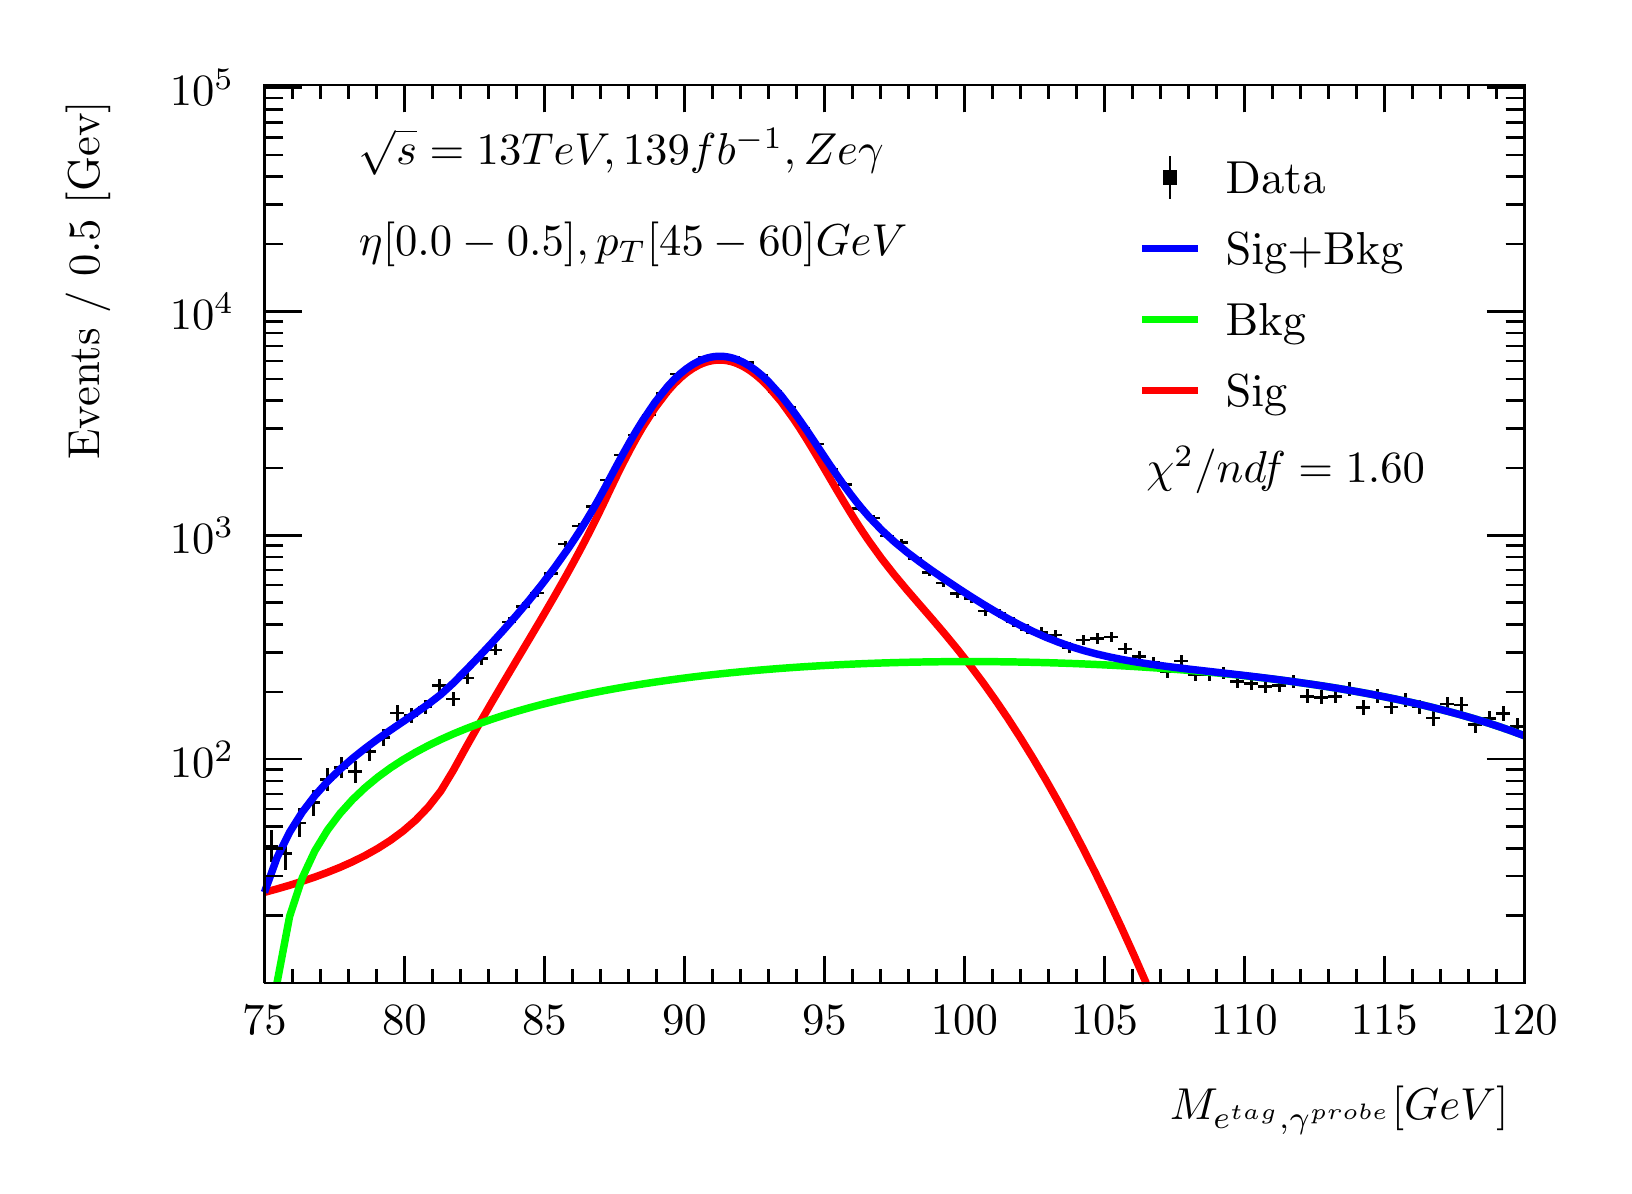
\begin{tikzpicture}
\pgfdeclareplotmark{cross} {
\pgfpathmoveto{\pgfpoint{-0.3\pgfplotmarksize}{\pgfplotmarksize}}
\pgfpathlineto{\pgfpoint{+0.3\pgfplotmarksize}{\pgfplotmarksize}}
\pgfpathlineto{\pgfpoint{+0.3\pgfplotmarksize}{0.3\pgfplotmarksize}}
\pgfpathlineto{\pgfpoint{+1\pgfplotmarksize}{0.3\pgfplotmarksize}}
\pgfpathlineto{\pgfpoint{+1\pgfplotmarksize}{-0.3\pgfplotmarksize}}
\pgfpathlineto{\pgfpoint{+0.3\pgfplotmarksize}{-0.3\pgfplotmarksize}}
\pgfpathlineto{\pgfpoint{+0.3\pgfplotmarksize}{-1.\pgfplotmarksize}}
\pgfpathlineto{\pgfpoint{-0.3\pgfplotmarksize}{-1.\pgfplotmarksize}}
\pgfpathlineto{\pgfpoint{-0.3\pgfplotmarksize}{-0.3\pgfplotmarksize}}
\pgfpathlineto{\pgfpoint{-1.\pgfplotmarksize}{-0.3\pgfplotmarksize}}
\pgfpathlineto{\pgfpoint{-1.\pgfplotmarksize}{0.3\pgfplotmarksize}}
\pgfpathlineto{\pgfpoint{-0.3\pgfplotmarksize}{0.3\pgfplotmarksize}}
\pgfpathclose
\pgfusepathqstroke
}
\pgfdeclareplotmark{cross*} {
\pgfpathmoveto{\pgfpoint{-0.3\pgfplotmarksize}{\pgfplotmarksize}}
\pgfpathlineto{\pgfpoint{+0.3\pgfplotmarksize}{\pgfplotmarksize}}
\pgfpathlineto{\pgfpoint{+0.3\pgfplotmarksize}{0.3\pgfplotmarksize}}
\pgfpathlineto{\pgfpoint{+1\pgfplotmarksize}{0.3\pgfplotmarksize}}
\pgfpathlineto{\pgfpoint{+1\pgfplotmarksize}{-0.3\pgfplotmarksize}}
\pgfpathlineto{\pgfpoint{+0.3\pgfplotmarksize}{-0.3\pgfplotmarksize}}
\pgfpathlineto{\pgfpoint{+0.3\pgfplotmarksize}{-1.\pgfplotmarksize}}
\pgfpathlineto{\pgfpoint{-0.3\pgfplotmarksize}{-1.\pgfplotmarksize}}
\pgfpathlineto{\pgfpoint{-0.3\pgfplotmarksize}{-0.3\pgfplotmarksize}}
\pgfpathlineto{\pgfpoint{-1.\pgfplotmarksize}{-0.3\pgfplotmarksize}}
\pgfpathlineto{\pgfpoint{-1.\pgfplotmarksize}{0.3\pgfplotmarksize}}
\pgfpathlineto{\pgfpoint{-0.3\pgfplotmarksize}{0.3\pgfplotmarksize}}
\pgfpathclose
\pgfusepathqfillstroke
}
\pgfdeclareplotmark{newstar} {
\pgfpathmoveto{\pgfqpoint{0pt}{\pgfplotmarksize}}
\pgfpathlineto{\pgfqpointpolar{44}{0.5\pgfplotmarksize}}
\pgfpathlineto{\pgfqpointpolar{18}{\pgfplotmarksize}}
\pgfpathlineto{\pgfqpointpolar{-20}{0.5\pgfplotmarksize}}
\pgfpathlineto{\pgfqpointpolar{-54}{\pgfplotmarksize}}
\pgfpathlineto{\pgfqpointpolar{-90}{0.5\pgfplotmarksize}}
\pgfpathlineto{\pgfqpointpolar{234}{\pgfplotmarksize}}
\pgfpathlineto{\pgfqpointpolar{198}{0.5\pgfplotmarksize}}
\pgfpathlineto{\pgfqpointpolar{162}{\pgfplotmarksize}}
\pgfpathlineto{\pgfqpointpolar{134}{0.5\pgfplotmarksize}}
\pgfpathclose
\pgfusepathqstroke
}
\pgfdeclareplotmark{newstar*} {
\pgfpathmoveto{\pgfqpoint{0pt}{\pgfplotmarksize}}
\pgfpathlineto{\pgfqpointpolar{44}{0.5\pgfplotmarksize}}
\pgfpathlineto{\pgfqpointpolar{18}{\pgfplotmarksize}}
\pgfpathlineto{\pgfqpointpolar{-20}{0.5\pgfplotmarksize}}
\pgfpathlineto{\pgfqpointpolar{-54}{\pgfplotmarksize}}
\pgfpathlineto{\pgfqpointpolar{-90}{0.5\pgfplotmarksize}}
\pgfpathlineto{\pgfqpointpolar{234}{\pgfplotmarksize}}
\pgfpathlineto{\pgfqpointpolar{198}{0.5\pgfplotmarksize}}
\pgfpathlineto{\pgfqpointpolar{162}{\pgfplotmarksize}}
\pgfpathlineto{\pgfqpointpolar{134}{0.5\pgfplotmarksize}}
\pgfpathclose
\pgfusepathqfillstroke
}
\definecolor{c}{rgb}{1,1,1};
\draw [color=c, fill=c] (0,0) rectangle (20,14.4361);
\draw [color=c, fill=c] (3,2.30977) rectangle (19,13.7143);
\definecolor{c}{rgb}{0,0,0};
\draw [c,line width=0.9] (3,2.30977) -- (3,13.7143) -- (19,13.7143) -- (19,2.30977) -- (3,2.30977);
\definecolor{c}{rgb}{1,1,1};
\draw [color=c, fill=c] (3,2.30977) rectangle (19,13.7143);
\definecolor{c}{rgb}{0,0,0};
\draw [c,line width=0.9] (3,2.30977) -- (3,13.7143) -- (19,13.7143) -- (19,2.30977) -- (3,2.30977);
\draw [c,line width=0.9] (3,2.30977) -- (19,2.30977);
\draw [c,line width=0.9] (3,2.65624) -- (3,2.30977);
\draw [c,line width=0.9] (3.35556,2.48301) -- (3.35556,2.30977);
\draw [c,line width=0.9] (3.71111,2.48301) -- (3.71111,2.30977);
\draw [c,line width=0.9] (4.06667,2.48301) -- (4.06667,2.30977);
\draw [c,line width=0.9] (4.42222,2.48301) -- (4.42222,2.30977);
\draw [c,line width=0.9] (4.77778,2.65624) -- (4.77778,2.30977);
\draw [c,line width=0.9] (5.13333,2.48301) -- (5.13333,2.30977);
\draw [c,line width=0.9] (5.48889,2.48301) -- (5.48889,2.30977);
\draw [c,line width=0.9] (5.84444,2.48301) -- (5.84444,2.30977);
\draw [c,line width=0.9] (6.2,2.48301) -- (6.2,2.30977);
\draw [c,line width=0.9] (6.55556,2.65624) -- (6.55556,2.30977);
\draw [c,line width=0.9] (6.91111,2.48301) -- (6.91111,2.30977);
\draw [c,line width=0.9] (7.26667,2.48301) -- (7.26667,2.30977);
\draw [c,line width=0.9] (7.62222,2.48301) -- (7.62222,2.30977);
\draw [c,line width=0.9] (7.97778,2.48301) -- (7.97778,2.30977);
\draw [c,line width=0.9] (8.33333,2.65624) -- (8.33333,2.30977);
\draw [c,line width=0.9] (8.68889,2.48301) -- (8.68889,2.30977);
\draw [c,line width=0.9] (9.04444,2.48301) -- (9.04444,2.30977);
\draw [c,line width=0.9] (9.4,2.48301) -- (9.4,2.30977);
\draw [c,line width=0.9] (9.75556,2.48301) -- (9.75556,2.30977);
\draw [c,line width=0.9] (10.1111,2.65624) -- (10.1111,2.30977);
\draw [c,line width=0.9] (10.4667,2.48301) -- (10.4667,2.30977);
\draw [c,line width=0.9] (10.8222,2.48301) -- (10.8222,2.30977);
\draw [c,line width=0.9] (11.1778,2.48301) -- (11.1778,2.30977);
\draw [c,line width=0.9] (11.5333,2.48301) -- (11.5333,2.30977);
\draw [c,line width=0.9] (11.8889,2.65624) -- (11.8889,2.30977);
\draw [c,line width=0.9] (12.2444,2.48301) -- (12.2444,2.30977);
\draw [c,line width=0.9] (12.6,2.48301) -- (12.6,2.30977);
\draw [c,line width=0.9] (12.9556,2.48301) -- (12.9556,2.30977);
\draw [c,line width=0.9] (13.3111,2.48301) -- (13.3111,2.30977);
\draw [c,line width=0.9] (13.6667,2.65624) -- (13.6667,2.30977);
\draw [c,line width=0.9] (14.0222,2.48301) -- (14.0222,2.30977);
\draw [c,line width=0.9] (14.3778,2.48301) -- (14.3778,2.30977);
\draw [c,line width=0.9] (14.7333,2.48301) -- (14.7333,2.30977);
\draw [c,line width=0.9] (15.0889,2.48301) -- (15.0889,2.30977);
\draw [c,line width=0.9] (15.4444,2.65624) -- (15.4444,2.30977);
\draw [c,line width=0.9] (15.8,2.48301) -- (15.8,2.30977);
\draw [c,line width=0.9] (16.1556,2.48301) -- (16.1556,2.30977);
\draw [c,line width=0.9] (16.5111,2.48301) -- (16.5111,2.30977);
\draw [c,line width=0.9] (16.8667,2.48301) -- (16.8667,2.30977);
\draw [c,line width=0.9] (17.2222,2.65624) -- (17.2222,2.30977);
\draw [c,line width=0.9] (17.5778,2.48301) -- (17.5778,2.30977);
\draw [c,line width=0.9] (17.9333,2.48301) -- (17.9333,2.30977);
\draw [c,line width=0.9] (18.2889,2.48301) -- (18.2889,2.30977);
\draw [c,line width=0.9] (18.6444,2.48301) -- (18.6444,2.30977);
\draw [c,line width=0.9] (19,2.65624) -- (19,2.30977);
\draw [c,line width=0.9] (19,2.65624) -- (19,2.30977);
\draw [anchor=base] (3,1.66015) node[scale=1.61424, color=c, rotate=0]{75};
\draw [anchor=base] (4.77778,1.66015) node[scale=1.61424, color=c, rotate=0]{80};
\draw [anchor=base] (6.55556,1.66015) node[scale=1.61424, color=c, rotate=0]{85};
\draw [anchor=base] (8.33333,1.66015) node[scale=1.61424, color=c, rotate=0]{90};
\draw [anchor=base] (10.1111,1.66015) node[scale=1.61424, color=c, rotate=0]{95};
\draw [anchor=base] (11.8889,1.66015) node[scale=1.61424, color=c, rotate=0]{100};
\draw [anchor=base] (13.6667,1.66015) node[scale=1.61424, color=c, rotate=0]{105};
\draw [anchor=base] (15.4444,1.66015) node[scale=1.61424, color=c, rotate=0]{110};
\draw [anchor=base] (17.2222,1.66015) node[scale=1.61424, color=c, rotate=0]{115};
\draw [anchor=base] (19,1.66015) node[scale=1.61424, color=c, rotate=0]{120};
\draw [anchor= east] (19,0.692932) node[scale=1.61424, color=c, rotate=0]{$M_{e^{tag}, \gamma^{probe}}  [GeV]$};
\draw [c,line width=0.9] (3,13.7143) -- (19,13.7143);
\draw [c,line width=0.9] (3,13.3678) -- (3,13.7143);
\draw [c,line width=0.9] (3.35556,13.5411) -- (3.35556,13.7143);
\draw [c,line width=0.9] (3.71111,13.5411) -- (3.71111,13.7143);
\draw [c,line width=0.9] (4.06667,13.5411) -- (4.06667,13.7143);
\draw [c,line width=0.9] (4.42222,13.5411) -- (4.42222,13.7143);
\draw [c,line width=0.9] (4.77778,13.3678) -- (4.77778,13.7143);
\draw [c,line width=0.9] (5.13333,13.5411) -- (5.13333,13.7143);
\draw [c,line width=0.9] (5.48889,13.5411) -- (5.48889,13.7143);
\draw [c,line width=0.9] (5.84444,13.5411) -- (5.84444,13.7143);
\draw [c,line width=0.9] (6.2,13.5411) -- (6.2,13.7143);
\draw [c,line width=0.9] (6.55556,13.3678) -- (6.55556,13.7143);
\draw [c,line width=0.9] (6.91111,13.5411) -- (6.91111,13.7143);
\draw [c,line width=0.9] (7.26667,13.5411) -- (7.26667,13.7143);
\draw [c,line width=0.9] (7.62222,13.5411) -- (7.62222,13.7143);
\draw [c,line width=0.9] (7.97778,13.5411) -- (7.97778,13.7143);
\draw [c,line width=0.9] (8.33333,13.3678) -- (8.33333,13.7143);
\draw [c,line width=0.9] (8.68889,13.5411) -- (8.68889,13.7143);
\draw [c,line width=0.9] (9.04444,13.5411) -- (9.04444,13.7143);
\draw [c,line width=0.9] (9.4,13.5411) -- (9.4,13.7143);
\draw [c,line width=0.9] (9.75556,13.5411) -- (9.75556,13.7143);
\draw [c,line width=0.9] (10.1111,13.3678) -- (10.1111,13.7143);
\draw [c,line width=0.9] (10.4667,13.5411) -- (10.4667,13.7143);
\draw [c,line width=0.9] (10.8222,13.5411) -- (10.8222,13.7143);
\draw [c,line width=0.9] (11.1778,13.5411) -- (11.1778,13.7143);
\draw [c,line width=0.9] (11.5333,13.5411) -- (11.5333,13.7143);
\draw [c,line width=0.9] (11.8889,13.3678) -- (11.8889,13.7143);
\draw [c,line width=0.9] (12.2444,13.5411) -- (12.2444,13.7143);
\draw [c,line width=0.9] (12.6,13.5411) -- (12.6,13.7143);
\draw [c,line width=0.9] (12.9556,13.5411) -- (12.9556,13.7143);
\draw [c,line width=0.9] (13.3111,13.5411) -- (13.3111,13.7143);
\draw [c,line width=0.9] (13.6667,13.3678) -- (13.6667,13.7143);
\draw [c,line width=0.9] (14.0222,13.5411) -- (14.0222,13.7143);
\draw [c,line width=0.9] (14.3778,13.5411) -- (14.3778,13.7143);
\draw [c,line width=0.9] (14.7333,13.5411) -- (14.7333,13.7143);
\draw [c,line width=0.9] (15.0889,13.5411) -- (15.0889,13.7143);
\draw [c,line width=0.9] (15.4444,13.3678) -- (15.4444,13.7143);
\draw [c,line width=0.9] (15.8,13.5411) -- (15.8,13.7143);
\draw [c,line width=0.9] (16.1556,13.5411) -- (16.1556,13.7143);
\draw [c,line width=0.9] (16.5111,13.5411) -- (16.5111,13.7143);
\draw [c,line width=0.9] (16.8667,13.5411) -- (16.8667,13.7143);
\draw [c,line width=0.9] (17.2222,13.3678) -- (17.2222,13.7143);
\draw [c,line width=0.9] (17.5778,13.5411) -- (17.5778,13.7143);
\draw [c,line width=0.9] (17.9333,13.5411) -- (17.9333,13.7143);
\draw [c,line width=0.9] (18.2889,13.5411) -- (18.2889,13.7143);
\draw [c,line width=0.9] (18.6444,13.5411) -- (18.6444,13.7143);
\draw [c,line width=0.9] (19,13.3678) -- (19,13.7143);
\draw [c,line width=0.9] (19,13.3678) -- (19,13.7143);
\draw [c,line width=0.9] (3,2.30977) -- (3,13.7143);
\draw [c,line width=0.9] (3.237,3.16561) -- (3,3.16561);
\draw [c,line width=0.9] (3.237,3.66625) -- (3,3.66625);
\draw [c,line width=0.9] (3.237,4.02146) -- (3,4.02146);
\draw [c,line width=0.9] (3.237,4.29698) -- (3,4.29698);
\draw [c,line width=0.9] (3.237,4.52209) -- (3,4.52209);
\draw [c,line width=0.9] (3.237,4.71242) -- (3,4.71242);
\draw [c,line width=0.9] (3.237,4.8773) -- (3,4.8773);
\draw [c,line width=0.9] (3.237,5.02273) -- (3,5.02273);
\draw [c,line width=0.9] (3.474,5.15282) -- (3,5.15282);
\draw [anchor= east] (2.82,5.15282) node[scale=1.61424, color=c, rotate=0]{$10^{2}$};
\draw [c,line width=0.9] (3.237,6.00866) -- (3,6.00866);
\draw [c,line width=0.9] (3.237,6.5093) -- (3,6.5093);
\draw [c,line width=0.9] (3.237,6.8645) -- (3,6.8645);
\draw [c,line width=0.9] (3.237,7.14002) -- (3,7.14002);
\draw [c,line width=0.9] (3.237,7.36514) -- (3,7.36514);
\draw [c,line width=0.9] (3.237,7.55547) -- (3,7.55547);
\draw [c,line width=0.9] (3.237,7.72034) -- (3,7.72034);
\draw [c,line width=0.9] (3.237,7.86577) -- (3,7.86577);
\draw [c,line width=0.9] (3.474,7.99586) -- (3,7.99586);
\draw [anchor= east] (2.82,7.99586) node[scale=1.61424, color=c, rotate=0]{$10^{3}$};
\draw [c,line width=0.9] (3.237,8.85171) -- (3,8.85171);
\draw [c,line width=0.9] (3.237,9.35234) -- (3,9.35234);
\draw [c,line width=0.9] (3.237,9.70755) -- (3,9.70755);
\draw [c,line width=0.9] (3.237,9.98307) -- (3,9.98307);
\draw [c,line width=0.9] (3.237,10.2082) -- (3,10.2082);
\draw [c,line width=0.9] (3.237,10.3985) -- (3,10.3985);
\draw [c,line width=0.9] (3.237,10.5634) -- (3,10.5634);
\draw [c,line width=0.9] (3.237,10.7088) -- (3,10.7088);
\draw [c,line width=0.9] (3.474,10.8389) -- (3,10.8389);
\draw [anchor= east] (2.82,10.8389) node[scale=1.61424, color=c, rotate=0]{$10^{4}$};
\draw [c,line width=0.9] (3.237,11.6948) -- (3,11.6948);
\draw [c,line width=0.9] (3.237,12.1954) -- (3,12.1954);
\draw [c,line width=0.9] (3.237,12.5506) -- (3,12.5506);
\draw [c,line width=0.9] (3.237,12.8261) -- (3,12.8261);
\draw [c,line width=0.9] (3.237,13.0512) -- (3,13.0512);
\draw [c,line width=0.9] (3.237,13.2416) -- (3,13.2416);
\draw [c,line width=0.9] (3.237,13.4064) -- (3,13.4064);
\draw [c,line width=0.9] (3.237,13.5519) -- (3,13.5519);
\draw [c,line width=0.9] (3.474,13.682) -- (3,13.682);
\draw [anchor= east] (2.82,13.682) node[scale=1.61424, color=c, rotate=0]{$10^{5}$};
\draw [anchor= east] (0.76,13.7143) node[scale=1.61424, color=c, rotate=90]{Events / 0.5 [Gev]};
\draw [c,line width=0.9] (19,2.30977) -- (19,13.7143);
\draw [c,line width=0.9] (18.763,3.16561) -- (19,3.16561);
\draw [c,line width=0.9] (18.763,3.66625) -- (19,3.66625);
\draw [c,line width=0.9] (18.763,4.02146) -- (19,4.02146);
\draw [c,line width=0.9] (18.763,4.29698) -- (19,4.29698);
\draw [c,line width=0.9] (18.763,4.52209) -- (19,4.52209);
\draw [c,line width=0.9] (18.763,4.71242) -- (19,4.71242);
\draw [c,line width=0.9] (18.763,4.8773) -- (19,4.8773);
\draw [c,line width=0.9] (18.763,5.02273) -- (19,5.02273);
\draw [c,line width=0.9] (18.526,5.15282) -- (19,5.15282);
\draw [c,line width=0.9] (18.763,6.00866) -- (19,6.00866);
\draw [c,line width=0.9] (18.763,6.5093) -- (19,6.5093);
\draw [c,line width=0.9] (18.763,6.8645) -- (19,6.8645);
\draw [c,line width=0.9] (18.763,7.14002) -- (19,7.14002);
\draw [c,line width=0.9] (18.763,7.36514) -- (19,7.36514);
\draw [c,line width=0.9] (18.763,7.55547) -- (19,7.55547);
\draw [c,line width=0.9] (18.763,7.72034) -- (19,7.72034);
\draw [c,line width=0.9] (18.763,7.86577) -- (19,7.86577);
\draw [c,line width=0.9] (18.526,7.99586) -- (19,7.99586);
\draw [c,line width=0.9] (18.763,8.85171) -- (19,8.85171);
\draw [c,line width=0.9] (18.763,9.35234) -- (19,9.35234);
\draw [c,line width=0.9] (18.763,9.70755) -- (19,9.70755);
\draw [c,line width=0.9] (18.763,9.98307) -- (19,9.98307);
\draw [c,line width=0.9] (18.763,10.2082) -- (19,10.2082);
\draw [c,line width=0.9] (18.763,10.3985) -- (19,10.3985);
\draw [c,line width=0.9] (18.763,10.5634) -- (19,10.5634);
\draw [c,line width=0.9] (18.763,10.7088) -- (19,10.7088);
\draw [c,line width=0.9] (18.526,10.8389) -- (19,10.8389);
\draw [c,line width=0.9] (18.763,11.6948) -- (19,11.6948);
\draw [c,line width=0.9] (18.763,12.1954) -- (19,12.1954);
\draw [c,line width=0.9] (18.763,12.5506) -- (19,12.5506);
\draw [c,line width=0.9] (18.763,12.8261) -- (19,12.8261);
\draw [c,line width=0.9] (18.763,13.0512) -- (19,13.0512);
\draw [c,line width=0.9] (18.763,13.2416) -- (19,13.2416);
\draw [c,line width=0.9] (18.763,13.4064) -- (19,13.4064);
\draw [c,line width=0.9] (18.763,13.5519) -- (19,13.5519);
\draw [c,line width=0.9] (18.526,13.682) -- (19,13.682);
\draw [c,line width=0.9] (3.08889,4.05195) -- (3,4.05195);
\draw [c,line width=0.9] (3,4.05195) -- (3,4.05195);
\draw [c,line width=0.9] (3.08889,4.05195) -- (3.17778,4.05195);
\draw [c,line width=0.9] (3.17778,4.05195) -- (3.17778,4.05195);
\draw [c,line width=0.9] (3.08889,4.05195) -- (3.08889,4.25823);
\draw [c,line width=0.9] (3.08889,4.25823) -- (3.08889,4.25823);
\draw [c,line width=0.9] (3.08889,4.05195) -- (3.08889,3.84322);
\draw [c,line width=0.9] (3.08889,3.84322) -- (3.08889,3.84322);
\draw [c,line width=0.9] (3.26667,3.95813) -- (3.17778,3.95813);
\draw [c,line width=0.9] (3.17778,3.95813) -- (3.17778,3.95813);
\draw [c,line width=0.9] (3.26667,3.95813) -- (3.35556,3.95813);
\draw [c,line width=0.9] (3.35556,3.95813) -- (3.35556,3.95813);
\draw [c,line width=0.9] (3.26667,3.95813) -- (3.26667,4.17287);
\draw [c,line width=0.9] (3.26667,4.17287) -- (3.26667,4.17287);
\draw [c,line width=0.9] (3.26667,3.95813) -- (3.26667,3.74063);
\draw [c,line width=0.9] (3.26667,3.74063) -- (3.26667,3.74063);
\draw [c,line width=0.9] (3.44444,4.3454) -- (3.35556,4.3454);
\draw [c,line width=0.9] (3.35556,4.3454) -- (3.35556,4.3454);
\draw [c,line width=0.9] (3.44444,4.3454) -- (3.53333,4.3454);
\draw [c,line width=0.9] (3.53333,4.3454) -- (3.53333,4.3454);
\draw [c,line width=0.9] (3.44444,4.3454) -- (3.44444,4.52738);
\draw [c,line width=0.9] (3.44444,4.52738) -- (3.44444,4.52738);
\draw [c,line width=0.9] (3.44444,4.3454) -- (3.44444,4.16172);
\draw [c,line width=0.9] (3.44444,4.16172) -- (3.44444,4.16172);
\draw [c,line width=0.9] (3.62222,4.60178) -- (3.53333,4.60178);
\draw [c,line width=0.9] (3.53333,4.60178) -- (3.53333,4.60178);
\draw [c,line width=0.9] (3.62222,4.60178) -- (3.71111,4.60178);
\draw [c,line width=0.9] (3.71111,4.60178) -- (3.71111,4.60178);
\draw [c,line width=0.9] (3.62222,4.60178) -- (3.62222,4.76495);
\draw [c,line width=0.9] (3.62222,4.76495) -- (3.62222,4.76495);
\draw [c,line width=0.9] (3.62222,4.60178) -- (3.62222,4.43737);
\draw [c,line width=0.9] (3.62222,4.43737) -- (3.62222,4.43737);
\draw [c,line width=0.9] (3.8,4.89264) -- (3.71111,4.89264);
\draw [c,line width=0.9] (3.71111,4.89264) -- (3.71111,4.89264);
\draw [c,line width=0.9] (3.8,4.89264) -- (3.88889,4.89264);
\draw [c,line width=0.9] (3.88889,4.89264) -- (3.88889,4.89264);
\draw [c,line width=0.9] (3.8,4.89264) -- (3.8,5.03688);
\draw [c,line width=0.9] (3.8,5.03688) -- (3.8,5.03688);
\draw [c,line width=0.9] (3.8,4.89264) -- (3.8,4.74753);
\draw [c,line width=0.9] (3.8,4.74753) -- (3.8,4.74753);
\draw [c,line width=0.9] (3.97778,5.04987) -- (3.88889,5.04987);
\draw [c,line width=0.9] (3.88889,5.04987) -- (3.88889,5.04987);
\draw [c,line width=0.9] (3.97778,5.04987) -- (4.06667,5.04987);
\draw [c,line width=0.9] (4.06667,5.04987) -- (4.06667,5.04987);
\draw [c,line width=0.9] (3.97778,5.04987) -- (3.97778,5.18483);
\draw [c,line width=0.9] (3.97778,5.18483) -- (3.97778,5.18483);
\draw [c,line width=0.9] (3.97778,5.04987) -- (3.97778,4.91418);
\draw [c,line width=0.9] (3.97778,4.91418) -- (3.97778,4.91418);
\draw [c,line width=0.9] (4.15556,4.99498) -- (4.06667,4.99498);
\draw [c,line width=0.9] (4.06667,4.99498) -- (4.06667,4.99498);
\draw [c,line width=0.9] (4.15556,4.99498) -- (4.24444,4.99498);
\draw [c,line width=0.9] (4.24444,4.99498) -- (4.24444,4.99498);
\draw [c,line width=0.9] (4.15556,4.99498) -- (4.15556,5.13311);
\draw [c,line width=0.9] (4.15556,5.13311) -- (4.15556,5.13311);
\draw [c,line width=0.9] (4.15556,4.99498) -- (4.15556,4.85608);
\draw [c,line width=0.9] (4.15556,4.85608) -- (4.15556,4.85608);
\draw [c,line width=0.9] (4.33333,5.24785) -- (4.24444,5.24785);
\draw [c,line width=0.9] (4.24444,5.24785) -- (4.24444,5.24785);
\draw [c,line width=0.9] (4.33333,5.24785) -- (4.42222,5.24785);
\draw [c,line width=0.9] (4.42222,5.24785) -- (4.42222,5.24785);
\draw [c,line width=0.9] (4.33333,5.24785) -- (4.33333,5.36661);
\draw [c,line width=0.9] (4.33333,5.36661) -- (4.33333,5.36661);
\draw [c,line width=0.9] (4.33333,5.24785) -- (4.33333,5.12908);
\draw [c,line width=0.9] (4.33333,5.12908) -- (4.33333,5.12908);
\draw [c,line width=0.9] (4.51111,5.42834) -- (4.42222,5.42834);
\draw [c,line width=0.9] (4.42222,5.42834) -- (4.42222,5.42834);
\draw [c,line width=0.9] (4.51111,5.42834) -- (4.6,5.42834);
\draw [c,line width=0.9] (4.6,5.42834) -- (4.6,5.42834);
\draw [c,line width=0.9] (4.51111,5.42834) -- (4.51111,5.53874);
\draw [c,line width=0.9] (4.51111,5.53874) -- (4.51111,5.53874);
\draw [c,line width=0.9] (4.51111,5.42834) -- (4.51111,5.31794);
\draw [c,line width=0.9] (4.51111,5.31794) -- (4.51111,5.31794);
\draw [c,line width=0.9] (4.68889,5.74084) -- (4.6,5.74084);
\draw [c,line width=0.9] (4.6,5.74084) -- (4.6,5.74084);
\draw [c,line width=0.9] (4.68889,5.74084) -- (4.77778,5.74084);
\draw [c,line width=0.9] (4.77778,5.74084) -- (4.77778,5.74084);
\draw [c,line width=0.9] (4.68889,5.74084) -- (4.68889,5.83812);
\draw [c,line width=0.9] (4.68889,5.83812) -- (4.68889,5.83812);
\draw [c,line width=0.9] (4.68889,5.74084) -- (4.68889,5.64355);
\draw [c,line width=0.9] (4.68889,5.64355) -- (4.68889,5.64355);
\draw [c,line width=0.9] (4.86667,5.70977) -- (4.77778,5.70977);
\draw [c,line width=0.9] (4.77778,5.70977) -- (4.77778,5.70977);
\draw [c,line width=0.9] (4.86667,5.70977) -- (4.95556,5.70977);
\draw [c,line width=0.9] (4.95556,5.70977) -- (4.95556,5.70977);
\draw [c,line width=0.9] (4.86667,5.70977) -- (4.86667,5.80829);
\draw [c,line width=0.9] (4.86667,5.80829) -- (4.86667,5.80829);
\draw [c,line width=0.9] (4.86667,5.70977) -- (4.86667,5.61126);
\draw [c,line width=0.9] (4.86667,5.61126) -- (4.86667,5.61126);
\draw [c,line width=0.9] (5.04444,5.81524) -- (4.95556,5.81524);
\draw [c,line width=0.9] (4.95556,5.81524) -- (4.95556,5.81524);
\draw [c,line width=0.9] (5.04444,5.81524) -- (5.13333,5.81524);
\draw [c,line width=0.9] (5.13333,5.81524) -- (5.13333,5.81524);
\draw [c,line width=0.9] (5.04444,5.81524) -- (5.04444,5.90964);
\draw [c,line width=0.9] (5.04444,5.90964) -- (5.04444,5.90964);
\draw [c,line width=0.9] (5.04444,5.81524) -- (5.04444,5.72084);
\draw [c,line width=0.9] (5.04444,5.72084) -- (5.04444,5.72084);
\draw [c,line width=0.9] (5.22222,6.08642) -- (5.13333,6.08642);
\draw [c,line width=0.9] (5.13333,6.08642) -- (5.13333,6.08642);
\draw [c,line width=0.9] (5.22222,6.08642) -- (5.31111,6.08642);
\draw [c,line width=0.9] (5.31111,6.08642) -- (5.31111,6.08642);
\draw [c,line width=0.9] (5.22222,6.08642) -- (5.22222,6.171);
\draw [c,line width=0.9] (5.22222,6.171) -- (5.22222,6.171);
\draw [c,line width=0.9] (5.22222,6.08642) -- (5.22222,6.00183);
\draw [c,line width=0.9] (5.22222,6.00183) -- (5.22222,6.00183);
\draw [c,line width=0.9] (5.4,5.91906) -- (5.31111,5.91906);
\draw [c,line width=0.9] (5.31111,5.91906) -- (5.31111,5.91906);
\draw [c,line width=0.9] (5.4,5.91906) -- (5.48889,5.91906);
\draw [c,line width=0.9] (5.48889,5.91906) -- (5.48889,5.91906);
\draw [c,line width=0.9] (5.4,5.91906) -- (5.4,6.00957);
\draw [c,line width=0.9] (5.4,6.00957) -- (5.4,6.00957);
\draw [c,line width=0.9] (5.4,5.91906) -- (5.4,5.82854);
\draw [c,line width=0.9] (5.4,5.82854) -- (5.4,5.82854);
\draw [c,line width=0.9] (5.57778,6.18658) -- (5.48889,6.18658);
\draw [c,line width=0.9] (5.48889,6.18658) -- (5.48889,6.18658);
\draw [c,line width=0.9] (5.57778,6.18658) -- (5.66667,6.18658);
\draw [c,line width=0.9] (5.66667,6.18658) -- (5.66667,6.18658);
\draw [c,line width=0.9] (5.57778,6.18658) -- (5.57778,6.26781);
\draw [c,line width=0.9] (5.57778,6.26781) -- (5.57778,6.26781);
\draw [c,line width=0.9] (5.57778,6.18658) -- (5.57778,6.10536);
\draw [c,line width=0.9] (5.57778,6.10536) -- (5.57778,6.10536);
\draw [c,line width=0.9] (5.75556,6.42851) -- (5.66667,6.42851);
\draw [c,line width=0.9] (5.66667,6.42851) -- (5.66667,6.42851);
\draw [c,line width=0.9] (5.75556,6.42851) -- (5.84444,6.42851);
\draw [c,line width=0.9] (5.84444,6.42851) -- (5.84444,6.42851);
\draw [c,line width=0.9] (5.75556,6.42851) -- (5.75556,6.50216);
\draw [c,line width=0.9] (5.75556,6.50216) -- (5.75556,6.50216);
\draw [c,line width=0.9] (5.75556,6.42851) -- (5.75556,6.35487);
\draw [c,line width=0.9] (5.75556,6.35487) -- (5.75556,6.35487);
\draw [c,line width=0.9] (5.93333,6.54179) -- (5.84444,6.54179);
\draw [c,line width=0.9] (5.84444,6.54179) -- (5.84444,6.54179);
\draw [c,line width=0.9] (5.93333,6.54179) -- (6.02222,6.54179);
\draw [c,line width=0.9] (6.02222,6.54179) -- (6.02222,6.54179);
\draw [c,line width=0.9] (5.93333,6.54179) -- (5.93333,6.61214);
\draw [c,line width=0.9] (5.93333,6.61214) -- (5.93333,6.61214);
\draw [c,line width=0.9] (5.93333,6.54179) -- (5.93333,6.47145);
\draw [c,line width=0.9] (5.93333,6.47145) -- (5.93333,6.47145);
\draw [c,line width=0.9] (6.11111,6.89198) -- (6.02222,6.89198);
\draw [c,line width=0.9] (6.02222,6.89198) -- (6.02222,6.89198);
\draw [c,line width=0.9] (6.11111,6.89198) -- (6.2,6.89198);
\draw [c,line width=0.9] (6.2,6.89198) -- (6.2,6.89198);
\draw [c,line width=0.9] (6.11111,6.89198) -- (6.11111,6.95302);
\draw [c,line width=0.9] (6.11111,6.95302) -- (6.11111,6.95302);
\draw [c,line width=0.9] (6.11111,6.89198) -- (6.11111,6.83093);
\draw [c,line width=0.9] (6.11111,6.83093) -- (6.11111,6.83093);
\draw [c,line width=0.9] (6.28889,7.09475) -- (6.2,7.09475);
\draw [c,line width=0.9] (6.2,7.09475) -- (6.2,7.09475);
\draw [c,line width=0.9] (6.28889,7.09475) -- (6.37778,7.09475);
\draw [c,line width=0.9] (6.37778,7.09475) -- (6.37778,7.09475);
\draw [c,line width=0.9] (6.28889,7.09475) -- (6.28889,7.15099);
\draw [c,line width=0.9] (6.28889,7.15099) -- (6.28889,7.15099);
\draw [c,line width=0.9] (6.28889,7.09475) -- (6.28889,7.03852);
\draw [c,line width=0.9] (6.28889,7.03852) -- (6.28889,7.03852);
\draw [c,line width=0.9] (6.46667,7.26442) -- (6.37778,7.26442);
\draw [c,line width=0.9] (6.37778,7.26442) -- (6.37778,7.26442);
\draw [c,line width=0.9] (6.46667,7.26442) -- (6.55556,7.26442);
\draw [c,line width=0.9] (6.55556,7.26442) -- (6.55556,7.26442);
\draw [c,line width=0.9] (6.46667,7.26442) -- (6.46667,7.31692);
\draw [c,line width=0.9] (6.46667,7.31692) -- (6.46667,7.31692);
\draw [c,line width=0.9] (6.46667,7.26442) -- (6.46667,7.21192);
\draw [c,line width=0.9] (6.46667,7.21192) -- (6.46667,7.21192);
\draw [c,line width=0.9] (6.64444,7.50874) -- (6.55556,7.50874);
\draw [c,line width=0.9] (6.55556,7.50874) -- (6.55556,7.50874);
\draw [c,line width=0.9] (6.64444,7.50874) -- (6.73333,7.50874);
\draw [c,line width=0.9] (6.73333,7.50874) -- (6.73333,7.50874);
\draw [c,line width=0.9] (6.64444,7.50874) -- (6.64444,7.55629);
\draw [c,line width=0.9] (6.64444,7.55629) -- (6.64444,7.55629);
\draw [c,line width=0.9] (6.64444,7.50874) -- (6.64444,7.46118);
\draw [c,line width=0.9] (6.64444,7.46118) -- (6.64444,7.46118);
\draw [c,line width=0.9] (6.82222,7.88618) -- (6.73333,7.88618);
\draw [c,line width=0.9] (6.73333,7.88618) -- (6.73333,7.88618);
\draw [c,line width=0.9] (6.82222,7.88618) -- (6.91111,7.88618);
\draw [c,line width=0.9] (6.91111,7.88618) -- (6.91111,7.88618);
\draw [c,line width=0.9] (6.82222,7.88618) -- (6.82222,7.927);
\draw [c,line width=0.9] (6.82222,7.927) -- (6.82222,7.927);
\draw [c,line width=0.9] (6.82222,7.88618) -- (6.82222,7.84537);
\draw [c,line width=0.9] (6.82222,7.84537) -- (6.82222,7.84537);
\draw [c,line width=0.9] (7,8.11242) -- (6.91111,8.11242);
\draw [c,line width=0.9] (6.91111,8.11242) -- (6.91111,8.11242);
\draw [c,line width=0.9] (7,8.11242) -- (7.08889,8.11242);
\draw [c,line width=0.9] (7.08889,8.11242) -- (7.08889,8.11242);
\draw [c,line width=0.9] (7,8.11242) -- (7,8.14967);
\draw [c,line width=0.9] (7,8.14967) -- (7,8.14967);
\draw [c,line width=0.9] (7,8.11242) -- (7,8.07518);
\draw [c,line width=0.9] (7,8.07518) -- (7,8.07518);
\draw [c,line width=0.9] (7.17778,8.36183) -- (7.08889,8.36183);
\draw [c,line width=0.9] (7.08889,8.36183) -- (7.08889,8.36183);
\draw [c,line width=0.9] (7.17778,8.36183) -- (7.26667,8.36183);
\draw [c,line width=0.9] (7.26667,8.36183) -- (7.26667,8.36183);
\draw [c,line width=0.9] (7.17778,8.36183) -- (7.17778,8.39549);
\draw [c,line width=0.9] (7.17778,8.39549) -- (7.17778,8.39549);
\draw [c,line width=0.9] (7.17778,8.36183) -- (7.17778,8.32816);
\draw [c,line width=0.9] (7.17778,8.32816) -- (7.17778,8.32816);
\draw [c,line width=0.9] (7.35556,8.70156) -- (7.26667,8.70156);
\draw [c,line width=0.9] (7.26667,8.70156) -- (7.26667,8.70156);
\draw [c,line width=0.9] (7.35556,8.70156) -- (7.44444,8.70156);
\draw [c,line width=0.9] (7.44444,8.70156) -- (7.44444,8.70156);
\draw [c,line width=0.9] (7.35556,8.70156) -- (7.35556,8.7309);
\draw [c,line width=0.9] (7.35556,8.7309) -- (7.35556,8.7309);
\draw [c,line width=0.9] (7.35556,8.70156) -- (7.35556,8.67222);
\draw [c,line width=0.9] (7.35556,8.67222) -- (7.35556,8.67222);
\draw [c,line width=0.9] (7.53333,9.01511) -- (7.44444,9.01511);
\draw [c,line width=0.9] (7.44444,9.01511) -- (7.44444,9.01511);
\draw [c,line width=0.9] (7.53333,9.01511) -- (7.62222,9.01511);
\draw [c,line width=0.9] (7.62222,9.01511) -- (7.62222,9.01511);
\draw [c,line width=0.9] (7.53333,9.01511) -- (7.53333,9.04095);
\draw [c,line width=0.9] (7.53333,9.04095) -- (7.53333,9.04095);
\draw [c,line width=0.9] (7.53333,9.01511) -- (7.53333,8.98927);
\draw [c,line width=0.9] (7.53333,8.98927) -- (7.53333,8.98927);
\draw [c,line width=0.9] (7.71111,9.26848) -- (7.62222,9.26848);
\draw [c,line width=0.9] (7.62222,9.26848) -- (7.62222,9.26848);
\draw [c,line width=0.9] (7.71111,9.26848) -- (7.8,9.26848);
\draw [c,line width=0.9] (7.8,9.26848) -- (7.8,9.26848);
\draw [c,line width=0.9] (7.71111,9.26848) -- (7.71111,9.2918);
\draw [c,line width=0.9] (7.71111,9.2918) -- (7.71111,9.2918);
\draw [c,line width=0.9] (7.71111,9.26848) -- (7.71111,9.24516);
\draw [c,line width=0.9] (7.71111,9.24516) -- (7.71111,9.24516);
\draw [c,line width=0.9] (7.88889,9.52312) -- (7.8,9.52312);
\draw [c,line width=0.9] (7.8,9.52312) -- (7.8,9.52312);
\draw [c,line width=0.9] (7.88889,9.52312) -- (7.97778,9.52312);
\draw [c,line width=0.9] (7.97778,9.52312) -- (7.97778,9.52312);
\draw [c,line width=0.9] (7.88889,9.52312) -- (7.88889,9.54416);
\draw [c,line width=0.9] (7.88889,9.54416) -- (7.88889,9.54416);
\draw [c,line width=0.9] (7.88889,9.52312) -- (7.88889,9.50208);
\draw [c,line width=0.9] (7.88889,9.50208) -- (7.88889,9.50208);
\draw [c,line width=0.9] (8.06667,9.79426) -- (7.97778,9.79426);
\draw [c,line width=0.9] (7.97778,9.79426) -- (7.97778,9.79426);
\draw [c,line width=0.9] (8.06667,9.79426) -- (8.15556,9.79426);
\draw [c,line width=0.9] (8.15556,9.79426) -- (8.15556,9.79426);
\draw [c,line width=0.9] (8.06667,9.79426) -- (8.06667,9.81311);
\draw [c,line width=0.9] (8.06667,9.81311) -- (8.06667,9.81311);
\draw [c,line width=0.9] (8.06667,9.79426) -- (8.06667,9.77541);
\draw [c,line width=0.9] (8.06667,9.77541) -- (8.06667,9.77541);
\draw [c,line width=0.9] (8.24444,10.0452) -- (8.15556,10.0452);
\draw [c,line width=0.9] (8.15556,10.0452) -- (8.15556,10.0452);
\draw [c,line width=0.9] (8.24444,10.0452) -- (8.33333,10.0452);
\draw [c,line width=0.9] (8.33333,10.0452) -- (8.33333,10.0452);
\draw [c,line width=0.9] (8.24444,10.0452) -- (8.24444,10.0622);
\draw [c,line width=0.9] (8.24444,10.0622) -- (8.24444,10.0622);
\draw [c,line width=0.9] (8.24444,10.0452) -- (8.24444,10.0282);
\draw [c,line width=0.9] (8.24444,10.0282) -- (8.24444,10.0282);
\draw [c,line width=0.9] (8.42222,10.1292) -- (8.33333,10.1292);
\draw [c,line width=0.9] (8.33333,10.1292) -- (8.33333,10.1292);
\draw [c,line width=0.9] (8.42222,10.1292) -- (8.51111,10.1292);
\draw [c,line width=0.9] (8.51111,10.1292) -- (8.51111,10.1292);
\draw [c,line width=0.9] (8.42222,10.1292) -- (8.42222,10.1456);
\draw [c,line width=0.9] (8.42222,10.1456) -- (8.42222,10.1456);
\draw [c,line width=0.9] (8.42222,10.1292) -- (8.42222,10.1127);
\draw [c,line width=0.9] (8.42222,10.1127) -- (8.42222,10.1127);
\draw [c,line width=0.9] (8.6,10.256) -- (8.51111,10.256);
\draw [c,line width=0.9] (8.51111,10.256) -- (8.51111,10.256);
\draw [c,line width=0.9] (8.6,10.256) -- (8.68889,10.256);
\draw [c,line width=0.9] (8.68889,10.256) -- (8.68889,10.256);
\draw [c,line width=0.9] (8.6,10.256) -- (8.6,10.2717);
\draw [c,line width=0.9] (8.6,10.2717) -- (8.6,10.2717);
\draw [c,line width=0.9] (8.6,10.256) -- (8.6,10.2404);
\draw [c,line width=0.9] (8.6,10.2404) -- (8.6,10.2404);
\draw [c,line width=0.9] (8.77778,10.2819) -- (8.68889,10.2819);
\draw [c,line width=0.9] (8.68889,10.2819) -- (8.68889,10.2819);
\draw [c,line width=0.9] (8.77778,10.2819) -- (8.86667,10.2819);
\draw [c,line width=0.9] (8.86667,10.2819) -- (8.86667,10.2819);
\draw [c,line width=0.9] (8.77778,10.2819) -- (8.77778,10.2973);
\draw [c,line width=0.9] (8.77778,10.2973) -- (8.77778,10.2973);
\draw [c,line width=0.9] (8.77778,10.2819) -- (8.77778,10.2664);
\draw [c,line width=0.9] (8.77778,10.2664) -- (8.77778,10.2664);
\draw [c,line width=0.9] (8.95556,10.258) -- (8.86667,10.258);
\draw [c,line width=0.9] (8.86667,10.258) -- (8.86667,10.258);
\draw [c,line width=0.9] (8.95556,10.258) -- (9.04444,10.258);
\draw [c,line width=0.9] (9.04444,10.258) -- (9.04444,10.258);
\draw [c,line width=0.9] (8.95556,10.258) -- (8.95556,10.2736);
\draw [c,line width=0.9] (8.95556,10.2736) -- (8.95556,10.2736);
\draw [c,line width=0.9] (8.95556,10.258) -- (8.95556,10.2424);
\draw [c,line width=0.9] (8.95556,10.2424) -- (8.95556,10.2424);
\draw [c,line width=0.9] (9.13333,10.1906) -- (9.04444,10.1906);
\draw [c,line width=0.9] (9.04444,10.1906) -- (9.04444,10.1906);
\draw [c,line width=0.9] (9.13333,10.1906) -- (9.22222,10.1906);
\draw [c,line width=0.9] (9.22222,10.1906) -- (9.22222,10.1906);
\draw [c,line width=0.9] (9.13333,10.1906) -- (9.13333,10.2066);
\draw [c,line width=0.9] (9.13333,10.2066) -- (9.13333,10.2066);
\draw [c,line width=0.9] (9.13333,10.1906) -- (9.13333,10.1745);
\draw [c,line width=0.9] (9.13333,10.1745) -- (9.13333,10.1745);
\draw [c,line width=0.9] (9.31111,10.0346) -- (9.22222,10.0346);
\draw [c,line width=0.9] (9.22222,10.0346) -- (9.22222,10.0346);
\draw [c,line width=0.9] (9.31111,10.0346) -- (9.4,10.0346);
\draw [c,line width=0.9] (9.4,10.0346) -- (9.4,10.0346);
\draw [c,line width=0.9] (9.31111,10.0346) -- (9.31111,10.0517);
\draw [c,line width=0.9] (9.31111,10.0517) -- (9.31111,10.0517);
\draw [c,line width=0.9] (9.31111,10.0346) -- (9.31111,10.0175);
\draw [c,line width=0.9] (9.31111,10.0175) -- (9.31111,10.0175);
\draw [c,line width=0.9] (9.48889,9.82551) -- (9.4,9.82551);
\draw [c,line width=0.9] (9.4,9.82551) -- (9.4,9.82551);
\draw [c,line width=0.9] (9.48889,9.82551) -- (9.57778,9.82551);
\draw [c,line width=0.9] (9.57778,9.82551) -- (9.57778,9.82551);
\draw [c,line width=0.9] (9.48889,9.82551) -- (9.48889,9.84412);
\draw [c,line width=0.9] (9.48889,9.84412) -- (9.48889,9.84412);
\draw [c,line width=0.9] (9.48889,9.82551) -- (9.48889,9.8069);
\draw [c,line width=0.9] (9.48889,9.8069) -- (9.48889,9.8069);
\draw [c,line width=0.9] (9.66667,9.62523) -- (9.57778,9.62523);
\draw [c,line width=0.9] (9.57778,9.62523) -- (9.57778,9.62523);
\draw [c,line width=0.9] (9.66667,9.62523) -- (9.75556,9.62523);
\draw [c,line width=0.9] (9.75556,9.62523) -- (9.75556,9.62523);
\draw [c,line width=0.9] (9.66667,9.62523) -- (9.66667,9.64541);
\draw [c,line width=0.9] (9.66667,9.64541) -- (9.66667,9.64541);
\draw [c,line width=0.9] (9.66667,9.62523) -- (9.66667,9.60504);
\draw [c,line width=0.9] (9.66667,9.60504) -- (9.66667,9.60504);
\draw [c,line width=0.9] (9.84444,9.35645) -- (9.75556,9.35645);
\draw [c,line width=0.9] (9.75556,9.35645) -- (9.75556,9.35645);
\draw [c,line width=0.9] (9.84444,9.35645) -- (9.93333,9.35645);
\draw [c,line width=0.9] (9.93333,9.35645) -- (9.93333,9.35645);
\draw [c,line width=0.9] (9.84444,9.35645) -- (9.84444,9.37896);
\draw [c,line width=0.9] (9.84444,9.37896) -- (9.84444,9.37896);
\draw [c,line width=0.9] (9.84444,9.35645) -- (9.84444,9.33395);
\draw [c,line width=0.9] (9.84444,9.33395) -- (9.84444,9.33395);
\draw [c,line width=0.9] (10.0222,9.15796) -- (9.93333,9.15796);
\draw [c,line width=0.9] (9.93333,9.15796) -- (9.93333,9.15796);
\draw [c,line width=0.9] (10.0222,9.15796) -- (10.1111,9.15796);
\draw [c,line width=0.9] (10.1111,9.15796) -- (10.1111,9.15796);
\draw [c,line width=0.9] (10.0222,9.15796) -- (10.0222,9.18234);
\draw [c,line width=0.9] (10.0222,9.18234) -- (10.0222,9.18234);
\draw [c,line width=0.9] (10.0222,9.15796) -- (10.0222,9.13357);
\draw [c,line width=0.9] (10.0222,9.13357) -- (10.0222,9.13357);
\draw [c,line width=0.9] (10.2,8.8368) -- (10.1111,8.8368);
\draw [c,line width=0.9] (10.1111,8.8368) -- (10.1111,8.8368);
\draw [c,line width=0.9] (10.2,8.8368) -- (10.2889,8.8368);
\draw [c,line width=0.9] (10.2889,8.8368) -- (10.2889,8.8368);
\draw [c,line width=0.9] (10.2,8.8368) -- (10.2,8.86458);
\draw [c,line width=0.9] (10.2,8.86458) -- (10.2,8.86458);
\draw [c,line width=0.9] (10.2,8.8368) -- (10.2,8.80902);
\draw [c,line width=0.9] (10.2,8.80902) -- (10.2,8.80902);
\draw [c,line width=0.9] (10.3778,8.64229) -- (10.2889,8.64229);
\draw [c,line width=0.9] (10.2889,8.64229) -- (10.2889,8.64229);
\draw [c,line width=0.9] (10.3778,8.64229) -- (10.4667,8.64229);
\draw [c,line width=0.9] (10.4667,8.64229) -- (10.4667,8.64229);
\draw [c,line width=0.9] (10.3778,8.64229) -- (10.3778,8.67235);
\draw [c,line width=0.9] (10.3778,8.67235) -- (10.3778,8.67235);
\draw [c,line width=0.9] (10.3778,8.64229) -- (10.3778,8.61224);
\draw [c,line width=0.9] (10.3778,8.61224) -- (10.3778,8.61224);
\draw [c,line width=0.9] (10.5556,8.33679) -- (10.4667,8.33679);
\draw [c,line width=0.9] (10.4667,8.33679) -- (10.4667,8.33679);
\draw [c,line width=0.9] (10.5556,8.33679) -- (10.6444,8.33679);
\draw [c,line width=0.9] (10.6444,8.33679) -- (10.6444,8.33679);
\draw [c,line width=0.9] (10.5556,8.33679) -- (10.5556,8.3708);
\draw [c,line width=0.9] (10.5556,8.3708) -- (10.5556,8.3708);
\draw [c,line width=0.9] (10.5556,8.33679) -- (10.5556,8.30278);
\draw [c,line width=0.9] (10.5556,8.30278) -- (10.5556,8.30278);
\draw [c,line width=0.9] (10.7333,8.21272) -- (10.6444,8.21272);
\draw [c,line width=0.9] (10.6444,8.21272) -- (10.6444,8.21272);
\draw [c,line width=0.9] (10.7333,8.21272) -- (10.8222,8.21272);
\draw [c,line width=0.9] (10.8222,8.21272) -- (10.8222,8.21272);
\draw [c,line width=0.9] (10.7333,8.21272) -- (10.7333,8.24848);
\draw [c,line width=0.9] (10.7333,8.24848) -- (10.7333,8.24848);
\draw [c,line width=0.9] (10.7333,8.21272) -- (10.7333,8.17696);
\draw [c,line width=0.9] (10.7333,8.17696) -- (10.7333,8.17696);
\draw [c,line width=0.9] (10.9111,7.98595) -- (10.8222,7.98595);
\draw [c,line width=0.9] (10.8222,7.98595) -- (10.8222,7.98595);
\draw [c,line width=0.9] (10.9111,7.98595) -- (11,7.98595);
\draw [c,line width=0.9] (11,7.98595) -- (11,7.98595);
\draw [c,line width=0.9] (10.9111,7.98595) -- (10.9111,8.02515);
\draw [c,line width=0.9] (10.9111,8.02515) -- (10.9111,8.02515);
\draw [c,line width=0.9] (10.9111,7.98595) -- (10.9111,7.94675);
\draw [c,line width=0.9] (10.9111,7.94675) -- (10.9111,7.94675);
\draw [c,line width=0.9] (11.0889,7.90759) -- (11,7.90759);
\draw [c,line width=0.9] (11,7.90759) -- (11,7.90759);
\draw [c,line width=0.9] (11.0889,7.90759) -- (11.1778,7.90759);
\draw [c,line width=0.9] (11.1778,7.90759) -- (11.1778,7.90759);
\draw [c,line width=0.9] (11.0889,7.90759) -- (11.0889,7.94805);
\draw [c,line width=0.9] (11.0889,7.94805) -- (11.0889,7.94805);
\draw [c,line width=0.9] (11.0889,7.90759) -- (11.0889,7.86712);
\draw [c,line width=0.9] (11.0889,7.86712) -- (11.0889,7.86712);
\draw [c,line width=0.9] (11.2667,7.70168) -- (11.1778,7.70168);
\draw [c,line width=0.9] (11.1778,7.70168) -- (11.1778,7.70168);
\draw [c,line width=0.9] (11.2667,7.70168) -- (11.3556,7.70168);
\draw [c,line width=0.9] (11.3556,7.70168) -- (11.3556,7.70168);
\draw [c,line width=0.9] (11.2667,7.70168) -- (11.2667,7.74567);
\draw [c,line width=0.9] (11.2667,7.74567) -- (11.2667,7.74567);
\draw [c,line width=0.9] (11.2667,7.70168) -- (11.2667,7.6577);
\draw [c,line width=0.9] (11.2667,7.6577) -- (11.2667,7.6577);
\draw [c,line width=0.9] (11.4444,7.52149) -- (11.3556,7.52149);
\draw [c,line width=0.9] (11.3556,7.52149) -- (11.3556,7.52149);
\draw [c,line width=0.9] (11.4444,7.52149) -- (11.5333,7.52149);
\draw [c,line width=0.9] (11.5333,7.52149) -- (11.5333,7.52149);
\draw [c,line width=0.9] (11.4444,7.52149) -- (11.4444,7.56881);
\draw [c,line width=0.9] (11.4444,7.56881) -- (11.4444,7.56881);
\draw [c,line width=0.9] (11.4444,7.52149) -- (11.4444,7.47418);
\draw [c,line width=0.9] (11.4444,7.47418) -- (11.4444,7.47418);
\draw [c,line width=0.9] (11.6222,7.38959) -- (11.5333,7.38959);
\draw [c,line width=0.9] (11.5333,7.38959) -- (11.5333,7.38959);
\draw [c,line width=0.9] (11.6222,7.38959) -- (11.7111,7.38959);
\draw [c,line width=0.9] (11.7111,7.38959) -- (11.7111,7.38959);
\draw [c,line width=0.9] (11.6222,7.38959) -- (11.6222,7.4395);
\draw [c,line width=0.9] (11.6222,7.4395) -- (11.6222,7.4395);
\draw [c,line width=0.9] (11.6222,7.38959) -- (11.6222,7.33968);
\draw [c,line width=0.9] (11.6222,7.33968) -- (11.6222,7.33968);
\draw [c,line width=0.9] (11.8,7.2577) -- (11.7111,7.2577);
\draw [c,line width=0.9] (11.7111,7.2577) -- (11.7111,7.2577);
\draw [c,line width=0.9] (11.8,7.2577) -- (11.8889,7.2577);
\draw [c,line width=0.9] (11.8889,7.2577) -- (11.8889,7.2577);
\draw [c,line width=0.9] (11.8,7.2577) -- (11.8,7.31035);
\draw [c,line width=0.9] (11.8,7.31035) -- (11.8,7.31035);
\draw [c,line width=0.9] (11.8,7.2577) -- (11.8,7.20506);
\draw [c,line width=0.9] (11.8,7.20506) -- (11.8,7.20506);
\draw [c,line width=0.9] (11.9778,7.19082) -- (11.8889,7.19082);
\draw [c,line width=0.9] (11.8889,7.19082) -- (11.8889,7.19082);
\draw [c,line width=0.9] (11.9778,7.19082) -- (12.0667,7.19082);
\draw [c,line width=0.9] (12.0667,7.19082) -- (12.0667,7.19082);
\draw [c,line width=0.9] (11.9778,7.19082) -- (11.9778,7.24491);
\draw [c,line width=0.9] (11.9778,7.24491) -- (11.9778,7.24491);
\draw [c,line width=0.9] (11.9778,7.19082) -- (11.9778,7.13673);
\draw [c,line width=0.9] (11.9778,7.13673) -- (11.9778,7.13673);
\draw [c,line width=0.9] (12.1556,7.03438) -- (12.0667,7.03438);
\draw [c,line width=0.9] (12.0667,7.03438) -- (12.0667,7.03438);
\draw [c,line width=0.9] (12.1556,7.03438) -- (12.2444,7.03438);
\draw [c,line width=0.9] (12.2444,7.03438) -- (12.2444,7.03438);
\draw [c,line width=0.9] (12.1556,7.03438) -- (12.1556,7.09201);
\draw [c,line width=0.9] (12.1556,7.09201) -- (12.1556,7.09201);
\draw [c,line width=0.9] (12.1556,7.03438) -- (12.1556,6.97676);
\draw [c,line width=0.9] (12.1556,6.97676) -- (12.1556,6.97676);
\draw [c,line width=0.9] (12.3333,7.00719) -- (12.2444,7.00719);
\draw [c,line width=0.9] (12.2444,7.00719) -- (12.2444,7.00719);
\draw [c,line width=0.9] (12.3333,7.00719) -- (12.4222,7.00719);
\draw [c,line width=0.9] (12.4222,7.00719) -- (12.4222,7.00719);
\draw [c,line width=0.9] (12.3333,7.00719) -- (12.3333,7.06545);
\draw [c,line width=0.9] (12.3333,7.06545) -- (12.3333,7.06545);
\draw [c,line width=0.9] (12.3333,7.00719) -- (12.3333,6.94892);
\draw [c,line width=0.9] (12.3333,6.94892) -- (12.3333,6.94892);
\draw [c,line width=0.9] (12.5111,6.898) -- (12.4222,6.898);
\draw [c,line width=0.9] (12.4222,6.898) -- (12.4222,6.898);
\draw [c,line width=0.9] (12.5111,6.898) -- (12.6,6.898);
\draw [c,line width=0.9] (12.6,6.898) -- (12.6,6.898);
\draw [c,line width=0.9] (12.5111,6.898) -- (12.5111,6.9589);
\draw [c,line width=0.9] (12.5111,6.9589) -- (12.5111,6.9589);
\draw [c,line width=0.9] (12.5111,6.898) -- (12.5111,6.8371);
\draw [c,line width=0.9] (12.5111,6.8371) -- (12.5111,6.8371);
\draw [c,line width=0.9] (12.6889,6.80117) -- (12.6,6.80117);
\draw [c,line width=0.9] (12.6,6.80117) -- (12.6,6.80117);
\draw [c,line width=0.9] (12.6889,6.80117) -- (12.7778,6.80117);
\draw [c,line width=0.9] (12.7778,6.80117) -- (12.7778,6.80117);
\draw [c,line width=0.9] (12.6889,6.80117) -- (12.6889,6.8645);
\draw [c,line width=0.9] (12.6889,6.8645) -- (12.6889,6.8645);
\draw [c,line width=0.9] (12.6889,6.80117) -- (12.6889,6.73784);
\draw [c,line width=0.9] (12.6889,6.73784) -- (12.6889,6.73784);
\draw [c,line width=0.9] (12.8667,6.76155) -- (12.7778,6.76155);
\draw [c,line width=0.9] (12.7778,6.76155) -- (12.7778,6.76155);
\draw [c,line width=0.9] (12.8667,6.76155) -- (12.9556,6.76155);
\draw [c,line width=0.9] (12.9556,6.76155) -- (12.9556,6.76155);
\draw [c,line width=0.9] (12.8667,6.76155) -- (12.8667,6.82591);
\draw [c,line width=0.9] (12.8667,6.82591) -- (12.8667,6.82591);
\draw [c,line width=0.9] (12.8667,6.76155) -- (12.8667,6.69719);
\draw [c,line width=0.9] (12.8667,6.69719) -- (12.8667,6.69719);
\draw [c,line width=0.9] (13.0444,6.72753) -- (12.9556,6.72753);
\draw [c,line width=0.9] (12.9556,6.72753) -- (12.9556,6.72753);
\draw [c,line width=0.9] (13.0444,6.72753) -- (13.1333,6.72753);
\draw [c,line width=0.9] (13.1333,6.72753) -- (13.1333,6.72753);
\draw [c,line width=0.9] (13.0444,6.72753) -- (13.0444,6.79278);
\draw [c,line width=0.9] (13.0444,6.79278) -- (13.0444,6.79278);
\draw [c,line width=0.9] (13.0444,6.72753) -- (13.0444,6.66228);
\draw [c,line width=0.9] (13.0444,6.66228) -- (13.0444,6.66228);
\draw [c,line width=0.9] (13.2222,6.57345) -- (13.1333,6.57345);
\draw [c,line width=0.9] (13.1333,6.57345) -- (13.1333,6.57345);
\draw [c,line width=0.9] (13.2222,6.57345) -- (13.3111,6.57345);
\draw [c,line width=0.9] (13.3111,6.57345) -- (13.3111,6.57345);
\draw [c,line width=0.9] (13.2222,6.57345) -- (13.2222,6.6429);
\draw [c,line width=0.9] (13.2222,6.6429) -- (13.2222,6.6429);
\draw [c,line width=0.9] (13.2222,6.57345) -- (13.2222,6.504);
\draw [c,line width=0.9] (13.2222,6.504) -- (13.2222,6.504);
\draw [c,line width=0.9] (13.4,6.66384) -- (13.3111,6.66384);
\draw [c,line width=0.9] (13.3111,6.66384) -- (13.3111,6.66384);
\draw [c,line width=0.9] (13.4,6.66384) -- (13.4889,6.66384);
\draw [c,line width=0.9] (13.4889,6.66384) -- (13.4889,6.66384);
\draw [c,line width=0.9] (13.4,6.66384) -- (13.4,6.73079);
\draw [c,line width=0.9] (13.4,6.73079) -- (13.4,6.73079);
\draw [c,line width=0.9] (13.4,6.66384) -- (13.4,6.59688);
\draw [c,line width=0.9] (13.4,6.59688) -- (13.4,6.59688);
\draw [c,line width=0.9] (13.5778,6.68544) -- (13.4889,6.68544);
\draw [c,line width=0.9] (13.4889,6.68544) -- (13.4889,6.68544);
\draw [c,line width=0.9] (13.5778,6.68544) -- (13.6667,6.68544);
\draw [c,line width=0.9] (13.6667,6.68544) -- (13.6667,6.68544);
\draw [c,line width=0.9] (13.5778,6.68544) -- (13.5778,6.75181);
\draw [c,line width=0.9] (13.5778,6.75181) -- (13.5778,6.75181);
\draw [c,line width=0.9] (13.5778,6.68544) -- (13.5778,6.61907);
\draw [c,line width=0.9] (13.5778,6.61907) -- (13.5778,6.61907);
\draw [c,line width=0.9] (13.7556,6.70667) -- (13.6667,6.70667);
\draw [c,line width=0.9] (13.6667,6.70667) -- (13.6667,6.70667);
\draw [c,line width=0.9] (13.7556,6.70667) -- (13.8444,6.70667);
\draw [c,line width=0.9] (13.8444,6.70667) -- (13.8444,6.70667);
\draw [c,line width=0.9] (13.7556,6.70667) -- (13.7556,6.77247);
\draw [c,line width=0.9] (13.7556,6.77247) -- (13.7556,6.77247);
\draw [c,line width=0.9] (13.7556,6.70667) -- (13.7556,6.64086);
\draw [c,line width=0.9] (13.7556,6.64086) -- (13.7556,6.64086);
\draw [c,line width=0.9] (13.9333,6.55376) -- (13.8444,6.55376);
\draw [c,line width=0.9] (13.8444,6.55376) -- (13.8444,6.55376);
\draw [c,line width=0.9] (13.9333,6.55376) -- (14.0222,6.55376);
\draw [c,line width=0.9] (14.0222,6.55376) -- (14.0222,6.55376);
\draw [c,line width=0.9] (13.9333,6.55376) -- (13.9333,6.62376);
\draw [c,line width=0.9] (13.9333,6.62376) -- (13.9333,6.62376);
\draw [c,line width=0.9] (13.9333,6.55376) -- (13.9333,6.48375);
\draw [c,line width=0.9] (13.9333,6.48375) -- (13.9333,6.48375);
\draw [c,line width=0.9] (14.1111,6.4546) -- (14.0222,6.4546);
\draw [c,line width=0.9] (14.0222,6.4546) -- (14.0222,6.4546);
\draw [c,line width=0.9] (14.1111,6.4546) -- (14.2,6.4546);
\draw [c,line width=0.9] (14.2,6.4546) -- (14.2,6.4546);
\draw [c,line width=0.9] (14.1111,6.4546) -- (14.1111,6.52747);
\draw [c,line width=0.9] (14.1111,6.52747) -- (14.1111,6.52747);
\draw [c,line width=0.9] (14.1111,6.4546) -- (14.1111,6.38173);
\draw [c,line width=0.9] (14.1111,6.38173) -- (14.1111,6.38173);
\draw [c,line width=0.9] (14.2889,6.37921) -- (14.2,6.37921);
\draw [c,line width=0.9] (14.2,6.37921) -- (14.2,6.37921);
\draw [c,line width=0.9] (14.2889,6.37921) -- (14.3778,6.37921);
\draw [c,line width=0.9] (14.3778,6.37921) -- (14.3778,6.37921);
\draw [c,line width=0.9] (14.2889,6.37921) -- (14.2889,6.45434);
\draw [c,line width=0.9] (14.2889,6.45434) -- (14.2889,6.45434);
\draw [c,line width=0.9] (14.2889,6.37921) -- (14.2889,6.30408);
\draw [c,line width=0.9] (14.2889,6.30408) -- (14.2889,6.30408);
\draw [c,line width=0.9] (14.4667,6.26427) -- (14.3778,6.26427);
\draw [c,line width=0.9] (14.3778,6.26427) -- (14.3778,6.26427);
\draw [c,line width=0.9] (14.4667,6.26427) -- (14.5556,6.26427);
\draw [c,line width=0.9] (14.5556,6.26427) -- (14.5556,6.26427);
\draw [c,line width=0.9] (14.4667,6.26427) -- (14.4667,6.34298);
\draw [c,line width=0.9] (14.4667,6.34298) -- (14.4667,6.34298);
\draw [c,line width=0.9] (14.4667,6.26427) -- (14.4667,6.18556);
\draw [c,line width=0.9] (14.4667,6.18556) -- (14.4667,6.18556);
\draw [c,line width=0.9] (14.6444,6.39736) -- (14.5556,6.39736);
\draw [c,line width=0.9] (14.5556,6.39736) -- (14.5556,6.39736);
\draw [c,line width=0.9] (14.6444,6.39736) -- (14.7333,6.39736);
\draw [c,line width=0.9] (14.7333,6.39736) -- (14.7333,6.39736);
\draw [c,line width=0.9] (14.6444,6.39736) -- (14.6444,6.47195);
\draw [c,line width=0.9] (14.6444,6.47195) -- (14.6444,6.47195);
\draw [c,line width=0.9] (14.6444,6.39736) -- (14.6444,6.32278);
\draw [c,line width=0.9] (14.6444,6.32278) -- (14.6444,6.32278);
\draw [c,line width=0.9] (14.8222,6.22862) -- (14.7333,6.22862);
\draw [c,line width=0.9] (14.7333,6.22862) -- (14.7333,6.22862);
\draw [c,line width=0.9] (14.8222,6.22862) -- (14.9111,6.22862);
\draw [c,line width=0.9] (14.9111,6.22862) -- (14.9111,6.22862);
\draw [c,line width=0.9] (14.8222,6.22862) -- (14.8222,6.30848);
\draw [c,line width=0.9] (14.8222,6.30848) -- (14.8222,6.30848);
\draw [c,line width=0.9] (14.8222,6.22862) -- (14.8222,6.14877);
\draw [c,line width=0.9] (14.8222,6.14877) -- (14.8222,6.14877);
\draw [c,line width=0.9] (15,6.22862) -- (14.9111,6.22862);
\draw [c,line width=0.9] (14.9111,6.22862) -- (14.9111,6.22862);
\draw [c,line width=0.9] (15,6.22862) -- (15.0889,6.22862);
\draw [c,line width=0.9] (15.0889,6.22862) -- (15.0889,6.22862);
\draw [c,line width=0.9] (15,6.22862) -- (15,6.30848);
\draw [c,line width=0.9] (15,6.30848) -- (15,6.30848);
\draw [c,line width=0.9] (15,6.22862) -- (15,6.14877);
\draw [c,line width=0.9] (15,6.14877) -- (15,6.14877);
\draw [c,line width=0.9] (15.1778,6.24912) -- (15.0889,6.24912);
\draw [c,line width=0.9] (15.0889,6.24912) -- (15.0889,6.24912);
\draw [c,line width=0.9] (15.1778,6.24912) -- (15.2667,6.24912);
\draw [c,line width=0.9] (15.2667,6.24912) -- (15.2667,6.24912);
\draw [c,line width=0.9] (15.1778,6.24912) -- (15.1778,6.32831);
\draw [c,line width=0.9] (15.1778,6.32831) -- (15.1778,6.32831);
\draw [c,line width=0.9] (15.1778,6.24912) -- (15.1778,6.16992);
\draw [c,line width=0.9] (15.1778,6.16992) -- (15.1778,6.16992);
\draw [c,line width=0.9] (15.3556,6.13752) -- (15.2667,6.13752);
\draw [c,line width=0.9] (15.2667,6.13752) -- (15.2667,6.13752);
\draw [c,line width=0.9] (15.3556,6.13752) -- (15.4444,6.13752);
\draw [c,line width=0.9] (15.4444,6.13752) -- (15.4444,6.13752);
\draw [c,line width=0.9] (15.3556,6.13752) -- (15.3556,6.22037);
\draw [c,line width=0.9] (15.3556,6.22037) -- (15.3556,6.22037);
\draw [c,line width=0.9] (15.3556,6.13752) -- (15.3556,6.05466);
\draw [c,line width=0.9] (15.3556,6.05466) -- (15.3556,6.05466);
\draw [c,line width=0.9] (15.5333,6.11507) -- (15.4444,6.11507);
\draw [c,line width=0.9] (15.4444,6.11507) -- (15.4444,6.11507);
\draw [c,line width=0.9] (15.5333,6.11507) -- (15.6222,6.11507);
\draw [c,line width=0.9] (15.6222,6.11507) -- (15.6222,6.11507);
\draw [c,line width=0.9] (15.5333,6.11507) -- (15.5333,6.19868);
\draw [c,line width=0.9] (15.5333,6.19868) -- (15.5333,6.19868);
\draw [c,line width=0.9] (15.5333,6.11507) -- (15.5333,6.03146);
\draw [c,line width=0.9] (15.5333,6.03146) -- (15.5333,6.03146);
\draw [c,line width=0.9] (15.7111,6.07477) -- (15.6222,6.07477);
\draw [c,line width=0.9] (15.6222,6.07477) -- (15.6222,6.07477);
\draw [c,line width=0.9] (15.7111,6.07477) -- (15.8,6.07477);
\draw [c,line width=0.9] (15.8,6.07477) -- (15.8,6.07477);
\draw [c,line width=0.9] (15.7111,6.07477) -- (15.7111,6.15975);
\draw [c,line width=0.9] (15.7111,6.15975) -- (15.7111,6.15975);
\draw [c,line width=0.9] (15.7111,6.07477) -- (15.7111,5.98978);
\draw [c,line width=0.9] (15.7111,5.98978) -- (15.7111,5.98978);
\draw [c,line width=0.9] (15.8889,6.08642) -- (15.8,6.08642);
\draw [c,line width=0.9] (15.8,6.08642) -- (15.8,6.08642);
\draw [c,line width=0.9] (15.8889,6.08642) -- (15.9778,6.08642);
\draw [c,line width=0.9] (15.9778,6.08642) -- (15.9778,6.08642);
\draw [c,line width=0.9] (15.8889,6.08642) -- (15.8889,6.171);
\draw [c,line width=0.9] (15.8889,6.171) -- (15.8889,6.171);
\draw [c,line width=0.9] (15.8889,6.08642) -- (15.8889,6.00183);
\draw [c,line width=0.9] (15.8889,6.00183) -- (15.8889,6.00183);
\draw [c,line width=0.9] (16.0667,6.14307) -- (15.9778,6.14307);
\draw [c,line width=0.9] (15.9778,6.14307) -- (15.9778,6.14307);
\draw [c,line width=0.9] (16.0667,6.14307) -- (16.1556,6.14307);
\draw [c,line width=0.9] (16.1556,6.14307) -- (16.1556,6.14307);
\draw [c,line width=0.9] (16.0667,6.14307) -- (16.0667,6.22573);
\draw [c,line width=0.9] (16.0667,6.22573) -- (16.0667,6.22573);
\draw [c,line width=0.9] (16.0667,6.14307) -- (16.0667,6.0604);
\draw [c,line width=0.9] (16.0667,6.0604) -- (16.0667,6.0604);
\draw [c,line width=0.9] (16.2444,5.95181) -- (16.1556,5.95181);
\draw [c,line width=0.9] (16.1556,5.95181) -- (16.1556,5.95181);
\draw [c,line width=0.9] (16.2444,5.95181) -- (16.3333,5.95181);
\draw [c,line width=0.9] (16.3333,5.95181) -- (16.3333,5.95181);
\draw [c,line width=0.9] (16.2444,5.95181) -- (16.2444,6.04113);
\draw [c,line width=0.9] (16.2444,6.04113) -- (16.2444,6.04113);
\draw [c,line width=0.9] (16.2444,5.95181) -- (16.2444,5.86249);
\draw [c,line width=0.9] (16.2444,5.86249) -- (16.2444,5.86249);
\draw [c,line width=0.9] (16.4222,5.93881) -- (16.3333,5.93881);
\draw [c,line width=0.9] (16.3333,5.93881) -- (16.3333,5.93881);
\draw [c,line width=0.9] (16.4222,5.93881) -- (16.5111,5.93881);
\draw [c,line width=0.9] (16.5111,5.93881) -- (16.5111,5.93881);
\draw [c,line width=0.9] (16.4222,5.93881) -- (16.4222,6.02861);
\draw [c,line width=0.9] (16.4222,6.02861) -- (16.4222,6.02861);
\draw [c,line width=0.9] (16.4222,5.93881) -- (16.4222,5.84902);
\draw [c,line width=0.9] (16.4222,5.84902) -- (16.4222,5.84902);
\draw [c,line width=0.9] (16.6,5.95181) -- (16.5111,5.95181);
\draw [c,line width=0.9] (16.5111,5.95181) -- (16.5111,5.95181);
\draw [c,line width=0.9] (16.6,5.95181) -- (16.6889,5.95181);
\draw [c,line width=0.9] (16.6889,5.95181) -- (16.6889,5.95181);
\draw [c,line width=0.9] (16.6,5.95181) -- (16.6,6.04113);
\draw [c,line width=0.9] (16.6,6.04113) -- (16.6,6.04113);
\draw [c,line width=0.9] (16.6,5.95181) -- (16.6,5.86249);
\draw [c,line width=0.9] (16.6,5.86249) -- (16.6,5.86249);
\draw [c,line width=0.9] (16.7778,6.04516) -- (16.6889,6.04516);
\draw [c,line width=0.9] (16.6889,6.04516) -- (16.6889,6.04516);
\draw [c,line width=0.9] (16.7778,6.04516) -- (16.8667,6.04516);
\draw [c,line width=0.9] (16.8667,6.04516) -- (16.8667,6.04516);
\draw [c,line width=0.9] (16.7778,6.04516) -- (16.7778,6.13117);
\draw [c,line width=0.9] (16.7778,6.13117) -- (16.7778,6.13117);
\draw [c,line width=0.9] (16.7778,6.04516) -- (16.7778,5.95915);
\draw [c,line width=0.9] (16.7778,5.95915) -- (16.7778,5.95915);
\draw [c,line width=0.9] (16.9556,5.808) -- (16.8667,5.808);
\draw [c,line width=0.9] (16.8667,5.808) -- (16.8667,5.808);
\draw [c,line width=0.9] (16.9556,5.808) -- (17.0444,5.808);
\draw [c,line width=0.9] (17.0444,5.808) -- (17.0444,5.808);
\draw [c,line width=0.9] (16.9556,5.808) -- (16.9556,5.90267);
\draw [c,line width=0.9] (16.9556,5.90267) -- (16.9556,5.90267);
\draw [c,line width=0.9] (16.9556,5.808) -- (16.9556,5.71332);
\draw [c,line width=0.9] (16.9556,5.71332) -- (16.9556,5.71332);
\draw [c,line width=0.9] (17.1333,5.95181) -- (17.0444,5.95181);
\draw [c,line width=0.9] (17.0444,5.95181) -- (17.0444,5.95181);
\draw [c,line width=0.9] (17.1333,5.95181) -- (17.2222,5.95181);
\draw [c,line width=0.9] (17.2222,5.95181) -- (17.2222,5.95181);
\draw [c,line width=0.9] (17.1333,5.95181) -- (17.1333,6.04113);
\draw [c,line width=0.9] (17.1333,6.04113) -- (17.1333,6.04113);
\draw [c,line width=0.9] (17.1333,5.95181) -- (17.1333,5.86249);
\draw [c,line width=0.9] (17.1333,5.86249) -- (17.1333,5.86249);
\draw [c,line width=0.9] (17.3111,5.81524) -- (17.2222,5.81524);
\draw [c,line width=0.9] (17.2222,5.81524) -- (17.2222,5.81524);
\draw [c,line width=0.9] (17.3111,5.81524) -- (17.4,5.81524);
\draw [c,line width=0.9] (17.4,5.81524) -- (17.4,5.81524);
\draw [c,line width=0.9] (17.3111,5.81524) -- (17.3111,5.90964);
\draw [c,line width=0.9] (17.3111,5.90964) -- (17.3111,5.90964);
\draw [c,line width=0.9] (17.3111,5.81524) -- (17.3111,5.72084);
\draw [c,line width=0.9] (17.3111,5.72084) -- (17.3111,5.72084);
\draw [c,line width=0.9] (17.4889,5.90571) -- (17.4,5.90571);
\draw [c,line width=0.9] (17.4,5.90571) -- (17.4,5.90571);
\draw [c,line width=0.9] (17.4889,5.90571) -- (17.5778,5.90571);
\draw [c,line width=0.9] (17.5778,5.90571) -- (17.5778,5.90571);
\draw [c,line width=0.9] (17.4889,5.90571) -- (17.4889,5.99671);
\draw [c,line width=0.9] (17.4889,5.99671) -- (17.4889,5.99671);
\draw [c,line width=0.9] (17.4889,5.90571) -- (17.4889,5.8147);
\draw [c,line width=0.9] (17.4889,5.8147) -- (17.4889,5.8147);
\draw [c,line width=0.9] (17.6667,5.81524) -- (17.5778,5.81524);
\draw [c,line width=0.9] (17.5778,5.81524) -- (17.5778,5.81524);
\draw [c,line width=0.9] (17.6667,5.81524) -- (17.7556,5.81524);
\draw [c,line width=0.9] (17.7556,5.81524) -- (17.7556,5.81524);
\draw [c,line width=0.9] (17.6667,5.81524) -- (17.6667,5.90964);
\draw [c,line width=0.9] (17.6667,5.90964) -- (17.6667,5.90964);
\draw [c,line width=0.9] (17.6667,5.81524) -- (17.6667,5.72084);
\draw [c,line width=0.9] (17.6667,5.72084) -- (17.6667,5.72084);
\draw [c,line width=0.9] (17.8444,5.67791) -- (17.7556,5.67791);
\draw [c,line width=0.9] (17.7556,5.67791) -- (17.7556,5.67791);
\draw [c,line width=0.9] (17.8444,5.67791) -- (17.9333,5.67791);
\draw [c,line width=0.9] (17.9333,5.67791) -- (17.9333,5.67791);
\draw [c,line width=0.9] (17.8444,5.67791) -- (17.8444,5.7777);
\draw [c,line width=0.9] (17.8444,5.7777) -- (17.8444,5.7777);
\draw [c,line width=0.9] (17.8444,5.67791) -- (17.8444,5.57811);
\draw [c,line width=0.9] (17.8444,5.57811) -- (17.8444,5.57811);
\draw [c,line width=0.9] (18.0222,5.85082) -- (17.9333,5.85082);
\draw [c,line width=0.9] (17.9333,5.85082) -- (17.9333,5.85082);
\draw [c,line width=0.9] (18.0222,5.85082) -- (18.1111,5.85082);
\draw [c,line width=0.9] (18.1111,5.85082) -- (18.1111,5.85082);
\draw [c,line width=0.9] (18.0222,5.85082) -- (18.0222,5.94387);
\draw [c,line width=0.9] (18.0222,5.94387) -- (18.0222,5.94387);
\draw [c,line width=0.9] (18.0222,5.85082) -- (18.0222,5.75777);
\draw [c,line width=0.9] (18.0222,5.75777) -- (18.0222,5.75777);
\draw [c,line width=0.9] (18.2,5.84379) -- (18.1111,5.84379);
\draw [c,line width=0.9] (18.1111,5.84379) -- (18.1111,5.84379);
\draw [c,line width=0.9] (18.2,5.84379) -- (18.2889,5.84379);
\draw [c,line width=0.9] (18.2889,5.84379) -- (18.2889,5.84379);
\draw [c,line width=0.9] (18.2,5.84379) -- (18.2,5.9371);
\draw [c,line width=0.9] (18.2,5.9371) -- (18.2,5.9371);
\draw [c,line width=0.9] (18.2,5.84379) -- (18.2,5.75047);
\draw [c,line width=0.9] (18.2,5.75047) -- (18.2,5.75047);
\draw [c,line width=0.9] (18.3778,5.59445) -- (18.2889,5.59445);
\draw [c,line width=0.9] (18.2889,5.59445) -- (18.2889,5.59445);
\draw [c,line width=0.9] (18.3778,5.59445) -- (18.4667,5.59445);
\draw [c,line width=0.9] (18.4667,5.59445) -- (18.4667,5.59445);
\draw [c,line width=0.9] (18.3778,5.59445) -- (18.3778,5.69767);
\draw [c,line width=0.9] (18.3778,5.69767) -- (18.3778,5.69767);
\draw [c,line width=0.9] (18.3778,5.59445) -- (18.3778,5.49122);
\draw [c,line width=0.9] (18.3778,5.49122) -- (18.3778,5.49122);
\draw [c,line width=0.9] (18.5556,5.66981) -- (18.4667,5.66981);
\draw [c,line width=0.9] (18.4667,5.66981) -- (18.4667,5.66981);
\draw [c,line width=0.9] (18.5556,5.66981) -- (18.6444,5.66981);
\draw [c,line width=0.9] (18.6444,5.66981) -- (18.6444,5.66981);
\draw [c,line width=0.9] (18.5556,5.66981) -- (18.5556,5.76993);
\draw [c,line width=0.9] (18.5556,5.76993) -- (18.5556,5.76993);
\draw [c,line width=0.9] (18.5556,5.66981) -- (18.5556,5.56969);
\draw [c,line width=0.9] (18.5556,5.56969) -- (18.5556,5.56969);
\draw [c,line width=0.9] (18.7333,5.73314) -- (18.6444,5.73314);
\draw [c,line width=0.9] (18.6444,5.73314) -- (18.6444,5.73314);
\draw [c,line width=0.9] (18.7333,5.73314) -- (18.8222,5.73314);
\draw [c,line width=0.9] (18.8222,5.73314) -- (18.8222,5.73314);
\draw [c,line width=0.9] (18.7333,5.73314) -- (18.7333,5.83073);
\draw [c,line width=0.9] (18.7333,5.83073) -- (18.7333,5.83073);
\draw [c,line width=0.9] (18.7333,5.73314) -- (18.7333,5.63555);
\draw [c,line width=0.9] (18.7333,5.63555) -- (18.7333,5.63555);
\draw [c,line width=0.9] (18.9111,5.56827) -- (18.8222,5.56827);
\draw [c,line width=0.9] (18.8222,5.56827) -- (18.8222,5.56827);
\draw [c,line width=0.9] (18.9111,5.56827) -- (19,5.56827);
\draw [c,line width=0.9] (19,5.56827) -- (19,5.56827);
\draw [c,line width=0.9] (18.9111,5.56827) -- (18.9111,5.67259);
\draw [c,line width=0.9] (18.9111,5.67259) -- (18.9111,5.67259);
\draw [c,line width=0.9] (18.9111,5.56827) -- (18.9111,5.46395);
\draw [c,line width=0.9] (18.9111,5.46395) -- (18.9111,5.46395);
\foreach \P in {(3.08889,4.05195), (3.26667,3.95813), (3.44444,4.3454), (3.62222,4.60178), (3.8,4.89264), (3.97778,5.04987), (4.15556,4.99498), (4.33333,5.24785), (4.51111,5.42834), (4.68889,5.74084), (4.86667,5.70977), (5.04444,5.81524),
 (5.22222,6.08642), (5.4,5.91906), (5.57778,6.18658), (5.75556,6.42851), (5.93333,6.54179), (6.11111,6.89198), (6.28889,7.09475), (6.46667,7.26442), (6.64444,7.50874), (6.82222,7.88618), (7,8.11242), (7.17778,8.36183), (7.35556,8.70156),
 (7.53333,9.01511), (7.71111,9.26848), (7.88889,9.52312), (8.06667,9.79426), (8.24444,10.0452), (8.42222,10.1292), (8.6,10.256), (8.77778,10.2819), (8.95556,10.258), (9.13333,10.1906), (9.31111,10.0346), (9.48889,9.82551), (9.66667,9.62523),
 (9.84444,9.35645), (10.0222,9.15796), (10.2,8.8368), (10.3778,8.64229), (10.5556,8.33679), (10.7333,8.21272), (10.9111,7.98595), (11.0889,7.90759), (11.2667,7.70168), (11.4444,7.52149), (11.6222,7.38959), (11.8,7.2577), (11.9778,7.19082),
 (12.1556,7.03438), (12.3333,7.00719), (12.5111,6.898), (12.6889,6.80117), (12.8667,6.76155), (13.0444,6.72753), (13.2222,6.57345), (13.4,6.66384), (13.5778,6.68544), (13.7556,6.70667), (13.9333,6.55376), (14.1111,6.4546), (14.2889,6.37921),
 (14.4667,6.26427), (14.6444,6.39736), (14.8222,6.22862), (15,6.22862), (15.1778,6.24912), (15.3556,6.13752), (15.5333,6.11507), (15.7111,6.07477), (15.8889,6.08642), (16.0667,6.14307), (16.2444,5.95181), (16.4222,5.93881), (16.6,5.95181),
 (16.7778,6.04516), (16.9556,5.808), (17.1333,5.95181), (17.3111,5.81524), (17.4889,5.90571), (17.6667,5.81524), (17.8444,5.67791), (18.0222,5.85082), (18.2,5.84379), (18.3778,5.59445), (18.5556,5.66981), (18.7333,5.73314),
 (18.9111,5.56827)}{\draw[mark options={color=c,fill=c},mark size=2.882883pt,mark=] plot coordinates {\P};}
\definecolor{c}{rgb}{1,0,0};
\draw [c,line width=2.7] (3,3.46148) -- (3,3.46148);
\draw [c,line width=2.7] (3,3.46148) -- (3.16,3.50518) -- (3.32,3.55187) -- (3.48,3.60201) -- (3.64,3.65617) -- (3.8,3.71505) -- (3.96,3.77955) -- (4.12,3.85079) -- (4.28,3.93022) -- (4.44,4.01971) -- (4.6,4.12174) -- (4.76,4.23964) -- (4.92,4.37807)
 -- (5.08,4.54397) -- (5.24,4.74873) -- (5.4,5.0135) -- (5.56,5.3039) -- (5.72,5.58697) -- (5.88,5.86383) -- (6.04,6.13587) -- (6.2,6.40482) -- (6.36,6.6728) -- (6.52,6.94236) -- (6.68,7.21648) -- (6.84,7.49852) -- (6.92,7.64361) -- (7,7.79204) --
 (7.08,7.94424) -- (7.16,8.10064) -- (7.24,8.26163) -- (7.32,8.42758) -- (7.4,8.59689) -- (7.48,8.76264) -- (7.56,8.92313) -- (7.64,9.07731) -- (7.72,9.22423) -- (7.8,9.36308) -- (7.96,9.61373) -- (8.12,9.82468) -- (8.2,9.9142) -- (8.28,9.99267) --
 (8.36,10.0599) -- (8.44,10.1156) -- (8.52,10.1596) -- (8.56,10.1773) -- (8.6,10.192) -- (8.64,10.2038) -- (8.68,10.2126) -- (8.72,10.2186) -- (8.76,10.2215) -- (8.8,10.2216) -- (8.84,10.2187) -- (8.88,10.2129) -- (8.92,10.2042) -- (8.96,10.1926) --
 (9,10.1782) -- (9.08,10.1408) -- (9.16,10.0923) -- (9.24,10.0329) -- (9.32,9.96309) -- (9.4,9.88315) -- (9.56,9.6951) -- (9.72,9.47394) -- (9.8,9.35301) -- (9.88,9.2265) -- (9.96,9.09554) -- (10.04,8.96135) -- (10.12,8.82522) -- (10.2,8.68847) --
 (10.28,8.55239) -- (10.36,8.41821) -- (10.44,8.28701) -- (10.52,8.15967) -- (10.6,8.03684) -- (10.68,7.91888) -- (10.84,7.69761) -- (11,7.49363) -- (11.16,7.30199) -- (11.32,7.11676) -- (11.48,6.93243) -- (11.64,6.74457) -- (11.8,6.54999) --
 (11.96,6.34658) -- (12.12,6.13304) -- (12.28,5.90859) -- (12.44,5.67281) -- (12.6,5.42546) -- (12.76,5.16643) -- (12.92,4.89566) -- (13.08,4.61312) -- (13.24,4.31881) -- (13.4,4.01271) -- (13.56,3.69483) -- (13.72,3.36516) -- (13.88,3.0237) --
 (14.04,2.67046) -- (14.1981,2.30977);
\definecolor{c}{rgb}{0,1,0};
\draw [c,line width=2.7] (3.15992,2.30977) -- (3.16,2.31442);
\draw [c,line width=2.7] (3.16,2.31442) -- (3.32,3.15763) -- (3.48,3.64569) -- (3.64,3.98825) -- (3.8,4.25104) -- (3.96,4.46334) -- (4.12,4.64075) -- (4.28,4.7926) -- (4.44,4.9249) -- (4.6,5.04176) -- (4.76,5.1461) -- (4.92,5.24008) -- (5.08,5.32534)
 -- (5.24,5.40316) -- (5.4,5.47454) -- (5.56,5.5403) -- (5.72,5.60111) -- (5.88,5.65751) -- (6.04,5.70997) -- (6.2,5.75887) -- (6.36,5.80455) -- (6.52,5.84729) -- (6.68,5.88733) -- (6.84,5.9249) -- (7,5.96018) -- (7.16,5.99333) -- (7.32,6.0245) --
 (7.48,6.05382) -- (7.64,6.08141) -- (7.8,6.10737) -- (7.96,6.13179) -- (8.12,6.15476) -- (8.28,6.17634) -- (8.44,6.19662) -- (8.6,6.21564) -- (8.76,6.23347) -- (8.92,6.25016) -- (9.08,6.26575) -- (9.24,6.28029) -- (9.4,6.2938) -- (9.56,6.30634) --
 (9.72,6.31792) -- (9.88,6.32859) -- (10.04,6.33835) -- (10.2,6.34725) -- (10.36,6.35529) -- (10.52,6.36251) -- (10.68,6.36891) -- (10.84,6.37451) -- (11,6.37933) -- (11.16,6.38339) -- (11.32,6.38668) -- (11.48,6.38921) -- (11.64,6.39101) --
 (11.8,6.39207) -- (11.96,6.3924) -- (12.12,6.392) -- (12.28,6.39088) -- (12.44,6.38903) -- (12.6,6.38646) -- (12.76,6.38317) -- (12.92,6.37914) -- (13.08,6.37439) -- (13.24,6.3689) -- (13.4,6.36267) -- (13.56,6.35569) -- (13.72,6.34796) --
 (13.88,6.33945) -- (14.04,6.33015) -- (14.2,6.32007) -- (14.36,6.30917) -- (14.52,6.29744) -- (14.68,6.28487) -- (14.84,6.27142) -- (15,6.25709) -- (15.16,6.24183) -- (15.32,6.22562) -- (15.48,6.20844) -- (15.64,6.19025) -- (15.8,6.171) --
 (15.96,6.15066) -- (16.12,6.12918) -- (16.28,6.10651) -- (16.44,6.0826) -- (16.6,6.05738) -- (16.76,6.0308) -- (16.92,6.00276) -- (17.08,5.9732) -- (17.24,5.94201) -- (17.4,5.90911) -- (17.56,5.87437) -- (17.72,5.83766) -- (17.88,5.79884) --
 (18.04,5.75776) -- (18.2,5.71421) -- (18.36,5.668) -- (18.52,5.61888) -- (18.68,5.56657) -- (18.84,5.51074) -- (19,5.45101) -- (19,5.45101) -- (19,5.45101);
\definecolor{c}{rgb}{0,0,1};
\draw [c,line width=2.7] (3,3.46165) -- (3,3.46165);
\draw [c,line width=2.7] (3,3.46165) -- (3.16,3.90395) -- (3.32,4.22626) -- (3.48,4.47989) -- (3.64,4.68918) -- (3.8,4.86775) -- (3.96,5.02403) -- (4.12,5.16374) -- (4.28,5.29106) -- (4.44,5.40931) -- (4.6,5.52137) -- (4.76,5.63009) -- (4.92,5.73866)
 -- (5.08,5.8513) -- (5.24,5.97464) -- (5.4,6.12126) -- (5.56,6.28359) -- (5.72,6.4499) -- (5.88,6.62082) -- (6.04,6.79703) -- (6.2,6.97945) -- (6.36,7.16931) -- (6.52,7.36829) -- (6.68,7.57858) -- (6.84,7.80291) -- (6.92,7.92132) -- (7,8.04444) --
 (7.08,8.17271) -- (7.16,8.30653) -- (7.24,8.44631) -- (7.32,8.5924) -- (7.4,8.74344) -- (7.48,8.89315) -- (7.56,9.0397) -- (7.64,9.18185) -- (7.72,9.31844) -- (7.8,9.44845) -- (7.96,9.68522) -- (8.12,9.88632) -- (8.2,9.97213) -- (8.28,10.0476) --
 (8.36,10.1123) -- (8.44,10.1662) -- (8.52,10.2089) -- (8.56,10.226) -- (8.6,10.2404) -- (8.64,10.2519) -- (8.68,10.2606) -- (8.72,10.2664) -- (8.76,10.2694) -- (8.8,10.2696) -- (8.84,10.267) -- (8.88,10.2616) -- (8.92,10.2534) -- (8.96,10.2424) --
 (9,10.2287) -- (9.08,10.1932) -- (9.16,10.1471) -- (9.24,10.0907) -- (9.32,10.0244) -- (9.4,9.94883) -- (9.56,9.77202) -- (9.72,9.56623) -- (9.8,9.45485) -- (9.88,9.33929) -- (9.96,9.22081) -- (10.04,9.10073) -- (10.12,8.98041) -- (10.2,8.86119) --
 (10.28,8.74434) -- (10.36,8.63102) -- (10.44,8.52219) -- (10.52,8.41856) -- (10.6,8.3206) -- (10.68,8.22848) -- (10.84,8.06125) -- (11,7.91398) -- (11.16,7.78206) -- (11.32,7.66076) -- (11.48,7.5463) -- (11.64,7.43624) -- (11.8,7.32939) --
 (11.96,7.22555) -- (12.12,7.12514) -- (12.28,7.02898) -- (12.44,6.93798) -- (12.6,6.85303) -- (12.76,6.77482) -- (12.92,6.7038) -- (13.08,6.64015) -- (13.24,6.58376) -- (13.4,6.53426) -- (13.56,6.49109) -- (13.72,6.45357) -- (13.88,6.4209) --
 (14.04,6.39229) -- (14.2,6.36697) -- (14.36,6.34421) -- (14.52,6.32336) -- (14.68,6.30385) -- (14.84,6.2852) -- (15,6.26699) -- (15.16,6.24888) -- (15.32,6.2306) -- (15.48,6.21192) -- (15.64,6.19266) -- (15.8,6.17266) -- (15.96,6.15179) --
 (16.12,6.12994) -- (16.28,6.10702) -- (16.44,6.08294) -- (16.6,6.05761) -- (16.76,6.03094) -- (16.92,6.00285) -- (17.08,5.97326) -- (17.24,5.94205) -- (17.4,5.90913) -- (17.56,5.87438) -- (17.72,5.83767) -- (17.88,5.79885) -- (18.04,5.75776) --
 (18.2,5.71422) -- (18.36,5.668) -- (18.52,5.61888) -- (18.68,5.56657) -- (18.84,5.51074) -- (19,5.45101) -- (19,5.45101) -- (19,5.45101);
\definecolor{c}{rgb}{0,0,0};
\draw [c,line width=0.9] (3,2.30977) -- (19,2.30977);
\draw [c,line width=0.9] (3,2.65624) -- (3,2.30977);
\draw [c,line width=0.9] (3.35556,2.48301) -- (3.35556,2.30977);
\draw [c,line width=0.9] (3.71111,2.48301) -- (3.71111,2.30977);
\draw [c,line width=0.9] (4.06667,2.48301) -- (4.06667,2.30977);
\draw [c,line width=0.9] (4.42222,2.48301) -- (4.42222,2.30977);
\draw [c,line width=0.9] (4.77778,2.65624) -- (4.77778,2.30977);
\draw [c,line width=0.9] (5.13333,2.48301) -- (5.13333,2.30977);
\draw [c,line width=0.9] (5.48889,2.48301) -- (5.48889,2.30977);
\draw [c,line width=0.9] (5.84444,2.48301) -- (5.84444,2.30977);
\draw [c,line width=0.9] (6.2,2.48301) -- (6.2,2.30977);
\draw [c,line width=0.9] (6.55556,2.65624) -- (6.55556,2.30977);
\draw [c,line width=0.9] (6.91111,2.48301) -- (6.91111,2.30977);
\draw [c,line width=0.9] (7.26667,2.48301) -- (7.26667,2.30977);
\draw [c,line width=0.9] (7.62222,2.48301) -- (7.62222,2.30977);
\draw [c,line width=0.9] (7.97778,2.48301) -- (7.97778,2.30977);
\draw [c,line width=0.9] (8.33333,2.65624) -- (8.33333,2.30977);
\draw [c,line width=0.9] (8.68889,2.48301) -- (8.68889,2.30977);
\draw [c,line width=0.9] (9.04444,2.48301) -- (9.04444,2.30977);
\draw [c,line width=0.9] (9.4,2.48301) -- (9.4,2.30977);
\draw [c,line width=0.9] (9.75556,2.48301) -- (9.75556,2.30977);
\draw [c,line width=0.9] (10.1111,2.65624) -- (10.1111,2.30977);
\draw [c,line width=0.9] (10.4667,2.48301) -- (10.4667,2.30977);
\draw [c,line width=0.9] (10.8222,2.48301) -- (10.8222,2.30977);
\draw [c,line width=0.9] (11.1778,2.48301) -- (11.1778,2.30977);
\draw [c,line width=0.9] (11.5333,2.48301) -- (11.5333,2.30977);
\draw [c,line width=0.9] (11.8889,2.65624) -- (11.8889,2.30977);
\draw [c,line width=0.9] (12.2444,2.48301) -- (12.2444,2.30977);
\draw [c,line width=0.9] (12.6,2.48301) -- (12.6,2.30977);
\draw [c,line width=0.9] (12.9556,2.48301) -- (12.9556,2.30977);
\draw [c,line width=0.9] (13.3111,2.48301) -- (13.3111,2.30977);
\draw [c,line width=0.9] (13.6667,2.65624) -- (13.6667,2.30977);
\draw [c,line width=0.9] (14.0222,2.48301) -- (14.0222,2.30977);
\draw [c,line width=0.9] (14.3778,2.48301) -- (14.3778,2.30977);
\draw [c,line width=0.9] (14.7333,2.48301) -- (14.7333,2.30977);
\draw [c,line width=0.9] (15.0889,2.48301) -- (15.0889,2.30977);
\draw [c,line width=0.9] (15.4444,2.65624) -- (15.4444,2.30977);
\draw [c,line width=0.9] (15.8,2.48301) -- (15.8,2.30977);
\draw [c,line width=0.9] (16.1556,2.48301) -- (16.1556,2.30977);
\draw [c,line width=0.9] (16.5111,2.48301) -- (16.5111,2.30977);
\draw [c,line width=0.9] (16.8667,2.48301) -- (16.8667,2.30977);
\draw [c,line width=0.9] (17.2222,2.65624) -- (17.2222,2.30977);
\draw [c,line width=0.9] (17.5778,2.48301) -- (17.5778,2.30977);
\draw [c,line width=0.9] (17.9333,2.48301) -- (17.9333,2.30977);
\draw [c,line width=0.9] (18.2889,2.48301) -- (18.2889,2.30977);
\draw [c,line width=0.9] (18.6444,2.48301) -- (18.6444,2.30977);
\draw [c,line width=0.9] (19,2.65624) -- (19,2.30977);
\draw [c,line width=0.9] (19,2.65624) -- (19,2.30977);
\draw [c,line width=0.9] (3,13.7143) -- (19,13.7143);
\draw [c,line width=0.9] (3,13.3678) -- (3,13.7143);
\draw [c,line width=0.9] (3.35556,13.5411) -- (3.35556,13.7143);
\draw [c,line width=0.9] (3.71111,13.5411) -- (3.71111,13.7143);
\draw [c,line width=0.9] (4.06667,13.5411) -- (4.06667,13.7143);
\draw [c,line width=0.9] (4.42222,13.5411) -- (4.42222,13.7143);
\draw [c,line width=0.9] (4.77778,13.3678) -- (4.77778,13.7143);
\draw [c,line width=0.9] (5.13333,13.5411) -- (5.13333,13.7143);
\draw [c,line width=0.9] (5.48889,13.5411) -- (5.48889,13.7143);
\draw [c,line width=0.9] (5.84444,13.5411) -- (5.84444,13.7143);
\draw [c,line width=0.9] (6.2,13.5411) -- (6.2,13.7143);
\draw [c,line width=0.9] (6.55556,13.3678) -- (6.55556,13.7143);
\draw [c,line width=0.9] (6.91111,13.5411) -- (6.91111,13.7143);
\draw [c,line width=0.9] (7.26667,13.5411) -- (7.26667,13.7143);
\draw [c,line width=0.9] (7.62222,13.5411) -- (7.62222,13.7143);
\draw [c,line width=0.9] (7.97778,13.5411) -- (7.97778,13.7143);
\draw [c,line width=0.9] (8.33333,13.3678) -- (8.33333,13.7143);
\draw [c,line width=0.9] (8.68889,13.5411) -- (8.68889,13.7143);
\draw [c,line width=0.9] (9.04444,13.5411) -- (9.04444,13.7143);
\draw [c,line width=0.9] (9.4,13.5411) -- (9.4,13.7143);
\draw [c,line width=0.9] (9.75556,13.5411) -- (9.75556,13.7143);
\draw [c,line width=0.9] (10.1111,13.3678) -- (10.1111,13.7143);
\draw [c,line width=0.9] (10.4667,13.5411) -- (10.4667,13.7143);
\draw [c,line width=0.9] (10.8222,13.5411) -- (10.8222,13.7143);
\draw [c,line width=0.9] (11.1778,13.5411) -- (11.1778,13.7143);
\draw [c,line width=0.9] (11.5333,13.5411) -- (11.5333,13.7143);
\draw [c,line width=0.9] (11.8889,13.3678) -- (11.8889,13.7143);
\draw [c,line width=0.9] (12.2444,13.5411) -- (12.2444,13.7143);
\draw [c,line width=0.9] (12.6,13.5411) -- (12.6,13.7143);
\draw [c,line width=0.9] (12.9556,13.5411) -- (12.9556,13.7143);
\draw [c,line width=0.9] (13.3111,13.5411) -- (13.3111,13.7143);
\draw [c,line width=0.9] (13.6667,13.3678) -- (13.6667,13.7143);
\draw [c,line width=0.9] (14.0222,13.5411) -- (14.0222,13.7143);
\draw [c,line width=0.9] (14.3778,13.5411) -- (14.3778,13.7143);
\draw [c,line width=0.9] (14.7333,13.5411) -- (14.7333,13.7143);
\draw [c,line width=0.9] (15.0889,13.5411) -- (15.0889,13.7143);
\draw [c,line width=0.9] (15.4444,13.3678) -- (15.4444,13.7143);
\draw [c,line width=0.9] (15.8,13.5411) -- (15.8,13.7143);
\draw [c,line width=0.9] (16.1556,13.5411) -- (16.1556,13.7143);
\draw [c,line width=0.9] (16.5111,13.5411) -- (16.5111,13.7143);
\draw [c,line width=0.9] (16.8667,13.5411) -- (16.8667,13.7143);
\draw [c,line width=0.9] (17.2222,13.3678) -- (17.2222,13.7143);
\draw [c,line width=0.9] (17.5778,13.5411) -- (17.5778,13.7143);
\draw [c,line width=0.9] (17.9333,13.5411) -- (17.9333,13.7143);
\draw [c,line width=0.9] (18.2889,13.5411) -- (18.2889,13.7143);
\draw [c,line width=0.9] (18.6444,13.5411) -- (18.6444,13.7143);
\draw [c,line width=0.9] (19,13.3678) -- (19,13.7143);
\draw [c,line width=0.9] (19,13.3678) -- (19,13.7143);
\draw [c,line width=0.9] (3,2.30977) -- (3,13.7143);
\draw [c,line width=0.9] (3.237,3.16561) -- (3,3.16561);
\draw [c,line width=0.9] (3.237,3.66625) -- (3,3.66625);
\draw [c,line width=0.9] (3.237,4.02146) -- (3,4.02146);
\draw [c,line width=0.9] (3.237,4.29698) -- (3,4.29698);
\draw [c,line width=0.9] (3.237,4.52209) -- (3,4.52209);
\draw [c,line width=0.9] (3.237,4.71242) -- (3,4.71242);
\draw [c,line width=0.9] (3.237,4.8773) -- (3,4.8773);
\draw [c,line width=0.9] (3.237,5.02273) -- (3,5.02273);
\draw [c,line width=0.9] (3.474,5.15282) -- (3,5.15282);
\draw [c,line width=0.9] (3.237,6.00866) -- (3,6.00866);
\draw [c,line width=0.9] (3.237,6.5093) -- (3,6.5093);
\draw [c,line width=0.9] (3.237,6.8645) -- (3,6.8645);
\draw [c,line width=0.9] (3.237,7.14002) -- (3,7.14002);
\draw [c,line width=0.9] (3.237,7.36514) -- (3,7.36514);
\draw [c,line width=0.9] (3.237,7.55547) -- (3,7.55547);
\draw [c,line width=0.9] (3.237,7.72034) -- (3,7.72034);
\draw [c,line width=0.9] (3.237,7.86577) -- (3,7.86577);
\draw [c,line width=0.9] (3.474,7.99586) -- (3,7.99586);
\draw [c,line width=0.9] (3.237,8.85171) -- (3,8.85171);
\draw [c,line width=0.9] (3.237,9.35234) -- (3,9.35234);
\draw [c,line width=0.9] (3.237,9.70755) -- (3,9.70755);
\draw [c,line width=0.9] (3.237,9.98307) -- (3,9.98307);
\draw [c,line width=0.9] (3.237,10.2082) -- (3,10.2082);
\draw [c,line width=0.9] (3.237,10.3985) -- (3,10.3985);
\draw [c,line width=0.9] (3.237,10.5634) -- (3,10.5634);
\draw [c,line width=0.9] (3.237,10.7088) -- (3,10.7088);
\draw [c,line width=0.9] (3.474,10.8389) -- (3,10.8389);
\draw [c,line width=0.9] (3.237,11.6948) -- (3,11.6948);
\draw [c,line width=0.9] (3.237,12.1954) -- (3,12.1954);
\draw [c,line width=0.9] (3.237,12.5506) -- (3,12.5506);
\draw [c,line width=0.9] (3.237,12.8261) -- (3,12.8261);
\draw [c,line width=0.9] (3.237,13.0512) -- (3,13.0512);
\draw [c,line width=0.9] (3.237,13.2416) -- (3,13.2416);
\draw [c,line width=0.9] (3.237,13.4064) -- (3,13.4064);
\draw [c,line width=0.9] (3.237,13.5519) -- (3,13.5519);
\draw [c,line width=0.9] (3.474,13.682) -- (3,13.682);
\draw [c,line width=0.9] (19,2.30977) -- (19,13.7143);
\draw [c,line width=0.9] (18.763,3.16561) -- (19,3.16561);
\draw [c,line width=0.9] (18.763,3.66625) -- (19,3.66625);
\draw [c,line width=0.9] (18.763,4.02146) -- (19,4.02146);
\draw [c,line width=0.9] (18.763,4.29698) -- (19,4.29698);
\draw [c,line width=0.9] (18.763,4.52209) -- (19,4.52209);
\draw [c,line width=0.9] (18.763,4.71242) -- (19,4.71242);
\draw [c,line width=0.9] (18.763,4.8773) -- (19,4.8773);
\draw [c,line width=0.9] (18.763,5.02273) -- (19,5.02273);
\draw [c,line width=0.9] (18.526,5.15282) -- (19,5.15282);
\draw [c,line width=0.9] (18.763,6.00866) -- (19,6.00866);
\draw [c,line width=0.9] (18.763,6.5093) -- (19,6.5093);
\draw [c,line width=0.9] (18.763,6.8645) -- (19,6.8645);
\draw [c,line width=0.9] (18.763,7.14002) -- (19,7.14002);
\draw [c,line width=0.9] (18.763,7.36514) -- (19,7.36514);
\draw [c,line width=0.9] (18.763,7.55547) -- (19,7.55547);
\draw [c,line width=0.9] (18.763,7.72034) -- (19,7.72034);
\draw [c,line width=0.9] (18.763,7.86577) -- (19,7.86577);
\draw [c,line width=0.9] (18.526,7.99586) -- (19,7.99586);
\draw [c,line width=0.9] (18.763,8.85171) -- (19,8.85171);
\draw [c,line width=0.9] (18.763,9.35234) -- (19,9.35234);
\draw [c,line width=0.9] (18.763,9.70755) -- (19,9.70755);
\draw [c,line width=0.9] (18.763,9.98307) -- (19,9.98307);
\draw [c,line width=0.9] (18.763,10.2082) -- (19,10.2082);
\draw [c,line width=0.9] (18.763,10.3985) -- (19,10.3985);
\draw [c,line width=0.9] (18.763,10.5634) -- (19,10.5634);
\draw [c,line width=0.9] (18.763,10.7088) -- (19,10.7088);
\draw [c,line width=0.9] (18.526,10.8389) -- (19,10.8389);
\draw [c,line width=0.9] (18.763,11.6948) -- (19,11.6948);
\draw [c,line width=0.9] (18.763,12.1954) -- (19,12.1954);
\draw [c,line width=0.9] (18.763,12.5506) -- (19,12.5506);
\draw [c,line width=0.9] (18.763,12.8261) -- (19,12.8261);
\draw [c,line width=0.9] (18.763,13.0512) -- (19,13.0512);
\draw [c,line width=0.9] (18.763,13.2416) -- (19,13.2416);
\draw [c,line width=0.9] (18.763,13.4064) -- (19,13.4064);
\draw [c,line width=0.9] (18.763,13.5519) -- (19,13.5519);
\draw [c,line width=0.9] (18.526,13.682) -- (19,13.682);
\definecolor{c}{rgb}{1,1,1};
\draw [color=c, fill=c] (14,9.38346) rectangle (18,12.9925);
\definecolor{c}{rgb}{0,0,0};
\draw [anchor=base west] (15,12.3383) node[scale=1.6699, color=c, rotate=0]{Data};
\draw [c,line width=0.9] (14.5,12.6416) -- (14.5,12.812);
\draw [c,line width=0.9] (14.5,12.4411) -- (14.5,12.2707);
\foreach \P in {(14.5,12.5414)}{\draw[mark options={color=c,fill=c},mark size=2.402402pt,mark=square*] plot coordinates {\P};}
\draw [anchor=base west] (15,11.4361) node[scale=1.6699, color=c, rotate=0]{Sig+Bkg};
\definecolor{c}{rgb}{0,0,1};
\draw [c,line width=2.7] (14.15,11.6391) -- (14.85,11.6391);
\definecolor{c}{rgb}{0,0,0};
\draw [anchor=base west] (15,10.5338) node[scale=1.6699, color=c, rotate=0]{Bkg};
\definecolor{c}{rgb}{0,1,0};
\draw [c,line width=2.7] (14.15,10.7368) -- (14.85,10.7368);
\definecolor{c}{rgb}{0,0,0};
\draw [anchor=base west] (15,9.63158) node[scale=1.6699, color=c, rotate=0]{Sig};
\definecolor{c}{rgb}{1,0,0};
\draw [c,line width=2.7] (14.15,9.83459) -- (14.85,9.83459);
\definecolor{c}{rgb}{0,0,0};
\draw [anchor=base west] (4,12.7038) node[scale=1.61424, color=c, rotate=0]{$\sqrt{s}= 13 TeV, 139fb^{-1}, Ze\gamma$};
\draw [anchor=base west] (4,11.5489) node[scale=1.61424, color=c, rotate=0]{$\eta[0.0-0.5], p_{T}[45-60]GeV$};
\draw [anchor=base west] (14,8.66165) node[scale=1.61424, color=c, rotate=0]{$\chi^{2}/ndf= 1.60$};
\end{tikzpicture}
}\scalebox{0.35}{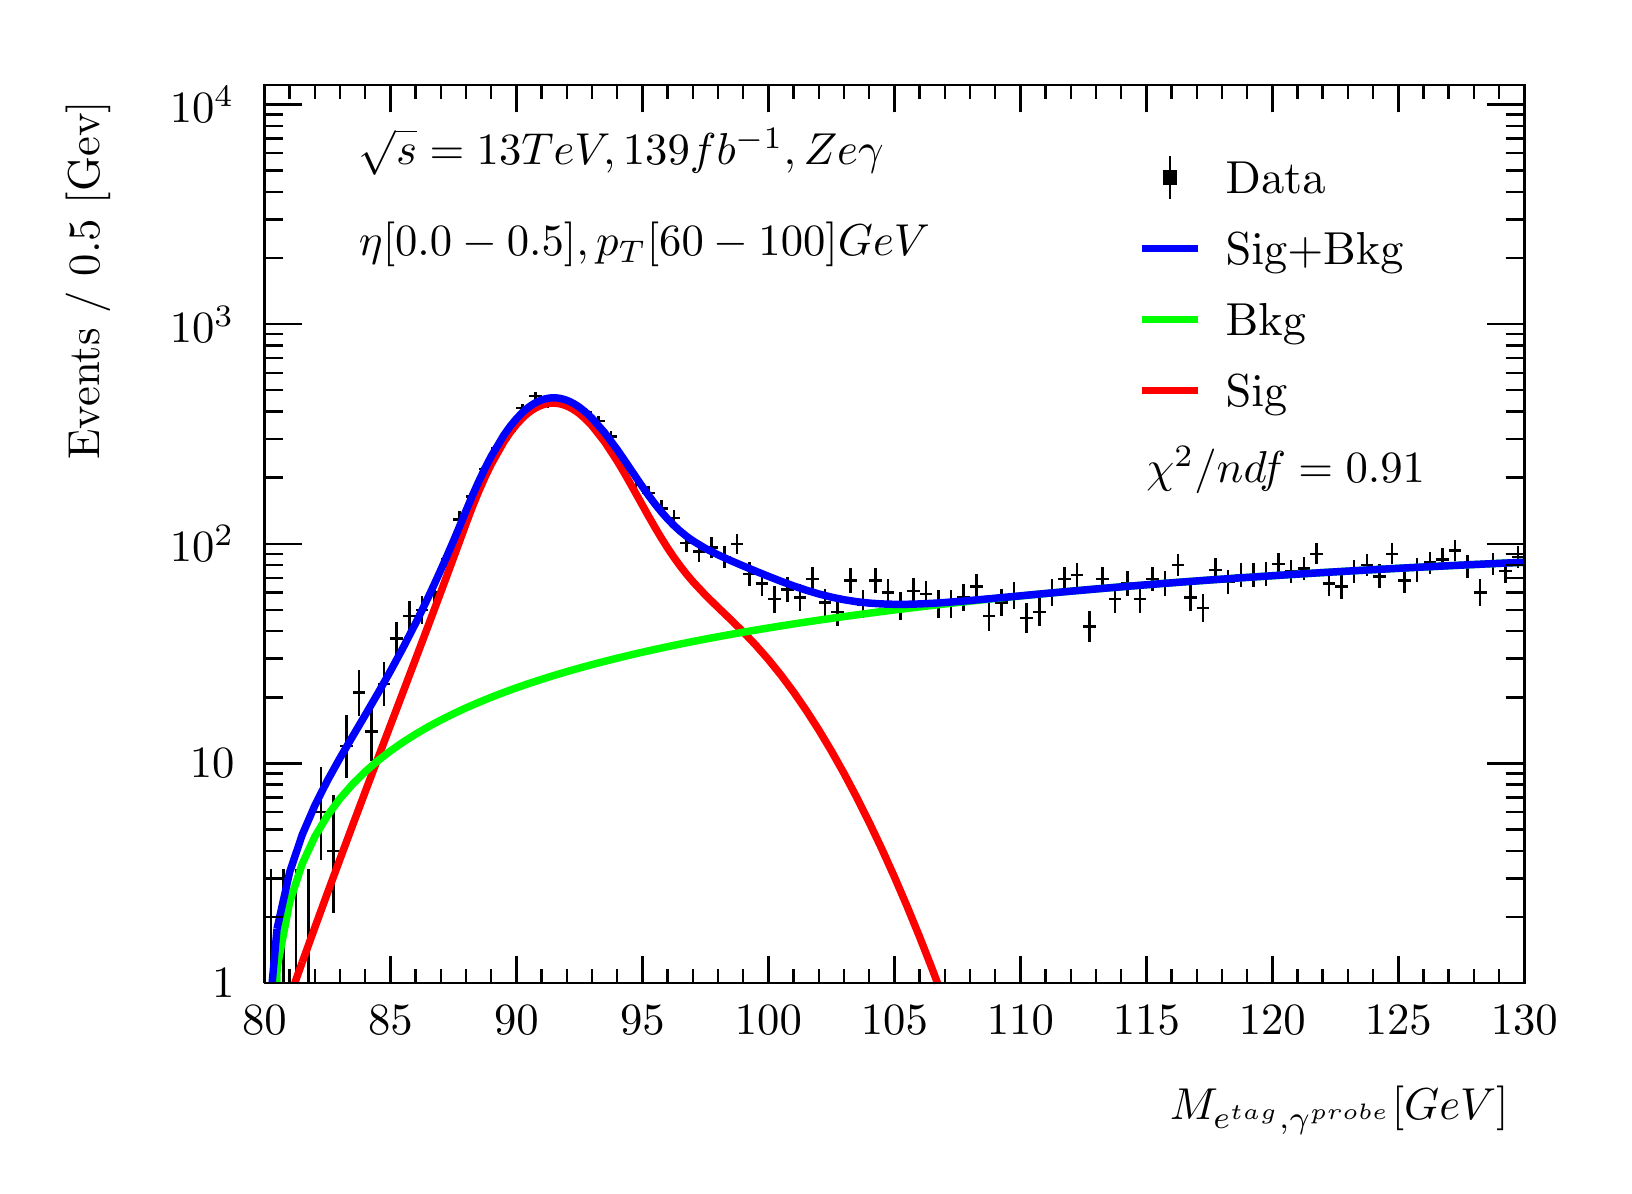
\begin{tikzpicture}
\pgfdeclareplotmark{cross} {
\pgfpathmoveto{\pgfpoint{-0.3\pgfplotmarksize}{\pgfplotmarksize}}
\pgfpathlineto{\pgfpoint{+0.3\pgfplotmarksize}{\pgfplotmarksize}}
\pgfpathlineto{\pgfpoint{+0.3\pgfplotmarksize}{0.3\pgfplotmarksize}}
\pgfpathlineto{\pgfpoint{+1\pgfplotmarksize}{0.3\pgfplotmarksize}}
\pgfpathlineto{\pgfpoint{+1\pgfplotmarksize}{-0.3\pgfplotmarksize}}
\pgfpathlineto{\pgfpoint{+0.3\pgfplotmarksize}{-0.3\pgfplotmarksize}}
\pgfpathlineto{\pgfpoint{+0.3\pgfplotmarksize}{-1.\pgfplotmarksize}}
\pgfpathlineto{\pgfpoint{-0.3\pgfplotmarksize}{-1.\pgfplotmarksize}}
\pgfpathlineto{\pgfpoint{-0.3\pgfplotmarksize}{-0.3\pgfplotmarksize}}
\pgfpathlineto{\pgfpoint{-1.\pgfplotmarksize}{-0.3\pgfplotmarksize}}
\pgfpathlineto{\pgfpoint{-1.\pgfplotmarksize}{0.3\pgfplotmarksize}}
\pgfpathlineto{\pgfpoint{-0.3\pgfplotmarksize}{0.3\pgfplotmarksize}}
\pgfpathclose
\pgfusepathqstroke
}
\pgfdeclareplotmark{cross*} {
\pgfpathmoveto{\pgfpoint{-0.3\pgfplotmarksize}{\pgfplotmarksize}}
\pgfpathlineto{\pgfpoint{+0.3\pgfplotmarksize}{\pgfplotmarksize}}
\pgfpathlineto{\pgfpoint{+0.3\pgfplotmarksize}{0.3\pgfplotmarksize}}
\pgfpathlineto{\pgfpoint{+1\pgfplotmarksize}{0.3\pgfplotmarksize}}
\pgfpathlineto{\pgfpoint{+1\pgfplotmarksize}{-0.3\pgfplotmarksize}}
\pgfpathlineto{\pgfpoint{+0.3\pgfplotmarksize}{-0.3\pgfplotmarksize}}
\pgfpathlineto{\pgfpoint{+0.3\pgfplotmarksize}{-1.\pgfplotmarksize}}
\pgfpathlineto{\pgfpoint{-0.3\pgfplotmarksize}{-1.\pgfplotmarksize}}
\pgfpathlineto{\pgfpoint{-0.3\pgfplotmarksize}{-0.3\pgfplotmarksize}}
\pgfpathlineto{\pgfpoint{-1.\pgfplotmarksize}{-0.3\pgfplotmarksize}}
\pgfpathlineto{\pgfpoint{-1.\pgfplotmarksize}{0.3\pgfplotmarksize}}
\pgfpathlineto{\pgfpoint{-0.3\pgfplotmarksize}{0.3\pgfplotmarksize}}
\pgfpathclose
\pgfusepathqfillstroke
}
\pgfdeclareplotmark{newstar} {
\pgfpathmoveto{\pgfqpoint{0pt}{\pgfplotmarksize}}
\pgfpathlineto{\pgfqpointpolar{44}{0.5\pgfplotmarksize}}
\pgfpathlineto{\pgfqpointpolar{18}{\pgfplotmarksize}}
\pgfpathlineto{\pgfqpointpolar{-20}{0.5\pgfplotmarksize}}
\pgfpathlineto{\pgfqpointpolar{-54}{\pgfplotmarksize}}
\pgfpathlineto{\pgfqpointpolar{-90}{0.5\pgfplotmarksize}}
\pgfpathlineto{\pgfqpointpolar{234}{\pgfplotmarksize}}
\pgfpathlineto{\pgfqpointpolar{198}{0.5\pgfplotmarksize}}
\pgfpathlineto{\pgfqpointpolar{162}{\pgfplotmarksize}}
\pgfpathlineto{\pgfqpointpolar{134}{0.5\pgfplotmarksize}}
\pgfpathclose
\pgfusepathqstroke
}
\pgfdeclareplotmark{newstar*} {
\pgfpathmoveto{\pgfqpoint{0pt}{\pgfplotmarksize}}
\pgfpathlineto{\pgfqpointpolar{44}{0.5\pgfplotmarksize}}
\pgfpathlineto{\pgfqpointpolar{18}{\pgfplotmarksize}}
\pgfpathlineto{\pgfqpointpolar{-20}{0.5\pgfplotmarksize}}
\pgfpathlineto{\pgfqpointpolar{-54}{\pgfplotmarksize}}
\pgfpathlineto{\pgfqpointpolar{-90}{0.5\pgfplotmarksize}}
\pgfpathlineto{\pgfqpointpolar{234}{\pgfplotmarksize}}
\pgfpathlineto{\pgfqpointpolar{198}{0.5\pgfplotmarksize}}
\pgfpathlineto{\pgfqpointpolar{162}{\pgfplotmarksize}}
\pgfpathlineto{\pgfqpointpolar{134}{0.5\pgfplotmarksize}}
\pgfpathclose
\pgfusepathqfillstroke
}
\definecolor{c}{rgb}{1,1,1};
\draw [color=c, fill=c] (0,0) rectangle (20,14.4361);
\draw [color=c, fill=c] (3,2.30977) rectangle (19,13.7143);
\definecolor{c}{rgb}{0,0,0};
\draw [c,line width=0.9] (3,2.30977) -- (3,13.7143) -- (19,13.7143) -- (19,2.30977) -- (3,2.30977);
\definecolor{c}{rgb}{1,1,1};
\draw [color=c, fill=c] (3,2.30977) rectangle (19,13.7143);
\definecolor{c}{rgb}{0,0,0};
\draw [c,line width=0.9] (3,2.30977) -- (3,13.7143) -- (19,13.7143) -- (19,2.30977) -- (3,2.30977);
\draw [c,line width=0.9] (3,2.30977) -- (19,2.30977);
\draw [c,line width=0.9] (3,2.65624) -- (3,2.30977);
\draw [c,line width=0.9] (3.32,2.48301) -- (3.32,2.30977);
\draw [c,line width=0.9] (3.64,2.48301) -- (3.64,2.30977);
\draw [c,line width=0.9] (3.96,2.48301) -- (3.96,2.30977);
\draw [c,line width=0.9] (4.28,2.48301) -- (4.28,2.30977);
\draw [c,line width=0.9] (4.6,2.65624) -- (4.6,2.30977);
\draw [c,line width=0.9] (4.92,2.48301) -- (4.92,2.30977);
\draw [c,line width=0.9] (5.24,2.48301) -- (5.24,2.30977);
\draw [c,line width=0.9] (5.56,2.48301) -- (5.56,2.30977);
\draw [c,line width=0.9] (5.88,2.48301) -- (5.88,2.30977);
\draw [c,line width=0.9] (6.2,2.65624) -- (6.2,2.30977);
\draw [c,line width=0.9] (6.52,2.48301) -- (6.52,2.30977);
\draw [c,line width=0.9] (6.84,2.48301) -- (6.84,2.30977);
\draw [c,line width=0.9] (7.16,2.48301) -- (7.16,2.30977);
\draw [c,line width=0.9] (7.48,2.48301) -- (7.48,2.30977);
\draw [c,line width=0.9] (7.8,2.65624) -- (7.8,2.30977);
\draw [c,line width=0.9] (8.12,2.48301) -- (8.12,2.30977);
\draw [c,line width=0.9] (8.44,2.48301) -- (8.44,2.30977);
\draw [c,line width=0.9] (8.76,2.48301) -- (8.76,2.30977);
\draw [c,line width=0.9] (9.08,2.48301) -- (9.08,2.30977);
\draw [c,line width=0.9] (9.4,2.65624) -- (9.4,2.30977);
\draw [c,line width=0.9] (9.72,2.48301) -- (9.72,2.30977);
\draw [c,line width=0.9] (10.04,2.48301) -- (10.04,2.30977);
\draw [c,line width=0.9] (10.36,2.48301) -- (10.36,2.30977);
\draw [c,line width=0.9] (10.68,2.48301) -- (10.68,2.30977);
\draw [c,line width=0.9] (11,2.65624) -- (11,2.30977);
\draw [c,line width=0.9] (11.32,2.48301) -- (11.32,2.30977);
\draw [c,line width=0.9] (11.64,2.48301) -- (11.64,2.30977);
\draw [c,line width=0.9] (11.96,2.48301) -- (11.96,2.30977);
\draw [c,line width=0.9] (12.28,2.48301) -- (12.28,2.30977);
\draw [c,line width=0.9] (12.6,2.65624) -- (12.6,2.30977);
\draw [c,line width=0.9] (12.92,2.48301) -- (12.92,2.30977);
\draw [c,line width=0.9] (13.24,2.48301) -- (13.24,2.30977);
\draw [c,line width=0.9] (13.56,2.48301) -- (13.56,2.30977);
\draw [c,line width=0.9] (13.88,2.48301) -- (13.88,2.30977);
\draw [c,line width=0.9] (14.2,2.65624) -- (14.2,2.30977);
\draw [c,line width=0.9] (14.52,2.48301) -- (14.52,2.30977);
\draw [c,line width=0.9] (14.84,2.48301) -- (14.84,2.30977);
\draw [c,line width=0.9] (15.16,2.48301) -- (15.16,2.30977);
\draw [c,line width=0.9] (15.48,2.48301) -- (15.48,2.30977);
\draw [c,line width=0.9] (15.8,2.65624) -- (15.8,2.30977);
\draw [c,line width=0.9] (16.12,2.48301) -- (16.12,2.30977);
\draw [c,line width=0.9] (16.44,2.48301) -- (16.44,2.30977);
\draw [c,line width=0.9] (16.76,2.48301) -- (16.76,2.30977);
\draw [c,line width=0.9] (17.08,2.48301) -- (17.08,2.30977);
\draw [c,line width=0.9] (17.4,2.65624) -- (17.4,2.30977);
\draw [c,line width=0.9] (17.72,2.48301) -- (17.72,2.30977);
\draw [c,line width=0.9] (18.04,2.48301) -- (18.04,2.30977);
\draw [c,line width=0.9] (18.36,2.48301) -- (18.36,2.30977);
\draw [c,line width=0.9] (18.68,2.48301) -- (18.68,2.30977);
\draw [c,line width=0.9] (19,2.65624) -- (19,2.30977);
\draw [anchor=base] (3,1.66015) node[scale=1.61424, color=c, rotate=0]{80};
\draw [anchor=base] (4.6,1.66015) node[scale=1.61424, color=c, rotate=0]{85};
\draw [anchor=base] (6.2,1.66015) node[scale=1.61424, color=c, rotate=0]{90};
\draw [anchor=base] (7.8,1.66015) node[scale=1.61424, color=c, rotate=0]{95};
\draw [anchor=base] (9.4,1.66015) node[scale=1.61424, color=c, rotate=0]{100};
\draw [anchor=base] (11,1.66015) node[scale=1.61424, color=c, rotate=0]{105};
\draw [anchor=base] (12.6,1.66015) node[scale=1.61424, color=c, rotate=0]{110};
\draw [anchor=base] (14.2,1.66015) node[scale=1.61424, color=c, rotate=0]{115};
\draw [anchor=base] (15.8,1.66015) node[scale=1.61424, color=c, rotate=0]{120};
\draw [anchor=base] (17.4,1.66015) node[scale=1.61424, color=c, rotate=0]{125};
\draw [anchor=base] (19,1.66015) node[scale=1.61424, color=c, rotate=0]{130};
\draw [anchor= east] (19,0.692932) node[scale=1.61424, color=c, rotate=0]{$M_{e^{tag}, \gamma^{probe}}  [GeV]$};
\draw [c,line width=0.9] (3,13.7143) -- (19,13.7143);
\draw [c,line width=0.9] (3,13.3678) -- (3,13.7143);
\draw [c,line width=0.9] (3.32,13.5411) -- (3.32,13.7143);
\draw [c,line width=0.9] (3.64,13.5411) -- (3.64,13.7143);
\draw [c,line width=0.9] (3.96,13.5411) -- (3.96,13.7143);
\draw [c,line width=0.9] (4.28,13.5411) -- (4.28,13.7143);
\draw [c,line width=0.9] (4.6,13.3678) -- (4.6,13.7143);
\draw [c,line width=0.9] (4.92,13.5411) -- (4.92,13.7143);
\draw [c,line width=0.9] (5.24,13.5411) -- (5.24,13.7143);
\draw [c,line width=0.9] (5.56,13.5411) -- (5.56,13.7143);
\draw [c,line width=0.9] (5.88,13.5411) -- (5.88,13.7143);
\draw [c,line width=0.9] (6.2,13.3678) -- (6.2,13.7143);
\draw [c,line width=0.9] (6.52,13.5411) -- (6.52,13.7143);
\draw [c,line width=0.9] (6.84,13.5411) -- (6.84,13.7143);
\draw [c,line width=0.9] (7.16,13.5411) -- (7.16,13.7143);
\draw [c,line width=0.9] (7.48,13.5411) -- (7.48,13.7143);
\draw [c,line width=0.9] (7.8,13.3678) -- (7.8,13.7143);
\draw [c,line width=0.9] (8.12,13.5411) -- (8.12,13.7143);
\draw [c,line width=0.9] (8.44,13.5411) -- (8.44,13.7143);
\draw [c,line width=0.9] (8.76,13.5411) -- (8.76,13.7143);
\draw [c,line width=0.9] (9.08,13.5411) -- (9.08,13.7143);
\draw [c,line width=0.9] (9.4,13.3678) -- (9.4,13.7143);
\draw [c,line width=0.9] (9.72,13.5411) -- (9.72,13.7143);
\draw [c,line width=0.9] (10.04,13.5411) -- (10.04,13.7143);
\draw [c,line width=0.9] (10.36,13.5411) -- (10.36,13.7143);
\draw [c,line width=0.9] (10.68,13.5411) -- (10.68,13.7143);
\draw [c,line width=0.9] (11,13.3678) -- (11,13.7143);
\draw [c,line width=0.9] (11.32,13.5411) -- (11.32,13.7143);
\draw [c,line width=0.9] (11.64,13.5411) -- (11.64,13.7143);
\draw [c,line width=0.9] (11.96,13.5411) -- (11.96,13.7143);
\draw [c,line width=0.9] (12.28,13.5411) -- (12.28,13.7143);
\draw [c,line width=0.9] (12.6,13.3678) -- (12.6,13.7143);
\draw [c,line width=0.9] (12.92,13.5411) -- (12.92,13.7143);
\draw [c,line width=0.9] (13.24,13.5411) -- (13.24,13.7143);
\draw [c,line width=0.9] (13.56,13.5411) -- (13.56,13.7143);
\draw [c,line width=0.9] (13.88,13.5411) -- (13.88,13.7143);
\draw [c,line width=0.9] (14.2,13.3678) -- (14.2,13.7143);
\draw [c,line width=0.9] (14.52,13.5411) -- (14.52,13.7143);
\draw [c,line width=0.9] (14.84,13.5411) -- (14.84,13.7143);
\draw [c,line width=0.9] (15.16,13.5411) -- (15.16,13.7143);
\draw [c,line width=0.9] (15.48,13.5411) -- (15.48,13.7143);
\draw [c,line width=0.9] (15.8,13.3678) -- (15.8,13.7143);
\draw [c,line width=0.9] (16.12,13.5411) -- (16.12,13.7143);
\draw [c,line width=0.9] (16.44,13.5411) -- (16.44,13.7143);
\draw [c,line width=0.9] (16.76,13.5411) -- (16.76,13.7143);
\draw [c,line width=0.9] (17.08,13.5411) -- (17.08,13.7143);
\draw [c,line width=0.9] (17.4,13.3678) -- (17.4,13.7143);
\draw [c,line width=0.9] (17.72,13.5411) -- (17.72,13.7143);
\draw [c,line width=0.9] (18.04,13.5411) -- (18.04,13.7143);
\draw [c,line width=0.9] (18.36,13.5411) -- (18.36,13.7143);
\draw [c,line width=0.9] (18.68,13.5411) -- (18.68,13.7143);
\draw [c,line width=0.9] (19,13.3678) -- (19,13.7143);
\draw [c,line width=0.9] (3,2.30977) -- (3,13.7143);
\draw [c,line width=0.9] (3.474,2.30978) -- (3,2.30978);
\draw [anchor= east] (2.82,2.30978) node[scale=1.61424, color=c, rotate=0]{1};
\draw [c,line width=0.9] (3.237,3.1495) -- (3,3.1495);
\draw [c,line width=0.9] (3.237,3.6407) -- (3,3.6407);
\draw [c,line width=0.9] (3.237,3.98922) -- (3,3.98922);
\draw [c,line width=0.9] (3.237,4.25955) -- (3,4.25955);
\draw [c,line width=0.9] (3.237,4.48042) -- (3,4.48042);
\draw [c,line width=0.9] (3.237,4.66717) -- (3,4.66717);
\draw [c,line width=0.9] (3.237,4.82894) -- (3,4.82894);
\draw [c,line width=0.9] (3.237,4.97163) -- (3,4.97163);
\draw [c,line width=0.9] (3.474,5.09927) -- (3,5.09927);
\draw [anchor= east] (2.82,5.09927) node[scale=1.61424, color=c, rotate=0]{10};
\draw [c,line width=0.9] (3.237,5.93899) -- (3,5.93899);
\draw [c,line width=0.9] (3.237,6.43019) -- (3,6.43019);
\draw [c,line width=0.9] (3.237,6.77871) -- (3,6.77871);
\draw [c,line width=0.9] (3.237,7.04904) -- (3,7.04904);
\draw [c,line width=0.9] (3.237,7.26991) -- (3,7.26991);
\draw [c,line width=0.9] (3.237,7.45666) -- (3,7.45666);
\draw [c,line width=0.9] (3.237,7.61843) -- (3,7.61843);
\draw [c,line width=0.9] (3.237,7.76112) -- (3,7.76112);
\draw [c,line width=0.9] (3.474,7.88876) -- (3,7.88876);
\draw [anchor= east] (2.82,7.88876) node[scale=1.61424, color=c, rotate=0]{$10^{2}$};
\draw [c,line width=0.9] (3.237,8.72848) -- (3,8.72848);
\draw [c,line width=0.9] (3.237,9.21968) -- (3,9.21968);
\draw [c,line width=0.9] (3.237,9.5682) -- (3,9.5682);
\draw [c,line width=0.9] (3.237,9.83853) -- (3,9.83853);
\draw [c,line width=0.9] (3.237,10.0594) -- (3,10.0594);
\draw [c,line width=0.9] (3.237,10.2462) -- (3,10.2462);
\draw [c,line width=0.9] (3.237,10.4079) -- (3,10.4079);
\draw [c,line width=0.9] (3.237,10.5506) -- (3,10.5506);
\draw [c,line width=0.9] (3.474,10.6782) -- (3,10.6782);
\draw [anchor= east] (2.82,10.6782) node[scale=1.61424, color=c, rotate=0]{$10^{3}$};
\draw [c,line width=0.9] (3.237,11.518) -- (3,11.518);
\draw [c,line width=0.9] (3.237,12.0092) -- (3,12.0092);
\draw [c,line width=0.9] (3.237,12.3577) -- (3,12.3577);
\draw [c,line width=0.9] (3.237,12.628) -- (3,12.628);
\draw [c,line width=0.9] (3.237,12.8489) -- (3,12.8489);
\draw [c,line width=0.9] (3.237,13.0356) -- (3,13.0356);
\draw [c,line width=0.9] (3.237,13.1974) -- (3,13.1974);
\draw [c,line width=0.9] (3.237,13.3401) -- (3,13.3401);
\draw [c,line width=0.9] (3.474,13.4677) -- (3,13.4677);
\draw [anchor= east] (2.82,13.4677) node[scale=1.61424, color=c, rotate=0]{$10^{4}$};
\draw [anchor= east] (0.76,13.7143) node[scale=1.61424, color=c, rotate=90]{Events / 0.5 [Gev]};
\draw [c,line width=0.9] (19,2.30977) -- (19,13.7143);
\draw [c,line width=0.9] (18.526,2.30978) -- (19,2.30978);
\draw [c,line width=0.9] (18.763,3.1495) -- (19,3.1495);
\draw [c,line width=0.9] (18.763,3.6407) -- (19,3.6407);
\draw [c,line width=0.9] (18.763,3.98922) -- (19,3.98922);
\draw [c,line width=0.9] (18.763,4.25955) -- (19,4.25955);
\draw [c,line width=0.9] (18.763,4.48042) -- (19,4.48042);
\draw [c,line width=0.9] (18.763,4.66717) -- (19,4.66717);
\draw [c,line width=0.9] (18.763,4.82894) -- (19,4.82894);
\draw [c,line width=0.9] (18.763,4.97163) -- (19,4.97163);
\draw [c,line width=0.9] (18.526,5.09927) -- (19,5.09927);
\draw [c,line width=0.9] (18.763,5.93899) -- (19,5.93899);
\draw [c,line width=0.9] (18.763,6.43019) -- (19,6.43019);
\draw [c,line width=0.9] (18.763,6.77871) -- (19,6.77871);
\draw [c,line width=0.9] (18.763,7.04904) -- (19,7.04904);
\draw [c,line width=0.9] (18.763,7.26991) -- (19,7.26991);
\draw [c,line width=0.9] (18.763,7.45666) -- (19,7.45666);
\draw [c,line width=0.9] (18.763,7.61843) -- (19,7.61843);
\draw [c,line width=0.9] (18.763,7.76112) -- (19,7.76112);
\draw [c,line width=0.9] (18.526,7.88876) -- (19,7.88876);
\draw [c,line width=0.9] (18.763,8.72848) -- (19,8.72848);
\draw [c,line width=0.9] (18.763,9.21968) -- (19,9.21968);
\draw [c,line width=0.9] (18.763,9.5682) -- (19,9.5682);
\draw [c,line width=0.9] (18.763,9.83853) -- (19,9.83853);
\draw [c,line width=0.9] (18.763,10.0594) -- (19,10.0594);
\draw [c,line width=0.9] (18.763,10.2462) -- (19,10.2462);
\draw [c,line width=0.9] (18.763,10.4079) -- (19,10.4079);
\draw [c,line width=0.9] (18.763,10.5506) -- (19,10.5506);
\draw [c,line width=0.9] (18.526,10.6782) -- (19,10.6782);
\draw [c,line width=0.9] (18.763,11.518) -- (19,11.518);
\draw [c,line width=0.9] (18.763,12.0092) -- (19,12.0092);
\draw [c,line width=0.9] (18.763,12.3577) -- (19,12.3577);
\draw [c,line width=0.9] (18.763,12.628) -- (19,12.628);
\draw [c,line width=0.9] (18.763,12.8489) -- (19,12.8489);
\draw [c,line width=0.9] (18.763,13.0356) -- (19,13.0356);
\draw [c,line width=0.9] (18.763,13.1974) -- (19,13.1974);
\draw [c,line width=0.9] (18.763,13.3401) -- (19,13.3401);
\draw [c,line width=0.9] (18.526,13.4677) -- (19,13.4677);
\draw [c,line width=0.9] (3.08,2.30977) -- (3,2.30977);
\draw [c,line width=0.9] (3,2.30977) -- (3,2.30977);
\draw [c,line width=0.9] (3.08,2.30977) -- (3.16,2.30977);
\draw [c,line width=0.9] (3.16,2.30977) -- (3.16,2.30977);
\draw [c,line width=0.9] (3.08,2.30977) -- (3.08,3.75599);
\draw [c,line width=0.9] (3.08,3.75599) -- (3.08,3.75599);
\draw [c,line width=0.9] (3.24,2.30977) -- (3.16,2.30977);
\draw [c,line width=0.9] (3.16,2.30977) -- (3.16,2.30977);
\draw [c,line width=0.9] (3.24,2.30977) -- (3.32,2.30977);
\draw [c,line width=0.9] (3.32,2.30977) -- (3.32,2.30977);
\draw [c,line width=0.9] (3.24,2.30977) -- (3.24,3.75599);
\draw [c,line width=0.9] (3.24,3.75599) -- (3.24,3.75599);
\draw [c,line width=0.9] (3.4,2.30977) -- (3.32,2.30977);
\draw [c,line width=0.9] (3.32,2.30977) -- (3.32,2.30977);
\draw [c,line width=0.9] (3.4,2.30977) -- (3.48,2.30977);
\draw [c,line width=0.9] (3.48,2.30977) -- (3.48,2.30977);
\draw [c,line width=0.9] (3.4,2.30977) -- (3.4,3.75599);
\draw [c,line width=0.9] (3.4,3.75599) -- (3.4,3.75599);
\draw [c,line width=0.9] (3.56,2.30977) -- (3.48,2.30977);
\draw [c,line width=0.9] (3.48,2.30977) -- (3.48,2.30977);
\draw [c,line width=0.9] (3.56,2.30977) -- (3.64,2.30977);
\draw [c,line width=0.9] (3.64,2.30977) -- (3.64,2.30977);
\draw [c,line width=0.9] (3.56,2.30977) -- (3.56,3.75599);
\draw [c,line width=0.9] (3.56,3.75599) -- (3.56,3.75599);
\draw [c,line width=0.9] (3.72,4.48042) -- (3.64,4.48042);
\draw [c,line width=0.9] (3.64,4.48042) -- (3.64,4.48042);
\draw [c,line width=0.9] (3.72,4.48042) -- (3.8,4.48042);
\draw [c,line width=0.9] (3.8,4.48042) -- (3.8,4.48042);
\draw [c,line width=0.9] (3.72,4.48042) -- (3.72,5.04775);
\draw [c,line width=0.9] (3.72,5.04775) -- (3.72,5.04775);
\draw [c,line width=0.9] (3.72,4.48042) -- (3.72,3.86831);
\draw [c,line width=0.9] (3.72,3.86831) -- (3.72,3.86831);
\draw [c,line width=0.9] (3.88,3.98922) -- (3.8,3.98922);
\draw [c,line width=0.9] (3.8,3.98922) -- (3.8,3.98922);
\draw [c,line width=0.9] (3.88,3.98922) -- (3.96,3.98922);
\draw [c,line width=0.9] (3.96,3.98922) -- (3.96,3.98922);
\draw [c,line width=0.9] (3.88,3.98922) -- (3.88,4.69501);
\draw [c,line width=0.9] (3.88,4.69501) -- (3.88,4.69501);
\draw [c,line width=0.9] (3.88,3.98922) -- (3.88,3.2003);
\draw [c,line width=0.9] (3.88,3.2003) -- (3.88,3.2003);
\draw [c,line width=0.9] (4.04,5.32014) -- (3.96,5.32014);
\draw [c,line width=0.9] (3.96,5.32014) -- (3.96,5.32014);
\draw [c,line width=0.9] (4.04,5.32014) -- (4.12,5.32014);
\draw [c,line width=0.9] (4.12,5.32014) -- (4.12,5.32014);
\draw [c,line width=0.9] (4.04,5.32014) -- (4.04,5.71032);
\draw [c,line width=0.9] (4.04,5.71032) -- (4.04,5.71032);
\draw [c,line width=0.9] (4.04,5.32014) -- (4.04,4.9144);
\draw [c,line width=0.9] (4.04,4.9144) -- (4.04,4.9144);
\draw [c,line width=0.9] (4.2,5.99809) -- (4.12,5.99809);
\draw [c,line width=0.9] (4.12,5.99809) -- (4.12,5.99809);
\draw [c,line width=0.9] (4.2,5.99809) -- (4.28,5.99809);
\draw [c,line width=0.9] (4.28,5.99809) -- (4.28,5.99809);
\draw [c,line width=0.9] (4.2,5.99809) -- (4.2,6.28698);
\draw [c,line width=0.9] (4.2,6.28698) -- (4.2,6.28698);
\draw [c,line width=0.9] (4.2,5.99809) -- (4.2,5.70257);
\draw [c,line width=0.9] (4.2,5.70257) -- (4.2,5.70257);
\draw [c,line width=0.9] (4.36,5.50689) -- (4.28,5.50689);
\draw [c,line width=0.9] (4.28,5.50689) -- (4.28,5.50689);
\draw [c,line width=0.9] (4.36,5.50689) -- (4.44,5.50689);
\draw [c,line width=0.9] (4.44,5.50689) -- (4.44,5.50689);
\draw [c,line width=0.9] (4.36,5.50689) -- (4.36,5.86598);
\draw [c,line width=0.9] (4.36,5.86598) -- (4.36,5.86598);
\draw [c,line width=0.9] (4.36,5.50689) -- (4.36,5.13549);
\draw [c,line width=0.9] (4.36,5.13549) -- (4.36,5.13549);
\draw [c,line width=0.9] (4.52,6.1083) -- (4.44,6.1083);
\draw [c,line width=0.9] (4.44,6.1083) -- (4.44,6.1083);
\draw [c,line width=0.9] (4.52,6.1083) -- (4.6,6.1083);
\draw [c,line width=0.9] (4.6,6.1083) -- (4.6,6.1083);
\draw [c,line width=0.9] (4.52,6.1083) -- (4.52,6.38348);
\draw [c,line width=0.9] (4.52,6.38348) -- (4.52,6.38348);
\draw [c,line width=0.9] (4.52,6.1083) -- (4.52,5.82734);
\draw [c,line width=0.9] (4.52,5.82734) -- (4.52,5.82734);
\draw [c,line width=0.9] (4.68,6.68426) -- (4.6,6.68426);
\draw [c,line width=0.9] (4.6,6.68426) -- (4.6,6.68426);
\draw [c,line width=0.9] (4.68,6.68426) -- (4.76,6.68426);
\draw [c,line width=0.9] (4.76,6.68426) -- (4.76,6.68426);
\draw [c,line width=0.9] (4.68,6.68426) -- (4.68,6.89795);
\draw [c,line width=0.9] (4.68,6.89795) -- (4.68,6.89795);
\draw [c,line width=0.9] (4.68,6.68426) -- (4.68,6.46776);
\draw [c,line width=0.9] (4.68,6.46776) -- (4.68,6.46776);
\draw [c,line width=0.9] (4.84,6.97408) -- (4.76,6.97408);
\draw [c,line width=0.9] (4.76,6.97408) -- (4.76,6.97408);
\draw [c,line width=0.9] (4.84,6.97408) -- (4.92,6.97408);
\draw [c,line width=0.9] (4.92,6.97408) -- (4.92,6.97408);
\draw [c,line width=0.9] (4.84,6.97408) -- (4.84,7.16239);
\draw [c,line width=0.9] (4.84,7.16239) -- (4.84,7.16239);
\draw [c,line width=0.9] (4.84,6.97408) -- (4.84,6.78381);
\draw [c,line width=0.9] (4.84,6.78381) -- (4.84,6.78381);
\draw [c,line width=0.9] (5,7.04904) -- (4.92,7.04904);
\draw [c,line width=0.9] (4.92,7.04904) -- (4.92,7.04904);
\draw [c,line width=0.9] (5,7.04904) -- (5.08,7.04904);
\draw [c,line width=0.9] (5.08,7.04904) -- (5.08,7.04904);
\draw [c,line width=0.9] (5,7.04904) -- (5,7.23131);
\draw [c,line width=0.9] (5,7.23131) -- (5,7.23131);
\draw [c,line width=0.9] (5,7.04904) -- (5,6.86499);
\draw [c,line width=0.9] (5,6.86499) -- (5,6.86499);
\draw [c,line width=0.9] (5.16,7.26991) -- (5.08,7.26991);
\draw [c,line width=0.9] (5.08,7.26991) -- (5.08,7.26991);
\draw [c,line width=0.9] (5.16,7.26991) -- (5.24,7.26991);
\draw [c,line width=0.9] (5.24,7.26991) -- (5.24,7.26991);
\draw [c,line width=0.9] (5.16,7.26991) -- (5.16,7.43552);
\draw [c,line width=0.9] (5.16,7.43552) -- (5.16,7.43552);
\draw [c,line width=0.9] (5.16,7.26991) -- (5.16,7.10296);
\draw [c,line width=0.9] (5.16,7.10296) -- (5.16,7.10296);
\draw [c,line width=0.9] (5.32,7.69187) -- (5.24,7.69187);
\draw [c,line width=0.9] (5.24,7.69187) -- (5.24,7.69187);
\draw [c,line width=0.9] (5.32,7.69187) -- (5.4,7.69187);
\draw [c,line width=0.9] (5.4,7.69187) -- (5.4,7.69187);
\draw [c,line width=0.9] (5.32,7.69187) -- (5.32,7.82987);
\draw [c,line width=0.9] (5.32,7.82987) -- (5.32,7.82987);
\draw [c,line width=0.9] (5.32,7.69187) -- (5.32,7.55307);
\draw [c,line width=0.9] (5.32,7.55307) -- (5.32,7.55307);
\draw [c,line width=0.9] (5.48,8.19725) -- (5.4,8.19725);
\draw [c,line width=0.9] (5.4,8.19725) -- (5.4,8.19725);
\draw [c,line width=0.9] (5.48,8.19725) -- (5.56,8.19725);
\draw [c,line width=0.9] (5.56,8.19725) -- (5.56,8.19725);
\draw [c,line width=0.9] (5.48,8.19725) -- (5.48,8.30387);
\draw [c,line width=0.9] (5.48,8.30387) -- (5.48,8.30387);
\draw [c,line width=0.9] (5.48,8.19725) -- (5.48,8.09062);
\draw [c,line width=0.9] (5.48,8.09062) -- (5.48,8.09062);
\draw [c,line width=0.9] (5.64,8.48806) -- (5.56,8.48806);
\draw [c,line width=0.9] (5.56,8.48806) -- (5.56,8.48806);
\draw [c,line width=0.9] (5.64,8.48806) -- (5.72,8.48806);
\draw [c,line width=0.9] (5.72,8.48806) -- (5.72,8.48806);
\draw [c,line width=0.9] (5.64,8.48806) -- (5.64,8.58264);
\draw [c,line width=0.9] (5.64,8.58264) -- (5.64,8.58264);
\draw [c,line width=0.9] (5.64,8.48806) -- (5.64,8.39349);
\draw [c,line width=0.9] (5.64,8.39349) -- (5.64,8.39349);
\draw [c,line width=0.9] (5.8,8.83842) -- (5.72,8.83842);
\draw [c,line width=0.9] (5.72,8.83842) -- (5.72,8.83842);
\draw [c,line width=0.9] (5.8,8.83842) -- (5.88,8.83842);
\draw [c,line width=0.9] (5.88,8.83842) -- (5.88,8.83842);
\draw [c,line width=0.9] (5.8,8.83842) -- (5.8,8.92027);
\draw [c,line width=0.9] (5.8,8.92027) -- (5.8,8.92027);
\draw [c,line width=0.9] (5.8,8.83842) -- (5.8,8.75658);
\draw [c,line width=0.9] (5.8,8.75658) -- (5.8,8.75658);
\draw [c,line width=0.9] (5.96,9.10543) -- (5.88,9.10543);
\draw [c,line width=0.9] (5.88,9.10543) -- (5.88,9.10543);
\draw [c,line width=0.9] (5.96,9.10543) -- (6.04,9.10543);
\draw [c,line width=0.9] (6.04,9.10543) -- (6.04,9.10543);
\draw [c,line width=0.9] (5.96,9.10543) -- (5.96,9.17874);
\draw [c,line width=0.9] (5.96,9.17874) -- (5.96,9.17874);
\draw [c,line width=0.9] (5.96,9.10543) -- (5.96,9.03212);
\draw [c,line width=0.9] (5.96,9.03212) -- (5.96,9.03212);
\draw [c,line width=0.9] (6.12,9.32037) -- (6.04,9.32037);
\draw [c,line width=0.9] (6.04,9.32037) -- (6.04,9.32037);
\draw [c,line width=0.9] (6.12,9.32037) -- (6.2,9.32037);
\draw [c,line width=0.9] (6.2,9.32037) -- (6.2,9.32037);
\draw [c,line width=0.9] (6.12,9.32037) -- (6.12,9.38746);
\draw [c,line width=0.9] (6.12,9.38746) -- (6.12,9.38746);
\draw [c,line width=0.9] (6.12,9.32037) -- (6.12,9.25328);
\draw [c,line width=0.9] (6.12,9.25328) -- (6.12,9.25328);
\draw [c,line width=0.9] (6.28,9.60987) -- (6.2,9.60987);
\draw [c,line width=0.9] (6.2,9.60987) -- (6.2,9.60987);
\draw [c,line width=0.9] (6.28,9.60987) -- (6.36,9.60987);
\draw [c,line width=0.9] (6.36,9.60987) -- (6.36,9.60987);
\draw [c,line width=0.9] (6.28,9.60987) -- (6.28,9.66941);
\draw [c,line width=0.9] (6.28,9.66941) -- (6.28,9.66941);
\draw [c,line width=0.9] (6.28,9.60987) -- (6.28,9.55034);
\draw [c,line width=0.9] (6.28,9.55034) -- (6.28,9.55034);
\draw [c,line width=0.9] (6.44,9.76357) -- (6.36,9.76357);
\draw [c,line width=0.9] (6.36,9.76357) -- (6.36,9.76357);
\draw [c,line width=0.9] (6.44,9.76357) -- (6.52,9.76357);
\draw [c,line width=0.9] (6.52,9.76357) -- (6.52,9.76357);
\draw [c,line width=0.9] (6.44,9.76357) -- (6.44,9.81944);
\draw [c,line width=0.9] (6.44,9.81944) -- (6.44,9.81944);
\draw [c,line width=0.9] (6.44,9.76357) -- (6.44,9.70769);
\draw [c,line width=0.9] (6.44,9.70769) -- (6.44,9.70769);
\draw [c,line width=0.9] (6.6,9.66982) -- (6.52,9.66982);
\draw [c,line width=0.9] (6.52,9.66982) -- (6.52,9.66982);
\draw [c,line width=0.9] (6.6,9.66982) -- (6.68,9.66982);
\draw [c,line width=0.9] (6.68,9.66982) -- (6.68,9.66982);
\draw [c,line width=0.9] (6.6,9.66982) -- (6.6,9.7279);
\draw [c,line width=0.9] (6.6,9.7279) -- (6.6,9.7279);
\draw [c,line width=0.9] (6.6,9.66982) -- (6.6,9.61174);
\draw [c,line width=0.9] (6.6,9.61174) -- (6.6,9.61174);
\draw [c,line width=0.9] (6.76,9.72161) -- (6.68,9.72161);
\draw [c,line width=0.9] (6.68,9.72161) -- (6.68,9.72161);
\draw [c,line width=0.9] (6.76,9.72161) -- (6.84,9.72161);
\draw [c,line width=0.9] (6.84,9.72161) -- (6.84,9.72161);
\draw [c,line width=0.9] (6.76,9.72161) -- (6.76,9.77846);
\draw [c,line width=0.9] (6.76,9.77846) -- (6.76,9.77846);
\draw [c,line width=0.9] (6.76,9.72161) -- (6.76,9.66476);
\draw [c,line width=0.9] (6.76,9.66476) -- (6.76,9.66476);
\draw [c,line width=0.9] (6.92,9.64449) -- (6.84,9.64449);
\draw [c,line width=0.9] (6.84,9.64449) -- (6.84,9.64449);
\draw [c,line width=0.9] (6.92,9.64449) -- (7,9.64449);
\draw [c,line width=0.9] (7,9.64449) -- (7,9.64449);
\draw [c,line width=0.9] (6.92,9.64449) -- (6.92,9.70318);
\draw [c,line width=0.9] (6.92,9.70318) -- (6.92,9.70318);
\draw [c,line width=0.9] (6.92,9.64449) -- (6.92,9.5858);
\draw [c,line width=0.9] (6.92,9.5858) -- (6.92,9.5858);
\draw [c,line width=0.9] (7.08,9.55296) -- (7,9.55296);
\draw [c,line width=0.9] (7,9.55296) -- (7,9.55296);
\draw [c,line width=0.9] (7.08,9.55296) -- (7.16,9.55296);
\draw [c,line width=0.9] (7.16,9.55296) -- (7.16,9.55296);
\draw [c,line width=0.9] (7.08,9.55296) -- (7.08,9.61391);
\draw [c,line width=0.9] (7.08,9.61391) -- (7.08,9.61391);
\draw [c,line width=0.9] (7.08,9.55296) -- (7.08,9.49201);
\draw [c,line width=0.9] (7.08,9.49201) -- (7.08,9.49201);
\draw [c,line width=0.9] (7.24,9.44727) -- (7.16,9.44727);
\draw [c,line width=0.9] (7.16,9.44727) -- (7.16,9.44727);
\draw [c,line width=0.9] (7.24,9.44727) -- (7.32,9.44727);
\draw [c,line width=0.9] (7.32,9.44727) -- (7.32,9.44727);
\draw [c,line width=0.9] (7.24,9.44727) -- (7.24,9.51093);
\draw [c,line width=0.9] (7.24,9.51093) -- (7.24,9.51093);
\draw [c,line width=0.9] (7.24,9.44727) -- (7.24,9.3836);
\draw [c,line width=0.9] (7.24,9.3836) -- (7.24,9.3836);
\draw [c,line width=0.9] (7.4,9.25156) -- (7.32,9.25156);
\draw [c,line width=0.9] (7.32,9.25156) -- (7.32,9.25156);
\draw [c,line width=0.9] (7.4,9.25156) -- (7.48,9.25156);
\draw [c,line width=0.9] (7.48,9.25156) -- (7.48,9.25156);
\draw [c,line width=0.9] (7.4,9.25156) -- (7.4,9.32058);
\draw [c,line width=0.9] (7.4,9.32058) -- (7.4,9.32058);
\draw [c,line width=0.9] (7.4,9.25156) -- (7.4,9.18254);
\draw [c,line width=0.9] (7.4,9.18254) -- (7.4,9.18254);
\draw [c,line width=0.9] (7.56,8.90828) -- (7.48,8.90828);
\draw [c,line width=0.9] (7.48,8.90828) -- (7.48,8.90828);
\draw [c,line width=0.9] (7.56,8.90828) -- (7.64,8.90828);
\draw [c,line width=0.9] (7.64,8.90828) -- (7.64,8.90828);
\draw [c,line width=0.9] (7.56,8.90828) -- (7.56,8.9878);
\draw [c,line width=0.9] (7.56,8.9878) -- (7.56,8.9878);
\draw [c,line width=0.9] (7.56,8.90828) -- (7.56,8.82876);
\draw [c,line width=0.9] (7.56,8.82876) -- (7.56,8.82876);
\draw [c,line width=0.9] (7.72,8.63403) -- (7.64,8.63403);
\draw [c,line width=0.9] (7.64,8.63403) -- (7.64,8.63403);
\draw [c,line width=0.9] (7.72,8.63403) -- (7.8,8.63403);
\draw [c,line width=0.9] (7.8,8.63403) -- (7.8,8.63403);
\draw [c,line width=0.9] (7.72,8.63403) -- (7.72,8.72308);
\draw [c,line width=0.9] (7.72,8.72308) -- (7.72,8.72308);
\draw [c,line width=0.9] (7.72,8.63403) -- (7.72,8.54498);
\draw [c,line width=0.9] (7.72,8.54498) -- (7.72,8.54498);
\draw [c,line width=0.9] (7.88,8.53159) -- (7.8,8.53159);
\draw [c,line width=0.9] (7.8,8.53159) -- (7.8,8.53159);
\draw [c,line width=0.9] (7.88,8.53159) -- (7.96,8.53159);
\draw [c,line width=0.9] (7.96,8.53159) -- (7.96,8.53159);
\draw [c,line width=0.9] (7.88,8.53159) -- (7.88,8.62448);
\draw [c,line width=0.9] (7.88,8.62448) -- (7.88,8.62448);
\draw [c,line width=0.9] (7.88,8.53159) -- (7.88,8.4387);
\draw [c,line width=0.9] (7.88,8.4387) -- (7.88,8.4387);
\draw [c,line width=0.9] (8.04,8.33889) -- (7.96,8.33889);
\draw [c,line width=0.9] (7.96,8.33889) -- (7.96,8.33889);
\draw [c,line width=0.9] (8.04,8.33889) -- (8.12,8.33889);
\draw [c,line width=0.9] (8.12,8.33889) -- (8.12,8.33889);
\draw [c,line width=0.9] (8.04,8.33889) -- (8.04,8.43947);
\draw [c,line width=0.9] (8.04,8.43947) -- (8.04,8.43947);
\draw [c,line width=0.9] (8.04,8.33889) -- (8.04,8.23831);
\draw [c,line width=0.9] (8.04,8.23831) -- (8.04,8.23831);
\draw [c,line width=0.9] (8.2,8.21588) -- (8.12,8.21588);
\draw [c,line width=0.9] (8.12,8.21588) -- (8.12,8.21588);
\draw [c,line width=0.9] (8.2,8.21588) -- (8.28,8.21588);
\draw [c,line width=0.9] (8.28,8.21588) -- (8.28,8.21588);
\draw [c,line width=0.9] (8.2,8.21588) -- (8.2,8.3217);
\draw [c,line width=0.9] (8.2,8.3217) -- (8.2,8.3217);
\draw [c,line width=0.9] (8.2,8.21588) -- (8.2,8.11007);
\draw [c,line width=0.9] (8.2,8.11007) -- (8.2,8.11007);
\draw [c,line width=0.9] (8.36,7.90081) -- (8.28,7.90081);
\draw [c,line width=0.9] (8.28,7.90081) -- (8.28,7.90081);
\draw [c,line width=0.9] (8.36,7.90081) -- (8.44,7.90081);
\draw [c,line width=0.9] (8.44,7.90081) -- (8.44,7.90081);
\draw [c,line width=0.9] (8.36,7.90081) -- (8.36,8.02131);
\draw [c,line width=0.9] (8.36,8.02131) -- (8.36,8.02131);
\draw [c,line width=0.9] (8.36,7.90081) -- (8.36,7.78032);
\draw [c,line width=0.9] (8.36,7.78032) -- (8.36,7.78032);
\draw [c,line width=0.9] (8.52,7.78774) -- (8.44,7.78774);
\draw [c,line width=0.9] (8.44,7.78774) -- (8.44,7.78774);
\draw [c,line width=0.9] (8.52,7.78774) -- (8.6,7.78774);
\draw [c,line width=0.9] (8.6,7.78774) -- (8.6,7.78774);
\draw [c,line width=0.9] (8.52,7.78774) -- (8.52,7.92016);
\draw [c,line width=0.9] (8.52,7.92016) -- (8.52,7.92016);
\draw [c,line width=0.9] (8.52,7.78774) -- (8.52,7.65462);
\draw [c,line width=0.9] (8.52,7.65462) -- (8.52,7.65462);
\draw [c,line width=0.9] (8.68,7.8393) -- (8.6,7.8393);
\draw [c,line width=0.9] (8.6,7.8393) -- (8.6,7.8393);
\draw [c,line width=0.9] (8.68,7.8393) -- (8.76,7.8393);
\draw [c,line width=0.9] (8.76,7.8393) -- (8.76,7.8393);
\draw [c,line width=0.9] (8.68,7.8393) -- (8.68,7.96882);
\draw [c,line width=0.9] (8.68,7.96882) -- (8.68,7.96882);
\draw [c,line width=0.9] (8.68,7.8393) -- (8.68,7.70912);
\draw [c,line width=0.9] (8.68,7.70912) -- (8.68,7.70912);
\draw [c,line width=0.9] (8.84,7.72005) -- (8.76,7.72005);
\draw [c,line width=0.9] (8.76,7.72005) -- (8.76,7.72005);
\draw [c,line width=0.9] (8.84,7.72005) -- (8.92,7.72005);
\draw [c,line width=0.9] (8.92,7.72005) -- (8.92,7.72005);
\draw [c,line width=0.9] (8.84,7.72005) -- (8.84,7.85638);
\draw [c,line width=0.9] (8.84,7.85638) -- (8.84,7.85638);
\draw [c,line width=0.9] (8.84,7.72005) -- (8.84,7.58294);
\draw [c,line width=0.9] (8.84,7.58294) -- (8.84,7.58294);
\draw [c,line width=0.9] (9,7.88876) -- (8.92,7.88876);
\draw [c,line width=0.9] (8.92,7.88876) -- (8.92,7.88876);
\draw [c,line width=0.9] (9,7.88876) -- (9.08,7.88876);
\draw [c,line width=0.9] (9.08,7.88876) -- (9.08,7.88876);
\draw [c,line width=0.9] (9,7.88876) -- (9,8.01555);
\draw [c,line width=0.9] (9,8.01555) -- (9,8.01555);
\draw [c,line width=0.9] (9,7.88876) -- (9,7.76134);
\draw [c,line width=0.9] (9,7.76134) -- (9,7.76134);
\draw [c,line width=0.9] (9.16,7.5075) -- (9.08,7.5075);
\draw [c,line width=0.9] (9.08,7.5075) -- (9.08,7.5075);
\draw [c,line width=0.9] (9.16,7.5075) -- (9.24,7.5075);
\draw [c,line width=0.9] (9.24,7.5075) -- (9.24,7.5075);
\draw [c,line width=0.9] (9.16,7.5075) -- (9.16,7.65692);
\draw [c,line width=0.9] (9.16,7.65692) -- (9.16,7.65692);
\draw [c,line width=0.9] (9.16,7.5075) -- (9.16,7.35707);
\draw [c,line width=0.9] (9.16,7.35707) -- (9.16,7.35707);
\draw [c,line width=0.9] (9.32,7.38538) -- (9.24,7.38538);
\draw [c,line width=0.9] (9.24,7.38538) -- (9.24,7.38538);
\draw [c,line width=0.9] (9.32,7.38538) -- (9.4,7.38538);
\draw [c,line width=0.9] (9.4,7.38538) -- (9.4,7.38538);
\draw [c,line width=0.9] (9.32,7.38538) -- (9.32,7.5429);
\draw [c,line width=0.9] (9.32,7.5429) -- (9.32,7.5429);
\draw [c,line width=0.9] (9.32,7.38538) -- (9.32,7.22668);
\draw [c,line width=0.9] (9.32,7.22668) -- (9.32,7.22668);
\draw [c,line width=0.9] (9.48,7.18633) -- (9.4,7.18633);
\draw [c,line width=0.9] (9.4,7.18633) -- (9.4,7.18633);
\draw [c,line width=0.9] (9.48,7.18633) -- (9.56,7.18633);
\draw [c,line width=0.9] (9.56,7.18633) -- (9.56,7.18633);
\draw [c,line width=0.9] (9.48,7.18633) -- (9.48,7.35805);
\draw [c,line width=0.9] (9.48,7.35805) -- (9.48,7.35805);
\draw [c,line width=0.9] (9.48,7.18633) -- (9.48,7.01311);
\draw [c,line width=0.9] (9.48,7.01311) -- (9.48,7.01311);
\draw [c,line width=0.9] (9.64,7.30964) -- (9.56,7.30964);
\draw [c,line width=0.9] (9.56,7.30964) -- (9.56,7.30964);
\draw [c,line width=0.9] (9.64,7.30964) -- (9.72,7.30964);
\draw [c,line width=0.9] (9.72,7.30964) -- (9.72,7.30964);
\draw [c,line width=0.9] (9.64,7.30964) -- (9.64,7.47242);
\draw [c,line width=0.9] (9.64,7.47242) -- (9.64,7.47242);
\draw [c,line width=0.9] (9.64,7.30964) -- (9.64,7.14557);
\draw [c,line width=0.9] (9.64,7.14557) -- (9.64,7.14557);
\draw [c,line width=0.9] (9.8,7.20777) -- (9.72,7.20777);
\draw [c,line width=0.9] (9.72,7.20777) -- (9.72,7.20777);
\draw [c,line width=0.9] (9.8,7.20777) -- (9.88,7.20777);
\draw [c,line width=0.9] (9.88,7.20777) -- (9.88,7.20777);
\draw [c,line width=0.9] (9.8,7.20777) -- (9.8,7.3779);
\draw [c,line width=0.9] (9.8,7.3779) -- (9.8,7.3779);
\draw [c,line width=0.9] (9.8,7.20777) -- (9.8,7.03618);
\draw [c,line width=0.9] (9.8,7.03618) -- (9.8,7.03618);
\draw [c,line width=0.9] (9.96,7.43923) -- (9.88,7.43923);
\draw [c,line width=0.9] (9.88,7.43923) -- (9.88,7.43923);
\draw [c,line width=0.9] (9.96,7.43923) -- (10.04,7.43923);
\draw [c,line width=0.9] (10.04,7.43923) -- (10.04,7.43923);
\draw [c,line width=0.9] (9.96,7.43923) -- (9.96,7.59313);
\draw [c,line width=0.9] (9.96,7.59313) -- (9.96,7.59313);
\draw [c,line width=0.9] (9.96,7.43923) -- (9.96,7.28423);
\draw [c,line width=0.9] (9.96,7.28423) -- (9.96,7.28423);
\draw [c,line width=0.9] (10.12,7.14227) -- (10.04,7.14227);
\draw [c,line width=0.9] (10.04,7.14227) -- (10.04,7.14227);
\draw [c,line width=0.9] (10.12,7.14227) -- (10.2,7.14227);
\draw [c,line width=0.9] (10.2,7.14227) -- (10.2,7.14227);
\draw [c,line width=0.9] (10.12,7.14227) -- (10.12,7.31731);
\draw [c,line width=0.9] (10.12,7.31731) -- (10.12,7.31731);
\draw [c,line width=0.9] (10.12,7.14227) -- (10.12,6.96565);
\draw [c,line width=0.9] (10.12,6.96565) -- (10.12,6.96565);
\draw [c,line width=0.9] (10.28,7.02456) -- (10.2,7.02456);
\draw [c,line width=0.9] (10.2,7.02456) -- (10.2,7.02456);
\draw [c,line width=0.9] (10.28,7.02456) -- (10.36,7.02456);
\draw [c,line width=0.9] (10.36,7.02456) -- (10.36,7.02456);
\draw [c,line width=0.9] (10.28,7.02456) -- (10.28,7.20878);
\draw [c,line width=0.9] (10.28,7.20878) -- (10.28,7.20878);
\draw [c,line width=0.9] (10.28,7.02456) -- (10.28,6.83851);
\draw [c,line width=0.9] (10.28,6.83851) -- (10.28,6.83851);
\draw [c,line width=0.9] (10.44,7.42154) -- (10.36,7.42154);
\draw [c,line width=0.9] (10.36,7.42154) -- (10.36,7.42154);
\draw [c,line width=0.9] (10.44,7.42154) -- (10.52,7.42154);
\draw [c,line width=0.9] (10.52,7.42154) -- (10.52,7.42154);
\draw [c,line width=0.9] (10.44,7.42154) -- (10.44,7.57663);
\draw [c,line width=0.9] (10.44,7.57663) -- (10.44,7.57663);
\draw [c,line width=0.9] (10.44,7.42154) -- (10.44,7.26534);
\draw [c,line width=0.9] (10.44,7.26534) -- (10.44,7.26534);
\draw [c,line width=0.9] (10.6,7.11963) -- (10.52,7.11963);
\draw [c,line width=0.9] (10.52,7.11963) -- (10.52,7.11963);
\draw [c,line width=0.9] (10.6,7.11963) -- (10.68,7.11963);
\draw [c,line width=0.9] (10.68,7.11963) -- (10.68,7.11963);
\draw [c,line width=0.9] (10.6,7.11963) -- (10.6,7.29639);
\draw [c,line width=0.9] (10.6,7.29639) -- (10.6,7.29639);
\draw [c,line width=0.9] (10.6,7.11963) -- (10.6,6.94123);
\draw [c,line width=0.9] (10.6,6.94123) -- (10.6,6.94123);
\draw [c,line width=0.9] (10.76,7.42154) -- (10.68,7.42154);
\draw [c,line width=0.9] (10.68,7.42154) -- (10.68,7.42154);
\draw [c,line width=0.9] (10.76,7.42154) -- (10.84,7.42154);
\draw [c,line width=0.9] (10.84,7.42154) -- (10.84,7.42154);
\draw [c,line width=0.9] (10.76,7.42154) -- (10.76,7.57663);
\draw [c,line width=0.9] (10.76,7.57663) -- (10.76,7.57663);
\draw [c,line width=0.9] (10.76,7.42154) -- (10.76,7.26534);
\draw [c,line width=0.9] (10.76,7.26534) -- (10.76,7.26534);
\draw [c,line width=0.9] (10.92,7.26991) -- (10.84,7.26991);
\draw [c,line width=0.9] (10.84,7.26991) -- (10.84,7.26991);
\draw [c,line width=0.9] (10.92,7.26991) -- (11,7.26991);
\draw [c,line width=0.9] (11,7.26991) -- (11,7.26991);
\draw [c,line width=0.9] (10.92,7.26991) -- (10.92,7.43552);
\draw [c,line width=0.9] (10.92,7.43552) -- (10.92,7.43552);
\draw [c,line width=0.9] (10.92,7.26991) -- (10.92,7.10296);
\draw [c,line width=0.9] (10.92,7.10296) -- (10.92,7.10296);
\draw [c,line width=0.9] (11.08,7.09655) -- (11,7.09655);
\draw [c,line width=0.9] (11,7.09655) -- (11,7.09655);
\draw [c,line width=0.9] (11.08,7.09655) -- (11.16,7.09655);
\draw [c,line width=0.9] (11.16,7.09655) -- (11.16,7.09655);
\draw [c,line width=0.9] (11.08,7.09655) -- (11.08,7.2751);
\draw [c,line width=0.9] (11.08,7.2751) -- (11.08,7.2751);
\draw [c,line width=0.9] (11.08,7.09655) -- (11.08,6.91633);
\draw [c,line width=0.9] (11.08,6.91633) -- (11.08,6.91633);
\draw [c,line width=0.9] (11.24,7.28994) -- (11.16,7.28994);
\draw [c,line width=0.9] (11.16,7.28994) -- (11.16,7.28994);
\draw [c,line width=0.9] (11.24,7.28994) -- (11.32,7.28994);
\draw [c,line width=0.9] (11.32,7.28994) -- (11.32,7.28994);
\draw [c,line width=0.9] (11.24,7.28994) -- (11.24,7.45411);
\draw [c,line width=0.9] (11.24,7.45411) -- (11.24,7.45411);
\draw [c,line width=0.9] (11.24,7.28994) -- (11.24,7.12444);
\draw [c,line width=0.9] (11.24,7.12444) -- (11.24,7.12444);
\draw [c,line width=0.9] (11.4,7.24955) -- (11.32,7.24955);
\draw [c,line width=0.9] (11.32,7.24955) -- (11.32,7.24955);
\draw [c,line width=0.9] (11.4,7.24955) -- (11.48,7.24955);
\draw [c,line width=0.9] (11.48,7.24955) -- (11.48,7.24955);
\draw [c,line width=0.9] (11.4,7.24955) -- (11.4,7.41663);
\draw [c,line width=0.9] (11.4,7.41663) -- (11.4,7.41663);
\draw [c,line width=0.9] (11.4,7.24955) -- (11.4,7.08109);
\draw [c,line width=0.9] (11.4,7.08109) -- (11.4,7.08109);
\draw [c,line width=0.9] (11.56,7.11963) -- (11.48,7.11963);
\draw [c,line width=0.9] (11.48,7.11963) -- (11.48,7.11963);
\draw [c,line width=0.9] (11.56,7.11963) -- (11.64,7.11963);
\draw [c,line width=0.9] (11.64,7.11963) -- (11.64,7.11963);
\draw [c,line width=0.9] (11.56,7.11963) -- (11.56,7.29639);
\draw [c,line width=0.9] (11.56,7.29639) -- (11.56,7.29639);
\draw [c,line width=0.9] (11.56,7.11963) -- (11.56,6.94123);
\draw [c,line width=0.9] (11.56,6.94123) -- (11.56,6.94123);
\draw [c,line width=0.9] (11.72,7.11963) -- (11.64,7.11963);
\draw [c,line width=0.9] (11.64,7.11963) -- (11.64,7.11963);
\draw [c,line width=0.9] (11.72,7.11963) -- (11.8,7.11963);
\draw [c,line width=0.9] (11.8,7.11963) -- (11.8,7.11963);
\draw [c,line width=0.9] (11.72,7.11963) -- (11.72,7.29639);
\draw [c,line width=0.9] (11.72,7.29639) -- (11.72,7.29639);
\draw [c,line width=0.9] (11.72,7.11963) -- (11.72,6.94123);
\draw [c,line width=0.9] (11.72,6.94123) -- (11.72,6.94123);
\draw [c,line width=0.9] (11.88,7.20777) -- (11.8,7.20777);
\draw [c,line width=0.9] (11.8,7.20777) -- (11.8,7.20777);
\draw [c,line width=0.9] (11.88,7.20777) -- (11.96,7.20777);
\draw [c,line width=0.9] (11.96,7.20777) -- (11.96,7.20777);
\draw [c,line width=0.9] (11.88,7.20777) -- (11.88,7.3779);
\draw [c,line width=0.9] (11.88,7.3779) -- (11.88,7.3779);
\draw [c,line width=0.9] (11.88,7.20777) -- (11.88,7.03618);
\draw [c,line width=0.9] (11.88,7.03618) -- (11.88,7.03618);
\draw [c,line width=0.9] (12.04,7.3481) -- (11.96,7.3481);
\draw [c,line width=0.9] (11.96,7.3481) -- (11.96,7.3481);
\draw [c,line width=0.9] (12.04,7.3481) -- (12.12,7.3481);
\draw [c,line width=0.9] (12.12,7.3481) -- (12.12,7.3481);
\draw [c,line width=0.9] (12.04,7.3481) -- (12.04,7.50819);
\draw [c,line width=0.9] (12.04,7.50819) -- (12.04,7.50819);
\draw [c,line width=0.9] (12.04,7.3481) -- (12.04,7.18678);
\draw [c,line width=0.9] (12.04,7.18678) -- (12.04,7.18678);
\draw [c,line width=0.9] (12.2,6.97408) -- (12.12,6.97408);
\draw [c,line width=0.9] (12.12,6.97408) -- (12.12,6.97408);
\draw [c,line width=0.9] (12.2,6.97408) -- (12.28,6.97408);
\draw [c,line width=0.9] (12.28,6.97408) -- (12.28,6.97408);
\draw [c,line width=0.9] (12.2,6.97408) -- (12.2,7.16239);
\draw [c,line width=0.9] (12.2,7.16239) -- (12.2,7.16239);
\draw [c,line width=0.9] (12.2,6.97408) -- (12.2,6.78381);
\draw [c,line width=0.9] (12.2,6.78381) -- (12.2,6.78381);
\draw [c,line width=0.9] (12.36,7.14227) -- (12.28,7.14227);
\draw [c,line width=0.9] (12.28,7.14227) -- (12.28,7.14227);
\draw [c,line width=0.9] (12.36,7.14227) -- (12.44,7.14227);
\draw [c,line width=0.9] (12.44,7.14227) -- (12.44,7.14227);
\draw [c,line width=0.9] (12.36,7.14227) -- (12.36,7.31731);
\draw [c,line width=0.9] (12.36,7.31731) -- (12.36,7.31731);
\draw [c,line width=0.9] (12.36,7.14227) -- (12.36,6.96565);
\draw [c,line width=0.9] (12.36,6.96565) -- (12.36,6.96565);
\draw [c,line width=0.9] (12.52,7.22884) -- (12.44,7.22884);
\draw [c,line width=0.9] (12.44,7.22884) -- (12.44,7.22884);
\draw [c,line width=0.9] (12.52,7.22884) -- (12.6,7.22884);
\draw [c,line width=0.9] (12.6,7.22884) -- (12.6,7.22884);
\draw [c,line width=0.9] (12.52,7.22884) -- (12.52,7.39742);
\draw [c,line width=0.9] (12.52,7.39742) -- (12.52,7.39742);
\draw [c,line width=0.9] (12.52,7.22884) -- (12.52,7.05884);
\draw [c,line width=0.9] (12.52,7.05884) -- (12.52,7.05884);
\draw [c,line width=0.9] (12.68,6.94802) -- (12.6,6.94802);
\draw [c,line width=0.9] (12.6,6.94802) -- (12.6,6.94802);
\draw [c,line width=0.9] (12.68,6.94802) -- (12.76,6.94802);
\draw [c,line width=0.9] (12.76,6.94802) -- (12.76,6.94802);
\draw [c,line width=0.9] (12.68,6.94802) -- (12.68,7.13848);
\draw [c,line width=0.9] (12.68,7.13848) -- (12.68,7.13848);
\draw [c,line width=0.9] (12.68,6.94802) -- (12.68,6.75554);
\draw [c,line width=0.9] (12.68,6.75554) -- (12.68,6.75554);
\draw [c,line width=0.9] (12.84,7.02456) -- (12.76,7.02456);
\draw [c,line width=0.9] (12.76,7.02456) -- (12.76,7.02456);
\draw [c,line width=0.9] (12.84,7.02456) -- (12.92,7.02456);
\draw [c,line width=0.9] (12.92,7.02456) -- (12.92,7.02456);
\draw [c,line width=0.9] (12.84,7.02456) -- (12.84,7.20878);
\draw [c,line width=0.9] (12.84,7.20878) -- (12.84,7.20878);
\draw [c,line width=0.9] (12.84,7.02456) -- (12.84,6.83851);
\draw [c,line width=0.9] (12.84,6.83851) -- (12.84,6.83851);
\draw [c,line width=0.9] (13,7.26991) -- (12.92,7.26991);
\draw [c,line width=0.9] (12.92,7.26991) -- (12.92,7.26991);
\draw [c,line width=0.9] (13,7.26991) -- (13.08,7.26991);
\draw [c,line width=0.9] (13.08,7.26991) -- (13.08,7.26991);
\draw [c,line width=0.9] (13,7.26991) -- (13,7.43552);
\draw [c,line width=0.9] (13,7.43552) -- (13,7.43552);
\draw [c,line width=0.9] (13,7.26991) -- (13,7.10296);
\draw [c,line width=0.9] (13,7.10296) -- (13,7.10296);
\draw [c,line width=0.9] (13.16,7.43923) -- (13.08,7.43923);
\draw [c,line width=0.9] (13.08,7.43923) -- (13.08,7.43923);
\draw [c,line width=0.9] (13.16,7.43923) -- (13.24,7.43923);
\draw [c,line width=0.9] (13.24,7.43923) -- (13.24,7.43923);
\draw [c,line width=0.9] (13.16,7.43923) -- (13.16,7.59313);
\draw [c,line width=0.9] (13.16,7.59313) -- (13.16,7.59313);
\draw [c,line width=0.9] (13.16,7.43923) -- (13.16,7.28423);
\draw [c,line width=0.9] (13.16,7.28423) -- (13.16,7.28423);
\draw [c,line width=0.9] (13.32,7.49079) -- (13.24,7.49079);
\draw [c,line width=0.9] (13.24,7.49079) -- (13.24,7.49079);
\draw [c,line width=0.9] (13.32,7.49079) -- (13.4,7.49079);
\draw [c,line width=0.9] (13.4,7.49079) -- (13.4,7.49079);
\draw [c,line width=0.9] (13.32,7.49079) -- (13.32,7.6413);
\draw [c,line width=0.9] (13.32,7.6413) -- (13.32,7.6413);
\draw [c,line width=0.9] (13.32,7.49079) -- (13.32,7.33925);
\draw [c,line width=0.9] (13.32,7.33925) -- (13.32,7.33925);
\draw [c,line width=0.9] (13.48,6.83781) -- (13.4,6.83781);
\draw [c,line width=0.9] (13.4,6.83781) -- (13.4,6.83781);
\draw [c,line width=0.9] (13.48,6.83781) -- (13.56,6.83781);
\draw [c,line width=0.9] (13.56,6.83781) -- (13.56,6.83781);
\draw [c,line width=0.9] (13.48,6.83781) -- (13.48,7.03765);
\draw [c,line width=0.9] (13.48,7.03765) -- (13.48,7.03765);
\draw [c,line width=0.9] (13.48,6.83781) -- (13.48,6.63566);
\draw [c,line width=0.9] (13.48,6.63566) -- (13.48,6.63566);
\draw [c,line width=0.9] (13.64,7.43923) -- (13.56,7.43923);
\draw [c,line width=0.9] (13.56,7.43923) -- (13.56,7.43923);
\draw [c,line width=0.9] (13.64,7.43923) -- (13.72,7.43923);
\draw [c,line width=0.9] (13.72,7.43923) -- (13.72,7.43923);
\draw [c,line width=0.9] (13.64,7.43923) -- (13.64,7.59313);
\draw [c,line width=0.9] (13.64,7.59313) -- (13.64,7.59313);
\draw [c,line width=0.9] (13.64,7.43923) -- (13.64,7.28423);
\draw [c,line width=0.9] (13.64,7.28423) -- (13.64,7.28423);
\draw [c,line width=0.9] (13.8,7.18633) -- (13.72,7.18633);
\draw [c,line width=0.9] (13.72,7.18633) -- (13.72,7.18633);
\draw [c,line width=0.9] (13.8,7.18633) -- (13.88,7.18633);
\draw [c,line width=0.9] (13.88,7.18633) -- (13.88,7.18633);
\draw [c,line width=0.9] (13.8,7.18633) -- (13.8,7.35805);
\draw [c,line width=0.9] (13.8,7.35805) -- (13.8,7.35805);
\draw [c,line width=0.9] (13.8,7.18633) -- (13.8,7.01311);
\draw [c,line width=0.9] (13.8,7.01311) -- (13.8,7.01311);
\draw [c,line width=0.9] (13.96,7.38538) -- (13.88,7.38538);
\draw [c,line width=0.9] (13.88,7.38538) -- (13.88,7.38538);
\draw [c,line width=0.9] (13.96,7.38538) -- (14.04,7.38538);
\draw [c,line width=0.9] (14.04,7.38538) -- (14.04,7.38538);
\draw [c,line width=0.9] (13.96,7.38538) -- (13.96,7.5429);
\draw [c,line width=0.9] (13.96,7.5429) -- (13.96,7.5429);
\draw [c,line width=0.9] (13.96,7.38538) -- (13.96,7.22668);
\draw [c,line width=0.9] (13.96,7.22668) -- (13.96,7.22668);
\draw [c,line width=0.9] (14.12,7.18633) -- (14.04,7.18633);
\draw [c,line width=0.9] (14.04,7.18633) -- (14.04,7.18633);
\draw [c,line width=0.9] (14.12,7.18633) -- (14.2,7.18633);
\draw [c,line width=0.9] (14.2,7.18633) -- (14.2,7.18633);
\draw [c,line width=0.9] (14.12,7.18633) -- (14.12,7.35805);
\draw [c,line width=0.9] (14.12,7.35805) -- (14.12,7.35805);
\draw [c,line width=0.9] (14.12,7.18633) -- (14.12,7.01311);
\draw [c,line width=0.9] (14.12,7.01311) -- (14.12,7.01311);
\draw [c,line width=0.9] (14.28,7.43923) -- (14.2,7.43923);
\draw [c,line width=0.9] (14.2,7.43923) -- (14.2,7.43923);
\draw [c,line width=0.9] (14.28,7.43923) -- (14.36,7.43923);
\draw [c,line width=0.9] (14.36,7.43923) -- (14.36,7.43923);
\draw [c,line width=0.9] (14.28,7.43923) -- (14.28,7.59313);
\draw [c,line width=0.9] (14.28,7.59313) -- (14.28,7.59313);
\draw [c,line width=0.9] (14.28,7.43923) -- (14.28,7.28423);
\draw [c,line width=0.9] (14.28,7.28423) -- (14.28,7.28423);
\draw [c,line width=0.9] (14.44,7.38538) -- (14.36,7.38538);
\draw [c,line width=0.9] (14.36,7.38538) -- (14.36,7.38538);
\draw [c,line width=0.9] (14.44,7.38538) -- (14.52,7.38538);
\draw [c,line width=0.9] (14.52,7.38538) -- (14.52,7.38538);
\draw [c,line width=0.9] (14.44,7.38538) -- (14.44,7.5429);
\draw [c,line width=0.9] (14.44,7.5429) -- (14.44,7.5429);
\draw [c,line width=0.9] (14.44,7.38538) -- (14.44,7.22668);
\draw [c,line width=0.9] (14.44,7.22668) -- (14.44,7.22668);
\draw [c,line width=0.9] (14.6,7.61843) -- (14.52,7.61843);
\draw [c,line width=0.9] (14.52,7.61843) -- (14.52,7.61843);
\draw [c,line width=0.9] (14.6,7.61843) -- (14.68,7.61843);
\draw [c,line width=0.9] (14.68,7.61843) -- (14.68,7.61843);
\draw [c,line width=0.9] (14.6,7.61843) -- (14.6,7.76087);
\draw [c,line width=0.9] (14.6,7.76087) -- (14.6,7.76087);
\draw [c,line width=0.9] (14.6,7.61843) -- (14.6,7.47511);
\draw [c,line width=0.9] (14.6,7.47511) -- (14.6,7.47511);
\draw [c,line width=0.9] (14.76,7.20777) -- (14.68,7.20777);
\draw [c,line width=0.9] (14.68,7.20777) -- (14.68,7.20777);
\draw [c,line width=0.9] (14.76,7.20777) -- (14.84,7.20777);
\draw [c,line width=0.9] (14.84,7.20777) -- (14.84,7.20777);
\draw [c,line width=0.9] (14.76,7.20777) -- (14.76,7.3779);
\draw [c,line width=0.9] (14.76,7.3779) -- (14.76,7.3779);
\draw [c,line width=0.9] (14.76,7.20777) -- (14.76,7.03618);
\draw [c,line width=0.9] (14.76,7.03618) -- (14.76,7.03618);
\draw [c,line width=0.9] (14.92,7.07303) -- (14.84,7.07303);
\draw [c,line width=0.9] (14.84,7.07303) -- (14.84,7.07303);
\draw [c,line width=0.9] (14.92,7.07303) -- (15,7.07303);
\draw [c,line width=0.9] (15,7.07303) -- (15,7.07303);
\draw [c,line width=0.9] (14.92,7.07303) -- (14.92,7.25341);
\draw [c,line width=0.9] (14.92,7.25341) -- (14.92,7.25341);
\draw [c,line width=0.9] (14.92,7.07303) -- (14.92,6.89092);
\draw [c,line width=0.9] (14.92,6.89092) -- (14.92,6.89092);
\draw [c,line width=0.9] (15.08,7.55629) -- (15,7.55629);
\draw [c,line width=0.9] (15,7.55629) -- (15,7.55629);
\draw [c,line width=0.9] (15.08,7.55629) -- (15.16,7.55629);
\draw [c,line width=0.9] (15.16,7.55629) -- (15.16,7.55629);
\draw [c,line width=0.9] (15.08,7.55629) -- (15.08,7.7026);
\draw [c,line width=0.9] (15.08,7.7026) -- (15.08,7.7026);
\draw [c,line width=0.9] (15.08,7.55629) -- (15.08,7.40903);
\draw [c,line width=0.9] (15.08,7.40903) -- (15.08,7.40903);
\draw [c,line width=0.9] (15.24,7.40359) -- (15.16,7.40359);
\draw [c,line width=0.9] (15.16,7.40359) -- (15.16,7.40359);
\draw [c,line width=0.9] (15.24,7.40359) -- (15.32,7.40359);
\draw [c,line width=0.9] (15.32,7.40359) -- (15.32,7.40359);
\draw [c,line width=0.9] (15.24,7.40359) -- (15.24,7.55989);
\draw [c,line width=0.9] (15.24,7.55989) -- (15.24,7.55989);
\draw [c,line width=0.9] (15.24,7.40359) -- (15.24,7.24616);
\draw [c,line width=0.9] (15.24,7.24616) -- (15.24,7.24616);
\draw [c,line width=0.9] (15.4,7.49079) -- (15.32,7.49079);
\draw [c,line width=0.9] (15.32,7.49079) -- (15.32,7.49079);
\draw [c,line width=0.9] (15.4,7.49079) -- (15.48,7.49079);
\draw [c,line width=0.9] (15.48,7.49079) -- (15.48,7.49079);
\draw [c,line width=0.9] (15.4,7.49079) -- (15.4,7.6413);
\draw [c,line width=0.9] (15.4,7.6413) -- (15.4,7.6413);
\draw [c,line width=0.9] (15.4,7.49079) -- (15.4,7.33925);
\draw [c,line width=0.9] (15.4,7.33925) -- (15.4,7.33925);
\draw [c,line width=0.9] (15.56,7.49079) -- (15.48,7.49079);
\draw [c,line width=0.9] (15.48,7.49079) -- (15.48,7.49079);
\draw [c,line width=0.9] (15.56,7.49079) -- (15.64,7.49079);
\draw [c,line width=0.9] (15.64,7.49079) -- (15.64,7.49079);
\draw [c,line width=0.9] (15.56,7.49079) -- (15.56,7.6413);
\draw [c,line width=0.9] (15.56,7.6413) -- (15.56,7.6413);
\draw [c,line width=0.9] (15.56,7.49079) -- (15.56,7.33925);
\draw [c,line width=0.9] (15.56,7.33925) -- (15.56,7.33925);
\draw [c,line width=0.9] (15.72,7.5075) -- (15.64,7.5075);
\draw [c,line width=0.9] (15.64,7.5075) -- (15.64,7.5075);
\draw [c,line width=0.9] (15.72,7.5075) -- (15.8,7.5075);
\draw [c,line width=0.9] (15.8,7.5075) -- (15.8,7.5075);
\draw [c,line width=0.9] (15.72,7.5075) -- (15.72,7.65692);
\draw [c,line width=0.9] (15.72,7.65692) -- (15.72,7.65692);
\draw [c,line width=0.9] (15.72,7.5075) -- (15.72,7.35707);
\draw [c,line width=0.9] (15.72,7.35707) -- (15.72,7.35707);
\draw [c,line width=0.9] (15.88,7.63348) -- (15.8,7.63348);
\draw [c,line width=0.9] (15.8,7.63348) -- (15.8,7.63348);
\draw [c,line width=0.9] (15.88,7.63348) -- (15.96,7.63348);
\draw [c,line width=0.9] (15.96,7.63348) -- (15.96,7.63348);
\draw [c,line width=0.9] (15.88,7.63348) -- (15.88,7.775);
\draw [c,line width=0.9] (15.88,7.775) -- (15.88,7.775);
\draw [c,line width=0.9] (15.88,7.63348) -- (15.88,7.4911);
\draw [c,line width=0.9] (15.88,7.4911) -- (15.88,7.4911);
\draw [c,line width=0.9] (16.04,7.54024) -- (15.96,7.54024);
\draw [c,line width=0.9] (15.96,7.54024) -- (15.96,7.54024);
\draw [c,line width=0.9] (16.04,7.54024) -- (16.12,7.54024);
\draw [c,line width=0.9] (16.12,7.54024) -- (16.12,7.54024);
\draw [c,line width=0.9] (16.04,7.54024) -- (16.04,7.68757);
\draw [c,line width=0.9] (16.04,7.68757) -- (16.04,7.68757);
\draw [c,line width=0.9] (16.04,7.54024) -- (16.04,7.39195);
\draw [c,line width=0.9] (16.04,7.39195) -- (16.04,7.39195);
\draw [c,line width=0.9] (16.2,7.57212) -- (16.12,7.57212);
\draw [c,line width=0.9] (16.12,7.57212) -- (16.12,7.57212);
\draw [c,line width=0.9] (16.2,7.57212) -- (16.28,7.57212);
\draw [c,line width=0.9] (16.28,7.57212) -- (16.28,7.57212);
\draw [c,line width=0.9] (16.2,7.57212) -- (16.2,7.71744);
\draw [c,line width=0.9] (16.2,7.71744) -- (16.2,7.71744);
\draw [c,line width=0.9] (16.2,7.57212) -- (16.2,7.42588);
\draw [c,line width=0.9] (16.2,7.42588) -- (16.2,7.42588);
\draw [c,line width=0.9] (16.36,7.76112) -- (16.28,7.76112);
\draw [c,line width=0.9] (16.28,7.76112) -- (16.28,7.76112);
\draw [c,line width=0.9] (16.36,7.76112) -- (16.44,7.76112);
\draw [c,line width=0.9] (16.44,7.76112) -- (16.44,7.76112);
\draw [c,line width=0.9] (16.36,7.76112) -- (16.36,7.89506);
\draw [c,line width=0.9] (16.36,7.89506) -- (16.36,7.89506);
\draw [c,line width=0.9] (16.36,7.76112) -- (16.36,7.62644);
\draw [c,line width=0.9] (16.36,7.62644) -- (16.36,7.62644);
\draw [c,line width=0.9] (16.52,7.38538) -- (16.44,7.38538);
\draw [c,line width=0.9] (16.44,7.38538) -- (16.44,7.38538);
\draw [c,line width=0.9] (16.52,7.38538) -- (16.6,7.38538);
\draw [c,line width=0.9] (16.6,7.38538) -- (16.6,7.38538);
\draw [c,line width=0.9] (16.52,7.38538) -- (16.52,7.5429);
\draw [c,line width=0.9] (16.52,7.5429) -- (16.52,7.5429);
\draw [c,line width=0.9] (16.52,7.38538) -- (16.52,7.22668);
\draw [c,line width=0.9] (16.52,7.22668) -- (16.52,7.22668);
\draw [c,line width=0.9] (16.68,7.3481) -- (16.6,7.3481);
\draw [c,line width=0.9] (16.6,7.3481) -- (16.6,7.3481);
\draw [c,line width=0.9] (16.68,7.3481) -- (16.76,7.3481);
\draw [c,line width=0.9] (16.76,7.3481) -- (16.76,7.3481);
\draw [c,line width=0.9] (16.68,7.3481) -- (16.68,7.50819);
\draw [c,line width=0.9] (16.68,7.50819) -- (16.68,7.50819);
\draw [c,line width=0.9] (16.68,7.3481) -- (16.68,7.18678);
\draw [c,line width=0.9] (16.68,7.18678) -- (16.68,7.18678);
\draw [c,line width=0.9] (16.84,7.54024) -- (16.76,7.54024);
\draw [c,line width=0.9] (16.76,7.54024) -- (16.76,7.54024);
\draw [c,line width=0.9] (16.84,7.54024) -- (16.92,7.54024);
\draw [c,line width=0.9] (16.92,7.54024) -- (16.92,7.54024);
\draw [c,line width=0.9] (16.84,7.54024) -- (16.84,7.68757);
\draw [c,line width=0.9] (16.84,7.68757) -- (16.84,7.68757);
\draw [c,line width=0.9] (16.84,7.54024) -- (16.84,7.39195);
\draw [c,line width=0.9] (16.84,7.39195) -- (16.84,7.39195);
\draw [c,line width=0.9] (17,7.61843) -- (16.92,7.61843);
\draw [c,line width=0.9] (16.92,7.61843) -- (16.92,7.61843);
\draw [c,line width=0.9] (17,7.61843) -- (17.08,7.61843);
\draw [c,line width=0.9] (17.08,7.61843) -- (17.08,7.61843);
\draw [c,line width=0.9] (17,7.61843) -- (17,7.76087);
\draw [c,line width=0.9] (17,7.76087) -- (17,7.76087);
\draw [c,line width=0.9] (17,7.61843) -- (17,7.47511);
\draw [c,line width=0.9] (17,7.47511) -- (17,7.47511);
\draw [c,line width=0.9] (17.16,7.47384) -- (17.08,7.47384);
\draw [c,line width=0.9] (17.08,7.47384) -- (17.08,7.47384);
\draw [c,line width=0.9] (17.16,7.47384) -- (17.24,7.47384);
\draw [c,line width=0.9] (17.24,7.47384) -- (17.24,7.47384);
\draw [c,line width=0.9] (17.16,7.47384) -- (17.16,7.62546);
\draw [c,line width=0.9] (17.16,7.62546) -- (17.16,7.62546);
\draw [c,line width=0.9] (17.16,7.47384) -- (17.16,7.32118);
\draw [c,line width=0.9] (17.16,7.32118) -- (17.16,7.32118);
\draw [c,line width=0.9] (17.32,7.76112) -- (17.24,7.76112);
\draw [c,line width=0.9] (17.24,7.76112) -- (17.24,7.76112);
\draw [c,line width=0.9] (17.32,7.76112) -- (17.4,7.76112);
\draw [c,line width=0.9] (17.4,7.76112) -- (17.4,7.76112);
\draw [c,line width=0.9] (17.32,7.76112) -- (17.32,7.89506);
\draw [c,line width=0.9] (17.32,7.89506) -- (17.32,7.89506);
\draw [c,line width=0.9] (17.32,7.76112) -- (17.32,7.62644);
\draw [c,line width=0.9] (17.32,7.62644) -- (17.32,7.62644);
\draw [c,line width=0.9] (17.48,7.42154) -- (17.4,7.42154);
\draw [c,line width=0.9] (17.4,7.42154) -- (17.4,7.42154);
\draw [c,line width=0.9] (17.48,7.42154) -- (17.56,7.42154);
\draw [c,line width=0.9] (17.56,7.42154) -- (17.56,7.42154);
\draw [c,line width=0.9] (17.48,7.42154) -- (17.48,7.57663);
\draw [c,line width=0.9] (17.48,7.57663) -- (17.48,7.57663);
\draw [c,line width=0.9] (17.48,7.42154) -- (17.48,7.26534);
\draw [c,line width=0.9] (17.48,7.26534) -- (17.48,7.26534);
\draw [c,line width=0.9] (17.64,7.55629) -- (17.56,7.55629);
\draw [c,line width=0.9] (17.56,7.55629) -- (17.56,7.55629);
\draw [c,line width=0.9] (17.64,7.55629) -- (17.72,7.55629);
\draw [c,line width=0.9] (17.72,7.55629) -- (17.72,7.55629);
\draw [c,line width=0.9] (17.64,7.55629) -- (17.64,7.7026);
\draw [c,line width=0.9] (17.64,7.7026) -- (17.64,7.7026);
\draw [c,line width=0.9] (17.64,7.55629) -- (17.64,7.40903);
\draw [c,line width=0.9] (17.64,7.40903) -- (17.64,7.40903);
\draw [c,line width=0.9] (17.8,7.64834) -- (17.72,7.64834);
\draw [c,line width=0.9] (17.72,7.64834) -- (17.72,7.64834);
\draw [c,line width=0.9] (17.8,7.64834) -- (17.88,7.64834);
\draw [c,line width=0.9] (17.88,7.64834) -- (17.88,7.64834);
\draw [c,line width=0.9] (17.8,7.64834) -- (17.8,7.78896);
\draw [c,line width=0.9] (17.8,7.78896) -- (17.8,7.78896);
\draw [c,line width=0.9] (17.8,7.64834) -- (17.8,7.50688);
\draw [c,line width=0.9] (17.8,7.50688) -- (17.8,7.50688);
\draw [c,line width=0.9] (17.96,7.69187) -- (17.88,7.69187);
\draw [c,line width=0.9] (17.88,7.69187) -- (17.88,7.69187);
\draw [c,line width=0.9] (17.96,7.69187) -- (18.04,7.69187);
\draw [c,line width=0.9] (18.04,7.69187) -- (18.04,7.69187);
\draw [c,line width=0.9] (17.96,7.69187) -- (17.96,7.82987);
\draw [c,line width=0.9] (17.96,7.82987) -- (17.96,7.82987);
\draw [c,line width=0.9] (17.96,7.69187) -- (17.96,7.55307);
\draw [c,line width=0.9] (17.96,7.55307) -- (17.96,7.55307);
\draw [c,line width=0.9] (18.12,7.80084) -- (18.04,7.80084);
\draw [c,line width=0.9] (18.04,7.80084) -- (18.04,7.80084);
\draw [c,line width=0.9] (18.12,7.80084) -- (18.2,7.80084);
\draw [c,line width=0.9] (18.2,7.80084) -- (18.2,7.80084);
\draw [c,line width=0.9] (18.12,7.80084) -- (18.12,7.93252);
\draw [c,line width=0.9] (18.12,7.93252) -- (18.12,7.93252);
\draw [c,line width=0.9] (18.12,7.80084) -- (18.12,7.66847);
\draw [c,line width=0.9] (18.12,7.66847) -- (18.12,7.66847);
\draw [c,line width=0.9] (18.28,7.60319) -- (18.2,7.60319);
\draw [c,line width=0.9] (18.2,7.60319) -- (18.2,7.60319);
\draw [c,line width=0.9] (18.28,7.60319) -- (18.36,7.60319);
\draw [c,line width=0.9] (18.36,7.60319) -- (18.36,7.60319);
\draw [c,line width=0.9] (18.28,7.60319) -- (18.28,7.74657);
\draw [c,line width=0.9] (18.28,7.74657) -- (18.28,7.74657);
\draw [c,line width=0.9] (18.28,7.60319) -- (18.28,7.45892);
\draw [c,line width=0.9] (18.28,7.45892) -- (18.28,7.45892);
\draw [c,line width=0.9] (18.44,7.26991) -- (18.36,7.26991);
\draw [c,line width=0.9] (18.36,7.26991) -- (18.36,7.26991);
\draw [c,line width=0.9] (18.44,7.26991) -- (18.52,7.26991);
\draw [c,line width=0.9] (18.52,7.26991) -- (18.52,7.26991);
\draw [c,line width=0.9] (18.44,7.26991) -- (18.44,7.43552);
\draw [c,line width=0.9] (18.44,7.43552) -- (18.44,7.43552);
\draw [c,line width=0.9] (18.44,7.26991) -- (18.44,7.10296);
\draw [c,line width=0.9] (18.44,7.10296) -- (18.44,7.10296);
\draw [c,line width=0.9] (18.6,7.63348) -- (18.52,7.63348);
\draw [c,line width=0.9] (18.52,7.63348) -- (18.52,7.63348);
\draw [c,line width=0.9] (18.6,7.63348) -- (18.68,7.63348);
\draw [c,line width=0.9] (18.68,7.63348) -- (18.68,7.63348);
\draw [c,line width=0.9] (18.6,7.63348) -- (18.6,7.775);
\draw [c,line width=0.9] (18.6,7.775) -- (18.6,7.775);
\draw [c,line width=0.9] (18.6,7.63348) -- (18.6,7.4911);
\draw [c,line width=0.9] (18.6,7.4911) -- (18.6,7.4911);
\draw [c,line width=0.9] (18.76,7.54024) -- (18.68,7.54024);
\draw [c,line width=0.9] (18.68,7.54024) -- (18.68,7.54024);
\draw [c,line width=0.9] (18.76,7.54024) -- (18.84,7.54024);
\draw [c,line width=0.9] (18.84,7.54024) -- (18.84,7.54024);
\draw [c,line width=0.9] (18.76,7.54024) -- (18.76,7.68757);
\draw [c,line width=0.9] (18.76,7.68757) -- (18.76,7.68757);
\draw [c,line width=0.9] (18.76,7.54024) -- (18.76,7.39195);
\draw [c,line width=0.9] (18.76,7.39195) -- (18.76,7.39195);
\draw [c,line width=0.9] (18.92,7.72005) -- (18.84,7.72005);
\draw [c,line width=0.9] (18.84,7.72005) -- (18.84,7.72005);
\draw [c,line width=0.9] (18.92,7.72005) -- (19,7.72005);
\draw [c,line width=0.9] (19,7.72005) -- (19,7.72005);
\draw [c,line width=0.9] (18.92,7.72005) -- (18.92,7.85638);
\draw [c,line width=0.9] (18.92,7.85638) -- (18.92,7.85638);
\draw [c,line width=0.9] (18.92,7.72005) -- (18.92,7.58294);
\draw [c,line width=0.9] (18.92,7.58294) -- (18.92,7.58294);
\foreach \P in {(3.08,2.30977), (3.24,2.30977), (3.4,2.30977), (3.56,2.30977), (3.72,4.48042), (3.88,3.98922), (4.04,5.32014), (4.2,5.99809), (4.36,5.50689), (4.52,6.1083), (4.68,6.68426), (4.84,6.97408), (5,7.04904), (5.16,7.26991), (5.32,7.69187),
 (5.48,8.19725), (5.64,8.48806), (5.8,8.83842), (5.96,9.10543), (6.12,9.32037), (6.28,9.60987), (6.44,9.76357), (6.6,9.66982), (6.76,9.72161), (6.92,9.64449), (7.08,9.55296), (7.24,9.44727), (7.4,9.25156), (7.56,8.90828), (7.72,8.63403),
 (7.88,8.53159), (8.04,8.33889), (8.2,8.21588), (8.36,7.90081), (8.52,7.78774), (8.68,7.8393), (8.84,7.72005), (9,7.88876), (9.16,7.5075), (9.32,7.38538), (9.48,7.18633), (9.64,7.30964), (9.8,7.20777), (9.96,7.43923), (10.12,7.14227),
 (10.28,7.02456), (10.44,7.42154), (10.6,7.11963), (10.76,7.42154), (10.92,7.26991), (11.08,7.09655), (11.24,7.28994), (11.4,7.24955), (11.56,7.11963), (11.72,7.11963), (11.88,7.20777), (12.04,7.3481), (12.2,6.97408), (12.36,7.14227),
 (12.52,7.22884), (12.68,6.94802), (12.84,7.02456), (13,7.26991), (13.16,7.43923), (13.32,7.49079), (13.48,6.83781), (13.64,7.43923), (13.8,7.18633), (13.96,7.38538), (14.12,7.18633), (14.28,7.43923), (14.44,7.38538), (14.6,7.61843), (14.76,7.20777),
 (14.92,7.07303), (15.08,7.55629), (15.24,7.40359), (15.4,7.49079), (15.56,7.49079), (15.72,7.5075), (15.88,7.63348), (16.04,7.54024), (16.2,7.57212), (16.36,7.76112), (16.52,7.38538), (16.68,7.3481), (16.84,7.54024), (17,7.61843), (17.16,7.47384),
 (17.32,7.76112), (17.48,7.42154), (17.64,7.55629), (17.8,7.64834), (17.96,7.69187), (18.12,7.80084), (18.28,7.60319), (18.44,7.26991), (18.6,7.63348), (18.76,7.54024), (18.92,7.72005)}{\draw[mark options={color=c,fill=c},mark size=2.882883pt,mark=]
 plot coordinates {\P};}
\definecolor{c}{rgb}{1,0,0};
\draw [c,line width=2.7] (3.3851,2.30977) -- (3.48,2.57396);
\draw [c,line width=2.7] (3.48,2.57396) -- (3.64,3.01532) -- (3.8,3.45245) -- (3.96,3.88536) -- (4.12,4.31435) -- (4.28,4.73992) -- (4.44,5.16283) -- (4.6,5.58402) -- (4.76,6.00463) -- (4.92,6.42591) -- (5,6.63723) -- (5.08,6.84922) -- (5.16,7.06204)
 -- (5.24,7.27588) -- (5.32,7.49087) -- (5.4,7.70717) -- (5.48,7.92492) -- (5.52,8.03438) -- (5.56,8.14412) -- (5.64,8.35511) -- (5.72,8.55144) -- (5.8,8.73268) -- (5.88,8.89848) -- (6.04,9.18276) -- (6.12,9.30087) -- (6.2,9.40282) -- (6.28,9.48853)
 -- (6.32,9.52529) -- (6.36,9.55799) -- (6.4,9.58663) -- (6.44,9.61122) -- (6.48,9.63177) -- (6.52,9.64828) -- (6.56,9.66078) -- (6.6,9.66928) -- (6.64,9.6738) -- (6.68,9.67437) -- (6.72,9.67101) -- (6.76,9.66376) -- (6.8,9.65265) -- (6.84,9.63771)
 -- (6.88,9.61901) -- (6.92,9.59659) -- (6.96,9.5705) -- (7,9.54081) -- (7.08,9.47094) -- (7.16,9.38763) -- (7.32,9.18419) -- (7.48,8.93935) -- (7.56,8.80511) -- (7.64,8.66545) -- (7.72,8.52246) -- (7.8,8.37839) -- (7.88,8.23555) -- (7.96,8.09616) --
 (8.04,7.96218) -- (8.12,7.8352) -- (8.2,7.71624) -- (8.28,7.60573) -- (8.36,7.50349) -- (8.44,7.4088) -- (8.6,7.23735) -- (8.76,7.08039) -- (8.92,6.92712) -- (9.08,6.7691) -- (9.24,6.60067) -- (9.4,6.41841) -- (9.56,6.22041) -- (9.72,6.00569) --
 (9.88,5.77376) -- (10.04,5.5244) -- (10.2,5.25752) -- (10.36,4.97306) -- (10.52,4.67102) -- (10.68,4.35138) -- (10.84,4.01415) -- (11,3.65933) -- (11.16,3.28691) -- (11.32,2.89689) -- (11.48,2.48928) -- (11.5475,2.30977);
\definecolor{c}{rgb}{0,1,0};
\draw [c,line width=2.7] (3.15835,2.30977) -- (3.16,2.50104);
\draw [c,line width=2.7] (3.16,2.50104) -- (3.32,3.33713) -- (3.48,3.82469) -- (3.64,4.16955) -- (3.8,4.43621) -- (3.96,4.65341) -- (4.12,4.83647) -- (4.28,4.99454) -- (4.44,5.13352) -- (4.6,5.25743) -- (4.76,5.36916) -- (4.92,5.47083) --
 (5.08,5.56404) -- (5.24,5.65005) -- (5.4,5.72985) -- (5.56,5.80424) -- (5.72,5.87388) -- (5.88,5.93931) -- (6.04,6.00098) -- (6.2,6.05928) -- (6.36,6.11454) -- (6.52,6.16703) -- (6.68,6.217) -- (6.84,6.26467) -- (7,6.31022) -- (7.16,6.35382) --
 (7.32,6.39562) -- (7.48,6.43573) -- (7.64,6.47429) -- (7.8,6.51139) -- (7.96,6.54714) -- (8.12,6.58161) -- (8.28,6.61488) -- (8.44,6.64703) -- (8.6,6.67811) -- (8.76,6.70819) -- (8.92,6.73733) -- (9.08,6.76556) -- (9.24,6.79294) -- (9.4,6.81951) --
 (9.56,6.84531) -- (9.72,6.87038) -- (9.88,6.89474) -- (10.04,6.91843) -- (10.2,6.94149) -- (10.36,6.96393) -- (10.52,6.98578) -- (10.68,7.00707) -- (10.84,7.02782) -- (11,7.04805) -- (11.16,7.06778) -- (11.32,7.08703) -- (11.48,7.10582) --
 (11.64,7.12416) -- (11.8,7.14207) -- (11.96,7.15956) -- (12.12,7.17665) -- (12.28,7.19336) -- (12.44,7.20968) -- (12.6,7.22564) -- (12.76,7.24125) -- (12.92,7.25652) -- (13.08,7.27146) -- (13.24,7.28607) -- (13.4,7.30038) -- (13.56,7.31438) --
 (13.72,7.32808) -- (13.88,7.3415) -- (14.04,7.35464) -- (14.2,7.3675) -- (14.36,7.38011) -- (14.52,7.39245) -- (14.68,7.40454) -- (14.84,7.41639) -- (15,7.428) -- (15.16,7.43938) -- (15.32,7.45053) -- (15.48,7.46145) -- (15.64,7.47216) --
 (15.8,7.48266) -- (15.96,7.49294) -- (16.12,7.50303) -- (16.28,7.51291) -- (16.44,7.5226) -- (16.6,7.5321) -- (16.76,7.54142) -- (16.92,7.55054) -- (17.08,7.55949) -- (17.24,7.56827) -- (17.4,7.57687) -- (17.56,7.5853) -- (17.72,7.59356) --
 (17.88,7.60166) -- (18.04,7.6096) -- (18.2,7.61738) -- (18.36,7.625) -- (18.52,7.63248) -- (18.68,7.6398) -- (18.84,7.64697) -- (19,7.654) -- (19,7.654) -- (19,7.654);
\definecolor{c}{rgb}{0,0,1};
\draw [c,line width=2.7] (3.09778,2.30977) -- (3.16,2.99837);
\draw [c,line width=2.7] (3.16,2.99837) -- (3.32,3.71741) -- (3.48,4.19376) -- (3.64,4.56471) -- (3.8,4.88128) -- (3.96,5.16898) -- (4.12,5.44304) -- (4.28,5.71363) -- (4.44,5.98798) -- (4.6,6.27142) -- (4.76,6.56781) -- (4.92,6.87987) -- (5,7.04235)
 -- (5.08,7.20933) -- (5.16,7.3809) -- (5.24,7.55712) -- (5.32,7.73799) -- (5.4,7.9235) -- (5.48,8.11359) -- (5.52,8.21034) -- (5.56,8.30809) -- (5.64,8.49821) -- (5.72,8.67752) -- (5.8,8.84491) -- (5.88,8.99947) -- (6.04,9.26737) -- (6.12,9.37971)
 -- (6.2,9.47717) -- (6.28,9.55952) -- (6.32,9.59498) -- (6.36,9.62662) -- (6.4,9.65443) -- (6.44,9.6784) -- (6.48,9.69854) -- (6.52,9.71486) -- (6.56,9.72737) -- (6.6,9.73609) -- (6.64,9.74104) -- (6.68,9.74224) -- (6.72,9.73973) -- (6.76,9.73354)
 -- (6.8,9.72373) -- (6.84,9.71033) -- (6.88,9.69341) -- (6.92,9.67303) -- (6.96,9.64926) -- (7,9.62219) -- (7.08,9.5585) -- (7.16,9.48281) -- (7.32,9.29974) -- (7.48,9.08378) -- (7.56,8.96782) -- (7.64,8.84929) -- (7.72,8.73042) -- (7.8,8.61346) --
 (7.88,8.50059) -- (7.96,8.39372) -- (8.04,8.29436) -- (8.12,8.20352) -- (8.2,8.12164) -- (8.28,8.04863) -- (8.36,7.9839) -- (8.44,7.92655) -- (8.6,7.82944) -- (8.76,7.74825) -- (8.92,7.67566) -- (9.08,7.60705) -- (9.24,7.54034) -- (9.4,7.47521) --
 (9.56,7.41243) -- (9.72,7.35332) -- (9.88,7.29925) -- (10.04,7.25148) -- (10.2,7.21091) -- (10.36,7.17805) -- (10.52,7.15296) -- (10.68,7.13533) -- (10.84,7.12454) -- (11,7.11976) -- (11.16,7.12008) -- (11.32,7.12457) -- (11.48,7.13234) --
 (11.64,7.14261) -- (11.8,7.15471) -- (11.96,7.1681) -- (12.12,7.18233) -- (12.28,7.19708) -- (12.44,7.21209) -- (12.6,7.22718) -- (12.76,7.24222) -- (12.92,7.25712) -- (13.08,7.27182) -- (13.24,7.28629) -- (13.4,7.30051) -- (13.56,7.31445) --
 (13.72,7.32812) -- (13.88,7.34152) -- (14.04,7.35465) -- (14.2,7.36751) -- (14.36,7.38011) -- (14.52,7.39245) -- (14.68,7.40455) -- (14.84,7.41639) -- (15,7.428) -- (15.16,7.43938) -- (15.32,7.45053) -- (15.48,7.46145) -- (15.64,7.47216) --
 (15.8,7.48266) -- (15.96,7.49294) -- (16.12,7.50303) -- (16.28,7.51291) -- (16.44,7.5226) -- (16.6,7.5321) -- (16.76,7.54142) -- (16.92,7.55054) -- (17.08,7.55949) -- (17.24,7.56827) -- (17.4,7.57687) -- (17.56,7.5853) -- (17.72,7.59356) --
 (17.88,7.60166) -- (18.04,7.6096) -- (18.2,7.61738) -- (18.36,7.625) -- (18.52,7.63248) -- (18.68,7.6398) -- (18.84,7.64697) -- (19,7.654) -- (19,7.654) -- (19,7.654);
\definecolor{c}{rgb}{0,0,0};
\draw [c,line width=0.9] (3,2.30977) -- (19,2.30977);
\draw [c,line width=0.9] (3,2.65624) -- (3,2.30977);
\draw [c,line width=0.9] (3.32,2.48301) -- (3.32,2.30977);
\draw [c,line width=0.9] (3.64,2.48301) -- (3.64,2.30977);
\draw [c,line width=0.9] (3.96,2.48301) -- (3.96,2.30977);
\draw [c,line width=0.9] (4.28,2.48301) -- (4.28,2.30977);
\draw [c,line width=0.9] (4.6,2.65624) -- (4.6,2.30977);
\draw [c,line width=0.9] (4.92,2.48301) -- (4.92,2.30977);
\draw [c,line width=0.9] (5.24,2.48301) -- (5.24,2.30977);
\draw [c,line width=0.9] (5.56,2.48301) -- (5.56,2.30977);
\draw [c,line width=0.9] (5.88,2.48301) -- (5.88,2.30977);
\draw [c,line width=0.9] (6.2,2.65624) -- (6.2,2.30977);
\draw [c,line width=0.9] (6.52,2.48301) -- (6.52,2.30977);
\draw [c,line width=0.9] (6.84,2.48301) -- (6.84,2.30977);
\draw [c,line width=0.9] (7.16,2.48301) -- (7.16,2.30977);
\draw [c,line width=0.9] (7.48,2.48301) -- (7.48,2.30977);
\draw [c,line width=0.9] (7.8,2.65624) -- (7.8,2.30977);
\draw [c,line width=0.9] (8.12,2.48301) -- (8.12,2.30977);
\draw [c,line width=0.9] (8.44,2.48301) -- (8.44,2.30977);
\draw [c,line width=0.9] (8.76,2.48301) -- (8.76,2.30977);
\draw [c,line width=0.9] (9.08,2.48301) -- (9.08,2.30977);
\draw [c,line width=0.9] (9.4,2.65624) -- (9.4,2.30977);
\draw [c,line width=0.9] (9.72,2.48301) -- (9.72,2.30977);
\draw [c,line width=0.9] (10.04,2.48301) -- (10.04,2.30977);
\draw [c,line width=0.9] (10.36,2.48301) -- (10.36,2.30977);
\draw [c,line width=0.9] (10.68,2.48301) -- (10.68,2.30977);
\draw [c,line width=0.9] (11,2.65624) -- (11,2.30977);
\draw [c,line width=0.9] (11.32,2.48301) -- (11.32,2.30977);
\draw [c,line width=0.9] (11.64,2.48301) -- (11.64,2.30977);
\draw [c,line width=0.9] (11.96,2.48301) -- (11.96,2.30977);
\draw [c,line width=0.9] (12.28,2.48301) -- (12.28,2.30977);
\draw [c,line width=0.9] (12.6,2.65624) -- (12.6,2.30977);
\draw [c,line width=0.9] (12.92,2.48301) -- (12.92,2.30977);
\draw [c,line width=0.9] (13.24,2.48301) -- (13.24,2.30977);
\draw [c,line width=0.9] (13.56,2.48301) -- (13.56,2.30977);
\draw [c,line width=0.9] (13.88,2.48301) -- (13.88,2.30977);
\draw [c,line width=0.9] (14.2,2.65624) -- (14.2,2.30977);
\draw [c,line width=0.9] (14.52,2.48301) -- (14.52,2.30977);
\draw [c,line width=0.9] (14.84,2.48301) -- (14.84,2.30977);
\draw [c,line width=0.9] (15.16,2.48301) -- (15.16,2.30977);
\draw [c,line width=0.9] (15.48,2.48301) -- (15.48,2.30977);
\draw [c,line width=0.9] (15.8,2.65624) -- (15.8,2.30977);
\draw [c,line width=0.9] (16.12,2.48301) -- (16.12,2.30977);
\draw [c,line width=0.9] (16.44,2.48301) -- (16.44,2.30977);
\draw [c,line width=0.9] (16.76,2.48301) -- (16.76,2.30977);
\draw [c,line width=0.9] (17.08,2.48301) -- (17.08,2.30977);
\draw [c,line width=0.9] (17.4,2.65624) -- (17.4,2.30977);
\draw [c,line width=0.9] (17.72,2.48301) -- (17.72,2.30977);
\draw [c,line width=0.9] (18.04,2.48301) -- (18.04,2.30977);
\draw [c,line width=0.9] (18.36,2.48301) -- (18.36,2.30977);
\draw [c,line width=0.9] (18.68,2.48301) -- (18.68,2.30977);
\draw [c,line width=0.9] (19,2.65624) -- (19,2.30977);
\draw [c,line width=0.9] (3,13.7143) -- (19,13.7143);
\draw [c,line width=0.9] (3,13.3678) -- (3,13.7143);
\draw [c,line width=0.9] (3.32,13.5411) -- (3.32,13.7143);
\draw [c,line width=0.9] (3.64,13.5411) -- (3.64,13.7143);
\draw [c,line width=0.9] (3.96,13.5411) -- (3.96,13.7143);
\draw [c,line width=0.9] (4.28,13.5411) -- (4.28,13.7143);
\draw [c,line width=0.9] (4.6,13.3678) -- (4.6,13.7143);
\draw [c,line width=0.9] (4.92,13.5411) -- (4.92,13.7143);
\draw [c,line width=0.9] (5.24,13.5411) -- (5.24,13.7143);
\draw [c,line width=0.9] (5.56,13.5411) -- (5.56,13.7143);
\draw [c,line width=0.9] (5.88,13.5411) -- (5.88,13.7143);
\draw [c,line width=0.9] (6.2,13.3678) -- (6.2,13.7143);
\draw [c,line width=0.9] (6.52,13.5411) -- (6.52,13.7143);
\draw [c,line width=0.9] (6.84,13.5411) -- (6.84,13.7143);
\draw [c,line width=0.9] (7.16,13.5411) -- (7.16,13.7143);
\draw [c,line width=0.9] (7.48,13.5411) -- (7.48,13.7143);
\draw [c,line width=0.9] (7.8,13.3678) -- (7.8,13.7143);
\draw [c,line width=0.9] (8.12,13.5411) -- (8.12,13.7143);
\draw [c,line width=0.9] (8.44,13.5411) -- (8.44,13.7143);
\draw [c,line width=0.9] (8.76,13.5411) -- (8.76,13.7143);
\draw [c,line width=0.9] (9.08,13.5411) -- (9.08,13.7143);
\draw [c,line width=0.9] (9.4,13.3678) -- (9.4,13.7143);
\draw [c,line width=0.9] (9.72,13.5411) -- (9.72,13.7143);
\draw [c,line width=0.9] (10.04,13.5411) -- (10.04,13.7143);
\draw [c,line width=0.9] (10.36,13.5411) -- (10.36,13.7143);
\draw [c,line width=0.9] (10.68,13.5411) -- (10.68,13.7143);
\draw [c,line width=0.9] (11,13.3678) -- (11,13.7143);
\draw [c,line width=0.9] (11.32,13.5411) -- (11.32,13.7143);
\draw [c,line width=0.9] (11.64,13.5411) -- (11.64,13.7143);
\draw [c,line width=0.9] (11.96,13.5411) -- (11.96,13.7143);
\draw [c,line width=0.9] (12.28,13.5411) -- (12.28,13.7143);
\draw [c,line width=0.9] (12.6,13.3678) -- (12.6,13.7143);
\draw [c,line width=0.9] (12.92,13.5411) -- (12.92,13.7143);
\draw [c,line width=0.9] (13.24,13.5411) -- (13.24,13.7143);
\draw [c,line width=0.9] (13.56,13.5411) -- (13.56,13.7143);
\draw [c,line width=0.9] (13.88,13.5411) -- (13.88,13.7143);
\draw [c,line width=0.9] (14.2,13.3678) -- (14.2,13.7143);
\draw [c,line width=0.9] (14.52,13.5411) -- (14.52,13.7143);
\draw [c,line width=0.9] (14.84,13.5411) -- (14.84,13.7143);
\draw [c,line width=0.9] (15.16,13.5411) -- (15.16,13.7143);
\draw [c,line width=0.9] (15.48,13.5411) -- (15.48,13.7143);
\draw [c,line width=0.9] (15.8,13.3678) -- (15.8,13.7143);
\draw [c,line width=0.9] (16.12,13.5411) -- (16.12,13.7143);
\draw [c,line width=0.9] (16.44,13.5411) -- (16.44,13.7143);
\draw [c,line width=0.9] (16.76,13.5411) -- (16.76,13.7143);
\draw [c,line width=0.9] (17.08,13.5411) -- (17.08,13.7143);
\draw [c,line width=0.9] (17.4,13.3678) -- (17.4,13.7143);
\draw [c,line width=0.9] (17.72,13.5411) -- (17.72,13.7143);
\draw [c,line width=0.9] (18.04,13.5411) -- (18.04,13.7143);
\draw [c,line width=0.9] (18.36,13.5411) -- (18.36,13.7143);
\draw [c,line width=0.9] (18.68,13.5411) -- (18.68,13.7143);
\draw [c,line width=0.9] (19,13.3678) -- (19,13.7143);
\draw [c,line width=0.9] (3,2.30977) -- (3,13.7143);
\draw [c,line width=0.9] (3.474,2.30978) -- (3,2.30978);
\draw [c,line width=0.9] (3.237,3.1495) -- (3,3.1495);
\draw [c,line width=0.9] (3.237,3.6407) -- (3,3.6407);
\draw [c,line width=0.9] (3.237,3.98922) -- (3,3.98922);
\draw [c,line width=0.9] (3.237,4.25955) -- (3,4.25955);
\draw [c,line width=0.9] (3.237,4.48042) -- (3,4.48042);
\draw [c,line width=0.9] (3.237,4.66717) -- (3,4.66717);
\draw [c,line width=0.9] (3.237,4.82894) -- (3,4.82894);
\draw [c,line width=0.9] (3.237,4.97163) -- (3,4.97163);
\draw [c,line width=0.9] (3.474,5.09927) -- (3,5.09927);
\draw [c,line width=0.9] (3.237,5.93899) -- (3,5.93899);
\draw [c,line width=0.9] (3.237,6.43019) -- (3,6.43019);
\draw [c,line width=0.9] (3.237,6.77871) -- (3,6.77871);
\draw [c,line width=0.9] (3.237,7.04904) -- (3,7.04904);
\draw [c,line width=0.9] (3.237,7.26991) -- (3,7.26991);
\draw [c,line width=0.9] (3.237,7.45666) -- (3,7.45666);
\draw [c,line width=0.9] (3.237,7.61843) -- (3,7.61843);
\draw [c,line width=0.9] (3.237,7.76112) -- (3,7.76112);
\draw [c,line width=0.9] (3.474,7.88876) -- (3,7.88876);
\draw [c,line width=0.9] (3.237,8.72848) -- (3,8.72848);
\draw [c,line width=0.9] (3.237,9.21968) -- (3,9.21968);
\draw [c,line width=0.9] (3.237,9.5682) -- (3,9.5682);
\draw [c,line width=0.9] (3.237,9.83853) -- (3,9.83853);
\draw [c,line width=0.9] (3.237,10.0594) -- (3,10.0594);
\draw [c,line width=0.9] (3.237,10.2462) -- (3,10.2462);
\draw [c,line width=0.9] (3.237,10.4079) -- (3,10.4079);
\draw [c,line width=0.9] (3.237,10.5506) -- (3,10.5506);
\draw [c,line width=0.9] (3.474,10.6782) -- (3,10.6782);
\draw [c,line width=0.9] (3.237,11.518) -- (3,11.518);
\draw [c,line width=0.9] (3.237,12.0092) -- (3,12.0092);
\draw [c,line width=0.9] (3.237,12.3577) -- (3,12.3577);
\draw [c,line width=0.9] (3.237,12.628) -- (3,12.628);
\draw [c,line width=0.9] (3.237,12.8489) -- (3,12.8489);
\draw [c,line width=0.9] (3.237,13.0356) -- (3,13.0356);
\draw [c,line width=0.9] (3.237,13.1974) -- (3,13.1974);
\draw [c,line width=0.9] (3.237,13.3401) -- (3,13.3401);
\draw [c,line width=0.9] (3.474,13.4677) -- (3,13.4677);
\draw [c,line width=0.9] (19,2.30977) -- (19,13.7143);
\draw [c,line width=0.9] (18.526,2.30978) -- (19,2.30978);
\draw [c,line width=0.9] (18.763,3.1495) -- (19,3.1495);
\draw [c,line width=0.9] (18.763,3.6407) -- (19,3.6407);
\draw [c,line width=0.9] (18.763,3.98922) -- (19,3.98922);
\draw [c,line width=0.9] (18.763,4.25955) -- (19,4.25955);
\draw [c,line width=0.9] (18.763,4.48042) -- (19,4.48042);
\draw [c,line width=0.9] (18.763,4.66717) -- (19,4.66717);
\draw [c,line width=0.9] (18.763,4.82894) -- (19,4.82894);
\draw [c,line width=0.9] (18.763,4.97163) -- (19,4.97163);
\draw [c,line width=0.9] (18.526,5.09927) -- (19,5.09927);
\draw [c,line width=0.9] (18.763,5.93899) -- (19,5.93899);
\draw [c,line width=0.9] (18.763,6.43019) -- (19,6.43019);
\draw [c,line width=0.9] (18.763,6.77871) -- (19,6.77871);
\draw [c,line width=0.9] (18.763,7.04904) -- (19,7.04904);
\draw [c,line width=0.9] (18.763,7.26991) -- (19,7.26991);
\draw [c,line width=0.9] (18.763,7.45666) -- (19,7.45666);
\draw [c,line width=0.9] (18.763,7.61843) -- (19,7.61843);
\draw [c,line width=0.9] (18.763,7.76112) -- (19,7.76112);
\draw [c,line width=0.9] (18.526,7.88876) -- (19,7.88876);
\draw [c,line width=0.9] (18.763,8.72848) -- (19,8.72848);
\draw [c,line width=0.9] (18.763,9.21968) -- (19,9.21968);
\draw [c,line width=0.9] (18.763,9.5682) -- (19,9.5682);
\draw [c,line width=0.9] (18.763,9.83853) -- (19,9.83853);
\draw [c,line width=0.9] (18.763,10.0594) -- (19,10.0594);
\draw [c,line width=0.9] (18.763,10.2462) -- (19,10.2462);
\draw [c,line width=0.9] (18.763,10.4079) -- (19,10.4079);
\draw [c,line width=0.9] (18.763,10.5506) -- (19,10.5506);
\draw [c,line width=0.9] (18.526,10.6782) -- (19,10.6782);
\draw [c,line width=0.9] (18.763,11.518) -- (19,11.518);
\draw [c,line width=0.9] (18.763,12.0092) -- (19,12.0092);
\draw [c,line width=0.9] (18.763,12.3577) -- (19,12.3577);
\draw [c,line width=0.9] (18.763,12.628) -- (19,12.628);
\draw [c,line width=0.9] (18.763,12.8489) -- (19,12.8489);
\draw [c,line width=0.9] (18.763,13.0356) -- (19,13.0356);
\draw [c,line width=0.9] (18.763,13.1974) -- (19,13.1974);
\draw [c,line width=0.9] (18.763,13.3401) -- (19,13.3401);
\draw [c,line width=0.9] (18.526,13.4677) -- (19,13.4677);
\definecolor{c}{rgb}{1,1,1};
\draw [color=c, fill=c] (14,9.38346) rectangle (18,12.9925);
\definecolor{c}{rgb}{0,0,0};
\draw [anchor=base west] (15,12.3383) node[scale=1.6699, color=c, rotate=0]{Data};
\draw [c,line width=0.9] (14.5,12.6416) -- (14.5,12.812);
\draw [c,line width=0.9] (14.5,12.4411) -- (14.5,12.2707);
\foreach \P in {(14.5,12.5414)}{\draw[mark options={color=c,fill=c},mark size=2.402402pt,mark=square*] plot coordinates {\P};}
\draw [anchor=base west] (15,11.4361) node[scale=1.6699, color=c, rotate=0]{Sig+Bkg};
\definecolor{c}{rgb}{0,0,1};
\draw [c,line width=2.7] (14.15,11.6391) -- (14.85,11.6391);
\definecolor{c}{rgb}{0,0,0};
\draw [anchor=base west] (15,10.5338) node[scale=1.6699, color=c, rotate=0]{Bkg};
\definecolor{c}{rgb}{0,1,0};
\draw [c,line width=2.7] (14.15,10.7368) -- (14.85,10.7368);
\definecolor{c}{rgb}{0,0,0};
\draw [anchor=base west] (15,9.63158) node[scale=1.6699, color=c, rotate=0]{Sig};
\definecolor{c}{rgb}{1,0,0};
\draw [c,line width=2.7] (14.15,9.83459) -- (14.85,9.83459);
\definecolor{c}{rgb}{0,0,0};
\draw [anchor=base west] (4,12.7038) node[scale=1.61424, color=c, rotate=0]{$\sqrt{s}= 13 TeV, 139fb^{-1}, Ze\gamma$};
\draw [anchor=base west] (4,11.5489) node[scale=1.61424, color=c, rotate=0]{$\eta[0.0-0.5], p_{T}[60-100]GeV$};
\draw [anchor=base west] (14,8.66165) node[scale=1.61424, color=c, rotate=0]{$\chi^{2}/ndf= 0.91$};
\end{tikzpicture}
}
\scalebox{0.35}{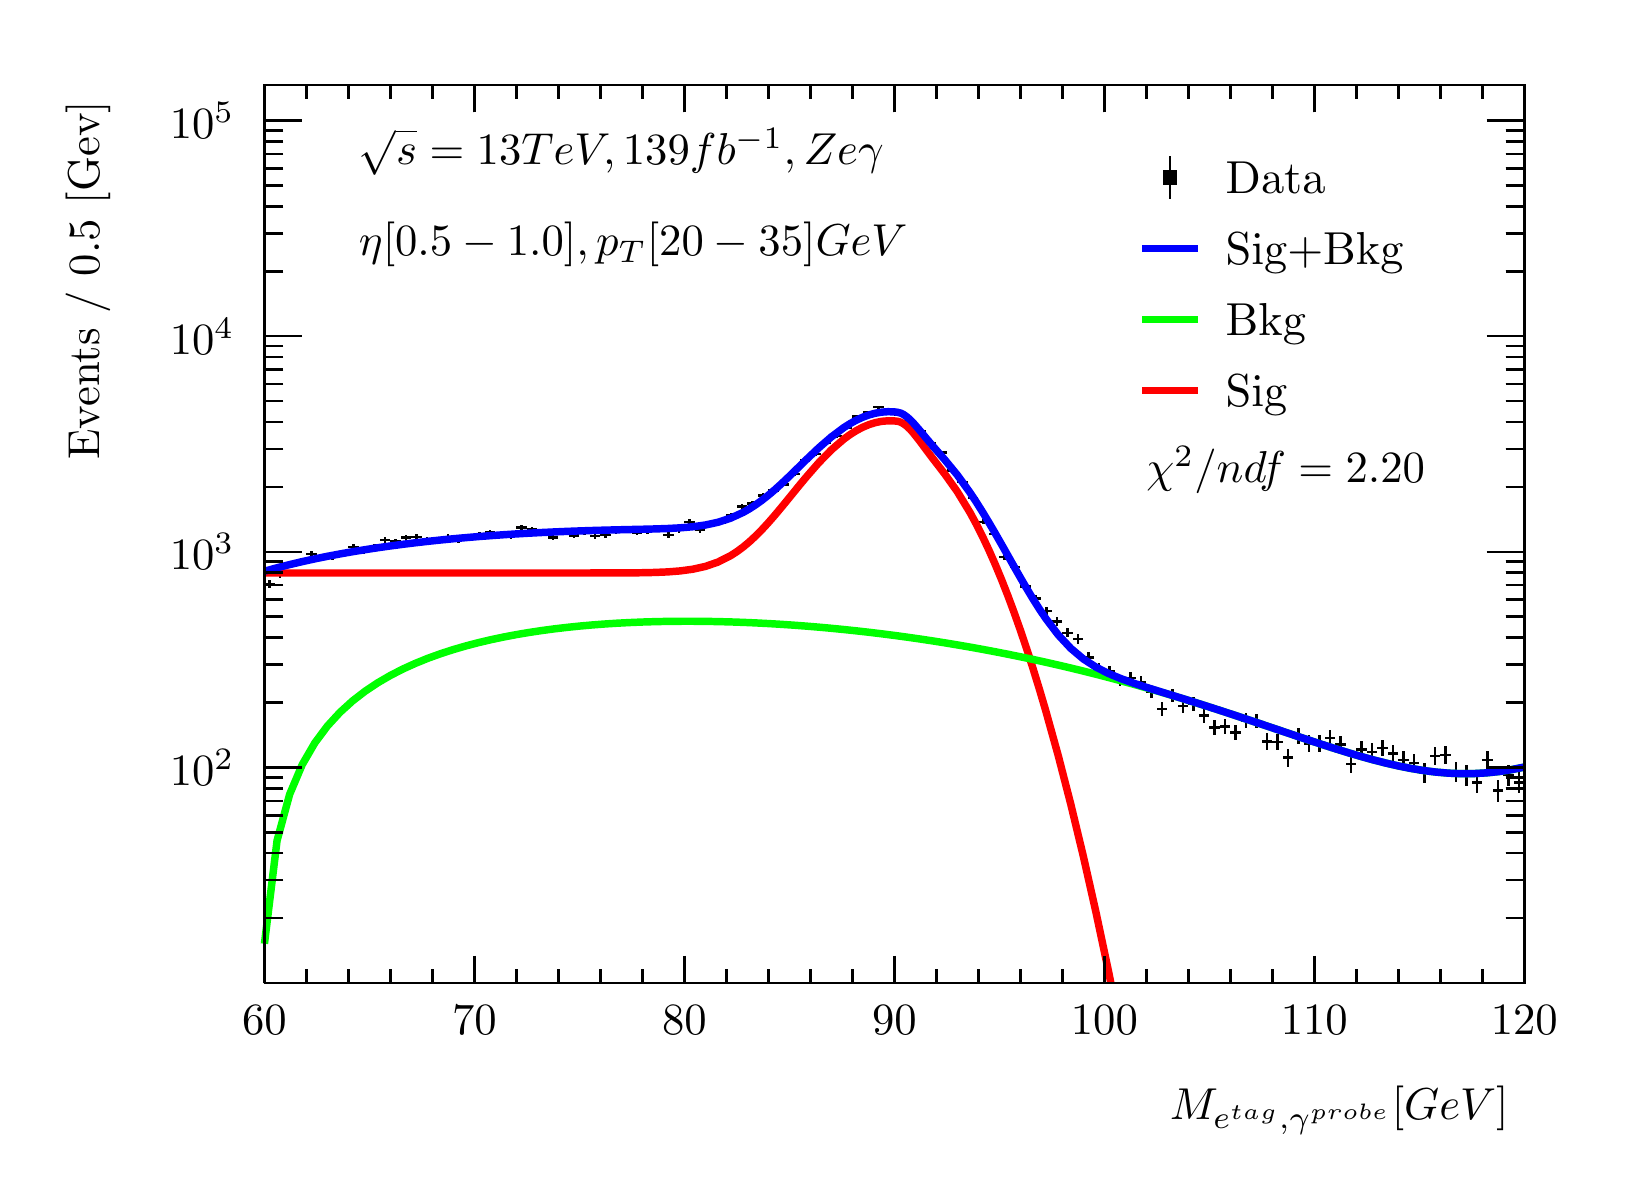
\begin{tikzpicture}
\pgfdeclareplotmark{cross} {
\pgfpathmoveto{\pgfpoint{-0.3\pgfplotmarksize}{\pgfplotmarksize}}
\pgfpathlineto{\pgfpoint{+0.3\pgfplotmarksize}{\pgfplotmarksize}}
\pgfpathlineto{\pgfpoint{+0.3\pgfplotmarksize}{0.3\pgfplotmarksize}}
\pgfpathlineto{\pgfpoint{+1\pgfplotmarksize}{0.3\pgfplotmarksize}}
\pgfpathlineto{\pgfpoint{+1\pgfplotmarksize}{-0.3\pgfplotmarksize}}
\pgfpathlineto{\pgfpoint{+0.3\pgfplotmarksize}{-0.3\pgfplotmarksize}}
\pgfpathlineto{\pgfpoint{+0.3\pgfplotmarksize}{-1.\pgfplotmarksize}}
\pgfpathlineto{\pgfpoint{-0.3\pgfplotmarksize}{-1.\pgfplotmarksize}}
\pgfpathlineto{\pgfpoint{-0.3\pgfplotmarksize}{-0.3\pgfplotmarksize}}
\pgfpathlineto{\pgfpoint{-1.\pgfplotmarksize}{-0.3\pgfplotmarksize}}
\pgfpathlineto{\pgfpoint{-1.\pgfplotmarksize}{0.3\pgfplotmarksize}}
\pgfpathlineto{\pgfpoint{-0.3\pgfplotmarksize}{0.3\pgfplotmarksize}}
\pgfpathclose
\pgfusepathqstroke
}
\pgfdeclareplotmark{cross*} {
\pgfpathmoveto{\pgfpoint{-0.3\pgfplotmarksize}{\pgfplotmarksize}}
\pgfpathlineto{\pgfpoint{+0.3\pgfplotmarksize}{\pgfplotmarksize}}
\pgfpathlineto{\pgfpoint{+0.3\pgfplotmarksize}{0.3\pgfplotmarksize}}
\pgfpathlineto{\pgfpoint{+1\pgfplotmarksize}{0.3\pgfplotmarksize}}
\pgfpathlineto{\pgfpoint{+1\pgfplotmarksize}{-0.3\pgfplotmarksize}}
\pgfpathlineto{\pgfpoint{+0.3\pgfplotmarksize}{-0.3\pgfplotmarksize}}
\pgfpathlineto{\pgfpoint{+0.3\pgfplotmarksize}{-1.\pgfplotmarksize}}
\pgfpathlineto{\pgfpoint{-0.3\pgfplotmarksize}{-1.\pgfplotmarksize}}
\pgfpathlineto{\pgfpoint{-0.3\pgfplotmarksize}{-0.3\pgfplotmarksize}}
\pgfpathlineto{\pgfpoint{-1.\pgfplotmarksize}{-0.3\pgfplotmarksize}}
\pgfpathlineto{\pgfpoint{-1.\pgfplotmarksize}{0.3\pgfplotmarksize}}
\pgfpathlineto{\pgfpoint{-0.3\pgfplotmarksize}{0.3\pgfplotmarksize}}
\pgfpathclose
\pgfusepathqfillstroke
}
\pgfdeclareplotmark{newstar} {
\pgfpathmoveto{\pgfqpoint{0pt}{\pgfplotmarksize}}
\pgfpathlineto{\pgfqpointpolar{44}{0.5\pgfplotmarksize}}
\pgfpathlineto{\pgfqpointpolar{18}{\pgfplotmarksize}}
\pgfpathlineto{\pgfqpointpolar{-20}{0.5\pgfplotmarksize}}
\pgfpathlineto{\pgfqpointpolar{-54}{\pgfplotmarksize}}
\pgfpathlineto{\pgfqpointpolar{-90}{0.5\pgfplotmarksize}}
\pgfpathlineto{\pgfqpointpolar{234}{\pgfplotmarksize}}
\pgfpathlineto{\pgfqpointpolar{198}{0.5\pgfplotmarksize}}
\pgfpathlineto{\pgfqpointpolar{162}{\pgfplotmarksize}}
\pgfpathlineto{\pgfqpointpolar{134}{0.5\pgfplotmarksize}}
\pgfpathclose
\pgfusepathqstroke
}
\pgfdeclareplotmark{newstar*} {
\pgfpathmoveto{\pgfqpoint{0pt}{\pgfplotmarksize}}
\pgfpathlineto{\pgfqpointpolar{44}{0.5\pgfplotmarksize}}
\pgfpathlineto{\pgfqpointpolar{18}{\pgfplotmarksize}}
\pgfpathlineto{\pgfqpointpolar{-20}{0.5\pgfplotmarksize}}
\pgfpathlineto{\pgfqpointpolar{-54}{\pgfplotmarksize}}
\pgfpathlineto{\pgfqpointpolar{-90}{0.5\pgfplotmarksize}}
\pgfpathlineto{\pgfqpointpolar{234}{\pgfplotmarksize}}
\pgfpathlineto{\pgfqpointpolar{198}{0.5\pgfplotmarksize}}
\pgfpathlineto{\pgfqpointpolar{162}{\pgfplotmarksize}}
\pgfpathlineto{\pgfqpointpolar{134}{0.5\pgfplotmarksize}}
\pgfpathclose
\pgfusepathqfillstroke
}
\definecolor{c}{rgb}{1,1,1};
\draw [color=c, fill=c] (0,0) rectangle (20,14.4361);
\draw [color=c, fill=c] (3,2.30977) rectangle (19,13.7143);
\definecolor{c}{rgb}{0,0,0};
\draw [c,line width=0.9] (3,2.30977) -- (3,13.7143) -- (19,13.7143) -- (19,2.30977) -- (3,2.30977);
\definecolor{c}{rgb}{1,1,1};
\draw [color=c, fill=c] (3,2.30977) rectangle (19,13.7143);
\definecolor{c}{rgb}{0,0,0};
\draw [c,line width=0.9] (3,2.30977) -- (3,13.7143) -- (19,13.7143) -- (19,2.30977) -- (3,2.30977);
\draw [c,line width=0.9] (3,2.30977) -- (19,2.30977);
\draw [c,line width=0.9] (3,2.65624) -- (3,2.30977);
\draw [c,line width=0.9] (3.53333,2.48301) -- (3.53333,2.30977);
\draw [c,line width=0.9] (4.06667,2.48301) -- (4.06667,2.30977);
\draw [c,line width=0.9] (4.6,2.48301) -- (4.6,2.30977);
\draw [c,line width=0.9] (5.13333,2.48301) -- (5.13333,2.30977);
\draw [c,line width=0.9] (5.66667,2.65624) -- (5.66667,2.30977);
\draw [c,line width=0.9] (6.2,2.48301) -- (6.2,2.30977);
\draw [c,line width=0.9] (6.73333,2.48301) -- (6.73333,2.30977);
\draw [c,line width=0.9] (7.26667,2.48301) -- (7.26667,2.30977);
\draw [c,line width=0.9] (7.8,2.48301) -- (7.8,2.30977);
\draw [c,line width=0.9] (8.33333,2.65624) -- (8.33333,2.30977);
\draw [c,line width=0.9] (8.86667,2.48301) -- (8.86667,2.30977);
\draw [c,line width=0.9] (9.4,2.48301) -- (9.4,2.30977);
\draw [c,line width=0.9] (9.93333,2.48301) -- (9.93333,2.30977);
\draw [c,line width=0.9] (10.4667,2.48301) -- (10.4667,2.30977);
\draw [c,line width=0.9] (11,2.65624) -- (11,2.30977);
\draw [c,line width=0.9] (11.5333,2.48301) -- (11.5333,2.30977);
\draw [c,line width=0.9] (12.0667,2.48301) -- (12.0667,2.30977);
\draw [c,line width=0.9] (12.6,2.48301) -- (12.6,2.30977);
\draw [c,line width=0.9] (13.1333,2.48301) -- (13.1333,2.30977);
\draw [c,line width=0.9] (13.6667,2.65624) -- (13.6667,2.30977);
\draw [c,line width=0.9] (14.2,2.48301) -- (14.2,2.30977);
\draw [c,line width=0.9] (14.7333,2.48301) -- (14.7333,2.30977);
\draw [c,line width=0.9] (15.2667,2.48301) -- (15.2667,2.30977);
\draw [c,line width=0.9] (15.8,2.48301) -- (15.8,2.30977);
\draw [c,line width=0.9] (16.3333,2.65624) -- (16.3333,2.30977);
\draw [c,line width=0.9] (16.8667,2.48301) -- (16.8667,2.30977);
\draw [c,line width=0.9] (17.4,2.48301) -- (17.4,2.30977);
\draw [c,line width=0.9] (17.9333,2.48301) -- (17.9333,2.30977);
\draw [c,line width=0.9] (18.4667,2.48301) -- (18.4667,2.30977);
\draw [c,line width=0.9] (19,2.65624) -- (19,2.30977);
\draw [anchor=base] (3,1.66015) node[scale=1.61424, color=c, rotate=0]{60};
\draw [anchor=base] (5.66667,1.66015) node[scale=1.61424, color=c, rotate=0]{70};
\draw [anchor=base] (8.33333,1.66015) node[scale=1.61424, color=c, rotate=0]{80};
\draw [anchor=base] (11,1.66015) node[scale=1.61424, color=c, rotate=0]{90};
\draw [anchor=base] (13.6667,1.66015) node[scale=1.61424, color=c, rotate=0]{100};
\draw [anchor=base] (16.3333,1.66015) node[scale=1.61424, color=c, rotate=0]{110};
\draw [anchor=base] (19,1.66015) node[scale=1.61424, color=c, rotate=0]{120};
\draw [anchor= east] (19,0.692932) node[scale=1.61424, color=c, rotate=0]{$M_{e^{tag}, \gamma^{probe}}  [GeV]$};
\draw [c,line width=0.9] (3,13.7143) -- (19,13.7143);
\draw [c,line width=0.9] (3,13.3678) -- (3,13.7143);
\draw [c,line width=0.9] (3.53333,13.5411) -- (3.53333,13.7143);
\draw [c,line width=0.9] (4.06667,13.5411) -- (4.06667,13.7143);
\draw [c,line width=0.9] (4.6,13.5411) -- (4.6,13.7143);
\draw [c,line width=0.9] (5.13333,13.5411) -- (5.13333,13.7143);
\draw [c,line width=0.9] (5.66667,13.3678) -- (5.66667,13.7143);
\draw [c,line width=0.9] (6.2,13.5411) -- (6.2,13.7143);
\draw [c,line width=0.9] (6.73333,13.5411) -- (6.73333,13.7143);
\draw [c,line width=0.9] (7.26667,13.5411) -- (7.26667,13.7143);
\draw [c,line width=0.9] (7.8,13.5411) -- (7.8,13.7143);
\draw [c,line width=0.9] (8.33333,13.3678) -- (8.33333,13.7143);
\draw [c,line width=0.9] (8.86667,13.5411) -- (8.86667,13.7143);
\draw [c,line width=0.9] (9.4,13.5411) -- (9.4,13.7143);
\draw [c,line width=0.9] (9.93333,13.5411) -- (9.93333,13.7143);
\draw [c,line width=0.9] (10.4667,13.5411) -- (10.4667,13.7143);
\draw [c,line width=0.9] (11,13.3678) -- (11,13.7143);
\draw [c,line width=0.9] (11.5333,13.5411) -- (11.5333,13.7143);
\draw [c,line width=0.9] (12.0667,13.5411) -- (12.0667,13.7143);
\draw [c,line width=0.9] (12.6,13.5411) -- (12.6,13.7143);
\draw [c,line width=0.9] (13.1333,13.5411) -- (13.1333,13.7143);
\draw [c,line width=0.9] (13.6667,13.3678) -- (13.6667,13.7143);
\draw [c,line width=0.9] (14.2,13.5411) -- (14.2,13.7143);
\draw [c,line width=0.9] (14.7333,13.5411) -- (14.7333,13.7143);
\draw [c,line width=0.9] (15.2667,13.5411) -- (15.2667,13.7143);
\draw [c,line width=0.9] (15.8,13.5411) -- (15.8,13.7143);
\draw [c,line width=0.9] (16.3333,13.3678) -- (16.3333,13.7143);
\draw [c,line width=0.9] (16.8667,13.5411) -- (16.8667,13.7143);
\draw [c,line width=0.9] (17.4,13.5411) -- (17.4,13.7143);
\draw [c,line width=0.9] (17.9333,13.5411) -- (17.9333,13.7143);
\draw [c,line width=0.9] (18.4667,13.5411) -- (18.4667,13.7143);
\draw [c,line width=0.9] (19,13.3678) -- (19,13.7143);
\draw [c,line width=0.9] (3,2.30977) -- (3,13.7143);
\draw [c,line width=0.9] (3.237,3.13412) -- (3,3.13412);
\draw [c,line width=0.9] (3.237,3.61633) -- (3,3.61633);
\draw [c,line width=0.9] (3.237,3.95847) -- (3,3.95847);
\draw [c,line width=0.9] (3.237,4.22385) -- (3,4.22385);
\draw [c,line width=0.9] (3.237,4.44068) -- (3,4.44068);
\draw [c,line width=0.9] (3.237,4.62401) -- (3,4.62401);
\draw [c,line width=0.9] (3.237,4.78282) -- (3,4.78282);
\draw [c,line width=0.9] (3.237,4.9229) -- (3,4.9229);
\draw [c,line width=0.9] (3.474,5.0482) -- (3,5.0482);
\draw [anchor= east] (2.82,5.0482) node[scale=1.61424, color=c, rotate=0]{$10^{2}$};
\draw [c,line width=0.9] (3.237,5.87255) -- (3,5.87255);
\draw [c,line width=0.9] (3.237,6.35476) -- (3,6.35476);
\draw [c,line width=0.9] (3.237,6.6969) -- (3,6.6969);
\draw [c,line width=0.9] (3.237,6.96228) -- (3,6.96228);
\draw [c,line width=0.9] (3.237,7.17911) -- (3,7.17911);
\draw [c,line width=0.9] (3.237,7.36244) -- (3,7.36244);
\draw [c,line width=0.9] (3.237,7.52125) -- (3,7.52125);
\draw [c,line width=0.9] (3.237,7.66133) -- (3,7.66133);
\draw [c,line width=0.9] (3.474,7.78663) -- (3,7.78663);
\draw [anchor= east] (2.82,7.78663) node[scale=1.61424, color=c, rotate=0]{$10^{3}$};
\draw [c,line width=0.9] (3.237,8.61098) -- (3,8.61098);
\draw [c,line width=0.9] (3.237,9.09319) -- (3,9.09319);
\draw [c,line width=0.9] (3.237,9.43533) -- (3,9.43533);
\draw [c,line width=0.9] (3.237,9.70071) -- (3,9.70071);
\draw [c,line width=0.9] (3.237,9.91755) -- (3,9.91755);
\draw [c,line width=0.9] (3.237,10.1009) -- (3,10.1009);
\draw [c,line width=0.9] (3.237,10.2597) -- (3,10.2597);
\draw [c,line width=0.9] (3.237,10.3998) -- (3,10.3998);
\draw [c,line width=0.9] (3.474,10.5251) -- (3,10.5251);
\draw [anchor= east] (2.82,10.5251) node[scale=1.61424, color=c, rotate=0]{$10^{4}$};
\draw [c,line width=0.9] (3.237,11.3494) -- (3,11.3494);
\draw [c,line width=0.9] (3.237,11.8316) -- (3,11.8316);
\draw [c,line width=0.9] (3.237,12.1738) -- (3,12.1738);
\draw [c,line width=0.9] (3.237,12.4391) -- (3,12.4391);
\draw [c,line width=0.9] (3.237,12.656) -- (3,12.656);
\draw [c,line width=0.9] (3.237,12.8393) -- (3,12.8393);
\draw [c,line width=0.9] (3.237,12.9981) -- (3,12.9981);
\draw [c,line width=0.9] (3.237,13.1382) -- (3,13.1382);
\draw [c,line width=0.9] (3.474,13.2635) -- (3,13.2635);
\draw [anchor= east] (2.82,13.2635) node[scale=1.61424, color=c, rotate=0]{$10^{5}$};
\draw [anchor= east] (0.76,13.7143) node[scale=1.61424, color=c, rotate=90]{Events / 0.5 [Gev]};
\draw [c,line width=0.9] (19,2.30977) -- (19,13.7143);
\draw [c,line width=0.9] (18.763,3.13412) -- (19,3.13412);
\draw [c,line width=0.9] (18.763,3.61633) -- (19,3.61633);
\draw [c,line width=0.9] (18.763,3.95847) -- (19,3.95847);
\draw [c,line width=0.9] (18.763,4.22385) -- (19,4.22385);
\draw [c,line width=0.9] (18.763,4.44068) -- (19,4.44068);
\draw [c,line width=0.9] (18.763,4.62401) -- (19,4.62401);
\draw [c,line width=0.9] (18.763,4.78282) -- (19,4.78282);
\draw [c,line width=0.9] (18.763,4.9229) -- (19,4.9229);
\draw [c,line width=0.9] (18.526,5.0482) -- (19,5.0482);
\draw [c,line width=0.9] (18.763,5.87255) -- (19,5.87255);
\draw [c,line width=0.9] (18.763,6.35476) -- (19,6.35476);
\draw [c,line width=0.9] (18.763,6.6969) -- (19,6.6969);
\draw [c,line width=0.9] (18.763,6.96228) -- (19,6.96228);
\draw [c,line width=0.9] (18.763,7.17911) -- (19,7.17911);
\draw [c,line width=0.9] (18.763,7.36244) -- (19,7.36244);
\draw [c,line width=0.9] (18.763,7.52125) -- (19,7.52125);
\draw [c,line width=0.9] (18.763,7.66133) -- (19,7.66133);
\draw [c,line width=0.9] (18.526,7.78663) -- (19,7.78663);
\draw [c,line width=0.9] (18.763,8.61098) -- (19,8.61098);
\draw [c,line width=0.9] (18.763,9.09319) -- (19,9.09319);
\draw [c,line width=0.9] (18.763,9.43533) -- (19,9.43533);
\draw [c,line width=0.9] (18.763,9.70071) -- (19,9.70071);
\draw [c,line width=0.9] (18.763,9.91755) -- (19,9.91755);
\draw [c,line width=0.9] (18.763,10.1009) -- (19,10.1009);
\draw [c,line width=0.9] (18.763,10.2597) -- (19,10.2597);
\draw [c,line width=0.9] (18.763,10.3998) -- (19,10.3998);
\draw [c,line width=0.9] (18.526,10.5251) -- (19,10.5251);
\draw [c,line width=0.9] (18.763,11.3494) -- (19,11.3494);
\draw [c,line width=0.9] (18.763,11.8316) -- (19,11.8316);
\draw [c,line width=0.9] (18.763,12.1738) -- (19,12.1738);
\draw [c,line width=0.9] (18.763,12.4391) -- (19,12.4391);
\draw [c,line width=0.9] (18.763,12.656) -- (19,12.656);
\draw [c,line width=0.9] (18.763,12.8393) -- (19,12.8393);
\draw [c,line width=0.9] (18.763,12.9981) -- (19,12.9981);
\draw [c,line width=0.9] (18.763,13.1382) -- (19,13.1382);
\draw [c,line width=0.9] (18.526,13.2635) -- (19,13.2635);
\draw [c,line width=0.9] (3.06667,7.37764) -- (3,7.37764);
\draw [c,line width=0.9] (3,7.37764) -- (3,7.37764);
\draw [c,line width=0.9] (3.06667,7.37764) -- (3.13333,7.37764);
\draw [c,line width=0.9] (3.13333,7.37764) -- (3.13333,7.37764);
\draw [c,line width=0.9] (3.06667,7.37764) -- (3.06667,7.4223);
\draw [c,line width=0.9] (3.06667,7.4223) -- (3.06667,7.4223);
\draw [c,line width=0.9] (3.06667,7.37764) -- (3.06667,7.33298);
\draw [c,line width=0.9] (3.06667,7.33298) -- (3.06667,7.33298);
\draw [c,line width=0.9] (3.2,7.49723) -- (3.13333,7.49723);
\draw [c,line width=0.9] (3.13333,7.49723) -- (3.13333,7.49723);
\draw [c,line width=0.9] (3.2,7.49723) -- (3.26667,7.49723);
\draw [c,line width=0.9] (3.26667,7.49723) -- (3.26667,7.49723);
\draw [c,line width=0.9] (3.2,7.49723) -- (3.2,7.5397);
\draw [c,line width=0.9] (3.2,7.5397) -- (3.2,7.5397);
\draw [c,line width=0.9] (3.2,7.49723) -- (3.2,7.45475);
\draw [c,line width=0.9] (3.2,7.45475) -- (3.2,7.45475);
\draw [c,line width=0.9] (3.33333,7.63054) -- (3.26667,7.63054);
\draw [c,line width=0.9] (3.26667,7.63054) -- (3.26667,7.63054);
\draw [c,line width=0.9] (3.33333,7.63054) -- (3.4,7.63054);
\draw [c,line width=0.9] (3.4,7.63054) -- (3.4,7.63054);
\draw [c,line width=0.9] (3.33333,7.63054) -- (3.33333,7.6707);
\draw [c,line width=0.9] (3.33333,7.6707) -- (3.33333,7.6707);
\draw [c,line width=0.9] (3.33333,7.63054) -- (3.33333,7.59038);
\draw [c,line width=0.9] (3.33333,7.59038) -- (3.33333,7.59038);
\draw [c,line width=0.9] (3.46667,7.67054) -- (3.4,7.67054);
\draw [c,line width=0.9] (3.4,7.67054) -- (3.4,7.67054);
\draw [c,line width=0.9] (3.46667,7.67054) -- (3.53333,7.67054);
\draw [c,line width=0.9] (3.53333,7.67054) -- (3.53333,7.67054);
\draw [c,line width=0.9] (3.46667,7.67054) -- (3.46667,7.71003);
\draw [c,line width=0.9] (3.46667,7.71003) -- (3.46667,7.71003);
\draw [c,line width=0.9] (3.46667,7.67054) -- (3.46667,7.63106);
\draw [c,line width=0.9] (3.46667,7.63106) -- (3.46667,7.63106);
\draw [c,line width=0.9] (3.6,7.75774) -- (3.53333,7.75774);
\draw [c,line width=0.9] (3.53333,7.75774) -- (3.53333,7.75774);
\draw [c,line width=0.9] (3.6,7.75774) -- (3.66667,7.75774);
\draw [c,line width=0.9] (3.66667,7.75774) -- (3.66667,7.75774);
\draw [c,line width=0.9] (3.6,7.75774) -- (3.6,7.79581);
\draw [c,line width=0.9] (3.6,7.79581) -- (3.6,7.79581);
\draw [c,line width=0.9] (3.6,7.75774) -- (3.6,7.71968);
\draw [c,line width=0.9] (3.6,7.71968) -- (3.6,7.71968);
\draw [c,line width=0.9] (3.73333,7.70924) -- (3.66667,7.70924);
\draw [c,line width=0.9] (3.66667,7.70924) -- (3.66667,7.70924);
\draw [c,line width=0.9] (3.73333,7.70924) -- (3.8,7.70924);
\draw [c,line width=0.9] (3.8,7.70924) -- (3.8,7.70924);
\draw [c,line width=0.9] (3.73333,7.70924) -- (3.73333,7.7481);
\draw [c,line width=0.9] (3.73333,7.7481) -- (3.73333,7.7481);
\draw [c,line width=0.9] (3.73333,7.70924) -- (3.73333,7.67039);
\draw [c,line width=0.9] (3.73333,7.67039) -- (3.73333,7.67039);
\draw [c,line width=0.9] (3.86667,7.72312) -- (3.8,7.72312);
\draw [c,line width=0.9] (3.8,7.72312) -- (3.8,7.72312);
\draw [c,line width=0.9] (3.86667,7.72312) -- (3.93333,7.72312);
\draw [c,line width=0.9] (3.93333,7.72312) -- (3.93333,7.72312);
\draw [c,line width=0.9] (3.86667,7.72312) -- (3.86667,7.76175);
\draw [c,line width=0.9] (3.86667,7.76175) -- (3.86667,7.76175);
\draw [c,line width=0.9] (3.86667,7.72312) -- (3.86667,7.6845);
\draw [c,line width=0.9] (3.86667,7.6845) -- (3.86667,7.6845);
\draw [c,line width=0.9] (4,7.76503) -- (3.93333,7.76503);
\draw [c,line width=0.9] (3.93333,7.76503) -- (3.93333,7.76503);
\draw [c,line width=0.9] (4,7.76503) -- (4.06667,7.76503);
\draw [c,line width=0.9] (4.06667,7.76503) -- (4.06667,7.76503);
\draw [c,line width=0.9] (4,7.76503) -- (4,7.80298);
\draw [c,line width=0.9] (4,7.80298) -- (4,7.80298);
\draw [c,line width=0.9] (4,7.76503) -- (4,7.72708);
\draw [c,line width=0.9] (4,7.72708) -- (4,7.72708);
\draw [c,line width=0.9] (4.13333,7.84805) -- (4.06667,7.84805);
\draw [c,line width=0.9] (4.06667,7.84805) -- (4.06667,7.84805);
\draw [c,line width=0.9] (4.13333,7.84805) -- (4.2,7.84805);
\draw [c,line width=0.9] (4.2,7.84805) -- (4.2,7.84805);
\draw [c,line width=0.9] (4.13333,7.84805) -- (4.13333,7.8847);
\draw [c,line width=0.9] (4.13333,7.8847) -- (4.13333,7.8847);
\draw [c,line width=0.9] (4.13333,7.84805) -- (4.13333,7.8114);
\draw [c,line width=0.9] (4.13333,7.8114) -- (4.13333,7.8114);
\draw [c,line width=0.9] (4.26667,7.79375) -- (4.2,7.79375);
\draw [c,line width=0.9] (4.2,7.79375) -- (4.2,7.79375);
\draw [c,line width=0.9] (4.26667,7.79375) -- (4.33333,7.79375);
\draw [c,line width=0.9] (4.33333,7.79375) -- (4.33333,7.79375);
\draw [c,line width=0.9] (4.26667,7.79375) -- (4.26667,7.83124);
\draw [c,line width=0.9] (4.26667,7.83124) -- (4.26667,7.83124);
\draw [c,line width=0.9] (4.26667,7.79375) -- (4.26667,7.75625);
\draw [c,line width=0.9] (4.26667,7.75625) -- (4.26667,7.75625);
\draw [c,line width=0.9] (4.4,7.85031) -- (4.33333,7.85031);
\draw [c,line width=0.9] (4.33333,7.85031) -- (4.33333,7.85031);
\draw [c,line width=0.9] (4.4,7.85031) -- (4.46667,7.85031);
\draw [c,line width=0.9] (4.46667,7.85031) -- (4.46667,7.85031);
\draw [c,line width=0.9] (4.4,7.85031) -- (4.4,7.88692);
\draw [c,line width=0.9] (4.4,7.88692) -- (4.4,7.88692);
\draw [c,line width=0.9] (4.4,7.85031) -- (4.4,7.81369);
\draw [c,line width=0.9] (4.4,7.81369) -- (4.4,7.81369);
\draw [c,line width=0.9] (4.53333,7.93409) -- (4.46667,7.93409);
\draw [c,line width=0.9] (4.46667,7.93409) -- (4.46667,7.93409);
\draw [c,line width=0.9] (4.53333,7.93409) -- (4.6,7.93409);
\draw [c,line width=0.9] (4.6,7.93409) -- (4.6,7.93409);
\draw [c,line width=0.9] (4.53333,7.93409) -- (4.53333,7.96943);
\draw [c,line width=0.9] (4.53333,7.96943) -- (4.53333,7.96943);
\draw [c,line width=0.9] (4.53333,7.93409) -- (4.53333,7.89874);
\draw [c,line width=0.9] (4.53333,7.89874) -- (4.53333,7.89874);
\draw [c,line width=0.9] (4.66667,7.91503) -- (4.6,7.91503);
\draw [c,line width=0.9] (4.6,7.91503) -- (4.6,7.91503);
\draw [c,line width=0.9] (4.66667,7.91503) -- (4.73333,7.91503);
\draw [c,line width=0.9] (4.73333,7.91503) -- (4.73333,7.91503);
\draw [c,line width=0.9] (4.66667,7.91503) -- (4.66667,7.95066);
\draw [c,line width=0.9] (4.66667,7.95066) -- (4.66667,7.95066);
\draw [c,line width=0.9] (4.66667,7.91503) -- (4.66667,7.87939);
\draw [c,line width=0.9] (4.66667,7.87939) -- (4.66667,7.87939);
\draw [c,line width=0.9] (4.8,7.9652) -- (4.73333,7.9652);
\draw [c,line width=0.9] (4.73333,7.9652) -- (4.73333,7.9652);
\draw [c,line width=0.9] (4.8,7.9652) -- (4.86667,7.9652);
\draw [c,line width=0.9] (4.86667,7.9652) -- (4.86667,7.9652);
\draw [c,line width=0.9] (4.8,7.9652) -- (4.8,8.00008);
\draw [c,line width=0.9] (4.8,8.00008) -- (4.8,8.00008);
\draw [c,line width=0.9] (4.8,7.9652) -- (4.8,7.93031);
\draw [c,line width=0.9] (4.8,7.93031) -- (4.8,7.93031);
\draw [c,line width=0.9] (4.93333,7.97437) -- (4.86667,7.97437);
\draw [c,line width=0.9] (4.86667,7.97437) -- (4.86667,7.97437);
\draw [c,line width=0.9] (4.93333,7.97437) -- (5,7.97437);
\draw [c,line width=0.9] (5,7.97437) -- (5,7.97437);
\draw [c,line width=0.9] (4.93333,7.97437) -- (4.93333,8.00912);
\draw [c,line width=0.9] (4.93333,8.00912) -- (4.93333,8.00912);
\draw [c,line width=0.9] (4.93333,7.97437) -- (4.93333,7.93962);
\draw [c,line width=0.9] (4.93333,7.93962) -- (4.93333,7.93962);
\draw [c,line width=0.9] (5.06667,7.94351) -- (5,7.94351);
\draw [c,line width=0.9] (5,7.94351) -- (5,7.94351);
\draw [c,line width=0.9] (5.06667,7.94351) -- (5.13333,7.94351);
\draw [c,line width=0.9] (5.13333,7.94351) -- (5.13333,7.94351);
\draw [c,line width=0.9] (5.06667,7.94351) -- (5.06667,7.97871);
\draw [c,line width=0.9] (5.06667,7.97871) -- (5.06667,7.97871);
\draw [c,line width=0.9] (5.06667,7.94351) -- (5.06667,7.9083);
\draw [c,line width=0.9] (5.06667,7.9083) -- (5.06667,7.9083);
\draw [c,line width=0.9] (5.2,7.93409) -- (5.13333,7.93409);
\draw [c,line width=0.9] (5.13333,7.93409) -- (5.13333,7.93409);
\draw [c,line width=0.9] (5.2,7.93409) -- (5.26667,7.93409);
\draw [c,line width=0.9] (5.26667,7.93409) -- (5.26667,7.93409);
\draw [c,line width=0.9] (5.2,7.93409) -- (5.2,7.96943);
\draw [c,line width=0.9] (5.2,7.96943) -- (5.2,7.96943);
\draw [c,line width=0.9] (5.2,7.93409) -- (5.2,7.89874);
\draw [c,line width=0.9] (5.2,7.89874) -- (5.2,7.89874);
\draw [c,line width=0.9] (5.33333,7.97336) -- (5.26667,7.97336);
\draw [c,line width=0.9] (5.26667,7.97336) -- (5.26667,7.97336);
\draw [c,line width=0.9] (5.33333,7.97336) -- (5.4,7.97336);
\draw [c,line width=0.9] (5.4,7.97336) -- (5.4,7.97336);
\draw [c,line width=0.9] (5.33333,7.97336) -- (5.33333,8.00812);
\draw [c,line width=0.9] (5.33333,8.00812) -- (5.33333,8.00812);
\draw [c,line width=0.9] (5.33333,7.97336) -- (5.33333,7.93859);
\draw [c,line width=0.9] (5.33333,7.93859) -- (5.33333,7.93859);
\draw [c,line width=0.9] (5.46667,7.93619) -- (5.4,7.93619);
\draw [c,line width=0.9] (5.4,7.93619) -- (5.4,7.93619);
\draw [c,line width=0.9] (5.46667,7.93619) -- (5.53333,7.93619);
\draw [c,line width=0.9] (5.53333,7.93619) -- (5.53333,7.93619);
\draw [c,line width=0.9] (5.46667,7.93619) -- (5.46667,7.9715);
\draw [c,line width=0.9] (5.46667,7.9715) -- (5.46667,7.9715);
\draw [c,line width=0.9] (5.46667,7.93619) -- (5.46667,7.90087);
\draw [c,line width=0.9] (5.46667,7.90087) -- (5.46667,7.90087);
\draw [c,line width=0.9] (5.6,7.95285) -- (5.53333,7.95285);
\draw [c,line width=0.9] (5.53333,7.95285) -- (5.53333,7.95285);
\draw [c,line width=0.9] (5.6,7.95285) -- (5.66667,7.95285);
\draw [c,line width=0.9] (5.66667,7.95285) -- (5.66667,7.95285);
\draw [c,line width=0.9] (5.6,7.95285) -- (5.6,7.98792);
\draw [c,line width=0.9] (5.6,7.98792) -- (5.6,7.98792);
\draw [c,line width=0.9] (5.6,7.95285) -- (5.6,7.91778);
\draw [c,line width=0.9] (5.6,7.91778) -- (5.6,7.91778);
\draw [c,line width=0.9] (5.73333,8.0094) -- (5.66667,8.0094);
\draw [c,line width=0.9] (5.66667,8.0094) -- (5.66667,8.0094);
\draw [c,line width=0.9] (5.73333,8.0094) -- (5.8,8.0094);
\draw [c,line width=0.9] (5.8,8.0094) -- (5.8,8.0094);
\draw [c,line width=0.9] (5.73333,8.0094) -- (5.73333,8.04364);
\draw [c,line width=0.9] (5.73333,8.04364) -- (5.73333,8.04364);
\draw [c,line width=0.9] (5.73333,8.0094) -- (5.73333,7.97515);
\draw [c,line width=0.9] (5.73333,7.97515) -- (5.73333,7.97515);
\draw [c,line width=0.9] (5.86667,8.03283) -- (5.8,8.03283);
\draw [c,line width=0.9] (5.8,8.03283) -- (5.8,8.03283);
\draw [c,line width=0.9] (5.86667,8.03283) -- (5.93333,8.03283);
\draw [c,line width=0.9] (5.93333,8.03283) -- (5.93333,8.03283);
\draw [c,line width=0.9] (5.86667,8.03283) -- (5.86667,8.06674);
\draw [c,line width=0.9] (5.86667,8.06674) -- (5.86667,8.06674);
\draw [c,line width=0.9] (5.86667,8.03283) -- (5.86667,7.99892);
\draw [c,line width=0.9] (5.86667,7.99892) -- (5.86667,7.99892);
\draw [c,line width=0.9] (6,7.9975) -- (5.93333,7.9975);
\draw [c,line width=0.9] (5.93333,7.9975) -- (5.93333,7.9975);
\draw [c,line width=0.9] (6,7.9975) -- (6.06667,7.9975);
\draw [c,line width=0.9] (6.06667,7.9975) -- (6.06667,7.9975);
\draw [c,line width=0.9] (6,7.9975) -- (6,8.03192);
\draw [c,line width=0.9] (6,8.03192) -- (6,8.03192);
\draw [c,line width=0.9] (6,7.9975) -- (6,7.96309);
\draw [c,line width=0.9] (6,7.96309) -- (6,7.96309);
\draw [c,line width=0.9] (6.13333,7.98951) -- (6.06667,7.98951);
\draw [c,line width=0.9] (6.06667,7.98951) -- (6.06667,7.98951);
\draw [c,line width=0.9] (6.13333,7.98951) -- (6.2,7.98951);
\draw [c,line width=0.9] (6.2,7.98951) -- (6.2,7.98951);
\draw [c,line width=0.9] (6.13333,7.98951) -- (6.13333,8.02404);
\draw [c,line width=0.9] (6.13333,8.02404) -- (6.13333,8.02404);
\draw [c,line width=0.9] (6.13333,7.98951) -- (6.13333,7.95498);
\draw [c,line width=0.9] (6.13333,7.95498) -- (6.13333,7.95498);
\draw [c,line width=0.9] (6.26667,8.09224) -- (6.2,8.09224);
\draw [c,line width=0.9] (6.2,8.09224) -- (6.2,8.09224);
\draw [c,line width=0.9] (6.26667,8.09224) -- (6.33333,8.09224);
\draw [c,line width=0.9] (6.33333,8.09224) -- (6.33333,8.09224);
\draw [c,line width=0.9] (6.26667,8.09224) -- (6.26667,8.12531);
\draw [c,line width=0.9] (6.26667,8.12531) -- (6.26667,8.12531);
\draw [c,line width=0.9] (6.26667,8.09224) -- (6.26667,8.05917);
\draw [c,line width=0.9] (6.26667,8.05917) -- (6.26667,8.05917);
\draw [c,line width=0.9] (6.4,8.06714) -- (6.33333,8.06714);
\draw [c,line width=0.9] (6.33333,8.06714) -- (6.33333,8.06714);
\draw [c,line width=0.9] (6.4,8.06714) -- (6.46667,8.06714);
\draw [c,line width=0.9] (6.46667,8.06714) -- (6.46667,8.06714);
\draw [c,line width=0.9] (6.4,8.06714) -- (6.4,8.10056);
\draw [c,line width=0.9] (6.4,8.10056) -- (6.4,8.10056);
\draw [c,line width=0.9] (6.4,8.06714) -- (6.4,8.03372);
\draw [c,line width=0.9] (6.4,8.03372) -- (6.4,8.03372);
\draw [c,line width=0.9] (6.53333,8.03476) -- (6.46667,8.03476);
\draw [c,line width=0.9] (6.46667,8.03476) -- (6.46667,8.03476);
\draw [c,line width=0.9] (6.53333,8.03476) -- (6.6,8.03476);
\draw [c,line width=0.9] (6.6,8.03476) -- (6.6,8.03476);
\draw [c,line width=0.9] (6.53333,8.03476) -- (6.53333,8.06865);
\draw [c,line width=0.9] (6.53333,8.06865) -- (6.53333,8.06865);
\draw [c,line width=0.9] (6.53333,8.03476) -- (6.53333,8.00088);
\draw [c,line width=0.9] (6.53333,8.00088) -- (6.53333,8.00088);
\draw [c,line width=0.9] (6.66667,7.9703) -- (6.6,7.9703);
\draw [c,line width=0.9] (6.6,7.9703) -- (6.6,7.9703);
\draw [c,line width=0.9] (6.66667,7.9703) -- (6.73333,7.9703);
\draw [c,line width=0.9] (6.73333,7.9703) -- (6.73333,7.9703);
\draw [c,line width=0.9] (6.66667,7.9703) -- (6.66667,8.00511);
\draw [c,line width=0.9] (6.66667,8.00511) -- (6.66667,8.00511);
\draw [c,line width=0.9] (6.66667,7.9703) -- (6.66667,7.93549);
\draw [c,line width=0.9] (6.66667,7.93549) -- (6.66667,7.93549);
\draw [c,line width=0.9] (6.8,8.03573) -- (6.73333,8.03573);
\draw [c,line width=0.9] (6.73333,8.03573) -- (6.73333,8.03573);
\draw [c,line width=0.9] (6.8,8.03573) -- (6.86667,8.03573);
\draw [c,line width=0.9] (6.86667,8.03573) -- (6.86667,8.03573);
\draw [c,line width=0.9] (6.8,8.03573) -- (6.8,8.0696);
\draw [c,line width=0.9] (6.8,8.0696) -- (6.8,8.0696);
\draw [c,line width=0.9] (6.8,8.03573) -- (6.8,8.00186);
\draw [c,line width=0.9] (6.8,8.00186) -- (6.8,8.00186);
\draw [c,line width=0.9] (6.93333,7.99251) -- (6.86667,7.99251);
\draw [c,line width=0.9] (6.86667,7.99251) -- (6.86667,7.99251);
\draw [c,line width=0.9] (6.93333,7.99251) -- (7,7.99251);
\draw [c,line width=0.9] (7,7.99251) -- (7,7.99251);
\draw [c,line width=0.9] (6.93333,7.99251) -- (6.93333,8.027);
\draw [c,line width=0.9] (6.93333,8.027) -- (6.93333,8.027);
\draw [c,line width=0.9] (6.93333,7.99251) -- (6.93333,7.95802);
\draw [c,line width=0.9] (6.93333,7.95802) -- (6.93333,7.95802);
\draw [c,line width=0.9] (7.06667,8.03283) -- (7,8.03283);
\draw [c,line width=0.9] (7,8.03283) -- (7,8.03283);
\draw [c,line width=0.9] (7.06667,8.03283) -- (7.13333,8.03283);
\draw [c,line width=0.9] (7.13333,8.03283) -- (7.13333,8.03283);
\draw [c,line width=0.9] (7.06667,8.03283) -- (7.06667,8.06674);
\draw [c,line width=0.9] (7.06667,8.06674) -- (7.06667,8.06674);
\draw [c,line width=0.9] (7.06667,8.03283) -- (7.06667,7.99892);
\draw [c,line width=0.9] (7.06667,7.99892) -- (7.06667,7.99892);
\draw [c,line width=0.9] (7.2,7.98951) -- (7.13333,7.98951);
\draw [c,line width=0.9] (7.13333,7.98951) -- (7.13333,7.98951);
\draw [c,line width=0.9] (7.2,7.98951) -- (7.26667,7.98951);
\draw [c,line width=0.9] (7.26667,7.98951) -- (7.26667,7.98951);
\draw [c,line width=0.9] (7.2,7.98951) -- (7.2,8.02404);
\draw [c,line width=0.9] (7.2,8.02404) -- (7.2,8.02404);
\draw [c,line width=0.9] (7.2,7.98951) -- (7.2,7.95498);
\draw [c,line width=0.9] (7.2,7.95498) -- (7.2,7.95498);
\draw [c,line width=0.9] (7.33333,7.99949) -- (7.26667,7.99949);
\draw [c,line width=0.9] (7.26667,7.99949) -- (7.26667,7.99949);
\draw [c,line width=0.9] (7.33333,7.99949) -- (7.4,7.99949);
\draw [c,line width=0.9] (7.4,7.99949) -- (7.4,7.99949);
\draw [c,line width=0.9] (7.33333,7.99949) -- (7.33333,8.03388);
\draw [c,line width=0.9] (7.33333,8.03388) -- (7.33333,8.03388);
\draw [c,line width=0.9] (7.33333,7.99949) -- (7.33333,7.96511);
\draw [c,line width=0.9] (7.33333,7.96511) -- (7.33333,7.96511);
\draw [c,line width=0.9] (7.46667,8.04438) -- (7.4,8.04438);
\draw [c,line width=0.9] (7.4,8.04438) -- (7.4,8.04438);
\draw [c,line width=0.9] (7.46667,8.04438) -- (7.53333,8.04438);
\draw [c,line width=0.9] (7.53333,8.04438) -- (7.53333,8.04438);
\draw [c,line width=0.9] (7.46667,8.04438) -- (7.46667,8.07812);
\draw [c,line width=0.9] (7.46667,8.07812) -- (7.46667,8.07812);
\draw [c,line width=0.9] (7.46667,8.04438) -- (7.46667,8.01063);
\draw [c,line width=0.9] (7.46667,8.01063) -- (7.46667,8.01063);
\draw [c,line width=0.9] (7.6,8.07089) -- (7.53333,8.07089);
\draw [c,line width=0.9] (7.53333,8.07089) -- (7.53333,8.07089);
\draw [c,line width=0.9] (7.6,8.07089) -- (7.66667,8.07089);
\draw [c,line width=0.9] (7.66667,8.07089) -- (7.66667,8.07089);
\draw [c,line width=0.9] (7.6,8.07089) -- (7.6,8.10426);
\draw [c,line width=0.9] (7.6,8.10426) -- (7.6,8.10426);
\draw [c,line width=0.9] (7.6,8.07089) -- (7.6,8.03752);
\draw [c,line width=0.9] (7.6,8.03752) -- (7.6,8.03752);
\draw [c,line width=0.9] (7.73333,8.03187) -- (7.66667,8.03187);
\draw [c,line width=0.9] (7.66667,8.03187) -- (7.66667,8.03187);
\draw [c,line width=0.9] (7.73333,8.03187) -- (7.8,8.03187);
\draw [c,line width=0.9] (7.8,8.03187) -- (7.8,8.03187);
\draw [c,line width=0.9] (7.73333,8.03187) -- (7.73333,8.06579);
\draw [c,line width=0.9] (7.73333,8.06579) -- (7.73333,8.06579);
\draw [c,line width=0.9] (7.73333,8.03187) -- (7.73333,7.99794);
\draw [c,line width=0.9] (7.73333,7.99794) -- (7.73333,7.99794);
\draw [c,line width=0.9] (7.86667,8.0482) -- (7.8,8.0482);
\draw [c,line width=0.9] (7.8,8.0482) -- (7.8,8.0482);
\draw [c,line width=0.9] (7.86667,8.0482) -- (7.93333,8.0482);
\draw [c,line width=0.9] (7.93333,8.0482) -- (7.93333,8.0482);
\draw [c,line width=0.9] (7.86667,8.0482) -- (7.86667,8.08189);
\draw [c,line width=0.9] (7.86667,8.08189) -- (7.86667,8.08189);
\draw [c,line width=0.9] (7.86667,8.0482) -- (7.86667,8.01451);
\draw [c,line width=0.9] (7.86667,8.01451) -- (7.86667,8.01451);
\draw [c,line width=0.9] (8,8.09774) -- (7.93333,8.09774);
\draw [c,line width=0.9] (7.93333,8.09774) -- (7.93333,8.09774);
\draw [c,line width=0.9] (8,8.09774) -- (8.06667,8.09774);
\draw [c,line width=0.9] (8.06667,8.09774) -- (8.06667,8.09774);
\draw [c,line width=0.9] (8,8.09774) -- (8,8.13074);
\draw [c,line width=0.9] (8,8.13074) -- (8,8.13074);
\draw [c,line width=0.9] (8,8.09774) -- (8,8.06475);
\draw [c,line width=0.9] (8,8.06475) -- (8,8.06475);
\draw [c,line width=0.9] (8.13333,7.9975) -- (8.06667,7.9975);
\draw [c,line width=0.9] (8.06667,7.9975) -- (8.06667,7.9975);
\draw [c,line width=0.9] (8.13333,7.9975) -- (8.2,7.9975);
\draw [c,line width=0.9] (8.2,7.9975) -- (8.2,7.9975);
\draw [c,line width=0.9] (8.13333,7.9975) -- (8.13333,8.03192);
\draw [c,line width=0.9] (8.13333,8.03192) -- (8.13333,8.03192);
\draw [c,line width=0.9] (8.13333,7.9975) -- (8.13333,7.96309);
\draw [c,line width=0.9] (8.13333,7.96309) -- (8.13333,7.96309);
\draw [c,line width=0.9] (8.26667,8.06055) -- (8.2,8.06055);
\draw [c,line width=0.9] (8.2,8.06055) -- (8.2,8.06055);
\draw [c,line width=0.9] (8.26667,8.06055) -- (8.33333,8.06055);
\draw [c,line width=0.9] (8.33333,8.06055) -- (8.33333,8.06055);
\draw [c,line width=0.9] (8.26667,8.06055) -- (8.26667,8.09406);
\draw [c,line width=0.9] (8.26667,8.09406) -- (8.26667,8.09406);
\draw [c,line width=0.9] (8.26667,8.06055) -- (8.26667,8.02703);
\draw [c,line width=0.9] (8.26667,8.02703) -- (8.26667,8.02703);
\draw [c,line width=0.9] (8.4,8.16623) -- (8.33333,8.16623);
\draw [c,line width=0.9] (8.33333,8.16623) -- (8.33333,8.16623);
\draw [c,line width=0.9] (8.4,8.16623) -- (8.46667,8.16623);
\draw [c,line width=0.9] (8.46667,8.16623) -- (8.46667,8.16623);
\draw [c,line width=0.9] (8.4,8.16623) -- (8.4,8.19829);
\draw [c,line width=0.9] (8.4,8.19829) -- (8.4,8.19829);
\draw [c,line width=0.9] (8.4,8.16623) -- (8.4,8.13417);
\draw [c,line width=0.9] (8.4,8.13417) -- (8.4,8.13417);
\draw [c,line width=0.9] (8.53333,8.06055) -- (8.46667,8.06055);
\draw [c,line width=0.9] (8.46667,8.06055) -- (8.46667,8.06055);
\draw [c,line width=0.9] (8.53333,8.06055) -- (8.6,8.06055);
\draw [c,line width=0.9] (8.6,8.06055) -- (8.6,8.06055);
\draw [c,line width=0.9] (8.53333,8.06055) -- (8.53333,8.09406);
\draw [c,line width=0.9] (8.53333,8.09406) -- (8.53333,8.09406);
\draw [c,line width=0.9] (8.53333,8.06055) -- (8.53333,8.02703);
\draw [c,line width=0.9] (8.53333,8.02703) -- (8.53333,8.02703);
\draw [c,line width=0.9] (8.66667,8.13825) -- (8.6,8.13825);
\draw [c,line width=0.9] (8.6,8.13825) -- (8.6,8.13825);
\draw [c,line width=0.9] (8.66667,8.13825) -- (8.73333,8.13825);
\draw [c,line width=0.9] (8.73333,8.13825) -- (8.73333,8.13825);
\draw [c,line width=0.9] (8.66667,8.13825) -- (8.66667,8.17068);
\draw [c,line width=0.9] (8.66667,8.17068) -- (8.66667,8.17068);
\draw [c,line width=0.9] (8.66667,8.13825) -- (8.66667,8.10581);
\draw [c,line width=0.9] (8.66667,8.10581) -- (8.66667,8.10581);
\draw [c,line width=0.9] (8.8,8.1593) -- (8.73333,8.1593);
\draw [c,line width=0.9] (8.73333,8.1593) -- (8.73333,8.1593);
\draw [c,line width=0.9] (8.8,8.1593) -- (8.86667,8.1593);
\draw [c,line width=0.9] (8.86667,8.1593) -- (8.86667,8.1593);
\draw [c,line width=0.9] (8.8,8.1593) -- (8.8,8.19145);
\draw [c,line width=0.9] (8.8,8.19145) -- (8.8,8.19145);
\draw [c,line width=0.9] (8.8,8.1593) -- (8.8,8.12714);
\draw [c,line width=0.9] (8.8,8.12714) -- (8.8,8.12714);
\draw [c,line width=0.9] (8.93333,8.25288) -- (8.86667,8.25288);
\draw [c,line width=0.9] (8.86667,8.25288) -- (8.86667,8.25288);
\draw [c,line width=0.9] (8.93333,8.25288) -- (9,8.25288);
\draw [c,line width=0.9] (9,8.25288) -- (9,8.25288);
\draw [c,line width=0.9] (8.93333,8.25288) -- (8.93333,8.2838);
\draw [c,line width=0.9] (8.93333,8.2838) -- (8.93333,8.2838);
\draw [c,line width=0.9] (8.93333,8.25288) -- (8.93333,8.22197);
\draw [c,line width=0.9] (8.93333,8.22197) -- (8.93333,8.22197);
\draw [c,line width=0.9] (9.06667,8.36331) -- (9,8.36331);
\draw [c,line width=0.9] (9,8.36331) -- (9,8.36331);
\draw [c,line width=0.9] (9.06667,8.36331) -- (9.13333,8.36331);
\draw [c,line width=0.9] (9.13333,8.36331) -- (9.13333,8.36331);
\draw [c,line width=0.9] (9.06667,8.36331) -- (9.06667,8.39282);
\draw [c,line width=0.9] (9.06667,8.39282) -- (9.06667,8.39282);
\draw [c,line width=0.9] (9.06667,8.36331) -- (9.06667,8.3338);
\draw [c,line width=0.9] (9.06667,8.3338) -- (9.06667,8.3338);
\draw [c,line width=0.9] (9.2,8.39724) -- (9.13333,8.39724);
\draw [c,line width=0.9] (9.13333,8.39724) -- (9.13333,8.39724);
\draw [c,line width=0.9] (9.2,8.39724) -- (9.26667,8.39724);
\draw [c,line width=0.9] (9.26667,8.39724) -- (9.26667,8.39724);
\draw [c,line width=0.9] (9.2,8.39724) -- (9.2,8.42633);
\draw [c,line width=0.9] (9.2,8.42633) -- (9.2,8.42633);
\draw [c,line width=0.9] (9.2,8.39724) -- (9.2,8.36815);
\draw [c,line width=0.9] (9.2,8.36815) -- (9.2,8.36815);
\draw [c,line width=0.9] (9.33333,8.50469) -- (9.26667,8.50469);
\draw [c,line width=0.9] (9.26667,8.50469) -- (9.26667,8.50469);
\draw [c,line width=0.9] (9.33333,8.50469) -- (9.4,8.50469);
\draw [c,line width=0.9] (9.4,8.50469) -- (9.4,8.50469);
\draw [c,line width=0.9] (9.33333,8.50469) -- (9.33333,8.5325);
\draw [c,line width=0.9] (9.33333,8.5325) -- (9.33333,8.5325);
\draw [c,line width=0.9] (9.33333,8.50469) -- (9.33333,8.47688);
\draw [c,line width=0.9] (9.33333,8.47688) -- (9.33333,8.47688);
\draw [c,line width=0.9] (9.46667,8.56305) -- (9.4,8.56305);
\draw [c,line width=0.9] (9.4,8.56305) -- (9.4,8.56305);
\draw [c,line width=0.9] (9.46667,8.56305) -- (9.53333,8.56305);
\draw [c,line width=0.9] (9.53333,8.56305) -- (9.53333,8.56305);
\draw [c,line width=0.9] (9.46667,8.56305) -- (9.46667,8.59019);
\draw [c,line width=0.9] (9.46667,8.59019) -- (9.46667,8.59019);
\draw [c,line width=0.9] (9.46667,8.56305) -- (9.46667,8.53592);
\draw [c,line width=0.9] (9.46667,8.53592) -- (9.46667,8.53592);
\draw [c,line width=0.9] (9.6,8.64325) -- (9.53333,8.64325);
\draw [c,line width=0.9] (9.53333,8.64325) -- (9.53333,8.64325);
\draw [c,line width=0.9] (9.6,8.64325) -- (9.66667,8.64325);
\draw [c,line width=0.9] (9.66667,8.64325) -- (9.66667,8.64325);
\draw [c,line width=0.9] (9.6,8.64325) -- (9.6,8.66948);
\draw [c,line width=0.9] (9.6,8.66948) -- (9.6,8.66948);
\draw [c,line width=0.9] (9.6,8.64325) -- (9.6,8.61701);
\draw [c,line width=0.9] (9.6,8.61701) -- (9.6,8.61701);
\draw [c,line width=0.9] (9.73333,8.77513) -- (9.66667,8.77513);
\draw [c,line width=0.9] (9.66667,8.77513) -- (9.66667,8.77513);
\draw [c,line width=0.9] (9.73333,8.77513) -- (9.8,8.77513);
\draw [c,line width=0.9] (9.8,8.77513) -- (9.8,8.77513);
\draw [c,line width=0.9] (9.73333,8.77513) -- (9.73333,8.79995);
\draw [c,line width=0.9] (9.73333,8.79995) -- (9.73333,8.79995);
\draw [c,line width=0.9] (9.73333,8.77513) -- (9.73333,8.75031);
\draw [c,line width=0.9] (9.73333,8.75031) -- (9.73333,8.75031);
\draw [c,line width=0.9] (9.86667,8.94746) -- (9.8,8.94746);
\draw [c,line width=0.9] (9.8,8.94746) -- (9.8,8.94746);
\draw [c,line width=0.9] (9.86667,8.94746) -- (9.93333,8.94746);
\draw [c,line width=0.9] (9.93333,8.94746) -- (9.93333,8.94746);
\draw [c,line width=0.9] (9.86667,8.94746) -- (9.86667,8.97054);
\draw [c,line width=0.9] (9.86667,8.97054) -- (9.86667,8.97054);
\draw [c,line width=0.9] (9.86667,8.94746) -- (9.86667,8.92437);
\draw [c,line width=0.9] (9.86667,8.92437) -- (9.86667,8.92437);
\draw [c,line width=0.9] (10,9.02927) -- (9.93333,9.02927);
\draw [c,line width=0.9] (9.93333,9.02927) -- (9.93333,9.02927);
\draw [c,line width=0.9] (10,9.02927) -- (10.0667,9.02927);
\draw [c,line width=0.9] (10.0667,9.02927) -- (10.0667,9.02927);
\draw [c,line width=0.9] (10,9.02927) -- (10,9.05157);
\draw [c,line width=0.9] (10,9.05157) -- (10,9.05157);
\draw [c,line width=0.9] (10,9.02927) -- (10,9.00696);
\draw [c,line width=0.9] (10,9.00696) -- (10,9.00696);
\draw [c,line width=0.9] (10.1333,9.16884) -- (10.0667,9.16884);
\draw [c,line width=0.9] (10.0667,9.16884) -- (10.0667,9.16884);
\draw [c,line width=0.9] (10.1333,9.16884) -- (10.2,9.16884);
\draw [c,line width=0.9] (10.2,9.16884) -- (10.2,9.16884);
\draw [c,line width=0.9] (10.1333,9.16884) -- (10.1333,9.18987);
\draw [c,line width=0.9] (10.1333,9.18987) -- (10.1333,9.18987);
\draw [c,line width=0.9] (10.1333,9.16884) -- (10.1333,9.1478);
\draw [c,line width=0.9] (10.1333,9.1478) -- (10.1333,9.1478);
\draw [c,line width=0.9] (10.2667,9.25527) -- (10.2,9.25527);
\draw [c,line width=0.9] (10.2,9.25527) -- (10.2,9.25527);
\draw [c,line width=0.9] (10.2667,9.25527) -- (10.3333,9.25527);
\draw [c,line width=0.9] (10.3333,9.25527) -- (10.3333,9.25527);
\draw [c,line width=0.9] (10.2667,9.25527) -- (10.2667,9.27555);
\draw [c,line width=0.9] (10.2667,9.27555) -- (10.2667,9.27555);
\draw [c,line width=0.9] (10.2667,9.25527) -- (10.2667,9.23499);
\draw [c,line width=0.9] (10.2667,9.23499) -- (10.2667,9.23499);
\draw [c,line width=0.9] (10.4,9.36427) -- (10.3333,9.36427);
\draw [c,line width=0.9] (10.3333,9.36427) -- (10.3333,9.36427);
\draw [c,line width=0.9] (10.4,9.36427) -- (10.4667,9.36427);
\draw [c,line width=0.9] (10.4667,9.36427) -- (10.4667,9.36427);
\draw [c,line width=0.9] (10.4,9.36427) -- (10.4,9.38365);
\draw [c,line width=0.9] (10.4,9.38365) -- (10.4,9.38365);
\draw [c,line width=0.9] (10.4,9.36427) -- (10.4,9.3449);
\draw [c,line width=0.9] (10.4,9.3449) -- (10.4,9.3449);
\draw [c,line width=0.9] (10.5333,9.50351) -- (10.4667,9.50351);
\draw [c,line width=0.9] (10.4667,9.50351) -- (10.4667,9.50351);
\draw [c,line width=0.9] (10.5333,9.50351) -- (10.6,9.50351);
\draw [c,line width=0.9] (10.6,9.50351) -- (10.6,9.50351);
\draw [c,line width=0.9] (10.5333,9.50351) -- (10.5333,9.52178);
\draw [c,line width=0.9] (10.5333,9.52178) -- (10.5333,9.52178);
\draw [c,line width=0.9] (10.5333,9.50351) -- (10.5333,9.48524);
\draw [c,line width=0.9] (10.5333,9.48524) -- (10.5333,9.48524);
\draw [c,line width=0.9] (10.6667,9.55354) -- (10.6,9.55354);
\draw [c,line width=0.9] (10.6,9.55354) -- (10.6,9.55354);
\draw [c,line width=0.9] (10.6667,9.55354) -- (10.7333,9.55354);
\draw [c,line width=0.9] (10.7333,9.55354) -- (10.7333,9.55354);
\draw [c,line width=0.9] (10.6667,9.55354) -- (10.6667,9.57143);
\draw [c,line width=0.9] (10.6667,9.57143) -- (10.6667,9.57143);
\draw [c,line width=0.9] (10.6667,9.55354) -- (10.6667,9.53565);
\draw [c,line width=0.9] (10.6667,9.53565) -- (10.6667,9.53565);
\draw [c,line width=0.9] (10.8,9.62307) -- (10.7333,9.62307);
\draw [c,line width=0.9] (10.7333,9.62307) -- (10.7333,9.62307);
\draw [c,line width=0.9] (10.8,9.62307) -- (10.8667,9.62307);
\draw [c,line width=0.9] (10.8667,9.62307) -- (10.8667,9.62307);
\draw [c,line width=0.9] (10.8,9.62307) -- (10.8,9.64045);
\draw [c,line width=0.9] (10.8,9.64045) -- (10.8,9.64045);
\draw [c,line width=0.9] (10.8,9.62307) -- (10.8,9.60569);
\draw [c,line width=0.9] (10.8,9.60569) -- (10.8,9.60569);
\draw [c,line width=0.9] (10.9333,9.57435) -- (10.8667,9.57435);
\draw [c,line width=0.9] (10.8667,9.57435) -- (10.8667,9.57435);
\draw [c,line width=0.9] (10.9333,9.57435) -- (11,9.57435);
\draw [c,line width=0.9] (11,9.57435) -- (11,9.57435);
\draw [c,line width=0.9] (10.9333,9.57435) -- (10.9333,9.59209);
\draw [c,line width=0.9] (10.9333,9.59209) -- (10.9333,9.59209);
\draw [c,line width=0.9] (10.9333,9.57435) -- (10.9333,9.55662);
\draw [c,line width=0.9] (10.9333,9.55662) -- (10.9333,9.55662);
\draw [c,line width=0.9] (11.0667,9.52934) -- (11,9.52934);
\draw [c,line width=0.9] (11,9.52934) -- (11,9.52934);
\draw [c,line width=0.9] (11.0667,9.52934) -- (11.1333,9.52934);
\draw [c,line width=0.9] (11.1333,9.52934) -- (11.1333,9.52934);
\draw [c,line width=0.9] (11.0667,9.52934) -- (11.0667,9.54741);
\draw [c,line width=0.9] (11.0667,9.54741) -- (11.0667,9.54741);
\draw [c,line width=0.9] (11.0667,9.52934) -- (11.0667,9.51126);
\draw [c,line width=0.9] (11.0667,9.51126) -- (11.0667,9.51126);
\draw [c,line width=0.9] (11.2,9.44363) -- (11.1333,9.44363);
\draw [c,line width=0.9] (11.1333,9.44363) -- (11.1333,9.44363);
\draw [c,line width=0.9] (11.2,9.44363) -- (11.2667,9.44363);
\draw [c,line width=0.9] (11.2667,9.44363) -- (11.2667,9.44363);
\draw [c,line width=0.9] (11.2,9.44363) -- (11.2,9.46237);
\draw [c,line width=0.9] (11.2,9.46237) -- (11.2,9.46237);
\draw [c,line width=0.9] (11.2,9.44363) -- (11.2,9.42489);
\draw [c,line width=0.9] (11.2,9.42489) -- (11.2,9.42489);
\draw [c,line width=0.9] (11.3333,9.32219) -- (11.2667,9.32219);
\draw [c,line width=0.9] (11.2667,9.32219) -- (11.2667,9.32219);
\draw [c,line width=0.9] (11.3333,9.32219) -- (11.4,9.32219);
\draw [c,line width=0.9] (11.4,9.32219) -- (11.4,9.32219);
\draw [c,line width=0.9] (11.3333,9.32219) -- (11.3333,9.34191);
\draw [c,line width=0.9] (11.3333,9.34191) -- (11.3333,9.34191);
\draw [c,line width=0.9] (11.3333,9.32219) -- (11.3333,9.30247);
\draw [c,line width=0.9] (11.3333,9.30247) -- (11.3333,9.30247);
\draw [c,line width=0.9] (11.4667,9.16137) -- (11.4,9.16137);
\draw [c,line width=0.9] (11.4,9.16137) -- (11.4,9.16137);
\draw [c,line width=0.9] (11.4667,9.16137) -- (11.5333,9.16137);
\draw [c,line width=0.9] (11.5333,9.16137) -- (11.5333,9.16137);
\draw [c,line width=0.9] (11.4667,9.16137) -- (11.4667,9.18247);
\draw [c,line width=0.9] (11.4667,9.18247) -- (11.4667,9.18247);
\draw [c,line width=0.9] (11.4667,9.16137) -- (11.4667,9.14027);
\draw [c,line width=0.9] (11.4667,9.14027) -- (11.4667,9.14027);
\draw [c,line width=0.9] (11.6,9.04465) -- (11.5333,9.04465);
\draw [c,line width=0.9] (11.5333,9.04465) -- (11.5333,9.04465);
\draw [c,line width=0.9] (11.6,9.04465) -- (11.6667,9.04465);
\draw [c,line width=0.9] (11.6667,9.04465) -- (11.6667,9.04465);
\draw [c,line width=0.9] (11.6,9.04465) -- (11.6,9.06681);
\draw [c,line width=0.9] (11.6,9.06681) -- (11.6,9.06681);
\draw [c,line width=0.9] (11.6,9.04465) -- (11.6,9.02249);
\draw [c,line width=0.9] (11.6,9.02249) -- (11.6,9.02249);
\draw [c,line width=0.9] (11.7333,8.81736) -- (11.6667,8.81736);
\draw [c,line width=0.9] (11.6667,8.81736) -- (11.6667,8.81736);
\draw [c,line width=0.9] (11.7333,8.81736) -- (11.8,8.81736);
\draw [c,line width=0.9] (11.8,8.81736) -- (11.8,8.81736);
\draw [c,line width=0.9] (11.7333,8.81736) -- (11.7333,8.84175);
\draw [c,line width=0.9] (11.7333,8.84175) -- (11.7333,8.84175);
\draw [c,line width=0.9] (11.7333,8.81736) -- (11.7333,8.79298);
\draw [c,line width=0.9] (11.7333,8.79298) -- (11.7333,8.79298);
\draw [c,line width=0.9] (11.8667,8.67127) -- (11.8,8.67127);
\draw [c,line width=0.9] (11.8,8.67127) -- (11.8,8.67127);
\draw [c,line width=0.9] (11.8667,8.67127) -- (11.9333,8.67127);
\draw [c,line width=0.9] (11.9333,8.67127) -- (11.9333,8.67127);
\draw [c,line width=0.9] (11.8667,8.67127) -- (11.8667,8.6972);
\draw [c,line width=0.9] (11.8667,8.6972) -- (11.8667,8.6972);
\draw [c,line width=0.9] (11.8667,8.67127) -- (11.8667,8.64534);
\draw [c,line width=0.9] (11.8667,8.64534) -- (11.8667,8.64534);
\draw [c,line width=0.9] (12,8.47038) -- (11.9333,8.47038);
\draw [c,line width=0.9] (11.9333,8.47038) -- (11.9333,8.47038);
\draw [c,line width=0.9] (12,8.47038) -- (12.0667,8.47038);
\draw [c,line width=0.9] (12.0667,8.47038) -- (12.0667,8.47038);
\draw [c,line width=0.9] (12,8.47038) -- (12,8.4986);
\draw [c,line width=0.9] (12,8.4986) -- (12,8.4986);
\draw [c,line width=0.9] (12,8.47038) -- (12,8.44217);
\draw [c,line width=0.9] (12,8.44217) -- (12,8.44217);
\draw [c,line width=0.9] (12.1333,8.16623) -- (12.0667,8.16623);
\draw [c,line width=0.9] (12.0667,8.16623) -- (12.0667,8.16623);
\draw [c,line width=0.9] (12.1333,8.16623) -- (12.2,8.16623);
\draw [c,line width=0.9] (12.2,8.16623) -- (12.2,8.16623);
\draw [c,line width=0.9] (12.1333,8.16623) -- (12.1333,8.19829);
\draw [c,line width=0.9] (12.1333,8.19829) -- (12.1333,8.19829);
\draw [c,line width=0.9] (12.1333,8.16623) -- (12.1333,8.13417);
\draw [c,line width=0.9] (12.1333,8.13417) -- (12.1333,8.13417);
\draw [c,line width=0.9] (12.2667,8.01334) -- (12.2,8.01334);
\draw [c,line width=0.9] (12.2,8.01334) -- (12.2,8.01334);
\draw [c,line width=0.9] (12.2667,8.01334) -- (12.3333,8.01334);
\draw [c,line width=0.9] (12.3333,8.01334) -- (12.3333,8.01334);
\draw [c,line width=0.9] (12.2667,8.01334) -- (12.2667,8.04752);
\draw [c,line width=0.9] (12.2667,8.04752) -- (12.2667,8.04752);
\draw [c,line width=0.9] (12.2667,8.01334) -- (12.2667,7.97915);
\draw [c,line width=0.9] (12.2667,7.97915) -- (12.2667,7.97915);
\draw [c,line width=0.9] (12.4,7.7181) -- (12.3333,7.7181);
\draw [c,line width=0.9] (12.3333,7.7181) -- (12.3333,7.7181);
\draw [c,line width=0.9] (12.4,7.7181) -- (12.4667,7.7181);
\draw [c,line width=0.9] (12.4667,7.7181) -- (12.4667,7.7181);
\draw [c,line width=0.9] (12.4,7.7181) -- (12.4,7.7568);
\draw [c,line width=0.9] (12.4,7.7568) -- (12.4,7.7568);
\draw [c,line width=0.9] (12.4,7.7181) -- (12.4,7.67939);
\draw [c,line width=0.9] (12.4,7.67939) -- (12.4,7.67939);
\draw [c,line width=0.9] (12.5333,7.59055) -- (12.4667,7.59055);
\draw [c,line width=0.9] (12.4667,7.59055) -- (12.4667,7.59055);
\draw [c,line width=0.9] (12.5333,7.59055) -- (12.6,7.59055);
\draw [c,line width=0.9] (12.6,7.59055) -- (12.6,7.59055);
\draw [c,line width=0.9] (12.5333,7.59055) -- (12.5333,7.63139);
\draw [c,line width=0.9] (12.5333,7.63139) -- (12.5333,7.63139);
\draw [c,line width=0.9] (12.5333,7.59055) -- (12.5333,7.54971);
\draw [c,line width=0.9] (12.5333,7.54971) -- (12.5333,7.54971);
\draw [c,line width=0.9] (12.6667,7.34706) -- (12.6,7.34706);
\draw [c,line width=0.9] (12.6,7.34706) -- (12.6,7.34706);
\draw [c,line width=0.9] (12.6667,7.34706) -- (12.7333,7.34706);
\draw [c,line width=0.9] (12.7333,7.34706) -- (12.7333,7.34706);
\draw [c,line width=0.9] (12.6667,7.34706) -- (12.6667,7.3923);
\draw [c,line width=0.9] (12.6667,7.3923) -- (12.6667,7.3923);
\draw [c,line width=0.9] (12.6667,7.34706) -- (12.6667,7.30182);
\draw [c,line width=0.9] (12.6667,7.30182) -- (12.6667,7.30182);
\draw [c,line width=0.9] (12.8,7.19487) -- (12.7333,7.19487);
\draw [c,line width=0.9] (12.7333,7.19487) -- (12.7333,7.19487);
\draw [c,line width=0.9] (12.8,7.19487) -- (12.8667,7.19487);
\draw [c,line width=0.9] (12.8667,7.19487) -- (12.8667,7.19487);
\draw [c,line width=0.9] (12.8,7.19487) -- (12.8,7.2431);
\draw [c,line width=0.9] (12.8,7.2431) -- (12.8,7.2431);
\draw [c,line width=0.9] (12.8,7.19487) -- (12.8,7.14664);
\draw [c,line width=0.9] (12.8,7.14664) -- (12.8,7.14664);
\draw [c,line width=0.9] (12.9333,7.03158) -- (12.8667,7.03158);
\draw [c,line width=0.9] (12.8667,7.03158) -- (12.8667,7.03158);
\draw [c,line width=0.9] (12.9333,7.03158) -- (13,7.03158);
\draw [c,line width=0.9] (13,7.03158) -- (13,7.03158);
\draw [c,line width=0.9] (12.9333,7.03158) -- (12.9333,7.08324);
\draw [c,line width=0.9] (12.9333,7.08324) -- (12.9333,7.08324);
\draw [c,line width=0.9] (12.9333,7.03158) -- (12.9333,6.97993);
\draw [c,line width=0.9] (12.9333,6.97993) -- (12.9333,6.97993);
\draw [c,line width=0.9] (13.0667,6.90378) -- (13,6.90378);
\draw [c,line width=0.9] (13,6.90378) -- (13,6.90378);
\draw [c,line width=0.9] (13.0667,6.90378) -- (13.1333,6.90378);
\draw [c,line width=0.9] (13.1333,6.90378) -- (13.1333,6.90378);
\draw [c,line width=0.9] (13.0667,6.90378) -- (13.0667,6.95829);
\draw [c,line width=0.9] (13.0667,6.95829) -- (13.0667,6.95829);
\draw [c,line width=0.9] (13.0667,6.90378) -- (13.0667,6.84928);
\draw [c,line width=0.9] (13.0667,6.84928) -- (13.0667,6.84928);
\draw [c,line width=0.9] (13.2,6.75776) -- (13.1333,6.75776);
\draw [c,line width=0.9] (13.1333,6.75776) -- (13.1333,6.75776);
\draw [c,line width=0.9] (13.2,6.75776) -- (13.2667,6.75776);
\draw [c,line width=0.9] (13.2667,6.75776) -- (13.2667,6.75776);
\draw [c,line width=0.9] (13.2,6.75776) -- (13.2,6.81571);
\draw [c,line width=0.9] (13.2,6.81571) -- (13.2,6.81571);
\draw [c,line width=0.9] (13.2,6.75776) -- (13.2,6.6998);
\draw [c,line width=0.9] (13.2,6.6998) -- (13.2,6.6998);
\draw [c,line width=0.9] (13.3333,6.67893) -- (13.2667,6.67893);
\draw [c,line width=0.9] (13.2667,6.67893) -- (13.2667,6.67893);
\draw [c,line width=0.9] (13.3333,6.67893) -- (13.4,6.67893);
\draw [c,line width=0.9] (13.4,6.67893) -- (13.4,6.67893);
\draw [c,line width=0.9] (13.3333,6.67893) -- (13.3333,6.73884);
\draw [c,line width=0.9] (13.3333,6.73884) -- (13.3333,6.73884);
\draw [c,line width=0.9] (13.3333,6.67893) -- (13.3333,6.61902);
\draw [c,line width=0.9] (13.3333,6.61902) -- (13.3333,6.61902);
\draw [c,line width=0.9] (13.4667,6.44262) -- (13.4,6.44262);
\draw [c,line width=0.9] (13.4,6.44262) -- (13.4,6.44262);
\draw [c,line width=0.9] (13.4667,6.44262) -- (13.5333,6.44262);
\draw [c,line width=0.9] (13.5333,6.44262) -- (13.5333,6.44262);
\draw [c,line width=0.9] (13.4667,6.44262) -- (13.4667,6.50878);
\draw [c,line width=0.9] (13.4667,6.50878) -- (13.4667,6.50878);
\draw [c,line width=0.9] (13.4667,6.44262) -- (13.4667,6.37645);
\draw [c,line width=0.9] (13.4667,6.37645) -- (13.4667,6.37645);
\draw [c,line width=0.9] (13.6,6.30622) -- (13.5333,6.30622);
\draw [c,line width=0.9] (13.5333,6.30622) -- (13.5333,6.30622);
\draw [c,line width=0.9] (13.6,6.30622) -- (13.6667,6.30622);
\draw [c,line width=0.9] (13.6667,6.30622) -- (13.6667,6.30622);
\draw [c,line width=0.9] (13.6,6.30622) -- (13.6,6.37629);
\draw [c,line width=0.9] (13.6,6.37629) -- (13.6,6.37629);
\draw [c,line width=0.9] (13.6,6.30622) -- (13.6,6.23615);
\draw [c,line width=0.9] (13.6,6.23615) -- (13.6,6.23615);
\draw [c,line width=0.9] (13.7333,6.26846) -- (13.6667,6.26846);
\draw [c,line width=0.9] (13.6667,6.26846) -- (13.6667,6.26846);
\draw [c,line width=0.9] (13.7333,6.26846) -- (13.8,6.26846);
\draw [c,line width=0.9] (13.8,6.26846) -- (13.8,6.26846);
\draw [c,line width=0.9] (13.7333,6.26846) -- (13.7333,6.33965);
\draw [c,line width=0.9] (13.7333,6.33965) -- (13.7333,6.33965);
\draw [c,line width=0.9] (13.7333,6.26846) -- (13.7333,6.19727);
\draw [c,line width=0.9] (13.7333,6.19727) -- (13.7333,6.19727);
\draw [c,line width=0.9] (13.8667,6.15212) -- (13.8,6.15212);
\draw [c,line width=0.9] (13.8,6.15212) -- (13.8,6.15212);
\draw [c,line width=0.9] (13.8667,6.15212) -- (13.9333,6.15212);
\draw [c,line width=0.9] (13.9333,6.15212) -- (13.9333,6.15212);
\draw [c,line width=0.9] (13.8667,6.15212) -- (13.8667,6.22688);
\draw [c,line width=0.9] (13.8667,6.22688) -- (13.8667,6.22688);
\draw [c,line width=0.9] (13.8667,6.15212) -- (13.8667,6.07736);
\draw [c,line width=0.9] (13.8667,6.07736) -- (13.8667,6.07736);
\draw [c,line width=0.9] (14,6.18458) -- (13.9333,6.18458);
\draw [c,line width=0.9] (13.9333,6.18458) -- (13.9333,6.18458);
\draw [c,line width=0.9] (14,6.18458) -- (14.0667,6.18458);
\draw [c,line width=0.9] (14.0667,6.18458) -- (14.0667,6.18458);
\draw [c,line width=0.9] (14,6.18458) -- (14,6.25832);
\draw [c,line width=0.9] (14,6.25832) -- (14,6.25832);
\draw [c,line width=0.9] (14,6.18458) -- (14,6.11083);
\draw [c,line width=0.9] (14,6.11083) -- (14,6.11083);
\draw [c,line width=0.9] (14.1333,6.12838) -- (14.0667,6.12838);
\draw [c,line width=0.9] (14.0667,6.12838) -- (14.0667,6.12838);
\draw [c,line width=0.9] (14.1333,6.12838) -- (14.2,6.12838);
\draw [c,line width=0.9] (14.2,6.12838) -- (14.2,6.12838);
\draw [c,line width=0.9] (14.1333,6.12838) -- (14.1333,6.20389);
\draw [c,line width=0.9] (14.1333,6.20389) -- (14.1333,6.20389);
\draw [c,line width=0.9] (14.1333,6.12838) -- (14.1333,6.05288);
\draw [c,line width=0.9] (14.1333,6.05288) -- (14.1333,6.05288);
\draw [c,line width=0.9] (14.2667,6.00733) -- (14.2,6.00733);
\draw [c,line width=0.9] (14.2,6.00733) -- (14.2,6.00733);
\draw [c,line width=0.9] (14.2667,6.00733) -- (14.3333,6.00733);
\draw [c,line width=0.9] (14.3333,6.00733) -- (14.3333,6.00733);
\draw [c,line width=0.9] (14.2667,6.00733) -- (14.2667,6.08678);
\draw [c,line width=0.9] (14.2667,6.08678) -- (14.2667,6.08678);
\draw [c,line width=0.9] (14.2667,6.00733) -- (14.2667,5.92789);
\draw [c,line width=0.9] (14.2667,5.92789) -- (14.2667,5.92789);
\draw [c,line width=0.9] (14.4,5.79262) -- (14.3333,5.79262);
\draw [c,line width=0.9] (14.3333,5.79262) -- (14.3333,5.79262);
\draw [c,line width=0.9] (14.4,5.79262) -- (14.4667,5.79262);
\draw [c,line width=0.9] (14.4667,5.79262) -- (14.4667,5.79262);
\draw [c,line width=0.9] (14.4,5.79262) -- (14.4,5.87957);
\draw [c,line width=0.9] (14.4,5.87957) -- (14.4,5.87957);
\draw [c,line width=0.9] (14.4,5.79262) -- (14.4,5.70567);
\draw [c,line width=0.9] (14.4,5.70567) -- (14.4,5.70567);
\draw [c,line width=0.9] (14.5333,5.95856) -- (14.4667,5.95856);
\draw [c,line width=0.9] (14.4667,5.95856) -- (14.4667,5.95856);
\draw [c,line width=0.9] (14.5333,5.95856) -- (14.6,5.95856);
\draw [c,line width=0.9] (14.6,5.95856) -- (14.6,5.95856);
\draw [c,line width=0.9] (14.5333,5.95856) -- (14.5333,6.03966);
\draw [c,line width=0.9] (14.5333,6.03966) -- (14.5333,6.03966);
\draw [c,line width=0.9] (14.5333,5.95856) -- (14.5333,5.87747);
\draw [c,line width=0.9] (14.5333,5.87747) -- (14.5333,5.87747);
\draw [c,line width=0.9] (14.6667,5.83018) -- (14.6,5.83018);
\draw [c,line width=0.9] (14.6,5.83018) -- (14.6,5.83018);
\draw [c,line width=0.9] (14.6667,5.83018) -- (14.7333,5.83018);
\draw [c,line width=0.9] (14.7333,5.83018) -- (14.7333,5.83018);
\draw [c,line width=0.9] (14.6667,5.83018) -- (14.6667,5.91577);
\draw [c,line width=0.9] (14.6667,5.91577) -- (14.6667,5.91577);
\draw [c,line width=0.9] (14.6667,5.83018) -- (14.6667,5.74459);
\draw [c,line width=0.9] (14.6667,5.74459) -- (14.6667,5.74459);
\draw [c,line width=0.9] (14.8,5.85458) -- (14.7333,5.85458);
\draw [c,line width=0.9] (14.7333,5.85458) -- (14.7333,5.85458);
\draw [c,line width=0.9] (14.8,5.85458) -- (14.8667,5.85458);
\draw [c,line width=0.9] (14.8667,5.85458) -- (14.8667,5.85458);
\draw [c,line width=0.9] (14.8,5.85458) -- (14.8,5.93929);
\draw [c,line width=0.9] (14.8,5.93929) -- (14.8,5.93929);
\draw [c,line width=0.9] (14.8,5.85458) -- (14.8,5.76986);
\draw [c,line width=0.9] (14.8,5.76986) -- (14.8,5.76986);
\draw [c,line width=0.9] (14.9333,5.70693) -- (14.8667,5.70693);
\draw [c,line width=0.9] (14.8667,5.70693) -- (14.8667,5.70693);
\draw [c,line width=0.9] (14.9333,5.70693) -- (15,5.70693);
\draw [c,line width=0.9] (15,5.70693) -- (15,5.70693);
\draw [c,line width=0.9] (14.9333,5.70693) -- (14.9333,5.79707);
\draw [c,line width=0.9] (14.9333,5.79707) -- (14.9333,5.79707);
\draw [c,line width=0.9] (14.9333,5.70693) -- (14.9333,5.61679);
\draw [c,line width=0.9] (14.9333,5.61679) -- (14.9333,5.61679);
\draw [c,line width=0.9] (15.0667,5.55397) -- (15,5.55397);
\draw [c,line width=0.9] (15,5.55397) -- (15,5.55397);
\draw [c,line width=0.9] (15.0667,5.55397) -- (15.1333,5.55397);
\draw [c,line width=0.9] (15.1333,5.55397) -- (15.1333,5.55397);
\draw [c,line width=0.9] (15.0667,5.55397) -- (15.0667,5.65009);
\draw [c,line width=0.9] (15.0667,5.65009) -- (15.0667,5.65009);
\draw [c,line width=0.9] (15.0667,5.55397) -- (15.0667,5.45785);
\draw [c,line width=0.9] (15.0667,5.45785) -- (15.0667,5.45785);
\draw [c,line width=0.9] (15.2,5.56941) -- (15.1333,5.56941);
\draw [c,line width=0.9] (15.1333,5.56941) -- (15.1333,5.56941);
\draw [c,line width=0.9] (15.2,5.56941) -- (15.2667,5.56941);
\draw [c,line width=0.9] (15.2667,5.56941) -- (15.2667,5.56941);
\draw [c,line width=0.9] (15.2,5.56941) -- (15.2,5.66491);
\draw [c,line width=0.9] (15.2,5.66491) -- (15.2,5.66491);
\draw [c,line width=0.9] (15.2,5.56941) -- (15.2,5.47391);
\draw [c,line width=0.9] (15.2,5.47391) -- (15.2,5.47391);
\draw [c,line width=0.9] (15.3333,5.4901) -- (15.2667,5.4901);
\draw [c,line width=0.9] (15.2667,5.4901) -- (15.2667,5.4901);
\draw [c,line width=0.9] (15.3333,5.4901) -- (15.4,5.4901);
\draw [c,line width=0.9] (15.4,5.4901) -- (15.4,5.4901);
\draw [c,line width=0.9] (15.3333,5.4901) -- (15.3333,5.58884);
\draw [c,line width=0.9] (15.3333,5.58884) -- (15.3333,5.58884);
\draw [c,line width=0.9] (15.3333,5.4901) -- (15.3333,5.39136);
\draw [c,line width=0.9] (15.3333,5.39136) -- (15.3333,5.39136);
\draw [c,line width=0.9] (15.4667,5.64377) -- (15.4,5.64377);
\draw [c,line width=0.9] (15.4,5.64377) -- (15.4,5.64377);
\draw [c,line width=0.9] (15.4667,5.64377) -- (15.5333,5.64377);
\draw [c,line width=0.9] (15.5333,5.64377) -- (15.5333,5.64377);
\draw [c,line width=0.9] (15.4667,5.64377) -- (15.4667,5.73633);
\draw [c,line width=0.9] (15.4667,5.73633) -- (15.4667,5.73633);
\draw [c,line width=0.9] (15.4667,5.64377) -- (15.4667,5.55121);
\draw [c,line width=0.9] (15.4667,5.55121) -- (15.4667,5.55121);
\draw [c,line width=0.9] (15.6,5.63654) -- (15.5333,5.63654);
\draw [c,line width=0.9] (15.5333,5.63654) -- (15.5333,5.63654);
\draw [c,line width=0.9] (15.6,5.63654) -- (15.6667,5.63654);
\draw [c,line width=0.9] (15.6667,5.63654) -- (15.6667,5.63654);
\draw [c,line width=0.9] (15.6,5.63654) -- (15.6,5.72938);
\draw [c,line width=0.9] (15.6,5.72938) -- (15.6,5.72938);
\draw [c,line width=0.9] (15.6,5.63654) -- (15.6,5.54369);
\draw [c,line width=0.9] (15.6,5.54369) -- (15.6,5.54369);
\draw [c,line width=0.9] (15.7333,5.37839) -- (15.6667,5.37839);
\draw [c,line width=0.9] (15.6667,5.37839) -- (15.6667,5.37839);
\draw [c,line width=0.9] (15.7333,5.37839) -- (15.8,5.37839);
\draw [c,line width=0.9] (15.8,5.37839) -- (15.8,5.37839);
\draw [c,line width=0.9] (15.7333,5.37839) -- (15.7333,5.48187);
\draw [c,line width=0.9] (15.7333,5.48187) -- (15.7333,5.48187);
\draw [c,line width=0.9] (15.7333,5.37839) -- (15.7333,5.27491);
\draw [c,line width=0.9] (15.7333,5.27491) -- (15.7333,5.27491);
\draw [c,line width=0.9] (15.8667,5.36934) -- (15.8,5.36934);
\draw [c,line width=0.9] (15.8,5.36934) -- (15.8,5.36934);
\draw [c,line width=0.9] (15.8667,5.36934) -- (15.9333,5.36934);
\draw [c,line width=0.9] (15.9333,5.36934) -- (15.9333,5.36934);
\draw [c,line width=0.9] (15.8667,5.36934) -- (15.8667,5.47322);
\draw [c,line width=0.9] (15.8667,5.47322) -- (15.8667,5.47322);
\draw [c,line width=0.9] (15.8667,5.36934) -- (15.8667,5.26547);
\draw [c,line width=0.9] (15.8667,5.26547) -- (15.8667,5.26547);
\draw [c,line width=0.9] (16,5.17232) -- (15.9333,5.17232);
\draw [c,line width=0.9] (15.9333,5.17232) -- (15.9333,5.17232);
\draw [c,line width=0.9] (16,5.17232) -- (16.0667,5.17232);
\draw [c,line width=0.9] (16.0667,5.17232) -- (16.0667,5.17232);
\draw [c,line width=0.9] (16,5.17232) -- (16,5.28516);
\draw [c,line width=0.9] (16,5.28516) -- (16,5.28516);
\draw [c,line width=0.9] (16,5.17232) -- (16,5.05948);
\draw [c,line width=0.9] (16,5.05948) -- (16,5.05948);
\draw [c,line width=0.9] (16.1333,5.44837) -- (16.0667,5.44837);
\draw [c,line width=0.9] (16.0667,5.44837) -- (16.0667,5.44837);
\draw [c,line width=0.9] (16.1333,5.44837) -- (16.2,5.44837);
\draw [c,line width=0.9] (16.2,5.44837) -- (16.2,5.44837);
\draw [c,line width=0.9] (16.1333,5.44837) -- (16.1333,5.54885);
\draw [c,line width=0.9] (16.1333,5.54885) -- (16.1333,5.54885);
\draw [c,line width=0.9] (16.1333,5.44837) -- (16.1333,5.34788);
\draw [c,line width=0.9] (16.1333,5.34788) -- (16.1333,5.34788);
\draw [c,line width=0.9] (16.2667,5.35105) -- (16.2,5.35105);
\draw [c,line width=0.9] (16.2,5.35105) -- (16.2,5.35105);
\draw [c,line width=0.9] (16.2667,5.35105) -- (16.3333,5.35105);
\draw [c,line width=0.9] (16.3333,5.35105) -- (16.3333,5.35105);
\draw [c,line width=0.9] (16.2667,5.35105) -- (16.2667,5.45572);
\draw [c,line width=0.9] (16.2667,5.45572) -- (16.2667,5.45572);
\draw [c,line width=0.9] (16.2667,5.35105) -- (16.2667,5.24637);
\draw [c,line width=0.9] (16.2667,5.24637) -- (16.2667,5.24637);
\draw [c,line width=0.9] (16.4,5.35105) -- (16.3333,5.35105);
\draw [c,line width=0.9] (16.3333,5.35105) -- (16.3333,5.35105);
\draw [c,line width=0.9] (16.4,5.35105) -- (16.4667,5.35105);
\draw [c,line width=0.9] (16.4667,5.35105) -- (16.4667,5.35105);
\draw [c,line width=0.9] (16.4,5.35105) -- (16.4,5.45572);
\draw [c,line width=0.9] (16.4,5.45572) -- (16.4,5.45572);
\draw [c,line width=0.9] (16.4,5.35105) -- (16.4,5.24637);
\draw [c,line width=0.9] (16.4,5.24637) -- (16.4,5.24637);
\draw [c,line width=0.9] (16.5333,5.4226) -- (16.4667,5.4226);
\draw [c,line width=0.9] (16.4667,5.4226) -- (16.4667,5.4226);
\draw [c,line width=0.9] (16.5333,5.4226) -- (16.6,5.4226);
\draw [c,line width=0.9] (16.6,5.4226) -- (16.6,5.4226);
\draw [c,line width=0.9] (16.5333,5.4226) -- (16.5333,5.52418);
\draw [c,line width=0.9] (16.5333,5.52418) -- (16.5333,5.52418);
\draw [c,line width=0.9] (16.5333,5.4226) -- (16.5333,5.32103);
\draw [c,line width=0.9] (16.5333,5.32103) -- (16.5333,5.32103);
\draw [c,line width=0.9] (16.6667,5.34179) -- (16.6,5.34179);
\draw [c,line width=0.9] (16.6,5.34179) -- (16.6,5.34179);
\draw [c,line width=0.9] (16.6667,5.34179) -- (16.7333,5.34179);
\draw [c,line width=0.9] (16.7333,5.34179) -- (16.7333,5.34179);
\draw [c,line width=0.9] (16.6667,5.34179) -- (16.6667,5.44688);
\draw [c,line width=0.9] (16.6667,5.44688) -- (16.6667,5.44688);
\draw [c,line width=0.9] (16.6667,5.34179) -- (16.6667,5.23671);
\draw [c,line width=0.9] (16.6667,5.23671) -- (16.6667,5.23671);
\draw [c,line width=0.9] (16.8,5.09485) -- (16.7333,5.09485);
\draw [c,line width=0.9] (16.7333,5.09485) -- (16.7333,5.09485);
\draw [c,line width=0.9] (16.8,5.09485) -- (16.8667,5.09485);
\draw [c,line width=0.9] (16.8667,5.09485) -- (16.8667,5.09485);
\draw [c,line width=0.9] (16.8,5.09485) -- (16.8,5.21142);
\draw [c,line width=0.9] (16.8,5.21142) -- (16.8,5.21142);
\draw [c,line width=0.9] (16.8,5.09485) -- (16.8,4.97828);
\draw [c,line width=0.9] (16.8,4.97828) -- (16.8,4.97828);
\draw [c,line width=0.9] (16.9333,5.27491) -- (16.8667,5.27491);
\draw [c,line width=0.9] (16.8667,5.27491) -- (16.8667,5.27491);
\draw [c,line width=0.9] (16.9333,5.27491) -- (17,5.27491);
\draw [c,line width=0.9] (17,5.27491) -- (17,5.27491);
\draw [c,line width=0.9] (16.9333,5.27491) -- (16.9333,5.38299);
\draw [c,line width=0.9] (16.9333,5.38299) -- (16.9333,5.38299);
\draw [c,line width=0.9] (16.9333,5.27491) -- (16.9333,5.16683);
\draw [c,line width=0.9] (16.9333,5.16683) -- (16.9333,5.16683);
\draw [c,line width=0.9] (17.0667,5.24505) -- (17,5.24505);
\draw [c,line width=0.9] (17,5.24505) -- (17,5.24505);
\draw [c,line width=0.9] (17.0667,5.24505) -- (17.1333,5.24505);
\draw [c,line width=0.9] (17.1333,5.24505) -- (17.1333,5.24505);
\draw [c,line width=0.9] (17.0667,5.24505) -- (17.0667,5.35449);
\draw [c,line width=0.9] (17.0667,5.35449) -- (17.0667,5.35449);
\draw [c,line width=0.9] (17.0667,5.24505) -- (17.0667,5.1356);
\draw [c,line width=0.9] (17.0667,5.1356) -- (17.0667,5.1356);
\draw [c,line width=0.9] (17.2,5.2944) -- (17.1333,5.2944);
\draw [c,line width=0.9] (17.1333,5.2944) -- (17.1333,5.2944);
\draw [c,line width=0.9] (17.2,5.2944) -- (17.2667,5.2944);
\draw [c,line width=0.9] (17.2667,5.2944) -- (17.2667,5.2944);
\draw [c,line width=0.9] (17.2,5.2944) -- (17.2,5.4016);
\draw [c,line width=0.9] (17.2,5.4016) -- (17.2,5.4016);
\draw [c,line width=0.9] (17.2,5.2944) -- (17.2,5.1872);
\draw [c,line width=0.9] (17.2,5.1872) -- (17.2,5.1872);
\draw [c,line width=0.9] (17.3333,5.22472) -- (17.2667,5.22472);
\draw [c,line width=0.9] (17.2667,5.22472) -- (17.2667,5.22472);
\draw [c,line width=0.9] (17.3333,5.22472) -- (17.4,5.22472);
\draw [c,line width=0.9] (17.4,5.22472) -- (17.4,5.22472);
\draw [c,line width=0.9] (17.3333,5.22472) -- (17.3333,5.3351);
\draw [c,line width=0.9] (17.3333,5.3351) -- (17.3333,5.3351);
\draw [c,line width=0.9] (17.3333,5.22472) -- (17.3333,5.11434);
\draw [c,line width=0.9] (17.3333,5.11434) -- (17.3333,5.11434);
\draw [c,line width=0.9] (17.4667,5.13973) -- (17.4,5.13973);
\draw [c,line width=0.9] (17.4,5.13973) -- (17.4,5.13973);
\draw [c,line width=0.9] (17.4667,5.13973) -- (17.5333,5.13973);
\draw [c,line width=0.9] (17.5333,5.13973) -- (17.5333,5.13973);
\draw [c,line width=0.9] (17.4667,5.13973) -- (17.4667,5.25413);
\draw [c,line width=0.9] (17.4667,5.25413) -- (17.4667,5.25413);
\draw [c,line width=0.9] (17.4667,5.13973) -- (17.4667,5.02534);
\draw [c,line width=0.9] (17.4667,5.02534) -- (17.4667,5.02534);
\draw [c,line width=0.9] (17.6,5.10623) -- (17.5333,5.10623);
\draw [c,line width=0.9] (17.5333,5.10623) -- (17.5333,5.10623);
\draw [c,line width=0.9] (17.6,5.10623) -- (17.6667,5.10623);
\draw [c,line width=0.9] (17.6667,5.10623) -- (17.6667,5.10623);
\draw [c,line width=0.9] (17.6,5.10623) -- (17.6,5.22225);
\draw [c,line width=0.9] (17.6,5.22225) -- (17.6,5.22225);
\draw [c,line width=0.9] (17.6,5.10623) -- (17.6,4.99021);
\draw [c,line width=0.9] (17.6,4.99021) -- (17.6,4.99021);
\draw [c,line width=0.9] (17.7333,4.97462) -- (17.6667,4.97462);
\draw [c,line width=0.9] (17.6667,4.97462) -- (17.6667,4.97462);
\draw [c,line width=0.9] (17.7333,4.97462) -- (17.8,4.97462);
\draw [c,line width=0.9] (17.8,4.97462) -- (17.8,4.97462);
\draw [c,line width=0.9] (17.7333,4.97462) -- (17.7333,5.10316);
\draw [c,line width=0.9] (17.7333,5.10316) -- (17.7333,5.10316);
\draw [c,line width=0.9] (17.7333,4.97462) -- (17.7333,4.8454);
\draw [c,line width=0.9] (17.7333,4.8454) -- (17.7333,4.8454);
\draw [c,line width=0.9] (17.8667,5.19356) -- (17.8,5.19356);
\draw [c,line width=0.9] (17.8,5.19356) -- (17.8,5.19356);
\draw [c,line width=0.9] (17.8667,5.19356) -- (17.9333,5.19356);
\draw [c,line width=0.9] (17.9333,5.19356) -- (17.9333,5.19356);
\draw [c,line width=0.9] (17.8667,5.19356) -- (17.8667,5.30539);
\draw [c,line width=0.9] (17.8667,5.30539) -- (17.8667,5.30539);
\draw [c,line width=0.9] (17.8667,5.19356) -- (17.8667,5.08172);
\draw [c,line width=0.9] (17.8667,5.08172) -- (17.8667,5.08172);
\draw [c,line width=0.9] (18,5.20403) -- (17.9333,5.20403);
\draw [c,line width=0.9] (17.9333,5.20403) -- (17.9333,5.20403);
\draw [c,line width=0.9] (18,5.20403) -- (18.0667,5.20403);
\draw [c,line width=0.9] (18.0667,5.20403) -- (18.0667,5.20403);
\draw [c,line width=0.9] (18,5.20403) -- (18,5.31538);
\draw [c,line width=0.9] (18,5.31538) -- (18,5.31538);
\draw [c,line width=0.9] (18,5.20403) -- (18,5.09269);
\draw [c,line width=0.9] (18,5.09269) -- (18,5.09269);
\draw [c,line width=0.9] (18.1333,4.9872) -- (18.0667,4.9872);
\draw [c,line width=0.9] (18.0667,4.9872) -- (18.0667,4.9872);
\draw [c,line width=0.9] (18.1333,4.9872) -- (18.2,4.9872);
\draw [c,line width=0.9] (18.2,4.9872) -- (18.2,4.9872);
\draw [c,line width=0.9] (18.1333,4.9872) -- (18.1333,5.11504);
\draw [c,line width=0.9] (18.1333,5.11504) -- (18.1333,5.11504);
\draw [c,line width=0.9] (18.1333,4.9872) -- (18.1333,4.8587);
\draw [c,line width=0.9] (18.1333,4.8587) -- (18.1333,4.8587);
\draw [c,line width=0.9] (18.2667,4.94904) -- (18.2,4.94904);
\draw [c,line width=0.9] (18.2,4.94904) -- (18.2,4.94904);
\draw [c,line width=0.9] (18.2667,4.94904) -- (18.3333,4.94904);
\draw [c,line width=0.9] (18.3333,4.94904) -- (18.3333,4.94904);
\draw [c,line width=0.9] (18.2667,4.94904) -- (18.2667,5.07904);
\draw [c,line width=0.9] (18.2667,5.07904) -- (18.2667,5.07904);
\draw [c,line width=0.9] (18.2667,4.94904) -- (18.2667,4.81835);
\draw [c,line width=0.9] (18.2667,4.81835) -- (18.2667,4.81835);
\draw [c,line width=0.9] (18.4,4.85492) -- (18.3333,4.85492);
\draw [c,line width=0.9] (18.3333,4.85492) -- (18.3333,4.85492);
\draw [c,line width=0.9] (18.4,4.85492) -- (18.4667,4.85492);
\draw [c,line width=0.9] (18.4667,4.85492) -- (18.4667,4.85492);
\draw [c,line width=0.9] (18.4,4.85492) -- (18.4,4.9904);
\draw [c,line width=0.9] (18.4,4.9904) -- (18.4,4.9904);
\draw [c,line width=0.9] (18.4,4.85492) -- (18.4,4.71867);
\draw [c,line width=0.9] (18.4,4.71867) -- (18.4,4.71867);
\draw [c,line width=0.9] (18.5333,5.13973) -- (18.4667,5.13973);
\draw [c,line width=0.9] (18.4667,5.13973) -- (18.4667,5.13973);
\draw [c,line width=0.9] (18.5333,5.13973) -- (18.6,5.13973);
\draw [c,line width=0.9] (18.6,5.13973) -- (18.6,5.13973);
\draw [c,line width=0.9] (18.5333,5.13973) -- (18.5333,5.25413);
\draw [c,line width=0.9] (18.5333,5.25413) -- (18.5333,5.25413);
\draw [c,line width=0.9] (18.5333,5.13973) -- (18.5333,5.02534);
\draw [c,line width=0.9] (18.5333,5.02534) -- (18.5333,5.02534);
\draw [c,line width=0.9] (18.6667,4.75271) -- (18.6,4.75271);
\draw [c,line width=0.9] (18.6,4.75271) -- (18.6,4.75271);
\draw [c,line width=0.9] (18.6667,4.75271) -- (18.7333,4.75271);
\draw [c,line width=0.9] (18.7333,4.75271) -- (18.7333,4.75271);
\draw [c,line width=0.9] (18.6667,4.75271) -- (18.6667,4.89441);
\draw [c,line width=0.9] (18.6667,4.89441) -- (18.6667,4.89441);
\draw [c,line width=0.9] (18.6667,4.75271) -- (18.6667,4.61013);
\draw [c,line width=0.9] (18.6667,4.61013) -- (18.6667,4.61013);
\draw [c,line width=0.9] (18.8,4.94904) -- (18.7333,4.94904);
\draw [c,line width=0.9] (18.7333,4.94904) -- (18.7333,4.94904);
\draw [c,line width=0.9] (18.8,4.94904) -- (18.8667,4.94904);
\draw [c,line width=0.9] (18.8667,4.94904) -- (18.8667,4.94904);
\draw [c,line width=0.9] (18.8,4.94904) -- (18.8,5.07904);
\draw [c,line width=0.9] (18.8,5.07904) -- (18.8,5.07904);
\draw [c,line width=0.9] (18.8,4.94904) -- (18.8,4.81835);
\draw [c,line width=0.9] (18.8,4.81835) -- (18.8,4.81835);
\draw [c,line width=0.9] (18.9333,4.85492) -- (18.8667,4.85492);
\draw [c,line width=0.9] (18.8667,4.85492) -- (18.8667,4.85492);
\draw [c,line width=0.9] (18.9333,4.85492) -- (19,4.85492);
\draw [c,line width=0.9] (19,4.85492) -- (19,4.85492);
\draw [c,line width=0.9] (18.9333,4.85492) -- (18.9333,4.9904);
\draw [c,line width=0.9] (18.9333,4.9904) -- (18.9333,4.9904);
\draw [c,line width=0.9] (18.9333,4.85492) -- (18.9333,4.71867);
\draw [c,line width=0.9] (18.9333,4.71867) -- (18.9333,4.71867);
\foreach \P in {(3.06667,7.37764), (3.2,7.49723), (3.33333,7.63054), (3.46667,7.67054), (3.6,7.75774), (3.73333,7.70924), (3.86667,7.72312), (4,7.76503), (4.13333,7.84805), (4.26667,7.79375), (4.4,7.85031), (4.53333,7.93409), (4.66667,7.91503),
 (4.8,7.9652), (4.93333,7.97437), (5.06667,7.94351), (5.2,7.93409), (5.33333,7.97336), (5.46667,7.93619), (5.6,7.95285), (5.73333,8.0094), (5.86667,8.03283), (6,7.9975), (6.13333,7.98951), (6.26667,8.09224), (6.4,8.06714), (6.53333,8.03476),
 (6.66667,7.9703), (6.8,8.03573), (6.93333,7.99251), (7.06667,8.03283), (7.2,7.98951), (7.33333,7.99949), (7.46667,8.04438), (7.6,8.07089), (7.73333,8.03187), (7.86667,8.0482), (8,8.09774), (8.13333,7.9975), (8.26667,8.06055), (8.4,8.16623),
 (8.53333,8.06055), (8.66667,8.13825), (8.8,8.1593), (8.93333,8.25288), (9.06667,8.36331), (9.2,8.39724), (9.33333,8.50469), (9.46667,8.56305), (9.6,8.64325), (9.73333,8.77513), (9.86667,8.94746), (10,9.02927), (10.1333,9.16884), (10.2667,9.25527),
 (10.4,9.36427), (10.5333,9.50351), (10.6667,9.55354), (10.8,9.62307), (10.9333,9.57435), (11.0667,9.52934), (11.2,9.44363), (11.3333,9.32219), (11.4667,9.16137), (11.6,9.04465), (11.7333,8.81736), (11.8667,8.67127), (12,8.47038), (12.1333,8.16623),
 (12.2667,8.01334), (12.4,7.7181), (12.5333,7.59055), (12.6667,7.34706), (12.8,7.19487), (12.9333,7.03158), (13.0667,6.90378), (13.2,6.75776), (13.3333,6.67893), (13.4667,6.44262), (13.6,6.30622), (13.7333,6.26846), (13.8667,6.15212), (14,6.18458),
 (14.1333,6.12838), (14.2667,6.00733), (14.4,5.79262), (14.5333,5.95856), (14.6667,5.83018), (14.8,5.85458), (14.9333,5.70693), (15.0667,5.55397), (15.2,5.56941), (15.3333,5.4901), (15.4667,5.64377), (15.6,5.63654), (15.7333,5.37839),
 (15.8667,5.36934), (16,5.17232), (16.1333,5.44837), (16.2667,5.35105), (16.4,5.35105), (16.5333,5.4226), (16.6667,5.34179), (16.8,5.09485), (16.9333,5.27491), (17.0667,5.24505), (17.2,5.2944), (17.3333,5.22472), (17.4667,5.13973), (17.6,5.10623),
 (17.7333,4.97462), (17.8667,5.19356), (18,5.20403), (18.1333,4.9872), (18.2667,4.94904), (18.4,4.85492), (18.5333,5.13973), (18.6667,4.75271), (18.8,4.94904), (18.9333,4.85492)}{\draw[mark options={color=c,fill=c},mark size=2.882883pt,mark=] plot
 coordinates {\P};}
\definecolor{c}{rgb}{1,0,0};
\draw [c,line width=2.7] (3,7.51732) -- (3,7.51732);
\draw [c,line width=2.7] (3,7.51732) -- (3.16,7.51732) -- (3.32,7.51732) -- (3.48,7.51733) -- (3.64,7.51733) -- (3.8,7.51733) -- (3.96,7.51733) -- (4.12,7.51733) -- (4.28,7.51733) -- (4.44,7.51734) -- (4.6,7.51734) -- (4.76,7.51734) -- (4.92,7.51734)
 -- (5.08,7.51734) -- (5.24,7.51734) -- (5.4,7.51735) -- (5.56,7.51735) -- (5.72,7.51735) -- (5.88,7.51735) -- (6.04,7.51736) -- (6.2,7.51736) -- (6.36,7.51737) -- (6.52,7.51738) -- (6.68,7.5174) -- (6.84,7.51743) -- (7,7.51748) -- (7.16,7.51758) --
 (7.32,7.51777) -- (7.48,7.51816) -- (7.64,7.519) -- (7.8,7.52083) -- (7.96,7.52446) -- (8.12,7.53134) -- (8.28,7.54383) -- (8.44,7.56545) -- (8.6,7.60101) -- (8.76,7.65632) -- (8.92,7.73721) -- (9,7.78868) -- (9.08,7.84789) -- (9.16,7.91482) --
 (9.24,7.98913) -- (9.32,8.07023) -- (9.4,8.15724) -- (9.48,8.24906) -- (9.56,8.34444) -- (9.64,8.44206) -- (9.72,8.54055) -- (9.8,8.63857) -- (9.88,8.73487) -- (10.04,8.91776) -- (10.2,9.08126) -- (10.36,9.21931) -- (10.44,9.27736) --
 (10.52,9.32752) -- (10.6,9.36945) -- (10.68,9.40289) -- (10.76,9.42763) -- (10.84,9.44354) -- (10.92,9.45052) -- (11,9.44853) -- (11.04,9.44409) -- (11.06,9.4395) -- (11.08,9.43241) -- (11.12,9.41091) -- (11.16,9.38036) -- (11.2,9.34197) --
 (11.24,9.29729) -- (11.32,9.19579) -- (11.4,9.08819) -- (11.48,8.98197) -- (11.56,8.87832) -- (11.64,8.77426) -- (11.8,8.54926) -- (11.96,8.28638) -- (12.04,8.13861) -- (12.12,7.97973) -- (12.2,7.80968) -- (12.28,7.62847) -- (12.36,7.43608) --
 (12.44,7.23253) -- (12.52,7.0178) -- (12.6,6.7919) -- (12.68,6.55483) -- (12.76,6.30659) -- (12.84,6.04718) -- (12.92,5.77659) -- (13.08,5.20192) -- (13.24,4.58255) -- (13.4,3.91851) -- (13.56,3.20977) -- (13.72,2.45636) -- (13.7494,2.30977);
\definecolor{c}{rgb}{0,1,0};
\draw [c,line width=2.7] (3,2.80938) -- (3,2.80938);
\draw [c,line width=2.7] (3,2.80938) -- (3.16,4.11789) -- (3.32,4.70638) -- (3.48,5.08434) -- (3.64,5.35982) -- (3.8,5.57437) -- (3.96,5.74845) -- (4.12,5.89365) -- (4.28,6.01716) -- (4.44,6.12376) -- (4.6,6.21679) -- (4.76,6.29867) -- (4.92,6.37121)
 -- (5.08,6.43581) -- (5.24,6.49355) -- (5.4,6.5453) -- (5.56,6.59177) -- (5.72,6.63354) -- (5.88,6.67109) -- (6.04,6.70482) -- (6.2,6.73507) -- (6.36,6.76215) -- (6.52,6.78628) -- (6.68,6.8077) -- (6.84,6.8266) -- (7,6.84313) -- (7.16,6.85744) --
 (7.32,6.86965) -- (7.48,6.87989) -- (7.64,6.88824) -- (7.8,6.8948) -- (7.96,6.89964) -- (8.12,6.90283) -- (8.28,6.90444) -- (8.44,6.90452) -- (8.6,6.90312) -- (8.76,6.90028) -- (8.92,6.89604) -- (9.08,6.89044) -- (9.24,6.8835) -- (9.4,6.87525) --
 (9.56,6.86572) -- (9.72,6.85493) -- (9.88,6.84288) -- (10.04,6.82961) -- (10.2,6.81511) -- (10.36,6.7994) -- (10.52,6.78249) -- (10.68,6.76438) -- (10.84,6.74508) -- (11,6.72458) -- (11.16,6.70289) -- (11.32,6.68001) -- (11.48,6.65594) --
 (11.64,6.63067) -- (11.8,6.60419) -- (11.96,6.57651) -- (12.12,6.54762) -- (12.28,6.5175) -- (12.44,6.48615) -- (12.6,6.45357) -- (12.76,6.41975) -- (12.92,6.38468) -- (13.08,6.34835) -- (13.24,6.31076) -- (13.4,6.2719) -- (13.56,6.23179) --
 (13.72,6.1904) -- (13.88,6.14776) -- (14.04,6.10388) -- (14.2,6.05876) -- (14.36,6.01243) -- (14.52,5.96493) -- (14.68,5.9163) -- (14.84,5.86658) -- (15,5.81586) -- (15.16,5.76421) -- (15.32,5.71176) -- (15.48,5.65862) -- (15.64,5.60496) --
 (15.8,5.55098) -- (15.96,5.4969) -- (16.12,5.443) -- (16.28,5.3896) -- (16.44,5.33705) -- (16.6,5.28579) -- (16.76,5.23629) -- (16.92,5.18908) -- (17.08,5.14475) -- (17.24,5.10391) -- (17.4,5.06722) -- (17.56,5.03537) -- (17.72,5.00901) --
 (17.88,4.98878) -- (18.04,4.97524) -- (18.2,4.96889) -- (18.36,4.97008) -- (18.52,4.97904) -- (18.68,4.99584) -- (18.84,5.02038) -- (19,5.05242) -- (19,5.05242) -- (19,5.05242);
\definecolor{c}{rgb}{0,0,1};
\draw [c,line width=2.7] (3,7.53981) -- (3,7.53981);
\draw [c,line width=2.7] (3,7.53981) -- (3.16,7.58366) -- (3.32,7.62426) -- (3.48,7.66192) -- (3.64,7.69689) -- (3.8,7.7294) -- (3.96,7.75963) -- (4.12,7.78776) -- (4.28,7.81394) -- (4.44,7.83831) -- (4.6,7.86098) -- (4.76,7.88206) -- (4.92,7.90166)
 -- (5.08,7.91985) -- (5.24,7.93672) -- (5.4,7.95234) -- (5.56,7.96677) -- (5.72,7.98007) -- (5.88,7.99231) -- (6.04,8.00352) -- (6.2,8.01376) -- (6.36,8.02307) -- (6.52,8.0315) -- (6.68,8.03907) -- (6.84,8.04583) -- (7,8.05182) -- (7.16,8.05709) --
 (7.32,8.06168) -- (7.48,8.06569) -- (7.64,8.0693) -- (7.8,8.07289) -- (7.96,8.07697) -- (8.12,8.08248) -- (8.28,8.09095) -- (8.44,8.10467) -- (8.6,8.12689) -- (8.76,8.16174) -- (8.92,8.21385) -- (9.08,8.28737) -- (9.16,8.33304) -- (9.24,8.38477) --
 (9.32,8.44241) -- (9.4,8.50557) -- (9.48,8.57363) -- (9.56,8.64582) -- (9.64,8.72117) -- (9.72,8.79863) -- (9.8,8.87709) -- (9.88,8.95542) -- (10.04,9.10729) -- (10.2,9.24619) -- (10.36,9.36541) -- (10.44,9.41598) -- (10.52,9.45981) --
 (10.6,9.49649) -- (10.68,9.52568) -- (10.76,9.54711) -- (10.84,9.56058) -- (10.92,9.56597) -- (11,9.5632) -- (11.04,9.55868) -- (11.08,9.54758) -- (11.12,9.52757) -- (11.16,9.49938) -- (11.2,9.46416) -- (11.24,9.42334) -- (11.32,9.33119) --
 (11.4,9.23427) -- (11.48,9.13931) -- (11.56,9.04735) -- (11.64,8.95579) -- (11.8,8.76098) -- (11.96,8.53977) -- (12.04,8.41881) -- (12.12,8.2917) -- (12.2,8.15929) -- (12.28,8.0226) -- (12.36,7.88282) -- (12.44,7.7413) -- (12.52,7.59952) --
 (12.6,7.45908) -- (12.68,7.32164) -- (12.76,7.18886) -- (12.84,7.06233) -- (12.92,6.94343) -- (13.08,6.73258) -- (13.24,6.56066) -- (13.4,6.42589) -- (13.56,6.32198) -- (13.72,6.24081) -- (13.88,6.17474) -- (14.04,6.11773) -- (14.2,6.0656) --
 (14.36,6.01569) -- (14.52,5.96642) -- (14.68,5.91695) -- (14.84,5.86686) -- (15,5.81597) -- (15.16,5.76426) -- (15.32,5.71177) -- (15.48,5.65863) -- (15.64,5.60497) -- (15.8,5.55098) -- (15.96,5.4969) -- (16.12,5.443) -- (16.28,5.3896) --
 (16.44,5.33705) -- (16.6,5.28579) -- (16.76,5.23629) -- (16.92,5.18908) -- (17.08,5.14475) -- (17.24,5.10391) -- (17.4,5.06722) -- (17.56,5.03537) -- (17.72,5.00901) -- (17.88,4.98878) -- (18.04,4.97524) -- (18.2,4.96889) -- (18.36,4.97008) --
 (18.52,4.97904) -- (18.68,4.99584) -- (18.84,5.02038) -- (19,5.05242) -- (19,5.05242) -- (19,5.05242);
\definecolor{c}{rgb}{0,0,0};
\draw [c,line width=0.9] (3,2.30977) -- (19,2.30977);
\draw [c,line width=0.9] (3,2.65624) -- (3,2.30977);
\draw [c,line width=0.9] (3.53333,2.48301) -- (3.53333,2.30977);
\draw [c,line width=0.9] (4.06667,2.48301) -- (4.06667,2.30977);
\draw [c,line width=0.9] (4.6,2.48301) -- (4.6,2.30977);
\draw [c,line width=0.9] (5.13333,2.48301) -- (5.13333,2.30977);
\draw [c,line width=0.9] (5.66667,2.65624) -- (5.66667,2.30977);
\draw [c,line width=0.9] (6.2,2.48301) -- (6.2,2.30977);
\draw [c,line width=0.9] (6.73333,2.48301) -- (6.73333,2.30977);
\draw [c,line width=0.9] (7.26667,2.48301) -- (7.26667,2.30977);
\draw [c,line width=0.9] (7.8,2.48301) -- (7.8,2.30977);
\draw [c,line width=0.9] (8.33333,2.65624) -- (8.33333,2.30977);
\draw [c,line width=0.9] (8.86667,2.48301) -- (8.86667,2.30977);
\draw [c,line width=0.9] (9.4,2.48301) -- (9.4,2.30977);
\draw [c,line width=0.9] (9.93333,2.48301) -- (9.93333,2.30977);
\draw [c,line width=0.9] (10.4667,2.48301) -- (10.4667,2.30977);
\draw [c,line width=0.9] (11,2.65624) -- (11,2.30977);
\draw [c,line width=0.9] (11.5333,2.48301) -- (11.5333,2.30977);
\draw [c,line width=0.9] (12.0667,2.48301) -- (12.0667,2.30977);
\draw [c,line width=0.9] (12.6,2.48301) -- (12.6,2.30977);
\draw [c,line width=0.9] (13.1333,2.48301) -- (13.1333,2.30977);
\draw [c,line width=0.9] (13.6667,2.65624) -- (13.6667,2.30977);
\draw [c,line width=0.9] (14.2,2.48301) -- (14.2,2.30977);
\draw [c,line width=0.9] (14.7333,2.48301) -- (14.7333,2.30977);
\draw [c,line width=0.9] (15.2667,2.48301) -- (15.2667,2.30977);
\draw [c,line width=0.9] (15.8,2.48301) -- (15.8,2.30977);
\draw [c,line width=0.9] (16.3333,2.65624) -- (16.3333,2.30977);
\draw [c,line width=0.9] (16.8667,2.48301) -- (16.8667,2.30977);
\draw [c,line width=0.9] (17.4,2.48301) -- (17.4,2.30977);
\draw [c,line width=0.9] (17.9333,2.48301) -- (17.9333,2.30977);
\draw [c,line width=0.9] (18.4667,2.48301) -- (18.4667,2.30977);
\draw [c,line width=0.9] (19,2.65624) -- (19,2.30977);
\draw [c,line width=0.9] (3,13.7143) -- (19,13.7143);
\draw [c,line width=0.9] (3,13.3678) -- (3,13.7143);
\draw [c,line width=0.9] (3.53333,13.5411) -- (3.53333,13.7143);
\draw [c,line width=0.9] (4.06667,13.5411) -- (4.06667,13.7143);
\draw [c,line width=0.9] (4.6,13.5411) -- (4.6,13.7143);
\draw [c,line width=0.9] (5.13333,13.5411) -- (5.13333,13.7143);
\draw [c,line width=0.9] (5.66667,13.3678) -- (5.66667,13.7143);
\draw [c,line width=0.9] (6.2,13.5411) -- (6.2,13.7143);
\draw [c,line width=0.9] (6.73333,13.5411) -- (6.73333,13.7143);
\draw [c,line width=0.9] (7.26667,13.5411) -- (7.26667,13.7143);
\draw [c,line width=0.9] (7.8,13.5411) -- (7.8,13.7143);
\draw [c,line width=0.9] (8.33333,13.3678) -- (8.33333,13.7143);
\draw [c,line width=0.9] (8.86667,13.5411) -- (8.86667,13.7143);
\draw [c,line width=0.9] (9.4,13.5411) -- (9.4,13.7143);
\draw [c,line width=0.9] (9.93333,13.5411) -- (9.93333,13.7143);
\draw [c,line width=0.9] (10.4667,13.5411) -- (10.4667,13.7143);
\draw [c,line width=0.9] (11,13.3678) -- (11,13.7143);
\draw [c,line width=0.9] (11.5333,13.5411) -- (11.5333,13.7143);
\draw [c,line width=0.9] (12.0667,13.5411) -- (12.0667,13.7143);
\draw [c,line width=0.9] (12.6,13.5411) -- (12.6,13.7143);
\draw [c,line width=0.9] (13.1333,13.5411) -- (13.1333,13.7143);
\draw [c,line width=0.9] (13.6667,13.3678) -- (13.6667,13.7143);
\draw [c,line width=0.9] (14.2,13.5411) -- (14.2,13.7143);
\draw [c,line width=0.9] (14.7333,13.5411) -- (14.7333,13.7143);
\draw [c,line width=0.9] (15.2667,13.5411) -- (15.2667,13.7143);
\draw [c,line width=0.9] (15.8,13.5411) -- (15.8,13.7143);
\draw [c,line width=0.9] (16.3333,13.3678) -- (16.3333,13.7143);
\draw [c,line width=0.9] (16.8667,13.5411) -- (16.8667,13.7143);
\draw [c,line width=0.9] (17.4,13.5411) -- (17.4,13.7143);
\draw [c,line width=0.9] (17.9333,13.5411) -- (17.9333,13.7143);
\draw [c,line width=0.9] (18.4667,13.5411) -- (18.4667,13.7143);
\draw [c,line width=0.9] (19,13.3678) -- (19,13.7143);
\draw [c,line width=0.9] (3,2.30977) -- (3,13.7143);
\draw [c,line width=0.9] (3.237,3.13412) -- (3,3.13412);
\draw [c,line width=0.9] (3.237,3.61633) -- (3,3.61633);
\draw [c,line width=0.9] (3.237,3.95847) -- (3,3.95847);
\draw [c,line width=0.9] (3.237,4.22385) -- (3,4.22385);
\draw [c,line width=0.9] (3.237,4.44068) -- (3,4.44068);
\draw [c,line width=0.9] (3.237,4.62401) -- (3,4.62401);
\draw [c,line width=0.9] (3.237,4.78282) -- (3,4.78282);
\draw [c,line width=0.9] (3.237,4.9229) -- (3,4.9229);
\draw [c,line width=0.9] (3.474,5.0482) -- (3,5.0482);
\draw [c,line width=0.9] (3.237,5.87255) -- (3,5.87255);
\draw [c,line width=0.9] (3.237,6.35476) -- (3,6.35476);
\draw [c,line width=0.9] (3.237,6.6969) -- (3,6.6969);
\draw [c,line width=0.9] (3.237,6.96228) -- (3,6.96228);
\draw [c,line width=0.9] (3.237,7.17911) -- (3,7.17911);
\draw [c,line width=0.9] (3.237,7.36244) -- (3,7.36244);
\draw [c,line width=0.9] (3.237,7.52125) -- (3,7.52125);
\draw [c,line width=0.9] (3.237,7.66133) -- (3,7.66133);
\draw [c,line width=0.9] (3.474,7.78663) -- (3,7.78663);
\draw [c,line width=0.9] (3.237,8.61098) -- (3,8.61098);
\draw [c,line width=0.9] (3.237,9.09319) -- (3,9.09319);
\draw [c,line width=0.9] (3.237,9.43533) -- (3,9.43533);
\draw [c,line width=0.9] (3.237,9.70071) -- (3,9.70071);
\draw [c,line width=0.9] (3.237,9.91755) -- (3,9.91755);
\draw [c,line width=0.9] (3.237,10.1009) -- (3,10.1009);
\draw [c,line width=0.9] (3.237,10.2597) -- (3,10.2597);
\draw [c,line width=0.9] (3.237,10.3998) -- (3,10.3998);
\draw [c,line width=0.9] (3.474,10.5251) -- (3,10.5251);
\draw [c,line width=0.9] (3.237,11.3494) -- (3,11.3494);
\draw [c,line width=0.9] (3.237,11.8316) -- (3,11.8316);
\draw [c,line width=0.9] (3.237,12.1738) -- (3,12.1738);
\draw [c,line width=0.9] (3.237,12.4391) -- (3,12.4391);
\draw [c,line width=0.9] (3.237,12.656) -- (3,12.656);
\draw [c,line width=0.9] (3.237,12.8393) -- (3,12.8393);
\draw [c,line width=0.9] (3.237,12.9981) -- (3,12.9981);
\draw [c,line width=0.9] (3.237,13.1382) -- (3,13.1382);
\draw [c,line width=0.9] (3.474,13.2635) -- (3,13.2635);
\draw [c,line width=0.9] (19,2.30977) -- (19,13.7143);
\draw [c,line width=0.9] (18.763,3.13412) -- (19,3.13412);
\draw [c,line width=0.9] (18.763,3.61633) -- (19,3.61633);
\draw [c,line width=0.9] (18.763,3.95847) -- (19,3.95847);
\draw [c,line width=0.9] (18.763,4.22385) -- (19,4.22385);
\draw [c,line width=0.9] (18.763,4.44068) -- (19,4.44068);
\draw [c,line width=0.9] (18.763,4.62401) -- (19,4.62401);
\draw [c,line width=0.9] (18.763,4.78282) -- (19,4.78282);
\draw [c,line width=0.9] (18.763,4.9229) -- (19,4.9229);
\draw [c,line width=0.9] (18.526,5.0482) -- (19,5.0482);
\draw [c,line width=0.9] (18.763,5.87255) -- (19,5.87255);
\draw [c,line width=0.9] (18.763,6.35476) -- (19,6.35476);
\draw [c,line width=0.9] (18.763,6.6969) -- (19,6.6969);
\draw [c,line width=0.9] (18.763,6.96228) -- (19,6.96228);
\draw [c,line width=0.9] (18.763,7.17911) -- (19,7.17911);
\draw [c,line width=0.9] (18.763,7.36244) -- (19,7.36244);
\draw [c,line width=0.9] (18.763,7.52125) -- (19,7.52125);
\draw [c,line width=0.9] (18.763,7.66133) -- (19,7.66133);
\draw [c,line width=0.9] (18.526,7.78663) -- (19,7.78663);
\draw [c,line width=0.9] (18.763,8.61098) -- (19,8.61098);
\draw [c,line width=0.9] (18.763,9.09319) -- (19,9.09319);
\draw [c,line width=0.9] (18.763,9.43533) -- (19,9.43533);
\draw [c,line width=0.9] (18.763,9.70071) -- (19,9.70071);
\draw [c,line width=0.9] (18.763,9.91755) -- (19,9.91755);
\draw [c,line width=0.9] (18.763,10.1009) -- (19,10.1009);
\draw [c,line width=0.9] (18.763,10.2597) -- (19,10.2597);
\draw [c,line width=0.9] (18.763,10.3998) -- (19,10.3998);
\draw [c,line width=0.9] (18.526,10.5251) -- (19,10.5251);
\draw [c,line width=0.9] (18.763,11.3494) -- (19,11.3494);
\draw [c,line width=0.9] (18.763,11.8316) -- (19,11.8316);
\draw [c,line width=0.9] (18.763,12.1738) -- (19,12.1738);
\draw [c,line width=0.9] (18.763,12.4391) -- (19,12.4391);
\draw [c,line width=0.9] (18.763,12.656) -- (19,12.656);
\draw [c,line width=0.9] (18.763,12.8393) -- (19,12.8393);
\draw [c,line width=0.9] (18.763,12.9981) -- (19,12.9981);
\draw [c,line width=0.9] (18.763,13.1382) -- (19,13.1382);
\draw [c,line width=0.9] (18.526,13.2635) -- (19,13.2635);
\definecolor{c}{rgb}{1,1,1};
\draw [color=c, fill=c] (14,9.38346) rectangle (18,12.9925);
\definecolor{c}{rgb}{0,0,0};
\draw [anchor=base west] (15,12.3383) node[scale=1.6699, color=c, rotate=0]{Data};
\draw [c,line width=0.9] (14.5,12.6416) -- (14.5,12.812);
\draw [c,line width=0.9] (14.5,12.4411) -- (14.5,12.2707);
\foreach \P in {(14.5,12.5414)}{\draw[mark options={color=c,fill=c},mark size=2.402402pt,mark=square*] plot coordinates {\P};}
\draw [anchor=base west] (15,11.4361) node[scale=1.6699, color=c, rotate=0]{Sig+Bkg};
\definecolor{c}{rgb}{0,0,1};
\draw [c,line width=2.7] (14.15,11.6391) -- (14.85,11.6391);
\definecolor{c}{rgb}{0,0,0};
\draw [anchor=base west] (15,10.5338) node[scale=1.6699, color=c, rotate=0]{Bkg};
\definecolor{c}{rgb}{0,1,0};
\draw [c,line width=2.7] (14.15,10.7368) -- (14.85,10.7368);
\definecolor{c}{rgb}{0,0,0};
\draw [anchor=base west] (15,9.63158) node[scale=1.6699, color=c, rotate=0]{Sig};
\definecolor{c}{rgb}{1,0,0};
\draw [c,line width=2.7] (14.15,9.83459) -- (14.85,9.83459);
\definecolor{c}{rgb}{0,0,0};
\draw [anchor=base west] (4,12.7038) node[scale=1.61424, color=c, rotate=0]{$\sqrt{s}= 13 TeV, 139fb^{-1}, Ze\gamma$};
\draw [anchor=base west] (4,11.5489) node[scale=1.61424, color=c, rotate=0]{$\eta[0.5-1.0], p_{T}[20-35]GeV$};
\draw [anchor=base west] (14,8.66165) node[scale=1.61424, color=c, rotate=0]{$\chi^{2}/ndf= 2.20$};
\end{tikzpicture}
}\scalebox{0.35}{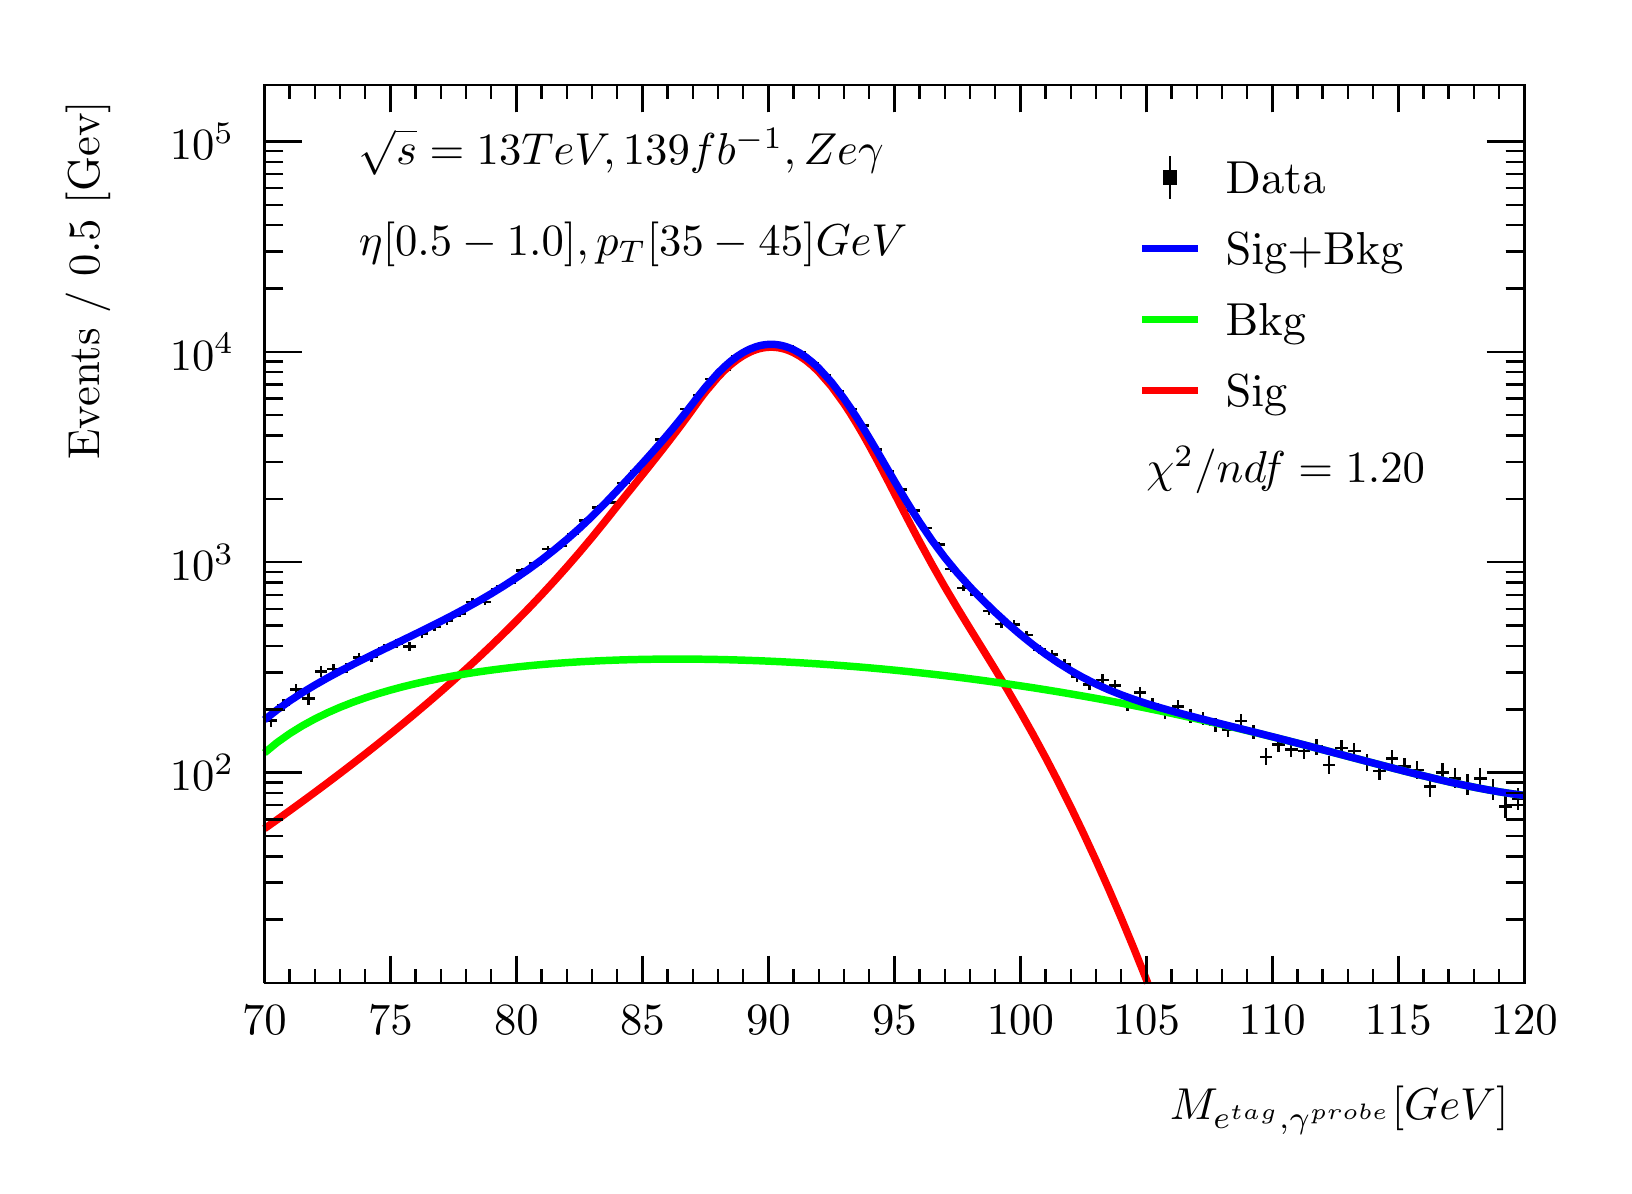
\begin{tikzpicture}
\pgfdeclareplotmark{cross} {
\pgfpathmoveto{\pgfpoint{-0.3\pgfplotmarksize}{\pgfplotmarksize}}
\pgfpathlineto{\pgfpoint{+0.3\pgfplotmarksize}{\pgfplotmarksize}}
\pgfpathlineto{\pgfpoint{+0.3\pgfplotmarksize}{0.3\pgfplotmarksize}}
\pgfpathlineto{\pgfpoint{+1\pgfplotmarksize}{0.3\pgfplotmarksize}}
\pgfpathlineto{\pgfpoint{+1\pgfplotmarksize}{-0.3\pgfplotmarksize}}
\pgfpathlineto{\pgfpoint{+0.3\pgfplotmarksize}{-0.3\pgfplotmarksize}}
\pgfpathlineto{\pgfpoint{+0.3\pgfplotmarksize}{-1.\pgfplotmarksize}}
\pgfpathlineto{\pgfpoint{-0.3\pgfplotmarksize}{-1.\pgfplotmarksize}}
\pgfpathlineto{\pgfpoint{-0.3\pgfplotmarksize}{-0.3\pgfplotmarksize}}
\pgfpathlineto{\pgfpoint{-1.\pgfplotmarksize}{-0.3\pgfplotmarksize}}
\pgfpathlineto{\pgfpoint{-1.\pgfplotmarksize}{0.3\pgfplotmarksize}}
\pgfpathlineto{\pgfpoint{-0.3\pgfplotmarksize}{0.3\pgfplotmarksize}}
\pgfpathclose
\pgfusepathqstroke
}
\pgfdeclareplotmark{cross*} {
\pgfpathmoveto{\pgfpoint{-0.3\pgfplotmarksize}{\pgfplotmarksize}}
\pgfpathlineto{\pgfpoint{+0.3\pgfplotmarksize}{\pgfplotmarksize}}
\pgfpathlineto{\pgfpoint{+0.3\pgfplotmarksize}{0.3\pgfplotmarksize}}
\pgfpathlineto{\pgfpoint{+1\pgfplotmarksize}{0.3\pgfplotmarksize}}
\pgfpathlineto{\pgfpoint{+1\pgfplotmarksize}{-0.3\pgfplotmarksize}}
\pgfpathlineto{\pgfpoint{+0.3\pgfplotmarksize}{-0.3\pgfplotmarksize}}
\pgfpathlineto{\pgfpoint{+0.3\pgfplotmarksize}{-1.\pgfplotmarksize}}
\pgfpathlineto{\pgfpoint{-0.3\pgfplotmarksize}{-1.\pgfplotmarksize}}
\pgfpathlineto{\pgfpoint{-0.3\pgfplotmarksize}{-0.3\pgfplotmarksize}}
\pgfpathlineto{\pgfpoint{-1.\pgfplotmarksize}{-0.3\pgfplotmarksize}}
\pgfpathlineto{\pgfpoint{-1.\pgfplotmarksize}{0.3\pgfplotmarksize}}
\pgfpathlineto{\pgfpoint{-0.3\pgfplotmarksize}{0.3\pgfplotmarksize}}
\pgfpathclose
\pgfusepathqfillstroke
}
\pgfdeclareplotmark{newstar} {
\pgfpathmoveto{\pgfqpoint{0pt}{\pgfplotmarksize}}
\pgfpathlineto{\pgfqpointpolar{44}{0.5\pgfplotmarksize}}
\pgfpathlineto{\pgfqpointpolar{18}{\pgfplotmarksize}}
\pgfpathlineto{\pgfqpointpolar{-20}{0.5\pgfplotmarksize}}
\pgfpathlineto{\pgfqpointpolar{-54}{\pgfplotmarksize}}
\pgfpathlineto{\pgfqpointpolar{-90}{0.5\pgfplotmarksize}}
\pgfpathlineto{\pgfqpointpolar{234}{\pgfplotmarksize}}
\pgfpathlineto{\pgfqpointpolar{198}{0.5\pgfplotmarksize}}
\pgfpathlineto{\pgfqpointpolar{162}{\pgfplotmarksize}}
\pgfpathlineto{\pgfqpointpolar{134}{0.5\pgfplotmarksize}}
\pgfpathclose
\pgfusepathqstroke
}
\pgfdeclareplotmark{newstar*} {
\pgfpathmoveto{\pgfqpoint{0pt}{\pgfplotmarksize}}
\pgfpathlineto{\pgfqpointpolar{44}{0.5\pgfplotmarksize}}
\pgfpathlineto{\pgfqpointpolar{18}{\pgfplotmarksize}}
\pgfpathlineto{\pgfqpointpolar{-20}{0.5\pgfplotmarksize}}
\pgfpathlineto{\pgfqpointpolar{-54}{\pgfplotmarksize}}
\pgfpathlineto{\pgfqpointpolar{-90}{0.5\pgfplotmarksize}}
\pgfpathlineto{\pgfqpointpolar{234}{\pgfplotmarksize}}
\pgfpathlineto{\pgfqpointpolar{198}{0.5\pgfplotmarksize}}
\pgfpathlineto{\pgfqpointpolar{162}{\pgfplotmarksize}}
\pgfpathlineto{\pgfqpointpolar{134}{0.5\pgfplotmarksize}}
\pgfpathclose
\pgfusepathqfillstroke
}
\definecolor{c}{rgb}{1,1,1};
\draw [color=c, fill=c] (0,0) rectangle (20,14.4361);
\draw [color=c, fill=c] (3,2.30977) rectangle (19,13.7143);
\definecolor{c}{rgb}{0,0,0};
\draw [c,line width=0.9] (3,2.30977) -- (3,13.7143) -- (19,13.7143) -- (19,2.30977) -- (3,2.30977);
\definecolor{c}{rgb}{1,1,1};
\draw [color=c, fill=c] (3,2.30977) rectangle (19,13.7143);
\definecolor{c}{rgb}{0,0,0};
\draw [c,line width=0.9] (3,2.30977) -- (3,13.7143) -- (19,13.7143) -- (19,2.30977) -- (3,2.30977);
\draw [c,line width=0.9] (3,2.30977) -- (19,2.30977);
\draw [c,line width=0.9] (3,2.65624) -- (3,2.30977);
\draw [c,line width=0.9] (3.32,2.48301) -- (3.32,2.30977);
\draw [c,line width=0.9] (3.64,2.48301) -- (3.64,2.30977);
\draw [c,line width=0.9] (3.96,2.48301) -- (3.96,2.30977);
\draw [c,line width=0.9] (4.28,2.48301) -- (4.28,2.30977);
\draw [c,line width=0.9] (4.6,2.65624) -- (4.6,2.30977);
\draw [c,line width=0.9] (4.92,2.48301) -- (4.92,2.30977);
\draw [c,line width=0.9] (5.24,2.48301) -- (5.24,2.30977);
\draw [c,line width=0.9] (5.56,2.48301) -- (5.56,2.30977);
\draw [c,line width=0.9] (5.88,2.48301) -- (5.88,2.30977);
\draw [c,line width=0.9] (6.2,2.65624) -- (6.2,2.30977);
\draw [c,line width=0.9] (6.52,2.48301) -- (6.52,2.30977);
\draw [c,line width=0.9] (6.84,2.48301) -- (6.84,2.30977);
\draw [c,line width=0.9] (7.16,2.48301) -- (7.16,2.30977);
\draw [c,line width=0.9] (7.48,2.48301) -- (7.48,2.30977);
\draw [c,line width=0.9] (7.8,2.65624) -- (7.8,2.30977);
\draw [c,line width=0.9] (8.12,2.48301) -- (8.12,2.30977);
\draw [c,line width=0.9] (8.44,2.48301) -- (8.44,2.30977);
\draw [c,line width=0.9] (8.76,2.48301) -- (8.76,2.30977);
\draw [c,line width=0.9] (9.08,2.48301) -- (9.08,2.30977);
\draw [c,line width=0.9] (9.4,2.65624) -- (9.4,2.30977);
\draw [c,line width=0.9] (9.72,2.48301) -- (9.72,2.30977);
\draw [c,line width=0.9] (10.04,2.48301) -- (10.04,2.30977);
\draw [c,line width=0.9] (10.36,2.48301) -- (10.36,2.30977);
\draw [c,line width=0.9] (10.68,2.48301) -- (10.68,2.30977);
\draw [c,line width=0.9] (11,2.65624) -- (11,2.30977);
\draw [c,line width=0.9] (11.32,2.48301) -- (11.32,2.30977);
\draw [c,line width=0.9] (11.64,2.48301) -- (11.64,2.30977);
\draw [c,line width=0.9] (11.96,2.48301) -- (11.96,2.30977);
\draw [c,line width=0.9] (12.28,2.48301) -- (12.28,2.30977);
\draw [c,line width=0.9] (12.6,2.65624) -- (12.6,2.30977);
\draw [c,line width=0.9] (12.92,2.48301) -- (12.92,2.30977);
\draw [c,line width=0.9] (13.24,2.48301) -- (13.24,2.30977);
\draw [c,line width=0.9] (13.56,2.48301) -- (13.56,2.30977);
\draw [c,line width=0.9] (13.88,2.48301) -- (13.88,2.30977);
\draw [c,line width=0.9] (14.2,2.65624) -- (14.2,2.30977);
\draw [c,line width=0.9] (14.52,2.48301) -- (14.52,2.30977);
\draw [c,line width=0.9] (14.84,2.48301) -- (14.84,2.30977);
\draw [c,line width=0.9] (15.16,2.48301) -- (15.16,2.30977);
\draw [c,line width=0.9] (15.48,2.48301) -- (15.48,2.30977);
\draw [c,line width=0.9] (15.8,2.65624) -- (15.8,2.30977);
\draw [c,line width=0.9] (16.12,2.48301) -- (16.12,2.30977);
\draw [c,line width=0.9] (16.44,2.48301) -- (16.44,2.30977);
\draw [c,line width=0.9] (16.76,2.48301) -- (16.76,2.30977);
\draw [c,line width=0.9] (17.08,2.48301) -- (17.08,2.30977);
\draw [c,line width=0.9] (17.4,2.65624) -- (17.4,2.30977);
\draw [c,line width=0.9] (17.72,2.48301) -- (17.72,2.30977);
\draw [c,line width=0.9] (18.04,2.48301) -- (18.04,2.30977);
\draw [c,line width=0.9] (18.36,2.48301) -- (18.36,2.30977);
\draw [c,line width=0.9] (18.68,2.48301) -- (18.68,2.30977);
\draw [c,line width=0.9] (19,2.65624) -- (19,2.30977);
\draw [anchor=base] (3,1.66015) node[scale=1.61424, color=c, rotate=0]{70};
\draw [anchor=base] (4.6,1.66015) node[scale=1.61424, color=c, rotate=0]{75};
\draw [anchor=base] (6.2,1.66015) node[scale=1.61424, color=c, rotate=0]{80};
\draw [anchor=base] (7.8,1.66015) node[scale=1.61424, color=c, rotate=0]{85};
\draw [anchor=base] (9.4,1.66015) node[scale=1.61424, color=c, rotate=0]{90};
\draw [anchor=base] (11,1.66015) node[scale=1.61424, color=c, rotate=0]{95};
\draw [anchor=base] (12.6,1.66015) node[scale=1.61424, color=c, rotate=0]{100};
\draw [anchor=base] (14.2,1.66015) node[scale=1.61424, color=c, rotate=0]{105};
\draw [anchor=base] (15.8,1.66015) node[scale=1.61424, color=c, rotate=0]{110};
\draw [anchor=base] (17.4,1.66015) node[scale=1.61424, color=c, rotate=0]{115};
\draw [anchor=base] (19,1.66015) node[scale=1.61424, color=c, rotate=0]{120};
\draw [anchor= east] (19,0.692932) node[scale=1.61424, color=c, rotate=0]{$M_{e^{tag}, \gamma^{probe}}  [GeV]$};
\draw [c,line width=0.9] (3,13.7143) -- (19,13.7143);
\draw [c,line width=0.9] (3,13.3678) -- (3,13.7143);
\draw [c,line width=0.9] (3.32,13.5411) -- (3.32,13.7143);
\draw [c,line width=0.9] (3.64,13.5411) -- (3.64,13.7143);
\draw [c,line width=0.9] (3.96,13.5411) -- (3.96,13.7143);
\draw [c,line width=0.9] (4.28,13.5411) -- (4.28,13.7143);
\draw [c,line width=0.9] (4.6,13.3678) -- (4.6,13.7143);
\draw [c,line width=0.9] (4.92,13.5411) -- (4.92,13.7143);
\draw [c,line width=0.9] (5.24,13.5411) -- (5.24,13.7143);
\draw [c,line width=0.9] (5.56,13.5411) -- (5.56,13.7143);
\draw [c,line width=0.9] (5.88,13.5411) -- (5.88,13.7143);
\draw [c,line width=0.9] (6.2,13.3678) -- (6.2,13.7143);
\draw [c,line width=0.9] (6.52,13.5411) -- (6.52,13.7143);
\draw [c,line width=0.9] (6.84,13.5411) -- (6.84,13.7143);
\draw [c,line width=0.9] (7.16,13.5411) -- (7.16,13.7143);
\draw [c,line width=0.9] (7.48,13.5411) -- (7.48,13.7143);
\draw [c,line width=0.9] (7.8,13.3678) -- (7.8,13.7143);
\draw [c,line width=0.9] (8.12,13.5411) -- (8.12,13.7143);
\draw [c,line width=0.9] (8.44,13.5411) -- (8.44,13.7143);
\draw [c,line width=0.9] (8.76,13.5411) -- (8.76,13.7143);
\draw [c,line width=0.9] (9.08,13.5411) -- (9.08,13.7143);
\draw [c,line width=0.9] (9.4,13.3678) -- (9.4,13.7143);
\draw [c,line width=0.9] (9.72,13.5411) -- (9.72,13.7143);
\draw [c,line width=0.9] (10.04,13.5411) -- (10.04,13.7143);
\draw [c,line width=0.9] (10.36,13.5411) -- (10.36,13.7143);
\draw [c,line width=0.9] (10.68,13.5411) -- (10.68,13.7143);
\draw [c,line width=0.9] (11,13.3678) -- (11,13.7143);
\draw [c,line width=0.9] (11.32,13.5411) -- (11.32,13.7143);
\draw [c,line width=0.9] (11.64,13.5411) -- (11.64,13.7143);
\draw [c,line width=0.9] (11.96,13.5411) -- (11.96,13.7143);
\draw [c,line width=0.9] (12.28,13.5411) -- (12.28,13.7143);
\draw [c,line width=0.9] (12.6,13.3678) -- (12.6,13.7143);
\draw [c,line width=0.9] (12.92,13.5411) -- (12.92,13.7143);
\draw [c,line width=0.9] (13.24,13.5411) -- (13.24,13.7143);
\draw [c,line width=0.9] (13.56,13.5411) -- (13.56,13.7143);
\draw [c,line width=0.9] (13.88,13.5411) -- (13.88,13.7143);
\draw [c,line width=0.9] (14.2,13.3678) -- (14.2,13.7143);
\draw [c,line width=0.9] (14.52,13.5411) -- (14.52,13.7143);
\draw [c,line width=0.9] (14.84,13.5411) -- (14.84,13.7143);
\draw [c,line width=0.9] (15.16,13.5411) -- (15.16,13.7143);
\draw [c,line width=0.9] (15.48,13.5411) -- (15.48,13.7143);
\draw [c,line width=0.9] (15.8,13.3678) -- (15.8,13.7143);
\draw [c,line width=0.9] (16.12,13.5411) -- (16.12,13.7143);
\draw [c,line width=0.9] (16.44,13.5411) -- (16.44,13.7143);
\draw [c,line width=0.9] (16.76,13.5411) -- (16.76,13.7143);
\draw [c,line width=0.9] (17.08,13.5411) -- (17.08,13.7143);
\draw [c,line width=0.9] (17.4,13.3678) -- (17.4,13.7143);
\draw [c,line width=0.9] (17.72,13.5411) -- (17.72,13.7143);
\draw [c,line width=0.9] (18.04,13.5411) -- (18.04,13.7143);
\draw [c,line width=0.9] (18.36,13.5411) -- (18.36,13.7143);
\draw [c,line width=0.9] (18.68,13.5411) -- (18.68,13.7143);
\draw [c,line width=0.9] (19,13.3678) -- (19,13.7143);
\draw [c,line width=0.9] (3,2.30977) -- (3,13.7143);
\draw [c,line width=0.9] (3.237,3.11414) -- (3,3.11414);
\draw [c,line width=0.9] (3.237,3.58467) -- (3,3.58467);
\draw [c,line width=0.9] (3.237,3.91852) -- (3,3.91852);
\draw [c,line width=0.9] (3.237,4.17747) -- (3,4.17747);
\draw [c,line width=0.9] (3.237,4.38904) -- (3,4.38904);
\draw [c,line width=0.9] (3.237,4.56793) -- (3,4.56793);
\draw [c,line width=0.9] (3.237,4.72289) -- (3,4.72289);
\draw [c,line width=0.9] (3.237,4.85957) -- (3,4.85957);
\draw [c,line width=0.9] (3.474,4.98184) -- (3,4.98184);
\draw [anchor= east] (2.82,4.98184) node[scale=1.61424, color=c, rotate=0]{$10^{2}$};
\draw [c,line width=0.9] (3.237,5.78621) -- (3,5.78621);
\draw [c,line width=0.9] (3.237,6.25674) -- (3,6.25674);
\draw [c,line width=0.9] (3.237,6.59058) -- (3,6.59058);
\draw [c,line width=0.9] (3.237,6.84953) -- (3,6.84953);
\draw [c,line width=0.9] (3.237,7.06111) -- (3,7.06111);
\draw [c,line width=0.9] (3.237,7.24) -- (3,7.24);
\draw [c,line width=0.9] (3.237,7.39496) -- (3,7.39496);
\draw [c,line width=0.9] (3.237,7.53164) -- (3,7.53164);
\draw [c,line width=0.9] (3.474,7.65391) -- (3,7.65391);
\draw [anchor= east] (2.82,7.65391) node[scale=1.61424, color=c, rotate=0]{$10^{3}$};
\draw [c,line width=0.9] (3.237,8.45828) -- (3,8.45828);
\draw [c,line width=0.9] (3.237,8.92881) -- (3,8.92881);
\draw [c,line width=0.9] (3.237,9.26265) -- (3,9.26265);
\draw [c,line width=0.9] (3.237,9.5216) -- (3,9.5216);
\draw [c,line width=0.9] (3.237,9.73318) -- (3,9.73318);
\draw [c,line width=0.9] (3.237,9.91207) -- (3,9.91207);
\draw [c,line width=0.9] (3.237,10.067) -- (3,10.067);
\draw [c,line width=0.9] (3.237,10.2037) -- (3,10.2037);
\draw [c,line width=0.9] (3.474,10.326) -- (3,10.326);
\draw [anchor= east] (2.82,10.326) node[scale=1.61424, color=c, rotate=0]{$10^{4}$};
\draw [c,line width=0.9] (3.237,11.1303) -- (3,11.1303);
\draw [c,line width=0.9] (3.237,11.6009) -- (3,11.6009);
\draw [c,line width=0.9] (3.237,11.9347) -- (3,11.9347);
\draw [c,line width=0.9] (3.237,12.1937) -- (3,12.1937);
\draw [c,line width=0.9] (3.237,12.4052) -- (3,12.4052);
\draw [c,line width=0.9] (3.237,12.5841) -- (3,12.5841);
\draw [c,line width=0.9] (3.237,12.7391) -- (3,12.7391);
\draw [c,line width=0.9] (3.237,12.8758) -- (3,12.8758);
\draw [c,line width=0.9] (3.474,12.998) -- (3,12.998);
\draw [anchor= east] (2.82,12.998) node[scale=1.61424, color=c, rotate=0]{$10^{5}$};
\draw [anchor= east] (0.76,13.7143) node[scale=1.61424, color=c, rotate=90]{Events / 0.5 [Gev]};
\draw [c,line width=0.9] (19,2.30977) -- (19,13.7143);
\draw [c,line width=0.9] (18.763,3.11414) -- (19,3.11414);
\draw [c,line width=0.9] (18.763,3.58467) -- (19,3.58467);
\draw [c,line width=0.9] (18.763,3.91852) -- (19,3.91852);
\draw [c,line width=0.9] (18.763,4.17747) -- (19,4.17747);
\draw [c,line width=0.9] (18.763,4.38904) -- (19,4.38904);
\draw [c,line width=0.9] (18.763,4.56793) -- (19,4.56793);
\draw [c,line width=0.9] (18.763,4.72289) -- (19,4.72289);
\draw [c,line width=0.9] (18.763,4.85957) -- (19,4.85957);
\draw [c,line width=0.9] (18.526,4.98184) -- (19,4.98184);
\draw [c,line width=0.9] (18.763,5.78621) -- (19,5.78621);
\draw [c,line width=0.9] (18.763,6.25674) -- (19,6.25674);
\draw [c,line width=0.9] (18.763,6.59058) -- (19,6.59058);
\draw [c,line width=0.9] (18.763,6.84953) -- (19,6.84953);
\draw [c,line width=0.9] (18.763,7.06111) -- (19,7.06111);
\draw [c,line width=0.9] (18.763,7.24) -- (19,7.24);
\draw [c,line width=0.9] (18.763,7.39496) -- (19,7.39496);
\draw [c,line width=0.9] (18.763,7.53164) -- (19,7.53164);
\draw [c,line width=0.9] (18.526,7.65391) -- (19,7.65391);
\draw [c,line width=0.9] (18.763,8.45828) -- (19,8.45828);
\draw [c,line width=0.9] (18.763,8.92881) -- (19,8.92881);
\draw [c,line width=0.9] (18.763,9.26265) -- (19,9.26265);
\draw [c,line width=0.9] (18.763,9.5216) -- (19,9.5216);
\draw [c,line width=0.9] (18.763,9.73318) -- (19,9.73318);
\draw [c,line width=0.9] (18.763,9.91207) -- (19,9.91207);
\draw [c,line width=0.9] (18.763,10.067) -- (19,10.067);
\draw [c,line width=0.9] (18.763,10.2037) -- (19,10.2037);
\draw [c,line width=0.9] (18.526,10.326) -- (19,10.326);
\draw [c,line width=0.9] (18.763,11.1303) -- (19,11.1303);
\draw [c,line width=0.9] (18.763,11.6009) -- (19,11.6009);
\draw [c,line width=0.9] (18.763,11.9347) -- (19,11.9347);
\draw [c,line width=0.9] (18.763,12.1937) -- (19,12.1937);
\draw [c,line width=0.9] (18.763,12.4052) -- (19,12.4052);
\draw [c,line width=0.9] (18.763,12.5841) -- (19,12.5841);
\draw [c,line width=0.9] (18.763,12.7391) -- (19,12.7391);
\draw [c,line width=0.9] (18.763,12.8758) -- (19,12.8758);
\draw [c,line width=0.9] (18.526,12.998) -- (19,12.998);
\draw [c,line width=0.9] (3.08,5.64444) -- (3,5.64444);
\draw [c,line width=0.9] (3,5.64444) -- (3,5.64444);
\draw [c,line width=0.9] (3.08,5.64444) -- (3.16,5.64444);
\draw [c,line width=0.9] (3.16,5.64444) -- (3.16,5.64444);
\draw [c,line width=0.9] (3.08,5.64444) -- (3.08,5.73165);
\draw [c,line width=0.9] (3.08,5.73165) -- (3.08,5.73165);
\draw [c,line width=0.9] (3.08,5.64444) -- (3.08,5.55724);
\draw [c,line width=0.9] (3.08,5.55724) -- (3.08,5.55724);
\draw [c,line width=0.9] (3.24,5.84283) -- (3.16,5.84283);
\draw [c,line width=0.9] (3.16,5.84283) -- (3.16,5.84283);
\draw [c,line width=0.9] (3.24,5.84283) -- (3.32,5.84283);
\draw [c,line width=0.9] (3.32,5.84283) -- (3.32,5.84283);
\draw [c,line width=0.9] (3.24,5.84283) -- (3.24,5.9229);
\draw [c,line width=0.9] (3.24,5.9229) -- (3.24,5.9229);
\draw [c,line width=0.9] (3.24,5.84283) -- (3.24,5.76277);
\draw [c,line width=0.9] (3.24,5.76277) -- (3.24,5.76277);
\draw [c,line width=0.9] (3.4,6.03584) -- (3.32,6.03584);
\draw [c,line width=0.9] (3.32,6.03584) -- (3.32,6.03584);
\draw [c,line width=0.9] (3.4,6.03584) -- (3.48,6.03584);
\draw [c,line width=0.9] (3.48,6.03584) -- (3.48,6.03584);
\draw [c,line width=0.9] (3.4,6.03584) -- (3.4,6.10952);
\draw [c,line width=0.9] (3.4,6.10952) -- (3.4,6.10952);
\draw [c,line width=0.9] (3.4,6.03584) -- (3.4,5.96217);
\draw [c,line width=0.9] (3.4,5.96217) -- (3.4,5.96217);
\draw [c,line width=0.9] (3.56,5.9229) -- (3.48,5.9229);
\draw [c,line width=0.9] (3.48,5.9229) -- (3.48,5.9229);
\draw [c,line width=0.9] (3.56,5.9229) -- (3.64,5.9229);
\draw [c,line width=0.9] (3.64,5.9229) -- (3.64,5.9229);
\draw [c,line width=0.9] (3.56,5.9229) -- (3.56,6.00025);
\draw [c,line width=0.9] (3.56,6.00025) -- (3.56,6.00025);
\draw [c,line width=0.9] (3.56,5.9229) -- (3.56,5.84555);
\draw [c,line width=0.9] (3.56,5.84555) -- (3.56,5.84555);
\draw [c,line width=0.9] (3.72,6.26445) -- (3.64,6.26445);
\draw [c,line width=0.9] (3.64,6.26445) -- (3.64,6.26445);
\draw [c,line width=0.9] (3.72,6.26445) -- (3.8,6.26445);
\draw [c,line width=0.9] (3.8,6.26445) -- (3.8,6.26445);
\draw [c,line width=0.9] (3.72,6.26445) -- (3.72,6.33122);
\draw [c,line width=0.9] (3.72,6.33122) -- (3.72,6.33122);
\draw [c,line width=0.9] (3.72,6.26445) -- (3.72,6.19768);
\draw [c,line width=0.9] (3.72,6.19768) -- (3.72,6.19768);
\draw [c,line width=0.9] (3.88,6.29853) -- (3.8,6.29853);
\draw [c,line width=0.9] (3.8,6.29853) -- (3.8,6.29853);
\draw [c,line width=0.9] (3.88,6.29853) -- (3.96,6.29853);
\draw [c,line width=0.9] (3.96,6.29853) -- (3.96,6.29853);
\draw [c,line width=0.9] (3.88,6.29853) -- (3.88,6.36433);
\draw [c,line width=0.9] (3.88,6.36433) -- (3.88,6.36433);
\draw [c,line width=0.9] (3.88,6.29853) -- (3.88,6.23273);
\draw [c,line width=0.9] (3.88,6.23273) -- (3.88,6.23273);
\draw [c,line width=0.9] (4.04,6.30967) -- (3.96,6.30967);
\draw [c,line width=0.9] (3.96,6.30967) -- (3.96,6.30967);
\draw [c,line width=0.9] (4.04,6.30967) -- (4.12,6.30967);
\draw [c,line width=0.9] (4.12,6.30967) -- (4.12,6.30967);
\draw [c,line width=0.9] (4.04,6.30967) -- (4.04,6.37515);
\draw [c,line width=0.9] (4.04,6.37515) -- (4.04,6.37515);
\draw [c,line width=0.9] (4.04,6.30967) -- (4.04,6.24419);
\draw [c,line width=0.9] (4.04,6.24419) -- (4.04,6.24419);
\draw [c,line width=0.9] (4.2,6.44553) -- (4.12,6.44553);
\draw [c,line width=0.9] (4.12,6.44553) -- (4.12,6.44553);
\draw [c,line width=0.9] (4.2,6.44553) -- (4.28,6.44553);
\draw [c,line width=0.9] (4.28,6.44553) -- (4.28,6.44553);
\draw [c,line width=0.9] (4.2,6.44553) -- (4.2,6.50729);
\draw [c,line width=0.9] (4.2,6.50729) -- (4.2,6.50729);
\draw [c,line width=0.9] (4.2,6.44553) -- (4.2,6.38377);
\draw [c,line width=0.9] (4.2,6.38377) -- (4.2,6.38377);
\draw [c,line width=0.9] (4.36,6.45209) -- (4.28,6.45209);
\draw [c,line width=0.9] (4.28,6.45209) -- (4.28,6.45209);
\draw [c,line width=0.9] (4.36,6.45209) -- (4.44,6.45209);
\draw [c,line width=0.9] (4.44,6.45209) -- (4.44,6.45209);
\draw [c,line width=0.9] (4.36,6.45209) -- (4.36,6.51367);
\draw [c,line width=0.9] (4.36,6.51367) -- (4.36,6.51367);
\draw [c,line width=0.9] (4.36,6.45209) -- (4.36,6.3905);
\draw [c,line width=0.9] (4.36,6.3905) -- (4.36,6.3905);
\draw [c,line width=0.9] (4.52,6.55823) -- (4.44,6.55823);
\draw [c,line width=0.9] (4.44,6.55823) -- (4.44,6.55823);
\draw [c,line width=0.9] (4.52,6.55823) -- (4.6,6.55823);
\draw [c,line width=0.9] (4.6,6.55823) -- (4.6,6.55823);
\draw [c,line width=0.9] (4.52,6.55823) -- (4.52,6.61706);
\draw [c,line width=0.9] (4.52,6.61706) -- (4.52,6.61706);
\draw [c,line width=0.9] (4.52,6.55823) -- (4.52,6.49939);
\draw [c,line width=0.9] (4.52,6.49939) -- (4.52,6.49939);
\draw [c,line width=0.9] (4.68,6.61641) -- (4.6,6.61641);
\draw [c,line width=0.9] (4.6,6.61641) -- (4.6,6.61641);
\draw [c,line width=0.9] (4.68,6.61641) -- (4.76,6.61641);
\draw [c,line width=0.9] (4.76,6.61641) -- (4.76,6.61641);
\draw [c,line width=0.9] (4.68,6.61641) -- (4.68,6.67378);
\draw [c,line width=0.9] (4.68,6.67378) -- (4.68,6.67378);
\draw [c,line width=0.9] (4.68,6.61641) -- (4.68,6.55903);
\draw [c,line width=0.9] (4.68,6.55903) -- (4.68,6.55903);
\draw [c,line width=0.9] (4.84,6.58477) -- (4.76,6.58477);
\draw [c,line width=0.9] (4.76,6.58477) -- (4.76,6.58477);
\draw [c,line width=0.9] (4.84,6.58477) -- (4.92,6.58477);
\draw [c,line width=0.9] (4.92,6.58477) -- (4.92,6.58477);
\draw [c,line width=0.9] (4.84,6.58477) -- (4.84,6.64293);
\draw [c,line width=0.9] (4.84,6.64293) -- (4.84,6.64293);
\draw [c,line width=0.9] (4.84,6.58477) -- (4.84,6.52661);
\draw [c,line width=0.9] (4.84,6.52661) -- (4.84,6.52661);
\draw [c,line width=0.9] (5,6.74772) -- (4.92,6.74772);
\draw [c,line width=0.9] (4.92,6.74772) -- (4.92,6.74772);
\draw [c,line width=0.9] (5,6.74772) -- (5.08,6.74772);
\draw [c,line width=0.9] (5.08,6.74772) -- (5.08,6.74772);
\draw [c,line width=0.9] (5,6.74772) -- (5,6.80194);
\draw [c,line width=0.9] (5,6.80194) -- (5,6.80194);
\draw [c,line width=0.9] (5,6.74772) -- (5,6.6935);
\draw [c,line width=0.9] (5,6.6935) -- (5,6.6935);
\draw [c,line width=0.9] (5.16,6.83317) -- (5.08,6.83317);
\draw [c,line width=0.9] (5.08,6.83317) -- (5.08,6.83317);
\draw [c,line width=0.9] (5.16,6.83317) -- (5.24,6.83317);
\draw [c,line width=0.9] (5.24,6.83317) -- (5.24,6.83317);
\draw [c,line width=0.9] (5.16,6.83317) -- (5.16,6.88543);
\draw [c,line width=0.9] (5.16,6.88543) -- (5.16,6.88543);
\draw [c,line width=0.9] (5.16,6.83317) -- (5.16,6.78091);
\draw [c,line width=0.9] (5.16,6.78091) -- (5.16,6.78091);
\draw [c,line width=0.9] (5.32,6.91277) -- (5.24,6.91277);
\draw [c,line width=0.9] (5.24,6.91277) -- (5.24,6.91277);
\draw [c,line width=0.9] (5.32,6.91277) -- (5.4,6.91277);
\draw [c,line width=0.9] (5.4,6.91277) -- (5.4,6.91277);
\draw [c,line width=0.9] (5.32,6.91277) -- (5.32,6.96327);
\draw [c,line width=0.9] (5.32,6.96327) -- (5.32,6.96327);
\draw [c,line width=0.9] (5.32,6.91277) -- (5.32,6.86227);
\draw [c,line width=0.9] (5.32,6.86227) -- (5.32,6.86227);
\draw [c,line width=0.9] (5.48,7.00565) -- (5.4,7.00565);
\draw [c,line width=0.9] (5.4,7.00565) -- (5.4,7.00565);
\draw [c,line width=0.9] (5.48,7.00565) -- (5.56,7.00565);
\draw [c,line width=0.9] (5.56,7.00565) -- (5.56,7.00565);
\draw [c,line width=0.9] (5.48,7.00565) -- (5.48,7.05417);
\draw [c,line width=0.9] (5.48,7.05417) -- (5.48,7.05417);
\draw [c,line width=0.9] (5.48,7.00565) -- (5.48,6.95714);
\draw [c,line width=0.9] (5.48,6.95714) -- (5.48,6.95714);
\draw [c,line width=0.9] (5.64,7.15042) -- (5.56,7.15042);
\draw [c,line width=0.9] (5.56,7.15042) -- (5.56,7.15042);
\draw [c,line width=0.9] (5.64,7.15042) -- (5.72,7.15042);
\draw [c,line width=0.9] (5.72,7.15042) -- (5.72,7.15042);
\draw [c,line width=0.9] (5.64,7.15042) -- (5.64,7.19601);
\draw [c,line width=0.9] (5.64,7.19601) -- (5.64,7.19601);
\draw [c,line width=0.9] (5.64,7.15042) -- (5.64,7.10484);
\draw [c,line width=0.9] (5.64,7.10484) -- (5.64,7.10484);
\draw [c,line width=0.9] (5.8,7.15042) -- (5.72,7.15042);
\draw [c,line width=0.9] (5.72,7.15042) -- (5.72,7.15042);
\draw [c,line width=0.9] (5.8,7.15042) -- (5.88,7.15042);
\draw [c,line width=0.9] (5.88,7.15042) -- (5.88,7.15042);
\draw [c,line width=0.9] (5.8,7.15042) -- (5.8,7.19601);
\draw [c,line width=0.9] (5.8,7.19601) -- (5.8,7.19601);
\draw [c,line width=0.9] (5.8,7.15042) -- (5.8,7.10484);
\draw [c,line width=0.9] (5.8,7.10484) -- (5.8,7.10484);
\draw [c,line width=0.9] (5.96,7.31696) -- (5.88,7.31696);
\draw [c,line width=0.9] (5.88,7.31696) -- (5.88,7.31696);
\draw [c,line width=0.9] (5.96,7.31696) -- (6.04,7.31696);
\draw [c,line width=0.9] (6.04,7.31696) -- (6.04,7.31696);
\draw [c,line width=0.9] (5.96,7.31696) -- (5.96,7.35939);
\draw [c,line width=0.9] (5.96,7.35939) -- (5.96,7.35939);
\draw [c,line width=0.9] (5.96,7.31696) -- (5.96,7.27454);
\draw [c,line width=0.9] (5.96,7.27454) -- (5.96,7.27454);
\draw [c,line width=0.9] (6.12,7.3993) -- (6.04,7.3993);
\draw [c,line width=0.9] (6.04,7.3993) -- (6.04,7.3993);
\draw [c,line width=0.9] (6.12,7.3993) -- (6.2,7.3993);
\draw [c,line width=0.9] (6.2,7.3993) -- (6.2,7.3993);
\draw [c,line width=0.9] (6.12,7.3993) -- (6.12,7.44025);
\draw [c,line width=0.9] (6.12,7.44025) -- (6.12,7.44025);
\draw [c,line width=0.9] (6.12,7.3993) -- (6.12,7.35835);
\draw [c,line width=0.9] (6.12,7.35835) -- (6.12,7.35835);
\draw [c,line width=0.9] (6.28,7.54701) -- (6.2,7.54701);
\draw [c,line width=0.9] (6.2,7.54701) -- (6.2,7.54701);
\draw [c,line width=0.9] (6.28,7.54701) -- (6.36,7.54701);
\draw [c,line width=0.9] (6.36,7.54701) -- (6.36,7.54701);
\draw [c,line width=0.9] (6.28,7.54701) -- (6.28,7.58544);
\draw [c,line width=0.9] (6.28,7.58544) -- (6.28,7.58544);
\draw [c,line width=0.9] (6.28,7.54701) -- (6.28,7.50859);
\draw [c,line width=0.9] (6.28,7.50859) -- (6.28,7.50859);
\draw [c,line width=0.9] (6.44,7.63755) -- (6.36,7.63755);
\draw [c,line width=0.9] (6.36,7.63755) -- (6.36,7.63755);
\draw [c,line width=0.9] (6.44,7.63755) -- (6.52,7.63755);
\draw [c,line width=0.9] (6.52,7.63755) -- (6.52,7.63755);
\draw [c,line width=0.9] (6.44,7.63755) -- (6.44,7.6745);
\draw [c,line width=0.9] (6.44,7.6745) -- (6.44,7.6745);
\draw [c,line width=0.9] (6.44,7.63755) -- (6.44,7.60059);
\draw [c,line width=0.9] (6.44,7.60059) -- (6.44,7.60059);
\draw [c,line width=0.9] (6.6,7.82113) -- (6.52,7.82113);
\draw [c,line width=0.9] (6.52,7.82113) -- (6.52,7.82113);
\draw [c,line width=0.9] (6.6,7.82113) -- (6.68,7.82113);
\draw [c,line width=0.9] (6.68,7.82113) -- (6.68,7.82113);
\draw [c,line width=0.9] (6.6,7.82113) -- (6.6,7.85528);
\draw [c,line width=0.9] (6.6,7.85528) -- (6.6,7.85528);
\draw [c,line width=0.9] (6.6,7.82113) -- (6.6,7.78699);
\draw [c,line width=0.9] (6.6,7.78699) -- (6.6,7.78699);
\draw [c,line width=0.9] (6.76,7.8587) -- (6.68,7.8587);
\draw [c,line width=0.9] (6.68,7.8587) -- (6.68,7.8587);
\draw [c,line width=0.9] (6.76,7.8587) -- (6.84,7.8587);
\draw [c,line width=0.9] (6.84,7.8587) -- (6.84,7.8587);
\draw [c,line width=0.9] (6.76,7.8587) -- (6.76,7.89229);
\draw [c,line width=0.9] (6.76,7.89229) -- (6.76,7.89229);
\draw [c,line width=0.9] (6.76,7.8587) -- (6.76,7.8251);
\draw [c,line width=0.9] (6.76,7.8251) -- (6.76,7.8251);
\draw [c,line width=0.9] (6.92,8.00988) -- (6.84,8.00988);
\draw [c,line width=0.9] (6.84,8.00988) -- (6.84,8.00988);
\draw [c,line width=0.9] (6.92,8.00988) -- (7,8.00988);
\draw [c,line width=0.9] (7,8.00988) -- (7,8.00988);
\draw [c,line width=0.9] (6.92,8.00988) -- (6.92,8.04136);
\draw [c,line width=0.9] (6.92,8.04136) -- (6.92,8.04136);
\draw [c,line width=0.9] (6.92,8.00988) -- (6.92,7.9784);
\draw [c,line width=0.9] (6.92,7.9784) -- (6.92,7.9784);
\draw [c,line width=0.9] (7.08,8.1862) -- (7,8.1862);
\draw [c,line width=0.9] (7,8.1862) -- (7,8.1862);
\draw [c,line width=0.9] (7.08,8.1862) -- (7.16,8.1862);
\draw [c,line width=0.9] (7.16,8.1862) -- (7.16,8.1862);
\draw [c,line width=0.9] (7.08,8.1862) -- (7.08,8.21538);
\draw [c,line width=0.9] (7.08,8.21538) -- (7.08,8.21538);
\draw [c,line width=0.9] (7.08,8.1862) -- (7.08,8.15703);
\draw [c,line width=0.9] (7.08,8.15703) -- (7.08,8.15703);
\draw [c,line width=0.9] (7.24,8.34756) -- (7.16,8.34756);
\draw [c,line width=0.9] (7.16,8.34756) -- (7.16,8.34756);
\draw [c,line width=0.9] (7.24,8.34756) -- (7.32,8.34756);
\draw [c,line width=0.9] (7.32,8.34756) -- (7.32,8.34756);
\draw [c,line width=0.9] (7.24,8.34756) -- (7.24,8.37478);
\draw [c,line width=0.9] (7.24,8.37478) -- (7.24,8.37478);
\draw [c,line width=0.9] (7.24,8.34756) -- (7.24,8.32034);
\draw [c,line width=0.9] (7.24,8.32034) -- (7.24,8.32034);
\draw [c,line width=0.9] (7.4,8.41513) -- (7.32,8.41513);
\draw [c,line width=0.9] (7.32,8.41513) -- (7.32,8.41513);
\draw [c,line width=0.9] (7.4,8.41513) -- (7.48,8.41513);
\draw [c,line width=0.9] (7.48,8.41513) -- (7.48,8.41513);
\draw [c,line width=0.9] (7.4,8.41513) -- (7.4,8.44157);
\draw [c,line width=0.9] (7.4,8.44157) -- (7.4,8.44157);
\draw [c,line width=0.9] (7.4,8.41513) -- (7.4,8.3887);
\draw [c,line width=0.9] (7.4,8.3887) -- (7.4,8.3887);
\draw [c,line width=0.9] (7.56,8.66307) -- (7.48,8.66307);
\draw [c,line width=0.9] (7.48,8.66307) -- (7.48,8.66307);
\draw [c,line width=0.9] (7.56,8.66307) -- (7.64,8.66307);
\draw [c,line width=0.9] (7.64,8.66307) -- (7.64,8.66307);
\draw [c,line width=0.9] (7.56,8.66307) -- (7.56,8.68683);
\draw [c,line width=0.9] (7.56,8.68683) -- (7.56,8.68683);
\draw [c,line width=0.9] (7.56,8.66307) -- (7.56,8.63931);
\draw [c,line width=0.9] (7.56,8.63931) -- (7.56,8.63931);
\draw [c,line width=0.9] (7.72,8.80439) -- (7.64,8.80439);
\draw [c,line width=0.9] (7.64,8.80439) -- (7.64,8.80439);
\draw [c,line width=0.9] (7.72,8.80439) -- (7.8,8.80439);
\draw [c,line width=0.9] (7.8,8.80439) -- (7.8,8.80439);
\draw [c,line width=0.9] (7.72,8.80439) -- (7.72,8.82674);
\draw [c,line width=0.9] (7.72,8.82674) -- (7.72,8.82674);
\draw [c,line width=0.9] (7.72,8.80439) -- (7.72,8.78204);
\draw [c,line width=0.9] (7.72,8.78204) -- (7.72,8.78204);
\draw [c,line width=0.9] (7.88,8.96761) -- (7.8,8.96761);
\draw [c,line width=0.9] (7.8,8.96761) -- (7.8,8.96761);
\draw [c,line width=0.9] (7.88,8.96761) -- (7.96,8.96761);
\draw [c,line width=0.9] (7.96,8.96761) -- (7.96,8.96761);
\draw [c,line width=0.9] (7.88,8.96761) -- (7.88,8.98844);
\draw [c,line width=0.9] (7.88,8.98844) -- (7.88,8.98844);
\draw [c,line width=0.9] (7.88,8.96761) -- (7.88,8.94677);
\draw [c,line width=0.9] (7.88,8.94677) -- (7.88,8.94677);
\draw [c,line width=0.9] (8.04,9.21377) -- (7.96,9.21377);
\draw [c,line width=0.9] (7.96,9.21377) -- (7.96,9.21377);
\draw [c,line width=0.9] (8.04,9.21377) -- (8.12,9.21377);
\draw [c,line width=0.9] (8.12,9.21377) -- (8.12,9.21377);
\draw [c,line width=0.9] (8.04,9.21377) -- (8.04,9.23251);
\draw [c,line width=0.9] (8.04,9.23251) -- (8.04,9.23251);
\draw [c,line width=0.9] (8.04,9.21377) -- (8.04,9.19503);
\draw [c,line width=0.9] (8.04,9.19503) -- (8.04,9.19503);
\draw [c,line width=0.9] (8.2,9.34523) -- (8.12,9.34523);
\draw [c,line width=0.9] (8.12,9.34523) -- (8.12,9.34523);
\draw [c,line width=0.9] (8.2,9.34523) -- (8.28,9.34523);
\draw [c,line width=0.9] (8.28,9.34523) -- (8.28,9.34523);
\draw [c,line width=0.9] (8.2,9.34523) -- (8.2,9.36294);
\draw [c,line width=0.9] (8.2,9.36294) -- (8.2,9.36294);
\draw [c,line width=0.9] (8.2,9.34523) -- (8.2,9.32752);
\draw [c,line width=0.9] (8.2,9.32752) -- (8.2,9.32752);
\draw [c,line width=0.9] (8.36,9.60055) -- (8.28,9.60055);
\draw [c,line width=0.9] (8.28,9.60055) -- (8.28,9.60055);
\draw [c,line width=0.9] (8.36,9.60055) -- (8.44,9.60055);
\draw [c,line width=0.9] (8.44,9.60055) -- (8.44,9.60055);
\draw [c,line width=0.9] (8.36,9.60055) -- (8.36,9.61641);
\draw [c,line width=0.9] (8.36,9.61641) -- (8.36,9.61641);
\draw [c,line width=0.9] (8.36,9.60055) -- (8.36,9.58469);
\draw [c,line width=0.9] (8.36,9.58469) -- (8.36,9.58469);
\draw [c,line width=0.9] (8.52,9.77553) -- (8.44,9.77553);
\draw [c,line width=0.9] (8.44,9.77553) -- (8.44,9.77553);
\draw [c,line width=0.9] (8.52,9.77553) -- (8.6,9.77553);
\draw [c,line width=0.9] (8.6,9.77553) -- (8.6,9.77553);
\draw [c,line width=0.9] (8.52,9.77553) -- (8.52,9.79024);
\draw [c,line width=0.9] (8.52,9.79024) -- (8.52,9.79024);
\draw [c,line width=0.9] (8.52,9.77553) -- (8.52,9.76082);
\draw [c,line width=0.9] (8.52,9.76082) -- (8.52,9.76082);
\draw [c,line width=0.9] (8.68,9.9814) -- (8.6,9.9814);
\draw [c,line width=0.9] (8.6,9.9814) -- (8.6,9.9814);
\draw [c,line width=0.9] (8.68,9.9814) -- (8.76,9.9814);
\draw [c,line width=0.9] (8.76,9.9814) -- (8.76,9.9814);
\draw [c,line width=0.9] (8.68,9.9814) -- (8.68,9.99487);
\draw [c,line width=0.9] (8.68,9.99487) -- (8.68,9.99487);
\draw [c,line width=0.9] (8.68,9.9814) -- (8.68,9.96794);
\draw [c,line width=0.9] (8.68,9.96794) -- (8.68,9.96794);
\draw [c,line width=0.9] (8.84,10.0927) -- (8.76,10.0927);
\draw [c,line width=0.9] (8.76,10.0927) -- (8.76,10.0927);
\draw [c,line width=0.9] (8.84,10.0927) -- (8.92,10.0927);
\draw [c,line width=0.9] (8.92,10.0927) -- (8.92,10.0927);
\draw [c,line width=0.9] (8.84,10.0927) -- (8.84,10.1055);
\draw [c,line width=0.9] (8.84,10.1055) -- (8.84,10.1055);
\draw [c,line width=0.9] (8.84,10.0927) -- (8.84,10.0799);
\draw [c,line width=0.9] (8.84,10.0799) -- (8.84,10.0799);
\draw [c,line width=0.9] (9,10.2741) -- (8.92,10.2741);
\draw [c,line width=0.9] (8.92,10.2741) -- (8.92,10.2741);
\draw [c,line width=0.9] (9,10.2741) -- (9.08,10.2741);
\draw [c,line width=0.9] (9.08,10.2741) -- (9.08,10.2741);
\draw [c,line width=0.9] (9,10.2741) -- (9,10.286);
\draw [c,line width=0.9] (9,10.286) -- (9,10.286);
\draw [c,line width=0.9] (9,10.2741) -- (9,10.2623);
\draw [c,line width=0.9] (9,10.2623) -- (9,10.2623);
\draw [c,line width=0.9] (9.16,10.3619) -- (9.08,10.3619);
\draw [c,line width=0.9] (9.08,10.3619) -- (9.08,10.3619);
\draw [c,line width=0.9] (9.16,10.3619) -- (9.24,10.3619);
\draw [c,line width=0.9] (9.24,10.3619) -- (9.24,10.3619);
\draw [c,line width=0.9] (9.16,10.3619) -- (9.16,10.3733);
\draw [c,line width=0.9] (9.16,10.3733) -- (9.16,10.3733);
\draw [c,line width=0.9] (9.16,10.3619) -- (9.16,10.3504);
\draw [c,line width=0.9] (9.16,10.3504) -- (9.16,10.3504);
\draw [c,line width=0.9] (9.32,10.4157) -- (9.24,10.4157);
\draw [c,line width=0.9] (9.24,10.4157) -- (9.24,10.4157);
\draw [c,line width=0.9] (9.32,10.4157) -- (9.4,10.4157);
\draw [c,line width=0.9] (9.4,10.4157) -- (9.4,10.4157);
\draw [c,line width=0.9] (9.32,10.4157) -- (9.32,10.4269);
\draw [c,line width=0.9] (9.32,10.4269) -- (9.32,10.4269);
\draw [c,line width=0.9] (9.32,10.4157) -- (9.32,10.4046);
\draw [c,line width=0.9] (9.32,10.4046) -- (9.32,10.4046);
\draw [c,line width=0.9] (9.48,10.4272) -- (9.4,10.4272);
\draw [c,line width=0.9] (9.4,10.4272) -- (9.4,10.4272);
\draw [c,line width=0.9] (9.48,10.4272) -- (9.56,10.4272);
\draw [c,line width=0.9] (9.56,10.4272) -- (9.56,10.4272);
\draw [c,line width=0.9] (9.48,10.4272) -- (9.48,10.4383);
\draw [c,line width=0.9] (9.48,10.4383) -- (9.48,10.4383);
\draw [c,line width=0.9] (9.48,10.4272) -- (9.48,10.416);
\draw [c,line width=0.9] (9.48,10.416) -- (9.48,10.416);
\draw [c,line width=0.9] (9.64,10.3971) -- (9.56,10.3971);
\draw [c,line width=0.9] (9.56,10.3971) -- (9.56,10.3971);
\draw [c,line width=0.9] (9.64,10.3971) -- (9.72,10.3971);
\draw [c,line width=0.9] (9.72,10.3971) -- (9.72,10.3971);
\draw [c,line width=0.9] (9.64,10.3971) -- (9.64,10.4083);
\draw [c,line width=0.9] (9.64,10.4083) -- (9.64,10.4083);
\draw [c,line width=0.9] (9.64,10.3971) -- (9.64,10.3858);
\draw [c,line width=0.9] (9.64,10.3858) -- (9.64,10.3858);
\draw [c,line width=0.9] (9.8,10.3206) -- (9.72,10.3206);
\draw [c,line width=0.9] (9.72,10.3206) -- (9.72,10.3206);
\draw [c,line width=0.9] (9.8,10.3206) -- (9.88,10.3206);
\draw [c,line width=0.9] (9.88,10.3206) -- (9.88,10.3206);
\draw [c,line width=0.9] (9.8,10.3206) -- (9.8,10.3323);
\draw [c,line width=0.9] (9.8,10.3323) -- (9.8,10.3323);
\draw [c,line width=0.9] (9.8,10.3206) -- (9.8,10.309);
\draw [c,line width=0.9] (9.8,10.309) -- (9.8,10.309);
\draw [c,line width=0.9] (9.96,10.1751) -- (9.88,10.1751);
\draw [c,line width=0.9] (9.88,10.1751) -- (9.88,10.1751);
\draw [c,line width=0.9] (9.96,10.1751) -- (10.04,10.1751);
\draw [c,line width=0.9] (10.04,10.1751) -- (10.04,10.1751);
\draw [c,line width=0.9] (9.96,10.1751) -- (9.96,10.1875);
\draw [c,line width=0.9] (9.96,10.1875) -- (9.96,10.1875);
\draw [c,line width=0.9] (9.96,10.1751) -- (9.96,10.1627);
\draw [c,line width=0.9] (9.96,10.1627) -- (9.96,10.1627);
\draw [c,line width=0.9] (10.12,10.0332) -- (10.04,10.0332);
\draw [c,line width=0.9] (10.04,10.0332) -- (10.04,10.0332);
\draw [c,line width=0.9] (10.12,10.0332) -- (10.2,10.0332);
\draw [c,line width=0.9] (10.2,10.0332) -- (10.2,10.0332);
\draw [c,line width=0.9] (10.12,10.0332) -- (10.12,10.0463);
\draw [c,line width=0.9] (10.12,10.0463) -- (10.12,10.0463);
\draw [c,line width=0.9] (10.12,10.0332) -- (10.12,10.02);
\draw [c,line width=0.9] (10.12,10.02) -- (10.12,10.02);
\draw [c,line width=0.9] (10.28,9.82821) -- (10.2,9.82821);
\draw [c,line width=0.9] (10.2,9.82821) -- (10.2,9.82821);
\draw [c,line width=0.9] (10.28,9.82821) -- (10.36,9.82821);
\draw [c,line width=0.9] (10.36,9.82821) -- (10.36,9.82821);
\draw [c,line width=0.9] (10.28,9.82821) -- (10.28,9.84259);
\draw [c,line width=0.9] (10.28,9.84259) -- (10.28,9.84259);
\draw [c,line width=0.9] (10.28,9.82821) -- (10.28,9.81383);
\draw [c,line width=0.9] (10.28,9.81383) -- (10.28,9.81383);
\draw [c,line width=0.9] (10.44,9.59925) -- (10.36,9.59925);
\draw [c,line width=0.9] (10.36,9.59925) -- (10.36,9.59925);
\draw [c,line width=0.9] (10.44,9.59925) -- (10.52,9.59925);
\draw [c,line width=0.9] (10.52,9.59925) -- (10.52,9.59925);
\draw [c,line width=0.9] (10.44,9.59925) -- (10.44,9.61512);
\draw [c,line width=0.9] (10.44,9.61512) -- (10.44,9.61512);
\draw [c,line width=0.9] (10.44,9.59925) -- (10.44,9.58338);
\draw [c,line width=0.9] (10.44,9.58338) -- (10.44,9.58338);
\draw [c,line width=0.9] (10.6,9.38975) -- (10.52,9.38975);
\draw [c,line width=0.9] (10.52,9.38975) -- (10.52,9.38975);
\draw [c,line width=0.9] (10.6,9.38975) -- (10.68,9.38975);
\draw [c,line width=0.9] (10.68,9.38975) -- (10.68,9.38975);
\draw [c,line width=0.9] (10.6,9.38975) -- (10.6,9.40713);
\draw [c,line width=0.9] (10.6,9.40713) -- (10.6,9.40713);
\draw [c,line width=0.9] (10.6,9.38975) -- (10.6,9.37238);
\draw [c,line width=0.9] (10.6,9.37238) -- (10.6,9.37238);
\draw [c,line width=0.9] (10.76,9.08628) -- (10.68,9.08628);
\draw [c,line width=0.9] (10.68,9.08628) -- (10.68,9.08628);
\draw [c,line width=0.9] (10.76,9.08628) -- (10.84,9.08628);
\draw [c,line width=0.9] (10.84,9.08628) -- (10.84,9.08628);
\draw [c,line width=0.9] (10.76,9.08628) -- (10.76,9.10608);
\draw [c,line width=0.9] (10.76,9.10608) -- (10.76,9.10608);
\draw [c,line width=0.9] (10.76,9.08628) -- (10.76,9.06648);
\draw [c,line width=0.9] (10.76,9.06648) -- (10.76,9.06648);
\draw [c,line width=0.9] (10.92,8.80439) -- (10.84,8.80439);
\draw [c,line width=0.9] (10.84,8.80439) -- (10.84,8.80439);
\draw [c,line width=0.9] (10.92,8.80439) -- (11,8.80439);
\draw [c,line width=0.9] (11,8.80439) -- (11,8.80439);
\draw [c,line width=0.9] (10.92,8.80439) -- (10.92,8.82674);
\draw [c,line width=0.9] (10.92,8.82674) -- (10.92,8.82674);
\draw [c,line width=0.9] (10.92,8.80439) -- (10.92,8.78204);
\draw [c,line width=0.9] (10.92,8.78204) -- (10.92,8.78204);
\draw [c,line width=0.9] (11.08,8.58043) -- (11,8.58043);
\draw [c,line width=0.9] (11,8.58043) -- (11,8.58043);
\draw [c,line width=0.9] (11.08,8.58043) -- (11.16,8.58043);
\draw [c,line width=0.9] (11.16,8.58043) -- (11.16,8.58043);
\draw [c,line width=0.9] (11.08,8.58043) -- (11.08,8.60505);
\draw [c,line width=0.9] (11.08,8.60505) -- (11.08,8.60505);
\draw [c,line width=0.9] (11.08,8.58043) -- (11.08,8.55581);
\draw [c,line width=0.9] (11.08,8.55581) -- (11.08,8.55581);
\draw [c,line width=0.9] (11.24,8.31257) -- (11.16,8.31257);
\draw [c,line width=0.9] (11.16,8.31257) -- (11.16,8.31257);
\draw [c,line width=0.9] (11.24,8.31257) -- (11.32,8.31257);
\draw [c,line width=0.9] (11.32,8.31257) -- (11.32,8.31257);
\draw [c,line width=0.9] (11.24,8.31257) -- (11.24,8.3402);
\draw [c,line width=0.9] (11.24,8.3402) -- (11.24,8.3402);
\draw [c,line width=0.9] (11.24,8.31257) -- (11.24,8.28494);
\draw [c,line width=0.9] (11.24,8.28494) -- (11.24,8.28494);
\draw [c,line width=0.9] (11.4,8.08829) -- (11.32,8.08829);
\draw [c,line width=0.9] (11.32,8.08829) -- (11.32,8.08829);
\draw [c,line width=0.9] (11.4,8.08829) -- (11.48,8.08829);
\draw [c,line width=0.9] (11.48,8.08829) -- (11.48,8.08829);
\draw [c,line width=0.9] (11.4,8.08829) -- (11.4,8.11872);
\draw [c,line width=0.9] (11.4,8.11872) -- (11.4,8.11872);
\draw [c,line width=0.9] (11.4,8.08829) -- (11.4,8.05786);
\draw [c,line width=0.9] (11.4,8.05786) -- (11.4,8.05786);
\draw [c,line width=0.9] (11.56,7.87703) -- (11.48,7.87703);
\draw [c,line width=0.9] (11.48,7.87703) -- (11.48,7.87703);
\draw [c,line width=0.9] (11.56,7.87703) -- (11.64,7.87703);
\draw [c,line width=0.9] (11.64,7.87703) -- (11.64,7.87703);
\draw [c,line width=0.9] (11.56,7.87703) -- (11.56,7.91037);
\draw [c,line width=0.9] (11.56,7.91037) -- (11.56,7.91037);
\draw [c,line width=0.9] (11.56,7.87703) -- (11.56,7.8437);
\draw [c,line width=0.9] (11.56,7.8437) -- (11.56,7.8437);
\draw [c,line width=0.9] (11.72,7.56594) -- (11.64,7.56594);
\draw [c,line width=0.9] (11.64,7.56594) -- (11.64,7.56594);
\draw [c,line width=0.9] (11.72,7.56594) -- (11.8,7.56594);
\draw [c,line width=0.9] (11.8,7.56594) -- (11.8,7.56594);
\draw [c,line width=0.9] (11.72,7.56594) -- (11.72,7.60406);
\draw [c,line width=0.9] (11.72,7.60406) -- (11.72,7.60406);
\draw [c,line width=0.9] (11.72,7.56594) -- (11.72,7.52783);
\draw [c,line width=0.9] (11.72,7.52783) -- (11.72,7.52783);
\draw [c,line width=0.9] (11.88,7.32777) -- (11.8,7.32777);
\draw [c,line width=0.9] (11.8,7.32777) -- (11.8,7.32777);
\draw [c,line width=0.9] (11.88,7.32777) -- (11.96,7.32777);
\draw [c,line width=0.9] (11.96,7.32777) -- (11.96,7.32777);
\draw [c,line width=0.9] (11.88,7.32777) -- (11.88,7.37001);
\draw [c,line width=0.9] (11.88,7.37001) -- (11.88,7.37001);
\draw [c,line width=0.9] (11.88,7.32777) -- (11.88,7.28554);
\draw [c,line width=0.9] (11.88,7.28554) -- (11.88,7.28554);
\draw [c,line width=0.9] (12.04,7.24166) -- (11.96,7.24166);
\draw [c,line width=0.9] (11.96,7.24166) -- (11.96,7.24166);
\draw [c,line width=0.9] (12.04,7.24166) -- (12.12,7.24166);
\draw [c,line width=0.9] (12.12,7.24166) -- (12.12,7.24166);
\draw [c,line width=0.9] (12.04,7.24166) -- (12.04,7.28548);
\draw [c,line width=0.9] (12.04,7.28548) -- (12.04,7.28548);
\draw [c,line width=0.9] (12.04,7.24166) -- (12.04,7.19783);
\draw [c,line width=0.9] (12.04,7.19783) -- (12.04,7.19783);
\draw [c,line width=0.9] (12.2,7.03371) -- (12.12,7.03371);
\draw [c,line width=0.9] (12.12,7.03371) -- (12.12,7.03371);
\draw [c,line width=0.9] (12.2,7.03371) -- (12.28,7.03371);
\draw [c,line width=0.9] (12.28,7.03371) -- (12.28,7.03371);
\draw [c,line width=0.9] (12.2,7.03371) -- (12.2,7.08165);
\draw [c,line width=0.9] (12.2,7.08165) -- (12.2,7.08165);
\draw [c,line width=0.9] (12.2,7.03371) -- (12.2,6.98578);
\draw [c,line width=0.9] (12.2,6.98578) -- (12.2,6.98578);
\draw [c,line width=0.9] (12.36,6.86796) -- (12.28,6.86796);
\draw [c,line width=0.9] (12.28,6.86796) -- (12.28,6.86796);
\draw [c,line width=0.9] (12.36,6.86796) -- (12.44,6.86796);
\draw [c,line width=0.9] (12.44,6.86796) -- (12.44,6.86796);
\draw [c,line width=0.9] (12.36,6.86796) -- (12.36,6.91944);
\draw [c,line width=0.9] (12.36,6.91944) -- (12.36,6.91944);
\draw [c,line width=0.9] (12.36,6.86796) -- (12.36,6.81647);
\draw [c,line width=0.9] (12.36,6.81647) -- (12.36,6.81647);
\draw [c,line width=0.9] (12.52,6.86338) -- (12.44,6.86338);
\draw [c,line width=0.9] (12.44,6.86338) -- (12.44,6.86338);
\draw [c,line width=0.9] (12.52,6.86338) -- (12.6,6.86338);
\draw [c,line width=0.9] (12.6,6.86338) -- (12.6,6.86338);
\draw [c,line width=0.9] (12.52,6.86338) -- (12.52,6.91496);
\draw [c,line width=0.9] (12.52,6.91496) -- (12.52,6.91496);
\draw [c,line width=0.9] (12.52,6.86338) -- (12.52,6.81179);
\draw [c,line width=0.9] (12.52,6.81179) -- (12.52,6.81179);
\draw [c,line width=0.9] (12.68,6.72727) -- (12.6,6.72727);
\draw [c,line width=0.9] (12.6,6.72727) -- (12.6,6.72727);
\draw [c,line width=0.9] (12.68,6.72727) -- (12.76,6.72727);
\draw [c,line width=0.9] (12.76,6.72727) -- (12.76,6.72727);
\draw [c,line width=0.9] (12.68,6.72727) -- (12.68,6.78197);
\draw [c,line width=0.9] (12.68,6.78197) -- (12.68,6.78197);
\draw [c,line width=0.9] (12.68,6.72727) -- (12.68,6.67257);
\draw [c,line width=0.9] (12.68,6.67257) -- (12.68,6.67257);
\draw [c,line width=0.9] (12.84,6.54321) -- (12.76,6.54321);
\draw [c,line width=0.9] (12.76,6.54321) -- (12.76,6.54321);
\draw [c,line width=0.9] (12.84,6.54321) -- (12.92,6.54321);
\draw [c,line width=0.9] (12.92,6.54321) -- (12.92,6.54321);
\draw [c,line width=0.9] (12.84,6.54321) -- (12.84,6.60243);
\draw [c,line width=0.9] (12.84,6.60243) -- (12.84,6.60243);
\draw [c,line width=0.9] (12.84,6.54321) -- (12.84,6.484);
\draw [c,line width=0.9] (12.84,6.484) -- (12.84,6.484);
\draw [c,line width=0.9] (13,6.48433) -- (12.92,6.48433);
\draw [c,line width=0.9] (12.92,6.48433) -- (12.92,6.48433);
\draw [c,line width=0.9] (13,6.48433) -- (13.08,6.48433);
\draw [c,line width=0.9] (13.08,6.48433) -- (13.08,6.48433);
\draw [c,line width=0.9] (13,6.48433) -- (13,6.54506);
\draw [c,line width=0.9] (13,6.54506) -- (13,6.54506);
\draw [c,line width=0.9] (13,6.48433) -- (13,6.42359);
\draw [c,line width=0.9] (13,6.42359) -- (13,6.42359);
\draw [c,line width=0.9] (13.16,6.35675) -- (13.08,6.35675);
\draw [c,line width=0.9] (13.08,6.35675) -- (13.08,6.35675);
\draw [c,line width=0.9] (13.16,6.35675) -- (13.24,6.35675);
\draw [c,line width=0.9] (13.24,6.35675) -- (13.24,6.35675);
\draw [c,line width=0.9] (13.16,6.35675) -- (13.16,6.42091);
\draw [c,line width=0.9] (13.16,6.42091) -- (13.16,6.42091);
\draw [c,line width=0.9] (13.16,6.35675) -- (13.16,6.29258);
\draw [c,line width=0.9] (13.16,6.29258) -- (13.16,6.29258);
\draw [c,line width=0.9] (13.32,6.20533) -- (13.24,6.20533);
\draw [c,line width=0.9] (13.24,6.20533) -- (13.24,6.20533);
\draw [c,line width=0.9] (13.32,6.20533) -- (13.4,6.20533);
\draw [c,line width=0.9] (13.4,6.20533) -- (13.4,6.20533);
\draw [c,line width=0.9] (13.32,6.20533) -- (13.32,6.27382);
\draw [c,line width=0.9] (13.32,6.27382) -- (13.32,6.27382);
\draw [c,line width=0.9] (13.32,6.20533) -- (13.32,6.13684);
\draw [c,line width=0.9] (13.32,6.13684) -- (13.32,6.13684);
\draw [c,line width=0.9] (13.48,6.09957) -- (13.4,6.09957);
\draw [c,line width=0.9] (13.4,6.09957) -- (13.4,6.09957);
\draw [c,line width=0.9] (13.48,6.09957) -- (13.56,6.09957);
\draw [c,line width=0.9] (13.56,6.09957) -- (13.56,6.09957);
\draw [c,line width=0.9] (13.48,6.09957) -- (13.48,6.17125);
\draw [c,line width=0.9] (13.48,6.17125) -- (13.48,6.17125);
\draw [c,line width=0.9] (13.48,6.09957) -- (13.48,6.02789);
\draw [c,line width=0.9] (13.48,6.02789) -- (13.48,6.02789);
\draw [c,line width=0.9] (13.64,6.15998) -- (13.56,6.15998);
\draw [c,line width=0.9] (13.56,6.15998) -- (13.56,6.15998);
\draw [c,line width=0.9] (13.64,6.15998) -- (13.72,6.15998);
\draw [c,line width=0.9] (13.72,6.15998) -- (13.72,6.15998);
\draw [c,line width=0.9] (13.64,6.15998) -- (13.64,6.22982);
\draw [c,line width=0.9] (13.64,6.22982) -- (13.64,6.22982);
\draw [c,line width=0.9] (13.64,6.15998) -- (13.64,6.09014);
\draw [c,line width=0.9] (13.64,6.09014) -- (13.64,6.09014);
\draw [c,line width=0.9] (13.8,6.09068) -- (13.72,6.09068);
\draw [c,line width=0.9] (13.72,6.09068) -- (13.72,6.09068);
\draw [c,line width=0.9] (13.8,6.09068) -- (13.88,6.09068);
\draw [c,line width=0.9] (13.88,6.09068) -- (13.88,6.09068);
\draw [c,line width=0.9] (13.8,6.09068) -- (13.8,6.16263);
\draw [c,line width=0.9] (13.8,6.16263) -- (13.8,6.16263);
\draw [c,line width=0.9] (13.8,6.09068) -- (13.8,6.01872);
\draw [c,line width=0.9] (13.8,6.01872) -- (13.8,6.01872);
\draw [c,line width=0.9] (13.96,5.84283) -- (13.88,5.84283);
\draw [c,line width=0.9] (13.88,5.84283) -- (13.88,5.84283);
\draw [c,line width=0.9] (13.96,5.84283) -- (14.04,5.84283);
\draw [c,line width=0.9] (14.04,5.84283) -- (14.04,5.84283);
\draw [c,line width=0.9] (13.96,5.84283) -- (13.96,5.9229);
\draw [c,line width=0.9] (13.96,5.9229) -- (13.96,5.9229);
\draw [c,line width=0.9] (13.96,5.84283) -- (13.96,5.76277);
\draw [c,line width=0.9] (13.96,5.76277) -- (13.96,5.76277);
\draw [c,line width=0.9] (14.12,5.99779) -- (14.04,5.99779);
\draw [c,line width=0.9] (14.04,5.99779) -- (14.04,5.99779);
\draw [c,line width=0.9] (14.12,5.99779) -- (14.2,5.99779);
\draw [c,line width=0.9] (14.2,5.99779) -- (14.2,5.99779);
\draw [c,line width=0.9] (14.12,5.99779) -- (14.12,6.07269);
\draw [c,line width=0.9] (14.12,6.07269) -- (14.12,6.07269);
\draw [c,line width=0.9] (14.12,5.99779) -- (14.12,5.9229);
\draw [c,line width=0.9] (14.12,5.9229) -- (14.12,5.9229);
\draw [c,line width=0.9] (14.28,5.84835) -- (14.2,5.84835);
\draw [c,line width=0.9] (14.2,5.84835) -- (14.2,5.84835);
\draw [c,line width=0.9] (14.28,5.84835) -- (14.36,5.84835);
\draw [c,line width=0.9] (14.36,5.84835) -- (14.36,5.84835);
\draw [c,line width=0.9] (14.28,5.84835) -- (14.28,5.92822);
\draw [c,line width=0.9] (14.28,5.92822) -- (14.28,5.92822);
\draw [c,line width=0.9] (14.28,5.84835) -- (14.28,5.76847);
\draw [c,line width=0.9] (14.28,5.76847) -- (14.28,5.76847);
\draw [c,line width=0.9] (14.44,5.75087) -- (14.36,5.75087);
\draw [c,line width=0.9] (14.36,5.75087) -- (14.36,5.75087);
\draw [c,line width=0.9] (14.44,5.75087) -- (14.52,5.75087);
\draw [c,line width=0.9] (14.52,5.75087) -- (14.52,5.75087);
\draw [c,line width=0.9] (14.44,5.75087) -- (14.44,5.83417);
\draw [c,line width=0.9] (14.44,5.83417) -- (14.44,5.83417);
\draw [c,line width=0.9] (14.44,5.75087) -- (14.44,5.66757);
\draw [c,line width=0.9] (14.44,5.66757) -- (14.44,5.66757);
\draw [c,line width=0.9] (14.6,5.82052) -- (14.52,5.82052);
\draw [c,line width=0.9] (14.52,5.82052) -- (14.52,5.82052);
\draw [c,line width=0.9] (14.6,5.82052) -- (14.68,5.82052);
\draw [c,line width=0.9] (14.68,5.82052) -- (14.68,5.82052);
\draw [c,line width=0.9] (14.6,5.82052) -- (14.6,5.90135);
\draw [c,line width=0.9] (14.6,5.90135) -- (14.6,5.90135);
\draw [c,line width=0.9] (14.6,5.82052) -- (14.6,5.73968);
\draw [c,line width=0.9] (14.6,5.73968) -- (14.6,5.73968);
\draw [c,line width=0.9] (14.76,5.702) -- (14.68,5.702);
\draw [c,line width=0.9] (14.68,5.702) -- (14.68,5.702);
\draw [c,line width=0.9] (14.76,5.702) -- (14.84,5.702);
\draw [c,line width=0.9] (14.84,5.702) -- (14.84,5.702);
\draw [c,line width=0.9] (14.76,5.702) -- (14.76,5.78707);
\draw [c,line width=0.9] (14.76,5.78707) -- (14.76,5.78707);
\draw [c,line width=0.9] (14.76,5.702) -- (14.76,5.61693);
\draw [c,line width=0.9] (14.76,5.61693) -- (14.76,5.61693);
\draw [c,line width=0.9] (14.92,5.67038) -- (14.84,5.67038);
\draw [c,line width=0.9] (14.84,5.67038) -- (14.84,5.67038);
\draw [c,line width=0.9] (14.92,5.67038) -- (15,5.67038);
\draw [c,line width=0.9] (15,5.67038) -- (15,5.67038);
\draw [c,line width=0.9] (14.92,5.67038) -- (14.92,5.75661);
\draw [c,line width=0.9] (14.92,5.75661) -- (14.92,5.75661);
\draw [c,line width=0.9] (14.92,5.67038) -- (14.92,5.58414);
\draw [c,line width=0.9] (14.92,5.58414) -- (14.92,5.58414);
\draw [c,line width=0.9] (15.08,5.59077) -- (15,5.59077);
\draw [c,line width=0.9] (15,5.59077) -- (15,5.59077);
\draw [c,line width=0.9] (15.08,5.59077) -- (15.16,5.59077);
\draw [c,line width=0.9] (15.16,5.59077) -- (15.16,5.59077);
\draw [c,line width=0.9] (15.08,5.59077) -- (15.08,5.68001);
\draw [c,line width=0.9] (15.08,5.68001) -- (15.08,5.68001);
\draw [c,line width=0.9] (15.08,5.59077) -- (15.08,5.50153);
\draw [c,line width=0.9] (15.08,5.50153) -- (15.08,5.50153);
\draw [c,line width=0.9] (15.24,5.52726) -- (15.16,5.52726);
\draw [c,line width=0.9] (15.16,5.52726) -- (15.16,5.52726);
\draw [c,line width=0.9] (15.24,5.52726) -- (15.32,5.52726);
\draw [c,line width=0.9] (15.32,5.52726) -- (15.32,5.52726);
\draw [c,line width=0.9] (15.24,5.52726) -- (15.24,5.61898);
\draw [c,line width=0.9] (15.24,5.61898) -- (15.24,5.61898);
\draw [c,line width=0.9] (15.24,5.52726) -- (15.24,5.43554);
\draw [c,line width=0.9] (15.24,5.43554) -- (15.24,5.43554);
\draw [c,line width=0.9] (15.4,5.63787) -- (15.32,5.63787);
\draw [c,line width=0.9] (15.32,5.63787) -- (15.32,5.63787);
\draw [c,line width=0.9] (15.4,5.63787) -- (15.48,5.63787);
\draw [c,line width=0.9] (15.48,5.63787) -- (15.48,5.63787);
\draw [c,line width=0.9] (15.4,5.63787) -- (15.4,5.72532);
\draw [c,line width=0.9] (15.4,5.72532) -- (15.4,5.72532);
\draw [c,line width=0.9] (15.4,5.63787) -- (15.4,5.55042);
\draw [c,line width=0.9] (15.4,5.55042) -- (15.4,5.55042);
\draw [c,line width=0.9] (15.56,5.49788) -- (15.48,5.49788);
\draw [c,line width=0.9] (15.48,5.49788) -- (15.48,5.49788);
\draw [c,line width=0.9] (15.56,5.49788) -- (15.64,5.49788);
\draw [c,line width=0.9] (15.64,5.49788) -- (15.64,5.49788);
\draw [c,line width=0.9] (15.56,5.49788) -- (15.56,5.59077);
\draw [c,line width=0.9] (15.56,5.59077) -- (15.56,5.59077);
\draw [c,line width=0.9] (15.56,5.49788) -- (15.56,5.405);
\draw [c,line width=0.9] (15.56,5.405) -- (15.56,5.405);
\draw [c,line width=0.9] (15.72,5.18371) -- (15.64,5.18371);
\draw [c,line width=0.9] (15.64,5.18371) -- (15.64,5.18371);
\draw [c,line width=0.9] (15.72,5.18371) -- (15.8,5.18371);
\draw [c,line width=0.9] (15.8,5.18371) -- (15.8,5.18371);
\draw [c,line width=0.9] (15.72,5.18371) -- (15.72,5.29005);
\draw [c,line width=0.9] (15.72,5.29005) -- (15.72,5.29005);
\draw [c,line width=0.9] (15.72,5.18371) -- (15.72,5.07737);
\draw [c,line width=0.9] (15.72,5.07737) -- (15.72,5.07737);
\draw [c,line width=0.9] (15.88,5.33867) -- (15.8,5.33867);
\draw [c,line width=0.9] (15.8,5.33867) -- (15.8,5.33867);
\draw [c,line width=0.9] (15.88,5.33867) -- (15.96,5.33867);
\draw [c,line width=0.9] (15.96,5.33867) -- (15.96,5.33867);
\draw [c,line width=0.9] (15.88,5.33867) -- (15.88,5.43814);
\draw [c,line width=0.9] (15.88,5.43814) -- (15.88,5.43814);
\draw [c,line width=0.9] (15.88,5.33867) -- (15.88,5.23919);
\draw [c,line width=0.9] (15.88,5.23919) -- (15.88,5.23919);
\draw [c,line width=0.9] (16.04,5.27734) -- (15.96,5.27734);
\draw [c,line width=0.9] (15.96,5.27734) -- (15.96,5.27734);
\draw [c,line width=0.9] (16.04,5.27734) -- (16.12,5.27734);
\draw [c,line width=0.9] (16.12,5.27734) -- (16.12,5.27734);
\draw [c,line width=0.9] (16.04,5.27734) -- (16.04,5.37948);
\draw [c,line width=0.9] (16.04,5.37948) -- (16.04,5.37948);
\draw [c,line width=0.9] (16.04,5.27734) -- (16.04,5.1752);
\draw [c,line width=0.9] (16.04,5.1752) -- (16.04,5.1752);
\draw [c,line width=0.9] (16.2,5.25921) -- (16.12,5.25921);
\draw [c,line width=0.9] (16.12,5.25921) -- (16.12,5.25921);
\draw [c,line width=0.9] (16.2,5.25921) -- (16.28,5.25921);
\draw [c,line width=0.9] (16.28,5.25921) -- (16.28,5.25921);
\draw [c,line width=0.9] (16.2,5.25921) -- (16.2,5.36215);
\draw [c,line width=0.9] (16.2,5.36215) -- (16.2,5.36215);
\draw [c,line width=0.9] (16.2,5.25921) -- (16.2,5.15627);
\draw [c,line width=0.9] (16.2,5.15627) -- (16.2,5.15627);
\draw [c,line width=0.9] (16.36,5.31278) -- (16.28,5.31278);
\draw [c,line width=0.9] (16.28,5.31278) -- (16.28,5.31278);
\draw [c,line width=0.9] (16.36,5.31278) -- (16.44,5.31278);
\draw [c,line width=0.9] (16.44,5.31278) -- (16.44,5.31278);
\draw [c,line width=0.9] (16.36,5.31278) -- (16.36,5.41337);
\draw [c,line width=0.9] (16.36,5.41337) -- (16.36,5.41337);
\draw [c,line width=0.9] (16.36,5.31278) -- (16.36,5.21219);
\draw [c,line width=0.9] (16.36,5.21219) -- (16.36,5.21219);
\draw [c,line width=0.9] (16.52,5.08185) -- (16.44,5.08185);
\draw [c,line width=0.9] (16.44,5.08185) -- (16.44,5.08185);
\draw [c,line width=0.9] (16.52,5.08185) -- (16.6,5.08185);
\draw [c,line width=0.9] (16.6,5.08185) -- (16.6,5.08185);
\draw [c,line width=0.9] (16.52,5.08185) -- (16.52,5.19296);
\draw [c,line width=0.9] (16.52,5.19296) -- (16.52,5.19296);
\draw [c,line width=0.9] (16.52,5.08185) -- (16.52,4.97074);
\draw [c,line width=0.9] (16.52,4.97074) -- (16.52,4.97074);
\draw [c,line width=0.9] (16.68,5.2952) -- (16.6,5.2952);
\draw [c,line width=0.9] (16.6,5.2952) -- (16.6,5.2952);
\draw [c,line width=0.9] (16.68,5.2952) -- (16.76,5.2952);
\draw [c,line width=0.9] (16.76,5.2952) -- (16.76,5.2952);
\draw [c,line width=0.9] (16.68,5.2952) -- (16.68,5.39656);
\draw [c,line width=0.9] (16.68,5.39656) -- (16.68,5.39656);
\draw [c,line width=0.9] (16.68,5.2952) -- (16.68,5.19384);
\draw [c,line width=0.9] (16.68,5.19384) -- (16.68,5.19384);
\draw [c,line width=0.9] (16.84,5.25921) -- (16.76,5.25921);
\draw [c,line width=0.9] (16.76,5.25921) -- (16.76,5.25921);
\draw [c,line width=0.9] (16.84,5.25921) -- (16.92,5.25921);
\draw [c,line width=0.9] (16.92,5.25921) -- (16.92,5.25921);
\draw [c,line width=0.9] (16.84,5.25921) -- (16.84,5.36215);
\draw [c,line width=0.9] (16.84,5.36215) -- (16.84,5.36215);
\draw [c,line width=0.9] (16.84,5.25921) -- (16.84,5.15627);
\draw [c,line width=0.9] (16.84,5.15627) -- (16.84,5.15627);
\draw [c,line width=0.9] (17,5.11336) -- (16.92,5.11336);
\draw [c,line width=0.9] (16.92,5.11336) -- (16.92,5.11336);
\draw [c,line width=0.9] (17,5.11336) -- (17.08,5.11336);
\draw [c,line width=0.9] (17.08,5.11336) -- (17.08,5.11336);
\draw [c,line width=0.9] (17,5.11336) -- (17,5.22297);
\draw [c,line width=0.9] (17,5.22297) -- (17,5.22297);
\draw [c,line width=0.9] (17,5.11336) -- (17,5.00374);
\draw [c,line width=0.9] (17,5.00374) -- (17,5.00374);
\draw [c,line width=0.9] (17.16,5.00482) -- (17.08,5.00482);
\draw [c,line width=0.9] (17.08,5.00482) -- (17.08,5.00482);
\draw [c,line width=0.9] (17.16,5.00482) -- (17.24,5.00482);
\draw [c,line width=0.9] (17.24,5.00482) -- (17.24,5.00482);
\draw [c,line width=0.9] (17.16,5.00482) -- (17.16,5.11968);
\draw [c,line width=0.9] (17.16,5.11968) -- (17.16,5.11968);
\draw [c,line width=0.9] (17.16,5.00482) -- (17.16,4.88997);
\draw [c,line width=0.9] (17.16,4.88997) -- (17.16,4.88997);
\draw [c,line width=0.9] (17.32,5.16404) -- (17.24,5.16404);
\draw [c,line width=0.9] (17.24,5.16404) -- (17.24,5.16404);
\draw [c,line width=0.9] (17.32,5.16404) -- (17.4,5.16404);
\draw [c,line width=0.9] (17.4,5.16404) -- (17.4,5.16404);
\draw [c,line width=0.9] (17.32,5.16404) -- (17.32,5.27129);
\draw [c,line width=0.9] (17.32,5.27129) -- (17.32,5.27129);
\draw [c,line width=0.9] (17.32,5.16404) -- (17.32,5.05679);
\draw [c,line width=0.9] (17.32,5.05679) -- (17.32,5.05679);
\draw [c,line width=0.9] (17.48,5.06036) -- (17.4,5.06036);
\draw [c,line width=0.9] (17.4,5.06036) -- (17.4,5.06036);
\draw [c,line width=0.9] (17.48,5.06036) -- (17.56,5.06036);
\draw [c,line width=0.9] (17.56,5.06036) -- (17.56,5.06036);
\draw [c,line width=0.9] (17.48,5.06036) -- (17.48,5.1725);
\draw [c,line width=0.9] (17.48,5.1725) -- (17.48,5.1725);
\draw [c,line width=0.9] (17.48,5.06036) -- (17.48,4.94821);
\draw [c,line width=0.9] (17.48,4.94821) -- (17.48,4.94821);
\draw [c,line width=0.9] (17.64,5.01614) -- (17.56,5.01614);
\draw [c,line width=0.9] (17.56,5.01614) -- (17.56,5.01614);
\draw [c,line width=0.9] (17.64,5.01614) -- (17.72,5.01614);
\draw [c,line width=0.9] (17.72,5.01614) -- (17.72,5.01614);
\draw [c,line width=0.9] (17.64,5.01614) -- (17.64,5.13044);
\draw [c,line width=0.9] (17.64,5.13044) -- (17.64,5.13044);
\draw [c,line width=0.9] (17.64,5.01614) -- (17.64,4.90185);
\draw [c,line width=0.9] (17.64,4.90185) -- (17.64,4.90185);
\draw [c,line width=0.9] (17.8,4.80682) -- (17.72,4.80682);
\draw [c,line width=0.9] (17.72,4.80682) -- (17.72,4.80682);
\draw [c,line width=0.9] (17.8,4.80682) -- (17.88,4.80682);
\draw [c,line width=0.9] (17.88,4.80682) -- (17.88,4.80682);
\draw [c,line width=0.9] (17.8,4.80682) -- (17.8,4.93821);
\draw [c,line width=0.9] (17.8,4.93821) -- (17.8,4.93821);
\draw [c,line width=0.9] (17.8,4.80682) -- (17.8,4.67468);
\draw [c,line width=0.9] (17.8,4.67468) -- (17.8,4.67468);
\draw [c,line width=0.9] (17.96,4.98184) -- (17.88,4.98184);
\draw [c,line width=0.9] (17.88,4.98184) -- (17.88,4.98184);
\draw [c,line width=0.9] (17.96,4.98184) -- (18.04,4.98184);
\draw [c,line width=0.9] (18.04,4.98184) -- (18.04,4.98184);
\draw [c,line width=0.9] (17.96,4.98184) -- (17.96,5.1033);
\draw [c,line width=0.9] (17.96,5.1033) -- (17.96,5.1033);
\draw [c,line width=0.9] (17.96,4.98184) -- (17.96,4.85979);
\draw [c,line width=0.9] (17.96,4.85979) -- (17.96,4.85979);
\draw [c,line width=0.9] (18.12,4.91004) -- (18.04,4.91004);
\draw [c,line width=0.9] (18.04,4.91004) -- (18.04,4.91004);
\draw [c,line width=0.9] (18.12,4.91004) -- (18.2,4.91004);
\draw [c,line width=0.9] (18.2,4.91004) -- (18.2,4.91004);
\draw [c,line width=0.9] (18.12,4.91004) -- (18.12,5.03547);
\draw [c,line width=0.9] (18.12,5.03547) -- (18.12,5.03547);
\draw [c,line width=0.9] (18.12,4.91004) -- (18.12,4.78395);
\draw [c,line width=0.9] (18.12,4.78395) -- (18.12,4.78395);
\draw [c,line width=0.9] (18.28,4.8335) -- (18.2,4.8335);
\draw [c,line width=0.9] (18.2,4.8335) -- (18.2,4.8335);
\draw [c,line width=0.9] (18.28,4.8335) -- (18.36,4.8335);
\draw [c,line width=0.9] (18.36,4.8335) -- (18.36,4.8335);
\draw [c,line width=0.9] (18.28,4.8335) -- (18.28,4.96332);
\draw [c,line width=0.9] (18.28,4.96332) -- (18.28,4.96332);
\draw [c,line width=0.9] (18.28,4.8335) -- (18.28,4.70295);
\draw [c,line width=0.9] (18.28,4.70295) -- (18.28,4.70295);
\draw [c,line width=0.9] (18.44,4.91004) -- (18.36,4.91004);
\draw [c,line width=0.9] (18.36,4.91004) -- (18.36,4.91004);
\draw [c,line width=0.9] (18.44,4.91004) -- (18.52,4.91004);
\draw [c,line width=0.9] (18.52,4.91004) -- (18.52,4.91004);
\draw [c,line width=0.9] (18.44,4.91004) -- (18.44,5.03547);
\draw [c,line width=0.9] (18.44,5.03547) -- (18.44,5.03547);
\draw [c,line width=0.9] (18.44,4.91004) -- (18.44,4.78395);
\draw [c,line width=0.9] (18.44,4.78395) -- (18.44,4.78395);
\draw [c,line width=0.9] (18.6,4.76561) -- (18.52,4.76561);
\draw [c,line width=0.9] (18.52,4.76561) -- (18.52,4.76561);
\draw [c,line width=0.9] (18.6,4.76561) -- (18.68,4.76561);
\draw [c,line width=0.9] (18.68,4.76561) -- (18.68,4.76561);
\draw [c,line width=0.9] (18.6,4.76561) -- (18.6,4.89946);
\draw [c,line width=0.9] (18.6,4.89946) -- (18.6,4.89946);
\draw [c,line width=0.9] (18.6,4.76561) -- (18.6,4.63098);
\draw [c,line width=0.9] (18.6,4.63098) -- (18.6,4.63098);
\draw [c,line width=0.9] (18.76,4.55124) -- (18.68,4.55124);
\draw [c,line width=0.9] (18.68,4.55124) -- (18.68,4.55124);
\draw [c,line width=0.9] (18.76,4.55124) -- (18.84,4.55124);
\draw [c,line width=0.9] (18.84,4.55124) -- (18.84,4.55124);
\draw [c,line width=0.9] (18.76,4.55124) -- (18.76,4.69866);
\draw [c,line width=0.9] (18.76,4.69866) -- (18.76,4.69866);
\draw [c,line width=0.9] (18.76,4.55124) -- (18.76,4.40277);
\draw [c,line width=0.9] (18.76,4.40277) -- (18.76,4.40277);
\draw [c,line width=0.9] (18.92,4.648) -- (18.84,4.648);
\draw [c,line width=0.9] (18.84,4.648) -- (18.84,4.648);
\draw [c,line width=0.9] (18.92,4.648) -- (19,4.648);
\draw [c,line width=0.9] (19,4.648) -- (19,4.648);
\draw [c,line width=0.9] (18.92,4.648) -- (18.92,4.78912);
\draw [c,line width=0.9] (18.92,4.78912) -- (18.92,4.78912);
\draw [c,line width=0.9] (18.92,4.648) -- (18.92,4.50595);
\draw [c,line width=0.9] (18.92,4.50595) -- (18.92,4.50595);
\foreach \P in {(3.08,5.64444), (3.24,5.84283), (3.4,6.03584), (3.56,5.9229), (3.72,6.26445), (3.88,6.29853), (4.04,6.30967), (4.2,6.44553), (4.36,6.45209), (4.52,6.55823), (4.68,6.61641), (4.84,6.58477), (5,6.74772), (5.16,6.83317), (5.32,6.91277),
 (5.48,7.00565), (5.64,7.15042), (5.8,7.15042), (5.96,7.31696), (6.12,7.3993), (6.28,7.54701), (6.44,7.63755), (6.6,7.82113), (6.76,7.8587), (6.92,8.00988), (7.08,8.1862), (7.24,8.34756), (7.4,8.41513), (7.56,8.66307), (7.72,8.80439), (7.88,8.96761),
 (8.04,9.21377), (8.2,9.34523), (8.36,9.60055), (8.52,9.77553), (8.68,9.9814), (8.84,10.0927), (9,10.2741), (9.16,10.3619), (9.32,10.4157), (9.48,10.4272), (9.64,10.3971), (9.8,10.3206), (9.96,10.1751), (10.12,10.0332), (10.28,9.82821),
 (10.44,9.59925), (10.6,9.38975), (10.76,9.08628), (10.92,8.80439), (11.08,8.58043), (11.24,8.31257), (11.4,8.08829), (11.56,7.87703), (11.72,7.56594), (11.88,7.32777), (12.04,7.24166), (12.2,7.03371), (12.36,6.86796), (12.52,6.86338),
 (12.68,6.72727), (12.84,6.54321), (13,6.48433), (13.16,6.35675), (13.32,6.20533), (13.48,6.09957), (13.64,6.15998), (13.8,6.09068), (13.96,5.84283), (14.12,5.99779), (14.28,5.84835), (14.44,5.75087), (14.6,5.82052), (14.76,5.702), (14.92,5.67038),
 (15.08,5.59077), (15.24,5.52726), (15.4,5.63787), (15.56,5.49788), (15.72,5.18371), (15.88,5.33867), (16.04,5.27734), (16.2,5.25921), (16.36,5.31278), (16.52,5.08185), (16.68,5.2952), (16.84,5.25921), (17,5.11336), (17.16,5.00482), (17.32,5.16404),
 (17.48,5.06036), (17.64,5.01614), (17.8,4.80682), (17.96,4.98184), (18.12,4.91004), (18.28,4.8335), (18.44,4.91004), (18.6,4.76561), (18.76,4.55124), (18.92,4.648)}{\draw[mark options={color=c,fill=c},mark size=2.882883pt,mark=] plot coordinates
 {\P};}
\definecolor{c}{rgb}{1,0,0};
\draw [c,line width=2.7] (3,4.27024) -- (3,4.27024);
\draw [c,line width=2.7] (3,4.27024) -- (3.16,4.38365) -- (3.32,4.49841) -- (3.48,4.61459) -- (3.64,4.73226) -- (3.8,4.85148) -- (3.96,4.97235) -- (4.12,5.09495) -- (4.28,5.21938) -- (4.44,5.34575) -- (4.6,5.47419) -- (4.76,5.60483) -- (4.92,5.73782)
 -- (5.08,5.87333) -- (5.24,6.01153) -- (5.4,6.15263) -- (5.56,6.29683) -- (5.72,6.44438) -- (5.88,6.59552) -- (6.04,6.75053) -- (6.2,6.90968) -- (6.36,7.07328) -- (6.52,7.24164) -- (6.68,7.41507) -- (6.84,7.5939) -- (7,7.77845) -- (7.16,7.96902) --
 (7.32,8.16591) -- (7.48,8.36713) -- (7.64,8.5666) -- (7.8,8.76562) -- (7.88,8.86559) -- (7.96,8.9662) -- (8.04,9.06773) -- (8.12,9.17044) -- (8.2,9.2746) -- (8.28,9.38047) -- (8.36,9.48831) -- (8.44,9.59835) -- (8.52,9.70988) -- (8.6,9.81611) --
 (8.76,10.0058) -- (8.84,10.0879) -- (8.92,10.1608) -- (9,10.2241) -- (9.08,10.2772) -- (9.16,10.32) -- (9.2,10.3375) -- (9.24,10.3522) -- (9.28,10.3643) -- (9.32,10.3736) -- (9.36,10.3802) -- (9.4,10.3841) -- (9.44,10.3852) -- (9.48,10.3835) --
 (9.52,10.379) -- (9.56,10.3718) -- (9.6,10.3618) -- (9.64,10.349) -- (9.68,10.3334) -- (9.72,10.3151) -- (9.8,10.2703) -- (9.88,10.2147) -- (9.96,10.1484) -- (10.04,10.0717) -- (10.2,9.88852) -- (10.36,9.6683) -- (10.44,9.54569) -- (10.52,9.41565)
 -- (10.6,9.27897) -- (10.68,9.13656) -- (10.76,8.98937) -- (10.84,8.83846) -- (10.92,8.68493) -- (11,8.52988) -- (11.08,8.37442) -- (11.16,8.21957) -- (11.24,8.06625) -- (11.32,7.9152) -- (11.48,7.62196) -- (11.64,7.34164) -- (11.8,7.07275) --
 (11.96,6.81147) -- (12.12,6.55307) -- (12.28,6.29296) -- (12.44,6.02736) -- (12.6,5.75348) -- (12.76,5.46943) -- (12.92,5.17397) -- (13.08,4.8664) -- (13.24,4.5463) -- (13.4,4.21343) -- (13.56,3.86769) -- (13.72,3.509) -- (13.88,3.13736) --
 (14.04,2.75273) -- (14.2,2.35512) -- (14.2177,2.30977);
\definecolor{c}{rgb}{0,1,0};
\draw [c,line width=2.7] (3,5.23261) -- (3,5.23261);
\draw [c,line width=2.7] (3,5.23261) -- (3.16,5.3639) -- (3.32,5.4773) -- (3.48,5.57649) -- (3.64,5.66413) -- (3.8,5.74217) -- (3.96,5.81209) -- (4.12,5.87506) -- (4.28,5.93199) -- (4.44,5.98363) -- (4.6,6.03059) -- (4.76,6.07337) -- (4.92,6.1124) --
 (5.08,6.14802) -- (5.24,6.18055) -- (5.4,6.21024) -- (5.56,6.23733) -- (5.72,6.262) -- (5.88,6.28443) -- (6.04,6.30478) -- (6.2,6.32316) -- (6.36,6.33971) -- (6.52,6.35453) -- (6.68,6.36771) -- (6.84,6.37933) -- (7,6.38948) -- (7.16,6.39821) --
 (7.32,6.40559) -- (7.48,6.41168) -- (7.64,6.41653) -- (7.8,6.42018) -- (7.96,6.42267) -- (8.12,6.42403) -- (8.28,6.42431) -- (8.44,6.42354) -- (8.6,6.42173) -- (8.76,6.41892) -- (8.92,6.41513) -- (9.08,6.41037) -- (9.24,6.40468) -- (9.4,6.39806) --
 (9.56,6.39052) -- (9.72,6.38209) -- (9.88,6.37277) -- (10.04,6.36258) -- (10.2,6.35151) -- (10.36,6.33959) -- (10.52,6.32682) -- (10.68,6.3132) -- (10.84,6.29874) -- (11,6.28343) -- (11.16,6.26729) -- (11.32,6.25032) -- (11.48,6.23252) --
 (11.64,6.21388) -- (11.8,6.19442) -- (11.96,6.17412) -- (12.12,6.15298) -- (12.28,6.13102) -- (12.44,6.10821) -- (12.6,6.08457) -- (12.76,6.06009) -- (12.92,6.03477) -- (13.08,6.0086) -- (13.24,5.98159) -- (13.4,5.95373) -- (13.56,5.92502) --
 (13.72,5.89546) -- (13.88,5.86506) -- (14.04,5.8338) -- (14.2,5.80171) -- (14.36,5.76878) -- (14.52,5.73501) -- (14.68,5.70043) -- (14.84,5.66503) -- (15,5.62884) -- (15.16,5.59188) -- (15.32,5.55417) -- (15.48,5.51574) -- (15.64,5.47663) --
 (15.8,5.43688) -- (15.96,5.39654) -- (16.12,5.35568) -- (16.28,5.31437) -- (16.44,5.27269) -- (16.6,5.23073) -- (16.76,5.18862) -- (16.92,5.14649) -- (17.08,5.10447) -- (17.24,5.06275) -- (17.4,5.0215) -- (17.56,4.98094) -- (17.72,4.94131) --
 (17.88,4.90286) -- (18.04,4.86587) -- (18.2,4.83066) -- (18.36,4.79754) -- (18.52,4.76684) -- (18.68,4.73893) -- (18.84,4.71416) -- (19,4.69287) -- (19,4.69287) -- (19,4.69287);
\definecolor{c}{rgb}{0,0,1};
\draw [c,line width=2.7] (3,5.65283) -- (3,5.65283);
\draw [c,line width=2.7] (3,5.65283) -- (3.16,5.77871) -- (3.32,5.89252) -- (3.48,5.99685) -- (3.64,6.0937) -- (3.8,6.18463) -- (3.96,6.27095) -- (4.12,6.35373) -- (4.28,6.43392) -- (4.44,6.51235) -- (4.6,6.58979) -- (4.76,6.66696) -- (4.92,6.74453)
 -- (5.08,6.82316) -- (5.24,6.90349) -- (5.4,6.98617) -- (5.56,7.07184) -- (5.72,7.16114) -- (5.88,7.25475) -- (6.04,7.3533) -- (6.2,7.45746) -- (6.36,7.56789) -- (6.52,7.68524) -- (6.68,7.81012) -- (6.84,7.94312) -- (7,8.08481) -- (7.16,8.23566) --
 (7.32,8.39609) -- (7.48,8.56453) -- (7.64,8.73563) -- (7.8,8.91002) -- (7.88,8.99888) -- (7.96,9.08909) -- (8.04,9.18089) -- (8.12,9.27448) -- (8.2,9.37008) -- (8.28,9.46794) -- (8.36,9.56826) -- (8.44,9.67126) -- (8.52,9.77625) -- (8.6,9.87677) --
 (8.76,10.0574) -- (8.84,10.136) -- (8.92,10.2059) -- (9,10.2667) -- (9.08,10.318) -- (9.16,10.3592) -- (9.24,10.3903) -- (9.28,10.4019) -- (9.32,10.4109) -- (9.36,10.4172) -- (9.4,10.4209) -- (9.44,10.4219) -- (9.48,10.4202) -- (9.52,10.4158) --
 (9.56,10.4087) -- (9.6,10.399) -- (9.64,10.3865) -- (9.68,10.3714) -- (9.72,10.3536) -- (9.8,10.3102) -- (9.88,10.2563) -- (9.96,10.1922) -- (10.04,10.1183) -- (10.2,9.94232) -- (10.36,9.7324) -- (10.44,9.61634) -- (10.52,9.49398) -- (10.6,9.36624)
 -- (10.68,9.23419) -- (10.76,9.09896) -- (10.84,8.96174) -- (10.92,8.82378) -- (11,8.68631) -- (11.08,8.55052) -- (11.16,8.41747) -- (11.24,8.28811) -- (11.32,8.16314) -- (11.48,7.92821) -- (11.64,7.71406) -- (11.8,7.51914) -- (11.96,7.34038) --
 (12.12,7.17455) -- (12.28,7.01918) -- (12.44,6.87286) -- (12.6,6.73517) -- (12.76,6.60631) -- (12.92,6.48679) -- (13.08,6.37707) -- (13.24,6.27736) -- (13.4,6.18753) -- (13.56,6.10706) -- (13.72,6.03514) -- (13.88,5.97071) -- (14.04,5.91264) --
 (14.2,5.85977) -- (14.36,5.81099) -- (14.52,5.76534) -- (14.68,5.72196) -- (14.84,5.68014) -- (15,5.63933) -- (15.16,5.59908) -- (15.32,5.55905) -- (15.48,5.51902) -- (15.64,5.47881) -- (15.8,5.43831) -- (15.96,5.39747) -- (16.12,5.35628) --
 (16.28,5.31475) -- (16.44,5.27293) -- (16.6,5.23088) -- (16.76,5.18872) -- (16.92,5.14654) -- (17.08,5.10451) -- (17.24,5.06277) -- (17.4,5.02151) -- (17.56,4.98095) -- (17.72,4.94131) -- (17.88,4.90286) -- (18.04,4.86587) -- (18.2,4.83066) --
 (18.36,4.79754) -- (18.52,4.76684) -- (18.68,4.73893) -- (18.84,4.71416) -- (19,4.69287) -- (19,4.69287) -- (19,4.69287);
\definecolor{c}{rgb}{0,0,0};
\draw [c,line width=0.9] (3,2.30977) -- (19,2.30977);
\draw [c,line width=0.9] (3,2.65624) -- (3,2.30977);
\draw [c,line width=0.9] (3.32,2.48301) -- (3.32,2.30977);
\draw [c,line width=0.9] (3.64,2.48301) -- (3.64,2.30977);
\draw [c,line width=0.9] (3.96,2.48301) -- (3.96,2.30977);
\draw [c,line width=0.9] (4.28,2.48301) -- (4.28,2.30977);
\draw [c,line width=0.9] (4.6,2.65624) -- (4.6,2.30977);
\draw [c,line width=0.9] (4.92,2.48301) -- (4.92,2.30977);
\draw [c,line width=0.9] (5.24,2.48301) -- (5.24,2.30977);
\draw [c,line width=0.9] (5.56,2.48301) -- (5.56,2.30977);
\draw [c,line width=0.9] (5.88,2.48301) -- (5.88,2.30977);
\draw [c,line width=0.9] (6.2,2.65624) -- (6.2,2.30977);
\draw [c,line width=0.9] (6.52,2.48301) -- (6.52,2.30977);
\draw [c,line width=0.9] (6.84,2.48301) -- (6.84,2.30977);
\draw [c,line width=0.9] (7.16,2.48301) -- (7.16,2.30977);
\draw [c,line width=0.9] (7.48,2.48301) -- (7.48,2.30977);
\draw [c,line width=0.9] (7.8,2.65624) -- (7.8,2.30977);
\draw [c,line width=0.9] (8.12,2.48301) -- (8.12,2.30977);
\draw [c,line width=0.9] (8.44,2.48301) -- (8.44,2.30977);
\draw [c,line width=0.9] (8.76,2.48301) -- (8.76,2.30977);
\draw [c,line width=0.9] (9.08,2.48301) -- (9.08,2.30977);
\draw [c,line width=0.9] (9.4,2.65624) -- (9.4,2.30977);
\draw [c,line width=0.9] (9.72,2.48301) -- (9.72,2.30977);
\draw [c,line width=0.9] (10.04,2.48301) -- (10.04,2.30977);
\draw [c,line width=0.9] (10.36,2.48301) -- (10.36,2.30977);
\draw [c,line width=0.9] (10.68,2.48301) -- (10.68,2.30977);
\draw [c,line width=0.9] (11,2.65624) -- (11,2.30977);
\draw [c,line width=0.9] (11.32,2.48301) -- (11.32,2.30977);
\draw [c,line width=0.9] (11.64,2.48301) -- (11.64,2.30977);
\draw [c,line width=0.9] (11.96,2.48301) -- (11.96,2.30977);
\draw [c,line width=0.9] (12.28,2.48301) -- (12.28,2.30977);
\draw [c,line width=0.9] (12.6,2.65624) -- (12.6,2.30977);
\draw [c,line width=0.9] (12.92,2.48301) -- (12.92,2.30977);
\draw [c,line width=0.9] (13.24,2.48301) -- (13.24,2.30977);
\draw [c,line width=0.9] (13.56,2.48301) -- (13.56,2.30977);
\draw [c,line width=0.9] (13.88,2.48301) -- (13.88,2.30977);
\draw [c,line width=0.9] (14.2,2.65624) -- (14.2,2.30977);
\draw [c,line width=0.9] (14.52,2.48301) -- (14.52,2.30977);
\draw [c,line width=0.9] (14.84,2.48301) -- (14.84,2.30977);
\draw [c,line width=0.9] (15.16,2.48301) -- (15.16,2.30977);
\draw [c,line width=0.9] (15.48,2.48301) -- (15.48,2.30977);
\draw [c,line width=0.9] (15.8,2.65624) -- (15.8,2.30977);
\draw [c,line width=0.9] (16.12,2.48301) -- (16.12,2.30977);
\draw [c,line width=0.9] (16.44,2.48301) -- (16.44,2.30977);
\draw [c,line width=0.9] (16.76,2.48301) -- (16.76,2.30977);
\draw [c,line width=0.9] (17.08,2.48301) -- (17.08,2.30977);
\draw [c,line width=0.9] (17.4,2.65624) -- (17.4,2.30977);
\draw [c,line width=0.9] (17.72,2.48301) -- (17.72,2.30977);
\draw [c,line width=0.9] (18.04,2.48301) -- (18.04,2.30977);
\draw [c,line width=0.9] (18.36,2.48301) -- (18.36,2.30977);
\draw [c,line width=0.9] (18.68,2.48301) -- (18.68,2.30977);
\draw [c,line width=0.9] (19,2.65624) -- (19,2.30977);
\draw [c,line width=0.9] (3,13.7143) -- (19,13.7143);
\draw [c,line width=0.9] (3,13.3678) -- (3,13.7143);
\draw [c,line width=0.9] (3.32,13.5411) -- (3.32,13.7143);
\draw [c,line width=0.9] (3.64,13.5411) -- (3.64,13.7143);
\draw [c,line width=0.9] (3.96,13.5411) -- (3.96,13.7143);
\draw [c,line width=0.9] (4.28,13.5411) -- (4.28,13.7143);
\draw [c,line width=0.9] (4.6,13.3678) -- (4.6,13.7143);
\draw [c,line width=0.9] (4.92,13.5411) -- (4.92,13.7143);
\draw [c,line width=0.9] (5.24,13.5411) -- (5.24,13.7143);
\draw [c,line width=0.9] (5.56,13.5411) -- (5.56,13.7143);
\draw [c,line width=0.9] (5.88,13.5411) -- (5.88,13.7143);
\draw [c,line width=0.9] (6.2,13.3678) -- (6.2,13.7143);
\draw [c,line width=0.9] (6.52,13.5411) -- (6.52,13.7143);
\draw [c,line width=0.9] (6.84,13.5411) -- (6.84,13.7143);
\draw [c,line width=0.9] (7.16,13.5411) -- (7.16,13.7143);
\draw [c,line width=0.9] (7.48,13.5411) -- (7.48,13.7143);
\draw [c,line width=0.9] (7.8,13.3678) -- (7.8,13.7143);
\draw [c,line width=0.9] (8.12,13.5411) -- (8.12,13.7143);
\draw [c,line width=0.9] (8.44,13.5411) -- (8.44,13.7143);
\draw [c,line width=0.9] (8.76,13.5411) -- (8.76,13.7143);
\draw [c,line width=0.9] (9.08,13.5411) -- (9.08,13.7143);
\draw [c,line width=0.9] (9.4,13.3678) -- (9.4,13.7143);
\draw [c,line width=0.9] (9.72,13.5411) -- (9.72,13.7143);
\draw [c,line width=0.9] (10.04,13.5411) -- (10.04,13.7143);
\draw [c,line width=0.9] (10.36,13.5411) -- (10.36,13.7143);
\draw [c,line width=0.9] (10.68,13.5411) -- (10.68,13.7143);
\draw [c,line width=0.9] (11,13.3678) -- (11,13.7143);
\draw [c,line width=0.9] (11.32,13.5411) -- (11.32,13.7143);
\draw [c,line width=0.9] (11.64,13.5411) -- (11.64,13.7143);
\draw [c,line width=0.9] (11.96,13.5411) -- (11.96,13.7143);
\draw [c,line width=0.9] (12.28,13.5411) -- (12.28,13.7143);
\draw [c,line width=0.9] (12.6,13.3678) -- (12.6,13.7143);
\draw [c,line width=0.9] (12.92,13.5411) -- (12.92,13.7143);
\draw [c,line width=0.9] (13.24,13.5411) -- (13.24,13.7143);
\draw [c,line width=0.9] (13.56,13.5411) -- (13.56,13.7143);
\draw [c,line width=0.9] (13.88,13.5411) -- (13.88,13.7143);
\draw [c,line width=0.9] (14.2,13.3678) -- (14.2,13.7143);
\draw [c,line width=0.9] (14.52,13.5411) -- (14.52,13.7143);
\draw [c,line width=0.9] (14.84,13.5411) -- (14.84,13.7143);
\draw [c,line width=0.9] (15.16,13.5411) -- (15.16,13.7143);
\draw [c,line width=0.9] (15.48,13.5411) -- (15.48,13.7143);
\draw [c,line width=0.9] (15.8,13.3678) -- (15.8,13.7143);
\draw [c,line width=0.9] (16.12,13.5411) -- (16.12,13.7143);
\draw [c,line width=0.9] (16.44,13.5411) -- (16.44,13.7143);
\draw [c,line width=0.9] (16.76,13.5411) -- (16.76,13.7143);
\draw [c,line width=0.9] (17.08,13.5411) -- (17.08,13.7143);
\draw [c,line width=0.9] (17.4,13.3678) -- (17.4,13.7143);
\draw [c,line width=0.9] (17.72,13.5411) -- (17.72,13.7143);
\draw [c,line width=0.9] (18.04,13.5411) -- (18.04,13.7143);
\draw [c,line width=0.9] (18.36,13.5411) -- (18.36,13.7143);
\draw [c,line width=0.9] (18.68,13.5411) -- (18.68,13.7143);
\draw [c,line width=0.9] (19,13.3678) -- (19,13.7143);
\draw [c,line width=0.9] (3,2.30977) -- (3,13.7143);
\draw [c,line width=0.9] (3.237,3.11414) -- (3,3.11414);
\draw [c,line width=0.9] (3.237,3.58467) -- (3,3.58467);
\draw [c,line width=0.9] (3.237,3.91852) -- (3,3.91852);
\draw [c,line width=0.9] (3.237,4.17747) -- (3,4.17747);
\draw [c,line width=0.9] (3.237,4.38904) -- (3,4.38904);
\draw [c,line width=0.9] (3.237,4.56793) -- (3,4.56793);
\draw [c,line width=0.9] (3.237,4.72289) -- (3,4.72289);
\draw [c,line width=0.9] (3.237,4.85957) -- (3,4.85957);
\draw [c,line width=0.9] (3.474,4.98184) -- (3,4.98184);
\draw [c,line width=0.9] (3.237,5.78621) -- (3,5.78621);
\draw [c,line width=0.9] (3.237,6.25674) -- (3,6.25674);
\draw [c,line width=0.9] (3.237,6.59058) -- (3,6.59058);
\draw [c,line width=0.9] (3.237,6.84953) -- (3,6.84953);
\draw [c,line width=0.9] (3.237,7.06111) -- (3,7.06111);
\draw [c,line width=0.9] (3.237,7.24) -- (3,7.24);
\draw [c,line width=0.9] (3.237,7.39496) -- (3,7.39496);
\draw [c,line width=0.9] (3.237,7.53164) -- (3,7.53164);
\draw [c,line width=0.9] (3.474,7.65391) -- (3,7.65391);
\draw [c,line width=0.9] (3.237,8.45828) -- (3,8.45828);
\draw [c,line width=0.9] (3.237,8.92881) -- (3,8.92881);
\draw [c,line width=0.9] (3.237,9.26265) -- (3,9.26265);
\draw [c,line width=0.9] (3.237,9.5216) -- (3,9.5216);
\draw [c,line width=0.9] (3.237,9.73318) -- (3,9.73318);
\draw [c,line width=0.9] (3.237,9.91207) -- (3,9.91207);
\draw [c,line width=0.9] (3.237,10.067) -- (3,10.067);
\draw [c,line width=0.9] (3.237,10.2037) -- (3,10.2037);
\draw [c,line width=0.9] (3.474,10.326) -- (3,10.326);
\draw [c,line width=0.9] (3.237,11.1303) -- (3,11.1303);
\draw [c,line width=0.9] (3.237,11.6009) -- (3,11.6009);
\draw [c,line width=0.9] (3.237,11.9347) -- (3,11.9347);
\draw [c,line width=0.9] (3.237,12.1937) -- (3,12.1937);
\draw [c,line width=0.9] (3.237,12.4052) -- (3,12.4052);
\draw [c,line width=0.9] (3.237,12.5841) -- (3,12.5841);
\draw [c,line width=0.9] (3.237,12.7391) -- (3,12.7391);
\draw [c,line width=0.9] (3.237,12.8758) -- (3,12.8758);
\draw [c,line width=0.9] (3.474,12.998) -- (3,12.998);
\draw [c,line width=0.9] (19,2.30977) -- (19,13.7143);
\draw [c,line width=0.9] (18.763,3.11414) -- (19,3.11414);
\draw [c,line width=0.9] (18.763,3.58467) -- (19,3.58467);
\draw [c,line width=0.9] (18.763,3.91852) -- (19,3.91852);
\draw [c,line width=0.9] (18.763,4.17747) -- (19,4.17747);
\draw [c,line width=0.9] (18.763,4.38904) -- (19,4.38904);
\draw [c,line width=0.9] (18.763,4.56793) -- (19,4.56793);
\draw [c,line width=0.9] (18.763,4.72289) -- (19,4.72289);
\draw [c,line width=0.9] (18.763,4.85957) -- (19,4.85957);
\draw [c,line width=0.9] (18.526,4.98184) -- (19,4.98184);
\draw [c,line width=0.9] (18.763,5.78621) -- (19,5.78621);
\draw [c,line width=0.9] (18.763,6.25674) -- (19,6.25674);
\draw [c,line width=0.9] (18.763,6.59058) -- (19,6.59058);
\draw [c,line width=0.9] (18.763,6.84953) -- (19,6.84953);
\draw [c,line width=0.9] (18.763,7.06111) -- (19,7.06111);
\draw [c,line width=0.9] (18.763,7.24) -- (19,7.24);
\draw [c,line width=0.9] (18.763,7.39496) -- (19,7.39496);
\draw [c,line width=0.9] (18.763,7.53164) -- (19,7.53164);
\draw [c,line width=0.9] (18.526,7.65391) -- (19,7.65391);
\draw [c,line width=0.9] (18.763,8.45828) -- (19,8.45828);
\draw [c,line width=0.9] (18.763,8.92881) -- (19,8.92881);
\draw [c,line width=0.9] (18.763,9.26265) -- (19,9.26265);
\draw [c,line width=0.9] (18.763,9.5216) -- (19,9.5216);
\draw [c,line width=0.9] (18.763,9.73318) -- (19,9.73318);
\draw [c,line width=0.9] (18.763,9.91207) -- (19,9.91207);
\draw [c,line width=0.9] (18.763,10.067) -- (19,10.067);
\draw [c,line width=0.9] (18.763,10.2037) -- (19,10.2037);
\draw [c,line width=0.9] (18.526,10.326) -- (19,10.326);
\draw [c,line width=0.9] (18.763,11.1303) -- (19,11.1303);
\draw [c,line width=0.9] (18.763,11.6009) -- (19,11.6009);
\draw [c,line width=0.9] (18.763,11.9347) -- (19,11.9347);
\draw [c,line width=0.9] (18.763,12.1937) -- (19,12.1937);
\draw [c,line width=0.9] (18.763,12.4052) -- (19,12.4052);
\draw [c,line width=0.9] (18.763,12.5841) -- (19,12.5841);
\draw [c,line width=0.9] (18.763,12.7391) -- (19,12.7391);
\draw [c,line width=0.9] (18.763,12.8758) -- (19,12.8758);
\draw [c,line width=0.9] (18.526,12.998) -- (19,12.998);
\definecolor{c}{rgb}{1,1,1};
\draw [color=c, fill=c] (14,9.38346) rectangle (18,12.9925);
\definecolor{c}{rgb}{0,0,0};
\draw [anchor=base west] (15,12.3383) node[scale=1.6699, color=c, rotate=0]{Data};
\draw [c,line width=0.9] (14.5,12.6416) -- (14.5,12.812);
\draw [c,line width=0.9] (14.5,12.4411) -- (14.5,12.2707);
\foreach \P in {(14.5,12.5414)}{\draw[mark options={color=c,fill=c},mark size=2.402402pt,mark=square*] plot coordinates {\P};}
\draw [anchor=base west] (15,11.4361) node[scale=1.6699, color=c, rotate=0]{Sig+Bkg};
\definecolor{c}{rgb}{0,0,1};
\draw [c,line width=2.7] (14.15,11.6391) -- (14.85,11.6391);
\definecolor{c}{rgb}{0,0,0};
\draw [anchor=base west] (15,10.5338) node[scale=1.6699, color=c, rotate=0]{Bkg};
\definecolor{c}{rgb}{0,1,0};
\draw [c,line width=2.7] (14.15,10.7368) -- (14.85,10.7368);
\definecolor{c}{rgb}{0,0,0};
\draw [anchor=base west] (15,9.63158) node[scale=1.6699, color=c, rotate=0]{Sig};
\definecolor{c}{rgb}{1,0,0};
\draw [c,line width=2.7] (14.15,9.83459) -- (14.85,9.83459);
\definecolor{c}{rgb}{0,0,0};
\draw [anchor=base west] (4,12.7038) node[scale=1.61424, color=c, rotate=0]{$\sqrt{s}= 13 TeV, 139fb^{-1}, Ze\gamma$};
\draw [anchor=base west] (4,11.5489) node[scale=1.61424, color=c, rotate=0]{$\eta[0.5-1.0], p_{T}[35-45]GeV$};
\draw [anchor=base west] (14,8.66165) node[scale=1.61424, color=c, rotate=0]{$\chi^{2}/ndf= 1.20$};
\end{tikzpicture}
}
\scalebox{0.35}{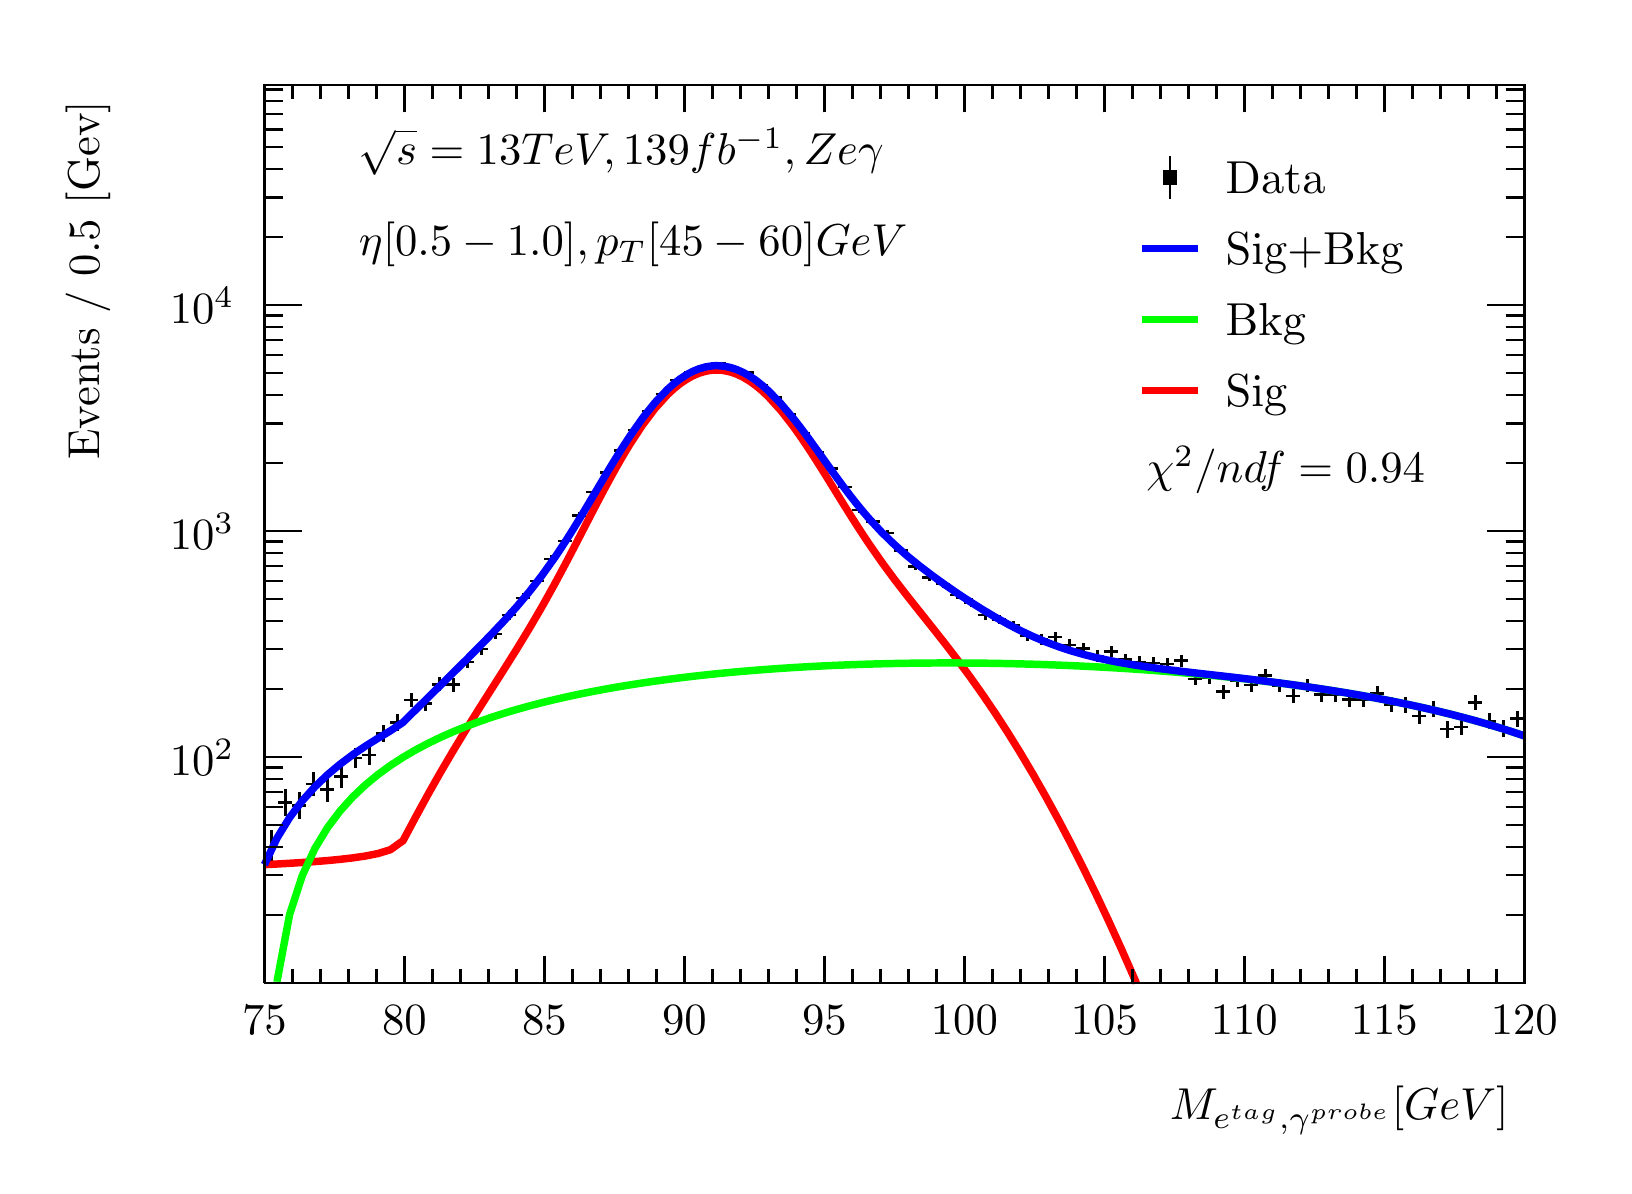
\begin{tikzpicture}
\pgfdeclareplotmark{cross} {
\pgfpathmoveto{\pgfpoint{-0.3\pgfplotmarksize}{\pgfplotmarksize}}
\pgfpathlineto{\pgfpoint{+0.3\pgfplotmarksize}{\pgfplotmarksize}}
\pgfpathlineto{\pgfpoint{+0.3\pgfplotmarksize}{0.3\pgfplotmarksize}}
\pgfpathlineto{\pgfpoint{+1\pgfplotmarksize}{0.3\pgfplotmarksize}}
\pgfpathlineto{\pgfpoint{+1\pgfplotmarksize}{-0.3\pgfplotmarksize}}
\pgfpathlineto{\pgfpoint{+0.3\pgfplotmarksize}{-0.3\pgfplotmarksize}}
\pgfpathlineto{\pgfpoint{+0.3\pgfplotmarksize}{-1.\pgfplotmarksize}}
\pgfpathlineto{\pgfpoint{-0.3\pgfplotmarksize}{-1.\pgfplotmarksize}}
\pgfpathlineto{\pgfpoint{-0.3\pgfplotmarksize}{-0.3\pgfplotmarksize}}
\pgfpathlineto{\pgfpoint{-1.\pgfplotmarksize}{-0.3\pgfplotmarksize}}
\pgfpathlineto{\pgfpoint{-1.\pgfplotmarksize}{0.3\pgfplotmarksize}}
\pgfpathlineto{\pgfpoint{-0.3\pgfplotmarksize}{0.3\pgfplotmarksize}}
\pgfpathclose
\pgfusepathqstroke
}
\pgfdeclareplotmark{cross*} {
\pgfpathmoveto{\pgfpoint{-0.3\pgfplotmarksize}{\pgfplotmarksize}}
\pgfpathlineto{\pgfpoint{+0.3\pgfplotmarksize}{\pgfplotmarksize}}
\pgfpathlineto{\pgfpoint{+0.3\pgfplotmarksize}{0.3\pgfplotmarksize}}
\pgfpathlineto{\pgfpoint{+1\pgfplotmarksize}{0.3\pgfplotmarksize}}
\pgfpathlineto{\pgfpoint{+1\pgfplotmarksize}{-0.3\pgfplotmarksize}}
\pgfpathlineto{\pgfpoint{+0.3\pgfplotmarksize}{-0.3\pgfplotmarksize}}
\pgfpathlineto{\pgfpoint{+0.3\pgfplotmarksize}{-1.\pgfplotmarksize}}
\pgfpathlineto{\pgfpoint{-0.3\pgfplotmarksize}{-1.\pgfplotmarksize}}
\pgfpathlineto{\pgfpoint{-0.3\pgfplotmarksize}{-0.3\pgfplotmarksize}}
\pgfpathlineto{\pgfpoint{-1.\pgfplotmarksize}{-0.3\pgfplotmarksize}}
\pgfpathlineto{\pgfpoint{-1.\pgfplotmarksize}{0.3\pgfplotmarksize}}
\pgfpathlineto{\pgfpoint{-0.3\pgfplotmarksize}{0.3\pgfplotmarksize}}
\pgfpathclose
\pgfusepathqfillstroke
}
\pgfdeclareplotmark{newstar} {
\pgfpathmoveto{\pgfqpoint{0pt}{\pgfplotmarksize}}
\pgfpathlineto{\pgfqpointpolar{44}{0.5\pgfplotmarksize}}
\pgfpathlineto{\pgfqpointpolar{18}{\pgfplotmarksize}}
\pgfpathlineto{\pgfqpointpolar{-20}{0.5\pgfplotmarksize}}
\pgfpathlineto{\pgfqpointpolar{-54}{\pgfplotmarksize}}
\pgfpathlineto{\pgfqpointpolar{-90}{0.5\pgfplotmarksize}}
\pgfpathlineto{\pgfqpointpolar{234}{\pgfplotmarksize}}
\pgfpathlineto{\pgfqpointpolar{198}{0.5\pgfplotmarksize}}
\pgfpathlineto{\pgfqpointpolar{162}{\pgfplotmarksize}}
\pgfpathlineto{\pgfqpointpolar{134}{0.5\pgfplotmarksize}}
\pgfpathclose
\pgfusepathqstroke
}
\pgfdeclareplotmark{newstar*} {
\pgfpathmoveto{\pgfqpoint{0pt}{\pgfplotmarksize}}
\pgfpathlineto{\pgfqpointpolar{44}{0.5\pgfplotmarksize}}
\pgfpathlineto{\pgfqpointpolar{18}{\pgfplotmarksize}}
\pgfpathlineto{\pgfqpointpolar{-20}{0.5\pgfplotmarksize}}
\pgfpathlineto{\pgfqpointpolar{-54}{\pgfplotmarksize}}
\pgfpathlineto{\pgfqpointpolar{-90}{0.5\pgfplotmarksize}}
\pgfpathlineto{\pgfqpointpolar{234}{\pgfplotmarksize}}
\pgfpathlineto{\pgfqpointpolar{198}{0.5\pgfplotmarksize}}
\pgfpathlineto{\pgfqpointpolar{162}{\pgfplotmarksize}}
\pgfpathlineto{\pgfqpointpolar{134}{0.5\pgfplotmarksize}}
\pgfpathclose
\pgfusepathqfillstroke
}
\definecolor{c}{rgb}{1,1,1};
\draw [color=c, fill=c] (0,0) rectangle (20,14.4361);
\draw [color=c, fill=c] (3,2.30977) rectangle (19,13.7143);
\definecolor{c}{rgb}{0,0,0};
\draw [c,line width=0.9] (3,2.30977) -- (3,13.7143) -- (19,13.7143) -- (19,2.30977) -- (3,2.30977);
\definecolor{c}{rgb}{1,1,1};
\draw [color=c, fill=c] (3,2.30977) rectangle (19,13.7143);
\definecolor{c}{rgb}{0,0,0};
\draw [c,line width=0.9] (3,2.30977) -- (3,13.7143) -- (19,13.7143) -- (19,2.30977) -- (3,2.30977);
\draw [c,line width=0.9] (3,2.30977) -- (19,2.30977);
\draw [c,line width=0.9] (3,2.65624) -- (3,2.30977);
\draw [c,line width=0.9] (3.35556,2.48301) -- (3.35556,2.30977);
\draw [c,line width=0.9] (3.71111,2.48301) -- (3.71111,2.30977);
\draw [c,line width=0.9] (4.06667,2.48301) -- (4.06667,2.30977);
\draw [c,line width=0.9] (4.42222,2.48301) -- (4.42222,2.30977);
\draw [c,line width=0.9] (4.77778,2.65624) -- (4.77778,2.30977);
\draw [c,line width=0.9] (5.13333,2.48301) -- (5.13333,2.30977);
\draw [c,line width=0.9] (5.48889,2.48301) -- (5.48889,2.30977);
\draw [c,line width=0.9] (5.84444,2.48301) -- (5.84444,2.30977);
\draw [c,line width=0.9] (6.2,2.48301) -- (6.2,2.30977);
\draw [c,line width=0.9] (6.55556,2.65624) -- (6.55556,2.30977);
\draw [c,line width=0.9] (6.91111,2.48301) -- (6.91111,2.30977);
\draw [c,line width=0.9] (7.26667,2.48301) -- (7.26667,2.30977);
\draw [c,line width=0.9] (7.62222,2.48301) -- (7.62222,2.30977);
\draw [c,line width=0.9] (7.97778,2.48301) -- (7.97778,2.30977);
\draw [c,line width=0.9] (8.33333,2.65624) -- (8.33333,2.30977);
\draw [c,line width=0.9] (8.68889,2.48301) -- (8.68889,2.30977);
\draw [c,line width=0.9] (9.04444,2.48301) -- (9.04444,2.30977);
\draw [c,line width=0.9] (9.4,2.48301) -- (9.4,2.30977);
\draw [c,line width=0.9] (9.75556,2.48301) -- (9.75556,2.30977);
\draw [c,line width=0.9] (10.1111,2.65624) -- (10.1111,2.30977);
\draw [c,line width=0.9] (10.4667,2.48301) -- (10.4667,2.30977);
\draw [c,line width=0.9] (10.8222,2.48301) -- (10.8222,2.30977);
\draw [c,line width=0.9] (11.1778,2.48301) -- (11.1778,2.30977);
\draw [c,line width=0.9] (11.5333,2.48301) -- (11.5333,2.30977);
\draw [c,line width=0.9] (11.8889,2.65624) -- (11.8889,2.30977);
\draw [c,line width=0.9] (12.2444,2.48301) -- (12.2444,2.30977);
\draw [c,line width=0.9] (12.6,2.48301) -- (12.6,2.30977);
\draw [c,line width=0.9] (12.9556,2.48301) -- (12.9556,2.30977);
\draw [c,line width=0.9] (13.3111,2.48301) -- (13.3111,2.30977);
\draw [c,line width=0.9] (13.6667,2.65624) -- (13.6667,2.30977);
\draw [c,line width=0.9] (14.0222,2.48301) -- (14.0222,2.30977);
\draw [c,line width=0.9] (14.3778,2.48301) -- (14.3778,2.30977);
\draw [c,line width=0.9] (14.7333,2.48301) -- (14.7333,2.30977);
\draw [c,line width=0.9] (15.0889,2.48301) -- (15.0889,2.30977);
\draw [c,line width=0.9] (15.4444,2.65624) -- (15.4444,2.30977);
\draw [c,line width=0.9] (15.8,2.48301) -- (15.8,2.30977);
\draw [c,line width=0.9] (16.1556,2.48301) -- (16.1556,2.30977);
\draw [c,line width=0.9] (16.5111,2.48301) -- (16.5111,2.30977);
\draw [c,line width=0.9] (16.8667,2.48301) -- (16.8667,2.30977);
\draw [c,line width=0.9] (17.2222,2.65624) -- (17.2222,2.30977);
\draw [c,line width=0.9] (17.5778,2.48301) -- (17.5778,2.30977);
\draw [c,line width=0.9] (17.9333,2.48301) -- (17.9333,2.30977);
\draw [c,line width=0.9] (18.2889,2.48301) -- (18.2889,2.30977);
\draw [c,line width=0.9] (18.6444,2.48301) -- (18.6444,2.30977);
\draw [c,line width=0.9] (19,2.65624) -- (19,2.30977);
\draw [c,line width=0.9] (19,2.65624) -- (19,2.30977);
\draw [anchor=base] (3,1.66015) node[scale=1.61424, color=c, rotate=0]{75};
\draw [anchor=base] (4.77778,1.66015) node[scale=1.61424, color=c, rotate=0]{80};
\draw [anchor=base] (6.55556,1.66015) node[scale=1.61424, color=c, rotate=0]{85};
\draw [anchor=base] (8.33333,1.66015) node[scale=1.61424, color=c, rotate=0]{90};
\draw [anchor=base] (10.1111,1.66015) node[scale=1.61424, color=c, rotate=0]{95};
\draw [anchor=base] (11.8889,1.66015) node[scale=1.61424, color=c, rotate=0]{100};
\draw [anchor=base] (13.6667,1.66015) node[scale=1.61424, color=c, rotate=0]{105};
\draw [anchor=base] (15.4444,1.66015) node[scale=1.61424, color=c, rotate=0]{110};
\draw [anchor=base] (17.2222,1.66015) node[scale=1.61424, color=c, rotate=0]{115};
\draw [anchor=base] (19,1.66015) node[scale=1.61424, color=c, rotate=0]{120};
\draw [anchor= east] (19,0.692932) node[scale=1.61424, color=c, rotate=0]{$M_{e^{tag}, \gamma^{probe}}  [GeV]$};
\draw [c,line width=0.9] (3,13.7143) -- (19,13.7143);
\draw [c,line width=0.9] (3,13.3678) -- (3,13.7143);
\draw [c,line width=0.9] (3.35556,13.5411) -- (3.35556,13.7143);
\draw [c,line width=0.9] (3.71111,13.5411) -- (3.71111,13.7143);
\draw [c,line width=0.9] (4.06667,13.5411) -- (4.06667,13.7143);
\draw [c,line width=0.9] (4.42222,13.5411) -- (4.42222,13.7143);
\draw [c,line width=0.9] (4.77778,13.3678) -- (4.77778,13.7143);
\draw [c,line width=0.9] (5.13333,13.5411) -- (5.13333,13.7143);
\draw [c,line width=0.9] (5.48889,13.5411) -- (5.48889,13.7143);
\draw [c,line width=0.9] (5.84444,13.5411) -- (5.84444,13.7143);
\draw [c,line width=0.9] (6.2,13.5411) -- (6.2,13.7143);
\draw [c,line width=0.9] (6.55556,13.3678) -- (6.55556,13.7143);
\draw [c,line width=0.9] (6.91111,13.5411) -- (6.91111,13.7143);
\draw [c,line width=0.9] (7.26667,13.5411) -- (7.26667,13.7143);
\draw [c,line width=0.9] (7.62222,13.5411) -- (7.62222,13.7143);
\draw [c,line width=0.9] (7.97778,13.5411) -- (7.97778,13.7143);
\draw [c,line width=0.9] (8.33333,13.3678) -- (8.33333,13.7143);
\draw [c,line width=0.9] (8.68889,13.5411) -- (8.68889,13.7143);
\draw [c,line width=0.9] (9.04444,13.5411) -- (9.04444,13.7143);
\draw [c,line width=0.9] (9.4,13.5411) -- (9.4,13.7143);
\draw [c,line width=0.9] (9.75556,13.5411) -- (9.75556,13.7143);
\draw [c,line width=0.9] (10.1111,13.3678) -- (10.1111,13.7143);
\draw [c,line width=0.9] (10.4667,13.5411) -- (10.4667,13.7143);
\draw [c,line width=0.9] (10.8222,13.5411) -- (10.8222,13.7143);
\draw [c,line width=0.9] (11.1778,13.5411) -- (11.1778,13.7143);
\draw [c,line width=0.9] (11.5333,13.5411) -- (11.5333,13.7143);
\draw [c,line width=0.9] (11.8889,13.3678) -- (11.8889,13.7143);
\draw [c,line width=0.9] (12.2444,13.5411) -- (12.2444,13.7143);
\draw [c,line width=0.9] (12.6,13.5411) -- (12.6,13.7143);
\draw [c,line width=0.9] (12.9556,13.5411) -- (12.9556,13.7143);
\draw [c,line width=0.9] (13.3111,13.5411) -- (13.3111,13.7143);
\draw [c,line width=0.9] (13.6667,13.3678) -- (13.6667,13.7143);
\draw [c,line width=0.9] (14.0222,13.5411) -- (14.0222,13.7143);
\draw [c,line width=0.9] (14.3778,13.5411) -- (14.3778,13.7143);
\draw [c,line width=0.9] (14.7333,13.5411) -- (14.7333,13.7143);
\draw [c,line width=0.9] (15.0889,13.5411) -- (15.0889,13.7143);
\draw [c,line width=0.9] (15.4444,13.3678) -- (15.4444,13.7143);
\draw [c,line width=0.9] (15.8,13.5411) -- (15.8,13.7143);
\draw [c,line width=0.9] (16.1556,13.5411) -- (16.1556,13.7143);
\draw [c,line width=0.9] (16.5111,13.5411) -- (16.5111,13.7143);
\draw [c,line width=0.9] (16.8667,13.5411) -- (16.8667,13.7143);
\draw [c,line width=0.9] (17.2222,13.3678) -- (17.2222,13.7143);
\draw [c,line width=0.9] (17.5778,13.5411) -- (17.5778,13.7143);
\draw [c,line width=0.9] (17.9333,13.5411) -- (17.9333,13.7143);
\draw [c,line width=0.9] (18.2889,13.5411) -- (18.2889,13.7143);
\draw [c,line width=0.9] (18.6444,13.5411) -- (18.6444,13.7143);
\draw [c,line width=0.9] (19,13.3678) -- (19,13.7143);
\draw [c,line width=0.9] (19,13.3678) -- (19,13.7143);
\draw [c,line width=0.9] (3,2.30977) -- (3,13.7143);
\draw [c,line width=0.9] (3.237,3.17371) -- (3,3.17371);
\draw [c,line width=0.9] (3.237,3.67908) -- (3,3.67908);
\draw [c,line width=0.9] (3.237,4.03764) -- (3,4.03764);
\draw [c,line width=0.9] (3.237,4.31577) -- (3,4.31577);
\draw [c,line width=0.9] (3.237,4.54301) -- (3,4.54301);
\draw [c,line width=0.9] (3.237,4.73514) -- (3,4.73514);
\draw [c,line width=0.9] (3.237,4.90158) -- (3,4.90158);
\draw [c,line width=0.9] (3.237,5.04838) -- (3,5.04838);
\draw [c,line width=0.9] (3.474,5.1797) -- (3,5.1797);
\draw [anchor= east] (2.82,5.1797) node[scale=1.61424, color=c, rotate=0]{$10^{2}$};
\draw [c,line width=0.9] (3.237,6.04363) -- (3,6.04363);
\draw [c,line width=0.9] (3.237,6.549) -- (3,6.549);
\draw [c,line width=0.9] (3.237,6.90757) -- (3,6.90757);
\draw [c,line width=0.9] (3.237,7.18569) -- (3,7.18569);
\draw [c,line width=0.9] (3.237,7.41294) -- (3,7.41294);
\draw [c,line width=0.9] (3.237,7.60507) -- (3,7.60507);
\draw [c,line width=0.9] (3.237,7.7715) -- (3,7.7715);
\draw [c,line width=0.9] (3.237,7.91831) -- (3,7.91831);
\draw [c,line width=0.9] (3.474,8.04963) -- (3,8.04963);
\draw [anchor= east] (2.82,8.04963) node[scale=1.61424, color=c, rotate=0]{$10^{3}$};
\draw [c,line width=0.9] (3.237,8.91356) -- (3,8.91356);
\draw [c,line width=0.9] (3.237,9.41893) -- (3,9.41893);
\draw [c,line width=0.9] (3.237,9.7775) -- (3,9.7775);
\draw [c,line width=0.9] (3.237,10.0556) -- (3,10.0556);
\draw [c,line width=0.9] (3.237,10.2829) -- (3,10.2829);
\draw [c,line width=0.9] (3.237,10.475) -- (3,10.475);
\draw [c,line width=0.9] (3.237,10.6414) -- (3,10.6414);
\draw [c,line width=0.9] (3.237,10.7882) -- (3,10.7882);
\draw [c,line width=0.9] (3.474,10.9196) -- (3,10.9196);
\draw [anchor= east] (2.82,10.9196) node[scale=1.61424, color=c, rotate=0]{$10^{4}$};
\draw [c,line width=0.9] (3.237,11.7835) -- (3,11.7835);
\draw [c,line width=0.9] (3.237,12.2889) -- (3,12.2889);
\draw [c,line width=0.9] (3.237,12.6474) -- (3,12.6474);
\draw [c,line width=0.9] (3.237,12.9256) -- (3,12.9256);
\draw [c,line width=0.9] (3.237,13.1528) -- (3,13.1528);
\draw [c,line width=0.9] (3.237,13.3449) -- (3,13.3449);
\draw [c,line width=0.9] (3.237,13.5114) -- (3,13.5114);
\draw [c,line width=0.9] (3.237,13.6582) -- (3,13.6582);
\draw [anchor= east] (0.76,13.7143) node[scale=1.61424, color=c, rotate=90]{Events / 0.5 [Gev]};
\draw [c,line width=0.9] (19,2.30977) -- (19,13.7143);
\draw [c,line width=0.9] (18.763,3.17371) -- (19,3.17371);
\draw [c,line width=0.9] (18.763,3.67908) -- (19,3.67908);
\draw [c,line width=0.9] (18.763,4.03764) -- (19,4.03764);
\draw [c,line width=0.9] (18.763,4.31577) -- (19,4.31577);
\draw [c,line width=0.9] (18.763,4.54301) -- (19,4.54301);
\draw [c,line width=0.9] (18.763,4.73514) -- (19,4.73514);
\draw [c,line width=0.9] (18.763,4.90158) -- (19,4.90158);
\draw [c,line width=0.9] (18.763,5.04838) -- (19,5.04838);
\draw [c,line width=0.9] (18.526,5.1797) -- (19,5.1797);
\draw [c,line width=0.9] (18.763,6.04363) -- (19,6.04363);
\draw [c,line width=0.9] (18.763,6.549) -- (19,6.549);
\draw [c,line width=0.9] (18.763,6.90757) -- (19,6.90757);
\draw [c,line width=0.9] (18.763,7.18569) -- (19,7.18569);
\draw [c,line width=0.9] (18.763,7.41294) -- (19,7.41294);
\draw [c,line width=0.9] (18.763,7.60507) -- (19,7.60507);
\draw [c,line width=0.9] (18.763,7.7715) -- (19,7.7715);
\draw [c,line width=0.9] (18.763,7.91831) -- (19,7.91831);
\draw [c,line width=0.9] (18.526,8.04963) -- (19,8.04963);
\draw [c,line width=0.9] (18.763,8.91356) -- (19,8.91356);
\draw [c,line width=0.9] (18.763,9.41893) -- (19,9.41893);
\draw [c,line width=0.9] (18.763,9.7775) -- (19,9.7775);
\draw [c,line width=0.9] (18.763,10.0556) -- (19,10.0556);
\draw [c,line width=0.9] (18.763,10.2829) -- (19,10.2829);
\draw [c,line width=0.9] (18.763,10.475) -- (19,10.475);
\draw [c,line width=0.9] (18.763,10.6414) -- (19,10.6414);
\draw [c,line width=0.9] (18.763,10.7882) -- (19,10.7882);
\draw [c,line width=0.9] (18.526,10.9196) -- (19,10.9196);
\draw [c,line width=0.9] (18.763,11.7835) -- (19,11.7835);
\draw [c,line width=0.9] (18.763,12.2889) -- (19,12.2889);
\draw [c,line width=0.9] (18.763,12.6474) -- (19,12.6474);
\draw [c,line width=0.9] (18.763,12.9256) -- (19,12.9256);
\draw [c,line width=0.9] (18.763,13.1528) -- (19,13.1528);
\draw [c,line width=0.9] (18.763,13.3449) -- (19,13.3449);
\draw [c,line width=0.9] (18.763,13.5114) -- (19,13.5114);
\draw [c,line width=0.9] (18.763,13.6582) -- (19,13.6582);
\draw [c,line width=0.9] (3.08889,4.03764) -- (3,4.03764);
\draw [c,line width=0.9] (3,4.03764) -- (3,4.03764);
\draw [c,line width=0.9] (3.08889,4.03764) -- (3.17778,4.03764);
\draw [c,line width=0.9] (3.17778,4.03764) -- (3.17778,4.03764);
\draw [c,line width=0.9] (3.08889,4.03764) -- (3.08889,4.24861);
\draw [c,line width=0.9] (3.08889,4.24861) -- (3.08889,4.24861);
\draw [c,line width=0.9] (3.08889,4.03764) -- (3.08889,3.82411);
\draw [c,line width=0.9] (3.08889,3.82411) -- (3.08889,3.82411);
\draw [c,line width=0.9] (3.26667,4.60382) -- (3.17778,4.60382);
\draw [c,line width=0.9] (3.17778,4.60382) -- (3.17778,4.60382);
\draw [c,line width=0.9] (3.26667,4.60382) -- (3.35556,4.60382);
\draw [c,line width=0.9] (3.35556,4.60382) -- (3.35556,4.60382);
\draw [c,line width=0.9] (3.26667,4.60382) -- (3.26667,4.7699);
\draw [c,line width=0.9] (3.26667,4.7699) -- (3.26667,4.7699);
\draw [c,line width=0.9] (3.26667,4.60382) -- (3.26667,4.43646);
\draw [c,line width=0.9] (3.26667,4.43646) -- (3.26667,4.43646);
\draw [c,line width=0.9] (3.44444,4.56361) -- (3.35556,4.56361);
\draw [c,line width=0.9] (3.35556,4.56361) -- (3.35556,4.56361);
\draw [c,line width=0.9] (3.44444,4.56361) -- (3.53333,4.56361);
\draw [c,line width=0.9] (3.53333,4.56361) -- (3.53333,4.56361);
\draw [c,line width=0.9] (3.44444,4.56361) -- (3.44444,4.73252);
\draw [c,line width=0.9] (3.44444,4.73252) -- (3.44444,4.73252);
\draw [c,line width=0.9] (3.44444,4.56361) -- (3.44444,4.39335);
\draw [c,line width=0.9] (3.44444,4.39335) -- (3.44444,4.39335);
\draw [c,line width=0.9] (3.62222,4.83765) -- (3.53333,4.83765);
\draw [c,line width=0.9] (3.53333,4.83765) -- (3.53333,4.83765);
\draw [c,line width=0.9] (3.62222,4.83765) -- (3.71111,4.83765);
\draw [c,line width=0.9] (3.71111,4.83765) -- (3.71111,4.83765);
\draw [c,line width=0.9] (3.62222,4.83765) -- (3.62222,4.98818);
\draw [c,line width=0.9] (3.62222,4.98818) -- (3.62222,4.98818);
\draw [c,line width=0.9] (3.62222,4.83765) -- (3.62222,4.68614);
\draw [c,line width=0.9] (3.62222,4.68614) -- (3.62222,4.68614);
\draw [c,line width=0.9] (3.8,4.77026) -- (3.71111,4.77026);
\draw [c,line width=0.9] (3.71111,4.77026) -- (3.71111,4.77026);
\draw [c,line width=0.9] (3.8,4.77026) -- (3.88889,4.77026);
\draw [c,line width=0.9] (3.88889,4.77026) -- (3.88889,4.77026);
\draw [c,line width=0.9] (3.8,4.77026) -- (3.8,4.92511);
\draw [c,line width=0.9] (3.8,4.92511) -- (3.8,4.92511);
\draw [c,line width=0.9] (3.8,4.77026) -- (3.8,4.61435);
\draw [c,line width=0.9] (3.8,4.61435) -- (3.8,4.61435);
\draw [c,line width=0.9] (3.97778,4.93235) -- (3.88889,4.93235);
\draw [c,line width=0.9] (3.88889,4.93235) -- (3.88889,4.93235);
\draw [c,line width=0.9] (3.97778,4.93235) -- (4.06667,4.93235);
\draw [c,line width=0.9] (4.06667,4.93235) -- (4.06667,4.93235);
\draw [c,line width=0.9] (3.97778,4.93235) -- (3.97778,5.07702);
\draw [c,line width=0.9] (3.97778,5.07702) -- (3.97778,5.07702);
\draw [c,line width=0.9] (3.97778,4.93235) -- (3.97778,4.78682);
\draw [c,line width=0.9] (3.97778,4.78682) -- (3.97778,4.78682);
\draw [c,line width=0.9] (4.15556,5.16718) -- (4.06667,5.16718);
\draw [c,line width=0.9] (4.06667,5.16718) -- (4.06667,5.16718);
\draw [c,line width=0.9] (4.15556,5.16718) -- (4.24444,5.16718);
\draw [c,line width=0.9] (4.24444,5.16718) -- (4.24444,5.16718);
\draw [c,line width=0.9] (4.15556,5.16718) -- (4.15556,5.29831);
\draw [c,line width=0.9] (4.15556,5.29831) -- (4.15556,5.29831);
\draw [c,line width=0.9] (4.15556,5.16718) -- (4.15556,5.03539);
\draw [c,line width=0.9] (4.15556,5.03539) -- (4.15556,5.03539);
\draw [c,line width=0.9] (4.33333,5.20438) -- (4.24444,5.20438);
\draw [c,line width=0.9] (4.24444,5.20438) -- (4.24444,5.20438);
\draw [c,line width=0.9] (4.33333,5.20438) -- (4.42222,5.20438);
\draw [c,line width=0.9] (4.42222,5.20438) -- (4.42222,5.20438);
\draw [c,line width=0.9] (4.33333,5.20438) -- (4.33333,5.32774);
\draw [c,line width=0.9] (4.33333,5.32774) -- (4.33333,5.32774);
\draw [c,line width=0.9] (4.33333,5.20438) -- (4.33333,5.08102);
\draw [c,line width=0.9] (4.33333,5.08102) -- (4.33333,5.08102);
\draw [c,line width=0.9] (4.51111,5.47761) -- (4.42222,5.47761);
\draw [c,line width=0.9] (4.42222,5.47761) -- (4.42222,5.47761);
\draw [c,line width=0.9] (4.51111,5.47761) -- (4.6,5.47761);
\draw [c,line width=0.9] (4.6,5.47761) -- (4.6,5.47761);
\draw [c,line width=0.9] (4.51111,5.47761) -- (4.51111,5.58817);
\draw [c,line width=0.9] (4.51111,5.58817) -- (4.51111,5.58817);
\draw [c,line width=0.9] (4.51111,5.47761) -- (4.51111,5.36705);
\draw [c,line width=0.9] (4.51111,5.36705) -- (4.51111,5.36705);
\draw [c,line width=0.9] (4.68889,5.61676) -- (4.6,5.61676);
\draw [c,line width=0.9] (4.6,5.61676) -- (4.6,5.61676);
\draw [c,line width=0.9] (4.68889,5.61676) -- (4.77778,5.61676);
\draw [c,line width=0.9] (4.77778,5.61676) -- (4.77778,5.61676);
\draw [c,line width=0.9] (4.68889,5.61676) -- (4.68889,5.72132);
\draw [c,line width=0.9] (4.68889,5.72132) -- (4.68889,5.72132);
\draw [c,line width=0.9] (4.68889,5.61676) -- (4.68889,5.51219);
\draw [c,line width=0.9] (4.68889,5.51219) -- (4.68889,5.51219);
\draw [c,line width=0.9] (4.86667,5.90537) -- (4.77778,5.90537);
\draw [c,line width=0.9] (4.77778,5.90537) -- (4.77778,5.90537);
\draw [c,line width=0.9] (4.86667,5.90537) -- (4.95556,5.90537);
\draw [c,line width=0.9] (4.95556,5.90537) -- (4.95556,5.90537);
\draw [c,line width=0.9] (4.86667,5.90537) -- (4.86667,5.99851);
\draw [c,line width=0.9] (4.86667,5.99851) -- (4.86667,5.99851);
\draw [c,line width=0.9] (4.86667,5.90537) -- (4.86667,5.81223);
\draw [c,line width=0.9] (4.86667,5.81223) -- (4.86667,5.81223);
\draw [c,line width=0.9] (5.04444,5.86288) -- (4.95556,5.86288);
\draw [c,line width=0.9] (4.95556,5.86288) -- (4.95556,5.86288);
\draw [c,line width=0.9] (5.04444,5.86288) -- (5.13333,5.86288);
\draw [c,line width=0.9] (5.13333,5.86288) -- (5.13333,5.86288);
\draw [c,line width=0.9] (5.04444,5.86288) -- (5.04444,5.95762);
\draw [c,line width=0.9] (5.04444,5.95762) -- (5.04444,5.95762);
\draw [c,line width=0.9] (5.04444,5.86288) -- (5.04444,5.76814);
\draw [c,line width=0.9] (5.04444,5.76814) -- (5.04444,5.76814);
\draw [c,line width=0.9] (5.22222,6.10445) -- (5.13333,6.10445);
\draw [c,line width=0.9] (5.13333,6.10445) -- (5.13333,6.10445);
\draw [c,line width=0.9] (5.22222,6.10445) -- (5.31111,6.10445);
\draw [c,line width=0.9] (5.31111,6.10445) -- (5.31111,6.10445);
\draw [c,line width=0.9] (5.22222,6.10445) -- (5.22222,6.19044);
\draw [c,line width=0.9] (5.22222,6.19044) -- (5.22222,6.19044);
\draw [c,line width=0.9] (5.22222,6.10445) -- (5.22222,6.01846);
\draw [c,line width=0.9] (5.22222,6.01846) -- (5.22222,6.01846);
\draw [c,line width=0.9] (5.4,6.0985) -- (5.31111,6.0985);
\draw [c,line width=0.9] (5.31111,6.0985) -- (5.31111,6.0985);
\draw [c,line width=0.9] (5.4,6.0985) -- (5.48889,6.0985);
\draw [c,line width=0.9] (5.48889,6.0985) -- (5.48889,6.0985);
\draw [c,line width=0.9] (5.4,6.0985) -- (5.4,6.1847);
\draw [c,line width=0.9] (5.4,6.1847) -- (5.4,6.1847);
\draw [c,line width=0.9] (5.4,6.0985) -- (5.4,6.0123);
\draw [c,line width=0.9] (5.4,6.0123) -- (5.4,6.0123);
\draw [c,line width=0.9] (5.57778,6.38968) -- (5.48889,6.38968);
\draw [c,line width=0.9] (5.48889,6.38968) -- (5.48889,6.38968);
\draw [c,line width=0.9] (5.57778,6.38968) -- (5.66667,6.38968);
\draw [c,line width=0.9] (5.66667,6.38968) -- (5.66667,6.38968);
\draw [c,line width=0.9] (5.57778,6.38968) -- (5.57778,6.46637);
\draw [c,line width=0.9] (5.57778,6.46637) -- (5.57778,6.46637);
\draw [c,line width=0.9] (5.57778,6.38968) -- (5.57778,6.31298);
\draw [c,line width=0.9] (5.57778,6.31298) -- (5.57778,6.31298);
\draw [c,line width=0.9] (5.75556,6.55315) -- (5.66667,6.55315);
\draw [c,line width=0.9] (5.66667,6.55315) -- (5.66667,6.55315);
\draw [c,line width=0.9] (5.75556,6.55315) -- (5.84444,6.55315);
\draw [c,line width=0.9] (5.84444,6.55315) -- (5.84444,6.55315);
\draw [c,line width=0.9] (5.75556,6.55315) -- (5.75556,6.62498);
\draw [c,line width=0.9] (5.75556,6.62498) -- (5.75556,6.62498);
\draw [c,line width=0.9] (5.75556,6.55315) -- (5.75556,6.48132);
\draw [c,line width=0.9] (5.75556,6.48132) -- (5.75556,6.48132);
\draw [c,line width=0.9] (5.93333,6.74114) -- (5.84444,6.74114);
\draw [c,line width=0.9] (5.84444,6.74114) -- (5.84444,6.74114);
\draw [c,line width=0.9] (5.93333,6.74114) -- (6.02222,6.74114);
\draw [c,line width=0.9] (6.02222,6.74114) -- (6.02222,6.74114);
\draw [c,line width=0.9] (5.93333,6.74114) -- (5.93333,6.80775);
\draw [c,line width=0.9] (5.93333,6.80775) -- (5.93333,6.80775);
\draw [c,line width=0.9] (5.93333,6.74114) -- (5.93333,6.67452);
\draw [c,line width=0.9] (5.93333,6.67452) -- (5.93333,6.67452);
\draw [c,line width=0.9] (6.11111,6.98313) -- (6.02222,6.98313);
\draw [c,line width=0.9] (6.02222,6.98313) -- (6.02222,6.98313);
\draw [c,line width=0.9] (6.11111,6.98313) -- (6.2,6.98313);
\draw [c,line width=0.9] (6.2,6.98313) -- (6.2,6.98313);
\draw [c,line width=0.9] (6.11111,6.98313) -- (6.11111,7.04359);
\draw [c,line width=0.9] (6.11111,7.04359) -- (6.11111,7.04359);
\draw [c,line width=0.9] (6.11111,6.98313) -- (6.11111,6.92268);
\draw [c,line width=0.9] (6.11111,6.92268) -- (6.11111,6.92268);
\draw [c,line width=0.9] (6.28889,7.20302) -- (6.2,7.20302);
\draw [c,line width=0.9] (6.2,7.20302) -- (6.2,7.20302);
\draw [c,line width=0.9] (6.28889,7.20302) -- (6.37778,7.20302);
\draw [c,line width=0.9] (6.37778,7.20302) -- (6.37778,7.20302);
\draw [c,line width=0.9] (6.28889,7.20302) -- (6.28889,7.25837);
\draw [c,line width=0.9] (6.28889,7.25837) -- (6.28889,7.25837);
\draw [c,line width=0.9] (6.28889,7.20302) -- (6.28889,7.14767);
\draw [c,line width=0.9] (6.28889,7.14767) -- (6.28889,7.14767);
\draw [c,line width=0.9] (6.46667,7.41709) -- (6.37778,7.41709);
\draw [c,line width=0.9] (6.37778,7.41709) -- (6.37778,7.41709);
\draw [c,line width=0.9] (6.46667,7.41709) -- (6.55556,7.41709);
\draw [c,line width=0.9] (6.55556,7.41709) -- (6.55556,7.41709);
\draw [c,line width=0.9] (6.46667,7.41709) -- (6.46667,7.46788);
\draw [c,line width=0.9] (6.46667,7.46788) -- (6.46667,7.46788);
\draw [c,line width=0.9] (6.46667,7.41709) -- (6.46667,7.36629);
\draw [c,line width=0.9] (6.46667,7.36629) -- (6.46667,7.36629);
\draw [c,line width=0.9] (6.64444,7.69769) -- (6.55556,7.69769);
\draw [c,line width=0.9] (6.55556,7.69769) -- (6.55556,7.69769);
\draw [c,line width=0.9] (6.64444,7.69769) -- (6.73333,7.69769);
\draw [c,line width=0.9] (6.73333,7.69769) -- (6.73333,7.69769);
\draw [c,line width=0.9] (6.64444,7.69769) -- (6.64444,7.74308);
\draw [c,line width=0.9] (6.64444,7.74308) -- (6.64444,7.74308);
\draw [c,line width=0.9] (6.64444,7.69769) -- (6.64444,7.65231);
\draw [c,line width=0.9] (6.64444,7.65231) -- (6.64444,7.65231);
\draw [c,line width=0.9] (6.82222,7.92659) -- (6.73333,7.92659);
\draw [c,line width=0.9] (6.73333,7.92659) -- (6.73333,7.92659);
\draw [c,line width=0.9] (6.82222,7.92659) -- (6.91111,7.92659);
\draw [c,line width=0.9] (6.91111,7.92659) -- (6.91111,7.92659);
\draw [c,line width=0.9] (6.82222,7.92659) -- (6.82222,7.968);
\draw [c,line width=0.9] (6.82222,7.968) -- (6.82222,7.968);
\draw [c,line width=0.9] (6.82222,7.92659) -- (6.82222,7.88518);
\draw [c,line width=0.9] (6.82222,7.88518) -- (6.82222,7.88518);
\draw [c,line width=0.9] (7,8.24957) -- (6.91111,8.24957);
\draw [c,line width=0.9] (6.91111,8.24957) -- (6.91111,8.24957);
\draw [c,line width=0.9] (7,8.24957) -- (7.08889,8.24957);
\draw [c,line width=0.9] (7.08889,8.24957) -- (7.08889,8.24957);
\draw [c,line width=0.9] (7,8.24957) -- (7,8.28595);
\draw [c,line width=0.9] (7,8.28595) -- (7,8.28595);
\draw [c,line width=0.9] (7,8.24957) -- (7,8.2132);
\draw [c,line width=0.9] (7,8.2132) -- (7,8.2132);
\draw [c,line width=0.9] (7.17778,8.54331) -- (7.08889,8.54331);
\draw [c,line width=0.9] (7.08889,8.54331) -- (7.08889,8.54331);
\draw [c,line width=0.9] (7.17778,8.54331) -- (7.26667,8.54331);
\draw [c,line width=0.9] (7.26667,8.54331) -- (7.26667,8.54331);
\draw [c,line width=0.9] (7.17778,8.54331) -- (7.17778,8.57564);
\draw [c,line width=0.9] (7.17778,8.57564) -- (7.17778,8.57564);
\draw [c,line width=0.9] (7.17778,8.54331) -- (7.17778,8.51098);
\draw [c,line width=0.9] (7.17778,8.51098) -- (7.17778,8.51098);
\draw [c,line width=0.9] (7.35556,8.7967) -- (7.26667,8.7967);
\draw [c,line width=0.9] (7.26667,8.7967) -- (7.26667,8.7967);
\draw [c,line width=0.9] (7.35556,8.7967) -- (7.44444,8.7967);
\draw [c,line width=0.9] (7.44444,8.7967) -- (7.44444,8.7967);
\draw [c,line width=0.9] (7.35556,8.7967) -- (7.35556,8.82591);
\draw [c,line width=0.9] (7.35556,8.82591) -- (7.35556,8.82591);
\draw [c,line width=0.9] (7.35556,8.7967) -- (7.35556,8.76749);
\draw [c,line width=0.9] (7.35556,8.76749) -- (7.35556,8.76749);
\draw [c,line width=0.9] (7.53333,9.07414) -- (7.44444,9.07414);
\draw [c,line width=0.9] (7.44444,9.07414) -- (7.44444,9.07414);
\draw [c,line width=0.9] (7.53333,9.07414) -- (7.62222,9.07414);
\draw [c,line width=0.9] (7.62222,9.07414) -- (7.62222,9.07414);
\draw [c,line width=0.9] (7.53333,9.07414) -- (7.53333,9.10027);
\draw [c,line width=0.9] (7.53333,9.10027) -- (7.53333,9.10027);
\draw [c,line width=0.9] (7.53333,9.07414) -- (7.53333,9.04801);
\draw [c,line width=0.9] (7.53333,9.04801) -- (7.53333,9.04801);
\draw [c,line width=0.9] (7.71111,9.33027) -- (7.62222,9.33027);
\draw [c,line width=0.9] (7.62222,9.33027) -- (7.62222,9.33027);
\draw [c,line width=0.9] (7.71111,9.33027) -- (7.8,9.33027);
\draw [c,line width=0.9] (7.8,9.33027) -- (7.8,9.33027);
\draw [c,line width=0.9] (7.71111,9.33027) -- (7.71111,9.35385);
\draw [c,line width=0.9] (7.71111,9.35385) -- (7.71111,9.35385);
\draw [c,line width=0.9] (7.71111,9.33027) -- (7.71111,9.30669);
\draw [c,line width=0.9] (7.71111,9.30669) -- (7.71111,9.30669);
\draw [c,line width=0.9] (7.88889,9.57677) -- (7.8,9.57677);
\draw [c,line width=0.9] (7.8,9.57677) -- (7.8,9.57677);
\draw [c,line width=0.9] (7.88889,9.57677) -- (7.97778,9.57677);
\draw [c,line width=0.9] (7.97778,9.57677) -- (7.97778,9.57677);
\draw [c,line width=0.9] (7.88889,9.57677) -- (7.88889,9.59813);
\draw [c,line width=0.9] (7.88889,9.59813) -- (7.88889,9.59813);
\draw [c,line width=0.9] (7.88889,9.57677) -- (7.88889,9.55541);
\draw [c,line width=0.9] (7.88889,9.55541) -- (7.88889,9.55541);
\draw [c,line width=0.9] (8.06667,9.78897) -- (7.97778,9.78897);
\draw [c,line width=0.9] (7.97778,9.78897) -- (7.97778,9.78897);
\draw [c,line width=0.9] (8.06667,9.78897) -- (8.15556,9.78897);
\draw [c,line width=0.9] (8.15556,9.78897) -- (8.15556,9.78897);
\draw [c,line width=0.9] (8.06667,9.78897) -- (8.06667,9.80859);
\draw [c,line width=0.9] (8.06667,9.80859) -- (8.06667,9.80859);
\draw [c,line width=0.9] (8.06667,9.78897) -- (8.06667,9.76936);
\draw [c,line width=0.9] (8.06667,9.76936) -- (8.06667,9.76936);
\draw [c,line width=0.9] (8.24444,9.97132) -- (8.15556,9.97132);
\draw [c,line width=0.9] (8.15556,9.97132) -- (8.15556,9.97132);
\draw [c,line width=0.9] (8.24444,9.97132) -- (8.33333,9.97132);
\draw [c,line width=0.9] (8.33333,9.97132) -- (8.33333,9.97132);
\draw [c,line width=0.9] (8.24444,9.97132) -- (8.24444,9.98955);
\draw [c,line width=0.9] (8.24444,9.98955) -- (8.24444,9.98955);
\draw [c,line width=0.9] (8.24444,9.97132) -- (8.24444,9.95309);
\draw [c,line width=0.9] (8.24444,9.95309) -- (8.24444,9.95309);
\draw [c,line width=0.9] (8.42222,10.0702) -- (8.33333,10.0702);
\draw [c,line width=0.9] (8.33333,10.0702) -- (8.33333,10.0702);
\draw [c,line width=0.9] (8.42222,10.0702) -- (8.51111,10.0702);
\draw [c,line width=0.9] (8.51111,10.0702) -- (8.51111,10.0702);
\draw [c,line width=0.9] (8.42222,10.0702) -- (8.42222,10.0878);
\draw [c,line width=0.9] (8.42222,10.0878) -- (8.42222,10.0878);
\draw [c,line width=0.9] (8.42222,10.0702) -- (8.42222,10.0527);
\draw [c,line width=0.9] (8.42222,10.0527) -- (8.42222,10.0527);
\draw [c,line width=0.9] (8.6,10.1129) -- (8.51111,10.1129);
\draw [c,line width=0.9] (8.51111,10.1129) -- (8.51111,10.1129);
\draw [c,line width=0.9] (8.6,10.1129) -- (8.68889,10.1129);
\draw [c,line width=0.9] (8.68889,10.1129) -- (8.68889,10.1129);
\draw [c,line width=0.9] (8.6,10.1129) -- (8.6,10.1301);
\draw [c,line width=0.9] (8.6,10.1301) -- (8.6,10.1301);
\draw [c,line width=0.9] (8.6,10.1129) -- (8.6,10.0956);
\draw [c,line width=0.9] (8.6,10.0956) -- (8.6,10.0956);
\draw [c,line width=0.9] (8.77778,10.1805) -- (8.68889,10.1805);
\draw [c,line width=0.9] (8.68889,10.1805) -- (8.68889,10.1805);
\draw [c,line width=0.9] (8.77778,10.1805) -- (8.86667,10.1805);
\draw [c,line width=0.9] (8.86667,10.1805) -- (8.86667,10.1805);
\draw [c,line width=0.9] (8.77778,10.1805) -- (8.77778,10.1973);
\draw [c,line width=0.9] (8.77778,10.1973) -- (8.77778,10.1973);
\draw [c,line width=0.9] (8.77778,10.1805) -- (8.77778,10.1638);
\draw [c,line width=0.9] (8.77778,10.1638) -- (8.77778,10.1638);
\draw [c,line width=0.9] (8.95556,10.1093) -- (8.86667,10.1093);
\draw [c,line width=0.9] (8.86667,10.1093) -- (8.86667,10.1093);
\draw [c,line width=0.9] (8.95556,10.1093) -- (9.04444,10.1093);
\draw [c,line width=0.9] (9.04444,10.1093) -- (9.04444,10.1093);
\draw [c,line width=0.9] (8.95556,10.1093) -- (8.95556,10.1265);
\draw [c,line width=0.9] (8.95556,10.1265) -- (8.95556,10.1265);
\draw [c,line width=0.9] (8.95556,10.1093) -- (8.95556,10.092);
\draw [c,line width=0.9] (8.95556,10.092) -- (8.95556,10.092);
\draw [c,line width=0.9] (9.13333,10.0663) -- (9.04444,10.0663);
\draw [c,line width=0.9] (9.04444,10.0663) -- (9.04444,10.0663);
\draw [c,line width=0.9] (9.13333,10.0663) -- (9.22222,10.0663);
\draw [c,line width=0.9] (9.22222,10.0663) -- (9.22222,10.0663);
\draw [c,line width=0.9] (9.13333,10.0663) -- (9.13333,10.0838);
\draw [c,line width=0.9] (9.13333,10.0838) -- (9.13333,10.0838);
\draw [c,line width=0.9] (9.13333,10.0663) -- (9.13333,10.0487);
\draw [c,line width=0.9] (9.13333,10.0487) -- (9.13333,10.0487);
\draw [c,line width=0.9] (9.31111,9.89969) -- (9.22222,9.89969);
\draw [c,line width=0.9] (9.22222,9.89969) -- (9.22222,9.89969);
\draw [c,line width=0.9] (9.31111,9.89969) -- (9.4,9.89969);
\draw [c,line width=0.9] (9.4,9.89969) -- (9.4,9.89969);
\draw [c,line width=0.9] (9.31111,9.89969) -- (9.31111,9.91845);
\draw [c,line width=0.9] (9.31111,9.91845) -- (9.31111,9.91845);
\draw [c,line width=0.9] (9.31111,9.89969) -- (9.31111,9.88092);
\draw [c,line width=0.9] (9.31111,9.88092) -- (9.31111,9.88092);
\draw [c,line width=0.9] (9.48889,9.74626) -- (9.4,9.74626);
\draw [c,line width=0.9] (9.4,9.74626) -- (9.4,9.74626);
\draw [c,line width=0.9] (9.48889,9.74626) -- (9.57778,9.74626);
\draw [c,line width=0.9] (9.57778,9.74626) -- (9.57778,9.74626);
\draw [c,line width=0.9] (9.48889,9.74626) -- (9.48889,9.76622);
\draw [c,line width=0.9] (9.48889,9.76622) -- (9.48889,9.76622);
\draw [c,line width=0.9] (9.48889,9.74626) -- (9.48889,9.72631);
\draw [c,line width=0.9] (9.48889,9.72631) -- (9.48889,9.72631);
\draw [c,line width=0.9] (9.66667,9.52863) -- (9.57778,9.52863);
\draw [c,line width=0.9] (9.57778,9.52863) -- (9.57778,9.52863);
\draw [c,line width=0.9] (9.66667,9.52863) -- (9.75556,9.52863);
\draw [c,line width=0.9] (9.75556,9.52863) -- (9.75556,9.52863);
\draw [c,line width=0.9] (9.66667,9.52863) -- (9.66667,9.55041);
\draw [c,line width=0.9] (9.66667,9.55041) -- (9.66667,9.55041);
\draw [c,line width=0.9] (9.66667,9.52863) -- (9.66667,9.50685);
\draw [c,line width=0.9] (9.66667,9.50685) -- (9.66667,9.50685);
\draw [c,line width=0.9] (9.84444,9.28992) -- (9.75556,9.28992);
\draw [c,line width=0.9] (9.75556,9.28992) -- (9.75556,9.28992);
\draw [c,line width=0.9] (9.84444,9.28992) -- (9.93333,9.28992);
\draw [c,line width=0.9] (9.93333,9.28992) -- (9.93333,9.28992);
\draw [c,line width=0.9] (9.84444,9.28992) -- (9.84444,9.31388);
\draw [c,line width=0.9] (9.84444,9.31388) -- (9.84444,9.31388);
\draw [c,line width=0.9] (9.84444,9.28992) -- (9.84444,9.26595);
\draw [c,line width=0.9] (9.84444,9.26595) -- (9.84444,9.26595);
\draw [c,line width=0.9] (10.0222,9.047) -- (9.93333,9.047);
\draw [c,line width=0.9] (9.93333,9.047) -- (9.93333,9.047);
\draw [c,line width=0.9] (10.0222,9.047) -- (10.1111,9.047);
\draw [c,line width=0.9] (10.1111,9.047) -- (10.1111,9.047);
\draw [c,line width=0.9] (10.0222,9.047) -- (10.0222,9.07342);
\draw [c,line width=0.9] (10.0222,9.07342) -- (10.0222,9.07342);
\draw [c,line width=0.9] (10.0222,9.047) -- (10.0222,9.02059);
\draw [c,line width=0.9] (10.0222,9.02059) -- (10.0222,9.02059);
\draw [c,line width=0.9] (10.2,8.84371) -- (10.1111,8.84371);
\draw [c,line width=0.9] (10.1111,8.84371) -- (10.1111,8.84371);
\draw [c,line width=0.9] (10.2,8.84371) -- (10.2889,8.84371);
\draw [c,line width=0.9] (10.2889,8.84371) -- (10.2889,8.84371);
\draw [c,line width=0.9] (10.2,8.84371) -- (10.2,8.87238);
\draw [c,line width=0.9] (10.2,8.87238) -- (10.2,8.87238);
\draw [c,line width=0.9] (10.2,8.84371) -- (10.2,8.81505);
\draw [c,line width=0.9] (10.2,8.81505) -- (10.2,8.81505);
\draw [c,line width=0.9] (10.3778,8.60867) -- (10.2889,8.60867);
\draw [c,line width=0.9] (10.2889,8.60867) -- (10.2889,8.60867);
\draw [c,line width=0.9] (10.3778,8.60867) -- (10.4667,8.60867);
\draw [c,line width=0.9] (10.4667,8.60867) -- (10.4667,8.60867);
\draw [c,line width=0.9] (10.3778,8.60867) -- (10.3778,8.64016);
\draw [c,line width=0.9] (10.3778,8.64016) -- (10.3778,8.64016);
\draw [c,line width=0.9] (10.3778,8.60867) -- (10.3778,8.57717);
\draw [c,line width=0.9] (10.3778,8.57717) -- (10.3778,8.57717);
\draw [c,line width=0.9] (10.5556,8.31774) -- (10.4667,8.31774);
\draw [c,line width=0.9] (10.4667,8.31774) -- (10.4667,8.31774);
\draw [c,line width=0.9] (10.5556,8.31774) -- (10.6444,8.31774);
\draw [c,line width=0.9] (10.6444,8.31774) -- (10.6444,8.31774);
\draw [c,line width=0.9] (10.5556,8.31774) -- (10.5556,8.35314);
\draw [c,line width=0.9] (10.5556,8.35314) -- (10.5556,8.35314);
\draw [c,line width=0.9] (10.5556,8.31774) -- (10.5556,8.28235);
\draw [c,line width=0.9] (10.5556,8.28235) -- (10.5556,8.28235);
\draw [c,line width=0.9] (10.7333,8.16956) -- (10.6444,8.16956);
\draw [c,line width=0.9] (10.6444,8.16956) -- (10.6444,8.16956);
\draw [c,line width=0.9] (10.7333,8.16956) -- (10.8222,8.16956);
\draw [c,line width=0.9] (10.8222,8.16956) -- (10.8222,8.16956);
\draw [c,line width=0.9] (10.7333,8.16956) -- (10.7333,8.20712);
\draw [c,line width=0.9] (10.7333,8.20712) -- (10.7333,8.20712);
\draw [c,line width=0.9] (10.7333,8.16956) -- (10.7333,8.132);
\draw [c,line width=0.9] (10.7333,8.132) -- (10.7333,8.132);
\draw [c,line width=0.9] (10.9111,8.02572) -- (10.8222,8.02572);
\draw [c,line width=0.9] (10.8222,8.02572) -- (10.8222,8.02572);
\draw [c,line width=0.9] (10.9111,8.02572) -- (11,8.02572);
\draw [c,line width=0.9] (11,8.02572) -- (11,8.02572);
\draw [c,line width=0.9] (10.9111,8.02572) -- (10.9111,8.06551);
\draw [c,line width=0.9] (10.9111,8.06551) -- (10.9111,8.06551);
\draw [c,line width=0.9] (10.9111,8.02572) -- (10.9111,7.98593);
\draw [c,line width=0.9] (10.9111,7.98593) -- (10.9111,7.98593);
\draw [c,line width=0.9] (11.0889,7.80532) -- (11,7.80532);
\draw [c,line width=0.9] (11,7.80532) -- (11,7.80532);
\draw [c,line width=0.9] (11.0889,7.80532) -- (11.1778,7.80532);
\draw [c,line width=0.9] (11.1778,7.80532) -- (11.1778,7.80532);
\draw [c,line width=0.9] (11.0889,7.80532) -- (11.0889,7.84879);
\draw [c,line width=0.9] (11.0889,7.84879) -- (11.0889,7.84879);
\draw [c,line width=0.9] (11.0889,7.80532) -- (11.0889,7.76185);
\draw [c,line width=0.9] (11.0889,7.76185) -- (11.0889,7.76185);
\draw [c,line width=0.9] (11.2667,7.59793) -- (11.1778,7.59793);
\draw [c,line width=0.9] (11.1778,7.59793) -- (11.1778,7.59793);
\draw [c,line width=0.9] (11.2667,7.59793) -- (11.3556,7.59793);
\draw [c,line width=0.9] (11.3556,7.59793) -- (11.3556,7.59793);
\draw [c,line width=0.9] (11.2667,7.59793) -- (11.2667,7.64517);
\draw [c,line width=0.9] (11.2667,7.64517) -- (11.2667,7.64517);
\draw [c,line width=0.9] (11.2667,7.59793) -- (11.2667,7.55069);
\draw [c,line width=0.9] (11.2667,7.55069) -- (11.2667,7.55069);
\draw [c,line width=0.9] (11.4444,7.46182) -- (11.3556,7.46182);
\draw [c,line width=0.9] (11.3556,7.46182) -- (11.3556,7.46182);
\draw [c,line width=0.9] (11.4444,7.46182) -- (11.5333,7.46182);
\draw [c,line width=0.9] (11.5333,7.46182) -- (11.5333,7.46182);
\draw [c,line width=0.9] (11.4444,7.46182) -- (11.4444,7.51172);
\draw [c,line width=0.9] (11.4444,7.51172) -- (11.4444,7.51172);
\draw [c,line width=0.9] (11.4444,7.46182) -- (11.4444,7.41193);
\draw [c,line width=0.9] (11.4444,7.41193) -- (11.4444,7.41193);
\draw [c,line width=0.9] (11.6222,7.37498) -- (11.5333,7.37498);
\draw [c,line width=0.9] (11.5333,7.37498) -- (11.5333,7.37498);
\draw [c,line width=0.9] (11.6222,7.37498) -- (11.7111,7.37498);
\draw [c,line width=0.9] (11.7111,7.37498) -- (11.7111,7.37498);
\draw [c,line width=0.9] (11.6222,7.37498) -- (11.6222,7.42664);
\draw [c,line width=0.9] (11.6222,7.42664) -- (11.6222,7.42664);
\draw [c,line width=0.9] (11.6222,7.37498) -- (11.6222,7.32332);
\draw [c,line width=0.9] (11.6222,7.32332) -- (11.6222,7.32332);
\draw [c,line width=0.9] (11.8,7.23936) -- (11.7111,7.23936);
\draw [c,line width=0.9] (11.7111,7.23936) -- (11.7111,7.23936);
\draw [c,line width=0.9] (11.8,7.23936) -- (11.8889,7.23936);
\draw [c,line width=0.9] (11.8889,7.23936) -- (11.8889,7.23936);
\draw [c,line width=0.9] (11.8,7.23936) -- (11.8,7.29391);
\draw [c,line width=0.9] (11.8,7.29391) -- (11.8,7.29391);
\draw [c,line width=0.9] (11.8,7.23936) -- (11.8,7.18482);
\draw [c,line width=0.9] (11.8,7.18482) -- (11.8,7.18482);
\draw [c,line width=0.9] (11.9778,7.13741) -- (11.8889,7.13741);
\draw [c,line width=0.9] (11.8889,7.13741) -- (11.8889,7.13741);
\draw [c,line width=0.9] (11.9778,7.13741) -- (12.0667,7.13741);
\draw [c,line width=0.9] (12.0667,7.13741) -- (12.0667,7.13741);
\draw [c,line width=0.9] (11.9778,7.13741) -- (11.9778,7.19424);
\draw [c,line width=0.9] (11.9778,7.19424) -- (11.9778,7.19424);
\draw [c,line width=0.9] (11.9778,7.13741) -- (11.9778,7.08058);
\draw [c,line width=0.9] (11.9778,7.08058) -- (11.9778,7.08058);
\draw [c,line width=0.9] (12.1556,6.98313) -- (12.0667,6.98313);
\draw [c,line width=0.9] (12.0667,6.98313) -- (12.0667,6.98313);
\draw [c,line width=0.9] (12.1556,6.98313) -- (12.2444,6.98313);
\draw [c,line width=0.9] (12.2444,6.98313) -- (12.2444,6.98313);
\draw [c,line width=0.9] (12.1556,6.98313) -- (12.1556,7.04359);
\draw [c,line width=0.9] (12.1556,7.04359) -- (12.1556,7.04359);
\draw [c,line width=0.9] (12.1556,6.98313) -- (12.1556,6.92268);
\draw [c,line width=0.9] (12.1556,6.92268) -- (12.1556,6.92268);
\draw [c,line width=0.9] (12.3333,6.92613) -- (12.2444,6.92613);
\draw [c,line width=0.9] (12.2444,6.92613) -- (12.2444,6.92613);
\draw [c,line width=0.9] (12.3333,6.92613) -- (12.4222,6.92613);
\draw [c,line width=0.9] (12.4222,6.92613) -- (12.4222,6.92613);
\draw [c,line width=0.9] (12.3333,6.92613) -- (12.3333,6.98798);
\draw [c,line width=0.9] (12.3333,6.98798) -- (12.3333,6.98798);
\draw [c,line width=0.9] (12.3333,6.92613) -- (12.3333,6.86428);
\draw [c,line width=0.9] (12.3333,6.86428) -- (12.3333,6.86428);
\draw [c,line width=0.9] (12.5111,6.85018) -- (12.4222,6.85018);
\draw [c,line width=0.9] (12.4222,6.85018) -- (12.4222,6.85018);
\draw [c,line width=0.9] (12.5111,6.85018) -- (12.6,6.85018);
\draw [c,line width=0.9] (12.6,6.85018) -- (12.6,6.85018);
\draw [c,line width=0.9] (12.5111,6.85018) -- (12.5111,6.91395);
\draw [c,line width=0.9] (12.5111,6.91395) -- (12.5111,6.91395);
\draw [c,line width=0.9] (12.5111,6.85018) -- (12.5111,6.78642);
\draw [c,line width=0.9] (12.5111,6.78642) -- (12.5111,6.78642);
\draw [c,line width=0.9] (12.6889,6.71596) -- (12.6,6.71596);
\draw [c,line width=0.9] (12.6,6.71596) -- (12.6,6.71596);
\draw [c,line width=0.9] (12.6889,6.71596) -- (12.7778,6.71596);
\draw [c,line width=0.9] (12.7778,6.71596) -- (12.7778,6.71596);
\draw [c,line width=0.9] (12.6889,6.71596) -- (12.6889,6.78325);
\draw [c,line width=0.9] (12.6889,6.78325) -- (12.6889,6.78325);
\draw [c,line width=0.9] (12.6889,6.71596) -- (12.6889,6.64867);
\draw [c,line width=0.9] (12.6889,6.64867) -- (12.6889,6.64867);
\draw [c,line width=0.9] (12.8667,6.67533) -- (12.7778,6.67533);
\draw [c,line width=0.9] (12.7778,6.67533) -- (12.7778,6.67533);
\draw [c,line width=0.9] (12.8667,6.67533) -- (12.9556,6.67533);
\draw [c,line width=0.9] (12.9556,6.67533) -- (12.9556,6.67533);
\draw [c,line width=0.9] (12.8667,6.67533) -- (12.8667,6.74373);
\draw [c,line width=0.9] (12.8667,6.74373) -- (12.8667,6.74373);
\draw [c,line width=0.9] (12.8667,6.67533) -- (12.8667,6.60694);
\draw [c,line width=0.9] (12.8667,6.60694) -- (12.8667,6.60694);
\draw [c,line width=0.9] (13.0444,6.70501) -- (12.9556,6.70501);
\draw [c,line width=0.9] (12.9556,6.70501) -- (12.9556,6.70501);
\draw [c,line width=0.9] (13.0444,6.70501) -- (13.1333,6.70501);
\draw [c,line width=0.9] (13.1333,6.70501) -- (13.1333,6.70501);
\draw [c,line width=0.9] (13.0444,6.70501) -- (13.0444,6.7726);
\draw [c,line width=0.9] (13.0444,6.7726) -- (13.0444,6.7726);
\draw [c,line width=0.9] (13.0444,6.70501) -- (13.0444,6.63742);
\draw [c,line width=0.9] (13.0444,6.63742) -- (13.0444,6.63742);
\draw [c,line width=0.9] (13.2222,6.60585) -- (13.1333,6.60585);
\draw [c,line width=0.9] (13.1333,6.60585) -- (13.1333,6.60585);
\draw [c,line width=0.9] (13.2222,6.60585) -- (13.3111,6.60585);
\draw [c,line width=0.9] (13.3111,6.60585) -- (13.3111,6.60585);
\draw [c,line width=0.9] (13.2222,6.60585) -- (13.2222,6.67618);
\draw [c,line width=0.9] (13.2222,6.67618) -- (13.2222,6.67618);
\draw [c,line width=0.9] (13.2222,6.60585) -- (13.2222,6.53553);
\draw [c,line width=0.9] (13.2222,6.53553) -- (13.2222,6.53553);
\draw [c,line width=0.9] (13.4,6.55729) -- (13.3111,6.55729);
\draw [c,line width=0.9] (13.3111,6.55729) -- (13.3111,6.55729);
\draw [c,line width=0.9] (13.4,6.55729) -- (13.4889,6.55729);
\draw [c,line width=0.9] (13.4889,6.55729) -- (13.4889,6.55729);
\draw [c,line width=0.9] (13.4,6.55729) -- (13.4,6.629);
\draw [c,line width=0.9] (13.4,6.629) -- (13.4,6.629);
\draw [c,line width=0.9] (13.4,6.55729) -- (13.4,6.48558);
\draw [c,line width=0.9] (13.4,6.48558) -- (13.4,6.48558);
\draw [c,line width=0.9] (13.5778,6.46301) -- (13.4889,6.46301);
\draw [c,line width=0.9] (13.4889,6.46301) -- (13.4889,6.46301);
\draw [c,line width=0.9] (13.5778,6.46301) -- (13.6667,6.46301);
\draw [c,line width=0.9] (13.6667,6.46301) -- (13.6667,6.46301);
\draw [c,line width=0.9] (13.5778,6.46301) -- (13.5778,6.53749);
\draw [c,line width=0.9] (13.5778,6.53749) -- (13.5778,6.53749);
\draw [c,line width=0.9] (13.5778,6.46301) -- (13.5778,6.38854);
\draw [c,line width=0.9] (13.5778,6.38854) -- (13.5778,6.38854);
\draw [c,line width=0.9] (13.7556,6.51958) -- (13.6667,6.51958);
\draw [c,line width=0.9] (13.6667,6.51958) -- (13.6667,6.51958);
\draw [c,line width=0.9] (13.7556,6.51958) -- (13.8444,6.51958);
\draw [c,line width=0.9] (13.8444,6.51958) -- (13.8444,6.51958);
\draw [c,line width=0.9] (13.7556,6.51958) -- (13.7556,6.59238);
\draw [c,line width=0.9] (13.7556,6.59238) -- (13.7556,6.59238);
\draw [c,line width=0.9] (13.7556,6.51958) -- (13.7556,6.44677);
\draw [c,line width=0.9] (13.7556,6.44677) -- (13.7556,6.44677);
\draw [c,line width=0.9] (13.9333,6.41769) -- (13.8444,6.41769);
\draw [c,line width=0.9] (13.8444,6.41769) -- (13.8444,6.41769);
\draw [c,line width=0.9] (13.9333,6.41769) -- (14.0222,6.41769);
\draw [c,line width=0.9] (14.0222,6.41769) -- (14.0222,6.41769);
\draw [c,line width=0.9] (13.9333,6.41769) -- (13.9333,6.49353);
\draw [c,line width=0.9] (13.9333,6.49353) -- (13.9333,6.49353);
\draw [c,line width=0.9] (13.9333,6.41769) -- (13.9333,6.34184);
\draw [c,line width=0.9] (13.9333,6.34184) -- (13.9333,6.34184);
\draw [c,line width=0.9] (14.1111,6.38968) -- (14.0222,6.38968);
\draw [c,line width=0.9] (14.0222,6.38968) -- (14.0222,6.38968);
\draw [c,line width=0.9] (14.1111,6.38968) -- (14.2,6.38968);
\draw [c,line width=0.9] (14.2,6.38968) -- (14.2,6.38968);
\draw [c,line width=0.9] (14.1111,6.38968) -- (14.1111,6.46637);
\draw [c,line width=0.9] (14.1111,6.46637) -- (14.1111,6.46637);
\draw [c,line width=0.9] (14.1111,6.38968) -- (14.1111,6.31298);
\draw [c,line width=0.9] (14.1111,6.31298) -- (14.1111,6.31298);
\draw [c,line width=0.9] (14.2889,6.37543) -- (14.2,6.37543);
\draw [c,line width=0.9] (14.2,6.37543) -- (14.2,6.37543);
\draw [c,line width=0.9] (14.2889,6.37543) -- (14.3778,6.37543);
\draw [c,line width=0.9] (14.3778,6.37543) -- (14.3778,6.37543);
\draw [c,line width=0.9] (14.2889,6.37543) -- (14.2889,6.45257);
\draw [c,line width=0.9] (14.2889,6.45257) -- (14.2889,6.45257);
\draw [c,line width=0.9] (14.2889,6.37543) -- (14.2889,6.29829);
\draw [c,line width=0.9] (14.2889,6.29829) -- (14.2889,6.29829);
\draw [c,line width=0.9] (14.4667,6.36102) -- (14.3778,6.36102);
\draw [c,line width=0.9] (14.3778,6.36102) -- (14.3778,6.36102);
\draw [c,line width=0.9] (14.4667,6.36102) -- (14.5556,6.36102);
\draw [c,line width=0.9] (14.5556,6.36102) -- (14.5556,6.36102);
\draw [c,line width=0.9] (14.4667,6.36102) -- (14.4667,6.43861);
\draw [c,line width=0.9] (14.4667,6.43861) -- (14.4667,6.43861);
\draw [c,line width=0.9] (14.4667,6.36102) -- (14.4667,6.28344);
\draw [c,line width=0.9] (14.4667,6.28344) -- (14.4667,6.28344);
\draw [c,line width=0.9] (14.6444,6.40376) -- (14.5556,6.40376);
\draw [c,line width=0.9] (14.5556,6.40376) -- (14.5556,6.40376);
\draw [c,line width=0.9] (14.6444,6.40376) -- (14.7333,6.40376);
\draw [c,line width=0.9] (14.7333,6.40376) -- (14.7333,6.40376);
\draw [c,line width=0.9] (14.6444,6.40376) -- (14.6444,6.48002);
\draw [c,line width=0.9] (14.6444,6.48002) -- (14.6444,6.48002);
\draw [c,line width=0.9] (14.6444,6.40376) -- (14.6444,6.32749);
\draw [c,line width=0.9] (14.6444,6.32749) -- (14.6444,6.32749);
\draw [c,line width=0.9] (14.8222,6.17371) -- (14.7333,6.17371);
\draw [c,line width=0.9] (14.7333,6.17371) -- (14.7333,6.17371);
\draw [c,line width=0.9] (14.8222,6.17371) -- (14.9111,6.17371);
\draw [c,line width=0.9] (14.9111,6.17371) -- (14.9111,6.17371);
\draw [c,line width=0.9] (14.8222,6.17371) -- (14.8222,6.25735);
\draw [c,line width=0.9] (14.8222,6.25735) -- (14.8222,6.25735);
\draw [c,line width=0.9] (14.8222,6.17371) -- (14.8222,6.09007);
\draw [c,line width=0.9] (14.8222,6.09007) -- (14.8222,6.09007);
\draw [c,line width=0.9] (15,6.19044) -- (14.9111,6.19044);
\draw [c,line width=0.9] (14.9111,6.19044) -- (14.9111,6.19044);
\draw [c,line width=0.9] (15,6.19044) -- (15.0889,6.19044);
\draw [c,line width=0.9] (15.0889,6.19044) -- (15.0889,6.19044);
\draw [c,line width=0.9] (15,6.19044) -- (15,6.27352);
\draw [c,line width=0.9] (15,6.27352) -- (15,6.27352);
\draw [c,line width=0.9] (15,6.19044) -- (15,6.10736);
\draw [c,line width=0.9] (15,6.10736) -- (15,6.10736);
\draw [c,line width=0.9] (15.1778,6.01208) -- (15.0889,6.01208);
\draw [c,line width=0.9] (15.0889,6.01208) -- (15.0889,6.01208);
\draw [c,line width=0.9] (15.1778,6.01208) -- (15.2667,6.01208);
\draw [c,line width=0.9] (15.2667,6.01208) -- (15.2667,6.01208);
\draw [c,line width=0.9] (15.1778,6.01208) -- (15.1778,6.10132);
\draw [c,line width=0.9] (15.1778,6.10132) -- (15.1778,6.10132);
\draw [c,line width=0.9] (15.1778,6.01208) -- (15.1778,5.92284);
\draw [c,line width=0.9] (15.1778,5.92284) -- (15.1778,5.92284);
\draw [c,line width=0.9] (15.3556,6.15105) -- (15.2667,6.15105);
\draw [c,line width=0.9] (15.2667,6.15105) -- (15.2667,6.15105);
\draw [c,line width=0.9] (15.3556,6.15105) -- (15.4444,6.15105);
\draw [c,line width=0.9] (15.4444,6.15105) -- (15.4444,6.15105);
\draw [c,line width=0.9] (15.3556,6.15105) -- (15.3556,6.23545);
\draw [c,line width=0.9] (15.3556,6.23545) -- (15.3556,6.23545);
\draw [c,line width=0.9] (15.3556,6.15105) -- (15.3556,6.06665);
\draw [c,line width=0.9] (15.3556,6.06665) -- (15.3556,6.06665);
\draw [c,line width=0.9] (15.5333,6.09252) -- (15.4444,6.09252);
\draw [c,line width=0.9] (15.4444,6.09252) -- (15.4444,6.09252);
\draw [c,line width=0.9] (15.5333,6.09252) -- (15.6222,6.09252);
\draw [c,line width=0.9] (15.6222,6.09252) -- (15.6222,6.09252);
\draw [c,line width=0.9] (15.5333,6.09252) -- (15.5333,6.17893);
\draw [c,line width=0.9] (15.5333,6.17893) -- (15.5333,6.17893);
\draw [c,line width=0.9] (15.5333,6.09252) -- (15.5333,6.00612);
\draw [c,line width=0.9] (15.5333,6.00612) -- (15.5333,6.00612);
\draw [c,line width=0.9] (15.7111,6.21783) -- (15.6222,6.21783);
\draw [c,line width=0.9] (15.6222,6.21783) -- (15.6222,6.21783);
\draw [c,line width=0.9] (15.7111,6.21783) -- (15.8,6.21783);
\draw [c,line width=0.9] (15.8,6.21783) -- (15.8,6.21783);
\draw [c,line width=0.9] (15.7111,6.21783) -- (15.7111,6.3);
\draw [c,line width=0.9] (15.7111,6.3) -- (15.7111,6.3);
\draw [c,line width=0.9] (15.7111,6.21783) -- (15.7111,6.13566);
\draw [c,line width=0.9] (15.7111,6.13566) -- (15.7111,6.13566);
\draw [c,line width=0.9] (15.8889,6.08651) -- (15.8,6.08651);
\draw [c,line width=0.9] (15.8,6.08651) -- (15.8,6.08651);
\draw [c,line width=0.9] (15.8889,6.08651) -- (15.9778,6.08651);
\draw [c,line width=0.9] (15.9778,6.08651) -- (15.9778,6.08651);
\draw [c,line width=0.9] (15.8889,6.08651) -- (15.8889,6.17313);
\draw [c,line width=0.9] (15.8889,6.17313) -- (15.8889,6.17313);
\draw [c,line width=0.9] (15.8889,6.08651) -- (15.8889,5.9999);
\draw [c,line width=0.9] (15.8889,5.9999) -- (15.8889,5.9999);
\draw [c,line width=0.9] (16.0667,5.95319) -- (15.9778,5.95319);
\draw [c,line width=0.9] (15.9778,5.95319) -- (15.9778,5.95319);
\draw [c,line width=0.9] (16.0667,5.95319) -- (16.1556,5.95319);
\draw [c,line width=0.9] (16.1556,5.95319) -- (16.1556,5.95319);
\draw [c,line width=0.9] (16.0667,5.95319) -- (16.0667,6.04455);
\draw [c,line width=0.9] (16.0667,6.04455) -- (16.0667,6.04455);
\draw [c,line width=0.9] (16.0667,5.95319) -- (16.0667,5.86182);
\draw [c,line width=0.9] (16.0667,5.86182) -- (16.0667,5.86182);
\draw [c,line width=0.9] (16.2444,6.08651) -- (16.1556,6.08651);
\draw [c,line width=0.9] (16.1556,6.08651) -- (16.1556,6.08651);
\draw [c,line width=0.9] (16.2444,6.08651) -- (16.3333,6.08651);
\draw [c,line width=0.9] (16.3333,6.08651) -- (16.3333,6.08651);
\draw [c,line width=0.9] (16.2444,6.08651) -- (16.2444,6.17313);
\draw [c,line width=0.9] (16.2444,6.17313) -- (16.2444,6.17313);
\draw [c,line width=0.9] (16.2444,6.08651) -- (16.2444,5.9999);
\draw [c,line width=0.9] (16.2444,5.9999) -- (16.2444,5.9999);
\draw [c,line width=0.9] (16.4222,5.97313) -- (16.3333,5.97313);
\draw [c,line width=0.9] (16.3333,5.97313) -- (16.3333,5.97313);
\draw [c,line width=0.9] (16.4222,5.97313) -- (16.5111,5.97313);
\draw [c,line width=0.9] (16.5111,5.97313) -- (16.5111,5.97313);
\draw [c,line width=0.9] (16.4222,5.97313) -- (16.4222,6.06377);
\draw [c,line width=0.9] (16.4222,6.06377) -- (16.4222,6.06377);
\draw [c,line width=0.9] (16.4222,5.97313) -- (16.4222,5.88249);
\draw [c,line width=0.9] (16.4222,5.88249) -- (16.4222,5.88249);
\draw [c,line width=0.9] (16.6,5.96652) -- (16.5111,5.96652);
\draw [c,line width=0.9] (16.5111,5.96652) -- (16.5111,5.96652);
\draw [c,line width=0.9] (16.6,5.96652) -- (16.6889,5.96652);
\draw [c,line width=0.9] (16.6889,5.96652) -- (16.6889,5.96652);
\draw [c,line width=0.9] (16.6,5.96652) -- (16.6,6.0574);
\draw [c,line width=0.9] (16.6,6.0574) -- (16.6,6.0574);
\draw [c,line width=0.9] (16.6,5.96652) -- (16.6,5.87563);
\draw [c,line width=0.9] (16.6,5.87563) -- (16.6,5.87563);
\draw [c,line width=0.9] (16.7778,5.91232) -- (16.6889,5.91232);
\draw [c,line width=0.9] (16.6889,5.91232) -- (16.6889,5.91232);
\draw [c,line width=0.9] (16.7778,5.91232) -- (16.8667,5.91232);
\draw [c,line width=0.9] (16.8667,5.91232) -- (16.8667,5.91232);
\draw [c,line width=0.9] (16.7778,5.91232) -- (16.7778,6.0052);
\draw [c,line width=0.9] (16.7778,6.0052) -- (16.7778,6.0052);
\draw [c,line width=0.9] (16.7778,5.91232) -- (16.7778,5.81944);
\draw [c,line width=0.9] (16.7778,5.81944) -- (16.7778,5.81944);
\draw [c,line width=0.9] (16.9556,5.91232) -- (16.8667,5.91232);
\draw [c,line width=0.9] (16.8667,5.91232) -- (16.8667,5.91232);
\draw [c,line width=0.9] (16.9556,5.91232) -- (17.0444,5.91232);
\draw [c,line width=0.9] (17.0444,5.91232) -- (17.0444,5.91232);
\draw [c,line width=0.9] (16.9556,5.91232) -- (16.9556,6.0052);
\draw [c,line width=0.9] (16.9556,6.0052) -- (16.9556,6.0052);
\draw [c,line width=0.9] (16.9556,5.91232) -- (16.9556,5.81944);
\draw [c,line width=0.9] (16.9556,5.81944) -- (16.9556,5.81944);
\draw [c,line width=0.9] (17.1333,5.98625) -- (17.0444,5.98625);
\draw [c,line width=0.9] (17.0444,5.98625) -- (17.0444,5.98625);
\draw [c,line width=0.9] (17.1333,5.98625) -- (17.2222,5.98625);
\draw [c,line width=0.9] (17.2222,5.98625) -- (17.2222,5.98625);
\draw [c,line width=0.9] (17.1333,5.98625) -- (17.1333,6.07641);
\draw [c,line width=0.9] (17.1333,6.07641) -- (17.1333,6.07641);
\draw [c,line width=0.9] (17.1333,5.98625) -- (17.1333,5.89608);
\draw [c,line width=0.9] (17.1333,5.89608) -- (17.1333,5.89608);
\draw [c,line width=0.9] (17.3111,5.84838) -- (17.2222,5.84838);
\draw [c,line width=0.9] (17.2222,5.84838) -- (17.2222,5.84838);
\draw [c,line width=0.9] (17.3111,5.84838) -- (17.4,5.84838);
\draw [c,line width=0.9] (17.4,5.84838) -- (17.4,5.84838);
\draw [c,line width=0.9] (17.3111,5.84838) -- (17.3111,5.94368);
\draw [c,line width=0.9] (17.3111,5.94368) -- (17.3111,5.94368);
\draw [c,line width=0.9] (17.3111,5.84838) -- (17.3111,5.75309);
\draw [c,line width=0.9] (17.3111,5.75309) -- (17.3111,5.75309);
\draw [c,line width=0.9] (17.4889,5.84107) -- (17.4,5.84107);
\draw [c,line width=0.9] (17.4,5.84107) -- (17.4,5.84107);
\draw [c,line width=0.9] (17.4889,5.84107) -- (17.5778,5.84107);
\draw [c,line width=0.9] (17.5778,5.84107) -- (17.5778,5.84107);
\draw [c,line width=0.9] (17.4889,5.84107) -- (17.4889,5.93664);
\draw [c,line width=0.9] (17.4889,5.93664) -- (17.4889,5.93664);
\draw [c,line width=0.9] (17.4889,5.84107) -- (17.4889,5.7455);
\draw [c,line width=0.9] (17.4889,5.7455) -- (17.4889,5.7455);
\draw [c,line width=0.9] (17.6667,5.70158) -- (17.5778,5.70158);
\draw [c,line width=0.9] (17.5778,5.70158) -- (17.5778,5.70158);
\draw [c,line width=0.9] (17.6667,5.70158) -- (17.7556,5.70158);
\draw [c,line width=0.9] (17.7556,5.70158) -- (17.7556,5.70158);
\draw [c,line width=0.9] (17.6667,5.70158) -- (17.6667,5.80265);
\draw [c,line width=0.9] (17.6667,5.80265) -- (17.6667,5.80265);
\draw [c,line width=0.9] (17.6667,5.70158) -- (17.6667,5.60051);
\draw [c,line width=0.9] (17.6667,5.60051) -- (17.6667,5.60051);
\draw [c,line width=0.9] (17.8444,5.78867) -- (17.7556,5.78867);
\draw [c,line width=0.9] (17.7556,5.78867) -- (17.7556,5.78867);
\draw [c,line width=0.9] (17.8444,5.78867) -- (17.9333,5.78867);
\draw [c,line width=0.9] (17.9333,5.78867) -- (17.9333,5.78867);
\draw [c,line width=0.9] (17.8444,5.78867) -- (17.8444,5.88627);
\draw [c,line width=0.9] (17.8444,5.88627) -- (17.8444,5.88627);
\draw [c,line width=0.9] (17.8444,5.78867) -- (17.8444,5.69107);
\draw [c,line width=0.9] (17.8444,5.69107) -- (17.8444,5.69107);
\draw [c,line width=0.9] (18.0222,5.53515) -- (17.9333,5.53515);
\draw [c,line width=0.9] (17.9333,5.53515) -- (17.9333,5.53515);
\draw [c,line width=0.9] (18.0222,5.53515) -- (18.1111,5.53515);
\draw [c,line width=0.9] (18.1111,5.53515) -- (18.1111,5.53515);
\draw [c,line width=0.9] (18.0222,5.53515) -- (18.0222,5.64319);
\draw [c,line width=0.9] (18.0222,5.64319) -- (18.0222,5.64319);
\draw [c,line width=0.9] (18.0222,5.53515) -- (18.0222,5.42711);
\draw [c,line width=0.9] (18.0222,5.42711) -- (18.0222,5.42711);
\draw [c,line width=0.9] (18.2,5.56295) -- (18.1111,5.56295);
\draw [c,line width=0.9] (18.1111,5.56295) -- (18.1111,5.56295);
\draw [c,line width=0.9] (18.2,5.56295) -- (18.2889,5.56295);
\draw [c,line width=0.9] (18.2889,5.56295) -- (18.2889,5.56295);
\draw [c,line width=0.9] (18.2,5.56295) -- (18.2,5.66979);
\draw [c,line width=0.9] (18.2,5.66979) -- (18.2,5.66979);
\draw [c,line width=0.9] (18.2,5.56295) -- (18.2,5.4561);
\draw [c,line width=0.9] (18.2,5.4561) -- (18.2,5.4561);
\draw [c,line width=0.9] (18.3778,5.87006) -- (18.2889,5.87006);
\draw [c,line width=0.9] (18.2889,5.87006) -- (18.2889,5.87006);
\draw [c,line width=0.9] (18.3778,5.87006) -- (18.4667,5.87006);
\draw [c,line width=0.9] (18.4667,5.87006) -- (18.4667,5.87006);
\draw [c,line width=0.9] (18.3778,5.87006) -- (18.3778,5.96453);
\draw [c,line width=0.9] (18.3778,5.96453) -- (18.3778,5.96453);
\draw [c,line width=0.9] (18.3778,5.87006) -- (18.3778,5.7756);
\draw [c,line width=0.9] (18.3778,5.7756) -- (18.3778,5.7756);
\draw [c,line width=0.9] (18.5556,5.63419) -- (18.4667,5.63419);
\draw [c,line width=0.9] (18.4667,5.63419) -- (18.4667,5.63419);
\draw [c,line width=0.9] (18.5556,5.63419) -- (18.6444,5.63419);
\draw [c,line width=0.9] (18.6444,5.63419) -- (18.6444,5.63419);
\draw [c,line width=0.9] (18.5556,5.63419) -- (18.5556,5.73803);
\draw [c,line width=0.9] (18.5556,5.73803) -- (18.5556,5.73803);
\draw [c,line width=0.9] (18.5556,5.63419) -- (18.5556,5.53035);
\draw [c,line width=0.9] (18.5556,5.53035) -- (18.5556,5.53035);
\draw [c,line width=0.9] (18.7333,5.54448) -- (18.6444,5.54448);
\draw [c,line width=0.9] (18.6444,5.54448) -- (18.6444,5.54448);
\draw [c,line width=0.9] (18.7333,5.54448) -- (18.8222,5.54448);
\draw [c,line width=0.9] (18.8222,5.54448) -- (18.8222,5.54448);
\draw [c,line width=0.9] (18.7333,5.54448) -- (18.7333,5.65212);
\draw [c,line width=0.9] (18.7333,5.65212) -- (18.7333,5.65212);
\draw [c,line width=0.9] (18.7333,5.54448) -- (18.7333,5.43685);
\draw [c,line width=0.9] (18.7333,5.43685) -- (18.7333,5.43685);
\draw [c,line width=0.9] (18.9111,5.66834) -- (18.8222,5.66834);
\draw [c,line width=0.9] (18.8222,5.66834) -- (18.8222,5.66834);
\draw [c,line width=0.9] (18.9111,5.66834) -- (19,5.66834);
\draw [c,line width=0.9] (19,5.66834) -- (19,5.66834);
\draw [c,line width=0.9] (18.9111,5.66834) -- (18.9111,5.77077);
\draw [c,line width=0.9] (18.9111,5.77077) -- (18.9111,5.77077);
\draw [c,line width=0.9] (18.9111,5.66834) -- (18.9111,5.56592);
\draw [c,line width=0.9] (18.9111,5.56592) -- (18.9111,5.56592);
\foreach \P in {(3.08889,4.03764), (3.26667,4.60382), (3.44444,4.56361), (3.62222,4.83765), (3.8,4.77026), (3.97778,4.93235), (4.15556,5.16718), (4.33333,5.20438), (4.51111,5.47761), (4.68889,5.61676), (4.86667,5.90537), (5.04444,5.86288),
 (5.22222,6.10445), (5.4,6.0985), (5.57778,6.38968), (5.75556,6.55315), (5.93333,6.74114), (6.11111,6.98313), (6.28889,7.20302), (6.46667,7.41709), (6.64444,7.69769), (6.82222,7.92659), (7,8.24957), (7.17778,8.54331), (7.35556,8.7967),
 (7.53333,9.07414), (7.71111,9.33027), (7.88889,9.57677), (8.06667,9.78897), (8.24444,9.97132), (8.42222,10.0702), (8.6,10.1129), (8.77778,10.1805), (8.95556,10.1093), (9.13333,10.0663), (9.31111,9.89969), (9.48889,9.74626), (9.66667,9.52863),
 (9.84444,9.28992), (10.0222,9.047), (10.2,8.84371), (10.3778,8.60867), (10.5556,8.31774), (10.7333,8.16956), (10.9111,8.02572), (11.0889,7.80532), (11.2667,7.59793), (11.4444,7.46182), (11.6222,7.37498), (11.8,7.23936), (11.9778,7.13741),
 (12.1556,6.98313), (12.3333,6.92613), (12.5111,6.85018), (12.6889,6.71596), (12.8667,6.67533), (13.0444,6.70501), (13.2222,6.60585), (13.4,6.55729), (13.5778,6.46301), (13.7556,6.51958), (13.9333,6.41769), (14.1111,6.38968), (14.2889,6.37543),
 (14.4667,6.36102), (14.6444,6.40376), (14.8222,6.17371), (15,6.19044), (15.1778,6.01208), (15.3556,6.15105), (15.5333,6.09252), (15.7111,6.21783), (15.8889,6.08651), (16.0667,5.95319), (16.2444,6.08651), (16.4222,5.97313), (16.6,5.96652),
 (16.7778,5.91232), (16.9556,5.91232), (17.1333,5.98625), (17.3111,5.84838), (17.4889,5.84107), (17.6667,5.70158), (17.8444,5.78867), (18.0222,5.53515), (18.2,5.56295), (18.3778,5.87006), (18.5556,5.63419), (18.7333,5.54448),
 (18.9111,5.66834)}{\draw[mark options={color=c,fill=c},mark size=2.882883pt,mark=] plot coordinates {\P};}
\definecolor{c}{rgb}{1,0,0};
\draw [c,line width=2.7] (3,3.81335) -- (3,3.81335);
\draw [c,line width=2.7] (3,3.81335) -- (3.16,3.82163) -- (3.32,3.83074) -- (3.48,3.84088) -- (3.64,3.85232) -- (3.8,3.86542) -- (3.96,3.88075) -- (4.12,3.89926) -- (4.28,3.92258) -- (4.44,3.95415) -- (4.6,4.00314) -- (4.76,4.11786) -- (4.92,4.41767)
 -- (5.08,4.71053) -- (5.24,4.99265) -- (5.4,5.26493) -- (5.56,5.52851) -- (5.72,5.78521) -- (5.88,6.03762) -- (6.04,6.28919) -- (6.2,6.54406) -- (6.36,6.80655) -- (6.52,7.0803) -- (6.68,7.36715) -- (6.76,7.51536) -- (6.84,7.6663) -- (6.92,7.8194) --
 (7,7.97395) -- (7.08,8.12909) -- (7.16,8.28388) -- (7.24,8.43733) -- (7.32,8.58843) -- (7.4,8.73621) -- (7.48,8.87971) -- (7.56,9.01805) -- (7.64,9.15043) -- (7.8,9.39442) -- (7.96,9.60674) -- (8.12,9.78364) -- (8.2,9.85792) -- (8.28,9.9224) --
 (8.36,9.97687) -- (8.44,10.0212) -- (8.52,10.0552) -- (8.6,10.0788) -- (8.64,10.0868) -- (8.68,10.0921) -- (8.72,10.0948) -- (8.76,10.0949) -- (8.8,10.0925) -- (8.84,10.0874) -- (8.92,10.0696) -- (9,10.0416) -- (9.08,10.0036) -- (9.16,9.95572) --
 (9.24,9.89829) -- (9.32,9.8316) -- (9.4,9.75599) -- (9.56,9.57983) -- (9.72,9.37407) -- (9.8,9.26177) -- (9.88,9.14422) -- (9.96,9.02232) -- (10.04,8.897) -- (10.12,8.76924) -- (10.2,8.64004) -- (10.28,8.5104) -- (10.36,8.38126) -- (10.44,8.25349)
 -- (10.52,8.12782) -- (10.6,8.00484) -- (10.68,7.88495) -- (10.84,7.65511) -- (11,7.43782) -- (11.16,7.2303) -- (11.32,7.02847) -- (11.48,6.82801) -- (11.64,6.62505) -- (11.8,6.41652) -- (11.96,6.20018) -- (12.12,5.97451) -- (12.28,5.73852) --
 (12.44,5.4916) -- (12.6,5.23341) -- (12.76,4.96375) -- (12.92,4.6825) -- (13.08,4.38961) -- (13.24,4.08505) -- (13.4,3.76881) -- (13.56,3.44088) -- (13.72,3.10127) -- (13.88,2.74996) -- (14.04,2.38696) -- (14.073,2.30977);
\definecolor{c}{rgb}{0,1,0};
\draw [c,line width=2.7] (3.15973,2.30977) -- (3.16,2.3319);
\draw [c,line width=2.7] (3.16,2.3319) -- (3.32,3.18192) -- (3.48,3.67328) -- (3.64,4.01774) -- (3.8,4.28166) -- (3.96,4.49459) -- (4.12,4.67231) -- (4.28,4.82422) -- (4.44,4.9564) -- (4.6,5.07298) -- (4.76,5.17692) -- (4.92,5.2704) -- (5.08,5.35508)
 -- (5.24,5.43224) -- (5.4,5.50291) -- (5.56,5.5679) -- (5.72,5.62789) -- (5.88,5.68342) -- (6.04,5.73498) -- (6.2,5.78295) -- (6.36,5.82766) -- (6.52,5.8694) -- (6.68,5.90842) -- (6.84,5.94495) -- (7,5.97916) -- (7.16,6.01122) -- (7.32,6.04129) --
 (7.48,6.06949) -- (7.64,6.09595) -- (7.8,6.12075) -- (7.96,6.14401) -- (8.12,6.1658) -- (8.28,6.1862) -- (8.44,6.20528) -- (8.6,6.2231) -- (8.76,6.23971) -- (8.92,6.25518) -- (9.08,6.26954) -- (9.24,6.28284) -- (9.4,6.29512) -- (9.56,6.30641) --
 (9.72,6.31675) -- (9.88,6.32617) -- (10.04,6.33468) -- (10.2,6.34233) -- (10.36,6.34912) -- (10.52,6.35508) -- (10.68,6.36023) -- (10.84,6.36459) -- (11,6.36816) -- (11.16,6.37097) -- (11.32,6.37303) -- (11.48,6.37434) -- (11.64,6.37491) --
 (11.8,6.37476) -- (11.96,6.37388) -- (12.12,6.37228) -- (12.28,6.36998) -- (12.44,6.36696) -- (12.6,6.36324) -- (12.76,6.3588) -- (12.92,6.35366) -- (13.08,6.34781) -- (13.24,6.34124) -- (13.4,6.33395) -- (13.56,6.32594) -- (13.72,6.3172) --
 (13.88,6.30772) -- (14.04,6.29749) -- (14.2,6.2865) -- (14.36,6.27474) -- (14.52,6.2622) -- (14.68,6.24885) -- (14.84,6.23468) -- (15,6.21968) -- (15.16,6.20382) -- (15.32,6.18707) -- (15.48,6.16942) -- (15.64,6.15084) -- (15.8,6.13129) --
 (15.96,6.11074) -- (16.12,6.08916) -- (16.28,6.0665) -- (16.44,6.04272) -- (16.6,6.01777) -- (16.76,5.9916) -- (16.92,5.96416) -- (17.08,5.93537) -- (17.24,5.90517) -- (17.4,5.87347) -- (17.56,5.8402) -- (17.72,5.80525) -- (17.88,5.76852) --
 (18.04,5.72988) -- (18.2,5.68921) -- (18.36,5.64634) -- (18.52,5.60111) -- (18.68,5.55332) -- (18.84,5.50274) -- (19,5.44912) -- (19,5.44912) -- (19,5.44912);
\definecolor{c}{rgb}{0,0,1};
\draw [c,line width=2.7] (3,3.81336) -- (3,3.81336);
\draw [c,line width=2.7] (3,3.81336) -- (3.16,4.15116) -- (3.32,4.41201) -- (3.48,4.62383) -- (3.64,4.8017) -- (3.8,4.95477) -- (3.96,5.08902) -- (4.12,5.20872) -- (4.28,5.31715) -- (4.44,5.41735) -- (4.6,5.51342) -- (4.76,5.62058) -- (4.92,5.77951)
 -- (5.08,5.93795) -- (5.24,6.09566) -- (5.4,6.25352) -- (5.56,6.4123) -- (5.72,6.57296) -- (5.88,6.737) -- (6.04,6.90657) -- (6.2,7.08466) -- (6.36,7.27477) -- (6.52,7.48039) -- (6.68,7.70396) -- (6.76,7.82266) -- (6.84,7.94573) -- (6.92,8.07274) --
 (7,8.20307) -- (7.08,8.33595) -- (7.16,8.47046) -- (7.24,8.60559) -- (7.32,8.74028) -- (7.4,8.87345) -- (7.48,9.00405) -- (7.56,9.13106) -- (7.64,9.25353) -- (7.8,9.48146) -- (7.96,9.68189) -- (8.12,9.85023) -- (8.2,9.92127) -- (8.28,9.9831) --
 (8.36,10.0355) -- (8.44,10.0782) -- (8.52,10.1111) -- (8.6,10.1341) -- (8.68,10.1472) -- (8.72,10.1499) -- (8.76,10.1502) -- (8.84,10.1434) -- (8.92,10.1267) -- (9,10.1003) -- (9.08,10.0644) -- (9.16,10.0192) -- (9.24,9.96501) -- (9.32,9.90222) --
 (9.4,9.83125) -- (9.56,9.66688) -- (9.72,9.47695) -- (9.8,9.37433) -- (9.88,9.26782) -- (9.96,9.15841) -- (10.04,9.04711) -- (10.12,8.93501) -- (10.2,8.82316) -- (10.28,8.71257) -- (10.36,8.60418) -- (10.44,8.49881) -- (10.52,8.3971) --
 (10.6,8.29954) -- (10.68,8.20644) -- (10.84,8.03384) -- (11,7.87832) -- (11.16,7.73721) -- (11.32,7.60728) -- (11.48,7.48564) -- (11.64,7.37018) -- (11.8,7.25975) -- (11.96,7.15399) -- (12.12,7.05313) -- (12.28,6.95775) -- (12.44,6.86854) --
 (12.6,6.78612) -- (12.76,6.71098) -- (12.92,6.64334) -- (13.08,6.58315) -- (13.24,6.53012) -- (13.4,6.48375) -- (13.56,6.44337) -- (13.72,6.40822) -- (13.88,6.37751) -- (14.04,6.35043) -- (14.2,6.32626) -- (14.36,6.3043) -- (14.52,6.28396) --
 (14.68,6.26472) -- (14.84,6.24615) -- (15,6.22789) -- (15.16,6.20964) -- (15.32,6.19117) -- (15.48,6.17228) -- (15.64,6.15281) -- (15.8,6.13264) -- (15.96,6.11166) -- (16.12,6.08977) -- (16.28,6.06691) -- (16.44,6.04299) -- (16.6,6.01795) --
 (16.76,5.99172) -- (16.92,5.96423) -- (17.08,5.93542) -- (17.24,5.9052) -- (17.4,5.87349) -- (17.56,5.84021) -- (17.72,5.80526) -- (17.88,5.76852) -- (18.04,5.72988) -- (18.2,5.68921) -- (18.36,5.64634) -- (18.52,5.60111) -- (18.68,5.55332) --
 (18.84,5.50274) -- (19,5.44912) -- (19,5.44912) -- (19,5.44912);
\definecolor{c}{rgb}{0,0,0};
\draw [c,line width=0.9] (3,2.30977) -- (19,2.30977);
\draw [c,line width=0.9] (3,2.65624) -- (3,2.30977);
\draw [c,line width=0.9] (3.35556,2.48301) -- (3.35556,2.30977);
\draw [c,line width=0.9] (3.71111,2.48301) -- (3.71111,2.30977);
\draw [c,line width=0.9] (4.06667,2.48301) -- (4.06667,2.30977);
\draw [c,line width=0.9] (4.42222,2.48301) -- (4.42222,2.30977);
\draw [c,line width=0.9] (4.77778,2.65624) -- (4.77778,2.30977);
\draw [c,line width=0.9] (5.13333,2.48301) -- (5.13333,2.30977);
\draw [c,line width=0.9] (5.48889,2.48301) -- (5.48889,2.30977);
\draw [c,line width=0.9] (5.84444,2.48301) -- (5.84444,2.30977);
\draw [c,line width=0.9] (6.2,2.48301) -- (6.2,2.30977);
\draw [c,line width=0.9] (6.55556,2.65624) -- (6.55556,2.30977);
\draw [c,line width=0.9] (6.91111,2.48301) -- (6.91111,2.30977);
\draw [c,line width=0.9] (7.26667,2.48301) -- (7.26667,2.30977);
\draw [c,line width=0.9] (7.62222,2.48301) -- (7.62222,2.30977);
\draw [c,line width=0.9] (7.97778,2.48301) -- (7.97778,2.30977);
\draw [c,line width=0.9] (8.33333,2.65624) -- (8.33333,2.30977);
\draw [c,line width=0.9] (8.68889,2.48301) -- (8.68889,2.30977);
\draw [c,line width=0.9] (9.04444,2.48301) -- (9.04444,2.30977);
\draw [c,line width=0.9] (9.4,2.48301) -- (9.4,2.30977);
\draw [c,line width=0.9] (9.75556,2.48301) -- (9.75556,2.30977);
\draw [c,line width=0.9] (10.1111,2.65624) -- (10.1111,2.30977);
\draw [c,line width=0.9] (10.4667,2.48301) -- (10.4667,2.30977);
\draw [c,line width=0.9] (10.8222,2.48301) -- (10.8222,2.30977);
\draw [c,line width=0.9] (11.1778,2.48301) -- (11.1778,2.30977);
\draw [c,line width=0.9] (11.5333,2.48301) -- (11.5333,2.30977);
\draw [c,line width=0.9] (11.8889,2.65624) -- (11.8889,2.30977);
\draw [c,line width=0.9] (12.2444,2.48301) -- (12.2444,2.30977);
\draw [c,line width=0.9] (12.6,2.48301) -- (12.6,2.30977);
\draw [c,line width=0.9] (12.9556,2.48301) -- (12.9556,2.30977);
\draw [c,line width=0.9] (13.3111,2.48301) -- (13.3111,2.30977);
\draw [c,line width=0.9] (13.6667,2.65624) -- (13.6667,2.30977);
\draw [c,line width=0.9] (14.0222,2.48301) -- (14.0222,2.30977);
\draw [c,line width=0.9] (14.3778,2.48301) -- (14.3778,2.30977);
\draw [c,line width=0.9] (14.7333,2.48301) -- (14.7333,2.30977);
\draw [c,line width=0.9] (15.0889,2.48301) -- (15.0889,2.30977);
\draw [c,line width=0.9] (15.4444,2.65624) -- (15.4444,2.30977);
\draw [c,line width=0.9] (15.8,2.48301) -- (15.8,2.30977);
\draw [c,line width=0.9] (16.1556,2.48301) -- (16.1556,2.30977);
\draw [c,line width=0.9] (16.5111,2.48301) -- (16.5111,2.30977);
\draw [c,line width=0.9] (16.8667,2.48301) -- (16.8667,2.30977);
\draw [c,line width=0.9] (17.2222,2.65624) -- (17.2222,2.30977);
\draw [c,line width=0.9] (17.5778,2.48301) -- (17.5778,2.30977);
\draw [c,line width=0.9] (17.9333,2.48301) -- (17.9333,2.30977);
\draw [c,line width=0.9] (18.2889,2.48301) -- (18.2889,2.30977);
\draw [c,line width=0.9] (18.6444,2.48301) -- (18.6444,2.30977);
\draw [c,line width=0.9] (19,2.65624) -- (19,2.30977);
\draw [c,line width=0.9] (19,2.65624) -- (19,2.30977);
\draw [c,line width=0.9] (3,13.7143) -- (19,13.7143);
\draw [c,line width=0.9] (3,13.3678) -- (3,13.7143);
\draw [c,line width=0.9] (3.35556,13.5411) -- (3.35556,13.7143);
\draw [c,line width=0.9] (3.71111,13.5411) -- (3.71111,13.7143);
\draw [c,line width=0.9] (4.06667,13.5411) -- (4.06667,13.7143);
\draw [c,line width=0.9] (4.42222,13.5411) -- (4.42222,13.7143);
\draw [c,line width=0.9] (4.77778,13.3678) -- (4.77778,13.7143);
\draw [c,line width=0.9] (5.13333,13.5411) -- (5.13333,13.7143);
\draw [c,line width=0.9] (5.48889,13.5411) -- (5.48889,13.7143);
\draw [c,line width=0.9] (5.84444,13.5411) -- (5.84444,13.7143);
\draw [c,line width=0.9] (6.2,13.5411) -- (6.2,13.7143);
\draw [c,line width=0.9] (6.55556,13.3678) -- (6.55556,13.7143);
\draw [c,line width=0.9] (6.91111,13.5411) -- (6.91111,13.7143);
\draw [c,line width=0.9] (7.26667,13.5411) -- (7.26667,13.7143);
\draw [c,line width=0.9] (7.62222,13.5411) -- (7.62222,13.7143);
\draw [c,line width=0.9] (7.97778,13.5411) -- (7.97778,13.7143);
\draw [c,line width=0.9] (8.33333,13.3678) -- (8.33333,13.7143);
\draw [c,line width=0.9] (8.68889,13.5411) -- (8.68889,13.7143);
\draw [c,line width=0.9] (9.04444,13.5411) -- (9.04444,13.7143);
\draw [c,line width=0.9] (9.4,13.5411) -- (9.4,13.7143);
\draw [c,line width=0.9] (9.75556,13.5411) -- (9.75556,13.7143);
\draw [c,line width=0.9] (10.1111,13.3678) -- (10.1111,13.7143);
\draw [c,line width=0.9] (10.4667,13.5411) -- (10.4667,13.7143);
\draw [c,line width=0.9] (10.8222,13.5411) -- (10.8222,13.7143);
\draw [c,line width=0.9] (11.1778,13.5411) -- (11.1778,13.7143);
\draw [c,line width=0.9] (11.5333,13.5411) -- (11.5333,13.7143);
\draw [c,line width=0.9] (11.8889,13.3678) -- (11.8889,13.7143);
\draw [c,line width=0.9] (12.2444,13.5411) -- (12.2444,13.7143);
\draw [c,line width=0.9] (12.6,13.5411) -- (12.6,13.7143);
\draw [c,line width=0.9] (12.9556,13.5411) -- (12.9556,13.7143);
\draw [c,line width=0.9] (13.3111,13.5411) -- (13.3111,13.7143);
\draw [c,line width=0.9] (13.6667,13.3678) -- (13.6667,13.7143);
\draw [c,line width=0.9] (14.0222,13.5411) -- (14.0222,13.7143);
\draw [c,line width=0.9] (14.3778,13.5411) -- (14.3778,13.7143);
\draw [c,line width=0.9] (14.7333,13.5411) -- (14.7333,13.7143);
\draw [c,line width=0.9] (15.0889,13.5411) -- (15.0889,13.7143);
\draw [c,line width=0.9] (15.4444,13.3678) -- (15.4444,13.7143);
\draw [c,line width=0.9] (15.8,13.5411) -- (15.8,13.7143);
\draw [c,line width=0.9] (16.1556,13.5411) -- (16.1556,13.7143);
\draw [c,line width=0.9] (16.5111,13.5411) -- (16.5111,13.7143);
\draw [c,line width=0.9] (16.8667,13.5411) -- (16.8667,13.7143);
\draw [c,line width=0.9] (17.2222,13.3678) -- (17.2222,13.7143);
\draw [c,line width=0.9] (17.5778,13.5411) -- (17.5778,13.7143);
\draw [c,line width=0.9] (17.9333,13.5411) -- (17.9333,13.7143);
\draw [c,line width=0.9] (18.2889,13.5411) -- (18.2889,13.7143);
\draw [c,line width=0.9] (18.6444,13.5411) -- (18.6444,13.7143);
\draw [c,line width=0.9] (19,13.3678) -- (19,13.7143);
\draw [c,line width=0.9] (19,13.3678) -- (19,13.7143);
\draw [c,line width=0.9] (3,2.30977) -- (3,13.7143);
\draw [c,line width=0.9] (3.237,3.17371) -- (3,3.17371);
\draw [c,line width=0.9] (3.237,3.67908) -- (3,3.67908);
\draw [c,line width=0.9] (3.237,4.03764) -- (3,4.03764);
\draw [c,line width=0.9] (3.237,4.31577) -- (3,4.31577);
\draw [c,line width=0.9] (3.237,4.54301) -- (3,4.54301);
\draw [c,line width=0.9] (3.237,4.73514) -- (3,4.73514);
\draw [c,line width=0.9] (3.237,4.90158) -- (3,4.90158);
\draw [c,line width=0.9] (3.237,5.04838) -- (3,5.04838);
\draw [c,line width=0.9] (3.474,5.1797) -- (3,5.1797);
\draw [c,line width=0.9] (3.237,6.04363) -- (3,6.04363);
\draw [c,line width=0.9] (3.237,6.549) -- (3,6.549);
\draw [c,line width=0.9] (3.237,6.90757) -- (3,6.90757);
\draw [c,line width=0.9] (3.237,7.18569) -- (3,7.18569);
\draw [c,line width=0.9] (3.237,7.41294) -- (3,7.41294);
\draw [c,line width=0.9] (3.237,7.60507) -- (3,7.60507);
\draw [c,line width=0.9] (3.237,7.7715) -- (3,7.7715);
\draw [c,line width=0.9] (3.237,7.91831) -- (3,7.91831);
\draw [c,line width=0.9] (3.474,8.04963) -- (3,8.04963);
\draw [c,line width=0.9] (3.237,8.91356) -- (3,8.91356);
\draw [c,line width=0.9] (3.237,9.41893) -- (3,9.41893);
\draw [c,line width=0.9] (3.237,9.7775) -- (3,9.7775);
\draw [c,line width=0.9] (3.237,10.0556) -- (3,10.0556);
\draw [c,line width=0.9] (3.237,10.2829) -- (3,10.2829);
\draw [c,line width=0.9] (3.237,10.475) -- (3,10.475);
\draw [c,line width=0.9] (3.237,10.6414) -- (3,10.6414);
\draw [c,line width=0.9] (3.237,10.7882) -- (3,10.7882);
\draw [c,line width=0.9] (3.474,10.9196) -- (3,10.9196);
\draw [c,line width=0.9] (3.237,11.7835) -- (3,11.7835);
\draw [c,line width=0.9] (3.237,12.2889) -- (3,12.2889);
\draw [c,line width=0.9] (3.237,12.6474) -- (3,12.6474);
\draw [c,line width=0.9] (3.237,12.9256) -- (3,12.9256);
\draw [c,line width=0.9] (3.237,13.1528) -- (3,13.1528);
\draw [c,line width=0.9] (3.237,13.3449) -- (3,13.3449);
\draw [c,line width=0.9] (3.237,13.5114) -- (3,13.5114);
\draw [c,line width=0.9] (3.237,13.6582) -- (3,13.6582);
\draw [c,line width=0.9] (19,2.30977) -- (19,13.7143);
\draw [c,line width=0.9] (18.763,3.17371) -- (19,3.17371);
\draw [c,line width=0.9] (18.763,3.67908) -- (19,3.67908);
\draw [c,line width=0.9] (18.763,4.03764) -- (19,4.03764);
\draw [c,line width=0.9] (18.763,4.31577) -- (19,4.31577);
\draw [c,line width=0.9] (18.763,4.54301) -- (19,4.54301);
\draw [c,line width=0.9] (18.763,4.73514) -- (19,4.73514);
\draw [c,line width=0.9] (18.763,4.90158) -- (19,4.90158);
\draw [c,line width=0.9] (18.763,5.04838) -- (19,5.04838);
\draw [c,line width=0.9] (18.526,5.1797) -- (19,5.1797);
\draw [c,line width=0.9] (18.763,6.04363) -- (19,6.04363);
\draw [c,line width=0.9] (18.763,6.549) -- (19,6.549);
\draw [c,line width=0.9] (18.763,6.90757) -- (19,6.90757);
\draw [c,line width=0.9] (18.763,7.18569) -- (19,7.18569);
\draw [c,line width=0.9] (18.763,7.41294) -- (19,7.41294);
\draw [c,line width=0.9] (18.763,7.60507) -- (19,7.60507);
\draw [c,line width=0.9] (18.763,7.7715) -- (19,7.7715);
\draw [c,line width=0.9] (18.763,7.91831) -- (19,7.91831);
\draw [c,line width=0.9] (18.526,8.04963) -- (19,8.04963);
\draw [c,line width=0.9] (18.763,8.91356) -- (19,8.91356);
\draw [c,line width=0.9] (18.763,9.41893) -- (19,9.41893);
\draw [c,line width=0.9] (18.763,9.7775) -- (19,9.7775);
\draw [c,line width=0.9] (18.763,10.0556) -- (19,10.0556);
\draw [c,line width=0.9] (18.763,10.2829) -- (19,10.2829);
\draw [c,line width=0.9] (18.763,10.475) -- (19,10.475);
\draw [c,line width=0.9] (18.763,10.6414) -- (19,10.6414);
\draw [c,line width=0.9] (18.763,10.7882) -- (19,10.7882);
\draw [c,line width=0.9] (18.526,10.9196) -- (19,10.9196);
\draw [c,line width=0.9] (18.763,11.7835) -- (19,11.7835);
\draw [c,line width=0.9] (18.763,12.2889) -- (19,12.2889);
\draw [c,line width=0.9] (18.763,12.6474) -- (19,12.6474);
\draw [c,line width=0.9] (18.763,12.9256) -- (19,12.9256);
\draw [c,line width=0.9] (18.763,13.1528) -- (19,13.1528);
\draw [c,line width=0.9] (18.763,13.3449) -- (19,13.3449);
\draw [c,line width=0.9] (18.763,13.5114) -- (19,13.5114);
\draw [c,line width=0.9] (18.763,13.6582) -- (19,13.6582);
\definecolor{c}{rgb}{1,1,1};
\draw [color=c, fill=c] (14,9.38346) rectangle (18,12.9925);
\definecolor{c}{rgb}{0,0,0};
\draw [anchor=base west] (15,12.3383) node[scale=1.6699, color=c, rotate=0]{Data};
\draw [c,line width=0.9] (14.5,12.6416) -- (14.5,12.812);
\draw [c,line width=0.9] (14.5,12.4411) -- (14.5,12.2707);
\foreach \P in {(14.5,12.5414)}{\draw[mark options={color=c,fill=c},mark size=2.402402pt,mark=square*] plot coordinates {\P};}
\draw [anchor=base west] (15,11.4361) node[scale=1.6699, color=c, rotate=0]{Sig+Bkg};
\definecolor{c}{rgb}{0,0,1};
\draw [c,line width=2.7] (14.15,11.6391) -- (14.85,11.6391);
\definecolor{c}{rgb}{0,0,0};
\draw [anchor=base west] (15,10.5338) node[scale=1.6699, color=c, rotate=0]{Bkg};
\definecolor{c}{rgb}{0,1,0};
\draw [c,line width=2.7] (14.15,10.7368) -- (14.85,10.7368);
\definecolor{c}{rgb}{0,0,0};
\draw [anchor=base west] (15,9.63158) node[scale=1.6699, color=c, rotate=0]{Sig};
\definecolor{c}{rgb}{1,0,0};
\draw [c,line width=2.7] (14.15,9.83459) -- (14.85,9.83459);
\definecolor{c}{rgb}{0,0,0};
\draw [anchor=base west] (4,12.7038) node[scale=1.61424, color=c, rotate=0]{$\sqrt{s}= 13 TeV, 139fb^{-1}, Ze\gamma$};
\draw [anchor=base west] (4,11.5489) node[scale=1.61424, color=c, rotate=0]{$\eta[0.5-1.0], p_{T}[45-60]GeV$};
\draw [anchor=base west] (14,8.66165) node[scale=1.61424, color=c, rotate=0]{$\chi^{2}/ndf= 0.94$};
\end{tikzpicture}
}\scalebox{0.35}{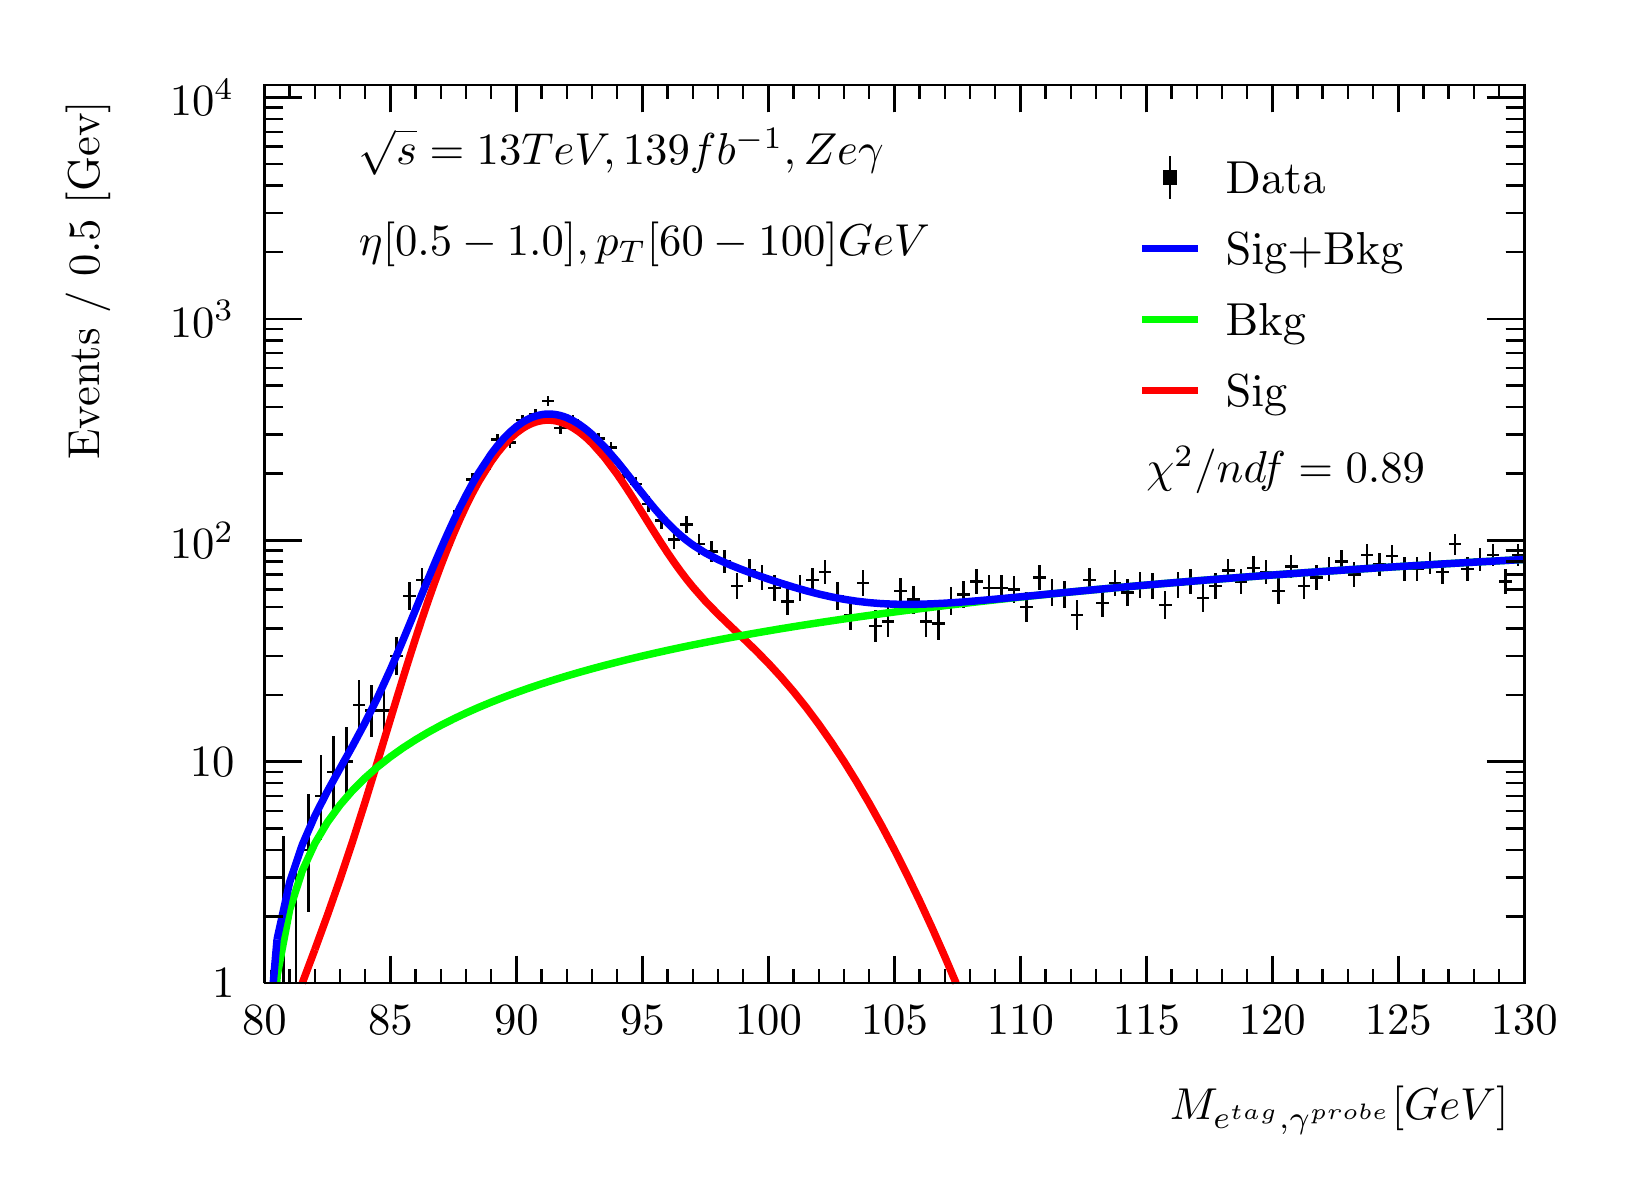
\begin{tikzpicture}
\pgfdeclareplotmark{cross} {
\pgfpathmoveto{\pgfpoint{-0.3\pgfplotmarksize}{\pgfplotmarksize}}
\pgfpathlineto{\pgfpoint{+0.3\pgfplotmarksize}{\pgfplotmarksize}}
\pgfpathlineto{\pgfpoint{+0.3\pgfplotmarksize}{0.3\pgfplotmarksize}}
\pgfpathlineto{\pgfpoint{+1\pgfplotmarksize}{0.3\pgfplotmarksize}}
\pgfpathlineto{\pgfpoint{+1\pgfplotmarksize}{-0.3\pgfplotmarksize}}
\pgfpathlineto{\pgfpoint{+0.3\pgfplotmarksize}{-0.3\pgfplotmarksize}}
\pgfpathlineto{\pgfpoint{+0.3\pgfplotmarksize}{-1.\pgfplotmarksize}}
\pgfpathlineto{\pgfpoint{-0.3\pgfplotmarksize}{-1.\pgfplotmarksize}}
\pgfpathlineto{\pgfpoint{-0.3\pgfplotmarksize}{-0.3\pgfplotmarksize}}
\pgfpathlineto{\pgfpoint{-1.\pgfplotmarksize}{-0.3\pgfplotmarksize}}
\pgfpathlineto{\pgfpoint{-1.\pgfplotmarksize}{0.3\pgfplotmarksize}}
\pgfpathlineto{\pgfpoint{-0.3\pgfplotmarksize}{0.3\pgfplotmarksize}}
\pgfpathclose
\pgfusepathqstroke
}
\pgfdeclareplotmark{cross*} {
\pgfpathmoveto{\pgfpoint{-0.3\pgfplotmarksize}{\pgfplotmarksize}}
\pgfpathlineto{\pgfpoint{+0.3\pgfplotmarksize}{\pgfplotmarksize}}
\pgfpathlineto{\pgfpoint{+0.3\pgfplotmarksize}{0.3\pgfplotmarksize}}
\pgfpathlineto{\pgfpoint{+1\pgfplotmarksize}{0.3\pgfplotmarksize}}
\pgfpathlineto{\pgfpoint{+1\pgfplotmarksize}{-0.3\pgfplotmarksize}}
\pgfpathlineto{\pgfpoint{+0.3\pgfplotmarksize}{-0.3\pgfplotmarksize}}
\pgfpathlineto{\pgfpoint{+0.3\pgfplotmarksize}{-1.\pgfplotmarksize}}
\pgfpathlineto{\pgfpoint{-0.3\pgfplotmarksize}{-1.\pgfplotmarksize}}
\pgfpathlineto{\pgfpoint{-0.3\pgfplotmarksize}{-0.3\pgfplotmarksize}}
\pgfpathlineto{\pgfpoint{-1.\pgfplotmarksize}{-0.3\pgfplotmarksize}}
\pgfpathlineto{\pgfpoint{-1.\pgfplotmarksize}{0.3\pgfplotmarksize}}
\pgfpathlineto{\pgfpoint{-0.3\pgfplotmarksize}{0.3\pgfplotmarksize}}
\pgfpathclose
\pgfusepathqfillstroke
}
\pgfdeclareplotmark{newstar} {
\pgfpathmoveto{\pgfqpoint{0pt}{\pgfplotmarksize}}
\pgfpathlineto{\pgfqpointpolar{44}{0.5\pgfplotmarksize}}
\pgfpathlineto{\pgfqpointpolar{18}{\pgfplotmarksize}}
\pgfpathlineto{\pgfqpointpolar{-20}{0.5\pgfplotmarksize}}
\pgfpathlineto{\pgfqpointpolar{-54}{\pgfplotmarksize}}
\pgfpathlineto{\pgfqpointpolar{-90}{0.5\pgfplotmarksize}}
\pgfpathlineto{\pgfqpointpolar{234}{\pgfplotmarksize}}
\pgfpathlineto{\pgfqpointpolar{198}{0.5\pgfplotmarksize}}
\pgfpathlineto{\pgfqpointpolar{162}{\pgfplotmarksize}}
\pgfpathlineto{\pgfqpointpolar{134}{0.5\pgfplotmarksize}}
\pgfpathclose
\pgfusepathqstroke
}
\pgfdeclareplotmark{newstar*} {
\pgfpathmoveto{\pgfqpoint{0pt}{\pgfplotmarksize}}
\pgfpathlineto{\pgfqpointpolar{44}{0.5\pgfplotmarksize}}
\pgfpathlineto{\pgfqpointpolar{18}{\pgfplotmarksize}}
\pgfpathlineto{\pgfqpointpolar{-20}{0.5\pgfplotmarksize}}
\pgfpathlineto{\pgfqpointpolar{-54}{\pgfplotmarksize}}
\pgfpathlineto{\pgfqpointpolar{-90}{0.5\pgfplotmarksize}}
\pgfpathlineto{\pgfqpointpolar{234}{\pgfplotmarksize}}
\pgfpathlineto{\pgfqpointpolar{198}{0.5\pgfplotmarksize}}
\pgfpathlineto{\pgfqpointpolar{162}{\pgfplotmarksize}}
\pgfpathlineto{\pgfqpointpolar{134}{0.5\pgfplotmarksize}}
\pgfpathclose
\pgfusepathqfillstroke
}
\definecolor{c}{rgb}{1,1,1};
\draw [color=c, fill=c] (0,0) rectangle (20,14.4361);
\draw [color=c, fill=c] (3,2.30977) rectangle (19,13.7143);
\definecolor{c}{rgb}{0,0,0};
\draw [c,line width=0.9] (3,2.30977) -- (3,13.7143) -- (19,13.7143) -- (19,2.30977) -- (3,2.30977);
\definecolor{c}{rgb}{1,1,1};
\draw [color=c, fill=c] (3,2.30977) rectangle (19,13.7143);
\definecolor{c}{rgb}{0,0,0};
\draw [c,line width=0.9] (3,2.30977) -- (3,13.7143) -- (19,13.7143) -- (19,2.30977) -- (3,2.30977);
\draw [c,line width=0.9] (3,2.30977) -- (19,2.30977);
\draw [c,line width=0.9] (3,2.65624) -- (3,2.30977);
\draw [c,line width=0.9] (3.32,2.48301) -- (3.32,2.30977);
\draw [c,line width=0.9] (3.64,2.48301) -- (3.64,2.30977);
\draw [c,line width=0.9] (3.96,2.48301) -- (3.96,2.30977);
\draw [c,line width=0.9] (4.28,2.48301) -- (4.28,2.30977);
\draw [c,line width=0.9] (4.6,2.65624) -- (4.6,2.30977);
\draw [c,line width=0.9] (4.92,2.48301) -- (4.92,2.30977);
\draw [c,line width=0.9] (5.24,2.48301) -- (5.24,2.30977);
\draw [c,line width=0.9] (5.56,2.48301) -- (5.56,2.30977);
\draw [c,line width=0.9] (5.88,2.48301) -- (5.88,2.30977);
\draw [c,line width=0.9] (6.2,2.65624) -- (6.2,2.30977);
\draw [c,line width=0.9] (6.52,2.48301) -- (6.52,2.30977);
\draw [c,line width=0.9] (6.84,2.48301) -- (6.84,2.30977);
\draw [c,line width=0.9] (7.16,2.48301) -- (7.16,2.30977);
\draw [c,line width=0.9] (7.48,2.48301) -- (7.48,2.30977);
\draw [c,line width=0.9] (7.8,2.65624) -- (7.8,2.30977);
\draw [c,line width=0.9] (8.12,2.48301) -- (8.12,2.30977);
\draw [c,line width=0.9] (8.44,2.48301) -- (8.44,2.30977);
\draw [c,line width=0.9] (8.76,2.48301) -- (8.76,2.30977);
\draw [c,line width=0.9] (9.08,2.48301) -- (9.08,2.30977);
\draw [c,line width=0.9] (9.4,2.65624) -- (9.4,2.30977);
\draw [c,line width=0.9] (9.72,2.48301) -- (9.72,2.30977);
\draw [c,line width=0.9] (10.04,2.48301) -- (10.04,2.30977);
\draw [c,line width=0.9] (10.36,2.48301) -- (10.36,2.30977);
\draw [c,line width=0.9] (10.68,2.48301) -- (10.68,2.30977);
\draw [c,line width=0.9] (11,2.65624) -- (11,2.30977);
\draw [c,line width=0.9] (11.32,2.48301) -- (11.32,2.30977);
\draw [c,line width=0.9] (11.64,2.48301) -- (11.64,2.30977);
\draw [c,line width=0.9] (11.96,2.48301) -- (11.96,2.30977);
\draw [c,line width=0.9] (12.28,2.48301) -- (12.28,2.30977);
\draw [c,line width=0.9] (12.6,2.65624) -- (12.6,2.30977);
\draw [c,line width=0.9] (12.92,2.48301) -- (12.92,2.30977);
\draw [c,line width=0.9] (13.24,2.48301) -- (13.24,2.30977);
\draw [c,line width=0.9] (13.56,2.48301) -- (13.56,2.30977);
\draw [c,line width=0.9] (13.88,2.48301) -- (13.88,2.30977);
\draw [c,line width=0.9] (14.2,2.65624) -- (14.2,2.30977);
\draw [c,line width=0.9] (14.52,2.48301) -- (14.52,2.30977);
\draw [c,line width=0.9] (14.84,2.48301) -- (14.84,2.30977);
\draw [c,line width=0.9] (15.16,2.48301) -- (15.16,2.30977);
\draw [c,line width=0.9] (15.48,2.48301) -- (15.48,2.30977);
\draw [c,line width=0.9] (15.8,2.65624) -- (15.8,2.30977);
\draw [c,line width=0.9] (16.12,2.48301) -- (16.12,2.30977);
\draw [c,line width=0.9] (16.44,2.48301) -- (16.44,2.30977);
\draw [c,line width=0.9] (16.76,2.48301) -- (16.76,2.30977);
\draw [c,line width=0.9] (17.08,2.48301) -- (17.08,2.30977);
\draw [c,line width=0.9] (17.4,2.65624) -- (17.4,2.30977);
\draw [c,line width=0.9] (17.72,2.48301) -- (17.72,2.30977);
\draw [c,line width=0.9] (18.04,2.48301) -- (18.04,2.30977);
\draw [c,line width=0.9] (18.36,2.48301) -- (18.36,2.30977);
\draw [c,line width=0.9] (18.68,2.48301) -- (18.68,2.30977);
\draw [c,line width=0.9] (19,2.65624) -- (19,2.30977);
\draw [anchor=base] (3,1.66015) node[scale=1.61424, color=c, rotate=0]{80};
\draw [anchor=base] (4.6,1.66015) node[scale=1.61424, color=c, rotate=0]{85};
\draw [anchor=base] (6.2,1.66015) node[scale=1.61424, color=c, rotate=0]{90};
\draw [anchor=base] (7.8,1.66015) node[scale=1.61424, color=c, rotate=0]{95};
\draw [anchor=base] (9.4,1.66015) node[scale=1.61424, color=c, rotate=0]{100};
\draw [anchor=base] (11,1.66015) node[scale=1.61424, color=c, rotate=0]{105};
\draw [anchor=base] (12.6,1.66015) node[scale=1.61424, color=c, rotate=0]{110};
\draw [anchor=base] (14.2,1.66015) node[scale=1.61424, color=c, rotate=0]{115};
\draw [anchor=base] (15.8,1.66015) node[scale=1.61424, color=c, rotate=0]{120};
\draw [anchor=base] (17.4,1.66015) node[scale=1.61424, color=c, rotate=0]{125};
\draw [anchor=base] (19,1.66015) node[scale=1.61424, color=c, rotate=0]{130};
\draw [anchor= east] (19,0.692932) node[scale=1.61424, color=c, rotate=0]{$M_{e^{tag}, \gamma^{probe}}  [GeV]$};
\draw [c,line width=0.9] (3,13.7143) -- (19,13.7143);
\draw [c,line width=0.9] (3,13.3678) -- (3,13.7143);
\draw [c,line width=0.9] (3.32,13.5411) -- (3.32,13.7143);
\draw [c,line width=0.9] (3.64,13.5411) -- (3.64,13.7143);
\draw [c,line width=0.9] (3.96,13.5411) -- (3.96,13.7143);
\draw [c,line width=0.9] (4.28,13.5411) -- (4.28,13.7143);
\draw [c,line width=0.9] (4.6,13.3678) -- (4.6,13.7143);
\draw [c,line width=0.9] (4.92,13.5411) -- (4.92,13.7143);
\draw [c,line width=0.9] (5.24,13.5411) -- (5.24,13.7143);
\draw [c,line width=0.9] (5.56,13.5411) -- (5.56,13.7143);
\draw [c,line width=0.9] (5.88,13.5411) -- (5.88,13.7143);
\draw [c,line width=0.9] (6.2,13.3678) -- (6.2,13.7143);
\draw [c,line width=0.9] (6.52,13.5411) -- (6.52,13.7143);
\draw [c,line width=0.9] (6.84,13.5411) -- (6.84,13.7143);
\draw [c,line width=0.9] (7.16,13.5411) -- (7.16,13.7143);
\draw [c,line width=0.9] (7.48,13.5411) -- (7.48,13.7143);
\draw [c,line width=0.9] (7.8,13.3678) -- (7.8,13.7143);
\draw [c,line width=0.9] (8.12,13.5411) -- (8.12,13.7143);
\draw [c,line width=0.9] (8.44,13.5411) -- (8.44,13.7143);
\draw [c,line width=0.9] (8.76,13.5411) -- (8.76,13.7143);
\draw [c,line width=0.9] (9.08,13.5411) -- (9.08,13.7143);
\draw [c,line width=0.9] (9.4,13.3678) -- (9.4,13.7143);
\draw [c,line width=0.9] (9.72,13.5411) -- (9.72,13.7143);
\draw [c,line width=0.9] (10.04,13.5411) -- (10.04,13.7143);
\draw [c,line width=0.9] (10.36,13.5411) -- (10.36,13.7143);
\draw [c,line width=0.9] (10.68,13.5411) -- (10.68,13.7143);
\draw [c,line width=0.9] (11,13.3678) -- (11,13.7143);
\draw [c,line width=0.9] (11.32,13.5411) -- (11.32,13.7143);
\draw [c,line width=0.9] (11.64,13.5411) -- (11.64,13.7143);
\draw [c,line width=0.9] (11.96,13.5411) -- (11.96,13.7143);
\draw [c,line width=0.9] (12.28,13.5411) -- (12.28,13.7143);
\draw [c,line width=0.9] (12.6,13.3678) -- (12.6,13.7143);
\draw [c,line width=0.9] (12.92,13.5411) -- (12.92,13.7143);
\draw [c,line width=0.9] (13.24,13.5411) -- (13.24,13.7143);
\draw [c,line width=0.9] (13.56,13.5411) -- (13.56,13.7143);
\draw [c,line width=0.9] (13.88,13.5411) -- (13.88,13.7143);
\draw [c,line width=0.9] (14.2,13.3678) -- (14.2,13.7143);
\draw [c,line width=0.9] (14.52,13.5411) -- (14.52,13.7143);
\draw [c,line width=0.9] (14.84,13.5411) -- (14.84,13.7143);
\draw [c,line width=0.9] (15.16,13.5411) -- (15.16,13.7143);
\draw [c,line width=0.9] (15.48,13.5411) -- (15.48,13.7143);
\draw [c,line width=0.9] (15.8,13.3678) -- (15.8,13.7143);
\draw [c,line width=0.9] (16.12,13.5411) -- (16.12,13.7143);
\draw [c,line width=0.9] (16.44,13.5411) -- (16.44,13.7143);
\draw [c,line width=0.9] (16.76,13.5411) -- (16.76,13.7143);
\draw [c,line width=0.9] (17.08,13.5411) -- (17.08,13.7143);
\draw [c,line width=0.9] (17.4,13.3678) -- (17.4,13.7143);
\draw [c,line width=0.9] (17.72,13.5411) -- (17.72,13.7143);
\draw [c,line width=0.9] (18.04,13.5411) -- (18.04,13.7143);
\draw [c,line width=0.9] (18.36,13.5411) -- (18.36,13.7143);
\draw [c,line width=0.9] (18.68,13.5411) -- (18.68,13.7143);
\draw [c,line width=0.9] (19,13.3678) -- (19,13.7143);
\draw [c,line width=0.9] (3,2.30977) -- (3,13.7143);
\draw [c,line width=0.9] (3.474,2.30978) -- (3,2.30978);
\draw [anchor= east] (2.82,2.30978) node[scale=1.61424, color=c, rotate=0]{1};
\draw [c,line width=0.9] (3.237,3.15616) -- (3,3.15616);
\draw [c,line width=0.9] (3.237,3.65126) -- (3,3.65126);
\draw [c,line width=0.9] (3.237,4.00254) -- (3,4.00254);
\draw [c,line width=0.9] (3.237,4.27501) -- (3,4.27501);
\draw [c,line width=0.9] (3.237,4.49764) -- (3,4.49764);
\draw [c,line width=0.9] (3.237,4.68586) -- (3,4.68586);
\draw [c,line width=0.9] (3.237,4.84892) -- (3,4.84892);
\draw [c,line width=0.9] (3.237,4.99274) -- (3,4.99274);
\draw [c,line width=0.9] (3.474,5.12139) -- (3,5.12139);
\draw [anchor= east] (2.82,5.12139) node[scale=1.61424, color=c, rotate=0]{10};
\draw [c,line width=0.9] (3.237,5.96777) -- (3,5.96777);
\draw [c,line width=0.9] (3.237,6.46287) -- (3,6.46287);
\draw [c,line width=0.9] (3.237,6.81415) -- (3,6.81415);
\draw [c,line width=0.9] (3.237,7.08662) -- (3,7.08662);
\draw [c,line width=0.9] (3.237,7.30925) -- (3,7.30925);
\draw [c,line width=0.9] (3.237,7.49748) -- (3,7.49748);
\draw [c,line width=0.9] (3.237,7.66053) -- (3,7.66053);
\draw [c,line width=0.9] (3.237,7.80435) -- (3,7.80435);
\draw [c,line width=0.9] (3.474,7.933) -- (3,7.933);
\draw [anchor= east] (2.82,7.933) node[scale=1.61424, color=c, rotate=0]{$10^{2}$};
\draw [c,line width=0.9] (3.237,8.77938) -- (3,8.77938);
\draw [c,line width=0.9] (3.237,9.27448) -- (3,9.27448);
\draw [c,line width=0.9] (3.237,9.62576) -- (3,9.62576);
\draw [c,line width=0.9] (3.237,9.89823) -- (3,9.89823);
\draw [c,line width=0.9] (3.237,10.1209) -- (3,10.1209);
\draw [c,line width=0.9] (3.237,10.3091) -- (3,10.3091);
\draw [c,line width=0.9] (3.237,10.4721) -- (3,10.4721);
\draw [c,line width=0.9] (3.237,10.616) -- (3,10.616);
\draw [c,line width=0.9] (3.474,10.7446) -- (3,10.7446);
\draw [anchor= east] (2.82,10.7446) node[scale=1.61424, color=c, rotate=0]{$10^{3}$};
\draw [c,line width=0.9] (3.237,11.591) -- (3,11.591);
\draw [c,line width=0.9] (3.237,12.0861) -- (3,12.0861);
\draw [c,line width=0.9] (3.237,12.4374) -- (3,12.4374);
\draw [c,line width=0.9] (3.237,12.7098) -- (3,12.7098);
\draw [c,line width=0.9] (3.237,12.9325) -- (3,12.9325);
\draw [c,line width=0.9] (3.237,13.1207) -- (3,13.1207);
\draw [c,line width=0.9] (3.237,13.2837) -- (3,13.2837);
\draw [c,line width=0.9] (3.237,13.4276) -- (3,13.4276);
\draw [c,line width=0.9] (3.474,13.5562) -- (3,13.5562);
\draw [anchor= east] (2.82,13.5562) node[scale=1.61424, color=c, rotate=0]{$10^{4}$};
\draw [anchor= east] (0.76,13.7143) node[scale=1.61424, color=c, rotate=90]{Events / 0.5 [Gev]};
\draw [c,line width=0.9] (19,2.30977) -- (19,13.7143);
\draw [c,line width=0.9] (18.526,2.30978) -- (19,2.30978);
\draw [c,line width=0.9] (18.763,3.15616) -- (19,3.15616);
\draw [c,line width=0.9] (18.763,3.65126) -- (19,3.65126);
\draw [c,line width=0.9] (18.763,4.00254) -- (19,4.00254);
\draw [c,line width=0.9] (18.763,4.27501) -- (19,4.27501);
\draw [c,line width=0.9] (18.763,4.49764) -- (19,4.49764);
\draw [c,line width=0.9] (18.763,4.68586) -- (19,4.68586);
\draw [c,line width=0.9] (18.763,4.84892) -- (19,4.84892);
\draw [c,line width=0.9] (18.763,4.99274) -- (19,4.99274);
\draw [c,line width=0.9] (18.526,5.12139) -- (19,5.12139);
\draw [c,line width=0.9] (18.763,5.96777) -- (19,5.96777);
\draw [c,line width=0.9] (18.763,6.46287) -- (19,6.46287);
\draw [c,line width=0.9] (18.763,6.81415) -- (19,6.81415);
\draw [c,line width=0.9] (18.763,7.08662) -- (19,7.08662);
\draw [c,line width=0.9] (18.763,7.30925) -- (19,7.30925);
\draw [c,line width=0.9] (18.763,7.49748) -- (19,7.49748);
\draw [c,line width=0.9] (18.763,7.66053) -- (19,7.66053);
\draw [c,line width=0.9] (18.763,7.80435) -- (19,7.80435);
\draw [c,line width=0.9] (18.526,7.933) -- (19,7.933);
\draw [c,line width=0.9] (18.763,8.77938) -- (19,8.77938);
\draw [c,line width=0.9] (18.763,9.27448) -- (19,9.27448);
\draw [c,line width=0.9] (18.763,9.62576) -- (19,9.62576);
\draw [c,line width=0.9] (18.763,9.89823) -- (19,9.89823);
\draw [c,line width=0.9] (18.763,10.1209) -- (19,10.1209);
\draw [c,line width=0.9] (18.763,10.3091) -- (19,10.3091);
\draw [c,line width=0.9] (18.763,10.4721) -- (19,10.4721);
\draw [c,line width=0.9] (18.763,10.616) -- (19,10.616);
\draw [c,line width=0.9] (18.526,10.7446) -- (19,10.7446);
\draw [c,line width=0.9] (18.763,11.591) -- (19,11.591);
\draw [c,line width=0.9] (18.763,12.0861) -- (19,12.0861);
\draw [c,line width=0.9] (18.763,12.4374) -- (19,12.4374);
\draw [c,line width=0.9] (18.763,12.7098) -- (19,12.7098);
\draw [c,line width=0.9] (18.763,12.9325) -- (19,12.9325);
\draw [c,line width=0.9] (18.763,13.1207) -- (19,13.1207);
\draw [c,line width=0.9] (18.763,13.2837) -- (19,13.2837);
\draw [c,line width=0.9] (18.763,13.4276) -- (19,13.4276);
\draw [c,line width=0.9] (18.526,13.5562) -- (19,13.5562);
\draw [c,line width=0.9] (3.08,2.30977) -- (3,2.30977);
\draw [c,line width=0.9] (3,2.30977) -- (3,2.30977);
\draw [c,line width=0.9] (3.08,2.30977) -- (3.16,2.30977);
\draw [c,line width=0.9] (3.16,2.30977) -- (3.16,2.30977);
\draw [c,line width=0.9] (3.08,2.30977) -- (3.08,2.47817);
\draw [c,line width=0.9] (3.08,2.47817) -- (3.08,2.47817);
\draw [c,line width=0.9] (3.24,3.15615) -- (3.16,3.15615);
\draw [c,line width=0.9] (3.16,3.15615) -- (3.16,3.15615);
\draw [c,line width=0.9] (3.24,3.15615) -- (3.32,3.15615);
\draw [c,line width=0.9] (3.32,3.15615) -- (3.32,3.15615);
\draw [c,line width=0.9] (3.24,3.15615) -- (3.24,4.1832);
\draw [c,line width=0.9] (3.24,4.1832) -- (3.24,4.1832);
\draw [c,line width=0.9] (3.24,3.15615) -- (3.24,2.30977);
\draw [c,line width=0.9] (3.24,2.30977) -- (3.24,2.30977);
\draw [c,line width=0.9] (3.4,2.30977) -- (3.32,2.30977);
\draw [c,line width=0.9] (3.32,2.30977) -- (3.32,2.30977);
\draw [c,line width=0.9] (3.4,2.30977) -- (3.48,2.30977);
\draw [c,line width=0.9] (3.48,2.30977) -- (3.48,2.30977);
\draw [c,line width=0.9] (3.4,2.30977) -- (3.4,3.76746);
\draw [c,line width=0.9] (3.4,3.76746) -- (3.4,3.76746);
\draw [c,line width=0.9] (3.56,4.00253) -- (3.48,4.00253);
\draw [c,line width=0.9] (3.48,4.00253) -- (3.48,4.00253);
\draw [c,line width=0.9] (3.56,4.00253) -- (3.64,4.00253);
\draw [c,line width=0.9] (3.64,4.00253) -- (3.64,4.00253);
\draw [c,line width=0.9] (3.56,4.00253) -- (3.56,4.71393);
\draw [c,line width=0.9] (3.56,4.71393) -- (3.56,4.71393);
\draw [c,line width=0.9] (3.56,4.00253) -- (3.56,3.20736);
\draw [c,line width=0.9] (3.56,3.20736) -- (3.56,3.20736);
\draw [c,line width=0.9] (3.72,4.68586) -- (3.64,4.68586);
\draw [c,line width=0.9] (3.64,4.68586) -- (3.64,4.68586);
\draw [c,line width=0.9] (3.72,4.68586) -- (3.8,4.68586);
\draw [c,line width=0.9] (3.8,4.68586) -- (3.8,4.68586);
\draw [c,line width=0.9] (3.72,4.68586) -- (3.72,5.212);
\draw [c,line width=0.9] (3.72,5.212) -- (3.72,5.212);
\draw [c,line width=0.9] (3.72,4.68586) -- (3.72,4.12404);
\draw [c,line width=0.9] (3.72,4.12404) -- (3.72,4.12404);
\draw [c,line width=0.9] (3.88,4.99273) -- (3.8,4.99273);
\draw [c,line width=0.9] (3.8,4.99273) -- (3.8,4.99273);
\draw [c,line width=0.9] (3.88,4.99273) -- (3.96,4.99273);
\draw [c,line width=0.9] (3.96,4.99273) -- (3.96,4.99273);
\draw [c,line width=0.9] (3.88,4.99273) -- (3.88,5.45206);
\draw [c,line width=0.9] (3.88,5.45206) -- (3.88,5.45206);
\draw [c,line width=0.9] (3.88,4.99273) -- (3.88,4.50909);
\draw [c,line width=0.9] (3.88,4.50909) -- (3.88,4.50909);
\draw [c,line width=0.9] (4.04,5.12139) -- (3.96,5.12139);
\draw [c,line width=0.9] (3.96,5.12139) -- (3.96,5.12139);
\draw [c,line width=0.9] (4.04,5.12139) -- (4.12,5.12139);
\draw [c,line width=0.9] (4.12,5.12139) -- (4.12,5.12139);
\draw [c,line width=0.9] (4.04,5.12139) -- (4.04,5.55531);
\draw [c,line width=0.9] (4.04,5.55531) -- (4.04,5.55531);
\draw [c,line width=0.9] (4.04,5.12139) -- (4.04,4.66675);
\draw [c,line width=0.9] (4.04,4.66675) -- (4.04,4.66675);
\draw [c,line width=0.9] (4.2,5.83911) -- (4.12,5.83911);
\draw [c,line width=0.9] (4.12,5.83911) -- (4.12,5.83911);
\draw [c,line width=0.9] (4.2,5.83911) -- (4.28,5.83911);
\draw [c,line width=0.9] (4.28,5.83911) -- (4.28,5.83911);
\draw [c,line width=0.9] (4.2,5.83911) -- (4.2,6.15535);
\draw [c,line width=0.9] (4.2,6.15535) -- (4.2,6.15535);
\draw [c,line width=0.9] (4.2,5.83911) -- (4.2,5.51442);
\draw [c,line width=0.9] (4.2,5.51442) -- (4.2,5.51442);
\draw [c,line width=0.9] (4.36,5.76932) -- (4.28,5.76932);
\draw [c,line width=0.9] (4.28,5.76932) -- (4.28,5.76932);
\draw [c,line width=0.9] (4.36,5.76932) -- (4.44,5.76932);
\draw [c,line width=0.9] (4.44,5.76932) -- (4.44,5.76932);
\draw [c,line width=0.9] (4.36,5.76932) -- (4.36,6.0954);
\draw [c,line width=0.9] (4.36,6.0954) -- (4.36,6.0954);
\draw [c,line width=0.9] (4.36,5.76932) -- (4.36,5.43401);
\draw [c,line width=0.9] (4.36,5.43401) -- (4.36,5.43401);
\draw [c,line width=0.9] (4.52,5.76932) -- (4.44,5.76932);
\draw [c,line width=0.9] (4.44,5.76932) -- (4.44,5.76932);
\draw [c,line width=0.9] (4.52,5.76932) -- (4.6,5.76932);
\draw [c,line width=0.9] (4.6,5.76932) -- (4.6,5.76932);
\draw [c,line width=0.9] (4.52,5.76932) -- (4.52,6.0954);
\draw [c,line width=0.9] (4.52,6.0954) -- (4.52,6.0954);
\draw [c,line width=0.9] (4.52,5.76932) -- (4.52,5.43401);
\draw [c,line width=0.9] (4.52,5.43401) -- (4.52,5.43401);
\draw [c,line width=0.9] (4.68,6.46287) -- (4.6,6.46287);
\draw [c,line width=0.9] (4.6,6.46287) -- (4.6,6.46287);
\draw [c,line width=0.9] (4.68,6.46287) -- (4.76,6.46287);
\draw [c,line width=0.9] (4.76,6.46287) -- (4.76,6.46287);
\draw [c,line width=0.9] (4.68,6.46287) -- (4.68,6.70361);
\draw [c,line width=0.9] (4.68,6.70361) -- (4.68,6.70361);
\draw [c,line width=0.9] (4.68,6.46287) -- (4.68,6.21823);
\draw [c,line width=0.9] (4.68,6.21823) -- (4.68,6.21823);
\draw [c,line width=0.9] (4.84,7.225) -- (4.76,7.225);
\draw [c,line width=0.9] (4.76,7.225) -- (4.76,7.225);
\draw [c,line width=0.9] (4.84,7.225) -- (4.92,7.225);
\draw [c,line width=0.9] (4.92,7.225) -- (4.92,7.225);
\draw [c,line width=0.9] (4.84,7.225) -- (4.84,7.39808);
\draw [c,line width=0.9] (4.84,7.39808) -- (4.84,7.39808);
\draw [c,line width=0.9] (4.84,7.225) -- (4.84,7.05041);
\draw [c,line width=0.9] (4.84,7.05041) -- (4.84,7.05041);
\draw [c,line width=0.9] (5,7.42563) -- (4.92,7.42563);
\draw [c,line width=0.9] (4.92,7.42563) -- (4.92,7.42563);
\draw [c,line width=0.9] (5,7.42563) -- (5.08,7.42563);
\draw [c,line width=0.9] (5.08,7.42563) -- (5.08,7.42563);
\draw [c,line width=0.9] (5,7.42563) -- (5,7.5844);
\draw [c,line width=0.9] (5,7.5844) -- (5,7.5844);
\draw [c,line width=0.9] (5,7.42563) -- (5,7.26567);
\draw [c,line width=0.9] (5,7.26567) -- (5,7.26567);
\draw [c,line width=0.9] (5.16,7.49747) -- (5.08,7.49747);
\draw [c,line width=0.9] (5.08,7.49747) -- (5.08,7.49747);
\draw [c,line width=0.9] (5.16,7.49747) -- (5.24,7.49747);
\draw [c,line width=0.9] (5.24,7.49747) -- (5.24,7.49747);
\draw [c,line width=0.9] (5.16,7.49747) -- (5.16,7.65143);
\draw [c,line width=0.9] (5.16,7.65143) -- (5.16,7.65143);
\draw [c,line width=0.9] (5.16,7.49747) -- (5.16,7.34244);
\draw [c,line width=0.9] (5.16,7.34244) -- (5.16,7.34244);
\draw [c,line width=0.9] (5.32,7.87037) -- (5.24,7.87037);
\draw [c,line width=0.9] (5.24,7.87037) -- (5.24,7.87037);
\draw [c,line width=0.9] (5.32,7.87037) -- (5.4,7.87037);
\draw [c,line width=0.9] (5.4,7.87037) -- (5.4,7.87037);
\draw [c,line width=0.9] (5.32,7.87037) -- (5.32,8.00162);
\draw [c,line width=0.9] (5.32,8.00162) -- (5.32,8.00162);
\draw [c,line width=0.9] (5.32,7.87037) -- (5.32,7.73843);
\draw [c,line width=0.9] (5.32,7.73843) -- (5.32,7.73843);
\draw [c,line width=0.9] (5.48,8.29945) -- (5.4,8.29945);
\draw [c,line width=0.9] (5.4,8.29945) -- (5.4,8.29945);
\draw [c,line width=0.9] (5.48,8.29945) -- (5.56,8.29945);
\draw [c,line width=0.9] (5.56,8.29945) -- (5.56,8.29945);
\draw [c,line width=0.9] (5.48,8.29945) -- (5.48,8.40451);
\draw [c,line width=0.9] (5.48,8.40451) -- (5.48,8.40451);
\draw [c,line width=0.9] (5.48,8.29945) -- (5.48,8.19439);
\draw [c,line width=0.9] (5.48,8.19439) -- (5.48,8.19439);
\draw [c,line width=0.9] (5.64,8.70382) -- (5.56,8.70382);
\draw [c,line width=0.9] (5.56,8.70382) -- (5.56,8.70382);
\draw [c,line width=0.9] (5.64,8.70382) -- (5.72,8.70382);
\draw [c,line width=0.9] (5.72,8.70382) -- (5.72,8.70382);
\draw [c,line width=0.9] (5.64,8.70382) -- (5.64,8.79286);
\draw [c,line width=0.9] (5.64,8.79286) -- (5.64,8.79286);
\draw [c,line width=0.9] (5.64,8.70382) -- (5.64,8.61479);
\draw [c,line width=0.9] (5.64,8.61479) -- (5.64,8.61479);
\draw [c,line width=0.9] (5.8,8.83895) -- (5.72,8.83895);
\draw [c,line width=0.9] (5.72,8.83895) -- (5.72,8.83895);
\draw [c,line width=0.9] (5.8,8.83895) -- (5.88,8.83895);
\draw [c,line width=0.9] (5.88,8.83895) -- (5.88,8.83895);
\draw [c,line width=0.9] (5.8,8.83895) -- (5.8,8.9232);
\draw [c,line width=0.9] (5.8,8.9232) -- (5.8,8.9232);
\draw [c,line width=0.9] (5.8,8.83895) -- (5.8,8.75471);
\draw [c,line width=0.9] (5.8,8.75471) -- (5.8,8.75471);
\draw [c,line width=0.9] (5.96,9.21184) -- (5.88,9.21184);
\draw [c,line width=0.9] (5.88,9.21184) -- (5.88,9.21184);
\draw [c,line width=0.9] (5.96,9.21184) -- (6.04,9.21184);
\draw [c,line width=0.9] (6.04,9.21184) -- (6.04,9.21184);
\draw [c,line width=0.9] (5.96,9.21184) -- (5.96,9.28416);
\draw [c,line width=0.9] (5.96,9.28416) -- (5.96,9.28416);
\draw [c,line width=0.9] (5.96,9.21184) -- (5.96,9.13953);
\draw [c,line width=0.9] (5.96,9.13953) -- (5.96,9.13953);
\draw [c,line width=0.9] (6.12,9.17708) -- (6.04,9.17708);
\draw [c,line width=0.9] (6.04,9.17708) -- (6.04,9.17708);
\draw [c,line width=0.9] (6.12,9.17708) -- (6.2,9.17708);
\draw [c,line width=0.9] (6.2,9.17708) -- (6.2,9.17708);
\draw [c,line width=0.9] (6.12,9.17708) -- (6.12,9.25043);
\draw [c,line width=0.9] (6.12,9.25043) -- (6.12,9.25043);
\draw [c,line width=0.9] (6.12,9.17708) -- (6.12,9.10372);
\draw [c,line width=0.9] (6.12,9.10372) -- (6.12,9.10372);
\draw [c,line width=0.9] (6.28,9.46271) -- (6.2,9.46271);
\draw [c,line width=0.9] (6.2,9.46271) -- (6.2,9.46271);
\draw [c,line width=0.9] (6.28,9.46271) -- (6.36,9.46271);
\draw [c,line width=0.9] (6.36,9.46271) -- (6.36,9.46271);
\draw [c,line width=0.9] (6.28,9.46271) -- (6.28,9.52797);
\draw [c,line width=0.9] (6.28,9.52797) -- (6.28,9.52797);
\draw [c,line width=0.9] (6.28,9.46271) -- (6.28,9.39744);
\draw [c,line width=0.9] (6.28,9.39744) -- (6.28,9.39744);
\draw [c,line width=0.9] (6.44,9.53056) -- (6.36,9.53056);
\draw [c,line width=0.9] (6.36,9.53056) -- (6.36,9.53056);
\draw [c,line width=0.9] (6.44,9.53056) -- (6.52,9.53056);
\draw [c,line width=0.9] (6.52,9.53056) -- (6.52,9.53056);
\draw [c,line width=0.9] (6.44,9.53056) -- (6.44,9.59403);
\draw [c,line width=0.9] (6.44,9.59403) -- (6.44,9.59403);
\draw [c,line width=0.9] (6.44,9.53056) -- (6.44,9.46709);
\draw [c,line width=0.9] (6.44,9.46709) -- (6.44,9.46709);
\draw [c,line width=0.9] (6.6,9.70265) -- (6.52,9.70265);
\draw [c,line width=0.9] (6.52,9.70265) -- (6.52,9.70265);
\draw [c,line width=0.9] (6.6,9.70265) -- (6.68,9.70265);
\draw [c,line width=0.9] (6.68,9.70265) -- (6.68,9.70265);
\draw [c,line width=0.9] (6.6,9.70265) -- (6.6,9.76181);
\draw [c,line width=0.9] (6.6,9.76181) -- (6.6,9.76181);
\draw [c,line width=0.9] (6.6,9.70265) -- (6.6,9.6435);
\draw [c,line width=0.9] (6.6,9.6435) -- (6.6,9.6435);
\draw [c,line width=0.9] (6.76,9.35709) -- (6.68,9.35709);
\draw [c,line width=0.9] (6.68,9.35709) -- (6.68,9.35709);
\draw [c,line width=0.9] (6.76,9.35709) -- (6.84,9.35709);
\draw [c,line width=0.9] (6.84,9.35709) -- (6.84,9.35709);
\draw [c,line width=0.9] (6.76,9.35709) -- (6.76,9.42524);
\draw [c,line width=0.9] (6.76,9.42524) -- (6.76,9.42524);
\draw [c,line width=0.9] (6.76,9.35709) -- (6.76,9.28895);
\draw [c,line width=0.9] (6.76,9.28895) -- (6.76,9.28895);
\draw [c,line width=0.9] (6.92,9.45571) -- (6.84,9.45571);
\draw [c,line width=0.9] (6.84,9.45571) -- (6.84,9.45571);
\draw [c,line width=0.9] (6.92,9.45571) -- (7,9.45571);
\draw [c,line width=0.9] (7,9.45571) -- (7,9.45571);
\draw [c,line width=0.9] (6.92,9.45571) -- (6.92,9.52116);
\draw [c,line width=0.9] (6.92,9.52116) -- (6.92,9.52116);
\draw [c,line width=0.9] (6.92,9.45571) -- (6.92,9.39026);
\draw [c,line width=0.9] (6.92,9.39026) -- (6.92,9.39026);
\draw [c,line width=0.9] (7.08,9.32237) -- (7,9.32237);
\draw [c,line width=0.9] (7,9.32237) -- (7,9.32237);
\draw [c,line width=0.9] (7.08,9.32237) -- (7.16,9.32237);
\draw [c,line width=0.9] (7.16,9.32237) -- (7.16,9.32237);
\draw [c,line width=0.9] (7.08,9.32237) -- (7.08,9.39149);
\draw [c,line width=0.9] (7.08,9.39149) -- (7.08,9.39149);
\draw [c,line width=0.9] (7.08,9.32237) -- (7.08,9.25325);
\draw [c,line width=0.9] (7.08,9.25325) -- (7.08,9.25325);
\draw [c,line width=0.9] (7.24,9.22463) -- (7.16,9.22463);
\draw [c,line width=0.9] (7.16,9.22463) -- (7.16,9.22463);
\draw [c,line width=0.9] (7.24,9.22463) -- (7.32,9.22463);
\draw [c,line width=0.9] (7.32,9.22463) -- (7.32,9.22463);
\draw [c,line width=0.9] (7.24,9.22463) -- (7.24,9.29657);
\draw [c,line width=0.9] (7.24,9.29657) -- (7.24,9.29657);
\draw [c,line width=0.9] (7.24,9.22463) -- (7.24,9.15269);
\draw [c,line width=0.9] (7.24,9.15269) -- (7.24,9.15269);
\draw [c,line width=0.9] (7.4,9.1091) -- (7.32,9.1091);
\draw [c,line width=0.9] (7.32,9.1091) -- (7.32,9.1091);
\draw [c,line width=0.9] (7.4,9.1091) -- (7.48,9.1091);
\draw [c,line width=0.9] (7.48,9.1091) -- (7.48,9.1091);
\draw [c,line width=0.9] (7.4,9.1091) -- (7.4,9.18452);
\draw [c,line width=0.9] (7.4,9.18452) -- (7.4,9.18452);
\draw [c,line width=0.9] (7.4,9.1091) -- (7.4,9.03367);
\draw [c,line width=0.9] (7.4,9.03367) -- (7.4,9.03367);
\draw [c,line width=0.9] (7.56,8.73587) -- (7.48,8.73587);
\draw [c,line width=0.9] (7.48,8.73587) -- (7.48,8.73587);
\draw [c,line width=0.9] (7.56,8.73587) -- (7.64,8.73587);
\draw [c,line width=0.9] (7.64,8.73587) -- (7.64,8.73587);
\draw [c,line width=0.9] (7.56,8.73587) -- (7.56,8.82375);
\draw [c,line width=0.9] (7.56,8.82375) -- (7.56,8.82375);
\draw [c,line width=0.9] (7.56,8.73587) -- (7.56,8.648);
\draw [c,line width=0.9] (7.56,8.648) -- (7.56,8.648);
\draw [c,line width=0.9] (7.72,8.65073) -- (7.64,8.65073);
\draw [c,line width=0.9] (7.64,8.65073) -- (7.64,8.65073);
\draw [c,line width=0.9] (7.72,8.65073) -- (7.8,8.65073);
\draw [c,line width=0.9] (7.8,8.65073) -- (7.8,8.65073);
\draw [c,line width=0.9] (7.72,8.65073) -- (7.72,8.74172);
\draw [c,line width=0.9] (7.72,8.74172) -- (7.72,8.74172);
\draw [c,line width=0.9] (7.72,8.65073) -- (7.72,8.55973);
\draw [c,line width=0.9] (7.72,8.55973) -- (7.72,8.55973);
\draw [c,line width=0.9] (7.88,8.39509) -- (7.8,8.39509);
\draw [c,line width=0.9] (7.8,8.39509) -- (7.8,8.39509);
\draw [c,line width=0.9] (7.88,8.39509) -- (7.96,8.39509);
\draw [c,line width=0.9] (7.96,8.39509) -- (7.96,8.39509);
\draw [c,line width=0.9] (7.88,8.39509) -- (7.88,8.49612);
\draw [c,line width=0.9] (7.88,8.49612) -- (7.88,8.49612);
\draw [c,line width=0.9] (7.88,8.39509) -- (7.88,8.29407);
\draw [c,line width=0.9] (7.88,8.29407) -- (7.88,8.29407);
\draw [c,line width=0.9] (8.04,8.18578) -- (7.96,8.18578);
\draw [c,line width=0.9] (7.96,8.18578) -- (7.96,8.18578);
\draw [c,line width=0.9] (8.04,8.18578) -- (8.12,8.18578);
\draw [c,line width=0.9] (8.12,8.18578) -- (8.12,8.18578);
\draw [c,line width=0.9] (8.04,8.18578) -- (8.04,8.29584);
\draw [c,line width=0.9] (8.04,8.29584) -- (8.04,8.29584);
\draw [c,line width=0.9] (8.04,8.18578) -- (8.04,8.07571);
\draw [c,line width=0.9] (8.04,8.07571) -- (8.04,8.07571);
\draw [c,line width=0.9] (8.2,7.94515) -- (8.12,7.94515);
\draw [c,line width=0.9] (8.12,7.94515) -- (8.12,7.94515);
\draw [c,line width=0.9] (8.2,7.94515) -- (8.28,7.94515);
\draw [c,line width=0.9] (8.28,7.94515) -- (8.28,7.94515);
\draw [c,line width=0.9] (8.2,7.94515) -- (8.2,8.0666);
\draw [c,line width=0.9] (8.2,8.0666) -- (8.2,8.0666);
\draw [c,line width=0.9] (8.2,7.94515) -- (8.2,7.8237);
\draw [c,line width=0.9] (8.2,7.8237) -- (8.2,7.8237);
\draw [c,line width=0.9] (8.36,8.1351) -- (8.28,8.1351);
\draw [c,line width=0.9] (8.28,8.1351) -- (8.28,8.1351);
\draw [c,line width=0.9] (8.36,8.1351) -- (8.44,8.1351);
\draw [c,line width=0.9] (8.44,8.1351) -- (8.44,8.1351);
\draw [c,line width=0.9] (8.36,8.1351) -- (8.36,8.24747);
\draw [c,line width=0.9] (8.36,8.24747) -- (8.36,8.24747);
\draw [c,line width=0.9] (8.36,8.1351) -- (8.36,8.02273);
\draw [c,line width=0.9] (8.36,8.02273) -- (8.36,8.02273);
\draw [c,line width=0.9] (8.52,7.88315) -- (8.44,7.88315);
\draw [c,line width=0.9] (8.44,7.88315) -- (8.44,7.88315);
\draw [c,line width=0.9] (8.52,7.88315) -- (8.6,7.88315);
\draw [c,line width=0.9] (8.6,7.88315) -- (8.6,7.88315);
\draw [c,line width=0.9] (8.52,7.88315) -- (8.52,8.01369);
\draw [c,line width=0.9] (8.52,8.01369) -- (8.52,8.01369);
\draw [c,line width=0.9] (8.52,7.88315) -- (8.52,7.75194);
\draw [c,line width=0.9] (8.52,7.75194) -- (8.52,7.75194);
\draw [c,line width=0.9] (8.68,7.7907) -- (8.6,7.7907);
\draw [c,line width=0.9] (8.6,7.7907) -- (8.6,7.7907);
\draw [c,line width=0.9] (8.68,7.7907) -- (8.76,7.7907);
\draw [c,line width=0.9] (8.76,7.7907) -- (8.76,7.7907);
\draw [c,line width=0.9] (8.68,7.7907) -- (8.68,7.9265);
\draw [c,line width=0.9] (8.68,7.9265) -- (8.68,7.9265);
\draw [c,line width=0.9] (8.68,7.7907) -- (8.68,7.65415);
\draw [c,line width=0.9] (8.68,7.65415) -- (8.68,7.65415);
\draw [c,line width=0.9] (8.84,7.66052) -- (8.76,7.66052);
\draw [c,line width=0.9] (8.76,7.66052) -- (8.76,7.66052);
\draw [c,line width=0.9] (8.84,7.66052) -- (8.92,7.66052);
\draw [c,line width=0.9] (8.92,7.66052) -- (8.92,7.66052);
\draw [c,line width=0.9] (8.84,7.66052) -- (8.84,7.8041);
\draw [c,line width=0.9] (8.84,7.8041) -- (8.84,7.8041);
\draw [c,line width=0.9] (8.84,7.66052) -- (8.84,7.51607);
\draw [c,line width=0.9] (8.84,7.51607) -- (8.84,7.51607);
\draw [c,line width=0.9] (9,7.34928) -- (8.92,7.34928);
\draw [c,line width=0.9] (8.92,7.34928) -- (8.92,7.34928);
\draw [c,line width=0.9] (9,7.34928) -- (9.08,7.34928);
\draw [c,line width=0.9] (9.08,7.34928) -- (9.08,7.34928);
\draw [c,line width=0.9] (9,7.34928) -- (9,7.51335);
\draw [c,line width=0.9] (9,7.51335) -- (9,7.51335);
\draw [c,line width=0.9] (9,7.34928) -- (9,7.18392);
\draw [c,line width=0.9] (9,7.18392) -- (9,7.18392);
\draw [c,line width=0.9] (9.16,7.54871) -- (9.08,7.54871);
\draw [c,line width=0.9] (9.08,7.54871) -- (9.08,7.54871);
\draw [c,line width=0.9] (9.16,7.54871) -- (9.24,7.54871);
\draw [c,line width=0.9] (9.24,7.54871) -- (9.24,7.54871);
\draw [c,line width=0.9] (9.16,7.54871) -- (9.16,7.69933);
\draw [c,line width=0.9] (9.16,7.69933) -- (9.16,7.69933);
\draw [c,line width=0.9] (9.16,7.54871) -- (9.16,7.39709);
\draw [c,line width=0.9] (9.16,7.39709) -- (9.16,7.39709);
\draw [c,line width=0.9] (9.32,7.46208) -- (9.24,7.46208);
\draw [c,line width=0.9] (9.24,7.46208) -- (9.24,7.46208);
\draw [c,line width=0.9] (9.32,7.46208) -- (9.4,7.46208);
\draw [c,line width=0.9] (9.4,7.46208) -- (9.4,7.46208);
\draw [c,line width=0.9] (9.32,7.46208) -- (9.32,7.61839);
\draw [c,line width=0.9] (9.32,7.61839) -- (9.32,7.61839);
\draw [c,line width=0.9] (9.32,7.46208) -- (9.32,7.30464);
\draw [c,line width=0.9] (9.32,7.30464) -- (9.32,7.30464);
\draw [c,line width=0.9] (9.48,7.32943) -- (9.4,7.32943);
\draw [c,line width=0.9] (9.4,7.32943) -- (9.4,7.32943);
\draw [c,line width=0.9] (9.48,7.32943) -- (9.56,7.32943);
\draw [c,line width=0.9] (9.56,7.32943) -- (9.56,7.32943);
\draw [c,line width=0.9] (9.48,7.32943) -- (9.48,7.49491);
\draw [c,line width=0.9] (9.48,7.49491) -- (9.48,7.49491);
\draw [c,line width=0.9] (9.48,7.32943) -- (9.48,7.16263);
\draw [c,line width=0.9] (9.48,7.16263) -- (9.48,7.16263);
\draw [c,line width=0.9] (9.64,7.15777) -- (9.56,7.15777);
\draw [c,line width=0.9] (9.56,7.15777) -- (9.56,7.15777);
\draw [c,line width=0.9] (9.64,7.15777) -- (9.72,7.15777);
\draw [c,line width=0.9] (9.72,7.15777) -- (9.72,7.15777);
\draw [c,line width=0.9] (9.64,7.15777) -- (9.64,7.33594);
\draw [c,line width=0.9] (9.64,7.33594) -- (9.64,7.33594);
\draw [c,line width=0.9] (9.64,7.15777) -- (9.64,6.97796);
\draw [c,line width=0.9] (9.64,6.97796) -- (9.64,6.97796);
\draw [c,line width=0.9] (9.8,7.32943) -- (9.72,7.32943);
\draw [c,line width=0.9] (9.72,7.32943) -- (9.72,7.32943);
\draw [c,line width=0.9] (9.8,7.32943) -- (9.88,7.32943);
\draw [c,line width=0.9] (9.88,7.32943) -- (9.88,7.32943);
\draw [c,line width=0.9] (9.8,7.32943) -- (9.8,7.49491);
\draw [c,line width=0.9] (9.8,7.49491) -- (9.8,7.49491);
\draw [c,line width=0.9] (9.8,7.32943) -- (9.8,7.16263);
\draw [c,line width=0.9] (9.8,7.16263) -- (9.8,7.16263);
\draw [c,line width=0.9] (9.96,7.42563) -- (9.88,7.42563);
\draw [c,line width=0.9] (9.88,7.42563) -- (9.88,7.42563);
\draw [c,line width=0.9] (9.96,7.42563) -- (10.04,7.42563);
\draw [c,line width=0.9] (10.04,7.42563) -- (10.04,7.42563);
\draw [c,line width=0.9] (9.96,7.42563) -- (9.96,7.5844);
\draw [c,line width=0.9] (9.96,7.5844) -- (9.96,7.5844);
\draw [c,line width=0.9] (9.96,7.42563) -- (9.96,7.26567);
\draw [c,line width=0.9] (9.96,7.26567) -- (9.96,7.26567);
\draw [c,line width=0.9] (10.12,7.53187) -- (10.04,7.53187);
\draw [c,line width=0.9] (10.04,7.53187) -- (10.04,7.53187);
\draw [c,line width=0.9] (10.12,7.53187) -- (10.2,7.53187);
\draw [c,line width=0.9] (10.2,7.53187) -- (10.2,7.53187);
\draw [c,line width=0.9] (10.12,7.53187) -- (10.12,7.68358);
\draw [c,line width=0.9] (10.12,7.68358) -- (10.12,7.68358);
\draw [c,line width=0.9] (10.12,7.53187) -- (10.12,7.37914);
\draw [c,line width=0.9] (10.12,7.37914) -- (10.12,7.37914);
\draw [c,line width=0.9] (10.28,7.225) -- (10.2,7.225);
\draw [c,line width=0.9] (10.2,7.225) -- (10.2,7.225);
\draw [c,line width=0.9] (10.28,7.225) -- (10.36,7.225);
\draw [c,line width=0.9] (10.36,7.225) -- (10.36,7.225);
\draw [c,line width=0.9] (10.28,7.225) -- (10.28,7.39808);
\draw [c,line width=0.9] (10.28,7.39808) -- (10.28,7.39808);
\draw [c,line width=0.9] (10.28,7.225) -- (10.28,7.05041);
\draw [c,line width=0.9] (10.28,7.05041) -- (10.28,7.05041);
\draw [c,line width=0.9] (10.44,6.9848) -- (10.36,6.9848);
\draw [c,line width=0.9] (10.36,6.9848) -- (10.36,6.9848);
\draw [c,line width=0.9] (10.44,6.9848) -- (10.52,6.9848);
\draw [c,line width=0.9] (10.52,6.9848) -- (10.52,6.9848);
\draw [c,line width=0.9] (10.44,6.9848) -- (10.44,7.17678);
\draw [c,line width=0.9] (10.44,7.17678) -- (10.44,7.17678);
\draw [c,line width=0.9] (10.44,6.9848) -- (10.44,6.7908);
\draw [c,line width=0.9] (10.44,6.7908) -- (10.44,6.7908);
\draw [c,line width=0.9] (10.6,7.38805) -- (10.52,7.38805);
\draw [c,line width=0.9] (10.52,7.38805) -- (10.52,7.38805);
\draw [c,line width=0.9] (10.6,7.38805) -- (10.68,7.38805);
\draw [c,line width=0.9] (10.68,7.38805) -- (10.68,7.38805);
\draw [c,line width=0.9] (10.6,7.38805) -- (10.6,7.54941);
\draw [c,line width=0.9] (10.6,7.54941) -- (10.6,7.54941);
\draw [c,line width=0.9] (10.6,7.38805) -- (10.6,7.22546);
\draw [c,line width=0.9] (10.6,7.22546) -- (10.6,7.22546);
\draw [c,line width=0.9] (10.76,6.8443) -- (10.68,6.8443);
\draw [c,line width=0.9] (10.68,6.8443) -- (10.68,6.8443);
\draw [c,line width=0.9] (10.76,6.8443) -- (10.84,6.8443);
\draw [c,line width=0.9] (10.84,6.8443) -- (10.84,6.8443);
\draw [c,line width=0.9] (10.76,6.8443) -- (10.76,7.0483);
\draw [c,line width=0.9] (10.76,7.0483) -- (10.76,7.0483);
\draw [c,line width=0.9] (10.76,6.8443) -- (10.76,6.63787);
\draw [c,line width=0.9] (10.76,6.63787) -- (10.76,6.63787);
\draw [c,line width=0.9] (10.92,6.90245) -- (10.84,6.90245);
\draw [c,line width=0.9] (10.84,6.90245) -- (10.84,6.90245);
\draw [c,line width=0.9] (10.92,6.90245) -- (11,6.90245);
\draw [c,line width=0.9] (11,6.90245) -- (11,6.90245);
\draw [c,line width=0.9] (10.92,6.90245) -- (10.92,7.10138);
\draw [c,line width=0.9] (10.92,7.10138) -- (10.92,7.10138);
\draw [c,line width=0.9] (10.92,6.90245) -- (10.92,6.70127);
\draw [c,line width=0.9] (10.92,6.70127) -- (10.92,6.70127);
\draw [c,line width=0.9] (11.08,7.28872) -- (11,7.28872);
\draw [c,line width=0.9] (11,7.28872) -- (11,7.28872);
\draw [c,line width=0.9] (11.08,7.28872) -- (11.16,7.28872);
\draw [c,line width=0.9] (11.16,7.28872) -- (11.16,7.28872);
\draw [c,line width=0.9] (11.08,7.28872) -- (11.08,7.45712);
\draw [c,line width=0.9] (11.08,7.45712) -- (11.08,7.45712);
\draw [c,line width=0.9] (11.08,7.28872) -- (11.08,7.11893);
\draw [c,line width=0.9] (11.08,7.11893) -- (11.08,7.11893);
\draw [c,line width=0.9] (11.24,7.18059) -- (11.16,7.18059);
\draw [c,line width=0.9] (11.16,7.18059) -- (11.16,7.18059);
\draw [c,line width=0.9] (11.24,7.18059) -- (11.32,7.18059);
\draw [c,line width=0.9] (11.32,7.18059) -- (11.32,7.18059);
\draw [c,line width=0.9] (11.24,7.18059) -- (11.24,7.35702);
\draw [c,line width=0.9] (11.24,7.35702) -- (11.24,7.35702);
\draw [c,line width=0.9] (11.24,7.18059) -- (11.24,7.00257);
\draw [c,line width=0.9] (11.24,7.00257) -- (11.24,7.00257);
\draw [c,line width=0.9] (11.4,6.90245) -- (11.32,6.90245);
\draw [c,line width=0.9] (11.32,6.90245) -- (11.32,6.90245);
\draw [c,line width=0.9] (11.4,6.90245) -- (11.48,6.90245);
\draw [c,line width=0.9] (11.48,6.90245) -- (11.48,6.90245);
\draw [c,line width=0.9] (11.4,6.90245) -- (11.4,7.10138);
\draw [c,line width=0.9] (11.4,7.10138) -- (11.4,7.10138);
\draw [c,line width=0.9] (11.4,6.90245) -- (11.4,6.70127);
\draw [c,line width=0.9] (11.4,6.70127) -- (11.4,6.70127);
\draw [c,line width=0.9] (11.56,6.87372) -- (11.48,6.87372);
\draw [c,line width=0.9] (11.48,6.87372) -- (11.48,6.87372);
\draw [c,line width=0.9] (11.56,6.87372) -- (11.64,6.87372);
\draw [c,line width=0.9] (11.64,6.87372) -- (11.64,6.87372);
\draw [c,line width=0.9] (11.56,6.87372) -- (11.56,7.07514);
\draw [c,line width=0.9] (11.56,7.07514) -- (11.56,7.07514);
\draw [c,line width=0.9] (11.56,6.87372) -- (11.56,6.66997);
\draw [c,line width=0.9] (11.56,6.66997) -- (11.56,6.66997);
\draw [c,line width=0.9] (11.72,7.15777) -- (11.64,7.15777);
\draw [c,line width=0.9] (11.64,7.15777) -- (11.64,7.15777);
\draw [c,line width=0.9] (11.72,7.15777) -- (11.8,7.15777);
\draw [c,line width=0.9] (11.8,7.15777) -- (11.8,7.15777);
\draw [c,line width=0.9] (11.72,7.15777) -- (11.72,7.33594);
\draw [c,line width=0.9] (11.72,7.33594) -- (11.72,7.33594);
\draw [c,line width=0.9] (11.72,7.15777) -- (11.72,6.97796);
\draw [c,line width=0.9] (11.72,6.97796) -- (11.72,6.97796);
\draw [c,line width=0.9] (11.88,7.24661) -- (11.8,7.24661);
\draw [c,line width=0.9] (11.8,7.24661) -- (11.8,7.24661);
\draw [c,line width=0.9] (11.88,7.24661) -- (11.96,7.24661);
\draw [c,line width=0.9] (11.96,7.24661) -- (11.96,7.24661);
\draw [c,line width=0.9] (11.88,7.24661) -- (11.88,7.41809);
\draw [c,line width=0.9] (11.88,7.41809) -- (11.88,7.41809);
\draw [c,line width=0.9] (11.88,7.24661) -- (11.88,7.07366);
\draw [c,line width=0.9] (11.88,7.07366) -- (11.88,7.07366);
\draw [c,line width=0.9] (12.04,7.40698) -- (11.96,7.40698);
\draw [c,line width=0.9] (11.96,7.40698) -- (11.96,7.40698);
\draw [c,line width=0.9] (12.04,7.40698) -- (12.12,7.40698);
\draw [c,line width=0.9] (12.12,7.40698) -- (12.12,7.40698);
\draw [c,line width=0.9] (12.04,7.40698) -- (12.04,7.56704);
\draw [c,line width=0.9] (12.04,7.56704) -- (12.04,7.56704);
\draw [c,line width=0.9] (12.04,7.40698) -- (12.04,7.24572);
\draw [c,line width=0.9] (12.04,7.24572) -- (12.04,7.24572);
\draw [c,line width=0.9] (12.2,7.32943) -- (12.12,7.32943);
\draw [c,line width=0.9] (12.12,7.32943) -- (12.12,7.32943);
\draw [c,line width=0.9] (12.2,7.32943) -- (12.28,7.32943);
\draw [c,line width=0.9] (12.28,7.32943) -- (12.28,7.32943);
\draw [c,line width=0.9] (12.2,7.32943) -- (12.2,7.49491);
\draw [c,line width=0.9] (12.2,7.49491) -- (12.2,7.49491);
\draw [c,line width=0.9] (12.2,7.32943) -- (12.2,7.16263);
\draw [c,line width=0.9] (12.2,7.16263) -- (12.2,7.16263);
\draw [c,line width=0.9] (12.36,7.32943) -- (12.28,7.32943);
\draw [c,line width=0.9] (12.28,7.32943) -- (12.28,7.32943);
\draw [c,line width=0.9] (12.36,7.32943) -- (12.44,7.32943);
\draw [c,line width=0.9] (12.44,7.32943) -- (12.44,7.32943);
\draw [c,line width=0.9] (12.36,7.32943) -- (12.36,7.49491);
\draw [c,line width=0.9] (12.36,7.49491) -- (12.36,7.49491);
\draw [c,line width=0.9] (12.36,7.32943) -- (12.36,7.16263);
\draw [c,line width=0.9] (12.36,7.16263) -- (12.36,7.16263);
\draw [c,line width=0.9] (12.52,7.30925) -- (12.44,7.30925);
\draw [c,line width=0.9] (12.44,7.30925) -- (12.44,7.30925);
\draw [c,line width=0.9] (12.52,7.30925) -- (12.6,7.30925);
\draw [c,line width=0.9] (12.6,7.30925) -- (12.6,7.30925);
\draw [c,line width=0.9] (12.52,7.30925) -- (12.52,7.47616);
\draw [c,line width=0.9] (12.52,7.47616) -- (12.52,7.47616);
\draw [c,line width=0.9] (12.52,7.30925) -- (12.52,7.14097);
\draw [c,line width=0.9] (12.52,7.14097) -- (12.52,7.14097);
\draw [c,line width=0.9] (12.68,7.08662) -- (12.6,7.08662);
\draw [c,line width=0.9] (12.6,7.08662) -- (12.6,7.08662);
\draw [c,line width=0.9] (12.68,7.08662) -- (12.76,7.08662);
\draw [c,line width=0.9] (12.76,7.08662) -- (12.76,7.08662);
\draw [c,line width=0.9] (12.68,7.08662) -- (12.68,7.27034);
\draw [c,line width=0.9] (12.68,7.27034) -- (12.68,7.27034);
\draw [c,line width=0.9] (12.68,7.08662) -- (12.68,6.90111);
\draw [c,line width=0.9] (12.68,6.90111) -- (12.68,6.90111);
\draw [c,line width=0.9] (12.84,7.46208) -- (12.76,7.46208);
\draw [c,line width=0.9] (12.76,7.46208) -- (12.76,7.46208);
\draw [c,line width=0.9] (12.84,7.46208) -- (12.92,7.46208);
\draw [c,line width=0.9] (12.92,7.46208) -- (12.92,7.46208);
\draw [c,line width=0.9] (12.84,7.46208) -- (12.84,7.61839);
\draw [c,line width=0.9] (12.84,7.61839) -- (12.84,7.61839);
\draw [c,line width=0.9] (12.84,7.46208) -- (12.84,7.30464);
\draw [c,line width=0.9] (12.84,7.30464) -- (12.84,7.30464);
\draw [c,line width=0.9] (13,7.26785) -- (12.92,7.26785);
\draw [c,line width=0.9] (12.92,7.26785) -- (12.92,7.26785);
\draw [c,line width=0.9] (13,7.26785) -- (13.08,7.26785);
\draw [c,line width=0.9] (13.08,7.26785) -- (13.08,7.26785);
\draw [c,line width=0.9] (13,7.26785) -- (13,7.43777);
\draw [c,line width=0.9] (13,7.43777) -- (13,7.43777);
\draw [c,line width=0.9] (13,7.26785) -- (13,7.0965);
\draw [c,line width=0.9] (13,7.0965) -- (13,7.0965);
\draw [c,line width=0.9] (13.16,7.24661) -- (13.08,7.24661);
\draw [c,line width=0.9] (13.08,7.24661) -- (13.08,7.24661);
\draw [c,line width=0.9] (13.16,7.24661) -- (13.24,7.24661);
\draw [c,line width=0.9] (13.24,7.24661) -- (13.24,7.24661);
\draw [c,line width=0.9] (13.16,7.24661) -- (13.16,7.41809);
\draw [c,line width=0.9] (13.16,7.41809) -- (13.16,7.41809);
\draw [c,line width=0.9] (13.16,7.24661) -- (13.16,7.07366);
\draw [c,line width=0.9] (13.16,7.07366) -- (13.16,7.07366);
\draw [c,line width=0.9] (13.32,6.9848) -- (13.24,6.9848);
\draw [c,line width=0.9] (13.24,6.9848) -- (13.24,6.9848);
\draw [c,line width=0.9] (13.32,6.9848) -- (13.4,6.9848);
\draw [c,line width=0.9] (13.4,6.9848) -- (13.4,6.9848);
\draw [c,line width=0.9] (13.32,6.9848) -- (13.32,7.17678);
\draw [c,line width=0.9] (13.32,7.17678) -- (13.32,7.17678);
\draw [c,line width=0.9] (13.32,6.9848) -- (13.32,6.7908);
\draw [c,line width=0.9] (13.32,6.7908) -- (13.32,6.7908);
\draw [c,line width=0.9] (13.48,7.42563) -- (13.4,7.42563);
\draw [c,line width=0.9] (13.4,7.42563) -- (13.4,7.42563);
\draw [c,line width=0.9] (13.48,7.42563) -- (13.56,7.42563);
\draw [c,line width=0.9] (13.56,7.42563) -- (13.56,7.42563);
\draw [c,line width=0.9] (13.48,7.42563) -- (13.48,7.5844);
\draw [c,line width=0.9] (13.48,7.5844) -- (13.48,7.5844);
\draw [c,line width=0.9] (13.48,7.42563) -- (13.48,7.26567);
\draw [c,line width=0.9] (13.48,7.26567) -- (13.48,7.26567);
\draw [c,line width=0.9] (13.64,7.13451) -- (13.56,7.13451);
\draw [c,line width=0.9] (13.56,7.13451) -- (13.56,7.13451);
\draw [c,line width=0.9] (13.64,7.13451) -- (13.72,7.13451);
\draw [c,line width=0.9] (13.72,7.13451) -- (13.72,7.13451);
\draw [c,line width=0.9] (13.64,7.13451) -- (13.64,7.31447);
\draw [c,line width=0.9] (13.64,7.31447) -- (13.64,7.31447);
\draw [c,line width=0.9] (13.64,7.13451) -- (13.64,6.95286);
\draw [c,line width=0.9] (13.64,6.95286) -- (13.64,6.95286);
\draw [c,line width=0.9] (13.8,7.38805) -- (13.72,7.38805);
\draw [c,line width=0.9] (13.72,7.38805) -- (13.72,7.38805);
\draw [c,line width=0.9] (13.8,7.38805) -- (13.88,7.38805);
\draw [c,line width=0.9] (13.88,7.38805) -- (13.88,7.38805);
\draw [c,line width=0.9] (13.8,7.38805) -- (13.8,7.54941);
\draw [c,line width=0.9] (13.8,7.54941) -- (13.8,7.54941);
\draw [c,line width=0.9] (13.8,7.38805) -- (13.8,7.22546);
\draw [c,line width=0.9] (13.8,7.22546) -- (13.8,7.22546);
\draw [c,line width=0.9] (13.96,7.26785) -- (13.88,7.26785);
\draw [c,line width=0.9] (13.88,7.26785) -- (13.88,7.26785);
\draw [c,line width=0.9] (13.96,7.26785) -- (14.04,7.26785);
\draw [c,line width=0.9] (14.04,7.26785) -- (14.04,7.26785);
\draw [c,line width=0.9] (13.96,7.26785) -- (13.96,7.43777);
\draw [c,line width=0.9] (13.96,7.43777) -- (13.96,7.43777);
\draw [c,line width=0.9] (13.96,7.26785) -- (13.96,7.0965);
\draw [c,line width=0.9] (13.96,7.0965) -- (13.96,7.0965);
\draw [c,line width=0.9] (14.12,7.36882) -- (14.04,7.36882);
\draw [c,line width=0.9] (14.04,7.36882) -- (14.04,7.36882);
\draw [c,line width=0.9] (14.12,7.36882) -- (14.2,7.36882);
\draw [c,line width=0.9] (14.2,7.36882) -- (14.2,7.36882);
\draw [c,line width=0.9] (14.12,7.36882) -- (14.12,7.53152);
\draw [c,line width=0.9] (14.12,7.53152) -- (14.12,7.53152);
\draw [c,line width=0.9] (14.12,7.36882) -- (14.12,7.20486);
\draw [c,line width=0.9] (14.12,7.20486) -- (14.12,7.20486);
\draw [c,line width=0.9] (14.28,7.34928) -- (14.2,7.34928);
\draw [c,line width=0.9] (14.2,7.34928) -- (14.2,7.34928);
\draw [c,line width=0.9] (14.28,7.34928) -- (14.36,7.34928);
\draw [c,line width=0.9] (14.36,7.34928) -- (14.36,7.34928);
\draw [c,line width=0.9] (14.28,7.34928) -- (14.28,7.51335);
\draw [c,line width=0.9] (14.28,7.51335) -- (14.28,7.51335);
\draw [c,line width=0.9] (14.28,7.34928) -- (14.28,7.18392);
\draw [c,line width=0.9] (14.28,7.18392) -- (14.28,7.18392);
\draw [c,line width=0.9] (14.44,7.1108) -- (14.36,7.1108);
\draw [c,line width=0.9] (14.36,7.1108) -- (14.36,7.1108);
\draw [c,line width=0.9] (14.44,7.1108) -- (14.52,7.1108);
\draw [c,line width=0.9] (14.52,7.1108) -- (14.52,7.1108);
\draw [c,line width=0.9] (14.44,7.1108) -- (14.44,7.29261);
\draw [c,line width=0.9] (14.44,7.29261) -- (14.44,7.29261);
\draw [c,line width=0.9] (14.44,7.1108) -- (14.44,6.92725);
\draw [c,line width=0.9] (14.44,6.92725) -- (14.44,6.92725);
\draw [c,line width=0.9] (14.6,7.36882) -- (14.52,7.36882);
\draw [c,line width=0.9] (14.52,7.36882) -- (14.52,7.36882);
\draw [c,line width=0.9] (14.6,7.36882) -- (14.68,7.36882);
\draw [c,line width=0.9] (14.68,7.36882) -- (14.68,7.36882);
\draw [c,line width=0.9] (14.6,7.36882) -- (14.6,7.53152);
\draw [c,line width=0.9] (14.6,7.53152) -- (14.6,7.53152);
\draw [c,line width=0.9] (14.6,7.36882) -- (14.6,7.20486);
\draw [c,line width=0.9] (14.6,7.20486) -- (14.6,7.20486);
\draw [c,line width=0.9] (14.76,7.40698) -- (14.68,7.40698);
\draw [c,line width=0.9] (14.68,7.40698) -- (14.68,7.40698);
\draw [c,line width=0.9] (14.76,7.40698) -- (14.84,7.40698);
\draw [c,line width=0.9] (14.84,7.40698) -- (14.84,7.40698);
\draw [c,line width=0.9] (14.76,7.40698) -- (14.76,7.56704);
\draw [c,line width=0.9] (14.76,7.56704) -- (14.76,7.56704);
\draw [c,line width=0.9] (14.76,7.40698) -- (14.76,7.24572);
\draw [c,line width=0.9] (14.76,7.24572) -- (14.76,7.24572);
\draw [c,line width=0.9] (14.92,7.203) -- (14.84,7.203);
\draw [c,line width=0.9] (14.84,7.203) -- (14.84,7.203);
\draw [c,line width=0.9] (14.92,7.203) -- (15,7.203);
\draw [c,line width=0.9] (15,7.203) -- (15,7.203);
\draw [c,line width=0.9] (14.92,7.203) -- (14.92,7.37773);
\draw [c,line width=0.9] (14.92,7.37773) -- (14.92,7.37773);
\draw [c,line width=0.9] (14.92,7.203) -- (14.92,7.02672);
\draw [c,line width=0.9] (14.92,7.02672) -- (14.92,7.02672);
\draw [c,line width=0.9] (15.08,7.34928) -- (15,7.34928);
\draw [c,line width=0.9] (15,7.34928) -- (15,7.34928);
\draw [c,line width=0.9] (15.08,7.34928) -- (15.16,7.34928);
\draw [c,line width=0.9] (15.16,7.34928) -- (15.16,7.34928);
\draw [c,line width=0.9] (15.08,7.34928) -- (15.08,7.51335);
\draw [c,line width=0.9] (15.08,7.51335) -- (15.08,7.51335);
\draw [c,line width=0.9] (15.08,7.34928) -- (15.08,7.18392);
\draw [c,line width=0.9] (15.08,7.18392) -- (15.08,7.18392);
\draw [c,line width=0.9] (15.24,7.54871) -- (15.16,7.54871);
\draw [c,line width=0.9] (15.16,7.54871) -- (15.16,7.54871);
\draw [c,line width=0.9] (15.24,7.54871) -- (15.32,7.54871);
\draw [c,line width=0.9] (15.32,7.54871) -- (15.32,7.54871);
\draw [c,line width=0.9] (15.24,7.54871) -- (15.24,7.69933);
\draw [c,line width=0.9] (15.24,7.69933) -- (15.24,7.69933);
\draw [c,line width=0.9] (15.24,7.54871) -- (15.24,7.39709);
\draw [c,line width=0.9] (15.24,7.39709) -- (15.24,7.39709);
\draw [c,line width=0.9] (15.4,7.40698) -- (15.32,7.40698);
\draw [c,line width=0.9] (15.32,7.40698) -- (15.32,7.40698);
\draw [c,line width=0.9] (15.4,7.40698) -- (15.48,7.40698);
\draw [c,line width=0.9] (15.48,7.40698) -- (15.48,7.40698);
\draw [c,line width=0.9] (15.4,7.40698) -- (15.4,7.56704);
\draw [c,line width=0.9] (15.4,7.56704) -- (15.4,7.56704);
\draw [c,line width=0.9] (15.4,7.40698) -- (15.4,7.24572);
\draw [c,line width=0.9] (15.4,7.24572) -- (15.4,7.24572);
\draw [c,line width=0.9] (15.56,7.58172) -- (15.48,7.58172);
\draw [c,line width=0.9] (15.48,7.58172) -- (15.48,7.58172);
\draw [c,line width=0.9] (15.56,7.58172) -- (15.64,7.58172);
\draw [c,line width=0.9] (15.64,7.58172) -- (15.64,7.58172);
\draw [c,line width=0.9] (15.56,7.58172) -- (15.56,7.73022);
\draw [c,line width=0.9] (15.56,7.73022) -- (15.56,7.73022);
\draw [c,line width=0.9] (15.56,7.58172) -- (15.56,7.43225);
\draw [c,line width=0.9] (15.56,7.43225) -- (15.56,7.43225);
\draw [c,line width=0.9] (15.72,7.53187) -- (15.64,7.53187);
\draw [c,line width=0.9] (15.64,7.53187) -- (15.64,7.53187);
\draw [c,line width=0.9] (15.72,7.53187) -- (15.8,7.53187);
\draw [c,line width=0.9] (15.8,7.53187) -- (15.8,7.53187);
\draw [c,line width=0.9] (15.72,7.53187) -- (15.72,7.68358);
\draw [c,line width=0.9] (15.72,7.68358) -- (15.72,7.68358);
\draw [c,line width=0.9] (15.72,7.53187) -- (15.72,7.37914);
\draw [c,line width=0.9] (15.72,7.37914) -- (15.72,7.37914);
\draw [c,line width=0.9] (15.88,7.28872) -- (15.8,7.28872);
\draw [c,line width=0.9] (15.8,7.28872) -- (15.8,7.28872);
\draw [c,line width=0.9] (15.88,7.28872) -- (15.96,7.28872);
\draw [c,line width=0.9] (15.96,7.28872) -- (15.96,7.28872);
\draw [c,line width=0.9] (15.88,7.28872) -- (15.88,7.45712);
\draw [c,line width=0.9] (15.88,7.45712) -- (15.88,7.45712);
\draw [c,line width=0.9] (15.88,7.28872) -- (15.88,7.11893);
\draw [c,line width=0.9] (15.88,7.11893) -- (15.88,7.11893);
\draw [c,line width=0.9] (16.04,7.59789) -- (15.96,7.59789);
\draw [c,line width=0.9] (15.96,7.59789) -- (15.96,7.59789);
\draw [c,line width=0.9] (16.04,7.59789) -- (16.12,7.59789);
\draw [c,line width=0.9] (16.12,7.59789) -- (16.12,7.59789);
\draw [c,line width=0.9] (16.04,7.59789) -- (16.04,7.74536);
\draw [c,line width=0.9] (16.04,7.74536) -- (16.04,7.74536);
\draw [c,line width=0.9] (16.04,7.59789) -- (16.04,7.44947);
\draw [c,line width=0.9] (16.04,7.44947) -- (16.04,7.44947);
\draw [c,line width=0.9] (16.2,7.34928) -- (16.12,7.34928);
\draw [c,line width=0.9] (16.12,7.34928) -- (16.12,7.34928);
\draw [c,line width=0.9] (16.2,7.34928) -- (16.28,7.34928);
\draw [c,line width=0.9] (16.28,7.34928) -- (16.28,7.34928);
\draw [c,line width=0.9] (16.2,7.34928) -- (16.2,7.51335);
\draw [c,line width=0.9] (16.2,7.51335) -- (16.2,7.51335);
\draw [c,line width=0.9] (16.2,7.34928) -- (16.2,7.18392);
\draw [c,line width=0.9] (16.2,7.18392) -- (16.2,7.18392);
\draw [c,line width=0.9] (16.36,7.46208) -- (16.28,7.46208);
\draw [c,line width=0.9] (16.28,7.46208) -- (16.28,7.46208);
\draw [c,line width=0.9] (16.36,7.46208) -- (16.44,7.46208);
\draw [c,line width=0.9] (16.44,7.46208) -- (16.44,7.46208);
\draw [c,line width=0.9] (16.36,7.46208) -- (16.36,7.61839);
\draw [c,line width=0.9] (16.36,7.61839) -- (16.36,7.61839);
\draw [c,line width=0.9] (16.36,7.46208) -- (16.36,7.30464);
\draw [c,line width=0.9] (16.36,7.30464) -- (16.36,7.30464);
\draw [c,line width=0.9] (16.52,7.56533) -- (16.44,7.56533);
\draw [c,line width=0.9] (16.44,7.56533) -- (16.44,7.56533);
\draw [c,line width=0.9] (16.52,7.56533) -- (16.6,7.56533);
\draw [c,line width=0.9] (16.6,7.56533) -- (16.6,7.56533);
\draw [c,line width=0.9] (16.52,7.56533) -- (16.52,7.71487);
\draw [c,line width=0.9] (16.52,7.71487) -- (16.52,7.71487);
\draw [c,line width=0.9] (16.52,7.56533) -- (16.52,7.41479);
\draw [c,line width=0.9] (16.52,7.41479) -- (16.52,7.41479);
\draw [c,line width=0.9] (16.68,7.66052) -- (16.6,7.66052);
\draw [c,line width=0.9] (16.6,7.66052) -- (16.6,7.66052);
\draw [c,line width=0.9] (16.68,7.66052) -- (16.76,7.66052);
\draw [c,line width=0.9] (16.76,7.66052) -- (16.76,7.66052);
\draw [c,line width=0.9] (16.68,7.66052) -- (16.68,7.8041);
\draw [c,line width=0.9] (16.68,7.8041) -- (16.68,7.8041);
\draw [c,line width=0.9] (16.68,7.66052) -- (16.68,7.51607);
\draw [c,line width=0.9] (16.68,7.51607) -- (16.68,7.51607);
\draw [c,line width=0.9] (16.84,7.49747) -- (16.76,7.49747);
\draw [c,line width=0.9] (16.76,7.49747) -- (16.76,7.49747);
\draw [c,line width=0.9] (16.84,7.49747) -- (16.92,7.49747);
\draw [c,line width=0.9] (16.92,7.49747) -- (16.92,7.49747);
\draw [c,line width=0.9] (16.84,7.49747) -- (16.84,7.65143);
\draw [c,line width=0.9] (16.84,7.65143) -- (16.84,7.65143);
\draw [c,line width=0.9] (16.84,7.49747) -- (16.84,7.34244);
\draw [c,line width=0.9] (16.84,7.34244) -- (16.84,7.34244);
\draw [c,line width=0.9] (17,7.74883) -- (16.92,7.74883);
\draw [c,line width=0.9] (16.92,7.74883) -- (16.92,7.74883);
\draw [c,line width=0.9] (17,7.74883) -- (17.08,7.74883);
\draw [c,line width=0.9] (17.08,7.74883) -- (17.08,7.74883);
\draw [c,line width=0.9] (17,7.74883) -- (17,7.88708);
\draw [c,line width=0.9] (17,7.88708) -- (17,7.88708);
\draw [c,line width=0.9] (17,7.74883) -- (17,7.60979);
\draw [c,line width=0.9] (17,7.60979) -- (17,7.60979);
\draw [c,line width=0.9] (17.16,7.62961) -- (17.08,7.62961);
\draw [c,line width=0.9] (17.08,7.62961) -- (17.08,7.62961);
\draw [c,line width=0.9] (17.16,7.62961) -- (17.24,7.62961);
\draw [c,line width=0.9] (17.24,7.62961) -- (17.24,7.62961);
\draw [c,line width=0.9] (17.16,7.62961) -- (17.16,7.77509);
\draw [c,line width=0.9] (17.16,7.77509) -- (17.16,7.77509);
\draw [c,line width=0.9] (17.16,7.62961) -- (17.16,7.48321);
\draw [c,line width=0.9] (17.16,7.48321) -- (17.16,7.48321);
\draw [c,line width=0.9] (17.32,7.73455) -- (17.24,7.73455);
\draw [c,line width=0.9] (17.24,7.73455) -- (17.24,7.73455);
\draw [c,line width=0.9] (17.32,7.73455) -- (17.4,7.73455);
\draw [c,line width=0.9] (17.4,7.73455) -- (17.4,7.73455);
\draw [c,line width=0.9] (17.32,7.73455) -- (17.32,7.87365);
\draw [c,line width=0.9] (17.32,7.87365) -- (17.32,7.87365);
\draw [c,line width=0.9] (17.32,7.73455) -- (17.32,7.59465);
\draw [c,line width=0.9] (17.32,7.59465) -- (17.32,7.59465);
\draw [c,line width=0.9] (17.48,7.56533) -- (17.4,7.56533);
\draw [c,line width=0.9] (17.4,7.56533) -- (17.4,7.56533);
\draw [c,line width=0.9] (17.48,7.56533) -- (17.56,7.56533);
\draw [c,line width=0.9] (17.56,7.56533) -- (17.56,7.56533);
\draw [c,line width=0.9] (17.48,7.56533) -- (17.48,7.71487);
\draw [c,line width=0.9] (17.48,7.71487) -- (17.48,7.71487);
\draw [c,line width=0.9] (17.48,7.56533) -- (17.48,7.41479);
\draw [c,line width=0.9] (17.48,7.41479) -- (17.48,7.41479);
\draw [c,line width=0.9] (17.64,7.56533) -- (17.56,7.56533);
\draw [c,line width=0.9] (17.56,7.56533) -- (17.56,7.56533);
\draw [c,line width=0.9] (17.64,7.56533) -- (17.72,7.56533);
\draw [c,line width=0.9] (17.72,7.56533) -- (17.72,7.56533);
\draw [c,line width=0.9] (17.64,7.56533) -- (17.64,7.71487);
\draw [c,line width=0.9] (17.64,7.71487) -- (17.64,7.71487);
\draw [c,line width=0.9] (17.64,7.56533) -- (17.64,7.41479);
\draw [c,line width=0.9] (17.64,7.41479) -- (17.64,7.41479);
\draw [c,line width=0.9] (17.8,7.64516) -- (17.72,7.64516);
\draw [c,line width=0.9] (17.72,7.64516) -- (17.72,7.64516);
\draw [c,line width=0.9] (17.8,7.64516) -- (17.88,7.64516);
\draw [c,line width=0.9] (17.88,7.64516) -- (17.88,7.64516);
\draw [c,line width=0.9] (17.8,7.64516) -- (17.8,7.78968);
\draw [c,line width=0.9] (17.8,7.78968) -- (17.8,7.78968);
\draw [c,line width=0.9] (17.8,7.64516) -- (17.8,7.49975);
\draw [c,line width=0.9] (17.8,7.49975) -- (17.8,7.49975);
\draw [c,line width=0.9] (17.96,7.53187) -- (17.88,7.53187);
\draw [c,line width=0.9] (17.88,7.53187) -- (17.88,7.53187);
\draw [c,line width=0.9] (17.96,7.53187) -- (18.04,7.53187);
\draw [c,line width=0.9] (18.04,7.53187) -- (18.04,7.53187);
\draw [c,line width=0.9] (17.96,7.53187) -- (17.96,7.68358);
\draw [c,line width=0.9] (17.96,7.68358) -- (17.96,7.68358);
\draw [c,line width=0.9] (17.96,7.53187) -- (17.96,7.37914);
\draw [c,line width=0.9] (17.96,7.37914) -- (17.96,7.37914);
\draw [c,line width=0.9] (18.12,7.88315) -- (18.04,7.88315);
\draw [c,line width=0.9] (18.04,7.88315) -- (18.04,7.88315);
\draw [c,line width=0.9] (18.12,7.88315) -- (18.2,7.88315);
\draw [c,line width=0.9] (18.2,7.88315) -- (18.2,7.88315);
\draw [c,line width=0.9] (18.12,7.88315) -- (18.12,8.01369);
\draw [c,line width=0.9] (18.12,8.01369) -- (18.12,8.01369);
\draw [c,line width=0.9] (18.12,7.88315) -- (18.12,7.75194);
\draw [c,line width=0.9] (18.12,7.75194) -- (18.12,7.75194);
\draw [c,line width=0.9] (18.28,7.56533) -- (18.2,7.56533);
\draw [c,line width=0.9] (18.2,7.56533) -- (18.2,7.56533);
\draw [c,line width=0.9] (18.28,7.56533) -- (18.36,7.56533);
\draw [c,line width=0.9] (18.36,7.56533) -- (18.36,7.56533);
\draw [c,line width=0.9] (18.28,7.56533) -- (18.28,7.71487);
\draw [c,line width=0.9] (18.28,7.71487) -- (18.28,7.71487);
\draw [c,line width=0.9] (18.28,7.56533) -- (18.28,7.41479);
\draw [c,line width=0.9] (18.28,7.41479) -- (18.28,7.41479);
\draw [c,line width=0.9] (18.44,7.69068) -- (18.36,7.69068);
\draw [c,line width=0.9] (18.36,7.69068) -- (18.36,7.69068);
\draw [c,line width=0.9] (18.44,7.69068) -- (18.52,7.69068);
\draw [c,line width=0.9] (18.52,7.69068) -- (18.52,7.69068);
\draw [c,line width=0.9] (18.44,7.69068) -- (18.44,7.83241);
\draw [c,line width=0.9] (18.44,7.83241) -- (18.44,7.83241);
\draw [c,line width=0.9] (18.44,7.69068) -- (18.44,7.5481);
\draw [c,line width=0.9] (18.44,7.5481) -- (18.44,7.5481);
\draw [c,line width=0.9] (18.6,7.74883) -- (18.52,7.74883);
\draw [c,line width=0.9] (18.52,7.74883) -- (18.52,7.74883);
\draw [c,line width=0.9] (18.6,7.74883) -- (18.68,7.74883);
\draw [c,line width=0.9] (18.68,7.74883) -- (18.68,7.74883);
\draw [c,line width=0.9] (18.6,7.74883) -- (18.6,7.88708);
\draw [c,line width=0.9] (18.6,7.88708) -- (18.6,7.88708);
\draw [c,line width=0.9] (18.6,7.74883) -- (18.6,7.60979);
\draw [c,line width=0.9] (18.6,7.60979) -- (18.6,7.60979);
\draw [c,line width=0.9] (18.76,7.40698) -- (18.68,7.40698);
\draw [c,line width=0.9] (18.68,7.40698) -- (18.68,7.40698);
\draw [c,line width=0.9] (18.76,7.40698) -- (18.84,7.40698);
\draw [c,line width=0.9] (18.84,7.40698) -- (18.84,7.40698);
\draw [c,line width=0.9] (18.76,7.40698) -- (18.76,7.56704);
\draw [c,line width=0.9] (18.76,7.56704) -- (18.76,7.56704);
\draw [c,line width=0.9] (18.76,7.40698) -- (18.76,7.24572);
\draw [c,line width=0.9] (18.76,7.24572) -- (18.76,7.24572);
\draw [c,line width=0.9] (18.92,7.74883) -- (18.84,7.74883);
\draw [c,line width=0.9] (18.84,7.74883) -- (18.84,7.74883);
\draw [c,line width=0.9] (18.92,7.74883) -- (19,7.74883);
\draw [c,line width=0.9] (19,7.74883) -- (19,7.74883);
\draw [c,line width=0.9] (18.92,7.74883) -- (18.92,7.88708);
\draw [c,line width=0.9] (18.92,7.88708) -- (18.92,7.88708);
\draw [c,line width=0.9] (18.92,7.74883) -- (18.92,7.60979);
\draw [c,line width=0.9] (18.92,7.60979) -- (18.92,7.60979);
\foreach \P in {(3.24,3.15615), (3.4,2.30977), (3.56,4.00253), (3.72,4.68586), (3.88,4.99273), (4.04,5.12139), (4.2,5.83911), (4.36,5.76932), (4.52,5.76932), (4.68,6.46287), (4.84,7.225), (5,7.42563), (5.16,7.49747), (5.32,7.87037), (5.48,8.29945),
 (5.64,8.70382), (5.8,8.83895), (5.96,9.21184), (6.12,9.17708), (6.28,9.46271), (6.44,9.53056), (6.6,9.70265), (6.76,9.35709), (6.92,9.45571), (7.08,9.32237), (7.24,9.22463), (7.4,9.1091), (7.56,8.73587), (7.72,8.65073), (7.88,8.39509),
 (8.04,8.18578), (8.2,7.94515), (8.36,8.1351), (8.52,7.88315), (8.68,7.7907), (8.84,7.66052), (9,7.34928), (9.16,7.54871), (9.32,7.46208), (9.48,7.32943), (9.64,7.15777), (9.8,7.32943), (9.96,7.42563), (10.12,7.53187), (10.28,7.225), (10.44,6.9848),
 (10.6,7.38805), (10.76,6.8443), (10.92,6.90245), (11.08,7.28872), (11.24,7.18059), (11.4,6.90245), (11.56,6.87372), (11.72,7.15777), (11.88,7.24661), (12.04,7.40698), (12.2,7.32943), (12.36,7.32943), (12.52,7.30925), (12.68,7.08662),
 (12.84,7.46208), (13,7.26785), (13.16,7.24661), (13.32,6.9848), (13.48,7.42563), (13.64,7.13451), (13.8,7.38805), (13.96,7.26785), (14.12,7.36882), (14.28,7.34928), (14.44,7.1108), (14.6,7.36882), (14.76,7.40698), (14.92,7.203), (15.08,7.34928),
 (15.24,7.54871), (15.4,7.40698), (15.56,7.58172), (15.72,7.53187), (15.88,7.28872), (16.04,7.59789), (16.2,7.34928), (16.36,7.46208), (16.52,7.56533), (16.68,7.66052), (16.84,7.49747), (17,7.74883), (17.16,7.62961), (17.32,7.73455), (17.48,7.56533),
 (17.64,7.56533), (17.8,7.64516), (17.96,7.53187), (18.12,7.88315), (18.28,7.56533), (18.44,7.69068), (18.6,7.74883), (18.76,7.40698), (18.92,7.74883)}{\draw[mark options={color=c,fill=c},mark size=2.882883pt,mark=] plot coordinates {\P};}
\definecolor{c}{rgb}{1,0,0};
\draw [c,line width=2.7] (3.48064,2.30977) -- (3.64,2.73448);
\draw [c,line width=2.7] (3.64,2.73448) -- (3.8,3.1726) -- (3.96,3.62962) -- (4.12,4.11005) -- (4.28,4.61357) -- (4.44,5.13426) -- (4.6,5.66186) -- (4.68,5.92444) -- (4.76,6.18414) -- (4.84,6.43953) -- (4.92,6.68926) -- (5,6.93214) -- (5.08,7.16711)
 -- (5.16,7.39326) -- (5.24,7.60978) -- (5.32,7.81603) -- (5.4,8.01143) -- (5.48,8.1955) -- (5.56,8.36787) -- (5.64,8.5282) -- (5.72,8.67624) -- (5.88,8.93461) -- (5.96,9.04465) -- (6.04,9.14178) -- (6.12,9.22595) -- (6.2,9.29711) -- (6.28,9.35525)
 -- (6.32,9.37945) -- (6.36,9.40041) -- (6.4,9.41813) -- (6.44,9.43262) -- (6.48,9.44389) -- (6.52,9.45196) -- (6.56,9.45684) -- (6.6,9.45855) -- (6.64,9.45711) -- (6.68,9.45254) -- (6.72,9.44486) -- (6.76,9.4341) -- (6.8,9.4203) -- (6.84,9.40348) --
 (6.92,9.36097) -- (7,9.30691) -- (7.08,9.24175) -- (7.16,9.16598) -- (7.32,8.98518) -- (7.48,8.77082) -- (7.56,8.6536) -- (7.64,8.53131) -- (7.72,8.40535) -- (7.8,8.27722) -- (7.88,8.14846) -- (7.96,8.02064) -- (8.04,7.89524) -- (8.12,7.77358) --
 (8.2,7.65675) -- (8.28,7.54551) -- (8.36,7.44027) -- (8.44,7.34109) -- (8.6,7.15941) -- (8.76,6.99513) -- (8.92,6.84082) -- (9.08,6.68909) -- (9.24,6.5339) -- (9.4,6.37084) -- (9.56,6.19701) -- (9.72,6.01062) -- (9.88,5.81062) -- (10.04,5.59643) --
 (10.2,5.36777) -- (10.36,5.12446) -- (10.52,4.86644) -- (10.68,4.59367) -- (10.84,4.30613) -- (11,4.00383) -- (11.16,3.68675) -- (11.32,3.35489) -- (11.48,3.00827) -- (11.64,2.64687) -- (11.7834,2.30977);
\definecolor{c}{rgb}{0,1,0};
\draw [c,line width=2.7] (3.15888,2.30977) -- (3.16,2.39874);
\draw [c,line width=2.7] (3.16,2.39874) -- (3.32,3.24215) -- (3.48,3.7343) -- (3.64,4.08261) -- (3.8,4.35212) -- (3.96,4.57177) -- (4.12,4.75701) -- (4.28,4.91708) -- (4.44,5.0579) -- (4.6,5.18355) -- (4.76,5.29692) -- (4.92,5.40015) --
 (5.08,5.49486) -- (5.24,5.58232) -- (5.4,5.66352) -- (5.56,5.73928) -- (5.72,5.81025) -- (5.88,5.87698) -- (6.04,5.93993) -- (6.2,5.99948) -- (6.36,6.05597) -- (6.52,6.10968) -- (6.68,6.16086) -- (6.84,6.20971) -- (7,6.25644) -- (7.16,6.30121) --
 (7.32,6.34416) -- (7.48,6.38542) -- (7.64,6.42512) -- (7.8,6.46336) -- (7.96,6.50023) -- (8.12,6.53582) -- (8.28,6.57021) -- (8.44,6.60347) -- (8.6,6.63567) -- (8.76,6.66686) -- (8.92,6.6971) -- (9.08,6.72644) -- (9.24,6.75492) -- (9.4,6.78259) --
 (9.56,6.80949) -- (9.72,6.83566) -- (9.88,6.86112) -- (10.04,6.88592) -- (10.2,6.91007) -- (10.36,6.93361) -- (10.52,6.95657) -- (10.68,6.97896) -- (10.84,7.00082) -- (11,7.02216) -- (11.16,7.043) -- (11.32,7.06336) -- (11.48,7.08326) --
 (11.64,7.10272) -- (11.8,7.12175) -- (11.96,7.14036) -- (12.12,7.15858) -- (12.28,7.17641) -- (12.44,7.19387) -- (12.6,7.21097) -- (12.76,7.22772) -- (12.92,7.24413) -- (13.08,7.26021) -- (13.24,7.27598) -- (13.4,7.29144) -- (13.56,7.3066) --
 (13.72,7.32147) -- (13.88,7.33605) -- (14.04,7.35037) -- (14.2,7.36441) -- (14.36,7.3782) -- (14.52,7.39173) -- (14.68,7.40502) -- (14.84,7.41807) -- (15,7.43089) -- (15.16,7.44348) -- (15.32,7.45584) -- (15.48,7.46799) -- (15.64,7.47993) --
 (15.8,7.49166) -- (15.96,7.50319) -- (16.12,7.51452) -- (16.28,7.52566) -- (16.44,7.53662) -- (16.6,7.54738) -- (16.76,7.55797) -- (16.92,7.56838) -- (17.08,7.57862) -- (17.24,7.58869) -- (17.4,7.5986) -- (17.56,7.60834) -- (17.72,7.61792) --
 (17.88,7.62735) -- (18.04,7.63663) -- (18.2,7.64575) -- (18.36,7.65473) -- (18.52,7.66356) -- (18.68,7.67225) -- (18.84,7.6808) -- (19,7.68922) -- (19,7.68922) -- (19,7.68922);
\definecolor{c}{rgb}{0,0,1};
\draw [c,line width=2.7] (3.11163,2.30977) -- (3.16,2.86427);
\draw [c,line width=2.7] (3.16,2.86427) -- (3.32,3.58974) -- (3.48,4.06493) -- (3.64,4.43223) -- (3.8,4.74595) -- (3.96,5.03577) -- (4.12,5.32227) -- (4.28,5.62111) -- (4.44,5.94306) -- (4.6,6.29236) -- (4.68,6.47653) -- (4.76,6.66578) --
 (4.84,6.85875) -- (4.92,7.05385) -- (5,7.2494) -- (5.08,7.44371) -- (5.16,7.63517) -- (5.24,7.82226) -- (5.32,8.00361) -- (5.4,8.17803) -- (5.48,8.34448) -- (5.56,8.50207) -- (5.64,8.65004) -- (5.72,8.78778) -- (5.88,9.03057) -- (5.96,9.13487) --
 (6.04,9.22741) -- (6.12,9.308) -- (6.2,9.37648) -- (6.28,9.43279) -- (6.32,9.45637) -- (6.36,9.47689) -- (6.4,9.49436) -- (6.44,9.50879) -- (6.48,9.52019) -- (6.52,9.52857) -- (6.56,9.53395) -- (6.6,9.53635) -- (6.64,9.53578) -- (6.68,9.53229) --
 (6.72,9.52589) -- (6.76,9.51663) -- (6.8,9.50453) -- (6.84,9.48966) -- (6.92,9.45177) -- (7,9.40341) -- (7.08,9.34514) -- (7.16,9.27762) -- (7.32,9.11809) -- (7.48,8.93271) -- (7.56,8.83339) -- (7.64,8.73155) -- (7.72,8.6287) -- (7.8,8.52641) --
 (7.88,8.42623) -- (7.96,8.32959) -- (8.04,8.23772) -- (8.12,8.15163) -- (8.2,8.07199) -- (8.28,7.99913) -- (8.36,7.93307) -- (8.44,7.87353) -- (8.6,7.77179) -- (8.76,7.68837) -- (8.92,7.61745) -- (9.08,7.55429) -- (9.24,7.49578) -- (9.4,7.44037) --
 (9.56,7.38764) -- (9.72,7.33791) -- (9.88,7.2919) -- (10.04,7.2504) -- (10.2,7.21415) -- (10.36,7.18368) -- (10.52,7.15925) -- (10.68,7.14087) -- (10.84,7.1283) -- (11,7.12113) -- (11.16,7.11877) -- (11.32,7.12058) -- (11.48,7.1259) --
 (11.64,7.13408) -- (11.8,7.14451) -- (11.96,7.15668) -- (12.12,7.17014) -- (12.28,7.18449) -- (12.44,7.19945) -- (12.6,7.21478) -- (12.76,7.23029) -- (12.92,7.24584) -- (13.08,7.26134) -- (13.24,7.27671) -- (13.4,7.29191) -- (13.56,7.3069) --
 (13.72,7.32165) -- (13.88,7.33617) -- (14.04,7.35044) -- (14.2,7.36446) -- (14.36,7.37822) -- (14.52,7.39175) -- (14.68,7.40503) -- (14.84,7.41808) -- (15,7.43089) -- (15.16,7.44348) -- (15.32,7.45584) -- (15.48,7.46799) -- (15.64,7.47993) --
 (15.8,7.49166) -- (15.96,7.50319) -- (16.12,7.51452) -- (16.28,7.52566) -- (16.44,7.53662) -- (16.6,7.54738) -- (16.76,7.55797) -- (16.92,7.56838) -- (17.08,7.57862) -- (17.24,7.58869) -- (17.4,7.5986) -- (17.56,7.60834) -- (17.72,7.61792) --
 (17.88,7.62735) -- (18.04,7.63663) -- (18.2,7.64575) -- (18.36,7.65473) -- (18.52,7.66356) -- (18.68,7.67225) -- (18.84,7.6808) -- (19,7.68922) -- (19,7.68922) -- (19,7.68922);
\definecolor{c}{rgb}{0,0,0};
\draw [c,line width=0.9] (3,2.30977) -- (19,2.30977);
\draw [c,line width=0.9] (3,2.65624) -- (3,2.30977);
\draw [c,line width=0.9] (3.32,2.48301) -- (3.32,2.30977);
\draw [c,line width=0.9] (3.64,2.48301) -- (3.64,2.30977);
\draw [c,line width=0.9] (3.96,2.48301) -- (3.96,2.30977);
\draw [c,line width=0.9] (4.28,2.48301) -- (4.28,2.30977);
\draw [c,line width=0.9] (4.6,2.65624) -- (4.6,2.30977);
\draw [c,line width=0.9] (4.92,2.48301) -- (4.92,2.30977);
\draw [c,line width=0.9] (5.24,2.48301) -- (5.24,2.30977);
\draw [c,line width=0.9] (5.56,2.48301) -- (5.56,2.30977);
\draw [c,line width=0.9] (5.88,2.48301) -- (5.88,2.30977);
\draw [c,line width=0.9] (6.2,2.65624) -- (6.2,2.30977);
\draw [c,line width=0.9] (6.52,2.48301) -- (6.52,2.30977);
\draw [c,line width=0.9] (6.84,2.48301) -- (6.84,2.30977);
\draw [c,line width=0.9] (7.16,2.48301) -- (7.16,2.30977);
\draw [c,line width=0.9] (7.48,2.48301) -- (7.48,2.30977);
\draw [c,line width=0.9] (7.8,2.65624) -- (7.8,2.30977);
\draw [c,line width=0.9] (8.12,2.48301) -- (8.12,2.30977);
\draw [c,line width=0.9] (8.44,2.48301) -- (8.44,2.30977);
\draw [c,line width=0.9] (8.76,2.48301) -- (8.76,2.30977);
\draw [c,line width=0.9] (9.08,2.48301) -- (9.08,2.30977);
\draw [c,line width=0.9] (9.4,2.65624) -- (9.4,2.30977);
\draw [c,line width=0.9] (9.72,2.48301) -- (9.72,2.30977);
\draw [c,line width=0.9] (10.04,2.48301) -- (10.04,2.30977);
\draw [c,line width=0.9] (10.36,2.48301) -- (10.36,2.30977);
\draw [c,line width=0.9] (10.68,2.48301) -- (10.68,2.30977);
\draw [c,line width=0.9] (11,2.65624) -- (11,2.30977);
\draw [c,line width=0.9] (11.32,2.48301) -- (11.32,2.30977);
\draw [c,line width=0.9] (11.64,2.48301) -- (11.64,2.30977);
\draw [c,line width=0.9] (11.96,2.48301) -- (11.96,2.30977);
\draw [c,line width=0.9] (12.28,2.48301) -- (12.28,2.30977);
\draw [c,line width=0.9] (12.6,2.65624) -- (12.6,2.30977);
\draw [c,line width=0.9] (12.92,2.48301) -- (12.92,2.30977);
\draw [c,line width=0.9] (13.24,2.48301) -- (13.24,2.30977);
\draw [c,line width=0.9] (13.56,2.48301) -- (13.56,2.30977);
\draw [c,line width=0.9] (13.88,2.48301) -- (13.88,2.30977);
\draw [c,line width=0.9] (14.2,2.65624) -- (14.2,2.30977);
\draw [c,line width=0.9] (14.52,2.48301) -- (14.52,2.30977);
\draw [c,line width=0.9] (14.84,2.48301) -- (14.84,2.30977);
\draw [c,line width=0.9] (15.16,2.48301) -- (15.16,2.30977);
\draw [c,line width=0.9] (15.48,2.48301) -- (15.48,2.30977);
\draw [c,line width=0.9] (15.8,2.65624) -- (15.8,2.30977);
\draw [c,line width=0.9] (16.12,2.48301) -- (16.12,2.30977);
\draw [c,line width=0.9] (16.44,2.48301) -- (16.44,2.30977);
\draw [c,line width=0.9] (16.76,2.48301) -- (16.76,2.30977);
\draw [c,line width=0.9] (17.08,2.48301) -- (17.08,2.30977);
\draw [c,line width=0.9] (17.4,2.65624) -- (17.4,2.30977);
\draw [c,line width=0.9] (17.72,2.48301) -- (17.72,2.30977);
\draw [c,line width=0.9] (18.04,2.48301) -- (18.04,2.30977);
\draw [c,line width=0.9] (18.36,2.48301) -- (18.36,2.30977);
\draw [c,line width=0.9] (18.68,2.48301) -- (18.68,2.30977);
\draw [c,line width=0.9] (19,2.65624) -- (19,2.30977);
\draw [c,line width=0.9] (3,13.7143) -- (19,13.7143);
\draw [c,line width=0.9] (3,13.3678) -- (3,13.7143);
\draw [c,line width=0.9] (3.32,13.5411) -- (3.32,13.7143);
\draw [c,line width=0.9] (3.64,13.5411) -- (3.64,13.7143);
\draw [c,line width=0.9] (3.96,13.5411) -- (3.96,13.7143);
\draw [c,line width=0.9] (4.28,13.5411) -- (4.28,13.7143);
\draw [c,line width=0.9] (4.6,13.3678) -- (4.6,13.7143);
\draw [c,line width=0.9] (4.92,13.5411) -- (4.92,13.7143);
\draw [c,line width=0.9] (5.24,13.5411) -- (5.24,13.7143);
\draw [c,line width=0.9] (5.56,13.5411) -- (5.56,13.7143);
\draw [c,line width=0.9] (5.88,13.5411) -- (5.88,13.7143);
\draw [c,line width=0.9] (6.2,13.3678) -- (6.2,13.7143);
\draw [c,line width=0.9] (6.52,13.5411) -- (6.52,13.7143);
\draw [c,line width=0.9] (6.84,13.5411) -- (6.84,13.7143);
\draw [c,line width=0.9] (7.16,13.5411) -- (7.16,13.7143);
\draw [c,line width=0.9] (7.48,13.5411) -- (7.48,13.7143);
\draw [c,line width=0.9] (7.8,13.3678) -- (7.8,13.7143);
\draw [c,line width=0.9] (8.12,13.5411) -- (8.12,13.7143);
\draw [c,line width=0.9] (8.44,13.5411) -- (8.44,13.7143);
\draw [c,line width=0.9] (8.76,13.5411) -- (8.76,13.7143);
\draw [c,line width=0.9] (9.08,13.5411) -- (9.08,13.7143);
\draw [c,line width=0.9] (9.4,13.3678) -- (9.4,13.7143);
\draw [c,line width=0.9] (9.72,13.5411) -- (9.72,13.7143);
\draw [c,line width=0.9] (10.04,13.5411) -- (10.04,13.7143);
\draw [c,line width=0.9] (10.36,13.5411) -- (10.36,13.7143);
\draw [c,line width=0.9] (10.68,13.5411) -- (10.68,13.7143);
\draw [c,line width=0.9] (11,13.3678) -- (11,13.7143);
\draw [c,line width=0.9] (11.32,13.5411) -- (11.32,13.7143);
\draw [c,line width=0.9] (11.64,13.5411) -- (11.64,13.7143);
\draw [c,line width=0.9] (11.96,13.5411) -- (11.96,13.7143);
\draw [c,line width=0.9] (12.28,13.5411) -- (12.28,13.7143);
\draw [c,line width=0.9] (12.6,13.3678) -- (12.6,13.7143);
\draw [c,line width=0.9] (12.92,13.5411) -- (12.92,13.7143);
\draw [c,line width=0.9] (13.24,13.5411) -- (13.24,13.7143);
\draw [c,line width=0.9] (13.56,13.5411) -- (13.56,13.7143);
\draw [c,line width=0.9] (13.88,13.5411) -- (13.88,13.7143);
\draw [c,line width=0.9] (14.2,13.3678) -- (14.2,13.7143);
\draw [c,line width=0.9] (14.52,13.5411) -- (14.52,13.7143);
\draw [c,line width=0.9] (14.84,13.5411) -- (14.84,13.7143);
\draw [c,line width=0.9] (15.16,13.5411) -- (15.16,13.7143);
\draw [c,line width=0.9] (15.48,13.5411) -- (15.48,13.7143);
\draw [c,line width=0.9] (15.8,13.3678) -- (15.8,13.7143);
\draw [c,line width=0.9] (16.12,13.5411) -- (16.12,13.7143);
\draw [c,line width=0.9] (16.44,13.5411) -- (16.44,13.7143);
\draw [c,line width=0.9] (16.76,13.5411) -- (16.76,13.7143);
\draw [c,line width=0.9] (17.08,13.5411) -- (17.08,13.7143);
\draw [c,line width=0.9] (17.4,13.3678) -- (17.4,13.7143);
\draw [c,line width=0.9] (17.72,13.5411) -- (17.72,13.7143);
\draw [c,line width=0.9] (18.04,13.5411) -- (18.04,13.7143);
\draw [c,line width=0.9] (18.36,13.5411) -- (18.36,13.7143);
\draw [c,line width=0.9] (18.68,13.5411) -- (18.68,13.7143);
\draw [c,line width=0.9] (19,13.3678) -- (19,13.7143);
\draw [c,line width=0.9] (3,2.30977) -- (3,13.7143);
\draw [c,line width=0.9] (3.474,2.30978) -- (3,2.30978);
\draw [c,line width=0.9] (3.237,3.15616) -- (3,3.15616);
\draw [c,line width=0.9] (3.237,3.65126) -- (3,3.65126);
\draw [c,line width=0.9] (3.237,4.00254) -- (3,4.00254);
\draw [c,line width=0.9] (3.237,4.27501) -- (3,4.27501);
\draw [c,line width=0.9] (3.237,4.49764) -- (3,4.49764);
\draw [c,line width=0.9] (3.237,4.68586) -- (3,4.68586);
\draw [c,line width=0.9] (3.237,4.84892) -- (3,4.84892);
\draw [c,line width=0.9] (3.237,4.99274) -- (3,4.99274);
\draw [c,line width=0.9] (3.474,5.12139) -- (3,5.12139);
\draw [c,line width=0.9] (3.237,5.96777) -- (3,5.96777);
\draw [c,line width=0.9] (3.237,6.46287) -- (3,6.46287);
\draw [c,line width=0.9] (3.237,6.81415) -- (3,6.81415);
\draw [c,line width=0.9] (3.237,7.08662) -- (3,7.08662);
\draw [c,line width=0.9] (3.237,7.30925) -- (3,7.30925);
\draw [c,line width=0.9] (3.237,7.49748) -- (3,7.49748);
\draw [c,line width=0.9] (3.237,7.66053) -- (3,7.66053);
\draw [c,line width=0.9] (3.237,7.80435) -- (3,7.80435);
\draw [c,line width=0.9] (3.474,7.933) -- (3,7.933);
\draw [c,line width=0.9] (3.237,8.77938) -- (3,8.77938);
\draw [c,line width=0.9] (3.237,9.27448) -- (3,9.27448);
\draw [c,line width=0.9] (3.237,9.62576) -- (3,9.62576);
\draw [c,line width=0.9] (3.237,9.89823) -- (3,9.89823);
\draw [c,line width=0.9] (3.237,10.1209) -- (3,10.1209);
\draw [c,line width=0.9] (3.237,10.3091) -- (3,10.3091);
\draw [c,line width=0.9] (3.237,10.4721) -- (3,10.4721);
\draw [c,line width=0.9] (3.237,10.616) -- (3,10.616);
\draw [c,line width=0.9] (3.474,10.7446) -- (3,10.7446);
\draw [c,line width=0.9] (3.237,11.591) -- (3,11.591);
\draw [c,line width=0.9] (3.237,12.0861) -- (3,12.0861);
\draw [c,line width=0.9] (3.237,12.4374) -- (3,12.4374);
\draw [c,line width=0.9] (3.237,12.7098) -- (3,12.7098);
\draw [c,line width=0.9] (3.237,12.9325) -- (3,12.9325);
\draw [c,line width=0.9] (3.237,13.1207) -- (3,13.1207);
\draw [c,line width=0.9] (3.237,13.2837) -- (3,13.2837);
\draw [c,line width=0.9] (3.237,13.4276) -- (3,13.4276);
\draw [c,line width=0.9] (3.474,13.5562) -- (3,13.5562);
\draw [c,line width=0.9] (19,2.30977) -- (19,13.7143);
\draw [c,line width=0.9] (18.526,2.30978) -- (19,2.30978);
\draw [c,line width=0.9] (18.763,3.15616) -- (19,3.15616);
\draw [c,line width=0.9] (18.763,3.65126) -- (19,3.65126);
\draw [c,line width=0.9] (18.763,4.00254) -- (19,4.00254);
\draw [c,line width=0.9] (18.763,4.27501) -- (19,4.27501);
\draw [c,line width=0.9] (18.763,4.49764) -- (19,4.49764);
\draw [c,line width=0.9] (18.763,4.68586) -- (19,4.68586);
\draw [c,line width=0.9] (18.763,4.84892) -- (19,4.84892);
\draw [c,line width=0.9] (18.763,4.99274) -- (19,4.99274);
\draw [c,line width=0.9] (18.526,5.12139) -- (19,5.12139);
\draw [c,line width=0.9] (18.763,5.96777) -- (19,5.96777);
\draw [c,line width=0.9] (18.763,6.46287) -- (19,6.46287);
\draw [c,line width=0.9] (18.763,6.81415) -- (19,6.81415);
\draw [c,line width=0.9] (18.763,7.08662) -- (19,7.08662);
\draw [c,line width=0.9] (18.763,7.30925) -- (19,7.30925);
\draw [c,line width=0.9] (18.763,7.49748) -- (19,7.49748);
\draw [c,line width=0.9] (18.763,7.66053) -- (19,7.66053);
\draw [c,line width=0.9] (18.763,7.80435) -- (19,7.80435);
\draw [c,line width=0.9] (18.526,7.933) -- (19,7.933);
\draw [c,line width=0.9] (18.763,8.77938) -- (19,8.77938);
\draw [c,line width=0.9] (18.763,9.27448) -- (19,9.27448);
\draw [c,line width=0.9] (18.763,9.62576) -- (19,9.62576);
\draw [c,line width=0.9] (18.763,9.89823) -- (19,9.89823);
\draw [c,line width=0.9] (18.763,10.1209) -- (19,10.1209);
\draw [c,line width=0.9] (18.763,10.3091) -- (19,10.3091);
\draw [c,line width=0.9] (18.763,10.4721) -- (19,10.4721);
\draw [c,line width=0.9] (18.763,10.616) -- (19,10.616);
\draw [c,line width=0.9] (18.526,10.7446) -- (19,10.7446);
\draw [c,line width=0.9] (18.763,11.591) -- (19,11.591);
\draw [c,line width=0.9] (18.763,12.0861) -- (19,12.0861);
\draw [c,line width=0.9] (18.763,12.4374) -- (19,12.4374);
\draw [c,line width=0.9] (18.763,12.7098) -- (19,12.7098);
\draw [c,line width=0.9] (18.763,12.9325) -- (19,12.9325);
\draw [c,line width=0.9] (18.763,13.1207) -- (19,13.1207);
\draw [c,line width=0.9] (18.763,13.2837) -- (19,13.2837);
\draw [c,line width=0.9] (18.763,13.4276) -- (19,13.4276);
\draw [c,line width=0.9] (18.526,13.5562) -- (19,13.5562);
\definecolor{c}{rgb}{1,1,1};
\draw [color=c, fill=c] (14,9.38346) rectangle (18,12.9925);
\definecolor{c}{rgb}{0,0,0};
\draw [anchor=base west] (15,12.3383) node[scale=1.6699, color=c, rotate=0]{Data};
\draw [c,line width=0.9] (14.5,12.6416) -- (14.5,12.812);
\draw [c,line width=0.9] (14.5,12.4411) -- (14.5,12.2707);
\foreach \P in {(14.5,12.5414)}{\draw[mark options={color=c,fill=c},mark size=2.402402pt,mark=square*] plot coordinates {\P};}
\draw [anchor=base west] (15,11.4361) node[scale=1.6699, color=c, rotate=0]{Sig+Bkg};
\definecolor{c}{rgb}{0,0,1};
\draw [c,line width=2.7] (14.15,11.6391) -- (14.85,11.6391);
\definecolor{c}{rgb}{0,0,0};
\draw [anchor=base west] (15,10.5338) node[scale=1.6699, color=c, rotate=0]{Bkg};
\definecolor{c}{rgb}{0,1,0};
\draw [c,line width=2.7] (14.15,10.7368) -- (14.85,10.7368);
\definecolor{c}{rgb}{0,0,0};
\draw [anchor=base west] (15,9.63158) node[scale=1.6699, color=c, rotate=0]{Sig};
\definecolor{c}{rgb}{1,0,0};
\draw [c,line width=2.7] (14.15,9.83459) -- (14.85,9.83459);
\definecolor{c}{rgb}{0,0,0};
\draw [anchor=base west] (4,12.7038) node[scale=1.61424, color=c, rotate=0]{$\sqrt{s}= 13 TeV, 139fb^{-1}, Ze\gamma$};
\draw [anchor=base west] (4,11.5489) node[scale=1.61424, color=c, rotate=0]{$\eta[0.5-1.0], p_{T}[60-100]GeV$};
\draw [anchor=base west] (14,8.66165) node[scale=1.61424, color=c, rotate=0]{$\chi^{2}/ndf= 0.89$};
\end{tikzpicture}
}
\caption{The fits for CR2 for all twenty $p_T-|\eta|$ bins (cont.)}
\label{fig:fit_cr2}
\end{center}
\end{figure}

\begin{figure}[H]
\begin{center}
\scalebox{0.35}{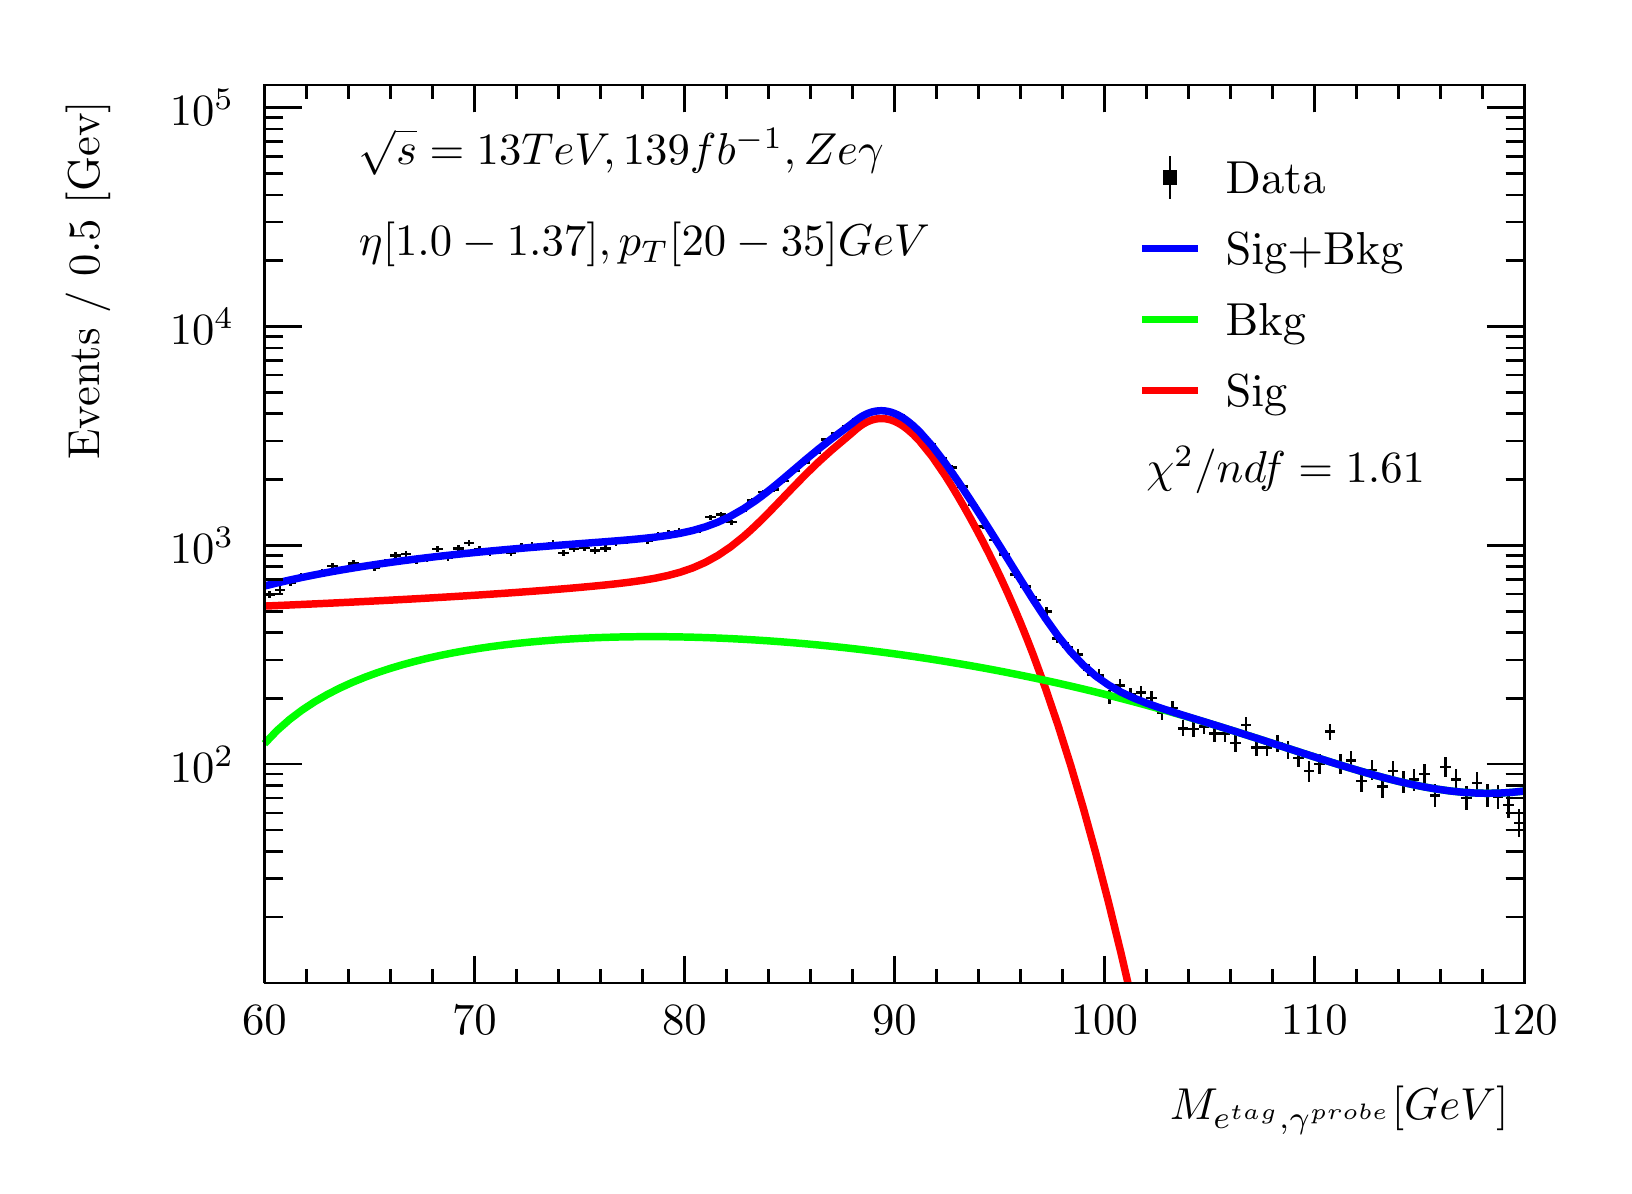
\begin{tikzpicture}
\pgfdeclareplotmark{cross} {
\pgfpathmoveto{\pgfpoint{-0.3\pgfplotmarksize}{\pgfplotmarksize}}
\pgfpathlineto{\pgfpoint{+0.3\pgfplotmarksize}{\pgfplotmarksize}}
\pgfpathlineto{\pgfpoint{+0.3\pgfplotmarksize}{0.3\pgfplotmarksize}}
\pgfpathlineto{\pgfpoint{+1\pgfplotmarksize}{0.3\pgfplotmarksize}}
\pgfpathlineto{\pgfpoint{+1\pgfplotmarksize}{-0.3\pgfplotmarksize}}
\pgfpathlineto{\pgfpoint{+0.3\pgfplotmarksize}{-0.3\pgfplotmarksize}}
\pgfpathlineto{\pgfpoint{+0.3\pgfplotmarksize}{-1.\pgfplotmarksize}}
\pgfpathlineto{\pgfpoint{-0.3\pgfplotmarksize}{-1.\pgfplotmarksize}}
\pgfpathlineto{\pgfpoint{-0.3\pgfplotmarksize}{-0.3\pgfplotmarksize}}
\pgfpathlineto{\pgfpoint{-1.\pgfplotmarksize}{-0.3\pgfplotmarksize}}
\pgfpathlineto{\pgfpoint{-1.\pgfplotmarksize}{0.3\pgfplotmarksize}}
\pgfpathlineto{\pgfpoint{-0.3\pgfplotmarksize}{0.3\pgfplotmarksize}}
\pgfpathclose
\pgfusepathqstroke
}
\pgfdeclareplotmark{cross*} {
\pgfpathmoveto{\pgfpoint{-0.3\pgfplotmarksize}{\pgfplotmarksize}}
\pgfpathlineto{\pgfpoint{+0.3\pgfplotmarksize}{\pgfplotmarksize}}
\pgfpathlineto{\pgfpoint{+0.3\pgfplotmarksize}{0.3\pgfplotmarksize}}
\pgfpathlineto{\pgfpoint{+1\pgfplotmarksize}{0.3\pgfplotmarksize}}
\pgfpathlineto{\pgfpoint{+1\pgfplotmarksize}{-0.3\pgfplotmarksize}}
\pgfpathlineto{\pgfpoint{+0.3\pgfplotmarksize}{-0.3\pgfplotmarksize}}
\pgfpathlineto{\pgfpoint{+0.3\pgfplotmarksize}{-1.\pgfplotmarksize}}
\pgfpathlineto{\pgfpoint{-0.3\pgfplotmarksize}{-1.\pgfplotmarksize}}
\pgfpathlineto{\pgfpoint{-0.3\pgfplotmarksize}{-0.3\pgfplotmarksize}}
\pgfpathlineto{\pgfpoint{-1.\pgfplotmarksize}{-0.3\pgfplotmarksize}}
\pgfpathlineto{\pgfpoint{-1.\pgfplotmarksize}{0.3\pgfplotmarksize}}
\pgfpathlineto{\pgfpoint{-0.3\pgfplotmarksize}{0.3\pgfplotmarksize}}
\pgfpathclose
\pgfusepathqfillstroke
}
\pgfdeclareplotmark{newstar} {
\pgfpathmoveto{\pgfqpoint{0pt}{\pgfplotmarksize}}
\pgfpathlineto{\pgfqpointpolar{44}{0.5\pgfplotmarksize}}
\pgfpathlineto{\pgfqpointpolar{18}{\pgfplotmarksize}}
\pgfpathlineto{\pgfqpointpolar{-20}{0.5\pgfplotmarksize}}
\pgfpathlineto{\pgfqpointpolar{-54}{\pgfplotmarksize}}
\pgfpathlineto{\pgfqpointpolar{-90}{0.5\pgfplotmarksize}}
\pgfpathlineto{\pgfqpointpolar{234}{\pgfplotmarksize}}
\pgfpathlineto{\pgfqpointpolar{198}{0.5\pgfplotmarksize}}
\pgfpathlineto{\pgfqpointpolar{162}{\pgfplotmarksize}}
\pgfpathlineto{\pgfqpointpolar{134}{0.5\pgfplotmarksize}}
\pgfpathclose
\pgfusepathqstroke
}
\pgfdeclareplotmark{newstar*} {
\pgfpathmoveto{\pgfqpoint{0pt}{\pgfplotmarksize}}
\pgfpathlineto{\pgfqpointpolar{44}{0.5\pgfplotmarksize}}
\pgfpathlineto{\pgfqpointpolar{18}{\pgfplotmarksize}}
\pgfpathlineto{\pgfqpointpolar{-20}{0.5\pgfplotmarksize}}
\pgfpathlineto{\pgfqpointpolar{-54}{\pgfplotmarksize}}
\pgfpathlineto{\pgfqpointpolar{-90}{0.5\pgfplotmarksize}}
\pgfpathlineto{\pgfqpointpolar{234}{\pgfplotmarksize}}
\pgfpathlineto{\pgfqpointpolar{198}{0.5\pgfplotmarksize}}
\pgfpathlineto{\pgfqpointpolar{162}{\pgfplotmarksize}}
\pgfpathlineto{\pgfqpointpolar{134}{0.5\pgfplotmarksize}}
\pgfpathclose
\pgfusepathqfillstroke
}
\definecolor{c}{rgb}{1,1,1};
\draw [color=c, fill=c] (0,0) rectangle (20,14.4361);
\draw [color=c, fill=c] (3,2.30977) rectangle (19,13.7143);
\definecolor{c}{rgb}{0,0,0};
\draw [c,line width=0.9] (3,2.30977) -- (3,13.7143) -- (19,13.7143) -- (19,2.30977) -- (3,2.30977);
\definecolor{c}{rgb}{1,1,1};
\draw [color=c, fill=c] (3,2.30977) rectangle (19,13.7143);
\definecolor{c}{rgb}{0,0,0};
\draw [c,line width=0.9] (3,2.30977) -- (3,13.7143) -- (19,13.7143) -- (19,2.30977) -- (3,2.30977);
\draw [c,line width=0.9] (3,2.30977) -- (19,2.30977);
\draw [c,line width=0.9] (3,2.65624) -- (3,2.30977);
\draw [c,line width=0.9] (3.53333,2.48301) -- (3.53333,2.30977);
\draw [c,line width=0.9] (4.06667,2.48301) -- (4.06667,2.30977);
\draw [c,line width=0.9] (4.6,2.48301) -- (4.6,2.30977);
\draw [c,line width=0.9] (5.13333,2.48301) -- (5.13333,2.30977);
\draw [c,line width=0.9] (5.66667,2.65624) -- (5.66667,2.30977);
\draw [c,line width=0.9] (6.2,2.48301) -- (6.2,2.30977);
\draw [c,line width=0.9] (6.73333,2.48301) -- (6.73333,2.30977);
\draw [c,line width=0.9] (7.26667,2.48301) -- (7.26667,2.30977);
\draw [c,line width=0.9] (7.8,2.48301) -- (7.8,2.30977);
\draw [c,line width=0.9] (8.33333,2.65624) -- (8.33333,2.30977);
\draw [c,line width=0.9] (8.86667,2.48301) -- (8.86667,2.30977);
\draw [c,line width=0.9] (9.4,2.48301) -- (9.4,2.30977);
\draw [c,line width=0.9] (9.93333,2.48301) -- (9.93333,2.30977);
\draw [c,line width=0.9] (10.4667,2.48301) -- (10.4667,2.30977);
\draw [c,line width=0.9] (11,2.65624) -- (11,2.30977);
\draw [c,line width=0.9] (11.5333,2.48301) -- (11.5333,2.30977);
\draw [c,line width=0.9] (12.0667,2.48301) -- (12.0667,2.30977);
\draw [c,line width=0.9] (12.6,2.48301) -- (12.6,2.30977);
\draw [c,line width=0.9] (13.1333,2.48301) -- (13.1333,2.30977);
\draw [c,line width=0.9] (13.6667,2.65624) -- (13.6667,2.30977);
\draw [c,line width=0.9] (14.2,2.48301) -- (14.2,2.30977);
\draw [c,line width=0.9] (14.7333,2.48301) -- (14.7333,2.30977);
\draw [c,line width=0.9] (15.2667,2.48301) -- (15.2667,2.30977);
\draw [c,line width=0.9] (15.8,2.48301) -- (15.8,2.30977);
\draw [c,line width=0.9] (16.3333,2.65624) -- (16.3333,2.30977);
\draw [c,line width=0.9] (16.8667,2.48301) -- (16.8667,2.30977);
\draw [c,line width=0.9] (17.4,2.48301) -- (17.4,2.30977);
\draw [c,line width=0.9] (17.9333,2.48301) -- (17.9333,2.30977);
\draw [c,line width=0.9] (18.4667,2.48301) -- (18.4667,2.30977);
\draw [c,line width=0.9] (19,2.65624) -- (19,2.30977);
\draw [anchor=base] (3,1.66015) node[scale=1.61424, color=c, rotate=0]{60};
\draw [anchor=base] (5.66667,1.66015) node[scale=1.61424, color=c, rotate=0]{70};
\draw [anchor=base] (8.33333,1.66015) node[scale=1.61424, color=c, rotate=0]{80};
\draw [anchor=base] (11,1.66015) node[scale=1.61424, color=c, rotate=0]{90};
\draw [anchor=base] (13.6667,1.66015) node[scale=1.61424, color=c, rotate=0]{100};
\draw [anchor=base] (16.3333,1.66015) node[scale=1.61424, color=c, rotate=0]{110};
\draw [anchor=base] (19,1.66015) node[scale=1.61424, color=c, rotate=0]{120};
\draw [anchor= east] (19,0.692932) node[scale=1.61424, color=c, rotate=0]{$M_{e^{tag}, \gamma^{probe}}  [GeV]$};
\draw [c,line width=0.9] (3,13.7143) -- (19,13.7143);
\draw [c,line width=0.9] (3,13.3678) -- (3,13.7143);
\draw [c,line width=0.9] (3.53333,13.5411) -- (3.53333,13.7143);
\draw [c,line width=0.9] (4.06667,13.5411) -- (4.06667,13.7143);
\draw [c,line width=0.9] (4.6,13.5411) -- (4.6,13.7143);
\draw [c,line width=0.9] (5.13333,13.5411) -- (5.13333,13.7143);
\draw [c,line width=0.9] (5.66667,13.3678) -- (5.66667,13.7143);
\draw [c,line width=0.9] (6.2,13.5411) -- (6.2,13.7143);
\draw [c,line width=0.9] (6.73333,13.5411) -- (6.73333,13.7143);
\draw [c,line width=0.9] (7.26667,13.5411) -- (7.26667,13.7143);
\draw [c,line width=0.9] (7.8,13.5411) -- (7.8,13.7143);
\draw [c,line width=0.9] (8.33333,13.3678) -- (8.33333,13.7143);
\draw [c,line width=0.9] (8.86667,13.5411) -- (8.86667,13.7143);
\draw [c,line width=0.9] (9.4,13.5411) -- (9.4,13.7143);
\draw [c,line width=0.9] (9.93333,13.5411) -- (9.93333,13.7143);
\draw [c,line width=0.9] (10.4667,13.5411) -- (10.4667,13.7143);
\draw [c,line width=0.9] (11,13.3678) -- (11,13.7143);
\draw [c,line width=0.9] (11.5333,13.5411) -- (11.5333,13.7143);
\draw [c,line width=0.9] (12.0667,13.5411) -- (12.0667,13.7143);
\draw [c,line width=0.9] (12.6,13.5411) -- (12.6,13.7143);
\draw [c,line width=0.9] (13.1333,13.5411) -- (13.1333,13.7143);
\draw [c,line width=0.9] (13.6667,13.3678) -- (13.6667,13.7143);
\draw [c,line width=0.9] (14.2,13.5411) -- (14.2,13.7143);
\draw [c,line width=0.9] (14.7333,13.5411) -- (14.7333,13.7143);
\draw [c,line width=0.9] (15.2667,13.5411) -- (15.2667,13.7143);
\draw [c,line width=0.9] (15.8,13.5411) -- (15.8,13.7143);
\draw [c,line width=0.9] (16.3333,13.3678) -- (16.3333,13.7143);
\draw [c,line width=0.9] (16.8667,13.5411) -- (16.8667,13.7143);
\draw [c,line width=0.9] (17.4,13.5411) -- (17.4,13.7143);
\draw [c,line width=0.9] (17.9333,13.5411) -- (17.9333,13.7143);
\draw [c,line width=0.9] (18.4667,13.5411) -- (18.4667,13.7143);
\draw [c,line width=0.9] (19,13.3678) -- (19,13.7143);
\draw [c,line width=0.9] (3,2.30977) -- (3,13.7143);
\draw [c,line width=0.9] (3.237,3.14637) -- (3,3.14637);
\draw [c,line width=0.9] (3.237,3.63576) -- (3,3.63576);
\draw [c,line width=0.9] (3.237,3.98298) -- (3,3.98298);
\draw [c,line width=0.9] (3.237,4.2523) -- (3,4.2523);
\draw [c,line width=0.9] (3.237,4.47236) -- (3,4.47236);
\draw [c,line width=0.9] (3.237,4.65841) -- (3,4.65841);
\draw [c,line width=0.9] (3.237,4.81958) -- (3,4.81958);
\draw [c,line width=0.9] (3.237,4.96174) -- (3,4.96174);
\draw [c,line width=0.9] (3.474,5.0889) -- (3,5.0889);
\draw [anchor= east] (2.82,5.0889) node[scale=1.61424, color=c, rotate=0]{$10^{2}$};
\draw [c,line width=0.9] (3.237,5.92551) -- (3,5.92551);
\draw [c,line width=0.9] (3.237,6.41489) -- (3,6.41489);
\draw [c,line width=0.9] (3.237,6.76211) -- (3,6.76211);
\draw [c,line width=0.9] (3.237,7.03144) -- (3,7.03144);
\draw [c,line width=0.9] (3.237,7.25149) -- (3,7.25149);
\draw [c,line width=0.9] (3.237,7.43755) -- (3,7.43755);
\draw [c,line width=0.9] (3.237,7.59871) -- (3,7.59871);
\draw [c,line width=0.9] (3.237,7.74087) -- (3,7.74087);
\draw [c,line width=0.9] (3.474,7.86804) -- (3,7.86804);
\draw [anchor= east] (2.82,7.86804) node[scale=1.61424, color=c, rotate=0]{$10^{3}$};
\draw [c,line width=0.9] (3.237,8.70464) -- (3,8.70464);
\draw [c,line width=0.9] (3.237,9.19402) -- (3,9.19402);
\draw [c,line width=0.9] (3.237,9.54124) -- (3,9.54124);
\draw [c,line width=0.9] (3.237,9.81057) -- (3,9.81057);
\draw [c,line width=0.9] (3.237,10.0306) -- (3,10.0306);
\draw [c,line width=0.9] (3.237,10.2167) -- (3,10.2167);
\draw [c,line width=0.9] (3.237,10.3778) -- (3,10.3778);
\draw [c,line width=0.9] (3.237,10.52) -- (3,10.52);
\draw [c,line width=0.9] (3.474,10.6472) -- (3,10.6472);
\draw [anchor= east] (2.82,10.6472) node[scale=1.61424, color=c, rotate=0]{$10^{4}$};
\draw [c,line width=0.9] (3.237,11.4838) -- (3,11.4838);
\draw [c,line width=0.9] (3.237,11.9732) -- (3,11.9732);
\draw [c,line width=0.9] (3.237,12.3204) -- (3,12.3204);
\draw [c,line width=0.9] (3.237,12.5897) -- (3,12.5897);
\draw [c,line width=0.9] (3.237,12.8098) -- (3,12.8098);
\draw [c,line width=0.9] (3.237,12.9958) -- (3,12.9958);
\draw [c,line width=0.9] (3.237,13.157) -- (3,13.157);
\draw [c,line width=0.9] (3.237,13.2991) -- (3,13.2991);
\draw [c,line width=0.9] (3.474,13.4263) -- (3,13.4263);
\draw [anchor= east] (2.82,13.4263) node[scale=1.61424, color=c, rotate=0]{$10^{5}$};
\draw [anchor= east] (0.76,13.7143) node[scale=1.61424, color=c, rotate=90]{Events / 0.5 [Gev]};
\draw [c,line width=0.9] (19,2.30977) -- (19,13.7143);
\draw [c,line width=0.9] (18.763,3.14637) -- (19,3.14637);
\draw [c,line width=0.9] (18.763,3.63576) -- (19,3.63576);
\draw [c,line width=0.9] (18.763,3.98298) -- (19,3.98298);
\draw [c,line width=0.9] (18.763,4.2523) -- (19,4.2523);
\draw [c,line width=0.9] (18.763,4.47236) -- (19,4.47236);
\draw [c,line width=0.9] (18.763,4.65841) -- (19,4.65841);
\draw [c,line width=0.9] (18.763,4.81958) -- (19,4.81958);
\draw [c,line width=0.9] (18.763,4.96174) -- (19,4.96174);
\draw [c,line width=0.9] (18.526,5.0889) -- (19,5.0889);
\draw [c,line width=0.9] (18.763,5.92551) -- (19,5.92551);
\draw [c,line width=0.9] (18.763,6.41489) -- (19,6.41489);
\draw [c,line width=0.9] (18.763,6.76211) -- (19,6.76211);
\draw [c,line width=0.9] (18.763,7.03144) -- (19,7.03144);
\draw [c,line width=0.9] (18.763,7.25149) -- (19,7.25149);
\draw [c,line width=0.9] (18.763,7.43755) -- (19,7.43755);
\draw [c,line width=0.9] (18.763,7.59871) -- (19,7.59871);
\draw [c,line width=0.9] (18.763,7.74087) -- (19,7.74087);
\draw [c,line width=0.9] (18.526,7.86804) -- (19,7.86804);
\draw [c,line width=0.9] (18.763,8.70464) -- (19,8.70464);
\draw [c,line width=0.9] (18.763,9.19402) -- (19,9.19402);
\draw [c,line width=0.9] (18.763,9.54124) -- (19,9.54124);
\draw [c,line width=0.9] (18.763,9.81057) -- (19,9.81057);
\draw [c,line width=0.9] (18.763,10.0306) -- (19,10.0306);
\draw [c,line width=0.9] (18.763,10.2167) -- (19,10.2167);
\draw [c,line width=0.9] (18.763,10.3778) -- (19,10.3778);
\draw [c,line width=0.9] (18.763,10.52) -- (19,10.52);
\draw [c,line width=0.9] (18.526,10.6472) -- (19,10.6472);
\draw [c,line width=0.9] (18.763,11.4838) -- (19,11.4838);
\draw [c,line width=0.9] (18.763,11.9732) -- (19,11.9732);
\draw [c,line width=0.9] (18.763,12.3204) -- (19,12.3204);
\draw [c,line width=0.9] (18.763,12.5897) -- (19,12.5897);
\draw [c,line width=0.9] (18.763,12.8098) -- (19,12.8098);
\draw [c,line width=0.9] (18.763,12.9958) -- (19,12.9958);
\draw [c,line width=0.9] (18.763,13.157) -- (19,13.157);
\draw [c,line width=0.9] (18.763,13.2991) -- (19,13.2991);
\draw [c,line width=0.9] (18.526,13.4263) -- (19,13.4263);
\draw [c,line width=0.9] (3.06667,7.24544) -- (3,7.24544);
\draw [c,line width=0.9] (3,7.24544) -- (3,7.24544);
\draw [c,line width=0.9] (3.06667,7.24544) -- (3.13333,7.24544);
\draw [c,line width=0.9] (3.13333,7.24544) -- (3.13333,7.24544);
\draw [c,line width=0.9] (3.06667,7.24544) -- (3.06667,7.29484);
\draw [c,line width=0.9] (3.06667,7.29484) -- (3.06667,7.29484);
\draw [c,line width=0.9] (3.06667,7.24544) -- (3.06667,7.19605);
\draw [c,line width=0.9] (3.06667,7.19605) -- (3.06667,7.19605);
\draw [c,line width=0.9] (3.2,7.30076) -- (3.13333,7.30076);
\draw [c,line width=0.9] (3.13333,7.30076) -- (3.13333,7.30076);
\draw [c,line width=0.9] (3.2,7.30076) -- (3.26667,7.30076);
\draw [c,line width=0.9] (3.26667,7.30076) -- (3.26667,7.30076);
\draw [c,line width=0.9] (3.2,7.30076) -- (3.2,7.34904);
\draw [c,line width=0.9] (3.2,7.34904) -- (3.2,7.34904);
\draw [c,line width=0.9] (3.2,7.30076) -- (3.2,7.25249);
\draw [c,line width=0.9] (3.2,7.25249) -- (3.2,7.25249);
\draw [c,line width=0.9] (3.33333,7.39544) -- (3.26667,7.39544);
\draw [c,line width=0.9] (3.26667,7.39544) -- (3.26667,7.39544);
\draw [c,line width=0.9] (3.33333,7.39544) -- (3.4,7.39544);
\draw [c,line width=0.9] (3.4,7.39544) -- (3.4,7.39544);
\draw [c,line width=0.9] (3.33333,7.39544) -- (3.33333,7.44186);
\draw [c,line width=0.9] (3.33333,7.44186) -- (3.33333,7.44186);
\draw [c,line width=0.9] (3.33333,7.39544) -- (3.33333,7.34902);
\draw [c,line width=0.9] (3.33333,7.34902) -- (3.33333,7.34902);
\draw [c,line width=0.9] (3.46667,7.47155) -- (3.4,7.47155);
\draw [c,line width=0.9] (3.4,7.47155) -- (3.4,7.47155);
\draw [c,line width=0.9] (3.46667,7.47155) -- (3.53333,7.47155);
\draw [c,line width=0.9] (3.53333,7.47155) -- (3.53333,7.47155);
\draw [c,line width=0.9] (3.46667,7.47155) -- (3.46667,7.51653);
\draw [c,line width=0.9] (3.46667,7.51653) -- (3.46667,7.51653);
\draw [c,line width=0.9] (3.46667,7.47155) -- (3.46667,7.42657);
\draw [c,line width=0.9] (3.46667,7.42657) -- (3.46667,7.42657);
\draw [c,line width=0.9] (3.6,7.48323) -- (3.53333,7.48323);
\draw [c,line width=0.9] (3.53333,7.48323) -- (3.53333,7.48323);
\draw [c,line width=0.9] (3.6,7.48323) -- (3.66667,7.48323);
\draw [c,line width=0.9] (3.66667,7.48323) -- (3.66667,7.48323);
\draw [c,line width=0.9] (3.6,7.48323) -- (3.6,7.52799);
\draw [c,line width=0.9] (3.6,7.52799) -- (3.6,7.52799);
\draw [c,line width=0.9] (3.6,7.48323) -- (3.6,7.43846);
\draw [c,line width=0.9] (3.6,7.43846) -- (3.6,7.43846);
\draw [c,line width=0.9] (3.73333,7.52243) -- (3.66667,7.52243);
\draw [c,line width=0.9] (3.66667,7.52243) -- (3.66667,7.52243);
\draw [c,line width=0.9] (3.73333,7.52243) -- (3.8,7.52243);
\draw [c,line width=0.9] (3.8,7.52243) -- (3.8,7.52243);
\draw [c,line width=0.9] (3.73333,7.52243) -- (3.73333,7.56647);
\draw [c,line width=0.9] (3.73333,7.56647) -- (3.73333,7.56647);
\draw [c,line width=0.9] (3.73333,7.52243) -- (3.73333,7.47839);
\draw [c,line width=0.9] (3.73333,7.47839) -- (3.73333,7.47839);
\draw [c,line width=0.9] (3.86667,7.60773) -- (3.8,7.60773);
\draw [c,line width=0.9] (3.8,7.60773) -- (3.8,7.60773);
\draw [c,line width=0.9] (3.86667,7.60773) -- (3.93333,7.60773);
\draw [c,line width=0.9] (3.93333,7.60773) -- (3.93333,7.60773);
\draw [c,line width=0.9] (3.86667,7.60773) -- (3.86667,7.65024);
\draw [c,line width=0.9] (3.86667,7.65024) -- (3.86667,7.65024);
\draw [c,line width=0.9] (3.86667,7.60773) -- (3.86667,7.56522);
\draw [c,line width=0.9] (3.86667,7.56522) -- (3.86667,7.56522);
\draw [c,line width=0.9] (4,7.56039) -- (3.93333,7.56039);
\draw [c,line width=0.9] (3.93333,7.56039) -- (3.93333,7.56039);
\draw [c,line width=0.9] (4,7.56039) -- (4.06667,7.56039);
\draw [c,line width=0.9] (4.06667,7.56039) -- (4.06667,7.56039);
\draw [c,line width=0.9] (4,7.56039) -- (4,7.60375);
\draw [c,line width=0.9] (4,7.60375) -- (4,7.60375);
\draw [c,line width=0.9] (4,7.56039) -- (4,7.51704);
\draw [c,line width=0.9] (4,7.51704) -- (4,7.51704);
\draw [c,line width=0.9] (4.13333,7.63878) -- (4.06667,7.63878);
\draw [c,line width=0.9] (4.06667,7.63878) -- (4.06667,7.63878);
\draw [c,line width=0.9] (4.13333,7.63878) -- (4.2,7.63878);
\draw [c,line width=0.9] (4.2,7.63878) -- (4.2,7.63878);
\draw [c,line width=0.9] (4.13333,7.63878) -- (4.13333,7.68074);
\draw [c,line width=0.9] (4.13333,7.68074) -- (4.13333,7.68074);
\draw [c,line width=0.9] (4.13333,7.63878) -- (4.13333,7.59681);
\draw [c,line width=0.9] (4.13333,7.59681) -- (4.13333,7.59681);
\draw [c,line width=0.9] (4.26667,7.60623) -- (4.2,7.60623);
\draw [c,line width=0.9] (4.2,7.60623) -- (4.2,7.60623);
\draw [c,line width=0.9] (4.26667,7.60623) -- (4.33333,7.60623);
\draw [c,line width=0.9] (4.33333,7.60623) -- (4.33333,7.60623);
\draw [c,line width=0.9] (4.26667,7.60623) -- (4.26667,7.64877);
\draw [c,line width=0.9] (4.26667,7.64877) -- (4.26667,7.64877);
\draw [c,line width=0.9] (4.26667,7.60623) -- (4.26667,7.5637);
\draw [c,line width=0.9] (4.26667,7.5637) -- (4.26667,7.5637);
\draw [c,line width=0.9] (4.4,7.58658) -- (4.33333,7.58658);
\draw [c,line width=0.9] (4.33333,7.58658) -- (4.33333,7.58658);
\draw [c,line width=0.9] (4.4,7.58658) -- (4.46667,7.58658);
\draw [c,line width=0.9] (4.46667,7.58658) -- (4.46667,7.58658);
\draw [c,line width=0.9] (4.4,7.58658) -- (4.4,7.62947);
\draw [c,line width=0.9] (4.4,7.62947) -- (4.4,7.62947);
\draw [c,line width=0.9] (4.4,7.58658) -- (4.4,7.5437);
\draw [c,line width=0.9] (4.4,7.5437) -- (4.4,7.5437);
\draw [c,line width=0.9] (4.53333,7.65473) -- (4.46667,7.65473);
\draw [c,line width=0.9] (4.46667,7.65473) -- (4.46667,7.65473);
\draw [c,line width=0.9] (4.53333,7.65473) -- (4.6,7.65473);
\draw [c,line width=0.9] (4.6,7.65473) -- (4.6,7.65473);
\draw [c,line width=0.9] (4.53333,7.65473) -- (4.53333,7.69642);
\draw [c,line width=0.9] (4.53333,7.69642) -- (4.53333,7.69642);
\draw [c,line width=0.9] (4.53333,7.65473) -- (4.53333,7.61303);
\draw [c,line width=0.9] (4.53333,7.61303) -- (4.53333,7.61303);
\draw [c,line width=0.9] (4.66667,7.74087) -- (4.6,7.74087);
\draw [c,line width=0.9] (4.6,7.74087) -- (4.6,7.74087);
\draw [c,line width=0.9] (4.66667,7.74087) -- (4.73333,7.74087);
\draw [c,line width=0.9] (4.73333,7.74087) -- (4.73333,7.74087);
\draw [c,line width=0.9] (4.66667,7.74087) -- (4.66667,7.7811);
\draw [c,line width=0.9] (4.66667,7.7811) -- (4.66667,7.7811);
\draw [c,line width=0.9] (4.66667,7.74087) -- (4.66667,7.70064);
\draw [c,line width=0.9] (4.66667,7.70064) -- (4.66667,7.70064);
\draw [c,line width=0.9] (4.8,7.7595) -- (4.73333,7.7595);
\draw [c,line width=0.9] (4.73333,7.7595) -- (4.73333,7.7595);
\draw [c,line width=0.9] (4.8,7.7595) -- (4.86667,7.7595);
\draw [c,line width=0.9] (4.86667,7.7595) -- (4.86667,7.7595);
\draw [c,line width=0.9] (4.8,7.7595) -- (4.8,7.79943);
\draw [c,line width=0.9] (4.8,7.79943) -- (4.8,7.79943);
\draw [c,line width=0.9] (4.8,7.7595) -- (4.8,7.71958);
\draw [c,line width=0.9] (4.8,7.71958) -- (4.8,7.71958);
\draw [c,line width=0.9] (4.93333,7.67331) -- (4.86667,7.67331);
\draw [c,line width=0.9] (4.86667,7.67331) -- (4.86667,7.67331);
\draw [c,line width=0.9] (4.93333,7.67331) -- (5,7.67331);
\draw [c,line width=0.9] (5,7.67331) -- (5,7.67331);
\draw [c,line width=0.9] (4.93333,7.67331) -- (4.93333,7.71468);
\draw [c,line width=0.9] (4.93333,7.71468) -- (4.93333,7.71468);
\draw [c,line width=0.9] (4.93333,7.67331) -- (4.93333,7.63193);
\draw [c,line width=0.9] (4.93333,7.63193) -- (4.93333,7.63193);
\draw [c,line width=0.9] (5.06667,7.69718) -- (5,7.69718);
\draw [c,line width=0.9] (5,7.69718) -- (5,7.69718);
\draw [c,line width=0.9] (5.06667,7.69718) -- (5.13333,7.69718);
\draw [c,line width=0.9] (5.13333,7.69718) -- (5.13333,7.69718);
\draw [c,line width=0.9] (5.06667,7.69718) -- (5.06667,7.73814);
\draw [c,line width=0.9] (5.06667,7.73814) -- (5.06667,7.73814);
\draw [c,line width=0.9] (5.06667,7.69718) -- (5.06667,7.65621);
\draw [c,line width=0.9] (5.06667,7.65621) -- (5.06667,7.65621);
\draw [c,line width=0.9] (5.2,7.82003) -- (5.13333,7.82003);
\draw [c,line width=0.9] (5.13333,7.82003) -- (5.13333,7.82003);
\draw [c,line width=0.9] (5.2,7.82003) -- (5.26667,7.82003);
\draw [c,line width=0.9] (5.26667,7.82003) -- (5.26667,7.82003);
\draw [c,line width=0.9] (5.2,7.82003) -- (5.2,7.85896);
\draw [c,line width=0.9] (5.2,7.85896) -- (5.2,7.85896);
\draw [c,line width=0.9] (5.2,7.82003) -- (5.2,7.78109);
\draw [c,line width=0.9] (5.2,7.78109) -- (5.2,7.78109);
\draw [c,line width=0.9] (5.33333,7.711) -- (5.26667,7.711);
\draw [c,line width=0.9] (5.26667,7.711) -- (5.26667,7.711);
\draw [c,line width=0.9] (5.33333,7.711) -- (5.4,7.711);
\draw [c,line width=0.9] (5.4,7.711) -- (5.4,7.711);
\draw [c,line width=0.9] (5.33333,7.711) -- (5.33333,7.75173);
\draw [c,line width=0.9] (5.33333,7.75173) -- (5.33333,7.75173);
\draw [c,line width=0.9] (5.33333,7.711) -- (5.33333,7.67027);
\draw [c,line width=0.9] (5.33333,7.67027) -- (5.33333,7.67027);
\draw [c,line width=0.9] (5.46667,7.83003) -- (5.4,7.83003);
\draw [c,line width=0.9] (5.4,7.83003) -- (5.4,7.83003);
\draw [c,line width=0.9] (5.46667,7.83003) -- (5.53333,7.83003);
\draw [c,line width=0.9] (5.53333,7.83003) -- (5.53333,7.83003);
\draw [c,line width=0.9] (5.46667,7.83003) -- (5.46667,7.8688);
\draw [c,line width=0.9] (5.46667,7.8688) -- (5.46667,7.8688);
\draw [c,line width=0.9] (5.46667,7.83003) -- (5.46667,7.79126);
\draw [c,line width=0.9] (5.46667,7.79126) -- (5.46667,7.79126);
\draw [c,line width=0.9] (5.6,7.89666) -- (5.53333,7.89666);
\draw [c,line width=0.9] (5.53333,7.89666) -- (5.53333,7.89666);
\draw [c,line width=0.9] (5.6,7.89666) -- (5.66667,7.89666);
\draw [c,line width=0.9] (5.66667,7.89666) -- (5.66667,7.89666);
\draw [c,line width=0.9] (5.6,7.89666) -- (5.6,7.93438);
\draw [c,line width=0.9] (5.6,7.93438) -- (5.6,7.93438);
\draw [c,line width=0.9] (5.6,7.89666) -- (5.6,7.85895);
\draw [c,line width=0.9] (5.6,7.85895) -- (5.6,7.85895);
\draw [c,line width=0.9] (5.73333,7.81751) -- (5.66667,7.81751);
\draw [c,line width=0.9] (5.66667,7.81751) -- (5.66667,7.81751);
\draw [c,line width=0.9] (5.73333,7.81751) -- (5.8,7.81751);
\draw [c,line width=0.9] (5.8,7.81751) -- (5.8,7.81751);
\draw [c,line width=0.9] (5.73333,7.81751) -- (5.73333,7.85648);
\draw [c,line width=0.9] (5.73333,7.85648) -- (5.73333,7.85648);
\draw [c,line width=0.9] (5.73333,7.81751) -- (5.73333,7.77854);
\draw [c,line width=0.9] (5.73333,7.77854) -- (5.73333,7.77854);
\draw [c,line width=0.9] (5.86667,7.77785) -- (5.8,7.77785);
\draw [c,line width=0.9] (5.8,7.77785) -- (5.8,7.77785);
\draw [c,line width=0.9] (5.86667,7.77785) -- (5.93333,7.77785);
\draw [c,line width=0.9] (5.93333,7.77785) -- (5.93333,7.77785);
\draw [c,line width=0.9] (5.86667,7.77785) -- (5.86667,7.81747);
\draw [c,line width=0.9] (5.86667,7.81747) -- (5.86667,7.81747);
\draw [c,line width=0.9] (5.86667,7.77785) -- (5.86667,7.73823);
\draw [c,line width=0.9] (5.86667,7.73823) -- (5.86667,7.73823);
\draw [c,line width=0.9] (6,7.79592) -- (5.93333,7.79592);
\draw [c,line width=0.9] (5.93333,7.79592) -- (5.93333,7.79592);
\draw [c,line width=0.9] (6,7.79592) -- (6.06667,7.79592);
\draw [c,line width=0.9] (6.06667,7.79592) -- (6.06667,7.79592);
\draw [c,line width=0.9] (6,7.79592) -- (6,7.83525);
\draw [c,line width=0.9] (6,7.83525) -- (6,7.83525);
\draw [c,line width=0.9] (6,7.79592) -- (6,7.7566);
\draw [c,line width=0.9] (6,7.7566) -- (6,7.7566);
\draw [c,line width=0.9] (6.13333,7.77655) -- (6.06667,7.77655);
\draw [c,line width=0.9] (6.06667,7.77655) -- (6.06667,7.77655);
\draw [c,line width=0.9] (6.13333,7.77655) -- (6.2,7.77655);
\draw [c,line width=0.9] (6.2,7.77655) -- (6.2,7.77655);
\draw [c,line width=0.9] (6.13333,7.77655) -- (6.13333,7.81619);
\draw [c,line width=0.9] (6.13333,7.81619) -- (6.13333,7.81619);
\draw [c,line width=0.9] (6.13333,7.77655) -- (6.13333,7.73691);
\draw [c,line width=0.9] (6.13333,7.73691) -- (6.13333,7.73691);
\draw [c,line width=0.9] (6.26667,7.85713) -- (6.2,7.85713);
\draw [c,line width=0.9] (6.2,7.85713) -- (6.2,7.85713);
\draw [c,line width=0.9] (6.26667,7.85713) -- (6.33333,7.85713);
\draw [c,line width=0.9] (6.33333,7.85713) -- (6.33333,7.85713);
\draw [c,line width=0.9] (6.26667,7.85713) -- (6.26667,7.89547);
\draw [c,line width=0.9] (6.26667,7.89547) -- (6.26667,7.89547);
\draw [c,line width=0.9] (6.26667,7.85713) -- (6.26667,7.81879);
\draw [c,line width=0.9] (6.26667,7.81879) -- (6.26667,7.81879);
\draw [c,line width=0.9] (6.4,7.86925) -- (6.33333,7.86925);
\draw [c,line width=0.9] (6.33333,7.86925) -- (6.33333,7.86925);
\draw [c,line width=0.9] (6.4,7.86925) -- (6.46667,7.86925);
\draw [c,line width=0.9] (6.46667,7.86925) -- (6.46667,7.86925);
\draw [c,line width=0.9] (6.4,7.86925) -- (6.4,7.90739);
\draw [c,line width=0.9] (6.4,7.90739) -- (6.4,7.90739);
\draw [c,line width=0.9] (6.4,7.86925) -- (6.4,7.8311);
\draw [c,line width=0.9] (6.4,7.8311) -- (6.4,7.8311);
\draw [c,line width=0.9] (6.53333,7.84242) -- (6.46667,7.84242);
\draw [c,line width=0.9] (6.46667,7.84242) -- (6.46667,7.84242);
\draw [c,line width=0.9] (6.53333,7.84242) -- (6.6,7.84242);
\draw [c,line width=0.9] (6.6,7.84242) -- (6.6,7.84242);
\draw [c,line width=0.9] (6.53333,7.84242) -- (6.53333,7.881);
\draw [c,line width=0.9] (6.53333,7.881) -- (6.53333,7.881);
\draw [c,line width=0.9] (6.53333,7.84242) -- (6.53333,7.80385);
\draw [c,line width=0.9] (6.53333,7.80385) -- (6.53333,7.80385);
\draw [c,line width=0.9] (6.66667,7.9002) -- (6.6,7.9002);
\draw [c,line width=0.9] (6.6,7.9002) -- (6.6,7.9002);
\draw [c,line width=0.9] (6.66667,7.9002) -- (6.73333,7.9002);
\draw [c,line width=0.9] (6.73333,7.9002) -- (6.73333,7.9002);
\draw [c,line width=0.9] (6.66667,7.9002) -- (6.66667,7.93786);
\draw [c,line width=0.9] (6.66667,7.93786) -- (6.66667,7.93786);
\draw [c,line width=0.9] (6.66667,7.9002) -- (6.66667,7.86253);
\draw [c,line width=0.9] (6.66667,7.86253) -- (6.66667,7.86253);
\draw [c,line width=0.9] (6.8,7.77133) -- (6.73333,7.77133);
\draw [c,line width=0.9] (6.73333,7.77133) -- (6.73333,7.77133);
\draw [c,line width=0.9] (6.8,7.77133) -- (6.86667,7.77133);
\draw [c,line width=0.9] (6.86667,7.77133) -- (6.86667,7.77133);
\draw [c,line width=0.9] (6.8,7.77133) -- (6.8,7.81106);
\draw [c,line width=0.9] (6.8,7.81106) -- (6.8,7.81106);
\draw [c,line width=0.9] (6.8,7.77133) -- (6.8,7.73161);
\draw [c,line width=0.9] (6.8,7.73161) -- (6.8,7.73161);
\draw [c,line width=0.9] (6.93333,7.82504) -- (6.86667,7.82504);
\draw [c,line width=0.9] (6.86667,7.82504) -- (6.86667,7.82504);
\draw [c,line width=0.9] (6.93333,7.82504) -- (7,7.82504);
\draw [c,line width=0.9] (7,7.82504) -- (7,7.82504);
\draw [c,line width=0.9] (6.93333,7.82504) -- (6.93333,7.86389);
\draw [c,line width=0.9] (6.93333,7.86389) -- (6.93333,7.86389);
\draw [c,line width=0.9] (6.93333,7.82504) -- (6.93333,7.78619);
\draw [c,line width=0.9] (6.93333,7.78619) -- (6.93333,7.78619);
\draw [c,line width=0.9] (7.06667,7.83376) -- (7,7.83376);
\draw [c,line width=0.9] (7,7.83376) -- (7,7.83376);
\draw [c,line width=0.9] (7.06667,7.83376) -- (7.13333,7.83376);
\draw [c,line width=0.9] (7.13333,7.83376) -- (7.13333,7.83376);
\draw [c,line width=0.9] (7.06667,7.83376) -- (7.06667,7.87247);
\draw [c,line width=0.9] (7.06667,7.87247) -- (7.06667,7.87247);
\draw [c,line width=0.9] (7.06667,7.83376) -- (7.06667,7.79505);
\draw [c,line width=0.9] (7.06667,7.79505) -- (7.06667,7.79505);
\draw [c,line width=0.9] (7.2,7.80231) -- (7.13333,7.80231);
\draw [c,line width=0.9] (7.13333,7.80231) -- (7.13333,7.80231);
\draw [c,line width=0.9] (7.2,7.80231) -- (7.26667,7.80231);
\draw [c,line width=0.9] (7.26667,7.80231) -- (7.26667,7.80231);
\draw [c,line width=0.9] (7.2,7.80231) -- (7.2,7.84153);
\draw [c,line width=0.9] (7.2,7.84153) -- (7.2,7.84153);
\draw [c,line width=0.9] (7.2,7.80231) -- (7.2,7.76309);
\draw [c,line width=0.9] (7.2,7.76309) -- (7.2,7.76309);
\draw [c,line width=0.9] (7.33333,7.82879) -- (7.26667,7.82879);
\draw [c,line width=0.9] (7.26667,7.82879) -- (7.26667,7.82879);
\draw [c,line width=0.9] (7.33333,7.82879) -- (7.4,7.82879);
\draw [c,line width=0.9] (7.4,7.82879) -- (7.4,7.82879);
\draw [c,line width=0.9] (7.33333,7.82879) -- (7.33333,7.86758);
\draw [c,line width=0.9] (7.33333,7.86758) -- (7.33333,7.86758);
\draw [c,line width=0.9] (7.33333,7.82879) -- (7.33333,7.78999);
\draw [c,line width=0.9] (7.33333,7.78999) -- (7.33333,7.78999);
\draw [c,line width=0.9] (7.46667,7.90137) -- (7.4,7.90137);
\draw [c,line width=0.9] (7.4,7.90137) -- (7.4,7.90137);
\draw [c,line width=0.9] (7.46667,7.90137) -- (7.53333,7.90137);
\draw [c,line width=0.9] (7.53333,7.90137) -- (7.53333,7.90137);
\draw [c,line width=0.9] (7.46667,7.90137) -- (7.46667,7.93901);
\draw [c,line width=0.9] (7.46667,7.93901) -- (7.46667,7.93901);
\draw [c,line width=0.9] (7.46667,7.90137) -- (7.46667,7.86373);
\draw [c,line width=0.9] (7.46667,7.86373) -- (7.46667,7.86373);
\draw [c,line width=0.9] (7.6,7.92001) -- (7.53333,7.92001);
\draw [c,line width=0.9] (7.53333,7.92001) -- (7.53333,7.92001);
\draw [c,line width=0.9] (7.6,7.92001) -- (7.66667,7.92001);
\draw [c,line width=0.9] (7.66667,7.92001) -- (7.66667,7.92001);
\draw [c,line width=0.9] (7.6,7.92001) -- (7.6,7.95736);
\draw [c,line width=0.9] (7.6,7.95736) -- (7.6,7.95736);
\draw [c,line width=0.9] (7.6,7.92001) -- (7.6,7.88266);
\draw [c,line width=0.9] (7.6,7.88266) -- (7.6,7.88266);
\draw [c,line width=0.9] (7.73333,7.94857) -- (7.66667,7.94857);
\draw [c,line width=0.9] (7.66667,7.94857) -- (7.66667,7.94857);
\draw [c,line width=0.9] (7.73333,7.94857) -- (7.8,7.94857);
\draw [c,line width=0.9] (7.8,7.94857) -- (7.8,7.94857);
\draw [c,line width=0.9] (7.73333,7.94857) -- (7.73333,7.98549);
\draw [c,line width=0.9] (7.73333,7.98549) -- (7.73333,7.98549);
\draw [c,line width=0.9] (7.73333,7.94857) -- (7.73333,7.91166);
\draw [c,line width=0.9] (7.73333,7.91166) -- (7.73333,7.91166);
\draw [c,line width=0.9] (7.86667,7.92693) -- (7.8,7.92693);
\draw [c,line width=0.9] (7.8,7.92693) -- (7.8,7.92693);
\draw [c,line width=0.9] (7.86667,7.92693) -- (7.93333,7.92693);
\draw [c,line width=0.9] (7.93333,7.92693) -- (7.93333,7.92693);
\draw [c,line width=0.9] (7.86667,7.92693) -- (7.86667,7.96417);
\draw [c,line width=0.9] (7.86667,7.96417) -- (7.86667,7.96417);
\draw [c,line width=0.9] (7.86667,7.92693) -- (7.86667,7.88968);
\draw [c,line width=0.9] (7.86667,7.88968) -- (7.86667,7.88968);
\draw [c,line width=0.9] (8,7.99834) -- (7.93333,7.99834);
\draw [c,line width=0.9] (7.93333,7.99834) -- (7.93333,7.99834);
\draw [c,line width=0.9] (8,7.99834) -- (8.06667,7.99834);
\draw [c,line width=0.9] (8.06667,7.99834) -- (8.06667,7.99834);
\draw [c,line width=0.9] (8,7.99834) -- (8,8.0345);
\draw [c,line width=0.9] (8,8.0345) -- (8,8.0345);
\draw [c,line width=0.9] (8,7.99834) -- (8,7.96218);
\draw [c,line width=0.9] (8,7.96218) -- (8,7.96218);
\draw [c,line width=0.9] (8.13333,8.02194) -- (8.06667,8.02194);
\draw [c,line width=0.9] (8.06667,8.02194) -- (8.06667,8.02194);
\draw [c,line width=0.9] (8.13333,8.02194) -- (8.2,8.02194);
\draw [c,line width=0.9] (8.2,8.02194) -- (8.2,8.02194);
\draw [c,line width=0.9] (8.13333,8.02194) -- (8.13333,8.05775);
\draw [c,line width=0.9] (8.13333,8.05775) -- (8.13333,8.05775);
\draw [c,line width=0.9] (8.13333,8.02194) -- (8.13333,7.98614);
\draw [c,line width=0.9] (8.13333,7.98614) -- (8.13333,7.98614);
\draw [c,line width=0.9] (8.26667,8.04926) -- (8.2,8.04926);
\draw [c,line width=0.9] (8.2,8.04926) -- (8.2,8.04926);
\draw [c,line width=0.9] (8.26667,8.04926) -- (8.33333,8.04926);
\draw [c,line width=0.9] (8.33333,8.04926) -- (8.33333,8.04926);
\draw [c,line width=0.9] (8.26667,8.04926) -- (8.26667,8.08466);
\draw [c,line width=0.9] (8.26667,8.08466) -- (8.26667,8.08466);
\draw [c,line width=0.9] (8.26667,8.04926) -- (8.26667,8.01385);
\draw [c,line width=0.9] (8.26667,8.01385) -- (8.26667,8.01385);
\draw [c,line width=0.9] (8.4,8.04405) -- (8.33333,8.04405);
\draw [c,line width=0.9] (8.33333,8.04405) -- (8.33333,8.04405);
\draw [c,line width=0.9] (8.4,8.04405) -- (8.46667,8.04405);
\draw [c,line width=0.9] (8.46667,8.04405) -- (8.46667,8.04405);
\draw [c,line width=0.9] (8.4,8.04405) -- (8.4,8.07953);
\draw [c,line width=0.9] (8.4,8.07953) -- (8.4,8.07953);
\draw [c,line width=0.9] (8.4,8.04405) -- (8.4,8.00857);
\draw [c,line width=0.9] (8.4,8.00857) -- (8.4,8.00857);
\draw [c,line width=0.9] (8.53333,8.06474) -- (8.46667,8.06474);
\draw [c,line width=0.9] (8.46667,8.06474) -- (8.46667,8.06474);
\draw [c,line width=0.9] (8.53333,8.06474) -- (8.6,8.06474);
\draw [c,line width=0.9] (8.6,8.06474) -- (8.6,8.06474);
\draw [c,line width=0.9] (8.53333,8.06474) -- (8.53333,8.09992);
\draw [c,line width=0.9] (8.53333,8.09992) -- (8.53333,8.09992);
\draw [c,line width=0.9] (8.53333,8.06474) -- (8.53333,8.02956);
\draw [c,line width=0.9] (8.53333,8.02956) -- (8.53333,8.02956);
\draw [c,line width=0.9] (8.66667,8.22667) -- (8.6,8.22667);
\draw [c,line width=0.9] (8.6,8.22667) -- (8.6,8.22667);
\draw [c,line width=0.9] (8.66667,8.22667) -- (8.73333,8.22667);
\draw [c,line width=0.9] (8.73333,8.22667) -- (8.73333,8.22667);
\draw [c,line width=0.9] (8.66667,8.22667) -- (8.66667,8.25957);
\draw [c,line width=0.9] (8.66667,8.25957) -- (8.66667,8.25957);
\draw [c,line width=0.9] (8.66667,8.22667) -- (8.66667,8.19378);
\draw [c,line width=0.9] (8.66667,8.19378) -- (8.66667,8.19378);
\draw [c,line width=0.9] (8.8,8.26115) -- (8.73333,8.26115);
\draw [c,line width=0.9] (8.73333,8.26115) -- (8.73333,8.26115);
\draw [c,line width=0.9] (8.8,8.26115) -- (8.86667,8.26115);
\draw [c,line width=0.9] (8.86667,8.26115) -- (8.86667,8.26115);
\draw [c,line width=0.9] (8.8,8.26115) -- (8.8,8.29358);
\draw [c,line width=0.9] (8.8,8.29358) -- (8.8,8.29358);
\draw [c,line width=0.9] (8.8,8.26115) -- (8.8,8.22872);
\draw [c,line width=0.9] (8.8,8.22872) -- (8.8,8.22872);
\draw [c,line width=0.9] (8.93333,8.16221) -- (8.86667,8.16221);
\draw [c,line width=0.9] (8.86667,8.16221) -- (8.86667,8.16221);
\draw [c,line width=0.9] (8.93333,8.16221) -- (9,8.16221);
\draw [c,line width=0.9] (9,8.16221) -- (9,8.16221);
\draw [c,line width=0.9] (8.93333,8.16221) -- (8.93333,8.196);
\draw [c,line width=0.9] (8.93333,8.196) -- (8.93333,8.196);
\draw [c,line width=0.9] (8.93333,8.16221) -- (8.93333,8.12843);
\draw [c,line width=0.9] (8.93333,8.12843) -- (8.93333,8.12843);
\draw [c,line width=0.9] (9.06667,8.31233) -- (9,8.31233);
\draw [c,line width=0.9] (9,8.31233) -- (9,8.31233);
\draw [c,line width=0.9] (9.06667,8.31233) -- (9.13333,8.31233);
\draw [c,line width=0.9] (9.13333,8.31233) -- (9.13333,8.31233);
\draw [c,line width=0.9] (9.06667,8.31233) -- (9.06667,8.34408);
\draw [c,line width=0.9] (9.06667,8.34408) -- (9.06667,8.34408);
\draw [c,line width=0.9] (9.06667,8.31233) -- (9.06667,8.28058);
\draw [c,line width=0.9] (9.06667,8.28058) -- (9.06667,8.28058);
\draw [c,line width=0.9] (9.2,8.43532) -- (9.13333,8.43532);
\draw [c,line width=0.9] (9.13333,8.43532) -- (9.13333,8.43532);
\draw [c,line width=0.9] (9.2,8.43532) -- (9.26667,8.43532);
\draw [c,line width=0.9] (9.26667,8.43532) -- (9.26667,8.43532);
\draw [c,line width=0.9] (9.2,8.43532) -- (9.2,8.46549);
\draw [c,line width=0.9] (9.2,8.46549) -- (9.2,8.46549);
\draw [c,line width=0.9] (9.2,8.43532) -- (9.2,8.40514);
\draw [c,line width=0.9] (9.2,8.40514) -- (9.2,8.40514);
\draw [c,line width=0.9] (9.33333,8.54348) -- (9.26667,8.54348);
\draw [c,line width=0.9] (9.26667,8.54348) -- (9.26667,8.54348);
\draw [c,line width=0.9] (9.33333,8.54348) -- (9.4,8.54348);
\draw [c,line width=0.9] (9.4,8.54348) -- (9.4,8.54348);
\draw [c,line width=0.9] (9.33333,8.54348) -- (9.33333,8.57233);
\draw [c,line width=0.9] (9.33333,8.57233) -- (9.33333,8.57233);
\draw [c,line width=0.9] (9.33333,8.54348) -- (9.33333,8.51462);
\draw [c,line width=0.9] (9.33333,8.51462) -- (9.33333,8.51462);
\draw [c,line width=0.9] (9.46667,8.58082) -- (9.4,8.58082);
\draw [c,line width=0.9] (9.4,8.58082) -- (9.4,8.58082);
\draw [c,line width=0.9] (9.46667,8.58082) -- (9.53333,8.58082);
\draw [c,line width=0.9] (9.53333,8.58082) -- (9.53333,8.58082);
\draw [c,line width=0.9] (9.46667,8.58082) -- (9.46667,8.60923);
\draw [c,line width=0.9] (9.46667,8.60923) -- (9.46667,8.60923);
\draw [c,line width=0.9] (9.46667,8.58082) -- (9.46667,8.55242);
\draw [c,line width=0.9] (9.46667,8.55242) -- (9.46667,8.55242);
\draw [c,line width=0.9] (9.6,8.68762) -- (9.53333,8.68762);
\draw [c,line width=0.9] (9.53333,8.68762) -- (9.53333,8.68762);
\draw [c,line width=0.9] (9.6,8.68762) -- (9.66667,8.68762);
\draw [c,line width=0.9] (9.66667,8.68762) -- (9.66667,8.68762);
\draw [c,line width=0.9] (9.6,8.68762) -- (9.6,8.7148);
\draw [c,line width=0.9] (9.6,8.7148) -- (9.6,8.7148);
\draw [c,line width=0.9] (9.6,8.68762) -- (9.6,8.66045);
\draw [c,line width=0.9] (9.6,8.66045) -- (9.6,8.66045);
\draw [c,line width=0.9] (9.73333,8.80976) -- (9.66667,8.80976);
\draw [c,line width=0.9] (9.66667,8.80976) -- (9.66667,8.80976);
\draw [c,line width=0.9] (9.73333,8.80976) -- (9.8,8.80976);
\draw [c,line width=0.9] (9.8,8.80976) -- (9.8,8.80976);
\draw [c,line width=0.9] (9.73333,8.80976) -- (9.73333,8.8356);
\draw [c,line width=0.9] (9.73333,8.8356) -- (9.73333,8.8356);
\draw [c,line width=0.9] (9.73333,8.80976) -- (9.73333,8.78392);
\draw [c,line width=0.9] (9.73333,8.78392) -- (9.73333,8.78392);
\draw [c,line width=0.9] (9.86667,8.91814) -- (9.8,8.91814);
\draw [c,line width=0.9] (9.8,8.91814) -- (9.8,8.91814);
\draw [c,line width=0.9] (9.86667,8.91814) -- (9.93333,8.91814);
\draw [c,line width=0.9] (9.93333,8.91814) -- (9.93333,8.91814);
\draw [c,line width=0.9] (9.86667,8.91814) -- (9.86667,8.94285);
\draw [c,line width=0.9] (9.86667,8.94285) -- (9.86667,8.94285);
\draw [c,line width=0.9] (9.86667,8.91814) -- (9.86667,8.89344);
\draw [c,line width=0.9] (9.86667,8.89344) -- (9.86667,8.89344);
\draw [c,line width=0.9] (10,9.03973) -- (9.93333,9.03973);
\draw [c,line width=0.9] (9.93333,9.03973) -- (9.93333,9.03973);
\draw [c,line width=0.9] (10,9.03973) -- (10.0667,9.03973);
\draw [c,line width=0.9] (10.0667,9.03973) -- (10.0667,9.03973);
\draw [c,line width=0.9] (10,9.03973) -- (10,9.06322);
\draw [c,line width=0.9] (10,9.06322) -- (10,9.06322);
\draw [c,line width=0.9] (10,9.03973) -- (10,9.01624);
\draw [c,line width=0.9] (10,9.01624) -- (10,9.01624);
\draw [c,line width=0.9] (10.1333,9.21556) -- (10.0667,9.21556);
\draw [c,line width=0.9] (10.0667,9.21556) -- (10.0667,9.21556);
\draw [c,line width=0.9] (10.1333,9.21556) -- (10.2,9.21556);
\draw [c,line width=0.9] (10.2,9.21556) -- (10.2,9.21556);
\draw [c,line width=0.9] (10.1333,9.21556) -- (10.1333,9.2374);
\draw [c,line width=0.9] (10.1333,9.2374) -- (10.1333,9.2374);
\draw [c,line width=0.9] (10.1333,9.21556) -- (10.1333,9.19372);
\draw [c,line width=0.9] (10.1333,9.19372) -- (10.1333,9.19372);
\draw [c,line width=0.9] (10.2667,9.28952) -- (10.2,9.28952);
\draw [c,line width=0.9] (10.2,9.28952) -- (10.2,9.28952);
\draw [c,line width=0.9] (10.2667,9.28952) -- (10.3333,9.28952);
\draw [c,line width=0.9] (10.3333,9.28952) -- (10.3333,9.28952);
\draw [c,line width=0.9] (10.2667,9.28952) -- (10.2667,9.3107);
\draw [c,line width=0.9] (10.2667,9.3107) -- (10.2667,9.3107);
\draw [c,line width=0.9] (10.2667,9.28952) -- (10.2667,9.26834);
\draw [c,line width=0.9] (10.2667,9.26834) -- (10.2667,9.26834);
\draw [c,line width=0.9] (10.4,9.38318) -- (10.3333,9.38318);
\draw [c,line width=0.9] (10.3333,9.38318) -- (10.3333,9.38318);
\draw [c,line width=0.9] (10.4,9.38318) -- (10.4667,9.38318);
\draw [c,line width=0.9] (10.4667,9.38318) -- (10.4667,9.38318);
\draw [c,line width=0.9] (10.4,9.38318) -- (10.4,9.40355);
\draw [c,line width=0.9] (10.4,9.40355) -- (10.4,9.40355);
\draw [c,line width=0.9] (10.4,9.38318) -- (10.4,9.3628);
\draw [c,line width=0.9] (10.4,9.3628) -- (10.4,9.3628);
\draw [c,line width=0.9] (10.5333,9.46881) -- (10.4667,9.46881);
\draw [c,line width=0.9] (10.4667,9.46881) -- (10.4667,9.46881);
\draw [c,line width=0.9] (10.5333,9.46881) -- (10.6,9.46881);
\draw [c,line width=0.9] (10.6,9.46881) -- (10.6,9.46881);
\draw [c,line width=0.9] (10.5333,9.46881) -- (10.5333,9.48847);
\draw [c,line width=0.9] (10.5333,9.48847) -- (10.5333,9.48847);
\draw [c,line width=0.9] (10.5333,9.46881) -- (10.5333,9.44914);
\draw [c,line width=0.9] (10.5333,9.44914) -- (10.5333,9.44914);
\draw [c,line width=0.9] (10.6667,9.54996) -- (10.6,9.54996);
\draw [c,line width=0.9] (10.6,9.54996) -- (10.6,9.54996);
\draw [c,line width=0.9] (10.6667,9.54996) -- (10.7333,9.54996);
\draw [c,line width=0.9] (10.7333,9.54996) -- (10.7333,9.54996);
\draw [c,line width=0.9] (10.6667,9.54996) -- (10.6667,9.56898);
\draw [c,line width=0.9] (10.6667,9.56898) -- (10.6667,9.56898);
\draw [c,line width=0.9] (10.6667,9.54996) -- (10.6667,9.53095);
\draw [c,line width=0.9] (10.6667,9.53095) -- (10.6667,9.53095);
\draw [c,line width=0.9] (10.8,9.58131) -- (10.7333,9.58131);
\draw [c,line width=0.9] (10.7333,9.58131) -- (10.7333,9.58131);
\draw [c,line width=0.9] (10.8,9.58131) -- (10.8667,9.58131);
\draw [c,line width=0.9] (10.8667,9.58131) -- (10.8667,9.58131);
\draw [c,line width=0.9] (10.8,9.58131) -- (10.8,9.60008);
\draw [c,line width=0.9] (10.8,9.60008) -- (10.8,9.60008);
\draw [c,line width=0.9] (10.8,9.58131) -- (10.8,9.56254);
\draw [c,line width=0.9] (10.8,9.56254) -- (10.8,9.56254);
\draw [c,line width=0.9] (10.9333,9.56662) -- (10.8667,9.56662);
\draw [c,line width=0.9] (10.8667,9.56662) -- (10.8667,9.56662);
\draw [c,line width=0.9] (10.9333,9.56662) -- (11,9.56662);
\draw [c,line width=0.9] (11,9.56662) -- (11,9.56662);
\draw [c,line width=0.9] (10.9333,9.56662) -- (10.9333,9.58551);
\draw [c,line width=0.9] (10.9333,9.58551) -- (10.9333,9.58551);
\draw [c,line width=0.9] (10.9333,9.56662) -- (10.9333,9.54774);
\draw [c,line width=0.9] (10.9333,9.54774) -- (10.9333,9.54774);
\draw [c,line width=0.9] (11.0667,9.52208) -- (11,9.52208);
\draw [c,line width=0.9] (11,9.52208) -- (11,9.52208);
\draw [c,line width=0.9] (11.0667,9.52208) -- (11.1333,9.52208);
\draw [c,line width=0.9] (11.1333,9.52208) -- (11.1333,9.52208);
\draw [c,line width=0.9] (11.0667,9.52208) -- (11.0667,9.54132);
\draw [c,line width=0.9] (11.0667,9.54132) -- (11.0667,9.54132);
\draw [c,line width=0.9] (11.0667,9.52208) -- (11.0667,9.50285);
\draw [c,line width=0.9] (11.0667,9.50285) -- (11.0667,9.50285);
\draw [c,line width=0.9] (11.2,9.38627) -- (11.1333,9.38627);
\draw [c,line width=0.9] (11.1333,9.38627) -- (11.1333,9.38627);
\draw [c,line width=0.9] (11.2,9.38627) -- (11.2667,9.38627);
\draw [c,line width=0.9] (11.2667,9.38627) -- (11.2667,9.38627);
\draw [c,line width=0.9] (11.2,9.38627) -- (11.2,9.40662);
\draw [c,line width=0.9] (11.2,9.40662) -- (11.2,9.40662);
\draw [c,line width=0.9] (11.2,9.38627) -- (11.2,9.36592);
\draw [c,line width=0.9] (11.2,9.36592) -- (11.2,9.36592);
\draw [c,line width=0.9] (11.3333,9.2843) -- (11.2667,9.2843);
\draw [c,line width=0.9] (11.2667,9.2843) -- (11.2667,9.2843);
\draw [c,line width=0.9] (11.3333,9.2843) -- (11.4,9.2843);
\draw [c,line width=0.9] (11.4,9.2843) -- (11.4,9.2843);
\draw [c,line width=0.9] (11.3333,9.2843) -- (11.3333,9.30553);
\draw [c,line width=0.9] (11.3333,9.30553) -- (11.3333,9.30553);
\draw [c,line width=0.9] (11.3333,9.2843) -- (11.3333,9.26307);
\draw [c,line width=0.9] (11.3333,9.26307) -- (11.3333,9.26307);
\draw [c,line width=0.9] (11.4667,9.15767) -- (11.4,9.15767);
\draw [c,line width=0.9] (11.4,9.15767) -- (11.4,9.15767);
\draw [c,line width=0.9] (11.4667,9.15767) -- (11.5333,9.15767);
\draw [c,line width=0.9] (11.5333,9.15767) -- (11.5333,9.15767);
\draw [c,line width=0.9] (11.4667,9.15767) -- (11.4667,9.18005);
\draw [c,line width=0.9] (11.4667,9.18005) -- (11.4667,9.18005);
\draw [c,line width=0.9] (11.4667,9.15767) -- (11.4667,9.1353);
\draw [c,line width=0.9] (11.4667,9.1353) -- (11.4667,9.1353);
\draw [c,line width=0.9] (11.6,8.9701) -- (11.5333,8.9701);
\draw [c,line width=0.9] (11.5333,8.9701) -- (11.5333,8.9701);
\draw [c,line width=0.9] (11.6,8.9701) -- (11.6667,8.9701);
\draw [c,line width=0.9] (11.6667,8.9701) -- (11.6667,8.9701);
\draw [c,line width=0.9] (11.6,8.9701) -- (11.6,8.99428);
\draw [c,line width=0.9] (11.6,8.99428) -- (11.6,8.99428);
\draw [c,line width=0.9] (11.6,8.9701) -- (11.6,8.94592);
\draw [c,line width=0.9] (11.6,8.94592) -- (11.6,8.94592);
\draw [c,line width=0.9] (11.7333,8.85855) -- (11.6667,8.85855);
\draw [c,line width=0.9] (11.6667,8.85855) -- (11.6667,8.85855);
\draw [c,line width=0.9] (11.7333,8.85855) -- (11.8,8.85855);
\draw [c,line width=0.9] (11.8,8.85855) -- (11.8,8.85855);
\draw [c,line width=0.9] (11.7333,8.85855) -- (11.7333,8.88387);
\draw [c,line width=0.9] (11.7333,8.88387) -- (11.7333,8.88387);
\draw [c,line width=0.9] (11.7333,8.85855) -- (11.7333,8.83323);
\draw [c,line width=0.9] (11.7333,8.83323) -- (11.7333,8.83323);
\draw [c,line width=0.9] (11.8667,8.61315) -- (11.8,8.61315);
\draw [c,line width=0.9] (11.8,8.61315) -- (11.8,8.61315);
\draw [c,line width=0.9] (11.8667,8.61315) -- (11.9333,8.61315);
\draw [c,line width=0.9] (11.9333,8.61315) -- (11.9333,8.61315);
\draw [c,line width=0.9] (11.8667,8.61315) -- (11.8667,8.64118);
\draw [c,line width=0.9] (11.8667,8.64118) -- (11.8667,8.64118);
\draw [c,line width=0.9] (11.8667,8.61315) -- (11.8667,8.58512);
\draw [c,line width=0.9] (11.8667,8.58512) -- (11.8667,8.58512);
\draw [c,line width=0.9] (12,8.38132) -- (11.9333,8.38132);
\draw [c,line width=0.9] (11.9333,8.38132) -- (11.9333,8.38132);
\draw [c,line width=0.9] (12,8.38132) -- (12.0667,8.38132);
\draw [c,line width=0.9] (12.0667,8.38132) -- (12.0667,8.38132);
\draw [c,line width=0.9] (12,8.38132) -- (12,8.41218);
\draw [c,line width=0.9] (12,8.41218) -- (12,8.41218);
\draw [c,line width=0.9] (12,8.38132) -- (12,8.35047);
\draw [c,line width=0.9] (12,8.35047) -- (12,8.35047);
\draw [c,line width=0.9] (12.1333,8.10507) -- (12.0667,8.10507);
\draw [c,line width=0.9] (12.0667,8.10507) -- (12.0667,8.10507);
\draw [c,line width=0.9] (12.1333,8.10507) -- (12.2,8.10507);
\draw [c,line width=0.9] (12.2,8.10507) -- (12.2,8.10507);
\draw [c,line width=0.9] (12.1333,8.10507) -- (12.1333,8.13967);
\draw [c,line width=0.9] (12.1333,8.13967) -- (12.1333,8.13967);
\draw [c,line width=0.9] (12.1333,8.10507) -- (12.1333,8.07048);
\draw [c,line width=0.9] (12.1333,8.07048) -- (12.1333,8.07048);
\draw [c,line width=0.9] (12.2667,7.9338) -- (12.2,7.9338);
\draw [c,line width=0.9] (12.2,7.9338) -- (12.2,7.9338);
\draw [c,line width=0.9] (12.2667,7.9338) -- (12.3333,7.9338);
\draw [c,line width=0.9] (12.3333,7.9338) -- (12.3333,7.9338);
\draw [c,line width=0.9] (12.2667,7.9338) -- (12.2667,7.97095);
\draw [c,line width=0.9] (12.2667,7.97095) -- (12.2667,7.97095);
\draw [c,line width=0.9] (12.2667,7.9338) -- (12.2667,7.89666);
\draw [c,line width=0.9] (12.2667,7.89666) -- (12.2667,7.89666);
\draw [c,line width=0.9] (12.4,7.75288) -- (12.3333,7.75288);
\draw [c,line width=0.9] (12.3333,7.75288) -- (12.3333,7.75288);
\draw [c,line width=0.9] (12.4,7.75288) -- (12.4667,7.75288);
\draw [c,line width=0.9] (12.4667,7.75288) -- (12.4667,7.75288);
\draw [c,line width=0.9] (12.4,7.75288) -- (12.4,7.79291);
\draw [c,line width=0.9] (12.4,7.79291) -- (12.4,7.79291);
\draw [c,line width=0.9] (12.4,7.75288) -- (12.4,7.71285);
\draw [c,line width=0.9] (12.4,7.71285) -- (12.4,7.71285);
\draw [c,line width=0.9] (12.5333,7.49643) -- (12.4667,7.49643);
\draw [c,line width=0.9] (12.4667,7.49643) -- (12.4667,7.49643);
\draw [c,line width=0.9] (12.5333,7.49643) -- (12.6,7.49643);
\draw [c,line width=0.9] (12.6,7.49643) -- (12.6,7.49643);
\draw [c,line width=0.9] (12.5333,7.49643) -- (12.5333,7.54095);
\draw [c,line width=0.9] (12.5333,7.54095) -- (12.5333,7.54095);
\draw [c,line width=0.9] (12.5333,7.49643) -- (12.5333,7.45192);
\draw [c,line width=0.9] (12.5333,7.45192) -- (12.5333,7.45192);
\draw [c,line width=0.9] (12.6667,7.34624) -- (12.6,7.34624);
\draw [c,line width=0.9] (12.6,7.34624) -- (12.6,7.34624);
\draw [c,line width=0.9] (12.6667,7.34624) -- (12.7333,7.34624);
\draw [c,line width=0.9] (12.7333,7.34624) -- (12.7333,7.34624);
\draw [c,line width=0.9] (12.6667,7.34624) -- (12.6667,7.39362);
\draw [c,line width=0.9] (12.6667,7.39362) -- (12.6667,7.39362);
\draw [c,line width=0.9] (12.6667,7.34624) -- (12.6667,7.29887);
\draw [c,line width=0.9] (12.6667,7.29887) -- (12.6667,7.29887);
\draw [c,line width=0.9] (12.8,7.17467) -- (12.7333,7.17467);
\draw [c,line width=0.9] (12.7333,7.17467) -- (12.7333,7.17467);
\draw [c,line width=0.9] (12.8,7.17467) -- (12.8667,7.17467);
\draw [c,line width=0.9] (12.8667,7.17467) -- (12.8667,7.17467);
\draw [c,line width=0.9] (12.8,7.17467) -- (12.8,7.22553);
\draw [c,line width=0.9] (12.8,7.22553) -- (12.8,7.22553);
\draw [c,line width=0.9] (12.8,7.17467) -- (12.8,7.12381);
\draw [c,line width=0.9] (12.8,7.12381) -- (12.8,7.12381);
\draw [c,line width=0.9] (12.9333,7.03144) -- (12.8667,7.03144);
\draw [c,line width=0.9] (12.8667,7.03144) -- (12.8667,7.03144);
\draw [c,line width=0.9] (12.9333,7.03144) -- (13,7.03144);
\draw [c,line width=0.9] (13,7.03144) -- (13,7.03144);
\draw [c,line width=0.9] (12.9333,7.03144) -- (12.9333,7.08541);
\draw [c,line width=0.9] (12.9333,7.08541) -- (12.9333,7.08541);
\draw [c,line width=0.9] (12.9333,7.03144) -- (12.9333,6.97747);
\draw [c,line width=0.9] (12.9333,6.97747) -- (12.9333,6.97747);
\draw [c,line width=0.9] (13.0667,6.68743) -- (13,6.68743);
\draw [c,line width=0.9] (13,6.68743) -- (13,6.68743);
\draw [c,line width=0.9] (13.0667,6.68743) -- (13.1333,6.68743);
\draw [c,line width=0.9] (13.1333,6.68743) -- (13.1333,6.68743);
\draw [c,line width=0.9] (13.0667,6.68743) -- (13.0667,6.74967);
\draw [c,line width=0.9] (13.0667,6.74967) -- (13.0667,6.74967);
\draw [c,line width=0.9] (13.0667,6.68743) -- (13.0667,6.62519);
\draw [c,line width=0.9] (13.0667,6.62519) -- (13.0667,6.62519);
\draw [c,line width=0.9] (13.2,6.57656) -- (13.1333,6.57656);
\draw [c,line width=0.9] (13.1333,6.57656) -- (13.1333,6.57656);
\draw [c,line width=0.9] (13.2,6.57656) -- (13.2667,6.57656);
\draw [c,line width=0.9] (13.2667,6.57656) -- (13.2667,6.57656);
\draw [c,line width=0.9] (13.2,6.57656) -- (13.2,6.64172);
\draw [c,line width=0.9] (13.2,6.64172) -- (13.2,6.64172);
\draw [c,line width=0.9] (13.2,6.57656) -- (13.2,6.5114);
\draw [c,line width=0.9] (13.2,6.5114) -- (13.2,6.5114);
\draw [c,line width=0.9] (13.3333,6.48142) -- (13.2667,6.48142);
\draw [c,line width=0.9] (13.2667,6.48142) -- (13.2667,6.48142);
\draw [c,line width=0.9] (13.3333,6.48142) -- (13.4,6.48142);
\draw [c,line width=0.9] (13.4,6.48142) -- (13.4,6.48142);
\draw [c,line width=0.9] (13.3333,6.48142) -- (13.3333,6.5492);
\draw [c,line width=0.9] (13.3333,6.5492) -- (13.3333,6.5492);
\draw [c,line width=0.9] (13.3333,6.48142) -- (13.3333,6.41364);
\draw [c,line width=0.9] (13.3333,6.41364) -- (13.3333,6.41364);
\draw [c,line width=0.9] (13.4667,6.28772) -- (13.4,6.28772);
\draw [c,line width=0.9] (13.4,6.28772) -- (13.4,6.28772);
\draw [c,line width=0.9] (13.4667,6.28772) -- (13.5333,6.28772);
\draw [c,line width=0.9] (13.5333,6.28772) -- (13.5333,6.28772);
\draw [c,line width=0.9] (13.4667,6.28772) -- (13.4667,6.36117);
\draw [c,line width=0.9] (13.4667,6.36117) -- (13.4667,6.36117);
\draw [c,line width=0.9] (13.4667,6.28772) -- (13.4667,6.21428);
\draw [c,line width=0.9] (13.4667,6.21428) -- (13.4667,6.21428);
\draw [c,line width=0.9] (13.6,6.21874) -- (13.5333,6.21874);
\draw [c,line width=0.9] (13.5333,6.21874) -- (13.5333,6.21874);
\draw [c,line width=0.9] (13.6,6.21874) -- (13.6667,6.21874);
\draw [c,line width=0.9] (13.6667,6.21874) -- (13.6667,6.21874);
\draw [c,line width=0.9] (13.6,6.21874) -- (13.6,6.29431);
\draw [c,line width=0.9] (13.6,6.29431) -- (13.6,6.29431);
\draw [c,line width=0.9] (13.6,6.21874) -- (13.6,6.14317);
\draw [c,line width=0.9] (13.6,6.14317) -- (13.6,6.14317);
\draw [c,line width=0.9] (13.7333,5.94348) -- (13.6667,5.94348);
\draw [c,line width=0.9] (13.6667,5.94348) -- (13.6667,5.94348);
\draw [c,line width=0.9] (13.7333,5.94348) -- (13.8,5.94348);
\draw [c,line width=0.9] (13.8,5.94348) -- (13.8,5.94348);
\draw [c,line width=0.9] (13.7333,5.94348) -- (13.7333,6.02817);
\draw [c,line width=0.9] (13.7333,6.02817) -- (13.7333,6.02817);
\draw [c,line width=0.9] (13.7333,5.94348) -- (13.7333,5.85878);
\draw [c,line width=0.9] (13.7333,5.85878) -- (13.7333,5.85878);
\draw [c,line width=0.9] (13.8667,6.08894) -- (13.8,6.08894);
\draw [c,line width=0.9] (13.8,6.08894) -- (13.8,6.08894);
\draw [c,line width=0.9] (13.8667,6.08894) -- (13.9333,6.08894);
\draw [c,line width=0.9] (13.9333,6.08894) -- (13.9333,6.08894);
\draw [c,line width=0.9] (13.8667,6.08894) -- (13.8667,6.16868);
\draw [c,line width=0.9] (13.8667,6.16868) -- (13.8667,6.16868);
\draw [c,line width=0.9] (13.8667,6.08894) -- (13.8667,6.00919);
\draw [c,line width=0.9] (13.8667,6.00919) -- (13.8667,6.00919);
\draw [c,line width=0.9] (14,5.97864) -- (13.9333,5.97864);
\draw [c,line width=0.9] (13.9333,5.97864) -- (13.9333,5.97864);
\draw [c,line width=0.9] (14,5.97864) -- (14.0667,5.97864);
\draw [c,line width=0.9] (14.0667,5.97864) -- (14.0667,5.97864);
\draw [c,line width=0.9] (14,5.97864) -- (14,6.06211);
\draw [c,line width=0.9] (14,6.06211) -- (14,6.06211);
\draw [c,line width=0.9] (14,5.97864) -- (14,5.89517);
\draw [c,line width=0.9] (14,5.89517) -- (14,5.89517);
\draw [c,line width=0.9] (14.1333,6.00152) -- (14.0667,6.00152);
\draw [c,line width=0.9] (14.0667,6.00152) -- (14.0667,6.00152);
\draw [c,line width=0.9] (14.1333,6.00152) -- (14.2,6.00152);
\draw [c,line width=0.9] (14.2,6.00152) -- (14.2,6.00152);
\draw [c,line width=0.9] (14.1333,6.00152) -- (14.1333,6.0842);
\draw [c,line width=0.9] (14.1333,6.0842) -- (14.1333,6.0842);
\draw [c,line width=0.9] (14.1333,6.00152) -- (14.1333,5.91883);
\draw [c,line width=0.9] (14.1333,5.91883) -- (14.1333,5.91883);
\draw [c,line width=0.9] (14.2667,5.93153) -- (14.2,5.93153);
\draw [c,line width=0.9] (14.2,5.93153) -- (14.2,5.93153);
\draw [c,line width=0.9] (14.2667,5.93153) -- (14.3333,5.93153);
\draw [c,line width=0.9] (14.3333,5.93153) -- (14.3333,5.93153);
\draw [c,line width=0.9] (14.2667,5.93153) -- (14.2667,6.01664);
\draw [c,line width=0.9] (14.2667,6.01664) -- (14.2667,6.01664);
\draw [c,line width=0.9] (14.2667,5.93153) -- (14.2667,5.84641);
\draw [c,line width=0.9] (14.2667,5.84641) -- (14.2667,5.84641);
\draw [c,line width=0.9] (14.4,5.74347) -- (14.3333,5.74347);
\draw [c,line width=0.9] (14.3333,5.74347) -- (14.3333,5.74347);
\draw [c,line width=0.9] (14.4,5.74347) -- (14.4667,5.74347);
\draw [c,line width=0.9] (14.4667,5.74347) -- (14.4667,5.74347);
\draw [c,line width=0.9] (14.4,5.74347) -- (14.4,5.83548);
\draw [c,line width=0.9] (14.4,5.83548) -- (14.4,5.83548);
\draw [c,line width=0.9] (14.4,5.74347) -- (14.4,5.65146);
\draw [c,line width=0.9] (14.4,5.65146) -- (14.4,5.65146);
\draw [c,line width=0.9] (14.5333,5.80503) -- (14.4667,5.80503);
\draw [c,line width=0.9] (14.4667,5.80503) -- (14.4667,5.80503);
\draw [c,line width=0.9] (14.5333,5.80503) -- (14.6,5.80503);
\draw [c,line width=0.9] (14.6,5.80503) -- (14.6,5.80503);
\draw [c,line width=0.9] (14.5333,5.80503) -- (14.5333,5.89472);
\draw [c,line width=0.9] (14.5333,5.89472) -- (14.5333,5.89472);
\draw [c,line width=0.9] (14.5333,5.80503) -- (14.5333,5.71534);
\draw [c,line width=0.9] (14.5333,5.71534) -- (14.5333,5.71534);
\draw [c,line width=0.9] (14.6667,5.54567) -- (14.6,5.54567);
\draw [c,line width=0.9] (14.6,5.54567) -- (14.6,5.54567);
\draw [c,line width=0.9] (14.6667,5.54567) -- (14.7333,5.54567);
\draw [c,line width=0.9] (14.7333,5.54567) -- (14.7333,5.54567);
\draw [c,line width=0.9] (14.6667,5.54567) -- (14.6667,5.64553);
\draw [c,line width=0.9] (14.6667,5.64553) -- (14.6667,5.64553);
\draw [c,line width=0.9] (14.6667,5.54567) -- (14.6667,5.44581);
\draw [c,line width=0.9] (14.6667,5.44581) -- (14.6667,5.44581);
\draw [c,line width=0.9] (14.8,5.53737) -- (14.7333,5.53737);
\draw [c,line width=0.9] (14.7333,5.53737) -- (14.7333,5.53737);
\draw [c,line width=0.9] (14.8,5.53737) -- (14.8667,5.53737);
\draw [c,line width=0.9] (14.8667,5.53737) -- (14.8667,5.53737);
\draw [c,line width=0.9] (14.8,5.53737) -- (14.8,5.63757);
\draw [c,line width=0.9] (14.8,5.63757) -- (14.8,5.63757);
\draw [c,line width=0.9] (14.8,5.53737) -- (14.8,5.43717);
\draw [c,line width=0.9] (14.8,5.43717) -- (14.8,5.43717);
\draw [c,line width=0.9] (14.9333,5.57021) -- (14.8667,5.57021);
\draw [c,line width=0.9] (14.8667,5.57021) -- (14.8667,5.57021);
\draw [c,line width=0.9] (14.9333,5.57021) -- (15,5.57021);
\draw [c,line width=0.9] (15,5.57021) -- (15,5.57021);
\draw [c,line width=0.9] (14.9333,5.57021) -- (14.9333,5.66907);
\draw [c,line width=0.9] (14.9333,5.66907) -- (14.9333,5.66907);
\draw [c,line width=0.9] (14.9333,5.57021) -- (14.9333,5.47136);
\draw [c,line width=0.9] (14.9333,5.47136) -- (14.9333,5.47136);
\draw [c,line width=0.9] (15.0667,5.47765) -- (15,5.47765);
\draw [c,line width=0.9] (15,5.47765) -- (15,5.47765);
\draw [c,line width=0.9] (15.0667,5.47765) -- (15.1333,5.47765);
\draw [c,line width=0.9] (15.1333,5.47765) -- (15.1333,5.47765);
\draw [c,line width=0.9] (15.0667,5.47765) -- (15.0667,5.58036);
\draw [c,line width=0.9] (15.0667,5.58036) -- (15.0667,5.58036);
\draw [c,line width=0.9] (15.0667,5.47765) -- (15.0667,5.37494);
\draw [c,line width=0.9] (15.0667,5.37494) -- (15.0667,5.37494);
\draw [c,line width=0.9] (15.2,5.47765) -- (15.1333,5.47765);
\draw [c,line width=0.9] (15.1333,5.47765) -- (15.1333,5.47765);
\draw [c,line width=0.9] (15.2,5.47765) -- (15.2667,5.47765);
\draw [c,line width=0.9] (15.2667,5.47765) -- (15.2667,5.47765);
\draw [c,line width=0.9] (15.2,5.47765) -- (15.2,5.58036);
\draw [c,line width=0.9] (15.2,5.58036) -- (15.2,5.58036);
\draw [c,line width=0.9] (15.2,5.47765) -- (15.2,5.37494);
\draw [c,line width=0.9] (15.2,5.37494) -- (15.2,5.37494);
\draw [c,line width=0.9] (15.3333,5.35823) -- (15.2667,5.35823);
\draw [c,line width=0.9] (15.2667,5.35823) -- (15.2667,5.35823);
\draw [c,line width=0.9] (15.3333,5.35823) -- (15.4,5.35823);
\draw [c,line width=0.9] (15.4,5.35823) -- (15.4,5.35823);
\draw [c,line width=0.9] (15.3333,5.35823) -- (15.3333,5.46615);
\draw [c,line width=0.9] (15.3333,5.46615) -- (15.3333,5.46615);
\draw [c,line width=0.9] (15.3333,5.35823) -- (15.3333,5.25031);
\draw [c,line width=0.9] (15.3333,5.25031) -- (15.3333,5.25031);
\draw [c,line width=0.9] (15.4667,5.58631) -- (15.4,5.58631);
\draw [c,line width=0.9] (15.4,5.58631) -- (15.4,5.58631);
\draw [c,line width=0.9] (15.4667,5.58631) -- (15.5333,5.58631);
\draw [c,line width=0.9] (15.5333,5.58631) -- (15.5333,5.58631);
\draw [c,line width=0.9] (15.4667,5.58631) -- (15.4667,5.6845);
\draw [c,line width=0.9] (15.4667,5.6845) -- (15.4667,5.6845);
\draw [c,line width=0.9] (15.4667,5.58631) -- (15.4667,5.48811);
\draw [c,line width=0.9] (15.4667,5.48811) -- (15.4667,5.48811);
\draw [c,line width=0.9] (15.6,5.29886) -- (15.5333,5.29886);
\draw [c,line width=0.9] (15.5333,5.29886) -- (15.5333,5.29886);
\draw [c,line width=0.9] (15.6,5.29886) -- (15.6667,5.29886);
\draw [c,line width=0.9] (15.6667,5.29886) -- (15.6667,5.29886);
\draw [c,line width=0.9] (15.6,5.29886) -- (15.6,5.40947);
\draw [c,line width=0.9] (15.6,5.40947) -- (15.6,5.40947);
\draw [c,line width=0.9] (15.6,5.29886) -- (15.6,5.18826);
\draw [c,line width=0.9] (15.6,5.18826) -- (15.6,5.18826);
\draw [c,line width=0.9] (15.7333,5.29886) -- (15.6667,5.29886);
\draw [c,line width=0.9] (15.6667,5.29886) -- (15.6667,5.29886);
\draw [c,line width=0.9] (15.7333,5.29886) -- (15.8,5.29886);
\draw [c,line width=0.9] (15.8,5.29886) -- (15.8,5.29886);
\draw [c,line width=0.9] (15.7333,5.29886) -- (15.7333,5.40947);
\draw [c,line width=0.9] (15.7333,5.40947) -- (15.7333,5.40947);
\draw [c,line width=0.9] (15.7333,5.29886) -- (15.7333,5.18826);
\draw [c,line width=0.9] (15.7333,5.18826) -- (15.7333,5.18826);
\draw [c,line width=0.9] (15.8667,5.35823) -- (15.8,5.35823);
\draw [c,line width=0.9] (15.8,5.35823) -- (15.8,5.35823);
\draw [c,line width=0.9] (15.8667,5.35823) -- (15.9333,5.35823);
\draw [c,line width=0.9] (15.9333,5.35823) -- (15.9333,5.35823);
\draw [c,line width=0.9] (15.8667,5.35823) -- (15.8667,5.46615);
\draw [c,line width=0.9] (15.8667,5.46615) -- (15.8667,5.46615);
\draw [c,line width=0.9] (15.8667,5.35823) -- (15.8667,5.25031);
\draw [c,line width=0.9] (15.8667,5.25031) -- (15.8667,5.25031);
\draw [c,line width=0.9] (16,5.26804) -- (15.9333,5.26804);
\draw [c,line width=0.9] (15.9333,5.26804) -- (15.9333,5.26804);
\draw [c,line width=0.9] (16,5.26804) -- (16.0667,5.26804);
\draw [c,line width=0.9] (16.0667,5.26804) -- (16.0667,5.26804);
\draw [c,line width=0.9] (16,5.26804) -- (16,5.38007);
\draw [c,line width=0.9] (16,5.38007) -- (16,5.38007);
\draw [c,line width=0.9] (16,5.26804) -- (16,5.15602);
\draw [c,line width=0.9] (16,5.15602) -- (16,5.15602);
\draw [c,line width=0.9] (16.1333,5.17057) -- (16.0667,5.17057);
\draw [c,line width=0.9] (16.0667,5.17057) -- (16.0667,5.17057);
\draw [c,line width=0.9] (16.1333,5.17057) -- (16.2,5.17057);
\draw [c,line width=0.9] (16.2,5.17057) -- (16.2,5.17057);
\draw [c,line width=0.9] (16.1333,5.17057) -- (16.1333,5.2872);
\draw [c,line width=0.9] (16.1333,5.2872) -- (16.1333,5.2872);
\draw [c,line width=0.9] (16.1333,5.17057) -- (16.1333,5.05393);
\draw [c,line width=0.9] (16.1333,5.05393) -- (16.1333,5.05393);
\draw [c,line width=0.9] (16.2667,5.00132) -- (16.2,5.00132);
\draw [c,line width=0.9] (16.2,5.00132) -- (16.2,5.00132);
\draw [c,line width=0.9] (16.2667,5.00132) -- (16.3333,5.00132);
\draw [c,line width=0.9] (16.3333,5.00132) -- (16.3333,5.00132);
\draw [c,line width=0.9] (16.2667,5.00132) -- (16.2667,5.1325);
\draw [c,line width=0.9] (16.2667,5.1325) -- (16.2667,5.1325);
\draw [c,line width=0.9] (16.2667,5.00132) -- (16.2667,4.86944);
\draw [c,line width=0.9] (16.2667,4.86944) -- (16.2667,4.86944);
\draw [c,line width=0.9] (16.4,5.08891) -- (16.3333,5.08891);
\draw [c,line width=0.9] (16.3333,5.08891) -- (16.3333,5.08891);
\draw [c,line width=0.9] (16.4,5.08891) -- (16.4667,5.08891);
\draw [c,line width=0.9] (16.4667,5.08891) -- (16.4667,5.08891);
\draw [c,line width=0.9] (16.4,5.08891) -- (16.4,5.21523);
\draw [c,line width=0.9] (16.4,5.21523) -- (16.4,5.21523);
\draw [c,line width=0.9] (16.4,5.08891) -- (16.4,4.96197);
\draw [c,line width=0.9] (16.4,4.96197) -- (16.4,4.96197);
\draw [c,line width=0.9] (16.5333,5.50361) -- (16.4667,5.50361);
\draw [c,line width=0.9] (16.4667,5.50361) -- (16.4667,5.50361);
\draw [c,line width=0.9] (16.5333,5.50361) -- (16.6,5.50361);
\draw [c,line width=0.9] (16.6,5.50361) -- (16.6,5.50361);
\draw [c,line width=0.9] (16.5333,5.50361) -- (16.5333,5.60522);
\draw [c,line width=0.9] (16.5333,5.60522) -- (16.5333,5.60522);
\draw [c,line width=0.9] (16.5333,5.50361) -- (16.5333,5.40199);
\draw [c,line width=0.9] (16.5333,5.40199) -- (16.5333,5.40199);
\draw [c,line width=0.9] (16.6667,5.08891) -- (16.6,5.08891);
\draw [c,line width=0.9] (16.6,5.08891) -- (16.6,5.08891);
\draw [c,line width=0.9] (16.6667,5.08891) -- (16.7333,5.08891);
\draw [c,line width=0.9] (16.7333,5.08891) -- (16.7333,5.08891);
\draw [c,line width=0.9] (16.6667,5.08891) -- (16.6667,5.21523);
\draw [c,line width=0.9] (16.6667,5.21523) -- (16.6667,5.21523);
\draw [c,line width=0.9] (16.6667,5.08891) -- (16.6667,4.96197);
\draw [c,line width=0.9] (16.6667,4.96197) -- (16.6667,4.96197);
\draw [c,line width=0.9] (16.8,5.13625) -- (16.7333,5.13625);
\draw [c,line width=0.9] (16.7333,5.13625) -- (16.7333,5.13625);
\draw [c,line width=0.9] (16.8,5.13625) -- (16.8667,5.13625);
\draw [c,line width=0.9] (16.8667,5.13625) -- (16.8667,5.13625);
\draw [c,line width=0.9] (16.8,5.13625) -- (16.8,5.25455);
\draw [c,line width=0.9] (16.8,5.25455) -- (16.8,5.25455);
\draw [c,line width=0.9] (16.8,5.13625) -- (16.8,5.01794);
\draw [c,line width=0.9] (16.8,5.01794) -- (16.8,5.01794);
\draw [c,line width=0.9] (16.9333,4.87847) -- (16.8667,4.87847);
\draw [c,line width=0.9] (16.8667,4.87847) -- (16.8667,4.87847);
\draw [c,line width=0.9] (16.9333,4.87847) -- (17,4.87847);
\draw [c,line width=0.9] (17,4.87847) -- (17,4.87847);
\draw [c,line width=0.9] (16.9333,4.87847) -- (16.9333,5.01681);
\draw [c,line width=0.9] (16.9333,5.01681) -- (16.9333,5.01681);
\draw [c,line width=0.9] (16.9333,4.87847) -- (16.9333,4.73932);
\draw [c,line width=0.9] (16.9333,4.73932) -- (16.9333,4.73932);
\draw [c,line width=0.9] (17.0667,5.01423) -- (17,5.01423);
\draw [c,line width=0.9] (17,5.01423) -- (17,5.01423);
\draw [c,line width=0.9] (17.0667,5.01423) -- (17.1333,5.01423);
\draw [c,line width=0.9] (17.1333,5.01423) -- (17.1333,5.01423);
\draw [c,line width=0.9] (17.0667,5.01423) -- (17.0667,5.14468);
\draw [c,line width=0.9] (17.0667,5.14468) -- (17.0667,5.14468);
\draw [c,line width=0.9] (17.0667,5.01423) -- (17.0667,4.88309);
\draw [c,line width=0.9] (17.0667,4.88309) -- (17.0667,4.88309);
\draw [c,line width=0.9] (17.2,4.8044) -- (17.1333,4.8044);
\draw [c,line width=0.9] (17.1333,4.8044) -- (17.1333,4.8044);
\draw [c,line width=0.9] (17.2,4.8044) -- (17.2667,4.8044);
\draw [c,line width=0.9] (17.2667,4.8044) -- (17.2667,4.8044);
\draw [c,line width=0.9] (17.2,4.8044) -- (17.2,4.94725);
\draw [c,line width=0.9] (17.2,4.94725) -- (17.2,4.94725);
\draw [c,line width=0.9] (17.2,4.8044) -- (17.2,4.66066);
\draw [c,line width=0.9] (17.2,4.66066) -- (17.2,4.66066);
\draw [c,line width=0.9] (17.3333,5.00132) -- (17.2667,5.00132);
\draw [c,line width=0.9] (17.2667,5.00132) -- (17.2667,5.00132);
\draw [c,line width=0.9] (17.3333,5.00132) -- (17.4,5.00132);
\draw [c,line width=0.9] (17.4,5.00132) -- (17.4,5.00132);
\draw [c,line width=0.9] (17.3333,5.00132) -- (17.3333,5.1325);
\draw [c,line width=0.9] (17.3333,5.1325) -- (17.3333,5.1325);
\draw [c,line width=0.9] (17.3333,5.00132) -- (17.3333,4.86944);
\draw [c,line width=0.9] (17.3333,4.86944) -- (17.3333,4.86944);
\draw [c,line width=0.9] (17.4667,4.86401) -- (17.4,4.86401);
\draw [c,line width=0.9] (17.4,4.86401) -- (17.4,4.86401);
\draw [c,line width=0.9] (17.4667,4.86401) -- (17.5333,4.86401);
\draw [c,line width=0.9] (17.5333,4.86401) -- (17.5333,4.86401);
\draw [c,line width=0.9] (17.4667,4.86401) -- (17.4667,5.00322);
\draw [c,line width=0.9] (17.4667,5.00322) -- (17.4667,5.00322);
\draw [c,line width=0.9] (17.4667,4.86401) -- (17.4667,4.72398);
\draw [c,line width=0.9] (17.4667,4.72398) -- (17.4667,4.72398);
\draw [c,line width=0.9] (17.6,4.89275) -- (17.5333,4.89275);
\draw [c,line width=0.9] (17.5333,4.89275) -- (17.5333,4.89275);
\draw [c,line width=0.9] (17.6,4.89275) -- (17.6667,4.89275);
\draw [c,line width=0.9] (17.6667,4.89275) -- (17.6667,4.89275);
\draw [c,line width=0.9] (17.6,4.89275) -- (17.6,5.03024);
\draw [c,line width=0.9] (17.6,5.03024) -- (17.6,5.03024);
\draw [c,line width=0.9] (17.6,4.89275) -- (17.6,4.75447);
\draw [c,line width=0.9] (17.6,4.75447) -- (17.6,4.75447);
\draw [c,line width=0.9] (17.7333,4.96174) -- (17.6667,4.96174);
\draw [c,line width=0.9] (17.6667,4.96174) -- (17.6667,4.96174);
\draw [c,line width=0.9] (17.7333,4.96174) -- (17.8,4.96174);
\draw [c,line width=0.9] (17.8,4.96174) -- (17.8,4.96174);
\draw [c,line width=0.9] (17.7333,4.96174) -- (17.7333,5.09519);
\draw [c,line width=0.9] (17.7333,5.09519) -- (17.7333,5.09519);
\draw [c,line width=0.9] (17.7333,4.96174) -- (17.7333,4.82756);
\draw [c,line width=0.9] (17.7333,4.82756) -- (17.7333,4.82756);
\draw [c,line width=0.9] (17.8667,4.69242) -- (17.8,4.69242);
\draw [c,line width=0.9] (17.8,4.69242) -- (17.8,4.69242);
\draw [c,line width=0.9] (17.8667,4.69242) -- (17.9333,4.69242);
\draw [c,line width=0.9] (17.9333,4.69242) -- (17.9333,4.69242);
\draw [c,line width=0.9] (17.8667,4.69242) -- (17.8667,4.84237);
\draw [c,line width=0.9] (17.8667,4.84237) -- (17.8667,4.84237);
\draw [c,line width=0.9] (17.8667,4.69242) -- (17.8667,4.54144);
\draw [c,line width=0.9] (17.8667,4.54144) -- (17.8667,4.54144);
\draw [c,line width=0.9] (18,5.05214) -- (17.9333,5.05214);
\draw [c,line width=0.9] (17.9333,5.05214) -- (17.9333,5.05214);
\draw [c,line width=0.9] (18,5.05214) -- (18.0667,5.05214);
\draw [c,line width=0.9] (18.0667,5.05214) -- (18.0667,5.05214);
\draw [c,line width=0.9] (18,5.05214) -- (18,5.18048);
\draw [c,line width=0.9] (18,5.18048) -- (18,5.18048);
\draw [c,line width=0.9] (18,5.05214) -- (18,4.92315);
\draw [c,line width=0.9] (18,4.92315) -- (18,4.92315);
\draw [c,line width=0.9] (18.1333,4.89275) -- (18.0667,4.89275);
\draw [c,line width=0.9] (18.0667,4.89275) -- (18.0667,4.89275);
\draw [c,line width=0.9] (18.1333,4.89275) -- (18.2,4.89275);
\draw [c,line width=0.9] (18.2,4.89275) -- (18.2,4.89275);
\draw [c,line width=0.9] (18.1333,4.89275) -- (18.1333,5.03024);
\draw [c,line width=0.9] (18.1333,5.03024) -- (18.1333,5.03024);
\draw [c,line width=0.9] (18.1333,4.89275) -- (18.1333,4.75447);
\draw [c,line width=0.9] (18.1333,4.75447) -- (18.1333,4.75447);
\draw [c,line width=0.9] (18.2667,4.65841) -- (18.2,4.65841);
\draw [c,line width=0.9] (18.2,4.65841) -- (18.2,4.65841);
\draw [c,line width=0.9] (18.2667,4.65841) -- (18.3333,4.65841);
\draw [c,line width=0.9] (18.3333,4.65841) -- (18.3333,4.65841);
\draw [c,line width=0.9] (18.2667,4.65841) -- (18.2667,4.81059);
\draw [c,line width=0.9] (18.2667,4.81059) -- (18.2667,4.81059);
\draw [c,line width=0.9] (18.2667,4.65841) -- (18.2667,4.50517);
\draw [c,line width=0.9] (18.2667,4.50517) -- (18.2667,4.50517);
\draw [c,line width=0.9] (18.4,4.84938) -- (18.3333,4.84938);
\draw [c,line width=0.9] (18.3333,4.84938) -- (18.3333,4.84938);
\draw [c,line width=0.9] (18.4,4.84938) -- (18.4667,4.84938);
\draw [c,line width=0.9] (18.4667,4.84938) -- (18.4667,4.84938);
\draw [c,line width=0.9] (18.4,4.84938) -- (18.4,4.98948);
\draw [c,line width=0.9] (18.4,4.98948) -- (18.4,4.98948);
\draw [c,line width=0.9] (18.4,4.84938) -- (18.4,4.70845);
\draw [c,line width=0.9] (18.4,4.70845) -- (18.4,4.70845);
\draw [c,line width=0.9] (18.5333,4.69242) -- (18.4667,4.69242);
\draw [c,line width=0.9] (18.4667,4.69242) -- (18.4667,4.69242);
\draw [c,line width=0.9] (18.5333,4.69242) -- (18.6,4.69242);
\draw [c,line width=0.9] (18.6,4.69242) -- (18.6,4.69242);
\draw [c,line width=0.9] (18.5333,4.69242) -- (18.5333,4.84237);
\draw [c,line width=0.9] (18.5333,4.84237) -- (18.5333,4.84237);
\draw [c,line width=0.9] (18.5333,4.69242) -- (18.5333,4.54144);
\draw [c,line width=0.9] (18.5333,4.54144) -- (18.5333,4.54144);
\draw [c,line width=0.9] (18.6667,4.67553) -- (18.6,4.67553);
\draw [c,line width=0.9] (18.6,4.67553) -- (18.6,4.67553);
\draw [c,line width=0.9] (18.6667,4.67553) -- (18.7333,4.67553);
\draw [c,line width=0.9] (18.7333,4.67553) -- (18.7333,4.67553);
\draw [c,line width=0.9] (18.6667,4.67553) -- (18.6667,4.82659);
\draw [c,line width=0.9] (18.6667,4.82659) -- (18.6667,4.82659);
\draw [c,line width=0.9] (18.6667,4.67553) -- (18.6667,4.52344);
\draw [c,line width=0.9] (18.6667,4.52344) -- (18.6667,4.52344);
\draw [c,line width=0.9] (18.8,4.56897) -- (18.7333,4.56897);
\draw [c,line width=0.9] (18.7333,4.56897) -- (18.7333,4.56897);
\draw [c,line width=0.9] (18.8,4.56897) -- (18.8667,4.56897);
\draw [c,line width=0.9] (18.8667,4.56897) -- (18.8667,4.56897);
\draw [c,line width=0.9] (18.8,4.56897) -- (18.8,4.72717);
\draw [c,line width=0.9] (18.8,4.72717) -- (18.8,4.72717);
\draw [c,line width=0.9] (18.8,4.56897) -- (18.8,4.40957);
\draw [c,line width=0.9] (18.8,4.40957) -- (18.8,4.40957);
\draw [c,line width=0.9] (18.9333,4.34519) -- (18.8667,4.34519);
\draw [c,line width=0.9] (18.8667,4.34519) -- (18.8667,4.34519);
\draw [c,line width=0.9] (18.9333,4.34519) -- (19,4.34519);
\draw [c,line width=0.9] (19,4.34519) -- (19,4.34519);
\draw [c,line width=0.9] (18.9333,4.34519) -- (18.9333,4.51958);
\draw [c,line width=0.9] (18.9333,4.51958) -- (18.9333,4.51958);
\draw [c,line width=0.9] (18.9333,4.34519) -- (18.9333,4.16923);
\draw [c,line width=0.9] (18.9333,4.16923) -- (18.9333,4.16923);
\foreach \P in {(3.06667,7.24544), (3.2,7.30076), (3.33333,7.39544), (3.46667,7.47155), (3.6,7.48323), (3.73333,7.52243), (3.86667,7.60773), (4,7.56039), (4.13333,7.63878), (4.26667,7.60623), (4.4,7.58658), (4.53333,7.65473), (4.66667,7.74087),
 (4.8,7.7595), (4.93333,7.67331), (5.06667,7.69718), (5.2,7.82003), (5.33333,7.711), (5.46667,7.83003), (5.6,7.89666), (5.73333,7.81751), (5.86667,7.77785), (6,7.79592), (6.13333,7.77655), (6.26667,7.85713), (6.4,7.86925), (6.53333,7.84242),
 (6.66667,7.9002), (6.8,7.77133), (6.93333,7.82504), (7.06667,7.83376), (7.2,7.80231), (7.33333,7.82879), (7.46667,7.90137), (7.6,7.92001), (7.73333,7.94857), (7.86667,7.92693), (8,7.99834), (8.13333,8.02194), (8.26667,8.04926), (8.4,8.04405),
 (8.53333,8.06474), (8.66667,8.22667), (8.8,8.26115), (8.93333,8.16221), (9.06667,8.31233), (9.2,8.43532), (9.33333,8.54348), (9.46667,8.58082), (9.6,8.68762), (9.73333,8.80976), (9.86667,8.91814), (10,9.03973), (10.1333,9.21556), (10.2667,9.28952),
 (10.4,9.38318), (10.5333,9.46881), (10.6667,9.54996), (10.8,9.58131), (10.9333,9.56662), (11.0667,9.52208), (11.2,9.38627), (11.3333,9.2843), (11.4667,9.15767), (11.6,8.9701), (11.7333,8.85855), (11.8667,8.61315), (12,8.38132), (12.1333,8.10507),
 (12.2667,7.9338), (12.4,7.75288), (12.5333,7.49643), (12.6667,7.34624), (12.8,7.17467), (12.9333,7.03144), (13.0667,6.68743), (13.2,6.57656), (13.3333,6.48142), (13.4667,6.28772), (13.6,6.21874), (13.7333,5.94348), (13.8667,6.08894), (14,5.97864),
 (14.1333,6.00152), (14.2667,5.93153), (14.4,5.74347), (14.5333,5.80503), (14.6667,5.54567), (14.8,5.53737), (14.9333,5.57021), (15.0667,5.47765), (15.2,5.47765), (15.3333,5.35823), (15.4667,5.58631), (15.6,5.29886), (15.7333,5.29886),
 (15.8667,5.35823), (16,5.26804), (16.1333,5.17057), (16.2667,5.00132), (16.4,5.08891), (16.5333,5.50361), (16.6667,5.08891), (16.8,5.13625), (16.9333,4.87847), (17.0667,5.01423), (17.2,4.8044), (17.3333,5.00132), (17.4667,4.86401), (17.6,4.89275),
 (17.7333,4.96174), (17.8667,4.69242), (18,5.05214), (18.1333,4.89275), (18.2667,4.65841), (18.4,4.84938), (18.5333,4.69242), (18.6667,4.67553), (18.8,4.56897), (18.9333,4.34519)}{\draw[mark options={color=c,fill=c},mark size=2.882883pt,mark=] plot
 coordinates {\P};}
\definecolor{c}{rgb}{1,0,0};
\draw [c,line width=2.7] (3,7.09735) -- (3,7.09735);
\draw [c,line width=2.7] (3,7.09735) -- (3.16,7.10413) -- (3.32,7.11106) -- (3.48,7.11813) -- (3.64,7.12537) -- (3.8,7.13277) -- (3.96,7.14035) -- (4.12,7.1481) -- (4.28,7.15605) -- (4.44,7.16419) -- (4.6,7.17254) -- (4.76,7.18112) -- (4.92,7.18992)
 -- (5.08,7.19898) -- (5.24,7.20829) -- (5.4,7.21787) -- (5.56,7.22775) -- (5.72,7.23794) -- (5.88,7.24846) -- (6.04,7.25933) -- (6.2,7.27059) -- (6.36,7.28225) -- (6.52,7.29436) -- (6.68,7.30697) -- (6.84,7.32014) -- (7,7.33398) -- (7.16,7.34866) --
 (7.32,7.36442) -- (7.48,7.38169) -- (7.64,7.4011) -- (7.8,7.42365) -- (7.96,7.45076) -- (8.12,7.48442) -- (8.28,7.52721) -- (8.44,7.58218) -- (8.6,7.65252) -- (8.76,7.74101) -- (8.92,7.84926) -- (9.08,7.97705) -- (9.16,8.04764) -- (9.24,8.12207) --
 (9.32,8.19977) -- (9.4,8.28006) -- (9.48,8.36222) -- (9.56,8.44551) -- (9.64,8.52918) -- (9.72,8.61251) -- (9.88,8.7756) -- (10.04,8.93051) -- (10.2,9.075) -- (10.36,9.2106) -- (10.44,9.27789) -- (10.52,9.34777) -- (10.56,9.37899) -- (10.6,9.40605)
 -- (10.64,9.42891) -- (10.68,9.44753) -- (10.72,9.46189) -- (10.76,9.47199) -- (10.8,9.47783) -- (10.84,9.47944) -- (10.88,9.47684) -- (10.92,9.4701) -- (10.96,9.45926) -- (11,9.44441) -- (11.04,9.42563) -- (11.08,9.40303) -- (11.12,9.37672) --
 (11.16,9.34681) -- (11.24,9.27678) -- (11.32,9.19409) -- (11.48,8.99591) -- (11.64,8.76258) -- (11.72,8.63563) -- (11.8,8.50304) -- (11.88,8.36538) -- (11.96,8.22298) -- (12.04,8.07594) -- (12.12,7.9241) -- (12.2,7.76715) -- (12.28,7.60467) --
 (12.36,7.43616) -- (12.44,7.26113) -- (12.52,7.07909) -- (12.6,6.8896) -- (12.68,6.69229) -- (12.76,6.48684) -- (12.92,6.05057) -- (13.08,5.57936) -- (13.24,5.07243) -- (13.4,4.52938) -- (13.56,3.95003) -- (13.72,3.33428) -- (13.88,2.68211) --
 (13.9665,2.30977);
\definecolor{c}{rgb}{0,1,0};
\draw [c,line width=2.7] (3,5.3494) -- (3,5.3494);
\draw [c,line width=2.7] (3,5.3494) -- (3.16,5.51666) -- (3.32,5.65756) -- (3.48,5.77839) -- (3.64,5.88341) -- (3.8,5.97564) -- (3.96,6.0573) -- (4.12,6.13006) -- (4.28,6.19521) -- (4.44,6.25377) -- (4.6,6.30658) -- (4.76,6.35429) -- (4.92,6.39745)
 -- (5.08,6.43654) -- (5.24,6.47193) -- (5.4,6.50395) -- (5.56,6.53289) -- (5.72,6.559) -- (5.88,6.58247) -- (6.04,6.6035) -- (6.2,6.62225) -- (6.36,6.63886) -- (6.52,6.65345) -- (6.68,6.66614) -- (6.84,6.67702) -- (7,6.68618) -- (7.16,6.6937) --
 (7.32,6.69966) -- (7.48,6.70411) -- (7.64,6.7071) -- (7.8,6.7087) -- (7.96,6.70895) -- (8.12,6.70788) -- (8.28,6.70554) -- (8.44,6.70195) -- (8.6,6.69715) -- (8.76,6.69116) -- (8.92,6.684) -- (9.08,6.6757) -- (9.24,6.66628) -- (9.4,6.65574) --
 (9.56,6.6441) -- (9.72,6.63137) -- (9.88,6.61757) -- (10.04,6.6027) -- (10.2,6.58676) -- (10.36,6.56976) -- (10.52,6.55171) -- (10.68,6.53261) -- (10.84,6.51245) -- (11,6.49123) -- (11.16,6.46897) -- (11.32,6.44564) -- (11.48,6.42125) --
 (11.64,6.39579) -- (11.8,6.36926) -- (11.96,6.34165) -- (12.12,6.31296) -- (12.28,6.28318) -- (12.44,6.25231) -- (12.6,6.22032) -- (12.76,6.18723) -- (12.92,6.15302) -- (13.08,6.11769) -- (13.24,6.08123) -- (13.4,6.04365) -- (13.56,6.00493) --
 (13.72,5.96509) -- (13.88,5.92412) -- (14.04,5.88203) -- (14.2,5.83885) -- (14.36,5.79458) -- (14.52,5.74925) -- (14.68,5.70289) -- (14.84,5.65555) -- (15,5.60728) -- (15.16,5.55815) -- (15.32,5.50824) -- (15.48,5.45765) -- (15.64,5.4065) --
 (15.8,5.35494) -- (15.96,5.30313) -- (16.12,5.25128) -- (16.28,5.19963) -- (16.44,5.14845) -- (16.6,5.09805) -- (16.76,5.04878) -- (16.92,5.00106) -- (17.08,4.95531) -- (17.24,4.91202) -- (17.4,4.87172) -- (17.56,4.83495) -- (17.72,4.80229) --
 (17.88,4.77429) -- (18.04,4.75152) -- (18.2,4.73449) -- (18.36,4.72365) -- (18.52,4.71939) -- (18.68,4.72198) -- (18.84,4.73159) -- (19,4.74824) -- (19,4.74824) -- (19,4.74824);
\definecolor{c}{rgb}{0,0,1};
\draw [c,line width=2.7] (3,7.35209) -- (3,7.35209);
\draw [c,line width=2.7] (3,7.35209) -- (3.16,7.3911) -- (3.32,7.42764) -- (3.48,7.46193) -- (3.64,7.49415) -- (3.8,7.52447) -- (3.96,7.55304) -- (4.12,7.57998) -- (4.28,7.60542) -- (4.44,7.62946) -- (4.6,7.65222) -- (4.76,7.67376) -- (4.92,7.69419)
 -- (5.08,7.71359) -- (5.24,7.73202) -- (5.4,7.74955) -- (5.56,7.76625) -- (5.72,7.7822) -- (5.88,7.79743) -- (6.04,7.81203) -- (6.2,7.82604) -- (6.36,7.83953) -- (6.52,7.85256) -- (6.68,7.86519) -- (6.84,7.87752) -- (7,7.88963) -- (7.16,7.90167) --
 (7.32,7.91384) -- (7.48,7.92644) -- (7.64,7.93992) -- (7.8,7.95496) -- (7.96,7.97257) -- (8.12,7.99415) -- (8.28,8.02159) -- (8.44,8.05719) -- (8.6,8.1036) -- (8.76,8.16341) -- (8.92,8.23871) -- (9.08,8.33048) -- (9.24,8.43812) -- (9.32,8.49724) --
 (9.4,8.55932) -- (9.48,8.62386) -- (9.56,8.69026) -- (9.72,8.82621) -- (9.88,8.9623) -- (10.04,9.0943) -- (10.2,9.21957) -- (10.36,9.33888) -- (10.44,9.3987) -- (10.52,9.46127) -- (10.56,9.48932) -- (10.6,9.51363) -- (10.64,9.53416) --
 (10.68,9.55083) -- (10.72,9.56362) -- (10.76,9.57251) -- (10.8,9.57748) -- (10.84,9.57855) -- (10.88,9.57575) -- (10.92,9.56912) -- (10.96,9.55872) -- (11,9.54462) -- (11.04,9.52691) -- (11.08,9.50569) -- (11.12,9.48108) -- (11.16,9.4532) --
 (11.24,9.38821) -- (11.32,9.31195) -- (11.48,9.13103) -- (11.64,8.92149) -- (11.72,8.80918) -- (11.8,8.69325) -- (11.88,8.57448) -- (11.96,8.45346) -- (12.04,8.33058) -- (12.12,8.20609) -- (12.2,8.08019) -- (12.28,7.95301) -- (12.36,7.82478) --
 (12.44,7.69579) -- (12.52,7.56646) -- (12.6,7.43737) -- (12.76,7.18291) -- (12.92,6.93948) -- (13.08,6.7149) -- (13.24,6.5159) -- (13.4,6.34648) -- (13.56,6.20697) -- (13.72,6.09439) -- (13.88,6.00369) -- (14.04,5.92924) -- (14.2,5.8659) --
 (14.36,5.80959) -- (14.52,5.75732) -- (14.68,5.7071) -- (14.84,5.65768) -- (15,5.60833) -- (15.16,5.55865) -- (15.32,5.50847) -- (15.48,5.45775) -- (15.64,5.40655) -- (15.8,5.35496) -- (15.96,5.30314) -- (16.12,5.25129) -- (16.28,5.19963) --
 (16.44,5.14845) -- (16.6,5.09805) -- (16.76,5.04878) -- (16.92,5.00106) -- (17.08,4.95531) -- (17.24,4.91202) -- (17.4,4.87172) -- (17.56,4.83495) -- (17.72,4.80229) -- (17.88,4.77429) -- (18.04,4.75152) -- (18.2,4.73449) -- (18.36,4.72365) --
 (18.52,4.71939) -- (18.68,4.72198) -- (18.84,4.73159) -- (19,4.74824) -- (19,4.74824) -- (19,4.74824);
\definecolor{c}{rgb}{0,0,0};
\draw [c,line width=0.9] (3,2.30977) -- (19,2.30977);
\draw [c,line width=0.9] (3,2.65624) -- (3,2.30977);
\draw [c,line width=0.9] (3.53333,2.48301) -- (3.53333,2.30977);
\draw [c,line width=0.9] (4.06667,2.48301) -- (4.06667,2.30977);
\draw [c,line width=0.9] (4.6,2.48301) -- (4.6,2.30977);
\draw [c,line width=0.9] (5.13333,2.48301) -- (5.13333,2.30977);
\draw [c,line width=0.9] (5.66667,2.65624) -- (5.66667,2.30977);
\draw [c,line width=0.9] (6.2,2.48301) -- (6.2,2.30977);
\draw [c,line width=0.9] (6.73333,2.48301) -- (6.73333,2.30977);
\draw [c,line width=0.9] (7.26667,2.48301) -- (7.26667,2.30977);
\draw [c,line width=0.9] (7.8,2.48301) -- (7.8,2.30977);
\draw [c,line width=0.9] (8.33333,2.65624) -- (8.33333,2.30977);
\draw [c,line width=0.9] (8.86667,2.48301) -- (8.86667,2.30977);
\draw [c,line width=0.9] (9.4,2.48301) -- (9.4,2.30977);
\draw [c,line width=0.9] (9.93333,2.48301) -- (9.93333,2.30977);
\draw [c,line width=0.9] (10.4667,2.48301) -- (10.4667,2.30977);
\draw [c,line width=0.9] (11,2.65624) -- (11,2.30977);
\draw [c,line width=0.9] (11.5333,2.48301) -- (11.5333,2.30977);
\draw [c,line width=0.9] (12.0667,2.48301) -- (12.0667,2.30977);
\draw [c,line width=0.9] (12.6,2.48301) -- (12.6,2.30977);
\draw [c,line width=0.9] (13.1333,2.48301) -- (13.1333,2.30977);
\draw [c,line width=0.9] (13.6667,2.65624) -- (13.6667,2.30977);
\draw [c,line width=0.9] (14.2,2.48301) -- (14.2,2.30977);
\draw [c,line width=0.9] (14.7333,2.48301) -- (14.7333,2.30977);
\draw [c,line width=0.9] (15.2667,2.48301) -- (15.2667,2.30977);
\draw [c,line width=0.9] (15.8,2.48301) -- (15.8,2.30977);
\draw [c,line width=0.9] (16.3333,2.65624) -- (16.3333,2.30977);
\draw [c,line width=0.9] (16.8667,2.48301) -- (16.8667,2.30977);
\draw [c,line width=0.9] (17.4,2.48301) -- (17.4,2.30977);
\draw [c,line width=0.9] (17.9333,2.48301) -- (17.9333,2.30977);
\draw [c,line width=0.9] (18.4667,2.48301) -- (18.4667,2.30977);
\draw [c,line width=0.9] (19,2.65624) -- (19,2.30977);
\draw [c,line width=0.9] (3,13.7143) -- (19,13.7143);
\draw [c,line width=0.9] (3,13.3678) -- (3,13.7143);
\draw [c,line width=0.9] (3.53333,13.5411) -- (3.53333,13.7143);
\draw [c,line width=0.9] (4.06667,13.5411) -- (4.06667,13.7143);
\draw [c,line width=0.9] (4.6,13.5411) -- (4.6,13.7143);
\draw [c,line width=0.9] (5.13333,13.5411) -- (5.13333,13.7143);
\draw [c,line width=0.9] (5.66667,13.3678) -- (5.66667,13.7143);
\draw [c,line width=0.9] (6.2,13.5411) -- (6.2,13.7143);
\draw [c,line width=0.9] (6.73333,13.5411) -- (6.73333,13.7143);
\draw [c,line width=0.9] (7.26667,13.5411) -- (7.26667,13.7143);
\draw [c,line width=0.9] (7.8,13.5411) -- (7.8,13.7143);
\draw [c,line width=0.9] (8.33333,13.3678) -- (8.33333,13.7143);
\draw [c,line width=0.9] (8.86667,13.5411) -- (8.86667,13.7143);
\draw [c,line width=0.9] (9.4,13.5411) -- (9.4,13.7143);
\draw [c,line width=0.9] (9.93333,13.5411) -- (9.93333,13.7143);
\draw [c,line width=0.9] (10.4667,13.5411) -- (10.4667,13.7143);
\draw [c,line width=0.9] (11,13.3678) -- (11,13.7143);
\draw [c,line width=0.9] (11.5333,13.5411) -- (11.5333,13.7143);
\draw [c,line width=0.9] (12.0667,13.5411) -- (12.0667,13.7143);
\draw [c,line width=0.9] (12.6,13.5411) -- (12.6,13.7143);
\draw [c,line width=0.9] (13.1333,13.5411) -- (13.1333,13.7143);
\draw [c,line width=0.9] (13.6667,13.3678) -- (13.6667,13.7143);
\draw [c,line width=0.9] (14.2,13.5411) -- (14.2,13.7143);
\draw [c,line width=0.9] (14.7333,13.5411) -- (14.7333,13.7143);
\draw [c,line width=0.9] (15.2667,13.5411) -- (15.2667,13.7143);
\draw [c,line width=0.9] (15.8,13.5411) -- (15.8,13.7143);
\draw [c,line width=0.9] (16.3333,13.3678) -- (16.3333,13.7143);
\draw [c,line width=0.9] (16.8667,13.5411) -- (16.8667,13.7143);
\draw [c,line width=0.9] (17.4,13.5411) -- (17.4,13.7143);
\draw [c,line width=0.9] (17.9333,13.5411) -- (17.9333,13.7143);
\draw [c,line width=0.9] (18.4667,13.5411) -- (18.4667,13.7143);
\draw [c,line width=0.9] (19,13.3678) -- (19,13.7143);
\draw [c,line width=0.9] (3,2.30977) -- (3,13.7143);
\draw [c,line width=0.9] (3.237,3.14637) -- (3,3.14637);
\draw [c,line width=0.9] (3.237,3.63576) -- (3,3.63576);
\draw [c,line width=0.9] (3.237,3.98298) -- (3,3.98298);
\draw [c,line width=0.9] (3.237,4.2523) -- (3,4.2523);
\draw [c,line width=0.9] (3.237,4.47236) -- (3,4.47236);
\draw [c,line width=0.9] (3.237,4.65841) -- (3,4.65841);
\draw [c,line width=0.9] (3.237,4.81958) -- (3,4.81958);
\draw [c,line width=0.9] (3.237,4.96174) -- (3,4.96174);
\draw [c,line width=0.9] (3.474,5.0889) -- (3,5.0889);
\draw [c,line width=0.9] (3.237,5.92551) -- (3,5.92551);
\draw [c,line width=0.9] (3.237,6.41489) -- (3,6.41489);
\draw [c,line width=0.9] (3.237,6.76211) -- (3,6.76211);
\draw [c,line width=0.9] (3.237,7.03144) -- (3,7.03144);
\draw [c,line width=0.9] (3.237,7.25149) -- (3,7.25149);
\draw [c,line width=0.9] (3.237,7.43755) -- (3,7.43755);
\draw [c,line width=0.9] (3.237,7.59871) -- (3,7.59871);
\draw [c,line width=0.9] (3.237,7.74087) -- (3,7.74087);
\draw [c,line width=0.9] (3.474,7.86804) -- (3,7.86804);
\draw [c,line width=0.9] (3.237,8.70464) -- (3,8.70464);
\draw [c,line width=0.9] (3.237,9.19402) -- (3,9.19402);
\draw [c,line width=0.9] (3.237,9.54124) -- (3,9.54124);
\draw [c,line width=0.9] (3.237,9.81057) -- (3,9.81057);
\draw [c,line width=0.9] (3.237,10.0306) -- (3,10.0306);
\draw [c,line width=0.9] (3.237,10.2167) -- (3,10.2167);
\draw [c,line width=0.9] (3.237,10.3778) -- (3,10.3778);
\draw [c,line width=0.9] (3.237,10.52) -- (3,10.52);
\draw [c,line width=0.9] (3.474,10.6472) -- (3,10.6472);
\draw [c,line width=0.9] (3.237,11.4838) -- (3,11.4838);
\draw [c,line width=0.9] (3.237,11.9732) -- (3,11.9732);
\draw [c,line width=0.9] (3.237,12.3204) -- (3,12.3204);
\draw [c,line width=0.9] (3.237,12.5897) -- (3,12.5897);
\draw [c,line width=0.9] (3.237,12.8098) -- (3,12.8098);
\draw [c,line width=0.9] (3.237,12.9958) -- (3,12.9958);
\draw [c,line width=0.9] (3.237,13.157) -- (3,13.157);
\draw [c,line width=0.9] (3.237,13.2991) -- (3,13.2991);
\draw [c,line width=0.9] (3.474,13.4263) -- (3,13.4263);
\draw [c,line width=0.9] (19,2.30977) -- (19,13.7143);
\draw [c,line width=0.9] (18.763,3.14637) -- (19,3.14637);
\draw [c,line width=0.9] (18.763,3.63576) -- (19,3.63576);
\draw [c,line width=0.9] (18.763,3.98298) -- (19,3.98298);
\draw [c,line width=0.9] (18.763,4.2523) -- (19,4.2523);
\draw [c,line width=0.9] (18.763,4.47236) -- (19,4.47236);
\draw [c,line width=0.9] (18.763,4.65841) -- (19,4.65841);
\draw [c,line width=0.9] (18.763,4.81958) -- (19,4.81958);
\draw [c,line width=0.9] (18.763,4.96174) -- (19,4.96174);
\draw [c,line width=0.9] (18.526,5.0889) -- (19,5.0889);
\draw [c,line width=0.9] (18.763,5.92551) -- (19,5.92551);
\draw [c,line width=0.9] (18.763,6.41489) -- (19,6.41489);
\draw [c,line width=0.9] (18.763,6.76211) -- (19,6.76211);
\draw [c,line width=0.9] (18.763,7.03144) -- (19,7.03144);
\draw [c,line width=0.9] (18.763,7.25149) -- (19,7.25149);
\draw [c,line width=0.9] (18.763,7.43755) -- (19,7.43755);
\draw [c,line width=0.9] (18.763,7.59871) -- (19,7.59871);
\draw [c,line width=0.9] (18.763,7.74087) -- (19,7.74087);
\draw [c,line width=0.9] (18.526,7.86804) -- (19,7.86804);
\draw [c,line width=0.9] (18.763,8.70464) -- (19,8.70464);
\draw [c,line width=0.9] (18.763,9.19402) -- (19,9.19402);
\draw [c,line width=0.9] (18.763,9.54124) -- (19,9.54124);
\draw [c,line width=0.9] (18.763,9.81057) -- (19,9.81057);
\draw [c,line width=0.9] (18.763,10.0306) -- (19,10.0306);
\draw [c,line width=0.9] (18.763,10.2167) -- (19,10.2167);
\draw [c,line width=0.9] (18.763,10.3778) -- (19,10.3778);
\draw [c,line width=0.9] (18.763,10.52) -- (19,10.52);
\draw [c,line width=0.9] (18.526,10.6472) -- (19,10.6472);
\draw [c,line width=0.9] (18.763,11.4838) -- (19,11.4838);
\draw [c,line width=0.9] (18.763,11.9732) -- (19,11.9732);
\draw [c,line width=0.9] (18.763,12.3204) -- (19,12.3204);
\draw [c,line width=0.9] (18.763,12.5897) -- (19,12.5897);
\draw [c,line width=0.9] (18.763,12.8098) -- (19,12.8098);
\draw [c,line width=0.9] (18.763,12.9958) -- (19,12.9958);
\draw [c,line width=0.9] (18.763,13.157) -- (19,13.157);
\draw [c,line width=0.9] (18.763,13.2991) -- (19,13.2991);
\draw [c,line width=0.9] (18.526,13.4263) -- (19,13.4263);
\definecolor{c}{rgb}{1,1,1};
\draw [color=c, fill=c] (14,9.38346) rectangle (18,12.9925);
\definecolor{c}{rgb}{0,0,0};
\draw [anchor=base west] (15,12.3383) node[scale=1.6699, color=c, rotate=0]{Data};
\draw [c,line width=0.9] (14.5,12.6416) -- (14.5,12.812);
\draw [c,line width=0.9] (14.5,12.4411) -- (14.5,12.2707);
\foreach \P in {(14.5,12.5414)}{\draw[mark options={color=c,fill=c},mark size=2.402402pt,mark=square*] plot coordinates {\P};}
\draw [anchor=base west] (15,11.4361) node[scale=1.6699, color=c, rotate=0]{Sig+Bkg};
\definecolor{c}{rgb}{0,0,1};
\draw [c,line width=2.7] (14.15,11.6391) -- (14.85,11.6391);
\definecolor{c}{rgb}{0,0,0};
\draw [anchor=base west] (15,10.5338) node[scale=1.6699, color=c, rotate=0]{Bkg};
\definecolor{c}{rgb}{0,1,0};
\draw [c,line width=2.7] (14.15,10.7368) -- (14.85,10.7368);
\definecolor{c}{rgb}{0,0,0};
\draw [anchor=base west] (15,9.63158) node[scale=1.6699, color=c, rotate=0]{Sig};
\definecolor{c}{rgb}{1,0,0};
\draw [c,line width=2.7] (14.15,9.83459) -- (14.85,9.83459);
\definecolor{c}{rgb}{0,0,0};
\draw [anchor=base west] (4,12.7038) node[scale=1.61424, color=c, rotate=0]{$\sqrt{s}= 13 TeV, 139fb^{-1}, Ze\gamma$};
\draw [anchor=base west] (4,11.5489) node[scale=1.61424, color=c, rotate=0]{$\eta[1.0-1.37], p_{T}[20-35]GeV$};
\draw [anchor=base west] (14,8.66165) node[scale=1.61424, color=c, rotate=0]{$\chi^{2}/ndf= 1.61$};
\end{tikzpicture}
}\scalebox{0.35}{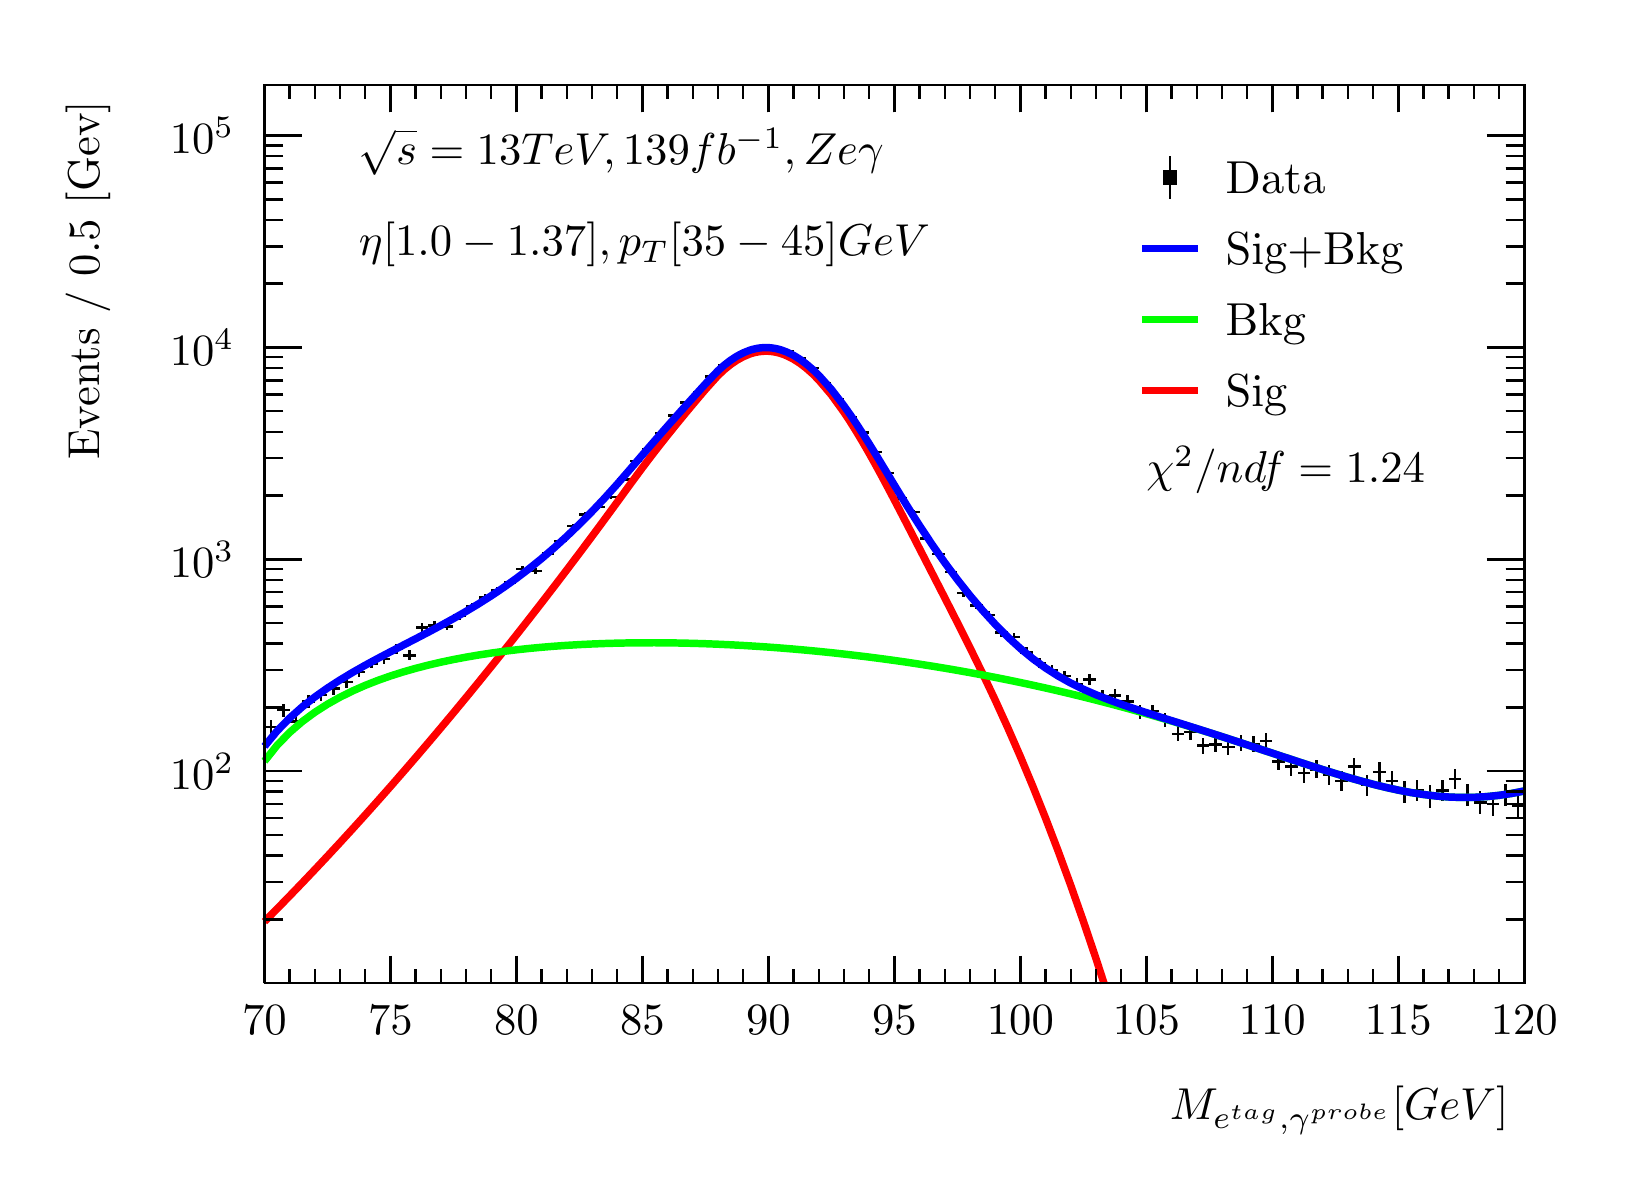
\begin{tikzpicture}
\pgfdeclareplotmark{cross} {
\pgfpathmoveto{\pgfpoint{-0.3\pgfplotmarksize}{\pgfplotmarksize}}
\pgfpathlineto{\pgfpoint{+0.3\pgfplotmarksize}{\pgfplotmarksize}}
\pgfpathlineto{\pgfpoint{+0.3\pgfplotmarksize}{0.3\pgfplotmarksize}}
\pgfpathlineto{\pgfpoint{+1\pgfplotmarksize}{0.3\pgfplotmarksize}}
\pgfpathlineto{\pgfpoint{+1\pgfplotmarksize}{-0.3\pgfplotmarksize}}
\pgfpathlineto{\pgfpoint{+0.3\pgfplotmarksize}{-0.3\pgfplotmarksize}}
\pgfpathlineto{\pgfpoint{+0.3\pgfplotmarksize}{-1.\pgfplotmarksize}}
\pgfpathlineto{\pgfpoint{-0.3\pgfplotmarksize}{-1.\pgfplotmarksize}}
\pgfpathlineto{\pgfpoint{-0.3\pgfplotmarksize}{-0.3\pgfplotmarksize}}
\pgfpathlineto{\pgfpoint{-1.\pgfplotmarksize}{-0.3\pgfplotmarksize}}
\pgfpathlineto{\pgfpoint{-1.\pgfplotmarksize}{0.3\pgfplotmarksize}}
\pgfpathlineto{\pgfpoint{-0.3\pgfplotmarksize}{0.3\pgfplotmarksize}}
\pgfpathclose
\pgfusepathqstroke
}
\pgfdeclareplotmark{cross*} {
\pgfpathmoveto{\pgfpoint{-0.3\pgfplotmarksize}{\pgfplotmarksize}}
\pgfpathlineto{\pgfpoint{+0.3\pgfplotmarksize}{\pgfplotmarksize}}
\pgfpathlineto{\pgfpoint{+0.3\pgfplotmarksize}{0.3\pgfplotmarksize}}
\pgfpathlineto{\pgfpoint{+1\pgfplotmarksize}{0.3\pgfplotmarksize}}
\pgfpathlineto{\pgfpoint{+1\pgfplotmarksize}{-0.3\pgfplotmarksize}}
\pgfpathlineto{\pgfpoint{+0.3\pgfplotmarksize}{-0.3\pgfplotmarksize}}
\pgfpathlineto{\pgfpoint{+0.3\pgfplotmarksize}{-1.\pgfplotmarksize}}
\pgfpathlineto{\pgfpoint{-0.3\pgfplotmarksize}{-1.\pgfplotmarksize}}
\pgfpathlineto{\pgfpoint{-0.3\pgfplotmarksize}{-0.3\pgfplotmarksize}}
\pgfpathlineto{\pgfpoint{-1.\pgfplotmarksize}{-0.3\pgfplotmarksize}}
\pgfpathlineto{\pgfpoint{-1.\pgfplotmarksize}{0.3\pgfplotmarksize}}
\pgfpathlineto{\pgfpoint{-0.3\pgfplotmarksize}{0.3\pgfplotmarksize}}
\pgfpathclose
\pgfusepathqfillstroke
}
\pgfdeclareplotmark{newstar} {
\pgfpathmoveto{\pgfqpoint{0pt}{\pgfplotmarksize}}
\pgfpathlineto{\pgfqpointpolar{44}{0.5\pgfplotmarksize}}
\pgfpathlineto{\pgfqpointpolar{18}{\pgfplotmarksize}}
\pgfpathlineto{\pgfqpointpolar{-20}{0.5\pgfplotmarksize}}
\pgfpathlineto{\pgfqpointpolar{-54}{\pgfplotmarksize}}
\pgfpathlineto{\pgfqpointpolar{-90}{0.5\pgfplotmarksize}}
\pgfpathlineto{\pgfqpointpolar{234}{\pgfplotmarksize}}
\pgfpathlineto{\pgfqpointpolar{198}{0.5\pgfplotmarksize}}
\pgfpathlineto{\pgfqpointpolar{162}{\pgfplotmarksize}}
\pgfpathlineto{\pgfqpointpolar{134}{0.5\pgfplotmarksize}}
\pgfpathclose
\pgfusepathqstroke
}
\pgfdeclareplotmark{newstar*} {
\pgfpathmoveto{\pgfqpoint{0pt}{\pgfplotmarksize}}
\pgfpathlineto{\pgfqpointpolar{44}{0.5\pgfplotmarksize}}
\pgfpathlineto{\pgfqpointpolar{18}{\pgfplotmarksize}}
\pgfpathlineto{\pgfqpointpolar{-20}{0.5\pgfplotmarksize}}
\pgfpathlineto{\pgfqpointpolar{-54}{\pgfplotmarksize}}
\pgfpathlineto{\pgfqpointpolar{-90}{0.5\pgfplotmarksize}}
\pgfpathlineto{\pgfqpointpolar{234}{\pgfplotmarksize}}
\pgfpathlineto{\pgfqpointpolar{198}{0.5\pgfplotmarksize}}
\pgfpathlineto{\pgfqpointpolar{162}{\pgfplotmarksize}}
\pgfpathlineto{\pgfqpointpolar{134}{0.5\pgfplotmarksize}}
\pgfpathclose
\pgfusepathqfillstroke
}
\definecolor{c}{rgb}{1,1,1};
\draw [color=c, fill=c] (0,0) rectangle (20,14.4361);
\draw [color=c, fill=c] (3,2.30977) rectangle (19,13.7143);
\definecolor{c}{rgb}{0,0,0};
\draw [c,line width=0.9] (3,2.30977) -- (3,13.7143) -- (19,13.7143) -- (19,2.30977) -- (3,2.30977);
\definecolor{c}{rgb}{1,1,1};
\draw [color=c, fill=c] (3,2.30977) rectangle (19,13.7143);
\definecolor{c}{rgb}{0,0,0};
\draw [c,line width=0.9] (3,2.30977) -- (3,13.7143) -- (19,13.7143) -- (19,2.30977) -- (3,2.30977);
\draw [c,line width=0.9] (3,2.30977) -- (19,2.30977);
\draw [c,line width=0.9] (3,2.65624) -- (3,2.30977);
\draw [c,line width=0.9] (3.32,2.48301) -- (3.32,2.30977);
\draw [c,line width=0.9] (3.64,2.48301) -- (3.64,2.30977);
\draw [c,line width=0.9] (3.96,2.48301) -- (3.96,2.30977);
\draw [c,line width=0.9] (4.28,2.48301) -- (4.28,2.30977);
\draw [c,line width=0.9] (4.6,2.65624) -- (4.6,2.30977);
\draw [c,line width=0.9] (4.92,2.48301) -- (4.92,2.30977);
\draw [c,line width=0.9] (5.24,2.48301) -- (5.24,2.30977);
\draw [c,line width=0.9] (5.56,2.48301) -- (5.56,2.30977);
\draw [c,line width=0.9] (5.88,2.48301) -- (5.88,2.30977);
\draw [c,line width=0.9] (6.2,2.65624) -- (6.2,2.30977);
\draw [c,line width=0.9] (6.52,2.48301) -- (6.52,2.30977);
\draw [c,line width=0.9] (6.84,2.48301) -- (6.84,2.30977);
\draw [c,line width=0.9] (7.16,2.48301) -- (7.16,2.30977);
\draw [c,line width=0.9] (7.48,2.48301) -- (7.48,2.30977);
\draw [c,line width=0.9] (7.8,2.65624) -- (7.8,2.30977);
\draw [c,line width=0.9] (8.12,2.48301) -- (8.12,2.30977);
\draw [c,line width=0.9] (8.44,2.48301) -- (8.44,2.30977);
\draw [c,line width=0.9] (8.76,2.48301) -- (8.76,2.30977);
\draw [c,line width=0.9] (9.08,2.48301) -- (9.08,2.30977);
\draw [c,line width=0.9] (9.4,2.65624) -- (9.4,2.30977);
\draw [c,line width=0.9] (9.72,2.48301) -- (9.72,2.30977);
\draw [c,line width=0.9] (10.04,2.48301) -- (10.04,2.30977);
\draw [c,line width=0.9] (10.36,2.48301) -- (10.36,2.30977);
\draw [c,line width=0.9] (10.68,2.48301) -- (10.68,2.30977);
\draw [c,line width=0.9] (11,2.65624) -- (11,2.30977);
\draw [c,line width=0.9] (11.32,2.48301) -- (11.32,2.30977);
\draw [c,line width=0.9] (11.64,2.48301) -- (11.64,2.30977);
\draw [c,line width=0.9] (11.96,2.48301) -- (11.96,2.30977);
\draw [c,line width=0.9] (12.28,2.48301) -- (12.28,2.30977);
\draw [c,line width=0.9] (12.6,2.65624) -- (12.6,2.30977);
\draw [c,line width=0.9] (12.92,2.48301) -- (12.92,2.30977);
\draw [c,line width=0.9] (13.24,2.48301) -- (13.24,2.30977);
\draw [c,line width=0.9] (13.56,2.48301) -- (13.56,2.30977);
\draw [c,line width=0.9] (13.88,2.48301) -- (13.88,2.30977);
\draw [c,line width=0.9] (14.2,2.65624) -- (14.2,2.30977);
\draw [c,line width=0.9] (14.52,2.48301) -- (14.52,2.30977);
\draw [c,line width=0.9] (14.84,2.48301) -- (14.84,2.30977);
\draw [c,line width=0.9] (15.16,2.48301) -- (15.16,2.30977);
\draw [c,line width=0.9] (15.48,2.48301) -- (15.48,2.30977);
\draw [c,line width=0.9] (15.8,2.65624) -- (15.8,2.30977);
\draw [c,line width=0.9] (16.12,2.48301) -- (16.12,2.30977);
\draw [c,line width=0.9] (16.44,2.48301) -- (16.44,2.30977);
\draw [c,line width=0.9] (16.76,2.48301) -- (16.76,2.30977);
\draw [c,line width=0.9] (17.08,2.48301) -- (17.08,2.30977);
\draw [c,line width=0.9] (17.4,2.65624) -- (17.4,2.30977);
\draw [c,line width=0.9] (17.72,2.48301) -- (17.72,2.30977);
\draw [c,line width=0.9] (18.04,2.48301) -- (18.04,2.30977);
\draw [c,line width=0.9] (18.36,2.48301) -- (18.36,2.30977);
\draw [c,line width=0.9] (18.68,2.48301) -- (18.68,2.30977);
\draw [c,line width=0.9] (19,2.65624) -- (19,2.30977);
\draw [anchor=base] (3,1.66015) node[scale=1.61424, color=c, rotate=0]{70};
\draw [anchor=base] (4.6,1.66015) node[scale=1.61424, color=c, rotate=0]{75};
\draw [anchor=base] (6.2,1.66015) node[scale=1.61424, color=c, rotate=0]{80};
\draw [anchor=base] (7.8,1.66015) node[scale=1.61424, color=c, rotate=0]{85};
\draw [anchor=base] (9.4,1.66015) node[scale=1.61424, color=c, rotate=0]{90};
\draw [anchor=base] (11,1.66015) node[scale=1.61424, color=c, rotate=0]{95};
\draw [anchor=base] (12.6,1.66015) node[scale=1.61424, color=c, rotate=0]{100};
\draw [anchor=base] (14.2,1.66015) node[scale=1.61424, color=c, rotate=0]{105};
\draw [anchor=base] (15.8,1.66015) node[scale=1.61424, color=c, rotate=0]{110};
\draw [anchor=base] (17.4,1.66015) node[scale=1.61424, color=c, rotate=0]{115};
\draw [anchor=base] (19,1.66015) node[scale=1.61424, color=c, rotate=0]{120};
\draw [anchor= east] (19,0.692932) node[scale=1.61424, color=c, rotate=0]{$M_{e^{tag}, \gamma^{probe}}  [GeV]$};
\draw [c,line width=0.9] (3,13.7143) -- (19,13.7143);
\draw [c,line width=0.9] (3,13.3678) -- (3,13.7143);
\draw [c,line width=0.9] (3.32,13.5411) -- (3.32,13.7143);
\draw [c,line width=0.9] (3.64,13.5411) -- (3.64,13.7143);
\draw [c,line width=0.9] (3.96,13.5411) -- (3.96,13.7143);
\draw [c,line width=0.9] (4.28,13.5411) -- (4.28,13.7143);
\draw [c,line width=0.9] (4.6,13.3678) -- (4.6,13.7143);
\draw [c,line width=0.9] (4.92,13.5411) -- (4.92,13.7143);
\draw [c,line width=0.9] (5.24,13.5411) -- (5.24,13.7143);
\draw [c,line width=0.9] (5.56,13.5411) -- (5.56,13.7143);
\draw [c,line width=0.9] (5.88,13.5411) -- (5.88,13.7143);
\draw [c,line width=0.9] (6.2,13.3678) -- (6.2,13.7143);
\draw [c,line width=0.9] (6.52,13.5411) -- (6.52,13.7143);
\draw [c,line width=0.9] (6.84,13.5411) -- (6.84,13.7143);
\draw [c,line width=0.9] (7.16,13.5411) -- (7.16,13.7143);
\draw [c,line width=0.9] (7.48,13.5411) -- (7.48,13.7143);
\draw [c,line width=0.9] (7.8,13.3678) -- (7.8,13.7143);
\draw [c,line width=0.9] (8.12,13.5411) -- (8.12,13.7143);
\draw [c,line width=0.9] (8.44,13.5411) -- (8.44,13.7143);
\draw [c,line width=0.9] (8.76,13.5411) -- (8.76,13.7143);
\draw [c,line width=0.9] (9.08,13.5411) -- (9.08,13.7143);
\draw [c,line width=0.9] (9.4,13.3678) -- (9.4,13.7143);
\draw [c,line width=0.9] (9.72,13.5411) -- (9.72,13.7143);
\draw [c,line width=0.9] (10.04,13.5411) -- (10.04,13.7143);
\draw [c,line width=0.9] (10.36,13.5411) -- (10.36,13.7143);
\draw [c,line width=0.9] (10.68,13.5411) -- (10.68,13.7143);
\draw [c,line width=0.9] (11,13.3678) -- (11,13.7143);
\draw [c,line width=0.9] (11.32,13.5411) -- (11.32,13.7143);
\draw [c,line width=0.9] (11.64,13.5411) -- (11.64,13.7143);
\draw [c,line width=0.9] (11.96,13.5411) -- (11.96,13.7143);
\draw [c,line width=0.9] (12.28,13.5411) -- (12.28,13.7143);
\draw [c,line width=0.9] (12.6,13.3678) -- (12.6,13.7143);
\draw [c,line width=0.9] (12.92,13.5411) -- (12.92,13.7143);
\draw [c,line width=0.9] (13.24,13.5411) -- (13.24,13.7143);
\draw [c,line width=0.9] (13.56,13.5411) -- (13.56,13.7143);
\draw [c,line width=0.9] (13.88,13.5411) -- (13.88,13.7143);
\draw [c,line width=0.9] (14.2,13.3678) -- (14.2,13.7143);
\draw [c,line width=0.9] (14.52,13.5411) -- (14.52,13.7143);
\draw [c,line width=0.9] (14.84,13.5411) -- (14.84,13.7143);
\draw [c,line width=0.9] (15.16,13.5411) -- (15.16,13.7143);
\draw [c,line width=0.9] (15.48,13.5411) -- (15.48,13.7143);
\draw [c,line width=0.9] (15.8,13.3678) -- (15.8,13.7143);
\draw [c,line width=0.9] (16.12,13.5411) -- (16.12,13.7143);
\draw [c,line width=0.9] (16.44,13.5411) -- (16.44,13.7143);
\draw [c,line width=0.9] (16.76,13.5411) -- (16.76,13.7143);
\draw [c,line width=0.9] (17.08,13.5411) -- (17.08,13.7143);
\draw [c,line width=0.9] (17.4,13.3678) -- (17.4,13.7143);
\draw [c,line width=0.9] (17.72,13.5411) -- (17.72,13.7143);
\draw [c,line width=0.9] (18.04,13.5411) -- (18.04,13.7143);
\draw [c,line width=0.9] (18.36,13.5411) -- (18.36,13.7143);
\draw [c,line width=0.9] (18.68,13.5411) -- (18.68,13.7143);
\draw [c,line width=0.9] (19,13.3678) -- (19,13.7143);
\draw [c,line width=0.9] (3,2.30977) -- (3,13.7143);
\draw [c,line width=0.9] (3.237,3.11973) -- (3,3.11973);
\draw [c,line width=0.9] (3.237,3.59352) -- (3,3.59352);
\draw [c,line width=0.9] (3.237,3.92968) -- (3,3.92968);
\draw [c,line width=0.9] (3.237,4.19043) -- (3,4.19043);
\draw [c,line width=0.9] (3.237,4.40347) -- (3,4.40347);
\draw [c,line width=0.9] (3.237,4.5836) -- (3,4.5836);
\draw [c,line width=0.9] (3.237,4.73964) -- (3,4.73964);
\draw [c,line width=0.9] (3.237,4.87727) -- (3,4.87727);
\draw [c,line width=0.9] (3.474,5.00038) -- (3,5.00038);
\draw [anchor= east] (2.82,5.00038) node[scale=1.61424, color=c, rotate=0]{$10^{2}$};
\draw [c,line width=0.9] (3.237,5.81034) -- (3,5.81034);
\draw [c,line width=0.9] (3.237,6.28413) -- (3,6.28413);
\draw [c,line width=0.9] (3.237,6.62029) -- (3,6.62029);
\draw [c,line width=0.9] (3.237,6.88104) -- (3,6.88104);
\draw [c,line width=0.9] (3.237,7.09409) -- (3,7.09409);
\draw [c,line width=0.9] (3.237,7.27421) -- (3,7.27421);
\draw [c,line width=0.9] (3.237,7.43025) -- (3,7.43025);
\draw [c,line width=0.9] (3.237,7.56788) -- (3,7.56788);
\draw [c,line width=0.9] (3.474,7.69099) -- (3,7.69099);
\draw [anchor= east] (2.82,7.69099) node[scale=1.61424, color=c, rotate=0]{$10^{3}$};
\draw [c,line width=0.9] (3.237,8.50095) -- (3,8.50095);
\draw [c,line width=0.9] (3.237,8.97474) -- (3,8.97474);
\draw [c,line width=0.9] (3.237,9.3109) -- (3,9.3109);
\draw [c,line width=0.9] (3.237,9.57165) -- (3,9.57165);
\draw [c,line width=0.9] (3.237,9.7847) -- (3,9.7847);
\draw [c,line width=0.9] (3.237,9.96482) -- (3,9.96482);
\draw [c,line width=0.9] (3.237,10.1209) -- (3,10.1209);
\draw [c,line width=0.9] (3.237,10.2585) -- (3,10.2585);
\draw [c,line width=0.9] (3.474,10.3816) -- (3,10.3816);
\draw [anchor= east] (2.82,10.3816) node[scale=1.61424, color=c, rotate=0]{$10^{4}$};
\draw [c,line width=0.9] (3.237,11.1916) -- (3,11.1916);
\draw [c,line width=0.9] (3.237,11.6654) -- (3,11.6654);
\draw [c,line width=0.9] (3.237,12.0015) -- (3,12.0015);
\draw [c,line width=0.9] (3.237,12.2623) -- (3,12.2623);
\draw [c,line width=0.9] (3.237,12.4753) -- (3,12.4753);
\draw [c,line width=0.9] (3.237,12.6554) -- (3,12.6554);
\draw [c,line width=0.9] (3.237,12.8115) -- (3,12.8115);
\draw [c,line width=0.9] (3.237,12.9491) -- (3,12.9491);
\draw [c,line width=0.9] (3.474,13.0722) -- (3,13.0722);
\draw [anchor= east] (2.82,13.0722) node[scale=1.61424, color=c, rotate=0]{$10^{5}$};
\draw [anchor= east] (0.76,13.7143) node[scale=1.61424, color=c, rotate=90]{Events / 0.5 [Gev]};
\draw [c,line width=0.9] (19,2.30977) -- (19,13.7143);
\draw [c,line width=0.9] (18.763,3.11973) -- (19,3.11973);
\draw [c,line width=0.9] (18.763,3.59352) -- (19,3.59352);
\draw [c,line width=0.9] (18.763,3.92968) -- (19,3.92968);
\draw [c,line width=0.9] (18.763,4.19043) -- (19,4.19043);
\draw [c,line width=0.9] (18.763,4.40347) -- (19,4.40347);
\draw [c,line width=0.9] (18.763,4.5836) -- (19,4.5836);
\draw [c,line width=0.9] (18.763,4.73964) -- (19,4.73964);
\draw [c,line width=0.9] (18.763,4.87727) -- (19,4.87727);
\draw [c,line width=0.9] (18.526,5.00038) -- (19,5.00038);
\draw [c,line width=0.9] (18.763,5.81034) -- (19,5.81034);
\draw [c,line width=0.9] (18.763,6.28413) -- (19,6.28413);
\draw [c,line width=0.9] (18.763,6.62029) -- (19,6.62029);
\draw [c,line width=0.9] (18.763,6.88104) -- (19,6.88104);
\draw [c,line width=0.9] (18.763,7.09409) -- (19,7.09409);
\draw [c,line width=0.9] (18.763,7.27421) -- (19,7.27421);
\draw [c,line width=0.9] (18.763,7.43025) -- (19,7.43025);
\draw [c,line width=0.9] (18.763,7.56788) -- (19,7.56788);
\draw [c,line width=0.9] (18.526,7.69099) -- (19,7.69099);
\draw [c,line width=0.9] (18.763,8.50095) -- (19,8.50095);
\draw [c,line width=0.9] (18.763,8.97474) -- (19,8.97474);
\draw [c,line width=0.9] (18.763,9.3109) -- (19,9.3109);
\draw [c,line width=0.9] (18.763,9.57165) -- (19,9.57165);
\draw [c,line width=0.9] (18.763,9.7847) -- (19,9.7847);
\draw [c,line width=0.9] (18.763,9.96482) -- (19,9.96482);
\draw [c,line width=0.9] (18.763,10.1209) -- (19,10.1209);
\draw [c,line width=0.9] (18.763,10.2585) -- (19,10.2585);
\draw [c,line width=0.9] (18.526,10.3816) -- (19,10.3816);
\draw [c,line width=0.9] (18.763,11.1916) -- (19,11.1916);
\draw [c,line width=0.9] (18.763,11.6654) -- (19,11.6654);
\draw [c,line width=0.9] (18.763,12.0015) -- (19,12.0015);
\draw [c,line width=0.9] (18.763,12.2623) -- (19,12.2623);
\draw [c,line width=0.9] (18.763,12.4753) -- (19,12.4753);
\draw [c,line width=0.9] (18.763,12.6554) -- (19,12.6554);
\draw [c,line width=0.9] (18.763,12.8115) -- (19,12.8115);
\draw [c,line width=0.9] (18.763,12.9491) -- (19,12.9491);
\draw [c,line width=0.9] (18.526,13.0722) -- (19,13.0722);
\draw [c,line width=0.9] (3.08,5.56411) -- (3,5.56411);
\draw [c,line width=0.9] (3,5.56411) -- (3,5.56411);
\draw [c,line width=0.9] (3.08,5.56411) -- (3.16,5.56411);
\draw [c,line width=0.9] (3.16,5.56411) -- (3.16,5.56411);
\draw [c,line width=0.9] (3.08,5.56411) -- (3.08,5.65589);
\draw [c,line width=0.9] (3.08,5.65589) -- (3.08,5.65589);
\draw [c,line width=0.9] (3.08,5.56411) -- (3.08,5.47232);
\draw [c,line width=0.9] (3.08,5.47232) -- (3.08,5.47232);
\draw [c,line width=0.9] (3.24,5.77475) -- (3.16,5.77475);
\draw [c,line width=0.9] (3.16,5.77475) -- (3.16,5.77475);
\draw [c,line width=0.9] (3.24,5.77475) -- (3.32,5.77475);
\draw [c,line width=0.9] (3.32,5.77475) -- (3.32,5.77475);
\draw [c,line width=0.9] (3.24,5.77475) -- (3.24,5.85862);
\draw [c,line width=0.9] (3.24,5.85862) -- (3.24,5.85862);
\draw [c,line width=0.9] (3.24,5.77475) -- (3.24,5.69087);
\draw [c,line width=0.9] (3.24,5.69087) -- (3.24,5.69087);
\draw [c,line width=0.9] (3.4,5.6341) -- (3.32,5.6341);
\draw [c,line width=0.9] (3.32,5.6341) -- (3.32,5.6341);
\draw [c,line width=0.9] (3.4,5.6341) -- (3.48,5.6341);
\draw [c,line width=0.9] (3.48,5.6341) -- (3.48,5.6341);
\draw [c,line width=0.9] (3.4,5.6341) -- (3.4,5.72318);
\draw [c,line width=0.9] (3.4,5.72318) -- (3.4,5.72318);
\draw [c,line width=0.9] (3.4,5.6341) -- (3.4,5.54502);
\draw [c,line width=0.9] (3.4,5.54502) -- (3.4,5.54502);
\draw [c,line width=0.9] (3.56,5.88393) -- (3.48,5.88393);
\draw [c,line width=0.9] (3.48,5.88393) -- (3.48,5.88393);
\draw [c,line width=0.9] (3.56,5.88393) -- (3.64,5.88393);
\draw [c,line width=0.9] (3.64,5.88393) -- (3.64,5.88393);
\draw [c,line width=0.9] (3.56,5.88393) -- (3.56,5.96398);
\draw [c,line width=0.9] (3.56,5.96398) -- (3.56,5.96398);
\draw [c,line width=0.9] (3.56,5.88393) -- (3.56,5.80388);
\draw [c,line width=0.9] (3.56,5.80388) -- (3.56,5.80388);
\draw [c,line width=0.9] (3.72,5.96856) -- (3.64,5.96856);
\draw [c,line width=0.9] (3.64,5.96856) -- (3.64,5.96856);
\draw [c,line width=0.9] (3.72,5.96856) -- (3.8,5.96856);
\draw [c,line width=0.9] (3.8,5.96856) -- (3.8,5.96856);
\draw [c,line width=0.9] (3.72,5.96856) -- (3.72,6.04577);
\draw [c,line width=0.9] (3.72,6.04577) -- (3.72,6.04577);
\draw [c,line width=0.9] (3.72,5.96856) -- (3.72,5.89136);
\draw [c,line width=0.9] (3.72,5.89136) -- (3.72,5.89136);
\draw [c,line width=0.9] (3.88,6.04748) -- (3.8,6.04748);
\draw [c,line width=0.9] (3.8,6.04748) -- (3.8,6.04748);
\draw [c,line width=0.9] (3.88,6.04748) -- (3.96,6.04748);
\draw [c,line width=0.9] (3.96,6.04748) -- (3.96,6.04748);
\draw [c,line width=0.9] (3.88,6.04748) -- (3.88,6.12212);
\draw [c,line width=0.9] (3.88,6.12212) -- (3.88,6.12212);
\draw [c,line width=0.9] (3.88,6.04748) -- (3.88,5.97284);
\draw [c,line width=0.9] (3.88,5.97284) -- (3.88,5.97284);
\draw [c,line width=0.9] (4.04,6.13476) -- (3.96,6.13476);
\draw [c,line width=0.9] (3.96,6.13476) -- (3.96,6.13476);
\draw [c,line width=0.9] (4.04,6.13476) -- (4.12,6.13476);
\draw [c,line width=0.9] (4.12,6.13476) -- (4.12,6.13476);
\draw [c,line width=0.9] (4.04,6.13476) -- (4.04,6.20666);
\draw [c,line width=0.9] (4.04,6.20666) -- (4.04,6.20666);
\draw [c,line width=0.9] (4.04,6.13476) -- (4.04,6.06285);
\draw [c,line width=0.9] (4.04,6.06285) -- (4.04,6.06285);
\draw [c,line width=0.9] (4.2,6.26053) -- (4.12,6.26053);
\draw [c,line width=0.9] (4.12,6.26053) -- (4.12,6.26053);
\draw [c,line width=0.9] (4.2,6.26053) -- (4.28,6.26053);
\draw [c,line width=0.9] (4.28,6.26053) -- (4.28,6.26053);
\draw [c,line width=0.9] (4.2,6.26053) -- (4.2,6.32867);
\draw [c,line width=0.9] (4.2,6.32867) -- (4.2,6.32867);
\draw [c,line width=0.9] (4.2,6.26053) -- (4.2,6.19239);
\draw [c,line width=0.9] (4.2,6.19239) -- (4.2,6.19239);
\draw [c,line width=0.9] (4.36,6.37045) -- (4.28,6.37045);
\draw [c,line width=0.9] (4.28,6.37045) -- (4.28,6.37045);
\draw [c,line width=0.9] (4.36,6.37045) -- (4.44,6.37045);
\draw [c,line width=0.9] (4.44,6.37045) -- (4.44,6.37045);
\draw [c,line width=0.9] (4.36,6.37045) -- (4.36,6.43546);
\draw [c,line width=0.9] (4.36,6.43546) -- (4.36,6.43546);
\draw [c,line width=0.9] (4.36,6.37045) -- (4.36,6.30544);
\draw [c,line width=0.9] (4.36,6.30544) -- (4.36,6.30544);
\draw [c,line width=0.9] (4.52,6.42349) -- (4.44,6.42349);
\draw [c,line width=0.9] (4.44,6.42349) -- (4.44,6.42349);
\draw [c,line width=0.9] (4.52,6.42349) -- (4.6,6.42349);
\draw [c,line width=0.9] (4.6,6.42349) -- (4.6,6.42349);
\draw [c,line width=0.9] (4.52,6.42349) -- (4.52,6.48705);
\draw [c,line width=0.9] (4.52,6.48705) -- (4.52,6.48705);
\draw [c,line width=0.9] (4.52,6.42349) -- (4.52,6.35994);
\draw [c,line width=0.9] (4.52,6.35994) -- (4.52,6.35994);
\draw [c,line width=0.9] (4.68,6.5511) -- (4.6,6.5511);
\draw [c,line width=0.9] (4.6,6.5511) -- (4.6,6.5511);
\draw [c,line width=0.9] (4.68,6.5511) -- (4.76,6.5511);
\draw [c,line width=0.9] (4.76,6.5511) -- (4.76,6.5511);
\draw [c,line width=0.9] (4.68,6.5511) -- (4.68,6.61127);
\draw [c,line width=0.9] (4.68,6.61127) -- (4.68,6.61127);
\draw [c,line width=0.9] (4.68,6.5511) -- (4.68,6.49092);
\draw [c,line width=0.9] (4.68,6.49092) -- (4.68,6.49092);
\draw [c,line width=0.9] (4.84,6.47092) -- (4.76,6.47092);
\draw [c,line width=0.9] (4.76,6.47092) -- (4.76,6.47092);
\draw [c,line width=0.9] (4.84,6.47092) -- (4.92,6.47092);
\draw [c,line width=0.9] (4.92,6.47092) -- (4.92,6.47092);
\draw [c,line width=0.9] (4.84,6.47092) -- (4.84,6.53319);
\draw [c,line width=0.9] (4.84,6.53319) -- (4.84,6.53319);
\draw [c,line width=0.9] (4.84,6.47092) -- (4.84,6.40864);
\draw [c,line width=0.9] (4.84,6.40864) -- (4.84,6.40864);
\draw [c,line width=0.9] (5,6.82356) -- (4.92,6.82356);
\draw [c,line width=0.9] (4.92,6.82356) -- (4.92,6.82356);
\draw [c,line width=0.9] (5,6.82356) -- (5.08,6.82356);
\draw [c,line width=0.9] (5.08,6.82356) -- (5.08,6.82356);
\draw [c,line width=0.9] (5,6.82356) -- (5,6.87712);
\draw [c,line width=0.9] (5,6.87712) -- (5,6.87712);
\draw [c,line width=0.9] (5,6.82356) -- (5,6.77001);
\draw [c,line width=0.9] (5,6.77001) -- (5,6.77001);
\draw [c,line width=0.9] (5.16,6.85265) -- (5.08,6.85265);
\draw [c,line width=0.9] (5.08,6.85265) -- (5.08,6.85265);
\draw [c,line width=0.9] (5.16,6.85265) -- (5.24,6.85265);
\draw [c,line width=0.9] (5.24,6.85265) -- (5.24,6.85265);
\draw [c,line width=0.9] (5.16,6.85265) -- (5.16,6.90555);
\draw [c,line width=0.9] (5.16,6.90555) -- (5.16,6.90555);
\draw [c,line width=0.9] (5.16,6.85265) -- (5.16,6.79976);
\draw [c,line width=0.9] (5.16,6.79976) -- (5.16,6.79976);
\draw [c,line width=0.9] (5.32,6.84062) -- (5.24,6.84062);
\draw [c,line width=0.9] (5.24,6.84062) -- (5.24,6.84062);
\draw [c,line width=0.9] (5.32,6.84062) -- (5.4,6.84062);
\draw [c,line width=0.9] (5.4,6.84062) -- (5.4,6.84062);
\draw [c,line width=0.9] (5.32,6.84062) -- (5.32,6.89379);
\draw [c,line width=0.9] (5.32,6.89379) -- (5.32,6.89379);
\draw [c,line width=0.9] (5.32,6.84062) -- (5.32,6.78746);
\draw [c,line width=0.9] (5.32,6.78746) -- (5.32,6.78746);
\draw [c,line width=0.9] (5.48,6.97529) -- (5.4,6.97529);
\draw [c,line width=0.9] (5.4,6.97529) -- (5.4,6.97529);
\draw [c,line width=0.9] (5.48,6.97529) -- (5.56,6.97529);
\draw [c,line width=0.9] (5.56,6.97529) -- (5.56,6.97529);
\draw [c,line width=0.9] (5.48,6.97529) -- (5.48,7.02548);
\draw [c,line width=0.9] (5.48,7.02548) -- (5.48,7.02548);
\draw [c,line width=0.9] (5.48,6.97529) -- (5.48,6.9251);
\draw [c,line width=0.9] (5.48,6.9251) -- (5.48,6.9251);
\draw [c,line width=0.9] (5.64,7.09214) -- (5.56,7.09214);
\draw [c,line width=0.9] (5.56,7.09214) -- (5.56,7.09214);
\draw [c,line width=0.9] (5.64,7.09214) -- (5.72,7.09214);
\draw [c,line width=0.9] (5.72,7.09214) -- (5.72,7.09214);
\draw [c,line width=0.9] (5.64,7.09214) -- (5.64,7.13988);
\draw [c,line width=0.9] (5.64,7.13988) -- (5.64,7.13988);
\draw [c,line width=0.9] (5.64,7.09214) -- (5.64,7.0444);
\draw [c,line width=0.9] (5.64,7.0444) -- (5.64,7.0444);
\draw [c,line width=0.9] (5.8,7.20546) -- (5.72,7.20546);
\draw [c,line width=0.9] (5.72,7.20546) -- (5.72,7.20546);
\draw [c,line width=0.9] (5.8,7.20546) -- (5.88,7.20546);
\draw [c,line width=0.9] (5.88,7.20546) -- (5.88,7.20546);
\draw [c,line width=0.9] (5.8,7.20546) -- (5.8,7.25094);
\draw [c,line width=0.9] (5.8,7.25094) -- (5.8,7.25094);
\draw [c,line width=0.9] (5.8,7.20546) -- (5.8,7.15998);
\draw [c,line width=0.9] (5.8,7.15998) -- (5.8,7.15998);
\draw [c,line width=0.9] (5.96,7.29408) -- (5.88,7.29408);
\draw [c,line width=0.9] (5.88,7.29408) -- (5.88,7.29408);
\draw [c,line width=0.9] (5.96,7.29408) -- (6.04,7.29408);
\draw [c,line width=0.9] (6.04,7.29408) -- (6.04,7.29408);
\draw [c,line width=0.9] (5.96,7.29408) -- (5.96,7.33787);
\draw [c,line width=0.9] (5.96,7.33787) -- (5.96,7.33787);
\draw [c,line width=0.9] (5.96,7.29408) -- (5.96,7.25029);
\draw [c,line width=0.9] (5.96,7.25029) -- (5.96,7.25029);
\draw [c,line width=0.9] (6.12,7.39766) -- (6.04,7.39766);
\draw [c,line width=0.9] (6.04,7.39766) -- (6.04,7.39766);
\draw [c,line width=0.9] (6.12,7.39766) -- (6.2,7.39766);
\draw [c,line width=0.9] (6.2,7.39766) -- (6.2,7.39766);
\draw [c,line width=0.9] (6.12,7.39766) -- (6.12,7.43956);
\draw [c,line width=0.9] (6.12,7.43956) -- (6.12,7.43956);
\draw [c,line width=0.9] (6.12,7.39766) -- (6.12,7.35577);
\draw [c,line width=0.9] (6.12,7.35577) -- (6.12,7.35577);
\draw [c,line width=0.9] (6.28,7.56918) -- (6.2,7.56918);
\draw [c,line width=0.9] (6.2,7.56918) -- (6.2,7.56918);
\draw [c,line width=0.9] (6.28,7.56918) -- (6.36,7.56918);
\draw [c,line width=0.9] (6.36,7.56918) -- (6.36,7.56918);
\draw [c,line width=0.9] (6.28,7.56918) -- (6.28,7.6081);
\draw [c,line width=0.9] (6.28,7.6081) -- (6.28,7.6081);
\draw [c,line width=0.9] (6.28,7.56918) -- (6.28,7.53025);
\draw [c,line width=0.9] (6.28,7.53025) -- (6.28,7.53025);
\draw [c,line width=0.9] (6.44,7.54295) -- (6.36,7.54295);
\draw [c,line width=0.9] (6.36,7.54295) -- (6.36,7.54295);
\draw [c,line width=0.9] (6.44,7.54295) -- (6.52,7.54295);
\draw [c,line width=0.9] (6.52,7.54295) -- (6.52,7.54295);
\draw [c,line width=0.9] (6.44,7.54295) -- (6.44,7.58231);
\draw [c,line width=0.9] (6.44,7.58231) -- (6.44,7.58231);
\draw [c,line width=0.9] (6.44,7.54295) -- (6.44,7.50358);
\draw [c,line width=0.9] (6.44,7.50358) -- (6.44,7.50358);
\draw [c,line width=0.9] (6.6,7.76239) -- (6.52,7.76239);
\draw [c,line width=0.9] (6.52,7.76239) -- (6.52,7.76239);
\draw [c,line width=0.9] (6.6,7.76239) -- (6.68,7.76239);
\draw [c,line width=0.9] (6.68,7.76239) -- (6.68,7.76239);
\draw [c,line width=0.9] (6.6,7.76239) -- (6.6,7.79822);
\draw [c,line width=0.9] (6.6,7.79822) -- (6.6,7.79822);
\draw [c,line width=0.9] (6.6,7.76239) -- (6.6,7.72655);
\draw [c,line width=0.9] (6.6,7.72655) -- (6.6,7.72655);
\draw [c,line width=0.9] (6.76,7.92527) -- (6.68,7.92527);
\draw [c,line width=0.9] (6.68,7.92527) -- (6.68,7.92527);
\draw [c,line width=0.9] (6.76,7.92527) -- (6.84,7.92527);
\draw [c,line width=0.9] (6.84,7.92527) -- (6.84,7.92527);
\draw [c,line width=0.9] (6.76,7.92527) -- (6.76,7.9587);
\draw [c,line width=0.9] (6.76,7.9587) -- (6.76,7.9587);
\draw [c,line width=0.9] (6.76,7.92527) -- (6.76,7.89184);
\draw [c,line width=0.9] (6.76,7.89184) -- (6.76,7.89184);
\draw [c,line width=0.9] (6.92,8.11384) -- (6.84,8.11384);
\draw [c,line width=0.9] (6.84,8.11384) -- (6.84,8.11384);
\draw [c,line width=0.9] (6.92,8.11384) -- (7,8.11384);
\draw [c,line width=0.9] (7,8.11384) -- (7,8.11384);
\draw [c,line width=0.9] (6.92,8.11384) -- (6.92,8.14467);
\draw [c,line width=0.9] (6.92,8.14467) -- (6.92,8.14467);
\draw [c,line width=0.9] (6.92,8.11384) -- (6.92,8.083);
\draw [c,line width=0.9] (6.92,8.083) -- (6.92,8.083);
\draw [c,line width=0.9] (7.08,8.25904) -- (7,8.25904);
\draw [c,line width=0.9] (7,8.25904) -- (7,8.25904);
\draw [c,line width=0.9] (7.08,8.25904) -- (7.16,8.25904);
\draw [c,line width=0.9] (7.16,8.25904) -- (7.16,8.25904);
\draw [c,line width=0.9] (7.08,8.25904) -- (7.08,8.28802);
\draw [c,line width=0.9] (7.08,8.28802) -- (7.08,8.28802);
\draw [c,line width=0.9] (7.08,8.25904) -- (7.08,8.23006);
\draw [c,line width=0.9] (7.08,8.23006) -- (7.08,8.23006);
\draw [c,line width=0.9] (7.24,8.35357) -- (7.16,8.35357);
\draw [c,line width=0.9] (7.16,8.35357) -- (7.16,8.35357);
\draw [c,line width=0.9] (7.24,8.35357) -- (7.32,8.35357);
\draw [c,line width=0.9] (7.32,8.35357) -- (7.32,8.35357);
\draw [c,line width=0.9] (7.24,8.35357) -- (7.24,8.38139);
\draw [c,line width=0.9] (7.24,8.38139) -- (7.24,8.38139);
\draw [c,line width=0.9] (7.24,8.35357) -- (7.24,8.32574);
\draw [c,line width=0.9] (7.24,8.32574) -- (7.24,8.32574);
\draw [c,line width=0.9] (7.4,8.48448) -- (7.32,8.48448);
\draw [c,line width=0.9] (7.32,8.48448) -- (7.32,8.48448);
\draw [c,line width=0.9] (7.4,8.48448) -- (7.48,8.48448);
\draw [c,line width=0.9] (7.48,8.48448) -- (7.48,8.48448);
\draw [c,line width=0.9] (7.4,8.48448) -- (7.4,8.51079);
\draw [c,line width=0.9] (7.4,8.51079) -- (7.4,8.51079);
\draw [c,line width=0.9] (7.4,8.48448) -- (7.4,8.45816);
\draw [c,line width=0.9] (7.4,8.45816) -- (7.4,8.45816);
\draw [c,line width=0.9] (7.56,8.70569) -- (7.48,8.70569);
\draw [c,line width=0.9] (7.48,8.70569) -- (7.48,8.70569);
\draw [c,line width=0.9] (7.56,8.70569) -- (7.64,8.70569);
\draw [c,line width=0.9] (7.64,8.70569) -- (7.64,8.70569);
\draw [c,line width=0.9] (7.56,8.70569) -- (7.56,8.72963);
\draw [c,line width=0.9] (7.56,8.72963) -- (7.56,8.72963);
\draw [c,line width=0.9] (7.56,8.70569) -- (7.56,8.68175);
\draw [c,line width=0.9] (7.56,8.68175) -- (7.56,8.68175);
\draw [c,line width=0.9] (7.72,8.93995) -- (7.64,8.93995);
\draw [c,line width=0.9] (7.64,8.93995) -- (7.64,8.93995);
\draw [c,line width=0.9] (7.72,8.93995) -- (7.8,8.93995);
\draw [c,line width=0.9] (7.8,8.93995) -- (7.8,8.93995);
\draw [c,line width=0.9] (7.72,8.93995) -- (7.72,8.96161);
\draw [c,line width=0.9] (7.72,8.96161) -- (7.72,8.96161);
\draw [c,line width=0.9] (7.72,8.93995) -- (7.72,8.9183);
\draw [c,line width=0.9] (7.72,8.9183) -- (7.72,8.9183);
\draw [c,line width=0.9] (7.88,9.09) -- (7.8,9.09);
\draw [c,line width=0.9] (7.8,9.09) -- (7.8,9.09);
\draw [c,line width=0.9] (7.88,9.09) -- (7.96,9.09);
\draw [c,line width=0.9] (7.96,9.09) -- (7.96,9.09);
\draw [c,line width=0.9] (7.88,9.09) -- (7.88,9.11031);
\draw [c,line width=0.9] (7.88,9.11031) -- (7.88,9.11031);
\draw [c,line width=0.9] (7.88,9.09) -- (7.88,9.0697);
\draw [c,line width=0.9] (7.88,9.0697) -- (7.88,9.0697);
\draw [c,line width=0.9] (8.04,9.29739) -- (7.96,9.29739);
\draw [c,line width=0.9] (7.96,9.29739) -- (7.96,9.29739);
\draw [c,line width=0.9] (8.04,9.29739) -- (8.12,9.29739);
\draw [c,line width=0.9] (8.12,9.29739) -- (8.12,9.29739);
\draw [c,line width=0.9] (8.04,9.29739) -- (8.04,9.31597);
\draw [c,line width=0.9] (8.04,9.31597) -- (8.04,9.31597);
\draw [c,line width=0.9] (8.04,9.29739) -- (8.04,9.27881);
\draw [c,line width=0.9] (8.04,9.27881) -- (8.04,9.27881);
\draw [c,line width=0.9] (8.2,9.51564) -- (8.12,9.51564);
\draw [c,line width=0.9] (8.12,9.51564) -- (8.12,9.51564);
\draw [c,line width=0.9] (8.2,9.51564) -- (8.28,9.51564);
\draw [c,line width=0.9] (8.28,9.51564) -- (8.28,9.51564);
\draw [c,line width=0.9] (8.2,9.51564) -- (8.2,9.53257);
\draw [c,line width=0.9] (8.2,9.53257) -- (8.2,9.53257);
\draw [c,line width=0.9] (8.2,9.51564) -- (8.2,9.49872);
\draw [c,line width=0.9] (8.2,9.49872) -- (8.2,9.49872);
\draw [c,line width=0.9] (8.36,9.68493) -- (8.28,9.68493);
\draw [c,line width=0.9] (8.28,9.68493) -- (8.28,9.68493);
\draw [c,line width=0.9] (8.36,9.68493) -- (8.44,9.68493);
\draw [c,line width=0.9] (8.44,9.68493) -- (8.44,9.68493);
\draw [c,line width=0.9] (8.36,9.68493) -- (8.36,9.70068);
\draw [c,line width=0.9] (8.36,9.70068) -- (8.36,9.70068);
\draw [c,line width=0.9] (8.36,9.68493) -- (8.36,9.66919);
\draw [c,line width=0.9] (8.36,9.66919) -- (8.36,9.66919);
\draw [c,line width=0.9] (8.52,9.81412) -- (8.44,9.81412);
\draw [c,line width=0.9] (8.44,9.81412) -- (8.44,9.81412);
\draw [c,line width=0.9] (8.52,9.81412) -- (8.6,9.81412);
\draw [c,line width=0.9] (8.6,9.81412) -- (8.6,9.81412);
\draw [c,line width=0.9] (8.52,9.81412) -- (8.52,9.82902);
\draw [c,line width=0.9] (8.52,9.82902) -- (8.52,9.82902);
\draw [c,line width=0.9] (8.52,9.81412) -- (8.52,9.79922);
\draw [c,line width=0.9] (8.52,9.79922) -- (8.52,9.79922);
\draw [c,line width=0.9] (8.68,10.0129) -- (8.6,10.0129);
\draw [c,line width=0.9] (8.6,10.0129) -- (8.6,10.0129);
\draw [c,line width=0.9] (8.68,10.0129) -- (8.76,10.0129);
\draw [c,line width=0.9] (8.76,10.0129) -- (8.76,10.0129);
\draw [c,line width=0.9] (8.68,10.0129) -- (8.68,10.0266);
\draw [c,line width=0.9] (8.68,10.0266) -- (8.68,10.0266);
\draw [c,line width=0.9] (8.68,10.0129) -- (8.68,9.99922);
\draw [c,line width=0.9] (8.68,9.99922) -- (8.68,9.99922);
\draw [c,line width=0.9] (8.84,10.1518) -- (8.76,10.1518);
\draw [c,line width=0.9] (8.76,10.1518) -- (8.76,10.1518);
\draw [c,line width=0.9] (8.84,10.1518) -- (8.92,10.1518);
\draw [c,line width=0.9] (8.92,10.1518) -- (8.92,10.1518);
\draw [c,line width=0.9] (8.84,10.1518) -- (8.84,10.1647);
\draw [c,line width=0.9] (8.84,10.1647) -- (8.84,10.1647);
\draw [c,line width=0.9] (8.84,10.1518) -- (8.84,10.139);
\draw [c,line width=0.9] (8.84,10.139) -- (8.84,10.139);
\draw [c,line width=0.9] (9,10.2505) -- (8.92,10.2505);
\draw [c,line width=0.9] (8.92,10.2505) -- (8.92,10.2505);
\draw [c,line width=0.9] (9,10.2505) -- (9.08,10.2505);
\draw [c,line width=0.9] (9.08,10.2505) -- (9.08,10.2505);
\draw [c,line width=0.9] (9,10.2505) -- (9,10.2629);
\draw [c,line width=0.9] (9,10.2629) -- (9,10.2629);
\draw [c,line width=0.9] (9,10.2505) -- (9,10.2382);
\draw [c,line width=0.9] (9,10.2382) -- (9,10.2382);
\draw [c,line width=0.9] (9.16,10.3448) -- (9.08,10.3448);
\draw [c,line width=0.9] (9.08,10.3448) -- (9.08,10.3448);
\draw [c,line width=0.9] (9.16,10.3448) -- (9.24,10.3448);
\draw [c,line width=0.9] (9.24,10.3448) -- (9.24,10.3448);
\draw [c,line width=0.9] (9.16,10.3448) -- (9.16,10.3567);
\draw [c,line width=0.9] (9.16,10.3567) -- (9.16,10.3567);
\draw [c,line width=0.9] (9.16,10.3448) -- (9.16,10.3329);
\draw [c,line width=0.9] (9.16,10.3329) -- (9.16,10.3329);
\draw [c,line width=0.9] (9.32,10.3657) -- (9.24,10.3657);
\draw [c,line width=0.9] (9.24,10.3657) -- (9.24,10.3657);
\draw [c,line width=0.9] (9.32,10.3657) -- (9.4,10.3657);
\draw [c,line width=0.9] (9.4,10.3657) -- (9.4,10.3657);
\draw [c,line width=0.9] (9.32,10.3657) -- (9.32,10.3775);
\draw [c,line width=0.9] (9.32,10.3775) -- (9.32,10.3775);
\draw [c,line width=0.9] (9.32,10.3657) -- (9.32,10.354);
\draw [c,line width=0.9] (9.32,10.354) -- (9.32,10.354);
\draw [c,line width=0.9] (9.48,10.3749) -- (9.4,10.3749);
\draw [c,line width=0.9] (9.4,10.3749) -- (9.4,10.3749);
\draw [c,line width=0.9] (9.48,10.3749) -- (9.56,10.3749);
\draw [c,line width=0.9] (9.56,10.3749) -- (9.56,10.3749);
\draw [c,line width=0.9] (9.48,10.3749) -- (9.48,10.3866);
\draw [c,line width=0.9] (9.48,10.3866) -- (9.48,10.3866);
\draw [c,line width=0.9] (9.48,10.3749) -- (9.48,10.3632);
\draw [c,line width=0.9] (9.48,10.3632) -- (9.48,10.3632);
\draw [c,line width=0.9] (9.64,10.3395) -- (9.56,10.3395);
\draw [c,line width=0.9] (9.56,10.3395) -- (9.56,10.3395);
\draw [c,line width=0.9] (9.64,10.3395) -- (9.72,10.3395);
\draw [c,line width=0.9] (9.72,10.3395) -- (9.72,10.3395);
\draw [c,line width=0.9] (9.64,10.3395) -- (9.64,10.3514);
\draw [c,line width=0.9] (9.64,10.3514) -- (9.64,10.3514);
\draw [c,line width=0.9] (9.64,10.3395) -- (9.64,10.3276);
\draw [c,line width=0.9] (9.64,10.3276) -- (9.64,10.3276);
\draw [c,line width=0.9] (9.8,10.2412) -- (9.72,10.2412);
\draw [c,line width=0.9] (9.72,10.2412) -- (9.72,10.2412);
\draw [c,line width=0.9] (9.8,10.2412) -- (9.88,10.2412);
\draw [c,line width=0.9] (9.88,10.2412) -- (9.88,10.2412);
\draw [c,line width=0.9] (9.8,10.2412) -- (9.8,10.2536);
\draw [c,line width=0.9] (9.8,10.2536) -- (9.8,10.2536);
\draw [c,line width=0.9] (9.8,10.2412) -- (9.8,10.2288);
\draw [c,line width=0.9] (9.8,10.2288) -- (9.8,10.2288);
\draw [c,line width=0.9] (9.96,10.1217) -- (9.88,10.1217);
\draw [c,line width=0.9] (9.88,10.1217) -- (9.88,10.1217);
\draw [c,line width=0.9] (9.96,10.1217) -- (10.04,10.1217);
\draw [c,line width=0.9] (10.04,10.1217) -- (10.04,10.1217);
\draw [c,line width=0.9] (9.96,10.1217) -- (9.96,10.1348);
\draw [c,line width=0.9] (9.96,10.1348) -- (9.96,10.1348);
\draw [c,line width=0.9] (9.96,10.1217) -- (9.96,10.1087);
\draw [c,line width=0.9] (9.96,10.1087) -- (9.96,10.1087);
\draw [c,line width=0.9] (10.12,9.92665) -- (10.04,9.92665);
\draw [c,line width=0.9] (10.04,9.92665) -- (10.04,9.92665);
\draw [c,line width=0.9] (10.12,9.92665) -- (10.2,9.92665);
\draw [c,line width=0.9] (10.2,9.92665) -- (10.2,9.92665);
\draw [c,line width=0.9] (10.12,9.92665) -- (10.12,9.94085);
\draw [c,line width=0.9] (10.12,9.94085) -- (10.12,9.94085);
\draw [c,line width=0.9] (10.12,9.92665) -- (10.12,9.91245);
\draw [c,line width=0.9] (10.12,9.91245) -- (10.12,9.91245);
\draw [c,line width=0.9] (10.28,9.72845) -- (10.2,9.72845);
\draw [c,line width=0.9] (10.2,9.72845) -- (10.2,9.72845);
\draw [c,line width=0.9] (10.28,9.72845) -- (10.36,9.72845);
\draw [c,line width=0.9] (10.36,9.72845) -- (10.36,9.72845);
\draw [c,line width=0.9] (10.28,9.72845) -- (10.28,9.7439);
\draw [c,line width=0.9] (10.28,9.7439) -- (10.28,9.7439);
\draw [c,line width=0.9] (10.28,9.72845) -- (10.28,9.71299);
\draw [c,line width=0.9] (10.28,9.71299) -- (10.28,9.71299);
\draw [c,line width=0.9] (10.44,9.49761) -- (10.36,9.49761);
\draw [c,line width=0.9] (10.36,9.49761) -- (10.36,9.49761);
\draw [c,line width=0.9] (10.44,9.49761) -- (10.52,9.49761);
\draw [c,line width=0.9] (10.52,9.49761) -- (10.52,9.49761);
\draw [c,line width=0.9] (10.44,9.49761) -- (10.44,9.51466);
\draw [c,line width=0.9] (10.44,9.51466) -- (10.44,9.51466);
\draw [c,line width=0.9] (10.44,9.49761) -- (10.44,9.48055);
\draw [c,line width=0.9] (10.44,9.48055) -- (10.44,9.48055);
\draw [c,line width=0.9] (10.6,9.30005) -- (10.52,9.30005);
\draw [c,line width=0.9] (10.52,9.30005) -- (10.52,9.30005);
\draw [c,line width=0.9] (10.6,9.30005) -- (10.68,9.30005);
\draw [c,line width=0.9] (10.68,9.30005) -- (10.68,9.30005);
\draw [c,line width=0.9] (10.6,9.30005) -- (10.6,9.31861);
\draw [c,line width=0.9] (10.6,9.31861) -- (10.6,9.31861);
\draw [c,line width=0.9] (10.6,9.30005) -- (10.6,9.28148);
\draw [c,line width=0.9] (10.6,9.28148) -- (10.6,9.28148);
\draw [c,line width=0.9] (10.76,9.05198) -- (10.68,9.05198);
\draw [c,line width=0.9] (10.68,9.05198) -- (10.68,9.05198);
\draw [c,line width=0.9] (10.76,9.05198) -- (10.84,9.05198);
\draw [c,line width=0.9] (10.84,9.05198) -- (10.84,9.05198);
\draw [c,line width=0.9] (10.76,9.05198) -- (10.76,9.07262);
\draw [c,line width=0.9] (10.76,9.07262) -- (10.76,9.07262);
\draw [c,line width=0.9] (10.76,9.05198) -- (10.76,9.03134);
\draw [c,line width=0.9] (10.76,9.03134) -- (10.76,9.03134);
\draw [c,line width=0.9] (10.92,8.78713) -- (10.84,8.78713);
\draw [c,line width=0.9] (10.84,8.78713) -- (10.84,8.78713);
\draw [c,line width=0.9] (10.92,8.78713) -- (11,8.78713);
\draw [c,line width=0.9] (11,8.78713) -- (11,8.78713);
\draw [c,line width=0.9] (10.92,8.78713) -- (10.92,8.81024);
\draw [c,line width=0.9] (10.92,8.81024) -- (10.92,8.81024);
\draw [c,line width=0.9] (10.92,8.78713) -- (10.92,8.76401);
\draw [c,line width=0.9] (10.92,8.76401) -- (10.92,8.76401);
\draw [c,line width=0.9] (11.08,8.46656) -- (11,8.46656);
\draw [c,line width=0.9] (11,8.46656) -- (11,8.46656);
\draw [c,line width=0.9] (11.08,8.46656) -- (11.16,8.46656);
\draw [c,line width=0.9] (11.16,8.46656) -- (11.16,8.46656);
\draw [c,line width=0.9] (11.08,8.46656) -- (11.08,8.49308);
\draw [c,line width=0.9] (11.08,8.49308) -- (11.08,8.49308);
\draw [c,line width=0.9] (11.08,8.46656) -- (11.08,8.44005);
\draw [c,line width=0.9] (11.08,8.44005) -- (11.08,8.44005);
\draw [c,line width=0.9] (11.24,8.29443) -- (11.16,8.29443);
\draw [c,line width=0.9] (11.16,8.29443) -- (11.16,8.29443);
\draw [c,line width=0.9] (11.24,8.29443) -- (11.32,8.29443);
\draw [c,line width=0.9] (11.32,8.29443) -- (11.32,8.29443);
\draw [c,line width=0.9] (11.24,8.29443) -- (11.24,8.32297);
\draw [c,line width=0.9] (11.24,8.32297) -- (11.24,8.32297);
\draw [c,line width=0.9] (11.24,8.29443) -- (11.24,8.26589);
\draw [c,line width=0.9] (11.24,8.26589) -- (11.24,8.26589);
\draw [c,line width=0.9] (11.4,7.95454) -- (11.32,7.95454);
\draw [c,line width=0.9] (11.32,7.95454) -- (11.32,7.95454);
\draw [c,line width=0.9] (11.4,7.95454) -- (11.48,7.95454);
\draw [c,line width=0.9] (11.48,7.95454) -- (11.48,7.95454);
\draw [c,line width=0.9] (11.4,7.95454) -- (11.4,7.98755);
\draw [c,line width=0.9] (11.4,7.98755) -- (11.4,7.98755);
\draw [c,line width=0.9] (11.4,7.95454) -- (11.4,7.92153);
\draw [c,line width=0.9] (11.4,7.92153) -- (11.4,7.92153);
\draw [c,line width=0.9] (11.56,7.76129) -- (11.48,7.76129);
\draw [c,line width=0.9] (11.48,7.76129) -- (11.48,7.76129);
\draw [c,line width=0.9] (11.56,7.76129) -- (11.64,7.76129);
\draw [c,line width=0.9] (11.64,7.76129) -- (11.64,7.76129);
\draw [c,line width=0.9] (11.56,7.76129) -- (11.56,7.79714);
\draw [c,line width=0.9] (11.56,7.79714) -- (11.56,7.79714);
\draw [c,line width=0.9] (11.56,7.76129) -- (11.56,7.72543);
\draw [c,line width=0.9] (11.56,7.72543) -- (11.56,7.72543);
\draw [c,line width=0.9] (11.72,7.52961) -- (11.64,7.52961);
\draw [c,line width=0.9] (11.64,7.52961) -- (11.64,7.52961);
\draw [c,line width=0.9] (11.72,7.52961) -- (11.8,7.52961);
\draw [c,line width=0.9] (11.8,7.52961) -- (11.8,7.52961);
\draw [c,line width=0.9] (11.72,7.52961) -- (11.72,7.5692);
\draw [c,line width=0.9] (11.72,7.5692) -- (11.72,7.5692);
\draw [c,line width=0.9] (11.72,7.52961) -- (11.72,7.49002);
\draw [c,line width=0.9] (11.72,7.49002) -- (11.72,7.49002);
\draw [c,line width=0.9] (11.88,7.26247) -- (11.8,7.26247);
\draw [c,line width=0.9] (11.8,7.26247) -- (11.8,7.26247);
\draw [c,line width=0.9] (11.88,7.26247) -- (11.96,7.26247);
\draw [c,line width=0.9] (11.96,7.26247) -- (11.96,7.26247);
\draw [c,line width=0.9] (11.88,7.26247) -- (11.88,7.30686);
\draw [c,line width=0.9] (11.88,7.30686) -- (11.88,7.30686);
\draw [c,line width=0.9] (11.88,7.26247) -- (11.88,7.21809);
\draw [c,line width=0.9] (11.88,7.21809) -- (11.88,7.21809);
\draw [c,line width=0.9] (12.04,7.10764) -- (11.96,7.10764);
\draw [c,line width=0.9] (11.96,7.10764) -- (11.96,7.10764);
\draw [c,line width=0.9] (12.04,7.10764) -- (12.12,7.10764);
\draw [c,line width=0.9] (12.12,7.10764) -- (12.12,7.10764);
\draw [c,line width=0.9] (12.04,7.10764) -- (12.04,7.15507);
\draw [c,line width=0.9] (12.04,7.15507) -- (12.04,7.15507);
\draw [c,line width=0.9] (12.04,7.10764) -- (12.04,7.06022);
\draw [c,line width=0.9] (12.04,7.06022) -- (12.04,7.06022);
\draw [c,line width=0.9] (12.2,6.98602) -- (12.12,6.98602);
\draw [c,line width=0.9] (12.12,6.98602) -- (12.12,6.98602);
\draw [c,line width=0.9] (12.2,6.98602) -- (12.28,6.98602);
\draw [c,line width=0.9] (12.28,6.98602) -- (12.28,6.98602);
\draw [c,line width=0.9] (12.2,6.98602) -- (12.2,7.03598);
\draw [c,line width=0.9] (12.2,7.03598) -- (12.2,7.03598);
\draw [c,line width=0.9] (12.2,6.98602) -- (12.2,6.93606);
\draw [c,line width=0.9] (12.2,6.93606) -- (12.2,6.93606);
\draw [c,line width=0.9] (12.36,6.76311) -- (12.28,6.76311);
\draw [c,line width=0.9] (12.28,6.76311) -- (12.28,6.76311);
\draw [c,line width=0.9] (12.36,6.76311) -- (12.44,6.76311);
\draw [c,line width=0.9] (12.44,6.76311) -- (12.44,6.76311);
\draw [c,line width=0.9] (12.36,6.76311) -- (12.36,6.81806);
\draw [c,line width=0.9] (12.36,6.81806) -- (12.36,6.81806);
\draw [c,line width=0.9] (12.36,6.76311) -- (12.36,6.70815);
\draw [c,line width=0.9] (12.36,6.70815) -- (12.36,6.70815);
\draw [c,line width=0.9] (12.52,6.7048) -- (12.44,6.7048);
\draw [c,line width=0.9] (12.44,6.7048) -- (12.44,6.7048);
\draw [c,line width=0.9] (12.52,6.7048) -- (12.6,6.7048);
\draw [c,line width=0.9] (12.6,6.7048) -- (12.6,6.7048);
\draw [c,line width=0.9] (12.52,6.7048) -- (12.52,6.76115);
\draw [c,line width=0.9] (12.52,6.76115) -- (12.52,6.76115);
\draw [c,line width=0.9] (12.52,6.7048) -- (12.52,6.64846);
\draw [c,line width=0.9] (12.52,6.64846) -- (12.52,6.64846);
\draw [c,line width=0.9] (12.68,6.51009) -- (12.6,6.51009);
\draw [c,line width=0.9] (12.6,6.51009) -- (12.6,6.51009);
\draw [c,line width=0.9] (12.68,6.51009) -- (12.76,6.51009);
\draw [c,line width=0.9] (12.76,6.51009) -- (12.76,6.51009);
\draw [c,line width=0.9] (12.68,6.51009) -- (12.68,6.57133);
\draw [c,line width=0.9] (12.68,6.57133) -- (12.68,6.57133);
\draw [c,line width=0.9] (12.68,6.51009) -- (12.68,6.44885);
\draw [c,line width=0.9] (12.68,6.44885) -- (12.68,6.44885);
\draw [c,line width=0.9] (12.84,6.37406) -- (12.76,6.37406);
\draw [c,line width=0.9] (12.76,6.37406) -- (12.76,6.37406);
\draw [c,line width=0.9] (12.84,6.37406) -- (12.92,6.37406);
\draw [c,line width=0.9] (12.92,6.37406) -- (12.92,6.37406);
\draw [c,line width=0.9] (12.84,6.37406) -- (12.84,6.43897);
\draw [c,line width=0.9] (12.84,6.43897) -- (12.84,6.43897);
\draw [c,line width=0.9] (12.84,6.37406) -- (12.84,6.30915);
\draw [c,line width=0.9] (12.84,6.30915) -- (12.84,6.30915);
\draw [c,line width=0.9] (13,6.28413) -- (12.92,6.28413);
\draw [c,line width=0.9] (12.92,6.28413) -- (12.92,6.28413);
\draw [c,line width=0.9] (13,6.28413) -- (13.08,6.28413);
\draw [c,line width=0.9] (13.08,6.28413) -- (13.08,6.28413);
\draw [c,line width=0.9] (13,6.28413) -- (13,6.35159);
\draw [c,line width=0.9] (13,6.35159) -- (13,6.35159);
\draw [c,line width=0.9] (13,6.28413) -- (13,6.21668);
\draw [c,line width=0.9] (13,6.21668) -- (13,6.21668);
\draw [c,line width=0.9] (13.16,6.20768) -- (13.08,6.20768);
\draw [c,line width=0.9] (13.08,6.20768) -- (13.08,6.20768);
\draw [c,line width=0.9] (13.16,6.20768) -- (13.24,6.20768);
\draw [c,line width=0.9] (13.24,6.20768) -- (13.24,6.20768);
\draw [c,line width=0.9] (13.16,6.20768) -- (13.16,6.27738);
\draw [c,line width=0.9] (13.16,6.27738) -- (13.16,6.27738);
\draw [c,line width=0.9] (13.16,6.20768) -- (13.16,6.13798);
\draw [c,line width=0.9] (13.16,6.13798) -- (13.16,6.13798);
\draw [c,line width=0.9] (13.32,6.10789) -- (13.24,6.10789);
\draw [c,line width=0.9] (13.24,6.10789) -- (13.24,6.10789);
\draw [c,line width=0.9] (13.32,6.10789) -- (13.4,6.10789);
\draw [c,line width=0.9] (13.4,6.10789) -- (13.4,6.10789);
\draw [c,line width=0.9] (13.32,6.10789) -- (13.32,6.18063);
\draw [c,line width=0.9] (13.32,6.18063) -- (13.32,6.18063);
\draw [c,line width=0.9] (13.32,6.10789) -- (13.32,6.03516);
\draw [c,line width=0.9] (13.32,6.03516) -- (13.32,6.03516);
\draw [c,line width=0.9] (13.48,6.16534) -- (13.4,6.16534);
\draw [c,line width=0.9] (13.4,6.16534) -- (13.4,6.16534);
\draw [c,line width=0.9] (13.48,6.16534) -- (13.56,6.16534);
\draw [c,line width=0.9] (13.56,6.16534) -- (13.56,6.16534);
\draw [c,line width=0.9] (13.48,6.16534) -- (13.48,6.23631);
\draw [c,line width=0.9] (13.48,6.23631) -- (13.48,6.23631);
\draw [c,line width=0.9] (13.48,6.16534) -- (13.48,6.09437);
\draw [c,line width=0.9] (13.48,6.09437) -- (13.48,6.09437);
\draw [c,line width=0.9] (13.64,5.94797) -- (13.56,5.94797);
\draw [c,line width=0.9] (13.56,5.94797) -- (13.56,5.94797);
\draw [c,line width=0.9] (13.64,5.94797) -- (13.72,5.94797);
\draw [c,line width=0.9] (13.72,5.94797) -- (13.72,5.94797);
\draw [c,line width=0.9] (13.64,5.94797) -- (13.64,6.02586);
\draw [c,line width=0.9] (13.64,6.02586) -- (13.64,6.02586);
\draw [c,line width=0.9] (13.64,5.94797) -- (13.64,5.87008);
\draw [c,line width=0.9] (13.64,5.87008) -- (13.64,5.87008);
\draw [c,line width=0.9] (13.8,5.96345) -- (13.72,5.96345);
\draw [c,line width=0.9] (13.72,5.96345) -- (13.72,5.96345);
\draw [c,line width=0.9] (13.8,5.96345) -- (13.88,5.96345);
\draw [c,line width=0.9] (13.88,5.96345) -- (13.88,5.96345);
\draw [c,line width=0.9] (13.8,5.96345) -- (13.8,6.04082);
\draw [c,line width=0.9] (13.8,6.04082) -- (13.8,6.04082);
\draw [c,line width=0.9] (13.8,5.96345) -- (13.8,5.88608);
\draw [c,line width=0.9] (13.8,5.88608) -- (13.8,5.88608);
\draw [c,line width=0.9] (13.96,5.88393) -- (13.88,5.88393);
\draw [c,line width=0.9] (13.88,5.88393) -- (13.88,5.88393);
\draw [c,line width=0.9] (13.96,5.88393) -- (14.04,5.88393);
\draw [c,line width=0.9] (14.04,5.88393) -- (14.04,5.88393);
\draw [c,line width=0.9] (13.96,5.88393) -- (13.96,5.96398);
\draw [c,line width=0.9] (13.96,5.96398) -- (13.96,5.96398);
\draw [c,line width=0.9] (13.96,5.88393) -- (13.96,5.80388);
\draw [c,line width=0.9] (13.96,5.80388) -- (13.96,5.80388);
\draw [c,line width=0.9] (14.12,5.7504) -- (14.04,5.7504);
\draw [c,line width=0.9] (14.04,5.7504) -- (14.04,5.7504);
\draw [c,line width=0.9] (14.12,5.7504) -- (14.2,5.7504);
\draw [c,line width=0.9] (14.2,5.7504) -- (14.2,5.7504);
\draw [c,line width=0.9] (14.12,5.7504) -- (14.12,5.83516);
\draw [c,line width=0.9] (14.12,5.83516) -- (14.12,5.83516);
\draw [c,line width=0.9] (14.12,5.7504) -- (14.12,5.66565);
\draw [c,line width=0.9] (14.12,5.66565) -- (14.12,5.66565);
\draw [c,line width=0.9] (14.28,5.76264) -- (14.2,5.76264);
\draw [c,line width=0.9] (14.2,5.76264) -- (14.2,5.76264);
\draw [c,line width=0.9] (14.28,5.76264) -- (14.36,5.76264);
\draw [c,line width=0.9] (14.36,5.76264) -- (14.36,5.76264);
\draw [c,line width=0.9] (14.28,5.76264) -- (14.28,5.84695);
\draw [c,line width=0.9] (14.28,5.84695) -- (14.28,5.84695);
\draw [c,line width=0.9] (14.28,5.76264) -- (14.28,5.67833);
\draw [c,line width=0.9] (14.28,5.67833) -- (14.28,5.67833);
\draw [c,line width=0.9] (14.44,5.65431) -- (14.36,5.65431);
\draw [c,line width=0.9] (14.36,5.65431) -- (14.36,5.65431);
\draw [c,line width=0.9] (14.44,5.65431) -- (14.52,5.65431);
\draw [c,line width=0.9] (14.52,5.65431) -- (14.52,5.65431);
\draw [c,line width=0.9] (14.44,5.65431) -- (14.44,5.74262);
\draw [c,line width=0.9] (14.44,5.74262) -- (14.44,5.74262);
\draw [c,line width=0.9] (14.44,5.65431) -- (14.44,5.566);
\draw [c,line width=0.9] (14.44,5.566) -- (14.44,5.566);
\draw [c,line width=0.9] (14.6,5.47418) -- (14.52,5.47418);
\draw [c,line width=0.9] (14.52,5.47418) -- (14.52,5.47418);
\draw [c,line width=0.9] (14.6,5.47418) -- (14.68,5.47418);
\draw [c,line width=0.9] (14.68,5.47418) -- (14.68,5.47418);
\draw [c,line width=0.9] (14.6,5.47418) -- (14.6,5.56956);
\draw [c,line width=0.9] (14.6,5.56956) -- (14.6,5.56956);
\draw [c,line width=0.9] (14.6,5.47418) -- (14.6,5.3788);
\draw [c,line width=0.9] (14.6,5.3788) -- (14.6,5.3788);
\draw [c,line width=0.9] (14.76,5.49732) -- (14.68,5.49732);
\draw [c,line width=0.9] (14.68,5.49732) -- (14.68,5.49732);
\draw [c,line width=0.9] (14.76,5.49732) -- (14.84,5.49732);
\draw [c,line width=0.9] (14.84,5.49732) -- (14.84,5.49732);
\draw [c,line width=0.9] (14.76,5.49732) -- (14.76,5.59176);
\draw [c,line width=0.9] (14.76,5.59176) -- (14.76,5.59176);
\draw [c,line width=0.9] (14.76,5.49732) -- (14.76,5.40287);
\draw [c,line width=0.9] (14.76,5.40287) -- (14.76,5.40287);
\draw [c,line width=0.9] (14.92,5.3248) -- (14.84,5.3248);
\draw [c,line width=0.9] (14.84,5.3248) -- (14.84,5.3248);
\draw [c,line width=0.9] (14.92,5.3248) -- (15,5.3248);
\draw [c,line width=0.9] (15,5.3248) -- (15,5.3248);
\draw [c,line width=0.9] (14.92,5.3248) -- (14.92,5.42648);
\draw [c,line width=0.9] (14.92,5.42648) -- (14.92,5.42648);
\draw [c,line width=0.9] (14.92,5.3248) -- (14.92,5.22313);
\draw [c,line width=0.9] (14.92,5.22313) -- (14.92,5.22313);
\draw [c,line width=0.9] (15.08,5.34237) -- (15,5.34237);
\draw [c,line width=0.9] (15,5.34237) -- (15,5.34237);
\draw [c,line width=0.9] (15.08,5.34237) -- (15.16,5.34237);
\draw [c,line width=0.9] (15.16,5.34237) -- (15.16,5.34237);
\draw [c,line width=0.9] (15.08,5.34237) -- (15.08,5.44329);
\draw [c,line width=0.9] (15.08,5.44329) -- (15.08,5.44329);
\draw [c,line width=0.9] (15.08,5.34237) -- (15.08,5.24146);
\draw [c,line width=0.9] (15.08,5.24146) -- (15.08,5.24146);
\draw [c,line width=0.9] (15.24,5.30696) -- (15.16,5.30696);
\draw [c,line width=0.9] (15.16,5.30696) -- (15.16,5.30696);
\draw [c,line width=0.9] (15.24,5.30696) -- (15.32,5.30696);
\draw [c,line width=0.9] (15.32,5.30696) -- (15.32,5.30696);
\draw [c,line width=0.9] (15.24,5.30696) -- (15.24,5.40942);
\draw [c,line width=0.9] (15.24,5.40942) -- (15.24,5.40942);
\draw [c,line width=0.9] (15.24,5.30696) -- (15.24,5.20451);
\draw [c,line width=0.9] (15.24,5.20451) -- (15.24,5.20451);
\draw [c,line width=0.9] (15.4,5.35969) -- (15.32,5.35969);
\draw [c,line width=0.9] (15.32,5.35969) -- (15.32,5.35969);
\draw [c,line width=0.9] (15.4,5.35969) -- (15.48,5.35969);
\draw [c,line width=0.9] (15.48,5.35969) -- (15.48,5.35969);
\draw [c,line width=0.9] (15.4,5.35969) -- (15.4,5.45986);
\draw [c,line width=0.9] (15.4,5.45986) -- (15.4,5.45986);
\draw [c,line width=0.9] (15.4,5.35969) -- (15.4,5.25952);
\draw [c,line width=0.9] (15.4,5.25952) -- (15.4,5.25952);
\draw [c,line width=0.9] (15.56,5.34237) -- (15.48,5.34237);
\draw [c,line width=0.9] (15.48,5.34237) -- (15.48,5.34237);
\draw [c,line width=0.9] (15.56,5.34237) -- (15.64,5.34237);
\draw [c,line width=0.9] (15.64,5.34237) -- (15.64,5.34237);
\draw [c,line width=0.9] (15.56,5.34237) -- (15.56,5.44329);
\draw [c,line width=0.9] (15.56,5.44329) -- (15.56,5.44329);
\draw [c,line width=0.9] (15.56,5.34237) -- (15.56,5.24146);
\draw [c,line width=0.9] (15.56,5.24146) -- (15.56,5.24146);
\draw [c,line width=0.9] (15.72,5.38518) -- (15.64,5.38518);
\draw [c,line width=0.9] (15.64,5.38518) -- (15.64,5.38518);
\draw [c,line width=0.9] (15.72,5.38518) -- (15.8,5.38518);
\draw [c,line width=0.9] (15.8,5.38518) -- (15.8,5.38518);
\draw [c,line width=0.9] (15.72,5.38518) -- (15.72,5.48426);
\draw [c,line width=0.9] (15.72,5.48426) -- (15.72,5.48426);
\draw [c,line width=0.9] (15.72,5.38518) -- (15.72,5.2861);
\draw [c,line width=0.9] (15.72,5.2861) -- (15.72,5.2861);
\draw [c,line width=0.9] (15.88,5.12233) -- (15.8,5.12233);
\draw [c,line width=0.9] (15.8,5.12233) -- (15.8,5.12233);
\draw [c,line width=0.9] (15.88,5.12233) -- (15.96,5.12233);
\draw [c,line width=0.9] (15.96,5.12233) -- (15.96,5.12233);
\draw [c,line width=0.9] (15.88,5.12233) -- (15.88,5.2332);
\draw [c,line width=0.9] (15.88,5.2332) -- (15.88,5.2332);
\draw [c,line width=0.9] (15.88,5.12233) -- (15.88,5.01146);
\draw [c,line width=0.9] (15.88,5.01146) -- (15.88,5.01146);
\draw [c,line width=0.9] (16.04,5.0574) -- (15.96,5.0574);
\draw [c,line width=0.9] (15.96,5.0574) -- (15.96,5.0574);
\draw [c,line width=0.9] (16.04,5.0574) -- (16.12,5.0574);
\draw [c,line width=0.9] (16.12,5.0574) -- (16.12,5.0574);
\draw [c,line width=0.9] (16.04,5.0574) -- (16.04,5.17139);
\draw [c,line width=0.9] (16.04,5.17139) -- (16.04,5.17139);
\draw [c,line width=0.9] (16.04,5.0574) -- (16.04,4.94341);
\draw [c,line width=0.9] (16.04,4.94341) -- (16.04,4.94341);
\draw [c,line width=0.9] (16.2,4.97678) -- (16.12,4.97678);
\draw [c,line width=0.9] (16.12,4.97678) -- (16.12,4.97678);
\draw [c,line width=0.9] (16.2,4.97678) -- (16.28,4.97678);
\draw [c,line width=0.9] (16.28,4.97678) -- (16.28,4.97678);
\draw [c,line width=0.9] (16.2,4.97678) -- (16.2,5.10037);
\draw [c,line width=0.9] (16.2,5.10037) -- (16.2,5.10037);
\draw [c,line width=0.9] (16.2,4.97678) -- (16.2,4.85257);
\draw [c,line width=0.9] (16.2,4.85257) -- (16.2,4.85257);
\draw [c,line width=0.9] (16.36,5.02352) -- (16.28,5.02352);
\draw [c,line width=0.9] (16.28,5.02352) -- (16.28,5.02352);
\draw [c,line width=0.9] (16.36,5.02352) -- (16.44,5.02352);
\draw [c,line width=0.9] (16.44,5.02352) -- (16.44,5.02352);
\draw [c,line width=0.9] (16.36,5.02352) -- (16.36,5.13918);
\draw [c,line width=0.9] (16.36,5.13918) -- (16.36,5.13918);
\draw [c,line width=0.9] (16.36,5.02352) -- (16.36,4.90787);
\draw [c,line width=0.9] (16.36,4.90787) -- (16.36,4.90787);
\draw [c,line width=0.9] (16.52,4.95268) -- (16.44,4.95268);
\draw [c,line width=0.9] (16.44,4.95268) -- (16.44,4.95268);
\draw [c,line width=0.9] (16.52,4.95268) -- (16.6,4.95268);
\draw [c,line width=0.9] (16.6,4.95268) -- (16.6,4.95268);
\draw [c,line width=0.9] (16.52,4.95268) -- (16.52,5.07761);
\draw [c,line width=0.9] (16.52,5.07761) -- (16.52,5.07761);
\draw [c,line width=0.9] (16.52,4.95268) -- (16.52,4.82712);
\draw [c,line width=0.9] (16.52,4.82712) -- (16.52,4.82712);
\draw [c,line width=0.9] (16.68,4.87727) -- (16.6,4.87727);
\draw [c,line width=0.9] (16.6,4.87727) -- (16.6,4.87727);
\draw [c,line width=0.9] (16.68,4.87727) -- (16.76,4.87727);
\draw [c,line width=0.9] (16.76,4.87727) -- (16.76,4.87727);
\draw [c,line width=0.9] (16.68,4.87727) -- (16.68,5.00647);
\draw [c,line width=0.9] (16.68,5.00647) -- (16.68,5.00647);
\draw [c,line width=0.9] (16.68,4.87727) -- (16.68,4.74737);
\draw [c,line width=0.9] (16.68,4.74737) -- (16.68,4.74737);
\draw [c,line width=0.9] (16.84,5.0574) -- (16.76,5.0574);
\draw [c,line width=0.9] (16.76,5.0574) -- (16.76,5.0574);
\draw [c,line width=0.9] (16.84,5.0574) -- (16.92,5.0574);
\draw [c,line width=0.9] (16.92,5.0574) -- (16.92,5.0574);
\draw [c,line width=0.9] (16.84,5.0574) -- (16.84,5.17139);
\draw [c,line width=0.9] (16.84,5.17139) -- (16.84,5.17139);
\draw [c,line width=0.9] (16.84,5.0574) -- (16.84,4.94341);
\draw [c,line width=0.9] (16.84,4.94341) -- (16.84,4.94341);
\draw [c,line width=0.9] (17,4.82415) -- (16.92,4.82415);
\draw [c,line width=0.9] (16.92,4.82415) -- (16.92,4.82415);
\draw [c,line width=0.9] (17,4.82415) -- (17.08,4.82415);
\draw [c,line width=0.9] (17.08,4.82415) -- (17.08,4.82415);
\draw [c,line width=0.9] (17,4.82415) -- (17,4.95645);
\draw [c,line width=0.9] (17,4.95645) -- (17,4.95645);
\draw [c,line width=0.9] (17,4.82415) -- (17,4.69109);
\draw [c,line width=0.9] (17,4.69109) -- (17,4.69109);
\draw [c,line width=0.9] (17.16,4.98864) -- (17.08,4.98864);
\draw [c,line width=0.9] (17.08,4.98864) -- (17.08,4.98864);
\draw [c,line width=0.9] (17.16,4.98864) -- (17.24,4.98864);
\draw [c,line width=0.9] (17.24,4.98864) -- (17.24,4.98864);
\draw [c,line width=0.9] (17.16,4.98864) -- (17.16,5.11158);
\draw [c,line width=0.9] (17.16,5.11158) -- (17.16,5.11158);
\draw [c,line width=0.9] (17.16,4.98864) -- (17.16,4.86509);
\draw [c,line width=0.9] (17.16,4.86509) -- (17.16,4.86509);
\draw [c,line width=0.9] (17.32,4.87727) -- (17.24,4.87727);
\draw [c,line width=0.9] (17.24,4.87727) -- (17.24,4.87727);
\draw [c,line width=0.9] (17.32,4.87727) -- (17.4,4.87727);
\draw [c,line width=0.9] (17.4,4.87727) -- (17.4,4.87727);
\draw [c,line width=0.9] (17.32,4.87727) -- (17.32,5.00647);
\draw [c,line width=0.9] (17.32,5.00647) -- (17.32,5.00647);
\draw [c,line width=0.9] (17.32,4.87727) -- (17.32,4.74737);
\draw [c,line width=0.9] (17.32,4.74737) -- (17.32,4.74737);
\draw [c,line width=0.9] (17.48,4.73964) -- (17.4,4.73964);
\draw [c,line width=0.9] (17.4,4.73964) -- (17.4,4.73964);
\draw [c,line width=0.9] (17.48,4.73964) -- (17.56,4.73964);
\draw [c,line width=0.9] (17.56,4.73964) -- (17.56,4.73964);
\draw [c,line width=0.9] (17.48,4.73964) -- (17.48,4.87703);
\draw [c,line width=0.9] (17.48,4.87703) -- (17.48,4.87703);
\draw [c,line width=0.9] (17.48,4.73964) -- (17.48,4.6014);
\draw [c,line width=0.9] (17.48,4.6014) -- (17.48,4.6014);
\draw [c,line width=0.9] (17.64,4.75415) -- (17.56,4.75415);
\draw [c,line width=0.9] (17.56,4.75415) -- (17.56,4.75415);
\draw [c,line width=0.9] (17.64,4.75415) -- (17.72,4.75415);
\draw [c,line width=0.9] (17.72,4.75415) -- (17.72,4.75415);
\draw [c,line width=0.9] (17.64,4.75415) -- (17.64,4.89066);
\draw [c,line width=0.9] (17.64,4.89066) -- (17.64,4.89066);
\draw [c,line width=0.9] (17.64,4.75415) -- (17.64,4.61682);
\draw [c,line width=0.9] (17.64,4.61682) -- (17.64,4.61682);
\draw [c,line width=0.9] (17.8,4.6797) -- (17.72,4.6797);
\draw [c,line width=0.9] (17.72,4.6797) -- (17.72,4.6797);
\draw [c,line width=0.9] (17.8,4.6797) -- (17.88,4.6797);
\draw [c,line width=0.9] (17.88,4.6797) -- (17.88,4.6797);
\draw [c,line width=0.9] (17.8,4.6797) -- (17.8,4.82083);
\draw [c,line width=0.9] (17.8,4.82083) -- (17.8,4.82083);
\draw [c,line width=0.9] (17.8,4.6797) -- (17.8,4.53767);
\draw [c,line width=0.9] (17.8,4.53767) -- (17.8,4.53767);
\draw [c,line width=0.9] (17.96,4.75415) -- (17.88,4.75415);
\draw [c,line width=0.9] (17.88,4.75415) -- (17.88,4.75415);
\draw [c,line width=0.9] (17.96,4.75415) -- (18.04,4.75415);
\draw [c,line width=0.9] (18.04,4.75415) -- (18.04,4.75415);
\draw [c,line width=0.9] (17.96,4.75415) -- (17.96,4.89066);
\draw [c,line width=0.9] (17.96,4.89066) -- (17.96,4.89066);
\draw [c,line width=0.9] (17.96,4.75415) -- (17.96,4.61682);
\draw [c,line width=0.9] (17.96,4.61682) -- (17.96,4.61682);
\draw [c,line width=0.9] (18.12,4.90295) -- (18.04,4.90295);
\draw [c,line width=0.9] (18.04,4.90295) -- (18.04,4.90295);
\draw [c,line width=0.9] (18.12,4.90295) -- (18.2,4.90295);
\draw [c,line width=0.9] (18.2,4.90295) -- (18.2,4.90295);
\draw [c,line width=0.9] (18.12,4.90295) -- (18.12,5.03068);
\draw [c,line width=0.9] (18.12,5.03068) -- (18.12,5.03068);
\draw [c,line width=0.9] (18.12,4.90295) -- (18.12,4.77454);
\draw [c,line width=0.9] (18.12,4.77454) -- (18.12,4.77454);
\draw [c,line width=0.9] (18.28,4.69498) -- (18.2,4.69498);
\draw [c,line width=0.9] (18.2,4.69498) -- (18.2,4.69498);
\draw [c,line width=0.9] (18.28,4.69498) -- (18.36,4.69498);
\draw [c,line width=0.9] (18.36,4.69498) -- (18.36,4.69498);
\draw [c,line width=0.9] (18.28,4.69498) -- (18.28,4.83514);
\draw [c,line width=0.9] (18.28,4.83514) -- (18.28,4.83514);
\draw [c,line width=0.9] (18.28,4.69498) -- (18.28,4.55392);
\draw [c,line width=0.9] (18.28,4.55392) -- (18.28,4.55392);
\draw [c,line width=0.9] (18.44,4.60018) -- (18.36,4.60018);
\draw [c,line width=0.9] (18.36,4.60018) -- (18.36,4.60018);
\draw [c,line width=0.9] (18.44,4.60018) -- (18.52,4.60018);
\draw [c,line width=0.9] (18.52,4.60018) -- (18.52,4.60018);
\draw [c,line width=0.9] (18.44,4.60018) -- (18.44,4.74642);
\draw [c,line width=0.9] (18.44,4.74642) -- (18.44,4.74642);
\draw [c,line width=0.9] (18.44,4.60018) -- (18.44,4.45293);
\draw [c,line width=0.9] (18.44,4.45293) -- (18.44,4.45293);
\draw [c,line width=0.9] (18.6,4.5836) -- (18.52,4.5836);
\draw [c,line width=0.9] (18.52,4.5836) -- (18.52,4.5836);
\draw [c,line width=0.9] (18.6,4.5836) -- (18.68,4.5836);
\draw [c,line width=0.9] (18.68,4.5836) -- (18.68,4.5836);
\draw [c,line width=0.9] (18.6,4.5836) -- (18.6,4.73094);
\draw [c,line width=0.9] (18.6,4.73094) -- (18.6,4.73094);
\draw [c,line width=0.9] (18.6,4.5836) -- (18.6,4.43524);
\draw [c,line width=0.9] (18.6,4.43524) -- (18.6,4.43524);
\draw [c,line width=0.9] (18.76,4.69498) -- (18.68,4.69498);
\draw [c,line width=0.9] (18.68,4.69498) -- (18.68,4.69498);
\draw [c,line width=0.9] (18.76,4.69498) -- (18.84,4.69498);
\draw [c,line width=0.9] (18.84,4.69498) -- (18.84,4.69498);
\draw [c,line width=0.9] (18.76,4.69498) -- (18.76,4.83514);
\draw [c,line width=0.9] (18.76,4.83514) -- (18.76,4.83514);
\draw [c,line width=0.9] (18.76,4.69498) -- (18.76,4.55392);
\draw [c,line width=0.9] (18.76,4.55392) -- (18.76,4.55392);
\draw [c,line width=0.9] (18.92,4.56679) -- (18.84,4.56679);
\draw [c,line width=0.9] (18.84,4.56679) -- (18.84,4.56679);
\draw [c,line width=0.9] (18.92,4.56679) -- (19,4.56679);
\draw [c,line width=0.9] (19,4.56679) -- (19,4.56679);
\draw [c,line width=0.9] (18.92,4.56679) -- (18.92,4.71524);
\draw [c,line width=0.9] (18.92,4.71524) -- (18.92,4.71524);
\draw [c,line width=0.9] (18.92,4.56679) -- (18.92,4.41729);
\draw [c,line width=0.9] (18.92,4.41729) -- (18.92,4.41729);
\foreach \P in {(3.08,5.56411), (3.24,5.77475), (3.4,5.6341), (3.56,5.88393), (3.72,5.96856), (3.88,6.04748), (4.04,6.13476), (4.2,6.26053), (4.36,6.37045), (4.52,6.42349), (4.68,6.5511), (4.84,6.47092), (5,6.82356), (5.16,6.85265), (5.32,6.84062),
 (5.48,6.97529), (5.64,7.09214), (5.8,7.20546), (5.96,7.29408), (6.12,7.39766), (6.28,7.56918), (6.44,7.54295), (6.6,7.76239), (6.76,7.92527), (6.92,8.11384), (7.08,8.25904), (7.24,8.35357), (7.4,8.48448), (7.56,8.70569), (7.72,8.93995), (7.88,9.09),
 (8.04,9.29739), (8.2,9.51564), (8.36,9.68493), (8.52,9.81412), (8.68,10.0129), (8.84,10.1518), (9,10.2505), (9.16,10.3448), (9.32,10.3657), (9.48,10.3749), (9.64,10.3395), (9.8,10.2412), (9.96,10.1217), (10.12,9.92665), (10.28,9.72845),
 (10.44,9.49761), (10.6,9.30005), (10.76,9.05198), (10.92,8.78713), (11.08,8.46656), (11.24,8.29443), (11.4,7.95454), (11.56,7.76129), (11.72,7.52961), (11.88,7.26247), (12.04,7.10764), (12.2,6.98602), (12.36,6.76311), (12.52,6.7048),
 (12.68,6.51009), (12.84,6.37406), (13,6.28413), (13.16,6.20768), (13.32,6.10789), (13.48,6.16534), (13.64,5.94797), (13.8,5.96345), (13.96,5.88393), (14.12,5.7504), (14.28,5.76264), (14.44,5.65431), (14.6,5.47418), (14.76,5.49732), (14.92,5.3248),
 (15.08,5.34237), (15.24,5.30696), (15.4,5.35969), (15.56,5.34237), (15.72,5.38518), (15.88,5.12233), (16.04,5.0574), (16.2,4.97678), (16.36,5.02352), (16.52,4.95268), (16.68,4.87727), (16.84,5.0574), (17,4.82415), (17.16,4.98864), (17.32,4.87727),
 (17.48,4.73964), (17.64,4.75415), (17.8,4.6797), (17.96,4.75415), (18.12,4.90295), (18.28,4.69498), (18.44,4.60018), (18.6,4.5836), (18.76,4.69498), (18.92,4.56679)}{\draw[mark options={color=c,fill=c},mark size=2.882883pt,mark=] plot coordinates
 {\P};}
\definecolor{c}{rgb}{1,0,0};
\draw [c,line width=2.7] (3,3.09015) -- (3,3.09015);
\draw [c,line width=2.7] (3,3.09015) -- (3.16,3.25206) -- (3.32,3.41608) -- (3.48,3.58224) -- (3.64,3.75053) -- (3.8,3.92095) -- (3.96,4.0935) -- (4.12,4.26818) -- (4.28,4.44498) -- (4.44,4.62391) -- (4.6,4.80494) -- (4.76,4.98808) -- (4.92,5.17332)
 -- (5.08,5.36064) -- (5.24,5.55005) -- (5.4,5.74152) -- (5.56,5.93506) -- (5.72,6.13065) -- (5.88,6.32829) -- (6.04,6.52797) -- (6.2,6.72969) -- (6.36,6.93345) -- (6.52,7.13925) -- (6.68,7.34709) -- (6.84,7.55698) -- (7,7.76893) -- (7.16,7.98295) --
 (7.32,8.19908) -- (7.48,8.41732) -- (7.64,8.63766) -- (7.8,8.85445) -- (7.88,8.9602) -- (7.96,9.06425) -- (8.04,9.16667) -- (8.12,9.26757) -- (8.2,9.36703) -- (8.28,9.46517) -- (8.36,9.56213) -- (8.44,9.65803) -- (8.52,9.75303) -- (8.6,9.84729) --
 (8.76,10.0251) -- (8.84,10.1001) -- (8.92,10.165) -- (9,10.2196) -- (9.08,10.2637) -- (9.16,10.2972) -- (9.2,10.31) -- (9.24,10.32) -- (9.28,10.3274) -- (9.32,10.3321) -- (9.36,10.3341) -- (9.4,10.3335) -- (9.44,10.3301) -- (9.48,10.3241) --
 (9.52,10.3154) -- (9.56,10.3041) -- (9.6,10.2901) -- (9.64,10.2735) -- (9.72,10.2324) -- (9.8,10.1812) -- (9.88,10.1198) -- (9.96,10.0487) -- (10.04,9.96809) -- (10.2,9.77996) -- (10.36,9.55895) -- (10.44,9.43747) -- (10.52,9.3095) -- (10.6,9.1757)
 -- (10.68,9.03681) -- (10.76,8.89354) -- (10.84,8.74665) -- (10.92,8.59687) -- (11,8.44487) -- (11.08,8.29128) -- (11.16,8.13665) -- (11.24,7.9814) -- (11.32,7.82585) -- (11.48,7.51444) -- (11.64,7.20243) -- (11.8,6.88817) -- (11.96,6.569) --
 (12.12,6.24188) -- (12.28,5.90396) -- (12.44,5.55282) -- (12.6,5.18661) -- (12.76,4.80398) -- (12.92,4.40403) -- (13.08,3.98615) -- (13.24,3.54998) -- (13.4,3.0953) -- (13.56,2.62199) -- (13.6615,2.30977);
\definecolor{c}{rgb}{0,1,0};
\draw [c,line width=2.7] (3,5.12738) -- (3,5.12738);
\draw [c,line width=2.7] (3,5.12738) -- (3.16,5.32817) -- (3.32,5.49255) -- (3.48,5.63056) -- (3.64,5.7486) -- (3.8,5.85094) -- (3.96,5.94062) -- (4.12,6.01984) -- (4.28,6.09028) -- (4.44,6.15321) -- (4.6,6.20966) -- (4.76,6.26043) -- (4.92,6.30618)
 -- (5.08,6.34746) -- (5.24,6.38473) -- (5.4,6.41836) -- (5.56,6.44868) -- (5.72,6.47597) -- (5.88,6.50046) -- (6.04,6.52236) -- (6.2,6.54185) -- (6.36,6.55909) -- (6.52,6.57421) -- (6.68,6.58734) -- (6.84,6.59859) -- (7,6.60805) -- (7.16,6.61581) --
 (7.32,6.62194) -- (7.48,6.62651) -- (7.64,6.62958) -- (7.8,6.63121) -- (7.96,6.63144) -- (8.12,6.63032) -- (8.28,6.62789) -- (8.44,6.62417) -- (8.6,6.6192) -- (8.76,6.61302) -- (8.92,6.60563) -- (9.08,6.59706) -- (9.24,6.58734) -- (9.4,6.57647) --
 (9.56,6.56446) -- (9.72,6.55134) -- (9.88,6.53711) -- (10.04,6.52178) -- (10.2,6.50534) -- (10.36,6.48782) -- (10.52,6.4692) -- (10.68,6.44949) -- (10.84,6.42869) -- (11,6.4068) -- (11.16,6.38381) -- (11.32,6.35971) -- (11.48,6.33452) --
 (11.64,6.30821) -- (11.8,6.28078) -- (11.96,6.25223) -- (12.12,6.22254) -- (12.28,6.19172) -- (12.44,6.15974) -- (12.6,6.1266) -- (12.76,6.09229) -- (12.92,6.05681) -- (13.08,6.02015) -- (13.24,5.9823) -- (13.4,5.94326) -- (13.56,5.90304) --
 (13.72,5.86163) -- (13.88,5.81903) -- (14.04,5.77527) -- (14.2,5.73035) -- (14.36,5.68431) -- (14.52,5.63717) -- (14.68,5.58898) -- (14.84,5.5398) -- (15,5.4897) -- (15.16,5.43876) -- (15.32,5.3871) -- (15.48,5.33485) -- (15.64,5.28217) --
 (15.8,5.22926) -- (15.96,5.17634) -- (16.12,5.12368) -- (16.28,5.0716) -- (16.44,5.02045) -- (16.6,4.97066) -- (16.76,4.92267) -- (16.92,4.87701) -- (17.08,4.83422) -- (17.24,4.79492) -- (17.4,4.75973) -- (17.56,4.72928) -- (17.72,4.70419) --
 (17.88,4.68507) -- (18.04,4.67244) -- (18.2,4.66674) -- (18.36,4.66831) -- (18.52,4.67733) -- (18.68,4.69386) -- (18.84,4.71781) -- (19,4.74893) -- (19,4.74893) -- (19,4.74893);
\definecolor{c}{rgb}{0,0,1};
\draw [c,line width=2.7] (3,5.31574) -- (3,5.31574);
\draw [c,line width=2.7] (3,5.31574) -- (3.16,5.51083) -- (3.32,5.67515) -- (3.48,5.81728) -- (3.64,5.94288) -- (3.8,6.05591) -- (3.96,6.15932) -- (4.12,6.2554) -- (4.28,6.34599) -- (4.44,6.43265) -- (4.6,6.51673) -- (4.76,6.59945) -- (4.92,6.68193)
 -- (5.08,6.76522) -- (5.24,6.85034) -- (5.4,6.93823) -- (5.56,7.02982) -- (5.72,7.12597) -- (5.88,7.2275) -- (6.04,7.33512) -- (6.2,7.4495) -- (6.36,7.57115) -- (6.52,7.70051) -- (6.68,7.83786) -- (6.84,7.98336) -- (7,8.13704) -- (7.16,8.29882) --
 (7.32,8.4685) -- (7.48,8.64583) -- (7.64,8.83041) -- (7.8,9.01693) -- (7.96,9.20155) -- (8.04,9.29302) -- (8.12,9.38389) -- (8.2,9.47419) -- (8.28,9.56394) -- (8.36,9.6532) -- (8.44,9.74204) -- (8.52,9.83055) -- (8.6,9.91882) -- (8.76,10.0865) --
 (8.84,10.1576) -- (8.92,10.2193) -- (9,10.2713) -- (9.08,10.3133) -- (9.16,10.3453) -- (9.2,10.3574) -- (9.24,10.367) -- (9.28,10.374) -- (9.32,10.3784) -- (9.36,10.3802) -- (9.4,10.3795) -- (9.44,10.3761) -- (9.48,10.3702) -- (9.52,10.3618) --
 (9.56,10.3508) -- (9.64,10.3211) -- (9.72,10.2815) -- (9.8,10.232) -- (9.88,10.173) -- (9.96,10.1048) -- (10.04,10.0277) -- (10.2,9.84878) -- (10.36,9.64042) -- (10.44,9.52685) -- (10.52,9.40802) -- (10.6,9.28477) -- (10.68,9.15795) --
 (10.76,9.02848) -- (10.84,8.89726) -- (10.92,8.76519) -- (11,8.63311) -- (11.08,8.50181) -- (11.16,8.37199) -- (11.24,8.24423) -- (11.32,8.11901) -- (11.48,7.87744) -- (11.64,7.64881) -- (11.8,7.43346) -- (11.96,7.23127) -- (12.12,7.04221) --
 (12.28,6.86663) -- (12.44,6.7052) -- (12.6,6.55863) -- (12.76,6.42731) -- (12.92,6.31106) -- (13.08,6.20899) -- (13.24,6.11966) -- (13.4,6.04118) -- (13.56,5.97149) -- (13.72,5.90861) -- (13.88,5.85071) -- (14.04,5.79627) -- (14.2,5.74404) --
 (14.36,5.69309) -- (14.52,5.64272) -- (14.68,5.59243) -- (14.84,5.54191) -- (15,5.49097) -- (15.16,5.43951) -- (15.32,5.38754) -- (15.48,5.3351) -- (15.64,5.28231) -- (15.8,5.22934) -- (15.96,5.17638) -- (16.12,5.1237) -- (16.28,5.07161) --
 (16.44,5.02046) -- (16.6,4.97066) -- (16.76,4.92267) -- (16.92,4.87701) -- (17.08,4.83422) -- (17.24,4.79492) -- (17.4,4.75973) -- (17.56,4.72928) -- (17.72,4.70419) -- (17.88,4.68507) -- (18.04,4.67244) -- (18.2,4.66674) -- (18.36,4.66831) --
 (18.52,4.67733) -- (18.68,4.69386) -- (18.84,4.71781) -- (19,4.74893) -- (19,4.74893) -- (19,4.74893);
\definecolor{c}{rgb}{0,0,0};
\draw [c,line width=0.9] (3,2.30977) -- (19,2.30977);
\draw [c,line width=0.9] (3,2.65624) -- (3,2.30977);
\draw [c,line width=0.9] (3.32,2.48301) -- (3.32,2.30977);
\draw [c,line width=0.9] (3.64,2.48301) -- (3.64,2.30977);
\draw [c,line width=0.9] (3.96,2.48301) -- (3.96,2.30977);
\draw [c,line width=0.9] (4.28,2.48301) -- (4.28,2.30977);
\draw [c,line width=0.9] (4.6,2.65624) -- (4.6,2.30977);
\draw [c,line width=0.9] (4.92,2.48301) -- (4.92,2.30977);
\draw [c,line width=0.9] (5.24,2.48301) -- (5.24,2.30977);
\draw [c,line width=0.9] (5.56,2.48301) -- (5.56,2.30977);
\draw [c,line width=0.9] (5.88,2.48301) -- (5.88,2.30977);
\draw [c,line width=0.9] (6.2,2.65624) -- (6.2,2.30977);
\draw [c,line width=0.9] (6.52,2.48301) -- (6.52,2.30977);
\draw [c,line width=0.9] (6.84,2.48301) -- (6.84,2.30977);
\draw [c,line width=0.9] (7.16,2.48301) -- (7.16,2.30977);
\draw [c,line width=0.9] (7.48,2.48301) -- (7.48,2.30977);
\draw [c,line width=0.9] (7.8,2.65624) -- (7.8,2.30977);
\draw [c,line width=0.9] (8.12,2.48301) -- (8.12,2.30977);
\draw [c,line width=0.9] (8.44,2.48301) -- (8.44,2.30977);
\draw [c,line width=0.9] (8.76,2.48301) -- (8.76,2.30977);
\draw [c,line width=0.9] (9.08,2.48301) -- (9.08,2.30977);
\draw [c,line width=0.9] (9.4,2.65624) -- (9.4,2.30977);
\draw [c,line width=0.9] (9.72,2.48301) -- (9.72,2.30977);
\draw [c,line width=0.9] (10.04,2.48301) -- (10.04,2.30977);
\draw [c,line width=0.9] (10.36,2.48301) -- (10.36,2.30977);
\draw [c,line width=0.9] (10.68,2.48301) -- (10.68,2.30977);
\draw [c,line width=0.9] (11,2.65624) -- (11,2.30977);
\draw [c,line width=0.9] (11.32,2.48301) -- (11.32,2.30977);
\draw [c,line width=0.9] (11.64,2.48301) -- (11.64,2.30977);
\draw [c,line width=0.9] (11.96,2.48301) -- (11.96,2.30977);
\draw [c,line width=0.9] (12.28,2.48301) -- (12.28,2.30977);
\draw [c,line width=0.9] (12.6,2.65624) -- (12.6,2.30977);
\draw [c,line width=0.9] (12.92,2.48301) -- (12.92,2.30977);
\draw [c,line width=0.9] (13.24,2.48301) -- (13.24,2.30977);
\draw [c,line width=0.9] (13.56,2.48301) -- (13.56,2.30977);
\draw [c,line width=0.9] (13.88,2.48301) -- (13.88,2.30977);
\draw [c,line width=0.9] (14.2,2.65624) -- (14.2,2.30977);
\draw [c,line width=0.9] (14.52,2.48301) -- (14.52,2.30977);
\draw [c,line width=0.9] (14.84,2.48301) -- (14.84,2.30977);
\draw [c,line width=0.9] (15.16,2.48301) -- (15.16,2.30977);
\draw [c,line width=0.9] (15.48,2.48301) -- (15.48,2.30977);
\draw [c,line width=0.9] (15.8,2.65624) -- (15.8,2.30977);
\draw [c,line width=0.9] (16.12,2.48301) -- (16.12,2.30977);
\draw [c,line width=0.9] (16.44,2.48301) -- (16.44,2.30977);
\draw [c,line width=0.9] (16.76,2.48301) -- (16.76,2.30977);
\draw [c,line width=0.9] (17.08,2.48301) -- (17.08,2.30977);
\draw [c,line width=0.9] (17.4,2.65624) -- (17.4,2.30977);
\draw [c,line width=0.9] (17.72,2.48301) -- (17.72,2.30977);
\draw [c,line width=0.9] (18.04,2.48301) -- (18.04,2.30977);
\draw [c,line width=0.9] (18.36,2.48301) -- (18.36,2.30977);
\draw [c,line width=0.9] (18.68,2.48301) -- (18.68,2.30977);
\draw [c,line width=0.9] (19,2.65624) -- (19,2.30977);
\draw [c,line width=0.9] (3,13.7143) -- (19,13.7143);
\draw [c,line width=0.9] (3,13.3678) -- (3,13.7143);
\draw [c,line width=0.9] (3.32,13.5411) -- (3.32,13.7143);
\draw [c,line width=0.9] (3.64,13.5411) -- (3.64,13.7143);
\draw [c,line width=0.9] (3.96,13.5411) -- (3.96,13.7143);
\draw [c,line width=0.9] (4.28,13.5411) -- (4.28,13.7143);
\draw [c,line width=0.9] (4.6,13.3678) -- (4.6,13.7143);
\draw [c,line width=0.9] (4.92,13.5411) -- (4.92,13.7143);
\draw [c,line width=0.9] (5.24,13.5411) -- (5.24,13.7143);
\draw [c,line width=0.9] (5.56,13.5411) -- (5.56,13.7143);
\draw [c,line width=0.9] (5.88,13.5411) -- (5.88,13.7143);
\draw [c,line width=0.9] (6.2,13.3678) -- (6.2,13.7143);
\draw [c,line width=0.9] (6.52,13.5411) -- (6.52,13.7143);
\draw [c,line width=0.9] (6.84,13.5411) -- (6.84,13.7143);
\draw [c,line width=0.9] (7.16,13.5411) -- (7.16,13.7143);
\draw [c,line width=0.9] (7.48,13.5411) -- (7.48,13.7143);
\draw [c,line width=0.9] (7.8,13.3678) -- (7.8,13.7143);
\draw [c,line width=0.9] (8.12,13.5411) -- (8.12,13.7143);
\draw [c,line width=0.9] (8.44,13.5411) -- (8.44,13.7143);
\draw [c,line width=0.9] (8.76,13.5411) -- (8.76,13.7143);
\draw [c,line width=0.9] (9.08,13.5411) -- (9.08,13.7143);
\draw [c,line width=0.9] (9.4,13.3678) -- (9.4,13.7143);
\draw [c,line width=0.9] (9.72,13.5411) -- (9.72,13.7143);
\draw [c,line width=0.9] (10.04,13.5411) -- (10.04,13.7143);
\draw [c,line width=0.9] (10.36,13.5411) -- (10.36,13.7143);
\draw [c,line width=0.9] (10.68,13.5411) -- (10.68,13.7143);
\draw [c,line width=0.9] (11,13.3678) -- (11,13.7143);
\draw [c,line width=0.9] (11.32,13.5411) -- (11.32,13.7143);
\draw [c,line width=0.9] (11.64,13.5411) -- (11.64,13.7143);
\draw [c,line width=0.9] (11.96,13.5411) -- (11.96,13.7143);
\draw [c,line width=0.9] (12.28,13.5411) -- (12.28,13.7143);
\draw [c,line width=0.9] (12.6,13.3678) -- (12.6,13.7143);
\draw [c,line width=0.9] (12.92,13.5411) -- (12.92,13.7143);
\draw [c,line width=0.9] (13.24,13.5411) -- (13.24,13.7143);
\draw [c,line width=0.9] (13.56,13.5411) -- (13.56,13.7143);
\draw [c,line width=0.9] (13.88,13.5411) -- (13.88,13.7143);
\draw [c,line width=0.9] (14.2,13.3678) -- (14.2,13.7143);
\draw [c,line width=0.9] (14.52,13.5411) -- (14.52,13.7143);
\draw [c,line width=0.9] (14.84,13.5411) -- (14.84,13.7143);
\draw [c,line width=0.9] (15.16,13.5411) -- (15.16,13.7143);
\draw [c,line width=0.9] (15.48,13.5411) -- (15.48,13.7143);
\draw [c,line width=0.9] (15.8,13.3678) -- (15.8,13.7143);
\draw [c,line width=0.9] (16.12,13.5411) -- (16.12,13.7143);
\draw [c,line width=0.9] (16.44,13.5411) -- (16.44,13.7143);
\draw [c,line width=0.9] (16.76,13.5411) -- (16.76,13.7143);
\draw [c,line width=0.9] (17.08,13.5411) -- (17.08,13.7143);
\draw [c,line width=0.9] (17.4,13.3678) -- (17.4,13.7143);
\draw [c,line width=0.9] (17.72,13.5411) -- (17.72,13.7143);
\draw [c,line width=0.9] (18.04,13.5411) -- (18.04,13.7143);
\draw [c,line width=0.9] (18.36,13.5411) -- (18.36,13.7143);
\draw [c,line width=0.9] (18.68,13.5411) -- (18.68,13.7143);
\draw [c,line width=0.9] (19,13.3678) -- (19,13.7143);
\draw [c,line width=0.9] (3,2.30977) -- (3,13.7143);
\draw [c,line width=0.9] (3.237,3.11973) -- (3,3.11973);
\draw [c,line width=0.9] (3.237,3.59352) -- (3,3.59352);
\draw [c,line width=0.9] (3.237,3.92968) -- (3,3.92968);
\draw [c,line width=0.9] (3.237,4.19043) -- (3,4.19043);
\draw [c,line width=0.9] (3.237,4.40347) -- (3,4.40347);
\draw [c,line width=0.9] (3.237,4.5836) -- (3,4.5836);
\draw [c,line width=0.9] (3.237,4.73964) -- (3,4.73964);
\draw [c,line width=0.9] (3.237,4.87727) -- (3,4.87727);
\draw [c,line width=0.9] (3.474,5.00038) -- (3,5.00038);
\draw [c,line width=0.9] (3.237,5.81034) -- (3,5.81034);
\draw [c,line width=0.9] (3.237,6.28413) -- (3,6.28413);
\draw [c,line width=0.9] (3.237,6.62029) -- (3,6.62029);
\draw [c,line width=0.9] (3.237,6.88104) -- (3,6.88104);
\draw [c,line width=0.9] (3.237,7.09409) -- (3,7.09409);
\draw [c,line width=0.9] (3.237,7.27421) -- (3,7.27421);
\draw [c,line width=0.9] (3.237,7.43025) -- (3,7.43025);
\draw [c,line width=0.9] (3.237,7.56788) -- (3,7.56788);
\draw [c,line width=0.9] (3.474,7.69099) -- (3,7.69099);
\draw [c,line width=0.9] (3.237,8.50095) -- (3,8.50095);
\draw [c,line width=0.9] (3.237,8.97474) -- (3,8.97474);
\draw [c,line width=0.9] (3.237,9.3109) -- (3,9.3109);
\draw [c,line width=0.9] (3.237,9.57165) -- (3,9.57165);
\draw [c,line width=0.9] (3.237,9.7847) -- (3,9.7847);
\draw [c,line width=0.9] (3.237,9.96482) -- (3,9.96482);
\draw [c,line width=0.9] (3.237,10.1209) -- (3,10.1209);
\draw [c,line width=0.9] (3.237,10.2585) -- (3,10.2585);
\draw [c,line width=0.9] (3.474,10.3816) -- (3,10.3816);
\draw [c,line width=0.9] (3.237,11.1916) -- (3,11.1916);
\draw [c,line width=0.9] (3.237,11.6654) -- (3,11.6654);
\draw [c,line width=0.9] (3.237,12.0015) -- (3,12.0015);
\draw [c,line width=0.9] (3.237,12.2623) -- (3,12.2623);
\draw [c,line width=0.9] (3.237,12.4753) -- (3,12.4753);
\draw [c,line width=0.9] (3.237,12.6554) -- (3,12.6554);
\draw [c,line width=0.9] (3.237,12.8115) -- (3,12.8115);
\draw [c,line width=0.9] (3.237,12.9491) -- (3,12.9491);
\draw [c,line width=0.9] (3.474,13.0722) -- (3,13.0722);
\draw [c,line width=0.9] (19,2.30977) -- (19,13.7143);
\draw [c,line width=0.9] (18.763,3.11973) -- (19,3.11973);
\draw [c,line width=0.9] (18.763,3.59352) -- (19,3.59352);
\draw [c,line width=0.9] (18.763,3.92968) -- (19,3.92968);
\draw [c,line width=0.9] (18.763,4.19043) -- (19,4.19043);
\draw [c,line width=0.9] (18.763,4.40347) -- (19,4.40347);
\draw [c,line width=0.9] (18.763,4.5836) -- (19,4.5836);
\draw [c,line width=0.9] (18.763,4.73964) -- (19,4.73964);
\draw [c,line width=0.9] (18.763,4.87727) -- (19,4.87727);
\draw [c,line width=0.9] (18.526,5.00038) -- (19,5.00038);
\draw [c,line width=0.9] (18.763,5.81034) -- (19,5.81034);
\draw [c,line width=0.9] (18.763,6.28413) -- (19,6.28413);
\draw [c,line width=0.9] (18.763,6.62029) -- (19,6.62029);
\draw [c,line width=0.9] (18.763,6.88104) -- (19,6.88104);
\draw [c,line width=0.9] (18.763,7.09409) -- (19,7.09409);
\draw [c,line width=0.9] (18.763,7.27421) -- (19,7.27421);
\draw [c,line width=0.9] (18.763,7.43025) -- (19,7.43025);
\draw [c,line width=0.9] (18.763,7.56788) -- (19,7.56788);
\draw [c,line width=0.9] (18.526,7.69099) -- (19,7.69099);
\draw [c,line width=0.9] (18.763,8.50095) -- (19,8.50095);
\draw [c,line width=0.9] (18.763,8.97474) -- (19,8.97474);
\draw [c,line width=0.9] (18.763,9.3109) -- (19,9.3109);
\draw [c,line width=0.9] (18.763,9.57165) -- (19,9.57165);
\draw [c,line width=0.9] (18.763,9.7847) -- (19,9.7847);
\draw [c,line width=0.9] (18.763,9.96482) -- (19,9.96482);
\draw [c,line width=0.9] (18.763,10.1209) -- (19,10.1209);
\draw [c,line width=0.9] (18.763,10.2585) -- (19,10.2585);
\draw [c,line width=0.9] (18.526,10.3816) -- (19,10.3816);
\draw [c,line width=0.9] (18.763,11.1916) -- (19,11.1916);
\draw [c,line width=0.9] (18.763,11.6654) -- (19,11.6654);
\draw [c,line width=0.9] (18.763,12.0015) -- (19,12.0015);
\draw [c,line width=0.9] (18.763,12.2623) -- (19,12.2623);
\draw [c,line width=0.9] (18.763,12.4753) -- (19,12.4753);
\draw [c,line width=0.9] (18.763,12.6554) -- (19,12.6554);
\draw [c,line width=0.9] (18.763,12.8115) -- (19,12.8115);
\draw [c,line width=0.9] (18.763,12.9491) -- (19,12.9491);
\draw [c,line width=0.9] (18.526,13.0722) -- (19,13.0722);
\definecolor{c}{rgb}{1,1,1};
\draw [color=c, fill=c] (14,9.38346) rectangle (18,12.9925);
\definecolor{c}{rgb}{0,0,0};
\draw [anchor=base west] (15,12.3383) node[scale=1.6699, color=c, rotate=0]{Data};
\draw [c,line width=0.9] (14.5,12.6416) -- (14.5,12.812);
\draw [c,line width=0.9] (14.5,12.4411) -- (14.5,12.2707);
\foreach \P in {(14.5,12.5414)}{\draw[mark options={color=c,fill=c},mark size=2.402402pt,mark=square*] plot coordinates {\P};}
\draw [anchor=base west] (15,11.4361) node[scale=1.6699, color=c, rotate=0]{Sig+Bkg};
\definecolor{c}{rgb}{0,0,1};
\draw [c,line width=2.7] (14.15,11.6391) -- (14.85,11.6391);
\definecolor{c}{rgb}{0,0,0};
\draw [anchor=base west] (15,10.5338) node[scale=1.6699, color=c, rotate=0]{Bkg};
\definecolor{c}{rgb}{0,1,0};
\draw [c,line width=2.7] (14.15,10.7368) -- (14.85,10.7368);
\definecolor{c}{rgb}{0,0,0};
\draw [anchor=base west] (15,9.63158) node[scale=1.6699, color=c, rotate=0]{Sig};
\definecolor{c}{rgb}{1,0,0};
\draw [c,line width=2.7] (14.15,9.83459) -- (14.85,9.83459);
\definecolor{c}{rgb}{0,0,0};
\draw [anchor=base west] (4,12.7038) node[scale=1.61424, color=c, rotate=0]{$\sqrt{s}= 13 TeV, 139fb^{-1}, Ze\gamma$};
\draw [anchor=base west] (4,11.5489) node[scale=1.61424, color=c, rotate=0]{$\eta[1.0-1.37], p_{T}[35-45]GeV$};
\draw [anchor=base west] (14,8.66165) node[scale=1.61424, color=c, rotate=0]{$\chi^{2}/ndf= 1.24$};
\end{tikzpicture}
}
\scalebox{0.35}{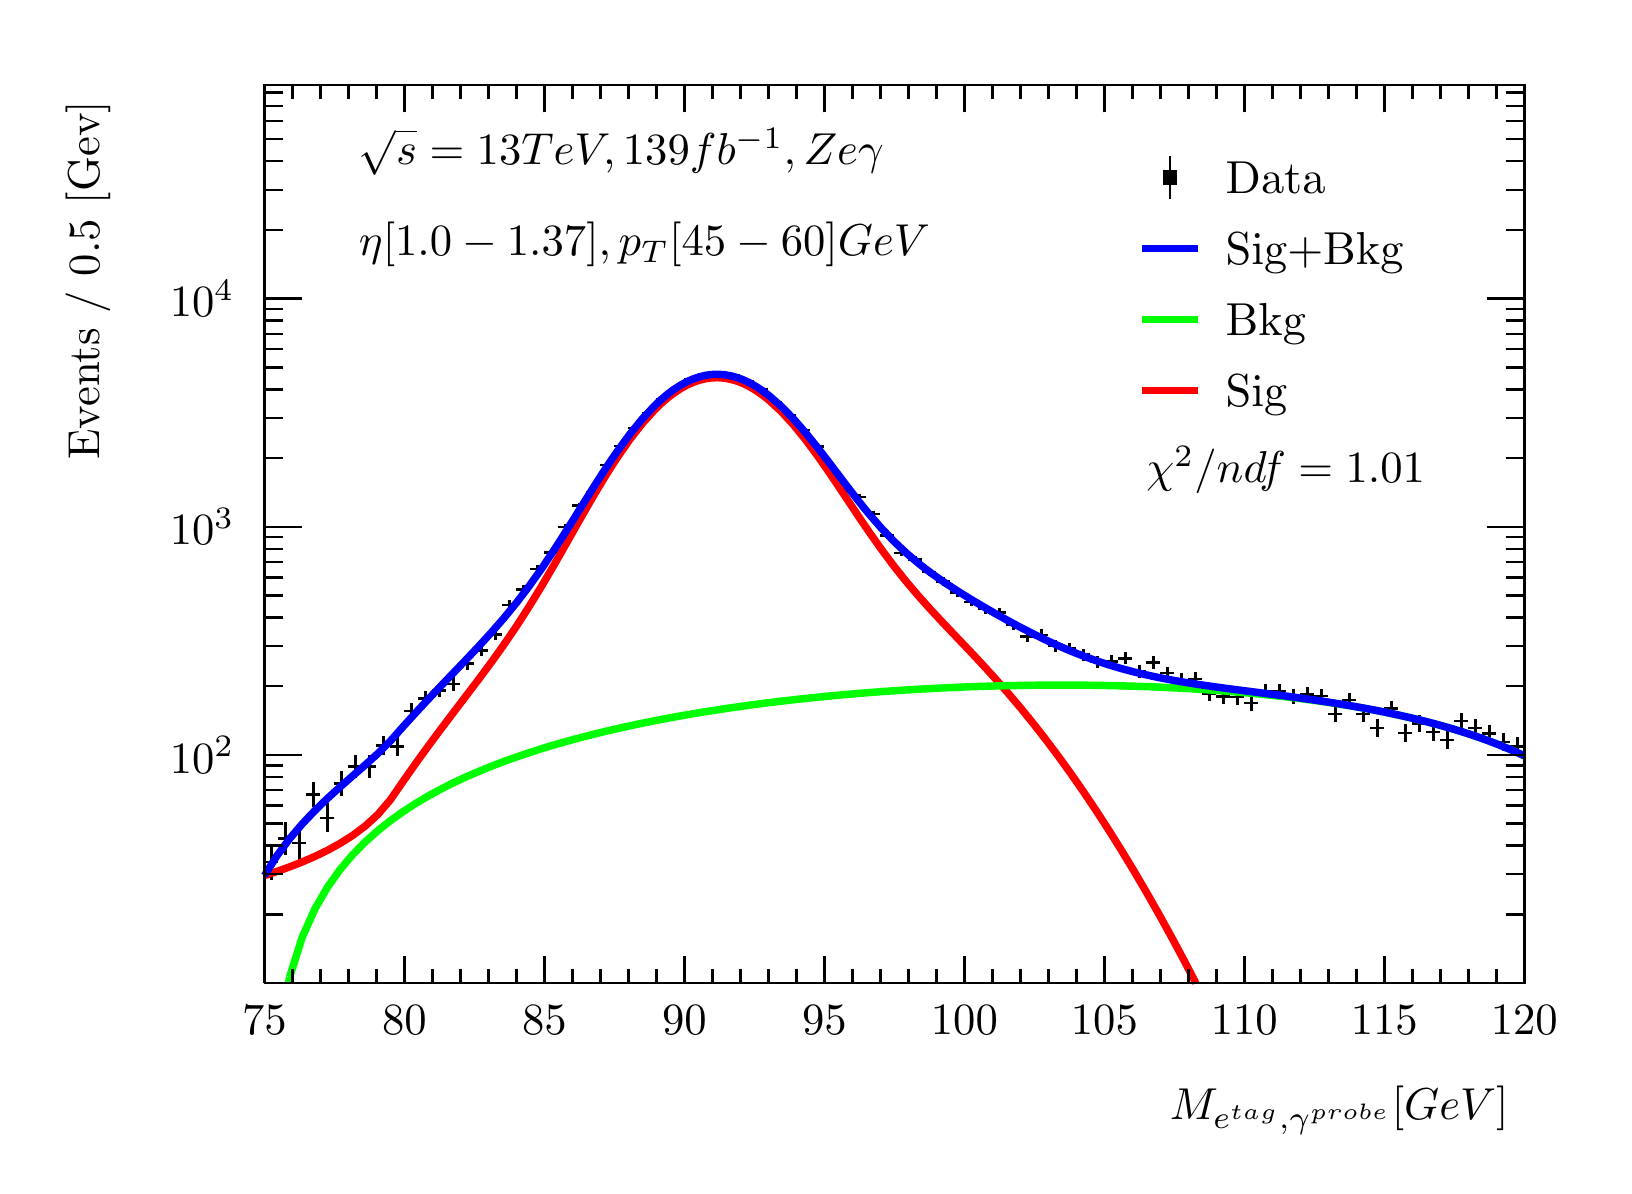
\begin{tikzpicture}
\pgfdeclareplotmark{cross} {
\pgfpathmoveto{\pgfpoint{-0.3\pgfplotmarksize}{\pgfplotmarksize}}
\pgfpathlineto{\pgfpoint{+0.3\pgfplotmarksize}{\pgfplotmarksize}}
\pgfpathlineto{\pgfpoint{+0.3\pgfplotmarksize}{0.3\pgfplotmarksize}}
\pgfpathlineto{\pgfpoint{+1\pgfplotmarksize}{0.3\pgfplotmarksize}}
\pgfpathlineto{\pgfpoint{+1\pgfplotmarksize}{-0.3\pgfplotmarksize}}
\pgfpathlineto{\pgfpoint{+0.3\pgfplotmarksize}{-0.3\pgfplotmarksize}}
\pgfpathlineto{\pgfpoint{+0.3\pgfplotmarksize}{-1.\pgfplotmarksize}}
\pgfpathlineto{\pgfpoint{-0.3\pgfplotmarksize}{-1.\pgfplotmarksize}}
\pgfpathlineto{\pgfpoint{-0.3\pgfplotmarksize}{-0.3\pgfplotmarksize}}
\pgfpathlineto{\pgfpoint{-1.\pgfplotmarksize}{-0.3\pgfplotmarksize}}
\pgfpathlineto{\pgfpoint{-1.\pgfplotmarksize}{0.3\pgfplotmarksize}}
\pgfpathlineto{\pgfpoint{-0.3\pgfplotmarksize}{0.3\pgfplotmarksize}}
\pgfpathclose
\pgfusepathqstroke
}
\pgfdeclareplotmark{cross*} {
\pgfpathmoveto{\pgfpoint{-0.3\pgfplotmarksize}{\pgfplotmarksize}}
\pgfpathlineto{\pgfpoint{+0.3\pgfplotmarksize}{\pgfplotmarksize}}
\pgfpathlineto{\pgfpoint{+0.3\pgfplotmarksize}{0.3\pgfplotmarksize}}
\pgfpathlineto{\pgfpoint{+1\pgfplotmarksize}{0.3\pgfplotmarksize}}
\pgfpathlineto{\pgfpoint{+1\pgfplotmarksize}{-0.3\pgfplotmarksize}}
\pgfpathlineto{\pgfpoint{+0.3\pgfplotmarksize}{-0.3\pgfplotmarksize}}
\pgfpathlineto{\pgfpoint{+0.3\pgfplotmarksize}{-1.\pgfplotmarksize}}
\pgfpathlineto{\pgfpoint{-0.3\pgfplotmarksize}{-1.\pgfplotmarksize}}
\pgfpathlineto{\pgfpoint{-0.3\pgfplotmarksize}{-0.3\pgfplotmarksize}}
\pgfpathlineto{\pgfpoint{-1.\pgfplotmarksize}{-0.3\pgfplotmarksize}}
\pgfpathlineto{\pgfpoint{-1.\pgfplotmarksize}{0.3\pgfplotmarksize}}
\pgfpathlineto{\pgfpoint{-0.3\pgfplotmarksize}{0.3\pgfplotmarksize}}
\pgfpathclose
\pgfusepathqfillstroke
}
\pgfdeclareplotmark{newstar} {
\pgfpathmoveto{\pgfqpoint{0pt}{\pgfplotmarksize}}
\pgfpathlineto{\pgfqpointpolar{44}{0.5\pgfplotmarksize}}
\pgfpathlineto{\pgfqpointpolar{18}{\pgfplotmarksize}}
\pgfpathlineto{\pgfqpointpolar{-20}{0.5\pgfplotmarksize}}
\pgfpathlineto{\pgfqpointpolar{-54}{\pgfplotmarksize}}
\pgfpathlineto{\pgfqpointpolar{-90}{0.5\pgfplotmarksize}}
\pgfpathlineto{\pgfqpointpolar{234}{\pgfplotmarksize}}
\pgfpathlineto{\pgfqpointpolar{198}{0.5\pgfplotmarksize}}
\pgfpathlineto{\pgfqpointpolar{162}{\pgfplotmarksize}}
\pgfpathlineto{\pgfqpointpolar{134}{0.5\pgfplotmarksize}}
\pgfpathclose
\pgfusepathqstroke
}
\pgfdeclareplotmark{newstar*} {
\pgfpathmoveto{\pgfqpoint{0pt}{\pgfplotmarksize}}
\pgfpathlineto{\pgfqpointpolar{44}{0.5\pgfplotmarksize}}
\pgfpathlineto{\pgfqpointpolar{18}{\pgfplotmarksize}}
\pgfpathlineto{\pgfqpointpolar{-20}{0.5\pgfplotmarksize}}
\pgfpathlineto{\pgfqpointpolar{-54}{\pgfplotmarksize}}
\pgfpathlineto{\pgfqpointpolar{-90}{0.5\pgfplotmarksize}}
\pgfpathlineto{\pgfqpointpolar{234}{\pgfplotmarksize}}
\pgfpathlineto{\pgfqpointpolar{198}{0.5\pgfplotmarksize}}
\pgfpathlineto{\pgfqpointpolar{162}{\pgfplotmarksize}}
\pgfpathlineto{\pgfqpointpolar{134}{0.5\pgfplotmarksize}}
\pgfpathclose
\pgfusepathqfillstroke
}
\definecolor{c}{rgb}{1,1,1};
\draw [color=c, fill=c] (0,0) rectangle (20,14.4361);
\draw [color=c, fill=c] (3,2.30977) rectangle (19,13.7143);
\definecolor{c}{rgb}{0,0,0};
\draw [c,line width=0.9] (3,2.30977) -- (3,13.7143) -- (19,13.7143) -- (19,2.30977) -- (3,2.30977);
\definecolor{c}{rgb}{1,1,1};
\draw [color=c, fill=c] (3,2.30977) rectangle (19,13.7143);
\definecolor{c}{rgb}{0,0,0};
\draw [c,line width=0.9] (3,2.30977) -- (3,13.7143) -- (19,13.7143) -- (19,2.30977) -- (3,2.30977);
\draw [c,line width=0.9] (3,2.30977) -- (19,2.30977);
\draw [c,line width=0.9] (3,2.65624) -- (3,2.30977);
\draw [c,line width=0.9] (3.35556,2.48301) -- (3.35556,2.30977);
\draw [c,line width=0.9] (3.71111,2.48301) -- (3.71111,2.30977);
\draw [c,line width=0.9] (4.06667,2.48301) -- (4.06667,2.30977);
\draw [c,line width=0.9] (4.42222,2.48301) -- (4.42222,2.30977);
\draw [c,line width=0.9] (4.77778,2.65624) -- (4.77778,2.30977);
\draw [c,line width=0.9] (5.13333,2.48301) -- (5.13333,2.30977);
\draw [c,line width=0.9] (5.48889,2.48301) -- (5.48889,2.30977);
\draw [c,line width=0.9] (5.84444,2.48301) -- (5.84444,2.30977);
\draw [c,line width=0.9] (6.2,2.48301) -- (6.2,2.30977);
\draw [c,line width=0.9] (6.55556,2.65624) -- (6.55556,2.30977);
\draw [c,line width=0.9] (6.91111,2.48301) -- (6.91111,2.30977);
\draw [c,line width=0.9] (7.26667,2.48301) -- (7.26667,2.30977);
\draw [c,line width=0.9] (7.62222,2.48301) -- (7.62222,2.30977);
\draw [c,line width=0.9] (7.97778,2.48301) -- (7.97778,2.30977);
\draw [c,line width=0.9] (8.33333,2.65624) -- (8.33333,2.30977);
\draw [c,line width=0.9] (8.68889,2.48301) -- (8.68889,2.30977);
\draw [c,line width=0.9] (9.04444,2.48301) -- (9.04444,2.30977);
\draw [c,line width=0.9] (9.4,2.48301) -- (9.4,2.30977);
\draw [c,line width=0.9] (9.75556,2.48301) -- (9.75556,2.30977);
\draw [c,line width=0.9] (10.1111,2.65624) -- (10.1111,2.30977);
\draw [c,line width=0.9] (10.4667,2.48301) -- (10.4667,2.30977);
\draw [c,line width=0.9] (10.8222,2.48301) -- (10.8222,2.30977);
\draw [c,line width=0.9] (11.1778,2.48301) -- (11.1778,2.30977);
\draw [c,line width=0.9] (11.5333,2.48301) -- (11.5333,2.30977);
\draw [c,line width=0.9] (11.8889,2.65624) -- (11.8889,2.30977);
\draw [c,line width=0.9] (12.2444,2.48301) -- (12.2444,2.30977);
\draw [c,line width=0.9] (12.6,2.48301) -- (12.6,2.30977);
\draw [c,line width=0.9] (12.9556,2.48301) -- (12.9556,2.30977);
\draw [c,line width=0.9] (13.3111,2.48301) -- (13.3111,2.30977);
\draw [c,line width=0.9] (13.6667,2.65624) -- (13.6667,2.30977);
\draw [c,line width=0.9] (14.0222,2.48301) -- (14.0222,2.30977);
\draw [c,line width=0.9] (14.3778,2.48301) -- (14.3778,2.30977);
\draw [c,line width=0.9] (14.7333,2.48301) -- (14.7333,2.30977);
\draw [c,line width=0.9] (15.0889,2.48301) -- (15.0889,2.30977);
\draw [c,line width=0.9] (15.4444,2.65624) -- (15.4444,2.30977);
\draw [c,line width=0.9] (15.8,2.48301) -- (15.8,2.30977);
\draw [c,line width=0.9] (16.1556,2.48301) -- (16.1556,2.30977);
\draw [c,line width=0.9] (16.5111,2.48301) -- (16.5111,2.30977);
\draw [c,line width=0.9] (16.8667,2.48301) -- (16.8667,2.30977);
\draw [c,line width=0.9] (17.2222,2.65624) -- (17.2222,2.30977);
\draw [c,line width=0.9] (17.5778,2.48301) -- (17.5778,2.30977);
\draw [c,line width=0.9] (17.9333,2.48301) -- (17.9333,2.30977);
\draw [c,line width=0.9] (18.2889,2.48301) -- (18.2889,2.30977);
\draw [c,line width=0.9] (18.6444,2.48301) -- (18.6444,2.30977);
\draw [c,line width=0.9] (19,2.65624) -- (19,2.30977);
\draw [c,line width=0.9] (19,2.65624) -- (19,2.30977);
\draw [anchor=base] (3,1.66015) node[scale=1.61424, color=c, rotate=0]{75};
\draw [anchor=base] (4.77778,1.66015) node[scale=1.61424, color=c, rotate=0]{80};
\draw [anchor=base] (6.55556,1.66015) node[scale=1.61424, color=c, rotate=0]{85};
\draw [anchor=base] (8.33333,1.66015) node[scale=1.61424, color=c, rotate=0]{90};
\draw [anchor=base] (10.1111,1.66015) node[scale=1.61424, color=c, rotate=0]{95};
\draw [anchor=base] (11.8889,1.66015) node[scale=1.61424, color=c, rotate=0]{100};
\draw [anchor=base] (13.6667,1.66015) node[scale=1.61424, color=c, rotate=0]{105};
\draw [anchor=base] (15.4444,1.66015) node[scale=1.61424, color=c, rotate=0]{110};
\draw [anchor=base] (17.2222,1.66015) node[scale=1.61424, color=c, rotate=0]{115};
\draw [anchor=base] (19,1.66015) node[scale=1.61424, color=c, rotate=0]{120};
\draw [anchor= east] (19,0.692932) node[scale=1.61424, color=c, rotate=0]{$M_{e^{tag}, \gamma^{probe}}  [GeV]$};
\draw [c,line width=0.9] (3,13.7143) -- (19,13.7143);
\draw [c,line width=0.9] (3,13.3678) -- (3,13.7143);
\draw [c,line width=0.9] (3.35556,13.5411) -- (3.35556,13.7143);
\draw [c,line width=0.9] (3.71111,13.5411) -- (3.71111,13.7143);
\draw [c,line width=0.9] (4.06667,13.5411) -- (4.06667,13.7143);
\draw [c,line width=0.9] (4.42222,13.5411) -- (4.42222,13.7143);
\draw [c,line width=0.9] (4.77778,13.3678) -- (4.77778,13.7143);
\draw [c,line width=0.9] (5.13333,13.5411) -- (5.13333,13.7143);
\draw [c,line width=0.9] (5.48889,13.5411) -- (5.48889,13.7143);
\draw [c,line width=0.9] (5.84444,13.5411) -- (5.84444,13.7143);
\draw [c,line width=0.9] (6.2,13.5411) -- (6.2,13.7143);
\draw [c,line width=0.9] (6.55556,13.3678) -- (6.55556,13.7143);
\draw [c,line width=0.9] (6.91111,13.5411) -- (6.91111,13.7143);
\draw [c,line width=0.9] (7.26667,13.5411) -- (7.26667,13.7143);
\draw [c,line width=0.9] (7.62222,13.5411) -- (7.62222,13.7143);
\draw [c,line width=0.9] (7.97778,13.5411) -- (7.97778,13.7143);
\draw [c,line width=0.9] (8.33333,13.3678) -- (8.33333,13.7143);
\draw [c,line width=0.9] (8.68889,13.5411) -- (8.68889,13.7143);
\draw [c,line width=0.9] (9.04444,13.5411) -- (9.04444,13.7143);
\draw [c,line width=0.9] (9.4,13.5411) -- (9.4,13.7143);
\draw [c,line width=0.9] (9.75556,13.5411) -- (9.75556,13.7143);
\draw [c,line width=0.9] (10.1111,13.3678) -- (10.1111,13.7143);
\draw [c,line width=0.9] (10.4667,13.5411) -- (10.4667,13.7143);
\draw [c,line width=0.9] (10.8222,13.5411) -- (10.8222,13.7143);
\draw [c,line width=0.9] (11.1778,13.5411) -- (11.1778,13.7143);
\draw [c,line width=0.9] (11.5333,13.5411) -- (11.5333,13.7143);
\draw [c,line width=0.9] (11.8889,13.3678) -- (11.8889,13.7143);
\draw [c,line width=0.9] (12.2444,13.5411) -- (12.2444,13.7143);
\draw [c,line width=0.9] (12.6,13.5411) -- (12.6,13.7143);
\draw [c,line width=0.9] (12.9556,13.5411) -- (12.9556,13.7143);
\draw [c,line width=0.9] (13.3111,13.5411) -- (13.3111,13.7143);
\draw [c,line width=0.9] (13.6667,13.3678) -- (13.6667,13.7143);
\draw [c,line width=0.9] (14.0222,13.5411) -- (14.0222,13.7143);
\draw [c,line width=0.9] (14.3778,13.5411) -- (14.3778,13.7143);
\draw [c,line width=0.9] (14.7333,13.5411) -- (14.7333,13.7143);
\draw [c,line width=0.9] (15.0889,13.5411) -- (15.0889,13.7143);
\draw [c,line width=0.9] (15.4444,13.3678) -- (15.4444,13.7143);
\draw [c,line width=0.9] (15.8,13.5411) -- (15.8,13.7143);
\draw [c,line width=0.9] (16.1556,13.5411) -- (16.1556,13.7143);
\draw [c,line width=0.9] (16.5111,13.5411) -- (16.5111,13.7143);
\draw [c,line width=0.9] (16.8667,13.5411) -- (16.8667,13.7143);
\draw [c,line width=0.9] (17.2222,13.3678) -- (17.2222,13.7143);
\draw [c,line width=0.9] (17.5778,13.5411) -- (17.5778,13.7143);
\draw [c,line width=0.9] (17.9333,13.5411) -- (17.9333,13.7143);
\draw [c,line width=0.9] (18.2889,13.5411) -- (18.2889,13.7143);
\draw [c,line width=0.9] (18.6444,13.5411) -- (18.6444,13.7143);
\draw [c,line width=0.9] (19,13.3678) -- (19,13.7143);
\draw [c,line width=0.9] (19,13.3678) -- (19,13.7143);
\draw [c,line width=0.9] (3,2.30977) -- (3,13.7143);
\draw [c,line width=0.9] (3.237,3.182) -- (3,3.182);
\draw [c,line width=0.9] (3.237,3.69222) -- (3,3.69222);
\draw [c,line width=0.9] (3.237,4.05422) -- (3,4.05422);
\draw [c,line width=0.9] (3.237,4.33502) -- (3,4.33502);
\draw [c,line width=0.9] (3.237,4.56444) -- (3,4.56444);
\draw [c,line width=0.9] (3.237,4.75842) -- (3,4.75842);
\draw [c,line width=0.9] (3.237,4.92645) -- (3,4.92645);
\draw [c,line width=0.9] (3.237,5.07466) -- (3,5.07466);
\draw [c,line width=0.9] (3.474,5.20724) -- (3,5.20724);
\draw [anchor= east] (2.82,5.20724) node[scale=1.61424, color=c, rotate=0]{$10^{2}$};
\draw [c,line width=0.9] (3.237,6.07947) -- (3,6.07947);
\draw [c,line width=0.9] (3.237,6.58969) -- (3,6.58969);
\draw [c,line width=0.9] (3.237,6.9517) -- (3,6.9517);
\draw [c,line width=0.9] (3.237,7.23249) -- (3,7.23249);
\draw [c,line width=0.9] (3.237,7.46192) -- (3,7.46192);
\draw [c,line width=0.9] (3.237,7.65589) -- (3,7.65589);
\draw [c,line width=0.9] (3.237,7.82392) -- (3,7.82392);
\draw [c,line width=0.9] (3.237,7.97214) -- (3,7.97214);
\draw [c,line width=0.9] (3.474,8.10472) -- (3,8.10472);
\draw [anchor= east] (2.82,8.10472) node[scale=1.61424, color=c, rotate=0]{$10^{3}$};
\draw [c,line width=0.9] (3.237,8.97694) -- (3,8.97694);
\draw [c,line width=0.9] (3.237,9.48716) -- (3,9.48716);
\draw [c,line width=0.9] (3.237,9.84917) -- (3,9.84917);
\draw [c,line width=0.9] (3.237,10.13) -- (3,10.13);
\draw [c,line width=0.9] (3.237,10.3594) -- (3,10.3594);
\draw [c,line width=0.9] (3.237,10.5534) -- (3,10.5534);
\draw [c,line width=0.9] (3.237,10.7214) -- (3,10.7214);
\draw [c,line width=0.9] (3.237,10.8696) -- (3,10.8696);
\draw [c,line width=0.9] (3.474,11.0022) -- (3,11.0022);
\draw [anchor= east] (2.82,11.0022) node[scale=1.61424, color=c, rotate=0]{$10^{4}$};
\draw [c,line width=0.9] (3.237,11.8744) -- (3,11.8744);
\draw [c,line width=0.9] (3.237,12.3846) -- (3,12.3846);
\draw [c,line width=0.9] (3.237,12.7466) -- (3,12.7466);
\draw [c,line width=0.9] (3.237,13.0274) -- (3,13.0274);
\draw [c,line width=0.9] (3.237,13.2569) -- (3,13.2569);
\draw [c,line width=0.9] (3.237,13.4508) -- (3,13.4508);
\draw [c,line width=0.9] (3.237,13.6189) -- (3,13.6189);
\draw [anchor= east] (0.76,13.7143) node[scale=1.61424, color=c, rotate=90]{Events / 0.5 [Gev]};
\draw [c,line width=0.9] (19,2.30977) -- (19,13.7143);
\draw [c,line width=0.9] (18.763,3.182) -- (19,3.182);
\draw [c,line width=0.9] (18.763,3.69222) -- (19,3.69222);
\draw [c,line width=0.9] (18.763,4.05422) -- (19,4.05422);
\draw [c,line width=0.9] (18.763,4.33502) -- (19,4.33502);
\draw [c,line width=0.9] (18.763,4.56444) -- (19,4.56444);
\draw [c,line width=0.9] (18.763,4.75842) -- (19,4.75842);
\draw [c,line width=0.9] (18.763,4.92645) -- (19,4.92645);
\draw [c,line width=0.9] (18.763,5.07466) -- (19,5.07466);
\draw [c,line width=0.9] (18.526,5.20724) -- (19,5.20724);
\draw [c,line width=0.9] (18.763,6.07947) -- (19,6.07947);
\draw [c,line width=0.9] (18.763,6.58969) -- (19,6.58969);
\draw [c,line width=0.9] (18.763,6.9517) -- (19,6.9517);
\draw [c,line width=0.9] (18.763,7.23249) -- (19,7.23249);
\draw [c,line width=0.9] (18.763,7.46192) -- (19,7.46192);
\draw [c,line width=0.9] (18.763,7.65589) -- (19,7.65589);
\draw [c,line width=0.9] (18.763,7.82392) -- (19,7.82392);
\draw [c,line width=0.9] (18.763,7.97214) -- (19,7.97214);
\draw [c,line width=0.9] (18.526,8.10472) -- (19,8.10472);
\draw [c,line width=0.9] (18.763,8.97694) -- (19,8.97694);
\draw [c,line width=0.9] (18.763,9.48716) -- (19,9.48716);
\draw [c,line width=0.9] (18.763,9.84917) -- (19,9.84917);
\draw [c,line width=0.9] (18.763,10.13) -- (19,10.13);
\draw [c,line width=0.9] (18.763,10.3594) -- (19,10.3594);
\draw [c,line width=0.9] (18.763,10.5534) -- (19,10.5534);
\draw [c,line width=0.9] (18.763,10.7214) -- (19,10.7214);
\draw [c,line width=0.9] (18.763,10.8696) -- (19,10.8696);
\draw [c,line width=0.9] (18.526,11.0022) -- (19,11.0022);
\draw [c,line width=0.9] (18.763,11.8744) -- (19,11.8744);
\draw [c,line width=0.9] (18.763,12.3846) -- (19,12.3846);
\draw [c,line width=0.9] (18.763,12.7466) -- (19,12.7466);
\draw [c,line width=0.9] (18.763,13.0274) -- (19,13.0274);
\draw [c,line width=0.9] (18.763,13.2569) -- (19,13.2569);
\draw [c,line width=0.9] (18.763,13.4508) -- (19,13.4508);
\draw [c,line width=0.9] (18.763,13.6189) -- (19,13.6189);
\draw [c,line width=0.9] (3.08889,3.84972) -- (3,3.84972);
\draw [c,line width=0.9] (3,3.84972) -- (3,3.84972);
\draw [c,line width=0.9] (3.08889,3.84972) -- (3.17778,3.84972);
\draw [c,line width=0.9] (3.17778,3.84972) -- (3.17778,3.84972);
\draw [c,line width=0.9] (3.08889,3.84972) -- (3.08889,4.08186);
\draw [c,line width=0.9] (3.08889,4.08186) -- (3.08889,4.08186);
\draw [c,line width=0.9] (3.08889,3.84972) -- (3.08889,3.61426);
\draw [c,line width=0.9] (3.08889,3.61426) -- (3.08889,3.61426);
\draw [c,line width=0.9] (3.26667,4.14523) -- (3.17778,4.14523);
\draw [c,line width=0.9] (3.17778,4.14523) -- (3.17778,4.14523);
\draw [c,line width=0.9] (3.26667,4.14523) -- (3.35556,4.14523);
\draw [c,line width=0.9] (3.35556,4.14523) -- (3.35556,4.14523);
\draw [c,line width=0.9] (3.26667,4.14523) -- (3.26667,4.35024);
\draw [c,line width=0.9] (3.26667,4.35024) -- (3.26667,4.35024);
\draw [c,line width=0.9] (3.26667,4.14523) -- (3.26667,3.9379);
\draw [c,line width=0.9] (3.26667,3.9379) -- (3.26667,3.9379);
\draw [c,line width=0.9] (3.44444,4.0853) -- (3.35556,4.0853);
\draw [c,line width=0.9] (3.35556,4.0853) -- (3.35556,4.0853);
\draw [c,line width=0.9] (3.44444,4.0853) -- (3.53333,4.0853);
\draw [c,line width=0.9] (3.53333,4.0853) -- (3.53333,4.0853);
\draw [c,line width=0.9] (3.44444,4.0853) -- (3.44444,4.29553);
\draw [c,line width=0.9] (3.44444,4.29553) -- (3.44444,4.29553);
\draw [c,line width=0.9] (3.44444,4.0853) -- (3.44444,3.87257);
\draw [c,line width=0.9] (3.44444,3.87257) -- (3.44444,3.87257);
\draw [c,line width=0.9] (3.62222,4.7033) -- (3.53333,4.7033);
\draw [c,line width=0.9] (3.53333,4.7033) -- (3.53333,4.7033);
\draw [c,line width=0.9] (3.62222,4.7033) -- (3.71111,4.7033);
\draw [c,line width=0.9] (3.71111,4.7033) -- (3.71111,4.7033);
\draw [c,line width=0.9] (3.62222,4.7033) -- (3.62222,4.86565);
\draw [c,line width=0.9] (3.62222,4.86565) -- (3.62222,4.86565);
\draw [c,line width=0.9] (3.62222,4.7033) -- (3.62222,4.53978);
\draw [c,line width=0.9] (3.62222,4.53978) -- (3.62222,4.53978);
\draw [c,line width=0.9] (3.8,4.40834) -- (3.71111,4.40834);
\draw [c,line width=0.9] (3.71111,4.40834) -- (3.71111,4.40834);
\draw [c,line width=0.9] (3.8,4.40834) -- (3.88889,4.40834);
\draw [c,line width=0.9] (3.88889,4.40834) -- (3.88889,4.40834);
\draw [c,line width=0.9] (3.8,4.40834) -- (3.8,4.59195);
\draw [c,line width=0.9] (3.8,4.59195) -- (3.8,4.59195);
\draw [c,line width=0.9] (3.8,4.40834) -- (3.8,4.22304);
\draw [c,line width=0.9] (3.8,4.22304) -- (3.8,4.22304);
\draw [c,line width=0.9] (3.97778,4.84524) -- (3.88889,4.84524);
\draw [c,line width=0.9] (3.88889,4.84524) -- (3.88889,4.84524);
\draw [c,line width=0.9] (3.97778,4.84524) -- (4.06667,4.84524);
\draw [c,line width=0.9] (4.06667,4.84524) -- (4.06667,4.84524);
\draw [c,line width=0.9] (3.97778,4.84524) -- (3.97778,4.99827);
\draw [c,line width=0.9] (3.97778,4.99827) -- (3.97778,4.99827);
\draw [c,line width=0.9] (3.97778,4.84524) -- (3.97778,4.69121);
\draw [c,line width=0.9] (3.97778,4.69121) -- (3.97778,4.69121);
\draw [c,line width=0.9] (4.15556,5.06061) -- (4.06667,5.06061);
\draw [c,line width=0.9] (4.06667,5.06061) -- (4.06667,5.06061);
\draw [c,line width=0.9] (4.15556,5.06061) -- (4.24444,5.06061);
\draw [c,line width=0.9] (4.24444,5.06061) -- (4.24444,5.06061);
\draw [c,line width=0.9] (4.15556,5.06061) -- (4.15556,5.20055);
\draw [c,line width=0.9] (4.15556,5.20055) -- (4.15556,5.20055);
\draw [c,line width=0.9] (4.15556,5.06061) -- (4.15556,4.91989);
\draw [c,line width=0.9] (4.15556,4.91989) -- (4.15556,4.91989);
\draw [c,line width=0.9] (4.33333,5.06061) -- (4.24444,5.06061);
\draw [c,line width=0.9] (4.24444,5.06061) -- (4.24444,5.06061);
\draw [c,line width=0.9] (4.33333,5.06061) -- (4.42222,5.06061);
\draw [c,line width=0.9] (4.42222,5.06061) -- (4.42222,5.06061);
\draw [c,line width=0.9] (4.33333,5.06061) -- (4.33333,5.20055);
\draw [c,line width=0.9] (4.33333,5.20055) -- (4.33333,5.20055);
\draw [c,line width=0.9] (4.33333,5.06061) -- (4.33333,4.91989);
\draw [c,line width=0.9] (4.33333,4.91989) -- (4.33333,4.91989);
\draw [c,line width=0.9] (4.51111,5.32718) -- (4.42222,5.32718);
\draw [c,line width=0.9] (4.42222,5.32718) -- (4.42222,5.32718);
\draw [c,line width=0.9] (4.51111,5.32718) -- (4.6,5.32718);
\draw [c,line width=0.9] (4.6,5.32718) -- (4.6,5.32718);
\draw [c,line width=0.9] (4.51111,5.32718) -- (4.51111,5.44711);
\draw [c,line width=0.9] (4.51111,5.44711) -- (4.51111,5.44711);
\draw [c,line width=0.9] (4.51111,5.32718) -- (4.51111,5.20725);
\draw [c,line width=0.9] (4.51111,5.20725) -- (4.51111,5.20725);
\draw [c,line width=0.9] (4.68889,5.31569) -- (4.6,5.31569);
\draw [c,line width=0.9] (4.6,5.31569) -- (4.6,5.31569);
\draw [c,line width=0.9] (4.68889,5.31569) -- (4.77778,5.31569);
\draw [c,line width=0.9] (4.77778,5.31569) -- (4.77778,5.31569);
\draw [c,line width=0.9] (4.68889,5.31569) -- (4.68889,5.43617);
\draw [c,line width=0.9] (4.68889,5.43617) -- (4.68889,5.43617);
\draw [c,line width=0.9] (4.68889,5.31569) -- (4.68889,5.19521);
\draw [c,line width=0.9] (4.68889,5.19521) -- (4.68889,5.19521);
\draw [c,line width=0.9] (4.86667,5.76682) -- (4.77778,5.76682);
\draw [c,line width=0.9] (4.77778,5.76682) -- (4.77778,5.76682);
\draw [c,line width=0.9] (4.86667,5.76682) -- (4.95556,5.76682);
\draw [c,line width=0.9] (4.95556,5.76682) -- (4.95556,5.76682);
\draw [c,line width=0.9] (4.86667,5.76682) -- (4.86667,5.86754);
\draw [c,line width=0.9] (4.86667,5.86754) -- (4.86667,5.86754);
\draw [c,line width=0.9] (4.86667,5.76682) -- (4.86667,5.6661);
\draw [c,line width=0.9] (4.86667,5.6661) -- (4.86667,5.6661);
\draw [c,line width=0.9] (5.04444,5.92574) -- (4.95556,5.92574);
\draw [c,line width=0.9] (4.95556,5.92574) -- (4.95556,5.92574);
\draw [c,line width=0.9] (5.04444,5.92574) -- (5.13333,5.92574);
\draw [c,line width=0.9] (5.13333,5.92574) -- (5.13333,5.92574);
\draw [c,line width=0.9] (5.04444,5.92574) -- (5.04444,6.0203);
\draw [c,line width=0.9] (5.04444,6.0203) -- (5.04444,6.0203);
\draw [c,line width=0.9] (5.04444,5.92574) -- (5.04444,5.83118);
\draw [c,line width=0.9] (5.04444,5.83118) -- (5.04444,5.83118);
\draw [c,line width=0.9] (5.22222,6.0281) -- (5.13333,6.0281);
\draw [c,line width=0.9] (5.13333,6.0281) -- (5.13333,6.0281);
\draw [c,line width=0.9] (5.22222,6.0281) -- (5.31111,6.0281);
\draw [c,line width=0.9] (5.31111,6.0281) -- (5.31111,6.0281);
\draw [c,line width=0.9] (5.22222,6.0281) -- (5.22222,6.1189);
\draw [c,line width=0.9] (5.22222,6.1189) -- (5.22222,6.1189);
\draw [c,line width=0.9] (5.22222,6.0281) -- (5.22222,5.93731);
\draw [c,line width=0.9] (5.22222,5.93731) -- (5.22222,5.93731);
\draw [c,line width=0.9] (5.4,6.11054) -- (5.31111,6.11054);
\draw [c,line width=0.9] (5.31111,6.11054) -- (5.31111,6.11054);
\draw [c,line width=0.9] (5.4,6.11054) -- (5.48889,6.11054);
\draw [c,line width=0.9] (5.48889,6.11054) -- (5.48889,6.11054);
\draw [c,line width=0.9] (5.4,6.11054) -- (5.4,6.19841);
\draw [c,line width=0.9] (5.4,6.19841) -- (5.4,6.19841);
\draw [c,line width=0.9] (5.4,6.11054) -- (5.4,6.02268);
\draw [c,line width=0.9] (5.4,6.02268) -- (5.4,6.02268);
\draw [c,line width=0.9] (5.57778,6.36529) -- (5.48889,6.36529);
\draw [c,line width=0.9] (5.48889,6.36529) -- (5.48889,6.36529);
\draw [c,line width=0.9] (5.57778,6.36529) -- (5.66667,6.36529);
\draw [c,line width=0.9] (5.66667,6.36529) -- (5.66667,6.36529);
\draw [c,line width=0.9] (5.57778,6.36529) -- (5.57778,6.4447);
\draw [c,line width=0.9] (5.57778,6.4447) -- (5.57778,6.4447);
\draw [c,line width=0.9] (5.57778,6.36529) -- (5.57778,6.28588);
\draw [c,line width=0.9] (5.57778,6.28588) -- (5.57778,6.28588);
\draw [c,line width=0.9] (5.75556,6.53395) -- (5.66667,6.53395);
\draw [c,line width=0.9] (5.66667,6.53395) -- (5.66667,6.53395);
\draw [c,line width=0.9] (5.75556,6.53395) -- (5.84444,6.53395);
\draw [c,line width=0.9] (5.84444,6.53395) -- (5.84444,6.53395);
\draw [c,line width=0.9] (5.75556,6.53395) -- (5.75556,6.60821);
\draw [c,line width=0.9] (5.75556,6.60821) -- (5.75556,6.60821);
\draw [c,line width=0.9] (5.75556,6.53395) -- (5.75556,6.45968);
\draw [c,line width=0.9] (5.75556,6.45968) -- (5.75556,6.45968);
\draw [c,line width=0.9] (5.93333,6.73604) -- (5.84444,6.73604);
\draw [c,line width=0.9] (5.84444,6.73604) -- (5.84444,6.73604);
\draw [c,line width=0.9] (5.93333,6.73604) -- (6.02222,6.73604);
\draw [c,line width=0.9] (6.02222,6.73604) -- (6.02222,6.73604);
\draw [c,line width=0.9] (5.93333,6.73604) -- (5.93333,6.80458);
\draw [c,line width=0.9] (5.93333,6.80458) -- (5.93333,6.80458);
\draw [c,line width=0.9] (5.93333,6.73604) -- (5.93333,6.6675);
\draw [c,line width=0.9] (5.93333,6.6675) -- (5.93333,6.6675);
\draw [c,line width=0.9] (6.11111,7.11105) -- (6.02222,7.11105);
\draw [c,line width=0.9] (6.02222,7.11105) -- (6.02222,7.11105);
\draw [c,line width=0.9] (6.11111,7.11105) -- (6.2,7.11105);
\draw [c,line width=0.9] (6.2,7.11105) -- (6.2,7.11105);
\draw [c,line width=0.9] (6.11111,7.11105) -- (6.11111,7.1701);
\draw [c,line width=0.9] (6.11111,7.1701) -- (6.11111,7.1701);
\draw [c,line width=0.9] (6.11111,7.11105) -- (6.11111,7.052);
\draw [c,line width=0.9] (6.11111,7.052) -- (6.11111,7.052);
\draw [c,line width=0.9] (6.28889,7.31056) -- (6.2,7.31056);
\draw [c,line width=0.9] (6.2,7.31056) -- (6.2,7.31056);
\draw [c,line width=0.9] (6.28889,7.31056) -- (6.37778,7.31056);
\draw [c,line width=0.9] (6.37778,7.31056) -- (6.37778,7.31056);
\draw [c,line width=0.9] (6.28889,7.31056) -- (6.28889,7.36511);
\draw [c,line width=0.9] (6.28889,7.36511) -- (6.28889,7.36511);
\draw [c,line width=0.9] (6.28889,7.31056) -- (6.28889,7.256);
\draw [c,line width=0.9] (6.28889,7.256) -- (6.28889,7.256);
\draw [c,line width=0.9] (6.46667,7.56844) -- (6.37778,7.56844);
\draw [c,line width=0.9] (6.37778,7.56844) -- (6.37778,7.56844);
\draw [c,line width=0.9] (6.46667,7.56844) -- (6.55556,7.56844);
\draw [c,line width=0.9] (6.55556,7.56844) -- (6.55556,7.56844);
\draw [c,line width=0.9] (6.46667,7.56844) -- (6.46667,7.61768);
\draw [c,line width=0.9] (6.46667,7.61768) -- (6.46667,7.61768);
\draw [c,line width=0.9] (6.46667,7.56844) -- (6.46667,7.5192);
\draw [c,line width=0.9] (6.46667,7.5192) -- (6.46667,7.5192);
\draw [c,line width=0.9] (6.64444,7.77583) -- (6.55556,7.77583);
\draw [c,line width=0.9] (6.55556,7.77583) -- (6.55556,7.77583);
\draw [c,line width=0.9] (6.64444,7.77583) -- (6.73333,7.77583);
\draw [c,line width=0.9] (6.73333,7.77583) -- (6.73333,7.77583);
\draw [c,line width=0.9] (6.64444,7.77583) -- (6.64444,7.82117);
\draw [c,line width=0.9] (6.64444,7.82117) -- (6.64444,7.82117);
\draw [c,line width=0.9] (6.64444,7.77583) -- (6.64444,7.73048);
\draw [c,line width=0.9] (6.64444,7.73048) -- (6.64444,7.73048);
\draw [c,line width=0.9] (6.82222,8.1022) -- (6.73333,8.1022);
\draw [c,line width=0.9] (6.73333,8.1022) -- (6.73333,8.1022);
\draw [c,line width=0.9] (6.82222,8.1022) -- (6.91111,8.1022);
\draw [c,line width=0.9] (6.91111,8.1022) -- (6.91111,8.1022);
\draw [c,line width=0.9] (6.82222,8.1022) -- (6.82222,8.14203);
\draw [c,line width=0.9] (6.82222,8.14203) -- (6.82222,8.14203);
\draw [c,line width=0.9] (6.82222,8.1022) -- (6.82222,8.06237);
\draw [c,line width=0.9] (6.82222,8.06237) -- (6.82222,8.06237);
\draw [c,line width=0.9] (7,8.37439) -- (6.91111,8.37439);
\draw [c,line width=0.9] (6.91111,8.37439) -- (6.91111,8.37439);
\draw [c,line width=0.9] (7,8.37439) -- (7.08889,8.37439);
\draw [c,line width=0.9] (7.08889,8.37439) -- (7.08889,8.37439);
\draw [c,line width=0.9] (7,8.37439) -- (7,8.41014);
\draw [c,line width=0.9] (7,8.41014) -- (7,8.41014);
\draw [c,line width=0.9] (7,8.37439) -- (7,8.33864);
\draw [c,line width=0.9] (7,8.33864) -- (7,8.33864);
\draw [c,line width=0.9] (7.17778,8.54863) -- (7.08889,8.54863);
\draw [c,line width=0.9] (7.08889,8.54863) -- (7.08889,8.54863);
\draw [c,line width=0.9] (7.17778,8.54863) -- (7.26667,8.54863);
\draw [c,line width=0.9] (7.26667,8.54863) -- (7.26667,8.54863);
\draw [c,line width=0.9] (7.17778,8.54863) -- (7.17778,8.58198);
\draw [c,line width=0.9] (7.17778,8.58198) -- (7.17778,8.58198);
\draw [c,line width=0.9] (7.17778,8.54863) -- (7.17778,8.51527);
\draw [c,line width=0.9] (7.17778,8.51527) -- (7.17778,8.51527);
\draw [c,line width=0.9] (7.35556,8.889) -- (7.26667,8.889);
\draw [c,line width=0.9] (7.26667,8.889) -- (7.26667,8.889);
\draw [c,line width=0.9] (7.35556,8.889) -- (7.44444,8.889);
\draw [c,line width=0.9] (7.44444,8.889) -- (7.44444,8.889);
\draw [c,line width=0.9] (7.35556,8.889) -- (7.35556,8.91814);
\draw [c,line width=0.9] (7.35556,8.91814) -- (7.35556,8.91814);
\draw [c,line width=0.9] (7.35556,8.889) -- (7.35556,8.85987);
\draw [c,line width=0.9] (7.35556,8.85987) -- (7.35556,8.85987);
\draw [c,line width=0.9] (7.53333,9.12851) -- (7.44444,9.12851);
\draw [c,line width=0.9] (7.44444,9.12851) -- (7.44444,9.12851);
\draw [c,line width=0.9] (7.53333,9.12851) -- (7.62222,9.12851);
\draw [c,line width=0.9] (7.62222,9.12851) -- (7.62222,9.12851);
\draw [c,line width=0.9] (7.53333,9.12851) -- (7.53333,9.155);
\draw [c,line width=0.9] (7.53333,9.155) -- (7.53333,9.155);
\draw [c,line width=0.9] (7.53333,9.12851) -- (7.53333,9.10202);
\draw [c,line width=0.9] (7.53333,9.10202) -- (7.53333,9.10202);
\draw [c,line width=0.9] (7.71111,9.35784) -- (7.62222,9.35784);
\draw [c,line width=0.9] (7.62222,9.35784) -- (7.62222,9.35784);
\draw [c,line width=0.9] (7.71111,9.35784) -- (7.8,9.35784);
\draw [c,line width=0.9] (7.8,9.35784) -- (7.8,9.35784);
\draw [c,line width=0.9] (7.71111,9.35784) -- (7.71111,9.38203);
\draw [c,line width=0.9] (7.71111,9.38203) -- (7.71111,9.38203);
\draw [c,line width=0.9] (7.71111,9.35784) -- (7.71111,9.33366);
\draw [c,line width=0.9] (7.71111,9.33366) -- (7.71111,9.33366);
\draw [c,line width=0.9] (7.88889,9.55255) -- (7.8,9.55255);
\draw [c,line width=0.9] (7.8,9.55255) -- (7.8,9.55255);
\draw [c,line width=0.9] (7.88889,9.55255) -- (7.97778,9.55255);
\draw [c,line width=0.9] (7.97778,9.55255) -- (7.97778,9.55255);
\draw [c,line width=0.9] (7.88889,9.55255) -- (7.88889,9.57493);
\draw [c,line width=0.9] (7.88889,9.57493) -- (7.88889,9.57493);
\draw [c,line width=0.9] (7.88889,9.55255) -- (7.88889,9.53016);
\draw [c,line width=0.9] (7.88889,9.53016) -- (7.88889,9.53016);
\draw [c,line width=0.9] (8.06667,9.72773) -- (7.97778,9.72773);
\draw [c,line width=0.9] (7.97778,9.72773) -- (7.97778,9.72773);
\draw [c,line width=0.9] (8.06667,9.72773) -- (8.15556,9.72773);
\draw [c,line width=0.9] (8.15556,9.72773) -- (8.15556,9.72773);
\draw [c,line width=0.9] (8.06667,9.72773) -- (8.06667,9.74861);
\draw [c,line width=0.9] (8.06667,9.74861) -- (8.06667,9.74861);
\draw [c,line width=0.9] (8.06667,9.72773) -- (8.06667,9.70685);
\draw [c,line width=0.9] (8.06667,9.70685) -- (8.06667,9.70685);
\draw [c,line width=0.9] (8.24444,9.85482) -- (8.15556,9.85482);
\draw [c,line width=0.9] (8.15556,9.85482) -- (8.15556,9.85482);
\draw [c,line width=0.9] (8.24444,9.85482) -- (8.33333,9.85482);
\draw [c,line width=0.9] (8.33333,9.85482) -- (8.33333,9.85482);
\draw [c,line width=0.9] (8.24444,9.85482) -- (8.24444,9.87467);
\draw [c,line width=0.9] (8.24444,9.87467) -- (8.24444,9.87467);
\draw [c,line width=0.9] (8.24444,9.85482) -- (8.24444,9.83497);
\draw [c,line width=0.9] (8.24444,9.83497) -- (8.24444,9.83497);
\draw [c,line width=0.9] (8.42222,9.97481) -- (8.33333,9.97481);
\draw [c,line width=0.9] (8.33333,9.97481) -- (8.33333,9.97481);
\draw [c,line width=0.9] (8.42222,9.97481) -- (8.51111,9.97481);
\draw [c,line width=0.9] (8.51111,9.97481) -- (8.51111,9.97481);
\draw [c,line width=0.9] (8.42222,9.97481) -- (8.42222,9.99374);
\draw [c,line width=0.9] (8.42222,9.99374) -- (8.42222,9.99374);
\draw [c,line width=0.9] (8.42222,9.97481) -- (8.42222,9.95588);
\draw [c,line width=0.9] (8.42222,9.95588) -- (8.42222,9.95588);
\draw [c,line width=0.9] (8.6,10.0432) -- (8.51111,10.0432);
\draw [c,line width=0.9] (8.51111,10.0432) -- (8.51111,10.0432);
\draw [c,line width=0.9] (8.6,10.0432) -- (8.68889,10.0432);
\draw [c,line width=0.9] (8.68889,10.0432) -- (8.68889,10.0432);
\draw [c,line width=0.9] (8.6,10.0432) -- (8.6,10.0617);
\draw [c,line width=0.9] (8.6,10.0617) -- (8.6,10.0617);
\draw [c,line width=0.9] (8.6,10.0432) -- (8.6,10.0248);
\draw [c,line width=0.9] (8.6,10.0248) -- (8.6,10.0248);
\draw [c,line width=0.9] (8.77778,10.0529) -- (8.68889,10.0529);
\draw [c,line width=0.9] (8.68889,10.0529) -- (8.68889,10.0529);
\draw [c,line width=0.9] (8.77778,10.0529) -- (8.86667,10.0529);
\draw [c,line width=0.9] (8.86667,10.0529) -- (8.86667,10.0529);
\draw [c,line width=0.9] (8.77778,10.0529) -- (8.77778,10.0713);
\draw [c,line width=0.9] (8.77778,10.0713) -- (8.77778,10.0713);
\draw [c,line width=0.9] (8.77778,10.0529) -- (8.77778,10.0346);
\draw [c,line width=0.9] (8.77778,10.0346) -- (8.77778,10.0346);
\draw [c,line width=0.9] (8.95556,10.0346) -- (8.86667,10.0346);
\draw [c,line width=0.9] (8.86667,10.0346) -- (8.86667,10.0346);
\draw [c,line width=0.9] (8.95556,10.0346) -- (9.04444,10.0346);
\draw [c,line width=0.9] (9.04444,10.0346) -- (9.04444,10.0346);
\draw [c,line width=0.9] (8.95556,10.0346) -- (8.95556,10.0531);
\draw [c,line width=0.9] (8.95556,10.0531) -- (8.95556,10.0531);
\draw [c,line width=0.9] (8.95556,10.0346) -- (8.95556,10.0161);
\draw [c,line width=0.9] (8.95556,10.0161) -- (8.95556,10.0161);
\draw [c,line width=0.9] (9.13333,9.95704) -- (9.04444,9.95704);
\draw [c,line width=0.9] (9.04444,9.95704) -- (9.04444,9.95704);
\draw [c,line width=0.9] (9.13333,9.95704) -- (9.22222,9.95704);
\draw [c,line width=0.9] (9.22222,9.95704) -- (9.22222,9.95704);
\draw [c,line width=0.9] (9.13333,9.95704) -- (9.13333,9.9761);
\draw [c,line width=0.9] (9.13333,9.9761) -- (9.13333,9.9761);
\draw [c,line width=0.9] (9.13333,9.95704) -- (9.13333,9.93797);
\draw [c,line width=0.9] (9.13333,9.93797) -- (9.13333,9.93797);
\draw [c,line width=0.9] (9.31111,9.85701) -- (9.22222,9.85701);
\draw [c,line width=0.9] (9.22222,9.85701) -- (9.22222,9.85701);
\draw [c,line width=0.9] (9.31111,9.85701) -- (9.4,9.85701);
\draw [c,line width=0.9] (9.4,9.85701) -- (9.4,9.85701);
\draw [c,line width=0.9] (9.31111,9.85701) -- (9.31111,9.87685);
\draw [c,line width=0.9] (9.31111,9.87685) -- (9.31111,9.87685);
\draw [c,line width=0.9] (9.31111,9.85701) -- (9.31111,9.83718);
\draw [c,line width=0.9] (9.31111,9.83718) -- (9.31111,9.83718);
\draw [c,line width=0.9] (9.48889,9.6876) -- (9.4,9.6876);
\draw [c,line width=0.9] (9.4,9.6876) -- (9.4,9.6876);
\draw [c,line width=0.9] (9.48889,9.6876) -- (9.57778,9.6876);
\draw [c,line width=0.9] (9.57778,9.6876) -- (9.57778,9.6876);
\draw [c,line width=0.9] (9.48889,9.6876) -- (9.48889,9.70881);
\draw [c,line width=0.9] (9.48889,9.70881) -- (9.48889,9.70881);
\draw [c,line width=0.9] (9.48889,9.6876) -- (9.48889,9.66638);
\draw [c,line width=0.9] (9.48889,9.66638) -- (9.48889,9.66638);
\draw [c,line width=0.9] (9.66667,9.52151) -- (9.57778,9.52151);
\draw [c,line width=0.9] (9.57778,9.52151) -- (9.57778,9.52151);
\draw [c,line width=0.9] (9.66667,9.52151) -- (9.75556,9.52151);
\draw [c,line width=0.9] (9.75556,9.52151) -- (9.75556,9.52151);
\draw [c,line width=0.9] (9.66667,9.52151) -- (9.66667,9.54417);
\draw [c,line width=0.9] (9.66667,9.54417) -- (9.66667,9.54417);
\draw [c,line width=0.9] (9.66667,9.52151) -- (9.66667,9.49884);
\draw [c,line width=0.9] (9.66667,9.49884) -- (9.66667,9.49884);
\draw [c,line width=0.9] (9.84444,9.3358) -- (9.75556,9.3358);
\draw [c,line width=0.9] (9.75556,9.3358) -- (9.75556,9.3358);
\draw [c,line width=0.9] (9.84444,9.3358) -- (9.93333,9.3358);
\draw [c,line width=0.9] (9.93333,9.3358) -- (9.93333,9.3358);
\draw [c,line width=0.9] (9.84444,9.3358) -- (9.84444,9.3602);
\draw [c,line width=0.9] (9.84444,9.3602) -- (9.84444,9.3602);
\draw [c,line width=0.9] (9.84444,9.3358) -- (9.84444,9.3114);
\draw [c,line width=0.9] (9.84444,9.3114) -- (9.84444,9.3114);
\draw [c,line width=0.9] (10.0222,9.1218) -- (9.93333,9.1218);
\draw [c,line width=0.9] (9.93333,9.1218) -- (9.93333,9.1218);
\draw [c,line width=0.9] (10.0222,9.1218) -- (10.1111,9.1218);
\draw [c,line width=0.9] (10.1111,9.1218) -- (10.1111,9.1218);
\draw [c,line width=0.9] (10.0222,9.1218) -- (10.0222,9.14836);
\draw [c,line width=0.9] (10.0222,9.14836) -- (10.0222,9.14836);
\draw [c,line width=0.9] (10.0222,9.1218) -- (10.0222,9.09523);
\draw [c,line width=0.9] (10.0222,9.09523) -- (10.0222,9.09523);
\draw [c,line width=0.9] (10.2,8.8168) -- (10.1111,8.8168);
\draw [c,line width=0.9] (10.1111,8.8168) -- (10.1111,8.8168);
\draw [c,line width=0.9] (10.2,8.8168) -- (10.2889,8.8168);
\draw [c,line width=0.9] (10.2889,8.8168) -- (10.2889,8.8168);
\draw [c,line width=0.9] (10.2,8.8168) -- (10.2,8.84679);
\draw [c,line width=0.9] (10.2,8.84679) -- (10.2,8.84679);
\draw [c,line width=0.9] (10.2,8.8168) -- (10.2,8.78681);
\draw [c,line width=0.9] (10.2,8.78681) -- (10.2,8.78681);
\draw [c,line width=0.9] (10.3778,8.58523) -- (10.2889,8.58523);
\draw [c,line width=0.9] (10.2889,8.58523) -- (10.2889,8.58523);
\draw [c,line width=0.9] (10.3778,8.58523) -- (10.4667,8.58523);
\draw [c,line width=0.9] (10.4667,8.58523) -- (10.4667,8.58523);
\draw [c,line width=0.9] (10.3778,8.58523) -- (10.3778,8.6181);
\draw [c,line width=0.9] (10.3778,8.6181) -- (10.3778,8.6181);
\draw [c,line width=0.9] (10.3778,8.58523) -- (10.3778,8.55235);
\draw [c,line width=0.9] (10.3778,8.55235) -- (10.3778,8.55235);
\draw [c,line width=0.9] (10.5556,8.48143) -- (10.4667,8.48143);
\draw [c,line width=0.9] (10.4667,8.48143) -- (10.4667,8.48143);
\draw [c,line width=0.9] (10.5556,8.48143) -- (10.6444,8.48143);
\draw [c,line width=0.9] (10.6444,8.48143) -- (10.6444,8.48143);
\draw [c,line width=0.9] (10.5556,8.48143) -- (10.5556,8.51569);
\draw [c,line width=0.9] (10.5556,8.51569) -- (10.5556,8.51569);
\draw [c,line width=0.9] (10.5556,8.48143) -- (10.5556,8.44717);
\draw [c,line width=0.9] (10.5556,8.44717) -- (10.5556,8.44717);
\draw [c,line width=0.9] (10.7333,8.26849) -- (10.6444,8.26849);
\draw [c,line width=0.9] (10.6444,8.26849) -- (10.6444,8.26849);
\draw [c,line width=0.9] (10.7333,8.26849) -- (10.8222,8.26849);
\draw [c,line width=0.9] (10.8222,8.26849) -- (10.8222,8.26849);
\draw [c,line width=0.9] (10.7333,8.26849) -- (10.7333,8.30578);
\draw [c,line width=0.9] (10.7333,8.30578) -- (10.7333,8.30578);
\draw [c,line width=0.9] (10.7333,8.26849) -- (10.7333,8.23121);
\draw [c,line width=0.9] (10.7333,8.23121) -- (10.7333,8.23121);
\draw [c,line width=0.9] (10.9111,7.99294) -- (10.8222,7.99294);
\draw [c,line width=0.9] (10.8222,7.99294) -- (10.8222,7.99294);
\draw [c,line width=0.9] (10.9111,7.99294) -- (11,7.99294);
\draw [c,line width=0.9] (11,7.99294) -- (11,7.99294);
\draw [c,line width=0.9] (10.9111,7.99294) -- (10.9111,8.03454);
\draw [c,line width=0.9] (10.9111,8.03454) -- (10.9111,8.03454);
\draw [c,line width=0.9] (10.9111,7.99294) -- (10.9111,7.95134);
\draw [c,line width=0.9] (10.9111,7.95134) -- (10.9111,7.95134);
\draw [c,line width=0.9] (11.0889,7.77256) -- (11,7.77256);
\draw [c,line width=0.9] (11,7.77256) -- (11,7.77256);
\draw [c,line width=0.9] (11.0889,7.77256) -- (11.1778,7.77256);
\draw [c,line width=0.9] (11.1778,7.77256) -- (11.1778,7.77256);
\draw [c,line width=0.9] (11.0889,7.77256) -- (11.0889,7.81796);
\draw [c,line width=0.9] (11.0889,7.81796) -- (11.0889,7.81796);
\draw [c,line width=0.9] (11.0889,7.77256) -- (11.0889,7.72715);
\draw [c,line width=0.9] (11.0889,7.72715) -- (11.0889,7.72715);
\draw [c,line width=0.9] (11.2667,7.69134) -- (11.1778,7.69134);
\draw [c,line width=0.9] (11.1778,7.69134) -- (11.1778,7.69134);
\draw [c,line width=0.9] (11.2667,7.69134) -- (11.3556,7.69134);
\draw [c,line width=0.9] (11.3556,7.69134) -- (11.3556,7.69134);
\draw [c,line width=0.9] (11.2667,7.69134) -- (11.2667,7.73824);
\draw [c,line width=0.9] (11.2667,7.73824) -- (11.2667,7.73824);
\draw [c,line width=0.9] (11.2667,7.69134) -- (11.2667,7.64445);
\draw [c,line width=0.9] (11.2667,7.64445) -- (11.2667,7.64445);
\draw [c,line width=0.9] (11.4444,7.5273) -- (11.3556,7.5273);
\draw [c,line width=0.9] (11.3556,7.5273) -- (11.3556,7.5273);
\draw [c,line width=0.9] (11.4444,7.5273) -- (11.5333,7.5273);
\draw [c,line width=0.9] (11.5333,7.5273) -- (11.5333,7.5273);
\draw [c,line width=0.9] (11.4444,7.5273) -- (11.4444,7.57735);
\draw [c,line width=0.9] (11.4444,7.57735) -- (11.4444,7.57735);
\draw [c,line width=0.9] (11.4444,7.5273) -- (11.4444,7.47725);
\draw [c,line width=0.9] (11.4444,7.47725) -- (11.4444,7.47725);
\draw [c,line width=0.9] (11.6222,7.41055) -- (11.5333,7.41055);
\draw [c,line width=0.9] (11.5333,7.41055) -- (11.5333,7.41055);
\draw [c,line width=0.9] (11.6222,7.41055) -- (11.7111,7.41055);
\draw [c,line width=0.9] (11.7111,7.41055) -- (11.7111,7.41055);
\draw [c,line width=0.9] (11.6222,7.41055) -- (11.6222,7.46298);
\draw [c,line width=0.9] (11.6222,7.46298) -- (11.6222,7.46298);
\draw [c,line width=0.9] (11.6222,7.41055) -- (11.6222,7.35812);
\draw [c,line width=0.9] (11.6222,7.35812) -- (11.6222,7.35812);
\draw [c,line width=0.9] (11.8,7.26969) -- (11.7111,7.26969);
\draw [c,line width=0.9] (11.7111,7.26969) -- (11.7111,7.26969);
\draw [c,line width=0.9] (11.8,7.26969) -- (11.8889,7.26969);
\draw [c,line width=0.9] (11.8889,7.26969) -- (11.8889,7.26969);
\draw [c,line width=0.9] (11.8,7.26969) -- (11.8,7.32513);
\draw [c,line width=0.9] (11.8,7.32513) -- (11.8,7.32513);
\draw [c,line width=0.9] (11.8,7.26969) -- (11.8,7.21424);
\draw [c,line width=0.9] (11.8,7.21424) -- (11.8,7.21424);
\draw [c,line width=0.9] (11.9778,7.15195) -- (11.8889,7.15195);
\draw [c,line width=0.9] (11.8889,7.15195) -- (11.8889,7.15195);
\draw [c,line width=0.9] (11.9778,7.15195) -- (12.0667,7.15195);
\draw [c,line width=0.9] (12.0667,7.15195) -- (12.0667,7.15195);
\draw [c,line width=0.9] (11.9778,7.15195) -- (11.9778,7.21005);
\draw [c,line width=0.9] (11.9778,7.21005) -- (11.9778,7.21005);
\draw [c,line width=0.9] (11.9778,7.15195) -- (11.9778,7.09385);
\draw [c,line width=0.9] (11.9778,7.09385) -- (11.9778,7.09385);
\draw [c,line width=0.9] (12.1556,7.05725) -- (12.0667,7.05725);
\draw [c,line width=0.9] (12.0667,7.05725) -- (12.0667,7.05725);
\draw [c,line width=0.9] (12.1556,7.05725) -- (12.2444,7.05725);
\draw [c,line width=0.9] (12.2444,7.05725) -- (12.2444,7.05725);
\draw [c,line width=0.9] (12.1556,7.05725) -- (12.1556,7.11758);
\draw [c,line width=0.9] (12.1556,7.11758) -- (12.1556,7.11758);
\draw [c,line width=0.9] (12.1556,7.05725) -- (12.1556,6.99692);
\draw [c,line width=0.9] (12.1556,6.99692) -- (12.1556,6.99692);
\draw [c,line width=0.9] (12.3333,7.01609) -- (12.2444,7.01609);
\draw [c,line width=0.9] (12.2444,7.01609) -- (12.2444,7.01609);
\draw [c,line width=0.9] (12.3333,7.01609) -- (12.4222,7.01609);
\draw [c,line width=0.9] (12.4222,7.01609) -- (12.4222,7.01609);
\draw [c,line width=0.9] (12.3333,7.01609) -- (12.3333,7.07741);
\draw [c,line width=0.9] (12.3333,7.07741) -- (12.3333,7.07741);
\draw [c,line width=0.9] (12.3333,7.01609) -- (12.3333,6.95476);
\draw [c,line width=0.9] (12.3333,6.95476) -- (12.3333,6.95476);
\draw [c,line width=0.9] (12.5111,6.86038) -- (12.4222,6.86038);
\draw [c,line width=0.9] (12.4222,6.86038) -- (12.4222,6.86038);
\draw [c,line width=0.9] (12.5111,6.86038) -- (12.6,6.86038);
\draw [c,line width=0.9] (12.6,6.86038) -- (12.6,6.86038);
\draw [c,line width=0.9] (12.5111,6.86038) -- (12.5111,6.92561);
\draw [c,line width=0.9] (12.5111,6.92561) -- (12.5111,6.92561);
\draw [c,line width=0.9] (12.5111,6.86038) -- (12.5111,6.79514);
\draw [c,line width=0.9] (12.5111,6.79514) -- (12.5111,6.79514);
\draw [c,line width=0.9] (12.6889,6.70963) -- (12.6,6.70963);
\draw [c,line width=0.9] (12.6,6.70963) -- (12.6,6.70963);
\draw [c,line width=0.9] (12.6889,6.70963) -- (12.7778,6.70963);
\draw [c,line width=0.9] (12.7778,6.70963) -- (12.7778,6.70963);
\draw [c,line width=0.9] (12.6889,6.70963) -- (12.6889,6.77889);
\draw [c,line width=0.9] (12.6889,6.77889) -- (12.6889,6.77889);
\draw [c,line width=0.9] (12.6889,6.70963) -- (12.6889,6.64037);
\draw [c,line width=0.9] (12.6889,6.64037) -- (12.6889,6.64037);
\draw [c,line width=0.9] (12.8667,6.7323) -- (12.7778,6.7323);
\draw [c,line width=0.9] (12.7778,6.7323) -- (12.7778,6.7323);
\draw [c,line width=0.9] (12.8667,6.7323) -- (12.9556,6.7323);
\draw [c,line width=0.9] (12.9556,6.7323) -- (12.9556,6.7323);
\draw [c,line width=0.9] (12.8667,6.7323) -- (12.8667,6.80094);
\draw [c,line width=0.9] (12.8667,6.80094) -- (12.8667,6.80094);
\draw [c,line width=0.9] (12.8667,6.7323) -- (12.8667,6.66366);
\draw [c,line width=0.9] (12.8667,6.66366) -- (12.8667,6.66366);
\draw [c,line width=0.9] (13.0444,6.58969) -- (12.9556,6.58969);
\draw [c,line width=0.9] (12.9556,6.58969) -- (12.9556,6.58969);
\draw [c,line width=0.9] (13.0444,6.58969) -- (13.1333,6.58969);
\draw [c,line width=0.9] (13.1333,6.58969) -- (13.1333,6.58969);
\draw [c,line width=0.9] (13.0444,6.58969) -- (13.0444,6.66233);
\draw [c,line width=0.9] (13.0444,6.66233) -- (13.0444,6.66233);
\draw [c,line width=0.9] (13.0444,6.58969) -- (13.0444,6.51705);
\draw [c,line width=0.9] (13.0444,6.51705) -- (13.0444,6.51705);
\draw [c,line width=0.9] (13.2222,6.55998) -- (13.1333,6.55998);
\draw [c,line width=0.9] (13.1333,6.55998) -- (13.1333,6.55998);
\draw [c,line width=0.9] (13.2222,6.55998) -- (13.3111,6.55998);
\draw [c,line width=0.9] (13.3111,6.55998) -- (13.3111,6.55998);
\draw [c,line width=0.9] (13.2222,6.55998) -- (13.2222,6.63349);
\draw [c,line width=0.9] (13.2222,6.63349) -- (13.2222,6.63349);
\draw [c,line width=0.9] (13.2222,6.55998) -- (13.2222,6.48648);
\draw [c,line width=0.9] (13.2222,6.48648) -- (13.2222,6.48648);
\draw [c,line width=0.9] (13.4,6.4802) -- (13.3111,6.4802);
\draw [c,line width=0.9] (13.3111,6.4802) -- (13.3111,6.4802);
\draw [c,line width=0.9] (13.4,6.4802) -- (13.4889,6.4802);
\draw [c,line width=0.9] (13.4889,6.4802) -- (13.4889,6.4802);
\draw [c,line width=0.9] (13.4,6.4802) -- (13.4,6.55607);
\draw [c,line width=0.9] (13.4,6.55607) -- (13.4,6.55607);
\draw [c,line width=0.9] (13.4,6.4802) -- (13.4,6.40433);
\draw [c,line width=0.9] (13.4,6.40433) -- (13.4,6.40433);
\draw [c,line width=0.9] (13.5778,6.38519) -- (13.4889,6.38519);
\draw [c,line width=0.9] (13.4889,6.38519) -- (13.4889,6.38519);
\draw [c,line width=0.9] (13.5778,6.38519) -- (13.6667,6.38519);
\draw [c,line width=0.9] (13.6667,6.38519) -- (13.6667,6.38519);
\draw [c,line width=0.9] (13.5778,6.38519) -- (13.5778,6.46397);
\draw [c,line width=0.9] (13.5778,6.46397) -- (13.5778,6.46397);
\draw [c,line width=0.9] (13.5778,6.38519) -- (13.5778,6.3064);
\draw [c,line width=0.9] (13.5778,6.3064) -- (13.5778,6.3064);
\draw [c,line width=0.9] (13.7556,6.39502) -- (13.6667,6.39502);
\draw [c,line width=0.9] (13.6667,6.39502) -- (13.6667,6.39502);
\draw [c,line width=0.9] (13.7556,6.39502) -- (13.8444,6.39502);
\draw [c,line width=0.9] (13.8444,6.39502) -- (13.8444,6.39502);
\draw [c,line width=0.9] (13.7556,6.39502) -- (13.7556,6.4735);
\draw [c,line width=0.9] (13.7556,6.4735) -- (13.7556,6.4735);
\draw [c,line width=0.9] (13.7556,6.39502) -- (13.7556,6.31653);
\draw [c,line width=0.9] (13.7556,6.31653) -- (13.7556,6.31653);
\draw [c,line width=0.9] (13.9333,6.43359) -- (13.8444,6.43359);
\draw [c,line width=0.9] (13.8444,6.43359) -- (13.8444,6.43359);
\draw [c,line width=0.9] (13.9333,6.43359) -- (14.0222,6.43359);
\draw [c,line width=0.9] (14.0222,6.43359) -- (14.0222,6.43359);
\draw [c,line width=0.9] (13.9333,6.43359) -- (13.9333,6.51088);
\draw [c,line width=0.9] (13.9333,6.51088) -- (13.9333,6.51088);
\draw [c,line width=0.9] (13.9333,6.43359) -- (13.9333,6.3563);
\draw [c,line width=0.9] (13.9333,6.3563) -- (13.9333,6.3563);
\draw [c,line width=0.9] (14.1111,6.27165) -- (14.0222,6.27165);
\draw [c,line width=0.9] (14.0222,6.27165) -- (14.0222,6.27165);
\draw [c,line width=0.9] (14.1111,6.27165) -- (14.2,6.27165);
\draw [c,line width=0.9] (14.2,6.27165) -- (14.2,6.27165);
\draw [c,line width=0.9] (14.1111,6.27165) -- (14.1111,6.35407);
\draw [c,line width=0.9] (14.1111,6.35407) -- (14.1111,6.35407);
\draw [c,line width=0.9] (14.1111,6.27165) -- (14.1111,6.18923);
\draw [c,line width=0.9] (14.1111,6.18923) -- (14.1111,6.18923);
\draw [c,line width=0.9] (14.2889,6.38024) -- (14.2,6.38024);
\draw [c,line width=0.9] (14.2,6.38024) -- (14.2,6.38024);
\draw [c,line width=0.9] (14.2889,6.38024) -- (14.3778,6.38024);
\draw [c,line width=0.9] (14.3778,6.38024) -- (14.3778,6.38024);
\draw [c,line width=0.9] (14.2889,6.38024) -- (14.2889,6.45918);
\draw [c,line width=0.9] (14.2889,6.45918) -- (14.2889,6.45918);
\draw [c,line width=0.9] (14.2889,6.38024) -- (14.2889,6.3013);
\draw [c,line width=0.9] (14.2889,6.3013) -- (14.2889,6.3013);
\draw [c,line width=0.9] (14.4667,6.24435) -- (14.3778,6.24435);
\draw [c,line width=0.9] (14.3778,6.24435) -- (14.3778,6.24435);
\draw [c,line width=0.9] (14.4667,6.24435) -- (14.5556,6.24435);
\draw [c,line width=0.9] (14.5556,6.24435) -- (14.5556,6.24435);
\draw [c,line width=0.9] (14.4667,6.24435) -- (14.4667,6.32767);
\draw [c,line width=0.9] (14.4667,6.32767) -- (14.4667,6.32767);
\draw [c,line width=0.9] (14.4667,6.24435) -- (14.4667,6.16103);
\draw [c,line width=0.9] (14.4667,6.16103) -- (14.4667,6.16103);
\draw [c,line width=0.9] (14.6444,6.15872) -- (14.5556,6.15872);
\draw [c,line width=0.9] (14.5556,6.15872) -- (14.5556,6.15872);
\draw [c,line width=0.9] (14.6444,6.15872) -- (14.7333,6.15872);
\draw [c,line width=0.9] (14.7333,6.15872) -- (14.7333,6.15872);
\draw [c,line width=0.9] (14.6444,6.15872) -- (14.6444,6.24492);
\draw [c,line width=0.9] (14.6444,6.24492) -- (14.6444,6.24492);
\draw [c,line width=0.9] (14.6444,6.15872) -- (14.6444,6.07251);
\draw [c,line width=0.9] (14.6444,6.07251) -- (14.6444,6.07251);
\draw [c,line width=0.9] (14.8222,6.17048) -- (14.7333,6.17048);
\draw [c,line width=0.9] (14.7333,6.17048) -- (14.7333,6.17048);
\draw [c,line width=0.9] (14.8222,6.17048) -- (14.9111,6.17048);
\draw [c,line width=0.9] (14.9111,6.17048) -- (14.9111,6.17048);
\draw [c,line width=0.9] (14.8222,6.17048) -- (14.8222,6.25628);
\draw [c,line width=0.9] (14.8222,6.25628) -- (14.8222,6.25628);
\draw [c,line width=0.9] (14.8222,6.17048) -- (14.8222,6.08468);
\draw [c,line width=0.9] (14.8222,6.08468) -- (14.8222,6.08468);
\draw [c,line width=0.9] (15,5.98137) -- (14.9111,5.98137);
\draw [c,line width=0.9] (14.9111,5.98137) -- (14.9111,5.98137);
\draw [c,line width=0.9] (15,5.98137) -- (15.0889,5.98137);
\draw [c,line width=0.9] (15.0889,5.98137) -- (15.0889,5.98137);
\draw [c,line width=0.9] (15,5.98137) -- (15,6.07386);
\draw [c,line width=0.9] (15,6.07386) -- (15,6.07386);
\draw [c,line width=0.9] (15,5.98137) -- (15,5.88887);
\draw [c,line width=0.9] (15,5.88887) -- (15,5.88887);
\draw [c,line width=0.9] (15.1778,5.94689) -- (15.0889,5.94689);
\draw [c,line width=0.9] (15.0889,5.94689) -- (15.0889,5.94689);
\draw [c,line width=0.9] (15.1778,5.94689) -- (15.2667,5.94689);
\draw [c,line width=0.9] (15.2667,5.94689) -- (15.2667,5.94689);
\draw [c,line width=0.9] (15.1778,5.94689) -- (15.1778,6.04066);
\draw [c,line width=0.9] (15.1778,6.04066) -- (15.1778,6.04066);
\draw [c,line width=0.9] (15.1778,5.94689) -- (15.1778,5.85312);
\draw [c,line width=0.9] (15.1778,5.85312) -- (15.1778,5.85312);
\draw [c,line width=0.9] (15.3556,5.93988) -- (15.2667,5.93988);
\draw [c,line width=0.9] (15.2667,5.93988) -- (15.2667,5.93988);
\draw [c,line width=0.9] (15.3556,5.93988) -- (15.4444,5.93988);
\draw [c,line width=0.9] (15.4444,5.93988) -- (15.4444,5.93988);
\draw [c,line width=0.9] (15.3556,5.93988) -- (15.3556,6.03391);
\draw [c,line width=0.9] (15.3556,6.03391) -- (15.3556,6.03391);
\draw [c,line width=0.9] (15.3556,5.93988) -- (15.3556,5.84585);
\draw [c,line width=0.9] (15.3556,5.84585) -- (15.3556,5.84585);
\draw [c,line width=0.9] (15.5333,5.86754) -- (15.4444,5.86754);
\draw [c,line width=0.9] (15.4444,5.86754) -- (15.4444,5.86754);
\draw [c,line width=0.9] (15.5333,5.86754) -- (15.6222,5.86754);
\draw [c,line width=0.9] (15.6222,5.86754) -- (15.6222,5.86754);
\draw [c,line width=0.9] (15.5333,5.86754) -- (15.5333,5.96431);
\draw [c,line width=0.9] (15.5333,5.96431) -- (15.5333,5.96431);
\draw [c,line width=0.9] (15.5333,5.86754) -- (15.5333,5.77077);
\draw [c,line width=0.9] (15.5333,5.77077) -- (15.5333,5.77077);
\draw [c,line width=0.9] (15.7111,6.01493) -- (15.6222,6.01493);
\draw [c,line width=0.9] (15.6222,6.01493) -- (15.6222,6.01493);
\draw [c,line width=0.9] (15.7111,6.01493) -- (15.8,6.01493);
\draw [c,line width=0.9] (15.8,6.01493) -- (15.8,6.01493);
\draw [c,line width=0.9] (15.7111,6.01493) -- (15.7111,6.1062);
\draw [c,line width=0.9] (15.7111,6.1062) -- (15.7111,6.1062);
\draw [c,line width=0.9] (15.7111,6.01493) -- (15.7111,5.92366);
\draw [c,line width=0.9] (15.7111,5.92366) -- (15.7111,5.92366);
\draw [c,line width=0.9] (15.8889,6.02153) -- (15.8,6.02153);
\draw [c,line width=0.9] (15.8,6.02153) -- (15.8,6.02153);
\draw [c,line width=0.9] (15.8889,6.02153) -- (15.9778,6.02153);
\draw [c,line width=0.9] (15.9778,6.02153) -- (15.9778,6.02153);
\draw [c,line width=0.9] (15.8889,6.02153) -- (15.8889,6.11256);
\draw [c,line width=0.9] (15.8889,6.11256) -- (15.8889,6.11256);
\draw [c,line width=0.9] (15.8889,6.02153) -- (15.8889,5.9305);
\draw [c,line width=0.9] (15.8889,5.9305) -- (15.8889,5.9305);
\draw [c,line width=0.9] (16.0667,5.94689) -- (15.9778,5.94689);
\draw [c,line width=0.9] (15.9778,5.94689) -- (15.9778,5.94689);
\draw [c,line width=0.9] (16.0667,5.94689) -- (16.1556,5.94689);
\draw [c,line width=0.9] (16.1556,5.94689) -- (16.1556,5.94689);
\draw [c,line width=0.9] (16.0667,5.94689) -- (16.0667,6.04066);
\draw [c,line width=0.9] (16.0667,6.04066) -- (16.0667,6.04066);
\draw [c,line width=0.9] (16.0667,5.94689) -- (16.0667,5.85312);
\draw [c,line width=0.9] (16.0667,5.85312) -- (16.0667,5.85312);
\draw [c,line width=0.9] (16.2444,5.97455) -- (16.1556,5.97455);
\draw [c,line width=0.9] (16.1556,5.97455) -- (16.1556,5.97455);
\draw [c,line width=0.9] (16.2444,5.97455) -- (16.3333,5.97455);
\draw [c,line width=0.9] (16.3333,5.97455) -- (16.3333,5.97455);
\draw [c,line width=0.9] (16.2444,5.97455) -- (16.2444,6.0673);
\draw [c,line width=0.9] (16.2444,6.0673) -- (16.2444,6.0673);
\draw [c,line width=0.9] (16.2444,5.97455) -- (16.2444,5.8818);
\draw [c,line width=0.9] (16.2444,5.8818) -- (16.2444,5.8818);
\draw [c,line width=0.9] (16.4222,5.95386) -- (16.3333,5.95386);
\draw [c,line width=0.9] (16.3333,5.95386) -- (16.3333,5.95386);
\draw [c,line width=0.9] (16.4222,5.95386) -- (16.5111,5.95386);
\draw [c,line width=0.9] (16.5111,5.95386) -- (16.5111,5.95386);
\draw [c,line width=0.9] (16.4222,5.95386) -- (16.4222,6.04737);
\draw [c,line width=0.9] (16.4222,6.04737) -- (16.4222,6.04737);
\draw [c,line width=0.9] (16.4222,5.95386) -- (16.4222,5.86035);
\draw [c,line width=0.9] (16.4222,5.86035) -- (16.4222,5.86035);
\draw [c,line width=0.9] (16.6,5.72583) -- (16.5111,5.72583);
\draw [c,line width=0.9] (16.5111,5.72583) -- (16.5111,5.72583);
\draw [c,line width=0.9] (16.6,5.72583) -- (16.6889,5.72583);
\draw [c,line width=0.9] (16.6889,5.72583) -- (16.6889,5.72583);
\draw [c,line width=0.9] (16.6,5.72583) -- (16.6,5.8282);
\draw [c,line width=0.9] (16.6,5.8282) -- (16.6,5.8282);
\draw [c,line width=0.9] (16.6,5.72583) -- (16.6,5.62345);
\draw [c,line width=0.9] (16.6,5.62345) -- (16.6,5.62345);
\draw [c,line width=0.9] (16.7778,5.90423) -- (16.6889,5.90423);
\draw [c,line width=0.9] (16.6889,5.90423) -- (16.6889,5.90423);
\draw [c,line width=0.9] (16.7778,5.90423) -- (16.8667,5.90423);
\draw [c,line width=0.9] (16.8667,5.90423) -- (16.8667,5.90423);
\draw [c,line width=0.9] (16.7778,5.90423) -- (16.7778,5.9996);
\draw [c,line width=0.9] (16.7778,5.9996) -- (16.7778,5.9996);
\draw [c,line width=0.9] (16.7778,5.90423) -- (16.7778,5.80886);
\draw [c,line width=0.9] (16.7778,5.80886) -- (16.7778,5.80886);
\draw [c,line width=0.9] (16.9556,5.72583) -- (16.8667,5.72583);
\draw [c,line width=0.9] (16.8667,5.72583) -- (16.8667,5.72583);
\draw [c,line width=0.9] (16.9556,5.72583) -- (17.0444,5.72583);
\draw [c,line width=0.9] (17.0444,5.72583) -- (17.0444,5.72583);
\draw [c,line width=0.9] (16.9556,5.72583) -- (16.9556,5.8282);
\draw [c,line width=0.9] (16.9556,5.8282) -- (16.9556,5.8282);
\draw [c,line width=0.9] (16.9556,5.72583) -- (16.9556,5.62345);
\draw [c,line width=0.9] (16.9556,5.62345) -- (16.9556,5.62345);
\draw [c,line width=0.9] (17.1333,5.54704) -- (17.0444,5.54704);
\draw [c,line width=0.9] (17.0444,5.54704) -- (17.0444,5.54704);
\draw [c,line width=0.9] (17.1333,5.54704) -- (17.2222,5.54704);
\draw [c,line width=0.9] (17.2222,5.54704) -- (17.2222,5.54704);
\draw [c,line width=0.9] (17.1333,5.54704) -- (17.1333,5.65695);
\draw [c,line width=0.9] (17.1333,5.65695) -- (17.1333,5.65695);
\draw [c,line width=0.9] (17.1333,5.54704) -- (17.1333,5.43713);
\draw [c,line width=0.9] (17.1333,5.43713) -- (17.1333,5.43713);
\draw [c,line width=0.9] (17.3111,5.79868) -- (17.2222,5.79868);
\draw [c,line width=0.9] (17.2222,5.79868) -- (17.2222,5.79868);
\draw [c,line width=0.9] (17.3111,5.79868) -- (17.4,5.79868);
\draw [c,line width=0.9] (17.4,5.79868) -- (17.4,5.79868);
\draw [c,line width=0.9] (17.3111,5.79868) -- (17.3111,5.89813);
\draw [c,line width=0.9] (17.3111,5.89813) -- (17.3111,5.89813);
\draw [c,line width=0.9] (17.3111,5.79868) -- (17.3111,5.69922);
\draw [c,line width=0.9] (17.3111,5.69922) -- (17.3111,5.69922);
\draw [c,line width=0.9] (17.4889,5.48804) -- (17.4,5.48804);
\draw [c,line width=0.9] (17.4,5.48804) -- (17.4,5.48804);
\draw [c,line width=0.9] (17.4889,5.48804) -- (17.5778,5.48804);
\draw [c,line width=0.9] (17.5778,5.48804) -- (17.5778,5.48804);
\draw [c,line width=0.9] (17.4889,5.48804) -- (17.4889,5.60055);
\draw [c,line width=0.9] (17.4889,5.60055) -- (17.4889,5.60055);
\draw [c,line width=0.9] (17.4889,5.48804) -- (17.4889,5.37553);
\draw [c,line width=0.9] (17.4889,5.37553) -- (17.4889,5.37553);
\draw [c,line width=0.9] (17.6667,5.60339) -- (17.5778,5.60339);
\draw [c,line width=0.9] (17.5778,5.60339) -- (17.5778,5.60339);
\draw [c,line width=0.9] (17.6667,5.60339) -- (17.7556,5.60339);
\draw [c,line width=0.9] (17.7556,5.60339) -- (17.7556,5.60339);
\draw [c,line width=0.9] (17.6667,5.60339) -- (17.6667,5.71087);
\draw [c,line width=0.9] (17.6667,5.71087) -- (17.6667,5.71087);
\draw [c,line width=0.9] (17.6667,5.60339) -- (17.6667,5.49591);
\draw [c,line width=0.9] (17.6667,5.49591) -- (17.6667,5.49591);
\draw [c,line width=0.9] (17.8444,5.49807) -- (17.7556,5.49807);
\draw [c,line width=0.9] (17.7556,5.49807) -- (17.7556,5.49807);
\draw [c,line width=0.9] (17.8444,5.49807) -- (17.9333,5.49807);
\draw [c,line width=0.9] (17.9333,5.49807) -- (17.9333,5.49807);
\draw [c,line width=0.9] (17.8444,5.49807) -- (17.8444,5.61013);
\draw [c,line width=0.9] (17.8444,5.61013) -- (17.8444,5.61013);
\draw [c,line width=0.9] (17.8444,5.49807) -- (17.8444,5.386);
\draw [c,line width=0.9] (17.8444,5.386) -- (17.8444,5.386);
\draw [c,line width=0.9] (18.0222,5.39401) -- (17.9333,5.39401);
\draw [c,line width=0.9] (17.9333,5.39401) -- (17.9333,5.39401);
\draw [c,line width=0.9] (18.0222,5.39401) -- (18.1111,5.39401);
\draw [c,line width=0.9] (18.1111,5.39401) -- (18.1111,5.39401);
\draw [c,line width=0.9] (18.0222,5.39401) -- (18.0222,5.51081);
\draw [c,line width=0.9] (18.0222,5.51081) -- (18.0222,5.51081);
\draw [c,line width=0.9] (18.0222,5.39401) -- (18.0222,5.27722);
\draw [c,line width=0.9] (18.0222,5.27722) -- (18.0222,5.27722);
\draw [c,line width=0.9] (18.2,5.63961) -- (18.1111,5.63961);
\draw [c,line width=0.9] (18.1111,5.63961) -- (18.1111,5.63961);
\draw [c,line width=0.9] (18.2,5.63961) -- (18.2889,5.63961);
\draw [c,line width=0.9] (18.2889,5.63961) -- (18.2889,5.63961);
\draw [c,line width=0.9] (18.2,5.63961) -- (18.2,5.74555);
\draw [c,line width=0.9] (18.2,5.74555) -- (18.2,5.74555);
\draw [c,line width=0.9] (18.2,5.63961) -- (18.2,5.53366);
\draw [c,line width=0.9] (18.2,5.53366) -- (18.2,5.53366);
\draw [c,line width=0.9] (18.3778,5.54704) -- (18.2889,5.54704);
\draw [c,line width=0.9] (18.2889,5.54704) -- (18.2889,5.54704);
\draw [c,line width=0.9] (18.3778,5.54704) -- (18.4667,5.54704);
\draw [c,line width=0.9] (18.4667,5.54704) -- (18.4667,5.54704);
\draw [c,line width=0.9] (18.3778,5.54704) -- (18.3778,5.65695);
\draw [c,line width=0.9] (18.3778,5.65695) -- (18.3778,5.65695);
\draw [c,line width=0.9] (18.3778,5.54704) -- (18.3778,5.43713);
\draw [c,line width=0.9] (18.3778,5.43713) -- (18.3778,5.43713);
\draw [c,line width=0.9] (18.5556,5.47793) -- (18.4667,5.47793);
\draw [c,line width=0.9] (18.4667,5.47793) -- (18.4667,5.47793);
\draw [c,line width=0.9] (18.5556,5.47793) -- (18.6444,5.47793);
\draw [c,line width=0.9] (18.6444,5.47793) -- (18.6444,5.47793);
\draw [c,line width=0.9] (18.5556,5.47793) -- (18.5556,5.5909);
\draw [c,line width=0.9] (18.5556,5.5909) -- (18.5556,5.5909);
\draw [c,line width=0.9] (18.5556,5.47793) -- (18.5556,5.36497);
\draw [c,line width=0.9] (18.5556,5.36497) -- (18.5556,5.36497);
\draw [c,line width=0.9] (18.7333,5.37213) -- (18.6444,5.37213);
\draw [c,line width=0.9] (18.6444,5.37213) -- (18.6444,5.37213);
\draw [c,line width=0.9] (18.7333,5.37213) -- (18.8222,5.37213);
\draw [c,line width=0.9] (18.8222,5.37213) -- (18.8222,5.37213);
\draw [c,line width=0.9] (18.7333,5.37213) -- (18.7333,5.48994);
\draw [c,line width=0.9] (18.7333,5.48994) -- (18.7333,5.48994);
\draw [c,line width=0.9] (18.7333,5.37213) -- (18.7333,5.25431);
\draw [c,line width=0.9] (18.7333,5.25431) -- (18.7333,5.25431);
\draw [c,line width=0.9] (18.9111,5.31569) -- (18.8222,5.31569);
\draw [c,line width=0.9] (18.8222,5.31569) -- (18.8222,5.31569);
\draw [c,line width=0.9] (18.9111,5.31569) -- (19,5.31569);
\draw [c,line width=0.9] (19,5.31569) -- (19,5.31569);
\draw [c,line width=0.9] (18.9111,5.31569) -- (18.9111,5.43617);
\draw [c,line width=0.9] (18.9111,5.43617) -- (18.9111,5.43617);
\draw [c,line width=0.9] (18.9111,5.31569) -- (18.9111,5.19521);
\draw [c,line width=0.9] (18.9111,5.19521) -- (18.9111,5.19521);
\foreach \P in {(3.08889,3.84972), (3.26667,4.14523), (3.44444,4.0853), (3.62222,4.7033), (3.8,4.40834), (3.97778,4.84524), (4.15556,5.06061), (4.33333,5.06061), (4.51111,5.32718), (4.68889,5.31569), (4.86667,5.76682), (5.04444,5.92574),
 (5.22222,6.0281), (5.4,6.11054), (5.57778,6.36529), (5.75556,6.53395), (5.93333,6.73604), (6.11111,7.11105), (6.28889,7.31056), (6.46667,7.56844), (6.64444,7.77583), (6.82222,8.1022), (7,8.37439), (7.17778,8.54863), (7.35556,8.889),
 (7.53333,9.12851), (7.71111,9.35784), (7.88889,9.55255), (8.06667,9.72773), (8.24444,9.85482), (8.42222,9.97481), (8.6,10.0432), (8.77778,10.0529), (8.95556,10.0346), (9.13333,9.95704), (9.31111,9.85701), (9.48889,9.6876), (9.66667,9.52151),
 (9.84444,9.3358), (10.0222,9.1218), (10.2,8.8168), (10.3778,8.58523), (10.5556,8.48143), (10.7333,8.26849), (10.9111,7.99294), (11.0889,7.77256), (11.2667,7.69134), (11.4444,7.5273), (11.6222,7.41055), (11.8,7.26969), (11.9778,7.15195),
 (12.1556,7.05725), (12.3333,7.01609), (12.5111,6.86038), (12.6889,6.70963), (12.8667,6.7323), (13.0444,6.58969), (13.2222,6.55998), (13.4,6.4802), (13.5778,6.38519), (13.7556,6.39502), (13.9333,6.43359), (14.1111,6.27165), (14.2889,6.38024),
 (14.4667,6.24435), (14.6444,6.15872), (14.8222,6.17048), (15,5.98137), (15.1778,5.94689), (15.3556,5.93988), (15.5333,5.86754), (15.7111,6.01493), (15.8889,6.02153), (16.0667,5.94689), (16.2444,5.97455), (16.4222,5.95386), (16.6,5.72583),
 (16.7778,5.90423), (16.9556,5.72583), (17.1333,5.54704), (17.3111,5.79868), (17.4889,5.48804), (17.6667,5.60339), (17.8444,5.49807), (18.0222,5.39401), (18.2,5.63961), (18.3778,5.54704), (18.5556,5.47793), (18.7333,5.37213),
 (18.9111,5.31569)}{\draw[mark options={color=c,fill=c},mark size=2.882883pt,mark=] plot coordinates {\P};}
\definecolor{c}{rgb}{1,0,0};
\draw [c,line width=2.7] (3,3.67468) -- (3,3.67468);
\draw [c,line width=2.7] (3,3.67468) -- (3.16,3.72755) -- (3.32,3.785) -- (3.48,3.8479) -- (3.64,3.91738) -- (3.8,3.99499) -- (3.96,4.08291) -- (4.12,4.18429) -- (4.28,4.30403) -- (4.44,4.45023) -- (4.6,4.63791) -- (4.76,4.87003) -- (4.92,5.09762) --
 (5.08,5.31845) -- (5.24,5.5339) -- (5.4,5.74548) -- (5.56,5.95535) -- (5.72,6.16636) -- (5.88,6.3819) -- (6.04,6.60552) -- (6.2,6.84041) -- (6.36,7.0886) -- (6.52,7.35027) -- (6.68,7.62342) -- (6.76,7.7631) -- (6.84,7.90397) -- (6.92,8.04532) --
 (7,8.18634) -- (7.08,8.32626) -- (7.16,8.46427) -- (7.24,8.59961) -- (7.32,8.73153) -- (7.4,8.85937) -- (7.48,8.9825) -- (7.64,9.21235) -- (7.8,9.41722) -- (7.96,9.59405) -- (8.04,9.67122) -- (8.12,9.74057) -- (8.2,9.80193) -- (8.28,9.85512) --
 (8.36,9.90003) -- (8.44,9.93656) -- (8.52,9.96464) -- (8.6,9.98422) -- (8.68,9.99527) -- (8.76,9.99779) -- (8.84,9.9918) -- (8.92,9.97735) -- (9,9.95451) -- (9.08,9.92338) -- (9.16,9.88406) -- (9.24,9.83673) -- (9.32,9.78156) -- (9.4,9.71877) --
 (9.56,9.57141) -- (9.72,9.39724) -- (9.88,9.19968) -- (10.04,8.98299) -- (10.12,8.86907) -- (10.2,8.75238) -- (10.28,8.63368) -- (10.36,8.51377) -- (10.44,8.39345) -- (10.52,8.27349) -- (10.6,8.15465) -- (10.68,8.03761) -- (10.84,7.81113) --
 (11,7.59728) -- (11.16,7.3971) -- (11.32,7.20951) -- (11.48,7.0319) -- (11.64,6.86082) -- (11.8,6.69275) -- (11.96,6.5245) -- (12.12,6.35348) -- (12.28,6.17775) -- (12.44,5.99591) -- (12.6,5.80703) -- (12.76,5.61047) -- (12.92,5.40587) --
 (13.08,5.19299) -- (13.24,4.97169) -- (13.4,4.74189) -- (13.56,4.50356) -- (13.72,4.25667) -- (13.88,4.00122) -- (14.04,3.73718) -- (14.2,3.46457) -- (14.36,3.18338) -- (14.52,2.89361) -- (14.68,2.59525) -- (14.8288,2.30977);
\definecolor{c}{rgb}{0,1,0};
\draw [c,line width=2.7] (3.30577,2.30977) -- (3.32,2.38696);
\draw [c,line width=2.7] (3.32,2.38696) -- (3.48,2.8927) -- (3.64,3.25008) -- (3.8,3.52611) -- (3.96,3.75063) -- (4.12,3.93956) -- (4.28,4.10239) -- (4.44,4.24526) -- (4.6,4.37234) -- (4.76,4.48663) -- (4.92,4.59032) -- (5.08,4.68509) --
 (5.24,4.77222) -- (5.4,4.85277) -- (5.56,4.92754) -- (5.72,4.99723) -- (5.88,5.06239) -- (6.04,5.12348) -- (6.2,5.18092) -- (6.36,5.23503) -- (6.52,5.28611) -- (6.68,5.3344) -- (6.84,5.38013) -- (7,5.42348) -- (7.16,5.46463) -- (7.32,5.50372) --
 (7.48,5.54089) -- (7.64,5.57625) -- (7.8,5.60991) -- (7.96,5.64197) -- (8.12,5.6725) -- (8.28,5.70158) -- (8.44,5.72929) -- (8.6,5.75568) -- (8.76,5.78081) -- (8.92,5.80474) -- (9.08,5.8275) -- (9.24,5.84915) -- (9.4,5.86971) -- (9.56,5.88924) --
 (9.72,5.90774) -- (9.88,5.92527) -- (10.04,5.94183) -- (10.2,5.95746) -- (10.36,5.97218) -- (10.52,5.986) -- (10.68,5.99894) -- (10.84,6.01102) -- (11,6.02225) -- (11.16,6.03264) -- (11.32,6.0422) -- (11.48,6.05094) -- (11.64,6.05886) --
 (11.8,6.06598) -- (11.96,6.07229) -- (12.12,6.0778) -- (12.28,6.0825) -- (12.44,6.0864) -- (12.6,6.0895) -- (12.76,6.09178) -- (12.92,6.09325) -- (13.08,6.0939) -- (13.24,6.09371) -- (13.4,6.09269) -- (13.56,6.09081) -- (13.72,6.08806) --
 (13.88,6.08444) -- (14.04,6.07991) -- (14.2,6.07447) -- (14.36,6.06808) -- (14.52,6.06073) -- (14.68,6.05239) -- (14.84,6.04303) -- (15,6.03261) -- (15.16,6.02111) -- (15.32,6.00847) -- (15.48,5.99466) -- (15.64,5.97963) -- (15.8,5.96332) --
 (15.96,5.94568) -- (16.12,5.92664) -- (16.28,5.90613) -- (16.44,5.88407) -- (16.6,5.86037) -- (16.76,5.83494) -- (16.92,5.80766) -- (17.08,5.7784) -- (17.24,5.74704) -- (17.4,5.71341) -- (17.56,5.67734) -- (17.72,5.63862) -- (17.88,5.59702) --
 (18.04,5.55228) -- (18.2,5.50407) -- (18.36,5.45205) -- (18.52,5.39578) -- (18.68,5.33476) -- (18.84,5.26838) -- (19,5.19588) -- (19,5.19588) -- (19,5.19588);
\definecolor{c}{rgb}{0,0,1};
\draw [c,line width=2.7] (3,3.67468) -- (3,3.67468);
\draw [c,line width=2.7] (3,3.67468) -- (3.16,3.92823) -- (3.32,4.14313) -- (3.48,4.33106) -- (3.64,4.49968) -- (3.8,4.65449) -- (3.96,4.79993) -- (4.12,4.94009) -- (4.28,5.07947) -- (4.44,5.22414) -- (4.6,5.38434) -- (4.76,5.5651) -- (4.92,5.74159)
 -- (5.08,5.91343) -- (5.24,6.08206) -- (5.4,6.24891) -- (5.56,6.41581) -- (5.72,6.58518) -- (5.88,6.75993) -- (6.04,6.94336) -- (6.2,7.13866) -- (6.36,7.34831) -- (6.52,7.57329) -- (6.68,7.81255) -- (6.76,7.9366) -- (6.84,8.06285) -- (6.92,8.19061)
 -- (7,8.31913) -- (7.08,8.44761) -- (7.16,8.57525) -- (7.24,8.70123) -- (7.32,8.82478) -- (7.4,8.94513) -- (7.48,9.06161) -- (7.64,9.28044) -- (7.8,9.47685) -- (7.96,9.64734) -- (8.04,9.722) -- (8.12,9.78926) -- (8.2,9.84887) -- (8.28,9.90066) --
 (8.36,9.94449) -- (8.44,9.98024) -- (8.52,10.0078) -- (8.6,10.0272) -- (8.68,10.0383) -- (8.76,10.0411) -- (8.84,10.0358) -- (8.92,10.0222) -- (9,10.0006) -- (9.08,9.97101) -- (9.16,9.93361) -- (9.24,9.88856) -- (9.32,9.83611) -- (9.4,9.7765) --
 (9.56,9.63711) -- (9.72,9.47349) -- (9.88,9.28965) -- (10.04,9.09052) -- (10.12,8.98703) -- (10.2,8.88199) -- (10.28,8.77621) -- (10.36,8.67055) -- (10.44,8.56583) -- (10.52,8.46283) -- (10.6,8.36228) -- (10.68,8.2648) -- (10.84,8.08099) --
 (11,7.91383) -- (11.16,7.76363) -- (11.32,7.62885) -- (11.48,7.50691) -- (11.64,7.3949) -- (11.8,7.29022) -- (11.96,7.19082) -- (12.12,7.0954) -- (12.28,7.00325) -- (12.44,6.9142) -- (12.6,6.8284) -- (12.76,6.74623) -- (12.92,6.66815) --
 (13.08,6.59463) -- (13.24,6.52605) -- (13.4,6.46268) -- (13.56,6.40465) -- (13.72,6.35194) -- (13.88,6.30438) -- (14.04,6.26168) -- (14.2,6.22344) -- (14.36,6.18918) -- (14.52,6.15841) -- (14.68,6.13057) -- (14.84,6.10514) -- (15,6.08161) --
 (15.16,6.05949) -- (15.32,6.03833) -- (15.48,6.01774) -- (15.64,5.99736) -- (15.8,5.97685) -- (15.96,5.95594) -- (16.12,5.93438) -- (16.28,5.91193) -- (16.44,5.8884) -- (16.6,5.86358) -- (16.76,5.8373) -- (16.92,5.80939) -- (17.08,5.77966) --
 (17.24,5.74796) -- (17.4,5.71407) -- (17.56,5.67781) -- (17.72,5.63896) -- (17.88,5.59726) -- (18.04,5.55245) -- (18.2,5.50419) -- (18.36,5.45214) -- (18.52,5.39584) -- (18.68,5.3348) -- (18.84,5.2684) -- (19,5.1959) -- (19,5.1959) -- (19,5.1959);
\definecolor{c}{rgb}{0,0,0};
\draw [c,line width=0.9] (3,2.30977) -- (19,2.30977);
\draw [c,line width=0.9] (3,2.65624) -- (3,2.30977);
\draw [c,line width=0.9] (3.35556,2.48301) -- (3.35556,2.30977);
\draw [c,line width=0.9] (3.71111,2.48301) -- (3.71111,2.30977);
\draw [c,line width=0.9] (4.06667,2.48301) -- (4.06667,2.30977);
\draw [c,line width=0.9] (4.42222,2.48301) -- (4.42222,2.30977);
\draw [c,line width=0.9] (4.77778,2.65624) -- (4.77778,2.30977);
\draw [c,line width=0.9] (5.13333,2.48301) -- (5.13333,2.30977);
\draw [c,line width=0.9] (5.48889,2.48301) -- (5.48889,2.30977);
\draw [c,line width=0.9] (5.84444,2.48301) -- (5.84444,2.30977);
\draw [c,line width=0.9] (6.2,2.48301) -- (6.2,2.30977);
\draw [c,line width=0.9] (6.55556,2.65624) -- (6.55556,2.30977);
\draw [c,line width=0.9] (6.91111,2.48301) -- (6.91111,2.30977);
\draw [c,line width=0.9] (7.26667,2.48301) -- (7.26667,2.30977);
\draw [c,line width=0.9] (7.62222,2.48301) -- (7.62222,2.30977);
\draw [c,line width=0.9] (7.97778,2.48301) -- (7.97778,2.30977);
\draw [c,line width=0.9] (8.33333,2.65624) -- (8.33333,2.30977);
\draw [c,line width=0.9] (8.68889,2.48301) -- (8.68889,2.30977);
\draw [c,line width=0.9] (9.04444,2.48301) -- (9.04444,2.30977);
\draw [c,line width=0.9] (9.4,2.48301) -- (9.4,2.30977);
\draw [c,line width=0.9] (9.75556,2.48301) -- (9.75556,2.30977);
\draw [c,line width=0.9] (10.1111,2.65624) -- (10.1111,2.30977);
\draw [c,line width=0.9] (10.4667,2.48301) -- (10.4667,2.30977);
\draw [c,line width=0.9] (10.8222,2.48301) -- (10.8222,2.30977);
\draw [c,line width=0.9] (11.1778,2.48301) -- (11.1778,2.30977);
\draw [c,line width=0.9] (11.5333,2.48301) -- (11.5333,2.30977);
\draw [c,line width=0.9] (11.8889,2.65624) -- (11.8889,2.30977);
\draw [c,line width=0.9] (12.2444,2.48301) -- (12.2444,2.30977);
\draw [c,line width=0.9] (12.6,2.48301) -- (12.6,2.30977);
\draw [c,line width=0.9] (12.9556,2.48301) -- (12.9556,2.30977);
\draw [c,line width=0.9] (13.3111,2.48301) -- (13.3111,2.30977);
\draw [c,line width=0.9] (13.6667,2.65624) -- (13.6667,2.30977);
\draw [c,line width=0.9] (14.0222,2.48301) -- (14.0222,2.30977);
\draw [c,line width=0.9] (14.3778,2.48301) -- (14.3778,2.30977);
\draw [c,line width=0.9] (14.7333,2.48301) -- (14.7333,2.30977);
\draw [c,line width=0.9] (15.0889,2.48301) -- (15.0889,2.30977);
\draw [c,line width=0.9] (15.4444,2.65624) -- (15.4444,2.30977);
\draw [c,line width=0.9] (15.8,2.48301) -- (15.8,2.30977);
\draw [c,line width=0.9] (16.1556,2.48301) -- (16.1556,2.30977);
\draw [c,line width=0.9] (16.5111,2.48301) -- (16.5111,2.30977);
\draw [c,line width=0.9] (16.8667,2.48301) -- (16.8667,2.30977);
\draw [c,line width=0.9] (17.2222,2.65624) -- (17.2222,2.30977);
\draw [c,line width=0.9] (17.5778,2.48301) -- (17.5778,2.30977);
\draw [c,line width=0.9] (17.9333,2.48301) -- (17.9333,2.30977);
\draw [c,line width=0.9] (18.2889,2.48301) -- (18.2889,2.30977);
\draw [c,line width=0.9] (18.6444,2.48301) -- (18.6444,2.30977);
\draw [c,line width=0.9] (19,2.65624) -- (19,2.30977);
\draw [c,line width=0.9] (19,2.65624) -- (19,2.30977);
\draw [c,line width=0.9] (3,13.7143) -- (19,13.7143);
\draw [c,line width=0.9] (3,13.3678) -- (3,13.7143);
\draw [c,line width=0.9] (3.35556,13.5411) -- (3.35556,13.7143);
\draw [c,line width=0.9] (3.71111,13.5411) -- (3.71111,13.7143);
\draw [c,line width=0.9] (4.06667,13.5411) -- (4.06667,13.7143);
\draw [c,line width=0.9] (4.42222,13.5411) -- (4.42222,13.7143);
\draw [c,line width=0.9] (4.77778,13.3678) -- (4.77778,13.7143);
\draw [c,line width=0.9] (5.13333,13.5411) -- (5.13333,13.7143);
\draw [c,line width=0.9] (5.48889,13.5411) -- (5.48889,13.7143);
\draw [c,line width=0.9] (5.84444,13.5411) -- (5.84444,13.7143);
\draw [c,line width=0.9] (6.2,13.5411) -- (6.2,13.7143);
\draw [c,line width=0.9] (6.55556,13.3678) -- (6.55556,13.7143);
\draw [c,line width=0.9] (6.91111,13.5411) -- (6.91111,13.7143);
\draw [c,line width=0.9] (7.26667,13.5411) -- (7.26667,13.7143);
\draw [c,line width=0.9] (7.62222,13.5411) -- (7.62222,13.7143);
\draw [c,line width=0.9] (7.97778,13.5411) -- (7.97778,13.7143);
\draw [c,line width=0.9] (8.33333,13.3678) -- (8.33333,13.7143);
\draw [c,line width=0.9] (8.68889,13.5411) -- (8.68889,13.7143);
\draw [c,line width=0.9] (9.04444,13.5411) -- (9.04444,13.7143);
\draw [c,line width=0.9] (9.4,13.5411) -- (9.4,13.7143);
\draw [c,line width=0.9] (9.75556,13.5411) -- (9.75556,13.7143);
\draw [c,line width=0.9] (10.1111,13.3678) -- (10.1111,13.7143);
\draw [c,line width=0.9] (10.4667,13.5411) -- (10.4667,13.7143);
\draw [c,line width=0.9] (10.8222,13.5411) -- (10.8222,13.7143);
\draw [c,line width=0.9] (11.1778,13.5411) -- (11.1778,13.7143);
\draw [c,line width=0.9] (11.5333,13.5411) -- (11.5333,13.7143);
\draw [c,line width=0.9] (11.8889,13.3678) -- (11.8889,13.7143);
\draw [c,line width=0.9] (12.2444,13.5411) -- (12.2444,13.7143);
\draw [c,line width=0.9] (12.6,13.5411) -- (12.6,13.7143);
\draw [c,line width=0.9] (12.9556,13.5411) -- (12.9556,13.7143);
\draw [c,line width=0.9] (13.3111,13.5411) -- (13.3111,13.7143);
\draw [c,line width=0.9] (13.6667,13.3678) -- (13.6667,13.7143);
\draw [c,line width=0.9] (14.0222,13.5411) -- (14.0222,13.7143);
\draw [c,line width=0.9] (14.3778,13.5411) -- (14.3778,13.7143);
\draw [c,line width=0.9] (14.7333,13.5411) -- (14.7333,13.7143);
\draw [c,line width=0.9] (15.0889,13.5411) -- (15.0889,13.7143);
\draw [c,line width=0.9] (15.4444,13.3678) -- (15.4444,13.7143);
\draw [c,line width=0.9] (15.8,13.5411) -- (15.8,13.7143);
\draw [c,line width=0.9] (16.1556,13.5411) -- (16.1556,13.7143);
\draw [c,line width=0.9] (16.5111,13.5411) -- (16.5111,13.7143);
\draw [c,line width=0.9] (16.8667,13.5411) -- (16.8667,13.7143);
\draw [c,line width=0.9] (17.2222,13.3678) -- (17.2222,13.7143);
\draw [c,line width=0.9] (17.5778,13.5411) -- (17.5778,13.7143);
\draw [c,line width=0.9] (17.9333,13.5411) -- (17.9333,13.7143);
\draw [c,line width=0.9] (18.2889,13.5411) -- (18.2889,13.7143);
\draw [c,line width=0.9] (18.6444,13.5411) -- (18.6444,13.7143);
\draw [c,line width=0.9] (19,13.3678) -- (19,13.7143);
\draw [c,line width=0.9] (19,13.3678) -- (19,13.7143);
\draw [c,line width=0.9] (3,2.30977) -- (3,13.7143);
\draw [c,line width=0.9] (3.237,3.182) -- (3,3.182);
\draw [c,line width=0.9] (3.237,3.69222) -- (3,3.69222);
\draw [c,line width=0.9] (3.237,4.05422) -- (3,4.05422);
\draw [c,line width=0.9] (3.237,4.33502) -- (3,4.33502);
\draw [c,line width=0.9] (3.237,4.56444) -- (3,4.56444);
\draw [c,line width=0.9] (3.237,4.75842) -- (3,4.75842);
\draw [c,line width=0.9] (3.237,4.92645) -- (3,4.92645);
\draw [c,line width=0.9] (3.237,5.07466) -- (3,5.07466);
\draw [c,line width=0.9] (3.474,5.20724) -- (3,5.20724);
\draw [c,line width=0.9] (3.237,6.07947) -- (3,6.07947);
\draw [c,line width=0.9] (3.237,6.58969) -- (3,6.58969);
\draw [c,line width=0.9] (3.237,6.9517) -- (3,6.9517);
\draw [c,line width=0.9] (3.237,7.23249) -- (3,7.23249);
\draw [c,line width=0.9] (3.237,7.46192) -- (3,7.46192);
\draw [c,line width=0.9] (3.237,7.65589) -- (3,7.65589);
\draw [c,line width=0.9] (3.237,7.82392) -- (3,7.82392);
\draw [c,line width=0.9] (3.237,7.97214) -- (3,7.97214);
\draw [c,line width=0.9] (3.474,8.10472) -- (3,8.10472);
\draw [c,line width=0.9] (3.237,8.97694) -- (3,8.97694);
\draw [c,line width=0.9] (3.237,9.48716) -- (3,9.48716);
\draw [c,line width=0.9] (3.237,9.84917) -- (3,9.84917);
\draw [c,line width=0.9] (3.237,10.13) -- (3,10.13);
\draw [c,line width=0.9] (3.237,10.3594) -- (3,10.3594);
\draw [c,line width=0.9] (3.237,10.5534) -- (3,10.5534);
\draw [c,line width=0.9] (3.237,10.7214) -- (3,10.7214);
\draw [c,line width=0.9] (3.237,10.8696) -- (3,10.8696);
\draw [c,line width=0.9] (3.474,11.0022) -- (3,11.0022);
\draw [c,line width=0.9] (3.237,11.8744) -- (3,11.8744);
\draw [c,line width=0.9] (3.237,12.3846) -- (3,12.3846);
\draw [c,line width=0.9] (3.237,12.7466) -- (3,12.7466);
\draw [c,line width=0.9] (3.237,13.0274) -- (3,13.0274);
\draw [c,line width=0.9] (3.237,13.2569) -- (3,13.2569);
\draw [c,line width=0.9] (3.237,13.4508) -- (3,13.4508);
\draw [c,line width=0.9] (3.237,13.6189) -- (3,13.6189);
\draw [c,line width=0.9] (19,2.30977) -- (19,13.7143);
\draw [c,line width=0.9] (18.763,3.182) -- (19,3.182);
\draw [c,line width=0.9] (18.763,3.69222) -- (19,3.69222);
\draw [c,line width=0.9] (18.763,4.05422) -- (19,4.05422);
\draw [c,line width=0.9] (18.763,4.33502) -- (19,4.33502);
\draw [c,line width=0.9] (18.763,4.56444) -- (19,4.56444);
\draw [c,line width=0.9] (18.763,4.75842) -- (19,4.75842);
\draw [c,line width=0.9] (18.763,4.92645) -- (19,4.92645);
\draw [c,line width=0.9] (18.763,5.07466) -- (19,5.07466);
\draw [c,line width=0.9] (18.526,5.20724) -- (19,5.20724);
\draw [c,line width=0.9] (18.763,6.07947) -- (19,6.07947);
\draw [c,line width=0.9] (18.763,6.58969) -- (19,6.58969);
\draw [c,line width=0.9] (18.763,6.9517) -- (19,6.9517);
\draw [c,line width=0.9] (18.763,7.23249) -- (19,7.23249);
\draw [c,line width=0.9] (18.763,7.46192) -- (19,7.46192);
\draw [c,line width=0.9] (18.763,7.65589) -- (19,7.65589);
\draw [c,line width=0.9] (18.763,7.82392) -- (19,7.82392);
\draw [c,line width=0.9] (18.763,7.97214) -- (19,7.97214);
\draw [c,line width=0.9] (18.526,8.10472) -- (19,8.10472);
\draw [c,line width=0.9] (18.763,8.97694) -- (19,8.97694);
\draw [c,line width=0.9] (18.763,9.48716) -- (19,9.48716);
\draw [c,line width=0.9] (18.763,9.84917) -- (19,9.84917);
\draw [c,line width=0.9] (18.763,10.13) -- (19,10.13);
\draw [c,line width=0.9] (18.763,10.3594) -- (19,10.3594);
\draw [c,line width=0.9] (18.763,10.5534) -- (19,10.5534);
\draw [c,line width=0.9] (18.763,10.7214) -- (19,10.7214);
\draw [c,line width=0.9] (18.763,10.8696) -- (19,10.8696);
\draw [c,line width=0.9] (18.526,11.0022) -- (19,11.0022);
\draw [c,line width=0.9] (18.763,11.8744) -- (19,11.8744);
\draw [c,line width=0.9] (18.763,12.3846) -- (19,12.3846);
\draw [c,line width=0.9] (18.763,12.7466) -- (19,12.7466);
\draw [c,line width=0.9] (18.763,13.0274) -- (19,13.0274);
\draw [c,line width=0.9] (18.763,13.2569) -- (19,13.2569);
\draw [c,line width=0.9] (18.763,13.4508) -- (19,13.4508);
\draw [c,line width=0.9] (18.763,13.6189) -- (19,13.6189);
\definecolor{c}{rgb}{1,1,1};
\draw [color=c, fill=c] (14,9.38346) rectangle (18,12.9925);
\definecolor{c}{rgb}{0,0,0};
\draw [anchor=base west] (15,12.3383) node[scale=1.6699, color=c, rotate=0]{Data};
\draw [c,line width=0.9] (14.5,12.6416) -- (14.5,12.812);
\draw [c,line width=0.9] (14.5,12.4411) -- (14.5,12.2707);
\foreach \P in {(14.5,12.5414)}{\draw[mark options={color=c,fill=c},mark size=2.402402pt,mark=square*] plot coordinates {\P};}
\draw [anchor=base west] (15,11.4361) node[scale=1.6699, color=c, rotate=0]{Sig+Bkg};
\definecolor{c}{rgb}{0,0,1};
\draw [c,line width=2.7] (14.15,11.6391) -- (14.85,11.6391);
\definecolor{c}{rgb}{0,0,0};
\draw [anchor=base west] (15,10.5338) node[scale=1.6699, color=c, rotate=0]{Bkg};
\definecolor{c}{rgb}{0,1,0};
\draw [c,line width=2.7] (14.15,10.7368) -- (14.85,10.7368);
\definecolor{c}{rgb}{0,0,0};
\draw [anchor=base west] (15,9.63158) node[scale=1.6699, color=c, rotate=0]{Sig};
\definecolor{c}{rgb}{1,0,0};
\draw [c,line width=2.7] (14.15,9.83459) -- (14.85,9.83459);
\definecolor{c}{rgb}{0,0,0};
\draw [anchor=base west] (4,12.7038) node[scale=1.61424, color=c, rotate=0]{$\sqrt{s}= 13 TeV, 139fb^{-1}, Ze\gamma$};
\draw [anchor=base west] (4,11.5489) node[scale=1.61424, color=c, rotate=0]{$\eta[1.0-1.37], p_{T}[45-60]GeV$};
\draw [anchor=base west] (14,8.66165) node[scale=1.61424, color=c, rotate=0]{$\chi^{2}/ndf= 1.01$};
\end{tikzpicture}
}\scalebox{0.35}{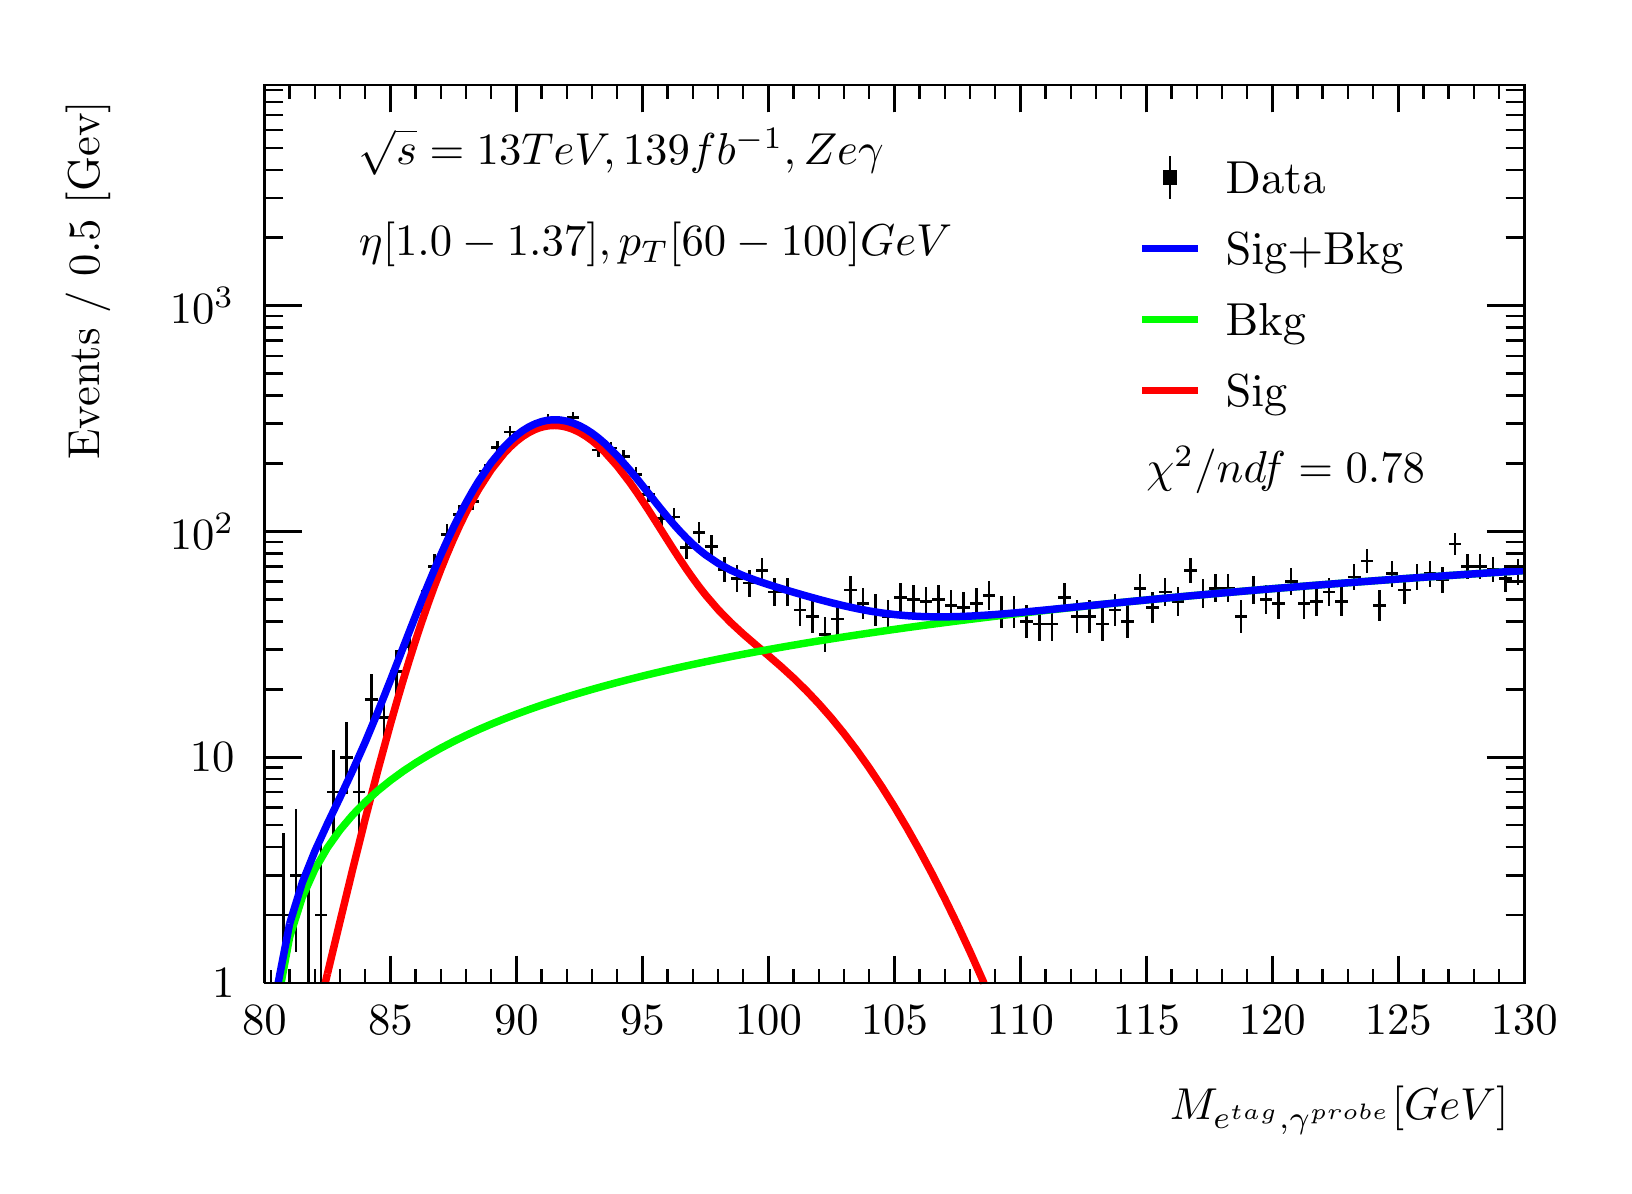
\begin{tikzpicture}
\pgfdeclareplotmark{cross} {
\pgfpathmoveto{\pgfpoint{-0.3\pgfplotmarksize}{\pgfplotmarksize}}
\pgfpathlineto{\pgfpoint{+0.3\pgfplotmarksize}{\pgfplotmarksize}}
\pgfpathlineto{\pgfpoint{+0.3\pgfplotmarksize}{0.3\pgfplotmarksize}}
\pgfpathlineto{\pgfpoint{+1\pgfplotmarksize}{0.3\pgfplotmarksize}}
\pgfpathlineto{\pgfpoint{+1\pgfplotmarksize}{-0.3\pgfplotmarksize}}
\pgfpathlineto{\pgfpoint{+0.3\pgfplotmarksize}{-0.3\pgfplotmarksize}}
\pgfpathlineto{\pgfpoint{+0.3\pgfplotmarksize}{-1.\pgfplotmarksize}}
\pgfpathlineto{\pgfpoint{-0.3\pgfplotmarksize}{-1.\pgfplotmarksize}}
\pgfpathlineto{\pgfpoint{-0.3\pgfplotmarksize}{-0.3\pgfplotmarksize}}
\pgfpathlineto{\pgfpoint{-1.\pgfplotmarksize}{-0.3\pgfplotmarksize}}
\pgfpathlineto{\pgfpoint{-1.\pgfplotmarksize}{0.3\pgfplotmarksize}}
\pgfpathlineto{\pgfpoint{-0.3\pgfplotmarksize}{0.3\pgfplotmarksize}}
\pgfpathclose
\pgfusepathqstroke
}
\pgfdeclareplotmark{cross*} {
\pgfpathmoveto{\pgfpoint{-0.3\pgfplotmarksize}{\pgfplotmarksize}}
\pgfpathlineto{\pgfpoint{+0.3\pgfplotmarksize}{\pgfplotmarksize}}
\pgfpathlineto{\pgfpoint{+0.3\pgfplotmarksize}{0.3\pgfplotmarksize}}
\pgfpathlineto{\pgfpoint{+1\pgfplotmarksize}{0.3\pgfplotmarksize}}
\pgfpathlineto{\pgfpoint{+1\pgfplotmarksize}{-0.3\pgfplotmarksize}}
\pgfpathlineto{\pgfpoint{+0.3\pgfplotmarksize}{-0.3\pgfplotmarksize}}
\pgfpathlineto{\pgfpoint{+0.3\pgfplotmarksize}{-1.\pgfplotmarksize}}
\pgfpathlineto{\pgfpoint{-0.3\pgfplotmarksize}{-1.\pgfplotmarksize}}
\pgfpathlineto{\pgfpoint{-0.3\pgfplotmarksize}{-0.3\pgfplotmarksize}}
\pgfpathlineto{\pgfpoint{-1.\pgfplotmarksize}{-0.3\pgfplotmarksize}}
\pgfpathlineto{\pgfpoint{-1.\pgfplotmarksize}{0.3\pgfplotmarksize}}
\pgfpathlineto{\pgfpoint{-0.3\pgfplotmarksize}{0.3\pgfplotmarksize}}
\pgfpathclose
\pgfusepathqfillstroke
}
\pgfdeclareplotmark{newstar} {
\pgfpathmoveto{\pgfqpoint{0pt}{\pgfplotmarksize}}
\pgfpathlineto{\pgfqpointpolar{44}{0.5\pgfplotmarksize}}
\pgfpathlineto{\pgfqpointpolar{18}{\pgfplotmarksize}}
\pgfpathlineto{\pgfqpointpolar{-20}{0.5\pgfplotmarksize}}
\pgfpathlineto{\pgfqpointpolar{-54}{\pgfplotmarksize}}
\pgfpathlineto{\pgfqpointpolar{-90}{0.5\pgfplotmarksize}}
\pgfpathlineto{\pgfqpointpolar{234}{\pgfplotmarksize}}
\pgfpathlineto{\pgfqpointpolar{198}{0.5\pgfplotmarksize}}
\pgfpathlineto{\pgfqpointpolar{162}{\pgfplotmarksize}}
\pgfpathlineto{\pgfqpointpolar{134}{0.5\pgfplotmarksize}}
\pgfpathclose
\pgfusepathqstroke
}
\pgfdeclareplotmark{newstar*} {
\pgfpathmoveto{\pgfqpoint{0pt}{\pgfplotmarksize}}
\pgfpathlineto{\pgfqpointpolar{44}{0.5\pgfplotmarksize}}
\pgfpathlineto{\pgfqpointpolar{18}{\pgfplotmarksize}}
\pgfpathlineto{\pgfqpointpolar{-20}{0.5\pgfplotmarksize}}
\pgfpathlineto{\pgfqpointpolar{-54}{\pgfplotmarksize}}
\pgfpathlineto{\pgfqpointpolar{-90}{0.5\pgfplotmarksize}}
\pgfpathlineto{\pgfqpointpolar{234}{\pgfplotmarksize}}
\pgfpathlineto{\pgfqpointpolar{198}{0.5\pgfplotmarksize}}
\pgfpathlineto{\pgfqpointpolar{162}{\pgfplotmarksize}}
\pgfpathlineto{\pgfqpointpolar{134}{0.5\pgfplotmarksize}}
\pgfpathclose
\pgfusepathqfillstroke
}
\definecolor{c}{rgb}{1,1,1};
\draw [color=c, fill=c] (0,0) rectangle (20,14.4361);
\draw [color=c, fill=c] (3,2.30977) rectangle (19,13.7143);
\definecolor{c}{rgb}{0,0,0};
\draw [c,line width=0.9] (3,2.30977) -- (3,13.7143) -- (19,13.7143) -- (19,2.30977) -- (3,2.30977);
\definecolor{c}{rgb}{1,1,1};
\draw [color=c, fill=c] (3,2.30977) rectangle (19,13.7143);
\definecolor{c}{rgb}{0,0,0};
\draw [c,line width=0.9] (3,2.30977) -- (3,13.7143) -- (19,13.7143) -- (19,2.30977) -- (3,2.30977);
\draw [c,line width=0.9] (3,2.30977) -- (19,2.30977);
\draw [c,line width=0.9] (3,2.65624) -- (3,2.30977);
\draw [c,line width=0.9] (3.32,2.48301) -- (3.32,2.30977);
\draw [c,line width=0.9] (3.64,2.48301) -- (3.64,2.30977);
\draw [c,line width=0.9] (3.96,2.48301) -- (3.96,2.30977);
\draw [c,line width=0.9] (4.28,2.48301) -- (4.28,2.30977);
\draw [c,line width=0.9] (4.6,2.65624) -- (4.6,2.30977);
\draw [c,line width=0.9] (4.92,2.48301) -- (4.92,2.30977);
\draw [c,line width=0.9] (5.24,2.48301) -- (5.24,2.30977);
\draw [c,line width=0.9] (5.56,2.48301) -- (5.56,2.30977);
\draw [c,line width=0.9] (5.88,2.48301) -- (5.88,2.30977);
\draw [c,line width=0.9] (6.2,2.65624) -- (6.2,2.30977);
\draw [c,line width=0.9] (6.52,2.48301) -- (6.52,2.30977);
\draw [c,line width=0.9] (6.84,2.48301) -- (6.84,2.30977);
\draw [c,line width=0.9] (7.16,2.48301) -- (7.16,2.30977);
\draw [c,line width=0.9] (7.48,2.48301) -- (7.48,2.30977);
\draw [c,line width=0.9] (7.8,2.65624) -- (7.8,2.30977);
\draw [c,line width=0.9] (8.12,2.48301) -- (8.12,2.30977);
\draw [c,line width=0.9] (8.44,2.48301) -- (8.44,2.30977);
\draw [c,line width=0.9] (8.76,2.48301) -- (8.76,2.30977);
\draw [c,line width=0.9] (9.08,2.48301) -- (9.08,2.30977);
\draw [c,line width=0.9] (9.4,2.65624) -- (9.4,2.30977);
\draw [c,line width=0.9] (9.72,2.48301) -- (9.72,2.30977);
\draw [c,line width=0.9] (10.04,2.48301) -- (10.04,2.30977);
\draw [c,line width=0.9] (10.36,2.48301) -- (10.36,2.30977);
\draw [c,line width=0.9] (10.68,2.48301) -- (10.68,2.30977);
\draw [c,line width=0.9] (11,2.65624) -- (11,2.30977);
\draw [c,line width=0.9] (11.32,2.48301) -- (11.32,2.30977);
\draw [c,line width=0.9] (11.64,2.48301) -- (11.64,2.30977);
\draw [c,line width=0.9] (11.96,2.48301) -- (11.96,2.30977);
\draw [c,line width=0.9] (12.28,2.48301) -- (12.28,2.30977);
\draw [c,line width=0.9] (12.6,2.65624) -- (12.6,2.30977);
\draw [c,line width=0.9] (12.92,2.48301) -- (12.92,2.30977);
\draw [c,line width=0.9] (13.24,2.48301) -- (13.24,2.30977);
\draw [c,line width=0.9] (13.56,2.48301) -- (13.56,2.30977);
\draw [c,line width=0.9] (13.88,2.48301) -- (13.88,2.30977);
\draw [c,line width=0.9] (14.2,2.65624) -- (14.2,2.30977);
\draw [c,line width=0.9] (14.52,2.48301) -- (14.52,2.30977);
\draw [c,line width=0.9] (14.84,2.48301) -- (14.84,2.30977);
\draw [c,line width=0.9] (15.16,2.48301) -- (15.16,2.30977);
\draw [c,line width=0.9] (15.48,2.48301) -- (15.48,2.30977);
\draw [c,line width=0.9] (15.8,2.65624) -- (15.8,2.30977);
\draw [c,line width=0.9] (16.12,2.48301) -- (16.12,2.30977);
\draw [c,line width=0.9] (16.44,2.48301) -- (16.44,2.30977);
\draw [c,line width=0.9] (16.76,2.48301) -- (16.76,2.30977);
\draw [c,line width=0.9] (17.08,2.48301) -- (17.08,2.30977);
\draw [c,line width=0.9] (17.4,2.65624) -- (17.4,2.30977);
\draw [c,line width=0.9] (17.72,2.48301) -- (17.72,2.30977);
\draw [c,line width=0.9] (18.04,2.48301) -- (18.04,2.30977);
\draw [c,line width=0.9] (18.36,2.48301) -- (18.36,2.30977);
\draw [c,line width=0.9] (18.68,2.48301) -- (18.68,2.30977);
\draw [c,line width=0.9] (19,2.65624) -- (19,2.30977);
\draw [anchor=base] (3,1.66015) node[scale=1.61424, color=c, rotate=0]{80};
\draw [anchor=base] (4.6,1.66015) node[scale=1.61424, color=c, rotate=0]{85};
\draw [anchor=base] (6.2,1.66015) node[scale=1.61424, color=c, rotate=0]{90};
\draw [anchor=base] (7.8,1.66015) node[scale=1.61424, color=c, rotate=0]{95};
\draw [anchor=base] (9.4,1.66015) node[scale=1.61424, color=c, rotate=0]{100};
\draw [anchor=base] (11,1.66015) node[scale=1.61424, color=c, rotate=0]{105};
\draw [anchor=base] (12.6,1.66015) node[scale=1.61424, color=c, rotate=0]{110};
\draw [anchor=base] (14.2,1.66015) node[scale=1.61424, color=c, rotate=0]{115};
\draw [anchor=base] (15.8,1.66015) node[scale=1.61424, color=c, rotate=0]{120};
\draw [anchor=base] (17.4,1.66015) node[scale=1.61424, color=c, rotate=0]{125};
\draw [anchor=base] (19,1.66015) node[scale=1.61424, color=c, rotate=0]{130};
\draw [anchor= east] (19,0.692932) node[scale=1.61424, color=c, rotate=0]{$M_{e^{tag}, \gamma^{probe}}  [GeV]$};
\draw [c,line width=0.9] (3,13.7143) -- (19,13.7143);
\draw [c,line width=0.9] (3,13.3678) -- (3,13.7143);
\draw [c,line width=0.9] (3.32,13.5411) -- (3.32,13.7143);
\draw [c,line width=0.9] (3.64,13.5411) -- (3.64,13.7143);
\draw [c,line width=0.9] (3.96,13.5411) -- (3.96,13.7143);
\draw [c,line width=0.9] (4.28,13.5411) -- (4.28,13.7143);
\draw [c,line width=0.9] (4.6,13.3678) -- (4.6,13.7143);
\draw [c,line width=0.9] (4.92,13.5411) -- (4.92,13.7143);
\draw [c,line width=0.9] (5.24,13.5411) -- (5.24,13.7143);
\draw [c,line width=0.9] (5.56,13.5411) -- (5.56,13.7143);
\draw [c,line width=0.9] (5.88,13.5411) -- (5.88,13.7143);
\draw [c,line width=0.9] (6.2,13.3678) -- (6.2,13.7143);
\draw [c,line width=0.9] (6.52,13.5411) -- (6.52,13.7143);
\draw [c,line width=0.9] (6.84,13.5411) -- (6.84,13.7143);
\draw [c,line width=0.9] (7.16,13.5411) -- (7.16,13.7143);
\draw [c,line width=0.9] (7.48,13.5411) -- (7.48,13.7143);
\draw [c,line width=0.9] (7.8,13.3678) -- (7.8,13.7143);
\draw [c,line width=0.9] (8.12,13.5411) -- (8.12,13.7143);
\draw [c,line width=0.9] (8.44,13.5411) -- (8.44,13.7143);
\draw [c,line width=0.9] (8.76,13.5411) -- (8.76,13.7143);
\draw [c,line width=0.9] (9.08,13.5411) -- (9.08,13.7143);
\draw [c,line width=0.9] (9.4,13.3678) -- (9.4,13.7143);
\draw [c,line width=0.9] (9.72,13.5411) -- (9.72,13.7143);
\draw [c,line width=0.9] (10.04,13.5411) -- (10.04,13.7143);
\draw [c,line width=0.9] (10.36,13.5411) -- (10.36,13.7143);
\draw [c,line width=0.9] (10.68,13.5411) -- (10.68,13.7143);
\draw [c,line width=0.9] (11,13.3678) -- (11,13.7143);
\draw [c,line width=0.9] (11.32,13.5411) -- (11.32,13.7143);
\draw [c,line width=0.9] (11.64,13.5411) -- (11.64,13.7143);
\draw [c,line width=0.9] (11.96,13.5411) -- (11.96,13.7143);
\draw [c,line width=0.9] (12.28,13.5411) -- (12.28,13.7143);
\draw [c,line width=0.9] (12.6,13.3678) -- (12.6,13.7143);
\draw [c,line width=0.9] (12.92,13.5411) -- (12.92,13.7143);
\draw [c,line width=0.9] (13.24,13.5411) -- (13.24,13.7143);
\draw [c,line width=0.9] (13.56,13.5411) -- (13.56,13.7143);
\draw [c,line width=0.9] (13.88,13.5411) -- (13.88,13.7143);
\draw [c,line width=0.9] (14.2,13.3678) -- (14.2,13.7143);
\draw [c,line width=0.9] (14.52,13.5411) -- (14.52,13.7143);
\draw [c,line width=0.9] (14.84,13.5411) -- (14.84,13.7143);
\draw [c,line width=0.9] (15.16,13.5411) -- (15.16,13.7143);
\draw [c,line width=0.9] (15.48,13.5411) -- (15.48,13.7143);
\draw [c,line width=0.9] (15.8,13.3678) -- (15.8,13.7143);
\draw [c,line width=0.9] (16.12,13.5411) -- (16.12,13.7143);
\draw [c,line width=0.9] (16.44,13.5411) -- (16.44,13.7143);
\draw [c,line width=0.9] (16.76,13.5411) -- (16.76,13.7143);
\draw [c,line width=0.9] (17.08,13.5411) -- (17.08,13.7143);
\draw [c,line width=0.9] (17.4,13.3678) -- (17.4,13.7143);
\draw [c,line width=0.9] (17.72,13.5411) -- (17.72,13.7143);
\draw [c,line width=0.9] (18.04,13.5411) -- (18.04,13.7143);
\draw [c,line width=0.9] (18.36,13.5411) -- (18.36,13.7143);
\draw [c,line width=0.9] (18.68,13.5411) -- (18.68,13.7143);
\draw [c,line width=0.9] (19,13.3678) -- (19,13.7143);
\draw [c,line width=0.9] (3,2.30977) -- (3,13.7143);
\draw [c,line width=0.9] (3.474,2.30978) -- (3,2.30978);
\draw [anchor= east] (2.82,2.30978) node[scale=1.61424, color=c, rotate=0]{1};
\draw [c,line width=0.9] (3.237,3.17298) -- (3,3.17298);
\draw [c,line width=0.9] (3.237,3.67792) -- (3,3.67792);
\draw [c,line width=0.9] (3.237,4.03618) -- (3,4.03618);
\draw [c,line width=0.9] (3.237,4.31407) -- (3,4.31407);
\draw [c,line width=0.9] (3.237,4.54112) -- (3,4.54112);
\draw [c,line width=0.9] (3.237,4.73309) -- (3,4.73309);
\draw [c,line width=0.9] (3.237,4.89938) -- (3,4.89938);
\draw [c,line width=0.9] (3.237,5.04606) -- (3,5.04606);
\draw [c,line width=0.9] (3.474,5.17727) -- (3,5.17727);
\draw [anchor= east] (2.82,5.17727) node[scale=1.61424, color=c, rotate=0]{10};
\draw [c,line width=0.9] (3.237,6.04047) -- (3,6.04047);
\draw [c,line width=0.9] (3.237,6.54541) -- (3,6.54541);
\draw [c,line width=0.9] (3.237,6.90367) -- (3,6.90367);
\draw [c,line width=0.9] (3.237,7.18156) -- (3,7.18156);
\draw [c,line width=0.9] (3.237,7.40861) -- (3,7.40861);
\draw [c,line width=0.9] (3.237,7.60058) -- (3,7.60058);
\draw [c,line width=0.9] (3.237,7.76687) -- (3,7.76687);
\draw [c,line width=0.9] (3.237,7.91355) -- (3,7.91355);
\draw [c,line width=0.9] (3.474,8.04476) -- (3,8.04476);
\draw [anchor= east] (2.82,8.04476) node[scale=1.61424, color=c, rotate=0]{$10^{2}$};
\draw [c,line width=0.9] (3.237,8.90796) -- (3,8.90796);
\draw [c,line width=0.9] (3.237,9.4129) -- (3,9.4129);
\draw [c,line width=0.9] (3.237,9.77116) -- (3,9.77116);
\draw [c,line width=0.9] (3.237,10.049) -- (3,10.049);
\draw [c,line width=0.9] (3.237,10.2761) -- (3,10.2761);
\draw [c,line width=0.9] (3.237,10.4681) -- (3,10.4681);
\draw [c,line width=0.9] (3.237,10.6344) -- (3,10.6344);
\draw [c,line width=0.9] (3.237,10.781) -- (3,10.781);
\draw [c,line width=0.9] (3.474,10.9122) -- (3,10.9122);
\draw [anchor= east] (2.82,10.9122) node[scale=1.61424, color=c, rotate=0]{$10^{3}$};
\draw [c,line width=0.9] (3.237,11.7754) -- (3,11.7754);
\draw [c,line width=0.9] (3.237,12.2804) -- (3,12.2804);
\draw [c,line width=0.9] (3.237,12.6386) -- (3,12.6386);
\draw [c,line width=0.9] (3.237,12.9165) -- (3,12.9165);
\draw [c,line width=0.9] (3.237,13.1436) -- (3,13.1436);
\draw [c,line width=0.9] (3.237,13.3356) -- (3,13.3356);
\draw [c,line width=0.9] (3.237,13.5018) -- (3,13.5018);
\draw [c,line width=0.9] (3.237,13.6485) -- (3,13.6485);
\draw [anchor= east] (0.76,13.7143) node[scale=1.61424, color=c, rotate=90]{Events / 0.5 [Gev]};
\draw [c,line width=0.9] (19,2.30977) -- (19,13.7143);
\draw [c,line width=0.9] (18.526,2.30978) -- (19,2.30978);
\draw [c,line width=0.9] (18.763,3.17298) -- (19,3.17298);
\draw [c,line width=0.9] (18.763,3.67792) -- (19,3.67792);
\draw [c,line width=0.9] (18.763,4.03618) -- (19,4.03618);
\draw [c,line width=0.9] (18.763,4.31407) -- (19,4.31407);
\draw [c,line width=0.9] (18.763,4.54112) -- (19,4.54112);
\draw [c,line width=0.9] (18.763,4.73309) -- (19,4.73309);
\draw [c,line width=0.9] (18.763,4.89938) -- (19,4.89938);
\draw [c,line width=0.9] (18.763,5.04606) -- (19,5.04606);
\draw [c,line width=0.9] (18.526,5.17727) -- (19,5.17727);
\draw [c,line width=0.9] (18.763,6.04047) -- (19,6.04047);
\draw [c,line width=0.9] (18.763,6.54541) -- (19,6.54541);
\draw [c,line width=0.9] (18.763,6.90367) -- (19,6.90367);
\draw [c,line width=0.9] (18.763,7.18156) -- (19,7.18156);
\draw [c,line width=0.9] (18.763,7.40861) -- (19,7.40861);
\draw [c,line width=0.9] (18.763,7.60058) -- (19,7.60058);
\draw [c,line width=0.9] (18.763,7.76687) -- (19,7.76687);
\draw [c,line width=0.9] (18.763,7.91355) -- (19,7.91355);
\draw [c,line width=0.9] (18.526,8.04476) -- (19,8.04476);
\draw [c,line width=0.9] (18.763,8.90796) -- (19,8.90796);
\draw [c,line width=0.9] (18.763,9.4129) -- (19,9.4129);
\draw [c,line width=0.9] (18.763,9.77116) -- (19,9.77116);
\draw [c,line width=0.9] (18.763,10.049) -- (19,10.049);
\draw [c,line width=0.9] (18.763,10.2761) -- (19,10.2761);
\draw [c,line width=0.9] (18.763,10.4681) -- (19,10.4681);
\draw [c,line width=0.9] (18.763,10.6344) -- (19,10.6344);
\draw [c,line width=0.9] (18.763,10.781) -- (19,10.781);
\draw [c,line width=0.9] (18.526,10.9122) -- (19,10.9122);
\draw [c,line width=0.9] (18.763,11.7754) -- (19,11.7754);
\draw [c,line width=0.9] (18.763,12.2804) -- (19,12.2804);
\draw [c,line width=0.9] (18.763,12.6386) -- (19,12.6386);
\draw [c,line width=0.9] (18.763,12.9165) -- (19,12.9165);
\draw [c,line width=0.9] (18.763,13.1436) -- (19,13.1436);
\draw [c,line width=0.9] (18.763,13.3356) -- (19,13.3356);
\draw [c,line width=0.9] (18.763,13.5018) -- (19,13.5018);
\draw [c,line width=0.9] (18.763,13.6485) -- (19,13.6485);
\draw [c,line width=0.9] (3.08,2.30977) -- (3,2.30977);
\draw [c,line width=0.9] (3,2.30977) -- (3,2.30977);
\draw [c,line width=0.9] (3.08,2.30977) -- (3.16,2.30977);
\draw [c,line width=0.9] (3.16,2.30977) -- (3.16,2.30977);
\draw [c,line width=0.9] (3.08,2.30977) -- (3.08,2.48152);
\draw [c,line width=0.9] (3.08,2.48152) -- (3.08,2.48152);
\draw [c,line width=0.9] (3.24,3.17298) -- (3.16,3.17298);
\draw [c,line width=0.9] (3.16,3.17298) -- (3.16,3.17298);
\draw [c,line width=0.9] (3.24,3.17298) -- (3.32,3.17298);
\draw [c,line width=0.9] (3.32,3.17298) -- (3.32,3.17298);
\draw [c,line width=0.9] (3.24,3.17298) -- (3.24,4.22043);
\draw [c,line width=0.9] (3.24,4.22043) -- (3.24,4.22043);
\draw [c,line width=0.9] (3.24,3.17298) -- (3.24,2.30977);
\draw [c,line width=0.9] (3.24,2.30977) -- (3.24,2.30977);
\draw [c,line width=0.9] (3.4,3.67792) -- (3.32,3.67792);
\draw [c,line width=0.9] (3.32,3.67792) -- (3.32,3.67792);
\draw [c,line width=0.9] (3.4,3.67792) -- (3.48,3.67792);
\draw [c,line width=0.9] (3.48,3.67792) -- (3.48,3.67792);
\draw [c,line width=0.9] (3.4,3.67792) -- (3.4,4.52402);
\draw [c,line width=0.9] (3.4,4.52402) -- (3.4,4.52402);
\draw [c,line width=0.9] (3.4,3.67792) -- (3.4,2.69936);
\draw [c,line width=0.9] (3.4,2.69936) -- (3.4,2.69936);
\draw [c,line width=0.9] (3.56,2.30977) -- (3.48,2.30977);
\draw [c,line width=0.9] (3.48,2.30977) -- (3.48,2.30977);
\draw [c,line width=0.9] (3.56,2.30977) -- (3.64,2.30977);
\draw [c,line width=0.9] (3.64,2.30977) -- (3.64,2.30977);
\draw [c,line width=0.9] (3.56,2.30977) -- (3.56,3.79643);
\draw [c,line width=0.9] (3.56,3.79643) -- (3.56,3.79643);
\draw [c,line width=0.9] (3.72,3.17298) -- (3.64,3.17298);
\draw [c,line width=0.9] (3.64,3.17298) -- (3.64,3.17298);
\draw [c,line width=0.9] (3.72,3.17298) -- (3.8,3.17298);
\draw [c,line width=0.9] (3.8,3.17298) -- (3.8,3.17298);
\draw [c,line width=0.9] (3.72,3.17298) -- (3.72,4.22043);
\draw [c,line width=0.9] (3.72,4.22043) -- (3.72,4.22043);
\draw [c,line width=0.9] (3.72,3.17298) -- (3.72,2.30977);
\draw [c,line width=0.9] (3.72,2.30977) -- (3.72,2.30977);
\draw [c,line width=0.9] (3.88,4.73309) -- (3.8,4.73309);
\draw [c,line width=0.9] (3.8,4.73309) -- (3.8,4.73309);
\draw [c,line width=0.9] (3.88,4.73309) -- (3.96,4.73309);
\draw [c,line width=0.9] (3.96,4.73309) -- (3.96,4.73309);
\draw [c,line width=0.9] (3.88,4.73309) -- (3.88,5.26968);
\draw [c,line width=0.9] (3.88,5.26968) -- (3.88,5.26968);
\draw [c,line width=0.9] (3.88,4.73309) -- (3.88,4.1601);
\draw [c,line width=0.9] (3.88,4.1601) -- (3.88,4.1601);
\draw [c,line width=0.9] (4.04,5.17727) -- (3.96,5.17727);
\draw [c,line width=0.9] (3.96,5.17727) -- (3.96,5.17727);
\draw [c,line width=0.9] (4.04,5.17727) -- (4.12,5.17727);
\draw [c,line width=0.9] (4.12,5.17727) -- (4.12,5.17727);
\draw [c,line width=0.9] (4.04,5.17727) -- (4.04,5.61981);
\draw [c,line width=0.9] (4.04,5.61981) -- (4.04,5.61981);
\draw [c,line width=0.9] (4.04,5.17727) -- (4.04,4.7136);
\draw [c,line width=0.9] (4.04,4.7136) -- (4.04,4.7136);
\draw [c,line width=0.9] (4.2,4.73309) -- (4.12,4.73309);
\draw [c,line width=0.9] (4.12,4.73309) -- (4.12,4.73309);
\draw [c,line width=0.9] (4.2,4.73309) -- (4.28,4.73309);
\draw [c,line width=0.9] (4.28,4.73309) -- (4.28,4.73309);
\draw [c,line width=0.9] (4.2,4.73309) -- (4.2,5.26968);
\draw [c,line width=0.9] (4.2,5.26968) -- (4.2,5.26968);
\draw [c,line width=0.9] (4.2,4.73309) -- (4.2,4.1601);
\draw [c,line width=0.9] (4.2,4.1601) -- (4.2,4.1601);
\draw [c,line width=0.9] (4.36,5.90926) -- (4.28,5.90926);
\draw [c,line width=0.9] (4.28,5.90926) -- (4.28,5.90926);
\draw [c,line width=0.9] (4.36,5.90926) -- (4.44,5.90926);
\draw [c,line width=0.9] (4.44,5.90926) -- (4.44,5.90926);
\draw [c,line width=0.9] (4.36,5.90926) -- (4.36,6.23178);
\draw [c,line width=0.9] (4.36,6.23178) -- (4.36,6.23178);
\draw [c,line width=0.9] (4.36,5.90926) -- (4.36,5.57811);
\draw [c,line width=0.9] (4.36,5.57811) -- (4.36,5.57811);
\draw [c,line width=0.9] (4.52,5.68221) -- (4.44,5.68221);
\draw [c,line width=0.9] (4.44,5.68221) -- (4.44,5.68221);
\draw [c,line width=0.9] (4.52,5.68221) -- (4.6,5.68221);
\draw [c,line width=0.9] (4.6,5.68221) -- (4.6,5.68221);
\draw [c,line width=0.9] (4.52,5.68221) -- (4.52,6.03789);
\draw [c,line width=0.9] (4.52,6.03789) -- (4.52,6.03789);
\draw [c,line width=0.9] (4.52,5.68221) -- (4.52,5.31513);
\draw [c,line width=0.9] (4.52,5.31513) -- (4.52,5.31513);
\draw [c,line width=0.9] (4.68,6.26752) -- (4.6,6.26752);
\draw [c,line width=0.9] (4.6,6.26752) -- (4.6,6.26752);
\draw [c,line width=0.9] (4.68,6.26752) -- (4.76,6.26752);
\draw [c,line width=0.9] (4.76,6.26752) -- (4.76,6.26752);
\draw [c,line width=0.9] (4.68,6.26752) -- (4.68,6.54403);
\draw [c,line width=0.9] (4.68,6.54403) -- (4.68,6.54403);
\draw [c,line width=0.9] (4.68,6.26752) -- (4.68,5.98543);
\draw [c,line width=0.9] (4.68,5.98543) -- (4.68,5.98543);
\draw [c,line width=0.9] (4.84,6.58624) -- (4.76,6.58624);
\draw [c,line width=0.9] (4.76,6.58624) -- (4.76,6.58624);
\draw [c,line width=0.9] (4.84,6.58624) -- (4.92,6.58624);
\draw [c,line width=0.9] (4.92,6.58624) -- (4.92,6.58624);
\draw [c,line width=0.9] (4.84,6.58624) -- (4.84,6.82752);
\draw [c,line width=0.9] (4.84,6.82752) -- (4.84,6.82752);
\draw [c,line width=0.9] (4.84,6.58624) -- (4.84,6.34118);
\draw [c,line width=0.9] (4.84,6.34118) -- (4.84,6.34118);
\draw [c,line width=0.9] (5,7.1045) -- (4.92,7.1045);
\draw [c,line width=0.9] (4.92,7.1045) -- (4.92,7.1045);
\draw [c,line width=0.9] (5,7.1045) -- (5.08,7.1045);
\draw [c,line width=0.9] (5.08,7.1045) -- (5.08,7.1045);
\draw [c,line width=0.9] (5,7.1045) -- (5,7.29808);
\draw [c,line width=0.9] (5,7.29808) -- (5,7.29808);
\draw [c,line width=0.9] (5,7.1045) -- (5,6.90891);
\draw [c,line width=0.9] (5,6.90891) -- (5,6.90891);
\draw [c,line width=0.9] (5.16,7.60058) -- (5.08,7.60058);
\draw [c,line width=0.9] (5.08,7.60058) -- (5.08,7.60058);
\draw [c,line width=0.9] (5.16,7.60058) -- (5.24,7.60058);
\draw [c,line width=0.9] (5.24,7.60058) -- (5.24,7.60058);
\draw [c,line width=0.9] (5.16,7.60058) -- (5.16,7.75759);
\draw [c,line width=0.9] (5.16,7.75759) -- (5.16,7.75759);
\draw [c,line width=0.9] (5.16,7.60058) -- (5.16,7.44246);
\draw [c,line width=0.9] (5.16,7.44246) -- (5.16,7.44246);
\draw [c,line width=0.9] (5.32,8.00682) -- (5.24,8.00682);
\draw [c,line width=0.9] (5.24,8.00682) -- (5.24,8.00682);
\draw [c,line width=0.9] (5.32,8.00682) -- (5.4,8.00682);
\draw [c,line width=0.9] (5.4,8.00682) -- (5.4,8.00682);
\draw [c,line width=0.9] (5.32,8.00682) -- (5.32,8.13925);
\draw [c,line width=0.9] (5.32,8.13925) -- (5.32,8.13925);
\draw [c,line width=0.9] (5.32,8.00682) -- (5.32,7.87373);
\draw [c,line width=0.9] (5.32,7.87373) -- (5.32,7.87373);
\draw [c,line width=0.9] (5.48,8.26139) -- (5.4,8.26139);
\draw [c,line width=0.9] (5.4,8.26139) -- (5.4,8.26139);
\draw [c,line width=0.9] (5.48,8.26139) -- (5.56,8.26139);
\draw [c,line width=0.9] (5.56,8.26139) -- (5.56,8.26139);
\draw [c,line width=0.9] (5.48,8.26139) -- (5.48,8.37551);
\draw [c,line width=0.9] (5.48,8.37551) -- (5.48,8.37551);
\draw [c,line width=0.9] (5.48,8.26139) -- (5.48,8.14727);
\draw [c,line width=0.9] (5.48,8.14727) -- (5.48,8.14727);
\draw [c,line width=0.9] (5.64,8.42768) -- (5.56,8.42768);
\draw [c,line width=0.9] (5.56,8.42768) -- (5.56,8.42768);
\draw [c,line width=0.9] (5.64,8.42768) -- (5.72,8.42768);
\draw [c,line width=0.9] (5.72,8.42768) -- (5.72,8.42768);
\draw [c,line width=0.9] (5.64,8.42768) -- (5.64,8.53443);
\draw [c,line width=0.9] (5.64,8.53443) -- (5.64,8.53443);
\draw [c,line width=0.9] (5.64,8.42768) -- (5.64,8.32092);
\draw [c,line width=0.9] (5.64,8.32092) -- (5.64,8.32092);
\draw [c,line width=0.9] (5.8,8.81087) -- (5.72,8.81087);
\draw [c,line width=0.9] (5.72,8.81087) -- (5.72,8.81087);
\draw [c,line width=0.9] (5.8,8.81087) -- (5.88,8.81087);
\draw [c,line width=0.9] (5.88,8.81087) -- (5.88,8.81087);
\draw [c,line width=0.9] (5.8,8.81087) -- (5.8,8.90241);
\draw [c,line width=0.9] (5.8,8.90241) -- (5.8,8.90241);
\draw [c,line width=0.9] (5.8,8.81087) -- (5.8,8.71933);
\draw [c,line width=0.9] (5.8,8.71933) -- (5.8,8.71933);
\draw [c,line width=0.9] (5.96,9.11408) -- (5.88,9.11408);
\draw [c,line width=0.9] (5.88,9.11408) -- (5.88,9.11408);
\draw [c,line width=0.9] (5.96,9.11408) -- (6.04,9.11408);
\draw [c,line width=0.9] (6.04,9.11408) -- (6.04,9.11408);
\draw [c,line width=0.9] (5.96,9.11408) -- (5.96,9.19513);
\draw [c,line width=0.9] (5.96,9.19513) -- (5.96,9.19513);
\draw [c,line width=0.9] (5.96,9.11408) -- (5.96,9.03303);
\draw [c,line width=0.9] (5.96,9.03303) -- (5.96,9.03303);
\draw [c,line width=0.9] (6.12,9.30906) -- (6.04,9.30906);
\draw [c,line width=0.9] (6.04,9.30906) -- (6.04,9.30906);
\draw [c,line width=0.9] (6.12,9.30906) -- (6.2,9.30906);
\draw [c,line width=0.9] (6.2,9.30906) -- (6.2,9.30906);
\draw [c,line width=0.9] (6.12,9.30906) -- (6.12,9.38401);
\draw [c,line width=0.9] (6.12,9.38401) -- (6.12,9.38401);
\draw [c,line width=0.9] (6.12,9.30906) -- (6.12,9.23411);
\draw [c,line width=0.9] (6.12,9.23411) -- (6.12,9.23411);
\draw [c,line width=0.9] (6.28,9.29088) -- (6.2,9.29088);
\draw [c,line width=0.9] (6.2,9.29088) -- (6.2,9.29088);
\draw [c,line width=0.9] (6.28,9.29088) -- (6.36,9.29088);
\draw [c,line width=0.9] (6.36,9.29088) -- (6.36,9.29088);
\draw [c,line width=0.9] (6.28,9.29088) -- (6.28,9.36638);
\draw [c,line width=0.9] (6.28,9.36638) -- (6.28,9.36638);
\draw [c,line width=0.9] (6.28,9.29088) -- (6.28,9.21538);
\draw [c,line width=0.9] (6.28,9.21538) -- (6.28,9.21538);
\draw [c,line width=0.9] (6.44,9.37068) -- (6.36,9.37068);
\draw [c,line width=0.9] (6.36,9.37068) -- (6.36,9.37068);
\draw [c,line width=0.9] (6.44,9.37068) -- (6.52,9.37068);
\draw [c,line width=0.9] (6.52,9.37068) -- (6.52,9.37068);
\draw [c,line width=0.9] (6.44,9.37068) -- (6.44,9.4438);
\draw [c,line width=0.9] (6.44,9.4438) -- (6.44,9.4438);
\draw [c,line width=0.9] (6.44,9.37068) -- (6.44,9.29756);
\draw [c,line width=0.9] (6.44,9.29756) -- (6.44,9.29756);
\draw [c,line width=0.9] (6.6,9.46572) -- (6.52,9.46572);
\draw [c,line width=0.9] (6.52,9.46572) -- (6.52,9.46572);
\draw [c,line width=0.9] (6.6,9.46572) -- (6.68,9.46572);
\draw [c,line width=0.9] (6.68,9.46572) -- (6.68,9.46572);
\draw [c,line width=0.9] (6.6,9.46572) -- (6.6,9.53611);
\draw [c,line width=0.9] (6.6,9.53611) -- (6.6,9.53611);
\draw [c,line width=0.9] (6.6,9.46572) -- (6.6,9.39534);
\draw [c,line width=0.9] (6.6,9.39534) -- (6.6,9.39534);
\draw [c,line width=0.9] (6.76,9.4129) -- (6.68,9.4129);
\draw [c,line width=0.9] (6.68,9.4129) -- (6.68,9.4129);
\draw [c,line width=0.9] (6.76,9.4129) -- (6.84,9.4129);
\draw [c,line width=0.9] (6.84,9.4129) -- (6.84,9.4129);
\draw [c,line width=0.9] (6.76,9.4129) -- (6.76,9.48479);
\draw [c,line width=0.9] (6.76,9.48479) -- (6.76,9.48479);
\draw [c,line width=0.9] (6.76,9.4129) -- (6.76,9.34101);
\draw [c,line width=0.9] (6.76,9.34101) -- (6.76,9.34101);
\draw [c,line width=0.9] (6.92,9.48937) -- (6.84,9.48937);
\draw [c,line width=0.9] (6.84,9.48937) -- (6.84,9.48937);
\draw [c,line width=0.9] (6.92,9.48937) -- (7,9.48937);
\draw [c,line width=0.9] (7,9.48937) -- (7,9.48937);
\draw [c,line width=0.9] (6.92,9.48937) -- (6.92,9.55909);
\draw [c,line width=0.9] (6.92,9.55909) -- (6.92,9.55909);
\draw [c,line width=0.9] (6.92,9.48937) -- (6.92,9.41965);
\draw [c,line width=0.9] (6.92,9.41965) -- (6.92,9.41965);
\draw [c,line width=0.9] (7.08,9.31356) -- (7,9.31356);
\draw [c,line width=0.9] (7,9.31356) -- (7,9.31356);
\draw [c,line width=0.9] (7.08,9.31356) -- (7.16,9.31356);
\draw [c,line width=0.9] (7.16,9.31356) -- (7.16,9.31356);
\draw [c,line width=0.9] (7.08,9.31356) -- (7.08,9.38838);
\draw [c,line width=0.9] (7.08,9.38838) -- (7.08,9.38838);
\draw [c,line width=0.9] (7.08,9.31356) -- (7.08,9.23875);
\draw [c,line width=0.9] (7.08,9.23875) -- (7.08,9.23875);
\draw [c,line width=0.9] (7.24,9.07658) -- (7.16,9.07658);
\draw [c,line width=0.9] (7.16,9.07658) -- (7.16,9.07658);
\draw [c,line width=0.9] (7.24,9.07658) -- (7.32,9.07658);
\draw [c,line width=0.9] (7.32,9.07658) -- (7.32,9.07658);
\draw [c,line width=0.9] (7.24,9.07658) -- (7.24,9.15886);
\draw [c,line width=0.9] (7.24,9.15886) -- (7.24,9.15886);
\draw [c,line width=0.9] (7.24,9.07658) -- (7.24,8.9943);
\draw [c,line width=0.9] (7.24,8.9943) -- (7.24,8.9943);
\draw [c,line width=0.9] (7.4,9.10348) -- (7.32,9.10348);
\draw [c,line width=0.9] (7.32,9.10348) -- (7.32,9.10348);
\draw [c,line width=0.9] (7.4,9.10348) -- (7.48,9.10348);
\draw [c,line width=0.9] (7.48,9.10348) -- (7.48,9.10348);
\draw [c,line width=0.9] (7.4,9.10348) -- (7.4,9.18487);
\draw [c,line width=0.9] (7.4,9.18487) -- (7.4,9.18487);
\draw [c,line width=0.9] (7.4,9.10348) -- (7.4,9.02208);
\draw [c,line width=0.9] (7.4,9.02208) -- (7.4,9.02208);
\draw [c,line width=0.9] (7.56,8.99802) -- (7.48,8.99802);
\draw [c,line width=0.9] (7.48,8.99802) -- (7.48,8.99802);
\draw [c,line width=0.9] (7.56,8.99802) -- (7.64,8.99802);
\draw [c,line width=0.9] (7.64,8.99802) -- (7.64,8.99802);
\draw [c,line width=0.9] (7.56,8.99802) -- (7.56,9.08293);
\draw [c,line width=0.9] (7.56,9.08293) -- (7.56,9.08293);
\draw [c,line width=0.9] (7.56,8.99802) -- (7.56,8.91311);
\draw [c,line width=0.9] (7.56,8.91311) -- (7.56,8.91311);
\draw [c,line width=0.9] (7.72,8.76981) -- (7.64,8.76981);
\draw [c,line width=0.9] (7.64,8.76981) -- (7.64,8.76981);
\draw [c,line width=0.9] (7.72,8.76981) -- (7.8,8.76981);
\draw [c,line width=0.9] (7.8,8.76981) -- (7.8,8.76981);
\draw [c,line width=0.9] (7.72,8.76981) -- (7.72,8.86287);
\draw [c,line width=0.9] (7.72,8.86287) -- (7.72,8.86287);
\draw [c,line width=0.9] (7.72,8.76981) -- (7.72,8.67675);
\draw [c,line width=0.9] (7.72,8.67675) -- (7.72,8.67675);
\draw [c,line width=0.9] (7.88,8.51604) -- (7.8,8.51604);
\draw [c,line width=0.9] (7.8,8.51604) -- (7.8,8.51604);
\draw [c,line width=0.9] (7.88,8.51604) -- (7.96,8.51604);
\draw [c,line width=0.9] (7.96,8.51604) -- (7.96,8.51604);
\draw [c,line width=0.9] (7.88,8.51604) -- (7.88,8.61907);
\draw [c,line width=0.9] (7.88,8.61907) -- (7.88,8.61907);
\draw [c,line width=0.9] (7.88,8.51604) -- (7.88,8.413);
\draw [c,line width=0.9] (7.88,8.413) -- (7.88,8.413);
\draw [c,line width=0.9] (8.04,8.20793) -- (7.96,8.20793);
\draw [c,line width=0.9] (7.96,8.20793) -- (7.96,8.20793);
\draw [c,line width=0.9] (8.04,8.20793) -- (8.12,8.20793);
\draw [c,line width=0.9] (8.12,8.20793) -- (8.12,8.20793);
\draw [c,line width=0.9] (8.04,8.20793) -- (8.04,8.32452);
\draw [c,line width=0.9] (8.04,8.32452) -- (8.04,8.32452);
\draw [c,line width=0.9] (8.04,8.20793) -- (8.04,8.09134);
\draw [c,line width=0.9] (8.04,8.09134) -- (8.04,8.09134);
\draw [c,line width=0.9] (8.2,8.22959) -- (8.12,8.22959);
\draw [c,line width=0.9] (8.12,8.22959) -- (8.12,8.22959);
\draw [c,line width=0.9] (8.2,8.22959) -- (8.28,8.22959);
\draw [c,line width=0.9] (8.28,8.22959) -- (8.28,8.22959);
\draw [c,line width=0.9] (8.2,8.22959) -- (8.2,8.34517);
\draw [c,line width=0.9] (8.2,8.34517) -- (8.2,8.34517);
\draw [c,line width=0.9] (8.2,8.22959) -- (8.2,8.114);
\draw [c,line width=0.9] (8.2,8.114) -- (8.2,8.114);
\draw [c,line width=0.9] (8.36,7.84237) -- (8.28,7.84237);
\draw [c,line width=0.9] (8.28,7.84237) -- (8.28,7.84237);
\draw [c,line width=0.9] (8.36,7.84237) -- (8.44,7.84237);
\draw [c,line width=0.9] (8.44,7.84237) -- (8.44,7.84237);
\draw [c,line width=0.9] (8.36,7.84237) -- (8.36,7.98423);
\draw [c,line width=0.9] (8.36,7.98423) -- (8.36,7.98423);
\draw [c,line width=0.9] (8.36,7.84237) -- (8.36,7.69969);
\draw [c,line width=0.9] (8.36,7.69969) -- (8.36,7.69969);
\draw [c,line width=0.9] (8.52,8.03224) -- (8.44,8.03224);
\draw [c,line width=0.9] (8.44,8.03224) -- (8.44,8.03224);
\draw [c,line width=0.9] (8.52,8.03224) -- (8.6,8.03224);
\draw [c,line width=0.9] (8.6,8.03224) -- (8.6,8.03224);
\draw [c,line width=0.9] (8.52,8.03224) -- (8.52,8.16326);
\draw [c,line width=0.9] (8.52,8.16326) -- (8.52,8.16326);
\draw [c,line width=0.9] (8.52,8.03224) -- (8.52,7.90057);
\draw [c,line width=0.9] (8.52,7.90057) -- (8.52,7.90057);
\draw [c,line width=0.9] (8.68,7.85693) -- (8.6,7.85693);
\draw [c,line width=0.9] (8.6,7.85693) -- (8.6,7.85693);
\draw [c,line width=0.9] (8.68,7.85693) -- (8.76,7.85693);
\draw [c,line width=0.9] (8.76,7.85693) -- (8.76,7.85693);
\draw [c,line width=0.9] (8.68,7.85693) -- (8.68,7.99793);
\draw [c,line width=0.9] (8.68,7.99793) -- (8.68,7.99793);
\draw [c,line width=0.9] (8.68,7.85693) -- (8.68,7.71513);
\draw [c,line width=0.9] (8.68,7.71513) -- (8.68,7.71513);
\draw [c,line width=0.9] (8.84,7.56448) -- (8.76,7.56448);
\draw [c,line width=0.9] (8.76,7.56448) -- (8.76,7.56448);
\draw [c,line width=0.9] (8.84,7.56448) -- (8.92,7.56448);
\draw [c,line width=0.9] (8.92,7.56448) -- (8.92,7.56448);
\draw [c,line width=0.9] (8.84,7.56448) -- (8.84,7.7239);
\draw [c,line width=0.9] (8.84,7.7239) -- (8.84,7.7239);
\draw [c,line width=0.9] (8.84,7.56448) -- (8.84,7.40391);
\draw [c,line width=0.9] (8.84,7.40391) -- (8.84,7.40391);
\draw [c,line width=0.9] (9,7.44944) -- (8.92,7.44944);
\draw [c,line width=0.9] (8.92,7.44944) -- (8.92,7.44944);
\draw [c,line width=0.9] (9,7.44944) -- (9.08,7.44944);
\draw [c,line width=0.9] (9.08,7.44944) -- (9.08,7.44944);
\draw [c,line width=0.9] (9,7.44944) -- (9,7.61677);
\draw [c,line width=0.9] (9,7.61677) -- (9,7.61677);
\draw [c,line width=0.9] (9,7.44944) -- (9,7.28079);
\draw [c,line width=0.9] (9,7.28079) -- (9,7.28079);
\draw [c,line width=0.9] (9.16,7.38768) -- (9.08,7.38768);
\draw [c,line width=0.9] (9.08,7.38768) -- (9.08,7.38768);
\draw [c,line width=0.9] (9.16,7.38768) -- (9.24,7.38768);
\draw [c,line width=0.9] (9.24,7.38768) -- (9.24,7.38768);
\draw [c,line width=0.9] (9.16,7.38768) -- (9.16,7.55942);
\draw [c,line width=0.9] (9.16,7.55942) -- (9.16,7.55942);
\draw [c,line width=0.9] (9.16,7.38768) -- (9.16,7.21451);
\draw [c,line width=0.9] (9.16,7.21451) -- (9.16,7.21451);
\draw [c,line width=0.9] (9.32,7.54603) -- (9.24,7.54603);
\draw [c,line width=0.9] (9.24,7.54603) -- (9.24,7.54603);
\draw [c,line width=0.9] (9.32,7.54603) -- (9.4,7.54603);
\draw [c,line width=0.9] (9.4,7.54603) -- (9.4,7.54603);
\draw [c,line width=0.9] (9.32,7.54603) -- (9.32,7.70669);
\draw [c,line width=0.9] (9.32,7.70669) -- (9.32,7.70669);
\draw [c,line width=0.9] (9.32,7.54603) -- (9.32,7.38419);
\draw [c,line width=0.9] (9.32,7.38419) -- (9.32,7.38419);
\draw [c,line width=0.9] (9.48,7.2774) -- (9.4,7.2774);
\draw [c,line width=0.9] (9.4,7.2774) -- (9.4,7.2774);
\draw [c,line width=0.9] (9.48,7.2774) -- (9.56,7.2774);
\draw [c,line width=0.9] (9.56,7.2774) -- (9.56,7.2774);
\draw [c,line width=0.9] (9.48,7.2774) -- (9.48,7.45733);
\draw [c,line width=0.9] (9.48,7.45733) -- (9.48,7.45733);
\draw [c,line width=0.9] (9.48,7.2774) -- (9.48,7.09584);
\draw [c,line width=0.9] (9.48,7.09584) -- (9.48,7.09584);
\draw [c,line width=0.9] (9.64,7.2774) -- (9.56,7.2774);
\draw [c,line width=0.9] (9.56,7.2774) -- (9.56,7.2774);
\draw [c,line width=0.9] (9.64,7.2774) -- (9.72,7.2774);
\draw [c,line width=0.9] (9.72,7.2774) -- (9.72,7.2774);
\draw [c,line width=0.9] (9.64,7.2774) -- (9.64,7.45733);
\draw [c,line width=0.9] (9.64,7.45733) -- (9.64,7.45733);
\draw [c,line width=0.9] (9.64,7.2774) -- (9.64,7.09584);
\draw [c,line width=0.9] (9.64,7.09584) -- (9.64,7.09584);
\draw [c,line width=0.9] (9.8,7.05035) -- (9.72,7.05035);
\draw [c,line width=0.9] (9.72,7.05035) -- (9.72,7.05035);
\draw [c,line width=0.9] (9.8,7.05035) -- (9.88,7.05035);
\draw [c,line width=0.9] (9.88,7.05035) -- (9.88,7.05035);
\draw [c,line width=0.9] (9.8,7.05035) -- (9.8,7.24842);
\draw [c,line width=0.9] (9.8,7.24842) -- (9.8,7.24842);
\draw [c,line width=0.9] (9.8,7.05035) -- (9.8,6.85013);
\draw [c,line width=0.9] (9.8,6.85013) -- (9.8,6.85013);
\draw [c,line width=0.9] (9.96,6.96443) -- (9.88,6.96443);
\draw [c,line width=0.9] (9.88,6.96443) -- (9.88,6.96443);
\draw [c,line width=0.9] (9.96,6.96443) -- (10.04,6.96443);
\draw [c,line width=0.9] (10.04,6.96443) -- (10.04,6.96443);
\draw [c,line width=0.9] (9.96,6.96443) -- (9.96,7.16985);
\draw [c,line width=0.9] (9.96,7.16985) -- (9.96,7.16985);
\draw [c,line width=0.9] (9.96,6.96443) -- (9.96,6.75662);
\draw [c,line width=0.9] (9.96,6.75662) -- (9.96,6.75662);
\draw [c,line width=0.9] (10.12,6.73738) -- (10.04,6.73738);
\draw [c,line width=0.9] (10.04,6.73738) -- (10.04,6.73738);
\draw [c,line width=0.9] (10.12,6.73738) -- (10.2,6.73738);
\draw [c,line width=0.9] (10.2,6.73738) -- (10.2,6.73738);
\draw [c,line width=0.9] (10.12,6.73738) -- (10.12,6.96361);
\draw [c,line width=0.9] (10.12,6.96361) -- (10.12,6.96361);
\draw [c,line width=0.9] (10.12,6.73738) -- (10.12,6.508);
\draw [c,line width=0.9] (10.12,6.508) -- (10.12,6.508);
\draw [c,line width=0.9] (10.28,6.93442) -- (10.2,6.93442);
\draw [c,line width=0.9] (10.2,6.93442) -- (10.2,6.93442);
\draw [c,line width=0.9] (10.28,6.93442) -- (10.36,6.93442);
\draw [c,line width=0.9] (10.36,6.93442) -- (10.36,6.93442);
\draw [c,line width=0.9] (10.28,6.93442) -- (10.28,7.14247);
\draw [c,line width=0.9] (10.28,7.14247) -- (10.28,7.14247);
\draw [c,line width=0.9] (10.28,6.93442) -- (10.28,6.72389);
\draw [c,line width=0.9] (10.28,6.72389) -- (10.28,6.72389);
\draw [c,line width=0.9] (10.44,7.30025) -- (10.36,7.30025);
\draw [c,line width=0.9] (10.36,7.30025) -- (10.36,7.30025);
\draw [c,line width=0.9] (10.44,7.30025) -- (10.52,7.30025);
\draw [c,line width=0.9] (10.52,7.30025) -- (10.52,7.30025);
\draw [c,line width=0.9] (10.44,7.30025) -- (10.44,7.47845);
\draw [c,line width=0.9] (10.44,7.47845) -- (10.44,7.47845);
\draw [c,line width=0.9] (10.44,7.30025) -- (10.44,7.12046);
\draw [c,line width=0.9] (10.44,7.12046) -- (10.44,7.12046);
\draw [c,line width=0.9] (10.6,7.13072) -- (10.52,7.13072);
\draw [c,line width=0.9] (10.52,7.13072) -- (10.52,7.13072);
\draw [c,line width=0.9] (10.6,7.13072) -- (10.68,7.13072);
\draw [c,line width=0.9] (10.68,7.13072) -- (10.68,7.13072);
\draw [c,line width=0.9] (10.6,7.13072) -- (10.6,7.32216);
\draw [c,line width=0.9] (10.6,7.32216) -- (10.6,7.32216);
\draw [c,line width=0.9] (10.6,7.13072) -- (10.6,6.93733);
\draw [c,line width=0.9] (10.6,6.93733) -- (10.6,6.93733);
\draw [c,line width=0.9] (10.76,7.05035) -- (10.68,7.05035);
\draw [c,line width=0.9] (10.68,7.05035) -- (10.68,7.05035);
\draw [c,line width=0.9] (10.76,7.05035) -- (10.84,7.05035);
\draw [c,line width=0.9] (10.84,7.05035) -- (10.84,7.05035);
\draw [c,line width=0.9] (10.76,7.05035) -- (10.76,7.24842);
\draw [c,line width=0.9] (10.76,7.24842) -- (10.76,7.24842);
\draw [c,line width=0.9] (10.76,7.05035) -- (10.76,6.85013);
\draw [c,line width=0.9] (10.76,6.85013) -- (10.76,6.85013);
\draw [c,line width=0.9] (10.92,6.96443) -- (10.84,6.96443);
\draw [c,line width=0.9] (10.84,6.96443) -- (10.84,6.96443);
\draw [c,line width=0.9] (10.92,6.96443) -- (11,6.96443);
\draw [c,line width=0.9] (11,6.96443) -- (11,6.96443);
\draw [c,line width=0.9] (10.92,6.96443) -- (10.92,7.16985);
\draw [c,line width=0.9] (10.92,7.16985) -- (10.92,7.16985);
\draw [c,line width=0.9] (10.92,6.96443) -- (10.92,6.75662);
\draw [c,line width=0.9] (10.92,6.75662) -- (10.92,6.75662);
\draw [c,line width=0.9] (11.08,7.20622) -- (11,7.20622);
\draw [c,line width=0.9] (11,7.20622) -- (11,7.20622);
\draw [c,line width=0.9] (11.08,7.20622) -- (11.16,7.20622);
\draw [c,line width=0.9] (11.16,7.20622) -- (11.16,7.20622);
\draw [c,line width=0.9] (11.08,7.20622) -- (11.08,7.39164);
\draw [c,line width=0.9] (11.08,7.39164) -- (11.08,7.39164);
\draw [c,line width=0.9] (11.08,7.20622) -- (11.08,7.01902);
\draw [c,line width=0.9] (11.08,7.01902) -- (11.08,7.01902);
\draw [c,line width=0.9] (11.24,7.18156) -- (11.16,7.18156);
\draw [c,line width=0.9] (11.16,7.18156) -- (11.16,7.18156);
\draw [c,line width=0.9] (11.24,7.18156) -- (11.32,7.18156);
\draw [c,line width=0.9] (11.32,7.18156) -- (11.32,7.18156);
\draw [c,line width=0.9] (11.24,7.18156) -- (11.24,7.36892);
\draw [c,line width=0.9] (11.24,7.36892) -- (11.24,7.36892);
\draw [c,line width=0.9] (11.24,7.18156) -- (11.24,6.99236);
\draw [c,line width=0.9] (11.24,6.99236) -- (11.24,6.99236);
\draw [c,line width=0.9] (11.4,7.1564) -- (11.32,7.1564);
\draw [c,line width=0.9] (11.32,7.1564) -- (11.32,7.1564);
\draw [c,line width=0.9] (11.4,7.1564) -- (11.48,7.1564);
\draw [c,line width=0.9] (11.48,7.1564) -- (11.48,7.1564);
\draw [c,line width=0.9] (11.4,7.1564) -- (11.4,7.34577);
\draw [c,line width=0.9] (11.4,7.34577) -- (11.4,7.34577);
\draw [c,line width=0.9] (11.4,7.1564) -- (11.4,6.96514);
\draw [c,line width=0.9] (11.4,6.96514) -- (11.4,6.96514);
\draw [c,line width=0.9] (11.56,7.18156) -- (11.48,7.18156);
\draw [c,line width=0.9] (11.48,7.18156) -- (11.48,7.18156);
\draw [c,line width=0.9] (11.56,7.18156) -- (11.64,7.18156);
\draw [c,line width=0.9] (11.64,7.18156) -- (11.64,7.18156);
\draw [c,line width=0.9] (11.56,7.18156) -- (11.56,7.36892);
\draw [c,line width=0.9] (11.56,7.36892) -- (11.56,7.36892);
\draw [c,line width=0.9] (11.56,7.18156) -- (11.56,6.99236);
\draw [c,line width=0.9] (11.56,6.99236) -- (11.56,6.99236);
\draw [c,line width=0.9] (11.72,7.1045) -- (11.64,7.1045);
\draw [c,line width=0.9] (11.64,7.1045) -- (11.64,7.1045);
\draw [c,line width=0.9] (11.72,7.1045) -- (11.8,7.1045);
\draw [c,line width=0.9] (11.8,7.1045) -- (11.8,7.1045);
\draw [c,line width=0.9] (11.72,7.1045) -- (11.72,7.29808);
\draw [c,line width=0.9] (11.72,7.29808) -- (11.72,7.29808);
\draw [c,line width=0.9] (11.72,7.1045) -- (11.72,6.90891);
\draw [c,line width=0.9] (11.72,6.90891) -- (11.72,6.90891);
\draw [c,line width=0.9] (11.88,7.07772) -- (11.8,7.07772);
\draw [c,line width=0.9] (11.8,7.07772) -- (11.8,7.07772);
\draw [c,line width=0.9] (11.88,7.07772) -- (11.96,7.07772);
\draw [c,line width=0.9] (11.96,7.07772) -- (11.96,7.07772);
\draw [c,line width=0.9] (11.88,7.07772) -- (11.88,7.27351);
\draw [c,line width=0.9] (11.88,7.27351) -- (11.88,7.27351);
\draw [c,line width=0.9] (11.88,7.07772) -- (11.88,6.87985);
\draw [c,line width=0.9] (11.88,6.87985) -- (11.88,6.87985);
\draw [c,line width=0.9] (12.04,7.13072) -- (11.96,7.13072);
\draw [c,line width=0.9] (11.96,7.13072) -- (11.96,7.13072);
\draw [c,line width=0.9] (12.04,7.13072) -- (12.12,7.13072);
\draw [c,line width=0.9] (12.12,7.13072) -- (12.12,7.13072);
\draw [c,line width=0.9] (12.04,7.13072) -- (12.04,7.32216);
\draw [c,line width=0.9] (12.04,7.32216) -- (12.04,7.32216);
\draw [c,line width=0.9] (12.04,7.13072) -- (12.04,6.93733);
\draw [c,line width=0.9] (12.04,6.93733) -- (12.04,6.93733);
\draw [c,line width=0.9] (12.2,7.2304) -- (12.12,7.2304);
\draw [c,line width=0.9] (12.12,7.2304) -- (12.12,7.2304);
\draw [c,line width=0.9] (12.2,7.2304) -- (12.28,7.2304);
\draw [c,line width=0.9] (12.28,7.2304) -- (12.28,7.2304);
\draw [c,line width=0.9] (12.2,7.2304) -- (12.2,7.41394);
\draw [c,line width=0.9] (12.2,7.41394) -- (12.2,7.41394);
\draw [c,line width=0.9] (12.2,7.2304) -- (12.2,7.04514);
\draw [c,line width=0.9] (12.2,7.04514) -- (12.2,7.04514);
\draw [c,line width=0.9] (12.36,7.02236) -- (12.28,7.02236);
\draw [c,line width=0.9] (12.28,7.02236) -- (12.28,7.02236);
\draw [c,line width=0.9] (12.36,7.02236) -- (12.44,7.02236);
\draw [c,line width=0.9] (12.44,7.02236) -- (12.44,7.02236);
\draw [c,line width=0.9] (12.36,7.02236) -- (12.36,7.2228);
\draw [c,line width=0.9] (12.36,7.2228) -- (12.36,7.2228);
\draw [c,line width=0.9] (12.36,7.02236) -- (12.36,6.8197);
\draw [c,line width=0.9] (12.36,6.8197) -- (12.36,6.8197);
\draw [c,line width=0.9] (12.52,7.02236) -- (12.44,7.02236);
\draw [c,line width=0.9] (12.44,7.02236) -- (12.44,7.02236);
\draw [c,line width=0.9] (12.52,7.02236) -- (12.6,7.02236);
\draw [c,line width=0.9] (12.6,7.02236) -- (12.6,7.02236);
\draw [c,line width=0.9] (12.52,7.02236) -- (12.52,7.2228);
\draw [c,line width=0.9] (12.52,7.2228) -- (12.52,7.2228);
\draw [c,line width=0.9] (12.52,7.02236) -- (12.52,6.8197);
\draw [c,line width=0.9] (12.52,6.8197) -- (12.52,6.8197);
\draw [c,line width=0.9] (12.68,6.90367) -- (12.6,6.90367);
\draw [c,line width=0.9] (12.6,6.90367) -- (12.6,6.90367);
\draw [c,line width=0.9] (12.68,6.90367) -- (12.76,6.90367);
\draw [c,line width=0.9] (12.76,6.90367) -- (12.76,6.90367);
\draw [c,line width=0.9] (12.68,6.90367) -- (12.68,7.11446);
\draw [c,line width=0.9] (12.68,7.11446) -- (12.68,7.11446);
\draw [c,line width=0.9] (12.68,6.90367) -- (12.68,6.69031);
\draw [c,line width=0.9] (12.68,6.69031) -- (12.68,6.69031);
\draw [c,line width=0.9] (12.84,6.87214) -- (12.76,6.87214);
\draw [c,line width=0.9] (12.76,6.87214) -- (12.76,6.87214);
\draw [c,line width=0.9] (12.84,6.87214) -- (12.92,6.87214);
\draw [c,line width=0.9] (12.92,6.87214) -- (12.92,6.87214);
\draw [c,line width=0.9] (12.84,6.87214) -- (12.84,7.08577);
\draw [c,line width=0.9] (12.84,7.08577) -- (12.84,7.08577);
\draw [c,line width=0.9] (12.84,6.87214) -- (12.84,6.65584);
\draw [c,line width=0.9] (12.84,6.65584) -- (12.84,6.65584);
\draw [c,line width=0.9] (13,6.87214) -- (12.92,6.87214);
\draw [c,line width=0.9] (12.92,6.87214) -- (12.92,6.87214);
\draw [c,line width=0.9] (13,6.87214) -- (13.08,6.87214);
\draw [c,line width=0.9] (13.08,6.87214) -- (13.08,6.87214);
\draw [c,line width=0.9] (13,6.87214) -- (13,7.08577);
\draw [c,line width=0.9] (13,7.08577) -- (13,7.08577);
\draw [c,line width=0.9] (13,6.87214) -- (13,6.65584);
\draw [c,line width=0.9] (13,6.65584) -- (13,6.65584);
\draw [c,line width=0.9] (13.16,7.20622) -- (13.08,7.20622);
\draw [c,line width=0.9] (13.08,7.20622) -- (13.08,7.20622);
\draw [c,line width=0.9] (13.16,7.20622) -- (13.24,7.20622);
\draw [c,line width=0.9] (13.24,7.20622) -- (13.24,7.20622);
\draw [c,line width=0.9] (13.16,7.20622) -- (13.16,7.39164);
\draw [c,line width=0.9] (13.16,7.39164) -- (13.16,7.39164);
\draw [c,line width=0.9] (13.16,7.20622) -- (13.16,7.01902);
\draw [c,line width=0.9] (13.16,7.01902) -- (13.16,7.01902);
\draw [c,line width=0.9] (13.32,6.96443) -- (13.24,6.96443);
\draw [c,line width=0.9] (13.24,6.96443) -- (13.24,6.96443);
\draw [c,line width=0.9] (13.32,6.96443) -- (13.4,6.96443);
\draw [c,line width=0.9] (13.4,6.96443) -- (13.4,6.96443);
\draw [c,line width=0.9] (13.32,6.96443) -- (13.32,7.16985);
\draw [c,line width=0.9] (13.32,7.16985) -- (13.32,7.16985);
\draw [c,line width=0.9] (13.32,6.96443) -- (13.32,6.75662);
\draw [c,line width=0.9] (13.32,6.75662) -- (13.32,6.75662);
\draw [c,line width=0.9] (13.48,6.96443) -- (13.4,6.96443);
\draw [c,line width=0.9] (13.4,6.96443) -- (13.4,6.96443);
\draw [c,line width=0.9] (13.48,6.96443) -- (13.56,6.96443);
\draw [c,line width=0.9] (13.56,6.96443) -- (13.56,6.96443);
\draw [c,line width=0.9] (13.48,6.96443) -- (13.48,7.16985);
\draw [c,line width=0.9] (13.48,7.16985) -- (13.48,7.16985);
\draw [c,line width=0.9] (13.48,6.96443) -- (13.48,6.75662);
\draw [c,line width=0.9] (13.48,6.75662) -- (13.48,6.75662);
\draw [c,line width=0.9] (13.64,6.87214) -- (13.56,6.87214);
\draw [c,line width=0.9] (13.56,6.87214) -- (13.56,6.87214);
\draw [c,line width=0.9] (13.64,6.87214) -- (13.72,6.87214);
\draw [c,line width=0.9] (13.72,6.87214) -- (13.72,6.87214);
\draw [c,line width=0.9] (13.64,6.87214) -- (13.64,7.08577);
\draw [c,line width=0.9] (13.64,7.08577) -- (13.64,7.08577);
\draw [c,line width=0.9] (13.64,6.87214) -- (13.64,6.65584);
\draw [c,line width=0.9] (13.64,6.65584) -- (13.64,6.65584);
\draw [c,line width=0.9] (13.8,7.05035) -- (13.72,7.05035);
\draw [c,line width=0.9] (13.72,7.05035) -- (13.72,7.05035);
\draw [c,line width=0.9] (13.8,7.05035) -- (13.88,7.05035);
\draw [c,line width=0.9] (13.88,7.05035) -- (13.88,7.05035);
\draw [c,line width=0.9] (13.8,7.05035) -- (13.8,7.24842);
\draw [c,line width=0.9] (13.8,7.24842) -- (13.8,7.24842);
\draw [c,line width=0.9] (13.8,7.05035) -- (13.8,6.85013);
\draw [c,line width=0.9] (13.8,6.85013) -- (13.8,6.85013);
\draw [c,line width=0.9] (13.96,6.90367) -- (13.88,6.90367);
\draw [c,line width=0.9] (13.88,6.90367) -- (13.88,6.90367);
\draw [c,line width=0.9] (13.96,6.90367) -- (14.04,6.90367);
\draw [c,line width=0.9] (14.04,6.90367) -- (14.04,6.90367);
\draw [c,line width=0.9] (13.96,6.90367) -- (13.96,7.11446);
\draw [c,line width=0.9] (13.96,7.11446) -- (13.96,7.11446);
\draw [c,line width=0.9] (13.96,6.90367) -- (13.96,6.69031);
\draw [c,line width=0.9] (13.96,6.69031) -- (13.96,6.69031);
\draw [c,line width=0.9] (14.12,7.32269) -- (14.04,7.32269);
\draw [c,line width=0.9] (14.04,7.32269) -- (14.04,7.32269);
\draw [c,line width=0.9] (14.12,7.32269) -- (14.2,7.32269);
\draw [c,line width=0.9] (14.2,7.32269) -- (14.2,7.32269);
\draw [c,line width=0.9] (14.12,7.32269) -- (14.12,7.49921);
\draw [c,line width=0.9] (14.12,7.49921) -- (14.12,7.49921);
\draw [c,line width=0.9] (14.12,7.32269) -- (14.12,7.14463);
\draw [c,line width=0.9] (14.12,7.14463) -- (14.12,7.14463);
\draw [c,line width=0.9] (14.28,7.07772) -- (14.2,7.07772);
\draw [c,line width=0.9] (14.2,7.07772) -- (14.2,7.07772);
\draw [c,line width=0.9] (14.28,7.07772) -- (14.36,7.07772);
\draw [c,line width=0.9] (14.36,7.07772) -- (14.36,7.07772);
\draw [c,line width=0.9] (14.28,7.07772) -- (14.28,7.27351);
\draw [c,line width=0.9] (14.28,7.27351) -- (14.28,7.27351);
\draw [c,line width=0.9] (14.28,7.07772) -- (14.28,6.87985);
\draw [c,line width=0.9] (14.28,6.87985) -- (14.28,6.87985);
\draw [c,line width=0.9] (14.44,7.2774) -- (14.36,7.2774);
\draw [c,line width=0.9] (14.36,7.2774) -- (14.36,7.2774);
\draw [c,line width=0.9] (14.44,7.2774) -- (14.52,7.2774);
\draw [c,line width=0.9] (14.52,7.2774) -- (14.52,7.2774);
\draw [c,line width=0.9] (14.44,7.2774) -- (14.44,7.45733);
\draw [c,line width=0.9] (14.44,7.45733) -- (14.44,7.45733);
\draw [c,line width=0.9] (14.44,7.2774) -- (14.44,7.09584);
\draw [c,line width=0.9] (14.44,7.09584) -- (14.44,7.09584);
\draw [c,line width=0.9] (14.6,7.1564) -- (14.52,7.1564);
\draw [c,line width=0.9] (14.52,7.1564) -- (14.52,7.1564);
\draw [c,line width=0.9] (14.6,7.1564) -- (14.68,7.1564);
\draw [c,line width=0.9] (14.68,7.1564) -- (14.68,7.1564);
\draw [c,line width=0.9] (14.6,7.1564) -- (14.6,7.34577);
\draw [c,line width=0.9] (14.6,7.34577) -- (14.6,7.34577);
\draw [c,line width=0.9] (14.6,7.1564) -- (14.6,6.96514);
\draw [c,line width=0.9] (14.6,6.96514) -- (14.6,6.96514);
\draw [c,line width=0.9] (14.76,7.54603) -- (14.68,7.54603);
\draw [c,line width=0.9] (14.68,7.54603) -- (14.68,7.54603);
\draw [c,line width=0.9] (14.76,7.54603) -- (14.84,7.54603);
\draw [c,line width=0.9] (14.84,7.54603) -- (14.84,7.54603);
\draw [c,line width=0.9] (14.76,7.54603) -- (14.76,7.70669);
\draw [c,line width=0.9] (14.76,7.70669) -- (14.76,7.70669);
\draw [c,line width=0.9] (14.76,7.54603) -- (14.76,7.38419);
\draw [c,line width=0.9] (14.76,7.38419) -- (14.76,7.38419);
\draw [c,line width=0.9] (14.92,7.25412) -- (14.84,7.25412);
\draw [c,line width=0.9] (14.84,7.25412) -- (14.84,7.25412);
\draw [c,line width=0.9] (14.92,7.25412) -- (15,7.25412);
\draw [c,line width=0.9] (15,7.25412) -- (15,7.25412);
\draw [c,line width=0.9] (14.92,7.25412) -- (14.92,7.43583);
\draw [c,line width=0.9] (14.92,7.43583) -- (14.92,7.43583);
\draw [c,line width=0.9] (14.92,7.25412) -- (14.92,7.07074);
\draw [c,line width=0.9] (14.92,7.07074) -- (14.92,7.07074);
\draw [c,line width=0.9] (15.08,7.32269) -- (15,7.32269);
\draw [c,line width=0.9] (15,7.32269) -- (15,7.32269);
\draw [c,line width=0.9] (15.08,7.32269) -- (15.16,7.32269);
\draw [c,line width=0.9] (15.16,7.32269) -- (15.16,7.32269);
\draw [c,line width=0.9] (15.08,7.32269) -- (15.08,7.49921);
\draw [c,line width=0.9] (15.08,7.49921) -- (15.08,7.49921);
\draw [c,line width=0.9] (15.08,7.32269) -- (15.08,7.14463);
\draw [c,line width=0.9] (15.08,7.14463) -- (15.08,7.14463);
\draw [c,line width=0.9] (15.24,7.32269) -- (15.16,7.32269);
\draw [c,line width=0.9] (15.16,7.32269) -- (15.16,7.32269);
\draw [c,line width=0.9] (15.24,7.32269) -- (15.32,7.32269);
\draw [c,line width=0.9] (15.32,7.32269) -- (15.32,7.32269);
\draw [c,line width=0.9] (15.24,7.32269) -- (15.24,7.49921);
\draw [c,line width=0.9] (15.24,7.49921) -- (15.24,7.49921);
\draw [c,line width=0.9] (15.24,7.32269) -- (15.24,7.14463);
\draw [c,line width=0.9] (15.24,7.14463) -- (15.24,7.14463);
\draw [c,line width=0.9] (15.4,6.96443) -- (15.32,6.96443);
\draw [c,line width=0.9] (15.32,6.96443) -- (15.32,6.96443);
\draw [c,line width=0.9] (15.4,6.96443) -- (15.48,6.96443);
\draw [c,line width=0.9] (15.48,6.96443) -- (15.48,6.96443);
\draw [c,line width=0.9] (15.4,6.96443) -- (15.4,7.16985);
\draw [c,line width=0.9] (15.4,7.16985) -- (15.4,7.16985);
\draw [c,line width=0.9] (15.4,6.96443) -- (15.4,6.75662);
\draw [c,line width=0.9] (15.4,6.75662) -- (15.4,6.75662);
\draw [c,line width=0.9] (15.56,7.30025) -- (15.48,7.30025);
\draw [c,line width=0.9] (15.48,7.30025) -- (15.48,7.30025);
\draw [c,line width=0.9] (15.56,7.30025) -- (15.64,7.30025);
\draw [c,line width=0.9] (15.64,7.30025) -- (15.64,7.30025);
\draw [c,line width=0.9] (15.56,7.30025) -- (15.56,7.47845);
\draw [c,line width=0.9] (15.56,7.47845) -- (15.56,7.47845);
\draw [c,line width=0.9] (15.56,7.30025) -- (15.56,7.12046);
\draw [c,line width=0.9] (15.56,7.12046) -- (15.56,7.12046);
\draw [c,line width=0.9] (15.72,7.18156) -- (15.64,7.18156);
\draw [c,line width=0.9] (15.64,7.18156) -- (15.64,7.18156);
\draw [c,line width=0.9] (15.72,7.18156) -- (15.8,7.18156);
\draw [c,line width=0.9] (15.8,7.18156) -- (15.8,7.18156);
\draw [c,line width=0.9] (15.72,7.18156) -- (15.72,7.36892);
\draw [c,line width=0.9] (15.72,7.36892) -- (15.72,7.36892);
\draw [c,line width=0.9] (15.72,7.18156) -- (15.72,6.99236);
\draw [c,line width=0.9] (15.72,6.99236) -- (15.72,6.99236);
\draw [c,line width=0.9] (15.88,7.13072) -- (15.8,7.13072);
\draw [c,line width=0.9] (15.8,7.13072) -- (15.8,7.13072);
\draw [c,line width=0.9] (15.88,7.13072) -- (15.96,7.13072);
\draw [c,line width=0.9] (15.96,7.13072) -- (15.96,7.13072);
\draw [c,line width=0.9] (15.88,7.13072) -- (15.88,7.32216);
\draw [c,line width=0.9] (15.88,7.32216) -- (15.88,7.32216);
\draw [c,line width=0.9] (15.88,7.13072) -- (15.88,6.93733);
\draw [c,line width=0.9] (15.88,6.93733) -- (15.88,6.93733);
\draw [c,line width=0.9] (16.04,7.40861) -- (15.96,7.40861);
\draw [c,line width=0.9] (15.96,7.40861) -- (15.96,7.40861);
\draw [c,line width=0.9] (16.04,7.40861) -- (16.12,7.40861);
\draw [c,line width=0.9] (16.12,7.40861) -- (16.12,7.40861);
\draw [c,line width=0.9] (16.04,7.40861) -- (16.04,7.57884);
\draw [c,line width=0.9] (16.04,7.57884) -- (16.04,7.57884);
\draw [c,line width=0.9] (16.04,7.40861) -- (16.04,7.23698);
\draw [c,line width=0.9] (16.04,7.23698) -- (16.04,7.23698);
\draw [c,line width=0.9] (16.2,7.13072) -- (16.12,7.13072);
\draw [c,line width=0.9] (16.12,7.13072) -- (16.12,7.13072);
\draw [c,line width=0.9] (16.2,7.13072) -- (16.28,7.13072);
\draw [c,line width=0.9] (16.28,7.13072) -- (16.28,7.13072);
\draw [c,line width=0.9] (16.2,7.13072) -- (16.2,7.32216);
\draw [c,line width=0.9] (16.2,7.32216) -- (16.2,7.32216);
\draw [c,line width=0.9] (16.2,7.13072) -- (16.2,6.93733);
\draw [c,line width=0.9] (16.2,6.93733) -- (16.2,6.93733);
\draw [c,line width=0.9] (16.36,7.1564) -- (16.28,7.1564);
\draw [c,line width=0.9] (16.28,7.1564) -- (16.28,7.1564);
\draw [c,line width=0.9] (16.36,7.1564) -- (16.44,7.1564);
\draw [c,line width=0.9] (16.44,7.1564) -- (16.44,7.1564);
\draw [c,line width=0.9] (16.36,7.1564) -- (16.36,7.34577);
\draw [c,line width=0.9] (16.36,7.34577) -- (16.36,7.34577);
\draw [c,line width=0.9] (16.36,7.1564) -- (16.36,6.96514);
\draw [c,line width=0.9] (16.36,6.96514) -- (16.36,6.96514);
\draw [c,line width=0.9] (16.52,7.2774) -- (16.44,7.2774);
\draw [c,line width=0.9] (16.44,7.2774) -- (16.44,7.2774);
\draw [c,line width=0.9] (16.52,7.2774) -- (16.6,7.2774);
\draw [c,line width=0.9] (16.6,7.2774) -- (16.6,7.2774);
\draw [c,line width=0.9] (16.52,7.2774) -- (16.52,7.45733);
\draw [c,line width=0.9] (16.52,7.45733) -- (16.52,7.45733);
\draw [c,line width=0.9] (16.52,7.2774) -- (16.52,7.09584);
\draw [c,line width=0.9] (16.52,7.09584) -- (16.52,7.09584);
\draw [c,line width=0.9] (16.68,7.1564) -- (16.6,7.1564);
\draw [c,line width=0.9] (16.6,7.1564) -- (16.6,7.1564);
\draw [c,line width=0.9] (16.68,7.1564) -- (16.76,7.1564);
\draw [c,line width=0.9] (16.76,7.1564) -- (16.76,7.1564);
\draw [c,line width=0.9] (16.68,7.1564) -- (16.68,7.34577);
\draw [c,line width=0.9] (16.68,7.34577) -- (16.68,7.34577);
\draw [c,line width=0.9] (16.68,7.1564) -- (16.68,6.96514);
\draw [c,line width=0.9] (16.68,6.96514) -- (16.68,6.96514);
\draw [c,line width=0.9] (16.84,7.46937) -- (16.76,7.46937);
\draw [c,line width=0.9] (16.76,7.46937) -- (16.76,7.46937);
\draw [c,line width=0.9] (16.84,7.46937) -- (16.92,7.46937);
\draw [c,line width=0.9] (16.92,7.46937) -- (16.92,7.46937);
\draw [c,line width=0.9] (16.84,7.46937) -- (16.84,7.6353);
\draw [c,line width=0.9] (16.84,7.6353) -- (16.84,7.6353);
\draw [c,line width=0.9] (16.84,7.46937) -- (16.84,7.30215);
\draw [c,line width=0.9] (16.84,7.30215) -- (16.84,7.30215);
\draw [c,line width=0.9] (17,7.66978) -- (16.92,7.66978);
\draw [c,line width=0.9] (16.92,7.66978) -- (16.92,7.66978);
\draw [c,line width=0.9] (17,7.66978) -- (17.08,7.66978);
\draw [c,line width=0.9] (17.08,7.66978) -- (17.08,7.66978);
\draw [c,line width=0.9] (17,7.66978) -- (17,7.8223);
\draw [c,line width=0.9] (17,7.8223) -- (17,7.8223);
\draw [c,line width=0.9] (17,7.66978) -- (17,7.51625);
\draw [c,line width=0.9] (17,7.51625) -- (17,7.51625);
\draw [c,line width=0.9] (17.16,7.1045) -- (17.08,7.1045);
\draw [c,line width=0.9] (17.08,7.1045) -- (17.08,7.1045);
\draw [c,line width=0.9] (17.16,7.1045) -- (17.24,7.1045);
\draw [c,line width=0.9] (17.24,7.1045) -- (17.24,7.1045);
\draw [c,line width=0.9] (17.16,7.1045) -- (17.16,7.29808);
\draw [c,line width=0.9] (17.16,7.29808) -- (17.16,7.29808);
\draw [c,line width=0.9] (17.16,7.1045) -- (17.16,6.90891);
\draw [c,line width=0.9] (17.16,6.90891) -- (17.16,6.90891);
\draw [c,line width=0.9] (17.32,7.50829) -- (17.24,7.50829);
\draw [c,line width=0.9] (17.24,7.50829) -- (17.24,7.50829);
\draw [c,line width=0.9] (17.32,7.50829) -- (17.4,7.50829);
\draw [c,line width=0.9] (17.4,7.50829) -- (17.4,7.50829);
\draw [c,line width=0.9] (17.32,7.50829) -- (17.32,7.67152);
\draw [c,line width=0.9] (17.32,7.67152) -- (17.32,7.67152);
\draw [c,line width=0.9] (17.32,7.50829) -- (17.32,7.34382);
\draw [c,line width=0.9] (17.32,7.34382) -- (17.32,7.34382);
\draw [c,line width=0.9] (17.48,7.30025) -- (17.4,7.30025);
\draw [c,line width=0.9] (17.4,7.30025) -- (17.4,7.30025);
\draw [c,line width=0.9] (17.48,7.30025) -- (17.56,7.30025);
\draw [c,line width=0.9] (17.56,7.30025) -- (17.56,7.30025);
\draw [c,line width=0.9] (17.48,7.30025) -- (17.48,7.47845);
\draw [c,line width=0.9] (17.48,7.47845) -- (17.48,7.47845);
\draw [c,line width=0.9] (17.48,7.30025) -- (17.48,7.12046);
\draw [c,line width=0.9] (17.48,7.12046) -- (17.48,7.12046);
\draw [c,line width=0.9] (17.64,7.46937) -- (17.56,7.46937);
\draw [c,line width=0.9] (17.56,7.46937) -- (17.56,7.46937);
\draw [c,line width=0.9] (17.64,7.46937) -- (17.72,7.46937);
\draw [c,line width=0.9] (17.72,7.46937) -- (17.72,7.46937);
\draw [c,line width=0.9] (17.64,7.46937) -- (17.64,7.6353);
\draw [c,line width=0.9] (17.64,7.6353) -- (17.64,7.6353);
\draw [c,line width=0.9] (17.64,7.46937) -- (17.64,7.30215);
\draw [c,line width=0.9] (17.64,7.30215) -- (17.64,7.30215);
\draw [c,line width=0.9] (17.8,7.50829) -- (17.72,7.50829);
\draw [c,line width=0.9] (17.72,7.50829) -- (17.72,7.50829);
\draw [c,line width=0.9] (17.8,7.50829) -- (17.88,7.50829);
\draw [c,line width=0.9] (17.88,7.50829) -- (17.88,7.50829);
\draw [c,line width=0.9] (17.8,7.50829) -- (17.8,7.67152);
\draw [c,line width=0.9] (17.8,7.67152) -- (17.8,7.67152);
\draw [c,line width=0.9] (17.8,7.50829) -- (17.8,7.34382);
\draw [c,line width=0.9] (17.8,7.34382) -- (17.8,7.34382);
\draw [c,line width=0.9] (17.96,7.42919) -- (17.88,7.42919);
\draw [c,line width=0.9] (17.88,7.42919) -- (17.88,7.42919);
\draw [c,line width=0.9] (17.96,7.42919) -- (18.04,7.42919);
\draw [c,line width=0.9] (18.04,7.42919) -- (18.04,7.42919);
\draw [c,line width=0.9] (17.96,7.42919) -- (17.96,7.59796);
\draw [c,line width=0.9] (17.96,7.59796) -- (17.96,7.59796);
\draw [c,line width=0.9] (17.96,7.42919) -- (17.96,7.25907);
\draw [c,line width=0.9] (17.96,7.25907) -- (17.96,7.25907);
\draw [c,line width=0.9] (18.12,7.88556) -- (18.04,7.88556);
\draw [c,line width=0.9] (18.04,7.88556) -- (18.04,7.88556);
\draw [c,line width=0.9] (18.12,7.88556) -- (18.2,7.88556);
\draw [c,line width=0.9] (18.2,7.88556) -- (18.2,7.88556);
\draw [c,line width=0.9] (18.12,7.88556) -- (18.12,8.02488);
\draw [c,line width=0.9] (18.12,8.02488) -- (18.12,8.02488);
\draw [c,line width=0.9] (18.12,7.88556) -- (18.12,7.74547);
\draw [c,line width=0.9] (18.12,7.74547) -- (18.12,7.74547);
\draw [c,line width=0.9] (18.28,7.60058) -- (18.2,7.60058);
\draw [c,line width=0.9] (18.2,7.60058) -- (18.2,7.60058);
\draw [c,line width=0.9] (18.28,7.60058) -- (18.36,7.60058);
\draw [c,line width=0.9] (18.36,7.60058) -- (18.36,7.60058);
\draw [c,line width=0.9] (18.28,7.60058) -- (18.28,7.75759);
\draw [c,line width=0.9] (18.28,7.75759) -- (18.28,7.75759);
\draw [c,line width=0.9] (18.28,7.60058) -- (18.28,7.44246);
\draw [c,line width=0.9] (18.28,7.44246) -- (18.28,7.44246);
\draw [c,line width=0.9] (18.44,7.60058) -- (18.36,7.60058);
\draw [c,line width=0.9] (18.36,7.60058) -- (18.36,7.60058);
\draw [c,line width=0.9] (18.44,7.60058) -- (18.52,7.60058);
\draw [c,line width=0.9] (18.52,7.60058) -- (18.52,7.60058);
\draw [c,line width=0.9] (18.44,7.60058) -- (18.44,7.75759);
\draw [c,line width=0.9] (18.44,7.75759) -- (18.44,7.75759);
\draw [c,line width=0.9] (18.44,7.60058) -- (18.44,7.44246);
\draw [c,line width=0.9] (18.44,7.44246) -- (18.44,7.44246);
\draw [c,line width=0.9] (18.6,7.56448) -- (18.52,7.56448);
\draw [c,line width=0.9] (18.52,7.56448) -- (18.52,7.56448);
\draw [c,line width=0.9] (18.6,7.56448) -- (18.68,7.56448);
\draw [c,line width=0.9] (18.68,7.56448) -- (18.68,7.56448);
\draw [c,line width=0.9] (18.6,7.56448) -- (18.6,7.7239);
\draw [c,line width=0.9] (18.6,7.7239) -- (18.6,7.7239);
\draw [c,line width=0.9] (18.6,7.56448) -- (18.6,7.40391);
\draw [c,line width=0.9] (18.6,7.40391) -- (18.6,7.40391);
\draw [c,line width=0.9] (18.76,7.44944) -- (18.68,7.44944);
\draw [c,line width=0.9] (18.68,7.44944) -- (18.68,7.44944);
\draw [c,line width=0.9] (18.76,7.44944) -- (18.84,7.44944);
\draw [c,line width=0.9] (18.84,7.44944) -- (18.84,7.44944);
\draw [c,line width=0.9] (18.76,7.44944) -- (18.76,7.61677);
\draw [c,line width=0.9] (18.76,7.61677) -- (18.76,7.61677);
\draw [c,line width=0.9] (18.76,7.44944) -- (18.76,7.28079);
\draw [c,line width=0.9] (18.76,7.28079) -- (18.76,7.28079);
\draw [c,line width=0.9] (18.92,7.5273) -- (18.84,7.5273);
\draw [c,line width=0.9] (18.84,7.5273) -- (18.84,7.5273);
\draw [c,line width=0.9] (18.92,7.5273) -- (19,7.5273);
\draw [c,line width=0.9] (19,7.5273) -- (19,7.5273);
\draw [c,line width=0.9] (18.92,7.5273) -- (18.92,7.68923);
\draw [c,line width=0.9] (18.92,7.68923) -- (18.92,7.68923);
\draw [c,line width=0.9] (18.92,7.5273) -- (18.92,7.36417);
\draw [c,line width=0.9] (18.92,7.36417) -- (18.92,7.36417);
\foreach \P in {(3.24,3.17298), (3.4,3.67792), (3.56,2.30977), (3.72,3.17298), (3.88,4.73309), (4.04,5.17727), (4.2,4.73309), (4.36,5.90926), (4.52,5.68221), (4.68,6.26752), (4.84,6.58624), (5,7.1045), (5.16,7.60058), (5.32,8.00682), (5.48,8.26139),
 (5.64,8.42768), (5.8,8.81087), (5.96,9.11408), (6.12,9.30906), (6.28,9.29088), (6.44,9.37068), (6.6,9.46572), (6.76,9.4129), (6.92,9.48937), (7.08,9.31356), (7.24,9.07658), (7.4,9.10348), (7.56,8.99802), (7.72,8.76981), (7.88,8.51604),
 (8.04,8.20793), (8.2,8.22959), (8.36,7.84237), (8.52,8.03224), (8.68,7.85693), (8.84,7.56448), (9,7.44944), (9.16,7.38768), (9.32,7.54603), (9.48,7.2774), (9.64,7.2774), (9.8,7.05035), (9.96,6.96443), (10.12,6.73738), (10.28,6.93442),
 (10.44,7.30025), (10.6,7.13072), (10.76,7.05035), (10.92,6.96443), (11.08,7.20622), (11.24,7.18156), (11.4,7.1564), (11.56,7.18156), (11.72,7.1045), (11.88,7.07772), (12.04,7.13072), (12.2,7.2304), (12.36,7.02236), (12.52,7.02236), (12.68,6.90367),
 (12.84,6.87214), (13,6.87214), (13.16,7.20622), (13.32,6.96443), (13.48,6.96443), (13.64,6.87214), (13.8,7.05035), (13.96,6.90367), (14.12,7.32269), (14.28,7.07772), (14.44,7.2774), (14.6,7.1564), (14.76,7.54603), (14.92,7.25412), (15.08,7.32269),
 (15.24,7.32269), (15.4,6.96443), (15.56,7.30025), (15.72,7.18156), (15.88,7.13072), (16.04,7.40861), (16.2,7.13072), (16.36,7.1564), (16.52,7.2774), (16.68,7.1564), (16.84,7.46937), (17,7.66978), (17.16,7.1045), (17.32,7.50829), (17.48,7.30025),
 (17.64,7.46937), (17.8,7.50829), (17.96,7.42919), (18.12,7.88556), (18.28,7.60058), (18.44,7.60058), (18.6,7.56448), (18.76,7.44944), (18.92,7.5273)}{\draw[mark options={color=c,fill=c},mark size=2.882883pt,mark=] plot coordinates {\P};}
\definecolor{c}{rgb}{1,0,0};
\draw [c,line width=2.7] (3.77133,2.30977) -- (3.8,2.42835);
\draw [c,line width=2.7] (3.8,2.42835) -- (3.96,3.094) -- (4.12,3.75277) -- (4.28,4.39493) -- (4.44,5.01245) -- (4.6,5.59912) -- (4.68,5.87938) -- (4.76,6.15032) -- (4.84,6.41154) -- (4.92,6.66273) -- (5,6.90363) -- (5.08,7.134) -- (5.16,7.35366) --
 (5.24,7.56245) -- (5.32,7.76024) -- (5.4,7.94692) -- (5.48,8.12241) -- (5.56,8.28664) -- (5.64,8.43954) -- (5.72,8.58107) -- (5.88,8.8299) -- (6.04,9.033) -- (6.12,9.11739) -- (6.2,9.19036) -- (6.28,9.25194) -- (6.36,9.30216) -- (6.44,9.34107) --
 (6.48,9.35631) -- (6.52,9.36874) -- (6.56,9.37837) -- (6.6,9.38523) -- (6.64,9.38931) -- (6.68,9.39064) -- (6.72,9.38922) -- (6.76,9.38508) -- (6.8,9.37823) -- (6.84,9.3687) -- (6.92,9.34165) -- (7,9.30413) -- (7.08,9.25638) -- (7.16,9.19868) --
 (7.24,9.13136) -- (7.32,9.05483) -- (7.48,8.87605) -- (7.64,8.66715) -- (7.72,8.55334) -- (7.8,8.43457) -- (7.88,8.31192) -- (7.96,8.18659) -- (8.04,8.05988) -- (8.12,7.93314) -- (8.2,7.80772) -- (8.28,7.68493) -- (8.36,7.56597) -- (8.44,7.45184) --
 (8.52,7.3433) -- (8.6,7.24082) -- (8.76,7.05433) -- (8.92,6.89011) -- (9.08,6.74245) -- (9.24,6.60421) -- (9.4,6.46848) -- (9.56,6.32955) -- (9.72,6.1832) -- (9.88,6.02654) -- (10.04,5.8577) -- (10.2,5.67553) -- (10.36,5.47934) -- (10.52,5.26876) --
 (10.68,5.04357) -- (10.84,4.80366) -- (11,4.54897) -- (11.16,4.27947) -- (11.32,3.99516) -- (11.48,3.69601) -- (11.64,3.38204) -- (11.8,3.05324) -- (11.96,2.7096) -- (12.12,2.35113) -- (12.1377,2.30977);
\definecolor{c}{rgb}{0,1,0};
\draw [c,line width=2.7] (3.21131,2.30977) -- (3.32,2.89476);
\draw [c,line width=2.7] (3.32,2.89476) -- (3.48,3.39765) -- (3.64,3.75386) -- (3.8,4.02969) -- (3.96,4.25468) -- (4.12,4.44458) -- (4.28,4.60881) -- (4.44,4.75342) -- (4.6,4.88255) -- (4.76,4.99917) -- (4.92,5.10544) -- (5.08,5.20304) --
 (5.24,5.29324) -- (5.4,5.37707) -- (5.56,5.45534) -- (5.72,5.52874) -- (5.88,5.59782) -- (6.04,5.66305) -- (6.2,5.72481) -- (6.36,5.78346) -- (6.52,5.83928) -- (6.68,5.89251) -- (6.84,5.94339) -- (7,5.9921) -- (7.16,6.03881) -- (7.32,6.08367) --
 (7.48,6.12683) -- (7.64,6.16838) -- (7.8,6.20846) -- (7.96,6.24714) -- (8.12,6.28453) -- (8.28,6.32069) -- (8.44,6.3557) -- (8.6,6.38964) -- (8.76,6.42255) -- (8.92,6.4545) -- (9.08,6.48554) -- (9.24,6.5157) -- (9.4,6.54505) -- (9.56,6.57361) --
 (9.72,6.60143) -- (9.88,6.62854) -- (10.04,6.65497) -- (10.2,6.68075) -- (10.36,6.70592) -- (10.52,6.73049) -- (10.68,6.75449) -- (10.84,6.77795) -- (11,6.80089) -- (11.16,6.82332) -- (11.32,6.84527) -- (11.48,6.86676) -- (11.64,6.8878) --
 (11.8,6.90841) -- (11.96,6.9286) -- (12.12,6.94839) -- (12.28,6.96779) -- (12.44,6.98682) -- (12.6,7.00549) -- (12.76,7.02381) -- (12.92,7.04179) -- (13.08,7.05944) -- (13.24,7.07677) -- (13.4,7.09379) -- (13.56,7.11052) -- (13.72,7.12695) --
 (13.88,7.14311) -- (14.04,7.15899) -- (14.2,7.1746) -- (14.36,7.18995) -- (14.52,7.20506) -- (14.68,7.21992) -- (14.84,7.23454) -- (15,7.24893) -- (15.16,7.26309) -- (15.32,7.27704) -- (15.48,7.29077) -- (15.64,7.30429) -- (15.8,7.3176) --
 (15.96,7.33072) -- (16.12,7.34364) -- (16.28,7.35638) -- (16.44,7.36892) -- (16.6,7.38129) -- (16.76,7.39348) -- (16.92,7.4055) -- (17.08,7.41735) -- (17.24,7.42903) -- (17.4,7.44055) -- (17.56,7.45191) -- (17.72,7.46312) -- (17.88,7.47418) --
 (18.04,7.48508) -- (18.2,7.49584) -- (18.36,7.50646) -- (18.52,7.51694) -- (18.68,7.52728) -- (18.84,7.53749) -- (19,7.54757) -- (19,7.54757) -- (19,7.54757);
\definecolor{c}{rgb}{0,0,1};
\draw [c,line width=2.7] (3.17382,2.30977) -- (3.32,3.06365);
\draw [c,line width=2.7] (3.32,3.06365) -- (3.48,3.58292) -- (3.64,3.98375) -- (3.8,4.33362) -- (3.96,4.66813) -- (4.12,5.00931) -- (4.28,5.36966) -- (4.44,5.75286) -- (4.6,6.15488) -- (4.68,6.36017) -- (4.76,6.56647) -- (4.84,6.77233) --
 (4.92,6.97633) -- (5,7.17715) -- (5.08,7.37357) -- (5.16,7.56453) -- (5.24,7.74908) -- (5.32,7.9264) -- (5.4,8.09581) -- (5.48,8.25673) -- (5.56,8.40866) -- (5.64,8.55121) -- (5.72,8.68405) -- (5.88,8.91952) -- (6.04,9.11352) -- (6.12,9.19466) --
 (6.2,9.26511) -- (6.28,9.32486) -- (6.36,9.37388) -- (6.44,9.4122) -- (6.52,9.43985) -- (6.56,9.44971) -- (6.6,9.45693) -- (6.64,9.46152) -- (6.68,9.46351) -- (6.72,9.46292) -- (6.76,9.45976) -- (6.84,9.44583) -- (6.92,9.42194) -- (7,9.38836) --
 (7.08,9.34541) -- (7.16,9.29346) -- (7.24,9.23296) -- (7.32,9.16445) -- (7.48,9.00597) -- (7.64,8.82425) -- (7.72,8.72711) -- (7.8,8.62729) -- (7.88,8.52604) -- (7.96,8.42469) -- (8.04,8.32456) -- (8.12,8.22698) -- (8.2,8.13316) -- (8.28,8.04417) --
 (8.36,7.96087) -- (8.44,7.88387) -- (8.52,7.81349) -- (8.6,7.74978) -- (8.76,7.64129) -- (8.92,7.55446) -- (9.08,7.48381) -- (9.24,7.42394) -- (9.4,7.37055) -- (9.56,7.32075) -- (9.72,7.27299) -- (9.88,7.22677) -- (10.04,7.18228) -- (10.2,7.14013)
 -- (10.36,7.10111) -- (10.52,7.066) -- (10.68,7.03549) -- (10.84,7.01005) -- (11,6.98994) -- (11.16,6.97517) -- (11.32,6.96556) -- (11.48,6.96074) -- (11.64,6.96024) -- (11.8,6.96351) -- (11.96,6.96997) -- (12.12,6.97906) -- (12.28,6.99024) --
 (12.44,7.00305) -- (12.6,7.01708) -- (12.76,7.03198) -- (12.92,7.04749) -- (13.08,7.06336) -- (13.24,7.07944) -- (13.4,7.09559) -- (13.56,7.11171) -- (13.72,7.12774) -- (13.88,7.14362) -- (14.04,7.15931) -- (14.2,7.17481) -- (14.36,7.19008) --
 (14.52,7.20514) -- (14.68,7.21997) -- (14.84,7.23457) -- (15,7.24895) -- (15.16,7.2631) -- (15.32,7.27704) -- (15.48,7.29077) -- (15.64,7.30429) -- (15.8,7.3176) -- (15.96,7.33072) -- (16.12,7.34364) -- (16.28,7.35638) -- (16.44,7.36892) --
 (16.6,7.38129) -- (16.76,7.39348) -- (16.92,7.4055) -- (17.08,7.41735) -- (17.24,7.42903) -- (17.4,7.44055) -- (17.56,7.45191) -- (17.72,7.46312) -- (17.88,7.47418) -- (18.04,7.48508) -- (18.2,7.49584) -- (18.36,7.50646) -- (18.52,7.51694) --
 (18.68,7.52728) -- (18.84,7.53749) -- (19,7.54757) -- (19,7.54757) -- (19,7.54757);
\definecolor{c}{rgb}{0,0,0};
\draw [c,line width=0.9] (3,2.30977) -- (19,2.30977);
\draw [c,line width=0.9] (3,2.65624) -- (3,2.30977);
\draw [c,line width=0.9] (3.32,2.48301) -- (3.32,2.30977);
\draw [c,line width=0.9] (3.64,2.48301) -- (3.64,2.30977);
\draw [c,line width=0.9] (3.96,2.48301) -- (3.96,2.30977);
\draw [c,line width=0.9] (4.28,2.48301) -- (4.28,2.30977);
\draw [c,line width=0.9] (4.6,2.65624) -- (4.6,2.30977);
\draw [c,line width=0.9] (4.92,2.48301) -- (4.92,2.30977);
\draw [c,line width=0.9] (5.24,2.48301) -- (5.24,2.30977);
\draw [c,line width=0.9] (5.56,2.48301) -- (5.56,2.30977);
\draw [c,line width=0.9] (5.88,2.48301) -- (5.88,2.30977);
\draw [c,line width=0.9] (6.2,2.65624) -- (6.2,2.30977);
\draw [c,line width=0.9] (6.52,2.48301) -- (6.52,2.30977);
\draw [c,line width=0.9] (6.84,2.48301) -- (6.84,2.30977);
\draw [c,line width=0.9] (7.16,2.48301) -- (7.16,2.30977);
\draw [c,line width=0.9] (7.48,2.48301) -- (7.48,2.30977);
\draw [c,line width=0.9] (7.8,2.65624) -- (7.8,2.30977);
\draw [c,line width=0.9] (8.12,2.48301) -- (8.12,2.30977);
\draw [c,line width=0.9] (8.44,2.48301) -- (8.44,2.30977);
\draw [c,line width=0.9] (8.76,2.48301) -- (8.76,2.30977);
\draw [c,line width=0.9] (9.08,2.48301) -- (9.08,2.30977);
\draw [c,line width=0.9] (9.4,2.65624) -- (9.4,2.30977);
\draw [c,line width=0.9] (9.72,2.48301) -- (9.72,2.30977);
\draw [c,line width=0.9] (10.04,2.48301) -- (10.04,2.30977);
\draw [c,line width=0.9] (10.36,2.48301) -- (10.36,2.30977);
\draw [c,line width=0.9] (10.68,2.48301) -- (10.68,2.30977);
\draw [c,line width=0.9] (11,2.65624) -- (11,2.30977);
\draw [c,line width=0.9] (11.32,2.48301) -- (11.32,2.30977);
\draw [c,line width=0.9] (11.64,2.48301) -- (11.64,2.30977);
\draw [c,line width=0.9] (11.96,2.48301) -- (11.96,2.30977);
\draw [c,line width=0.9] (12.28,2.48301) -- (12.28,2.30977);
\draw [c,line width=0.9] (12.6,2.65624) -- (12.6,2.30977);
\draw [c,line width=0.9] (12.92,2.48301) -- (12.92,2.30977);
\draw [c,line width=0.9] (13.24,2.48301) -- (13.24,2.30977);
\draw [c,line width=0.9] (13.56,2.48301) -- (13.56,2.30977);
\draw [c,line width=0.9] (13.88,2.48301) -- (13.88,2.30977);
\draw [c,line width=0.9] (14.2,2.65624) -- (14.2,2.30977);
\draw [c,line width=0.9] (14.52,2.48301) -- (14.52,2.30977);
\draw [c,line width=0.9] (14.84,2.48301) -- (14.84,2.30977);
\draw [c,line width=0.9] (15.16,2.48301) -- (15.16,2.30977);
\draw [c,line width=0.9] (15.48,2.48301) -- (15.48,2.30977);
\draw [c,line width=0.9] (15.8,2.65624) -- (15.8,2.30977);
\draw [c,line width=0.9] (16.12,2.48301) -- (16.12,2.30977);
\draw [c,line width=0.9] (16.44,2.48301) -- (16.44,2.30977);
\draw [c,line width=0.9] (16.76,2.48301) -- (16.76,2.30977);
\draw [c,line width=0.9] (17.08,2.48301) -- (17.08,2.30977);
\draw [c,line width=0.9] (17.4,2.65624) -- (17.4,2.30977);
\draw [c,line width=0.9] (17.72,2.48301) -- (17.72,2.30977);
\draw [c,line width=0.9] (18.04,2.48301) -- (18.04,2.30977);
\draw [c,line width=0.9] (18.36,2.48301) -- (18.36,2.30977);
\draw [c,line width=0.9] (18.68,2.48301) -- (18.68,2.30977);
\draw [c,line width=0.9] (19,2.65624) -- (19,2.30977);
\draw [c,line width=0.9] (3,13.7143) -- (19,13.7143);
\draw [c,line width=0.9] (3,13.3678) -- (3,13.7143);
\draw [c,line width=0.9] (3.32,13.5411) -- (3.32,13.7143);
\draw [c,line width=0.9] (3.64,13.5411) -- (3.64,13.7143);
\draw [c,line width=0.9] (3.96,13.5411) -- (3.96,13.7143);
\draw [c,line width=0.9] (4.28,13.5411) -- (4.28,13.7143);
\draw [c,line width=0.9] (4.6,13.3678) -- (4.6,13.7143);
\draw [c,line width=0.9] (4.92,13.5411) -- (4.92,13.7143);
\draw [c,line width=0.9] (5.24,13.5411) -- (5.24,13.7143);
\draw [c,line width=0.9] (5.56,13.5411) -- (5.56,13.7143);
\draw [c,line width=0.9] (5.88,13.5411) -- (5.88,13.7143);
\draw [c,line width=0.9] (6.2,13.3678) -- (6.2,13.7143);
\draw [c,line width=0.9] (6.52,13.5411) -- (6.52,13.7143);
\draw [c,line width=0.9] (6.84,13.5411) -- (6.84,13.7143);
\draw [c,line width=0.9] (7.16,13.5411) -- (7.16,13.7143);
\draw [c,line width=0.9] (7.48,13.5411) -- (7.48,13.7143);
\draw [c,line width=0.9] (7.8,13.3678) -- (7.8,13.7143);
\draw [c,line width=0.9] (8.12,13.5411) -- (8.12,13.7143);
\draw [c,line width=0.9] (8.44,13.5411) -- (8.44,13.7143);
\draw [c,line width=0.9] (8.76,13.5411) -- (8.76,13.7143);
\draw [c,line width=0.9] (9.08,13.5411) -- (9.08,13.7143);
\draw [c,line width=0.9] (9.4,13.3678) -- (9.4,13.7143);
\draw [c,line width=0.9] (9.72,13.5411) -- (9.72,13.7143);
\draw [c,line width=0.9] (10.04,13.5411) -- (10.04,13.7143);
\draw [c,line width=0.9] (10.36,13.5411) -- (10.36,13.7143);
\draw [c,line width=0.9] (10.68,13.5411) -- (10.68,13.7143);
\draw [c,line width=0.9] (11,13.3678) -- (11,13.7143);
\draw [c,line width=0.9] (11.32,13.5411) -- (11.32,13.7143);
\draw [c,line width=0.9] (11.64,13.5411) -- (11.64,13.7143);
\draw [c,line width=0.9] (11.96,13.5411) -- (11.96,13.7143);
\draw [c,line width=0.9] (12.28,13.5411) -- (12.28,13.7143);
\draw [c,line width=0.9] (12.6,13.3678) -- (12.6,13.7143);
\draw [c,line width=0.9] (12.92,13.5411) -- (12.92,13.7143);
\draw [c,line width=0.9] (13.24,13.5411) -- (13.24,13.7143);
\draw [c,line width=0.9] (13.56,13.5411) -- (13.56,13.7143);
\draw [c,line width=0.9] (13.88,13.5411) -- (13.88,13.7143);
\draw [c,line width=0.9] (14.2,13.3678) -- (14.2,13.7143);
\draw [c,line width=0.9] (14.52,13.5411) -- (14.52,13.7143);
\draw [c,line width=0.9] (14.84,13.5411) -- (14.84,13.7143);
\draw [c,line width=0.9] (15.16,13.5411) -- (15.16,13.7143);
\draw [c,line width=0.9] (15.48,13.5411) -- (15.48,13.7143);
\draw [c,line width=0.9] (15.8,13.3678) -- (15.8,13.7143);
\draw [c,line width=0.9] (16.12,13.5411) -- (16.12,13.7143);
\draw [c,line width=0.9] (16.44,13.5411) -- (16.44,13.7143);
\draw [c,line width=0.9] (16.76,13.5411) -- (16.76,13.7143);
\draw [c,line width=0.9] (17.08,13.5411) -- (17.08,13.7143);
\draw [c,line width=0.9] (17.4,13.3678) -- (17.4,13.7143);
\draw [c,line width=0.9] (17.72,13.5411) -- (17.72,13.7143);
\draw [c,line width=0.9] (18.04,13.5411) -- (18.04,13.7143);
\draw [c,line width=0.9] (18.36,13.5411) -- (18.36,13.7143);
\draw [c,line width=0.9] (18.68,13.5411) -- (18.68,13.7143);
\draw [c,line width=0.9] (19,13.3678) -- (19,13.7143);
\draw [c,line width=0.9] (3,2.30977) -- (3,13.7143);
\draw [c,line width=0.9] (3.474,2.30978) -- (3,2.30978);
\draw [c,line width=0.9] (3.237,3.17298) -- (3,3.17298);
\draw [c,line width=0.9] (3.237,3.67792) -- (3,3.67792);
\draw [c,line width=0.9] (3.237,4.03618) -- (3,4.03618);
\draw [c,line width=0.9] (3.237,4.31407) -- (3,4.31407);
\draw [c,line width=0.9] (3.237,4.54112) -- (3,4.54112);
\draw [c,line width=0.9] (3.237,4.73309) -- (3,4.73309);
\draw [c,line width=0.9] (3.237,4.89938) -- (3,4.89938);
\draw [c,line width=0.9] (3.237,5.04606) -- (3,5.04606);
\draw [c,line width=0.9] (3.474,5.17727) -- (3,5.17727);
\draw [c,line width=0.9] (3.237,6.04047) -- (3,6.04047);
\draw [c,line width=0.9] (3.237,6.54541) -- (3,6.54541);
\draw [c,line width=0.9] (3.237,6.90367) -- (3,6.90367);
\draw [c,line width=0.9] (3.237,7.18156) -- (3,7.18156);
\draw [c,line width=0.9] (3.237,7.40861) -- (3,7.40861);
\draw [c,line width=0.9] (3.237,7.60058) -- (3,7.60058);
\draw [c,line width=0.9] (3.237,7.76687) -- (3,7.76687);
\draw [c,line width=0.9] (3.237,7.91355) -- (3,7.91355);
\draw [c,line width=0.9] (3.474,8.04476) -- (3,8.04476);
\draw [c,line width=0.9] (3.237,8.90796) -- (3,8.90796);
\draw [c,line width=0.9] (3.237,9.4129) -- (3,9.4129);
\draw [c,line width=0.9] (3.237,9.77116) -- (3,9.77116);
\draw [c,line width=0.9] (3.237,10.049) -- (3,10.049);
\draw [c,line width=0.9] (3.237,10.2761) -- (3,10.2761);
\draw [c,line width=0.9] (3.237,10.4681) -- (3,10.4681);
\draw [c,line width=0.9] (3.237,10.6344) -- (3,10.6344);
\draw [c,line width=0.9] (3.237,10.781) -- (3,10.781);
\draw [c,line width=0.9] (3.474,10.9122) -- (3,10.9122);
\draw [c,line width=0.9] (3.237,11.7754) -- (3,11.7754);
\draw [c,line width=0.9] (3.237,12.2804) -- (3,12.2804);
\draw [c,line width=0.9] (3.237,12.6386) -- (3,12.6386);
\draw [c,line width=0.9] (3.237,12.9165) -- (3,12.9165);
\draw [c,line width=0.9] (3.237,13.1436) -- (3,13.1436);
\draw [c,line width=0.9] (3.237,13.3356) -- (3,13.3356);
\draw [c,line width=0.9] (3.237,13.5018) -- (3,13.5018);
\draw [c,line width=0.9] (3.237,13.6485) -- (3,13.6485);
\draw [c,line width=0.9] (19,2.30977) -- (19,13.7143);
\draw [c,line width=0.9] (18.526,2.30978) -- (19,2.30978);
\draw [c,line width=0.9] (18.763,3.17298) -- (19,3.17298);
\draw [c,line width=0.9] (18.763,3.67792) -- (19,3.67792);
\draw [c,line width=0.9] (18.763,4.03618) -- (19,4.03618);
\draw [c,line width=0.9] (18.763,4.31407) -- (19,4.31407);
\draw [c,line width=0.9] (18.763,4.54112) -- (19,4.54112);
\draw [c,line width=0.9] (18.763,4.73309) -- (19,4.73309);
\draw [c,line width=0.9] (18.763,4.89938) -- (19,4.89938);
\draw [c,line width=0.9] (18.763,5.04606) -- (19,5.04606);
\draw [c,line width=0.9] (18.526,5.17727) -- (19,5.17727);
\draw [c,line width=0.9] (18.763,6.04047) -- (19,6.04047);
\draw [c,line width=0.9] (18.763,6.54541) -- (19,6.54541);
\draw [c,line width=0.9] (18.763,6.90367) -- (19,6.90367);
\draw [c,line width=0.9] (18.763,7.18156) -- (19,7.18156);
\draw [c,line width=0.9] (18.763,7.40861) -- (19,7.40861);
\draw [c,line width=0.9] (18.763,7.60058) -- (19,7.60058);
\draw [c,line width=0.9] (18.763,7.76687) -- (19,7.76687);
\draw [c,line width=0.9] (18.763,7.91355) -- (19,7.91355);
\draw [c,line width=0.9] (18.526,8.04476) -- (19,8.04476);
\draw [c,line width=0.9] (18.763,8.90796) -- (19,8.90796);
\draw [c,line width=0.9] (18.763,9.4129) -- (19,9.4129);
\draw [c,line width=0.9] (18.763,9.77116) -- (19,9.77116);
\draw [c,line width=0.9] (18.763,10.049) -- (19,10.049);
\draw [c,line width=0.9] (18.763,10.2761) -- (19,10.2761);
\draw [c,line width=0.9] (18.763,10.4681) -- (19,10.4681);
\draw [c,line width=0.9] (18.763,10.6344) -- (19,10.6344);
\draw [c,line width=0.9] (18.763,10.781) -- (19,10.781);
\draw [c,line width=0.9] (18.526,10.9122) -- (19,10.9122);
\draw [c,line width=0.9] (18.763,11.7754) -- (19,11.7754);
\draw [c,line width=0.9] (18.763,12.2804) -- (19,12.2804);
\draw [c,line width=0.9] (18.763,12.6386) -- (19,12.6386);
\draw [c,line width=0.9] (18.763,12.9165) -- (19,12.9165);
\draw [c,line width=0.9] (18.763,13.1436) -- (19,13.1436);
\draw [c,line width=0.9] (18.763,13.3356) -- (19,13.3356);
\draw [c,line width=0.9] (18.763,13.5018) -- (19,13.5018);
\draw [c,line width=0.9] (18.763,13.6485) -- (19,13.6485);
\definecolor{c}{rgb}{1,1,1};
\draw [color=c, fill=c] (14,9.38346) rectangle (18,12.9925);
\definecolor{c}{rgb}{0,0,0};
\draw [anchor=base west] (15,12.3383) node[scale=1.6699, color=c, rotate=0]{Data};
\draw [c,line width=0.9] (14.5,12.6416) -- (14.5,12.812);
\draw [c,line width=0.9] (14.5,12.4411) -- (14.5,12.2707);
\foreach \P in {(14.5,12.5414)}{\draw[mark options={color=c,fill=c},mark size=2.402402pt,mark=square*] plot coordinates {\P};}
\draw [anchor=base west] (15,11.4361) node[scale=1.6699, color=c, rotate=0]{Sig+Bkg};
\definecolor{c}{rgb}{0,0,1};
\draw [c,line width=2.7] (14.15,11.6391) -- (14.85,11.6391);
\definecolor{c}{rgb}{0,0,0};
\draw [anchor=base west] (15,10.5338) node[scale=1.6699, color=c, rotate=0]{Bkg};
\definecolor{c}{rgb}{0,1,0};
\draw [c,line width=2.7] (14.15,10.7368) -- (14.85,10.7368);
\definecolor{c}{rgb}{0,0,0};
\draw [anchor=base west] (15,9.63158) node[scale=1.6699, color=c, rotate=0]{Sig};
\definecolor{c}{rgb}{1,0,0};
\draw [c,line width=2.7] (14.15,9.83459) -- (14.85,9.83459);
\definecolor{c}{rgb}{0,0,0};
\draw [anchor=base west] (4,12.7038) node[scale=1.61424, color=c, rotate=0]{$\sqrt{s}= 13 TeV, 139fb^{-1}, Ze\gamma$};
\draw [anchor=base west] (4,11.5489) node[scale=1.61424, color=c, rotate=0]{$\eta[1.0-1.37], p_{T}[60-100]GeV$};
\draw [anchor=base west] (14,8.66165) node[scale=1.61424, color=c, rotate=0]{$\chi^{2}/ndf= 0.78$};
\end{tikzpicture}
}
\scalebox{0.35}{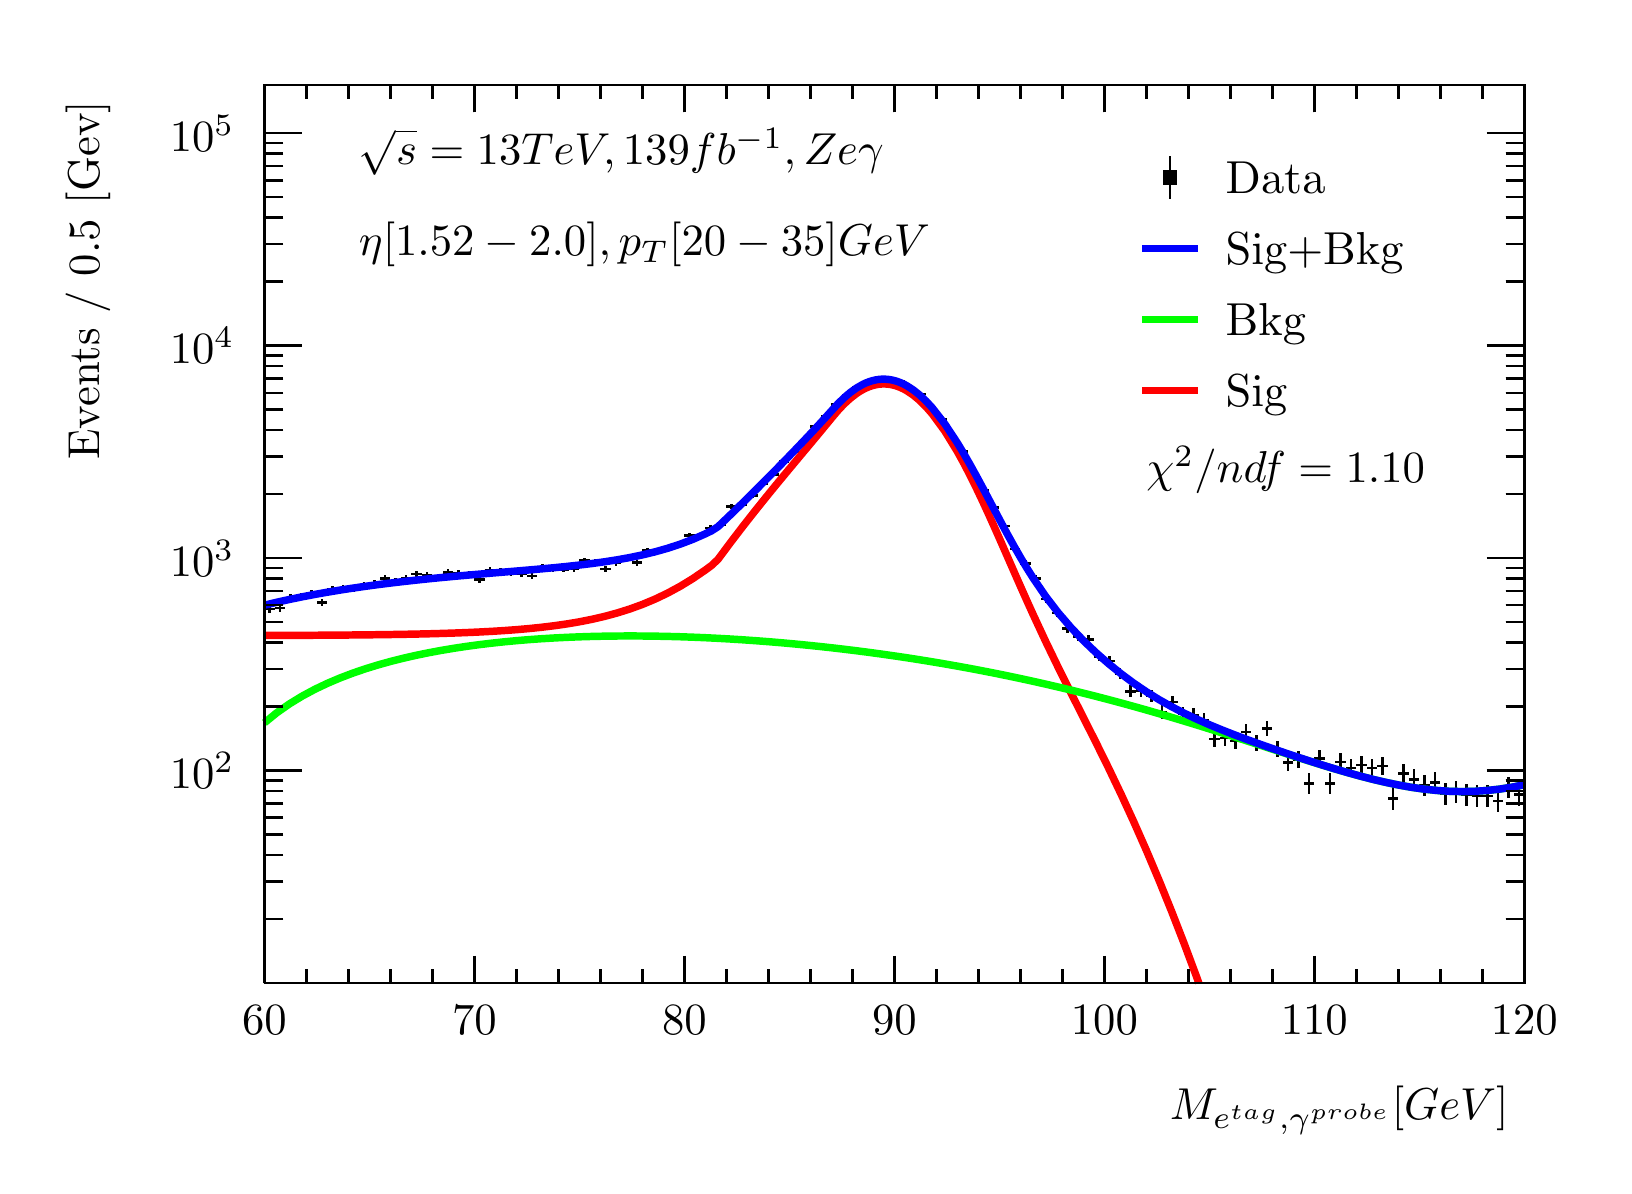
\begin{tikzpicture}
\pgfdeclareplotmark{cross} {
\pgfpathmoveto{\pgfpoint{-0.3\pgfplotmarksize}{\pgfplotmarksize}}
\pgfpathlineto{\pgfpoint{+0.3\pgfplotmarksize}{\pgfplotmarksize}}
\pgfpathlineto{\pgfpoint{+0.3\pgfplotmarksize}{0.3\pgfplotmarksize}}
\pgfpathlineto{\pgfpoint{+1\pgfplotmarksize}{0.3\pgfplotmarksize}}
\pgfpathlineto{\pgfpoint{+1\pgfplotmarksize}{-0.3\pgfplotmarksize}}
\pgfpathlineto{\pgfpoint{+0.3\pgfplotmarksize}{-0.3\pgfplotmarksize}}
\pgfpathlineto{\pgfpoint{+0.3\pgfplotmarksize}{-1.\pgfplotmarksize}}
\pgfpathlineto{\pgfpoint{-0.3\pgfplotmarksize}{-1.\pgfplotmarksize}}
\pgfpathlineto{\pgfpoint{-0.3\pgfplotmarksize}{-0.3\pgfplotmarksize}}
\pgfpathlineto{\pgfpoint{-1.\pgfplotmarksize}{-0.3\pgfplotmarksize}}
\pgfpathlineto{\pgfpoint{-1.\pgfplotmarksize}{0.3\pgfplotmarksize}}
\pgfpathlineto{\pgfpoint{-0.3\pgfplotmarksize}{0.3\pgfplotmarksize}}
\pgfpathclose
\pgfusepathqstroke
}
\pgfdeclareplotmark{cross*} {
\pgfpathmoveto{\pgfpoint{-0.3\pgfplotmarksize}{\pgfplotmarksize}}
\pgfpathlineto{\pgfpoint{+0.3\pgfplotmarksize}{\pgfplotmarksize}}
\pgfpathlineto{\pgfpoint{+0.3\pgfplotmarksize}{0.3\pgfplotmarksize}}
\pgfpathlineto{\pgfpoint{+1\pgfplotmarksize}{0.3\pgfplotmarksize}}
\pgfpathlineto{\pgfpoint{+1\pgfplotmarksize}{-0.3\pgfplotmarksize}}
\pgfpathlineto{\pgfpoint{+0.3\pgfplotmarksize}{-0.3\pgfplotmarksize}}
\pgfpathlineto{\pgfpoint{+0.3\pgfplotmarksize}{-1.\pgfplotmarksize}}
\pgfpathlineto{\pgfpoint{-0.3\pgfplotmarksize}{-1.\pgfplotmarksize}}
\pgfpathlineto{\pgfpoint{-0.3\pgfplotmarksize}{-0.3\pgfplotmarksize}}
\pgfpathlineto{\pgfpoint{-1.\pgfplotmarksize}{-0.3\pgfplotmarksize}}
\pgfpathlineto{\pgfpoint{-1.\pgfplotmarksize}{0.3\pgfplotmarksize}}
\pgfpathlineto{\pgfpoint{-0.3\pgfplotmarksize}{0.3\pgfplotmarksize}}
\pgfpathclose
\pgfusepathqfillstroke
}
\pgfdeclareplotmark{newstar} {
\pgfpathmoveto{\pgfqpoint{0pt}{\pgfplotmarksize}}
\pgfpathlineto{\pgfqpointpolar{44}{0.5\pgfplotmarksize}}
\pgfpathlineto{\pgfqpointpolar{18}{\pgfplotmarksize}}
\pgfpathlineto{\pgfqpointpolar{-20}{0.5\pgfplotmarksize}}
\pgfpathlineto{\pgfqpointpolar{-54}{\pgfplotmarksize}}
\pgfpathlineto{\pgfqpointpolar{-90}{0.5\pgfplotmarksize}}
\pgfpathlineto{\pgfqpointpolar{234}{\pgfplotmarksize}}
\pgfpathlineto{\pgfqpointpolar{198}{0.5\pgfplotmarksize}}
\pgfpathlineto{\pgfqpointpolar{162}{\pgfplotmarksize}}
\pgfpathlineto{\pgfqpointpolar{134}{0.5\pgfplotmarksize}}
\pgfpathclose
\pgfusepathqstroke
}
\pgfdeclareplotmark{newstar*} {
\pgfpathmoveto{\pgfqpoint{0pt}{\pgfplotmarksize}}
\pgfpathlineto{\pgfqpointpolar{44}{0.5\pgfplotmarksize}}
\pgfpathlineto{\pgfqpointpolar{18}{\pgfplotmarksize}}
\pgfpathlineto{\pgfqpointpolar{-20}{0.5\pgfplotmarksize}}
\pgfpathlineto{\pgfqpointpolar{-54}{\pgfplotmarksize}}
\pgfpathlineto{\pgfqpointpolar{-90}{0.5\pgfplotmarksize}}
\pgfpathlineto{\pgfqpointpolar{234}{\pgfplotmarksize}}
\pgfpathlineto{\pgfqpointpolar{198}{0.5\pgfplotmarksize}}
\pgfpathlineto{\pgfqpointpolar{162}{\pgfplotmarksize}}
\pgfpathlineto{\pgfqpointpolar{134}{0.5\pgfplotmarksize}}
\pgfpathclose
\pgfusepathqfillstroke
}
\definecolor{c}{rgb}{1,1,1};
\draw [color=c, fill=c] (0,0) rectangle (20,14.4361);
\draw [color=c, fill=c] (3,2.30977) rectangle (19,13.7143);
\definecolor{c}{rgb}{0,0,0};
\draw [c,line width=0.9] (3,2.30977) -- (3,13.7143) -- (19,13.7143) -- (19,2.30977) -- (3,2.30977);
\definecolor{c}{rgb}{1,1,1};
\draw [color=c, fill=c] (3,2.30977) rectangle (19,13.7143);
\definecolor{c}{rgb}{0,0,0};
\draw [c,line width=0.9] (3,2.30977) -- (3,13.7143) -- (19,13.7143) -- (19,2.30977) -- (3,2.30977);
\draw [c,line width=0.9] (3,2.30977) -- (19,2.30977);
\draw [c,line width=0.9] (3,2.65624) -- (3,2.30977);
\draw [c,line width=0.9] (3.53333,2.48301) -- (3.53333,2.30977);
\draw [c,line width=0.9] (4.06667,2.48301) -- (4.06667,2.30977);
\draw [c,line width=0.9] (4.6,2.48301) -- (4.6,2.30977);
\draw [c,line width=0.9] (5.13333,2.48301) -- (5.13333,2.30977);
\draw [c,line width=0.9] (5.66667,2.65624) -- (5.66667,2.30977);
\draw [c,line width=0.9] (6.2,2.48301) -- (6.2,2.30977);
\draw [c,line width=0.9] (6.73333,2.48301) -- (6.73333,2.30977);
\draw [c,line width=0.9] (7.26667,2.48301) -- (7.26667,2.30977);
\draw [c,line width=0.9] (7.8,2.48301) -- (7.8,2.30977);
\draw [c,line width=0.9] (8.33333,2.65624) -- (8.33333,2.30977);
\draw [c,line width=0.9] (8.86667,2.48301) -- (8.86667,2.30977);
\draw [c,line width=0.9] (9.4,2.48301) -- (9.4,2.30977);
\draw [c,line width=0.9] (9.93333,2.48301) -- (9.93333,2.30977);
\draw [c,line width=0.9] (10.4667,2.48301) -- (10.4667,2.30977);
\draw [c,line width=0.9] (11,2.65624) -- (11,2.30977);
\draw [c,line width=0.9] (11.5333,2.48301) -- (11.5333,2.30977);
\draw [c,line width=0.9] (12.0667,2.48301) -- (12.0667,2.30977);
\draw [c,line width=0.9] (12.6,2.48301) -- (12.6,2.30977);
\draw [c,line width=0.9] (13.1333,2.48301) -- (13.1333,2.30977);
\draw [c,line width=0.9] (13.6667,2.65624) -- (13.6667,2.30977);
\draw [c,line width=0.9] (14.2,2.48301) -- (14.2,2.30977);
\draw [c,line width=0.9] (14.7333,2.48301) -- (14.7333,2.30977);
\draw [c,line width=0.9] (15.2667,2.48301) -- (15.2667,2.30977);
\draw [c,line width=0.9] (15.8,2.48301) -- (15.8,2.30977);
\draw [c,line width=0.9] (16.3333,2.65624) -- (16.3333,2.30977);
\draw [c,line width=0.9] (16.8667,2.48301) -- (16.8667,2.30977);
\draw [c,line width=0.9] (17.4,2.48301) -- (17.4,2.30977);
\draw [c,line width=0.9] (17.9333,2.48301) -- (17.9333,2.30977);
\draw [c,line width=0.9] (18.4667,2.48301) -- (18.4667,2.30977);
\draw [c,line width=0.9] (19,2.65624) -- (19,2.30977);
\draw [anchor=base] (3,1.66015) node[scale=1.61424, color=c, rotate=0]{60};
\draw [anchor=base] (5.66667,1.66015) node[scale=1.61424, color=c, rotate=0]{70};
\draw [anchor=base] (8.33333,1.66015) node[scale=1.61424, color=c, rotate=0]{80};
\draw [anchor=base] (11,1.66015) node[scale=1.61424, color=c, rotate=0]{90};
\draw [anchor=base] (13.6667,1.66015) node[scale=1.61424, color=c, rotate=0]{100};
\draw [anchor=base] (16.3333,1.66015) node[scale=1.61424, color=c, rotate=0]{110};
\draw [anchor=base] (19,1.66015) node[scale=1.61424, color=c, rotate=0]{120};
\draw [anchor= east] (19,0.692932) node[scale=1.61424, color=c, rotate=0]{$M_{e^{tag}, \gamma^{probe}}  [GeV]$};
\draw [c,line width=0.9] (3,13.7143) -- (19,13.7143);
\draw [c,line width=0.9] (3,13.3678) -- (3,13.7143);
\draw [c,line width=0.9] (3.53333,13.5411) -- (3.53333,13.7143);
\draw [c,line width=0.9] (4.06667,13.5411) -- (4.06667,13.7143);
\draw [c,line width=0.9] (4.6,13.5411) -- (4.6,13.7143);
\draw [c,line width=0.9] (5.13333,13.5411) -- (5.13333,13.7143);
\draw [c,line width=0.9] (5.66667,13.3678) -- (5.66667,13.7143);
\draw [c,line width=0.9] (6.2,13.5411) -- (6.2,13.7143);
\draw [c,line width=0.9] (6.73333,13.5411) -- (6.73333,13.7143);
\draw [c,line width=0.9] (7.26667,13.5411) -- (7.26667,13.7143);
\draw [c,line width=0.9] (7.8,13.5411) -- (7.8,13.7143);
\draw [c,line width=0.9] (8.33333,13.3678) -- (8.33333,13.7143);
\draw [c,line width=0.9] (8.86667,13.5411) -- (8.86667,13.7143);
\draw [c,line width=0.9] (9.4,13.5411) -- (9.4,13.7143);
\draw [c,line width=0.9] (9.93333,13.5411) -- (9.93333,13.7143);
\draw [c,line width=0.9] (10.4667,13.5411) -- (10.4667,13.7143);
\draw [c,line width=0.9] (11,13.3678) -- (11,13.7143);
\draw [c,line width=0.9] (11.5333,13.5411) -- (11.5333,13.7143);
\draw [c,line width=0.9] (12.0667,13.5411) -- (12.0667,13.7143);
\draw [c,line width=0.9] (12.6,13.5411) -- (12.6,13.7143);
\draw [c,line width=0.9] (13.1333,13.5411) -- (13.1333,13.7143);
\draw [c,line width=0.9] (13.6667,13.3678) -- (13.6667,13.7143);
\draw [c,line width=0.9] (14.2,13.5411) -- (14.2,13.7143);
\draw [c,line width=0.9] (14.7333,13.5411) -- (14.7333,13.7143);
\draw [c,line width=0.9] (15.2667,13.5411) -- (15.2667,13.7143);
\draw [c,line width=0.9] (15.8,13.5411) -- (15.8,13.7143);
\draw [c,line width=0.9] (16.3333,13.3678) -- (16.3333,13.7143);
\draw [c,line width=0.9] (16.8667,13.5411) -- (16.8667,13.7143);
\draw [c,line width=0.9] (17.4,13.5411) -- (17.4,13.7143);
\draw [c,line width=0.9] (17.9333,13.5411) -- (17.9333,13.7143);
\draw [c,line width=0.9] (18.4667,13.5411) -- (18.4667,13.7143);
\draw [c,line width=0.9] (19,13.3678) -- (19,13.7143);
\draw [c,line width=0.9] (3,2.30977) -- (3,13.7143);
\draw [c,line width=0.9] (3.237,3.12209) -- (3,3.12209);
\draw [c,line width=0.9] (3.237,3.59726) -- (3,3.59726);
\draw [c,line width=0.9] (3.237,3.9344) -- (3,3.9344);
\draw [c,line width=0.9] (3.237,4.19591) -- (3,4.19591);
\draw [c,line width=0.9] (3.237,4.40958) -- (3,4.40958);
\draw [c,line width=0.9] (3.237,4.59023) -- (3,4.59023);
\draw [c,line width=0.9] (3.237,4.74672) -- (3,4.74672);
\draw [c,line width=0.9] (3.237,4.88475) -- (3,4.88475);
\draw [c,line width=0.9] (3.474,5.00822) -- (3,5.00822);
\draw [anchor= east] (2.82,5.00822) node[scale=1.61424, color=c, rotate=0]{$10^{2}$};
\draw [c,line width=0.9] (3.237,5.82054) -- (3,5.82054);
\draw [c,line width=0.9] (3.237,6.29571) -- (3,6.29571);
\draw [c,line width=0.9] (3.237,6.63285) -- (3,6.63285);
\draw [c,line width=0.9] (3.237,6.89436) -- (3,6.89436);
\draw [c,line width=0.9] (3.237,7.10803) -- (3,7.10803);
\draw [c,line width=0.9] (3.237,7.28868) -- (3,7.28868);
\draw [c,line width=0.9] (3.237,7.44517) -- (3,7.44517);
\draw [c,line width=0.9] (3.237,7.5832) -- (3,7.5832);
\draw [c,line width=0.9] (3.474,7.70668) -- (3,7.70668);
\draw [anchor= east] (2.82,7.70668) node[scale=1.61424, color=c, rotate=0]{$10^{3}$};
\draw [c,line width=0.9] (3.237,8.51899) -- (3,8.51899);
\draw [c,line width=0.9] (3.237,8.99417) -- (3,8.99417);
\draw [c,line width=0.9] (3.237,9.33131) -- (3,9.33131);
\draw [c,line width=0.9] (3.237,9.59281) -- (3,9.59281);
\draw [c,line width=0.9] (3.237,9.80648) -- (3,9.80648);
\draw [c,line width=0.9] (3.237,9.98713) -- (3,9.98713);
\draw [c,line width=0.9] (3.237,10.1436) -- (3,10.1436);
\draw [c,line width=0.9] (3.237,10.2817) -- (3,10.2817);
\draw [c,line width=0.9] (3.474,10.4051) -- (3,10.4051);
\draw [anchor= east] (2.82,10.4051) node[scale=1.61424, color=c, rotate=0]{$10^{4}$};
\draw [c,line width=0.9] (3.237,11.2174) -- (3,11.2174);
\draw [c,line width=0.9] (3.237,11.6926) -- (3,11.6926);
\draw [c,line width=0.9] (3.237,12.0298) -- (3,12.0298);
\draw [c,line width=0.9] (3.237,12.2913) -- (3,12.2913);
\draw [c,line width=0.9] (3.237,12.5049) -- (3,12.5049);
\draw [c,line width=0.9] (3.237,12.6856) -- (3,12.6856);
\draw [c,line width=0.9] (3.237,12.8421) -- (3,12.8421);
\draw [c,line width=0.9] (3.237,12.9801) -- (3,12.9801);
\draw [c,line width=0.9] (3.474,13.1036) -- (3,13.1036);
\draw [anchor= east] (2.82,13.1036) node[scale=1.61424, color=c, rotate=0]{$10^{5}$};
\draw [anchor= east] (0.76,13.7143) node[scale=1.61424, color=c, rotate=90]{Events / 0.5 [Gev]};
\draw [c,line width=0.9] (19,2.30977) -- (19,13.7143);
\draw [c,line width=0.9] (18.763,3.12209) -- (19,3.12209);
\draw [c,line width=0.9] (18.763,3.59726) -- (19,3.59726);
\draw [c,line width=0.9] (18.763,3.9344) -- (19,3.9344);
\draw [c,line width=0.9] (18.763,4.19591) -- (19,4.19591);
\draw [c,line width=0.9] (18.763,4.40958) -- (19,4.40958);
\draw [c,line width=0.9] (18.763,4.59023) -- (19,4.59023);
\draw [c,line width=0.9] (18.763,4.74672) -- (19,4.74672);
\draw [c,line width=0.9] (18.763,4.88475) -- (19,4.88475);
\draw [c,line width=0.9] (18.526,5.00822) -- (19,5.00822);
\draw [c,line width=0.9] (18.763,5.82054) -- (19,5.82054);
\draw [c,line width=0.9] (18.763,6.29571) -- (19,6.29571);
\draw [c,line width=0.9] (18.763,6.63285) -- (19,6.63285);
\draw [c,line width=0.9] (18.763,6.89436) -- (19,6.89436);
\draw [c,line width=0.9] (18.763,7.10803) -- (19,7.10803);
\draw [c,line width=0.9] (18.763,7.28868) -- (19,7.28868);
\draw [c,line width=0.9] (18.763,7.44517) -- (19,7.44517);
\draw [c,line width=0.9] (18.763,7.5832) -- (19,7.5832);
\draw [c,line width=0.9] (18.526,7.70668) -- (19,7.70668);
\draw [c,line width=0.9] (18.763,8.51899) -- (19,8.51899);
\draw [c,line width=0.9] (18.763,8.99417) -- (19,8.99417);
\draw [c,line width=0.9] (18.763,9.33131) -- (19,9.33131);
\draw [c,line width=0.9] (18.763,9.59281) -- (19,9.59281);
\draw [c,line width=0.9] (18.763,9.80648) -- (19,9.80648);
\draw [c,line width=0.9] (18.763,9.98713) -- (19,9.98713);
\draw [c,line width=0.9] (18.763,10.1436) -- (19,10.1436);
\draw [c,line width=0.9] (18.763,10.2817) -- (19,10.2817);
\draw [c,line width=0.9] (18.526,10.4051) -- (19,10.4051);
\draw [c,line width=0.9] (18.763,11.2174) -- (19,11.2174);
\draw [c,line width=0.9] (18.763,11.6926) -- (19,11.6926);
\draw [c,line width=0.9] (18.763,12.0298) -- (19,12.0298);
\draw [c,line width=0.9] (18.763,12.2913) -- (19,12.2913);
\draw [c,line width=0.9] (18.763,12.5049) -- (19,12.5049);
\draw [c,line width=0.9] (18.763,12.6856) -- (19,12.6856);
\draw [c,line width=0.9] (18.763,12.8421) -- (19,12.8421);
\draw [c,line width=0.9] (18.763,12.9801) -- (19,12.9801);
\draw [c,line width=0.9] (18.526,13.1036) -- (19,13.1036);
\draw [c,line width=0.9] (3.06667,7.06222) -- (3,7.06222);
\draw [c,line width=0.9] (3,7.06222) -- (3,7.06222);
\draw [c,line width=0.9] (3.06667,7.06222) -- (3.13333,7.06222);
\draw [c,line width=0.9] (3.13333,7.06222) -- (3.13333,7.06222);
\draw [c,line width=0.9] (3.06667,7.06222) -- (3.06667,7.11101);
\draw [c,line width=0.9] (3.06667,7.11101) -- (3.06667,7.11101);
\draw [c,line width=0.9] (3.06667,7.06222) -- (3.06667,7.01344);
\draw [c,line width=0.9] (3.06667,7.01344) -- (3.06667,7.01344);
\draw [c,line width=0.9] (3.2,7.07233) -- (3.13333,7.07233);
\draw [c,line width=0.9] (3.13333,7.07233) -- (3.13333,7.07233);
\draw [c,line width=0.9] (3.2,7.07233) -- (3.26667,7.07233);
\draw [c,line width=0.9] (3.26667,7.07233) -- (3.26667,7.07233);
\draw [c,line width=0.9] (3.2,7.07233) -- (3.2,7.12091);
\draw [c,line width=0.9] (3.2,7.12091) -- (3.2,7.12091);
\draw [c,line width=0.9] (3.2,7.07233) -- (3.2,7.02376);
\draw [c,line width=0.9] (3.2,7.02376) -- (3.2,7.02376);
\draw [c,line width=0.9] (3.33333,7.20183) -- (3.26667,7.20183);
\draw [c,line width=0.9] (3.26667,7.20183) -- (3.26667,7.20183);
\draw [c,line width=0.9] (3.33333,7.20183) -- (3.4,7.20183);
\draw [c,line width=0.9] (3.4,7.20183) -- (3.4,7.20183);
\draw [c,line width=0.9] (3.33333,7.20183) -- (3.33333,7.2478);
\draw [c,line width=0.9] (3.33333,7.2478) -- (3.33333,7.2478);
\draw [c,line width=0.9] (3.33333,7.20183) -- (3.33333,7.15587);
\draw [c,line width=0.9] (3.33333,7.15587) -- (3.33333,7.15587);
\draw [c,line width=0.9] (3.46667,7.2215) -- (3.4,7.2215);
\draw [c,line width=0.9] (3.4,7.2215) -- (3.4,7.2215);
\draw [c,line width=0.9] (3.46667,7.2215) -- (3.53333,7.2215);
\draw [c,line width=0.9] (3.53333,7.2215) -- (3.53333,7.2215);
\draw [c,line width=0.9] (3.46667,7.2215) -- (3.46667,7.26708);
\draw [c,line width=0.9] (3.46667,7.26708) -- (3.46667,7.26708);
\draw [c,line width=0.9] (3.46667,7.2215) -- (3.46667,7.17592);
\draw [c,line width=0.9] (3.46667,7.17592) -- (3.46667,7.17592);
\draw [c,line width=0.9] (3.6,7.25815) -- (3.53333,7.25815);
\draw [c,line width=0.9] (3.53333,7.25815) -- (3.53333,7.25815);
\draw [c,line width=0.9] (3.6,7.25815) -- (3.66667,7.25815);
\draw [c,line width=0.9] (3.66667,7.25815) -- (3.66667,7.25815);
\draw [c,line width=0.9] (3.6,7.25815) -- (3.6,7.30303);
\draw [c,line width=0.9] (3.6,7.30303) -- (3.6,7.30303);
\draw [c,line width=0.9] (3.6,7.25815) -- (3.6,7.21328);
\draw [c,line width=0.9] (3.6,7.21328) -- (3.6,7.21328);
\draw [c,line width=0.9] (3.73333,7.14077) -- (3.66667,7.14077);
\draw [c,line width=0.9] (3.66667,7.14077) -- (3.66667,7.14077);
\draw [c,line width=0.9] (3.73333,7.14077) -- (3.8,7.14077);
\draw [c,line width=0.9] (3.8,7.14077) -- (3.8,7.14077);
\draw [c,line width=0.9] (3.73333,7.14077) -- (3.73333,7.18795);
\draw [c,line width=0.9] (3.73333,7.18795) -- (3.73333,7.18795);
\draw [c,line width=0.9] (3.73333,7.14077) -- (3.73333,7.0936);
\draw [c,line width=0.9] (3.73333,7.0936) -- (3.73333,7.0936);
\draw [c,line width=0.9] (3.86667,7.31353) -- (3.8,7.31353);
\draw [c,line width=0.9] (3.8,7.31353) -- (3.8,7.31353);
\draw [c,line width=0.9] (3.86667,7.31353) -- (3.93333,7.31353);
\draw [c,line width=0.9] (3.93333,7.31353) -- (3.93333,7.31353);
\draw [c,line width=0.9] (3.86667,7.31353) -- (3.86667,7.35736);
\draw [c,line width=0.9] (3.86667,7.35736) -- (3.86667,7.35736);
\draw [c,line width=0.9] (3.86667,7.31353) -- (3.86667,7.26971);
\draw [c,line width=0.9] (3.86667,7.26971) -- (3.86667,7.26971);
\draw [c,line width=0.9] (4,7.32495) -- (3.93333,7.32495);
\draw [c,line width=0.9] (3.93333,7.32495) -- (3.93333,7.32495);
\draw [c,line width=0.9] (4,7.32495) -- (4.06667,7.32495);
\draw [c,line width=0.9] (4.06667,7.32495) -- (4.06667,7.32495);
\draw [c,line width=0.9] (4,7.32495) -- (4,7.36856);
\draw [c,line width=0.9] (4,7.36856) -- (4,7.36856);
\draw [c,line width=0.9] (4,7.32495) -- (4,7.28134);
\draw [c,line width=0.9] (4,7.28134) -- (4,7.28134);
\draw [c,line width=0.9] (4.13333,7.31844) -- (4.06667,7.31844);
\draw [c,line width=0.9] (4.06667,7.31844) -- (4.06667,7.31844);
\draw [c,line width=0.9] (4.13333,7.31844) -- (4.2,7.31844);
\draw [c,line width=0.9] (4.2,7.31844) -- (4.2,7.31844);
\draw [c,line width=0.9] (4.13333,7.31844) -- (4.13333,7.36217);
\draw [c,line width=0.9] (4.13333,7.36217) -- (4.13333,7.36217);
\draw [c,line width=0.9] (4.13333,7.31844) -- (4.13333,7.2747);
\draw [c,line width=0.9] (4.13333,7.2747) -- (4.13333,7.2747);
\draw [c,line width=0.9] (4.26667,7.36012) -- (4.2,7.36012);
\draw [c,line width=0.9] (4.2,7.36012) -- (4.2,7.36012);
\draw [c,line width=0.9] (4.26667,7.36012) -- (4.33333,7.36012);
\draw [c,line width=0.9] (4.33333,7.36012) -- (4.33333,7.36012);
\draw [c,line width=0.9] (4.26667,7.36012) -- (4.26667,7.40309);
\draw [c,line width=0.9] (4.26667,7.40309) -- (4.26667,7.40309);
\draw [c,line width=0.9] (4.26667,7.36012) -- (4.26667,7.31716);
\draw [c,line width=0.9] (4.26667,7.31716) -- (4.26667,7.31716);
\draw [c,line width=0.9] (4.4,7.38352) -- (4.33333,7.38352);
\draw [c,line width=0.9] (4.33333,7.38352) -- (4.33333,7.38352);
\draw [c,line width=0.9] (4.4,7.38352) -- (4.46667,7.38352);
\draw [c,line width=0.9] (4.46667,7.38352) -- (4.46667,7.38352);
\draw [c,line width=0.9] (4.4,7.38352) -- (4.4,7.42605);
\draw [c,line width=0.9] (4.4,7.42605) -- (4.4,7.42605);
\draw [c,line width=0.9] (4.4,7.38352) -- (4.4,7.34098);
\draw [c,line width=0.9] (4.4,7.34098) -- (4.4,7.34098);
\draw [c,line width=0.9] (4.53333,7.44517) -- (4.46667,7.44517);
\draw [c,line width=0.9] (4.46667,7.44517) -- (4.46667,7.44517);
\draw [c,line width=0.9] (4.53333,7.44517) -- (4.6,7.44517);
\draw [c,line width=0.9] (4.6,7.44517) -- (4.6,7.44517);
\draw [c,line width=0.9] (4.53333,7.44517) -- (4.53333,7.4866);
\draw [c,line width=0.9] (4.53333,7.4866) -- (4.53333,7.4866);
\draw [c,line width=0.9] (4.53333,7.44517) -- (4.53333,7.40374);
\draw [c,line width=0.9] (4.53333,7.40374) -- (4.53333,7.40374);
\draw [c,line width=0.9] (4.66667,7.4155) -- (4.6,7.4155);
\draw [c,line width=0.9] (4.6,7.4155) -- (4.6,7.4155);
\draw [c,line width=0.9] (4.66667,7.4155) -- (4.73333,7.4155);
\draw [c,line width=0.9] (4.73333,7.4155) -- (4.73333,7.4155);
\draw [c,line width=0.9] (4.66667,7.4155) -- (4.66667,7.45746);
\draw [c,line width=0.9] (4.66667,7.45746) -- (4.66667,7.45746);
\draw [c,line width=0.9] (4.66667,7.4155) -- (4.66667,7.37354);
\draw [c,line width=0.9] (4.66667,7.37354) -- (4.66667,7.37354);
\draw [c,line width=0.9] (4.8,7.45102) -- (4.73333,7.45102);
\draw [c,line width=0.9] (4.73333,7.45102) -- (4.73333,7.45102);
\draw [c,line width=0.9] (4.8,7.45102) -- (4.86667,7.45102);
\draw [c,line width=0.9] (4.86667,7.45102) -- (4.86667,7.45102);
\draw [c,line width=0.9] (4.8,7.45102) -- (4.8,7.49234);
\draw [c,line width=0.9] (4.8,7.49234) -- (4.8,7.49234);
\draw [c,line width=0.9] (4.8,7.45102) -- (4.8,7.40969);
\draw [c,line width=0.9] (4.8,7.40969) -- (4.8,7.40969);
\draw [c,line width=0.9] (4.93333,7.50235) -- (4.86667,7.50235);
\draw [c,line width=0.9] (4.86667,7.50235) -- (4.86667,7.50235);
\draw [c,line width=0.9] (4.93333,7.50235) -- (5,7.50235);
\draw [c,line width=0.9] (5,7.50235) -- (5,7.50235);
\draw [c,line width=0.9] (4.93333,7.50235) -- (4.93333,7.54278);
\draw [c,line width=0.9] (4.93333,7.54278) -- (4.93333,7.54278);
\draw [c,line width=0.9] (4.93333,7.50235) -- (4.93333,7.46192);
\draw [c,line width=0.9] (4.93333,7.46192) -- (4.93333,7.46192);
\draw [c,line width=0.9] (5.06667,7.49395) -- (5,7.49395);
\draw [c,line width=0.9] (5,7.49395) -- (5,7.49395);
\draw [c,line width=0.9] (5.06667,7.49395) -- (5.13333,7.49395);
\draw [c,line width=0.9] (5.13333,7.49395) -- (5.13333,7.49395);
\draw [c,line width=0.9] (5.06667,7.49395) -- (5.06667,7.53453);
\draw [c,line width=0.9] (5.06667,7.53453) -- (5.06667,7.53453);
\draw [c,line width=0.9] (5.06667,7.49395) -- (5.06667,7.45337);
\draw [c,line width=0.9] (5.06667,7.45337) -- (5.06667,7.45337);
\draw [c,line width=0.9] (5.2,7.45538) -- (5.13333,7.45538);
\draw [c,line width=0.9] (5.13333,7.45538) -- (5.13333,7.45538);
\draw [c,line width=0.9] (5.2,7.45538) -- (5.26667,7.45538);
\draw [c,line width=0.9] (5.26667,7.45538) -- (5.26667,7.45538);
\draw [c,line width=0.9] (5.2,7.45538) -- (5.2,7.49663);
\draw [c,line width=0.9] (5.2,7.49663) -- (5.2,7.49663);
\draw [c,line width=0.9] (5.2,7.45538) -- (5.2,7.41413);
\draw [c,line width=0.9] (5.2,7.41413) -- (5.2,7.41413);
\draw [c,line width=0.9] (5.33333,7.52583) -- (5.26667,7.52583);
\draw [c,line width=0.9] (5.26667,7.52583) -- (5.26667,7.52583);
\draw [c,line width=0.9] (5.33333,7.52583) -- (5.4,7.52583);
\draw [c,line width=0.9] (5.4,7.52583) -- (5.4,7.52583);
\draw [c,line width=0.9] (5.33333,7.52583) -- (5.33333,7.56586);
\draw [c,line width=0.9] (5.33333,7.56586) -- (5.33333,7.56586);
\draw [c,line width=0.9] (5.33333,7.52583) -- (5.33333,7.4858);
\draw [c,line width=0.9] (5.33333,7.4858) -- (5.33333,7.4858);
\draw [c,line width=0.9] (5.46667,7.51897) -- (5.4,7.51897);
\draw [c,line width=0.9] (5.4,7.51897) -- (5.4,7.51897);
\draw [c,line width=0.9] (5.46667,7.51897) -- (5.53333,7.51897);
\draw [c,line width=0.9] (5.53333,7.51897) -- (5.53333,7.51897);
\draw [c,line width=0.9] (5.46667,7.51897) -- (5.46667,7.55912);
\draw [c,line width=0.9] (5.46667,7.55912) -- (5.46667,7.55912);
\draw [c,line width=0.9] (5.46667,7.51897) -- (5.46667,7.47883);
\draw [c,line width=0.9] (5.46667,7.47883) -- (5.46667,7.47883);
\draw [c,line width=0.9] (5.6,7.50653) -- (5.53333,7.50653);
\draw [c,line width=0.9] (5.53333,7.50653) -- (5.53333,7.50653);
\draw [c,line width=0.9] (5.6,7.50653) -- (5.66667,7.50653);
\draw [c,line width=0.9] (5.66667,7.50653) -- (5.66667,7.50653);
\draw [c,line width=0.9] (5.6,7.50653) -- (5.6,7.54689);
\draw [c,line width=0.9] (5.6,7.54689) -- (5.6,7.54689);
\draw [c,line width=0.9] (5.6,7.50653) -- (5.6,7.46617);
\draw [c,line width=0.9] (5.6,7.46617) -- (5.6,7.46617);
\draw [c,line width=0.9] (5.73333,7.43782) -- (5.66667,7.43782);
\draw [c,line width=0.9] (5.66667,7.43782) -- (5.66667,7.43782);
\draw [c,line width=0.9] (5.73333,7.43782) -- (5.8,7.43782);
\draw [c,line width=0.9] (5.8,7.43782) -- (5.8,7.43782);
\draw [c,line width=0.9] (5.73333,7.43782) -- (5.73333,7.47939);
\draw [c,line width=0.9] (5.73333,7.47939) -- (5.73333,7.47939);
\draw [c,line width=0.9] (5.73333,7.43782) -- (5.73333,7.39626);
\draw [c,line width=0.9] (5.73333,7.39626) -- (5.73333,7.39626);
\draw [c,line width=0.9] (5.86667,7.55687) -- (5.8,7.55687);
\draw [c,line width=0.9] (5.8,7.55687) -- (5.8,7.55687);
\draw [c,line width=0.9] (5.86667,7.55687) -- (5.93333,7.55687);
\draw [c,line width=0.9] (5.93333,7.55687) -- (5.93333,7.55687);
\draw [c,line width=0.9] (5.86667,7.55687) -- (5.86667,7.59637);
\draw [c,line width=0.9] (5.86667,7.59637) -- (5.86667,7.59637);
\draw [c,line width=0.9] (5.86667,7.55687) -- (5.86667,7.51736);
\draw [c,line width=0.9] (5.86667,7.51736) -- (5.86667,7.51736);
\draw [c,line width=0.9] (6,7.54213) -- (5.93333,7.54213);
\draw [c,line width=0.9] (5.93333,7.54213) -- (5.93333,7.54213);
\draw [c,line width=0.9] (6,7.54213) -- (6.06667,7.54213);
\draw [c,line width=0.9] (6.06667,7.54213) -- (6.06667,7.54213);
\draw [c,line width=0.9] (6,7.54213) -- (6,7.58188);
\draw [c,line width=0.9] (6,7.58188) -- (6,7.58188);
\draw [c,line width=0.9] (6,7.54213) -- (6,7.50237);
\draw [c,line width=0.9] (6,7.50237) -- (6,7.50237);
\draw [c,line width=0.9] (6.13333,7.52309) -- (6.06667,7.52309);
\draw [c,line width=0.9] (6.06667,7.52309) -- (6.06667,7.52309);
\draw [c,line width=0.9] (6.13333,7.52309) -- (6.2,7.52309);
\draw [c,line width=0.9] (6.2,7.52309) -- (6.2,7.52309);
\draw [c,line width=0.9] (6.13333,7.52309) -- (6.13333,7.56317);
\draw [c,line width=0.9] (6.13333,7.56317) -- (6.13333,7.56317);
\draw [c,line width=0.9] (6.13333,7.52309) -- (6.13333,7.48302);
\draw [c,line width=0.9] (6.13333,7.48302) -- (6.13333,7.48302);
\draw [c,line width=0.9] (6.26667,7.50374) -- (6.2,7.50374);
\draw [c,line width=0.9] (6.2,7.50374) -- (6.2,7.50374);
\draw [c,line width=0.9] (6.26667,7.50374) -- (6.33333,7.50374);
\draw [c,line width=0.9] (6.33333,7.50374) -- (6.33333,7.50374);
\draw [c,line width=0.9] (6.26667,7.50374) -- (6.26667,7.54415);
\draw [c,line width=0.9] (6.26667,7.54415) -- (6.26667,7.54415);
\draw [c,line width=0.9] (6.26667,7.50374) -- (6.26667,7.46334);
\draw [c,line width=0.9] (6.26667,7.46334) -- (6.26667,7.46334);
\draw [c,line width=0.9] (6.4,7.47981) -- (6.33333,7.47981);
\draw [c,line width=0.9] (6.33333,7.47981) -- (6.33333,7.47981);
\draw [c,line width=0.9] (6.4,7.47981) -- (6.46667,7.47981);
\draw [c,line width=0.9] (6.46667,7.47981) -- (6.46667,7.47981);
\draw [c,line width=0.9] (6.4,7.47981) -- (6.4,7.52064);
\draw [c,line width=0.9] (6.4,7.52064) -- (6.4,7.52064);
\draw [c,line width=0.9] (6.4,7.47981) -- (6.4,7.43899);
\draw [c,line width=0.9] (6.4,7.43899) -- (6.4,7.43899);
\draw [c,line width=0.9] (6.53333,7.5897) -- (6.46667,7.5897);
\draw [c,line width=0.9] (6.46667,7.5897) -- (6.46667,7.5897);
\draw [c,line width=0.9] (6.53333,7.5897) -- (6.6,7.5897);
\draw [c,line width=0.9] (6.6,7.5897) -- (6.6,7.5897);
\draw [c,line width=0.9] (6.53333,7.5897) -- (6.53333,7.62865);
\draw [c,line width=0.9] (6.53333,7.62865) -- (6.53333,7.62865);
\draw [c,line width=0.9] (6.53333,7.5897) -- (6.53333,7.55074);
\draw [c,line width=0.9] (6.53333,7.55074) -- (6.53333,7.55074);
\draw [c,line width=0.9] (6.66667,7.56483) -- (6.6,7.56483);
\draw [c,line width=0.9] (6.6,7.56483) -- (6.6,7.56483);
\draw [c,line width=0.9] (6.66667,7.56483) -- (6.73333,7.56483);
\draw [c,line width=0.9] (6.73333,7.56483) -- (6.73333,7.56483);
\draw [c,line width=0.9] (6.66667,7.56483) -- (6.66667,7.6042);
\draw [c,line width=0.9] (6.66667,7.6042) -- (6.66667,7.6042);
\draw [c,line width=0.9] (6.66667,7.56483) -- (6.66667,7.52546);
\draw [c,line width=0.9] (6.66667,7.52546) -- (6.66667,7.52546);
\draw [c,line width=0.9] (6.8,7.56351) -- (6.73333,7.56351);
\draw [c,line width=0.9] (6.73333,7.56351) -- (6.73333,7.56351);
\draw [c,line width=0.9] (6.8,7.56351) -- (6.86667,7.56351);
\draw [c,line width=0.9] (6.86667,7.56351) -- (6.86667,7.56351);
\draw [c,line width=0.9] (6.8,7.56351) -- (6.8,7.6029);
\draw [c,line width=0.9] (6.8,7.6029) -- (6.8,7.6029);
\draw [c,line width=0.9] (6.8,7.56351) -- (6.8,7.52412);
\draw [c,line width=0.9] (6.8,7.52412) -- (6.8,7.52412);
\draw [c,line width=0.9] (6.93333,7.57405) -- (6.86667,7.57405);
\draw [c,line width=0.9] (6.86667,7.57405) -- (6.86667,7.57405);
\draw [c,line width=0.9] (6.93333,7.57405) -- (7,7.57405);
\draw [c,line width=0.9] (7,7.57405) -- (7,7.57405);
\draw [c,line width=0.9] (6.93333,7.57405) -- (6.93333,7.61327);
\draw [c,line width=0.9] (6.93333,7.61327) -- (6.93333,7.61327);
\draw [c,line width=0.9] (6.93333,7.57405) -- (6.93333,7.53484);
\draw [c,line width=0.9] (6.93333,7.53484) -- (6.93333,7.53484);
\draw [c,line width=0.9] (7.06667,7.6734) -- (7,7.6734);
\draw [c,line width=0.9] (7,7.6734) -- (7,7.6734);
\draw [c,line width=0.9] (7.06667,7.6734) -- (7.13333,7.6734);
\draw [c,line width=0.9] (7.13333,7.6734) -- (7.13333,7.6734);
\draw [c,line width=0.9] (7.06667,7.6734) -- (7.06667,7.71098);
\draw [c,line width=0.9] (7.06667,7.71098) -- (7.06667,7.71098);
\draw [c,line width=0.9] (7.06667,7.6734) -- (7.06667,7.63581);
\draw [c,line width=0.9] (7.06667,7.63581) -- (7.06667,7.63581);
\draw [c,line width=0.9] (7.2,7.66128) -- (7.13333,7.66128);
\draw [c,line width=0.9] (7.13333,7.66128) -- (7.13333,7.66128);
\draw [c,line width=0.9] (7.2,7.66128) -- (7.26667,7.66128);
\draw [c,line width=0.9] (7.26667,7.66128) -- (7.26667,7.66128);
\draw [c,line width=0.9] (7.2,7.66128) -- (7.2,7.69906);
\draw [c,line width=0.9] (7.2,7.69906) -- (7.2,7.69906);
\draw [c,line width=0.9] (7.2,7.66128) -- (7.2,7.62349);
\draw [c,line width=0.9] (7.2,7.62349) -- (7.2,7.62349);
\draw [c,line width=0.9] (7.33333,7.56747) -- (7.26667,7.56747);
\draw [c,line width=0.9] (7.26667,7.56747) -- (7.26667,7.56747);
\draw [c,line width=0.9] (7.33333,7.56747) -- (7.4,7.56747);
\draw [c,line width=0.9] (7.4,7.56747) -- (7.4,7.56747);
\draw [c,line width=0.9] (7.33333,7.56747) -- (7.33333,7.6068);
\draw [c,line width=0.9] (7.33333,7.6068) -- (7.33333,7.6068);
\draw [c,line width=0.9] (7.33333,7.56747) -- (7.33333,7.52815);
\draw [c,line width=0.9] (7.33333,7.52815) -- (7.33333,7.52815);
\draw [c,line width=0.9] (7.46667,7.65026) -- (7.4,7.65026);
\draw [c,line width=0.9] (7.4,7.65026) -- (7.4,7.65026);
\draw [c,line width=0.9] (7.46667,7.65026) -- (7.53333,7.65026);
\draw [c,line width=0.9] (7.53333,7.65026) -- (7.53333,7.65026);
\draw [c,line width=0.9] (7.46667,7.65026) -- (7.46667,7.68822);
\draw [c,line width=0.9] (7.46667,7.68822) -- (7.46667,7.68822);
\draw [c,line width=0.9] (7.46667,7.65026) -- (7.46667,7.6123);
\draw [c,line width=0.9] (7.46667,7.6123) -- (7.46667,7.6123);
\draw [c,line width=0.9] (7.6,7.7008) -- (7.53333,7.7008);
\draw [c,line width=0.9] (7.53333,7.7008) -- (7.53333,7.7008);
\draw [c,line width=0.9] (7.6,7.7008) -- (7.66667,7.7008);
\draw [c,line width=0.9] (7.66667,7.7008) -- (7.66667,7.7008);
\draw [c,line width=0.9] (7.6,7.7008) -- (7.6,7.73796);
\draw [c,line width=0.9] (7.6,7.73796) -- (7.6,7.73796);
\draw [c,line width=0.9] (7.6,7.7008) -- (7.6,7.66365);
\draw [c,line width=0.9] (7.6,7.66365) -- (7.6,7.66365);
\draw [c,line width=0.9] (7.73333,7.65026) -- (7.66667,7.65026);
\draw [c,line width=0.9] (7.66667,7.65026) -- (7.66667,7.65026);
\draw [c,line width=0.9] (7.73333,7.65026) -- (7.8,7.65026);
\draw [c,line width=0.9] (7.8,7.65026) -- (7.8,7.65026);
\draw [c,line width=0.9] (7.73333,7.65026) -- (7.73333,7.68822);
\draw [c,line width=0.9] (7.73333,7.68822) -- (7.73333,7.68822);
\draw [c,line width=0.9] (7.73333,7.65026) -- (7.73333,7.6123);
\draw [c,line width=0.9] (7.73333,7.6123) -- (7.73333,7.6123);
\draw [c,line width=0.9] (7.86667,7.80012) -- (7.8,7.80012);
\draw [c,line width=0.9] (7.8,7.80012) -- (7.8,7.80012);
\draw [c,line width=0.9] (7.86667,7.80012) -- (7.93333,7.80012);
\draw [c,line width=0.9] (7.93333,7.80012) -- (7.93333,7.80012);
\draw [c,line width=0.9] (7.86667,7.80012) -- (7.86667,7.83573);
\draw [c,line width=0.9] (7.86667,7.83573) -- (7.86667,7.83573);
\draw [c,line width=0.9] (7.86667,7.80012) -- (7.86667,7.76451);
\draw [c,line width=0.9] (7.86667,7.76451) -- (7.86667,7.76451);
\draw [c,line width=0.9] (8,7.80228) -- (7.93333,7.80228);
\draw [c,line width=0.9] (7.93333,7.80228) -- (7.93333,7.80228);
\draw [c,line width=0.9] (8,7.80228) -- (8.06667,7.80228);
\draw [c,line width=0.9] (8.06667,7.80228) -- (8.06667,7.80228);
\draw [c,line width=0.9] (8,7.80228) -- (8,7.83786);
\draw [c,line width=0.9] (8,7.83786) -- (8,7.83786);
\draw [c,line width=0.9] (8,7.80228) -- (8,7.76671);
\draw [c,line width=0.9] (8,7.76671) -- (8,7.76671);
\draw [c,line width=0.9] (8.13333,7.82581) -- (8.06667,7.82581);
\draw [c,line width=0.9] (8.06667,7.82581) -- (8.06667,7.82581);
\draw [c,line width=0.9] (8.13333,7.82581) -- (8.2,7.82581);
\draw [c,line width=0.9] (8.2,7.82581) -- (8.2,7.82581);
\draw [c,line width=0.9] (8.13333,7.82581) -- (8.13333,7.86103);
\draw [c,line width=0.9] (8.13333,7.86103) -- (8.13333,7.86103);
\draw [c,line width=0.9] (8.13333,7.82581) -- (8.13333,7.79059);
\draw [c,line width=0.9] (8.13333,7.79059) -- (8.13333,7.79059);
\draw [c,line width=0.9] (8.26667,7.8796) -- (8.2,7.8796);
\draw [c,line width=0.9] (8.2,7.8796) -- (8.2,7.8796);
\draw [c,line width=0.9] (8.26667,7.8796) -- (8.33333,7.8796);
\draw [c,line width=0.9] (8.33333,7.8796) -- (8.33333,7.8796);
\draw [c,line width=0.9] (8.26667,7.8796) -- (8.26667,7.91403);
\draw [c,line width=0.9] (8.26667,7.91403) -- (8.26667,7.91403);
\draw [c,line width=0.9] (8.26667,7.8796) -- (8.26667,7.84518);
\draw [c,line width=0.9] (8.26667,7.84518) -- (8.26667,7.84518);
\draw [c,line width=0.9] (8.4,7.99598) -- (8.33333,7.99598);
\draw [c,line width=0.9] (8.33333,7.99598) -- (8.33333,7.99598);
\draw [c,line width=0.9] (8.4,7.99598) -- (8.46667,7.99598);
\draw [c,line width=0.9] (8.46667,7.99598) -- (8.46667,7.99598);
\draw [c,line width=0.9] (8.4,7.99598) -- (8.4,8.02873);
\draw [c,line width=0.9] (8.4,8.02873) -- (8.4,8.02873);
\draw [c,line width=0.9] (8.4,7.99598) -- (8.4,7.96322);
\draw [c,line width=0.9] (8.4,7.96322) -- (8.4,7.96322);
\draw [c,line width=0.9] (8.53333,7.97659) -- (8.46667,7.97659);
\draw [c,line width=0.9] (8.46667,7.97659) -- (8.46667,7.97659);
\draw [c,line width=0.9] (8.53333,7.97659) -- (8.6,7.97659);
\draw [c,line width=0.9] (8.6,7.97659) -- (8.6,7.97659);
\draw [c,line width=0.9] (8.53333,7.97659) -- (8.53333,8.00962);
\draw [c,line width=0.9] (8.53333,8.00962) -- (8.53333,8.00962);
\draw [c,line width=0.9] (8.53333,7.97659) -- (8.53333,7.94357);
\draw [c,line width=0.9] (8.53333,7.94357) -- (8.53333,7.94357);
\draw [c,line width=0.9] (8.66667,8.09007) -- (8.6,8.09007);
\draw [c,line width=0.9] (8.6,8.09007) -- (8.6,8.09007);
\draw [c,line width=0.9] (8.66667,8.09007) -- (8.73333,8.09007);
\draw [c,line width=0.9] (8.73333,8.09007) -- (8.73333,8.09007);
\draw [c,line width=0.9] (8.66667,8.09007) -- (8.66667,8.12153);
\draw [c,line width=0.9] (8.66667,8.12153) -- (8.66667,8.12153);
\draw [c,line width=0.9] (8.66667,8.09007) -- (8.66667,8.0586);
\draw [c,line width=0.9] (8.66667,8.0586) -- (8.66667,8.0586);
\draw [c,line width=0.9] (8.8,8.13401) -- (8.73333,8.13401);
\draw [c,line width=0.9] (8.73333,8.13401) -- (8.73333,8.13401);
\draw [c,line width=0.9] (8.8,8.13401) -- (8.86667,8.13401);
\draw [c,line width=0.9] (8.86667,8.13401) -- (8.86667,8.13401);
\draw [c,line width=0.9] (8.8,8.13401) -- (8.8,8.16489);
\draw [c,line width=0.9] (8.8,8.16489) -- (8.8,8.16489);
\draw [c,line width=0.9] (8.8,8.13401) -- (8.8,8.10313);
\draw [c,line width=0.9] (8.8,8.10313) -- (8.8,8.10313);
\draw [c,line width=0.9] (8.93333,8.36317) -- (8.86667,8.36317);
\draw [c,line width=0.9] (8.86667,8.36317) -- (8.86667,8.36317);
\draw [c,line width=0.9] (8.93333,8.36317) -- (9,8.36317);
\draw [c,line width=0.9] (9,8.36317) -- (9,8.36317);
\draw [c,line width=0.9] (8.93333,8.36317) -- (8.93333,8.39118);
\draw [c,line width=0.9] (8.93333,8.39118) -- (8.93333,8.39118);
\draw [c,line width=0.9] (8.93333,8.36317) -- (8.93333,8.33517);
\draw [c,line width=0.9] (8.93333,8.33517) -- (8.93333,8.33517);
\draw [c,line width=0.9] (9.06667,8.38242) -- (9,8.38242);
\draw [c,line width=0.9] (9,8.38242) -- (9,8.38242);
\draw [c,line width=0.9] (9.06667,8.38242) -- (9.13333,8.38242);
\draw [c,line width=0.9] (9.13333,8.38242) -- (9.13333,8.38242);
\draw [c,line width=0.9] (9.06667,8.38242) -- (9.06667,8.4102);
\draw [c,line width=0.9] (9.06667,8.4102) -- (9.06667,8.4102);
\draw [c,line width=0.9] (9.06667,8.38242) -- (9.06667,8.35465);
\draw [c,line width=0.9] (9.06667,8.35465) -- (9.06667,8.35465);
\draw [c,line width=0.9] (9.2,8.50009) -- (9.13333,8.50009);
\draw [c,line width=0.9] (9.13333,8.50009) -- (9.13333,8.50009);
\draw [c,line width=0.9] (9.2,8.50009) -- (9.26667,8.50009);
\draw [c,line width=0.9] (9.26667,8.50009) -- (9.26667,8.50009);
\draw [c,line width=0.9] (9.2,8.50009) -- (9.2,8.52651);
\draw [c,line width=0.9] (9.2,8.52651) -- (9.2,8.52651);
\draw [c,line width=0.9] (9.2,8.50009) -- (9.2,8.47367);
\draw [c,line width=0.9] (9.2,8.47367) -- (9.2,8.47367);
\draw [c,line width=0.9] (9.33333,8.6565) -- (9.26667,8.6565);
\draw [c,line width=0.9] (9.26667,8.6565) -- (9.26667,8.6565);
\draw [c,line width=0.9] (9.33333,8.6565) -- (9.4,8.6565);
\draw [c,line width=0.9] (9.4,8.6565) -- (9.4,8.6565);
\draw [c,line width=0.9] (9.33333,8.6565) -- (9.33333,8.68122);
\draw [c,line width=0.9] (9.33333,8.68122) -- (9.33333,8.68122);
\draw [c,line width=0.9] (9.33333,8.6565) -- (9.33333,8.63179);
\draw [c,line width=0.9] (9.33333,8.63179) -- (9.33333,8.63179);
\draw [c,line width=0.9] (9.46667,8.76967) -- (9.4,8.76967);
\draw [c,line width=0.9] (9.4,8.76967) -- (9.4,8.76967);
\draw [c,line width=0.9] (9.46667,8.76967) -- (9.53333,8.76967);
\draw [c,line width=0.9] (9.53333,8.76967) -- (9.53333,8.76967);
\draw [c,line width=0.9] (9.46667,8.76967) -- (9.46667,8.79322);
\draw [c,line width=0.9] (9.46667,8.79322) -- (9.46667,8.79322);
\draw [c,line width=0.9] (9.46667,8.76967) -- (9.46667,8.74612);
\draw [c,line width=0.9] (9.46667,8.74612) -- (9.46667,8.74612);
\draw [c,line width=0.9] (9.6,8.93406) -- (9.53333,8.93406);
\draw [c,line width=0.9] (9.53333,8.93406) -- (9.53333,8.93406);
\draw [c,line width=0.9] (9.6,8.93406) -- (9.66667,8.93406);
\draw [c,line width=0.9] (9.66667,8.93406) -- (9.66667,8.93406);
\draw [c,line width=0.9] (9.6,8.93406) -- (9.6,8.95601);
\draw [c,line width=0.9] (9.6,8.95601) -- (9.6,8.95601);
\draw [c,line width=0.9] (9.6,8.93406) -- (9.6,8.9121);
\draw [c,line width=0.9] (9.6,8.9121) -- (9.6,8.9121);
\draw [c,line width=0.9] (9.73333,9.05209) -- (9.66667,9.05209);
\draw [c,line width=0.9] (9.66667,9.05209) -- (9.66667,9.05209);
\draw [c,line width=0.9] (9.73333,9.05209) -- (9.8,9.05209);
\draw [c,line width=0.9] (9.8,9.05209) -- (9.8,9.05209);
\draw [c,line width=0.9] (9.73333,9.05209) -- (9.73333,9.07296);
\draw [c,line width=0.9] (9.73333,9.07296) -- (9.73333,9.07296);
\draw [c,line width=0.9] (9.73333,9.05209) -- (9.73333,9.03122);
\draw [c,line width=0.9] (9.73333,9.03122) -- (9.73333,9.03122);
\draw [c,line width=0.9] (9.86667,9.19803) -- (9.8,9.19803);
\draw [c,line width=0.9] (9.8,9.19803) -- (9.8,9.19803);
\draw [c,line width=0.9] (9.86667,9.19803) -- (9.93333,9.19803);
\draw [c,line width=0.9] (9.93333,9.19803) -- (9.93333,9.19803);
\draw [c,line width=0.9] (9.86667,9.19803) -- (9.86667,9.21764);
\draw [c,line width=0.9] (9.86667,9.21764) -- (9.86667,9.21764);
\draw [c,line width=0.9] (9.86667,9.19803) -- (9.86667,9.17841);
\draw [c,line width=0.9] (9.86667,9.17841) -- (9.86667,9.17841);
\draw [c,line width=0.9] (10,9.38037) -- (9.93333,9.38037);
\draw [c,line width=0.9] (9.93333,9.38037) -- (9.93333,9.38037);
\draw [c,line width=0.9] (10,9.38037) -- (10.0667,9.38037);
\draw [c,line width=0.9] (10.0667,9.38037) -- (10.0667,9.38037);
\draw [c,line width=0.9] (10,9.38037) -- (10,9.39851);
\draw [c,line width=0.9] (10,9.39851) -- (10,9.39851);
\draw [c,line width=0.9] (10,9.38037) -- (10,9.36222);
\draw [c,line width=0.9] (10,9.36222) -- (10,9.36222);
\draw [c,line width=0.9] (10.1333,9.5128) -- (10.0667,9.5128);
\draw [c,line width=0.9] (10.0667,9.5128) -- (10.0667,9.5128);
\draw [c,line width=0.9] (10.1333,9.5128) -- (10.2,9.5128);
\draw [c,line width=0.9] (10.2,9.5128) -- (10.2,9.5128);
\draw [c,line width=0.9] (10.1333,9.5128) -- (10.1333,9.52995);
\draw [c,line width=0.9] (10.1333,9.52995) -- (10.1333,9.52995);
\draw [c,line width=0.9] (10.1333,9.5128) -- (10.1333,9.49565);
\draw [c,line width=0.9] (10.1333,9.49565) -- (10.1333,9.49565);
\draw [c,line width=0.9] (10.2667,9.65578) -- (10.2,9.65578);
\draw [c,line width=0.9] (10.2,9.65578) -- (10.2,9.65578);
\draw [c,line width=0.9] (10.2667,9.65578) -- (10.3333,9.65578);
\draw [c,line width=0.9] (10.3333,9.65578) -- (10.3333,9.65578);
\draw [c,line width=0.9] (10.2667,9.65578) -- (10.2667,9.67192);
\draw [c,line width=0.9] (10.2667,9.67192) -- (10.2667,9.67192);
\draw [c,line width=0.9] (10.2667,9.65578) -- (10.2667,9.63965);
\draw [c,line width=0.9] (10.2667,9.63965) -- (10.2667,9.63965);
\draw [c,line width=0.9] (10.4,9.76978) -- (10.3333,9.76978);
\draw [c,line width=0.9] (10.3333,9.76978) -- (10.3333,9.76978);
\draw [c,line width=0.9] (10.4,9.76978) -- (10.4667,9.76978);
\draw [c,line width=0.9] (10.4667,9.76978) -- (10.4667,9.76978);
\draw [c,line width=0.9] (10.4,9.76978) -- (10.4,9.78515);
\draw [c,line width=0.9] (10.4,9.78515) -- (10.4,9.78515);
\draw [c,line width=0.9] (10.4,9.76978) -- (10.4,9.75441);
\draw [c,line width=0.9] (10.4,9.75441) -- (10.4,9.75441);
\draw [c,line width=0.9] (10.5333,9.87089) -- (10.4667,9.87089);
\draw [c,line width=0.9] (10.4667,9.87089) -- (10.4667,9.87089);
\draw [c,line width=0.9] (10.5333,9.87089) -- (10.6,9.87089);
\draw [c,line width=0.9] (10.6,9.87089) -- (10.6,9.87089);
\draw [c,line width=0.9] (10.5333,9.87089) -- (10.5333,9.88561);
\draw [c,line width=0.9] (10.5333,9.88561) -- (10.5333,9.88561);
\draw [c,line width=0.9] (10.5333,9.87089) -- (10.5333,9.85617);
\draw [c,line width=0.9] (10.5333,9.85617) -- (10.5333,9.85617);
\draw [c,line width=0.9] (10.6667,9.94173) -- (10.6,9.94173);
\draw [c,line width=0.9] (10.6,9.94173) -- (10.6,9.94173);
\draw [c,line width=0.9] (10.6667,9.94173) -- (10.7333,9.94173);
\draw [c,line width=0.9] (10.7333,9.94173) -- (10.7333,9.94173);
\draw [c,line width=0.9] (10.6667,9.94173) -- (10.6667,9.95601);
\draw [c,line width=0.9] (10.6667,9.95601) -- (10.6667,9.95601);
\draw [c,line width=0.9] (10.6667,9.94173) -- (10.6667,9.92745);
\draw [c,line width=0.9] (10.6667,9.92745) -- (10.6667,9.92745);
\draw [c,line width=0.9] (10.8,9.9821) -- (10.7333,9.9821);
\draw [c,line width=0.9] (10.7333,9.9821) -- (10.7333,9.9821);
\draw [c,line width=0.9] (10.8,9.9821) -- (10.8667,9.9821);
\draw [c,line width=0.9] (10.8667,9.9821) -- (10.8667,9.9821);
\draw [c,line width=0.9] (10.8,9.9821) -- (10.8,9.99614);
\draw [c,line width=0.9] (10.8,9.99614) -- (10.8,9.99614);
\draw [c,line width=0.9] (10.8,9.9821) -- (10.8,9.96806);
\draw [c,line width=0.9] (10.8,9.96806) -- (10.8,9.96806);
\draw [c,line width=0.9] (10.9333,9.96738) -- (10.8667,9.96738);
\draw [c,line width=0.9] (10.8667,9.96738) -- (10.8667,9.96738);
\draw [c,line width=0.9] (10.9333,9.96738) -- (11,9.96738);
\draw [c,line width=0.9] (11,9.96738) -- (11,9.96738);
\draw [c,line width=0.9] (10.9333,9.96738) -- (10.9333,9.98151);
\draw [c,line width=0.9] (10.9333,9.98151) -- (10.9333,9.98151);
\draw [c,line width=0.9] (10.9333,9.96738) -- (10.9333,9.95326);
\draw [c,line width=0.9] (10.9333,9.95326) -- (10.9333,9.95326);
\draw [c,line width=0.9] (11.0667,9.94867) -- (11,9.94867);
\draw [c,line width=0.9] (11,9.94867) -- (11,9.94867);
\draw [c,line width=0.9] (11.0667,9.94867) -- (11.1333,9.94867);
\draw [c,line width=0.9] (11.1333,9.94867) -- (11.1333,9.94867);
\draw [c,line width=0.9] (11.0667,9.94867) -- (11.0667,9.96291);
\draw [c,line width=0.9] (11.0667,9.96291) -- (11.0667,9.96291);
\draw [c,line width=0.9] (11.0667,9.94867) -- (11.0667,9.93444);
\draw [c,line width=0.9] (11.0667,9.93444) -- (11.0667,9.93444);
\draw [c,line width=0.9] (11.2,9.85844) -- (11.1333,9.85844);
\draw [c,line width=0.9] (11.1333,9.85844) -- (11.1333,9.85844);
\draw [c,line width=0.9] (11.2,9.85844) -- (11.2667,9.85844);
\draw [c,line width=0.9] (11.2667,9.85844) -- (11.2667,9.85844);
\draw [c,line width=0.9] (11.2,9.85844) -- (11.2,9.87324);
\draw [c,line width=0.9] (11.2,9.87324) -- (11.2,9.87324);
\draw [c,line width=0.9] (11.2,9.85844) -- (11.2,9.84364);
\draw [c,line width=0.9] (11.2,9.84364) -- (11.2,9.84364);
\draw [c,line width=0.9] (11.3333,9.79233) -- (11.2667,9.79233);
\draw [c,line width=0.9] (11.2667,9.79233) -- (11.2667,9.79233);
\draw [c,line width=0.9] (11.3333,9.79233) -- (11.4,9.79233);
\draw [c,line width=0.9] (11.4,9.79233) -- (11.4,9.79233);
\draw [c,line width=0.9] (11.3333,9.79233) -- (11.3333,9.80756);
\draw [c,line width=0.9] (11.3333,9.80756) -- (11.3333,9.80756);
\draw [c,line width=0.9] (11.3333,9.79233) -- (11.3333,9.77711);
\draw [c,line width=0.9] (11.3333,9.77711) -- (11.3333,9.77711);
\draw [c,line width=0.9] (11.4667,9.62472) -- (11.4,9.62472);
\draw [c,line width=0.9] (11.4,9.62472) -- (11.4,9.62472);
\draw [c,line width=0.9] (11.4667,9.62472) -- (11.5333,9.62472);
\draw [c,line width=0.9] (11.5333,9.62472) -- (11.5333,9.62472);
\draw [c,line width=0.9] (11.4667,9.62472) -- (11.4667,9.64107);
\draw [c,line width=0.9] (11.4667,9.64107) -- (11.4667,9.64107);
\draw [c,line width=0.9] (11.4667,9.62472) -- (11.4667,9.60837);
\draw [c,line width=0.9] (11.4667,9.60837) -- (11.4667,9.60837);
\draw [c,line width=0.9] (11.6,9.46647) -- (11.5333,9.46647);
\draw [c,line width=0.9] (11.5333,9.46647) -- (11.5333,9.46647);
\draw [c,line width=0.9] (11.6,9.46647) -- (11.6667,9.46647);
\draw [c,line width=0.9] (11.6667,9.46647) -- (11.6667,9.46647);
\draw [c,line width=0.9] (11.6,9.46647) -- (11.6,9.48396);
\draw [c,line width=0.9] (11.6,9.48396) -- (11.6,9.48396);
\draw [c,line width=0.9] (11.6,9.46647) -- (11.6,9.44898);
\draw [c,line width=0.9] (11.6,9.44898) -- (11.6,9.44898);
\draw [c,line width=0.9] (11.7333,9.25254) -- (11.6667,9.25254);
\draw [c,line width=0.9] (11.6667,9.25254) -- (11.6667,9.25254);
\draw [c,line width=0.9] (11.7333,9.25254) -- (11.8,9.25254);
\draw [c,line width=0.9] (11.8,9.25254) -- (11.8,9.25254);
\draw [c,line width=0.9] (11.7333,9.25254) -- (11.7333,9.27171);
\draw [c,line width=0.9] (11.7333,9.27171) -- (11.7333,9.27171);
\draw [c,line width=0.9] (11.7333,9.25254) -- (11.7333,9.23338);
\draw [c,line width=0.9] (11.7333,9.23338) -- (11.7333,9.23338);
\draw [c,line width=0.9] (11.8667,9.06135) -- (11.8,9.06135);
\draw [c,line width=0.9] (11.8,9.06135) -- (11.8,9.06135);
\draw [c,line width=0.9] (11.8667,9.06135) -- (11.9333,9.06135);
\draw [c,line width=0.9] (11.9333,9.06135) -- (11.9333,9.06135);
\draw [c,line width=0.9] (11.8667,9.06135) -- (11.8667,9.08214);
\draw [c,line width=0.9] (11.8667,9.08214) -- (11.8667,9.08214);
\draw [c,line width=0.9] (11.8667,9.06135) -- (11.8667,9.04056);
\draw [c,line width=0.9] (11.8667,9.04056) -- (11.8667,9.04056);
\draw [c,line width=0.9] (12,8.79633) -- (11.9333,8.79633);
\draw [c,line width=0.9] (11.9333,8.79633) -- (11.9333,8.79633);
\draw [c,line width=0.9] (12,8.79633) -- (12.0667,8.79633);
\draw [c,line width=0.9] (12.0667,8.79633) -- (12.0667,8.79633);
\draw [c,line width=0.9] (12,8.79633) -- (12,8.81961);
\draw [c,line width=0.9] (12,8.81961) -- (12,8.81961);
\draw [c,line width=0.9] (12,8.79633) -- (12,8.77305);
\draw [c,line width=0.9] (12,8.77305) -- (12,8.77305);
\draw [c,line width=0.9] (12.1333,8.57002) -- (12.0667,8.57002);
\draw [c,line width=0.9] (12.0667,8.57002) -- (12.0667,8.57002);
\draw [c,line width=0.9] (12.1333,8.57002) -- (12.2,8.57002);
\draw [c,line width=0.9] (12.2,8.57002) -- (12.2,8.57002);
\draw [c,line width=0.9] (12.1333,8.57002) -- (12.1333,8.59566);
\draw [c,line width=0.9] (12.1333,8.59566) -- (12.1333,8.59566);
\draw [c,line width=0.9] (12.1333,8.57002) -- (12.1333,8.54438);
\draw [c,line width=0.9] (12.1333,8.54438) -- (12.1333,8.54438);
\draw [c,line width=0.9] (12.2667,8.34768) -- (12.2,8.34768);
\draw [c,line width=0.9] (12.2,8.34768) -- (12.2,8.34768);
\draw [c,line width=0.9] (12.2667,8.34768) -- (12.3333,8.34768);
\draw [c,line width=0.9] (12.3333,8.34768) -- (12.3333,8.34768);
\draw [c,line width=0.9] (12.2667,8.34768) -- (12.2667,8.37587);
\draw [c,line width=0.9] (12.2667,8.37587) -- (12.2667,8.37587);
\draw [c,line width=0.9] (12.2667,8.34768) -- (12.2667,8.31949);
\draw [c,line width=0.9] (12.2667,8.31949) -- (12.2667,8.31949);
\draw [c,line width=0.9] (12.4,8.11514) -- (12.3333,8.11514);
\draw [c,line width=0.9] (12.3333,8.11514) -- (12.3333,8.11514);
\draw [c,line width=0.9] (12.4,8.11514) -- (12.4667,8.11514);
\draw [c,line width=0.9] (12.4667,8.11514) -- (12.4667,8.11514);
\draw [c,line width=0.9] (12.4,8.11514) -- (12.4,8.14627);
\draw [c,line width=0.9] (12.4,8.14627) -- (12.4,8.14627);
\draw [c,line width=0.9] (12.4,8.11514) -- (12.4,8.08401);
\draw [c,line width=0.9] (12.4,8.08401) -- (12.4,8.08401);
\draw [c,line width=0.9] (12.5333,7.8205) -- (12.4667,7.8205);
\draw [c,line width=0.9] (12.4667,7.8205) -- (12.4667,7.8205);
\draw [c,line width=0.9] (12.5333,7.8205) -- (12.6,7.8205);
\draw [c,line width=0.9] (12.6,7.8205) -- (12.6,7.8205);
\draw [c,line width=0.9] (12.5333,7.8205) -- (12.5333,7.8558);
\draw [c,line width=0.9] (12.5333,7.8558) -- (12.5333,7.8558);
\draw [c,line width=0.9] (12.5333,7.8205) -- (12.5333,7.7852);
\draw [c,line width=0.9] (12.5333,7.7852) -- (12.5333,7.7852);
\draw [c,line width=0.9] (12.6667,7.63914) -- (12.6,7.63914);
\draw [c,line width=0.9] (12.6,7.63914) -- (12.6,7.63914);
\draw [c,line width=0.9] (12.6667,7.63914) -- (12.7333,7.63914);
\draw [c,line width=0.9] (12.7333,7.63914) -- (12.7333,7.63914);
\draw [c,line width=0.9] (12.6667,7.63914) -- (12.6667,7.67728);
\draw [c,line width=0.9] (12.6667,7.67728) -- (12.6667,7.67728);
\draw [c,line width=0.9] (12.6667,7.63914) -- (12.6667,7.601);
\draw [c,line width=0.9] (12.6667,7.601) -- (12.6667,7.601);
\draw [c,line width=0.9] (12.8,7.44664) -- (12.7333,7.44664);
\draw [c,line width=0.9] (12.7333,7.44664) -- (12.7333,7.44664);
\draw [c,line width=0.9] (12.8,7.44664) -- (12.8667,7.44664);
\draw [c,line width=0.9] (12.8667,7.44664) -- (12.8667,7.44664);
\draw [c,line width=0.9] (12.8,7.44664) -- (12.8,7.48804);
\draw [c,line width=0.9] (12.8,7.48804) -- (12.8,7.48804);
\draw [c,line width=0.9] (12.8,7.44664) -- (12.8,7.40523);
\draw [c,line width=0.9] (12.8,7.40523) -- (12.8,7.40523);
\draw [c,line width=0.9] (12.9333,7.18549) -- (12.8667,7.18549);
\draw [c,line width=0.9] (12.8667,7.18549) -- (12.8667,7.18549);
\draw [c,line width=0.9] (12.9333,7.18549) -- (13,7.18549);
\draw [c,line width=0.9] (13,7.18549) -- (13,7.18549);
\draw [c,line width=0.9] (12.9333,7.18549) -- (12.9333,7.23178);
\draw [c,line width=0.9] (12.9333,7.23178) -- (12.9333,7.23178);
\draw [c,line width=0.9] (12.9333,7.18549) -- (12.9333,7.13921);
\draw [c,line width=0.9] (12.9333,7.13921) -- (12.9333,7.13921);
\draw [c,line width=0.9] (13.0667,7.01031) -- (13,7.01031);
\draw [c,line width=0.9] (13,7.01031) -- (13,7.01031);
\draw [c,line width=0.9] (13.0667,7.01031) -- (13.1333,7.01031);
\draw [c,line width=0.9] (13.1333,7.01031) -- (13.1333,7.01031);
\draw [c,line width=0.9] (13.0667,7.01031) -- (13.0667,7.06019);
\draw [c,line width=0.9] (13.0667,7.06019) -- (13.0667,7.06019);
\draw [c,line width=0.9] (13.0667,7.01031) -- (13.0667,6.96044);
\draw [c,line width=0.9] (13.0667,6.96044) -- (13.0667,6.96044);
\draw [c,line width=0.9] (13.2,6.81183) -- (13.1333,6.81183);
\draw [c,line width=0.9] (13.1333,6.81183) -- (13.1333,6.81183);
\draw [c,line width=0.9] (13.2,6.81183) -- (13.2667,6.81183);
\draw [c,line width=0.9] (13.2667,6.81183) -- (13.2667,6.81183);
\draw [c,line width=0.9] (13.2,6.81183) -- (13.2,6.86612);
\draw [c,line width=0.9] (13.2,6.86612) -- (13.2,6.86612);
\draw [c,line width=0.9] (13.2,6.81183) -- (13.2,6.75755);
\draw [c,line width=0.9] (13.2,6.75755) -- (13.2,6.75755);
\draw [c,line width=0.9] (13.3333,6.70941) -- (13.2667,6.70941);
\draw [c,line width=0.9] (13.2667,6.70941) -- (13.2667,6.70941);
\draw [c,line width=0.9] (13.3333,6.70941) -- (13.4,6.70941);
\draw [c,line width=0.9] (13.4,6.70941) -- (13.4,6.70941);
\draw [c,line width=0.9] (13.3333,6.70941) -- (13.3333,6.76611);
\draw [c,line width=0.9] (13.3333,6.76611) -- (13.3333,6.76611);
\draw [c,line width=0.9] (13.3333,6.70941) -- (13.3333,6.6527);
\draw [c,line width=0.9] (13.3333,6.6527) -- (13.3333,6.6527);
\draw [c,line width=0.9] (13.4667,6.67034) -- (13.4,6.67034);
\draw [c,line width=0.9] (13.4,6.67034) -- (13.4,6.67034);
\draw [c,line width=0.9] (13.4667,6.67034) -- (13.5333,6.67034);
\draw [c,line width=0.9] (13.5333,6.67034) -- (13.5333,6.67034);
\draw [c,line width=0.9] (13.4667,6.67034) -- (13.4667,6.728);
\draw [c,line width=0.9] (13.4667,6.728) -- (13.4667,6.728);
\draw [c,line width=0.9] (13.4667,6.67034) -- (13.4667,6.61268);
\draw [c,line width=0.9] (13.4667,6.61268) -- (13.4667,6.61268);
\draw [c,line width=0.9] (13.6,6.45951) -- (13.5333,6.45951);
\draw [c,line width=0.9] (13.5333,6.45951) -- (13.5333,6.45951);
\draw [c,line width=0.9] (13.6,6.45951) -- (13.6667,6.45951);
\draw [c,line width=0.9] (13.6667,6.45951) -- (13.6667,6.45951);
\draw [c,line width=0.9] (13.6,6.45951) -- (13.6,6.52259);
\draw [c,line width=0.9] (13.6,6.52259) -- (13.6,6.52259);
\draw [c,line width=0.9] (13.6,6.45951) -- (13.6,6.39642);
\draw [c,line width=0.9] (13.6,6.39642) -- (13.6,6.39642);
\draw [c,line width=0.9] (13.7333,6.40029) -- (13.6667,6.40029);
\draw [c,line width=0.9] (13.6667,6.40029) -- (13.6667,6.40029);
\draw [c,line width=0.9] (13.7333,6.40029) -- (13.8,6.40029);
\draw [c,line width=0.9] (13.8,6.40029) -- (13.8,6.40029);
\draw [c,line width=0.9] (13.7333,6.40029) -- (13.7333,6.46499);
\draw [c,line width=0.9] (13.7333,6.46499) -- (13.7333,6.46499);
\draw [c,line width=0.9] (13.7333,6.40029) -- (13.7333,6.33559);
\draw [c,line width=0.9] (13.7333,6.33559) -- (13.7333,6.33559);
\draw [c,line width=0.9] (13.8667,6.2356) -- (13.8,6.2356);
\draw [c,line width=0.9] (13.8,6.2356) -- (13.8,6.2356);
\draw [c,line width=0.9] (13.8667,6.2356) -- (13.9333,6.2356);
\draw [c,line width=0.9] (13.9333,6.2356) -- (13.9333,6.2356);
\draw [c,line width=0.9] (13.8667,6.2356) -- (13.8667,6.30501);
\draw [c,line width=0.9] (13.8667,6.30501) -- (13.8667,6.30501);
\draw [c,line width=0.9] (13.8667,6.2356) -- (13.8667,6.16619);
\draw [c,line width=0.9] (13.8667,6.16619) -- (13.8667,6.16619);
\draw [c,line width=0.9] (14,6.01451) -- (13.9333,6.01451);
\draw [c,line width=0.9] (13.9333,6.01451) -- (13.9333,6.01451);
\draw [c,line width=0.9] (14,6.01451) -- (14.0667,6.01451);
\draw [c,line width=0.9] (14.0667,6.01451) -- (14.0667,6.01451);
\draw [c,line width=0.9] (14,6.01451) -- (14,6.09078);
\draw [c,line width=0.9] (14,6.09078) -- (14,6.09078);
\draw [c,line width=0.9] (14,6.01451) -- (14,5.93824);
\draw [c,line width=0.9] (14,5.93824) -- (14,5.93824);
\draw [c,line width=0.9] (14.1333,6.0244) -- (14.0667,6.0244);
\draw [c,line width=0.9] (14.0667,6.0244) -- (14.0667,6.0244);
\draw [c,line width=0.9] (14.1333,6.0244) -- (14.2,6.0244);
\draw [c,line width=0.9] (14.2,6.0244) -- (14.2,6.0244);
\draw [c,line width=0.9] (14.1333,6.0244) -- (14.1333,6.10035);
\draw [c,line width=0.9] (14.1333,6.10035) -- (14.1333,6.10035);
\draw [c,line width=0.9] (14.1333,6.0244) -- (14.1333,5.94845);
\draw [c,line width=0.9] (14.1333,5.94845) -- (14.1333,5.94845);
\draw [c,line width=0.9] (14.2667,5.95857) -- (14.2,5.95857);
\draw [c,line width=0.9] (14.2,5.95857) -- (14.2,5.95857);
\draw [c,line width=0.9] (14.2667,5.95857) -- (14.3333,5.95857);
\draw [c,line width=0.9] (14.3333,5.95857) -- (14.3333,5.95857);
\draw [c,line width=0.9] (14.2667,5.95857) -- (14.2667,6.03669);
\draw [c,line width=0.9] (14.2667,6.03669) -- (14.2667,6.03669);
\draw [c,line width=0.9] (14.2667,5.95857) -- (14.2667,5.88046);
\draw [c,line width=0.9] (14.2667,5.88046) -- (14.2667,5.88046);
\draw [c,line width=0.9] (14.4,5.75425) -- (14.3333,5.75425);
\draw [c,line width=0.9] (14.3333,5.75425) -- (14.3333,5.75425);
\draw [c,line width=0.9] (14.4,5.75425) -- (14.4667,5.75425);
\draw [c,line width=0.9] (14.4667,5.75425) -- (14.4667,5.75425);
\draw [c,line width=0.9] (14.4,5.75425) -- (14.4,5.83947);
\draw [c,line width=0.9] (14.4,5.83947) -- (14.4,5.83947);
\draw [c,line width=0.9] (14.4,5.75425) -- (14.4,5.66902);
\draw [c,line width=0.9] (14.4,5.66902) -- (14.4,5.66902);
\draw [c,line width=0.9] (14.5333,5.87772) -- (14.4667,5.87772);
\draw [c,line width=0.9] (14.4667,5.87772) -- (14.4667,5.87772);
\draw [c,line width=0.9] (14.5333,5.87772) -- (14.6,5.87772);
\draw [c,line width=0.9] (14.6,5.87772) -- (14.6,5.87772);
\draw [c,line width=0.9] (14.5333,5.87772) -- (14.5333,5.95857);
\draw [c,line width=0.9] (14.5333,5.95857) -- (14.5333,5.95857);
\draw [c,line width=0.9] (14.5333,5.87772) -- (14.5333,5.79687);
\draw [c,line width=0.9] (14.5333,5.79687) -- (14.5333,5.79687);
\draw [c,line width=0.9] (14.6667,5.73549) -- (14.6,5.73549);
\draw [c,line width=0.9] (14.6,5.73549) -- (14.6,5.73549);
\draw [c,line width=0.9] (14.6667,5.73549) -- (14.7333,5.73549);
\draw [c,line width=0.9] (14.7333,5.73549) -- (14.7333,5.73549);
\draw [c,line width=0.9] (14.6667,5.73549) -- (14.6667,5.8214);
\draw [c,line width=0.9] (14.6667,5.8214) -- (14.6667,5.8214);
\draw [c,line width=0.9] (14.6667,5.73549) -- (14.6667,5.64958);
\draw [c,line width=0.9] (14.6667,5.64958) -- (14.6667,5.64958);
\draw [c,line width=0.9] (14.8,5.71644) -- (14.7333,5.71644);
\draw [c,line width=0.9] (14.7333,5.71644) -- (14.7333,5.71644);
\draw [c,line width=0.9] (14.8,5.71644) -- (14.8667,5.71644);
\draw [c,line width=0.9] (14.8667,5.71644) -- (14.8667,5.71644);
\draw [c,line width=0.9] (14.8,5.71644) -- (14.8,5.80305);
\draw [c,line width=0.9] (14.8,5.80305) -- (14.8,5.80305);
\draw [c,line width=0.9] (14.8,5.71644) -- (14.8,5.62983);
\draw [c,line width=0.9] (14.8,5.62983) -- (14.8,5.62983);
\draw [c,line width=0.9] (14.9333,5.65058) -- (14.8667,5.65058);
\draw [c,line width=0.9] (14.8667,5.65058) -- (14.8667,5.65058);
\draw [c,line width=0.9] (14.9333,5.65058) -- (15,5.65058);
\draw [c,line width=0.9] (15,5.65058) -- (15,5.65058);
\draw [c,line width=0.9] (14.9333,5.65058) -- (14.9333,5.73966);
\draw [c,line width=0.9] (14.9333,5.73966) -- (14.9333,5.73966);
\draw [c,line width=0.9] (14.9333,5.65058) -- (14.9333,5.5615);
\draw [c,line width=0.9] (14.9333,5.5615) -- (14.9333,5.5615);
\draw [c,line width=0.9] (15.0667,5.41089) -- (15,5.41089);
\draw [c,line width=0.9] (15,5.41089) -- (15,5.41089);
\draw [c,line width=0.9] (15.0667,5.41089) -- (15.1333,5.41089);
\draw [c,line width=0.9] (15.1333,5.41089) -- (15.1333,5.41089);
\draw [c,line width=0.9] (15.0667,5.41089) -- (15.0667,5.50955);
\draw [c,line width=0.9] (15.0667,5.50955) -- (15.0667,5.50955);
\draw [c,line width=0.9] (15.0667,5.41089) -- (15.0667,5.31222);
\draw [c,line width=0.9] (15.0667,5.31222) -- (15.0667,5.31222);
\draw [c,line width=0.9] (15.2,5.41917) -- (15.1333,5.41917);
\draw [c,line width=0.9] (15.1333,5.41917) -- (15.1333,5.41917);
\draw [c,line width=0.9] (15.2,5.41917) -- (15.2667,5.41917);
\draw [c,line width=0.9] (15.2667,5.41917) -- (15.2667,5.41917);
\draw [c,line width=0.9] (15.2,5.41917) -- (15.2,5.51749);
\draw [c,line width=0.9] (15.2,5.51749) -- (15.2,5.51749);
\draw [c,line width=0.9] (15.2,5.41917) -- (15.2,5.32085);
\draw [c,line width=0.9] (15.2,5.32085) -- (15.2,5.32085);
\draw [c,line width=0.9] (15.3333,5.38568) -- (15.2667,5.38568);
\draw [c,line width=0.9] (15.2667,5.38568) -- (15.2667,5.38568);
\draw [c,line width=0.9] (15.3333,5.38568) -- (15.4,5.38568);
\draw [c,line width=0.9] (15.4,5.38568) -- (15.4,5.38568);
\draw [c,line width=0.9] (15.3333,5.38568) -- (15.3333,5.48541);
\draw [c,line width=0.9] (15.3333,5.48541) -- (15.3333,5.48541);
\draw [c,line width=0.9] (15.3333,5.38568) -- (15.3333,5.28595);
\draw [c,line width=0.9] (15.3333,5.28595) -- (15.3333,5.28595);
\draw [c,line width=0.9] (15.4667,5.49892) -- (15.4,5.49892);
\draw [c,line width=0.9] (15.4,5.49892) -- (15.4,5.49892);
\draw [c,line width=0.9] (15.4667,5.49892) -- (15.5333,5.49892);
\draw [c,line width=0.9] (15.5333,5.49892) -- (15.5333,5.49892);
\draw [c,line width=0.9] (15.4667,5.49892) -- (15.4667,5.59395);
\draw [c,line width=0.9] (15.4667,5.59395) -- (15.4667,5.59395);
\draw [c,line width=0.9] (15.4667,5.49892) -- (15.4667,5.40389);
\draw [c,line width=0.9] (15.4667,5.40389) -- (15.4667,5.40389);
\draw [c,line width=0.9] (15.6,5.35993) -- (15.5333,5.35993);
\draw [c,line width=0.9] (15.5333,5.35993) -- (15.5333,5.35993);
\draw [c,line width=0.9] (15.6,5.35993) -- (15.6667,5.35993);
\draw [c,line width=0.9] (15.6667,5.35993) -- (15.6667,5.35993);
\draw [c,line width=0.9] (15.6,5.35993) -- (15.6,5.46076);
\draw [c,line width=0.9] (15.6,5.46076) -- (15.6,5.46076);
\draw [c,line width=0.9] (15.6,5.35993) -- (15.6,5.25909);
\draw [c,line width=0.9] (15.6,5.25909) -- (15.6,5.25909);
\draw [c,line width=0.9] (15.7333,5.54429) -- (15.6667,5.54429);
\draw [c,line width=0.9] (15.6667,5.54429) -- (15.6667,5.54429);
\draw [c,line width=0.9] (15.7333,5.54429) -- (15.8,5.54429);
\draw [c,line width=0.9] (15.8,5.54429) -- (15.8,5.54429);
\draw [c,line width=0.9] (15.7333,5.54429) -- (15.7333,5.6375);
\draw [c,line width=0.9] (15.7333,5.6375) -- (15.7333,5.6375);
\draw [c,line width=0.9] (15.7333,5.54429) -- (15.7333,5.45108);
\draw [c,line width=0.9] (15.7333,5.45108) -- (15.7333,5.45108);
\draw [c,line width=0.9] (15.8667,5.27907) -- (15.8,5.27907);
\draw [c,line width=0.9] (15.8,5.27907) -- (15.8,5.27907);
\draw [c,line width=0.9] (15.8667,5.27907) -- (15.9333,5.27907);
\draw [c,line width=0.9] (15.9333,5.27907) -- (15.9333,5.27907);
\draw [c,line width=0.9] (15.8667,5.27907) -- (15.8667,5.38344);
\draw [c,line width=0.9] (15.8667,5.38344) -- (15.8667,5.38344);
\draw [c,line width=0.9] (15.8667,5.27907) -- (15.8667,5.1747);
\draw [c,line width=0.9] (15.8667,5.1747) -- (15.8667,5.1747);
\draw [c,line width=0.9] (16,5.10922) -- (15.9333,5.10922);
\draw [c,line width=0.9] (15.9333,5.10922) -- (15.9333,5.10922);
\draw [c,line width=0.9] (16,5.10922) -- (16.0667,5.10922);
\draw [c,line width=0.9] (16.0667,5.10922) -- (16.0667,5.10922);
\draw [c,line width=0.9] (16,5.10922) -- (16,5.22143);
\draw [c,line width=0.9] (16,5.22143) -- (16,5.22143);
\draw [c,line width=0.9] (16,5.10922) -- (16,4.99701);
\draw [c,line width=0.9] (16,4.99701) -- (16,4.99701);
\draw [c,line width=0.9] (16.1333,5.15146) -- (16.0667,5.15146);
\draw [c,line width=0.9] (16.0667,5.15146) -- (16.0667,5.15146);
\draw [c,line width=0.9] (16.1333,5.15146) -- (16.2,5.15146);
\draw [c,line width=0.9] (16.2,5.15146) -- (16.2,5.15146);
\draw [c,line width=0.9] (16.1333,5.15146) -- (16.1333,5.26166);
\draw [c,line width=0.9] (16.1333,5.26166) -- (16.1333,5.26166);
\draw [c,line width=0.9] (16.1333,5.15146) -- (16.1333,5.04125);
\draw [c,line width=0.9] (16.1333,5.04125) -- (16.1333,5.04125);
\draw [c,line width=0.9] (16.2667,4.84502) -- (16.2,4.84502);
\draw [c,line width=0.9] (16.2,4.84502) -- (16.2,4.84502);
\draw [c,line width=0.9] (16.2667,4.84502) -- (16.3333,4.84502);
\draw [c,line width=0.9] (16.3333,4.84502) -- (16.3333,4.84502);
\draw [c,line width=0.9] (16.2667,4.84502) -- (16.2667,4.97691);
\draw [c,line width=0.9] (16.2667,4.97691) -- (16.2667,4.97691);
\draw [c,line width=0.9] (16.2667,4.84502) -- (16.2667,4.71239);
\draw [c,line width=0.9] (16.2667,4.71239) -- (16.2667,4.71239);
\draw [c,line width=0.9] (16.4,5.16178) -- (16.3333,5.16178);
\draw [c,line width=0.9] (16.3333,5.16178) -- (16.3333,5.16178);
\draw [c,line width=0.9] (16.4,5.16178) -- (16.4667,5.16178);
\draw [c,line width=0.9] (16.4667,5.16178) -- (16.4667,5.16178);
\draw [c,line width=0.9] (16.4,5.16178) -- (16.4,5.2715);
\draw [c,line width=0.9] (16.4,5.2715) -- (16.4,5.2715);
\draw [c,line width=0.9] (16.4,5.16178) -- (16.4,5.05206);
\draw [c,line width=0.9] (16.4,5.05206) -- (16.4,5.05206);
\draw [c,line width=0.9] (16.5333,4.84502) -- (16.4667,4.84502);
\draw [c,line width=0.9] (16.4667,4.84502) -- (16.4667,4.84502);
\draw [c,line width=0.9] (16.5333,4.84502) -- (16.6,4.84502);
\draw [c,line width=0.9] (16.6,4.84502) -- (16.6,4.84502);
\draw [c,line width=0.9] (16.5333,4.84502) -- (16.5333,4.97691);
\draw [c,line width=0.9] (16.5333,4.97691) -- (16.5333,4.97691);
\draw [c,line width=0.9] (16.5333,4.84502) -- (16.5333,4.71239);
\draw [c,line width=0.9] (16.5333,4.71239) -- (16.5333,4.71239);
\draw [c,line width=0.9] (16.6667,5.11992) -- (16.6,5.11992);
\draw [c,line width=0.9] (16.6,5.11992) -- (16.6,5.11992);
\draw [c,line width=0.9] (16.6667,5.11992) -- (16.7333,5.11992);
\draw [c,line width=0.9] (16.7333,5.11992) -- (16.7333,5.11992);
\draw [c,line width=0.9] (16.6667,5.11992) -- (16.6667,5.23162);
\draw [c,line width=0.9] (16.6667,5.23162) -- (16.6667,5.23162);
\draw [c,line width=0.9] (16.6667,5.11992) -- (16.6667,5.00823);
\draw [c,line width=0.9] (16.6667,5.00823) -- (16.6667,5.00823);
\draw [c,line width=0.9] (16.8,5.04287) -- (16.7333,5.04287);
\draw [c,line width=0.9] (16.7333,5.04287) -- (16.7333,5.04287);
\draw [c,line width=0.9] (16.8,5.04287) -- (16.8667,5.04287);
\draw [c,line width=0.9] (16.8667,5.04287) -- (16.8667,5.04287);
\draw [c,line width=0.9] (16.8,5.04287) -- (16.8,5.15829);
\draw [c,line width=0.9] (16.8,5.15829) -- (16.8,5.15829);
\draw [c,line width=0.9] (16.8,5.04287) -- (16.8,4.92744);
\draw [c,line width=0.9] (16.8,4.92744) -- (16.8,4.92744);
\draw [c,line width=0.9] (16.9333,5.07651) -- (16.8667,5.07651);
\draw [c,line width=0.9] (16.8667,5.07651) -- (16.8667,5.07651);
\draw [c,line width=0.9] (16.9333,5.07651) -- (17,5.07651);
\draw [c,line width=0.9] (17,5.07651) -- (17,5.07651);
\draw [c,line width=0.9] (16.9333,5.07651) -- (16.9333,5.1903);
\draw [c,line width=0.9] (16.9333,5.1903) -- (16.9333,5.1903);
\draw [c,line width=0.9] (16.9333,5.07651) -- (16.9333,4.96273);
\draw [c,line width=0.9] (16.9333,4.96273) -- (16.9333,4.96273);
\draw [c,line width=0.9] (17.0667,5.04287) -- (17,5.04287);
\draw [c,line width=0.9] (17,5.04287) -- (17,5.04287);
\draw [c,line width=0.9] (17.0667,5.04287) -- (17.1333,5.04287);
\draw [c,line width=0.9] (17.1333,5.04287) -- (17.1333,5.04287);
\draw [c,line width=0.9] (17.0667,5.04287) -- (17.0667,5.15829);
\draw [c,line width=0.9] (17.0667,5.15829) -- (17.0667,5.15829);
\draw [c,line width=0.9] (17.0667,5.04287) -- (17.0667,4.92744);
\draw [c,line width=0.9] (17.0667,4.92744) -- (17.0667,4.92744);
\draw [c,line width=0.9] (17.2,5.0654) -- (17.1333,5.0654);
\draw [c,line width=0.9] (17.1333,5.0654) -- (17.1333,5.0654);
\draw [c,line width=0.9] (17.2,5.0654) -- (17.2667,5.0654);
\draw [c,line width=0.9] (17.2667,5.0654) -- (17.2667,5.0654);
\draw [c,line width=0.9] (17.2,5.0654) -- (17.2,5.17973);
\draw [c,line width=0.9] (17.2,5.17973) -- (17.2,5.17973);
\draw [c,line width=0.9] (17.2,5.0654) -- (17.2,4.95108);
\draw [c,line width=0.9] (17.2,4.95108) -- (17.2,4.95108);
\draw [c,line width=0.9] (17.3333,4.65535) -- (17.2667,4.65535);
\draw [c,line width=0.9] (17.2667,4.65535) -- (17.2667,4.65535);
\draw [c,line width=0.9] (17.3333,4.65535) -- (17.4,4.65535);
\draw [c,line width=0.9] (17.4,4.65535) -- (17.4,4.65535);
\draw [c,line width=0.9] (17.3333,4.65535) -- (17.3333,4.79888);
\draw [c,line width=0.9] (17.3333,4.79888) -- (17.3333,4.79888);
\draw [c,line width=0.9] (17.3333,4.65535) -- (17.3333,4.51088);
\draw [c,line width=0.9] (17.3333,4.51088) -- (17.3333,4.51088);
\draw [c,line width=0.9] (17.4667,4.97253) -- (17.4,4.97253);
\draw [c,line width=0.9] (17.4,4.97253) -- (17.4,4.97253);
\draw [c,line width=0.9] (17.4667,4.97253) -- (17.5333,4.97253);
\draw [c,line width=0.9] (17.5333,4.97253) -- (17.5333,4.97253);
\draw [c,line width=0.9] (17.4667,4.97253) -- (17.4667,5.09715);
\draw [c,line width=0.9] (17.4667,5.09715) -- (17.4667,5.09715);
\draw [c,line width=0.9] (17.4667,4.97253) -- (17.4667,4.84728);
\draw [c,line width=0.9] (17.4667,4.84728) -- (17.4667,4.84728);
\draw [c,line width=0.9] (17.6,4.8977) -- (17.5333,4.8977);
\draw [c,line width=0.9] (17.5333,4.8977) -- (17.5333,4.8977);
\draw [c,line width=0.9] (17.6,4.8977) -- (17.6667,4.8977);
\draw [c,line width=0.9] (17.6667,4.8977) -- (17.6667,4.8977);
\draw [c,line width=0.9] (17.6,4.8977) -- (17.6,5.02653);
\draw [c,line width=0.9] (17.6,5.02653) -- (17.6,5.02653);
\draw [c,line width=0.9] (17.6,4.8977) -- (17.6,4.76818);
\draw [c,line width=0.9] (17.6,4.76818) -- (17.6,4.76818);
\draw [c,line width=0.9] (17.7333,4.81777) -- (17.6667,4.81777);
\draw [c,line width=0.9] (17.6667,4.81777) -- (17.6667,4.81777);
\draw [c,line width=0.9] (17.7333,4.81777) -- (17.8,4.81777);
\draw [c,line width=0.9] (17.8,4.81777) -- (17.8,4.81777);
\draw [c,line width=0.9] (17.7333,4.81777) -- (17.7333,4.95126);
\draw [c,line width=0.9] (17.7333,4.95126) -- (17.7333,4.95126);
\draw [c,line width=0.9] (17.7333,4.81777) -- (17.7333,4.6835);
\draw [c,line width=0.9] (17.7333,4.6835) -- (17.7333,4.6835);
\draw [c,line width=0.9] (17.8667,4.85842) -- (17.8,4.85842);
\draw [c,line width=0.9] (17.8,4.85842) -- (17.8,4.85842);
\draw [c,line width=0.9] (17.8667,4.85842) -- (17.9333,4.85842);
\draw [c,line width=0.9] (17.9333,4.85842) -- (17.9333,4.85842);
\draw [c,line width=0.9] (17.8667,4.85842) -- (17.8667,4.98952);
\draw [c,line width=0.9] (17.8667,4.98952) -- (17.8667,4.98952);
\draw [c,line width=0.9] (17.8667,4.85842) -- (17.8667,4.72658);
\draw [c,line width=0.9] (17.8667,4.72658) -- (17.8667,4.72658);
\draw [c,line width=0.9] (18,4.71705) -- (17.9333,4.71705);
\draw [c,line width=0.9] (17.9333,4.71705) -- (17.9333,4.71705);
\draw [c,line width=0.9] (18,4.71705) -- (18.0667,4.71705);
\draw [c,line width=0.9] (18.0667,4.71705) -- (18.0667,4.71705);
\draw [c,line width=0.9] (18,4.71705) -- (18,4.85668);
\draw [c,line width=0.9] (18,4.85668) -- (18,4.85668);
\draw [c,line width=0.9] (18,4.71705) -- (18,4.57654);
\draw [c,line width=0.9] (18,4.57654) -- (18,4.57654);
\draw [c,line width=0.9] (18.1333,4.73198) -- (18.0667,4.73198);
\draw [c,line width=0.9] (18.0667,4.73198) -- (18.0667,4.73198);
\draw [c,line width=0.9] (18.1333,4.73198) -- (18.2,4.73198);
\draw [c,line width=0.9] (18.2,4.73198) -- (18.2,4.73198);
\draw [c,line width=0.9] (18.1333,4.73198) -- (18.1333,4.87068);
\draw [c,line width=0.9] (18.1333,4.87068) -- (18.1333,4.87068);
\draw [c,line width=0.9] (18.1333,4.73198) -- (18.1333,4.59242);
\draw [c,line width=0.9] (18.1333,4.59242) -- (18.1333,4.59242);
\draw [c,line width=0.9] (18.2667,4.70193) -- (18.2,4.70193);
\draw [c,line width=0.9] (18.2,4.70193) -- (18.2,4.70193);
\draw [c,line width=0.9] (18.2667,4.70193) -- (18.3333,4.70193);
\draw [c,line width=0.9] (18.3333,4.70193) -- (18.3333,4.70193);
\draw [c,line width=0.9] (18.2667,4.70193) -- (18.2667,4.8425);
\draw [c,line width=0.9] (18.2667,4.8425) -- (18.2667,4.8425);
\draw [c,line width=0.9] (18.2667,4.70193) -- (18.2667,4.56046);
\draw [c,line width=0.9] (18.2667,4.56046) -- (18.2667,4.56046);
\draw [c,line width=0.9] (18.4,4.68661) -- (18.3333,4.68661);
\draw [c,line width=0.9] (18.3333,4.68661) -- (18.3333,4.68661);
\draw [c,line width=0.9] (18.4,4.68661) -- (18.4667,4.68661);
\draw [c,line width=0.9] (18.4667,4.68661) -- (18.4667,4.68661);
\draw [c,line width=0.9] (18.4,4.68661) -- (18.4,4.82814);
\draw [c,line width=0.9] (18.4,4.82814) -- (18.4,4.82814);
\draw [c,line width=0.9] (18.4,4.68661) -- (18.4,4.54416);
\draw [c,line width=0.9] (18.4,4.54416) -- (18.4,4.54416);
\draw [c,line width=0.9] (18.5333,4.68661) -- (18.4667,4.68661);
\draw [c,line width=0.9] (18.4667,4.68661) -- (18.4667,4.68661);
\draw [c,line width=0.9] (18.5333,4.68661) -- (18.6,4.68661);
\draw [c,line width=0.9] (18.6,4.68661) -- (18.6,4.68661);
\draw [c,line width=0.9] (18.5333,4.68661) -- (18.5333,4.82814);
\draw [c,line width=0.9] (18.5333,4.82814) -- (18.5333,4.82814);
\draw [c,line width=0.9] (18.5333,4.68661) -- (18.5333,4.54416);
\draw [c,line width=0.9] (18.5333,4.54416) -- (18.5333,4.54416);
\draw [c,line width=0.9] (18.6667,4.62324) -- (18.6,4.62324);
\draw [c,line width=0.9] (18.6,4.62324) -- (18.6,4.62324);
\draw [c,line width=0.9] (18.6667,4.62324) -- (18.7333,4.62324);
\draw [c,line width=0.9] (18.7333,4.62324) -- (18.7333,4.62324);
\draw [c,line width=0.9] (18.6667,4.62324) -- (18.6667,4.76884);
\draw [c,line width=0.9] (18.6667,4.76884) -- (18.6667,4.76884);
\draw [c,line width=0.9] (18.6667,4.62324) -- (18.6667,4.47666);
\draw [c,line width=0.9] (18.6667,4.47666) -- (18.6667,4.47666);
\draw [c,line width=0.9] (18.8,4.78986) -- (18.7333,4.78986);
\draw [c,line width=0.9] (18.7333,4.78986) -- (18.7333,4.78986);
\draw [c,line width=0.9] (18.8,4.78986) -- (18.8667,4.78986);
\draw [c,line width=0.9] (18.8667,4.78986) -- (18.8667,4.78986);
\draw [c,line width=0.9] (18.8,4.78986) -- (18.8,4.92503);
\draw [c,line width=0.9] (18.8,4.92503) -- (18.8,4.92503);
\draw [c,line width=0.9] (18.8,4.78986) -- (18.8,4.6539);
\draw [c,line width=0.9] (18.8,4.6539) -- (18.8,4.6539);
\draw [c,line width=0.9] (18.9333,4.70193) -- (18.8667,4.70193);
\draw [c,line width=0.9] (18.8667,4.70193) -- (18.8667,4.70193);
\draw [c,line width=0.9] (18.9333,4.70193) -- (19,4.70193);
\draw [c,line width=0.9] (19,4.70193) -- (19,4.70193);
\draw [c,line width=0.9] (18.9333,4.70193) -- (18.9333,4.8425);
\draw [c,line width=0.9] (18.9333,4.8425) -- (18.9333,4.8425);
\draw [c,line width=0.9] (18.9333,4.70193) -- (18.9333,4.56046);
\draw [c,line width=0.9] (18.9333,4.56046) -- (18.9333,4.56046);
\foreach \P in {(3.06667,7.06222), (3.2,7.07233), (3.33333,7.20183), (3.46667,7.2215), (3.6,7.25815), (3.73333,7.14077), (3.86667,7.31353), (4,7.32495), (4.13333,7.31844), (4.26667,7.36012), (4.4,7.38352), (4.53333,7.44517), (4.66667,7.4155),
 (4.8,7.45102), (4.93333,7.50235), (5.06667,7.49395), (5.2,7.45538), (5.33333,7.52583), (5.46667,7.51897), (5.6,7.50653), (5.73333,7.43782), (5.86667,7.55687), (6,7.54213), (6.13333,7.52309), (6.26667,7.50374), (6.4,7.47981), (6.53333,7.5897),
 (6.66667,7.56483), (6.8,7.56351), (6.93333,7.57405), (7.06667,7.6734), (7.2,7.66128), (7.33333,7.56747), (7.46667,7.65026), (7.6,7.7008), (7.73333,7.65026), (7.86667,7.80012), (8,7.80228), (8.13333,7.82581), (8.26667,7.8796), (8.4,7.99598),
 (8.53333,7.97659), (8.66667,8.09007), (8.8,8.13401), (8.93333,8.36317), (9.06667,8.38242), (9.2,8.50009), (9.33333,8.6565), (9.46667,8.76967), (9.6,8.93406), (9.73333,9.05209), (9.86667,9.19803), (10,9.38037), (10.1333,9.5128), (10.2667,9.65578),
 (10.4,9.76978), (10.5333,9.87089), (10.6667,9.94173), (10.8,9.9821), (10.9333,9.96738), (11.0667,9.94867), (11.2,9.85844), (11.3333,9.79233), (11.4667,9.62472), (11.6,9.46647), (11.7333,9.25254), (11.8667,9.06135), (12,8.79633), (12.1333,8.57002),
 (12.2667,8.34768), (12.4,8.11514), (12.5333,7.8205), (12.6667,7.63914), (12.8,7.44664), (12.9333,7.18549), (13.0667,7.01031), (13.2,6.81183), (13.3333,6.70941), (13.4667,6.67034), (13.6,6.45951), (13.7333,6.40029), (13.8667,6.2356), (14,6.01451),
 (14.1333,6.0244), (14.2667,5.95857), (14.4,5.75425), (14.5333,5.87772), (14.6667,5.73549), (14.8,5.71644), (14.9333,5.65058), (15.0667,5.41089), (15.2,5.41917), (15.3333,5.38568), (15.4667,5.49892), (15.6,5.35993), (15.7333,5.54429),
 (15.8667,5.27907), (16,5.10922), (16.1333,5.15146), (16.2667,4.84502), (16.4,5.16178), (16.5333,4.84502), (16.6667,5.11992), (16.8,5.04287), (16.9333,5.07651), (17.0667,5.04287), (17.2,5.0654), (17.3333,4.65535), (17.4667,4.97253), (17.6,4.8977),
 (17.7333,4.81777), (17.8667,4.85842), (18,4.71705), (18.1333,4.73198), (18.2667,4.70193), (18.4,4.68661), (18.5333,4.68661), (18.6667,4.62324), (18.8,4.78986), (18.9333,4.70193)}{\draw[mark options={color=c,fill=c},mark size=2.882883pt,mark=] plot
 coordinates {\P};}
\definecolor{c}{rgb}{1,0,0};
\draw [c,line width=2.7] (3,6.72408) -- (3,6.72408);
\draw [c,line width=2.7] (3,6.72408) -- (3.16,6.7246) -- (3.32,6.7252) -- (3.48,6.72592) -- (3.64,6.72675) -- (3.8,6.72773) -- (3.96,6.72888) -- (4.12,6.73024) -- (4.28,6.73183) -- (4.44,6.7337) -- (4.6,6.73591) -- (4.76,6.73851) -- (4.92,6.74158) --
 (5.08,6.74521) -- (5.24,6.7495) -- (5.4,6.75457) -- (5.56,6.76057) -- (5.72,6.76767) -- (5.88,6.77608) -- (6.04,6.78603) -- (6.2,6.7978) -- (6.36,6.81173) -- (6.52,6.8282) -- (6.68,6.84765) -- (6.84,6.87059) -- (7,6.89759) -- (7.16,6.92931) --
 (7.32,6.96644) -- (7.48,7.00977) -- (7.64,7.06011) -- (7.8,7.11833) -- (7.96,7.18526) -- (8.12,7.26174) -- (8.28,7.34853) -- (8.44,7.44627) -- (8.6,7.55548) -- (8.68,7.61449) -- (8.76,7.69051) -- (8.92,7.90552) -- (9.08,8.11445) -- (9.24,8.31791) --
 (9.4,8.5167) -- (9.48,8.61465) -- (9.56,8.71184) -- (9.64,8.80841) -- (9.72,8.90452) -- (9.8,9.00036) -- (9.88,9.09609) -- (9.96,9.1919) -- (10.04,9.28797) -- (10.12,9.38449) -- (10.2,9.48163) -- (10.28,9.57716) -- (10.36,9.66231) -- (10.44,9.73584)
 -- (10.52,9.79734) -- (10.56,9.82349) -- (10.6,9.84651) -- (10.64,9.86639) -- (10.68,9.88308) -- (10.72,9.89658) -- (10.76,9.90686) -- (10.8,9.91391) -- (10.84,9.91772) -- (10.88,9.91826) -- (10.92,9.91555) -- (10.96,9.90958) -- (11,9.90034) --
 (11.04,9.88784) -- (11.08,9.87208) -- (11.12,9.85308) -- (11.16,9.83085) -- (11.24,9.77674) -- (11.32,9.70994) -- (11.4,9.63065) -- (11.48,9.53917) -- (11.64,9.32114) -- (11.8,9.05973) -- (11.88,8.91438) -- (11.96,8.76036) -- (12.04,8.59863) --
 (12.12,8.43028) -- (12.2,8.25648) -- (12.28,8.07852) -- (12.36,7.8977) -- (12.44,7.71539) -- (12.52,7.53285) -- (12.6,7.35128) -- (12.68,7.17167) -- (12.76,6.99479) -- (12.92,6.65091) -- (13.08,6.3202) -- (13.24,5.99939) -- (13.4,5.68303) --
 (13.56,5.36524) -- (13.72,5.04091) -- (13.88,4.70617) -- (14.04,4.35834) -- (14.2,3.99575) -- (14.36,3.61738) -- (14.52,3.22269) -- (14.68,2.81136) -- (14.84,2.38325) -- (14.8664,2.30977);
\definecolor{c}{rgb}{0,1,0};
\draw [c,line width=2.7] (3,5.61504) -- (3,5.61504);
\draw [c,line width=2.7] (3,5.61504) -- (3.16,5.74492) -- (3.32,5.85679) -- (3.48,5.95433) -- (3.64,6.0402) -- (3.8,6.11635) -- (3.96,6.18429) -- (4.12,6.24518) -- (4.28,6.29993) -- (4.44,6.34931) -- (4.6,6.39391) -- (4.76,6.43425) -- (4.92,6.47073)
 -- (5.08,6.50374) -- (5.24,6.53356) -- (5.4,6.56045) -- (5.56,6.58466) -- (5.72,6.60636) -- (5.88,6.62573) -- (6.04,6.64292) -- (6.2,6.65806) -- (6.36,6.67127) -- (6.52,6.68266) -- (6.68,6.69231) -- (6.84,6.70031) -- (7,6.70673) -- (7.16,6.71163) --
 (7.32,6.71508) -- (7.48,6.71712) -- (7.64,6.71781) -- (7.8,6.71719) -- (7.96,6.71528) -- (8.12,6.71214) -- (8.28,6.70779) -- (8.44,6.70224) -- (8.6,6.69554) -- (8.76,6.6877) -- (8.92,6.67873) -- (9.08,6.66865) -- (9.24,6.65749) -- (9.4,6.64524) --
 (9.56,6.63192) -- (9.72,6.61753) -- (9.88,6.60209) -- (10.04,6.58559) -- (10.2,6.56804) -- (10.36,6.54945) -- (10.52,6.5298) -- (10.68,6.50911) -- (10.84,6.48736) -- (11,6.46456) -- (11.16,6.4407) -- (11.32,6.41578) -- (11.48,6.38979) --
 (11.64,6.36272) -- (11.8,6.33456) -- (11.96,6.30532) -- (12.12,6.27497) -- (12.28,6.24352) -- (12.44,6.21095) -- (12.6,6.17726) -- (12.76,6.14244) -- (12.92,6.10648) -- (13.08,6.06938) -- (13.24,6.03114) -- (13.4,5.99175) -- (13.56,5.95121) --
 (13.72,5.90953) -- (13.88,5.86673) -- (14.04,5.82281) -- (14.2,5.77779) -- (14.36,5.73171) -- (14.52,5.6846) -- (14.68,5.63651) -- (14.84,5.58751) -- (15,5.53766) -- (15.16,5.48708) -- (15.32,5.43587) -- (15.48,5.38417) -- (15.64,5.33216) --
 (15.8,5.28003) -- (15.96,5.22802) -- (16.12,5.1764) -- (16.28,5.1255) -- (16.44,5.07566) -- (16.6,5.02731) -- (16.76,4.9809) -- (16.92,4.93693) -- (17.08,4.89595) -- (17.24,4.85854) -- (17.4,4.82529) -- (17.56,4.7968) -- (17.72,4.77366) --
 (17.88,4.75642) -- (18.04,4.74556) -- (18.2,4.74147) -- (18.36,4.74445) -- (18.52,4.75464) -- (18.68,4.77207) -- (18.84,4.79663) -- (19,4.82808) -- (19,4.82808) -- (19,4.82808);
\definecolor{c}{rgb}{0,0,1};
\draw [c,line width=2.7] (3,7.10844) -- (3,7.10844);
\draw [c,line width=2.7] (3,7.10844) -- (3.16,7.1466) -- (3.32,7.18197) -- (3.48,7.21483) -- (3.64,7.24536) -- (3.8,7.27378) -- (3.96,7.30026) -- (4.12,7.32494) -- (4.28,7.34798) -- (4.44,7.36951) -- (4.6,7.38966) -- (4.76,7.40854) -- (4.92,7.42628)
 -- (5.08,7.443) -- (5.24,7.45881) -- (5.4,7.47384) -- (5.56,7.48823) -- (5.72,7.5021) -- (5.88,7.51563) -- (6.04,7.52897) -- (6.2,7.54233) -- (6.36,7.55592) -- (6.52,7.57) -- (6.68,7.58487) -- (6.84,7.60085) -- (7,7.61836) -- (7.16,7.63783) --
 (7.32,7.6598) -- (7.48,7.68487) -- (7.64,7.71373) -- (7.8,7.74715) -- (7.96,7.78599) -- (8.12,7.83118) -- (8.28,7.88373) -- (8.44,7.94465) -- (8.6,8.01499) -- (8.68,8.054) -- (8.76,8.10556) -- (8.92,8.25813) -- (9.08,8.41397) -- (9.24,8.57234) --
 (9.4,8.73282) -- (9.56,8.89535) -- (9.64,8.97746) -- (9.72,9.0602) -- (9.8,9.14365) -- (9.88,9.22792) -- (9.96,9.3131) -- (10.04,9.39931) -- (10.12,9.48667) -- (10.2,9.57532) -- (10.28,9.66313) -- (10.36,9.74183) -- (10.44,9.81008) --
 (10.52,9.86732) -- (10.6,9.91313) -- (10.64,9.93163) -- (10.68,9.94715) -- (10.72,9.95965) -- (10.76,9.96912) -- (10.8,9.97552) -- (10.84,9.97885) -- (10.88,9.97909) -- (10.92,9.97623) -- (10.96,9.97026) -- (11,9.9612) -- (11.04,9.94903) --
 (11.08,9.93378) -- (11.12,9.91545) -- (11.16,9.89406) -- (11.24,9.84219) -- (11.32,9.77839) -- (11.4,9.70298) -- (11.48,9.61634) -- (11.64,9.41145) -- (11.8,9.16902) -- (11.88,9.03594) -- (11.96,8.8964) -- (12.04,8.75167) -- (12.12,8.60316) --
 (12.2,8.45237) -- (12.28,8.30086) -- (12.36,8.15021) -- (12.44,8.00194) -- (12.52,7.85742) -- (12.6,7.71784) -- (12.68,7.58408) -- (12.76,7.45677) -- (12.92,7.22235) -- (13.08,7.0138) -- (13.24,6.82769) -- (13.4,6.65984) -- (13.56,6.50679) --
 (13.72,6.36624) -- (13.88,6.23691) -- (14.04,6.11814) -- (14.2,6.00946) -- (14.36,5.9103) -- (14.52,5.81988) -- (14.68,5.73724) -- (14.84,5.66125) -- (15,5.59077) -- (15.16,5.52472) -- (15.32,5.46213) -- (15.48,5.40222) -- (15.64,5.34437) --
 (15.8,5.28817) -- (15.96,5.23336) -- (16.12,5.17986) -- (16.28,5.1277) -- (16.44,5.07704) -- (16.6,5.02816) -- (16.76,4.98142) -- (16.92,4.93724) -- (17.08,4.89613) -- (17.24,4.85864) -- (17.4,4.82535) -- (17.56,4.79683) -- (17.72,4.77368) --
 (17.88,4.75643) -- (18.04,4.74556) -- (18.2,4.74148) -- (18.36,4.74445) -- (18.52,4.75464) -- (18.68,4.77207) -- (18.84,4.79663) -- (19,4.82808) -- (19,4.82808) -- (19,4.82808);
\definecolor{c}{rgb}{0,0,0};
\draw [c,line width=0.9] (3,2.30977) -- (19,2.30977);
\draw [c,line width=0.9] (3,2.65624) -- (3,2.30977);
\draw [c,line width=0.9] (3.53333,2.48301) -- (3.53333,2.30977);
\draw [c,line width=0.9] (4.06667,2.48301) -- (4.06667,2.30977);
\draw [c,line width=0.9] (4.6,2.48301) -- (4.6,2.30977);
\draw [c,line width=0.9] (5.13333,2.48301) -- (5.13333,2.30977);
\draw [c,line width=0.9] (5.66667,2.65624) -- (5.66667,2.30977);
\draw [c,line width=0.9] (6.2,2.48301) -- (6.2,2.30977);
\draw [c,line width=0.9] (6.73333,2.48301) -- (6.73333,2.30977);
\draw [c,line width=0.9] (7.26667,2.48301) -- (7.26667,2.30977);
\draw [c,line width=0.9] (7.8,2.48301) -- (7.8,2.30977);
\draw [c,line width=0.9] (8.33333,2.65624) -- (8.33333,2.30977);
\draw [c,line width=0.9] (8.86667,2.48301) -- (8.86667,2.30977);
\draw [c,line width=0.9] (9.4,2.48301) -- (9.4,2.30977);
\draw [c,line width=0.9] (9.93333,2.48301) -- (9.93333,2.30977);
\draw [c,line width=0.9] (10.4667,2.48301) -- (10.4667,2.30977);
\draw [c,line width=0.9] (11,2.65624) -- (11,2.30977);
\draw [c,line width=0.9] (11.5333,2.48301) -- (11.5333,2.30977);
\draw [c,line width=0.9] (12.0667,2.48301) -- (12.0667,2.30977);
\draw [c,line width=0.9] (12.6,2.48301) -- (12.6,2.30977);
\draw [c,line width=0.9] (13.1333,2.48301) -- (13.1333,2.30977);
\draw [c,line width=0.9] (13.6667,2.65624) -- (13.6667,2.30977);
\draw [c,line width=0.9] (14.2,2.48301) -- (14.2,2.30977);
\draw [c,line width=0.9] (14.7333,2.48301) -- (14.7333,2.30977);
\draw [c,line width=0.9] (15.2667,2.48301) -- (15.2667,2.30977);
\draw [c,line width=0.9] (15.8,2.48301) -- (15.8,2.30977);
\draw [c,line width=0.9] (16.3333,2.65624) -- (16.3333,2.30977);
\draw [c,line width=0.9] (16.8667,2.48301) -- (16.8667,2.30977);
\draw [c,line width=0.9] (17.4,2.48301) -- (17.4,2.30977);
\draw [c,line width=0.9] (17.9333,2.48301) -- (17.9333,2.30977);
\draw [c,line width=0.9] (18.4667,2.48301) -- (18.4667,2.30977);
\draw [c,line width=0.9] (19,2.65624) -- (19,2.30977);
\draw [c,line width=0.9] (3,13.7143) -- (19,13.7143);
\draw [c,line width=0.9] (3,13.3678) -- (3,13.7143);
\draw [c,line width=0.9] (3.53333,13.5411) -- (3.53333,13.7143);
\draw [c,line width=0.9] (4.06667,13.5411) -- (4.06667,13.7143);
\draw [c,line width=0.9] (4.6,13.5411) -- (4.6,13.7143);
\draw [c,line width=0.9] (5.13333,13.5411) -- (5.13333,13.7143);
\draw [c,line width=0.9] (5.66667,13.3678) -- (5.66667,13.7143);
\draw [c,line width=0.9] (6.2,13.5411) -- (6.2,13.7143);
\draw [c,line width=0.9] (6.73333,13.5411) -- (6.73333,13.7143);
\draw [c,line width=0.9] (7.26667,13.5411) -- (7.26667,13.7143);
\draw [c,line width=0.9] (7.8,13.5411) -- (7.8,13.7143);
\draw [c,line width=0.9] (8.33333,13.3678) -- (8.33333,13.7143);
\draw [c,line width=0.9] (8.86667,13.5411) -- (8.86667,13.7143);
\draw [c,line width=0.9] (9.4,13.5411) -- (9.4,13.7143);
\draw [c,line width=0.9] (9.93333,13.5411) -- (9.93333,13.7143);
\draw [c,line width=0.9] (10.4667,13.5411) -- (10.4667,13.7143);
\draw [c,line width=0.9] (11,13.3678) -- (11,13.7143);
\draw [c,line width=0.9] (11.5333,13.5411) -- (11.5333,13.7143);
\draw [c,line width=0.9] (12.0667,13.5411) -- (12.0667,13.7143);
\draw [c,line width=0.9] (12.6,13.5411) -- (12.6,13.7143);
\draw [c,line width=0.9] (13.1333,13.5411) -- (13.1333,13.7143);
\draw [c,line width=0.9] (13.6667,13.3678) -- (13.6667,13.7143);
\draw [c,line width=0.9] (14.2,13.5411) -- (14.2,13.7143);
\draw [c,line width=0.9] (14.7333,13.5411) -- (14.7333,13.7143);
\draw [c,line width=0.9] (15.2667,13.5411) -- (15.2667,13.7143);
\draw [c,line width=0.9] (15.8,13.5411) -- (15.8,13.7143);
\draw [c,line width=0.9] (16.3333,13.3678) -- (16.3333,13.7143);
\draw [c,line width=0.9] (16.8667,13.5411) -- (16.8667,13.7143);
\draw [c,line width=0.9] (17.4,13.5411) -- (17.4,13.7143);
\draw [c,line width=0.9] (17.9333,13.5411) -- (17.9333,13.7143);
\draw [c,line width=0.9] (18.4667,13.5411) -- (18.4667,13.7143);
\draw [c,line width=0.9] (19,13.3678) -- (19,13.7143);
\draw [c,line width=0.9] (3,2.30977) -- (3,13.7143);
\draw [c,line width=0.9] (3.237,3.12209) -- (3,3.12209);
\draw [c,line width=0.9] (3.237,3.59726) -- (3,3.59726);
\draw [c,line width=0.9] (3.237,3.9344) -- (3,3.9344);
\draw [c,line width=0.9] (3.237,4.19591) -- (3,4.19591);
\draw [c,line width=0.9] (3.237,4.40958) -- (3,4.40958);
\draw [c,line width=0.9] (3.237,4.59023) -- (3,4.59023);
\draw [c,line width=0.9] (3.237,4.74672) -- (3,4.74672);
\draw [c,line width=0.9] (3.237,4.88475) -- (3,4.88475);
\draw [c,line width=0.9] (3.474,5.00822) -- (3,5.00822);
\draw [c,line width=0.9] (3.237,5.82054) -- (3,5.82054);
\draw [c,line width=0.9] (3.237,6.29571) -- (3,6.29571);
\draw [c,line width=0.9] (3.237,6.63285) -- (3,6.63285);
\draw [c,line width=0.9] (3.237,6.89436) -- (3,6.89436);
\draw [c,line width=0.9] (3.237,7.10803) -- (3,7.10803);
\draw [c,line width=0.9] (3.237,7.28868) -- (3,7.28868);
\draw [c,line width=0.9] (3.237,7.44517) -- (3,7.44517);
\draw [c,line width=0.9] (3.237,7.5832) -- (3,7.5832);
\draw [c,line width=0.9] (3.474,7.70668) -- (3,7.70668);
\draw [c,line width=0.9] (3.237,8.51899) -- (3,8.51899);
\draw [c,line width=0.9] (3.237,8.99417) -- (3,8.99417);
\draw [c,line width=0.9] (3.237,9.33131) -- (3,9.33131);
\draw [c,line width=0.9] (3.237,9.59281) -- (3,9.59281);
\draw [c,line width=0.9] (3.237,9.80648) -- (3,9.80648);
\draw [c,line width=0.9] (3.237,9.98713) -- (3,9.98713);
\draw [c,line width=0.9] (3.237,10.1436) -- (3,10.1436);
\draw [c,line width=0.9] (3.237,10.2817) -- (3,10.2817);
\draw [c,line width=0.9] (3.474,10.4051) -- (3,10.4051);
\draw [c,line width=0.9] (3.237,11.2174) -- (3,11.2174);
\draw [c,line width=0.9] (3.237,11.6926) -- (3,11.6926);
\draw [c,line width=0.9] (3.237,12.0298) -- (3,12.0298);
\draw [c,line width=0.9] (3.237,12.2913) -- (3,12.2913);
\draw [c,line width=0.9] (3.237,12.5049) -- (3,12.5049);
\draw [c,line width=0.9] (3.237,12.6856) -- (3,12.6856);
\draw [c,line width=0.9] (3.237,12.8421) -- (3,12.8421);
\draw [c,line width=0.9] (3.237,12.9801) -- (3,12.9801);
\draw [c,line width=0.9] (3.474,13.1036) -- (3,13.1036);
\draw [c,line width=0.9] (19,2.30977) -- (19,13.7143);
\draw [c,line width=0.9] (18.763,3.12209) -- (19,3.12209);
\draw [c,line width=0.9] (18.763,3.59726) -- (19,3.59726);
\draw [c,line width=0.9] (18.763,3.9344) -- (19,3.9344);
\draw [c,line width=0.9] (18.763,4.19591) -- (19,4.19591);
\draw [c,line width=0.9] (18.763,4.40958) -- (19,4.40958);
\draw [c,line width=0.9] (18.763,4.59023) -- (19,4.59023);
\draw [c,line width=0.9] (18.763,4.74672) -- (19,4.74672);
\draw [c,line width=0.9] (18.763,4.88475) -- (19,4.88475);
\draw [c,line width=0.9] (18.526,5.00822) -- (19,5.00822);
\draw [c,line width=0.9] (18.763,5.82054) -- (19,5.82054);
\draw [c,line width=0.9] (18.763,6.29571) -- (19,6.29571);
\draw [c,line width=0.9] (18.763,6.63285) -- (19,6.63285);
\draw [c,line width=0.9] (18.763,6.89436) -- (19,6.89436);
\draw [c,line width=0.9] (18.763,7.10803) -- (19,7.10803);
\draw [c,line width=0.9] (18.763,7.28868) -- (19,7.28868);
\draw [c,line width=0.9] (18.763,7.44517) -- (19,7.44517);
\draw [c,line width=0.9] (18.763,7.5832) -- (19,7.5832);
\draw [c,line width=0.9] (18.526,7.70668) -- (19,7.70668);
\draw [c,line width=0.9] (18.763,8.51899) -- (19,8.51899);
\draw [c,line width=0.9] (18.763,8.99417) -- (19,8.99417);
\draw [c,line width=0.9] (18.763,9.33131) -- (19,9.33131);
\draw [c,line width=0.9] (18.763,9.59281) -- (19,9.59281);
\draw [c,line width=0.9] (18.763,9.80648) -- (19,9.80648);
\draw [c,line width=0.9] (18.763,9.98713) -- (19,9.98713);
\draw [c,line width=0.9] (18.763,10.1436) -- (19,10.1436);
\draw [c,line width=0.9] (18.763,10.2817) -- (19,10.2817);
\draw [c,line width=0.9] (18.526,10.4051) -- (19,10.4051);
\draw [c,line width=0.9] (18.763,11.2174) -- (19,11.2174);
\draw [c,line width=0.9] (18.763,11.6926) -- (19,11.6926);
\draw [c,line width=0.9] (18.763,12.0298) -- (19,12.0298);
\draw [c,line width=0.9] (18.763,12.2913) -- (19,12.2913);
\draw [c,line width=0.9] (18.763,12.5049) -- (19,12.5049);
\draw [c,line width=0.9] (18.763,12.6856) -- (19,12.6856);
\draw [c,line width=0.9] (18.763,12.8421) -- (19,12.8421);
\draw [c,line width=0.9] (18.763,12.9801) -- (19,12.9801);
\draw [c,line width=0.9] (18.526,13.1036) -- (19,13.1036);
\definecolor{c}{rgb}{1,1,1};
\draw [color=c, fill=c] (14,9.38346) rectangle (18,12.9925);
\definecolor{c}{rgb}{0,0,0};
\draw [anchor=base west] (15,12.3383) node[scale=1.6699, color=c, rotate=0]{Data};
\draw [c,line width=0.9] (14.5,12.6416) -- (14.5,12.812);
\draw [c,line width=0.9] (14.5,12.4411) -- (14.5,12.2707);
\foreach \P in {(14.5,12.5414)}{\draw[mark options={color=c,fill=c},mark size=2.402402pt,mark=square*] plot coordinates {\P};}
\draw [anchor=base west] (15,11.4361) node[scale=1.6699, color=c, rotate=0]{Sig+Bkg};
\definecolor{c}{rgb}{0,0,1};
\draw [c,line width=2.7] (14.15,11.6391) -- (14.85,11.6391);
\definecolor{c}{rgb}{0,0,0};
\draw [anchor=base west] (15,10.5338) node[scale=1.6699, color=c, rotate=0]{Bkg};
\definecolor{c}{rgb}{0,1,0};
\draw [c,line width=2.7] (14.15,10.7368) -- (14.85,10.7368);
\definecolor{c}{rgb}{0,0,0};
\draw [anchor=base west] (15,9.63158) node[scale=1.6699, color=c, rotate=0]{Sig};
\definecolor{c}{rgb}{1,0,0};
\draw [c,line width=2.7] (14.15,9.83459) -- (14.85,9.83459);
\definecolor{c}{rgb}{0,0,0};
\draw [anchor=base west] (4,12.7038) node[scale=1.61424, color=c, rotate=0]{$\sqrt{s}= 13 TeV, 139fb^{-1}, Ze\gamma$};
\draw [anchor=base west] (4,11.5489) node[scale=1.61424, color=c, rotate=0]{$\eta[1.52-2.0], p_{T}[20-35]GeV$};
\draw [anchor=base west] (14,8.66165) node[scale=1.61424, color=c, rotate=0]{$\chi^{2}/ndf= 1.10$};
\end{tikzpicture}
}\scalebox{0.35}{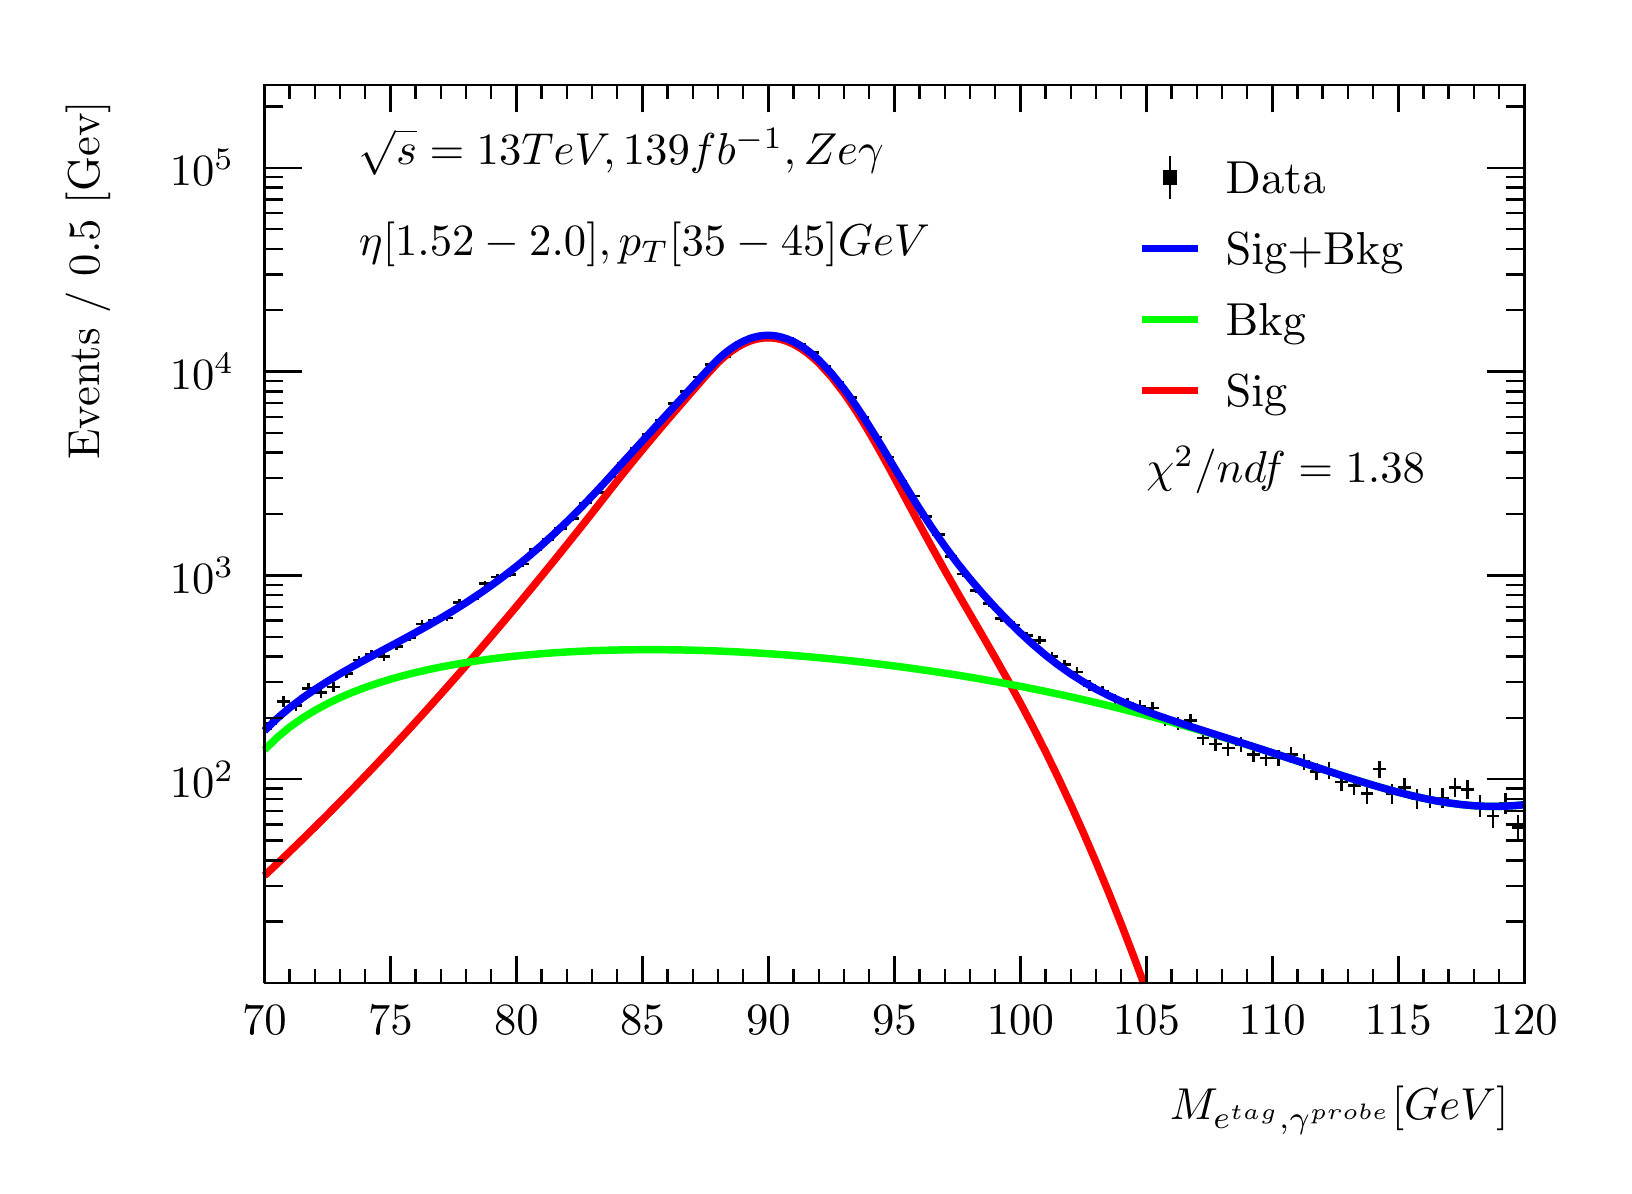
\begin{tikzpicture}
\pgfdeclareplotmark{cross} {
\pgfpathmoveto{\pgfpoint{-0.3\pgfplotmarksize}{\pgfplotmarksize}}
\pgfpathlineto{\pgfpoint{+0.3\pgfplotmarksize}{\pgfplotmarksize}}
\pgfpathlineto{\pgfpoint{+0.3\pgfplotmarksize}{0.3\pgfplotmarksize}}
\pgfpathlineto{\pgfpoint{+1\pgfplotmarksize}{0.3\pgfplotmarksize}}
\pgfpathlineto{\pgfpoint{+1\pgfplotmarksize}{-0.3\pgfplotmarksize}}
\pgfpathlineto{\pgfpoint{+0.3\pgfplotmarksize}{-0.3\pgfplotmarksize}}
\pgfpathlineto{\pgfpoint{+0.3\pgfplotmarksize}{-1.\pgfplotmarksize}}
\pgfpathlineto{\pgfpoint{-0.3\pgfplotmarksize}{-1.\pgfplotmarksize}}
\pgfpathlineto{\pgfpoint{-0.3\pgfplotmarksize}{-0.3\pgfplotmarksize}}
\pgfpathlineto{\pgfpoint{-1.\pgfplotmarksize}{-0.3\pgfplotmarksize}}
\pgfpathlineto{\pgfpoint{-1.\pgfplotmarksize}{0.3\pgfplotmarksize}}
\pgfpathlineto{\pgfpoint{-0.3\pgfplotmarksize}{0.3\pgfplotmarksize}}
\pgfpathclose
\pgfusepathqstroke
}
\pgfdeclareplotmark{cross*} {
\pgfpathmoveto{\pgfpoint{-0.3\pgfplotmarksize}{\pgfplotmarksize}}
\pgfpathlineto{\pgfpoint{+0.3\pgfplotmarksize}{\pgfplotmarksize}}
\pgfpathlineto{\pgfpoint{+0.3\pgfplotmarksize}{0.3\pgfplotmarksize}}
\pgfpathlineto{\pgfpoint{+1\pgfplotmarksize}{0.3\pgfplotmarksize}}
\pgfpathlineto{\pgfpoint{+1\pgfplotmarksize}{-0.3\pgfplotmarksize}}
\pgfpathlineto{\pgfpoint{+0.3\pgfplotmarksize}{-0.3\pgfplotmarksize}}
\pgfpathlineto{\pgfpoint{+0.3\pgfplotmarksize}{-1.\pgfplotmarksize}}
\pgfpathlineto{\pgfpoint{-0.3\pgfplotmarksize}{-1.\pgfplotmarksize}}
\pgfpathlineto{\pgfpoint{-0.3\pgfplotmarksize}{-0.3\pgfplotmarksize}}
\pgfpathlineto{\pgfpoint{-1.\pgfplotmarksize}{-0.3\pgfplotmarksize}}
\pgfpathlineto{\pgfpoint{-1.\pgfplotmarksize}{0.3\pgfplotmarksize}}
\pgfpathlineto{\pgfpoint{-0.3\pgfplotmarksize}{0.3\pgfplotmarksize}}
\pgfpathclose
\pgfusepathqfillstroke
}
\pgfdeclareplotmark{newstar} {
\pgfpathmoveto{\pgfqpoint{0pt}{\pgfplotmarksize}}
\pgfpathlineto{\pgfqpointpolar{44}{0.5\pgfplotmarksize}}
\pgfpathlineto{\pgfqpointpolar{18}{\pgfplotmarksize}}
\pgfpathlineto{\pgfqpointpolar{-20}{0.5\pgfplotmarksize}}
\pgfpathlineto{\pgfqpointpolar{-54}{\pgfplotmarksize}}
\pgfpathlineto{\pgfqpointpolar{-90}{0.5\pgfplotmarksize}}
\pgfpathlineto{\pgfqpointpolar{234}{\pgfplotmarksize}}
\pgfpathlineto{\pgfqpointpolar{198}{0.5\pgfplotmarksize}}
\pgfpathlineto{\pgfqpointpolar{162}{\pgfplotmarksize}}
\pgfpathlineto{\pgfqpointpolar{134}{0.5\pgfplotmarksize}}
\pgfpathclose
\pgfusepathqstroke
}
\pgfdeclareplotmark{newstar*} {
\pgfpathmoveto{\pgfqpoint{0pt}{\pgfplotmarksize}}
\pgfpathlineto{\pgfqpointpolar{44}{0.5\pgfplotmarksize}}
\pgfpathlineto{\pgfqpointpolar{18}{\pgfplotmarksize}}
\pgfpathlineto{\pgfqpointpolar{-20}{0.5\pgfplotmarksize}}
\pgfpathlineto{\pgfqpointpolar{-54}{\pgfplotmarksize}}
\pgfpathlineto{\pgfqpointpolar{-90}{0.5\pgfplotmarksize}}
\pgfpathlineto{\pgfqpointpolar{234}{\pgfplotmarksize}}
\pgfpathlineto{\pgfqpointpolar{198}{0.5\pgfplotmarksize}}
\pgfpathlineto{\pgfqpointpolar{162}{\pgfplotmarksize}}
\pgfpathlineto{\pgfqpointpolar{134}{0.5\pgfplotmarksize}}
\pgfpathclose
\pgfusepathqfillstroke
}
\definecolor{c}{rgb}{1,1,1};
\draw [color=c, fill=c] (0,0) rectangle (20,14.4361);
\draw [color=c, fill=c] (3,2.30977) rectangle (19,13.7143);
\definecolor{c}{rgb}{0,0,0};
\draw [c,line width=0.9] (3,2.30977) -- (3,13.7143) -- (19,13.7143) -- (19,2.30977) -- (3,2.30977);
\definecolor{c}{rgb}{1,1,1};
\draw [color=c, fill=c] (3,2.30977) rectangle (19,13.7143);
\definecolor{c}{rgb}{0,0,0};
\draw [c,line width=0.9] (3,2.30977) -- (3,13.7143) -- (19,13.7143) -- (19,2.30977) -- (3,2.30977);
\draw [c,line width=0.9] (3,2.30977) -- (19,2.30977);
\draw [c,line width=0.9] (3,2.65624) -- (3,2.30977);
\draw [c,line width=0.9] (3.32,2.48301) -- (3.32,2.30977);
\draw [c,line width=0.9] (3.64,2.48301) -- (3.64,2.30977);
\draw [c,line width=0.9] (3.96,2.48301) -- (3.96,2.30977);
\draw [c,line width=0.9] (4.28,2.48301) -- (4.28,2.30977);
\draw [c,line width=0.9] (4.6,2.65624) -- (4.6,2.30977);
\draw [c,line width=0.9] (4.92,2.48301) -- (4.92,2.30977);
\draw [c,line width=0.9] (5.24,2.48301) -- (5.24,2.30977);
\draw [c,line width=0.9] (5.56,2.48301) -- (5.56,2.30977);
\draw [c,line width=0.9] (5.88,2.48301) -- (5.88,2.30977);
\draw [c,line width=0.9] (6.2,2.65624) -- (6.2,2.30977);
\draw [c,line width=0.9] (6.52,2.48301) -- (6.52,2.30977);
\draw [c,line width=0.9] (6.84,2.48301) -- (6.84,2.30977);
\draw [c,line width=0.9] (7.16,2.48301) -- (7.16,2.30977);
\draw [c,line width=0.9] (7.48,2.48301) -- (7.48,2.30977);
\draw [c,line width=0.9] (7.8,2.65624) -- (7.8,2.30977);
\draw [c,line width=0.9] (8.12,2.48301) -- (8.12,2.30977);
\draw [c,line width=0.9] (8.44,2.48301) -- (8.44,2.30977);
\draw [c,line width=0.9] (8.76,2.48301) -- (8.76,2.30977);
\draw [c,line width=0.9] (9.08,2.48301) -- (9.08,2.30977);
\draw [c,line width=0.9] (9.4,2.65624) -- (9.4,2.30977);
\draw [c,line width=0.9] (9.72,2.48301) -- (9.72,2.30977);
\draw [c,line width=0.9] (10.04,2.48301) -- (10.04,2.30977);
\draw [c,line width=0.9] (10.36,2.48301) -- (10.36,2.30977);
\draw [c,line width=0.9] (10.68,2.48301) -- (10.68,2.30977);
\draw [c,line width=0.9] (11,2.65624) -- (11,2.30977);
\draw [c,line width=0.9] (11.32,2.48301) -- (11.32,2.30977);
\draw [c,line width=0.9] (11.64,2.48301) -- (11.64,2.30977);
\draw [c,line width=0.9] (11.96,2.48301) -- (11.96,2.30977);
\draw [c,line width=0.9] (12.28,2.48301) -- (12.28,2.30977);
\draw [c,line width=0.9] (12.6,2.65624) -- (12.6,2.30977);
\draw [c,line width=0.9] (12.92,2.48301) -- (12.92,2.30977);
\draw [c,line width=0.9] (13.24,2.48301) -- (13.24,2.30977);
\draw [c,line width=0.9] (13.56,2.48301) -- (13.56,2.30977);
\draw [c,line width=0.9] (13.88,2.48301) -- (13.88,2.30977);
\draw [c,line width=0.9] (14.2,2.65624) -- (14.2,2.30977);
\draw [c,line width=0.9] (14.52,2.48301) -- (14.52,2.30977);
\draw [c,line width=0.9] (14.84,2.48301) -- (14.84,2.30977);
\draw [c,line width=0.9] (15.16,2.48301) -- (15.16,2.30977);
\draw [c,line width=0.9] (15.48,2.48301) -- (15.48,2.30977);
\draw [c,line width=0.9] (15.8,2.65624) -- (15.8,2.30977);
\draw [c,line width=0.9] (16.12,2.48301) -- (16.12,2.30977);
\draw [c,line width=0.9] (16.44,2.48301) -- (16.44,2.30977);
\draw [c,line width=0.9] (16.76,2.48301) -- (16.76,2.30977);
\draw [c,line width=0.9] (17.08,2.48301) -- (17.08,2.30977);
\draw [c,line width=0.9] (17.4,2.65624) -- (17.4,2.30977);
\draw [c,line width=0.9] (17.72,2.48301) -- (17.72,2.30977);
\draw [c,line width=0.9] (18.04,2.48301) -- (18.04,2.30977);
\draw [c,line width=0.9] (18.36,2.48301) -- (18.36,2.30977);
\draw [c,line width=0.9] (18.68,2.48301) -- (18.68,2.30977);
\draw [c,line width=0.9] (19,2.65624) -- (19,2.30977);
\draw [anchor=base] (3,1.66015) node[scale=1.61424, color=c, rotate=0]{70};
\draw [anchor=base] (4.6,1.66015) node[scale=1.61424, color=c, rotate=0]{75};
\draw [anchor=base] (6.2,1.66015) node[scale=1.61424, color=c, rotate=0]{80};
\draw [anchor=base] (7.8,1.66015) node[scale=1.61424, color=c, rotate=0]{85};
\draw [anchor=base] (9.4,1.66015) node[scale=1.61424, color=c, rotate=0]{90};
\draw [anchor=base] (11,1.66015) node[scale=1.61424, color=c, rotate=0]{95};
\draw [anchor=base] (12.6,1.66015) node[scale=1.61424, color=c, rotate=0]{100};
\draw [anchor=base] (14.2,1.66015) node[scale=1.61424, color=c, rotate=0]{105};
\draw [anchor=base] (15.8,1.66015) node[scale=1.61424, color=c, rotate=0]{110};
\draw [anchor=base] (17.4,1.66015) node[scale=1.61424, color=c, rotate=0]{115};
\draw [anchor=base] (19,1.66015) node[scale=1.61424, color=c, rotate=0]{120};
\draw [anchor= east] (19,0.692932) node[scale=1.61424, color=c, rotate=0]{$M_{e^{tag}, \gamma^{probe}}  [GeV]$};
\draw [c,line width=0.9] (3,13.7143) -- (19,13.7143);
\draw [c,line width=0.9] (3,13.3678) -- (3,13.7143);
\draw [c,line width=0.9] (3.32,13.5411) -- (3.32,13.7143);
\draw [c,line width=0.9] (3.64,13.5411) -- (3.64,13.7143);
\draw [c,line width=0.9] (3.96,13.5411) -- (3.96,13.7143);
\draw [c,line width=0.9] (4.28,13.5411) -- (4.28,13.7143);
\draw [c,line width=0.9] (4.6,13.3678) -- (4.6,13.7143);
\draw [c,line width=0.9] (4.92,13.5411) -- (4.92,13.7143);
\draw [c,line width=0.9] (5.24,13.5411) -- (5.24,13.7143);
\draw [c,line width=0.9] (5.56,13.5411) -- (5.56,13.7143);
\draw [c,line width=0.9] (5.88,13.5411) -- (5.88,13.7143);
\draw [c,line width=0.9] (6.2,13.3678) -- (6.2,13.7143);
\draw [c,line width=0.9] (6.52,13.5411) -- (6.52,13.7143);
\draw [c,line width=0.9] (6.84,13.5411) -- (6.84,13.7143);
\draw [c,line width=0.9] (7.16,13.5411) -- (7.16,13.7143);
\draw [c,line width=0.9] (7.48,13.5411) -- (7.48,13.7143);
\draw [c,line width=0.9] (7.8,13.3678) -- (7.8,13.7143);
\draw [c,line width=0.9] (8.12,13.5411) -- (8.12,13.7143);
\draw [c,line width=0.9] (8.44,13.5411) -- (8.44,13.7143);
\draw [c,line width=0.9] (8.76,13.5411) -- (8.76,13.7143);
\draw [c,line width=0.9] (9.08,13.5411) -- (9.08,13.7143);
\draw [c,line width=0.9] (9.4,13.3678) -- (9.4,13.7143);
\draw [c,line width=0.9] (9.72,13.5411) -- (9.72,13.7143);
\draw [c,line width=0.9] (10.04,13.5411) -- (10.04,13.7143);
\draw [c,line width=0.9] (10.36,13.5411) -- (10.36,13.7143);
\draw [c,line width=0.9] (10.68,13.5411) -- (10.68,13.7143);
\draw [c,line width=0.9] (11,13.3678) -- (11,13.7143);
\draw [c,line width=0.9] (11.32,13.5411) -- (11.32,13.7143);
\draw [c,line width=0.9] (11.64,13.5411) -- (11.64,13.7143);
\draw [c,line width=0.9] (11.96,13.5411) -- (11.96,13.7143);
\draw [c,line width=0.9] (12.28,13.5411) -- (12.28,13.7143);
\draw [c,line width=0.9] (12.6,13.3678) -- (12.6,13.7143);
\draw [c,line width=0.9] (12.92,13.5411) -- (12.92,13.7143);
\draw [c,line width=0.9] (13.24,13.5411) -- (13.24,13.7143);
\draw [c,line width=0.9] (13.56,13.5411) -- (13.56,13.7143);
\draw [c,line width=0.9] (13.88,13.5411) -- (13.88,13.7143);
\draw [c,line width=0.9] (14.2,13.3678) -- (14.2,13.7143);
\draw [c,line width=0.9] (14.52,13.5411) -- (14.52,13.7143);
\draw [c,line width=0.9] (14.84,13.5411) -- (14.84,13.7143);
\draw [c,line width=0.9] (15.16,13.5411) -- (15.16,13.7143);
\draw [c,line width=0.9] (15.48,13.5411) -- (15.48,13.7143);
\draw [c,line width=0.9] (15.8,13.3678) -- (15.8,13.7143);
\draw [c,line width=0.9] (16.12,13.5411) -- (16.12,13.7143);
\draw [c,line width=0.9] (16.44,13.5411) -- (16.44,13.7143);
\draw [c,line width=0.9] (16.76,13.5411) -- (16.76,13.7143);
\draw [c,line width=0.9] (17.08,13.5411) -- (17.08,13.7143);
\draw [c,line width=0.9] (17.4,13.3678) -- (17.4,13.7143);
\draw [c,line width=0.9] (17.72,13.5411) -- (17.72,13.7143);
\draw [c,line width=0.9] (18.04,13.5411) -- (18.04,13.7143);
\draw [c,line width=0.9] (18.36,13.5411) -- (18.36,13.7143);
\draw [c,line width=0.9] (18.68,13.5411) -- (18.68,13.7143);
\draw [c,line width=0.9] (19,13.3678) -- (19,13.7143);
\draw [c,line width=0.9] (3,2.30977) -- (3,13.7143);
\draw [c,line width=0.9] (3.237,3.08897) -- (3,3.08897);
\draw [c,line width=0.9] (3.237,3.54477) -- (3,3.54477);
\draw [c,line width=0.9] (3.237,3.86817) -- (3,3.86817);
\draw [c,line width=0.9] (3.237,4.11902) -- (3,4.11902);
\draw [c,line width=0.9] (3.237,4.32397) -- (3,4.32397);
\draw [c,line width=0.9] (3.237,4.49726) -- (3,4.49726);
\draw [c,line width=0.9] (3.237,4.64737) -- (3,4.64737);
\draw [c,line width=0.9] (3.237,4.77978) -- (3,4.77978);
\draw [c,line width=0.9] (3.474,4.89822) -- (3,4.89822);
\draw [anchor= east] (2.82,4.89822) node[scale=1.61424, color=c, rotate=0]{$10^{2}$};
\draw [c,line width=0.9] (3.237,5.67742) -- (3,5.67742);
\draw [c,line width=0.9] (3.237,6.13322) -- (3,6.13322);
\draw [c,line width=0.9] (3.237,6.45661) -- (3,6.45661);
\draw [c,line width=0.9] (3.237,6.70746) -- (3,6.70746);
\draw [c,line width=0.9] (3.237,6.91242) -- (3,6.91242);
\draw [c,line width=0.9] (3.237,7.08571) -- (3,7.08571);
\draw [c,line width=0.9] (3.237,7.23581) -- (3,7.23581);
\draw [c,line width=0.9] (3.237,7.36822) -- (3,7.36822);
\draw [c,line width=0.9] (3.474,7.48666) -- (3,7.48666);
\draw [anchor= east] (2.82,7.48666) node[scale=1.61424, color=c, rotate=0]{$10^{3}$};
\draw [c,line width=0.9] (3.237,8.26586) -- (3,8.26586);
\draw [c,line width=0.9] (3.237,8.72166) -- (3,8.72166);
\draw [c,line width=0.9] (3.237,9.04506) -- (3,9.04506);
\draw [c,line width=0.9] (3.237,9.29591) -- (3,9.29591);
\draw [c,line width=0.9] (3.237,9.50086) -- (3,9.50086);
\draw [c,line width=0.9] (3.237,9.67415) -- (3,9.67415);
\draw [c,line width=0.9] (3.237,9.82426) -- (3,9.82426);
\draw [c,line width=0.9] (3.237,9.95666) -- (3,9.95666);
\draw [c,line width=0.9] (3.474,10.0751) -- (3,10.0751);
\draw [anchor= east] (2.82,10.0751) node[scale=1.61424, color=c, rotate=0]{$10^{4}$};
\draw [c,line width=0.9] (3.237,10.8543) -- (3,10.8543);
\draw [c,line width=0.9] (3.237,11.3101) -- (3,11.3101);
\draw [c,line width=0.9] (3.237,11.6335) -- (3,11.6335);
\draw [c,line width=0.9] (3.237,11.8844) -- (3,11.8844);
\draw [c,line width=0.9] (3.237,12.0893) -- (3,12.0893);
\draw [c,line width=0.9] (3.237,12.2626) -- (3,12.2626);
\draw [c,line width=0.9] (3.237,12.4127) -- (3,12.4127);
\draw [c,line width=0.9] (3.237,12.5451) -- (3,12.5451);
\draw [c,line width=0.9] (3.474,12.6635) -- (3,12.6635);
\draw [anchor= east] (2.82,12.6635) node[scale=1.61424, color=c, rotate=0]{$10^{5}$};
\draw [c,line width=0.9] (3.237,13.4427) -- (3,13.4427);
\draw [anchor= east] (0.76,13.7143) node[scale=1.61424, color=c, rotate=90]{Events / 0.5 [Gev]};
\draw [c,line width=0.9] (19,2.30977) -- (19,13.7143);
\draw [c,line width=0.9] (18.763,3.08897) -- (19,3.08897);
\draw [c,line width=0.9] (18.763,3.54477) -- (19,3.54477);
\draw [c,line width=0.9] (18.763,3.86817) -- (19,3.86817);
\draw [c,line width=0.9] (18.763,4.11902) -- (19,4.11902);
\draw [c,line width=0.9] (18.763,4.32397) -- (19,4.32397);
\draw [c,line width=0.9] (18.763,4.49726) -- (19,4.49726);
\draw [c,line width=0.9] (18.763,4.64737) -- (19,4.64737);
\draw [c,line width=0.9] (18.763,4.77978) -- (19,4.77978);
\draw [c,line width=0.9] (18.526,4.89822) -- (19,4.89822);
\draw [c,line width=0.9] (18.763,5.67742) -- (19,5.67742);
\draw [c,line width=0.9] (18.763,6.13322) -- (19,6.13322);
\draw [c,line width=0.9] (18.763,6.45661) -- (19,6.45661);
\draw [c,line width=0.9] (18.763,6.70746) -- (19,6.70746);
\draw [c,line width=0.9] (18.763,6.91242) -- (19,6.91242);
\draw [c,line width=0.9] (18.763,7.08571) -- (19,7.08571);
\draw [c,line width=0.9] (18.763,7.23581) -- (19,7.23581);
\draw [c,line width=0.9] (18.763,7.36822) -- (19,7.36822);
\draw [c,line width=0.9] (18.526,7.48666) -- (19,7.48666);
\draw [c,line width=0.9] (18.763,8.26586) -- (19,8.26586);
\draw [c,line width=0.9] (18.763,8.72166) -- (19,8.72166);
\draw [c,line width=0.9] (18.763,9.04506) -- (19,9.04506);
\draw [c,line width=0.9] (18.763,9.29591) -- (19,9.29591);
\draw [c,line width=0.9] (18.763,9.50086) -- (19,9.50086);
\draw [c,line width=0.9] (18.763,9.67415) -- (19,9.67415);
\draw [c,line width=0.9] (18.763,9.82426) -- (19,9.82426);
\draw [c,line width=0.9] (18.763,9.95666) -- (19,9.95666);
\draw [c,line width=0.9] (18.526,10.0751) -- (19,10.0751);
\draw [c,line width=0.9] (18.763,10.8543) -- (19,10.8543);
\draw [c,line width=0.9] (18.763,11.3101) -- (19,11.3101);
\draw [c,line width=0.9] (18.763,11.6335) -- (19,11.6335);
\draw [c,line width=0.9] (18.763,11.8844) -- (19,11.8844);
\draw [c,line width=0.9] (18.763,12.0893) -- (19,12.0893);
\draw [c,line width=0.9] (18.763,12.2626) -- (19,12.2626);
\draw [c,line width=0.9] (18.763,12.4127) -- (19,12.4127);
\draw [c,line width=0.9] (18.763,12.5451) -- (19,12.5451);
\draw [c,line width=0.9] (18.526,12.6635) -- (19,12.6635);
\draw [c,line width=0.9] (18.763,13.4427) -- (19,13.4427);
\draw [c,line width=0.9] (3.08,5.60786) -- (3,5.60786);
\draw [c,line width=0.9] (3,5.60786) -- (3,5.60786);
\draw [c,line width=0.9] (3.08,5.60786) -- (3.16,5.60786);
\draw [c,line width=0.9] (3.16,5.60786) -- (3.16,5.60786);
\draw [c,line width=0.9] (3.08,5.60786) -- (3.08,5.68983);
\draw [c,line width=0.9] (3.08,5.68983) -- (3.08,5.68983);
\draw [c,line width=0.9] (3.08,5.60786) -- (3.08,5.52589);
\draw [c,line width=0.9] (3.08,5.52589) -- (3.08,5.52589);
\draw [c,line width=0.9] (3.24,5.88705) -- (3.16,5.88705);
\draw [c,line width=0.9] (3.16,5.88705) -- (3.16,5.88705);
\draw [c,line width=0.9] (3.24,5.88705) -- (3.32,5.88705);
\draw [c,line width=0.9] (3.32,5.88705) -- (3.32,5.88705);
\draw [c,line width=0.9] (3.24,5.88705) -- (3.24,5.95945);
\draw [c,line width=0.9] (3.24,5.95945) -- (3.24,5.95945);
\draw [c,line width=0.9] (3.24,5.88705) -- (3.24,5.81465);
\draw [c,line width=0.9] (3.24,5.81465) -- (3.24,5.81465);
\draw [c,line width=0.9] (3.4,5.83453) -- (3.32,5.83453);
\draw [c,line width=0.9] (3.32,5.83453) -- (3.32,5.83453);
\draw [c,line width=0.9] (3.4,5.83453) -- (3.48,5.83453);
\draw [c,line width=0.9] (3.48,5.83453) -- (3.48,5.83453);
\draw [c,line width=0.9] (3.4,5.83453) -- (3.4,5.90864);
\draw [c,line width=0.9] (3.4,5.90864) -- (3.4,5.90864);
\draw [c,line width=0.9] (3.4,5.83453) -- (3.4,5.76042);
\draw [c,line width=0.9] (3.4,5.76042) -- (3.4,5.76042);
\draw [c,line width=0.9] (3.56,6.0476) -- (3.48,6.0476);
\draw [c,line width=0.9] (3.48,6.0476) -- (3.48,6.0476);
\draw [c,line width=0.9] (3.56,6.0476) -- (3.64,6.0476);
\draw [c,line width=0.9] (3.64,6.0476) -- (3.64,6.0476);
\draw [c,line width=0.9] (3.56,6.0476) -- (3.56,6.11502);
\draw [c,line width=0.9] (3.56,6.11502) -- (3.56,6.11502);
\draw [c,line width=0.9] (3.56,6.0476) -- (3.56,5.98019);
\draw [c,line width=0.9] (3.56,5.98019) -- (3.56,5.98019);
\draw [c,line width=0.9] (3.72,6.00222) -- (3.64,6.00222);
\draw [c,line width=0.9] (3.64,6.00222) -- (3.64,6.00222);
\draw [c,line width=0.9] (3.72,6.00222) -- (3.8,6.00222);
\draw [c,line width=0.9] (3.8,6.00222) -- (3.8,6.00222);
\draw [c,line width=0.9] (3.72,6.00222) -- (3.72,6.071);
\draw [c,line width=0.9] (3.72,6.071) -- (3.72,6.071);
\draw [c,line width=0.9] (3.72,6.00222) -- (3.72,5.93343);
\draw [c,line width=0.9] (3.72,5.93343) -- (3.72,5.93343);
\draw [c,line width=0.9] (3.88,6.07161) -- (3.8,6.07161);
\draw [c,line width=0.9] (3.8,6.07161) -- (3.8,6.07161);
\draw [c,line width=0.9] (3.88,6.07161) -- (3.96,6.07161);
\draw [c,line width=0.9] (3.96,6.07161) -- (3.96,6.07161);
\draw [c,line width=0.9] (3.88,6.07161) -- (3.88,6.1383);
\draw [c,line width=0.9] (3.88,6.1383) -- (3.88,6.1383);
\draw [c,line width=0.9] (3.88,6.07161) -- (3.88,6.00491);
\draw [c,line width=0.9] (3.88,6.00491) -- (3.88,6.00491);
\draw [c,line width=0.9] (4.04,6.24036) -- (3.96,6.24036);
\draw [c,line width=0.9] (3.96,6.24036) -- (3.96,6.24036);
\draw [c,line width=0.9] (4.04,6.24036) -- (4.12,6.24036);
\draw [c,line width=0.9] (4.12,6.24036) -- (4.12,6.24036);
\draw [c,line width=0.9] (4.04,6.24036) -- (4.04,6.30224);
\draw [c,line width=0.9] (4.04,6.30224) -- (4.04,6.30224);
\draw [c,line width=0.9] (4.04,6.24036) -- (4.04,6.17849);
\draw [c,line width=0.9] (4.04,6.17849) -- (4.04,6.17849);
\draw [c,line width=0.9] (4.2,6.41073) -- (4.12,6.41073);
\draw [c,line width=0.9] (4.12,6.41073) -- (4.12,6.41073);
\draw [c,line width=0.9] (4.2,6.41073) -- (4.28,6.41073);
\draw [c,line width=0.9] (4.28,6.41073) -- (4.28,6.41073);
\draw [c,line width=0.9] (4.2,6.41073) -- (4.2,6.46809);
\draw [c,line width=0.9] (4.2,6.46809) -- (4.2,6.46809);
\draw [c,line width=0.9] (4.2,6.41073) -- (4.2,6.35337);
\draw [c,line width=0.9] (4.2,6.35337) -- (4.2,6.35337);
\draw [c,line width=0.9] (4.36,6.48163) -- (4.28,6.48163);
\draw [c,line width=0.9] (4.28,6.48163) -- (4.28,6.48163);
\draw [c,line width=0.9] (4.36,6.48163) -- (4.44,6.48163);
\draw [c,line width=0.9] (4.44,6.48163) -- (4.44,6.48163);
\draw [c,line width=0.9] (4.36,6.48163) -- (4.36,6.53721);
\draw [c,line width=0.9] (4.36,6.53721) -- (4.36,6.53721);
\draw [c,line width=0.9] (4.36,6.48163) -- (4.36,6.42605);
\draw [c,line width=0.9] (4.36,6.42605) -- (4.36,6.42605);
\draw [c,line width=0.9] (4.52,6.45662) -- (4.44,6.45662);
\draw [c,line width=0.9] (4.44,6.45662) -- (4.44,6.45662);
\draw [c,line width=0.9] (4.52,6.45662) -- (4.6,6.45662);
\draw [c,line width=0.9] (4.6,6.45662) -- (4.6,6.45662);
\draw [c,line width=0.9] (4.52,6.45662) -- (4.52,6.51282);
\draw [c,line width=0.9] (4.52,6.51282) -- (4.52,6.51282);
\draw [c,line width=0.9] (4.52,6.45662) -- (4.52,6.40042);
\draw [c,line width=0.9] (4.52,6.40042) -- (4.52,6.40042);
\draw [c,line width=0.9] (4.68,6.58652) -- (4.6,6.58652);
\draw [c,line width=0.9] (4.6,6.58652) -- (4.6,6.58652);
\draw [c,line width=0.9] (4.68,6.58652) -- (4.76,6.58652);
\draw [c,line width=0.9] (4.76,6.58652) -- (4.76,6.58652);
\draw [c,line width=0.9] (4.68,6.58652) -- (4.68,6.63957);
\draw [c,line width=0.9] (4.68,6.63957) -- (4.68,6.63957);
\draw [c,line width=0.9] (4.68,6.58652) -- (4.68,6.53347);
\draw [c,line width=0.9] (4.68,6.53347) -- (4.68,6.53347);
\draw [c,line width=0.9] (4.84,6.7007) -- (4.76,6.7007);
\draw [c,line width=0.9] (4.76,6.7007) -- (4.76,6.7007);
\draw [c,line width=0.9] (4.84,6.7007) -- (4.92,6.7007);
\draw [c,line width=0.9] (4.92,6.7007) -- (4.92,6.7007);
\draw [c,line width=0.9] (4.84,6.7007) -- (4.84,6.75112);
\draw [c,line width=0.9] (4.84,6.75112) -- (4.84,6.75112);
\draw [c,line width=0.9] (4.84,6.7007) -- (4.84,6.65028);
\draw [c,line width=0.9] (4.84,6.65028) -- (4.84,6.65028);
\draw [c,line width=0.9] (5,6.86848) -- (4.92,6.86848);
\draw [c,line width=0.9] (4.92,6.86848) -- (4.92,6.86848);
\draw [c,line width=0.9] (5,6.86848) -- (5.08,6.86848);
\draw [c,line width=0.9] (5.08,6.86848) -- (5.08,6.86848);
\draw [c,line width=0.9] (5,6.86848) -- (5,6.91527);
\draw [c,line width=0.9] (5,6.91527) -- (5,6.91527);
\draw [c,line width=0.9] (5,6.86848) -- (5,6.82168);
\draw [c,line width=0.9] (5,6.82168) -- (5,6.82168);
\draw [c,line width=0.9] (5.16,6.91803) -- (5.08,6.91803);
\draw [c,line width=0.9] (5.08,6.91803) -- (5.08,6.91803);
\draw [c,line width=0.9] (5.16,6.91803) -- (5.24,6.91803);
\draw [c,line width=0.9] (5.24,6.91803) -- (5.24,6.91803);
\draw [c,line width=0.9] (5.16,6.91803) -- (5.16,6.9638);
\draw [c,line width=0.9] (5.16,6.9638) -- (5.16,6.9638);
\draw [c,line width=0.9] (5.16,6.91803) -- (5.16,6.87225);
\draw [c,line width=0.9] (5.16,6.87225) -- (5.16,6.87225);
\draw [c,line width=0.9] (5.32,6.94746) -- (5.24,6.94746);
\draw [c,line width=0.9] (5.24,6.94746) -- (5.24,6.94746);
\draw [c,line width=0.9] (5.32,6.94746) -- (5.4,6.94746);
\draw [c,line width=0.9] (5.4,6.94746) -- (5.4,6.94746);
\draw [c,line width=0.9] (5.32,6.94746) -- (5.32,6.99265);
\draw [c,line width=0.9] (5.32,6.99265) -- (5.32,6.99265);
\draw [c,line width=0.9] (5.32,6.94746) -- (5.32,6.90229);
\draw [c,line width=0.9] (5.32,6.90229) -- (5.32,6.90229);
\draw [c,line width=0.9] (5.48,7.14208) -- (5.4,7.14208);
\draw [c,line width=0.9] (5.4,7.14208) -- (5.4,7.14208);
\draw [c,line width=0.9] (5.48,7.14208) -- (5.56,7.14208);
\draw [c,line width=0.9] (5.56,7.14208) -- (5.56,7.14208);
\draw [c,line width=0.9] (5.48,7.14208) -- (5.48,7.18352);
\draw [c,line width=0.9] (5.48,7.18352) -- (5.48,7.18352);
\draw [c,line width=0.9] (5.48,7.14208) -- (5.48,7.10065);
\draw [c,line width=0.9] (5.48,7.10065) -- (5.48,7.10065);
\draw [c,line width=0.9] (5.64,7.18553) -- (5.56,7.18553);
\draw [c,line width=0.9] (5.56,7.18553) -- (5.56,7.18553);
\draw [c,line width=0.9] (5.64,7.18553) -- (5.72,7.18553);
\draw [c,line width=0.9] (5.72,7.18553) -- (5.72,7.18553);
\draw [c,line width=0.9] (5.64,7.18553) -- (5.64,7.22617);
\draw [c,line width=0.9] (5.64,7.22617) -- (5.64,7.22617);
\draw [c,line width=0.9] (5.64,7.18553) -- (5.64,7.14489);
\draw [c,line width=0.9] (5.64,7.14489) -- (5.64,7.14489);
\draw [c,line width=0.9] (5.8,7.38311) -- (5.72,7.38311);
\draw [c,line width=0.9] (5.72,7.38311) -- (5.72,7.38311);
\draw [c,line width=0.9] (5.8,7.38311) -- (5.88,7.38311);
\draw [c,line width=0.9] (5.88,7.38311) -- (5.88,7.38311);
\draw [c,line width=0.9] (5.8,7.38311) -- (5.8,7.42033);
\draw [c,line width=0.9] (5.8,7.42033) -- (5.8,7.42033);
\draw [c,line width=0.9] (5.8,7.38311) -- (5.8,7.34589);
\draw [c,line width=0.9] (5.8,7.34589) -- (5.8,7.34589);
\draw [c,line width=0.9] (5.96,7.46624) -- (5.88,7.46624);
\draw [c,line width=0.9] (5.88,7.46624) -- (5.88,7.46624);
\draw [c,line width=0.9] (5.96,7.46624) -- (6.04,7.46624);
\draw [c,line width=0.9] (6.04,7.46624) -- (6.04,7.46624);
\draw [c,line width=0.9] (5.96,7.46624) -- (5.96,7.50211);
\draw [c,line width=0.9] (5.96,7.50211) -- (5.96,7.50211);
\draw [c,line width=0.9] (5.96,7.46624) -- (5.96,7.43037);
\draw [c,line width=0.9] (5.96,7.43037) -- (5.96,7.43037);
\draw [c,line width=0.9] (6.12,7.50007) -- (6.04,7.50007);
\draw [c,line width=0.9] (6.04,7.50007) -- (6.04,7.50007);
\draw [c,line width=0.9] (6.12,7.50007) -- (6.2,7.50007);
\draw [c,line width=0.9] (6.2,7.50007) -- (6.2,7.50007);
\draw [c,line width=0.9] (6.12,7.50007) -- (6.12,7.53541);
\draw [c,line width=0.9] (6.12,7.53541) -- (6.12,7.53541);
\draw [c,line width=0.9] (6.12,7.50007) -- (6.12,7.46474);
\draw [c,line width=0.9] (6.12,7.46474) -- (6.12,7.46474);
\draw [c,line width=0.9] (6.28,7.63198) -- (6.2,7.63198);
\draw [c,line width=0.9] (6.2,7.63198) -- (6.2,7.63198);
\draw [c,line width=0.9] (6.28,7.63198) -- (6.36,7.63198);
\draw [c,line width=0.9] (6.36,7.63198) -- (6.36,7.63198);
\draw [c,line width=0.9] (6.28,7.63198) -- (6.28,7.66531);
\draw [c,line width=0.9] (6.28,7.66531) -- (6.28,7.66531);
\draw [c,line width=0.9] (6.28,7.63198) -- (6.28,7.59866);
\draw [c,line width=0.9] (6.28,7.59866) -- (6.28,7.59866);
\draw [c,line width=0.9] (6.44,7.81567) -- (6.36,7.81567);
\draw [c,line width=0.9] (6.36,7.81567) -- (6.36,7.81567);
\draw [c,line width=0.9] (6.44,7.81567) -- (6.52,7.81567);
\draw [c,line width=0.9] (6.52,7.81567) -- (6.52,7.81567);
\draw [c,line width=0.9] (6.44,7.81567) -- (6.44,7.84637);
\draw [c,line width=0.9] (6.44,7.84637) -- (6.44,7.84637);
\draw [c,line width=0.9] (6.44,7.81567) -- (6.44,7.78496);
\draw [c,line width=0.9] (6.44,7.78496) -- (6.44,7.78496);
\draw [c,line width=0.9] (6.6,7.94546) -- (6.52,7.94546);
\draw [c,line width=0.9] (6.52,7.94546) -- (6.52,7.94546);
\draw [c,line width=0.9] (6.6,7.94546) -- (6.68,7.94546);
\draw [c,line width=0.9] (6.68,7.94546) -- (6.68,7.94546);
\draw [c,line width=0.9] (6.6,7.94546) -- (6.6,7.97444);
\draw [c,line width=0.9] (6.6,7.97444) -- (6.6,7.97444);
\draw [c,line width=0.9] (6.6,7.94546) -- (6.6,7.91647);
\draw [c,line width=0.9] (6.6,7.91647) -- (6.6,7.91647);
\draw [c,line width=0.9] (6.76,8.08449) -- (6.68,8.08449);
\draw [c,line width=0.9] (6.68,8.08449) -- (6.68,8.08449);
\draw [c,line width=0.9] (6.76,8.08449) -- (6.84,8.08449);
\draw [c,line width=0.9] (6.84,8.08449) -- (6.84,8.08449);
\draw [c,line width=0.9] (6.76,8.08449) -- (6.76,8.11174);
\draw [c,line width=0.9] (6.76,8.11174) -- (6.76,8.11174);
\draw [c,line width=0.9] (6.76,8.08449) -- (6.76,8.05724);
\draw [c,line width=0.9] (6.76,8.05724) -- (6.76,8.05724);
\draw [c,line width=0.9] (6.92,8.20702) -- (6.84,8.20702);
\draw [c,line width=0.9] (6.84,8.20702) -- (6.84,8.20702);
\draw [c,line width=0.9] (6.92,8.20702) -- (7,8.20702);
\draw [c,line width=0.9] (7,8.20702) -- (7,8.20702);
\draw [c,line width=0.9] (6.92,8.20702) -- (6.92,8.23282);
\draw [c,line width=0.9] (6.92,8.23282) -- (6.92,8.23282);
\draw [c,line width=0.9] (6.92,8.20702) -- (6.92,8.18121);
\draw [c,line width=0.9] (6.92,8.18121) -- (6.92,8.18121);
\draw [c,line width=0.9] (7.08,8.40623) -- (7,8.40623);
\draw [c,line width=0.9] (7,8.40623) -- (7,8.40623);
\draw [c,line width=0.9] (7.08,8.40623) -- (7.16,8.40623);
\draw [c,line width=0.9] (7.16,8.40623) -- (7.16,8.40623);
\draw [c,line width=0.9] (7.08,8.40623) -- (7.08,8.42985);
\draw [c,line width=0.9] (7.08,8.42985) -- (7.08,8.42985);
\draw [c,line width=0.9] (7.08,8.40623) -- (7.08,8.38262);
\draw [c,line width=0.9] (7.08,8.38262) -- (7.08,8.38262);
\draw [c,line width=0.9] (7.24,8.54249) -- (7.16,8.54249);
\draw [c,line width=0.9] (7.16,8.54249) -- (7.16,8.54249);
\draw [c,line width=0.9] (7.24,8.54249) -- (7.32,8.54249);
\draw [c,line width=0.9] (7.32,8.54249) -- (7.32,8.54249);
\draw [c,line width=0.9] (7.24,8.54249) -- (7.24,8.56472);
\draw [c,line width=0.9] (7.24,8.56472) -- (7.24,8.56472);
\draw [c,line width=0.9] (7.24,8.54249) -- (7.24,8.52026);
\draw [c,line width=0.9] (7.24,8.52026) -- (7.24,8.52026);
\draw [c,line width=0.9] (7.4,8.73433) -- (7.32,8.73433);
\draw [c,line width=0.9] (7.32,8.73433) -- (7.32,8.73433);
\draw [c,line width=0.9] (7.4,8.73433) -- (7.48,8.73433);
\draw [c,line width=0.9] (7.48,8.73433) -- (7.48,8.73433);
\draw [c,line width=0.9] (7.4,8.73433) -- (7.4,8.75474);
\draw [c,line width=0.9] (7.4,8.75474) -- (7.4,8.75474);
\draw [c,line width=0.9] (7.4,8.73433) -- (7.4,8.71392);
\draw [c,line width=0.9] (7.4,8.71392) -- (7.4,8.71392);
\draw [c,line width=0.9] (7.56,8.91658) -- (7.48,8.91658);
\draw [c,line width=0.9] (7.48,8.91658) -- (7.48,8.91658);
\draw [c,line width=0.9] (7.56,8.91658) -- (7.64,8.91658);
\draw [c,line width=0.9] (7.64,8.91658) -- (7.64,8.91658);
\draw [c,line width=0.9] (7.56,8.91658) -- (7.56,8.9354);
\draw [c,line width=0.9] (7.56,8.9354) -- (7.56,8.9354);
\draw [c,line width=0.9] (7.56,8.91658) -- (7.56,8.89776);
\draw [c,line width=0.9] (7.56,8.89776) -- (7.56,8.89776);
\draw [c,line width=0.9] (7.72,9.10685) -- (7.64,9.10685);
\draw [c,line width=0.9] (7.64,9.10685) -- (7.64,9.10685);
\draw [c,line width=0.9] (7.72,9.10685) -- (7.8,9.10685);
\draw [c,line width=0.9] (7.8,9.10685) -- (7.8,9.10685);
\draw [c,line width=0.9] (7.72,9.10685) -- (7.72,9.12414);
\draw [c,line width=0.9] (7.72,9.12414) -- (7.72,9.12414);
\draw [c,line width=0.9] (7.72,9.10685) -- (7.72,9.08955);
\draw [c,line width=0.9] (7.72,9.08955) -- (7.72,9.08955);
\draw [c,line width=0.9] (7.88,9.2764) -- (7.8,9.2764);
\draw [c,line width=0.9] (7.8,9.2764) -- (7.8,9.2764);
\draw [c,line width=0.9] (7.88,9.2764) -- (7.96,9.2764);
\draw [c,line width=0.9] (7.96,9.2764) -- (7.96,9.2764);
\draw [c,line width=0.9] (7.88,9.2764) -- (7.88,9.29244);
\draw [c,line width=0.9] (7.88,9.29244) -- (7.88,9.29244);
\draw [c,line width=0.9] (7.88,9.2764) -- (7.88,9.26037);
\draw [c,line width=0.9] (7.88,9.26037) -- (7.88,9.26037);
\draw [c,line width=0.9] (8.04,9.46353) -- (7.96,9.46353);
\draw [c,line width=0.9] (7.96,9.46353) -- (7.96,9.46353);
\draw [c,line width=0.9] (8.04,9.46353) -- (8.12,9.46353);
\draw [c,line width=0.9] (8.12,9.46353) -- (8.12,9.46353);
\draw [c,line width=0.9] (8.04,9.46353) -- (8.04,9.47828);
\draw [c,line width=0.9] (8.04,9.47828) -- (8.04,9.47828);
\draw [c,line width=0.9] (8.04,9.46353) -- (8.04,9.44877);
\draw [c,line width=0.9] (8.04,9.44877) -- (8.04,9.44877);
\draw [c,line width=0.9] (8.2,9.66965) -- (8.12,9.66965);
\draw [c,line width=0.9] (8.12,9.66965) -- (8.12,9.66965);
\draw [c,line width=0.9] (8.2,9.66965) -- (8.28,9.66965);
\draw [c,line width=0.9] (8.28,9.66965) -- (8.28,9.66965);
\draw [c,line width=0.9] (8.2,9.66965) -- (8.2,9.68311);
\draw [c,line width=0.9] (8.2,9.68311) -- (8.2,9.68311);
\draw [c,line width=0.9] (8.2,9.66965) -- (8.2,9.65618);
\draw [c,line width=0.9] (8.2,9.65618) -- (8.2,9.65618);
\draw [c,line width=0.9] (8.36,9.81961) -- (8.28,9.81961);
\draw [c,line width=0.9] (8.28,9.81961) -- (8.28,9.81961);
\draw [c,line width=0.9] (8.36,9.81961) -- (8.44,9.81961);
\draw [c,line width=0.9] (8.44,9.81961) -- (8.44,9.81961);
\draw [c,line width=0.9] (8.36,9.81961) -- (8.36,9.83221);
\draw [c,line width=0.9] (8.36,9.83221) -- (8.36,9.83221);
\draw [c,line width=0.9] (8.36,9.81961) -- (8.36,9.80702);
\draw [c,line width=0.9] (8.36,9.80702) -- (8.36,9.80702);
\draw [c,line width=0.9] (8.52,10.0089) -- (8.44,10.0089);
\draw [c,line width=0.9] (8.44,10.0089) -- (8.44,10.0089);
\draw [c,line width=0.9] (8.52,10.0089) -- (8.6,10.0089);
\draw [c,line width=0.9] (8.6,10.0089) -- (8.6,10.0089);
\draw [c,line width=0.9] (8.52,10.0089) -- (8.52,10.0205);
\draw [c,line width=0.9] (8.52,10.0205) -- (8.52,10.0205);
\draw [c,line width=0.9] (8.52,10.0089) -- (8.52,9.99732);
\draw [c,line width=0.9] (8.52,9.99732) -- (8.52,9.99732);
\draw [c,line width=0.9] (8.68,10.1651) -- (8.6,10.1651);
\draw [c,line width=0.9] (8.6,10.1651) -- (8.6,10.1651);
\draw [c,line width=0.9] (8.68,10.1651) -- (8.76,10.1651);
\draw [c,line width=0.9] (8.76,10.1651) -- (8.76,10.1651);
\draw [c,line width=0.9] (8.68,10.1651) -- (8.68,10.1759);
\draw [c,line width=0.9] (8.68,10.1759) -- (8.68,10.1759);
\draw [c,line width=0.9] (8.68,10.1651) -- (8.68,10.1543);
\draw [c,line width=0.9] (8.68,10.1543) -- (8.68,10.1543);
\draw [c,line width=0.9] (8.84,10.2686) -- (8.76,10.2686);
\draw [c,line width=0.9] (8.76,10.2686) -- (8.76,10.2686);
\draw [c,line width=0.9] (8.84,10.2686) -- (8.92,10.2686);
\draw [c,line width=0.9] (8.92,10.2686) -- (8.92,10.2686);
\draw [c,line width=0.9] (8.84,10.2686) -- (8.84,10.2789);
\draw [c,line width=0.9] (8.84,10.2789) -- (8.84,10.2789);
\draw [c,line width=0.9] (8.84,10.2686) -- (8.84,10.2583);
\draw [c,line width=0.9] (8.84,10.2583) -- (8.84,10.2583);
\draw [c,line width=0.9] (9,10.3901) -- (8.92,10.3901);
\draw [c,line width=0.9] (8.92,10.3901) -- (8.92,10.3901);
\draw [c,line width=0.9] (9,10.3901) -- (9.08,10.3901);
\draw [c,line width=0.9] (9.08,10.3901) -- (9.08,10.3901);
\draw [c,line width=0.9] (9,10.3901) -- (9,10.3999);
\draw [c,line width=0.9] (9,10.3999) -- (9,10.3999);
\draw [c,line width=0.9] (9,10.3901) -- (9,10.3803);
\draw [c,line width=0.9] (9,10.3803) -- (9,10.3803);
\draw [c,line width=0.9] (9.16,10.4905) -- (9.08,10.4905);
\draw [c,line width=0.9] (9.08,10.4905) -- (9.08,10.4905);
\draw [c,line width=0.9] (9.16,10.4905) -- (9.24,10.4905);
\draw [c,line width=0.9] (9.24,10.4905) -- (9.24,10.4905);
\draw [c,line width=0.9] (9.16,10.4905) -- (9.16,10.4999);
\draw [c,line width=0.9] (9.16,10.4999) -- (9.16,10.4999);
\draw [c,line width=0.9] (9.16,10.4905) -- (9.16,10.4812);
\draw [c,line width=0.9] (9.16,10.4812) -- (9.16,10.4812);
\draw [c,line width=0.9] (9.32,10.5141) -- (9.24,10.5141);
\draw [c,line width=0.9] (9.24,10.5141) -- (9.24,10.5141);
\draw [c,line width=0.9] (9.32,10.5141) -- (9.4,10.5141);
\draw [c,line width=0.9] (9.4,10.5141) -- (9.4,10.5141);
\draw [c,line width=0.9] (9.32,10.5141) -- (9.32,10.5233);
\draw [c,line width=0.9] (9.32,10.5233) -- (9.32,10.5233);
\draw [c,line width=0.9] (9.32,10.5141) -- (9.32,10.5048);
\draw [c,line width=0.9] (9.32,10.5048) -- (9.32,10.5048);
\draw [c,line width=0.9] (9.48,10.5299) -- (9.4,10.5299);
\draw [c,line width=0.9] (9.4,10.5299) -- (9.4,10.5299);
\draw [c,line width=0.9] (9.48,10.5299) -- (9.56,10.5299);
\draw [c,line width=0.9] (9.56,10.5299) -- (9.56,10.5299);
\draw [c,line width=0.9] (9.48,10.5299) -- (9.48,10.539);
\draw [c,line width=0.9] (9.48,10.539) -- (9.48,10.539);
\draw [c,line width=0.9] (9.48,10.5299) -- (9.48,10.5207);
\draw [c,line width=0.9] (9.48,10.5207) -- (9.48,10.5207);
\draw [c,line width=0.9] (9.64,10.5033) -- (9.56,10.5033);
\draw [c,line width=0.9] (9.56,10.5033) -- (9.56,10.5033);
\draw [c,line width=0.9] (9.64,10.5033) -- (9.72,10.5033);
\draw [c,line width=0.9] (9.72,10.5033) -- (9.72,10.5033);
\draw [c,line width=0.9] (9.64,10.5033) -- (9.64,10.5126);
\draw [c,line width=0.9] (9.64,10.5126) -- (9.64,10.5126);
\draw [c,line width=0.9] (9.64,10.5033) -- (9.64,10.494);
\draw [c,line width=0.9] (9.64,10.494) -- (9.64,10.494);
\draw [c,line width=0.9] (9.8,10.4253) -- (9.72,10.4253);
\draw [c,line width=0.9] (9.72,10.4253) -- (9.72,10.4253);
\draw [c,line width=0.9] (9.8,10.4253) -- (9.88,10.4253);
\draw [c,line width=0.9] (9.88,10.4253) -- (9.88,10.4253);
\draw [c,line width=0.9] (9.8,10.4253) -- (9.8,10.4349);
\draw [c,line width=0.9] (9.8,10.4349) -- (9.8,10.4349);
\draw [c,line width=0.9] (9.8,10.4253) -- (9.8,10.4157);
\draw [c,line width=0.9] (9.8,10.4157) -- (9.8,10.4157);
\draw [c,line width=0.9] (9.96,10.3186) -- (9.88,10.3186);
\draw [c,line width=0.9] (9.88,10.3186) -- (9.88,10.3186);
\draw [c,line width=0.9] (9.96,10.3186) -- (10.04,10.3186);
\draw [c,line width=0.9] (10.04,10.3186) -- (10.04,10.3186);
\draw [c,line width=0.9] (9.96,10.3186) -- (9.96,10.3286);
\draw [c,line width=0.9] (9.96,10.3286) -- (9.96,10.3286);
\draw [c,line width=0.9] (9.96,10.3186) -- (9.96,10.3085);
\draw [c,line width=0.9] (9.96,10.3085) -- (9.96,10.3085);
\draw [c,line width=0.9] (10.12,10.1425) -- (10.04,10.1425);
\draw [c,line width=0.9] (10.04,10.1425) -- (10.04,10.1425);
\draw [c,line width=0.9] (10.12,10.1425) -- (10.2,10.1425);
\draw [c,line width=0.9] (10.2,10.1425) -- (10.2,10.1425);
\draw [c,line width=0.9] (10.12,10.1425) -- (10.12,10.1534);
\draw [c,line width=0.9] (10.12,10.1534) -- (10.12,10.1534);
\draw [c,line width=0.9] (10.12,10.1425) -- (10.12,10.1316);
\draw [c,line width=0.9] (10.12,10.1316) -- (10.12,10.1316);
\draw [c,line width=0.9] (10.28,9.94385) -- (10.2,9.94385);
\draw [c,line width=0.9] (10.2,9.94385) -- (10.2,9.94385);
\draw [c,line width=0.9] (10.28,9.94385) -- (10.36,9.94385);
\draw [c,line width=0.9] (10.36,9.94385) -- (10.36,9.94385);
\draw [c,line width=0.9] (10.28,9.94385) -- (10.28,9.95577);
\draw [c,line width=0.9] (10.28,9.95577) -- (10.28,9.95577);
\draw [c,line width=0.9] (10.28,9.94385) -- (10.28,9.93194);
\draw [c,line width=0.9] (10.28,9.93194) -- (10.28,9.93194);
\draw [c,line width=0.9] (10.44,9.7472) -- (10.36,9.7472);
\draw [c,line width=0.9] (10.36,9.7472) -- (10.36,9.7472);
\draw [c,line width=0.9] (10.44,9.7472) -- (10.52,9.7472);
\draw [c,line width=0.9] (10.52,9.7472) -- (10.52,9.7472);
\draw [c,line width=0.9] (10.44,9.7472) -- (10.44,9.76021);
\draw [c,line width=0.9] (10.44,9.76021) -- (10.44,9.76021);
\draw [c,line width=0.9] (10.44,9.7472) -- (10.44,9.7342);
\draw [c,line width=0.9] (10.44,9.7342) -- (10.44,9.7342);
\draw [c,line width=0.9] (10.6,9.48938) -- (10.52,9.48938);
\draw [c,line width=0.9] (10.52,9.48938) -- (10.52,9.48938);
\draw [c,line width=0.9] (10.6,9.48938) -- (10.68,9.48938);
\draw [c,line width=0.9] (10.68,9.48938) -- (10.68,9.48938);
\draw [c,line width=0.9] (10.6,9.48938) -- (10.6,9.50396);
\draw [c,line width=0.9] (10.6,9.50396) -- (10.6,9.50396);
\draw [c,line width=0.9] (10.6,9.48938) -- (10.6,9.47479);
\draw [c,line width=0.9] (10.6,9.47479) -- (10.6,9.47479);
\draw [c,line width=0.9] (10.76,9.24697) -- (10.68,9.24697);
\draw [c,line width=0.9] (10.68,9.24697) -- (10.68,9.24697);
\draw [c,line width=0.9] (10.76,9.24697) -- (10.84,9.24697);
\draw [c,line width=0.9] (10.84,9.24697) -- (10.84,9.24697);
\draw [c,line width=0.9] (10.76,9.24697) -- (10.76,9.26322);
\draw [c,line width=0.9] (10.76,9.26322) -- (10.76,9.26322);
\draw [c,line width=0.9] (10.76,9.24697) -- (10.76,9.23072);
\draw [c,line width=0.9] (10.76,9.23072) -- (10.76,9.23072);
\draw [c,line width=0.9] (10.92,8.99065) -- (10.84,8.99065);
\draw [c,line width=0.9] (10.84,8.99065) -- (10.84,8.99065);
\draw [c,line width=0.9] (10.92,8.99065) -- (11,8.99065);
\draw [c,line width=0.9] (11,8.99065) -- (11,8.99065);
\draw [c,line width=0.9] (10.92,8.99065) -- (10.92,9.00886);
\draw [c,line width=0.9] (10.92,9.00886) -- (10.92,9.00886);
\draw [c,line width=0.9] (10.92,8.99065) -- (10.92,8.97244);
\draw [c,line width=0.9] (10.92,8.97244) -- (10.92,8.97244);
\draw [c,line width=0.9] (11.08,8.68742) -- (11,8.68742);
\draw [c,line width=0.9] (11,8.68742) -- (11,8.68742);
\draw [c,line width=0.9] (11.08,8.68742) -- (11.16,8.68742);
\draw [c,line width=0.9] (11.16,8.68742) -- (11.16,8.68742);
\draw [c,line width=0.9] (11.08,8.68742) -- (11.08,8.70826);
\draw [c,line width=0.9] (11.08,8.70826) -- (11.08,8.70826);
\draw [c,line width=0.9] (11.08,8.68742) -- (11.08,8.66658);
\draw [c,line width=0.9] (11.08,8.66658) -- (11.08,8.66658);
\draw [c,line width=0.9] (11.24,8.49216) -- (11.16,8.49216);
\draw [c,line width=0.9] (11.16,8.49216) -- (11.16,8.49216);
\draw [c,line width=0.9] (11.24,8.49216) -- (11.32,8.49216);
\draw [c,line width=0.9] (11.32,8.49216) -- (11.32,8.49216);
\draw [c,line width=0.9] (11.24,8.49216) -- (11.24,8.51489);
\draw [c,line width=0.9] (11.24,8.51489) -- (11.24,8.51489);
\draw [c,line width=0.9] (11.24,8.49216) -- (11.24,8.46943);
\draw [c,line width=0.9] (11.24,8.46943) -- (11.24,8.46943);
\draw [c,line width=0.9] (11.4,8.23567) -- (11.32,8.23567);
\draw [c,line width=0.9] (11.32,8.23567) -- (11.32,8.23567);
\draw [c,line width=0.9] (11.4,8.23567) -- (11.48,8.23567);
\draw [c,line width=0.9] (11.48,8.23567) -- (11.48,8.23567);
\draw [c,line width=0.9] (11.4,8.23567) -- (11.4,8.26115);
\draw [c,line width=0.9] (11.4,8.26115) -- (11.4,8.26115);
\draw [c,line width=0.9] (11.4,8.23567) -- (11.4,8.21019);
\draw [c,line width=0.9] (11.4,8.21019) -- (11.4,8.21019);
\draw [c,line width=0.9] (11.56,8.00514) -- (11.48,8.00514);
\draw [c,line width=0.9] (11.48,8.00514) -- (11.48,8.00514);
\draw [c,line width=0.9] (11.56,8.00514) -- (11.64,8.00514);
\draw [c,line width=0.9] (11.64,8.00514) -- (11.64,8.00514);
\draw [c,line width=0.9] (11.56,8.00514) -- (11.56,8.03336);
\draw [c,line width=0.9] (11.56,8.03336) -- (11.56,8.03336);
\draw [c,line width=0.9] (11.56,8.00514) -- (11.56,7.97691);
\draw [c,line width=0.9] (11.56,7.97691) -- (11.56,7.97691);
\draw [c,line width=0.9] (11.72,7.72576) -- (11.64,7.72576);
\draw [c,line width=0.9] (11.64,7.72576) -- (11.64,7.72576);
\draw [c,line width=0.9] (11.72,7.72576) -- (11.8,7.72576);
\draw [c,line width=0.9] (11.8,7.72576) -- (11.8,7.72576);
\draw [c,line width=0.9] (11.72,7.72576) -- (11.72,7.75772);
\draw [c,line width=0.9] (11.72,7.75772) -- (11.72,7.75772);
\draw [c,line width=0.9] (11.72,7.72576) -- (11.72,7.69379);
\draw [c,line width=0.9] (11.72,7.69379) -- (11.72,7.69379);
\draw [c,line width=0.9] (11.88,7.50782) -- (11.8,7.50782);
\draw [c,line width=0.9] (11.8,7.50782) -- (11.8,7.50782);
\draw [c,line width=0.9] (11.88,7.50782) -- (11.96,7.50782);
\draw [c,line width=0.9] (11.96,7.50782) -- (11.96,7.50782);
\draw [c,line width=0.9] (11.88,7.50782) -- (11.88,7.54304);
\draw [c,line width=0.9] (11.88,7.54304) -- (11.88,7.54304);
\draw [c,line width=0.9] (11.88,7.50782) -- (11.88,7.47261);
\draw [c,line width=0.9] (11.88,7.47261) -- (11.88,7.47261);
\draw [c,line width=0.9] (12.04,7.29733) -- (11.96,7.29733);
\draw [c,line width=0.9] (11.96,7.29733) -- (11.96,7.29733);
\draw [c,line width=0.9] (12.04,7.29733) -- (12.12,7.29733);
\draw [c,line width=0.9] (12.12,7.29733) -- (12.12,7.29733);
\draw [c,line width=0.9] (12.04,7.29733) -- (12.04,7.336);
\draw [c,line width=0.9] (12.04,7.336) -- (12.04,7.336);
\draw [c,line width=0.9] (12.04,7.29733) -- (12.04,7.25867);
\draw [c,line width=0.9] (12.04,7.25867) -- (12.04,7.25867);
\draw [c,line width=0.9] (12.2,7.13134) -- (12.12,7.13134);
\draw [c,line width=0.9] (12.12,7.13134) -- (12.12,7.13134);
\draw [c,line width=0.9] (12.2,7.13134) -- (12.28,7.13134);
\draw [c,line width=0.9] (12.28,7.13134) -- (12.28,7.13134);
\draw [c,line width=0.9] (12.2,7.13134) -- (12.2,7.17297);
\draw [c,line width=0.9] (12.2,7.17297) -- (12.2,7.17297);
\draw [c,line width=0.9] (12.2,7.13134) -- (12.2,7.08971);
\draw [c,line width=0.9] (12.2,7.08971) -- (12.2,7.08971);
\draw [c,line width=0.9] (12.36,6.942) -- (12.28,6.942);
\draw [c,line width=0.9] (12.28,6.942) -- (12.28,6.942);
\draw [c,line width=0.9] (12.36,6.942) -- (12.44,6.942);
\draw [c,line width=0.9] (12.44,6.942) -- (12.44,6.942);
\draw [c,line width=0.9] (12.36,6.942) -- (12.36,6.98729);
\draw [c,line width=0.9] (12.36,6.98729) -- (12.36,6.98729);
\draw [c,line width=0.9] (12.36,6.942) -- (12.36,6.89671);
\draw [c,line width=0.9] (12.36,6.89671) -- (12.36,6.89671);
\draw [c,line width=0.9] (12.52,6.85673) -- (12.44,6.85673);
\draw [c,line width=0.9] (12.44,6.85673) -- (12.44,6.85673);
\draw [c,line width=0.9] (12.52,6.85673) -- (12.6,6.85673);
\draw [c,line width=0.9] (12.6,6.85673) -- (12.6,6.85673);
\draw [c,line width=0.9] (12.52,6.85673) -- (12.52,6.90377);
\draw [c,line width=0.9] (12.52,6.90377) -- (12.52,6.90377);
\draw [c,line width=0.9] (12.52,6.85673) -- (12.52,6.80969);
\draw [c,line width=0.9] (12.52,6.80969) -- (12.52,6.80969);
\draw [c,line width=0.9] (12.68,6.72087) -- (12.6,6.72087);
\draw [c,line width=0.9] (12.6,6.72087) -- (12.6,6.72087);
\draw [c,line width=0.9] (12.68,6.72087) -- (12.76,6.72087);
\draw [c,line width=0.9] (12.76,6.72087) -- (12.76,6.72087);
\draw [c,line width=0.9] (12.68,6.72087) -- (12.68,6.77084);
\draw [c,line width=0.9] (12.68,6.77084) -- (12.68,6.77084);
\draw [c,line width=0.9] (12.68,6.72087) -- (12.68,6.6709);
\draw [c,line width=0.9] (12.68,6.6709) -- (12.68,6.6709);
\draw [c,line width=0.9] (12.84,6.66157) -- (12.76,6.66157);
\draw [c,line width=0.9] (12.76,6.66157) -- (12.76,6.66157);
\draw [c,line width=0.9] (12.84,6.66157) -- (12.92,6.66157);
\draw [c,line width=0.9] (12.92,6.66157) -- (12.92,6.66157);
\draw [c,line width=0.9] (12.84,6.66157) -- (12.84,6.71288);
\draw [c,line width=0.9] (12.84,6.71288) -- (12.84,6.71288);
\draw [c,line width=0.9] (12.84,6.66157) -- (12.84,6.61027);
\draw [c,line width=0.9] (12.84,6.61027) -- (12.84,6.61027);
\draw [c,line width=0.9] (13,6.45662) -- (12.92,6.45662);
\draw [c,line width=0.9] (12.92,6.45662) -- (12.92,6.45662);
\draw [c,line width=0.9] (13,6.45662) -- (13.08,6.45662);
\draw [c,line width=0.9] (13.08,6.45662) -- (13.08,6.45662);
\draw [c,line width=0.9] (13,6.45662) -- (13,6.51282);
\draw [c,line width=0.9] (13,6.51282) -- (13,6.51282);
\draw [c,line width=0.9] (13,6.45662) -- (13,6.40042);
\draw [c,line width=0.9] (13,6.40042) -- (13,6.40042);
\draw [c,line width=0.9] (13.16,6.35676) -- (13.08,6.35676);
\draw [c,line width=0.9] (13.08,6.35676) -- (13.08,6.35676);
\draw [c,line width=0.9] (13.16,6.35676) -- (13.24,6.35676);
\draw [c,line width=0.9] (13.24,6.35676) -- (13.24,6.35676);
\draw [c,line width=0.9] (13.16,6.35676) -- (13.16,6.41551);
\draw [c,line width=0.9] (13.16,6.41551) -- (13.16,6.41551);
\draw [c,line width=0.9] (13.16,6.35676) -- (13.16,6.298);
\draw [c,line width=0.9] (13.16,6.298) -- (13.16,6.298);
\draw [c,line width=0.9] (13.32,6.26062) -- (13.24,6.26062);
\draw [c,line width=0.9] (13.24,6.26062) -- (13.24,6.26062);
\draw [c,line width=0.9] (13.32,6.26062) -- (13.4,6.26062);
\draw [c,line width=0.9] (13.4,6.26062) -- (13.4,6.26062);
\draw [c,line width=0.9] (13.32,6.26062) -- (13.32,6.32194);
\draw [c,line width=0.9] (13.32,6.32194) -- (13.32,6.32194);
\draw [c,line width=0.9] (13.32,6.26062) -- (13.32,6.1993);
\draw [c,line width=0.9] (13.32,6.1993) -- (13.32,6.1993);
\draw [c,line width=0.9] (13.48,6.08733) -- (13.4,6.08733);
\draw [c,line width=0.9] (13.4,6.08733) -- (13.4,6.08733);
\draw [c,line width=0.9] (13.48,6.08733) -- (13.56,6.08733);
\draw [c,line width=0.9] (13.56,6.08733) -- (13.56,6.08733);
\draw [c,line width=0.9] (13.48,6.08733) -- (13.48,6.15356);
\draw [c,line width=0.9] (13.48,6.15356) -- (13.48,6.15356);
\draw [c,line width=0.9] (13.48,6.08733) -- (13.48,6.0211);
\draw [c,line width=0.9] (13.48,6.0211) -- (13.48,6.0211);
\draw [c,line width=0.9] (13.64,6.01894) -- (13.56,6.01894);
\draw [c,line width=0.9] (13.56,6.01894) -- (13.56,6.01894);
\draw [c,line width=0.9] (13.64,6.01894) -- (13.72,6.01894);
\draw [c,line width=0.9] (13.72,6.01894) -- (13.72,6.01894);
\draw [c,line width=0.9] (13.64,6.01894) -- (13.64,6.08721);
\draw [c,line width=0.9] (13.64,6.08721) -- (13.64,6.08721);
\draw [c,line width=0.9] (13.64,6.01894) -- (13.64,5.95066);
\draw [c,line width=0.9] (13.64,5.95066) -- (13.64,5.95066);
\draw [c,line width=0.9] (13.8,5.91469) -- (13.72,5.91469);
\draw [c,line width=0.9] (13.72,5.91469) -- (13.72,5.91469);
\draw [c,line width=0.9] (13.8,5.91469) -- (13.88,5.91469);
\draw [c,line width=0.9] (13.88,5.91469) -- (13.88,5.91469);
\draw [c,line width=0.9] (13.8,5.91469) -- (13.8,5.98621);
\draw [c,line width=0.9] (13.8,5.98621) -- (13.8,5.98621);
\draw [c,line width=0.9] (13.8,5.91469) -- (13.8,5.84318);
\draw [c,line width=0.9] (13.8,5.84318) -- (13.8,5.84318);
\draw [c,line width=0.9] (13.96,5.85871) -- (13.88,5.85871);
\draw [c,line width=0.9] (13.88,5.85871) -- (13.88,5.85871);
\draw [c,line width=0.9] (13.96,5.85871) -- (14.04,5.85871);
\draw [c,line width=0.9] (14.04,5.85871) -- (14.04,5.85871);
\draw [c,line width=0.9] (13.96,5.85871) -- (13.96,5.93202);
\draw [c,line width=0.9] (13.96,5.93202) -- (13.96,5.93202);
\draw [c,line width=0.9] (13.96,5.85871) -- (13.96,5.78539);
\draw [c,line width=0.9] (13.96,5.78539) -- (13.96,5.78539);
\draw [c,line width=0.9] (14.12,5.82471) -- (14.04,5.82471);
\draw [c,line width=0.9] (14.04,5.82471) -- (14.04,5.82471);
\draw [c,line width=0.9] (14.12,5.82471) -- (14.2,5.82471);
\draw [c,line width=0.9] (14.2,5.82471) -- (14.2,5.82471);
\draw [c,line width=0.9] (14.12,5.82471) -- (14.12,5.89915);
\draw [c,line width=0.9] (14.12,5.89915) -- (14.12,5.89915);
\draw [c,line width=0.9] (14.12,5.82471) -- (14.12,5.75028);
\draw [c,line width=0.9] (14.12,5.75028) -- (14.12,5.75028);
\draw [c,line width=0.9] (14.28,5.79979) -- (14.2,5.79979);
\draw [c,line width=0.9] (14.2,5.79979) -- (14.2,5.79979);
\draw [c,line width=0.9] (14.28,5.79979) -- (14.36,5.79979);
\draw [c,line width=0.9] (14.36,5.79979) -- (14.36,5.79979);
\draw [c,line width=0.9] (14.28,5.79979) -- (14.28,5.87505);
\draw [c,line width=0.9] (14.28,5.87505) -- (14.28,5.87505);
\draw [c,line width=0.9] (14.28,5.79979) -- (14.28,5.72452);
\draw [c,line width=0.9] (14.28,5.72452) -- (14.28,5.72452);
\draw [c,line width=0.9] (14.44,5.64896) -- (14.36,5.64896);
\draw [c,line width=0.9] (14.36,5.64896) -- (14.36,5.64896);
\draw [c,line width=0.9] (14.44,5.64896) -- (14.52,5.64896);
\draw [c,line width=0.9] (14.52,5.64896) -- (14.52,5.64896);
\draw [c,line width=0.9] (14.44,5.64896) -- (14.44,5.72944);
\draw [c,line width=0.9] (14.44,5.72944) -- (14.44,5.72944);
\draw [c,line width=0.9] (14.44,5.64896) -- (14.44,5.56847);
\draw [c,line width=0.9] (14.44,5.56847) -- (14.44,5.56847);
\draw [c,line width=0.9] (14.6,5.60786) -- (14.52,5.60786);
\draw [c,line width=0.9] (14.52,5.60786) -- (14.52,5.60786);
\draw [c,line width=0.9] (14.6,5.60786) -- (14.68,5.60786);
\draw [c,line width=0.9] (14.68,5.60786) -- (14.68,5.60786);
\draw [c,line width=0.9] (14.6,5.60786) -- (14.6,5.68983);
\draw [c,line width=0.9] (14.6,5.68983) -- (14.6,5.68983);
\draw [c,line width=0.9] (14.6,5.60786) -- (14.6,5.52589);
\draw [c,line width=0.9] (14.6,5.52589) -- (14.6,5.52589);
\draw [c,line width=0.9] (14.76,5.64318) -- (14.68,5.64318);
\draw [c,line width=0.9] (14.68,5.64318) -- (14.68,5.64318);
\draw [c,line width=0.9] (14.76,5.64318) -- (14.84,5.64318);
\draw [c,line width=0.9] (14.84,5.64318) -- (14.84,5.64318);
\draw [c,line width=0.9] (14.76,5.64318) -- (14.76,5.72387);
\draw [c,line width=0.9] (14.76,5.72387) -- (14.76,5.72387);
\draw [c,line width=0.9] (14.76,5.64318) -- (14.76,5.56249);
\draw [c,line width=0.9] (14.76,5.56249) -- (14.76,5.56249);
\draw [c,line width=0.9] (14.92,5.41952) -- (14.84,5.41952);
\draw [c,line width=0.9] (14.84,5.41952) -- (14.84,5.41952);
\draw [c,line width=0.9] (14.92,5.41952) -- (15,5.41952);
\draw [c,line width=0.9] (15,5.41952) -- (15,5.41952);
\draw [c,line width=0.9] (14.92,5.41952) -- (14.92,5.50865);
\draw [c,line width=0.9] (14.92,5.50865) -- (14.92,5.50865);
\draw [c,line width=0.9] (14.92,5.41952) -- (14.92,5.3304);
\draw [c,line width=0.9] (14.92,5.3304) -- (14.92,5.3304);
\draw [c,line width=0.9] (15.08,5.3465) -- (15,5.3465);
\draw [c,line width=0.9] (15,5.3465) -- (15,5.3465);
\draw [c,line width=0.9] (15.08,5.3465) -- (15.16,5.3465);
\draw [c,line width=0.9] (15.16,5.3465) -- (15.16,5.3465);
\draw [c,line width=0.9] (15.08,5.3465) -- (15.08,5.43857);
\draw [c,line width=0.9] (15.08,5.43857) -- (15.08,5.43857);
\draw [c,line width=0.9] (15.08,5.3465) -- (15.08,5.25443);
\draw [c,line width=0.9] (15.08,5.25443) -- (15.08,5.25443);
\draw [c,line width=0.9] (15.24,5.29241) -- (15.16,5.29241);
\draw [c,line width=0.9] (15.16,5.29241) -- (15.16,5.29241);
\draw [c,line width=0.9] (15.24,5.29241) -- (15.32,5.29241);
\draw [c,line width=0.9] (15.32,5.29241) -- (15.32,5.29241);
\draw [c,line width=0.9] (15.24,5.29241) -- (15.24,5.38672);
\draw [c,line width=0.9] (15.24,5.38672) -- (15.24,5.38672);
\draw [c,line width=0.9] (15.24,5.29241) -- (15.24,5.1981);
\draw [c,line width=0.9] (15.24,5.1981) -- (15.24,5.1981);
\draw [c,line width=0.9] (15.4,5.33893) -- (15.32,5.33893);
\draw [c,line width=0.9] (15.32,5.33893) -- (15.32,5.33893);
\draw [c,line width=0.9] (15.4,5.33893) -- (15.48,5.33893);
\draw [c,line width=0.9] (15.48,5.33893) -- (15.48,5.33893);
\draw [c,line width=0.9] (15.4,5.33893) -- (15.4,5.43131);
\draw [c,line width=0.9] (15.4,5.43131) -- (15.4,5.43131);
\draw [c,line width=0.9] (15.4,5.33893) -- (15.4,5.24655);
\draw [c,line width=0.9] (15.4,5.24655) -- (15.4,5.24655);
\draw [c,line width=0.9] (15.56,5.21032) -- (15.48,5.21032);
\draw [c,line width=0.9] (15.48,5.21032) -- (15.48,5.21032);
\draw [c,line width=0.9] (15.56,5.21032) -- (15.64,5.21032);
\draw [c,line width=0.9] (15.64,5.21032) -- (15.64,5.21032);
\draw [c,line width=0.9] (15.56,5.21032) -- (15.56,5.30813);
\draw [c,line width=0.9] (15.56,5.30813) -- (15.56,5.30813);
\draw [c,line width=0.9] (15.56,5.21032) -- (15.56,5.1125);
\draw [c,line width=0.9] (15.56,5.1125) -- (15.56,5.1125);
\draw [c,line width=0.9] (15.72,5.16691) -- (15.64,5.16691);
\draw [c,line width=0.9] (15.64,5.16691) -- (15.64,5.16691);
\draw [c,line width=0.9] (15.72,5.16691) -- (15.8,5.16691);
\draw [c,line width=0.9] (15.8,5.16691) -- (15.8,5.16691);
\draw [c,line width=0.9] (15.72,5.16691) -- (15.72,5.26663);
\draw [c,line width=0.9] (15.72,5.26663) -- (15.72,5.26663);
\draw [c,line width=0.9] (15.72,5.16691) -- (15.72,5.06719);
\draw [c,line width=0.9] (15.72,5.06719) -- (15.72,5.06719);
\draw [c,line width=0.9] (15.88,5.16691) -- (15.8,5.16691);
\draw [c,line width=0.9] (15.8,5.16691) -- (15.8,5.16691);
\draw [c,line width=0.9] (15.88,5.16691) -- (15.96,5.16691);
\draw [c,line width=0.9] (15.96,5.16691) -- (15.96,5.16691);
\draw [c,line width=0.9] (15.88,5.16691) -- (15.88,5.26663);
\draw [c,line width=0.9] (15.88,5.26663) -- (15.88,5.26663);
\draw [c,line width=0.9] (15.88,5.16691) -- (15.88,5.06719);
\draw [c,line width=0.9] (15.88,5.06719) -- (15.88,5.06719);
\draw [c,line width=0.9] (16.04,5.21032) -- (15.96,5.21032);
\draw [c,line width=0.9] (15.96,5.21032) -- (15.96,5.21032);
\draw [c,line width=0.9] (16.04,5.21032) -- (16.12,5.21032);
\draw [c,line width=0.9] (16.12,5.21032) -- (16.12,5.21032);
\draw [c,line width=0.9] (16.04,5.21032) -- (16.04,5.30813);
\draw [c,line width=0.9] (16.04,5.30813) -- (16.04,5.30813);
\draw [c,line width=0.9] (16.04,5.21032) -- (16.04,5.1125);
\draw [c,line width=0.9] (16.04,5.1125) -- (16.04,5.1125);
\draw [c,line width=0.9] (16.2,5.12176) -- (16.12,5.12176);
\draw [c,line width=0.9] (16.12,5.12176) -- (16.12,5.12176);
\draw [c,line width=0.9] (16.2,5.12176) -- (16.28,5.12176);
\draw [c,line width=0.9] (16.28,5.12176) -- (16.28,5.12176);
\draw [c,line width=0.9] (16.2,5.12176) -- (16.2,5.2235);
\draw [c,line width=0.9] (16.2,5.2235) -- (16.2,5.2235);
\draw [c,line width=0.9] (16.2,5.12176) -- (16.2,5.02002);
\draw [c,line width=0.9] (16.2,5.02002) -- (16.2,5.02002);
\draw [c,line width=0.9] (16.36,4.99509) -- (16.28,4.99509);
\draw [c,line width=0.9] (16.28,4.99509) -- (16.28,4.99509);
\draw [c,line width=0.9] (16.36,4.99509) -- (16.44,4.99509);
\draw [c,line width=0.9] (16.44,4.99509) -- (16.44,4.99509);
\draw [c,line width=0.9] (16.36,4.99509) -- (16.36,5.10273);
\draw [c,line width=0.9] (16.36,5.10273) -- (16.36,5.10273);
\draw [c,line width=0.9] (16.36,4.99509) -- (16.36,4.88746);
\draw [c,line width=0.9] (16.36,4.88746) -- (16.36,4.88746);
\draw [c,line width=0.9] (16.52,5.00536) -- (16.44,5.00536);
\draw [c,line width=0.9] (16.44,5.00536) -- (16.44,5.00536);
\draw [c,line width=0.9] (16.52,5.00536) -- (16.6,5.00536);
\draw [c,line width=0.9] (16.6,5.00536) -- (16.6,5.00536);
\draw [c,line width=0.9] (16.52,5.00536) -- (16.52,5.1125);
\draw [c,line width=0.9] (16.52,5.1125) -- (16.52,5.1125);
\draw [c,line width=0.9] (16.52,5.00536) -- (16.52,4.89822);
\draw [c,line width=0.9] (16.52,4.89822) -- (16.52,4.89822);
\draw [c,line width=0.9] (16.68,4.86398) -- (16.6,4.86398);
\draw [c,line width=0.9] (16.6,4.86398) -- (16.6,4.86398);
\draw [c,line width=0.9] (16.68,4.86398) -- (16.76,4.86398);
\draw [c,line width=0.9] (16.76,4.86398) -- (16.76,4.86398);
\draw [c,line width=0.9] (16.68,4.86398) -- (16.68,4.98351);
\draw [c,line width=0.9] (16.68,4.98351) -- (16.68,4.98351);
\draw [c,line width=0.9] (16.68,4.86398) -- (16.68,4.74384);
\draw [c,line width=0.9] (16.68,4.74384) -- (16.68,4.74384);
\draw [c,line width=0.9] (16.84,4.81664) -- (16.76,4.81664);
\draw [c,line width=0.9] (16.76,4.81664) -- (16.76,4.81664);
\draw [c,line width=0.9] (16.84,4.81664) -- (16.92,4.81664);
\draw [c,line width=0.9] (16.92,4.81664) -- (16.92,4.81664);
\draw [c,line width=0.9] (16.84,4.81664) -- (16.84,4.93882);
\draw [c,line width=0.9] (16.84,4.93882) -- (16.84,4.93882);
\draw [c,line width=0.9] (16.84,4.81664) -- (16.84,4.69381);
\draw [c,line width=0.9] (16.84,4.69381) -- (16.84,4.69381);
\draw [c,line width=0.9] (17,4.71552) -- (16.92,4.71552);
\draw [c,line width=0.9] (16.92,4.71552) -- (16.92,4.71552);
\draw [c,line width=0.9] (17,4.71552) -- (17.08,4.71552);
\draw [c,line width=0.9] (17.08,4.71552) -- (17.08,4.71552);
\draw [c,line width=0.9] (17,4.71552) -- (17,4.84358);
\draw [c,line width=0.9] (17,4.84358) -- (17,4.84358);
\draw [c,line width=0.9] (17,4.71552) -- (17,4.58673);
\draw [c,line width=0.9] (17,4.58673) -- (17,4.58673);
\draw [c,line width=0.9] (17.16,5.02562) -- (17.08,5.02562);
\draw [c,line width=0.9] (17.08,5.02562) -- (17.08,5.02562);
\draw [c,line width=0.9] (17.16,5.02562) -- (17.24,5.02562);
\draw [c,line width=0.9] (17.24,5.02562) -- (17.24,5.02562);
\draw [c,line width=0.9] (17.16,5.02562) -- (17.16,5.1318);
\draw [c,line width=0.9] (17.16,5.1318) -- (17.16,5.1318);
\draw [c,line width=0.9] (17.16,5.02562) -- (17.16,4.91943);
\draw [c,line width=0.9] (17.16,4.91943) -- (17.16,4.91943);
\draw [c,line width=0.9] (17.32,4.71552) -- (17.24,4.71552);
\draw [c,line width=0.9] (17.24,4.71552) -- (17.24,4.71552);
\draw [c,line width=0.9] (17.32,4.71552) -- (17.4,4.71552);
\draw [c,line width=0.9] (17.4,4.71552) -- (17.4,4.71552);
\draw [c,line width=0.9] (17.32,4.71552) -- (17.32,4.84358);
\draw [c,line width=0.9] (17.32,4.84358) -- (17.32,4.84358);
\draw [c,line width=0.9] (17.32,4.71552) -- (17.32,4.58673);
\draw [c,line width=0.9] (17.32,4.58673) -- (17.32,4.58673);
\draw [c,line width=0.9] (17.48,4.7922) -- (17.4,4.7922);
\draw [c,line width=0.9] (17.4,4.7922) -- (17.4,4.7922);
\draw [c,line width=0.9] (17.48,4.7922) -- (17.56,4.7922);
\draw [c,line width=0.9] (17.56,4.7922) -- (17.56,4.7922);
\draw [c,line width=0.9] (17.48,4.7922) -- (17.48,4.91578);
\draw [c,line width=0.9] (17.48,4.91578) -- (17.48,4.91578);
\draw [c,line width=0.9] (17.48,4.7922) -- (17.48,4.66795);
\draw [c,line width=0.9] (17.48,4.66795) -- (17.48,4.66795);
\draw [c,line width=0.9] (17.64,4.64737) -- (17.56,4.64737);
\draw [c,line width=0.9] (17.56,4.64737) -- (17.56,4.64737);
\draw [c,line width=0.9] (17.64,4.64737) -- (17.72,4.64737);
\draw [c,line width=0.9] (17.72,4.64737) -- (17.72,4.64737);
\draw [c,line width=0.9] (17.64,4.64737) -- (17.64,4.77955);
\draw [c,line width=0.9] (17.64,4.77955) -- (17.64,4.77955);
\draw [c,line width=0.9] (17.64,4.64737) -- (17.64,4.51439);
\draw [c,line width=0.9] (17.64,4.51439) -- (17.64,4.51439);
\draw [c,line width=0.9] (17.8,4.66134) -- (17.72,4.66134);
\draw [c,line width=0.9] (17.72,4.66134) -- (17.72,4.66134);
\draw [c,line width=0.9] (17.8,4.66134) -- (17.88,4.66134);
\draw [c,line width=0.9] (17.88,4.66134) -- (17.88,4.66134);
\draw [c,line width=0.9] (17.8,4.66134) -- (17.8,4.79266);
\draw [c,line width=0.9] (17.8,4.79266) -- (17.8,4.79266);
\draw [c,line width=0.9] (17.8,4.66134) -- (17.8,4.52922);
\draw [c,line width=0.9] (17.8,4.52922) -- (17.8,4.52922);
\draw [c,line width=0.9] (17.96,4.66134) -- (17.88,4.66134);
\draw [c,line width=0.9] (17.88,4.66134) -- (17.88,4.66134);
\draw [c,line width=0.9] (17.96,4.66134) -- (18.04,4.66134);
\draw [c,line width=0.9] (18.04,4.66134) -- (18.04,4.66134);
\draw [c,line width=0.9] (17.96,4.66134) -- (17.96,4.79266);
\draw [c,line width=0.9] (17.96,4.79266) -- (17.96,4.79266);
\draw [c,line width=0.9] (17.96,4.66134) -- (17.96,4.52922);
\draw [c,line width=0.9] (17.96,4.52922) -- (17.96,4.52922);
\draw [c,line width=0.9] (18.12,4.7922) -- (18.04,4.7922);
\draw [c,line width=0.9] (18.04,4.7922) -- (18.04,4.7922);
\draw [c,line width=0.9] (18.12,4.7922) -- (18.2,4.7922);
\draw [c,line width=0.9] (18.2,4.7922) -- (18.2,4.7922);
\draw [c,line width=0.9] (18.12,4.7922) -- (18.12,4.91578);
\draw [c,line width=0.9] (18.12,4.91578) -- (18.12,4.91578);
\draw [c,line width=0.9] (18.12,4.7922) -- (18.12,4.66795);
\draw [c,line width=0.9] (18.12,4.66795) -- (18.12,4.66795);
\draw [c,line width=0.9] (18.28,4.76722) -- (18.2,4.76722);
\draw [c,line width=0.9] (18.2,4.76722) -- (18.2,4.76722);
\draw [c,line width=0.9] (18.28,4.76722) -- (18.36,4.76722);
\draw [c,line width=0.9] (18.36,4.76722) -- (18.36,4.76722);
\draw [c,line width=0.9] (18.28,4.76722) -- (18.28,4.89224);
\draw [c,line width=0.9] (18.28,4.89224) -- (18.28,4.89224);
\draw [c,line width=0.9] (18.28,4.76722) -- (18.28,4.64151);
\draw [c,line width=0.9] (18.28,4.64151) -- (18.28,4.64151);
\draw [c,line width=0.9] (18.44,4.55973) -- (18.36,4.55973);
\draw [c,line width=0.9] (18.36,4.55973) -- (18.36,4.55973);
\draw [c,line width=0.9] (18.44,4.55973) -- (18.52,4.55973);
\draw [c,line width=0.9] (18.52,4.55973) -- (18.52,4.55973);
\draw [c,line width=0.9] (18.44,4.55973) -- (18.44,4.69741);
\draw [c,line width=0.9] (18.44,4.69741) -- (18.44,4.69741);
\draw [c,line width=0.9] (18.44,4.55973) -- (18.44,4.42115);
\draw [c,line width=0.9] (18.44,4.42115) -- (18.44,4.42115);
\draw [c,line width=0.9] (18.6,4.43112) -- (18.52,4.43112);
\draw [c,line width=0.9] (18.52,4.43112) -- (18.52,4.43112);
\draw [c,line width=0.9] (18.6,4.43112) -- (18.68,4.43112);
\draw [c,line width=0.9] (18.68,4.43112) -- (18.68,4.43112);
\draw [c,line width=0.9] (18.6,4.43112) -- (18.6,4.57729);
\draw [c,line width=0.9] (18.6,4.57729) -- (18.6,4.57729);
\draw [c,line width=0.9] (18.6,4.43112) -- (18.6,4.28386);
\draw [c,line width=0.9] (18.6,4.28386) -- (18.6,4.28386);
\draw [c,line width=0.9] (18.76,4.58971) -- (18.68,4.58971);
\draw [c,line width=0.9] (18.68,4.58971) -- (18.68,4.58971);
\draw [c,line width=0.9] (18.76,4.58971) -- (18.84,4.58971);
\draw [c,line width=0.9] (18.84,4.58971) -- (18.84,4.58971);
\draw [c,line width=0.9] (18.76,4.58971) -- (18.76,4.72548);
\draw [c,line width=0.9] (18.76,4.72548) -- (18.76,4.72548);
\draw [c,line width=0.9] (18.76,4.58971) -- (18.76,4.45307);
\draw [c,line width=0.9] (18.76,4.45307) -- (18.76,4.45307);
\draw [c,line width=0.9] (18.92,4.28586) -- (18.84,4.28586);
\draw [c,line width=0.9] (18.84,4.28586) -- (18.84,4.28586);
\draw [c,line width=0.9] (18.92,4.28586) -- (19,4.28586);
\draw [c,line width=0.9] (19,4.28586) -- (19,4.28586);
\draw [c,line width=0.9] (18.92,4.28586) -- (18.92,4.4423);
\draw [c,line width=0.9] (18.92,4.4423) -- (18.92,4.4423);
\draw [c,line width=0.9] (18.92,4.28586) -- (18.92,4.12812);
\draw [c,line width=0.9] (18.92,4.12812) -- (18.92,4.12812);
\foreach \P in {(3.08,5.60786), (3.24,5.88705), (3.4,5.83453), (3.56,6.0476), (3.72,6.00222), (3.88,6.07161), (4.04,6.24036), (4.2,6.41073), (4.36,6.48163), (4.52,6.45662), (4.68,6.58652), (4.84,6.7007), (5,6.86848), (5.16,6.91803), (5.32,6.94746),
 (5.48,7.14208), (5.64,7.18553), (5.8,7.38311), (5.96,7.46624), (6.12,7.50007), (6.28,7.63198), (6.44,7.81567), (6.6,7.94546), (6.76,8.08449), (6.92,8.20702), (7.08,8.40623), (7.24,8.54249), (7.4,8.73433), (7.56,8.91658), (7.72,9.10685),
 (7.88,9.2764), (8.04,9.46353), (8.2,9.66965), (8.36,9.81961), (8.52,10.0089), (8.68,10.1651), (8.84,10.2686), (9,10.3901), (9.16,10.4905), (9.32,10.5141), (9.48,10.5299), (9.64,10.5033), (9.8,10.4253), (9.96,10.3186), (10.12,10.1425),
 (10.28,9.94385), (10.44,9.7472), (10.6,9.48938), (10.76,9.24697), (10.92,8.99065), (11.08,8.68742), (11.24,8.49216), (11.4,8.23567), (11.56,8.00514), (11.72,7.72576), (11.88,7.50782), (12.04,7.29733), (12.2,7.13134), (12.36,6.942), (12.52,6.85673),
 (12.68,6.72087), (12.84,6.66157), (13,6.45662), (13.16,6.35676), (13.32,6.26062), (13.48,6.08733), (13.64,6.01894), (13.8,5.91469), (13.96,5.85871), (14.12,5.82471), (14.28,5.79979), (14.44,5.64896), (14.6,5.60786), (14.76,5.64318), (14.92,5.41952),
 (15.08,5.3465), (15.24,5.29241), (15.4,5.33893), (15.56,5.21032), (15.72,5.16691), (15.88,5.16691), (16.04,5.21032), (16.2,5.12176), (16.36,4.99509), (16.52,5.00536), (16.68,4.86398), (16.84,4.81664), (17,4.71552), (17.16,5.02562), (17.32,4.71552),
 (17.48,4.7922), (17.64,4.64737), (17.8,4.66134), (17.96,4.66134), (18.12,4.7922), (18.28,4.76722), (18.44,4.55973), (18.6,4.43112), (18.76,4.58971), (18.92,4.28586)}{\draw[mark options={color=c,fill=c},mark size=2.882883pt,mark=] plot coordinates
 {\P};}
\definecolor{c}{rgb}{1,0,0};
\draw [c,line width=2.7] (3,3.67369) -- (3,3.67369);
\draw [c,line width=2.7] (3,3.67369) -- (3.16,3.82445) -- (3.32,3.97735) -- (3.48,4.1324) -- (3.64,4.2896) -- (3.8,4.44896) -- (3.96,4.61048) -- (4.12,4.77414) -- (4.28,4.93995) -- (4.44,5.1079) -- (4.6,5.27798) -- (4.76,5.45018) -- (4.92,5.62449) --
 (5.08,5.80088) -- (5.24,5.97936) -- (5.4,6.15989) -- (5.56,6.34248) -- (5.72,6.5271) -- (5.88,6.71373) -- (6.04,6.90237) -- (6.2,7.093) -- (6.36,7.28561) -- (6.52,7.48018) -- (6.68,7.67672) -- (6.84,7.87521) -- (7,8.07565) -- (7.16,8.27804) --
 (7.32,8.48239) -- (7.48,8.68682) -- (7.64,8.88663) -- (7.8,9.08201) -- (7.96,9.2735) -- (8.04,9.368) -- (8.12,9.46179) -- (8.2,9.55498) -- (8.28,9.64768) -- (8.36,9.73999) -- (8.44,9.83204) -- (8.52,9.92394) -- (8.6,10.0158) -- (8.76,10.1891) --
 (8.84,10.2626) -- (8.92,10.3267) -- (9,10.3811) -- (9.08,10.4257) -- (9.16,10.4604) -- (9.2,10.474) -- (9.24,10.4851) -- (9.28,10.4937) -- (9.32,10.4998) -- (9.36,10.5033) -- (9.4,10.5043) -- (9.44,10.5028) -- (9.48,10.4988) -- (9.52,10.4922) --
 (9.56,10.4831) -- (9.6,10.4716) -- (9.64,10.4575) -- (9.72,10.4219) -- (9.8,10.3765) -- (9.88,10.3215) -- (9.96,10.2569) -- (10.04,10.1831) -- (10.2,10.0089) -- (10.36,9.80155) -- (10.44,9.68658) -- (10.52,9.5648) -- (10.6,9.43683) --
 (10.68,9.30335) -- (10.76,9.16511) -- (10.84,9.0229) -- (10.92,8.87755) -- (11,8.72989) -- (11.08,8.58078) -- (11.16,8.43101) -- (11.24,8.28131) -- (11.32,8.13231) -- (11.48,7.83828) -- (11.64,7.55117) -- (11.8,7.27076) -- (11.96,6.99483) --
 (12.12,6.71999) -- (12.28,6.44252) -- (12.44,6.15903) -- (12.6,5.86673) -- (12.76,5.56356) -- (12.92,5.24806) -- (13.08,4.91928) -- (13.24,4.57661) -- (13.4,4.21969) -- (13.56,3.84831) -- (13.72,3.46234) -- (13.88,3.06173) -- (14.04,2.64645) --
 (14.1653,2.30977);
\definecolor{c}{rgb}{0,1,0};
\draw [c,line width=2.7] (3,5.2702) -- (3,5.2702);
\draw [c,line width=2.7] (3,5.2702) -- (3.16,5.42762) -- (3.32,5.56007) -- (3.48,5.67353) -- (3.64,5.77208) -- (3.8,5.85856) -- (3.96,5.93509) -- (4.12,6.00325) -- (4.28,6.06425) -- (4.44,6.11908) -- (4.6,6.16849) -- (4.76,6.21311) -- (4.92,6.25348)
 -- (5.08,6.29002) -- (5.24,6.32309) -- (5.4,6.35301) -- (5.56,6.38005) -- (5.72,6.40442) -- (5.88,6.42633) -- (6.04,6.44594) -- (6.2,6.46342) -- (6.36,6.4789) -- (6.52,6.49248) -- (6.68,6.50428) -- (6.84,6.51439) -- (7,6.52288) -- (7.16,6.52984) --
 (7.32,6.53533) -- (7.48,6.5394) -- (7.64,6.54212) -- (7.8,6.54352) -- (7.96,6.54365) -- (8.12,6.54255) -- (8.28,6.54025) -- (8.44,6.53677) -- (8.6,6.53216) -- (8.76,6.52642) -- (8.92,6.51959) -- (9.08,6.51168) -- (9.24,6.50271) -- (9.4,6.49268) --
 (9.56,6.48162) -- (9.72,6.46953) -- (9.88,6.45641) -- (10.04,6.44229) -- (10.2,6.42715) -- (10.36,6.41101) -- (10.52,6.39386) -- (10.68,6.37571) -- (10.84,6.35655) -- (11,6.33638) -- (11.16,6.3152) -- (11.32,6.29301) -- (11.48,6.26979) --
 (11.64,6.24555) -- (11.8,6.22026) -- (11.96,6.19394) -- (12.12,6.16656) -- (12.28,6.13812) -- (12.44,6.10861) -- (12.6,6.07802) -- (12.76,6.04633) -- (12.92,6.01353) -- (13.08,5.97963) -- (13.24,5.94459) -- (13.4,5.90843) -- (13.56,5.87112) --
 (13.72,5.83267) -- (13.88,5.79307) -- (14.04,5.75231) -- (14.2,5.7104) -- (14.36,5.66736) -- (14.52,5.62317) -- (14.68,5.57788) -- (14.84,5.5315) -- (15,5.48408) -- (15.16,5.43565) -- (15.32,5.38628) -- (15.48,5.33606) -- (15.64,5.28507) --
 (15.8,5.23344) -- (15.96,5.18132) -- (16.12,5.12888) -- (16.28,5.07634) -- (16.44,5.02395) -- (16.6,4.97199) -- (16.76,4.92083) -- (16.92,4.87084) -- (17.08,4.82248) -- (17.24,4.77624) -- (17.4,4.73268) -- (17.56,4.69237) -- (17.72,4.65595) --
 (17.88,4.62406) -- (18.04,4.59734) -- (18.2,4.57639) -- (18.36,4.56178) -- (18.52,4.55397) -- (18.68,4.55333) -- (18.84,4.56009) -- (19,4.57433) -- (19,4.57433) -- (19,4.57433);
\definecolor{c}{rgb}{0,0,1};
\draw [c,line width=2.7] (3,5.51352) -- (3,5.51352);
\draw [c,line width=2.7] (3,5.51352) -- (3.16,5.66966) -- (3.32,5.80609) -- (3.48,5.92785) -- (3.64,6.03852) -- (3.8,6.14079) -- (3.96,6.23675) -- (4.12,6.32812) -- (4.28,6.41637) -- (4.44,6.50274) -- (4.6,6.5884) -- (4.76,6.67437) -- (4.92,6.76161)
 -- (5.08,6.85105) -- (5.24,6.94351) -- (5.4,7.0398) -- (5.56,7.14062) -- (5.72,7.24663) -- (5.88,7.35839) -- (6.04,7.47636) -- (6.2,7.60092) -- (6.36,7.73231) -- (6.52,7.87069) -- (6.68,8.01608) -- (6.84,8.16844) -- (7,8.32762) -- (7.16,8.4934) --
 (7.32,8.66552) -- (7.48,8.84201) -- (7.64,9.01827) -- (7.8,9.19378) -- (7.96,9.36849) -- (8.04,9.4556) -- (8.12,9.54257) -- (8.2,9.62948) -- (8.28,9.71638) -- (8.36,9.80334) -- (8.44,9.89044) -- (8.52,9.97776) -- (8.6,10.0654) -- (8.76,10.2316) --
 (8.84,10.3023) -- (8.92,10.3641) -- (9,10.4166) -- (9.08,10.4597) -- (9.16,10.4933) -- (9.2,10.5065) -- (9.24,10.5172) -- (9.28,10.5255) -- (9.32,10.5313) -- (9.36,10.5347) -- (9.4,10.5356) -- (9.44,10.534) -- (9.48,10.53) -- (9.52,10.5236) --
 (9.56,10.5147) -- (9.64,10.4896) -- (9.72,10.4549) -- (9.8,10.4106) -- (9.88,10.357) -- (9.96,10.2943) -- (10.04,10.2227) -- (10.2,10.0544) -- (10.36,9.85532) -- (10.44,9.74555) -- (10.52,9.62984) -- (10.6,9.5089) -- (10.68,9.38356) --
 (10.76,9.25467) -- (10.84,9.12318) -- (10.92,8.99004) -- (11,8.85622) -- (11.08,8.72269) -- (11.16,8.59033) -- (11.24,8.45997) -- (11.32,8.33231) -- (11.48,8.08712) -- (11.64,7.85733) -- (11.8,7.6432) -- (11.96,7.44345) -- (12.12,7.25619) --
 (12.28,7.07979) -- (12.44,6.9133) -- (12.6,6.75653) -- (12.76,6.60986) -- (12.92,6.47393) -- (13.08,6.3493) -- (13.24,6.23619) -- (13.4,6.13439) -- (13.56,6.04319) -- (13.72,5.96149) -- (13.88,5.88795) -- (14.04,5.82111) -- (14.2,5.75955) --
 (14.36,5.70196) -- (14.52,5.64721) -- (14.68,5.59435) -- (14.84,5.54264) -- (15,5.49151) -- (15.16,5.44055) -- (15.32,5.38947) -- (15.48,5.33811) -- (15.64,5.28637) -- (15.8,5.23426) -- (15.96,5.18182) -- (16.12,5.12919) -- (16.28,5.07653) --
 (16.44,5.02406) -- (16.6,4.97206) -- (16.76,4.92087) -- (16.92,4.87086) -- (17.08,4.82249) -- (17.24,4.77625) -- (17.4,4.73268) -- (17.56,4.69237) -- (17.72,4.65595) -- (17.88,4.62406) -- (18.04,4.59734) -- (18.2,4.57639) -- (18.36,4.56178) --
 (18.52,4.55397) -- (18.68,4.55333) -- (18.84,4.56009) -- (19,4.57433) -- (19,4.57433) -- (19,4.57433);
\definecolor{c}{rgb}{0,0,0};
\draw [c,line width=0.9] (3,2.30977) -- (19,2.30977);
\draw [c,line width=0.9] (3,2.65624) -- (3,2.30977);
\draw [c,line width=0.9] (3.32,2.48301) -- (3.32,2.30977);
\draw [c,line width=0.9] (3.64,2.48301) -- (3.64,2.30977);
\draw [c,line width=0.9] (3.96,2.48301) -- (3.96,2.30977);
\draw [c,line width=0.9] (4.28,2.48301) -- (4.28,2.30977);
\draw [c,line width=0.9] (4.6,2.65624) -- (4.6,2.30977);
\draw [c,line width=0.9] (4.92,2.48301) -- (4.92,2.30977);
\draw [c,line width=0.9] (5.24,2.48301) -- (5.24,2.30977);
\draw [c,line width=0.9] (5.56,2.48301) -- (5.56,2.30977);
\draw [c,line width=0.9] (5.88,2.48301) -- (5.88,2.30977);
\draw [c,line width=0.9] (6.2,2.65624) -- (6.2,2.30977);
\draw [c,line width=0.9] (6.52,2.48301) -- (6.52,2.30977);
\draw [c,line width=0.9] (6.84,2.48301) -- (6.84,2.30977);
\draw [c,line width=0.9] (7.16,2.48301) -- (7.16,2.30977);
\draw [c,line width=0.9] (7.48,2.48301) -- (7.48,2.30977);
\draw [c,line width=0.9] (7.8,2.65624) -- (7.8,2.30977);
\draw [c,line width=0.9] (8.12,2.48301) -- (8.12,2.30977);
\draw [c,line width=0.9] (8.44,2.48301) -- (8.44,2.30977);
\draw [c,line width=0.9] (8.76,2.48301) -- (8.76,2.30977);
\draw [c,line width=0.9] (9.08,2.48301) -- (9.08,2.30977);
\draw [c,line width=0.9] (9.4,2.65624) -- (9.4,2.30977);
\draw [c,line width=0.9] (9.72,2.48301) -- (9.72,2.30977);
\draw [c,line width=0.9] (10.04,2.48301) -- (10.04,2.30977);
\draw [c,line width=0.9] (10.36,2.48301) -- (10.36,2.30977);
\draw [c,line width=0.9] (10.68,2.48301) -- (10.68,2.30977);
\draw [c,line width=0.9] (11,2.65624) -- (11,2.30977);
\draw [c,line width=0.9] (11.32,2.48301) -- (11.32,2.30977);
\draw [c,line width=0.9] (11.64,2.48301) -- (11.64,2.30977);
\draw [c,line width=0.9] (11.96,2.48301) -- (11.96,2.30977);
\draw [c,line width=0.9] (12.28,2.48301) -- (12.28,2.30977);
\draw [c,line width=0.9] (12.6,2.65624) -- (12.6,2.30977);
\draw [c,line width=0.9] (12.92,2.48301) -- (12.92,2.30977);
\draw [c,line width=0.9] (13.24,2.48301) -- (13.24,2.30977);
\draw [c,line width=0.9] (13.56,2.48301) -- (13.56,2.30977);
\draw [c,line width=0.9] (13.88,2.48301) -- (13.88,2.30977);
\draw [c,line width=0.9] (14.2,2.65624) -- (14.2,2.30977);
\draw [c,line width=0.9] (14.52,2.48301) -- (14.52,2.30977);
\draw [c,line width=0.9] (14.84,2.48301) -- (14.84,2.30977);
\draw [c,line width=0.9] (15.16,2.48301) -- (15.16,2.30977);
\draw [c,line width=0.9] (15.48,2.48301) -- (15.48,2.30977);
\draw [c,line width=0.9] (15.8,2.65624) -- (15.8,2.30977);
\draw [c,line width=0.9] (16.12,2.48301) -- (16.12,2.30977);
\draw [c,line width=0.9] (16.44,2.48301) -- (16.44,2.30977);
\draw [c,line width=0.9] (16.76,2.48301) -- (16.76,2.30977);
\draw [c,line width=0.9] (17.08,2.48301) -- (17.08,2.30977);
\draw [c,line width=0.9] (17.4,2.65624) -- (17.4,2.30977);
\draw [c,line width=0.9] (17.72,2.48301) -- (17.72,2.30977);
\draw [c,line width=0.9] (18.04,2.48301) -- (18.04,2.30977);
\draw [c,line width=0.9] (18.36,2.48301) -- (18.36,2.30977);
\draw [c,line width=0.9] (18.68,2.48301) -- (18.68,2.30977);
\draw [c,line width=0.9] (19,2.65624) -- (19,2.30977);
\draw [c,line width=0.9] (3,13.7143) -- (19,13.7143);
\draw [c,line width=0.9] (3,13.3678) -- (3,13.7143);
\draw [c,line width=0.9] (3.32,13.5411) -- (3.32,13.7143);
\draw [c,line width=0.9] (3.64,13.5411) -- (3.64,13.7143);
\draw [c,line width=0.9] (3.96,13.5411) -- (3.96,13.7143);
\draw [c,line width=0.9] (4.28,13.5411) -- (4.28,13.7143);
\draw [c,line width=0.9] (4.6,13.3678) -- (4.6,13.7143);
\draw [c,line width=0.9] (4.92,13.5411) -- (4.92,13.7143);
\draw [c,line width=0.9] (5.24,13.5411) -- (5.24,13.7143);
\draw [c,line width=0.9] (5.56,13.5411) -- (5.56,13.7143);
\draw [c,line width=0.9] (5.88,13.5411) -- (5.88,13.7143);
\draw [c,line width=0.9] (6.2,13.3678) -- (6.2,13.7143);
\draw [c,line width=0.9] (6.52,13.5411) -- (6.52,13.7143);
\draw [c,line width=0.9] (6.84,13.5411) -- (6.84,13.7143);
\draw [c,line width=0.9] (7.16,13.5411) -- (7.16,13.7143);
\draw [c,line width=0.9] (7.48,13.5411) -- (7.48,13.7143);
\draw [c,line width=0.9] (7.8,13.3678) -- (7.8,13.7143);
\draw [c,line width=0.9] (8.12,13.5411) -- (8.12,13.7143);
\draw [c,line width=0.9] (8.44,13.5411) -- (8.44,13.7143);
\draw [c,line width=0.9] (8.76,13.5411) -- (8.76,13.7143);
\draw [c,line width=0.9] (9.08,13.5411) -- (9.08,13.7143);
\draw [c,line width=0.9] (9.4,13.3678) -- (9.4,13.7143);
\draw [c,line width=0.9] (9.72,13.5411) -- (9.72,13.7143);
\draw [c,line width=0.9] (10.04,13.5411) -- (10.04,13.7143);
\draw [c,line width=0.9] (10.36,13.5411) -- (10.36,13.7143);
\draw [c,line width=0.9] (10.68,13.5411) -- (10.68,13.7143);
\draw [c,line width=0.9] (11,13.3678) -- (11,13.7143);
\draw [c,line width=0.9] (11.32,13.5411) -- (11.32,13.7143);
\draw [c,line width=0.9] (11.64,13.5411) -- (11.64,13.7143);
\draw [c,line width=0.9] (11.96,13.5411) -- (11.96,13.7143);
\draw [c,line width=0.9] (12.28,13.5411) -- (12.28,13.7143);
\draw [c,line width=0.9] (12.6,13.3678) -- (12.6,13.7143);
\draw [c,line width=0.9] (12.92,13.5411) -- (12.92,13.7143);
\draw [c,line width=0.9] (13.24,13.5411) -- (13.24,13.7143);
\draw [c,line width=0.9] (13.56,13.5411) -- (13.56,13.7143);
\draw [c,line width=0.9] (13.88,13.5411) -- (13.88,13.7143);
\draw [c,line width=0.9] (14.2,13.3678) -- (14.2,13.7143);
\draw [c,line width=0.9] (14.52,13.5411) -- (14.52,13.7143);
\draw [c,line width=0.9] (14.84,13.5411) -- (14.84,13.7143);
\draw [c,line width=0.9] (15.16,13.5411) -- (15.16,13.7143);
\draw [c,line width=0.9] (15.48,13.5411) -- (15.48,13.7143);
\draw [c,line width=0.9] (15.8,13.3678) -- (15.8,13.7143);
\draw [c,line width=0.9] (16.12,13.5411) -- (16.12,13.7143);
\draw [c,line width=0.9] (16.44,13.5411) -- (16.44,13.7143);
\draw [c,line width=0.9] (16.76,13.5411) -- (16.76,13.7143);
\draw [c,line width=0.9] (17.08,13.5411) -- (17.08,13.7143);
\draw [c,line width=0.9] (17.4,13.3678) -- (17.4,13.7143);
\draw [c,line width=0.9] (17.72,13.5411) -- (17.72,13.7143);
\draw [c,line width=0.9] (18.04,13.5411) -- (18.04,13.7143);
\draw [c,line width=0.9] (18.36,13.5411) -- (18.36,13.7143);
\draw [c,line width=0.9] (18.68,13.5411) -- (18.68,13.7143);
\draw [c,line width=0.9] (19,13.3678) -- (19,13.7143);
\draw [c,line width=0.9] (3,2.30977) -- (3,13.7143);
\draw [c,line width=0.9] (3.237,3.08897) -- (3,3.08897);
\draw [c,line width=0.9] (3.237,3.54477) -- (3,3.54477);
\draw [c,line width=0.9] (3.237,3.86817) -- (3,3.86817);
\draw [c,line width=0.9] (3.237,4.11902) -- (3,4.11902);
\draw [c,line width=0.9] (3.237,4.32397) -- (3,4.32397);
\draw [c,line width=0.9] (3.237,4.49726) -- (3,4.49726);
\draw [c,line width=0.9] (3.237,4.64737) -- (3,4.64737);
\draw [c,line width=0.9] (3.237,4.77978) -- (3,4.77978);
\draw [c,line width=0.9] (3.474,4.89822) -- (3,4.89822);
\draw [c,line width=0.9] (3.237,5.67742) -- (3,5.67742);
\draw [c,line width=0.9] (3.237,6.13322) -- (3,6.13322);
\draw [c,line width=0.9] (3.237,6.45661) -- (3,6.45661);
\draw [c,line width=0.9] (3.237,6.70746) -- (3,6.70746);
\draw [c,line width=0.9] (3.237,6.91242) -- (3,6.91242);
\draw [c,line width=0.9] (3.237,7.08571) -- (3,7.08571);
\draw [c,line width=0.9] (3.237,7.23581) -- (3,7.23581);
\draw [c,line width=0.9] (3.237,7.36822) -- (3,7.36822);
\draw [c,line width=0.9] (3.474,7.48666) -- (3,7.48666);
\draw [c,line width=0.9] (3.237,8.26586) -- (3,8.26586);
\draw [c,line width=0.9] (3.237,8.72166) -- (3,8.72166);
\draw [c,line width=0.9] (3.237,9.04506) -- (3,9.04506);
\draw [c,line width=0.9] (3.237,9.29591) -- (3,9.29591);
\draw [c,line width=0.9] (3.237,9.50086) -- (3,9.50086);
\draw [c,line width=0.9] (3.237,9.67415) -- (3,9.67415);
\draw [c,line width=0.9] (3.237,9.82426) -- (3,9.82426);
\draw [c,line width=0.9] (3.237,9.95666) -- (3,9.95666);
\draw [c,line width=0.9] (3.474,10.0751) -- (3,10.0751);
\draw [c,line width=0.9] (3.237,10.8543) -- (3,10.8543);
\draw [c,line width=0.9] (3.237,11.3101) -- (3,11.3101);
\draw [c,line width=0.9] (3.237,11.6335) -- (3,11.6335);
\draw [c,line width=0.9] (3.237,11.8844) -- (3,11.8844);
\draw [c,line width=0.9] (3.237,12.0893) -- (3,12.0893);
\draw [c,line width=0.9] (3.237,12.2626) -- (3,12.2626);
\draw [c,line width=0.9] (3.237,12.4127) -- (3,12.4127);
\draw [c,line width=0.9] (3.237,12.5451) -- (3,12.5451);
\draw [c,line width=0.9] (3.474,12.6635) -- (3,12.6635);
\draw [c,line width=0.9] (3.237,13.4427) -- (3,13.4427);
\draw [c,line width=0.9] (19,2.30977) -- (19,13.7143);
\draw [c,line width=0.9] (18.763,3.08897) -- (19,3.08897);
\draw [c,line width=0.9] (18.763,3.54477) -- (19,3.54477);
\draw [c,line width=0.9] (18.763,3.86817) -- (19,3.86817);
\draw [c,line width=0.9] (18.763,4.11902) -- (19,4.11902);
\draw [c,line width=0.9] (18.763,4.32397) -- (19,4.32397);
\draw [c,line width=0.9] (18.763,4.49726) -- (19,4.49726);
\draw [c,line width=0.9] (18.763,4.64737) -- (19,4.64737);
\draw [c,line width=0.9] (18.763,4.77978) -- (19,4.77978);
\draw [c,line width=0.9] (18.526,4.89822) -- (19,4.89822);
\draw [c,line width=0.9] (18.763,5.67742) -- (19,5.67742);
\draw [c,line width=0.9] (18.763,6.13322) -- (19,6.13322);
\draw [c,line width=0.9] (18.763,6.45661) -- (19,6.45661);
\draw [c,line width=0.9] (18.763,6.70746) -- (19,6.70746);
\draw [c,line width=0.9] (18.763,6.91242) -- (19,6.91242);
\draw [c,line width=0.9] (18.763,7.08571) -- (19,7.08571);
\draw [c,line width=0.9] (18.763,7.23581) -- (19,7.23581);
\draw [c,line width=0.9] (18.763,7.36822) -- (19,7.36822);
\draw [c,line width=0.9] (18.526,7.48666) -- (19,7.48666);
\draw [c,line width=0.9] (18.763,8.26586) -- (19,8.26586);
\draw [c,line width=0.9] (18.763,8.72166) -- (19,8.72166);
\draw [c,line width=0.9] (18.763,9.04506) -- (19,9.04506);
\draw [c,line width=0.9] (18.763,9.29591) -- (19,9.29591);
\draw [c,line width=0.9] (18.763,9.50086) -- (19,9.50086);
\draw [c,line width=0.9] (18.763,9.67415) -- (19,9.67415);
\draw [c,line width=0.9] (18.763,9.82426) -- (19,9.82426);
\draw [c,line width=0.9] (18.763,9.95666) -- (19,9.95666);
\draw [c,line width=0.9] (18.526,10.0751) -- (19,10.0751);
\draw [c,line width=0.9] (18.763,10.8543) -- (19,10.8543);
\draw [c,line width=0.9] (18.763,11.3101) -- (19,11.3101);
\draw [c,line width=0.9] (18.763,11.6335) -- (19,11.6335);
\draw [c,line width=0.9] (18.763,11.8844) -- (19,11.8844);
\draw [c,line width=0.9] (18.763,12.0893) -- (19,12.0893);
\draw [c,line width=0.9] (18.763,12.2626) -- (19,12.2626);
\draw [c,line width=0.9] (18.763,12.4127) -- (19,12.4127);
\draw [c,line width=0.9] (18.763,12.5451) -- (19,12.5451);
\draw [c,line width=0.9] (18.526,12.6635) -- (19,12.6635);
\draw [c,line width=0.9] (18.763,13.4427) -- (19,13.4427);
\definecolor{c}{rgb}{1,1,1};
\draw [color=c, fill=c] (14,9.38346) rectangle (18,12.9925);
\definecolor{c}{rgb}{0,0,0};
\draw [anchor=base west] (15,12.3383) node[scale=1.6699, color=c, rotate=0]{Data};
\draw [c,line width=0.9] (14.5,12.6416) -- (14.5,12.812);
\draw [c,line width=0.9] (14.5,12.4411) -- (14.5,12.2707);
\foreach \P in {(14.5,12.5414)}{\draw[mark options={color=c,fill=c},mark size=2.402402pt,mark=square*] plot coordinates {\P};}
\draw [anchor=base west] (15,11.4361) node[scale=1.6699, color=c, rotate=0]{Sig+Bkg};
\definecolor{c}{rgb}{0,0,1};
\draw [c,line width=2.7] (14.15,11.6391) -- (14.85,11.6391);
\definecolor{c}{rgb}{0,0,0};
\draw [anchor=base west] (15,10.5338) node[scale=1.6699, color=c, rotate=0]{Bkg};
\definecolor{c}{rgb}{0,1,0};
\draw [c,line width=2.7] (14.15,10.7368) -- (14.85,10.7368);
\definecolor{c}{rgb}{0,0,0};
\draw [anchor=base west] (15,9.63158) node[scale=1.6699, color=c, rotate=0]{Sig};
\definecolor{c}{rgb}{1,0,0};
\draw [c,line width=2.7] (14.15,9.83459) -- (14.85,9.83459);
\definecolor{c}{rgb}{0,0,0};
\draw [anchor=base west] (4,12.7038) node[scale=1.61424, color=c, rotate=0]{$\sqrt{s}= 13 TeV, 139fb^{-1}, Ze\gamma$};
\draw [anchor=base west] (4,11.5489) node[scale=1.61424, color=c, rotate=0]{$\eta[1.52-2.0], p_{T}[35-45]GeV$};
\draw [anchor=base west] (14,8.66165) node[scale=1.61424, color=c, rotate=0]{$\chi^{2}/ndf= 1.38$};
\end{tikzpicture}
}
\scalebox{0.35}{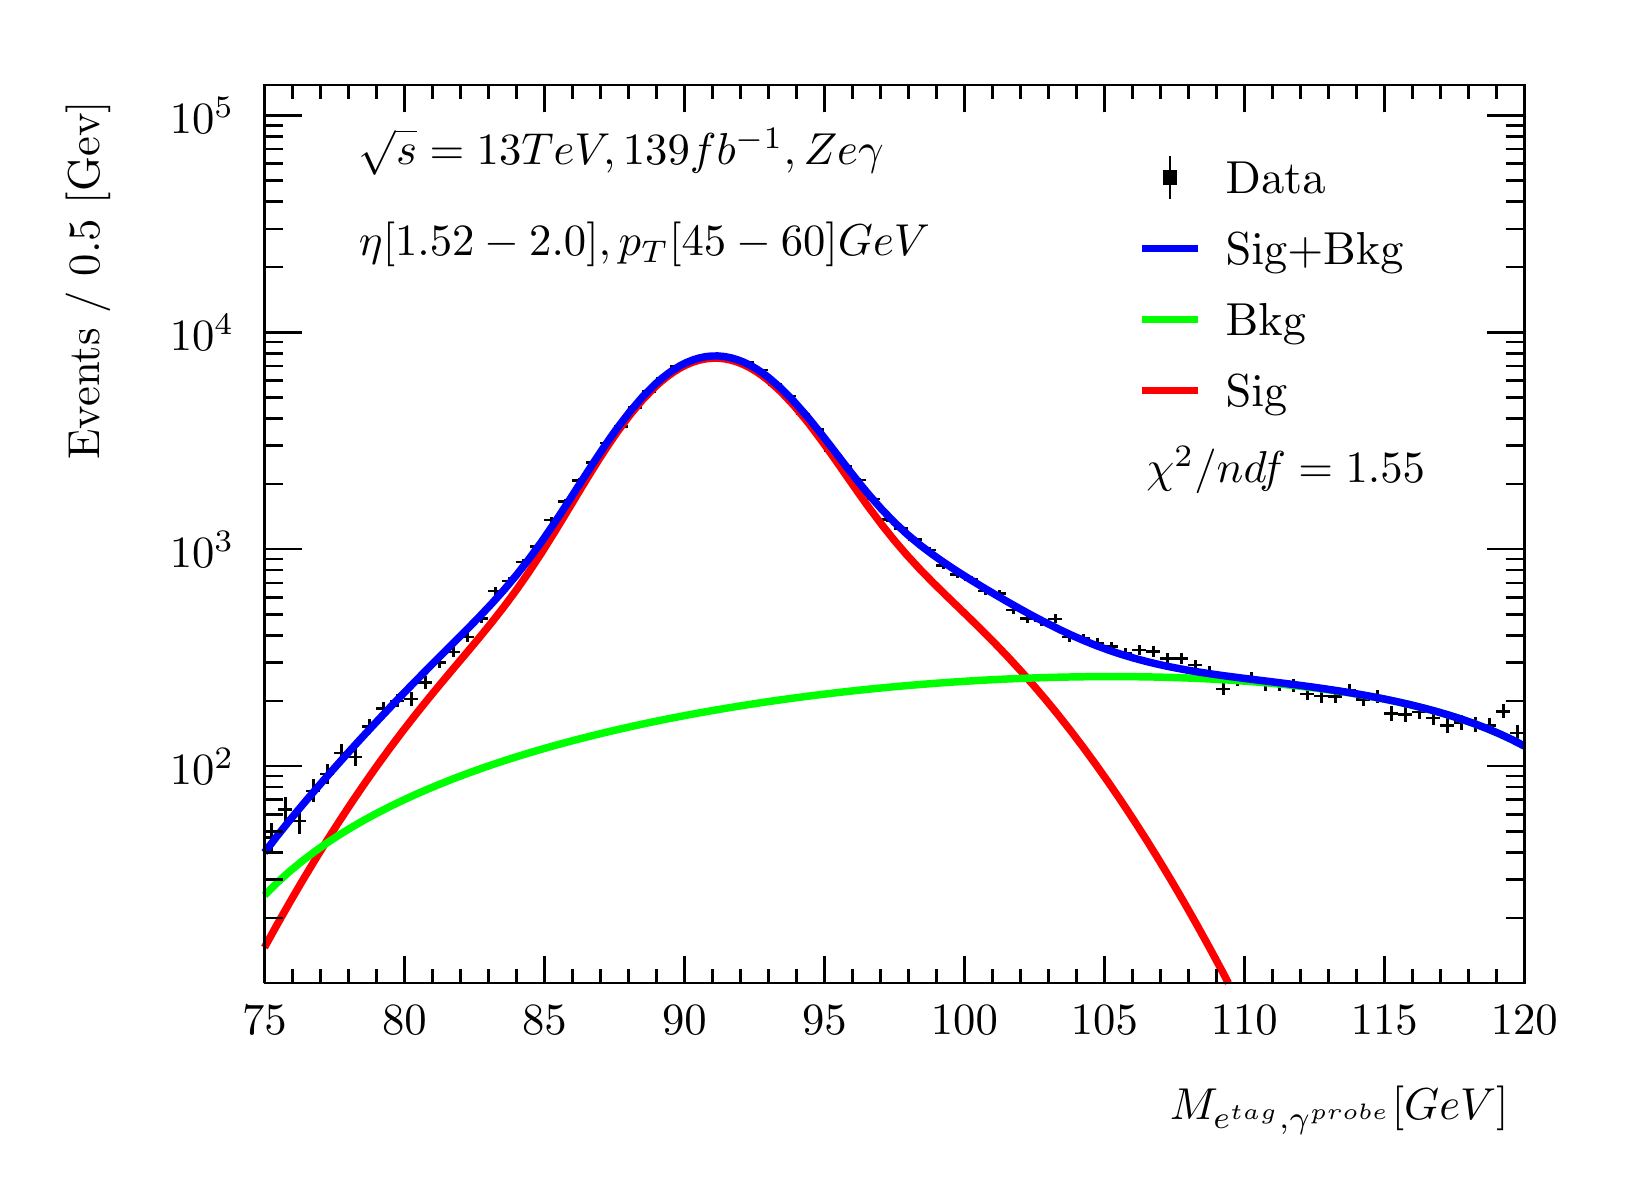
\begin{tikzpicture}
\pgfdeclareplotmark{cross} {
\pgfpathmoveto{\pgfpoint{-0.3\pgfplotmarksize}{\pgfplotmarksize}}
\pgfpathlineto{\pgfpoint{+0.3\pgfplotmarksize}{\pgfplotmarksize}}
\pgfpathlineto{\pgfpoint{+0.3\pgfplotmarksize}{0.3\pgfplotmarksize}}
\pgfpathlineto{\pgfpoint{+1\pgfplotmarksize}{0.3\pgfplotmarksize}}
\pgfpathlineto{\pgfpoint{+1\pgfplotmarksize}{-0.3\pgfplotmarksize}}
\pgfpathlineto{\pgfpoint{+0.3\pgfplotmarksize}{-0.3\pgfplotmarksize}}
\pgfpathlineto{\pgfpoint{+0.3\pgfplotmarksize}{-1.\pgfplotmarksize}}
\pgfpathlineto{\pgfpoint{-0.3\pgfplotmarksize}{-1.\pgfplotmarksize}}
\pgfpathlineto{\pgfpoint{-0.3\pgfplotmarksize}{-0.3\pgfplotmarksize}}
\pgfpathlineto{\pgfpoint{-1.\pgfplotmarksize}{-0.3\pgfplotmarksize}}
\pgfpathlineto{\pgfpoint{-1.\pgfplotmarksize}{0.3\pgfplotmarksize}}
\pgfpathlineto{\pgfpoint{-0.3\pgfplotmarksize}{0.3\pgfplotmarksize}}
\pgfpathclose
\pgfusepathqstroke
}
\pgfdeclareplotmark{cross*} {
\pgfpathmoveto{\pgfpoint{-0.3\pgfplotmarksize}{\pgfplotmarksize}}
\pgfpathlineto{\pgfpoint{+0.3\pgfplotmarksize}{\pgfplotmarksize}}
\pgfpathlineto{\pgfpoint{+0.3\pgfplotmarksize}{0.3\pgfplotmarksize}}
\pgfpathlineto{\pgfpoint{+1\pgfplotmarksize}{0.3\pgfplotmarksize}}
\pgfpathlineto{\pgfpoint{+1\pgfplotmarksize}{-0.3\pgfplotmarksize}}
\pgfpathlineto{\pgfpoint{+0.3\pgfplotmarksize}{-0.3\pgfplotmarksize}}
\pgfpathlineto{\pgfpoint{+0.3\pgfplotmarksize}{-1.\pgfplotmarksize}}
\pgfpathlineto{\pgfpoint{-0.3\pgfplotmarksize}{-1.\pgfplotmarksize}}
\pgfpathlineto{\pgfpoint{-0.3\pgfplotmarksize}{-0.3\pgfplotmarksize}}
\pgfpathlineto{\pgfpoint{-1.\pgfplotmarksize}{-0.3\pgfplotmarksize}}
\pgfpathlineto{\pgfpoint{-1.\pgfplotmarksize}{0.3\pgfplotmarksize}}
\pgfpathlineto{\pgfpoint{-0.3\pgfplotmarksize}{0.3\pgfplotmarksize}}
\pgfpathclose
\pgfusepathqfillstroke
}
\pgfdeclareplotmark{newstar} {
\pgfpathmoveto{\pgfqpoint{0pt}{\pgfplotmarksize}}
\pgfpathlineto{\pgfqpointpolar{44}{0.5\pgfplotmarksize}}
\pgfpathlineto{\pgfqpointpolar{18}{\pgfplotmarksize}}
\pgfpathlineto{\pgfqpointpolar{-20}{0.5\pgfplotmarksize}}
\pgfpathlineto{\pgfqpointpolar{-54}{\pgfplotmarksize}}
\pgfpathlineto{\pgfqpointpolar{-90}{0.5\pgfplotmarksize}}
\pgfpathlineto{\pgfqpointpolar{234}{\pgfplotmarksize}}
\pgfpathlineto{\pgfqpointpolar{198}{0.5\pgfplotmarksize}}
\pgfpathlineto{\pgfqpointpolar{162}{\pgfplotmarksize}}
\pgfpathlineto{\pgfqpointpolar{134}{0.5\pgfplotmarksize}}
\pgfpathclose
\pgfusepathqstroke
}
\pgfdeclareplotmark{newstar*} {
\pgfpathmoveto{\pgfqpoint{0pt}{\pgfplotmarksize}}
\pgfpathlineto{\pgfqpointpolar{44}{0.5\pgfplotmarksize}}
\pgfpathlineto{\pgfqpointpolar{18}{\pgfplotmarksize}}
\pgfpathlineto{\pgfqpointpolar{-20}{0.5\pgfplotmarksize}}
\pgfpathlineto{\pgfqpointpolar{-54}{\pgfplotmarksize}}
\pgfpathlineto{\pgfqpointpolar{-90}{0.5\pgfplotmarksize}}
\pgfpathlineto{\pgfqpointpolar{234}{\pgfplotmarksize}}
\pgfpathlineto{\pgfqpointpolar{198}{0.5\pgfplotmarksize}}
\pgfpathlineto{\pgfqpointpolar{162}{\pgfplotmarksize}}
\pgfpathlineto{\pgfqpointpolar{134}{0.5\pgfplotmarksize}}
\pgfpathclose
\pgfusepathqfillstroke
}
\definecolor{c}{rgb}{1,1,1};
\draw [color=c, fill=c] (0,0) rectangle (20,14.4361);
\draw [color=c, fill=c] (3,2.30977) rectangle (19,13.7143);
\definecolor{c}{rgb}{0,0,0};
\draw [c,line width=0.9] (3,2.30977) -- (3,13.7143) -- (19,13.7143) -- (19,2.30977) -- (3,2.30977);
\definecolor{c}{rgb}{1,1,1};
\draw [color=c, fill=c] (3,2.30977) rectangle (19,13.7143);
\definecolor{c}{rgb}{0,0,0};
\draw [c,line width=0.9] (3,2.30977) -- (3,13.7143) -- (19,13.7143) -- (19,2.30977) -- (3,2.30977);
\draw [c,line width=0.9] (3,2.30977) -- (19,2.30977);
\draw [c,line width=0.9] (3,2.65624) -- (3,2.30977);
\draw [c,line width=0.9] (3.35556,2.48301) -- (3.35556,2.30977);
\draw [c,line width=0.9] (3.71111,2.48301) -- (3.71111,2.30977);
\draw [c,line width=0.9] (4.06667,2.48301) -- (4.06667,2.30977);
\draw [c,line width=0.9] (4.42222,2.48301) -- (4.42222,2.30977);
\draw [c,line width=0.9] (4.77778,2.65624) -- (4.77778,2.30977);
\draw [c,line width=0.9] (5.13333,2.48301) -- (5.13333,2.30977);
\draw [c,line width=0.9] (5.48889,2.48301) -- (5.48889,2.30977);
\draw [c,line width=0.9] (5.84444,2.48301) -- (5.84444,2.30977);
\draw [c,line width=0.9] (6.2,2.48301) -- (6.2,2.30977);
\draw [c,line width=0.9] (6.55556,2.65624) -- (6.55556,2.30977);
\draw [c,line width=0.9] (6.91111,2.48301) -- (6.91111,2.30977);
\draw [c,line width=0.9] (7.26667,2.48301) -- (7.26667,2.30977);
\draw [c,line width=0.9] (7.62222,2.48301) -- (7.62222,2.30977);
\draw [c,line width=0.9] (7.97778,2.48301) -- (7.97778,2.30977);
\draw [c,line width=0.9] (8.33333,2.65624) -- (8.33333,2.30977);
\draw [c,line width=0.9] (8.68889,2.48301) -- (8.68889,2.30977);
\draw [c,line width=0.9] (9.04444,2.48301) -- (9.04444,2.30977);
\draw [c,line width=0.9] (9.4,2.48301) -- (9.4,2.30977);
\draw [c,line width=0.9] (9.75556,2.48301) -- (9.75556,2.30977);
\draw [c,line width=0.9] (10.1111,2.65624) -- (10.1111,2.30977);
\draw [c,line width=0.9] (10.4667,2.48301) -- (10.4667,2.30977);
\draw [c,line width=0.9] (10.8222,2.48301) -- (10.8222,2.30977);
\draw [c,line width=0.9] (11.1778,2.48301) -- (11.1778,2.30977);
\draw [c,line width=0.9] (11.5333,2.48301) -- (11.5333,2.30977);
\draw [c,line width=0.9] (11.8889,2.65624) -- (11.8889,2.30977);
\draw [c,line width=0.9] (12.2444,2.48301) -- (12.2444,2.30977);
\draw [c,line width=0.9] (12.6,2.48301) -- (12.6,2.30977);
\draw [c,line width=0.9] (12.9556,2.48301) -- (12.9556,2.30977);
\draw [c,line width=0.9] (13.3111,2.48301) -- (13.3111,2.30977);
\draw [c,line width=0.9] (13.6667,2.65624) -- (13.6667,2.30977);
\draw [c,line width=0.9] (14.0222,2.48301) -- (14.0222,2.30977);
\draw [c,line width=0.9] (14.3778,2.48301) -- (14.3778,2.30977);
\draw [c,line width=0.9] (14.7333,2.48301) -- (14.7333,2.30977);
\draw [c,line width=0.9] (15.0889,2.48301) -- (15.0889,2.30977);
\draw [c,line width=0.9] (15.4444,2.65624) -- (15.4444,2.30977);
\draw [c,line width=0.9] (15.8,2.48301) -- (15.8,2.30977);
\draw [c,line width=0.9] (16.1556,2.48301) -- (16.1556,2.30977);
\draw [c,line width=0.9] (16.5111,2.48301) -- (16.5111,2.30977);
\draw [c,line width=0.9] (16.8667,2.48301) -- (16.8667,2.30977);
\draw [c,line width=0.9] (17.2222,2.65624) -- (17.2222,2.30977);
\draw [c,line width=0.9] (17.5778,2.48301) -- (17.5778,2.30977);
\draw [c,line width=0.9] (17.9333,2.48301) -- (17.9333,2.30977);
\draw [c,line width=0.9] (18.2889,2.48301) -- (18.2889,2.30977);
\draw [c,line width=0.9] (18.6444,2.48301) -- (18.6444,2.30977);
\draw [c,line width=0.9] (19,2.65624) -- (19,2.30977);
\draw [c,line width=0.9] (19,2.65624) -- (19,2.30977);
\draw [anchor=base] (3,1.66015) node[scale=1.61424, color=c, rotate=0]{75};
\draw [anchor=base] (4.77778,1.66015) node[scale=1.61424, color=c, rotate=0]{80};
\draw [anchor=base] (6.55556,1.66015) node[scale=1.61424, color=c, rotate=0]{85};
\draw [anchor=base] (8.33333,1.66015) node[scale=1.61424, color=c, rotate=0]{90};
\draw [anchor=base] (10.1111,1.66015) node[scale=1.61424, color=c, rotate=0]{95};
\draw [anchor=base] (11.8889,1.66015) node[scale=1.61424, color=c, rotate=0]{100};
\draw [anchor=base] (13.6667,1.66015) node[scale=1.61424, color=c, rotate=0]{105};
\draw [anchor=base] (15.4444,1.66015) node[scale=1.61424, color=c, rotate=0]{110};
\draw [anchor=base] (17.2222,1.66015) node[scale=1.61424, color=c, rotate=0]{115};
\draw [anchor=base] (19,1.66015) node[scale=1.61424, color=c, rotate=0]{120};
\draw [anchor= east] (19,0.692932) node[scale=1.61424, color=c, rotate=0]{$M_{e^{tag}, \gamma^{probe}}  [GeV]$};
\draw [c,line width=0.9] (3,13.7143) -- (19,13.7143);
\draw [c,line width=0.9] (3,13.3678) -- (3,13.7143);
\draw [c,line width=0.9] (3.35556,13.5411) -- (3.35556,13.7143);
\draw [c,line width=0.9] (3.71111,13.5411) -- (3.71111,13.7143);
\draw [c,line width=0.9] (4.06667,13.5411) -- (4.06667,13.7143);
\draw [c,line width=0.9] (4.42222,13.5411) -- (4.42222,13.7143);
\draw [c,line width=0.9] (4.77778,13.3678) -- (4.77778,13.7143);
\draw [c,line width=0.9] (5.13333,13.5411) -- (5.13333,13.7143);
\draw [c,line width=0.9] (5.48889,13.5411) -- (5.48889,13.7143);
\draw [c,line width=0.9] (5.84444,13.5411) -- (5.84444,13.7143);
\draw [c,line width=0.9] (6.2,13.5411) -- (6.2,13.7143);
\draw [c,line width=0.9] (6.55556,13.3678) -- (6.55556,13.7143);
\draw [c,line width=0.9] (6.91111,13.5411) -- (6.91111,13.7143);
\draw [c,line width=0.9] (7.26667,13.5411) -- (7.26667,13.7143);
\draw [c,line width=0.9] (7.62222,13.5411) -- (7.62222,13.7143);
\draw [c,line width=0.9] (7.97778,13.5411) -- (7.97778,13.7143);
\draw [c,line width=0.9] (8.33333,13.3678) -- (8.33333,13.7143);
\draw [c,line width=0.9] (8.68889,13.5411) -- (8.68889,13.7143);
\draw [c,line width=0.9] (9.04444,13.5411) -- (9.04444,13.7143);
\draw [c,line width=0.9] (9.4,13.5411) -- (9.4,13.7143);
\draw [c,line width=0.9] (9.75556,13.5411) -- (9.75556,13.7143);
\draw [c,line width=0.9] (10.1111,13.3678) -- (10.1111,13.7143);
\draw [c,line width=0.9] (10.4667,13.5411) -- (10.4667,13.7143);
\draw [c,line width=0.9] (10.8222,13.5411) -- (10.8222,13.7143);
\draw [c,line width=0.9] (11.1778,13.5411) -- (11.1778,13.7143);
\draw [c,line width=0.9] (11.5333,13.5411) -- (11.5333,13.7143);
\draw [c,line width=0.9] (11.8889,13.3678) -- (11.8889,13.7143);
\draw [c,line width=0.9] (12.2444,13.5411) -- (12.2444,13.7143);
\draw [c,line width=0.9] (12.6,13.5411) -- (12.6,13.7143);
\draw [c,line width=0.9] (12.9556,13.5411) -- (12.9556,13.7143);
\draw [c,line width=0.9] (13.3111,13.5411) -- (13.3111,13.7143);
\draw [c,line width=0.9] (13.6667,13.3678) -- (13.6667,13.7143);
\draw [c,line width=0.9] (14.0222,13.5411) -- (14.0222,13.7143);
\draw [c,line width=0.9] (14.3778,13.5411) -- (14.3778,13.7143);
\draw [c,line width=0.9] (14.7333,13.5411) -- (14.7333,13.7143);
\draw [c,line width=0.9] (15.0889,13.5411) -- (15.0889,13.7143);
\draw [c,line width=0.9] (15.4444,13.3678) -- (15.4444,13.7143);
\draw [c,line width=0.9] (15.8,13.5411) -- (15.8,13.7143);
\draw [c,line width=0.9] (16.1556,13.5411) -- (16.1556,13.7143);
\draw [c,line width=0.9] (16.5111,13.5411) -- (16.5111,13.7143);
\draw [c,line width=0.9] (16.8667,13.5411) -- (16.8667,13.7143);
\draw [c,line width=0.9] (17.2222,13.3678) -- (17.2222,13.7143);
\draw [c,line width=0.9] (17.5778,13.5411) -- (17.5778,13.7143);
\draw [c,line width=0.9] (17.9333,13.5411) -- (17.9333,13.7143);
\draw [c,line width=0.9] (18.2889,13.5411) -- (18.2889,13.7143);
\draw [c,line width=0.9] (18.6444,13.5411) -- (18.6444,13.7143);
\draw [c,line width=0.9] (19,13.3678) -- (19,13.7143);
\draw [c,line width=0.9] (19,13.3678) -- (19,13.7143);
\draw [c,line width=0.9] (3,2.30977) -- (3,13.7143);
\draw [c,line width=0.9] (3.237,3.13907) -- (3,3.13907);
\draw [c,line width=0.9] (3.237,3.62418) -- (3,3.62418);
\draw [c,line width=0.9] (3.237,3.96837) -- (3,3.96837);
\draw [c,line width=0.9] (3.237,4.23535) -- (3,4.23535);
\draw [c,line width=0.9] (3.237,4.45348) -- (3,4.45348);
\draw [c,line width=0.9] (3.237,4.63791) -- (3,4.63791);
\draw [c,line width=0.9] (3.237,4.79767) -- (3,4.79767);
\draw [c,line width=0.9] (3.237,4.93859) -- (3,4.93859);
\draw [c,line width=0.9] (3.474,5.06465) -- (3,5.06465);
\draw [anchor= east] (2.82,5.06465) node[scale=1.61424, color=c, rotate=0]{$10^{2}$};
\draw [c,line width=0.9] (3.237,5.89394) -- (3,5.89394);
\draw [c,line width=0.9] (3.237,6.37905) -- (3,6.37905);
\draw [c,line width=0.9] (3.237,6.72324) -- (3,6.72324);
\draw [c,line width=0.9] (3.237,6.99022) -- (3,6.99022);
\draw [c,line width=0.9] (3.237,7.20835) -- (3,7.20835);
\draw [c,line width=0.9] (3.237,7.39278) -- (3,7.39278);
\draw [c,line width=0.9] (3.237,7.55254) -- (3,7.55254);
\draw [c,line width=0.9] (3.237,7.69346) -- (3,7.69346);
\draw [c,line width=0.9] (3.474,7.81952) -- (3,7.81952);
\draw [anchor= east] (2.82,7.81952) node[scale=1.61424, color=c, rotate=0]{$10^{3}$};
\draw [c,line width=0.9] (3.237,8.64882) -- (3,8.64882);
\draw [c,line width=0.9] (3.237,9.13393) -- (3,9.13393);
\draw [c,line width=0.9] (3.237,9.47812) -- (3,9.47812);
\draw [c,line width=0.9] (3.237,9.74509) -- (3,9.74509);
\draw [c,line width=0.9] (3.237,9.96323) -- (3,9.96323);
\draw [c,line width=0.9] (3.237,10.1477) -- (3,10.1477);
\draw [c,line width=0.9] (3.237,10.3074) -- (3,10.3074);
\draw [c,line width=0.9] (3.237,10.4483) -- (3,10.4483);
\draw [c,line width=0.9] (3.474,10.5744) -- (3,10.5744);
\draw [anchor= east] (2.82,10.5744) node[scale=1.61424, color=c, rotate=0]{$10^{4}$};
\draw [c,line width=0.9] (3.237,11.4037) -- (3,11.4037);
\draw [c,line width=0.9] (3.237,11.8888) -- (3,11.8888);
\draw [c,line width=0.9] (3.237,12.233) -- (3,12.233);
\draw [c,line width=0.9] (3.237,12.5) -- (3,12.5);
\draw [c,line width=0.9] (3.237,12.7181) -- (3,12.7181);
\draw [c,line width=0.9] (3.237,12.9025) -- (3,12.9025);
\draw [c,line width=0.9] (3.237,13.0623) -- (3,13.0623);
\draw [c,line width=0.9] (3.237,13.2032) -- (3,13.2032);
\draw [c,line width=0.9] (3.474,13.3293) -- (3,13.3293);
\draw [anchor= east] (2.82,13.3293) node[scale=1.61424, color=c, rotate=0]{$10^{5}$};
\draw [anchor= east] (0.76,13.7143) node[scale=1.61424, color=c, rotate=90]{Events / 0.5 [Gev]};
\draw [c,line width=0.9] (19,2.30977) -- (19,13.7143);
\draw [c,line width=0.9] (18.763,3.13907) -- (19,3.13907);
\draw [c,line width=0.9] (18.763,3.62418) -- (19,3.62418);
\draw [c,line width=0.9] (18.763,3.96837) -- (19,3.96837);
\draw [c,line width=0.9] (18.763,4.23535) -- (19,4.23535);
\draw [c,line width=0.9] (18.763,4.45348) -- (19,4.45348);
\draw [c,line width=0.9] (18.763,4.63791) -- (19,4.63791);
\draw [c,line width=0.9] (18.763,4.79767) -- (19,4.79767);
\draw [c,line width=0.9] (18.763,4.93859) -- (19,4.93859);
\draw [c,line width=0.9] (18.526,5.06465) -- (19,5.06465);
\draw [c,line width=0.9] (18.763,5.89394) -- (19,5.89394);
\draw [c,line width=0.9] (18.763,6.37905) -- (19,6.37905);
\draw [c,line width=0.9] (18.763,6.72324) -- (19,6.72324);
\draw [c,line width=0.9] (18.763,6.99022) -- (19,6.99022);
\draw [c,line width=0.9] (18.763,7.20835) -- (19,7.20835);
\draw [c,line width=0.9] (18.763,7.39278) -- (19,7.39278);
\draw [c,line width=0.9] (18.763,7.55254) -- (19,7.55254);
\draw [c,line width=0.9] (18.763,7.69346) -- (19,7.69346);
\draw [c,line width=0.9] (18.526,7.81952) -- (19,7.81952);
\draw [c,line width=0.9] (18.763,8.64882) -- (19,8.64882);
\draw [c,line width=0.9] (18.763,9.13393) -- (19,9.13393);
\draw [c,line width=0.9] (18.763,9.47812) -- (19,9.47812);
\draw [c,line width=0.9] (18.763,9.74509) -- (19,9.74509);
\draw [c,line width=0.9] (18.763,9.96323) -- (19,9.96323);
\draw [c,line width=0.9] (18.763,10.1477) -- (19,10.1477);
\draw [c,line width=0.9] (18.763,10.3074) -- (19,10.3074);
\draw [c,line width=0.9] (18.763,10.4483) -- (19,10.4483);
\draw [c,line width=0.9] (18.526,10.5744) -- (19,10.5744);
\draw [c,line width=0.9] (18.763,11.4037) -- (19,11.4037);
\draw [c,line width=0.9] (18.763,11.8888) -- (19,11.8888);
\draw [c,line width=0.9] (18.763,12.233) -- (19,12.233);
\draw [c,line width=0.9] (18.763,12.5) -- (19,12.5);
\draw [c,line width=0.9] (18.763,12.7181) -- (19,12.7181);
\draw [c,line width=0.9] (18.763,12.9025) -- (19,12.9025);
\draw [c,line width=0.9] (18.763,13.0623) -- (19,13.0623);
\draw [c,line width=0.9] (18.763,13.2032) -- (19,13.2032);
\draw [c,line width=0.9] (18.526,13.3293) -- (19,13.3293);
\draw [c,line width=0.9] (3.08889,4.16132) -- (3,4.16132);
\draw [c,line width=0.9] (3,4.16132) -- (3,4.16132);
\draw [c,line width=0.9] (3.08889,4.16132) -- (3.17778,4.16132);
\draw [c,line width=0.9] (3.17778,4.16132) -- (3.17778,4.16132);
\draw [c,line width=0.9] (3.08889,4.16132) -- (3.08889,4.3473);
\draw [c,line width=0.9] (3.08889,4.3473) -- (3.08889,4.3473);
\draw [c,line width=0.9] (3.08889,4.16132) -- (3.08889,3.97341);
\draw [c,line width=0.9] (3.08889,3.97341) -- (3.08889,3.97341);
\draw [c,line width=0.9] (3.26667,4.51186) -- (3.17778,4.51186);
\draw [c,line width=0.9] (3.17778,4.51186) -- (3.17778,4.51186);
\draw [c,line width=0.9] (3.26667,4.51186) -- (3.35556,4.51186);
\draw [c,line width=0.9] (3.35556,4.51186) -- (3.35556,4.51186);
\draw [c,line width=0.9] (3.26667,4.51186) -- (3.26667,4.67127);
\draw [c,line width=0.9] (3.26667,4.67127) -- (3.26667,4.67127);
\draw [c,line width=0.9] (3.26667,4.51186) -- (3.26667,4.3512);
\draw [c,line width=0.9] (3.26667,4.3512) -- (3.26667,4.3512);
\draw [c,line width=0.9] (3.44444,4.37094) -- (3.35556,4.37094);
\draw [c,line width=0.9] (3.35556,4.37094) -- (3.35556,4.37094);
\draw [c,line width=0.9] (3.44444,4.37094) -- (3.53333,4.37094);
\draw [c,line width=0.9] (3.53333,4.37094) -- (3.53333,4.37094);
\draw [c,line width=0.9] (3.44444,4.37094) -- (3.44444,4.54053);
\draw [c,line width=0.9] (3.44444,4.54053) -- (3.44444,4.54053);
\draw [c,line width=0.9] (3.44444,4.37094) -- (3.44444,4.19987);
\draw [c,line width=0.9] (3.44444,4.19987) -- (3.44444,4.19987);
\draw [c,line width=0.9] (3.62222,4.75194) -- (3.53333,4.75194);
\draw [c,line width=0.9] (3.53333,4.75194) -- (3.53333,4.75194);
\draw [c,line width=0.9] (3.62222,4.75194) -- (3.71111,4.75194);
\draw [c,line width=0.9] (3.71111,4.75194) -- (3.71111,4.75194);
\draw [c,line width=0.9] (3.62222,4.75194) -- (3.62222,4.89546);
\draw [c,line width=0.9] (3.62222,4.89546) -- (3.62222,4.89546);
\draw [c,line width=0.9] (3.62222,4.75194) -- (3.62222,4.60752);
\draw [c,line width=0.9] (3.62222,4.60752) -- (3.62222,4.60752);
\draw [c,line width=0.9] (3.8,4.96489) -- (3.71111,4.96489);
\draw [c,line width=0.9] (3.71111,4.96489) -- (3.71111,4.96489);
\draw [c,line width=0.9] (3.8,4.96489) -- (3.88889,4.96489);
\draw [c,line width=0.9] (3.88889,4.96489) -- (3.88889,4.96489);
\draw [c,line width=0.9] (3.8,4.96489) -- (3.8,5.09567);
\draw [c,line width=0.9] (3.8,5.09567) -- (3.8,5.09567);
\draw [c,line width=0.9] (3.8,4.96489) -- (3.8,4.83341);
\draw [c,line width=0.9] (3.8,4.83341) -- (3.8,4.83341);
\draw [c,line width=0.9] (3.97778,5.23186) -- (3.88889,5.23186);
\draw [c,line width=0.9] (3.88889,5.23186) -- (3.88889,5.23186);
\draw [c,line width=0.9] (3.97778,5.23186) -- (4.06667,5.23186);
\draw [c,line width=0.9] (4.06667,5.23186) -- (4.06667,5.23186);
\draw [c,line width=0.9] (3.97778,5.23186) -- (3.97778,5.34339);
\draw [c,line width=0.9] (3.97778,5.34339) -- (3.97778,5.34339);
\draw [c,line width=0.9] (3.97778,5.23186) -- (3.97778,5.12034);
\draw [c,line width=0.9] (3.97778,5.12034) -- (3.97778,5.12034);
\draw [c,line width=0.9] (4.15556,5.17868) -- (4.06667,5.17868);
\draw [c,line width=0.9] (4.06667,5.17868) -- (4.06667,5.17868);
\draw [c,line width=0.9] (4.15556,5.17868) -- (4.24444,5.17868);
\draw [c,line width=0.9] (4.24444,5.17868) -- (4.24444,5.17868);
\draw [c,line width=0.9] (4.15556,5.17868) -- (4.15556,5.29271);
\draw [c,line width=0.9] (4.15556,5.29271) -- (4.15556,5.29271);
\draw [c,line width=0.9] (4.15556,5.17868) -- (4.15556,5.06465);
\draw [c,line width=0.9] (4.15556,5.06465) -- (4.15556,5.06465);
\draw [c,line width=0.9] (4.33333,5.5656) -- (4.24444,5.5656);
\draw [c,line width=0.9] (4.24444,5.5656) -- (4.24444,5.5656);
\draw [c,line width=0.9] (4.33333,5.5656) -- (4.42222,5.5656);
\draw [c,line width=0.9] (4.42222,5.5656) -- (4.42222,5.5656);
\draw [c,line width=0.9] (4.33333,5.5656) -- (4.33333,5.66262);
\draw [c,line width=0.9] (4.33333,5.66262) -- (4.33333,5.66262);
\draw [c,line width=0.9] (4.33333,5.5656) -- (4.33333,5.46859);
\draw [c,line width=0.9] (4.33333,5.46859) -- (4.33333,5.46859);
\draw [c,line width=0.9] (4.51111,5.79419) -- (4.42222,5.79419);
\draw [c,line width=0.9] (4.42222,5.79419) -- (4.42222,5.79419);
\draw [c,line width=0.9] (4.51111,5.79419) -- (4.6,5.79419);
\draw [c,line width=0.9] (4.6,5.79419) -- (4.6,5.79419);
\draw [c,line width=0.9] (4.51111,5.79419) -- (4.51111,5.88237);
\draw [c,line width=0.9] (4.51111,5.88237) -- (4.51111,5.88237);
\draw [c,line width=0.9] (4.51111,5.79419) -- (4.51111,5.70601);
\draw [c,line width=0.9] (4.51111,5.70601) -- (4.51111,5.70601);
\draw [c,line width=0.9] (4.68889,5.89395) -- (4.6,5.89395);
\draw [c,line width=0.9] (4.6,5.89395) -- (4.6,5.89395);
\draw [c,line width=0.9] (4.68889,5.89395) -- (4.77778,5.89395);
\draw [c,line width=0.9] (4.77778,5.89395) -- (4.77778,5.89395);
\draw [c,line width=0.9] (4.68889,5.89395) -- (4.68889,5.97853);
\draw [c,line width=0.9] (4.68889,5.97853) -- (4.68889,5.97853);
\draw [c,line width=0.9] (4.68889,5.89395) -- (4.68889,5.80936);
\draw [c,line width=0.9] (4.68889,5.80936) -- (4.68889,5.80936);
\draw [c,line width=0.9] (4.86667,5.91764) -- (4.77778,5.91764);
\draw [c,line width=0.9] (4.77778,5.91764) -- (4.77778,5.91764);
\draw [c,line width=0.9] (4.86667,5.91764) -- (4.95556,5.91764);
\draw [c,line width=0.9] (4.95556,5.91764) -- (4.95556,5.91764);
\draw [c,line width=0.9] (4.86667,5.91764) -- (4.86667,6.00139);
\draw [c,line width=0.9] (4.86667,6.00139) -- (4.86667,6.00139);
\draw [c,line width=0.9] (4.86667,5.91764) -- (4.86667,5.83389);
\draw [c,line width=0.9] (4.86667,5.83389) -- (4.86667,5.83389);
\draw [c,line width=0.9] (5.04444,6.12694) -- (4.95556,6.12694);
\draw [c,line width=0.9] (4.95556,6.12694) -- (4.95556,6.12694);
\draw [c,line width=0.9] (5.04444,6.12694) -- (5.13333,6.12694);
\draw [c,line width=0.9] (5.13333,6.12694) -- (5.13333,6.12694);
\draw [c,line width=0.9] (5.04444,6.12694) -- (5.04444,6.20368);
\draw [c,line width=0.9] (5.04444,6.20368) -- (5.04444,6.20368);
\draw [c,line width=0.9] (5.04444,6.12694) -- (5.04444,6.05021);
\draw [c,line width=0.9] (5.04444,6.05021) -- (5.04444,6.05021);
\draw [c,line width=0.9] (5.22222,6.37906) -- (5.13333,6.37906);
\draw [c,line width=0.9] (5.13333,6.37906) -- (5.13333,6.37906);
\draw [c,line width=0.9] (5.22222,6.37906) -- (5.31111,6.37906);
\draw [c,line width=0.9] (5.31111,6.37906) -- (5.31111,6.37906);
\draw [c,line width=0.9] (5.22222,6.37906) -- (5.22222,6.44812);
\draw [c,line width=0.9] (5.22222,6.44812) -- (5.22222,6.44812);
\draw [c,line width=0.9] (5.22222,6.37906) -- (5.22222,6.30999);
\draw [c,line width=0.9] (5.22222,6.30999) -- (5.22222,6.30999);
\draw [c,line width=0.9] (5.4,6.51108) -- (5.31111,6.51108);
\draw [c,line width=0.9] (5.31111,6.51108) -- (5.31111,6.51108);
\draw [c,line width=0.9] (5.4,6.51108) -- (5.48889,6.51108);
\draw [c,line width=0.9] (5.48889,6.51108) -- (5.48889,6.51108);
\draw [c,line width=0.9] (5.4,6.51108) -- (5.4,6.57644);
\draw [c,line width=0.9] (5.4,6.57644) -- (5.4,6.57644);
\draw [c,line width=0.9] (5.4,6.51108) -- (5.4,6.44572);
\draw [c,line width=0.9] (5.4,6.44572) -- (5.4,6.44572);
\draw [c,line width=0.9] (5.57778,6.70516) -- (5.48889,6.70516);
\draw [c,line width=0.9] (5.48889,6.70516) -- (5.48889,6.70516);
\draw [c,line width=0.9] (5.57778,6.70516) -- (5.66667,6.70516);
\draw [c,line width=0.9] (5.66667,6.70516) -- (5.66667,6.70516);
\draw [c,line width=0.9] (5.57778,6.70516) -- (5.57778,6.76543);
\draw [c,line width=0.9] (5.57778,6.76543) -- (5.57778,6.76543);
\draw [c,line width=0.9] (5.57778,6.70516) -- (5.57778,6.6449);
\draw [c,line width=0.9] (5.57778,6.6449) -- (5.57778,6.6449);
\draw [c,line width=0.9] (5.75556,6.94138) -- (5.66667,6.94138);
\draw [c,line width=0.9] (5.66667,6.94138) -- (5.66667,6.94138);
\draw [c,line width=0.9] (5.75556,6.94138) -- (5.84444,6.94138);
\draw [c,line width=0.9] (5.84444,6.94138) -- (5.84444,6.94138);
\draw [c,line width=0.9] (5.75556,6.94138) -- (5.75556,6.99599);
\draw [c,line width=0.9] (5.75556,6.99599) -- (5.75556,6.99599);
\draw [c,line width=0.9] (5.75556,6.94138) -- (5.75556,6.88678);
\draw [c,line width=0.9] (5.75556,6.88678) -- (5.75556,6.88678);
\draw [c,line width=0.9] (5.93333,7.2893) -- (5.84444,7.2893);
\draw [c,line width=0.9] (5.84444,7.2893) -- (5.84444,7.2893);
\draw [c,line width=0.9] (5.93333,7.2893) -- (6.02222,7.2893);
\draw [c,line width=0.9] (6.02222,7.2893) -- (6.02222,7.2893);
\draw [c,line width=0.9] (5.93333,7.2893) -- (5.93333,7.33652);
\draw [c,line width=0.9] (5.93333,7.33652) -- (5.93333,7.33652);
\draw [c,line width=0.9] (5.93333,7.2893) -- (5.93333,7.24209);
\draw [c,line width=0.9] (5.93333,7.24209) -- (5.93333,7.24209);
\draw [c,line width=0.9] (6.11111,7.41648) -- (6.02222,7.41648);
\draw [c,line width=0.9] (6.02222,7.41648) -- (6.02222,7.41648);
\draw [c,line width=0.9] (6.11111,7.41648) -- (6.2,7.41648);
\draw [c,line width=0.9] (6.2,7.41648) -- (6.2,7.41648);
\draw [c,line width=0.9] (6.11111,7.41648) -- (6.11111,7.46125);
\draw [c,line width=0.9] (6.11111,7.46125) -- (6.11111,7.46125);
\draw [c,line width=0.9] (6.11111,7.41648) -- (6.11111,7.37171);
\draw [c,line width=0.9] (6.11111,7.37171) -- (6.11111,7.37171);
\draw [c,line width=0.9] (6.28889,7.65839) -- (6.2,7.65839);
\draw [c,line width=0.9] (6.2,7.65839) -- (6.2,7.65839);
\draw [c,line width=0.9] (6.28889,7.65839) -- (6.37778,7.65839);
\draw [c,line width=0.9] (6.37778,7.65839) -- (6.37778,7.65839);
\draw [c,line width=0.9] (6.28889,7.65839) -- (6.28889,7.69886);
\draw [c,line width=0.9] (6.28889,7.69886) -- (6.28889,7.69886);
\draw [c,line width=0.9] (6.28889,7.65839) -- (6.28889,7.61792);
\draw [c,line width=0.9] (6.28889,7.61792) -- (6.28889,7.61792);
\draw [c,line width=0.9] (6.46667,7.8514) -- (6.37778,7.8514);
\draw [c,line width=0.9] (6.37778,7.8514) -- (6.37778,7.8514);
\draw [c,line width=0.9] (6.46667,7.8514) -- (6.55556,7.8514);
\draw [c,line width=0.9] (6.55556,7.8514) -- (6.55556,7.8514);
\draw [c,line width=0.9] (6.46667,7.8514) -- (6.46667,7.88873);
\draw [c,line width=0.9] (6.46667,7.88873) -- (6.46667,7.88873);
\draw [c,line width=0.9] (6.46667,7.8514) -- (6.46667,7.81406);
\draw [c,line width=0.9] (6.46667,7.81406) -- (6.46667,7.81406);
\draw [c,line width=0.9] (6.64444,8.19004) -- (6.55556,8.19004);
\draw [c,line width=0.9] (6.55556,8.19004) -- (6.55556,8.19004);
\draw [c,line width=0.9] (6.64444,8.19004) -- (6.73333,8.19004);
\draw [c,line width=0.9] (6.73333,8.19004) -- (6.73333,8.19004);
\draw [c,line width=0.9] (6.64444,8.19004) -- (6.64444,8.22245);
\draw [c,line width=0.9] (6.64444,8.22245) -- (6.64444,8.22245);
\draw [c,line width=0.9] (6.64444,8.19004) -- (6.64444,8.15763);
\draw [c,line width=0.9] (6.64444,8.15763) -- (6.64444,8.15763);
\draw [c,line width=0.9] (6.82222,8.42373) -- (6.73333,8.42373);
\draw [c,line width=0.9] (6.73333,8.42373) -- (6.73333,8.42373);
\draw [c,line width=0.9] (6.82222,8.42373) -- (6.91111,8.42373);
\draw [c,line width=0.9] (6.91111,8.42373) -- (6.91111,8.42373);
\draw [c,line width=0.9] (6.82222,8.42373) -- (6.82222,8.45312);
\draw [c,line width=0.9] (6.82222,8.45312) -- (6.82222,8.45312);
\draw [c,line width=0.9] (6.82222,8.42373) -- (6.82222,8.39433);
\draw [c,line width=0.9] (6.82222,8.39433) -- (6.82222,8.39433);
\draw [c,line width=0.9] (7,8.69229) -- (6.91111,8.69229);
\draw [c,line width=0.9] (6.91111,8.69229) -- (6.91111,8.69229);
\draw [c,line width=0.9] (7,8.69229) -- (7.08889,8.69229);
\draw [c,line width=0.9] (7.08889,8.69229) -- (7.08889,8.69229);
\draw [c,line width=0.9] (7,8.69229) -- (7,8.71856);
\draw [c,line width=0.9] (7,8.71856) -- (7,8.71856);
\draw [c,line width=0.9] (7,8.69229) -- (7,8.66602);
\draw [c,line width=0.9] (7,8.66602) -- (7,8.66602);
\draw [c,line width=0.9] (7.17778,8.92009) -- (7.08889,8.92009);
\draw [c,line width=0.9] (7.08889,8.92009) -- (7.08889,8.92009);
\draw [c,line width=0.9] (7.17778,8.92009) -- (7.26667,8.92009);
\draw [c,line width=0.9] (7.26667,8.92009) -- (7.26667,8.92009);
\draw [c,line width=0.9] (7.17778,8.92009) -- (7.17778,8.94398);
\draw [c,line width=0.9] (7.17778,8.94398) -- (7.17778,8.94398);
\draw [c,line width=0.9] (7.17778,8.92009) -- (7.17778,8.89621);
\draw [c,line width=0.9] (7.17778,8.89621) -- (7.17778,8.89621);
\draw [c,line width=0.9] (7.35556,9.16697) -- (7.26667,9.16697);
\draw [c,line width=0.9] (7.26667,9.16697) -- (7.26667,9.16697);
\draw [c,line width=0.9] (7.35556,9.16697) -- (7.44444,9.16697);
\draw [c,line width=0.9] (7.44444,9.16697) -- (7.44444,9.16697);
\draw [c,line width=0.9] (7.35556,9.16697) -- (7.35556,9.18851);
\draw [c,line width=0.9] (7.35556,9.18851) -- (7.35556,9.18851);
\draw [c,line width=0.9] (7.35556,9.16697) -- (7.35556,9.14542);
\draw [c,line width=0.9] (7.35556,9.14542) -- (7.35556,9.14542);
\draw [c,line width=0.9] (7.53333,9.37998) -- (7.44444,9.37998);
\draw [c,line width=0.9] (7.44444,9.37998) -- (7.44444,9.37998);
\draw [c,line width=0.9] (7.53333,9.37998) -- (7.62222,9.37998);
\draw [c,line width=0.9] (7.62222,9.37998) -- (7.62222,9.37998);
\draw [c,line width=0.9] (7.53333,9.37998) -- (7.53333,9.39969);
\draw [c,line width=0.9] (7.53333,9.39969) -- (7.53333,9.39969);
\draw [c,line width=0.9] (7.53333,9.37998) -- (7.53333,9.36028);
\draw [c,line width=0.9] (7.53333,9.36028) -- (7.53333,9.36028);
\draw [c,line width=0.9] (7.71111,9.61771) -- (7.62222,9.61771);
\draw [c,line width=0.9] (7.62222,9.61771) -- (7.62222,9.61771);
\draw [c,line width=0.9] (7.71111,9.61771) -- (7.8,9.61771);
\draw [c,line width=0.9] (7.8,9.61771) -- (7.8,9.61771);
\draw [c,line width=0.9] (7.71111,9.61771) -- (7.71111,9.63555);
\draw [c,line width=0.9] (7.71111,9.63555) -- (7.71111,9.63555);
\draw [c,line width=0.9] (7.71111,9.61771) -- (7.71111,9.59986);
\draw [c,line width=0.9] (7.71111,9.59986) -- (7.71111,9.59986);
\draw [c,line width=0.9] (7.88889,9.82403) -- (7.8,9.82403);
\draw [c,line width=0.9] (7.8,9.82403) -- (7.8,9.82403);
\draw [c,line width=0.9] (7.88889,9.82403) -- (7.97778,9.82403);
\draw [c,line width=0.9] (7.97778,9.82403) -- (7.97778,9.82403);
\draw [c,line width=0.9] (7.88889,9.82403) -- (7.88889,9.8404);
\draw [c,line width=0.9] (7.88889,9.8404) -- (7.88889,9.8404);
\draw [c,line width=0.9] (7.88889,9.82403) -- (7.88889,9.80766);
\draw [c,line width=0.9] (7.88889,9.80766) -- (7.88889,9.80766);
\draw [c,line width=0.9] (8.06667,9.99374) -- (7.97778,9.99374);
\draw [c,line width=0.9] (7.97778,9.99374) -- (7.97778,9.99374);
\draw [c,line width=0.9] (8.06667,9.99374) -- (8.15556,9.99374);
\draw [c,line width=0.9] (8.15556,9.99374) -- (8.15556,9.99374);
\draw [c,line width=0.9] (8.06667,9.99374) -- (8.06667,10.009);
\draw [c,line width=0.9] (8.06667,10.009) -- (8.06667,10.009);
\draw [c,line width=0.9] (8.06667,9.99374) -- (8.06667,9.97849);
\draw [c,line width=0.9] (8.06667,9.97849) -- (8.06667,9.97849);
\draw [c,line width=0.9] (8.24444,10.1398) -- (8.15556,10.1398);
\draw [c,line width=0.9] (8.15556,10.1398) -- (8.15556,10.1398);
\draw [c,line width=0.9] (8.24444,10.1398) -- (8.33333,10.1398);
\draw [c,line width=0.9] (8.33333,10.1398) -- (8.33333,10.1398);
\draw [c,line width=0.9] (8.24444,10.1398) -- (8.24444,10.1541);
\draw [c,line width=0.9] (8.24444,10.1541) -- (8.24444,10.1541);
\draw [c,line width=0.9] (8.24444,10.1398) -- (8.24444,10.1254);
\draw [c,line width=0.9] (8.24444,10.1254) -- (8.24444,10.1254);
\draw [c,line width=0.9] (8.42222,10.2114) -- (8.33333,10.2114);
\draw [c,line width=0.9] (8.33333,10.2114) -- (8.33333,10.2114);
\draw [c,line width=0.9] (8.42222,10.2114) -- (8.51111,10.2114);
\draw [c,line width=0.9] (8.51111,10.2114) -- (8.51111,10.2114);
\draw [c,line width=0.9] (8.42222,10.2114) -- (8.42222,10.2253);
\draw [c,line width=0.9] (8.42222,10.2253) -- (8.42222,10.2253);
\draw [c,line width=0.9] (8.42222,10.2114) -- (8.42222,10.1975);
\draw [c,line width=0.9] (8.42222,10.1975) -- (8.42222,10.1975);
\draw [c,line width=0.9] (8.6,10.2731) -- (8.51111,10.2731);
\draw [c,line width=0.9] (8.51111,10.2731) -- (8.51111,10.2731);
\draw [c,line width=0.9] (8.6,10.2731) -- (8.68889,10.2731);
\draw [c,line width=0.9] (8.68889,10.2731) -- (8.68889,10.2731);
\draw [c,line width=0.9] (8.6,10.2731) -- (8.6,10.2867);
\draw [c,line width=0.9] (8.6,10.2867) -- (8.6,10.2867);
\draw [c,line width=0.9] (8.6,10.2731) -- (8.6,10.2596);
\draw [c,line width=0.9] (8.6,10.2596) -- (8.6,10.2596);
\draw [c,line width=0.9] (8.77778,10.2918) -- (8.68889,10.2918);
\draw [c,line width=0.9] (8.68889,10.2918) -- (8.68889,10.2918);
\draw [c,line width=0.9] (8.77778,10.2918) -- (8.86667,10.2918);
\draw [c,line width=0.9] (8.86667,10.2918) -- (8.86667,10.2918);
\draw [c,line width=0.9] (8.77778,10.2918) -- (8.77778,10.3052);
\draw [c,line width=0.9] (8.77778,10.3052) -- (8.77778,10.3052);
\draw [c,line width=0.9] (8.77778,10.2918) -- (8.77778,10.2783);
\draw [c,line width=0.9] (8.77778,10.2783) -- (8.77778,10.2783);
\draw [c,line width=0.9] (8.95556,10.2429) -- (8.86667,10.2429);
\draw [c,line width=0.9] (8.86667,10.2429) -- (8.86667,10.2429);
\draw [c,line width=0.9] (8.95556,10.2429) -- (9.04444,10.2429);
\draw [c,line width=0.9] (9.04444,10.2429) -- (9.04444,10.2429);
\draw [c,line width=0.9] (8.95556,10.2429) -- (8.95556,10.2566);
\draw [c,line width=0.9] (8.95556,10.2566) -- (8.95556,10.2566);
\draw [c,line width=0.9] (8.95556,10.2429) -- (8.95556,10.2292);
\draw [c,line width=0.9] (8.95556,10.2292) -- (8.95556,10.2292);
\draw [c,line width=0.9] (9.13333,10.189) -- (9.04444,10.189);
\draw [c,line width=0.9] (9.04444,10.189) -- (9.04444,10.189);
\draw [c,line width=0.9] (9.13333,10.189) -- (9.22222,10.189);
\draw [c,line width=0.9] (9.22222,10.189) -- (9.22222,10.189);
\draw [c,line width=0.9] (9.13333,10.189) -- (9.13333,10.203);
\draw [c,line width=0.9] (9.13333,10.203) -- (9.13333,10.203);
\draw [c,line width=0.9] (9.13333,10.189) -- (9.13333,10.1749);
\draw [c,line width=0.9] (9.13333,10.1749) -- (9.13333,10.1749);
\draw [c,line width=0.9] (9.31111,10.0949) -- (9.22222,10.0949);
\draw [c,line width=0.9] (9.22222,10.0949) -- (9.22222,10.0949);
\draw [c,line width=0.9] (9.31111,10.0949) -- (9.4,10.0949);
\draw [c,line width=0.9] (9.4,10.0949) -- (9.4,10.0949);
\draw [c,line width=0.9] (9.31111,10.0949) -- (9.31111,10.1095);
\draw [c,line width=0.9] (9.31111,10.1095) -- (9.31111,10.1095);
\draw [c,line width=0.9] (9.31111,10.0949) -- (9.31111,10.0803);
\draw [c,line width=0.9] (9.31111,10.0803) -- (9.31111,10.0803);
\draw [c,line width=0.9] (9.48889,9.91168) -- (9.4,9.91168);
\draw [c,line width=0.9] (9.4,9.91168) -- (9.4,9.91168);
\draw [c,line width=0.9] (9.48889,9.91168) -- (9.57778,9.91168);
\draw [c,line width=0.9] (9.57778,9.91168) -- (9.57778,9.91168);
\draw [c,line width=0.9] (9.48889,9.91168) -- (9.48889,9.92747);
\draw [c,line width=0.9] (9.48889,9.92747) -- (9.48889,9.92747);
\draw [c,line width=0.9] (9.48889,9.91168) -- (9.48889,9.8959);
\draw [c,line width=0.9] (9.48889,9.8959) -- (9.48889,9.8959);
\draw [c,line width=0.9] (9.66667,9.76361) -- (9.57778,9.76361);
\draw [c,line width=0.9] (9.57778,9.76361) -- (9.57778,9.76361);
\draw [c,line width=0.9] (9.66667,9.76361) -- (9.75556,9.76361);
\draw [c,line width=0.9] (9.75556,9.76361) -- (9.75556,9.76361);
\draw [c,line width=0.9] (9.66667,9.76361) -- (9.66667,9.7804);
\draw [c,line width=0.9] (9.66667,9.7804) -- (9.66667,9.7804);
\draw [c,line width=0.9] (9.66667,9.76361) -- (9.66667,9.74682);
\draw [c,line width=0.9] (9.66667,9.74682) -- (9.66667,9.74682);
\draw [c,line width=0.9] (9.84444,9.53877) -- (9.75556,9.53877);
\draw [c,line width=0.9] (9.75556,9.53877) -- (9.75556,9.53877);
\draw [c,line width=0.9] (9.84444,9.53877) -- (9.93333,9.53877);
\draw [c,line width=0.9] (9.93333,9.53877) -- (9.93333,9.53877);
\draw [c,line width=0.9] (9.84444,9.53877) -- (9.84444,9.55721);
\draw [c,line width=0.9] (9.84444,9.55721) -- (9.84444,9.55721);
\draw [c,line width=0.9] (9.84444,9.53877) -- (9.84444,9.52033);
\draw [c,line width=0.9] (9.84444,9.52033) -- (9.84444,9.52033);
\draw [c,line width=0.9] (10.0222,9.3387) -- (9.93333,9.3387);
\draw [c,line width=0.9] (9.93333,9.3387) -- (9.93333,9.3387);
\draw [c,line width=0.9] (10.0222,9.3387) -- (10.1111,9.3387);
\draw [c,line width=0.9] (10.1111,9.3387) -- (10.1111,9.3387);
\draw [c,line width=0.9] (10.0222,9.3387) -- (10.0222,9.35875);
\draw [c,line width=0.9] (10.0222,9.35875) -- (10.0222,9.35875);
\draw [c,line width=0.9] (10.0222,9.3387) -- (10.0222,9.31864);
\draw [c,line width=0.9] (10.0222,9.31864) -- (10.0222,9.31864);
\draw [c,line width=0.9] (10.2,9.07172) -- (10.1111,9.07172);
\draw [c,line width=0.9] (10.1111,9.07172) -- (10.1111,9.07172);
\draw [c,line width=0.9] (10.2,9.07172) -- (10.2889,9.07172);
\draw [c,line width=0.9] (10.2889,9.07172) -- (10.2889,9.07172);
\draw [c,line width=0.9] (10.2,9.07172) -- (10.2,9.09414);
\draw [c,line width=0.9] (10.2,9.09414) -- (10.2,9.09414);
\draw [c,line width=0.9] (10.2,9.07172) -- (10.2,9.0493);
\draw [c,line width=0.9] (10.2,9.0493) -- (10.2,9.0493);
\draw [c,line width=0.9] (10.3778,8.87094) -- (10.2889,8.87094);
\draw [c,line width=0.9] (10.2889,8.87094) -- (10.2889,8.87094);
\draw [c,line width=0.9] (10.3778,8.87094) -- (10.4667,8.87094);
\draw [c,line width=0.9] (10.4667,8.87094) -- (10.4667,8.87094);
\draw [c,line width=0.9] (10.3778,8.87094) -- (10.3778,8.89532);
\draw [c,line width=0.9] (10.3778,8.89532) -- (10.3778,8.89532);
\draw [c,line width=0.9] (10.3778,8.87094) -- (10.3778,8.84655);
\draw [c,line width=0.9] (10.3778,8.84655) -- (10.3778,8.84655);
\draw [c,line width=0.9] (10.5556,8.70148) -- (10.4667,8.70148);
\draw [c,line width=0.9] (10.4667,8.70148) -- (10.4667,8.70148);
\draw [c,line width=0.9] (10.5556,8.70148) -- (10.6444,8.70148);
\draw [c,line width=0.9] (10.6444,8.70148) -- (10.6444,8.70148);
\draw [c,line width=0.9] (10.5556,8.70148) -- (10.5556,8.72765);
\draw [c,line width=0.9] (10.5556,8.72765) -- (10.5556,8.72765);
\draw [c,line width=0.9] (10.5556,8.70148) -- (10.5556,8.67531);
\draw [c,line width=0.9] (10.5556,8.67531) -- (10.5556,8.67531);
\draw [c,line width=0.9] (10.7333,8.45719) -- (10.6444,8.45719);
\draw [c,line width=0.9] (10.6444,8.45719) -- (10.6444,8.45719);
\draw [c,line width=0.9] (10.7333,8.45719) -- (10.8222,8.45719);
\draw [c,line width=0.9] (10.8222,8.45719) -- (10.8222,8.45719);
\draw [c,line width=0.9] (10.7333,8.45719) -- (10.7333,8.48617);
\draw [c,line width=0.9] (10.7333,8.48617) -- (10.7333,8.48617);
\draw [c,line width=0.9] (10.7333,8.45719) -- (10.7333,8.42821);
\draw [c,line width=0.9] (10.7333,8.42821) -- (10.7333,8.42821);
\draw [c,line width=0.9] (10.9111,8.19529) -- (10.8222,8.19529);
\draw [c,line width=0.9] (10.8222,8.19529) -- (10.8222,8.19529);
\draw [c,line width=0.9] (10.9111,8.19529) -- (11,8.19529);
\draw [c,line width=0.9] (11,8.19529) -- (11,8.19529);
\draw [c,line width=0.9] (10.9111,8.19529) -- (10.9111,8.22763);
\draw [c,line width=0.9] (10.9111,8.22763) -- (10.9111,8.22763);
\draw [c,line width=0.9] (10.9111,8.19529) -- (10.9111,8.16296);
\draw [c,line width=0.9] (10.9111,8.16296) -- (10.9111,8.16296);
\draw [c,line width=0.9] (11.0889,8.08074) -- (11,8.08074);
\draw [c,line width=0.9] (11,8.08074) -- (11,8.08074);
\draw [c,line width=0.9] (11.0889,8.08074) -- (11.1778,8.08074);
\draw [c,line width=0.9] (11.1778,8.08074) -- (11.1778,8.08074);
\draw [c,line width=0.9] (11.0889,8.08074) -- (11.0889,8.11466);
\draw [c,line width=0.9] (11.0889,8.11466) -- (11.0889,8.11466);
\draw [c,line width=0.9] (11.0889,8.08074) -- (11.0889,8.04682);
\draw [c,line width=0.9] (11.0889,8.04682) -- (11.0889,8.04682);
\draw [c,line width=0.9] (11.2667,7.94114) -- (11.1778,7.94114);
\draw [c,line width=0.9] (11.1778,7.94114) -- (11.1778,7.94114);
\draw [c,line width=0.9] (11.2667,7.94114) -- (11.3556,7.94114);
\draw [c,line width=0.9] (11.3556,7.94114) -- (11.3556,7.94114);
\draw [c,line width=0.9] (11.2667,7.94114) -- (11.2667,7.9771);
\draw [c,line width=0.9] (11.2667,7.9771) -- (11.2667,7.9771);
\draw [c,line width=0.9] (11.2667,7.94114) -- (11.2667,7.90518);
\draw [c,line width=0.9] (11.2667,7.90518) -- (11.2667,7.90518);
\draw [c,line width=0.9] (11.4444,7.81232) -- (11.3556,7.81232);
\draw [c,line width=0.9] (11.3556,7.81232) -- (11.3556,7.81232);
\draw [c,line width=0.9] (11.4444,7.81232) -- (11.5333,7.81232);
\draw [c,line width=0.9] (11.5333,7.81232) -- (11.5333,7.81232);
\draw [c,line width=0.9] (11.4444,7.81232) -- (11.4444,7.85027);
\draw [c,line width=0.9] (11.4444,7.85027) -- (11.4444,7.85027);
\draw [c,line width=0.9] (11.4444,7.81232) -- (11.4444,7.77437);
\draw [c,line width=0.9] (11.4444,7.77437) -- (11.4444,7.77437);
\draw [c,line width=0.9] (11.6222,7.61518) -- (11.5333,7.61518);
\draw [c,line width=0.9] (11.5333,7.61518) -- (11.5333,7.61518);
\draw [c,line width=0.9] (11.6222,7.61518) -- (11.7111,7.61518);
\draw [c,line width=0.9] (11.7111,7.61518) -- (11.7111,7.61518);
\draw [c,line width=0.9] (11.6222,7.61518) -- (11.6222,7.65639);
\draw [c,line width=0.9] (11.6222,7.65639) -- (11.6222,7.65639);
\draw [c,line width=0.9] (11.6222,7.61518) -- (11.6222,7.57398);
\draw [c,line width=0.9] (11.6222,7.57398) -- (11.6222,7.57398);
\draw [c,line width=0.9] (11.8,7.49902) -- (11.7111,7.49902);
\draw [c,line width=0.9] (11.7111,7.49902) -- (11.7111,7.49902);
\draw [c,line width=0.9] (11.8,7.49902) -- (11.8889,7.49902);
\draw [c,line width=0.9] (11.8889,7.49902) -- (11.8889,7.49902);
\draw [c,line width=0.9] (11.8,7.49902) -- (11.8,7.54228);
\draw [c,line width=0.9] (11.8,7.54228) -- (11.8,7.54228);
\draw [c,line width=0.9] (11.8,7.49902) -- (11.8,7.45577);
\draw [c,line width=0.9] (11.8,7.45577) -- (11.8,7.45577);
\draw [c,line width=0.9] (11.9778,7.43477) -- (11.8889,7.43477);
\draw [c,line width=0.9] (11.8889,7.43477) -- (11.8889,7.43477);
\draw [c,line width=0.9] (11.9778,7.43477) -- (12.0667,7.43477);
\draw [c,line width=0.9] (12.0667,7.43477) -- (12.0667,7.43477);
\draw [c,line width=0.9] (11.9778,7.43477) -- (11.9778,7.4792);
\draw [c,line width=0.9] (11.9778,7.4792) -- (11.9778,7.4792);
\draw [c,line width=0.9] (11.9778,7.43477) -- (11.9778,7.39034);
\draw [c,line width=0.9] (11.9778,7.39034) -- (11.9778,7.39034);
\draw [c,line width=0.9] (12.1556,7.29117) -- (12.0667,7.29117);
\draw [c,line width=0.9] (12.0667,7.29117) -- (12.0667,7.29117);
\draw [c,line width=0.9] (12.1556,7.29117) -- (12.2444,7.29117);
\draw [c,line width=0.9] (12.2444,7.29117) -- (12.2444,7.29117);
\draw [c,line width=0.9] (12.1556,7.29117) -- (12.1556,7.33835);
\draw [c,line width=0.9] (12.1556,7.33835) -- (12.1556,7.33835);
\draw [c,line width=0.9] (12.1556,7.29117) -- (12.1556,7.24399);
\draw [c,line width=0.9] (12.1556,7.24399) -- (12.1556,7.24399);
\draw [c,line width=0.9] (12.3333,7.25528) -- (12.2444,7.25528);
\draw [c,line width=0.9] (12.2444,7.25528) -- (12.2444,7.25528);
\draw [c,line width=0.9] (12.3333,7.25528) -- (12.4222,7.25528);
\draw [c,line width=0.9] (12.4222,7.25528) -- (12.4222,7.25528);
\draw [c,line width=0.9] (12.3333,7.25528) -- (12.3333,7.30317);
\draw [c,line width=0.9] (12.3333,7.30317) -- (12.3333,7.30317);
\draw [c,line width=0.9] (12.3333,7.25528) -- (12.3333,7.20739);
\draw [c,line width=0.9] (12.3333,7.20739) -- (12.3333,7.20739);
\draw [c,line width=0.9] (12.5111,7.04859) -- (12.4222,7.04859);
\draw [c,line width=0.9] (12.4222,7.04859) -- (12.4222,7.04859);
\draw [c,line width=0.9] (12.5111,7.04859) -- (12.6,7.04859);
\draw [c,line width=0.9] (12.6,7.04859) -- (12.6,7.04859);
\draw [c,line width=0.9] (12.5111,7.04859) -- (12.5111,7.10081);
\draw [c,line width=0.9] (12.5111,7.10081) -- (12.5111,7.10081);
\draw [c,line width=0.9] (12.5111,7.04859) -- (12.5111,6.99638);
\draw [c,line width=0.9] (12.5111,6.99638) -- (12.5111,6.99638);
\draw [c,line width=0.9] (12.6889,6.93889) -- (12.6,6.93889);
\draw [c,line width=0.9] (12.6,6.93889) -- (12.6,6.93889);
\draw [c,line width=0.9] (12.6889,6.93889) -- (12.7778,6.93889);
\draw [c,line width=0.9] (12.7778,6.93889) -- (12.7778,6.93889);
\draw [c,line width=0.9] (12.6889,6.93889) -- (12.6889,6.99355);
\draw [c,line width=0.9] (12.6889,6.99355) -- (12.6889,6.99355);
\draw [c,line width=0.9] (12.6889,6.93889) -- (12.6889,6.88422);
\draw [c,line width=0.9] (12.6889,6.88422) -- (12.6889,6.88422);
\draw [c,line width=0.9] (12.8667,6.90597) -- (12.7778,6.90597);
\draw [c,line width=0.9] (12.7778,6.90597) -- (12.7778,6.90597);
\draw [c,line width=0.9] (12.8667,6.90597) -- (12.9556,6.90597);
\draw [c,line width=0.9] (12.9556,6.90597) -- (12.9556,6.90597);
\draw [c,line width=0.9] (12.8667,6.90597) -- (12.8667,6.96138);
\draw [c,line width=0.9] (12.8667,6.96138) -- (12.8667,6.96138);
\draw [c,line width=0.9] (12.8667,6.90597) -- (12.8667,6.85055);
\draw [c,line width=0.9] (12.8667,6.85055) -- (12.8667,6.85055);
\draw [c,line width=0.9] (13.0444,6.93639) -- (12.9556,6.93639);
\draw [c,line width=0.9] (12.9556,6.93639) -- (12.9556,6.93639);
\draw [c,line width=0.9] (13.0444,6.93639) -- (13.1333,6.93639);
\draw [c,line width=0.9] (13.1333,6.93639) -- (13.1333,6.93639);
\draw [c,line width=0.9] (13.0444,6.93639) -- (13.0444,6.9911);
\draw [c,line width=0.9] (13.0444,6.9911) -- (13.0444,6.9911);
\draw [c,line width=0.9] (13.0444,6.93639) -- (13.0444,6.88167);
\draw [c,line width=0.9] (13.0444,6.88167) -- (13.0444,6.88167);
\draw [c,line width=0.9] (13.2222,6.70212) -- (13.1333,6.70212);
\draw [c,line width=0.9] (13.1333,6.70212) -- (13.1333,6.70212);
\draw [c,line width=0.9] (13.2222,6.70212) -- (13.3111,6.70212);
\draw [c,line width=0.9] (13.3111,6.70212) -- (13.3111,6.70212);
\draw [c,line width=0.9] (13.2222,6.70212) -- (13.2222,6.76247);
\draw [c,line width=0.9] (13.2222,6.76247) -- (13.2222,6.76247);
\draw [c,line width=0.9] (13.2222,6.70212) -- (13.2222,6.64178);
\draw [c,line width=0.9] (13.2222,6.64178) -- (13.2222,6.64178);
\draw [c,line width=0.9] (13.4,6.6868) -- (13.3111,6.6868);
\draw [c,line width=0.9] (13.3111,6.6868) -- (13.3111,6.6868);
\draw [c,line width=0.9] (13.4,6.6868) -- (13.4889,6.6868);
\draw [c,line width=0.9] (13.4889,6.6868) -- (13.4889,6.6868);
\draw [c,line width=0.9] (13.4,6.6868) -- (13.4,6.74754);
\draw [c,line width=0.9] (13.4,6.74754) -- (13.4,6.74754);
\draw [c,line width=0.9] (13.4,6.6868) -- (13.4,6.62607);
\draw [c,line width=0.9] (13.4,6.62607) -- (13.4,6.62607);
\draw [c,line width=0.9] (13.5778,6.62673) -- (13.4889,6.62673);
\draw [c,line width=0.9] (13.4889,6.62673) -- (13.4889,6.62673);
\draw [c,line width=0.9] (13.5778,6.62673) -- (13.6667,6.62673);
\draw [c,line width=0.9] (13.6667,6.62673) -- (13.6667,6.62673);
\draw [c,line width=0.9] (13.5778,6.62673) -- (13.5778,6.68901);
\draw [c,line width=0.9] (13.5778,6.68901) -- (13.5778,6.68901);
\draw [c,line width=0.9] (13.5778,6.62673) -- (13.5778,6.56446);
\draw [c,line width=0.9] (13.5778,6.56446) -- (13.5778,6.56446);
\draw [c,line width=0.9] (13.7556,6.58382) -- (13.6667,6.58382);
\draw [c,line width=0.9] (13.6667,6.58382) -- (13.6667,6.58382);
\draw [c,line width=0.9] (13.7556,6.58382) -- (13.8444,6.58382);
\draw [c,line width=0.9] (13.8444,6.58382) -- (13.8444,6.58382);
\draw [c,line width=0.9] (13.7556,6.58382) -- (13.7556,6.64722);
\draw [c,line width=0.9] (13.7556,6.64722) -- (13.7556,6.64722);
\draw [c,line width=0.9] (13.7556,6.58382) -- (13.7556,6.52042);
\draw [c,line width=0.9] (13.7556,6.52042) -- (13.7556,6.52042);
\draw [c,line width=0.9] (13.9333,6.49309) -- (13.8444,6.49309);
\draw [c,line width=0.9] (13.8444,6.49309) -- (13.8444,6.49309);
\draw [c,line width=0.9] (13.9333,6.49309) -- (14.0222,6.49309);
\draw [c,line width=0.9] (14.0222,6.49309) -- (14.0222,6.49309);
\draw [c,line width=0.9] (13.9333,6.49309) -- (13.9333,6.55894);
\draw [c,line width=0.9] (13.9333,6.55894) -- (13.9333,6.55894);
\draw [c,line width=0.9] (13.9333,6.49309) -- (13.9333,6.42723);
\draw [c,line width=0.9] (13.9333,6.42723) -- (13.9333,6.42723);
\draw [c,line width=0.9] (14.1111,6.53931) -- (14.0222,6.53931);
\draw [c,line width=0.9] (14.0222,6.53931) -- (14.0222,6.53931);
\draw [c,line width=0.9] (14.1111,6.53931) -- (14.2,6.53931);
\draw [c,line width=0.9] (14.2,6.53931) -- (14.2,6.53931);
\draw [c,line width=0.9] (14.1111,6.53931) -- (14.1111,6.60391);
\draw [c,line width=0.9] (14.1111,6.60391) -- (14.1111,6.60391);
\draw [c,line width=0.9] (14.1111,6.53931) -- (14.1111,6.47472);
\draw [c,line width=0.9] (14.1111,6.47472) -- (14.1111,6.47472);
\draw [c,line width=0.9] (14.2889,6.52175) -- (14.2,6.52175);
\draw [c,line width=0.9] (14.2,6.52175) -- (14.2,6.52175);
\draw [c,line width=0.9] (14.2889,6.52175) -- (14.3778,6.52175);
\draw [c,line width=0.9] (14.3778,6.52175) -- (14.3778,6.52175);
\draw [c,line width=0.9] (14.2889,6.52175) -- (14.2889,6.58681);
\draw [c,line width=0.9] (14.2889,6.58681) -- (14.2889,6.58681);
\draw [c,line width=0.9] (14.2889,6.52175) -- (14.2889,6.45668);
\draw [c,line width=0.9] (14.2889,6.45668) -- (14.2889,6.45668);
\draw [c,line width=0.9] (14.4667,6.42981) -- (14.3778,6.42981);
\draw [c,line width=0.9] (14.3778,6.42981) -- (14.3778,6.42981);
\draw [c,line width=0.9] (14.4667,6.42981) -- (14.5556,6.42981);
\draw [c,line width=0.9] (14.5556,6.42981) -- (14.5556,6.42981);
\draw [c,line width=0.9] (14.4667,6.42981) -- (14.4667,6.49743);
\draw [c,line width=0.9] (14.4667,6.49743) -- (14.4667,6.49743);
\draw [c,line width=0.9] (14.4667,6.42981) -- (14.4667,6.36219);
\draw [c,line width=0.9] (14.4667,6.36219) -- (14.4667,6.36219);
\draw [c,line width=0.9] (14.6444,6.43363) -- (14.5556,6.43363);
\draw [c,line width=0.9] (14.5556,6.43363) -- (14.5556,6.43363);
\draw [c,line width=0.9] (14.6444,6.43363) -- (14.7333,6.43363);
\draw [c,line width=0.9] (14.7333,6.43363) -- (14.7333,6.43363);
\draw [c,line width=0.9] (14.6444,6.43363) -- (14.6444,6.50113);
\draw [c,line width=0.9] (14.6444,6.50113) -- (14.6444,6.50113);
\draw [c,line width=0.9] (14.6444,6.43363) -- (14.6444,6.36612);
\draw [c,line width=0.9] (14.6444,6.36612) -- (14.6444,6.36612);
\draw [c,line width=0.9] (14.8222,6.34672) -- (14.7333,6.34672);
\draw [c,line width=0.9] (14.7333,6.34672) -- (14.7333,6.34672);
\draw [c,line width=0.9] (14.8222,6.34672) -- (14.9111,6.34672);
\draw [c,line width=0.9] (14.9111,6.34672) -- (14.9111,6.34672);
\draw [c,line width=0.9] (14.8222,6.34672) -- (14.8222,6.41672);
\draw [c,line width=0.9] (14.8222,6.41672) -- (14.8222,6.41672);
\draw [c,line width=0.9] (14.8222,6.34672) -- (14.8222,6.27671);
\draw [c,line width=0.9] (14.8222,6.27671) -- (14.8222,6.27671);
\draw [c,line width=0.9] (15,6.25742) -- (14.9111,6.25742);
\draw [c,line width=0.9] (14.9111,6.25742) -- (14.9111,6.25742);
\draw [c,line width=0.9] (15,6.25742) -- (15.0889,6.25742);
\draw [c,line width=0.9] (15.0889,6.25742) -- (15.0889,6.25742);
\draw [c,line width=0.9] (15,6.25742) -- (15,6.33009);
\draw [c,line width=0.9] (15,6.33009) -- (15,6.33009);
\draw [c,line width=0.9] (15,6.25742) -- (15,6.18476);
\draw [c,line width=0.9] (15,6.18476) -- (15,6.18476);
\draw [c,line width=0.9] (15.1778,6.04545) -- (15.0889,6.04545);
\draw [c,line width=0.9] (15.0889,6.04545) -- (15.0889,6.04545);
\draw [c,line width=0.9] (15.1778,6.04545) -- (15.2667,6.04545);
\draw [c,line width=0.9] (15.2667,6.04545) -- (15.2667,6.04545);
\draw [c,line width=0.9] (15.1778,6.04545) -- (15.1778,6.12485);
\draw [c,line width=0.9] (15.1778,6.12485) -- (15.1778,6.12485);
\draw [c,line width=0.9] (15.1778,6.04545) -- (15.1778,5.96606);
\draw [c,line width=0.9] (15.1778,5.96606) -- (15.1778,5.96606);
\draw [c,line width=0.9] (15.3556,6.15613) -- (15.2667,6.15613);
\draw [c,line width=0.9] (15.2667,6.15613) -- (15.2667,6.15613);
\draw [c,line width=0.9] (15.3556,6.15613) -- (15.4444,6.15613);
\draw [c,line width=0.9] (15.4444,6.15613) -- (15.4444,6.15613);
\draw [c,line width=0.9] (15.3556,6.15613) -- (15.3556,6.23193);
\draw [c,line width=0.9] (15.3556,6.23193) -- (15.3556,6.23193);
\draw [c,line width=0.9] (15.3556,6.15613) -- (15.3556,6.08032);
\draw [c,line width=0.9] (15.3556,6.08032) -- (15.3556,6.08032);
\draw [c,line width=0.9] (15.5333,6.18461) -- (15.4444,6.18461);
\draw [c,line width=0.9] (15.4444,6.18461) -- (15.4444,6.18461);
\draw [c,line width=0.9] (15.5333,6.18461) -- (15.6222,6.18461);
\draw [c,line width=0.9] (15.6222,6.18461) -- (15.6222,6.18461);
\draw [c,line width=0.9] (15.5333,6.18461) -- (15.5333,6.25952);
\draw [c,line width=0.9] (15.5333,6.25952) -- (15.5333,6.25952);
\draw [c,line width=0.9] (15.5333,6.18461) -- (15.5333,6.1097);
\draw [c,line width=0.9] (15.5333,6.1097) -- (15.5333,6.1097);
\draw [c,line width=0.9] (15.7111,6.10207) -- (15.6222,6.10207);
\draw [c,line width=0.9] (15.6222,6.10207) -- (15.6222,6.10207);
\draw [c,line width=0.9] (15.7111,6.10207) -- (15.8,6.10207);
\draw [c,line width=0.9] (15.8,6.10207) -- (15.8,6.10207);
\draw [c,line width=0.9] (15.7111,6.10207) -- (15.7111,6.17961);
\draw [c,line width=0.9] (15.7111,6.17961) -- (15.7111,6.17961);
\draw [c,line width=0.9] (15.7111,6.10207) -- (15.7111,6.02453);
\draw [c,line width=0.9] (15.7111,6.02453) -- (15.7111,6.02453);
\draw [c,line width=0.9] (15.8889,6.09197) -- (15.8,6.09197);
\draw [c,line width=0.9] (15.8,6.09197) -- (15.8,6.09197);
\draw [c,line width=0.9] (15.8889,6.09197) -- (15.9778,6.09197);
\draw [c,line width=0.9] (15.9778,6.09197) -- (15.9778,6.09197);
\draw [c,line width=0.9] (15.8889,6.09197) -- (15.8889,6.16984);
\draw [c,line width=0.9] (15.8889,6.16984) -- (15.8889,6.16984);
\draw [c,line width=0.9] (15.8889,6.09197) -- (15.8889,6.01411);
\draw [c,line width=0.9] (15.8889,6.01411) -- (15.8889,6.01411);
\draw [c,line width=0.9] (16.0667,6.08689) -- (15.9778,6.08689);
\draw [c,line width=0.9] (15.9778,6.08689) -- (15.9778,6.08689);
\draw [c,line width=0.9] (16.0667,6.08689) -- (16.1556,6.08689);
\draw [c,line width=0.9] (16.1556,6.08689) -- (16.1556,6.08689);
\draw [c,line width=0.9] (16.0667,6.08689) -- (16.0667,6.16492);
\draw [c,line width=0.9] (16.0667,6.16492) -- (16.0667,6.16492);
\draw [c,line width=0.9] (16.0667,6.08689) -- (16.0667,6.00886);
\draw [c,line width=0.9] (16.0667,6.00886) -- (16.0667,6.00886);
\draw [c,line width=0.9] (16.2444,5.98047) -- (16.1556,5.98047);
\draw [c,line width=0.9] (16.1556,5.98047) -- (16.1556,5.98047);
\draw [c,line width=0.9] (16.2444,5.98047) -- (16.3333,5.98047);
\draw [c,line width=0.9] (16.3333,5.98047) -- (16.3333,5.98047);
\draw [c,line width=0.9] (16.2444,5.98047) -- (16.2444,6.06205);
\draw [c,line width=0.9] (16.2444,6.06205) -- (16.2444,6.06205);
\draw [c,line width=0.9] (16.2444,5.98047) -- (16.2444,5.89889);
\draw [c,line width=0.9] (16.2444,5.89889) -- (16.2444,5.89889);
\draw [c,line width=0.9] (16.4222,5.95232) -- (16.3333,5.95232);
\draw [c,line width=0.9] (16.3333,5.95232) -- (16.3333,5.95232);
\draw [c,line width=0.9] (16.4222,5.95232) -- (16.5111,5.95232);
\draw [c,line width=0.9] (16.5111,5.95232) -- (16.5111,5.95232);
\draw [c,line width=0.9] (16.4222,5.95232) -- (16.4222,6.03487);
\draw [c,line width=0.9] (16.4222,6.03487) -- (16.4222,6.03487);
\draw [c,line width=0.9] (16.4222,5.95232) -- (16.4222,5.86978);
\draw [c,line width=0.9] (16.4222,5.86978) -- (16.4222,5.86978);
\draw [c,line width=0.9] (16.6,5.94661) -- (16.5111,5.94661);
\draw [c,line width=0.9] (16.5111,5.94661) -- (16.5111,5.94661);
\draw [c,line width=0.9] (16.6,5.94661) -- (16.6889,5.94661);
\draw [c,line width=0.9] (16.6889,5.94661) -- (16.6889,5.94661);
\draw [c,line width=0.9] (16.6,5.94661) -- (16.6,6.02935);
\draw [c,line width=0.9] (16.6,6.02935) -- (16.6,6.02935);
\draw [c,line width=0.9] (16.6,5.94661) -- (16.6,5.86387);
\draw [c,line width=0.9] (16.6,5.86387) -- (16.6,5.86387);
\draw [c,line width=0.9] (16.7778,6.02954) -- (16.6889,6.02954);
\draw [c,line width=0.9] (16.6889,6.02954) -- (16.6889,6.02954);
\draw [c,line width=0.9] (16.7778,6.02954) -- (16.8667,6.02954);
\draw [c,line width=0.9] (16.8667,6.02954) -- (16.8667,6.02954);
\draw [c,line width=0.9] (16.7778,6.02954) -- (16.7778,6.10946);
\draw [c,line width=0.9] (16.7778,6.10946) -- (16.7778,6.10946);
\draw [c,line width=0.9] (16.7778,6.02954) -- (16.7778,5.94961);
\draw [c,line width=0.9] (16.7778,5.94961) -- (16.7778,5.94961);
\draw [c,line width=0.9] (16.9556,5.91176) -- (16.8667,5.91176);
\draw [c,line width=0.9] (16.8667,5.91176) -- (16.8667,5.91176);
\draw [c,line width=0.9] (16.9556,5.91176) -- (17.0444,5.91176);
\draw [c,line width=0.9] (17.0444,5.91176) -- (17.0444,5.91176);
\draw [c,line width=0.9] (16.9556,5.91176) -- (16.9556,5.99572);
\draw [c,line width=0.9] (16.9556,5.99572) -- (16.9556,5.99572);
\draw [c,line width=0.9] (16.9556,5.91176) -- (16.9556,5.8278);
\draw [c,line width=0.9] (16.9556,5.8278) -- (16.9556,5.8278);
\draw [c,line width=0.9] (17.1333,5.95232) -- (17.0444,5.95232);
\draw [c,line width=0.9] (17.0444,5.95232) -- (17.0444,5.95232);
\draw [c,line width=0.9] (17.1333,5.95232) -- (17.2222,5.95232);
\draw [c,line width=0.9] (17.2222,5.95232) -- (17.2222,5.95232);
\draw [c,line width=0.9] (17.1333,5.95232) -- (17.1333,6.03487);
\draw [c,line width=0.9] (17.1333,6.03487) -- (17.1333,6.03487);
\draw [c,line width=0.9] (17.1333,5.95232) -- (17.1333,5.86978);
\draw [c,line width=0.9] (17.1333,5.86978) -- (17.1333,5.86978);
\draw [c,line width=0.9] (17.3111,5.73419) -- (17.2222,5.73419);
\draw [c,line width=0.9] (17.2222,5.73419) -- (17.2222,5.73419);
\draw [c,line width=0.9] (17.3111,5.73419) -- (17.4,5.73419);
\draw [c,line width=0.9] (17.4,5.73419) -- (17.4,5.73419);
\draw [c,line width=0.9] (17.3111,5.73419) -- (17.3111,5.82461);
\draw [c,line width=0.9] (17.3111,5.82461) -- (17.3111,5.82461);
\draw [c,line width=0.9] (17.3111,5.73419) -- (17.3111,5.64377);
\draw [c,line width=0.9] (17.3111,5.64377) -- (17.3111,5.64377);
\draw [c,line width=0.9] (17.4889,5.72043) -- (17.4,5.72043);
\draw [c,line width=0.9] (17.4,5.72043) -- (17.4,5.72043);
\draw [c,line width=0.9] (17.4889,5.72043) -- (17.5778,5.72043);
\draw [c,line width=0.9] (17.5778,5.72043) -- (17.5778,5.72043);
\draw [c,line width=0.9] (17.4889,5.72043) -- (17.4889,5.81137);
\draw [c,line width=0.9] (17.4889,5.81137) -- (17.4889,5.81137);
\draw [c,line width=0.9] (17.4889,5.72043) -- (17.4889,5.62949);
\draw [c,line width=0.9] (17.4889,5.62949) -- (17.4889,5.62949);
\draw [c,line width=0.9] (17.6667,5.75452) -- (17.5778,5.75452);
\draw [c,line width=0.9] (17.5778,5.75452) -- (17.5778,5.75452);
\draw [c,line width=0.9] (17.6667,5.75452) -- (17.7556,5.75452);
\draw [c,line width=0.9] (17.7556,5.75452) -- (17.7556,5.75452);
\draw [c,line width=0.9] (17.6667,5.75452) -- (17.6667,5.84418);
\draw [c,line width=0.9] (17.6667,5.84418) -- (17.6667,5.84418);
\draw [c,line width=0.9] (17.6667,5.75452) -- (17.6667,5.66487);
\draw [c,line width=0.9] (17.6667,5.66487) -- (17.6667,5.66487);
\draw [c,line width=0.9] (17.8444,5.6782) -- (17.7556,5.6782);
\draw [c,line width=0.9] (17.7556,5.6782) -- (17.7556,5.6782);
\draw [c,line width=0.9] (17.8444,5.6782) -- (17.9333,5.6782);
\draw [c,line width=0.9] (17.9333,5.6782) -- (17.9333,5.6782);
\draw [c,line width=0.9] (17.8444,5.6782) -- (17.8444,5.77076);
\draw [c,line width=0.9] (17.8444,5.77076) -- (17.8444,5.77076);
\draw [c,line width=0.9] (17.8444,5.6782) -- (17.8444,5.58564);
\draw [c,line width=0.9] (17.8444,5.58564) -- (17.8444,5.58564);
\draw [c,line width=0.9] (18.0222,5.58124) -- (17.9333,5.58124);
\draw [c,line width=0.9] (17.9333,5.58124) -- (17.9333,5.58124);
\draw [c,line width=0.9] (18.0222,5.58124) -- (18.1111,5.58124);
\draw [c,line width=0.9] (18.1111,5.58124) -- (18.1111,5.58124);
\draw [c,line width=0.9] (18.0222,5.58124) -- (18.0222,5.67763);
\draw [c,line width=0.9] (18.0222,5.67763) -- (18.0222,5.67763);
\draw [c,line width=0.9] (18.0222,5.58124) -- (18.0222,5.48486);
\draw [c,line width=0.9] (18.0222,5.48486) -- (18.0222,5.48486);
\draw [c,line width=0.9] (18.2,5.61947) -- (18.1111,5.61947);
\draw [c,line width=0.9] (18.1111,5.61947) -- (18.1111,5.61947);
\draw [c,line width=0.9] (18.2,5.61947) -- (18.2889,5.61947);
\draw [c,line width=0.9] (18.2889,5.61947) -- (18.2889,5.61947);
\draw [c,line width=0.9] (18.2,5.61947) -- (18.2,5.71433);
\draw [c,line width=0.9] (18.2,5.71433) -- (18.2,5.71433);
\draw [c,line width=0.9] (18.2,5.61947) -- (18.2,5.52461);
\draw [c,line width=0.9] (18.2,5.52461) -- (18.2,5.52461);
\draw [c,line width=0.9] (18.3778,5.58899) -- (18.2889,5.58899);
\draw [c,line width=0.9] (18.2889,5.58899) -- (18.2889,5.58899);
\draw [c,line width=0.9] (18.3778,5.58899) -- (18.4667,5.58899);
\draw [c,line width=0.9] (18.4667,5.58899) -- (18.4667,5.58899);
\draw [c,line width=0.9] (18.3778,5.58899) -- (18.3778,5.68506);
\draw [c,line width=0.9] (18.3778,5.68506) -- (18.3778,5.68506);
\draw [c,line width=0.9] (18.3778,5.58899) -- (18.3778,5.49291);
\draw [c,line width=0.9] (18.3778,5.49291) -- (18.3778,5.49291);
\draw [c,line width=0.9] (18.5556,5.58124) -- (18.4667,5.58124);
\draw [c,line width=0.9] (18.4667,5.58124) -- (18.4667,5.58124);
\draw [c,line width=0.9] (18.5556,5.58124) -- (18.6444,5.58124);
\draw [c,line width=0.9] (18.6444,5.58124) -- (18.6444,5.58124);
\draw [c,line width=0.9] (18.5556,5.58124) -- (18.5556,5.67763);
\draw [c,line width=0.9] (18.5556,5.67763) -- (18.5556,5.67763);
\draw [c,line width=0.9] (18.5556,5.58124) -- (18.5556,5.48486);
\draw [c,line width=0.9] (18.5556,5.48486) -- (18.5556,5.48486);
\draw [c,line width=0.9] (18.7333,5.76123) -- (18.6444,5.76123);
\draw [c,line width=0.9] (18.6444,5.76123) -- (18.6444,5.76123);
\draw [c,line width=0.9] (18.7333,5.76123) -- (18.8222,5.76123);
\draw [c,line width=0.9] (18.8222,5.76123) -- (18.8222,5.76123);
\draw [c,line width=0.9] (18.7333,5.76123) -- (18.7333,5.85063);
\draw [c,line width=0.9] (18.7333,5.85063) -- (18.7333,5.85063);
\draw [c,line width=0.9] (18.7333,5.76123) -- (18.7333,5.67182);
\draw [c,line width=0.9] (18.7333,5.67182) -- (18.7333,5.67182);
\draw [c,line width=0.9] (18.9111,5.48418) -- (18.8222,5.48418);
\draw [c,line width=0.9] (18.8222,5.48418) -- (18.8222,5.48418);
\draw [c,line width=0.9] (18.9111,5.48418) -- (19,5.48418);
\draw [c,line width=0.9] (19,5.48418) -- (19,5.48418);
\draw [c,line width=0.9] (18.9111,5.48418) -- (18.9111,5.58455);
\draw [c,line width=0.9] (18.9111,5.58455) -- (18.9111,5.58455);
\draw [c,line width=0.9] (18.9111,5.48418) -- (18.9111,5.38381);
\draw [c,line width=0.9] (18.9111,5.38381) -- (18.9111,5.38381);
\foreach \P in {(3.08889,4.16132), (3.26667,4.51186), (3.44444,4.37094), (3.62222,4.75194), (3.8,4.96489), (3.97778,5.23186), (4.15556,5.17868), (4.33333,5.5656), (4.51111,5.79419), (4.68889,5.89395), (4.86667,5.91764), (5.04444,6.12694),
 (5.22222,6.37906), (5.4,6.51108), (5.57778,6.70516), (5.75556,6.94138), (5.93333,7.2893), (6.11111,7.41648), (6.28889,7.65839), (6.46667,7.8514), (6.64444,8.19004), (6.82222,8.42373), (7,8.69229), (7.17778,8.92009), (7.35556,9.16697),
 (7.53333,9.37998), (7.71111,9.61771), (7.88889,9.82403), (8.06667,9.99374), (8.24444,10.1398), (8.42222,10.2114), (8.6,10.2731), (8.77778,10.2918), (8.95556,10.2429), (9.13333,10.189), (9.31111,10.0949), (9.48889,9.91168), (9.66667,9.76361),
 (9.84444,9.53877), (10.0222,9.3387), (10.2,9.07172), (10.3778,8.87094), (10.5556,8.70148), (10.7333,8.45719), (10.9111,8.19529), (11.0889,8.08074), (11.2667,7.94114), (11.4444,7.81232), (11.6222,7.61518), (11.8,7.49902), (11.9778,7.43477),
 (12.1556,7.29117), (12.3333,7.25528), (12.5111,7.04859), (12.6889,6.93889), (12.8667,6.90597), (13.0444,6.93639), (13.2222,6.70212), (13.4,6.6868), (13.5778,6.62673), (13.7556,6.58382), (13.9333,6.49309), (14.1111,6.53931), (14.2889,6.52175),
 (14.4667,6.42981), (14.6444,6.43363), (14.8222,6.34672), (15,6.25742), (15.1778,6.04545), (15.3556,6.15613), (15.5333,6.18461), (15.7111,6.10207), (15.8889,6.09197), (16.0667,6.08689), (16.2444,5.98047), (16.4222,5.95232), (16.6,5.94661),
 (16.7778,6.02954), (16.9556,5.91176), (17.1333,5.95232), (17.3111,5.73419), (17.4889,5.72043), (17.6667,5.75452), (17.8444,5.6782), (18.0222,5.58124), (18.2,5.61947), (18.3778,5.58899), (18.5556,5.58124), (18.7333,5.76123),
 (18.9111,5.48418)}{\draw[mark options={color=c,fill=c},mark size=2.882883pt,mark=] plot coordinates {\P};}
\definecolor{c}{rgb}{1,0,0};
\draw [c,line width=2.7] (3,2.76149) -- (3,2.76149);
\draw [c,line width=2.7] (3,2.76149) -- (3.16,3.05056) -- (3.32,3.33181) -- (3.48,3.60526) -- (3.64,3.87091) -- (3.8,4.12876) -- (3.96,4.37883) -- (4.12,4.62114) -- (4.28,4.85573) -- (4.44,5.08268) -- (4.6,5.30214) -- (4.76,5.51439) -- (4.92,5.71994)
 -- (5.08,5.91944) -- (5.24,6.11395) -- (5.4,6.30502) -- (5.56,6.49481) -- (5.72,6.68608) -- (5.88,6.88215) -- (6.04,7.08654) -- (6.2,7.30241) -- (6.36,7.53183) -- (6.52,7.77502) -- (6.68,8.03006) -- (6.76,8.16082) -- (6.84,8.29291) -- (6.92,8.42558)
 -- (7,8.55808) -- (7.08,8.68961) -- (7.16,8.81941) -- (7.24,8.9467) -- (7.32,9.07079) -- (7.4,9.19099) -- (7.48,9.30671) -- (7.64,9.5225) -- (7.8,9.7144) -- (7.96,9.87949) -- (8.04,9.95126) -- (8.12,10.0156) -- (8.2,10.0722) -- (8.28,10.121) --
 (8.36,10.162) -- (8.44,10.1949) -- (8.52,10.2197) -- (8.6,10.2364) -- (8.68,10.2449) -- (8.76,10.2453) -- (8.84,10.2376) -- (8.92,10.2218) -- (9,10.1979) -- (9.08,10.1662) -- (9.16,10.1267) -- (9.24,10.0795) -- (9.32,10.0249) -- (9.4,9.963) --
 (9.56,9.81859) -- (9.72,9.64886) -- (9.88,9.45715) -- (9.96,9.35435) -- (10.04,9.24773) -- (10.12,9.13796) -- (10.2,9.02575) -- (10.28,8.91186) -- (10.36,8.79707) -- (10.44,8.68217) -- (10.52,8.56793) -- (10.6,8.45506) -- (10.68,8.34422) --
 (10.84,8.13073) -- (11,7.93041) -- (11.16,7.74399) -- (11.32,7.57019) -- (11.48,7.40625) -- (11.64,7.24873) -- (11.8,7.09415) -- (11.96,6.93949) -- (12.12,6.78229) -- (12.28,6.62075) -- (12.44,6.45359) -- (12.6,6.27996) -- (12.76,6.09932) --
 (12.92,5.91131) -- (13.08,5.71575) -- (13.24,5.51251) -- (13.4,5.30154) -- (13.56,5.08279) -- (13.72,4.85624) -- (13.88,4.6219) -- (14.04,4.37974) -- (14.2,4.12977) -- (14.36,3.872) -- (14.52,3.60641) -- (14.68,3.33301) -- (14.84,3.0518) --
 (15,2.76278) -- (15.16,2.46594) -- (15.242,2.30977);
\definecolor{c}{rgb}{0,1,0};
\draw [c,line width=2.7] (3,3.42352) -- (3,3.42352);
\draw [c,line width=2.7] (3,3.42352) -- (3.16,3.58357) -- (3.32,3.72808) -- (3.48,3.85987) -- (3.64,3.98104) -- (3.8,4.09317) -- (3.96,4.19752) -- (4.12,4.29509) -- (4.28,4.38667) -- (4.44,4.47293) -- (4.6,4.55442) -- (4.76,4.63161) -- (4.92,4.70488)
 -- (5.08,4.77458) -- (5.24,4.84099) -- (5.4,4.90438) -- (5.56,4.96497) -- (5.72,5.02295) -- (5.88,5.07849) -- (6.04,5.13175) -- (6.2,5.18287) -- (6.36,5.23197) -- (6.52,5.27916) -- (6.68,5.32455) -- (6.84,5.36823) -- (7,5.41027) -- (7.16,5.45075) --
 (7.32,5.48975) -- (7.48,5.52733) -- (7.64,5.56353) -- (7.8,5.59843) -- (7.96,5.63205) -- (8.12,5.66446) -- (8.28,5.69569) -- (8.44,5.72577) -- (8.6,5.75475) -- (8.76,5.78265) -- (8.92,5.80951) -- (9.08,5.83535) -- (9.24,5.86019) -- (9.4,5.88407) --
 (9.56,5.90699) -- (9.72,5.92898) -- (9.88,5.95006) -- (10.04,5.97024) -- (10.2,5.98953) -- (10.36,6.00796) -- (10.52,6.02552) -- (10.68,6.04224) -- (10.84,6.05811) -- (11,6.07315) -- (11.16,6.08736) -- (11.32,6.10074) -- (11.48,6.1133) --
 (11.64,6.12505) -- (11.8,6.13598) -- (11.96,6.14609) -- (12.12,6.15538) -- (12.28,6.16385) -- (12.44,6.17149) -- (12.6,6.1783) -- (12.76,6.18427) -- (12.92,6.18939) -- (13.08,6.19365) -- (13.24,6.19704) -- (13.4,6.19955) -- (13.56,6.20117) --
 (13.72,6.20187) -- (13.88,6.20163) -- (14.04,6.20044) -- (14.2,6.19827) -- (14.36,6.1951) -- (14.52,6.19089) -- (14.68,6.18562) -- (14.84,6.17924) -- (15,6.17173) -- (15.16,6.16304) -- (15.32,6.15312) -- (15.48,6.14192) -- (15.64,6.12938) --
 (15.8,6.11543) -- (15.96,6.10002) -- (16.12,6.08306) -- (16.28,6.06446) -- (16.44,6.04413) -- (16.6,6.02195) -- (16.76,5.99781) -- (16.92,5.97157) -- (17.08,5.94307) -- (17.24,5.91213) -- (17.4,5.87856) -- (17.56,5.84212) -- (17.72,5.80254) --
 (17.88,5.75952) -- (18.04,5.71268) -- (18.2,5.66159) -- (18.36,5.60574) -- (18.52,5.54451) -- (18.68,5.47714) -- (18.84,5.40268) -- (19,5.31995) -- (19,5.31995) -- (19,5.31995);
\definecolor{c}{rgb}{0,0,1};
\draw [c,line width=2.7] (3,3.96702) -- (3,3.96702);
\draw [c,line width=2.7] (3,3.96702) -- (3.16,4.1758) -- (3.32,4.37558) -- (3.48,4.56863) -- (3.64,4.75654) -- (3.8,4.9404) -- (3.96,5.12091) -- (4.12,5.29848) -- (4.28,5.47334) -- (4.44,5.64553) -- (4.6,5.81506) -- (4.76,5.98194) -- (4.92,6.14628)
 -- (5.08,6.30832) -- (5.24,6.46864) -- (5.4,6.62823) -- (5.56,6.78867) -- (5.72,6.95215) -- (5.88,7.12148) -- (6.04,7.29985) -- (6.2,7.49032) -- (6.36,7.69516) -- (6.52,7.91506) -- (6.68,8.14866) -- (6.76,8.26958) -- (6.84,8.39246) -- (6.92,8.51661)
 -- (7,8.64127) -- (7.08,8.76565) -- (7.16,8.88897) -- (7.24,9.01044) -- (7.32,9.12931) -- (7.4,9.24487) -- (7.48,9.35647) -- (7.64,9.56546) -- (7.8,9.75216) -- (7.96,9.91337) -- (8.04,9.98363) -- (8.12,10.0467) -- (8.2,10.1023) -- (8.28,10.1503) --
 (8.36,10.1906) -- (8.44,10.2231) -- (8.52,10.2477) -- (8.6,10.2643) -- (8.68,10.273) -- (8.76,10.2737) -- (8.84,10.2664) -- (8.92,10.2513) -- (9,10.2284) -- (9.08,10.1978) -- (9.16,10.1597) -- (9.24,10.1142) -- (9.32,10.0615) -- (9.4,10.0019) --
 (9.56,9.86325) -- (9.72,9.7011) -- (9.88,9.51931) -- (9.96,9.4225) -- (10.04,9.32264) -- (10.12,9.22047) -- (10.2,9.11677) -- (10.28,9.01235) -- (10.36,8.90803) -- (10.44,8.80463) -- (10.52,8.70291) -- (10.6,8.60359) -- (10.68,8.50728) --
 (10.84,8.32558) -- (11,8.1602) -- (11.16,8.01136) -- (11.32,7.87747) -- (11.48,7.75584) -- (11.64,7.64353) -- (11.8,7.53783) -- (11.96,7.43668) -- (12.12,7.33873) -- (12.28,7.24328) -- (12.44,7.15013) -- (12.6,7.05951) -- (12.76,6.97184) --
 (12.92,6.88771) -- (13.08,6.8077) -- (13.24,6.73238) -- (13.4,6.66219) -- (13.56,6.59746) -- (13.72,6.53833) -- (13.88,6.4848) -- (14.04,6.4367) -- (14.2,6.39374) -- (14.36,6.35549) -- (14.52,6.32145) -- (14.68,6.29109) -- (14.84,6.26381) --
 (15,6.23906) -- (15.16,6.21627) -- (15.32,6.19493) -- (15.48,6.17454) -- (15.64,6.15468) -- (15.8,6.13494) -- (15.96,6.11498) -- (16.12,6.09446) -- (16.28,6.0731) -- (16.44,6.05064) -- (16.6,6.02683) -- (16.76,6.00145) -- (16.92,5.97427) --
 (17.08,5.94507) -- (17.24,5.9136) -- (17.4,5.87964) -- (17.56,5.84291) -- (17.72,5.80311) -- (17.88,5.75993) -- (18.04,5.71298) -- (18.2,5.66181) -- (18.36,5.6059) -- (18.52,5.54462) -- (18.68,5.47721) -- (18.84,5.40273) -- (19,5.31999) --
 (19,5.31999) -- (19,5.31999);
\definecolor{c}{rgb}{0,0,0};
\draw [c,line width=0.9] (3,2.30977) -- (19,2.30977);
\draw [c,line width=0.9] (3,2.65624) -- (3,2.30977);
\draw [c,line width=0.9] (3.35556,2.48301) -- (3.35556,2.30977);
\draw [c,line width=0.9] (3.71111,2.48301) -- (3.71111,2.30977);
\draw [c,line width=0.9] (4.06667,2.48301) -- (4.06667,2.30977);
\draw [c,line width=0.9] (4.42222,2.48301) -- (4.42222,2.30977);
\draw [c,line width=0.9] (4.77778,2.65624) -- (4.77778,2.30977);
\draw [c,line width=0.9] (5.13333,2.48301) -- (5.13333,2.30977);
\draw [c,line width=0.9] (5.48889,2.48301) -- (5.48889,2.30977);
\draw [c,line width=0.9] (5.84444,2.48301) -- (5.84444,2.30977);
\draw [c,line width=0.9] (6.2,2.48301) -- (6.2,2.30977);
\draw [c,line width=0.9] (6.55556,2.65624) -- (6.55556,2.30977);
\draw [c,line width=0.9] (6.91111,2.48301) -- (6.91111,2.30977);
\draw [c,line width=0.9] (7.26667,2.48301) -- (7.26667,2.30977);
\draw [c,line width=0.9] (7.62222,2.48301) -- (7.62222,2.30977);
\draw [c,line width=0.9] (7.97778,2.48301) -- (7.97778,2.30977);
\draw [c,line width=0.9] (8.33333,2.65624) -- (8.33333,2.30977);
\draw [c,line width=0.9] (8.68889,2.48301) -- (8.68889,2.30977);
\draw [c,line width=0.9] (9.04444,2.48301) -- (9.04444,2.30977);
\draw [c,line width=0.9] (9.4,2.48301) -- (9.4,2.30977);
\draw [c,line width=0.9] (9.75556,2.48301) -- (9.75556,2.30977);
\draw [c,line width=0.9] (10.1111,2.65624) -- (10.1111,2.30977);
\draw [c,line width=0.9] (10.4667,2.48301) -- (10.4667,2.30977);
\draw [c,line width=0.9] (10.8222,2.48301) -- (10.8222,2.30977);
\draw [c,line width=0.9] (11.1778,2.48301) -- (11.1778,2.30977);
\draw [c,line width=0.9] (11.5333,2.48301) -- (11.5333,2.30977);
\draw [c,line width=0.9] (11.8889,2.65624) -- (11.8889,2.30977);
\draw [c,line width=0.9] (12.2444,2.48301) -- (12.2444,2.30977);
\draw [c,line width=0.9] (12.6,2.48301) -- (12.6,2.30977);
\draw [c,line width=0.9] (12.9556,2.48301) -- (12.9556,2.30977);
\draw [c,line width=0.9] (13.3111,2.48301) -- (13.3111,2.30977);
\draw [c,line width=0.9] (13.6667,2.65624) -- (13.6667,2.30977);
\draw [c,line width=0.9] (14.0222,2.48301) -- (14.0222,2.30977);
\draw [c,line width=0.9] (14.3778,2.48301) -- (14.3778,2.30977);
\draw [c,line width=0.9] (14.7333,2.48301) -- (14.7333,2.30977);
\draw [c,line width=0.9] (15.0889,2.48301) -- (15.0889,2.30977);
\draw [c,line width=0.9] (15.4444,2.65624) -- (15.4444,2.30977);
\draw [c,line width=0.9] (15.8,2.48301) -- (15.8,2.30977);
\draw [c,line width=0.9] (16.1556,2.48301) -- (16.1556,2.30977);
\draw [c,line width=0.9] (16.5111,2.48301) -- (16.5111,2.30977);
\draw [c,line width=0.9] (16.8667,2.48301) -- (16.8667,2.30977);
\draw [c,line width=0.9] (17.2222,2.65624) -- (17.2222,2.30977);
\draw [c,line width=0.9] (17.5778,2.48301) -- (17.5778,2.30977);
\draw [c,line width=0.9] (17.9333,2.48301) -- (17.9333,2.30977);
\draw [c,line width=0.9] (18.2889,2.48301) -- (18.2889,2.30977);
\draw [c,line width=0.9] (18.6444,2.48301) -- (18.6444,2.30977);
\draw [c,line width=0.9] (19,2.65624) -- (19,2.30977);
\draw [c,line width=0.9] (19,2.65624) -- (19,2.30977);
\draw [c,line width=0.9] (3,13.7143) -- (19,13.7143);
\draw [c,line width=0.9] (3,13.3678) -- (3,13.7143);
\draw [c,line width=0.9] (3.35556,13.5411) -- (3.35556,13.7143);
\draw [c,line width=0.9] (3.71111,13.5411) -- (3.71111,13.7143);
\draw [c,line width=0.9] (4.06667,13.5411) -- (4.06667,13.7143);
\draw [c,line width=0.9] (4.42222,13.5411) -- (4.42222,13.7143);
\draw [c,line width=0.9] (4.77778,13.3678) -- (4.77778,13.7143);
\draw [c,line width=0.9] (5.13333,13.5411) -- (5.13333,13.7143);
\draw [c,line width=0.9] (5.48889,13.5411) -- (5.48889,13.7143);
\draw [c,line width=0.9] (5.84444,13.5411) -- (5.84444,13.7143);
\draw [c,line width=0.9] (6.2,13.5411) -- (6.2,13.7143);
\draw [c,line width=0.9] (6.55556,13.3678) -- (6.55556,13.7143);
\draw [c,line width=0.9] (6.91111,13.5411) -- (6.91111,13.7143);
\draw [c,line width=0.9] (7.26667,13.5411) -- (7.26667,13.7143);
\draw [c,line width=0.9] (7.62222,13.5411) -- (7.62222,13.7143);
\draw [c,line width=0.9] (7.97778,13.5411) -- (7.97778,13.7143);
\draw [c,line width=0.9] (8.33333,13.3678) -- (8.33333,13.7143);
\draw [c,line width=0.9] (8.68889,13.5411) -- (8.68889,13.7143);
\draw [c,line width=0.9] (9.04444,13.5411) -- (9.04444,13.7143);
\draw [c,line width=0.9] (9.4,13.5411) -- (9.4,13.7143);
\draw [c,line width=0.9] (9.75556,13.5411) -- (9.75556,13.7143);
\draw [c,line width=0.9] (10.1111,13.3678) -- (10.1111,13.7143);
\draw [c,line width=0.9] (10.4667,13.5411) -- (10.4667,13.7143);
\draw [c,line width=0.9] (10.8222,13.5411) -- (10.8222,13.7143);
\draw [c,line width=0.9] (11.1778,13.5411) -- (11.1778,13.7143);
\draw [c,line width=0.9] (11.5333,13.5411) -- (11.5333,13.7143);
\draw [c,line width=0.9] (11.8889,13.3678) -- (11.8889,13.7143);
\draw [c,line width=0.9] (12.2444,13.5411) -- (12.2444,13.7143);
\draw [c,line width=0.9] (12.6,13.5411) -- (12.6,13.7143);
\draw [c,line width=0.9] (12.9556,13.5411) -- (12.9556,13.7143);
\draw [c,line width=0.9] (13.3111,13.5411) -- (13.3111,13.7143);
\draw [c,line width=0.9] (13.6667,13.3678) -- (13.6667,13.7143);
\draw [c,line width=0.9] (14.0222,13.5411) -- (14.0222,13.7143);
\draw [c,line width=0.9] (14.3778,13.5411) -- (14.3778,13.7143);
\draw [c,line width=0.9] (14.7333,13.5411) -- (14.7333,13.7143);
\draw [c,line width=0.9] (15.0889,13.5411) -- (15.0889,13.7143);
\draw [c,line width=0.9] (15.4444,13.3678) -- (15.4444,13.7143);
\draw [c,line width=0.9] (15.8,13.5411) -- (15.8,13.7143);
\draw [c,line width=0.9] (16.1556,13.5411) -- (16.1556,13.7143);
\draw [c,line width=0.9] (16.5111,13.5411) -- (16.5111,13.7143);
\draw [c,line width=0.9] (16.8667,13.5411) -- (16.8667,13.7143);
\draw [c,line width=0.9] (17.2222,13.3678) -- (17.2222,13.7143);
\draw [c,line width=0.9] (17.5778,13.5411) -- (17.5778,13.7143);
\draw [c,line width=0.9] (17.9333,13.5411) -- (17.9333,13.7143);
\draw [c,line width=0.9] (18.2889,13.5411) -- (18.2889,13.7143);
\draw [c,line width=0.9] (18.6444,13.5411) -- (18.6444,13.7143);
\draw [c,line width=0.9] (19,13.3678) -- (19,13.7143);
\draw [c,line width=0.9] (19,13.3678) -- (19,13.7143);
\draw [c,line width=0.9] (3,2.30977) -- (3,13.7143);
\draw [c,line width=0.9] (3.237,3.13907) -- (3,3.13907);
\draw [c,line width=0.9] (3.237,3.62418) -- (3,3.62418);
\draw [c,line width=0.9] (3.237,3.96837) -- (3,3.96837);
\draw [c,line width=0.9] (3.237,4.23535) -- (3,4.23535);
\draw [c,line width=0.9] (3.237,4.45348) -- (3,4.45348);
\draw [c,line width=0.9] (3.237,4.63791) -- (3,4.63791);
\draw [c,line width=0.9] (3.237,4.79767) -- (3,4.79767);
\draw [c,line width=0.9] (3.237,4.93859) -- (3,4.93859);
\draw [c,line width=0.9] (3.474,5.06465) -- (3,5.06465);
\draw [c,line width=0.9] (3.237,5.89394) -- (3,5.89394);
\draw [c,line width=0.9] (3.237,6.37905) -- (3,6.37905);
\draw [c,line width=0.9] (3.237,6.72324) -- (3,6.72324);
\draw [c,line width=0.9] (3.237,6.99022) -- (3,6.99022);
\draw [c,line width=0.9] (3.237,7.20835) -- (3,7.20835);
\draw [c,line width=0.9] (3.237,7.39278) -- (3,7.39278);
\draw [c,line width=0.9] (3.237,7.55254) -- (3,7.55254);
\draw [c,line width=0.9] (3.237,7.69346) -- (3,7.69346);
\draw [c,line width=0.9] (3.474,7.81952) -- (3,7.81952);
\draw [c,line width=0.9] (3.237,8.64882) -- (3,8.64882);
\draw [c,line width=0.9] (3.237,9.13393) -- (3,9.13393);
\draw [c,line width=0.9] (3.237,9.47812) -- (3,9.47812);
\draw [c,line width=0.9] (3.237,9.74509) -- (3,9.74509);
\draw [c,line width=0.9] (3.237,9.96323) -- (3,9.96323);
\draw [c,line width=0.9] (3.237,10.1477) -- (3,10.1477);
\draw [c,line width=0.9] (3.237,10.3074) -- (3,10.3074);
\draw [c,line width=0.9] (3.237,10.4483) -- (3,10.4483);
\draw [c,line width=0.9] (3.474,10.5744) -- (3,10.5744);
\draw [c,line width=0.9] (3.237,11.4037) -- (3,11.4037);
\draw [c,line width=0.9] (3.237,11.8888) -- (3,11.8888);
\draw [c,line width=0.9] (3.237,12.233) -- (3,12.233);
\draw [c,line width=0.9] (3.237,12.5) -- (3,12.5);
\draw [c,line width=0.9] (3.237,12.7181) -- (3,12.7181);
\draw [c,line width=0.9] (3.237,12.9025) -- (3,12.9025);
\draw [c,line width=0.9] (3.237,13.0623) -- (3,13.0623);
\draw [c,line width=0.9] (3.237,13.2032) -- (3,13.2032);
\draw [c,line width=0.9] (3.474,13.3293) -- (3,13.3293);
\draw [c,line width=0.9] (19,2.30977) -- (19,13.7143);
\draw [c,line width=0.9] (18.763,3.13907) -- (19,3.13907);
\draw [c,line width=0.9] (18.763,3.62418) -- (19,3.62418);
\draw [c,line width=0.9] (18.763,3.96837) -- (19,3.96837);
\draw [c,line width=0.9] (18.763,4.23535) -- (19,4.23535);
\draw [c,line width=0.9] (18.763,4.45348) -- (19,4.45348);
\draw [c,line width=0.9] (18.763,4.63791) -- (19,4.63791);
\draw [c,line width=0.9] (18.763,4.79767) -- (19,4.79767);
\draw [c,line width=0.9] (18.763,4.93859) -- (19,4.93859);
\draw [c,line width=0.9] (18.526,5.06465) -- (19,5.06465);
\draw [c,line width=0.9] (18.763,5.89394) -- (19,5.89394);
\draw [c,line width=0.9] (18.763,6.37905) -- (19,6.37905);
\draw [c,line width=0.9] (18.763,6.72324) -- (19,6.72324);
\draw [c,line width=0.9] (18.763,6.99022) -- (19,6.99022);
\draw [c,line width=0.9] (18.763,7.20835) -- (19,7.20835);
\draw [c,line width=0.9] (18.763,7.39278) -- (19,7.39278);
\draw [c,line width=0.9] (18.763,7.55254) -- (19,7.55254);
\draw [c,line width=0.9] (18.763,7.69346) -- (19,7.69346);
\draw [c,line width=0.9] (18.526,7.81952) -- (19,7.81952);
\draw [c,line width=0.9] (18.763,8.64882) -- (19,8.64882);
\draw [c,line width=0.9] (18.763,9.13393) -- (19,9.13393);
\draw [c,line width=0.9] (18.763,9.47812) -- (19,9.47812);
\draw [c,line width=0.9] (18.763,9.74509) -- (19,9.74509);
\draw [c,line width=0.9] (18.763,9.96323) -- (19,9.96323);
\draw [c,line width=0.9] (18.763,10.1477) -- (19,10.1477);
\draw [c,line width=0.9] (18.763,10.3074) -- (19,10.3074);
\draw [c,line width=0.9] (18.763,10.4483) -- (19,10.4483);
\draw [c,line width=0.9] (18.526,10.5744) -- (19,10.5744);
\draw [c,line width=0.9] (18.763,11.4037) -- (19,11.4037);
\draw [c,line width=0.9] (18.763,11.8888) -- (19,11.8888);
\draw [c,line width=0.9] (18.763,12.233) -- (19,12.233);
\draw [c,line width=0.9] (18.763,12.5) -- (19,12.5);
\draw [c,line width=0.9] (18.763,12.7181) -- (19,12.7181);
\draw [c,line width=0.9] (18.763,12.9025) -- (19,12.9025);
\draw [c,line width=0.9] (18.763,13.0623) -- (19,13.0623);
\draw [c,line width=0.9] (18.763,13.2032) -- (19,13.2032);
\draw [c,line width=0.9] (18.526,13.3293) -- (19,13.3293);
\definecolor{c}{rgb}{1,1,1};
\draw [color=c, fill=c] (14,9.38346) rectangle (18,12.9925);
\definecolor{c}{rgb}{0,0,0};
\draw [anchor=base west] (15,12.3383) node[scale=1.6699, color=c, rotate=0]{Data};
\draw [c,line width=0.9] (14.5,12.6416) -- (14.5,12.812);
\draw [c,line width=0.9] (14.5,12.4411) -- (14.5,12.2707);
\foreach \P in {(14.5,12.5414)}{\draw[mark options={color=c,fill=c},mark size=2.402402pt,mark=square*] plot coordinates {\P};}
\draw [anchor=base west] (15,11.4361) node[scale=1.6699, color=c, rotate=0]{Sig+Bkg};
\definecolor{c}{rgb}{0,0,1};
\draw [c,line width=2.7] (14.15,11.6391) -- (14.85,11.6391);
\definecolor{c}{rgb}{0,0,0};
\draw [anchor=base west] (15,10.5338) node[scale=1.6699, color=c, rotate=0]{Bkg};
\definecolor{c}{rgb}{0,1,0};
\draw [c,line width=2.7] (14.15,10.7368) -- (14.85,10.7368);
\definecolor{c}{rgb}{0,0,0};
\draw [anchor=base west] (15,9.63158) node[scale=1.6699, color=c, rotate=0]{Sig};
\definecolor{c}{rgb}{1,0,0};
\draw [c,line width=2.7] (14.15,9.83459) -- (14.85,9.83459);
\definecolor{c}{rgb}{0,0,0};
\draw [anchor=base west] (4,12.7038) node[scale=1.61424, color=c, rotate=0]{$\sqrt{s}= 13 TeV, 139fb^{-1}, Ze\gamma$};
\draw [anchor=base west] (4,11.5489) node[scale=1.61424, color=c, rotate=0]{$\eta[1.52-2.0], p_{T}[45-60]GeV$};
\draw [anchor=base west] (14,8.66165) node[scale=1.61424, color=c, rotate=0]{$\chi^{2}/ndf= 1.55$};
\end{tikzpicture}
}\scalebox{0.35}{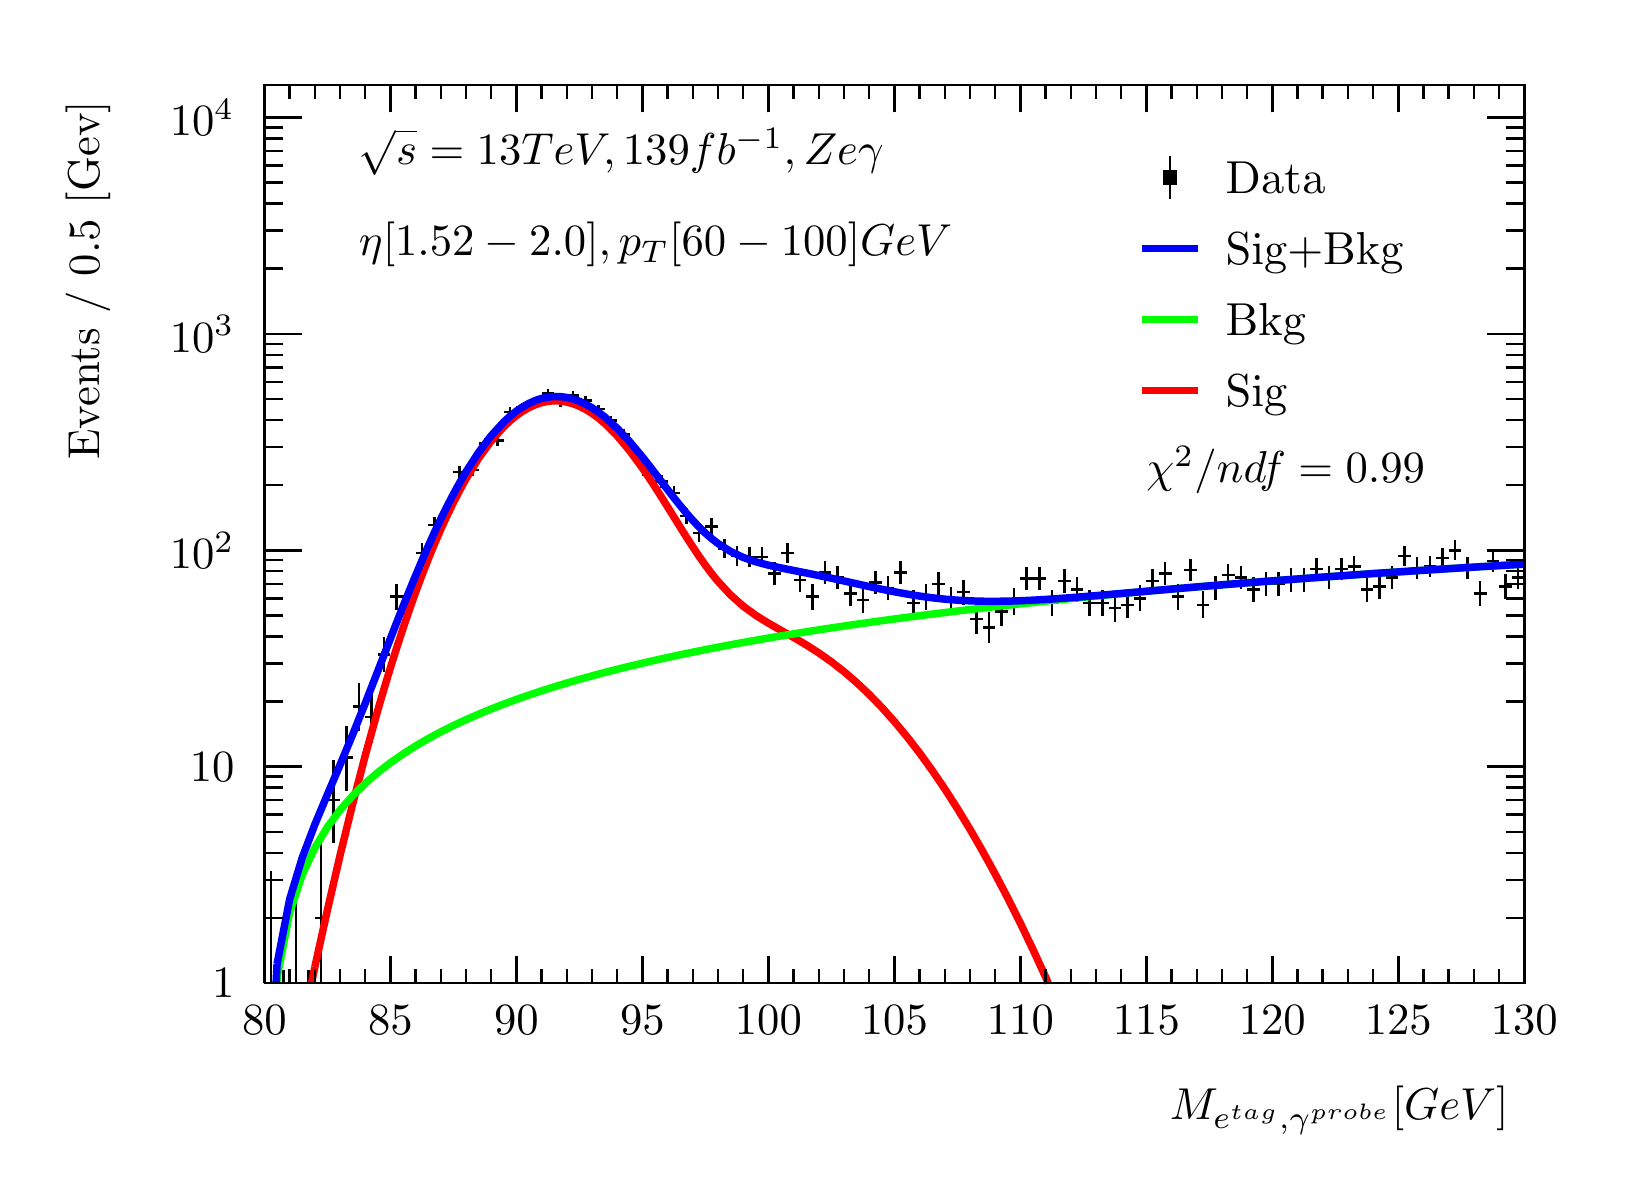
\begin{tikzpicture}
\pgfdeclareplotmark{cross} {
\pgfpathmoveto{\pgfpoint{-0.3\pgfplotmarksize}{\pgfplotmarksize}}
\pgfpathlineto{\pgfpoint{+0.3\pgfplotmarksize}{\pgfplotmarksize}}
\pgfpathlineto{\pgfpoint{+0.3\pgfplotmarksize}{0.3\pgfplotmarksize}}
\pgfpathlineto{\pgfpoint{+1\pgfplotmarksize}{0.3\pgfplotmarksize}}
\pgfpathlineto{\pgfpoint{+1\pgfplotmarksize}{-0.3\pgfplotmarksize}}
\pgfpathlineto{\pgfpoint{+0.3\pgfplotmarksize}{-0.3\pgfplotmarksize}}
\pgfpathlineto{\pgfpoint{+0.3\pgfplotmarksize}{-1.\pgfplotmarksize}}
\pgfpathlineto{\pgfpoint{-0.3\pgfplotmarksize}{-1.\pgfplotmarksize}}
\pgfpathlineto{\pgfpoint{-0.3\pgfplotmarksize}{-0.3\pgfplotmarksize}}
\pgfpathlineto{\pgfpoint{-1.\pgfplotmarksize}{-0.3\pgfplotmarksize}}
\pgfpathlineto{\pgfpoint{-1.\pgfplotmarksize}{0.3\pgfplotmarksize}}
\pgfpathlineto{\pgfpoint{-0.3\pgfplotmarksize}{0.3\pgfplotmarksize}}
\pgfpathclose
\pgfusepathqstroke
}
\pgfdeclareplotmark{cross*} {
\pgfpathmoveto{\pgfpoint{-0.3\pgfplotmarksize}{\pgfplotmarksize}}
\pgfpathlineto{\pgfpoint{+0.3\pgfplotmarksize}{\pgfplotmarksize}}
\pgfpathlineto{\pgfpoint{+0.3\pgfplotmarksize}{0.3\pgfplotmarksize}}
\pgfpathlineto{\pgfpoint{+1\pgfplotmarksize}{0.3\pgfplotmarksize}}
\pgfpathlineto{\pgfpoint{+1\pgfplotmarksize}{-0.3\pgfplotmarksize}}
\pgfpathlineto{\pgfpoint{+0.3\pgfplotmarksize}{-0.3\pgfplotmarksize}}
\pgfpathlineto{\pgfpoint{+0.3\pgfplotmarksize}{-1.\pgfplotmarksize}}
\pgfpathlineto{\pgfpoint{-0.3\pgfplotmarksize}{-1.\pgfplotmarksize}}
\pgfpathlineto{\pgfpoint{-0.3\pgfplotmarksize}{-0.3\pgfplotmarksize}}
\pgfpathlineto{\pgfpoint{-1.\pgfplotmarksize}{-0.3\pgfplotmarksize}}
\pgfpathlineto{\pgfpoint{-1.\pgfplotmarksize}{0.3\pgfplotmarksize}}
\pgfpathlineto{\pgfpoint{-0.3\pgfplotmarksize}{0.3\pgfplotmarksize}}
\pgfpathclose
\pgfusepathqfillstroke
}
\pgfdeclareplotmark{newstar} {
\pgfpathmoveto{\pgfqpoint{0pt}{\pgfplotmarksize}}
\pgfpathlineto{\pgfqpointpolar{44}{0.5\pgfplotmarksize}}
\pgfpathlineto{\pgfqpointpolar{18}{\pgfplotmarksize}}
\pgfpathlineto{\pgfqpointpolar{-20}{0.5\pgfplotmarksize}}
\pgfpathlineto{\pgfqpointpolar{-54}{\pgfplotmarksize}}
\pgfpathlineto{\pgfqpointpolar{-90}{0.5\pgfplotmarksize}}
\pgfpathlineto{\pgfqpointpolar{234}{\pgfplotmarksize}}
\pgfpathlineto{\pgfqpointpolar{198}{0.5\pgfplotmarksize}}
\pgfpathlineto{\pgfqpointpolar{162}{\pgfplotmarksize}}
\pgfpathlineto{\pgfqpointpolar{134}{0.5\pgfplotmarksize}}
\pgfpathclose
\pgfusepathqstroke
}
\pgfdeclareplotmark{newstar*} {
\pgfpathmoveto{\pgfqpoint{0pt}{\pgfplotmarksize}}
\pgfpathlineto{\pgfqpointpolar{44}{0.5\pgfplotmarksize}}
\pgfpathlineto{\pgfqpointpolar{18}{\pgfplotmarksize}}
\pgfpathlineto{\pgfqpointpolar{-20}{0.5\pgfplotmarksize}}
\pgfpathlineto{\pgfqpointpolar{-54}{\pgfplotmarksize}}
\pgfpathlineto{\pgfqpointpolar{-90}{0.5\pgfplotmarksize}}
\pgfpathlineto{\pgfqpointpolar{234}{\pgfplotmarksize}}
\pgfpathlineto{\pgfqpointpolar{198}{0.5\pgfplotmarksize}}
\pgfpathlineto{\pgfqpointpolar{162}{\pgfplotmarksize}}
\pgfpathlineto{\pgfqpointpolar{134}{0.5\pgfplotmarksize}}
\pgfpathclose
\pgfusepathqfillstroke
}
\definecolor{c}{rgb}{1,1,1};
\draw [color=c, fill=c] (0,0) rectangle (20,14.4361);
\draw [color=c, fill=c] (3,2.30977) rectangle (19,13.7143);
\definecolor{c}{rgb}{0,0,0};
\draw [c,line width=0.9] (3,2.30977) -- (3,13.7143) -- (19,13.7143) -- (19,2.30977) -- (3,2.30977);
\definecolor{c}{rgb}{1,1,1};
\draw [color=c, fill=c] (3,2.30977) rectangle (19,13.7143);
\definecolor{c}{rgb}{0,0,0};
\draw [c,line width=0.9] (3,2.30977) -- (3,13.7143) -- (19,13.7143) -- (19,2.30977) -- (3,2.30977);
\draw [c,line width=0.9] (3,2.30977) -- (19,2.30977);
\draw [c,line width=0.9] (3,2.65624) -- (3,2.30977);
\draw [c,line width=0.9] (3.32,2.48301) -- (3.32,2.30977);
\draw [c,line width=0.9] (3.64,2.48301) -- (3.64,2.30977);
\draw [c,line width=0.9] (3.96,2.48301) -- (3.96,2.30977);
\draw [c,line width=0.9] (4.28,2.48301) -- (4.28,2.30977);
\draw [c,line width=0.9] (4.6,2.65624) -- (4.6,2.30977);
\draw [c,line width=0.9] (4.92,2.48301) -- (4.92,2.30977);
\draw [c,line width=0.9] (5.24,2.48301) -- (5.24,2.30977);
\draw [c,line width=0.9] (5.56,2.48301) -- (5.56,2.30977);
\draw [c,line width=0.9] (5.88,2.48301) -- (5.88,2.30977);
\draw [c,line width=0.9] (6.2,2.65624) -- (6.2,2.30977);
\draw [c,line width=0.9] (6.52,2.48301) -- (6.52,2.30977);
\draw [c,line width=0.9] (6.84,2.48301) -- (6.84,2.30977);
\draw [c,line width=0.9] (7.16,2.48301) -- (7.16,2.30977);
\draw [c,line width=0.9] (7.48,2.48301) -- (7.48,2.30977);
\draw [c,line width=0.9] (7.8,2.65624) -- (7.8,2.30977);
\draw [c,line width=0.9] (8.12,2.48301) -- (8.12,2.30977);
\draw [c,line width=0.9] (8.44,2.48301) -- (8.44,2.30977);
\draw [c,line width=0.9] (8.76,2.48301) -- (8.76,2.30977);
\draw [c,line width=0.9] (9.08,2.48301) -- (9.08,2.30977);
\draw [c,line width=0.9] (9.4,2.65624) -- (9.4,2.30977);
\draw [c,line width=0.9] (9.72,2.48301) -- (9.72,2.30977);
\draw [c,line width=0.9] (10.04,2.48301) -- (10.04,2.30977);
\draw [c,line width=0.9] (10.36,2.48301) -- (10.36,2.30977);
\draw [c,line width=0.9] (10.68,2.48301) -- (10.68,2.30977);
\draw [c,line width=0.9] (11,2.65624) -- (11,2.30977);
\draw [c,line width=0.9] (11.32,2.48301) -- (11.32,2.30977);
\draw [c,line width=0.9] (11.64,2.48301) -- (11.64,2.30977);
\draw [c,line width=0.9] (11.96,2.48301) -- (11.96,2.30977);
\draw [c,line width=0.9] (12.28,2.48301) -- (12.28,2.30977);
\draw [c,line width=0.9] (12.6,2.65624) -- (12.6,2.30977);
\draw [c,line width=0.9] (12.92,2.48301) -- (12.92,2.30977);
\draw [c,line width=0.9] (13.24,2.48301) -- (13.24,2.30977);
\draw [c,line width=0.9] (13.56,2.48301) -- (13.56,2.30977);
\draw [c,line width=0.9] (13.88,2.48301) -- (13.88,2.30977);
\draw [c,line width=0.9] (14.2,2.65624) -- (14.2,2.30977);
\draw [c,line width=0.9] (14.52,2.48301) -- (14.52,2.30977);
\draw [c,line width=0.9] (14.84,2.48301) -- (14.84,2.30977);
\draw [c,line width=0.9] (15.16,2.48301) -- (15.16,2.30977);
\draw [c,line width=0.9] (15.48,2.48301) -- (15.48,2.30977);
\draw [c,line width=0.9] (15.8,2.65624) -- (15.8,2.30977);
\draw [c,line width=0.9] (16.12,2.48301) -- (16.12,2.30977);
\draw [c,line width=0.9] (16.44,2.48301) -- (16.44,2.30977);
\draw [c,line width=0.9] (16.76,2.48301) -- (16.76,2.30977);
\draw [c,line width=0.9] (17.08,2.48301) -- (17.08,2.30977);
\draw [c,line width=0.9] (17.4,2.65624) -- (17.4,2.30977);
\draw [c,line width=0.9] (17.72,2.48301) -- (17.72,2.30977);
\draw [c,line width=0.9] (18.04,2.48301) -- (18.04,2.30977);
\draw [c,line width=0.9] (18.36,2.48301) -- (18.36,2.30977);
\draw [c,line width=0.9] (18.68,2.48301) -- (18.68,2.30977);
\draw [c,line width=0.9] (19,2.65624) -- (19,2.30977);
\draw [anchor=base] (3,1.66015) node[scale=1.61424, color=c, rotate=0]{80};
\draw [anchor=base] (4.6,1.66015) node[scale=1.61424, color=c, rotate=0]{85};
\draw [anchor=base] (6.2,1.66015) node[scale=1.61424, color=c, rotate=0]{90};
\draw [anchor=base] (7.8,1.66015) node[scale=1.61424, color=c, rotate=0]{95};
\draw [anchor=base] (9.4,1.66015) node[scale=1.61424, color=c, rotate=0]{100};
\draw [anchor=base] (11,1.66015) node[scale=1.61424, color=c, rotate=0]{105};
\draw [anchor=base] (12.6,1.66015) node[scale=1.61424, color=c, rotate=0]{110};
\draw [anchor=base] (14.2,1.66015) node[scale=1.61424, color=c, rotate=0]{115};
\draw [anchor=base] (15.8,1.66015) node[scale=1.61424, color=c, rotate=0]{120};
\draw [anchor=base] (17.4,1.66015) node[scale=1.61424, color=c, rotate=0]{125};
\draw [anchor=base] (19,1.66015) node[scale=1.61424, color=c, rotate=0]{130};
\draw [anchor= east] (19,0.692932) node[scale=1.61424, color=c, rotate=0]{$M_{e^{tag}, \gamma^{probe}}  [GeV]$};
\draw [c,line width=0.9] (3,13.7143) -- (19,13.7143);
\draw [c,line width=0.9] (3,13.3678) -- (3,13.7143);
\draw [c,line width=0.9] (3.32,13.5411) -- (3.32,13.7143);
\draw [c,line width=0.9] (3.64,13.5411) -- (3.64,13.7143);
\draw [c,line width=0.9] (3.96,13.5411) -- (3.96,13.7143);
\draw [c,line width=0.9] (4.28,13.5411) -- (4.28,13.7143);
\draw [c,line width=0.9] (4.6,13.3678) -- (4.6,13.7143);
\draw [c,line width=0.9] (4.92,13.5411) -- (4.92,13.7143);
\draw [c,line width=0.9] (5.24,13.5411) -- (5.24,13.7143);
\draw [c,line width=0.9] (5.56,13.5411) -- (5.56,13.7143);
\draw [c,line width=0.9] (5.88,13.5411) -- (5.88,13.7143);
\draw [c,line width=0.9] (6.2,13.3678) -- (6.2,13.7143);
\draw [c,line width=0.9] (6.52,13.5411) -- (6.52,13.7143);
\draw [c,line width=0.9] (6.84,13.5411) -- (6.84,13.7143);
\draw [c,line width=0.9] (7.16,13.5411) -- (7.16,13.7143);
\draw [c,line width=0.9] (7.48,13.5411) -- (7.48,13.7143);
\draw [c,line width=0.9] (7.8,13.3678) -- (7.8,13.7143);
\draw [c,line width=0.9] (8.12,13.5411) -- (8.12,13.7143);
\draw [c,line width=0.9] (8.44,13.5411) -- (8.44,13.7143);
\draw [c,line width=0.9] (8.76,13.5411) -- (8.76,13.7143);
\draw [c,line width=0.9] (9.08,13.5411) -- (9.08,13.7143);
\draw [c,line width=0.9] (9.4,13.3678) -- (9.4,13.7143);
\draw [c,line width=0.9] (9.72,13.5411) -- (9.72,13.7143);
\draw [c,line width=0.9] (10.04,13.5411) -- (10.04,13.7143);
\draw [c,line width=0.9] (10.36,13.5411) -- (10.36,13.7143);
\draw [c,line width=0.9] (10.68,13.5411) -- (10.68,13.7143);
\draw [c,line width=0.9] (11,13.3678) -- (11,13.7143);
\draw [c,line width=0.9] (11.32,13.5411) -- (11.32,13.7143);
\draw [c,line width=0.9] (11.64,13.5411) -- (11.64,13.7143);
\draw [c,line width=0.9] (11.96,13.5411) -- (11.96,13.7143);
\draw [c,line width=0.9] (12.28,13.5411) -- (12.28,13.7143);
\draw [c,line width=0.9] (12.6,13.3678) -- (12.6,13.7143);
\draw [c,line width=0.9] (12.92,13.5411) -- (12.92,13.7143);
\draw [c,line width=0.9] (13.24,13.5411) -- (13.24,13.7143);
\draw [c,line width=0.9] (13.56,13.5411) -- (13.56,13.7143);
\draw [c,line width=0.9] (13.88,13.5411) -- (13.88,13.7143);
\draw [c,line width=0.9] (14.2,13.3678) -- (14.2,13.7143);
\draw [c,line width=0.9] (14.52,13.5411) -- (14.52,13.7143);
\draw [c,line width=0.9] (14.84,13.5411) -- (14.84,13.7143);
\draw [c,line width=0.9] (15.16,13.5411) -- (15.16,13.7143);
\draw [c,line width=0.9] (15.48,13.5411) -- (15.48,13.7143);
\draw [c,line width=0.9] (15.8,13.3678) -- (15.8,13.7143);
\draw [c,line width=0.9] (16.12,13.5411) -- (16.12,13.7143);
\draw [c,line width=0.9] (16.44,13.5411) -- (16.44,13.7143);
\draw [c,line width=0.9] (16.76,13.5411) -- (16.76,13.7143);
\draw [c,line width=0.9] (17.08,13.5411) -- (17.08,13.7143);
\draw [c,line width=0.9] (17.4,13.3678) -- (17.4,13.7143);
\draw [c,line width=0.9] (17.72,13.5411) -- (17.72,13.7143);
\draw [c,line width=0.9] (18.04,13.5411) -- (18.04,13.7143);
\draw [c,line width=0.9] (18.36,13.5411) -- (18.36,13.7143);
\draw [c,line width=0.9] (18.68,13.5411) -- (18.68,13.7143);
\draw [c,line width=0.9] (19,13.3678) -- (19,13.7143);
\draw [c,line width=0.9] (3,2.30977) -- (3,13.7143);
\draw [c,line width=0.9] (3.474,2.30978) -- (3,2.30978);
\draw [anchor= east] (2.82,2.30978) node[scale=1.61424, color=c, rotate=0]{1};
\draw [c,line width=0.9] (3.237,3.13707) -- (3,3.13707);
\draw [c,line width=0.9] (3.237,3.621) -- (3,3.621);
\draw [c,line width=0.9] (3.237,3.96436) -- (3,3.96436);
\draw [c,line width=0.9] (3.237,4.23069) -- (3,4.23069);
\draw [c,line width=0.9] (3.237,4.4483) -- (3,4.4483);
\draw [c,line width=0.9] (3.237,4.63228) -- (3,4.63228);
\draw [c,line width=0.9] (3.237,4.79165) -- (3,4.79165);
\draw [c,line width=0.9] (3.237,4.93223) -- (3,4.93223);
\draw [c,line width=0.9] (3.474,5.05798) -- (3,5.05798);
\draw [anchor= east] (2.82,5.05798) node[scale=1.61424, color=c, rotate=0]{10};
\draw [c,line width=0.9] (3.237,5.88527) -- (3,5.88527);
\draw [c,line width=0.9] (3.237,6.36921) -- (3,6.36921);
\draw [c,line width=0.9] (3.237,6.71257) -- (3,6.71257);
\draw [c,line width=0.9] (3.237,6.97889) -- (3,6.97889);
\draw [c,line width=0.9] (3.237,7.1965) -- (3,7.1965);
\draw [c,line width=0.9] (3.237,7.38048) -- (3,7.38048);
\draw [c,line width=0.9] (3.237,7.53986) -- (3,7.53986);
\draw [c,line width=0.9] (3.237,7.68043) -- (3,7.68043);
\draw [c,line width=0.9] (3.474,7.80619) -- (3,7.80619);
\draw [anchor= east] (2.82,7.80619) node[scale=1.61424, color=c, rotate=0]{$10^{2}$};
\draw [c,line width=0.9] (3.237,8.63348) -- (3,8.63348);
\draw [c,line width=0.9] (3.237,9.11741) -- (3,9.11741);
\draw [c,line width=0.9] (3.237,9.46077) -- (3,9.46077);
\draw [c,line width=0.9] (3.237,9.7271) -- (3,9.7271);
\draw [c,line width=0.9] (3.237,9.9447) -- (3,9.9447);
\draw [c,line width=0.9] (3.237,10.1287) -- (3,10.1287);
\draw [c,line width=0.9] (3.237,10.2881) -- (3,10.2881);
\draw [c,line width=0.9] (3.237,10.4286) -- (3,10.4286);
\draw [c,line width=0.9] (3.474,10.5544) -- (3,10.5544);
\draw [anchor= east] (2.82,10.5544) node[scale=1.61424, color=c, rotate=0]{$10^{3}$};
\draw [c,line width=0.9] (3.237,11.3817) -- (3,11.3817);
\draw [c,line width=0.9] (3.237,11.8656) -- (3,11.8656);
\draw [c,line width=0.9] (3.237,12.209) -- (3,12.209);
\draw [c,line width=0.9] (3.237,12.4753) -- (3,12.4753);
\draw [c,line width=0.9] (3.237,12.6929) -- (3,12.6929);
\draw [c,line width=0.9] (3.237,12.8769) -- (3,12.8769);
\draw [c,line width=0.9] (3.237,13.0363) -- (3,13.0363);
\draw [c,line width=0.9] (3.237,13.1768) -- (3,13.1768);
\draw [c,line width=0.9] (3.474,13.3026) -- (3,13.3026);
\draw [anchor= east] (2.82,13.3026) node[scale=1.61424, color=c, rotate=0]{$10^{4}$};
\draw [anchor= east] (0.76,13.7143) node[scale=1.61424, color=c, rotate=90]{Events / 0.5 [Gev]};
\draw [c,line width=0.9] (19,2.30977) -- (19,13.7143);
\draw [c,line width=0.9] (18.526,2.30978) -- (19,2.30978);
\draw [c,line width=0.9] (18.763,3.13707) -- (19,3.13707);
\draw [c,line width=0.9] (18.763,3.621) -- (19,3.621);
\draw [c,line width=0.9] (18.763,3.96436) -- (19,3.96436);
\draw [c,line width=0.9] (18.763,4.23069) -- (19,4.23069);
\draw [c,line width=0.9] (18.763,4.4483) -- (19,4.4483);
\draw [c,line width=0.9] (18.763,4.63228) -- (19,4.63228);
\draw [c,line width=0.9] (18.763,4.79165) -- (19,4.79165);
\draw [c,line width=0.9] (18.763,4.93223) -- (19,4.93223);
\draw [c,line width=0.9] (18.526,5.05798) -- (19,5.05798);
\draw [c,line width=0.9] (18.763,5.88527) -- (19,5.88527);
\draw [c,line width=0.9] (18.763,6.36921) -- (19,6.36921);
\draw [c,line width=0.9] (18.763,6.71257) -- (19,6.71257);
\draw [c,line width=0.9] (18.763,6.97889) -- (19,6.97889);
\draw [c,line width=0.9] (18.763,7.1965) -- (19,7.1965);
\draw [c,line width=0.9] (18.763,7.38048) -- (19,7.38048);
\draw [c,line width=0.9] (18.763,7.53986) -- (19,7.53986);
\draw [c,line width=0.9] (18.763,7.68043) -- (19,7.68043);
\draw [c,line width=0.9] (18.526,7.80619) -- (19,7.80619);
\draw [c,line width=0.9] (18.763,8.63348) -- (19,8.63348);
\draw [c,line width=0.9] (18.763,9.11741) -- (19,9.11741);
\draw [c,line width=0.9] (18.763,9.46077) -- (19,9.46077);
\draw [c,line width=0.9] (18.763,9.7271) -- (19,9.7271);
\draw [c,line width=0.9] (18.763,9.9447) -- (19,9.9447);
\draw [c,line width=0.9] (18.763,10.1287) -- (19,10.1287);
\draw [c,line width=0.9] (18.763,10.2881) -- (19,10.2881);
\draw [c,line width=0.9] (18.763,10.4286) -- (19,10.4286);
\draw [c,line width=0.9] (18.526,10.5544) -- (19,10.5544);
\draw [c,line width=0.9] (18.763,11.3817) -- (19,11.3817);
\draw [c,line width=0.9] (18.763,11.8656) -- (19,11.8656);
\draw [c,line width=0.9] (18.763,12.209) -- (19,12.209);
\draw [c,line width=0.9] (18.763,12.4753) -- (19,12.4753);
\draw [c,line width=0.9] (18.763,12.6929) -- (19,12.6929);
\draw [c,line width=0.9] (18.763,12.8769) -- (19,12.8769);
\draw [c,line width=0.9] (18.763,13.0363) -- (19,13.0363);
\draw [c,line width=0.9] (18.763,13.1768) -- (19,13.1768);
\draw [c,line width=0.9] (18.526,13.3026) -- (19,13.3026);
\draw [c,line width=0.9] (3.08,2.30977) -- (3,2.30977);
\draw [c,line width=0.9] (3,2.30977) -- (3,2.30977);
\draw [c,line width=0.9] (3.08,2.30977) -- (3.16,2.30977);
\draw [c,line width=0.9] (3.16,2.30977) -- (3.16,2.30977);
\draw [c,line width=0.9] (3.08,2.30977) -- (3.08,3.73459);
\draw [c,line width=0.9] (3.08,3.73459) -- (3.08,3.73459);
\draw [c,line width=0.9] (3.24,2.30977) -- (3.16,2.30977);
\draw [c,line width=0.9] (3.16,2.30977) -- (3.16,2.30977);
\draw [c,line width=0.9] (3.24,2.30977) -- (3.32,2.30977);
\draw [c,line width=0.9] (3.32,2.30977) -- (3.32,2.30977);
\draw [c,line width=0.9] (3.24,2.30977) -- (3.24,2.47438);
\draw [c,line width=0.9] (3.24,2.47438) -- (3.24,2.47438);
\draw [c,line width=0.9] (3.4,2.30977) -- (3.32,2.30977);
\draw [c,line width=0.9] (3.32,2.30977) -- (3.32,2.30977);
\draw [c,line width=0.9] (3.4,2.30977) -- (3.48,2.30977);
\draw [c,line width=0.9] (3.48,2.30977) -- (3.48,2.30977);
\draw [c,line width=0.9] (3.4,2.30977) -- (3.4,3.73459);
\draw [c,line width=0.9] (3.4,3.73459) -- (3.4,3.73459);
\draw [c,line width=0.9] (3.56,2.30977) -- (3.48,2.30977);
\draw [c,line width=0.9] (3.48,2.30977) -- (3.48,2.30977);
\draw [c,line width=0.9] (3.56,2.30977) -- (3.64,2.30977);
\draw [c,line width=0.9] (3.64,2.30977) -- (3.64,2.30977);
\draw [c,line width=0.9] (3.56,2.30977) -- (3.56,2.47438);
\draw [c,line width=0.9] (3.56,2.47438) -- (3.56,2.47438);
\draw [c,line width=0.9] (3.72,3.13707) -- (3.64,3.13707);
\draw [c,line width=0.9] (3.64,3.13707) -- (3.64,3.13707);
\draw [c,line width=0.9] (3.72,3.13707) -- (3.8,3.13707);
\draw [c,line width=0.9] (3.8,3.13707) -- (3.8,3.13707);
\draw [c,line width=0.9] (3.72,3.13707) -- (3.72,4.14095);
\draw [c,line width=0.9] (3.72,4.14095) -- (3.72,4.14095);
\draw [c,line width=0.9] (3.72,3.13707) -- (3.72,2.30977);
\draw [c,line width=0.9] (3.72,2.30977) -- (3.72,2.30977);
\draw [c,line width=0.9] (3.88,4.63228) -- (3.8,4.63228);
\draw [c,line width=0.9] (3.8,4.63228) -- (3.8,4.63228);
\draw [c,line width=0.9] (3.88,4.63228) -- (3.96,4.63228);
\draw [c,line width=0.9] (3.96,4.63228) -- (3.96,4.63228);
\draw [c,line width=0.9] (3.88,4.63228) -- (3.88,5.14655);
\draw [c,line width=0.9] (3.88,5.14655) -- (3.88,5.14655);
\draw [c,line width=0.9] (3.88,4.63228) -- (3.88,4.08313);
\draw [c,line width=0.9] (3.88,4.08313) -- (3.88,4.08313);
\draw [c,line width=0.9] (4.04,5.17173) -- (3.96,5.17173);
\draw [c,line width=0.9] (3.96,5.17173) -- (3.96,5.17173);
\draw [c,line width=0.9] (4.04,5.17173) -- (4.12,5.17173);
\draw [c,line width=0.9] (4.12,5.17173) -- (4.12,5.17173);
\draw [c,line width=0.9] (4.04,5.17173) -- (4.04,5.5746);
\draw [c,line width=0.9] (4.04,5.5746) -- (4.04,5.5746);
\draw [c,line width=0.9] (4.04,5.17173) -- (4.04,4.75136);
\draw [c,line width=0.9] (4.04,4.75136) -- (4.04,4.75136);
\draw [c,line width=0.9] (4.2,5.82405) -- (4.12,5.82405);
\draw [c,line width=0.9] (4.12,5.82405) -- (4.12,5.82405);
\draw [c,line width=0.9] (4.2,5.82405) -- (4.28,5.82405);
\draw [c,line width=0.9] (4.28,5.82405) -- (4.28,5.82405);
\draw [c,line width=0.9] (4.2,5.82405) -- (4.2,6.12433);
\draw [c,line width=0.9] (4.2,6.12433) -- (4.2,6.12433);
\draw [c,line width=0.9] (4.2,5.82405) -- (4.2,5.51616);
\draw [c,line width=0.9] (4.2,5.51616) -- (4.2,5.51616);
\draw [c,line width=0.9] (4.36,5.6913) -- (4.28,5.6913);
\draw [c,line width=0.9] (4.28,5.6913) -- (4.28,5.6913);
\draw [c,line width=0.9] (4.36,5.6913) -- (4.44,5.6913);
\draw [c,line width=0.9] (4.44,5.6913) -- (4.44,5.6913);
\draw [c,line width=0.9] (4.36,5.6913) -- (4.36,6.01003);
\draw [c,line width=0.9] (4.36,6.01003) -- (4.36,6.01003);
\draw [c,line width=0.9] (4.36,5.6913) -- (4.36,5.36355);
\draw [c,line width=0.9] (4.36,5.36355) -- (4.36,5.36355);
\draw [c,line width=0.9] (4.52,6.48296) -- (4.44,6.48296);
\draw [c,line width=0.9] (4.44,6.48296) -- (4.44,6.48296);
\draw [c,line width=0.9] (4.52,6.48296) -- (4.6,6.48296);
\draw [c,line width=0.9] (4.6,6.48296) -- (4.6,6.48296);
\draw [c,line width=0.9] (4.52,6.48296) -- (4.52,6.70666);
\draw [c,line width=0.9] (4.52,6.70666) -- (4.52,6.70666);
\draw [c,line width=0.9] (4.52,6.48296) -- (4.52,6.25597);
\draw [c,line width=0.9] (4.52,6.25597) -- (4.52,6.25597);
\draw [c,line width=0.9] (4.68,7.21623) -- (4.6,7.21623);
\draw [c,line width=0.9] (4.6,7.21623) -- (4.6,7.21623);
\draw [c,line width=0.9] (4.68,7.21623) -- (4.76,7.21623);
\draw [c,line width=0.9] (4.76,7.21623) -- (4.76,7.21623);
\draw [c,line width=0.9] (4.68,7.21623) -- (4.68,7.37797);
\draw [c,line width=0.9] (4.68,7.37797) -- (4.68,7.37797);
\draw [c,line width=0.9] (4.68,7.21623) -- (4.68,7.05318);
\draw [c,line width=0.9] (4.68,7.05318) -- (4.68,7.05318);
\draw [c,line width=0.9] (4.84,7.21623) -- (4.76,7.21623);
\draw [c,line width=0.9] (4.76,7.21623) -- (4.76,7.21623);
\draw [c,line width=0.9] (4.84,7.21623) -- (4.92,7.21623);
\draw [c,line width=0.9] (4.92,7.21623) -- (4.92,7.21623);
\draw [c,line width=0.9] (4.84,7.21623) -- (4.84,7.37797);
\draw [c,line width=0.9] (4.84,7.37797) -- (4.84,7.37797);
\draw [c,line width=0.9] (4.84,7.21623) -- (4.84,7.05318);
\draw [c,line width=0.9] (4.84,7.05318) -- (4.84,7.05318);
\draw [c,line width=0.9] (5,7.76983) -- (4.92,7.76983);
\draw [c,line width=0.9] (4.92,7.76983) -- (4.92,7.76983);
\draw [c,line width=0.9] (5,7.76983) -- (5.08,7.76983);
\draw [c,line width=0.9] (5.08,7.76983) -- (5.08,7.76983);
\draw [c,line width=0.9] (5,7.76983) -- (5,7.89674);
\draw [c,line width=0.9] (5,7.89674) -- (5,7.89674);
\draw [c,line width=0.9] (5,7.76983) -- (5,7.64228);
\draw [c,line width=0.9] (5,7.64228) -- (5,7.64228);
\draw [c,line width=0.9] (5.16,8.12847) -- (5.08,8.12847);
\draw [c,line width=0.9] (5.08,8.12847) -- (5.08,8.12847);
\draw [c,line width=0.9] (5.16,8.12847) -- (5.24,8.12847);
\draw [c,line width=0.9] (5.24,8.12847) -- (5.24,8.12847);
\draw [c,line width=0.9] (5.16,8.12847) -- (5.16,8.23272);
\draw [c,line width=0.9] (5.16,8.23272) -- (5.16,8.23272);
\draw [c,line width=0.9] (5.16,8.12847) -- (5.16,8.02422);
\draw [c,line width=0.9] (5.16,8.02422) -- (5.16,8.02422);
\draw [c,line width=0.9] (5.32,8.29012) -- (5.24,8.29012);
\draw [c,line width=0.9] (5.24,8.29012) -- (5.24,8.29012);
\draw [c,line width=0.9] (5.32,8.29012) -- (5.4,8.29012);
\draw [c,line width=0.9] (5.4,8.29012) -- (5.4,8.29012);
\draw [c,line width=0.9] (5.32,8.29012) -- (5.32,8.38754);
\draw [c,line width=0.9] (5.32,8.38754) -- (5.32,8.38754);
\draw [c,line width=0.9] (5.32,8.29012) -- (5.32,8.19269);
\draw [c,line width=0.9] (5.32,8.19269) -- (5.32,8.19269);
\draw [c,line width=0.9] (5.48,8.80029) -- (5.4,8.80029);
\draw [c,line width=0.9] (5.4,8.80029) -- (5.4,8.80029);
\draw [c,line width=0.9] (5.48,8.80029) -- (5.56,8.80029);
\draw [c,line width=0.9] (5.56,8.80029) -- (5.56,8.80029);
\draw [c,line width=0.9] (5.48,8.80029) -- (5.48,8.87897);
\draw [c,line width=0.9] (5.48,8.87897) -- (5.48,8.87897);
\draw [c,line width=0.9] (5.48,8.80029) -- (5.48,8.7216);
\draw [c,line width=0.9] (5.48,8.7216) -- (5.48,8.7216);
\draw [c,line width=0.9] (5.64,8.82595) -- (5.56,8.82595);
\draw [c,line width=0.9] (5.56,8.82595) -- (5.56,8.82595);
\draw [c,line width=0.9] (5.64,8.82595) -- (5.72,8.82595);
\draw [c,line width=0.9] (5.72,8.82595) -- (5.72,8.82595);
\draw [c,line width=0.9] (5.64,8.82595) -- (5.64,8.9038);
\draw [c,line width=0.9] (5.64,8.9038) -- (5.64,8.9038);
\draw [c,line width=0.9] (5.64,8.82595) -- (5.64,8.74811);
\draw [c,line width=0.9] (5.64,8.74811) -- (5.64,8.74811);
\draw [c,line width=0.9] (5.8,9.16422) -- (5.72,9.16422);
\draw [c,line width=0.9] (5.72,9.16422) -- (5.72,9.16422);
\draw [c,line width=0.9] (5.8,9.16422) -- (5.88,9.16422);
\draw [c,line width=0.9] (5.88,9.16422) -- (5.88,9.16422);
\draw [c,line width=0.9] (5.8,9.16422) -- (5.8,9.23178);
\draw [c,line width=0.9] (5.8,9.23178) -- (5.8,9.23178);
\draw [c,line width=0.9] (5.8,9.16422) -- (5.8,9.09666);
\draw [c,line width=0.9] (5.8,9.09666) -- (5.8,9.09666);
\draw [c,line width=0.9] (5.96,9.20188) -- (5.88,9.20188);
\draw [c,line width=0.9] (5.88,9.20188) -- (5.88,9.20188);
\draw [c,line width=0.9] (5.96,9.20188) -- (6.04,9.20188);
\draw [c,line width=0.9] (6.04,9.20188) -- (6.04,9.20188);
\draw [c,line width=0.9] (5.96,9.20188) -- (5.96,9.26838);
\draw [c,line width=0.9] (5.96,9.26838) -- (5.96,9.26838);
\draw [c,line width=0.9] (5.96,9.20188) -- (5.96,9.13537);
\draw [c,line width=0.9] (5.96,9.13537) -- (5.96,9.13537);
\draw [c,line width=0.9] (6.12,9.56362) -- (6.04,9.56362);
\draw [c,line width=0.9] (6.04,9.56362) -- (6.04,9.56362);
\draw [c,line width=0.9] (6.12,9.56362) -- (6.2,9.56362);
\draw [c,line width=0.9] (6.2,9.56362) -- (6.2,9.56362);
\draw [c,line width=0.9] (6.12,9.56362) -- (6.12,9.62078);
\draw [c,line width=0.9] (6.12,9.62078) -- (6.12,9.62078);
\draw [c,line width=0.9] (6.12,9.56362) -- (6.12,9.50647);
\draw [c,line width=0.9] (6.12,9.50647) -- (6.12,9.50647);
\draw [c,line width=0.9] (6.28,9.62498) -- (6.2,9.62498);
\draw [c,line width=0.9] (6.2,9.62498) -- (6.2,9.62498);
\draw [c,line width=0.9] (6.28,9.62498) -- (6.36,9.62498);
\draw [c,line width=0.9] (6.36,9.62498) -- (6.36,9.62498);
\draw [c,line width=0.9] (6.28,9.62498) -- (6.28,9.68069);
\draw [c,line width=0.9] (6.28,9.68069) -- (6.28,9.68069);
\draw [c,line width=0.9] (6.28,9.62498) -- (6.28,9.56928);
\draw [c,line width=0.9] (6.28,9.56928) -- (6.28,9.56928);
\draw [c,line width=0.9] (6.44,9.67837) -- (6.36,9.67837);
\draw [c,line width=0.9] (6.36,9.67837) -- (6.36,9.67837);
\draw [c,line width=0.9] (6.44,9.67837) -- (6.52,9.67837);
\draw [c,line width=0.9] (6.52,9.67837) -- (6.52,9.67837);
\draw [c,line width=0.9] (6.44,9.67837) -- (6.44,9.73285);
\draw [c,line width=0.9] (6.44,9.73285) -- (6.44,9.73285);
\draw [c,line width=0.9] (6.44,9.67837) -- (6.44,9.6239);
\draw [c,line width=0.9] (6.44,9.6239) -- (6.44,9.6239);
\draw [c,line width=0.9] (6.6,9.79664) -- (6.52,9.79664);
\draw [c,line width=0.9] (6.52,9.79664) -- (6.52,9.79664);
\draw [c,line width=0.9] (6.6,9.79664) -- (6.68,9.79664);
\draw [c,line width=0.9] (6.68,9.79664) -- (6.68,9.79664);
\draw [c,line width=0.9] (6.6,9.79664) -- (6.6,9.84848);
\draw [c,line width=0.9] (6.6,9.84848) -- (6.6,9.84848);
\draw [c,line width=0.9] (6.6,9.79664) -- (6.6,9.7448);
\draw [c,line width=0.9] (6.6,9.7448) -- (6.6,9.7448);
\draw [c,line width=0.9] (6.76,9.68334) -- (6.68,9.68334);
\draw [c,line width=0.9] (6.68,9.68334) -- (6.68,9.68334);
\draw [c,line width=0.9] (6.76,9.68334) -- (6.84,9.68334);
\draw [c,line width=0.9] (6.84,9.68334) -- (6.84,9.68334);
\draw [c,line width=0.9] (6.76,9.68334) -- (6.76,9.7377);
\draw [c,line width=0.9] (6.76,9.7377) -- (6.76,9.7377);
\draw [c,line width=0.9] (6.76,9.68334) -- (6.76,9.62898);
\draw [c,line width=0.9] (6.76,9.62898) -- (6.76,9.62898);
\draw [c,line width=0.9] (6.92,9.77391) -- (6.84,9.77391);
\draw [c,line width=0.9] (6.84,9.77391) -- (6.84,9.77391);
\draw [c,line width=0.9] (6.92,9.77391) -- (7,9.77391);
\draw [c,line width=0.9] (7,9.77391) -- (7,9.77391);
\draw [c,line width=0.9] (6.92,9.77391) -- (6.92,9.82624);
\draw [c,line width=0.9] (6.92,9.82624) -- (6.92,9.82624);
\draw [c,line width=0.9] (6.92,9.77391) -- (6.92,9.72157);
\draw [c,line width=0.9] (6.92,9.72157) -- (6.92,9.72157);
\draw [c,line width=0.9] (7.08,9.71027) -- (7,9.71027);
\draw [c,line width=0.9] (7,9.71027) -- (7,9.71027);
\draw [c,line width=0.9] (7.08,9.71027) -- (7.16,9.71027);
\draw [c,line width=0.9] (7.16,9.71027) -- (7.16,9.71027);
\draw [c,line width=0.9] (7.08,9.71027) -- (7.08,9.76402);
\draw [c,line width=0.9] (7.08,9.76402) -- (7.08,9.76402);
\draw [c,line width=0.9] (7.08,9.71027) -- (7.08,9.65652);
\draw [c,line width=0.9] (7.08,9.65652) -- (7.08,9.65652);
\draw [c,line width=0.9] (7.24,9.59869) -- (7.16,9.59869);
\draw [c,line width=0.9] (7.16,9.59869) -- (7.16,9.59869);
\draw [c,line width=0.9] (7.24,9.59869) -- (7.32,9.59869);
\draw [c,line width=0.9] (7.32,9.59869) -- (7.32,9.59869);
\draw [c,line width=0.9] (7.24,9.59869) -- (7.24,9.65501);
\draw [c,line width=0.9] (7.24,9.65501) -- (7.24,9.65501);
\draw [c,line width=0.9] (7.24,9.59869) -- (7.24,9.54237);
\draw [c,line width=0.9] (7.24,9.54237) -- (7.24,9.54237);
\draw [c,line width=0.9] (7.4,9.45479) -- (7.32,9.45479);
\draw [c,line width=0.9] (7.32,9.45479) -- (7.32,9.45479);
\draw [c,line width=0.9] (7.4,9.45479) -- (7.48,9.45479);
\draw [c,line width=0.9] (7.48,9.45479) -- (7.48,9.45479);
\draw [c,line width=0.9] (7.4,9.45479) -- (7.4,9.51461);
\draw [c,line width=0.9] (7.4,9.51461) -- (7.4,9.51461);
\draw [c,line width=0.9] (7.4,9.45479) -- (7.4,9.39497);
\draw [c,line width=0.9] (7.4,9.39497) -- (7.4,9.39497);
\draw [c,line width=0.9] (7.56,9.27728) -- (7.48,9.27728);
\draw [c,line width=0.9] (7.48,9.27728) -- (7.48,9.27728);
\draw [c,line width=0.9] (7.56,9.27728) -- (7.64,9.27728);
\draw [c,line width=0.9] (7.64,9.27728) -- (7.64,9.27728);
\draw [c,line width=0.9] (7.56,9.27728) -- (7.56,9.34172);
\draw [c,line width=0.9] (7.56,9.34172) -- (7.56,9.34172);
\draw [c,line width=0.9] (7.56,9.27728) -- (7.56,9.21285);
\draw [c,line width=0.9] (7.56,9.21285) -- (7.56,9.21285);
\draw [c,line width=0.9] (7.72,9.03507) -- (7.64,9.03507);
\draw [c,line width=0.9] (7.64,9.03507) -- (7.64,9.03507);
\draw [c,line width=0.9] (7.72,9.03507) -- (7.8,9.03507);
\draw [c,line width=0.9] (7.8,9.03507) -- (7.8,9.03507);
\draw [c,line width=0.9] (7.72,9.03507) -- (7.72,9.10638);
\draw [c,line width=0.9] (7.72,9.10638) -- (7.72,9.10638);
\draw [c,line width=0.9] (7.72,9.03507) -- (7.72,8.96375);
\draw [c,line width=0.9] (7.72,8.96375) -- (7.72,8.96375);
\draw [c,line width=0.9] (7.88,8.76874) -- (7.8,8.76874);
\draw [c,line width=0.9] (7.8,8.76874) -- (7.8,8.76874);
\draw [c,line width=0.9] (7.88,8.76874) -- (7.96,8.76874);
\draw [c,line width=0.9] (7.96,8.76874) -- (7.96,8.76874);
\draw [c,line width=0.9] (7.88,8.76874) -- (7.88,8.84847);
\draw [c,line width=0.9] (7.88,8.84847) -- (7.88,8.84847);
\draw [c,line width=0.9] (7.88,8.76874) -- (7.88,8.68901);
\draw [c,line width=0.9] (7.88,8.68901) -- (7.88,8.68901);
\draw [c,line width=0.9] (8.04,8.68029) -- (7.96,8.68029);
\draw [c,line width=0.9] (7.96,8.68029) -- (7.96,8.68029);
\draw [c,line width=0.9] (8.04,8.68029) -- (8.12,8.68029);
\draw [c,line width=0.9] (8.12,8.68029) -- (8.12,8.68029);
\draw [c,line width=0.9] (8.04,8.68029) -- (8.04,8.76303);
\draw [c,line width=0.9] (8.04,8.76303) -- (8.04,8.76303);
\draw [c,line width=0.9] (8.04,8.68029) -- (8.04,8.59755);
\draw [c,line width=0.9] (8.04,8.59755) -- (8.04,8.59755);
\draw [c,line width=0.9] (8.2,8.53396) -- (8.12,8.53396);
\draw [c,line width=0.9] (8.12,8.53396) -- (8.12,8.53396);
\draw [c,line width=0.9] (8.2,8.53396) -- (8.28,8.53396);
\draw [c,line width=0.9] (8.28,8.53396) -- (8.28,8.53396);
\draw [c,line width=0.9] (8.2,8.53396) -- (8.2,8.62193);
\draw [c,line width=0.9] (8.2,8.62193) -- (8.2,8.62193);
\draw [c,line width=0.9] (8.2,8.53396) -- (8.2,8.44599);
\draw [c,line width=0.9] (8.2,8.44599) -- (8.2,8.44599);
\draw [c,line width=0.9] (8.36,8.2414) -- (8.28,8.2414);
\draw [c,line width=0.9] (8.28,8.2414) -- (8.28,8.2414);
\draw [c,line width=0.9] (8.36,8.2414) -- (8.44,8.2414);
\draw [c,line width=0.9] (8.44,8.2414) -- (8.44,8.2414);
\draw [c,line width=0.9] (8.36,8.2414) -- (8.36,8.34083);
\draw [c,line width=0.9] (8.36,8.34083) -- (8.36,8.34083);
\draw [c,line width=0.9] (8.36,8.2414) -- (8.36,8.14196);
\draw [c,line width=0.9] (8.36,8.14196) -- (8.36,8.14196);
\draw [c,line width=0.9] (8.52,8.02379) -- (8.44,8.02379);
\draw [c,line width=0.9] (8.44,8.02379) -- (8.44,8.02379);
\draw [c,line width=0.9] (8.52,8.02379) -- (8.6,8.02379);
\draw [c,line width=0.9] (8.6,8.02379) -- (8.6,8.02379);
\draw [c,line width=0.9] (8.52,8.02379) -- (8.52,8.13271);
\draw [c,line width=0.9] (8.52,8.13271) -- (8.52,8.13271);
\draw [c,line width=0.9] (8.52,8.02379) -- (8.52,7.91487);
\draw [c,line width=0.9] (8.52,7.91487) -- (8.52,7.91487);
\draw [c,line width=0.9] (8.68,8.11011) -- (8.6,8.11011);
\draw [c,line width=0.9] (8.6,8.11011) -- (8.6,8.11011);
\draw [c,line width=0.9] (8.68,8.11011) -- (8.76,8.11011);
\draw [c,line width=0.9] (8.76,8.11011) -- (8.76,8.11011);
\draw [c,line width=0.9] (8.68,8.11011) -- (8.68,8.21516);
\draw [c,line width=0.9] (8.68,8.21516) -- (8.68,8.21516);
\draw [c,line width=0.9] (8.68,8.11011) -- (8.68,8.00506);
\draw [c,line width=0.9] (8.68,8.00506) -- (8.68,8.00506);
\draw [c,line width=0.9] (8.84,7.82982) -- (8.76,7.82982);
\draw [c,line width=0.9] (8.76,7.82982) -- (8.76,7.82982);
\draw [c,line width=0.9] (8.84,7.82982) -- (8.92,7.82982);
\draw [c,line width=0.9] (8.92,7.82982) -- (8.92,7.82982);
\draw [c,line width=0.9] (8.84,7.82982) -- (8.84,7.94795);
\draw [c,line width=0.9] (8.84,7.94795) -- (8.84,7.94795);
\draw [c,line width=0.9] (8.84,7.82982) -- (8.84,7.71169);
\draw [c,line width=0.9] (8.84,7.71169) -- (8.84,7.71169);
\draw [c,line width=0.9] (9,7.73233) -- (8.92,7.73233);
\draw [c,line width=0.9] (8.92,7.73233) -- (8.92,7.73233);
\draw [c,line width=0.9] (9,7.73233) -- (9.08,7.73233);
\draw [c,line width=0.9] (9.08,7.73233) -- (9.08,7.73233);
\draw [c,line width=0.9] (9,7.73233) -- (9,7.86134);
\draw [c,line width=0.9] (9,7.86134) -- (9,7.86134);
\draw [c,line width=0.9] (9,7.73233) -- (9,7.60265);
\draw [c,line width=0.9] (9,7.60265) -- (9,7.60265);
\draw [c,line width=0.9] (9.16,7.71957) -- (9.08,7.71957);
\draw [c,line width=0.9] (9.08,7.71957) -- (9.08,7.71957);
\draw [c,line width=0.9] (9.16,7.71957) -- (9.24,7.71957);
\draw [c,line width=0.9] (9.24,7.71957) -- (9.24,7.71957);
\draw [c,line width=0.9] (9.16,7.71957) -- (9.16,7.8493);
\draw [c,line width=0.9] (9.16,7.8493) -- (9.16,7.8493);
\draw [c,line width=0.9] (9.16,7.71957) -- (9.16,7.58916);
\draw [c,line width=0.9] (9.16,7.58916) -- (9.16,7.58916);
\draw [c,line width=0.9] (9.32,7.71957) -- (9.24,7.71957);
\draw [c,line width=0.9] (9.24,7.71957) -- (9.24,7.71957);
\draw [c,line width=0.9] (9.32,7.71957) -- (9.4,7.71957);
\draw [c,line width=0.9] (9.4,7.71957) -- (9.4,7.71957);
\draw [c,line width=0.9] (9.32,7.71957) -- (9.32,7.8493);
\draw [c,line width=0.9] (9.32,7.8493) -- (9.32,7.8493);
\draw [c,line width=0.9] (9.32,7.71957) -- (9.32,7.58916);
\draw [c,line width=0.9] (9.32,7.58916) -- (9.32,7.58916);
\draw [c,line width=0.9] (9.48,7.50964) -- (9.4,7.50964);
\draw [c,line width=0.9] (9.4,7.50964) -- (9.4,7.50964);
\draw [c,line width=0.9] (9.48,7.50964) -- (9.56,7.50964);
\draw [c,line width=0.9] (9.56,7.50964) -- (9.56,7.50964);
\draw [c,line width=0.9] (9.48,7.50964) -- (9.48,7.65184);
\draw [c,line width=0.9] (9.48,7.65184) -- (9.48,7.65184);
\draw [c,line width=0.9] (9.48,7.50964) -- (9.48,7.36654);
\draw [c,line width=0.9] (9.48,7.36654) -- (9.48,7.36654);
\draw [c,line width=0.9] (9.64,7.76983) -- (9.56,7.76983);
\draw [c,line width=0.9] (9.56,7.76983) -- (9.56,7.76983);
\draw [c,line width=0.9] (9.64,7.76983) -- (9.72,7.76983);
\draw [c,line width=0.9] (9.72,7.76983) -- (9.72,7.76983);
\draw [c,line width=0.9] (9.64,7.76983) -- (9.64,7.89674);
\draw [c,line width=0.9] (9.64,7.89674) -- (9.64,7.89674);
\draw [c,line width=0.9] (9.64,7.76983) -- (9.64,7.64228);
\draw [c,line width=0.9] (9.64,7.64228) -- (9.64,7.64228);
\draw [c,line width=0.9] (9.8,7.43057) -- (9.72,7.43057);
\draw [c,line width=0.9] (9.72,7.43057) -- (9.72,7.43057);
\draw [c,line width=0.9] (9.8,7.43057) -- (9.88,7.43057);
\draw [c,line width=0.9] (9.88,7.43057) -- (9.88,7.43057);
\draw [c,line width=0.9] (9.8,7.43057) -- (9.8,7.57778);
\draw [c,line width=0.9] (9.8,7.57778) -- (9.8,7.57778);
\draw [c,line width=0.9] (9.8,7.43057) -- (9.8,7.28236);
\draw [c,line width=0.9] (9.8,7.28236) -- (9.8,7.28236);
\draw [c,line width=0.9] (9.96,7.21623) -- (9.88,7.21623);
\draw [c,line width=0.9] (9.88,7.21623) -- (9.88,7.21623);
\draw [c,line width=0.9] (9.96,7.21623) -- (10.04,7.21623);
\draw [c,line width=0.9] (10.04,7.21623) -- (10.04,7.21623);
\draw [c,line width=0.9] (9.96,7.21623) -- (9.96,7.37797);
\draw [c,line width=0.9] (9.96,7.37797) -- (9.96,7.37797);
\draw [c,line width=0.9] (9.96,7.21623) -- (9.96,7.05318);
\draw [c,line width=0.9] (9.96,7.05318) -- (9.96,7.05318);
\draw [c,line width=0.9] (10.12,7.52484) -- (10.04,7.52484);
\draw [c,line width=0.9] (10.04,7.52484) -- (10.04,7.52484);
\draw [c,line width=0.9] (10.12,7.52484) -- (10.2,7.52484);
\draw [c,line width=0.9] (10.2,7.52484) -- (10.2,7.52484);
\draw [c,line width=0.9] (10.12,7.52484) -- (10.12,7.6661);
\draw [c,line width=0.9] (10.12,7.6661) -- (10.12,7.6661);
\draw [c,line width=0.9] (10.12,7.52484) -- (10.12,7.38271);
\draw [c,line width=0.9] (10.12,7.38271) -- (10.12,7.38271);
\draw [c,line width=0.9] (10.28,7.46283) -- (10.2,7.46283);
\draw [c,line width=0.9] (10.2,7.46283) -- (10.2,7.46283);
\draw [c,line width=0.9] (10.28,7.46283) -- (10.36,7.46283);
\draw [c,line width=0.9] (10.36,7.46283) -- (10.36,7.46283);
\draw [c,line width=0.9] (10.28,7.46283) -- (10.28,7.60798);
\draw [c,line width=0.9] (10.28,7.60798) -- (10.28,7.60798);
\draw [c,line width=0.9] (10.28,7.46283) -- (10.28,7.31673);
\draw [c,line width=0.9] (10.28,7.31673) -- (10.28,7.31673);
\draw [c,line width=0.9] (10.44,7.25473) -- (10.36,7.25473);
\draw [c,line width=0.9] (10.36,7.25473) -- (10.36,7.25473);
\draw [c,line width=0.9] (10.44,7.25473) -- (10.52,7.25473);
\draw [c,line width=0.9] (10.52,7.25473) -- (10.52,7.25473);
\draw [c,line width=0.9] (10.44,7.25473) -- (10.44,7.41376);
\draw [c,line width=0.9] (10.44,7.41376) -- (10.44,7.41376);
\draw [c,line width=0.9] (10.44,7.25473) -- (10.44,7.09447);
\draw [c,line width=0.9] (10.44,7.09447) -- (10.44,7.09447);
\draw [c,line width=0.9] (10.6,7.17644) -- (10.52,7.17644);
\draw [c,line width=0.9] (10.52,7.17644) -- (10.52,7.17644);
\draw [c,line width=0.9] (10.6,7.17644) -- (10.68,7.17644);
\draw [c,line width=0.9] (10.68,7.17644) -- (10.68,7.17644);
\draw [c,line width=0.9] (10.6,7.17644) -- (10.6,7.34104);
\draw [c,line width=0.9] (10.6,7.34104) -- (10.6,7.34104);
\draw [c,line width=0.9] (10.6,7.17644) -- (10.6,7.01047);
\draw [c,line width=0.9] (10.6,7.01047) -- (10.6,7.01047);
\draw [c,line width=0.9] (10.76,7.39741) -- (10.68,7.39741);
\draw [c,line width=0.9] (10.68,7.39741) -- (10.68,7.39741);
\draw [c,line width=0.9] (10.76,7.39741) -- (10.84,7.39741);
\draw [c,line width=0.9] (10.84,7.39741) -- (10.84,7.39741);
\draw [c,line width=0.9] (10.76,7.39741) -- (10.76,7.54678);
\draw [c,line width=0.9] (10.76,7.54678) -- (10.76,7.54678);
\draw [c,line width=0.9] (10.76,7.39741) -- (10.76,7.24701);
\draw [c,line width=0.9] (10.76,7.24701) -- (10.76,7.24701);
\draw [c,line width=0.9] (10.92,7.3282) -- (10.84,7.3282);
\draw [c,line width=0.9] (10.84,7.3282) -- (10.84,7.3282);
\draw [c,line width=0.9] (10.92,7.3282) -- (11,7.3282);
\draw [c,line width=0.9] (11,7.3282) -- (11,7.3282);
\draw [c,line width=0.9] (10.92,7.3282) -- (10.92,7.48218);
\draw [c,line width=0.9] (10.92,7.48218) -- (10.92,7.48218);
\draw [c,line width=0.9] (10.92,7.3282) -- (10.92,7.1731);
\draw [c,line width=0.9] (10.92,7.1731) -- (10.92,7.1731);
\draw [c,line width=0.9] (11.08,7.52484) -- (11,7.52484);
\draw [c,line width=0.9] (11,7.52484) -- (11,7.52484);
\draw [c,line width=0.9] (11.08,7.52484) -- (11.16,7.52484);
\draw [c,line width=0.9] (11.16,7.52484) -- (11.16,7.52484);
\draw [c,line width=0.9] (11.08,7.52484) -- (11.08,7.6661);
\draw [c,line width=0.9] (11.08,7.6661) -- (11.08,7.6661);
\draw [c,line width=0.9] (11.08,7.52484) -- (11.08,7.38271);
\draw [c,line width=0.9] (11.08,7.38271) -- (11.08,7.38271);
\draw [c,line width=0.9] (11.24,7.13528) -- (11.16,7.13528);
\draw [c,line width=0.9] (11.16,7.13528) -- (11.16,7.13528);
\draw [c,line width=0.9] (11.24,7.13528) -- (11.32,7.13528);
\draw [c,line width=0.9] (11.32,7.13528) -- (11.32,7.13528);
\draw [c,line width=0.9] (11.24,7.13528) -- (11.24,7.30289);
\draw [c,line width=0.9] (11.24,7.30289) -- (11.24,7.30289);
\draw [c,line width=0.9] (11.24,7.13528) -- (11.24,6.96623);
\draw [c,line width=0.9] (11.24,6.96623) -- (11.24,6.96623);
\draw [c,line width=0.9] (11.4,7.21623) -- (11.32,7.21623);
\draw [c,line width=0.9] (11.32,7.21623) -- (11.32,7.21623);
\draw [c,line width=0.9] (11.4,7.21623) -- (11.48,7.21623);
\draw [c,line width=0.9] (11.48,7.21623) -- (11.48,7.21623);
\draw [c,line width=0.9] (11.4,7.21623) -- (11.4,7.37797);
\draw [c,line width=0.9] (11.4,7.37797) -- (11.4,7.37797);
\draw [c,line width=0.9] (11.4,7.21623) -- (11.4,7.05318);
\draw [c,line width=0.9] (11.4,7.05318) -- (11.4,7.05318);
\draw [c,line width=0.9] (11.56,7.38048) -- (11.48,7.38048);
\draw [c,line width=0.9] (11.48,7.38048) -- (11.48,7.38048);
\draw [c,line width=0.9] (11.56,7.38048) -- (11.64,7.38048);
\draw [c,line width=0.9] (11.64,7.38048) -- (11.64,7.38048);
\draw [c,line width=0.9] (11.56,7.38048) -- (11.56,7.53097);
\draw [c,line width=0.9] (11.56,7.53097) -- (11.56,7.53097);
\draw [c,line width=0.9] (11.56,7.38048) -- (11.56,7.22894);
\draw [c,line width=0.9] (11.56,7.22894) -- (11.56,7.22894);
\draw [c,line width=0.9] (11.72,7.17644) -- (11.64,7.17644);
\draw [c,line width=0.9] (11.64,7.17644) -- (11.64,7.17644);
\draw [c,line width=0.9] (11.72,7.17644) -- (11.8,7.17644);
\draw [c,line width=0.9] (11.8,7.17644) -- (11.8,7.17644);
\draw [c,line width=0.9] (11.72,7.17644) -- (11.72,7.34104);
\draw [c,line width=0.9] (11.72,7.34104) -- (11.72,7.34104);
\draw [c,line width=0.9] (11.72,7.17644) -- (11.72,7.01047);
\draw [c,line width=0.9] (11.72,7.01047) -- (11.72,7.01047);
\draw [c,line width=0.9] (11.88,7.27353) -- (11.8,7.27353);
\draw [c,line width=0.9] (11.8,7.27353) -- (11.8,7.27353);
\draw [c,line width=0.9] (11.88,7.27353) -- (11.96,7.27353);
\draw [c,line width=0.9] (11.96,7.27353) -- (11.96,7.27353);
\draw [c,line width=0.9] (11.88,7.27353) -- (11.88,7.43125);
\draw [c,line width=0.9] (11.88,7.43125) -- (11.88,7.43125);
\draw [c,line width=0.9] (11.88,7.27353) -- (11.88,7.1146);
\draw [c,line width=0.9] (11.88,7.1146) -- (11.88,7.1146);
\draw [c,line width=0.9] (12.04,6.93017) -- (11.96,6.93017);
\draw [c,line width=0.9] (11.96,6.93017) -- (11.96,6.93017);
\draw [c,line width=0.9] (12.04,6.93017) -- (12.12,6.93017);
\draw [c,line width=0.9] (12.12,6.93017) -- (12.12,6.93017);
\draw [c,line width=0.9] (12.04,6.93017) -- (12.04,7.11365);
\draw [c,line width=0.9] (12.04,7.11365) -- (12.04,7.11365);
\draw [c,line width=0.9] (12.04,6.93017) -- (12.04,6.74483);
\draw [c,line width=0.9] (12.04,6.74483) -- (12.04,6.74483);
\draw [c,line width=0.9] (12.2,6.82632) -- (12.12,6.82632);
\draw [c,line width=0.9] (12.12,6.82632) -- (12.12,6.82632);
\draw [c,line width=0.9] (12.2,6.82632) -- (12.28,6.82632);
\draw [c,line width=0.9] (12.28,6.82632) -- (12.28,6.82632);
\draw [c,line width=0.9] (12.2,6.82632) -- (12.2,7.01842);
\draw [c,line width=0.9] (12.2,7.01842) -- (12.2,7.01842);
\draw [c,line width=0.9] (12.2,6.82632) -- (12.2,6.63209);
\draw [c,line width=0.9] (12.2,6.63209) -- (12.2,6.63209);
\draw [c,line width=0.9] (12.36,7.0257) -- (12.28,7.0257);
\draw [c,line width=0.9] (12.28,7.0257) -- (12.28,7.0257);
\draw [c,line width=0.9] (12.36,7.0257) -- (12.44,7.0257);
\draw [c,line width=0.9] (12.44,7.0257) -- (12.44,7.0257);
\draw [c,line width=0.9] (12.36,7.0257) -- (12.36,7.20161);
\draw [c,line width=0.9] (12.36,7.20161) -- (12.36,7.20161);
\draw [c,line width=0.9] (12.36,7.0257) -- (12.36,6.84815);
\draw [c,line width=0.9] (12.36,6.84815) -- (12.36,6.84815);
\draw [c,line width=0.9] (12.52,7.15604) -- (12.44,7.15604);
\draw [c,line width=0.9] (12.44,7.15604) -- (12.44,7.15604);
\draw [c,line width=0.9] (12.52,7.15604) -- (12.6,7.15604);
\draw [c,line width=0.9] (12.6,7.15604) -- (12.6,7.15604);
\draw [c,line width=0.9] (12.52,7.15604) -- (12.52,7.32212);
\draw [c,line width=0.9] (12.52,7.32212) -- (12.52,7.32212);
\draw [c,line width=0.9] (12.52,7.15604) -- (12.52,6.98855);
\draw [c,line width=0.9] (12.52,6.98855) -- (12.52,6.98855);
\draw [c,line width=0.9] (12.68,7.44681) -- (12.6,7.44681);
\draw [c,line width=0.9] (12.6,7.44681) -- (12.6,7.44681);
\draw [c,line width=0.9] (12.68,7.44681) -- (12.76,7.44681);
\draw [c,line width=0.9] (12.76,7.44681) -- (12.76,7.44681);
\draw [c,line width=0.9] (12.68,7.44681) -- (12.68,7.59298);
\draw [c,line width=0.9] (12.68,7.59298) -- (12.68,7.59298);
\draw [c,line width=0.9] (12.68,7.44681) -- (12.68,7.29967);
\draw [c,line width=0.9] (12.68,7.29967) -- (12.68,7.29967);
\draw [c,line width=0.9] (12.84,7.44681) -- (12.76,7.44681);
\draw [c,line width=0.9] (12.76,7.44681) -- (12.76,7.44681);
\draw [c,line width=0.9] (12.84,7.44681) -- (12.92,7.44681);
\draw [c,line width=0.9] (12.92,7.44681) -- (12.92,7.44681);
\draw [c,line width=0.9] (12.84,7.44681) -- (12.84,7.59298);
\draw [c,line width=0.9] (12.84,7.59298) -- (12.84,7.59298);
\draw [c,line width=0.9] (12.84,7.44681) -- (12.84,7.29967);
\draw [c,line width=0.9] (12.84,7.29967) -- (12.84,7.29967);
\draw [c,line width=0.9] (13,7.13528) -- (12.92,7.13528);
\draw [c,line width=0.9] (12.92,7.13528) -- (12.92,7.13528);
\draw [c,line width=0.9] (13,7.13528) -- (13.08,7.13528);
\draw [c,line width=0.9] (13.08,7.13528) -- (13.08,7.13528);
\draw [c,line width=0.9] (13,7.13528) -- (13,7.30289);
\draw [c,line width=0.9] (13,7.30289) -- (13,7.30289);
\draw [c,line width=0.9] (13,7.13528) -- (13,6.96623);
\draw [c,line width=0.9] (13,6.96623) -- (13,6.96623);
\draw [c,line width=0.9] (13.16,7.4141) -- (13.08,7.4141);
\draw [c,line width=0.9] (13.08,7.4141) -- (13.08,7.4141);
\draw [c,line width=0.9] (13.16,7.4141) -- (13.24,7.4141);
\draw [c,line width=0.9] (13.24,7.4141) -- (13.24,7.4141);
\draw [c,line width=0.9] (13.16,7.4141) -- (13.16,7.56239);
\draw [c,line width=0.9] (13.16,7.56239) -- (13.16,7.56239);
\draw [c,line width=0.9] (13.16,7.4141) -- (13.16,7.26481);
\draw [c,line width=0.9] (13.16,7.26481) -- (13.16,7.26481);
\draw [c,line width=0.9] (13.32,7.31025) -- (13.24,7.31025);
\draw [c,line width=0.9] (13.24,7.31025) -- (13.24,7.31025);
\draw [c,line width=0.9] (13.32,7.31025) -- (13.4,7.31025);
\draw [c,line width=0.9] (13.4,7.31025) -- (13.4,7.31025);
\draw [c,line width=0.9] (13.32,7.31025) -- (13.32,7.46545);
\draw [c,line width=0.9] (13.32,7.46545) -- (13.32,7.46545);
\draw [c,line width=0.9] (13.32,7.31025) -- (13.32,7.15391);
\draw [c,line width=0.9] (13.32,7.15391) -- (13.32,7.15391);
\draw [c,line width=0.9] (13.48,7.13528) -- (13.4,7.13528);
\draw [c,line width=0.9] (13.4,7.13528) -- (13.4,7.13528);
\draw [c,line width=0.9] (13.48,7.13528) -- (13.56,7.13528);
\draw [c,line width=0.9] (13.56,7.13528) -- (13.56,7.13528);
\draw [c,line width=0.9] (13.48,7.13528) -- (13.48,7.30289);
\draw [c,line width=0.9] (13.48,7.30289) -- (13.48,7.30289);
\draw [c,line width=0.9] (13.48,7.13528) -- (13.48,6.96623);
\draw [c,line width=0.9] (13.48,6.96623) -- (13.48,6.96623);
\draw [c,line width=0.9] (13.64,7.13528) -- (13.56,7.13528);
\draw [c,line width=0.9] (13.56,7.13528) -- (13.56,7.13528);
\draw [c,line width=0.9] (13.64,7.13528) -- (13.72,7.13528);
\draw [c,line width=0.9] (13.72,7.13528) -- (13.72,7.13528);
\draw [c,line width=0.9] (13.64,7.13528) -- (13.64,7.30289);
\draw [c,line width=0.9] (13.64,7.30289) -- (13.64,7.30289);
\draw [c,line width=0.9] (13.64,7.13528) -- (13.64,6.96623);
\draw [c,line width=0.9] (13.64,6.96623) -- (13.64,6.96623);
\draw [c,line width=0.9] (13.8,7.07075) -- (13.72,7.07075);
\draw [c,line width=0.9] (13.72,7.07075) -- (13.72,7.07075);
\draw [c,line width=0.9] (13.8,7.07075) -- (13.88,7.07075);
\draw [c,line width=0.9] (13.88,7.07075) -- (13.88,7.07075);
\draw [c,line width=0.9] (13.8,7.07075) -- (13.8,7.24319);
\draw [c,line width=0.9] (13.8,7.24319) -- (13.8,7.24319);
\draw [c,line width=0.9] (13.8,7.07075) -- (13.8,6.89674);
\draw [c,line width=0.9] (13.8,6.89674) -- (13.8,6.89674);
\draw [c,line width=0.9] (13.96,7.11415) -- (13.88,7.11415);
\draw [c,line width=0.9] (13.88,7.11415) -- (13.88,7.11415);
\draw [c,line width=0.9] (13.96,7.11415) -- (14.04,7.11415);
\draw [c,line width=0.9] (14.04,7.11415) -- (14.04,7.11415);
\draw [c,line width=0.9] (13.96,7.11415) -- (13.96,7.28333);
\draw [c,line width=0.9] (13.96,7.28333) -- (13.96,7.28333);
\draw [c,line width=0.9] (13.96,7.11415) -- (13.96,6.9435);
\draw [c,line width=0.9] (13.96,6.9435) -- (13.96,6.9435);
\draw [c,line width=0.9] (14.12,7.1965) -- (14.04,7.1965);
\draw [c,line width=0.9] (14.04,7.1965) -- (14.04,7.1965);
\draw [c,line width=0.9] (14.12,7.1965) -- (14.2,7.1965);
\draw [c,line width=0.9] (14.2,7.1965) -- (14.2,7.1965);
\draw [c,line width=0.9] (14.12,7.1965) -- (14.12,7.35965);
\draw [c,line width=0.9] (14.12,7.35965) -- (14.12,7.35965);
\draw [c,line width=0.9] (14.12,7.1965) -- (14.12,7.03201);
\draw [c,line width=0.9] (14.12,7.03201) -- (14.12,7.03201);
\draw [c,line width=0.9] (14.28,7.4141) -- (14.2,7.4141);
\draw [c,line width=0.9] (14.2,7.4141) -- (14.2,7.4141);
\draw [c,line width=0.9] (14.28,7.4141) -- (14.36,7.4141);
\draw [c,line width=0.9] (14.36,7.4141) -- (14.36,7.4141);
\draw [c,line width=0.9] (14.28,7.4141) -- (14.28,7.56239);
\draw [c,line width=0.9] (14.28,7.56239) -- (14.28,7.56239);
\draw [c,line width=0.9] (14.28,7.4141) -- (14.28,7.26481);
\draw [c,line width=0.9] (14.28,7.26481) -- (14.28,7.26481);
\draw [c,line width=0.9] (14.44,7.50964) -- (14.36,7.50964);
\draw [c,line width=0.9] (14.36,7.50964) -- (14.36,7.50964);
\draw [c,line width=0.9] (14.44,7.50964) -- (14.52,7.50964);
\draw [c,line width=0.9] (14.52,7.50964) -- (14.52,7.50964);
\draw [c,line width=0.9] (14.44,7.50964) -- (14.44,7.65184);
\draw [c,line width=0.9] (14.44,7.65184) -- (14.44,7.65184);
\draw [c,line width=0.9] (14.44,7.50964) -- (14.44,7.36654);
\draw [c,line width=0.9] (14.44,7.36654) -- (14.44,7.36654);
\draw [c,line width=0.9] (14.6,7.21623) -- (14.52,7.21623);
\draw [c,line width=0.9] (14.52,7.21623) -- (14.52,7.21623);
\draw [c,line width=0.9] (14.6,7.21623) -- (14.68,7.21623);
\draw [c,line width=0.9] (14.68,7.21623) -- (14.68,7.21623);
\draw [c,line width=0.9] (14.6,7.21623) -- (14.6,7.37797);
\draw [c,line width=0.9] (14.6,7.37797) -- (14.6,7.37797);
\draw [c,line width=0.9] (14.6,7.21623) -- (14.6,7.05318);
\draw [c,line width=0.9] (14.6,7.05318) -- (14.6,7.05318);
\draw [c,line width=0.9] (14.76,7.55468) -- (14.68,7.55468);
\draw [c,line width=0.9] (14.68,7.55468) -- (14.68,7.55468);
\draw [c,line width=0.9] (14.76,7.55468) -- (14.84,7.55468);
\draw [c,line width=0.9] (14.84,7.55468) -- (14.84,7.55468);
\draw [c,line width=0.9] (14.76,7.55468) -- (14.76,7.69411);
\draw [c,line width=0.9] (14.76,7.69411) -- (14.76,7.69411);
\draw [c,line width=0.9] (14.76,7.55468) -- (14.76,7.41441);
\draw [c,line width=0.9] (14.76,7.41441) -- (14.76,7.41441);
\draw [c,line width=0.9] (14.92,7.11415) -- (14.84,7.11415);
\draw [c,line width=0.9] (14.84,7.11415) -- (14.84,7.11415);
\draw [c,line width=0.9] (14.92,7.11415) -- (15,7.11415);
\draw [c,line width=0.9] (15,7.11415) -- (15,7.11415);
\draw [c,line width=0.9] (14.92,7.11415) -- (14.92,7.28333);
\draw [c,line width=0.9] (14.92,7.28333) -- (14.92,7.28333);
\draw [c,line width=0.9] (14.92,7.11415) -- (14.92,6.9435);
\draw [c,line width=0.9] (14.92,6.9435) -- (14.92,6.9435);
\draw [c,line width=0.9] (15.08,7.3282) -- (15,7.3282);
\draw [c,line width=0.9] (15,7.3282) -- (15,7.3282);
\draw [c,line width=0.9] (15.08,7.3282) -- (15.16,7.3282);
\draw [c,line width=0.9] (15.16,7.3282) -- (15.16,7.3282);
\draw [c,line width=0.9] (15.08,7.3282) -- (15.08,7.48218);
\draw [c,line width=0.9] (15.08,7.48218) -- (15.08,7.48218);
\draw [c,line width=0.9] (15.08,7.3282) -- (15.08,7.1731);
\draw [c,line width=0.9] (15.08,7.1731) -- (15.08,7.1731);
\draw [c,line width=0.9] (15.24,7.49424) -- (15.16,7.49424);
\draw [c,line width=0.9] (15.16,7.49424) -- (15.16,7.49424);
\draw [c,line width=0.9] (15.24,7.49424) -- (15.32,7.49424);
\draw [c,line width=0.9] (15.32,7.49424) -- (15.32,7.49424);
\draw [c,line width=0.9] (15.24,7.49424) -- (15.24,7.6374);
\draw [c,line width=0.9] (15.24,7.6374) -- (15.24,7.6374);
\draw [c,line width=0.9] (15.24,7.49424) -- (15.24,7.35016);
\draw [c,line width=0.9] (15.24,7.35016) -- (15.24,7.35016);
\draw [c,line width=0.9] (15.4,7.46283) -- (15.32,7.46283);
\draw [c,line width=0.9] (15.32,7.46283) -- (15.32,7.46283);
\draw [c,line width=0.9] (15.4,7.46283) -- (15.48,7.46283);
\draw [c,line width=0.9] (15.48,7.46283) -- (15.48,7.46283);
\draw [c,line width=0.9] (15.4,7.46283) -- (15.4,7.60798);
\draw [c,line width=0.9] (15.4,7.60798) -- (15.4,7.60798);
\draw [c,line width=0.9] (15.4,7.46283) -- (15.4,7.31673);
\draw [c,line width=0.9] (15.4,7.31673) -- (15.4,7.31673);
\draw [c,line width=0.9] (15.56,7.31025) -- (15.48,7.31025);
\draw [c,line width=0.9] (15.48,7.31025) -- (15.48,7.31025);
\draw [c,line width=0.9] (15.56,7.31025) -- (15.64,7.31025);
\draw [c,line width=0.9] (15.64,7.31025) -- (15.64,7.31025);
\draw [c,line width=0.9] (15.56,7.31025) -- (15.56,7.46545);
\draw [c,line width=0.9] (15.56,7.46545) -- (15.56,7.46545);
\draw [c,line width=0.9] (15.56,7.31025) -- (15.56,7.15391);
\draw [c,line width=0.9] (15.56,7.15391) -- (15.56,7.15391);
\draw [c,line width=0.9] (15.72,7.38048) -- (15.64,7.38048);
\draw [c,line width=0.9] (15.64,7.38048) -- (15.64,7.38048);
\draw [c,line width=0.9] (15.72,7.38048) -- (15.8,7.38048);
\draw [c,line width=0.9] (15.8,7.38048) -- (15.8,7.38048);
\draw [c,line width=0.9] (15.72,7.38048) -- (15.72,7.53097);
\draw [c,line width=0.9] (15.72,7.53097) -- (15.72,7.53097);
\draw [c,line width=0.9] (15.72,7.38048) -- (15.72,7.22894);
\draw [c,line width=0.9] (15.72,7.22894) -- (15.72,7.22894);
\draw [c,line width=0.9] (15.88,7.38048) -- (15.8,7.38048);
\draw [c,line width=0.9] (15.8,7.38048) -- (15.8,7.38048);
\draw [c,line width=0.9] (15.88,7.38048) -- (15.96,7.38048);
\draw [c,line width=0.9] (15.96,7.38048) -- (15.96,7.38048);
\draw [c,line width=0.9] (15.88,7.38048) -- (15.88,7.53097);
\draw [c,line width=0.9] (15.88,7.53097) -- (15.88,7.53097);
\draw [c,line width=0.9] (15.88,7.38048) -- (15.88,7.22894);
\draw [c,line width=0.9] (15.88,7.22894) -- (15.88,7.22894);
\draw [c,line width=0.9] (16.04,7.43057) -- (15.96,7.43057);
\draw [c,line width=0.9] (15.96,7.43057) -- (15.96,7.43057);
\draw [c,line width=0.9] (16.04,7.43057) -- (16.12,7.43057);
\draw [c,line width=0.9] (16.12,7.43057) -- (16.12,7.43057);
\draw [c,line width=0.9] (16.04,7.43057) -- (16.04,7.57778);
\draw [c,line width=0.9] (16.04,7.57778) -- (16.04,7.57778);
\draw [c,line width=0.9] (16.04,7.43057) -- (16.04,7.28236);
\draw [c,line width=0.9] (16.04,7.28236) -- (16.04,7.28236);
\draw [c,line width=0.9] (16.2,7.43057) -- (16.12,7.43057);
\draw [c,line width=0.9] (16.12,7.43057) -- (16.12,7.43057);
\draw [c,line width=0.9] (16.2,7.43057) -- (16.28,7.43057);
\draw [c,line width=0.9] (16.28,7.43057) -- (16.28,7.43057);
\draw [c,line width=0.9] (16.2,7.43057) -- (16.2,7.57778);
\draw [c,line width=0.9] (16.2,7.57778) -- (16.2,7.57778);
\draw [c,line width=0.9] (16.2,7.43057) -- (16.2,7.28236);
\draw [c,line width=0.9] (16.2,7.28236) -- (16.2,7.28236);
\draw [c,line width=0.9] (16.36,7.56933) -- (16.28,7.56933);
\draw [c,line width=0.9] (16.28,7.56933) -- (16.28,7.56933);
\draw [c,line width=0.9] (16.36,7.56933) -- (16.44,7.56933);
\draw [c,line width=0.9] (16.44,7.56933) -- (16.44,7.56933);
\draw [c,line width=0.9] (16.36,7.56933) -- (16.36,7.70786);
\draw [c,line width=0.9] (16.36,7.70786) -- (16.36,7.70786);
\draw [c,line width=0.9] (16.36,7.56933) -- (16.36,7.42996);
\draw [c,line width=0.9] (16.36,7.42996) -- (16.36,7.42996);
\draw [c,line width=0.9] (16.52,7.46283) -- (16.44,7.46283);
\draw [c,line width=0.9] (16.44,7.46283) -- (16.44,7.46283);
\draw [c,line width=0.9] (16.52,7.46283) -- (16.6,7.46283);
\draw [c,line width=0.9] (16.6,7.46283) -- (16.6,7.46283);
\draw [c,line width=0.9] (16.52,7.46283) -- (16.52,7.60798);
\draw [c,line width=0.9] (16.52,7.60798) -- (16.52,7.60798);
\draw [c,line width=0.9] (16.52,7.46283) -- (16.52,7.31673);
\draw [c,line width=0.9] (16.52,7.31673) -- (16.52,7.31673);
\draw [c,line width=0.9] (16.68,7.56933) -- (16.6,7.56933);
\draw [c,line width=0.9] (16.6,7.56933) -- (16.6,7.56933);
\draw [c,line width=0.9] (16.68,7.56933) -- (16.76,7.56933);
\draw [c,line width=0.9] (16.76,7.56933) -- (16.76,7.56933);
\draw [c,line width=0.9] (16.68,7.56933) -- (16.68,7.70786);
\draw [c,line width=0.9] (16.68,7.70786) -- (16.68,7.70786);
\draw [c,line width=0.9] (16.68,7.56933) -- (16.68,7.42996);
\draw [c,line width=0.9] (16.68,7.42996) -- (16.68,7.42996);
\draw [c,line width=0.9] (16.84,7.59809) -- (16.76,7.59809);
\draw [c,line width=0.9] (16.76,7.59809) -- (16.76,7.59809);
\draw [c,line width=0.9] (16.84,7.59809) -- (16.92,7.59809);
\draw [c,line width=0.9] (16.92,7.59809) -- (16.92,7.59809);
\draw [c,line width=0.9] (16.84,7.59809) -- (16.84,7.73489);
\draw [c,line width=0.9] (16.84,7.73489) -- (16.84,7.73489);
\draw [c,line width=0.9] (16.84,7.59809) -- (16.84,7.46049);
\draw [c,line width=0.9] (16.84,7.46049) -- (16.84,7.46049);
\draw [c,line width=0.9] (17,7.31025) -- (16.92,7.31025);
\draw [c,line width=0.9] (16.92,7.31025) -- (16.92,7.31025);
\draw [c,line width=0.9] (17,7.31025) -- (17.08,7.31025);
\draw [c,line width=0.9] (17.08,7.31025) -- (17.08,7.31025);
\draw [c,line width=0.9] (17,7.31025) -- (17,7.46545);
\draw [c,line width=0.9] (17,7.46545) -- (17,7.46545);
\draw [c,line width=0.9] (17,7.31025) -- (17,7.15391);
\draw [c,line width=0.9] (17,7.15391) -- (17,7.15391);
\draw [c,line width=0.9] (17.16,7.34588) -- (17.08,7.34588);
\draw [c,line width=0.9] (17.08,7.34588) -- (17.08,7.34588);
\draw [c,line width=0.9] (17.16,7.34588) -- (17.24,7.34588);
\draw [c,line width=0.9] (17.24,7.34588) -- (17.24,7.34588);
\draw [c,line width=0.9] (17.16,7.34588) -- (17.16,7.49867);
\draw [c,line width=0.9] (17.16,7.49867) -- (17.16,7.49867);
\draw [c,line width=0.9] (17.16,7.34588) -- (17.16,7.192);
\draw [c,line width=0.9] (17.16,7.192) -- (17.16,7.192);
\draw [c,line width=0.9] (17.32,7.46283) -- (17.24,7.46283);
\draw [c,line width=0.9] (17.24,7.46283) -- (17.24,7.46283);
\draw [c,line width=0.9] (17.32,7.46283) -- (17.4,7.46283);
\draw [c,line width=0.9] (17.4,7.46283) -- (17.4,7.46283);
\draw [c,line width=0.9] (17.32,7.46283) -- (17.32,7.60798);
\draw [c,line width=0.9] (17.32,7.60798) -- (17.32,7.60798);
\draw [c,line width=0.9] (17.32,7.46283) -- (17.32,7.31673);
\draw [c,line width=0.9] (17.32,7.31673) -- (17.32,7.31673);
\draw [c,line width=0.9] (17.48,7.73233) -- (17.4,7.73233);
\draw [c,line width=0.9] (17.4,7.73233) -- (17.4,7.73233);
\draw [c,line width=0.9] (17.48,7.73233) -- (17.56,7.73233);
\draw [c,line width=0.9] (17.56,7.73233) -- (17.56,7.73233);
\draw [c,line width=0.9] (17.48,7.73233) -- (17.48,7.86134);
\draw [c,line width=0.9] (17.48,7.86134) -- (17.48,7.86134);
\draw [c,line width=0.9] (17.48,7.73233) -- (17.48,7.60265);
\draw [c,line width=0.9] (17.48,7.60265) -- (17.48,7.60265);
\draw [c,line width=0.9] (17.64,7.58379) -- (17.56,7.58379);
\draw [c,line width=0.9] (17.56,7.58379) -- (17.56,7.58379);
\draw [c,line width=0.9] (17.64,7.58379) -- (17.72,7.58379);
\draw [c,line width=0.9] (17.72,7.58379) -- (17.72,7.58379);
\draw [c,line width=0.9] (17.64,7.58379) -- (17.64,7.72145);
\draw [c,line width=0.9] (17.64,7.72145) -- (17.64,7.72145);
\draw [c,line width=0.9] (17.64,7.58379) -- (17.64,7.44532);
\draw [c,line width=0.9] (17.64,7.44532) -- (17.64,7.44532);
\draw [c,line width=0.9] (17.8,7.59809) -- (17.72,7.59809);
\draw [c,line width=0.9] (17.72,7.59809) -- (17.72,7.59809);
\draw [c,line width=0.9] (17.8,7.59809) -- (17.88,7.59809);
\draw [c,line width=0.9] (17.88,7.59809) -- (17.88,7.59809);
\draw [c,line width=0.9] (17.8,7.59809) -- (17.8,7.73489);
\draw [c,line width=0.9] (17.8,7.73489) -- (17.8,7.73489);
\draw [c,line width=0.9] (17.8,7.59809) -- (17.8,7.46049);
\draw [c,line width=0.9] (17.8,7.46049) -- (17.8,7.46049);
\draw [c,line width=0.9] (17.96,7.70667) -- (17.88,7.70667);
\draw [c,line width=0.9] (17.88,7.70667) -- (17.88,7.70667);
\draw [c,line width=0.9] (17.96,7.70667) -- (18.04,7.70667);
\draw [c,line width=0.9] (18.04,7.70667) -- (18.04,7.70667);
\draw [c,line width=0.9] (17.96,7.70667) -- (17.96,7.83713);
\draw [c,line width=0.9] (17.96,7.83713) -- (17.96,7.83713);
\draw [c,line width=0.9] (17.96,7.70667) -- (17.96,7.57551);
\draw [c,line width=0.9] (17.96,7.57551) -- (17.96,7.57551);
\draw [c,line width=0.9] (18.12,7.80618) -- (18.04,7.80618);
\draw [c,line width=0.9] (18.04,7.80618) -- (18.04,7.80618);
\draw [c,line width=0.9] (18.12,7.80618) -- (18.2,7.80618);
\draw [c,line width=0.9] (18.2,7.80618) -- (18.2,7.80618);
\draw [c,line width=0.9] (18.12,7.80618) -- (18.12,7.9311);
\draw [c,line width=0.9] (18.12,7.9311) -- (18.12,7.9311);
\draw [c,line width=0.9] (18.12,7.80618) -- (18.12,7.68066);
\draw [c,line width=0.9] (18.12,7.68066) -- (18.12,7.68066);
\draw [c,line width=0.9] (18.28,7.58379) -- (18.2,7.58379);
\draw [c,line width=0.9] (18.2,7.58379) -- (18.2,7.58379);
\draw [c,line width=0.9] (18.28,7.58379) -- (18.36,7.58379);
\draw [c,line width=0.9] (18.36,7.58379) -- (18.36,7.58379);
\draw [c,line width=0.9] (18.28,7.58379) -- (18.28,7.72145);
\draw [c,line width=0.9] (18.28,7.72145) -- (18.28,7.72145);
\draw [c,line width=0.9] (18.28,7.58379) -- (18.28,7.44532);
\draw [c,line width=0.9] (18.28,7.44532) -- (18.28,7.44532);
\draw [c,line width=0.9] (18.44,7.25473) -- (18.36,7.25473);
\draw [c,line width=0.9] (18.36,7.25473) -- (18.36,7.25473);
\draw [c,line width=0.9] (18.44,7.25473) -- (18.52,7.25473);
\draw [c,line width=0.9] (18.52,7.25473) -- (18.52,7.25473);
\draw [c,line width=0.9] (18.44,7.25473) -- (18.44,7.41376);
\draw [c,line width=0.9] (18.44,7.41376) -- (18.44,7.41376);
\draw [c,line width=0.9] (18.44,7.25473) -- (18.44,7.09447);
\draw [c,line width=0.9] (18.44,7.09447) -- (18.44,7.09447);
\draw [c,line width=0.9] (18.6,7.6671) -- (18.52,7.6671);
\draw [c,line width=0.9] (18.52,7.6671) -- (18.52,7.6671);
\draw [c,line width=0.9] (18.6,7.6671) -- (18.68,7.6671);
\draw [c,line width=0.9] (18.68,7.6671) -- (18.68,7.6671);
\draw [c,line width=0.9] (18.6,7.6671) -- (18.6,7.79983);
\draw [c,line width=0.9] (18.6,7.79983) -- (18.6,7.79983);
\draw [c,line width=0.9] (18.6,7.6671) -- (18.6,7.53363);
\draw [c,line width=0.9] (18.6,7.53363) -- (18.6,7.53363);
\draw [c,line width=0.9] (18.76,7.34588) -- (18.68,7.34588);
\draw [c,line width=0.9] (18.68,7.34588) -- (18.68,7.34588);
\draw [c,line width=0.9] (18.76,7.34588) -- (18.84,7.34588);
\draw [c,line width=0.9] (18.84,7.34588) -- (18.84,7.34588);
\draw [c,line width=0.9] (18.76,7.34588) -- (18.76,7.49867);
\draw [c,line width=0.9] (18.76,7.49867) -- (18.76,7.49867);
\draw [c,line width=0.9] (18.76,7.34588) -- (18.76,7.192);
\draw [c,line width=0.9] (18.76,7.192) -- (18.76,7.192);
\draw [c,line width=0.9] (18.92,7.46283) -- (18.84,7.46283);
\draw [c,line width=0.9] (18.84,7.46283) -- (18.84,7.46283);
\draw [c,line width=0.9] (18.92,7.46283) -- (19,7.46283);
\draw [c,line width=0.9] (19,7.46283) -- (19,7.46283);
\draw [c,line width=0.9] (18.92,7.46283) -- (18.92,7.60798);
\draw [c,line width=0.9] (18.92,7.60798) -- (18.92,7.60798);
\draw [c,line width=0.9] (18.92,7.46283) -- (18.92,7.31673);
\draw [c,line width=0.9] (18.92,7.31673) -- (18.92,7.31673);
\foreach \P in {(3.08,2.30977)}{\draw[mark options={color=c,fill=c},mark size=2.882883pt,mark=] plot coordinates {\P};}
\foreach \P in {(3.4,2.30977)}{\draw[mark options={color=c,fill=c},mark size=2.882883pt,mark=] plot coordinates {\P};}
\foreach \P in {(3.72,3.13707), (3.88,4.63228), (4.04,5.17173), (4.2,5.82405), (4.36,5.6913), (4.52,6.48296), (4.68,7.21623), (4.84,7.21623), (5,7.76983), (5.16,8.12847), (5.32,8.29012), (5.48,8.80029), (5.64,8.82595), (5.8,9.16422), (5.96,9.20188),
 (6.12,9.56362), (6.28,9.62498), (6.44,9.67837), (6.6,9.79664), (6.76,9.68334), (6.92,9.77391), (7.08,9.71027), (7.24,9.59869), (7.4,9.45479), (7.56,9.27728), (7.72,9.03507), (7.88,8.76874), (8.04,8.68029), (8.2,8.53396), (8.36,8.2414),
 (8.52,8.02379), (8.68,8.11011), (8.84,7.82982), (9,7.73233), (9.16,7.71957), (9.32,7.71957), (9.48,7.50964), (9.64,7.76983), (9.8,7.43057), (9.96,7.21623), (10.12,7.52484), (10.28,7.46283), (10.44,7.25473), (10.6,7.17644), (10.76,7.39741),
 (10.92,7.3282), (11.08,7.52484), (11.24,7.13528), (11.4,7.21623), (11.56,7.38048), (11.72,7.17644), (11.88,7.27353), (12.04,6.93017), (12.2,6.82632), (12.36,7.0257), (12.52,7.15604), (12.68,7.44681), (12.84,7.44681), (13,7.13528), (13.16,7.4141),
 (13.32,7.31025), (13.48,7.13528), (13.64,7.13528), (13.8,7.07075), (13.96,7.11415), (14.12,7.1965), (14.28,7.4141), (14.44,7.50964), (14.6,7.21623), (14.76,7.55468), (14.92,7.11415), (15.08,7.3282), (15.24,7.49424), (15.4,7.46283), (15.56,7.31025),
 (15.72,7.38048), (15.88,7.38048), (16.04,7.43057), (16.2,7.43057), (16.36,7.56933), (16.52,7.46283), (16.68,7.56933), (16.84,7.59809), (17,7.31025), (17.16,7.34588), (17.32,7.46283), (17.48,7.73233), (17.64,7.58379), (17.8,7.59809), (17.96,7.70667),
 (18.12,7.80618), (18.28,7.58379), (18.44,7.25473), (18.6,7.6671), (18.76,7.34588), (18.92,7.46283)}{\draw[mark options={color=c,fill=c},mark size=2.882883pt,mark=] plot coordinates {\P};}
\definecolor{c}{rgb}{1,0,0};
\draw [c,line width=2.7] (3.59721,2.30977) -- (3.64,2.51305);
\draw [c,line width=2.7] (3.64,2.51305) -- (3.8,3.23944) -- (3.96,3.93017) -- (4.12,4.58391) -- (4.28,5.19974) -- (4.44,5.77701) -- (4.52,6.05105) -- (4.6,6.31529) -- (4.68,6.5697) -- (4.76,6.81425) -- (4.84,7.04892) -- (4.92,7.27368) -- (5,7.48853)
 -- (5.08,7.69343) -- (5.16,7.8884) -- (5.24,8.0734) -- (5.32,8.24845) -- (5.4,8.41353) -- (5.48,8.56864) -- (5.56,8.71379) -- (5.72,8.97417) -- (5.88,9.19471) -- (6.04,9.37547) -- (6.12,9.45096) -- (6.2,9.51655) -- (6.28,9.57225) -- (6.36,9.61809)
 -- (6.44,9.65409) -- (6.52,9.68031) -- (6.6,9.69676) -- (6.64,9.70135) -- (6.68,9.70351) -- (6.72,9.70327) -- (6.76,9.70062) -- (6.84,9.68816) -- (6.92,9.6662) -- (7,9.63486) -- (7.08,9.59427) -- (7.16,9.54456) -- (7.24,9.48591) -- (7.32,9.41855) --
 (7.48,9.25876) -- (7.64,9.06795) -- (7.8,8.85007) -- (7.88,8.73264) -- (7.96,8.61067) -- (8.04,8.48516) -- (8.12,8.35726) -- (8.2,8.22823) -- (8.28,8.09946) -- (8.36,7.9724) -- (8.44,7.84852) -- (8.52,7.72924) -- (8.6,7.61587) -- (8.68,7.50946) --
 (8.76,7.41078) -- (8.92,7.23791) -- (9.08,7.0962) -- (9.24,6.97977) -- (9.4,6.88026) -- (9.56,6.78913) -- (9.72,6.69913) -- (9.88,6.60483) -- (10.04,6.50246) -- (10.2,6.38959) -- (10.36,6.26469) -- (10.52,6.12685) -- (10.68,5.97557) --
 (10.84,5.81053) -- (11,5.63159) -- (11.16,5.43865) -- (11.32,5.23168) -- (11.48,5.01065) -- (11.64,4.77555) -- (11.8,4.52638) -- (11.96,4.26312) -- (12.12,3.9858) -- (12.28,3.69439) -- (12.44,3.3889) -- (12.6,3.06933) -- (12.76,2.73569) --
 (12.92,2.38797) -- (12.9546,2.30977);
\definecolor{c}{rgb}{0,1,0};
\draw [c,line width=2.7] (3.15931,2.30977) -- (3.16,2.37985);
\draw [c,line width=2.7] (3.16,2.37985) -- (3.32,3.20489) -- (3.48,3.68656) -- (3.64,4.02766) -- (3.8,4.29173) -- (3.96,4.50706) -- (4.12,4.68877) -- (4.28,4.84587) -- (4.44,4.98417) -- (4.6,5.10763) -- (4.76,5.2191) -- (4.92,5.32065) --
 (5.08,5.41389) -- (5.24,5.50003) -- (5.4,5.58007) -- (5.56,5.65479) -- (5.72,5.72483) -- (5.88,5.79072) -- (6.04,5.85293) -- (6.2,5.91182) -- (6.36,5.96772) -- (6.52,6.0209) -- (6.68,6.07161) -- (6.84,6.12006) -- (7,6.16643) -- (7.16,6.21088) --
 (7.32,6.25356) -- (7.48,6.2946) -- (7.64,6.33411) -- (7.8,6.37219) -- (7.96,6.40895) -- (8.12,6.44445) -- (8.28,6.47879) -- (8.44,6.51202) -- (8.6,6.54422) -- (8.76,6.57544) -- (8.92,6.60573) -- (9.08,6.63514) -- (9.24,6.66372) -- (9.4,6.69152) --
 (9.56,6.71856) -- (9.72,6.74488) -- (9.88,6.77053) -- (10.04,6.79552) -- (10.2,6.81989) -- (10.36,6.84367) -- (10.52,6.86688) -- (10.68,6.88954) -- (10.84,6.91168) -- (11,6.93332) -- (11.16,6.95447) -- (11.32,6.97516) -- (11.48,6.9954) --
 (11.64,7.01522) -- (11.8,7.03462) -- (11.96,7.05361) -- (12.12,7.07223) -- (12.28,7.09047) -- (12.44,7.10835) -- (12.6,7.12588) -- (12.76,7.14307) -- (12.92,7.15994) -- (13.08,7.17649) -- (13.24,7.19274) -- (13.4,7.20869) -- (13.56,7.22435) --
 (13.72,7.23973) -- (13.88,7.25484) -- (14.04,7.26969) -- (14.2,7.28428) -- (14.36,7.29862) -- (14.52,7.31272) -- (14.68,7.32659) -- (14.84,7.34022) -- (15,7.35363) -- (15.16,7.36682) -- (15.32,7.3798) -- (15.48,7.39257) -- (15.64,7.40514) --
 (15.8,7.41752) -- (15.96,7.4297) -- (16.12,7.44169) -- (16.28,7.4535) -- (16.44,7.46513) -- (16.6,7.47658) -- (16.76,7.48787) -- (16.92,7.49899) -- (17.08,7.50994) -- (17.24,7.52073) -- (17.4,7.53137) -- (17.56,7.54185) -- (17.72,7.55218) --
 (17.88,7.56237) -- (18.04,7.57241) -- (18.2,7.58231) -- (18.36,7.59207) -- (18.52,7.60169) -- (18.68,7.61119) -- (18.84,7.62055) -- (19,7.62978) -- (19,7.62978) -- (19,7.62978);
\definecolor{c}{rgb}{0,0,1};
\draw [c,line width=2.7] (3.14785,2.30977) -- (3.16,2.55141);
\draw [c,line width=2.7] (3.16,2.55141) -- (3.32,3.3745) -- (3.48,3.90206) -- (3.64,4.32333) -- (3.8,4.70527) -- (3.96,5.08043) -- (4.12,5.46478) -- (4.28,5.86316) -- (4.44,6.27254) -- (4.6,6.68539) -- (4.68,6.8903) -- (4.76,7.0927) -- (4.84,7.29158)
 -- (4.92,7.486) -- (5,7.67513) -- (5.08,7.85826) -- (5.16,8.03478) -- (5.24,8.20415) -- (5.32,8.36595) -- (5.4,8.51978) -- (5.48,8.66535) -- (5.56,8.80241) -- (5.72,9.05013) -- (5.88,9.2617) -- (6.04,9.43628) -- (6.12,9.50954) -- (6.2,9.5734) --
 (6.28,9.62784) -- (6.36,9.67286) -- (6.44,9.70846) -- (6.52,9.73467) -- (6.6,9.75154) -- (6.68,9.75912) -- (6.76,9.75749) -- (6.84,9.74674) -- (6.92,9.727) -- (7,9.69842) -- (7.08,9.66117) -- (7.16,9.61549) -- (7.24,9.56162) -- (7.32,9.49989) --
 (7.48,9.35442) -- (7.64,9.18302) -- (7.8,8.99109) -- (7.88,8.88961) -- (7.96,8.78583) -- (8.04,8.68094) -- (8.12,8.57622) -- (8.2,8.47301) -- (8.28,8.37265) -- (8.36,8.27645) -- (8.44,8.18561) -- (8.52,8.10113) -- (8.6,8.02378) -- (8.68,7.95403) --
 (8.76,7.89204) -- (8.92,7.79049) -- (9.08,7.71509) -- (9.24,7.65947) -- (9.4,7.61691) -- (9.56,7.58166) -- (9.72,7.54952) -- (9.88,7.51784) -- (10.04,7.48526) -- (10.2,7.45132) -- (10.36,7.41624) -- (10.52,7.38062) -- (10.68,7.34527) --
 (10.84,7.31112) -- (11,7.27905) -- (11.16,7.24987) -- (11.32,7.22423) -- (11.48,7.2026) -- (11.64,7.18527) -- (11.8,7.17229) -- (11.96,7.16359) -- (12.12,7.1589) -- (12.28,7.15788) -- (12.44,7.1601) -- (12.6,7.16511) -- (12.76,7.17243) --
 (12.92,7.18164) -- (13.08,7.19234) -- (13.24,7.20417) -- (13.4,7.21684) -- (13.56,7.23009) -- (13.72,7.24373) -- (13.88,7.25759) -- (14.04,7.27156) -- (14.2,7.28554) -- (14.36,7.29946) -- (14.52,7.31327) -- (14.68,7.32694) -- (14.84,7.34045) --
 (15,7.35377) -- (15.16,7.36691) -- (15.32,7.37986) -- (15.48,7.39261) -- (15.64,7.40516) -- (15.8,7.41753) -- (15.96,7.4297) -- (16.12,7.44169) -- (16.28,7.4535) -- (16.44,7.46513) -- (16.6,7.47659) -- (16.76,7.48787) -- (16.92,7.49899) --
 (17.08,7.50994) -- (17.24,7.52073) -- (17.4,7.53137) -- (17.56,7.54185) -- (17.72,7.55218) -- (17.88,7.56237) -- (18.04,7.57241) -- (18.2,7.58231) -- (18.36,7.59207) -- (18.52,7.60169) -- (18.68,7.61119) -- (18.84,7.62055) -- (19,7.62978) --
 (19,7.62978) -- (19,7.62978);
\definecolor{c}{rgb}{0,0,0};
\draw [c,line width=0.9] (3,2.30977) -- (19,2.30977);
\draw [c,line width=0.9] (3,2.65624) -- (3,2.30977);
\draw [c,line width=0.9] (3.32,2.48301) -- (3.32,2.30977);
\draw [c,line width=0.9] (3.64,2.48301) -- (3.64,2.30977);
\draw [c,line width=0.9] (3.96,2.48301) -- (3.96,2.30977);
\draw [c,line width=0.9] (4.28,2.48301) -- (4.28,2.30977);
\draw [c,line width=0.9] (4.6,2.65624) -- (4.6,2.30977);
\draw [c,line width=0.9] (4.92,2.48301) -- (4.92,2.30977);
\draw [c,line width=0.9] (5.24,2.48301) -- (5.24,2.30977);
\draw [c,line width=0.9] (5.56,2.48301) -- (5.56,2.30977);
\draw [c,line width=0.9] (5.88,2.48301) -- (5.88,2.30977);
\draw [c,line width=0.9] (6.2,2.65624) -- (6.2,2.30977);
\draw [c,line width=0.9] (6.52,2.48301) -- (6.52,2.30977);
\draw [c,line width=0.9] (6.84,2.48301) -- (6.84,2.30977);
\draw [c,line width=0.9] (7.16,2.48301) -- (7.16,2.30977);
\draw [c,line width=0.9] (7.48,2.48301) -- (7.48,2.30977);
\draw [c,line width=0.9] (7.8,2.65624) -- (7.8,2.30977);
\draw [c,line width=0.9] (8.12,2.48301) -- (8.12,2.30977);
\draw [c,line width=0.9] (8.44,2.48301) -- (8.44,2.30977);
\draw [c,line width=0.9] (8.76,2.48301) -- (8.76,2.30977);
\draw [c,line width=0.9] (9.08,2.48301) -- (9.08,2.30977);
\draw [c,line width=0.9] (9.4,2.65624) -- (9.4,2.30977);
\draw [c,line width=0.9] (9.72,2.48301) -- (9.72,2.30977);
\draw [c,line width=0.9] (10.04,2.48301) -- (10.04,2.30977);
\draw [c,line width=0.9] (10.36,2.48301) -- (10.36,2.30977);
\draw [c,line width=0.9] (10.68,2.48301) -- (10.68,2.30977);
\draw [c,line width=0.9] (11,2.65624) -- (11,2.30977);
\draw [c,line width=0.9] (11.32,2.48301) -- (11.32,2.30977);
\draw [c,line width=0.9] (11.64,2.48301) -- (11.64,2.30977);
\draw [c,line width=0.9] (11.96,2.48301) -- (11.96,2.30977);
\draw [c,line width=0.9] (12.28,2.48301) -- (12.28,2.30977);
\draw [c,line width=0.9] (12.6,2.65624) -- (12.6,2.30977);
\draw [c,line width=0.9] (12.92,2.48301) -- (12.92,2.30977);
\draw [c,line width=0.9] (13.24,2.48301) -- (13.24,2.30977);
\draw [c,line width=0.9] (13.56,2.48301) -- (13.56,2.30977);
\draw [c,line width=0.9] (13.88,2.48301) -- (13.88,2.30977);
\draw [c,line width=0.9] (14.2,2.65624) -- (14.2,2.30977);
\draw [c,line width=0.9] (14.52,2.48301) -- (14.52,2.30977);
\draw [c,line width=0.9] (14.84,2.48301) -- (14.84,2.30977);
\draw [c,line width=0.9] (15.16,2.48301) -- (15.16,2.30977);
\draw [c,line width=0.9] (15.48,2.48301) -- (15.48,2.30977);
\draw [c,line width=0.9] (15.8,2.65624) -- (15.8,2.30977);
\draw [c,line width=0.9] (16.12,2.48301) -- (16.12,2.30977);
\draw [c,line width=0.9] (16.44,2.48301) -- (16.44,2.30977);
\draw [c,line width=0.9] (16.76,2.48301) -- (16.76,2.30977);
\draw [c,line width=0.9] (17.08,2.48301) -- (17.08,2.30977);
\draw [c,line width=0.9] (17.4,2.65624) -- (17.4,2.30977);
\draw [c,line width=0.9] (17.72,2.48301) -- (17.72,2.30977);
\draw [c,line width=0.9] (18.04,2.48301) -- (18.04,2.30977);
\draw [c,line width=0.9] (18.36,2.48301) -- (18.36,2.30977);
\draw [c,line width=0.9] (18.68,2.48301) -- (18.68,2.30977);
\draw [c,line width=0.9] (19,2.65624) -- (19,2.30977);
\draw [c,line width=0.9] (3,13.7143) -- (19,13.7143);
\draw [c,line width=0.9] (3,13.3678) -- (3,13.7143);
\draw [c,line width=0.9] (3.32,13.5411) -- (3.32,13.7143);
\draw [c,line width=0.9] (3.64,13.5411) -- (3.64,13.7143);
\draw [c,line width=0.9] (3.96,13.5411) -- (3.96,13.7143);
\draw [c,line width=0.9] (4.28,13.5411) -- (4.28,13.7143);
\draw [c,line width=0.9] (4.6,13.3678) -- (4.6,13.7143);
\draw [c,line width=0.9] (4.92,13.5411) -- (4.92,13.7143);
\draw [c,line width=0.9] (5.24,13.5411) -- (5.24,13.7143);
\draw [c,line width=0.9] (5.56,13.5411) -- (5.56,13.7143);
\draw [c,line width=0.9] (5.88,13.5411) -- (5.88,13.7143);
\draw [c,line width=0.9] (6.2,13.3678) -- (6.2,13.7143);
\draw [c,line width=0.9] (6.52,13.5411) -- (6.52,13.7143);
\draw [c,line width=0.9] (6.84,13.5411) -- (6.84,13.7143);
\draw [c,line width=0.9] (7.16,13.5411) -- (7.16,13.7143);
\draw [c,line width=0.9] (7.48,13.5411) -- (7.48,13.7143);
\draw [c,line width=0.9] (7.8,13.3678) -- (7.8,13.7143);
\draw [c,line width=0.9] (8.12,13.5411) -- (8.12,13.7143);
\draw [c,line width=0.9] (8.44,13.5411) -- (8.44,13.7143);
\draw [c,line width=0.9] (8.76,13.5411) -- (8.76,13.7143);
\draw [c,line width=0.9] (9.08,13.5411) -- (9.08,13.7143);
\draw [c,line width=0.9] (9.4,13.3678) -- (9.4,13.7143);
\draw [c,line width=0.9] (9.72,13.5411) -- (9.72,13.7143);
\draw [c,line width=0.9] (10.04,13.5411) -- (10.04,13.7143);
\draw [c,line width=0.9] (10.36,13.5411) -- (10.36,13.7143);
\draw [c,line width=0.9] (10.68,13.5411) -- (10.68,13.7143);
\draw [c,line width=0.9] (11,13.3678) -- (11,13.7143);
\draw [c,line width=0.9] (11.32,13.5411) -- (11.32,13.7143);
\draw [c,line width=0.9] (11.64,13.5411) -- (11.64,13.7143);
\draw [c,line width=0.9] (11.96,13.5411) -- (11.96,13.7143);
\draw [c,line width=0.9] (12.28,13.5411) -- (12.28,13.7143);
\draw [c,line width=0.9] (12.6,13.3678) -- (12.6,13.7143);
\draw [c,line width=0.9] (12.92,13.5411) -- (12.92,13.7143);
\draw [c,line width=0.9] (13.24,13.5411) -- (13.24,13.7143);
\draw [c,line width=0.9] (13.56,13.5411) -- (13.56,13.7143);
\draw [c,line width=0.9] (13.88,13.5411) -- (13.88,13.7143);
\draw [c,line width=0.9] (14.2,13.3678) -- (14.2,13.7143);
\draw [c,line width=0.9] (14.52,13.5411) -- (14.52,13.7143);
\draw [c,line width=0.9] (14.84,13.5411) -- (14.84,13.7143);
\draw [c,line width=0.9] (15.16,13.5411) -- (15.16,13.7143);
\draw [c,line width=0.9] (15.48,13.5411) -- (15.48,13.7143);
\draw [c,line width=0.9] (15.8,13.3678) -- (15.8,13.7143);
\draw [c,line width=0.9] (16.12,13.5411) -- (16.12,13.7143);
\draw [c,line width=0.9] (16.44,13.5411) -- (16.44,13.7143);
\draw [c,line width=0.9] (16.76,13.5411) -- (16.76,13.7143);
\draw [c,line width=0.9] (17.08,13.5411) -- (17.08,13.7143);
\draw [c,line width=0.9] (17.4,13.3678) -- (17.4,13.7143);
\draw [c,line width=0.9] (17.72,13.5411) -- (17.72,13.7143);
\draw [c,line width=0.9] (18.04,13.5411) -- (18.04,13.7143);
\draw [c,line width=0.9] (18.36,13.5411) -- (18.36,13.7143);
\draw [c,line width=0.9] (18.68,13.5411) -- (18.68,13.7143);
\draw [c,line width=0.9] (19,13.3678) -- (19,13.7143);
\draw [c,line width=0.9] (3,2.30977) -- (3,13.7143);
\draw [c,line width=0.9] (3.474,2.30978) -- (3,2.30978);
\draw [c,line width=0.9] (3.237,3.13707) -- (3,3.13707);
\draw [c,line width=0.9] (3.237,3.621) -- (3,3.621);
\draw [c,line width=0.9] (3.237,3.96436) -- (3,3.96436);
\draw [c,line width=0.9] (3.237,4.23069) -- (3,4.23069);
\draw [c,line width=0.9] (3.237,4.4483) -- (3,4.4483);
\draw [c,line width=0.9] (3.237,4.63228) -- (3,4.63228);
\draw [c,line width=0.9] (3.237,4.79165) -- (3,4.79165);
\draw [c,line width=0.9] (3.237,4.93223) -- (3,4.93223);
\draw [c,line width=0.9] (3.474,5.05798) -- (3,5.05798);
\draw [c,line width=0.9] (3.237,5.88527) -- (3,5.88527);
\draw [c,line width=0.9] (3.237,6.36921) -- (3,6.36921);
\draw [c,line width=0.9] (3.237,6.71257) -- (3,6.71257);
\draw [c,line width=0.9] (3.237,6.97889) -- (3,6.97889);
\draw [c,line width=0.9] (3.237,7.1965) -- (3,7.1965);
\draw [c,line width=0.9] (3.237,7.38048) -- (3,7.38048);
\draw [c,line width=0.9] (3.237,7.53986) -- (3,7.53986);
\draw [c,line width=0.9] (3.237,7.68043) -- (3,7.68043);
\draw [c,line width=0.9] (3.474,7.80619) -- (3,7.80619);
\draw [c,line width=0.9] (3.237,8.63348) -- (3,8.63348);
\draw [c,line width=0.9] (3.237,9.11741) -- (3,9.11741);
\draw [c,line width=0.9] (3.237,9.46077) -- (3,9.46077);
\draw [c,line width=0.9] (3.237,9.7271) -- (3,9.7271);
\draw [c,line width=0.9] (3.237,9.9447) -- (3,9.9447);
\draw [c,line width=0.9] (3.237,10.1287) -- (3,10.1287);
\draw [c,line width=0.9] (3.237,10.2881) -- (3,10.2881);
\draw [c,line width=0.9] (3.237,10.4286) -- (3,10.4286);
\draw [c,line width=0.9] (3.474,10.5544) -- (3,10.5544);
\draw [c,line width=0.9] (3.237,11.3817) -- (3,11.3817);
\draw [c,line width=0.9] (3.237,11.8656) -- (3,11.8656);
\draw [c,line width=0.9] (3.237,12.209) -- (3,12.209);
\draw [c,line width=0.9] (3.237,12.4753) -- (3,12.4753);
\draw [c,line width=0.9] (3.237,12.6929) -- (3,12.6929);
\draw [c,line width=0.9] (3.237,12.8769) -- (3,12.8769);
\draw [c,line width=0.9] (3.237,13.0363) -- (3,13.0363);
\draw [c,line width=0.9] (3.237,13.1768) -- (3,13.1768);
\draw [c,line width=0.9] (3.474,13.3026) -- (3,13.3026);
\draw [c,line width=0.9] (19,2.30977) -- (19,13.7143);
\draw [c,line width=0.9] (18.526,2.30978) -- (19,2.30978);
\draw [c,line width=0.9] (18.763,3.13707) -- (19,3.13707);
\draw [c,line width=0.9] (18.763,3.621) -- (19,3.621);
\draw [c,line width=0.9] (18.763,3.96436) -- (19,3.96436);
\draw [c,line width=0.9] (18.763,4.23069) -- (19,4.23069);
\draw [c,line width=0.9] (18.763,4.4483) -- (19,4.4483);
\draw [c,line width=0.9] (18.763,4.63228) -- (19,4.63228);
\draw [c,line width=0.9] (18.763,4.79165) -- (19,4.79165);
\draw [c,line width=0.9] (18.763,4.93223) -- (19,4.93223);
\draw [c,line width=0.9] (18.526,5.05798) -- (19,5.05798);
\draw [c,line width=0.9] (18.763,5.88527) -- (19,5.88527);
\draw [c,line width=0.9] (18.763,6.36921) -- (19,6.36921);
\draw [c,line width=0.9] (18.763,6.71257) -- (19,6.71257);
\draw [c,line width=0.9] (18.763,6.97889) -- (19,6.97889);
\draw [c,line width=0.9] (18.763,7.1965) -- (19,7.1965);
\draw [c,line width=0.9] (18.763,7.38048) -- (19,7.38048);
\draw [c,line width=0.9] (18.763,7.53986) -- (19,7.53986);
\draw [c,line width=0.9] (18.763,7.68043) -- (19,7.68043);
\draw [c,line width=0.9] (18.526,7.80619) -- (19,7.80619);
\draw [c,line width=0.9] (18.763,8.63348) -- (19,8.63348);
\draw [c,line width=0.9] (18.763,9.11741) -- (19,9.11741);
\draw [c,line width=0.9] (18.763,9.46077) -- (19,9.46077);
\draw [c,line width=0.9] (18.763,9.7271) -- (19,9.7271);
\draw [c,line width=0.9] (18.763,9.9447) -- (19,9.9447);
\draw [c,line width=0.9] (18.763,10.1287) -- (19,10.1287);
\draw [c,line width=0.9] (18.763,10.2881) -- (19,10.2881);
\draw [c,line width=0.9] (18.763,10.4286) -- (19,10.4286);
\draw [c,line width=0.9] (18.526,10.5544) -- (19,10.5544);
\draw [c,line width=0.9] (18.763,11.3817) -- (19,11.3817);
\draw [c,line width=0.9] (18.763,11.8656) -- (19,11.8656);
\draw [c,line width=0.9] (18.763,12.209) -- (19,12.209);
\draw [c,line width=0.9] (18.763,12.4753) -- (19,12.4753);
\draw [c,line width=0.9] (18.763,12.6929) -- (19,12.6929);
\draw [c,line width=0.9] (18.763,12.8769) -- (19,12.8769);
\draw [c,line width=0.9] (18.763,13.0363) -- (19,13.0363);
\draw [c,line width=0.9] (18.763,13.1768) -- (19,13.1768);
\draw [c,line width=0.9] (18.526,13.3026) -- (19,13.3026);
\definecolor{c}{rgb}{1,1,1};
\draw [color=c, fill=c] (14,9.38346) rectangle (18,12.9925);
\definecolor{c}{rgb}{0,0,0};
\draw [anchor=base west] (15,12.3383) node[scale=1.6699, color=c, rotate=0]{Data};
\draw [c,line width=0.9] (14.5,12.6416) -- (14.5,12.812);
\draw [c,line width=0.9] (14.5,12.4411) -- (14.5,12.2707);
\foreach \P in {(14.5,12.5414)}{\draw[mark options={color=c,fill=c},mark size=2.402402pt,mark=square*] plot coordinates {\P};}
\draw [anchor=base west] (15,11.4361) node[scale=1.6699, color=c, rotate=0]{Sig+Bkg};
\definecolor{c}{rgb}{0,0,1};
\draw [c,line width=2.7] (14.15,11.6391) -- (14.85,11.6391);
\definecolor{c}{rgb}{0,0,0};
\draw [anchor=base west] (15,10.5338) node[scale=1.6699, color=c, rotate=0]{Bkg};
\definecolor{c}{rgb}{0,1,0};
\draw [c,line width=2.7] (14.15,10.7368) -- (14.85,10.7368);
\definecolor{c}{rgb}{0,0,0};
\draw [anchor=base west] (15,9.63158) node[scale=1.6699, color=c, rotate=0]{Sig};
\definecolor{c}{rgb}{1,0,0};
\draw [c,line width=2.7] (14.15,9.83459) -- (14.85,9.83459);
\definecolor{c}{rgb}{0,0,0};
\draw [anchor=base west] (4,12.7038) node[scale=1.61424, color=c, rotate=0]{$\sqrt{s}= 13 TeV, 139fb^{-1}, Ze\gamma$};
\draw [anchor=base west] (4,11.5489) node[scale=1.61424, color=c, rotate=0]{$\eta[1.52-2.0], p_{T}[60-100]GeV$};
\draw [anchor=base west] (14,8.66165) node[scale=1.61424, color=c, rotate=0]{$\chi^{2}/ndf= 0.99$};
\end{tikzpicture}
}
\caption{The fits for CR2 for all twenty $p_T-|\eta|$ bins (cont.)}
\label{fig:fit_cr2}
\end{center}
\end{figure}

\begin{figure}[H]
\begin{center}
\scalebox{0.35}{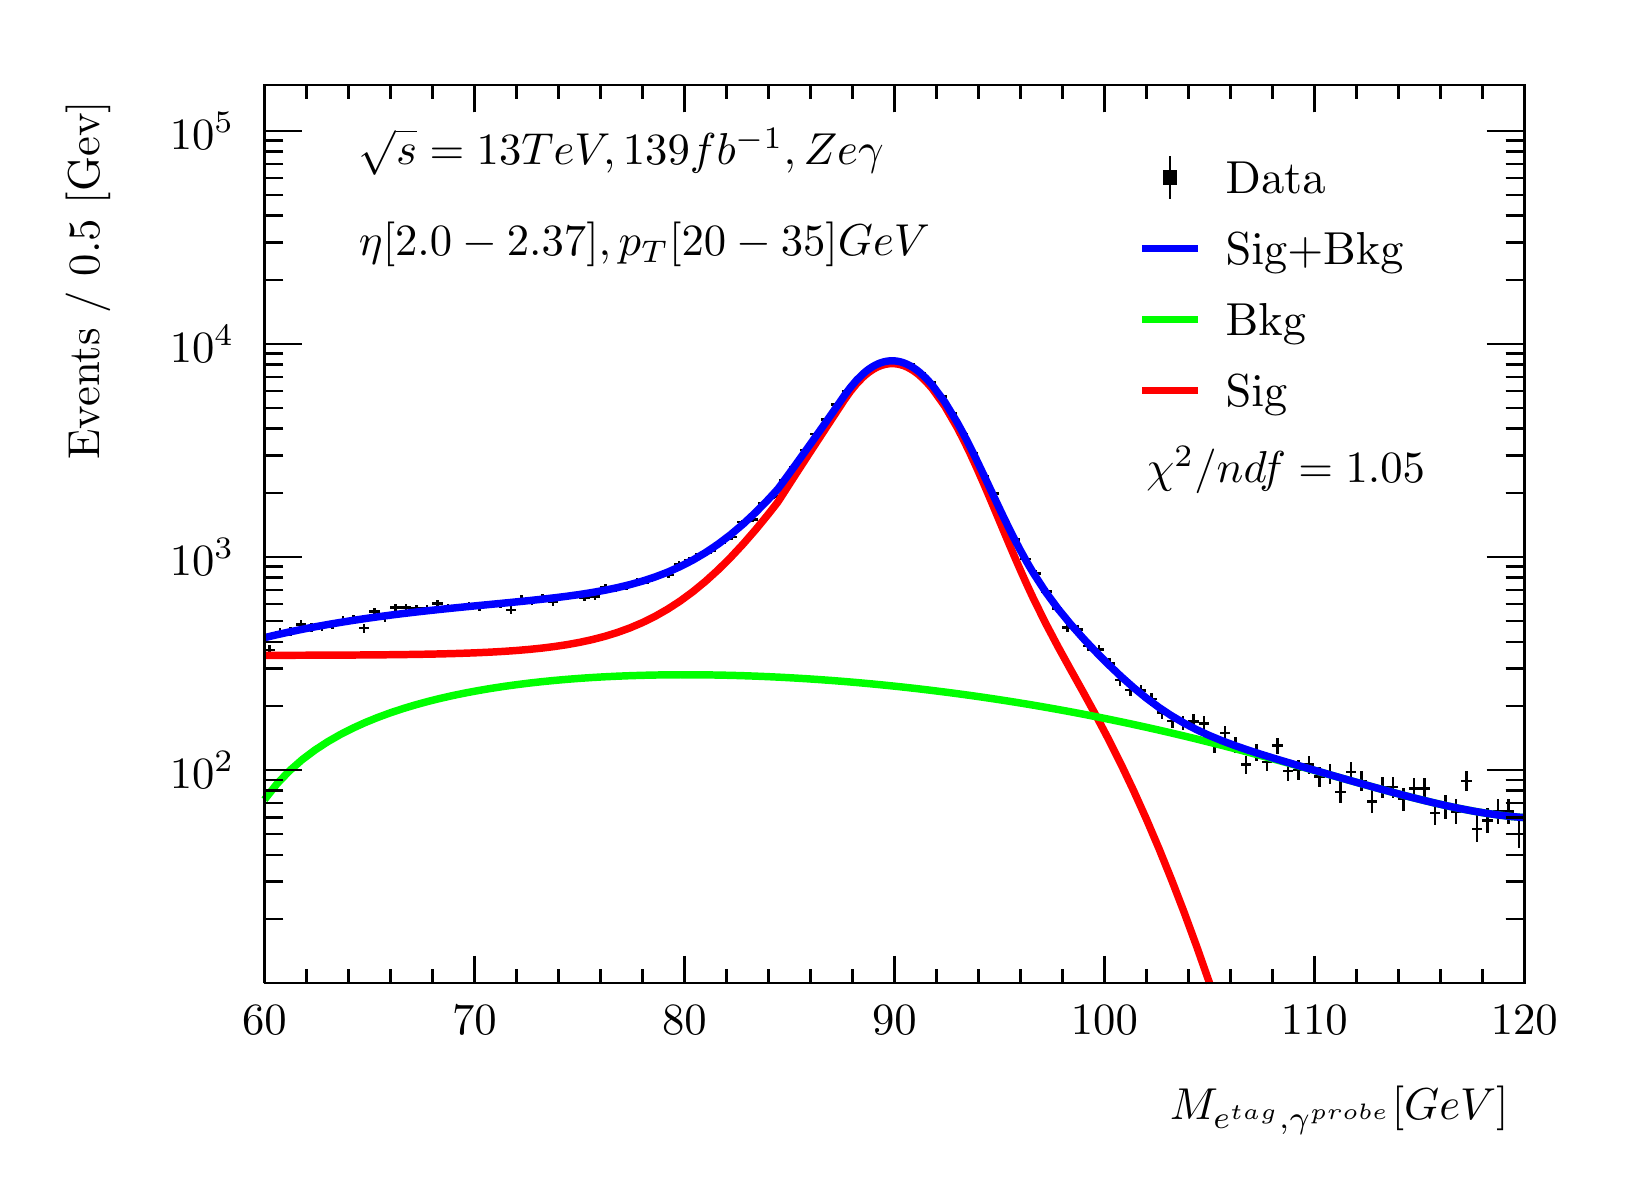
\begin{tikzpicture}
\pgfdeclareplotmark{cross} {
\pgfpathmoveto{\pgfpoint{-0.3\pgfplotmarksize}{\pgfplotmarksize}}
\pgfpathlineto{\pgfpoint{+0.3\pgfplotmarksize}{\pgfplotmarksize}}
\pgfpathlineto{\pgfpoint{+0.3\pgfplotmarksize}{0.3\pgfplotmarksize}}
\pgfpathlineto{\pgfpoint{+1\pgfplotmarksize}{0.3\pgfplotmarksize}}
\pgfpathlineto{\pgfpoint{+1\pgfplotmarksize}{-0.3\pgfplotmarksize}}
\pgfpathlineto{\pgfpoint{+0.3\pgfplotmarksize}{-0.3\pgfplotmarksize}}
\pgfpathlineto{\pgfpoint{+0.3\pgfplotmarksize}{-1.\pgfplotmarksize}}
\pgfpathlineto{\pgfpoint{-0.3\pgfplotmarksize}{-1.\pgfplotmarksize}}
\pgfpathlineto{\pgfpoint{-0.3\pgfplotmarksize}{-0.3\pgfplotmarksize}}
\pgfpathlineto{\pgfpoint{-1.\pgfplotmarksize}{-0.3\pgfplotmarksize}}
\pgfpathlineto{\pgfpoint{-1.\pgfplotmarksize}{0.3\pgfplotmarksize}}
\pgfpathlineto{\pgfpoint{-0.3\pgfplotmarksize}{0.3\pgfplotmarksize}}
\pgfpathclose
\pgfusepathqstroke
}
\pgfdeclareplotmark{cross*} {
\pgfpathmoveto{\pgfpoint{-0.3\pgfplotmarksize}{\pgfplotmarksize}}
\pgfpathlineto{\pgfpoint{+0.3\pgfplotmarksize}{\pgfplotmarksize}}
\pgfpathlineto{\pgfpoint{+0.3\pgfplotmarksize}{0.3\pgfplotmarksize}}
\pgfpathlineto{\pgfpoint{+1\pgfplotmarksize}{0.3\pgfplotmarksize}}
\pgfpathlineto{\pgfpoint{+1\pgfplotmarksize}{-0.3\pgfplotmarksize}}
\pgfpathlineto{\pgfpoint{+0.3\pgfplotmarksize}{-0.3\pgfplotmarksize}}
\pgfpathlineto{\pgfpoint{+0.3\pgfplotmarksize}{-1.\pgfplotmarksize}}
\pgfpathlineto{\pgfpoint{-0.3\pgfplotmarksize}{-1.\pgfplotmarksize}}
\pgfpathlineto{\pgfpoint{-0.3\pgfplotmarksize}{-0.3\pgfplotmarksize}}
\pgfpathlineto{\pgfpoint{-1.\pgfplotmarksize}{-0.3\pgfplotmarksize}}
\pgfpathlineto{\pgfpoint{-1.\pgfplotmarksize}{0.3\pgfplotmarksize}}
\pgfpathlineto{\pgfpoint{-0.3\pgfplotmarksize}{0.3\pgfplotmarksize}}
\pgfpathclose
\pgfusepathqfillstroke
}
\pgfdeclareplotmark{newstar} {
\pgfpathmoveto{\pgfqpoint{0pt}{\pgfplotmarksize}}
\pgfpathlineto{\pgfqpointpolar{44}{0.5\pgfplotmarksize}}
\pgfpathlineto{\pgfqpointpolar{18}{\pgfplotmarksize}}
\pgfpathlineto{\pgfqpointpolar{-20}{0.5\pgfplotmarksize}}
\pgfpathlineto{\pgfqpointpolar{-54}{\pgfplotmarksize}}
\pgfpathlineto{\pgfqpointpolar{-90}{0.5\pgfplotmarksize}}
\pgfpathlineto{\pgfqpointpolar{234}{\pgfplotmarksize}}
\pgfpathlineto{\pgfqpointpolar{198}{0.5\pgfplotmarksize}}
\pgfpathlineto{\pgfqpointpolar{162}{\pgfplotmarksize}}
\pgfpathlineto{\pgfqpointpolar{134}{0.5\pgfplotmarksize}}
\pgfpathclose
\pgfusepathqstroke
}
\pgfdeclareplotmark{newstar*} {
\pgfpathmoveto{\pgfqpoint{0pt}{\pgfplotmarksize}}
\pgfpathlineto{\pgfqpointpolar{44}{0.5\pgfplotmarksize}}
\pgfpathlineto{\pgfqpointpolar{18}{\pgfplotmarksize}}
\pgfpathlineto{\pgfqpointpolar{-20}{0.5\pgfplotmarksize}}
\pgfpathlineto{\pgfqpointpolar{-54}{\pgfplotmarksize}}
\pgfpathlineto{\pgfqpointpolar{-90}{0.5\pgfplotmarksize}}
\pgfpathlineto{\pgfqpointpolar{234}{\pgfplotmarksize}}
\pgfpathlineto{\pgfqpointpolar{198}{0.5\pgfplotmarksize}}
\pgfpathlineto{\pgfqpointpolar{162}{\pgfplotmarksize}}
\pgfpathlineto{\pgfqpointpolar{134}{0.5\pgfplotmarksize}}
\pgfpathclose
\pgfusepathqfillstroke
}
\definecolor{c}{rgb}{1,1,1};
\draw [color=c, fill=c] (0,0) rectangle (20,14.4361);
\draw [color=c, fill=c] (3,2.30977) rectangle (19,13.7143);
\definecolor{c}{rgb}{0,0,0};
\draw [c,line width=0.9] (3,2.30977) -- (3,13.7143) -- (19,13.7143) -- (19,2.30977) -- (3,2.30977);
\definecolor{c}{rgb}{1,1,1};
\draw [color=c, fill=c] (3,2.30977) rectangle (19,13.7143);
\definecolor{c}{rgb}{0,0,0};
\draw [c,line width=0.9] (3,2.30977) -- (3,13.7143) -- (19,13.7143) -- (19,2.30977) -- (3,2.30977);
\draw [c,line width=0.9] (3,2.30977) -- (19,2.30977);
\draw [c,line width=0.9] (3,2.65624) -- (3,2.30977);
\draw [c,line width=0.9] (3.53333,2.48301) -- (3.53333,2.30977);
\draw [c,line width=0.9] (4.06667,2.48301) -- (4.06667,2.30977);
\draw [c,line width=0.9] (4.6,2.48301) -- (4.6,2.30977);
\draw [c,line width=0.9] (5.13333,2.48301) -- (5.13333,2.30977);
\draw [c,line width=0.9] (5.66667,2.65624) -- (5.66667,2.30977);
\draw [c,line width=0.9] (6.2,2.48301) -- (6.2,2.30977);
\draw [c,line width=0.9] (6.73333,2.48301) -- (6.73333,2.30977);
\draw [c,line width=0.9] (7.26667,2.48301) -- (7.26667,2.30977);
\draw [c,line width=0.9] (7.8,2.48301) -- (7.8,2.30977);
\draw [c,line width=0.9] (8.33333,2.65624) -- (8.33333,2.30977);
\draw [c,line width=0.9] (8.86667,2.48301) -- (8.86667,2.30977);
\draw [c,line width=0.9] (9.4,2.48301) -- (9.4,2.30977);
\draw [c,line width=0.9] (9.93333,2.48301) -- (9.93333,2.30977);
\draw [c,line width=0.9] (10.4667,2.48301) -- (10.4667,2.30977);
\draw [c,line width=0.9] (11,2.65624) -- (11,2.30977);
\draw [c,line width=0.9] (11.5333,2.48301) -- (11.5333,2.30977);
\draw [c,line width=0.9] (12.0667,2.48301) -- (12.0667,2.30977);
\draw [c,line width=0.9] (12.6,2.48301) -- (12.6,2.30977);
\draw [c,line width=0.9] (13.1333,2.48301) -- (13.1333,2.30977);
\draw [c,line width=0.9] (13.6667,2.65624) -- (13.6667,2.30977);
\draw [c,line width=0.9] (14.2,2.48301) -- (14.2,2.30977);
\draw [c,line width=0.9] (14.7333,2.48301) -- (14.7333,2.30977);
\draw [c,line width=0.9] (15.2667,2.48301) -- (15.2667,2.30977);
\draw [c,line width=0.9] (15.8,2.48301) -- (15.8,2.30977);
\draw [c,line width=0.9] (16.3333,2.65624) -- (16.3333,2.30977);
\draw [c,line width=0.9] (16.8667,2.48301) -- (16.8667,2.30977);
\draw [c,line width=0.9] (17.4,2.48301) -- (17.4,2.30977);
\draw [c,line width=0.9] (17.9333,2.48301) -- (17.9333,2.30977);
\draw [c,line width=0.9] (18.4667,2.48301) -- (18.4667,2.30977);
\draw [c,line width=0.9] (19,2.65624) -- (19,2.30977);
\draw [anchor=base] (3,1.66015) node[scale=1.61424, color=c, rotate=0]{60};
\draw [anchor=base] (5.66667,1.66015) node[scale=1.61424, color=c, rotate=0]{70};
\draw [anchor=base] (8.33333,1.66015) node[scale=1.61424, color=c, rotate=0]{80};
\draw [anchor=base] (11,1.66015) node[scale=1.61424, color=c, rotate=0]{90};
\draw [anchor=base] (13.6667,1.66015) node[scale=1.61424, color=c, rotate=0]{100};
\draw [anchor=base] (16.3333,1.66015) node[scale=1.61424, color=c, rotate=0]{110};
\draw [anchor=base] (19,1.66015) node[scale=1.61424, color=c, rotate=0]{120};
\draw [anchor= east] (19,0.692932) node[scale=1.61424, color=c, rotate=0]{$M_{e^{tag}, \gamma^{probe}}  [GeV]$};
\draw [c,line width=0.9] (3,13.7143) -- (19,13.7143);
\draw [c,line width=0.9] (3,13.3678) -- (3,13.7143);
\draw [c,line width=0.9] (3.53333,13.5411) -- (3.53333,13.7143);
\draw [c,line width=0.9] (4.06667,13.5411) -- (4.06667,13.7143);
\draw [c,line width=0.9] (4.6,13.5411) -- (4.6,13.7143);
\draw [c,line width=0.9] (5.13333,13.5411) -- (5.13333,13.7143);
\draw [c,line width=0.9] (5.66667,13.3678) -- (5.66667,13.7143);
\draw [c,line width=0.9] (6.2,13.5411) -- (6.2,13.7143);
\draw [c,line width=0.9] (6.73333,13.5411) -- (6.73333,13.7143);
\draw [c,line width=0.9] (7.26667,13.5411) -- (7.26667,13.7143);
\draw [c,line width=0.9] (7.8,13.5411) -- (7.8,13.7143);
\draw [c,line width=0.9] (8.33333,13.3678) -- (8.33333,13.7143);
\draw [c,line width=0.9] (8.86667,13.5411) -- (8.86667,13.7143);
\draw [c,line width=0.9] (9.4,13.5411) -- (9.4,13.7143);
\draw [c,line width=0.9] (9.93333,13.5411) -- (9.93333,13.7143);
\draw [c,line width=0.9] (10.4667,13.5411) -- (10.4667,13.7143);
\draw [c,line width=0.9] (11,13.3678) -- (11,13.7143);
\draw [c,line width=0.9] (11.5333,13.5411) -- (11.5333,13.7143);
\draw [c,line width=0.9] (12.0667,13.5411) -- (12.0667,13.7143);
\draw [c,line width=0.9] (12.6,13.5411) -- (12.6,13.7143);
\draw [c,line width=0.9] (13.1333,13.5411) -- (13.1333,13.7143);
\draw [c,line width=0.9] (13.6667,13.3678) -- (13.6667,13.7143);
\draw [c,line width=0.9] (14.2,13.5411) -- (14.2,13.7143);
\draw [c,line width=0.9] (14.7333,13.5411) -- (14.7333,13.7143);
\draw [c,line width=0.9] (15.2667,13.5411) -- (15.2667,13.7143);
\draw [c,line width=0.9] (15.8,13.5411) -- (15.8,13.7143);
\draw [c,line width=0.9] (16.3333,13.3678) -- (16.3333,13.7143);
\draw [c,line width=0.9] (16.8667,13.5411) -- (16.8667,13.7143);
\draw [c,line width=0.9] (17.4,13.5411) -- (17.4,13.7143);
\draw [c,line width=0.9] (17.9333,13.5411) -- (17.9333,13.7143);
\draw [c,line width=0.9] (18.4667,13.5411) -- (18.4667,13.7143);
\draw [c,line width=0.9] (19,13.3678) -- (19,13.7143);
\draw [c,line width=0.9] (3,2.30977) -- (3,13.7143);
\draw [c,line width=0.9] (3.237,3.12423) -- (3,3.12423);
\draw [c,line width=0.9] (3.237,3.60066) -- (3,3.60066);
\draw [c,line width=0.9] (3.237,3.93869) -- (3,3.93869);
\draw [c,line width=0.9] (3.237,4.20088) -- (3,4.20088);
\draw [c,line width=0.9] (3.237,4.41511) -- (3,4.41511);
\draw [c,line width=0.9] (3.237,4.59624) -- (3,4.59624);
\draw [c,line width=0.9] (3.237,4.75314) -- (3,4.75314);
\draw [c,line width=0.9] (3.237,4.89154) -- (3,4.89154);
\draw [c,line width=0.9] (3.474,5.01534) -- (3,5.01534);
\draw [anchor= east] (2.82,5.01534) node[scale=1.61424, color=c, rotate=0]{$10^{2}$};
\draw [c,line width=0.9] (3.237,5.8298) -- (3,5.8298);
\draw [c,line width=0.9] (3.237,6.30623) -- (3,6.30623);
\draw [c,line width=0.9] (3.237,6.64426) -- (3,6.64426);
\draw [c,line width=0.9] (3.237,6.90645) -- (3,6.90645);
\draw [c,line width=0.9] (3.237,7.12068) -- (3,7.12068);
\draw [c,line width=0.9] (3.237,7.30181) -- (3,7.30181);
\draw [c,line width=0.9] (3.237,7.45871) -- (3,7.45871);
\draw [c,line width=0.9] (3.237,7.59711) -- (3,7.59711);
\draw [c,line width=0.9] (3.474,7.72091) -- (3,7.72091);
\draw [anchor= east] (2.82,7.72091) node[scale=1.61424, color=c, rotate=0]{$10^{3}$};
\draw [c,line width=0.9] (3.237,8.53537) -- (3,8.53537);
\draw [c,line width=0.9] (3.237,9.0118) -- (3,9.0118);
\draw [c,line width=0.9] (3.237,9.34983) -- (3,9.34983);
\draw [c,line width=0.9] (3.237,9.61202) -- (3,9.61202);
\draw [c,line width=0.9] (3.237,9.82625) -- (3,9.82625);
\draw [c,line width=0.9] (3.237,10.0074) -- (3,10.0074);
\draw [c,line width=0.9] (3.237,10.1643) -- (3,10.1643);
\draw [c,line width=0.9] (3.237,10.3027) -- (3,10.3027);
\draw [c,line width=0.9] (3.474,10.4265) -- (3,10.4265);
\draw [anchor= east] (2.82,10.4265) node[scale=1.61424, color=c, rotate=0]{$10^{4}$};
\draw [c,line width=0.9] (3.237,11.2409) -- (3,11.2409);
\draw [c,line width=0.9] (3.237,11.7174) -- (3,11.7174);
\draw [c,line width=0.9] (3.237,12.0554) -- (3,12.0554);
\draw [c,line width=0.9] (3.237,12.3176) -- (3,12.3176);
\draw [c,line width=0.9] (3.237,12.5318) -- (3,12.5318);
\draw [c,line width=0.9] (3.237,12.713) -- (3,12.713);
\draw [c,line width=0.9] (3.237,12.8699) -- (3,12.8699);
\draw [c,line width=0.9] (3.237,13.0083) -- (3,13.0083);
\draw [c,line width=0.9] (3.474,13.1321) -- (3,13.1321);
\draw [anchor= east] (2.82,13.1321) node[scale=1.61424, color=c, rotate=0]{$10^{5}$};
\draw [anchor= east] (0.76,13.7143) node[scale=1.61424, color=c, rotate=90]{Events / 0.5 [Gev]};
\draw [c,line width=0.9] (19,2.30977) -- (19,13.7143);
\draw [c,line width=0.9] (18.763,3.12423) -- (19,3.12423);
\draw [c,line width=0.9] (18.763,3.60066) -- (19,3.60066);
\draw [c,line width=0.9] (18.763,3.93869) -- (19,3.93869);
\draw [c,line width=0.9] (18.763,4.20088) -- (19,4.20088);
\draw [c,line width=0.9] (18.763,4.41511) -- (19,4.41511);
\draw [c,line width=0.9] (18.763,4.59624) -- (19,4.59624);
\draw [c,line width=0.9] (18.763,4.75314) -- (19,4.75314);
\draw [c,line width=0.9] (18.763,4.89154) -- (19,4.89154);
\draw [c,line width=0.9] (18.526,5.01534) -- (19,5.01534);
\draw [c,line width=0.9] (18.763,5.8298) -- (19,5.8298);
\draw [c,line width=0.9] (18.763,6.30623) -- (19,6.30623);
\draw [c,line width=0.9] (18.763,6.64426) -- (19,6.64426);
\draw [c,line width=0.9] (18.763,6.90645) -- (19,6.90645);
\draw [c,line width=0.9] (18.763,7.12068) -- (19,7.12068);
\draw [c,line width=0.9] (18.763,7.30181) -- (19,7.30181);
\draw [c,line width=0.9] (18.763,7.45871) -- (19,7.45871);
\draw [c,line width=0.9] (18.763,7.59711) -- (19,7.59711);
\draw [c,line width=0.9] (18.526,7.72091) -- (19,7.72091);
\draw [c,line width=0.9] (18.763,8.53537) -- (19,8.53537);
\draw [c,line width=0.9] (18.763,9.0118) -- (19,9.0118);
\draw [c,line width=0.9] (18.763,9.34983) -- (19,9.34983);
\draw [c,line width=0.9] (18.763,9.61202) -- (19,9.61202);
\draw [c,line width=0.9] (18.763,9.82625) -- (19,9.82625);
\draw [c,line width=0.9] (18.763,10.0074) -- (19,10.0074);
\draw [c,line width=0.9] (18.763,10.1643) -- (19,10.1643);
\draw [c,line width=0.9] (18.763,10.3027) -- (19,10.3027);
\draw [c,line width=0.9] (18.526,10.4265) -- (19,10.4265);
\draw [c,line width=0.9] (18.763,11.2409) -- (19,11.2409);
\draw [c,line width=0.9] (18.763,11.7174) -- (19,11.7174);
\draw [c,line width=0.9] (18.763,12.0554) -- (19,12.0554);
\draw [c,line width=0.9] (18.763,12.3176) -- (19,12.3176);
\draw [c,line width=0.9] (18.763,12.5318) -- (19,12.5318);
\draw [c,line width=0.9] (18.763,12.713) -- (19,12.713);
\draw [c,line width=0.9] (18.763,12.8699) -- (19,12.8699);
\draw [c,line width=0.9] (18.763,13.0083) -- (19,13.0083);
\draw [c,line width=0.9] (18.526,13.1321) -- (19,13.1321);
\draw [c,line width=0.9] (3.06667,6.53988) -- (3,6.53988);
\draw [c,line width=0.9] (3,6.53988) -- (3,6.53988);
\draw [c,line width=0.9] (3.06667,6.53988) -- (3.13333,6.53988);
\draw [c,line width=0.9] (3.13333,6.53988) -- (3.13333,6.53988);
\draw [c,line width=0.9] (3.06667,6.53988) -- (3.06667,6.60129);
\draw [c,line width=0.9] (3.06667,6.60129) -- (3.06667,6.60129);
\draw [c,line width=0.9] (3.06667,6.53988) -- (3.06667,6.47847);
\draw [c,line width=0.9] (3.06667,6.47847) -- (3.06667,6.47847);
\draw [c,line width=0.9] (3.2,6.76158) -- (3.13333,6.76158);
\draw [c,line width=0.9] (3.13333,6.76158) -- (3.13333,6.76158);
\draw [c,line width=0.9] (3.2,6.76158) -- (3.26667,6.76158);
\draw [c,line width=0.9] (3.26667,6.76158) -- (3.26667,6.76158);
\draw [c,line width=0.9] (3.2,6.76158) -- (3.2,6.81746);
\draw [c,line width=0.9] (3.2,6.81746) -- (3.2,6.81746);
\draw [c,line width=0.9] (3.2,6.76158) -- (3.2,6.70569);
\draw [c,line width=0.9] (3.2,6.70569) -- (3.2,6.70569);
\draw [c,line width=0.9] (3.33333,6.7748) -- (3.26667,6.7748);
\draw [c,line width=0.9] (3.26667,6.7748) -- (3.26667,6.7748);
\draw [c,line width=0.9] (3.33333,6.7748) -- (3.4,6.7748);
\draw [c,line width=0.9] (3.4,6.7748) -- (3.4,6.7748);
\draw [c,line width=0.9] (3.33333,6.7748) -- (3.33333,6.83037);
\draw [c,line width=0.9] (3.33333,6.83037) -- (3.33333,6.83037);
\draw [c,line width=0.9] (3.33333,6.7748) -- (3.33333,6.71922);
\draw [c,line width=0.9] (3.33333,6.71922) -- (3.33333,6.71922);
\draw [c,line width=0.9] (3.46667,6.86337) -- (3.4,6.86337);
\draw [c,line width=0.9] (3.4,6.86337) -- (3.4,6.86337);
\draw [c,line width=0.9] (3.46667,6.86337) -- (3.53333,6.86337);
\draw [c,line width=0.9] (3.53333,6.86337) -- (3.53333,6.86337);
\draw [c,line width=0.9] (3.46667,6.86337) -- (3.46667,6.91689);
\draw [c,line width=0.9] (3.46667,6.91689) -- (3.46667,6.91689);
\draw [c,line width=0.9] (3.46667,6.86337) -- (3.46667,6.80986);
\draw [c,line width=0.9] (3.46667,6.80986) -- (3.46667,6.80986);
\draw [c,line width=0.9] (3.6,6.82371) -- (3.53333,6.82371);
\draw [c,line width=0.9] (3.53333,6.82371) -- (3.53333,6.82371);
\draw [c,line width=0.9] (3.6,6.82371) -- (3.66667,6.82371);
\draw [c,line width=0.9] (3.66667,6.82371) -- (3.66667,6.82371);
\draw [c,line width=0.9] (3.6,6.82371) -- (3.6,6.87813);
\draw [c,line width=0.9] (3.6,6.87813) -- (3.6,6.87813);
\draw [c,line width=0.9] (3.6,6.82371) -- (3.6,6.76928);
\draw [c,line width=0.9] (3.6,6.76928) -- (3.6,6.76928);
\draw [c,line width=0.9] (3.73333,6.83625) -- (3.66667,6.83625);
\draw [c,line width=0.9] (3.66667,6.83625) -- (3.66667,6.83625);
\draw [c,line width=0.9] (3.73333,6.83625) -- (3.8,6.83625);
\draw [c,line width=0.9] (3.8,6.83625) -- (3.8,6.83625);
\draw [c,line width=0.9] (3.73333,6.83625) -- (3.73333,6.89039);
\draw [c,line width=0.9] (3.73333,6.89039) -- (3.73333,6.89039);
\draw [c,line width=0.9] (3.73333,6.83625) -- (3.73333,6.78211);
\draw [c,line width=0.9] (3.73333,6.78211) -- (3.73333,6.78211);
\draw [c,line width=0.9] (3.86667,6.86093) -- (3.8,6.86093);
\draw [c,line width=0.9] (3.8,6.86093) -- (3.8,6.86093);
\draw [c,line width=0.9] (3.86667,6.86093) -- (3.93333,6.86093);
\draw [c,line width=0.9] (3.93333,6.86093) -- (3.93333,6.86093);
\draw [c,line width=0.9] (3.86667,6.86093) -- (3.86667,6.91451);
\draw [c,line width=0.9] (3.86667,6.91451) -- (3.86667,6.91451);
\draw [c,line width=0.9] (3.86667,6.86093) -- (3.86667,6.80736);
\draw [c,line width=0.9] (3.86667,6.80736) -- (3.86667,6.80736);
\draw [c,line width=0.9] (4,6.91815) -- (3.93333,6.91815);
\draw [c,line width=0.9] (3.93333,6.91815) -- (3.93333,6.91815);
\draw [c,line width=0.9] (4,6.91815) -- (4.06667,6.91815);
\draw [c,line width=0.9] (4.06667,6.91815) -- (4.06667,6.91815);
\draw [c,line width=0.9] (4,6.91815) -- (4,6.97043);
\draw [c,line width=0.9] (4,6.97043) -- (4,6.97043);
\draw [c,line width=0.9] (4,6.91815) -- (4,6.86586);
\draw [c,line width=0.9] (4,6.86586) -- (4,6.86586);
\draw [c,line width=0.9] (4.13333,6.93432) -- (4.06667,6.93432);
\draw [c,line width=0.9] (4.06667,6.93432) -- (4.06667,6.93432);
\draw [c,line width=0.9] (4.13333,6.93432) -- (4.2,6.93432);
\draw [c,line width=0.9] (4.2,6.93432) -- (4.2,6.93432);
\draw [c,line width=0.9] (4.13333,6.93432) -- (4.13333,6.98625);
\draw [c,line width=0.9] (4.13333,6.98625) -- (4.13333,6.98625);
\draw [c,line width=0.9] (4.13333,6.93432) -- (4.13333,6.8824);
\draw [c,line width=0.9] (4.13333,6.8824) -- (4.13333,6.8824);
\draw [c,line width=0.9] (4.26667,6.81612) -- (4.2,6.81612);
\draw [c,line width=0.9] (4.2,6.81612) -- (4.2,6.81612);
\draw [c,line width=0.9] (4.26667,6.81612) -- (4.33333,6.81612);
\draw [c,line width=0.9] (4.33333,6.81612) -- (4.33333,6.81612);
\draw [c,line width=0.9] (4.26667,6.81612) -- (4.26667,6.87072);
\draw [c,line width=0.9] (4.26667,6.87072) -- (4.26667,6.87072);
\draw [c,line width=0.9] (4.26667,6.81612) -- (4.26667,6.76152);
\draw [c,line width=0.9] (4.26667,6.76152) -- (4.26667,6.76152);
\draw [c,line width=0.9] (4.4,7.02908) -- (4.33333,7.02908);
\draw [c,line width=0.9] (4.33333,7.02908) -- (4.33333,7.02908);
\draw [c,line width=0.9] (4.4,7.02908) -- (4.46667,7.02908);
\draw [c,line width=0.9] (4.46667,7.02908) -- (4.46667,7.02908);
\draw [c,line width=0.9] (4.4,7.02908) -- (4.4,7.07895);
\draw [c,line width=0.9] (4.4,7.07895) -- (4.4,7.07895);
\draw [c,line width=0.9] (4.4,7.02908) -- (4.4,6.97921);
\draw [c,line width=0.9] (4.4,6.97921) -- (4.4,6.97921);
\draw [c,line width=0.9] (4.53333,6.95254) -- (4.46667,6.95254);
\draw [c,line width=0.9] (4.46667,6.95254) -- (4.46667,6.95254);
\draw [c,line width=0.9] (4.53333,6.95254) -- (4.6,6.95254);
\draw [c,line width=0.9] (4.6,6.95254) -- (4.6,6.95254);
\draw [c,line width=0.9] (4.53333,6.95254) -- (4.53333,7.00406);
\draw [c,line width=0.9] (4.53333,7.00406) -- (4.53333,7.00406);
\draw [c,line width=0.9] (4.53333,6.95254) -- (4.53333,6.90102);
\draw [c,line width=0.9] (4.53333,6.90102) -- (4.53333,6.90102);
\draw [c,line width=0.9] (4.66667,7.07882) -- (4.6,7.07882);
\draw [c,line width=0.9] (4.6,7.07882) -- (4.6,7.07882);
\draw [c,line width=0.9] (4.66667,7.07882) -- (4.73333,7.07882);
\draw [c,line width=0.9] (4.73333,7.07882) -- (4.73333,7.07882);
\draw [c,line width=0.9] (4.66667,7.07882) -- (4.66667,7.12765);
\draw [c,line width=0.9] (4.66667,7.12765) -- (4.66667,7.12765);
\draw [c,line width=0.9] (4.66667,7.07882) -- (4.66667,7.02999);
\draw [c,line width=0.9] (4.66667,7.02999) -- (4.66667,7.02999);
\draw [c,line width=0.9] (4.8,7.07679) -- (4.73333,7.07679);
\draw [c,line width=0.9] (4.73333,7.07679) -- (4.73333,7.07679);
\draw [c,line width=0.9] (4.8,7.07679) -- (4.86667,7.07679);
\draw [c,line width=0.9] (4.86667,7.07679) -- (4.86667,7.07679);
\draw [c,line width=0.9] (4.8,7.07679) -- (4.8,7.12566);
\draw [c,line width=0.9] (4.8,7.12566) -- (4.8,7.12566);
\draw [c,line width=0.9] (4.8,7.07679) -- (4.8,7.02792);
\draw [c,line width=0.9] (4.8,7.02792) -- (4.8,7.02792);
\draw [c,line width=0.9] (4.93333,7.06453) -- (4.86667,7.06453);
\draw [c,line width=0.9] (4.86667,7.06453) -- (4.86667,7.06453);
\draw [c,line width=0.9] (4.93333,7.06453) -- (5,7.06453);
\draw [c,line width=0.9] (5,7.06453) -- (5,7.06453);
\draw [c,line width=0.9] (4.93333,7.06453) -- (4.93333,7.11366);
\draw [c,line width=0.9] (4.93333,7.11366) -- (4.93333,7.11366);
\draw [c,line width=0.9] (4.93333,7.06453) -- (4.93333,7.0154);
\draw [c,line width=0.9] (4.93333,7.0154) -- (4.93333,7.0154);
\draw [c,line width=0.9] (5.06667,7.06453) -- (5,7.06453);
\draw [c,line width=0.9] (5,7.06453) -- (5,7.06453);
\draw [c,line width=0.9] (5.06667,7.06453) -- (5.13333,7.06453);
\draw [c,line width=0.9] (5.13333,7.06453) -- (5.13333,7.06453);
\draw [c,line width=0.9] (5.06667,7.06453) -- (5.06667,7.11366);
\draw [c,line width=0.9] (5.06667,7.11366) -- (5.06667,7.11366);
\draw [c,line width=0.9] (5.06667,7.06453) -- (5.06667,7.0154);
\draw [c,line width=0.9] (5.06667,7.0154) -- (5.06667,7.0154);
\draw [c,line width=0.9] (5.2,7.13238) -- (5.13333,7.13238);
\draw [c,line width=0.9] (5.13333,7.13238) -- (5.13333,7.13238);
\draw [c,line width=0.9] (5.2,7.13238) -- (5.26667,7.13238);
\draw [c,line width=0.9] (5.26667,7.13238) -- (5.26667,7.13238);
\draw [c,line width=0.9] (5.2,7.13238) -- (5.2,7.18011);
\draw [c,line width=0.9] (5.2,7.18011) -- (5.2,7.18011);
\draw [c,line width=0.9] (5.2,7.13238) -- (5.2,7.08465);
\draw [c,line width=0.9] (5.2,7.08465) -- (5.2,7.08465);
\draw [c,line width=0.9] (5.33333,7.07882) -- (5.26667,7.07882);
\draw [c,line width=0.9] (5.26667,7.07882) -- (5.26667,7.07882);
\draw [c,line width=0.9] (5.33333,7.07882) -- (5.4,7.07882);
\draw [c,line width=0.9] (5.4,7.07882) -- (5.4,7.07882);
\draw [c,line width=0.9] (5.33333,7.07882) -- (5.33333,7.12765);
\draw [c,line width=0.9] (5.33333,7.12765) -- (5.33333,7.12765);
\draw [c,line width=0.9] (5.33333,7.07882) -- (5.33333,7.02999);
\draw [c,line width=0.9] (5.33333,7.02999) -- (5.33333,7.02999);
\draw [c,line width=0.9] (5.46667,7.08085) -- (5.4,7.08085);
\draw [c,line width=0.9] (5.4,7.08085) -- (5.4,7.08085);
\draw [c,line width=0.9] (5.46667,7.08085) -- (5.53333,7.08085);
\draw [c,line width=0.9] (5.53333,7.08085) -- (5.53333,7.08085);
\draw [c,line width=0.9] (5.46667,7.08085) -- (5.46667,7.12964);
\draw [c,line width=0.9] (5.46667,7.12964) -- (5.46667,7.12964);
\draw [c,line width=0.9] (5.46667,7.08085) -- (5.46667,7.03206);
\draw [c,line width=0.9] (5.46667,7.03206) -- (5.46667,7.03206);
\draw [c,line width=0.9] (5.6,7.09894) -- (5.53333,7.09894);
\draw [c,line width=0.9] (5.53333,7.09894) -- (5.53333,7.09894);
\draw [c,line width=0.9] (5.6,7.09894) -- (5.66667,7.09894);
\draw [c,line width=0.9] (5.66667,7.09894) -- (5.66667,7.09894);
\draw [c,line width=0.9] (5.6,7.09894) -- (5.6,7.14736);
\draw [c,line width=0.9] (5.6,7.14736) -- (5.6,7.14736);
\draw [c,line width=0.9] (5.6,7.09894) -- (5.6,7.05053);
\draw [c,line width=0.9] (5.6,7.05053) -- (5.6,7.05053);
\draw [c,line width=0.9] (5.73333,7.08288) -- (5.66667,7.08288);
\draw [c,line width=0.9] (5.66667,7.08288) -- (5.66667,7.08288);
\draw [c,line width=0.9] (5.73333,7.08288) -- (5.8,7.08288);
\draw [c,line width=0.9] (5.8,7.08288) -- (5.8,7.08288);
\draw [c,line width=0.9] (5.73333,7.08288) -- (5.73333,7.13162);
\draw [c,line width=0.9] (5.73333,7.13162) -- (5.73333,7.13162);
\draw [c,line width=0.9] (5.73333,7.08288) -- (5.73333,7.03413);
\draw [c,line width=0.9] (5.73333,7.03413) -- (5.73333,7.03413);
\draw [c,line width=0.9] (5.86667,7.1148) -- (5.8,7.1148);
\draw [c,line width=0.9] (5.8,7.1148) -- (5.8,7.1148);
\draw [c,line width=0.9] (5.86667,7.1148) -- (5.93333,7.1148);
\draw [c,line width=0.9] (5.93333,7.1148) -- (5.93333,7.1148);
\draw [c,line width=0.9] (5.86667,7.1148) -- (5.86667,7.16288);
\draw [c,line width=0.9] (5.86667,7.16288) -- (5.86667,7.16288);
\draw [c,line width=0.9] (5.86667,7.1148) -- (5.86667,7.06671);
\draw [c,line width=0.9] (5.86667,7.06671) -- (5.86667,7.06671);
\draw [c,line width=0.9] (6,7.12264) -- (5.93333,7.12264);
\draw [c,line width=0.9] (5.93333,7.12264) -- (5.93333,7.12264);
\draw [c,line width=0.9] (6,7.12264) -- (6.06667,7.12264);
\draw [c,line width=0.9] (6.06667,7.12264) -- (6.06667,7.12264);
\draw [c,line width=0.9] (6,7.12264) -- (6,7.17057);
\draw [c,line width=0.9] (6,7.17057) -- (6,7.17057);
\draw [c,line width=0.9] (6,7.12264) -- (6,7.07472);
\draw [c,line width=0.9] (6,7.07472) -- (6,7.07472);
\draw [c,line width=0.9] (6.13333,7.04798) -- (6.06667,7.04798);
\draw [c,line width=0.9] (6.06667,7.04798) -- (6.06667,7.04798);
\draw [c,line width=0.9] (6.13333,7.04798) -- (6.2,7.04798);
\draw [c,line width=0.9] (6.2,7.04798) -- (6.2,7.04798);
\draw [c,line width=0.9] (6.13333,7.04798) -- (6.13333,7.09745);
\draw [c,line width=0.9] (6.13333,7.09745) -- (6.13333,7.09745);
\draw [c,line width=0.9] (6.13333,7.04798) -- (6.13333,6.99851);
\draw [c,line width=0.9] (6.13333,6.99851) -- (6.13333,6.99851);
\draw [c,line width=0.9] (6.26667,7.1873) -- (6.2,7.1873);
\draw [c,line width=0.9] (6.2,7.1873) -- (6.2,7.1873);
\draw [c,line width=0.9] (6.26667,7.1873) -- (6.33333,7.1873);
\draw [c,line width=0.9] (6.33333,7.1873) -- (6.33333,7.1873);
\draw [c,line width=0.9] (6.26667,7.1873) -- (6.26667,7.23393);
\draw [c,line width=0.9] (6.26667,7.23393) -- (6.26667,7.23393);
\draw [c,line width=0.9] (6.26667,7.1873) -- (6.26667,7.14068);
\draw [c,line width=0.9] (6.26667,7.14068) -- (6.26667,7.14068);
\draw [c,line width=0.9] (6.4,7.15732) -- (6.33333,7.15732);
\draw [c,line width=0.9] (6.33333,7.15732) -- (6.33333,7.15732);
\draw [c,line width=0.9] (6.4,7.15732) -- (6.46667,7.15732);
\draw [c,line width=0.9] (6.46667,7.15732) -- (6.46667,7.15732);
\draw [c,line width=0.9] (6.4,7.15732) -- (6.4,7.20454);
\draw [c,line width=0.9] (6.4,7.20454) -- (6.4,7.20454);
\draw [c,line width=0.9] (6.4,7.15732) -- (6.4,7.11009);
\draw [c,line width=0.9] (6.4,7.11009) -- (6.4,7.11009);
\draw [c,line width=0.9] (6.53333,7.2093) -- (6.46667,7.2093);
\draw [c,line width=0.9] (6.46667,7.2093) -- (6.46667,7.2093);
\draw [c,line width=0.9] (6.53333,7.2093) -- (6.6,7.2093);
\draw [c,line width=0.9] (6.6,7.2093) -- (6.6,7.2093);
\draw [c,line width=0.9] (6.53333,7.2093) -- (6.53333,7.25549);
\draw [c,line width=0.9] (6.53333,7.25549) -- (6.53333,7.25549);
\draw [c,line width=0.9] (6.53333,7.2093) -- (6.53333,7.16311);
\draw [c,line width=0.9] (6.53333,7.16311) -- (6.53333,7.16311);
\draw [c,line width=0.9] (6.66667,7.1497) -- (6.6,7.1497);
\draw [c,line width=0.9] (6.6,7.1497) -- (6.6,7.1497);
\draw [c,line width=0.9] (6.66667,7.1497) -- (6.73333,7.1497);
\draw [c,line width=0.9] (6.73333,7.1497) -- (6.73333,7.1497);
\draw [c,line width=0.9] (6.66667,7.1497) -- (6.66667,7.19708);
\draw [c,line width=0.9] (6.66667,7.19708) -- (6.66667,7.19708);
\draw [c,line width=0.9] (6.66667,7.1497) -- (6.66667,7.10232);
\draw [c,line width=0.9] (6.66667,7.10232) -- (6.66667,7.10232);
\draw [c,line width=0.9] (6.8,7.22374) -- (6.73333,7.22374);
\draw [c,line width=0.9] (6.73333,7.22374) -- (6.73333,7.22374);
\draw [c,line width=0.9] (6.8,7.22374) -- (6.86667,7.22374);
\draw [c,line width=0.9] (6.86667,7.22374) -- (6.86667,7.22374);
\draw [c,line width=0.9] (6.8,7.22374) -- (6.8,7.26965);
\draw [c,line width=0.9] (6.8,7.26965) -- (6.8,7.26965);
\draw [c,line width=0.9] (6.8,7.22374) -- (6.8,7.17783);
\draw [c,line width=0.9] (6.8,7.17783) -- (6.8,7.17783);
\draw [c,line width=0.9] (6.93333,7.22911) -- (6.86667,7.22911);
\draw [c,line width=0.9] (6.86667,7.22911) -- (6.86667,7.22911);
\draw [c,line width=0.9] (6.93333,7.22911) -- (7,7.22911);
\draw [c,line width=0.9] (7,7.22911) -- (7,7.22911);
\draw [c,line width=0.9] (6.93333,7.22911) -- (6.93333,7.27491);
\draw [c,line width=0.9] (6.93333,7.27491) -- (6.93333,7.27491);
\draw [c,line width=0.9] (6.93333,7.22911) -- (6.93333,7.18331);
\draw [c,line width=0.9] (6.93333,7.18331) -- (6.93333,7.18331);
\draw [c,line width=0.9] (7.06667,7.2093) -- (7,7.2093);
\draw [c,line width=0.9] (7,7.2093) -- (7,7.2093);
\draw [c,line width=0.9] (7.06667,7.2093) -- (7.13333,7.2093);
\draw [c,line width=0.9] (7.13333,7.2093) -- (7.13333,7.2093);
\draw [c,line width=0.9] (7.06667,7.2093) -- (7.06667,7.25549);
\draw [c,line width=0.9] (7.06667,7.25549) -- (7.06667,7.25549);
\draw [c,line width=0.9] (7.06667,7.2093) -- (7.06667,7.16311);
\draw [c,line width=0.9] (7.06667,7.16311) -- (7.06667,7.16311);
\draw [c,line width=0.9] (7.2,7.22015) -- (7.13333,7.22015);
\draw [c,line width=0.9] (7.13333,7.22015) -- (7.13333,7.22015);
\draw [c,line width=0.9] (7.2,7.22015) -- (7.26667,7.22015);
\draw [c,line width=0.9] (7.26667,7.22015) -- (7.26667,7.22015);
\draw [c,line width=0.9] (7.2,7.22015) -- (7.2,7.26613);
\draw [c,line width=0.9] (7.2,7.26613) -- (7.2,7.26613);
\draw [c,line width=0.9] (7.2,7.22015) -- (7.2,7.17417);
\draw [c,line width=0.9] (7.2,7.17417) -- (7.2,7.17417);
\draw [c,line width=0.9] (7.33333,7.33328) -- (7.26667,7.33328);
\draw [c,line width=0.9] (7.26667,7.33328) -- (7.26667,7.33328);
\draw [c,line width=0.9] (7.33333,7.33328) -- (7.4,7.33328);
\draw [c,line width=0.9] (7.4,7.33328) -- (7.4,7.33328);
\draw [c,line width=0.9] (7.33333,7.33328) -- (7.33333,7.3771);
\draw [c,line width=0.9] (7.33333,7.3771) -- (7.33333,7.3771);
\draw [c,line width=0.9] (7.33333,7.33328) -- (7.33333,7.28946);
\draw [c,line width=0.9] (7.33333,7.28946) -- (7.33333,7.28946);
\draw [c,line width=0.9] (7.46667,7.31848) -- (7.4,7.31848);
\draw [c,line width=0.9] (7.4,7.31848) -- (7.4,7.31848);
\draw [c,line width=0.9] (7.46667,7.31848) -- (7.53333,7.31848);
\draw [c,line width=0.9] (7.53333,7.31848) -- (7.53333,7.31848);
\draw [c,line width=0.9] (7.46667,7.31848) -- (7.46667,7.36258);
\draw [c,line width=0.9] (7.46667,7.36258) -- (7.46667,7.36258);
\draw [c,line width=0.9] (7.46667,7.31848) -- (7.46667,7.27439);
\draw [c,line width=0.9] (7.46667,7.27439) -- (7.46667,7.27439);
\draw [c,line width=0.9] (7.6,7.34628) -- (7.53333,7.34628);
\draw [c,line width=0.9] (7.53333,7.34628) -- (7.53333,7.34628);
\draw [c,line width=0.9] (7.6,7.34628) -- (7.66667,7.34628);
\draw [c,line width=0.9] (7.66667,7.34628) -- (7.66667,7.34628);
\draw [c,line width=0.9] (7.6,7.34628) -- (7.6,7.38986);
\draw [c,line width=0.9] (7.6,7.38986) -- (7.6,7.38986);
\draw [c,line width=0.9] (7.6,7.34628) -- (7.6,7.30271);
\draw [c,line width=0.9] (7.6,7.30271) -- (7.6,7.30271);
\draw [c,line width=0.9] (7.73333,7.41075) -- (7.66667,7.41075);
\draw [c,line width=0.9] (7.66667,7.41075) -- (7.66667,7.41075);
\draw [c,line width=0.9] (7.73333,7.41075) -- (7.8,7.41075);
\draw [c,line width=0.9] (7.8,7.41075) -- (7.8,7.41075);
\draw [c,line width=0.9] (7.73333,7.41075) -- (7.73333,7.45315);
\draw [c,line width=0.9] (7.73333,7.45315) -- (7.73333,7.45315);
\draw [c,line width=0.9] (7.73333,7.41075) -- (7.73333,7.36835);
\draw [c,line width=0.9] (7.73333,7.36835) -- (7.73333,7.36835);
\draw [c,line width=0.9] (7.86667,7.41685) -- (7.8,7.41685);
\draw [c,line width=0.9] (7.8,7.41685) -- (7.8,7.41685);
\draw [c,line width=0.9] (7.86667,7.41685) -- (7.93333,7.41685);
\draw [c,line width=0.9] (7.93333,7.41685) -- (7.93333,7.41685);
\draw [c,line width=0.9] (7.86667,7.41685) -- (7.86667,7.45914);
\draw [c,line width=0.9] (7.86667,7.45914) -- (7.86667,7.45914);
\draw [c,line width=0.9] (7.86667,7.41685) -- (7.86667,7.37457);
\draw [c,line width=0.9] (7.86667,7.37457) -- (7.86667,7.37457);
\draw [c,line width=0.9] (8,7.47766) -- (7.93333,7.47766);
\draw [c,line width=0.9] (7.93333,7.47766) -- (7.93333,7.47766);
\draw [c,line width=0.9] (8,7.47766) -- (8.06667,7.47766);
\draw [c,line width=0.9] (8.06667,7.47766) -- (8.06667,7.47766);
\draw [c,line width=0.9] (8,7.47766) -- (8,7.51886);
\draw [c,line width=0.9] (8,7.51886) -- (8,7.51886);
\draw [c,line width=0.9] (8,7.47766) -- (8,7.43645);
\draw [c,line width=0.9] (8,7.43645) -- (8,7.43645);
\draw [c,line width=0.9] (8.13333,7.49202) -- (8.06667,7.49202);
\draw [c,line width=0.9] (8.06667,7.49202) -- (8.06667,7.49202);
\draw [c,line width=0.9] (8.13333,7.49202) -- (8.2,7.49202);
\draw [c,line width=0.9] (8.2,7.49202) -- (8.2,7.49202);
\draw [c,line width=0.9] (8.13333,7.49202) -- (8.13333,7.53298);
\draw [c,line width=0.9] (8.13333,7.53298) -- (8.13333,7.53298);
\draw [c,line width=0.9] (8.13333,7.49202) -- (8.13333,7.45107);
\draw [c,line width=0.9] (8.13333,7.45107) -- (8.13333,7.45107);
\draw [c,line width=0.9] (8.26667,7.63058) -- (8.2,7.63058);
\draw [c,line width=0.9] (8.2,7.63058) -- (8.2,7.63058);
\draw [c,line width=0.9] (8.26667,7.63058) -- (8.33333,7.63058);
\draw [c,line width=0.9] (8.33333,7.63058) -- (8.33333,7.63058);
\draw [c,line width=0.9] (8.26667,7.63058) -- (8.26667,7.66919);
\draw [c,line width=0.9] (8.26667,7.66919) -- (8.26667,7.66919);
\draw [c,line width=0.9] (8.26667,7.63058) -- (8.26667,7.59197);
\draw [c,line width=0.9] (8.26667,7.59197) -- (8.26667,7.59197);
\draw [c,line width=0.9] (8.4,7.6827) -- (8.33333,7.6827);
\draw [c,line width=0.9] (8.33333,7.6827) -- (8.33333,7.6827);
\draw [c,line width=0.9] (8.4,7.6827) -- (8.46667,7.6827);
\draw [c,line width=0.9] (8.46667,7.6827) -- (8.46667,7.6827);
\draw [c,line width=0.9] (8.4,7.6827) -- (8.4,7.72046);
\draw [c,line width=0.9] (8.4,7.72046) -- (8.4,7.72046);
\draw [c,line width=0.9] (8.4,7.6827) -- (8.4,7.64493);
\draw [c,line width=0.9] (8.4,7.64493) -- (8.4,7.64493);
\draw [c,line width=0.9] (8.53333,7.75336) -- (8.46667,7.75336);
\draw [c,line width=0.9] (8.46667,7.75336) -- (8.46667,7.75336);
\draw [c,line width=0.9] (8.53333,7.75336) -- (8.6,7.75336);
\draw [c,line width=0.9] (8.6,7.75336) -- (8.6,7.75336);
\draw [c,line width=0.9] (8.53333,7.75336) -- (8.53333,7.79001);
\draw [c,line width=0.9] (8.53333,7.79001) -- (8.53333,7.79001);
\draw [c,line width=0.9] (8.53333,7.75336) -- (8.53333,7.71671);
\draw [c,line width=0.9] (8.53333,7.71671) -- (8.53333,7.71671);
\draw [c,line width=0.9] (8.66667,7.80041) -- (8.6,7.80041);
\draw [c,line width=0.9] (8.6,7.80041) -- (8.6,7.80041);
\draw [c,line width=0.9] (8.66667,7.80041) -- (8.73333,7.80041);
\draw [c,line width=0.9] (8.73333,7.80041) -- (8.73333,7.80041);
\draw [c,line width=0.9] (8.66667,7.80041) -- (8.66667,7.83633);
\draw [c,line width=0.9] (8.66667,7.83633) -- (8.66667,7.83633);
\draw [c,line width=0.9] (8.66667,7.80041) -- (8.66667,7.76449);
\draw [c,line width=0.9] (8.66667,7.76449) -- (8.66667,7.76449);
\draw [c,line width=0.9] (8.8,7.89935) -- (8.73333,7.89935);
\draw [c,line width=0.9] (8.73333,7.89935) -- (8.73333,7.89935);
\draw [c,line width=0.9] (8.8,7.89935) -- (8.86667,7.89935);
\draw [c,line width=0.9] (8.86667,7.89935) -- (8.86667,7.89935);
\draw [c,line width=0.9] (8.8,7.89935) -- (8.8,7.93379);
\draw [c,line width=0.9] (8.8,7.93379) -- (8.8,7.93379);
\draw [c,line width=0.9] (8.8,7.89935) -- (8.8,7.86491);
\draw [c,line width=0.9] (8.8,7.86491) -- (8.8,7.86491);
\draw [c,line width=0.9] (8.93333,7.97367) -- (8.86667,7.97367);
\draw [c,line width=0.9] (8.86667,7.97367) -- (8.86667,7.97367);
\draw [c,line width=0.9] (8.93333,7.97367) -- (9,7.97367);
\draw [c,line width=0.9] (9,7.97367) -- (9,7.97367);
\draw [c,line width=0.9] (8.93333,7.97367) -- (8.93333,8.00704);
\draw [c,line width=0.9] (8.93333,8.00704) -- (8.93333,8.00704);
\draw [c,line width=0.9] (8.93333,7.97367) -- (8.93333,7.9403);
\draw [c,line width=0.9] (8.93333,7.9403) -- (8.93333,7.9403);
\draw [c,line width=0.9] (9.06667,8.16397) -- (9,8.16397);
\draw [c,line width=0.9] (9,8.16397) -- (9,8.16397);
\draw [c,line width=0.9] (9.06667,8.16397) -- (9.13333,8.16397);
\draw [c,line width=0.9] (9.13333,8.16397) -- (9.13333,8.16397);
\draw [c,line width=0.9] (9.06667,8.16397) -- (9.06667,8.19474);
\draw [c,line width=0.9] (9.06667,8.19474) -- (9.06667,8.19474);
\draw [c,line width=0.9] (9.06667,8.16397) -- (9.06667,8.1332);
\draw [c,line width=0.9] (9.06667,8.1332) -- (9.06667,8.1332);
\draw [c,line width=0.9] (9.2,8.19656) -- (9.13333,8.19656);
\draw [c,line width=0.9] (9.13333,8.19656) -- (9.13333,8.19656);
\draw [c,line width=0.9] (9.2,8.19656) -- (9.26667,8.19656);
\draw [c,line width=0.9] (9.26667,8.19656) -- (9.26667,8.19656);
\draw [c,line width=0.9] (9.2,8.19656) -- (9.2,8.2269);
\draw [c,line width=0.9] (9.2,8.2269) -- (9.2,8.2269);
\draw [c,line width=0.9] (9.2,8.19656) -- (9.2,8.16621);
\draw [c,line width=0.9] (9.2,8.16621) -- (9.2,8.16621);
\draw [c,line width=0.9] (9.33333,8.4024) -- (9.26667,8.4024);
\draw [c,line width=0.9] (9.26667,8.4024) -- (9.26667,8.4024);
\draw [c,line width=0.9] (9.33333,8.4024) -- (9.4,8.4024);
\draw [c,line width=0.9] (9.4,8.4024) -- (9.4,8.4024);
\draw [c,line width=0.9] (9.33333,8.4024) -- (9.33333,8.4302);
\draw [c,line width=0.9] (9.33333,8.4302) -- (9.33333,8.4302);
\draw [c,line width=0.9] (9.33333,8.4024) -- (9.33333,8.37459);
\draw [c,line width=0.9] (9.33333,8.37459) -- (9.33333,8.37459);
\draw [c,line width=0.9] (9.46667,8.48863) -- (9.4,8.48863);
\draw [c,line width=0.9] (9.4,8.48863) -- (9.4,8.48863);
\draw [c,line width=0.9] (9.46667,8.48863) -- (9.53333,8.48863);
\draw [c,line width=0.9] (9.53333,8.48863) -- (9.53333,8.48863);
\draw [c,line width=0.9] (9.46667,8.48863) -- (9.46667,8.51543);
\draw [c,line width=0.9] (9.46667,8.51543) -- (9.46667,8.51543);
\draw [c,line width=0.9] (9.46667,8.48863) -- (9.46667,8.46183);
\draw [c,line width=0.9] (9.46667,8.46183) -- (9.46667,8.46183);
\draw [c,line width=0.9] (9.6,8.69036) -- (9.53333,8.69036);
\draw [c,line width=0.9] (9.53333,8.69036) -- (9.53333,8.69036);
\draw [c,line width=0.9] (9.6,8.69036) -- (9.66667,8.69036);
\draw [c,line width=0.9] (9.66667,8.69036) -- (9.66667,8.69036);
\draw [c,line width=0.9] (9.6,8.69036) -- (9.6,8.71496);
\draw [c,line width=0.9] (9.6,8.71496) -- (9.6,8.71496);
\draw [c,line width=0.9] (9.6,8.69036) -- (9.6,8.66576);
\draw [c,line width=0.9] (9.6,8.66576) -- (9.6,8.66576);
\draw [c,line width=0.9] (9.73333,8.86337) -- (9.66667,8.86337);
\draw [c,line width=0.9] (9.66667,8.86337) -- (9.66667,8.86337);
\draw [c,line width=0.9] (9.73333,8.86337) -- (9.8,8.86337);
\draw [c,line width=0.9] (9.8,8.86337) -- (9.8,8.86337);
\draw [c,line width=0.9] (9.73333,8.86337) -- (9.73333,8.88622);
\draw [c,line width=0.9] (9.73333,8.88622) -- (9.73333,8.88622);
\draw [c,line width=0.9] (9.73333,8.86337) -- (9.73333,8.84052);
\draw [c,line width=0.9] (9.73333,8.84052) -- (9.73333,8.84052);
\draw [c,line width=0.9] (9.86667,9.08211) -- (9.8,9.08211);
\draw [c,line width=0.9] (9.8,9.08211) -- (9.8,9.08211);
\draw [c,line width=0.9] (9.86667,9.08211) -- (9.93333,9.08211);
\draw [c,line width=0.9] (9.93333,9.08211) -- (9.93333,9.08211);
\draw [c,line width=0.9] (9.86667,9.08211) -- (9.86667,9.10293);
\draw [c,line width=0.9] (9.86667,9.10293) -- (9.86667,9.10293);
\draw [c,line width=0.9] (9.86667,9.08211) -- (9.86667,9.06129);
\draw [c,line width=0.9] (9.86667,9.06129) -- (9.86667,9.06129);
\draw [c,line width=0.9] (10,9.28398) -- (9.93333,9.28398);
\draw [c,line width=0.9] (9.93333,9.28398) -- (9.93333,9.28398);
\draw [c,line width=0.9] (10,9.28398) -- (10.0667,9.28398);
\draw [c,line width=0.9] (10.0667,9.28398) -- (10.0667,9.28398);
\draw [c,line width=0.9] (10,9.28398) -- (10,9.30308);
\draw [c,line width=0.9] (10,9.30308) -- (10,9.30308);
\draw [c,line width=0.9] (10,9.28398) -- (10,9.26487);
\draw [c,line width=0.9] (10,9.26487) -- (10,9.26487);
\draw [c,line width=0.9] (10.1333,9.46715) -- (10.0667,9.46715);
\draw [c,line width=0.9] (10.0667,9.46715) -- (10.0667,9.46715);
\draw [c,line width=0.9] (10.1333,9.46715) -- (10.2,9.46715);
\draw [c,line width=0.9] (10.2,9.46715) -- (10.2,9.46715);
\draw [c,line width=0.9] (10.1333,9.46715) -- (10.1333,9.48482);
\draw [c,line width=0.9] (10.1333,9.48482) -- (10.1333,9.48482);
\draw [c,line width=0.9] (10.1333,9.46715) -- (10.1333,9.44947);
\draw [c,line width=0.9] (10.1333,9.44947) -- (10.1333,9.44947);
\draw [c,line width=0.9] (10.2667,9.65494) -- (10.2,9.65494);
\draw [c,line width=0.9] (10.2,9.65494) -- (10.2,9.65494);
\draw [c,line width=0.9] (10.2667,9.65494) -- (10.3333,9.65494);
\draw [c,line width=0.9] (10.3333,9.65494) -- (10.3333,9.65494);
\draw [c,line width=0.9] (10.2667,9.65494) -- (10.2667,9.67126);
\draw [c,line width=0.9] (10.2667,9.67126) -- (10.2667,9.67126);
\draw [c,line width=0.9] (10.2667,9.65494) -- (10.2667,9.63863);
\draw [c,line width=0.9] (10.2667,9.63863) -- (10.2667,9.63863);
\draw [c,line width=0.9] (10.4,9.82938) -- (10.3333,9.82938);
\draw [c,line width=0.9] (10.3333,9.82938) -- (10.3333,9.82938);
\draw [c,line width=0.9] (10.4,9.82938) -- (10.4667,9.82938);
\draw [c,line width=0.9] (10.4667,9.82938) -- (10.4667,9.82938);
\draw [c,line width=0.9] (10.4,9.82938) -- (10.4,9.84453);
\draw [c,line width=0.9] (10.4,9.84453) -- (10.4,9.84453);
\draw [c,line width=0.9] (10.4,9.82938) -- (10.4,9.81423);
\draw [c,line width=0.9] (10.4,9.81423) -- (10.4,9.81423);
\draw [c,line width=0.9] (10.5333,9.94198) -- (10.4667,9.94198);
\draw [c,line width=0.9] (10.4667,9.94198) -- (10.4667,9.94198);
\draw [c,line width=0.9] (10.5333,9.94198) -- (10.6,9.94198);
\draw [c,line width=0.9] (10.6,9.94198) -- (10.6,9.94198);
\draw [c,line width=0.9] (10.5333,9.94198) -- (10.5333,9.95642);
\draw [c,line width=0.9] (10.5333,9.95642) -- (10.5333,9.95642);
\draw [c,line width=0.9] (10.5333,9.94198) -- (10.5333,9.92754);
\draw [c,line width=0.9] (10.5333,9.92754) -- (10.5333,9.92754);
\draw [c,line width=0.9] (10.6667,10.0796) -- (10.6,10.0796);
\draw [c,line width=0.9] (10.6,10.0796) -- (10.6,10.0796);
\draw [c,line width=0.9] (10.6667,10.0796) -- (10.7333,10.0796);
\draw [c,line width=0.9] (10.7333,10.0796) -- (10.7333,10.0796);
\draw [c,line width=0.9] (10.6667,10.0796) -- (10.6667,10.0933);
\draw [c,line width=0.9] (10.6667,10.0933) -- (10.6667,10.0933);
\draw [c,line width=0.9] (10.6667,10.0796) -- (10.6667,10.066);
\draw [c,line width=0.9] (10.6667,10.066) -- (10.6667,10.066);
\draw [c,line width=0.9] (10.8,10.1658) -- (10.7333,10.1658);
\draw [c,line width=0.9] (10.7333,10.1658) -- (10.7333,10.1658);
\draw [c,line width=0.9] (10.8,10.1658) -- (10.8667,10.1658);
\draw [c,line width=0.9] (10.8667,10.1658) -- (10.8667,10.1658);
\draw [c,line width=0.9] (10.8,10.1658) -- (10.8,10.1789);
\draw [c,line width=0.9] (10.8,10.1789) -- (10.8,10.1789);
\draw [c,line width=0.9] (10.8,10.1658) -- (10.8,10.1526);
\draw [c,line width=0.9] (10.8,10.1526) -- (10.8,10.1526);
\draw [c,line width=0.9] (10.9333,10.1926) -- (10.8667,10.1926);
\draw [c,line width=0.9] (10.8667,10.1926) -- (10.8667,10.1926);
\draw [c,line width=0.9] (10.9333,10.1926) -- (11,10.1926);
\draw [c,line width=0.9] (11,10.1926) -- (11,10.1926);
\draw [c,line width=0.9] (10.9333,10.1926) -- (10.9333,10.2056);
\draw [c,line width=0.9] (10.9333,10.2056) -- (10.9333,10.2056);
\draw [c,line width=0.9] (10.9333,10.1926) -- (10.9333,10.1796);
\draw [c,line width=0.9] (10.9333,10.1796) -- (10.9333,10.1796);
\draw [c,line width=0.9] (11.0667,10.209) -- (11,10.209);
\draw [c,line width=0.9] (11,10.209) -- (11,10.209);
\draw [c,line width=0.9] (11.0667,10.209) -- (11.1333,10.209);
\draw [c,line width=0.9] (11.1333,10.209) -- (11.1333,10.209);
\draw [c,line width=0.9] (11.0667,10.209) -- (11.0667,10.2218);
\draw [c,line width=0.9] (11.0667,10.2218) -- (11.0667,10.2218);
\draw [c,line width=0.9] (11.0667,10.209) -- (11.0667,10.1961);
\draw [c,line width=0.9] (11.0667,10.1961) -- (11.0667,10.1961);
\draw [c,line width=0.9] (11.2,10.168) -- (11.1333,10.168);
\draw [c,line width=0.9] (11.1333,10.168) -- (11.1333,10.168);
\draw [c,line width=0.9] (11.2,10.168) -- (11.2667,10.168);
\draw [c,line width=0.9] (11.2667,10.168) -- (11.2667,10.168);
\draw [c,line width=0.9] (11.2,10.168) -- (11.2,10.1811);
\draw [c,line width=0.9] (11.2,10.1811) -- (11.2,10.1811);
\draw [c,line width=0.9] (11.2,10.168) -- (11.2,10.1548);
\draw [c,line width=0.9] (11.2,10.1548) -- (11.2,10.1548);
\draw [c,line width=0.9] (11.3333,10.0596) -- (11.2667,10.0596);
\draw [c,line width=0.9] (11.2667,10.0596) -- (11.2667,10.0596);
\draw [c,line width=0.9] (11.3333,10.0596) -- (11.4,10.0596);
\draw [c,line width=0.9] (11.4,10.0596) -- (11.4,10.0596);
\draw [c,line width=0.9] (11.3333,10.0596) -- (11.3333,10.0733);
\draw [c,line width=0.9] (11.3333,10.0733) -- (11.3333,10.0733);
\draw [c,line width=0.9] (11.3333,10.0596) -- (11.3333,10.0459);
\draw [c,line width=0.9] (11.3333,10.0459) -- (11.3333,10.0459);
\draw [c,line width=0.9] (11.4667,9.93646) -- (11.4,9.93646);
\draw [c,line width=0.9] (11.4,9.93646) -- (11.4,9.93646);
\draw [c,line width=0.9] (11.4667,9.93646) -- (11.5333,9.93646);
\draw [c,line width=0.9] (11.5333,9.93646) -- (11.5333,9.93646);
\draw [c,line width=0.9] (11.4667,9.93646) -- (11.4667,9.95094);
\draw [c,line width=0.9] (11.4667,9.95094) -- (11.4667,9.95094);
\draw [c,line width=0.9] (11.4667,9.93646) -- (11.4667,9.92199);
\draw [c,line width=0.9] (11.4667,9.92199) -- (11.4667,9.92199);
\draw [c,line width=0.9] (11.6,9.75896) -- (11.5333,9.75896);
\draw [c,line width=0.9] (11.5333,9.75896) -- (11.5333,9.75896);
\draw [c,line width=0.9] (11.6,9.75896) -- (11.6667,9.75896);
\draw [c,line width=0.9] (11.6667,9.75896) -- (11.6667,9.75896);
\draw [c,line width=0.9] (11.6,9.75896) -- (11.6,9.77456);
\draw [c,line width=0.9] (11.6,9.77456) -- (11.6,9.77456);
\draw [c,line width=0.9] (11.6,9.75896) -- (11.6,9.74335);
\draw [c,line width=0.9] (11.6,9.74335) -- (11.6,9.74335);
\draw [c,line width=0.9] (11.7333,9.54107) -- (11.6667,9.54107);
\draw [c,line width=0.9] (11.6667,9.54107) -- (11.6667,9.54107);
\draw [c,line width=0.9] (11.7333,9.54107) -- (11.8,9.54107);
\draw [c,line width=0.9] (11.8,9.54107) -- (11.8,9.54107);
\draw [c,line width=0.9] (11.7333,9.54107) -- (11.7333,9.5582);
\draw [c,line width=0.9] (11.7333,9.5582) -- (11.7333,9.5582);
\draw [c,line width=0.9] (11.7333,9.54107) -- (11.7333,9.52394);
\draw [c,line width=0.9] (11.7333,9.52394) -- (11.7333,9.52394);
\draw [c,line width=0.9] (11.8667,9.27681) -- (11.8,9.27681);
\draw [c,line width=0.9] (11.8,9.27681) -- (11.8,9.27681);
\draw [c,line width=0.9] (11.8667,9.27681) -- (11.9333,9.27681);
\draw [c,line width=0.9] (11.9333,9.27681) -- (11.9333,9.27681);
\draw [c,line width=0.9] (11.8667,9.27681) -- (11.8667,9.29598);
\draw [c,line width=0.9] (11.8667,9.29598) -- (11.8667,9.29598);
\draw [c,line width=0.9] (11.8667,9.27681) -- (11.8667,9.25765);
\draw [c,line width=0.9] (11.8667,9.25765) -- (11.8667,9.25765);
\draw [c,line width=0.9] (12,9.03583) -- (11.9333,9.03583);
\draw [c,line width=0.9] (11.9333,9.03583) -- (11.9333,9.03583);
\draw [c,line width=0.9] (12,9.03583) -- (12.0667,9.03583);
\draw [c,line width=0.9] (12.0667,9.03583) -- (12.0667,9.03583);
\draw [c,line width=0.9] (12,9.03583) -- (12,9.05707);
\draw [c,line width=0.9] (12,9.05707) -- (12,9.05707);
\draw [c,line width=0.9] (12,9.03583) -- (12,9.0146);
\draw [c,line width=0.9] (12,9.0146) -- (12,9.0146);
\draw [c,line width=0.9] (12.1333,8.74666) -- (12.0667,8.74666);
\draw [c,line width=0.9] (12.0667,8.74666) -- (12.0667,8.74666);
\draw [c,line width=0.9] (12.1333,8.74666) -- (12.2,8.74666);
\draw [c,line width=0.9] (12.2,8.74666) -- (12.2,8.74666);
\draw [c,line width=0.9] (12.1333,8.74666) -- (12.1333,8.77067);
\draw [c,line width=0.9] (12.1333,8.77067) -- (12.1333,8.77067);
\draw [c,line width=0.9] (12.1333,8.74666) -- (12.1333,8.72264);
\draw [c,line width=0.9] (12.1333,8.72264) -- (12.1333,8.72264);
\draw [c,line width=0.9] (12.2667,8.5283) -- (12.2,8.5283);
\draw [c,line width=0.9] (12.2,8.5283) -- (12.2,8.5283);
\draw [c,line width=0.9] (12.2667,8.5283) -- (12.3333,8.5283);
\draw [c,line width=0.9] (12.3333,8.5283) -- (12.3333,8.5283);
\draw [c,line width=0.9] (12.2667,8.5283) -- (12.2667,8.55465);
\draw [c,line width=0.9] (12.2667,8.55465) -- (12.2667,8.55465);
\draw [c,line width=0.9] (12.2667,8.5283) -- (12.2667,8.50195);
\draw [c,line width=0.9] (12.2667,8.50195) -- (12.2667,8.50195);
\draw [c,line width=0.9] (12.4,8.11963) -- (12.3333,8.11963);
\draw [c,line width=0.9] (12.3333,8.11963) -- (12.3333,8.11963);
\draw [c,line width=0.9] (12.4,8.11963) -- (12.4667,8.11963);
\draw [c,line width=0.9] (12.4667,8.11963) -- (12.4667,8.11963);
\draw [c,line width=0.9] (12.4,8.11963) -- (12.4,8.15098);
\draw [c,line width=0.9] (12.4,8.15098) -- (12.4,8.15098);
\draw [c,line width=0.9] (12.4,8.11963) -- (12.4,8.08827);
\draw [c,line width=0.9] (12.4,8.08827) -- (12.4,8.08827);
\draw [c,line width=0.9] (12.5333,7.94198) -- (12.4667,7.94198);
\draw [c,line width=0.9] (12.4667,7.94198) -- (12.4667,7.94198);
\draw [c,line width=0.9] (12.5333,7.94198) -- (12.6,7.94198);
\draw [c,line width=0.9] (12.6,7.94198) -- (12.6,7.94198);
\draw [c,line width=0.9] (12.5333,7.94198) -- (12.5333,7.9758);
\draw [c,line width=0.9] (12.5333,7.9758) -- (12.5333,7.9758);
\draw [c,line width=0.9] (12.5333,7.94198) -- (12.5333,7.90816);
\draw [c,line width=0.9] (12.5333,7.90816) -- (12.5333,7.90816);
\draw [c,line width=0.9] (12.6667,7.69357) -- (12.6,7.69357);
\draw [c,line width=0.9] (12.6,7.69357) -- (12.6,7.69357);
\draw [c,line width=0.9] (12.6667,7.69357) -- (12.7333,7.69357);
\draw [c,line width=0.9] (12.7333,7.69357) -- (12.7333,7.69357);
\draw [c,line width=0.9] (12.6667,7.69357) -- (12.6667,7.73116);
\draw [c,line width=0.9] (12.6667,7.73116) -- (12.6667,7.73116);
\draw [c,line width=0.9] (12.6667,7.69357) -- (12.6667,7.65598);
\draw [c,line width=0.9] (12.6667,7.65598) -- (12.6667,7.65598);
\draw [c,line width=0.9] (12.8,7.51184) -- (12.7333,7.51184);
\draw [c,line width=0.9] (12.7333,7.51184) -- (12.7333,7.51184);
\draw [c,line width=0.9] (12.8,7.51184) -- (12.8667,7.51184);
\draw [c,line width=0.9] (12.8667,7.51184) -- (12.8667,7.51184);
\draw [c,line width=0.9] (12.8,7.51184) -- (12.8,7.55245);
\draw [c,line width=0.9] (12.8,7.55245) -- (12.8,7.55245);
\draw [c,line width=0.9] (12.8,7.51184) -- (12.8,7.47123);
\draw [c,line width=0.9] (12.8,7.47123) -- (12.8,7.47123);
\draw [c,line width=0.9] (12.9333,7.2815) -- (12.8667,7.2815);
\draw [c,line width=0.9] (12.8667,7.2815) -- (12.8667,7.2815);
\draw [c,line width=0.9] (12.9333,7.2815) -- (13,7.2815);
\draw [c,line width=0.9] (13,7.2815) -- (13,7.2815);
\draw [c,line width=0.9] (12.9333,7.2815) -- (12.9333,7.32629);
\draw [c,line width=0.9] (12.9333,7.32629) -- (12.9333,7.32629);
\draw [c,line width=0.9] (12.9333,7.2815) -- (12.9333,7.2367);
\draw [c,line width=0.9] (12.9333,7.2367) -- (12.9333,7.2367);
\draw [c,line width=0.9] (13.0667,7.06658) -- (13,7.06658);
\draw [c,line width=0.9] (13,7.06658) -- (13,7.06658);
\draw [c,line width=0.9] (13.0667,7.06658) -- (13.1333,7.06658);
\draw [c,line width=0.9] (13.1333,7.06658) -- (13.1333,7.06658);
\draw [c,line width=0.9] (13.0667,7.06658) -- (13.0667,7.11567);
\draw [c,line width=0.9] (13.0667,7.11567) -- (13.0667,7.11567);
\draw [c,line width=0.9] (13.0667,7.06658) -- (13.0667,7.0175);
\draw [c,line width=0.9] (13.0667,7.0175) -- (13.0667,7.0175);
\draw [c,line width=0.9] (13.2,6.82371) -- (13.1333,6.82371);
\draw [c,line width=0.9] (13.1333,6.82371) -- (13.1333,6.82371);
\draw [c,line width=0.9] (13.2,6.82371) -- (13.2667,6.82371);
\draw [c,line width=0.9] (13.2667,6.82371) -- (13.2667,6.82371);
\draw [c,line width=0.9] (13.2,6.82371) -- (13.2,6.87813);
\draw [c,line width=0.9] (13.2,6.87813) -- (13.2,6.87813);
\draw [c,line width=0.9] (13.2,6.82371) -- (13.2,6.76928);
\draw [c,line width=0.9] (13.2,6.76928) -- (13.2,6.76928);
\draw [c,line width=0.9] (13.3333,6.79822) -- (13.2667,6.79822);
\draw [c,line width=0.9] (13.2667,6.79822) -- (13.2667,6.79822);
\draw [c,line width=0.9] (13.3333,6.79822) -- (13.4,6.79822);
\draw [c,line width=0.9] (13.4,6.79822) -- (13.4,6.79822);
\draw [c,line width=0.9] (13.3333,6.79822) -- (13.3333,6.85324);
\draw [c,line width=0.9] (13.3333,6.85324) -- (13.3333,6.85324);
\draw [c,line width=0.9] (13.3333,6.79822) -- (13.3333,6.7432);
\draw [c,line width=0.9] (13.3333,6.7432) -- (13.3333,6.7432);
\draw [c,line width=0.9] (13.4667,6.58708) -- (13.4,6.58708);
\draw [c,line width=0.9] (13.4,6.58708) -- (13.4,6.58708);
\draw [c,line width=0.9] (13.4667,6.58708) -- (13.5333,6.58708);
\draw [c,line width=0.9] (13.5333,6.58708) -- (13.5333,6.58708);
\draw [c,line width=0.9] (13.4667,6.58708) -- (13.4667,6.64727);
\draw [c,line width=0.9] (13.4667,6.64727) -- (13.4667,6.64727);
\draw [c,line width=0.9] (13.4667,6.58708) -- (13.4667,6.52689);
\draw [c,line width=0.9] (13.4667,6.52689) -- (13.4667,6.52689);
\draw [c,line width=0.9] (13.6,6.54309) -- (13.5333,6.54309);
\draw [c,line width=0.9] (13.5333,6.54309) -- (13.5333,6.54309);
\draw [c,line width=0.9] (13.6,6.54309) -- (13.6667,6.54309);
\draw [c,line width=0.9] (13.6667,6.54309) -- (13.6667,6.54309);
\draw [c,line width=0.9] (13.6,6.54309) -- (13.6,6.60441);
\draw [c,line width=0.9] (13.6,6.60441) -- (13.6,6.60441);
\draw [c,line width=0.9] (13.6,6.54309) -- (13.6,6.48176);
\draw [c,line width=0.9] (13.6,6.48176) -- (13.6,6.48176);
\draw [c,line width=0.9] (13.7333,6.37099) -- (13.6667,6.37099);
\draw [c,line width=0.9] (13.6667,6.37099) -- (13.6667,6.37099);
\draw [c,line width=0.9] (13.7333,6.37099) -- (13.8,6.37099);
\draw [c,line width=0.9] (13.8,6.37099) -- (13.8,6.37099);
\draw [c,line width=0.9] (13.7333,6.37099) -- (13.7333,6.43698);
\draw [c,line width=0.9] (13.7333,6.43698) -- (13.7333,6.43698);
\draw [c,line width=0.9] (13.7333,6.37099) -- (13.7333,6.30501);
\draw [c,line width=0.9] (13.7333,6.30501) -- (13.7333,6.30501);
\draw [c,line width=0.9] (13.8667,6.16046) -- (13.8,6.16046);
\draw [c,line width=0.9] (13.8,6.16046) -- (13.8,6.16046);
\draw [c,line width=0.9] (13.8667,6.16046) -- (13.9333,6.16046);
\draw [c,line width=0.9] (13.9333,6.16046) -- (13.9333,6.16046);
\draw [c,line width=0.9] (13.8667,6.16046) -- (13.8667,6.23263);
\draw [c,line width=0.9] (13.8667,6.23263) -- (13.8667,6.23263);
\draw [c,line width=0.9] (13.8667,6.16046) -- (13.8667,6.0883);
\draw [c,line width=0.9] (13.8667,6.0883) -- (13.8667,6.0883);
\draw [c,line width=0.9] (14,6.0342) -- (13.9333,6.0342);
\draw [c,line width=0.9] (13.9333,6.0342) -- (13.9333,6.0342);
\draw [c,line width=0.9] (14,6.0342) -- (14.0667,6.0342);
\draw [c,line width=0.9] (14.0667,6.0342) -- (14.0667,6.0342);
\draw [c,line width=0.9] (14,6.0342) -- (14,6.11035);
\draw [c,line width=0.9] (14,6.11035) -- (14,6.11035);
\draw [c,line width=0.9] (14,6.0342) -- (14,5.95805);
\draw [c,line width=0.9] (14,5.95805) -- (14,5.95805);
\draw [c,line width=0.9] (14.1333,6.02428) -- (14.0667,6.02428);
\draw [c,line width=0.9] (14.0667,6.02428) -- (14.0667,6.02428);
\draw [c,line width=0.9] (14.1333,6.02428) -- (14.2,6.02428);
\draw [c,line width=0.9] (14.2,6.02428) -- (14.2,6.02428);
\draw [c,line width=0.9] (14.1333,6.02428) -- (14.1333,6.10076);
\draw [c,line width=0.9] (14.1333,6.10076) -- (14.1333,6.10076);
\draw [c,line width=0.9] (14.1333,6.02428) -- (14.1333,5.94781);
\draw [c,line width=0.9] (14.1333,5.94781) -- (14.1333,5.94781);
\draw [c,line width=0.9] (14.2667,5.91478) -- (14.2,5.91478);
\draw [c,line width=0.9] (14.2,5.91478) -- (14.2,5.91478);
\draw [c,line width=0.9] (14.2667,5.91478) -- (14.3333,5.91478);
\draw [c,line width=0.9] (14.3333,5.91478) -- (14.3333,5.91478);
\draw [c,line width=0.9] (14.2667,5.91478) -- (14.2667,5.9949);
\draw [c,line width=0.9] (14.2667,5.9949) -- (14.2667,5.9949);
\draw [c,line width=0.9] (14.2667,5.91478) -- (14.2667,5.83466);
\draw [c,line width=0.9] (14.2667,5.83466) -- (14.2667,5.83466);
\draw [c,line width=0.9] (14.4,5.74453) -- (14.3333,5.74453);
\draw [c,line width=0.9] (14.3333,5.74453) -- (14.3333,5.74453);
\draw [c,line width=0.9] (14.4,5.74453) -- (14.4667,5.74453);
\draw [c,line width=0.9] (14.4667,5.74453) -- (14.4667,5.74453);
\draw [c,line width=0.9] (14.4,5.74453) -- (14.4,5.83067);
\draw [c,line width=0.9] (14.4,5.83067) -- (14.4,5.83067);
\draw [c,line width=0.9] (14.4,5.74453) -- (14.4,5.65839);
\draw [c,line width=0.9] (14.4,5.65839) -- (14.4,5.65839);
\draw [c,line width=0.9] (14.5333,5.63884) -- (14.4667,5.63884);
\draw [c,line width=0.9] (14.4667,5.63884) -- (14.4667,5.63884);
\draw [c,line width=0.9] (14.5333,5.63884) -- (14.6,5.63884);
\draw [c,line width=0.9] (14.6,5.63884) -- (14.6,5.63884);
\draw [c,line width=0.9] (14.5333,5.63884) -- (14.5333,5.72894);
\draw [c,line width=0.9] (14.5333,5.72894) -- (14.5333,5.72894);
\draw [c,line width=0.9] (14.5333,5.63884) -- (14.5333,5.54874);
\draw [c,line width=0.9] (14.5333,5.54874) -- (14.5333,5.54874);
\draw [c,line width=0.9] (14.6667,5.61086) -- (14.6,5.61086);
\draw [c,line width=0.9] (14.6,5.61086) -- (14.6,5.61086);
\draw [c,line width=0.9] (14.6667,5.61086) -- (14.7333,5.61086);
\draw [c,line width=0.9] (14.7333,5.61086) -- (14.7333,5.61086);
\draw [c,line width=0.9] (14.6667,5.61086) -- (14.6667,5.70204);
\draw [c,line width=0.9] (14.6667,5.70204) -- (14.6667,5.70204);
\draw [c,line width=0.9] (14.6667,5.61086) -- (14.6667,5.51969);
\draw [c,line width=0.9] (14.6667,5.51969) -- (14.6667,5.51969);
\draw [c,line width=0.9] (14.8,5.63191) -- (14.7333,5.63191);
\draw [c,line width=0.9] (14.7333,5.63191) -- (14.7333,5.63191);
\draw [c,line width=0.9] (14.8,5.63191) -- (14.8667,5.63191);
\draw [c,line width=0.9] (14.8667,5.63191) -- (14.8667,5.63191);
\draw [c,line width=0.9] (14.8,5.63191) -- (14.8,5.72227);
\draw [c,line width=0.9] (14.8,5.72227) -- (14.8,5.72227);
\draw [c,line width=0.9] (14.8,5.63191) -- (14.8,5.54154);
\draw [c,line width=0.9] (14.8,5.54154) -- (14.8,5.54154);
\draw [c,line width=0.9] (14.9333,5.60376) -- (14.8667,5.60376);
\draw [c,line width=0.9] (14.8667,5.60376) -- (14.8667,5.60376);
\draw [c,line width=0.9] (14.9333,5.60376) -- (15,5.60376);
\draw [c,line width=0.9] (15,5.60376) -- (15,5.60376);
\draw [c,line width=0.9] (14.9333,5.60376) -- (14.9333,5.69521);
\draw [c,line width=0.9] (14.9333,5.69521) -- (14.9333,5.69521);
\draw [c,line width=0.9] (14.9333,5.60376) -- (14.9333,5.51231);
\draw [c,line width=0.9] (14.9333,5.51231) -- (14.9333,5.51231);
\draw [c,line width=0.9] (15.0667,5.33263) -- (15,5.33263);
\draw [c,line width=0.9] (15,5.33263) -- (15,5.33263);
\draw [c,line width=0.9] (15.0667,5.33263) -- (15.1333,5.33263);
\draw [c,line width=0.9] (15.1333,5.33263) -- (15.1333,5.33263);
\draw [c,line width=0.9] (15.0667,5.33263) -- (15.0667,5.43526);
\draw [c,line width=0.9] (15.0667,5.43526) -- (15.0667,5.43526);
\draw [c,line width=0.9] (15.0667,5.33263) -- (15.0667,5.23);
\draw [c,line width=0.9] (15.0667,5.23) -- (15.0667,5.23);
\draw [c,line width=0.9] (15.2,5.48391) -- (15.1333,5.48391);
\draw [c,line width=0.9] (15.1333,5.48391) -- (15.1333,5.48391);
\draw [c,line width=0.9] (15.2,5.48391) -- (15.2667,5.48391);
\draw [c,line width=0.9] (15.2667,5.48391) -- (15.2667,5.48391);
\draw [c,line width=0.9] (15.2,5.48391) -- (15.2,5.58014);
\draw [c,line width=0.9] (15.2,5.58014) -- (15.2,5.58014);
\draw [c,line width=0.9] (15.2,5.48391) -- (15.2,5.38768);
\draw [c,line width=0.9] (15.2,5.38768) -- (15.2,5.38768);
\draw [c,line width=0.9] (15.3333,5.33263) -- (15.2667,5.33263);
\draw [c,line width=0.9] (15.2667,5.33263) -- (15.2667,5.33263);
\draw [c,line width=0.9] (15.3333,5.33263) -- (15.4,5.33263);
\draw [c,line width=0.9] (15.4,5.33263) -- (15.4,5.33263);
\draw [c,line width=0.9] (15.3333,5.33263) -- (15.3333,5.43526);
\draw [c,line width=0.9] (15.3333,5.43526) -- (15.3333,5.43526);
\draw [c,line width=0.9] (15.3333,5.33263) -- (15.3333,5.23);
\draw [c,line width=0.9] (15.3333,5.23) -- (15.3333,5.23);
\draw [c,line width=0.9] (15.4667,5.08381) -- (15.4,5.08381);
\draw [c,line width=0.9] (15.4,5.08381) -- (15.4,5.08381);
\draw [c,line width=0.9] (15.4667,5.08381) -- (15.5333,5.08381);
\draw [c,line width=0.9] (15.5333,5.08381) -- (15.5333,5.08381);
\draw [c,line width=0.9] (15.4667,5.08381) -- (15.4667,5.19789);
\draw [c,line width=0.9] (15.4667,5.19789) -- (15.4667,5.19789);
\draw [c,line width=0.9] (15.4667,5.08381) -- (15.4667,4.96973);
\draw [c,line width=0.9] (15.4667,4.96973) -- (15.4667,4.96973);
\draw [c,line width=0.9] (15.6,5.23933) -- (15.5333,5.23933);
\draw [c,line width=0.9] (15.5333,5.23933) -- (15.5333,5.23933);
\draw [c,line width=0.9] (15.6,5.23933) -- (15.6667,5.23933);
\draw [c,line width=0.9] (15.6667,5.23933) -- (15.6667,5.23933);
\draw [c,line width=0.9] (15.6,5.23933) -- (15.6,5.34611);
\draw [c,line width=0.9] (15.6,5.34611) -- (15.6,5.34611);
\draw [c,line width=0.9] (15.6,5.23933) -- (15.6,5.13254);
\draw [c,line width=0.9] (15.6,5.13254) -- (15.6,5.13254);
\draw [c,line width=0.9] (15.7333,5.1166) -- (15.6667,5.1166);
\draw [c,line width=0.9] (15.6667,5.1166) -- (15.6667,5.1166);
\draw [c,line width=0.9] (15.7333,5.1166) -- (15.8,5.1166);
\draw [c,line width=0.9] (15.8,5.1166) -- (15.8,5.1166);
\draw [c,line width=0.9] (15.7333,5.1166) -- (15.7333,5.22911);
\draw [c,line width=0.9] (15.7333,5.22911) -- (15.7333,5.22911);
\draw [c,line width=0.9] (15.7333,5.1166) -- (15.7333,5.0041);
\draw [c,line width=0.9] (15.7333,5.0041) -- (15.7333,5.0041);
\draw [c,line width=0.9] (15.8667,5.32363) -- (15.8,5.32363);
\draw [c,line width=0.9] (15.8,5.32363) -- (15.8,5.32363);
\draw [c,line width=0.9] (15.8667,5.32363) -- (15.9333,5.32363);
\draw [c,line width=0.9] (15.9333,5.32363) -- (15.9333,5.32363);
\draw [c,line width=0.9] (15.8667,5.32363) -- (15.8667,5.42665);
\draw [c,line width=0.9] (15.8667,5.42665) -- (15.8667,5.42665);
\draw [c,line width=0.9] (15.8667,5.32363) -- (15.8667,5.2206);
\draw [c,line width=0.9] (15.8667,5.2206) -- (15.8667,5.2206);
\draw [c,line width=0.9] (16,5.00353) -- (15.9333,5.00353);
\draw [c,line width=0.9] (15.9333,5.00353) -- (15.9333,5.00353);
\draw [c,line width=0.9] (16,5.00353) -- (16.0667,5.00353);
\draw [c,line width=0.9] (16.0667,5.00353) -- (16.0667,5.00353);
\draw [c,line width=0.9] (16,5.00353) -- (16,5.12716);
\draw [c,line width=0.9] (16,5.12716) -- (16,5.12716);
\draw [c,line width=0.9] (16,5.00353) -- (16,4.8793);
\draw [c,line width=0.9] (16,4.8793) -- (16,4.8793);
\draw [c,line width=0.9] (16.1333,5.01534) -- (16.0667,5.01534);
\draw [c,line width=0.9] (16.0667,5.01534) -- (16.0667,5.01534);
\draw [c,line width=0.9] (16.1333,5.01534) -- (16.2,5.01534);
\draw [c,line width=0.9] (16.2,5.01534) -- (16.2,5.01534);
\draw [c,line width=0.9] (16.1333,5.01534) -- (16.1333,5.13832);
\draw [c,line width=0.9] (16.1333,5.13832) -- (16.1333,5.13832);
\draw [c,line width=0.9] (16.1333,5.01534) -- (16.1333,4.89176);
\draw [c,line width=0.9] (16.1333,4.89176) -- (16.1333,4.89176);
\draw [c,line width=0.9] (16.2667,5.08381) -- (16.2,5.08381);
\draw [c,line width=0.9] (16.2,5.08381) -- (16.2,5.08381);
\draw [c,line width=0.9] (16.2667,5.08381) -- (16.3333,5.08381);
\draw [c,line width=0.9] (16.3333,5.08381) -- (16.3333,5.08381);
\draw [c,line width=0.9] (16.2667,5.08381) -- (16.2667,5.19789);
\draw [c,line width=0.9] (16.2667,5.19789) -- (16.2667,5.19789);
\draw [c,line width=0.9] (16.2667,5.08381) -- (16.2667,4.96973);
\draw [c,line width=0.9] (16.2667,4.96973) -- (16.2667,4.96973);
\draw [c,line width=0.9] (16.4,4.93007) -- (16.3333,4.93007);
\draw [c,line width=0.9] (16.3333,4.93007) -- (16.3333,4.93007);
\draw [c,line width=0.9] (16.4,4.93007) -- (16.4667,4.93007);
\draw [c,line width=0.9] (16.4667,4.93007) -- (16.4667,4.93007);
\draw [c,line width=0.9] (16.4,4.93007) -- (16.4,5.05779);
\draw [c,line width=0.9] (16.4,5.05779) -- (16.4,5.05779);
\draw [c,line width=0.9] (16.4,4.93007) -- (16.4,4.80168);
\draw [c,line width=0.9] (16.4,4.80168) -- (16.4,4.80168);
\draw [c,line width=0.9] (16.5333,4.96738) -- (16.4667,4.96738);
\draw [c,line width=0.9] (16.4667,4.96738) -- (16.4667,4.96738);
\draw [c,line width=0.9] (16.5333,4.96738) -- (16.6,4.96738);
\draw [c,line width=0.9] (16.6,4.96738) -- (16.6,4.96738);
\draw [c,line width=0.9] (16.5333,4.96738) -- (16.5333,5.093);
\draw [c,line width=0.9] (16.5333,5.093) -- (16.5333,5.093);
\draw [c,line width=0.9] (16.5333,4.96738) -- (16.5333,4.84111);
\draw [c,line width=0.9] (16.5333,4.84111) -- (16.5333,4.84111);
\draw [c,line width=0.9] (16.6667,4.73837) -- (16.6,4.73837);
\draw [c,line width=0.9] (16.6,4.73837) -- (16.6,4.73837);
\draw [c,line width=0.9] (16.6667,4.73837) -- (16.7333,4.73837);
\draw [c,line width=0.9] (16.7333,4.73837) -- (16.7333,4.73837);
\draw [c,line width=0.9] (16.6667,4.73837) -- (16.6667,4.87743);
\draw [c,line width=0.9] (16.6667,4.87743) -- (16.6667,4.87743);
\draw [c,line width=0.9] (16.6667,4.73837) -- (16.6667,4.59844);
\draw [c,line width=0.9] (16.6667,4.59844) -- (16.6667,4.59844);
\draw [c,line width=0.9] (16.8,4.99161) -- (16.7333,4.99161);
\draw [c,line width=0.9] (16.7333,4.99161) -- (16.7333,4.99161);
\draw [c,line width=0.9] (16.8,4.99161) -- (16.8667,4.99161);
\draw [c,line width=0.9] (16.8667,4.99161) -- (16.8667,4.99161);
\draw [c,line width=0.9] (16.8,4.99161) -- (16.8,5.11588);
\draw [c,line width=0.9] (16.8,5.11588) -- (16.8,5.11588);
\draw [c,line width=0.9] (16.8,4.99161) -- (16.8,4.8667);
\draw [c,line width=0.9] (16.8,4.8667) -- (16.8,4.8667);
\draw [c,line width=0.9] (16.9333,4.87841) -- (16.8667,4.87841);
\draw [c,line width=0.9] (16.8667,4.87841) -- (16.8667,4.87841);
\draw [c,line width=0.9] (16.9333,4.87841) -- (17,4.87841);
\draw [c,line width=0.9] (17,4.87841) -- (17,4.87841);
\draw [c,line width=0.9] (16.9333,4.87841) -- (16.9333,5.00909);
\draw [c,line width=0.9] (16.9333,5.00909) -- (16.9333,5.00909);
\draw [c,line width=0.9] (16.9333,4.87841) -- (16.9333,4.74702);
\draw [c,line width=0.9] (16.9333,4.74702) -- (16.9333,4.74702);
\draw [c,line width=0.9] (17.0667,4.61291) -- (17,4.61291);
\draw [c,line width=0.9] (17,4.61291) -- (17,4.61291);
\draw [c,line width=0.9] (17.0667,4.61291) -- (17.1333,4.61291);
\draw [c,line width=0.9] (17.1333,4.61291) -- (17.1333,4.61291);
\draw [c,line width=0.9] (17.0667,4.61291) -- (17.0667,4.75997);
\draw [c,line width=0.9] (17.0667,4.75997) -- (17.0667,4.75997);
\draw [c,line width=0.9] (17.0667,4.61291) -- (17.0667,4.46484);
\draw [c,line width=0.9] (17.0667,4.46484) -- (17.0667,4.46484);
\draw [c,line width=0.9] (17.2,4.7964) -- (17.1333,4.7964);
\draw [c,line width=0.9] (17.1333,4.7964) -- (17.1333,4.7964);
\draw [c,line width=0.9] (17.2,4.7964) -- (17.2667,4.7964);
\draw [c,line width=0.9] (17.2667,4.7964) -- (17.2667,4.7964);
\draw [c,line width=0.9] (17.2,4.7964) -- (17.2,4.93193);
\draw [c,line width=0.9] (17.2,4.93193) -- (17.2,4.93193);
\draw [c,line width=0.9] (17.2,4.7964) -- (17.2,4.66008);
\draw [c,line width=0.9] (17.2,4.66008) -- (17.2,4.66008);
\draw [c,line width=0.9] (17.3333,4.7964) -- (17.2667,4.7964);
\draw [c,line width=0.9] (17.2667,4.7964) -- (17.2667,4.7964);
\draw [c,line width=0.9] (17.3333,4.7964) -- (17.4,4.7964);
\draw [c,line width=0.9] (17.4,4.7964) -- (17.4,4.7964);
\draw [c,line width=0.9] (17.3333,4.7964) -- (17.3333,4.93193);
\draw [c,line width=0.9] (17.3333,4.93193) -- (17.3333,4.93193);
\draw [c,line width=0.9] (17.3333,4.7964) -- (17.3333,4.66008);
\draw [c,line width=0.9] (17.3333,4.66008) -- (17.3333,4.66008);
\draw [c,line width=0.9] (17.4667,4.64555) -- (17.4,4.64555);
\draw [c,line width=0.9] (17.4,4.64555) -- (17.4,4.64555);
\draw [c,line width=0.9] (17.4667,4.64555) -- (17.5333,4.64555);
\draw [c,line width=0.9] (17.5333,4.64555) -- (17.5333,4.64555);
\draw [c,line width=0.9] (17.4667,4.64555) -- (17.4667,4.79049);
\draw [c,line width=0.9] (17.4667,4.79049) -- (17.4667,4.79049);
\draw [c,line width=0.9] (17.4667,4.64555) -- (17.4667,4.49965);
\draw [c,line width=0.9] (17.4667,4.49965) -- (17.4667,4.49965);
\draw [c,line width=0.9] (17.6,4.78216) -- (17.5333,4.78216);
\draw [c,line width=0.9] (17.5333,4.78216) -- (17.5333,4.78216);
\draw [c,line width=0.9] (17.6,4.78216) -- (17.6667,4.78216);
\draw [c,line width=0.9] (17.6667,4.78216) -- (17.6667,4.78216);
\draw [c,line width=0.9] (17.6,4.78216) -- (17.6,4.91855);
\draw [c,line width=0.9] (17.6,4.91855) -- (17.6,4.91855);
\draw [c,line width=0.9] (17.6,4.78216) -- (17.6,4.64496);
\draw [c,line width=0.9] (17.6,4.64496) -- (17.6,4.64496);
\draw [c,line width=0.9] (17.7333,4.78216) -- (17.6667,4.78216);
\draw [c,line width=0.9] (17.6667,4.78216) -- (17.6667,4.78216);
\draw [c,line width=0.9] (17.7333,4.78216) -- (17.8,4.78216);
\draw [c,line width=0.9] (17.8,4.78216) -- (17.8,4.78216);
\draw [c,line width=0.9] (17.7333,4.78216) -- (17.7333,4.91855);
\draw [c,line width=0.9] (17.7333,4.91855) -- (17.7333,4.91855);
\draw [c,line width=0.9] (17.7333,4.78216) -- (17.7333,4.64496);
\draw [c,line width=0.9] (17.7333,4.64496) -- (17.7333,4.64496);
\draw [c,line width=0.9] (17.8667,4.47245) -- (17.8,4.47245);
\draw [c,line width=0.9] (17.8,4.47245) -- (17.8,4.47245);
\draw [c,line width=0.9] (17.8667,4.47245) -- (17.9333,4.47245);
\draw [c,line width=0.9] (17.9333,4.47245) -- (17.9333,4.47245);
\draw [c,line width=0.9] (17.8667,4.47245) -- (17.8667,4.62901);
\draw [c,line width=0.9] (17.8667,4.62901) -- (17.8667,4.62901);
\draw [c,line width=0.9] (17.8667,4.47245) -- (17.8667,4.31467);
\draw [c,line width=0.9] (17.8667,4.31467) -- (17.8667,4.31467);
\draw [c,line width=0.9] (18,4.54478) -- (17.9333,4.54478);
\draw [c,line width=0.9] (17.9333,4.54478) -- (17.9333,4.54478);
\draw [c,line width=0.9] (18,4.54478) -- (18.0667,4.54478);
\draw [c,line width=0.9] (18.0667,4.54478) -- (18.0667,4.54478);
\draw [c,line width=0.9] (18,4.54478) -- (18,4.69637);
\draw [c,line width=0.9] (18,4.69637) -- (18,4.69637);
\draw [c,line width=0.9] (18,4.54478) -- (18,4.39208);
\draw [c,line width=0.9] (18,4.39208) -- (18,4.39208);
\draw [c,line width=0.9] (18.1333,4.49095) -- (18.0667,4.49095);
\draw [c,line width=0.9] (18.0667,4.49095) -- (18.0667,4.49095);
\draw [c,line width=0.9] (18.1333,4.49095) -- (18.2,4.49095);
\draw [c,line width=0.9] (18.2,4.49095) -- (18.2,4.49095);
\draw [c,line width=0.9] (18.1333,4.49095) -- (18.1333,4.64622);
\draw [c,line width=0.9] (18.1333,4.64622) -- (18.1333,4.64622);
\draw [c,line width=0.9] (18.1333,4.49095) -- (18.1333,4.33449);
\draw [c,line width=0.9] (18.1333,4.33449) -- (18.1333,4.33449);
\draw [c,line width=0.9] (18.2667,4.87841) -- (18.2,4.87841);
\draw [c,line width=0.9] (18.2,4.87841) -- (18.2,4.87841);
\draw [c,line width=0.9] (18.2667,4.87841) -- (18.3333,4.87841);
\draw [c,line width=0.9] (18.3333,4.87841) -- (18.3333,4.87841);
\draw [c,line width=0.9] (18.2667,4.87841) -- (18.2667,5.00909);
\draw [c,line width=0.9] (18.2667,5.00909) -- (18.2667,5.00909);
\draw [c,line width=0.9] (18.2667,4.87841) -- (18.2667,4.74702);
\draw [c,line width=0.9] (18.2667,4.74702) -- (18.2667,4.74702);
\draw [c,line width=0.9] (18.4,4.26935) -- (18.3333,4.26935);
\draw [c,line width=0.9] (18.3333,4.26935) -- (18.3333,4.26935);
\draw [c,line width=0.9] (18.4,4.26935) -- (18.4667,4.26935);
\draw [c,line width=0.9] (18.4667,4.26935) -- (18.4667,4.26935);
\draw [c,line width=0.9] (18.4,4.26935) -- (18.4,4.4408);
\draw [c,line width=0.9] (18.4,4.4408) -- (18.4,4.4408);
\draw [c,line width=0.9] (18.4,4.26935) -- (18.4,4.09633);
\draw [c,line width=0.9] (18.4,4.09633) -- (18.4,4.09633);
\draw [c,line width=0.9] (18.5333,4.37528) -- (18.4667,4.37528);
\draw [c,line width=0.9] (18.4667,4.37528) -- (18.4667,4.37528);
\draw [c,line width=0.9] (18.5333,4.37528) -- (18.6,4.37528);
\draw [c,line width=0.9] (18.6,4.37528) -- (18.6,4.37528);
\draw [c,line width=0.9] (18.5333,4.37528) -- (18.5333,4.53879);
\draw [c,line width=0.9] (18.5333,4.53879) -- (18.5333,4.53879);
\draw [c,line width=0.9] (18.5333,4.37528) -- (18.5333,4.21039);
\draw [c,line width=0.9] (18.5333,4.21039) -- (18.5333,4.21039);
\draw [c,line width=0.9] (18.6667,4.49095) -- (18.6,4.49095);
\draw [c,line width=0.9] (18.6,4.49095) -- (18.6,4.49095);
\draw [c,line width=0.9] (18.6667,4.49095) -- (18.7333,4.49095);
\draw [c,line width=0.9] (18.7333,4.49095) -- (18.7333,4.49095);
\draw [c,line width=0.9] (18.6667,4.49095) -- (18.6667,4.64622);
\draw [c,line width=0.9] (18.6667,4.64622) -- (18.6667,4.64622);
\draw [c,line width=0.9] (18.6667,4.49095) -- (18.6667,4.33449);
\draw [c,line width=0.9] (18.6667,4.33449) -- (18.6667,4.33449);
\draw [c,line width=0.9] (18.8,4.49095) -- (18.7333,4.49095);
\draw [c,line width=0.9] (18.7333,4.49095) -- (18.7333,4.49095);
\draw [c,line width=0.9] (18.8,4.49095) -- (18.8667,4.49095);
\draw [c,line width=0.9] (18.8667,4.49095) -- (18.8667,4.49095);
\draw [c,line width=0.9] (18.8,4.49095) -- (18.8,4.64622);
\draw [c,line width=0.9] (18.8,4.64622) -- (18.8,4.64622);
\draw [c,line width=0.9] (18.8,4.49095) -- (18.8,4.33449);
\draw [c,line width=0.9] (18.8,4.33449) -- (18.8,4.33449);
\draw [c,line width=0.9] (18.9333,4.20089) -- (18.8667,4.20089);
\draw [c,line width=0.9] (18.8667,4.20089) -- (18.8667,4.20089);
\draw [c,line width=0.9] (18.9333,4.20089) -- (19,4.20089);
\draw [c,line width=0.9] (19,4.20089) -- (19,4.20089);
\draw [c,line width=0.9] (18.9333,4.20089) -- (18.9333,4.37767);
\draw [c,line width=0.9] (18.9333,4.37767) -- (18.9333,4.37767);
\draw [c,line width=0.9] (18.9333,4.20089) -- (18.9333,4.02237);
\draw [c,line width=0.9] (18.9333,4.02237) -- (18.9333,4.02237);
\foreach \P in {(3.06667,6.53988), (3.2,6.76158), (3.33333,6.7748), (3.46667,6.86337), (3.6,6.82371), (3.73333,6.83625), (3.86667,6.86093), (4,6.91815), (4.13333,6.93432), (4.26667,6.81612), (4.4,7.02908), (4.53333,6.95254), (4.66667,7.07882),
 (4.8,7.07679), (4.93333,7.06453), (5.06667,7.06453), (5.2,7.13238), (5.33333,7.07882), (5.46667,7.08085), (5.6,7.09894), (5.73333,7.08288), (5.86667,7.1148), (6,7.12264), (6.13333,7.04798), (6.26667,7.1873), (6.4,7.15732), (6.53333,7.2093),
 (6.66667,7.1497), (6.8,7.22374), (6.93333,7.22911), (7.06667,7.2093), (7.2,7.22015), (7.33333,7.33328), (7.46667,7.31848), (7.6,7.34628), (7.73333,7.41075), (7.86667,7.41685), (8,7.47766), (8.13333,7.49202), (8.26667,7.63058), (8.4,7.6827),
 (8.53333,7.75336), (8.66667,7.80041), (8.8,7.89935), (8.93333,7.97367), (9.06667,8.16397), (9.2,8.19656), (9.33333,8.4024), (9.46667,8.48863), (9.6,8.69036), (9.73333,8.86337), (9.86667,9.08211), (10,9.28398), (10.1333,9.46715), (10.2667,9.65494),
 (10.4,9.82938), (10.5333,9.94198), (10.6667,10.0796), (10.8,10.1658), (10.9333,10.1926), (11.0667,10.209), (11.2,10.168), (11.3333,10.0596), (11.4667,9.93646), (11.6,9.75896), (11.7333,9.54107), (11.8667,9.27681), (12,9.03583), (12.1333,8.74666),
 (12.2667,8.5283), (12.4,8.11963), (12.5333,7.94198), (12.6667,7.69357), (12.8,7.51184), (12.9333,7.2815), (13.0667,7.06658), (13.2,6.82371), (13.3333,6.79822), (13.4667,6.58708), (13.6,6.54309), (13.7333,6.37099), (13.8667,6.16046), (14,6.0342),
 (14.1333,6.02428), (14.2667,5.91478), (14.4,5.74453), (14.5333,5.63884), (14.6667,5.61086), (14.8,5.63191), (14.9333,5.60376), (15.0667,5.33263), (15.2,5.48391), (15.3333,5.33263), (15.4667,5.08381), (15.6,5.23933), (15.7333,5.1166),
 (15.8667,5.32363), (16,5.00353), (16.1333,5.01534), (16.2667,5.08381), (16.4,4.93007), (16.5333,4.96738), (16.6667,4.73837), (16.8,4.99161), (16.9333,4.87841), (17.0667,4.61291), (17.2,4.7964), (17.3333,4.7964), (17.4667,4.64555), (17.6,4.78216),
 (17.7333,4.78216), (17.8667,4.47245), (18,4.54478), (18.1333,4.49095), (18.2667,4.87841), (18.4,4.26935), (18.5333,4.37528), (18.6667,4.49095), (18.8,4.49095), (18.9333,4.20089)}{\draw[mark options={color=c,fill=c},mark size=2.882883pt,mark=] plot
 coordinates {\P};}
\definecolor{c}{rgb}{1,0,0};
\draw [c,line width=2.7] (3,6.47185) -- (3,6.47185);
\draw [c,line width=2.7] (3,6.47185) -- (3.16,6.47213) -- (3.32,6.47246) -- (3.48,6.47287) -- (3.64,6.47336) -- (3.8,6.47396) -- (3.96,6.47468) -- (4.12,6.47555) -- (4.28,6.47661) -- (4.44,6.4779) -- (4.6,6.47947) -- (4.76,6.48138) -- (4.92,6.48369)
 -- (5.08,6.48652) -- (5.24,6.48995) -- (5.4,6.49413) -- (5.56,6.49922) -- (5.72,6.50541) -- (5.88,6.51295) -- (6.04,6.52212) -- (6.2,6.53328) -- (6.36,6.54682) -- (6.52,6.56324) -- (6.68,6.58312) -- (6.84,6.60713) -- (7,6.63603) -- (7.16,6.6707) --
 (7.32,6.7121) -- (7.48,6.76128) -- (7.64,6.81933) -- (7.8,6.88737) -- (7.96,6.96648) -- (8.12,7.05764) -- (8.28,7.16165) -- (8.44,7.27914) -- (8.6,7.41041) -- (8.76,7.55553) -- (8.92,7.71421) -- (9.08,7.88596) -- (9.24,8.07001) -- (9.4,8.26545) --
 (9.48,8.36714) -- (9.52,8.41891) -- (9.56,8.48023) -- (9.64,8.605) -- (9.72,8.72914) -- (9.8,8.85272) -- (9.88,8.9758) -- (9.96,9.09845) -- (10.04,9.22076) -- (10.12,9.3428) -- (10.2,9.46467) -- (10.28,9.58645) -- (10.36,9.70824) -- (10.44,9.82216)
 -- (10.52,9.92051) -- (10.6,10.0031) -- (10.64,10.0384) -- (10.68,10.0697) -- (10.72,10.0971) -- (10.76,10.1204) -- (10.8,10.1397) -- (10.84,10.155) -- (10.88,10.1662) -- (10.92,10.1735) -- (10.96,10.1767) -- (11,10.1759) -- (11.04,10.1711) --
 (11.08,10.1624) -- (11.12,10.1497) -- (11.16,10.133) -- (11.2,10.1124) -- (11.24,10.0879) -- (11.28,10.0595) -- (11.32,10.0273) -- (11.4,9.95153) -- (11.48,9.86094) -- (11.64,9.63721) -- (11.8,9.36118) -- (11.88,9.20575) -- (11.96,9.04023) --
 (12.04,8.86602) -- (12.12,8.68472) -- (12.2,8.49811) -- (12.28,8.30815) -- (12.36,8.11688) -- (12.44,7.92633) -- (12.52,7.73842) -- (12.6,7.55477) -- (12.68,7.37665) -- (12.76,7.2048) -- (12.92,6.88032) -- (13.08,6.5775) -- (13.24,6.28762) --
 (13.4,6.00077) -- (13.56,5.70852) -- (13.72,5.40476) -- (13.88,5.08561) -- (14.04,4.74879) -- (14.2,4.39305) -- (14.36,4.01776) -- (14.52,3.62261) -- (14.68,3.20747) -- (14.84,2.77226) -- (15,2.31696) -- (15.0024,2.30977);
\definecolor{c}{rgb}{0,1,0};
\draw [c,line width=2.7] (3,4.63826) -- (3,4.63826);
\draw [c,line width=2.7] (3,4.63826) -- (3.16,4.84105) -- (3.32,5.00749) -- (3.48,5.14763) -- (3.64,5.26781) -- (3.8,5.37233) -- (3.96,5.46419) -- (4.12,5.54562) -- (4.28,5.61828) -- (4.44,5.68346) -- (4.6,5.74217) -- (4.76,5.79524) -- (4.92,5.84333)
 -- (5.08,5.88697) -- (5.24,5.92663) -- (5.4,5.9627) -- (5.56,5.99549) -- (5.72,6.02528) -- (5.88,6.05233) -- (6.04,6.07683) -- (6.2,6.09897) -- (6.36,6.11891) -- (6.52,6.13679) -- (6.68,6.15273) -- (6.84,6.16684) -- (7,6.17923) -- (7.16,6.18998) --
 (7.32,6.19917) -- (7.48,6.20686) -- (7.64,6.21313) -- (7.8,6.21803) -- (7.96,6.22162) -- (8.12,6.22392) -- (8.28,6.225) -- (8.44,6.22489) -- (8.6,6.22361) -- (8.76,6.22121) -- (8.92,6.21771) -- (9.08,6.21313) -- (9.24,6.2075) -- (9.4,6.20083) --
 (9.56,6.19315) -- (9.72,6.18447) -- (9.88,6.1748) -- (10.04,6.16416) -- (10.2,6.15255) -- (10.36,6.13999) -- (10.52,6.12648) -- (10.68,6.11203) -- (10.84,6.09665) -- (11,6.08033) -- (11.16,6.06309) -- (11.32,6.04492) -- (11.48,6.02582) --
 (11.64,6.0058) -- (11.8,5.98486) -- (11.96,5.96298) -- (12.12,5.94018) -- (12.28,5.91645) -- (12.44,5.89178) -- (12.6,5.86618) -- (12.76,5.83964) -- (12.92,5.81216) -- (13.08,5.78373) -- (13.24,5.75436) -- (13.4,5.72403) -- (13.56,5.69275) --
 (13.72,5.66052) -- (13.88,5.62734) -- (14.04,5.59321) -- (14.2,5.55814) -- (14.36,5.52212) -- (14.52,5.48518) -- (14.68,5.44732) -- (14.84,5.40857) -- (15,5.36893) -- (15.16,5.32845) -- (15.32,5.28715) -- (15.48,5.24507) -- (15.64,5.20228) --
 (15.8,5.15883) -- (15.96,5.11478) -- (16.12,5.07024) -- (16.28,5.02531) -- (16.44,4.9801) -- (16.6,4.93475) -- (16.76,4.88943) -- (16.92,4.84432) -- (17.08,4.79964) -- (17.24,4.75562) -- (17.4,4.71253) -- (17.56,4.67068) -- (17.72,4.63038) --
 (17.88,4.592) -- (18.04,4.55591) -- (18.2,4.52252) -- (18.36,4.49226) -- (18.52,4.46553) -- (18.68,4.44277) -- (18.84,4.42437) -- (19,4.41072) -- (19,4.41072) -- (19,4.41072);
\definecolor{c}{rgb}{0,0,1};
\draw [c,line width=2.7] (3,6.69587) -- (3,6.69587);
\draw [c,line width=2.7] (3,6.69587) -- (3.16,6.73389) -- (3.32,6.76933) -- (3.48,6.8024) -- (3.64,6.83331) -- (3.8,6.86223) -- (3.96,6.88932) -- (4.12,6.91473) -- (4.28,6.9386) -- (4.44,6.96104) -- (4.6,6.98218) -- (4.76,7.00215) -- (4.92,7.02106)
 -- (5.08,7.03903) -- (5.24,7.05619) -- (5.4,7.07266) -- (5.56,7.0886) -- (5.72,7.10416) -- (5.88,7.11953) -- (6.04,7.1349) -- (6.2,7.15053) -- (6.36,7.16669) -- (6.52,7.18371) -- (6.68,7.20198) -- (6.84,7.22195) -- (7,7.24415) -- (7.16,7.26921) --
 (7.32,7.29786) -- (7.48,7.33093) -- (7.64,7.36936) -- (7.8,7.41419) -- (7.96,7.46657) -- (8.12,7.52768) -- (8.28,7.59874) -- (8.44,7.68094) -- (8.6,7.77534) -- (8.76,7.88285) -- (8.92,8.00411) -- (9.08,8.1395) -- (9.24,8.28905) -- (9.4,8.45249) --
 (9.48,8.53924) -- (9.52,8.58384) -- (9.56,8.63706) -- (9.64,8.74646) -- (9.72,8.8567) -- (9.8,8.96771) -- (9.88,9.07943) -- (9.96,9.19181) -- (10.04,9.30484) -- (10.12,9.41849) -- (10.2,9.53278) -- (10.28,9.64771) -- (10.36,9.76332) --
 (10.44,9.87198) -- (10.52,9.96614) -- (10.6,10.0454) -- (10.64,10.0794) -- (10.68,10.1095) -- (10.72,10.1359) -- (10.76,10.1583) -- (10.8,10.1769) -- (10.84,10.1916) -- (10.88,10.2024) -- (10.92,10.2093) -- (10.96,10.2123) -- (11,10.2114) --
 (11.04,10.2066) -- (11.08,10.198) -- (11.12,10.1855) -- (11.16,10.1692) -- (11.2,10.1491) -- (11.24,10.1252) -- (11.28,10.0976) -- (11.32,10.0663) -- (11.4,9.99274) -- (11.48,9.90503) -- (11.64,9.68947) -- (11.8,9.42577) -- (11.88,9.27854) --
 (11.96,9.12289) -- (12.04,8.96049) -- (12.12,8.79322) -- (12.2,8.62313) -- (12.28,8.4524) -- (12.36,8.28327) -- (12.44,8.11784) -- (12.52,7.95801) -- (12.6,7.80528) -- (12.68,7.66067) -- (12.76,7.5247) -- (12.92,7.27811) -- (13.08,7.06087) --
 (13.24,6.86544) -- (13.4,6.68499) -- (13.56,6.51512) -- (13.72,6.35404) -- (13.88,6.20188) -- (14.04,6.05974) -- (14.2,5.9289) -- (14.36,5.81031) -- (14.52,5.70422) -- (14.68,5.61015) -- (14.84,5.52702) -- (15,5.45333) -- (15.16,5.38737) --
 (15.32,5.3275) -- (15.48,5.2722) -- (15.64,5.22018) -- (15.8,5.17043) -- (15.96,5.12218) -- (16.12,5.07487) -- (16.28,5.02816) -- (16.44,4.98182) -- (16.6,4.93578) -- (16.76,4.89003) -- (16.92,4.84467) -- (17.08,4.79984) -- (17.24,4.75573) --
 (17.4,4.71259) -- (17.56,4.67071) -- (17.72,4.63039) -- (17.88,4.592) -- (18.04,4.55591) -- (18.2,4.52252) -- (18.36,4.49226) -- (18.52,4.46553) -- (18.68,4.44277) -- (18.84,4.42437) -- (19,4.41072) -- (19,4.41072) -- (19,4.41072);
\definecolor{c}{rgb}{0,0,0};
\draw [c,line width=0.9] (3,2.30977) -- (19,2.30977);
\draw [c,line width=0.9] (3,2.65624) -- (3,2.30977);
\draw [c,line width=0.9] (3.53333,2.48301) -- (3.53333,2.30977);
\draw [c,line width=0.9] (4.06667,2.48301) -- (4.06667,2.30977);
\draw [c,line width=0.9] (4.6,2.48301) -- (4.6,2.30977);
\draw [c,line width=0.9] (5.13333,2.48301) -- (5.13333,2.30977);
\draw [c,line width=0.9] (5.66667,2.65624) -- (5.66667,2.30977);
\draw [c,line width=0.9] (6.2,2.48301) -- (6.2,2.30977);
\draw [c,line width=0.9] (6.73333,2.48301) -- (6.73333,2.30977);
\draw [c,line width=0.9] (7.26667,2.48301) -- (7.26667,2.30977);
\draw [c,line width=0.9] (7.8,2.48301) -- (7.8,2.30977);
\draw [c,line width=0.9] (8.33333,2.65624) -- (8.33333,2.30977);
\draw [c,line width=0.9] (8.86667,2.48301) -- (8.86667,2.30977);
\draw [c,line width=0.9] (9.4,2.48301) -- (9.4,2.30977);
\draw [c,line width=0.9] (9.93333,2.48301) -- (9.93333,2.30977);
\draw [c,line width=0.9] (10.4667,2.48301) -- (10.4667,2.30977);
\draw [c,line width=0.9] (11,2.65624) -- (11,2.30977);
\draw [c,line width=0.9] (11.5333,2.48301) -- (11.5333,2.30977);
\draw [c,line width=0.9] (12.0667,2.48301) -- (12.0667,2.30977);
\draw [c,line width=0.9] (12.6,2.48301) -- (12.6,2.30977);
\draw [c,line width=0.9] (13.1333,2.48301) -- (13.1333,2.30977);
\draw [c,line width=0.9] (13.6667,2.65624) -- (13.6667,2.30977);
\draw [c,line width=0.9] (14.2,2.48301) -- (14.2,2.30977);
\draw [c,line width=0.9] (14.7333,2.48301) -- (14.7333,2.30977);
\draw [c,line width=0.9] (15.2667,2.48301) -- (15.2667,2.30977);
\draw [c,line width=0.9] (15.8,2.48301) -- (15.8,2.30977);
\draw [c,line width=0.9] (16.3333,2.65624) -- (16.3333,2.30977);
\draw [c,line width=0.9] (16.8667,2.48301) -- (16.8667,2.30977);
\draw [c,line width=0.9] (17.4,2.48301) -- (17.4,2.30977);
\draw [c,line width=0.9] (17.9333,2.48301) -- (17.9333,2.30977);
\draw [c,line width=0.9] (18.4667,2.48301) -- (18.4667,2.30977);
\draw [c,line width=0.9] (19,2.65624) -- (19,2.30977);
\draw [c,line width=0.9] (3,13.7143) -- (19,13.7143);
\draw [c,line width=0.9] (3,13.3678) -- (3,13.7143);
\draw [c,line width=0.9] (3.53333,13.5411) -- (3.53333,13.7143);
\draw [c,line width=0.9] (4.06667,13.5411) -- (4.06667,13.7143);
\draw [c,line width=0.9] (4.6,13.5411) -- (4.6,13.7143);
\draw [c,line width=0.9] (5.13333,13.5411) -- (5.13333,13.7143);
\draw [c,line width=0.9] (5.66667,13.3678) -- (5.66667,13.7143);
\draw [c,line width=0.9] (6.2,13.5411) -- (6.2,13.7143);
\draw [c,line width=0.9] (6.73333,13.5411) -- (6.73333,13.7143);
\draw [c,line width=0.9] (7.26667,13.5411) -- (7.26667,13.7143);
\draw [c,line width=0.9] (7.8,13.5411) -- (7.8,13.7143);
\draw [c,line width=0.9] (8.33333,13.3678) -- (8.33333,13.7143);
\draw [c,line width=0.9] (8.86667,13.5411) -- (8.86667,13.7143);
\draw [c,line width=0.9] (9.4,13.5411) -- (9.4,13.7143);
\draw [c,line width=0.9] (9.93333,13.5411) -- (9.93333,13.7143);
\draw [c,line width=0.9] (10.4667,13.5411) -- (10.4667,13.7143);
\draw [c,line width=0.9] (11,13.3678) -- (11,13.7143);
\draw [c,line width=0.9] (11.5333,13.5411) -- (11.5333,13.7143);
\draw [c,line width=0.9] (12.0667,13.5411) -- (12.0667,13.7143);
\draw [c,line width=0.9] (12.6,13.5411) -- (12.6,13.7143);
\draw [c,line width=0.9] (13.1333,13.5411) -- (13.1333,13.7143);
\draw [c,line width=0.9] (13.6667,13.3678) -- (13.6667,13.7143);
\draw [c,line width=0.9] (14.2,13.5411) -- (14.2,13.7143);
\draw [c,line width=0.9] (14.7333,13.5411) -- (14.7333,13.7143);
\draw [c,line width=0.9] (15.2667,13.5411) -- (15.2667,13.7143);
\draw [c,line width=0.9] (15.8,13.5411) -- (15.8,13.7143);
\draw [c,line width=0.9] (16.3333,13.3678) -- (16.3333,13.7143);
\draw [c,line width=0.9] (16.8667,13.5411) -- (16.8667,13.7143);
\draw [c,line width=0.9] (17.4,13.5411) -- (17.4,13.7143);
\draw [c,line width=0.9] (17.9333,13.5411) -- (17.9333,13.7143);
\draw [c,line width=0.9] (18.4667,13.5411) -- (18.4667,13.7143);
\draw [c,line width=0.9] (19,13.3678) -- (19,13.7143);
\draw [c,line width=0.9] (3,2.30977) -- (3,13.7143);
\draw [c,line width=0.9] (3.237,3.12423) -- (3,3.12423);
\draw [c,line width=0.9] (3.237,3.60066) -- (3,3.60066);
\draw [c,line width=0.9] (3.237,3.93869) -- (3,3.93869);
\draw [c,line width=0.9] (3.237,4.20088) -- (3,4.20088);
\draw [c,line width=0.9] (3.237,4.41511) -- (3,4.41511);
\draw [c,line width=0.9] (3.237,4.59624) -- (3,4.59624);
\draw [c,line width=0.9] (3.237,4.75314) -- (3,4.75314);
\draw [c,line width=0.9] (3.237,4.89154) -- (3,4.89154);
\draw [c,line width=0.9] (3.474,5.01534) -- (3,5.01534);
\draw [c,line width=0.9] (3.237,5.8298) -- (3,5.8298);
\draw [c,line width=0.9] (3.237,6.30623) -- (3,6.30623);
\draw [c,line width=0.9] (3.237,6.64426) -- (3,6.64426);
\draw [c,line width=0.9] (3.237,6.90645) -- (3,6.90645);
\draw [c,line width=0.9] (3.237,7.12068) -- (3,7.12068);
\draw [c,line width=0.9] (3.237,7.30181) -- (3,7.30181);
\draw [c,line width=0.9] (3.237,7.45871) -- (3,7.45871);
\draw [c,line width=0.9] (3.237,7.59711) -- (3,7.59711);
\draw [c,line width=0.9] (3.474,7.72091) -- (3,7.72091);
\draw [c,line width=0.9] (3.237,8.53537) -- (3,8.53537);
\draw [c,line width=0.9] (3.237,9.0118) -- (3,9.0118);
\draw [c,line width=0.9] (3.237,9.34983) -- (3,9.34983);
\draw [c,line width=0.9] (3.237,9.61202) -- (3,9.61202);
\draw [c,line width=0.9] (3.237,9.82625) -- (3,9.82625);
\draw [c,line width=0.9] (3.237,10.0074) -- (3,10.0074);
\draw [c,line width=0.9] (3.237,10.1643) -- (3,10.1643);
\draw [c,line width=0.9] (3.237,10.3027) -- (3,10.3027);
\draw [c,line width=0.9] (3.474,10.4265) -- (3,10.4265);
\draw [c,line width=0.9] (3.237,11.2409) -- (3,11.2409);
\draw [c,line width=0.9] (3.237,11.7174) -- (3,11.7174);
\draw [c,line width=0.9] (3.237,12.0554) -- (3,12.0554);
\draw [c,line width=0.9] (3.237,12.3176) -- (3,12.3176);
\draw [c,line width=0.9] (3.237,12.5318) -- (3,12.5318);
\draw [c,line width=0.9] (3.237,12.713) -- (3,12.713);
\draw [c,line width=0.9] (3.237,12.8699) -- (3,12.8699);
\draw [c,line width=0.9] (3.237,13.0083) -- (3,13.0083);
\draw [c,line width=0.9] (3.474,13.1321) -- (3,13.1321);
\draw [c,line width=0.9] (19,2.30977) -- (19,13.7143);
\draw [c,line width=0.9] (18.763,3.12423) -- (19,3.12423);
\draw [c,line width=0.9] (18.763,3.60066) -- (19,3.60066);
\draw [c,line width=0.9] (18.763,3.93869) -- (19,3.93869);
\draw [c,line width=0.9] (18.763,4.20088) -- (19,4.20088);
\draw [c,line width=0.9] (18.763,4.41511) -- (19,4.41511);
\draw [c,line width=0.9] (18.763,4.59624) -- (19,4.59624);
\draw [c,line width=0.9] (18.763,4.75314) -- (19,4.75314);
\draw [c,line width=0.9] (18.763,4.89154) -- (19,4.89154);
\draw [c,line width=0.9] (18.526,5.01534) -- (19,5.01534);
\draw [c,line width=0.9] (18.763,5.8298) -- (19,5.8298);
\draw [c,line width=0.9] (18.763,6.30623) -- (19,6.30623);
\draw [c,line width=0.9] (18.763,6.64426) -- (19,6.64426);
\draw [c,line width=0.9] (18.763,6.90645) -- (19,6.90645);
\draw [c,line width=0.9] (18.763,7.12068) -- (19,7.12068);
\draw [c,line width=0.9] (18.763,7.30181) -- (19,7.30181);
\draw [c,line width=0.9] (18.763,7.45871) -- (19,7.45871);
\draw [c,line width=0.9] (18.763,7.59711) -- (19,7.59711);
\draw [c,line width=0.9] (18.526,7.72091) -- (19,7.72091);
\draw [c,line width=0.9] (18.763,8.53537) -- (19,8.53537);
\draw [c,line width=0.9] (18.763,9.0118) -- (19,9.0118);
\draw [c,line width=0.9] (18.763,9.34983) -- (19,9.34983);
\draw [c,line width=0.9] (18.763,9.61202) -- (19,9.61202);
\draw [c,line width=0.9] (18.763,9.82625) -- (19,9.82625);
\draw [c,line width=0.9] (18.763,10.0074) -- (19,10.0074);
\draw [c,line width=0.9] (18.763,10.1643) -- (19,10.1643);
\draw [c,line width=0.9] (18.763,10.3027) -- (19,10.3027);
\draw [c,line width=0.9] (18.526,10.4265) -- (19,10.4265);
\draw [c,line width=0.9] (18.763,11.2409) -- (19,11.2409);
\draw [c,line width=0.9] (18.763,11.7174) -- (19,11.7174);
\draw [c,line width=0.9] (18.763,12.0554) -- (19,12.0554);
\draw [c,line width=0.9] (18.763,12.3176) -- (19,12.3176);
\draw [c,line width=0.9] (18.763,12.5318) -- (19,12.5318);
\draw [c,line width=0.9] (18.763,12.713) -- (19,12.713);
\draw [c,line width=0.9] (18.763,12.8699) -- (19,12.8699);
\draw [c,line width=0.9] (18.763,13.0083) -- (19,13.0083);
\draw [c,line width=0.9] (18.526,13.1321) -- (19,13.1321);
\definecolor{c}{rgb}{1,1,1};
\draw [color=c, fill=c] (14,9.38346) rectangle (18,12.9925);
\definecolor{c}{rgb}{0,0,0};
\draw [anchor=base west] (15,12.3383) node[scale=1.6699, color=c, rotate=0]{Data};
\draw [c,line width=0.9] (14.5,12.6416) -- (14.5,12.812);
\draw [c,line width=0.9] (14.5,12.4411) -- (14.5,12.2707);
\foreach \P in {(14.5,12.5414)}{\draw[mark options={color=c,fill=c},mark size=2.402402pt,mark=square*] plot coordinates {\P};}
\draw [anchor=base west] (15,11.4361) node[scale=1.6699, color=c, rotate=0]{Sig+Bkg};
\definecolor{c}{rgb}{0,0,1};
\draw [c,line width=2.7] (14.15,11.6391) -- (14.85,11.6391);
\definecolor{c}{rgb}{0,0,0};
\draw [anchor=base west] (15,10.5338) node[scale=1.6699, color=c, rotate=0]{Bkg};
\definecolor{c}{rgb}{0,1,0};
\draw [c,line width=2.7] (14.15,10.7368) -- (14.85,10.7368);
\definecolor{c}{rgb}{0,0,0};
\draw [anchor=base west] (15,9.63158) node[scale=1.6699, color=c, rotate=0]{Sig};
\definecolor{c}{rgb}{1,0,0};
\draw [c,line width=2.7] (14.15,9.83459) -- (14.85,9.83459);
\definecolor{c}{rgb}{0,0,0};
\draw [anchor=base west] (4,12.7038) node[scale=1.61424, color=c, rotate=0]{$\sqrt{s}= 13 TeV, 139fb^{-1}, Ze\gamma$};
\draw [anchor=base west] (4,11.5489) node[scale=1.61424, color=c, rotate=0]{$\eta[2.0-2.37], p_{T}[20-35]GeV$};
\draw [anchor=base west] (14,8.66165) node[scale=1.61424, color=c, rotate=0]{$\chi^{2}/ndf= 1.05$};
\end{tikzpicture}
}\scalebox{0.35}{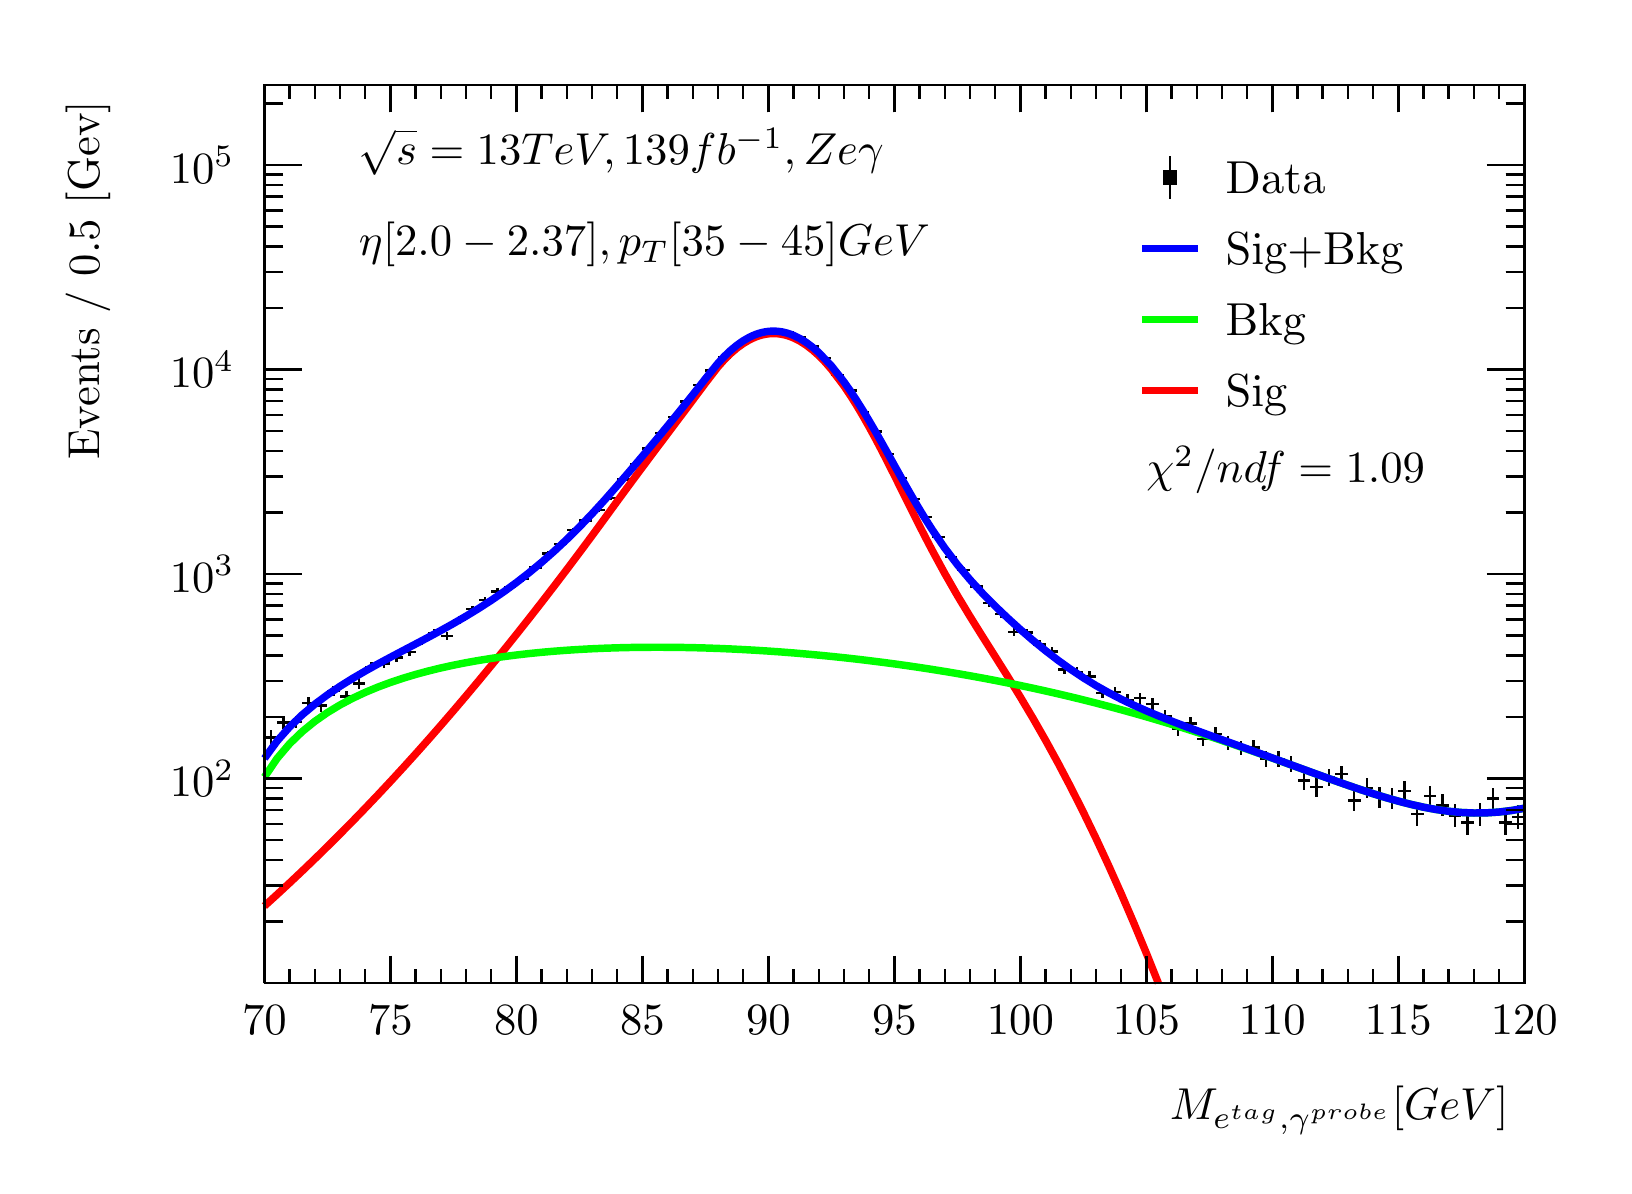
\begin{tikzpicture}
\pgfdeclareplotmark{cross} {
\pgfpathmoveto{\pgfpoint{-0.3\pgfplotmarksize}{\pgfplotmarksize}}
\pgfpathlineto{\pgfpoint{+0.3\pgfplotmarksize}{\pgfplotmarksize}}
\pgfpathlineto{\pgfpoint{+0.3\pgfplotmarksize}{0.3\pgfplotmarksize}}
\pgfpathlineto{\pgfpoint{+1\pgfplotmarksize}{0.3\pgfplotmarksize}}
\pgfpathlineto{\pgfpoint{+1\pgfplotmarksize}{-0.3\pgfplotmarksize}}
\pgfpathlineto{\pgfpoint{+0.3\pgfplotmarksize}{-0.3\pgfplotmarksize}}
\pgfpathlineto{\pgfpoint{+0.3\pgfplotmarksize}{-1.\pgfplotmarksize}}
\pgfpathlineto{\pgfpoint{-0.3\pgfplotmarksize}{-1.\pgfplotmarksize}}
\pgfpathlineto{\pgfpoint{-0.3\pgfplotmarksize}{-0.3\pgfplotmarksize}}
\pgfpathlineto{\pgfpoint{-1.\pgfplotmarksize}{-0.3\pgfplotmarksize}}
\pgfpathlineto{\pgfpoint{-1.\pgfplotmarksize}{0.3\pgfplotmarksize}}
\pgfpathlineto{\pgfpoint{-0.3\pgfplotmarksize}{0.3\pgfplotmarksize}}
\pgfpathclose
\pgfusepathqstroke
}
\pgfdeclareplotmark{cross*} {
\pgfpathmoveto{\pgfpoint{-0.3\pgfplotmarksize}{\pgfplotmarksize}}
\pgfpathlineto{\pgfpoint{+0.3\pgfplotmarksize}{\pgfplotmarksize}}
\pgfpathlineto{\pgfpoint{+0.3\pgfplotmarksize}{0.3\pgfplotmarksize}}
\pgfpathlineto{\pgfpoint{+1\pgfplotmarksize}{0.3\pgfplotmarksize}}
\pgfpathlineto{\pgfpoint{+1\pgfplotmarksize}{-0.3\pgfplotmarksize}}
\pgfpathlineto{\pgfpoint{+0.3\pgfplotmarksize}{-0.3\pgfplotmarksize}}
\pgfpathlineto{\pgfpoint{+0.3\pgfplotmarksize}{-1.\pgfplotmarksize}}
\pgfpathlineto{\pgfpoint{-0.3\pgfplotmarksize}{-1.\pgfplotmarksize}}
\pgfpathlineto{\pgfpoint{-0.3\pgfplotmarksize}{-0.3\pgfplotmarksize}}
\pgfpathlineto{\pgfpoint{-1.\pgfplotmarksize}{-0.3\pgfplotmarksize}}
\pgfpathlineto{\pgfpoint{-1.\pgfplotmarksize}{0.3\pgfplotmarksize}}
\pgfpathlineto{\pgfpoint{-0.3\pgfplotmarksize}{0.3\pgfplotmarksize}}
\pgfpathclose
\pgfusepathqfillstroke
}
\pgfdeclareplotmark{newstar} {
\pgfpathmoveto{\pgfqpoint{0pt}{\pgfplotmarksize}}
\pgfpathlineto{\pgfqpointpolar{44}{0.5\pgfplotmarksize}}
\pgfpathlineto{\pgfqpointpolar{18}{\pgfplotmarksize}}
\pgfpathlineto{\pgfqpointpolar{-20}{0.5\pgfplotmarksize}}
\pgfpathlineto{\pgfqpointpolar{-54}{\pgfplotmarksize}}
\pgfpathlineto{\pgfqpointpolar{-90}{0.5\pgfplotmarksize}}
\pgfpathlineto{\pgfqpointpolar{234}{\pgfplotmarksize}}
\pgfpathlineto{\pgfqpointpolar{198}{0.5\pgfplotmarksize}}
\pgfpathlineto{\pgfqpointpolar{162}{\pgfplotmarksize}}
\pgfpathlineto{\pgfqpointpolar{134}{0.5\pgfplotmarksize}}
\pgfpathclose
\pgfusepathqstroke
}
\pgfdeclareplotmark{newstar*} {
\pgfpathmoveto{\pgfqpoint{0pt}{\pgfplotmarksize}}
\pgfpathlineto{\pgfqpointpolar{44}{0.5\pgfplotmarksize}}
\pgfpathlineto{\pgfqpointpolar{18}{\pgfplotmarksize}}
\pgfpathlineto{\pgfqpointpolar{-20}{0.5\pgfplotmarksize}}
\pgfpathlineto{\pgfqpointpolar{-54}{\pgfplotmarksize}}
\pgfpathlineto{\pgfqpointpolar{-90}{0.5\pgfplotmarksize}}
\pgfpathlineto{\pgfqpointpolar{234}{\pgfplotmarksize}}
\pgfpathlineto{\pgfqpointpolar{198}{0.5\pgfplotmarksize}}
\pgfpathlineto{\pgfqpointpolar{162}{\pgfplotmarksize}}
\pgfpathlineto{\pgfqpointpolar{134}{0.5\pgfplotmarksize}}
\pgfpathclose
\pgfusepathqfillstroke
}
\definecolor{c}{rgb}{1,1,1};
\draw [color=c, fill=c] (0,0) rectangle (20,14.4361);
\draw [color=c, fill=c] (3,2.30977) rectangle (19,13.7143);
\definecolor{c}{rgb}{0,0,0};
\draw [c,line width=0.9] (3,2.30977) -- (3,13.7143) -- (19,13.7143) -- (19,2.30977) -- (3,2.30977);
\definecolor{c}{rgb}{1,1,1};
\draw [color=c, fill=c] (3,2.30977) rectangle (19,13.7143);
\definecolor{c}{rgb}{0,0,0};
\draw [c,line width=0.9] (3,2.30977) -- (3,13.7143) -- (19,13.7143) -- (19,2.30977) -- (3,2.30977);
\draw [c,line width=0.9] (3,2.30977) -- (19,2.30977);
\draw [c,line width=0.9] (3,2.65624) -- (3,2.30977);
\draw [c,line width=0.9] (3.32,2.48301) -- (3.32,2.30977);
\draw [c,line width=0.9] (3.64,2.48301) -- (3.64,2.30977);
\draw [c,line width=0.9] (3.96,2.48301) -- (3.96,2.30977);
\draw [c,line width=0.9] (4.28,2.48301) -- (4.28,2.30977);
\draw [c,line width=0.9] (4.6,2.65624) -- (4.6,2.30977);
\draw [c,line width=0.9] (4.92,2.48301) -- (4.92,2.30977);
\draw [c,line width=0.9] (5.24,2.48301) -- (5.24,2.30977);
\draw [c,line width=0.9] (5.56,2.48301) -- (5.56,2.30977);
\draw [c,line width=0.9] (5.88,2.48301) -- (5.88,2.30977);
\draw [c,line width=0.9] (6.2,2.65624) -- (6.2,2.30977);
\draw [c,line width=0.9] (6.52,2.48301) -- (6.52,2.30977);
\draw [c,line width=0.9] (6.84,2.48301) -- (6.84,2.30977);
\draw [c,line width=0.9] (7.16,2.48301) -- (7.16,2.30977);
\draw [c,line width=0.9] (7.48,2.48301) -- (7.48,2.30977);
\draw [c,line width=0.9] (7.8,2.65624) -- (7.8,2.30977);
\draw [c,line width=0.9] (8.12,2.48301) -- (8.12,2.30977);
\draw [c,line width=0.9] (8.44,2.48301) -- (8.44,2.30977);
\draw [c,line width=0.9] (8.76,2.48301) -- (8.76,2.30977);
\draw [c,line width=0.9] (9.08,2.48301) -- (9.08,2.30977);
\draw [c,line width=0.9] (9.4,2.65624) -- (9.4,2.30977);
\draw [c,line width=0.9] (9.72,2.48301) -- (9.72,2.30977);
\draw [c,line width=0.9] (10.04,2.48301) -- (10.04,2.30977);
\draw [c,line width=0.9] (10.36,2.48301) -- (10.36,2.30977);
\draw [c,line width=0.9] (10.68,2.48301) -- (10.68,2.30977);
\draw [c,line width=0.9] (11,2.65624) -- (11,2.30977);
\draw [c,line width=0.9] (11.32,2.48301) -- (11.32,2.30977);
\draw [c,line width=0.9] (11.64,2.48301) -- (11.64,2.30977);
\draw [c,line width=0.9] (11.96,2.48301) -- (11.96,2.30977);
\draw [c,line width=0.9] (12.28,2.48301) -- (12.28,2.30977);
\draw [c,line width=0.9] (12.6,2.65624) -- (12.6,2.30977);
\draw [c,line width=0.9] (12.92,2.48301) -- (12.92,2.30977);
\draw [c,line width=0.9] (13.24,2.48301) -- (13.24,2.30977);
\draw [c,line width=0.9] (13.56,2.48301) -- (13.56,2.30977);
\draw [c,line width=0.9] (13.88,2.48301) -- (13.88,2.30977);
\draw [c,line width=0.9] (14.2,2.65624) -- (14.2,2.30977);
\draw [c,line width=0.9] (14.52,2.48301) -- (14.52,2.30977);
\draw [c,line width=0.9] (14.84,2.48301) -- (14.84,2.30977);
\draw [c,line width=0.9] (15.16,2.48301) -- (15.16,2.30977);
\draw [c,line width=0.9] (15.48,2.48301) -- (15.48,2.30977);
\draw [c,line width=0.9] (15.8,2.65624) -- (15.8,2.30977);
\draw [c,line width=0.9] (16.12,2.48301) -- (16.12,2.30977);
\draw [c,line width=0.9] (16.44,2.48301) -- (16.44,2.30977);
\draw [c,line width=0.9] (16.76,2.48301) -- (16.76,2.30977);
\draw [c,line width=0.9] (17.08,2.48301) -- (17.08,2.30977);
\draw [c,line width=0.9] (17.4,2.65624) -- (17.4,2.30977);
\draw [c,line width=0.9] (17.72,2.48301) -- (17.72,2.30977);
\draw [c,line width=0.9] (18.04,2.48301) -- (18.04,2.30977);
\draw [c,line width=0.9] (18.36,2.48301) -- (18.36,2.30977);
\draw [c,line width=0.9] (18.68,2.48301) -- (18.68,2.30977);
\draw [c,line width=0.9] (19,2.65624) -- (19,2.30977);
\draw [anchor=base] (3,1.66015) node[scale=1.61424, color=c, rotate=0]{70};
\draw [anchor=base] (4.6,1.66015) node[scale=1.61424, color=c, rotate=0]{75};
\draw [anchor=base] (6.2,1.66015) node[scale=1.61424, color=c, rotate=0]{80};
\draw [anchor=base] (7.8,1.66015) node[scale=1.61424, color=c, rotate=0]{85};
\draw [anchor=base] (9.4,1.66015) node[scale=1.61424, color=c, rotate=0]{90};
\draw [anchor=base] (11,1.66015) node[scale=1.61424, color=c, rotate=0]{95};
\draw [anchor=base] (12.6,1.66015) node[scale=1.61424, color=c, rotate=0]{100};
\draw [anchor=base] (14.2,1.66015) node[scale=1.61424, color=c, rotate=0]{105};
\draw [anchor=base] (15.8,1.66015) node[scale=1.61424, color=c, rotate=0]{110};
\draw [anchor=base] (17.4,1.66015) node[scale=1.61424, color=c, rotate=0]{115};
\draw [anchor=base] (19,1.66015) node[scale=1.61424, color=c, rotate=0]{120};
\draw [anchor= east] (19,0.692932) node[scale=1.61424, color=c, rotate=0]{$M_{e^{tag}, \gamma^{probe}}  [GeV]$};
\draw [c,line width=0.9] (3,13.7143) -- (19,13.7143);
\draw [c,line width=0.9] (3,13.3678) -- (3,13.7143);
\draw [c,line width=0.9] (3.32,13.5411) -- (3.32,13.7143);
\draw [c,line width=0.9] (3.64,13.5411) -- (3.64,13.7143);
\draw [c,line width=0.9] (3.96,13.5411) -- (3.96,13.7143);
\draw [c,line width=0.9] (4.28,13.5411) -- (4.28,13.7143);
\draw [c,line width=0.9] (4.6,13.3678) -- (4.6,13.7143);
\draw [c,line width=0.9] (4.92,13.5411) -- (4.92,13.7143);
\draw [c,line width=0.9] (5.24,13.5411) -- (5.24,13.7143);
\draw [c,line width=0.9] (5.56,13.5411) -- (5.56,13.7143);
\draw [c,line width=0.9] (5.88,13.5411) -- (5.88,13.7143);
\draw [c,line width=0.9] (6.2,13.3678) -- (6.2,13.7143);
\draw [c,line width=0.9] (6.52,13.5411) -- (6.52,13.7143);
\draw [c,line width=0.9] (6.84,13.5411) -- (6.84,13.7143);
\draw [c,line width=0.9] (7.16,13.5411) -- (7.16,13.7143);
\draw [c,line width=0.9] (7.48,13.5411) -- (7.48,13.7143);
\draw [c,line width=0.9] (7.8,13.3678) -- (7.8,13.7143);
\draw [c,line width=0.9] (8.12,13.5411) -- (8.12,13.7143);
\draw [c,line width=0.9] (8.44,13.5411) -- (8.44,13.7143);
\draw [c,line width=0.9] (8.76,13.5411) -- (8.76,13.7143);
\draw [c,line width=0.9] (9.08,13.5411) -- (9.08,13.7143);
\draw [c,line width=0.9] (9.4,13.3678) -- (9.4,13.7143);
\draw [c,line width=0.9] (9.72,13.5411) -- (9.72,13.7143);
\draw [c,line width=0.9] (10.04,13.5411) -- (10.04,13.7143);
\draw [c,line width=0.9] (10.36,13.5411) -- (10.36,13.7143);
\draw [c,line width=0.9] (10.68,13.5411) -- (10.68,13.7143);
\draw [c,line width=0.9] (11,13.3678) -- (11,13.7143);
\draw [c,line width=0.9] (11.32,13.5411) -- (11.32,13.7143);
\draw [c,line width=0.9] (11.64,13.5411) -- (11.64,13.7143);
\draw [c,line width=0.9] (11.96,13.5411) -- (11.96,13.7143);
\draw [c,line width=0.9] (12.28,13.5411) -- (12.28,13.7143);
\draw [c,line width=0.9] (12.6,13.3678) -- (12.6,13.7143);
\draw [c,line width=0.9] (12.92,13.5411) -- (12.92,13.7143);
\draw [c,line width=0.9] (13.24,13.5411) -- (13.24,13.7143);
\draw [c,line width=0.9] (13.56,13.5411) -- (13.56,13.7143);
\draw [c,line width=0.9] (13.88,13.5411) -- (13.88,13.7143);
\draw [c,line width=0.9] (14.2,13.3678) -- (14.2,13.7143);
\draw [c,line width=0.9] (14.52,13.5411) -- (14.52,13.7143);
\draw [c,line width=0.9] (14.84,13.5411) -- (14.84,13.7143);
\draw [c,line width=0.9] (15.16,13.5411) -- (15.16,13.7143);
\draw [c,line width=0.9] (15.48,13.5411) -- (15.48,13.7143);
\draw [c,line width=0.9] (15.8,13.3678) -- (15.8,13.7143);
\draw [c,line width=0.9] (16.12,13.5411) -- (16.12,13.7143);
\draw [c,line width=0.9] (16.44,13.5411) -- (16.44,13.7143);
\draw [c,line width=0.9] (16.76,13.5411) -- (16.76,13.7143);
\draw [c,line width=0.9] (17.08,13.5411) -- (17.08,13.7143);
\draw [c,line width=0.9] (17.4,13.3678) -- (17.4,13.7143);
\draw [c,line width=0.9] (17.72,13.5411) -- (17.72,13.7143);
\draw [c,line width=0.9] (18.04,13.5411) -- (18.04,13.7143);
\draw [c,line width=0.9] (18.36,13.5411) -- (18.36,13.7143);
\draw [c,line width=0.9] (18.68,13.5411) -- (18.68,13.7143);
\draw [c,line width=0.9] (19,13.3678) -- (19,13.7143);
\draw [c,line width=0.9] (3,2.30977) -- (3,13.7143);
\draw [c,line width=0.9] (3.237,3.09166) -- (3,3.09166);
\draw [c,line width=0.9] (3.237,3.54903) -- (3,3.54903);
\draw [c,line width=0.9] (3.237,3.87354) -- (3,3.87354);
\draw [c,line width=0.9] (3.237,4.12525) -- (3,4.12525);
\draw [c,line width=0.9] (3.237,4.33091) -- (3,4.33091);
\draw [c,line width=0.9] (3.237,4.5048) -- (3,4.5048);
\draw [c,line width=0.9] (3.237,4.65542) -- (3,4.65542);
\draw [c,line width=0.9] (3.237,4.78829) -- (3,4.78829);
\draw [c,line width=0.9] (3.474,4.90714) -- (3,4.90714);
\draw [anchor= east] (2.82,4.90714) node[scale=1.61424, color=c, rotate=0]{$10^{2}$};
\draw [c,line width=0.9] (3.237,5.68902) -- (3,5.68902);
\draw [c,line width=0.9] (3.237,6.14639) -- (3,6.14639);
\draw [c,line width=0.9] (3.237,6.4709) -- (3,6.4709);
\draw [c,line width=0.9] (3.237,6.72261) -- (3,6.72261);
\draw [c,line width=0.9] (3.237,6.92828) -- (3,6.92828);
\draw [c,line width=0.9] (3.237,7.10216) -- (3,7.10216);
\draw [c,line width=0.9] (3.237,7.25279) -- (3,7.25279);
\draw [c,line width=0.9] (3.237,7.38565) -- (3,7.38565);
\draw [c,line width=0.9] (3.474,7.5045) -- (3,7.5045);
\draw [anchor= east] (2.82,7.5045) node[scale=1.61424, color=c, rotate=0]{$10^{3}$};
\draw [c,line width=0.9] (3.237,8.28638) -- (3,8.28638);
\draw [c,line width=0.9] (3.237,8.74376) -- (3,8.74376);
\draw [c,line width=0.9] (3.237,9.06827) -- (3,9.06827);
\draw [c,line width=0.9] (3.237,9.31998) -- (3,9.31998);
\draw [c,line width=0.9] (3.237,9.52564) -- (3,9.52564);
\draw [c,line width=0.9] (3.237,9.69952) -- (3,9.69952);
\draw [c,line width=0.9] (3.237,9.85015) -- (3,9.85015);
\draw [c,line width=0.9] (3.237,9.98301) -- (3,9.98301);
\draw [c,line width=0.9] (3.474,10.1019) -- (3,10.1019);
\draw [anchor= east] (2.82,10.1019) node[scale=1.61424, color=c, rotate=0]{$10^{4}$};
\draw [c,line width=0.9] (3.237,10.8837) -- (3,10.8837);
\draw [c,line width=0.9] (3.237,11.3411) -- (3,11.3411);
\draw [c,line width=0.9] (3.237,11.6656) -- (3,11.6656);
\draw [c,line width=0.9] (3.237,11.9173) -- (3,11.9173);
\draw [c,line width=0.9] (3.237,12.123) -- (3,12.123);
\draw [c,line width=0.9] (3.237,12.2969) -- (3,12.2969);
\draw [c,line width=0.9] (3.237,12.4475) -- (3,12.4475);
\draw [c,line width=0.9] (3.237,12.5804) -- (3,12.5804);
\draw [c,line width=0.9] (3.474,12.6992) -- (3,12.6992);
\draw [anchor= east] (2.82,12.6992) node[scale=1.61424, color=c, rotate=0]{$10^{5}$};
\draw [c,line width=0.9] (3.237,13.4811) -- (3,13.4811);
\draw [anchor= east] (0.76,13.7143) node[scale=1.61424, color=c, rotate=90]{Events / 0.5 [Gev]};
\draw [c,line width=0.9] (19,2.30977) -- (19,13.7143);
\draw [c,line width=0.9] (18.763,3.09166) -- (19,3.09166);
\draw [c,line width=0.9] (18.763,3.54903) -- (19,3.54903);
\draw [c,line width=0.9] (18.763,3.87354) -- (19,3.87354);
\draw [c,line width=0.9] (18.763,4.12525) -- (19,4.12525);
\draw [c,line width=0.9] (18.763,4.33091) -- (19,4.33091);
\draw [c,line width=0.9] (18.763,4.5048) -- (19,4.5048);
\draw [c,line width=0.9] (18.763,4.65542) -- (19,4.65542);
\draw [c,line width=0.9] (18.763,4.78829) -- (19,4.78829);
\draw [c,line width=0.9] (18.526,4.90714) -- (19,4.90714);
\draw [c,line width=0.9] (18.763,5.68902) -- (19,5.68902);
\draw [c,line width=0.9] (18.763,6.14639) -- (19,6.14639);
\draw [c,line width=0.9] (18.763,6.4709) -- (19,6.4709);
\draw [c,line width=0.9] (18.763,6.72261) -- (19,6.72261);
\draw [c,line width=0.9] (18.763,6.92828) -- (19,6.92828);
\draw [c,line width=0.9] (18.763,7.10216) -- (19,7.10216);
\draw [c,line width=0.9] (18.763,7.25279) -- (19,7.25279);
\draw [c,line width=0.9] (18.763,7.38565) -- (19,7.38565);
\draw [c,line width=0.9] (18.526,7.5045) -- (19,7.5045);
\draw [c,line width=0.9] (18.763,8.28638) -- (19,8.28638);
\draw [c,line width=0.9] (18.763,8.74376) -- (19,8.74376);
\draw [c,line width=0.9] (18.763,9.06827) -- (19,9.06827);
\draw [c,line width=0.9] (18.763,9.31998) -- (19,9.31998);
\draw [c,line width=0.9] (18.763,9.52564) -- (19,9.52564);
\draw [c,line width=0.9] (18.763,9.69952) -- (19,9.69952);
\draw [c,line width=0.9] (18.763,9.85015) -- (19,9.85015);
\draw [c,line width=0.9] (18.763,9.98301) -- (19,9.98301);
\draw [c,line width=0.9] (18.526,10.1019) -- (19,10.1019);
\draw [c,line width=0.9] (18.763,10.8837) -- (19,10.8837);
\draw [c,line width=0.9] (18.763,11.3411) -- (19,11.3411);
\draw [c,line width=0.9] (18.763,11.6656) -- (19,11.6656);
\draw [c,line width=0.9] (18.763,11.9173) -- (19,11.9173);
\draw [c,line width=0.9] (18.763,12.123) -- (19,12.123);
\draw [c,line width=0.9] (18.763,12.2969) -- (19,12.2969);
\draw [c,line width=0.9] (18.763,12.4475) -- (19,12.4475);
\draw [c,line width=0.9] (18.763,12.5804) -- (19,12.5804);
\draw [c,line width=0.9] (18.526,12.6992) -- (19,12.6992);
\draw [c,line width=0.9] (18.763,13.4811) -- (19,13.4811);
\draw [c,line width=0.9] (3.08,5.43024) -- (3,5.43024);
\draw [c,line width=0.9] (3,5.43024) -- (3,5.43024);
\draw [c,line width=0.9] (3.08,5.43024) -- (3.16,5.43024);
\draw [c,line width=0.9] (3.16,5.43024) -- (3.16,5.43024);
\draw [c,line width=0.9] (3.08,5.43024) -- (3.08,5.51967);
\draw [c,line width=0.9] (3.08,5.51967) -- (3.08,5.51967);
\draw [c,line width=0.9] (3.08,5.43024) -- (3.08,5.3408);
\draw [c,line width=0.9] (3.08,5.3408) -- (3.08,5.3408);
\draw [c,line width=0.9] (3.24,5.61922) -- (3.16,5.61922);
\draw [c,line width=0.9] (3.16,5.61922) -- (3.16,5.61922);
\draw [c,line width=0.9] (3.24,5.61922) -- (3.32,5.61922);
\draw [c,line width=0.9] (3.32,5.61922) -- (3.32,5.61922);
\draw [c,line width=0.9] (3.24,5.61922) -- (3.24,5.70148);
\draw [c,line width=0.9] (3.24,5.70148) -- (3.24,5.70148);
\draw [c,line width=0.9] (3.24,5.61922) -- (3.24,5.53697);
\draw [c,line width=0.9] (3.24,5.53697) -- (3.24,5.53697);
\draw [c,line width=0.9] (3.4,5.62521) -- (3.32,5.62521);
\draw [c,line width=0.9] (3.32,5.62521) -- (3.32,5.62521);
\draw [c,line width=0.9] (3.4,5.62521) -- (3.48,5.62521);
\draw [c,line width=0.9] (3.48,5.62521) -- (3.48,5.62521);
\draw [c,line width=0.9] (3.4,5.62521) -- (3.4,5.70724);
\draw [c,line width=0.9] (3.4,5.70724) -- (3.4,5.70724);
\draw [c,line width=0.9] (3.4,5.62521) -- (3.4,5.54318);
\draw [c,line width=0.9] (3.4,5.54318) -- (3.4,5.54318);
\draw [c,line width=0.9] (3.56,5.86612) -- (3.48,5.86612);
\draw [c,line width=0.9] (3.48,5.86612) -- (3.48,5.86612);
\draw [c,line width=0.9] (3.56,5.86612) -- (3.64,5.86612);
\draw [c,line width=0.9] (3.64,5.86612) -- (3.64,5.86612);
\draw [c,line width=0.9] (3.56,5.86612) -- (3.56,5.93985);
\draw [c,line width=0.9] (3.56,5.93985) -- (3.56,5.93985);
\draw [c,line width=0.9] (3.56,5.86612) -- (3.56,5.7924);
\draw [c,line width=0.9] (3.56,5.7924) -- (3.56,5.7924);
\draw [c,line width=0.9] (3.72,5.83187) -- (3.64,5.83187);
\draw [c,line width=0.9] (3.64,5.83187) -- (3.64,5.83187);
\draw [c,line width=0.9] (3.72,5.83187) -- (3.8,5.83187);
\draw [c,line width=0.9] (3.8,5.83187) -- (3.8,5.83187);
\draw [c,line width=0.9] (3.72,5.83187) -- (3.72,5.90672);
\draw [c,line width=0.9] (3.72,5.90672) -- (3.72,5.90672);
\draw [c,line width=0.9] (3.72,5.83187) -- (3.72,5.75701);
\draw [c,line width=0.9] (3.72,5.75701) -- (3.72,5.75701);
\draw [c,line width=0.9] (3.88,6.01916) -- (3.8,6.01916);
\draw [c,line width=0.9] (3.8,6.01916) -- (3.8,6.01916);
\draw [c,line width=0.9] (3.88,6.01916) -- (3.96,6.01916);
\draw [c,line width=0.9] (3.96,6.01916) -- (3.96,6.01916);
\draw [c,line width=0.9] (3.88,6.01916) -- (3.88,6.08805);
\draw [c,line width=0.9] (3.88,6.08805) -- (3.88,6.08805);
\draw [c,line width=0.9] (3.88,6.01916) -- (3.88,5.95026);
\draw [c,line width=0.9] (3.88,5.95026) -- (3.88,5.95026);
\draw [c,line width=0.9] (4.04,5.94972) -- (3.96,5.94972);
\draw [c,line width=0.9] (3.96,5.94972) -- (3.96,5.94972);
\draw [c,line width=0.9] (4.04,5.94972) -- (4.12,5.94972);
\draw [c,line width=0.9] (4.12,5.94972) -- (4.12,5.94972);
\draw [c,line width=0.9] (4.04,5.94972) -- (4.04,6.02077);
\draw [c,line width=0.9] (4.04,6.02077) -- (4.04,6.02077);
\draw [c,line width=0.9] (4.04,5.94972) -- (4.04,5.87867);
\draw [c,line width=0.9] (4.04,5.87867) -- (4.04,5.87867);
\draw [c,line width=0.9] (4.2,6.11591) -- (4.12,6.11591);
\draw [c,line width=0.9] (4.12,6.11591) -- (4.12,6.11591);
\draw [c,line width=0.9] (4.2,6.11591) -- (4.28,6.11591);
\draw [c,line width=0.9] (4.28,6.11591) -- (4.28,6.11591);
\draw [c,line width=0.9] (4.2,6.11591) -- (4.2,6.18191);
\draw [c,line width=0.9] (4.2,6.18191) -- (4.2,6.18191);
\draw [c,line width=0.9] (4.2,6.11591) -- (4.2,6.0499);
\draw [c,line width=0.9] (4.2,6.0499) -- (4.2,6.0499);
\draw [c,line width=0.9] (4.36,6.32671) -- (4.28,6.32671);
\draw [c,line width=0.9] (4.28,6.32671) -- (4.28,6.32671);
\draw [c,line width=0.9] (4.36,6.32671) -- (4.44,6.32671);
\draw [c,line width=0.9] (4.44,6.32671) -- (4.44,6.32671);
\draw [c,line width=0.9] (4.36,6.32671) -- (4.36,6.38682);
\draw [c,line width=0.9] (4.36,6.38682) -- (4.36,6.38682);
\draw [c,line width=0.9] (4.36,6.32671) -- (4.36,6.26659);
\draw [c,line width=0.9] (4.36,6.26659) -- (4.36,6.26659);
\draw [c,line width=0.9] (4.52,6.36762) -- (4.44,6.36762);
\draw [c,line width=0.9] (4.44,6.36762) -- (4.44,6.36762);
\draw [c,line width=0.9] (4.52,6.36762) -- (4.6,6.36762);
\draw [c,line width=0.9] (4.6,6.36762) -- (4.6,6.36762);
\draw [c,line width=0.9] (4.52,6.36762) -- (4.52,6.42665);
\draw [c,line width=0.9] (4.52,6.42665) -- (4.52,6.42665);
\draw [c,line width=0.9] (4.52,6.36762) -- (4.52,6.30858);
\draw [c,line width=0.9] (4.52,6.30858) -- (4.52,6.30858);
\draw [c,line width=0.9] (4.68,6.44235) -- (4.6,6.44235);
\draw [c,line width=0.9] (4.6,6.44235) -- (4.6,6.44235);
\draw [c,line width=0.9] (4.68,6.44235) -- (4.76,6.44235);
\draw [c,line width=0.9] (4.76,6.44235) -- (4.76,6.44235);
\draw [c,line width=0.9] (4.68,6.44235) -- (4.68,6.49946);
\draw [c,line width=0.9] (4.68,6.49946) -- (4.68,6.49946);
\draw [c,line width=0.9] (4.68,6.44235) -- (4.68,6.38523);
\draw [c,line width=0.9] (4.68,6.38523) -- (4.68,6.38523);
\draw [c,line width=0.9] (4.84,6.51243) -- (4.76,6.51243);
\draw [c,line width=0.9] (4.76,6.51243) -- (4.76,6.51243);
\draw [c,line width=0.9] (4.84,6.51243) -- (4.92,6.51243);
\draw [c,line width=0.9] (4.92,6.51243) -- (4.92,6.51243);
\draw [c,line width=0.9] (4.84,6.51243) -- (4.84,6.5678);
\draw [c,line width=0.9] (4.84,6.5678) -- (4.84,6.5678);
\draw [c,line width=0.9] (4.84,6.51243) -- (4.84,6.45707);
\draw [c,line width=0.9] (4.84,6.45707) -- (4.84,6.45707);
\draw [c,line width=0.9] (5,6.65282) -- (4.92,6.65282);
\draw [c,line width=0.9] (4.92,6.65282) -- (4.92,6.65282);
\draw [c,line width=0.9] (5,6.65282) -- (5.08,6.65282);
\draw [c,line width=0.9] (5.08,6.65282) -- (5.08,6.65282);
\draw [c,line width=0.9] (5,6.65282) -- (5,6.70485);
\draw [c,line width=0.9] (5,6.70485) -- (5,6.70485);
\draw [c,line width=0.9] (5,6.65282) -- (5,6.60079);
\draw [c,line width=0.9] (5,6.60079) -- (5,6.60079);
\draw [c,line width=0.9] (5.16,6.75815) -- (5.08,6.75815);
\draw [c,line width=0.9] (5.08,6.75815) -- (5.08,6.75815);
\draw [c,line width=0.9] (5.16,6.75815) -- (5.24,6.75815);
\draw [c,line width=0.9] (5.24,6.75815) -- (5.24,6.75815);
\draw [c,line width=0.9] (5.16,6.75815) -- (5.16,6.8078);
\draw [c,line width=0.9] (5.16,6.8078) -- (5.16,6.8078);
\draw [c,line width=0.9] (5.16,6.75815) -- (5.16,6.70849);
\draw [c,line width=0.9] (5.16,6.70849) -- (5.16,6.70849);
\draw [c,line width=0.9] (5.32,6.71583) -- (5.24,6.71583);
\draw [c,line width=0.9] (5.24,6.71583) -- (5.24,6.71583);
\draw [c,line width=0.9] (5.32,6.71583) -- (5.4,6.71583);
\draw [c,line width=0.9] (5.4,6.71583) -- (5.4,6.71583);
\draw [c,line width=0.9] (5.32,6.71583) -- (5.32,6.76642);
\draw [c,line width=0.9] (5.32,6.76642) -- (5.32,6.76642);
\draw [c,line width=0.9] (5.32,6.71583) -- (5.32,6.66523);
\draw [c,line width=0.9] (5.32,6.66523) -- (5.32,6.66523);
\draw [c,line width=0.9] (5.48,6.91884) -- (5.4,6.91884);
\draw [c,line width=0.9] (5.4,6.91884) -- (5.4,6.91884);
\draw [c,line width=0.9] (5.48,6.91884) -- (5.56,6.91884);
\draw [c,line width=0.9] (5.56,6.91884) -- (5.56,6.91884);
\draw [c,line width=0.9] (5.48,6.91884) -- (5.48,6.96508);
\draw [c,line width=0.9] (5.48,6.96508) -- (5.48,6.96508);
\draw [c,line width=0.9] (5.48,6.91884) -- (5.48,6.8726);
\draw [c,line width=0.9] (5.48,6.8726) -- (5.48,6.8726);
\draw [c,line width=0.9] (5.64,7.06114) -- (5.56,7.06114);
\draw [c,line width=0.9] (5.56,7.06114) -- (5.56,7.06114);
\draw [c,line width=0.9] (5.64,7.06114) -- (5.72,7.06114);
\draw [c,line width=0.9] (5.72,7.06114) -- (5.72,7.06114);
\draw [c,line width=0.9] (5.64,7.06114) -- (5.64,7.10455);
\draw [c,line width=0.9] (5.64,7.10455) -- (5.64,7.10455);
\draw [c,line width=0.9] (5.64,7.06114) -- (5.64,7.01772);
\draw [c,line width=0.9] (5.64,7.01772) -- (5.64,7.01772);
\draw [c,line width=0.9] (5.8,7.17698) -- (5.72,7.17698);
\draw [c,line width=0.9] (5.72,7.17698) -- (5.72,7.17698);
\draw [c,line width=0.9] (5.8,7.17698) -- (5.88,7.17698);
\draw [c,line width=0.9] (5.88,7.17698) -- (5.88,7.17698);
\draw [c,line width=0.9] (5.8,7.17698) -- (5.8,7.21822);
\draw [c,line width=0.9] (5.8,7.21822) -- (5.8,7.21822);
\draw [c,line width=0.9] (5.8,7.17698) -- (5.8,7.13573);
\draw [c,line width=0.9] (5.8,7.13573) -- (5.8,7.13573);
\draw [c,line width=0.9] (5.96,7.28339) -- (5.88,7.28339);
\draw [c,line width=0.9] (5.88,7.28339) -- (5.88,7.28339);
\draw [c,line width=0.9] (5.96,7.28339) -- (6.04,7.28339);
\draw [c,line width=0.9] (6.04,7.28339) -- (6.04,7.28339);
\draw [c,line width=0.9] (5.96,7.28339) -- (5.96,7.32273);
\draw [c,line width=0.9] (5.96,7.32273) -- (5.96,7.32273);
\draw [c,line width=0.9] (5.96,7.28339) -- (5.96,7.24405);
\draw [c,line width=0.9] (5.96,7.24405) -- (5.96,7.24405);
\draw [c,line width=0.9] (6.12,7.33699) -- (6.04,7.33699);
\draw [c,line width=0.9] (6.04,7.33699) -- (6.04,7.33699);
\draw [c,line width=0.9] (6.12,7.33699) -- (6.2,7.33699);
\draw [c,line width=0.9] (6.2,7.33699) -- (6.2,7.33699);
\draw [c,line width=0.9] (6.12,7.33699) -- (6.12,7.37541);
\draw [c,line width=0.9] (6.12,7.37541) -- (6.12,7.37541);
\draw [c,line width=0.9] (6.12,7.33699) -- (6.12,7.29857);
\draw [c,line width=0.9] (6.12,7.29857) -- (6.12,7.29857);
\draw [c,line width=0.9] (6.28,7.44426) -- (6.2,7.44426);
\draw [c,line width=0.9] (6.2,7.44426) -- (6.2,7.44426);
\draw [c,line width=0.9] (6.28,7.44426) -- (6.36,7.44426);
\draw [c,line width=0.9] (6.36,7.44426) -- (6.36,7.44426);
\draw [c,line width=0.9] (6.28,7.44426) -- (6.28,7.4809);
\draw [c,line width=0.9] (6.28,7.4809) -- (6.28,7.4809);
\draw [c,line width=0.9] (6.28,7.44426) -- (6.28,7.40763);
\draw [c,line width=0.9] (6.28,7.40763) -- (6.28,7.40763);
\draw [c,line width=0.9] (6.44,7.58713) -- (6.36,7.58713);
\draw [c,line width=0.9] (6.36,7.58713) -- (6.36,7.58713);
\draw [c,line width=0.9] (6.44,7.58713) -- (6.52,7.58713);
\draw [c,line width=0.9] (6.52,7.58713) -- (6.52,7.58713);
\draw [c,line width=0.9] (6.44,7.58713) -- (6.44,7.62151);
\draw [c,line width=0.9] (6.44,7.62151) -- (6.44,7.62151);
\draw [c,line width=0.9] (6.44,7.58713) -- (6.44,7.55274);
\draw [c,line width=0.9] (6.44,7.55274) -- (6.44,7.55274);
\draw [c,line width=0.9] (6.6,7.76699) -- (6.52,7.76699);
\draw [c,line width=0.9] (6.52,7.76699) -- (6.52,7.76699);
\draw [c,line width=0.9] (6.6,7.76699) -- (6.68,7.76699);
\draw [c,line width=0.9] (6.68,7.76699) -- (6.68,7.76699);
\draw [c,line width=0.9] (6.6,7.76699) -- (6.6,7.79874);
\draw [c,line width=0.9] (6.6,7.79874) -- (6.6,7.79874);
\draw [c,line width=0.9] (6.6,7.76699) -- (6.6,7.73524);
\draw [c,line width=0.9] (6.6,7.73524) -- (6.6,7.73524);
\draw [c,line width=0.9] (6.76,7.88405) -- (6.68,7.88405);
\draw [c,line width=0.9] (6.68,7.88405) -- (6.68,7.88405);
\draw [c,line width=0.9] (6.76,7.88405) -- (6.84,7.88405);
\draw [c,line width=0.9] (6.84,7.88405) -- (6.84,7.88405);
\draw [c,line width=0.9] (6.76,7.88405) -- (6.76,7.91419);
\draw [c,line width=0.9] (6.76,7.91419) -- (6.76,7.91419);
\draw [c,line width=0.9] (6.76,7.88405) -- (6.76,7.8539);
\draw [c,line width=0.9] (6.76,7.8539) -- (6.76,7.8539);
\draw [c,line width=0.9] (6.92,8.06596) -- (6.84,8.06596);
\draw [c,line width=0.9] (6.84,8.06596) -- (6.84,8.06596);
\draw [c,line width=0.9] (6.92,8.06596) -- (7,8.06596);
\draw [c,line width=0.9] (7,8.06596) -- (7,8.06596);
\draw [c,line width=0.9] (6.92,8.06596) -- (6.92,8.09377);
\draw [c,line width=0.9] (6.92,8.09377) -- (6.92,8.09377);
\draw [c,line width=0.9] (6.92,8.06596) -- (6.92,8.03815);
\draw [c,line width=0.9] (6.92,8.03815) -- (6.92,8.03815);
\draw [c,line width=0.9] (7.08,8.18556) -- (7,8.18556);
\draw [c,line width=0.9] (7,8.18556) -- (7,8.18556);
\draw [c,line width=0.9] (7.08,8.18556) -- (7.16,8.18556);
\draw [c,line width=0.9] (7.16,8.18556) -- (7.16,8.18556);
\draw [c,line width=0.9] (7.08,8.18556) -- (7.08,8.21194);
\draw [c,line width=0.9] (7.08,8.21194) -- (7.08,8.21194);
\draw [c,line width=0.9] (7.08,8.18556) -- (7.08,8.15919);
\draw [c,line width=0.9] (7.08,8.15919) -- (7.08,8.15919);
\draw [c,line width=0.9] (7.24,8.31918) -- (7.16,8.31918);
\draw [c,line width=0.9] (7.16,8.31918) -- (7.16,8.31918);
\draw [c,line width=0.9] (7.24,8.31918) -- (7.32,8.31918);
\draw [c,line width=0.9] (7.32,8.31918) -- (7.32,8.31918);
\draw [c,line width=0.9] (7.24,8.31918) -- (7.24,8.34404);
\draw [c,line width=0.9] (7.24,8.34404) -- (7.24,8.34404);
\draw [c,line width=0.9] (7.24,8.31918) -- (7.24,8.29432);
\draw [c,line width=0.9] (7.24,8.29432) -- (7.24,8.29432);
\draw [c,line width=0.9] (7.4,8.47117) -- (7.32,8.47117);
\draw [c,line width=0.9] (7.32,8.47117) -- (7.32,8.47117);
\draw [c,line width=0.9] (7.4,8.47117) -- (7.48,8.47117);
\draw [c,line width=0.9] (7.48,8.47117) -- (7.48,8.47117);
\draw [c,line width=0.9] (7.4,8.47117) -- (7.4,8.49441);
\draw [c,line width=0.9] (7.4,8.49441) -- (7.4,8.49441);
\draw [c,line width=0.9] (7.4,8.47117) -- (7.4,8.44794);
\draw [c,line width=0.9] (7.4,8.44794) -- (7.4,8.44794);
\draw [c,line width=0.9] (7.56,8.70551) -- (7.48,8.70551);
\draw [c,line width=0.9] (7.48,8.70551) -- (7.48,8.70551);
\draw [c,line width=0.9] (7.56,8.70551) -- (7.64,8.70551);
\draw [c,line width=0.9] (7.64,8.70551) -- (7.64,8.70551);
\draw [c,line width=0.9] (7.56,8.70551) -- (7.56,8.72646);
\draw [c,line width=0.9] (7.56,8.72646) -- (7.56,8.72646);
\draw [c,line width=0.9] (7.56,8.70551) -- (7.56,8.68457);
\draw [c,line width=0.9] (7.56,8.68457) -- (7.56,8.68457);
\draw [c,line width=0.9] (7.72,8.90076) -- (7.64,8.90076);
\draw [c,line width=0.9] (7.64,8.90076) -- (7.64,8.90076);
\draw [c,line width=0.9] (7.72,8.90076) -- (7.8,8.90076);
\draw [c,line width=0.9] (7.8,8.90076) -- (7.8,8.90076);
\draw [c,line width=0.9] (7.72,8.90076) -- (7.72,8.91997);
\draw [c,line width=0.9] (7.72,8.91997) -- (7.72,8.91997);
\draw [c,line width=0.9] (7.72,8.90076) -- (7.72,8.88155);
\draw [c,line width=0.9] (7.72,8.88155) -- (7.72,8.88155);
\draw [c,line width=0.9] (7.88,9.10024) -- (7.8,9.10024);
\draw [c,line width=0.9] (7.8,9.10024) -- (7.8,9.10024);
\draw [c,line width=0.9] (7.88,9.10024) -- (7.96,9.10024);
\draw [c,line width=0.9] (7.96,9.10024) -- (7.96,9.10024);
\draw [c,line width=0.9] (7.88,9.10024) -- (7.88,9.11783);
\draw [c,line width=0.9] (7.88,9.11783) -- (7.88,9.11783);
\draw [c,line width=0.9] (7.88,9.10024) -- (7.88,9.08266);
\draw [c,line width=0.9] (7.88,9.08266) -- (7.88,9.08266);
\draw [c,line width=0.9] (8.04,9.29558) -- (7.96,9.29558);
\draw [c,line width=0.9] (7.96,9.29558) -- (7.96,9.29558);
\draw [c,line width=0.9] (8.04,9.29558) -- (8.12,9.29558);
\draw [c,line width=0.9] (8.12,9.29558) -- (8.12,9.29558);
\draw [c,line width=0.9] (8.04,9.29558) -- (8.04,9.3117);
\draw [c,line width=0.9] (8.04,9.3117) -- (8.04,9.3117);
\draw [c,line width=0.9] (8.04,9.29558) -- (8.04,9.27945);
\draw [c,line width=0.9] (8.04,9.27945) -- (8.04,9.27945);
\draw [c,line width=0.9] (8.2,9.49804) -- (8.12,9.49804);
\draw [c,line width=0.9] (8.12,9.49804) -- (8.12,9.49804);
\draw [c,line width=0.9] (8.2,9.49804) -- (8.28,9.49804);
\draw [c,line width=0.9] (8.28,9.49804) -- (8.28,9.49804);
\draw [c,line width=0.9] (8.2,9.49804) -- (8.2,9.51279);
\draw [c,line width=0.9] (8.2,9.51279) -- (8.2,9.51279);
\draw [c,line width=0.9] (8.2,9.49804) -- (8.2,9.4833);
\draw [c,line width=0.9] (8.2,9.4833) -- (8.2,9.4833);
\draw [c,line width=0.9] (8.36,9.69824) -- (8.28,9.69824);
\draw [c,line width=0.9] (8.28,9.69824) -- (8.28,9.69824);
\draw [c,line width=0.9] (8.36,9.69824) -- (8.44,9.69824);
\draw [c,line width=0.9] (8.44,9.69824) -- (8.44,9.69824);
\draw [c,line width=0.9] (8.36,9.69824) -- (8.36,9.71173);
\draw [c,line width=0.9] (8.36,9.71173) -- (8.36,9.71173);
\draw [c,line width=0.9] (8.36,9.69824) -- (8.36,9.68475);
\draw [c,line width=0.9] (8.36,9.68475) -- (8.36,9.68475);
\draw [c,line width=0.9] (8.52,9.90438) -- (8.44,9.90438);
\draw [c,line width=0.9] (8.44,9.90438) -- (8.44,9.90438);
\draw [c,line width=0.9] (8.52,9.90438) -- (8.6,9.90438);
\draw [c,line width=0.9] (8.6,9.90438) -- (8.6,9.90438);
\draw [c,line width=0.9] (8.52,9.90438) -- (8.52,9.91669);
\draw [c,line width=0.9] (8.52,9.91669) -- (8.52,9.91669);
\draw [c,line width=0.9] (8.52,9.90438) -- (8.52,9.89207);
\draw [c,line width=0.9] (8.52,9.89207) -- (8.52,9.89207);
\draw [c,line width=0.9] (8.68,10.0876) -- (8.6,10.0876);
\draw [c,line width=0.9] (8.6,10.0876) -- (8.6,10.0876);
\draw [c,line width=0.9] (8.68,10.0876) -- (8.76,10.0876);
\draw [c,line width=0.9] (8.76,10.0876) -- (8.76,10.0876);
\draw [c,line width=0.9] (8.68,10.0876) -- (8.68,10.0989);
\draw [c,line width=0.9] (8.68,10.0989) -- (8.68,10.0989);
\draw [c,line width=0.9] (8.68,10.0876) -- (8.68,10.0762);
\draw [c,line width=0.9] (8.68,10.0762) -- (8.68,10.0762);
\draw [c,line width=0.9] (8.84,10.2564) -- (8.76,10.2564);
\draw [c,line width=0.9] (8.76,10.2564) -- (8.76,10.2564);
\draw [c,line width=0.9] (8.84,10.2564) -- (8.92,10.2564);
\draw [c,line width=0.9] (8.92,10.2564) -- (8.92,10.2564);
\draw [c,line width=0.9] (8.84,10.2564) -- (8.84,10.2669);
\draw [c,line width=0.9] (8.84,10.2669) -- (8.84,10.2669);
\draw [c,line width=0.9] (8.84,10.2564) -- (8.84,10.2458);
\draw [c,line width=0.9] (8.84,10.2458) -- (8.84,10.2458);
\draw [c,line width=0.9] (9,10.3945) -- (8.92,10.3945);
\draw [c,line width=0.9] (8.92,10.3945) -- (8.92,10.3945);
\draw [c,line width=0.9] (9,10.3945) -- (9.08,10.3945);
\draw [c,line width=0.9] (9.08,10.3945) -- (9.08,10.3945);
\draw [c,line width=0.9] (9,10.3945) -- (9,10.4044);
\draw [c,line width=0.9] (9,10.4044) -- (9,10.4044);
\draw [c,line width=0.9] (9,10.3945) -- (9,10.3846);
\draw [c,line width=0.9] (9,10.3846) -- (9,10.3846);
\draw [c,line width=0.9] (9.16,10.4961) -- (9.08,10.4961);
\draw [c,line width=0.9] (9.08,10.4961) -- (9.08,10.4961);
\draw [c,line width=0.9] (9.16,10.4961) -- (9.24,10.4961);
\draw [c,line width=0.9] (9.24,10.4961) -- (9.24,10.4961);
\draw [c,line width=0.9] (9.16,10.4961) -- (9.16,10.5055);
\draw [c,line width=0.9] (9.16,10.5055) -- (9.16,10.5055);
\draw [c,line width=0.9] (9.16,10.4961) -- (9.16,10.4866);
\draw [c,line width=0.9] (9.16,10.4866) -- (9.16,10.4866);
\draw [c,line width=0.9] (9.32,10.5629) -- (9.24,10.5629);
\draw [c,line width=0.9] (9.24,10.5629) -- (9.24,10.5629);
\draw [c,line width=0.9] (9.32,10.5629) -- (9.4,10.5629);
\draw [c,line width=0.9] (9.4,10.5629) -- (9.4,10.5629);
\draw [c,line width=0.9] (9.32,10.5629) -- (9.32,10.5721);
\draw [c,line width=0.9] (9.32,10.5721) -- (9.32,10.5721);
\draw [c,line width=0.9] (9.32,10.5629) -- (9.32,10.5537);
\draw [c,line width=0.9] (9.32,10.5537) -- (9.32,10.5537);
\draw [c,line width=0.9] (9.48,10.5919) -- (9.4,10.5919);
\draw [c,line width=0.9] (9.4,10.5919) -- (9.4,10.5919);
\draw [c,line width=0.9] (9.48,10.5919) -- (9.56,10.5919);
\draw [c,line width=0.9] (9.56,10.5919) -- (9.56,10.5919);
\draw [c,line width=0.9] (9.48,10.5919) -- (9.48,10.601);
\draw [c,line width=0.9] (9.48,10.601) -- (9.48,10.601);
\draw [c,line width=0.9] (9.48,10.5919) -- (9.48,10.5828);
\draw [c,line width=0.9] (9.48,10.5828) -- (9.48,10.5828);
\draw [c,line width=0.9] (9.64,10.5804) -- (9.56,10.5804);
\draw [c,line width=0.9] (9.56,10.5804) -- (9.56,10.5804);
\draw [c,line width=0.9] (9.64,10.5804) -- (9.72,10.5804);
\draw [c,line width=0.9] (9.72,10.5804) -- (9.72,10.5804);
\draw [c,line width=0.9] (9.64,10.5804) -- (9.64,10.5895);
\draw [c,line width=0.9] (9.64,10.5895) -- (9.64,10.5895);
\draw [c,line width=0.9] (9.64,10.5804) -- (9.64,10.5713);
\draw [c,line width=0.9] (9.64,10.5713) -- (9.64,10.5713);
\draw [c,line width=0.9] (9.8,10.5089) -- (9.72,10.5089);
\draw [c,line width=0.9] (9.72,10.5089) -- (9.72,10.5089);
\draw [c,line width=0.9] (9.8,10.5089) -- (9.88,10.5089);
\draw [c,line width=0.9] (9.88,10.5089) -- (9.88,10.5089);
\draw [c,line width=0.9] (9.8,10.5089) -- (9.8,10.5184);
\draw [c,line width=0.9] (9.8,10.5184) -- (9.8,10.5184);
\draw [c,line width=0.9] (9.8,10.5089) -- (9.8,10.4995);
\draw [c,line width=0.9] (9.8,10.4995) -- (9.8,10.4995);
\draw [c,line width=0.9] (9.96,10.3927) -- (9.88,10.3927);
\draw [c,line width=0.9] (9.88,10.3927) -- (9.88,10.3927);
\draw [c,line width=0.9] (9.96,10.3927) -- (10.04,10.3927);
\draw [c,line width=0.9] (10.04,10.3927) -- (10.04,10.3927);
\draw [c,line width=0.9] (9.96,10.3927) -- (9.96,10.4026);
\draw [c,line width=0.9] (9.96,10.4026) -- (9.96,10.4026);
\draw [c,line width=0.9] (9.96,10.3927) -- (9.96,10.3828);
\draw [c,line width=0.9] (9.96,10.3828) -- (9.96,10.3828);
\draw [c,line width=0.9] (10.12,10.2469) -- (10.04,10.2469);
\draw [c,line width=0.9] (10.04,10.2469) -- (10.04,10.2469);
\draw [c,line width=0.9] (10.12,10.2469) -- (10.2,10.2469);
\draw [c,line width=0.9] (10.2,10.2469) -- (10.2,10.2469);
\draw [c,line width=0.9] (10.12,10.2469) -- (10.12,10.2575);
\draw [c,line width=0.9] (10.12,10.2575) -- (10.12,10.2575);
\draw [c,line width=0.9] (10.12,10.2469) -- (10.12,10.2363);
\draw [c,line width=0.9] (10.12,10.2363) -- (10.12,10.2363);
\draw [c,line width=0.9] (10.28,10.0291) -- (10.2,10.0291);
\draw [c,line width=0.9] (10.2,10.0291) -- (10.2,10.0291);
\draw [c,line width=0.9] (10.28,10.0291) -- (10.36,10.0291);
\draw [c,line width=0.9] (10.36,10.0291) -- (10.36,10.0291);
\draw [c,line width=0.9] (10.28,10.0291) -- (10.28,10.0407);
\draw [c,line width=0.9] (10.28,10.0407) -- (10.28,10.0407);
\draw [c,line width=0.9] (10.28,10.0291) -- (10.28,10.0174);
\draw [c,line width=0.9] (10.28,10.0174) -- (10.28,10.0174);
\draw [c,line width=0.9] (10.44,9.83425) -- (10.36,9.83425);
\draw [c,line width=0.9] (10.36,9.83425) -- (10.36,9.83425);
\draw [c,line width=0.9] (10.44,9.83425) -- (10.52,9.83425);
\draw [c,line width=0.9] (10.52,9.83425) -- (10.52,9.83425);
\draw [c,line width=0.9] (10.44,9.83425) -- (10.44,9.84695);
\draw [c,line width=0.9] (10.44,9.84695) -- (10.44,9.84695);
\draw [c,line width=0.9] (10.44,9.83425) -- (10.44,9.82155);
\draw [c,line width=0.9] (10.44,9.82155) -- (10.44,9.82155);
\draw [c,line width=0.9] (10.6,9.56354) -- (10.52,9.56354);
\draw [c,line width=0.9] (10.52,9.56354) -- (10.52,9.56354);
\draw [c,line width=0.9] (10.6,9.56354) -- (10.68,9.56354);
\draw [c,line width=0.9] (10.68,9.56354) -- (10.68,9.56354);
\draw [c,line width=0.9] (10.6,9.56354) -- (10.6,9.57786);
\draw [c,line width=0.9] (10.6,9.57786) -- (10.6,9.57786);
\draw [c,line width=0.9] (10.6,9.56354) -- (10.6,9.54922);
\draw [c,line width=0.9] (10.6,9.54922) -- (10.6,9.54922);
\draw [c,line width=0.9] (10.76,9.31364) -- (10.68,9.31364);
\draw [c,line width=0.9] (10.68,9.31364) -- (10.68,9.31364);
\draw [c,line width=0.9] (10.76,9.31364) -- (10.84,9.31364);
\draw [c,line width=0.9] (10.84,9.31364) -- (10.84,9.31364);
\draw [c,line width=0.9] (10.76,9.31364) -- (10.76,9.32964);
\draw [c,line width=0.9] (10.76,9.32964) -- (10.76,9.32964);
\draw [c,line width=0.9] (10.76,9.31364) -- (10.76,9.29765);
\draw [c,line width=0.9] (10.76,9.29765) -- (10.76,9.29765);
\draw [c,line width=0.9] (10.92,9.0275) -- (10.84,9.0275);
\draw [c,line width=0.9] (10.84,9.0275) -- (10.84,9.0275);
\draw [c,line width=0.9] (10.92,9.0275) -- (11,9.0275);
\draw [c,line width=0.9] (11,9.0275) -- (11,9.0275);
\draw [c,line width=0.9] (10.92,9.0275) -- (10.92,9.04566);
\draw [c,line width=0.9] (10.92,9.04566) -- (10.92,9.04566);
\draw [c,line width=0.9] (10.92,9.0275) -- (10.92,9.00933);
\draw [c,line width=0.9] (10.92,9.00933) -- (10.92,9.00933);
\draw [c,line width=0.9] (11.08,8.72174) -- (11,8.72174);
\draw [c,line width=0.9] (11,8.72174) -- (11,8.72174);
\draw [c,line width=0.9] (11.08,8.72174) -- (11.16,8.72174);
\draw [c,line width=0.9] (11.16,8.72174) -- (11.16,8.72174);
\draw [c,line width=0.9] (11.08,8.72174) -- (11.08,8.74253);
\draw [c,line width=0.9] (11.08,8.74253) -- (11.08,8.74253);
\draw [c,line width=0.9] (11.08,8.72174) -- (11.08,8.70094);
\draw [c,line width=0.9] (11.08,8.70094) -- (11.08,8.70094);
\draw [c,line width=0.9] (11.24,8.45429) -- (11.16,8.45429);
\draw [c,line width=0.9] (11.16,8.45429) -- (11.16,8.45429);
\draw [c,line width=0.9] (11.24,8.45429) -- (11.32,8.45429);
\draw [c,line width=0.9] (11.32,8.45429) -- (11.32,8.45429);
\draw [c,line width=0.9] (11.24,8.45429) -- (11.24,8.4777);
\draw [c,line width=0.9] (11.24,8.4777) -- (11.24,8.4777);
\draw [c,line width=0.9] (11.24,8.45429) -- (11.24,8.43088);
\draw [c,line width=0.9] (11.24,8.43088) -- (11.24,8.43088);
\draw [c,line width=0.9] (11.4,8.22793) -- (11.32,8.22793);
\draw [c,line width=0.9] (11.32,8.22793) -- (11.32,8.22793);
\draw [c,line width=0.9] (11.4,8.22793) -- (11.48,8.22793);
\draw [c,line width=0.9] (11.48,8.22793) -- (11.48,8.22793);
\draw [c,line width=0.9] (11.4,8.22793) -- (11.4,8.25381);
\draw [c,line width=0.9] (11.4,8.25381) -- (11.4,8.25381);
\draw [c,line width=0.9] (11.4,8.22793) -- (11.4,8.20205);
\draw [c,line width=0.9] (11.4,8.20205) -- (11.4,8.20205);
\draw [c,line width=0.9] (11.56,7.97681) -- (11.48,7.97681);
\draw [c,line width=0.9] (11.48,7.97681) -- (11.48,7.97681);
\draw [c,line width=0.9] (11.56,7.97681) -- (11.64,7.97681);
\draw [c,line width=0.9] (11.64,7.97681) -- (11.64,7.97681);
\draw [c,line width=0.9] (11.56,7.97681) -- (11.56,8.00575);
\draw [c,line width=0.9] (11.56,8.00575) -- (11.56,8.00575);
\draw [c,line width=0.9] (11.56,7.97681) -- (11.56,7.94788);
\draw [c,line width=0.9] (11.56,7.94788) -- (11.56,7.94788);
\draw [c,line width=0.9] (11.72,7.72325) -- (11.64,7.72325);
\draw [c,line width=0.9] (11.64,7.72325) -- (11.64,7.72325);
\draw [c,line width=0.9] (11.72,7.72325) -- (11.8,7.72325);
\draw [c,line width=0.9] (11.8,7.72325) -- (11.8,7.72325);
\draw [c,line width=0.9] (11.72,7.72325) -- (11.72,7.75562);
\draw [c,line width=0.9] (11.72,7.75562) -- (11.72,7.75562);
\draw [c,line width=0.9] (11.72,7.72325) -- (11.72,7.69087);
\draw [c,line width=0.9] (11.72,7.69087) -- (11.72,7.69087);
\draw [c,line width=0.9] (11.88,7.55307) -- (11.8,7.55307);
\draw [c,line width=0.9] (11.8,7.55307) -- (11.8,7.55307);
\draw [c,line width=0.9] (11.88,7.55307) -- (11.96,7.55307);
\draw [c,line width=0.9] (11.96,7.55307) -- (11.96,7.55307);
\draw [c,line width=0.9] (11.88,7.55307) -- (11.88,7.58798);
\draw [c,line width=0.9] (11.88,7.58798) -- (11.88,7.58798);
\draw [c,line width=0.9] (11.88,7.55307) -- (11.88,7.51816);
\draw [c,line width=0.9] (11.88,7.51816) -- (11.88,7.51816);
\draw [c,line width=0.9] (12.04,7.34351) -- (11.96,7.34351);
\draw [c,line width=0.9] (11.96,7.34351) -- (11.96,7.34351);
\draw [c,line width=0.9] (12.04,7.34351) -- (12.12,7.34351);
\draw [c,line width=0.9] (12.12,7.34351) -- (12.12,7.34351);
\draw [c,line width=0.9] (12.04,7.34351) -- (12.04,7.38182);
\draw [c,line width=0.9] (12.04,7.38182) -- (12.04,7.38182);
\draw [c,line width=0.9] (12.04,7.34351) -- (12.04,7.3052);
\draw [c,line width=0.9] (12.04,7.3052) -- (12.04,7.3052);
\draw [c,line width=0.9] (12.2,7.13394) -- (12.12,7.13394);
\draw [c,line width=0.9] (12.12,7.13394) -- (12.12,7.13394);
\draw [c,line width=0.9] (12.2,7.13394) -- (12.28,7.13394);
\draw [c,line width=0.9] (12.28,7.13394) -- (12.28,7.13394);
\draw [c,line width=0.9] (12.2,7.13394) -- (12.2,7.17598);
\draw [c,line width=0.9] (12.2,7.17598) -- (12.2,7.17598);
\draw [c,line width=0.9] (12.2,7.13394) -- (12.2,7.0919);
\draw [c,line width=0.9] (12.2,7.0919) -- (12.2,7.0919);
\draw [c,line width=0.9] (12.36,6.99401) -- (12.28,6.99401);
\draw [c,line width=0.9] (12.28,6.99401) -- (12.28,6.99401);
\draw [c,line width=0.9] (12.36,6.99401) -- (12.44,6.99401);
\draw [c,line width=0.9] (12.44,6.99401) -- (12.44,6.99401);
\draw [c,line width=0.9] (12.36,6.99401) -- (12.36,7.03873);
\draw [c,line width=0.9] (12.36,7.03873) -- (12.36,7.03873);
\draw [c,line width=0.9] (12.36,6.99401) -- (12.36,6.94928);
\draw [c,line width=0.9] (12.36,6.94928) -- (12.36,6.94928);
\draw [c,line width=0.9] (12.52,6.77119) -- (12.44,6.77119);
\draw [c,line width=0.9] (12.44,6.77119) -- (12.44,6.77119);
\draw [c,line width=0.9] (12.52,6.77119) -- (12.6,6.77119);
\draw [c,line width=0.9] (12.6,6.77119) -- (12.6,6.77119);
\draw [c,line width=0.9] (12.52,6.77119) -- (12.52,6.82056);
\draw [c,line width=0.9] (12.52,6.82056) -- (12.52,6.82056);
\draw [c,line width=0.9] (12.52,6.77119) -- (12.52,6.72182);
\draw [c,line width=0.9] (12.52,6.72182) -- (12.52,6.72182);
\draw [c,line width=0.9] (12.68,6.76033) -- (12.6,6.76033);
\draw [c,line width=0.9] (12.6,6.76033) -- (12.6,6.76033);
\draw [c,line width=0.9] (12.68,6.76033) -- (12.76,6.76033);
\draw [c,line width=0.9] (12.76,6.76033) -- (12.76,6.76033);
\draw [c,line width=0.9] (12.68,6.76033) -- (12.68,6.80994);
\draw [c,line width=0.9] (12.68,6.80994) -- (12.68,6.80994);
\draw [c,line width=0.9] (12.68,6.76033) -- (12.68,6.71072);
\draw [c,line width=0.9] (12.68,6.71072) -- (12.68,6.71072);
\draw [c,line width=0.9] (12.84,6.61126) -- (12.76,6.61126);
\draw [c,line width=0.9] (12.76,6.61126) -- (12.76,6.61126);
\draw [c,line width=0.9] (12.84,6.61126) -- (12.92,6.61126);
\draw [c,line width=0.9] (12.92,6.61126) -- (12.92,6.61126);
\draw [c,line width=0.9] (12.84,6.61126) -- (12.84,6.66426);
\draw [c,line width=0.9] (12.84,6.66426) -- (12.84,6.66426);
\draw [c,line width=0.9] (12.84,6.61126) -- (12.84,6.55827);
\draw [c,line width=0.9] (12.84,6.55827) -- (12.84,6.55827);
\draw [c,line width=0.9] (13,6.51786) -- (12.92,6.51786);
\draw [c,line width=0.9] (12.92,6.51786) -- (12.92,6.51786);
\draw [c,line width=0.9] (13,6.51786) -- (13.08,6.51786);
\draw [c,line width=0.9] (13.08,6.51786) -- (13.08,6.51786);
\draw [c,line width=0.9] (13,6.51786) -- (13,6.57309);
\draw [c,line width=0.9] (13,6.57309) -- (13,6.57309);
\draw [c,line width=0.9] (13,6.51786) -- (13,6.46262);
\draw [c,line width=0.9] (13,6.46262) -- (13,6.46262);
\draw [c,line width=0.9] (13.16,6.2942) -- (13.08,6.2942);
\draw [c,line width=0.9] (13.08,6.2942) -- (13.08,6.2942);
\draw [c,line width=0.9] (13.16,6.2942) -- (13.24,6.2942);
\draw [c,line width=0.9] (13.24,6.2942) -- (13.24,6.2942);
\draw [c,line width=0.9] (13.16,6.2942) -- (13.16,6.35519);
\draw [c,line width=0.9] (13.16,6.35519) -- (13.16,6.35519);
\draw [c,line width=0.9] (13.16,6.2942) -- (13.16,6.23321);
\draw [c,line width=0.9] (13.16,6.23321) -- (13.16,6.23321);
\draw [c,line width=0.9] (13.32,6.25732) -- (13.24,6.25732);
\draw [c,line width=0.9] (13.24,6.25732) -- (13.24,6.25732);
\draw [c,line width=0.9] (13.32,6.25732) -- (13.4,6.25732);
\draw [c,line width=0.9] (13.4,6.25732) -- (13.4,6.25732);
\draw [c,line width=0.9] (13.32,6.25732) -- (13.32,6.31931);
\draw [c,line width=0.9] (13.32,6.31931) -- (13.32,6.31931);
\draw [c,line width=0.9] (13.32,6.25732) -- (13.32,6.19532);
\draw [c,line width=0.9] (13.32,6.19532) -- (13.32,6.19532);
\draw [c,line width=0.9] (13.48,6.20501) -- (13.4,6.20501);
\draw [c,line width=0.9] (13.4,6.20501) -- (13.4,6.20501);
\draw [c,line width=0.9] (13.48,6.20501) -- (13.56,6.20501);
\draw [c,line width=0.9] (13.56,6.20501) -- (13.56,6.20501);
\draw [c,line width=0.9] (13.48,6.20501) -- (13.48,6.26845);
\draw [c,line width=0.9] (13.48,6.26845) -- (13.48,6.26845);
\draw [c,line width=0.9] (13.48,6.20501) -- (13.48,6.14156);
\draw [c,line width=0.9] (13.48,6.14156) -- (13.48,6.14156);
\draw [c,line width=0.9] (13.64,5.99362) -- (13.56,5.99362);
\draw [c,line width=0.9] (13.56,5.99362) -- (13.56,5.99362);
\draw [c,line width=0.9] (13.64,5.99362) -- (13.72,5.99362);
\draw [c,line width=0.9] (13.72,5.99362) -- (13.72,5.99362);
\draw [c,line width=0.9] (13.64,5.99362) -- (13.64,6.0633);
\draw [c,line width=0.9] (13.64,6.0633) -- (13.64,6.0633);
\draw [c,line width=0.9] (13.64,5.99362) -- (13.64,5.92394);
\draw [c,line width=0.9] (13.64,5.92394) -- (13.64,5.92394);
\draw [c,line width=0.9] (13.8,6.00646) -- (13.72,6.00646);
\draw [c,line width=0.9] (13.72,6.00646) -- (13.72,6.00646);
\draw [c,line width=0.9] (13.8,6.00646) -- (13.88,6.00646);
\draw [c,line width=0.9] (13.88,6.00646) -- (13.88,6.00646);
\draw [c,line width=0.9] (13.8,6.00646) -- (13.8,6.07574);
\draw [c,line width=0.9] (13.8,6.07574) -- (13.8,6.07574);
\draw [c,line width=0.9] (13.8,6.00646) -- (13.8,5.93718);
\draw [c,line width=0.9] (13.8,5.93718) -- (13.8,5.93718);
\draw [c,line width=0.9] (13.96,5.90404) -- (13.88,5.90404);
\draw [c,line width=0.9] (13.88,5.90404) -- (13.88,5.90404);
\draw [c,line width=0.9] (13.96,5.90404) -- (14.04,5.90404);
\draw [c,line width=0.9] (14.04,5.90404) -- (14.04,5.90404);
\draw [c,line width=0.9] (13.96,5.90404) -- (13.96,5.97654);
\draw [c,line width=0.9] (13.96,5.97654) -- (13.96,5.97654);
\draw [c,line width=0.9] (13.96,5.90404) -- (13.96,5.83155);
\draw [c,line width=0.9] (13.96,5.83155) -- (13.96,5.83155);
\draw [c,line width=0.9] (14.12,5.92711) -- (14.04,5.92711);
\draw [c,line width=0.9] (14.04,5.92711) -- (14.04,5.92711);
\draw [c,line width=0.9] (14.12,5.92711) -- (14.2,5.92711);
\draw [c,line width=0.9] (14.2,5.92711) -- (14.2,5.92711);
\draw [c,line width=0.9] (14.12,5.92711) -- (14.12,5.99888);
\draw [c,line width=0.9] (14.12,5.99888) -- (14.12,5.99888);
\draw [c,line width=0.9] (14.12,5.92711) -- (14.12,5.85535);
\draw [c,line width=0.9] (14.12,5.85535) -- (14.12,5.85535);
\draw [c,line width=0.9] (14.28,5.85157) -- (14.2,5.85157);
\draw [c,line width=0.9] (14.2,5.85157) -- (14.2,5.85157);
\draw [c,line width=0.9] (14.28,5.85157) -- (14.36,5.85157);
\draw [c,line width=0.9] (14.36,5.85157) -- (14.36,5.85157);
\draw [c,line width=0.9] (14.28,5.85157) -- (14.28,5.92577);
\draw [c,line width=0.9] (14.28,5.92577) -- (14.28,5.92577);
\draw [c,line width=0.9] (14.28,5.85157) -- (14.28,5.77736);
\draw [c,line width=0.9] (14.28,5.77736) -- (14.28,5.77736);
\draw [c,line width=0.9] (14.44,5.69465) -- (14.36,5.69465);
\draw [c,line width=0.9] (14.36,5.69465) -- (14.36,5.69465);
\draw [c,line width=0.9] (14.44,5.69465) -- (14.52,5.69465);
\draw [c,line width=0.9] (14.52,5.69465) -- (14.52,5.69465);
\draw [c,line width=0.9] (14.44,5.69465) -- (14.44,5.7742);
\draw [c,line width=0.9] (14.44,5.7742) -- (14.44,5.7742);
\draw [c,line width=0.9] (14.44,5.69465) -- (14.44,5.6151);
\draw [c,line width=0.9] (14.44,5.6151) -- (14.44,5.6151);
\draw [c,line width=0.9] (14.6,5.53839) -- (14.52,5.53839);
\draw [c,line width=0.9] (14.52,5.53839) -- (14.52,5.53839);
\draw [c,line width=0.9] (14.6,5.53839) -- (14.68,5.53839);
\draw [c,line width=0.9] (14.68,5.53839) -- (14.68,5.53839);
\draw [c,line width=0.9] (14.6,5.53839) -- (14.6,5.62364);
\draw [c,line width=0.9] (14.6,5.62364) -- (14.6,5.62364);
\draw [c,line width=0.9] (14.6,5.53839) -- (14.6,5.45315);
\draw [c,line width=0.9] (14.6,5.45315) -- (14.6,5.45315);
\draw [c,line width=0.9] (14.76,5.60716) -- (14.68,5.60716);
\draw [c,line width=0.9] (14.68,5.60716) -- (14.68,5.60716);
\draw [c,line width=0.9] (14.76,5.60716) -- (14.84,5.60716);
\draw [c,line width=0.9] (14.84,5.60716) -- (14.84,5.60716);
\draw [c,line width=0.9] (14.76,5.60716) -- (14.76,5.68985);
\draw [c,line width=0.9] (14.76,5.68985) -- (14.76,5.68985);
\draw [c,line width=0.9] (14.76,5.60716) -- (14.76,5.52447);
\draw [c,line width=0.9] (14.76,5.52447) -- (14.76,5.52447);
\draw [c,line width=0.9] (14.92,5.40875) -- (14.84,5.40875);
\draw [c,line width=0.9] (14.84,5.40875) -- (14.84,5.40875);
\draw [c,line width=0.9] (14.92,5.40875) -- (15,5.40875);
\draw [c,line width=0.9] (15,5.40875) -- (15,5.40875);
\draw [c,line width=0.9] (14.92,5.40875) -- (14.92,5.49904);
\draw [c,line width=0.9] (14.92,5.49904) -- (14.92,5.49904);
\draw [c,line width=0.9] (14.92,5.40875) -- (14.92,5.31846);
\draw [c,line width=0.9] (14.92,5.31846) -- (14.92,5.31846);
\draw [c,line width=0.9] (15.08,5.47202) -- (15,5.47202);
\draw [c,line width=0.9] (15,5.47202) -- (15,5.47202);
\draw [c,line width=0.9] (15.08,5.47202) -- (15.16,5.47202);
\draw [c,line width=0.9] (15.16,5.47202) -- (15.16,5.47202);
\draw [c,line width=0.9] (15.08,5.47202) -- (15.08,5.55982);
\draw [c,line width=0.9] (15.08,5.55982) -- (15.08,5.55982);
\draw [c,line width=0.9] (15.08,5.47202) -- (15.08,5.38423);
\draw [c,line width=0.9] (15.08,5.38423) -- (15.08,5.38423);
\draw [c,line width=0.9] (15.24,5.35696) -- (15.16,5.35696);
\draw [c,line width=0.9] (15.16,5.35696) -- (15.16,5.35696);
\draw [c,line width=0.9] (15.24,5.35696) -- (15.32,5.35696);
\draw [c,line width=0.9] (15.32,5.35696) -- (15.32,5.35696);
\draw [c,line width=0.9] (15.24,5.35696) -- (15.24,5.44935);
\draw [c,line width=0.9] (15.24,5.44935) -- (15.24,5.44935);
\draw [c,line width=0.9] (15.24,5.35696) -- (15.24,5.26458);
\draw [c,line width=0.9] (15.24,5.26458) -- (15.24,5.26458);
\draw [c,line width=0.9] (15.4,5.29471) -- (15.32,5.29471);
\draw [c,line width=0.9] (15.32,5.29471) -- (15.32,5.29471);
\draw [c,line width=0.9] (15.4,5.29471) -- (15.48,5.29471);
\draw [c,line width=0.9] (15.48,5.29471) -- (15.48,5.29471);
\draw [c,line width=0.9] (15.4,5.29471) -- (15.4,5.38968);
\draw [c,line width=0.9] (15.4,5.38968) -- (15.4,5.38968);
\draw [c,line width=0.9] (15.4,5.29471) -- (15.4,5.19974);
\draw [c,line width=0.9] (15.4,5.19974) -- (15.4,5.19974);
\draw [c,line width=0.9] (15.56,5.30269) -- (15.48,5.30269);
\draw [c,line width=0.9] (15.48,5.30269) -- (15.48,5.30269);
\draw [c,line width=0.9] (15.56,5.30269) -- (15.64,5.30269);
\draw [c,line width=0.9] (15.64,5.30269) -- (15.64,5.30269);
\draw [c,line width=0.9] (15.56,5.30269) -- (15.56,5.39732);
\draw [c,line width=0.9] (15.56,5.39732) -- (15.56,5.39732);
\draw [c,line width=0.9] (15.56,5.30269) -- (15.56,5.20805);
\draw [c,line width=0.9] (15.56,5.20805) -- (15.56,5.20805);
\draw [c,line width=0.9] (15.72,5.15885) -- (15.64,5.15885);
\draw [c,line width=0.9] (15.64,5.15885) -- (15.64,5.15885);
\draw [c,line width=0.9] (15.72,5.15885) -- (15.8,5.15885);
\draw [c,line width=0.9] (15.8,5.15885) -- (15.8,5.15885);
\draw [c,line width=0.9] (15.72,5.15885) -- (15.72,5.25971);
\draw [c,line width=0.9] (15.72,5.25971) -- (15.72,5.25971);
\draw [c,line width=0.9] (15.72,5.15885) -- (15.72,5.05799);
\draw [c,line width=0.9] (15.72,5.05799) -- (15.72,5.05799);
\draw [c,line width=0.9] (15.88,5.14979) -- (15.8,5.14979);
\draw [c,line width=0.9] (15.8,5.14979) -- (15.8,5.14979);
\draw [c,line width=0.9] (15.88,5.14979) -- (15.96,5.14979);
\draw [c,line width=0.9] (15.96,5.14979) -- (15.96,5.14979);
\draw [c,line width=0.9] (15.88,5.14979) -- (15.88,5.25105);
\draw [c,line width=0.9] (15.88,5.25105) -- (15.88,5.25105);
\draw [c,line width=0.9] (15.88,5.14979) -- (15.88,5.04852);
\draw [c,line width=0.9] (15.88,5.04852) -- (15.88,5.04852);
\draw [c,line width=0.9] (16.04,5.09384) -- (15.96,5.09384);
\draw [c,line width=0.9] (15.96,5.09384) -- (15.96,5.09384);
\draw [c,line width=0.9] (16.04,5.09384) -- (16.12,5.09384);
\draw [c,line width=0.9] (16.12,5.09384) -- (16.12,5.09384);
\draw [c,line width=0.9] (16.04,5.09384) -- (16.04,5.19765);
\draw [c,line width=0.9] (16.04,5.19765) -- (16.04,5.19765);
\draw [c,line width=0.9] (16.04,5.09384) -- (16.04,4.99003);
\draw [c,line width=0.9] (16.04,4.99003) -- (16.04,4.99003);
\draw [c,line width=0.9] (16.2,4.88435) -- (16.12,4.88435);
\draw [c,line width=0.9] (16.12,4.88435) -- (16.12,4.88435);
\draw [c,line width=0.9] (16.2,4.88435) -- (16.28,4.88435);
\draw [c,line width=0.9] (16.28,4.88435) -- (16.28,4.88435);
\draw [c,line width=0.9] (16.2,4.88435) -- (16.2,5.00366);
\draw [c,line width=0.9] (16.2,5.00366) -- (16.2,5.00366);
\draw [c,line width=0.9] (16.2,4.88435) -- (16.2,4.76444);
\draw [c,line width=0.9] (16.2,4.76444) -- (16.2,4.76444);
\draw [c,line width=0.9] (16.36,4.80075) -- (16.28,4.80075);
\draw [c,line width=0.9] (16.28,4.80075) -- (16.28,4.80075);
\draw [c,line width=0.9] (16.36,4.80075) -- (16.44,4.80075);
\draw [c,line width=0.9] (16.44,4.80075) -- (16.44,4.80075);
\draw [c,line width=0.9] (16.36,4.80075) -- (16.36,4.92476);
\draw [c,line width=0.9] (16.36,4.92476) -- (16.36,4.92476);
\draw [c,line width=0.9] (16.36,4.80075) -- (16.36,4.67608);
\draw [c,line width=0.9] (16.36,4.67608) -- (16.36,4.67608);
\draw [c,line width=0.9] (16.52,4.91836) -- (16.44,4.91836);
\draw [c,line width=0.9] (16.44,4.91836) -- (16.44,4.91836);
\draw [c,line width=0.9] (16.52,4.91836) -- (16.6,4.91836);
\draw [c,line width=0.9] (16.6,4.91836) -- (16.6,4.91836);
\draw [c,line width=0.9] (16.52,4.91836) -- (16.52,5.03056);
\draw [c,line width=0.9] (16.52,5.03056) -- (16.52,5.03056);
\draw [c,line width=0.9] (16.52,4.91836) -- (16.52,4.80617);
\draw [c,line width=0.9] (16.52,4.80617) -- (16.52,4.80617);
\draw [c,line width=0.9] (16.68,4.96217) -- (16.6,4.96217);
\draw [c,line width=0.9] (16.6,4.96217) -- (16.6,4.96217);
\draw [c,line width=0.9] (16.68,4.96217) -- (16.76,4.96217);
\draw [c,line width=0.9] (16.76,4.96217) -- (16.76,4.96217);
\draw [c,line width=0.9] (16.68,4.96217) -- (16.68,5.07221);
\draw [c,line width=0.9] (16.68,5.07221) -- (16.68,5.07221);
\draw [c,line width=0.9] (16.68,4.96217) -- (16.68,4.85213);
\draw [c,line width=0.9] (16.68,4.85213) -- (16.68,4.85213);
\draw [c,line width=0.9] (16.84,4.62687) -- (16.76,4.62687);
\draw [c,line width=0.9] (16.76,4.62687) -- (16.76,4.62687);
\draw [c,line width=0.9] (16.84,4.62687) -- (16.92,4.62687);
\draw [c,line width=0.9] (16.92,4.62687) -- (16.92,4.62687);
\draw [c,line width=0.9] (16.84,4.62687) -- (16.84,4.76126);
\draw [c,line width=0.9] (16.84,4.76126) -- (16.84,4.76126);
\draw [c,line width=0.9] (16.84,4.62687) -- (16.84,4.49163);
\draw [c,line width=0.9] (16.84,4.49163) -- (16.84,4.49163);
\draw [c,line width=0.9] (17,4.78829) -- (16.92,4.78829);
\draw [c,line width=0.9] (16.92,4.78829) -- (16.92,4.78829);
\draw [c,line width=0.9] (17,4.78829) -- (17.08,4.78829);
\draw [c,line width=0.9] (17.08,4.78829) -- (17.08,4.78829);
\draw [c,line width=0.9] (17,4.78829) -- (17,4.91301);
\draw [c,line width=0.9] (17,4.91301) -- (17,4.91301);
\draw [c,line width=0.9] (17,4.78829) -- (17,4.66289);
\draw [c,line width=0.9] (17,4.66289) -- (17,4.66289);
\draw [c,line width=0.9] (17.16,4.66944) -- (17.08,4.66944);
\draw [c,line width=0.9] (17.08,4.66944) -- (17.08,4.66944);
\draw [c,line width=0.9] (17.16,4.66944) -- (17.24,4.66944);
\draw [c,line width=0.9] (17.24,4.66944) -- (17.24,4.66944);
\draw [c,line width=0.9] (17.16,4.66944) -- (17.16,4.80121);
\draw [c,line width=0.9] (17.16,4.80121) -- (17.16,4.80121);
\draw [c,line width=0.9] (17.16,4.66944) -- (17.16,4.53687);
\draw [c,line width=0.9] (17.16,4.53687) -- (17.16,4.53687);
\draw [c,line width=0.9] (17.32,4.65543) -- (17.24,4.65543);
\draw [c,line width=0.9] (17.24,4.65543) -- (17.24,4.65543);
\draw [c,line width=0.9] (17.32,4.65543) -- (17.4,4.65543);
\draw [c,line width=0.9] (17.4,4.65543) -- (17.4,4.65543);
\draw [c,line width=0.9] (17.32,4.65543) -- (17.32,4.78806);
\draw [c,line width=0.9] (17.32,4.78806) -- (17.32,4.78806);
\draw [c,line width=0.9] (17.32,4.65543) -- (17.32,4.52198);
\draw [c,line width=0.9] (17.32,4.52198) -- (17.32,4.52198);
\draw [c,line width=0.9] (17.48,4.75005) -- (17.4,4.75005);
\draw [c,line width=0.9] (17.4,4.75005) -- (17.4,4.75005);
\draw [c,line width=0.9] (17.48,4.75005) -- (17.56,4.75005);
\draw [c,line width=0.9] (17.56,4.75005) -- (17.56,4.75005);
\draw [c,line width=0.9] (17.48,4.75005) -- (17.48,4.87699);
\draw [c,line width=0.9] (17.48,4.87699) -- (17.48,4.87699);
\draw [c,line width=0.9] (17.48,4.75005) -- (17.48,4.62238);
\draw [c,line width=0.9] (17.48,4.62238) -- (17.48,4.62238);
\draw [c,line width=0.9] (17.64,4.45539) -- (17.56,4.45539);
\draw [c,line width=0.9] (17.56,4.45539) -- (17.56,4.45539);
\draw [c,line width=0.9] (17.64,4.45539) -- (17.72,4.45539);
\draw [c,line width=0.9] (17.72,4.45539) -- (17.72,4.45539);
\draw [c,line width=0.9] (17.64,4.45539) -- (17.64,4.60092);
\draw [c,line width=0.9] (17.64,4.60092) -- (17.64,4.60092);
\draw [c,line width=0.9] (17.64,4.45539) -- (17.64,4.3088);
\draw [c,line width=0.9] (17.64,4.3088) -- (17.64,4.3088);
\draw [c,line width=0.9] (17.8,4.68328) -- (17.72,4.68328);
\draw [c,line width=0.9] (17.72,4.68328) -- (17.72,4.68328);
\draw [c,line width=0.9] (17.8,4.68328) -- (17.88,4.68328);
\draw [c,line width=0.9] (17.88,4.68328) -- (17.88,4.68328);
\draw [c,line width=0.9] (17.8,4.68328) -- (17.8,4.81421);
\draw [c,line width=0.9] (17.8,4.81421) -- (17.8,4.81421);
\draw [c,line width=0.9] (17.8,4.68328) -- (17.8,4.55157);
\draw [c,line width=0.9] (17.8,4.55157) -- (17.8,4.55157);
\draw [c,line width=0.9] (17.96,4.56748) -- (17.88,4.56748);
\draw [c,line width=0.9] (17.88,4.56748) -- (17.88,4.56748);
\draw [c,line width=0.9] (17.96,4.56748) -- (18.04,4.56748);
\draw [c,line width=0.9] (18.04,4.56748) -- (18.04,4.56748);
\draw [c,line width=0.9] (17.96,4.56748) -- (17.96,4.70563);
\draw [c,line width=0.9] (17.96,4.70563) -- (17.96,4.70563);
\draw [c,line width=0.9] (17.96,4.56748) -- (17.96,4.42842);
\draw [c,line width=0.9] (17.96,4.42842) -- (17.96,4.42842);
\draw [c,line width=0.9] (18.12,4.43843) -- (18.04,4.43843);
\draw [c,line width=0.9] (18.04,4.43843) -- (18.04,4.43843);
\draw [c,line width=0.9] (18.12,4.43843) -- (18.2,4.43843);
\draw [c,line width=0.9] (18.2,4.43843) -- (18.2,4.43843);
\draw [c,line width=0.9] (18.12,4.43843) -- (18.12,4.58511);
\draw [c,line width=0.9] (18.12,4.58511) -- (18.12,4.58511);
\draw [c,line width=0.9] (18.12,4.43843) -- (18.12,4.29066);
\draw [c,line width=0.9] (18.12,4.29066) -- (18.12,4.29066);
\draw [c,line width=0.9] (18.28,4.34956) -- (18.2,4.34956);
\draw [c,line width=0.9] (18.2,4.34956) -- (18.2,4.34956);
\draw [c,line width=0.9] (18.28,4.34956) -- (18.36,4.34956);
\draw [c,line width=0.9] (18.36,4.34956) -- (18.36,4.34956);
\draw [c,line width=0.9] (18.28,4.34956) -- (18.28,4.50243);
\draw [c,line width=0.9] (18.28,4.50243) -- (18.28,4.50243);
\draw [c,line width=0.9] (18.28,4.34956) -- (18.28,4.19547);
\draw [c,line width=0.9] (18.28,4.19547) -- (18.28,4.19547);
\draw [c,line width=0.9] (18.44,4.45539) -- (18.36,4.45539);
\draw [c,line width=0.9] (18.36,4.45539) -- (18.36,4.45539);
\draw [c,line width=0.9] (18.44,4.45539) -- (18.52,4.45539);
\draw [c,line width=0.9] (18.52,4.45539) -- (18.52,4.45539);
\draw [c,line width=0.9] (18.44,4.45539) -- (18.44,4.60092);
\draw [c,line width=0.9] (18.44,4.60092) -- (18.44,4.60092);
\draw [c,line width=0.9] (18.44,4.45539) -- (18.44,4.3088);
\draw [c,line width=0.9] (18.44,4.3088) -- (18.44,4.3088);
\draw [c,line width=0.9] (18.6,4.65543) -- (18.52,4.65543);
\draw [c,line width=0.9] (18.52,4.65543) -- (18.52,4.65543);
\draw [c,line width=0.9] (18.6,4.65543) -- (18.68,4.65543);
\draw [c,line width=0.9] (18.68,4.65543) -- (18.68,4.65543);
\draw [c,line width=0.9] (18.6,4.65543) -- (18.6,4.78806);
\draw [c,line width=0.9] (18.6,4.78806) -- (18.6,4.78806);
\draw [c,line width=0.9] (18.6,4.65543) -- (18.6,4.52198);
\draw [c,line width=0.9] (18.6,4.52198) -- (18.6,4.52198);
\draw [c,line width=0.9] (18.76,4.34956) -- (18.68,4.34956);
\draw [c,line width=0.9] (18.68,4.34956) -- (18.68,4.34956);
\draw [c,line width=0.9] (18.76,4.34956) -- (18.84,4.34956);
\draw [c,line width=0.9] (18.84,4.34956) -- (18.84,4.34956);
\draw [c,line width=0.9] (18.76,4.34956) -- (18.76,4.50243);
\draw [c,line width=0.9] (18.76,4.50243) -- (18.76,4.50243);
\draw [c,line width=0.9] (18.76,4.34956) -- (18.76,4.19547);
\draw [c,line width=0.9] (18.76,4.19547) -- (18.76,4.19547);
\draw [c,line width=0.9] (18.92,4.42121) -- (18.84,4.42121);
\draw [c,line width=0.9] (18.84,4.42121) -- (18.84,4.42121);
\draw [c,line width=0.9] (18.92,4.42121) -- (19,4.42121);
\draw [c,line width=0.9] (19,4.42121) -- (19,4.42121);
\draw [c,line width=0.9] (18.92,4.42121) -- (18.92,4.56906);
\draw [c,line width=0.9] (18.92,4.56906) -- (18.92,4.56906);
\draw [c,line width=0.9] (18.92,4.42121) -- (18.92,4.27223);
\draw [c,line width=0.9] (18.92,4.27223) -- (18.92,4.27223);
\foreach \P in {(3.08,5.43024), (3.24,5.61922), (3.4,5.62521), (3.56,5.86612), (3.72,5.83187), (3.88,6.01916), (4.04,5.94972), (4.2,6.11591), (4.36,6.32671), (4.52,6.36762), (4.68,6.44235), (4.84,6.51243), (5,6.65282), (5.16,6.75815), (5.32,6.71583),
 (5.48,6.91884), (5.64,7.06114), (5.8,7.17698), (5.96,7.28339), (6.12,7.33699), (6.28,7.44426), (6.44,7.58713), (6.6,7.76699), (6.76,7.88405), (6.92,8.06596), (7.08,8.18556), (7.24,8.31918), (7.4,8.47117), (7.56,8.70551), (7.72,8.90076),
 (7.88,9.10024), (8.04,9.29558), (8.2,9.49804), (8.36,9.69824), (8.52,9.90438), (8.68,10.0876), (8.84,10.2564), (9,10.3945), (9.16,10.4961), (9.32,10.5629), (9.48,10.5919), (9.64,10.5804), (9.8,10.5089), (9.96,10.3927), (10.12,10.2469),
 (10.28,10.0291), (10.44,9.83425), (10.6,9.56354), (10.76,9.31364), (10.92,9.0275), (11.08,8.72174), (11.24,8.45429), (11.4,8.22793), (11.56,7.97681), (11.72,7.72325), (11.88,7.55307), (12.04,7.34351), (12.2,7.13394), (12.36,6.99401),
 (12.52,6.77119), (12.68,6.76033), (12.84,6.61126), (13,6.51786), (13.16,6.2942), (13.32,6.25732), (13.48,6.20501), (13.64,5.99362), (13.8,6.00646), (13.96,5.90404), (14.12,5.92711), (14.28,5.85157), (14.44,5.69465), (14.6,5.53839), (14.76,5.60716),
 (14.92,5.40875), (15.08,5.47202), (15.24,5.35696), (15.4,5.29471), (15.56,5.30269), (15.72,5.15885), (15.88,5.14979), (16.04,5.09384), (16.2,4.88435), (16.36,4.80075), (16.52,4.91836), (16.68,4.96217), (16.84,4.62687), (17,4.78829), (17.16,4.66944),
 (17.32,4.65543), (17.48,4.75005), (17.64,4.45539), (17.8,4.68328), (17.96,4.56748), (18.12,4.43843), (18.28,4.34956), (18.44,4.45539), (18.6,4.65543), (18.76,4.34956), (18.92,4.42121)}{\draw[mark options={color=c,fill=c},mark size=2.882883pt,mark=]
 plot coordinates {\P};}
\definecolor{c}{rgb}{1,0,0};
\draw [c,line width=2.7] (3,3.28822) -- (3,3.28822);
\draw [c,line width=2.7] (3,3.28822) -- (3.16,3.43383) -- (3.32,3.58213) -- (3.48,3.73317) -- (3.64,3.88698) -- (3.8,4.04359) -- (3.96,4.20305) -- (4.12,4.36535) -- (4.28,4.53054) -- (4.44,4.69861) -- (4.6,4.86958) -- (4.76,5.04346) -- (4.92,5.22023)
 -- (5.08,5.39989) -- (5.24,5.58244) -- (5.4,5.76786) -- (5.56,5.95614) -- (5.72,6.14724) -- (5.88,6.34116) -- (6.04,6.53786) -- (6.2,6.73733) -- (6.36,6.93952) -- (6.52,7.14442) -- (6.68,7.352) -- (6.84,7.56222) -- (7,7.77507) -- (7.16,7.99052) --
 (7.32,8.20854) -- (7.48,8.42836) -- (7.64,8.64603) -- (7.8,8.86143) -- (7.88,8.96847) -- (7.96,9.07519) -- (8.04,9.18168) -- (8.12,9.28802) -- (8.2,9.39432) -- (8.28,9.50068) -- (8.36,9.60718) -- (8.44,9.71393) -- (8.52,9.82103) -- (8.6,9.92856) --
 (8.76,10.1356) -- (8.84,10.2252) -- (8.92,10.3044) -- (9,10.3732) -- (9.08,10.4312) -- (9.16,10.4785) -- (9.2,10.4981) -- (9.24,10.5149) -- (9.28,10.529) -- (9.32,10.5403) -- (9.36,10.5489) -- (9.4,10.5548) -- (9.44,10.5578) -- (9.48,10.5582) --
 (9.52,10.5558) -- (9.56,10.5506) -- (9.6,10.5427) -- (9.64,10.5321) -- (9.68,10.5187) -- (9.72,10.5027) -- (9.8,10.4624) -- (9.88,10.4115) -- (9.96,10.35) -- (10.04,10.2782) -- (10.12,10.1963) -- (10.2,10.1045) -- (10.36,9.89294) -- (10.44,9.77397)
 -- (10.52,9.64691) -- (10.6,9.51242) -- (10.68,9.37121) -- (10.76,9.22411) -- (10.84,9.07204) -- (10.92,8.91602) -- (11,8.75713) -- (11.08,8.59651) -- (11.16,8.43531) -- (11.24,8.27466) -- (11.32,8.11562) -- (11.4,7.95908) -- (11.48,7.8058) --
 (11.64,7.5108) -- (11.8,7.23176) -- (11.96,6.96632) -- (12.12,6.70982) -- (12.28,6.45677) -- (12.44,6.20211) -- (12.6,5.94173) -- (12.76,5.67267) -- (12.92,5.39293) -- (13.08,5.10124) -- (13.24,4.79684) -- (13.4,4.4793) -- (13.56,4.14837) --
 (13.72,3.80393) -- (13.88,3.44592) -- (14.04,3.0743) -- (14.2,2.68905) -- (14.3521,2.30977);
\definecolor{c}{rgb}{0,1,0};
\draw [c,line width=2.7] (3,4.92507) -- (3,4.92507);
\draw [c,line width=2.7] (3,4.92507) -- (3.16,5.16161) -- (3.32,5.34936) -- (3.48,5.50368) -- (3.64,5.63362) -- (3.8,5.74496) -- (3.96,5.84164) -- (4.12,5.92644) -- (4.28,6.0014) -- (4.44,6.06807) -- (4.6,6.12765) -- (4.76,6.18108) -- (4.92,6.22913)
 -- (5.08,6.27242) -- (5.24,6.31145) -- (5.4,6.34665) -- (5.56,6.37838) -- (5.72,6.40695) -- (5.88,6.43262) -- (6.04,6.45561) -- (6.2,6.47612) -- (6.36,6.49431) -- (6.52,6.51034) -- (6.68,6.52434) -- (6.84,6.53642) -- (7,6.54668) -- (7.16,6.55522) --
 (7.32,6.56211) -- (7.48,6.56742) -- (7.64,6.57123) -- (7.8,6.57358) -- (7.96,6.57452) -- (8.12,6.57411) -- (8.28,6.57238) -- (8.44,6.56937) -- (8.6,6.5651) -- (8.76,6.55962) -- (8.92,6.55293) -- (9.08,6.54506) -- (9.24,6.53604) -- (9.4,6.52587) --
 (9.56,6.51457) -- (9.72,6.50215) -- (9.88,6.48862) -- (10.04,6.47399) -- (10.2,6.45825) -- (10.36,6.44142) -- (10.52,6.42349) -- (10.68,6.40447) -- (10.84,6.38434) -- (11,6.36312) -- (11.16,6.34078) -- (11.32,6.31733) -- (11.48,6.29276) --
 (11.64,6.26706) -- (11.8,6.24021) -- (11.96,6.21221) -- (12.12,6.18304) -- (12.28,6.15269) -- (12.44,6.12115) -- (12.6,6.08839) -- (12.76,6.05441) -- (12.92,6.01919) -- (13.08,5.98271) -- (13.24,5.94496) -- (13.4,5.90592) -- (13.56,5.86558) --
 (13.72,5.82392) -- (13.88,5.78094) -- (14.04,5.73663) -- (14.2,5.69098) -- (14.36,5.64401) -- (14.52,5.5957) -- (14.68,5.54609) -- (14.84,5.4952) -- (15,5.44306) -- (15.16,5.38973) -- (15.32,5.33528) -- (15.48,5.2798) -- (15.64,5.22341) --
 (15.8,5.16627) -- (15.96,5.10855) -- (16.12,5.05048) -- (16.28,4.99235) -- (16.44,4.93448) -- (16.6,4.87727) -- (16.76,4.82118) -- (16.92,4.76676) -- (17.08,4.7146) -- (17.24,4.66539) -- (17.4,4.61989) -- (17.56,4.57887) -- (17.72,4.54318) --
 (17.88,4.51363) -- (18.04,4.491) -- (18.2,4.47601) -- (18.36,4.46923) -- (18.52,4.47108) -- (18.68,4.48178) -- (18.84,4.50135) -- (19,4.52958) -- (19,4.52958) -- (19,4.52958);
\definecolor{c}{rgb}{0,0,1};
\draw [c,line width=2.7] (3,5.16254) -- (3,5.16254);
\draw [c,line width=2.7] (3,5.16254) -- (3.16,5.38237) -- (3.32,5.56321) -- (3.48,5.71696) -- (3.64,5.85105) -- (3.8,5.97046) -- (3.96,6.07878) -- (4.12,6.17869) -- (4.28,6.27231) -- (4.44,6.36141) -- (4.6,6.44749) -- (4.76,6.53187) -- (4.92,6.61579)
 -- (5.08,6.70038) -- (5.24,6.78672) -- (5.4,6.87586) -- (5.56,6.96879) -- (5.72,7.06644) -- (5.88,7.1697) -- (6.04,7.27937) -- (6.2,7.39615) -- (6.36,7.52062) -- (6.52,7.65325) -- (6.68,7.79432) -- (6.84,7.944) -- (7,8.10231) -- (7.16,8.26912) --
 (7.32,8.44419) -- (7.48,8.62657) -- (7.64,8.8124) -- (7.8,9.00086) -- (7.88,9.09604) -- (7.96,9.19185) -- (8.04,9.2883) -- (8.12,9.38542) -- (8.2,9.48325) -- (8.28,9.58181) -- (8.36,9.68115) -- (8.44,9.78132) -- (8.52,9.88237) -- (8.6,9.98435) --
 (8.76,10.182) -- (8.84,10.268) -- (8.92,10.3443) -- (9,10.4106) -- (9.08,10.4667) -- (9.16,10.5124) -- (9.2,10.5313) -- (9.24,10.5476) -- (9.28,10.5612) -- (9.32,10.5721) -- (9.36,10.5804) -- (9.4,10.586) -- (9.44,10.589) -- (9.48,10.5892) --
 (9.52,10.5868) -- (9.56,10.5817) -- (9.6,10.5739) -- (9.64,10.5635) -- (9.68,10.5504) -- (9.72,10.5347) -- (9.8,10.4954) -- (9.88,10.4458) -- (9.96,10.386) -- (10.04,10.3163) -- (10.2,10.1482) -- (10.36,9.94464) -- (10.44,9.83084) -- (10.52,9.70988)
 -- (10.6,9.58254) -- (10.68,9.44971) -- (10.76,9.31238) -- (10.84,9.17164) -- (10.92,9.02867) -- (11,8.88472) -- (11.08,8.74108) -- (11.16,8.599) -- (11.24,8.45968) -- (11.32,8.32416) -- (11.4,8.19334) -- (11.48,8.06784) -- (11.64,7.83419) --
 (11.8,7.62348) -- (11.96,7.43303) -- (12.12,7.25879) -- (12.28,7.09683) -- (12.44,6.94424) -- (12.6,6.79933) -- (12.76,6.6615) -- (12.92,6.53086) -- (13.08,6.40786) -- (13.24,6.29296) -- (13.4,6.18643) -- (13.56,6.08823) -- (13.72,5.99797) --
 (13.88,5.91499) -- (14.04,5.83839) -- (14.2,5.76716) -- (14.36,5.70027) -- (14.52,5.63672) -- (14.68,5.57562) -- (14.84,5.51619) -- (15,5.45781) -- (15.16,5.39997) -- (15.32,5.34231) -- (15.48,5.28457) -- (15.64,5.22661) -- (15.8,5.16839) --
 (15.96,5.10994) -- (16.12,5.05138) -- (16.28,4.99292) -- (16.44,4.93484) -- (16.6,4.87749) -- (16.76,4.82132) -- (16.92,4.76684) -- (17.08,4.71465) -- (17.24,4.66542) -- (17.4,4.6199) -- (17.56,4.57888) -- (17.72,4.54318) -- (17.88,4.51363) --
 (18.04,4.491) -- (18.2,4.47601) -- (18.36,4.46923) -- (18.52,4.47108) -- (18.68,4.48178) -- (18.84,4.50135) -- (19,4.52958) -- (19,4.52958) -- (19,4.52958);
\definecolor{c}{rgb}{0,0,0};
\draw [c,line width=0.9] (3,2.30977) -- (19,2.30977);
\draw [c,line width=0.9] (3,2.65624) -- (3,2.30977);
\draw [c,line width=0.9] (3.32,2.48301) -- (3.32,2.30977);
\draw [c,line width=0.9] (3.64,2.48301) -- (3.64,2.30977);
\draw [c,line width=0.9] (3.96,2.48301) -- (3.96,2.30977);
\draw [c,line width=0.9] (4.28,2.48301) -- (4.28,2.30977);
\draw [c,line width=0.9] (4.6,2.65624) -- (4.6,2.30977);
\draw [c,line width=0.9] (4.92,2.48301) -- (4.92,2.30977);
\draw [c,line width=0.9] (5.24,2.48301) -- (5.24,2.30977);
\draw [c,line width=0.9] (5.56,2.48301) -- (5.56,2.30977);
\draw [c,line width=0.9] (5.88,2.48301) -- (5.88,2.30977);
\draw [c,line width=0.9] (6.2,2.65624) -- (6.2,2.30977);
\draw [c,line width=0.9] (6.52,2.48301) -- (6.52,2.30977);
\draw [c,line width=0.9] (6.84,2.48301) -- (6.84,2.30977);
\draw [c,line width=0.9] (7.16,2.48301) -- (7.16,2.30977);
\draw [c,line width=0.9] (7.48,2.48301) -- (7.48,2.30977);
\draw [c,line width=0.9] (7.8,2.65624) -- (7.8,2.30977);
\draw [c,line width=0.9] (8.12,2.48301) -- (8.12,2.30977);
\draw [c,line width=0.9] (8.44,2.48301) -- (8.44,2.30977);
\draw [c,line width=0.9] (8.76,2.48301) -- (8.76,2.30977);
\draw [c,line width=0.9] (9.08,2.48301) -- (9.08,2.30977);
\draw [c,line width=0.9] (9.4,2.65624) -- (9.4,2.30977);
\draw [c,line width=0.9] (9.72,2.48301) -- (9.72,2.30977);
\draw [c,line width=0.9] (10.04,2.48301) -- (10.04,2.30977);
\draw [c,line width=0.9] (10.36,2.48301) -- (10.36,2.30977);
\draw [c,line width=0.9] (10.68,2.48301) -- (10.68,2.30977);
\draw [c,line width=0.9] (11,2.65624) -- (11,2.30977);
\draw [c,line width=0.9] (11.32,2.48301) -- (11.32,2.30977);
\draw [c,line width=0.9] (11.64,2.48301) -- (11.64,2.30977);
\draw [c,line width=0.9] (11.96,2.48301) -- (11.96,2.30977);
\draw [c,line width=0.9] (12.28,2.48301) -- (12.28,2.30977);
\draw [c,line width=0.9] (12.6,2.65624) -- (12.6,2.30977);
\draw [c,line width=0.9] (12.92,2.48301) -- (12.92,2.30977);
\draw [c,line width=0.9] (13.24,2.48301) -- (13.24,2.30977);
\draw [c,line width=0.9] (13.56,2.48301) -- (13.56,2.30977);
\draw [c,line width=0.9] (13.88,2.48301) -- (13.88,2.30977);
\draw [c,line width=0.9] (14.2,2.65624) -- (14.2,2.30977);
\draw [c,line width=0.9] (14.52,2.48301) -- (14.52,2.30977);
\draw [c,line width=0.9] (14.84,2.48301) -- (14.84,2.30977);
\draw [c,line width=0.9] (15.16,2.48301) -- (15.16,2.30977);
\draw [c,line width=0.9] (15.48,2.48301) -- (15.48,2.30977);
\draw [c,line width=0.9] (15.8,2.65624) -- (15.8,2.30977);
\draw [c,line width=0.9] (16.12,2.48301) -- (16.12,2.30977);
\draw [c,line width=0.9] (16.44,2.48301) -- (16.44,2.30977);
\draw [c,line width=0.9] (16.76,2.48301) -- (16.76,2.30977);
\draw [c,line width=0.9] (17.08,2.48301) -- (17.08,2.30977);
\draw [c,line width=0.9] (17.4,2.65624) -- (17.4,2.30977);
\draw [c,line width=0.9] (17.72,2.48301) -- (17.72,2.30977);
\draw [c,line width=0.9] (18.04,2.48301) -- (18.04,2.30977);
\draw [c,line width=0.9] (18.36,2.48301) -- (18.36,2.30977);
\draw [c,line width=0.9] (18.68,2.48301) -- (18.68,2.30977);
\draw [c,line width=0.9] (19,2.65624) -- (19,2.30977);
\draw [c,line width=0.9] (3,13.7143) -- (19,13.7143);
\draw [c,line width=0.9] (3,13.3678) -- (3,13.7143);
\draw [c,line width=0.9] (3.32,13.5411) -- (3.32,13.7143);
\draw [c,line width=0.9] (3.64,13.5411) -- (3.64,13.7143);
\draw [c,line width=0.9] (3.96,13.5411) -- (3.96,13.7143);
\draw [c,line width=0.9] (4.28,13.5411) -- (4.28,13.7143);
\draw [c,line width=0.9] (4.6,13.3678) -- (4.6,13.7143);
\draw [c,line width=0.9] (4.92,13.5411) -- (4.92,13.7143);
\draw [c,line width=0.9] (5.24,13.5411) -- (5.24,13.7143);
\draw [c,line width=0.9] (5.56,13.5411) -- (5.56,13.7143);
\draw [c,line width=0.9] (5.88,13.5411) -- (5.88,13.7143);
\draw [c,line width=0.9] (6.2,13.3678) -- (6.2,13.7143);
\draw [c,line width=0.9] (6.52,13.5411) -- (6.52,13.7143);
\draw [c,line width=0.9] (6.84,13.5411) -- (6.84,13.7143);
\draw [c,line width=0.9] (7.16,13.5411) -- (7.16,13.7143);
\draw [c,line width=0.9] (7.48,13.5411) -- (7.48,13.7143);
\draw [c,line width=0.9] (7.8,13.3678) -- (7.8,13.7143);
\draw [c,line width=0.9] (8.12,13.5411) -- (8.12,13.7143);
\draw [c,line width=0.9] (8.44,13.5411) -- (8.44,13.7143);
\draw [c,line width=0.9] (8.76,13.5411) -- (8.76,13.7143);
\draw [c,line width=0.9] (9.08,13.5411) -- (9.08,13.7143);
\draw [c,line width=0.9] (9.4,13.3678) -- (9.4,13.7143);
\draw [c,line width=0.9] (9.72,13.5411) -- (9.72,13.7143);
\draw [c,line width=0.9] (10.04,13.5411) -- (10.04,13.7143);
\draw [c,line width=0.9] (10.36,13.5411) -- (10.36,13.7143);
\draw [c,line width=0.9] (10.68,13.5411) -- (10.68,13.7143);
\draw [c,line width=0.9] (11,13.3678) -- (11,13.7143);
\draw [c,line width=0.9] (11.32,13.5411) -- (11.32,13.7143);
\draw [c,line width=0.9] (11.64,13.5411) -- (11.64,13.7143);
\draw [c,line width=0.9] (11.96,13.5411) -- (11.96,13.7143);
\draw [c,line width=0.9] (12.28,13.5411) -- (12.28,13.7143);
\draw [c,line width=0.9] (12.6,13.3678) -- (12.6,13.7143);
\draw [c,line width=0.9] (12.92,13.5411) -- (12.92,13.7143);
\draw [c,line width=0.9] (13.24,13.5411) -- (13.24,13.7143);
\draw [c,line width=0.9] (13.56,13.5411) -- (13.56,13.7143);
\draw [c,line width=0.9] (13.88,13.5411) -- (13.88,13.7143);
\draw [c,line width=0.9] (14.2,13.3678) -- (14.2,13.7143);
\draw [c,line width=0.9] (14.52,13.5411) -- (14.52,13.7143);
\draw [c,line width=0.9] (14.84,13.5411) -- (14.84,13.7143);
\draw [c,line width=0.9] (15.16,13.5411) -- (15.16,13.7143);
\draw [c,line width=0.9] (15.48,13.5411) -- (15.48,13.7143);
\draw [c,line width=0.9] (15.8,13.3678) -- (15.8,13.7143);
\draw [c,line width=0.9] (16.12,13.5411) -- (16.12,13.7143);
\draw [c,line width=0.9] (16.44,13.5411) -- (16.44,13.7143);
\draw [c,line width=0.9] (16.76,13.5411) -- (16.76,13.7143);
\draw [c,line width=0.9] (17.08,13.5411) -- (17.08,13.7143);
\draw [c,line width=0.9] (17.4,13.3678) -- (17.4,13.7143);
\draw [c,line width=0.9] (17.72,13.5411) -- (17.72,13.7143);
\draw [c,line width=0.9] (18.04,13.5411) -- (18.04,13.7143);
\draw [c,line width=0.9] (18.36,13.5411) -- (18.36,13.7143);
\draw [c,line width=0.9] (18.68,13.5411) -- (18.68,13.7143);
\draw [c,line width=0.9] (19,13.3678) -- (19,13.7143);
\draw [c,line width=0.9] (3,2.30977) -- (3,13.7143);
\draw [c,line width=0.9] (3.237,3.09166) -- (3,3.09166);
\draw [c,line width=0.9] (3.237,3.54903) -- (3,3.54903);
\draw [c,line width=0.9] (3.237,3.87354) -- (3,3.87354);
\draw [c,line width=0.9] (3.237,4.12525) -- (3,4.12525);
\draw [c,line width=0.9] (3.237,4.33091) -- (3,4.33091);
\draw [c,line width=0.9] (3.237,4.5048) -- (3,4.5048);
\draw [c,line width=0.9] (3.237,4.65542) -- (3,4.65542);
\draw [c,line width=0.9] (3.237,4.78829) -- (3,4.78829);
\draw [c,line width=0.9] (3.474,4.90714) -- (3,4.90714);
\draw [c,line width=0.9] (3.237,5.68902) -- (3,5.68902);
\draw [c,line width=0.9] (3.237,6.14639) -- (3,6.14639);
\draw [c,line width=0.9] (3.237,6.4709) -- (3,6.4709);
\draw [c,line width=0.9] (3.237,6.72261) -- (3,6.72261);
\draw [c,line width=0.9] (3.237,6.92828) -- (3,6.92828);
\draw [c,line width=0.9] (3.237,7.10216) -- (3,7.10216);
\draw [c,line width=0.9] (3.237,7.25279) -- (3,7.25279);
\draw [c,line width=0.9] (3.237,7.38565) -- (3,7.38565);
\draw [c,line width=0.9] (3.474,7.5045) -- (3,7.5045);
\draw [c,line width=0.9] (3.237,8.28638) -- (3,8.28638);
\draw [c,line width=0.9] (3.237,8.74376) -- (3,8.74376);
\draw [c,line width=0.9] (3.237,9.06827) -- (3,9.06827);
\draw [c,line width=0.9] (3.237,9.31998) -- (3,9.31998);
\draw [c,line width=0.9] (3.237,9.52564) -- (3,9.52564);
\draw [c,line width=0.9] (3.237,9.69952) -- (3,9.69952);
\draw [c,line width=0.9] (3.237,9.85015) -- (3,9.85015);
\draw [c,line width=0.9] (3.237,9.98301) -- (3,9.98301);
\draw [c,line width=0.9] (3.474,10.1019) -- (3,10.1019);
\draw [c,line width=0.9] (3.237,10.8837) -- (3,10.8837);
\draw [c,line width=0.9] (3.237,11.3411) -- (3,11.3411);
\draw [c,line width=0.9] (3.237,11.6656) -- (3,11.6656);
\draw [c,line width=0.9] (3.237,11.9173) -- (3,11.9173);
\draw [c,line width=0.9] (3.237,12.123) -- (3,12.123);
\draw [c,line width=0.9] (3.237,12.2969) -- (3,12.2969);
\draw [c,line width=0.9] (3.237,12.4475) -- (3,12.4475);
\draw [c,line width=0.9] (3.237,12.5804) -- (3,12.5804);
\draw [c,line width=0.9] (3.474,12.6992) -- (3,12.6992);
\draw [c,line width=0.9] (3.237,13.4811) -- (3,13.4811);
\draw [c,line width=0.9] (19,2.30977) -- (19,13.7143);
\draw [c,line width=0.9] (18.763,3.09166) -- (19,3.09166);
\draw [c,line width=0.9] (18.763,3.54903) -- (19,3.54903);
\draw [c,line width=0.9] (18.763,3.87354) -- (19,3.87354);
\draw [c,line width=0.9] (18.763,4.12525) -- (19,4.12525);
\draw [c,line width=0.9] (18.763,4.33091) -- (19,4.33091);
\draw [c,line width=0.9] (18.763,4.5048) -- (19,4.5048);
\draw [c,line width=0.9] (18.763,4.65542) -- (19,4.65542);
\draw [c,line width=0.9] (18.763,4.78829) -- (19,4.78829);
\draw [c,line width=0.9] (18.526,4.90714) -- (19,4.90714);
\draw [c,line width=0.9] (18.763,5.68902) -- (19,5.68902);
\draw [c,line width=0.9] (18.763,6.14639) -- (19,6.14639);
\draw [c,line width=0.9] (18.763,6.4709) -- (19,6.4709);
\draw [c,line width=0.9] (18.763,6.72261) -- (19,6.72261);
\draw [c,line width=0.9] (18.763,6.92828) -- (19,6.92828);
\draw [c,line width=0.9] (18.763,7.10216) -- (19,7.10216);
\draw [c,line width=0.9] (18.763,7.25279) -- (19,7.25279);
\draw [c,line width=0.9] (18.763,7.38565) -- (19,7.38565);
\draw [c,line width=0.9] (18.526,7.5045) -- (19,7.5045);
\draw [c,line width=0.9] (18.763,8.28638) -- (19,8.28638);
\draw [c,line width=0.9] (18.763,8.74376) -- (19,8.74376);
\draw [c,line width=0.9] (18.763,9.06827) -- (19,9.06827);
\draw [c,line width=0.9] (18.763,9.31998) -- (19,9.31998);
\draw [c,line width=0.9] (18.763,9.52564) -- (19,9.52564);
\draw [c,line width=0.9] (18.763,9.69952) -- (19,9.69952);
\draw [c,line width=0.9] (18.763,9.85015) -- (19,9.85015);
\draw [c,line width=0.9] (18.763,9.98301) -- (19,9.98301);
\draw [c,line width=0.9] (18.526,10.1019) -- (19,10.1019);
\draw [c,line width=0.9] (18.763,10.8837) -- (19,10.8837);
\draw [c,line width=0.9] (18.763,11.3411) -- (19,11.3411);
\draw [c,line width=0.9] (18.763,11.6656) -- (19,11.6656);
\draw [c,line width=0.9] (18.763,11.9173) -- (19,11.9173);
\draw [c,line width=0.9] (18.763,12.123) -- (19,12.123);
\draw [c,line width=0.9] (18.763,12.2969) -- (19,12.2969);
\draw [c,line width=0.9] (18.763,12.4475) -- (19,12.4475);
\draw [c,line width=0.9] (18.763,12.5804) -- (19,12.5804);
\draw [c,line width=0.9] (18.526,12.6992) -- (19,12.6992);
\draw [c,line width=0.9] (18.763,13.4811) -- (19,13.4811);
\definecolor{c}{rgb}{1,1,1};
\draw [color=c, fill=c] (14,9.38346) rectangle (18,12.9925);
\definecolor{c}{rgb}{0,0,0};
\draw [anchor=base west] (15,12.3383) node[scale=1.6699, color=c, rotate=0]{Data};
\draw [c,line width=0.9] (14.5,12.6416) -- (14.5,12.812);
\draw [c,line width=0.9] (14.5,12.4411) -- (14.5,12.2707);
\foreach \P in {(14.5,12.5414)}{\draw[mark options={color=c,fill=c},mark size=2.402402pt,mark=square*] plot coordinates {\P};}
\draw [anchor=base west] (15,11.4361) node[scale=1.6699, color=c, rotate=0]{Sig+Bkg};
\definecolor{c}{rgb}{0,0,1};
\draw [c,line width=2.7] (14.15,11.6391) -- (14.85,11.6391);
\definecolor{c}{rgb}{0,0,0};
\draw [anchor=base west] (15,10.5338) node[scale=1.6699, color=c, rotate=0]{Bkg};
\definecolor{c}{rgb}{0,1,0};
\draw [c,line width=2.7] (14.15,10.7368) -- (14.85,10.7368);
\definecolor{c}{rgb}{0,0,0};
\draw [anchor=base west] (15,9.63158) node[scale=1.6699, color=c, rotate=0]{Sig};
\definecolor{c}{rgb}{1,0,0};
\draw [c,line width=2.7] (14.15,9.83459) -- (14.85,9.83459);
\definecolor{c}{rgb}{0,0,0};
\draw [anchor=base west] (4,12.7038) node[scale=1.61424, color=c, rotate=0]{$\sqrt{s}= 13 TeV, 139fb^{-1}, Ze\gamma$};
\draw [anchor=base west] (4,11.5489) node[scale=1.61424, color=c, rotate=0]{$\eta[2.0-2.37], p_{T}[35-45]GeV$};
\draw [anchor=base west] (14,8.66165) node[scale=1.61424, color=c, rotate=0]{$\chi^{2}/ndf= 1.09$};
\end{tikzpicture}
}
\scalebox{0.35}{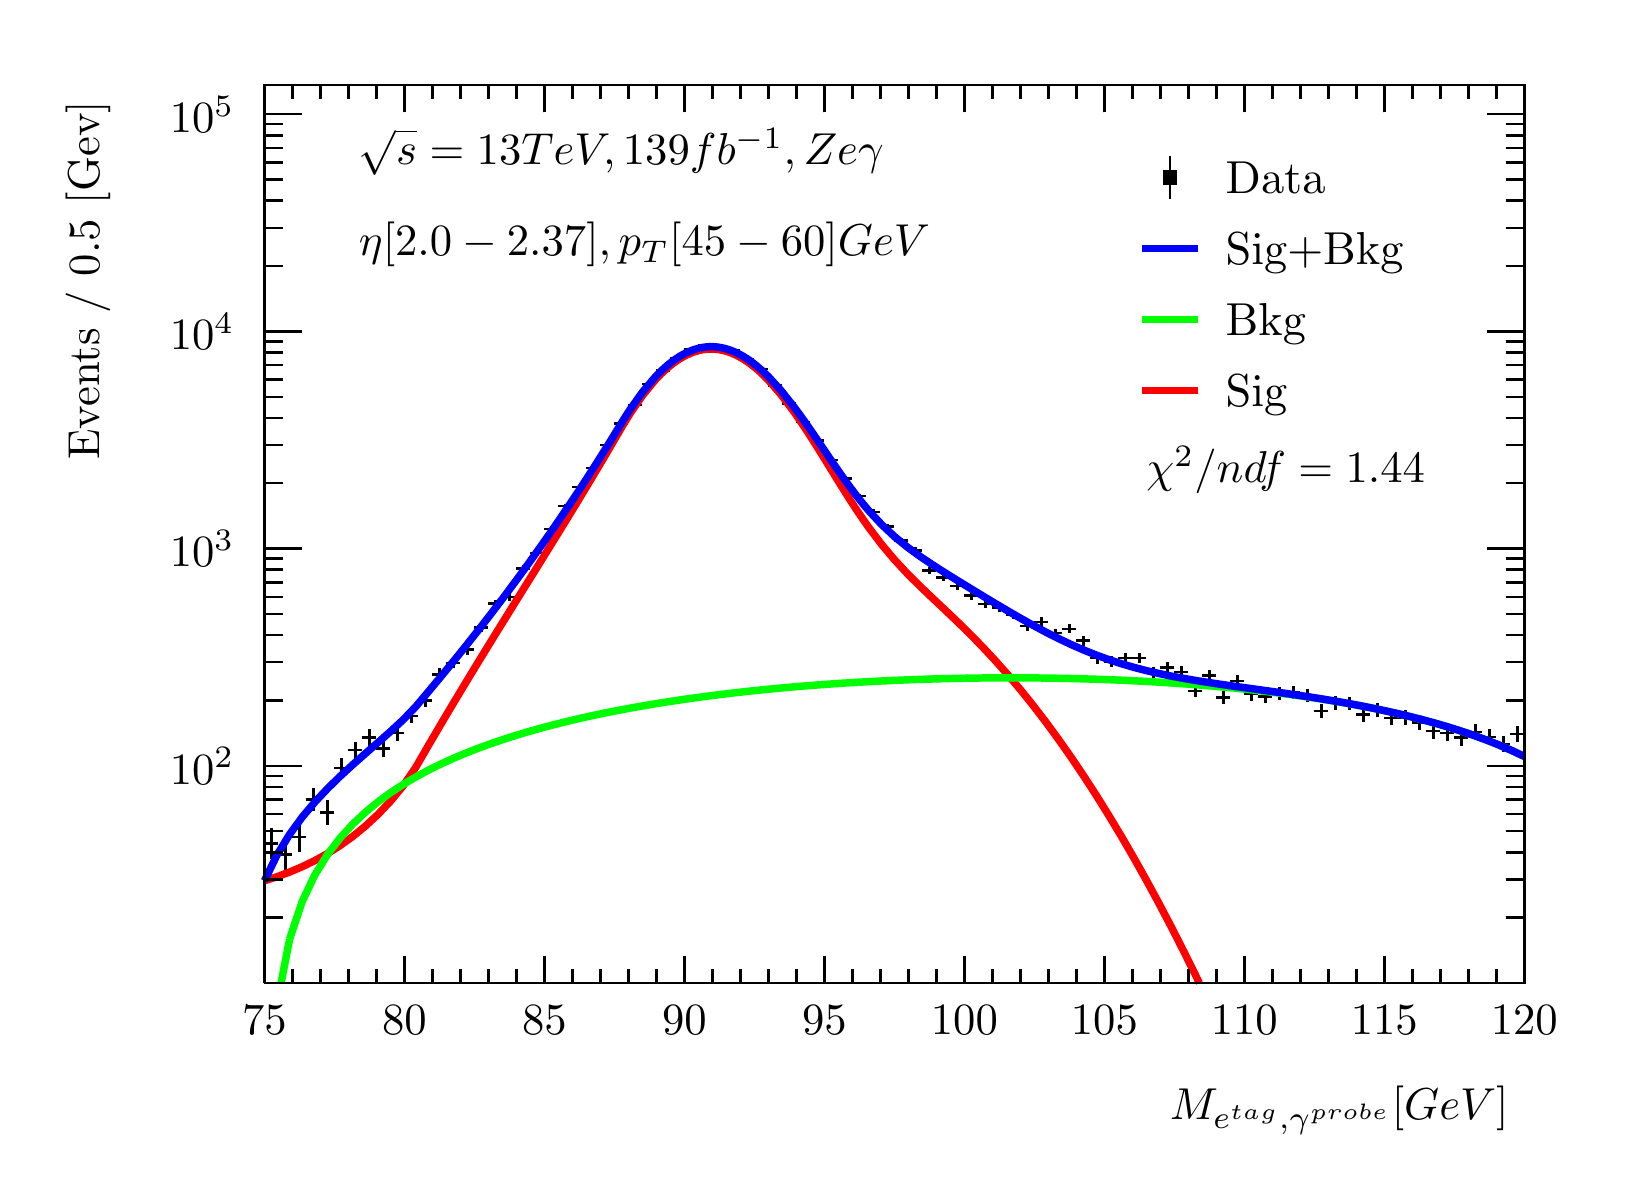
\begin{tikzpicture}
\pgfdeclareplotmark{cross} {
\pgfpathmoveto{\pgfpoint{-0.3\pgfplotmarksize}{\pgfplotmarksize}}
\pgfpathlineto{\pgfpoint{+0.3\pgfplotmarksize}{\pgfplotmarksize}}
\pgfpathlineto{\pgfpoint{+0.3\pgfplotmarksize}{0.3\pgfplotmarksize}}
\pgfpathlineto{\pgfpoint{+1\pgfplotmarksize}{0.3\pgfplotmarksize}}
\pgfpathlineto{\pgfpoint{+1\pgfplotmarksize}{-0.3\pgfplotmarksize}}
\pgfpathlineto{\pgfpoint{+0.3\pgfplotmarksize}{-0.3\pgfplotmarksize}}
\pgfpathlineto{\pgfpoint{+0.3\pgfplotmarksize}{-1.\pgfplotmarksize}}
\pgfpathlineto{\pgfpoint{-0.3\pgfplotmarksize}{-1.\pgfplotmarksize}}
\pgfpathlineto{\pgfpoint{-0.3\pgfplotmarksize}{-0.3\pgfplotmarksize}}
\pgfpathlineto{\pgfpoint{-1.\pgfplotmarksize}{-0.3\pgfplotmarksize}}
\pgfpathlineto{\pgfpoint{-1.\pgfplotmarksize}{0.3\pgfplotmarksize}}
\pgfpathlineto{\pgfpoint{-0.3\pgfplotmarksize}{0.3\pgfplotmarksize}}
\pgfpathclose
\pgfusepathqstroke
}
\pgfdeclareplotmark{cross*} {
\pgfpathmoveto{\pgfpoint{-0.3\pgfplotmarksize}{\pgfplotmarksize}}
\pgfpathlineto{\pgfpoint{+0.3\pgfplotmarksize}{\pgfplotmarksize}}
\pgfpathlineto{\pgfpoint{+0.3\pgfplotmarksize}{0.3\pgfplotmarksize}}
\pgfpathlineto{\pgfpoint{+1\pgfplotmarksize}{0.3\pgfplotmarksize}}
\pgfpathlineto{\pgfpoint{+1\pgfplotmarksize}{-0.3\pgfplotmarksize}}
\pgfpathlineto{\pgfpoint{+0.3\pgfplotmarksize}{-0.3\pgfplotmarksize}}
\pgfpathlineto{\pgfpoint{+0.3\pgfplotmarksize}{-1.\pgfplotmarksize}}
\pgfpathlineto{\pgfpoint{-0.3\pgfplotmarksize}{-1.\pgfplotmarksize}}
\pgfpathlineto{\pgfpoint{-0.3\pgfplotmarksize}{-0.3\pgfplotmarksize}}
\pgfpathlineto{\pgfpoint{-1.\pgfplotmarksize}{-0.3\pgfplotmarksize}}
\pgfpathlineto{\pgfpoint{-1.\pgfplotmarksize}{0.3\pgfplotmarksize}}
\pgfpathlineto{\pgfpoint{-0.3\pgfplotmarksize}{0.3\pgfplotmarksize}}
\pgfpathclose
\pgfusepathqfillstroke
}
\pgfdeclareplotmark{newstar} {
\pgfpathmoveto{\pgfqpoint{0pt}{\pgfplotmarksize}}
\pgfpathlineto{\pgfqpointpolar{44}{0.5\pgfplotmarksize}}
\pgfpathlineto{\pgfqpointpolar{18}{\pgfplotmarksize}}
\pgfpathlineto{\pgfqpointpolar{-20}{0.5\pgfplotmarksize}}
\pgfpathlineto{\pgfqpointpolar{-54}{\pgfplotmarksize}}
\pgfpathlineto{\pgfqpointpolar{-90}{0.5\pgfplotmarksize}}
\pgfpathlineto{\pgfqpointpolar{234}{\pgfplotmarksize}}
\pgfpathlineto{\pgfqpointpolar{198}{0.5\pgfplotmarksize}}
\pgfpathlineto{\pgfqpointpolar{162}{\pgfplotmarksize}}
\pgfpathlineto{\pgfqpointpolar{134}{0.5\pgfplotmarksize}}
\pgfpathclose
\pgfusepathqstroke
}
\pgfdeclareplotmark{newstar*} {
\pgfpathmoveto{\pgfqpoint{0pt}{\pgfplotmarksize}}
\pgfpathlineto{\pgfqpointpolar{44}{0.5\pgfplotmarksize}}
\pgfpathlineto{\pgfqpointpolar{18}{\pgfplotmarksize}}
\pgfpathlineto{\pgfqpointpolar{-20}{0.5\pgfplotmarksize}}
\pgfpathlineto{\pgfqpointpolar{-54}{\pgfplotmarksize}}
\pgfpathlineto{\pgfqpointpolar{-90}{0.5\pgfplotmarksize}}
\pgfpathlineto{\pgfqpointpolar{234}{\pgfplotmarksize}}
\pgfpathlineto{\pgfqpointpolar{198}{0.5\pgfplotmarksize}}
\pgfpathlineto{\pgfqpointpolar{162}{\pgfplotmarksize}}
\pgfpathlineto{\pgfqpointpolar{134}{0.5\pgfplotmarksize}}
\pgfpathclose
\pgfusepathqfillstroke
}
\definecolor{c}{rgb}{1,1,1};
\draw [color=c, fill=c] (0,0) rectangle (20,14.4361);
\draw [color=c, fill=c] (3,2.30977) rectangle (19,13.7143);
\definecolor{c}{rgb}{0,0,0};
\draw [c,line width=0.9] (3,2.30977) -- (3,13.7143) -- (19,13.7143) -- (19,2.30977) -- (3,2.30977);
\definecolor{c}{rgb}{1,1,1};
\draw [color=c, fill=c] (3,2.30977) rectangle (19,13.7143);
\definecolor{c}{rgb}{0,0,0};
\draw [c,line width=0.9] (3,2.30977) -- (3,13.7143) -- (19,13.7143) -- (19,2.30977) -- (3,2.30977);
\draw [c,line width=0.9] (3,2.30977) -- (19,2.30977);
\draw [c,line width=0.9] (3,2.65624) -- (3,2.30977);
\draw [c,line width=0.9] (3.35556,2.48301) -- (3.35556,2.30977);
\draw [c,line width=0.9] (3.71111,2.48301) -- (3.71111,2.30977);
\draw [c,line width=0.9] (4.06667,2.48301) -- (4.06667,2.30977);
\draw [c,line width=0.9] (4.42222,2.48301) -- (4.42222,2.30977);
\draw [c,line width=0.9] (4.77778,2.65624) -- (4.77778,2.30977);
\draw [c,line width=0.9] (5.13333,2.48301) -- (5.13333,2.30977);
\draw [c,line width=0.9] (5.48889,2.48301) -- (5.48889,2.30977);
\draw [c,line width=0.9] (5.84444,2.48301) -- (5.84444,2.30977);
\draw [c,line width=0.9] (6.2,2.48301) -- (6.2,2.30977);
\draw [c,line width=0.9] (6.55556,2.65624) -- (6.55556,2.30977);
\draw [c,line width=0.9] (6.91111,2.48301) -- (6.91111,2.30977);
\draw [c,line width=0.9] (7.26667,2.48301) -- (7.26667,2.30977);
\draw [c,line width=0.9] (7.62222,2.48301) -- (7.62222,2.30977);
\draw [c,line width=0.9] (7.97778,2.48301) -- (7.97778,2.30977);
\draw [c,line width=0.9] (8.33333,2.65624) -- (8.33333,2.30977);
\draw [c,line width=0.9] (8.68889,2.48301) -- (8.68889,2.30977);
\draw [c,line width=0.9] (9.04444,2.48301) -- (9.04444,2.30977);
\draw [c,line width=0.9] (9.4,2.48301) -- (9.4,2.30977);
\draw [c,line width=0.9] (9.75556,2.48301) -- (9.75556,2.30977);
\draw [c,line width=0.9] (10.1111,2.65624) -- (10.1111,2.30977);
\draw [c,line width=0.9] (10.4667,2.48301) -- (10.4667,2.30977);
\draw [c,line width=0.9] (10.8222,2.48301) -- (10.8222,2.30977);
\draw [c,line width=0.9] (11.1778,2.48301) -- (11.1778,2.30977);
\draw [c,line width=0.9] (11.5333,2.48301) -- (11.5333,2.30977);
\draw [c,line width=0.9] (11.8889,2.65624) -- (11.8889,2.30977);
\draw [c,line width=0.9] (12.2444,2.48301) -- (12.2444,2.30977);
\draw [c,line width=0.9] (12.6,2.48301) -- (12.6,2.30977);
\draw [c,line width=0.9] (12.9556,2.48301) -- (12.9556,2.30977);
\draw [c,line width=0.9] (13.3111,2.48301) -- (13.3111,2.30977);
\draw [c,line width=0.9] (13.6667,2.65624) -- (13.6667,2.30977);
\draw [c,line width=0.9] (14.0222,2.48301) -- (14.0222,2.30977);
\draw [c,line width=0.9] (14.3778,2.48301) -- (14.3778,2.30977);
\draw [c,line width=0.9] (14.7333,2.48301) -- (14.7333,2.30977);
\draw [c,line width=0.9] (15.0889,2.48301) -- (15.0889,2.30977);
\draw [c,line width=0.9] (15.4444,2.65624) -- (15.4444,2.30977);
\draw [c,line width=0.9] (15.8,2.48301) -- (15.8,2.30977);
\draw [c,line width=0.9] (16.1556,2.48301) -- (16.1556,2.30977);
\draw [c,line width=0.9] (16.5111,2.48301) -- (16.5111,2.30977);
\draw [c,line width=0.9] (16.8667,2.48301) -- (16.8667,2.30977);
\draw [c,line width=0.9] (17.2222,2.65624) -- (17.2222,2.30977);
\draw [c,line width=0.9] (17.5778,2.48301) -- (17.5778,2.30977);
\draw [c,line width=0.9] (17.9333,2.48301) -- (17.9333,2.30977);
\draw [c,line width=0.9] (18.2889,2.48301) -- (18.2889,2.30977);
\draw [c,line width=0.9] (18.6444,2.48301) -- (18.6444,2.30977);
\draw [c,line width=0.9] (19,2.65624) -- (19,2.30977);
\draw [c,line width=0.9] (19,2.65624) -- (19,2.30977);
\draw [anchor=base] (3,1.66015) node[scale=1.61424, color=c, rotate=0]{75};
\draw [anchor=base] (4.77778,1.66015) node[scale=1.61424, color=c, rotate=0]{80};
\draw [anchor=base] (6.55556,1.66015) node[scale=1.61424, color=c, rotate=0]{85};
\draw [anchor=base] (8.33333,1.66015) node[scale=1.61424, color=c, rotate=0]{90};
\draw [anchor=base] (10.1111,1.66015) node[scale=1.61424, color=c, rotate=0]{95};
\draw [anchor=base] (11.8889,1.66015) node[scale=1.61424, color=c, rotate=0]{100};
\draw [anchor=base] (13.6667,1.66015) node[scale=1.61424, color=c, rotate=0]{105};
\draw [anchor=base] (15.4444,1.66015) node[scale=1.61424, color=c, rotate=0]{110};
\draw [anchor=base] (17.2222,1.66015) node[scale=1.61424, color=c, rotate=0]{115};
\draw [anchor=base] (19,1.66015) node[scale=1.61424, color=c, rotate=0]{120};
\draw [anchor= east] (19,0.692932) node[scale=1.61424, color=c, rotate=0]{$M_{e^{tag}, \gamma^{probe}}  [GeV]$};
\draw [c,line width=0.9] (3,13.7143) -- (19,13.7143);
\draw [c,line width=0.9] (3,13.3678) -- (3,13.7143);
\draw [c,line width=0.9] (3.35556,13.5411) -- (3.35556,13.7143);
\draw [c,line width=0.9] (3.71111,13.5411) -- (3.71111,13.7143);
\draw [c,line width=0.9] (4.06667,13.5411) -- (4.06667,13.7143);
\draw [c,line width=0.9] (4.42222,13.5411) -- (4.42222,13.7143);
\draw [c,line width=0.9] (4.77778,13.3678) -- (4.77778,13.7143);
\draw [c,line width=0.9] (5.13333,13.5411) -- (5.13333,13.7143);
\draw [c,line width=0.9] (5.48889,13.5411) -- (5.48889,13.7143);
\draw [c,line width=0.9] (5.84444,13.5411) -- (5.84444,13.7143);
\draw [c,line width=0.9] (6.2,13.5411) -- (6.2,13.7143);
\draw [c,line width=0.9] (6.55556,13.3678) -- (6.55556,13.7143);
\draw [c,line width=0.9] (6.91111,13.5411) -- (6.91111,13.7143);
\draw [c,line width=0.9] (7.26667,13.5411) -- (7.26667,13.7143);
\draw [c,line width=0.9] (7.62222,13.5411) -- (7.62222,13.7143);
\draw [c,line width=0.9] (7.97778,13.5411) -- (7.97778,13.7143);
\draw [c,line width=0.9] (8.33333,13.3678) -- (8.33333,13.7143);
\draw [c,line width=0.9] (8.68889,13.5411) -- (8.68889,13.7143);
\draw [c,line width=0.9] (9.04444,13.5411) -- (9.04444,13.7143);
\draw [c,line width=0.9] (9.4,13.5411) -- (9.4,13.7143);
\draw [c,line width=0.9] (9.75556,13.5411) -- (9.75556,13.7143);
\draw [c,line width=0.9] (10.1111,13.3678) -- (10.1111,13.7143);
\draw [c,line width=0.9] (10.4667,13.5411) -- (10.4667,13.7143);
\draw [c,line width=0.9] (10.8222,13.5411) -- (10.8222,13.7143);
\draw [c,line width=0.9] (11.1778,13.5411) -- (11.1778,13.7143);
\draw [c,line width=0.9] (11.5333,13.5411) -- (11.5333,13.7143);
\draw [c,line width=0.9] (11.8889,13.3678) -- (11.8889,13.7143);
\draw [c,line width=0.9] (12.2444,13.5411) -- (12.2444,13.7143);
\draw [c,line width=0.9] (12.6,13.5411) -- (12.6,13.7143);
\draw [c,line width=0.9] (12.9556,13.5411) -- (12.9556,13.7143);
\draw [c,line width=0.9] (13.3111,13.5411) -- (13.3111,13.7143);
\draw [c,line width=0.9] (13.6667,13.3678) -- (13.6667,13.7143);
\draw [c,line width=0.9] (14.0222,13.5411) -- (14.0222,13.7143);
\draw [c,line width=0.9] (14.3778,13.5411) -- (14.3778,13.7143);
\draw [c,line width=0.9] (14.7333,13.5411) -- (14.7333,13.7143);
\draw [c,line width=0.9] (15.0889,13.5411) -- (15.0889,13.7143);
\draw [c,line width=0.9] (15.4444,13.3678) -- (15.4444,13.7143);
\draw [c,line width=0.9] (15.8,13.5411) -- (15.8,13.7143);
\draw [c,line width=0.9] (16.1556,13.5411) -- (16.1556,13.7143);
\draw [c,line width=0.9] (16.5111,13.5411) -- (16.5111,13.7143);
\draw [c,line width=0.9] (16.8667,13.5411) -- (16.8667,13.7143);
\draw [c,line width=0.9] (17.2222,13.3678) -- (17.2222,13.7143);
\draw [c,line width=0.9] (17.5778,13.5411) -- (17.5778,13.7143);
\draw [c,line width=0.9] (17.9333,13.5411) -- (17.9333,13.7143);
\draw [c,line width=0.9] (18.2889,13.5411) -- (18.2889,13.7143);
\draw [c,line width=0.9] (18.6444,13.5411) -- (18.6444,13.7143);
\draw [c,line width=0.9] (19,13.3678) -- (19,13.7143);
\draw [c,line width=0.9] (19,13.3678) -- (19,13.7143);
\draw [c,line width=0.9] (3,2.30977) -- (3,13.7143);
\draw [c,line width=0.9] (3.237,3.14018) -- (3,3.14018);
\draw [c,line width=0.9] (3.237,3.62593) -- (3,3.62593);
\draw [c,line width=0.9] (3.237,3.97058) -- (3,3.97058);
\draw [c,line width=0.9] (3.237,4.23792) -- (3,4.23792);
\draw [c,line width=0.9] (3.237,4.45634) -- (3,4.45634);
\draw [c,line width=0.9] (3.237,4.64102) -- (3,4.64102);
\draw [c,line width=0.9] (3.237,4.80099) -- (3,4.80099);
\draw [c,line width=0.9] (3.237,4.9421) -- (3,4.9421);
\draw [c,line width=0.9] (3.474,5.06832) -- (3,5.06832);
\draw [anchor= east] (2.82,5.06832) node[scale=1.61424, color=c, rotate=0]{$10^{2}$};
\draw [c,line width=0.9] (3.237,5.89873) -- (3,5.89873);
\draw [c,line width=0.9] (3.237,6.38449) -- (3,6.38449);
\draw [c,line width=0.9] (3.237,6.72914) -- (3,6.72914);
\draw [c,line width=0.9] (3.237,6.99647) -- (3,6.99647);
\draw [c,line width=0.9] (3.237,7.21489) -- (3,7.21489);
\draw [c,line width=0.9] (3.237,7.39957) -- (3,7.39957);
\draw [c,line width=0.9] (3.237,7.55954) -- (3,7.55954);
\draw [c,line width=0.9] (3.237,7.70065) -- (3,7.70065);
\draw [c,line width=0.9] (3.474,7.82687) -- (3,7.82687);
\draw [anchor= east] (2.82,7.82687) node[scale=1.61424, color=c, rotate=0]{$10^{3}$};
\draw [c,line width=0.9] (3.237,8.65728) -- (3,8.65728);
\draw [c,line width=0.9] (3.237,9.14304) -- (3,9.14304);
\draw [c,line width=0.9] (3.237,9.48769) -- (3,9.48769);
\draw [c,line width=0.9] (3.237,9.75502) -- (3,9.75502);
\draw [c,line width=0.9] (3.237,9.97344) -- (3,9.97344);
\draw [c,line width=0.9] (3.237,10.1581) -- (3,10.1581);
\draw [c,line width=0.9] (3.237,10.3181) -- (3,10.3181);
\draw [c,line width=0.9] (3.237,10.4592) -- (3,10.4592);
\draw [c,line width=0.9] (3.474,10.5854) -- (3,10.5854);
\draw [anchor= east] (2.82,10.5854) node[scale=1.61424, color=c, rotate=0]{$10^{4}$};
\draw [c,line width=0.9] (3.237,11.4158) -- (3,11.4158);
\draw [c,line width=0.9] (3.237,11.9016) -- (3,11.9016);
\draw [c,line width=0.9] (3.237,12.2462) -- (3,12.2462);
\draw [c,line width=0.9] (3.237,12.5136) -- (3,12.5136);
\draw [c,line width=0.9] (3.237,12.732) -- (3,12.732);
\draw [c,line width=0.9] (3.237,12.9167) -- (3,12.9167);
\draw [c,line width=0.9] (3.237,13.0766) -- (3,13.0766);
\draw [c,line width=0.9] (3.237,13.2178) -- (3,13.2178);
\draw [c,line width=0.9] (3.474,13.344) -- (3,13.344);
\draw [anchor= east] (2.82,13.344) node[scale=1.61424, color=c, rotate=0]{$10^{5}$};
\draw [anchor= east] (0.76,13.7143) node[scale=1.61424, color=c, rotate=90]{Events / 0.5 [Gev]};
\draw [c,line width=0.9] (19,2.30977) -- (19,13.7143);
\draw [c,line width=0.9] (18.763,3.14018) -- (19,3.14018);
\draw [c,line width=0.9] (18.763,3.62593) -- (19,3.62593);
\draw [c,line width=0.9] (18.763,3.97058) -- (19,3.97058);
\draw [c,line width=0.9] (18.763,4.23792) -- (19,4.23792);
\draw [c,line width=0.9] (18.763,4.45634) -- (19,4.45634);
\draw [c,line width=0.9] (18.763,4.64102) -- (19,4.64102);
\draw [c,line width=0.9] (18.763,4.80099) -- (19,4.80099);
\draw [c,line width=0.9] (18.763,4.9421) -- (19,4.9421);
\draw [c,line width=0.9] (18.526,5.06832) -- (19,5.06832);
\draw [c,line width=0.9] (18.763,5.89873) -- (19,5.89873);
\draw [c,line width=0.9] (18.763,6.38449) -- (19,6.38449);
\draw [c,line width=0.9] (18.763,6.72914) -- (19,6.72914);
\draw [c,line width=0.9] (18.763,6.99647) -- (19,6.99647);
\draw [c,line width=0.9] (18.763,7.21489) -- (19,7.21489);
\draw [c,line width=0.9] (18.763,7.39957) -- (19,7.39957);
\draw [c,line width=0.9] (18.763,7.55954) -- (19,7.55954);
\draw [c,line width=0.9] (18.763,7.70065) -- (19,7.70065);
\draw [c,line width=0.9] (18.526,7.82687) -- (19,7.82687);
\draw [c,line width=0.9] (18.763,8.65728) -- (19,8.65728);
\draw [c,line width=0.9] (18.763,9.14304) -- (19,9.14304);
\draw [c,line width=0.9] (18.763,9.48769) -- (19,9.48769);
\draw [c,line width=0.9] (18.763,9.75502) -- (19,9.75502);
\draw [c,line width=0.9] (18.763,9.97344) -- (19,9.97344);
\draw [c,line width=0.9] (18.763,10.1581) -- (19,10.1581);
\draw [c,line width=0.9] (18.763,10.3181) -- (19,10.3181);
\draw [c,line width=0.9] (18.763,10.4592) -- (19,10.4592);
\draw [c,line width=0.9] (18.526,10.5854) -- (19,10.5854);
\draw [c,line width=0.9] (18.763,11.4158) -- (19,11.4158);
\draw [c,line width=0.9] (18.763,11.9016) -- (19,11.9016);
\draw [c,line width=0.9] (18.763,12.2462) -- (19,12.2462);
\draw [c,line width=0.9] (18.763,12.5136) -- (19,12.5136);
\draw [c,line width=0.9] (18.763,12.732) -- (19,12.732);
\draw [c,line width=0.9] (18.763,12.9167) -- (19,12.9167);
\draw [c,line width=0.9] (18.763,13.0766) -- (19,13.0766);
\draw [c,line width=0.9] (18.763,13.2178) -- (19,13.2178);
\draw [c,line width=0.9] (18.526,13.344) -- (19,13.344);
\draw [c,line width=0.9] (3.08889,4.08477) -- (3,4.08477);
\draw [c,line width=0.9] (3,4.08477) -- (3,4.08477);
\draw [c,line width=0.9] (3.08889,4.08477) -- (3.17778,4.08477);
\draw [c,line width=0.9] (3.17778,4.08477) -- (3.17778,4.08477);
\draw [c,line width=0.9] (3.08889,4.08477) -- (3.08889,4.27759);
\draw [c,line width=0.9] (3.08889,4.27759) -- (3.08889,4.27759);
\draw [c,line width=0.9] (3.08889,4.08477) -- (3.08889,3.88982);
\draw [c,line width=0.9] (3.08889,3.88982) -- (3.08889,3.88982);
\draw [c,line width=0.9] (3.26667,3.94026) -- (3.17778,3.94026);
\draw [c,line width=0.9] (3.17778,3.94026) -- (3.17778,3.94026);
\draw [c,line width=0.9] (3.26667,3.94026) -- (3.35556,3.94026);
\draw [c,line width=0.9] (3.35556,3.94026) -- (3.35556,3.94026);
\draw [c,line width=0.9] (3.26667,3.94026) -- (3.26667,4.14577);
\draw [c,line width=0.9] (3.26667,4.14577) -- (3.26667,4.14577);
\draw [c,line width=0.9] (3.26667,3.94026) -- (3.26667,3.73218);
\draw [c,line width=0.9] (3.26667,3.73218) -- (3.26667,3.73218);
\draw [c,line width=0.9] (3.44444,4.16379) -- (3.35556,4.16379);
\draw [c,line width=0.9] (3.35556,4.16379) -- (3.35556,4.16379);
\draw [c,line width=0.9] (3.44444,4.16379) -- (3.53333,4.16379);
\draw [c,line width=0.9] (3.53333,4.16379) -- (3.53333,4.16379);
\draw [c,line width=0.9] (3.44444,4.16379) -- (3.44444,4.35002);
\draw [c,line width=0.9] (3.44444,4.35002) -- (3.44444,4.35002);
\draw [c,line width=0.9] (3.44444,4.16379) -- (3.44444,3.97563);
\draw [c,line width=0.9] (3.44444,3.97563) -- (3.44444,3.97563);
\draw [c,line width=0.9] (3.62222,4.64102) -- (3.53333,4.64102);
\draw [c,line width=0.9] (3.53333,4.64102) -- (3.53333,4.64102);
\draw [c,line width=0.9] (3.62222,4.64102) -- (3.71111,4.64102);
\draw [c,line width=0.9] (3.71111,4.64102) -- (3.71111,4.64102);
\draw [c,line width=0.9] (3.62222,4.64102) -- (3.62222,4.79207);
\draw [c,line width=0.9] (3.62222,4.79207) -- (3.62222,4.79207);
\draw [c,line width=0.9] (3.62222,4.64102) -- (3.62222,4.48891);
\draw [c,line width=0.9] (3.62222,4.48891) -- (3.62222,4.48891);
\draw [c,line width=0.9] (3.8,4.47615) -- (3.71111,4.47615);
\draw [c,line width=0.9] (3.71111,4.47615) -- (3.71111,4.47615);
\draw [c,line width=0.9] (3.8,4.47615) -- (3.88889,4.47615);
\draw [c,line width=0.9] (3.88889,4.47615) -- (3.88889,4.47615);
\draw [c,line width=0.9] (3.8,4.47615) -- (3.8,4.6385);
\draw [c,line width=0.9] (3.8,4.6385) -- (3.8,4.6385);
\draw [c,line width=0.9] (3.8,4.47615) -- (3.8,4.31249);
\draw [c,line width=0.9] (3.8,4.31249) -- (3.8,4.31249);
\draw [c,line width=0.9] (3.97778,5.04412) -- (3.88889,5.04412);
\draw [c,line width=0.9] (3.88889,5.04412) -- (3.88889,5.04412);
\draw [c,line width=0.9] (3.97778,5.04412) -- (4.06667,5.04412);
\draw [c,line width=0.9] (4.06667,5.04412) -- (4.06667,5.04412);
\draw [c,line width=0.9] (3.97778,5.04412) -- (3.97778,5.17083);
\draw [c,line width=0.9] (3.97778,5.17083) -- (3.97778,5.17083);
\draw [c,line width=0.9] (3.97778,5.04412) -- (3.97778,4.91677);
\draw [c,line width=0.9] (3.97778,4.91677) -- (3.97778,4.91677);
\draw [c,line width=0.9] (4.15556,5.26661) -- (4.06667,5.26661);
\draw [c,line width=0.9] (4.06667,5.26661) -- (4.06667,5.26661);
\draw [c,line width=0.9] (4.15556,5.26661) -- (4.24444,5.26661);
\draw [c,line width=0.9] (4.24444,5.26661) -- (4.24444,5.26661);
\draw [c,line width=0.9] (4.15556,5.26661) -- (4.15556,5.37686);
\draw [c,line width=0.9] (4.15556,5.37686) -- (4.15556,5.37686);
\draw [c,line width=0.9] (4.15556,5.26661) -- (4.15556,5.15637);
\draw [c,line width=0.9] (4.15556,5.15637) -- (4.15556,5.15637);
\draw [c,line width=0.9] (4.33333,5.42786) -- (4.24444,5.42786);
\draw [c,line width=0.9] (4.24444,5.42786) -- (4.24444,5.42786);
\draw [c,line width=0.9] (4.33333,5.42786) -- (4.42222,5.42786);
\draw [c,line width=0.9] (4.42222,5.42786) -- (4.42222,5.42786);
\draw [c,line width=0.9] (4.33333,5.42786) -- (4.33333,5.53093);
\draw [c,line width=0.9] (4.33333,5.53093) -- (4.33333,5.53093);
\draw [c,line width=0.9] (4.33333,5.42786) -- (4.33333,5.32478);
\draw [c,line width=0.9] (4.33333,5.32478) -- (4.33333,5.32478);
\draw [c,line width=0.9] (4.51111,5.28675) -- (4.42222,5.28675);
\draw [c,line width=0.9] (4.42222,5.28675) -- (4.42222,5.28675);
\draw [c,line width=0.9] (4.51111,5.28675) -- (4.6,5.28675);
\draw [c,line width=0.9] (4.6,5.28675) -- (4.6,5.28675);
\draw [c,line width=0.9] (4.51111,5.28675) -- (4.51111,5.39608);
\draw [c,line width=0.9] (4.51111,5.39608) -- (4.51111,5.39608);
\draw [c,line width=0.9] (4.51111,5.28675) -- (4.51111,5.17742);
\draw [c,line width=0.9] (4.51111,5.17742) -- (4.51111,5.17742);
\draw [c,line width=0.9] (4.68889,5.48842) -- (4.6,5.48842);
\draw [c,line width=0.9] (4.6,5.48842) -- (4.6,5.48842);
\draw [c,line width=0.9] (4.68889,5.48842) -- (4.77778,5.48842);
\draw [c,line width=0.9] (4.77778,5.48842) -- (4.77778,5.48842);
\draw [c,line width=0.9] (4.68889,5.48842) -- (4.68889,5.58893);
\draw [c,line width=0.9] (4.68889,5.58893) -- (4.68889,5.58893);
\draw [c,line width=0.9] (4.68889,5.48842) -- (4.68889,5.38791);
\draw [c,line width=0.9] (4.68889,5.38791) -- (4.68889,5.38791);
\draw [c,line width=0.9] (4.86667,5.70403) -- (4.77778,5.70403);
\draw [c,line width=0.9] (4.77778,5.70403) -- (4.77778,5.70403);
\draw [c,line width=0.9] (4.86667,5.70403) -- (4.95556,5.70403);
\draw [c,line width=0.9] (4.95556,5.70403) -- (4.95556,5.70403);
\draw [c,line width=0.9] (4.86667,5.70403) -- (4.86667,5.79589);
\draw [c,line width=0.9] (4.86667,5.79589) -- (4.86667,5.79589);
\draw [c,line width=0.9] (4.86667,5.70403) -- (4.86667,5.61217);
\draw [c,line width=0.9] (4.86667,5.61217) -- (4.86667,5.61217);
\draw [c,line width=0.9] (5.04444,5.89873) -- (4.95556,5.89873);
\draw [c,line width=0.9] (4.95556,5.89873) -- (4.95556,5.89873);
\draw [c,line width=0.9] (5.04444,5.89873) -- (5.13333,5.89873);
\draw [c,line width=0.9] (5.13333,5.89873) -- (5.13333,5.89873);
\draw [c,line width=0.9] (5.04444,5.89873) -- (5.04444,5.98343);
\draw [c,line width=0.9] (5.04444,5.98343) -- (5.04444,5.98343);
\draw [c,line width=0.9] (5.04444,5.89873) -- (5.04444,5.81404);
\draw [c,line width=0.9] (5.04444,5.81404) -- (5.04444,5.81404);
\draw [c,line width=0.9] (5.22222,6.23134) -- (5.13333,6.23134);
\draw [c,line width=0.9] (5.13333,6.23134) -- (5.13333,6.23134);
\draw [c,line width=0.9] (5.22222,6.23134) -- (5.31111,6.23134);
\draw [c,line width=0.9] (5.31111,6.23134) -- (5.31111,6.23134);
\draw [c,line width=0.9] (5.22222,6.23134) -- (5.22222,6.30506);
\draw [c,line width=0.9] (5.22222,6.30506) -- (5.22222,6.30506);
\draw [c,line width=0.9] (5.22222,6.23134) -- (5.22222,6.15762);
\draw [c,line width=0.9] (5.22222,6.15762) -- (5.22222,6.15762);
\draw [c,line width=0.9] (5.4,6.37647) -- (5.31111,6.37647);
\draw [c,line width=0.9] (5.31111,6.37647) -- (5.31111,6.37647);
\draw [c,line width=0.9] (5.4,6.37647) -- (5.48889,6.37647);
\draw [c,line width=0.9] (5.48889,6.37647) -- (5.48889,6.37647);
\draw [c,line width=0.9] (5.4,6.37647) -- (5.4,6.44586);
\draw [c,line width=0.9] (5.4,6.44586) -- (5.4,6.44586);
\draw [c,line width=0.9] (5.4,6.37647) -- (5.4,6.30708);
\draw [c,line width=0.9] (5.4,6.30708) -- (5.4,6.30708);
\draw [c,line width=0.9] (5.57778,6.54496) -- (5.48889,6.54496);
\draw [c,line width=0.9] (5.48889,6.54496) -- (5.48889,6.54496);
\draw [c,line width=0.9] (5.57778,6.54496) -- (5.66667,6.54496);
\draw [c,line width=0.9] (5.66667,6.54496) -- (5.66667,6.54496);
\draw [c,line width=0.9] (5.57778,6.54496) -- (5.57778,6.60964);
\draw [c,line width=0.9] (5.57778,6.60964) -- (5.57778,6.60964);
\draw [c,line width=0.9] (5.57778,6.54496) -- (5.57778,6.48028);
\draw [c,line width=0.9] (5.57778,6.48028) -- (5.57778,6.48028);
\draw [c,line width=0.9] (5.75556,6.82411) -- (5.66667,6.82411);
\draw [c,line width=0.9] (5.66667,6.82411) -- (5.66667,6.82411);
\draw [c,line width=0.9] (5.75556,6.82411) -- (5.84444,6.82411);
\draw [c,line width=0.9] (5.84444,6.82411) -- (5.84444,6.82411);
\draw [c,line width=0.9] (5.75556,6.82411) -- (5.75556,6.88168);
\draw [c,line width=0.9] (5.75556,6.88168) -- (5.75556,6.88168);
\draw [c,line width=0.9] (5.75556,6.82411) -- (5.75556,6.76654);
\draw [c,line width=0.9] (5.75556,6.76654) -- (5.75556,6.76654);
\draw [c,line width=0.9] (5.93333,7.12795) -- (5.84444,7.12795);
\draw [c,line width=0.9] (5.84444,7.12795) -- (5.84444,7.12795);
\draw [c,line width=0.9] (5.93333,7.12795) -- (6.02222,7.12795);
\draw [c,line width=0.9] (6.02222,7.12795) -- (6.02222,7.12795);
\draw [c,line width=0.9] (5.93333,7.12795) -- (5.93333,7.17867);
\draw [c,line width=0.9] (5.93333,7.17867) -- (5.93333,7.17867);
\draw [c,line width=0.9] (5.93333,7.12795) -- (5.93333,7.07724);
\draw [c,line width=0.9] (5.93333,7.07724) -- (5.93333,7.07724);
\draw [c,line width=0.9] (6.11111,7.21089) -- (6.02222,7.21089);
\draw [c,line width=0.9] (6.02222,7.21089) -- (6.02222,7.21089);
\draw [c,line width=0.9] (6.11111,7.21089) -- (6.2,7.21089);
\draw [c,line width=0.9] (6.2,7.21089) -- (6.2,7.21089);
\draw [c,line width=0.9] (6.11111,7.21089) -- (6.11111,7.25988);
\draw [c,line width=0.9] (6.11111,7.25988) -- (6.11111,7.25988);
\draw [c,line width=0.9] (6.11111,7.21089) -- (6.11111,7.16191);
\draw [c,line width=0.9] (6.11111,7.16191) -- (6.11111,7.16191);
\draw [c,line width=0.9] (6.28889,7.57738) -- (6.2,7.57738);
\draw [c,line width=0.9] (6.2,7.57738) -- (6.2,7.57738);
\draw [c,line width=0.9] (6.28889,7.57738) -- (6.37778,7.57738);
\draw [c,line width=0.9] (6.37778,7.57738) -- (6.37778,7.57738);
\draw [c,line width=0.9] (6.28889,7.57738) -- (6.28889,7.61942);
\draw [c,line width=0.9] (6.28889,7.61942) -- (6.28889,7.61942);
\draw [c,line width=0.9] (6.28889,7.57738) -- (6.28889,7.53534);
\draw [c,line width=0.9] (6.28889,7.53534) -- (6.28889,7.53534);
\draw [c,line width=0.9] (6.46667,7.7692) -- (6.37778,7.7692);
\draw [c,line width=0.9] (6.37778,7.7692) -- (6.37778,7.7692);
\draw [c,line width=0.9] (6.46667,7.7692) -- (6.55556,7.7692);
\draw [c,line width=0.9] (6.55556,7.7692) -- (6.55556,7.7692);
\draw [c,line width=0.9] (6.46667,7.7692) -- (6.46667,7.80801);
\draw [c,line width=0.9] (6.46667,7.80801) -- (6.46667,7.80801);
\draw [c,line width=0.9] (6.46667,7.7692) -- (6.46667,7.7304);
\draw [c,line width=0.9] (6.46667,7.7304) -- (6.46667,7.7304);
\draw [c,line width=0.9] (6.64444,8.07488) -- (6.55556,8.07488);
\draw [c,line width=0.9] (6.55556,8.07488) -- (6.55556,8.07488);
\draw [c,line width=0.9] (6.64444,8.07488) -- (6.73333,8.07488);
\draw [c,line width=0.9] (6.73333,8.07488) -- (6.73333,8.07488);
\draw [c,line width=0.9] (6.64444,8.07488) -- (6.64444,8.10904);
\draw [c,line width=0.9] (6.64444,8.10904) -- (6.64444,8.10904);
\draw [c,line width=0.9] (6.64444,8.07488) -- (6.64444,8.04072);
\draw [c,line width=0.9] (6.64444,8.04072) -- (6.64444,8.04072);
\draw [c,line width=0.9] (6.82222,8.36651) -- (6.73333,8.36651);
\draw [c,line width=0.9] (6.73333,8.36651) -- (6.73333,8.36651);
\draw [c,line width=0.9] (6.82222,8.36651) -- (6.91111,8.36651);
\draw [c,line width=0.9] (6.91111,8.36651) -- (6.91111,8.36651);
\draw [c,line width=0.9] (6.82222,8.36651) -- (6.82222,8.39676);
\draw [c,line width=0.9] (6.82222,8.39676) -- (6.82222,8.39676);
\draw [c,line width=0.9] (6.82222,8.36651) -- (6.82222,8.33627);
\draw [c,line width=0.9] (6.82222,8.33627) -- (6.82222,8.33627);
\draw [c,line width=0.9] (7,8.61025) -- (6.91111,8.61025);
\draw [c,line width=0.9] (6.91111,8.61025) -- (6.91111,8.61025);
\draw [c,line width=0.9] (7,8.61025) -- (7.08889,8.61025);
\draw [c,line width=0.9] (7.08889,8.61025) -- (7.08889,8.61025);
\draw [c,line width=0.9] (7,8.61025) -- (7,8.63757);
\draw [c,line width=0.9] (7,8.63757) -- (7,8.63757);
\draw [c,line width=0.9] (7,8.61025) -- (7,8.58293);
\draw [c,line width=0.9] (7,8.58293) -- (7,8.58293);
\draw [c,line width=0.9] (7.17778,8.85099) -- (7.08889,8.85099);
\draw [c,line width=0.9] (7.08889,8.85099) -- (7.08889,8.85099);
\draw [c,line width=0.9] (7.17778,8.85099) -- (7.26667,8.85099);
\draw [c,line width=0.9] (7.26667,8.85099) -- (7.26667,8.85099);
\draw [c,line width=0.9] (7.17778,8.85099) -- (7.17778,8.8757);
\draw [c,line width=0.9] (7.17778,8.8757) -- (7.17778,8.8757);
\draw [c,line width=0.9] (7.17778,8.85099) -- (7.17778,8.82629);
\draw [c,line width=0.9] (7.17778,8.82629) -- (7.17778,8.82629);
\draw [c,line width=0.9] (7.35556,9.14304) -- (7.26667,9.14304);
\draw [c,line width=0.9] (7.26667,9.14304) -- (7.26667,9.14304);
\draw [c,line width=0.9] (7.35556,9.14304) -- (7.44444,9.14304);
\draw [c,line width=0.9] (7.44444,9.14304) -- (7.44444,9.14304);
\draw [c,line width=0.9] (7.35556,9.14304) -- (7.35556,9.16491);
\draw [c,line width=0.9] (7.35556,9.16491) -- (7.35556,9.16491);
\draw [c,line width=0.9] (7.35556,9.14304) -- (7.35556,9.12117);
\draw [c,line width=0.9] (7.35556,9.12117) -- (7.35556,9.12117);
\draw [c,line width=0.9] (7.53333,9.41738) -- (7.44444,9.41738);
\draw [c,line width=0.9] (7.44444,9.41738) -- (7.44444,9.41738);
\draw [c,line width=0.9] (7.53333,9.41738) -- (7.62222,9.41738);
\draw [c,line width=0.9] (7.62222,9.41738) -- (7.62222,9.41738);
\draw [c,line width=0.9] (7.53333,9.41738) -- (7.53333,9.43688);
\draw [c,line width=0.9] (7.53333,9.43688) -- (7.53333,9.43688);
\draw [c,line width=0.9] (7.53333,9.41738) -- (7.53333,9.39787);
\draw [c,line width=0.9] (7.53333,9.39787) -- (7.53333,9.39787);
\draw [c,line width=0.9] (7.71111,9.65095) -- (7.62222,9.65095);
\draw [c,line width=0.9] (7.62222,9.65095) -- (7.62222,9.65095);
\draw [c,line width=0.9] (7.71111,9.65095) -- (7.8,9.65095);
\draw [c,line width=0.9] (7.8,9.65095) -- (7.8,9.65095);
\draw [c,line width=0.9] (7.71111,9.65095) -- (7.71111,9.66865);
\draw [c,line width=0.9] (7.71111,9.66865) -- (7.71111,9.66865);
\draw [c,line width=0.9] (7.71111,9.65095) -- (7.71111,9.63326);
\draw [c,line width=0.9] (7.71111,9.63326) -- (7.71111,9.63326);
\draw [c,line width=0.9] (7.88889,9.91535) -- (7.8,9.91535);
\draw [c,line width=0.9] (7.8,9.91535) -- (7.8,9.91535);
\draw [c,line width=0.9] (7.88889,9.91535) -- (7.97778,9.91535);
\draw [c,line width=0.9] (7.97778,9.91535) -- (7.97778,9.91535);
\draw [c,line width=0.9] (7.88889,9.91535) -- (7.88889,9.9312);
\draw [c,line width=0.9] (7.88889,9.9312) -- (7.88889,9.9312);
\draw [c,line width=0.9] (7.88889,9.91535) -- (7.88889,9.89951);
\draw [c,line width=0.9] (7.88889,9.89951) -- (7.88889,9.89951);
\draw [c,line width=0.9] (8.06667,10.0918) -- (7.97778,10.0918);
\draw [c,line width=0.9] (7.97778,10.0918) -- (7.97778,10.0918);
\draw [c,line width=0.9] (8.06667,10.0918) -- (8.15556,10.0918);
\draw [c,line width=0.9] (8.15556,10.0918) -- (8.15556,10.0918);
\draw [c,line width=0.9] (8.06667,10.0918) -- (8.06667,10.1065);
\draw [c,line width=0.9] (8.06667,10.1065) -- (8.06667,10.1065);
\draw [c,line width=0.9] (8.06667,10.0918) -- (8.06667,10.0771);
\draw [c,line width=0.9] (8.06667,10.0771) -- (8.06667,10.0771);
\draw [c,line width=0.9] (8.24444,10.246) -- (8.15556,10.246);
\draw [c,line width=0.9] (8.15556,10.246) -- (8.15556,10.246);
\draw [c,line width=0.9] (8.24444,10.246) -- (8.33333,10.246);
\draw [c,line width=0.9] (8.33333,10.246) -- (8.33333,10.246);
\draw [c,line width=0.9] (8.24444,10.246) -- (8.24444,10.2598);
\draw [c,line width=0.9] (8.24444,10.2598) -- (8.24444,10.2598);
\draw [c,line width=0.9] (8.24444,10.246) -- (8.24444,10.2322);
\draw [c,line width=0.9] (8.24444,10.2322) -- (8.24444,10.2322);
\draw [c,line width=0.9] (8.42222,10.3568) -- (8.33333,10.3568);
\draw [c,line width=0.9] (8.33333,10.3568) -- (8.33333,10.3568);
\draw [c,line width=0.9] (8.42222,10.3568) -- (8.51111,10.3568);
\draw [c,line width=0.9] (8.51111,10.3568) -- (8.51111,10.3568);
\draw [c,line width=0.9] (8.42222,10.3568) -- (8.42222,10.37);
\draw [c,line width=0.9] (8.42222,10.37) -- (8.42222,10.37);
\draw [c,line width=0.9] (8.42222,10.3568) -- (8.42222,10.3437);
\draw [c,line width=0.9] (8.42222,10.3437) -- (8.42222,10.3437);
\draw [c,line width=0.9] (8.6,10.4092) -- (8.51111,10.4092);
\draw [c,line width=0.9] (8.51111,10.4092) -- (8.51111,10.4092);
\draw [c,line width=0.9] (8.6,10.4092) -- (8.68889,10.4092);
\draw [c,line width=0.9] (8.68889,10.4092) -- (8.68889,10.4092);
\draw [c,line width=0.9] (8.6,10.4092) -- (8.6,10.4221);
\draw [c,line width=0.9] (8.6,10.4221) -- (8.6,10.4221);
\draw [c,line width=0.9] (8.6,10.4092) -- (8.6,10.3963);
\draw [c,line width=0.9] (8.6,10.3963) -- (8.6,10.3963);
\draw [c,line width=0.9] (8.77778,10.3916) -- (8.68889,10.3916);
\draw [c,line width=0.9] (8.68889,10.3916) -- (8.68889,10.3916);
\draw [c,line width=0.9] (8.77778,10.3916) -- (8.86667,10.3916);
\draw [c,line width=0.9] (8.86667,10.3916) -- (8.86667,10.3916);
\draw [c,line width=0.9] (8.77778,10.3916) -- (8.77778,10.4046);
\draw [c,line width=0.9] (8.77778,10.4046) -- (8.77778,10.4046);
\draw [c,line width=0.9] (8.77778,10.3916) -- (8.77778,10.3786);
\draw [c,line width=0.9] (8.77778,10.3786) -- (8.77778,10.3786);
\draw [c,line width=0.9] (8.95556,10.3484) -- (8.86667,10.3484);
\draw [c,line width=0.9] (8.86667,10.3484) -- (8.86667,10.3484);
\draw [c,line width=0.9] (8.95556,10.3484) -- (9.04444,10.3484);
\draw [c,line width=0.9] (9.04444,10.3484) -- (9.04444,10.3484);
\draw [c,line width=0.9] (8.95556,10.3484) -- (8.95556,10.3616);
\draw [c,line width=0.9] (8.95556,10.3616) -- (8.95556,10.3616);
\draw [c,line width=0.9] (8.95556,10.3484) -- (8.95556,10.3352);
\draw [c,line width=0.9] (8.95556,10.3352) -- (8.95556,10.3352);
\draw [c,line width=0.9] (9.13333,10.2305) -- (9.04444,10.2305);
\draw [c,line width=0.9] (9.04444,10.2305) -- (9.04444,10.2305);
\draw [c,line width=0.9] (9.13333,10.2305) -- (9.22222,10.2305);
\draw [c,line width=0.9] (9.22222,10.2305) -- (9.22222,10.2305);
\draw [c,line width=0.9] (9.13333,10.2305) -- (9.13333,10.2444);
\draw [c,line width=0.9] (9.13333,10.2444) -- (9.13333,10.2444);
\draw [c,line width=0.9] (9.13333,10.2305) -- (9.13333,10.2166);
\draw [c,line width=0.9] (9.13333,10.2166) -- (9.13333,10.2166);
\draw [c,line width=0.9] (9.31111,10.1058) -- (9.22222,10.1058);
\draw [c,line width=0.9] (9.22222,10.1058) -- (9.22222,10.1058);
\draw [c,line width=0.9] (9.31111,10.1058) -- (9.4,10.1058);
\draw [c,line width=0.9] (9.4,10.1058) -- (9.4,10.1058);
\draw [c,line width=0.9] (9.31111,10.1058) -- (9.31111,10.1205);
\draw [c,line width=0.9] (9.31111,10.1205) -- (9.31111,10.1205);
\draw [c,line width=0.9] (9.31111,10.1058) -- (9.31111,10.0912);
\draw [c,line width=0.9] (9.31111,10.0912) -- (9.31111,10.0912);
\draw [c,line width=0.9] (9.48889,9.90101) -- (9.4,9.90101);
\draw [c,line width=0.9] (9.4,9.90101) -- (9.4,9.90101);
\draw [c,line width=0.9] (9.48889,9.90101) -- (9.57778,9.90101);
\draw [c,line width=0.9] (9.57778,9.90101) -- (9.57778,9.90101);
\draw [c,line width=0.9] (9.48889,9.90101) -- (9.48889,9.91695);
\draw [c,line width=0.9] (9.48889,9.91695) -- (9.48889,9.91695);
\draw [c,line width=0.9] (9.48889,9.90101) -- (9.48889,9.88507);
\draw [c,line width=0.9] (9.48889,9.88507) -- (9.48889,9.88507);
\draw [c,line width=0.9] (9.66667,9.66833) -- (9.57778,9.66833);
\draw [c,line width=0.9] (9.57778,9.66833) -- (9.57778,9.66833);
\draw [c,line width=0.9] (9.66667,9.66833) -- (9.75556,9.66833);
\draw [c,line width=0.9] (9.75556,9.66833) -- (9.75556,9.66833);
\draw [c,line width=0.9] (9.66667,9.66833) -- (9.66667,9.6859);
\draw [c,line width=0.9] (9.66667,9.6859) -- (9.66667,9.6859);
\draw [c,line width=0.9] (9.66667,9.66833) -- (9.66667,9.65077);
\draw [c,line width=0.9] (9.66667,9.65077) -- (9.66667,9.65077);
\draw [c,line width=0.9] (9.84444,9.43315) -- (9.75556,9.43315);
\draw [c,line width=0.9] (9.75556,9.43315) -- (9.75556,9.43315);
\draw [c,line width=0.9] (9.84444,9.43315) -- (9.93333,9.43315);
\draw [c,line width=0.9] (9.93333,9.43315) -- (9.93333,9.43315);
\draw [c,line width=0.9] (9.84444,9.43315) -- (9.84444,9.45253);
\draw [c,line width=0.9] (9.84444,9.45253) -- (9.84444,9.45253);
\draw [c,line width=0.9] (9.84444,9.43315) -- (9.84444,9.41377);
\draw [c,line width=0.9] (9.84444,9.41377) -- (9.84444,9.41377);
\draw [c,line width=0.9] (10.0222,9.19921) -- (9.93333,9.19921);
\draw [c,line width=0.9] (9.93333,9.19921) -- (9.93333,9.19921);
\draw [c,line width=0.9] (10.0222,9.19921) -- (10.1111,9.19921);
\draw [c,line width=0.9] (10.1111,9.19921) -- (10.1111,9.19921);
\draw [c,line width=0.9] (10.0222,9.19921) -- (10.0222,9.22057);
\draw [c,line width=0.9] (10.0222,9.22057) -- (10.0222,9.22057);
\draw [c,line width=0.9] (10.0222,9.19921) -- (10.0222,9.17784);
\draw [c,line width=0.9] (10.0222,9.17784) -- (10.0222,9.17784);
\draw [c,line width=0.9] (10.2,8.95303) -- (10.1111,8.95303);
\draw [c,line width=0.9] (10.1111,8.95303) -- (10.1111,8.95303);
\draw [c,line width=0.9] (10.2,8.95303) -- (10.2889,8.95303);
\draw [c,line width=0.9] (10.2889,8.95303) -- (10.2889,8.95303);
\draw [c,line width=0.9] (10.2,8.95303) -- (10.2,8.9767);
\draw [c,line width=0.9] (10.2,8.9767) -- (10.2,8.9767);
\draw [c,line width=0.9] (10.2,8.95303) -- (10.2,8.92935);
\draw [c,line width=0.9] (10.2,8.92935) -- (10.2,8.92935);
\draw [c,line width=0.9] (10.3778,8.71687) -- (10.2889,8.71687);
\draw [c,line width=0.9] (10.2889,8.71687) -- (10.2889,8.71687);
\draw [c,line width=0.9] (10.3778,8.71687) -- (10.4667,8.71687);
\draw [c,line width=0.9] (10.4667,8.71687) -- (10.4667,8.71687);
\draw [c,line width=0.9] (10.3778,8.71687) -- (10.3778,8.743);
\draw [c,line width=0.9] (10.3778,8.743) -- (10.3778,8.743);
\draw [c,line width=0.9] (10.3778,8.71687) -- (10.3778,8.69074);
\draw [c,line width=0.9] (10.3778,8.69074) -- (10.3778,8.69074);
\draw [c,line width=0.9] (10.5556,8.49525) -- (10.4667,8.49525);
\draw [c,line width=0.9] (10.4667,8.49525) -- (10.4667,8.49525);
\draw [c,line width=0.9] (10.5556,8.49525) -- (10.6444,8.49525);
\draw [c,line width=0.9] (10.6444,8.49525) -- (10.6444,8.49525);
\draw [c,line width=0.9] (10.5556,8.49525) -- (10.5556,8.52391);
\draw [c,line width=0.9] (10.5556,8.52391) -- (10.5556,8.52391);
\draw [c,line width=0.9] (10.5556,8.49525) -- (10.5556,8.46659);
\draw [c,line width=0.9] (10.5556,8.46659) -- (10.5556,8.46659);
\draw [c,line width=0.9] (10.7333,8.29331) -- (10.6444,8.29331);
\draw [c,line width=0.9] (10.6444,8.29331) -- (10.6444,8.29331);
\draw [c,line width=0.9] (10.7333,8.29331) -- (10.8222,8.29331);
\draw [c,line width=0.9] (10.8222,8.29331) -- (10.8222,8.29331);
\draw [c,line width=0.9] (10.7333,8.29331) -- (10.7333,8.32449);
\draw [c,line width=0.9] (10.7333,8.32449) -- (10.7333,8.32449);
\draw [c,line width=0.9] (10.7333,8.29331) -- (10.7333,8.26213);
\draw [c,line width=0.9] (10.7333,8.26213) -- (10.7333,8.26213);
\draw [c,line width=0.9] (10.9111,8.1085) -- (10.8222,8.1085);
\draw [c,line width=0.9] (10.8222,8.1085) -- (10.8222,8.1085);
\draw [c,line width=0.9] (10.9111,8.1085) -- (11,8.1085);
\draw [c,line width=0.9] (11,8.1085) -- (11,8.1085);
\draw [c,line width=0.9] (10.9111,8.1085) -- (10.9111,8.14218);
\draw [c,line width=0.9] (10.9111,8.14218) -- (10.9111,8.14218);
\draw [c,line width=0.9] (10.9111,8.1085) -- (10.9111,8.07481);
\draw [c,line width=0.9] (10.9111,8.07481) -- (10.9111,8.07481);
\draw [c,line width=0.9] (11.0889,7.92902) -- (11,7.92902);
\draw [c,line width=0.9] (11,7.92902) -- (11,7.92902);
\draw [c,line width=0.9] (11.0889,7.92902) -- (11.1778,7.92902);
\draw [c,line width=0.9] (11.1778,7.92902) -- (11.1778,7.92902);
\draw [c,line width=0.9] (11.0889,7.92902) -- (11.0889,7.96532);
\draw [c,line width=0.9] (11.0889,7.96532) -- (11.0889,7.96532);
\draw [c,line width=0.9] (11.0889,7.92902) -- (11.0889,7.89272);
\draw [c,line width=0.9] (11.0889,7.89272) -- (11.0889,7.89272);
\draw [c,line width=0.9] (11.2667,7.80511) -- (11.1778,7.80511);
\draw [c,line width=0.9] (11.1778,7.80511) -- (11.1778,7.80511);
\draw [c,line width=0.9] (11.2667,7.80511) -- (11.3556,7.80511);
\draw [c,line width=0.9] (11.3556,7.80511) -- (11.3556,7.80511);
\draw [c,line width=0.9] (11.2667,7.80511) -- (11.2667,7.84334);
\draw [c,line width=0.9] (11.2667,7.84334) -- (11.2667,7.84334);
\draw [c,line width=0.9] (11.2667,7.80511) -- (11.2667,7.76689);
\draw [c,line width=0.9] (11.2667,7.76689) -- (11.2667,7.76689);
\draw [c,line width=0.9] (11.4444,7.55052) -- (11.3556,7.55052);
\draw [c,line width=0.9] (11.3556,7.55052) -- (11.3556,7.55052);
\draw [c,line width=0.9] (11.4444,7.55052) -- (11.5333,7.55052);
\draw [c,line width=0.9] (11.5333,7.55052) -- (11.5333,7.55052);
\draw [c,line width=0.9] (11.4444,7.55052) -- (11.4444,7.59304);
\draw [c,line width=0.9] (11.4444,7.59304) -- (11.4444,7.59304);
\draw [c,line width=0.9] (11.4444,7.55052) -- (11.4444,7.50801);
\draw [c,line width=0.9] (11.4444,7.50801) -- (11.4444,7.50801);
\draw [c,line width=0.9] (11.6222,7.46128) -- (11.5333,7.46128);
\draw [c,line width=0.9] (11.5333,7.46128) -- (11.5333,7.46128);
\draw [c,line width=0.9] (11.6222,7.46128) -- (11.7111,7.46128);
\draw [c,line width=0.9] (11.7111,7.46128) -- (11.7111,7.46128);
\draw [c,line width=0.9] (11.6222,7.46128) -- (11.6222,7.5054);
\draw [c,line width=0.9] (11.6222,7.5054) -- (11.6222,7.5054);
\draw [c,line width=0.9] (11.6222,7.46128) -- (11.6222,7.41715);
\draw [c,line width=0.9] (11.6222,7.41715) -- (11.6222,7.41715);
\draw [c,line width=0.9] (11.8,7.35066) -- (11.7111,7.35066);
\draw [c,line width=0.9] (11.7111,7.35066) -- (11.7111,7.35066);
\draw [c,line width=0.9] (11.8,7.35066) -- (11.8889,7.35066);
\draw [c,line width=0.9] (11.8889,7.35066) -- (11.8889,7.35066);
\draw [c,line width=0.9] (11.8,7.35066) -- (11.8,7.39688);
\draw [c,line width=0.9] (11.8,7.39688) -- (11.8,7.39688);
\draw [c,line width=0.9] (11.8,7.35066) -- (11.8,7.30445);
\draw [c,line width=0.9] (11.8,7.30445) -- (11.8,7.30445);
\draw [c,line width=0.9] (11.9778,7.22879) -- (11.8889,7.22879);
\draw [c,line width=0.9] (11.8889,7.22879) -- (11.8889,7.22879);
\draw [c,line width=0.9] (11.9778,7.22879) -- (12.0667,7.22879);
\draw [c,line width=0.9] (12.0667,7.22879) -- (12.0667,7.22879);
\draw [c,line width=0.9] (11.9778,7.22879) -- (11.9778,7.27741);
\draw [c,line width=0.9] (11.9778,7.27741) -- (11.9778,7.27741);
\draw [c,line width=0.9] (11.9778,7.22879) -- (11.9778,7.18017);
\draw [c,line width=0.9] (11.9778,7.18017) -- (11.9778,7.18017);
\draw [c,line width=0.9] (12.1556,7.12149) -- (12.0667,7.12149);
\draw [c,line width=0.9] (12.0667,7.12149) -- (12.0667,7.12149);
\draw [c,line width=0.9] (12.1556,7.12149) -- (12.2444,7.12149);
\draw [c,line width=0.9] (12.2444,7.12149) -- (12.2444,7.12149);
\draw [c,line width=0.9] (12.1556,7.12149) -- (12.1556,7.17234);
\draw [c,line width=0.9] (12.1556,7.17234) -- (12.1556,7.17234);
\draw [c,line width=0.9] (12.1556,7.12149) -- (12.1556,7.07064);
\draw [c,line width=0.9] (12.1556,7.07064) -- (12.1556,7.07064);
\draw [c,line width=0.9] (12.3333,7.07976) -- (12.2444,7.07976);
\draw [c,line width=0.9] (12.2444,7.07976) -- (12.2444,7.07976);
\draw [c,line width=0.9] (12.3333,7.07976) -- (12.4222,7.07976);
\draw [c,line width=0.9] (12.4222,7.07976) -- (12.4222,7.07976);
\draw [c,line width=0.9] (12.3333,7.07976) -- (12.3333,7.13151);
\draw [c,line width=0.9] (12.3333,7.13151) -- (12.3333,7.13151);
\draw [c,line width=0.9] (12.3333,7.07976) -- (12.3333,7.02802);
\draw [c,line width=0.9] (12.3333,7.02802) -- (12.3333,7.02802);
\draw [c,line width=0.9] (12.5111,6.98201) -- (12.4222,6.98201);
\draw [c,line width=0.9] (12.4222,6.98201) -- (12.4222,6.98201);
\draw [c,line width=0.9] (12.5111,6.98201) -- (12.6,6.98201);
\draw [c,line width=0.9] (12.6,6.98201) -- (12.6,6.98201);
\draw [c,line width=0.9] (12.5111,6.98201) -- (12.5111,7.0359);
\draw [c,line width=0.9] (12.5111,7.0359) -- (12.5111,7.0359);
\draw [c,line width=0.9] (12.5111,6.98201) -- (12.5111,6.92811);
\draw [c,line width=0.9] (12.5111,6.92811) -- (12.5111,6.92811);
\draw [c,line width=0.9] (12.6889,6.84332) -- (12.6,6.84332);
\draw [c,line width=0.9] (12.6,6.84332) -- (12.6,6.84332);
\draw [c,line width=0.9] (12.6889,6.84332) -- (12.7778,6.84332);
\draw [c,line width=0.9] (12.7778,6.84332) -- (12.7778,6.84332);
\draw [c,line width=0.9] (12.6889,6.84332) -- (12.6889,6.90043);
\draw [c,line width=0.9] (12.6889,6.90043) -- (12.6889,6.90043);
\draw [c,line width=0.9] (12.6889,6.84332) -- (12.6889,6.78621);
\draw [c,line width=0.9] (12.6889,6.78621) -- (12.6889,6.78621);
\draw [c,line width=0.9] (12.8667,6.89658) -- (12.7778,6.89658);
\draw [c,line width=0.9] (12.7778,6.89658) -- (12.7778,6.89658);
\draw [c,line width=0.9] (12.8667,6.89658) -- (12.9556,6.89658);
\draw [c,line width=0.9] (12.9556,6.89658) -- (12.9556,6.89658);
\draw [c,line width=0.9] (12.8667,6.89658) -- (12.8667,6.95243);
\draw [c,line width=0.9] (12.8667,6.95243) -- (12.8667,6.95243);
\draw [c,line width=0.9] (12.8667,6.89658) -- (12.8667,6.84072);
\draw [c,line width=0.9] (12.8667,6.84072) -- (12.8667,6.84072);
\draw [c,line width=0.9] (13.0444,6.75286) -- (12.9556,6.75286);
\draw [c,line width=0.9] (12.9556,6.75286) -- (12.9556,6.75286);
\draw [c,line width=0.9] (13.0444,6.75286) -- (13.1333,6.75286);
\draw [c,line width=0.9] (13.1333,6.75286) -- (13.1333,6.75286);
\draw [c,line width=0.9] (13.0444,6.75286) -- (13.0444,6.81217);
\draw [c,line width=0.9] (13.0444,6.81217) -- (13.0444,6.81217);
\draw [c,line width=0.9] (13.0444,6.75286) -- (13.0444,6.69356);
\draw [c,line width=0.9] (13.0444,6.69356) -- (13.0444,6.69356);
\draw [c,line width=0.9] (13.2222,6.80739) -- (13.1333,6.80739);
\draw [c,line width=0.9] (13.1333,6.80739) -- (13.1333,6.80739);
\draw [c,line width=0.9] (13.2222,6.80739) -- (13.3111,6.80739);
\draw [c,line width=0.9] (13.3111,6.80739) -- (13.3111,6.80739);
\draw [c,line width=0.9] (13.2222,6.80739) -- (13.2222,6.86536);
\draw [c,line width=0.9] (13.2222,6.86536) -- (13.2222,6.86536);
\draw [c,line width=0.9] (13.2222,6.80739) -- (13.2222,6.74942);
\draw [c,line width=0.9] (13.2222,6.74942) -- (13.2222,6.74942);
\draw [c,line width=0.9] (13.4,6.65819) -- (13.3111,6.65819);
\draw [c,line width=0.9] (13.3111,6.65819) -- (13.3111,6.65819);
\draw [c,line width=0.9] (13.4,6.65819) -- (13.4889,6.65819);
\draw [c,line width=0.9] (13.4889,6.65819) -- (13.4889,6.65819);
\draw [c,line width=0.9] (13.4,6.65819) -- (13.4,6.71989);
\draw [c,line width=0.9] (13.4,6.71989) -- (13.4,6.71989);
\draw [c,line width=0.9] (13.4,6.65819) -- (13.4,6.5965);
\draw [c,line width=0.9] (13.4,6.5965) -- (13.4,6.5965);
\draw [c,line width=0.9] (13.5778,6.43531) -- (13.4889,6.43531);
\draw [c,line width=0.9] (13.4889,6.43531) -- (13.4889,6.43531);
\draw [c,line width=0.9] (13.5778,6.43531) -- (13.6667,6.43531);
\draw [c,line width=0.9] (13.6667,6.43531) -- (13.6667,6.43531);
\draw [c,line width=0.9] (13.5778,6.43531) -- (13.5778,6.50302);
\draw [c,line width=0.9] (13.5778,6.50302) -- (13.5778,6.50302);
\draw [c,line width=0.9] (13.5778,6.43531) -- (13.5778,6.3676);
\draw [c,line width=0.9] (13.5778,6.3676) -- (13.5778,6.3676);
\draw [c,line width=0.9] (13.7556,6.39245) -- (13.6667,6.39245);
\draw [c,line width=0.9] (13.6667,6.39245) -- (13.6667,6.39245);
\draw [c,line width=0.9] (13.7556,6.39245) -- (13.8444,6.39245);
\draw [c,line width=0.9] (13.8444,6.39245) -- (13.8444,6.39245);
\draw [c,line width=0.9] (13.7556,6.39245) -- (13.7556,6.46138);
\draw [c,line width=0.9] (13.7556,6.46138) -- (13.7556,6.46138);
\draw [c,line width=0.9] (13.7556,6.39245) -- (13.7556,6.32352);
\draw [c,line width=0.9] (13.7556,6.32352) -- (13.7556,6.32352);
\draw [c,line width=0.9] (13.9333,6.43531) -- (13.8444,6.43531);
\draw [c,line width=0.9] (13.8444,6.43531) -- (13.8444,6.43531);
\draw [c,line width=0.9] (13.9333,6.43531) -- (14.0222,6.43531);
\draw [c,line width=0.9] (14.0222,6.43531) -- (14.0222,6.43531);
\draw [c,line width=0.9] (13.9333,6.43531) -- (13.9333,6.50302);
\draw [c,line width=0.9] (13.9333,6.50302) -- (13.9333,6.50302);
\draw [c,line width=0.9] (13.9333,6.43531) -- (13.9333,6.3676);
\draw [c,line width=0.9] (13.9333,6.3676) -- (13.9333,6.3676);
\draw [c,line width=0.9] (14.1111,6.43913) -- (14.0222,6.43913);
\draw [c,line width=0.9] (14.0222,6.43913) -- (14.0222,6.43913);
\draw [c,line width=0.9] (14.1111,6.43913) -- (14.2,6.43913);
\draw [c,line width=0.9] (14.2,6.43913) -- (14.2,6.43913);
\draw [c,line width=0.9] (14.1111,6.43913) -- (14.1111,6.50673);
\draw [c,line width=0.9] (14.1111,6.50673) -- (14.1111,6.50673);
\draw [c,line width=0.9] (14.1111,6.43913) -- (14.1111,6.37153);
\draw [c,line width=0.9] (14.1111,6.37153) -- (14.1111,6.37153);
\draw [c,line width=0.9] (14.2889,6.24936) -- (14.2,6.24936);
\draw [c,line width=0.9] (14.2,6.24936) -- (14.2,6.24936);
\draw [c,line width=0.9] (14.2889,6.24936) -- (14.3778,6.24936);
\draw [c,line width=0.9] (14.3778,6.24936) -- (14.3778,6.24936);
\draw [c,line width=0.9] (14.2889,6.24936) -- (14.2889,6.32253);
\draw [c,line width=0.9] (14.2889,6.32253) -- (14.2889,6.32253);
\draw [c,line width=0.9] (14.2889,6.24936) -- (14.2889,6.17619);
\draw [c,line width=0.9] (14.2889,6.17619) -- (14.2889,6.17619);
\draw [c,line width=0.9] (14.4667,6.3146) -- (14.3778,6.3146);
\draw [c,line width=0.9] (14.3778,6.3146) -- (14.3778,6.3146);
\draw [c,line width=0.9] (14.4667,6.3146) -- (14.5556,6.3146);
\draw [c,line width=0.9] (14.5556,6.3146) -- (14.5556,6.3146);
\draw [c,line width=0.9] (14.4667,6.3146) -- (14.4667,6.38581);
\draw [c,line width=0.9] (14.4667,6.38581) -- (14.4667,6.38581);
\draw [c,line width=0.9] (14.4667,6.3146) -- (14.4667,6.2434);
\draw [c,line width=0.9] (14.4667,6.2434) -- (14.4667,6.2434);
\draw [c,line width=0.9] (14.6444,6.25826) -- (14.5556,6.25826);
\draw [c,line width=0.9] (14.5556,6.25826) -- (14.5556,6.25826);
\draw [c,line width=0.9] (14.6444,6.25826) -- (14.7333,6.25826);
\draw [c,line width=0.9] (14.7333,6.25826) -- (14.7333,6.25826);
\draw [c,line width=0.9] (14.6444,6.25826) -- (14.6444,6.33116);
\draw [c,line width=0.9] (14.6444,6.33116) -- (14.6444,6.33116);
\draw [c,line width=0.9] (14.6444,6.25826) -- (14.6444,6.18537);
\draw [c,line width=0.9] (14.6444,6.18537) -- (14.6444,6.18537);
\draw [c,line width=0.9] (14.8222,6.01835) -- (14.7333,6.01835);
\draw [c,line width=0.9] (14.7333,6.01835) -- (14.7333,6.01835);
\draw [c,line width=0.9] (14.8222,6.01835) -- (14.9111,6.01835);
\draw [c,line width=0.9] (14.9111,6.01835) -- (14.9111,6.01835);
\draw [c,line width=0.9] (14.8222,6.01835) -- (14.8222,6.09892);
\draw [c,line width=0.9] (14.8222,6.09892) -- (14.8222,6.09892);
\draw [c,line width=0.9] (14.8222,6.01835) -- (14.8222,5.93778);
\draw [c,line width=0.9] (14.8222,5.93778) -- (14.8222,5.93778);
\draw [c,line width=0.9] (15,6.21305) -- (14.9111,6.21305);
\draw [c,line width=0.9] (14.9111,6.21305) -- (14.9111,6.21305);
\draw [c,line width=0.9] (15,6.21305) -- (15.0889,6.21305);
\draw [c,line width=0.9] (15.0889,6.21305) -- (15.0889,6.21305);
\draw [c,line width=0.9] (15,6.21305) -- (15,6.28734);
\draw [c,line width=0.9] (15,6.28734) -- (15,6.28734);
\draw [c,line width=0.9] (15,6.21305) -- (15,6.13876);
\draw [c,line width=0.9] (15,6.13876) -- (15,6.13876);
\draw [c,line width=0.9] (15.1778,5.93414) -- (15.0889,5.93414);
\draw [c,line width=0.9] (15.0889,5.93414) -- (15.0889,5.93414);
\draw [c,line width=0.9] (15.1778,5.93414) -- (15.2667,5.93414);
\draw [c,line width=0.9] (15.2667,5.93414) -- (15.2667,5.93414);
\draw [c,line width=0.9] (15.1778,5.93414) -- (15.1778,6.0176);
\draw [c,line width=0.9] (15.1778,6.0176) -- (15.1778,6.0176);
\draw [c,line width=0.9] (15.1778,5.93414) -- (15.1778,5.85069);
\draw [c,line width=0.9] (15.1778,5.85069) -- (15.1778,5.85069);
\draw [c,line width=0.9] (15.3556,6.14674) -- (15.2667,6.14674);
\draw [c,line width=0.9] (15.2667,6.14674) -- (15.2667,6.14674);
\draw [c,line width=0.9] (15.3556,6.14674) -- (15.4444,6.14674);
\draw [c,line width=0.9] (15.4444,6.14674) -- (15.4444,6.14674);
\draw [c,line width=0.9] (15.3556,6.14674) -- (15.3556,6.22311);
\draw [c,line width=0.9] (15.3556,6.22311) -- (15.3556,6.22311);
\draw [c,line width=0.9] (15.3556,6.14674) -- (15.3556,6.07037);
\draw [c,line width=0.9] (15.3556,6.07037) -- (15.3556,6.07037);
\draw [c,line width=0.9] (15.5333,5.97979) -- (15.4444,5.97979);
\draw [c,line width=0.9] (15.4444,5.97979) -- (15.4444,5.97979);
\draw [c,line width=0.9] (15.5333,5.97979) -- (15.6222,5.97979);
\draw [c,line width=0.9] (15.6222,5.97979) -- (15.6222,5.97979);
\draw [c,line width=0.9] (15.5333,5.97979) -- (15.5333,6.06167);
\draw [c,line width=0.9] (15.5333,6.06167) -- (15.5333,6.06167);
\draw [c,line width=0.9] (15.5333,5.97979) -- (15.5333,5.89791);
\draw [c,line width=0.9] (15.5333,5.89791) -- (15.5333,5.89791);
\draw [c,line width=0.9] (15.7111,5.95146) -- (15.6222,5.95146);
\draw [c,line width=0.9] (15.6222,5.95146) -- (15.6222,5.95146);
\draw [c,line width=0.9] (15.7111,5.95146) -- (15.8,5.95146);
\draw [c,line width=0.9] (15.8,5.95146) -- (15.8,5.95146);
\draw [c,line width=0.9] (15.7111,5.95146) -- (15.7111,6.03432);
\draw [c,line width=0.9] (15.7111,6.03432) -- (15.7111,6.03432);
\draw [c,line width=0.9] (15.7111,5.95146) -- (15.7111,5.86861);
\draw [c,line width=0.9] (15.7111,5.86861) -- (15.7111,5.86861);
\draw [c,line width=0.9] (15.8889,5.99093) -- (15.8,5.99093);
\draw [c,line width=0.9] (15.8,5.99093) -- (15.8,5.99093);
\draw [c,line width=0.9] (15.8889,5.99093) -- (15.9778,5.99093);
\draw [c,line width=0.9] (15.9778,5.99093) -- (15.9778,5.99093);
\draw [c,line width=0.9] (15.8889,5.99093) -- (15.8889,6.07243);
\draw [c,line width=0.9] (15.8889,6.07243) -- (15.8889,6.07243);
\draw [c,line width=0.9] (15.8889,5.99093) -- (15.8889,5.90943);
\draw [c,line width=0.9] (15.8889,5.90943) -- (15.8889,5.90943);
\draw [c,line width=0.9] (16.0667,6.00197) -- (15.9778,6.00197);
\draw [c,line width=0.9] (15.9778,6.00197) -- (15.9778,6.00197);
\draw [c,line width=0.9] (16.0667,6.00197) -- (16.1556,6.00197);
\draw [c,line width=0.9] (16.1556,6.00197) -- (16.1556,6.00197);
\draw [c,line width=0.9] (16.0667,6.00197) -- (16.0667,6.0831);
\draw [c,line width=0.9] (16.0667,6.0831) -- (16.0667,6.0831);
\draw [c,line width=0.9] (16.0667,6.00197) -- (16.0667,5.92085);
\draw [c,line width=0.9] (16.0667,5.92085) -- (16.0667,5.92085);
\draw [c,line width=0.9] (16.2444,5.96287) -- (16.1556,5.96287);
\draw [c,line width=0.9] (16.1556,5.96287) -- (16.1556,5.96287);
\draw [c,line width=0.9] (16.2444,5.96287) -- (16.3333,5.96287);
\draw [c,line width=0.9] (16.3333,5.96287) -- (16.3333,5.96287);
\draw [c,line width=0.9] (16.2444,5.96287) -- (16.2444,6.04533);
\draw [c,line width=0.9] (16.2444,6.04533) -- (16.2444,6.04533);
\draw [c,line width=0.9] (16.2444,5.96287) -- (16.2444,5.88041);
\draw [c,line width=0.9] (16.2444,5.88041) -- (16.2444,5.88041);
\draw [c,line width=0.9] (16.4222,5.76583) -- (16.3333,5.76583);
\draw [c,line width=0.9] (16.3333,5.76583) -- (16.3333,5.76583);
\draw [c,line width=0.9] (16.4222,5.76583) -- (16.5111,5.76583);
\draw [c,line width=0.9] (16.5111,5.76583) -- (16.5111,5.76583);
\draw [c,line width=0.9] (16.4222,5.76583) -- (16.4222,5.85536);
\draw [c,line width=0.9] (16.4222,5.85536) -- (16.4222,5.85536);
\draw [c,line width=0.9] (16.4222,5.76583) -- (16.4222,5.67631);
\draw [c,line width=0.9] (16.4222,5.67631) -- (16.4222,5.67631);
\draw [c,line width=0.9] (16.6,5.8684) -- (16.5111,5.8684);
\draw [c,line width=0.9] (16.5111,5.8684) -- (16.5111,5.8684);
\draw [c,line width=0.9] (16.6,5.8684) -- (16.6889,5.8684);
\draw [c,line width=0.9] (16.6889,5.8684) -- (16.6889,5.8684);
\draw [c,line width=0.9] (16.6,5.8684) -- (16.6,5.95417);
\draw [c,line width=0.9] (16.6,5.95417) -- (16.6,5.95417);
\draw [c,line width=0.9] (16.6,5.8684) -- (16.6,5.78263);
\draw [c,line width=0.9] (16.6,5.78263) -- (16.6,5.78263);
\draw [c,line width=0.9] (16.7778,5.86224) -- (16.6889,5.86224);
\draw [c,line width=0.9] (16.6889,5.86224) -- (16.6889,5.86224);
\draw [c,line width=0.9] (16.7778,5.86224) -- (16.8667,5.86224);
\draw [c,line width=0.9] (16.8667,5.86224) -- (16.8667,5.86224);
\draw [c,line width=0.9] (16.7778,5.86224) -- (16.7778,5.94824);
\draw [c,line width=0.9] (16.7778,5.94824) -- (16.7778,5.94824);
\draw [c,line width=0.9] (16.7778,5.86224) -- (16.7778,5.77625);
\draw [c,line width=0.9] (16.7778,5.77625) -- (16.7778,5.77625);
\draw [c,line width=0.9] (16.9556,5.71804) -- (16.8667,5.71804);
\draw [c,line width=0.9] (16.8667,5.71804) -- (16.8667,5.71804);
\draw [c,line width=0.9] (16.9556,5.71804) -- (17.0444,5.71804);
\draw [c,line width=0.9] (17.0444,5.71804) -- (17.0444,5.71804);
\draw [c,line width=0.9] (16.9556,5.71804) -- (16.9556,5.80937);
\draw [c,line width=0.9] (16.9556,5.80937) -- (16.9556,5.80937);
\draw [c,line width=0.9] (16.9556,5.71804) -- (16.9556,5.62672);
\draw [c,line width=0.9] (16.9556,5.62672) -- (16.9556,5.62672);
\draw [c,line width=0.9] (17.1333,5.77914) -- (17.0444,5.77914);
\draw [c,line width=0.9] (17.0444,5.77914) -- (17.0444,5.77914);
\draw [c,line width=0.9] (17.1333,5.77914) -- (17.2222,5.77914);
\draw [c,line width=0.9] (17.2222,5.77914) -- (17.2222,5.77914);
\draw [c,line width=0.9] (17.1333,5.77914) -- (17.1333,5.86817);
\draw [c,line width=0.9] (17.1333,5.86817) -- (17.1333,5.86817);
\draw [c,line width=0.9] (17.1333,5.77914) -- (17.1333,5.69012);
\draw [c,line width=0.9] (17.1333,5.69012) -- (17.1333,5.69012);
\draw [c,line width=0.9] (17.3111,5.6755) -- (17.2222,5.6755);
\draw [c,line width=0.9] (17.2222,5.6755) -- (17.2222,5.6755);
\draw [c,line width=0.9] (17.3111,5.6755) -- (17.4,5.6755);
\draw [c,line width=0.9] (17.4,5.6755) -- (17.4,5.6755);
\draw [c,line width=0.9] (17.3111,5.6755) -- (17.3111,5.76847);
\draw [c,line width=0.9] (17.3111,5.76847) -- (17.3111,5.76847);
\draw [c,line width=0.9] (17.3111,5.6755) -- (17.3111,5.58254);
\draw [c,line width=0.9] (17.3111,5.58254) -- (17.3111,5.58254);
\draw [c,line width=0.9] (17.4889,5.6827) -- (17.4,5.6827);
\draw [c,line width=0.9] (17.4,5.6827) -- (17.4,5.6827);
\draw [c,line width=0.9] (17.4889,5.6827) -- (17.5778,5.6827);
\draw [c,line width=0.9] (17.5778,5.6827) -- (17.5778,5.6827);
\draw [c,line width=0.9] (17.4889,5.6827) -- (17.4889,5.77538);
\draw [c,line width=0.9] (17.4889,5.77538) -- (17.4889,5.77538);
\draw [c,line width=0.9] (17.4889,5.6827) -- (17.4889,5.59002);
\draw [c,line width=0.9] (17.4889,5.59002) -- (17.4889,5.59002);
\draw [c,line width=0.9] (17.6667,5.61633) -- (17.5778,5.61633);
\draw [c,line width=0.9] (17.5778,5.61633) -- (17.5778,5.61633);
\draw [c,line width=0.9] (17.6667,5.61633) -- (17.7556,5.61633);
\draw [c,line width=0.9] (17.7556,5.61633) -- (17.7556,5.61633);
\draw [c,line width=0.9] (17.6667,5.61633) -- (17.6667,5.71161);
\draw [c,line width=0.9] (17.6667,5.71161) -- (17.6667,5.71161);
\draw [c,line width=0.9] (17.6667,5.61633) -- (17.6667,5.52105);
\draw [c,line width=0.9] (17.6667,5.52105) -- (17.6667,5.52105);
\draw [c,line width=0.9] (17.8444,5.51347) -- (17.7556,5.51347);
\draw [c,line width=0.9] (17.7556,5.51347) -- (17.7556,5.51347);
\draw [c,line width=0.9] (17.8444,5.51347) -- (17.9333,5.51347);
\draw [c,line width=0.9] (17.9333,5.51347) -- (17.9333,5.51347);
\draw [c,line width=0.9] (17.8444,5.51347) -- (17.8444,5.61293);
\draw [c,line width=0.9] (17.8444,5.61293) -- (17.8444,5.61293);
\draw [c,line width=0.9] (17.8444,5.51347) -- (17.8444,5.414);
\draw [c,line width=0.9] (17.8444,5.414) -- (17.8444,5.414);
\draw [c,line width=0.9] (18.0222,5.48842) -- (17.9333,5.48842);
\draw [c,line width=0.9] (17.9333,5.48842) -- (17.9333,5.48842);
\draw [c,line width=0.9] (18.0222,5.48842) -- (18.1111,5.48842);
\draw [c,line width=0.9] (18.1111,5.48842) -- (18.1111,5.48842);
\draw [c,line width=0.9] (18.0222,5.48842) -- (18.0222,5.58893);
\draw [c,line width=0.9] (18.0222,5.58893) -- (18.0222,5.58893);
\draw [c,line width=0.9] (18.0222,5.48842) -- (18.0222,5.38791);
\draw [c,line width=0.9] (18.0222,5.38791) -- (18.0222,5.38791);
\draw [c,line width=0.9] (18.2,5.42786) -- (18.1111,5.42786);
\draw [c,line width=0.9] (18.1111,5.42786) -- (18.1111,5.42786);
\draw [c,line width=0.9] (18.2,5.42786) -- (18.2889,5.42786);
\draw [c,line width=0.9] (18.2889,5.42786) -- (18.2889,5.42786);
\draw [c,line width=0.9] (18.2,5.42786) -- (18.2,5.53093);
\draw [c,line width=0.9] (18.2,5.53093) -- (18.2,5.53093);
\draw [c,line width=0.9] (18.2,5.42786) -- (18.2,5.32478);
\draw [c,line width=0.9] (18.2,5.32478) -- (18.2,5.32478);
\draw [c,line width=0.9] (18.3778,5.49683) -- (18.2889,5.49683);
\draw [c,line width=0.9] (18.2889,5.49683) -- (18.2889,5.49683);
\draw [c,line width=0.9] (18.3778,5.49683) -- (18.4667,5.49683);
\draw [c,line width=0.9] (18.4667,5.49683) -- (18.4667,5.49683);
\draw [c,line width=0.9] (18.3778,5.49683) -- (18.3778,5.59698);
\draw [c,line width=0.9] (18.3778,5.59698) -- (18.3778,5.59698);
\draw [c,line width=0.9] (18.3778,5.49683) -- (18.3778,5.39667);
\draw [c,line width=0.9] (18.3778,5.39667) -- (18.3778,5.39667);
\draw [c,line width=0.9] (18.5556,5.4367) -- (18.4667,5.4367);
\draw [c,line width=0.9] (18.4667,5.4367) -- (18.4667,5.4367);
\draw [c,line width=0.9] (18.5556,5.4367) -- (18.6444,5.4367);
\draw [c,line width=0.9] (18.6444,5.4367) -- (18.6444,5.4367);
\draw [c,line width=0.9] (18.5556,5.4367) -- (18.5556,5.5394);
\draw [c,line width=0.9] (18.5556,5.5394) -- (18.5556,5.5394);
\draw [c,line width=0.9] (18.5556,5.4367) -- (18.5556,5.334);
\draw [c,line width=0.9] (18.5556,5.334) -- (18.5556,5.334);
\draw [c,line width=0.9] (18.7333,5.3452) -- (18.6444,5.3452);
\draw [c,line width=0.9] (18.6444,5.3452) -- (18.6444,5.3452);
\draw [c,line width=0.9] (18.7333,5.3452) -- (18.8222,5.3452);
\draw [c,line width=0.9] (18.8222,5.3452) -- (18.8222,5.3452);
\draw [c,line width=0.9] (18.7333,5.3452) -- (18.7333,5.4519);
\draw [c,line width=0.9] (18.7333,5.4519) -- (18.7333,5.4519);
\draw [c,line width=0.9] (18.7333,5.3452) -- (18.7333,5.23851);
\draw [c,line width=0.9] (18.7333,5.23851) -- (18.7333,5.23851);
\draw [c,line width=0.9] (18.9111,5.47143) -- (18.8222,5.47143);
\draw [c,line width=0.9] (18.8222,5.47143) -- (18.8222,5.47143);
\draw [c,line width=0.9] (18.9111,5.47143) -- (19,5.47143);
\draw [c,line width=0.9] (19,5.47143) -- (19,5.47143);
\draw [c,line width=0.9] (18.9111,5.47143) -- (18.9111,5.57265);
\draw [c,line width=0.9] (18.9111,5.57265) -- (18.9111,5.57265);
\draw [c,line width=0.9] (18.9111,5.47143) -- (18.9111,5.3702);
\draw [c,line width=0.9] (18.9111,5.3702) -- (18.9111,5.3702);
\foreach \P in {(3.08889,4.08477), (3.26667,3.94026), (3.44444,4.16379), (3.62222,4.64102), (3.8,4.47615), (3.97778,5.04412), (4.15556,5.26661), (4.33333,5.42786), (4.51111,5.28675), (4.68889,5.48842), (4.86667,5.70403), (5.04444,5.89873),
 (5.22222,6.23134), (5.4,6.37647), (5.57778,6.54496), (5.75556,6.82411), (5.93333,7.12795), (6.11111,7.21089), (6.28889,7.57738), (6.46667,7.7692), (6.64444,8.07488), (6.82222,8.36651), (7,8.61025), (7.17778,8.85099), (7.35556,9.14304),
 (7.53333,9.41738), (7.71111,9.65095), (7.88889,9.91535), (8.06667,10.0918), (8.24444,10.246), (8.42222,10.3568), (8.6,10.4092), (8.77778,10.3916), (8.95556,10.3484), (9.13333,10.2305), (9.31111,10.1058), (9.48889,9.90101), (9.66667,9.66833),
 (9.84444,9.43315), (10.0222,9.19921), (10.2,8.95303), (10.3778,8.71687), (10.5556,8.49525), (10.7333,8.29331), (10.9111,8.1085), (11.0889,7.92902), (11.2667,7.80511), (11.4444,7.55052), (11.6222,7.46128), (11.8,7.35066), (11.9778,7.22879),
 (12.1556,7.12149), (12.3333,7.07976), (12.5111,6.98201), (12.6889,6.84332), (12.8667,6.89658), (13.0444,6.75286), (13.2222,6.80739), (13.4,6.65819), (13.5778,6.43531), (13.7556,6.39245), (13.9333,6.43531), (14.1111,6.43913), (14.2889,6.24936),
 (14.4667,6.3146), (14.6444,6.25826), (14.8222,6.01835), (15,6.21305), (15.1778,5.93414), (15.3556,6.14674), (15.5333,5.97979), (15.7111,5.95146), (15.8889,5.99093), (16.0667,6.00197), (16.2444,5.96287), (16.4222,5.76583), (16.6,5.8684),
 (16.7778,5.86224), (16.9556,5.71804), (17.1333,5.77914), (17.3111,5.6755), (17.4889,5.6827), (17.6667,5.61633), (17.8444,5.51347), (18.0222,5.48842), (18.2,5.42786), (18.3778,5.49683), (18.5556,5.4367), (18.7333,5.3452),
 (18.9111,5.47143)}{\draw[mark options={color=c,fill=c},mark size=2.882883pt,mark=] plot coordinates {\P};}
\definecolor{c}{rgb}{1,0,0};
\draw [c,line width=2.7] (3,3.60821) -- (3,3.60821);
\draw [c,line width=2.7] (3,3.60821) -- (3.16,3.66026) -- (3.32,3.71966) -- (3.48,3.78756) -- (3.64,3.86521) -- (3.8,3.95397) -- (3.96,4.05525) -- (4.12,4.17052) -- (4.28,4.30139) -- (4.44,4.44973) -- (4.6,4.61823) -- (4.76,4.81211) -- (4.92,5.04663)
 -- (5.08,5.32291) -- (5.24,5.59577) -- (5.4,5.86493) -- (5.56,6.13075) -- (5.72,6.39364) -- (5.88,6.65412) -- (6.04,6.91274) -- (6.2,7.17013) -- (6.36,7.42697) -- (6.52,7.684) -- (6.68,7.94196) -- (6.84,8.20159) -- (6.92,8.33227) -- (7,8.46364) --
 (7.08,8.59579) -- (7.16,8.72879) -- (7.24,8.86273) -- (7.32,8.99766) -- (7.4,9.13366) -- (7.48,9.27078) -- (7.56,9.40771) -- (7.64,9.53728) -- (7.8,9.77) -- (7.96,9.96583) -- (8.04,10.0494) -- (8.12,10.1233) -- (8.2,10.1873) -- (8.28,10.2414) --
 (8.36,10.2855) -- (8.44,10.3196) -- (8.52,10.3437) -- (8.56,10.352) -- (8.6,10.3578) -- (8.64,10.3611) -- (8.68,10.3619) -- (8.72,10.3603) -- (8.76,10.3561) -- (8.84,10.3404) -- (8.92,10.315) -- (9,10.2799) -- (9.08,10.2353) -- (9.16,10.1815) --
 (9.24,10.1186) -- (9.32,10.0469) -- (9.4,9.96685) -- (9.56,9.78295) -- (9.72,9.5709) -- (9.8,9.45591) -- (9.88,9.33598) -- (9.96,9.212) -- (10.04,9.08495) -- (10.12,8.9559) -- (10.2,8.82594) -- (10.28,8.69625) -- (10.36,8.56794) -- (10.44,8.44209)
 -- (10.52,8.31968) -- (10.6,8.20151) -- (10.68,8.08818) -- (10.84,7.87731) -- (11,7.68721) -- (11.16,7.51478) -- (11.32,7.355) -- (11.48,7.20232) -- (11.64,7.05175) -- (11.8,6.89933) -- (11.96,6.74217) -- (12.12,6.57833) -- (12.28,6.40658) --
 (12.44,6.22615) -- (12.6,6.0366) -- (12.76,5.83769) -- (12.92,5.62929) -- (13.08,5.41132) -- (13.24,5.18376) -- (13.4,4.94658) -- (13.56,4.69978) -- (13.72,4.44335) -- (13.88,4.17729) -- (14.04,3.90161) -- (14.2,3.61629) -- (14.36,3.32135) --
 (14.52,3.01677) -- (14.68,2.70257) -- (14.84,2.37873) -- (14.8731,2.30977);
\definecolor{c}{rgb}{0,1,0};
\draw [c,line width=2.7] (3.21108,2.30977) -- (3.32,2.86935);
\draw [c,line width=2.7] (3.32,2.86935) -- (3.48,3.34658) -- (3.64,3.68261) -- (3.8,3.94122) -- (3.96,4.15082) -- (4.12,4.32655) -- (4.28,4.47748) -- (4.44,4.60942) -- (4.6,4.72637) -- (4.76,4.83115) -- (4.92,4.92588) -- (5.08,5.01213) --
 (5.24,5.09115) -- (5.4,5.16392) -- (5.56,5.23122) -- (5.72,5.2937) -- (5.88,5.35189) -- (6.04,5.40624) -- (6.2,5.45713) -- (6.36,5.50487) -- (6.52,5.54975) -- (6.68,5.59201) -- (6.84,5.63184) -- (7,5.66944) -- (7.16,5.70495) -- (7.32,5.73854) --
 (7.48,5.77031) -- (7.64,5.80038) -- (7.8,5.82885) -- (7.96,5.85581) -- (8.12,5.88134) -- (8.28,5.90551) -- (8.44,5.9284) -- (8.6,5.95004) -- (8.76,5.97051) -- (8.92,5.98985) -- (9.08,6.0081) -- (9.24,6.0253) -- (9.4,6.04149) -- (9.56,6.0567) --
 (9.72,6.07096) -- (9.88,6.0843) -- (10.04,6.09674) -- (10.2,6.10831) -- (10.36,6.11903) -- (10.52,6.1289) -- (10.68,6.13795) -- (10.84,6.1462) -- (11,6.15364) -- (11.16,6.1603) -- (11.32,6.16619) -- (11.48,6.1713) -- (11.64,6.17565) --
 (11.8,6.17924) -- (11.96,6.18207) -- (12.12,6.18415) -- (12.28,6.18547) -- (12.44,6.18603) -- (12.6,6.18583) -- (12.76,6.18487) -- (12.92,6.18313) -- (13.08,6.18062) -- (13.24,6.17732) -- (13.4,6.17322) -- (13.56,6.16832) -- (13.72,6.16259) --
 (13.88,6.15602) -- (14.04,6.14859) -- (14.2,6.14028) -- (14.36,6.13108) -- (14.52,6.12095) -- (14.68,6.10987) -- (14.84,6.09781) -- (15,6.08473) -- (15.16,6.07061) -- (15.32,6.05539) -- (15.48,6.03903) -- (15.64,6.02149) -- (15.8,6.00271) --
 (15.96,5.98263) -- (16.12,5.96119) -- (16.28,5.93831) -- (16.44,5.91391) -- (16.6,5.8879) -- (16.76,5.86018) -- (16.92,5.83064) -- (17.08,5.79914) -- (17.24,5.76555) -- (17.4,5.72971) -- (17.56,5.69143) -- (17.72,5.65049) -- (17.88,5.60666) --
 (18.04,5.55966) -- (18.2,5.50916) -- (18.36,5.45476) -- (18.52,5.39603) -- (18.68,5.33242) -- (18.84,5.26326) -- (19,5.18774) -- (19,5.18774) -- (19,5.18774);
\definecolor{c}{rgb}{0,0,1};
\draw [c,line width=2.7] (3,3.60822) -- (3,3.60822);
\draw [c,line width=2.7] (3,3.60822) -- (3.16,3.93733) -- (3.32,4.19882) -- (3.48,4.41765) -- (3.64,4.6078) -- (3.8,4.77802) -- (3.96,4.93439) -- (4.12,5.08148) -- (4.28,5.22307) -- (4.44,5.36264) -- (4.6,5.50392) -- (4.76,5.65207) -- (4.92,5.81818)
 -- (5.08,6.00798) -- (5.24,6.20024) -- (5.4,6.39539) -- (5.56,6.5939) -- (5.72,6.79611) -- (5.88,7.00227) -- (6.04,7.21256) -- (6.2,7.4272) -- (6.36,7.64641) -- (6.52,7.87045) -- (6.68,8.09961) -- (6.84,8.33423) -- (6.92,8.45368) -- (7,8.57463) --
 (7.08,8.6971) -- (7.16,8.82115) -- (7.24,8.94679) -- (7.32,9.07406) -- (7.4,9.20299) -- (7.48,9.3336) -- (7.56,9.4646) -- (7.64,9.58908) -- (7.8,9.81383) -- (7.96,10.004) -- (8.04,10.0854) -- (8.12,10.1575) -- (8.2,10.2201) -- (8.28,10.2731) --
 (8.36,10.3164) -- (8.44,10.3499) -- (8.52,10.3737) -- (8.6,10.3877) -- (8.64,10.391) -- (8.68,10.392) -- (8.72,10.3905) -- (8.76,10.3865) -- (8.84,10.3715) -- (8.92,10.3469) -- (9,10.3131) -- (9.08,10.27) -- (9.16,10.218) -- (9.24,10.1573) --
 (9.32,10.0883) -- (9.4,10.0112) -- (9.56,9.83521) -- (9.72,9.63374) -- (9.8,9.52529) -- (9.88,9.41284) -- (9.96,9.29739) -- (10.04,9.17999) -- (10.12,9.06177) -- (10.2,8.94391) -- (10.28,8.82755) -- (10.36,8.71382) -- (10.44,8.60373) --
 (10.52,8.49814) -- (10.6,8.39773) -- (10.68,8.30295) -- (10.84,8.13091) -- (11,7.9811) -- (11.16,7.84997) -- (11.32,7.73278) -- (11.48,7.62487) -- (11.64,7.52247) -- (11.8,7.423) -- (11.96,7.32497) -- (12.12,7.22779) -- (12.28,7.13152) --
 (12.44,7.03666) -- (12.6,6.94394) -- (12.76,6.85422) -- (12.92,6.76834) -- (13.08,6.68709) -- (13.24,6.61112) -- (13.4,6.54089) -- (13.56,6.47665) -- (13.72,6.41846) -- (13.88,6.36616) -- (14.04,6.31943) -- (14.2,6.27779) -- (14.36,6.2407) --
 (14.52,6.20753) -- (14.68,6.17763) -- (14.84,6.15038) -- (15,6.12517) -- (15.16,6.10146) -- (15.32,6.07874) -- (15.48,6.05657) -- (15.64,6.03456) -- (15.8,6.01238) -- (15.96,5.98973) -- (16.12,5.96637) -- (16.28,5.94206) -- (16.44,5.9166) --
 (16.6,5.88982) -- (16.76,5.86155) -- (16.92,5.8316) -- (17.08,5.79982) -- (17.24,5.76602) -- (17.4,5.73003) -- (17.56,5.69165) -- (17.72,5.65064) -- (17.88,5.60677) -- (18.04,5.55973) -- (18.2,5.5092) -- (18.36,5.4548) -- (18.52,5.39605) --
 (18.68,5.33243) -- (18.84,5.26326) -- (19,5.18775) -- (19,5.18775) -- (19,5.18775);
\definecolor{c}{rgb}{0,0,0};
\draw [c,line width=0.9] (3,2.30977) -- (19,2.30977);
\draw [c,line width=0.9] (3,2.65624) -- (3,2.30977);
\draw [c,line width=0.9] (3.35556,2.48301) -- (3.35556,2.30977);
\draw [c,line width=0.9] (3.71111,2.48301) -- (3.71111,2.30977);
\draw [c,line width=0.9] (4.06667,2.48301) -- (4.06667,2.30977);
\draw [c,line width=0.9] (4.42222,2.48301) -- (4.42222,2.30977);
\draw [c,line width=0.9] (4.77778,2.65624) -- (4.77778,2.30977);
\draw [c,line width=0.9] (5.13333,2.48301) -- (5.13333,2.30977);
\draw [c,line width=0.9] (5.48889,2.48301) -- (5.48889,2.30977);
\draw [c,line width=0.9] (5.84444,2.48301) -- (5.84444,2.30977);
\draw [c,line width=0.9] (6.2,2.48301) -- (6.2,2.30977);
\draw [c,line width=0.9] (6.55556,2.65624) -- (6.55556,2.30977);
\draw [c,line width=0.9] (6.91111,2.48301) -- (6.91111,2.30977);
\draw [c,line width=0.9] (7.26667,2.48301) -- (7.26667,2.30977);
\draw [c,line width=0.9] (7.62222,2.48301) -- (7.62222,2.30977);
\draw [c,line width=0.9] (7.97778,2.48301) -- (7.97778,2.30977);
\draw [c,line width=0.9] (8.33333,2.65624) -- (8.33333,2.30977);
\draw [c,line width=0.9] (8.68889,2.48301) -- (8.68889,2.30977);
\draw [c,line width=0.9] (9.04444,2.48301) -- (9.04444,2.30977);
\draw [c,line width=0.9] (9.4,2.48301) -- (9.4,2.30977);
\draw [c,line width=0.9] (9.75556,2.48301) -- (9.75556,2.30977);
\draw [c,line width=0.9] (10.1111,2.65624) -- (10.1111,2.30977);
\draw [c,line width=0.9] (10.4667,2.48301) -- (10.4667,2.30977);
\draw [c,line width=0.9] (10.8222,2.48301) -- (10.8222,2.30977);
\draw [c,line width=0.9] (11.1778,2.48301) -- (11.1778,2.30977);
\draw [c,line width=0.9] (11.5333,2.48301) -- (11.5333,2.30977);
\draw [c,line width=0.9] (11.8889,2.65624) -- (11.8889,2.30977);
\draw [c,line width=0.9] (12.2444,2.48301) -- (12.2444,2.30977);
\draw [c,line width=0.9] (12.6,2.48301) -- (12.6,2.30977);
\draw [c,line width=0.9] (12.9556,2.48301) -- (12.9556,2.30977);
\draw [c,line width=0.9] (13.3111,2.48301) -- (13.3111,2.30977);
\draw [c,line width=0.9] (13.6667,2.65624) -- (13.6667,2.30977);
\draw [c,line width=0.9] (14.0222,2.48301) -- (14.0222,2.30977);
\draw [c,line width=0.9] (14.3778,2.48301) -- (14.3778,2.30977);
\draw [c,line width=0.9] (14.7333,2.48301) -- (14.7333,2.30977);
\draw [c,line width=0.9] (15.0889,2.48301) -- (15.0889,2.30977);
\draw [c,line width=0.9] (15.4444,2.65624) -- (15.4444,2.30977);
\draw [c,line width=0.9] (15.8,2.48301) -- (15.8,2.30977);
\draw [c,line width=0.9] (16.1556,2.48301) -- (16.1556,2.30977);
\draw [c,line width=0.9] (16.5111,2.48301) -- (16.5111,2.30977);
\draw [c,line width=0.9] (16.8667,2.48301) -- (16.8667,2.30977);
\draw [c,line width=0.9] (17.2222,2.65624) -- (17.2222,2.30977);
\draw [c,line width=0.9] (17.5778,2.48301) -- (17.5778,2.30977);
\draw [c,line width=0.9] (17.9333,2.48301) -- (17.9333,2.30977);
\draw [c,line width=0.9] (18.2889,2.48301) -- (18.2889,2.30977);
\draw [c,line width=0.9] (18.6444,2.48301) -- (18.6444,2.30977);
\draw [c,line width=0.9] (19,2.65624) -- (19,2.30977);
\draw [c,line width=0.9] (19,2.65624) -- (19,2.30977);
\draw [c,line width=0.9] (3,13.7143) -- (19,13.7143);
\draw [c,line width=0.9] (3,13.3678) -- (3,13.7143);
\draw [c,line width=0.9] (3.35556,13.5411) -- (3.35556,13.7143);
\draw [c,line width=0.9] (3.71111,13.5411) -- (3.71111,13.7143);
\draw [c,line width=0.9] (4.06667,13.5411) -- (4.06667,13.7143);
\draw [c,line width=0.9] (4.42222,13.5411) -- (4.42222,13.7143);
\draw [c,line width=0.9] (4.77778,13.3678) -- (4.77778,13.7143);
\draw [c,line width=0.9] (5.13333,13.5411) -- (5.13333,13.7143);
\draw [c,line width=0.9] (5.48889,13.5411) -- (5.48889,13.7143);
\draw [c,line width=0.9] (5.84444,13.5411) -- (5.84444,13.7143);
\draw [c,line width=0.9] (6.2,13.5411) -- (6.2,13.7143);
\draw [c,line width=0.9] (6.55556,13.3678) -- (6.55556,13.7143);
\draw [c,line width=0.9] (6.91111,13.5411) -- (6.91111,13.7143);
\draw [c,line width=0.9] (7.26667,13.5411) -- (7.26667,13.7143);
\draw [c,line width=0.9] (7.62222,13.5411) -- (7.62222,13.7143);
\draw [c,line width=0.9] (7.97778,13.5411) -- (7.97778,13.7143);
\draw [c,line width=0.9] (8.33333,13.3678) -- (8.33333,13.7143);
\draw [c,line width=0.9] (8.68889,13.5411) -- (8.68889,13.7143);
\draw [c,line width=0.9] (9.04444,13.5411) -- (9.04444,13.7143);
\draw [c,line width=0.9] (9.4,13.5411) -- (9.4,13.7143);
\draw [c,line width=0.9] (9.75556,13.5411) -- (9.75556,13.7143);
\draw [c,line width=0.9] (10.1111,13.3678) -- (10.1111,13.7143);
\draw [c,line width=0.9] (10.4667,13.5411) -- (10.4667,13.7143);
\draw [c,line width=0.9] (10.8222,13.5411) -- (10.8222,13.7143);
\draw [c,line width=0.9] (11.1778,13.5411) -- (11.1778,13.7143);
\draw [c,line width=0.9] (11.5333,13.5411) -- (11.5333,13.7143);
\draw [c,line width=0.9] (11.8889,13.3678) -- (11.8889,13.7143);
\draw [c,line width=0.9] (12.2444,13.5411) -- (12.2444,13.7143);
\draw [c,line width=0.9] (12.6,13.5411) -- (12.6,13.7143);
\draw [c,line width=0.9] (12.9556,13.5411) -- (12.9556,13.7143);
\draw [c,line width=0.9] (13.3111,13.5411) -- (13.3111,13.7143);
\draw [c,line width=0.9] (13.6667,13.3678) -- (13.6667,13.7143);
\draw [c,line width=0.9] (14.0222,13.5411) -- (14.0222,13.7143);
\draw [c,line width=0.9] (14.3778,13.5411) -- (14.3778,13.7143);
\draw [c,line width=0.9] (14.7333,13.5411) -- (14.7333,13.7143);
\draw [c,line width=0.9] (15.0889,13.5411) -- (15.0889,13.7143);
\draw [c,line width=0.9] (15.4444,13.3678) -- (15.4444,13.7143);
\draw [c,line width=0.9] (15.8,13.5411) -- (15.8,13.7143);
\draw [c,line width=0.9] (16.1556,13.5411) -- (16.1556,13.7143);
\draw [c,line width=0.9] (16.5111,13.5411) -- (16.5111,13.7143);
\draw [c,line width=0.9] (16.8667,13.5411) -- (16.8667,13.7143);
\draw [c,line width=0.9] (17.2222,13.3678) -- (17.2222,13.7143);
\draw [c,line width=0.9] (17.5778,13.5411) -- (17.5778,13.7143);
\draw [c,line width=0.9] (17.9333,13.5411) -- (17.9333,13.7143);
\draw [c,line width=0.9] (18.2889,13.5411) -- (18.2889,13.7143);
\draw [c,line width=0.9] (18.6444,13.5411) -- (18.6444,13.7143);
\draw [c,line width=0.9] (19,13.3678) -- (19,13.7143);
\draw [c,line width=0.9] (19,13.3678) -- (19,13.7143);
\draw [c,line width=0.9] (3,2.30977) -- (3,13.7143);
\draw [c,line width=0.9] (3.237,3.14018) -- (3,3.14018);
\draw [c,line width=0.9] (3.237,3.62593) -- (3,3.62593);
\draw [c,line width=0.9] (3.237,3.97058) -- (3,3.97058);
\draw [c,line width=0.9] (3.237,4.23792) -- (3,4.23792);
\draw [c,line width=0.9] (3.237,4.45634) -- (3,4.45634);
\draw [c,line width=0.9] (3.237,4.64102) -- (3,4.64102);
\draw [c,line width=0.9] (3.237,4.80099) -- (3,4.80099);
\draw [c,line width=0.9] (3.237,4.9421) -- (3,4.9421);
\draw [c,line width=0.9] (3.474,5.06832) -- (3,5.06832);
\draw [c,line width=0.9] (3.237,5.89873) -- (3,5.89873);
\draw [c,line width=0.9] (3.237,6.38449) -- (3,6.38449);
\draw [c,line width=0.9] (3.237,6.72914) -- (3,6.72914);
\draw [c,line width=0.9] (3.237,6.99647) -- (3,6.99647);
\draw [c,line width=0.9] (3.237,7.21489) -- (3,7.21489);
\draw [c,line width=0.9] (3.237,7.39957) -- (3,7.39957);
\draw [c,line width=0.9] (3.237,7.55954) -- (3,7.55954);
\draw [c,line width=0.9] (3.237,7.70065) -- (3,7.70065);
\draw [c,line width=0.9] (3.474,7.82687) -- (3,7.82687);
\draw [c,line width=0.9] (3.237,8.65728) -- (3,8.65728);
\draw [c,line width=0.9] (3.237,9.14304) -- (3,9.14304);
\draw [c,line width=0.9] (3.237,9.48769) -- (3,9.48769);
\draw [c,line width=0.9] (3.237,9.75502) -- (3,9.75502);
\draw [c,line width=0.9] (3.237,9.97344) -- (3,9.97344);
\draw [c,line width=0.9] (3.237,10.1581) -- (3,10.1581);
\draw [c,line width=0.9] (3.237,10.3181) -- (3,10.3181);
\draw [c,line width=0.9] (3.237,10.4592) -- (3,10.4592);
\draw [c,line width=0.9] (3.474,10.5854) -- (3,10.5854);
\draw [c,line width=0.9] (3.237,11.4158) -- (3,11.4158);
\draw [c,line width=0.9] (3.237,11.9016) -- (3,11.9016);
\draw [c,line width=0.9] (3.237,12.2462) -- (3,12.2462);
\draw [c,line width=0.9] (3.237,12.5136) -- (3,12.5136);
\draw [c,line width=0.9] (3.237,12.732) -- (3,12.732);
\draw [c,line width=0.9] (3.237,12.9167) -- (3,12.9167);
\draw [c,line width=0.9] (3.237,13.0766) -- (3,13.0766);
\draw [c,line width=0.9] (3.237,13.2178) -- (3,13.2178);
\draw [c,line width=0.9] (3.474,13.344) -- (3,13.344);
\draw [c,line width=0.9] (19,2.30977) -- (19,13.7143);
\draw [c,line width=0.9] (18.763,3.14018) -- (19,3.14018);
\draw [c,line width=0.9] (18.763,3.62593) -- (19,3.62593);
\draw [c,line width=0.9] (18.763,3.97058) -- (19,3.97058);
\draw [c,line width=0.9] (18.763,4.23792) -- (19,4.23792);
\draw [c,line width=0.9] (18.763,4.45634) -- (19,4.45634);
\draw [c,line width=0.9] (18.763,4.64102) -- (19,4.64102);
\draw [c,line width=0.9] (18.763,4.80099) -- (19,4.80099);
\draw [c,line width=0.9] (18.763,4.9421) -- (19,4.9421);
\draw [c,line width=0.9] (18.526,5.06832) -- (19,5.06832);
\draw [c,line width=0.9] (18.763,5.89873) -- (19,5.89873);
\draw [c,line width=0.9] (18.763,6.38449) -- (19,6.38449);
\draw [c,line width=0.9] (18.763,6.72914) -- (19,6.72914);
\draw [c,line width=0.9] (18.763,6.99647) -- (19,6.99647);
\draw [c,line width=0.9] (18.763,7.21489) -- (19,7.21489);
\draw [c,line width=0.9] (18.763,7.39957) -- (19,7.39957);
\draw [c,line width=0.9] (18.763,7.55954) -- (19,7.55954);
\draw [c,line width=0.9] (18.763,7.70065) -- (19,7.70065);
\draw [c,line width=0.9] (18.526,7.82687) -- (19,7.82687);
\draw [c,line width=0.9] (18.763,8.65728) -- (19,8.65728);
\draw [c,line width=0.9] (18.763,9.14304) -- (19,9.14304);
\draw [c,line width=0.9] (18.763,9.48769) -- (19,9.48769);
\draw [c,line width=0.9] (18.763,9.75502) -- (19,9.75502);
\draw [c,line width=0.9] (18.763,9.97344) -- (19,9.97344);
\draw [c,line width=0.9] (18.763,10.1581) -- (19,10.1581);
\draw [c,line width=0.9] (18.763,10.3181) -- (19,10.3181);
\draw [c,line width=0.9] (18.763,10.4592) -- (19,10.4592);
\draw [c,line width=0.9] (18.526,10.5854) -- (19,10.5854);
\draw [c,line width=0.9] (18.763,11.4158) -- (19,11.4158);
\draw [c,line width=0.9] (18.763,11.9016) -- (19,11.9016);
\draw [c,line width=0.9] (18.763,12.2462) -- (19,12.2462);
\draw [c,line width=0.9] (18.763,12.5136) -- (19,12.5136);
\draw [c,line width=0.9] (18.763,12.732) -- (19,12.732);
\draw [c,line width=0.9] (18.763,12.9167) -- (19,12.9167);
\draw [c,line width=0.9] (18.763,13.0766) -- (19,13.0766);
\draw [c,line width=0.9] (18.763,13.2178) -- (19,13.2178);
\draw [c,line width=0.9] (18.526,13.344) -- (19,13.344);
\definecolor{c}{rgb}{1,1,1};
\draw [color=c, fill=c] (14,9.38346) rectangle (18,12.9925);
\definecolor{c}{rgb}{0,0,0};
\draw [anchor=base west] (15,12.3383) node[scale=1.6699, color=c, rotate=0]{Data};
\draw [c,line width=0.9] (14.5,12.6416) -- (14.5,12.812);
\draw [c,line width=0.9] (14.5,12.4411) -- (14.5,12.2707);
\foreach \P in {(14.5,12.5414)}{\draw[mark options={color=c,fill=c},mark size=2.402402pt,mark=square*] plot coordinates {\P};}
\draw [anchor=base west] (15,11.4361) node[scale=1.6699, color=c, rotate=0]{Sig+Bkg};
\definecolor{c}{rgb}{0,0,1};
\draw [c,line width=2.7] (14.15,11.6391) -- (14.85,11.6391);
\definecolor{c}{rgb}{0,0,0};
\draw [anchor=base west] (15,10.5338) node[scale=1.6699, color=c, rotate=0]{Bkg};
\definecolor{c}{rgb}{0,1,0};
\draw [c,line width=2.7] (14.15,10.7368) -- (14.85,10.7368);
\definecolor{c}{rgb}{0,0,0};
\draw [anchor=base west] (15,9.63158) node[scale=1.6699, color=c, rotate=0]{Sig};
\definecolor{c}{rgb}{1,0,0};
\draw [c,line width=2.7] (14.15,9.83459) -- (14.85,9.83459);
\definecolor{c}{rgb}{0,0,0};
\draw [anchor=base west] (4,12.7038) node[scale=1.61424, color=c, rotate=0]{$\sqrt{s}= 13 TeV, 139fb^{-1}, Ze\gamma$};
\draw [anchor=base west] (4,11.5489) node[scale=1.61424, color=c, rotate=0]{$\eta[2.0-2.37], p_{T}[45-60]GeV$};
\draw [anchor=base west] (14,8.66165) node[scale=1.61424, color=c, rotate=0]{$\chi^{2}/ndf= 1.44$};
\end{tikzpicture}
}\scalebox{0.35}{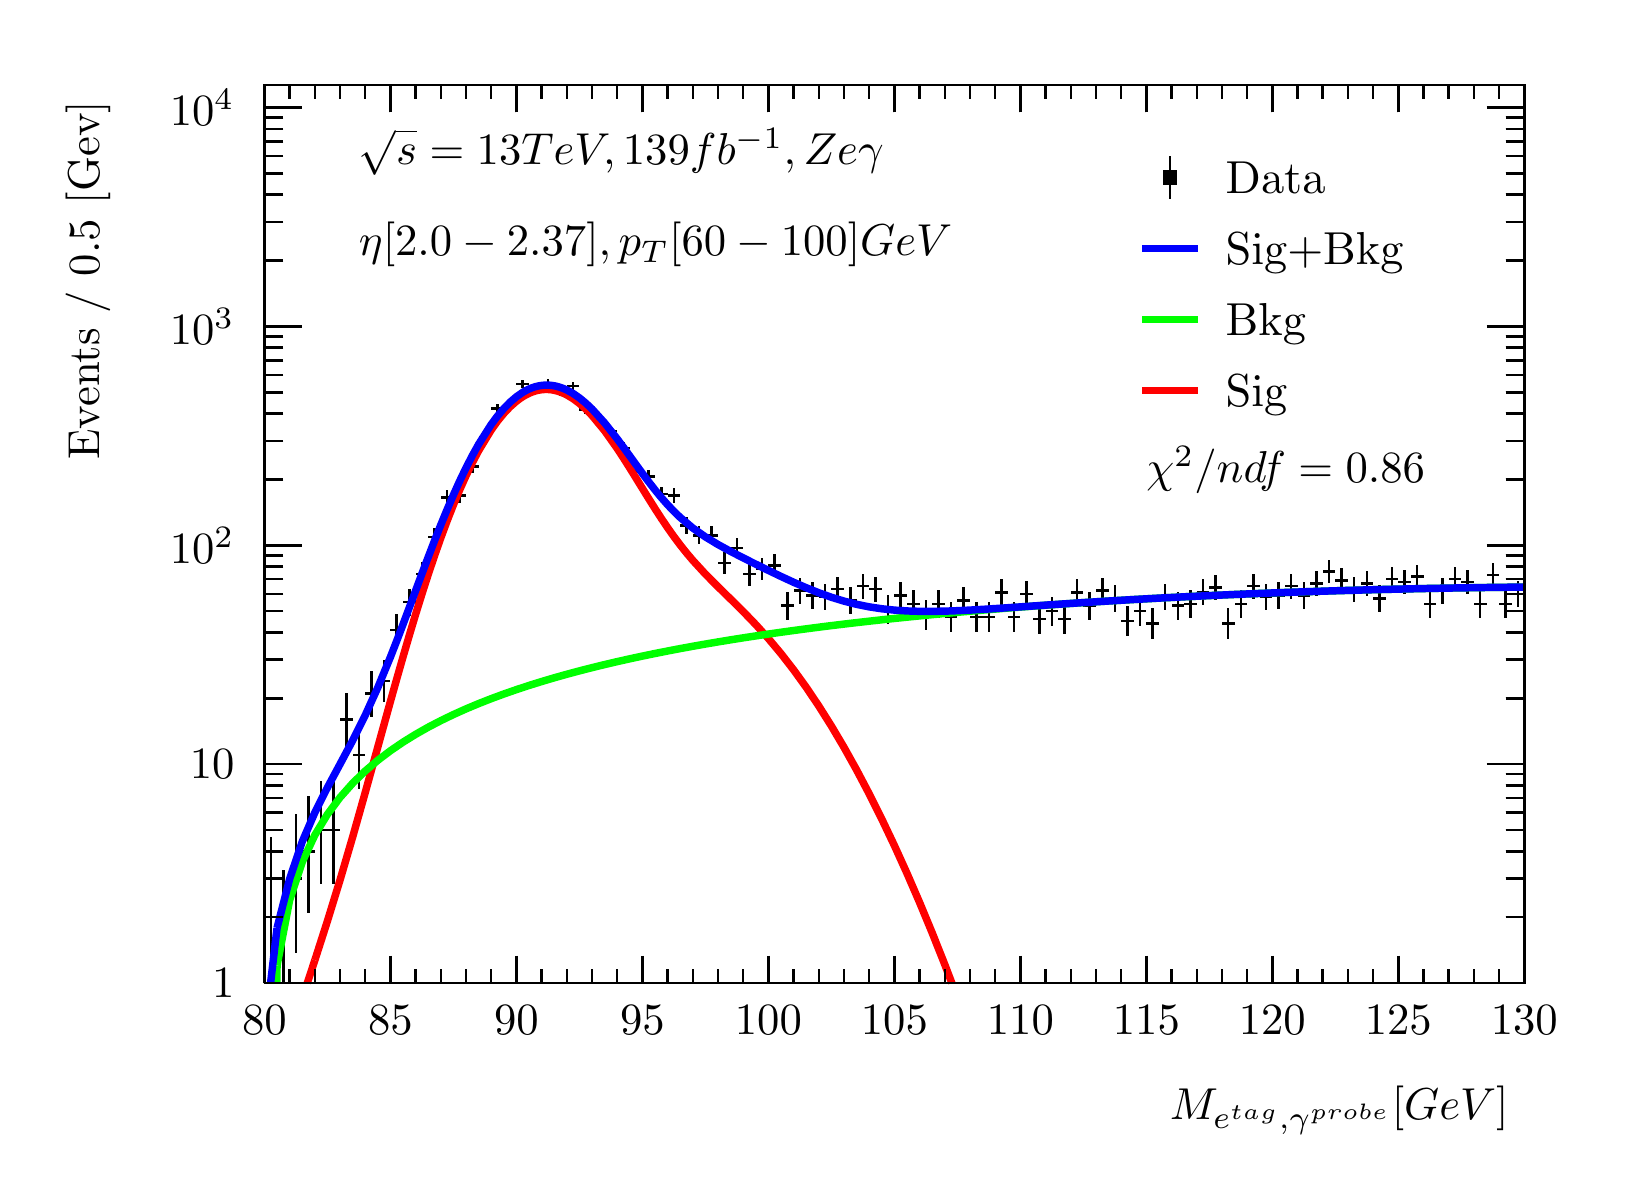
\begin{tikzpicture}
\pgfdeclareplotmark{cross} {
\pgfpathmoveto{\pgfpoint{-0.3\pgfplotmarksize}{\pgfplotmarksize}}
\pgfpathlineto{\pgfpoint{+0.3\pgfplotmarksize}{\pgfplotmarksize}}
\pgfpathlineto{\pgfpoint{+0.3\pgfplotmarksize}{0.3\pgfplotmarksize}}
\pgfpathlineto{\pgfpoint{+1\pgfplotmarksize}{0.3\pgfplotmarksize}}
\pgfpathlineto{\pgfpoint{+1\pgfplotmarksize}{-0.3\pgfplotmarksize}}
\pgfpathlineto{\pgfpoint{+0.3\pgfplotmarksize}{-0.3\pgfplotmarksize}}
\pgfpathlineto{\pgfpoint{+0.3\pgfplotmarksize}{-1.\pgfplotmarksize}}
\pgfpathlineto{\pgfpoint{-0.3\pgfplotmarksize}{-1.\pgfplotmarksize}}
\pgfpathlineto{\pgfpoint{-0.3\pgfplotmarksize}{-0.3\pgfplotmarksize}}
\pgfpathlineto{\pgfpoint{-1.\pgfplotmarksize}{-0.3\pgfplotmarksize}}
\pgfpathlineto{\pgfpoint{-1.\pgfplotmarksize}{0.3\pgfplotmarksize}}
\pgfpathlineto{\pgfpoint{-0.3\pgfplotmarksize}{0.3\pgfplotmarksize}}
\pgfpathclose
\pgfusepathqstroke
}
\pgfdeclareplotmark{cross*} {
\pgfpathmoveto{\pgfpoint{-0.3\pgfplotmarksize}{\pgfplotmarksize}}
\pgfpathlineto{\pgfpoint{+0.3\pgfplotmarksize}{\pgfplotmarksize}}
\pgfpathlineto{\pgfpoint{+0.3\pgfplotmarksize}{0.3\pgfplotmarksize}}
\pgfpathlineto{\pgfpoint{+1\pgfplotmarksize}{0.3\pgfplotmarksize}}
\pgfpathlineto{\pgfpoint{+1\pgfplotmarksize}{-0.3\pgfplotmarksize}}
\pgfpathlineto{\pgfpoint{+0.3\pgfplotmarksize}{-0.3\pgfplotmarksize}}
\pgfpathlineto{\pgfpoint{+0.3\pgfplotmarksize}{-1.\pgfplotmarksize}}
\pgfpathlineto{\pgfpoint{-0.3\pgfplotmarksize}{-1.\pgfplotmarksize}}
\pgfpathlineto{\pgfpoint{-0.3\pgfplotmarksize}{-0.3\pgfplotmarksize}}
\pgfpathlineto{\pgfpoint{-1.\pgfplotmarksize}{-0.3\pgfplotmarksize}}
\pgfpathlineto{\pgfpoint{-1.\pgfplotmarksize}{0.3\pgfplotmarksize}}
\pgfpathlineto{\pgfpoint{-0.3\pgfplotmarksize}{0.3\pgfplotmarksize}}
\pgfpathclose
\pgfusepathqfillstroke
}
\pgfdeclareplotmark{newstar} {
\pgfpathmoveto{\pgfqpoint{0pt}{\pgfplotmarksize}}
\pgfpathlineto{\pgfqpointpolar{44}{0.5\pgfplotmarksize}}
\pgfpathlineto{\pgfqpointpolar{18}{\pgfplotmarksize}}
\pgfpathlineto{\pgfqpointpolar{-20}{0.5\pgfplotmarksize}}
\pgfpathlineto{\pgfqpointpolar{-54}{\pgfplotmarksize}}
\pgfpathlineto{\pgfqpointpolar{-90}{0.5\pgfplotmarksize}}
\pgfpathlineto{\pgfqpointpolar{234}{\pgfplotmarksize}}
\pgfpathlineto{\pgfqpointpolar{198}{0.5\pgfplotmarksize}}
\pgfpathlineto{\pgfqpointpolar{162}{\pgfplotmarksize}}
\pgfpathlineto{\pgfqpointpolar{134}{0.5\pgfplotmarksize}}
\pgfpathclose
\pgfusepathqstroke
}
\pgfdeclareplotmark{newstar*} {
\pgfpathmoveto{\pgfqpoint{0pt}{\pgfplotmarksize}}
\pgfpathlineto{\pgfqpointpolar{44}{0.5\pgfplotmarksize}}
\pgfpathlineto{\pgfqpointpolar{18}{\pgfplotmarksize}}
\pgfpathlineto{\pgfqpointpolar{-20}{0.5\pgfplotmarksize}}
\pgfpathlineto{\pgfqpointpolar{-54}{\pgfplotmarksize}}
\pgfpathlineto{\pgfqpointpolar{-90}{0.5\pgfplotmarksize}}
\pgfpathlineto{\pgfqpointpolar{234}{\pgfplotmarksize}}
\pgfpathlineto{\pgfqpointpolar{198}{0.5\pgfplotmarksize}}
\pgfpathlineto{\pgfqpointpolar{162}{\pgfplotmarksize}}
\pgfpathlineto{\pgfqpointpolar{134}{0.5\pgfplotmarksize}}
\pgfpathclose
\pgfusepathqfillstroke
}
\definecolor{c}{rgb}{1,1,1};
\draw [color=c, fill=c] (0,0) rectangle (20,14.4361);
\draw [color=c, fill=c] (3,2.30977) rectangle (19,13.7143);
\definecolor{c}{rgb}{0,0,0};
\draw [c,line width=0.9] (3,2.30977) -- (3,13.7143) -- (19,13.7143) -- (19,2.30977) -- (3,2.30977);
\definecolor{c}{rgb}{1,1,1};
\draw [color=c, fill=c] (3,2.30977) rectangle (19,13.7143);
\definecolor{c}{rgb}{0,0,0};
\draw [c,line width=0.9] (3,2.30977) -- (3,13.7143) -- (19,13.7143) -- (19,2.30977) -- (3,2.30977);
\draw [c,line width=0.9] (3,2.30977) -- (19,2.30977);
\draw [c,line width=0.9] (3,2.65624) -- (3,2.30977);
\draw [c,line width=0.9] (3.32,2.48301) -- (3.32,2.30977);
\draw [c,line width=0.9] (3.64,2.48301) -- (3.64,2.30977);
\draw [c,line width=0.9] (3.96,2.48301) -- (3.96,2.30977);
\draw [c,line width=0.9] (4.28,2.48301) -- (4.28,2.30977);
\draw [c,line width=0.9] (4.6,2.65624) -- (4.6,2.30977);
\draw [c,line width=0.9] (4.92,2.48301) -- (4.92,2.30977);
\draw [c,line width=0.9] (5.24,2.48301) -- (5.24,2.30977);
\draw [c,line width=0.9] (5.56,2.48301) -- (5.56,2.30977);
\draw [c,line width=0.9] (5.88,2.48301) -- (5.88,2.30977);
\draw [c,line width=0.9] (6.2,2.65624) -- (6.2,2.30977);
\draw [c,line width=0.9] (6.52,2.48301) -- (6.52,2.30977);
\draw [c,line width=0.9] (6.84,2.48301) -- (6.84,2.30977);
\draw [c,line width=0.9] (7.16,2.48301) -- (7.16,2.30977);
\draw [c,line width=0.9] (7.48,2.48301) -- (7.48,2.30977);
\draw [c,line width=0.9] (7.8,2.65624) -- (7.8,2.30977);
\draw [c,line width=0.9] (8.12,2.48301) -- (8.12,2.30977);
\draw [c,line width=0.9] (8.44,2.48301) -- (8.44,2.30977);
\draw [c,line width=0.9] (8.76,2.48301) -- (8.76,2.30977);
\draw [c,line width=0.9] (9.08,2.48301) -- (9.08,2.30977);
\draw [c,line width=0.9] (9.4,2.65624) -- (9.4,2.30977);
\draw [c,line width=0.9] (9.72,2.48301) -- (9.72,2.30977);
\draw [c,line width=0.9] (10.04,2.48301) -- (10.04,2.30977);
\draw [c,line width=0.9] (10.36,2.48301) -- (10.36,2.30977);
\draw [c,line width=0.9] (10.68,2.48301) -- (10.68,2.30977);
\draw [c,line width=0.9] (11,2.65624) -- (11,2.30977);
\draw [c,line width=0.9] (11.32,2.48301) -- (11.32,2.30977);
\draw [c,line width=0.9] (11.64,2.48301) -- (11.64,2.30977);
\draw [c,line width=0.9] (11.96,2.48301) -- (11.96,2.30977);
\draw [c,line width=0.9] (12.28,2.48301) -- (12.28,2.30977);
\draw [c,line width=0.9] (12.6,2.65624) -- (12.6,2.30977);
\draw [c,line width=0.9] (12.92,2.48301) -- (12.92,2.30977);
\draw [c,line width=0.9] (13.24,2.48301) -- (13.24,2.30977);
\draw [c,line width=0.9] (13.56,2.48301) -- (13.56,2.30977);
\draw [c,line width=0.9] (13.88,2.48301) -- (13.88,2.30977);
\draw [c,line width=0.9] (14.2,2.65624) -- (14.2,2.30977);
\draw [c,line width=0.9] (14.52,2.48301) -- (14.52,2.30977);
\draw [c,line width=0.9] (14.84,2.48301) -- (14.84,2.30977);
\draw [c,line width=0.9] (15.16,2.48301) -- (15.16,2.30977);
\draw [c,line width=0.9] (15.48,2.48301) -- (15.48,2.30977);
\draw [c,line width=0.9] (15.8,2.65624) -- (15.8,2.30977);
\draw [c,line width=0.9] (16.12,2.48301) -- (16.12,2.30977);
\draw [c,line width=0.9] (16.44,2.48301) -- (16.44,2.30977);
\draw [c,line width=0.9] (16.76,2.48301) -- (16.76,2.30977);
\draw [c,line width=0.9] (17.08,2.48301) -- (17.08,2.30977);
\draw [c,line width=0.9] (17.4,2.65624) -- (17.4,2.30977);
\draw [c,line width=0.9] (17.72,2.48301) -- (17.72,2.30977);
\draw [c,line width=0.9] (18.04,2.48301) -- (18.04,2.30977);
\draw [c,line width=0.9] (18.36,2.48301) -- (18.36,2.30977);
\draw [c,line width=0.9] (18.68,2.48301) -- (18.68,2.30977);
\draw [c,line width=0.9] (19,2.65624) -- (19,2.30977);
\draw [anchor=base] (3,1.66015) node[scale=1.61424, color=c, rotate=0]{80};
\draw [anchor=base] (4.6,1.66015) node[scale=1.61424, color=c, rotate=0]{85};
\draw [anchor=base] (6.2,1.66015) node[scale=1.61424, color=c, rotate=0]{90};
\draw [anchor=base] (7.8,1.66015) node[scale=1.61424, color=c, rotate=0]{95};
\draw [anchor=base] (9.4,1.66015) node[scale=1.61424, color=c, rotate=0]{100};
\draw [anchor=base] (11,1.66015) node[scale=1.61424, color=c, rotate=0]{105};
\draw [anchor=base] (12.6,1.66015) node[scale=1.61424, color=c, rotate=0]{110};
\draw [anchor=base] (14.2,1.66015) node[scale=1.61424, color=c, rotate=0]{115};
\draw [anchor=base] (15.8,1.66015) node[scale=1.61424, color=c, rotate=0]{120};
\draw [anchor=base] (17.4,1.66015) node[scale=1.61424, color=c, rotate=0]{125};
\draw [anchor=base] (19,1.66015) node[scale=1.61424, color=c, rotate=0]{130};
\draw [anchor= east] (19,0.692932) node[scale=1.61424, color=c, rotate=0]{$M_{e^{tag}, \gamma^{probe}}  [GeV]$};
\draw [c,line width=0.9] (3,13.7143) -- (19,13.7143);
\draw [c,line width=0.9] (3,13.3678) -- (3,13.7143);
\draw [c,line width=0.9] (3.32,13.5411) -- (3.32,13.7143);
\draw [c,line width=0.9] (3.64,13.5411) -- (3.64,13.7143);
\draw [c,line width=0.9] (3.96,13.5411) -- (3.96,13.7143);
\draw [c,line width=0.9] (4.28,13.5411) -- (4.28,13.7143);
\draw [c,line width=0.9] (4.6,13.3678) -- (4.6,13.7143);
\draw [c,line width=0.9] (4.92,13.5411) -- (4.92,13.7143);
\draw [c,line width=0.9] (5.24,13.5411) -- (5.24,13.7143);
\draw [c,line width=0.9] (5.56,13.5411) -- (5.56,13.7143);
\draw [c,line width=0.9] (5.88,13.5411) -- (5.88,13.7143);
\draw [c,line width=0.9] (6.2,13.3678) -- (6.2,13.7143);
\draw [c,line width=0.9] (6.52,13.5411) -- (6.52,13.7143);
\draw [c,line width=0.9] (6.84,13.5411) -- (6.84,13.7143);
\draw [c,line width=0.9] (7.16,13.5411) -- (7.16,13.7143);
\draw [c,line width=0.9] (7.48,13.5411) -- (7.48,13.7143);
\draw [c,line width=0.9] (7.8,13.3678) -- (7.8,13.7143);
\draw [c,line width=0.9] (8.12,13.5411) -- (8.12,13.7143);
\draw [c,line width=0.9] (8.44,13.5411) -- (8.44,13.7143);
\draw [c,line width=0.9] (8.76,13.5411) -- (8.76,13.7143);
\draw [c,line width=0.9] (9.08,13.5411) -- (9.08,13.7143);
\draw [c,line width=0.9] (9.4,13.3678) -- (9.4,13.7143);
\draw [c,line width=0.9] (9.72,13.5411) -- (9.72,13.7143);
\draw [c,line width=0.9] (10.04,13.5411) -- (10.04,13.7143);
\draw [c,line width=0.9] (10.36,13.5411) -- (10.36,13.7143);
\draw [c,line width=0.9] (10.68,13.5411) -- (10.68,13.7143);
\draw [c,line width=0.9] (11,13.3678) -- (11,13.7143);
\draw [c,line width=0.9] (11.32,13.5411) -- (11.32,13.7143);
\draw [c,line width=0.9] (11.64,13.5411) -- (11.64,13.7143);
\draw [c,line width=0.9] (11.96,13.5411) -- (11.96,13.7143);
\draw [c,line width=0.9] (12.28,13.5411) -- (12.28,13.7143);
\draw [c,line width=0.9] (12.6,13.3678) -- (12.6,13.7143);
\draw [c,line width=0.9] (12.92,13.5411) -- (12.92,13.7143);
\draw [c,line width=0.9] (13.24,13.5411) -- (13.24,13.7143);
\draw [c,line width=0.9] (13.56,13.5411) -- (13.56,13.7143);
\draw [c,line width=0.9] (13.88,13.5411) -- (13.88,13.7143);
\draw [c,line width=0.9] (14.2,13.3678) -- (14.2,13.7143);
\draw [c,line width=0.9] (14.52,13.5411) -- (14.52,13.7143);
\draw [c,line width=0.9] (14.84,13.5411) -- (14.84,13.7143);
\draw [c,line width=0.9] (15.16,13.5411) -- (15.16,13.7143);
\draw [c,line width=0.9] (15.48,13.5411) -- (15.48,13.7143);
\draw [c,line width=0.9] (15.8,13.3678) -- (15.8,13.7143);
\draw [c,line width=0.9] (16.12,13.5411) -- (16.12,13.7143);
\draw [c,line width=0.9] (16.44,13.5411) -- (16.44,13.7143);
\draw [c,line width=0.9] (16.76,13.5411) -- (16.76,13.7143);
\draw [c,line width=0.9] (17.08,13.5411) -- (17.08,13.7143);
\draw [c,line width=0.9] (17.4,13.3678) -- (17.4,13.7143);
\draw [c,line width=0.9] (17.72,13.5411) -- (17.72,13.7143);
\draw [c,line width=0.9] (18.04,13.5411) -- (18.04,13.7143);
\draw [c,line width=0.9] (18.36,13.5411) -- (18.36,13.7143);
\draw [c,line width=0.9] (18.68,13.5411) -- (18.68,13.7143);
\draw [c,line width=0.9] (19,13.3678) -- (19,13.7143);
\draw [c,line width=0.9] (3,2.30977) -- (3,13.7143);
\draw [c,line width=0.9] (3.474,2.30978) -- (3,2.30978);
\draw [anchor= east] (2.82,2.30978) node[scale=1.61424, color=c, rotate=0]{1};
\draw [c,line width=0.9] (3.237,3.14655) -- (3,3.14655);
\draw [c,line width=0.9] (3.237,3.63603) -- (3,3.63603);
\draw [c,line width=0.9] (3.237,3.98333) -- (3,3.98333);
\draw [c,line width=0.9] (3.237,4.25271) -- (3,4.25271);
\draw [c,line width=0.9] (3.237,4.47281) -- (3,4.47281);
\draw [c,line width=0.9] (3.237,4.6589) -- (3,4.6589);
\draw [c,line width=0.9] (3.237,4.8201) -- (3,4.8201);
\draw [c,line width=0.9] (3.237,4.96229) -- (3,4.96229);
\draw [c,line width=0.9] (3.474,5.08948) -- (3,5.08948);
\draw [anchor= east] (2.82,5.08948) node[scale=1.61424, color=c, rotate=0]{10};
\draw [c,line width=0.9] (3.237,5.92626) -- (3,5.92626);
\draw [c,line width=0.9] (3.237,6.41574) -- (3,6.41574);
\draw [c,line width=0.9] (3.237,6.76303) -- (3,6.76303);
\draw [c,line width=0.9] (3.237,7.03241) -- (3,7.03241);
\draw [c,line width=0.9] (3.237,7.25251) -- (3,7.25251);
\draw [c,line width=0.9] (3.237,7.43861) -- (3,7.43861);
\draw [c,line width=0.9] (3.237,7.59981) -- (3,7.59981);
\draw [c,line width=0.9] (3.237,7.74199) -- (3,7.74199);
\draw [c,line width=0.9] (3.474,7.86919) -- (3,7.86919);
\draw [anchor= east] (2.82,7.86919) node[scale=1.61424, color=c, rotate=0]{$10^{2}$};
\draw [c,line width=0.9] (3.237,8.70596) -- (3,8.70596);
\draw [c,line width=0.9] (3.237,9.19544) -- (3,9.19544);
\draw [c,line width=0.9] (3.237,9.54274) -- (3,9.54274);
\draw [c,line width=0.9] (3.237,9.81212) -- (3,9.81212);
\draw [c,line width=0.9] (3.237,10.0322) -- (3,10.0322);
\draw [c,line width=0.9] (3.237,10.2183) -- (3,10.2183);
\draw [c,line width=0.9] (3.237,10.3795) -- (3,10.3795);
\draw [c,line width=0.9] (3.237,10.5217) -- (3,10.5217);
\draw [c,line width=0.9] (3.474,10.6489) -- (3,10.6489);
\draw [anchor= east] (2.82,10.6489) node[scale=1.61424, color=c, rotate=0]{$10^{3}$};
\draw [c,line width=0.9] (3.237,11.4857) -- (3,11.4857);
\draw [c,line width=0.9] (3.237,11.9751) -- (3,11.9751);
\draw [c,line width=0.9] (3.237,12.3224) -- (3,12.3224);
\draw [c,line width=0.9] (3.237,12.5918) -- (3,12.5918);
\draw [c,line width=0.9] (3.237,12.8119) -- (3,12.8119);
\draw [c,line width=0.9] (3.237,12.998) -- (3,12.998);
\draw [c,line width=0.9] (3.237,13.1592) -- (3,13.1592);
\draw [c,line width=0.9] (3.237,13.3014) -- (3,13.3014);
\draw [c,line width=0.9] (3.474,13.4286) -- (3,13.4286);
\draw [anchor= east] (2.82,13.4286) node[scale=1.61424, color=c, rotate=0]{$10^{4}$};
\draw [anchor= east] (0.76,13.7143) node[scale=1.61424, color=c, rotate=90]{Events / 0.5 [Gev]};
\draw [c,line width=0.9] (19,2.30977) -- (19,13.7143);
\draw [c,line width=0.9] (18.526,2.30978) -- (19,2.30978);
\draw [c,line width=0.9] (18.763,3.14655) -- (19,3.14655);
\draw [c,line width=0.9] (18.763,3.63603) -- (19,3.63603);
\draw [c,line width=0.9] (18.763,3.98333) -- (19,3.98333);
\draw [c,line width=0.9] (18.763,4.25271) -- (19,4.25271);
\draw [c,line width=0.9] (18.763,4.47281) -- (19,4.47281);
\draw [c,line width=0.9] (18.763,4.6589) -- (19,4.6589);
\draw [c,line width=0.9] (18.763,4.8201) -- (19,4.8201);
\draw [c,line width=0.9] (18.763,4.96229) -- (19,4.96229);
\draw [c,line width=0.9] (18.526,5.08948) -- (19,5.08948);
\draw [c,line width=0.9] (18.763,5.92626) -- (19,5.92626);
\draw [c,line width=0.9] (18.763,6.41574) -- (19,6.41574);
\draw [c,line width=0.9] (18.763,6.76303) -- (19,6.76303);
\draw [c,line width=0.9] (18.763,7.03241) -- (19,7.03241);
\draw [c,line width=0.9] (18.763,7.25251) -- (19,7.25251);
\draw [c,line width=0.9] (18.763,7.43861) -- (19,7.43861);
\draw [c,line width=0.9] (18.763,7.59981) -- (19,7.59981);
\draw [c,line width=0.9] (18.763,7.74199) -- (19,7.74199);
\draw [c,line width=0.9] (18.526,7.86919) -- (19,7.86919);
\draw [c,line width=0.9] (18.763,8.70596) -- (19,8.70596);
\draw [c,line width=0.9] (18.763,9.19544) -- (19,9.19544);
\draw [c,line width=0.9] (18.763,9.54274) -- (19,9.54274);
\draw [c,line width=0.9] (18.763,9.81212) -- (19,9.81212);
\draw [c,line width=0.9] (18.763,10.0322) -- (19,10.0322);
\draw [c,line width=0.9] (18.763,10.2183) -- (19,10.2183);
\draw [c,line width=0.9] (18.763,10.3795) -- (19,10.3795);
\draw [c,line width=0.9] (18.763,10.5217) -- (19,10.5217);
\draw [c,line width=0.9] (18.526,10.6489) -- (19,10.6489);
\draw [c,line width=0.9] (18.763,11.4857) -- (19,11.4857);
\draw [c,line width=0.9] (18.763,11.9751) -- (19,11.9751);
\draw [c,line width=0.9] (18.763,12.3224) -- (19,12.3224);
\draw [c,line width=0.9] (18.763,12.5918) -- (19,12.5918);
\draw [c,line width=0.9] (18.763,12.8119) -- (19,12.8119);
\draw [c,line width=0.9] (18.763,12.998) -- (19,12.998);
\draw [c,line width=0.9] (18.763,13.1592) -- (19,13.1592);
\draw [c,line width=0.9] (18.763,13.3014) -- (19,13.3014);
\draw [c,line width=0.9] (18.526,13.4286) -- (19,13.4286);
\draw [c,line width=0.9] (3.08,3.14655) -- (3,3.14655);
\draw [c,line width=0.9] (3,3.14655) -- (3,3.14655);
\draw [c,line width=0.9] (3.08,3.14655) -- (3.16,3.14655);
\draw [c,line width=0.9] (3.16,3.14655) -- (3.16,3.14655);
\draw [c,line width=0.9] (3.08,3.14655) -- (3.08,4.16194);
\draw [c,line width=0.9] (3.08,4.16194) -- (3.08,4.16194);
\draw [c,line width=0.9] (3.08,3.14655) -- (3.08,2.30977);
\draw [c,line width=0.9] (3.08,2.30977) -- (3.08,2.30977);
\draw [c,line width=0.9] (3.24,2.30977) -- (3.16,2.30977);
\draw [c,line width=0.9] (3.16,2.30977) -- (3.16,2.30977);
\draw [c,line width=0.9] (3.24,2.30977) -- (3.32,2.30977);
\draw [c,line width=0.9] (3.32,2.30977) -- (3.32,2.30977);
\draw [c,line width=0.9] (3.24,2.30977) -- (3.24,3.75092);
\draw [c,line width=0.9] (3.24,3.75092) -- (3.24,3.75092);
\draw [c,line width=0.9] (3.4,3.63603) -- (3.32,3.63603);
\draw [c,line width=0.9] (3.32,3.63603) -- (3.32,3.63603);
\draw [c,line width=0.9] (3.4,3.63603) -- (3.48,3.63603);
\draw [c,line width=0.9] (3.48,3.63603) -- (3.48,3.63603);
\draw [c,line width=0.9] (3.4,3.63603) -- (3.4,4.45623);
\draw [c,line width=0.9] (3.4,4.45623) -- (3.4,4.45623);
\draw [c,line width=0.9] (3.4,3.63603) -- (3.4,2.68743);
\draw [c,line width=0.9] (3.4,2.68743) -- (3.4,2.68743);
\draw [c,line width=0.9] (3.56,3.98332) -- (3.48,3.98332);
\draw [c,line width=0.9] (3.48,3.98332) -- (3.48,3.98332);
\draw [c,line width=0.9] (3.56,3.98332) -- (3.64,3.98332);
\draw [c,line width=0.9] (3.64,3.98332) -- (3.64,3.98332);
\draw [c,line width=0.9] (3.56,3.98332) -- (3.56,4.68665);
\draw [c,line width=0.9] (3.56,4.68665) -- (3.56,4.68665);
\draw [c,line width=0.9] (3.56,3.98332) -- (3.56,3.19718);
\draw [c,line width=0.9] (3.56,3.19718) -- (3.56,3.19718);
\draw [c,line width=0.9] (3.72,4.25271) -- (3.64,4.25271);
\draw [c,line width=0.9] (3.64,4.25271) -- (3.64,4.25271);
\draw [c,line width=0.9] (3.72,4.25271) -- (3.8,4.25271);
\draw [c,line width=0.9] (3.8,4.25271) -- (3.8,4.25271);
\draw [c,line width=0.9] (3.72,4.25271) -- (3.72,4.87648);
\draw [c,line width=0.9] (3.72,4.87648) -- (3.72,4.87648);
\draw [c,line width=0.9] (3.72,4.25271) -- (3.72,3.57);
\draw [c,line width=0.9] (3.72,3.57) -- (3.72,3.57);
\draw [c,line width=0.9] (3.88,4.25271) -- (3.8,4.25271);
\draw [c,line width=0.9] (3.8,4.25271) -- (3.8,4.25271);
\draw [c,line width=0.9] (3.88,4.25271) -- (3.96,4.25271);
\draw [c,line width=0.9] (3.96,4.25271) -- (3.96,4.25271);
\draw [c,line width=0.9] (3.88,4.25271) -- (3.88,4.87648);
\draw [c,line width=0.9] (3.88,4.87648) -- (3.88,4.87648);
\draw [c,line width=0.9] (3.88,4.25271) -- (3.88,3.57);
\draw [c,line width=0.9] (3.88,3.57) -- (3.88,3.57);
\draw [c,line width=0.9] (4.04,5.65687) -- (3.96,5.65687);
\draw [c,line width=0.9] (3.96,5.65687) -- (3.96,5.65687);
\draw [c,line width=0.9] (4.04,5.65687) -- (4.12,5.65687);
\draw [c,line width=0.9] (4.12,5.65687) -- (4.12,5.65687);
\draw [c,line width=0.9] (4.04,5.65687) -- (4.04,5.98992);
\draw [c,line width=0.9] (4.04,5.98992) -- (4.04,5.98992);
\draw [c,line width=0.9] (4.04,5.65687) -- (4.04,5.31382);
\draw [c,line width=0.9] (4.04,5.31382) -- (4.04,5.31382);
\draw [c,line width=0.9] (4.2,5.20454) -- (4.12,5.20454);
\draw [c,line width=0.9] (4.12,5.20454) -- (4.12,5.20454);
\draw [c,line width=0.9] (4.2,5.20454) -- (4.28,5.20454);
\draw [c,line width=0.9] (4.28,5.20454) -- (4.28,5.20454);
\draw [c,line width=0.9] (4.2,5.20454) -- (4.2,5.61203);
\draw [c,line width=0.9] (4.2,5.61203) -- (4.2,5.61203);
\draw [c,line width=0.9] (4.2,5.20454) -- (4.2,4.77934);
\draw [c,line width=0.9] (4.2,4.77934) -- (4.2,4.77934);
\draw [c,line width=0.9] (4.36,5.98516) -- (4.28,5.98516);
\draw [c,line width=0.9] (4.28,5.98516) -- (4.28,5.98516);
\draw [c,line width=0.9] (4.36,5.98516) -- (4.44,5.98516);
\draw [c,line width=0.9] (4.44,5.98516) -- (4.44,5.98516);
\draw [c,line width=0.9] (4.36,5.98516) -- (4.36,6.27303);
\draw [c,line width=0.9] (4.36,6.27303) -- (4.36,6.27303);
\draw [c,line width=0.9] (4.36,5.98516) -- (4.36,5.69067);
\draw [c,line width=0.9] (4.36,5.69067) -- (4.36,5.69067);
\draw [c,line width=0.9] (4.52,6.14636) -- (4.44,6.14636);
\draw [c,line width=0.9] (4.44,6.14636) -- (4.44,6.14636);
\draw [c,line width=0.9] (4.52,6.14636) -- (4.6,6.14636);
\draw [c,line width=0.9] (4.6,6.14636) -- (4.6,6.14636);
\draw [c,line width=0.9] (4.52,6.14636) -- (4.52,6.41441);
\draw [c,line width=0.9] (4.52,6.41441) -- (4.52,6.41441);
\draw [c,line width=0.9] (4.52,6.14636) -- (4.52,5.8729);
\draw [c,line width=0.9] (4.52,5.8729) -- (4.52,5.8729);
\draw [c,line width=0.9] (4.68,6.79284) -- (4.6,6.79284);
\draw [c,line width=0.9] (4.6,6.79284) -- (4.6,6.79284);
\draw [c,line width=0.9] (4.68,6.79284) -- (4.76,6.79284);
\draw [c,line width=0.9] (4.76,6.79284) -- (4.76,6.79284);
\draw [c,line width=0.9] (4.68,6.79284) -- (4.68,6.99452);
\draw [c,line width=0.9] (4.68,6.99452) -- (4.68,6.99452);
\draw [c,line width=0.9] (4.68,6.79284) -- (4.68,6.58876);
\draw [c,line width=0.9] (4.68,6.58876) -- (4.68,6.58876);
\draw [c,line width=0.9] (4.84,7.14747) -- (4.76,7.14747);
\draw [c,line width=0.9] (4.76,7.14747) -- (4.76,7.14747);
\draw [c,line width=0.9] (4.84,7.14747) -- (4.92,7.14747);
\draw [c,line width=0.9] (4.92,7.14747) -- (4.92,7.14747);
\draw [c,line width=0.9] (4.84,7.14747) -- (4.84,7.32022);
\draw [c,line width=0.9] (4.84,7.32022) -- (4.84,7.32022);
\draw [c,line width=0.9] (4.84,7.14747) -- (4.84,6.97319);
\draw [c,line width=0.9] (4.84,6.97319) -- (4.84,6.97319);
\draw [c,line width=0.9] (5,7.50569) -- (4.92,7.50569);
\draw [c,line width=0.9] (4.92,7.50569) -- (4.92,7.50569);
\draw [c,line width=0.9] (5,7.50569) -- (5.08,7.50569);
\draw [c,line width=0.9] (5.08,7.50569) -- (5.08,7.50569);
\draw [c,line width=0.9] (5,7.50569) -- (5,7.65354);
\draw [c,line width=0.9] (5,7.65354) -- (5,7.65354);
\draw [c,line width=0.9] (5,7.50569) -- (5,7.35686);
\draw [c,line width=0.9] (5,7.35686) -- (5,7.35686);
\draw [c,line width=0.9] (5.16,7.97322) -- (5.08,7.97322);
\draw [c,line width=0.9] (5.08,7.97322) -- (5.08,7.97322);
\draw [c,line width=0.9] (5.16,7.97322) -- (5.24,7.97322);
\draw [c,line width=0.9] (5.24,7.97322) -- (5.24,7.97322);
\draw [c,line width=0.9] (5.16,7.97322) -- (5.16,8.08881);
\draw [c,line width=0.9] (5.16,8.08881) -- (5.16,8.08881);
\draw [c,line width=0.9] (5.16,7.97322) -- (5.16,7.85763);
\draw [c,line width=0.9] (5.16,7.85763) -- (5.16,7.85763);
\draw [c,line width=0.9] (5.32,8.47373) -- (5.24,8.47373);
\draw [c,line width=0.9] (5.24,8.47373) -- (5.24,8.47373);
\draw [c,line width=0.9] (5.32,8.47373) -- (5.4,8.47373);
\draw [c,line width=0.9] (5.4,8.47373) -- (5.4,8.47373);
\draw [c,line width=0.9] (5.32,8.47373) -- (5.32,8.56769);
\draw [c,line width=0.9] (5.32,8.56769) -- (5.32,8.56769);
\draw [c,line width=0.9] (5.32,8.47373) -- (5.32,8.37977);
\draw [c,line width=0.9] (5.32,8.37977) -- (5.32,8.37977);
\draw [c,line width=0.9] (5.48,8.50264) -- (5.4,8.50264);
\draw [c,line width=0.9] (5.4,8.50264) -- (5.4,8.50264);
\draw [c,line width=0.9] (5.48,8.50264) -- (5.56,8.50264);
\draw [c,line width=0.9] (5.56,8.50264) -- (5.56,8.50264);
\draw [c,line width=0.9] (5.48,8.50264) -- (5.48,8.59548);
\draw [c,line width=0.9] (5.48,8.59548) -- (5.48,8.59548);
\draw [c,line width=0.9] (5.48,8.50264) -- (5.48,8.4098);
\draw [c,line width=0.9] (5.48,8.4098) -- (5.48,8.4098);
\draw [c,line width=0.9] (5.64,8.86942) -- (5.56,8.86942);
\draw [c,line width=0.9] (5.56,8.86942) -- (5.56,8.86942);
\draw [c,line width=0.9] (5.64,8.86942) -- (5.72,8.86942);
\draw [c,line width=0.9] (5.72,8.86942) -- (5.72,8.86942);
\draw [c,line width=0.9] (5.64,8.86942) -- (5.64,8.94918);
\draw [c,line width=0.9] (5.64,8.94918) -- (5.64,8.94918);
\draw [c,line width=0.9] (5.64,8.86942) -- (5.64,8.78966);
\draw [c,line width=0.9] (5.64,8.78966) -- (5.64,8.78966);
\draw [c,line width=0.9] (5.8,9.24665) -- (5.72,9.24665);
\draw [c,line width=0.9] (5.72,9.24665) -- (5.72,9.24665);
\draw [c,line width=0.9] (5.8,9.24665) -- (5.88,9.24665);
\draw [c,line width=0.9] (5.88,9.24665) -- (5.88,9.24665);
\draw [c,line width=0.9] (5.8,9.24665) -- (5.8,9.31488);
\draw [c,line width=0.9] (5.8,9.31488) -- (5.8,9.31488);
\draw [c,line width=0.9] (5.8,9.24665) -- (5.8,9.17843);
\draw [c,line width=0.9] (5.8,9.17843) -- (5.8,9.17843);
\draw [c,line width=0.9] (5.96,9.60451) -- (5.88,9.60451);
\draw [c,line width=0.9] (5.88,9.60451) -- (5.88,9.60451);
\draw [c,line width=0.9] (5.96,9.60451) -- (6.04,9.60451);
\draw [c,line width=0.9] (6.04,9.60451) -- (6.04,9.60451);
\draw [c,line width=0.9] (5.96,9.60451) -- (5.96,9.66334);
\draw [c,line width=0.9] (5.96,9.66334) -- (5.96,9.66334);
\draw [c,line width=0.9] (5.96,9.60451) -- (5.96,9.54568);
\draw [c,line width=0.9] (5.96,9.54568) -- (5.96,9.54568);
\draw [c,line width=0.9] (6.12,9.63843) -- (6.04,9.63843);
\draw [c,line width=0.9] (6.04,9.63843) -- (6.04,9.63843);
\draw [c,line width=0.9] (6.12,9.63843) -- (6.2,9.63843);
\draw [c,line width=0.9] (6.2,9.63843) -- (6.2,9.63843);
\draw [c,line width=0.9] (6.12,9.63843) -- (6.12,9.69644);
\draw [c,line width=0.9] (6.12,9.69644) -- (6.12,9.69644);
\draw [c,line width=0.9] (6.12,9.63843) -- (6.12,9.58043);
\draw [c,line width=0.9] (6.12,9.58043) -- (6.12,9.58043);
\draw [c,line width=0.9] (6.28,9.92057) -- (6.2,9.92057);
\draw [c,line width=0.9] (6.2,9.92057) -- (6.2,9.92057);
\draw [c,line width=0.9] (6.28,9.92057) -- (6.36,9.92057);
\draw [c,line width=0.9] (6.36,9.92057) -- (6.36,9.92057);
\draw [c,line width=0.9] (6.28,9.92057) -- (6.28,9.97219);
\draw [c,line width=0.9] (6.28,9.97219) -- (6.28,9.97219);
\draw [c,line width=0.9] (6.28,9.92057) -- (6.28,9.86896);
\draw [c,line width=0.9] (6.28,9.86896) -- (6.28,9.86896);
\draw [c,line width=0.9] (6.44,9.85481) -- (6.36,9.85481);
\draw [c,line width=0.9] (6.36,9.85481) -- (6.36,9.85481);
\draw [c,line width=0.9] (6.44,9.85481) -- (6.52,9.85481);
\draw [c,line width=0.9] (6.52,9.85481) -- (6.52,9.85481);
\draw [c,line width=0.9] (6.44,9.85481) -- (6.44,9.90785);
\draw [c,line width=0.9] (6.44,9.90785) -- (6.44,9.90785);
\draw [c,line width=0.9] (6.44,9.85481) -- (6.44,9.80177);
\draw [c,line width=0.9] (6.44,9.80177) -- (6.44,9.80177);
\draw [c,line width=0.9] (6.6,9.92718) -- (6.52,9.92718);
\draw [c,line width=0.9] (6.52,9.92718) -- (6.52,9.92718);
\draw [c,line width=0.9] (6.6,9.92718) -- (6.68,9.92718);
\draw [c,line width=0.9] (6.68,9.92718) -- (6.68,9.92718);
\draw [c,line width=0.9] (6.6,9.92718) -- (6.6,9.97865);
\draw [c,line width=0.9] (6.6,9.97865) -- (6.6,9.97865);
\draw [c,line width=0.9] (6.6,9.92718) -- (6.6,9.8757);
\draw [c,line width=0.9] (6.6,9.8757) -- (6.6,9.8757);
\draw [c,line width=0.9] (6.76,9.82174) -- (6.68,9.82174);
\draw [c,line width=0.9] (6.68,9.82174) -- (6.68,9.82174);
\draw [c,line width=0.9] (6.76,9.82174) -- (6.84,9.82174);
\draw [c,line width=0.9] (6.84,9.82174) -- (6.84,9.82174);
\draw [c,line width=0.9] (6.76,9.82174) -- (6.76,9.8755);
\draw [c,line width=0.9] (6.76,9.8755) -- (6.76,9.8755);
\draw [c,line width=0.9] (6.76,9.82174) -- (6.76,9.76797);
\draw [c,line width=0.9] (6.76,9.76797) -- (6.76,9.76797);
\draw [c,line width=0.9] (6.92,9.8938) -- (6.84,9.8938);
\draw [c,line width=0.9] (6.84,9.8938) -- (6.84,9.8938);
\draw [c,line width=0.9] (6.92,9.8938) -- (7,9.8938);
\draw [c,line width=0.9] (7,9.8938) -- (7,9.8938);
\draw [c,line width=0.9] (6.92,9.8938) -- (6.92,9.94598);
\draw [c,line width=0.9] (6.92,9.94598) -- (6.92,9.94598);
\draw [c,line width=0.9] (6.92,9.8938) -- (6.92,9.84161);
\draw [c,line width=0.9] (6.92,9.84161) -- (6.92,9.84161);
\draw [c,line width=0.9] (7.08,9.59298) -- (7,9.59298);
\draw [c,line width=0.9] (7,9.59298) -- (7,9.59298);
\draw [c,line width=0.9] (7.08,9.59298) -- (7.16,9.59298);
\draw [c,line width=0.9] (7.16,9.59298) -- (7.16,9.59298);
\draw [c,line width=0.9] (7.08,9.59298) -- (7.08,9.65209);
\draw [c,line width=0.9] (7.08,9.65209) -- (7.08,9.65209);
\draw [c,line width=0.9] (7.08,9.59298) -- (7.08,9.53387);
\draw [c,line width=0.9] (7.08,9.53387) -- (7.08,9.53387);
\draw [c,line width=0.9] (7.24,9.47124) -- (7.16,9.47124);
\draw [c,line width=0.9] (7.16,9.47124) -- (7.16,9.47124);
\draw [c,line width=0.9] (7.24,9.47124) -- (7.32,9.47124);
\draw [c,line width=0.9] (7.32,9.47124) -- (7.32,9.47124);
\draw [c,line width=0.9] (7.24,9.47124) -- (7.24,9.53341);
\draw [c,line width=0.9] (7.24,9.53341) -- (7.24,9.53341);
\draw [c,line width=0.9] (7.24,9.47124) -- (7.24,9.40908);
\draw [c,line width=0.9] (7.24,9.40908) -- (7.24,9.40908);
\draw [c,line width=0.9] (7.4,9.3178) -- (7.32,9.3178);
\draw [c,line width=0.9] (7.32,9.3178) -- (7.32,9.3178);
\draw [c,line width=0.9] (7.4,9.3178) -- (7.48,9.3178);
\draw [c,line width=0.9] (7.48,9.3178) -- (7.48,9.3178);
\draw [c,line width=0.9] (7.4,9.3178) -- (7.4,9.38404);
\draw [c,line width=0.9] (7.4,9.38404) -- (7.4,9.38404);
\draw [c,line width=0.9] (7.4,9.3178) -- (7.4,9.25155);
\draw [c,line width=0.9] (7.4,9.25155) -- (7.4,9.25155);
\draw [c,line width=0.9] (7.56,9.10783) -- (7.48,9.10783);
\draw [c,line width=0.9] (7.48,9.10783) -- (7.48,9.10783);
\draw [c,line width=0.9] (7.56,9.10783) -- (7.64,9.10783);
\draw [c,line width=0.9] (7.64,9.10783) -- (7.64,9.10783);
\draw [c,line width=0.9] (7.56,9.10783) -- (7.56,9.1801);
\draw [c,line width=0.9] (7.56,9.1801) -- (7.56,9.1801);
\draw [c,line width=0.9] (7.56,9.10783) -- (7.56,9.03557);
\draw [c,line width=0.9] (7.56,9.03557) -- (7.56,9.03557);
\draw [c,line width=0.9] (7.72,8.79887) -- (7.64,8.79887);
\draw [c,line width=0.9] (7.64,8.79887) -- (7.64,8.79887);
\draw [c,line width=0.9] (7.72,8.79887) -- (7.8,8.79887);
\draw [c,line width=0.9] (7.8,8.79887) -- (7.8,8.79887);
\draw [c,line width=0.9] (7.72,8.79887) -- (7.72,8.88099);
\draw [c,line width=0.9] (7.72,8.88099) -- (7.72,8.88099);
\draw [c,line width=0.9] (7.72,8.79887) -- (7.72,8.71674);
\draw [c,line width=0.9] (7.72,8.71674) -- (7.72,8.71674);
\draw [c,line width=0.9] (7.88,8.74164) -- (7.8,8.74164);
\draw [c,line width=0.9] (7.8,8.74164) -- (7.8,8.74164);
\draw [c,line width=0.9] (7.88,8.74164) -- (7.96,8.74164);
\draw [c,line width=0.9] (7.96,8.74164) -- (7.96,8.74164);
\draw [c,line width=0.9] (7.88,8.74164) -- (7.88,8.82574);
\draw [c,line width=0.9] (7.88,8.82574) -- (7.88,8.82574);
\draw [c,line width=0.9] (7.88,8.74164) -- (7.88,8.65755);
\draw [c,line width=0.9] (7.88,8.65755) -- (7.88,8.65755);
\draw [c,line width=0.9] (8.04,8.52389) -- (7.96,8.52389);
\draw [c,line width=0.9] (7.96,8.52389) -- (7.96,8.52389);
\draw [c,line width=0.9] (8.04,8.52389) -- (8.12,8.52389);
\draw [c,line width=0.9] (8.12,8.52389) -- (8.12,8.52389);
\draw [c,line width=0.9] (8.04,8.52389) -- (8.04,8.61591);
\draw [c,line width=0.9] (8.04,8.61591) -- (8.04,8.61591);
\draw [c,line width=0.9] (8.04,8.52389) -- (8.04,8.43186);
\draw [c,line width=0.9] (8.04,8.43186) -- (8.04,8.43186);
\draw [c,line width=0.9] (8.2,8.50264) -- (8.12,8.50264);
\draw [c,line width=0.9] (8.12,8.50264) -- (8.12,8.50264);
\draw [c,line width=0.9] (8.2,8.50264) -- (8.28,8.50264);
\draw [c,line width=0.9] (8.28,8.50264) -- (8.28,8.50264);
\draw [c,line width=0.9] (8.2,8.50264) -- (8.2,8.59548);
\draw [c,line width=0.9] (8.2,8.59548) -- (8.2,8.59548);
\draw [c,line width=0.9] (8.2,8.50264) -- (8.2,8.4098);
\draw [c,line width=0.9] (8.2,8.4098) -- (8.2,8.4098);
\draw [c,line width=0.9] (8.36,8.1191) -- (8.28,8.1191);
\draw [c,line width=0.9] (8.28,8.1191) -- (8.28,8.1191);
\draw [c,line width=0.9] (8.36,8.1191) -- (8.44,8.1191);
\draw [c,line width=0.9] (8.44,8.1191) -- (8.44,8.1191);
\draw [c,line width=0.9] (8.36,8.1191) -- (8.36,8.22791);
\draw [c,line width=0.9] (8.36,8.22791) -- (8.36,8.22791);
\draw [c,line width=0.9] (8.36,8.1191) -- (8.36,8.01028);
\draw [c,line width=0.9] (8.36,8.01028) -- (8.36,8.01028);
\draw [c,line width=0.9] (8.52,7.99517) -- (8.44,7.99517);
\draw [c,line width=0.9] (8.44,7.99517) -- (8.44,7.99517);
\draw [c,line width=0.9] (8.52,7.99517) -- (8.6,7.99517);
\draw [c,line width=0.9] (8.6,7.99517) -- (8.6,7.99517);
\draw [c,line width=0.9] (8.52,7.99517) -- (8.52,8.10971);
\draw [c,line width=0.9] (8.52,8.10971) -- (8.52,8.10971);
\draw [c,line width=0.9] (8.52,7.99517) -- (8.52,7.88063);
\draw [c,line width=0.9] (8.52,7.88063) -- (8.52,7.88063);
\draw [c,line width=0.9] (8.68,7.99517) -- (8.6,7.99517);
\draw [c,line width=0.9] (8.6,7.99517) -- (8.6,7.99517);
\draw [c,line width=0.9] (8.68,7.99517) -- (8.76,7.99517);
\draw [c,line width=0.9] (8.76,7.99517) -- (8.76,7.99517);
\draw [c,line width=0.9] (8.68,7.99517) -- (8.68,8.10971);
\draw [c,line width=0.9] (8.68,8.10971) -- (8.68,8.10971);
\draw [c,line width=0.9] (8.68,7.99517) -- (8.68,7.88063);
\draw [c,line width=0.9] (8.68,7.88063) -- (8.68,7.88063);
\draw [c,line width=0.9] (8.84,7.64425) -- (8.76,7.64425);
\draw [c,line width=0.9] (8.76,7.64425) -- (8.76,7.64425);
\draw [c,line width=0.9] (8.84,7.64425) -- (8.92,7.64425);
\draw [c,line width=0.9] (8.92,7.64425) -- (8.92,7.64425);
\draw [c,line width=0.9] (8.84,7.64425) -- (8.84,7.78348);
\draw [c,line width=0.9] (8.84,7.78348) -- (8.84,7.78348);
\draw [c,line width=0.9] (8.84,7.64425) -- (8.84,7.50419);
\draw [c,line width=0.9] (8.84,7.50419) -- (8.84,7.50419);
\draw [c,line width=0.9] (9,7.83242) -- (8.92,7.83242);
\draw [c,line width=0.9] (8.92,7.83242) -- (8.92,7.83242);
\draw [c,line width=0.9] (9,7.83242) -- (9.08,7.83242);
\draw [c,line width=0.9] (9.08,7.83242) -- (9.08,7.83242);
\draw [c,line width=0.9] (9,7.83242) -- (9,7.96078);
\draw [c,line width=0.9] (9,7.96078) -- (9,7.96078);
\draw [c,line width=0.9] (9,7.83242) -- (9,7.7034);
\draw [c,line width=0.9] (9,7.7034) -- (9,7.7034);
\draw [c,line width=0.9] (9.16,7.50569) -- (9.08,7.50569);
\draw [c,line width=0.9] (9.08,7.50569) -- (9.08,7.50569);
\draw [c,line width=0.9] (9.16,7.50569) -- (9.24,7.50569);
\draw [c,line width=0.9] (9.24,7.50569) -- (9.24,7.50569);
\draw [c,line width=0.9] (9.16,7.50569) -- (9.16,7.65354);
\draw [c,line width=0.9] (9.16,7.65354) -- (9.16,7.65354);
\draw [c,line width=0.9] (9.16,7.50569) -- (9.16,7.35686);
\draw [c,line width=0.9] (9.16,7.35686) -- (9.16,7.35686);
\draw [c,line width=0.9] (9.32,7.56924) -- (9.24,7.56924);
\draw [c,line width=0.9] (9.24,7.56924) -- (9.24,7.56924);
\draw [c,line width=0.9] (9.32,7.56924) -- (9.4,7.56924);
\draw [c,line width=0.9] (9.4,7.56924) -- (9.4,7.56924);
\draw [c,line width=0.9] (9.32,7.56924) -- (9.32,7.71307);
\draw [c,line width=0.9] (9.32,7.71307) -- (9.32,7.71307);
\draw [c,line width=0.9] (9.32,7.56924) -- (9.32,7.4245);
\draw [c,line width=0.9] (9.32,7.4245) -- (9.32,7.4245);
\draw [c,line width=0.9] (9.48,7.6148) -- (9.4,7.6148);
\draw [c,line width=0.9] (9.4,7.6148) -- (9.4,7.6148);
\draw [c,line width=0.9] (9.48,7.6148) -- (9.56,7.6148);
\draw [c,line width=0.9] (9.56,7.6148) -- (9.56,7.6148);
\draw [c,line width=0.9] (9.48,7.6148) -- (9.48,7.75582);
\draw [c,line width=0.9] (9.48,7.75582) -- (9.48,7.75582);
\draw [c,line width=0.9] (9.48,7.6148) -- (9.48,7.47292);
\draw [c,line width=0.9] (9.48,7.47292) -- (9.48,7.47292);
\draw [c,line width=0.9] (9.64,7.10275) -- (9.56,7.10275);
\draw [c,line width=0.9] (9.56,7.10275) -- (9.56,7.10275);
\draw [c,line width=0.9] (9.64,7.10275) -- (9.72,7.10275);
\draw [c,line width=0.9] (9.72,7.10275) -- (9.72,7.10275);
\draw [c,line width=0.9] (9.64,7.10275) -- (9.64,7.2789);
\draw [c,line width=0.9] (9.64,7.2789) -- (9.64,7.2789);
\draw [c,line width=0.9] (9.64,7.10275) -- (9.64,6.92499);
\draw [c,line width=0.9] (9.64,6.92499) -- (9.64,6.92499);
\draw [c,line width=0.9] (9.8,7.2921) -- (9.72,7.2921);
\draw [c,line width=0.9] (9.72,7.2921) -- (9.72,7.2921);
\draw [c,line width=0.9] (9.8,7.2921) -- (9.88,7.2921);
\draw [c,line width=0.9] (9.88,7.2921) -- (9.88,7.2921);
\draw [c,line width=0.9] (9.8,7.2921) -- (9.8,7.4543);
\draw [c,line width=0.9] (9.8,7.4543) -- (9.8,7.4543);
\draw [c,line width=0.9] (9.8,7.2921) -- (9.8,7.12861);
\draw [c,line width=0.9] (9.8,7.12861) -- (9.8,7.12861);
\draw [c,line width=0.9] (9.96,7.23222) -- (9.88,7.23222);
\draw [c,line width=0.9] (9.88,7.23222) -- (9.88,7.23222);
\draw [c,line width=0.9] (9.96,7.23222) -- (10.04,7.23222);
\draw [c,line width=0.9] (10.04,7.23222) -- (10.04,7.23222);
\draw [c,line width=0.9] (9.96,7.23222) -- (9.96,7.39871);
\draw [c,line width=0.9] (9.96,7.39871) -- (9.96,7.39871);
\draw [c,line width=0.9] (9.96,7.23222) -- (9.96,7.06435);
\draw [c,line width=0.9] (9.96,7.06435) -- (9.96,7.06435);
\draw [c,line width=0.9] (10.12,7.21159) -- (10.04,7.21159);
\draw [c,line width=0.9] (10.04,7.21159) -- (10.04,7.21159);
\draw [c,line width=0.9] (10.12,7.21159) -- (10.2,7.21159);
\draw [c,line width=0.9] (10.2,7.21159) -- (10.2,7.21159);
\draw [c,line width=0.9] (10.12,7.21159) -- (10.12,7.37958);
\draw [c,line width=0.9] (10.12,7.37958) -- (10.12,7.37958);
\draw [c,line width=0.9] (10.12,7.21159) -- (10.12,7.04218);
\draw [c,line width=0.9] (10.12,7.04218) -- (10.12,7.04218);
\draw [c,line width=0.9] (10.28,7.31141) -- (10.2,7.31141);
\draw [c,line width=0.9] (10.2,7.31141) -- (10.2,7.31141);
\draw [c,line width=0.9] (10.28,7.31141) -- (10.36,7.31141);
\draw [c,line width=0.9] (10.36,7.31141) -- (10.36,7.31141);
\draw [c,line width=0.9] (10.28,7.31141) -- (10.28,7.47226);
\draw [c,line width=0.9] (10.28,7.47226) -- (10.28,7.47226);
\draw [c,line width=0.9] (10.28,7.31141) -- (10.28,7.14931);
\draw [c,line width=0.9] (10.28,7.14931) -- (10.28,7.14931);
\draw [c,line width=0.9] (10.44,7.16922) -- (10.36,7.16922);
\draw [c,line width=0.9] (10.36,7.16922) -- (10.36,7.16922);
\draw [c,line width=0.9] (10.44,7.16922) -- (10.52,7.16922);
\draw [c,line width=0.9] (10.52,7.16922) -- (10.52,7.16922);
\draw [c,line width=0.9] (10.44,7.16922) -- (10.44,7.34034);
\draw [c,line width=0.9] (10.44,7.34034) -- (10.44,7.34034);
\draw [c,line width=0.9] (10.44,7.16922) -- (10.44,6.99661);
\draw [c,line width=0.9] (10.44,6.99661) -- (10.44,6.99661);
\draw [c,line width=0.9] (10.6,7.34914) -- (10.52,7.34914);
\draw [c,line width=0.9] (10.52,7.34914) -- (10.52,7.34914);
\draw [c,line width=0.9] (10.6,7.34914) -- (10.68,7.34914);
\draw [c,line width=0.9] (10.68,7.34914) -- (10.68,7.34914);
\draw [c,line width=0.9] (10.6,7.34914) -- (10.6,7.50738);
\draw [c,line width=0.9] (10.6,7.50738) -- (10.6,7.50738);
\draw [c,line width=0.9] (10.6,7.34914) -- (10.6,7.18971);
\draw [c,line width=0.9] (10.6,7.18971) -- (10.6,7.18971);
\draw [c,line width=0.9] (10.76,7.31141) -- (10.68,7.31141);
\draw [c,line width=0.9] (10.68,7.31141) -- (10.68,7.31141);
\draw [c,line width=0.9] (10.76,7.31141) -- (10.84,7.31141);
\draw [c,line width=0.9] (10.84,7.31141) -- (10.84,7.31141);
\draw [c,line width=0.9] (10.76,7.31141) -- (10.76,7.47226);
\draw [c,line width=0.9] (10.76,7.47226) -- (10.76,7.47226);
\draw [c,line width=0.9] (10.76,7.31141) -- (10.76,7.14931);
\draw [c,line width=0.9] (10.76,7.14931) -- (10.76,7.14931);
\draw [c,line width=0.9] (10.92,7.05632) -- (10.84,7.05632);
\draw [c,line width=0.9] (10.84,7.05632) -- (10.84,7.05632);
\draw [c,line width=0.9] (10.92,7.05632) -- (11,7.05632);
\draw [c,line width=0.9] (11,7.05632) -- (11,7.05632);
\draw [c,line width=0.9] (10.92,7.05632) -- (10.92,7.23606);
\draw [c,line width=0.9] (10.92,7.23606) -- (10.92,7.23606);
\draw [c,line width=0.9] (10.92,7.05632) -- (10.92,6.87485);
\draw [c,line width=0.9] (10.92,6.87485) -- (10.92,6.87485);
\draw [c,line width=0.9] (11.08,7.23222) -- (11,7.23222);
\draw [c,line width=0.9] (11,7.23222) -- (11,7.23222);
\draw [c,line width=0.9] (11.08,7.23222) -- (11.16,7.23222);
\draw [c,line width=0.9] (11.16,7.23222) -- (11.16,7.23222);
\draw [c,line width=0.9] (11.08,7.23222) -- (11.08,7.39871);
\draw [c,line width=0.9] (11.08,7.39871) -- (11.08,7.39871);
\draw [c,line width=0.9] (11.08,7.23222) -- (11.08,7.06435);
\draw [c,line width=0.9] (11.08,7.06435) -- (11.08,7.06435);
\draw [c,line width=0.9] (11.24,7.12532) -- (11.16,7.12532);
\draw [c,line width=0.9] (11.16,7.12532) -- (11.16,7.12532);
\draw [c,line width=0.9] (11.24,7.12532) -- (11.32,7.12532);
\draw [c,line width=0.9] (11.32,7.12532) -- (11.32,7.12532);
\draw [c,line width=0.9] (11.24,7.12532) -- (11.24,7.29974);
\draw [c,line width=0.9] (11.24,7.29974) -- (11.24,7.29974);
\draw [c,line width=0.9] (11.24,7.12532) -- (11.24,6.94932);
\draw [c,line width=0.9] (11.24,6.94932) -- (11.24,6.94932);
\draw [c,line width=0.9] (11.4,6.98313) -- (11.32,6.98313);
\draw [c,line width=0.9] (11.32,6.98313) -- (11.32,6.98313);
\draw [c,line width=0.9] (11.4,6.98313) -- (11.48,6.98313);
\draw [c,line width=0.9] (11.48,6.98313) -- (11.48,6.98313);
\draw [c,line width=0.9] (11.4,6.98313) -- (11.4,7.16871);
\draw [c,line width=0.9] (11.4,7.16871) -- (11.4,7.16871);
\draw [c,line width=0.9] (11.4,6.98313) -- (11.4,6.79566);
\draw [c,line width=0.9] (11.4,6.79566) -- (11.4,6.79566);
\draw [c,line width=0.9] (11.56,7.12532) -- (11.48,7.12532);
\draw [c,line width=0.9] (11.48,7.12532) -- (11.48,7.12532);
\draw [c,line width=0.9] (11.56,7.12532) -- (11.64,7.12532);
\draw [c,line width=0.9] (11.64,7.12532) -- (11.64,7.12532);
\draw [c,line width=0.9] (11.56,7.12532) -- (11.56,7.29974);
\draw [c,line width=0.9] (11.56,7.29974) -- (11.56,7.29974);
\draw [c,line width=0.9] (11.56,7.12532) -- (11.56,6.94932);
\draw [c,line width=0.9] (11.56,6.94932) -- (11.56,6.94932);
\draw [c,line width=0.9] (11.72,6.95771) -- (11.64,6.95771);
\draw [c,line width=0.9] (11.64,6.95771) -- (11.64,6.95771);
\draw [c,line width=0.9] (11.72,6.95771) -- (11.8,6.95771);
\draw [c,line width=0.9] (11.8,6.95771) -- (11.8,6.95771);
\draw [c,line width=0.9] (11.72,6.95771) -- (11.72,7.14537);
\draw [c,line width=0.9] (11.72,7.14537) -- (11.72,7.14537);
\draw [c,line width=0.9] (11.72,6.95771) -- (11.72,6.76811);
\draw [c,line width=0.9] (11.72,6.76811) -- (11.72,6.76811);
\draw [c,line width=0.9] (11.88,7.16922) -- (11.8,7.16922);
\draw [c,line width=0.9] (11.8,7.16922) -- (11.8,7.16922);
\draw [c,line width=0.9] (11.88,7.16922) -- (11.96,7.16922);
\draw [c,line width=0.9] (11.96,7.16922) -- (11.96,7.16922);
\draw [c,line width=0.9] (11.88,7.16922) -- (11.88,7.34034);
\draw [c,line width=0.9] (11.88,7.34034) -- (11.88,7.34034);
\draw [c,line width=0.9] (11.88,7.16922) -- (11.88,6.99661);
\draw [c,line width=0.9] (11.88,6.99661) -- (11.88,6.99661);
\draw [c,line width=0.9] (12.04,6.95771) -- (11.96,6.95771);
\draw [c,line width=0.9] (11.96,6.95771) -- (11.96,6.95771);
\draw [c,line width=0.9] (12.04,6.95771) -- (12.12,6.95771);
\draw [c,line width=0.9] (12.12,6.95771) -- (12.12,6.95771);
\draw [c,line width=0.9] (12.04,6.95771) -- (12.04,7.14537);
\draw [c,line width=0.9] (12.04,7.14537) -- (12.04,7.14537);
\draw [c,line width=0.9] (12.04,6.95771) -- (12.04,6.76811);
\draw [c,line width=0.9] (12.04,6.76811) -- (12.04,6.76811);
\draw [c,line width=0.9] (12.2,6.95771) -- (12.12,6.95771);
\draw [c,line width=0.9] (12.12,6.95771) -- (12.12,6.95771);
\draw [c,line width=0.9] (12.2,6.95771) -- (12.28,6.95771);
\draw [c,line width=0.9] (12.28,6.95771) -- (12.28,6.95771);
\draw [c,line width=0.9] (12.2,6.95771) -- (12.2,7.14537);
\draw [c,line width=0.9] (12.2,7.14537) -- (12.2,7.14537);
\draw [c,line width=0.9] (12.2,6.95771) -- (12.2,6.76811);
\draw [c,line width=0.9] (12.2,6.76811) -- (12.2,6.76811);
\draw [c,line width=0.9] (12.36,7.27247) -- (12.28,7.27247);
\draw [c,line width=0.9] (12.28,7.27247) -- (12.28,7.27247);
\draw [c,line width=0.9] (12.36,7.27247) -- (12.44,7.27247);
\draw [c,line width=0.9] (12.44,7.27247) -- (12.44,7.27247);
\draw [c,line width=0.9] (12.36,7.27247) -- (12.36,7.43607);
\draw [c,line width=0.9] (12.36,7.43607) -- (12.36,7.43607);
\draw [c,line width=0.9] (12.36,7.27247) -- (12.36,7.10756);
\draw [c,line width=0.9] (12.36,7.10756) -- (12.36,7.10756);
\draw [c,line width=0.9] (12.52,6.95771) -- (12.44,6.95771);
\draw [c,line width=0.9] (12.44,6.95771) -- (12.44,6.95771);
\draw [c,line width=0.9] (12.52,6.95771) -- (12.6,6.95771);
\draw [c,line width=0.9] (12.6,6.95771) -- (12.6,6.95771);
\draw [c,line width=0.9] (12.52,6.95771) -- (12.52,7.14537);
\draw [c,line width=0.9] (12.52,7.14537) -- (12.52,7.14537);
\draw [c,line width=0.9] (12.52,6.95771) -- (12.52,6.76811);
\draw [c,line width=0.9] (12.52,6.76811) -- (12.52,6.76811);
\draw [c,line width=0.9] (12.68,7.25251) -- (12.6,7.25251);
\draw [c,line width=0.9] (12.6,7.25251) -- (12.6,7.25251);
\draw [c,line width=0.9] (12.68,7.25251) -- (12.76,7.25251);
\draw [c,line width=0.9] (12.76,7.25251) -- (12.76,7.25251);
\draw [c,line width=0.9] (12.68,7.25251) -- (12.68,7.41754);
\draw [c,line width=0.9] (12.68,7.41754) -- (12.68,7.41754);
\draw [c,line width=0.9] (12.68,7.25251) -- (12.68,7.08614);
\draw [c,line width=0.9] (12.68,7.08614) -- (12.68,7.08614);
\draw [c,line width=0.9] (12.84,6.93175) -- (12.76,6.93175);
\draw [c,line width=0.9] (12.76,6.93175) -- (12.76,6.93175);
\draw [c,line width=0.9] (12.84,6.93175) -- (12.92,6.93175);
\draw [c,line width=0.9] (12.92,6.93175) -- (12.92,6.93175);
\draw [c,line width=0.9] (12.84,6.93175) -- (12.84,7.12155);
\draw [c,line width=0.9] (12.84,7.12155) -- (12.84,7.12155);
\draw [c,line width=0.9] (12.84,6.93175) -- (12.84,6.73995);
\draw [c,line width=0.9] (12.84,6.73995) -- (12.84,6.73995);
\draw [c,line width=0.9] (13,7.03241) -- (12.92,7.03241);
\draw [c,line width=0.9] (12.92,7.03241) -- (12.92,7.03241);
\draw [c,line width=0.9] (13,7.03241) -- (13.08,7.03241);
\draw [c,line width=0.9] (13.08,7.03241) -- (13.08,7.03241);
\draw [c,line width=0.9] (13,7.03241) -- (13,7.21404);
\draw [c,line width=0.9] (13,7.21404) -- (13,7.21404);
\draw [c,line width=0.9] (13,7.03241) -- (13,6.84901);
\draw [c,line width=0.9] (13,6.84901) -- (13,6.84901);
\draw [c,line width=0.9] (13.16,6.93175) -- (13.08,6.93175);
\draw [c,line width=0.9] (13.08,6.93175) -- (13.08,6.93175);
\draw [c,line width=0.9] (13.16,6.93175) -- (13.24,6.93175);
\draw [c,line width=0.9] (13.24,6.93175) -- (13.24,6.93175);
\draw [c,line width=0.9] (13.16,6.93175) -- (13.16,7.12155);
\draw [c,line width=0.9] (13.16,7.12155) -- (13.16,7.12155);
\draw [c,line width=0.9] (13.16,6.93175) -- (13.16,6.73995);
\draw [c,line width=0.9] (13.16,6.73995) -- (13.16,6.73995);
\draw [c,line width=0.9] (13.32,7.27247) -- (13.24,7.27247);
\draw [c,line width=0.9] (13.24,7.27247) -- (13.24,7.27247);
\draw [c,line width=0.9] (13.32,7.27247) -- (13.4,7.27247);
\draw [c,line width=0.9] (13.4,7.27247) -- (13.4,7.27247);
\draw [c,line width=0.9] (13.32,7.27247) -- (13.32,7.43607);
\draw [c,line width=0.9] (13.32,7.43607) -- (13.32,7.43607);
\draw [c,line width=0.9] (13.32,7.27247) -- (13.32,7.10756);
\draw [c,line width=0.9] (13.32,7.10756) -- (13.32,7.10756);
\draw [c,line width=0.9] (13.48,7.10275) -- (13.4,7.10275);
\draw [c,line width=0.9] (13.4,7.10275) -- (13.4,7.10275);
\draw [c,line width=0.9] (13.48,7.10275) -- (13.56,7.10275);
\draw [c,line width=0.9] (13.56,7.10275) -- (13.56,7.10275);
\draw [c,line width=0.9] (13.48,7.10275) -- (13.48,7.2789);
\draw [c,line width=0.9] (13.48,7.2789) -- (13.48,7.2789);
\draw [c,line width=0.9] (13.48,7.10275) -- (13.48,6.92499);
\draw [c,line width=0.9] (13.48,6.92499) -- (13.48,6.92499);
\draw [c,line width=0.9] (13.64,7.2921) -- (13.56,7.2921);
\draw [c,line width=0.9] (13.56,7.2921) -- (13.56,7.2921);
\draw [c,line width=0.9] (13.64,7.2921) -- (13.72,7.2921);
\draw [c,line width=0.9] (13.72,7.2921) -- (13.72,7.2921);
\draw [c,line width=0.9] (13.64,7.2921) -- (13.64,7.4543);
\draw [c,line width=0.9] (13.64,7.4543) -- (13.64,7.4543);
\draw [c,line width=0.9] (13.64,7.2921) -- (13.64,7.12861);
\draw [c,line width=0.9] (13.64,7.12861) -- (13.64,7.12861);
\draw [c,line width=0.9] (13.8,7.19059) -- (13.72,7.19059);
\draw [c,line width=0.9] (13.72,7.19059) -- (13.72,7.19059);
\draw [c,line width=0.9] (13.8,7.19059) -- (13.88,7.19059);
\draw [c,line width=0.9] (13.88,7.19059) -- (13.88,7.19059);
\draw [c,line width=0.9] (13.8,7.19059) -- (13.8,7.36012);
\draw [c,line width=0.9] (13.8,7.36012) -- (13.8,7.36012);
\draw [c,line width=0.9] (13.8,7.19059) -- (13.8,7.0196);
\draw [c,line width=0.9] (13.8,7.0196) -- (13.8,7.0196);
\draw [c,line width=0.9] (13.96,6.90522) -- (13.88,6.90522);
\draw [c,line width=0.9] (13.88,6.90522) -- (13.88,6.90522);
\draw [c,line width=0.9] (13.96,6.90522) -- (14.04,6.90522);
\draw [c,line width=0.9] (14.04,6.90522) -- (14.04,6.90522);
\draw [c,line width=0.9] (13.96,6.90522) -- (13.96,7.09723);
\draw [c,line width=0.9] (13.96,7.09723) -- (13.96,7.09723);
\draw [c,line width=0.9] (13.96,6.90522) -- (13.96,6.71113);
\draw [c,line width=0.9] (13.96,6.71113) -- (13.96,6.71113);
\draw [c,line width=0.9] (14.12,7.03241) -- (14.04,7.03241);
\draw [c,line width=0.9] (14.04,7.03241) -- (14.04,7.03241);
\draw [c,line width=0.9] (14.12,7.03241) -- (14.2,7.03241);
\draw [c,line width=0.9] (14.2,7.03241) -- (14.2,7.03241);
\draw [c,line width=0.9] (14.12,7.03241) -- (14.12,7.21404);
\draw [c,line width=0.9] (14.12,7.21404) -- (14.12,7.21404);
\draw [c,line width=0.9] (14.12,7.03241) -- (14.12,6.84901);
\draw [c,line width=0.9] (14.12,6.84901) -- (14.12,6.84901);
\draw [c,line width=0.9] (14.28,6.87809) -- (14.2,6.87809);
\draw [c,line width=0.9] (14.2,6.87809) -- (14.2,6.87809);
\draw [c,line width=0.9] (14.28,6.87809) -- (14.36,6.87809);
\draw [c,line width=0.9] (14.36,6.87809) -- (14.36,6.87809);
\draw [c,line width=0.9] (14.28,6.87809) -- (14.28,7.07239);
\draw [c,line width=0.9] (14.28,7.07239) -- (14.28,7.07239);
\draw [c,line width=0.9] (14.28,6.87809) -- (14.28,6.68164);
\draw [c,line width=0.9] (14.28,6.68164) -- (14.28,6.68164);
\draw [c,line width=0.9] (14.44,7.21159) -- (14.36,7.21159);
\draw [c,line width=0.9] (14.36,7.21159) -- (14.36,7.21159);
\draw [c,line width=0.9] (14.44,7.21159) -- (14.52,7.21159);
\draw [c,line width=0.9] (14.52,7.21159) -- (14.52,7.21159);
\draw [c,line width=0.9] (14.44,7.21159) -- (14.44,7.37958);
\draw [c,line width=0.9] (14.44,7.37958) -- (14.44,7.37958);
\draw [c,line width=0.9] (14.44,7.21159) -- (14.44,7.04218);
\draw [c,line width=0.9] (14.44,7.04218) -- (14.44,7.04218);
\draw [c,line width=0.9] (14.6,7.10275) -- (14.52,7.10275);
\draw [c,line width=0.9] (14.52,7.10275) -- (14.52,7.10275);
\draw [c,line width=0.9] (14.6,7.10275) -- (14.68,7.10275);
\draw [c,line width=0.9] (14.68,7.10275) -- (14.68,7.10275);
\draw [c,line width=0.9] (14.6,7.10275) -- (14.6,7.2789);
\draw [c,line width=0.9] (14.6,7.2789) -- (14.6,7.2789);
\draw [c,line width=0.9] (14.6,7.10275) -- (14.6,6.92499);
\draw [c,line width=0.9] (14.6,6.92499) -- (14.6,6.92499);
\draw [c,line width=0.9] (14.76,7.12532) -- (14.68,7.12532);
\draw [c,line width=0.9] (14.68,7.12532) -- (14.68,7.12532);
\draw [c,line width=0.9] (14.76,7.12532) -- (14.84,7.12532);
\draw [c,line width=0.9] (14.84,7.12532) -- (14.84,7.12532);
\draw [c,line width=0.9] (14.76,7.12532) -- (14.76,7.29974);
\draw [c,line width=0.9] (14.76,7.29974) -- (14.76,7.29974);
\draw [c,line width=0.9] (14.76,7.12532) -- (14.76,6.94932);
\draw [c,line width=0.9] (14.76,6.94932) -- (14.76,6.94932);
\draw [c,line width=0.9] (14.92,7.27247) -- (14.84,7.27247);
\draw [c,line width=0.9] (14.84,7.27247) -- (14.84,7.27247);
\draw [c,line width=0.9] (14.92,7.27247) -- (15,7.27247);
\draw [c,line width=0.9] (15,7.27247) -- (15,7.27247);
\draw [c,line width=0.9] (14.92,7.27247) -- (14.92,7.43607);
\draw [c,line width=0.9] (14.92,7.43607) -- (14.92,7.43607);
\draw [c,line width=0.9] (14.92,7.27247) -- (14.92,7.10756);
\draw [c,line width=0.9] (14.92,7.10756) -- (14.92,7.10756);
\draw [c,line width=0.9] (15.08,7.33042) -- (15,7.33042);
\draw [c,line width=0.9] (15,7.33042) -- (15,7.33042);
\draw [c,line width=0.9] (15.08,7.33042) -- (15.16,7.33042);
\draw [c,line width=0.9] (15.16,7.33042) -- (15.16,7.33042);
\draw [c,line width=0.9] (15.08,7.33042) -- (15.08,7.48995);
\draw [c,line width=0.9] (15.08,7.48995) -- (15.08,7.48995);
\draw [c,line width=0.9] (15.08,7.33042) -- (15.08,7.16967);
\draw [c,line width=0.9] (15.08,7.16967) -- (15.08,7.16967);
\draw [c,line width=0.9] (15.24,6.87809) -- (15.16,6.87809);
\draw [c,line width=0.9] (15.16,6.87809) -- (15.16,6.87809);
\draw [c,line width=0.9] (15.24,6.87809) -- (15.32,6.87809);
\draw [c,line width=0.9] (15.32,6.87809) -- (15.32,6.87809);
\draw [c,line width=0.9] (15.24,6.87809) -- (15.24,7.07239);
\draw [c,line width=0.9] (15.24,7.07239) -- (15.24,7.07239);
\draw [c,line width=0.9] (15.24,6.87809) -- (15.24,6.68164);
\draw [c,line width=0.9] (15.24,6.68164) -- (15.24,6.68164);
\draw [c,line width=0.9] (15.4,7.12532) -- (15.32,7.12532);
\draw [c,line width=0.9] (15.32,7.12532) -- (15.32,7.12532);
\draw [c,line width=0.9] (15.4,7.12532) -- (15.48,7.12532);
\draw [c,line width=0.9] (15.48,7.12532) -- (15.48,7.12532);
\draw [c,line width=0.9] (15.4,7.12532) -- (15.4,7.29974);
\draw [c,line width=0.9] (15.4,7.29974) -- (15.4,7.29974);
\draw [c,line width=0.9] (15.4,7.12532) -- (15.4,6.94932);
\draw [c,line width=0.9] (15.4,6.94932) -- (15.4,6.94932);
\draw [c,line width=0.9] (15.56,7.34914) -- (15.48,7.34914);
\draw [c,line width=0.9] (15.48,7.34914) -- (15.48,7.34914);
\draw [c,line width=0.9] (15.56,7.34914) -- (15.64,7.34914);
\draw [c,line width=0.9] (15.64,7.34914) -- (15.64,7.34914);
\draw [c,line width=0.9] (15.56,7.34914) -- (15.56,7.50738);
\draw [c,line width=0.9] (15.56,7.50738) -- (15.56,7.50738);
\draw [c,line width=0.9] (15.56,7.34914) -- (15.56,7.18971);
\draw [c,line width=0.9] (15.56,7.18971) -- (15.56,7.18971);
\draw [c,line width=0.9] (15.72,7.21159) -- (15.64,7.21159);
\draw [c,line width=0.9] (15.64,7.21159) -- (15.64,7.21159);
\draw [c,line width=0.9] (15.72,7.21159) -- (15.8,7.21159);
\draw [c,line width=0.9] (15.8,7.21159) -- (15.8,7.21159);
\draw [c,line width=0.9] (15.72,7.21159) -- (15.72,7.37958);
\draw [c,line width=0.9] (15.72,7.37958) -- (15.72,7.37958);
\draw [c,line width=0.9] (15.72,7.21159) -- (15.72,7.04218);
\draw [c,line width=0.9] (15.72,7.04218) -- (15.72,7.04218);
\draw [c,line width=0.9] (15.88,7.23222) -- (15.8,7.23222);
\draw [c,line width=0.9] (15.8,7.23222) -- (15.8,7.23222);
\draw [c,line width=0.9] (15.88,7.23222) -- (15.96,7.23222);
\draw [c,line width=0.9] (15.96,7.23222) -- (15.96,7.23222);
\draw [c,line width=0.9] (15.88,7.23222) -- (15.88,7.39871);
\draw [c,line width=0.9] (15.88,7.39871) -- (15.88,7.39871);
\draw [c,line width=0.9] (15.88,7.23222) -- (15.88,7.06435);
\draw [c,line width=0.9] (15.88,7.06435) -- (15.88,7.06435);
\draw [c,line width=0.9] (16.04,7.34914) -- (15.96,7.34914);
\draw [c,line width=0.9] (15.96,7.34914) -- (15.96,7.34914);
\draw [c,line width=0.9] (16.04,7.34914) -- (16.12,7.34914);
\draw [c,line width=0.9] (16.12,7.34914) -- (16.12,7.34914);
\draw [c,line width=0.9] (16.04,7.34914) -- (16.04,7.50738);
\draw [c,line width=0.9] (16.04,7.50738) -- (16.04,7.50738);
\draw [c,line width=0.9] (16.04,7.34914) -- (16.04,7.18971);
\draw [c,line width=0.9] (16.04,7.18971) -- (16.04,7.18971);
\draw [c,line width=0.9] (16.2,7.23222) -- (16.12,7.23222);
\draw [c,line width=0.9] (16.12,7.23222) -- (16.12,7.23222);
\draw [c,line width=0.9] (16.2,7.23222) -- (16.28,7.23222);
\draw [c,line width=0.9] (16.28,7.23222) -- (16.28,7.23222);
\draw [c,line width=0.9] (16.2,7.23222) -- (16.2,7.39871);
\draw [c,line width=0.9] (16.2,7.39871) -- (16.2,7.39871);
\draw [c,line width=0.9] (16.2,7.23222) -- (16.2,7.06435);
\draw [c,line width=0.9] (16.2,7.06435) -- (16.2,7.06435);
\draw [c,line width=0.9] (16.36,7.38573) -- (16.28,7.38573);
\draw [c,line width=0.9] (16.28,7.38573) -- (16.28,7.38573);
\draw [c,line width=0.9] (16.36,7.38573) -- (16.44,7.38573);
\draw [c,line width=0.9] (16.44,7.38573) -- (16.44,7.38573);
\draw [c,line width=0.9] (16.36,7.38573) -- (16.36,7.54147);
\draw [c,line width=0.9] (16.36,7.54147) -- (16.36,7.54147);
\draw [c,line width=0.9] (16.36,7.38573) -- (16.36,7.22884);
\draw [c,line width=0.9] (16.36,7.22884) -- (16.36,7.22884);
\draw [c,line width=0.9] (16.52,7.53788) -- (16.44,7.53788);
\draw [c,line width=0.9] (16.44,7.53788) -- (16.44,7.53788);
\draw [c,line width=0.9] (16.52,7.53788) -- (16.6,7.53788);
\draw [c,line width=0.9] (16.6,7.53788) -- (16.6,7.53788);
\draw [c,line width=0.9] (16.52,7.53788) -- (16.52,7.68368);
\draw [c,line width=0.9] (16.52,7.68368) -- (16.52,7.68368);
\draw [c,line width=0.9] (16.52,7.53788) -- (16.52,7.39114);
\draw [c,line width=0.9] (16.52,7.39114) -- (16.52,7.39114);
\draw [c,line width=0.9] (16.68,7.42123) -- (16.6,7.42123);
\draw [c,line width=0.9] (16.6,7.42123) -- (16.6,7.42123);
\draw [c,line width=0.9] (16.68,7.42123) -- (16.76,7.42123);
\draw [c,line width=0.9] (16.76,7.42123) -- (16.76,7.42123);
\draw [c,line width=0.9] (16.68,7.42123) -- (16.68,7.5746);
\draw [c,line width=0.9] (16.68,7.5746) -- (16.68,7.5746);
\draw [c,line width=0.9] (16.68,7.42123) -- (16.68,7.26678);
\draw [c,line width=0.9] (16.68,7.26678) -- (16.68,7.26678);
\draw [c,line width=0.9] (16.84,7.31141) -- (16.76,7.31141);
\draw [c,line width=0.9] (16.76,7.31141) -- (16.76,7.31141);
\draw [c,line width=0.9] (16.84,7.31141) -- (16.92,7.31141);
\draw [c,line width=0.9] (16.92,7.31141) -- (16.92,7.31141);
\draw [c,line width=0.9] (16.84,7.31141) -- (16.84,7.47226);
\draw [c,line width=0.9] (16.84,7.47226) -- (16.84,7.47226);
\draw [c,line width=0.9] (16.84,7.31141) -- (16.84,7.14931);
\draw [c,line width=0.9] (16.84,7.14931) -- (16.84,7.14931);
\draw [c,line width=0.9] (17,7.38573) -- (16.92,7.38573);
\draw [c,line width=0.9] (16.92,7.38573) -- (16.92,7.38573);
\draw [c,line width=0.9] (17,7.38573) -- (17.08,7.38573);
\draw [c,line width=0.9] (17.08,7.38573) -- (17.08,7.38573);
\draw [c,line width=0.9] (17,7.38573) -- (17,7.54147);
\draw [c,line width=0.9] (17,7.54147) -- (17,7.54147);
\draw [c,line width=0.9] (17,7.38573) -- (17,7.22884);
\draw [c,line width=0.9] (17,7.22884) -- (17,7.22884);
\draw [c,line width=0.9] (17.16,7.19059) -- (17.08,7.19059);
\draw [c,line width=0.9] (17.08,7.19059) -- (17.08,7.19059);
\draw [c,line width=0.9] (17.16,7.19059) -- (17.24,7.19059);
\draw [c,line width=0.9] (17.24,7.19059) -- (17.24,7.19059);
\draw [c,line width=0.9] (17.16,7.19059) -- (17.16,7.36012);
\draw [c,line width=0.9] (17.16,7.36012) -- (17.16,7.36012);
\draw [c,line width=0.9] (17.16,7.19059) -- (17.16,7.0196);
\draw [c,line width=0.9] (17.16,7.0196) -- (17.16,7.0196);
\draw [c,line width=0.9] (17.32,7.4386) -- (17.24,7.4386);
\draw [c,line width=0.9] (17.24,7.4386) -- (17.24,7.4386);
\draw [c,line width=0.9] (17.32,7.4386) -- (17.4,7.4386);
\draw [c,line width=0.9] (17.4,7.4386) -- (17.4,7.4386);
\draw [c,line width=0.9] (17.32,7.4386) -- (17.32,7.59081);
\draw [c,line width=0.9] (17.32,7.59081) -- (17.32,7.59081);
\draw [c,line width=0.9] (17.32,7.4386) -- (17.32,7.28533);
\draw [c,line width=0.9] (17.32,7.28533) -- (17.32,7.28533);
\draw [c,line width=0.9] (17.48,7.40361) -- (17.4,7.40361);
\draw [c,line width=0.9] (17.4,7.40361) -- (17.4,7.40361);
\draw [c,line width=0.9] (17.48,7.40361) -- (17.56,7.40361);
\draw [c,line width=0.9] (17.56,7.40361) -- (17.56,7.40361);
\draw [c,line width=0.9] (17.48,7.40361) -- (17.48,7.55815);
\draw [c,line width=0.9] (17.48,7.55815) -- (17.48,7.55815);
\draw [c,line width=0.9] (17.48,7.40361) -- (17.48,7.24796);
\draw [c,line width=0.9] (17.48,7.24796) -- (17.48,7.24796);
\draw [c,line width=0.9] (17.64,7.47261) -- (17.56,7.47261);
\draw [c,line width=0.9] (17.56,7.47261) -- (17.56,7.47261);
\draw [c,line width=0.9] (17.64,7.47261) -- (17.72,7.47261);
\draw [c,line width=0.9] (17.72,7.47261) -- (17.72,7.47261);
\draw [c,line width=0.9] (17.64,7.47261) -- (17.64,7.62259);
\draw [c,line width=0.9] (17.64,7.62259) -- (17.64,7.62259);
\draw [c,line width=0.9] (17.64,7.47261) -- (17.64,7.32161);
\draw [c,line width=0.9] (17.64,7.32161) -- (17.64,7.32161);
\draw [c,line width=0.9] (17.8,7.12532) -- (17.72,7.12532);
\draw [c,line width=0.9] (17.72,7.12532) -- (17.72,7.12532);
\draw [c,line width=0.9] (17.8,7.12532) -- (17.88,7.12532);
\draw [c,line width=0.9] (17.88,7.12532) -- (17.88,7.12532);
\draw [c,line width=0.9] (17.8,7.12532) -- (17.8,7.29974);
\draw [c,line width=0.9] (17.8,7.29974) -- (17.8,7.29974);
\draw [c,line width=0.9] (17.8,7.12532) -- (17.8,6.94932);
\draw [c,line width=0.9] (17.8,6.94932) -- (17.8,6.94932);
\draw [c,line width=0.9] (17.96,7.2921) -- (17.88,7.2921);
\draw [c,line width=0.9] (17.88,7.2921) -- (17.88,7.2921);
\draw [c,line width=0.9] (17.96,7.2921) -- (18.04,7.2921);
\draw [c,line width=0.9] (18.04,7.2921) -- (18.04,7.2921);
\draw [c,line width=0.9] (17.96,7.2921) -- (17.96,7.4543);
\draw [c,line width=0.9] (17.96,7.4543) -- (17.96,7.4543);
\draw [c,line width=0.9] (17.96,7.2921) -- (17.96,7.12861);
\draw [c,line width=0.9] (17.96,7.12861) -- (17.96,7.12861);
\draw [c,line width=0.9] (18.12,7.4386) -- (18.04,7.4386);
\draw [c,line width=0.9] (18.04,7.4386) -- (18.04,7.4386);
\draw [c,line width=0.9] (18.12,7.4386) -- (18.2,7.4386);
\draw [c,line width=0.9] (18.2,7.4386) -- (18.2,7.4386);
\draw [c,line width=0.9] (18.12,7.4386) -- (18.12,7.59081);
\draw [c,line width=0.9] (18.12,7.59081) -- (18.12,7.59081);
\draw [c,line width=0.9] (18.12,7.4386) -- (18.12,7.28533);
\draw [c,line width=0.9] (18.12,7.28533) -- (18.12,7.28533);
\draw [c,line width=0.9] (18.28,7.40361) -- (18.2,7.40361);
\draw [c,line width=0.9] (18.2,7.40361) -- (18.2,7.40361);
\draw [c,line width=0.9] (18.28,7.40361) -- (18.36,7.40361);
\draw [c,line width=0.9] (18.36,7.40361) -- (18.36,7.40361);
\draw [c,line width=0.9] (18.28,7.40361) -- (18.28,7.55815);
\draw [c,line width=0.9] (18.28,7.55815) -- (18.28,7.55815);
\draw [c,line width=0.9] (18.28,7.40361) -- (18.28,7.24796);
\draw [c,line width=0.9] (18.28,7.24796) -- (18.28,7.24796);
\draw [c,line width=0.9] (18.44,7.12532) -- (18.36,7.12532);
\draw [c,line width=0.9] (18.36,7.12532) -- (18.36,7.12532);
\draw [c,line width=0.9] (18.44,7.12532) -- (18.52,7.12532);
\draw [c,line width=0.9] (18.52,7.12532) -- (18.52,7.12532);
\draw [c,line width=0.9] (18.44,7.12532) -- (18.44,7.29974);
\draw [c,line width=0.9] (18.44,7.29974) -- (18.44,7.29974);
\draw [c,line width=0.9] (18.44,7.12532) -- (18.44,6.94932);
\draw [c,line width=0.9] (18.44,6.94932) -- (18.44,6.94932);
\draw [c,line width=0.9] (18.6,7.48926) -- (18.52,7.48926);
\draw [c,line width=0.9] (18.52,7.48926) -- (18.52,7.48926);
\draw [c,line width=0.9] (18.6,7.48926) -- (18.68,7.48926);
\draw [c,line width=0.9] (18.68,7.48926) -- (18.68,7.48926);
\draw [c,line width=0.9] (18.6,7.48926) -- (18.6,7.63817);
\draw [c,line width=0.9] (18.6,7.63817) -- (18.6,7.63817);
\draw [c,line width=0.9] (18.6,7.48926) -- (18.6,7.33936);
\draw [c,line width=0.9] (18.6,7.33936) -- (18.6,7.33936);
\draw [c,line width=0.9] (18.76,7.12532) -- (18.68,7.12532);
\draw [c,line width=0.9] (18.68,7.12532) -- (18.68,7.12532);
\draw [c,line width=0.9] (18.76,7.12532) -- (18.84,7.12532);
\draw [c,line width=0.9] (18.84,7.12532) -- (18.84,7.12532);
\draw [c,line width=0.9] (18.76,7.12532) -- (18.76,7.29974);
\draw [c,line width=0.9] (18.76,7.29974) -- (18.76,7.29974);
\draw [c,line width=0.9] (18.76,7.12532) -- (18.76,6.94932);
\draw [c,line width=0.9] (18.76,6.94932) -- (18.76,6.94932);
\draw [c,line width=0.9] (18.92,7.25251) -- (18.84,7.25251);
\draw [c,line width=0.9] (18.84,7.25251) -- (18.84,7.25251);
\draw [c,line width=0.9] (18.92,7.25251) -- (19,7.25251);
\draw [c,line width=0.9] (19,7.25251) -- (19,7.25251);
\draw [c,line width=0.9] (18.92,7.25251) -- (18.92,7.41754);
\draw [c,line width=0.9] (18.92,7.41754) -- (18.92,7.41754);
\draw [c,line width=0.9] (18.92,7.25251) -- (18.92,7.08614);
\draw [c,line width=0.9] (18.92,7.08614) -- (18.92,7.08614);
\foreach \P in {(3.08,3.14655), (3.24,2.30977), (3.4,3.63603), (3.56,3.98332), (3.72,4.25271), (3.88,4.25271), (4.04,5.65687), (4.2,5.20454), (4.36,5.98516), (4.52,6.14636), (4.68,6.79284), (4.84,7.14747), (5,7.50569), (5.16,7.97322), (5.32,8.47373),
 (5.48,8.50264), (5.64,8.86942), (5.8,9.24665), (5.96,9.60451), (6.12,9.63843), (6.28,9.92057), (6.44,9.85481), (6.6,9.92718), (6.76,9.82174), (6.92,9.8938), (7.08,9.59298), (7.24,9.47124), (7.4,9.3178), (7.56,9.10783), (7.72,8.79887),
 (7.88,8.74164), (8.04,8.52389), (8.2,8.50264), (8.36,8.1191), (8.52,7.99517), (8.68,7.99517), (8.84,7.64425), (9,7.83242), (9.16,7.50569), (9.32,7.56924), (9.48,7.6148), (9.64,7.10275), (9.8,7.2921), (9.96,7.23222), (10.12,7.21159), (10.28,7.31141),
 (10.44,7.16922), (10.6,7.34914), (10.76,7.31141), (10.92,7.05632), (11.08,7.23222), (11.24,7.12532), (11.4,6.98313), (11.56,7.12532), (11.72,6.95771), (11.88,7.16922), (12.04,6.95771), (12.2,6.95771), (12.36,7.27247), (12.52,6.95771),
 (12.68,7.25251), (12.84,6.93175), (13,7.03241), (13.16,6.93175), (13.32,7.27247), (13.48,7.10275), (13.64,7.2921), (13.8,7.19059), (13.96,6.90522), (14.12,7.03241), (14.28,6.87809), (14.44,7.21159), (14.6,7.10275), (14.76,7.12532), (14.92,7.27247),
 (15.08,7.33042), (15.24,6.87809), (15.4,7.12532), (15.56,7.34914), (15.72,7.21159), (15.88,7.23222), (16.04,7.34914), (16.2,7.23222), (16.36,7.38573), (16.52,7.53788), (16.68,7.42123), (16.84,7.31141), (17,7.38573), (17.16,7.19059), (17.32,7.4386),
 (17.48,7.40361), (17.64,7.47261), (17.8,7.12532), (17.96,7.2921), (18.12,7.4386), (18.28,7.40361), (18.44,7.12532), (18.6,7.48926), (18.76,7.12532), (18.92,7.25251)}{\draw[mark options={color=c,fill=c},mark size=2.882883pt,mark=] plot coordinates
 {\P};}
\definecolor{c}{rgb}{1,0,0};
\draw [c,line width=2.7] (3.54412,2.30977) -- (3.64,2.59965);
\draw [c,line width=2.7] (3.64,2.59965) -- (3.8,3.09829) -- (3.96,3.61871) -- (4.12,4.16365) -- (4.28,4.72991) -- (4.44,5.30852) -- (4.6,5.88707) -- (4.68,6.17218) -- (4.76,6.45245) -- (4.84,6.72648) -- (4.92,6.99302) -- (5,7.25098) -- (5.08,7.49942)
 -- (5.16,7.73754) -- (5.24,7.96465) -- (5.32,8.1802) -- (5.4,8.38372) -- (5.48,8.57481) -- (5.56,8.75315) -- (5.64,8.91849) -- (5.72,9.07061) -- (5.88,9.33459) -- (5.96,9.44623) -- (6.04,9.54421) -- (6.12,9.62849) -- (6.2,9.69906) -- (6.24,9.72921)
 -- (6.28,9.75595) -- (6.32,9.77927) -- (6.36,9.79919) -- (6.4,9.81572) -- (6.44,9.82887) -- (6.48,9.83866) -- (6.52,9.84509) -- (6.56,9.8482) -- (6.6,9.84799) -- (6.64,9.84451) -- (6.68,9.83776) -- (6.72,9.82779) -- (6.76,9.81462) -- (6.8,9.79829)
 -- (6.84,9.77885) -- (6.92,9.7308) -- (7,9.67089) -- (7.08,9.59962) -- (7.16,9.51761) -- (7.32,9.32439) -- (7.48,9.09866) -- (7.56,8.97658) -- (7.64,8.85026) -- (7.72,8.72125) -- (7.8,8.59123) -- (7.88,8.46186) -- (7.96,8.33474) -- (8.04,8.21131) --
 (8.12,8.09275) -- (8.2,7.9799) -- (8.28,7.87321) -- (8.36,7.77271) -- (8.44,7.67809) -- (8.6,7.50362) -- (8.76,7.34243) -- (8.92,7.18629) -- (9.08,7.02796) -- (9.24,6.86198) -- (9.4,6.68466) -- (9.56,6.49371) -- (9.72,6.28777) -- (9.88,6.06609) --
 (10.04,5.82827) -- (10.2,5.57413) -- (10.36,5.30356) -- (10.52,5.01652) -- (10.68,4.71298) -- (10.84,4.39294) -- (11,4.0564) -- (11.16,3.70335) -- (11.32,3.3338) -- (11.48,2.94774) -- (11.64,2.54517) -- (11.7299,2.30977);
\definecolor{c}{rgb}{0,1,0};
\draw [c,line width=2.7] (3.15689,2.30977) -- (3.16,2.53263);
\draw [c,line width=2.7] (3.16,2.53263) -- (3.32,3.36368) -- (3.48,3.84745) -- (3.64,4.18901) -- (3.8,4.45263) -- (3.96,4.66695) -- (4.12,4.84723) -- (4.28,5.00259) -- (4.44,5.13891) -- (4.6,5.26021) -- (4.76,5.36935) -- (4.92,5.46843) --
 (5.08,5.55908) -- (5.24,5.64253) -- (5.4,5.71978) -- (5.56,5.79162) -- (5.72,5.8587) -- (5.88,5.92157) -- (6.04,5.98067) -- (6.2,6.0364) -- (6.36,6.08907) -- (6.52,6.13897) -- (6.68,6.18634) -- (6.84,6.23139) -- (7,6.27431) -- (7.16,6.31526) --
 (7.32,6.35439) -- (7.48,6.39183) -- (7.64,6.4277) -- (7.8,6.46209) -- (7.96,6.49511) -- (8.12,6.52683) -- (8.28,6.55734) -- (8.44,6.5867) -- (8.6,6.61498) -- (8.76,6.64224) -- (8.92,6.66853) -- (9.08,6.69389) -- (9.24,6.71838) -- (9.4,6.74204) --
 (9.56,6.76491) -- (9.72,6.78701) -- (9.88,6.80839) -- (10.04,6.82908) -- (10.2,6.8491) -- (10.36,6.86848) -- (10.52,6.88725) -- (10.68,6.90543) -- (10.84,6.92304) -- (11,6.9401) -- (11.16,6.95664) -- (11.32,6.97266) -- (11.48,6.9882) --
 (11.64,7.00326) -- (11.8,7.01785) -- (11.96,7.032) -- (12.12,7.04572) -- (12.28,7.05902) -- (12.44,7.07191) -- (12.6,7.0844) -- (12.76,7.0965) -- (12.92,7.10823) -- (13.08,7.1196) -- (13.24,7.1306) -- (13.4,7.14126) -- (13.56,7.15158) --
 (13.72,7.16157) -- (13.88,7.17123) -- (14.04,7.18057) -- (14.2,7.18961) -- (14.36,7.19834) -- (14.52,7.20677) -- (14.68,7.2149) -- (14.84,7.22276) -- (15,7.23033) -- (15.16,7.23762) -- (15.32,7.24464) -- (15.48,7.25139) -- (15.64,7.25788) --
 (15.8,7.26411) -- (15.96,7.27009) -- (16.12,7.27581) -- (16.28,7.28128) -- (16.44,7.28651) -- (16.6,7.2915) -- (16.76,7.29625) -- (16.92,7.30076) -- (17.08,7.30503) -- (17.24,7.30908) -- (17.4,7.31289) -- (17.56,7.31648) -- (17.72,7.31985) --
 (17.88,7.32299) -- (18.04,7.32591) -- (18.2,7.3286) -- (18.36,7.33108) -- (18.52,7.33335) -- (18.68,7.33539) -- (18.84,7.33723) -- (19,7.33884) -- (19,7.33884) -- (19,7.33884);
\definecolor{c}{rgb}{0,0,1};
\draw [c,line width=2.7] (3.07794,2.30977) -- (3.16,3.00909);
\draw [c,line width=2.7] (3.16,3.00909) -- (3.32,3.63198) -- (3.48,4.10545) -- (3.64,4.4757) -- (3.8,4.79297) -- (3.96,5.08997) -- (4.12,5.38997) -- (4.28,5.71071) -- (4.44,6.06347) -- (4.6,6.45065) -- (4.68,6.65528) -- (4.76,6.86528) --
 (4.84,7.07876) -- (4.92,7.2937) -- (5,7.50808) -- (5.08,7.71995) -- (5.16,7.92754) -- (5.24,8.12926) -- (5.32,8.32373) -- (5.4,8.50977) -- (5.48,8.68639) -- (5.56,8.85277) -- (5.64,9.00821) -- (5.72,9.15218) -- (5.88,9.404) -- (5.96,9.51122) --
 (6.04,9.60568) -- (6.12,9.68724) -- (6.2,9.7558) -- (6.28,9.81132) -- (6.32,9.83419) -- (6.36,9.8538) -- (6.4,9.87016) -- (6.44,9.88328) -- (6.48,9.89318) -- (6.52,9.89987) -- (6.56,9.90338) -- (6.6,9.90372) -- (6.64,9.90092) -- (6.68,9.89502) --
 (6.72,9.88605) -- (6.76,9.87404) -- (6.8,9.85905) -- (6.84,9.84112) -- (6.92,9.79668) -- (7,9.74122) -- (7.08,9.67535) -- (7.16,9.59981) -- (7.32,9.42334) -- (7.48,9.22053) -- (7.56,9.11265) -- (7.64,9.00252) -- (7.72,8.89182) -- (7.8,8.78222) --
 (7.88,8.67536) -- (7.96,8.57268) -- (8.04,8.47541) -- (8.12,8.38444) -- (8.2,8.30029) -- (8.28,8.22311) -- (8.44,8.08852) -- (8.6,7.97606) -- (8.76,7.87918) -- (8.92,7.79173) -- (9.08,7.70922) -- (9.24,7.62909) -- (9.4,7.55047) -- (9.56,7.47368) --
 (9.72,7.39979) -- (9.88,7.33019) -- (10.04,7.26632) -- (10.2,7.20942) -- (10.36,7.16038) -- (10.52,7.11968) -- (10.68,7.08736) -- (10.84,7.06304) -- (11,7.04607) -- (11.16,7.03555) -- (11.32,7.03051) -- (11.48,7.02995) -- (11.64,7.03295) --
 (11.8,7.03866) -- (11.96,7.04638) -- (12.12,7.05551) -- (12.28,7.0656) -- (12.44,7.07626) -- (12.6,7.08725) -- (12.76,7.09834) -- (12.92,7.1094) -- (13.08,7.12033) -- (13.24,7.13106) -- (13.4,7.14154) -- (13.56,7.15175) -- (13.72,7.16167) --
 (13.88,7.17129) -- (14.04,7.18061) -- (14.2,7.18963) -- (14.36,7.19835) -- (14.52,7.20677) -- (14.68,7.21491) -- (14.84,7.22276) -- (15,7.23033) -- (15.16,7.23762) -- (15.32,7.24464) -- (15.48,7.25139) -- (15.64,7.25788) -- (15.8,7.26411) --
 (15.96,7.27009) -- (16.12,7.27581) -- (16.28,7.28128) -- (16.44,7.28651) -- (16.6,7.2915) -- (16.76,7.29625) -- (16.92,7.30076) -- (17.08,7.30503) -- (17.24,7.30908) -- (17.4,7.31289) -- (17.56,7.31648) -- (17.72,7.31985) -- (17.88,7.32299) --
 (18.04,7.32591) -- (18.2,7.3286) -- (18.36,7.33108) -- (18.52,7.33335) -- (18.68,7.33539) -- (18.84,7.33723) -- (19,7.33884) -- (19,7.33884) -- (19,7.33884);
\definecolor{c}{rgb}{0,0,0};
\draw [c,line width=0.9] (3,2.30977) -- (19,2.30977);
\draw [c,line width=0.9] (3,2.65624) -- (3,2.30977);
\draw [c,line width=0.9] (3.32,2.48301) -- (3.32,2.30977);
\draw [c,line width=0.9] (3.64,2.48301) -- (3.64,2.30977);
\draw [c,line width=0.9] (3.96,2.48301) -- (3.96,2.30977);
\draw [c,line width=0.9] (4.28,2.48301) -- (4.28,2.30977);
\draw [c,line width=0.9] (4.6,2.65624) -- (4.6,2.30977);
\draw [c,line width=0.9] (4.92,2.48301) -- (4.92,2.30977);
\draw [c,line width=0.9] (5.24,2.48301) -- (5.24,2.30977);
\draw [c,line width=0.9] (5.56,2.48301) -- (5.56,2.30977);
\draw [c,line width=0.9] (5.88,2.48301) -- (5.88,2.30977);
\draw [c,line width=0.9] (6.2,2.65624) -- (6.2,2.30977);
\draw [c,line width=0.9] (6.52,2.48301) -- (6.52,2.30977);
\draw [c,line width=0.9] (6.84,2.48301) -- (6.84,2.30977);
\draw [c,line width=0.9] (7.16,2.48301) -- (7.16,2.30977);
\draw [c,line width=0.9] (7.48,2.48301) -- (7.48,2.30977);
\draw [c,line width=0.9] (7.8,2.65624) -- (7.8,2.30977);
\draw [c,line width=0.9] (8.12,2.48301) -- (8.12,2.30977);
\draw [c,line width=0.9] (8.44,2.48301) -- (8.44,2.30977);
\draw [c,line width=0.9] (8.76,2.48301) -- (8.76,2.30977);
\draw [c,line width=0.9] (9.08,2.48301) -- (9.08,2.30977);
\draw [c,line width=0.9] (9.4,2.65624) -- (9.4,2.30977);
\draw [c,line width=0.9] (9.72,2.48301) -- (9.72,2.30977);
\draw [c,line width=0.9] (10.04,2.48301) -- (10.04,2.30977);
\draw [c,line width=0.9] (10.36,2.48301) -- (10.36,2.30977);
\draw [c,line width=0.9] (10.68,2.48301) -- (10.68,2.30977);
\draw [c,line width=0.9] (11,2.65624) -- (11,2.30977);
\draw [c,line width=0.9] (11.32,2.48301) -- (11.32,2.30977);
\draw [c,line width=0.9] (11.64,2.48301) -- (11.64,2.30977);
\draw [c,line width=0.9] (11.96,2.48301) -- (11.96,2.30977);
\draw [c,line width=0.9] (12.28,2.48301) -- (12.28,2.30977);
\draw [c,line width=0.9] (12.6,2.65624) -- (12.6,2.30977);
\draw [c,line width=0.9] (12.92,2.48301) -- (12.92,2.30977);
\draw [c,line width=0.9] (13.24,2.48301) -- (13.24,2.30977);
\draw [c,line width=0.9] (13.56,2.48301) -- (13.56,2.30977);
\draw [c,line width=0.9] (13.88,2.48301) -- (13.88,2.30977);
\draw [c,line width=0.9] (14.2,2.65624) -- (14.2,2.30977);
\draw [c,line width=0.9] (14.52,2.48301) -- (14.52,2.30977);
\draw [c,line width=0.9] (14.84,2.48301) -- (14.84,2.30977);
\draw [c,line width=0.9] (15.16,2.48301) -- (15.16,2.30977);
\draw [c,line width=0.9] (15.48,2.48301) -- (15.48,2.30977);
\draw [c,line width=0.9] (15.8,2.65624) -- (15.8,2.30977);
\draw [c,line width=0.9] (16.12,2.48301) -- (16.12,2.30977);
\draw [c,line width=0.9] (16.44,2.48301) -- (16.44,2.30977);
\draw [c,line width=0.9] (16.76,2.48301) -- (16.76,2.30977);
\draw [c,line width=0.9] (17.08,2.48301) -- (17.08,2.30977);
\draw [c,line width=0.9] (17.4,2.65624) -- (17.4,2.30977);
\draw [c,line width=0.9] (17.72,2.48301) -- (17.72,2.30977);
\draw [c,line width=0.9] (18.04,2.48301) -- (18.04,2.30977);
\draw [c,line width=0.9] (18.36,2.48301) -- (18.36,2.30977);
\draw [c,line width=0.9] (18.68,2.48301) -- (18.68,2.30977);
\draw [c,line width=0.9] (19,2.65624) -- (19,2.30977);
\draw [c,line width=0.9] (3,13.7143) -- (19,13.7143);
\draw [c,line width=0.9] (3,13.3678) -- (3,13.7143);
\draw [c,line width=0.9] (3.32,13.5411) -- (3.32,13.7143);
\draw [c,line width=0.9] (3.64,13.5411) -- (3.64,13.7143);
\draw [c,line width=0.9] (3.96,13.5411) -- (3.96,13.7143);
\draw [c,line width=0.9] (4.28,13.5411) -- (4.28,13.7143);
\draw [c,line width=0.9] (4.6,13.3678) -- (4.6,13.7143);
\draw [c,line width=0.9] (4.92,13.5411) -- (4.92,13.7143);
\draw [c,line width=0.9] (5.24,13.5411) -- (5.24,13.7143);
\draw [c,line width=0.9] (5.56,13.5411) -- (5.56,13.7143);
\draw [c,line width=0.9] (5.88,13.5411) -- (5.88,13.7143);
\draw [c,line width=0.9] (6.2,13.3678) -- (6.2,13.7143);
\draw [c,line width=0.9] (6.52,13.5411) -- (6.52,13.7143);
\draw [c,line width=0.9] (6.84,13.5411) -- (6.84,13.7143);
\draw [c,line width=0.9] (7.16,13.5411) -- (7.16,13.7143);
\draw [c,line width=0.9] (7.48,13.5411) -- (7.48,13.7143);
\draw [c,line width=0.9] (7.8,13.3678) -- (7.8,13.7143);
\draw [c,line width=0.9] (8.12,13.5411) -- (8.12,13.7143);
\draw [c,line width=0.9] (8.44,13.5411) -- (8.44,13.7143);
\draw [c,line width=0.9] (8.76,13.5411) -- (8.76,13.7143);
\draw [c,line width=0.9] (9.08,13.5411) -- (9.08,13.7143);
\draw [c,line width=0.9] (9.4,13.3678) -- (9.4,13.7143);
\draw [c,line width=0.9] (9.72,13.5411) -- (9.72,13.7143);
\draw [c,line width=0.9] (10.04,13.5411) -- (10.04,13.7143);
\draw [c,line width=0.9] (10.36,13.5411) -- (10.36,13.7143);
\draw [c,line width=0.9] (10.68,13.5411) -- (10.68,13.7143);
\draw [c,line width=0.9] (11,13.3678) -- (11,13.7143);
\draw [c,line width=0.9] (11.32,13.5411) -- (11.32,13.7143);
\draw [c,line width=0.9] (11.64,13.5411) -- (11.64,13.7143);
\draw [c,line width=0.9] (11.96,13.5411) -- (11.96,13.7143);
\draw [c,line width=0.9] (12.28,13.5411) -- (12.28,13.7143);
\draw [c,line width=0.9] (12.6,13.3678) -- (12.6,13.7143);
\draw [c,line width=0.9] (12.92,13.5411) -- (12.92,13.7143);
\draw [c,line width=0.9] (13.24,13.5411) -- (13.24,13.7143);
\draw [c,line width=0.9] (13.56,13.5411) -- (13.56,13.7143);
\draw [c,line width=0.9] (13.88,13.5411) -- (13.88,13.7143);
\draw [c,line width=0.9] (14.2,13.3678) -- (14.2,13.7143);
\draw [c,line width=0.9] (14.52,13.5411) -- (14.52,13.7143);
\draw [c,line width=0.9] (14.84,13.5411) -- (14.84,13.7143);
\draw [c,line width=0.9] (15.16,13.5411) -- (15.16,13.7143);
\draw [c,line width=0.9] (15.48,13.5411) -- (15.48,13.7143);
\draw [c,line width=0.9] (15.8,13.3678) -- (15.8,13.7143);
\draw [c,line width=0.9] (16.12,13.5411) -- (16.12,13.7143);
\draw [c,line width=0.9] (16.44,13.5411) -- (16.44,13.7143);
\draw [c,line width=0.9] (16.76,13.5411) -- (16.76,13.7143);
\draw [c,line width=0.9] (17.08,13.5411) -- (17.08,13.7143);
\draw [c,line width=0.9] (17.4,13.3678) -- (17.4,13.7143);
\draw [c,line width=0.9] (17.72,13.5411) -- (17.72,13.7143);
\draw [c,line width=0.9] (18.04,13.5411) -- (18.04,13.7143);
\draw [c,line width=0.9] (18.36,13.5411) -- (18.36,13.7143);
\draw [c,line width=0.9] (18.68,13.5411) -- (18.68,13.7143);
\draw [c,line width=0.9] (19,13.3678) -- (19,13.7143);
\draw [c,line width=0.9] (3,2.30977) -- (3,13.7143);
\draw [c,line width=0.9] (3.474,2.30978) -- (3,2.30978);
\draw [c,line width=0.9] (3.237,3.14655) -- (3,3.14655);
\draw [c,line width=0.9] (3.237,3.63603) -- (3,3.63603);
\draw [c,line width=0.9] (3.237,3.98333) -- (3,3.98333);
\draw [c,line width=0.9] (3.237,4.25271) -- (3,4.25271);
\draw [c,line width=0.9] (3.237,4.47281) -- (3,4.47281);
\draw [c,line width=0.9] (3.237,4.6589) -- (3,4.6589);
\draw [c,line width=0.9] (3.237,4.8201) -- (3,4.8201);
\draw [c,line width=0.9] (3.237,4.96229) -- (3,4.96229);
\draw [c,line width=0.9] (3.474,5.08948) -- (3,5.08948);
\draw [c,line width=0.9] (3.237,5.92626) -- (3,5.92626);
\draw [c,line width=0.9] (3.237,6.41574) -- (3,6.41574);
\draw [c,line width=0.9] (3.237,6.76303) -- (3,6.76303);
\draw [c,line width=0.9] (3.237,7.03241) -- (3,7.03241);
\draw [c,line width=0.9] (3.237,7.25251) -- (3,7.25251);
\draw [c,line width=0.9] (3.237,7.43861) -- (3,7.43861);
\draw [c,line width=0.9] (3.237,7.59981) -- (3,7.59981);
\draw [c,line width=0.9] (3.237,7.74199) -- (3,7.74199);
\draw [c,line width=0.9] (3.474,7.86919) -- (3,7.86919);
\draw [c,line width=0.9] (3.237,8.70596) -- (3,8.70596);
\draw [c,line width=0.9] (3.237,9.19544) -- (3,9.19544);
\draw [c,line width=0.9] (3.237,9.54274) -- (3,9.54274);
\draw [c,line width=0.9] (3.237,9.81212) -- (3,9.81212);
\draw [c,line width=0.9] (3.237,10.0322) -- (3,10.0322);
\draw [c,line width=0.9] (3.237,10.2183) -- (3,10.2183);
\draw [c,line width=0.9] (3.237,10.3795) -- (3,10.3795);
\draw [c,line width=0.9] (3.237,10.5217) -- (3,10.5217);
\draw [c,line width=0.9] (3.474,10.6489) -- (3,10.6489);
\draw [c,line width=0.9] (3.237,11.4857) -- (3,11.4857);
\draw [c,line width=0.9] (3.237,11.9751) -- (3,11.9751);
\draw [c,line width=0.9] (3.237,12.3224) -- (3,12.3224);
\draw [c,line width=0.9] (3.237,12.5918) -- (3,12.5918);
\draw [c,line width=0.9] (3.237,12.8119) -- (3,12.8119);
\draw [c,line width=0.9] (3.237,12.998) -- (3,12.998);
\draw [c,line width=0.9] (3.237,13.1592) -- (3,13.1592);
\draw [c,line width=0.9] (3.237,13.3014) -- (3,13.3014);
\draw [c,line width=0.9] (3.474,13.4286) -- (3,13.4286);
\draw [c,line width=0.9] (19,2.30977) -- (19,13.7143);
\draw [c,line width=0.9] (18.526,2.30978) -- (19,2.30978);
\draw [c,line width=0.9] (18.763,3.14655) -- (19,3.14655);
\draw [c,line width=0.9] (18.763,3.63603) -- (19,3.63603);
\draw [c,line width=0.9] (18.763,3.98333) -- (19,3.98333);
\draw [c,line width=0.9] (18.763,4.25271) -- (19,4.25271);
\draw [c,line width=0.9] (18.763,4.47281) -- (19,4.47281);
\draw [c,line width=0.9] (18.763,4.6589) -- (19,4.6589);
\draw [c,line width=0.9] (18.763,4.8201) -- (19,4.8201);
\draw [c,line width=0.9] (18.763,4.96229) -- (19,4.96229);
\draw [c,line width=0.9] (18.526,5.08948) -- (19,5.08948);
\draw [c,line width=0.9] (18.763,5.92626) -- (19,5.92626);
\draw [c,line width=0.9] (18.763,6.41574) -- (19,6.41574);
\draw [c,line width=0.9] (18.763,6.76303) -- (19,6.76303);
\draw [c,line width=0.9] (18.763,7.03241) -- (19,7.03241);
\draw [c,line width=0.9] (18.763,7.25251) -- (19,7.25251);
\draw [c,line width=0.9] (18.763,7.43861) -- (19,7.43861);
\draw [c,line width=0.9] (18.763,7.59981) -- (19,7.59981);
\draw [c,line width=0.9] (18.763,7.74199) -- (19,7.74199);
\draw [c,line width=0.9] (18.526,7.86919) -- (19,7.86919);
\draw [c,line width=0.9] (18.763,8.70596) -- (19,8.70596);
\draw [c,line width=0.9] (18.763,9.19544) -- (19,9.19544);
\draw [c,line width=0.9] (18.763,9.54274) -- (19,9.54274);
\draw [c,line width=0.9] (18.763,9.81212) -- (19,9.81212);
\draw [c,line width=0.9] (18.763,10.0322) -- (19,10.0322);
\draw [c,line width=0.9] (18.763,10.2183) -- (19,10.2183);
\draw [c,line width=0.9] (18.763,10.3795) -- (19,10.3795);
\draw [c,line width=0.9] (18.763,10.5217) -- (19,10.5217);
\draw [c,line width=0.9] (18.526,10.6489) -- (19,10.6489);
\draw [c,line width=0.9] (18.763,11.4857) -- (19,11.4857);
\draw [c,line width=0.9] (18.763,11.9751) -- (19,11.9751);
\draw [c,line width=0.9] (18.763,12.3224) -- (19,12.3224);
\draw [c,line width=0.9] (18.763,12.5918) -- (19,12.5918);
\draw [c,line width=0.9] (18.763,12.8119) -- (19,12.8119);
\draw [c,line width=0.9] (18.763,12.998) -- (19,12.998);
\draw [c,line width=0.9] (18.763,13.1592) -- (19,13.1592);
\draw [c,line width=0.9] (18.763,13.3014) -- (19,13.3014);
\draw [c,line width=0.9] (18.526,13.4286) -- (19,13.4286);
\definecolor{c}{rgb}{1,1,1};
\draw [color=c, fill=c] (14,9.38346) rectangle (18,12.9925);
\definecolor{c}{rgb}{0,0,0};
\draw [anchor=base west] (15,12.3383) node[scale=1.6699, color=c, rotate=0]{Data};
\draw [c,line width=0.9] (14.5,12.6416) -- (14.5,12.812);
\draw [c,line width=0.9] (14.5,12.4411) -- (14.5,12.2707);
\foreach \P in {(14.5,12.5414)}{\draw[mark options={color=c,fill=c},mark size=2.402402pt,mark=square*] plot coordinates {\P};}
\draw [anchor=base west] (15,11.4361) node[scale=1.6699, color=c, rotate=0]{Sig+Bkg};
\definecolor{c}{rgb}{0,0,1};
\draw [c,line width=2.7] (14.15,11.6391) -- (14.85,11.6391);
\definecolor{c}{rgb}{0,0,0};
\draw [anchor=base west] (15,10.5338) node[scale=1.6699, color=c, rotate=0]{Bkg};
\definecolor{c}{rgb}{0,1,0};
\draw [c,line width=2.7] (14.15,10.7368) -- (14.85,10.7368);
\definecolor{c}{rgb}{0,0,0};
\draw [anchor=base west] (15,9.63158) node[scale=1.6699, color=c, rotate=0]{Sig};
\definecolor{c}{rgb}{1,0,0};
\draw [c,line width=2.7] (14.15,9.83459) -- (14.85,9.83459);
\definecolor{c}{rgb}{0,0,0};
\draw [anchor=base west] (4,12.7038) node[scale=1.61424, color=c, rotate=0]{$\sqrt{s}= 13 TeV, 139fb^{-1}, Ze\gamma$};
\draw [anchor=base west] (4,11.5489) node[scale=1.61424, color=c, rotate=0]{$\eta[2.0-2.37], p_{T}[60-100]GeV$};
\draw [anchor=base west] (14,8.66165) node[scale=1.61424, color=c, rotate=0]{$\chi^{2}/ndf= 0.86$};
\end{tikzpicture}
}
\caption{The fits for CR2 for all twenty $p_T-|\eta|$ bins.}
\label{fig:fit_cr2}
\end{center}
\end{figure}



%\begin{figure}[H]
%\begin{center}
%\scalebox{0.35}{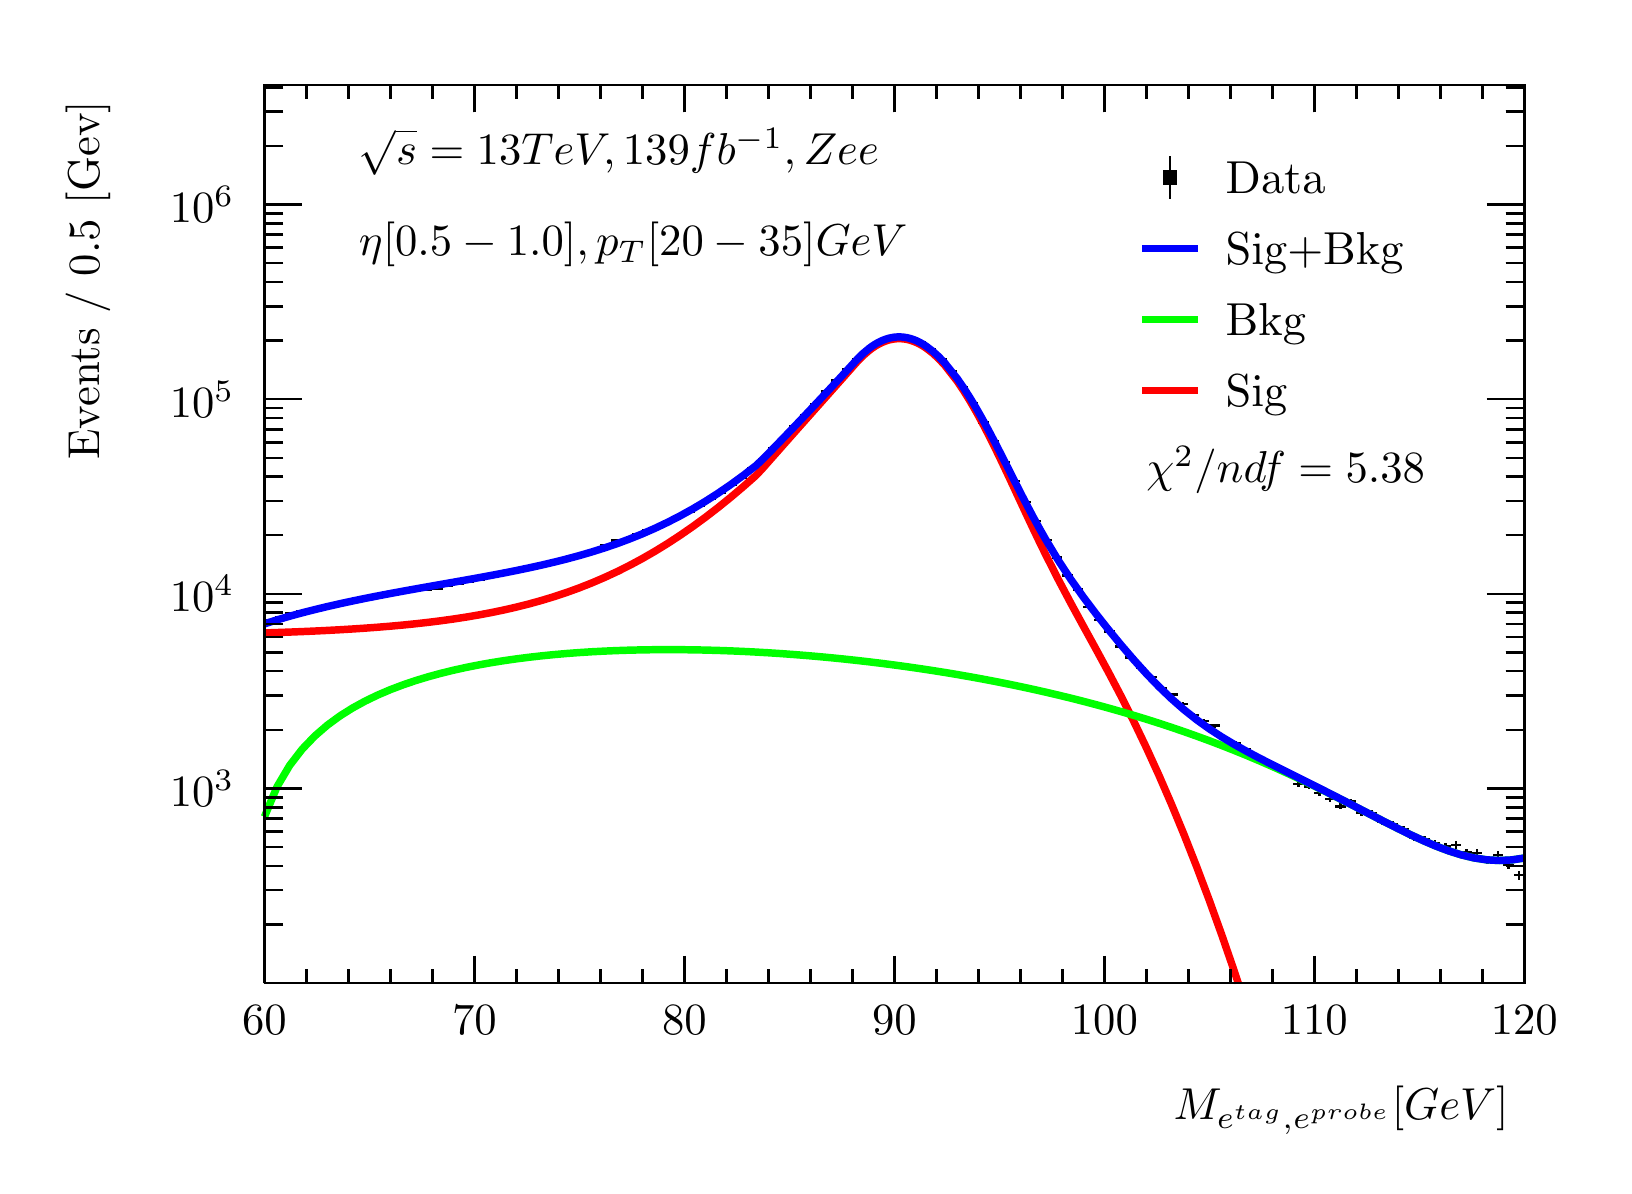
\begin{tikzpicture}
\pgfdeclareplotmark{cross} {
\pgfpathmoveto{\pgfpoint{-0.3\pgfplotmarksize}{\pgfplotmarksize}}
\pgfpathlineto{\pgfpoint{+0.3\pgfplotmarksize}{\pgfplotmarksize}}
\pgfpathlineto{\pgfpoint{+0.3\pgfplotmarksize}{0.3\pgfplotmarksize}}
\pgfpathlineto{\pgfpoint{+1\pgfplotmarksize}{0.3\pgfplotmarksize}}
\pgfpathlineto{\pgfpoint{+1\pgfplotmarksize}{-0.3\pgfplotmarksize}}
\pgfpathlineto{\pgfpoint{+0.3\pgfplotmarksize}{-0.3\pgfplotmarksize}}
\pgfpathlineto{\pgfpoint{+0.3\pgfplotmarksize}{-1.\pgfplotmarksize}}
\pgfpathlineto{\pgfpoint{-0.3\pgfplotmarksize}{-1.\pgfplotmarksize}}
\pgfpathlineto{\pgfpoint{-0.3\pgfplotmarksize}{-0.3\pgfplotmarksize}}
\pgfpathlineto{\pgfpoint{-1.\pgfplotmarksize}{-0.3\pgfplotmarksize}}
\pgfpathlineto{\pgfpoint{-1.\pgfplotmarksize}{0.3\pgfplotmarksize}}
\pgfpathlineto{\pgfpoint{-0.3\pgfplotmarksize}{0.3\pgfplotmarksize}}
\pgfpathclose
\pgfusepathqstroke
}
\pgfdeclareplotmark{cross*} {
\pgfpathmoveto{\pgfpoint{-0.3\pgfplotmarksize}{\pgfplotmarksize}}
\pgfpathlineto{\pgfpoint{+0.3\pgfplotmarksize}{\pgfplotmarksize}}
\pgfpathlineto{\pgfpoint{+0.3\pgfplotmarksize}{0.3\pgfplotmarksize}}
\pgfpathlineto{\pgfpoint{+1\pgfplotmarksize}{0.3\pgfplotmarksize}}
\pgfpathlineto{\pgfpoint{+1\pgfplotmarksize}{-0.3\pgfplotmarksize}}
\pgfpathlineto{\pgfpoint{+0.3\pgfplotmarksize}{-0.3\pgfplotmarksize}}
\pgfpathlineto{\pgfpoint{+0.3\pgfplotmarksize}{-1.\pgfplotmarksize}}
\pgfpathlineto{\pgfpoint{-0.3\pgfplotmarksize}{-1.\pgfplotmarksize}}
\pgfpathlineto{\pgfpoint{-0.3\pgfplotmarksize}{-0.3\pgfplotmarksize}}
\pgfpathlineto{\pgfpoint{-1.\pgfplotmarksize}{-0.3\pgfplotmarksize}}
\pgfpathlineto{\pgfpoint{-1.\pgfplotmarksize}{0.3\pgfplotmarksize}}
\pgfpathlineto{\pgfpoint{-0.3\pgfplotmarksize}{0.3\pgfplotmarksize}}
\pgfpathclose
\pgfusepathqfillstroke
}
\pgfdeclareplotmark{newstar} {
\pgfpathmoveto{\pgfqpoint{0pt}{\pgfplotmarksize}}
\pgfpathlineto{\pgfqpointpolar{44}{0.5\pgfplotmarksize}}
\pgfpathlineto{\pgfqpointpolar{18}{\pgfplotmarksize}}
\pgfpathlineto{\pgfqpointpolar{-20}{0.5\pgfplotmarksize}}
\pgfpathlineto{\pgfqpointpolar{-54}{\pgfplotmarksize}}
\pgfpathlineto{\pgfqpointpolar{-90}{0.5\pgfplotmarksize}}
\pgfpathlineto{\pgfqpointpolar{234}{\pgfplotmarksize}}
\pgfpathlineto{\pgfqpointpolar{198}{0.5\pgfplotmarksize}}
\pgfpathlineto{\pgfqpointpolar{162}{\pgfplotmarksize}}
\pgfpathlineto{\pgfqpointpolar{134}{0.5\pgfplotmarksize}}
\pgfpathclose
\pgfusepathqstroke
}
\pgfdeclareplotmark{newstar*} {
\pgfpathmoveto{\pgfqpoint{0pt}{\pgfplotmarksize}}
\pgfpathlineto{\pgfqpointpolar{44}{0.5\pgfplotmarksize}}
\pgfpathlineto{\pgfqpointpolar{18}{\pgfplotmarksize}}
\pgfpathlineto{\pgfqpointpolar{-20}{0.5\pgfplotmarksize}}
\pgfpathlineto{\pgfqpointpolar{-54}{\pgfplotmarksize}}
\pgfpathlineto{\pgfqpointpolar{-90}{0.5\pgfplotmarksize}}
\pgfpathlineto{\pgfqpointpolar{234}{\pgfplotmarksize}}
\pgfpathlineto{\pgfqpointpolar{198}{0.5\pgfplotmarksize}}
\pgfpathlineto{\pgfqpointpolar{162}{\pgfplotmarksize}}
\pgfpathlineto{\pgfqpointpolar{134}{0.5\pgfplotmarksize}}
\pgfpathclose
\pgfusepathqfillstroke
}
\definecolor{c}{rgb}{1,1,1};
\draw [color=c, fill=c] (0,0) rectangle (20,14.4361);
\draw [color=c, fill=c] (3,2.30977) rectangle (19,13.7143);
\definecolor{c}{rgb}{0,0,0};
\draw [c,line width=0.9] (3,2.30977) -- (3,13.7143) -- (19,13.7143) -- (19,2.30977) -- (3,2.30977);
\definecolor{c}{rgb}{1,1,1};
\draw [color=c, fill=c] (3,2.30977) rectangle (19,13.7143);
\definecolor{c}{rgb}{0,0,0};
\draw [c,line width=0.9] (3,2.30977) -- (3,13.7143) -- (19,13.7143) -- (19,2.30977) -- (3,2.30977);
\draw [c,line width=0.9] (3,2.30977) -- (19,2.30977);
\draw [c,line width=0.9] (3,2.65624) -- (3,2.30977);
\draw [c,line width=0.9] (3.53333,2.48301) -- (3.53333,2.30977);
\draw [c,line width=0.9] (4.06667,2.48301) -- (4.06667,2.30977);
\draw [c,line width=0.9] (4.6,2.48301) -- (4.6,2.30977);
\draw [c,line width=0.9] (5.13333,2.48301) -- (5.13333,2.30977);
\draw [c,line width=0.9] (5.66667,2.65624) -- (5.66667,2.30977);
\draw [c,line width=0.9] (6.2,2.48301) -- (6.2,2.30977);
\draw [c,line width=0.9] (6.73333,2.48301) -- (6.73333,2.30977);
\draw [c,line width=0.9] (7.26667,2.48301) -- (7.26667,2.30977);
\draw [c,line width=0.9] (7.8,2.48301) -- (7.8,2.30977);
\draw [c,line width=0.9] (8.33333,2.65624) -- (8.33333,2.30977);
\draw [c,line width=0.9] (8.86667,2.48301) -- (8.86667,2.30977);
\draw [c,line width=0.9] (9.4,2.48301) -- (9.4,2.30977);
\draw [c,line width=0.9] (9.93333,2.48301) -- (9.93333,2.30977);
\draw [c,line width=0.9] (10.4667,2.48301) -- (10.4667,2.30977);
\draw [c,line width=0.9] (11,2.65624) -- (11,2.30977);
\draw [c,line width=0.9] (11.5333,2.48301) -- (11.5333,2.30977);
\draw [c,line width=0.9] (12.0667,2.48301) -- (12.0667,2.30977);
\draw [c,line width=0.9] (12.6,2.48301) -- (12.6,2.30977);
\draw [c,line width=0.9] (13.1333,2.48301) -- (13.1333,2.30977);
\draw [c,line width=0.9] (13.6667,2.65624) -- (13.6667,2.30977);
\draw [c,line width=0.9] (14.2,2.48301) -- (14.2,2.30977);
\draw [c,line width=0.9] (14.7333,2.48301) -- (14.7333,2.30977);
\draw [c,line width=0.9] (15.2667,2.48301) -- (15.2667,2.30977);
\draw [c,line width=0.9] (15.8,2.48301) -- (15.8,2.30977);
\draw [c,line width=0.9] (16.3333,2.65624) -- (16.3333,2.30977);
\draw [c,line width=0.9] (16.8667,2.48301) -- (16.8667,2.30977);
\draw [c,line width=0.9] (17.4,2.48301) -- (17.4,2.30977);
\draw [c,line width=0.9] (17.9333,2.48301) -- (17.9333,2.30977);
\draw [c,line width=0.9] (18.4667,2.48301) -- (18.4667,2.30977);
\draw [c,line width=0.9] (19,2.65624) -- (19,2.30977);
\draw [anchor=base] (3,1.66015) node[scale=1.61424, color=c, rotate=0]{60};
\draw [anchor=base] (5.66667,1.66015) node[scale=1.61424, color=c, rotate=0]{70};
\draw [anchor=base] (8.33333,1.66015) node[scale=1.61424, color=c, rotate=0]{80};
\draw [anchor=base] (11,1.66015) node[scale=1.61424, color=c, rotate=0]{90};
\draw [anchor=base] (13.6667,1.66015) node[scale=1.61424, color=c, rotate=0]{100};
\draw [anchor=base] (16.3333,1.66015) node[scale=1.61424, color=c, rotate=0]{110};
\draw [anchor=base] (19,1.66015) node[scale=1.61424, color=c, rotate=0]{120};
\draw [anchor= east] (19,0.692932) node[scale=1.61424, color=c, rotate=0]{$M_{e^{tag}, e^{probe}}  [GeV]$};
\draw [c,line width=0.9] (3,13.7143) -- (19,13.7143);
\draw [c,line width=0.9] (3,13.3678) -- (3,13.7143);
\draw [c,line width=0.9] (3.53333,13.5411) -- (3.53333,13.7143);
\draw [c,line width=0.9] (4.06667,13.5411) -- (4.06667,13.7143);
\draw [c,line width=0.9] (4.6,13.5411) -- (4.6,13.7143);
\draw [c,line width=0.9] (5.13333,13.5411) -- (5.13333,13.7143);
\draw [c,line width=0.9] (5.66667,13.3678) -- (5.66667,13.7143);
\draw [c,line width=0.9] (6.2,13.5411) -- (6.2,13.7143);
\draw [c,line width=0.9] (6.73333,13.5411) -- (6.73333,13.7143);
\draw [c,line width=0.9] (7.26667,13.5411) -- (7.26667,13.7143);
\draw [c,line width=0.9] (7.8,13.5411) -- (7.8,13.7143);
\draw [c,line width=0.9] (8.33333,13.3678) -- (8.33333,13.7143);
\draw [c,line width=0.9] (8.86667,13.5411) -- (8.86667,13.7143);
\draw [c,line width=0.9] (9.4,13.5411) -- (9.4,13.7143);
\draw [c,line width=0.9] (9.93333,13.5411) -- (9.93333,13.7143);
\draw [c,line width=0.9] (10.4667,13.5411) -- (10.4667,13.7143);
\draw [c,line width=0.9] (11,13.3678) -- (11,13.7143);
\draw [c,line width=0.9] (11.5333,13.5411) -- (11.5333,13.7143);
\draw [c,line width=0.9] (12.0667,13.5411) -- (12.0667,13.7143);
\draw [c,line width=0.9] (12.6,13.5411) -- (12.6,13.7143);
\draw [c,line width=0.9] (13.1333,13.5411) -- (13.1333,13.7143);
\draw [c,line width=0.9] (13.6667,13.3678) -- (13.6667,13.7143);
\draw [c,line width=0.9] (14.2,13.5411) -- (14.2,13.7143);
\draw [c,line width=0.9] (14.7333,13.5411) -- (14.7333,13.7143);
\draw [c,line width=0.9] (15.2667,13.5411) -- (15.2667,13.7143);
\draw [c,line width=0.9] (15.8,13.5411) -- (15.8,13.7143);
\draw [c,line width=0.9] (16.3333,13.3678) -- (16.3333,13.7143);
\draw [c,line width=0.9] (16.8667,13.5411) -- (16.8667,13.7143);
\draw [c,line width=0.9] (17.4,13.5411) -- (17.4,13.7143);
\draw [c,line width=0.9] (17.9333,13.5411) -- (17.9333,13.7143);
\draw [c,line width=0.9] (18.4667,13.5411) -- (18.4667,13.7143);
\draw [c,line width=0.9] (19,13.3678) -- (19,13.7143);
\draw [c,line width=0.9] (3,2.30977) -- (3,13.7143);
\draw [c,line width=0.9] (3.237,3.05385) -- (3,3.05385);
\draw [c,line width=0.9] (3.237,3.48911) -- (3,3.48911);
\draw [c,line width=0.9] (3.237,3.79793) -- (3,3.79793);
\draw [c,line width=0.9] (3.237,4.03747) -- (3,4.03747);
\draw [c,line width=0.9] (3.237,4.23319) -- (3,4.23319);
\draw [c,line width=0.9] (3.237,4.39867) -- (3,4.39867);
\draw [c,line width=0.9] (3.237,4.54201) -- (3,4.54201);
\draw [c,line width=0.9] (3.237,4.66845) -- (3,4.66845);
\draw [c,line width=0.9] (3.474,4.78155) -- (3,4.78155);
\draw [anchor= east] (2.82,4.78155) node[scale=1.61424, color=c, rotate=0]{$10^{3}$};
\draw [c,line width=0.9] (3.237,5.52563) -- (3,5.52563);
\draw [c,line width=0.9] (3.237,5.96089) -- (3,5.96089);
\draw [c,line width=0.9] (3.237,6.26971) -- (3,6.26971);
\draw [c,line width=0.9] (3.237,6.50925) -- (3,6.50925);
\draw [c,line width=0.9] (3.237,6.70497) -- (3,6.70497);
\draw [c,line width=0.9] (3.237,6.87045) -- (3,6.87045);
\draw [c,line width=0.9] (3.237,7.01379) -- (3,7.01379);
\draw [c,line width=0.9] (3.237,7.14023) -- (3,7.14023);
\draw [c,line width=0.9] (3.474,7.25333) -- (3,7.25333);
\draw [anchor= east] (2.82,7.25333) node[scale=1.61424, color=c, rotate=0]{$10^{4}$};
\draw [c,line width=0.9] (3.237,7.99741) -- (3,7.99741);
\draw [c,line width=0.9] (3.237,8.43267) -- (3,8.43267);
\draw [c,line width=0.9] (3.237,8.74149) -- (3,8.74149);
\draw [c,line width=0.9] (3.237,8.98103) -- (3,8.98103);
\draw [c,line width=0.9] (3.237,9.17675) -- (3,9.17675);
\draw [c,line width=0.9] (3.237,9.34223) -- (3,9.34223);
\draw [c,line width=0.9] (3.237,9.48557) -- (3,9.48557);
\draw [c,line width=0.9] (3.237,9.61201) -- (3,9.61201);
\draw [c,line width=0.9] (3.474,9.72511) -- (3,9.72511);
\draw [anchor= east] (2.82,9.72511) node[scale=1.61424, color=c, rotate=0]{$10^{5}$};
\draw [c,line width=0.9] (3.237,10.4692) -- (3,10.4692);
\draw [c,line width=0.9] (3.237,10.9044) -- (3,10.9044);
\draw [c,line width=0.9] (3.237,11.2133) -- (3,11.2133);
\draw [c,line width=0.9] (3.237,11.4528) -- (3,11.4528);
\draw [c,line width=0.9] (3.237,11.6485) -- (3,11.6485);
\draw [c,line width=0.9] (3.237,11.814) -- (3,11.814);
\draw [c,line width=0.9] (3.237,11.9574) -- (3,11.9574);
\draw [c,line width=0.9] (3.237,12.0838) -- (3,12.0838);
\draw [c,line width=0.9] (3.474,12.1969) -- (3,12.1969);
\draw [anchor= east] (2.82,12.1969) node[scale=1.61424, color=c, rotate=0]{$10^{6}$};
\draw [c,line width=0.9] (3.237,12.941) -- (3,12.941);
\draw [c,line width=0.9] (3.237,13.3762) -- (3,13.3762);
\draw [c,line width=0.9] (3.237,13.6851) -- (3,13.6851);
\draw [anchor= east] (0.76,13.7143) node[scale=1.61424, color=c, rotate=90]{Events / 0.5 [Gev]};
\draw [c,line width=0.9] (19,2.30977) -- (19,13.7143);
\draw [c,line width=0.9] (18.763,3.05385) -- (19,3.05385);
\draw [c,line width=0.9] (18.763,3.48911) -- (19,3.48911);
\draw [c,line width=0.9] (18.763,3.79793) -- (19,3.79793);
\draw [c,line width=0.9] (18.763,4.03747) -- (19,4.03747);
\draw [c,line width=0.9] (18.763,4.23319) -- (19,4.23319);
\draw [c,line width=0.9] (18.763,4.39867) -- (19,4.39867);
\draw [c,line width=0.9] (18.763,4.54201) -- (19,4.54201);
\draw [c,line width=0.9] (18.763,4.66845) -- (19,4.66845);
\draw [c,line width=0.9] (18.526,4.78155) -- (19,4.78155);
\draw [c,line width=0.9] (18.763,5.52563) -- (19,5.52563);
\draw [c,line width=0.9] (18.763,5.96089) -- (19,5.96089);
\draw [c,line width=0.9] (18.763,6.26971) -- (19,6.26971);
\draw [c,line width=0.9] (18.763,6.50925) -- (19,6.50925);
\draw [c,line width=0.9] (18.763,6.70497) -- (19,6.70497);
\draw [c,line width=0.9] (18.763,6.87045) -- (19,6.87045);
\draw [c,line width=0.9] (18.763,7.01379) -- (19,7.01379);
\draw [c,line width=0.9] (18.763,7.14023) -- (19,7.14023);
\draw [c,line width=0.9] (18.526,7.25333) -- (19,7.25333);
\draw [c,line width=0.9] (18.763,7.99741) -- (19,7.99741);
\draw [c,line width=0.9] (18.763,8.43267) -- (19,8.43267);
\draw [c,line width=0.9] (18.763,8.74149) -- (19,8.74149);
\draw [c,line width=0.9] (18.763,8.98103) -- (19,8.98103);
\draw [c,line width=0.9] (18.763,9.17675) -- (19,9.17675);
\draw [c,line width=0.9] (18.763,9.34223) -- (19,9.34223);
\draw [c,line width=0.9] (18.763,9.48557) -- (19,9.48557);
\draw [c,line width=0.9] (18.763,9.61201) -- (19,9.61201);
\draw [c,line width=0.9] (18.526,9.72511) -- (19,9.72511);
\draw [c,line width=0.9] (18.763,10.4692) -- (19,10.4692);
\draw [c,line width=0.9] (18.763,10.9044) -- (19,10.9044);
\draw [c,line width=0.9] (18.763,11.2133) -- (19,11.2133);
\draw [c,line width=0.9] (18.763,11.4528) -- (19,11.4528);
\draw [c,line width=0.9] (18.763,11.6485) -- (19,11.6485);
\draw [c,line width=0.9] (18.763,11.814) -- (19,11.814);
\draw [c,line width=0.9] (18.763,11.9574) -- (19,11.9574);
\draw [c,line width=0.9] (18.763,12.0838) -- (19,12.0838);
\draw [c,line width=0.9] (18.526,12.1969) -- (19,12.1969);
\draw [c,line width=0.9] (18.763,12.941) -- (19,12.941);
\draw [c,line width=0.9] (18.763,13.3762) -- (19,13.3762);
\draw [c,line width=0.9] (18.763,13.6851) -- (19,13.6851);
\draw [c,line width=0.9] (3.06667,6.92297) -- (3,6.92297);
\draw [c,line width=0.9] (3,6.92297) -- (3,6.92297);
\draw [c,line width=0.9] (3.06667,6.92297) -- (3.13333,6.92297);
\draw [c,line width=0.9] (3.13333,6.92297) -- (3.13333,6.92297);
\draw [c,line width=0.9] (3.06667,6.92297) -- (3.06667,6.93549);
\draw [c,line width=0.9] (3.06667,6.93549) -- (3.06667,6.93549);
\draw [c,line width=0.9] (3.06667,6.92297) -- (3.06667,6.91045);
\draw [c,line width=0.9] (3.06667,6.91045) -- (3.06667,6.91045);
\draw [c,line width=0.9] (3.2,6.95788) -- (3.13333,6.95788);
\draw [c,line width=0.9] (3.13333,6.95788) -- (3.13333,6.95788);
\draw [c,line width=0.9] (3.2,6.95788) -- (3.26667,6.95788);
\draw [c,line width=0.9] (3.26667,6.95788) -- (3.26667,6.95788);
\draw [c,line width=0.9] (3.2,6.95788) -- (3.2,6.9702);
\draw [c,line width=0.9] (3.2,6.9702) -- (3.2,6.9702);
\draw [c,line width=0.9] (3.2,6.95788) -- (3.2,6.94556);
\draw [c,line width=0.9] (3.2,6.94556) -- (3.2,6.94556);
\draw [c,line width=0.9] (3.33333,7.003) -- (3.26667,7.003);
\draw [c,line width=0.9] (3.26667,7.003) -- (3.26667,7.003);
\draw [c,line width=0.9] (3.33333,7.003) -- (3.4,7.003);
\draw [c,line width=0.9] (3.4,7.003) -- (3.4,7.003);
\draw [c,line width=0.9] (3.33333,7.003) -- (3.33333,7.01507);
\draw [c,line width=0.9] (3.33333,7.01507) -- (3.33333,7.01507);
\draw [c,line width=0.9] (3.33333,7.003) -- (3.33333,6.99094);
\draw [c,line width=0.9] (3.33333,6.99094) -- (3.33333,6.99094);
\draw [c,line width=0.9] (3.46667,7.03281) -- (3.4,7.03281);
\draw [c,line width=0.9] (3.4,7.03281) -- (3.4,7.03281);
\draw [c,line width=0.9] (3.46667,7.03281) -- (3.53333,7.03281);
\draw [c,line width=0.9] (3.53333,7.03281) -- (3.53333,7.03281);
\draw [c,line width=0.9] (3.46667,7.03281) -- (3.46667,7.04471);
\draw [c,line width=0.9] (3.46667,7.04471) -- (3.46667,7.04471);
\draw [c,line width=0.9] (3.46667,7.03281) -- (3.46667,7.02092);
\draw [c,line width=0.9] (3.46667,7.02092) -- (3.46667,7.02092);
\draw [c,line width=0.9] (3.6,7.04748) -- (3.53333,7.04748);
\draw [c,line width=0.9] (3.53333,7.04748) -- (3.53333,7.04748);
\draw [c,line width=0.9] (3.6,7.04748) -- (3.66667,7.04748);
\draw [c,line width=0.9] (3.66667,7.04748) -- (3.66667,7.04748);
\draw [c,line width=0.9] (3.6,7.04748) -- (3.6,7.05929);
\draw [c,line width=0.9] (3.6,7.05929) -- (3.6,7.05929);
\draw [c,line width=0.9] (3.6,7.04748) -- (3.6,7.03566);
\draw [c,line width=0.9] (3.6,7.03566) -- (3.6,7.03566);
\draw [c,line width=0.9] (3.73333,7.06872) -- (3.66667,7.06872);
\draw [c,line width=0.9] (3.66667,7.06872) -- (3.66667,7.06872);
\draw [c,line width=0.9] (3.73333,7.06872) -- (3.8,7.06872);
\draw [c,line width=0.9] (3.8,7.06872) -- (3.8,7.06872);
\draw [c,line width=0.9] (3.73333,7.06872) -- (3.73333,7.08042);
\draw [c,line width=0.9] (3.73333,7.08042) -- (3.73333,7.08042);
\draw [c,line width=0.9] (3.73333,7.06872) -- (3.73333,7.05702);
\draw [c,line width=0.9] (3.73333,7.05702) -- (3.73333,7.05702);
\draw [c,line width=0.9] (3.86667,7.12207) -- (3.8,7.12207);
\draw [c,line width=0.9] (3.8,7.12207) -- (3.8,7.12207);
\draw [c,line width=0.9] (3.86667,7.12207) -- (3.93333,7.12207);
\draw [c,line width=0.9] (3.93333,7.12207) -- (3.93333,7.12207);
\draw [c,line width=0.9] (3.86667,7.12207) -- (3.86667,7.13348);
\draw [c,line width=0.9] (3.86667,7.13348) -- (3.86667,7.13348);
\draw [c,line width=0.9] (3.86667,7.12207) -- (3.86667,7.11066);
\draw [c,line width=0.9] (3.86667,7.11066) -- (3.86667,7.11066);
\draw [c,line width=0.9] (4,7.13856) -- (3.93333,7.13856);
\draw [c,line width=0.9] (3.93333,7.13856) -- (3.93333,7.13856);
\draw [c,line width=0.9] (4,7.13856) -- (4.06667,7.13856);
\draw [c,line width=0.9] (4.06667,7.13856) -- (4.06667,7.13856);
\draw [c,line width=0.9] (4,7.13856) -- (4,7.14988);
\draw [c,line width=0.9] (4,7.14988) -- (4,7.14988);
\draw [c,line width=0.9] (4,7.13856) -- (4,7.12723);
\draw [c,line width=0.9] (4,7.12723) -- (4,7.12723);
\draw [c,line width=0.9] (4.13333,7.16709) -- (4.06667,7.16709);
\draw [c,line width=0.9] (4.06667,7.16709) -- (4.06667,7.16709);
\draw [c,line width=0.9] (4.13333,7.16709) -- (4.2,7.16709);
\draw [c,line width=0.9] (4.2,7.16709) -- (4.2,7.16709);
\draw [c,line width=0.9] (4.13333,7.16709) -- (4.13333,7.17826);
\draw [c,line width=0.9] (4.13333,7.17826) -- (4.13333,7.17826);
\draw [c,line width=0.9] (4.13333,7.16709) -- (4.13333,7.15591);
\draw [c,line width=0.9] (4.13333,7.15591) -- (4.13333,7.15591);
\draw [c,line width=0.9] (4.26667,7.1909) -- (4.2,7.1909);
\draw [c,line width=0.9] (4.2,7.1909) -- (4.2,7.1909);
\draw [c,line width=0.9] (4.26667,7.1909) -- (4.33333,7.1909);
\draw [c,line width=0.9] (4.33333,7.1909) -- (4.33333,7.1909);
\draw [c,line width=0.9] (4.26667,7.1909) -- (4.26667,7.20195);
\draw [c,line width=0.9] (4.26667,7.20195) -- (4.26667,7.20195);
\draw [c,line width=0.9] (4.26667,7.1909) -- (4.26667,7.17985);
\draw [c,line width=0.9] (4.26667,7.17985) -- (4.26667,7.17985);
\draw [c,line width=0.9] (4.4,7.19782) -- (4.33333,7.19782);
\draw [c,line width=0.9] (4.33333,7.19782) -- (4.33333,7.19782);
\draw [c,line width=0.9] (4.4,7.19782) -- (4.46667,7.19782);
\draw [c,line width=0.9] (4.46667,7.19782) -- (4.46667,7.19782);
\draw [c,line width=0.9] (4.4,7.19782) -- (4.4,7.20883);
\draw [c,line width=0.9] (4.4,7.20883) -- (4.4,7.20883);
\draw [c,line width=0.9] (4.4,7.19782) -- (4.4,7.1868);
\draw [c,line width=0.9] (4.4,7.1868) -- (4.4,7.1868);
\draw [c,line width=0.9] (4.53333,7.24092) -- (4.46667,7.24092);
\draw [c,line width=0.9] (4.46667,7.24092) -- (4.46667,7.24092);
\draw [c,line width=0.9] (4.53333,7.24092) -- (4.6,7.24092);
\draw [c,line width=0.9] (4.6,7.24092) -- (4.6,7.24092);
\draw [c,line width=0.9] (4.53333,7.24092) -- (4.53333,7.25171);
\draw [c,line width=0.9] (4.53333,7.25171) -- (4.53333,7.25171);
\draw [c,line width=0.9] (4.53333,7.24092) -- (4.53333,7.23012);
\draw [c,line width=0.9] (4.53333,7.23012) -- (4.53333,7.23012);
\draw [c,line width=0.9] (4.66667,7.25194) -- (4.6,7.25194);
\draw [c,line width=0.9] (4.6,7.25194) -- (4.6,7.25194);
\draw [c,line width=0.9] (4.66667,7.25194) -- (4.73333,7.25194);
\draw [c,line width=0.9] (4.73333,7.25194) -- (4.73333,7.25194);
\draw [c,line width=0.9] (4.66667,7.25194) -- (4.66667,7.26268);
\draw [c,line width=0.9] (4.66667,7.26268) -- (4.66667,7.26268);
\draw [c,line width=0.9] (4.66667,7.25194) -- (4.66667,7.24119);
\draw [c,line width=0.9] (4.66667,7.24119) -- (4.66667,7.24119);
\draw [c,line width=0.9] (4.8,7.30202) -- (4.73333,7.30202);
\draw [c,line width=0.9] (4.73333,7.30202) -- (4.73333,7.30202);
\draw [c,line width=0.9] (4.8,7.30202) -- (4.86667,7.30202);
\draw [c,line width=0.9] (4.86667,7.30202) -- (4.86667,7.30202);
\draw [c,line width=0.9] (4.8,7.30202) -- (4.8,7.31252);
\draw [c,line width=0.9] (4.8,7.31252) -- (4.8,7.31252);
\draw [c,line width=0.9] (4.8,7.30202) -- (4.8,7.29153);
\draw [c,line width=0.9] (4.8,7.29153) -- (4.8,7.29153);
\draw [c,line width=0.9] (4.93333,7.31558) -- (4.86667,7.31558);
\draw [c,line width=0.9] (4.86667,7.31558) -- (4.86667,7.31558);
\draw [c,line width=0.9] (4.93333,7.31558) -- (5,7.31558);
\draw [c,line width=0.9] (5,7.31558) -- (5,7.31558);
\draw [c,line width=0.9] (4.93333,7.31558) -- (4.93333,7.32601);
\draw [c,line width=0.9] (4.93333,7.32601) -- (4.93333,7.32601);
\draw [c,line width=0.9] (4.93333,7.31558) -- (4.93333,7.30515);
\draw [c,line width=0.9] (4.93333,7.30515) -- (4.93333,7.30515);
\draw [c,line width=0.9] (5.06667,7.30571) -- (5,7.30571);
\draw [c,line width=0.9] (5,7.30571) -- (5,7.30571);
\draw [c,line width=0.9] (5.06667,7.30571) -- (5.13333,7.30571);
\draw [c,line width=0.9] (5.13333,7.30571) -- (5.13333,7.30571);
\draw [c,line width=0.9] (5.06667,7.30571) -- (5.06667,7.31618);
\draw [c,line width=0.9] (5.06667,7.31618) -- (5.06667,7.31618);
\draw [c,line width=0.9] (5.06667,7.30571) -- (5.06667,7.29523);
\draw [c,line width=0.9] (5.06667,7.29523) -- (5.06667,7.29523);
\draw [c,line width=0.9] (5.2,7.32355) -- (5.13333,7.32355);
\draw [c,line width=0.9] (5.13333,7.32355) -- (5.13333,7.32355);
\draw [c,line width=0.9] (5.2,7.32355) -- (5.26667,7.32355);
\draw [c,line width=0.9] (5.26667,7.32355) -- (5.26667,7.32355);
\draw [c,line width=0.9] (5.2,7.32355) -- (5.2,7.33394);
\draw [c,line width=0.9] (5.2,7.33394) -- (5.2,7.33394);
\draw [c,line width=0.9] (5.2,7.32355) -- (5.2,7.31316);
\draw [c,line width=0.9] (5.2,7.31316) -- (5.2,7.31316);
\draw [c,line width=0.9] (5.33333,7.35643) -- (5.26667,7.35643);
\draw [c,line width=0.9] (5.26667,7.35643) -- (5.26667,7.35643);
\draw [c,line width=0.9] (5.33333,7.35643) -- (5.4,7.35643);
\draw [c,line width=0.9] (5.4,7.35643) -- (5.4,7.35643);
\draw [c,line width=0.9] (5.33333,7.35643) -- (5.33333,7.36666);
\draw [c,line width=0.9] (5.33333,7.36666) -- (5.33333,7.36666);
\draw [c,line width=0.9] (5.33333,7.35643) -- (5.33333,7.3462);
\draw [c,line width=0.9] (5.33333,7.3462) -- (5.33333,7.3462);
\draw [c,line width=0.9] (5.46667,7.38377) -- (5.4,7.38377);
\draw [c,line width=0.9] (5.4,7.38377) -- (5.4,7.38377);
\draw [c,line width=0.9] (5.46667,7.38377) -- (5.53333,7.38377);
\draw [c,line width=0.9] (5.53333,7.38377) -- (5.53333,7.38377);
\draw [c,line width=0.9] (5.46667,7.38377) -- (5.46667,7.39387);
\draw [c,line width=0.9] (5.46667,7.39387) -- (5.46667,7.39387);
\draw [c,line width=0.9] (5.46667,7.38377) -- (5.46667,7.37367);
\draw [c,line width=0.9] (5.46667,7.37367) -- (5.46667,7.37367);
\draw [c,line width=0.9] (5.6,7.40932) -- (5.53333,7.40932);
\draw [c,line width=0.9] (5.53333,7.40932) -- (5.53333,7.40932);
\draw [c,line width=0.9] (5.6,7.40932) -- (5.66667,7.40932);
\draw [c,line width=0.9] (5.66667,7.40932) -- (5.66667,7.40932);
\draw [c,line width=0.9] (5.6,7.40932) -- (5.6,7.4193);
\draw [c,line width=0.9] (5.6,7.4193) -- (5.6,7.4193);
\draw [c,line width=0.9] (5.6,7.40932) -- (5.6,7.39934);
\draw [c,line width=0.9] (5.6,7.39934) -- (5.6,7.39934);
\draw [c,line width=0.9] (5.73333,7.43772) -- (5.66667,7.43772);
\draw [c,line width=0.9] (5.66667,7.43772) -- (5.66667,7.43772);
\draw [c,line width=0.9] (5.73333,7.43772) -- (5.8,7.43772);
\draw [c,line width=0.9] (5.8,7.43772) -- (5.8,7.43772);
\draw [c,line width=0.9] (5.73333,7.43772) -- (5.73333,7.44757);
\draw [c,line width=0.9] (5.73333,7.44757) -- (5.73333,7.44757);
\draw [c,line width=0.9] (5.73333,7.43772) -- (5.73333,7.42787);
\draw [c,line width=0.9] (5.73333,7.42787) -- (5.73333,7.42787);
\draw [c,line width=0.9] (5.86667,7.4711) -- (5.8,7.4711);
\draw [c,line width=0.9] (5.8,7.4711) -- (5.8,7.4711);
\draw [c,line width=0.9] (5.86667,7.4711) -- (5.93333,7.4711);
\draw [c,line width=0.9] (5.93333,7.4711) -- (5.93333,7.4711);
\draw [c,line width=0.9] (5.86667,7.4711) -- (5.86667,7.4808);
\draw [c,line width=0.9] (5.86667,7.4808) -- (5.86667,7.4808);
\draw [c,line width=0.9] (5.86667,7.4711) -- (5.86667,7.4614);
\draw [c,line width=0.9] (5.86667,7.4614) -- (5.86667,7.4614);
\draw [c,line width=0.9] (6,7.49887) -- (5.93333,7.49887);
\draw [c,line width=0.9] (5.93333,7.49887) -- (5.93333,7.49887);
\draw [c,line width=0.9] (6,7.49887) -- (6.06667,7.49887);
\draw [c,line width=0.9] (6.06667,7.49887) -- (6.06667,7.49887);
\draw [c,line width=0.9] (6,7.49887) -- (6,7.50844);
\draw [c,line width=0.9] (6,7.50844) -- (6,7.50844);
\draw [c,line width=0.9] (6,7.49887) -- (6,7.48929);
\draw [c,line width=0.9] (6,7.48929) -- (6,7.48929);
\draw [c,line width=0.9] (6.13333,7.53737) -- (6.06667,7.53737);
\draw [c,line width=0.9] (6.06667,7.53737) -- (6.06667,7.53737);
\draw [c,line width=0.9] (6.13333,7.53737) -- (6.2,7.53737);
\draw [c,line width=0.9] (6.2,7.53737) -- (6.2,7.53737);
\draw [c,line width=0.9] (6.13333,7.53737) -- (6.13333,7.54677);
\draw [c,line width=0.9] (6.13333,7.54677) -- (6.13333,7.54677);
\draw [c,line width=0.9] (6.13333,7.53737) -- (6.13333,7.52796);
\draw [c,line width=0.9] (6.13333,7.52796) -- (6.13333,7.52796);
\draw [c,line width=0.9] (6.26667,7.55169) -- (6.2,7.55169);
\draw [c,line width=0.9] (6.2,7.55169) -- (6.2,7.55169);
\draw [c,line width=0.9] (6.26667,7.55169) -- (6.33333,7.55169);
\draw [c,line width=0.9] (6.33333,7.55169) -- (6.33333,7.55169);
\draw [c,line width=0.9] (6.26667,7.55169) -- (6.26667,7.56103);
\draw [c,line width=0.9] (6.26667,7.56103) -- (6.26667,7.56103);
\draw [c,line width=0.9] (6.26667,7.55169) -- (6.26667,7.54235);
\draw [c,line width=0.9] (6.26667,7.54235) -- (6.26667,7.54235);
\draw [c,line width=0.9] (6.4,7.59901) -- (6.33333,7.59901);
\draw [c,line width=0.9] (6.33333,7.59901) -- (6.33333,7.59901);
\draw [c,line width=0.9] (6.4,7.59901) -- (6.46667,7.59901);
\draw [c,line width=0.9] (6.46667,7.59901) -- (6.46667,7.59901);
\draw [c,line width=0.9] (6.4,7.59901) -- (6.4,7.60814);
\draw [c,line width=0.9] (6.4,7.60814) -- (6.4,7.60814);
\draw [c,line width=0.9] (6.4,7.59901) -- (6.4,7.58987);
\draw [c,line width=0.9] (6.4,7.58987) -- (6.4,7.58987);
\draw [c,line width=0.9] (6.53333,7.6296) -- (6.46667,7.6296);
\draw [c,line width=0.9] (6.46667,7.6296) -- (6.46667,7.6296);
\draw [c,line width=0.9] (6.53333,7.6296) -- (6.6,7.6296);
\draw [c,line width=0.9] (6.6,7.6296) -- (6.6,7.6296);
\draw [c,line width=0.9] (6.53333,7.6296) -- (6.53333,7.63861);
\draw [c,line width=0.9] (6.53333,7.63861) -- (6.53333,7.63861);
\draw [c,line width=0.9] (6.53333,7.6296) -- (6.53333,7.6206);
\draw [c,line width=0.9] (6.53333,7.6206) -- (6.53333,7.6206);
\draw [c,line width=0.9] (6.66667,7.67091) -- (6.6,7.67091);
\draw [c,line width=0.9] (6.6,7.67091) -- (6.6,7.67091);
\draw [c,line width=0.9] (6.66667,7.67091) -- (6.73333,7.67091);
\draw [c,line width=0.9] (6.73333,7.67091) -- (6.73333,7.67091);
\draw [c,line width=0.9] (6.66667,7.67091) -- (6.66667,7.67975);
\draw [c,line width=0.9] (6.66667,7.67975) -- (6.66667,7.67975);
\draw [c,line width=0.9] (6.66667,7.67091) -- (6.66667,7.66208);
\draw [c,line width=0.9] (6.66667,7.66208) -- (6.66667,7.66208);
\draw [c,line width=0.9] (6.8,7.69309) -- (6.73333,7.69309);
\draw [c,line width=0.9] (6.73333,7.69309) -- (6.73333,7.69309);
\draw [c,line width=0.9] (6.8,7.69309) -- (6.86667,7.69309);
\draw [c,line width=0.9] (6.86667,7.69309) -- (6.86667,7.69309);
\draw [c,line width=0.9] (6.8,7.69309) -- (6.8,7.70184);
\draw [c,line width=0.9] (6.8,7.70184) -- (6.8,7.70184);
\draw [c,line width=0.9] (6.8,7.69309) -- (6.8,7.68434);
\draw [c,line width=0.9] (6.8,7.68434) -- (6.8,7.68434);
\draw [c,line width=0.9] (6.93333,7.73324) -- (6.86667,7.73324);
\draw [c,line width=0.9] (6.86667,7.73324) -- (6.86667,7.73324);
\draw [c,line width=0.9] (6.93333,7.73324) -- (7,7.73324);
\draw [c,line width=0.9] (7,7.73324) -- (7,7.73324);
\draw [c,line width=0.9] (6.93333,7.73324) -- (6.93333,7.74182);
\draw [c,line width=0.9] (6.93333,7.74182) -- (6.93333,7.74182);
\draw [c,line width=0.9] (6.93333,7.73324) -- (6.93333,7.72465);
\draw [c,line width=0.9] (6.93333,7.72465) -- (6.93333,7.72465);
\draw [c,line width=0.9] (7.06667,7.76563) -- (7,7.76563);
\draw [c,line width=0.9] (7,7.76563) -- (7,7.76563);
\draw [c,line width=0.9] (7.06667,7.76563) -- (7.13333,7.76563);
\draw [c,line width=0.9] (7.13333,7.76563) -- (7.13333,7.76563);
\draw [c,line width=0.9] (7.06667,7.76563) -- (7.06667,7.77408);
\draw [c,line width=0.9] (7.06667,7.77408) -- (7.06667,7.77408);
\draw [c,line width=0.9] (7.06667,7.76563) -- (7.06667,7.75717);
\draw [c,line width=0.9] (7.06667,7.75717) -- (7.06667,7.75717);
\draw [c,line width=0.9] (7.2,7.8048) -- (7.13333,7.8048);
\draw [c,line width=0.9] (7.13333,7.8048) -- (7.13333,7.8048);
\draw [c,line width=0.9] (7.2,7.8048) -- (7.26667,7.8048);
\draw [c,line width=0.9] (7.26667,7.8048) -- (7.26667,7.8048);
\draw [c,line width=0.9] (7.2,7.8048) -- (7.2,7.81311);
\draw [c,line width=0.9] (7.2,7.81311) -- (7.2,7.81311);
\draw [c,line width=0.9] (7.2,7.8048) -- (7.2,7.7965);
\draw [c,line width=0.9] (7.2,7.7965) -- (7.2,7.7965);
\draw [c,line width=0.9] (7.33333,7.8642) -- (7.26667,7.8642);
\draw [c,line width=0.9] (7.26667,7.8642) -- (7.26667,7.8642);
\draw [c,line width=0.9] (7.33333,7.8642) -- (7.4,7.8642);
\draw [c,line width=0.9] (7.4,7.8642) -- (7.4,7.8642);
\draw [c,line width=0.9] (7.33333,7.8642) -- (7.33333,7.87228);
\draw [c,line width=0.9] (7.33333,7.87228) -- (7.33333,7.87228);
\draw [c,line width=0.9] (7.33333,7.8642) -- (7.33333,7.85613);
\draw [c,line width=0.9] (7.33333,7.85613) -- (7.33333,7.85613);
\draw [c,line width=0.9] (7.46667,7.92739) -- (7.4,7.92739);
\draw [c,line width=0.9] (7.4,7.92739) -- (7.4,7.92739);
\draw [c,line width=0.9] (7.46667,7.92739) -- (7.53333,7.92739);
\draw [c,line width=0.9] (7.53333,7.92739) -- (7.53333,7.92739);
\draw [c,line width=0.9] (7.46667,7.92739) -- (7.46667,7.93523);
\draw [c,line width=0.9] (7.46667,7.93523) -- (7.46667,7.93523);
\draw [c,line width=0.9] (7.46667,7.92739) -- (7.46667,7.91954);
\draw [c,line width=0.9] (7.46667,7.91954) -- (7.46667,7.91954);
\draw [c,line width=0.9] (7.6,7.94843) -- (7.53333,7.94843);
\draw [c,line width=0.9] (7.53333,7.94843) -- (7.53333,7.94843);
\draw [c,line width=0.9] (7.6,7.94843) -- (7.66667,7.94843);
\draw [c,line width=0.9] (7.66667,7.94843) -- (7.66667,7.94843);
\draw [c,line width=0.9] (7.6,7.94843) -- (7.6,7.9562);
\draw [c,line width=0.9] (7.6,7.9562) -- (7.6,7.9562);
\draw [c,line width=0.9] (7.6,7.94843) -- (7.6,7.94067);
\draw [c,line width=0.9] (7.6,7.94067) -- (7.6,7.94067);
\draw [c,line width=0.9] (7.73333,8.00655) -- (7.66667,8.00655);
\draw [c,line width=0.9] (7.66667,8.00655) -- (7.66667,8.00655);
\draw [c,line width=0.9] (7.73333,8.00655) -- (7.8,8.00655);
\draw [c,line width=0.9] (7.8,8.00655) -- (7.8,8.00655);
\draw [c,line width=0.9] (7.73333,8.00655) -- (7.73333,8.01411);
\draw [c,line width=0.9] (7.73333,8.01411) -- (7.73333,8.01411);
\draw [c,line width=0.9] (7.73333,8.00655) -- (7.73333,7.99899);
\draw [c,line width=0.9] (7.73333,7.99899) -- (7.73333,7.99899);
\draw [c,line width=0.9] (7.86667,8.05702) -- (7.8,8.05702);
\draw [c,line width=0.9] (7.8,8.05702) -- (7.8,8.05702);
\draw [c,line width=0.9] (7.86667,8.05702) -- (7.93333,8.05702);
\draw [c,line width=0.9] (7.93333,8.05702) -- (7.93333,8.05702);
\draw [c,line width=0.9] (7.86667,8.05702) -- (7.86667,8.0644);
\draw [c,line width=0.9] (7.86667,8.0644) -- (7.86667,8.0644);
\draw [c,line width=0.9] (7.86667,8.05702) -- (7.86667,8.04964);
\draw [c,line width=0.9] (7.86667,8.04964) -- (7.86667,8.04964);
\draw [c,line width=0.9] (8,8.11619) -- (7.93333,8.11619);
\draw [c,line width=0.9] (7.93333,8.11619) -- (7.93333,8.11619);
\draw [c,line width=0.9] (8,8.11619) -- (8.06667,8.11619);
\draw [c,line width=0.9] (8.06667,8.11619) -- (8.06667,8.11619);
\draw [c,line width=0.9] (8,8.11619) -- (8,8.12337);
\draw [c,line width=0.9] (8,8.12337) -- (8,8.12337);
\draw [c,line width=0.9] (8,8.11619) -- (8,8.10901);
\draw [c,line width=0.9] (8,8.10901) -- (8,8.10901);
\draw [c,line width=0.9] (8.13333,8.17559) -- (8.06667,8.17559);
\draw [c,line width=0.9] (8.06667,8.17559) -- (8.06667,8.17559);
\draw [c,line width=0.9] (8.13333,8.17559) -- (8.2,8.17559);
\draw [c,line width=0.9] (8.2,8.17559) -- (8.2,8.17559);
\draw [c,line width=0.9] (8.13333,8.17559) -- (8.13333,8.18258);
\draw [c,line width=0.9] (8.13333,8.18258) -- (8.13333,8.18258);
\draw [c,line width=0.9] (8.13333,8.17559) -- (8.13333,8.1686);
\draw [c,line width=0.9] (8.13333,8.1686) -- (8.13333,8.1686);
\draw [c,line width=0.9] (8.26667,8.23803) -- (8.2,8.23803);
\draw [c,line width=0.9] (8.2,8.23803) -- (8.2,8.23803);
\draw [c,line width=0.9] (8.26667,8.23803) -- (8.33333,8.23803);
\draw [c,line width=0.9] (8.33333,8.23803) -- (8.33333,8.23803);
\draw [c,line width=0.9] (8.26667,8.23803) -- (8.26667,8.24481);
\draw [c,line width=0.9] (8.26667,8.24481) -- (8.26667,8.24481);
\draw [c,line width=0.9] (8.26667,8.23803) -- (8.26667,8.23124);
\draw [c,line width=0.9] (8.26667,8.23124) -- (8.26667,8.23124);
\draw [c,line width=0.9] (8.4,8.29853) -- (8.33333,8.29853);
\draw [c,line width=0.9] (8.33333,8.29853) -- (8.33333,8.29853);
\draw [c,line width=0.9] (8.4,8.29853) -- (8.46667,8.29853);
\draw [c,line width=0.9] (8.46667,8.29853) -- (8.46667,8.29853);
\draw [c,line width=0.9] (8.4,8.29853) -- (8.4,8.30513);
\draw [c,line width=0.9] (8.4,8.30513) -- (8.4,8.30513);
\draw [c,line width=0.9] (8.4,8.29853) -- (8.4,8.29193);
\draw [c,line width=0.9] (8.4,8.29193) -- (8.4,8.29193);
\draw [c,line width=0.9] (8.53333,8.37501) -- (8.46667,8.37501);
\draw [c,line width=0.9] (8.46667,8.37501) -- (8.46667,8.37501);
\draw [c,line width=0.9] (8.53333,8.37501) -- (8.6,8.37501);
\draw [c,line width=0.9] (8.6,8.37501) -- (8.6,8.37501);
\draw [c,line width=0.9] (8.53333,8.37501) -- (8.53333,8.38137);
\draw [c,line width=0.9] (8.53333,8.38137) -- (8.53333,8.38137);
\draw [c,line width=0.9] (8.53333,8.37501) -- (8.53333,8.36864);
\draw [c,line width=0.9] (8.53333,8.36864) -- (8.53333,8.36864);
\draw [c,line width=0.9] (8.66667,8.45977) -- (8.6,8.45977);
\draw [c,line width=0.9] (8.6,8.45977) -- (8.6,8.45977);
\draw [c,line width=0.9] (8.66667,8.45977) -- (8.73333,8.45977);
\draw [c,line width=0.9] (8.73333,8.45977) -- (8.73333,8.45977);
\draw [c,line width=0.9] (8.66667,8.45977) -- (8.66667,8.46589);
\draw [c,line width=0.9] (8.66667,8.46589) -- (8.66667,8.46589);
\draw [c,line width=0.9] (8.66667,8.45977) -- (8.66667,8.45365);
\draw [c,line width=0.9] (8.66667,8.45365) -- (8.66667,8.45365);
\draw [c,line width=0.9] (8.8,8.54221) -- (8.73333,8.54221);
\draw [c,line width=0.9] (8.73333,8.54221) -- (8.73333,8.54221);
\draw [c,line width=0.9] (8.8,8.54221) -- (8.86667,8.54221);
\draw [c,line width=0.9] (8.86667,8.54221) -- (8.86667,8.54221);
\draw [c,line width=0.9] (8.8,8.54221) -- (8.8,8.5481);
\draw [c,line width=0.9] (8.8,8.5481) -- (8.8,8.5481);
\draw [c,line width=0.9] (8.8,8.54221) -- (8.8,8.53633);
\draw [c,line width=0.9] (8.8,8.53633) -- (8.8,8.53633);
\draw [c,line width=0.9] (8.93333,8.63531) -- (8.86667,8.63531);
\draw [c,line width=0.9] (8.86667,8.63531) -- (8.86667,8.63531);
\draw [c,line width=0.9] (8.93333,8.63531) -- (9,8.63531);
\draw [c,line width=0.9] (9,8.63531) -- (9,8.63531);
\draw [c,line width=0.9] (8.93333,8.63531) -- (8.93333,8.64095);
\draw [c,line width=0.9] (8.93333,8.64095) -- (8.93333,8.64095);
\draw [c,line width=0.9] (8.93333,8.63531) -- (8.93333,8.62968);
\draw [c,line width=0.9] (8.93333,8.62968) -- (8.93333,8.62968);
\draw [c,line width=0.9] (9.06667,8.73319) -- (9,8.73319);
\draw [c,line width=0.9] (9,8.73319) -- (9,8.73319);
\draw [c,line width=0.9] (9.06667,8.73319) -- (9.13333,8.73319);
\draw [c,line width=0.9] (9.13333,8.73319) -- (9.13333,8.73319);
\draw [c,line width=0.9] (9.06667,8.73319) -- (9.06667,8.73858);
\draw [c,line width=0.9] (9.06667,8.73858) -- (9.06667,8.73858);
\draw [c,line width=0.9] (9.06667,8.73319) -- (9.06667,8.72781);
\draw [c,line width=0.9] (9.06667,8.72781) -- (9.06667,8.72781);
\draw [c,line width=0.9] (9.2,8.8518) -- (9.13333,8.8518);
\draw [c,line width=0.9] (9.13333,8.8518) -- (9.13333,8.8518);
\draw [c,line width=0.9] (9.2,8.8518) -- (9.26667,8.8518);
\draw [c,line width=0.9] (9.26667,8.8518) -- (9.26667,8.8518);
\draw [c,line width=0.9] (9.2,8.8518) -- (9.2,8.8569);
\draw [c,line width=0.9] (9.2,8.8569) -- (9.2,8.8569);
\draw [c,line width=0.9] (9.2,8.8518) -- (9.2,8.8467);
\draw [c,line width=0.9] (9.2,8.8467) -- (9.2,8.8467);
\draw [c,line width=0.9] (9.33333,8.9674) -- (9.26667,8.9674);
\draw [c,line width=0.9] (9.26667,8.9674) -- (9.26667,8.9674);
\draw [c,line width=0.9] (9.33333,8.9674) -- (9.4,8.9674);
\draw [c,line width=0.9] (9.4,8.9674) -- (9.4,8.9674);
\draw [c,line width=0.9] (9.33333,8.9674) -- (9.33333,8.97223);
\draw [c,line width=0.9] (9.33333,8.97223) -- (9.33333,8.97223);
\draw [c,line width=0.9] (9.33333,8.9674) -- (9.33333,8.96257);
\draw [c,line width=0.9] (9.33333,8.96257) -- (9.33333,8.96257);
\draw [c,line width=0.9] (9.46667,9.09881) -- (9.4,9.09881);
\draw [c,line width=0.9] (9.4,9.09881) -- (9.4,9.09881);
\draw [c,line width=0.9] (9.46667,9.09881) -- (9.53333,9.09881);
\draw [c,line width=0.9] (9.53333,9.09881) -- (9.53333,9.09881);
\draw [c,line width=0.9] (9.46667,9.09881) -- (9.46667,9.10335);
\draw [c,line width=0.9] (9.46667,9.10335) -- (9.46667,9.10335);
\draw [c,line width=0.9] (9.46667,9.09881) -- (9.46667,9.09426);
\draw [c,line width=0.9] (9.46667,9.09426) -- (9.46667,9.09426);
\draw [c,line width=0.9] (9.6,9.22884) -- (9.53333,9.22884);
\draw [c,line width=0.9] (9.53333,9.22884) -- (9.53333,9.22884);
\draw [c,line width=0.9] (9.6,9.22884) -- (9.66667,9.22884);
\draw [c,line width=0.9] (9.66667,9.22884) -- (9.66667,9.22884);
\draw [c,line width=0.9] (9.6,9.22884) -- (9.6,9.23311);
\draw [c,line width=0.9] (9.6,9.23311) -- (9.6,9.23311);
\draw [c,line width=0.9] (9.6,9.22884) -- (9.6,9.22456);
\draw [c,line width=0.9] (9.6,9.22456) -- (9.6,9.22456);
\draw [c,line width=0.9] (9.73333,9.37732) -- (9.66667,9.37732);
\draw [c,line width=0.9] (9.66667,9.37732) -- (9.66667,9.37732);
\draw [c,line width=0.9] (9.73333,9.37732) -- (9.8,9.37732);
\draw [c,line width=0.9] (9.8,9.37732) -- (9.8,9.37732);
\draw [c,line width=0.9] (9.73333,9.37732) -- (9.73333,9.38131);
\draw [c,line width=0.9] (9.73333,9.38131) -- (9.73333,9.38131);
\draw [c,line width=0.9] (9.73333,9.37732) -- (9.73333,9.37333);
\draw [c,line width=0.9] (9.73333,9.37333) -- (9.73333,9.37333);
\draw [c,line width=0.9] (9.86667,9.52124) -- (9.8,9.52124);
\draw [c,line width=0.9] (9.8,9.52124) -- (9.8,9.52124);
\draw [c,line width=0.9] (9.86667,9.52124) -- (9.93333,9.52124);
\draw [c,line width=0.9] (9.93333,9.52124) -- (9.93333,9.52124);
\draw [c,line width=0.9] (9.86667,9.52124) -- (9.86667,9.52498);
\draw [c,line width=0.9] (9.86667,9.52498) -- (9.86667,9.52498);
\draw [c,line width=0.9] (9.86667,9.52124) -- (9.86667,9.51751);
\draw [c,line width=0.9] (9.86667,9.51751) -- (9.86667,9.51751);
\draw [c,line width=0.9] (10,9.66398) -- (9.93333,9.66398);
\draw [c,line width=0.9] (9.93333,9.66398) -- (9.93333,9.66398);
\draw [c,line width=0.9] (10,9.66398) -- (10.0667,9.66398);
\draw [c,line width=0.9] (10.0667,9.66398) -- (10.0667,9.66398);
\draw [c,line width=0.9] (10,9.66398) -- (10,9.66747);
\draw [c,line width=0.9] (10,9.66747) -- (10,9.66747);
\draw [c,line width=0.9] (10,9.66398) -- (10,9.66048);
\draw [c,line width=0.9] (10,9.66048) -- (10,9.66048);
\draw [c,line width=0.9] (10.1333,9.82371) -- (10.0667,9.82371);
\draw [c,line width=0.9] (10.0667,9.82371) -- (10.0667,9.82371);
\draw [c,line width=0.9] (10.1333,9.82371) -- (10.2,9.82371);
\draw [c,line width=0.9] (10.2,9.82371) -- (10.2,9.82371);
\draw [c,line width=0.9] (10.1333,9.82371) -- (10.1333,9.82695);
\draw [c,line width=0.9] (10.1333,9.82695) -- (10.1333,9.82695);
\draw [c,line width=0.9] (10.1333,9.82371) -- (10.1333,9.82047);
\draw [c,line width=0.9] (10.1333,9.82047) -- (10.1333,9.82047);
\draw [c,line width=0.9] (10.2667,9.96402) -- (10.2,9.96402);
\draw [c,line width=0.9] (10.2,9.96402) -- (10.2,9.96402);
\draw [c,line width=0.9] (10.2667,9.96402) -- (10.3333,9.96402);
\draw [c,line width=0.9] (10.3333,9.96402) -- (10.3333,9.96402);
\draw [c,line width=0.9] (10.2667,9.96402) -- (10.2667,9.96706);
\draw [c,line width=0.9] (10.2667,9.96706) -- (10.2667,9.96706);
\draw [c,line width=0.9] (10.2667,9.96402) -- (10.2667,9.96099);
\draw [c,line width=0.9] (10.2667,9.96099) -- (10.2667,9.96099);
\draw [c,line width=0.9] (10.4,10.107) -- (10.3333,10.107);
\draw [c,line width=0.9] (10.3333,10.107) -- (10.3333,10.107);
\draw [c,line width=0.9] (10.4,10.107) -- (10.4667,10.107);
\draw [c,line width=0.9] (10.4667,10.107) -- (10.4667,10.107);
\draw [c,line width=0.9] (10.4,10.107) -- (10.4,10.1099);
\draw [c,line width=0.9] (10.4,10.1099) -- (10.4,10.1099);
\draw [c,line width=0.9] (10.4,10.107) -- (10.4,10.1042);
\draw [c,line width=0.9] (10.4,10.1042) -- (10.4,10.1042);
\draw [c,line width=0.9] (10.5333,10.236) -- (10.4667,10.236);
\draw [c,line width=0.9] (10.4667,10.236) -- (10.4667,10.236);
\draw [c,line width=0.9] (10.5333,10.236) -- (10.6,10.236);
\draw [c,line width=0.9] (10.6,10.236) -- (10.6,10.236);
\draw [c,line width=0.9] (10.5333,10.236) -- (10.5333,10.2386);
\draw [c,line width=0.9] (10.5333,10.2386) -- (10.5333,10.2386);
\draw [c,line width=0.9] (10.5333,10.236) -- (10.5333,10.2333);
\draw [c,line width=0.9] (10.5333,10.2333) -- (10.5333,10.2333);
\draw [c,line width=0.9] (10.6667,10.3421) -- (10.6,10.3421);
\draw [c,line width=0.9] (10.6,10.3421) -- (10.6,10.3421);
\draw [c,line width=0.9] (10.6667,10.3421) -- (10.7333,10.3421);
\draw [c,line width=0.9] (10.7333,10.3421) -- (10.7333,10.3421);
\draw [c,line width=0.9] (10.6667,10.3421) -- (10.6667,10.3446);
\draw [c,line width=0.9] (10.6667,10.3446) -- (10.6667,10.3446);
\draw [c,line width=0.9] (10.6667,10.3421) -- (10.6667,10.3395);
\draw [c,line width=0.9] (10.6667,10.3395) -- (10.6667,10.3395);
\draw [c,line width=0.9] (10.8,10.4323) -- (10.7333,10.4323);
\draw [c,line width=0.9] (10.7333,10.4323) -- (10.7333,10.4323);
\draw [c,line width=0.9] (10.8,10.4323) -- (10.8667,10.4323);
\draw [c,line width=0.9] (10.8667,10.4323) -- (10.8667,10.4323);
\draw [c,line width=0.9] (10.8,10.4323) -- (10.8,10.4348);
\draw [c,line width=0.9] (10.8,10.4348) -- (10.8,10.4348);
\draw [c,line width=0.9] (10.8,10.4323) -- (10.8,10.4299);
\draw [c,line width=0.9] (10.8,10.4299) -- (10.8,10.4299);
\draw [c,line width=0.9] (10.9333,10.4894) -- (10.8667,10.4894);
\draw [c,line width=0.9] (10.8667,10.4894) -- (10.8667,10.4894);
\draw [c,line width=0.9] (10.9333,10.4894) -- (11,10.4894);
\draw [c,line width=0.9] (11,10.4894) -- (11,10.4894);
\draw [c,line width=0.9] (10.9333,10.4894) -- (10.9333,10.4918);
\draw [c,line width=0.9] (10.9333,10.4918) -- (10.9333,10.4918);
\draw [c,line width=0.9] (10.9333,10.4894) -- (10.9333,10.4871);
\draw [c,line width=0.9] (10.9333,10.4871) -- (10.9333,10.4871);
\draw [c,line width=0.9] (11.0667,10.5103) -- (11,10.5103);
\draw [c,line width=0.9] (11,10.5103) -- (11,10.5103);
\draw [c,line width=0.9] (11.0667,10.5103) -- (11.1333,10.5103);
\draw [c,line width=0.9] (11.1333,10.5103) -- (11.1333,10.5103);
\draw [c,line width=0.9] (11.0667,10.5103) -- (11.0667,10.5126);
\draw [c,line width=0.9] (11.0667,10.5126) -- (11.0667,10.5126);
\draw [c,line width=0.9] (11.0667,10.5103) -- (11.0667,10.5079);
\draw [c,line width=0.9] (11.0667,10.5079) -- (11.0667,10.5079);
\draw [c,line width=0.9] (11.2,10.5023) -- (11.1333,10.5023);
\draw [c,line width=0.9] (11.1333,10.5023) -- (11.1333,10.5023);
\draw [c,line width=0.9] (11.2,10.5023) -- (11.2667,10.5023);
\draw [c,line width=0.9] (11.2667,10.5023) -- (11.2667,10.5023);
\draw [c,line width=0.9] (11.2,10.5023) -- (11.2,10.5046);
\draw [c,line width=0.9] (11.2,10.5046) -- (11.2,10.5046);
\draw [c,line width=0.9] (11.2,10.5023) -- (11.2,10.4999);
\draw [c,line width=0.9] (11.2,10.4999) -- (11.2,10.4999);
\draw [c,line width=0.9] (11.3333,10.4531) -- (11.2667,10.4531);
\draw [c,line width=0.9] (11.2667,10.4531) -- (11.2667,10.4531);
\draw [c,line width=0.9] (11.3333,10.4531) -- (11.4,10.4531);
\draw [c,line width=0.9] (11.4,10.4531) -- (11.4,10.4531);
\draw [c,line width=0.9] (11.3333,10.4531) -- (11.3333,10.4555);
\draw [c,line width=0.9] (11.3333,10.4555) -- (11.3333,10.4555);
\draw [c,line width=0.9] (11.3333,10.4531) -- (11.3333,10.4507);
\draw [c,line width=0.9] (11.3333,10.4507) -- (11.3333,10.4507);
\draw [c,line width=0.9] (11.4667,10.3645) -- (11.4,10.3645);
\draw [c,line width=0.9] (11.4,10.3645) -- (11.4,10.3645);
\draw [c,line width=0.9] (11.4667,10.3645) -- (11.5333,10.3645);
\draw [c,line width=0.9] (11.5333,10.3645) -- (11.5333,10.3645);
\draw [c,line width=0.9] (11.4667,10.3645) -- (11.4667,10.367);
\draw [c,line width=0.9] (11.4667,10.367) -- (11.4667,10.367);
\draw [c,line width=0.9] (11.4667,10.3645) -- (11.4667,10.362);
\draw [c,line width=0.9] (11.4667,10.362) -- (11.4667,10.362);
\draw [c,line width=0.9] (11.6,10.2336) -- (11.5333,10.2336);
\draw [c,line width=0.9] (11.5333,10.2336) -- (11.5333,10.2336);
\draw [c,line width=0.9] (11.6,10.2336) -- (11.6667,10.2336);
\draw [c,line width=0.9] (11.6667,10.2336) -- (11.6667,10.2336);
\draw [c,line width=0.9] (11.6,10.2336) -- (11.6,10.2363);
\draw [c,line width=0.9] (11.6,10.2363) -- (11.6,10.2363);
\draw [c,line width=0.9] (11.6,10.2336) -- (11.6,10.2309);
\draw [c,line width=0.9] (11.6,10.2309) -- (11.6,10.2309);
\draw [c,line width=0.9] (11.7333,10.0755) -- (11.6667,10.0755);
\draw [c,line width=0.9] (11.6667,10.0755) -- (11.6667,10.0755);
\draw [c,line width=0.9] (11.7333,10.0755) -- (11.8,10.0755);
\draw [c,line width=0.9] (11.8,10.0755) -- (11.8,10.0755);
\draw [c,line width=0.9] (11.7333,10.0755) -- (11.7333,10.0784);
\draw [c,line width=0.9] (11.7333,10.0784) -- (11.7333,10.0784);
\draw [c,line width=0.9] (11.7333,10.0755) -- (11.7333,10.0726);
\draw [c,line width=0.9] (11.7333,10.0726) -- (11.7333,10.0726);
\draw [c,line width=0.9] (11.8667,9.87988) -- (11.8,9.87988);
\draw [c,line width=0.9] (11.8,9.87988) -- (11.8,9.87988);
\draw [c,line width=0.9] (11.8667,9.87988) -- (11.9333,9.87988);
\draw [c,line width=0.9] (11.9333,9.87988) -- (11.9333,9.87988);
\draw [c,line width=0.9] (11.8667,9.87988) -- (11.8667,9.88303);
\draw [c,line width=0.9] (11.8667,9.88303) -- (11.8667,9.88303);
\draw [c,line width=0.9] (11.8667,9.87988) -- (11.8667,9.87672);
\draw [c,line width=0.9] (11.8667,9.87672) -- (11.8667,9.87672);
\draw [c,line width=0.9] (12,9.66872) -- (11.9333,9.66872);
\draw [c,line width=0.9] (11.9333,9.66872) -- (11.9333,9.66872);
\draw [c,line width=0.9] (12,9.66872) -- (12.0667,9.66872);
\draw [c,line width=0.9] (12.0667,9.66872) -- (12.0667,9.66872);
\draw [c,line width=0.9] (12,9.66872) -- (12,9.6722);
\draw [c,line width=0.9] (12,9.6722) -- (12,9.6722);
\draw [c,line width=0.9] (12,9.66872) -- (12,9.66523);
\draw [c,line width=0.9] (12,9.66523) -- (12,9.66523);
\draw [c,line width=0.9] (12.1333,9.42734) -- (12.0667,9.42734);
\draw [c,line width=0.9] (12.0667,9.42734) -- (12.0667,9.42734);
\draw [c,line width=0.9] (12.1333,9.42734) -- (12.2,9.42734);
\draw [c,line width=0.9] (12.2,9.42734) -- (12.2,9.42734);
\draw [c,line width=0.9] (12.1333,9.42734) -- (12.1333,9.43124);
\draw [c,line width=0.9] (12.1333,9.43124) -- (12.1333,9.43124);
\draw [c,line width=0.9] (12.1333,9.42734) -- (12.1333,9.42344);
\draw [c,line width=0.9] (12.1333,9.42344) -- (12.1333,9.42344);
\draw [c,line width=0.9] (12.2667,9.19005) -- (12.2,9.19005);
\draw [c,line width=0.9] (12.2,9.19005) -- (12.2,9.19005);
\draw [c,line width=0.9] (12.2667,9.19005) -- (12.3333,9.19005);
\draw [c,line width=0.9] (12.3333,9.19005) -- (12.3333,9.19005);
\draw [c,line width=0.9] (12.2667,9.19005) -- (12.2667,9.19441);
\draw [c,line width=0.9] (12.2667,9.19441) -- (12.2667,9.19441);
\draw [c,line width=0.9] (12.2667,9.19005) -- (12.2667,9.1857);
\draw [c,line width=0.9] (12.2667,9.1857) -- (12.2667,9.1857);
\draw [c,line width=0.9] (12.4,8.9273) -- (12.3333,8.9273);
\draw [c,line width=0.9] (12.3333,8.9273) -- (12.3333,8.9273);
\draw [c,line width=0.9] (12.4,8.9273) -- (12.4667,8.9273);
\draw [c,line width=0.9] (12.4667,8.9273) -- (12.4667,8.9273);
\draw [c,line width=0.9] (12.4,8.9273) -- (12.4,8.93223);
\draw [c,line width=0.9] (12.4,8.93223) -- (12.4,8.93223);
\draw [c,line width=0.9] (12.4,8.9273) -- (12.4,8.92238);
\draw [c,line width=0.9] (12.4,8.92238) -- (12.4,8.92238);
\draw [c,line width=0.9] (12.5333,8.6849) -- (12.4667,8.6849);
\draw [c,line width=0.9] (12.4667,8.6849) -- (12.4667,8.6849);
\draw [c,line width=0.9] (12.5333,8.6849) -- (12.6,8.6849);
\draw [c,line width=0.9] (12.6,8.6849) -- (12.6,8.6849);
\draw [c,line width=0.9] (12.5333,8.6849) -- (12.5333,8.69041);
\draw [c,line width=0.9] (12.5333,8.69041) -- (12.5333,8.69041);
\draw [c,line width=0.9] (12.5333,8.6849) -- (12.5333,8.67939);
\draw [c,line width=0.9] (12.5333,8.67939) -- (12.5333,8.67939);
\draw [c,line width=0.9] (12.6667,8.41837) -- (12.6,8.41837);
\draw [c,line width=0.9] (12.6,8.41837) -- (12.6,8.41837);
\draw [c,line width=0.9] (12.6667,8.41837) -- (12.7333,8.41837);
\draw [c,line width=0.9] (12.7333,8.41837) -- (12.7333,8.41837);
\draw [c,line width=0.9] (12.6667,8.41837) -- (12.6667,8.42461);
\draw [c,line width=0.9] (12.6667,8.42461) -- (12.6667,8.42461);
\draw [c,line width=0.9] (12.6667,8.41837) -- (12.6667,8.41213);
\draw [c,line width=0.9] (12.6667,8.41213) -- (12.6667,8.41213);
\draw [c,line width=0.9] (12.8,8.17877) -- (12.7333,8.17877);
\draw [c,line width=0.9] (12.7333,8.17877) -- (12.7333,8.17877);
\draw [c,line width=0.9] (12.8,8.17877) -- (12.8667,8.17877);
\draw [c,line width=0.9] (12.8667,8.17877) -- (12.8667,8.17877);
\draw [c,line width=0.9] (12.8,8.17877) -- (12.8,8.18574);
\draw [c,line width=0.9] (12.8,8.18574) -- (12.8,8.18574);
\draw [c,line width=0.9] (12.8,8.17877) -- (12.8,8.17179);
\draw [c,line width=0.9] (12.8,8.17179) -- (12.8,8.17179);
\draw [c,line width=0.9] (12.9333,7.93686) -- (12.8667,7.93686);
\draw [c,line width=0.9] (12.8667,7.93686) -- (12.8667,7.93686);
\draw [c,line width=0.9] (12.9333,7.93686) -- (13,7.93686);
\draw [c,line width=0.9] (13,7.93686) -- (13,7.93686);
\draw [c,line width=0.9] (12.9333,7.93686) -- (12.9333,7.94466);
\draw [c,line width=0.9] (12.9333,7.94466) -- (12.9333,7.94466);
\draw [c,line width=0.9] (12.9333,7.93686) -- (12.9333,7.92905);
\draw [c,line width=0.9] (12.9333,7.92905) -- (12.9333,7.92905);
\draw [c,line width=0.9] (13.0667,7.71391) -- (13,7.71391);
\draw [c,line width=0.9] (13,7.71391) -- (13,7.71391);
\draw [c,line width=0.9] (13.0667,7.71391) -- (13.1333,7.71391);
\draw [c,line width=0.9] (13.1333,7.71391) -- (13.1333,7.71391);
\draw [c,line width=0.9] (13.0667,7.71391) -- (13.0667,7.72257);
\draw [c,line width=0.9] (13.0667,7.72257) -- (13.0667,7.72257);
\draw [c,line width=0.9] (13.0667,7.71391) -- (13.0667,7.70525);
\draw [c,line width=0.9] (13.0667,7.70525) -- (13.0667,7.70525);
\draw [c,line width=0.9] (13.2,7.48347) -- (13.1333,7.48347);
\draw [c,line width=0.9] (13.1333,7.48347) -- (13.1333,7.48347);
\draw [c,line width=0.9] (13.2,7.48347) -- (13.2667,7.48347);
\draw [c,line width=0.9] (13.2667,7.48347) -- (13.2667,7.48347);
\draw [c,line width=0.9] (13.2,7.48347) -- (13.2,7.49311);
\draw [c,line width=0.9] (13.2,7.49311) -- (13.2,7.49311);
\draw [c,line width=0.9] (13.2,7.48347) -- (13.2,7.47383);
\draw [c,line width=0.9] (13.2,7.47383) -- (13.2,7.47383);
\draw [c,line width=0.9] (13.3333,7.30601) -- (13.2667,7.30601);
\draw [c,line width=0.9] (13.2667,7.30601) -- (13.2667,7.30601);
\draw [c,line width=0.9] (13.3333,7.30601) -- (13.4,7.30601);
\draw [c,line width=0.9] (13.4,7.30601) -- (13.4,7.30601);
\draw [c,line width=0.9] (13.3333,7.30601) -- (13.3333,7.31649);
\draw [c,line width=0.9] (13.3333,7.31649) -- (13.3333,7.31649);
\draw [c,line width=0.9] (13.3333,7.30601) -- (13.3333,7.29554);
\draw [c,line width=0.9] (13.3333,7.29554) -- (13.3333,7.29554);
\draw [c,line width=0.9] (13.4667,7.08855) -- (13.4,7.08855);
\draw [c,line width=0.9] (13.4,7.08855) -- (13.4,7.08855);
\draw [c,line width=0.9] (13.4667,7.08855) -- (13.5333,7.08855);
\draw [c,line width=0.9] (13.5333,7.08855) -- (13.5333,7.08855);
\draw [c,line width=0.9] (13.4667,7.08855) -- (13.4667,7.10014);
\draw [c,line width=0.9] (13.4667,7.10014) -- (13.4667,7.10014);
\draw [c,line width=0.9] (13.4667,7.08855) -- (13.4667,7.07696);
\draw [c,line width=0.9] (13.4667,7.07696) -- (13.4667,7.07696);
\draw [c,line width=0.9] (13.6,6.9237) -- (13.5333,6.9237);
\draw [c,line width=0.9] (13.5333,6.9237) -- (13.5333,6.9237);
\draw [c,line width=0.9] (13.6,6.9237) -- (13.6667,6.9237);
\draw [c,line width=0.9] (13.6667,6.9237) -- (13.6667,6.9237);
\draw [c,line width=0.9] (13.6,6.9237) -- (13.6,6.93622);
\draw [c,line width=0.9] (13.6,6.93622) -- (13.6,6.93622);
\draw [c,line width=0.9] (13.6,6.9237) -- (13.6,6.91118);
\draw [c,line width=0.9] (13.6,6.91118) -- (13.6,6.91118);
\draw [c,line width=0.9] (13.7333,6.77173) -- (13.6667,6.77173);
\draw [c,line width=0.9] (13.6667,6.77173) -- (13.6667,6.77173);
\draw [c,line width=0.9] (13.7333,6.77173) -- (13.8,6.77173);
\draw [c,line width=0.9] (13.8,6.77173) -- (13.8,6.77173);
\draw [c,line width=0.9] (13.7333,6.77173) -- (13.7333,6.78517);
\draw [c,line width=0.9] (13.7333,6.78517) -- (13.7333,6.78517);
\draw [c,line width=0.9] (13.7333,6.77173) -- (13.7333,6.7583);
\draw [c,line width=0.9] (13.7333,6.7583) -- (13.7333,6.7583);
\draw [c,line width=0.9] (13.8667,6.58208) -- (13.8,6.58208);
\draw [c,line width=0.9] (13.8,6.58208) -- (13.8,6.58208);
\draw [c,line width=0.9] (13.8667,6.58208) -- (13.9333,6.58208);
\draw [c,line width=0.9] (13.9333,6.58208) -- (13.9333,6.58208);
\draw [c,line width=0.9] (13.8667,6.58208) -- (13.8667,6.59676);
\draw [c,line width=0.9] (13.8667,6.59676) -- (13.8667,6.59676);
\draw [c,line width=0.9] (13.8667,6.58208) -- (13.8667,6.56741);
\draw [c,line width=0.9] (13.8667,6.56741) -- (13.8667,6.56741);
\draw [c,line width=0.9] (14,6.44397) -- (13.9333,6.44397);
\draw [c,line width=0.9] (13.9333,6.44397) -- (13.9333,6.44397);
\draw [c,line width=0.9] (14,6.44397) -- (14.0667,6.44397);
\draw [c,line width=0.9] (14.0667,6.44397) -- (14.0667,6.44397);
\draw [c,line width=0.9] (14,6.44397) -- (14,6.45962);
\draw [c,line width=0.9] (14,6.45962) -- (14,6.45962);
\draw [c,line width=0.9] (14,6.44397) -- (14,6.42832);
\draw [c,line width=0.9] (14,6.42832) -- (14,6.42832);
\draw [c,line width=0.9] (14.1333,6.31104) -- (14.0667,6.31104);
\draw [c,line width=0.9] (14.0667,6.31104) -- (14.0667,6.31104);
\draw [c,line width=0.9] (14.1333,6.31104) -- (14.2,6.31104);
\draw [c,line width=0.9] (14.2,6.31104) -- (14.2,6.31104);
\draw [c,line width=0.9] (14.1333,6.31104) -- (14.1333,6.32769);
\draw [c,line width=0.9] (14.1333,6.32769) -- (14.1333,6.32769);
\draw [c,line width=0.9] (14.1333,6.31104) -- (14.1333,6.29439);
\draw [c,line width=0.9] (14.1333,6.29439) -- (14.1333,6.29439);
\draw [c,line width=0.9] (14.2667,6.1967) -- (14.2,6.1967);
\draw [c,line width=0.9] (14.2,6.1967) -- (14.2,6.1967);
\draw [c,line width=0.9] (14.2667,6.1967) -- (14.3333,6.1967);
\draw [c,line width=0.9] (14.3333,6.1967) -- (14.3333,6.1967);
\draw [c,line width=0.9] (14.2667,6.1967) -- (14.2667,6.21426);
\draw [c,line width=0.9] (14.2667,6.21426) -- (14.2667,6.21426);
\draw [c,line width=0.9] (14.2667,6.1967) -- (14.2667,6.17914);
\draw [c,line width=0.9] (14.2667,6.17914) -- (14.2667,6.17914);
\draw [c,line width=0.9] (14.4,6.04978) -- (14.3333,6.04978);
\draw [c,line width=0.9] (14.3333,6.04978) -- (14.3333,6.04978);
\draw [c,line width=0.9] (14.4,6.04978) -- (14.4667,6.04978);
\draw [c,line width=0.9] (14.4667,6.04978) -- (14.4667,6.04978);
\draw [c,line width=0.9] (14.4,6.04978) -- (14.4,6.06859);
\draw [c,line width=0.9] (14.4,6.06859) -- (14.4,6.06859);
\draw [c,line width=0.9] (14.4,6.04978) -- (14.4,6.03098);
\draw [c,line width=0.9] (14.4,6.03098) -- (14.4,6.03098);
\draw [c,line width=0.9] (14.5333,5.97652) -- (14.4667,5.97652);
\draw [c,line width=0.9] (14.4667,5.97652) -- (14.4667,5.97652);
\draw [c,line width=0.9] (14.5333,5.97652) -- (14.6,5.97652);
\draw [c,line width=0.9] (14.6,5.97652) -- (14.6,5.97652);
\draw [c,line width=0.9] (14.5333,5.97652) -- (14.5333,5.99598);
\draw [c,line width=0.9] (14.5333,5.99598) -- (14.5333,5.99598);
\draw [c,line width=0.9] (14.5333,5.97652) -- (14.5333,5.95707);
\draw [c,line width=0.9] (14.5333,5.95707) -- (14.5333,5.95707);
\draw [c,line width=0.9] (14.6667,5.85295) -- (14.6,5.85295);
\draw [c,line width=0.9] (14.6,5.85295) -- (14.6,5.85295);
\draw [c,line width=0.9] (14.6667,5.85295) -- (14.7333,5.85295);
\draw [c,line width=0.9] (14.7333,5.85295) -- (14.7333,5.85295);
\draw [c,line width=0.9] (14.6667,5.85295) -- (14.6667,5.87356);
\draw [c,line width=0.9] (14.6667,5.87356) -- (14.6667,5.87356);
\draw [c,line width=0.9] (14.6667,5.85295) -- (14.6667,5.83234);
\draw [c,line width=0.9] (14.6667,5.83234) -- (14.6667,5.83234);
\draw [c,line width=0.9] (14.8,5.71372) -- (14.7333,5.71372);
\draw [c,line width=0.9] (14.7333,5.71372) -- (14.7333,5.71372);
\draw [c,line width=0.9] (14.8,5.71372) -- (14.8667,5.71372);
\draw [c,line width=0.9] (14.8667,5.71372) -- (14.8667,5.71372);
\draw [c,line width=0.9] (14.8,5.71372) -- (14.8,5.73571);
\draw [c,line width=0.9] (14.8,5.73571) -- (14.8,5.73571);
\draw [c,line width=0.9] (14.8,5.71372) -- (14.8,5.69173);
\draw [c,line width=0.9] (14.8,5.69173) -- (14.8,5.69173);
\draw [c,line width=0.9] (14.9333,5.63573) -- (14.8667,5.63573);
\draw [c,line width=0.9] (14.8667,5.63573) -- (14.8667,5.63573);
\draw [c,line width=0.9] (14.9333,5.63573) -- (15,5.63573);
\draw [c,line width=0.9] (15,5.63573) -- (15,5.63573);
\draw [c,line width=0.9] (14.9333,5.63573) -- (14.9333,5.65853);
\draw [c,line width=0.9] (14.9333,5.65853) -- (14.9333,5.65853);
\draw [c,line width=0.9] (14.9333,5.63573) -- (14.9333,5.61292);
\draw [c,line width=0.9] (14.9333,5.61292) -- (14.9333,5.61292);
\draw [c,line width=0.9] (15.0667,5.57852) -- (15,5.57852);
\draw [c,line width=0.9] (15,5.57852) -- (15,5.57852);
\draw [c,line width=0.9] (15.0667,5.57852) -- (15.1333,5.57852);
\draw [c,line width=0.9] (15.1333,5.57852) -- (15.1333,5.57852);
\draw [c,line width=0.9] (15.0667,5.57852) -- (15.0667,5.60194);
\draw [c,line width=0.9] (15.0667,5.60194) -- (15.0667,5.60194);
\draw [c,line width=0.9] (15.0667,5.57852) -- (15.0667,5.5551);
\draw [c,line width=0.9] (15.0667,5.5551) -- (15.0667,5.5551);
\draw [c,line width=0.9] (15.2,5.40954) -- (15.1333,5.40954);
\draw [c,line width=0.9] (15.1333,5.40954) -- (15.1333,5.40954);
\draw [c,line width=0.9] (15.2,5.40954) -- (15.2667,5.40954);
\draw [c,line width=0.9] (15.2667,5.40954) -- (15.2667,5.40954);
\draw [c,line width=0.9] (15.2,5.40954) -- (15.2,5.43488);
\draw [c,line width=0.9] (15.2,5.43488) -- (15.2,5.43488);
\draw [c,line width=0.9] (15.2,5.40954) -- (15.2,5.38421);
\draw [c,line width=0.9] (15.2,5.38421) -- (15.2,5.38421);
\draw [c,line width=0.9] (15.3333,5.35684) -- (15.2667,5.35684);
\draw [c,line width=0.9] (15.2667,5.35684) -- (15.2667,5.35684);
\draw [c,line width=0.9] (15.3333,5.35684) -- (15.4,5.35684);
\draw [c,line width=0.9] (15.4,5.35684) -- (15.4,5.35684);
\draw [c,line width=0.9] (15.3333,5.35684) -- (15.3333,5.38281);
\draw [c,line width=0.9] (15.3333,5.38281) -- (15.3333,5.38281);
\draw [c,line width=0.9] (15.3333,5.35684) -- (15.3333,5.33087);
\draw [c,line width=0.9] (15.3333,5.33087) -- (15.3333,5.33087);
\draw [c,line width=0.9] (15.4667,5.27666) -- (15.4,5.27666);
\draw [c,line width=0.9] (15.4,5.27666) -- (15.4,5.27666);
\draw [c,line width=0.9] (15.4667,5.27666) -- (15.5333,5.27666);
\draw [c,line width=0.9] (15.5333,5.27666) -- (15.5333,5.27666);
\draw [c,line width=0.9] (15.4667,5.27666) -- (15.4667,5.30361);
\draw [c,line width=0.9] (15.4667,5.30361) -- (15.4667,5.30361);
\draw [c,line width=0.9] (15.4667,5.27666) -- (15.4667,5.2497);
\draw [c,line width=0.9] (15.4667,5.2497) -- (15.4667,5.2497);
\draw [c,line width=0.9] (15.6,5.17225) -- (15.5333,5.17225);
\draw [c,line width=0.9] (15.5333,5.17225) -- (15.5333,5.17225);
\draw [c,line width=0.9] (15.6,5.17225) -- (15.6667,5.17225);
\draw [c,line width=0.9] (15.6667,5.17225) -- (15.6667,5.17225);
\draw [c,line width=0.9] (15.6,5.17225) -- (15.6,5.20054);
\draw [c,line width=0.9] (15.6,5.20054) -- (15.6,5.20054);
\draw [c,line width=0.9] (15.6,5.17225) -- (15.6,5.14395);
\draw [c,line width=0.9] (15.6,5.14395) -- (15.6,5.14395);
\draw [c,line width=0.9] (15.7333,5.11321) -- (15.6667,5.11321);
\draw [c,line width=0.9] (15.6667,5.11321) -- (15.6667,5.11321);
\draw [c,line width=0.9] (15.7333,5.11321) -- (15.8,5.11321);
\draw [c,line width=0.9] (15.8,5.11321) -- (15.8,5.11321);
\draw [c,line width=0.9] (15.7333,5.11321) -- (15.7333,5.1423);
\draw [c,line width=0.9] (15.7333,5.1423) -- (15.7333,5.1423);
\draw [c,line width=0.9] (15.7333,5.11321) -- (15.7333,5.08412);
\draw [c,line width=0.9] (15.7333,5.08412) -- (15.7333,5.08412);
\draw [c,line width=0.9] (15.8667,5.03644) -- (15.8,5.03644);
\draw [c,line width=0.9] (15.8,5.03644) -- (15.8,5.03644);
\draw [c,line width=0.9] (15.8667,5.03644) -- (15.9333,5.03644);
\draw [c,line width=0.9] (15.9333,5.03644) -- (15.9333,5.03644);
\draw [c,line width=0.9] (15.8667,5.03644) -- (15.8667,5.06659);
\draw [c,line width=0.9] (15.8667,5.06659) -- (15.8667,5.06659);
\draw [c,line width=0.9] (15.8667,5.03644) -- (15.8667,5.0063);
\draw [c,line width=0.9] (15.8667,5.0063) -- (15.8667,5.0063);
\draw [c,line width=0.9] (16,4.98352) -- (15.9333,4.98352);
\draw [c,line width=0.9] (15.9333,4.98352) -- (15.9333,4.98352);
\draw [c,line width=0.9] (16,4.98352) -- (16.0667,4.98352);
\draw [c,line width=0.9] (16.0667,4.98352) -- (16.0667,4.98352);
\draw [c,line width=0.9] (16,4.98352) -- (16,5.01441);
\draw [c,line width=0.9] (16,5.01441) -- (16,5.01441);
\draw [c,line width=0.9] (16,4.98352) -- (16,4.95262);
\draw [c,line width=0.9] (16,4.95262) -- (16,4.95262);
\draw [c,line width=0.9] (16.1333,4.83597) -- (16.0667,4.83597);
\draw [c,line width=0.9] (16.0667,4.83597) -- (16.0667,4.83597);
\draw [c,line width=0.9] (16.1333,4.83597) -- (16.2,4.83597);
\draw [c,line width=0.9] (16.2,4.83597) -- (16.2,4.83597);
\draw [c,line width=0.9] (16.1333,4.83597) -- (16.1333,4.86907);
\draw [c,line width=0.9] (16.1333,4.86907) -- (16.1333,4.86907);
\draw [c,line width=0.9] (16.1333,4.83597) -- (16.1333,4.80288);
\draw [c,line width=0.9] (16.1333,4.80288) -- (16.1333,4.80288);
\draw [c,line width=0.9] (16.2667,4.80806) -- (16.2,4.80806);
\draw [c,line width=0.9] (16.2,4.80806) -- (16.2,4.80806);
\draw [c,line width=0.9] (16.2667,4.80806) -- (16.3333,4.80806);
\draw [c,line width=0.9] (16.3333,4.80806) -- (16.3333,4.80806);
\draw [c,line width=0.9] (16.2667,4.80806) -- (16.2667,4.84159);
\draw [c,line width=0.9] (16.2667,4.84159) -- (16.2667,4.84159);
\draw [c,line width=0.9] (16.2667,4.80806) -- (16.2667,4.77453);
\draw [c,line width=0.9] (16.2667,4.77453) -- (16.2667,4.77453);
\draw [c,line width=0.9] (16.4,4.72083) -- (16.3333,4.72083);
\draw [c,line width=0.9] (16.3333,4.72083) -- (16.3333,4.72083);
\draw [c,line width=0.9] (16.4,4.72083) -- (16.4667,4.72083);
\draw [c,line width=0.9] (16.4667,4.72083) -- (16.4667,4.72083);
\draw [c,line width=0.9] (16.4,4.72083) -- (16.4,4.75575);
\draw [c,line width=0.9] (16.4,4.75575) -- (16.4,4.75575);
\draw [c,line width=0.9] (16.4,4.72083) -- (16.4,4.68591);
\draw [c,line width=0.9] (16.4,4.68591) -- (16.4,4.68591);
\draw [c,line width=0.9] (16.5333,4.6492) -- (16.4667,4.6492);
\draw [c,line width=0.9] (16.4667,4.6492) -- (16.4667,4.6492);
\draw [c,line width=0.9] (16.5333,4.6492) -- (16.6,4.6492);
\draw [c,line width=0.9] (16.6,4.6492) -- (16.6,4.6492);
\draw [c,line width=0.9] (16.5333,4.6492) -- (16.5333,4.6853);
\draw [c,line width=0.9] (16.5333,4.6853) -- (16.5333,4.6853);
\draw [c,line width=0.9] (16.5333,4.6492) -- (16.5333,4.61309);
\draw [c,line width=0.9] (16.5333,4.61309) -- (16.5333,4.61309);
\draw [c,line width=0.9] (16.6667,4.55269) -- (16.6,4.55269);
\draw [c,line width=0.9] (16.6,4.55269) -- (16.6,4.55269);
\draw [c,line width=0.9] (16.6667,4.55269) -- (16.7333,4.55269);
\draw [c,line width=0.9] (16.7333,4.55269) -- (16.7333,4.55269);
\draw [c,line width=0.9] (16.6667,4.55269) -- (16.6667,4.59046);
\draw [c,line width=0.9] (16.6667,4.59046) -- (16.6667,4.59046);
\draw [c,line width=0.9] (16.6667,4.55269) -- (16.6667,4.51493);
\draw [c,line width=0.9] (16.6667,4.51493) -- (16.6667,4.51493);
\draw [c,line width=0.9] (16.8,4.61464) -- (16.7333,4.61464);
\draw [c,line width=0.9] (16.7333,4.61464) -- (16.7333,4.61464);
\draw [c,line width=0.9] (16.8,4.61464) -- (16.8667,4.61464);
\draw [c,line width=0.9] (16.8667,4.61464) -- (16.8667,4.61464);
\draw [c,line width=0.9] (16.8,4.61464) -- (16.8,4.65133);
\draw [c,line width=0.9] (16.8,4.65133) -- (16.8,4.65133);
\draw [c,line width=0.9] (16.8,4.61464) -- (16.8,4.57795);
\draw [c,line width=0.9] (16.8,4.57795) -- (16.8,4.57795);
\draw [c,line width=0.9] (16.9333,4.47273) -- (16.8667,4.47273);
\draw [c,line width=0.9] (16.8667,4.47273) -- (16.8667,4.47273);
\draw [c,line width=0.9] (16.9333,4.47273) -- (17,4.47273);
\draw [c,line width=0.9] (17,4.47273) -- (17,4.47273);
\draw [c,line width=0.9] (16.9333,4.47273) -- (16.9333,4.51193);
\draw [c,line width=0.9] (16.9333,4.51193) -- (16.9333,4.51193);
\draw [c,line width=0.9] (16.9333,4.47273) -- (16.9333,4.43354);
\draw [c,line width=0.9] (16.9333,4.43354) -- (16.9333,4.43354);
\draw [c,line width=0.9] (17.0667,4.46267) -- (17,4.46267);
\draw [c,line width=0.9] (17,4.46267) -- (17,4.46267);
\draw [c,line width=0.9] (17.0667,4.46267) -- (17.1333,4.46267);
\draw [c,line width=0.9] (17.1333,4.46267) -- (17.1333,4.46267);
\draw [c,line width=0.9] (17.0667,4.46267) -- (17.0667,4.50205);
\draw [c,line width=0.9] (17.0667,4.50205) -- (17.0667,4.50205);
\draw [c,line width=0.9] (17.0667,4.46267) -- (17.0667,4.42329);
\draw [c,line width=0.9] (17.0667,4.42329) -- (17.0667,4.42329);
\draw [c,line width=0.9] (17.2,4.35804) -- (17.1333,4.35804);
\draw [c,line width=0.9] (17.1333,4.35804) -- (17.1333,4.35804);
\draw [c,line width=0.9] (17.2,4.35804) -- (17.2667,4.35804);
\draw [c,line width=0.9] (17.2667,4.35804) -- (17.2667,4.35804);
\draw [c,line width=0.9] (17.2,4.35804) -- (17.2,4.39938);
\draw [c,line width=0.9] (17.2,4.39938) -- (17.2,4.39938);
\draw [c,line width=0.9] (17.2,4.35804) -- (17.2,4.31669);
\draw [c,line width=0.9] (17.2,4.31669) -- (17.2,4.31669);
\draw [c,line width=0.9] (17.3333,4.32898) -- (17.2667,4.32898);
\draw [c,line width=0.9] (17.2667,4.32898) -- (17.2667,4.32898);
\draw [c,line width=0.9] (17.3333,4.32898) -- (17.4,4.32898);
\draw [c,line width=0.9] (17.4,4.32898) -- (17.4,4.32898);
\draw [c,line width=0.9] (17.3333,4.32898) -- (17.3333,4.37089);
\draw [c,line width=0.9] (17.3333,4.37089) -- (17.3333,4.37089);
\draw [c,line width=0.9] (17.3333,4.32898) -- (17.3333,4.28707);
\draw [c,line width=0.9] (17.3333,4.28707) -- (17.3333,4.28707);
\draw [c,line width=0.9] (17.4667,4.26144) -- (17.4,4.26144);
\draw [c,line width=0.9] (17.4,4.26144) -- (17.4,4.26144);
\draw [c,line width=0.9] (17.4667,4.26144) -- (17.5333,4.26144);
\draw [c,line width=0.9] (17.5333,4.26144) -- (17.5333,4.26144);
\draw [c,line width=0.9] (17.4667,4.26144) -- (17.4667,4.30469);
\draw [c,line width=0.9] (17.4667,4.30469) -- (17.4667,4.30469);
\draw [c,line width=0.9] (17.4667,4.26144) -- (17.4667,4.21819);
\draw [c,line width=0.9] (17.4667,4.21819) -- (17.4667,4.21819);
\draw [c,line width=0.9] (17.6,4.15913) -- (17.5333,4.15913);
\draw [c,line width=0.9] (17.5333,4.15913) -- (17.5333,4.15913);
\draw [c,line width=0.9] (17.6,4.15913) -- (17.6667,4.15913);
\draw [c,line width=0.9] (17.6667,4.15913) -- (17.6667,4.15913);
\draw [c,line width=0.9] (17.6,4.15913) -- (17.6,4.20449);
\draw [c,line width=0.9] (17.6,4.20449) -- (17.6,4.20449);
\draw [c,line width=0.9] (17.6,4.15913) -- (17.6,4.11377);
\draw [c,line width=0.9] (17.6,4.11377) -- (17.6,4.11377);
\draw [c,line width=0.9] (17.7333,4.13588) -- (17.6667,4.13588);
\draw [c,line width=0.9] (17.6667,4.13588) -- (17.6667,4.13588);
\draw [c,line width=0.9] (17.7333,4.13588) -- (17.8,4.13588);
\draw [c,line width=0.9] (17.8,4.13588) -- (17.8,4.13588);
\draw [c,line width=0.9] (17.7333,4.13588) -- (17.7333,4.18173);
\draw [c,line width=0.9] (17.7333,4.18173) -- (17.7333,4.18173);
\draw [c,line width=0.9] (17.7333,4.13588) -- (17.7333,4.09002);
\draw [c,line width=0.9] (17.7333,4.09002) -- (17.7333,4.09002);
\draw [c,line width=0.9] (17.8667,4.0837) -- (17.8,4.0837);
\draw [c,line width=0.9] (17.8,4.0837) -- (17.8,4.0837);
\draw [c,line width=0.9] (17.8667,4.0837) -- (17.9333,4.0837);
\draw [c,line width=0.9] (17.9333,4.0837) -- (17.9333,4.0837);
\draw [c,line width=0.9] (17.8667,4.0837) -- (17.8667,4.13068);
\draw [c,line width=0.9] (17.8667,4.13068) -- (17.8667,4.13068);
\draw [c,line width=0.9] (17.8667,4.0837) -- (17.8667,4.03672);
\draw [c,line width=0.9] (17.8667,4.03672) -- (17.8667,4.03672);
\draw [c,line width=0.9] (18,4.04603) -- (17.9333,4.04603);
\draw [c,line width=0.9] (17.9333,4.04603) -- (17.9333,4.04603);
\draw [c,line width=0.9] (18,4.04603) -- (18.0667,4.04603);
\draw [c,line width=0.9] (18.0667,4.04603) -- (18.0667,4.04603);
\draw [c,line width=0.9] (18,4.04603) -- (18,4.09384);
\draw [c,line width=0.9] (18,4.09384) -- (18,4.09384);
\draw [c,line width=0.9] (18,4.04603) -- (18,3.99821);
\draw [c,line width=0.9] (18,3.99821) -- (18,3.99821);
\draw [c,line width=0.9] (18.1333,4.06083) -- (18.0667,4.06083);
\draw [c,line width=0.9] (18.0667,4.06083) -- (18.0667,4.06083);
\draw [c,line width=0.9] (18.1333,4.06083) -- (18.2,4.06083);
\draw [c,line width=0.9] (18.2,4.06083) -- (18.2,4.06083);
\draw [c,line width=0.9] (18.1333,4.06083) -- (18.1333,4.10832);
\draw [c,line width=0.9] (18.1333,4.10832) -- (18.1333,4.10832);
\draw [c,line width=0.9] (18.1333,4.06083) -- (18.1333,4.01335);
\draw [c,line width=0.9] (18.1333,4.01335) -- (18.1333,4.01335);
\draw [c,line width=0.9] (18.2667,3.96877) -- (18.2,3.96877);
\draw [c,line width=0.9] (18.2,3.96877) -- (18.2,3.96877);
\draw [c,line width=0.9] (18.2667,3.96877) -- (18.3333,3.96877);
\draw [c,line width=0.9] (18.3333,3.96877) -- (18.3333,3.96877);
\draw [c,line width=0.9] (18.2667,3.96877) -- (18.2667,4.01833);
\draw [c,line width=0.9] (18.2667,4.01833) -- (18.2667,4.01833);
\draw [c,line width=0.9] (18.2667,3.96877) -- (18.2667,3.9192);
\draw [c,line width=0.9] (18.2667,3.9192) -- (18.2667,3.9192);
\draw [c,line width=0.9] (18.4,3.95957) -- (18.3333,3.95957);
\draw [c,line width=0.9] (18.3333,3.95957) -- (18.3333,3.95957);
\draw [c,line width=0.9] (18.4,3.95957) -- (18.4667,3.95957);
\draw [c,line width=0.9] (18.4667,3.95957) -- (18.4667,3.95957);
\draw [c,line width=0.9] (18.4,3.95957) -- (18.4,4.00935);
\draw [c,line width=0.9] (18.4,4.00935) -- (18.4,4.00935);
\draw [c,line width=0.9] (18.4,3.95957) -- (18.4,3.90979);
\draw [c,line width=0.9] (18.4,3.90979) -- (18.4,3.90979);
\draw [c,line width=0.9] (18.5333,3.87307) -- (18.4667,3.87307);
\draw [c,line width=0.9] (18.4667,3.87307) -- (18.4667,3.87307);
\draw [c,line width=0.9] (18.5333,3.87307) -- (18.6,3.87307);
\draw [c,line width=0.9] (18.6,3.87307) -- (18.6,3.87307);
\draw [c,line width=0.9] (18.5333,3.87307) -- (18.5333,3.92489);
\draw [c,line width=0.9] (18.5333,3.92489) -- (18.5333,3.92489);
\draw [c,line width=0.9] (18.5333,3.87307) -- (18.5333,3.82125);
\draw [c,line width=0.9] (18.5333,3.82125) -- (18.5333,3.82125);
\draw [c,line width=0.9] (18.6667,3.93623) -- (18.6,3.93623);
\draw [c,line width=0.9] (18.6,3.93623) -- (18.6,3.93623);
\draw [c,line width=0.9] (18.6667,3.93623) -- (18.7333,3.93623);
\draw [c,line width=0.9] (18.7333,3.93623) -- (18.7333,3.93623);
\draw [c,line width=0.9] (18.6667,3.93623) -- (18.6667,3.98655);
\draw [c,line width=0.9] (18.6667,3.98655) -- (18.6667,3.98655);
\draw [c,line width=0.9] (18.6667,3.93623) -- (18.6667,3.88591);
\draw [c,line width=0.9] (18.6667,3.88591) -- (18.6667,3.88591);
\draw [c,line width=0.9] (18.8,3.80862) -- (18.7333,3.80862);
\draw [c,line width=0.9] (18.7333,3.80862) -- (18.7333,3.80862);
\draw [c,line width=0.9] (18.8,3.80862) -- (18.8667,3.80862);
\draw [c,line width=0.9] (18.8667,3.80862) -- (18.8667,3.80862);
\draw [c,line width=0.9] (18.8,3.80862) -- (18.8,3.86202);
\draw [c,line width=0.9] (18.8,3.86202) -- (18.8,3.86202);
\draw [c,line width=0.9] (18.8,3.80862) -- (18.8,3.75521);
\draw [c,line width=0.9] (18.8,3.75521) -- (18.8,3.75521);
\draw [c,line width=0.9] (18.9333,3.67885) -- (18.8667,3.67885);
\draw [c,line width=0.9] (18.8667,3.67885) -- (18.8667,3.67885);
\draw [c,line width=0.9] (18.9333,3.67885) -- (19,3.67885);
\draw [c,line width=0.9] (19,3.67885) -- (19,3.67885);
\draw [c,line width=0.9] (18.9333,3.67885) -- (18.9333,3.73558);
\draw [c,line width=0.9] (18.9333,3.73558) -- (18.9333,3.73558);
\draw [c,line width=0.9] (18.9333,3.67885) -- (18.9333,3.62212);
\draw [c,line width=0.9] (18.9333,3.62212) -- (18.9333,3.62212);
\foreach \P in {(3.06667,6.92297), (3.2,6.95788), (3.33333,7.003), (3.46667,7.03281), (3.6,7.04748), (3.73333,7.06872), (3.86667,7.12207), (4,7.13856), (4.13333,7.16709), (4.26667,7.1909), (4.4,7.19782), (4.53333,7.24092), (4.66667,7.25194),
 (4.8,7.30202), (4.93333,7.31558), (5.06667,7.30571), (5.2,7.32355), (5.33333,7.35643), (5.46667,7.38377), (5.6,7.40932), (5.73333,7.43772), (5.86667,7.4711), (6,7.49887), (6.13333,7.53737), (6.26667,7.55169), (6.4,7.59901), (6.53333,7.6296),
 (6.66667,7.67091), (6.8,7.69309), (6.93333,7.73324), (7.06667,7.76563), (7.2,7.8048), (7.33333,7.8642), (7.46667,7.92739), (7.6,7.94843), (7.73333,8.00655), (7.86667,8.05702), (8,8.11619), (8.13333,8.17559), (8.26667,8.23803), (8.4,8.29853),
 (8.53333,8.37501), (8.66667,8.45977), (8.8,8.54221), (8.93333,8.63531), (9.06667,8.73319), (9.2,8.8518), (9.33333,8.9674), (9.46667,9.09881), (9.6,9.22884), (9.73333,9.37732), (9.86667,9.52124), (10,9.66398), (10.1333,9.82371), (10.2667,9.96402),
 (10.4,10.107), (10.5333,10.236), (10.6667,10.3421), (10.8,10.4323), (10.9333,10.4894), (11.0667,10.5103), (11.2,10.5023), (11.3333,10.4531), (11.4667,10.3645), (11.6,10.2336), (11.7333,10.0755), (11.8667,9.87988), (12,9.66872), (12.1333,9.42734),
 (12.2667,9.19005), (12.4,8.9273), (12.5333,8.6849), (12.6667,8.41837), (12.8,8.17877), (12.9333,7.93686), (13.0667,7.71391), (13.2,7.48347), (13.3333,7.30601), (13.4667,7.08855), (13.6,6.9237), (13.7333,6.77173), (13.8667,6.58208), (14,6.44397),
 (14.1333,6.31104), (14.2667,6.1967), (14.4,6.04978), (14.5333,5.97652), (14.6667,5.85295), (14.8,5.71372), (14.9333,5.63573), (15.0667,5.57852), (15.2,5.40954), (15.3333,5.35684), (15.4667,5.27666), (15.6,5.17225), (15.7333,5.11321),
 (15.8667,5.03644), (16,4.98352), (16.1333,4.83597), (16.2667,4.80806), (16.4,4.72083), (16.5333,4.6492), (16.6667,4.55269), (16.8,4.61464), (16.9333,4.47273), (17.0667,4.46267), (17.2,4.35804), (17.3333,4.32898), (17.4667,4.26144), (17.6,4.15913),
 (17.7333,4.13588), (17.8667,4.0837), (18,4.04603), (18.1333,4.06083), (18.2667,3.96877), (18.4,3.95957), (18.5333,3.87307), (18.6667,3.93623), (18.8,3.80862), (18.9333,3.67885)}{\draw[mark options={color=c,fill=c},mark size=2.882883pt,mark=] plot
 coordinates {\P};}
\definecolor{c}{rgb}{1,0,0};
\draw [c,line width=2.7] (3,6.7562) -- (3,6.7562);
\draw [c,line width=2.7] (3,6.7562) -- (3.16,6.76136) -- (3.32,6.76708) -- (3.48,6.77342) -- (3.64,6.78044) -- (3.8,6.78823) -- (3.96,6.79687) -- (4.12,6.80646) -- (4.28,6.81711) -- (4.44,6.82893) -- (4.6,6.84205) -- (4.76,6.85663) -- (4.92,6.87281)
 -- (5.08,6.89078) -- (5.24,6.91072) -- (5.4,6.93284) -- (5.56,6.95735) -- (5.72,6.9845) -- (5.88,7.01453) -- (6.04,7.04772) -- (6.2,7.08434) -- (6.36,7.12467) -- (6.52,7.16902) -- (6.68,7.21766) -- (6.84,7.2709) -- (7,7.32902) -- (7.16,7.39229) --
 (7.32,7.46095) -- (7.48,7.53524) -- (7.64,7.61534) -- (7.8,7.70143) -- (7.96,7.79362) -- (8.12,7.89201) -- (8.28,7.99664) -- (8.44,8.10751) -- (8.6,8.22462) -- (8.76,8.34789) -- (8.92,8.47726) -- (9.08,8.61261) -- (9.24,8.75386) -- (9.32,8.83842) --
 (9.4,8.92901) -- (9.56,9.11013) -- (9.64,9.2006) -- (9.72,9.29096) -- (9.8,9.38122) -- (9.88,9.47137) -- (9.96,9.56141) -- (10.04,9.65139) -- (10.12,9.74133) -- (10.2,9.83127) -- (10.28,9.92129) -- (10.36,10.0114) -- (10.44,10.1018) --
 (10.52,10.1923) -- (10.6,10.2747) -- (10.68,10.3441) -- (10.72,10.3739) -- (10.76,10.4004) -- (10.8,10.4235) -- (10.84,10.4434) -- (10.88,10.46) -- (10.92,10.4733) -- (10.96,10.4832) -- (11,10.4899) -- (11.04,10.4932) -- (11.08,10.4933) --
 (11.12,10.4901) -- (11.16,10.4835) -- (11.2,10.4738) -- (11.24,10.4607) -- (11.28,10.4445) -- (11.32,10.425) -- (11.36,10.4023) -- (11.4,10.3764) -- (11.48,10.3153) -- (11.56,10.2418) -- (11.64,10.1563) -- (11.8,9.95081) -- (11.88,9.83179) --
 (11.96,9.70276) -- (12.04,9.56447) -- (12.12,9.4178) -- (12.2,9.26375) -- (12.28,9.10347) -- (12.36,8.9382) -- (12.44,8.76929) -- (12.52,8.59814) -- (12.6,8.42617) -- (12.68,8.25471) -- (12.76,8.08495) -- (12.84,7.91788) -- (12.92,7.75417) --
 (13.08,7.43802) -- (13.24,7.13563) -- (13.4,6.8422) -- (13.56,6.5511) -- (13.72,6.25582) -- (13.88,5.95106) -- (14.04,5.63304) -- (14.2,5.29927) -- (14.36,4.94823) -- (14.52,4.57906) -- (14.68,4.19128) -- (14.84,3.78466) -- (15,3.35908) --
 (15.16,2.91447) -- (15.32,2.45081) -- (15.3667,2.30977);
\definecolor{c}{rgb}{0,1,0};
\draw [c,line width=2.7] (3,4.42136) -- (3,4.42136);
\draw [c,line width=2.7] (3,4.42136) -- (3.16,4.80281) -- (3.32,5.07335) -- (3.48,5.28086) -- (3.64,5.44761) -- (3.8,5.58578) -- (3.96,5.70279) -- (4.12,5.80344) -- (4.28,5.89108) -- (4.44,5.9681) -- (4.6,6.03625) -- (4.76,6.09691) -- (4.92,6.15112)
 -- (5.08,6.19971) -- (5.24,6.24337) -- (5.4,6.28264) -- (5.56,6.31798) -- (5.72,6.34978) -- (5.88,6.37836) -- (6.04,6.404) -- (6.2,6.42692) -- (6.36,6.44733) -- (6.52,6.46542) -- (6.68,6.48132) -- (6.84,6.49519) -- (7,6.50713) -- (7.16,6.51724) --
 (7.32,6.52563) -- (7.48,6.53237) -- (7.64,6.53754) -- (7.8,6.54119) -- (7.96,6.54339) -- (8.12,6.54418) -- (8.28,6.54361) -- (8.44,6.54172) -- (8.6,6.53854) -- (8.76,6.5341) -- (8.92,6.52843) -- (9.08,6.52155) -- (9.24,6.51348) -- (9.4,6.50424) --
 (9.56,6.49384) -- (9.72,6.48228) -- (9.88,6.46958) -- (10.04,6.45575) -- (10.2,6.44078) -- (10.36,6.42468) -- (10.52,6.40744) -- (10.68,6.38906) -- (10.84,6.36953) -- (11,6.34885) -- (11.16,6.327) -- (11.32,6.30398) -- (11.48,6.27976) --
 (11.64,6.25434) -- (11.8,6.22769) -- (11.96,6.19978) -- (12.12,6.17061) -- (12.28,6.14014) -- (12.44,6.10834) -- (12.6,6.07518) -- (12.76,6.04063) -- (12.92,6.00466) -- (13.08,5.96722) -- (13.24,5.92828) -- (13.4,5.8878) -- (13.56,5.84572) --
 (13.72,5.802) -- (13.88,5.7566) -- (14.04,5.70944) -- (14.2,5.6605) -- (14.36,5.6097) -- (14.52,5.55698) -- (14.68,5.5023) -- (14.84,5.4456) -- (15,5.38681) -- (15.16,5.32589) -- (15.32,5.26279) -- (15.48,5.19747) -- (15.64,5.1299) -- (15.8,5.06009)
 -- (15.96,4.98804) -- (16.12,4.9138) -- (16.28,4.83747) -- (16.44,4.7592) -- (16.6,4.6792) -- (16.76,4.5978) -- (16.92,4.51544) -- (17.08,4.43271) -- (17.24,4.35037) -- (17.4,4.26943) -- (17.56,4.1911) -- (17.72,4.1169) -- (17.88,4.04859) --
 (18.04,3.98814) -- (18.2,3.93768) -- (18.36,3.8993) -- (18.52,3.87491) -- (18.68,3.86601) -- (18.84,3.87348) -- (19,3.89747) -- (19,3.89747) -- (19,3.89747);
\definecolor{c}{rgb}{0,0,1};
\draw [c,line width=2.7] (3,6.87171) -- (3,6.87171);
\draw [c,line width=2.7] (3,6.87171) -- (3.16,6.92189) -- (3.32,6.96854) -- (3.48,7.01208) -- (3.64,7.0529) -- (3.8,7.09132) -- (3.96,7.12765) -- (4.12,7.16215) -- (4.28,7.19508) -- (4.44,7.22666) -- (4.6,7.25713) -- (4.76,7.2867) -- (4.92,7.31559)
 -- (5.08,7.344) -- (5.24,7.37217) -- (5.4,7.40031) -- (5.56,7.42866) -- (5.72,7.45746) -- (5.88,7.48698) -- (6.04,7.51748) -- (6.2,7.54927) -- (6.36,7.58264) -- (6.52,7.61794) -- (6.68,7.65551) -- (6.84,7.69572) -- (7,7.73896) -- (7.16,7.78564) --
 (7.32,7.83617) -- (7.48,7.89097) -- (7.64,7.95046) -- (7.8,8.01506) -- (7.96,8.08516) -- (8.12,8.16112) -- (8.28,8.2433) -- (8.44,8.33197) -- (8.6,8.42739) -- (8.76,8.52973) -- (8.92,8.63914) -- (9.08,8.75568) -- (9.24,8.87939) -- (9.32,8.95449) --
 (9.4,9.03568) -- (9.56,9.20008) -- (9.64,9.28313) -- (9.72,9.36666) -- (9.8,9.45062) -- (9.88,9.53496) -- (9.96,9.61967) -- (10.04,9.70474) -- (10.12,9.79015) -- (10.2,9.87595) -- (10.28,9.96214) -- (10.36,10.0488) -- (10.44,10.1359) --
 (10.52,10.2235) -- (10.6,10.3034) -- (10.68,10.3707) -- (10.72,10.3997) -- (10.76,10.4254) -- (10.8,10.448) -- (10.84,10.4673) -- (10.88,10.4834) -- (10.92,10.4963) -- (10.96,10.5059) -- (11,10.5123) -- (11.04,10.5155) -- (11.08,10.5154) --
 (11.12,10.5122) -- (11.16,10.5057) -- (11.2,10.496) -- (11.24,10.4831) -- (11.28,10.467) -- (11.32,10.4478) -- (11.36,10.4255) -- (11.4,10.4001) -- (11.48,10.34) -- (11.56,10.268) -- (11.64,10.1843) -- (11.8,9.98376) -- (11.88,9.86808) --
 (11.96,9.74307) -- (12.04,9.60961) -- (12.12,9.4687) -- (12.2,9.32151) -- (12.28,9.16932) -- (12.36,9.01355) -- (12.44,8.85572) -- (12.52,8.69737) -- (12.6,8.54004) -- (12.68,8.38516) -- (12.76,8.23397) -- (12.84,8.08745) -- (12.92,7.94629) --
 (13.08,7.68105) -- (13.24,7.43752) -- (13.4,7.21182) -- (13.56,6.99941) -- (13.72,6.79679) -- (13.88,6.60231) -- (14.04,6.416) -- (14.2,6.23909) -- (14.36,6.0732) -- (14.52,5.91981) -- (14.68,5.77969) -- (14.84,5.65274) -- (15,5.53799) --
 (15.16,5.43383) -- (15.32,5.33826) -- (15.48,5.2492) -- (15.64,5.1647) -- (15.8,5.08307) -- (15.96,5.00296) -- (16.12,4.92333) -- (16.28,4.84345) -- (16.44,4.76289) -- (16.6,4.68144) -- (16.76,4.59914) -- (16.92,4.51623) -- (17.08,4.43316) --
 (17.24,4.35063) -- (17.4,4.26957) -- (17.56,4.19118) -- (17.72,4.11695) -- (17.88,4.04861) -- (18.04,3.98815) -- (18.2,3.93768) -- (18.36,3.8993) -- (18.52,3.87492) -- (18.68,3.86601) -- (18.84,3.87348) -- (19,3.89747) -- (19,3.89747) --
 (19,3.89747);
\definecolor{c}{rgb}{0,0,0};
\draw [c,line width=0.9] (3,2.30977) -- (19,2.30977);
\draw [c,line width=0.9] (3,2.65624) -- (3,2.30977);
\draw [c,line width=0.9] (3.53333,2.48301) -- (3.53333,2.30977);
\draw [c,line width=0.9] (4.06667,2.48301) -- (4.06667,2.30977);
\draw [c,line width=0.9] (4.6,2.48301) -- (4.6,2.30977);
\draw [c,line width=0.9] (5.13333,2.48301) -- (5.13333,2.30977);
\draw [c,line width=0.9] (5.66667,2.65624) -- (5.66667,2.30977);
\draw [c,line width=0.9] (6.2,2.48301) -- (6.2,2.30977);
\draw [c,line width=0.9] (6.73333,2.48301) -- (6.73333,2.30977);
\draw [c,line width=0.9] (7.26667,2.48301) -- (7.26667,2.30977);
\draw [c,line width=0.9] (7.8,2.48301) -- (7.8,2.30977);
\draw [c,line width=0.9] (8.33333,2.65624) -- (8.33333,2.30977);
\draw [c,line width=0.9] (8.86667,2.48301) -- (8.86667,2.30977);
\draw [c,line width=0.9] (9.4,2.48301) -- (9.4,2.30977);
\draw [c,line width=0.9] (9.93333,2.48301) -- (9.93333,2.30977);
\draw [c,line width=0.9] (10.4667,2.48301) -- (10.4667,2.30977);
\draw [c,line width=0.9] (11,2.65624) -- (11,2.30977);
\draw [c,line width=0.9] (11.5333,2.48301) -- (11.5333,2.30977);
\draw [c,line width=0.9] (12.0667,2.48301) -- (12.0667,2.30977);
\draw [c,line width=0.9] (12.6,2.48301) -- (12.6,2.30977);
\draw [c,line width=0.9] (13.1333,2.48301) -- (13.1333,2.30977);
\draw [c,line width=0.9] (13.6667,2.65624) -- (13.6667,2.30977);
\draw [c,line width=0.9] (14.2,2.48301) -- (14.2,2.30977);
\draw [c,line width=0.9] (14.7333,2.48301) -- (14.7333,2.30977);
\draw [c,line width=0.9] (15.2667,2.48301) -- (15.2667,2.30977);
\draw [c,line width=0.9] (15.8,2.48301) -- (15.8,2.30977);
\draw [c,line width=0.9] (16.3333,2.65624) -- (16.3333,2.30977);
\draw [c,line width=0.9] (16.8667,2.48301) -- (16.8667,2.30977);
\draw [c,line width=0.9] (17.4,2.48301) -- (17.4,2.30977);
\draw [c,line width=0.9] (17.9333,2.48301) -- (17.9333,2.30977);
\draw [c,line width=0.9] (18.4667,2.48301) -- (18.4667,2.30977);
\draw [c,line width=0.9] (19,2.65624) -- (19,2.30977);
\draw [c,line width=0.9] (3,13.7143) -- (19,13.7143);
\draw [c,line width=0.9] (3,13.3678) -- (3,13.7143);
\draw [c,line width=0.9] (3.53333,13.5411) -- (3.53333,13.7143);
\draw [c,line width=0.9] (4.06667,13.5411) -- (4.06667,13.7143);
\draw [c,line width=0.9] (4.6,13.5411) -- (4.6,13.7143);
\draw [c,line width=0.9] (5.13333,13.5411) -- (5.13333,13.7143);
\draw [c,line width=0.9] (5.66667,13.3678) -- (5.66667,13.7143);
\draw [c,line width=0.9] (6.2,13.5411) -- (6.2,13.7143);
\draw [c,line width=0.9] (6.73333,13.5411) -- (6.73333,13.7143);
\draw [c,line width=0.9] (7.26667,13.5411) -- (7.26667,13.7143);
\draw [c,line width=0.9] (7.8,13.5411) -- (7.8,13.7143);
\draw [c,line width=0.9] (8.33333,13.3678) -- (8.33333,13.7143);
\draw [c,line width=0.9] (8.86667,13.5411) -- (8.86667,13.7143);
\draw [c,line width=0.9] (9.4,13.5411) -- (9.4,13.7143);
\draw [c,line width=0.9] (9.93333,13.5411) -- (9.93333,13.7143);
\draw [c,line width=0.9] (10.4667,13.5411) -- (10.4667,13.7143);
\draw [c,line width=0.9] (11,13.3678) -- (11,13.7143);
\draw [c,line width=0.9] (11.5333,13.5411) -- (11.5333,13.7143);
\draw [c,line width=0.9] (12.0667,13.5411) -- (12.0667,13.7143);
\draw [c,line width=0.9] (12.6,13.5411) -- (12.6,13.7143);
\draw [c,line width=0.9] (13.1333,13.5411) -- (13.1333,13.7143);
\draw [c,line width=0.9] (13.6667,13.3678) -- (13.6667,13.7143);
\draw [c,line width=0.9] (14.2,13.5411) -- (14.2,13.7143);
\draw [c,line width=0.9] (14.7333,13.5411) -- (14.7333,13.7143);
\draw [c,line width=0.9] (15.2667,13.5411) -- (15.2667,13.7143);
\draw [c,line width=0.9] (15.8,13.5411) -- (15.8,13.7143);
\draw [c,line width=0.9] (16.3333,13.3678) -- (16.3333,13.7143);
\draw [c,line width=0.9] (16.8667,13.5411) -- (16.8667,13.7143);
\draw [c,line width=0.9] (17.4,13.5411) -- (17.4,13.7143);
\draw [c,line width=0.9] (17.9333,13.5411) -- (17.9333,13.7143);
\draw [c,line width=0.9] (18.4667,13.5411) -- (18.4667,13.7143);
\draw [c,line width=0.9] (19,13.3678) -- (19,13.7143);
\draw [c,line width=0.9] (3,2.30977) -- (3,13.7143);
\draw [c,line width=0.9] (3.237,3.05385) -- (3,3.05385);
\draw [c,line width=0.9] (3.237,3.48911) -- (3,3.48911);
\draw [c,line width=0.9] (3.237,3.79793) -- (3,3.79793);
\draw [c,line width=0.9] (3.237,4.03747) -- (3,4.03747);
\draw [c,line width=0.9] (3.237,4.23319) -- (3,4.23319);
\draw [c,line width=0.9] (3.237,4.39867) -- (3,4.39867);
\draw [c,line width=0.9] (3.237,4.54201) -- (3,4.54201);
\draw [c,line width=0.9] (3.237,4.66845) -- (3,4.66845);
\draw [c,line width=0.9] (3.474,4.78155) -- (3,4.78155);
\draw [c,line width=0.9] (3.237,5.52563) -- (3,5.52563);
\draw [c,line width=0.9] (3.237,5.96089) -- (3,5.96089);
\draw [c,line width=0.9] (3.237,6.26971) -- (3,6.26971);
\draw [c,line width=0.9] (3.237,6.50925) -- (3,6.50925);
\draw [c,line width=0.9] (3.237,6.70497) -- (3,6.70497);
\draw [c,line width=0.9] (3.237,6.87045) -- (3,6.87045);
\draw [c,line width=0.9] (3.237,7.01379) -- (3,7.01379);
\draw [c,line width=0.9] (3.237,7.14023) -- (3,7.14023);
\draw [c,line width=0.9] (3.474,7.25333) -- (3,7.25333);
\draw [c,line width=0.9] (3.237,7.99741) -- (3,7.99741);
\draw [c,line width=0.9] (3.237,8.43267) -- (3,8.43267);
\draw [c,line width=0.9] (3.237,8.74149) -- (3,8.74149);
\draw [c,line width=0.9] (3.237,8.98103) -- (3,8.98103);
\draw [c,line width=0.9] (3.237,9.17675) -- (3,9.17675);
\draw [c,line width=0.9] (3.237,9.34223) -- (3,9.34223);
\draw [c,line width=0.9] (3.237,9.48557) -- (3,9.48557);
\draw [c,line width=0.9] (3.237,9.61201) -- (3,9.61201);
\draw [c,line width=0.9] (3.474,9.72511) -- (3,9.72511);
\draw [c,line width=0.9] (3.237,10.4692) -- (3,10.4692);
\draw [c,line width=0.9] (3.237,10.9044) -- (3,10.9044);
\draw [c,line width=0.9] (3.237,11.2133) -- (3,11.2133);
\draw [c,line width=0.9] (3.237,11.4528) -- (3,11.4528);
\draw [c,line width=0.9] (3.237,11.6485) -- (3,11.6485);
\draw [c,line width=0.9] (3.237,11.814) -- (3,11.814);
\draw [c,line width=0.9] (3.237,11.9574) -- (3,11.9574);
\draw [c,line width=0.9] (3.237,12.0838) -- (3,12.0838);
\draw [c,line width=0.9] (3.474,12.1969) -- (3,12.1969);
\draw [c,line width=0.9] (3.237,12.941) -- (3,12.941);
\draw [c,line width=0.9] (3.237,13.3762) -- (3,13.3762);
\draw [c,line width=0.9] (3.237,13.6851) -- (3,13.6851);
\draw [c,line width=0.9] (19,2.30977) -- (19,13.7143);
\draw [c,line width=0.9] (18.763,3.05385) -- (19,3.05385);
\draw [c,line width=0.9] (18.763,3.48911) -- (19,3.48911);
\draw [c,line width=0.9] (18.763,3.79793) -- (19,3.79793);
\draw [c,line width=0.9] (18.763,4.03747) -- (19,4.03747);
\draw [c,line width=0.9] (18.763,4.23319) -- (19,4.23319);
\draw [c,line width=0.9] (18.763,4.39867) -- (19,4.39867);
\draw [c,line width=0.9] (18.763,4.54201) -- (19,4.54201);
\draw [c,line width=0.9] (18.763,4.66845) -- (19,4.66845);
\draw [c,line width=0.9] (18.526,4.78155) -- (19,4.78155);
\draw [c,line width=0.9] (18.763,5.52563) -- (19,5.52563);
\draw [c,line width=0.9] (18.763,5.96089) -- (19,5.96089);
\draw [c,line width=0.9] (18.763,6.26971) -- (19,6.26971);
\draw [c,line width=0.9] (18.763,6.50925) -- (19,6.50925);
\draw [c,line width=0.9] (18.763,6.70497) -- (19,6.70497);
\draw [c,line width=0.9] (18.763,6.87045) -- (19,6.87045);
\draw [c,line width=0.9] (18.763,7.01379) -- (19,7.01379);
\draw [c,line width=0.9] (18.763,7.14023) -- (19,7.14023);
\draw [c,line width=0.9] (18.526,7.25333) -- (19,7.25333);
\draw [c,line width=0.9] (18.763,7.99741) -- (19,7.99741);
\draw [c,line width=0.9] (18.763,8.43267) -- (19,8.43267);
\draw [c,line width=0.9] (18.763,8.74149) -- (19,8.74149);
\draw [c,line width=0.9] (18.763,8.98103) -- (19,8.98103);
\draw [c,line width=0.9] (18.763,9.17675) -- (19,9.17675);
\draw [c,line width=0.9] (18.763,9.34223) -- (19,9.34223);
\draw [c,line width=0.9] (18.763,9.48557) -- (19,9.48557);
\draw [c,line width=0.9] (18.763,9.61201) -- (19,9.61201);
\draw [c,line width=0.9] (18.526,9.72511) -- (19,9.72511);
\draw [c,line width=0.9] (18.763,10.4692) -- (19,10.4692);
\draw [c,line width=0.9] (18.763,10.9044) -- (19,10.9044);
\draw [c,line width=0.9] (18.763,11.2133) -- (19,11.2133);
\draw [c,line width=0.9] (18.763,11.4528) -- (19,11.4528);
\draw [c,line width=0.9] (18.763,11.6485) -- (19,11.6485);
\draw [c,line width=0.9] (18.763,11.814) -- (19,11.814);
\draw [c,line width=0.9] (18.763,11.9574) -- (19,11.9574);
\draw [c,line width=0.9] (18.763,12.0838) -- (19,12.0838);
\draw [c,line width=0.9] (18.526,12.1969) -- (19,12.1969);
\draw [c,line width=0.9] (18.763,12.941) -- (19,12.941);
\draw [c,line width=0.9] (18.763,13.3762) -- (19,13.3762);
\draw [c,line width=0.9] (18.763,13.6851) -- (19,13.6851);
\definecolor{c}{rgb}{1,1,1};
\draw [color=c, fill=c] (14,9.38346) rectangle (18,12.9925);
\definecolor{c}{rgb}{0,0,0};
\draw [anchor=base west] (15,12.3383) node[scale=1.6699, color=c, rotate=0]{Data};
\draw [c,line width=0.9] (14.5,12.6416) -- (14.5,12.812);
\draw [c,line width=0.9] (14.5,12.4411) -- (14.5,12.2707);
\foreach \P in {(14.5,12.5414)}{\draw[mark options={color=c,fill=c},mark size=2.402402pt,mark=square*] plot coordinates {\P};}
\draw [anchor=base west] (15,11.4361) node[scale=1.6699, color=c, rotate=0]{Sig+Bkg};
\definecolor{c}{rgb}{0,0,1};
\draw [c,line width=2.7] (14.15,11.6391) -- (14.85,11.6391);
\definecolor{c}{rgb}{0,0,0};
\draw [anchor=base west] (15,10.5338) node[scale=1.6699, color=c, rotate=0]{Bkg};
\definecolor{c}{rgb}{0,1,0};
\draw [c,line width=2.7] (14.15,10.7368) -- (14.85,10.7368);
\definecolor{c}{rgb}{0,0,0};
\draw [anchor=base west] (15,9.63158) node[scale=1.6699, color=c, rotate=0]{Sig};
\definecolor{c}{rgb}{1,0,0};
\draw [c,line width=2.7] (14.15,9.83459) -- (14.85,9.83459);
\definecolor{c}{rgb}{0,0,0};
\draw [anchor=base west] (4,12.7038) node[scale=1.61424, color=c, rotate=0]{$\sqrt{s}= 13 TeV, 139fb^{-1}, Zee$};
\draw [anchor=base west] (4,11.5489) node[scale=1.61424, color=c, rotate=0]{$\eta[0.5-1.0], p_{T}[20-35]GeV$};
\draw [anchor=base west] (14,8.66165) node[scale=1.61424, color=c, rotate=0]{$\chi^{2}/ndf= 5.38$};
\end{tikzpicture}
}\scalebox{0.35}{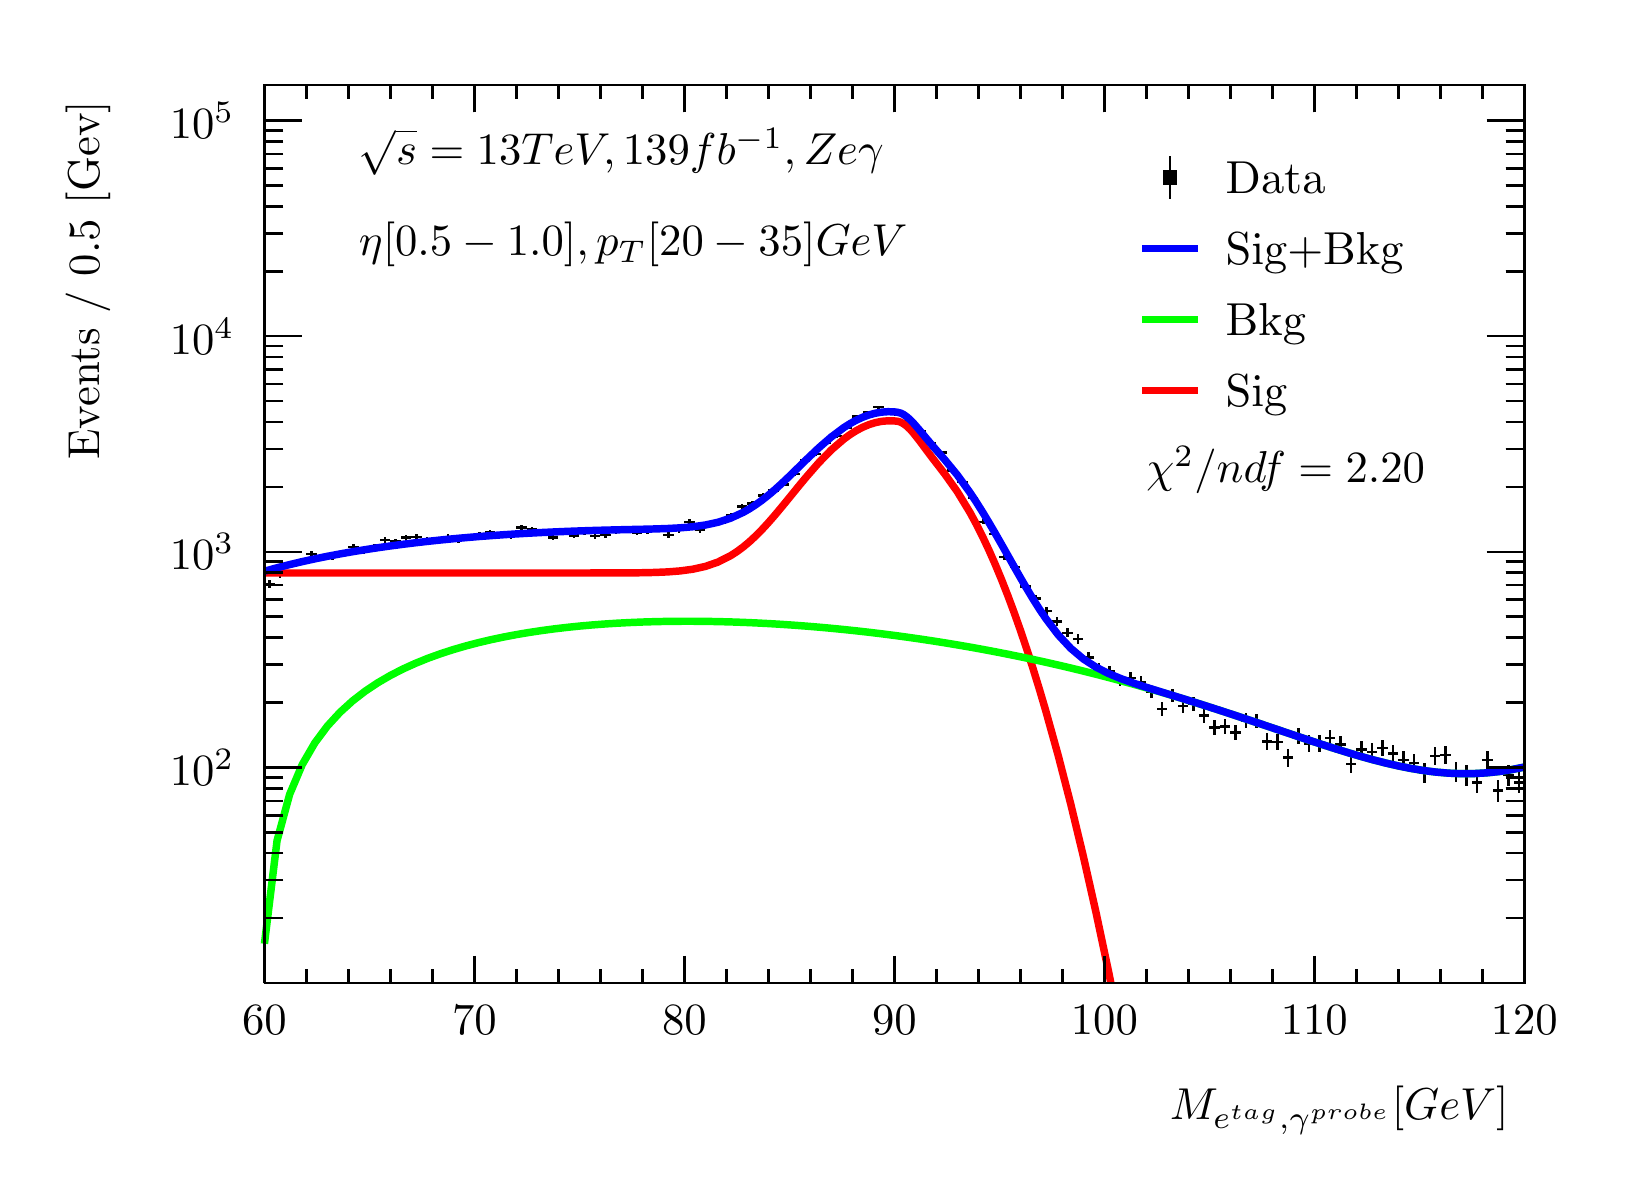
\begin{tikzpicture}
\pgfdeclareplotmark{cross} {
\pgfpathmoveto{\pgfpoint{-0.3\pgfplotmarksize}{\pgfplotmarksize}}
\pgfpathlineto{\pgfpoint{+0.3\pgfplotmarksize}{\pgfplotmarksize}}
\pgfpathlineto{\pgfpoint{+0.3\pgfplotmarksize}{0.3\pgfplotmarksize}}
\pgfpathlineto{\pgfpoint{+1\pgfplotmarksize}{0.3\pgfplotmarksize}}
\pgfpathlineto{\pgfpoint{+1\pgfplotmarksize}{-0.3\pgfplotmarksize}}
\pgfpathlineto{\pgfpoint{+0.3\pgfplotmarksize}{-0.3\pgfplotmarksize}}
\pgfpathlineto{\pgfpoint{+0.3\pgfplotmarksize}{-1.\pgfplotmarksize}}
\pgfpathlineto{\pgfpoint{-0.3\pgfplotmarksize}{-1.\pgfplotmarksize}}
\pgfpathlineto{\pgfpoint{-0.3\pgfplotmarksize}{-0.3\pgfplotmarksize}}
\pgfpathlineto{\pgfpoint{-1.\pgfplotmarksize}{-0.3\pgfplotmarksize}}
\pgfpathlineto{\pgfpoint{-1.\pgfplotmarksize}{0.3\pgfplotmarksize}}
\pgfpathlineto{\pgfpoint{-0.3\pgfplotmarksize}{0.3\pgfplotmarksize}}
\pgfpathclose
\pgfusepathqstroke
}
\pgfdeclareplotmark{cross*} {
\pgfpathmoveto{\pgfpoint{-0.3\pgfplotmarksize}{\pgfplotmarksize}}
\pgfpathlineto{\pgfpoint{+0.3\pgfplotmarksize}{\pgfplotmarksize}}
\pgfpathlineto{\pgfpoint{+0.3\pgfplotmarksize}{0.3\pgfplotmarksize}}
\pgfpathlineto{\pgfpoint{+1\pgfplotmarksize}{0.3\pgfplotmarksize}}
\pgfpathlineto{\pgfpoint{+1\pgfplotmarksize}{-0.3\pgfplotmarksize}}
\pgfpathlineto{\pgfpoint{+0.3\pgfplotmarksize}{-0.3\pgfplotmarksize}}
\pgfpathlineto{\pgfpoint{+0.3\pgfplotmarksize}{-1.\pgfplotmarksize}}
\pgfpathlineto{\pgfpoint{-0.3\pgfplotmarksize}{-1.\pgfplotmarksize}}
\pgfpathlineto{\pgfpoint{-0.3\pgfplotmarksize}{-0.3\pgfplotmarksize}}
\pgfpathlineto{\pgfpoint{-1.\pgfplotmarksize}{-0.3\pgfplotmarksize}}
\pgfpathlineto{\pgfpoint{-1.\pgfplotmarksize}{0.3\pgfplotmarksize}}
\pgfpathlineto{\pgfpoint{-0.3\pgfplotmarksize}{0.3\pgfplotmarksize}}
\pgfpathclose
\pgfusepathqfillstroke
}
\pgfdeclareplotmark{newstar} {
\pgfpathmoveto{\pgfqpoint{0pt}{\pgfplotmarksize}}
\pgfpathlineto{\pgfqpointpolar{44}{0.5\pgfplotmarksize}}
\pgfpathlineto{\pgfqpointpolar{18}{\pgfplotmarksize}}
\pgfpathlineto{\pgfqpointpolar{-20}{0.5\pgfplotmarksize}}
\pgfpathlineto{\pgfqpointpolar{-54}{\pgfplotmarksize}}
\pgfpathlineto{\pgfqpointpolar{-90}{0.5\pgfplotmarksize}}
\pgfpathlineto{\pgfqpointpolar{234}{\pgfplotmarksize}}
\pgfpathlineto{\pgfqpointpolar{198}{0.5\pgfplotmarksize}}
\pgfpathlineto{\pgfqpointpolar{162}{\pgfplotmarksize}}
\pgfpathlineto{\pgfqpointpolar{134}{0.5\pgfplotmarksize}}
\pgfpathclose
\pgfusepathqstroke
}
\pgfdeclareplotmark{newstar*} {
\pgfpathmoveto{\pgfqpoint{0pt}{\pgfplotmarksize}}
\pgfpathlineto{\pgfqpointpolar{44}{0.5\pgfplotmarksize}}
\pgfpathlineto{\pgfqpointpolar{18}{\pgfplotmarksize}}
\pgfpathlineto{\pgfqpointpolar{-20}{0.5\pgfplotmarksize}}
\pgfpathlineto{\pgfqpointpolar{-54}{\pgfplotmarksize}}
\pgfpathlineto{\pgfqpointpolar{-90}{0.5\pgfplotmarksize}}
\pgfpathlineto{\pgfqpointpolar{234}{\pgfplotmarksize}}
\pgfpathlineto{\pgfqpointpolar{198}{0.5\pgfplotmarksize}}
\pgfpathlineto{\pgfqpointpolar{162}{\pgfplotmarksize}}
\pgfpathlineto{\pgfqpointpolar{134}{0.5\pgfplotmarksize}}
\pgfpathclose
\pgfusepathqfillstroke
}
\definecolor{c}{rgb}{1,1,1};
\draw [color=c, fill=c] (0,0) rectangle (20,14.4361);
\draw [color=c, fill=c] (3,2.30977) rectangle (19,13.7143);
\definecolor{c}{rgb}{0,0,0};
\draw [c,line width=0.9] (3,2.30977) -- (3,13.7143) -- (19,13.7143) -- (19,2.30977) -- (3,2.30977);
\definecolor{c}{rgb}{1,1,1};
\draw [color=c, fill=c] (3,2.30977) rectangle (19,13.7143);
\definecolor{c}{rgb}{0,0,0};
\draw [c,line width=0.9] (3,2.30977) -- (3,13.7143) -- (19,13.7143) -- (19,2.30977) -- (3,2.30977);
\draw [c,line width=0.9] (3,2.30977) -- (19,2.30977);
\draw [c,line width=0.9] (3,2.65624) -- (3,2.30977);
\draw [c,line width=0.9] (3.53333,2.48301) -- (3.53333,2.30977);
\draw [c,line width=0.9] (4.06667,2.48301) -- (4.06667,2.30977);
\draw [c,line width=0.9] (4.6,2.48301) -- (4.6,2.30977);
\draw [c,line width=0.9] (5.13333,2.48301) -- (5.13333,2.30977);
\draw [c,line width=0.9] (5.66667,2.65624) -- (5.66667,2.30977);
\draw [c,line width=0.9] (6.2,2.48301) -- (6.2,2.30977);
\draw [c,line width=0.9] (6.73333,2.48301) -- (6.73333,2.30977);
\draw [c,line width=0.9] (7.26667,2.48301) -- (7.26667,2.30977);
\draw [c,line width=0.9] (7.8,2.48301) -- (7.8,2.30977);
\draw [c,line width=0.9] (8.33333,2.65624) -- (8.33333,2.30977);
\draw [c,line width=0.9] (8.86667,2.48301) -- (8.86667,2.30977);
\draw [c,line width=0.9] (9.4,2.48301) -- (9.4,2.30977);
\draw [c,line width=0.9] (9.93333,2.48301) -- (9.93333,2.30977);
\draw [c,line width=0.9] (10.4667,2.48301) -- (10.4667,2.30977);
\draw [c,line width=0.9] (11,2.65624) -- (11,2.30977);
\draw [c,line width=0.9] (11.5333,2.48301) -- (11.5333,2.30977);
\draw [c,line width=0.9] (12.0667,2.48301) -- (12.0667,2.30977);
\draw [c,line width=0.9] (12.6,2.48301) -- (12.6,2.30977);
\draw [c,line width=0.9] (13.1333,2.48301) -- (13.1333,2.30977);
\draw [c,line width=0.9] (13.6667,2.65624) -- (13.6667,2.30977);
\draw [c,line width=0.9] (14.2,2.48301) -- (14.2,2.30977);
\draw [c,line width=0.9] (14.7333,2.48301) -- (14.7333,2.30977);
\draw [c,line width=0.9] (15.2667,2.48301) -- (15.2667,2.30977);
\draw [c,line width=0.9] (15.8,2.48301) -- (15.8,2.30977);
\draw [c,line width=0.9] (16.3333,2.65624) -- (16.3333,2.30977);
\draw [c,line width=0.9] (16.8667,2.48301) -- (16.8667,2.30977);
\draw [c,line width=0.9] (17.4,2.48301) -- (17.4,2.30977);
\draw [c,line width=0.9] (17.9333,2.48301) -- (17.9333,2.30977);
\draw [c,line width=0.9] (18.4667,2.48301) -- (18.4667,2.30977);
\draw [c,line width=0.9] (19,2.65624) -- (19,2.30977);
\draw [anchor=base] (3,1.66015) node[scale=1.61424, color=c, rotate=0]{60};
\draw [anchor=base] (5.66667,1.66015) node[scale=1.61424, color=c, rotate=0]{70};
\draw [anchor=base] (8.33333,1.66015) node[scale=1.61424, color=c, rotate=0]{80};
\draw [anchor=base] (11,1.66015) node[scale=1.61424, color=c, rotate=0]{90};
\draw [anchor=base] (13.6667,1.66015) node[scale=1.61424, color=c, rotate=0]{100};
\draw [anchor=base] (16.3333,1.66015) node[scale=1.61424, color=c, rotate=0]{110};
\draw [anchor=base] (19,1.66015) node[scale=1.61424, color=c, rotate=0]{120};
\draw [anchor= east] (19,0.692932) node[scale=1.61424, color=c, rotate=0]{$M_{e^{tag}, \gamma^{probe}}  [GeV]$};
\draw [c,line width=0.9] (3,13.7143) -- (19,13.7143);
\draw [c,line width=0.9] (3,13.3678) -- (3,13.7143);
\draw [c,line width=0.9] (3.53333,13.5411) -- (3.53333,13.7143);
\draw [c,line width=0.9] (4.06667,13.5411) -- (4.06667,13.7143);
\draw [c,line width=0.9] (4.6,13.5411) -- (4.6,13.7143);
\draw [c,line width=0.9] (5.13333,13.5411) -- (5.13333,13.7143);
\draw [c,line width=0.9] (5.66667,13.3678) -- (5.66667,13.7143);
\draw [c,line width=0.9] (6.2,13.5411) -- (6.2,13.7143);
\draw [c,line width=0.9] (6.73333,13.5411) -- (6.73333,13.7143);
\draw [c,line width=0.9] (7.26667,13.5411) -- (7.26667,13.7143);
\draw [c,line width=0.9] (7.8,13.5411) -- (7.8,13.7143);
\draw [c,line width=0.9] (8.33333,13.3678) -- (8.33333,13.7143);
\draw [c,line width=0.9] (8.86667,13.5411) -- (8.86667,13.7143);
\draw [c,line width=0.9] (9.4,13.5411) -- (9.4,13.7143);
\draw [c,line width=0.9] (9.93333,13.5411) -- (9.93333,13.7143);
\draw [c,line width=0.9] (10.4667,13.5411) -- (10.4667,13.7143);
\draw [c,line width=0.9] (11,13.3678) -- (11,13.7143);
\draw [c,line width=0.9] (11.5333,13.5411) -- (11.5333,13.7143);
\draw [c,line width=0.9] (12.0667,13.5411) -- (12.0667,13.7143);
\draw [c,line width=0.9] (12.6,13.5411) -- (12.6,13.7143);
\draw [c,line width=0.9] (13.1333,13.5411) -- (13.1333,13.7143);
\draw [c,line width=0.9] (13.6667,13.3678) -- (13.6667,13.7143);
\draw [c,line width=0.9] (14.2,13.5411) -- (14.2,13.7143);
\draw [c,line width=0.9] (14.7333,13.5411) -- (14.7333,13.7143);
\draw [c,line width=0.9] (15.2667,13.5411) -- (15.2667,13.7143);
\draw [c,line width=0.9] (15.8,13.5411) -- (15.8,13.7143);
\draw [c,line width=0.9] (16.3333,13.3678) -- (16.3333,13.7143);
\draw [c,line width=0.9] (16.8667,13.5411) -- (16.8667,13.7143);
\draw [c,line width=0.9] (17.4,13.5411) -- (17.4,13.7143);
\draw [c,line width=0.9] (17.9333,13.5411) -- (17.9333,13.7143);
\draw [c,line width=0.9] (18.4667,13.5411) -- (18.4667,13.7143);
\draw [c,line width=0.9] (19,13.3678) -- (19,13.7143);
\draw [c,line width=0.9] (3,2.30977) -- (3,13.7143);
\draw [c,line width=0.9] (3.237,3.13412) -- (3,3.13412);
\draw [c,line width=0.9] (3.237,3.61633) -- (3,3.61633);
\draw [c,line width=0.9] (3.237,3.95847) -- (3,3.95847);
\draw [c,line width=0.9] (3.237,4.22385) -- (3,4.22385);
\draw [c,line width=0.9] (3.237,4.44068) -- (3,4.44068);
\draw [c,line width=0.9] (3.237,4.62401) -- (3,4.62401);
\draw [c,line width=0.9] (3.237,4.78282) -- (3,4.78282);
\draw [c,line width=0.9] (3.237,4.9229) -- (3,4.9229);
\draw [c,line width=0.9] (3.474,5.0482) -- (3,5.0482);
\draw [anchor= east] (2.82,5.0482) node[scale=1.61424, color=c, rotate=0]{$10^{2}$};
\draw [c,line width=0.9] (3.237,5.87255) -- (3,5.87255);
\draw [c,line width=0.9] (3.237,6.35476) -- (3,6.35476);
\draw [c,line width=0.9] (3.237,6.6969) -- (3,6.6969);
\draw [c,line width=0.9] (3.237,6.96228) -- (3,6.96228);
\draw [c,line width=0.9] (3.237,7.17911) -- (3,7.17911);
\draw [c,line width=0.9] (3.237,7.36244) -- (3,7.36244);
\draw [c,line width=0.9] (3.237,7.52125) -- (3,7.52125);
\draw [c,line width=0.9] (3.237,7.66133) -- (3,7.66133);
\draw [c,line width=0.9] (3.474,7.78663) -- (3,7.78663);
\draw [anchor= east] (2.82,7.78663) node[scale=1.61424, color=c, rotate=0]{$10^{3}$};
\draw [c,line width=0.9] (3.237,8.61098) -- (3,8.61098);
\draw [c,line width=0.9] (3.237,9.09319) -- (3,9.09319);
\draw [c,line width=0.9] (3.237,9.43533) -- (3,9.43533);
\draw [c,line width=0.9] (3.237,9.70071) -- (3,9.70071);
\draw [c,line width=0.9] (3.237,9.91755) -- (3,9.91755);
\draw [c,line width=0.9] (3.237,10.1009) -- (3,10.1009);
\draw [c,line width=0.9] (3.237,10.2597) -- (3,10.2597);
\draw [c,line width=0.9] (3.237,10.3998) -- (3,10.3998);
\draw [c,line width=0.9] (3.474,10.5251) -- (3,10.5251);
\draw [anchor= east] (2.82,10.5251) node[scale=1.61424, color=c, rotate=0]{$10^{4}$};
\draw [c,line width=0.9] (3.237,11.3494) -- (3,11.3494);
\draw [c,line width=0.9] (3.237,11.8316) -- (3,11.8316);
\draw [c,line width=0.9] (3.237,12.1738) -- (3,12.1738);
\draw [c,line width=0.9] (3.237,12.4391) -- (3,12.4391);
\draw [c,line width=0.9] (3.237,12.656) -- (3,12.656);
\draw [c,line width=0.9] (3.237,12.8393) -- (3,12.8393);
\draw [c,line width=0.9] (3.237,12.9981) -- (3,12.9981);
\draw [c,line width=0.9] (3.237,13.1382) -- (3,13.1382);
\draw [c,line width=0.9] (3.474,13.2635) -- (3,13.2635);
\draw [anchor= east] (2.82,13.2635) node[scale=1.61424, color=c, rotate=0]{$10^{5}$};
\draw [anchor= east] (0.76,13.7143) node[scale=1.61424, color=c, rotate=90]{Events / 0.5 [Gev]};
\draw [c,line width=0.9] (19,2.30977) -- (19,13.7143);
\draw [c,line width=0.9] (18.763,3.13412) -- (19,3.13412);
\draw [c,line width=0.9] (18.763,3.61633) -- (19,3.61633);
\draw [c,line width=0.9] (18.763,3.95847) -- (19,3.95847);
\draw [c,line width=0.9] (18.763,4.22385) -- (19,4.22385);
\draw [c,line width=0.9] (18.763,4.44068) -- (19,4.44068);
\draw [c,line width=0.9] (18.763,4.62401) -- (19,4.62401);
\draw [c,line width=0.9] (18.763,4.78282) -- (19,4.78282);
\draw [c,line width=0.9] (18.763,4.9229) -- (19,4.9229);
\draw [c,line width=0.9] (18.526,5.0482) -- (19,5.0482);
\draw [c,line width=0.9] (18.763,5.87255) -- (19,5.87255);
\draw [c,line width=0.9] (18.763,6.35476) -- (19,6.35476);
\draw [c,line width=0.9] (18.763,6.6969) -- (19,6.6969);
\draw [c,line width=0.9] (18.763,6.96228) -- (19,6.96228);
\draw [c,line width=0.9] (18.763,7.17911) -- (19,7.17911);
\draw [c,line width=0.9] (18.763,7.36244) -- (19,7.36244);
\draw [c,line width=0.9] (18.763,7.52125) -- (19,7.52125);
\draw [c,line width=0.9] (18.763,7.66133) -- (19,7.66133);
\draw [c,line width=0.9] (18.526,7.78663) -- (19,7.78663);
\draw [c,line width=0.9] (18.763,8.61098) -- (19,8.61098);
\draw [c,line width=0.9] (18.763,9.09319) -- (19,9.09319);
\draw [c,line width=0.9] (18.763,9.43533) -- (19,9.43533);
\draw [c,line width=0.9] (18.763,9.70071) -- (19,9.70071);
\draw [c,line width=0.9] (18.763,9.91755) -- (19,9.91755);
\draw [c,line width=0.9] (18.763,10.1009) -- (19,10.1009);
\draw [c,line width=0.9] (18.763,10.2597) -- (19,10.2597);
\draw [c,line width=0.9] (18.763,10.3998) -- (19,10.3998);
\draw [c,line width=0.9] (18.526,10.5251) -- (19,10.5251);
\draw [c,line width=0.9] (18.763,11.3494) -- (19,11.3494);
\draw [c,line width=0.9] (18.763,11.8316) -- (19,11.8316);
\draw [c,line width=0.9] (18.763,12.1738) -- (19,12.1738);
\draw [c,line width=0.9] (18.763,12.4391) -- (19,12.4391);
\draw [c,line width=0.9] (18.763,12.656) -- (19,12.656);
\draw [c,line width=0.9] (18.763,12.8393) -- (19,12.8393);
\draw [c,line width=0.9] (18.763,12.9981) -- (19,12.9981);
\draw [c,line width=0.9] (18.763,13.1382) -- (19,13.1382);
\draw [c,line width=0.9] (18.526,13.2635) -- (19,13.2635);
\draw [c,line width=0.9] (3.06667,7.37764) -- (3,7.37764);
\draw [c,line width=0.9] (3,7.37764) -- (3,7.37764);
\draw [c,line width=0.9] (3.06667,7.37764) -- (3.13333,7.37764);
\draw [c,line width=0.9] (3.13333,7.37764) -- (3.13333,7.37764);
\draw [c,line width=0.9] (3.06667,7.37764) -- (3.06667,7.4223);
\draw [c,line width=0.9] (3.06667,7.4223) -- (3.06667,7.4223);
\draw [c,line width=0.9] (3.06667,7.37764) -- (3.06667,7.33298);
\draw [c,line width=0.9] (3.06667,7.33298) -- (3.06667,7.33298);
\draw [c,line width=0.9] (3.2,7.49723) -- (3.13333,7.49723);
\draw [c,line width=0.9] (3.13333,7.49723) -- (3.13333,7.49723);
\draw [c,line width=0.9] (3.2,7.49723) -- (3.26667,7.49723);
\draw [c,line width=0.9] (3.26667,7.49723) -- (3.26667,7.49723);
\draw [c,line width=0.9] (3.2,7.49723) -- (3.2,7.5397);
\draw [c,line width=0.9] (3.2,7.5397) -- (3.2,7.5397);
\draw [c,line width=0.9] (3.2,7.49723) -- (3.2,7.45475);
\draw [c,line width=0.9] (3.2,7.45475) -- (3.2,7.45475);
\draw [c,line width=0.9] (3.33333,7.63054) -- (3.26667,7.63054);
\draw [c,line width=0.9] (3.26667,7.63054) -- (3.26667,7.63054);
\draw [c,line width=0.9] (3.33333,7.63054) -- (3.4,7.63054);
\draw [c,line width=0.9] (3.4,7.63054) -- (3.4,7.63054);
\draw [c,line width=0.9] (3.33333,7.63054) -- (3.33333,7.6707);
\draw [c,line width=0.9] (3.33333,7.6707) -- (3.33333,7.6707);
\draw [c,line width=0.9] (3.33333,7.63054) -- (3.33333,7.59038);
\draw [c,line width=0.9] (3.33333,7.59038) -- (3.33333,7.59038);
\draw [c,line width=0.9] (3.46667,7.67054) -- (3.4,7.67054);
\draw [c,line width=0.9] (3.4,7.67054) -- (3.4,7.67054);
\draw [c,line width=0.9] (3.46667,7.67054) -- (3.53333,7.67054);
\draw [c,line width=0.9] (3.53333,7.67054) -- (3.53333,7.67054);
\draw [c,line width=0.9] (3.46667,7.67054) -- (3.46667,7.71003);
\draw [c,line width=0.9] (3.46667,7.71003) -- (3.46667,7.71003);
\draw [c,line width=0.9] (3.46667,7.67054) -- (3.46667,7.63106);
\draw [c,line width=0.9] (3.46667,7.63106) -- (3.46667,7.63106);
\draw [c,line width=0.9] (3.6,7.75774) -- (3.53333,7.75774);
\draw [c,line width=0.9] (3.53333,7.75774) -- (3.53333,7.75774);
\draw [c,line width=0.9] (3.6,7.75774) -- (3.66667,7.75774);
\draw [c,line width=0.9] (3.66667,7.75774) -- (3.66667,7.75774);
\draw [c,line width=0.9] (3.6,7.75774) -- (3.6,7.79581);
\draw [c,line width=0.9] (3.6,7.79581) -- (3.6,7.79581);
\draw [c,line width=0.9] (3.6,7.75774) -- (3.6,7.71968);
\draw [c,line width=0.9] (3.6,7.71968) -- (3.6,7.71968);
\draw [c,line width=0.9] (3.73333,7.70924) -- (3.66667,7.70924);
\draw [c,line width=0.9] (3.66667,7.70924) -- (3.66667,7.70924);
\draw [c,line width=0.9] (3.73333,7.70924) -- (3.8,7.70924);
\draw [c,line width=0.9] (3.8,7.70924) -- (3.8,7.70924);
\draw [c,line width=0.9] (3.73333,7.70924) -- (3.73333,7.7481);
\draw [c,line width=0.9] (3.73333,7.7481) -- (3.73333,7.7481);
\draw [c,line width=0.9] (3.73333,7.70924) -- (3.73333,7.67039);
\draw [c,line width=0.9] (3.73333,7.67039) -- (3.73333,7.67039);
\draw [c,line width=0.9] (3.86667,7.72312) -- (3.8,7.72312);
\draw [c,line width=0.9] (3.8,7.72312) -- (3.8,7.72312);
\draw [c,line width=0.9] (3.86667,7.72312) -- (3.93333,7.72312);
\draw [c,line width=0.9] (3.93333,7.72312) -- (3.93333,7.72312);
\draw [c,line width=0.9] (3.86667,7.72312) -- (3.86667,7.76175);
\draw [c,line width=0.9] (3.86667,7.76175) -- (3.86667,7.76175);
\draw [c,line width=0.9] (3.86667,7.72312) -- (3.86667,7.6845);
\draw [c,line width=0.9] (3.86667,7.6845) -- (3.86667,7.6845);
\draw [c,line width=0.9] (4,7.76503) -- (3.93333,7.76503);
\draw [c,line width=0.9] (3.93333,7.76503) -- (3.93333,7.76503);
\draw [c,line width=0.9] (4,7.76503) -- (4.06667,7.76503);
\draw [c,line width=0.9] (4.06667,7.76503) -- (4.06667,7.76503);
\draw [c,line width=0.9] (4,7.76503) -- (4,7.80298);
\draw [c,line width=0.9] (4,7.80298) -- (4,7.80298);
\draw [c,line width=0.9] (4,7.76503) -- (4,7.72708);
\draw [c,line width=0.9] (4,7.72708) -- (4,7.72708);
\draw [c,line width=0.9] (4.13333,7.84805) -- (4.06667,7.84805);
\draw [c,line width=0.9] (4.06667,7.84805) -- (4.06667,7.84805);
\draw [c,line width=0.9] (4.13333,7.84805) -- (4.2,7.84805);
\draw [c,line width=0.9] (4.2,7.84805) -- (4.2,7.84805);
\draw [c,line width=0.9] (4.13333,7.84805) -- (4.13333,7.8847);
\draw [c,line width=0.9] (4.13333,7.8847) -- (4.13333,7.8847);
\draw [c,line width=0.9] (4.13333,7.84805) -- (4.13333,7.8114);
\draw [c,line width=0.9] (4.13333,7.8114) -- (4.13333,7.8114);
\draw [c,line width=0.9] (4.26667,7.79375) -- (4.2,7.79375);
\draw [c,line width=0.9] (4.2,7.79375) -- (4.2,7.79375);
\draw [c,line width=0.9] (4.26667,7.79375) -- (4.33333,7.79375);
\draw [c,line width=0.9] (4.33333,7.79375) -- (4.33333,7.79375);
\draw [c,line width=0.9] (4.26667,7.79375) -- (4.26667,7.83124);
\draw [c,line width=0.9] (4.26667,7.83124) -- (4.26667,7.83124);
\draw [c,line width=0.9] (4.26667,7.79375) -- (4.26667,7.75625);
\draw [c,line width=0.9] (4.26667,7.75625) -- (4.26667,7.75625);
\draw [c,line width=0.9] (4.4,7.85031) -- (4.33333,7.85031);
\draw [c,line width=0.9] (4.33333,7.85031) -- (4.33333,7.85031);
\draw [c,line width=0.9] (4.4,7.85031) -- (4.46667,7.85031);
\draw [c,line width=0.9] (4.46667,7.85031) -- (4.46667,7.85031);
\draw [c,line width=0.9] (4.4,7.85031) -- (4.4,7.88692);
\draw [c,line width=0.9] (4.4,7.88692) -- (4.4,7.88692);
\draw [c,line width=0.9] (4.4,7.85031) -- (4.4,7.81369);
\draw [c,line width=0.9] (4.4,7.81369) -- (4.4,7.81369);
\draw [c,line width=0.9] (4.53333,7.93409) -- (4.46667,7.93409);
\draw [c,line width=0.9] (4.46667,7.93409) -- (4.46667,7.93409);
\draw [c,line width=0.9] (4.53333,7.93409) -- (4.6,7.93409);
\draw [c,line width=0.9] (4.6,7.93409) -- (4.6,7.93409);
\draw [c,line width=0.9] (4.53333,7.93409) -- (4.53333,7.96943);
\draw [c,line width=0.9] (4.53333,7.96943) -- (4.53333,7.96943);
\draw [c,line width=0.9] (4.53333,7.93409) -- (4.53333,7.89874);
\draw [c,line width=0.9] (4.53333,7.89874) -- (4.53333,7.89874);
\draw [c,line width=0.9] (4.66667,7.91503) -- (4.6,7.91503);
\draw [c,line width=0.9] (4.6,7.91503) -- (4.6,7.91503);
\draw [c,line width=0.9] (4.66667,7.91503) -- (4.73333,7.91503);
\draw [c,line width=0.9] (4.73333,7.91503) -- (4.73333,7.91503);
\draw [c,line width=0.9] (4.66667,7.91503) -- (4.66667,7.95066);
\draw [c,line width=0.9] (4.66667,7.95066) -- (4.66667,7.95066);
\draw [c,line width=0.9] (4.66667,7.91503) -- (4.66667,7.87939);
\draw [c,line width=0.9] (4.66667,7.87939) -- (4.66667,7.87939);
\draw [c,line width=0.9] (4.8,7.9652) -- (4.73333,7.9652);
\draw [c,line width=0.9] (4.73333,7.9652) -- (4.73333,7.9652);
\draw [c,line width=0.9] (4.8,7.9652) -- (4.86667,7.9652);
\draw [c,line width=0.9] (4.86667,7.9652) -- (4.86667,7.9652);
\draw [c,line width=0.9] (4.8,7.9652) -- (4.8,8.00008);
\draw [c,line width=0.9] (4.8,8.00008) -- (4.8,8.00008);
\draw [c,line width=0.9] (4.8,7.9652) -- (4.8,7.93031);
\draw [c,line width=0.9] (4.8,7.93031) -- (4.8,7.93031);
\draw [c,line width=0.9] (4.93333,7.97437) -- (4.86667,7.97437);
\draw [c,line width=0.9] (4.86667,7.97437) -- (4.86667,7.97437);
\draw [c,line width=0.9] (4.93333,7.97437) -- (5,7.97437);
\draw [c,line width=0.9] (5,7.97437) -- (5,7.97437);
\draw [c,line width=0.9] (4.93333,7.97437) -- (4.93333,8.00912);
\draw [c,line width=0.9] (4.93333,8.00912) -- (4.93333,8.00912);
\draw [c,line width=0.9] (4.93333,7.97437) -- (4.93333,7.93962);
\draw [c,line width=0.9] (4.93333,7.93962) -- (4.93333,7.93962);
\draw [c,line width=0.9] (5.06667,7.94351) -- (5,7.94351);
\draw [c,line width=0.9] (5,7.94351) -- (5,7.94351);
\draw [c,line width=0.9] (5.06667,7.94351) -- (5.13333,7.94351);
\draw [c,line width=0.9] (5.13333,7.94351) -- (5.13333,7.94351);
\draw [c,line width=0.9] (5.06667,7.94351) -- (5.06667,7.97871);
\draw [c,line width=0.9] (5.06667,7.97871) -- (5.06667,7.97871);
\draw [c,line width=0.9] (5.06667,7.94351) -- (5.06667,7.9083);
\draw [c,line width=0.9] (5.06667,7.9083) -- (5.06667,7.9083);
\draw [c,line width=0.9] (5.2,7.93409) -- (5.13333,7.93409);
\draw [c,line width=0.9] (5.13333,7.93409) -- (5.13333,7.93409);
\draw [c,line width=0.9] (5.2,7.93409) -- (5.26667,7.93409);
\draw [c,line width=0.9] (5.26667,7.93409) -- (5.26667,7.93409);
\draw [c,line width=0.9] (5.2,7.93409) -- (5.2,7.96943);
\draw [c,line width=0.9] (5.2,7.96943) -- (5.2,7.96943);
\draw [c,line width=0.9] (5.2,7.93409) -- (5.2,7.89874);
\draw [c,line width=0.9] (5.2,7.89874) -- (5.2,7.89874);
\draw [c,line width=0.9] (5.33333,7.97336) -- (5.26667,7.97336);
\draw [c,line width=0.9] (5.26667,7.97336) -- (5.26667,7.97336);
\draw [c,line width=0.9] (5.33333,7.97336) -- (5.4,7.97336);
\draw [c,line width=0.9] (5.4,7.97336) -- (5.4,7.97336);
\draw [c,line width=0.9] (5.33333,7.97336) -- (5.33333,8.00812);
\draw [c,line width=0.9] (5.33333,8.00812) -- (5.33333,8.00812);
\draw [c,line width=0.9] (5.33333,7.97336) -- (5.33333,7.93859);
\draw [c,line width=0.9] (5.33333,7.93859) -- (5.33333,7.93859);
\draw [c,line width=0.9] (5.46667,7.93619) -- (5.4,7.93619);
\draw [c,line width=0.9] (5.4,7.93619) -- (5.4,7.93619);
\draw [c,line width=0.9] (5.46667,7.93619) -- (5.53333,7.93619);
\draw [c,line width=0.9] (5.53333,7.93619) -- (5.53333,7.93619);
\draw [c,line width=0.9] (5.46667,7.93619) -- (5.46667,7.9715);
\draw [c,line width=0.9] (5.46667,7.9715) -- (5.46667,7.9715);
\draw [c,line width=0.9] (5.46667,7.93619) -- (5.46667,7.90087);
\draw [c,line width=0.9] (5.46667,7.90087) -- (5.46667,7.90087);
\draw [c,line width=0.9] (5.6,7.95285) -- (5.53333,7.95285);
\draw [c,line width=0.9] (5.53333,7.95285) -- (5.53333,7.95285);
\draw [c,line width=0.9] (5.6,7.95285) -- (5.66667,7.95285);
\draw [c,line width=0.9] (5.66667,7.95285) -- (5.66667,7.95285);
\draw [c,line width=0.9] (5.6,7.95285) -- (5.6,7.98792);
\draw [c,line width=0.9] (5.6,7.98792) -- (5.6,7.98792);
\draw [c,line width=0.9] (5.6,7.95285) -- (5.6,7.91778);
\draw [c,line width=0.9] (5.6,7.91778) -- (5.6,7.91778);
\draw [c,line width=0.9] (5.73333,8.0094) -- (5.66667,8.0094);
\draw [c,line width=0.9] (5.66667,8.0094) -- (5.66667,8.0094);
\draw [c,line width=0.9] (5.73333,8.0094) -- (5.8,8.0094);
\draw [c,line width=0.9] (5.8,8.0094) -- (5.8,8.0094);
\draw [c,line width=0.9] (5.73333,8.0094) -- (5.73333,8.04364);
\draw [c,line width=0.9] (5.73333,8.04364) -- (5.73333,8.04364);
\draw [c,line width=0.9] (5.73333,8.0094) -- (5.73333,7.97515);
\draw [c,line width=0.9] (5.73333,7.97515) -- (5.73333,7.97515);
\draw [c,line width=0.9] (5.86667,8.03283) -- (5.8,8.03283);
\draw [c,line width=0.9] (5.8,8.03283) -- (5.8,8.03283);
\draw [c,line width=0.9] (5.86667,8.03283) -- (5.93333,8.03283);
\draw [c,line width=0.9] (5.93333,8.03283) -- (5.93333,8.03283);
\draw [c,line width=0.9] (5.86667,8.03283) -- (5.86667,8.06674);
\draw [c,line width=0.9] (5.86667,8.06674) -- (5.86667,8.06674);
\draw [c,line width=0.9] (5.86667,8.03283) -- (5.86667,7.99892);
\draw [c,line width=0.9] (5.86667,7.99892) -- (5.86667,7.99892);
\draw [c,line width=0.9] (6,7.9975) -- (5.93333,7.9975);
\draw [c,line width=0.9] (5.93333,7.9975) -- (5.93333,7.9975);
\draw [c,line width=0.9] (6,7.9975) -- (6.06667,7.9975);
\draw [c,line width=0.9] (6.06667,7.9975) -- (6.06667,7.9975);
\draw [c,line width=0.9] (6,7.9975) -- (6,8.03192);
\draw [c,line width=0.9] (6,8.03192) -- (6,8.03192);
\draw [c,line width=0.9] (6,7.9975) -- (6,7.96309);
\draw [c,line width=0.9] (6,7.96309) -- (6,7.96309);
\draw [c,line width=0.9] (6.13333,7.98951) -- (6.06667,7.98951);
\draw [c,line width=0.9] (6.06667,7.98951) -- (6.06667,7.98951);
\draw [c,line width=0.9] (6.13333,7.98951) -- (6.2,7.98951);
\draw [c,line width=0.9] (6.2,7.98951) -- (6.2,7.98951);
\draw [c,line width=0.9] (6.13333,7.98951) -- (6.13333,8.02404);
\draw [c,line width=0.9] (6.13333,8.02404) -- (6.13333,8.02404);
\draw [c,line width=0.9] (6.13333,7.98951) -- (6.13333,7.95498);
\draw [c,line width=0.9] (6.13333,7.95498) -- (6.13333,7.95498);
\draw [c,line width=0.9] (6.26667,8.09224) -- (6.2,8.09224);
\draw [c,line width=0.9] (6.2,8.09224) -- (6.2,8.09224);
\draw [c,line width=0.9] (6.26667,8.09224) -- (6.33333,8.09224);
\draw [c,line width=0.9] (6.33333,8.09224) -- (6.33333,8.09224);
\draw [c,line width=0.9] (6.26667,8.09224) -- (6.26667,8.12531);
\draw [c,line width=0.9] (6.26667,8.12531) -- (6.26667,8.12531);
\draw [c,line width=0.9] (6.26667,8.09224) -- (6.26667,8.05917);
\draw [c,line width=0.9] (6.26667,8.05917) -- (6.26667,8.05917);
\draw [c,line width=0.9] (6.4,8.06714) -- (6.33333,8.06714);
\draw [c,line width=0.9] (6.33333,8.06714) -- (6.33333,8.06714);
\draw [c,line width=0.9] (6.4,8.06714) -- (6.46667,8.06714);
\draw [c,line width=0.9] (6.46667,8.06714) -- (6.46667,8.06714);
\draw [c,line width=0.9] (6.4,8.06714) -- (6.4,8.10056);
\draw [c,line width=0.9] (6.4,8.10056) -- (6.4,8.10056);
\draw [c,line width=0.9] (6.4,8.06714) -- (6.4,8.03372);
\draw [c,line width=0.9] (6.4,8.03372) -- (6.4,8.03372);
\draw [c,line width=0.9] (6.53333,8.03476) -- (6.46667,8.03476);
\draw [c,line width=0.9] (6.46667,8.03476) -- (6.46667,8.03476);
\draw [c,line width=0.9] (6.53333,8.03476) -- (6.6,8.03476);
\draw [c,line width=0.9] (6.6,8.03476) -- (6.6,8.03476);
\draw [c,line width=0.9] (6.53333,8.03476) -- (6.53333,8.06865);
\draw [c,line width=0.9] (6.53333,8.06865) -- (6.53333,8.06865);
\draw [c,line width=0.9] (6.53333,8.03476) -- (6.53333,8.00088);
\draw [c,line width=0.9] (6.53333,8.00088) -- (6.53333,8.00088);
\draw [c,line width=0.9] (6.66667,7.9703) -- (6.6,7.9703);
\draw [c,line width=0.9] (6.6,7.9703) -- (6.6,7.9703);
\draw [c,line width=0.9] (6.66667,7.9703) -- (6.73333,7.9703);
\draw [c,line width=0.9] (6.73333,7.9703) -- (6.73333,7.9703);
\draw [c,line width=0.9] (6.66667,7.9703) -- (6.66667,8.00511);
\draw [c,line width=0.9] (6.66667,8.00511) -- (6.66667,8.00511);
\draw [c,line width=0.9] (6.66667,7.9703) -- (6.66667,7.93549);
\draw [c,line width=0.9] (6.66667,7.93549) -- (6.66667,7.93549);
\draw [c,line width=0.9] (6.8,8.03573) -- (6.73333,8.03573);
\draw [c,line width=0.9] (6.73333,8.03573) -- (6.73333,8.03573);
\draw [c,line width=0.9] (6.8,8.03573) -- (6.86667,8.03573);
\draw [c,line width=0.9] (6.86667,8.03573) -- (6.86667,8.03573);
\draw [c,line width=0.9] (6.8,8.03573) -- (6.8,8.0696);
\draw [c,line width=0.9] (6.8,8.0696) -- (6.8,8.0696);
\draw [c,line width=0.9] (6.8,8.03573) -- (6.8,8.00186);
\draw [c,line width=0.9] (6.8,8.00186) -- (6.8,8.00186);
\draw [c,line width=0.9] (6.93333,7.99251) -- (6.86667,7.99251);
\draw [c,line width=0.9] (6.86667,7.99251) -- (6.86667,7.99251);
\draw [c,line width=0.9] (6.93333,7.99251) -- (7,7.99251);
\draw [c,line width=0.9] (7,7.99251) -- (7,7.99251);
\draw [c,line width=0.9] (6.93333,7.99251) -- (6.93333,8.027);
\draw [c,line width=0.9] (6.93333,8.027) -- (6.93333,8.027);
\draw [c,line width=0.9] (6.93333,7.99251) -- (6.93333,7.95802);
\draw [c,line width=0.9] (6.93333,7.95802) -- (6.93333,7.95802);
\draw [c,line width=0.9] (7.06667,8.03283) -- (7,8.03283);
\draw [c,line width=0.9] (7,8.03283) -- (7,8.03283);
\draw [c,line width=0.9] (7.06667,8.03283) -- (7.13333,8.03283);
\draw [c,line width=0.9] (7.13333,8.03283) -- (7.13333,8.03283);
\draw [c,line width=0.9] (7.06667,8.03283) -- (7.06667,8.06674);
\draw [c,line width=0.9] (7.06667,8.06674) -- (7.06667,8.06674);
\draw [c,line width=0.9] (7.06667,8.03283) -- (7.06667,7.99892);
\draw [c,line width=0.9] (7.06667,7.99892) -- (7.06667,7.99892);
\draw [c,line width=0.9] (7.2,7.98951) -- (7.13333,7.98951);
\draw [c,line width=0.9] (7.13333,7.98951) -- (7.13333,7.98951);
\draw [c,line width=0.9] (7.2,7.98951) -- (7.26667,7.98951);
\draw [c,line width=0.9] (7.26667,7.98951) -- (7.26667,7.98951);
\draw [c,line width=0.9] (7.2,7.98951) -- (7.2,8.02404);
\draw [c,line width=0.9] (7.2,8.02404) -- (7.2,8.02404);
\draw [c,line width=0.9] (7.2,7.98951) -- (7.2,7.95498);
\draw [c,line width=0.9] (7.2,7.95498) -- (7.2,7.95498);
\draw [c,line width=0.9] (7.33333,7.99949) -- (7.26667,7.99949);
\draw [c,line width=0.9] (7.26667,7.99949) -- (7.26667,7.99949);
\draw [c,line width=0.9] (7.33333,7.99949) -- (7.4,7.99949);
\draw [c,line width=0.9] (7.4,7.99949) -- (7.4,7.99949);
\draw [c,line width=0.9] (7.33333,7.99949) -- (7.33333,8.03388);
\draw [c,line width=0.9] (7.33333,8.03388) -- (7.33333,8.03388);
\draw [c,line width=0.9] (7.33333,7.99949) -- (7.33333,7.96511);
\draw [c,line width=0.9] (7.33333,7.96511) -- (7.33333,7.96511);
\draw [c,line width=0.9] (7.46667,8.04438) -- (7.4,8.04438);
\draw [c,line width=0.9] (7.4,8.04438) -- (7.4,8.04438);
\draw [c,line width=0.9] (7.46667,8.04438) -- (7.53333,8.04438);
\draw [c,line width=0.9] (7.53333,8.04438) -- (7.53333,8.04438);
\draw [c,line width=0.9] (7.46667,8.04438) -- (7.46667,8.07812);
\draw [c,line width=0.9] (7.46667,8.07812) -- (7.46667,8.07812);
\draw [c,line width=0.9] (7.46667,8.04438) -- (7.46667,8.01063);
\draw [c,line width=0.9] (7.46667,8.01063) -- (7.46667,8.01063);
\draw [c,line width=0.9] (7.6,8.07089) -- (7.53333,8.07089);
\draw [c,line width=0.9] (7.53333,8.07089) -- (7.53333,8.07089);
\draw [c,line width=0.9] (7.6,8.07089) -- (7.66667,8.07089);
\draw [c,line width=0.9] (7.66667,8.07089) -- (7.66667,8.07089);
\draw [c,line width=0.9] (7.6,8.07089) -- (7.6,8.10426);
\draw [c,line width=0.9] (7.6,8.10426) -- (7.6,8.10426);
\draw [c,line width=0.9] (7.6,8.07089) -- (7.6,8.03752);
\draw [c,line width=0.9] (7.6,8.03752) -- (7.6,8.03752);
\draw [c,line width=0.9] (7.73333,8.03187) -- (7.66667,8.03187);
\draw [c,line width=0.9] (7.66667,8.03187) -- (7.66667,8.03187);
\draw [c,line width=0.9] (7.73333,8.03187) -- (7.8,8.03187);
\draw [c,line width=0.9] (7.8,8.03187) -- (7.8,8.03187);
\draw [c,line width=0.9] (7.73333,8.03187) -- (7.73333,8.06579);
\draw [c,line width=0.9] (7.73333,8.06579) -- (7.73333,8.06579);
\draw [c,line width=0.9] (7.73333,8.03187) -- (7.73333,7.99794);
\draw [c,line width=0.9] (7.73333,7.99794) -- (7.73333,7.99794);
\draw [c,line width=0.9] (7.86667,8.0482) -- (7.8,8.0482);
\draw [c,line width=0.9] (7.8,8.0482) -- (7.8,8.0482);
\draw [c,line width=0.9] (7.86667,8.0482) -- (7.93333,8.0482);
\draw [c,line width=0.9] (7.93333,8.0482) -- (7.93333,8.0482);
\draw [c,line width=0.9] (7.86667,8.0482) -- (7.86667,8.08189);
\draw [c,line width=0.9] (7.86667,8.08189) -- (7.86667,8.08189);
\draw [c,line width=0.9] (7.86667,8.0482) -- (7.86667,8.01451);
\draw [c,line width=0.9] (7.86667,8.01451) -- (7.86667,8.01451);
\draw [c,line width=0.9] (8,8.09774) -- (7.93333,8.09774);
\draw [c,line width=0.9] (7.93333,8.09774) -- (7.93333,8.09774);
\draw [c,line width=0.9] (8,8.09774) -- (8.06667,8.09774);
\draw [c,line width=0.9] (8.06667,8.09774) -- (8.06667,8.09774);
\draw [c,line width=0.9] (8,8.09774) -- (8,8.13074);
\draw [c,line width=0.9] (8,8.13074) -- (8,8.13074);
\draw [c,line width=0.9] (8,8.09774) -- (8,8.06475);
\draw [c,line width=0.9] (8,8.06475) -- (8,8.06475);
\draw [c,line width=0.9] (8.13333,7.9975) -- (8.06667,7.9975);
\draw [c,line width=0.9] (8.06667,7.9975) -- (8.06667,7.9975);
\draw [c,line width=0.9] (8.13333,7.9975) -- (8.2,7.9975);
\draw [c,line width=0.9] (8.2,7.9975) -- (8.2,7.9975);
\draw [c,line width=0.9] (8.13333,7.9975) -- (8.13333,8.03192);
\draw [c,line width=0.9] (8.13333,8.03192) -- (8.13333,8.03192);
\draw [c,line width=0.9] (8.13333,7.9975) -- (8.13333,7.96309);
\draw [c,line width=0.9] (8.13333,7.96309) -- (8.13333,7.96309);
\draw [c,line width=0.9] (8.26667,8.06055) -- (8.2,8.06055);
\draw [c,line width=0.9] (8.2,8.06055) -- (8.2,8.06055);
\draw [c,line width=0.9] (8.26667,8.06055) -- (8.33333,8.06055);
\draw [c,line width=0.9] (8.33333,8.06055) -- (8.33333,8.06055);
\draw [c,line width=0.9] (8.26667,8.06055) -- (8.26667,8.09406);
\draw [c,line width=0.9] (8.26667,8.09406) -- (8.26667,8.09406);
\draw [c,line width=0.9] (8.26667,8.06055) -- (8.26667,8.02703);
\draw [c,line width=0.9] (8.26667,8.02703) -- (8.26667,8.02703);
\draw [c,line width=0.9] (8.4,8.16623) -- (8.33333,8.16623);
\draw [c,line width=0.9] (8.33333,8.16623) -- (8.33333,8.16623);
\draw [c,line width=0.9] (8.4,8.16623) -- (8.46667,8.16623);
\draw [c,line width=0.9] (8.46667,8.16623) -- (8.46667,8.16623);
\draw [c,line width=0.9] (8.4,8.16623) -- (8.4,8.19829);
\draw [c,line width=0.9] (8.4,8.19829) -- (8.4,8.19829);
\draw [c,line width=0.9] (8.4,8.16623) -- (8.4,8.13417);
\draw [c,line width=0.9] (8.4,8.13417) -- (8.4,8.13417);
\draw [c,line width=0.9] (8.53333,8.06055) -- (8.46667,8.06055);
\draw [c,line width=0.9] (8.46667,8.06055) -- (8.46667,8.06055);
\draw [c,line width=0.9] (8.53333,8.06055) -- (8.6,8.06055);
\draw [c,line width=0.9] (8.6,8.06055) -- (8.6,8.06055);
\draw [c,line width=0.9] (8.53333,8.06055) -- (8.53333,8.09406);
\draw [c,line width=0.9] (8.53333,8.09406) -- (8.53333,8.09406);
\draw [c,line width=0.9] (8.53333,8.06055) -- (8.53333,8.02703);
\draw [c,line width=0.9] (8.53333,8.02703) -- (8.53333,8.02703);
\draw [c,line width=0.9] (8.66667,8.13825) -- (8.6,8.13825);
\draw [c,line width=0.9] (8.6,8.13825) -- (8.6,8.13825);
\draw [c,line width=0.9] (8.66667,8.13825) -- (8.73333,8.13825);
\draw [c,line width=0.9] (8.73333,8.13825) -- (8.73333,8.13825);
\draw [c,line width=0.9] (8.66667,8.13825) -- (8.66667,8.17068);
\draw [c,line width=0.9] (8.66667,8.17068) -- (8.66667,8.17068);
\draw [c,line width=0.9] (8.66667,8.13825) -- (8.66667,8.10581);
\draw [c,line width=0.9] (8.66667,8.10581) -- (8.66667,8.10581);
\draw [c,line width=0.9] (8.8,8.1593) -- (8.73333,8.1593);
\draw [c,line width=0.9] (8.73333,8.1593) -- (8.73333,8.1593);
\draw [c,line width=0.9] (8.8,8.1593) -- (8.86667,8.1593);
\draw [c,line width=0.9] (8.86667,8.1593) -- (8.86667,8.1593);
\draw [c,line width=0.9] (8.8,8.1593) -- (8.8,8.19145);
\draw [c,line width=0.9] (8.8,8.19145) -- (8.8,8.19145);
\draw [c,line width=0.9] (8.8,8.1593) -- (8.8,8.12714);
\draw [c,line width=0.9] (8.8,8.12714) -- (8.8,8.12714);
\draw [c,line width=0.9] (8.93333,8.25288) -- (8.86667,8.25288);
\draw [c,line width=0.9] (8.86667,8.25288) -- (8.86667,8.25288);
\draw [c,line width=0.9] (8.93333,8.25288) -- (9,8.25288);
\draw [c,line width=0.9] (9,8.25288) -- (9,8.25288);
\draw [c,line width=0.9] (8.93333,8.25288) -- (8.93333,8.2838);
\draw [c,line width=0.9] (8.93333,8.2838) -- (8.93333,8.2838);
\draw [c,line width=0.9] (8.93333,8.25288) -- (8.93333,8.22197);
\draw [c,line width=0.9] (8.93333,8.22197) -- (8.93333,8.22197);
\draw [c,line width=0.9] (9.06667,8.36331) -- (9,8.36331);
\draw [c,line width=0.9] (9,8.36331) -- (9,8.36331);
\draw [c,line width=0.9] (9.06667,8.36331) -- (9.13333,8.36331);
\draw [c,line width=0.9] (9.13333,8.36331) -- (9.13333,8.36331);
\draw [c,line width=0.9] (9.06667,8.36331) -- (9.06667,8.39282);
\draw [c,line width=0.9] (9.06667,8.39282) -- (9.06667,8.39282);
\draw [c,line width=0.9] (9.06667,8.36331) -- (9.06667,8.3338);
\draw [c,line width=0.9] (9.06667,8.3338) -- (9.06667,8.3338);
\draw [c,line width=0.9] (9.2,8.39724) -- (9.13333,8.39724);
\draw [c,line width=0.9] (9.13333,8.39724) -- (9.13333,8.39724);
\draw [c,line width=0.9] (9.2,8.39724) -- (9.26667,8.39724);
\draw [c,line width=0.9] (9.26667,8.39724) -- (9.26667,8.39724);
\draw [c,line width=0.9] (9.2,8.39724) -- (9.2,8.42633);
\draw [c,line width=0.9] (9.2,8.42633) -- (9.2,8.42633);
\draw [c,line width=0.9] (9.2,8.39724) -- (9.2,8.36815);
\draw [c,line width=0.9] (9.2,8.36815) -- (9.2,8.36815);
\draw [c,line width=0.9] (9.33333,8.50469) -- (9.26667,8.50469);
\draw [c,line width=0.9] (9.26667,8.50469) -- (9.26667,8.50469);
\draw [c,line width=0.9] (9.33333,8.50469) -- (9.4,8.50469);
\draw [c,line width=0.9] (9.4,8.50469) -- (9.4,8.50469);
\draw [c,line width=0.9] (9.33333,8.50469) -- (9.33333,8.5325);
\draw [c,line width=0.9] (9.33333,8.5325) -- (9.33333,8.5325);
\draw [c,line width=0.9] (9.33333,8.50469) -- (9.33333,8.47688);
\draw [c,line width=0.9] (9.33333,8.47688) -- (9.33333,8.47688);
\draw [c,line width=0.9] (9.46667,8.56305) -- (9.4,8.56305);
\draw [c,line width=0.9] (9.4,8.56305) -- (9.4,8.56305);
\draw [c,line width=0.9] (9.46667,8.56305) -- (9.53333,8.56305);
\draw [c,line width=0.9] (9.53333,8.56305) -- (9.53333,8.56305);
\draw [c,line width=0.9] (9.46667,8.56305) -- (9.46667,8.59019);
\draw [c,line width=0.9] (9.46667,8.59019) -- (9.46667,8.59019);
\draw [c,line width=0.9] (9.46667,8.56305) -- (9.46667,8.53592);
\draw [c,line width=0.9] (9.46667,8.53592) -- (9.46667,8.53592);
\draw [c,line width=0.9] (9.6,8.64325) -- (9.53333,8.64325);
\draw [c,line width=0.9] (9.53333,8.64325) -- (9.53333,8.64325);
\draw [c,line width=0.9] (9.6,8.64325) -- (9.66667,8.64325);
\draw [c,line width=0.9] (9.66667,8.64325) -- (9.66667,8.64325);
\draw [c,line width=0.9] (9.6,8.64325) -- (9.6,8.66948);
\draw [c,line width=0.9] (9.6,8.66948) -- (9.6,8.66948);
\draw [c,line width=0.9] (9.6,8.64325) -- (9.6,8.61701);
\draw [c,line width=0.9] (9.6,8.61701) -- (9.6,8.61701);
\draw [c,line width=0.9] (9.73333,8.77513) -- (9.66667,8.77513);
\draw [c,line width=0.9] (9.66667,8.77513) -- (9.66667,8.77513);
\draw [c,line width=0.9] (9.73333,8.77513) -- (9.8,8.77513);
\draw [c,line width=0.9] (9.8,8.77513) -- (9.8,8.77513);
\draw [c,line width=0.9] (9.73333,8.77513) -- (9.73333,8.79995);
\draw [c,line width=0.9] (9.73333,8.79995) -- (9.73333,8.79995);
\draw [c,line width=0.9] (9.73333,8.77513) -- (9.73333,8.75031);
\draw [c,line width=0.9] (9.73333,8.75031) -- (9.73333,8.75031);
\draw [c,line width=0.9] (9.86667,8.94746) -- (9.8,8.94746);
\draw [c,line width=0.9] (9.8,8.94746) -- (9.8,8.94746);
\draw [c,line width=0.9] (9.86667,8.94746) -- (9.93333,8.94746);
\draw [c,line width=0.9] (9.93333,8.94746) -- (9.93333,8.94746);
\draw [c,line width=0.9] (9.86667,8.94746) -- (9.86667,8.97054);
\draw [c,line width=0.9] (9.86667,8.97054) -- (9.86667,8.97054);
\draw [c,line width=0.9] (9.86667,8.94746) -- (9.86667,8.92437);
\draw [c,line width=0.9] (9.86667,8.92437) -- (9.86667,8.92437);
\draw [c,line width=0.9] (10,9.02927) -- (9.93333,9.02927);
\draw [c,line width=0.9] (9.93333,9.02927) -- (9.93333,9.02927);
\draw [c,line width=0.9] (10,9.02927) -- (10.0667,9.02927);
\draw [c,line width=0.9] (10.0667,9.02927) -- (10.0667,9.02927);
\draw [c,line width=0.9] (10,9.02927) -- (10,9.05157);
\draw [c,line width=0.9] (10,9.05157) -- (10,9.05157);
\draw [c,line width=0.9] (10,9.02927) -- (10,9.00696);
\draw [c,line width=0.9] (10,9.00696) -- (10,9.00696);
\draw [c,line width=0.9] (10.1333,9.16884) -- (10.0667,9.16884);
\draw [c,line width=0.9] (10.0667,9.16884) -- (10.0667,9.16884);
\draw [c,line width=0.9] (10.1333,9.16884) -- (10.2,9.16884);
\draw [c,line width=0.9] (10.2,9.16884) -- (10.2,9.16884);
\draw [c,line width=0.9] (10.1333,9.16884) -- (10.1333,9.18987);
\draw [c,line width=0.9] (10.1333,9.18987) -- (10.1333,9.18987);
\draw [c,line width=0.9] (10.1333,9.16884) -- (10.1333,9.1478);
\draw [c,line width=0.9] (10.1333,9.1478) -- (10.1333,9.1478);
\draw [c,line width=0.9] (10.2667,9.25527) -- (10.2,9.25527);
\draw [c,line width=0.9] (10.2,9.25527) -- (10.2,9.25527);
\draw [c,line width=0.9] (10.2667,9.25527) -- (10.3333,9.25527);
\draw [c,line width=0.9] (10.3333,9.25527) -- (10.3333,9.25527);
\draw [c,line width=0.9] (10.2667,9.25527) -- (10.2667,9.27555);
\draw [c,line width=0.9] (10.2667,9.27555) -- (10.2667,9.27555);
\draw [c,line width=0.9] (10.2667,9.25527) -- (10.2667,9.23499);
\draw [c,line width=0.9] (10.2667,9.23499) -- (10.2667,9.23499);
\draw [c,line width=0.9] (10.4,9.36427) -- (10.3333,9.36427);
\draw [c,line width=0.9] (10.3333,9.36427) -- (10.3333,9.36427);
\draw [c,line width=0.9] (10.4,9.36427) -- (10.4667,9.36427);
\draw [c,line width=0.9] (10.4667,9.36427) -- (10.4667,9.36427);
\draw [c,line width=0.9] (10.4,9.36427) -- (10.4,9.38365);
\draw [c,line width=0.9] (10.4,9.38365) -- (10.4,9.38365);
\draw [c,line width=0.9] (10.4,9.36427) -- (10.4,9.3449);
\draw [c,line width=0.9] (10.4,9.3449) -- (10.4,9.3449);
\draw [c,line width=0.9] (10.5333,9.50351) -- (10.4667,9.50351);
\draw [c,line width=0.9] (10.4667,9.50351) -- (10.4667,9.50351);
\draw [c,line width=0.9] (10.5333,9.50351) -- (10.6,9.50351);
\draw [c,line width=0.9] (10.6,9.50351) -- (10.6,9.50351);
\draw [c,line width=0.9] (10.5333,9.50351) -- (10.5333,9.52178);
\draw [c,line width=0.9] (10.5333,9.52178) -- (10.5333,9.52178);
\draw [c,line width=0.9] (10.5333,9.50351) -- (10.5333,9.48524);
\draw [c,line width=0.9] (10.5333,9.48524) -- (10.5333,9.48524);
\draw [c,line width=0.9] (10.6667,9.55354) -- (10.6,9.55354);
\draw [c,line width=0.9] (10.6,9.55354) -- (10.6,9.55354);
\draw [c,line width=0.9] (10.6667,9.55354) -- (10.7333,9.55354);
\draw [c,line width=0.9] (10.7333,9.55354) -- (10.7333,9.55354);
\draw [c,line width=0.9] (10.6667,9.55354) -- (10.6667,9.57143);
\draw [c,line width=0.9] (10.6667,9.57143) -- (10.6667,9.57143);
\draw [c,line width=0.9] (10.6667,9.55354) -- (10.6667,9.53565);
\draw [c,line width=0.9] (10.6667,9.53565) -- (10.6667,9.53565);
\draw [c,line width=0.9] (10.8,9.62307) -- (10.7333,9.62307);
\draw [c,line width=0.9] (10.7333,9.62307) -- (10.7333,9.62307);
\draw [c,line width=0.9] (10.8,9.62307) -- (10.8667,9.62307);
\draw [c,line width=0.9] (10.8667,9.62307) -- (10.8667,9.62307);
\draw [c,line width=0.9] (10.8,9.62307) -- (10.8,9.64045);
\draw [c,line width=0.9] (10.8,9.64045) -- (10.8,9.64045);
\draw [c,line width=0.9] (10.8,9.62307) -- (10.8,9.60569);
\draw [c,line width=0.9] (10.8,9.60569) -- (10.8,9.60569);
\draw [c,line width=0.9] (10.9333,9.57435) -- (10.8667,9.57435);
\draw [c,line width=0.9] (10.8667,9.57435) -- (10.8667,9.57435);
\draw [c,line width=0.9] (10.9333,9.57435) -- (11,9.57435);
\draw [c,line width=0.9] (11,9.57435) -- (11,9.57435);
\draw [c,line width=0.9] (10.9333,9.57435) -- (10.9333,9.59209);
\draw [c,line width=0.9] (10.9333,9.59209) -- (10.9333,9.59209);
\draw [c,line width=0.9] (10.9333,9.57435) -- (10.9333,9.55662);
\draw [c,line width=0.9] (10.9333,9.55662) -- (10.9333,9.55662);
\draw [c,line width=0.9] (11.0667,9.52934) -- (11,9.52934);
\draw [c,line width=0.9] (11,9.52934) -- (11,9.52934);
\draw [c,line width=0.9] (11.0667,9.52934) -- (11.1333,9.52934);
\draw [c,line width=0.9] (11.1333,9.52934) -- (11.1333,9.52934);
\draw [c,line width=0.9] (11.0667,9.52934) -- (11.0667,9.54741);
\draw [c,line width=0.9] (11.0667,9.54741) -- (11.0667,9.54741);
\draw [c,line width=0.9] (11.0667,9.52934) -- (11.0667,9.51126);
\draw [c,line width=0.9] (11.0667,9.51126) -- (11.0667,9.51126);
\draw [c,line width=0.9] (11.2,9.44363) -- (11.1333,9.44363);
\draw [c,line width=0.9] (11.1333,9.44363) -- (11.1333,9.44363);
\draw [c,line width=0.9] (11.2,9.44363) -- (11.2667,9.44363);
\draw [c,line width=0.9] (11.2667,9.44363) -- (11.2667,9.44363);
\draw [c,line width=0.9] (11.2,9.44363) -- (11.2,9.46237);
\draw [c,line width=0.9] (11.2,9.46237) -- (11.2,9.46237);
\draw [c,line width=0.9] (11.2,9.44363) -- (11.2,9.42489);
\draw [c,line width=0.9] (11.2,9.42489) -- (11.2,9.42489);
\draw [c,line width=0.9] (11.3333,9.32219) -- (11.2667,9.32219);
\draw [c,line width=0.9] (11.2667,9.32219) -- (11.2667,9.32219);
\draw [c,line width=0.9] (11.3333,9.32219) -- (11.4,9.32219);
\draw [c,line width=0.9] (11.4,9.32219) -- (11.4,9.32219);
\draw [c,line width=0.9] (11.3333,9.32219) -- (11.3333,9.34191);
\draw [c,line width=0.9] (11.3333,9.34191) -- (11.3333,9.34191);
\draw [c,line width=0.9] (11.3333,9.32219) -- (11.3333,9.30247);
\draw [c,line width=0.9] (11.3333,9.30247) -- (11.3333,9.30247);
\draw [c,line width=0.9] (11.4667,9.16137) -- (11.4,9.16137);
\draw [c,line width=0.9] (11.4,9.16137) -- (11.4,9.16137);
\draw [c,line width=0.9] (11.4667,9.16137) -- (11.5333,9.16137);
\draw [c,line width=0.9] (11.5333,9.16137) -- (11.5333,9.16137);
\draw [c,line width=0.9] (11.4667,9.16137) -- (11.4667,9.18247);
\draw [c,line width=0.9] (11.4667,9.18247) -- (11.4667,9.18247);
\draw [c,line width=0.9] (11.4667,9.16137) -- (11.4667,9.14027);
\draw [c,line width=0.9] (11.4667,9.14027) -- (11.4667,9.14027);
\draw [c,line width=0.9] (11.6,9.04465) -- (11.5333,9.04465);
\draw [c,line width=0.9] (11.5333,9.04465) -- (11.5333,9.04465);
\draw [c,line width=0.9] (11.6,9.04465) -- (11.6667,9.04465);
\draw [c,line width=0.9] (11.6667,9.04465) -- (11.6667,9.04465);
\draw [c,line width=0.9] (11.6,9.04465) -- (11.6,9.06681);
\draw [c,line width=0.9] (11.6,9.06681) -- (11.6,9.06681);
\draw [c,line width=0.9] (11.6,9.04465) -- (11.6,9.02249);
\draw [c,line width=0.9] (11.6,9.02249) -- (11.6,9.02249);
\draw [c,line width=0.9] (11.7333,8.81736) -- (11.6667,8.81736);
\draw [c,line width=0.9] (11.6667,8.81736) -- (11.6667,8.81736);
\draw [c,line width=0.9] (11.7333,8.81736) -- (11.8,8.81736);
\draw [c,line width=0.9] (11.8,8.81736) -- (11.8,8.81736);
\draw [c,line width=0.9] (11.7333,8.81736) -- (11.7333,8.84175);
\draw [c,line width=0.9] (11.7333,8.84175) -- (11.7333,8.84175);
\draw [c,line width=0.9] (11.7333,8.81736) -- (11.7333,8.79298);
\draw [c,line width=0.9] (11.7333,8.79298) -- (11.7333,8.79298);
\draw [c,line width=0.9] (11.8667,8.67127) -- (11.8,8.67127);
\draw [c,line width=0.9] (11.8,8.67127) -- (11.8,8.67127);
\draw [c,line width=0.9] (11.8667,8.67127) -- (11.9333,8.67127);
\draw [c,line width=0.9] (11.9333,8.67127) -- (11.9333,8.67127);
\draw [c,line width=0.9] (11.8667,8.67127) -- (11.8667,8.6972);
\draw [c,line width=0.9] (11.8667,8.6972) -- (11.8667,8.6972);
\draw [c,line width=0.9] (11.8667,8.67127) -- (11.8667,8.64534);
\draw [c,line width=0.9] (11.8667,8.64534) -- (11.8667,8.64534);
\draw [c,line width=0.9] (12,8.47038) -- (11.9333,8.47038);
\draw [c,line width=0.9] (11.9333,8.47038) -- (11.9333,8.47038);
\draw [c,line width=0.9] (12,8.47038) -- (12.0667,8.47038);
\draw [c,line width=0.9] (12.0667,8.47038) -- (12.0667,8.47038);
\draw [c,line width=0.9] (12,8.47038) -- (12,8.4986);
\draw [c,line width=0.9] (12,8.4986) -- (12,8.4986);
\draw [c,line width=0.9] (12,8.47038) -- (12,8.44217);
\draw [c,line width=0.9] (12,8.44217) -- (12,8.44217);
\draw [c,line width=0.9] (12.1333,8.16623) -- (12.0667,8.16623);
\draw [c,line width=0.9] (12.0667,8.16623) -- (12.0667,8.16623);
\draw [c,line width=0.9] (12.1333,8.16623) -- (12.2,8.16623);
\draw [c,line width=0.9] (12.2,8.16623) -- (12.2,8.16623);
\draw [c,line width=0.9] (12.1333,8.16623) -- (12.1333,8.19829);
\draw [c,line width=0.9] (12.1333,8.19829) -- (12.1333,8.19829);
\draw [c,line width=0.9] (12.1333,8.16623) -- (12.1333,8.13417);
\draw [c,line width=0.9] (12.1333,8.13417) -- (12.1333,8.13417);
\draw [c,line width=0.9] (12.2667,8.01334) -- (12.2,8.01334);
\draw [c,line width=0.9] (12.2,8.01334) -- (12.2,8.01334);
\draw [c,line width=0.9] (12.2667,8.01334) -- (12.3333,8.01334);
\draw [c,line width=0.9] (12.3333,8.01334) -- (12.3333,8.01334);
\draw [c,line width=0.9] (12.2667,8.01334) -- (12.2667,8.04752);
\draw [c,line width=0.9] (12.2667,8.04752) -- (12.2667,8.04752);
\draw [c,line width=0.9] (12.2667,8.01334) -- (12.2667,7.97915);
\draw [c,line width=0.9] (12.2667,7.97915) -- (12.2667,7.97915);
\draw [c,line width=0.9] (12.4,7.7181) -- (12.3333,7.7181);
\draw [c,line width=0.9] (12.3333,7.7181) -- (12.3333,7.7181);
\draw [c,line width=0.9] (12.4,7.7181) -- (12.4667,7.7181);
\draw [c,line width=0.9] (12.4667,7.7181) -- (12.4667,7.7181);
\draw [c,line width=0.9] (12.4,7.7181) -- (12.4,7.7568);
\draw [c,line width=0.9] (12.4,7.7568) -- (12.4,7.7568);
\draw [c,line width=0.9] (12.4,7.7181) -- (12.4,7.67939);
\draw [c,line width=0.9] (12.4,7.67939) -- (12.4,7.67939);
\draw [c,line width=0.9] (12.5333,7.59055) -- (12.4667,7.59055);
\draw [c,line width=0.9] (12.4667,7.59055) -- (12.4667,7.59055);
\draw [c,line width=0.9] (12.5333,7.59055) -- (12.6,7.59055);
\draw [c,line width=0.9] (12.6,7.59055) -- (12.6,7.59055);
\draw [c,line width=0.9] (12.5333,7.59055) -- (12.5333,7.63139);
\draw [c,line width=0.9] (12.5333,7.63139) -- (12.5333,7.63139);
\draw [c,line width=0.9] (12.5333,7.59055) -- (12.5333,7.54971);
\draw [c,line width=0.9] (12.5333,7.54971) -- (12.5333,7.54971);
\draw [c,line width=0.9] (12.6667,7.34706) -- (12.6,7.34706);
\draw [c,line width=0.9] (12.6,7.34706) -- (12.6,7.34706);
\draw [c,line width=0.9] (12.6667,7.34706) -- (12.7333,7.34706);
\draw [c,line width=0.9] (12.7333,7.34706) -- (12.7333,7.34706);
\draw [c,line width=0.9] (12.6667,7.34706) -- (12.6667,7.3923);
\draw [c,line width=0.9] (12.6667,7.3923) -- (12.6667,7.3923);
\draw [c,line width=0.9] (12.6667,7.34706) -- (12.6667,7.30182);
\draw [c,line width=0.9] (12.6667,7.30182) -- (12.6667,7.30182);
\draw [c,line width=0.9] (12.8,7.19487) -- (12.7333,7.19487);
\draw [c,line width=0.9] (12.7333,7.19487) -- (12.7333,7.19487);
\draw [c,line width=0.9] (12.8,7.19487) -- (12.8667,7.19487);
\draw [c,line width=0.9] (12.8667,7.19487) -- (12.8667,7.19487);
\draw [c,line width=0.9] (12.8,7.19487) -- (12.8,7.2431);
\draw [c,line width=0.9] (12.8,7.2431) -- (12.8,7.2431);
\draw [c,line width=0.9] (12.8,7.19487) -- (12.8,7.14664);
\draw [c,line width=0.9] (12.8,7.14664) -- (12.8,7.14664);
\draw [c,line width=0.9] (12.9333,7.03158) -- (12.8667,7.03158);
\draw [c,line width=0.9] (12.8667,7.03158) -- (12.8667,7.03158);
\draw [c,line width=0.9] (12.9333,7.03158) -- (13,7.03158);
\draw [c,line width=0.9] (13,7.03158) -- (13,7.03158);
\draw [c,line width=0.9] (12.9333,7.03158) -- (12.9333,7.08324);
\draw [c,line width=0.9] (12.9333,7.08324) -- (12.9333,7.08324);
\draw [c,line width=0.9] (12.9333,7.03158) -- (12.9333,6.97993);
\draw [c,line width=0.9] (12.9333,6.97993) -- (12.9333,6.97993);
\draw [c,line width=0.9] (13.0667,6.90378) -- (13,6.90378);
\draw [c,line width=0.9] (13,6.90378) -- (13,6.90378);
\draw [c,line width=0.9] (13.0667,6.90378) -- (13.1333,6.90378);
\draw [c,line width=0.9] (13.1333,6.90378) -- (13.1333,6.90378);
\draw [c,line width=0.9] (13.0667,6.90378) -- (13.0667,6.95829);
\draw [c,line width=0.9] (13.0667,6.95829) -- (13.0667,6.95829);
\draw [c,line width=0.9] (13.0667,6.90378) -- (13.0667,6.84928);
\draw [c,line width=0.9] (13.0667,6.84928) -- (13.0667,6.84928);
\draw [c,line width=0.9] (13.2,6.75776) -- (13.1333,6.75776);
\draw [c,line width=0.9] (13.1333,6.75776) -- (13.1333,6.75776);
\draw [c,line width=0.9] (13.2,6.75776) -- (13.2667,6.75776);
\draw [c,line width=0.9] (13.2667,6.75776) -- (13.2667,6.75776);
\draw [c,line width=0.9] (13.2,6.75776) -- (13.2,6.81571);
\draw [c,line width=0.9] (13.2,6.81571) -- (13.2,6.81571);
\draw [c,line width=0.9] (13.2,6.75776) -- (13.2,6.6998);
\draw [c,line width=0.9] (13.2,6.6998) -- (13.2,6.6998);
\draw [c,line width=0.9] (13.3333,6.67893) -- (13.2667,6.67893);
\draw [c,line width=0.9] (13.2667,6.67893) -- (13.2667,6.67893);
\draw [c,line width=0.9] (13.3333,6.67893) -- (13.4,6.67893);
\draw [c,line width=0.9] (13.4,6.67893) -- (13.4,6.67893);
\draw [c,line width=0.9] (13.3333,6.67893) -- (13.3333,6.73884);
\draw [c,line width=0.9] (13.3333,6.73884) -- (13.3333,6.73884);
\draw [c,line width=0.9] (13.3333,6.67893) -- (13.3333,6.61902);
\draw [c,line width=0.9] (13.3333,6.61902) -- (13.3333,6.61902);
\draw [c,line width=0.9] (13.4667,6.44262) -- (13.4,6.44262);
\draw [c,line width=0.9] (13.4,6.44262) -- (13.4,6.44262);
\draw [c,line width=0.9] (13.4667,6.44262) -- (13.5333,6.44262);
\draw [c,line width=0.9] (13.5333,6.44262) -- (13.5333,6.44262);
\draw [c,line width=0.9] (13.4667,6.44262) -- (13.4667,6.50878);
\draw [c,line width=0.9] (13.4667,6.50878) -- (13.4667,6.50878);
\draw [c,line width=0.9] (13.4667,6.44262) -- (13.4667,6.37645);
\draw [c,line width=0.9] (13.4667,6.37645) -- (13.4667,6.37645);
\draw [c,line width=0.9] (13.6,6.30622) -- (13.5333,6.30622);
\draw [c,line width=0.9] (13.5333,6.30622) -- (13.5333,6.30622);
\draw [c,line width=0.9] (13.6,6.30622) -- (13.6667,6.30622);
\draw [c,line width=0.9] (13.6667,6.30622) -- (13.6667,6.30622);
\draw [c,line width=0.9] (13.6,6.30622) -- (13.6,6.37629);
\draw [c,line width=0.9] (13.6,6.37629) -- (13.6,6.37629);
\draw [c,line width=0.9] (13.6,6.30622) -- (13.6,6.23615);
\draw [c,line width=0.9] (13.6,6.23615) -- (13.6,6.23615);
\draw [c,line width=0.9] (13.7333,6.26846) -- (13.6667,6.26846);
\draw [c,line width=0.9] (13.6667,6.26846) -- (13.6667,6.26846);
\draw [c,line width=0.9] (13.7333,6.26846) -- (13.8,6.26846);
\draw [c,line width=0.9] (13.8,6.26846) -- (13.8,6.26846);
\draw [c,line width=0.9] (13.7333,6.26846) -- (13.7333,6.33965);
\draw [c,line width=0.9] (13.7333,6.33965) -- (13.7333,6.33965);
\draw [c,line width=0.9] (13.7333,6.26846) -- (13.7333,6.19727);
\draw [c,line width=0.9] (13.7333,6.19727) -- (13.7333,6.19727);
\draw [c,line width=0.9] (13.8667,6.15212) -- (13.8,6.15212);
\draw [c,line width=0.9] (13.8,6.15212) -- (13.8,6.15212);
\draw [c,line width=0.9] (13.8667,6.15212) -- (13.9333,6.15212);
\draw [c,line width=0.9] (13.9333,6.15212) -- (13.9333,6.15212);
\draw [c,line width=0.9] (13.8667,6.15212) -- (13.8667,6.22688);
\draw [c,line width=0.9] (13.8667,6.22688) -- (13.8667,6.22688);
\draw [c,line width=0.9] (13.8667,6.15212) -- (13.8667,6.07736);
\draw [c,line width=0.9] (13.8667,6.07736) -- (13.8667,6.07736);
\draw [c,line width=0.9] (14,6.18458) -- (13.9333,6.18458);
\draw [c,line width=0.9] (13.9333,6.18458) -- (13.9333,6.18458);
\draw [c,line width=0.9] (14,6.18458) -- (14.0667,6.18458);
\draw [c,line width=0.9] (14.0667,6.18458) -- (14.0667,6.18458);
\draw [c,line width=0.9] (14,6.18458) -- (14,6.25832);
\draw [c,line width=0.9] (14,6.25832) -- (14,6.25832);
\draw [c,line width=0.9] (14,6.18458) -- (14,6.11083);
\draw [c,line width=0.9] (14,6.11083) -- (14,6.11083);
\draw [c,line width=0.9] (14.1333,6.12838) -- (14.0667,6.12838);
\draw [c,line width=0.9] (14.0667,6.12838) -- (14.0667,6.12838);
\draw [c,line width=0.9] (14.1333,6.12838) -- (14.2,6.12838);
\draw [c,line width=0.9] (14.2,6.12838) -- (14.2,6.12838);
\draw [c,line width=0.9] (14.1333,6.12838) -- (14.1333,6.20389);
\draw [c,line width=0.9] (14.1333,6.20389) -- (14.1333,6.20389);
\draw [c,line width=0.9] (14.1333,6.12838) -- (14.1333,6.05288);
\draw [c,line width=0.9] (14.1333,6.05288) -- (14.1333,6.05288);
\draw [c,line width=0.9] (14.2667,6.00733) -- (14.2,6.00733);
\draw [c,line width=0.9] (14.2,6.00733) -- (14.2,6.00733);
\draw [c,line width=0.9] (14.2667,6.00733) -- (14.3333,6.00733);
\draw [c,line width=0.9] (14.3333,6.00733) -- (14.3333,6.00733);
\draw [c,line width=0.9] (14.2667,6.00733) -- (14.2667,6.08678);
\draw [c,line width=0.9] (14.2667,6.08678) -- (14.2667,6.08678);
\draw [c,line width=0.9] (14.2667,6.00733) -- (14.2667,5.92789);
\draw [c,line width=0.9] (14.2667,5.92789) -- (14.2667,5.92789);
\draw [c,line width=0.9] (14.4,5.79262) -- (14.3333,5.79262);
\draw [c,line width=0.9] (14.3333,5.79262) -- (14.3333,5.79262);
\draw [c,line width=0.9] (14.4,5.79262) -- (14.4667,5.79262);
\draw [c,line width=0.9] (14.4667,5.79262) -- (14.4667,5.79262);
\draw [c,line width=0.9] (14.4,5.79262) -- (14.4,5.87957);
\draw [c,line width=0.9] (14.4,5.87957) -- (14.4,5.87957);
\draw [c,line width=0.9] (14.4,5.79262) -- (14.4,5.70567);
\draw [c,line width=0.9] (14.4,5.70567) -- (14.4,5.70567);
\draw [c,line width=0.9] (14.5333,5.95856) -- (14.4667,5.95856);
\draw [c,line width=0.9] (14.4667,5.95856) -- (14.4667,5.95856);
\draw [c,line width=0.9] (14.5333,5.95856) -- (14.6,5.95856);
\draw [c,line width=0.9] (14.6,5.95856) -- (14.6,5.95856);
\draw [c,line width=0.9] (14.5333,5.95856) -- (14.5333,6.03966);
\draw [c,line width=0.9] (14.5333,6.03966) -- (14.5333,6.03966);
\draw [c,line width=0.9] (14.5333,5.95856) -- (14.5333,5.87747);
\draw [c,line width=0.9] (14.5333,5.87747) -- (14.5333,5.87747);
\draw [c,line width=0.9] (14.6667,5.83018) -- (14.6,5.83018);
\draw [c,line width=0.9] (14.6,5.83018) -- (14.6,5.83018);
\draw [c,line width=0.9] (14.6667,5.83018) -- (14.7333,5.83018);
\draw [c,line width=0.9] (14.7333,5.83018) -- (14.7333,5.83018);
\draw [c,line width=0.9] (14.6667,5.83018) -- (14.6667,5.91577);
\draw [c,line width=0.9] (14.6667,5.91577) -- (14.6667,5.91577);
\draw [c,line width=0.9] (14.6667,5.83018) -- (14.6667,5.74459);
\draw [c,line width=0.9] (14.6667,5.74459) -- (14.6667,5.74459);
\draw [c,line width=0.9] (14.8,5.85458) -- (14.7333,5.85458);
\draw [c,line width=0.9] (14.7333,5.85458) -- (14.7333,5.85458);
\draw [c,line width=0.9] (14.8,5.85458) -- (14.8667,5.85458);
\draw [c,line width=0.9] (14.8667,5.85458) -- (14.8667,5.85458);
\draw [c,line width=0.9] (14.8,5.85458) -- (14.8,5.93929);
\draw [c,line width=0.9] (14.8,5.93929) -- (14.8,5.93929);
\draw [c,line width=0.9] (14.8,5.85458) -- (14.8,5.76986);
\draw [c,line width=0.9] (14.8,5.76986) -- (14.8,5.76986);
\draw [c,line width=0.9] (14.9333,5.70693) -- (14.8667,5.70693);
\draw [c,line width=0.9] (14.8667,5.70693) -- (14.8667,5.70693);
\draw [c,line width=0.9] (14.9333,5.70693) -- (15,5.70693);
\draw [c,line width=0.9] (15,5.70693) -- (15,5.70693);
\draw [c,line width=0.9] (14.9333,5.70693) -- (14.9333,5.79707);
\draw [c,line width=0.9] (14.9333,5.79707) -- (14.9333,5.79707);
\draw [c,line width=0.9] (14.9333,5.70693) -- (14.9333,5.61679);
\draw [c,line width=0.9] (14.9333,5.61679) -- (14.9333,5.61679);
\draw [c,line width=0.9] (15.0667,5.55397) -- (15,5.55397);
\draw [c,line width=0.9] (15,5.55397) -- (15,5.55397);
\draw [c,line width=0.9] (15.0667,5.55397) -- (15.1333,5.55397);
\draw [c,line width=0.9] (15.1333,5.55397) -- (15.1333,5.55397);
\draw [c,line width=0.9] (15.0667,5.55397) -- (15.0667,5.65009);
\draw [c,line width=0.9] (15.0667,5.65009) -- (15.0667,5.65009);
\draw [c,line width=0.9] (15.0667,5.55397) -- (15.0667,5.45785);
\draw [c,line width=0.9] (15.0667,5.45785) -- (15.0667,5.45785);
\draw [c,line width=0.9] (15.2,5.56941) -- (15.1333,5.56941);
\draw [c,line width=0.9] (15.1333,5.56941) -- (15.1333,5.56941);
\draw [c,line width=0.9] (15.2,5.56941) -- (15.2667,5.56941);
\draw [c,line width=0.9] (15.2667,5.56941) -- (15.2667,5.56941);
\draw [c,line width=0.9] (15.2,5.56941) -- (15.2,5.66491);
\draw [c,line width=0.9] (15.2,5.66491) -- (15.2,5.66491);
\draw [c,line width=0.9] (15.2,5.56941) -- (15.2,5.47391);
\draw [c,line width=0.9] (15.2,5.47391) -- (15.2,5.47391);
\draw [c,line width=0.9] (15.3333,5.4901) -- (15.2667,5.4901);
\draw [c,line width=0.9] (15.2667,5.4901) -- (15.2667,5.4901);
\draw [c,line width=0.9] (15.3333,5.4901) -- (15.4,5.4901);
\draw [c,line width=0.9] (15.4,5.4901) -- (15.4,5.4901);
\draw [c,line width=0.9] (15.3333,5.4901) -- (15.3333,5.58884);
\draw [c,line width=0.9] (15.3333,5.58884) -- (15.3333,5.58884);
\draw [c,line width=0.9] (15.3333,5.4901) -- (15.3333,5.39136);
\draw [c,line width=0.9] (15.3333,5.39136) -- (15.3333,5.39136);
\draw [c,line width=0.9] (15.4667,5.64377) -- (15.4,5.64377);
\draw [c,line width=0.9] (15.4,5.64377) -- (15.4,5.64377);
\draw [c,line width=0.9] (15.4667,5.64377) -- (15.5333,5.64377);
\draw [c,line width=0.9] (15.5333,5.64377) -- (15.5333,5.64377);
\draw [c,line width=0.9] (15.4667,5.64377) -- (15.4667,5.73633);
\draw [c,line width=0.9] (15.4667,5.73633) -- (15.4667,5.73633);
\draw [c,line width=0.9] (15.4667,5.64377) -- (15.4667,5.55121);
\draw [c,line width=0.9] (15.4667,5.55121) -- (15.4667,5.55121);
\draw [c,line width=0.9] (15.6,5.63654) -- (15.5333,5.63654);
\draw [c,line width=0.9] (15.5333,5.63654) -- (15.5333,5.63654);
\draw [c,line width=0.9] (15.6,5.63654) -- (15.6667,5.63654);
\draw [c,line width=0.9] (15.6667,5.63654) -- (15.6667,5.63654);
\draw [c,line width=0.9] (15.6,5.63654) -- (15.6,5.72938);
\draw [c,line width=0.9] (15.6,5.72938) -- (15.6,5.72938);
\draw [c,line width=0.9] (15.6,5.63654) -- (15.6,5.54369);
\draw [c,line width=0.9] (15.6,5.54369) -- (15.6,5.54369);
\draw [c,line width=0.9] (15.7333,5.37839) -- (15.6667,5.37839);
\draw [c,line width=0.9] (15.6667,5.37839) -- (15.6667,5.37839);
\draw [c,line width=0.9] (15.7333,5.37839) -- (15.8,5.37839);
\draw [c,line width=0.9] (15.8,5.37839) -- (15.8,5.37839);
\draw [c,line width=0.9] (15.7333,5.37839) -- (15.7333,5.48187);
\draw [c,line width=0.9] (15.7333,5.48187) -- (15.7333,5.48187);
\draw [c,line width=0.9] (15.7333,5.37839) -- (15.7333,5.27491);
\draw [c,line width=0.9] (15.7333,5.27491) -- (15.7333,5.27491);
\draw [c,line width=0.9] (15.8667,5.36934) -- (15.8,5.36934);
\draw [c,line width=0.9] (15.8,5.36934) -- (15.8,5.36934);
\draw [c,line width=0.9] (15.8667,5.36934) -- (15.9333,5.36934);
\draw [c,line width=0.9] (15.9333,5.36934) -- (15.9333,5.36934);
\draw [c,line width=0.9] (15.8667,5.36934) -- (15.8667,5.47322);
\draw [c,line width=0.9] (15.8667,5.47322) -- (15.8667,5.47322);
\draw [c,line width=0.9] (15.8667,5.36934) -- (15.8667,5.26547);
\draw [c,line width=0.9] (15.8667,5.26547) -- (15.8667,5.26547);
\draw [c,line width=0.9] (16,5.17232) -- (15.9333,5.17232);
\draw [c,line width=0.9] (15.9333,5.17232) -- (15.9333,5.17232);
\draw [c,line width=0.9] (16,5.17232) -- (16.0667,5.17232);
\draw [c,line width=0.9] (16.0667,5.17232) -- (16.0667,5.17232);
\draw [c,line width=0.9] (16,5.17232) -- (16,5.28516);
\draw [c,line width=0.9] (16,5.28516) -- (16,5.28516);
\draw [c,line width=0.9] (16,5.17232) -- (16,5.05948);
\draw [c,line width=0.9] (16,5.05948) -- (16,5.05948);
\draw [c,line width=0.9] (16.1333,5.44837) -- (16.0667,5.44837);
\draw [c,line width=0.9] (16.0667,5.44837) -- (16.0667,5.44837);
\draw [c,line width=0.9] (16.1333,5.44837) -- (16.2,5.44837);
\draw [c,line width=0.9] (16.2,5.44837) -- (16.2,5.44837);
\draw [c,line width=0.9] (16.1333,5.44837) -- (16.1333,5.54885);
\draw [c,line width=0.9] (16.1333,5.54885) -- (16.1333,5.54885);
\draw [c,line width=0.9] (16.1333,5.44837) -- (16.1333,5.34788);
\draw [c,line width=0.9] (16.1333,5.34788) -- (16.1333,5.34788);
\draw [c,line width=0.9] (16.2667,5.35105) -- (16.2,5.35105);
\draw [c,line width=0.9] (16.2,5.35105) -- (16.2,5.35105);
\draw [c,line width=0.9] (16.2667,5.35105) -- (16.3333,5.35105);
\draw [c,line width=0.9] (16.3333,5.35105) -- (16.3333,5.35105);
\draw [c,line width=0.9] (16.2667,5.35105) -- (16.2667,5.45572);
\draw [c,line width=0.9] (16.2667,5.45572) -- (16.2667,5.45572);
\draw [c,line width=0.9] (16.2667,5.35105) -- (16.2667,5.24637);
\draw [c,line width=0.9] (16.2667,5.24637) -- (16.2667,5.24637);
\draw [c,line width=0.9] (16.4,5.35105) -- (16.3333,5.35105);
\draw [c,line width=0.9] (16.3333,5.35105) -- (16.3333,5.35105);
\draw [c,line width=0.9] (16.4,5.35105) -- (16.4667,5.35105);
\draw [c,line width=0.9] (16.4667,5.35105) -- (16.4667,5.35105);
\draw [c,line width=0.9] (16.4,5.35105) -- (16.4,5.45572);
\draw [c,line width=0.9] (16.4,5.45572) -- (16.4,5.45572);
\draw [c,line width=0.9] (16.4,5.35105) -- (16.4,5.24637);
\draw [c,line width=0.9] (16.4,5.24637) -- (16.4,5.24637);
\draw [c,line width=0.9] (16.5333,5.4226) -- (16.4667,5.4226);
\draw [c,line width=0.9] (16.4667,5.4226) -- (16.4667,5.4226);
\draw [c,line width=0.9] (16.5333,5.4226) -- (16.6,5.4226);
\draw [c,line width=0.9] (16.6,5.4226) -- (16.6,5.4226);
\draw [c,line width=0.9] (16.5333,5.4226) -- (16.5333,5.52418);
\draw [c,line width=0.9] (16.5333,5.52418) -- (16.5333,5.52418);
\draw [c,line width=0.9] (16.5333,5.4226) -- (16.5333,5.32103);
\draw [c,line width=0.9] (16.5333,5.32103) -- (16.5333,5.32103);
\draw [c,line width=0.9] (16.6667,5.34179) -- (16.6,5.34179);
\draw [c,line width=0.9] (16.6,5.34179) -- (16.6,5.34179);
\draw [c,line width=0.9] (16.6667,5.34179) -- (16.7333,5.34179);
\draw [c,line width=0.9] (16.7333,5.34179) -- (16.7333,5.34179);
\draw [c,line width=0.9] (16.6667,5.34179) -- (16.6667,5.44688);
\draw [c,line width=0.9] (16.6667,5.44688) -- (16.6667,5.44688);
\draw [c,line width=0.9] (16.6667,5.34179) -- (16.6667,5.23671);
\draw [c,line width=0.9] (16.6667,5.23671) -- (16.6667,5.23671);
\draw [c,line width=0.9] (16.8,5.09485) -- (16.7333,5.09485);
\draw [c,line width=0.9] (16.7333,5.09485) -- (16.7333,5.09485);
\draw [c,line width=0.9] (16.8,5.09485) -- (16.8667,5.09485);
\draw [c,line width=0.9] (16.8667,5.09485) -- (16.8667,5.09485);
\draw [c,line width=0.9] (16.8,5.09485) -- (16.8,5.21142);
\draw [c,line width=0.9] (16.8,5.21142) -- (16.8,5.21142);
\draw [c,line width=0.9] (16.8,5.09485) -- (16.8,4.97828);
\draw [c,line width=0.9] (16.8,4.97828) -- (16.8,4.97828);
\draw [c,line width=0.9] (16.9333,5.27491) -- (16.8667,5.27491);
\draw [c,line width=0.9] (16.8667,5.27491) -- (16.8667,5.27491);
\draw [c,line width=0.9] (16.9333,5.27491) -- (17,5.27491);
\draw [c,line width=0.9] (17,5.27491) -- (17,5.27491);
\draw [c,line width=0.9] (16.9333,5.27491) -- (16.9333,5.38299);
\draw [c,line width=0.9] (16.9333,5.38299) -- (16.9333,5.38299);
\draw [c,line width=0.9] (16.9333,5.27491) -- (16.9333,5.16683);
\draw [c,line width=0.9] (16.9333,5.16683) -- (16.9333,5.16683);
\draw [c,line width=0.9] (17.0667,5.24505) -- (17,5.24505);
\draw [c,line width=0.9] (17,5.24505) -- (17,5.24505);
\draw [c,line width=0.9] (17.0667,5.24505) -- (17.1333,5.24505);
\draw [c,line width=0.9] (17.1333,5.24505) -- (17.1333,5.24505);
\draw [c,line width=0.9] (17.0667,5.24505) -- (17.0667,5.35449);
\draw [c,line width=0.9] (17.0667,5.35449) -- (17.0667,5.35449);
\draw [c,line width=0.9] (17.0667,5.24505) -- (17.0667,5.1356);
\draw [c,line width=0.9] (17.0667,5.1356) -- (17.0667,5.1356);
\draw [c,line width=0.9] (17.2,5.2944) -- (17.1333,5.2944);
\draw [c,line width=0.9] (17.1333,5.2944) -- (17.1333,5.2944);
\draw [c,line width=0.9] (17.2,5.2944) -- (17.2667,5.2944);
\draw [c,line width=0.9] (17.2667,5.2944) -- (17.2667,5.2944);
\draw [c,line width=0.9] (17.2,5.2944) -- (17.2,5.4016);
\draw [c,line width=0.9] (17.2,5.4016) -- (17.2,5.4016);
\draw [c,line width=0.9] (17.2,5.2944) -- (17.2,5.1872);
\draw [c,line width=0.9] (17.2,5.1872) -- (17.2,5.1872);
\draw [c,line width=0.9] (17.3333,5.22472) -- (17.2667,5.22472);
\draw [c,line width=0.9] (17.2667,5.22472) -- (17.2667,5.22472);
\draw [c,line width=0.9] (17.3333,5.22472) -- (17.4,5.22472);
\draw [c,line width=0.9] (17.4,5.22472) -- (17.4,5.22472);
\draw [c,line width=0.9] (17.3333,5.22472) -- (17.3333,5.3351);
\draw [c,line width=0.9] (17.3333,5.3351) -- (17.3333,5.3351);
\draw [c,line width=0.9] (17.3333,5.22472) -- (17.3333,5.11434);
\draw [c,line width=0.9] (17.3333,5.11434) -- (17.3333,5.11434);
\draw [c,line width=0.9] (17.4667,5.13973) -- (17.4,5.13973);
\draw [c,line width=0.9] (17.4,5.13973) -- (17.4,5.13973);
\draw [c,line width=0.9] (17.4667,5.13973) -- (17.5333,5.13973);
\draw [c,line width=0.9] (17.5333,5.13973) -- (17.5333,5.13973);
\draw [c,line width=0.9] (17.4667,5.13973) -- (17.4667,5.25413);
\draw [c,line width=0.9] (17.4667,5.25413) -- (17.4667,5.25413);
\draw [c,line width=0.9] (17.4667,5.13973) -- (17.4667,5.02534);
\draw [c,line width=0.9] (17.4667,5.02534) -- (17.4667,5.02534);
\draw [c,line width=0.9] (17.6,5.10623) -- (17.5333,5.10623);
\draw [c,line width=0.9] (17.5333,5.10623) -- (17.5333,5.10623);
\draw [c,line width=0.9] (17.6,5.10623) -- (17.6667,5.10623);
\draw [c,line width=0.9] (17.6667,5.10623) -- (17.6667,5.10623);
\draw [c,line width=0.9] (17.6,5.10623) -- (17.6,5.22225);
\draw [c,line width=0.9] (17.6,5.22225) -- (17.6,5.22225);
\draw [c,line width=0.9] (17.6,5.10623) -- (17.6,4.99021);
\draw [c,line width=0.9] (17.6,4.99021) -- (17.6,4.99021);
\draw [c,line width=0.9] (17.7333,4.97462) -- (17.6667,4.97462);
\draw [c,line width=0.9] (17.6667,4.97462) -- (17.6667,4.97462);
\draw [c,line width=0.9] (17.7333,4.97462) -- (17.8,4.97462);
\draw [c,line width=0.9] (17.8,4.97462) -- (17.8,4.97462);
\draw [c,line width=0.9] (17.7333,4.97462) -- (17.7333,5.10316);
\draw [c,line width=0.9] (17.7333,5.10316) -- (17.7333,5.10316);
\draw [c,line width=0.9] (17.7333,4.97462) -- (17.7333,4.8454);
\draw [c,line width=0.9] (17.7333,4.8454) -- (17.7333,4.8454);
\draw [c,line width=0.9] (17.8667,5.19356) -- (17.8,5.19356);
\draw [c,line width=0.9] (17.8,5.19356) -- (17.8,5.19356);
\draw [c,line width=0.9] (17.8667,5.19356) -- (17.9333,5.19356);
\draw [c,line width=0.9] (17.9333,5.19356) -- (17.9333,5.19356);
\draw [c,line width=0.9] (17.8667,5.19356) -- (17.8667,5.30539);
\draw [c,line width=0.9] (17.8667,5.30539) -- (17.8667,5.30539);
\draw [c,line width=0.9] (17.8667,5.19356) -- (17.8667,5.08172);
\draw [c,line width=0.9] (17.8667,5.08172) -- (17.8667,5.08172);
\draw [c,line width=0.9] (18,5.20403) -- (17.9333,5.20403);
\draw [c,line width=0.9] (17.9333,5.20403) -- (17.9333,5.20403);
\draw [c,line width=0.9] (18,5.20403) -- (18.0667,5.20403);
\draw [c,line width=0.9] (18.0667,5.20403) -- (18.0667,5.20403);
\draw [c,line width=0.9] (18,5.20403) -- (18,5.31538);
\draw [c,line width=0.9] (18,5.31538) -- (18,5.31538);
\draw [c,line width=0.9] (18,5.20403) -- (18,5.09269);
\draw [c,line width=0.9] (18,5.09269) -- (18,5.09269);
\draw [c,line width=0.9] (18.1333,4.9872) -- (18.0667,4.9872);
\draw [c,line width=0.9] (18.0667,4.9872) -- (18.0667,4.9872);
\draw [c,line width=0.9] (18.1333,4.9872) -- (18.2,4.9872);
\draw [c,line width=0.9] (18.2,4.9872) -- (18.2,4.9872);
\draw [c,line width=0.9] (18.1333,4.9872) -- (18.1333,5.11504);
\draw [c,line width=0.9] (18.1333,5.11504) -- (18.1333,5.11504);
\draw [c,line width=0.9] (18.1333,4.9872) -- (18.1333,4.8587);
\draw [c,line width=0.9] (18.1333,4.8587) -- (18.1333,4.8587);
\draw [c,line width=0.9] (18.2667,4.94904) -- (18.2,4.94904);
\draw [c,line width=0.9] (18.2,4.94904) -- (18.2,4.94904);
\draw [c,line width=0.9] (18.2667,4.94904) -- (18.3333,4.94904);
\draw [c,line width=0.9] (18.3333,4.94904) -- (18.3333,4.94904);
\draw [c,line width=0.9] (18.2667,4.94904) -- (18.2667,5.07904);
\draw [c,line width=0.9] (18.2667,5.07904) -- (18.2667,5.07904);
\draw [c,line width=0.9] (18.2667,4.94904) -- (18.2667,4.81835);
\draw [c,line width=0.9] (18.2667,4.81835) -- (18.2667,4.81835);
\draw [c,line width=0.9] (18.4,4.85492) -- (18.3333,4.85492);
\draw [c,line width=0.9] (18.3333,4.85492) -- (18.3333,4.85492);
\draw [c,line width=0.9] (18.4,4.85492) -- (18.4667,4.85492);
\draw [c,line width=0.9] (18.4667,4.85492) -- (18.4667,4.85492);
\draw [c,line width=0.9] (18.4,4.85492) -- (18.4,4.9904);
\draw [c,line width=0.9] (18.4,4.9904) -- (18.4,4.9904);
\draw [c,line width=0.9] (18.4,4.85492) -- (18.4,4.71867);
\draw [c,line width=0.9] (18.4,4.71867) -- (18.4,4.71867);
\draw [c,line width=0.9] (18.5333,5.13973) -- (18.4667,5.13973);
\draw [c,line width=0.9] (18.4667,5.13973) -- (18.4667,5.13973);
\draw [c,line width=0.9] (18.5333,5.13973) -- (18.6,5.13973);
\draw [c,line width=0.9] (18.6,5.13973) -- (18.6,5.13973);
\draw [c,line width=0.9] (18.5333,5.13973) -- (18.5333,5.25413);
\draw [c,line width=0.9] (18.5333,5.25413) -- (18.5333,5.25413);
\draw [c,line width=0.9] (18.5333,5.13973) -- (18.5333,5.02534);
\draw [c,line width=0.9] (18.5333,5.02534) -- (18.5333,5.02534);
\draw [c,line width=0.9] (18.6667,4.75271) -- (18.6,4.75271);
\draw [c,line width=0.9] (18.6,4.75271) -- (18.6,4.75271);
\draw [c,line width=0.9] (18.6667,4.75271) -- (18.7333,4.75271);
\draw [c,line width=0.9] (18.7333,4.75271) -- (18.7333,4.75271);
\draw [c,line width=0.9] (18.6667,4.75271) -- (18.6667,4.89441);
\draw [c,line width=0.9] (18.6667,4.89441) -- (18.6667,4.89441);
\draw [c,line width=0.9] (18.6667,4.75271) -- (18.6667,4.61013);
\draw [c,line width=0.9] (18.6667,4.61013) -- (18.6667,4.61013);
\draw [c,line width=0.9] (18.8,4.94904) -- (18.7333,4.94904);
\draw [c,line width=0.9] (18.7333,4.94904) -- (18.7333,4.94904);
\draw [c,line width=0.9] (18.8,4.94904) -- (18.8667,4.94904);
\draw [c,line width=0.9] (18.8667,4.94904) -- (18.8667,4.94904);
\draw [c,line width=0.9] (18.8,4.94904) -- (18.8,5.07904);
\draw [c,line width=0.9] (18.8,5.07904) -- (18.8,5.07904);
\draw [c,line width=0.9] (18.8,4.94904) -- (18.8,4.81835);
\draw [c,line width=0.9] (18.8,4.81835) -- (18.8,4.81835);
\draw [c,line width=0.9] (18.9333,4.85492) -- (18.8667,4.85492);
\draw [c,line width=0.9] (18.8667,4.85492) -- (18.8667,4.85492);
\draw [c,line width=0.9] (18.9333,4.85492) -- (19,4.85492);
\draw [c,line width=0.9] (19,4.85492) -- (19,4.85492);
\draw [c,line width=0.9] (18.9333,4.85492) -- (18.9333,4.9904);
\draw [c,line width=0.9] (18.9333,4.9904) -- (18.9333,4.9904);
\draw [c,line width=0.9] (18.9333,4.85492) -- (18.9333,4.71867);
\draw [c,line width=0.9] (18.9333,4.71867) -- (18.9333,4.71867);
\foreach \P in {(3.06667,7.37764), (3.2,7.49723), (3.33333,7.63054), (3.46667,7.67054), (3.6,7.75774), (3.73333,7.70924), (3.86667,7.72312), (4,7.76503), (4.13333,7.84805), (4.26667,7.79375), (4.4,7.85031), (4.53333,7.93409), (4.66667,7.91503),
 (4.8,7.9652), (4.93333,7.97437), (5.06667,7.94351), (5.2,7.93409), (5.33333,7.97336), (5.46667,7.93619), (5.6,7.95285), (5.73333,8.0094), (5.86667,8.03283), (6,7.9975), (6.13333,7.98951), (6.26667,8.09224), (6.4,8.06714), (6.53333,8.03476),
 (6.66667,7.9703), (6.8,8.03573), (6.93333,7.99251), (7.06667,8.03283), (7.2,7.98951), (7.33333,7.99949), (7.46667,8.04438), (7.6,8.07089), (7.73333,8.03187), (7.86667,8.0482), (8,8.09774), (8.13333,7.9975), (8.26667,8.06055), (8.4,8.16623),
 (8.53333,8.06055), (8.66667,8.13825), (8.8,8.1593), (8.93333,8.25288), (9.06667,8.36331), (9.2,8.39724), (9.33333,8.50469), (9.46667,8.56305), (9.6,8.64325), (9.73333,8.77513), (9.86667,8.94746), (10,9.02927), (10.1333,9.16884), (10.2667,9.25527),
 (10.4,9.36427), (10.5333,9.50351), (10.6667,9.55354), (10.8,9.62307), (10.9333,9.57435), (11.0667,9.52934), (11.2,9.44363), (11.3333,9.32219), (11.4667,9.16137), (11.6,9.04465), (11.7333,8.81736), (11.8667,8.67127), (12,8.47038), (12.1333,8.16623),
 (12.2667,8.01334), (12.4,7.7181), (12.5333,7.59055), (12.6667,7.34706), (12.8,7.19487), (12.9333,7.03158), (13.0667,6.90378), (13.2,6.75776), (13.3333,6.67893), (13.4667,6.44262), (13.6,6.30622), (13.7333,6.26846), (13.8667,6.15212), (14,6.18458),
 (14.1333,6.12838), (14.2667,6.00733), (14.4,5.79262), (14.5333,5.95856), (14.6667,5.83018), (14.8,5.85458), (14.9333,5.70693), (15.0667,5.55397), (15.2,5.56941), (15.3333,5.4901), (15.4667,5.64377), (15.6,5.63654), (15.7333,5.37839),
 (15.8667,5.36934), (16,5.17232), (16.1333,5.44837), (16.2667,5.35105), (16.4,5.35105), (16.5333,5.4226), (16.6667,5.34179), (16.8,5.09485), (16.9333,5.27491), (17.0667,5.24505), (17.2,5.2944), (17.3333,5.22472), (17.4667,5.13973), (17.6,5.10623),
 (17.7333,4.97462), (17.8667,5.19356), (18,5.20403), (18.1333,4.9872), (18.2667,4.94904), (18.4,4.85492), (18.5333,5.13973), (18.6667,4.75271), (18.8,4.94904), (18.9333,4.85492)}{\draw[mark options={color=c,fill=c},mark size=2.882883pt,mark=] plot
 coordinates {\P};}
\definecolor{c}{rgb}{1,0,0};
\draw [c,line width=2.7] (3,7.51732) -- (3,7.51732);
\draw [c,line width=2.7] (3,7.51732) -- (3.16,7.51732) -- (3.32,7.51732) -- (3.48,7.51733) -- (3.64,7.51733) -- (3.8,7.51733) -- (3.96,7.51733) -- (4.12,7.51733) -- (4.28,7.51733) -- (4.44,7.51734) -- (4.6,7.51734) -- (4.76,7.51734) -- (4.92,7.51734)
 -- (5.08,7.51734) -- (5.24,7.51734) -- (5.4,7.51735) -- (5.56,7.51735) -- (5.72,7.51735) -- (5.88,7.51735) -- (6.04,7.51736) -- (6.2,7.51736) -- (6.36,7.51737) -- (6.52,7.51738) -- (6.68,7.5174) -- (6.84,7.51743) -- (7,7.51748) -- (7.16,7.51758) --
 (7.32,7.51777) -- (7.48,7.51816) -- (7.64,7.519) -- (7.8,7.52083) -- (7.96,7.52446) -- (8.12,7.53134) -- (8.28,7.54383) -- (8.44,7.56545) -- (8.6,7.60101) -- (8.76,7.65632) -- (8.92,7.73721) -- (9,7.78868) -- (9.08,7.84789) -- (9.16,7.91482) --
 (9.24,7.98913) -- (9.32,8.07023) -- (9.4,8.15724) -- (9.48,8.24906) -- (9.56,8.34444) -- (9.64,8.44206) -- (9.72,8.54055) -- (9.8,8.63857) -- (9.88,8.73487) -- (10.04,8.91776) -- (10.2,9.08126) -- (10.36,9.21931) -- (10.44,9.27736) --
 (10.52,9.32752) -- (10.6,9.36945) -- (10.68,9.40289) -- (10.76,9.42763) -- (10.84,9.44354) -- (10.92,9.45052) -- (11,9.44853) -- (11.04,9.44409) -- (11.06,9.4395) -- (11.08,9.43241) -- (11.12,9.41091) -- (11.16,9.38036) -- (11.2,9.34197) --
 (11.24,9.29729) -- (11.32,9.19579) -- (11.4,9.08819) -- (11.48,8.98197) -- (11.56,8.87832) -- (11.64,8.77426) -- (11.8,8.54926) -- (11.96,8.28638) -- (12.04,8.13861) -- (12.12,7.97973) -- (12.2,7.80968) -- (12.28,7.62847) -- (12.36,7.43608) --
 (12.44,7.23253) -- (12.52,7.0178) -- (12.6,6.7919) -- (12.68,6.55483) -- (12.76,6.30659) -- (12.84,6.04718) -- (12.92,5.77659) -- (13.08,5.20192) -- (13.24,4.58255) -- (13.4,3.91851) -- (13.56,3.20977) -- (13.72,2.45636) -- (13.7494,2.30977);
\definecolor{c}{rgb}{0,1,0};
\draw [c,line width=2.7] (3,2.80938) -- (3,2.80938);
\draw [c,line width=2.7] (3,2.80938) -- (3.16,4.11789) -- (3.32,4.70638) -- (3.48,5.08434) -- (3.64,5.35982) -- (3.8,5.57437) -- (3.96,5.74845) -- (4.12,5.89365) -- (4.28,6.01716) -- (4.44,6.12376) -- (4.6,6.21679) -- (4.76,6.29867) -- (4.92,6.37121)
 -- (5.08,6.43581) -- (5.24,6.49355) -- (5.4,6.5453) -- (5.56,6.59177) -- (5.72,6.63354) -- (5.88,6.67109) -- (6.04,6.70482) -- (6.2,6.73507) -- (6.36,6.76215) -- (6.52,6.78628) -- (6.68,6.8077) -- (6.84,6.8266) -- (7,6.84313) -- (7.16,6.85744) --
 (7.32,6.86965) -- (7.48,6.87989) -- (7.64,6.88824) -- (7.8,6.8948) -- (7.96,6.89964) -- (8.12,6.90283) -- (8.28,6.90444) -- (8.44,6.90452) -- (8.6,6.90312) -- (8.76,6.90028) -- (8.92,6.89604) -- (9.08,6.89044) -- (9.24,6.8835) -- (9.4,6.87525) --
 (9.56,6.86572) -- (9.72,6.85493) -- (9.88,6.84288) -- (10.04,6.82961) -- (10.2,6.81511) -- (10.36,6.7994) -- (10.52,6.78249) -- (10.68,6.76438) -- (10.84,6.74508) -- (11,6.72458) -- (11.16,6.70289) -- (11.32,6.68001) -- (11.48,6.65594) --
 (11.64,6.63067) -- (11.8,6.60419) -- (11.96,6.57651) -- (12.12,6.54762) -- (12.28,6.5175) -- (12.44,6.48615) -- (12.6,6.45357) -- (12.76,6.41975) -- (12.92,6.38468) -- (13.08,6.34835) -- (13.24,6.31076) -- (13.4,6.2719) -- (13.56,6.23179) --
 (13.72,6.1904) -- (13.88,6.14776) -- (14.04,6.10388) -- (14.2,6.05876) -- (14.36,6.01243) -- (14.52,5.96493) -- (14.68,5.9163) -- (14.84,5.86658) -- (15,5.81586) -- (15.16,5.76421) -- (15.32,5.71176) -- (15.48,5.65862) -- (15.64,5.60496) --
 (15.8,5.55098) -- (15.96,5.4969) -- (16.12,5.443) -- (16.28,5.3896) -- (16.44,5.33705) -- (16.6,5.28579) -- (16.76,5.23629) -- (16.92,5.18908) -- (17.08,5.14475) -- (17.24,5.10391) -- (17.4,5.06722) -- (17.56,5.03537) -- (17.72,5.00901) --
 (17.88,4.98878) -- (18.04,4.97524) -- (18.2,4.96889) -- (18.36,4.97008) -- (18.52,4.97904) -- (18.68,4.99584) -- (18.84,5.02038) -- (19,5.05242) -- (19,5.05242) -- (19,5.05242);
\definecolor{c}{rgb}{0,0,1};
\draw [c,line width=2.7] (3,7.53981) -- (3,7.53981);
\draw [c,line width=2.7] (3,7.53981) -- (3.16,7.58366) -- (3.32,7.62426) -- (3.48,7.66192) -- (3.64,7.69689) -- (3.8,7.7294) -- (3.96,7.75963) -- (4.12,7.78776) -- (4.28,7.81394) -- (4.44,7.83831) -- (4.6,7.86098) -- (4.76,7.88206) -- (4.92,7.90166)
 -- (5.08,7.91985) -- (5.24,7.93672) -- (5.4,7.95234) -- (5.56,7.96677) -- (5.72,7.98007) -- (5.88,7.99231) -- (6.04,8.00352) -- (6.2,8.01376) -- (6.36,8.02307) -- (6.52,8.0315) -- (6.68,8.03907) -- (6.84,8.04583) -- (7,8.05182) -- (7.16,8.05709) --
 (7.32,8.06168) -- (7.48,8.06569) -- (7.64,8.0693) -- (7.8,8.07289) -- (7.96,8.07697) -- (8.12,8.08248) -- (8.28,8.09095) -- (8.44,8.10467) -- (8.6,8.12689) -- (8.76,8.16174) -- (8.92,8.21385) -- (9.08,8.28737) -- (9.16,8.33304) -- (9.24,8.38477) --
 (9.32,8.44241) -- (9.4,8.50557) -- (9.48,8.57363) -- (9.56,8.64582) -- (9.64,8.72117) -- (9.72,8.79863) -- (9.8,8.87709) -- (9.88,8.95542) -- (10.04,9.10729) -- (10.2,9.24619) -- (10.36,9.36541) -- (10.44,9.41598) -- (10.52,9.45981) --
 (10.6,9.49649) -- (10.68,9.52568) -- (10.76,9.54711) -- (10.84,9.56058) -- (10.92,9.56597) -- (11,9.5632) -- (11.04,9.55868) -- (11.08,9.54758) -- (11.12,9.52757) -- (11.16,9.49938) -- (11.2,9.46416) -- (11.24,9.42334) -- (11.32,9.33119) --
 (11.4,9.23427) -- (11.48,9.13931) -- (11.56,9.04735) -- (11.64,8.95579) -- (11.8,8.76098) -- (11.96,8.53977) -- (12.04,8.41881) -- (12.12,8.2917) -- (12.2,8.15929) -- (12.28,8.0226) -- (12.36,7.88282) -- (12.44,7.7413) -- (12.52,7.59952) --
 (12.6,7.45908) -- (12.68,7.32164) -- (12.76,7.18886) -- (12.84,7.06233) -- (12.92,6.94343) -- (13.08,6.73258) -- (13.24,6.56066) -- (13.4,6.42589) -- (13.56,6.32198) -- (13.72,6.24081) -- (13.88,6.17474) -- (14.04,6.11773) -- (14.2,6.0656) --
 (14.36,6.01569) -- (14.52,5.96642) -- (14.68,5.91695) -- (14.84,5.86686) -- (15,5.81597) -- (15.16,5.76426) -- (15.32,5.71177) -- (15.48,5.65863) -- (15.64,5.60497) -- (15.8,5.55098) -- (15.96,5.4969) -- (16.12,5.443) -- (16.28,5.3896) --
 (16.44,5.33705) -- (16.6,5.28579) -- (16.76,5.23629) -- (16.92,5.18908) -- (17.08,5.14475) -- (17.24,5.10391) -- (17.4,5.06722) -- (17.56,5.03537) -- (17.72,5.00901) -- (17.88,4.98878) -- (18.04,4.97524) -- (18.2,4.96889) -- (18.36,4.97008) --
 (18.52,4.97904) -- (18.68,4.99584) -- (18.84,5.02038) -- (19,5.05242) -- (19,5.05242) -- (19,5.05242);
\definecolor{c}{rgb}{0,0,0};
\draw [c,line width=0.9] (3,2.30977) -- (19,2.30977);
\draw [c,line width=0.9] (3,2.65624) -- (3,2.30977);
\draw [c,line width=0.9] (3.53333,2.48301) -- (3.53333,2.30977);
\draw [c,line width=0.9] (4.06667,2.48301) -- (4.06667,2.30977);
\draw [c,line width=0.9] (4.6,2.48301) -- (4.6,2.30977);
\draw [c,line width=0.9] (5.13333,2.48301) -- (5.13333,2.30977);
\draw [c,line width=0.9] (5.66667,2.65624) -- (5.66667,2.30977);
\draw [c,line width=0.9] (6.2,2.48301) -- (6.2,2.30977);
\draw [c,line width=0.9] (6.73333,2.48301) -- (6.73333,2.30977);
\draw [c,line width=0.9] (7.26667,2.48301) -- (7.26667,2.30977);
\draw [c,line width=0.9] (7.8,2.48301) -- (7.8,2.30977);
\draw [c,line width=0.9] (8.33333,2.65624) -- (8.33333,2.30977);
\draw [c,line width=0.9] (8.86667,2.48301) -- (8.86667,2.30977);
\draw [c,line width=0.9] (9.4,2.48301) -- (9.4,2.30977);
\draw [c,line width=0.9] (9.93333,2.48301) -- (9.93333,2.30977);
\draw [c,line width=0.9] (10.4667,2.48301) -- (10.4667,2.30977);
\draw [c,line width=0.9] (11,2.65624) -- (11,2.30977);
\draw [c,line width=0.9] (11.5333,2.48301) -- (11.5333,2.30977);
\draw [c,line width=0.9] (12.0667,2.48301) -- (12.0667,2.30977);
\draw [c,line width=0.9] (12.6,2.48301) -- (12.6,2.30977);
\draw [c,line width=0.9] (13.1333,2.48301) -- (13.1333,2.30977);
\draw [c,line width=0.9] (13.6667,2.65624) -- (13.6667,2.30977);
\draw [c,line width=0.9] (14.2,2.48301) -- (14.2,2.30977);
\draw [c,line width=0.9] (14.7333,2.48301) -- (14.7333,2.30977);
\draw [c,line width=0.9] (15.2667,2.48301) -- (15.2667,2.30977);
\draw [c,line width=0.9] (15.8,2.48301) -- (15.8,2.30977);
\draw [c,line width=0.9] (16.3333,2.65624) -- (16.3333,2.30977);
\draw [c,line width=0.9] (16.8667,2.48301) -- (16.8667,2.30977);
\draw [c,line width=0.9] (17.4,2.48301) -- (17.4,2.30977);
\draw [c,line width=0.9] (17.9333,2.48301) -- (17.9333,2.30977);
\draw [c,line width=0.9] (18.4667,2.48301) -- (18.4667,2.30977);
\draw [c,line width=0.9] (19,2.65624) -- (19,2.30977);
\draw [c,line width=0.9] (3,13.7143) -- (19,13.7143);
\draw [c,line width=0.9] (3,13.3678) -- (3,13.7143);
\draw [c,line width=0.9] (3.53333,13.5411) -- (3.53333,13.7143);
\draw [c,line width=0.9] (4.06667,13.5411) -- (4.06667,13.7143);
\draw [c,line width=0.9] (4.6,13.5411) -- (4.6,13.7143);
\draw [c,line width=0.9] (5.13333,13.5411) -- (5.13333,13.7143);
\draw [c,line width=0.9] (5.66667,13.3678) -- (5.66667,13.7143);
\draw [c,line width=0.9] (6.2,13.5411) -- (6.2,13.7143);
\draw [c,line width=0.9] (6.73333,13.5411) -- (6.73333,13.7143);
\draw [c,line width=0.9] (7.26667,13.5411) -- (7.26667,13.7143);
\draw [c,line width=0.9] (7.8,13.5411) -- (7.8,13.7143);
\draw [c,line width=0.9] (8.33333,13.3678) -- (8.33333,13.7143);
\draw [c,line width=0.9] (8.86667,13.5411) -- (8.86667,13.7143);
\draw [c,line width=0.9] (9.4,13.5411) -- (9.4,13.7143);
\draw [c,line width=0.9] (9.93333,13.5411) -- (9.93333,13.7143);
\draw [c,line width=0.9] (10.4667,13.5411) -- (10.4667,13.7143);
\draw [c,line width=0.9] (11,13.3678) -- (11,13.7143);
\draw [c,line width=0.9] (11.5333,13.5411) -- (11.5333,13.7143);
\draw [c,line width=0.9] (12.0667,13.5411) -- (12.0667,13.7143);
\draw [c,line width=0.9] (12.6,13.5411) -- (12.6,13.7143);
\draw [c,line width=0.9] (13.1333,13.5411) -- (13.1333,13.7143);
\draw [c,line width=0.9] (13.6667,13.3678) -- (13.6667,13.7143);
\draw [c,line width=0.9] (14.2,13.5411) -- (14.2,13.7143);
\draw [c,line width=0.9] (14.7333,13.5411) -- (14.7333,13.7143);
\draw [c,line width=0.9] (15.2667,13.5411) -- (15.2667,13.7143);
\draw [c,line width=0.9] (15.8,13.5411) -- (15.8,13.7143);
\draw [c,line width=0.9] (16.3333,13.3678) -- (16.3333,13.7143);
\draw [c,line width=0.9] (16.8667,13.5411) -- (16.8667,13.7143);
\draw [c,line width=0.9] (17.4,13.5411) -- (17.4,13.7143);
\draw [c,line width=0.9] (17.9333,13.5411) -- (17.9333,13.7143);
\draw [c,line width=0.9] (18.4667,13.5411) -- (18.4667,13.7143);
\draw [c,line width=0.9] (19,13.3678) -- (19,13.7143);
\draw [c,line width=0.9] (3,2.30977) -- (3,13.7143);
\draw [c,line width=0.9] (3.237,3.13412) -- (3,3.13412);
\draw [c,line width=0.9] (3.237,3.61633) -- (3,3.61633);
\draw [c,line width=0.9] (3.237,3.95847) -- (3,3.95847);
\draw [c,line width=0.9] (3.237,4.22385) -- (3,4.22385);
\draw [c,line width=0.9] (3.237,4.44068) -- (3,4.44068);
\draw [c,line width=0.9] (3.237,4.62401) -- (3,4.62401);
\draw [c,line width=0.9] (3.237,4.78282) -- (3,4.78282);
\draw [c,line width=0.9] (3.237,4.9229) -- (3,4.9229);
\draw [c,line width=0.9] (3.474,5.0482) -- (3,5.0482);
\draw [c,line width=0.9] (3.237,5.87255) -- (3,5.87255);
\draw [c,line width=0.9] (3.237,6.35476) -- (3,6.35476);
\draw [c,line width=0.9] (3.237,6.6969) -- (3,6.6969);
\draw [c,line width=0.9] (3.237,6.96228) -- (3,6.96228);
\draw [c,line width=0.9] (3.237,7.17911) -- (3,7.17911);
\draw [c,line width=0.9] (3.237,7.36244) -- (3,7.36244);
\draw [c,line width=0.9] (3.237,7.52125) -- (3,7.52125);
\draw [c,line width=0.9] (3.237,7.66133) -- (3,7.66133);
\draw [c,line width=0.9] (3.474,7.78663) -- (3,7.78663);
\draw [c,line width=0.9] (3.237,8.61098) -- (3,8.61098);
\draw [c,line width=0.9] (3.237,9.09319) -- (3,9.09319);
\draw [c,line width=0.9] (3.237,9.43533) -- (3,9.43533);
\draw [c,line width=0.9] (3.237,9.70071) -- (3,9.70071);
\draw [c,line width=0.9] (3.237,9.91755) -- (3,9.91755);
\draw [c,line width=0.9] (3.237,10.1009) -- (3,10.1009);
\draw [c,line width=0.9] (3.237,10.2597) -- (3,10.2597);
\draw [c,line width=0.9] (3.237,10.3998) -- (3,10.3998);
\draw [c,line width=0.9] (3.474,10.5251) -- (3,10.5251);
\draw [c,line width=0.9] (3.237,11.3494) -- (3,11.3494);
\draw [c,line width=0.9] (3.237,11.8316) -- (3,11.8316);
\draw [c,line width=0.9] (3.237,12.1738) -- (3,12.1738);
\draw [c,line width=0.9] (3.237,12.4391) -- (3,12.4391);
\draw [c,line width=0.9] (3.237,12.656) -- (3,12.656);
\draw [c,line width=0.9] (3.237,12.8393) -- (3,12.8393);
\draw [c,line width=0.9] (3.237,12.9981) -- (3,12.9981);
\draw [c,line width=0.9] (3.237,13.1382) -- (3,13.1382);
\draw [c,line width=0.9] (3.474,13.2635) -- (3,13.2635);
\draw [c,line width=0.9] (19,2.30977) -- (19,13.7143);
\draw [c,line width=0.9] (18.763,3.13412) -- (19,3.13412);
\draw [c,line width=0.9] (18.763,3.61633) -- (19,3.61633);
\draw [c,line width=0.9] (18.763,3.95847) -- (19,3.95847);
\draw [c,line width=0.9] (18.763,4.22385) -- (19,4.22385);
\draw [c,line width=0.9] (18.763,4.44068) -- (19,4.44068);
\draw [c,line width=0.9] (18.763,4.62401) -- (19,4.62401);
\draw [c,line width=0.9] (18.763,4.78282) -- (19,4.78282);
\draw [c,line width=0.9] (18.763,4.9229) -- (19,4.9229);
\draw [c,line width=0.9] (18.526,5.0482) -- (19,5.0482);
\draw [c,line width=0.9] (18.763,5.87255) -- (19,5.87255);
\draw [c,line width=0.9] (18.763,6.35476) -- (19,6.35476);
\draw [c,line width=0.9] (18.763,6.6969) -- (19,6.6969);
\draw [c,line width=0.9] (18.763,6.96228) -- (19,6.96228);
\draw [c,line width=0.9] (18.763,7.17911) -- (19,7.17911);
\draw [c,line width=0.9] (18.763,7.36244) -- (19,7.36244);
\draw [c,line width=0.9] (18.763,7.52125) -- (19,7.52125);
\draw [c,line width=0.9] (18.763,7.66133) -- (19,7.66133);
\draw [c,line width=0.9] (18.526,7.78663) -- (19,7.78663);
\draw [c,line width=0.9] (18.763,8.61098) -- (19,8.61098);
\draw [c,line width=0.9] (18.763,9.09319) -- (19,9.09319);
\draw [c,line width=0.9] (18.763,9.43533) -- (19,9.43533);
\draw [c,line width=0.9] (18.763,9.70071) -- (19,9.70071);
\draw [c,line width=0.9] (18.763,9.91755) -- (19,9.91755);
\draw [c,line width=0.9] (18.763,10.1009) -- (19,10.1009);
\draw [c,line width=0.9] (18.763,10.2597) -- (19,10.2597);
\draw [c,line width=0.9] (18.763,10.3998) -- (19,10.3998);
\draw [c,line width=0.9] (18.526,10.5251) -- (19,10.5251);
\draw [c,line width=0.9] (18.763,11.3494) -- (19,11.3494);
\draw [c,line width=0.9] (18.763,11.8316) -- (19,11.8316);
\draw [c,line width=0.9] (18.763,12.1738) -- (19,12.1738);
\draw [c,line width=0.9] (18.763,12.4391) -- (19,12.4391);
\draw [c,line width=0.9] (18.763,12.656) -- (19,12.656);
\draw [c,line width=0.9] (18.763,12.8393) -- (19,12.8393);
\draw [c,line width=0.9] (18.763,12.9981) -- (19,12.9981);
\draw [c,line width=0.9] (18.763,13.1382) -- (19,13.1382);
\draw [c,line width=0.9] (18.526,13.2635) -- (19,13.2635);
\definecolor{c}{rgb}{1,1,1};
\draw [color=c, fill=c] (14,9.38346) rectangle (18,12.9925);
\definecolor{c}{rgb}{0,0,0};
\draw [anchor=base west] (15,12.3383) node[scale=1.6699, color=c, rotate=0]{Data};
\draw [c,line width=0.9] (14.5,12.6416) -- (14.5,12.812);
\draw [c,line width=0.9] (14.5,12.4411) -- (14.5,12.2707);
\foreach \P in {(14.5,12.5414)}{\draw[mark options={color=c,fill=c},mark size=2.402402pt,mark=square*] plot coordinates {\P};}
\draw [anchor=base west] (15,11.4361) node[scale=1.6699, color=c, rotate=0]{Sig+Bkg};
\definecolor{c}{rgb}{0,0,1};
\draw [c,line width=2.7] (14.15,11.6391) -- (14.85,11.6391);
\definecolor{c}{rgb}{0,0,0};
\draw [anchor=base west] (15,10.5338) node[scale=1.6699, color=c, rotate=0]{Bkg};
\definecolor{c}{rgb}{0,1,0};
\draw [c,line width=2.7] (14.15,10.7368) -- (14.85,10.7368);
\definecolor{c}{rgb}{0,0,0};
\draw [anchor=base west] (15,9.63158) node[scale=1.6699, color=c, rotate=0]{Sig};
\definecolor{c}{rgb}{1,0,0};
\draw [c,line width=2.7] (14.15,9.83459) -- (14.85,9.83459);
\definecolor{c}{rgb}{0,0,0};
\draw [anchor=base west] (4,12.7038) node[scale=1.61424, color=c, rotate=0]{$\sqrt{s}= 13 TeV, 139fb^{-1}, Ze\gamma$};
\draw [anchor=base west] (4,11.5489) node[scale=1.61424, color=c, rotate=0]{$\eta[0.5-1.0], p_{T}[20-35]GeV$};
\draw [anchor=base west] (14,8.66165) node[scale=1.61424, color=c, rotate=0]{$\chi^{2}/ndf= 2.20$};
\end{tikzpicture}
}
%\scalebox{0.35}{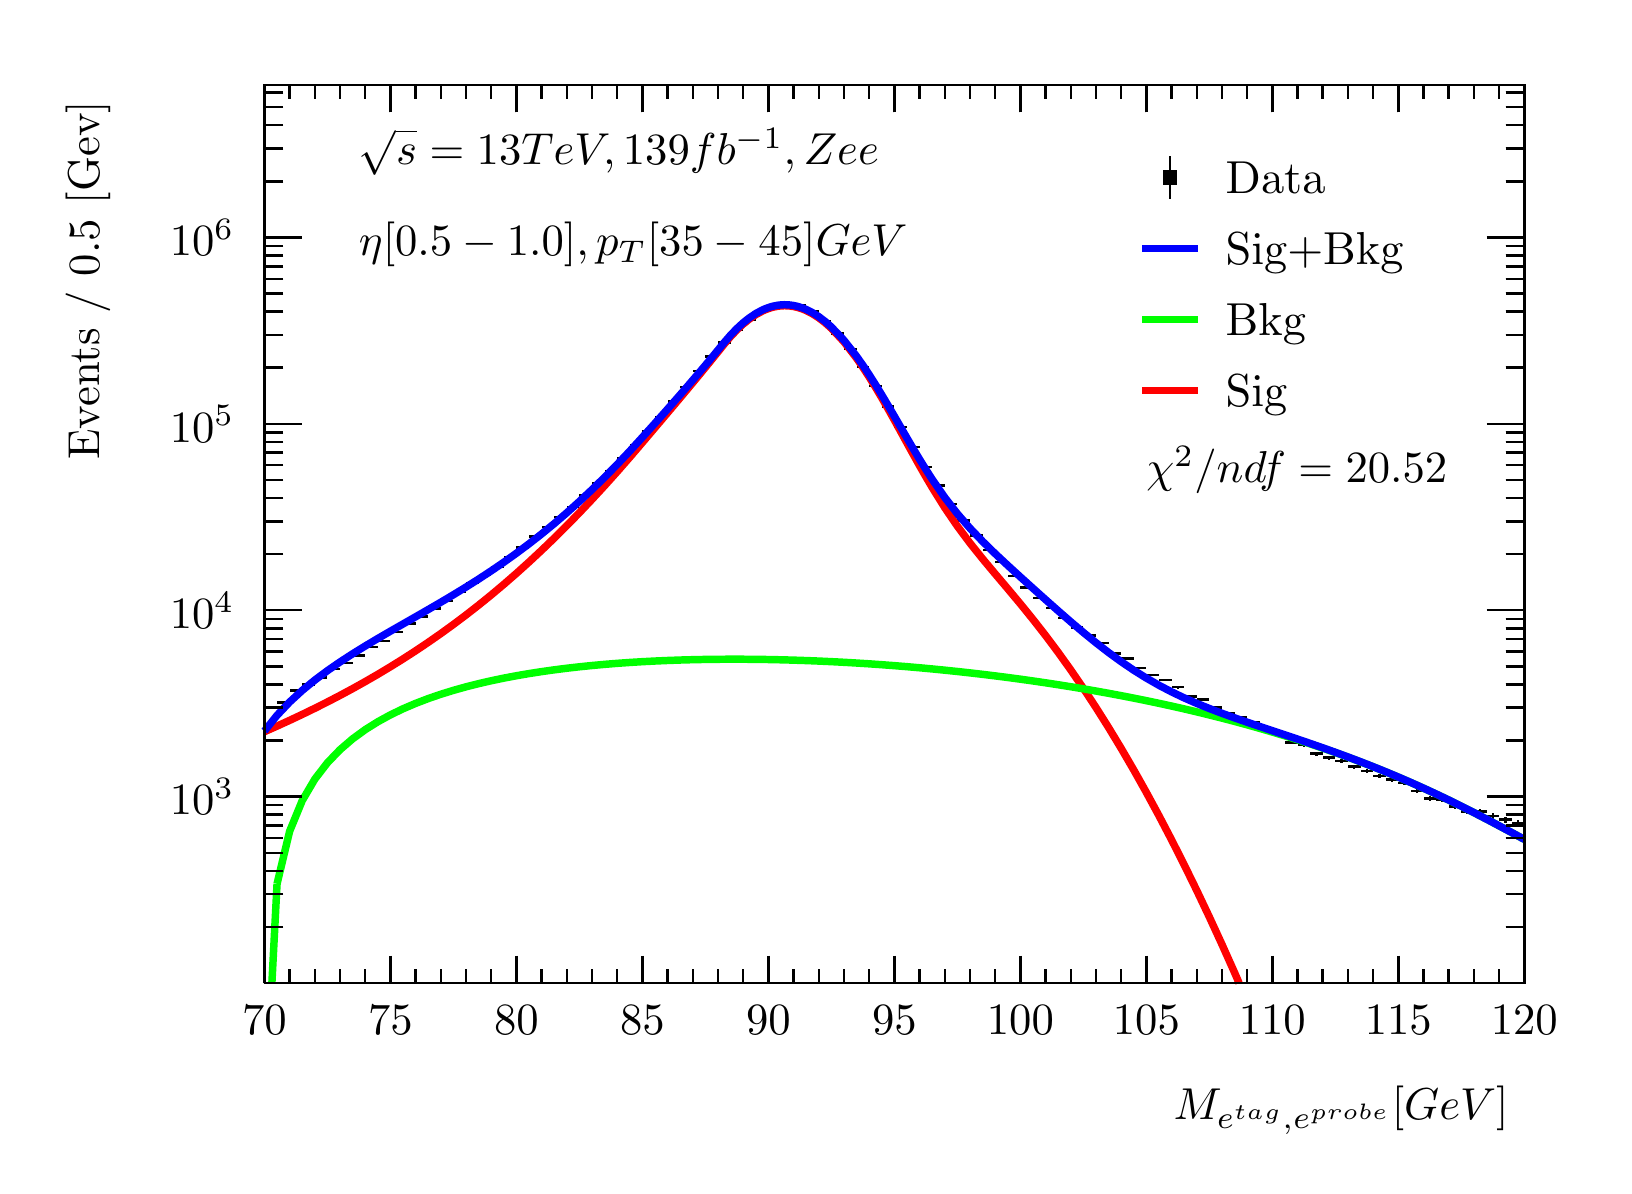
\begin{tikzpicture}
\pgfdeclareplotmark{cross} {
\pgfpathmoveto{\pgfpoint{-0.3\pgfplotmarksize}{\pgfplotmarksize}}
\pgfpathlineto{\pgfpoint{+0.3\pgfplotmarksize}{\pgfplotmarksize}}
\pgfpathlineto{\pgfpoint{+0.3\pgfplotmarksize}{0.3\pgfplotmarksize}}
\pgfpathlineto{\pgfpoint{+1\pgfplotmarksize}{0.3\pgfplotmarksize}}
\pgfpathlineto{\pgfpoint{+1\pgfplotmarksize}{-0.3\pgfplotmarksize}}
\pgfpathlineto{\pgfpoint{+0.3\pgfplotmarksize}{-0.3\pgfplotmarksize}}
\pgfpathlineto{\pgfpoint{+0.3\pgfplotmarksize}{-1.\pgfplotmarksize}}
\pgfpathlineto{\pgfpoint{-0.3\pgfplotmarksize}{-1.\pgfplotmarksize}}
\pgfpathlineto{\pgfpoint{-0.3\pgfplotmarksize}{-0.3\pgfplotmarksize}}
\pgfpathlineto{\pgfpoint{-1.\pgfplotmarksize}{-0.3\pgfplotmarksize}}
\pgfpathlineto{\pgfpoint{-1.\pgfplotmarksize}{0.3\pgfplotmarksize}}
\pgfpathlineto{\pgfpoint{-0.3\pgfplotmarksize}{0.3\pgfplotmarksize}}
\pgfpathclose
\pgfusepathqstroke
}
\pgfdeclareplotmark{cross*} {
\pgfpathmoveto{\pgfpoint{-0.3\pgfplotmarksize}{\pgfplotmarksize}}
\pgfpathlineto{\pgfpoint{+0.3\pgfplotmarksize}{\pgfplotmarksize}}
\pgfpathlineto{\pgfpoint{+0.3\pgfplotmarksize}{0.3\pgfplotmarksize}}
\pgfpathlineto{\pgfpoint{+1\pgfplotmarksize}{0.3\pgfplotmarksize}}
\pgfpathlineto{\pgfpoint{+1\pgfplotmarksize}{-0.3\pgfplotmarksize}}
\pgfpathlineto{\pgfpoint{+0.3\pgfplotmarksize}{-0.3\pgfplotmarksize}}
\pgfpathlineto{\pgfpoint{+0.3\pgfplotmarksize}{-1.\pgfplotmarksize}}
\pgfpathlineto{\pgfpoint{-0.3\pgfplotmarksize}{-1.\pgfplotmarksize}}
\pgfpathlineto{\pgfpoint{-0.3\pgfplotmarksize}{-0.3\pgfplotmarksize}}
\pgfpathlineto{\pgfpoint{-1.\pgfplotmarksize}{-0.3\pgfplotmarksize}}
\pgfpathlineto{\pgfpoint{-1.\pgfplotmarksize}{0.3\pgfplotmarksize}}
\pgfpathlineto{\pgfpoint{-0.3\pgfplotmarksize}{0.3\pgfplotmarksize}}
\pgfpathclose
\pgfusepathqfillstroke
}
\pgfdeclareplotmark{newstar} {
\pgfpathmoveto{\pgfqpoint{0pt}{\pgfplotmarksize}}
\pgfpathlineto{\pgfqpointpolar{44}{0.5\pgfplotmarksize}}
\pgfpathlineto{\pgfqpointpolar{18}{\pgfplotmarksize}}
\pgfpathlineto{\pgfqpointpolar{-20}{0.5\pgfplotmarksize}}
\pgfpathlineto{\pgfqpointpolar{-54}{\pgfplotmarksize}}
\pgfpathlineto{\pgfqpointpolar{-90}{0.5\pgfplotmarksize}}
\pgfpathlineto{\pgfqpointpolar{234}{\pgfplotmarksize}}
\pgfpathlineto{\pgfqpointpolar{198}{0.5\pgfplotmarksize}}
\pgfpathlineto{\pgfqpointpolar{162}{\pgfplotmarksize}}
\pgfpathlineto{\pgfqpointpolar{134}{0.5\pgfplotmarksize}}
\pgfpathclose
\pgfusepathqstroke
}
\pgfdeclareplotmark{newstar*} {
\pgfpathmoveto{\pgfqpoint{0pt}{\pgfplotmarksize}}
\pgfpathlineto{\pgfqpointpolar{44}{0.5\pgfplotmarksize}}
\pgfpathlineto{\pgfqpointpolar{18}{\pgfplotmarksize}}
\pgfpathlineto{\pgfqpointpolar{-20}{0.5\pgfplotmarksize}}
\pgfpathlineto{\pgfqpointpolar{-54}{\pgfplotmarksize}}
\pgfpathlineto{\pgfqpointpolar{-90}{0.5\pgfplotmarksize}}
\pgfpathlineto{\pgfqpointpolar{234}{\pgfplotmarksize}}
\pgfpathlineto{\pgfqpointpolar{198}{0.5\pgfplotmarksize}}
\pgfpathlineto{\pgfqpointpolar{162}{\pgfplotmarksize}}
\pgfpathlineto{\pgfqpointpolar{134}{0.5\pgfplotmarksize}}
\pgfpathclose
\pgfusepathqfillstroke
}
\definecolor{c}{rgb}{1,1,1};
\draw [color=c, fill=c] (0,0) rectangle (20,14.4361);
\draw [color=c, fill=c] (3,2.30977) rectangle (19,13.7143);
\definecolor{c}{rgb}{0,0,0};
\draw [c,line width=0.9] (3,2.30977) -- (3,13.7143) -- (19,13.7143) -- (19,2.30977) -- (3,2.30977);
\definecolor{c}{rgb}{1,1,1};
\draw [color=c, fill=c] (3,2.30977) rectangle (19,13.7143);
\definecolor{c}{rgb}{0,0,0};
\draw [c,line width=0.9] (3,2.30977) -- (3,13.7143) -- (19,13.7143) -- (19,2.30977) -- (3,2.30977);
\draw [c,line width=0.9] (3,2.30977) -- (19,2.30977);
\draw [c,line width=0.9] (3,2.65624) -- (3,2.30977);
\draw [c,line width=0.9] (3.32,2.48301) -- (3.32,2.30977);
\draw [c,line width=0.9] (3.64,2.48301) -- (3.64,2.30977);
\draw [c,line width=0.9] (3.96,2.48301) -- (3.96,2.30977);
\draw [c,line width=0.9] (4.28,2.48301) -- (4.28,2.30977);
\draw [c,line width=0.9] (4.6,2.65624) -- (4.6,2.30977);
\draw [c,line width=0.9] (4.92,2.48301) -- (4.92,2.30977);
\draw [c,line width=0.9] (5.24,2.48301) -- (5.24,2.30977);
\draw [c,line width=0.9] (5.56,2.48301) -- (5.56,2.30977);
\draw [c,line width=0.9] (5.88,2.48301) -- (5.88,2.30977);
\draw [c,line width=0.9] (6.2,2.65624) -- (6.2,2.30977);
\draw [c,line width=0.9] (6.52,2.48301) -- (6.52,2.30977);
\draw [c,line width=0.9] (6.84,2.48301) -- (6.84,2.30977);
\draw [c,line width=0.9] (7.16,2.48301) -- (7.16,2.30977);
\draw [c,line width=0.9] (7.48,2.48301) -- (7.48,2.30977);
\draw [c,line width=0.9] (7.8,2.65624) -- (7.8,2.30977);
\draw [c,line width=0.9] (8.12,2.48301) -- (8.12,2.30977);
\draw [c,line width=0.9] (8.44,2.48301) -- (8.44,2.30977);
\draw [c,line width=0.9] (8.76,2.48301) -- (8.76,2.30977);
\draw [c,line width=0.9] (9.08,2.48301) -- (9.08,2.30977);
\draw [c,line width=0.9] (9.4,2.65624) -- (9.4,2.30977);
\draw [c,line width=0.9] (9.72,2.48301) -- (9.72,2.30977);
\draw [c,line width=0.9] (10.04,2.48301) -- (10.04,2.30977);
\draw [c,line width=0.9] (10.36,2.48301) -- (10.36,2.30977);
\draw [c,line width=0.9] (10.68,2.48301) -- (10.68,2.30977);
\draw [c,line width=0.9] (11,2.65624) -- (11,2.30977);
\draw [c,line width=0.9] (11.32,2.48301) -- (11.32,2.30977);
\draw [c,line width=0.9] (11.64,2.48301) -- (11.64,2.30977);
\draw [c,line width=0.9] (11.96,2.48301) -- (11.96,2.30977);
\draw [c,line width=0.9] (12.28,2.48301) -- (12.28,2.30977);
\draw [c,line width=0.9] (12.6,2.65624) -- (12.6,2.30977);
\draw [c,line width=0.9] (12.92,2.48301) -- (12.92,2.30977);
\draw [c,line width=0.9] (13.24,2.48301) -- (13.24,2.30977);
\draw [c,line width=0.9] (13.56,2.48301) -- (13.56,2.30977);
\draw [c,line width=0.9] (13.88,2.48301) -- (13.88,2.30977);
\draw [c,line width=0.9] (14.2,2.65624) -- (14.2,2.30977);
\draw [c,line width=0.9] (14.52,2.48301) -- (14.52,2.30977);
\draw [c,line width=0.9] (14.84,2.48301) -- (14.84,2.30977);
\draw [c,line width=0.9] (15.16,2.48301) -- (15.16,2.30977);
\draw [c,line width=0.9] (15.48,2.48301) -- (15.48,2.30977);
\draw [c,line width=0.9] (15.8,2.65624) -- (15.8,2.30977);
\draw [c,line width=0.9] (16.12,2.48301) -- (16.12,2.30977);
\draw [c,line width=0.9] (16.44,2.48301) -- (16.44,2.30977);
\draw [c,line width=0.9] (16.76,2.48301) -- (16.76,2.30977);
\draw [c,line width=0.9] (17.08,2.48301) -- (17.08,2.30977);
\draw [c,line width=0.9] (17.4,2.65624) -- (17.4,2.30977);
\draw [c,line width=0.9] (17.72,2.48301) -- (17.72,2.30977);
\draw [c,line width=0.9] (18.04,2.48301) -- (18.04,2.30977);
\draw [c,line width=0.9] (18.36,2.48301) -- (18.36,2.30977);
\draw [c,line width=0.9] (18.68,2.48301) -- (18.68,2.30977);
\draw [c,line width=0.9] (19,2.65624) -- (19,2.30977);
\draw [anchor=base] (3,1.66015) node[scale=1.61424, color=c, rotate=0]{70};
\draw [anchor=base] (4.6,1.66015) node[scale=1.61424, color=c, rotate=0]{75};
\draw [anchor=base] (6.2,1.66015) node[scale=1.61424, color=c, rotate=0]{80};
\draw [anchor=base] (7.8,1.66015) node[scale=1.61424, color=c, rotate=0]{85};
\draw [anchor=base] (9.4,1.66015) node[scale=1.61424, color=c, rotate=0]{90};
\draw [anchor=base] (11,1.66015) node[scale=1.61424, color=c, rotate=0]{95};
\draw [anchor=base] (12.6,1.66015) node[scale=1.61424, color=c, rotate=0]{100};
\draw [anchor=base] (14.2,1.66015) node[scale=1.61424, color=c, rotate=0]{105};
\draw [anchor=base] (15.8,1.66015) node[scale=1.61424, color=c, rotate=0]{110};
\draw [anchor=base] (17.4,1.66015) node[scale=1.61424, color=c, rotate=0]{115};
\draw [anchor=base] (19,1.66015) node[scale=1.61424, color=c, rotate=0]{120};
\draw [anchor= east] (19,0.692932) node[scale=1.61424, color=c, rotate=0]{$M_{e^{tag}, e^{probe}}  [GeV]$};
\draw [c,line width=0.9] (3,13.7143) -- (19,13.7143);
\draw [c,line width=0.9] (3,13.3678) -- (3,13.7143);
\draw [c,line width=0.9] (3.32,13.5411) -- (3.32,13.7143);
\draw [c,line width=0.9] (3.64,13.5411) -- (3.64,13.7143);
\draw [c,line width=0.9] (3.96,13.5411) -- (3.96,13.7143);
\draw [c,line width=0.9] (4.28,13.5411) -- (4.28,13.7143);
\draw [c,line width=0.9] (4.6,13.3678) -- (4.6,13.7143);
\draw [c,line width=0.9] (4.92,13.5411) -- (4.92,13.7143);
\draw [c,line width=0.9] (5.24,13.5411) -- (5.24,13.7143);
\draw [c,line width=0.9] (5.56,13.5411) -- (5.56,13.7143);
\draw [c,line width=0.9] (5.88,13.5411) -- (5.88,13.7143);
\draw [c,line width=0.9] (6.2,13.3678) -- (6.2,13.7143);
\draw [c,line width=0.9] (6.52,13.5411) -- (6.52,13.7143);
\draw [c,line width=0.9] (6.84,13.5411) -- (6.84,13.7143);
\draw [c,line width=0.9] (7.16,13.5411) -- (7.16,13.7143);
\draw [c,line width=0.9] (7.48,13.5411) -- (7.48,13.7143);
\draw [c,line width=0.9] (7.8,13.3678) -- (7.8,13.7143);
\draw [c,line width=0.9] (8.12,13.5411) -- (8.12,13.7143);
\draw [c,line width=0.9] (8.44,13.5411) -- (8.44,13.7143);
\draw [c,line width=0.9] (8.76,13.5411) -- (8.76,13.7143);
\draw [c,line width=0.9] (9.08,13.5411) -- (9.08,13.7143);
\draw [c,line width=0.9] (9.4,13.3678) -- (9.4,13.7143);
\draw [c,line width=0.9] (9.72,13.5411) -- (9.72,13.7143);
\draw [c,line width=0.9] (10.04,13.5411) -- (10.04,13.7143);
\draw [c,line width=0.9] (10.36,13.5411) -- (10.36,13.7143);
\draw [c,line width=0.9] (10.68,13.5411) -- (10.68,13.7143);
\draw [c,line width=0.9] (11,13.3678) -- (11,13.7143);
\draw [c,line width=0.9] (11.32,13.5411) -- (11.32,13.7143);
\draw [c,line width=0.9] (11.64,13.5411) -- (11.64,13.7143);
\draw [c,line width=0.9] (11.96,13.5411) -- (11.96,13.7143);
\draw [c,line width=0.9] (12.28,13.5411) -- (12.28,13.7143);
\draw [c,line width=0.9] (12.6,13.3678) -- (12.6,13.7143);
\draw [c,line width=0.9] (12.92,13.5411) -- (12.92,13.7143);
\draw [c,line width=0.9] (13.24,13.5411) -- (13.24,13.7143);
\draw [c,line width=0.9] (13.56,13.5411) -- (13.56,13.7143);
\draw [c,line width=0.9] (13.88,13.5411) -- (13.88,13.7143);
\draw [c,line width=0.9] (14.2,13.3678) -- (14.2,13.7143);
\draw [c,line width=0.9] (14.52,13.5411) -- (14.52,13.7143);
\draw [c,line width=0.9] (14.84,13.5411) -- (14.84,13.7143);
\draw [c,line width=0.9] (15.16,13.5411) -- (15.16,13.7143);
\draw [c,line width=0.9] (15.48,13.5411) -- (15.48,13.7143);
\draw [c,line width=0.9] (15.8,13.3678) -- (15.8,13.7143);
\draw [c,line width=0.9] (16.12,13.5411) -- (16.12,13.7143);
\draw [c,line width=0.9] (16.44,13.5411) -- (16.44,13.7143);
\draw [c,line width=0.9] (16.76,13.5411) -- (16.76,13.7143);
\draw [c,line width=0.9] (17.08,13.5411) -- (17.08,13.7143);
\draw [c,line width=0.9] (17.4,13.3678) -- (17.4,13.7143);
\draw [c,line width=0.9] (17.72,13.5411) -- (17.72,13.7143);
\draw [c,line width=0.9] (18.04,13.5411) -- (18.04,13.7143);
\draw [c,line width=0.9] (18.36,13.5411) -- (18.36,13.7143);
\draw [c,line width=0.9] (18.68,13.5411) -- (18.68,13.7143);
\draw [c,line width=0.9] (19,13.3678) -- (19,13.7143);
\draw [c,line width=0.9] (3,2.30977) -- (3,13.7143);
\draw [c,line width=0.9] (3.237,3.02243) -- (3,3.02243);
\draw [c,line width=0.9] (3.237,3.43931) -- (3,3.43931);
\draw [c,line width=0.9] (3.237,3.73509) -- (3,3.73509);
\draw [c,line width=0.9] (3.237,3.96452) -- (3,3.96452);
\draw [c,line width=0.9] (3.237,4.15197) -- (3,4.15197);
\draw [c,line width=0.9] (3.237,4.31046) -- (3,4.31046);
\draw [c,line width=0.9] (3.237,4.44775) -- (3,4.44775);
\draw [c,line width=0.9] (3.237,4.56885) -- (3,4.56885);
\draw [c,line width=0.9] (3.474,4.67718) -- (3,4.67718);
\draw [anchor= east] (2.82,4.67718) node[scale=1.61424, color=c, rotate=0]{$10^{3}$};
\draw [c,line width=0.9] (3.237,5.38984) -- (3,5.38984);
\draw [c,line width=0.9] (3.237,5.80672) -- (3,5.80672);
\draw [c,line width=0.9] (3.237,6.1025) -- (3,6.1025);
\draw [c,line width=0.9] (3.237,6.33193) -- (3,6.33193);
\draw [c,line width=0.9] (3.237,6.51938) -- (3,6.51938);
\draw [c,line width=0.9] (3.237,6.67787) -- (3,6.67787);
\draw [c,line width=0.9] (3.237,6.81516) -- (3,6.81516);
\draw [c,line width=0.9] (3.237,6.93626) -- (3,6.93626);
\draw [c,line width=0.9] (3.474,7.04459) -- (3,7.04459);
\draw [anchor= east] (2.82,7.04459) node[scale=1.61424, color=c, rotate=0]{$10^{4}$};
\draw [c,line width=0.9] (3.237,7.75725) -- (3,7.75725);
\draw [c,line width=0.9] (3.237,8.17413) -- (3,8.17413);
\draw [c,line width=0.9] (3.237,8.46991) -- (3,8.46991);
\draw [c,line width=0.9] (3.237,8.69933) -- (3,8.69933);
\draw [c,line width=0.9] (3.237,8.88679) -- (3,8.88679);
\draw [c,line width=0.9] (3.237,9.04528) -- (3,9.04528);
\draw [c,line width=0.9] (3.237,9.18257) -- (3,9.18257);
\draw [c,line width=0.9] (3.237,9.30367) -- (3,9.30367);
\draw [c,line width=0.9] (3.474,9.41199) -- (3,9.41199);
\draw [anchor= east] (2.82,9.41199) node[scale=1.61424, color=c, rotate=0]{$10^{5}$};
\draw [c,line width=0.9] (3.237,10.1247) -- (3,10.1247);
\draw [c,line width=0.9] (3.237,10.5415) -- (3,10.5415);
\draw [c,line width=0.9] (3.237,10.8373) -- (3,10.8373);
\draw [c,line width=0.9] (3.237,11.0667) -- (3,11.0667);
\draw [c,line width=0.9] (3.237,11.2542) -- (3,11.2542);
\draw [c,line width=0.9] (3.237,11.4127) -- (3,11.4127);
\draw [c,line width=0.9] (3.237,11.55) -- (3,11.55);
\draw [c,line width=0.9] (3.237,11.6711) -- (3,11.6711);
\draw [c,line width=0.9] (3.474,11.7794) -- (3,11.7794);
\draw [anchor= east] (2.82,11.7794) node[scale=1.61424, color=c, rotate=0]{$10^{6}$};
\draw [c,line width=0.9] (3.237,12.4921) -- (3,12.4921);
\draw [c,line width=0.9] (3.237,12.9089) -- (3,12.9089);
\draw [c,line width=0.9] (3.237,13.2047) -- (3,13.2047);
\draw [c,line width=0.9] (3.237,13.4341) -- (3,13.4341);
\draw [c,line width=0.9] (3.237,13.6216) -- (3,13.6216);
\draw [anchor= east] (0.76,13.7143) node[scale=1.61424, color=c, rotate=90]{Events / 0.5 [Gev]};
\draw [c,line width=0.9] (19,2.30977) -- (19,13.7143);
\draw [c,line width=0.9] (18.763,3.02243) -- (19,3.02243);
\draw [c,line width=0.9] (18.763,3.43931) -- (19,3.43931);
\draw [c,line width=0.9] (18.763,3.73509) -- (19,3.73509);
\draw [c,line width=0.9] (18.763,3.96452) -- (19,3.96452);
\draw [c,line width=0.9] (18.763,4.15197) -- (19,4.15197);
\draw [c,line width=0.9] (18.763,4.31046) -- (19,4.31046);
\draw [c,line width=0.9] (18.763,4.44775) -- (19,4.44775);
\draw [c,line width=0.9] (18.763,4.56885) -- (19,4.56885);
\draw [c,line width=0.9] (18.526,4.67718) -- (19,4.67718);
\draw [c,line width=0.9] (18.763,5.38984) -- (19,5.38984);
\draw [c,line width=0.9] (18.763,5.80672) -- (19,5.80672);
\draw [c,line width=0.9] (18.763,6.1025) -- (19,6.1025);
\draw [c,line width=0.9] (18.763,6.33193) -- (19,6.33193);
\draw [c,line width=0.9] (18.763,6.51938) -- (19,6.51938);
\draw [c,line width=0.9] (18.763,6.67787) -- (19,6.67787);
\draw [c,line width=0.9] (18.763,6.81516) -- (19,6.81516);
\draw [c,line width=0.9] (18.763,6.93626) -- (19,6.93626);
\draw [c,line width=0.9] (18.526,7.04459) -- (19,7.04459);
\draw [c,line width=0.9] (18.763,7.75725) -- (19,7.75725);
\draw [c,line width=0.9] (18.763,8.17413) -- (19,8.17413);
\draw [c,line width=0.9] (18.763,8.46991) -- (19,8.46991);
\draw [c,line width=0.9] (18.763,8.69933) -- (19,8.69933);
\draw [c,line width=0.9] (18.763,8.88679) -- (19,8.88679);
\draw [c,line width=0.9] (18.763,9.04528) -- (19,9.04528);
\draw [c,line width=0.9] (18.763,9.18257) -- (19,9.18257);
\draw [c,line width=0.9] (18.763,9.30367) -- (19,9.30367);
\draw [c,line width=0.9] (18.526,9.41199) -- (19,9.41199);
\draw [c,line width=0.9] (18.763,10.1247) -- (19,10.1247);
\draw [c,line width=0.9] (18.763,10.5415) -- (19,10.5415);
\draw [c,line width=0.9] (18.763,10.8373) -- (19,10.8373);
\draw [c,line width=0.9] (18.763,11.0667) -- (19,11.0667);
\draw [c,line width=0.9] (18.763,11.2542) -- (19,11.2542);
\draw [c,line width=0.9] (18.763,11.4127) -- (19,11.4127);
\draw [c,line width=0.9] (18.763,11.55) -- (19,11.55);
\draw [c,line width=0.9] (18.763,11.6711) -- (19,11.6711);
\draw [c,line width=0.9] (18.526,11.7794) -- (19,11.7794);
\draw [c,line width=0.9] (18.763,12.4921) -- (19,12.4921);
\draw [c,line width=0.9] (18.763,12.9089) -- (19,12.9089);
\draw [c,line width=0.9] (18.763,13.2047) -- (19,13.2047);
\draw [c,line width=0.9] (18.763,13.4341) -- (19,13.4341);
\draw [c,line width=0.9] (18.763,13.6216) -- (19,13.6216);
\draw [c,line width=0.9] (3.08,5.80535) -- (3,5.80535);
\draw [c,line width=0.9] (3,5.80535) -- (3,5.80535);
\draw [c,line width=0.9] (3.08,5.80535) -- (3.16,5.80535);
\draw [c,line width=0.9] (3.16,5.80535) -- (3.16,5.80535);
\draw [c,line width=0.9] (3.08,5.80535) -- (3.08,5.82413);
\draw [c,line width=0.9] (3.08,5.82413) -- (3.08,5.82413);
\draw [c,line width=0.9] (3.08,5.80535) -- (3.08,5.78657);
\draw [c,line width=0.9] (3.08,5.78657) -- (3.08,5.78657);
\draw [c,line width=0.9] (3.24,5.87211) -- (3.16,5.87211);
\draw [c,line width=0.9] (3.16,5.87211) -- (3.16,5.87211);
\draw [c,line width=0.9] (3.24,5.87211) -- (3.32,5.87211);
\draw [c,line width=0.9] (3.32,5.87211) -- (3.32,5.87211);
\draw [c,line width=0.9] (3.24,5.87211) -- (3.24,5.8903);
\draw [c,line width=0.9] (3.24,5.8903) -- (3.24,5.8903);
\draw [c,line width=0.9] (3.24,5.87211) -- (3.24,5.85393);
\draw [c,line width=0.9] (3.24,5.85393) -- (3.24,5.85393);
\draw [c,line width=0.9] (3.4,6.02651) -- (3.32,6.02651);
\draw [c,line width=0.9] (3.32,6.02651) -- (3.32,6.02651);
\draw [c,line width=0.9] (3.4,6.02651) -- (3.48,6.02651);
\draw [c,line width=0.9] (3.48,6.02651) -- (3.48,6.02651);
\draw [c,line width=0.9] (3.4,6.02651) -- (3.4,6.04337);
\draw [c,line width=0.9] (3.4,6.04337) -- (3.4,6.04337);
\draw [c,line width=0.9] (3.4,6.02651) -- (3.4,6.00964);
\draw [c,line width=0.9] (3.4,6.00964) -- (3.4,6.00964);
\draw [c,line width=0.9] (3.56,6.09993) -- (3.48,6.09993);
\draw [c,line width=0.9] (3.48,6.09993) -- (3.48,6.09993);
\draw [c,line width=0.9] (3.56,6.09993) -- (3.64,6.09993);
\draw [c,line width=0.9] (3.64,6.09993) -- (3.64,6.09993);
\draw [c,line width=0.9] (3.56,6.09993) -- (3.56,6.11621);
\draw [c,line width=0.9] (3.56,6.11621) -- (3.56,6.11621);
\draw [c,line width=0.9] (3.56,6.09993) -- (3.56,6.08365);
\draw [c,line width=0.9] (3.56,6.08365) -- (3.56,6.08365);
\draw [c,line width=0.9] (3.72,6.19087) -- (3.64,6.19087);
\draw [c,line width=0.9] (3.64,6.19087) -- (3.64,6.19087);
\draw [c,line width=0.9] (3.72,6.19087) -- (3.8,6.19087);
\draw [c,line width=0.9] (3.8,6.19087) -- (3.8,6.19087);
\draw [c,line width=0.9] (3.72,6.19087) -- (3.72,6.20644);
\draw [c,line width=0.9] (3.72,6.20644) -- (3.72,6.20644);
\draw [c,line width=0.9] (3.72,6.19087) -- (3.72,6.1753);
\draw [c,line width=0.9] (3.72,6.1753) -- (3.72,6.1753);
\draw [c,line width=0.9] (3.88,6.2987) -- (3.8,6.2987);
\draw [c,line width=0.9] (3.8,6.2987) -- (3.8,6.2987);
\draw [c,line width=0.9] (3.88,6.2987) -- (3.96,6.2987);
\draw [c,line width=0.9] (3.96,6.2987) -- (3.96,6.2987);
\draw [c,line width=0.9] (3.88,6.2987) -- (3.88,6.31348);
\draw [c,line width=0.9] (3.88,6.31348) -- (3.88,6.31348);
\draw [c,line width=0.9] (3.88,6.2987) -- (3.88,6.28392);
\draw [c,line width=0.9] (3.88,6.28392) -- (3.88,6.28392);
\draw [c,line width=0.9] (4.04,6.37541) -- (3.96,6.37541);
\draw [c,line width=0.9] (3.96,6.37541) -- (3.96,6.37541);
\draw [c,line width=0.9] (4.04,6.37541) -- (4.12,6.37541);
\draw [c,line width=0.9] (4.12,6.37541) -- (4.12,6.37541);
\draw [c,line width=0.9] (4.04,6.37541) -- (4.04,6.38965);
\draw [c,line width=0.9] (4.04,6.38965) -- (4.04,6.38965);
\draw [c,line width=0.9] (4.04,6.37541) -- (4.04,6.36118);
\draw [c,line width=0.9] (4.04,6.36118) -- (4.04,6.36118);
\draw [c,line width=0.9] (4.2,6.47276) -- (4.12,6.47276);
\draw [c,line width=0.9] (4.12,6.47276) -- (4.12,6.47276);
\draw [c,line width=0.9] (4.2,6.47276) -- (4.28,6.47276);
\draw [c,line width=0.9] (4.28,6.47276) -- (4.28,6.47276);
\draw [c,line width=0.9] (4.2,6.47276) -- (4.2,6.48634);
\draw [c,line width=0.9] (4.2,6.48634) -- (4.2,6.48634);
\draw [c,line width=0.9] (4.2,6.47276) -- (4.2,6.45918);
\draw [c,line width=0.9] (4.2,6.45918) -- (4.2,6.45918);
\draw [c,line width=0.9] (4.36,6.57459) -- (4.28,6.57459);
\draw [c,line width=0.9] (4.28,6.57459) -- (4.28,6.57459);
\draw [c,line width=0.9] (4.36,6.57459) -- (4.44,6.57459);
\draw [c,line width=0.9] (4.44,6.57459) -- (4.44,6.57459);
\draw [c,line width=0.9] (4.36,6.57459) -- (4.36,6.58751);
\draw [c,line width=0.9] (4.36,6.58751) -- (4.36,6.58751);
\draw [c,line width=0.9] (4.36,6.57459) -- (4.36,6.56167);
\draw [c,line width=0.9] (4.36,6.56167) -- (4.36,6.56167);
\draw [c,line width=0.9] (4.52,6.6544) -- (4.44,6.6544);
\draw [c,line width=0.9] (4.44,6.6544) -- (4.44,6.6544);
\draw [c,line width=0.9] (4.52,6.6544) -- (4.6,6.6544);
\draw [c,line width=0.9] (4.6,6.6544) -- (4.6,6.6544);
\draw [c,line width=0.9] (4.52,6.6544) -- (4.52,6.66683);
\draw [c,line width=0.9] (4.52,6.66683) -- (4.52,6.66683);
\draw [c,line width=0.9] (4.52,6.6544) -- (4.52,6.64197);
\draw [c,line width=0.9] (4.52,6.64197) -- (4.52,6.64197);
\draw [c,line width=0.9] (4.68,6.76648) -- (4.6,6.76648);
\draw [c,line width=0.9] (4.6,6.76648) -- (4.6,6.76648);
\draw [c,line width=0.9] (4.68,6.76648) -- (4.76,6.76648);
\draw [c,line width=0.9] (4.76,6.76648) -- (4.76,6.76648);
\draw [c,line width=0.9] (4.68,6.76648) -- (4.68,6.77825);
\draw [c,line width=0.9] (4.68,6.77825) -- (4.68,6.77825);
\draw [c,line width=0.9] (4.68,6.76648) -- (4.68,6.7547);
\draw [c,line width=0.9] (4.68,6.7547) -- (4.68,6.7547);
\draw [c,line width=0.9] (4.84,6.87749) -- (4.76,6.87749);
\draw [c,line width=0.9] (4.76,6.87749) -- (4.76,6.87749);
\draw [c,line width=0.9] (4.84,6.87749) -- (4.92,6.87749);
\draw [c,line width=0.9] (4.92,6.87749) -- (4.92,6.87749);
\draw [c,line width=0.9] (4.84,6.87749) -- (4.84,6.88865);
\draw [c,line width=0.9] (4.84,6.88865) -- (4.84,6.88865);
\draw [c,line width=0.9] (4.84,6.87749) -- (4.84,6.86634);
\draw [c,line width=0.9] (4.84,6.86634) -- (4.84,6.86634);
\draw [c,line width=0.9] (5,6.96477) -- (4.92,6.96477);
\draw [c,line width=0.9] (4.92,6.96477) -- (4.92,6.96477);
\draw [c,line width=0.9] (5,6.96477) -- (5.08,6.96477);
\draw [c,line width=0.9] (5.08,6.96477) -- (5.08,6.96477);
\draw [c,line width=0.9] (5,6.96477) -- (5,6.97545);
\draw [c,line width=0.9] (5,6.97545) -- (5,6.97545);
\draw [c,line width=0.9] (5,6.96477) -- (5,6.95408);
\draw [c,line width=0.9] (5,6.95408) -- (5,6.95408);
\draw [c,line width=0.9] (5.16,7.06565) -- (5.08,7.06565);
\draw [c,line width=0.9] (5.08,7.06565) -- (5.08,7.06565);
\draw [c,line width=0.9] (5.16,7.06565) -- (5.24,7.06565);
\draw [c,line width=0.9] (5.24,7.06565) -- (5.24,7.06565);
\draw [c,line width=0.9] (5.16,7.06565) -- (5.16,7.07583);
\draw [c,line width=0.9] (5.16,7.07583) -- (5.16,7.07583);
\draw [c,line width=0.9] (5.16,7.06565) -- (5.16,7.05548);
\draw [c,line width=0.9] (5.16,7.05548) -- (5.16,7.05548);
\draw [c,line width=0.9] (5.32,7.16111) -- (5.24,7.16111);
\draw [c,line width=0.9] (5.24,7.16111) -- (5.24,7.16111);
\draw [c,line width=0.9] (5.32,7.16111) -- (5.4,7.16111);
\draw [c,line width=0.9] (5.4,7.16111) -- (5.4,7.16111);
\draw [c,line width=0.9] (5.32,7.16111) -- (5.32,7.17082);
\draw [c,line width=0.9] (5.32,7.17082) -- (5.32,7.17082);
\draw [c,line width=0.9] (5.32,7.16111) -- (5.32,7.15139);
\draw [c,line width=0.9] (5.32,7.15139) -- (5.32,7.15139);
\draw [c,line width=0.9] (5.48,7.27336) -- (5.4,7.27336);
\draw [c,line width=0.9] (5.4,7.27336) -- (5.4,7.27336);
\draw [c,line width=0.9] (5.48,7.27336) -- (5.56,7.27336);
\draw [c,line width=0.9] (5.56,7.27336) -- (5.56,7.27336);
\draw [c,line width=0.9] (5.48,7.27336) -- (5.48,7.28255);
\draw [c,line width=0.9] (5.48,7.28255) -- (5.48,7.28255);
\draw [c,line width=0.9] (5.48,7.27336) -- (5.48,7.26416);
\draw [c,line width=0.9] (5.48,7.26416) -- (5.48,7.26416);
\draw [c,line width=0.9] (5.64,7.38899) -- (5.56,7.38899);
\draw [c,line width=0.9] (5.56,7.38899) -- (5.56,7.38899);
\draw [c,line width=0.9] (5.64,7.38899) -- (5.72,7.38899);
\draw [c,line width=0.9] (5.72,7.38899) -- (5.72,7.38899);
\draw [c,line width=0.9] (5.64,7.38899) -- (5.64,7.39769);
\draw [c,line width=0.9] (5.64,7.39769) -- (5.64,7.39769);
\draw [c,line width=0.9] (5.64,7.38899) -- (5.64,7.38029);
\draw [c,line width=0.9] (5.64,7.38029) -- (5.64,7.38029);
\draw [c,line width=0.9] (5.8,7.49192) -- (5.72,7.49192);
\draw [c,line width=0.9] (5.72,7.49192) -- (5.72,7.49192);
\draw [c,line width=0.9] (5.8,7.49192) -- (5.88,7.49192);
\draw [c,line width=0.9] (5.88,7.49192) -- (5.88,7.49192);
\draw [c,line width=0.9] (5.8,7.49192) -- (5.8,7.5002);
\draw [c,line width=0.9] (5.8,7.5002) -- (5.8,7.5002);
\draw [c,line width=0.9] (5.8,7.49192) -- (5.8,7.48365);
\draw [c,line width=0.9] (5.8,7.48365) -- (5.8,7.48365);
\draw [c,line width=0.9] (5.96,7.59088) -- (5.88,7.59088);
\draw [c,line width=0.9] (5.88,7.59088) -- (5.88,7.59088);
\draw [c,line width=0.9] (5.96,7.59088) -- (6.04,7.59088);
\draw [c,line width=0.9] (6.04,7.59088) -- (6.04,7.59088);
\draw [c,line width=0.9] (5.96,7.59088) -- (5.96,7.59876);
\draw [c,line width=0.9] (5.96,7.59876) -- (5.96,7.59876);
\draw [c,line width=0.9] (5.96,7.59088) -- (5.96,7.583);
\draw [c,line width=0.9] (5.96,7.583) -- (5.96,7.583);
\draw [c,line width=0.9] (6.12,7.7228) -- (6.04,7.7228);
\draw [c,line width=0.9] (6.04,7.7228) -- (6.04,7.7228);
\draw [c,line width=0.9] (6.12,7.7228) -- (6.2,7.7228);
\draw [c,line width=0.9] (6.2,7.7228) -- (6.2,7.7228);
\draw [c,line width=0.9] (6.12,7.7228) -- (6.12,7.73019);
\draw [c,line width=0.9] (6.12,7.73019) -- (6.12,7.73019);
\draw [c,line width=0.9] (6.12,7.7228) -- (6.12,7.71541);
\draw [c,line width=0.9] (6.12,7.71541) -- (6.12,7.71541);
\draw [c,line width=0.9] (6.28,7.84131) -- (6.2,7.84131);
\draw [c,line width=0.9] (6.2,7.84131) -- (6.2,7.84131);
\draw [c,line width=0.9] (6.28,7.84131) -- (6.36,7.84131);
\draw [c,line width=0.9] (6.36,7.84131) -- (6.36,7.84131);
\draw [c,line width=0.9] (6.28,7.84131) -- (6.28,7.84829);
\draw [c,line width=0.9] (6.28,7.84829) -- (6.28,7.84829);
\draw [c,line width=0.9] (6.28,7.84131) -- (6.28,7.83434);
\draw [c,line width=0.9] (6.28,7.83434) -- (6.28,7.83434);
\draw [c,line width=0.9] (6.44,7.98193) -- (6.36,7.98193);
\draw [c,line width=0.9] (6.36,7.98193) -- (6.36,7.98193);
\draw [c,line width=0.9] (6.44,7.98193) -- (6.52,7.98193);
\draw [c,line width=0.9] (6.52,7.98193) -- (6.52,7.98193);
\draw [c,line width=0.9] (6.44,7.98193) -- (6.44,7.98845);
\draw [c,line width=0.9] (6.44,7.98845) -- (6.44,7.98845);
\draw [c,line width=0.9] (6.44,7.98193) -- (6.44,7.97542);
\draw [c,line width=0.9] (6.44,7.97542) -- (6.44,7.97542);
\draw [c,line width=0.9] (6.6,8.10158) -- (6.52,8.10158);
\draw [c,line width=0.9] (6.52,8.10158) -- (6.52,8.10158);
\draw [c,line width=0.9] (6.6,8.10158) -- (6.68,8.10158);
\draw [c,line width=0.9] (6.68,8.10158) -- (6.68,8.10158);
\draw [c,line width=0.9] (6.6,8.10158) -- (6.6,8.10773);
\draw [c,line width=0.9] (6.6,8.10773) -- (6.6,8.10773);
\draw [c,line width=0.9] (6.6,8.10158) -- (6.6,8.09543);
\draw [c,line width=0.9] (6.6,8.09543) -- (6.6,8.09543);
\draw [c,line width=0.9] (6.76,8.22618) -- (6.68,8.22618);
\draw [c,line width=0.9] (6.68,8.22618) -- (6.68,8.22618);
\draw [c,line width=0.9] (6.76,8.22618) -- (6.84,8.22618);
\draw [c,line width=0.9] (6.84,8.22618) -- (6.84,8.22618);
\draw [c,line width=0.9] (6.76,8.22618) -- (6.76,8.23197);
\draw [c,line width=0.9] (6.76,8.23197) -- (6.76,8.23197);
\draw [c,line width=0.9] (6.76,8.22618) -- (6.76,8.2204);
\draw [c,line width=0.9] (6.76,8.2204) -- (6.76,8.2204);
\draw [c,line width=0.9] (6.92,8.35496) -- (6.84,8.35496);
\draw [c,line width=0.9] (6.84,8.35496) -- (6.84,8.35496);
\draw [c,line width=0.9] (6.92,8.35496) -- (7,8.35496);
\draw [c,line width=0.9] (7,8.35496) -- (7,8.35496);
\draw [c,line width=0.9] (6.92,8.35496) -- (6.92,8.3604);
\draw [c,line width=0.9] (6.92,8.3604) -- (6.92,8.3604);
\draw [c,line width=0.9] (6.92,8.35496) -- (6.92,8.34953);
\draw [c,line width=0.9] (6.92,8.34953) -- (6.92,8.34953);
\draw [c,line width=0.9] (7.08,8.50321) -- (7,8.50321);
\draw [c,line width=0.9] (7,8.50321) -- (7,8.50321);
\draw [c,line width=0.9] (7.08,8.50321) -- (7.16,8.50321);
\draw [c,line width=0.9] (7.16,8.50321) -- (7.16,8.50321);
\draw [c,line width=0.9] (7.08,8.50321) -- (7.08,8.50827);
\draw [c,line width=0.9] (7.08,8.50827) -- (7.08,8.50827);
\draw [c,line width=0.9] (7.08,8.50321) -- (7.08,8.49816);
\draw [c,line width=0.9] (7.08,8.49816) -- (7.08,8.49816);
\draw [c,line width=0.9] (7.24,8.65657) -- (7.16,8.65657);
\draw [c,line width=0.9] (7.16,8.65657) -- (7.16,8.65657);
\draw [c,line width=0.9] (7.24,8.65657) -- (7.32,8.65657);
\draw [c,line width=0.9] (7.32,8.65657) -- (7.32,8.65657);
\draw [c,line width=0.9] (7.24,8.65657) -- (7.24,8.66126);
\draw [c,line width=0.9] (7.24,8.66126) -- (7.24,8.66126);
\draw [c,line width=0.9] (7.24,8.65657) -- (7.24,8.65188);
\draw [c,line width=0.9] (7.24,8.65188) -- (7.24,8.65188);
\draw [c,line width=0.9] (7.4,8.80968) -- (7.32,8.80968);
\draw [c,line width=0.9] (7.32,8.80968) -- (7.32,8.80968);
\draw [c,line width=0.9] (7.4,8.80968) -- (7.48,8.80968);
\draw [c,line width=0.9] (7.48,8.80968) -- (7.48,8.80968);
\draw [c,line width=0.9] (7.4,8.80968) -- (7.4,8.81404);
\draw [c,line width=0.9] (7.4,8.81404) -- (7.4,8.81404);
\draw [c,line width=0.9] (7.4,8.80968) -- (7.4,8.80533);
\draw [c,line width=0.9] (7.4,8.80533) -- (7.4,8.80533);
\draw [c,line width=0.9] (7.56,8.97394) -- (7.48,8.97394);
\draw [c,line width=0.9] (7.48,8.97394) -- (7.48,8.97394);
\draw [c,line width=0.9] (7.56,8.97394) -- (7.64,8.97394);
\draw [c,line width=0.9] (7.64,8.97394) -- (7.64,8.97394);
\draw [c,line width=0.9] (7.56,8.97394) -- (7.56,8.97797);
\draw [c,line width=0.9] (7.56,8.97797) -- (7.56,8.97797);
\draw [c,line width=0.9] (7.56,8.97394) -- (7.56,8.96992);
\draw [c,line width=0.9] (7.56,8.96992) -- (7.56,8.96992);
\draw [c,line width=0.9] (7.72,9.14518) -- (7.64,9.14518);
\draw [c,line width=0.9] (7.64,9.14518) -- (7.64,9.14518);
\draw [c,line width=0.9] (7.72,9.14518) -- (7.8,9.14518);
\draw [c,line width=0.9] (7.8,9.14518) -- (7.8,9.14518);
\draw [c,line width=0.9] (7.72,9.14518) -- (7.72,9.14888);
\draw [c,line width=0.9] (7.72,9.14888) -- (7.72,9.14888);
\draw [c,line width=0.9] (7.72,9.14518) -- (7.72,9.14148);
\draw [c,line width=0.9] (7.72,9.14148) -- (7.72,9.14148);
\draw [c,line width=0.9] (7.88,9.32018) -- (7.8,9.32018);
\draw [c,line width=0.9] (7.8,9.32018) -- (7.8,9.32018);
\draw [c,line width=0.9] (7.88,9.32018) -- (7.96,9.32018);
\draw [c,line width=0.9] (7.96,9.32018) -- (7.96,9.32018);
\draw [c,line width=0.9] (7.88,9.32018) -- (7.88,9.32358);
\draw [c,line width=0.9] (7.88,9.32358) -- (7.88,9.32358);
\draw [c,line width=0.9] (7.88,9.32018) -- (7.88,9.31678);
\draw [c,line width=0.9] (7.88,9.31678) -- (7.88,9.31678);
\draw [c,line width=0.9] (8.04,9.50165) -- (7.96,9.50165);
\draw [c,line width=0.9] (7.96,9.50165) -- (7.96,9.50165);
\draw [c,line width=0.9] (8.04,9.50165) -- (8.12,9.50165);
\draw [c,line width=0.9] (8.12,9.50165) -- (8.12,9.50165);
\draw [c,line width=0.9] (8.04,9.50165) -- (8.04,9.50476);
\draw [c,line width=0.9] (8.04,9.50476) -- (8.04,9.50476);
\draw [c,line width=0.9] (8.04,9.50165) -- (8.04,9.49853);
\draw [c,line width=0.9] (8.04,9.49853) -- (8.04,9.49853);
\draw [c,line width=0.9] (8.2,9.69417) -- (8.12,9.69417);
\draw [c,line width=0.9] (8.12,9.69417) -- (8.12,9.69417);
\draw [c,line width=0.9] (8.2,9.69417) -- (8.28,9.69417);
\draw [c,line width=0.9] (8.28,9.69417) -- (8.28,9.69417);
\draw [c,line width=0.9] (8.2,9.69417) -- (8.2,9.697);
\draw [c,line width=0.9] (8.2,9.697) -- (8.2,9.697);
\draw [c,line width=0.9] (8.2,9.69417) -- (8.2,9.69133);
\draw [c,line width=0.9] (8.2,9.69133) -- (8.2,9.69133);
\draw [c,line width=0.9] (8.36,9.88256) -- (8.28,9.88256);
\draw [c,line width=0.9] (8.28,9.88256) -- (8.28,9.88256);
\draw [c,line width=0.9] (8.36,9.88256) -- (8.44,9.88256);
\draw [c,line width=0.9] (8.44,9.88256) -- (8.44,9.88256);
\draw [c,line width=0.9] (8.36,9.88256) -- (8.36,9.88515);
\draw [c,line width=0.9] (8.36,9.88515) -- (8.36,9.88515);
\draw [c,line width=0.9] (8.36,9.88256) -- (8.36,9.87998);
\draw [c,line width=0.9] (8.36,9.87998) -- (8.36,9.87998);
\draw [c,line width=0.9] (8.52,10.0813) -- (8.44,10.0813);
\draw [c,line width=0.9] (8.44,10.0813) -- (8.44,10.0813);
\draw [c,line width=0.9] (8.52,10.0813) -- (8.6,10.0813);
\draw [c,line width=0.9] (8.6,10.0813) -- (8.6,10.0813);
\draw [c,line width=0.9] (8.52,10.0813) -- (8.52,10.0836);
\draw [c,line width=0.9] (8.52,10.0836) -- (8.52,10.0836);
\draw [c,line width=0.9] (8.52,10.0813) -- (8.52,10.0789);
\draw [c,line width=0.9] (8.52,10.0789) -- (8.52,10.0789);
\draw [c,line width=0.9] (8.68,10.2646) -- (8.6,10.2646);
\draw [c,line width=0.9] (8.6,10.2646) -- (8.6,10.2646);
\draw [c,line width=0.9] (8.68,10.2646) -- (8.76,10.2646);
\draw [c,line width=0.9] (8.76,10.2646) -- (8.76,10.2646);
\draw [c,line width=0.9] (8.68,10.2646) -- (8.68,10.2667);
\draw [c,line width=0.9] (8.68,10.2667) -- (8.68,10.2667);
\draw [c,line width=0.9] (8.68,10.2646) -- (8.68,10.2624);
\draw [c,line width=0.9] (8.68,10.2624) -- (8.68,10.2624);
\draw [c,line width=0.9] (8.84,10.4417) -- (8.76,10.4417);
\draw [c,line width=0.9] (8.76,10.4417) -- (8.76,10.4417);
\draw [c,line width=0.9] (8.84,10.4417) -- (8.92,10.4417);
\draw [c,line width=0.9] (8.92,10.4417) -- (8.92,10.4417);
\draw [c,line width=0.9] (8.84,10.4417) -- (8.84,10.4436);
\draw [c,line width=0.9] (8.84,10.4436) -- (8.84,10.4436);
\draw [c,line width=0.9] (8.84,10.4417) -- (8.84,10.4397);
\draw [c,line width=0.9] (8.84,10.4397) -- (8.84,10.4397);
\draw [c,line width=0.9] (9,10.6054) -- (8.92,10.6054);
\draw [c,line width=0.9] (8.92,10.6054) -- (8.92,10.6054);
\draw [c,line width=0.9] (9,10.6054) -- (9.08,10.6054);
\draw [c,line width=0.9] (9.08,10.6054) -- (9.08,10.6054);
\draw [c,line width=0.9] (9,10.6054) -- (9,10.6072);
\draw [c,line width=0.9] (9,10.6072) -- (9,10.6072);
\draw [c,line width=0.9] (9,10.6054) -- (9,10.6036);
\draw [c,line width=0.9] (9,10.6036) -- (9,10.6036);
\draw [c,line width=0.9] (9.16,10.7377) -- (9.08,10.7377);
\draw [c,line width=0.9] (9.08,10.7377) -- (9.08,10.7377);
\draw [c,line width=0.9] (9.16,10.7377) -- (9.24,10.7377);
\draw [c,line width=0.9] (9.24,10.7377) -- (9.24,10.7377);
\draw [c,line width=0.9] (9.16,10.7377) -- (9.16,10.7394);
\draw [c,line width=0.9] (9.16,10.7394) -- (9.16,10.7394);
\draw [c,line width=0.9] (9.16,10.7377) -- (9.16,10.736);
\draw [c,line width=0.9] (9.16,10.736) -- (9.16,10.736);
\draw [c,line width=0.9] (9.32,10.8462) -- (9.24,10.8462);
\draw [c,line width=0.9] (9.24,10.8462) -- (9.24,10.8462);
\draw [c,line width=0.9] (9.32,10.8462) -- (9.4,10.8462);
\draw [c,line width=0.9] (9.4,10.8462) -- (9.4,10.8462);
\draw [c,line width=0.9] (9.32,10.8462) -- (9.32,10.8478);
\draw [c,line width=0.9] (9.32,10.8478) -- (9.32,10.8478);
\draw [c,line width=0.9] (9.32,10.8462) -- (9.32,10.8445);
\draw [c,line width=0.9] (9.32,10.8445) -- (9.32,10.8445);
\draw [c,line width=0.9] (9.48,10.9116) -- (9.4,10.9116);
\draw [c,line width=0.9] (9.4,10.9116) -- (9.4,10.9116);
\draw [c,line width=0.9] (9.48,10.9116) -- (9.56,10.9116);
\draw [c,line width=0.9] (9.56,10.9116) -- (9.56,10.9116);
\draw [c,line width=0.9] (9.48,10.9116) -- (9.48,10.9132);
\draw [c,line width=0.9] (9.48,10.9132) -- (9.48,10.9132);
\draw [c,line width=0.9] (9.48,10.9116) -- (9.48,10.9101);
\draw [c,line width=0.9] (9.48,10.9101) -- (9.48,10.9101);
\draw [c,line width=0.9] (9.64,10.9337) -- (9.56,10.9337);
\draw [c,line width=0.9] (9.56,10.9337) -- (9.56,10.9337);
\draw [c,line width=0.9] (9.64,10.9337) -- (9.72,10.9337);
\draw [c,line width=0.9] (9.72,10.9337) -- (9.72,10.9337);
\draw [c,line width=0.9] (9.64,10.9337) -- (9.64,10.9352);
\draw [c,line width=0.9] (9.64,10.9352) -- (9.64,10.9352);
\draw [c,line width=0.9] (9.64,10.9337) -- (9.64,10.9321);
\draw [c,line width=0.9] (9.64,10.9321) -- (9.64,10.9321);
\draw [c,line width=0.9] (9.8,10.9133) -- (9.72,10.9133);
\draw [c,line width=0.9] (9.72,10.9133) -- (9.72,10.9133);
\draw [c,line width=0.9] (9.8,10.9133) -- (9.88,10.9133);
\draw [c,line width=0.9] (9.88,10.9133) -- (9.88,10.9133);
\draw [c,line width=0.9] (9.8,10.9133) -- (9.8,10.9148);
\draw [c,line width=0.9] (9.8,10.9148) -- (9.8,10.9148);
\draw [c,line width=0.9] (9.8,10.9133) -- (9.8,10.9117);
\draw [c,line width=0.9] (9.8,10.9117) -- (9.8,10.9117);
\draw [c,line width=0.9] (9.96,10.8383) -- (9.88,10.8383);
\draw [c,line width=0.9] (9.88,10.8383) -- (9.88,10.8383);
\draw [c,line width=0.9] (9.96,10.8383) -- (10.04,10.8383);
\draw [c,line width=0.9] (10.04,10.8383) -- (10.04,10.8383);
\draw [c,line width=0.9] (9.96,10.8383) -- (9.96,10.8399);
\draw [c,line width=0.9] (9.96,10.8399) -- (9.96,10.8399);
\draw [c,line width=0.9] (9.96,10.8383) -- (9.96,10.8367);
\draw [c,line width=0.9] (9.96,10.8367) -- (9.96,10.8367);
\draw [c,line width=0.9] (10.12,10.7187) -- (10.04,10.7187);
\draw [c,line width=0.9] (10.04,10.7187) -- (10.04,10.7187);
\draw [c,line width=0.9] (10.12,10.7187) -- (10.2,10.7187);
\draw [c,line width=0.9] (10.2,10.7187) -- (10.2,10.7187);
\draw [c,line width=0.9] (10.12,10.7187) -- (10.12,10.7204);
\draw [c,line width=0.9] (10.12,10.7204) -- (10.12,10.7204);
\draw [c,line width=0.9] (10.12,10.7187) -- (10.12,10.7169);
\draw [c,line width=0.9] (10.12,10.7169) -- (10.12,10.7169);
\draw [c,line width=0.9] (10.28,10.5585) -- (10.2,10.5585);
\draw [c,line width=0.9] (10.2,10.5585) -- (10.2,10.5585);
\draw [c,line width=0.9] (10.28,10.5585) -- (10.36,10.5585);
\draw [c,line width=0.9] (10.36,10.5585) -- (10.36,10.5585);
\draw [c,line width=0.9] (10.28,10.5585) -- (10.28,10.5604);
\draw [c,line width=0.9] (10.28,10.5604) -- (10.28,10.5604);
\draw [c,line width=0.9] (10.28,10.5585) -- (10.28,10.5566);
\draw [c,line width=0.9] (10.28,10.5566) -- (10.28,10.5566);
\draw [c,line width=0.9] (10.44,10.3631) -- (10.36,10.3631);
\draw [c,line width=0.9] (10.36,10.3631) -- (10.36,10.3631);
\draw [c,line width=0.9] (10.44,10.3631) -- (10.52,10.3631);
\draw [c,line width=0.9] (10.52,10.3631) -- (10.52,10.3631);
\draw [c,line width=0.9] (10.44,10.3631) -- (10.44,10.3652);
\draw [c,line width=0.9] (10.44,10.3652) -- (10.44,10.3652);
\draw [c,line width=0.9] (10.44,10.3631) -- (10.44,10.3611);
\draw [c,line width=0.9] (10.44,10.3611) -- (10.44,10.3611);
\draw [c,line width=0.9] (10.6,10.1345) -- (10.52,10.1345);
\draw [c,line width=0.9] (10.52,10.1345) -- (10.52,10.1345);
\draw [c,line width=0.9] (10.6,10.1345) -- (10.68,10.1345);
\draw [c,line width=0.9] (10.68,10.1345) -- (10.68,10.1345);
\draw [c,line width=0.9] (10.6,10.1345) -- (10.6,10.1368);
\draw [c,line width=0.9] (10.6,10.1368) -- (10.6,10.1368);
\draw [c,line width=0.9] (10.6,10.1345) -- (10.6,10.1322);
\draw [c,line width=0.9] (10.6,10.1322) -- (10.6,10.1322);
\draw [c,line width=0.9] (10.76,9.89358) -- (10.68,9.89358);
\draw [c,line width=0.9] (10.68,9.89358) -- (10.68,9.89358);
\draw [c,line width=0.9] (10.76,9.89358) -- (10.84,9.89358);
\draw [c,line width=0.9] (10.84,9.89358) -- (10.84,9.89358);
\draw [c,line width=0.9] (10.76,9.89358) -- (10.76,9.89616);
\draw [c,line width=0.9] (10.76,9.89616) -- (10.76,9.89616);
\draw [c,line width=0.9] (10.76,9.89358) -- (10.76,9.89101);
\draw [c,line width=0.9] (10.76,9.89101) -- (10.76,9.89101);
\draw [c,line width=0.9] (10.92,9.63051) -- (10.84,9.63051);
\draw [c,line width=0.9] (10.84,9.63051) -- (10.84,9.63051);
\draw [c,line width=0.9] (10.92,9.63051) -- (11,9.63051);
\draw [c,line width=0.9] (11,9.63051) -- (11,9.63051);
\draw [c,line width=0.9] (10.92,9.63051) -- (10.92,9.63344);
\draw [c,line width=0.9] (10.92,9.63344) -- (10.92,9.63344);
\draw [c,line width=0.9] (10.92,9.63051) -- (10.92,9.62759);
\draw [c,line width=0.9] (10.92,9.62759) -- (10.92,9.62759);
\draw [c,line width=0.9] (11.08,9.36908) -- (11,9.36908);
\draw [c,line width=0.9] (11,9.36908) -- (11,9.36908);
\draw [c,line width=0.9] (11.08,9.36908) -- (11.16,9.36908);
\draw [c,line width=0.9] (11.16,9.36908) -- (11.16,9.36908);
\draw [c,line width=0.9] (11.08,9.36908) -- (11.08,9.3724);
\draw [c,line width=0.9] (11.08,9.3724) -- (11.08,9.3724);
\draw [c,line width=0.9] (11.08,9.36908) -- (11.08,9.36576);
\draw [c,line width=0.9] (11.08,9.36576) -- (11.08,9.36576);
\draw [c,line width=0.9] (11.24,9.11727) -- (11.16,9.11727);
\draw [c,line width=0.9] (11.16,9.11727) -- (11.16,9.11727);
\draw [c,line width=0.9] (11.24,9.11727) -- (11.32,9.11727);
\draw [c,line width=0.9] (11.32,9.11727) -- (11.32,9.11727);
\draw [c,line width=0.9] (11.24,9.11727) -- (11.24,9.12102);
\draw [c,line width=0.9] (11.24,9.12102) -- (11.24,9.12102);
\draw [c,line width=0.9] (11.24,9.11727) -- (11.24,9.11352);
\draw [c,line width=0.9] (11.24,9.11352) -- (11.24,9.11352);
\draw [c,line width=0.9] (11.4,8.86591) -- (11.32,8.86591);
\draw [c,line width=0.9] (11.32,8.86591) -- (11.32,8.86591);
\draw [c,line width=0.9] (11.4,8.86591) -- (11.48,8.86591);
\draw [c,line width=0.9] (11.48,8.86591) -- (11.48,8.86591);
\draw [c,line width=0.9] (11.4,8.86591) -- (11.4,8.87015);
\draw [c,line width=0.9] (11.4,8.87015) -- (11.4,8.87015);
\draw [c,line width=0.9] (11.4,8.86591) -- (11.4,8.86167);
\draw [c,line width=0.9] (11.4,8.86167) -- (11.4,8.86167);
\draw [c,line width=0.9] (11.56,8.62582) -- (11.48,8.62582);
\draw [c,line width=0.9] (11.48,8.62582) -- (11.48,8.62582);
\draw [c,line width=0.9] (11.56,8.62582) -- (11.64,8.62582);
\draw [c,line width=0.9] (11.64,8.62582) -- (11.64,8.62582);
\draw [c,line width=0.9] (11.56,8.62582) -- (11.56,8.63059);
\draw [c,line width=0.9] (11.56,8.63059) -- (11.56,8.63059);
\draw [c,line width=0.9] (11.56,8.62582) -- (11.56,8.62106);
\draw [c,line width=0.9] (11.56,8.62106) -- (11.56,8.62106);
\draw [c,line width=0.9] (11.72,8.39466) -- (11.64,8.39466);
\draw [c,line width=0.9] (11.64,8.39466) -- (11.64,8.39466);
\draw [c,line width=0.9] (11.72,8.39466) -- (11.8,8.39466);
\draw [c,line width=0.9] (11.8,8.39466) -- (11.8,8.39466);
\draw [c,line width=0.9] (11.72,8.39466) -- (11.72,8.39999);
\draw [c,line width=0.9] (11.72,8.39999) -- (11.72,8.39999);
\draw [c,line width=0.9] (11.72,8.39466) -- (11.72,8.38933);
\draw [c,line width=0.9] (11.72,8.38933) -- (11.72,8.38933);
\draw [c,line width=0.9] (11.88,8.18432) -- (11.8,8.18432);
\draw [c,line width=0.9] (11.8,8.18432) -- (11.8,8.18432);
\draw [c,line width=0.9] (11.88,8.18432) -- (11.96,8.18432);
\draw [c,line width=0.9] (11.96,8.18432) -- (11.96,8.18432);
\draw [c,line width=0.9] (11.88,8.18432) -- (11.88,8.19023);
\draw [c,line width=0.9] (11.88,8.19023) -- (11.88,8.19023);
\draw [c,line width=0.9] (11.88,8.18432) -- (11.88,8.17842);
\draw [c,line width=0.9] (11.88,8.17842) -- (11.88,8.17842);
\draw [c,line width=0.9] (12.04,7.99135) -- (11.96,7.99135);
\draw [c,line width=0.9] (11.96,7.99135) -- (11.96,7.99135);
\draw [c,line width=0.9] (12.04,7.99135) -- (12.12,7.99135);
\draw [c,line width=0.9] (12.12,7.99135) -- (12.12,7.99135);
\draw [c,line width=0.9] (12.04,7.99135) -- (12.04,7.99784);
\draw [c,line width=0.9] (12.04,7.99784) -- (12.04,7.99784);
\draw [c,line width=0.9] (12.04,7.99135) -- (12.04,7.98486);
\draw [c,line width=0.9] (12.04,7.98486) -- (12.04,7.98486);
\draw [c,line width=0.9] (12.2,7.81152) -- (12.12,7.81152);
\draw [c,line width=0.9] (12.12,7.81152) -- (12.12,7.81152);
\draw [c,line width=0.9] (12.2,7.81152) -- (12.28,7.81152);
\draw [c,line width=0.9] (12.28,7.81152) -- (12.28,7.81152);
\draw [c,line width=0.9] (12.2,7.81152) -- (12.2,7.8186);
\draw [c,line width=0.9] (12.2,7.8186) -- (12.2,7.8186);
\draw [c,line width=0.9] (12.2,7.81152) -- (12.2,7.80444);
\draw [c,line width=0.9] (12.2,7.80444) -- (12.2,7.80444);
\draw [c,line width=0.9] (12.36,7.66023) -- (12.28,7.66023);
\draw [c,line width=0.9] (12.28,7.66023) -- (12.28,7.66023);
\draw [c,line width=0.9] (12.36,7.66023) -- (12.44,7.66023);
\draw [c,line width=0.9] (12.44,7.66023) -- (12.44,7.66023);
\draw [c,line width=0.9] (12.36,7.66023) -- (12.36,7.66785);
\draw [c,line width=0.9] (12.36,7.66785) -- (12.36,7.66785);
\draw [c,line width=0.9] (12.36,7.66023) -- (12.36,7.6526);
\draw [c,line width=0.9] (12.36,7.6526) -- (12.36,7.6526);
\draw [c,line width=0.9] (12.52,7.47772) -- (12.44,7.47772);
\draw [c,line width=0.9] (12.44,7.47772) -- (12.44,7.47772);
\draw [c,line width=0.9] (12.52,7.47772) -- (12.6,7.47772);
\draw [c,line width=0.9] (12.6,7.47772) -- (12.6,7.47772);
\draw [c,line width=0.9] (12.52,7.47772) -- (12.52,7.48605);
\draw [c,line width=0.9] (12.52,7.48605) -- (12.52,7.48605);
\draw [c,line width=0.9] (12.52,7.47772) -- (12.52,7.46939);
\draw [c,line width=0.9] (12.52,7.46939) -- (12.52,7.46939);
\draw [c,line width=0.9] (12.68,7.33578) -- (12.6,7.33578);
\draw [c,line width=0.9] (12.6,7.33578) -- (12.6,7.33578);
\draw [c,line width=0.9] (12.68,7.33578) -- (12.76,7.33578);
\draw [c,line width=0.9] (12.76,7.33578) -- (12.76,7.33578);
\draw [c,line width=0.9] (12.68,7.33578) -- (12.68,7.34471);
\draw [c,line width=0.9] (12.68,7.34471) -- (12.68,7.34471);
\draw [c,line width=0.9] (12.68,7.33578) -- (12.68,7.32686);
\draw [c,line width=0.9] (12.68,7.32686) -- (12.68,7.32686);
\draw [c,line width=0.9] (12.84,7.19967) -- (12.76,7.19967);
\draw [c,line width=0.9] (12.76,7.19967) -- (12.76,7.19967);
\draw [c,line width=0.9] (12.84,7.19967) -- (12.92,7.19967);
\draw [c,line width=0.9] (12.92,7.19967) -- (12.92,7.19967);
\draw [c,line width=0.9] (12.84,7.19967) -- (12.84,7.2092);
\draw [c,line width=0.9] (12.84,7.2092) -- (12.84,7.2092);
\draw [c,line width=0.9] (12.84,7.19967) -- (12.84,7.19013);
\draw [c,line width=0.9] (12.84,7.19013) -- (12.84,7.19013);
\draw [c,line width=0.9] (13,7.07428) -- (12.92,7.07428);
\draw [c,line width=0.9] (12.92,7.07428) -- (12.92,7.07428);
\draw [c,line width=0.9] (13,7.07428) -- (13.08,7.07428);
\draw [c,line width=0.9] (13.08,7.07428) -- (13.08,7.07428);
\draw [c,line width=0.9] (13,7.07428) -- (13,7.08441);
\draw [c,line width=0.9] (13,7.08441) -- (13,7.08441);
\draw [c,line width=0.9] (13,7.07428) -- (13,7.06415);
\draw [c,line width=0.9] (13,7.06415) -- (13,7.06415);
\draw [c,line width=0.9] (13.16,6.94423) -- (13.08,6.94423);
\draw [c,line width=0.9] (13.08,6.94423) -- (13.08,6.94423);
\draw [c,line width=0.9] (13.16,6.94423) -- (13.24,6.94423);
\draw [c,line width=0.9] (13.24,6.94423) -- (13.24,6.94423);
\draw [c,line width=0.9] (13.16,6.94423) -- (13.16,6.95502);
\draw [c,line width=0.9] (13.16,6.95502) -- (13.16,6.95502);
\draw [c,line width=0.9] (13.16,6.94423) -- (13.16,6.93343);
\draw [c,line width=0.9] (13.16,6.93343) -- (13.16,6.93343);
\draw [c,line width=0.9] (13.32,6.8259) -- (13.24,6.8259);
\draw [c,line width=0.9] (13.24,6.8259) -- (13.24,6.8259);
\draw [c,line width=0.9] (13.32,6.8259) -- (13.4,6.8259);
\draw [c,line width=0.9] (13.4,6.8259) -- (13.4,6.8259);
\draw [c,line width=0.9] (13.32,6.8259) -- (13.32,6.83734);
\draw [c,line width=0.9] (13.32,6.83734) -- (13.32,6.83734);
\draw [c,line width=0.9] (13.32,6.8259) -- (13.32,6.81447);
\draw [c,line width=0.9] (13.32,6.81447) -- (13.32,6.81447);
\draw [c,line width=0.9] (13.48,6.72228) -- (13.4,6.72228);
\draw [c,line width=0.9] (13.4,6.72228) -- (13.4,6.72228);
\draw [c,line width=0.9] (13.48,6.72228) -- (13.56,6.72228);
\draw [c,line width=0.9] (13.56,6.72228) -- (13.56,6.72228);
\draw [c,line width=0.9] (13.48,6.72228) -- (13.48,6.73431);
\draw [c,line width=0.9] (13.48,6.73431) -- (13.48,6.73431);
\draw [c,line width=0.9] (13.48,6.72228) -- (13.48,6.71026);
\draw [c,line width=0.9] (13.48,6.71026) -- (13.48,6.71026);
\draw [c,line width=0.9] (13.64,6.62714) -- (13.56,6.62714);
\draw [c,line width=0.9] (13.56,6.62714) -- (13.56,6.62714);
\draw [c,line width=0.9] (13.64,6.62714) -- (13.72,6.62714);
\draw [c,line width=0.9] (13.72,6.62714) -- (13.72,6.62714);
\draw [c,line width=0.9] (13.64,6.62714) -- (13.64,6.63974);
\draw [c,line width=0.9] (13.64,6.63974) -- (13.64,6.63974);
\draw [c,line width=0.9] (13.64,6.62714) -- (13.64,6.61455);
\draw [c,line width=0.9] (13.64,6.61455) -- (13.64,6.61455);
\draw [c,line width=0.9] (13.8,6.49791) -- (13.72,6.49791);
\draw [c,line width=0.9] (13.72,6.49791) -- (13.72,6.49791);
\draw [c,line width=0.9] (13.8,6.49791) -- (13.88,6.49791);
\draw [c,line width=0.9] (13.88,6.49791) -- (13.88,6.49791);
\draw [c,line width=0.9] (13.8,6.49791) -- (13.8,6.51132);
\draw [c,line width=0.9] (13.8,6.51132) -- (13.8,6.51132);
\draw [c,line width=0.9] (13.8,6.49791) -- (13.8,6.4845);
\draw [c,line width=0.9] (13.8,6.4845) -- (13.8,6.4845);
\draw [c,line width=0.9] (13.96,6.4316) -- (13.88,6.4316);
\draw [c,line width=0.9] (13.88,6.4316) -- (13.88,6.4316);
\draw [c,line width=0.9] (13.96,6.4316) -- (14.04,6.4316);
\draw [c,line width=0.9] (14.04,6.4316) -- (14.04,6.4316);
\draw [c,line width=0.9] (13.96,6.4316) -- (13.96,6.44545);
\draw [c,line width=0.9] (13.96,6.44545) -- (13.96,6.44545);
\draw [c,line width=0.9] (13.96,6.4316) -- (13.96,6.41775);
\draw [c,line width=0.9] (13.96,6.41775) -- (13.96,6.41775);
\draw [c,line width=0.9] (14.12,6.308) -- (14.04,6.308);
\draw [c,line width=0.9] (14.04,6.308) -- (14.04,6.308);
\draw [c,line width=0.9] (14.12,6.308) -- (14.2,6.308);
\draw [c,line width=0.9] (14.2,6.308) -- (14.2,6.308);
\draw [c,line width=0.9] (14.12,6.308) -- (14.12,6.32271);
\draw [c,line width=0.9] (14.12,6.32271) -- (14.12,6.32271);
\draw [c,line width=0.9] (14.12,6.308) -- (14.12,6.29329);
\draw [c,line width=0.9] (14.12,6.29329) -- (14.12,6.29329);
\draw [c,line width=0.9] (14.28,6.22497) -- (14.2,6.22497);
\draw [c,line width=0.9] (14.2,6.22497) -- (14.2,6.22497);
\draw [c,line width=0.9] (14.28,6.22497) -- (14.36,6.22497);
\draw [c,line width=0.9] (14.36,6.22497) -- (14.36,6.22497);
\draw [c,line width=0.9] (14.28,6.22497) -- (14.28,6.24029);
\draw [c,line width=0.9] (14.28,6.24029) -- (14.28,6.24029);
\draw [c,line width=0.9] (14.28,6.22497) -- (14.28,6.20965);
\draw [c,line width=0.9] (14.28,6.20965) -- (14.28,6.20965);
\draw [c,line width=0.9] (14.44,6.15658) -- (14.36,6.15658);
\draw [c,line width=0.9] (14.36,6.15658) -- (14.36,6.15658);
\draw [c,line width=0.9] (14.44,6.15658) -- (14.52,6.15658);
\draw [c,line width=0.9] (14.52,6.15658) -- (14.52,6.15658);
\draw [c,line width=0.9] (14.44,6.15658) -- (14.44,6.17241);
\draw [c,line width=0.9] (14.44,6.17241) -- (14.44,6.17241);
\draw [c,line width=0.9] (14.44,6.15658) -- (14.44,6.14074);
\draw [c,line width=0.9] (14.44,6.14074) -- (14.44,6.14074);
\draw [c,line width=0.9] (14.6,6.06694) -- (14.52,6.06694);
\draw [c,line width=0.9] (14.52,6.06694) -- (14.52,6.06694);
\draw [c,line width=0.9] (14.6,6.06694) -- (14.68,6.06694);
\draw [c,line width=0.9] (14.68,6.06694) -- (14.68,6.06694);
\draw [c,line width=0.9] (14.6,6.06694) -- (14.6,6.08348);
\draw [c,line width=0.9] (14.6,6.08348) -- (14.6,6.08348);
\draw [c,line width=0.9] (14.6,6.06694) -- (14.6,6.0504);
\draw [c,line width=0.9] (14.6,6.0504) -- (14.6,6.0504);
\draw [c,line width=0.9] (14.76,5.95161) -- (14.68,5.95161);
\draw [c,line width=0.9] (14.68,5.95161) -- (14.68,5.95161);
\draw [c,line width=0.9] (14.76,5.95161) -- (14.84,5.95161);
\draw [c,line width=0.9] (14.84,5.95161) -- (14.84,5.95161);
\draw [c,line width=0.9] (14.76,5.95161) -- (14.76,5.9691);
\draw [c,line width=0.9] (14.76,5.9691) -- (14.76,5.9691);
\draw [c,line width=0.9] (14.76,5.95161) -- (14.76,5.93411);
\draw [c,line width=0.9] (14.76,5.93411) -- (14.76,5.93411);
\draw [c,line width=0.9] (14.92,5.91093) -- (14.84,5.91093);
\draw [c,line width=0.9] (14.84,5.91093) -- (14.84,5.91093);
\draw [c,line width=0.9] (14.92,5.91093) -- (15,5.91093);
\draw [c,line width=0.9] (15,5.91093) -- (15,5.91093);
\draw [c,line width=0.9] (14.92,5.91093) -- (14.92,5.92877);
\draw [c,line width=0.9] (14.92,5.92877) -- (14.92,5.92877);
\draw [c,line width=0.9] (14.92,5.91093) -- (14.92,5.89308);
\draw [c,line width=0.9] (14.92,5.89308) -- (14.92,5.89308);
\draw [c,line width=0.9] (15.08,5.80946) -- (15,5.80946);
\draw [c,line width=0.9] (15,5.80946) -- (15,5.80946);
\draw [c,line width=0.9] (15.08,5.80946) -- (15.16,5.80946);
\draw [c,line width=0.9] (15.16,5.80946) -- (15.16,5.80946);
\draw [c,line width=0.9] (15.08,5.80946) -- (15.08,5.82821);
\draw [c,line width=0.9] (15.08,5.82821) -- (15.08,5.82821);
\draw [c,line width=0.9] (15.08,5.80946) -- (15.08,5.79071);
\draw [c,line width=0.9] (15.08,5.79071) -- (15.08,5.79071);
\draw [c,line width=0.9] (15.24,5.73432) -- (15.16,5.73432);
\draw [c,line width=0.9] (15.16,5.73432) -- (15.16,5.73432);
\draw [c,line width=0.9] (15.24,5.73432) -- (15.32,5.73432);
\draw [c,line width=0.9] (15.32,5.73432) -- (15.32,5.73432);
\draw [c,line width=0.9] (15.24,5.73432) -- (15.24,5.75376);
\draw [c,line width=0.9] (15.24,5.75376) -- (15.24,5.75376);
\draw [c,line width=0.9] (15.24,5.73432) -- (15.24,5.71487);
\draw [c,line width=0.9] (15.24,5.71487) -- (15.24,5.71487);
\draw [c,line width=0.9] (15.4,5.68382) -- (15.32,5.68382);
\draw [c,line width=0.9] (15.32,5.68382) -- (15.32,5.68382);
\draw [c,line width=0.9] (15.4,5.68382) -- (15.48,5.68382);
\draw [c,line width=0.9] (15.48,5.68382) -- (15.48,5.68382);
\draw [c,line width=0.9] (15.4,5.68382) -- (15.4,5.70375);
\draw [c,line width=0.9] (15.4,5.70375) -- (15.4,5.70375);
\draw [c,line width=0.9] (15.4,5.68382) -- (15.4,5.66389);
\draw [c,line width=0.9] (15.4,5.66389) -- (15.4,5.66389);
\draw [c,line width=0.9] (15.56,5.62091) -- (15.48,5.62091);
\draw [c,line width=0.9] (15.48,5.62091) -- (15.48,5.62091);
\draw [c,line width=0.9] (15.56,5.62091) -- (15.64,5.62091);
\draw [c,line width=0.9] (15.64,5.62091) -- (15.64,5.62091);
\draw [c,line width=0.9] (15.56,5.62091) -- (15.56,5.64146);
\draw [c,line width=0.9] (15.56,5.64146) -- (15.56,5.64146);
\draw [c,line width=0.9] (15.56,5.62091) -- (15.56,5.60036);
\draw [c,line width=0.9] (15.56,5.60036) -- (15.56,5.60036);
\draw [c,line width=0.9] (15.72,5.50911) -- (15.64,5.50911);
\draw [c,line width=0.9] (15.64,5.50911) -- (15.64,5.50911);
\draw [c,line width=0.9] (15.72,5.50911) -- (15.8,5.50911);
\draw [c,line width=0.9] (15.8,5.50911) -- (15.8,5.50911);
\draw [c,line width=0.9] (15.72,5.50911) -- (15.72,5.53081);
\draw [c,line width=0.9] (15.72,5.53081) -- (15.72,5.53081);
\draw [c,line width=0.9] (15.72,5.50911) -- (15.72,5.48742);
\draw [c,line width=0.9] (15.72,5.48742) -- (15.72,5.48742);
\draw [c,line width=0.9] (15.88,5.47087) -- (15.8,5.47087);
\draw [c,line width=0.9] (15.8,5.47087) -- (15.8,5.47087);
\draw [c,line width=0.9] (15.88,5.47087) -- (15.96,5.47087);
\draw [c,line width=0.9] (15.96,5.47087) -- (15.96,5.47087);
\draw [c,line width=0.9] (15.88,5.47087) -- (15.88,5.49297);
\draw [c,line width=0.9] (15.88,5.49297) -- (15.88,5.49297);
\draw [c,line width=0.9] (15.88,5.47087) -- (15.88,5.44877);
\draw [c,line width=0.9] (15.88,5.44877) -- (15.88,5.44877);
\draw [c,line width=0.9] (16.04,5.36697) -- (15.96,5.36697);
\draw [c,line width=0.9] (15.96,5.36697) -- (15.96,5.36697);
\draw [c,line width=0.9] (16.04,5.36697) -- (16.12,5.36697);
\draw [c,line width=0.9] (16.12,5.36697) -- (16.12,5.36697);
\draw [c,line width=0.9] (16.04,5.36697) -- (16.04,5.39022);
\draw [c,line width=0.9] (16.04,5.39022) -- (16.04,5.39022);
\draw [c,line width=0.9] (16.04,5.36697) -- (16.04,5.34372);
\draw [c,line width=0.9] (16.04,5.34372) -- (16.04,5.34372);
\draw [c,line width=0.9] (16.2,5.33385) -- (16.12,5.33385);
\draw [c,line width=0.9] (16.12,5.33385) -- (16.12,5.33385);
\draw [c,line width=0.9] (16.2,5.33385) -- (16.28,5.33385);
\draw [c,line width=0.9] (16.28,5.33385) -- (16.28,5.33385);
\draw [c,line width=0.9] (16.2,5.33385) -- (16.2,5.35748);
\draw [c,line width=0.9] (16.2,5.35748) -- (16.2,5.35748);
\draw [c,line width=0.9] (16.2,5.33385) -- (16.2,5.31023);
\draw [c,line width=0.9] (16.2,5.31023) -- (16.2,5.31023);
\draw [c,line width=0.9] (16.36,5.22275) -- (16.28,5.22275);
\draw [c,line width=0.9] (16.28,5.22275) -- (16.28,5.22275);
\draw [c,line width=0.9] (16.36,5.22275) -- (16.44,5.22275);
\draw [c,line width=0.9] (16.44,5.22275) -- (16.44,5.22275);
\draw [c,line width=0.9] (16.36,5.22275) -- (16.36,5.24768);
\draw [c,line width=0.9] (16.36,5.24768) -- (16.36,5.24768);
\draw [c,line width=0.9] (16.36,5.22275) -- (16.36,5.19781);
\draw [c,line width=0.9] (16.36,5.19781) -- (16.36,5.19781);
\draw [c,line width=0.9] (16.52,5.17255) -- (16.44,5.17255);
\draw [c,line width=0.9] (16.44,5.17255) -- (16.44,5.17255);
\draw [c,line width=0.9] (16.52,5.17255) -- (16.6,5.17255);
\draw [c,line width=0.9] (16.6,5.17255) -- (16.6,5.17255);
\draw [c,line width=0.9] (16.52,5.17255) -- (16.52,5.19811);
\draw [c,line width=0.9] (16.52,5.19811) -- (16.52,5.19811);
\draw [c,line width=0.9] (16.52,5.17255) -- (16.52,5.147);
\draw [c,line width=0.9] (16.52,5.147) -- (16.52,5.147);
\draw [c,line width=0.9] (16.68,5.13108) -- (16.6,5.13108);
\draw [c,line width=0.9] (16.6,5.13108) -- (16.6,5.13108);
\draw [c,line width=0.9] (16.68,5.13108) -- (16.76,5.13108);
\draw [c,line width=0.9] (16.76,5.13108) -- (16.76,5.13108);
\draw [c,line width=0.9] (16.68,5.13108) -- (16.68,5.15716);
\draw [c,line width=0.9] (16.68,5.15716) -- (16.68,5.15716);
\draw [c,line width=0.9] (16.68,5.13108) -- (16.68,5.10501);
\draw [c,line width=0.9] (16.68,5.10501) -- (16.68,5.10501);
\draw [c,line width=0.9] (16.84,5.05779) -- (16.76,5.05779);
\draw [c,line width=0.9] (16.76,5.05779) -- (16.76,5.05779);
\draw [c,line width=0.9] (16.84,5.05779) -- (16.92,5.05779);
\draw [c,line width=0.9] (16.92,5.05779) -- (16.92,5.05779);
\draw [c,line width=0.9] (16.84,5.05779) -- (16.84,5.0848);
\draw [c,line width=0.9] (16.84,5.0848) -- (16.84,5.0848);
\draw [c,line width=0.9] (16.84,5.05779) -- (16.84,5.03077);
\draw [c,line width=0.9] (16.84,5.03077) -- (16.84,5.03077);
\draw [c,line width=0.9] (17,5.0031) -- (16.92,5.0031);
\draw [c,line width=0.9] (16.92,5.0031) -- (16.92,5.0031);
\draw [c,line width=0.9] (17,5.0031) -- (17.08,5.0031);
\draw [c,line width=0.9] (17.08,5.0031) -- (17.08,5.0031);
\draw [c,line width=0.9] (17,5.0031) -- (17,5.03085);
\draw [c,line width=0.9] (17,5.03085) -- (17,5.03085);
\draw [c,line width=0.9] (17,5.0031) -- (17,4.97536);
\draw [c,line width=0.9] (17,4.97536) -- (17,4.97536);
\draw [c,line width=0.9] (17.16,4.9374) -- (17.08,4.9374);
\draw [c,line width=0.9] (17.08,4.9374) -- (17.08,4.9374);
\draw [c,line width=0.9] (17.16,4.9374) -- (17.24,4.9374);
\draw [c,line width=0.9] (17.24,4.9374) -- (17.24,4.9374);
\draw [c,line width=0.9] (17.16,4.9374) -- (17.16,4.96604);
\draw [c,line width=0.9] (17.16,4.96604) -- (17.16,4.96604);
\draw [c,line width=0.9] (17.16,4.9374) -- (17.16,4.90875);
\draw [c,line width=0.9] (17.16,4.90875) -- (17.16,4.90875);
\draw [c,line width=0.9] (17.32,4.89336) -- (17.24,4.89336);
\draw [c,line width=0.9] (17.24,4.89336) -- (17.24,4.89336);
\draw [c,line width=0.9] (17.32,4.89336) -- (17.4,4.89336);
\draw [c,line width=0.9] (17.4,4.89336) -- (17.4,4.89336);
\draw [c,line width=0.9] (17.32,4.89336) -- (17.32,4.92263);
\draw [c,line width=0.9] (17.32,4.92263) -- (17.32,4.92263);
\draw [c,line width=0.9] (17.32,4.89336) -- (17.32,4.86409);
\draw [c,line width=0.9] (17.32,4.86409) -- (17.32,4.86409);
\draw [c,line width=0.9] (17.48,4.84997) -- (17.4,4.84997);
\draw [c,line width=0.9] (17.4,4.84997) -- (17.4,4.84997);
\draw [c,line width=0.9] (17.48,4.84997) -- (17.56,4.84997);
\draw [c,line width=0.9] (17.56,4.84997) -- (17.56,4.84997);
\draw [c,line width=0.9] (17.48,4.84997) -- (17.48,4.87986);
\draw [c,line width=0.9] (17.48,4.87986) -- (17.48,4.87986);
\draw [c,line width=0.9] (17.48,4.84997) -- (17.48,4.82007);
\draw [c,line width=0.9] (17.48,4.82007) -- (17.48,4.82007);
\draw [c,line width=0.9] (17.64,4.74866) -- (17.56,4.74866);
\draw [c,line width=0.9] (17.56,4.74866) -- (17.56,4.74866);
\draw [c,line width=0.9] (17.64,4.74866) -- (17.72,4.74866);
\draw [c,line width=0.9] (17.72,4.74866) -- (17.72,4.74866);
\draw [c,line width=0.9] (17.64,4.74866) -- (17.64,4.78007);
\draw [c,line width=0.9] (17.64,4.78007) -- (17.64,4.78007);
\draw [c,line width=0.9] (17.64,4.74866) -- (17.64,4.71726);
\draw [c,line width=0.9] (17.64,4.71726) -- (17.64,4.71726);
\draw [c,line width=0.9] (17.8,4.65536) -- (17.72,4.65536);
\draw [c,line width=0.9] (17.72,4.65536) -- (17.72,4.65536);
\draw [c,line width=0.9] (17.8,4.65536) -- (17.88,4.65536);
\draw [c,line width=0.9] (17.88,4.65536) -- (17.88,4.65536);
\draw [c,line width=0.9] (17.8,4.65536) -- (17.8,4.68822);
\draw [c,line width=0.9] (17.8,4.68822) -- (17.8,4.68822);
\draw [c,line width=0.9] (17.8,4.65536) -- (17.8,4.6225);
\draw [c,line width=0.9] (17.8,4.6225) -- (17.8,4.6225);
\draw [c,line width=0.9] (17.96,4.63948) -- (17.88,4.63948);
\draw [c,line width=0.9] (17.88,4.63948) -- (17.88,4.63948);
\draw [c,line width=0.9] (17.96,4.63948) -- (18.04,4.63948);
\draw [c,line width=0.9] (18.04,4.63948) -- (18.04,4.63948);
\draw [c,line width=0.9] (17.96,4.63948) -- (17.96,4.6726);
\draw [c,line width=0.9] (17.96,4.6726) -- (17.96,4.6726);
\draw [c,line width=0.9] (17.96,4.63948) -- (17.96,4.60637);
\draw [c,line width=0.9] (17.96,4.60637) -- (17.96,4.60637);
\draw [c,line width=0.9] (18.12,4.55274) -- (18.04,4.55274);
\draw [c,line width=0.9] (18.04,4.55274) -- (18.04,4.55274);
\draw [c,line width=0.9] (18.12,4.55274) -- (18.2,4.55274);
\draw [c,line width=0.9] (18.2,4.55274) -- (18.2,4.55274);
\draw [c,line width=0.9] (18.12,4.55274) -- (18.12,4.58728);
\draw [c,line width=0.9] (18.12,4.58728) -- (18.12,4.58728);
\draw [c,line width=0.9] (18.12,4.55274) -- (18.12,4.5182);
\draw [c,line width=0.9] (18.12,4.5182) -- (18.12,4.5182);
\draw [c,line width=0.9] (18.28,4.48808) -- (18.2,4.48808);
\draw [c,line width=0.9] (18.2,4.48808) -- (18.2,4.48808);
\draw [c,line width=0.9] (18.28,4.48808) -- (18.36,4.48808);
\draw [c,line width=0.9] (18.36,4.48808) -- (18.36,4.48808);
\draw [c,line width=0.9] (18.28,4.48808) -- (18.28,4.52372);
\draw [c,line width=0.9] (18.28,4.52372) -- (18.28,4.52372);
\draw [c,line width=0.9] (18.28,4.48808) -- (18.28,4.45244);
\draw [c,line width=0.9] (18.28,4.45244) -- (18.28,4.45244);
\draw [c,line width=0.9] (18.44,4.48684) -- (18.36,4.48684);
\draw [c,line width=0.9] (18.36,4.48684) -- (18.36,4.48684);
\draw [c,line width=0.9] (18.44,4.48684) -- (18.52,4.48684);
\draw [c,line width=0.9] (18.52,4.48684) -- (18.52,4.48684);
\draw [c,line width=0.9] (18.44,4.48684) -- (18.44,4.52251);
\draw [c,line width=0.9] (18.44,4.52251) -- (18.44,4.52251);
\draw [c,line width=0.9] (18.44,4.48684) -- (18.44,4.45118);
\draw [c,line width=0.9] (18.44,4.45118) -- (18.44,4.45118);
\draw [c,line width=0.9] (18.6,4.4296) -- (18.52,4.4296);
\draw [c,line width=0.9] (18.52,4.4296) -- (18.52,4.4296);
\draw [c,line width=0.9] (18.6,4.4296) -- (18.68,4.4296);
\draw [c,line width=0.9] (18.68,4.4296) -- (18.68,4.4296);
\draw [c,line width=0.9] (18.6,4.4296) -- (18.6,4.46627);
\draw [c,line width=0.9] (18.6,4.46627) -- (18.6,4.46627);
\draw [c,line width=0.9] (18.6,4.4296) -- (18.6,4.39293);
\draw [c,line width=0.9] (18.6,4.39293) -- (18.6,4.39293);
\draw [c,line width=0.9] (18.76,4.38414) -- (18.68,4.38414);
\draw [c,line width=0.9] (18.68,4.38414) -- (18.68,4.38414);
\draw [c,line width=0.9] (18.76,4.38414) -- (18.84,4.38414);
\draw [c,line width=0.9] (18.84,4.38414) -- (18.84,4.38414);
\draw [c,line width=0.9] (18.76,4.38414) -- (18.76,4.42163);
\draw [c,line width=0.9] (18.76,4.42163) -- (18.76,4.42163);
\draw [c,line width=0.9] (18.76,4.38414) -- (18.76,4.34665);
\draw [c,line width=0.9] (18.76,4.34665) -- (18.76,4.34665);
\draw [c,line width=0.9] (18.92,4.34513) -- (18.84,4.34513);
\draw [c,line width=0.9] (18.84,4.34513) -- (18.84,4.34513);
\draw [c,line width=0.9] (18.92,4.34513) -- (19,4.34513);
\draw [c,line width=0.9] (19,4.34513) -- (19,4.34513);
\draw [c,line width=0.9] (18.92,4.34513) -- (18.92,4.38333);
\draw [c,line width=0.9] (18.92,4.38333) -- (18.92,4.38333);
\draw [c,line width=0.9] (18.92,4.34513) -- (18.92,4.30692);
\draw [c,line width=0.9] (18.92,4.30692) -- (18.92,4.30692);
\foreach \P in {(3.08,5.80535), (3.24,5.87211), (3.4,6.02651), (3.56,6.09993), (3.72,6.19087), (3.88,6.2987), (4.04,6.37541), (4.2,6.47276), (4.36,6.57459), (4.52,6.6544), (4.68,6.76648), (4.84,6.87749), (5,6.96477), (5.16,7.06565), (5.32,7.16111),
 (5.48,7.27336), (5.64,7.38899), (5.8,7.49192), (5.96,7.59088), (6.12,7.7228), (6.28,7.84131), (6.44,7.98193), (6.6,8.10158), (6.76,8.22618), (6.92,8.35496), (7.08,8.50321), (7.24,8.65657), (7.4,8.80968), (7.56,8.97394), (7.72,9.14518),
 (7.88,9.32018), (8.04,9.50165), (8.2,9.69417), (8.36,9.88256), (8.52,10.0813), (8.68,10.2646), (8.84,10.4417), (9,10.6054), (9.16,10.7377), (9.32,10.8462), (9.48,10.9116), (9.64,10.9337), (9.8,10.9133), (9.96,10.8383), (10.12,10.7187),
 (10.28,10.5585), (10.44,10.3631), (10.6,10.1345), (10.76,9.89358), (10.92,9.63051), (11.08,9.36908), (11.24,9.11727), (11.4,8.86591), (11.56,8.62582), (11.72,8.39466), (11.88,8.18432), (12.04,7.99135), (12.2,7.81152), (12.36,7.66023),
 (12.52,7.47772), (12.68,7.33578), (12.84,7.19967), (13,7.07428), (13.16,6.94423), (13.32,6.8259), (13.48,6.72228), (13.64,6.62714), (13.8,6.49791), (13.96,6.4316), (14.12,6.308), (14.28,6.22497), (14.44,6.15658), (14.6,6.06694), (14.76,5.95161),
 (14.92,5.91093), (15.08,5.80946), (15.24,5.73432), (15.4,5.68382), (15.56,5.62091), (15.72,5.50911), (15.88,5.47087), (16.04,5.36697), (16.2,5.33385), (16.36,5.22275), (16.52,5.17255), (16.68,5.13108), (16.84,5.05779), (17,5.0031), (17.16,4.9374),
 (17.32,4.89336), (17.48,4.84997), (17.64,4.74866), (17.8,4.65536), (17.96,4.63948), (18.12,4.55274), (18.28,4.48808), (18.44,4.48684), (18.6,4.4296), (18.76,4.38414), (18.92,4.34513)}{\draw[mark options={color=c,fill=c},mark size=2.882883pt,mark=]
 plot coordinates {\P};}
\definecolor{c}{rgb}{1,0,0};
\draw [c,line width=2.7] (3,5.50196) -- (3,5.50196);
\draw [c,line width=2.7] (3,5.50196) -- (3.16,5.57293) -- (3.32,5.64604) -- (3.48,5.72144) -- (3.64,5.79927) -- (3.8,5.87969) -- (3.96,5.96286) -- (4.12,6.04895) -- (4.28,6.13814) -- (4.44,6.2306) -- (4.6,6.32651) -- (4.76,6.42606) -- (4.92,6.52942)
 -- (5.08,6.63677) -- (5.24,6.74828) -- (5.4,6.86411) -- (5.56,6.9844) -- (5.72,7.10928) -- (5.88,7.23887) -- (6.04,7.37328) -- (6.2,7.51256) -- (6.36,7.65677) -- (6.52,7.80595) -- (6.68,7.9601) -- (6.84,8.11921) -- (7,8.28325) -- (7.16,8.45217) --
 (7.32,8.6259) -- (7.48,8.80437) -- (7.64,8.98749) -- (7.8,9.175) -- (7.96,9.36359) -- (8.04,9.45796) -- (8.12,9.55251) -- (8.2,9.64733) -- (8.28,9.74251) -- (8.36,9.83813) -- (8.44,9.93429) -- (8.52,10.0311) -- (8.6,10.1286) -- (8.68,10.2268) --
 (8.76,10.326) -- (8.84,10.4259) -- (8.92,10.52) -- (9,10.6046) -- (9.08,10.6792) -- (9.16,10.7438) -- (9.24,10.798) -- (9.32,10.8418) -- (9.36,10.8597) -- (9.4,10.875) -- (9.44,10.8876) -- (9.48,10.8976) -- (9.52,10.9049) -- (9.56,10.9095) --
 (9.6,10.9115) -- (9.64,10.9108) -- (9.68,10.9074) -- (9.72,10.9013) -- (9.76,10.8926) -- (9.8,10.8812) -- (9.84,10.8672) -- (9.88,10.8506) -- (9.96,10.8094) -- (10.04,10.7579) -- (10.12,10.6963) -- (10.2,10.6247) -- (10.36,10.4528) --
 (10.52,10.2452) -- (10.6,10.1293) -- (10.68,10.0061) -- (10.76,9.87654) -- (10.84,9.74144) -- (10.92,9.60185) -- (11,9.45892) -- (11.08,9.3139) -- (11.16,9.16812) -- (11.24,9.02293) -- (11.32,8.87965) -- (11.4,8.73949) -- (11.48,8.60348) --
 (11.64,8.34678) -- (11.8,8.1122) -- (11.96,7.89767) -- (12.12,7.69789) -- (12.28,7.50641) -- (12.44,7.31724) -- (12.6,7.12571) -- (12.76,6.92856) -- (12.92,6.72371) -- (13.08,6.50991) -- (13.24,6.28645) -- (13.4,6.05296) -- (13.56,5.80924) --
 (13.72,5.55519) -- (13.88,5.29078) -- (14.04,5.01598) -- (14.2,4.73078) -- (14.36,4.43518) -- (14.52,4.12919) -- (14.68,3.81278) -- (14.84,3.48598) -- (15,3.14877) -- (15.16,2.80116) -- (15.32,2.44315) -- (15.3779,2.30977);
\definecolor{c}{rgb}{0,1,0};
\draw [c,line width=2.7] (3.09457,2.30977) -- (3.16,3.56963);
\draw [c,line width=2.7] (3.16,3.56963) -- (3.32,4.23803) -- (3.48,4.62738) -- (3.64,4.89975) -- (3.8,5.10732) -- (3.96,5.27361) -- (4.12,5.41125) -- (4.28,5.52782) -- (4.44,5.62822) -- (4.6,5.71579) -- (4.76,5.79294) -- (4.92,5.86144) --
 (5.08,5.92263) -- (5.24,5.97756) -- (5.4,6.02705) -- (5.56,6.07177) -- (5.72,6.11228) -- (5.88,6.14902) -- (6.04,6.18236) -- (6.2,6.21263) -- (6.36,6.2401) -- (6.52,6.265) -- (6.68,6.28753) -- (6.84,6.30787) -- (7,6.32616) -- (7.16,6.34255) --
 (7.32,6.35714) -- (7.48,6.37005) -- (7.64,6.38135) -- (7.8,6.39115) -- (7.96,6.3995) -- (8.12,6.40648) -- (8.28,6.41214) -- (8.44,6.41653) -- (8.6,6.41971) -- (8.76,6.4217) -- (8.92,6.42255) -- (9.08,6.4223) -- (9.24,6.42096) -- (9.4,6.41858) --
 (9.56,6.41516) -- (9.72,6.41074) -- (9.88,6.40532) -- (10.04,6.39893) -- (10.2,6.39158) -- (10.36,6.38327) -- (10.52,6.37402) -- (10.68,6.36384) -- (10.84,6.35273) -- (11,6.34069) -- (11.16,6.32772) -- (11.32,6.31383) -- (11.48,6.29901) --
 (11.64,6.28326) -- (11.8,6.26658) -- (11.96,6.24896) -- (12.12,6.23038) -- (12.28,6.21086) -- (12.44,6.19036) -- (12.6,6.16888) -- (12.76,6.1464) -- (12.92,6.12291) -- (13.08,6.0984) -- (13.24,6.07283) -- (13.4,6.0462) -- (13.56,6.01847) --
 (13.72,5.98963) -- (13.88,5.95964) -- (14.04,5.92848) -- (14.2,5.89611) -- (14.36,5.86251) -- (14.52,5.82763) -- (14.68,5.79144) -- (14.84,5.7539) -- (15,5.71496) -- (15.16,5.67458) -- (15.32,5.6327) -- (15.48,5.58929) -- (15.64,5.54427) --
 (15.8,5.4976) -- (15.96,5.44921) -- (16.12,5.39904) -- (16.28,5.34703) -- (16.44,5.2931) -- (16.6,5.23719) -- (16.76,5.17923) -- (16.92,5.11914) -- (17.08,5.05686) -- (17.24,4.99232) -- (17.4,4.92546) -- (17.56,4.85625) -- (17.72,4.78464) --
 (17.88,4.71062) -- (18.04,4.63422) -- (18.2,4.55549) -- (18.36,4.47456) -- (18.52,4.39163) -- (18.68,4.30699) -- (18.84,4.22108) -- (19,4.13449) -- (19,4.13449) -- (19,4.13449);
\definecolor{c}{rgb}{0,0,1};
\draw [c,line width=2.7] (3,5.50978) -- (3,5.50978);
\draw [c,line width=2.7] (3,5.50978) -- (3.16,5.70989) -- (3.32,5.87895) -- (3.48,6.0262) -- (3.64,6.15756) -- (3.8,6.27705) -- (3.96,6.3876) -- (4.12,6.49143) -- (4.28,6.59028) -- (4.44,6.68557) -- (4.6,6.77851) -- (4.76,6.87014) -- (4.92,6.96141)
 -- (5.08,7.05316) -- (5.24,7.14617) -- (5.4,7.24117) -- (5.56,7.33884) -- (5.72,7.43983) -- (5.88,7.54472) -- (6.04,7.65405) -- (6.2,7.76831) -- (6.36,7.88793) -- (6.52,8.01327) -- (6.68,8.14461) -- (6.84,8.28217) -- (7,8.4261) -- (7.16,8.57646) --
 (7.32,8.73327) -- (7.48,8.89646) -- (7.64,9.06593) -- (7.8,9.24138) -- (7.96,9.41958) -- (8.04,9.50935) -- (8.12,9.59963) -- (8.2,9.69051) -- (8.28,9.78204) -- (8.36,9.87429) -- (8.44,9.96734) -- (8.52,10.0612) -- (8.6,10.1561) -- (8.68,10.2519) --
 (8.76,10.3488) -- (8.84,10.4466) -- (8.92,10.539) -- (9,10.622) -- (9.08,10.6955) -- (9.16,10.759) -- (9.24,10.8125) -- (9.32,10.8556) -- (9.36,10.8733) -- (9.4,10.8884) -- (9.44,10.9009) -- (9.48,10.9107) -- (9.52,10.9179) -- (9.56,10.9224) --
 (9.6,10.9244) -- (9.64,10.9236) -- (9.68,10.9203) -- (9.72,10.9143) -- (9.76,10.9057) -- (9.8,10.8944) -- (9.84,10.8806) -- (9.88,10.8641) -- (9.96,10.8235) -- (10.04,10.7727) -- (10.12,10.7119) -- (10.2,10.6413) -- (10.36,10.4723) --
 (10.52,10.2687) -- (10.6,10.1555) -- (10.68,10.0355) -- (10.76,9.90958) -- (10.84,9.77883) -- (10.92,9.64432) -- (11,9.5073) -- (11.08,9.36908) -- (11.16,9.23106) -- (11.24,9.09462) -- (11.32,8.96111) -- (11.4,8.83169) -- (11.48,8.70736) --
 (11.64,8.47643) -- (11.8,8.2702) -- (11.96,8.08613) -- (12.12,7.91902) -- (12.28,7.76313) -- (12.44,7.61368) -- (12.6,7.46746) -- (12.76,7.32279) -- (12.92,7.17925) -- (13.08,7.03727) -- (13.24,6.89784) -- (13.4,6.76225) -- (13.56,6.63183) --
 (13.72,6.50785) -- (13.88,6.39133) -- (14.04,6.28296) -- (14.2,6.18306) -- (14.36,6.09153) -- (14.52,6.00793) -- (14.68,5.93151) -- (14.84,5.86134) -- (15,5.79639) -- (15.16,5.73558) -- (15.32,5.67791) -- (15.48,5.62244) -- (15.64,5.56834) --
 (15.8,5.5149) -- (15.96,5.46154) -- (16.12,5.40774) -- (16.28,5.35312) -- (16.44,5.29733) -- (16.6,5.2401) -- (16.76,5.18121) -- (16.92,5.12048) -- (17.08,5.05776) -- (17.24,4.99292) -- (17.4,4.92586) -- (17.56,4.85651) -- (17.72,4.7848) --
 (17.88,4.71073) -- (18.04,4.63428) -- (18.2,4.55553) -- (18.36,4.47459) -- (18.52,4.39165) -- (18.68,4.307) -- (18.84,4.22109) -- (19,4.13449) -- (19,4.13449) -- (19,4.13449);
\definecolor{c}{rgb}{0,0,0};
\draw [c,line width=0.9] (3,2.30977) -- (19,2.30977);
\draw [c,line width=0.9] (3,2.65624) -- (3,2.30977);
\draw [c,line width=0.9] (3.32,2.48301) -- (3.32,2.30977);
\draw [c,line width=0.9] (3.64,2.48301) -- (3.64,2.30977);
\draw [c,line width=0.9] (3.96,2.48301) -- (3.96,2.30977);
\draw [c,line width=0.9] (4.28,2.48301) -- (4.28,2.30977);
\draw [c,line width=0.9] (4.6,2.65624) -- (4.6,2.30977);
\draw [c,line width=0.9] (4.92,2.48301) -- (4.92,2.30977);
\draw [c,line width=0.9] (5.24,2.48301) -- (5.24,2.30977);
\draw [c,line width=0.9] (5.56,2.48301) -- (5.56,2.30977);
\draw [c,line width=0.9] (5.88,2.48301) -- (5.88,2.30977);
\draw [c,line width=0.9] (6.2,2.65624) -- (6.2,2.30977);
\draw [c,line width=0.9] (6.52,2.48301) -- (6.52,2.30977);
\draw [c,line width=0.9] (6.84,2.48301) -- (6.84,2.30977);
\draw [c,line width=0.9] (7.16,2.48301) -- (7.16,2.30977);
\draw [c,line width=0.9] (7.48,2.48301) -- (7.48,2.30977);
\draw [c,line width=0.9] (7.8,2.65624) -- (7.8,2.30977);
\draw [c,line width=0.9] (8.12,2.48301) -- (8.12,2.30977);
\draw [c,line width=0.9] (8.44,2.48301) -- (8.44,2.30977);
\draw [c,line width=0.9] (8.76,2.48301) -- (8.76,2.30977);
\draw [c,line width=0.9] (9.08,2.48301) -- (9.08,2.30977);
\draw [c,line width=0.9] (9.4,2.65624) -- (9.4,2.30977);
\draw [c,line width=0.9] (9.72,2.48301) -- (9.72,2.30977);
\draw [c,line width=0.9] (10.04,2.48301) -- (10.04,2.30977);
\draw [c,line width=0.9] (10.36,2.48301) -- (10.36,2.30977);
\draw [c,line width=0.9] (10.68,2.48301) -- (10.68,2.30977);
\draw [c,line width=0.9] (11,2.65624) -- (11,2.30977);
\draw [c,line width=0.9] (11.32,2.48301) -- (11.32,2.30977);
\draw [c,line width=0.9] (11.64,2.48301) -- (11.64,2.30977);
\draw [c,line width=0.9] (11.96,2.48301) -- (11.96,2.30977);
\draw [c,line width=0.9] (12.28,2.48301) -- (12.28,2.30977);
\draw [c,line width=0.9] (12.6,2.65624) -- (12.6,2.30977);
\draw [c,line width=0.9] (12.92,2.48301) -- (12.92,2.30977);
\draw [c,line width=0.9] (13.24,2.48301) -- (13.24,2.30977);
\draw [c,line width=0.9] (13.56,2.48301) -- (13.56,2.30977);
\draw [c,line width=0.9] (13.88,2.48301) -- (13.88,2.30977);
\draw [c,line width=0.9] (14.2,2.65624) -- (14.2,2.30977);
\draw [c,line width=0.9] (14.52,2.48301) -- (14.52,2.30977);
\draw [c,line width=0.9] (14.84,2.48301) -- (14.84,2.30977);
\draw [c,line width=0.9] (15.16,2.48301) -- (15.16,2.30977);
\draw [c,line width=0.9] (15.48,2.48301) -- (15.48,2.30977);
\draw [c,line width=0.9] (15.8,2.65624) -- (15.8,2.30977);
\draw [c,line width=0.9] (16.12,2.48301) -- (16.12,2.30977);
\draw [c,line width=0.9] (16.44,2.48301) -- (16.44,2.30977);
\draw [c,line width=0.9] (16.76,2.48301) -- (16.76,2.30977);
\draw [c,line width=0.9] (17.08,2.48301) -- (17.08,2.30977);
\draw [c,line width=0.9] (17.4,2.65624) -- (17.4,2.30977);
\draw [c,line width=0.9] (17.72,2.48301) -- (17.72,2.30977);
\draw [c,line width=0.9] (18.04,2.48301) -- (18.04,2.30977);
\draw [c,line width=0.9] (18.36,2.48301) -- (18.36,2.30977);
\draw [c,line width=0.9] (18.68,2.48301) -- (18.68,2.30977);
\draw [c,line width=0.9] (19,2.65624) -- (19,2.30977);
\draw [c,line width=0.9] (3,13.7143) -- (19,13.7143);
\draw [c,line width=0.9] (3,13.3678) -- (3,13.7143);
\draw [c,line width=0.9] (3.32,13.5411) -- (3.32,13.7143);
\draw [c,line width=0.9] (3.64,13.5411) -- (3.64,13.7143);
\draw [c,line width=0.9] (3.96,13.5411) -- (3.96,13.7143);
\draw [c,line width=0.9] (4.28,13.5411) -- (4.28,13.7143);
\draw [c,line width=0.9] (4.6,13.3678) -- (4.6,13.7143);
\draw [c,line width=0.9] (4.92,13.5411) -- (4.92,13.7143);
\draw [c,line width=0.9] (5.24,13.5411) -- (5.24,13.7143);
\draw [c,line width=0.9] (5.56,13.5411) -- (5.56,13.7143);
\draw [c,line width=0.9] (5.88,13.5411) -- (5.88,13.7143);
\draw [c,line width=0.9] (6.2,13.3678) -- (6.2,13.7143);
\draw [c,line width=0.9] (6.52,13.5411) -- (6.52,13.7143);
\draw [c,line width=0.9] (6.84,13.5411) -- (6.84,13.7143);
\draw [c,line width=0.9] (7.16,13.5411) -- (7.16,13.7143);
\draw [c,line width=0.9] (7.48,13.5411) -- (7.48,13.7143);
\draw [c,line width=0.9] (7.8,13.3678) -- (7.8,13.7143);
\draw [c,line width=0.9] (8.12,13.5411) -- (8.12,13.7143);
\draw [c,line width=0.9] (8.44,13.5411) -- (8.44,13.7143);
\draw [c,line width=0.9] (8.76,13.5411) -- (8.76,13.7143);
\draw [c,line width=0.9] (9.08,13.5411) -- (9.08,13.7143);
\draw [c,line width=0.9] (9.4,13.3678) -- (9.4,13.7143);
\draw [c,line width=0.9] (9.72,13.5411) -- (9.72,13.7143);
\draw [c,line width=0.9] (10.04,13.5411) -- (10.04,13.7143);
\draw [c,line width=0.9] (10.36,13.5411) -- (10.36,13.7143);
\draw [c,line width=0.9] (10.68,13.5411) -- (10.68,13.7143);
\draw [c,line width=0.9] (11,13.3678) -- (11,13.7143);
\draw [c,line width=0.9] (11.32,13.5411) -- (11.32,13.7143);
\draw [c,line width=0.9] (11.64,13.5411) -- (11.64,13.7143);
\draw [c,line width=0.9] (11.96,13.5411) -- (11.96,13.7143);
\draw [c,line width=0.9] (12.28,13.5411) -- (12.28,13.7143);
\draw [c,line width=0.9] (12.6,13.3678) -- (12.6,13.7143);
\draw [c,line width=0.9] (12.92,13.5411) -- (12.92,13.7143);
\draw [c,line width=0.9] (13.24,13.5411) -- (13.24,13.7143);
\draw [c,line width=0.9] (13.56,13.5411) -- (13.56,13.7143);
\draw [c,line width=0.9] (13.88,13.5411) -- (13.88,13.7143);
\draw [c,line width=0.9] (14.2,13.3678) -- (14.2,13.7143);
\draw [c,line width=0.9] (14.52,13.5411) -- (14.52,13.7143);
\draw [c,line width=0.9] (14.84,13.5411) -- (14.84,13.7143);
\draw [c,line width=0.9] (15.16,13.5411) -- (15.16,13.7143);
\draw [c,line width=0.9] (15.48,13.5411) -- (15.48,13.7143);
\draw [c,line width=0.9] (15.8,13.3678) -- (15.8,13.7143);
\draw [c,line width=0.9] (16.12,13.5411) -- (16.12,13.7143);
\draw [c,line width=0.9] (16.44,13.5411) -- (16.44,13.7143);
\draw [c,line width=0.9] (16.76,13.5411) -- (16.76,13.7143);
\draw [c,line width=0.9] (17.08,13.5411) -- (17.08,13.7143);
\draw [c,line width=0.9] (17.4,13.3678) -- (17.4,13.7143);
\draw [c,line width=0.9] (17.72,13.5411) -- (17.72,13.7143);
\draw [c,line width=0.9] (18.04,13.5411) -- (18.04,13.7143);
\draw [c,line width=0.9] (18.36,13.5411) -- (18.36,13.7143);
\draw [c,line width=0.9] (18.68,13.5411) -- (18.68,13.7143);
\draw [c,line width=0.9] (19,13.3678) -- (19,13.7143);
\draw [c,line width=0.9] (3,2.30977) -- (3,13.7143);
\draw [c,line width=0.9] (3.237,3.02243) -- (3,3.02243);
\draw [c,line width=0.9] (3.237,3.43931) -- (3,3.43931);
\draw [c,line width=0.9] (3.237,3.73509) -- (3,3.73509);
\draw [c,line width=0.9] (3.237,3.96452) -- (3,3.96452);
\draw [c,line width=0.9] (3.237,4.15197) -- (3,4.15197);
\draw [c,line width=0.9] (3.237,4.31046) -- (3,4.31046);
\draw [c,line width=0.9] (3.237,4.44775) -- (3,4.44775);
\draw [c,line width=0.9] (3.237,4.56885) -- (3,4.56885);
\draw [c,line width=0.9] (3.474,4.67718) -- (3,4.67718);
\draw [c,line width=0.9] (3.237,5.38984) -- (3,5.38984);
\draw [c,line width=0.9] (3.237,5.80672) -- (3,5.80672);
\draw [c,line width=0.9] (3.237,6.1025) -- (3,6.1025);
\draw [c,line width=0.9] (3.237,6.33193) -- (3,6.33193);
\draw [c,line width=0.9] (3.237,6.51938) -- (3,6.51938);
\draw [c,line width=0.9] (3.237,6.67787) -- (3,6.67787);
\draw [c,line width=0.9] (3.237,6.81516) -- (3,6.81516);
\draw [c,line width=0.9] (3.237,6.93626) -- (3,6.93626);
\draw [c,line width=0.9] (3.474,7.04459) -- (3,7.04459);
\draw [c,line width=0.9] (3.237,7.75725) -- (3,7.75725);
\draw [c,line width=0.9] (3.237,8.17413) -- (3,8.17413);
\draw [c,line width=0.9] (3.237,8.46991) -- (3,8.46991);
\draw [c,line width=0.9] (3.237,8.69933) -- (3,8.69933);
\draw [c,line width=0.9] (3.237,8.88679) -- (3,8.88679);
\draw [c,line width=0.9] (3.237,9.04528) -- (3,9.04528);
\draw [c,line width=0.9] (3.237,9.18257) -- (3,9.18257);
\draw [c,line width=0.9] (3.237,9.30367) -- (3,9.30367);
\draw [c,line width=0.9] (3.474,9.41199) -- (3,9.41199);
\draw [c,line width=0.9] (3.237,10.1247) -- (3,10.1247);
\draw [c,line width=0.9] (3.237,10.5415) -- (3,10.5415);
\draw [c,line width=0.9] (3.237,10.8373) -- (3,10.8373);
\draw [c,line width=0.9] (3.237,11.0667) -- (3,11.0667);
\draw [c,line width=0.9] (3.237,11.2542) -- (3,11.2542);
\draw [c,line width=0.9] (3.237,11.4127) -- (3,11.4127);
\draw [c,line width=0.9] (3.237,11.55) -- (3,11.55);
\draw [c,line width=0.9] (3.237,11.6711) -- (3,11.6711);
\draw [c,line width=0.9] (3.474,11.7794) -- (3,11.7794);
\draw [c,line width=0.9] (3.237,12.4921) -- (3,12.4921);
\draw [c,line width=0.9] (3.237,12.9089) -- (3,12.9089);
\draw [c,line width=0.9] (3.237,13.2047) -- (3,13.2047);
\draw [c,line width=0.9] (3.237,13.4341) -- (3,13.4341);
\draw [c,line width=0.9] (3.237,13.6216) -- (3,13.6216);
\draw [c,line width=0.9] (19,2.30977) -- (19,13.7143);
\draw [c,line width=0.9] (18.763,3.02243) -- (19,3.02243);
\draw [c,line width=0.9] (18.763,3.43931) -- (19,3.43931);
\draw [c,line width=0.9] (18.763,3.73509) -- (19,3.73509);
\draw [c,line width=0.9] (18.763,3.96452) -- (19,3.96452);
\draw [c,line width=0.9] (18.763,4.15197) -- (19,4.15197);
\draw [c,line width=0.9] (18.763,4.31046) -- (19,4.31046);
\draw [c,line width=0.9] (18.763,4.44775) -- (19,4.44775);
\draw [c,line width=0.9] (18.763,4.56885) -- (19,4.56885);
\draw [c,line width=0.9] (18.526,4.67718) -- (19,4.67718);
\draw [c,line width=0.9] (18.763,5.38984) -- (19,5.38984);
\draw [c,line width=0.9] (18.763,5.80672) -- (19,5.80672);
\draw [c,line width=0.9] (18.763,6.1025) -- (19,6.1025);
\draw [c,line width=0.9] (18.763,6.33193) -- (19,6.33193);
\draw [c,line width=0.9] (18.763,6.51938) -- (19,6.51938);
\draw [c,line width=0.9] (18.763,6.67787) -- (19,6.67787);
\draw [c,line width=0.9] (18.763,6.81516) -- (19,6.81516);
\draw [c,line width=0.9] (18.763,6.93626) -- (19,6.93626);
\draw [c,line width=0.9] (18.526,7.04459) -- (19,7.04459);
\draw [c,line width=0.9] (18.763,7.75725) -- (19,7.75725);
\draw [c,line width=0.9] (18.763,8.17413) -- (19,8.17413);
\draw [c,line width=0.9] (18.763,8.46991) -- (19,8.46991);
\draw [c,line width=0.9] (18.763,8.69933) -- (19,8.69933);
\draw [c,line width=0.9] (18.763,8.88679) -- (19,8.88679);
\draw [c,line width=0.9] (18.763,9.04528) -- (19,9.04528);
\draw [c,line width=0.9] (18.763,9.18257) -- (19,9.18257);
\draw [c,line width=0.9] (18.763,9.30367) -- (19,9.30367);
\draw [c,line width=0.9] (18.526,9.41199) -- (19,9.41199);
\draw [c,line width=0.9] (18.763,10.1247) -- (19,10.1247);
\draw [c,line width=0.9] (18.763,10.5415) -- (19,10.5415);
\draw [c,line width=0.9] (18.763,10.8373) -- (19,10.8373);
\draw [c,line width=0.9] (18.763,11.0667) -- (19,11.0667);
\draw [c,line width=0.9] (18.763,11.2542) -- (19,11.2542);
\draw [c,line width=0.9] (18.763,11.4127) -- (19,11.4127);
\draw [c,line width=0.9] (18.763,11.55) -- (19,11.55);
\draw [c,line width=0.9] (18.763,11.6711) -- (19,11.6711);
\draw [c,line width=0.9] (18.526,11.7794) -- (19,11.7794);
\draw [c,line width=0.9] (18.763,12.4921) -- (19,12.4921);
\draw [c,line width=0.9] (18.763,12.9089) -- (19,12.9089);
\draw [c,line width=0.9] (18.763,13.2047) -- (19,13.2047);
\draw [c,line width=0.9] (18.763,13.4341) -- (19,13.4341);
\draw [c,line width=0.9] (18.763,13.6216) -- (19,13.6216);
\definecolor{c}{rgb}{1,1,1};
\draw [color=c, fill=c] (14,9.38346) rectangle (18,12.9925);
\definecolor{c}{rgb}{0,0,0};
\draw [anchor=base west] (15,12.3383) node[scale=1.6699, color=c, rotate=0]{Data};
\draw [c,line width=0.9] (14.5,12.6416) -- (14.5,12.812);
\draw [c,line width=0.9] (14.5,12.4411) -- (14.5,12.2707);
\foreach \P in {(14.5,12.5414)}{\draw[mark options={color=c,fill=c},mark size=2.402402pt,mark=square*] plot coordinates {\P};}
\draw [anchor=base west] (15,11.4361) node[scale=1.6699, color=c, rotate=0]{Sig+Bkg};
\definecolor{c}{rgb}{0,0,1};
\draw [c,line width=2.7] (14.15,11.6391) -- (14.85,11.6391);
\definecolor{c}{rgb}{0,0,0};
\draw [anchor=base west] (15,10.5338) node[scale=1.6699, color=c, rotate=0]{Bkg};
\definecolor{c}{rgb}{0,1,0};
\draw [c,line width=2.7] (14.15,10.7368) -- (14.85,10.7368);
\definecolor{c}{rgb}{0,0,0};
\draw [anchor=base west] (15,9.63158) node[scale=1.6699, color=c, rotate=0]{Sig};
\definecolor{c}{rgb}{1,0,0};
\draw [c,line width=2.7] (14.15,9.83459) -- (14.85,9.83459);
\definecolor{c}{rgb}{0,0,0};
\draw [anchor=base west] (4,12.7038) node[scale=1.61424, color=c, rotate=0]{$\sqrt{s}= 13 TeV, 139fb^{-1}, Zee$};
\draw [anchor=base west] (4,11.5489) node[scale=1.61424, color=c, rotate=0]{$\eta[0.5-1.0], p_{T}[35-45]GeV$};
\draw [anchor=base west] (14,8.66165) node[scale=1.61424, color=c, rotate=0]{$\chi^{2}/ndf= 20.52$};
\end{tikzpicture}
}\scalebox{0.35}{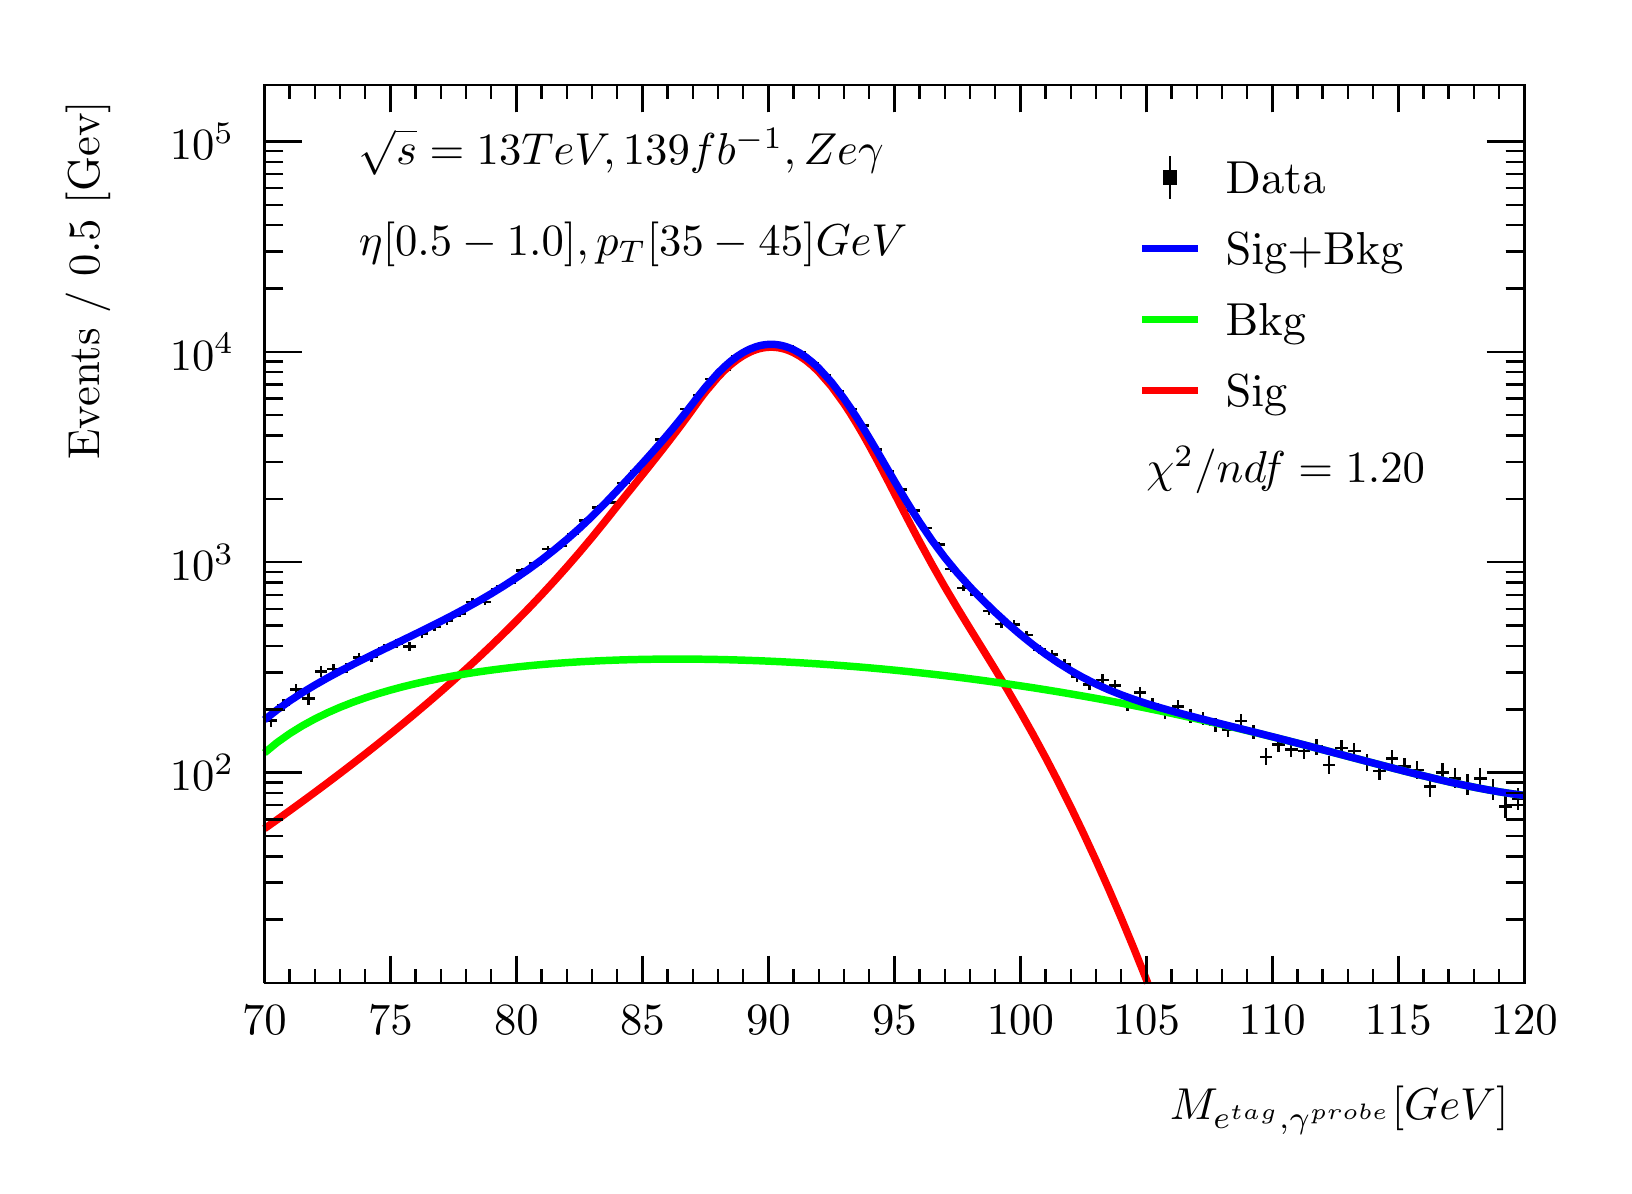
\begin{tikzpicture}
\pgfdeclareplotmark{cross} {
\pgfpathmoveto{\pgfpoint{-0.3\pgfplotmarksize}{\pgfplotmarksize}}
\pgfpathlineto{\pgfpoint{+0.3\pgfplotmarksize}{\pgfplotmarksize}}
\pgfpathlineto{\pgfpoint{+0.3\pgfplotmarksize}{0.3\pgfplotmarksize}}
\pgfpathlineto{\pgfpoint{+1\pgfplotmarksize}{0.3\pgfplotmarksize}}
\pgfpathlineto{\pgfpoint{+1\pgfplotmarksize}{-0.3\pgfplotmarksize}}
\pgfpathlineto{\pgfpoint{+0.3\pgfplotmarksize}{-0.3\pgfplotmarksize}}
\pgfpathlineto{\pgfpoint{+0.3\pgfplotmarksize}{-1.\pgfplotmarksize}}
\pgfpathlineto{\pgfpoint{-0.3\pgfplotmarksize}{-1.\pgfplotmarksize}}
\pgfpathlineto{\pgfpoint{-0.3\pgfplotmarksize}{-0.3\pgfplotmarksize}}
\pgfpathlineto{\pgfpoint{-1.\pgfplotmarksize}{-0.3\pgfplotmarksize}}
\pgfpathlineto{\pgfpoint{-1.\pgfplotmarksize}{0.3\pgfplotmarksize}}
\pgfpathlineto{\pgfpoint{-0.3\pgfplotmarksize}{0.3\pgfplotmarksize}}
\pgfpathclose
\pgfusepathqstroke
}
\pgfdeclareplotmark{cross*} {
\pgfpathmoveto{\pgfpoint{-0.3\pgfplotmarksize}{\pgfplotmarksize}}
\pgfpathlineto{\pgfpoint{+0.3\pgfplotmarksize}{\pgfplotmarksize}}
\pgfpathlineto{\pgfpoint{+0.3\pgfplotmarksize}{0.3\pgfplotmarksize}}
\pgfpathlineto{\pgfpoint{+1\pgfplotmarksize}{0.3\pgfplotmarksize}}
\pgfpathlineto{\pgfpoint{+1\pgfplotmarksize}{-0.3\pgfplotmarksize}}
\pgfpathlineto{\pgfpoint{+0.3\pgfplotmarksize}{-0.3\pgfplotmarksize}}
\pgfpathlineto{\pgfpoint{+0.3\pgfplotmarksize}{-1.\pgfplotmarksize}}
\pgfpathlineto{\pgfpoint{-0.3\pgfplotmarksize}{-1.\pgfplotmarksize}}
\pgfpathlineto{\pgfpoint{-0.3\pgfplotmarksize}{-0.3\pgfplotmarksize}}
\pgfpathlineto{\pgfpoint{-1.\pgfplotmarksize}{-0.3\pgfplotmarksize}}
\pgfpathlineto{\pgfpoint{-1.\pgfplotmarksize}{0.3\pgfplotmarksize}}
\pgfpathlineto{\pgfpoint{-0.3\pgfplotmarksize}{0.3\pgfplotmarksize}}
\pgfpathclose
\pgfusepathqfillstroke
}
\pgfdeclareplotmark{newstar} {
\pgfpathmoveto{\pgfqpoint{0pt}{\pgfplotmarksize}}
\pgfpathlineto{\pgfqpointpolar{44}{0.5\pgfplotmarksize}}
\pgfpathlineto{\pgfqpointpolar{18}{\pgfplotmarksize}}
\pgfpathlineto{\pgfqpointpolar{-20}{0.5\pgfplotmarksize}}
\pgfpathlineto{\pgfqpointpolar{-54}{\pgfplotmarksize}}
\pgfpathlineto{\pgfqpointpolar{-90}{0.5\pgfplotmarksize}}
\pgfpathlineto{\pgfqpointpolar{234}{\pgfplotmarksize}}
\pgfpathlineto{\pgfqpointpolar{198}{0.5\pgfplotmarksize}}
\pgfpathlineto{\pgfqpointpolar{162}{\pgfplotmarksize}}
\pgfpathlineto{\pgfqpointpolar{134}{0.5\pgfplotmarksize}}
\pgfpathclose
\pgfusepathqstroke
}
\pgfdeclareplotmark{newstar*} {
\pgfpathmoveto{\pgfqpoint{0pt}{\pgfplotmarksize}}
\pgfpathlineto{\pgfqpointpolar{44}{0.5\pgfplotmarksize}}
\pgfpathlineto{\pgfqpointpolar{18}{\pgfplotmarksize}}
\pgfpathlineto{\pgfqpointpolar{-20}{0.5\pgfplotmarksize}}
\pgfpathlineto{\pgfqpointpolar{-54}{\pgfplotmarksize}}
\pgfpathlineto{\pgfqpointpolar{-90}{0.5\pgfplotmarksize}}
\pgfpathlineto{\pgfqpointpolar{234}{\pgfplotmarksize}}
\pgfpathlineto{\pgfqpointpolar{198}{0.5\pgfplotmarksize}}
\pgfpathlineto{\pgfqpointpolar{162}{\pgfplotmarksize}}
\pgfpathlineto{\pgfqpointpolar{134}{0.5\pgfplotmarksize}}
\pgfpathclose
\pgfusepathqfillstroke
}
\definecolor{c}{rgb}{1,1,1};
\draw [color=c, fill=c] (0,0) rectangle (20,14.4361);
\draw [color=c, fill=c] (3,2.30977) rectangle (19,13.7143);
\definecolor{c}{rgb}{0,0,0};
\draw [c,line width=0.9] (3,2.30977) -- (3,13.7143) -- (19,13.7143) -- (19,2.30977) -- (3,2.30977);
\definecolor{c}{rgb}{1,1,1};
\draw [color=c, fill=c] (3,2.30977) rectangle (19,13.7143);
\definecolor{c}{rgb}{0,0,0};
\draw [c,line width=0.9] (3,2.30977) -- (3,13.7143) -- (19,13.7143) -- (19,2.30977) -- (3,2.30977);
\draw [c,line width=0.9] (3,2.30977) -- (19,2.30977);
\draw [c,line width=0.9] (3,2.65624) -- (3,2.30977);
\draw [c,line width=0.9] (3.32,2.48301) -- (3.32,2.30977);
\draw [c,line width=0.9] (3.64,2.48301) -- (3.64,2.30977);
\draw [c,line width=0.9] (3.96,2.48301) -- (3.96,2.30977);
\draw [c,line width=0.9] (4.28,2.48301) -- (4.28,2.30977);
\draw [c,line width=0.9] (4.6,2.65624) -- (4.6,2.30977);
\draw [c,line width=0.9] (4.92,2.48301) -- (4.92,2.30977);
\draw [c,line width=0.9] (5.24,2.48301) -- (5.24,2.30977);
\draw [c,line width=0.9] (5.56,2.48301) -- (5.56,2.30977);
\draw [c,line width=0.9] (5.88,2.48301) -- (5.88,2.30977);
\draw [c,line width=0.9] (6.2,2.65624) -- (6.2,2.30977);
\draw [c,line width=0.9] (6.52,2.48301) -- (6.52,2.30977);
\draw [c,line width=0.9] (6.84,2.48301) -- (6.84,2.30977);
\draw [c,line width=0.9] (7.16,2.48301) -- (7.16,2.30977);
\draw [c,line width=0.9] (7.48,2.48301) -- (7.48,2.30977);
\draw [c,line width=0.9] (7.8,2.65624) -- (7.8,2.30977);
\draw [c,line width=0.9] (8.12,2.48301) -- (8.12,2.30977);
\draw [c,line width=0.9] (8.44,2.48301) -- (8.44,2.30977);
\draw [c,line width=0.9] (8.76,2.48301) -- (8.76,2.30977);
\draw [c,line width=0.9] (9.08,2.48301) -- (9.08,2.30977);
\draw [c,line width=0.9] (9.4,2.65624) -- (9.4,2.30977);
\draw [c,line width=0.9] (9.72,2.48301) -- (9.72,2.30977);
\draw [c,line width=0.9] (10.04,2.48301) -- (10.04,2.30977);
\draw [c,line width=0.9] (10.36,2.48301) -- (10.36,2.30977);
\draw [c,line width=0.9] (10.68,2.48301) -- (10.68,2.30977);
\draw [c,line width=0.9] (11,2.65624) -- (11,2.30977);
\draw [c,line width=0.9] (11.32,2.48301) -- (11.32,2.30977);
\draw [c,line width=0.9] (11.64,2.48301) -- (11.64,2.30977);
\draw [c,line width=0.9] (11.96,2.48301) -- (11.96,2.30977);
\draw [c,line width=0.9] (12.28,2.48301) -- (12.28,2.30977);
\draw [c,line width=0.9] (12.6,2.65624) -- (12.6,2.30977);
\draw [c,line width=0.9] (12.92,2.48301) -- (12.92,2.30977);
\draw [c,line width=0.9] (13.24,2.48301) -- (13.24,2.30977);
\draw [c,line width=0.9] (13.56,2.48301) -- (13.56,2.30977);
\draw [c,line width=0.9] (13.88,2.48301) -- (13.88,2.30977);
\draw [c,line width=0.9] (14.2,2.65624) -- (14.2,2.30977);
\draw [c,line width=0.9] (14.52,2.48301) -- (14.52,2.30977);
\draw [c,line width=0.9] (14.84,2.48301) -- (14.84,2.30977);
\draw [c,line width=0.9] (15.16,2.48301) -- (15.16,2.30977);
\draw [c,line width=0.9] (15.48,2.48301) -- (15.48,2.30977);
\draw [c,line width=0.9] (15.8,2.65624) -- (15.8,2.30977);
\draw [c,line width=0.9] (16.12,2.48301) -- (16.12,2.30977);
\draw [c,line width=0.9] (16.44,2.48301) -- (16.44,2.30977);
\draw [c,line width=0.9] (16.76,2.48301) -- (16.76,2.30977);
\draw [c,line width=0.9] (17.08,2.48301) -- (17.08,2.30977);
\draw [c,line width=0.9] (17.4,2.65624) -- (17.4,2.30977);
\draw [c,line width=0.9] (17.72,2.48301) -- (17.72,2.30977);
\draw [c,line width=0.9] (18.04,2.48301) -- (18.04,2.30977);
\draw [c,line width=0.9] (18.36,2.48301) -- (18.36,2.30977);
\draw [c,line width=0.9] (18.68,2.48301) -- (18.68,2.30977);
\draw [c,line width=0.9] (19,2.65624) -- (19,2.30977);
\draw [anchor=base] (3,1.66015) node[scale=1.61424, color=c, rotate=0]{70};
\draw [anchor=base] (4.6,1.66015) node[scale=1.61424, color=c, rotate=0]{75};
\draw [anchor=base] (6.2,1.66015) node[scale=1.61424, color=c, rotate=0]{80};
\draw [anchor=base] (7.8,1.66015) node[scale=1.61424, color=c, rotate=0]{85};
\draw [anchor=base] (9.4,1.66015) node[scale=1.61424, color=c, rotate=0]{90};
\draw [anchor=base] (11,1.66015) node[scale=1.61424, color=c, rotate=0]{95};
\draw [anchor=base] (12.6,1.66015) node[scale=1.61424, color=c, rotate=0]{100};
\draw [anchor=base] (14.2,1.66015) node[scale=1.61424, color=c, rotate=0]{105};
\draw [anchor=base] (15.8,1.66015) node[scale=1.61424, color=c, rotate=0]{110};
\draw [anchor=base] (17.4,1.66015) node[scale=1.61424, color=c, rotate=0]{115};
\draw [anchor=base] (19,1.66015) node[scale=1.61424, color=c, rotate=0]{120};
\draw [anchor= east] (19,0.692932) node[scale=1.61424, color=c, rotate=0]{$M_{e^{tag}, \gamma^{probe}}  [GeV]$};
\draw [c,line width=0.9] (3,13.7143) -- (19,13.7143);
\draw [c,line width=0.9] (3,13.3678) -- (3,13.7143);
\draw [c,line width=0.9] (3.32,13.5411) -- (3.32,13.7143);
\draw [c,line width=0.9] (3.64,13.5411) -- (3.64,13.7143);
\draw [c,line width=0.9] (3.96,13.5411) -- (3.96,13.7143);
\draw [c,line width=0.9] (4.28,13.5411) -- (4.28,13.7143);
\draw [c,line width=0.9] (4.6,13.3678) -- (4.6,13.7143);
\draw [c,line width=0.9] (4.92,13.5411) -- (4.92,13.7143);
\draw [c,line width=0.9] (5.24,13.5411) -- (5.24,13.7143);
\draw [c,line width=0.9] (5.56,13.5411) -- (5.56,13.7143);
\draw [c,line width=0.9] (5.88,13.5411) -- (5.88,13.7143);
\draw [c,line width=0.9] (6.2,13.3678) -- (6.2,13.7143);
\draw [c,line width=0.9] (6.52,13.5411) -- (6.52,13.7143);
\draw [c,line width=0.9] (6.84,13.5411) -- (6.84,13.7143);
\draw [c,line width=0.9] (7.16,13.5411) -- (7.16,13.7143);
\draw [c,line width=0.9] (7.48,13.5411) -- (7.48,13.7143);
\draw [c,line width=0.9] (7.8,13.3678) -- (7.8,13.7143);
\draw [c,line width=0.9] (8.12,13.5411) -- (8.12,13.7143);
\draw [c,line width=0.9] (8.44,13.5411) -- (8.44,13.7143);
\draw [c,line width=0.9] (8.76,13.5411) -- (8.76,13.7143);
\draw [c,line width=0.9] (9.08,13.5411) -- (9.08,13.7143);
\draw [c,line width=0.9] (9.4,13.3678) -- (9.4,13.7143);
\draw [c,line width=0.9] (9.72,13.5411) -- (9.72,13.7143);
\draw [c,line width=0.9] (10.04,13.5411) -- (10.04,13.7143);
\draw [c,line width=0.9] (10.36,13.5411) -- (10.36,13.7143);
\draw [c,line width=0.9] (10.68,13.5411) -- (10.68,13.7143);
\draw [c,line width=0.9] (11,13.3678) -- (11,13.7143);
\draw [c,line width=0.9] (11.32,13.5411) -- (11.32,13.7143);
\draw [c,line width=0.9] (11.64,13.5411) -- (11.64,13.7143);
\draw [c,line width=0.9] (11.96,13.5411) -- (11.96,13.7143);
\draw [c,line width=0.9] (12.28,13.5411) -- (12.28,13.7143);
\draw [c,line width=0.9] (12.6,13.3678) -- (12.6,13.7143);
\draw [c,line width=0.9] (12.92,13.5411) -- (12.92,13.7143);
\draw [c,line width=0.9] (13.24,13.5411) -- (13.24,13.7143);
\draw [c,line width=0.9] (13.56,13.5411) -- (13.56,13.7143);
\draw [c,line width=0.9] (13.88,13.5411) -- (13.88,13.7143);
\draw [c,line width=0.9] (14.2,13.3678) -- (14.2,13.7143);
\draw [c,line width=0.9] (14.52,13.5411) -- (14.52,13.7143);
\draw [c,line width=0.9] (14.84,13.5411) -- (14.84,13.7143);
\draw [c,line width=0.9] (15.16,13.5411) -- (15.16,13.7143);
\draw [c,line width=0.9] (15.48,13.5411) -- (15.48,13.7143);
\draw [c,line width=0.9] (15.8,13.3678) -- (15.8,13.7143);
\draw [c,line width=0.9] (16.12,13.5411) -- (16.12,13.7143);
\draw [c,line width=0.9] (16.44,13.5411) -- (16.44,13.7143);
\draw [c,line width=0.9] (16.76,13.5411) -- (16.76,13.7143);
\draw [c,line width=0.9] (17.08,13.5411) -- (17.08,13.7143);
\draw [c,line width=0.9] (17.4,13.3678) -- (17.4,13.7143);
\draw [c,line width=0.9] (17.72,13.5411) -- (17.72,13.7143);
\draw [c,line width=0.9] (18.04,13.5411) -- (18.04,13.7143);
\draw [c,line width=0.9] (18.36,13.5411) -- (18.36,13.7143);
\draw [c,line width=0.9] (18.68,13.5411) -- (18.68,13.7143);
\draw [c,line width=0.9] (19,13.3678) -- (19,13.7143);
\draw [c,line width=0.9] (3,2.30977) -- (3,13.7143);
\draw [c,line width=0.9] (3.237,3.11414) -- (3,3.11414);
\draw [c,line width=0.9] (3.237,3.58467) -- (3,3.58467);
\draw [c,line width=0.9] (3.237,3.91852) -- (3,3.91852);
\draw [c,line width=0.9] (3.237,4.17747) -- (3,4.17747);
\draw [c,line width=0.9] (3.237,4.38904) -- (3,4.38904);
\draw [c,line width=0.9] (3.237,4.56793) -- (3,4.56793);
\draw [c,line width=0.9] (3.237,4.72289) -- (3,4.72289);
\draw [c,line width=0.9] (3.237,4.85957) -- (3,4.85957);
\draw [c,line width=0.9] (3.474,4.98184) -- (3,4.98184);
\draw [anchor= east] (2.82,4.98184) node[scale=1.61424, color=c, rotate=0]{$10^{2}$};
\draw [c,line width=0.9] (3.237,5.78621) -- (3,5.78621);
\draw [c,line width=0.9] (3.237,6.25674) -- (3,6.25674);
\draw [c,line width=0.9] (3.237,6.59058) -- (3,6.59058);
\draw [c,line width=0.9] (3.237,6.84953) -- (3,6.84953);
\draw [c,line width=0.9] (3.237,7.06111) -- (3,7.06111);
\draw [c,line width=0.9] (3.237,7.24) -- (3,7.24);
\draw [c,line width=0.9] (3.237,7.39496) -- (3,7.39496);
\draw [c,line width=0.9] (3.237,7.53164) -- (3,7.53164);
\draw [c,line width=0.9] (3.474,7.65391) -- (3,7.65391);
\draw [anchor= east] (2.82,7.65391) node[scale=1.61424, color=c, rotate=0]{$10^{3}$};
\draw [c,line width=0.9] (3.237,8.45828) -- (3,8.45828);
\draw [c,line width=0.9] (3.237,8.92881) -- (3,8.92881);
\draw [c,line width=0.9] (3.237,9.26265) -- (3,9.26265);
\draw [c,line width=0.9] (3.237,9.5216) -- (3,9.5216);
\draw [c,line width=0.9] (3.237,9.73318) -- (3,9.73318);
\draw [c,line width=0.9] (3.237,9.91207) -- (3,9.91207);
\draw [c,line width=0.9] (3.237,10.067) -- (3,10.067);
\draw [c,line width=0.9] (3.237,10.2037) -- (3,10.2037);
\draw [c,line width=0.9] (3.474,10.326) -- (3,10.326);
\draw [anchor= east] (2.82,10.326) node[scale=1.61424, color=c, rotate=0]{$10^{4}$};
\draw [c,line width=0.9] (3.237,11.1303) -- (3,11.1303);
\draw [c,line width=0.9] (3.237,11.6009) -- (3,11.6009);
\draw [c,line width=0.9] (3.237,11.9347) -- (3,11.9347);
\draw [c,line width=0.9] (3.237,12.1937) -- (3,12.1937);
\draw [c,line width=0.9] (3.237,12.4052) -- (3,12.4052);
\draw [c,line width=0.9] (3.237,12.5841) -- (3,12.5841);
\draw [c,line width=0.9] (3.237,12.7391) -- (3,12.7391);
\draw [c,line width=0.9] (3.237,12.8758) -- (3,12.8758);
\draw [c,line width=0.9] (3.474,12.998) -- (3,12.998);
\draw [anchor= east] (2.82,12.998) node[scale=1.61424, color=c, rotate=0]{$10^{5}$};
\draw [anchor= east] (0.76,13.7143) node[scale=1.61424, color=c, rotate=90]{Events / 0.5 [Gev]};
\draw [c,line width=0.9] (19,2.30977) -- (19,13.7143);
\draw [c,line width=0.9] (18.763,3.11414) -- (19,3.11414);
\draw [c,line width=0.9] (18.763,3.58467) -- (19,3.58467);
\draw [c,line width=0.9] (18.763,3.91852) -- (19,3.91852);
\draw [c,line width=0.9] (18.763,4.17747) -- (19,4.17747);
\draw [c,line width=0.9] (18.763,4.38904) -- (19,4.38904);
\draw [c,line width=0.9] (18.763,4.56793) -- (19,4.56793);
\draw [c,line width=0.9] (18.763,4.72289) -- (19,4.72289);
\draw [c,line width=0.9] (18.763,4.85957) -- (19,4.85957);
\draw [c,line width=0.9] (18.526,4.98184) -- (19,4.98184);
\draw [c,line width=0.9] (18.763,5.78621) -- (19,5.78621);
\draw [c,line width=0.9] (18.763,6.25674) -- (19,6.25674);
\draw [c,line width=0.9] (18.763,6.59058) -- (19,6.59058);
\draw [c,line width=0.9] (18.763,6.84953) -- (19,6.84953);
\draw [c,line width=0.9] (18.763,7.06111) -- (19,7.06111);
\draw [c,line width=0.9] (18.763,7.24) -- (19,7.24);
\draw [c,line width=0.9] (18.763,7.39496) -- (19,7.39496);
\draw [c,line width=0.9] (18.763,7.53164) -- (19,7.53164);
\draw [c,line width=0.9] (18.526,7.65391) -- (19,7.65391);
\draw [c,line width=0.9] (18.763,8.45828) -- (19,8.45828);
\draw [c,line width=0.9] (18.763,8.92881) -- (19,8.92881);
\draw [c,line width=0.9] (18.763,9.26265) -- (19,9.26265);
\draw [c,line width=0.9] (18.763,9.5216) -- (19,9.5216);
\draw [c,line width=0.9] (18.763,9.73318) -- (19,9.73318);
\draw [c,line width=0.9] (18.763,9.91207) -- (19,9.91207);
\draw [c,line width=0.9] (18.763,10.067) -- (19,10.067);
\draw [c,line width=0.9] (18.763,10.2037) -- (19,10.2037);
\draw [c,line width=0.9] (18.526,10.326) -- (19,10.326);
\draw [c,line width=0.9] (18.763,11.1303) -- (19,11.1303);
\draw [c,line width=0.9] (18.763,11.6009) -- (19,11.6009);
\draw [c,line width=0.9] (18.763,11.9347) -- (19,11.9347);
\draw [c,line width=0.9] (18.763,12.1937) -- (19,12.1937);
\draw [c,line width=0.9] (18.763,12.4052) -- (19,12.4052);
\draw [c,line width=0.9] (18.763,12.5841) -- (19,12.5841);
\draw [c,line width=0.9] (18.763,12.7391) -- (19,12.7391);
\draw [c,line width=0.9] (18.763,12.8758) -- (19,12.8758);
\draw [c,line width=0.9] (18.526,12.998) -- (19,12.998);
\draw [c,line width=0.9] (3.08,5.64444) -- (3,5.64444);
\draw [c,line width=0.9] (3,5.64444) -- (3,5.64444);
\draw [c,line width=0.9] (3.08,5.64444) -- (3.16,5.64444);
\draw [c,line width=0.9] (3.16,5.64444) -- (3.16,5.64444);
\draw [c,line width=0.9] (3.08,5.64444) -- (3.08,5.73165);
\draw [c,line width=0.9] (3.08,5.73165) -- (3.08,5.73165);
\draw [c,line width=0.9] (3.08,5.64444) -- (3.08,5.55724);
\draw [c,line width=0.9] (3.08,5.55724) -- (3.08,5.55724);
\draw [c,line width=0.9] (3.24,5.84283) -- (3.16,5.84283);
\draw [c,line width=0.9] (3.16,5.84283) -- (3.16,5.84283);
\draw [c,line width=0.9] (3.24,5.84283) -- (3.32,5.84283);
\draw [c,line width=0.9] (3.32,5.84283) -- (3.32,5.84283);
\draw [c,line width=0.9] (3.24,5.84283) -- (3.24,5.9229);
\draw [c,line width=0.9] (3.24,5.9229) -- (3.24,5.9229);
\draw [c,line width=0.9] (3.24,5.84283) -- (3.24,5.76277);
\draw [c,line width=0.9] (3.24,5.76277) -- (3.24,5.76277);
\draw [c,line width=0.9] (3.4,6.03584) -- (3.32,6.03584);
\draw [c,line width=0.9] (3.32,6.03584) -- (3.32,6.03584);
\draw [c,line width=0.9] (3.4,6.03584) -- (3.48,6.03584);
\draw [c,line width=0.9] (3.48,6.03584) -- (3.48,6.03584);
\draw [c,line width=0.9] (3.4,6.03584) -- (3.4,6.10952);
\draw [c,line width=0.9] (3.4,6.10952) -- (3.4,6.10952);
\draw [c,line width=0.9] (3.4,6.03584) -- (3.4,5.96217);
\draw [c,line width=0.9] (3.4,5.96217) -- (3.4,5.96217);
\draw [c,line width=0.9] (3.56,5.9229) -- (3.48,5.9229);
\draw [c,line width=0.9] (3.48,5.9229) -- (3.48,5.9229);
\draw [c,line width=0.9] (3.56,5.9229) -- (3.64,5.9229);
\draw [c,line width=0.9] (3.64,5.9229) -- (3.64,5.9229);
\draw [c,line width=0.9] (3.56,5.9229) -- (3.56,6.00025);
\draw [c,line width=0.9] (3.56,6.00025) -- (3.56,6.00025);
\draw [c,line width=0.9] (3.56,5.9229) -- (3.56,5.84555);
\draw [c,line width=0.9] (3.56,5.84555) -- (3.56,5.84555);
\draw [c,line width=0.9] (3.72,6.26445) -- (3.64,6.26445);
\draw [c,line width=0.9] (3.64,6.26445) -- (3.64,6.26445);
\draw [c,line width=0.9] (3.72,6.26445) -- (3.8,6.26445);
\draw [c,line width=0.9] (3.8,6.26445) -- (3.8,6.26445);
\draw [c,line width=0.9] (3.72,6.26445) -- (3.72,6.33122);
\draw [c,line width=0.9] (3.72,6.33122) -- (3.72,6.33122);
\draw [c,line width=0.9] (3.72,6.26445) -- (3.72,6.19768);
\draw [c,line width=0.9] (3.72,6.19768) -- (3.72,6.19768);
\draw [c,line width=0.9] (3.88,6.29853) -- (3.8,6.29853);
\draw [c,line width=0.9] (3.8,6.29853) -- (3.8,6.29853);
\draw [c,line width=0.9] (3.88,6.29853) -- (3.96,6.29853);
\draw [c,line width=0.9] (3.96,6.29853) -- (3.96,6.29853);
\draw [c,line width=0.9] (3.88,6.29853) -- (3.88,6.36433);
\draw [c,line width=0.9] (3.88,6.36433) -- (3.88,6.36433);
\draw [c,line width=0.9] (3.88,6.29853) -- (3.88,6.23273);
\draw [c,line width=0.9] (3.88,6.23273) -- (3.88,6.23273);
\draw [c,line width=0.9] (4.04,6.30967) -- (3.96,6.30967);
\draw [c,line width=0.9] (3.96,6.30967) -- (3.96,6.30967);
\draw [c,line width=0.9] (4.04,6.30967) -- (4.12,6.30967);
\draw [c,line width=0.9] (4.12,6.30967) -- (4.12,6.30967);
\draw [c,line width=0.9] (4.04,6.30967) -- (4.04,6.37515);
\draw [c,line width=0.9] (4.04,6.37515) -- (4.04,6.37515);
\draw [c,line width=0.9] (4.04,6.30967) -- (4.04,6.24419);
\draw [c,line width=0.9] (4.04,6.24419) -- (4.04,6.24419);
\draw [c,line width=0.9] (4.2,6.44553) -- (4.12,6.44553);
\draw [c,line width=0.9] (4.12,6.44553) -- (4.12,6.44553);
\draw [c,line width=0.9] (4.2,6.44553) -- (4.28,6.44553);
\draw [c,line width=0.9] (4.28,6.44553) -- (4.28,6.44553);
\draw [c,line width=0.9] (4.2,6.44553) -- (4.2,6.50729);
\draw [c,line width=0.9] (4.2,6.50729) -- (4.2,6.50729);
\draw [c,line width=0.9] (4.2,6.44553) -- (4.2,6.38377);
\draw [c,line width=0.9] (4.2,6.38377) -- (4.2,6.38377);
\draw [c,line width=0.9] (4.36,6.45209) -- (4.28,6.45209);
\draw [c,line width=0.9] (4.28,6.45209) -- (4.28,6.45209);
\draw [c,line width=0.9] (4.36,6.45209) -- (4.44,6.45209);
\draw [c,line width=0.9] (4.44,6.45209) -- (4.44,6.45209);
\draw [c,line width=0.9] (4.36,6.45209) -- (4.36,6.51367);
\draw [c,line width=0.9] (4.36,6.51367) -- (4.36,6.51367);
\draw [c,line width=0.9] (4.36,6.45209) -- (4.36,6.3905);
\draw [c,line width=0.9] (4.36,6.3905) -- (4.36,6.3905);
\draw [c,line width=0.9] (4.52,6.55823) -- (4.44,6.55823);
\draw [c,line width=0.9] (4.44,6.55823) -- (4.44,6.55823);
\draw [c,line width=0.9] (4.52,6.55823) -- (4.6,6.55823);
\draw [c,line width=0.9] (4.6,6.55823) -- (4.6,6.55823);
\draw [c,line width=0.9] (4.52,6.55823) -- (4.52,6.61706);
\draw [c,line width=0.9] (4.52,6.61706) -- (4.52,6.61706);
\draw [c,line width=0.9] (4.52,6.55823) -- (4.52,6.49939);
\draw [c,line width=0.9] (4.52,6.49939) -- (4.52,6.49939);
\draw [c,line width=0.9] (4.68,6.61641) -- (4.6,6.61641);
\draw [c,line width=0.9] (4.6,6.61641) -- (4.6,6.61641);
\draw [c,line width=0.9] (4.68,6.61641) -- (4.76,6.61641);
\draw [c,line width=0.9] (4.76,6.61641) -- (4.76,6.61641);
\draw [c,line width=0.9] (4.68,6.61641) -- (4.68,6.67378);
\draw [c,line width=0.9] (4.68,6.67378) -- (4.68,6.67378);
\draw [c,line width=0.9] (4.68,6.61641) -- (4.68,6.55903);
\draw [c,line width=0.9] (4.68,6.55903) -- (4.68,6.55903);
\draw [c,line width=0.9] (4.84,6.58477) -- (4.76,6.58477);
\draw [c,line width=0.9] (4.76,6.58477) -- (4.76,6.58477);
\draw [c,line width=0.9] (4.84,6.58477) -- (4.92,6.58477);
\draw [c,line width=0.9] (4.92,6.58477) -- (4.92,6.58477);
\draw [c,line width=0.9] (4.84,6.58477) -- (4.84,6.64293);
\draw [c,line width=0.9] (4.84,6.64293) -- (4.84,6.64293);
\draw [c,line width=0.9] (4.84,6.58477) -- (4.84,6.52661);
\draw [c,line width=0.9] (4.84,6.52661) -- (4.84,6.52661);
\draw [c,line width=0.9] (5,6.74772) -- (4.92,6.74772);
\draw [c,line width=0.9] (4.92,6.74772) -- (4.92,6.74772);
\draw [c,line width=0.9] (5,6.74772) -- (5.08,6.74772);
\draw [c,line width=0.9] (5.08,6.74772) -- (5.08,6.74772);
\draw [c,line width=0.9] (5,6.74772) -- (5,6.80194);
\draw [c,line width=0.9] (5,6.80194) -- (5,6.80194);
\draw [c,line width=0.9] (5,6.74772) -- (5,6.6935);
\draw [c,line width=0.9] (5,6.6935) -- (5,6.6935);
\draw [c,line width=0.9] (5.16,6.83317) -- (5.08,6.83317);
\draw [c,line width=0.9] (5.08,6.83317) -- (5.08,6.83317);
\draw [c,line width=0.9] (5.16,6.83317) -- (5.24,6.83317);
\draw [c,line width=0.9] (5.24,6.83317) -- (5.24,6.83317);
\draw [c,line width=0.9] (5.16,6.83317) -- (5.16,6.88543);
\draw [c,line width=0.9] (5.16,6.88543) -- (5.16,6.88543);
\draw [c,line width=0.9] (5.16,6.83317) -- (5.16,6.78091);
\draw [c,line width=0.9] (5.16,6.78091) -- (5.16,6.78091);
\draw [c,line width=0.9] (5.32,6.91277) -- (5.24,6.91277);
\draw [c,line width=0.9] (5.24,6.91277) -- (5.24,6.91277);
\draw [c,line width=0.9] (5.32,6.91277) -- (5.4,6.91277);
\draw [c,line width=0.9] (5.4,6.91277) -- (5.4,6.91277);
\draw [c,line width=0.9] (5.32,6.91277) -- (5.32,6.96327);
\draw [c,line width=0.9] (5.32,6.96327) -- (5.32,6.96327);
\draw [c,line width=0.9] (5.32,6.91277) -- (5.32,6.86227);
\draw [c,line width=0.9] (5.32,6.86227) -- (5.32,6.86227);
\draw [c,line width=0.9] (5.48,7.00565) -- (5.4,7.00565);
\draw [c,line width=0.9] (5.4,7.00565) -- (5.4,7.00565);
\draw [c,line width=0.9] (5.48,7.00565) -- (5.56,7.00565);
\draw [c,line width=0.9] (5.56,7.00565) -- (5.56,7.00565);
\draw [c,line width=0.9] (5.48,7.00565) -- (5.48,7.05417);
\draw [c,line width=0.9] (5.48,7.05417) -- (5.48,7.05417);
\draw [c,line width=0.9] (5.48,7.00565) -- (5.48,6.95714);
\draw [c,line width=0.9] (5.48,6.95714) -- (5.48,6.95714);
\draw [c,line width=0.9] (5.64,7.15042) -- (5.56,7.15042);
\draw [c,line width=0.9] (5.56,7.15042) -- (5.56,7.15042);
\draw [c,line width=0.9] (5.64,7.15042) -- (5.72,7.15042);
\draw [c,line width=0.9] (5.72,7.15042) -- (5.72,7.15042);
\draw [c,line width=0.9] (5.64,7.15042) -- (5.64,7.19601);
\draw [c,line width=0.9] (5.64,7.19601) -- (5.64,7.19601);
\draw [c,line width=0.9] (5.64,7.15042) -- (5.64,7.10484);
\draw [c,line width=0.9] (5.64,7.10484) -- (5.64,7.10484);
\draw [c,line width=0.9] (5.8,7.15042) -- (5.72,7.15042);
\draw [c,line width=0.9] (5.72,7.15042) -- (5.72,7.15042);
\draw [c,line width=0.9] (5.8,7.15042) -- (5.88,7.15042);
\draw [c,line width=0.9] (5.88,7.15042) -- (5.88,7.15042);
\draw [c,line width=0.9] (5.8,7.15042) -- (5.8,7.19601);
\draw [c,line width=0.9] (5.8,7.19601) -- (5.8,7.19601);
\draw [c,line width=0.9] (5.8,7.15042) -- (5.8,7.10484);
\draw [c,line width=0.9] (5.8,7.10484) -- (5.8,7.10484);
\draw [c,line width=0.9] (5.96,7.31696) -- (5.88,7.31696);
\draw [c,line width=0.9] (5.88,7.31696) -- (5.88,7.31696);
\draw [c,line width=0.9] (5.96,7.31696) -- (6.04,7.31696);
\draw [c,line width=0.9] (6.04,7.31696) -- (6.04,7.31696);
\draw [c,line width=0.9] (5.96,7.31696) -- (5.96,7.35939);
\draw [c,line width=0.9] (5.96,7.35939) -- (5.96,7.35939);
\draw [c,line width=0.9] (5.96,7.31696) -- (5.96,7.27454);
\draw [c,line width=0.9] (5.96,7.27454) -- (5.96,7.27454);
\draw [c,line width=0.9] (6.12,7.3993) -- (6.04,7.3993);
\draw [c,line width=0.9] (6.04,7.3993) -- (6.04,7.3993);
\draw [c,line width=0.9] (6.12,7.3993) -- (6.2,7.3993);
\draw [c,line width=0.9] (6.2,7.3993) -- (6.2,7.3993);
\draw [c,line width=0.9] (6.12,7.3993) -- (6.12,7.44025);
\draw [c,line width=0.9] (6.12,7.44025) -- (6.12,7.44025);
\draw [c,line width=0.9] (6.12,7.3993) -- (6.12,7.35835);
\draw [c,line width=0.9] (6.12,7.35835) -- (6.12,7.35835);
\draw [c,line width=0.9] (6.28,7.54701) -- (6.2,7.54701);
\draw [c,line width=0.9] (6.2,7.54701) -- (6.2,7.54701);
\draw [c,line width=0.9] (6.28,7.54701) -- (6.36,7.54701);
\draw [c,line width=0.9] (6.36,7.54701) -- (6.36,7.54701);
\draw [c,line width=0.9] (6.28,7.54701) -- (6.28,7.58544);
\draw [c,line width=0.9] (6.28,7.58544) -- (6.28,7.58544);
\draw [c,line width=0.9] (6.28,7.54701) -- (6.28,7.50859);
\draw [c,line width=0.9] (6.28,7.50859) -- (6.28,7.50859);
\draw [c,line width=0.9] (6.44,7.63755) -- (6.36,7.63755);
\draw [c,line width=0.9] (6.36,7.63755) -- (6.36,7.63755);
\draw [c,line width=0.9] (6.44,7.63755) -- (6.52,7.63755);
\draw [c,line width=0.9] (6.52,7.63755) -- (6.52,7.63755);
\draw [c,line width=0.9] (6.44,7.63755) -- (6.44,7.6745);
\draw [c,line width=0.9] (6.44,7.6745) -- (6.44,7.6745);
\draw [c,line width=0.9] (6.44,7.63755) -- (6.44,7.60059);
\draw [c,line width=0.9] (6.44,7.60059) -- (6.44,7.60059);
\draw [c,line width=0.9] (6.6,7.82113) -- (6.52,7.82113);
\draw [c,line width=0.9] (6.52,7.82113) -- (6.52,7.82113);
\draw [c,line width=0.9] (6.6,7.82113) -- (6.68,7.82113);
\draw [c,line width=0.9] (6.68,7.82113) -- (6.68,7.82113);
\draw [c,line width=0.9] (6.6,7.82113) -- (6.6,7.85528);
\draw [c,line width=0.9] (6.6,7.85528) -- (6.6,7.85528);
\draw [c,line width=0.9] (6.6,7.82113) -- (6.6,7.78699);
\draw [c,line width=0.9] (6.6,7.78699) -- (6.6,7.78699);
\draw [c,line width=0.9] (6.76,7.8587) -- (6.68,7.8587);
\draw [c,line width=0.9] (6.68,7.8587) -- (6.68,7.8587);
\draw [c,line width=0.9] (6.76,7.8587) -- (6.84,7.8587);
\draw [c,line width=0.9] (6.84,7.8587) -- (6.84,7.8587);
\draw [c,line width=0.9] (6.76,7.8587) -- (6.76,7.89229);
\draw [c,line width=0.9] (6.76,7.89229) -- (6.76,7.89229);
\draw [c,line width=0.9] (6.76,7.8587) -- (6.76,7.8251);
\draw [c,line width=0.9] (6.76,7.8251) -- (6.76,7.8251);
\draw [c,line width=0.9] (6.92,8.00988) -- (6.84,8.00988);
\draw [c,line width=0.9] (6.84,8.00988) -- (6.84,8.00988);
\draw [c,line width=0.9] (6.92,8.00988) -- (7,8.00988);
\draw [c,line width=0.9] (7,8.00988) -- (7,8.00988);
\draw [c,line width=0.9] (6.92,8.00988) -- (6.92,8.04136);
\draw [c,line width=0.9] (6.92,8.04136) -- (6.92,8.04136);
\draw [c,line width=0.9] (6.92,8.00988) -- (6.92,7.9784);
\draw [c,line width=0.9] (6.92,7.9784) -- (6.92,7.9784);
\draw [c,line width=0.9] (7.08,8.1862) -- (7,8.1862);
\draw [c,line width=0.9] (7,8.1862) -- (7,8.1862);
\draw [c,line width=0.9] (7.08,8.1862) -- (7.16,8.1862);
\draw [c,line width=0.9] (7.16,8.1862) -- (7.16,8.1862);
\draw [c,line width=0.9] (7.08,8.1862) -- (7.08,8.21538);
\draw [c,line width=0.9] (7.08,8.21538) -- (7.08,8.21538);
\draw [c,line width=0.9] (7.08,8.1862) -- (7.08,8.15703);
\draw [c,line width=0.9] (7.08,8.15703) -- (7.08,8.15703);
\draw [c,line width=0.9] (7.24,8.34756) -- (7.16,8.34756);
\draw [c,line width=0.9] (7.16,8.34756) -- (7.16,8.34756);
\draw [c,line width=0.9] (7.24,8.34756) -- (7.32,8.34756);
\draw [c,line width=0.9] (7.32,8.34756) -- (7.32,8.34756);
\draw [c,line width=0.9] (7.24,8.34756) -- (7.24,8.37478);
\draw [c,line width=0.9] (7.24,8.37478) -- (7.24,8.37478);
\draw [c,line width=0.9] (7.24,8.34756) -- (7.24,8.32034);
\draw [c,line width=0.9] (7.24,8.32034) -- (7.24,8.32034);
\draw [c,line width=0.9] (7.4,8.41513) -- (7.32,8.41513);
\draw [c,line width=0.9] (7.32,8.41513) -- (7.32,8.41513);
\draw [c,line width=0.9] (7.4,8.41513) -- (7.48,8.41513);
\draw [c,line width=0.9] (7.48,8.41513) -- (7.48,8.41513);
\draw [c,line width=0.9] (7.4,8.41513) -- (7.4,8.44157);
\draw [c,line width=0.9] (7.4,8.44157) -- (7.4,8.44157);
\draw [c,line width=0.9] (7.4,8.41513) -- (7.4,8.3887);
\draw [c,line width=0.9] (7.4,8.3887) -- (7.4,8.3887);
\draw [c,line width=0.9] (7.56,8.66307) -- (7.48,8.66307);
\draw [c,line width=0.9] (7.48,8.66307) -- (7.48,8.66307);
\draw [c,line width=0.9] (7.56,8.66307) -- (7.64,8.66307);
\draw [c,line width=0.9] (7.64,8.66307) -- (7.64,8.66307);
\draw [c,line width=0.9] (7.56,8.66307) -- (7.56,8.68683);
\draw [c,line width=0.9] (7.56,8.68683) -- (7.56,8.68683);
\draw [c,line width=0.9] (7.56,8.66307) -- (7.56,8.63931);
\draw [c,line width=0.9] (7.56,8.63931) -- (7.56,8.63931);
\draw [c,line width=0.9] (7.72,8.80439) -- (7.64,8.80439);
\draw [c,line width=0.9] (7.64,8.80439) -- (7.64,8.80439);
\draw [c,line width=0.9] (7.72,8.80439) -- (7.8,8.80439);
\draw [c,line width=0.9] (7.8,8.80439) -- (7.8,8.80439);
\draw [c,line width=0.9] (7.72,8.80439) -- (7.72,8.82674);
\draw [c,line width=0.9] (7.72,8.82674) -- (7.72,8.82674);
\draw [c,line width=0.9] (7.72,8.80439) -- (7.72,8.78204);
\draw [c,line width=0.9] (7.72,8.78204) -- (7.72,8.78204);
\draw [c,line width=0.9] (7.88,8.96761) -- (7.8,8.96761);
\draw [c,line width=0.9] (7.8,8.96761) -- (7.8,8.96761);
\draw [c,line width=0.9] (7.88,8.96761) -- (7.96,8.96761);
\draw [c,line width=0.9] (7.96,8.96761) -- (7.96,8.96761);
\draw [c,line width=0.9] (7.88,8.96761) -- (7.88,8.98844);
\draw [c,line width=0.9] (7.88,8.98844) -- (7.88,8.98844);
\draw [c,line width=0.9] (7.88,8.96761) -- (7.88,8.94677);
\draw [c,line width=0.9] (7.88,8.94677) -- (7.88,8.94677);
\draw [c,line width=0.9] (8.04,9.21377) -- (7.96,9.21377);
\draw [c,line width=0.9] (7.96,9.21377) -- (7.96,9.21377);
\draw [c,line width=0.9] (8.04,9.21377) -- (8.12,9.21377);
\draw [c,line width=0.9] (8.12,9.21377) -- (8.12,9.21377);
\draw [c,line width=0.9] (8.04,9.21377) -- (8.04,9.23251);
\draw [c,line width=0.9] (8.04,9.23251) -- (8.04,9.23251);
\draw [c,line width=0.9] (8.04,9.21377) -- (8.04,9.19503);
\draw [c,line width=0.9] (8.04,9.19503) -- (8.04,9.19503);
\draw [c,line width=0.9] (8.2,9.34523) -- (8.12,9.34523);
\draw [c,line width=0.9] (8.12,9.34523) -- (8.12,9.34523);
\draw [c,line width=0.9] (8.2,9.34523) -- (8.28,9.34523);
\draw [c,line width=0.9] (8.28,9.34523) -- (8.28,9.34523);
\draw [c,line width=0.9] (8.2,9.34523) -- (8.2,9.36294);
\draw [c,line width=0.9] (8.2,9.36294) -- (8.2,9.36294);
\draw [c,line width=0.9] (8.2,9.34523) -- (8.2,9.32752);
\draw [c,line width=0.9] (8.2,9.32752) -- (8.2,9.32752);
\draw [c,line width=0.9] (8.36,9.60055) -- (8.28,9.60055);
\draw [c,line width=0.9] (8.28,9.60055) -- (8.28,9.60055);
\draw [c,line width=0.9] (8.36,9.60055) -- (8.44,9.60055);
\draw [c,line width=0.9] (8.44,9.60055) -- (8.44,9.60055);
\draw [c,line width=0.9] (8.36,9.60055) -- (8.36,9.61641);
\draw [c,line width=0.9] (8.36,9.61641) -- (8.36,9.61641);
\draw [c,line width=0.9] (8.36,9.60055) -- (8.36,9.58469);
\draw [c,line width=0.9] (8.36,9.58469) -- (8.36,9.58469);
\draw [c,line width=0.9] (8.52,9.77553) -- (8.44,9.77553);
\draw [c,line width=0.9] (8.44,9.77553) -- (8.44,9.77553);
\draw [c,line width=0.9] (8.52,9.77553) -- (8.6,9.77553);
\draw [c,line width=0.9] (8.6,9.77553) -- (8.6,9.77553);
\draw [c,line width=0.9] (8.52,9.77553) -- (8.52,9.79024);
\draw [c,line width=0.9] (8.52,9.79024) -- (8.52,9.79024);
\draw [c,line width=0.9] (8.52,9.77553) -- (8.52,9.76082);
\draw [c,line width=0.9] (8.52,9.76082) -- (8.52,9.76082);
\draw [c,line width=0.9] (8.68,9.9814) -- (8.6,9.9814);
\draw [c,line width=0.9] (8.6,9.9814) -- (8.6,9.9814);
\draw [c,line width=0.9] (8.68,9.9814) -- (8.76,9.9814);
\draw [c,line width=0.9] (8.76,9.9814) -- (8.76,9.9814);
\draw [c,line width=0.9] (8.68,9.9814) -- (8.68,9.99487);
\draw [c,line width=0.9] (8.68,9.99487) -- (8.68,9.99487);
\draw [c,line width=0.9] (8.68,9.9814) -- (8.68,9.96794);
\draw [c,line width=0.9] (8.68,9.96794) -- (8.68,9.96794);
\draw [c,line width=0.9] (8.84,10.0927) -- (8.76,10.0927);
\draw [c,line width=0.9] (8.76,10.0927) -- (8.76,10.0927);
\draw [c,line width=0.9] (8.84,10.0927) -- (8.92,10.0927);
\draw [c,line width=0.9] (8.92,10.0927) -- (8.92,10.0927);
\draw [c,line width=0.9] (8.84,10.0927) -- (8.84,10.1055);
\draw [c,line width=0.9] (8.84,10.1055) -- (8.84,10.1055);
\draw [c,line width=0.9] (8.84,10.0927) -- (8.84,10.0799);
\draw [c,line width=0.9] (8.84,10.0799) -- (8.84,10.0799);
\draw [c,line width=0.9] (9,10.2741) -- (8.92,10.2741);
\draw [c,line width=0.9] (8.92,10.2741) -- (8.92,10.2741);
\draw [c,line width=0.9] (9,10.2741) -- (9.08,10.2741);
\draw [c,line width=0.9] (9.08,10.2741) -- (9.08,10.2741);
\draw [c,line width=0.9] (9,10.2741) -- (9,10.286);
\draw [c,line width=0.9] (9,10.286) -- (9,10.286);
\draw [c,line width=0.9] (9,10.2741) -- (9,10.2623);
\draw [c,line width=0.9] (9,10.2623) -- (9,10.2623);
\draw [c,line width=0.9] (9.16,10.3619) -- (9.08,10.3619);
\draw [c,line width=0.9] (9.08,10.3619) -- (9.08,10.3619);
\draw [c,line width=0.9] (9.16,10.3619) -- (9.24,10.3619);
\draw [c,line width=0.9] (9.24,10.3619) -- (9.24,10.3619);
\draw [c,line width=0.9] (9.16,10.3619) -- (9.16,10.3733);
\draw [c,line width=0.9] (9.16,10.3733) -- (9.16,10.3733);
\draw [c,line width=0.9] (9.16,10.3619) -- (9.16,10.3504);
\draw [c,line width=0.9] (9.16,10.3504) -- (9.16,10.3504);
\draw [c,line width=0.9] (9.32,10.4157) -- (9.24,10.4157);
\draw [c,line width=0.9] (9.24,10.4157) -- (9.24,10.4157);
\draw [c,line width=0.9] (9.32,10.4157) -- (9.4,10.4157);
\draw [c,line width=0.9] (9.4,10.4157) -- (9.4,10.4157);
\draw [c,line width=0.9] (9.32,10.4157) -- (9.32,10.4269);
\draw [c,line width=0.9] (9.32,10.4269) -- (9.32,10.4269);
\draw [c,line width=0.9] (9.32,10.4157) -- (9.32,10.4046);
\draw [c,line width=0.9] (9.32,10.4046) -- (9.32,10.4046);
\draw [c,line width=0.9] (9.48,10.4272) -- (9.4,10.4272);
\draw [c,line width=0.9] (9.4,10.4272) -- (9.4,10.4272);
\draw [c,line width=0.9] (9.48,10.4272) -- (9.56,10.4272);
\draw [c,line width=0.9] (9.56,10.4272) -- (9.56,10.4272);
\draw [c,line width=0.9] (9.48,10.4272) -- (9.48,10.4383);
\draw [c,line width=0.9] (9.48,10.4383) -- (9.48,10.4383);
\draw [c,line width=0.9] (9.48,10.4272) -- (9.48,10.416);
\draw [c,line width=0.9] (9.48,10.416) -- (9.48,10.416);
\draw [c,line width=0.9] (9.64,10.3971) -- (9.56,10.3971);
\draw [c,line width=0.9] (9.56,10.3971) -- (9.56,10.3971);
\draw [c,line width=0.9] (9.64,10.3971) -- (9.72,10.3971);
\draw [c,line width=0.9] (9.72,10.3971) -- (9.72,10.3971);
\draw [c,line width=0.9] (9.64,10.3971) -- (9.64,10.4083);
\draw [c,line width=0.9] (9.64,10.4083) -- (9.64,10.4083);
\draw [c,line width=0.9] (9.64,10.3971) -- (9.64,10.3858);
\draw [c,line width=0.9] (9.64,10.3858) -- (9.64,10.3858);
\draw [c,line width=0.9] (9.8,10.3206) -- (9.72,10.3206);
\draw [c,line width=0.9] (9.72,10.3206) -- (9.72,10.3206);
\draw [c,line width=0.9] (9.8,10.3206) -- (9.88,10.3206);
\draw [c,line width=0.9] (9.88,10.3206) -- (9.88,10.3206);
\draw [c,line width=0.9] (9.8,10.3206) -- (9.8,10.3323);
\draw [c,line width=0.9] (9.8,10.3323) -- (9.8,10.3323);
\draw [c,line width=0.9] (9.8,10.3206) -- (9.8,10.309);
\draw [c,line width=0.9] (9.8,10.309) -- (9.8,10.309);
\draw [c,line width=0.9] (9.96,10.1751) -- (9.88,10.1751);
\draw [c,line width=0.9] (9.88,10.1751) -- (9.88,10.1751);
\draw [c,line width=0.9] (9.96,10.1751) -- (10.04,10.1751);
\draw [c,line width=0.9] (10.04,10.1751) -- (10.04,10.1751);
\draw [c,line width=0.9] (9.96,10.1751) -- (9.96,10.1875);
\draw [c,line width=0.9] (9.96,10.1875) -- (9.96,10.1875);
\draw [c,line width=0.9] (9.96,10.1751) -- (9.96,10.1627);
\draw [c,line width=0.9] (9.96,10.1627) -- (9.96,10.1627);
\draw [c,line width=0.9] (10.12,10.0332) -- (10.04,10.0332);
\draw [c,line width=0.9] (10.04,10.0332) -- (10.04,10.0332);
\draw [c,line width=0.9] (10.12,10.0332) -- (10.2,10.0332);
\draw [c,line width=0.9] (10.2,10.0332) -- (10.2,10.0332);
\draw [c,line width=0.9] (10.12,10.0332) -- (10.12,10.0463);
\draw [c,line width=0.9] (10.12,10.0463) -- (10.12,10.0463);
\draw [c,line width=0.9] (10.12,10.0332) -- (10.12,10.02);
\draw [c,line width=0.9] (10.12,10.02) -- (10.12,10.02);
\draw [c,line width=0.9] (10.28,9.82821) -- (10.2,9.82821);
\draw [c,line width=0.9] (10.2,9.82821) -- (10.2,9.82821);
\draw [c,line width=0.9] (10.28,9.82821) -- (10.36,9.82821);
\draw [c,line width=0.9] (10.36,9.82821) -- (10.36,9.82821);
\draw [c,line width=0.9] (10.28,9.82821) -- (10.28,9.84259);
\draw [c,line width=0.9] (10.28,9.84259) -- (10.28,9.84259);
\draw [c,line width=0.9] (10.28,9.82821) -- (10.28,9.81383);
\draw [c,line width=0.9] (10.28,9.81383) -- (10.28,9.81383);
\draw [c,line width=0.9] (10.44,9.59925) -- (10.36,9.59925);
\draw [c,line width=0.9] (10.36,9.59925) -- (10.36,9.59925);
\draw [c,line width=0.9] (10.44,9.59925) -- (10.52,9.59925);
\draw [c,line width=0.9] (10.52,9.59925) -- (10.52,9.59925);
\draw [c,line width=0.9] (10.44,9.59925) -- (10.44,9.61512);
\draw [c,line width=0.9] (10.44,9.61512) -- (10.44,9.61512);
\draw [c,line width=0.9] (10.44,9.59925) -- (10.44,9.58338);
\draw [c,line width=0.9] (10.44,9.58338) -- (10.44,9.58338);
\draw [c,line width=0.9] (10.6,9.38975) -- (10.52,9.38975);
\draw [c,line width=0.9] (10.52,9.38975) -- (10.52,9.38975);
\draw [c,line width=0.9] (10.6,9.38975) -- (10.68,9.38975);
\draw [c,line width=0.9] (10.68,9.38975) -- (10.68,9.38975);
\draw [c,line width=0.9] (10.6,9.38975) -- (10.6,9.40713);
\draw [c,line width=0.9] (10.6,9.40713) -- (10.6,9.40713);
\draw [c,line width=0.9] (10.6,9.38975) -- (10.6,9.37238);
\draw [c,line width=0.9] (10.6,9.37238) -- (10.6,9.37238);
\draw [c,line width=0.9] (10.76,9.08628) -- (10.68,9.08628);
\draw [c,line width=0.9] (10.68,9.08628) -- (10.68,9.08628);
\draw [c,line width=0.9] (10.76,9.08628) -- (10.84,9.08628);
\draw [c,line width=0.9] (10.84,9.08628) -- (10.84,9.08628);
\draw [c,line width=0.9] (10.76,9.08628) -- (10.76,9.10608);
\draw [c,line width=0.9] (10.76,9.10608) -- (10.76,9.10608);
\draw [c,line width=0.9] (10.76,9.08628) -- (10.76,9.06648);
\draw [c,line width=0.9] (10.76,9.06648) -- (10.76,9.06648);
\draw [c,line width=0.9] (10.92,8.80439) -- (10.84,8.80439);
\draw [c,line width=0.9] (10.84,8.80439) -- (10.84,8.80439);
\draw [c,line width=0.9] (10.92,8.80439) -- (11,8.80439);
\draw [c,line width=0.9] (11,8.80439) -- (11,8.80439);
\draw [c,line width=0.9] (10.92,8.80439) -- (10.92,8.82674);
\draw [c,line width=0.9] (10.92,8.82674) -- (10.92,8.82674);
\draw [c,line width=0.9] (10.92,8.80439) -- (10.92,8.78204);
\draw [c,line width=0.9] (10.92,8.78204) -- (10.92,8.78204);
\draw [c,line width=0.9] (11.08,8.58043) -- (11,8.58043);
\draw [c,line width=0.9] (11,8.58043) -- (11,8.58043);
\draw [c,line width=0.9] (11.08,8.58043) -- (11.16,8.58043);
\draw [c,line width=0.9] (11.16,8.58043) -- (11.16,8.58043);
\draw [c,line width=0.9] (11.08,8.58043) -- (11.08,8.60505);
\draw [c,line width=0.9] (11.08,8.60505) -- (11.08,8.60505);
\draw [c,line width=0.9] (11.08,8.58043) -- (11.08,8.55581);
\draw [c,line width=0.9] (11.08,8.55581) -- (11.08,8.55581);
\draw [c,line width=0.9] (11.24,8.31257) -- (11.16,8.31257);
\draw [c,line width=0.9] (11.16,8.31257) -- (11.16,8.31257);
\draw [c,line width=0.9] (11.24,8.31257) -- (11.32,8.31257);
\draw [c,line width=0.9] (11.32,8.31257) -- (11.32,8.31257);
\draw [c,line width=0.9] (11.24,8.31257) -- (11.24,8.3402);
\draw [c,line width=0.9] (11.24,8.3402) -- (11.24,8.3402);
\draw [c,line width=0.9] (11.24,8.31257) -- (11.24,8.28494);
\draw [c,line width=0.9] (11.24,8.28494) -- (11.24,8.28494);
\draw [c,line width=0.9] (11.4,8.08829) -- (11.32,8.08829);
\draw [c,line width=0.9] (11.32,8.08829) -- (11.32,8.08829);
\draw [c,line width=0.9] (11.4,8.08829) -- (11.48,8.08829);
\draw [c,line width=0.9] (11.48,8.08829) -- (11.48,8.08829);
\draw [c,line width=0.9] (11.4,8.08829) -- (11.4,8.11872);
\draw [c,line width=0.9] (11.4,8.11872) -- (11.4,8.11872);
\draw [c,line width=0.9] (11.4,8.08829) -- (11.4,8.05786);
\draw [c,line width=0.9] (11.4,8.05786) -- (11.4,8.05786);
\draw [c,line width=0.9] (11.56,7.87703) -- (11.48,7.87703);
\draw [c,line width=0.9] (11.48,7.87703) -- (11.48,7.87703);
\draw [c,line width=0.9] (11.56,7.87703) -- (11.64,7.87703);
\draw [c,line width=0.9] (11.64,7.87703) -- (11.64,7.87703);
\draw [c,line width=0.9] (11.56,7.87703) -- (11.56,7.91037);
\draw [c,line width=0.9] (11.56,7.91037) -- (11.56,7.91037);
\draw [c,line width=0.9] (11.56,7.87703) -- (11.56,7.8437);
\draw [c,line width=0.9] (11.56,7.8437) -- (11.56,7.8437);
\draw [c,line width=0.9] (11.72,7.56594) -- (11.64,7.56594);
\draw [c,line width=0.9] (11.64,7.56594) -- (11.64,7.56594);
\draw [c,line width=0.9] (11.72,7.56594) -- (11.8,7.56594);
\draw [c,line width=0.9] (11.8,7.56594) -- (11.8,7.56594);
\draw [c,line width=0.9] (11.72,7.56594) -- (11.72,7.60406);
\draw [c,line width=0.9] (11.72,7.60406) -- (11.72,7.60406);
\draw [c,line width=0.9] (11.72,7.56594) -- (11.72,7.52783);
\draw [c,line width=0.9] (11.72,7.52783) -- (11.72,7.52783);
\draw [c,line width=0.9] (11.88,7.32777) -- (11.8,7.32777);
\draw [c,line width=0.9] (11.8,7.32777) -- (11.8,7.32777);
\draw [c,line width=0.9] (11.88,7.32777) -- (11.96,7.32777);
\draw [c,line width=0.9] (11.96,7.32777) -- (11.96,7.32777);
\draw [c,line width=0.9] (11.88,7.32777) -- (11.88,7.37001);
\draw [c,line width=0.9] (11.88,7.37001) -- (11.88,7.37001);
\draw [c,line width=0.9] (11.88,7.32777) -- (11.88,7.28554);
\draw [c,line width=0.9] (11.88,7.28554) -- (11.88,7.28554);
\draw [c,line width=0.9] (12.04,7.24166) -- (11.96,7.24166);
\draw [c,line width=0.9] (11.96,7.24166) -- (11.96,7.24166);
\draw [c,line width=0.9] (12.04,7.24166) -- (12.12,7.24166);
\draw [c,line width=0.9] (12.12,7.24166) -- (12.12,7.24166);
\draw [c,line width=0.9] (12.04,7.24166) -- (12.04,7.28548);
\draw [c,line width=0.9] (12.04,7.28548) -- (12.04,7.28548);
\draw [c,line width=0.9] (12.04,7.24166) -- (12.04,7.19783);
\draw [c,line width=0.9] (12.04,7.19783) -- (12.04,7.19783);
\draw [c,line width=0.9] (12.2,7.03371) -- (12.12,7.03371);
\draw [c,line width=0.9] (12.12,7.03371) -- (12.12,7.03371);
\draw [c,line width=0.9] (12.2,7.03371) -- (12.28,7.03371);
\draw [c,line width=0.9] (12.28,7.03371) -- (12.28,7.03371);
\draw [c,line width=0.9] (12.2,7.03371) -- (12.2,7.08165);
\draw [c,line width=0.9] (12.2,7.08165) -- (12.2,7.08165);
\draw [c,line width=0.9] (12.2,7.03371) -- (12.2,6.98578);
\draw [c,line width=0.9] (12.2,6.98578) -- (12.2,6.98578);
\draw [c,line width=0.9] (12.36,6.86796) -- (12.28,6.86796);
\draw [c,line width=0.9] (12.28,6.86796) -- (12.28,6.86796);
\draw [c,line width=0.9] (12.36,6.86796) -- (12.44,6.86796);
\draw [c,line width=0.9] (12.44,6.86796) -- (12.44,6.86796);
\draw [c,line width=0.9] (12.36,6.86796) -- (12.36,6.91944);
\draw [c,line width=0.9] (12.36,6.91944) -- (12.36,6.91944);
\draw [c,line width=0.9] (12.36,6.86796) -- (12.36,6.81647);
\draw [c,line width=0.9] (12.36,6.81647) -- (12.36,6.81647);
\draw [c,line width=0.9] (12.52,6.86338) -- (12.44,6.86338);
\draw [c,line width=0.9] (12.44,6.86338) -- (12.44,6.86338);
\draw [c,line width=0.9] (12.52,6.86338) -- (12.6,6.86338);
\draw [c,line width=0.9] (12.6,6.86338) -- (12.6,6.86338);
\draw [c,line width=0.9] (12.52,6.86338) -- (12.52,6.91496);
\draw [c,line width=0.9] (12.52,6.91496) -- (12.52,6.91496);
\draw [c,line width=0.9] (12.52,6.86338) -- (12.52,6.81179);
\draw [c,line width=0.9] (12.52,6.81179) -- (12.52,6.81179);
\draw [c,line width=0.9] (12.68,6.72727) -- (12.6,6.72727);
\draw [c,line width=0.9] (12.6,6.72727) -- (12.6,6.72727);
\draw [c,line width=0.9] (12.68,6.72727) -- (12.76,6.72727);
\draw [c,line width=0.9] (12.76,6.72727) -- (12.76,6.72727);
\draw [c,line width=0.9] (12.68,6.72727) -- (12.68,6.78197);
\draw [c,line width=0.9] (12.68,6.78197) -- (12.68,6.78197);
\draw [c,line width=0.9] (12.68,6.72727) -- (12.68,6.67257);
\draw [c,line width=0.9] (12.68,6.67257) -- (12.68,6.67257);
\draw [c,line width=0.9] (12.84,6.54321) -- (12.76,6.54321);
\draw [c,line width=0.9] (12.76,6.54321) -- (12.76,6.54321);
\draw [c,line width=0.9] (12.84,6.54321) -- (12.92,6.54321);
\draw [c,line width=0.9] (12.92,6.54321) -- (12.92,6.54321);
\draw [c,line width=0.9] (12.84,6.54321) -- (12.84,6.60243);
\draw [c,line width=0.9] (12.84,6.60243) -- (12.84,6.60243);
\draw [c,line width=0.9] (12.84,6.54321) -- (12.84,6.484);
\draw [c,line width=0.9] (12.84,6.484) -- (12.84,6.484);
\draw [c,line width=0.9] (13,6.48433) -- (12.92,6.48433);
\draw [c,line width=0.9] (12.92,6.48433) -- (12.92,6.48433);
\draw [c,line width=0.9] (13,6.48433) -- (13.08,6.48433);
\draw [c,line width=0.9] (13.08,6.48433) -- (13.08,6.48433);
\draw [c,line width=0.9] (13,6.48433) -- (13,6.54506);
\draw [c,line width=0.9] (13,6.54506) -- (13,6.54506);
\draw [c,line width=0.9] (13,6.48433) -- (13,6.42359);
\draw [c,line width=0.9] (13,6.42359) -- (13,6.42359);
\draw [c,line width=0.9] (13.16,6.35675) -- (13.08,6.35675);
\draw [c,line width=0.9] (13.08,6.35675) -- (13.08,6.35675);
\draw [c,line width=0.9] (13.16,6.35675) -- (13.24,6.35675);
\draw [c,line width=0.9] (13.24,6.35675) -- (13.24,6.35675);
\draw [c,line width=0.9] (13.16,6.35675) -- (13.16,6.42091);
\draw [c,line width=0.9] (13.16,6.42091) -- (13.16,6.42091);
\draw [c,line width=0.9] (13.16,6.35675) -- (13.16,6.29258);
\draw [c,line width=0.9] (13.16,6.29258) -- (13.16,6.29258);
\draw [c,line width=0.9] (13.32,6.20533) -- (13.24,6.20533);
\draw [c,line width=0.9] (13.24,6.20533) -- (13.24,6.20533);
\draw [c,line width=0.9] (13.32,6.20533) -- (13.4,6.20533);
\draw [c,line width=0.9] (13.4,6.20533) -- (13.4,6.20533);
\draw [c,line width=0.9] (13.32,6.20533) -- (13.32,6.27382);
\draw [c,line width=0.9] (13.32,6.27382) -- (13.32,6.27382);
\draw [c,line width=0.9] (13.32,6.20533) -- (13.32,6.13684);
\draw [c,line width=0.9] (13.32,6.13684) -- (13.32,6.13684);
\draw [c,line width=0.9] (13.48,6.09957) -- (13.4,6.09957);
\draw [c,line width=0.9] (13.4,6.09957) -- (13.4,6.09957);
\draw [c,line width=0.9] (13.48,6.09957) -- (13.56,6.09957);
\draw [c,line width=0.9] (13.56,6.09957) -- (13.56,6.09957);
\draw [c,line width=0.9] (13.48,6.09957) -- (13.48,6.17125);
\draw [c,line width=0.9] (13.48,6.17125) -- (13.48,6.17125);
\draw [c,line width=0.9] (13.48,6.09957) -- (13.48,6.02789);
\draw [c,line width=0.9] (13.48,6.02789) -- (13.48,6.02789);
\draw [c,line width=0.9] (13.64,6.15998) -- (13.56,6.15998);
\draw [c,line width=0.9] (13.56,6.15998) -- (13.56,6.15998);
\draw [c,line width=0.9] (13.64,6.15998) -- (13.72,6.15998);
\draw [c,line width=0.9] (13.72,6.15998) -- (13.72,6.15998);
\draw [c,line width=0.9] (13.64,6.15998) -- (13.64,6.22982);
\draw [c,line width=0.9] (13.64,6.22982) -- (13.64,6.22982);
\draw [c,line width=0.9] (13.64,6.15998) -- (13.64,6.09014);
\draw [c,line width=0.9] (13.64,6.09014) -- (13.64,6.09014);
\draw [c,line width=0.9] (13.8,6.09068) -- (13.72,6.09068);
\draw [c,line width=0.9] (13.72,6.09068) -- (13.72,6.09068);
\draw [c,line width=0.9] (13.8,6.09068) -- (13.88,6.09068);
\draw [c,line width=0.9] (13.88,6.09068) -- (13.88,6.09068);
\draw [c,line width=0.9] (13.8,6.09068) -- (13.8,6.16263);
\draw [c,line width=0.9] (13.8,6.16263) -- (13.8,6.16263);
\draw [c,line width=0.9] (13.8,6.09068) -- (13.8,6.01872);
\draw [c,line width=0.9] (13.8,6.01872) -- (13.8,6.01872);
\draw [c,line width=0.9] (13.96,5.84283) -- (13.88,5.84283);
\draw [c,line width=0.9] (13.88,5.84283) -- (13.88,5.84283);
\draw [c,line width=0.9] (13.96,5.84283) -- (14.04,5.84283);
\draw [c,line width=0.9] (14.04,5.84283) -- (14.04,5.84283);
\draw [c,line width=0.9] (13.96,5.84283) -- (13.96,5.9229);
\draw [c,line width=0.9] (13.96,5.9229) -- (13.96,5.9229);
\draw [c,line width=0.9] (13.96,5.84283) -- (13.96,5.76277);
\draw [c,line width=0.9] (13.96,5.76277) -- (13.96,5.76277);
\draw [c,line width=0.9] (14.12,5.99779) -- (14.04,5.99779);
\draw [c,line width=0.9] (14.04,5.99779) -- (14.04,5.99779);
\draw [c,line width=0.9] (14.12,5.99779) -- (14.2,5.99779);
\draw [c,line width=0.9] (14.2,5.99779) -- (14.2,5.99779);
\draw [c,line width=0.9] (14.12,5.99779) -- (14.12,6.07269);
\draw [c,line width=0.9] (14.12,6.07269) -- (14.12,6.07269);
\draw [c,line width=0.9] (14.12,5.99779) -- (14.12,5.9229);
\draw [c,line width=0.9] (14.12,5.9229) -- (14.12,5.9229);
\draw [c,line width=0.9] (14.28,5.84835) -- (14.2,5.84835);
\draw [c,line width=0.9] (14.2,5.84835) -- (14.2,5.84835);
\draw [c,line width=0.9] (14.28,5.84835) -- (14.36,5.84835);
\draw [c,line width=0.9] (14.36,5.84835) -- (14.36,5.84835);
\draw [c,line width=0.9] (14.28,5.84835) -- (14.28,5.92822);
\draw [c,line width=0.9] (14.28,5.92822) -- (14.28,5.92822);
\draw [c,line width=0.9] (14.28,5.84835) -- (14.28,5.76847);
\draw [c,line width=0.9] (14.28,5.76847) -- (14.28,5.76847);
\draw [c,line width=0.9] (14.44,5.75087) -- (14.36,5.75087);
\draw [c,line width=0.9] (14.36,5.75087) -- (14.36,5.75087);
\draw [c,line width=0.9] (14.44,5.75087) -- (14.52,5.75087);
\draw [c,line width=0.9] (14.52,5.75087) -- (14.52,5.75087);
\draw [c,line width=0.9] (14.44,5.75087) -- (14.44,5.83417);
\draw [c,line width=0.9] (14.44,5.83417) -- (14.44,5.83417);
\draw [c,line width=0.9] (14.44,5.75087) -- (14.44,5.66757);
\draw [c,line width=0.9] (14.44,5.66757) -- (14.44,5.66757);
\draw [c,line width=0.9] (14.6,5.82052) -- (14.52,5.82052);
\draw [c,line width=0.9] (14.52,5.82052) -- (14.52,5.82052);
\draw [c,line width=0.9] (14.6,5.82052) -- (14.68,5.82052);
\draw [c,line width=0.9] (14.68,5.82052) -- (14.68,5.82052);
\draw [c,line width=0.9] (14.6,5.82052) -- (14.6,5.90135);
\draw [c,line width=0.9] (14.6,5.90135) -- (14.6,5.90135);
\draw [c,line width=0.9] (14.6,5.82052) -- (14.6,5.73968);
\draw [c,line width=0.9] (14.6,5.73968) -- (14.6,5.73968);
\draw [c,line width=0.9] (14.76,5.702) -- (14.68,5.702);
\draw [c,line width=0.9] (14.68,5.702) -- (14.68,5.702);
\draw [c,line width=0.9] (14.76,5.702) -- (14.84,5.702);
\draw [c,line width=0.9] (14.84,5.702) -- (14.84,5.702);
\draw [c,line width=0.9] (14.76,5.702) -- (14.76,5.78707);
\draw [c,line width=0.9] (14.76,5.78707) -- (14.76,5.78707);
\draw [c,line width=0.9] (14.76,5.702) -- (14.76,5.61693);
\draw [c,line width=0.9] (14.76,5.61693) -- (14.76,5.61693);
\draw [c,line width=0.9] (14.92,5.67038) -- (14.84,5.67038);
\draw [c,line width=0.9] (14.84,5.67038) -- (14.84,5.67038);
\draw [c,line width=0.9] (14.92,5.67038) -- (15,5.67038);
\draw [c,line width=0.9] (15,5.67038) -- (15,5.67038);
\draw [c,line width=0.9] (14.92,5.67038) -- (14.92,5.75661);
\draw [c,line width=0.9] (14.92,5.75661) -- (14.92,5.75661);
\draw [c,line width=0.9] (14.92,5.67038) -- (14.92,5.58414);
\draw [c,line width=0.9] (14.92,5.58414) -- (14.92,5.58414);
\draw [c,line width=0.9] (15.08,5.59077) -- (15,5.59077);
\draw [c,line width=0.9] (15,5.59077) -- (15,5.59077);
\draw [c,line width=0.9] (15.08,5.59077) -- (15.16,5.59077);
\draw [c,line width=0.9] (15.16,5.59077) -- (15.16,5.59077);
\draw [c,line width=0.9] (15.08,5.59077) -- (15.08,5.68001);
\draw [c,line width=0.9] (15.08,5.68001) -- (15.08,5.68001);
\draw [c,line width=0.9] (15.08,5.59077) -- (15.08,5.50153);
\draw [c,line width=0.9] (15.08,5.50153) -- (15.08,5.50153);
\draw [c,line width=0.9] (15.24,5.52726) -- (15.16,5.52726);
\draw [c,line width=0.9] (15.16,5.52726) -- (15.16,5.52726);
\draw [c,line width=0.9] (15.24,5.52726) -- (15.32,5.52726);
\draw [c,line width=0.9] (15.32,5.52726) -- (15.32,5.52726);
\draw [c,line width=0.9] (15.24,5.52726) -- (15.24,5.61898);
\draw [c,line width=0.9] (15.24,5.61898) -- (15.24,5.61898);
\draw [c,line width=0.9] (15.24,5.52726) -- (15.24,5.43554);
\draw [c,line width=0.9] (15.24,5.43554) -- (15.24,5.43554);
\draw [c,line width=0.9] (15.4,5.63787) -- (15.32,5.63787);
\draw [c,line width=0.9] (15.32,5.63787) -- (15.32,5.63787);
\draw [c,line width=0.9] (15.4,5.63787) -- (15.48,5.63787);
\draw [c,line width=0.9] (15.48,5.63787) -- (15.48,5.63787);
\draw [c,line width=0.9] (15.4,5.63787) -- (15.4,5.72532);
\draw [c,line width=0.9] (15.4,5.72532) -- (15.4,5.72532);
\draw [c,line width=0.9] (15.4,5.63787) -- (15.4,5.55042);
\draw [c,line width=0.9] (15.4,5.55042) -- (15.4,5.55042);
\draw [c,line width=0.9] (15.56,5.49788) -- (15.48,5.49788);
\draw [c,line width=0.9] (15.48,5.49788) -- (15.48,5.49788);
\draw [c,line width=0.9] (15.56,5.49788) -- (15.64,5.49788);
\draw [c,line width=0.9] (15.64,5.49788) -- (15.64,5.49788);
\draw [c,line width=0.9] (15.56,5.49788) -- (15.56,5.59077);
\draw [c,line width=0.9] (15.56,5.59077) -- (15.56,5.59077);
\draw [c,line width=0.9] (15.56,5.49788) -- (15.56,5.405);
\draw [c,line width=0.9] (15.56,5.405) -- (15.56,5.405);
\draw [c,line width=0.9] (15.72,5.18371) -- (15.64,5.18371);
\draw [c,line width=0.9] (15.64,5.18371) -- (15.64,5.18371);
\draw [c,line width=0.9] (15.72,5.18371) -- (15.8,5.18371);
\draw [c,line width=0.9] (15.8,5.18371) -- (15.8,5.18371);
\draw [c,line width=0.9] (15.72,5.18371) -- (15.72,5.29005);
\draw [c,line width=0.9] (15.72,5.29005) -- (15.72,5.29005);
\draw [c,line width=0.9] (15.72,5.18371) -- (15.72,5.07737);
\draw [c,line width=0.9] (15.72,5.07737) -- (15.72,5.07737);
\draw [c,line width=0.9] (15.88,5.33867) -- (15.8,5.33867);
\draw [c,line width=0.9] (15.8,5.33867) -- (15.8,5.33867);
\draw [c,line width=0.9] (15.88,5.33867) -- (15.96,5.33867);
\draw [c,line width=0.9] (15.96,5.33867) -- (15.96,5.33867);
\draw [c,line width=0.9] (15.88,5.33867) -- (15.88,5.43814);
\draw [c,line width=0.9] (15.88,5.43814) -- (15.88,5.43814);
\draw [c,line width=0.9] (15.88,5.33867) -- (15.88,5.23919);
\draw [c,line width=0.9] (15.88,5.23919) -- (15.88,5.23919);
\draw [c,line width=0.9] (16.04,5.27734) -- (15.96,5.27734);
\draw [c,line width=0.9] (15.96,5.27734) -- (15.96,5.27734);
\draw [c,line width=0.9] (16.04,5.27734) -- (16.12,5.27734);
\draw [c,line width=0.9] (16.12,5.27734) -- (16.12,5.27734);
\draw [c,line width=0.9] (16.04,5.27734) -- (16.04,5.37948);
\draw [c,line width=0.9] (16.04,5.37948) -- (16.04,5.37948);
\draw [c,line width=0.9] (16.04,5.27734) -- (16.04,5.1752);
\draw [c,line width=0.9] (16.04,5.1752) -- (16.04,5.1752);
\draw [c,line width=0.9] (16.2,5.25921) -- (16.12,5.25921);
\draw [c,line width=0.9] (16.12,5.25921) -- (16.12,5.25921);
\draw [c,line width=0.9] (16.2,5.25921) -- (16.28,5.25921);
\draw [c,line width=0.9] (16.28,5.25921) -- (16.28,5.25921);
\draw [c,line width=0.9] (16.2,5.25921) -- (16.2,5.36215);
\draw [c,line width=0.9] (16.2,5.36215) -- (16.2,5.36215);
\draw [c,line width=0.9] (16.2,5.25921) -- (16.2,5.15627);
\draw [c,line width=0.9] (16.2,5.15627) -- (16.2,5.15627);
\draw [c,line width=0.9] (16.36,5.31278) -- (16.28,5.31278);
\draw [c,line width=0.9] (16.28,5.31278) -- (16.28,5.31278);
\draw [c,line width=0.9] (16.36,5.31278) -- (16.44,5.31278);
\draw [c,line width=0.9] (16.44,5.31278) -- (16.44,5.31278);
\draw [c,line width=0.9] (16.36,5.31278) -- (16.36,5.41337);
\draw [c,line width=0.9] (16.36,5.41337) -- (16.36,5.41337);
\draw [c,line width=0.9] (16.36,5.31278) -- (16.36,5.21219);
\draw [c,line width=0.9] (16.36,5.21219) -- (16.36,5.21219);
\draw [c,line width=0.9] (16.52,5.08185) -- (16.44,5.08185);
\draw [c,line width=0.9] (16.44,5.08185) -- (16.44,5.08185);
\draw [c,line width=0.9] (16.52,5.08185) -- (16.6,5.08185);
\draw [c,line width=0.9] (16.6,5.08185) -- (16.6,5.08185);
\draw [c,line width=0.9] (16.52,5.08185) -- (16.52,5.19296);
\draw [c,line width=0.9] (16.52,5.19296) -- (16.52,5.19296);
\draw [c,line width=0.9] (16.52,5.08185) -- (16.52,4.97074);
\draw [c,line width=0.9] (16.52,4.97074) -- (16.52,4.97074);
\draw [c,line width=0.9] (16.68,5.2952) -- (16.6,5.2952);
\draw [c,line width=0.9] (16.6,5.2952) -- (16.6,5.2952);
\draw [c,line width=0.9] (16.68,5.2952) -- (16.76,5.2952);
\draw [c,line width=0.9] (16.76,5.2952) -- (16.76,5.2952);
\draw [c,line width=0.9] (16.68,5.2952) -- (16.68,5.39656);
\draw [c,line width=0.9] (16.68,5.39656) -- (16.68,5.39656);
\draw [c,line width=0.9] (16.68,5.2952) -- (16.68,5.19384);
\draw [c,line width=0.9] (16.68,5.19384) -- (16.68,5.19384);
\draw [c,line width=0.9] (16.84,5.25921) -- (16.76,5.25921);
\draw [c,line width=0.9] (16.76,5.25921) -- (16.76,5.25921);
\draw [c,line width=0.9] (16.84,5.25921) -- (16.92,5.25921);
\draw [c,line width=0.9] (16.92,5.25921) -- (16.92,5.25921);
\draw [c,line width=0.9] (16.84,5.25921) -- (16.84,5.36215);
\draw [c,line width=0.9] (16.84,5.36215) -- (16.84,5.36215);
\draw [c,line width=0.9] (16.84,5.25921) -- (16.84,5.15627);
\draw [c,line width=0.9] (16.84,5.15627) -- (16.84,5.15627);
\draw [c,line width=0.9] (17,5.11336) -- (16.92,5.11336);
\draw [c,line width=0.9] (16.92,5.11336) -- (16.92,5.11336);
\draw [c,line width=0.9] (17,5.11336) -- (17.08,5.11336);
\draw [c,line width=0.9] (17.08,5.11336) -- (17.08,5.11336);
\draw [c,line width=0.9] (17,5.11336) -- (17,5.22297);
\draw [c,line width=0.9] (17,5.22297) -- (17,5.22297);
\draw [c,line width=0.9] (17,5.11336) -- (17,5.00374);
\draw [c,line width=0.9] (17,5.00374) -- (17,5.00374);
\draw [c,line width=0.9] (17.16,5.00482) -- (17.08,5.00482);
\draw [c,line width=0.9] (17.08,5.00482) -- (17.08,5.00482);
\draw [c,line width=0.9] (17.16,5.00482) -- (17.24,5.00482);
\draw [c,line width=0.9] (17.24,5.00482) -- (17.24,5.00482);
\draw [c,line width=0.9] (17.16,5.00482) -- (17.16,5.11968);
\draw [c,line width=0.9] (17.16,5.11968) -- (17.16,5.11968);
\draw [c,line width=0.9] (17.16,5.00482) -- (17.16,4.88997);
\draw [c,line width=0.9] (17.16,4.88997) -- (17.16,4.88997);
\draw [c,line width=0.9] (17.32,5.16404) -- (17.24,5.16404);
\draw [c,line width=0.9] (17.24,5.16404) -- (17.24,5.16404);
\draw [c,line width=0.9] (17.32,5.16404) -- (17.4,5.16404);
\draw [c,line width=0.9] (17.4,5.16404) -- (17.4,5.16404);
\draw [c,line width=0.9] (17.32,5.16404) -- (17.32,5.27129);
\draw [c,line width=0.9] (17.32,5.27129) -- (17.32,5.27129);
\draw [c,line width=0.9] (17.32,5.16404) -- (17.32,5.05679);
\draw [c,line width=0.9] (17.32,5.05679) -- (17.32,5.05679);
\draw [c,line width=0.9] (17.48,5.06036) -- (17.4,5.06036);
\draw [c,line width=0.9] (17.4,5.06036) -- (17.4,5.06036);
\draw [c,line width=0.9] (17.48,5.06036) -- (17.56,5.06036);
\draw [c,line width=0.9] (17.56,5.06036) -- (17.56,5.06036);
\draw [c,line width=0.9] (17.48,5.06036) -- (17.48,5.1725);
\draw [c,line width=0.9] (17.48,5.1725) -- (17.48,5.1725);
\draw [c,line width=0.9] (17.48,5.06036) -- (17.48,4.94821);
\draw [c,line width=0.9] (17.48,4.94821) -- (17.48,4.94821);
\draw [c,line width=0.9] (17.64,5.01614) -- (17.56,5.01614);
\draw [c,line width=0.9] (17.56,5.01614) -- (17.56,5.01614);
\draw [c,line width=0.9] (17.64,5.01614) -- (17.72,5.01614);
\draw [c,line width=0.9] (17.72,5.01614) -- (17.72,5.01614);
\draw [c,line width=0.9] (17.64,5.01614) -- (17.64,5.13044);
\draw [c,line width=0.9] (17.64,5.13044) -- (17.64,5.13044);
\draw [c,line width=0.9] (17.64,5.01614) -- (17.64,4.90185);
\draw [c,line width=0.9] (17.64,4.90185) -- (17.64,4.90185);
\draw [c,line width=0.9] (17.8,4.80682) -- (17.72,4.80682);
\draw [c,line width=0.9] (17.72,4.80682) -- (17.72,4.80682);
\draw [c,line width=0.9] (17.8,4.80682) -- (17.88,4.80682);
\draw [c,line width=0.9] (17.88,4.80682) -- (17.88,4.80682);
\draw [c,line width=0.9] (17.8,4.80682) -- (17.8,4.93821);
\draw [c,line width=0.9] (17.8,4.93821) -- (17.8,4.93821);
\draw [c,line width=0.9] (17.8,4.80682) -- (17.8,4.67468);
\draw [c,line width=0.9] (17.8,4.67468) -- (17.8,4.67468);
\draw [c,line width=0.9] (17.96,4.98184) -- (17.88,4.98184);
\draw [c,line width=0.9] (17.88,4.98184) -- (17.88,4.98184);
\draw [c,line width=0.9] (17.96,4.98184) -- (18.04,4.98184);
\draw [c,line width=0.9] (18.04,4.98184) -- (18.04,4.98184);
\draw [c,line width=0.9] (17.96,4.98184) -- (17.96,5.1033);
\draw [c,line width=0.9] (17.96,5.1033) -- (17.96,5.1033);
\draw [c,line width=0.9] (17.96,4.98184) -- (17.96,4.85979);
\draw [c,line width=0.9] (17.96,4.85979) -- (17.96,4.85979);
\draw [c,line width=0.9] (18.12,4.91004) -- (18.04,4.91004);
\draw [c,line width=0.9] (18.04,4.91004) -- (18.04,4.91004);
\draw [c,line width=0.9] (18.12,4.91004) -- (18.2,4.91004);
\draw [c,line width=0.9] (18.2,4.91004) -- (18.2,4.91004);
\draw [c,line width=0.9] (18.12,4.91004) -- (18.12,5.03547);
\draw [c,line width=0.9] (18.12,5.03547) -- (18.12,5.03547);
\draw [c,line width=0.9] (18.12,4.91004) -- (18.12,4.78395);
\draw [c,line width=0.9] (18.12,4.78395) -- (18.12,4.78395);
\draw [c,line width=0.9] (18.28,4.8335) -- (18.2,4.8335);
\draw [c,line width=0.9] (18.2,4.8335) -- (18.2,4.8335);
\draw [c,line width=0.9] (18.28,4.8335) -- (18.36,4.8335);
\draw [c,line width=0.9] (18.36,4.8335) -- (18.36,4.8335);
\draw [c,line width=0.9] (18.28,4.8335) -- (18.28,4.96332);
\draw [c,line width=0.9] (18.28,4.96332) -- (18.28,4.96332);
\draw [c,line width=0.9] (18.28,4.8335) -- (18.28,4.70295);
\draw [c,line width=0.9] (18.28,4.70295) -- (18.28,4.70295);
\draw [c,line width=0.9] (18.44,4.91004) -- (18.36,4.91004);
\draw [c,line width=0.9] (18.36,4.91004) -- (18.36,4.91004);
\draw [c,line width=0.9] (18.44,4.91004) -- (18.52,4.91004);
\draw [c,line width=0.9] (18.52,4.91004) -- (18.52,4.91004);
\draw [c,line width=0.9] (18.44,4.91004) -- (18.44,5.03547);
\draw [c,line width=0.9] (18.44,5.03547) -- (18.44,5.03547);
\draw [c,line width=0.9] (18.44,4.91004) -- (18.44,4.78395);
\draw [c,line width=0.9] (18.44,4.78395) -- (18.44,4.78395);
\draw [c,line width=0.9] (18.6,4.76561) -- (18.52,4.76561);
\draw [c,line width=0.9] (18.52,4.76561) -- (18.52,4.76561);
\draw [c,line width=0.9] (18.6,4.76561) -- (18.68,4.76561);
\draw [c,line width=0.9] (18.68,4.76561) -- (18.68,4.76561);
\draw [c,line width=0.9] (18.6,4.76561) -- (18.6,4.89946);
\draw [c,line width=0.9] (18.6,4.89946) -- (18.6,4.89946);
\draw [c,line width=0.9] (18.6,4.76561) -- (18.6,4.63098);
\draw [c,line width=0.9] (18.6,4.63098) -- (18.6,4.63098);
\draw [c,line width=0.9] (18.76,4.55124) -- (18.68,4.55124);
\draw [c,line width=0.9] (18.68,4.55124) -- (18.68,4.55124);
\draw [c,line width=0.9] (18.76,4.55124) -- (18.84,4.55124);
\draw [c,line width=0.9] (18.84,4.55124) -- (18.84,4.55124);
\draw [c,line width=0.9] (18.76,4.55124) -- (18.76,4.69866);
\draw [c,line width=0.9] (18.76,4.69866) -- (18.76,4.69866);
\draw [c,line width=0.9] (18.76,4.55124) -- (18.76,4.40277);
\draw [c,line width=0.9] (18.76,4.40277) -- (18.76,4.40277);
\draw [c,line width=0.9] (18.92,4.648) -- (18.84,4.648);
\draw [c,line width=0.9] (18.84,4.648) -- (18.84,4.648);
\draw [c,line width=0.9] (18.92,4.648) -- (19,4.648);
\draw [c,line width=0.9] (19,4.648) -- (19,4.648);
\draw [c,line width=0.9] (18.92,4.648) -- (18.92,4.78912);
\draw [c,line width=0.9] (18.92,4.78912) -- (18.92,4.78912);
\draw [c,line width=0.9] (18.92,4.648) -- (18.92,4.50595);
\draw [c,line width=0.9] (18.92,4.50595) -- (18.92,4.50595);
\foreach \P in {(3.08,5.64444), (3.24,5.84283), (3.4,6.03584), (3.56,5.9229), (3.72,6.26445), (3.88,6.29853), (4.04,6.30967), (4.2,6.44553), (4.36,6.45209), (4.52,6.55823), (4.68,6.61641), (4.84,6.58477), (5,6.74772), (5.16,6.83317), (5.32,6.91277),
 (5.48,7.00565), (5.64,7.15042), (5.8,7.15042), (5.96,7.31696), (6.12,7.3993), (6.28,7.54701), (6.44,7.63755), (6.6,7.82113), (6.76,7.8587), (6.92,8.00988), (7.08,8.1862), (7.24,8.34756), (7.4,8.41513), (7.56,8.66307), (7.72,8.80439), (7.88,8.96761),
 (8.04,9.21377), (8.2,9.34523), (8.36,9.60055), (8.52,9.77553), (8.68,9.9814), (8.84,10.0927), (9,10.2741), (9.16,10.3619), (9.32,10.4157), (9.48,10.4272), (9.64,10.3971), (9.8,10.3206), (9.96,10.1751), (10.12,10.0332), (10.28,9.82821),
 (10.44,9.59925), (10.6,9.38975), (10.76,9.08628), (10.92,8.80439), (11.08,8.58043), (11.24,8.31257), (11.4,8.08829), (11.56,7.87703), (11.72,7.56594), (11.88,7.32777), (12.04,7.24166), (12.2,7.03371), (12.36,6.86796), (12.52,6.86338),
 (12.68,6.72727), (12.84,6.54321), (13,6.48433), (13.16,6.35675), (13.32,6.20533), (13.48,6.09957), (13.64,6.15998), (13.8,6.09068), (13.96,5.84283), (14.12,5.99779), (14.28,5.84835), (14.44,5.75087), (14.6,5.82052), (14.76,5.702), (14.92,5.67038),
 (15.08,5.59077), (15.24,5.52726), (15.4,5.63787), (15.56,5.49788), (15.72,5.18371), (15.88,5.33867), (16.04,5.27734), (16.2,5.25921), (16.36,5.31278), (16.52,5.08185), (16.68,5.2952), (16.84,5.25921), (17,5.11336), (17.16,5.00482), (17.32,5.16404),
 (17.48,5.06036), (17.64,5.01614), (17.8,4.80682), (17.96,4.98184), (18.12,4.91004), (18.28,4.8335), (18.44,4.91004), (18.6,4.76561), (18.76,4.55124), (18.92,4.648)}{\draw[mark options={color=c,fill=c},mark size=2.882883pt,mark=] plot coordinates
 {\P};}
\definecolor{c}{rgb}{1,0,0};
\draw [c,line width=2.7] (3,4.27024) -- (3,4.27024);
\draw [c,line width=2.7] (3,4.27024) -- (3.16,4.38365) -- (3.32,4.49841) -- (3.48,4.61459) -- (3.64,4.73226) -- (3.8,4.85148) -- (3.96,4.97235) -- (4.12,5.09495) -- (4.28,5.21938) -- (4.44,5.34575) -- (4.6,5.47419) -- (4.76,5.60483) -- (4.92,5.73782)
 -- (5.08,5.87333) -- (5.24,6.01153) -- (5.4,6.15263) -- (5.56,6.29683) -- (5.72,6.44438) -- (5.88,6.59552) -- (6.04,6.75053) -- (6.2,6.90968) -- (6.36,7.07328) -- (6.52,7.24164) -- (6.68,7.41507) -- (6.84,7.5939) -- (7,7.77845) -- (7.16,7.96902) --
 (7.32,8.16591) -- (7.48,8.36713) -- (7.64,8.5666) -- (7.8,8.76562) -- (7.88,8.86559) -- (7.96,8.9662) -- (8.04,9.06773) -- (8.12,9.17044) -- (8.2,9.2746) -- (8.28,9.38047) -- (8.36,9.48831) -- (8.44,9.59835) -- (8.52,9.70988) -- (8.6,9.81611) --
 (8.76,10.0058) -- (8.84,10.0879) -- (8.92,10.1608) -- (9,10.2241) -- (9.08,10.2772) -- (9.16,10.32) -- (9.2,10.3375) -- (9.24,10.3522) -- (9.28,10.3643) -- (9.32,10.3736) -- (9.36,10.3802) -- (9.4,10.3841) -- (9.44,10.3852) -- (9.48,10.3835) --
 (9.52,10.379) -- (9.56,10.3718) -- (9.6,10.3618) -- (9.64,10.349) -- (9.68,10.3334) -- (9.72,10.3151) -- (9.8,10.2703) -- (9.88,10.2147) -- (9.96,10.1484) -- (10.04,10.0717) -- (10.2,9.88852) -- (10.36,9.6683) -- (10.44,9.54569) -- (10.52,9.41565)
 -- (10.6,9.27897) -- (10.68,9.13656) -- (10.76,8.98937) -- (10.84,8.83846) -- (10.92,8.68493) -- (11,8.52988) -- (11.08,8.37442) -- (11.16,8.21957) -- (11.24,8.06625) -- (11.32,7.9152) -- (11.48,7.62196) -- (11.64,7.34164) -- (11.8,7.07275) --
 (11.96,6.81147) -- (12.12,6.55307) -- (12.28,6.29296) -- (12.44,6.02736) -- (12.6,5.75348) -- (12.76,5.46943) -- (12.92,5.17397) -- (13.08,4.8664) -- (13.24,4.5463) -- (13.4,4.21343) -- (13.56,3.86769) -- (13.72,3.509) -- (13.88,3.13736) --
 (14.04,2.75273) -- (14.2,2.35512) -- (14.2177,2.30977);
\definecolor{c}{rgb}{0,1,0};
\draw [c,line width=2.7] (3,5.23261) -- (3,5.23261);
\draw [c,line width=2.7] (3,5.23261) -- (3.16,5.3639) -- (3.32,5.4773) -- (3.48,5.57649) -- (3.64,5.66413) -- (3.8,5.74217) -- (3.96,5.81209) -- (4.12,5.87506) -- (4.28,5.93199) -- (4.44,5.98363) -- (4.6,6.03059) -- (4.76,6.07337) -- (4.92,6.1124) --
 (5.08,6.14802) -- (5.24,6.18055) -- (5.4,6.21024) -- (5.56,6.23733) -- (5.72,6.262) -- (5.88,6.28443) -- (6.04,6.30478) -- (6.2,6.32316) -- (6.36,6.33971) -- (6.52,6.35453) -- (6.68,6.36771) -- (6.84,6.37933) -- (7,6.38948) -- (7.16,6.39821) --
 (7.32,6.40559) -- (7.48,6.41168) -- (7.64,6.41653) -- (7.8,6.42018) -- (7.96,6.42267) -- (8.12,6.42403) -- (8.28,6.42431) -- (8.44,6.42354) -- (8.6,6.42173) -- (8.76,6.41892) -- (8.92,6.41513) -- (9.08,6.41037) -- (9.24,6.40468) -- (9.4,6.39806) --
 (9.56,6.39052) -- (9.72,6.38209) -- (9.88,6.37277) -- (10.04,6.36258) -- (10.2,6.35151) -- (10.36,6.33959) -- (10.52,6.32682) -- (10.68,6.3132) -- (10.84,6.29874) -- (11,6.28343) -- (11.16,6.26729) -- (11.32,6.25032) -- (11.48,6.23252) --
 (11.64,6.21388) -- (11.8,6.19442) -- (11.96,6.17412) -- (12.12,6.15298) -- (12.28,6.13102) -- (12.44,6.10821) -- (12.6,6.08457) -- (12.76,6.06009) -- (12.92,6.03477) -- (13.08,6.0086) -- (13.24,5.98159) -- (13.4,5.95373) -- (13.56,5.92502) --
 (13.72,5.89546) -- (13.88,5.86506) -- (14.04,5.8338) -- (14.2,5.80171) -- (14.36,5.76878) -- (14.52,5.73501) -- (14.68,5.70043) -- (14.84,5.66503) -- (15,5.62884) -- (15.16,5.59188) -- (15.32,5.55417) -- (15.48,5.51574) -- (15.64,5.47663) --
 (15.8,5.43688) -- (15.96,5.39654) -- (16.12,5.35568) -- (16.28,5.31437) -- (16.44,5.27269) -- (16.6,5.23073) -- (16.76,5.18862) -- (16.92,5.14649) -- (17.08,5.10447) -- (17.24,5.06275) -- (17.4,5.0215) -- (17.56,4.98094) -- (17.72,4.94131) --
 (17.88,4.90286) -- (18.04,4.86587) -- (18.2,4.83066) -- (18.36,4.79754) -- (18.52,4.76684) -- (18.68,4.73893) -- (18.84,4.71416) -- (19,4.69287) -- (19,4.69287) -- (19,4.69287);
\definecolor{c}{rgb}{0,0,1};
\draw [c,line width=2.7] (3,5.65283) -- (3,5.65283);
\draw [c,line width=2.7] (3,5.65283) -- (3.16,5.77871) -- (3.32,5.89252) -- (3.48,5.99685) -- (3.64,6.0937) -- (3.8,6.18463) -- (3.96,6.27095) -- (4.12,6.35373) -- (4.28,6.43392) -- (4.44,6.51235) -- (4.6,6.58979) -- (4.76,6.66696) -- (4.92,6.74453)
 -- (5.08,6.82316) -- (5.24,6.90349) -- (5.4,6.98617) -- (5.56,7.07184) -- (5.72,7.16114) -- (5.88,7.25475) -- (6.04,7.3533) -- (6.2,7.45746) -- (6.36,7.56789) -- (6.52,7.68524) -- (6.68,7.81012) -- (6.84,7.94312) -- (7,8.08481) -- (7.16,8.23566) --
 (7.32,8.39609) -- (7.48,8.56453) -- (7.64,8.73563) -- (7.8,8.91002) -- (7.88,8.99888) -- (7.96,9.08909) -- (8.04,9.18089) -- (8.12,9.27448) -- (8.2,9.37008) -- (8.28,9.46794) -- (8.36,9.56826) -- (8.44,9.67126) -- (8.52,9.77625) -- (8.6,9.87677) --
 (8.76,10.0574) -- (8.84,10.136) -- (8.92,10.2059) -- (9,10.2667) -- (9.08,10.318) -- (9.16,10.3592) -- (9.24,10.3903) -- (9.28,10.4019) -- (9.32,10.4109) -- (9.36,10.4172) -- (9.4,10.4209) -- (9.44,10.4219) -- (9.48,10.4202) -- (9.52,10.4158) --
 (9.56,10.4087) -- (9.6,10.399) -- (9.64,10.3865) -- (9.68,10.3714) -- (9.72,10.3536) -- (9.8,10.3102) -- (9.88,10.2563) -- (9.96,10.1922) -- (10.04,10.1183) -- (10.2,9.94232) -- (10.36,9.7324) -- (10.44,9.61634) -- (10.52,9.49398) -- (10.6,9.36624)
 -- (10.68,9.23419) -- (10.76,9.09896) -- (10.84,8.96174) -- (10.92,8.82378) -- (11,8.68631) -- (11.08,8.55052) -- (11.16,8.41747) -- (11.24,8.28811) -- (11.32,8.16314) -- (11.48,7.92821) -- (11.64,7.71406) -- (11.8,7.51914) -- (11.96,7.34038) --
 (12.12,7.17455) -- (12.28,7.01918) -- (12.44,6.87286) -- (12.6,6.73517) -- (12.76,6.60631) -- (12.92,6.48679) -- (13.08,6.37707) -- (13.24,6.27736) -- (13.4,6.18753) -- (13.56,6.10706) -- (13.72,6.03514) -- (13.88,5.97071) -- (14.04,5.91264) --
 (14.2,5.85977) -- (14.36,5.81099) -- (14.52,5.76534) -- (14.68,5.72196) -- (14.84,5.68014) -- (15,5.63933) -- (15.16,5.59908) -- (15.32,5.55905) -- (15.48,5.51902) -- (15.64,5.47881) -- (15.8,5.43831) -- (15.96,5.39747) -- (16.12,5.35628) --
 (16.28,5.31475) -- (16.44,5.27293) -- (16.6,5.23088) -- (16.76,5.18872) -- (16.92,5.14654) -- (17.08,5.10451) -- (17.24,5.06277) -- (17.4,5.02151) -- (17.56,4.98095) -- (17.72,4.94131) -- (17.88,4.90286) -- (18.04,4.86587) -- (18.2,4.83066) --
 (18.36,4.79754) -- (18.52,4.76684) -- (18.68,4.73893) -- (18.84,4.71416) -- (19,4.69287) -- (19,4.69287) -- (19,4.69287);
\definecolor{c}{rgb}{0,0,0};
\draw [c,line width=0.9] (3,2.30977) -- (19,2.30977);
\draw [c,line width=0.9] (3,2.65624) -- (3,2.30977);
\draw [c,line width=0.9] (3.32,2.48301) -- (3.32,2.30977);
\draw [c,line width=0.9] (3.64,2.48301) -- (3.64,2.30977);
\draw [c,line width=0.9] (3.96,2.48301) -- (3.96,2.30977);
\draw [c,line width=0.9] (4.28,2.48301) -- (4.28,2.30977);
\draw [c,line width=0.9] (4.6,2.65624) -- (4.6,2.30977);
\draw [c,line width=0.9] (4.92,2.48301) -- (4.92,2.30977);
\draw [c,line width=0.9] (5.24,2.48301) -- (5.24,2.30977);
\draw [c,line width=0.9] (5.56,2.48301) -- (5.56,2.30977);
\draw [c,line width=0.9] (5.88,2.48301) -- (5.88,2.30977);
\draw [c,line width=0.9] (6.2,2.65624) -- (6.2,2.30977);
\draw [c,line width=0.9] (6.52,2.48301) -- (6.52,2.30977);
\draw [c,line width=0.9] (6.84,2.48301) -- (6.84,2.30977);
\draw [c,line width=0.9] (7.16,2.48301) -- (7.16,2.30977);
\draw [c,line width=0.9] (7.48,2.48301) -- (7.48,2.30977);
\draw [c,line width=0.9] (7.8,2.65624) -- (7.8,2.30977);
\draw [c,line width=0.9] (8.12,2.48301) -- (8.12,2.30977);
\draw [c,line width=0.9] (8.44,2.48301) -- (8.44,2.30977);
\draw [c,line width=0.9] (8.76,2.48301) -- (8.76,2.30977);
\draw [c,line width=0.9] (9.08,2.48301) -- (9.08,2.30977);
\draw [c,line width=0.9] (9.4,2.65624) -- (9.4,2.30977);
\draw [c,line width=0.9] (9.72,2.48301) -- (9.72,2.30977);
\draw [c,line width=0.9] (10.04,2.48301) -- (10.04,2.30977);
\draw [c,line width=0.9] (10.36,2.48301) -- (10.36,2.30977);
\draw [c,line width=0.9] (10.68,2.48301) -- (10.68,2.30977);
\draw [c,line width=0.9] (11,2.65624) -- (11,2.30977);
\draw [c,line width=0.9] (11.32,2.48301) -- (11.32,2.30977);
\draw [c,line width=0.9] (11.64,2.48301) -- (11.64,2.30977);
\draw [c,line width=0.9] (11.96,2.48301) -- (11.96,2.30977);
\draw [c,line width=0.9] (12.28,2.48301) -- (12.28,2.30977);
\draw [c,line width=0.9] (12.6,2.65624) -- (12.6,2.30977);
\draw [c,line width=0.9] (12.92,2.48301) -- (12.92,2.30977);
\draw [c,line width=0.9] (13.24,2.48301) -- (13.24,2.30977);
\draw [c,line width=0.9] (13.56,2.48301) -- (13.56,2.30977);
\draw [c,line width=0.9] (13.88,2.48301) -- (13.88,2.30977);
\draw [c,line width=0.9] (14.2,2.65624) -- (14.2,2.30977);
\draw [c,line width=0.9] (14.52,2.48301) -- (14.52,2.30977);
\draw [c,line width=0.9] (14.84,2.48301) -- (14.84,2.30977);
\draw [c,line width=0.9] (15.16,2.48301) -- (15.16,2.30977);
\draw [c,line width=0.9] (15.48,2.48301) -- (15.48,2.30977);
\draw [c,line width=0.9] (15.8,2.65624) -- (15.8,2.30977);
\draw [c,line width=0.9] (16.12,2.48301) -- (16.12,2.30977);
\draw [c,line width=0.9] (16.44,2.48301) -- (16.44,2.30977);
\draw [c,line width=0.9] (16.76,2.48301) -- (16.76,2.30977);
\draw [c,line width=0.9] (17.08,2.48301) -- (17.08,2.30977);
\draw [c,line width=0.9] (17.4,2.65624) -- (17.4,2.30977);
\draw [c,line width=0.9] (17.72,2.48301) -- (17.72,2.30977);
\draw [c,line width=0.9] (18.04,2.48301) -- (18.04,2.30977);
\draw [c,line width=0.9] (18.36,2.48301) -- (18.36,2.30977);
\draw [c,line width=0.9] (18.68,2.48301) -- (18.68,2.30977);
\draw [c,line width=0.9] (19,2.65624) -- (19,2.30977);
\draw [c,line width=0.9] (3,13.7143) -- (19,13.7143);
\draw [c,line width=0.9] (3,13.3678) -- (3,13.7143);
\draw [c,line width=0.9] (3.32,13.5411) -- (3.32,13.7143);
\draw [c,line width=0.9] (3.64,13.5411) -- (3.64,13.7143);
\draw [c,line width=0.9] (3.96,13.5411) -- (3.96,13.7143);
\draw [c,line width=0.9] (4.28,13.5411) -- (4.28,13.7143);
\draw [c,line width=0.9] (4.6,13.3678) -- (4.6,13.7143);
\draw [c,line width=0.9] (4.92,13.5411) -- (4.92,13.7143);
\draw [c,line width=0.9] (5.24,13.5411) -- (5.24,13.7143);
\draw [c,line width=0.9] (5.56,13.5411) -- (5.56,13.7143);
\draw [c,line width=0.9] (5.88,13.5411) -- (5.88,13.7143);
\draw [c,line width=0.9] (6.2,13.3678) -- (6.2,13.7143);
\draw [c,line width=0.9] (6.52,13.5411) -- (6.52,13.7143);
\draw [c,line width=0.9] (6.84,13.5411) -- (6.84,13.7143);
\draw [c,line width=0.9] (7.16,13.5411) -- (7.16,13.7143);
\draw [c,line width=0.9] (7.48,13.5411) -- (7.48,13.7143);
\draw [c,line width=0.9] (7.8,13.3678) -- (7.8,13.7143);
\draw [c,line width=0.9] (8.12,13.5411) -- (8.12,13.7143);
\draw [c,line width=0.9] (8.44,13.5411) -- (8.44,13.7143);
\draw [c,line width=0.9] (8.76,13.5411) -- (8.76,13.7143);
\draw [c,line width=0.9] (9.08,13.5411) -- (9.08,13.7143);
\draw [c,line width=0.9] (9.4,13.3678) -- (9.4,13.7143);
\draw [c,line width=0.9] (9.72,13.5411) -- (9.72,13.7143);
\draw [c,line width=0.9] (10.04,13.5411) -- (10.04,13.7143);
\draw [c,line width=0.9] (10.36,13.5411) -- (10.36,13.7143);
\draw [c,line width=0.9] (10.68,13.5411) -- (10.68,13.7143);
\draw [c,line width=0.9] (11,13.3678) -- (11,13.7143);
\draw [c,line width=0.9] (11.32,13.5411) -- (11.32,13.7143);
\draw [c,line width=0.9] (11.64,13.5411) -- (11.64,13.7143);
\draw [c,line width=0.9] (11.96,13.5411) -- (11.96,13.7143);
\draw [c,line width=0.9] (12.28,13.5411) -- (12.28,13.7143);
\draw [c,line width=0.9] (12.6,13.3678) -- (12.6,13.7143);
\draw [c,line width=0.9] (12.92,13.5411) -- (12.92,13.7143);
\draw [c,line width=0.9] (13.24,13.5411) -- (13.24,13.7143);
\draw [c,line width=0.9] (13.56,13.5411) -- (13.56,13.7143);
\draw [c,line width=0.9] (13.88,13.5411) -- (13.88,13.7143);
\draw [c,line width=0.9] (14.2,13.3678) -- (14.2,13.7143);
\draw [c,line width=0.9] (14.52,13.5411) -- (14.52,13.7143);
\draw [c,line width=0.9] (14.84,13.5411) -- (14.84,13.7143);
\draw [c,line width=0.9] (15.16,13.5411) -- (15.16,13.7143);
\draw [c,line width=0.9] (15.48,13.5411) -- (15.48,13.7143);
\draw [c,line width=0.9] (15.8,13.3678) -- (15.8,13.7143);
\draw [c,line width=0.9] (16.12,13.5411) -- (16.12,13.7143);
\draw [c,line width=0.9] (16.44,13.5411) -- (16.44,13.7143);
\draw [c,line width=0.9] (16.76,13.5411) -- (16.76,13.7143);
\draw [c,line width=0.9] (17.08,13.5411) -- (17.08,13.7143);
\draw [c,line width=0.9] (17.4,13.3678) -- (17.4,13.7143);
\draw [c,line width=0.9] (17.72,13.5411) -- (17.72,13.7143);
\draw [c,line width=0.9] (18.04,13.5411) -- (18.04,13.7143);
\draw [c,line width=0.9] (18.36,13.5411) -- (18.36,13.7143);
\draw [c,line width=0.9] (18.68,13.5411) -- (18.68,13.7143);
\draw [c,line width=0.9] (19,13.3678) -- (19,13.7143);
\draw [c,line width=0.9] (3,2.30977) -- (3,13.7143);
\draw [c,line width=0.9] (3.237,3.11414) -- (3,3.11414);
\draw [c,line width=0.9] (3.237,3.58467) -- (3,3.58467);
\draw [c,line width=0.9] (3.237,3.91852) -- (3,3.91852);
\draw [c,line width=0.9] (3.237,4.17747) -- (3,4.17747);
\draw [c,line width=0.9] (3.237,4.38904) -- (3,4.38904);
\draw [c,line width=0.9] (3.237,4.56793) -- (3,4.56793);
\draw [c,line width=0.9] (3.237,4.72289) -- (3,4.72289);
\draw [c,line width=0.9] (3.237,4.85957) -- (3,4.85957);
\draw [c,line width=0.9] (3.474,4.98184) -- (3,4.98184);
\draw [c,line width=0.9] (3.237,5.78621) -- (3,5.78621);
\draw [c,line width=0.9] (3.237,6.25674) -- (3,6.25674);
\draw [c,line width=0.9] (3.237,6.59058) -- (3,6.59058);
\draw [c,line width=0.9] (3.237,6.84953) -- (3,6.84953);
\draw [c,line width=0.9] (3.237,7.06111) -- (3,7.06111);
\draw [c,line width=0.9] (3.237,7.24) -- (3,7.24);
\draw [c,line width=0.9] (3.237,7.39496) -- (3,7.39496);
\draw [c,line width=0.9] (3.237,7.53164) -- (3,7.53164);
\draw [c,line width=0.9] (3.474,7.65391) -- (3,7.65391);
\draw [c,line width=0.9] (3.237,8.45828) -- (3,8.45828);
\draw [c,line width=0.9] (3.237,8.92881) -- (3,8.92881);
\draw [c,line width=0.9] (3.237,9.26265) -- (3,9.26265);
\draw [c,line width=0.9] (3.237,9.5216) -- (3,9.5216);
\draw [c,line width=0.9] (3.237,9.73318) -- (3,9.73318);
\draw [c,line width=0.9] (3.237,9.91207) -- (3,9.91207);
\draw [c,line width=0.9] (3.237,10.067) -- (3,10.067);
\draw [c,line width=0.9] (3.237,10.2037) -- (3,10.2037);
\draw [c,line width=0.9] (3.474,10.326) -- (3,10.326);
\draw [c,line width=0.9] (3.237,11.1303) -- (3,11.1303);
\draw [c,line width=0.9] (3.237,11.6009) -- (3,11.6009);
\draw [c,line width=0.9] (3.237,11.9347) -- (3,11.9347);
\draw [c,line width=0.9] (3.237,12.1937) -- (3,12.1937);
\draw [c,line width=0.9] (3.237,12.4052) -- (3,12.4052);
\draw [c,line width=0.9] (3.237,12.5841) -- (3,12.5841);
\draw [c,line width=0.9] (3.237,12.7391) -- (3,12.7391);
\draw [c,line width=0.9] (3.237,12.8758) -- (3,12.8758);
\draw [c,line width=0.9] (3.474,12.998) -- (3,12.998);
\draw [c,line width=0.9] (19,2.30977) -- (19,13.7143);
\draw [c,line width=0.9] (18.763,3.11414) -- (19,3.11414);
\draw [c,line width=0.9] (18.763,3.58467) -- (19,3.58467);
\draw [c,line width=0.9] (18.763,3.91852) -- (19,3.91852);
\draw [c,line width=0.9] (18.763,4.17747) -- (19,4.17747);
\draw [c,line width=0.9] (18.763,4.38904) -- (19,4.38904);
\draw [c,line width=0.9] (18.763,4.56793) -- (19,4.56793);
\draw [c,line width=0.9] (18.763,4.72289) -- (19,4.72289);
\draw [c,line width=0.9] (18.763,4.85957) -- (19,4.85957);
\draw [c,line width=0.9] (18.526,4.98184) -- (19,4.98184);
\draw [c,line width=0.9] (18.763,5.78621) -- (19,5.78621);
\draw [c,line width=0.9] (18.763,6.25674) -- (19,6.25674);
\draw [c,line width=0.9] (18.763,6.59058) -- (19,6.59058);
\draw [c,line width=0.9] (18.763,6.84953) -- (19,6.84953);
\draw [c,line width=0.9] (18.763,7.06111) -- (19,7.06111);
\draw [c,line width=0.9] (18.763,7.24) -- (19,7.24);
\draw [c,line width=0.9] (18.763,7.39496) -- (19,7.39496);
\draw [c,line width=0.9] (18.763,7.53164) -- (19,7.53164);
\draw [c,line width=0.9] (18.526,7.65391) -- (19,7.65391);
\draw [c,line width=0.9] (18.763,8.45828) -- (19,8.45828);
\draw [c,line width=0.9] (18.763,8.92881) -- (19,8.92881);
\draw [c,line width=0.9] (18.763,9.26265) -- (19,9.26265);
\draw [c,line width=0.9] (18.763,9.5216) -- (19,9.5216);
\draw [c,line width=0.9] (18.763,9.73318) -- (19,9.73318);
\draw [c,line width=0.9] (18.763,9.91207) -- (19,9.91207);
\draw [c,line width=0.9] (18.763,10.067) -- (19,10.067);
\draw [c,line width=0.9] (18.763,10.2037) -- (19,10.2037);
\draw [c,line width=0.9] (18.526,10.326) -- (19,10.326);
\draw [c,line width=0.9] (18.763,11.1303) -- (19,11.1303);
\draw [c,line width=0.9] (18.763,11.6009) -- (19,11.6009);
\draw [c,line width=0.9] (18.763,11.9347) -- (19,11.9347);
\draw [c,line width=0.9] (18.763,12.1937) -- (19,12.1937);
\draw [c,line width=0.9] (18.763,12.4052) -- (19,12.4052);
\draw [c,line width=0.9] (18.763,12.5841) -- (19,12.5841);
\draw [c,line width=0.9] (18.763,12.7391) -- (19,12.7391);
\draw [c,line width=0.9] (18.763,12.8758) -- (19,12.8758);
\draw [c,line width=0.9] (18.526,12.998) -- (19,12.998);
\definecolor{c}{rgb}{1,1,1};
\draw [color=c, fill=c] (14,9.38346) rectangle (18,12.9925);
\definecolor{c}{rgb}{0,0,0};
\draw [anchor=base west] (15,12.3383) node[scale=1.6699, color=c, rotate=0]{Data};
\draw [c,line width=0.9] (14.5,12.6416) -- (14.5,12.812);
\draw [c,line width=0.9] (14.5,12.4411) -- (14.5,12.2707);
\foreach \P in {(14.5,12.5414)}{\draw[mark options={color=c,fill=c},mark size=2.402402pt,mark=square*] plot coordinates {\P};}
\draw [anchor=base west] (15,11.4361) node[scale=1.6699, color=c, rotate=0]{Sig+Bkg};
\definecolor{c}{rgb}{0,0,1};
\draw [c,line width=2.7] (14.15,11.6391) -- (14.85,11.6391);
\definecolor{c}{rgb}{0,0,0};
\draw [anchor=base west] (15,10.5338) node[scale=1.6699, color=c, rotate=0]{Bkg};
\definecolor{c}{rgb}{0,1,0};
\draw [c,line width=2.7] (14.15,10.7368) -- (14.85,10.7368);
\definecolor{c}{rgb}{0,0,0};
\draw [anchor=base west] (15,9.63158) node[scale=1.6699, color=c, rotate=0]{Sig};
\definecolor{c}{rgb}{1,0,0};
\draw [c,line width=2.7] (14.15,9.83459) -- (14.85,9.83459);
\definecolor{c}{rgb}{0,0,0};
\draw [anchor=base west] (4,12.7038) node[scale=1.61424, color=c, rotate=0]{$\sqrt{s}= 13 TeV, 139fb^{-1}, Ze\gamma$};
\draw [anchor=base west] (4,11.5489) node[scale=1.61424, color=c, rotate=0]{$\eta[0.5-1.0], p_{T}[35-45]GeV$};
\draw [anchor=base west] (14,8.66165) node[scale=1.61424, color=c, rotate=0]{$\chi^{2}/ndf= 1.20$};
\end{tikzpicture}
}
%\scalebox{0.35}{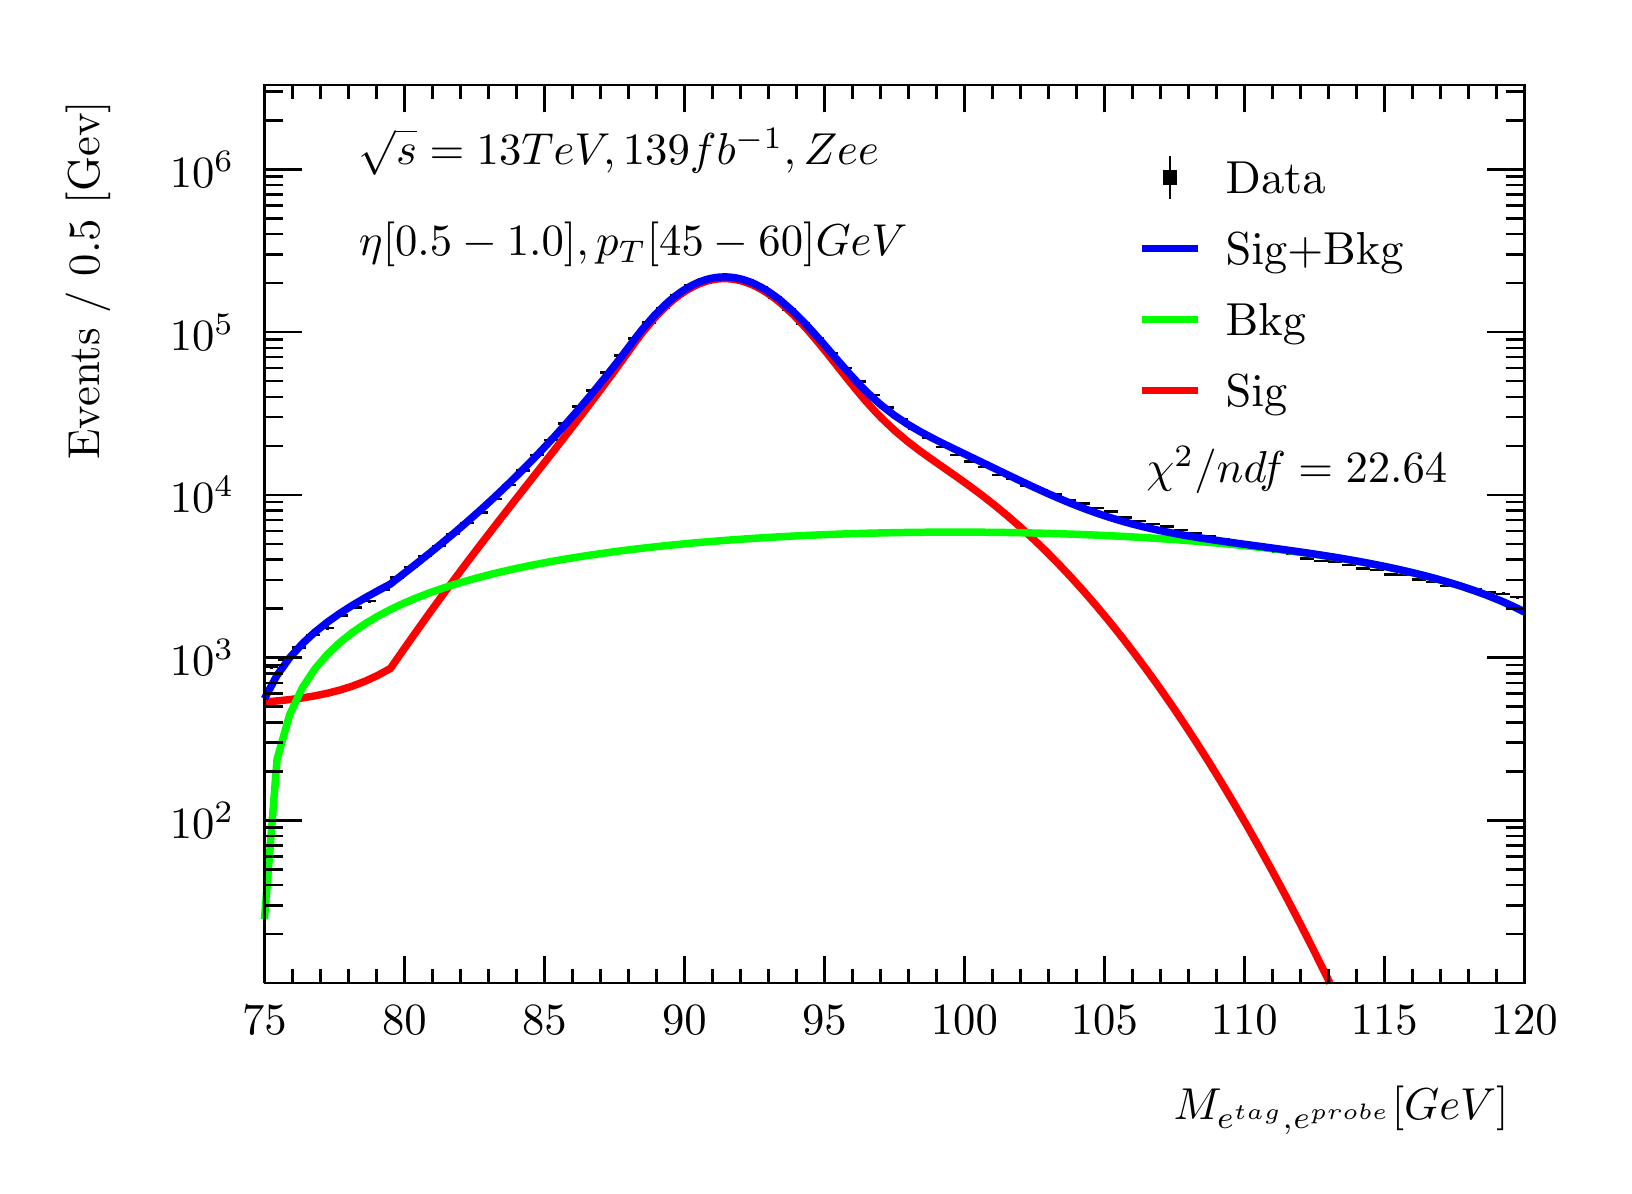
\begin{tikzpicture}
\pgfdeclareplotmark{cross} {
\pgfpathmoveto{\pgfpoint{-0.3\pgfplotmarksize}{\pgfplotmarksize}}
\pgfpathlineto{\pgfpoint{+0.3\pgfplotmarksize}{\pgfplotmarksize}}
\pgfpathlineto{\pgfpoint{+0.3\pgfplotmarksize}{0.3\pgfplotmarksize}}
\pgfpathlineto{\pgfpoint{+1\pgfplotmarksize}{0.3\pgfplotmarksize}}
\pgfpathlineto{\pgfpoint{+1\pgfplotmarksize}{-0.3\pgfplotmarksize}}
\pgfpathlineto{\pgfpoint{+0.3\pgfplotmarksize}{-0.3\pgfplotmarksize}}
\pgfpathlineto{\pgfpoint{+0.3\pgfplotmarksize}{-1.\pgfplotmarksize}}
\pgfpathlineto{\pgfpoint{-0.3\pgfplotmarksize}{-1.\pgfplotmarksize}}
\pgfpathlineto{\pgfpoint{-0.3\pgfplotmarksize}{-0.3\pgfplotmarksize}}
\pgfpathlineto{\pgfpoint{-1.\pgfplotmarksize}{-0.3\pgfplotmarksize}}
\pgfpathlineto{\pgfpoint{-1.\pgfplotmarksize}{0.3\pgfplotmarksize}}
\pgfpathlineto{\pgfpoint{-0.3\pgfplotmarksize}{0.3\pgfplotmarksize}}
\pgfpathclose
\pgfusepathqstroke
}
\pgfdeclareplotmark{cross*} {
\pgfpathmoveto{\pgfpoint{-0.3\pgfplotmarksize}{\pgfplotmarksize}}
\pgfpathlineto{\pgfpoint{+0.3\pgfplotmarksize}{\pgfplotmarksize}}
\pgfpathlineto{\pgfpoint{+0.3\pgfplotmarksize}{0.3\pgfplotmarksize}}
\pgfpathlineto{\pgfpoint{+1\pgfplotmarksize}{0.3\pgfplotmarksize}}
\pgfpathlineto{\pgfpoint{+1\pgfplotmarksize}{-0.3\pgfplotmarksize}}
\pgfpathlineto{\pgfpoint{+0.3\pgfplotmarksize}{-0.3\pgfplotmarksize}}
\pgfpathlineto{\pgfpoint{+0.3\pgfplotmarksize}{-1.\pgfplotmarksize}}
\pgfpathlineto{\pgfpoint{-0.3\pgfplotmarksize}{-1.\pgfplotmarksize}}
\pgfpathlineto{\pgfpoint{-0.3\pgfplotmarksize}{-0.3\pgfplotmarksize}}
\pgfpathlineto{\pgfpoint{-1.\pgfplotmarksize}{-0.3\pgfplotmarksize}}
\pgfpathlineto{\pgfpoint{-1.\pgfplotmarksize}{0.3\pgfplotmarksize}}
\pgfpathlineto{\pgfpoint{-0.3\pgfplotmarksize}{0.3\pgfplotmarksize}}
\pgfpathclose
\pgfusepathqfillstroke
}
\pgfdeclareplotmark{newstar} {
\pgfpathmoveto{\pgfqpoint{0pt}{\pgfplotmarksize}}
\pgfpathlineto{\pgfqpointpolar{44}{0.5\pgfplotmarksize}}
\pgfpathlineto{\pgfqpointpolar{18}{\pgfplotmarksize}}
\pgfpathlineto{\pgfqpointpolar{-20}{0.5\pgfplotmarksize}}
\pgfpathlineto{\pgfqpointpolar{-54}{\pgfplotmarksize}}
\pgfpathlineto{\pgfqpointpolar{-90}{0.5\pgfplotmarksize}}
\pgfpathlineto{\pgfqpointpolar{234}{\pgfplotmarksize}}
\pgfpathlineto{\pgfqpointpolar{198}{0.5\pgfplotmarksize}}
\pgfpathlineto{\pgfqpointpolar{162}{\pgfplotmarksize}}
\pgfpathlineto{\pgfqpointpolar{134}{0.5\pgfplotmarksize}}
\pgfpathclose
\pgfusepathqstroke
}
\pgfdeclareplotmark{newstar*} {
\pgfpathmoveto{\pgfqpoint{0pt}{\pgfplotmarksize}}
\pgfpathlineto{\pgfqpointpolar{44}{0.5\pgfplotmarksize}}
\pgfpathlineto{\pgfqpointpolar{18}{\pgfplotmarksize}}
\pgfpathlineto{\pgfqpointpolar{-20}{0.5\pgfplotmarksize}}
\pgfpathlineto{\pgfqpointpolar{-54}{\pgfplotmarksize}}
\pgfpathlineto{\pgfqpointpolar{-90}{0.5\pgfplotmarksize}}
\pgfpathlineto{\pgfqpointpolar{234}{\pgfplotmarksize}}
\pgfpathlineto{\pgfqpointpolar{198}{0.5\pgfplotmarksize}}
\pgfpathlineto{\pgfqpointpolar{162}{\pgfplotmarksize}}
\pgfpathlineto{\pgfqpointpolar{134}{0.5\pgfplotmarksize}}
\pgfpathclose
\pgfusepathqfillstroke
}
\definecolor{c}{rgb}{1,1,1};
\draw [color=c, fill=c] (0,0) rectangle (20,14.4361);
\draw [color=c, fill=c] (3,2.30977) rectangle (19,13.7143);
\definecolor{c}{rgb}{0,0,0};
\draw [c,line width=0.9] (3,2.30977) -- (3,13.7143) -- (19,13.7143) -- (19,2.30977) -- (3,2.30977);
\definecolor{c}{rgb}{1,1,1};
\draw [color=c, fill=c] (3,2.30977) rectangle (19,13.7143);
\definecolor{c}{rgb}{0,0,0};
\draw [c,line width=0.9] (3,2.30977) -- (3,13.7143) -- (19,13.7143) -- (19,2.30977) -- (3,2.30977);
\draw [c,line width=0.9] (3,2.30977) -- (19,2.30977);
\draw [c,line width=0.9] (3,2.65624) -- (3,2.30977);
\draw [c,line width=0.9] (3.35556,2.48301) -- (3.35556,2.30977);
\draw [c,line width=0.9] (3.71111,2.48301) -- (3.71111,2.30977);
\draw [c,line width=0.9] (4.06667,2.48301) -- (4.06667,2.30977);
\draw [c,line width=0.9] (4.42222,2.48301) -- (4.42222,2.30977);
\draw [c,line width=0.9] (4.77778,2.65624) -- (4.77778,2.30977);
\draw [c,line width=0.9] (5.13333,2.48301) -- (5.13333,2.30977);
\draw [c,line width=0.9] (5.48889,2.48301) -- (5.48889,2.30977);
\draw [c,line width=0.9] (5.84444,2.48301) -- (5.84444,2.30977);
\draw [c,line width=0.9] (6.2,2.48301) -- (6.2,2.30977);
\draw [c,line width=0.9] (6.55556,2.65624) -- (6.55556,2.30977);
\draw [c,line width=0.9] (6.91111,2.48301) -- (6.91111,2.30977);
\draw [c,line width=0.9] (7.26667,2.48301) -- (7.26667,2.30977);
\draw [c,line width=0.9] (7.62222,2.48301) -- (7.62222,2.30977);
\draw [c,line width=0.9] (7.97778,2.48301) -- (7.97778,2.30977);
\draw [c,line width=0.9] (8.33333,2.65624) -- (8.33333,2.30977);
\draw [c,line width=0.9] (8.68889,2.48301) -- (8.68889,2.30977);
\draw [c,line width=0.9] (9.04444,2.48301) -- (9.04444,2.30977);
\draw [c,line width=0.9] (9.4,2.48301) -- (9.4,2.30977);
\draw [c,line width=0.9] (9.75556,2.48301) -- (9.75556,2.30977);
\draw [c,line width=0.9] (10.1111,2.65624) -- (10.1111,2.30977);
\draw [c,line width=0.9] (10.4667,2.48301) -- (10.4667,2.30977);
\draw [c,line width=0.9] (10.8222,2.48301) -- (10.8222,2.30977);
\draw [c,line width=0.9] (11.1778,2.48301) -- (11.1778,2.30977);
\draw [c,line width=0.9] (11.5333,2.48301) -- (11.5333,2.30977);
\draw [c,line width=0.9] (11.8889,2.65624) -- (11.8889,2.30977);
\draw [c,line width=0.9] (12.2444,2.48301) -- (12.2444,2.30977);
\draw [c,line width=0.9] (12.6,2.48301) -- (12.6,2.30977);
\draw [c,line width=0.9] (12.9556,2.48301) -- (12.9556,2.30977);
\draw [c,line width=0.9] (13.3111,2.48301) -- (13.3111,2.30977);
\draw [c,line width=0.9] (13.6667,2.65624) -- (13.6667,2.30977);
\draw [c,line width=0.9] (14.0222,2.48301) -- (14.0222,2.30977);
\draw [c,line width=0.9] (14.3778,2.48301) -- (14.3778,2.30977);
\draw [c,line width=0.9] (14.7333,2.48301) -- (14.7333,2.30977);
\draw [c,line width=0.9] (15.0889,2.48301) -- (15.0889,2.30977);
\draw [c,line width=0.9] (15.4444,2.65624) -- (15.4444,2.30977);
\draw [c,line width=0.9] (15.8,2.48301) -- (15.8,2.30977);
\draw [c,line width=0.9] (16.1556,2.48301) -- (16.1556,2.30977);
\draw [c,line width=0.9] (16.5111,2.48301) -- (16.5111,2.30977);
\draw [c,line width=0.9] (16.8667,2.48301) -- (16.8667,2.30977);
\draw [c,line width=0.9] (17.2222,2.65624) -- (17.2222,2.30977);
\draw [c,line width=0.9] (17.5778,2.48301) -- (17.5778,2.30977);
\draw [c,line width=0.9] (17.9333,2.48301) -- (17.9333,2.30977);
\draw [c,line width=0.9] (18.2889,2.48301) -- (18.2889,2.30977);
\draw [c,line width=0.9] (18.6444,2.48301) -- (18.6444,2.30977);
\draw [c,line width=0.9] (19,2.65624) -- (19,2.30977);
\draw [c,line width=0.9] (19,2.65624) -- (19,2.30977);
\draw [anchor=base] (3,1.66015) node[scale=1.61424, color=c, rotate=0]{75};
\draw [anchor=base] (4.77778,1.66015) node[scale=1.61424, color=c, rotate=0]{80};
\draw [anchor=base] (6.55556,1.66015) node[scale=1.61424, color=c, rotate=0]{85};
\draw [anchor=base] (8.33333,1.66015) node[scale=1.61424, color=c, rotate=0]{90};
\draw [anchor=base] (10.1111,1.66015) node[scale=1.61424, color=c, rotate=0]{95};
\draw [anchor=base] (11.8889,1.66015) node[scale=1.61424, color=c, rotate=0]{100};
\draw [anchor=base] (13.6667,1.66015) node[scale=1.61424, color=c, rotate=0]{105};
\draw [anchor=base] (15.4444,1.66015) node[scale=1.61424, color=c, rotate=0]{110};
\draw [anchor=base] (17.2222,1.66015) node[scale=1.61424, color=c, rotate=0]{115};
\draw [anchor=base] (19,1.66015) node[scale=1.61424, color=c, rotate=0]{120};
\draw [anchor= east] (19,0.692932) node[scale=1.61424, color=c, rotate=0]{$M_{e^{tag}, e^{probe}}  [GeV]$};
\draw [c,line width=0.9] (3,13.7143) -- (19,13.7143);
\draw [c,line width=0.9] (3,13.3678) -- (3,13.7143);
\draw [c,line width=0.9] (3.35556,13.5411) -- (3.35556,13.7143);
\draw [c,line width=0.9] (3.71111,13.5411) -- (3.71111,13.7143);
\draw [c,line width=0.9] (4.06667,13.5411) -- (4.06667,13.7143);
\draw [c,line width=0.9] (4.42222,13.5411) -- (4.42222,13.7143);
\draw [c,line width=0.9] (4.77778,13.3678) -- (4.77778,13.7143);
\draw [c,line width=0.9] (5.13333,13.5411) -- (5.13333,13.7143);
\draw [c,line width=0.9] (5.48889,13.5411) -- (5.48889,13.7143);
\draw [c,line width=0.9] (5.84444,13.5411) -- (5.84444,13.7143);
\draw [c,line width=0.9] (6.2,13.5411) -- (6.2,13.7143);
\draw [c,line width=0.9] (6.55556,13.3678) -- (6.55556,13.7143);
\draw [c,line width=0.9] (6.91111,13.5411) -- (6.91111,13.7143);
\draw [c,line width=0.9] (7.26667,13.5411) -- (7.26667,13.7143);
\draw [c,line width=0.9] (7.62222,13.5411) -- (7.62222,13.7143);
\draw [c,line width=0.9] (7.97778,13.5411) -- (7.97778,13.7143);
\draw [c,line width=0.9] (8.33333,13.3678) -- (8.33333,13.7143);
\draw [c,line width=0.9] (8.68889,13.5411) -- (8.68889,13.7143);
\draw [c,line width=0.9] (9.04444,13.5411) -- (9.04444,13.7143);
\draw [c,line width=0.9] (9.4,13.5411) -- (9.4,13.7143);
\draw [c,line width=0.9] (9.75556,13.5411) -- (9.75556,13.7143);
\draw [c,line width=0.9] (10.1111,13.3678) -- (10.1111,13.7143);
\draw [c,line width=0.9] (10.4667,13.5411) -- (10.4667,13.7143);
\draw [c,line width=0.9] (10.8222,13.5411) -- (10.8222,13.7143);
\draw [c,line width=0.9] (11.1778,13.5411) -- (11.1778,13.7143);
\draw [c,line width=0.9] (11.5333,13.5411) -- (11.5333,13.7143);
\draw [c,line width=0.9] (11.8889,13.3678) -- (11.8889,13.7143);
\draw [c,line width=0.9] (12.2444,13.5411) -- (12.2444,13.7143);
\draw [c,line width=0.9] (12.6,13.5411) -- (12.6,13.7143);
\draw [c,line width=0.9] (12.9556,13.5411) -- (12.9556,13.7143);
\draw [c,line width=0.9] (13.3111,13.5411) -- (13.3111,13.7143);
\draw [c,line width=0.9] (13.6667,13.3678) -- (13.6667,13.7143);
\draw [c,line width=0.9] (14.0222,13.5411) -- (14.0222,13.7143);
\draw [c,line width=0.9] (14.3778,13.5411) -- (14.3778,13.7143);
\draw [c,line width=0.9] (14.7333,13.5411) -- (14.7333,13.7143);
\draw [c,line width=0.9] (15.0889,13.5411) -- (15.0889,13.7143);
\draw [c,line width=0.9] (15.4444,13.3678) -- (15.4444,13.7143);
\draw [c,line width=0.9] (15.8,13.5411) -- (15.8,13.7143);
\draw [c,line width=0.9] (16.1556,13.5411) -- (16.1556,13.7143);
\draw [c,line width=0.9] (16.5111,13.5411) -- (16.5111,13.7143);
\draw [c,line width=0.9] (16.8667,13.5411) -- (16.8667,13.7143);
\draw [c,line width=0.9] (17.2222,13.3678) -- (17.2222,13.7143);
\draw [c,line width=0.9] (17.5778,13.5411) -- (17.5778,13.7143);
\draw [c,line width=0.9] (17.9333,13.5411) -- (17.9333,13.7143);
\draw [c,line width=0.9] (18.2889,13.5411) -- (18.2889,13.7143);
\draw [c,line width=0.9] (18.6444,13.5411) -- (18.6444,13.7143);
\draw [c,line width=0.9] (19,13.3678) -- (19,13.7143);
\draw [c,line width=0.9] (19,13.3678) -- (19,13.7143);
\draw [c,line width=0.9] (3,2.30977) -- (3,13.7143);
\draw [c,line width=0.9] (3.237,2.932) -- (3,2.932);
\draw [c,line width=0.9] (3.237,3.29598) -- (3,3.29598);
\draw [c,line width=0.9] (3.237,3.55423) -- (3,3.55423);
\draw [c,line width=0.9] (3.237,3.75454) -- (3,3.75454);
\draw [c,line width=0.9] (3.237,3.9182) -- (3,3.9182);
\draw [c,line width=0.9] (3.237,4.05658) -- (3,4.05658);
\draw [c,line width=0.9] (3.237,4.17645) -- (3,4.17645);
\draw [c,line width=0.9] (3.237,4.28218) -- (3,4.28218);
\draw [c,line width=0.9] (3.474,4.37676) -- (3,4.37676);
\draw [anchor= east] (2.82,4.37676) node[scale=1.61424, color=c, rotate=0]{$10^{2}$};
\draw [c,line width=0.9] (3.237,4.99899) -- (3,4.99899);
\draw [c,line width=0.9] (3.237,5.36297) -- (3,5.36297);
\draw [c,line width=0.9] (3.237,5.62122) -- (3,5.62122);
\draw [c,line width=0.9] (3.237,5.82153) -- (3,5.82153);
\draw [c,line width=0.9] (3.237,5.9852) -- (3,5.9852);
\draw [c,line width=0.9] (3.237,6.12357) -- (3,6.12357);
\draw [c,line width=0.9] (3.237,6.24344) -- (3,6.24344);
\draw [c,line width=0.9] (3.237,6.34917) -- (3,6.34917);
\draw [c,line width=0.9] (3.474,6.44376) -- (3,6.44376);
\draw [anchor= east] (2.82,6.44376) node[scale=1.61424, color=c, rotate=0]{$10^{3}$};
\draw [c,line width=0.9] (3.237,7.06598) -- (3,7.06598);
\draw [c,line width=0.9] (3.237,7.42996) -- (3,7.42996);
\draw [c,line width=0.9] (3.237,7.68821) -- (3,7.68821);
\draw [c,line width=0.9] (3.237,7.88852) -- (3,7.88852);
\draw [c,line width=0.9] (3.237,8.05219) -- (3,8.05219);
\draw [c,line width=0.9] (3.237,8.19057) -- (3,8.19057);
\draw [c,line width=0.9] (3.237,8.31043) -- (3,8.31043);
\draw [c,line width=0.9] (3.237,8.41617) -- (3,8.41617);
\draw [c,line width=0.9] (3.474,8.51075) -- (3,8.51075);
\draw [anchor= east] (2.82,8.51075) node[scale=1.61424, color=c, rotate=0]{$10^{4}$};
\draw [c,line width=0.9] (3.237,9.13297) -- (3,9.13297);
\draw [c,line width=0.9] (3.237,9.49695) -- (3,9.49695);
\draw [c,line width=0.9] (3.237,9.7552) -- (3,9.7552);
\draw [c,line width=0.9] (3.237,9.95551) -- (3,9.95551);
\draw [c,line width=0.9] (3.237,10.1192) -- (3,10.1192);
\draw [c,line width=0.9] (3.237,10.2576) -- (3,10.2576);
\draw [c,line width=0.9] (3.237,10.3774) -- (3,10.3774);
\draw [c,line width=0.9] (3.237,10.4832) -- (3,10.4832);
\draw [c,line width=0.9] (3.474,10.5777) -- (3,10.5777);
\draw [anchor= east] (2.82,10.5777) node[scale=1.61424, color=c, rotate=0]{$10^{5}$};
\draw [c,line width=0.9] (3.237,11.2) -- (3,11.2);
\draw [c,line width=0.9] (3.237,11.5639) -- (3,11.5639);
\draw [c,line width=0.9] (3.237,11.8222) -- (3,11.8222);
\draw [c,line width=0.9] (3.237,12.0225) -- (3,12.0225);
\draw [c,line width=0.9] (3.237,12.1862) -- (3,12.1862);
\draw [c,line width=0.9] (3.237,12.3245) -- (3,12.3245);
\draw [c,line width=0.9] (3.237,12.4444) -- (3,12.4444);
\draw [c,line width=0.9] (3.237,12.5501) -- (3,12.5501);
\draw [c,line width=0.9] (3.474,12.6447) -- (3,12.6447);
\draw [anchor= east] (2.82,12.6447) node[scale=1.61424, color=c, rotate=0]{$10^{6}$};
\draw [c,line width=0.9] (3.237,13.267) -- (3,13.267);
\draw [c,line width=0.9] (3.237,13.6309) -- (3,13.6309);
\draw [anchor= east] (0.76,13.7143) node[scale=1.61424, color=c, rotate=90]{Events / 0.5 [Gev]};
\draw [c,line width=0.9] (19,2.30977) -- (19,13.7143);
\draw [c,line width=0.9] (18.763,2.932) -- (19,2.932);
\draw [c,line width=0.9] (18.763,3.29598) -- (19,3.29598);
\draw [c,line width=0.9] (18.763,3.55423) -- (19,3.55423);
\draw [c,line width=0.9] (18.763,3.75454) -- (19,3.75454);
\draw [c,line width=0.9] (18.763,3.9182) -- (19,3.9182);
\draw [c,line width=0.9] (18.763,4.05658) -- (19,4.05658);
\draw [c,line width=0.9] (18.763,4.17645) -- (19,4.17645);
\draw [c,line width=0.9] (18.763,4.28218) -- (19,4.28218);
\draw [c,line width=0.9] (18.526,4.37676) -- (19,4.37676);
\draw [c,line width=0.9] (18.763,4.99899) -- (19,4.99899);
\draw [c,line width=0.9] (18.763,5.36297) -- (19,5.36297);
\draw [c,line width=0.9] (18.763,5.62122) -- (19,5.62122);
\draw [c,line width=0.9] (18.763,5.82153) -- (19,5.82153);
\draw [c,line width=0.9] (18.763,5.9852) -- (19,5.9852);
\draw [c,line width=0.9] (18.763,6.12357) -- (19,6.12357);
\draw [c,line width=0.9] (18.763,6.24344) -- (19,6.24344);
\draw [c,line width=0.9] (18.763,6.34917) -- (19,6.34917);
\draw [c,line width=0.9] (18.526,6.44376) -- (19,6.44376);
\draw [c,line width=0.9] (18.763,7.06598) -- (19,7.06598);
\draw [c,line width=0.9] (18.763,7.42996) -- (19,7.42996);
\draw [c,line width=0.9] (18.763,7.68821) -- (19,7.68821);
\draw [c,line width=0.9] (18.763,7.88852) -- (19,7.88852);
\draw [c,line width=0.9] (18.763,8.05219) -- (19,8.05219);
\draw [c,line width=0.9] (18.763,8.19057) -- (19,8.19057);
\draw [c,line width=0.9] (18.763,8.31043) -- (19,8.31043);
\draw [c,line width=0.9] (18.763,8.41617) -- (19,8.41617);
\draw [c,line width=0.9] (18.526,8.51075) -- (19,8.51075);
\draw [c,line width=0.9] (18.763,9.13297) -- (19,9.13297);
\draw [c,line width=0.9] (18.763,9.49695) -- (19,9.49695);
\draw [c,line width=0.9] (18.763,9.7552) -- (19,9.7552);
\draw [c,line width=0.9] (18.763,9.95551) -- (19,9.95551);
\draw [c,line width=0.9] (18.763,10.1192) -- (19,10.1192);
\draw [c,line width=0.9] (18.763,10.2576) -- (19,10.2576);
\draw [c,line width=0.9] (18.763,10.3774) -- (19,10.3774);
\draw [c,line width=0.9] (18.763,10.4832) -- (19,10.4832);
\draw [c,line width=0.9] (18.526,10.5777) -- (19,10.5777);
\draw [c,line width=0.9] (18.763,11.2) -- (19,11.2);
\draw [c,line width=0.9] (18.763,11.5639) -- (19,11.5639);
\draw [c,line width=0.9] (18.763,11.8222) -- (19,11.8222);
\draw [c,line width=0.9] (18.763,12.0225) -- (19,12.0225);
\draw [c,line width=0.9] (18.763,12.1862) -- (19,12.1862);
\draw [c,line width=0.9] (18.763,12.3245) -- (19,12.3245);
\draw [c,line width=0.9] (18.763,12.4444) -- (19,12.4444);
\draw [c,line width=0.9] (18.763,12.5501) -- (19,12.5501);
\draw [c,line width=0.9] (18.526,12.6447) -- (19,12.6447);
\draw [c,line width=0.9] (18.763,13.267) -- (19,13.267);
\draw [c,line width=0.9] (18.763,13.6309) -- (19,13.6309);
\draw [c,line width=0.9] (3.08889,6.33002) -- (3,6.33002);
\draw [c,line width=0.9] (3,6.33002) -- (3,6.33002);
\draw [c,line width=0.9] (3.08889,6.33002) -- (3.17778,6.33002);
\draw [c,line width=0.9] (3.17778,6.33002) -- (3.17778,6.33002);
\draw [c,line width=0.9] (3.08889,6.33002) -- (3.08889,6.36026);
\draw [c,line width=0.9] (3.08889,6.36026) -- (3.08889,6.36026);
\draw [c,line width=0.9] (3.08889,6.33002) -- (3.08889,6.29978);
\draw [c,line width=0.9] (3.08889,6.29978) -- (3.08889,6.29978);
\draw [c,line width=0.9] (3.26667,6.4127) -- (3.17778,6.4127);
\draw [c,line width=0.9] (3.17778,6.4127) -- (3.17778,6.4127);
\draw [c,line width=0.9] (3.26667,6.4127) -- (3.35556,6.4127);
\draw [c,line width=0.9] (3.35556,6.4127) -- (3.35556,6.4127);
\draw [c,line width=0.9] (3.26667,6.4127) -- (3.26667,6.44159);
\draw [c,line width=0.9] (3.26667,6.44159) -- (3.26667,6.44159);
\draw [c,line width=0.9] (3.26667,6.4127) -- (3.26667,6.38382);
\draw [c,line width=0.9] (3.26667,6.38382) -- (3.26667,6.38382);
\draw [c,line width=0.9] (3.44444,6.57) -- (3.35556,6.57);
\draw [c,line width=0.9] (3.35556,6.57) -- (3.35556,6.57);
\draw [c,line width=0.9] (3.44444,6.57) -- (3.53333,6.57);
\draw [c,line width=0.9] (3.53333,6.57) -- (3.53333,6.57);
\draw [c,line width=0.9] (3.44444,6.57) -- (3.44444,6.59646);
\draw [c,line width=0.9] (3.44444,6.59646) -- (3.44444,6.59646);
\draw [c,line width=0.9] (3.44444,6.57) -- (3.44444,6.54354);
\draw [c,line width=0.9] (3.44444,6.54354) -- (3.44444,6.54354);
\draw [c,line width=0.9] (3.62222,6.72767) -- (3.53333,6.72767);
\draw [c,line width=0.9] (3.53333,6.72767) -- (3.53333,6.72767);
\draw [c,line width=0.9] (3.62222,6.72767) -- (3.71111,6.72767);
\draw [c,line width=0.9] (3.71111,6.72767) -- (3.71111,6.72767);
\draw [c,line width=0.9] (3.62222,6.72767) -- (3.62222,6.7519);
\draw [c,line width=0.9] (3.62222,6.7519) -- (3.62222,6.7519);
\draw [c,line width=0.9] (3.62222,6.72767) -- (3.62222,6.70343);
\draw [c,line width=0.9] (3.62222,6.70343) -- (3.62222,6.70343);
\draw [c,line width=0.9] (3.8,6.82022) -- (3.71111,6.82022);
\draw [c,line width=0.9] (3.71111,6.82022) -- (3.71111,6.82022);
\draw [c,line width=0.9] (3.8,6.82022) -- (3.88889,6.82022);
\draw [c,line width=0.9] (3.88889,6.82022) -- (3.88889,6.82022);
\draw [c,line width=0.9] (3.8,6.82022) -- (3.8,6.84323);
\draw [c,line width=0.9] (3.8,6.84323) -- (3.8,6.84323);
\draw [c,line width=0.9] (3.8,6.82022) -- (3.8,6.7972);
\draw [c,line width=0.9] (3.8,6.7972) -- (3.8,6.7972);
\draw [c,line width=0.9] (3.97778,6.97935) -- (3.88889,6.97935);
\draw [c,line width=0.9] (3.88889,6.97935) -- (3.88889,6.97935);
\draw [c,line width=0.9] (3.97778,6.97935) -- (4.06667,6.97935);
\draw [c,line width=0.9] (4.06667,6.97935) -- (4.06667,6.97935);
\draw [c,line width=0.9] (3.97778,6.97935) -- (3.97778,7.00041);
\draw [c,line width=0.9] (3.97778,7.00041) -- (3.97778,7.00041);
\draw [c,line width=0.9] (3.97778,6.97935) -- (3.97778,6.95828);
\draw [c,line width=0.9] (3.97778,6.95828) -- (3.97778,6.95828);
\draw [c,line width=0.9] (4.15556,7.07713) -- (4.06667,7.07713);
\draw [c,line width=0.9] (4.06667,7.07713) -- (4.06667,7.07713);
\draw [c,line width=0.9] (4.15556,7.07713) -- (4.24444,7.07713);
\draw [c,line width=0.9] (4.24444,7.07713) -- (4.24444,7.07713);
\draw [c,line width=0.9] (4.15556,7.07713) -- (4.15556,7.09708);
\draw [c,line width=0.9] (4.15556,7.09708) -- (4.15556,7.09708);
\draw [c,line width=0.9] (4.15556,7.07713) -- (4.15556,7.05719);
\draw [c,line width=0.9] (4.15556,7.05719) -- (4.15556,7.05719);
\draw [c,line width=0.9] (4.33333,7.16088) -- (4.24444,7.16088);
\draw [c,line width=0.9] (4.24444,7.16088) -- (4.24444,7.16088);
\draw [c,line width=0.9] (4.33333,7.16088) -- (4.42222,7.16088);
\draw [c,line width=0.9] (4.42222,7.16088) -- (4.42222,7.16088);
\draw [c,line width=0.9] (4.33333,7.16088) -- (4.33333,7.17992);
\draw [c,line width=0.9] (4.33333,7.17992) -- (4.33333,7.17992);
\draw [c,line width=0.9] (4.33333,7.16088) -- (4.33333,7.14184);
\draw [c,line width=0.9] (4.33333,7.14184) -- (4.33333,7.14184);
\draw [c,line width=0.9] (4.51111,7.30667) -- (4.42222,7.30667);
\draw [c,line width=0.9] (4.42222,7.30667) -- (4.42222,7.30667);
\draw [c,line width=0.9] (4.51111,7.30667) -- (4.6,7.30667);
\draw [c,line width=0.9] (4.6,7.30667) -- (4.6,7.30667);
\draw [c,line width=0.9] (4.51111,7.30667) -- (4.51111,7.32422);
\draw [c,line width=0.9] (4.51111,7.32422) -- (4.51111,7.32422);
\draw [c,line width=0.9] (4.51111,7.30667) -- (4.51111,7.28911);
\draw [c,line width=0.9] (4.51111,7.28911) -- (4.51111,7.28911);
\draw [c,line width=0.9] (4.68889,7.45824) -- (4.6,7.45824);
\draw [c,line width=0.9] (4.6,7.45824) -- (4.6,7.45824);
\draw [c,line width=0.9] (4.68889,7.45824) -- (4.77778,7.45824);
\draw [c,line width=0.9] (4.77778,7.45824) -- (4.77778,7.45824);
\draw [c,line width=0.9] (4.68889,7.45824) -- (4.68889,7.47437);
\draw [c,line width=0.9] (4.68889,7.47437) -- (4.68889,7.47437);
\draw [c,line width=0.9] (4.68889,7.45824) -- (4.68889,7.4421);
\draw [c,line width=0.9] (4.68889,7.4421) -- (4.68889,7.4421);
\draw [c,line width=0.9] (4.86667,7.59238) -- (4.77778,7.59238);
\draw [c,line width=0.9] (4.77778,7.59238) -- (4.77778,7.59238);
\draw [c,line width=0.9] (4.86667,7.59238) -- (4.95556,7.59238);
\draw [c,line width=0.9] (4.95556,7.59238) -- (4.95556,7.59238);
\draw [c,line width=0.9] (4.86667,7.59238) -- (4.86667,7.60735);
\draw [c,line width=0.9] (4.86667,7.60735) -- (4.86667,7.60735);
\draw [c,line width=0.9] (4.86667,7.59238) -- (4.86667,7.57741);
\draw [c,line width=0.9] (4.86667,7.57741) -- (4.86667,7.57741);
\draw [c,line width=0.9] (5.04444,7.73179) -- (4.95556,7.73179);
\draw [c,line width=0.9] (4.95556,7.73179) -- (4.95556,7.73179);
\draw [c,line width=0.9] (5.04444,7.73179) -- (5.13333,7.73179);
\draw [c,line width=0.9] (5.13333,7.73179) -- (5.13333,7.73179);
\draw [c,line width=0.9] (5.04444,7.73179) -- (5.04444,7.74565);
\draw [c,line width=0.9] (5.04444,7.74565) -- (5.04444,7.74565);
\draw [c,line width=0.9] (5.04444,7.73179) -- (5.04444,7.71794);
\draw [c,line width=0.9] (5.04444,7.71794) -- (5.04444,7.71794);
\draw [c,line width=0.9] (5.22222,7.85858) -- (5.13333,7.85858);
\draw [c,line width=0.9] (5.13333,7.85858) -- (5.13333,7.85858);
\draw [c,line width=0.9] (5.22222,7.85858) -- (5.31111,7.85858);
\draw [c,line width=0.9] (5.31111,7.85858) -- (5.31111,7.85858);
\draw [c,line width=0.9] (5.22222,7.85858) -- (5.22222,7.87149);
\draw [c,line width=0.9] (5.22222,7.87149) -- (5.22222,7.87149);
\draw [c,line width=0.9] (5.22222,7.85858) -- (5.22222,7.84567);
\draw [c,line width=0.9] (5.22222,7.84567) -- (5.22222,7.84567);
\draw [c,line width=0.9] (5.4,8.01054) -- (5.31111,8.01054);
\draw [c,line width=0.9] (5.31111,8.01054) -- (5.31111,8.01054);
\draw [c,line width=0.9] (5.4,8.01054) -- (5.48889,8.01054);
\draw [c,line width=0.9] (5.48889,8.01054) -- (5.48889,8.01054);
\draw [c,line width=0.9] (5.4,8.01054) -- (5.4,8.0224);
\draw [c,line width=0.9] (5.4,8.0224) -- (5.4,8.0224);
\draw [c,line width=0.9] (5.4,8.01054) -- (5.4,7.99868);
\draw [c,line width=0.9] (5.4,7.99868) -- (5.4,7.99868);
\draw [c,line width=0.9] (5.57778,8.15245) -- (5.48889,8.15245);
\draw [c,line width=0.9] (5.48889,8.15245) -- (5.48889,8.15245);
\draw [c,line width=0.9] (5.57778,8.15245) -- (5.66667,8.15245);
\draw [c,line width=0.9] (5.66667,8.15245) -- (5.66667,8.15245);
\draw [c,line width=0.9] (5.57778,8.15245) -- (5.57778,8.16341);
\draw [c,line width=0.9] (5.57778,8.16341) -- (5.57778,8.16341);
\draw [c,line width=0.9] (5.57778,8.15245) -- (5.57778,8.14149);
\draw [c,line width=0.9] (5.57778,8.14149) -- (5.57778,8.14149);
\draw [c,line width=0.9] (5.75556,8.28805) -- (5.66667,8.28805);
\draw [c,line width=0.9] (5.66667,8.28805) -- (5.66667,8.28805);
\draw [c,line width=0.9] (5.75556,8.28805) -- (5.84444,8.28805);
\draw [c,line width=0.9] (5.84444,8.28805) -- (5.84444,8.28805);
\draw [c,line width=0.9] (5.75556,8.28805) -- (5.75556,8.29822);
\draw [c,line width=0.9] (5.75556,8.29822) -- (5.75556,8.29822);
\draw [c,line width=0.9] (5.75556,8.28805) -- (5.75556,8.27789);
\draw [c,line width=0.9] (5.75556,8.27789) -- (5.75556,8.27789);
\draw [c,line width=0.9] (5.93333,8.45892) -- (5.84444,8.45892);
\draw [c,line width=0.9] (5.84444,8.45892) -- (5.84444,8.45892);
\draw [c,line width=0.9] (5.93333,8.45892) -- (6.02222,8.45892);
\draw [c,line width=0.9] (6.02222,8.45892) -- (6.02222,8.45892);
\draw [c,line width=0.9] (5.93333,8.45892) -- (5.93333,8.46816);
\draw [c,line width=0.9] (5.93333,8.46816) -- (5.93333,8.46816);
\draw [c,line width=0.9] (5.93333,8.45892) -- (5.93333,8.44968);
\draw [c,line width=0.9] (5.93333,8.44968) -- (5.93333,8.44968);
\draw [c,line width=0.9] (6.11111,8.63738) -- (6.02222,8.63738);
\draw [c,line width=0.9] (6.02222,8.63738) -- (6.02222,8.63738);
\draw [c,line width=0.9] (6.11111,8.63738) -- (6.2,8.63738);
\draw [c,line width=0.9] (6.2,8.63738) -- (6.2,8.63738);
\draw [c,line width=0.9] (6.11111,8.63738) -- (6.11111,8.64575);
\draw [c,line width=0.9] (6.11111,8.64575) -- (6.11111,8.64575);
\draw [c,line width=0.9] (6.11111,8.63738) -- (6.11111,8.62901);
\draw [c,line width=0.9] (6.11111,8.62901) -- (6.11111,8.62901);
\draw [c,line width=0.9] (6.28889,8.81759) -- (6.2,8.81759);
\draw [c,line width=0.9] (6.2,8.81759) -- (6.2,8.81759);
\draw [c,line width=0.9] (6.28889,8.81759) -- (6.37778,8.81759);
\draw [c,line width=0.9] (6.37778,8.81759) -- (6.37778,8.81759);
\draw [c,line width=0.9] (6.28889,8.81759) -- (6.28889,8.82516);
\draw [c,line width=0.9] (6.28889,8.82516) -- (6.28889,8.82516);
\draw [c,line width=0.9] (6.28889,8.81759) -- (6.28889,8.81002);
\draw [c,line width=0.9] (6.28889,8.81002) -- (6.28889,8.81002);
\draw [c,line width=0.9] (6.46667,9.01469) -- (6.37778,9.01469);
\draw [c,line width=0.9] (6.37778,9.01469) -- (6.37778,9.01469);
\draw [c,line width=0.9] (6.46667,9.01469) -- (6.55556,9.01469);
\draw [c,line width=0.9] (6.55556,9.01469) -- (6.55556,9.01469);
\draw [c,line width=0.9] (6.46667,9.01469) -- (6.46667,9.02147);
\draw [c,line width=0.9] (6.46667,9.02147) -- (6.46667,9.02147);
\draw [c,line width=0.9] (6.46667,9.01469) -- (6.46667,9.00791);
\draw [c,line width=0.9] (6.46667,9.00791) -- (6.46667,9.00791);
\draw [c,line width=0.9] (6.64444,9.20339) -- (6.55556,9.20339);
\draw [c,line width=0.9] (6.55556,9.20339) -- (6.55556,9.20339);
\draw [c,line width=0.9] (6.64444,9.20339) -- (6.73333,9.20339);
\draw [c,line width=0.9] (6.73333,9.20339) -- (6.73333,9.20339);
\draw [c,line width=0.9] (6.64444,9.20339) -- (6.64444,9.20949);
\draw [c,line width=0.9] (6.64444,9.20949) -- (6.64444,9.20949);
\draw [c,line width=0.9] (6.64444,9.20339) -- (6.64444,9.19729);
\draw [c,line width=0.9] (6.64444,9.19729) -- (6.64444,9.19729);
\draw [c,line width=0.9] (6.82222,9.41597) -- (6.73333,9.41597);
\draw [c,line width=0.9] (6.73333,9.41597) -- (6.73333,9.41597);
\draw [c,line width=0.9] (6.82222,9.41597) -- (6.91111,9.41597);
\draw [c,line width=0.9] (6.91111,9.41597) -- (6.91111,9.41597);
\draw [c,line width=0.9] (6.82222,9.41597) -- (6.82222,9.42139);
\draw [c,line width=0.9] (6.82222,9.42139) -- (6.82222,9.42139);
\draw [c,line width=0.9] (6.82222,9.41597) -- (6.82222,9.41055);
\draw [c,line width=0.9] (6.82222,9.41055) -- (6.82222,9.41055);
\draw [c,line width=0.9] (7,9.63111) -- (6.91111,9.63111);
\draw [c,line width=0.9] (6.91111,9.63111) -- (6.91111,9.63111);
\draw [c,line width=0.9] (7,9.63111) -- (7.08889,9.63111);
\draw [c,line width=0.9] (7.08889,9.63111) -- (7.08889,9.63111);
\draw [c,line width=0.9] (7,9.63111) -- (7,9.63592);
\draw [c,line width=0.9] (7,9.63592) -- (7,9.63592);
\draw [c,line width=0.9] (7,9.63111) -- (7,9.62631);
\draw [c,line width=0.9] (7,9.62631) -- (7,9.62631);
\draw [c,line width=0.9] (7.17778,9.83636) -- (7.08889,9.83636);
\draw [c,line width=0.9] (7.08889,9.83636) -- (7.08889,9.83636);
\draw [c,line width=0.9] (7.17778,9.83636) -- (7.26667,9.83636);
\draw [c,line width=0.9] (7.26667,9.83636) -- (7.26667,9.83636);
\draw [c,line width=0.9] (7.17778,9.83636) -- (7.17778,9.84065);
\draw [c,line width=0.9] (7.17778,9.84065) -- (7.17778,9.84065);
\draw [c,line width=0.9] (7.17778,9.83636) -- (7.17778,9.83207);
\draw [c,line width=0.9] (7.17778,9.83207) -- (7.17778,9.83207);
\draw [c,line width=0.9] (7.35556,10.0623) -- (7.26667,10.0623);
\draw [c,line width=0.9] (7.26667,10.0623) -- (7.26667,10.0623);
\draw [c,line width=0.9] (7.35556,10.0623) -- (7.44444,10.0623);
\draw [c,line width=0.9] (7.44444,10.0623) -- (7.44444,10.0623);
\draw [c,line width=0.9] (7.35556,10.0623) -- (7.35556,10.066);
\draw [c,line width=0.9] (7.35556,10.066) -- (7.35556,10.066);
\draw [c,line width=0.9] (7.35556,10.0623) -- (7.35556,10.0585);
\draw [c,line width=0.9] (7.35556,10.0585) -- (7.35556,10.0585);
\draw [c,line width=0.9] (7.53333,10.2775) -- (7.44444,10.2775);
\draw [c,line width=0.9] (7.44444,10.2775) -- (7.44444,10.2775);
\draw [c,line width=0.9] (7.53333,10.2775) -- (7.62222,10.2775);
\draw [c,line width=0.9] (7.62222,10.2775) -- (7.62222,10.2775);
\draw [c,line width=0.9] (7.53333,10.2775) -- (7.53333,10.2808);
\draw [c,line width=0.9] (7.53333,10.2808) -- (7.53333,10.2808);
\draw [c,line width=0.9] (7.53333,10.2775) -- (7.53333,10.2741);
\draw [c,line width=0.9] (7.53333,10.2741) -- (7.53333,10.2741);
\draw [c,line width=0.9] (7.71111,10.4972) -- (7.62222,10.4972);
\draw [c,line width=0.9] (7.62222,10.4972) -- (7.62222,10.4972);
\draw [c,line width=0.9] (7.71111,10.4972) -- (7.8,10.4972);
\draw [c,line width=0.9] (7.8,10.4972) -- (7.8,10.4972);
\draw [c,line width=0.9] (7.71111,10.4972) -- (7.71111,10.5002);
\draw [c,line width=0.9] (7.71111,10.5002) -- (7.71111,10.5002);
\draw [c,line width=0.9] (7.71111,10.4972) -- (7.71111,10.4942);
\draw [c,line width=0.9] (7.71111,10.4942) -- (7.71111,10.4942);
\draw [c,line width=0.9] (7.88889,10.6999) -- (7.8,10.6999);
\draw [c,line width=0.9] (7.8,10.6999) -- (7.8,10.6999);
\draw [c,line width=0.9] (7.88889,10.6999) -- (7.97778,10.6999);
\draw [c,line width=0.9] (7.97778,10.6999) -- (7.97778,10.6999);
\draw [c,line width=0.9] (7.88889,10.6999) -- (7.88889,10.7025);
\draw [c,line width=0.9] (7.88889,10.7025) -- (7.88889,10.7025);
\draw [c,line width=0.9] (7.88889,10.6999) -- (7.88889,10.6972);
\draw [c,line width=0.9] (7.88889,10.6972) -- (7.88889,10.6972);
\draw [c,line width=0.9] (8.06667,10.8818) -- (7.97778,10.8818);
\draw [c,line width=0.9] (7.97778,10.8818) -- (7.97778,10.8818);
\draw [c,line width=0.9] (8.06667,10.8818) -- (8.15556,10.8818);
\draw [c,line width=0.9] (8.15556,10.8818) -- (8.15556,10.8818);
\draw [c,line width=0.9] (8.06667,10.8818) -- (8.06667,10.8842);
\draw [c,line width=0.9] (8.06667,10.8842) -- (8.06667,10.8842);
\draw [c,line width=0.9] (8.06667,10.8818) -- (8.06667,10.8794);
\draw [c,line width=0.9] (8.06667,10.8794) -- (8.06667,10.8794);
\draw [c,line width=0.9] (8.24444,11.0387) -- (8.15556,11.0387);
\draw [c,line width=0.9] (8.15556,11.0387) -- (8.15556,11.0387);
\draw [c,line width=0.9] (8.24444,11.0387) -- (8.33333,11.0387);
\draw [c,line width=0.9] (8.33333,11.0387) -- (8.33333,11.0387);
\draw [c,line width=0.9] (8.24444,11.0387) -- (8.24444,11.0409);
\draw [c,line width=0.9] (8.24444,11.0409) -- (8.24444,11.0409);
\draw [c,line width=0.9] (8.24444,11.0387) -- (8.24444,11.0365);
\draw [c,line width=0.9] (8.24444,11.0365) -- (8.24444,11.0365);
\draw [c,line width=0.9] (8.42222,11.1677) -- (8.33333,11.1677);
\draw [c,line width=0.9] (8.33333,11.1677) -- (8.33333,11.1677);
\draw [c,line width=0.9] (8.42222,11.1677) -- (8.51111,11.1677);
\draw [c,line width=0.9] (8.51111,11.1677) -- (8.51111,11.1677);
\draw [c,line width=0.9] (8.42222,11.1677) -- (8.42222,11.1697);
\draw [c,line width=0.9] (8.42222,11.1697) -- (8.42222,11.1697);
\draw [c,line width=0.9] (8.42222,11.1677) -- (8.42222,11.1656);
\draw [c,line width=0.9] (8.42222,11.1656) -- (8.42222,11.1656);
\draw [c,line width=0.9] (8.6,11.2521) -- (8.51111,11.2521);
\draw [c,line width=0.9] (8.51111,11.2521) -- (8.51111,11.2521);
\draw [c,line width=0.9] (8.6,11.2521) -- (8.68889,11.2521);
\draw [c,line width=0.9] (8.68889,11.2521) -- (8.68889,11.2521);
\draw [c,line width=0.9] (8.6,11.2521) -- (8.6,11.254);
\draw [c,line width=0.9] (8.6,11.254) -- (8.6,11.254);
\draw [c,line width=0.9] (8.6,11.2521) -- (8.6,11.2501);
\draw [c,line width=0.9] (8.6,11.2501) -- (8.6,11.2501);
\draw [c,line width=0.9] (8.77778,11.291) -- (8.68889,11.291);
\draw [c,line width=0.9] (8.68889,11.291) -- (8.68889,11.291);
\draw [c,line width=0.9] (8.77778,11.291) -- (8.86667,11.291);
\draw [c,line width=0.9] (8.86667,11.291) -- (8.86667,11.291);
\draw [c,line width=0.9] (8.77778,11.291) -- (8.77778,11.2929);
\draw [c,line width=0.9] (8.77778,11.2929) -- (8.77778,11.2929);
\draw [c,line width=0.9] (8.77778,11.291) -- (8.77778,11.2891);
\draw [c,line width=0.9] (8.77778,11.2891) -- (8.77778,11.2891);
\draw [c,line width=0.9] (8.95556,11.2866) -- (8.86667,11.2866);
\draw [c,line width=0.9] (8.86667,11.2866) -- (8.86667,11.2866);
\draw [c,line width=0.9] (8.95556,11.2866) -- (9.04444,11.2866);
\draw [c,line width=0.9] (9.04444,11.2866) -- (9.04444,11.2866);
\draw [c,line width=0.9] (8.95556,11.2866) -- (8.95556,11.2886);
\draw [c,line width=0.9] (8.95556,11.2886) -- (8.95556,11.2886);
\draw [c,line width=0.9] (8.95556,11.2866) -- (8.95556,11.2847);
\draw [c,line width=0.9] (8.95556,11.2847) -- (8.95556,11.2847);
\draw [c,line width=0.9] (9.13333,11.2338) -- (9.04444,11.2338);
\draw [c,line width=0.9] (9.04444,11.2338) -- (9.04444,11.2338);
\draw [c,line width=0.9] (9.13333,11.2338) -- (9.22222,11.2338);
\draw [c,line width=0.9] (9.22222,11.2338) -- (9.22222,11.2338);
\draw [c,line width=0.9] (9.13333,11.2338) -- (9.13333,11.2358);
\draw [c,line width=0.9] (9.13333,11.2358) -- (9.13333,11.2358);
\draw [c,line width=0.9] (9.13333,11.2338) -- (9.13333,11.2318);
\draw [c,line width=0.9] (9.13333,11.2318) -- (9.13333,11.2318);
\draw [c,line width=0.9] (9.31111,11.1405) -- (9.22222,11.1405);
\draw [c,line width=0.9] (9.22222,11.1405) -- (9.22222,11.1405);
\draw [c,line width=0.9] (9.31111,11.1405) -- (9.4,11.1405);
\draw [c,line width=0.9] (9.4,11.1405) -- (9.4,11.1405);
\draw [c,line width=0.9] (9.31111,11.1405) -- (9.31111,11.1426);
\draw [c,line width=0.9] (9.31111,11.1426) -- (9.31111,11.1426);
\draw [c,line width=0.9] (9.31111,11.1405) -- (9.31111,11.1384);
\draw [c,line width=0.9] (9.31111,11.1384) -- (9.31111,11.1384);
\draw [c,line width=0.9] (9.48889,11.0177) -- (9.4,11.0177);
\draw [c,line width=0.9] (9.4,11.0177) -- (9.4,11.0177);
\draw [c,line width=0.9] (9.48889,11.0177) -- (9.57778,11.0177);
\draw [c,line width=0.9] (9.57778,11.0177) -- (9.57778,11.0177);
\draw [c,line width=0.9] (9.48889,11.0177) -- (9.48889,11.0199);
\draw [c,line width=0.9] (9.48889,11.0199) -- (9.48889,11.0199);
\draw [c,line width=0.9] (9.48889,11.0177) -- (9.48889,11.0155);
\draw [c,line width=0.9] (9.48889,11.0155) -- (9.48889,11.0155);
\draw [c,line width=0.9] (9.66667,10.8637) -- (9.57778,10.8637);
\draw [c,line width=0.9] (9.57778,10.8637) -- (9.57778,10.8637);
\draw [c,line width=0.9] (9.66667,10.8637) -- (9.75556,10.8637);
\draw [c,line width=0.9] (9.75556,10.8637) -- (9.75556,10.8637);
\draw [c,line width=0.9] (9.66667,10.8637) -- (9.66667,10.8661);
\draw [c,line width=0.9] (9.66667,10.8661) -- (9.66667,10.8661);
\draw [c,line width=0.9] (9.66667,10.8637) -- (9.66667,10.8612);
\draw [c,line width=0.9] (9.66667,10.8612) -- (9.66667,10.8612);
\draw [c,line width=0.9] (9.84444,10.6849) -- (9.75556,10.6849);
\draw [c,line width=0.9] (9.75556,10.6849) -- (9.75556,10.6849);
\draw [c,line width=0.9] (9.84444,10.6849) -- (9.93333,10.6849);
\draw [c,line width=0.9] (9.93333,10.6849) -- (9.93333,10.6849);
\draw [c,line width=0.9] (9.84444,10.6849) -- (9.84444,10.6876);
\draw [c,line width=0.9] (9.84444,10.6876) -- (9.84444,10.6876);
\draw [c,line width=0.9] (9.84444,10.6849) -- (9.84444,10.6823);
\draw [c,line width=0.9] (9.84444,10.6823) -- (9.84444,10.6823);
\draw [c,line width=0.9] (10.0222,10.5047) -- (9.93333,10.5047);
\draw [c,line width=0.9] (9.93333,10.5047) -- (9.93333,10.5047);
\draw [c,line width=0.9] (10.0222,10.5047) -- (10.1111,10.5047);
\draw [c,line width=0.9] (10.1111,10.5047) -- (10.1111,10.5047);
\draw [c,line width=0.9] (10.0222,10.5047) -- (10.0222,10.5076);
\draw [c,line width=0.9] (10.0222,10.5076) -- (10.0222,10.5076);
\draw [c,line width=0.9] (10.0222,10.5047) -- (10.0222,10.5017);
\draw [c,line width=0.9] (10.0222,10.5017) -- (10.0222,10.5017);
\draw [c,line width=0.9] (10.2,10.3101) -- (10.1111,10.3101);
\draw [c,line width=0.9] (10.1111,10.3101) -- (10.1111,10.3101);
\draw [c,line width=0.9] (10.2,10.3101) -- (10.2889,10.3101);
\draw [c,line width=0.9] (10.2889,10.3101) -- (10.2889,10.3101);
\draw [c,line width=0.9] (10.2,10.3101) -- (10.2,10.3134);
\draw [c,line width=0.9] (10.2,10.3134) -- (10.2,10.3134);
\draw [c,line width=0.9] (10.2,10.3101) -- (10.2,10.3068);
\draw [c,line width=0.9] (10.2,10.3068) -- (10.2,10.3068);
\draw [c,line width=0.9] (10.3778,10.1238) -- (10.2889,10.1238);
\draw [c,line width=0.9] (10.2889,10.1238) -- (10.2889,10.1238);
\draw [c,line width=0.9] (10.3778,10.1238) -- (10.4667,10.1238);
\draw [c,line width=0.9] (10.4667,10.1238) -- (10.4667,10.1238);
\draw [c,line width=0.9] (10.3778,10.1238) -- (10.3778,10.1274);
\draw [c,line width=0.9] (10.3778,10.1274) -- (10.3778,10.1274);
\draw [c,line width=0.9] (10.3778,10.1238) -- (10.3778,10.1201);
\draw [c,line width=0.9] (10.3778,10.1201) -- (10.3778,10.1201);
\draw [c,line width=0.9] (10.5556,9.95045) -- (10.4667,9.95045);
\draw [c,line width=0.9] (10.4667,9.95045) -- (10.4667,9.95045);
\draw [c,line width=0.9] (10.5556,9.95045) -- (10.6444,9.95045);
\draw [c,line width=0.9] (10.6444,9.95045) -- (10.6444,9.95045);
\draw [c,line width=0.9] (10.5556,9.95045) -- (10.5556,9.95448);
\draw [c,line width=0.9] (10.5556,9.95448) -- (10.5556,9.95448);
\draw [c,line width=0.9] (10.5556,9.95045) -- (10.5556,9.94643);
\draw [c,line width=0.9] (10.5556,9.94643) -- (10.5556,9.94643);
\draw [c,line width=0.9] (10.7333,9.78064) -- (10.6444,9.78064);
\draw [c,line width=0.9] (10.6444,9.78064) -- (10.6444,9.78064);
\draw [c,line width=0.9] (10.7333,9.78064) -- (10.8222,9.78064);
\draw [c,line width=0.9] (10.8222,9.78064) -- (10.8222,9.78064);
\draw [c,line width=0.9] (10.7333,9.78064) -- (10.7333,9.78507);
\draw [c,line width=0.9] (10.7333,9.78507) -- (10.7333,9.78507);
\draw [c,line width=0.9] (10.7333,9.78064) -- (10.7333,9.77622);
\draw [c,line width=0.9] (10.7333,9.77622) -- (10.7333,9.77622);
\draw [c,line width=0.9] (10.9111,9.62174) -- (10.8222,9.62174);
\draw [c,line width=0.9] (10.8222,9.62174) -- (10.8222,9.62174);
\draw [c,line width=0.9] (10.9111,9.62174) -- (11,9.62174);
\draw [c,line width=0.9] (11,9.62174) -- (11,9.62174);
\draw [c,line width=0.9] (10.9111,9.62174) -- (10.9111,9.62657);
\draw [c,line width=0.9] (10.9111,9.62657) -- (10.9111,9.62657);
\draw [c,line width=0.9] (10.9111,9.62174) -- (10.9111,9.6169);
\draw [c,line width=0.9] (10.9111,9.6169) -- (10.9111,9.6169);
\draw [c,line width=0.9] (11.0889,9.47211) -- (11,9.47211);
\draw [c,line width=0.9] (11,9.47211) -- (11,9.47211);
\draw [c,line width=0.9] (11.0889,9.47211) -- (11.1778,9.47211);
\draw [c,line width=0.9] (11.1778,9.47211) -- (11.1778,9.47211);
\draw [c,line width=0.9] (11.0889,9.47211) -- (11.0889,9.47736);
\draw [c,line width=0.9] (11.0889,9.47736) -- (11.0889,9.47736);
\draw [c,line width=0.9] (11.0889,9.47211) -- (11.0889,9.46685);
\draw [c,line width=0.9] (11.0889,9.46685) -- (11.0889,9.46685);
\draw [c,line width=0.9] (11.2667,9.34817) -- (11.1778,9.34817);
\draw [c,line width=0.9] (11.1778,9.34817) -- (11.1778,9.34817);
\draw [c,line width=0.9] (11.2667,9.34817) -- (11.3556,9.34817);
\draw [c,line width=0.9] (11.3556,9.34817) -- (11.3556,9.34817);
\draw [c,line width=0.9] (11.2667,9.34817) -- (11.2667,9.3538);
\draw [c,line width=0.9] (11.2667,9.3538) -- (11.2667,9.3538);
\draw [c,line width=0.9] (11.2667,9.34817) -- (11.2667,9.34254);
\draw [c,line width=0.9] (11.2667,9.34254) -- (11.2667,9.34254);
\draw [c,line width=0.9] (11.4444,9.23093) -- (11.3556,9.23093);
\draw [c,line width=0.9] (11.3556,9.23093) -- (11.3556,9.23093);
\draw [c,line width=0.9] (11.4444,9.23093) -- (11.5333,9.23093);
\draw [c,line width=0.9] (11.5333,9.23093) -- (11.5333,9.23093);
\draw [c,line width=0.9] (11.4444,9.23093) -- (11.4444,9.23694);
\draw [c,line width=0.9] (11.4444,9.23694) -- (11.4444,9.23694);
\draw [c,line width=0.9] (11.4444,9.23093) -- (11.4444,9.22492);
\draw [c,line width=0.9] (11.4444,9.22492) -- (11.4444,9.22492);
\draw [c,line width=0.9] (11.6222,9.11658) -- (11.5333,9.11658);
\draw [c,line width=0.9] (11.5333,9.11658) -- (11.5333,9.11658);
\draw [c,line width=0.9] (11.6222,9.11658) -- (11.7111,9.11658);
\draw [c,line width=0.9] (11.7111,9.11658) -- (11.7111,9.11658);
\draw [c,line width=0.9] (11.6222,9.11658) -- (11.6222,9.12298);
\draw [c,line width=0.9] (11.6222,9.12298) -- (11.6222,9.12298);
\draw [c,line width=0.9] (11.6222,9.11658) -- (11.6222,9.11017);
\draw [c,line width=0.9] (11.6222,9.11017) -- (11.6222,9.11017);
\draw [c,line width=0.9] (11.8,9.01812) -- (11.7111,9.01812);
\draw [c,line width=0.9] (11.7111,9.01812) -- (11.7111,9.01812);
\draw [c,line width=0.9] (11.8,9.01812) -- (11.8889,9.01812);
\draw [c,line width=0.9] (11.8889,9.01812) -- (11.8889,9.01812);
\draw [c,line width=0.9] (11.8,9.01812) -- (11.8,9.02489);
\draw [c,line width=0.9] (11.8,9.02489) -- (11.8,9.02489);
\draw [c,line width=0.9] (11.8,9.01812) -- (11.8,9.01135);
\draw [c,line width=0.9] (11.8,9.01135) -- (11.8,9.01135);
\draw [c,line width=0.9] (11.9778,8.93188) -- (11.8889,8.93188);
\draw [c,line width=0.9] (11.8889,8.93188) -- (11.8889,8.93188);
\draw [c,line width=0.9] (11.9778,8.93188) -- (12.0667,8.93188);
\draw [c,line width=0.9] (12.0667,8.93188) -- (12.0667,8.93188);
\draw [c,line width=0.9] (11.9778,8.93188) -- (11.9778,8.93898);
\draw [c,line width=0.9] (11.9778,8.93898) -- (11.9778,8.93898);
\draw [c,line width=0.9] (11.9778,8.93188) -- (11.9778,8.92478);
\draw [c,line width=0.9] (11.9778,8.92478) -- (11.9778,8.92478);
\draw [c,line width=0.9] (12.1556,8.86049) -- (12.0667,8.86049);
\draw [c,line width=0.9] (12.0667,8.86049) -- (12.0667,8.86049);
\draw [c,line width=0.9] (12.1556,8.86049) -- (12.2444,8.86049);
\draw [c,line width=0.9] (12.2444,8.86049) -- (12.2444,8.86049);
\draw [c,line width=0.9] (12.1556,8.86049) -- (12.1556,8.86788);
\draw [c,line width=0.9] (12.1556,8.86788) -- (12.1556,8.86788);
\draw [c,line width=0.9] (12.1556,8.86049) -- (12.1556,8.8531);
\draw [c,line width=0.9] (12.1556,8.8531) -- (12.1556,8.8531);
\draw [c,line width=0.9] (12.3333,8.76472) -- (12.2444,8.76472);
\draw [c,line width=0.9] (12.2444,8.76472) -- (12.2444,8.76472);
\draw [c,line width=0.9] (12.3333,8.76472) -- (12.4222,8.76472);
\draw [c,line width=0.9] (12.4222,8.76472) -- (12.4222,8.76472);
\draw [c,line width=0.9] (12.3333,8.76472) -- (12.3333,8.77251);
\draw [c,line width=0.9] (12.3333,8.77251) -- (12.3333,8.77251);
\draw [c,line width=0.9] (12.3333,8.76472) -- (12.3333,8.75693);
\draw [c,line width=0.9] (12.3333,8.75693) -- (12.3333,8.75693);
\draw [c,line width=0.9] (12.5111,8.70818) -- (12.4222,8.70818);
\draw [c,line width=0.9] (12.4222,8.70818) -- (12.4222,8.70818);
\draw [c,line width=0.9] (12.5111,8.70818) -- (12.6,8.70818);
\draw [c,line width=0.9] (12.6,8.70818) -- (12.6,8.70818);
\draw [c,line width=0.9] (12.5111,8.70818) -- (12.5111,8.71622);
\draw [c,line width=0.9] (12.5111,8.71622) -- (12.5111,8.71622);
\draw [c,line width=0.9] (12.5111,8.70818) -- (12.5111,8.70014);
\draw [c,line width=0.9] (12.5111,8.70014) -- (12.5111,8.70014);
\draw [c,line width=0.9] (12.6889,8.62648) -- (12.6,8.62648);
\draw [c,line width=0.9] (12.6,8.62648) -- (12.6,8.62648);
\draw [c,line width=0.9] (12.6889,8.62648) -- (12.7778,8.62648);
\draw [c,line width=0.9] (12.7778,8.62648) -- (12.7778,8.62648);
\draw [c,line width=0.9] (12.6889,8.62648) -- (12.6889,8.63489);
\draw [c,line width=0.9] (12.6889,8.63489) -- (12.6889,8.63489);
\draw [c,line width=0.9] (12.6889,8.62648) -- (12.6889,8.61806);
\draw [c,line width=0.9] (12.6889,8.61806) -- (12.6889,8.61806);
\draw [c,line width=0.9] (12.8667,8.57366) -- (12.7778,8.57366);
\draw [c,line width=0.9] (12.7778,8.57366) -- (12.7778,8.57366);
\draw [c,line width=0.9] (12.8667,8.57366) -- (12.9556,8.57366);
\draw [c,line width=0.9] (12.9556,8.57366) -- (12.9556,8.57366);
\draw [c,line width=0.9] (12.8667,8.57366) -- (12.8667,8.58233);
\draw [c,line width=0.9] (12.8667,8.58233) -- (12.8667,8.58233);
\draw [c,line width=0.9] (12.8667,8.57366) -- (12.8667,8.56499);
\draw [c,line width=0.9] (12.8667,8.56499) -- (12.8667,8.56499);
\draw [c,line width=0.9] (13.0444,8.51487) -- (12.9556,8.51487);
\draw [c,line width=0.9] (12.9556,8.51487) -- (12.9556,8.51487);
\draw [c,line width=0.9] (13.0444,8.51487) -- (13.1333,8.51487);
\draw [c,line width=0.9] (13.1333,8.51487) -- (13.1333,8.51487);
\draw [c,line width=0.9] (13.0444,8.51487) -- (13.0444,8.52382);
\draw [c,line width=0.9] (13.0444,8.52382) -- (13.0444,8.52382);
\draw [c,line width=0.9] (13.0444,8.51487) -- (13.0444,8.50591);
\draw [c,line width=0.9] (13.0444,8.50591) -- (13.0444,8.50591);
\draw [c,line width=0.9] (13.2222,8.44193) -- (13.1333,8.44193);
\draw [c,line width=0.9] (13.1333,8.44193) -- (13.1333,8.44193);
\draw [c,line width=0.9] (13.2222,8.44193) -- (13.3111,8.44193);
\draw [c,line width=0.9] (13.3111,8.44193) -- (13.3111,8.44193);
\draw [c,line width=0.9] (13.2222,8.44193) -- (13.2222,8.45125);
\draw [c,line width=0.9] (13.2222,8.45125) -- (13.2222,8.45125);
\draw [c,line width=0.9] (13.2222,8.44193) -- (13.2222,8.4326);
\draw [c,line width=0.9] (13.2222,8.4326) -- (13.2222,8.4326);
\draw [c,line width=0.9] (13.4,8.39773) -- (13.3111,8.39773);
\draw [c,line width=0.9] (13.3111,8.39773) -- (13.3111,8.39773);
\draw [c,line width=0.9] (13.4,8.39773) -- (13.4889,8.39773);
\draw [c,line width=0.9] (13.4889,8.39773) -- (13.4889,8.39773);
\draw [c,line width=0.9] (13.4,8.39773) -- (13.4,8.40729);
\draw [c,line width=0.9] (13.4,8.40729) -- (13.4,8.40729);
\draw [c,line width=0.9] (13.4,8.39773) -- (13.4,8.38817);
\draw [c,line width=0.9] (13.4,8.38817) -- (13.4,8.38817);
\draw [c,line width=0.9] (13.5778,8.34023) -- (13.4889,8.34023);
\draw [c,line width=0.9] (13.4889,8.34023) -- (13.4889,8.34023);
\draw [c,line width=0.9] (13.5778,8.34023) -- (13.6667,8.34023);
\draw [c,line width=0.9] (13.6667,8.34023) -- (13.6667,8.34023);
\draw [c,line width=0.9] (13.5778,8.34023) -- (13.5778,8.3501);
\draw [c,line width=0.9] (13.5778,8.3501) -- (13.5778,8.3501);
\draw [c,line width=0.9] (13.5778,8.34023) -- (13.5778,8.33036);
\draw [c,line width=0.9] (13.5778,8.33036) -- (13.5778,8.33036);
\draw [c,line width=0.9] (13.7556,8.29926) -- (13.6667,8.29926);
\draw [c,line width=0.9] (13.6667,8.29926) -- (13.6667,8.29926);
\draw [c,line width=0.9] (13.7556,8.29926) -- (13.8444,8.29926);
\draw [c,line width=0.9] (13.8444,8.29926) -- (13.8444,8.29926);
\draw [c,line width=0.9] (13.7556,8.29926) -- (13.7556,8.30936);
\draw [c,line width=0.9] (13.7556,8.30936) -- (13.7556,8.30936);
\draw [c,line width=0.9] (13.7556,8.29926) -- (13.7556,8.28916);
\draw [c,line width=0.9] (13.7556,8.28916) -- (13.7556,8.28916);
\draw [c,line width=0.9] (13.9333,8.22207) -- (13.8444,8.22207);
\draw [c,line width=0.9] (13.8444,8.22207) -- (13.8444,8.22207);
\draw [c,line width=0.9] (13.9333,8.22207) -- (14.0222,8.22207);
\draw [c,line width=0.9] (14.0222,8.22207) -- (14.0222,8.22207);
\draw [c,line width=0.9] (13.9333,8.22207) -- (13.9333,8.23261);
\draw [c,line width=0.9] (13.9333,8.23261) -- (13.9333,8.23261);
\draw [c,line width=0.9] (13.9333,8.22207) -- (13.9333,8.21152);
\draw [c,line width=0.9] (13.9333,8.21152) -- (13.9333,8.21152);
\draw [c,line width=0.9] (14.1111,8.17895) -- (14.0222,8.17895);
\draw [c,line width=0.9] (14.0222,8.17895) -- (14.0222,8.17895);
\draw [c,line width=0.9] (14.1111,8.17895) -- (14.2,8.17895);
\draw [c,line width=0.9] (14.2,8.17895) -- (14.2,8.17895);
\draw [c,line width=0.9] (14.1111,8.17895) -- (14.1111,8.18975);
\draw [c,line width=0.9] (14.1111,8.18975) -- (14.1111,8.18975);
\draw [c,line width=0.9] (14.1111,8.17895) -- (14.1111,8.16815);
\draw [c,line width=0.9] (14.1111,8.16815) -- (14.1111,8.16815);
\draw [c,line width=0.9] (14.2889,8.1387) -- (14.2,8.1387);
\draw [c,line width=0.9] (14.2,8.1387) -- (14.2,8.1387);
\draw [c,line width=0.9] (14.2889,8.1387) -- (14.3778,8.1387);
\draw [c,line width=0.9] (14.3778,8.1387) -- (14.3778,8.1387);
\draw [c,line width=0.9] (14.2889,8.1387) -- (14.2889,8.14974);
\draw [c,line width=0.9] (14.2889,8.14974) -- (14.2889,8.14974);
\draw [c,line width=0.9] (14.2889,8.1387) -- (14.2889,8.12765);
\draw [c,line width=0.9] (14.2889,8.12765) -- (14.2889,8.12765);
\draw [c,line width=0.9] (14.4667,8.10506) -- (14.3778,8.10506);
\draw [c,line width=0.9] (14.3778,8.10506) -- (14.3778,8.10506);
\draw [c,line width=0.9] (14.4667,8.10506) -- (14.5556,8.10506);
\draw [c,line width=0.9] (14.5556,8.10506) -- (14.5556,8.10506);
\draw [c,line width=0.9] (14.4667,8.10506) -- (14.4667,8.11631);
\draw [c,line width=0.9] (14.4667,8.11631) -- (14.4667,8.11631);
\draw [c,line width=0.9] (14.4667,8.10506) -- (14.4667,8.09381);
\draw [c,line width=0.9] (14.4667,8.09381) -- (14.4667,8.09381);
\draw [c,line width=0.9] (14.6444,8.06349) -- (14.5556,8.06349);
\draw [c,line width=0.9] (14.5556,8.06349) -- (14.5556,8.06349);
\draw [c,line width=0.9] (14.6444,8.06349) -- (14.7333,8.06349);
\draw [c,line width=0.9] (14.7333,8.06349) -- (14.7333,8.06349);
\draw [c,line width=0.9] (14.6444,8.06349) -- (14.6444,8.075);
\draw [c,line width=0.9] (14.6444,8.075) -- (14.6444,8.075);
\draw [c,line width=0.9] (14.6444,8.06349) -- (14.6444,8.05197);
\draw [c,line width=0.9] (14.6444,8.05197) -- (14.6444,8.05197);
\draw [c,line width=0.9] (14.8222,8.02454) -- (14.7333,8.02454);
\draw [c,line width=0.9] (14.7333,8.02454) -- (14.7333,8.02454);
\draw [c,line width=0.9] (14.8222,8.02454) -- (14.9111,8.02454);
\draw [c,line width=0.9] (14.9111,8.02454) -- (14.9111,8.02454);
\draw [c,line width=0.9] (14.8222,8.02454) -- (14.8222,8.03631);
\draw [c,line width=0.9] (14.8222,8.03631) -- (14.8222,8.03631);
\draw [c,line width=0.9] (14.8222,8.02454) -- (14.8222,8.01277);
\draw [c,line width=0.9] (14.8222,8.01277) -- (14.8222,8.01277);
\draw [c,line width=0.9] (15,7.98672) -- (14.9111,7.98672);
\draw [c,line width=0.9] (14.9111,7.98672) -- (14.9111,7.98672);
\draw [c,line width=0.9] (15,7.98672) -- (15.0889,7.98672);
\draw [c,line width=0.9] (15.0889,7.98672) -- (15.0889,7.98672);
\draw [c,line width=0.9] (15,7.98672) -- (15,7.99874);
\draw [c,line width=0.9] (15,7.99874) -- (15,7.99874);
\draw [c,line width=0.9] (15,7.98672) -- (15,7.9747);
\draw [c,line width=0.9] (15,7.9747) -- (15,7.9747);
\draw [c,line width=0.9] (15.1778,7.9459) -- (15.0889,7.9459);
\draw [c,line width=0.9] (15.0889,7.9459) -- (15.0889,7.9459);
\draw [c,line width=0.9] (15.1778,7.9459) -- (15.2667,7.9459);
\draw [c,line width=0.9] (15.2667,7.9459) -- (15.2667,7.9459);
\draw [c,line width=0.9] (15.1778,7.9459) -- (15.1778,7.95819);
\draw [c,line width=0.9] (15.1778,7.95819) -- (15.1778,7.95819);
\draw [c,line width=0.9] (15.1778,7.9459) -- (15.1778,7.9336);
\draw [c,line width=0.9] (15.1778,7.9336) -- (15.1778,7.9336);
\draw [c,line width=0.9] (15.3556,7.88762) -- (15.2667,7.88762);
\draw [c,line width=0.9] (15.2667,7.88762) -- (15.2667,7.88762);
\draw [c,line width=0.9] (15.3556,7.88762) -- (15.4444,7.88762);
\draw [c,line width=0.9] (15.4444,7.88762) -- (15.4444,7.88762);
\draw [c,line width=0.9] (15.3556,7.88762) -- (15.3556,7.90032);
\draw [c,line width=0.9] (15.3556,7.90032) -- (15.3556,7.90032);
\draw [c,line width=0.9] (15.3556,7.88762) -- (15.3556,7.87492);
\draw [c,line width=0.9] (15.3556,7.87492) -- (15.3556,7.87492);
\draw [c,line width=0.9] (15.5333,7.86007) -- (15.4444,7.86007);
\draw [c,line width=0.9] (15.4444,7.86007) -- (15.4444,7.86007);
\draw [c,line width=0.9] (15.5333,7.86007) -- (15.6222,7.86007);
\draw [c,line width=0.9] (15.6222,7.86007) -- (15.6222,7.86007);
\draw [c,line width=0.9] (15.5333,7.86007) -- (15.5333,7.87296);
\draw [c,line width=0.9] (15.5333,7.87296) -- (15.5333,7.87296);
\draw [c,line width=0.9] (15.5333,7.86007) -- (15.5333,7.84717);
\draw [c,line width=0.9] (15.5333,7.84717) -- (15.5333,7.84717);
\draw [c,line width=0.9] (15.7111,7.8303) -- (15.6222,7.8303);
\draw [c,line width=0.9] (15.6222,7.8303) -- (15.6222,7.8303);
\draw [c,line width=0.9] (15.7111,7.8303) -- (15.8,7.8303);
\draw [c,line width=0.9] (15.8,7.8303) -- (15.8,7.8303);
\draw [c,line width=0.9] (15.7111,7.8303) -- (15.7111,7.84341);
\draw [c,line width=0.9] (15.7111,7.84341) -- (15.7111,7.84341);
\draw [c,line width=0.9] (15.7111,7.8303) -- (15.7111,7.81719);
\draw [c,line width=0.9] (15.7111,7.81719) -- (15.7111,7.81719);
\draw [c,line width=0.9] (15.8889,7.78552) -- (15.8,7.78552);
\draw [c,line width=0.9] (15.8,7.78552) -- (15.8,7.78552);
\draw [c,line width=0.9] (15.8889,7.78552) -- (15.9778,7.78552);
\draw [c,line width=0.9] (15.9778,7.78552) -- (15.9778,7.78552);
\draw [c,line width=0.9] (15.8889,7.78552) -- (15.8889,7.79897);
\draw [c,line width=0.9] (15.8889,7.79897) -- (15.8889,7.79897);
\draw [c,line width=0.9] (15.8889,7.78552) -- (15.8889,7.77208);
\draw [c,line width=0.9] (15.8889,7.77208) -- (15.8889,7.77208);
\draw [c,line width=0.9] (16.0667,7.75916) -- (15.9778,7.75916);
\draw [c,line width=0.9] (15.9778,7.75916) -- (15.9778,7.75916);
\draw [c,line width=0.9] (16.0667,7.75916) -- (16.1556,7.75916);
\draw [c,line width=0.9] (16.1556,7.75916) -- (16.1556,7.75916);
\draw [c,line width=0.9] (16.0667,7.75916) -- (16.0667,7.77281);
\draw [c,line width=0.9] (16.0667,7.77281) -- (16.0667,7.77281);
\draw [c,line width=0.9] (16.0667,7.75916) -- (16.0667,7.74552);
\draw [c,line width=0.9] (16.0667,7.74552) -- (16.0667,7.74552);
\draw [c,line width=0.9] (16.2444,7.6987) -- (16.1556,7.6987);
\draw [c,line width=0.9] (16.1556,7.6987) -- (16.1556,7.6987);
\draw [c,line width=0.9] (16.2444,7.6987) -- (16.3333,7.6987);
\draw [c,line width=0.9] (16.3333,7.6987) -- (16.3333,7.6987);
\draw [c,line width=0.9] (16.2444,7.6987) -- (16.2444,7.71281);
\draw [c,line width=0.9] (16.2444,7.71281) -- (16.2444,7.71281);
\draw [c,line width=0.9] (16.2444,7.6987) -- (16.2444,7.68458);
\draw [c,line width=0.9] (16.2444,7.68458) -- (16.2444,7.68458);
\draw [c,line width=0.9] (16.4222,7.67236) -- (16.3333,7.67236);
\draw [c,line width=0.9] (16.3333,7.67236) -- (16.3333,7.67236);
\draw [c,line width=0.9] (16.4222,7.67236) -- (16.5111,7.67236);
\draw [c,line width=0.9] (16.5111,7.67236) -- (16.5111,7.67236);
\draw [c,line width=0.9] (16.4222,7.67236) -- (16.4222,7.68668);
\draw [c,line width=0.9] (16.4222,7.68668) -- (16.4222,7.68668);
\draw [c,line width=0.9] (16.4222,7.67236) -- (16.4222,7.65804);
\draw [c,line width=0.9] (16.4222,7.65804) -- (16.4222,7.65804);
\draw [c,line width=0.9] (16.6,7.6604) -- (16.5111,7.6604);
\draw [c,line width=0.9] (16.5111,7.6604) -- (16.5111,7.6604);
\draw [c,line width=0.9] (16.6,7.6604) -- (16.6889,7.6604);
\draw [c,line width=0.9] (16.6889,7.6604) -- (16.6889,7.6604);
\draw [c,line width=0.9] (16.6,7.6604) -- (16.6,7.67482);
\draw [c,line width=0.9] (16.6,7.67482) -- (16.6,7.67482);
\draw [c,line width=0.9] (16.6,7.6604) -- (16.6,7.64599);
\draw [c,line width=0.9] (16.6,7.64599) -- (16.6,7.64599);
\draw [c,line width=0.9] (16.7778,7.62041) -- (16.6889,7.62041);
\draw [c,line width=0.9] (16.6889,7.62041) -- (16.6889,7.62041);
\draw [c,line width=0.9] (16.7778,7.62041) -- (16.8667,7.62041);
\draw [c,line width=0.9] (16.8667,7.62041) -- (16.8667,7.62041);
\draw [c,line width=0.9] (16.7778,7.62041) -- (16.7778,7.63514);
\draw [c,line width=0.9] (16.7778,7.63514) -- (16.7778,7.63514);
\draw [c,line width=0.9] (16.7778,7.62041) -- (16.7778,7.60567);
\draw [c,line width=0.9] (16.7778,7.60567) -- (16.7778,7.60567);
\draw [c,line width=0.9] (16.9556,7.576) -- (16.8667,7.576);
\draw [c,line width=0.9] (16.8667,7.576) -- (16.8667,7.576);
\draw [c,line width=0.9] (16.9556,7.576) -- (17.0444,7.576);
\draw [c,line width=0.9] (17.0444,7.576) -- (17.0444,7.576);
\draw [c,line width=0.9] (16.9556,7.576) -- (16.9556,7.59111);
\draw [c,line width=0.9] (16.9556,7.59111) -- (16.9556,7.59111);
\draw [c,line width=0.9] (16.9556,7.576) -- (16.9556,7.56089);
\draw [c,line width=0.9] (16.9556,7.56089) -- (16.9556,7.56089);
\draw [c,line width=0.9] (17.1333,7.55672) -- (17.0444,7.55672);
\draw [c,line width=0.9] (17.0444,7.55672) -- (17.0444,7.55672);
\draw [c,line width=0.9] (17.1333,7.55672) -- (17.2222,7.55672);
\draw [c,line width=0.9] (17.2222,7.55672) -- (17.2222,7.55672);
\draw [c,line width=0.9] (17.1333,7.55672) -- (17.1333,7.572);
\draw [c,line width=0.9] (17.1333,7.572) -- (17.1333,7.572);
\draw [c,line width=0.9] (17.1333,7.55672) -- (17.1333,7.54145);
\draw [c,line width=0.9] (17.1333,7.54145) -- (17.1333,7.54145);
\draw [c,line width=0.9] (17.3111,7.49738) -- (17.2222,7.49738);
\draw [c,line width=0.9] (17.2222,7.49738) -- (17.2222,7.49738);
\draw [c,line width=0.9] (17.3111,7.49738) -- (17.4,7.49738);
\draw [c,line width=0.9] (17.4,7.49738) -- (17.4,7.49738);
\draw [c,line width=0.9] (17.3111,7.49738) -- (17.3111,7.51317);
\draw [c,line width=0.9] (17.3111,7.51317) -- (17.3111,7.51317);
\draw [c,line width=0.9] (17.3111,7.49738) -- (17.3111,7.4816);
\draw [c,line width=0.9] (17.3111,7.4816) -- (17.3111,7.4816);
\draw [c,line width=0.9] (17.4889,7.4893) -- (17.4,7.4893);
\draw [c,line width=0.9] (17.4,7.4893) -- (17.4,7.4893);
\draw [c,line width=0.9] (17.4889,7.4893) -- (17.5778,7.4893);
\draw [c,line width=0.9] (17.5778,7.4893) -- (17.5778,7.4893);
\draw [c,line width=0.9] (17.4889,7.4893) -- (17.4889,7.50515);
\draw [c,line width=0.9] (17.4889,7.50515) -- (17.4889,7.50515);
\draw [c,line width=0.9] (17.4889,7.4893) -- (17.4889,7.47344);
\draw [c,line width=0.9] (17.4889,7.47344) -- (17.4889,7.47344);
\draw [c,line width=0.9] (17.6667,7.43444) -- (17.5778,7.43444);
\draw [c,line width=0.9] (17.5778,7.43444) -- (17.5778,7.43444);
\draw [c,line width=0.9] (17.6667,7.43444) -- (17.7556,7.43444);
\draw [c,line width=0.9] (17.7556,7.43444) -- (17.7556,7.43444);
\draw [c,line width=0.9] (17.6667,7.43444) -- (17.6667,7.45079);
\draw [c,line width=0.9] (17.6667,7.45079) -- (17.6667,7.45079);
\draw [c,line width=0.9] (17.6667,7.43444) -- (17.6667,7.41809);
\draw [c,line width=0.9] (17.6667,7.41809) -- (17.6667,7.41809);
\draw [c,line width=0.9] (17.8444,7.40508) -- (17.7556,7.40508);
\draw [c,line width=0.9] (17.7556,7.40508) -- (17.7556,7.40508);
\draw [c,line width=0.9] (17.8444,7.40508) -- (17.9333,7.40508);
\draw [c,line width=0.9] (17.9333,7.40508) -- (17.9333,7.40508);
\draw [c,line width=0.9] (17.8444,7.40508) -- (17.8444,7.4217);
\draw [c,line width=0.9] (17.8444,7.4217) -- (17.8444,7.4217);
\draw [c,line width=0.9] (17.8444,7.40508) -- (17.8444,7.38847);
\draw [c,line width=0.9] (17.8444,7.38847) -- (17.8444,7.38847);
\draw [c,line width=0.9] (18.0222,7.35283) -- (17.9333,7.35283);
\draw [c,line width=0.9] (17.9333,7.35283) -- (17.9333,7.35283);
\draw [c,line width=0.9] (18.0222,7.35283) -- (18.1111,7.35283);
\draw [c,line width=0.9] (18.1111,7.35283) -- (18.1111,7.35283);
\draw [c,line width=0.9] (18.0222,7.35283) -- (18.0222,7.36994);
\draw [c,line width=0.9] (18.0222,7.36994) -- (18.0222,7.36994);
\draw [c,line width=0.9] (18.0222,7.35283) -- (18.0222,7.33572);
\draw [c,line width=0.9] (18.0222,7.33572) -- (18.0222,7.33572);
\draw [c,line width=0.9] (18.2,7.34727) -- (18.1111,7.34727);
\draw [c,line width=0.9] (18.1111,7.34727) -- (18.1111,7.34727);
\draw [c,line width=0.9] (18.2,7.34727) -- (18.2889,7.34727);
\draw [c,line width=0.9] (18.2889,7.34727) -- (18.2889,7.34727);
\draw [c,line width=0.9] (18.2,7.34727) -- (18.2,7.36443);
\draw [c,line width=0.9] (18.2,7.36443) -- (18.2,7.36443);
\draw [c,line width=0.9] (18.2,7.34727) -- (18.2,7.33011);
\draw [c,line width=0.9] (18.2,7.33011) -- (18.2,7.33011);
\draw [c,line width=0.9] (18.3778,7.30667) -- (18.2889,7.30667);
\draw [c,line width=0.9] (18.2889,7.30667) -- (18.2889,7.30667);
\draw [c,line width=0.9] (18.3778,7.30667) -- (18.4667,7.30667);
\draw [c,line width=0.9] (18.4667,7.30667) -- (18.4667,7.30667);
\draw [c,line width=0.9] (18.3778,7.30667) -- (18.3778,7.32422);
\draw [c,line width=0.9] (18.3778,7.32422) -- (18.3778,7.32422);
\draw [c,line width=0.9] (18.3778,7.30667) -- (18.3778,7.28911);
\draw [c,line width=0.9] (18.3778,7.28911) -- (18.3778,7.28911);
\draw [c,line width=0.9] (18.5556,7.27095) -- (18.4667,7.27095);
\draw [c,line width=0.9] (18.4667,7.27095) -- (18.4667,7.27095);
\draw [c,line width=0.9] (18.5556,7.27095) -- (18.6444,7.27095);
\draw [c,line width=0.9] (18.6444,7.27095) -- (18.6444,7.27095);
\draw [c,line width=0.9] (18.5556,7.27095) -- (18.5556,7.28886);
\draw [c,line width=0.9] (18.5556,7.28886) -- (18.5556,7.28886);
\draw [c,line width=0.9] (18.5556,7.27095) -- (18.5556,7.25304);
\draw [c,line width=0.9] (18.5556,7.25304) -- (18.5556,7.25304);
\draw [c,line width=0.9] (18.7333,7.25291) -- (18.6444,7.25291);
\draw [c,line width=0.9] (18.6444,7.25291) -- (18.6444,7.25291);
\draw [c,line width=0.9] (18.7333,7.25291) -- (18.8222,7.25291);
\draw [c,line width=0.9] (18.8222,7.25291) -- (18.8222,7.25291);
\draw [c,line width=0.9] (18.7333,7.25291) -- (18.7333,7.271);
\draw [c,line width=0.9] (18.7333,7.271) -- (18.7333,7.271);
\draw [c,line width=0.9] (18.7333,7.25291) -- (18.7333,7.23482);
\draw [c,line width=0.9] (18.7333,7.23482) -- (18.7333,7.23482);
\draw [c,line width=0.9] (18.9111,7.21113) -- (18.8222,7.21113);
\draw [c,line width=0.9] (18.8222,7.21113) -- (18.8222,7.21113);
\draw [c,line width=0.9] (18.9111,7.21113) -- (19,7.21113);
\draw [c,line width=0.9] (19,7.21113) -- (19,7.21113);
\draw [c,line width=0.9] (18.9111,7.21113) -- (18.9111,7.22965);
\draw [c,line width=0.9] (18.9111,7.22965) -- (18.9111,7.22965);
\draw [c,line width=0.9] (18.9111,7.21113) -- (18.9111,7.19262);
\draw [c,line width=0.9] (18.9111,7.19262) -- (18.9111,7.19262);
\foreach \P in {(3.08889,6.33002), (3.26667,6.4127), (3.44444,6.57), (3.62222,6.72767), (3.8,6.82022), (3.97778,6.97935), (4.15556,7.07713), (4.33333,7.16088), (4.51111,7.30667), (4.68889,7.45824), (4.86667,7.59238), (5.04444,7.73179),
 (5.22222,7.85858), (5.4,8.01054), (5.57778,8.15245), (5.75556,8.28805), (5.93333,8.45892), (6.11111,8.63738), (6.28889,8.81759), (6.46667,9.01469), (6.64444,9.20339), (6.82222,9.41597), (7,9.63111), (7.17778,9.83636), (7.35556,10.0623),
 (7.53333,10.2775), (7.71111,10.4972), (7.88889,10.6999), (8.06667,10.8818), (8.24444,11.0387), (8.42222,11.1677), (8.6,11.2521), (8.77778,11.291), (8.95556,11.2866), (9.13333,11.2338), (9.31111,11.1405), (9.48889,11.0177), (9.66667,10.8637),
 (9.84444,10.6849), (10.0222,10.5047), (10.2,10.3101), (10.3778,10.1238), (10.5556,9.95045), (10.7333,9.78064), (10.9111,9.62174), (11.0889,9.47211), (11.2667,9.34817), (11.4444,9.23093), (11.6222,9.11658), (11.8,9.01812), (11.9778,8.93188),
 (12.1556,8.86049), (12.3333,8.76472), (12.5111,8.70818), (12.6889,8.62648), (12.8667,8.57366), (13.0444,8.51487), (13.2222,8.44193), (13.4,8.39773), (13.5778,8.34023), (13.7556,8.29926), (13.9333,8.22207), (14.1111,8.17895), (14.2889,8.1387),
 (14.4667,8.10506), (14.6444,8.06349), (14.8222,8.02454), (15,7.98672), (15.1778,7.9459), (15.3556,7.88762), (15.5333,7.86007), (15.7111,7.8303), (15.8889,7.78552), (16.0667,7.75916), (16.2444,7.6987), (16.4222,7.67236), (16.6,7.6604),
 (16.7778,7.62041), (16.9556,7.576), (17.1333,7.55672), (17.3111,7.49738), (17.4889,7.4893), (17.6667,7.43444), (17.8444,7.40508), (18.0222,7.35283), (18.2,7.34727), (18.3778,7.30667), (18.5556,7.27095), (18.7333,7.25291),
 (18.9111,7.21113)}{\draw[mark options={color=c,fill=c},mark size=2.882883pt,mark=] plot coordinates {\P};}
\definecolor{c}{rgb}{1,0,0};
\draw [c,line width=2.7] (3,5.87964) -- (3,5.87964);
\draw [c,line width=2.7] (3,5.87964) -- (3.16,5.89284) -- (3.32,5.90954) -- (3.48,5.93061) -- (3.64,5.95709) -- (3.8,5.99017) -- (3.96,6.03123) -- (4.12,6.08177) -- (4.28,6.14333) -- (4.44,6.21745) -- (4.6,6.30551) -- (4.76,6.53508) -- (4.92,6.76246)
 -- (5.08,6.98601) -- (5.24,7.20589) -- (5.4,7.4223) -- (5.56,7.63554) -- (5.72,7.84595) -- (5.88,8.05395) -- (6.04,8.26002) -- (6.2,8.46471) -- (6.36,8.66863) -- (6.52,8.87244) -- (6.68,9.07683) -- (6.84,9.28251) -- (7,9.4902) -- (7.08,9.59501) --
 (7.16,9.70057) -- (7.24,9.80697) -- (7.32,9.91426) -- (7.4,10.0225) -- (7.48,10.1318) -- (7.56,10.2422) -- (7.64,10.3537) -- (7.72,10.4654) -- (7.8,10.5715) -- (7.96,10.7626) -- (8.12,10.9239) -- (8.2,10.993) -- (8.28,11.0542) -- (8.36,11.1074) --
 (8.44,11.1525) -- (8.52,11.1895) -- (8.6,11.2183) -- (8.64,11.2296) -- (8.68,11.2389) -- (8.72,11.2462) -- (8.76,11.2514) -- (8.8,11.2545) -- (8.84,11.2557) -- (8.88,11.2548) -- (8.92,11.2518) -- (8.96,11.2469) -- (9,11.24) -- (9.04,11.231) --
 (9.08,11.2201) -- (9.16,11.1924) -- (9.24,11.157) -- (9.32,11.114) -- (9.4,11.0636) -- (9.48,11.0062) -- (9.56,10.9419) -- (9.72,10.7943) -- (9.88,10.6246) -- (9.96,10.5329) -- (10.04,10.4375) -- (10.12,10.3393) -- (10.2,10.2392) -- (10.28,10.1382)
 -- (10.36,10.0371) -- (10.44,9.93712) -- (10.52,9.83911) -- (10.6,9.74396) -- (10.68,9.6524) -- (10.76,9.56499) -- (10.84,9.48205) -- (11,9.32986) -- (11.16,9.19431) -- (11.32,9.07154) -- (11.48,8.95673) -- (11.64,8.84528) -- (11.8,8.73348) --
 (11.96,8.6186) -- (12.12,8.49882) -- (12.28,8.37299) -- (12.44,8.24043) -- (12.6,8.10077) -- (12.76,7.95377) -- (12.92,7.79934) -- (13.08,7.63742) -- (13.24,7.46798) -- (13.4,7.29101) -- (13.56,7.10651) -- (13.72,6.91447) -- (13.88,6.71489) --
 (14.04,6.50778) -- (14.2,6.29312) -- (14.36,6.07092) -- (14.52,5.84119) -- (14.68,5.60391) -- (14.84,5.3591) -- (15,5.10674) -- (15.16,4.84685) -- (15.32,4.57942) -- (15.48,4.30445) -- (15.64,4.02194) -- (15.8,3.73189) -- (15.96,3.4343) --
 (16.12,3.12917) -- (16.28,2.8165) -- (16.44,2.49629) -- (16.5311,2.30977);
\definecolor{c}{rgb}{0,1,0};
\draw [c,line width=2.7] (3,3.12052) -- (3,3.12052);
\draw [c,line width=2.7] (3,3.12052) -- (3.16,5.1514) -- (3.32,5.7178) -- (3.48,6.05699) -- (3.64,6.29846) -- (3.8,6.48521) -- (3.96,6.6369) -- (4.12,6.76416) -- (4.28,6.87344) -- (4.44,6.96889) -- (4.6,7.05338) -- (4.76,7.12897) -- (4.92,7.19716) --
 (5.08,7.25913) -- (5.24,7.31577) -- (5.4,7.36779) -- (5.56,7.41577) -- (5.72,7.46019) -- (5.88,7.50143) -- (6.04,7.53983) -- (6.2,7.57566) -- (6.36,7.60915) -- (6.52,7.64052) -- (6.68,7.66993) -- (6.84,7.69754) -- (7,7.72348) -- (7.16,7.74788) --
 (7.32,7.77083) -- (7.48,7.79242) -- (7.64,7.81275) -- (7.8,7.83188) -- (7.96,7.84987) -- (8.12,7.8668) -- (8.28,7.8827) -- (8.44,7.89764) -- (8.6,7.91164) -- (8.76,7.92476) -- (8.92,7.93702) -- (9.08,7.94846) -- (9.24,7.95911) -- (9.4,7.96899) --
 (9.56,7.97813) -- (9.72,7.98655) -- (9.88,7.99427) -- (10.04,8.0013) -- (10.2,8.00766) -- (10.36,8.01337) -- (10.52,8.01844) -- (10.68,8.02287) -- (10.84,8.02668) -- (11,8.02987) -- (11.16,8.03246) -- (11.32,8.03444) -- (11.48,8.03582) --
 (11.64,8.0366) -- (11.8,8.03679) -- (11.96,8.03638) -- (12.12,8.03538) -- (12.28,8.03378) -- (12.44,8.03158) -- (12.6,8.02877) -- (12.76,8.02535) -- (12.92,8.02132) -- (13.08,8.01665) -- (13.24,8.01135) -- (13.4,8.00541) -- (13.56,7.9988) --
 (13.72,7.99152) -- (13.88,7.98355) -- (14.04,7.97487) -- (14.2,7.96546) -- (14.36,7.9553) -- (14.52,7.94436) -- (14.68,7.93262) -- (14.84,7.92005) -- (15,7.90661) -- (15.16,7.89227) -- (15.32,7.87698) -- (15.48,7.86071) -- (15.64,7.8434) --
 (15.8,7.825) -- (15.96,7.80544) -- (16.12,7.78465) -- (16.28,7.76257) -- (16.44,7.7391) -- (16.6,7.71415) -- (16.76,7.68761) -- (16.92,7.65936) -- (17.08,7.62925) -- (17.24,7.59713) -- (17.4,7.5628) -- (17.56,7.52606) -- (17.72,7.48665) --
 (17.88,7.44428) -- (18.04,7.39861) -- (18.2,7.3492) -- (18.36,7.29556) -- (18.52,7.23706) -- (18.68,7.17293) -- (18.84,7.10217) -- (19,7.02352) -- (19,7.02352) -- (19,7.02352);
\definecolor{c}{rgb}{0,0,1};
\draw [c,line width=2.7] (3,5.92023) -- (3,5.92023);
\draw [c,line width=2.7] (3,5.92023) -- (3.16,6.21881) -- (3.32,6.44101) -- (3.48,6.61825) -- (3.64,6.76613) -- (3.8,6.89362) -- (3.96,7.00643) -- (4.12,7.10853) -- (4.28,7.20288) -- (4.44,7.29183) -- (4.6,7.3774) -- (4.76,7.50249) -- (4.92,7.6281)
 -- (5.08,7.75514) -- (5.24,7.88473) -- (5.4,8.01769) -- (5.56,8.15459) -- (5.72,8.29586) -- (5.88,8.44177) -- (6.04,8.59252) -- (6.2,8.74825) -- (6.36,8.90912) -- (6.52,9.07527) -- (6.68,9.24692) -- (6.84,9.42428) -- (7,9.6076) -- (7.08,9.70158) --
 (7.16,9.79714) -- (7.24,9.89432) -- (7.32,9.99314) -- (7.4,10.0936) -- (7.48,10.1958) -- (7.56,10.2996) -- (7.64,10.4051) -- (7.72,10.5115) -- (7.8,10.6129) -- (7.96,10.7969) -- (8.12,10.9532) -- (8.2,11.0204) -- (8.28,11.0801) -- (8.36,11.132) --
 (8.44,11.1761) -- (8.52,11.2123) -- (8.6,11.2406) -- (8.64,11.2517) -- (8.68,11.2609) -- (8.72,11.268) -- (8.76,11.2732) -- (8.8,11.2763) -- (8.84,11.2775) -- (8.88,11.2767) -- (8.92,11.2739) -- (8.96,11.2692) -- (9,11.2625) -- (9.08,11.2433) --
 (9.16,11.2164) -- (9.24,11.1821) -- (9.32,11.1405) -- (9.4,11.0918) -- (9.48,11.0363) -- (9.56,10.9743) -- (9.72,10.8328) -- (9.88,10.6713) -- (9.96,10.5846) -- (10.04,10.4951) -- (10.12,10.4036) -- (10.2,10.311) -- (10.28,10.2184) --
 (10.36,10.1267) -- (10.44,10.037) -- (10.52,9.95008) -- (10.6,9.86681) -- (10.68,9.7878) -- (10.76,9.71345) -- (10.84,9.64396) -- (11,9.51933) -- (11.16,9.41176) -- (11.32,9.31733) -- (11.48,9.23175) -- (11.64,9.15131) -- (11.8,9.07332) --
 (11.96,8.99611) -- (12.12,8.91891) -- (12.28,8.84154) -- (12.44,8.76429) -- (12.6,8.68772) -- (12.76,8.6125) -- (12.92,8.5394) -- (13.08,8.46914) -- (13.24,8.40239) -- (13.4,8.3397) -- (13.56,8.28146) -- (13.72,8.2279) -- (13.88,8.17907) --
 (14.04,8.13485) -- (14.2,8.09498) -- (14.36,8.05908) -- (14.52,8.02669) -- (14.68,7.9973) -- (14.84,7.97039) -- (15,7.94544) -- (15.16,7.92196) -- (15.32,7.89949) -- (15.48,7.87764) -- (15.64,7.85603) -- (15.8,7.83434) -- (15.96,7.8123) --
 (16.12,7.78966) -- (16.28,7.7662) -- (16.44,7.74171) -- (16.6,7.71602) -- (16.76,7.68893) -- (16.92,7.66029) -- (17.08,7.6299) -- (17.24,7.59758) -- (17.4,7.56311) -- (17.56,7.52627) -- (17.72,7.4868) -- (17.88,7.44439) -- (18.04,7.39868) --
 (18.2,7.34925) -- (18.36,7.29559) -- (18.52,7.23709) -- (18.68,7.17294) -- (18.84,7.10218) -- (19,7.02353) -- (19,7.02353) -- (19,7.02353);
\definecolor{c}{rgb}{0,0,0};
\draw [c,line width=0.9] (3,2.30977) -- (19,2.30977);
\draw [c,line width=0.9] (3,2.65624) -- (3,2.30977);
\draw [c,line width=0.9] (3.35556,2.48301) -- (3.35556,2.30977);
\draw [c,line width=0.9] (3.71111,2.48301) -- (3.71111,2.30977);
\draw [c,line width=0.9] (4.06667,2.48301) -- (4.06667,2.30977);
\draw [c,line width=0.9] (4.42222,2.48301) -- (4.42222,2.30977);
\draw [c,line width=0.9] (4.77778,2.65624) -- (4.77778,2.30977);
\draw [c,line width=0.9] (5.13333,2.48301) -- (5.13333,2.30977);
\draw [c,line width=0.9] (5.48889,2.48301) -- (5.48889,2.30977);
\draw [c,line width=0.9] (5.84444,2.48301) -- (5.84444,2.30977);
\draw [c,line width=0.9] (6.2,2.48301) -- (6.2,2.30977);
\draw [c,line width=0.9] (6.55556,2.65624) -- (6.55556,2.30977);
\draw [c,line width=0.9] (6.91111,2.48301) -- (6.91111,2.30977);
\draw [c,line width=0.9] (7.26667,2.48301) -- (7.26667,2.30977);
\draw [c,line width=0.9] (7.62222,2.48301) -- (7.62222,2.30977);
\draw [c,line width=0.9] (7.97778,2.48301) -- (7.97778,2.30977);
\draw [c,line width=0.9] (8.33333,2.65624) -- (8.33333,2.30977);
\draw [c,line width=0.9] (8.68889,2.48301) -- (8.68889,2.30977);
\draw [c,line width=0.9] (9.04444,2.48301) -- (9.04444,2.30977);
\draw [c,line width=0.9] (9.4,2.48301) -- (9.4,2.30977);
\draw [c,line width=0.9] (9.75556,2.48301) -- (9.75556,2.30977);
\draw [c,line width=0.9] (10.1111,2.65624) -- (10.1111,2.30977);
\draw [c,line width=0.9] (10.4667,2.48301) -- (10.4667,2.30977);
\draw [c,line width=0.9] (10.8222,2.48301) -- (10.8222,2.30977);
\draw [c,line width=0.9] (11.1778,2.48301) -- (11.1778,2.30977);
\draw [c,line width=0.9] (11.5333,2.48301) -- (11.5333,2.30977);
\draw [c,line width=0.9] (11.8889,2.65624) -- (11.8889,2.30977);
\draw [c,line width=0.9] (12.2444,2.48301) -- (12.2444,2.30977);
\draw [c,line width=0.9] (12.6,2.48301) -- (12.6,2.30977);
\draw [c,line width=0.9] (12.9556,2.48301) -- (12.9556,2.30977);
\draw [c,line width=0.9] (13.3111,2.48301) -- (13.3111,2.30977);
\draw [c,line width=0.9] (13.6667,2.65624) -- (13.6667,2.30977);
\draw [c,line width=0.9] (14.0222,2.48301) -- (14.0222,2.30977);
\draw [c,line width=0.9] (14.3778,2.48301) -- (14.3778,2.30977);
\draw [c,line width=0.9] (14.7333,2.48301) -- (14.7333,2.30977);
\draw [c,line width=0.9] (15.0889,2.48301) -- (15.0889,2.30977);
\draw [c,line width=0.9] (15.4444,2.65624) -- (15.4444,2.30977);
\draw [c,line width=0.9] (15.8,2.48301) -- (15.8,2.30977);
\draw [c,line width=0.9] (16.1556,2.48301) -- (16.1556,2.30977);
\draw [c,line width=0.9] (16.5111,2.48301) -- (16.5111,2.30977);
\draw [c,line width=0.9] (16.8667,2.48301) -- (16.8667,2.30977);
\draw [c,line width=0.9] (17.2222,2.65624) -- (17.2222,2.30977);
\draw [c,line width=0.9] (17.5778,2.48301) -- (17.5778,2.30977);
\draw [c,line width=0.9] (17.9333,2.48301) -- (17.9333,2.30977);
\draw [c,line width=0.9] (18.2889,2.48301) -- (18.2889,2.30977);
\draw [c,line width=0.9] (18.6444,2.48301) -- (18.6444,2.30977);
\draw [c,line width=0.9] (19,2.65624) -- (19,2.30977);
\draw [c,line width=0.9] (19,2.65624) -- (19,2.30977);
\draw [c,line width=0.9] (3,13.7143) -- (19,13.7143);
\draw [c,line width=0.9] (3,13.3678) -- (3,13.7143);
\draw [c,line width=0.9] (3.35556,13.5411) -- (3.35556,13.7143);
\draw [c,line width=0.9] (3.71111,13.5411) -- (3.71111,13.7143);
\draw [c,line width=0.9] (4.06667,13.5411) -- (4.06667,13.7143);
\draw [c,line width=0.9] (4.42222,13.5411) -- (4.42222,13.7143);
\draw [c,line width=0.9] (4.77778,13.3678) -- (4.77778,13.7143);
\draw [c,line width=0.9] (5.13333,13.5411) -- (5.13333,13.7143);
\draw [c,line width=0.9] (5.48889,13.5411) -- (5.48889,13.7143);
\draw [c,line width=0.9] (5.84444,13.5411) -- (5.84444,13.7143);
\draw [c,line width=0.9] (6.2,13.5411) -- (6.2,13.7143);
\draw [c,line width=0.9] (6.55556,13.3678) -- (6.55556,13.7143);
\draw [c,line width=0.9] (6.91111,13.5411) -- (6.91111,13.7143);
\draw [c,line width=0.9] (7.26667,13.5411) -- (7.26667,13.7143);
\draw [c,line width=0.9] (7.62222,13.5411) -- (7.62222,13.7143);
\draw [c,line width=0.9] (7.97778,13.5411) -- (7.97778,13.7143);
\draw [c,line width=0.9] (8.33333,13.3678) -- (8.33333,13.7143);
\draw [c,line width=0.9] (8.68889,13.5411) -- (8.68889,13.7143);
\draw [c,line width=0.9] (9.04444,13.5411) -- (9.04444,13.7143);
\draw [c,line width=0.9] (9.4,13.5411) -- (9.4,13.7143);
\draw [c,line width=0.9] (9.75556,13.5411) -- (9.75556,13.7143);
\draw [c,line width=0.9] (10.1111,13.3678) -- (10.1111,13.7143);
\draw [c,line width=0.9] (10.4667,13.5411) -- (10.4667,13.7143);
\draw [c,line width=0.9] (10.8222,13.5411) -- (10.8222,13.7143);
\draw [c,line width=0.9] (11.1778,13.5411) -- (11.1778,13.7143);
\draw [c,line width=0.9] (11.5333,13.5411) -- (11.5333,13.7143);
\draw [c,line width=0.9] (11.8889,13.3678) -- (11.8889,13.7143);
\draw [c,line width=0.9] (12.2444,13.5411) -- (12.2444,13.7143);
\draw [c,line width=0.9] (12.6,13.5411) -- (12.6,13.7143);
\draw [c,line width=0.9] (12.9556,13.5411) -- (12.9556,13.7143);
\draw [c,line width=0.9] (13.3111,13.5411) -- (13.3111,13.7143);
\draw [c,line width=0.9] (13.6667,13.3678) -- (13.6667,13.7143);
\draw [c,line width=0.9] (14.0222,13.5411) -- (14.0222,13.7143);
\draw [c,line width=0.9] (14.3778,13.5411) -- (14.3778,13.7143);
\draw [c,line width=0.9] (14.7333,13.5411) -- (14.7333,13.7143);
\draw [c,line width=0.9] (15.0889,13.5411) -- (15.0889,13.7143);
\draw [c,line width=0.9] (15.4444,13.3678) -- (15.4444,13.7143);
\draw [c,line width=0.9] (15.8,13.5411) -- (15.8,13.7143);
\draw [c,line width=0.9] (16.1556,13.5411) -- (16.1556,13.7143);
\draw [c,line width=0.9] (16.5111,13.5411) -- (16.5111,13.7143);
\draw [c,line width=0.9] (16.8667,13.5411) -- (16.8667,13.7143);
\draw [c,line width=0.9] (17.2222,13.3678) -- (17.2222,13.7143);
\draw [c,line width=0.9] (17.5778,13.5411) -- (17.5778,13.7143);
\draw [c,line width=0.9] (17.9333,13.5411) -- (17.9333,13.7143);
\draw [c,line width=0.9] (18.2889,13.5411) -- (18.2889,13.7143);
\draw [c,line width=0.9] (18.6444,13.5411) -- (18.6444,13.7143);
\draw [c,line width=0.9] (19,13.3678) -- (19,13.7143);
\draw [c,line width=0.9] (19,13.3678) -- (19,13.7143);
\draw [c,line width=0.9] (3,2.30977) -- (3,13.7143);
\draw [c,line width=0.9] (3.237,2.932) -- (3,2.932);
\draw [c,line width=0.9] (3.237,3.29598) -- (3,3.29598);
\draw [c,line width=0.9] (3.237,3.55423) -- (3,3.55423);
\draw [c,line width=0.9] (3.237,3.75454) -- (3,3.75454);
\draw [c,line width=0.9] (3.237,3.9182) -- (3,3.9182);
\draw [c,line width=0.9] (3.237,4.05658) -- (3,4.05658);
\draw [c,line width=0.9] (3.237,4.17645) -- (3,4.17645);
\draw [c,line width=0.9] (3.237,4.28218) -- (3,4.28218);
\draw [c,line width=0.9] (3.474,4.37676) -- (3,4.37676);
\draw [c,line width=0.9] (3.237,4.99899) -- (3,4.99899);
\draw [c,line width=0.9] (3.237,5.36297) -- (3,5.36297);
\draw [c,line width=0.9] (3.237,5.62122) -- (3,5.62122);
\draw [c,line width=0.9] (3.237,5.82153) -- (3,5.82153);
\draw [c,line width=0.9] (3.237,5.9852) -- (3,5.9852);
\draw [c,line width=0.9] (3.237,6.12357) -- (3,6.12357);
\draw [c,line width=0.9] (3.237,6.24344) -- (3,6.24344);
\draw [c,line width=0.9] (3.237,6.34917) -- (3,6.34917);
\draw [c,line width=0.9] (3.474,6.44376) -- (3,6.44376);
\draw [c,line width=0.9] (3.237,7.06598) -- (3,7.06598);
\draw [c,line width=0.9] (3.237,7.42996) -- (3,7.42996);
\draw [c,line width=0.9] (3.237,7.68821) -- (3,7.68821);
\draw [c,line width=0.9] (3.237,7.88852) -- (3,7.88852);
\draw [c,line width=0.9] (3.237,8.05219) -- (3,8.05219);
\draw [c,line width=0.9] (3.237,8.19057) -- (3,8.19057);
\draw [c,line width=0.9] (3.237,8.31043) -- (3,8.31043);
\draw [c,line width=0.9] (3.237,8.41617) -- (3,8.41617);
\draw [c,line width=0.9] (3.474,8.51075) -- (3,8.51075);
\draw [c,line width=0.9] (3.237,9.13297) -- (3,9.13297);
\draw [c,line width=0.9] (3.237,9.49695) -- (3,9.49695);
\draw [c,line width=0.9] (3.237,9.7552) -- (3,9.7552);
\draw [c,line width=0.9] (3.237,9.95551) -- (3,9.95551);
\draw [c,line width=0.9] (3.237,10.1192) -- (3,10.1192);
\draw [c,line width=0.9] (3.237,10.2576) -- (3,10.2576);
\draw [c,line width=0.9] (3.237,10.3774) -- (3,10.3774);
\draw [c,line width=0.9] (3.237,10.4832) -- (3,10.4832);
\draw [c,line width=0.9] (3.474,10.5777) -- (3,10.5777);
\draw [c,line width=0.9] (3.237,11.2) -- (3,11.2);
\draw [c,line width=0.9] (3.237,11.5639) -- (3,11.5639);
\draw [c,line width=0.9] (3.237,11.8222) -- (3,11.8222);
\draw [c,line width=0.9] (3.237,12.0225) -- (3,12.0225);
\draw [c,line width=0.9] (3.237,12.1862) -- (3,12.1862);
\draw [c,line width=0.9] (3.237,12.3245) -- (3,12.3245);
\draw [c,line width=0.9] (3.237,12.4444) -- (3,12.4444);
\draw [c,line width=0.9] (3.237,12.5501) -- (3,12.5501);
\draw [c,line width=0.9] (3.474,12.6447) -- (3,12.6447);
\draw [c,line width=0.9] (3.237,13.267) -- (3,13.267);
\draw [c,line width=0.9] (3.237,13.6309) -- (3,13.6309);
\draw [c,line width=0.9] (19,2.30977) -- (19,13.7143);
\draw [c,line width=0.9] (18.763,2.932) -- (19,2.932);
\draw [c,line width=0.9] (18.763,3.29598) -- (19,3.29598);
\draw [c,line width=0.9] (18.763,3.55423) -- (19,3.55423);
\draw [c,line width=0.9] (18.763,3.75454) -- (19,3.75454);
\draw [c,line width=0.9] (18.763,3.9182) -- (19,3.9182);
\draw [c,line width=0.9] (18.763,4.05658) -- (19,4.05658);
\draw [c,line width=0.9] (18.763,4.17645) -- (19,4.17645);
\draw [c,line width=0.9] (18.763,4.28218) -- (19,4.28218);
\draw [c,line width=0.9] (18.526,4.37676) -- (19,4.37676);
\draw [c,line width=0.9] (18.763,4.99899) -- (19,4.99899);
\draw [c,line width=0.9] (18.763,5.36297) -- (19,5.36297);
\draw [c,line width=0.9] (18.763,5.62122) -- (19,5.62122);
\draw [c,line width=0.9] (18.763,5.82153) -- (19,5.82153);
\draw [c,line width=0.9] (18.763,5.9852) -- (19,5.9852);
\draw [c,line width=0.9] (18.763,6.12357) -- (19,6.12357);
\draw [c,line width=0.9] (18.763,6.24344) -- (19,6.24344);
\draw [c,line width=0.9] (18.763,6.34917) -- (19,6.34917);
\draw [c,line width=0.9] (18.526,6.44376) -- (19,6.44376);
\draw [c,line width=0.9] (18.763,7.06598) -- (19,7.06598);
\draw [c,line width=0.9] (18.763,7.42996) -- (19,7.42996);
\draw [c,line width=0.9] (18.763,7.68821) -- (19,7.68821);
\draw [c,line width=0.9] (18.763,7.88852) -- (19,7.88852);
\draw [c,line width=0.9] (18.763,8.05219) -- (19,8.05219);
\draw [c,line width=0.9] (18.763,8.19057) -- (19,8.19057);
\draw [c,line width=0.9] (18.763,8.31043) -- (19,8.31043);
\draw [c,line width=0.9] (18.763,8.41617) -- (19,8.41617);
\draw [c,line width=0.9] (18.526,8.51075) -- (19,8.51075);
\draw [c,line width=0.9] (18.763,9.13297) -- (19,9.13297);
\draw [c,line width=0.9] (18.763,9.49695) -- (19,9.49695);
\draw [c,line width=0.9] (18.763,9.7552) -- (19,9.7552);
\draw [c,line width=0.9] (18.763,9.95551) -- (19,9.95551);
\draw [c,line width=0.9] (18.763,10.1192) -- (19,10.1192);
\draw [c,line width=0.9] (18.763,10.2576) -- (19,10.2576);
\draw [c,line width=0.9] (18.763,10.3774) -- (19,10.3774);
\draw [c,line width=0.9] (18.763,10.4832) -- (19,10.4832);
\draw [c,line width=0.9] (18.526,10.5777) -- (19,10.5777);
\draw [c,line width=0.9] (18.763,11.2) -- (19,11.2);
\draw [c,line width=0.9] (18.763,11.5639) -- (19,11.5639);
\draw [c,line width=0.9] (18.763,11.8222) -- (19,11.8222);
\draw [c,line width=0.9] (18.763,12.0225) -- (19,12.0225);
\draw [c,line width=0.9] (18.763,12.1862) -- (19,12.1862);
\draw [c,line width=0.9] (18.763,12.3245) -- (19,12.3245);
\draw [c,line width=0.9] (18.763,12.4444) -- (19,12.4444);
\draw [c,line width=0.9] (18.763,12.5501) -- (19,12.5501);
\draw [c,line width=0.9] (18.526,12.6447) -- (19,12.6447);
\draw [c,line width=0.9] (18.763,13.267) -- (19,13.267);
\draw [c,line width=0.9] (18.763,13.6309) -- (19,13.6309);
\definecolor{c}{rgb}{1,1,1};
\draw [color=c, fill=c] (14,9.38346) rectangle (18,12.9925);
\definecolor{c}{rgb}{0,0,0};
\draw [anchor=base west] (15,12.3383) node[scale=1.6699, color=c, rotate=0]{Data};
\draw [c,line width=0.9] (14.5,12.6416) -- (14.5,12.812);
\draw [c,line width=0.9] (14.5,12.4411) -- (14.5,12.2707);
\foreach \P in {(14.5,12.5414)}{\draw[mark options={color=c,fill=c},mark size=2.402402pt,mark=square*] plot coordinates {\P};}
\draw [anchor=base west] (15,11.4361) node[scale=1.6699, color=c, rotate=0]{Sig+Bkg};
\definecolor{c}{rgb}{0,0,1};
\draw [c,line width=2.7] (14.15,11.6391) -- (14.85,11.6391);
\definecolor{c}{rgb}{0,0,0};
\draw [anchor=base west] (15,10.5338) node[scale=1.6699, color=c, rotate=0]{Bkg};
\definecolor{c}{rgb}{0,1,0};
\draw [c,line width=2.7] (14.15,10.7368) -- (14.85,10.7368);
\definecolor{c}{rgb}{0,0,0};
\draw [anchor=base west] (15,9.63158) node[scale=1.6699, color=c, rotate=0]{Sig};
\definecolor{c}{rgb}{1,0,0};
\draw [c,line width=2.7] (14.15,9.83459) -- (14.85,9.83459);
\definecolor{c}{rgb}{0,0,0};
\draw [anchor=base west] (4,12.7038) node[scale=1.61424, color=c, rotate=0]{$\sqrt{s}= 13 TeV, 139fb^{-1}, Zee$};
\draw [anchor=base west] (4,11.5489) node[scale=1.61424, color=c, rotate=0]{$\eta[0.5-1.0], p_{T}[45-60]GeV$};
\draw [anchor=base west] (14,8.66165) node[scale=1.61424, color=c, rotate=0]{$\chi^{2}/ndf= 22.64$};
\end{tikzpicture}
}\scalebox{0.35}{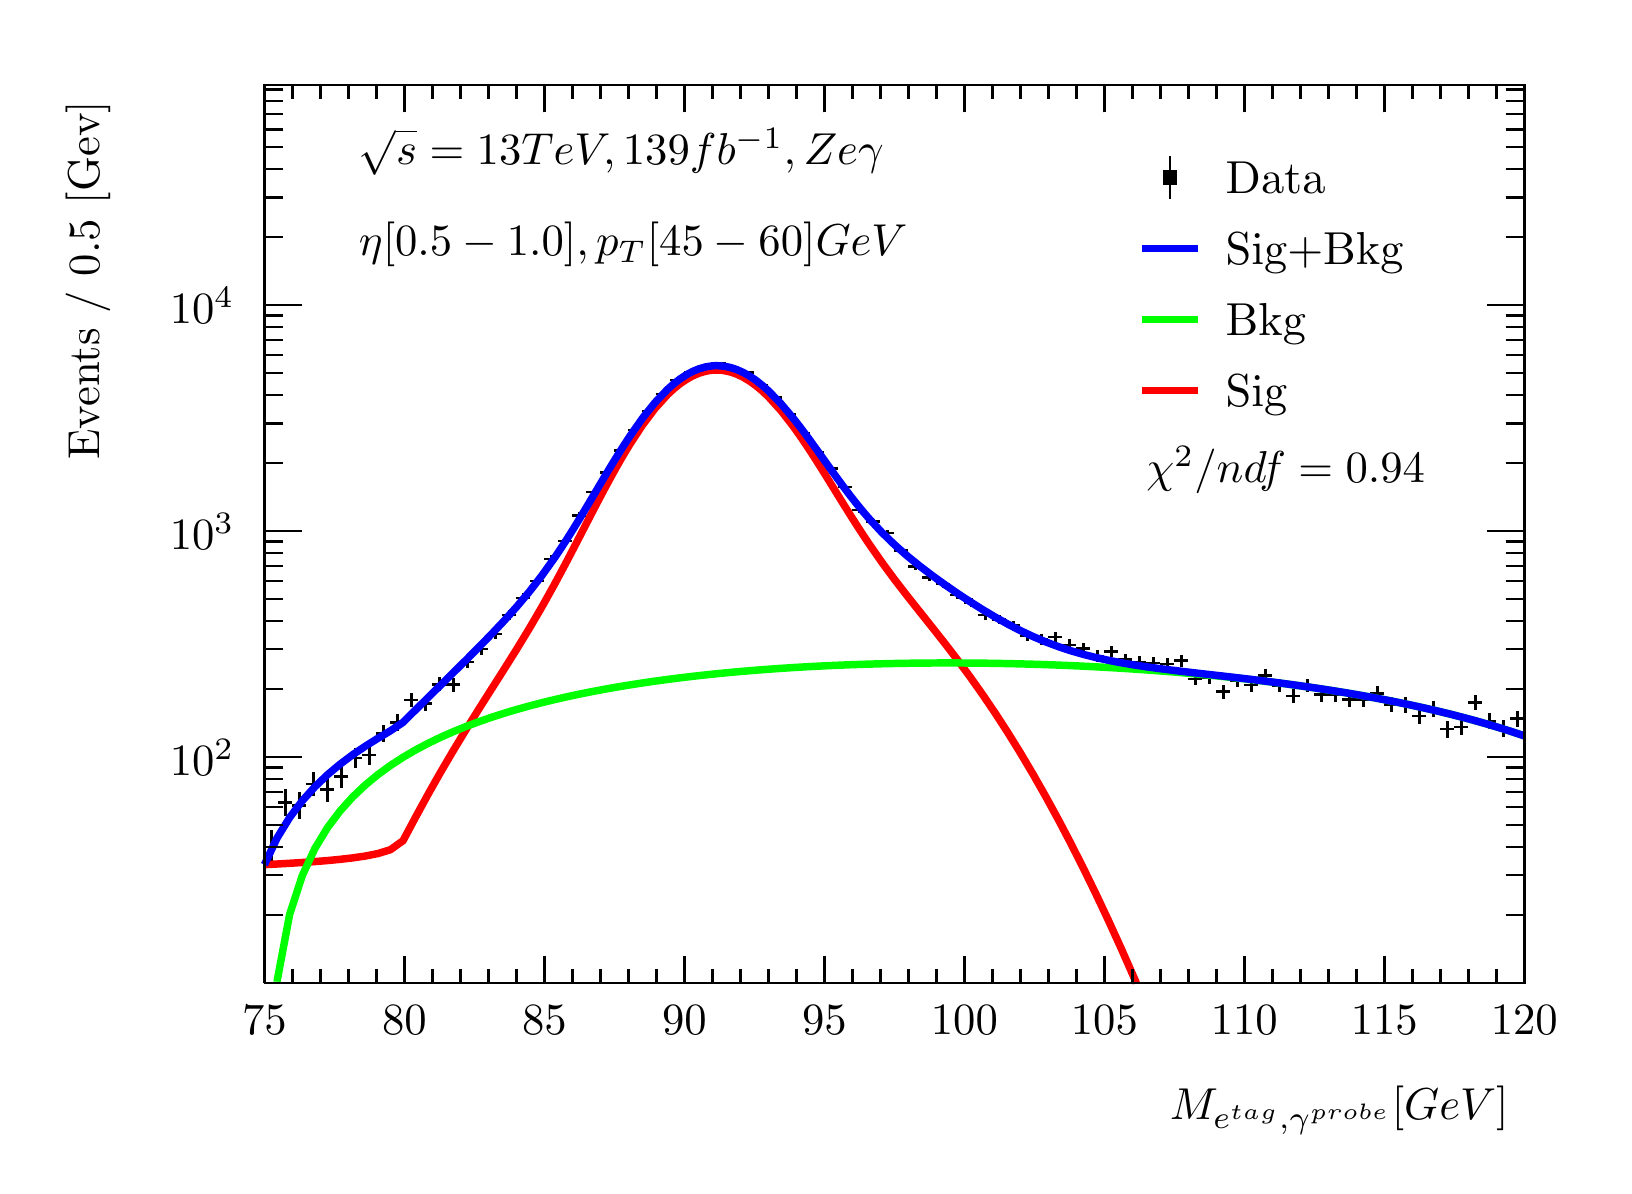
\begin{tikzpicture}
\pgfdeclareplotmark{cross} {
\pgfpathmoveto{\pgfpoint{-0.3\pgfplotmarksize}{\pgfplotmarksize}}
\pgfpathlineto{\pgfpoint{+0.3\pgfplotmarksize}{\pgfplotmarksize}}
\pgfpathlineto{\pgfpoint{+0.3\pgfplotmarksize}{0.3\pgfplotmarksize}}
\pgfpathlineto{\pgfpoint{+1\pgfplotmarksize}{0.3\pgfplotmarksize}}
\pgfpathlineto{\pgfpoint{+1\pgfplotmarksize}{-0.3\pgfplotmarksize}}
\pgfpathlineto{\pgfpoint{+0.3\pgfplotmarksize}{-0.3\pgfplotmarksize}}
\pgfpathlineto{\pgfpoint{+0.3\pgfplotmarksize}{-1.\pgfplotmarksize}}
\pgfpathlineto{\pgfpoint{-0.3\pgfplotmarksize}{-1.\pgfplotmarksize}}
\pgfpathlineto{\pgfpoint{-0.3\pgfplotmarksize}{-0.3\pgfplotmarksize}}
\pgfpathlineto{\pgfpoint{-1.\pgfplotmarksize}{-0.3\pgfplotmarksize}}
\pgfpathlineto{\pgfpoint{-1.\pgfplotmarksize}{0.3\pgfplotmarksize}}
\pgfpathlineto{\pgfpoint{-0.3\pgfplotmarksize}{0.3\pgfplotmarksize}}
\pgfpathclose
\pgfusepathqstroke
}
\pgfdeclareplotmark{cross*} {
\pgfpathmoveto{\pgfpoint{-0.3\pgfplotmarksize}{\pgfplotmarksize}}
\pgfpathlineto{\pgfpoint{+0.3\pgfplotmarksize}{\pgfplotmarksize}}
\pgfpathlineto{\pgfpoint{+0.3\pgfplotmarksize}{0.3\pgfplotmarksize}}
\pgfpathlineto{\pgfpoint{+1\pgfplotmarksize}{0.3\pgfplotmarksize}}
\pgfpathlineto{\pgfpoint{+1\pgfplotmarksize}{-0.3\pgfplotmarksize}}
\pgfpathlineto{\pgfpoint{+0.3\pgfplotmarksize}{-0.3\pgfplotmarksize}}
\pgfpathlineto{\pgfpoint{+0.3\pgfplotmarksize}{-1.\pgfplotmarksize}}
\pgfpathlineto{\pgfpoint{-0.3\pgfplotmarksize}{-1.\pgfplotmarksize}}
\pgfpathlineto{\pgfpoint{-0.3\pgfplotmarksize}{-0.3\pgfplotmarksize}}
\pgfpathlineto{\pgfpoint{-1.\pgfplotmarksize}{-0.3\pgfplotmarksize}}
\pgfpathlineto{\pgfpoint{-1.\pgfplotmarksize}{0.3\pgfplotmarksize}}
\pgfpathlineto{\pgfpoint{-0.3\pgfplotmarksize}{0.3\pgfplotmarksize}}
\pgfpathclose
\pgfusepathqfillstroke
}
\pgfdeclareplotmark{newstar} {
\pgfpathmoveto{\pgfqpoint{0pt}{\pgfplotmarksize}}
\pgfpathlineto{\pgfqpointpolar{44}{0.5\pgfplotmarksize}}
\pgfpathlineto{\pgfqpointpolar{18}{\pgfplotmarksize}}
\pgfpathlineto{\pgfqpointpolar{-20}{0.5\pgfplotmarksize}}
\pgfpathlineto{\pgfqpointpolar{-54}{\pgfplotmarksize}}
\pgfpathlineto{\pgfqpointpolar{-90}{0.5\pgfplotmarksize}}
\pgfpathlineto{\pgfqpointpolar{234}{\pgfplotmarksize}}
\pgfpathlineto{\pgfqpointpolar{198}{0.5\pgfplotmarksize}}
\pgfpathlineto{\pgfqpointpolar{162}{\pgfplotmarksize}}
\pgfpathlineto{\pgfqpointpolar{134}{0.5\pgfplotmarksize}}
\pgfpathclose
\pgfusepathqstroke
}
\pgfdeclareplotmark{newstar*} {
\pgfpathmoveto{\pgfqpoint{0pt}{\pgfplotmarksize}}
\pgfpathlineto{\pgfqpointpolar{44}{0.5\pgfplotmarksize}}
\pgfpathlineto{\pgfqpointpolar{18}{\pgfplotmarksize}}
\pgfpathlineto{\pgfqpointpolar{-20}{0.5\pgfplotmarksize}}
\pgfpathlineto{\pgfqpointpolar{-54}{\pgfplotmarksize}}
\pgfpathlineto{\pgfqpointpolar{-90}{0.5\pgfplotmarksize}}
\pgfpathlineto{\pgfqpointpolar{234}{\pgfplotmarksize}}
\pgfpathlineto{\pgfqpointpolar{198}{0.5\pgfplotmarksize}}
\pgfpathlineto{\pgfqpointpolar{162}{\pgfplotmarksize}}
\pgfpathlineto{\pgfqpointpolar{134}{0.5\pgfplotmarksize}}
\pgfpathclose
\pgfusepathqfillstroke
}
\definecolor{c}{rgb}{1,1,1};
\draw [color=c, fill=c] (0,0) rectangle (20,14.4361);
\draw [color=c, fill=c] (3,2.30977) rectangle (19,13.7143);
\definecolor{c}{rgb}{0,0,0};
\draw [c,line width=0.9] (3,2.30977) -- (3,13.7143) -- (19,13.7143) -- (19,2.30977) -- (3,2.30977);
\definecolor{c}{rgb}{1,1,1};
\draw [color=c, fill=c] (3,2.30977) rectangle (19,13.7143);
\definecolor{c}{rgb}{0,0,0};
\draw [c,line width=0.9] (3,2.30977) -- (3,13.7143) -- (19,13.7143) -- (19,2.30977) -- (3,2.30977);
\draw [c,line width=0.9] (3,2.30977) -- (19,2.30977);
\draw [c,line width=0.9] (3,2.65624) -- (3,2.30977);
\draw [c,line width=0.9] (3.35556,2.48301) -- (3.35556,2.30977);
\draw [c,line width=0.9] (3.71111,2.48301) -- (3.71111,2.30977);
\draw [c,line width=0.9] (4.06667,2.48301) -- (4.06667,2.30977);
\draw [c,line width=0.9] (4.42222,2.48301) -- (4.42222,2.30977);
\draw [c,line width=0.9] (4.77778,2.65624) -- (4.77778,2.30977);
\draw [c,line width=0.9] (5.13333,2.48301) -- (5.13333,2.30977);
\draw [c,line width=0.9] (5.48889,2.48301) -- (5.48889,2.30977);
\draw [c,line width=0.9] (5.84444,2.48301) -- (5.84444,2.30977);
\draw [c,line width=0.9] (6.2,2.48301) -- (6.2,2.30977);
\draw [c,line width=0.9] (6.55556,2.65624) -- (6.55556,2.30977);
\draw [c,line width=0.9] (6.91111,2.48301) -- (6.91111,2.30977);
\draw [c,line width=0.9] (7.26667,2.48301) -- (7.26667,2.30977);
\draw [c,line width=0.9] (7.62222,2.48301) -- (7.62222,2.30977);
\draw [c,line width=0.9] (7.97778,2.48301) -- (7.97778,2.30977);
\draw [c,line width=0.9] (8.33333,2.65624) -- (8.33333,2.30977);
\draw [c,line width=0.9] (8.68889,2.48301) -- (8.68889,2.30977);
\draw [c,line width=0.9] (9.04444,2.48301) -- (9.04444,2.30977);
\draw [c,line width=0.9] (9.4,2.48301) -- (9.4,2.30977);
\draw [c,line width=0.9] (9.75556,2.48301) -- (9.75556,2.30977);
\draw [c,line width=0.9] (10.1111,2.65624) -- (10.1111,2.30977);
\draw [c,line width=0.9] (10.4667,2.48301) -- (10.4667,2.30977);
\draw [c,line width=0.9] (10.8222,2.48301) -- (10.8222,2.30977);
\draw [c,line width=0.9] (11.1778,2.48301) -- (11.1778,2.30977);
\draw [c,line width=0.9] (11.5333,2.48301) -- (11.5333,2.30977);
\draw [c,line width=0.9] (11.8889,2.65624) -- (11.8889,2.30977);
\draw [c,line width=0.9] (12.2444,2.48301) -- (12.2444,2.30977);
\draw [c,line width=0.9] (12.6,2.48301) -- (12.6,2.30977);
\draw [c,line width=0.9] (12.9556,2.48301) -- (12.9556,2.30977);
\draw [c,line width=0.9] (13.3111,2.48301) -- (13.3111,2.30977);
\draw [c,line width=0.9] (13.6667,2.65624) -- (13.6667,2.30977);
\draw [c,line width=0.9] (14.0222,2.48301) -- (14.0222,2.30977);
\draw [c,line width=0.9] (14.3778,2.48301) -- (14.3778,2.30977);
\draw [c,line width=0.9] (14.7333,2.48301) -- (14.7333,2.30977);
\draw [c,line width=0.9] (15.0889,2.48301) -- (15.0889,2.30977);
\draw [c,line width=0.9] (15.4444,2.65624) -- (15.4444,2.30977);
\draw [c,line width=0.9] (15.8,2.48301) -- (15.8,2.30977);
\draw [c,line width=0.9] (16.1556,2.48301) -- (16.1556,2.30977);
\draw [c,line width=0.9] (16.5111,2.48301) -- (16.5111,2.30977);
\draw [c,line width=0.9] (16.8667,2.48301) -- (16.8667,2.30977);
\draw [c,line width=0.9] (17.2222,2.65624) -- (17.2222,2.30977);
\draw [c,line width=0.9] (17.5778,2.48301) -- (17.5778,2.30977);
\draw [c,line width=0.9] (17.9333,2.48301) -- (17.9333,2.30977);
\draw [c,line width=0.9] (18.2889,2.48301) -- (18.2889,2.30977);
\draw [c,line width=0.9] (18.6444,2.48301) -- (18.6444,2.30977);
\draw [c,line width=0.9] (19,2.65624) -- (19,2.30977);
\draw [c,line width=0.9] (19,2.65624) -- (19,2.30977);
\draw [anchor=base] (3,1.66015) node[scale=1.61424, color=c, rotate=0]{75};
\draw [anchor=base] (4.77778,1.66015) node[scale=1.61424, color=c, rotate=0]{80};
\draw [anchor=base] (6.55556,1.66015) node[scale=1.61424, color=c, rotate=0]{85};
\draw [anchor=base] (8.33333,1.66015) node[scale=1.61424, color=c, rotate=0]{90};
\draw [anchor=base] (10.1111,1.66015) node[scale=1.61424, color=c, rotate=0]{95};
\draw [anchor=base] (11.8889,1.66015) node[scale=1.61424, color=c, rotate=0]{100};
\draw [anchor=base] (13.6667,1.66015) node[scale=1.61424, color=c, rotate=0]{105};
\draw [anchor=base] (15.4444,1.66015) node[scale=1.61424, color=c, rotate=0]{110};
\draw [anchor=base] (17.2222,1.66015) node[scale=1.61424, color=c, rotate=0]{115};
\draw [anchor=base] (19,1.66015) node[scale=1.61424, color=c, rotate=0]{120};
\draw [anchor= east] (19,0.692932) node[scale=1.61424, color=c, rotate=0]{$M_{e^{tag}, \gamma^{probe}}  [GeV]$};
\draw [c,line width=0.9] (3,13.7143) -- (19,13.7143);
\draw [c,line width=0.9] (3,13.3678) -- (3,13.7143);
\draw [c,line width=0.9] (3.35556,13.5411) -- (3.35556,13.7143);
\draw [c,line width=0.9] (3.71111,13.5411) -- (3.71111,13.7143);
\draw [c,line width=0.9] (4.06667,13.5411) -- (4.06667,13.7143);
\draw [c,line width=0.9] (4.42222,13.5411) -- (4.42222,13.7143);
\draw [c,line width=0.9] (4.77778,13.3678) -- (4.77778,13.7143);
\draw [c,line width=0.9] (5.13333,13.5411) -- (5.13333,13.7143);
\draw [c,line width=0.9] (5.48889,13.5411) -- (5.48889,13.7143);
\draw [c,line width=0.9] (5.84444,13.5411) -- (5.84444,13.7143);
\draw [c,line width=0.9] (6.2,13.5411) -- (6.2,13.7143);
\draw [c,line width=0.9] (6.55556,13.3678) -- (6.55556,13.7143);
\draw [c,line width=0.9] (6.91111,13.5411) -- (6.91111,13.7143);
\draw [c,line width=0.9] (7.26667,13.5411) -- (7.26667,13.7143);
\draw [c,line width=0.9] (7.62222,13.5411) -- (7.62222,13.7143);
\draw [c,line width=0.9] (7.97778,13.5411) -- (7.97778,13.7143);
\draw [c,line width=0.9] (8.33333,13.3678) -- (8.33333,13.7143);
\draw [c,line width=0.9] (8.68889,13.5411) -- (8.68889,13.7143);
\draw [c,line width=0.9] (9.04444,13.5411) -- (9.04444,13.7143);
\draw [c,line width=0.9] (9.4,13.5411) -- (9.4,13.7143);
\draw [c,line width=0.9] (9.75556,13.5411) -- (9.75556,13.7143);
\draw [c,line width=0.9] (10.1111,13.3678) -- (10.1111,13.7143);
\draw [c,line width=0.9] (10.4667,13.5411) -- (10.4667,13.7143);
\draw [c,line width=0.9] (10.8222,13.5411) -- (10.8222,13.7143);
\draw [c,line width=0.9] (11.1778,13.5411) -- (11.1778,13.7143);
\draw [c,line width=0.9] (11.5333,13.5411) -- (11.5333,13.7143);
\draw [c,line width=0.9] (11.8889,13.3678) -- (11.8889,13.7143);
\draw [c,line width=0.9] (12.2444,13.5411) -- (12.2444,13.7143);
\draw [c,line width=0.9] (12.6,13.5411) -- (12.6,13.7143);
\draw [c,line width=0.9] (12.9556,13.5411) -- (12.9556,13.7143);
\draw [c,line width=0.9] (13.3111,13.5411) -- (13.3111,13.7143);
\draw [c,line width=0.9] (13.6667,13.3678) -- (13.6667,13.7143);
\draw [c,line width=0.9] (14.0222,13.5411) -- (14.0222,13.7143);
\draw [c,line width=0.9] (14.3778,13.5411) -- (14.3778,13.7143);
\draw [c,line width=0.9] (14.7333,13.5411) -- (14.7333,13.7143);
\draw [c,line width=0.9] (15.0889,13.5411) -- (15.0889,13.7143);
\draw [c,line width=0.9] (15.4444,13.3678) -- (15.4444,13.7143);
\draw [c,line width=0.9] (15.8,13.5411) -- (15.8,13.7143);
\draw [c,line width=0.9] (16.1556,13.5411) -- (16.1556,13.7143);
\draw [c,line width=0.9] (16.5111,13.5411) -- (16.5111,13.7143);
\draw [c,line width=0.9] (16.8667,13.5411) -- (16.8667,13.7143);
\draw [c,line width=0.9] (17.2222,13.3678) -- (17.2222,13.7143);
\draw [c,line width=0.9] (17.5778,13.5411) -- (17.5778,13.7143);
\draw [c,line width=0.9] (17.9333,13.5411) -- (17.9333,13.7143);
\draw [c,line width=0.9] (18.2889,13.5411) -- (18.2889,13.7143);
\draw [c,line width=0.9] (18.6444,13.5411) -- (18.6444,13.7143);
\draw [c,line width=0.9] (19,13.3678) -- (19,13.7143);
\draw [c,line width=0.9] (19,13.3678) -- (19,13.7143);
\draw [c,line width=0.9] (3,2.30977) -- (3,13.7143);
\draw [c,line width=0.9] (3.237,3.17371) -- (3,3.17371);
\draw [c,line width=0.9] (3.237,3.67908) -- (3,3.67908);
\draw [c,line width=0.9] (3.237,4.03764) -- (3,4.03764);
\draw [c,line width=0.9] (3.237,4.31577) -- (3,4.31577);
\draw [c,line width=0.9] (3.237,4.54301) -- (3,4.54301);
\draw [c,line width=0.9] (3.237,4.73514) -- (3,4.73514);
\draw [c,line width=0.9] (3.237,4.90158) -- (3,4.90158);
\draw [c,line width=0.9] (3.237,5.04838) -- (3,5.04838);
\draw [c,line width=0.9] (3.474,5.1797) -- (3,5.1797);
\draw [anchor= east] (2.82,5.1797) node[scale=1.61424, color=c, rotate=0]{$10^{2}$};
\draw [c,line width=0.9] (3.237,6.04363) -- (3,6.04363);
\draw [c,line width=0.9] (3.237,6.549) -- (3,6.549);
\draw [c,line width=0.9] (3.237,6.90757) -- (3,6.90757);
\draw [c,line width=0.9] (3.237,7.18569) -- (3,7.18569);
\draw [c,line width=0.9] (3.237,7.41294) -- (3,7.41294);
\draw [c,line width=0.9] (3.237,7.60507) -- (3,7.60507);
\draw [c,line width=0.9] (3.237,7.7715) -- (3,7.7715);
\draw [c,line width=0.9] (3.237,7.91831) -- (3,7.91831);
\draw [c,line width=0.9] (3.474,8.04963) -- (3,8.04963);
\draw [anchor= east] (2.82,8.04963) node[scale=1.61424, color=c, rotate=0]{$10^{3}$};
\draw [c,line width=0.9] (3.237,8.91356) -- (3,8.91356);
\draw [c,line width=0.9] (3.237,9.41893) -- (3,9.41893);
\draw [c,line width=0.9] (3.237,9.7775) -- (3,9.7775);
\draw [c,line width=0.9] (3.237,10.0556) -- (3,10.0556);
\draw [c,line width=0.9] (3.237,10.2829) -- (3,10.2829);
\draw [c,line width=0.9] (3.237,10.475) -- (3,10.475);
\draw [c,line width=0.9] (3.237,10.6414) -- (3,10.6414);
\draw [c,line width=0.9] (3.237,10.7882) -- (3,10.7882);
\draw [c,line width=0.9] (3.474,10.9196) -- (3,10.9196);
\draw [anchor= east] (2.82,10.9196) node[scale=1.61424, color=c, rotate=0]{$10^{4}$};
\draw [c,line width=0.9] (3.237,11.7835) -- (3,11.7835);
\draw [c,line width=0.9] (3.237,12.2889) -- (3,12.2889);
\draw [c,line width=0.9] (3.237,12.6474) -- (3,12.6474);
\draw [c,line width=0.9] (3.237,12.9256) -- (3,12.9256);
\draw [c,line width=0.9] (3.237,13.1528) -- (3,13.1528);
\draw [c,line width=0.9] (3.237,13.3449) -- (3,13.3449);
\draw [c,line width=0.9] (3.237,13.5114) -- (3,13.5114);
\draw [c,line width=0.9] (3.237,13.6582) -- (3,13.6582);
\draw [anchor= east] (0.76,13.7143) node[scale=1.61424, color=c, rotate=90]{Events / 0.5 [Gev]};
\draw [c,line width=0.9] (19,2.30977) -- (19,13.7143);
\draw [c,line width=0.9] (18.763,3.17371) -- (19,3.17371);
\draw [c,line width=0.9] (18.763,3.67908) -- (19,3.67908);
\draw [c,line width=0.9] (18.763,4.03764) -- (19,4.03764);
\draw [c,line width=0.9] (18.763,4.31577) -- (19,4.31577);
\draw [c,line width=0.9] (18.763,4.54301) -- (19,4.54301);
\draw [c,line width=0.9] (18.763,4.73514) -- (19,4.73514);
\draw [c,line width=0.9] (18.763,4.90158) -- (19,4.90158);
\draw [c,line width=0.9] (18.763,5.04838) -- (19,5.04838);
\draw [c,line width=0.9] (18.526,5.1797) -- (19,5.1797);
\draw [c,line width=0.9] (18.763,6.04363) -- (19,6.04363);
\draw [c,line width=0.9] (18.763,6.549) -- (19,6.549);
\draw [c,line width=0.9] (18.763,6.90757) -- (19,6.90757);
\draw [c,line width=0.9] (18.763,7.18569) -- (19,7.18569);
\draw [c,line width=0.9] (18.763,7.41294) -- (19,7.41294);
\draw [c,line width=0.9] (18.763,7.60507) -- (19,7.60507);
\draw [c,line width=0.9] (18.763,7.7715) -- (19,7.7715);
\draw [c,line width=0.9] (18.763,7.91831) -- (19,7.91831);
\draw [c,line width=0.9] (18.526,8.04963) -- (19,8.04963);
\draw [c,line width=0.9] (18.763,8.91356) -- (19,8.91356);
\draw [c,line width=0.9] (18.763,9.41893) -- (19,9.41893);
\draw [c,line width=0.9] (18.763,9.7775) -- (19,9.7775);
\draw [c,line width=0.9] (18.763,10.0556) -- (19,10.0556);
\draw [c,line width=0.9] (18.763,10.2829) -- (19,10.2829);
\draw [c,line width=0.9] (18.763,10.475) -- (19,10.475);
\draw [c,line width=0.9] (18.763,10.6414) -- (19,10.6414);
\draw [c,line width=0.9] (18.763,10.7882) -- (19,10.7882);
\draw [c,line width=0.9] (18.526,10.9196) -- (19,10.9196);
\draw [c,line width=0.9] (18.763,11.7835) -- (19,11.7835);
\draw [c,line width=0.9] (18.763,12.2889) -- (19,12.2889);
\draw [c,line width=0.9] (18.763,12.6474) -- (19,12.6474);
\draw [c,line width=0.9] (18.763,12.9256) -- (19,12.9256);
\draw [c,line width=0.9] (18.763,13.1528) -- (19,13.1528);
\draw [c,line width=0.9] (18.763,13.3449) -- (19,13.3449);
\draw [c,line width=0.9] (18.763,13.5114) -- (19,13.5114);
\draw [c,line width=0.9] (18.763,13.6582) -- (19,13.6582);
\draw [c,line width=0.9] (3.08889,4.03764) -- (3,4.03764);
\draw [c,line width=0.9] (3,4.03764) -- (3,4.03764);
\draw [c,line width=0.9] (3.08889,4.03764) -- (3.17778,4.03764);
\draw [c,line width=0.9] (3.17778,4.03764) -- (3.17778,4.03764);
\draw [c,line width=0.9] (3.08889,4.03764) -- (3.08889,4.24861);
\draw [c,line width=0.9] (3.08889,4.24861) -- (3.08889,4.24861);
\draw [c,line width=0.9] (3.08889,4.03764) -- (3.08889,3.82411);
\draw [c,line width=0.9] (3.08889,3.82411) -- (3.08889,3.82411);
\draw [c,line width=0.9] (3.26667,4.60382) -- (3.17778,4.60382);
\draw [c,line width=0.9] (3.17778,4.60382) -- (3.17778,4.60382);
\draw [c,line width=0.9] (3.26667,4.60382) -- (3.35556,4.60382);
\draw [c,line width=0.9] (3.35556,4.60382) -- (3.35556,4.60382);
\draw [c,line width=0.9] (3.26667,4.60382) -- (3.26667,4.7699);
\draw [c,line width=0.9] (3.26667,4.7699) -- (3.26667,4.7699);
\draw [c,line width=0.9] (3.26667,4.60382) -- (3.26667,4.43646);
\draw [c,line width=0.9] (3.26667,4.43646) -- (3.26667,4.43646);
\draw [c,line width=0.9] (3.44444,4.56361) -- (3.35556,4.56361);
\draw [c,line width=0.9] (3.35556,4.56361) -- (3.35556,4.56361);
\draw [c,line width=0.9] (3.44444,4.56361) -- (3.53333,4.56361);
\draw [c,line width=0.9] (3.53333,4.56361) -- (3.53333,4.56361);
\draw [c,line width=0.9] (3.44444,4.56361) -- (3.44444,4.73252);
\draw [c,line width=0.9] (3.44444,4.73252) -- (3.44444,4.73252);
\draw [c,line width=0.9] (3.44444,4.56361) -- (3.44444,4.39335);
\draw [c,line width=0.9] (3.44444,4.39335) -- (3.44444,4.39335);
\draw [c,line width=0.9] (3.62222,4.83765) -- (3.53333,4.83765);
\draw [c,line width=0.9] (3.53333,4.83765) -- (3.53333,4.83765);
\draw [c,line width=0.9] (3.62222,4.83765) -- (3.71111,4.83765);
\draw [c,line width=0.9] (3.71111,4.83765) -- (3.71111,4.83765);
\draw [c,line width=0.9] (3.62222,4.83765) -- (3.62222,4.98818);
\draw [c,line width=0.9] (3.62222,4.98818) -- (3.62222,4.98818);
\draw [c,line width=0.9] (3.62222,4.83765) -- (3.62222,4.68614);
\draw [c,line width=0.9] (3.62222,4.68614) -- (3.62222,4.68614);
\draw [c,line width=0.9] (3.8,4.77026) -- (3.71111,4.77026);
\draw [c,line width=0.9] (3.71111,4.77026) -- (3.71111,4.77026);
\draw [c,line width=0.9] (3.8,4.77026) -- (3.88889,4.77026);
\draw [c,line width=0.9] (3.88889,4.77026) -- (3.88889,4.77026);
\draw [c,line width=0.9] (3.8,4.77026) -- (3.8,4.92511);
\draw [c,line width=0.9] (3.8,4.92511) -- (3.8,4.92511);
\draw [c,line width=0.9] (3.8,4.77026) -- (3.8,4.61435);
\draw [c,line width=0.9] (3.8,4.61435) -- (3.8,4.61435);
\draw [c,line width=0.9] (3.97778,4.93235) -- (3.88889,4.93235);
\draw [c,line width=0.9] (3.88889,4.93235) -- (3.88889,4.93235);
\draw [c,line width=0.9] (3.97778,4.93235) -- (4.06667,4.93235);
\draw [c,line width=0.9] (4.06667,4.93235) -- (4.06667,4.93235);
\draw [c,line width=0.9] (3.97778,4.93235) -- (3.97778,5.07702);
\draw [c,line width=0.9] (3.97778,5.07702) -- (3.97778,5.07702);
\draw [c,line width=0.9] (3.97778,4.93235) -- (3.97778,4.78682);
\draw [c,line width=0.9] (3.97778,4.78682) -- (3.97778,4.78682);
\draw [c,line width=0.9] (4.15556,5.16718) -- (4.06667,5.16718);
\draw [c,line width=0.9] (4.06667,5.16718) -- (4.06667,5.16718);
\draw [c,line width=0.9] (4.15556,5.16718) -- (4.24444,5.16718);
\draw [c,line width=0.9] (4.24444,5.16718) -- (4.24444,5.16718);
\draw [c,line width=0.9] (4.15556,5.16718) -- (4.15556,5.29831);
\draw [c,line width=0.9] (4.15556,5.29831) -- (4.15556,5.29831);
\draw [c,line width=0.9] (4.15556,5.16718) -- (4.15556,5.03539);
\draw [c,line width=0.9] (4.15556,5.03539) -- (4.15556,5.03539);
\draw [c,line width=0.9] (4.33333,5.20438) -- (4.24444,5.20438);
\draw [c,line width=0.9] (4.24444,5.20438) -- (4.24444,5.20438);
\draw [c,line width=0.9] (4.33333,5.20438) -- (4.42222,5.20438);
\draw [c,line width=0.9] (4.42222,5.20438) -- (4.42222,5.20438);
\draw [c,line width=0.9] (4.33333,5.20438) -- (4.33333,5.32774);
\draw [c,line width=0.9] (4.33333,5.32774) -- (4.33333,5.32774);
\draw [c,line width=0.9] (4.33333,5.20438) -- (4.33333,5.08102);
\draw [c,line width=0.9] (4.33333,5.08102) -- (4.33333,5.08102);
\draw [c,line width=0.9] (4.51111,5.47761) -- (4.42222,5.47761);
\draw [c,line width=0.9] (4.42222,5.47761) -- (4.42222,5.47761);
\draw [c,line width=0.9] (4.51111,5.47761) -- (4.6,5.47761);
\draw [c,line width=0.9] (4.6,5.47761) -- (4.6,5.47761);
\draw [c,line width=0.9] (4.51111,5.47761) -- (4.51111,5.58817);
\draw [c,line width=0.9] (4.51111,5.58817) -- (4.51111,5.58817);
\draw [c,line width=0.9] (4.51111,5.47761) -- (4.51111,5.36705);
\draw [c,line width=0.9] (4.51111,5.36705) -- (4.51111,5.36705);
\draw [c,line width=0.9] (4.68889,5.61676) -- (4.6,5.61676);
\draw [c,line width=0.9] (4.6,5.61676) -- (4.6,5.61676);
\draw [c,line width=0.9] (4.68889,5.61676) -- (4.77778,5.61676);
\draw [c,line width=0.9] (4.77778,5.61676) -- (4.77778,5.61676);
\draw [c,line width=0.9] (4.68889,5.61676) -- (4.68889,5.72132);
\draw [c,line width=0.9] (4.68889,5.72132) -- (4.68889,5.72132);
\draw [c,line width=0.9] (4.68889,5.61676) -- (4.68889,5.51219);
\draw [c,line width=0.9] (4.68889,5.51219) -- (4.68889,5.51219);
\draw [c,line width=0.9] (4.86667,5.90537) -- (4.77778,5.90537);
\draw [c,line width=0.9] (4.77778,5.90537) -- (4.77778,5.90537);
\draw [c,line width=0.9] (4.86667,5.90537) -- (4.95556,5.90537);
\draw [c,line width=0.9] (4.95556,5.90537) -- (4.95556,5.90537);
\draw [c,line width=0.9] (4.86667,5.90537) -- (4.86667,5.99851);
\draw [c,line width=0.9] (4.86667,5.99851) -- (4.86667,5.99851);
\draw [c,line width=0.9] (4.86667,5.90537) -- (4.86667,5.81223);
\draw [c,line width=0.9] (4.86667,5.81223) -- (4.86667,5.81223);
\draw [c,line width=0.9] (5.04444,5.86288) -- (4.95556,5.86288);
\draw [c,line width=0.9] (4.95556,5.86288) -- (4.95556,5.86288);
\draw [c,line width=0.9] (5.04444,5.86288) -- (5.13333,5.86288);
\draw [c,line width=0.9] (5.13333,5.86288) -- (5.13333,5.86288);
\draw [c,line width=0.9] (5.04444,5.86288) -- (5.04444,5.95762);
\draw [c,line width=0.9] (5.04444,5.95762) -- (5.04444,5.95762);
\draw [c,line width=0.9] (5.04444,5.86288) -- (5.04444,5.76814);
\draw [c,line width=0.9] (5.04444,5.76814) -- (5.04444,5.76814);
\draw [c,line width=0.9] (5.22222,6.10445) -- (5.13333,6.10445);
\draw [c,line width=0.9] (5.13333,6.10445) -- (5.13333,6.10445);
\draw [c,line width=0.9] (5.22222,6.10445) -- (5.31111,6.10445);
\draw [c,line width=0.9] (5.31111,6.10445) -- (5.31111,6.10445);
\draw [c,line width=0.9] (5.22222,6.10445) -- (5.22222,6.19044);
\draw [c,line width=0.9] (5.22222,6.19044) -- (5.22222,6.19044);
\draw [c,line width=0.9] (5.22222,6.10445) -- (5.22222,6.01846);
\draw [c,line width=0.9] (5.22222,6.01846) -- (5.22222,6.01846);
\draw [c,line width=0.9] (5.4,6.0985) -- (5.31111,6.0985);
\draw [c,line width=0.9] (5.31111,6.0985) -- (5.31111,6.0985);
\draw [c,line width=0.9] (5.4,6.0985) -- (5.48889,6.0985);
\draw [c,line width=0.9] (5.48889,6.0985) -- (5.48889,6.0985);
\draw [c,line width=0.9] (5.4,6.0985) -- (5.4,6.1847);
\draw [c,line width=0.9] (5.4,6.1847) -- (5.4,6.1847);
\draw [c,line width=0.9] (5.4,6.0985) -- (5.4,6.0123);
\draw [c,line width=0.9] (5.4,6.0123) -- (5.4,6.0123);
\draw [c,line width=0.9] (5.57778,6.38968) -- (5.48889,6.38968);
\draw [c,line width=0.9] (5.48889,6.38968) -- (5.48889,6.38968);
\draw [c,line width=0.9] (5.57778,6.38968) -- (5.66667,6.38968);
\draw [c,line width=0.9] (5.66667,6.38968) -- (5.66667,6.38968);
\draw [c,line width=0.9] (5.57778,6.38968) -- (5.57778,6.46637);
\draw [c,line width=0.9] (5.57778,6.46637) -- (5.57778,6.46637);
\draw [c,line width=0.9] (5.57778,6.38968) -- (5.57778,6.31298);
\draw [c,line width=0.9] (5.57778,6.31298) -- (5.57778,6.31298);
\draw [c,line width=0.9] (5.75556,6.55315) -- (5.66667,6.55315);
\draw [c,line width=0.9] (5.66667,6.55315) -- (5.66667,6.55315);
\draw [c,line width=0.9] (5.75556,6.55315) -- (5.84444,6.55315);
\draw [c,line width=0.9] (5.84444,6.55315) -- (5.84444,6.55315);
\draw [c,line width=0.9] (5.75556,6.55315) -- (5.75556,6.62498);
\draw [c,line width=0.9] (5.75556,6.62498) -- (5.75556,6.62498);
\draw [c,line width=0.9] (5.75556,6.55315) -- (5.75556,6.48132);
\draw [c,line width=0.9] (5.75556,6.48132) -- (5.75556,6.48132);
\draw [c,line width=0.9] (5.93333,6.74114) -- (5.84444,6.74114);
\draw [c,line width=0.9] (5.84444,6.74114) -- (5.84444,6.74114);
\draw [c,line width=0.9] (5.93333,6.74114) -- (6.02222,6.74114);
\draw [c,line width=0.9] (6.02222,6.74114) -- (6.02222,6.74114);
\draw [c,line width=0.9] (5.93333,6.74114) -- (5.93333,6.80775);
\draw [c,line width=0.9] (5.93333,6.80775) -- (5.93333,6.80775);
\draw [c,line width=0.9] (5.93333,6.74114) -- (5.93333,6.67452);
\draw [c,line width=0.9] (5.93333,6.67452) -- (5.93333,6.67452);
\draw [c,line width=0.9] (6.11111,6.98313) -- (6.02222,6.98313);
\draw [c,line width=0.9] (6.02222,6.98313) -- (6.02222,6.98313);
\draw [c,line width=0.9] (6.11111,6.98313) -- (6.2,6.98313);
\draw [c,line width=0.9] (6.2,6.98313) -- (6.2,6.98313);
\draw [c,line width=0.9] (6.11111,6.98313) -- (6.11111,7.04359);
\draw [c,line width=0.9] (6.11111,7.04359) -- (6.11111,7.04359);
\draw [c,line width=0.9] (6.11111,6.98313) -- (6.11111,6.92268);
\draw [c,line width=0.9] (6.11111,6.92268) -- (6.11111,6.92268);
\draw [c,line width=0.9] (6.28889,7.20302) -- (6.2,7.20302);
\draw [c,line width=0.9] (6.2,7.20302) -- (6.2,7.20302);
\draw [c,line width=0.9] (6.28889,7.20302) -- (6.37778,7.20302);
\draw [c,line width=0.9] (6.37778,7.20302) -- (6.37778,7.20302);
\draw [c,line width=0.9] (6.28889,7.20302) -- (6.28889,7.25837);
\draw [c,line width=0.9] (6.28889,7.25837) -- (6.28889,7.25837);
\draw [c,line width=0.9] (6.28889,7.20302) -- (6.28889,7.14767);
\draw [c,line width=0.9] (6.28889,7.14767) -- (6.28889,7.14767);
\draw [c,line width=0.9] (6.46667,7.41709) -- (6.37778,7.41709);
\draw [c,line width=0.9] (6.37778,7.41709) -- (6.37778,7.41709);
\draw [c,line width=0.9] (6.46667,7.41709) -- (6.55556,7.41709);
\draw [c,line width=0.9] (6.55556,7.41709) -- (6.55556,7.41709);
\draw [c,line width=0.9] (6.46667,7.41709) -- (6.46667,7.46788);
\draw [c,line width=0.9] (6.46667,7.46788) -- (6.46667,7.46788);
\draw [c,line width=0.9] (6.46667,7.41709) -- (6.46667,7.36629);
\draw [c,line width=0.9] (6.46667,7.36629) -- (6.46667,7.36629);
\draw [c,line width=0.9] (6.64444,7.69769) -- (6.55556,7.69769);
\draw [c,line width=0.9] (6.55556,7.69769) -- (6.55556,7.69769);
\draw [c,line width=0.9] (6.64444,7.69769) -- (6.73333,7.69769);
\draw [c,line width=0.9] (6.73333,7.69769) -- (6.73333,7.69769);
\draw [c,line width=0.9] (6.64444,7.69769) -- (6.64444,7.74308);
\draw [c,line width=0.9] (6.64444,7.74308) -- (6.64444,7.74308);
\draw [c,line width=0.9] (6.64444,7.69769) -- (6.64444,7.65231);
\draw [c,line width=0.9] (6.64444,7.65231) -- (6.64444,7.65231);
\draw [c,line width=0.9] (6.82222,7.92659) -- (6.73333,7.92659);
\draw [c,line width=0.9] (6.73333,7.92659) -- (6.73333,7.92659);
\draw [c,line width=0.9] (6.82222,7.92659) -- (6.91111,7.92659);
\draw [c,line width=0.9] (6.91111,7.92659) -- (6.91111,7.92659);
\draw [c,line width=0.9] (6.82222,7.92659) -- (6.82222,7.968);
\draw [c,line width=0.9] (6.82222,7.968) -- (6.82222,7.968);
\draw [c,line width=0.9] (6.82222,7.92659) -- (6.82222,7.88518);
\draw [c,line width=0.9] (6.82222,7.88518) -- (6.82222,7.88518);
\draw [c,line width=0.9] (7,8.24957) -- (6.91111,8.24957);
\draw [c,line width=0.9] (6.91111,8.24957) -- (6.91111,8.24957);
\draw [c,line width=0.9] (7,8.24957) -- (7.08889,8.24957);
\draw [c,line width=0.9] (7.08889,8.24957) -- (7.08889,8.24957);
\draw [c,line width=0.9] (7,8.24957) -- (7,8.28595);
\draw [c,line width=0.9] (7,8.28595) -- (7,8.28595);
\draw [c,line width=0.9] (7,8.24957) -- (7,8.2132);
\draw [c,line width=0.9] (7,8.2132) -- (7,8.2132);
\draw [c,line width=0.9] (7.17778,8.54331) -- (7.08889,8.54331);
\draw [c,line width=0.9] (7.08889,8.54331) -- (7.08889,8.54331);
\draw [c,line width=0.9] (7.17778,8.54331) -- (7.26667,8.54331);
\draw [c,line width=0.9] (7.26667,8.54331) -- (7.26667,8.54331);
\draw [c,line width=0.9] (7.17778,8.54331) -- (7.17778,8.57564);
\draw [c,line width=0.9] (7.17778,8.57564) -- (7.17778,8.57564);
\draw [c,line width=0.9] (7.17778,8.54331) -- (7.17778,8.51098);
\draw [c,line width=0.9] (7.17778,8.51098) -- (7.17778,8.51098);
\draw [c,line width=0.9] (7.35556,8.7967) -- (7.26667,8.7967);
\draw [c,line width=0.9] (7.26667,8.7967) -- (7.26667,8.7967);
\draw [c,line width=0.9] (7.35556,8.7967) -- (7.44444,8.7967);
\draw [c,line width=0.9] (7.44444,8.7967) -- (7.44444,8.7967);
\draw [c,line width=0.9] (7.35556,8.7967) -- (7.35556,8.82591);
\draw [c,line width=0.9] (7.35556,8.82591) -- (7.35556,8.82591);
\draw [c,line width=0.9] (7.35556,8.7967) -- (7.35556,8.76749);
\draw [c,line width=0.9] (7.35556,8.76749) -- (7.35556,8.76749);
\draw [c,line width=0.9] (7.53333,9.07414) -- (7.44444,9.07414);
\draw [c,line width=0.9] (7.44444,9.07414) -- (7.44444,9.07414);
\draw [c,line width=0.9] (7.53333,9.07414) -- (7.62222,9.07414);
\draw [c,line width=0.9] (7.62222,9.07414) -- (7.62222,9.07414);
\draw [c,line width=0.9] (7.53333,9.07414) -- (7.53333,9.10027);
\draw [c,line width=0.9] (7.53333,9.10027) -- (7.53333,9.10027);
\draw [c,line width=0.9] (7.53333,9.07414) -- (7.53333,9.04801);
\draw [c,line width=0.9] (7.53333,9.04801) -- (7.53333,9.04801);
\draw [c,line width=0.9] (7.71111,9.33027) -- (7.62222,9.33027);
\draw [c,line width=0.9] (7.62222,9.33027) -- (7.62222,9.33027);
\draw [c,line width=0.9] (7.71111,9.33027) -- (7.8,9.33027);
\draw [c,line width=0.9] (7.8,9.33027) -- (7.8,9.33027);
\draw [c,line width=0.9] (7.71111,9.33027) -- (7.71111,9.35385);
\draw [c,line width=0.9] (7.71111,9.35385) -- (7.71111,9.35385);
\draw [c,line width=0.9] (7.71111,9.33027) -- (7.71111,9.30669);
\draw [c,line width=0.9] (7.71111,9.30669) -- (7.71111,9.30669);
\draw [c,line width=0.9] (7.88889,9.57677) -- (7.8,9.57677);
\draw [c,line width=0.9] (7.8,9.57677) -- (7.8,9.57677);
\draw [c,line width=0.9] (7.88889,9.57677) -- (7.97778,9.57677);
\draw [c,line width=0.9] (7.97778,9.57677) -- (7.97778,9.57677);
\draw [c,line width=0.9] (7.88889,9.57677) -- (7.88889,9.59813);
\draw [c,line width=0.9] (7.88889,9.59813) -- (7.88889,9.59813);
\draw [c,line width=0.9] (7.88889,9.57677) -- (7.88889,9.55541);
\draw [c,line width=0.9] (7.88889,9.55541) -- (7.88889,9.55541);
\draw [c,line width=0.9] (8.06667,9.78897) -- (7.97778,9.78897);
\draw [c,line width=0.9] (7.97778,9.78897) -- (7.97778,9.78897);
\draw [c,line width=0.9] (8.06667,9.78897) -- (8.15556,9.78897);
\draw [c,line width=0.9] (8.15556,9.78897) -- (8.15556,9.78897);
\draw [c,line width=0.9] (8.06667,9.78897) -- (8.06667,9.80859);
\draw [c,line width=0.9] (8.06667,9.80859) -- (8.06667,9.80859);
\draw [c,line width=0.9] (8.06667,9.78897) -- (8.06667,9.76936);
\draw [c,line width=0.9] (8.06667,9.76936) -- (8.06667,9.76936);
\draw [c,line width=0.9] (8.24444,9.97132) -- (8.15556,9.97132);
\draw [c,line width=0.9] (8.15556,9.97132) -- (8.15556,9.97132);
\draw [c,line width=0.9] (8.24444,9.97132) -- (8.33333,9.97132);
\draw [c,line width=0.9] (8.33333,9.97132) -- (8.33333,9.97132);
\draw [c,line width=0.9] (8.24444,9.97132) -- (8.24444,9.98955);
\draw [c,line width=0.9] (8.24444,9.98955) -- (8.24444,9.98955);
\draw [c,line width=0.9] (8.24444,9.97132) -- (8.24444,9.95309);
\draw [c,line width=0.9] (8.24444,9.95309) -- (8.24444,9.95309);
\draw [c,line width=0.9] (8.42222,10.0702) -- (8.33333,10.0702);
\draw [c,line width=0.9] (8.33333,10.0702) -- (8.33333,10.0702);
\draw [c,line width=0.9] (8.42222,10.0702) -- (8.51111,10.0702);
\draw [c,line width=0.9] (8.51111,10.0702) -- (8.51111,10.0702);
\draw [c,line width=0.9] (8.42222,10.0702) -- (8.42222,10.0878);
\draw [c,line width=0.9] (8.42222,10.0878) -- (8.42222,10.0878);
\draw [c,line width=0.9] (8.42222,10.0702) -- (8.42222,10.0527);
\draw [c,line width=0.9] (8.42222,10.0527) -- (8.42222,10.0527);
\draw [c,line width=0.9] (8.6,10.1129) -- (8.51111,10.1129);
\draw [c,line width=0.9] (8.51111,10.1129) -- (8.51111,10.1129);
\draw [c,line width=0.9] (8.6,10.1129) -- (8.68889,10.1129);
\draw [c,line width=0.9] (8.68889,10.1129) -- (8.68889,10.1129);
\draw [c,line width=0.9] (8.6,10.1129) -- (8.6,10.1301);
\draw [c,line width=0.9] (8.6,10.1301) -- (8.6,10.1301);
\draw [c,line width=0.9] (8.6,10.1129) -- (8.6,10.0956);
\draw [c,line width=0.9] (8.6,10.0956) -- (8.6,10.0956);
\draw [c,line width=0.9] (8.77778,10.1805) -- (8.68889,10.1805);
\draw [c,line width=0.9] (8.68889,10.1805) -- (8.68889,10.1805);
\draw [c,line width=0.9] (8.77778,10.1805) -- (8.86667,10.1805);
\draw [c,line width=0.9] (8.86667,10.1805) -- (8.86667,10.1805);
\draw [c,line width=0.9] (8.77778,10.1805) -- (8.77778,10.1973);
\draw [c,line width=0.9] (8.77778,10.1973) -- (8.77778,10.1973);
\draw [c,line width=0.9] (8.77778,10.1805) -- (8.77778,10.1638);
\draw [c,line width=0.9] (8.77778,10.1638) -- (8.77778,10.1638);
\draw [c,line width=0.9] (8.95556,10.1093) -- (8.86667,10.1093);
\draw [c,line width=0.9] (8.86667,10.1093) -- (8.86667,10.1093);
\draw [c,line width=0.9] (8.95556,10.1093) -- (9.04444,10.1093);
\draw [c,line width=0.9] (9.04444,10.1093) -- (9.04444,10.1093);
\draw [c,line width=0.9] (8.95556,10.1093) -- (8.95556,10.1265);
\draw [c,line width=0.9] (8.95556,10.1265) -- (8.95556,10.1265);
\draw [c,line width=0.9] (8.95556,10.1093) -- (8.95556,10.092);
\draw [c,line width=0.9] (8.95556,10.092) -- (8.95556,10.092);
\draw [c,line width=0.9] (9.13333,10.0663) -- (9.04444,10.0663);
\draw [c,line width=0.9] (9.04444,10.0663) -- (9.04444,10.0663);
\draw [c,line width=0.9] (9.13333,10.0663) -- (9.22222,10.0663);
\draw [c,line width=0.9] (9.22222,10.0663) -- (9.22222,10.0663);
\draw [c,line width=0.9] (9.13333,10.0663) -- (9.13333,10.0838);
\draw [c,line width=0.9] (9.13333,10.0838) -- (9.13333,10.0838);
\draw [c,line width=0.9] (9.13333,10.0663) -- (9.13333,10.0487);
\draw [c,line width=0.9] (9.13333,10.0487) -- (9.13333,10.0487);
\draw [c,line width=0.9] (9.31111,9.89969) -- (9.22222,9.89969);
\draw [c,line width=0.9] (9.22222,9.89969) -- (9.22222,9.89969);
\draw [c,line width=0.9] (9.31111,9.89969) -- (9.4,9.89969);
\draw [c,line width=0.9] (9.4,9.89969) -- (9.4,9.89969);
\draw [c,line width=0.9] (9.31111,9.89969) -- (9.31111,9.91845);
\draw [c,line width=0.9] (9.31111,9.91845) -- (9.31111,9.91845);
\draw [c,line width=0.9] (9.31111,9.89969) -- (9.31111,9.88092);
\draw [c,line width=0.9] (9.31111,9.88092) -- (9.31111,9.88092);
\draw [c,line width=0.9] (9.48889,9.74626) -- (9.4,9.74626);
\draw [c,line width=0.9] (9.4,9.74626) -- (9.4,9.74626);
\draw [c,line width=0.9] (9.48889,9.74626) -- (9.57778,9.74626);
\draw [c,line width=0.9] (9.57778,9.74626) -- (9.57778,9.74626);
\draw [c,line width=0.9] (9.48889,9.74626) -- (9.48889,9.76622);
\draw [c,line width=0.9] (9.48889,9.76622) -- (9.48889,9.76622);
\draw [c,line width=0.9] (9.48889,9.74626) -- (9.48889,9.72631);
\draw [c,line width=0.9] (9.48889,9.72631) -- (9.48889,9.72631);
\draw [c,line width=0.9] (9.66667,9.52863) -- (9.57778,9.52863);
\draw [c,line width=0.9] (9.57778,9.52863) -- (9.57778,9.52863);
\draw [c,line width=0.9] (9.66667,9.52863) -- (9.75556,9.52863);
\draw [c,line width=0.9] (9.75556,9.52863) -- (9.75556,9.52863);
\draw [c,line width=0.9] (9.66667,9.52863) -- (9.66667,9.55041);
\draw [c,line width=0.9] (9.66667,9.55041) -- (9.66667,9.55041);
\draw [c,line width=0.9] (9.66667,9.52863) -- (9.66667,9.50685);
\draw [c,line width=0.9] (9.66667,9.50685) -- (9.66667,9.50685);
\draw [c,line width=0.9] (9.84444,9.28992) -- (9.75556,9.28992);
\draw [c,line width=0.9] (9.75556,9.28992) -- (9.75556,9.28992);
\draw [c,line width=0.9] (9.84444,9.28992) -- (9.93333,9.28992);
\draw [c,line width=0.9] (9.93333,9.28992) -- (9.93333,9.28992);
\draw [c,line width=0.9] (9.84444,9.28992) -- (9.84444,9.31388);
\draw [c,line width=0.9] (9.84444,9.31388) -- (9.84444,9.31388);
\draw [c,line width=0.9] (9.84444,9.28992) -- (9.84444,9.26595);
\draw [c,line width=0.9] (9.84444,9.26595) -- (9.84444,9.26595);
\draw [c,line width=0.9] (10.0222,9.047) -- (9.93333,9.047);
\draw [c,line width=0.9] (9.93333,9.047) -- (9.93333,9.047);
\draw [c,line width=0.9] (10.0222,9.047) -- (10.1111,9.047);
\draw [c,line width=0.9] (10.1111,9.047) -- (10.1111,9.047);
\draw [c,line width=0.9] (10.0222,9.047) -- (10.0222,9.07342);
\draw [c,line width=0.9] (10.0222,9.07342) -- (10.0222,9.07342);
\draw [c,line width=0.9] (10.0222,9.047) -- (10.0222,9.02059);
\draw [c,line width=0.9] (10.0222,9.02059) -- (10.0222,9.02059);
\draw [c,line width=0.9] (10.2,8.84371) -- (10.1111,8.84371);
\draw [c,line width=0.9] (10.1111,8.84371) -- (10.1111,8.84371);
\draw [c,line width=0.9] (10.2,8.84371) -- (10.2889,8.84371);
\draw [c,line width=0.9] (10.2889,8.84371) -- (10.2889,8.84371);
\draw [c,line width=0.9] (10.2,8.84371) -- (10.2,8.87238);
\draw [c,line width=0.9] (10.2,8.87238) -- (10.2,8.87238);
\draw [c,line width=0.9] (10.2,8.84371) -- (10.2,8.81505);
\draw [c,line width=0.9] (10.2,8.81505) -- (10.2,8.81505);
\draw [c,line width=0.9] (10.3778,8.60867) -- (10.2889,8.60867);
\draw [c,line width=0.9] (10.2889,8.60867) -- (10.2889,8.60867);
\draw [c,line width=0.9] (10.3778,8.60867) -- (10.4667,8.60867);
\draw [c,line width=0.9] (10.4667,8.60867) -- (10.4667,8.60867);
\draw [c,line width=0.9] (10.3778,8.60867) -- (10.3778,8.64016);
\draw [c,line width=0.9] (10.3778,8.64016) -- (10.3778,8.64016);
\draw [c,line width=0.9] (10.3778,8.60867) -- (10.3778,8.57717);
\draw [c,line width=0.9] (10.3778,8.57717) -- (10.3778,8.57717);
\draw [c,line width=0.9] (10.5556,8.31774) -- (10.4667,8.31774);
\draw [c,line width=0.9] (10.4667,8.31774) -- (10.4667,8.31774);
\draw [c,line width=0.9] (10.5556,8.31774) -- (10.6444,8.31774);
\draw [c,line width=0.9] (10.6444,8.31774) -- (10.6444,8.31774);
\draw [c,line width=0.9] (10.5556,8.31774) -- (10.5556,8.35314);
\draw [c,line width=0.9] (10.5556,8.35314) -- (10.5556,8.35314);
\draw [c,line width=0.9] (10.5556,8.31774) -- (10.5556,8.28235);
\draw [c,line width=0.9] (10.5556,8.28235) -- (10.5556,8.28235);
\draw [c,line width=0.9] (10.7333,8.16956) -- (10.6444,8.16956);
\draw [c,line width=0.9] (10.6444,8.16956) -- (10.6444,8.16956);
\draw [c,line width=0.9] (10.7333,8.16956) -- (10.8222,8.16956);
\draw [c,line width=0.9] (10.8222,8.16956) -- (10.8222,8.16956);
\draw [c,line width=0.9] (10.7333,8.16956) -- (10.7333,8.20712);
\draw [c,line width=0.9] (10.7333,8.20712) -- (10.7333,8.20712);
\draw [c,line width=0.9] (10.7333,8.16956) -- (10.7333,8.132);
\draw [c,line width=0.9] (10.7333,8.132) -- (10.7333,8.132);
\draw [c,line width=0.9] (10.9111,8.02572) -- (10.8222,8.02572);
\draw [c,line width=0.9] (10.8222,8.02572) -- (10.8222,8.02572);
\draw [c,line width=0.9] (10.9111,8.02572) -- (11,8.02572);
\draw [c,line width=0.9] (11,8.02572) -- (11,8.02572);
\draw [c,line width=0.9] (10.9111,8.02572) -- (10.9111,8.06551);
\draw [c,line width=0.9] (10.9111,8.06551) -- (10.9111,8.06551);
\draw [c,line width=0.9] (10.9111,8.02572) -- (10.9111,7.98593);
\draw [c,line width=0.9] (10.9111,7.98593) -- (10.9111,7.98593);
\draw [c,line width=0.9] (11.0889,7.80532) -- (11,7.80532);
\draw [c,line width=0.9] (11,7.80532) -- (11,7.80532);
\draw [c,line width=0.9] (11.0889,7.80532) -- (11.1778,7.80532);
\draw [c,line width=0.9] (11.1778,7.80532) -- (11.1778,7.80532);
\draw [c,line width=0.9] (11.0889,7.80532) -- (11.0889,7.84879);
\draw [c,line width=0.9] (11.0889,7.84879) -- (11.0889,7.84879);
\draw [c,line width=0.9] (11.0889,7.80532) -- (11.0889,7.76185);
\draw [c,line width=0.9] (11.0889,7.76185) -- (11.0889,7.76185);
\draw [c,line width=0.9] (11.2667,7.59793) -- (11.1778,7.59793);
\draw [c,line width=0.9] (11.1778,7.59793) -- (11.1778,7.59793);
\draw [c,line width=0.9] (11.2667,7.59793) -- (11.3556,7.59793);
\draw [c,line width=0.9] (11.3556,7.59793) -- (11.3556,7.59793);
\draw [c,line width=0.9] (11.2667,7.59793) -- (11.2667,7.64517);
\draw [c,line width=0.9] (11.2667,7.64517) -- (11.2667,7.64517);
\draw [c,line width=0.9] (11.2667,7.59793) -- (11.2667,7.55069);
\draw [c,line width=0.9] (11.2667,7.55069) -- (11.2667,7.55069);
\draw [c,line width=0.9] (11.4444,7.46182) -- (11.3556,7.46182);
\draw [c,line width=0.9] (11.3556,7.46182) -- (11.3556,7.46182);
\draw [c,line width=0.9] (11.4444,7.46182) -- (11.5333,7.46182);
\draw [c,line width=0.9] (11.5333,7.46182) -- (11.5333,7.46182);
\draw [c,line width=0.9] (11.4444,7.46182) -- (11.4444,7.51172);
\draw [c,line width=0.9] (11.4444,7.51172) -- (11.4444,7.51172);
\draw [c,line width=0.9] (11.4444,7.46182) -- (11.4444,7.41193);
\draw [c,line width=0.9] (11.4444,7.41193) -- (11.4444,7.41193);
\draw [c,line width=0.9] (11.6222,7.37498) -- (11.5333,7.37498);
\draw [c,line width=0.9] (11.5333,7.37498) -- (11.5333,7.37498);
\draw [c,line width=0.9] (11.6222,7.37498) -- (11.7111,7.37498);
\draw [c,line width=0.9] (11.7111,7.37498) -- (11.7111,7.37498);
\draw [c,line width=0.9] (11.6222,7.37498) -- (11.6222,7.42664);
\draw [c,line width=0.9] (11.6222,7.42664) -- (11.6222,7.42664);
\draw [c,line width=0.9] (11.6222,7.37498) -- (11.6222,7.32332);
\draw [c,line width=0.9] (11.6222,7.32332) -- (11.6222,7.32332);
\draw [c,line width=0.9] (11.8,7.23936) -- (11.7111,7.23936);
\draw [c,line width=0.9] (11.7111,7.23936) -- (11.7111,7.23936);
\draw [c,line width=0.9] (11.8,7.23936) -- (11.8889,7.23936);
\draw [c,line width=0.9] (11.8889,7.23936) -- (11.8889,7.23936);
\draw [c,line width=0.9] (11.8,7.23936) -- (11.8,7.29391);
\draw [c,line width=0.9] (11.8,7.29391) -- (11.8,7.29391);
\draw [c,line width=0.9] (11.8,7.23936) -- (11.8,7.18482);
\draw [c,line width=0.9] (11.8,7.18482) -- (11.8,7.18482);
\draw [c,line width=0.9] (11.9778,7.13741) -- (11.8889,7.13741);
\draw [c,line width=0.9] (11.8889,7.13741) -- (11.8889,7.13741);
\draw [c,line width=0.9] (11.9778,7.13741) -- (12.0667,7.13741);
\draw [c,line width=0.9] (12.0667,7.13741) -- (12.0667,7.13741);
\draw [c,line width=0.9] (11.9778,7.13741) -- (11.9778,7.19424);
\draw [c,line width=0.9] (11.9778,7.19424) -- (11.9778,7.19424);
\draw [c,line width=0.9] (11.9778,7.13741) -- (11.9778,7.08058);
\draw [c,line width=0.9] (11.9778,7.08058) -- (11.9778,7.08058);
\draw [c,line width=0.9] (12.1556,6.98313) -- (12.0667,6.98313);
\draw [c,line width=0.9] (12.0667,6.98313) -- (12.0667,6.98313);
\draw [c,line width=0.9] (12.1556,6.98313) -- (12.2444,6.98313);
\draw [c,line width=0.9] (12.2444,6.98313) -- (12.2444,6.98313);
\draw [c,line width=0.9] (12.1556,6.98313) -- (12.1556,7.04359);
\draw [c,line width=0.9] (12.1556,7.04359) -- (12.1556,7.04359);
\draw [c,line width=0.9] (12.1556,6.98313) -- (12.1556,6.92268);
\draw [c,line width=0.9] (12.1556,6.92268) -- (12.1556,6.92268);
\draw [c,line width=0.9] (12.3333,6.92613) -- (12.2444,6.92613);
\draw [c,line width=0.9] (12.2444,6.92613) -- (12.2444,6.92613);
\draw [c,line width=0.9] (12.3333,6.92613) -- (12.4222,6.92613);
\draw [c,line width=0.9] (12.4222,6.92613) -- (12.4222,6.92613);
\draw [c,line width=0.9] (12.3333,6.92613) -- (12.3333,6.98798);
\draw [c,line width=0.9] (12.3333,6.98798) -- (12.3333,6.98798);
\draw [c,line width=0.9] (12.3333,6.92613) -- (12.3333,6.86428);
\draw [c,line width=0.9] (12.3333,6.86428) -- (12.3333,6.86428);
\draw [c,line width=0.9] (12.5111,6.85018) -- (12.4222,6.85018);
\draw [c,line width=0.9] (12.4222,6.85018) -- (12.4222,6.85018);
\draw [c,line width=0.9] (12.5111,6.85018) -- (12.6,6.85018);
\draw [c,line width=0.9] (12.6,6.85018) -- (12.6,6.85018);
\draw [c,line width=0.9] (12.5111,6.85018) -- (12.5111,6.91395);
\draw [c,line width=0.9] (12.5111,6.91395) -- (12.5111,6.91395);
\draw [c,line width=0.9] (12.5111,6.85018) -- (12.5111,6.78642);
\draw [c,line width=0.9] (12.5111,6.78642) -- (12.5111,6.78642);
\draw [c,line width=0.9] (12.6889,6.71596) -- (12.6,6.71596);
\draw [c,line width=0.9] (12.6,6.71596) -- (12.6,6.71596);
\draw [c,line width=0.9] (12.6889,6.71596) -- (12.7778,6.71596);
\draw [c,line width=0.9] (12.7778,6.71596) -- (12.7778,6.71596);
\draw [c,line width=0.9] (12.6889,6.71596) -- (12.6889,6.78325);
\draw [c,line width=0.9] (12.6889,6.78325) -- (12.6889,6.78325);
\draw [c,line width=0.9] (12.6889,6.71596) -- (12.6889,6.64867);
\draw [c,line width=0.9] (12.6889,6.64867) -- (12.6889,6.64867);
\draw [c,line width=0.9] (12.8667,6.67533) -- (12.7778,6.67533);
\draw [c,line width=0.9] (12.7778,6.67533) -- (12.7778,6.67533);
\draw [c,line width=0.9] (12.8667,6.67533) -- (12.9556,6.67533);
\draw [c,line width=0.9] (12.9556,6.67533) -- (12.9556,6.67533);
\draw [c,line width=0.9] (12.8667,6.67533) -- (12.8667,6.74373);
\draw [c,line width=0.9] (12.8667,6.74373) -- (12.8667,6.74373);
\draw [c,line width=0.9] (12.8667,6.67533) -- (12.8667,6.60694);
\draw [c,line width=0.9] (12.8667,6.60694) -- (12.8667,6.60694);
\draw [c,line width=0.9] (13.0444,6.70501) -- (12.9556,6.70501);
\draw [c,line width=0.9] (12.9556,6.70501) -- (12.9556,6.70501);
\draw [c,line width=0.9] (13.0444,6.70501) -- (13.1333,6.70501);
\draw [c,line width=0.9] (13.1333,6.70501) -- (13.1333,6.70501);
\draw [c,line width=0.9] (13.0444,6.70501) -- (13.0444,6.7726);
\draw [c,line width=0.9] (13.0444,6.7726) -- (13.0444,6.7726);
\draw [c,line width=0.9] (13.0444,6.70501) -- (13.0444,6.63742);
\draw [c,line width=0.9] (13.0444,6.63742) -- (13.0444,6.63742);
\draw [c,line width=0.9] (13.2222,6.60585) -- (13.1333,6.60585);
\draw [c,line width=0.9] (13.1333,6.60585) -- (13.1333,6.60585);
\draw [c,line width=0.9] (13.2222,6.60585) -- (13.3111,6.60585);
\draw [c,line width=0.9] (13.3111,6.60585) -- (13.3111,6.60585);
\draw [c,line width=0.9] (13.2222,6.60585) -- (13.2222,6.67618);
\draw [c,line width=0.9] (13.2222,6.67618) -- (13.2222,6.67618);
\draw [c,line width=0.9] (13.2222,6.60585) -- (13.2222,6.53553);
\draw [c,line width=0.9] (13.2222,6.53553) -- (13.2222,6.53553);
\draw [c,line width=0.9] (13.4,6.55729) -- (13.3111,6.55729);
\draw [c,line width=0.9] (13.3111,6.55729) -- (13.3111,6.55729);
\draw [c,line width=0.9] (13.4,6.55729) -- (13.4889,6.55729);
\draw [c,line width=0.9] (13.4889,6.55729) -- (13.4889,6.55729);
\draw [c,line width=0.9] (13.4,6.55729) -- (13.4,6.629);
\draw [c,line width=0.9] (13.4,6.629) -- (13.4,6.629);
\draw [c,line width=0.9] (13.4,6.55729) -- (13.4,6.48558);
\draw [c,line width=0.9] (13.4,6.48558) -- (13.4,6.48558);
\draw [c,line width=0.9] (13.5778,6.46301) -- (13.4889,6.46301);
\draw [c,line width=0.9] (13.4889,6.46301) -- (13.4889,6.46301);
\draw [c,line width=0.9] (13.5778,6.46301) -- (13.6667,6.46301);
\draw [c,line width=0.9] (13.6667,6.46301) -- (13.6667,6.46301);
\draw [c,line width=0.9] (13.5778,6.46301) -- (13.5778,6.53749);
\draw [c,line width=0.9] (13.5778,6.53749) -- (13.5778,6.53749);
\draw [c,line width=0.9] (13.5778,6.46301) -- (13.5778,6.38854);
\draw [c,line width=0.9] (13.5778,6.38854) -- (13.5778,6.38854);
\draw [c,line width=0.9] (13.7556,6.51958) -- (13.6667,6.51958);
\draw [c,line width=0.9] (13.6667,6.51958) -- (13.6667,6.51958);
\draw [c,line width=0.9] (13.7556,6.51958) -- (13.8444,6.51958);
\draw [c,line width=0.9] (13.8444,6.51958) -- (13.8444,6.51958);
\draw [c,line width=0.9] (13.7556,6.51958) -- (13.7556,6.59238);
\draw [c,line width=0.9] (13.7556,6.59238) -- (13.7556,6.59238);
\draw [c,line width=0.9] (13.7556,6.51958) -- (13.7556,6.44677);
\draw [c,line width=0.9] (13.7556,6.44677) -- (13.7556,6.44677);
\draw [c,line width=0.9] (13.9333,6.41769) -- (13.8444,6.41769);
\draw [c,line width=0.9] (13.8444,6.41769) -- (13.8444,6.41769);
\draw [c,line width=0.9] (13.9333,6.41769) -- (14.0222,6.41769);
\draw [c,line width=0.9] (14.0222,6.41769) -- (14.0222,6.41769);
\draw [c,line width=0.9] (13.9333,6.41769) -- (13.9333,6.49353);
\draw [c,line width=0.9] (13.9333,6.49353) -- (13.9333,6.49353);
\draw [c,line width=0.9] (13.9333,6.41769) -- (13.9333,6.34184);
\draw [c,line width=0.9] (13.9333,6.34184) -- (13.9333,6.34184);
\draw [c,line width=0.9] (14.1111,6.38968) -- (14.0222,6.38968);
\draw [c,line width=0.9] (14.0222,6.38968) -- (14.0222,6.38968);
\draw [c,line width=0.9] (14.1111,6.38968) -- (14.2,6.38968);
\draw [c,line width=0.9] (14.2,6.38968) -- (14.2,6.38968);
\draw [c,line width=0.9] (14.1111,6.38968) -- (14.1111,6.46637);
\draw [c,line width=0.9] (14.1111,6.46637) -- (14.1111,6.46637);
\draw [c,line width=0.9] (14.1111,6.38968) -- (14.1111,6.31298);
\draw [c,line width=0.9] (14.1111,6.31298) -- (14.1111,6.31298);
\draw [c,line width=0.9] (14.2889,6.37543) -- (14.2,6.37543);
\draw [c,line width=0.9] (14.2,6.37543) -- (14.2,6.37543);
\draw [c,line width=0.9] (14.2889,6.37543) -- (14.3778,6.37543);
\draw [c,line width=0.9] (14.3778,6.37543) -- (14.3778,6.37543);
\draw [c,line width=0.9] (14.2889,6.37543) -- (14.2889,6.45257);
\draw [c,line width=0.9] (14.2889,6.45257) -- (14.2889,6.45257);
\draw [c,line width=0.9] (14.2889,6.37543) -- (14.2889,6.29829);
\draw [c,line width=0.9] (14.2889,6.29829) -- (14.2889,6.29829);
\draw [c,line width=0.9] (14.4667,6.36102) -- (14.3778,6.36102);
\draw [c,line width=0.9] (14.3778,6.36102) -- (14.3778,6.36102);
\draw [c,line width=0.9] (14.4667,6.36102) -- (14.5556,6.36102);
\draw [c,line width=0.9] (14.5556,6.36102) -- (14.5556,6.36102);
\draw [c,line width=0.9] (14.4667,6.36102) -- (14.4667,6.43861);
\draw [c,line width=0.9] (14.4667,6.43861) -- (14.4667,6.43861);
\draw [c,line width=0.9] (14.4667,6.36102) -- (14.4667,6.28344);
\draw [c,line width=0.9] (14.4667,6.28344) -- (14.4667,6.28344);
\draw [c,line width=0.9] (14.6444,6.40376) -- (14.5556,6.40376);
\draw [c,line width=0.9] (14.5556,6.40376) -- (14.5556,6.40376);
\draw [c,line width=0.9] (14.6444,6.40376) -- (14.7333,6.40376);
\draw [c,line width=0.9] (14.7333,6.40376) -- (14.7333,6.40376);
\draw [c,line width=0.9] (14.6444,6.40376) -- (14.6444,6.48002);
\draw [c,line width=0.9] (14.6444,6.48002) -- (14.6444,6.48002);
\draw [c,line width=0.9] (14.6444,6.40376) -- (14.6444,6.32749);
\draw [c,line width=0.9] (14.6444,6.32749) -- (14.6444,6.32749);
\draw [c,line width=0.9] (14.8222,6.17371) -- (14.7333,6.17371);
\draw [c,line width=0.9] (14.7333,6.17371) -- (14.7333,6.17371);
\draw [c,line width=0.9] (14.8222,6.17371) -- (14.9111,6.17371);
\draw [c,line width=0.9] (14.9111,6.17371) -- (14.9111,6.17371);
\draw [c,line width=0.9] (14.8222,6.17371) -- (14.8222,6.25735);
\draw [c,line width=0.9] (14.8222,6.25735) -- (14.8222,6.25735);
\draw [c,line width=0.9] (14.8222,6.17371) -- (14.8222,6.09007);
\draw [c,line width=0.9] (14.8222,6.09007) -- (14.8222,6.09007);
\draw [c,line width=0.9] (15,6.19044) -- (14.9111,6.19044);
\draw [c,line width=0.9] (14.9111,6.19044) -- (14.9111,6.19044);
\draw [c,line width=0.9] (15,6.19044) -- (15.0889,6.19044);
\draw [c,line width=0.9] (15.0889,6.19044) -- (15.0889,6.19044);
\draw [c,line width=0.9] (15,6.19044) -- (15,6.27352);
\draw [c,line width=0.9] (15,6.27352) -- (15,6.27352);
\draw [c,line width=0.9] (15,6.19044) -- (15,6.10736);
\draw [c,line width=0.9] (15,6.10736) -- (15,6.10736);
\draw [c,line width=0.9] (15.1778,6.01208) -- (15.0889,6.01208);
\draw [c,line width=0.9] (15.0889,6.01208) -- (15.0889,6.01208);
\draw [c,line width=0.9] (15.1778,6.01208) -- (15.2667,6.01208);
\draw [c,line width=0.9] (15.2667,6.01208) -- (15.2667,6.01208);
\draw [c,line width=0.9] (15.1778,6.01208) -- (15.1778,6.10132);
\draw [c,line width=0.9] (15.1778,6.10132) -- (15.1778,6.10132);
\draw [c,line width=0.9] (15.1778,6.01208) -- (15.1778,5.92284);
\draw [c,line width=0.9] (15.1778,5.92284) -- (15.1778,5.92284);
\draw [c,line width=0.9] (15.3556,6.15105) -- (15.2667,6.15105);
\draw [c,line width=0.9] (15.2667,6.15105) -- (15.2667,6.15105);
\draw [c,line width=0.9] (15.3556,6.15105) -- (15.4444,6.15105);
\draw [c,line width=0.9] (15.4444,6.15105) -- (15.4444,6.15105);
\draw [c,line width=0.9] (15.3556,6.15105) -- (15.3556,6.23545);
\draw [c,line width=0.9] (15.3556,6.23545) -- (15.3556,6.23545);
\draw [c,line width=0.9] (15.3556,6.15105) -- (15.3556,6.06665);
\draw [c,line width=0.9] (15.3556,6.06665) -- (15.3556,6.06665);
\draw [c,line width=0.9] (15.5333,6.09252) -- (15.4444,6.09252);
\draw [c,line width=0.9] (15.4444,6.09252) -- (15.4444,6.09252);
\draw [c,line width=0.9] (15.5333,6.09252) -- (15.6222,6.09252);
\draw [c,line width=0.9] (15.6222,6.09252) -- (15.6222,6.09252);
\draw [c,line width=0.9] (15.5333,6.09252) -- (15.5333,6.17893);
\draw [c,line width=0.9] (15.5333,6.17893) -- (15.5333,6.17893);
\draw [c,line width=0.9] (15.5333,6.09252) -- (15.5333,6.00612);
\draw [c,line width=0.9] (15.5333,6.00612) -- (15.5333,6.00612);
\draw [c,line width=0.9] (15.7111,6.21783) -- (15.6222,6.21783);
\draw [c,line width=0.9] (15.6222,6.21783) -- (15.6222,6.21783);
\draw [c,line width=0.9] (15.7111,6.21783) -- (15.8,6.21783);
\draw [c,line width=0.9] (15.8,6.21783) -- (15.8,6.21783);
\draw [c,line width=0.9] (15.7111,6.21783) -- (15.7111,6.3);
\draw [c,line width=0.9] (15.7111,6.3) -- (15.7111,6.3);
\draw [c,line width=0.9] (15.7111,6.21783) -- (15.7111,6.13566);
\draw [c,line width=0.9] (15.7111,6.13566) -- (15.7111,6.13566);
\draw [c,line width=0.9] (15.8889,6.08651) -- (15.8,6.08651);
\draw [c,line width=0.9] (15.8,6.08651) -- (15.8,6.08651);
\draw [c,line width=0.9] (15.8889,6.08651) -- (15.9778,6.08651);
\draw [c,line width=0.9] (15.9778,6.08651) -- (15.9778,6.08651);
\draw [c,line width=0.9] (15.8889,6.08651) -- (15.8889,6.17313);
\draw [c,line width=0.9] (15.8889,6.17313) -- (15.8889,6.17313);
\draw [c,line width=0.9] (15.8889,6.08651) -- (15.8889,5.9999);
\draw [c,line width=0.9] (15.8889,5.9999) -- (15.8889,5.9999);
\draw [c,line width=0.9] (16.0667,5.95319) -- (15.9778,5.95319);
\draw [c,line width=0.9] (15.9778,5.95319) -- (15.9778,5.95319);
\draw [c,line width=0.9] (16.0667,5.95319) -- (16.1556,5.95319);
\draw [c,line width=0.9] (16.1556,5.95319) -- (16.1556,5.95319);
\draw [c,line width=0.9] (16.0667,5.95319) -- (16.0667,6.04455);
\draw [c,line width=0.9] (16.0667,6.04455) -- (16.0667,6.04455);
\draw [c,line width=0.9] (16.0667,5.95319) -- (16.0667,5.86182);
\draw [c,line width=0.9] (16.0667,5.86182) -- (16.0667,5.86182);
\draw [c,line width=0.9] (16.2444,6.08651) -- (16.1556,6.08651);
\draw [c,line width=0.9] (16.1556,6.08651) -- (16.1556,6.08651);
\draw [c,line width=0.9] (16.2444,6.08651) -- (16.3333,6.08651);
\draw [c,line width=0.9] (16.3333,6.08651) -- (16.3333,6.08651);
\draw [c,line width=0.9] (16.2444,6.08651) -- (16.2444,6.17313);
\draw [c,line width=0.9] (16.2444,6.17313) -- (16.2444,6.17313);
\draw [c,line width=0.9] (16.2444,6.08651) -- (16.2444,5.9999);
\draw [c,line width=0.9] (16.2444,5.9999) -- (16.2444,5.9999);
\draw [c,line width=0.9] (16.4222,5.97313) -- (16.3333,5.97313);
\draw [c,line width=0.9] (16.3333,5.97313) -- (16.3333,5.97313);
\draw [c,line width=0.9] (16.4222,5.97313) -- (16.5111,5.97313);
\draw [c,line width=0.9] (16.5111,5.97313) -- (16.5111,5.97313);
\draw [c,line width=0.9] (16.4222,5.97313) -- (16.4222,6.06377);
\draw [c,line width=0.9] (16.4222,6.06377) -- (16.4222,6.06377);
\draw [c,line width=0.9] (16.4222,5.97313) -- (16.4222,5.88249);
\draw [c,line width=0.9] (16.4222,5.88249) -- (16.4222,5.88249);
\draw [c,line width=0.9] (16.6,5.96652) -- (16.5111,5.96652);
\draw [c,line width=0.9] (16.5111,5.96652) -- (16.5111,5.96652);
\draw [c,line width=0.9] (16.6,5.96652) -- (16.6889,5.96652);
\draw [c,line width=0.9] (16.6889,5.96652) -- (16.6889,5.96652);
\draw [c,line width=0.9] (16.6,5.96652) -- (16.6,6.0574);
\draw [c,line width=0.9] (16.6,6.0574) -- (16.6,6.0574);
\draw [c,line width=0.9] (16.6,5.96652) -- (16.6,5.87563);
\draw [c,line width=0.9] (16.6,5.87563) -- (16.6,5.87563);
\draw [c,line width=0.9] (16.7778,5.91232) -- (16.6889,5.91232);
\draw [c,line width=0.9] (16.6889,5.91232) -- (16.6889,5.91232);
\draw [c,line width=0.9] (16.7778,5.91232) -- (16.8667,5.91232);
\draw [c,line width=0.9] (16.8667,5.91232) -- (16.8667,5.91232);
\draw [c,line width=0.9] (16.7778,5.91232) -- (16.7778,6.0052);
\draw [c,line width=0.9] (16.7778,6.0052) -- (16.7778,6.0052);
\draw [c,line width=0.9] (16.7778,5.91232) -- (16.7778,5.81944);
\draw [c,line width=0.9] (16.7778,5.81944) -- (16.7778,5.81944);
\draw [c,line width=0.9] (16.9556,5.91232) -- (16.8667,5.91232);
\draw [c,line width=0.9] (16.8667,5.91232) -- (16.8667,5.91232);
\draw [c,line width=0.9] (16.9556,5.91232) -- (17.0444,5.91232);
\draw [c,line width=0.9] (17.0444,5.91232) -- (17.0444,5.91232);
\draw [c,line width=0.9] (16.9556,5.91232) -- (16.9556,6.0052);
\draw [c,line width=0.9] (16.9556,6.0052) -- (16.9556,6.0052);
\draw [c,line width=0.9] (16.9556,5.91232) -- (16.9556,5.81944);
\draw [c,line width=0.9] (16.9556,5.81944) -- (16.9556,5.81944);
\draw [c,line width=0.9] (17.1333,5.98625) -- (17.0444,5.98625);
\draw [c,line width=0.9] (17.0444,5.98625) -- (17.0444,5.98625);
\draw [c,line width=0.9] (17.1333,5.98625) -- (17.2222,5.98625);
\draw [c,line width=0.9] (17.2222,5.98625) -- (17.2222,5.98625);
\draw [c,line width=0.9] (17.1333,5.98625) -- (17.1333,6.07641);
\draw [c,line width=0.9] (17.1333,6.07641) -- (17.1333,6.07641);
\draw [c,line width=0.9] (17.1333,5.98625) -- (17.1333,5.89608);
\draw [c,line width=0.9] (17.1333,5.89608) -- (17.1333,5.89608);
\draw [c,line width=0.9] (17.3111,5.84838) -- (17.2222,5.84838);
\draw [c,line width=0.9] (17.2222,5.84838) -- (17.2222,5.84838);
\draw [c,line width=0.9] (17.3111,5.84838) -- (17.4,5.84838);
\draw [c,line width=0.9] (17.4,5.84838) -- (17.4,5.84838);
\draw [c,line width=0.9] (17.3111,5.84838) -- (17.3111,5.94368);
\draw [c,line width=0.9] (17.3111,5.94368) -- (17.3111,5.94368);
\draw [c,line width=0.9] (17.3111,5.84838) -- (17.3111,5.75309);
\draw [c,line width=0.9] (17.3111,5.75309) -- (17.3111,5.75309);
\draw [c,line width=0.9] (17.4889,5.84107) -- (17.4,5.84107);
\draw [c,line width=0.9] (17.4,5.84107) -- (17.4,5.84107);
\draw [c,line width=0.9] (17.4889,5.84107) -- (17.5778,5.84107);
\draw [c,line width=0.9] (17.5778,5.84107) -- (17.5778,5.84107);
\draw [c,line width=0.9] (17.4889,5.84107) -- (17.4889,5.93664);
\draw [c,line width=0.9] (17.4889,5.93664) -- (17.4889,5.93664);
\draw [c,line width=0.9] (17.4889,5.84107) -- (17.4889,5.7455);
\draw [c,line width=0.9] (17.4889,5.7455) -- (17.4889,5.7455);
\draw [c,line width=0.9] (17.6667,5.70158) -- (17.5778,5.70158);
\draw [c,line width=0.9] (17.5778,5.70158) -- (17.5778,5.70158);
\draw [c,line width=0.9] (17.6667,5.70158) -- (17.7556,5.70158);
\draw [c,line width=0.9] (17.7556,5.70158) -- (17.7556,5.70158);
\draw [c,line width=0.9] (17.6667,5.70158) -- (17.6667,5.80265);
\draw [c,line width=0.9] (17.6667,5.80265) -- (17.6667,5.80265);
\draw [c,line width=0.9] (17.6667,5.70158) -- (17.6667,5.60051);
\draw [c,line width=0.9] (17.6667,5.60051) -- (17.6667,5.60051);
\draw [c,line width=0.9] (17.8444,5.78867) -- (17.7556,5.78867);
\draw [c,line width=0.9] (17.7556,5.78867) -- (17.7556,5.78867);
\draw [c,line width=0.9] (17.8444,5.78867) -- (17.9333,5.78867);
\draw [c,line width=0.9] (17.9333,5.78867) -- (17.9333,5.78867);
\draw [c,line width=0.9] (17.8444,5.78867) -- (17.8444,5.88627);
\draw [c,line width=0.9] (17.8444,5.88627) -- (17.8444,5.88627);
\draw [c,line width=0.9] (17.8444,5.78867) -- (17.8444,5.69107);
\draw [c,line width=0.9] (17.8444,5.69107) -- (17.8444,5.69107);
\draw [c,line width=0.9] (18.0222,5.53515) -- (17.9333,5.53515);
\draw [c,line width=0.9] (17.9333,5.53515) -- (17.9333,5.53515);
\draw [c,line width=0.9] (18.0222,5.53515) -- (18.1111,5.53515);
\draw [c,line width=0.9] (18.1111,5.53515) -- (18.1111,5.53515);
\draw [c,line width=0.9] (18.0222,5.53515) -- (18.0222,5.64319);
\draw [c,line width=0.9] (18.0222,5.64319) -- (18.0222,5.64319);
\draw [c,line width=0.9] (18.0222,5.53515) -- (18.0222,5.42711);
\draw [c,line width=0.9] (18.0222,5.42711) -- (18.0222,5.42711);
\draw [c,line width=0.9] (18.2,5.56295) -- (18.1111,5.56295);
\draw [c,line width=0.9] (18.1111,5.56295) -- (18.1111,5.56295);
\draw [c,line width=0.9] (18.2,5.56295) -- (18.2889,5.56295);
\draw [c,line width=0.9] (18.2889,5.56295) -- (18.2889,5.56295);
\draw [c,line width=0.9] (18.2,5.56295) -- (18.2,5.66979);
\draw [c,line width=0.9] (18.2,5.66979) -- (18.2,5.66979);
\draw [c,line width=0.9] (18.2,5.56295) -- (18.2,5.4561);
\draw [c,line width=0.9] (18.2,5.4561) -- (18.2,5.4561);
\draw [c,line width=0.9] (18.3778,5.87006) -- (18.2889,5.87006);
\draw [c,line width=0.9] (18.2889,5.87006) -- (18.2889,5.87006);
\draw [c,line width=0.9] (18.3778,5.87006) -- (18.4667,5.87006);
\draw [c,line width=0.9] (18.4667,5.87006) -- (18.4667,5.87006);
\draw [c,line width=0.9] (18.3778,5.87006) -- (18.3778,5.96453);
\draw [c,line width=0.9] (18.3778,5.96453) -- (18.3778,5.96453);
\draw [c,line width=0.9] (18.3778,5.87006) -- (18.3778,5.7756);
\draw [c,line width=0.9] (18.3778,5.7756) -- (18.3778,5.7756);
\draw [c,line width=0.9] (18.5556,5.63419) -- (18.4667,5.63419);
\draw [c,line width=0.9] (18.4667,5.63419) -- (18.4667,5.63419);
\draw [c,line width=0.9] (18.5556,5.63419) -- (18.6444,5.63419);
\draw [c,line width=0.9] (18.6444,5.63419) -- (18.6444,5.63419);
\draw [c,line width=0.9] (18.5556,5.63419) -- (18.5556,5.73803);
\draw [c,line width=0.9] (18.5556,5.73803) -- (18.5556,5.73803);
\draw [c,line width=0.9] (18.5556,5.63419) -- (18.5556,5.53035);
\draw [c,line width=0.9] (18.5556,5.53035) -- (18.5556,5.53035);
\draw [c,line width=0.9] (18.7333,5.54448) -- (18.6444,5.54448);
\draw [c,line width=0.9] (18.6444,5.54448) -- (18.6444,5.54448);
\draw [c,line width=0.9] (18.7333,5.54448) -- (18.8222,5.54448);
\draw [c,line width=0.9] (18.8222,5.54448) -- (18.8222,5.54448);
\draw [c,line width=0.9] (18.7333,5.54448) -- (18.7333,5.65212);
\draw [c,line width=0.9] (18.7333,5.65212) -- (18.7333,5.65212);
\draw [c,line width=0.9] (18.7333,5.54448) -- (18.7333,5.43685);
\draw [c,line width=0.9] (18.7333,5.43685) -- (18.7333,5.43685);
\draw [c,line width=0.9] (18.9111,5.66834) -- (18.8222,5.66834);
\draw [c,line width=0.9] (18.8222,5.66834) -- (18.8222,5.66834);
\draw [c,line width=0.9] (18.9111,5.66834) -- (19,5.66834);
\draw [c,line width=0.9] (19,5.66834) -- (19,5.66834);
\draw [c,line width=0.9] (18.9111,5.66834) -- (18.9111,5.77077);
\draw [c,line width=0.9] (18.9111,5.77077) -- (18.9111,5.77077);
\draw [c,line width=0.9] (18.9111,5.66834) -- (18.9111,5.56592);
\draw [c,line width=0.9] (18.9111,5.56592) -- (18.9111,5.56592);
\foreach \P in {(3.08889,4.03764), (3.26667,4.60382), (3.44444,4.56361), (3.62222,4.83765), (3.8,4.77026), (3.97778,4.93235), (4.15556,5.16718), (4.33333,5.20438), (4.51111,5.47761), (4.68889,5.61676), (4.86667,5.90537), (5.04444,5.86288),
 (5.22222,6.10445), (5.4,6.0985), (5.57778,6.38968), (5.75556,6.55315), (5.93333,6.74114), (6.11111,6.98313), (6.28889,7.20302), (6.46667,7.41709), (6.64444,7.69769), (6.82222,7.92659), (7,8.24957), (7.17778,8.54331), (7.35556,8.7967),
 (7.53333,9.07414), (7.71111,9.33027), (7.88889,9.57677), (8.06667,9.78897), (8.24444,9.97132), (8.42222,10.0702), (8.6,10.1129), (8.77778,10.1805), (8.95556,10.1093), (9.13333,10.0663), (9.31111,9.89969), (9.48889,9.74626), (9.66667,9.52863),
 (9.84444,9.28992), (10.0222,9.047), (10.2,8.84371), (10.3778,8.60867), (10.5556,8.31774), (10.7333,8.16956), (10.9111,8.02572), (11.0889,7.80532), (11.2667,7.59793), (11.4444,7.46182), (11.6222,7.37498), (11.8,7.23936), (11.9778,7.13741),
 (12.1556,6.98313), (12.3333,6.92613), (12.5111,6.85018), (12.6889,6.71596), (12.8667,6.67533), (13.0444,6.70501), (13.2222,6.60585), (13.4,6.55729), (13.5778,6.46301), (13.7556,6.51958), (13.9333,6.41769), (14.1111,6.38968), (14.2889,6.37543),
 (14.4667,6.36102), (14.6444,6.40376), (14.8222,6.17371), (15,6.19044), (15.1778,6.01208), (15.3556,6.15105), (15.5333,6.09252), (15.7111,6.21783), (15.8889,6.08651), (16.0667,5.95319), (16.2444,6.08651), (16.4222,5.97313), (16.6,5.96652),
 (16.7778,5.91232), (16.9556,5.91232), (17.1333,5.98625), (17.3111,5.84838), (17.4889,5.84107), (17.6667,5.70158), (17.8444,5.78867), (18.0222,5.53515), (18.2,5.56295), (18.3778,5.87006), (18.5556,5.63419), (18.7333,5.54448),
 (18.9111,5.66834)}{\draw[mark options={color=c,fill=c},mark size=2.882883pt,mark=] plot coordinates {\P};}
\definecolor{c}{rgb}{1,0,0};
\draw [c,line width=2.7] (3,3.81335) -- (3,3.81335);
\draw [c,line width=2.7] (3,3.81335) -- (3.16,3.82163) -- (3.32,3.83074) -- (3.48,3.84088) -- (3.64,3.85232) -- (3.8,3.86542) -- (3.96,3.88075) -- (4.12,3.89926) -- (4.28,3.92258) -- (4.44,3.95415) -- (4.6,4.00314) -- (4.76,4.11786) -- (4.92,4.41767)
 -- (5.08,4.71053) -- (5.24,4.99265) -- (5.4,5.26493) -- (5.56,5.52851) -- (5.72,5.78521) -- (5.88,6.03762) -- (6.04,6.28919) -- (6.2,6.54406) -- (6.36,6.80655) -- (6.52,7.0803) -- (6.68,7.36715) -- (6.76,7.51536) -- (6.84,7.6663) -- (6.92,7.8194) --
 (7,7.97395) -- (7.08,8.12909) -- (7.16,8.28388) -- (7.24,8.43733) -- (7.32,8.58843) -- (7.4,8.73621) -- (7.48,8.87971) -- (7.56,9.01805) -- (7.64,9.15043) -- (7.8,9.39442) -- (7.96,9.60674) -- (8.12,9.78364) -- (8.2,9.85792) -- (8.28,9.9224) --
 (8.36,9.97687) -- (8.44,10.0212) -- (8.52,10.0552) -- (8.6,10.0788) -- (8.64,10.0868) -- (8.68,10.0921) -- (8.72,10.0948) -- (8.76,10.0949) -- (8.8,10.0925) -- (8.84,10.0874) -- (8.92,10.0696) -- (9,10.0416) -- (9.08,10.0036) -- (9.16,9.95572) --
 (9.24,9.89829) -- (9.32,9.8316) -- (9.4,9.75599) -- (9.56,9.57983) -- (9.72,9.37407) -- (9.8,9.26177) -- (9.88,9.14422) -- (9.96,9.02232) -- (10.04,8.897) -- (10.12,8.76924) -- (10.2,8.64004) -- (10.28,8.5104) -- (10.36,8.38126) -- (10.44,8.25349)
 -- (10.52,8.12782) -- (10.6,8.00484) -- (10.68,7.88495) -- (10.84,7.65511) -- (11,7.43782) -- (11.16,7.2303) -- (11.32,7.02847) -- (11.48,6.82801) -- (11.64,6.62505) -- (11.8,6.41652) -- (11.96,6.20018) -- (12.12,5.97451) -- (12.28,5.73852) --
 (12.44,5.4916) -- (12.6,5.23341) -- (12.76,4.96375) -- (12.92,4.6825) -- (13.08,4.38961) -- (13.24,4.08505) -- (13.4,3.76881) -- (13.56,3.44088) -- (13.72,3.10127) -- (13.88,2.74996) -- (14.04,2.38696) -- (14.073,2.30977);
\definecolor{c}{rgb}{0,1,0};
\draw [c,line width=2.7] (3.15973,2.30977) -- (3.16,2.3319);
\draw [c,line width=2.7] (3.16,2.3319) -- (3.32,3.18192) -- (3.48,3.67328) -- (3.64,4.01774) -- (3.8,4.28166) -- (3.96,4.49459) -- (4.12,4.67231) -- (4.28,4.82422) -- (4.44,4.9564) -- (4.6,5.07298) -- (4.76,5.17692) -- (4.92,5.2704) -- (5.08,5.35508)
 -- (5.24,5.43224) -- (5.4,5.50291) -- (5.56,5.5679) -- (5.72,5.62789) -- (5.88,5.68342) -- (6.04,5.73498) -- (6.2,5.78295) -- (6.36,5.82766) -- (6.52,5.8694) -- (6.68,5.90842) -- (6.84,5.94495) -- (7,5.97916) -- (7.16,6.01122) -- (7.32,6.04129) --
 (7.48,6.06949) -- (7.64,6.09595) -- (7.8,6.12075) -- (7.96,6.14401) -- (8.12,6.1658) -- (8.28,6.1862) -- (8.44,6.20528) -- (8.6,6.2231) -- (8.76,6.23971) -- (8.92,6.25518) -- (9.08,6.26954) -- (9.24,6.28284) -- (9.4,6.29512) -- (9.56,6.30641) --
 (9.72,6.31675) -- (9.88,6.32617) -- (10.04,6.33468) -- (10.2,6.34233) -- (10.36,6.34912) -- (10.52,6.35508) -- (10.68,6.36023) -- (10.84,6.36459) -- (11,6.36816) -- (11.16,6.37097) -- (11.32,6.37303) -- (11.48,6.37434) -- (11.64,6.37491) --
 (11.8,6.37476) -- (11.96,6.37388) -- (12.12,6.37228) -- (12.28,6.36998) -- (12.44,6.36696) -- (12.6,6.36324) -- (12.76,6.3588) -- (12.92,6.35366) -- (13.08,6.34781) -- (13.24,6.34124) -- (13.4,6.33395) -- (13.56,6.32594) -- (13.72,6.3172) --
 (13.88,6.30772) -- (14.04,6.29749) -- (14.2,6.2865) -- (14.36,6.27474) -- (14.52,6.2622) -- (14.68,6.24885) -- (14.84,6.23468) -- (15,6.21968) -- (15.16,6.20382) -- (15.32,6.18707) -- (15.48,6.16942) -- (15.64,6.15084) -- (15.8,6.13129) --
 (15.96,6.11074) -- (16.12,6.08916) -- (16.28,6.0665) -- (16.44,6.04272) -- (16.6,6.01777) -- (16.76,5.9916) -- (16.92,5.96416) -- (17.08,5.93537) -- (17.24,5.90517) -- (17.4,5.87347) -- (17.56,5.8402) -- (17.72,5.80525) -- (17.88,5.76852) --
 (18.04,5.72988) -- (18.2,5.68921) -- (18.36,5.64634) -- (18.52,5.60111) -- (18.68,5.55332) -- (18.84,5.50274) -- (19,5.44912) -- (19,5.44912) -- (19,5.44912);
\definecolor{c}{rgb}{0,0,1};
\draw [c,line width=2.7] (3,3.81336) -- (3,3.81336);
\draw [c,line width=2.7] (3,3.81336) -- (3.16,4.15116) -- (3.32,4.41201) -- (3.48,4.62383) -- (3.64,4.8017) -- (3.8,4.95477) -- (3.96,5.08902) -- (4.12,5.20872) -- (4.28,5.31715) -- (4.44,5.41735) -- (4.6,5.51342) -- (4.76,5.62058) -- (4.92,5.77951)
 -- (5.08,5.93795) -- (5.24,6.09566) -- (5.4,6.25352) -- (5.56,6.4123) -- (5.72,6.57296) -- (5.88,6.737) -- (6.04,6.90657) -- (6.2,7.08466) -- (6.36,7.27477) -- (6.52,7.48039) -- (6.68,7.70396) -- (6.76,7.82266) -- (6.84,7.94573) -- (6.92,8.07274) --
 (7,8.20307) -- (7.08,8.33595) -- (7.16,8.47046) -- (7.24,8.60559) -- (7.32,8.74028) -- (7.4,8.87345) -- (7.48,9.00405) -- (7.56,9.13106) -- (7.64,9.25353) -- (7.8,9.48146) -- (7.96,9.68189) -- (8.12,9.85023) -- (8.2,9.92127) -- (8.28,9.9831) --
 (8.36,10.0355) -- (8.44,10.0782) -- (8.52,10.1111) -- (8.6,10.1341) -- (8.68,10.1472) -- (8.72,10.1499) -- (8.76,10.1502) -- (8.84,10.1434) -- (8.92,10.1267) -- (9,10.1003) -- (9.08,10.0644) -- (9.16,10.0192) -- (9.24,9.96501) -- (9.32,9.90222) --
 (9.4,9.83125) -- (9.56,9.66688) -- (9.72,9.47695) -- (9.8,9.37433) -- (9.88,9.26782) -- (9.96,9.15841) -- (10.04,9.04711) -- (10.12,8.93501) -- (10.2,8.82316) -- (10.28,8.71257) -- (10.36,8.60418) -- (10.44,8.49881) -- (10.52,8.3971) --
 (10.6,8.29954) -- (10.68,8.20644) -- (10.84,8.03384) -- (11,7.87832) -- (11.16,7.73721) -- (11.32,7.60728) -- (11.48,7.48564) -- (11.64,7.37018) -- (11.8,7.25975) -- (11.96,7.15399) -- (12.12,7.05313) -- (12.28,6.95775) -- (12.44,6.86854) --
 (12.6,6.78612) -- (12.76,6.71098) -- (12.92,6.64334) -- (13.08,6.58315) -- (13.24,6.53012) -- (13.4,6.48375) -- (13.56,6.44337) -- (13.72,6.40822) -- (13.88,6.37751) -- (14.04,6.35043) -- (14.2,6.32626) -- (14.36,6.3043) -- (14.52,6.28396) --
 (14.68,6.26472) -- (14.84,6.24615) -- (15,6.22789) -- (15.16,6.20964) -- (15.32,6.19117) -- (15.48,6.17228) -- (15.64,6.15281) -- (15.8,6.13264) -- (15.96,6.11166) -- (16.12,6.08977) -- (16.28,6.06691) -- (16.44,6.04299) -- (16.6,6.01795) --
 (16.76,5.99172) -- (16.92,5.96423) -- (17.08,5.93542) -- (17.24,5.9052) -- (17.4,5.87349) -- (17.56,5.84021) -- (17.72,5.80526) -- (17.88,5.76852) -- (18.04,5.72988) -- (18.2,5.68921) -- (18.36,5.64634) -- (18.52,5.60111) -- (18.68,5.55332) --
 (18.84,5.50274) -- (19,5.44912) -- (19,5.44912) -- (19,5.44912);
\definecolor{c}{rgb}{0,0,0};
\draw [c,line width=0.9] (3,2.30977) -- (19,2.30977);
\draw [c,line width=0.9] (3,2.65624) -- (3,2.30977);
\draw [c,line width=0.9] (3.35556,2.48301) -- (3.35556,2.30977);
\draw [c,line width=0.9] (3.71111,2.48301) -- (3.71111,2.30977);
\draw [c,line width=0.9] (4.06667,2.48301) -- (4.06667,2.30977);
\draw [c,line width=0.9] (4.42222,2.48301) -- (4.42222,2.30977);
\draw [c,line width=0.9] (4.77778,2.65624) -- (4.77778,2.30977);
\draw [c,line width=0.9] (5.13333,2.48301) -- (5.13333,2.30977);
\draw [c,line width=0.9] (5.48889,2.48301) -- (5.48889,2.30977);
\draw [c,line width=0.9] (5.84444,2.48301) -- (5.84444,2.30977);
\draw [c,line width=0.9] (6.2,2.48301) -- (6.2,2.30977);
\draw [c,line width=0.9] (6.55556,2.65624) -- (6.55556,2.30977);
\draw [c,line width=0.9] (6.91111,2.48301) -- (6.91111,2.30977);
\draw [c,line width=0.9] (7.26667,2.48301) -- (7.26667,2.30977);
\draw [c,line width=0.9] (7.62222,2.48301) -- (7.62222,2.30977);
\draw [c,line width=0.9] (7.97778,2.48301) -- (7.97778,2.30977);
\draw [c,line width=0.9] (8.33333,2.65624) -- (8.33333,2.30977);
\draw [c,line width=0.9] (8.68889,2.48301) -- (8.68889,2.30977);
\draw [c,line width=0.9] (9.04444,2.48301) -- (9.04444,2.30977);
\draw [c,line width=0.9] (9.4,2.48301) -- (9.4,2.30977);
\draw [c,line width=0.9] (9.75556,2.48301) -- (9.75556,2.30977);
\draw [c,line width=0.9] (10.1111,2.65624) -- (10.1111,2.30977);
\draw [c,line width=0.9] (10.4667,2.48301) -- (10.4667,2.30977);
\draw [c,line width=0.9] (10.8222,2.48301) -- (10.8222,2.30977);
\draw [c,line width=0.9] (11.1778,2.48301) -- (11.1778,2.30977);
\draw [c,line width=0.9] (11.5333,2.48301) -- (11.5333,2.30977);
\draw [c,line width=0.9] (11.8889,2.65624) -- (11.8889,2.30977);
\draw [c,line width=0.9] (12.2444,2.48301) -- (12.2444,2.30977);
\draw [c,line width=0.9] (12.6,2.48301) -- (12.6,2.30977);
\draw [c,line width=0.9] (12.9556,2.48301) -- (12.9556,2.30977);
\draw [c,line width=0.9] (13.3111,2.48301) -- (13.3111,2.30977);
\draw [c,line width=0.9] (13.6667,2.65624) -- (13.6667,2.30977);
\draw [c,line width=0.9] (14.0222,2.48301) -- (14.0222,2.30977);
\draw [c,line width=0.9] (14.3778,2.48301) -- (14.3778,2.30977);
\draw [c,line width=0.9] (14.7333,2.48301) -- (14.7333,2.30977);
\draw [c,line width=0.9] (15.0889,2.48301) -- (15.0889,2.30977);
\draw [c,line width=0.9] (15.4444,2.65624) -- (15.4444,2.30977);
\draw [c,line width=0.9] (15.8,2.48301) -- (15.8,2.30977);
\draw [c,line width=0.9] (16.1556,2.48301) -- (16.1556,2.30977);
\draw [c,line width=0.9] (16.5111,2.48301) -- (16.5111,2.30977);
\draw [c,line width=0.9] (16.8667,2.48301) -- (16.8667,2.30977);
\draw [c,line width=0.9] (17.2222,2.65624) -- (17.2222,2.30977);
\draw [c,line width=0.9] (17.5778,2.48301) -- (17.5778,2.30977);
\draw [c,line width=0.9] (17.9333,2.48301) -- (17.9333,2.30977);
\draw [c,line width=0.9] (18.2889,2.48301) -- (18.2889,2.30977);
\draw [c,line width=0.9] (18.6444,2.48301) -- (18.6444,2.30977);
\draw [c,line width=0.9] (19,2.65624) -- (19,2.30977);
\draw [c,line width=0.9] (19,2.65624) -- (19,2.30977);
\draw [c,line width=0.9] (3,13.7143) -- (19,13.7143);
\draw [c,line width=0.9] (3,13.3678) -- (3,13.7143);
\draw [c,line width=0.9] (3.35556,13.5411) -- (3.35556,13.7143);
\draw [c,line width=0.9] (3.71111,13.5411) -- (3.71111,13.7143);
\draw [c,line width=0.9] (4.06667,13.5411) -- (4.06667,13.7143);
\draw [c,line width=0.9] (4.42222,13.5411) -- (4.42222,13.7143);
\draw [c,line width=0.9] (4.77778,13.3678) -- (4.77778,13.7143);
\draw [c,line width=0.9] (5.13333,13.5411) -- (5.13333,13.7143);
\draw [c,line width=0.9] (5.48889,13.5411) -- (5.48889,13.7143);
\draw [c,line width=0.9] (5.84444,13.5411) -- (5.84444,13.7143);
\draw [c,line width=0.9] (6.2,13.5411) -- (6.2,13.7143);
\draw [c,line width=0.9] (6.55556,13.3678) -- (6.55556,13.7143);
\draw [c,line width=0.9] (6.91111,13.5411) -- (6.91111,13.7143);
\draw [c,line width=0.9] (7.26667,13.5411) -- (7.26667,13.7143);
\draw [c,line width=0.9] (7.62222,13.5411) -- (7.62222,13.7143);
\draw [c,line width=0.9] (7.97778,13.5411) -- (7.97778,13.7143);
\draw [c,line width=0.9] (8.33333,13.3678) -- (8.33333,13.7143);
\draw [c,line width=0.9] (8.68889,13.5411) -- (8.68889,13.7143);
\draw [c,line width=0.9] (9.04444,13.5411) -- (9.04444,13.7143);
\draw [c,line width=0.9] (9.4,13.5411) -- (9.4,13.7143);
\draw [c,line width=0.9] (9.75556,13.5411) -- (9.75556,13.7143);
\draw [c,line width=0.9] (10.1111,13.3678) -- (10.1111,13.7143);
\draw [c,line width=0.9] (10.4667,13.5411) -- (10.4667,13.7143);
\draw [c,line width=0.9] (10.8222,13.5411) -- (10.8222,13.7143);
\draw [c,line width=0.9] (11.1778,13.5411) -- (11.1778,13.7143);
\draw [c,line width=0.9] (11.5333,13.5411) -- (11.5333,13.7143);
\draw [c,line width=0.9] (11.8889,13.3678) -- (11.8889,13.7143);
\draw [c,line width=0.9] (12.2444,13.5411) -- (12.2444,13.7143);
\draw [c,line width=0.9] (12.6,13.5411) -- (12.6,13.7143);
\draw [c,line width=0.9] (12.9556,13.5411) -- (12.9556,13.7143);
\draw [c,line width=0.9] (13.3111,13.5411) -- (13.3111,13.7143);
\draw [c,line width=0.9] (13.6667,13.3678) -- (13.6667,13.7143);
\draw [c,line width=0.9] (14.0222,13.5411) -- (14.0222,13.7143);
\draw [c,line width=0.9] (14.3778,13.5411) -- (14.3778,13.7143);
\draw [c,line width=0.9] (14.7333,13.5411) -- (14.7333,13.7143);
\draw [c,line width=0.9] (15.0889,13.5411) -- (15.0889,13.7143);
\draw [c,line width=0.9] (15.4444,13.3678) -- (15.4444,13.7143);
\draw [c,line width=0.9] (15.8,13.5411) -- (15.8,13.7143);
\draw [c,line width=0.9] (16.1556,13.5411) -- (16.1556,13.7143);
\draw [c,line width=0.9] (16.5111,13.5411) -- (16.5111,13.7143);
\draw [c,line width=0.9] (16.8667,13.5411) -- (16.8667,13.7143);
\draw [c,line width=0.9] (17.2222,13.3678) -- (17.2222,13.7143);
\draw [c,line width=0.9] (17.5778,13.5411) -- (17.5778,13.7143);
\draw [c,line width=0.9] (17.9333,13.5411) -- (17.9333,13.7143);
\draw [c,line width=0.9] (18.2889,13.5411) -- (18.2889,13.7143);
\draw [c,line width=0.9] (18.6444,13.5411) -- (18.6444,13.7143);
\draw [c,line width=0.9] (19,13.3678) -- (19,13.7143);
\draw [c,line width=0.9] (19,13.3678) -- (19,13.7143);
\draw [c,line width=0.9] (3,2.30977) -- (3,13.7143);
\draw [c,line width=0.9] (3.237,3.17371) -- (3,3.17371);
\draw [c,line width=0.9] (3.237,3.67908) -- (3,3.67908);
\draw [c,line width=0.9] (3.237,4.03764) -- (3,4.03764);
\draw [c,line width=0.9] (3.237,4.31577) -- (3,4.31577);
\draw [c,line width=0.9] (3.237,4.54301) -- (3,4.54301);
\draw [c,line width=0.9] (3.237,4.73514) -- (3,4.73514);
\draw [c,line width=0.9] (3.237,4.90158) -- (3,4.90158);
\draw [c,line width=0.9] (3.237,5.04838) -- (3,5.04838);
\draw [c,line width=0.9] (3.474,5.1797) -- (3,5.1797);
\draw [c,line width=0.9] (3.237,6.04363) -- (3,6.04363);
\draw [c,line width=0.9] (3.237,6.549) -- (3,6.549);
\draw [c,line width=0.9] (3.237,6.90757) -- (3,6.90757);
\draw [c,line width=0.9] (3.237,7.18569) -- (3,7.18569);
\draw [c,line width=0.9] (3.237,7.41294) -- (3,7.41294);
\draw [c,line width=0.9] (3.237,7.60507) -- (3,7.60507);
\draw [c,line width=0.9] (3.237,7.7715) -- (3,7.7715);
\draw [c,line width=0.9] (3.237,7.91831) -- (3,7.91831);
\draw [c,line width=0.9] (3.474,8.04963) -- (3,8.04963);
\draw [c,line width=0.9] (3.237,8.91356) -- (3,8.91356);
\draw [c,line width=0.9] (3.237,9.41893) -- (3,9.41893);
\draw [c,line width=0.9] (3.237,9.7775) -- (3,9.7775);
\draw [c,line width=0.9] (3.237,10.0556) -- (3,10.0556);
\draw [c,line width=0.9] (3.237,10.2829) -- (3,10.2829);
\draw [c,line width=0.9] (3.237,10.475) -- (3,10.475);
\draw [c,line width=0.9] (3.237,10.6414) -- (3,10.6414);
\draw [c,line width=0.9] (3.237,10.7882) -- (3,10.7882);
\draw [c,line width=0.9] (3.474,10.9196) -- (3,10.9196);
\draw [c,line width=0.9] (3.237,11.7835) -- (3,11.7835);
\draw [c,line width=0.9] (3.237,12.2889) -- (3,12.2889);
\draw [c,line width=0.9] (3.237,12.6474) -- (3,12.6474);
\draw [c,line width=0.9] (3.237,12.9256) -- (3,12.9256);
\draw [c,line width=0.9] (3.237,13.1528) -- (3,13.1528);
\draw [c,line width=0.9] (3.237,13.3449) -- (3,13.3449);
\draw [c,line width=0.9] (3.237,13.5114) -- (3,13.5114);
\draw [c,line width=0.9] (3.237,13.6582) -- (3,13.6582);
\draw [c,line width=0.9] (19,2.30977) -- (19,13.7143);
\draw [c,line width=0.9] (18.763,3.17371) -- (19,3.17371);
\draw [c,line width=0.9] (18.763,3.67908) -- (19,3.67908);
\draw [c,line width=0.9] (18.763,4.03764) -- (19,4.03764);
\draw [c,line width=0.9] (18.763,4.31577) -- (19,4.31577);
\draw [c,line width=0.9] (18.763,4.54301) -- (19,4.54301);
\draw [c,line width=0.9] (18.763,4.73514) -- (19,4.73514);
\draw [c,line width=0.9] (18.763,4.90158) -- (19,4.90158);
\draw [c,line width=0.9] (18.763,5.04838) -- (19,5.04838);
\draw [c,line width=0.9] (18.526,5.1797) -- (19,5.1797);
\draw [c,line width=0.9] (18.763,6.04363) -- (19,6.04363);
\draw [c,line width=0.9] (18.763,6.549) -- (19,6.549);
\draw [c,line width=0.9] (18.763,6.90757) -- (19,6.90757);
\draw [c,line width=0.9] (18.763,7.18569) -- (19,7.18569);
\draw [c,line width=0.9] (18.763,7.41294) -- (19,7.41294);
\draw [c,line width=0.9] (18.763,7.60507) -- (19,7.60507);
\draw [c,line width=0.9] (18.763,7.7715) -- (19,7.7715);
\draw [c,line width=0.9] (18.763,7.91831) -- (19,7.91831);
\draw [c,line width=0.9] (18.526,8.04963) -- (19,8.04963);
\draw [c,line width=0.9] (18.763,8.91356) -- (19,8.91356);
\draw [c,line width=0.9] (18.763,9.41893) -- (19,9.41893);
\draw [c,line width=0.9] (18.763,9.7775) -- (19,9.7775);
\draw [c,line width=0.9] (18.763,10.0556) -- (19,10.0556);
\draw [c,line width=0.9] (18.763,10.2829) -- (19,10.2829);
\draw [c,line width=0.9] (18.763,10.475) -- (19,10.475);
\draw [c,line width=0.9] (18.763,10.6414) -- (19,10.6414);
\draw [c,line width=0.9] (18.763,10.7882) -- (19,10.7882);
\draw [c,line width=0.9] (18.526,10.9196) -- (19,10.9196);
\draw [c,line width=0.9] (18.763,11.7835) -- (19,11.7835);
\draw [c,line width=0.9] (18.763,12.2889) -- (19,12.2889);
\draw [c,line width=0.9] (18.763,12.6474) -- (19,12.6474);
\draw [c,line width=0.9] (18.763,12.9256) -- (19,12.9256);
\draw [c,line width=0.9] (18.763,13.1528) -- (19,13.1528);
\draw [c,line width=0.9] (18.763,13.3449) -- (19,13.3449);
\draw [c,line width=0.9] (18.763,13.5114) -- (19,13.5114);
\draw [c,line width=0.9] (18.763,13.6582) -- (19,13.6582);
\definecolor{c}{rgb}{1,1,1};
\draw [color=c, fill=c] (14,9.38346) rectangle (18,12.9925);
\definecolor{c}{rgb}{0,0,0};
\draw [anchor=base west] (15,12.3383) node[scale=1.6699, color=c, rotate=0]{Data};
\draw [c,line width=0.9] (14.5,12.6416) -- (14.5,12.812);
\draw [c,line width=0.9] (14.5,12.4411) -- (14.5,12.2707);
\foreach \P in {(14.5,12.5414)}{\draw[mark options={color=c,fill=c},mark size=2.402402pt,mark=square*] plot coordinates {\P};}
\draw [anchor=base west] (15,11.4361) node[scale=1.6699, color=c, rotate=0]{Sig+Bkg};
\definecolor{c}{rgb}{0,0,1};
\draw [c,line width=2.7] (14.15,11.6391) -- (14.85,11.6391);
\definecolor{c}{rgb}{0,0,0};
\draw [anchor=base west] (15,10.5338) node[scale=1.6699, color=c, rotate=0]{Bkg};
\definecolor{c}{rgb}{0,1,0};
\draw [c,line width=2.7] (14.15,10.7368) -- (14.85,10.7368);
\definecolor{c}{rgb}{0,0,0};
\draw [anchor=base west] (15,9.63158) node[scale=1.6699, color=c, rotate=0]{Sig};
\definecolor{c}{rgb}{1,0,0};
\draw [c,line width=2.7] (14.15,9.83459) -- (14.85,9.83459);
\definecolor{c}{rgb}{0,0,0};
\draw [anchor=base west] (4,12.7038) node[scale=1.61424, color=c, rotate=0]{$\sqrt{s}= 13 TeV, 139fb^{-1}, Ze\gamma$};
\draw [anchor=base west] (4,11.5489) node[scale=1.61424, color=c, rotate=0]{$\eta[0.5-1.0], p_{T}[45-60]GeV$};
\draw [anchor=base west] (14,8.66165) node[scale=1.61424, color=c, rotate=0]{$\chi^{2}/ndf= 0.94$};
\end{tikzpicture}
}
%\scalebox{0.35}{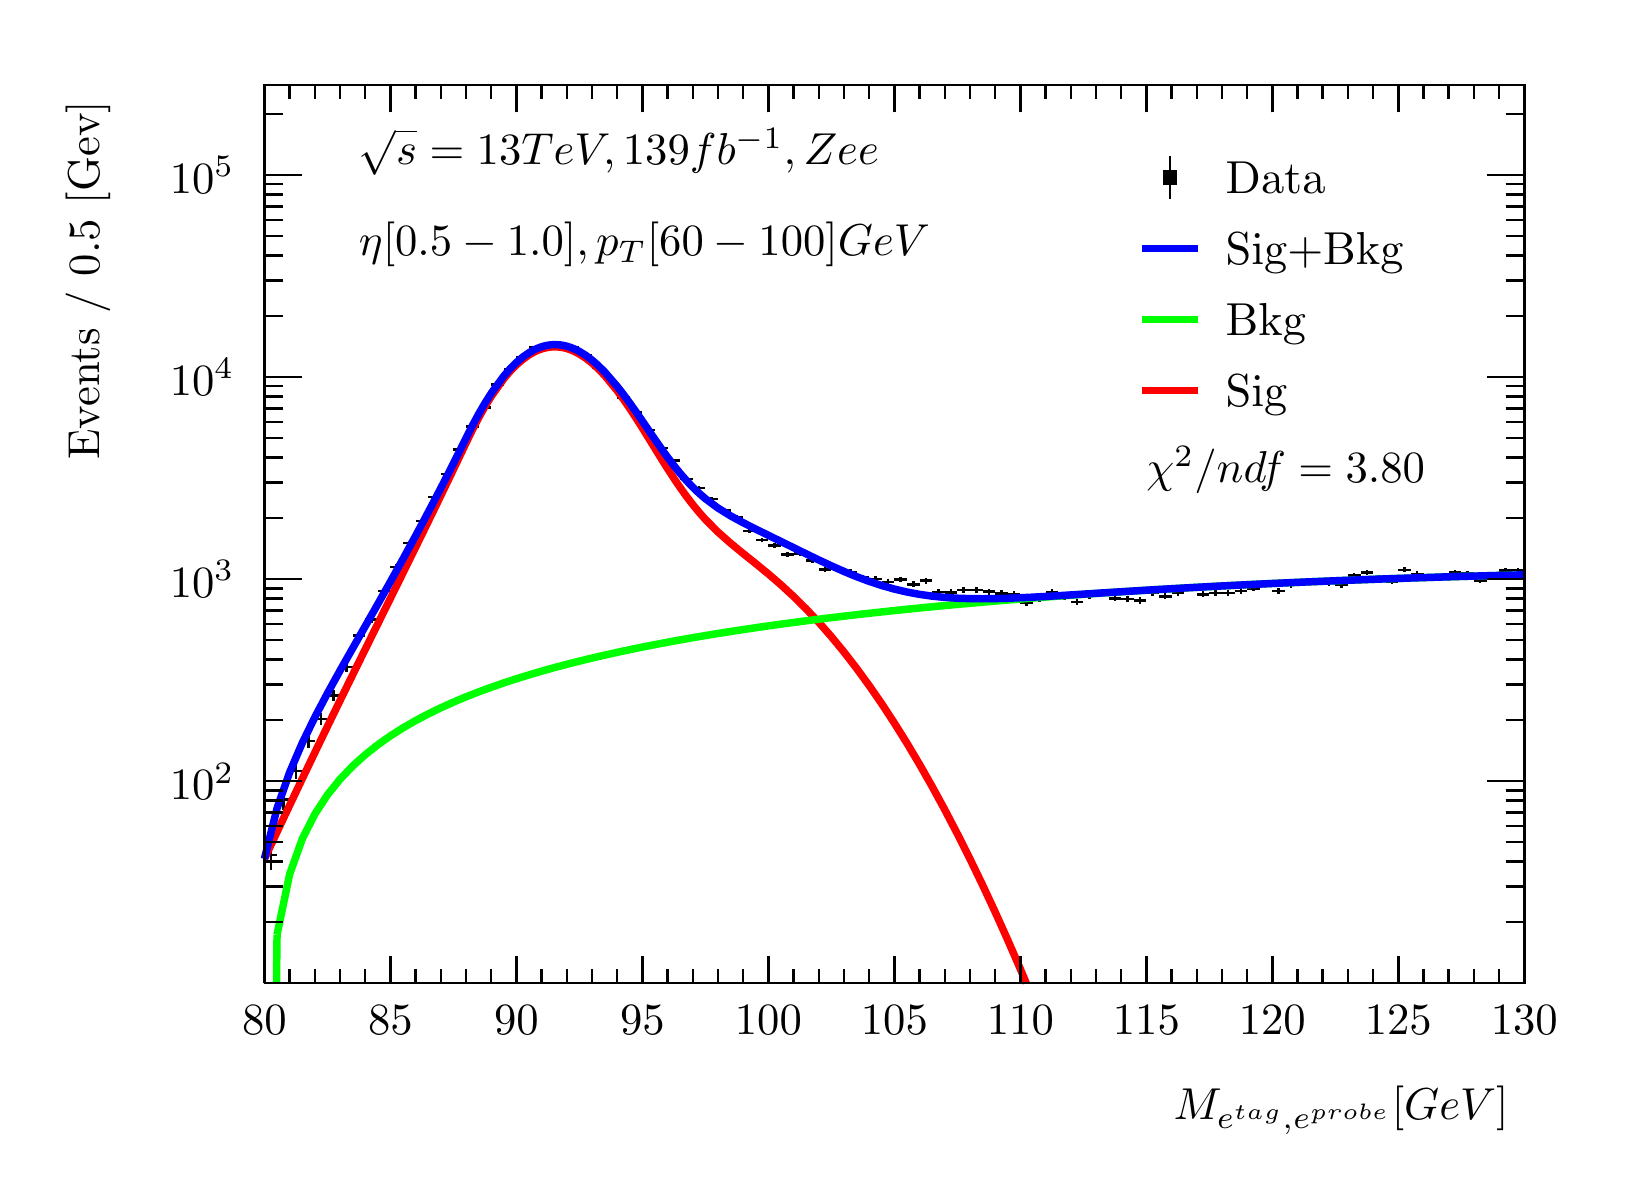
\begin{tikzpicture}
\pgfdeclareplotmark{cross} {
\pgfpathmoveto{\pgfpoint{-0.3\pgfplotmarksize}{\pgfplotmarksize}}
\pgfpathlineto{\pgfpoint{+0.3\pgfplotmarksize}{\pgfplotmarksize}}
\pgfpathlineto{\pgfpoint{+0.3\pgfplotmarksize}{0.3\pgfplotmarksize}}
\pgfpathlineto{\pgfpoint{+1\pgfplotmarksize}{0.3\pgfplotmarksize}}
\pgfpathlineto{\pgfpoint{+1\pgfplotmarksize}{-0.3\pgfplotmarksize}}
\pgfpathlineto{\pgfpoint{+0.3\pgfplotmarksize}{-0.3\pgfplotmarksize}}
\pgfpathlineto{\pgfpoint{+0.3\pgfplotmarksize}{-1.\pgfplotmarksize}}
\pgfpathlineto{\pgfpoint{-0.3\pgfplotmarksize}{-1.\pgfplotmarksize}}
\pgfpathlineto{\pgfpoint{-0.3\pgfplotmarksize}{-0.3\pgfplotmarksize}}
\pgfpathlineto{\pgfpoint{-1.\pgfplotmarksize}{-0.3\pgfplotmarksize}}
\pgfpathlineto{\pgfpoint{-1.\pgfplotmarksize}{0.3\pgfplotmarksize}}
\pgfpathlineto{\pgfpoint{-0.3\pgfplotmarksize}{0.3\pgfplotmarksize}}
\pgfpathclose
\pgfusepathqstroke
}
\pgfdeclareplotmark{cross*} {
\pgfpathmoveto{\pgfpoint{-0.3\pgfplotmarksize}{\pgfplotmarksize}}
\pgfpathlineto{\pgfpoint{+0.3\pgfplotmarksize}{\pgfplotmarksize}}
\pgfpathlineto{\pgfpoint{+0.3\pgfplotmarksize}{0.3\pgfplotmarksize}}
\pgfpathlineto{\pgfpoint{+1\pgfplotmarksize}{0.3\pgfplotmarksize}}
\pgfpathlineto{\pgfpoint{+1\pgfplotmarksize}{-0.3\pgfplotmarksize}}
\pgfpathlineto{\pgfpoint{+0.3\pgfplotmarksize}{-0.3\pgfplotmarksize}}
\pgfpathlineto{\pgfpoint{+0.3\pgfplotmarksize}{-1.\pgfplotmarksize}}
\pgfpathlineto{\pgfpoint{-0.3\pgfplotmarksize}{-1.\pgfplotmarksize}}
\pgfpathlineto{\pgfpoint{-0.3\pgfplotmarksize}{-0.3\pgfplotmarksize}}
\pgfpathlineto{\pgfpoint{-1.\pgfplotmarksize}{-0.3\pgfplotmarksize}}
\pgfpathlineto{\pgfpoint{-1.\pgfplotmarksize}{0.3\pgfplotmarksize}}
\pgfpathlineto{\pgfpoint{-0.3\pgfplotmarksize}{0.3\pgfplotmarksize}}
\pgfpathclose
\pgfusepathqfillstroke
}
\pgfdeclareplotmark{newstar} {
\pgfpathmoveto{\pgfqpoint{0pt}{\pgfplotmarksize}}
\pgfpathlineto{\pgfqpointpolar{44}{0.5\pgfplotmarksize}}
\pgfpathlineto{\pgfqpointpolar{18}{\pgfplotmarksize}}
\pgfpathlineto{\pgfqpointpolar{-20}{0.5\pgfplotmarksize}}
\pgfpathlineto{\pgfqpointpolar{-54}{\pgfplotmarksize}}
\pgfpathlineto{\pgfqpointpolar{-90}{0.5\pgfplotmarksize}}
\pgfpathlineto{\pgfqpointpolar{234}{\pgfplotmarksize}}
\pgfpathlineto{\pgfqpointpolar{198}{0.5\pgfplotmarksize}}
\pgfpathlineto{\pgfqpointpolar{162}{\pgfplotmarksize}}
\pgfpathlineto{\pgfqpointpolar{134}{0.5\pgfplotmarksize}}
\pgfpathclose
\pgfusepathqstroke
}
\pgfdeclareplotmark{newstar*} {
\pgfpathmoveto{\pgfqpoint{0pt}{\pgfplotmarksize}}
\pgfpathlineto{\pgfqpointpolar{44}{0.5\pgfplotmarksize}}
\pgfpathlineto{\pgfqpointpolar{18}{\pgfplotmarksize}}
\pgfpathlineto{\pgfqpointpolar{-20}{0.5\pgfplotmarksize}}
\pgfpathlineto{\pgfqpointpolar{-54}{\pgfplotmarksize}}
\pgfpathlineto{\pgfqpointpolar{-90}{0.5\pgfplotmarksize}}
\pgfpathlineto{\pgfqpointpolar{234}{\pgfplotmarksize}}
\pgfpathlineto{\pgfqpointpolar{198}{0.5\pgfplotmarksize}}
\pgfpathlineto{\pgfqpointpolar{162}{\pgfplotmarksize}}
\pgfpathlineto{\pgfqpointpolar{134}{0.5\pgfplotmarksize}}
\pgfpathclose
\pgfusepathqfillstroke
}
\definecolor{c}{rgb}{1,1,1};
\draw [color=c, fill=c] (0,0) rectangle (20,14.4361);
\draw [color=c, fill=c] (3,2.30977) rectangle (19,13.7143);
\definecolor{c}{rgb}{0,0,0};
\draw [c,line width=0.9] (3,2.30977) -- (3,13.7143) -- (19,13.7143) -- (19,2.30977) -- (3,2.30977);
\definecolor{c}{rgb}{1,1,1};
\draw [color=c, fill=c] (3,2.30977) rectangle (19,13.7143);
\definecolor{c}{rgb}{0,0,0};
\draw [c,line width=0.9] (3,2.30977) -- (3,13.7143) -- (19,13.7143) -- (19,2.30977) -- (3,2.30977);
\draw [c,line width=0.9] (3,2.30977) -- (19,2.30977);
\draw [c,line width=0.9] (3,2.65624) -- (3,2.30977);
\draw [c,line width=0.9] (3.32,2.48301) -- (3.32,2.30977);
\draw [c,line width=0.9] (3.64,2.48301) -- (3.64,2.30977);
\draw [c,line width=0.9] (3.96,2.48301) -- (3.96,2.30977);
\draw [c,line width=0.9] (4.28,2.48301) -- (4.28,2.30977);
\draw [c,line width=0.9] (4.6,2.65624) -- (4.6,2.30977);
\draw [c,line width=0.9] (4.92,2.48301) -- (4.92,2.30977);
\draw [c,line width=0.9] (5.24,2.48301) -- (5.24,2.30977);
\draw [c,line width=0.9] (5.56,2.48301) -- (5.56,2.30977);
\draw [c,line width=0.9] (5.88,2.48301) -- (5.88,2.30977);
\draw [c,line width=0.9] (6.2,2.65624) -- (6.2,2.30977);
\draw [c,line width=0.9] (6.52,2.48301) -- (6.52,2.30977);
\draw [c,line width=0.9] (6.84,2.48301) -- (6.84,2.30977);
\draw [c,line width=0.9] (7.16,2.48301) -- (7.16,2.30977);
\draw [c,line width=0.9] (7.48,2.48301) -- (7.48,2.30977);
\draw [c,line width=0.9] (7.8,2.65624) -- (7.8,2.30977);
\draw [c,line width=0.9] (8.12,2.48301) -- (8.12,2.30977);
\draw [c,line width=0.9] (8.44,2.48301) -- (8.44,2.30977);
\draw [c,line width=0.9] (8.76,2.48301) -- (8.76,2.30977);
\draw [c,line width=0.9] (9.08,2.48301) -- (9.08,2.30977);
\draw [c,line width=0.9] (9.4,2.65624) -- (9.4,2.30977);
\draw [c,line width=0.9] (9.72,2.48301) -- (9.72,2.30977);
\draw [c,line width=0.9] (10.04,2.48301) -- (10.04,2.30977);
\draw [c,line width=0.9] (10.36,2.48301) -- (10.36,2.30977);
\draw [c,line width=0.9] (10.68,2.48301) -- (10.68,2.30977);
\draw [c,line width=0.9] (11,2.65624) -- (11,2.30977);
\draw [c,line width=0.9] (11.32,2.48301) -- (11.32,2.30977);
\draw [c,line width=0.9] (11.64,2.48301) -- (11.64,2.30977);
\draw [c,line width=0.9] (11.96,2.48301) -- (11.96,2.30977);
\draw [c,line width=0.9] (12.28,2.48301) -- (12.28,2.30977);
\draw [c,line width=0.9] (12.6,2.65624) -- (12.6,2.30977);
\draw [c,line width=0.9] (12.92,2.48301) -- (12.92,2.30977);
\draw [c,line width=0.9] (13.24,2.48301) -- (13.24,2.30977);
\draw [c,line width=0.9] (13.56,2.48301) -- (13.56,2.30977);
\draw [c,line width=0.9] (13.88,2.48301) -- (13.88,2.30977);
\draw [c,line width=0.9] (14.2,2.65624) -- (14.2,2.30977);
\draw [c,line width=0.9] (14.52,2.48301) -- (14.52,2.30977);
\draw [c,line width=0.9] (14.84,2.48301) -- (14.84,2.30977);
\draw [c,line width=0.9] (15.16,2.48301) -- (15.16,2.30977);
\draw [c,line width=0.9] (15.48,2.48301) -- (15.48,2.30977);
\draw [c,line width=0.9] (15.8,2.65624) -- (15.8,2.30977);
\draw [c,line width=0.9] (16.12,2.48301) -- (16.12,2.30977);
\draw [c,line width=0.9] (16.44,2.48301) -- (16.44,2.30977);
\draw [c,line width=0.9] (16.76,2.48301) -- (16.76,2.30977);
\draw [c,line width=0.9] (17.08,2.48301) -- (17.08,2.30977);
\draw [c,line width=0.9] (17.4,2.65624) -- (17.4,2.30977);
\draw [c,line width=0.9] (17.72,2.48301) -- (17.72,2.30977);
\draw [c,line width=0.9] (18.04,2.48301) -- (18.04,2.30977);
\draw [c,line width=0.9] (18.36,2.48301) -- (18.36,2.30977);
\draw [c,line width=0.9] (18.68,2.48301) -- (18.68,2.30977);
\draw [c,line width=0.9] (19,2.65624) -- (19,2.30977);
\draw [anchor=base] (3,1.66015) node[scale=1.61424, color=c, rotate=0]{80};
\draw [anchor=base] (4.6,1.66015) node[scale=1.61424, color=c, rotate=0]{85};
\draw [anchor=base] (6.2,1.66015) node[scale=1.61424, color=c, rotate=0]{90};
\draw [anchor=base] (7.8,1.66015) node[scale=1.61424, color=c, rotate=0]{95};
\draw [anchor=base] (9.4,1.66015) node[scale=1.61424, color=c, rotate=0]{100};
\draw [anchor=base] (11,1.66015) node[scale=1.61424, color=c, rotate=0]{105};
\draw [anchor=base] (12.6,1.66015) node[scale=1.61424, color=c, rotate=0]{110};
\draw [anchor=base] (14.2,1.66015) node[scale=1.61424, color=c, rotate=0]{115};
\draw [anchor=base] (15.8,1.66015) node[scale=1.61424, color=c, rotate=0]{120};
\draw [anchor=base] (17.4,1.66015) node[scale=1.61424, color=c, rotate=0]{125};
\draw [anchor=base] (19,1.66015) node[scale=1.61424, color=c, rotate=0]{130};
\draw [anchor= east] (19,0.692932) node[scale=1.61424, color=c, rotate=0]{$M_{e^{tag}, e^{probe}}  [GeV]$};
\draw [c,line width=0.9] (3,13.7143) -- (19,13.7143);
\draw [c,line width=0.9] (3,13.3678) -- (3,13.7143);
\draw [c,line width=0.9] (3.32,13.5411) -- (3.32,13.7143);
\draw [c,line width=0.9] (3.64,13.5411) -- (3.64,13.7143);
\draw [c,line width=0.9] (3.96,13.5411) -- (3.96,13.7143);
\draw [c,line width=0.9] (4.28,13.5411) -- (4.28,13.7143);
\draw [c,line width=0.9] (4.6,13.3678) -- (4.6,13.7143);
\draw [c,line width=0.9] (4.92,13.5411) -- (4.92,13.7143);
\draw [c,line width=0.9] (5.24,13.5411) -- (5.24,13.7143);
\draw [c,line width=0.9] (5.56,13.5411) -- (5.56,13.7143);
\draw [c,line width=0.9] (5.88,13.5411) -- (5.88,13.7143);
\draw [c,line width=0.9] (6.2,13.3678) -- (6.2,13.7143);
\draw [c,line width=0.9] (6.52,13.5411) -- (6.52,13.7143);
\draw [c,line width=0.9] (6.84,13.5411) -- (6.84,13.7143);
\draw [c,line width=0.9] (7.16,13.5411) -- (7.16,13.7143);
\draw [c,line width=0.9] (7.48,13.5411) -- (7.48,13.7143);
\draw [c,line width=0.9] (7.8,13.3678) -- (7.8,13.7143);
\draw [c,line width=0.9] (8.12,13.5411) -- (8.12,13.7143);
\draw [c,line width=0.9] (8.44,13.5411) -- (8.44,13.7143);
\draw [c,line width=0.9] (8.76,13.5411) -- (8.76,13.7143);
\draw [c,line width=0.9] (9.08,13.5411) -- (9.08,13.7143);
\draw [c,line width=0.9] (9.4,13.3678) -- (9.4,13.7143);
\draw [c,line width=0.9] (9.72,13.5411) -- (9.72,13.7143);
\draw [c,line width=0.9] (10.04,13.5411) -- (10.04,13.7143);
\draw [c,line width=0.9] (10.36,13.5411) -- (10.36,13.7143);
\draw [c,line width=0.9] (10.68,13.5411) -- (10.68,13.7143);
\draw [c,line width=0.9] (11,13.3678) -- (11,13.7143);
\draw [c,line width=0.9] (11.32,13.5411) -- (11.32,13.7143);
\draw [c,line width=0.9] (11.64,13.5411) -- (11.64,13.7143);
\draw [c,line width=0.9] (11.96,13.5411) -- (11.96,13.7143);
\draw [c,line width=0.9] (12.28,13.5411) -- (12.28,13.7143);
\draw [c,line width=0.9] (12.6,13.3678) -- (12.6,13.7143);
\draw [c,line width=0.9] (12.92,13.5411) -- (12.92,13.7143);
\draw [c,line width=0.9] (13.24,13.5411) -- (13.24,13.7143);
\draw [c,line width=0.9] (13.56,13.5411) -- (13.56,13.7143);
\draw [c,line width=0.9] (13.88,13.5411) -- (13.88,13.7143);
\draw [c,line width=0.9] (14.2,13.3678) -- (14.2,13.7143);
\draw [c,line width=0.9] (14.52,13.5411) -- (14.52,13.7143);
\draw [c,line width=0.9] (14.84,13.5411) -- (14.84,13.7143);
\draw [c,line width=0.9] (15.16,13.5411) -- (15.16,13.7143);
\draw [c,line width=0.9] (15.48,13.5411) -- (15.48,13.7143);
\draw [c,line width=0.9] (15.8,13.3678) -- (15.8,13.7143);
\draw [c,line width=0.9] (16.12,13.5411) -- (16.12,13.7143);
\draw [c,line width=0.9] (16.44,13.5411) -- (16.44,13.7143);
\draw [c,line width=0.9] (16.76,13.5411) -- (16.76,13.7143);
\draw [c,line width=0.9] (17.08,13.5411) -- (17.08,13.7143);
\draw [c,line width=0.9] (17.4,13.3678) -- (17.4,13.7143);
\draw [c,line width=0.9] (17.72,13.5411) -- (17.72,13.7143);
\draw [c,line width=0.9] (18.04,13.5411) -- (18.04,13.7143);
\draw [c,line width=0.9] (18.36,13.5411) -- (18.36,13.7143);
\draw [c,line width=0.9] (18.68,13.5411) -- (18.68,13.7143);
\draw [c,line width=0.9] (19,13.3678) -- (19,13.7143);
\draw [c,line width=0.9] (3,2.30977) -- (3,13.7143);
\draw [c,line width=0.9] (3.237,3.08209) -- (3,3.08209);
\draw [c,line width=0.9] (3.237,3.53386) -- (3,3.53386);
\draw [c,line width=0.9] (3.237,3.8544) -- (3,3.8544);
\draw [c,line width=0.9] (3.237,4.10303) -- (3,4.10303);
\draw [c,line width=0.9] (3.237,4.30618) -- (3,4.30618);
\draw [c,line width=0.9] (3.237,4.47794) -- (3,4.47794);
\draw [c,line width=0.9] (3.237,4.62672) -- (3,4.62672);
\draw [c,line width=0.9] (3.237,4.75795) -- (3,4.75795);
\draw [c,line width=0.9] (3.474,4.87535) -- (3,4.87535);
\draw [anchor= east] (2.82,4.87535) node[scale=1.61424, color=c, rotate=0]{$10^{2}$};
\draw [c,line width=0.9] (3.237,5.64766) -- (3,5.64766);
\draw [c,line width=0.9] (3.237,6.09944) -- (3,6.09944);
\draw [c,line width=0.9] (3.237,6.41998) -- (3,6.41998);
\draw [c,line width=0.9] (3.237,6.66861) -- (3,6.66861);
\draw [c,line width=0.9] (3.237,6.87176) -- (3,6.87176);
\draw [c,line width=0.9] (3.237,7.04351) -- (3,7.04351);
\draw [c,line width=0.9] (3.237,7.1923) -- (3,7.1923);
\draw [c,line width=0.9] (3.237,7.32353) -- (3,7.32353);
\draw [c,line width=0.9] (3.474,7.44093) -- (3,7.44093);
\draw [anchor= east] (2.82,7.44093) node[scale=1.61424, color=c, rotate=0]{$10^{3}$};
\draw [c,line width=0.9] (3.237,8.21324) -- (3,8.21324);
\draw [c,line width=0.9] (3.237,8.66502) -- (3,8.66502);
\draw [c,line width=0.9] (3.237,8.98556) -- (3,8.98556);
\draw [c,line width=0.9] (3.237,9.23419) -- (3,9.23419);
\draw [c,line width=0.9] (3.237,9.43733) -- (3,9.43733);
\draw [c,line width=0.9] (3.237,9.60909) -- (3,9.60909);
\draw [c,line width=0.9] (3.237,9.75787) -- (3,9.75787);
\draw [c,line width=0.9] (3.237,9.88911) -- (3,9.88911);
\draw [c,line width=0.9] (3.474,10.0065) -- (3,10.0065);
\draw [anchor= east] (2.82,10.0065) node[scale=1.61424, color=c, rotate=0]{$10^{4}$};
\draw [c,line width=0.9] (3.237,10.7788) -- (3,10.7788);
\draw [c,line width=0.9] (3.237,11.2306) -- (3,11.2306);
\draw [c,line width=0.9] (3.237,11.5511) -- (3,11.5511);
\draw [c,line width=0.9] (3.237,11.7998) -- (3,11.7998);
\draw [c,line width=0.9] (3.237,12.0029) -- (3,12.0029);
\draw [c,line width=0.9] (3.237,12.1747) -- (3,12.1747);
\draw [c,line width=0.9] (3.237,12.3235) -- (3,12.3235);
\draw [c,line width=0.9] (3.237,12.4547) -- (3,12.4547);
\draw [c,line width=0.9] (3.474,12.5721) -- (3,12.5721);
\draw [anchor= east] (2.82,12.5721) node[scale=1.61424, color=c, rotate=0]{$10^{5}$};
\draw [c,line width=0.9] (3.237,13.3444) -- (3,13.3444);
\draw [anchor= east] (0.76,13.7143) node[scale=1.61424, color=c, rotate=90]{Events / 0.5 [Gev]};
\draw [c,line width=0.9] (19,2.30977) -- (19,13.7143);
\draw [c,line width=0.9] (18.763,3.08209) -- (19,3.08209);
\draw [c,line width=0.9] (18.763,3.53386) -- (19,3.53386);
\draw [c,line width=0.9] (18.763,3.8544) -- (19,3.8544);
\draw [c,line width=0.9] (18.763,4.10303) -- (19,4.10303);
\draw [c,line width=0.9] (18.763,4.30618) -- (19,4.30618);
\draw [c,line width=0.9] (18.763,4.47794) -- (19,4.47794);
\draw [c,line width=0.9] (18.763,4.62672) -- (19,4.62672);
\draw [c,line width=0.9] (18.763,4.75795) -- (19,4.75795);
\draw [c,line width=0.9] (18.526,4.87535) -- (19,4.87535);
\draw [c,line width=0.9] (18.763,5.64766) -- (19,5.64766);
\draw [c,line width=0.9] (18.763,6.09944) -- (19,6.09944);
\draw [c,line width=0.9] (18.763,6.41998) -- (19,6.41998);
\draw [c,line width=0.9] (18.763,6.66861) -- (19,6.66861);
\draw [c,line width=0.9] (18.763,6.87176) -- (19,6.87176);
\draw [c,line width=0.9] (18.763,7.04351) -- (19,7.04351);
\draw [c,line width=0.9] (18.763,7.1923) -- (19,7.1923);
\draw [c,line width=0.9] (18.763,7.32353) -- (19,7.32353);
\draw [c,line width=0.9] (18.526,7.44093) -- (19,7.44093);
\draw [c,line width=0.9] (18.763,8.21324) -- (19,8.21324);
\draw [c,line width=0.9] (18.763,8.66502) -- (19,8.66502);
\draw [c,line width=0.9] (18.763,8.98556) -- (19,8.98556);
\draw [c,line width=0.9] (18.763,9.23419) -- (19,9.23419);
\draw [c,line width=0.9] (18.763,9.43733) -- (19,9.43733);
\draw [c,line width=0.9] (18.763,9.60909) -- (19,9.60909);
\draw [c,line width=0.9] (18.763,9.75787) -- (19,9.75787);
\draw [c,line width=0.9] (18.763,9.88911) -- (19,9.88911);
\draw [c,line width=0.9] (18.526,10.0065) -- (19,10.0065);
\draw [c,line width=0.9] (18.763,10.7788) -- (19,10.7788);
\draw [c,line width=0.9] (18.763,11.2306) -- (19,11.2306);
\draw [c,line width=0.9] (18.763,11.5511) -- (19,11.5511);
\draw [c,line width=0.9] (18.763,11.7998) -- (19,11.7998);
\draw [c,line width=0.9] (18.763,12.0029) -- (19,12.0029);
\draw [c,line width=0.9] (18.763,12.1747) -- (19,12.1747);
\draw [c,line width=0.9] (18.763,12.3235) -- (19,12.3235);
\draw [c,line width=0.9] (18.763,12.4547) -- (19,12.4547);
\draw [c,line width=0.9] (18.526,12.5721) -- (19,12.5721);
\draw [c,line width=0.9] (18.763,13.3444) -- (19,13.3444);
\draw [c,line width=0.9] (3.08,3.93499) -- (3,3.93499);
\draw [c,line width=0.9] (3,3.93499) -- (3,3.93499);
\draw [c,line width=0.9] (3.08,3.93499) -- (3.16,3.93499);
\draw [c,line width=0.9] (3.16,3.93499) -- (3.16,3.93499);
\draw [c,line width=0.9] (3.08,3.93499) -- (3.08,4.11651);
\draw [c,line width=0.9] (3.08,4.11651) -- (3.08,4.11651);
\draw [c,line width=0.9] (3.08,3.93499) -- (3.08,3.75141);
\draw [c,line width=0.9] (3.08,3.75141) -- (3.08,3.75141);
\draw [c,line width=0.9] (3.24,4.64056) -- (3.16,4.64056);
\draw [c,line width=0.9] (3.16,4.64056) -- (3.16,4.64056);
\draw [c,line width=0.9] (3.24,4.64056) -- (3.32,4.64056);
\draw [c,line width=0.9] (3.32,4.64056) -- (3.32,4.64056);
\draw [c,line width=0.9] (3.24,4.64056) -- (3.24,4.77072);
\draw [c,line width=0.9] (3.24,4.77072) -- (3.24,4.77072);
\draw [c,line width=0.9] (3.24,4.64056) -- (3.24,4.50961);
\draw [c,line width=0.9] (3.24,4.50961) -- (3.24,4.50961);
\draw [c,line width=0.9] (3.4,5.00162) -- (3.32,5.00162);
\draw [c,line width=0.9] (3.32,5.00162) -- (3.32,5.00162);
\draw [c,line width=0.9] (3.4,5.00162) -- (3.48,5.00162);
\draw [c,line width=0.9] (3.48,5.00162) -- (3.48,5.00162);
\draw [c,line width=0.9] (3.4,5.00162) -- (3.4,5.10687);
\draw [c,line width=0.9] (3.4,5.10687) -- (3.4,5.10687);
\draw [c,line width=0.9] (3.4,5.00162) -- (3.4,4.89638);
\draw [c,line width=0.9] (3.4,4.89638) -- (3.4,4.89638);
\draw [c,line width=0.9] (3.56,5.38502) -- (3.48,5.38502);
\draw [c,line width=0.9] (3.48,5.38502) -- (3.48,5.38502);
\draw [c,line width=0.9] (3.56,5.38502) -- (3.64,5.38502);
\draw [c,line width=0.9] (3.64,5.38502) -- (3.64,5.38502);
\draw [c,line width=0.9] (3.56,5.38502) -- (3.56,5.47364);
\draw [c,line width=0.9] (3.56,5.47364) -- (3.56,5.47364);
\draw [c,line width=0.9] (3.56,5.38502) -- (3.56,5.2964);
\draw [c,line width=0.9] (3.56,5.2964) -- (3.56,5.2964);
\draw [c,line width=0.9] (3.72,5.66426) -- (3.64,5.66426);
\draw [c,line width=0.9] (3.64,5.66426) -- (3.64,5.66426);
\draw [c,line width=0.9] (3.72,5.66426) -- (3.8,5.66426);
\draw [c,line width=0.9] (3.8,5.66426) -- (3.8,5.66426);
\draw [c,line width=0.9] (3.72,5.66426) -- (3.72,5.74244);
\draw [c,line width=0.9] (3.72,5.74244) -- (3.72,5.74244);
\draw [c,line width=0.9] (3.72,5.66426) -- (3.72,5.58607);
\draw [c,line width=0.9] (3.72,5.58607) -- (3.72,5.58607);
\draw [c,line width=0.9] (3.88,5.96122) -- (3.8,5.96122);
\draw [c,line width=0.9] (3.8,5.96122) -- (3.8,5.96122);
\draw [c,line width=0.9] (3.88,5.96122) -- (3.96,5.96122);
\draw [c,line width=0.9] (3.96,5.96122) -- (3.96,5.96122);
\draw [c,line width=0.9] (3.88,5.96122) -- (3.88,6.02966);
\draw [c,line width=0.9] (3.88,6.02966) -- (3.88,6.02966);
\draw [c,line width=0.9] (3.88,5.96122) -- (3.88,5.89279);
\draw [c,line width=0.9] (3.88,5.89279) -- (3.88,5.89279);
\draw [c,line width=0.9] (4.04,6.32405) -- (3.96,6.32405);
\draw [c,line width=0.9] (3.96,6.32405) -- (3.96,6.32405);
\draw [c,line width=0.9] (4.04,6.32405) -- (4.12,6.32405);
\draw [c,line width=0.9] (4.12,6.32405) -- (4.12,6.32405);
\draw [c,line width=0.9] (4.04,6.32405) -- (4.04,6.3822);
\draw [c,line width=0.9] (4.04,6.3822) -- (4.04,6.3822);
\draw [c,line width=0.9] (4.04,6.32405) -- (4.04,6.26589);
\draw [c,line width=0.9] (4.04,6.26589) -- (4.04,6.26589);
\draw [c,line width=0.9] (4.2,6.7251) -- (4.12,6.7251);
\draw [c,line width=0.9] (4.12,6.7251) -- (4.12,6.7251);
\draw [c,line width=0.9] (4.2,6.7251) -- (4.28,6.7251);
\draw [c,line width=0.9] (4.28,6.7251) -- (4.28,6.7251);
\draw [c,line width=0.9] (4.2,6.7251) -- (4.2,6.77367);
\draw [c,line width=0.9] (4.2,6.77367) -- (4.2,6.77367);
\draw [c,line width=0.9] (4.2,6.7251) -- (4.2,6.67652);
\draw [c,line width=0.9] (4.2,6.67652) -- (4.2,6.67652);
\draw [c,line width=0.9] (4.36,6.92435) -- (4.28,6.92435);
\draw [c,line width=0.9] (4.28,6.92435) -- (4.28,6.92435);
\draw [c,line width=0.9] (4.36,6.92435) -- (4.44,6.92435);
\draw [c,line width=0.9] (4.44,6.92435) -- (4.44,6.92435);
\draw [c,line width=0.9] (4.36,6.92435) -- (4.36,6.96877);
\draw [c,line width=0.9] (4.36,6.96877) -- (4.36,6.96877);
\draw [c,line width=0.9] (4.36,6.92435) -- (4.36,6.87993);
\draw [c,line width=0.9] (4.36,6.87993) -- (4.36,6.87993);
\draw [c,line width=0.9] (4.52,7.28704) -- (4.44,7.28704);
\draw [c,line width=0.9] (4.44,7.28704) -- (4.44,7.28704);
\draw [c,line width=0.9] (4.52,7.28704) -- (4.6,7.28704);
\draw [c,line width=0.9] (4.6,7.28704) -- (4.6,7.28704);
\draw [c,line width=0.9] (4.52,7.28704) -- (4.52,7.32479);
\draw [c,line width=0.9] (4.52,7.32479) -- (4.52,7.32479);
\draw [c,line width=0.9] (4.52,7.28704) -- (4.52,7.24929);
\draw [c,line width=0.9] (4.52,7.24929) -- (4.52,7.24929);
\draw [c,line width=0.9] (4.68,7.59665) -- (4.6,7.59665);
\draw [c,line width=0.9] (4.6,7.59665) -- (4.6,7.59665);
\draw [c,line width=0.9] (4.68,7.59665) -- (4.76,7.59665);
\draw [c,line width=0.9] (4.76,7.59665) -- (4.76,7.59665);
\draw [c,line width=0.9] (4.68,7.59665) -- (4.68,7.62951);
\draw [c,line width=0.9] (4.68,7.62951) -- (4.68,7.62951);
\draw [c,line width=0.9] (4.68,7.59665) -- (4.68,7.5638);
\draw [c,line width=0.9] (4.68,7.5638) -- (4.68,7.5638);
\draw [c,line width=0.9] (4.84,7.89863) -- (4.76,7.89863);
\draw [c,line width=0.9] (4.76,7.89863) -- (4.76,7.89863);
\draw [c,line width=0.9] (4.84,7.89863) -- (4.92,7.89863);
\draw [c,line width=0.9] (4.92,7.89863) -- (4.92,7.89863);
\draw [c,line width=0.9] (4.84,7.89863) -- (4.84,7.92732);
\draw [c,line width=0.9] (4.84,7.92732) -- (4.84,7.92732);
\draw [c,line width=0.9] (4.84,7.89863) -- (4.84,7.86994);
\draw [c,line width=0.9] (4.84,7.86994) -- (4.84,7.86994);
\draw [c,line width=0.9] (5,8.1747) -- (4.92,8.1747);
\draw [c,line width=0.9] (4.92,8.1747) -- (4.92,8.1747);
\draw [c,line width=0.9] (5,8.1747) -- (5.08,8.1747);
\draw [c,line width=0.9] (5.08,8.1747) -- (5.08,8.1747);
\draw [c,line width=0.9] (5,8.1747) -- (5,8.20005);
\draw [c,line width=0.9] (5,8.20005) -- (5,8.20005);
\draw [c,line width=0.9] (5,8.1747) -- (5,8.14935);
\draw [c,line width=0.9] (5,8.14935) -- (5,8.14935);
\draw [c,line width=0.9] (5.16,8.48) -- (5.08,8.48);
\draw [c,line width=0.9] (5.08,8.48) -- (5.08,8.48);
\draw [c,line width=0.9] (5.16,8.48) -- (5.24,8.48);
\draw [c,line width=0.9] (5.24,8.48) -- (5.24,8.48);
\draw [c,line width=0.9] (5.16,8.48) -- (5.16,8.5021);
\draw [c,line width=0.9] (5.16,8.5021) -- (5.16,8.5021);
\draw [c,line width=0.9] (5.16,8.48) -- (5.16,8.45789);
\draw [c,line width=0.9] (5.16,8.45789) -- (5.16,8.45789);
\draw [c,line width=0.9] (5.32,8.77694) -- (5.24,8.77694);
\draw [c,line width=0.9] (5.24,8.77694) -- (5.24,8.77694);
\draw [c,line width=0.9] (5.32,8.77694) -- (5.4,8.77694);
\draw [c,line width=0.9] (5.4,8.77694) -- (5.4,8.77694);
\draw [c,line width=0.9] (5.32,8.77694) -- (5.32,8.79629);
\draw [c,line width=0.9] (5.32,8.79629) -- (5.32,8.79629);
\draw [c,line width=0.9] (5.32,8.77694) -- (5.32,8.75759);
\draw [c,line width=0.9] (5.32,8.75759) -- (5.32,8.75759);
\draw [c,line width=0.9] (5.48,9.08362) -- (5.4,9.08362);
\draw [c,line width=0.9] (5.4,9.08362) -- (5.4,9.08362);
\draw [c,line width=0.9] (5.48,9.08362) -- (5.56,9.08362);
\draw [c,line width=0.9] (5.56,9.08362) -- (5.56,9.08362);
\draw [c,line width=0.9] (5.48,9.08362) -- (5.48,9.10048);
\draw [c,line width=0.9] (5.48,9.10048) -- (5.48,9.10048);
\draw [c,line width=0.9] (5.48,9.08362) -- (5.48,9.06676);
\draw [c,line width=0.9] (5.48,9.06676) -- (5.48,9.06676);
\draw [c,line width=0.9] (5.64,9.3794) -- (5.56,9.3794);
\draw [c,line width=0.9] (5.56,9.3794) -- (5.56,9.3794);
\draw [c,line width=0.9] (5.64,9.3794) -- (5.72,9.3794);
\draw [c,line width=0.9] (5.72,9.3794) -- (5.72,9.3794);
\draw [c,line width=0.9] (5.64,9.3794) -- (5.64,9.39416);
\draw [c,line width=0.9] (5.64,9.39416) -- (5.64,9.39416);
\draw [c,line width=0.9] (5.64,9.3794) -- (5.64,9.36464);
\draw [c,line width=0.9] (5.64,9.36464) -- (5.64,9.36464);
\draw [c,line width=0.9] (5.8,9.62112) -- (5.72,9.62112);
\draw [c,line width=0.9] (5.72,9.62112) -- (5.72,9.62112);
\draw [c,line width=0.9] (5.8,9.62112) -- (5.88,9.62112);
\draw [c,line width=0.9] (5.88,9.62112) -- (5.88,9.62112);
\draw [c,line width=0.9] (5.8,9.62112) -- (5.8,9.63437);
\draw [c,line width=0.9] (5.8,9.63437) -- (5.8,9.63437);
\draw [c,line width=0.9] (5.8,9.62112) -- (5.8,9.60788);
\draw [c,line width=0.9] (5.8,9.60788) -- (5.8,9.60788);
\draw [c,line width=0.9] (5.96,9.91166) -- (5.88,9.91166);
\draw [c,line width=0.9] (5.88,9.91166) -- (5.88,9.91166);
\draw [c,line width=0.9] (5.96,9.91166) -- (6.04,9.91166);
\draw [c,line width=0.9] (6.04,9.91166) -- (6.04,9.91166);
\draw [c,line width=0.9] (5.96,9.91166) -- (5.96,9.92329);
\draw [c,line width=0.9] (5.96,9.92329) -- (5.96,9.92329);
\draw [c,line width=0.9] (5.96,9.91166) -- (5.96,9.90003);
\draw [c,line width=0.9] (5.96,9.90003) -- (5.96,9.90003);
\draw [c,line width=0.9] (6.12,10.1003) -- (6.04,10.1003);
\draw [c,line width=0.9] (6.04,10.1003) -- (6.04,10.1003);
\draw [c,line width=0.9] (6.12,10.1003) -- (6.2,10.1003);
\draw [c,line width=0.9] (6.2,10.1003) -- (6.2,10.1003);
\draw [c,line width=0.9] (6.12,10.1003) -- (6.12,10.111);
\draw [c,line width=0.9] (6.12,10.111) -- (6.12,10.111);
\draw [c,line width=0.9] (6.12,10.1003) -- (6.12,10.0896);
\draw [c,line width=0.9] (6.12,10.0896) -- (6.12,10.0896);
\draw [c,line width=0.9] (6.28,10.2518) -- (6.2,10.2518);
\draw [c,line width=0.9] (6.2,10.2518) -- (6.2,10.2518);
\draw [c,line width=0.9] (6.28,10.2518) -- (6.36,10.2518);
\draw [c,line width=0.9] (6.36,10.2518) -- (6.36,10.2518);
\draw [c,line width=0.9] (6.28,10.2518) -- (6.28,10.2618);
\draw [c,line width=0.9] (6.28,10.2618) -- (6.28,10.2618);
\draw [c,line width=0.9] (6.28,10.2518) -- (6.28,10.2419);
\draw [c,line width=0.9] (6.28,10.2419) -- (6.28,10.2419);
\draw [c,line width=0.9] (6.44,10.3798) -- (6.36,10.3798);
\draw [c,line width=0.9] (6.36,10.3798) -- (6.36,10.3798);
\draw [c,line width=0.9] (6.44,10.3798) -- (6.52,10.3798);
\draw [c,line width=0.9] (6.52,10.3798) -- (6.52,10.3798);
\draw [c,line width=0.9] (6.44,10.3798) -- (6.44,10.3892);
\draw [c,line width=0.9] (6.44,10.3892) -- (6.44,10.3892);
\draw [c,line width=0.9] (6.44,10.3798) -- (6.44,10.3704);
\draw [c,line width=0.9] (6.44,10.3704) -- (6.44,10.3704);
\draw [c,line width=0.9] (6.6,10.4278) -- (6.52,10.4278);
\draw [c,line width=0.9] (6.52,10.4278) -- (6.52,10.4278);
\draw [c,line width=0.9] (6.6,10.4278) -- (6.68,10.4278);
\draw [c,line width=0.9] (6.68,10.4278) -- (6.68,10.4278);
\draw [c,line width=0.9] (6.6,10.4278) -- (6.6,10.437);
\draw [c,line width=0.9] (6.6,10.437) -- (6.6,10.437);
\draw [c,line width=0.9] (6.6,10.4278) -- (6.6,10.4186);
\draw [c,line width=0.9] (6.6,10.4186) -- (6.6,10.4186);
\draw [c,line width=0.9] (6.76,10.428) -- (6.68,10.428);
\draw [c,line width=0.9] (6.68,10.428) -- (6.68,10.428);
\draw [c,line width=0.9] (6.76,10.428) -- (6.84,10.428);
\draw [c,line width=0.9] (6.84,10.428) -- (6.84,10.428);
\draw [c,line width=0.9] (6.76,10.428) -- (6.76,10.4372);
\draw [c,line width=0.9] (6.76,10.4372) -- (6.76,10.4372);
\draw [c,line width=0.9] (6.76,10.428) -- (6.76,10.4188);
\draw [c,line width=0.9] (6.76,10.4188) -- (6.76,10.4188);
\draw [c,line width=0.9] (6.92,10.3797) -- (6.84,10.3797);
\draw [c,line width=0.9] (6.84,10.3797) -- (6.84,10.3797);
\draw [c,line width=0.9] (6.92,10.3797) -- (7,10.3797);
\draw [c,line width=0.9] (7,10.3797) -- (7,10.3797);
\draw [c,line width=0.9] (6.92,10.3797) -- (6.92,10.3892);
\draw [c,line width=0.9] (6.92,10.3892) -- (6.92,10.3892);
\draw [c,line width=0.9] (6.92,10.3797) -- (6.92,10.3703);
\draw [c,line width=0.9] (6.92,10.3703) -- (6.92,10.3703);
\draw [c,line width=0.9] (7.08,10.2882) -- (7,10.2882);
\draw [c,line width=0.9] (7,10.2882) -- (7,10.2882);
\draw [c,line width=0.9] (7.08,10.2882) -- (7.16,10.2882);
\draw [c,line width=0.9] (7.16,10.2882) -- (7.16,10.2882);
\draw [c,line width=0.9] (7.08,10.2882) -- (7.08,10.298);
\draw [c,line width=0.9] (7.08,10.298) -- (7.08,10.298);
\draw [c,line width=0.9] (7.08,10.2882) -- (7.08,10.2783);
\draw [c,line width=0.9] (7.08,10.2783) -- (7.08,10.2783);
\draw [c,line width=0.9] (7.24,10.1239) -- (7.16,10.1239);
\draw [c,line width=0.9] (7.16,10.1239) -- (7.16,10.1239);
\draw [c,line width=0.9] (7.24,10.1239) -- (7.32,10.1239);
\draw [c,line width=0.9] (7.32,10.1239) -- (7.32,10.1239);
\draw [c,line width=0.9] (7.24,10.1239) -- (7.24,10.1345);
\draw [c,line width=0.9] (7.24,10.1345) -- (7.24,10.1345);
\draw [c,line width=0.9] (7.24,10.1239) -- (7.24,10.1133);
\draw [c,line width=0.9] (7.24,10.1133) -- (7.24,10.1133);
\draw [c,line width=0.9] (7.4,9.95811) -- (7.32,9.95811);
\draw [c,line width=0.9] (7.32,9.95811) -- (7.32,9.95811);
\draw [c,line width=0.9] (7.4,9.95811) -- (7.48,9.95811);
\draw [c,line width=0.9] (7.48,9.95811) -- (7.48,9.95811);
\draw [c,line width=0.9] (7.4,9.95811) -- (7.4,9.9695);
\draw [c,line width=0.9] (7.4,9.9695) -- (7.4,9.9695);
\draw [c,line width=0.9] (7.4,9.95811) -- (7.4,9.94673);
\draw [c,line width=0.9] (7.4,9.94673) -- (7.4,9.94673);
\draw [c,line width=0.9] (7.56,9.74569) -- (7.48,9.74569);
\draw [c,line width=0.9] (7.48,9.74569) -- (7.48,9.74569);
\draw [c,line width=0.9] (7.56,9.74569) -- (7.64,9.74569);
\draw [c,line width=0.9] (7.64,9.74569) -- (7.64,9.74569);
\draw [c,line width=0.9] (7.56,9.74569) -- (7.56,9.75822);
\draw [c,line width=0.9] (7.56,9.75822) -- (7.56,9.75822);
\draw [c,line width=0.9] (7.56,9.74569) -- (7.56,9.73317);
\draw [c,line width=0.9] (7.56,9.73317) -- (7.56,9.73317);
\draw [c,line width=0.9] (7.72,9.55679) -- (7.64,9.55679);
\draw [c,line width=0.9] (7.64,9.55679) -- (7.64,9.55679);
\draw [c,line width=0.9] (7.72,9.55679) -- (7.8,9.55679);
\draw [c,line width=0.9] (7.8,9.55679) -- (7.8,9.55679);
\draw [c,line width=0.9] (7.72,9.55679) -- (7.72,9.57042);
\draw [c,line width=0.9] (7.72,9.57042) -- (7.72,9.57042);
\draw [c,line width=0.9] (7.72,9.55679) -- (7.72,9.54315);
\draw [c,line width=0.9] (7.72,9.54315) -- (7.72,9.54315);
\draw [c,line width=0.9] (7.88,9.33429) -- (7.8,9.33429);
\draw [c,line width=0.9] (7.8,9.33429) -- (7.8,9.33429);
\draw [c,line width=0.9] (7.88,9.33429) -- (7.96,9.33429);
\draw [c,line width=0.9] (7.96,9.33429) -- (7.96,9.33429);
\draw [c,line width=0.9] (7.88,9.33429) -- (7.88,9.34936);
\draw [c,line width=0.9] (7.88,9.34936) -- (7.88,9.34936);
\draw [c,line width=0.9] (7.88,9.33429) -- (7.88,9.31923);
\draw [c,line width=0.9] (7.88,9.31923) -- (7.88,9.31923);
\draw [c,line width=0.9] (8.04,9.10435) -- (7.96,9.10435);
\draw [c,line width=0.9] (7.96,9.10435) -- (7.96,9.10435);
\draw [c,line width=0.9] (8.04,9.10435) -- (8.12,9.10435);
\draw [c,line width=0.9] (8.12,9.10435) -- (8.12,9.10435);
\draw [c,line width=0.9] (8.04,9.10435) -- (8.04,9.12105);
\draw [c,line width=0.9] (8.04,9.12105) -- (8.04,9.12105);
\draw [c,line width=0.9] (8.04,9.10435) -- (8.04,9.08764);
\draw [c,line width=0.9] (8.04,9.08764) -- (8.04,9.08764);
\draw [c,line width=0.9] (8.2,8.94413) -- (8.12,8.94413);
\draw [c,line width=0.9] (8.12,8.94413) -- (8.12,8.94413);
\draw [c,line width=0.9] (8.2,8.94413) -- (8.28,8.94413);
\draw [c,line width=0.9] (8.28,8.94413) -- (8.28,8.94413);
\draw [c,line width=0.9] (8.2,8.94413) -- (8.2,8.96208);
\draw [c,line width=0.9] (8.2,8.96208) -- (8.2,8.96208);
\draw [c,line width=0.9] (8.2,8.94413) -- (8.2,8.92618);
\draw [c,line width=0.9] (8.2,8.92618) -- (8.2,8.92618);
\draw [c,line width=0.9] (8.36,8.71015) -- (8.28,8.71015);
\draw [c,line width=0.9] (8.28,8.71015) -- (8.28,8.71015);
\draw [c,line width=0.9] (8.36,8.71015) -- (8.44,8.71015);
\draw [c,line width=0.9] (8.44,8.71015) -- (8.44,8.71015);
\draw [c,line width=0.9] (8.36,8.71015) -- (8.36,8.73008);
\draw [c,line width=0.9] (8.36,8.73008) -- (8.36,8.73008);
\draw [c,line width=0.9] (8.36,8.71015) -- (8.36,8.69021);
\draw [c,line width=0.9] (8.36,8.69021) -- (8.36,8.69021);
\draw [c,line width=0.9] (8.52,8.59647) -- (8.44,8.59647);
\draw [c,line width=0.9] (8.44,8.59647) -- (8.44,8.59647);
\draw [c,line width=0.9] (8.52,8.59647) -- (8.6,8.59647);
\draw [c,line width=0.9] (8.6,8.59647) -- (8.6,8.59647);
\draw [c,line width=0.9] (8.52,8.59647) -- (8.52,8.61745);
\draw [c,line width=0.9] (8.52,8.61745) -- (8.52,8.61745);
\draw [c,line width=0.9] (8.52,8.59647) -- (8.52,8.57549);
\draw [c,line width=0.9] (8.52,8.57549) -- (8.52,8.57549);
\draw [c,line width=0.9] (8.68,8.45741) -- (8.6,8.45741);
\draw [c,line width=0.9] (8.6,8.45741) -- (8.6,8.45741);
\draw [c,line width=0.9] (8.68,8.45741) -- (8.76,8.45741);
\draw [c,line width=0.9] (8.76,8.45741) -- (8.76,8.45741);
\draw [c,line width=0.9] (8.68,8.45741) -- (8.68,8.47974);
\draw [c,line width=0.9] (8.68,8.47974) -- (8.68,8.47974);
\draw [c,line width=0.9] (8.68,8.45741) -- (8.68,8.43508);
\draw [c,line width=0.9] (8.68,8.43508) -- (8.68,8.43508);
\draw [c,line width=0.9] (8.84,8.3108) -- (8.76,8.3108);
\draw [c,line width=0.9] (8.76,8.3108) -- (8.76,8.3108);
\draw [c,line width=0.9] (8.84,8.3108) -- (8.92,8.3108);
\draw [c,line width=0.9] (8.92,8.3108) -- (8.92,8.3108);
\draw [c,line width=0.9] (8.84,8.3108) -- (8.84,8.33464);
\draw [c,line width=0.9] (8.84,8.33464) -- (8.84,8.33464);
\draw [c,line width=0.9] (8.84,8.3108) -- (8.84,8.28695);
\draw [c,line width=0.9] (8.84,8.28695) -- (8.84,8.28695);
\draw [c,line width=0.9] (9,8.22323) -- (8.92,8.22323);
\draw [c,line width=0.9] (8.92,8.22323) -- (8.92,8.22323);
\draw [c,line width=0.9] (9,8.22323) -- (9.08,8.22323);
\draw [c,line width=0.9] (9.08,8.22323) -- (9.08,8.22323);
\draw [c,line width=0.9] (9,8.22323) -- (9,8.24803);
\draw [c,line width=0.9] (9,8.24803) -- (9,8.24803);
\draw [c,line width=0.9] (9,8.22323) -- (9,8.19842);
\draw [c,line width=0.9] (9,8.19842) -- (9,8.19842);
\draw [c,line width=0.9] (9.16,8.04907) -- (9.08,8.04907);
\draw [c,line width=0.9] (9.08,8.04907) -- (9.08,8.04907);
\draw [c,line width=0.9] (9.16,8.04907) -- (9.24,8.04907);
\draw [c,line width=0.9] (9.24,8.04907) -- (9.24,8.04907);
\draw [c,line width=0.9] (9.16,8.04907) -- (9.16,8.07589);
\draw [c,line width=0.9] (9.16,8.07589) -- (9.16,8.07589);
\draw [c,line width=0.9] (9.16,8.04907) -- (9.16,8.02225);
\draw [c,line width=0.9] (9.16,8.02225) -- (9.16,8.02225);
\draw [c,line width=0.9] (9.32,7.93712) -- (9.24,7.93712);
\draw [c,line width=0.9] (9.24,7.93712) -- (9.24,7.93712);
\draw [c,line width=0.9] (9.32,7.93712) -- (9.4,7.93712);
\draw [c,line width=0.9] (9.4,7.93712) -- (9.4,7.93712);
\draw [c,line width=0.9] (9.32,7.93712) -- (9.32,7.96532);
\draw [c,line width=0.9] (9.32,7.96532) -- (9.32,7.96532);
\draw [c,line width=0.9] (9.32,7.93712) -- (9.32,7.90892);
\draw [c,line width=0.9] (9.32,7.90892) -- (9.32,7.90892);
\draw [c,line width=0.9] (9.48,7.86716) -- (9.4,7.86716);
\draw [c,line width=0.9] (9.4,7.86716) -- (9.4,7.86716);
\draw [c,line width=0.9] (9.48,7.86716) -- (9.56,7.86716);
\draw [c,line width=0.9] (9.56,7.86716) -- (9.56,7.86716);
\draw [c,line width=0.9] (9.48,7.86716) -- (9.48,7.89626);
\draw [c,line width=0.9] (9.48,7.89626) -- (9.48,7.89626);
\draw [c,line width=0.9] (9.48,7.86716) -- (9.48,7.83806);
\draw [c,line width=0.9] (9.48,7.83806) -- (9.48,7.83806);
\draw [c,line width=0.9] (9.64,7.75448) -- (9.56,7.75448);
\draw [c,line width=0.9] (9.56,7.75448) -- (9.56,7.75448);
\draw [c,line width=0.9] (9.64,7.75448) -- (9.72,7.75448);
\draw [c,line width=0.9] (9.72,7.75448) -- (9.72,7.75448);
\draw [c,line width=0.9] (9.64,7.75448) -- (9.64,7.78509);
\draw [c,line width=0.9] (9.64,7.78509) -- (9.64,7.78509);
\draw [c,line width=0.9] (9.64,7.75448) -- (9.64,7.72387);
\draw [c,line width=0.9] (9.64,7.72387) -- (9.64,7.72387);
\draw [c,line width=0.9] (9.8,7.76202) -- (9.72,7.76202);
\draw [c,line width=0.9] (9.72,7.76202) -- (9.72,7.76202);
\draw [c,line width=0.9] (9.8,7.76202) -- (9.88,7.76202);
\draw [c,line width=0.9] (9.88,7.76202) -- (9.88,7.76202);
\draw [c,line width=0.9] (9.8,7.76202) -- (9.8,7.79253);
\draw [c,line width=0.9] (9.8,7.79253) -- (9.8,7.79253);
\draw [c,line width=0.9] (9.8,7.76202) -- (9.8,7.73152);
\draw [c,line width=0.9] (9.8,7.73152) -- (9.8,7.73152);
\draw [c,line width=0.9] (9.96,7.6734) -- (9.88,7.6734);
\draw [c,line width=0.9] (9.88,7.6734) -- (9.88,7.6734);
\draw [c,line width=0.9] (9.96,7.6734) -- (10.04,7.6734);
\draw [c,line width=0.9] (10.04,7.6734) -- (10.04,7.6734);
\draw [c,line width=0.9] (9.96,7.6734) -- (9.96,7.70514);
\draw [c,line width=0.9] (9.96,7.70514) -- (9.96,7.70514);
\draw [c,line width=0.9] (9.96,7.6734) -- (9.96,7.64165);
\draw [c,line width=0.9] (9.96,7.64165) -- (9.96,7.64165);
\draw [c,line width=0.9] (10.12,7.56221) -- (10.04,7.56221);
\draw [c,line width=0.9] (10.04,7.56221) -- (10.04,7.56221);
\draw [c,line width=0.9] (10.12,7.56221) -- (10.2,7.56221);
\draw [c,line width=0.9] (10.2,7.56221) -- (10.2,7.56221);
\draw [c,line width=0.9] (10.12,7.56221) -- (10.12,7.59558);
\draw [c,line width=0.9] (10.12,7.59558) -- (10.12,7.59558);
\draw [c,line width=0.9] (10.12,7.56221) -- (10.12,7.52885);
\draw [c,line width=0.9] (10.12,7.52885) -- (10.12,7.52885);
\draw [c,line width=0.9] (10.28,7.57907) -- (10.2,7.57907);
\draw [c,line width=0.9] (10.2,7.57907) -- (10.2,7.57907);
\draw [c,line width=0.9] (10.28,7.57907) -- (10.36,7.57907);
\draw [c,line width=0.9] (10.36,7.57907) -- (10.36,7.57907);
\draw [c,line width=0.9] (10.28,7.57907) -- (10.28,7.61219);
\draw [c,line width=0.9] (10.28,7.61219) -- (10.28,7.61219);
\draw [c,line width=0.9] (10.28,7.57907) -- (10.28,7.54596);
\draw [c,line width=0.9] (10.28,7.54596) -- (10.28,7.54596);
\draw [c,line width=0.9] (10.44,7.52977) -- (10.36,7.52977);
\draw [c,line width=0.9] (10.36,7.52977) -- (10.36,7.52977);
\draw [c,line width=0.9] (10.44,7.52977) -- (10.52,7.52977);
\draw [c,line width=0.9] (10.52,7.52977) -- (10.52,7.52977);
\draw [c,line width=0.9] (10.44,7.52977) -- (10.44,7.56363);
\draw [c,line width=0.9] (10.44,7.56363) -- (10.44,7.56363);
\draw [c,line width=0.9] (10.44,7.52977) -- (10.44,7.49591);
\draw [c,line width=0.9] (10.44,7.49591) -- (10.44,7.49591);
\draw [c,line width=0.9] (10.6,7.45971) -- (10.52,7.45971);
\draw [c,line width=0.9] (10.52,7.45971) -- (10.52,7.45971);
\draw [c,line width=0.9] (10.6,7.45971) -- (10.68,7.45971);
\draw [c,line width=0.9] (10.68,7.45971) -- (10.68,7.45971);
\draw [c,line width=0.9] (10.6,7.45971) -- (10.6,7.49465);
\draw [c,line width=0.9] (10.6,7.49465) -- (10.6,7.49465);
\draw [c,line width=0.9] (10.6,7.45971) -- (10.6,7.42477);
\draw [c,line width=0.9] (10.6,7.42477) -- (10.6,7.42477);
\draw [c,line width=0.9] (10.76,7.44427) -- (10.68,7.44427);
\draw [c,line width=0.9] (10.68,7.44427) -- (10.68,7.44427);
\draw [c,line width=0.9] (10.76,7.44427) -- (10.84,7.44427);
\draw [c,line width=0.9] (10.84,7.44427) -- (10.84,7.44427);
\draw [c,line width=0.9] (10.76,7.44427) -- (10.76,7.47945);
\draw [c,line width=0.9] (10.76,7.47945) -- (10.76,7.47945);
\draw [c,line width=0.9] (10.76,7.44427) -- (10.76,7.40908);
\draw [c,line width=0.9] (10.76,7.40908) -- (10.76,7.40908);
\draw [c,line width=0.9] (10.92,7.40354) -- (10.84,7.40354);
\draw [c,line width=0.9] (10.84,7.40354) -- (10.84,7.40354);
\draw [c,line width=0.9] (10.92,7.40354) -- (11,7.40354);
\draw [c,line width=0.9] (11,7.40354) -- (11,7.40354);
\draw [c,line width=0.9] (10.92,7.40354) -- (10.92,7.43937);
\draw [c,line width=0.9] (10.92,7.43937) -- (10.92,7.43937);
\draw [c,line width=0.9] (10.92,7.40354) -- (10.92,7.36771);
\draw [c,line width=0.9] (10.92,7.36771) -- (10.92,7.36771);
\draw [c,line width=0.9] (11.08,7.43422) -- (11,7.43422);
\draw [c,line width=0.9] (11,7.43422) -- (11,7.43422);
\draw [c,line width=0.9] (11.08,7.43422) -- (11.16,7.43422);
\draw [c,line width=0.9] (11.16,7.43422) -- (11.16,7.43422);
\draw [c,line width=0.9] (11.08,7.43422) -- (11.08,7.46956);
\draw [c,line width=0.9] (11.08,7.46956) -- (11.08,7.46956);
\draw [c,line width=0.9] (11.08,7.43422) -- (11.08,7.39888);
\draw [c,line width=0.9] (11.08,7.39888) -- (11.08,7.39888);
\draw [c,line width=0.9] (11.24,7.37317) -- (11.16,7.37317);
\draw [c,line width=0.9] (11.16,7.37317) -- (11.16,7.37317);
\draw [c,line width=0.9] (11.24,7.37317) -- (11.32,7.37317);
\draw [c,line width=0.9] (11.32,7.37317) -- (11.32,7.37317);
\draw [c,line width=0.9] (11.24,7.37317) -- (11.24,7.40949);
\draw [c,line width=0.9] (11.24,7.40949) -- (11.24,7.40949);
\draw [c,line width=0.9] (11.24,7.37317) -- (11.24,7.33685);
\draw [c,line width=0.9] (11.24,7.33685) -- (11.24,7.33685);
\draw [c,line width=0.9] (11.4,7.41955) -- (11.32,7.41955);
\draw [c,line width=0.9] (11.32,7.41955) -- (11.32,7.41955);
\draw [c,line width=0.9] (11.4,7.41955) -- (11.48,7.41955);
\draw [c,line width=0.9] (11.48,7.41955) -- (11.48,7.41955);
\draw [c,line width=0.9] (11.4,7.41955) -- (11.4,7.45513);
\draw [c,line width=0.9] (11.4,7.45513) -- (11.4,7.45513);
\draw [c,line width=0.9] (11.4,7.41955) -- (11.4,7.38398);
\draw [c,line width=0.9] (11.4,7.38398) -- (11.4,7.38398);
\draw [c,line width=0.9] (11.56,7.27288) -- (11.48,7.27288);
\draw [c,line width=0.9] (11.48,7.27288) -- (11.48,7.27288);
\draw [c,line width=0.9] (11.56,7.27288) -- (11.64,7.27288);
\draw [c,line width=0.9] (11.64,7.27288) -- (11.64,7.27288);
\draw [c,line width=0.9] (11.56,7.27288) -- (11.56,7.31087);
\draw [c,line width=0.9] (11.56,7.31087) -- (11.56,7.31087);
\draw [c,line width=0.9] (11.56,7.27288) -- (11.56,7.23489);
\draw [c,line width=0.9] (11.56,7.23489) -- (11.56,7.23489);
\draw [c,line width=0.9] (11.72,7.27028) -- (11.64,7.27028);
\draw [c,line width=0.9] (11.64,7.27028) -- (11.64,7.27028);
\draw [c,line width=0.9] (11.72,7.27028) -- (11.8,7.27028);
\draw [c,line width=0.9] (11.8,7.27028) -- (11.8,7.27028);
\draw [c,line width=0.9] (11.72,7.27028) -- (11.72,7.30832);
\draw [c,line width=0.9] (11.72,7.30832) -- (11.72,7.30832);
\draw [c,line width=0.9] (11.72,7.27028) -- (11.72,7.23225);
\draw [c,line width=0.9] (11.72,7.23225) -- (11.72,7.23225);
\draw [c,line width=0.9] (11.88,7.30355) -- (11.8,7.30355);
\draw [c,line width=0.9] (11.8,7.30355) -- (11.8,7.30355);
\draw [c,line width=0.9] (11.88,7.30355) -- (11.96,7.30355);
\draw [c,line width=0.9] (11.96,7.30355) -- (11.96,7.30355);
\draw [c,line width=0.9] (11.88,7.30355) -- (11.88,7.34102);
\draw [c,line width=0.9] (11.88,7.34102) -- (11.88,7.34102);
\draw [c,line width=0.9] (11.88,7.30355) -- (11.88,7.26607);
\draw [c,line width=0.9] (11.88,7.26607) -- (11.88,7.26607);
\draw [c,line width=0.9] (12.04,7.30229) -- (11.96,7.30229);
\draw [c,line width=0.9] (11.96,7.30229) -- (11.96,7.30229);
\draw [c,line width=0.9] (12.04,7.30229) -- (12.12,7.30229);
\draw [c,line width=0.9] (12.12,7.30229) -- (12.12,7.30229);
\draw [c,line width=0.9] (12.04,7.30229) -- (12.04,7.33978);
\draw [c,line width=0.9] (12.04,7.33978) -- (12.04,7.33978);
\draw [c,line width=0.9] (12.04,7.30229) -- (12.04,7.26479);
\draw [c,line width=0.9] (12.04,7.26479) -- (12.04,7.26479);
\draw [c,line width=0.9] (12.2,7.28062) -- (12.12,7.28062);
\draw [c,line width=0.9] (12.12,7.28062) -- (12.12,7.28062);
\draw [c,line width=0.9] (12.2,7.28062) -- (12.28,7.28062);
\draw [c,line width=0.9] (12.28,7.28062) -- (12.28,7.28062);
\draw [c,line width=0.9] (12.2,7.28062) -- (12.2,7.31849);
\draw [c,line width=0.9] (12.2,7.31849) -- (12.2,7.31849);
\draw [c,line width=0.9] (12.2,7.28062) -- (12.2,7.24276);
\draw [c,line width=0.9] (12.2,7.24276) -- (12.2,7.24276);
\draw [c,line width=0.9] (12.36,7.25853) -- (12.28,7.25853);
\draw [c,line width=0.9] (12.28,7.25853) -- (12.28,7.25853);
\draw [c,line width=0.9] (12.36,7.25853) -- (12.44,7.25853);
\draw [c,line width=0.9] (12.44,7.25853) -- (12.44,7.25853);
\draw [c,line width=0.9] (12.36,7.25853) -- (12.36,7.29677);
\draw [c,line width=0.9] (12.36,7.29677) -- (12.36,7.29677);
\draw [c,line width=0.9] (12.36,7.25853) -- (12.36,7.2203);
\draw [c,line width=0.9] (12.36,7.2203) -- (12.36,7.2203);
\draw [c,line width=0.9] (12.52,7.24666) -- (12.44,7.24666);
\draw [c,line width=0.9] (12.44,7.24666) -- (12.44,7.24666);
\draw [c,line width=0.9] (12.52,7.24666) -- (12.6,7.24666);
\draw [c,line width=0.9] (12.6,7.24666) -- (12.6,7.24666);
\draw [c,line width=0.9] (12.52,7.24666) -- (12.52,7.2851);
\draw [c,line width=0.9] (12.52,7.2851) -- (12.52,7.2851);
\draw [c,line width=0.9] (12.52,7.24666) -- (12.52,7.20822);
\draw [c,line width=0.9] (12.52,7.20822) -- (12.52,7.20822);
\draw [c,line width=0.9] (12.68,7.14099) -- (12.6,7.14099);
\draw [c,line width=0.9] (12.6,7.14099) -- (12.6,7.14099);
\draw [c,line width=0.9] (12.68,7.14099) -- (12.76,7.14099);
\draw [c,line width=0.9] (12.76,7.14099) -- (12.76,7.14099);
\draw [c,line width=0.9] (12.68,7.14099) -- (12.68,7.1813);
\draw [c,line width=0.9] (12.68,7.1813) -- (12.68,7.1813);
\draw [c,line width=0.9] (12.68,7.14099) -- (12.68,7.10069);
\draw [c,line width=0.9] (12.68,7.10069) -- (12.68,7.10069);
\draw [c,line width=0.9] (12.84,7.18671) -- (12.76,7.18671);
\draw [c,line width=0.9] (12.76,7.18671) -- (12.76,7.18671);
\draw [c,line width=0.9] (12.84,7.18671) -- (12.92,7.18671);
\draw [c,line width=0.9] (12.92,7.18671) -- (12.92,7.18671);
\draw [c,line width=0.9] (12.84,7.18671) -- (12.84,7.2262);
\draw [c,line width=0.9] (12.84,7.2262) -- (12.84,7.2262);
\draw [c,line width=0.9] (12.84,7.18671) -- (12.84,7.14722);
\draw [c,line width=0.9] (12.84,7.14722) -- (12.84,7.14722);
\draw [c,line width=0.9] (13,7.27158) -- (12.92,7.27158);
\draw [c,line width=0.9] (12.92,7.27158) -- (12.92,7.27158);
\draw [c,line width=0.9] (13,7.27158) -- (13.08,7.27158);
\draw [c,line width=0.9] (13.08,7.27158) -- (13.08,7.27158);
\draw [c,line width=0.9] (13,7.27158) -- (13,7.3096);
\draw [c,line width=0.9] (13,7.3096) -- (13,7.3096);
\draw [c,line width=0.9] (13,7.27158) -- (13,7.23357);
\draw [c,line width=0.9] (13,7.23357) -- (13,7.23357);
\draw [c,line width=0.9] (13.16,7.21026) -- (13.08,7.21026);
\draw [c,line width=0.9] (13.08,7.21026) -- (13.08,7.21026);
\draw [c,line width=0.9] (13.16,7.21026) -- (13.24,7.21026);
\draw [c,line width=0.9] (13.24,7.21026) -- (13.24,7.21026);
\draw [c,line width=0.9] (13.16,7.21026) -- (13.16,7.24933);
\draw [c,line width=0.9] (13.16,7.24933) -- (13.16,7.24933);
\draw [c,line width=0.9] (13.16,7.21026) -- (13.16,7.17118);
\draw [c,line width=0.9] (13.16,7.17118) -- (13.16,7.17118);
\draw [c,line width=0.9] (13.32,7.14681) -- (13.24,7.14681);
\draw [c,line width=0.9] (13.24,7.14681) -- (13.24,7.14681);
\draw [c,line width=0.9] (13.32,7.14681) -- (13.4,7.14681);
\draw [c,line width=0.9] (13.4,7.14681) -- (13.4,7.14681);
\draw [c,line width=0.9] (13.32,7.14681) -- (13.32,7.18702);
\draw [c,line width=0.9] (13.32,7.18702) -- (13.32,7.18702);
\draw [c,line width=0.9] (13.32,7.14681) -- (13.32,7.10661);
\draw [c,line width=0.9] (13.32,7.10661) -- (13.32,7.10661);
\draw [c,line width=0.9] (13.48,7.22388) -- (13.4,7.22388);
\draw [c,line width=0.9] (13.4,7.22388) -- (13.4,7.22388);
\draw [c,line width=0.9] (13.48,7.22388) -- (13.56,7.22388);
\draw [c,line width=0.9] (13.56,7.22388) -- (13.56,7.22388);
\draw [c,line width=0.9] (13.48,7.22388) -- (13.48,7.26272);
\draw [c,line width=0.9] (13.48,7.26272) -- (13.48,7.26272);
\draw [c,line width=0.9] (13.48,7.22388) -- (13.48,7.18504);
\draw [c,line width=0.9] (13.48,7.18504) -- (13.48,7.18504);
\draw [c,line width=0.9] (13.64,7.27288) -- (13.56,7.27288);
\draw [c,line width=0.9] (13.56,7.27288) -- (13.56,7.27288);
\draw [c,line width=0.9] (13.64,7.27288) -- (13.72,7.27288);
\draw [c,line width=0.9] (13.72,7.27288) -- (13.72,7.27288);
\draw [c,line width=0.9] (13.64,7.27288) -- (13.64,7.31087);
\draw [c,line width=0.9] (13.64,7.31087) -- (13.64,7.31087);
\draw [c,line width=0.9] (13.64,7.27288) -- (13.64,7.23489);
\draw [c,line width=0.9] (13.64,7.23489) -- (13.64,7.23489);
\draw [c,line width=0.9] (13.8,7.19647) -- (13.72,7.19647);
\draw [c,line width=0.9] (13.72,7.19647) -- (13.72,7.19647);
\draw [c,line width=0.9] (13.8,7.19647) -- (13.88,7.19647);
\draw [c,line width=0.9] (13.88,7.19647) -- (13.88,7.19647);
\draw [c,line width=0.9] (13.8,7.19647) -- (13.8,7.23579);
\draw [c,line width=0.9] (13.8,7.23579) -- (13.8,7.23579);
\draw [c,line width=0.9] (13.8,7.19647) -- (13.8,7.15715);
\draw [c,line width=0.9] (13.8,7.15715) -- (13.8,7.15715);
\draw [c,line width=0.9] (13.96,7.18531) -- (13.88,7.18531);
\draw [c,line width=0.9] (13.88,7.18531) -- (13.88,7.18531);
\draw [c,line width=0.9] (13.96,7.18531) -- (14.04,7.18531);
\draw [c,line width=0.9] (14.04,7.18531) -- (14.04,7.18531);
\draw [c,line width=0.9] (13.96,7.18531) -- (13.96,7.22483);
\draw [c,line width=0.9] (13.96,7.22483) -- (13.96,7.22483);
\draw [c,line width=0.9] (13.96,7.18531) -- (13.96,7.1458);
\draw [c,line width=0.9] (13.96,7.1458) -- (13.96,7.1458);
\draw [c,line width=0.9] (14.12,7.16694) -- (14.04,7.16694);
\draw [c,line width=0.9] (14.04,7.16694) -- (14.04,7.16694);
\draw [c,line width=0.9] (14.12,7.16694) -- (14.2,7.16694);
\draw [c,line width=0.9] (14.2,7.16694) -- (14.2,7.16694);
\draw [c,line width=0.9] (14.12,7.16694) -- (14.12,7.20678);
\draw [c,line width=0.9] (14.12,7.20678) -- (14.12,7.20678);
\draw [c,line width=0.9] (14.12,7.16694) -- (14.12,7.1271);
\draw [c,line width=0.9] (14.12,7.1271) -- (14.12,7.1271);
\draw [c,line width=0.9] (14.28,7.26768) -- (14.2,7.26768);
\draw [c,line width=0.9] (14.2,7.26768) -- (14.2,7.26768);
\draw [c,line width=0.9] (14.28,7.26768) -- (14.36,7.26768);
\draw [c,line width=0.9] (14.36,7.26768) -- (14.36,7.26768);
\draw [c,line width=0.9] (14.28,7.26768) -- (14.28,7.30577);
\draw [c,line width=0.9] (14.28,7.30577) -- (14.28,7.30577);
\draw [c,line width=0.9] (14.28,7.26768) -- (14.28,7.2296);
\draw [c,line width=0.9] (14.28,7.2296) -- (14.28,7.2296);
\draw [c,line width=0.9] (14.44,7.21981) -- (14.36,7.21981);
\draw [c,line width=0.9] (14.36,7.21981) -- (14.36,7.21981);
\draw [c,line width=0.9] (14.44,7.21981) -- (14.52,7.21981);
\draw [c,line width=0.9] (14.52,7.21981) -- (14.52,7.21981);
\draw [c,line width=0.9] (14.44,7.21981) -- (14.44,7.25872);
\draw [c,line width=0.9] (14.44,7.25872) -- (14.44,7.25872);
\draw [c,line width=0.9] (14.44,7.21981) -- (14.44,7.1809);
\draw [c,line width=0.9] (14.44,7.1809) -- (14.44,7.1809);
\draw [c,line width=0.9] (14.6,7.26116) -- (14.52,7.26116);
\draw [c,line width=0.9] (14.52,7.26116) -- (14.52,7.26116);
\draw [c,line width=0.9] (14.6,7.26116) -- (14.68,7.26116);
\draw [c,line width=0.9] (14.68,7.26116) -- (14.68,7.26116);
\draw [c,line width=0.9] (14.6,7.26116) -- (14.6,7.29935);
\draw [c,line width=0.9] (14.6,7.29935) -- (14.6,7.29935);
\draw [c,line width=0.9] (14.6,7.26116) -- (14.6,7.22296);
\draw [c,line width=0.9] (14.6,7.22296) -- (14.6,7.22296);
\draw [c,line width=0.9] (14.76,7.32105) -- (14.68,7.32105);
\draw [c,line width=0.9] (14.68,7.32105) -- (14.68,7.32105);
\draw [c,line width=0.9] (14.76,7.32105) -- (14.84,7.32105);
\draw [c,line width=0.9] (14.84,7.32105) -- (14.84,7.32105);
\draw [c,line width=0.9] (14.76,7.32105) -- (14.76,7.35823);
\draw [c,line width=0.9] (14.76,7.35823) -- (14.76,7.35823);
\draw [c,line width=0.9] (14.76,7.32105) -- (14.76,7.28387);
\draw [c,line width=0.9] (14.76,7.28387) -- (14.76,7.28387);
\draw [c,line width=0.9] (14.92,7.24666) -- (14.84,7.24666);
\draw [c,line width=0.9] (14.84,7.24666) -- (14.84,7.24666);
\draw [c,line width=0.9] (14.92,7.24666) -- (15,7.24666);
\draw [c,line width=0.9] (15,7.24666) -- (15,7.24666);
\draw [c,line width=0.9] (14.92,7.24666) -- (14.92,7.2851);
\draw [c,line width=0.9] (14.92,7.2851) -- (14.92,7.2851);
\draw [c,line width=0.9] (14.92,7.24666) -- (14.92,7.20822);
\draw [c,line width=0.9] (14.92,7.20822) -- (14.92,7.20822);
\draw [c,line width=0.9] (15.08,7.26377) -- (15,7.26377);
\draw [c,line width=0.9] (15,7.26377) -- (15,7.26377);
\draw [c,line width=0.9] (15.08,7.26377) -- (15.16,7.26377);
\draw [c,line width=0.9] (15.16,7.26377) -- (15.16,7.26377);
\draw [c,line width=0.9] (15.08,7.26377) -- (15.08,7.30192);
\draw [c,line width=0.9] (15.08,7.30192) -- (15.08,7.30192);
\draw [c,line width=0.9] (15.08,7.26377) -- (15.08,7.22562);
\draw [c,line width=0.9] (15.08,7.22562) -- (15.08,7.22562);
\draw [c,line width=0.9] (15.24,7.26377) -- (15.16,7.26377);
\draw [c,line width=0.9] (15.16,7.26377) -- (15.16,7.26377);
\draw [c,line width=0.9] (15.24,7.26377) -- (15.32,7.26377);
\draw [c,line width=0.9] (15.32,7.26377) -- (15.32,7.26377);
\draw [c,line width=0.9] (15.24,7.26377) -- (15.24,7.30192);
\draw [c,line width=0.9] (15.24,7.30192) -- (15.24,7.30192);
\draw [c,line width=0.9] (15.24,7.26377) -- (15.24,7.22562);
\draw [c,line width=0.9] (15.24,7.22562) -- (15.24,7.22562);
\draw [c,line width=0.9] (15.4,7.28704) -- (15.32,7.28704);
\draw [c,line width=0.9] (15.32,7.28704) -- (15.32,7.28704);
\draw [c,line width=0.9] (15.4,7.28704) -- (15.48,7.28704);
\draw [c,line width=0.9] (15.48,7.28704) -- (15.48,7.28704);
\draw [c,line width=0.9] (15.4,7.28704) -- (15.4,7.32479);
\draw [c,line width=0.9] (15.4,7.32479) -- (15.4,7.32479);
\draw [c,line width=0.9] (15.4,7.28704) -- (15.4,7.24929);
\draw [c,line width=0.9] (15.4,7.24929) -- (15.4,7.24929);
\draw [c,line width=0.9] (15.56,7.32353) -- (15.48,7.32353);
\draw [c,line width=0.9] (15.48,7.32353) -- (15.48,7.32353);
\draw [c,line width=0.9] (15.56,7.32353) -- (15.64,7.32353);
\draw [c,line width=0.9] (15.64,7.32353) -- (15.64,7.32353);
\draw [c,line width=0.9] (15.56,7.32353) -- (15.56,7.36067);
\draw [c,line width=0.9] (15.56,7.36067) -- (15.56,7.36067);
\draw [c,line width=0.9] (15.56,7.32353) -- (15.56,7.28639);
\draw [c,line width=0.9] (15.56,7.28639) -- (15.56,7.28639);
\draw [c,line width=0.9] (15.72,7.37554) -- (15.64,7.37554);
\draw [c,line width=0.9] (15.64,7.37554) -- (15.64,7.37554);
\draw [c,line width=0.9] (15.72,7.37554) -- (15.8,7.37554);
\draw [c,line width=0.9] (15.8,7.37554) -- (15.8,7.37554);
\draw [c,line width=0.9] (15.72,7.37554) -- (15.72,7.41182);
\draw [c,line width=0.9] (15.72,7.41182) -- (15.72,7.41182);
\draw [c,line width=0.9] (15.72,7.37554) -- (15.72,7.33925);
\draw [c,line width=0.9] (15.72,7.33925) -- (15.72,7.33925);
\draw [c,line width=0.9] (15.88,7.28832) -- (15.8,7.28832);
\draw [c,line width=0.9] (15.8,7.28832) -- (15.8,7.28832);
\draw [c,line width=0.9] (15.88,7.28832) -- (15.96,7.28832);
\draw [c,line width=0.9] (15.96,7.28832) -- (15.96,7.28832);
\draw [c,line width=0.9] (15.88,7.28832) -- (15.88,7.32605);
\draw [c,line width=0.9] (15.88,7.32605) -- (15.88,7.32605);
\draw [c,line width=0.9] (15.88,7.28832) -- (15.88,7.25059);
\draw [c,line width=0.9] (15.88,7.25059) -- (15.88,7.25059);
\draw [c,line width=0.9] (16.04,7.36246) -- (15.96,7.36246);
\draw [c,line width=0.9] (15.96,7.36246) -- (15.96,7.36246);
\draw [c,line width=0.9] (16.04,7.36246) -- (16.12,7.36246);
\draw [c,line width=0.9] (16.12,7.36246) -- (16.12,7.36246);
\draw [c,line width=0.9] (16.04,7.36246) -- (16.04,7.39896);
\draw [c,line width=0.9] (16.04,7.39896) -- (16.04,7.39896);
\draw [c,line width=0.9] (16.04,7.36246) -- (16.04,7.32597);
\draw [c,line width=0.9] (16.04,7.32597) -- (16.04,7.32597);
\draw [c,line width=0.9] (16.2,7.39196) -- (16.12,7.39196);
\draw [c,line width=0.9] (16.12,7.39196) -- (16.12,7.39196);
\draw [c,line width=0.9] (16.2,7.39196) -- (16.28,7.39196);
\draw [c,line width=0.9] (16.28,7.39196) -- (16.28,7.39196);
\draw [c,line width=0.9] (16.2,7.39196) -- (16.2,7.42797);
\draw [c,line width=0.9] (16.2,7.42797) -- (16.2,7.42797);
\draw [c,line width=0.9] (16.2,7.39196) -- (16.2,7.35594);
\draw [c,line width=0.9] (16.2,7.35594) -- (16.2,7.35594);
\draw [c,line width=0.9] (16.36,7.40584) -- (16.28,7.40584);
\draw [c,line width=0.9] (16.28,7.40584) -- (16.28,7.40584);
\draw [c,line width=0.9] (16.36,7.40584) -- (16.44,7.40584);
\draw [c,line width=0.9] (16.44,7.40584) -- (16.44,7.40584);
\draw [c,line width=0.9] (16.36,7.40584) -- (16.36,7.44163);
\draw [c,line width=0.9] (16.36,7.44163) -- (16.36,7.44163);
\draw [c,line width=0.9] (16.36,7.40584) -- (16.36,7.37005);
\draw [c,line width=0.9] (16.36,7.37005) -- (16.36,7.37005);
\draw [c,line width=0.9] (16.52,7.39312) -- (16.44,7.39312);
\draw [c,line width=0.9] (16.44,7.39312) -- (16.44,7.39312);
\draw [c,line width=0.9] (16.52,7.39312) -- (16.6,7.39312);
\draw [c,line width=0.9] (16.6,7.39312) -- (16.6,7.39312);
\draw [c,line width=0.9] (16.52,7.39312) -- (16.52,7.42912);
\draw [c,line width=0.9] (16.52,7.42912) -- (16.52,7.42912);
\draw [c,line width=0.9] (16.52,7.39312) -- (16.52,7.35712);
\draw [c,line width=0.9] (16.52,7.35712) -- (16.52,7.35712);
\draw [c,line width=0.9] (16.68,7.36366) -- (16.6,7.36366);
\draw [c,line width=0.9] (16.6,7.36366) -- (16.6,7.36366);
\draw [c,line width=0.9] (16.68,7.36366) -- (16.76,7.36366);
\draw [c,line width=0.9] (16.76,7.36366) -- (16.76,7.36366);
\draw [c,line width=0.9] (16.68,7.36366) -- (16.68,7.40013);
\draw [c,line width=0.9] (16.68,7.40013) -- (16.68,7.40013);
\draw [c,line width=0.9] (16.68,7.36366) -- (16.68,7.32718);
\draw [c,line width=0.9] (16.68,7.32718) -- (16.68,7.32718);
\draw [c,line width=0.9] (16.84,7.4857) -- (16.76,7.4857);
\draw [c,line width=0.9] (16.76,7.4857) -- (16.76,7.4857);
\draw [c,line width=0.9] (16.84,7.4857) -- (16.92,7.4857);
\draw [c,line width=0.9] (16.92,7.4857) -- (16.92,7.4857);
\draw [c,line width=0.9] (16.84,7.4857) -- (16.84,7.52023);
\draw [c,line width=0.9] (16.84,7.52023) -- (16.84,7.52023);
\draw [c,line width=0.9] (16.84,7.4857) -- (16.84,7.45117);
\draw [c,line width=0.9] (16.84,7.45117) -- (16.84,7.45117);
\draw [c,line width=0.9] (17,7.52668) -- (16.92,7.52668);
\draw [c,line width=0.9] (16.92,7.52668) -- (16.92,7.52668);
\draw [c,line width=0.9] (17,7.52668) -- (17.08,7.52668);
\draw [c,line width=0.9] (17.08,7.52668) -- (17.08,7.52668);
\draw [c,line width=0.9] (17,7.52668) -- (17,7.56058);
\draw [c,line width=0.9] (17,7.56058) -- (17,7.56058);
\draw [c,line width=0.9] (17,7.52668) -- (17,7.49278);
\draw [c,line width=0.9] (17,7.49278) -- (17,7.49278);
\draw [c,line width=0.9] (17.16,7.46299) -- (17.08,7.46299);
\draw [c,line width=0.9] (17.08,7.46299) -- (17.08,7.46299);
\draw [c,line width=0.9] (17.16,7.46299) -- (17.24,7.46299);
\draw [c,line width=0.9] (17.24,7.46299) -- (17.24,7.46299);
\draw [c,line width=0.9] (17.16,7.46299) -- (17.16,7.49788);
\draw [c,line width=0.9] (17.16,7.49788) -- (17.16,7.49788);
\draw [c,line width=0.9] (17.16,7.46299) -- (17.16,7.42811);
\draw [c,line width=0.9] (17.16,7.42811) -- (17.16,7.42811);
\draw [c,line width=0.9] (17.32,7.41157) -- (17.24,7.41157);
\draw [c,line width=0.9] (17.24,7.41157) -- (17.24,7.41157);
\draw [c,line width=0.9] (17.32,7.41157) -- (17.4,7.41157);
\draw [c,line width=0.9] (17.4,7.41157) -- (17.4,7.41157);
\draw [c,line width=0.9] (17.32,7.41157) -- (17.32,7.44728);
\draw [c,line width=0.9] (17.32,7.44728) -- (17.32,7.44728);
\draw [c,line width=0.9] (17.32,7.41157) -- (17.32,7.37587);
\draw [c,line width=0.9] (17.32,7.37587) -- (17.32,7.37587);
\draw [c,line width=0.9] (17.48,7.55821) -- (17.4,7.55821);
\draw [c,line width=0.9] (17.4,7.55821) -- (17.4,7.55821);
\draw [c,line width=0.9] (17.48,7.55821) -- (17.56,7.55821);
\draw [c,line width=0.9] (17.56,7.55821) -- (17.56,7.55821);
\draw [c,line width=0.9] (17.48,7.55821) -- (17.48,7.59164);
\draw [c,line width=0.9] (17.48,7.59164) -- (17.48,7.59164);
\draw [c,line width=0.9] (17.48,7.55821) -- (17.48,7.52478);
\draw [c,line width=0.9] (17.48,7.52478) -- (17.48,7.52478);
\draw [c,line width=0.9] (17.64,7.50585) -- (17.56,7.50585);
\draw [c,line width=0.9] (17.56,7.50585) -- (17.56,7.50585);
\draw [c,line width=0.9] (17.64,7.50585) -- (17.72,7.50585);
\draw [c,line width=0.9] (17.72,7.50585) -- (17.72,7.50585);
\draw [c,line width=0.9] (17.64,7.50585) -- (17.64,7.54007);
\draw [c,line width=0.9] (17.64,7.54007) -- (17.64,7.54007);
\draw [c,line width=0.9] (17.64,7.50585) -- (17.64,7.47163);
\draw [c,line width=0.9] (17.64,7.47163) -- (17.64,7.47163);
\draw [c,line width=0.9] (17.8,7.44538) -- (17.72,7.44538);
\draw [c,line width=0.9] (17.72,7.44538) -- (17.72,7.44538);
\draw [c,line width=0.9] (17.8,7.44538) -- (17.88,7.44538);
\draw [c,line width=0.9] (17.88,7.44538) -- (17.88,7.44538);
\draw [c,line width=0.9] (17.8,7.44538) -- (17.8,7.48054);
\draw [c,line width=0.9] (17.8,7.48054) -- (17.8,7.48054);
\draw [c,line width=0.9] (17.8,7.44538) -- (17.8,7.41021);
\draw [c,line width=0.9] (17.8,7.41021) -- (17.8,7.41021);
\draw [c,line width=0.9] (17.96,7.48356) -- (17.88,7.48356);
\draw [c,line width=0.9] (17.88,7.48356) -- (17.88,7.48356);
\draw [c,line width=0.9] (17.96,7.48356) -- (18.04,7.48356);
\draw [c,line width=0.9] (18.04,7.48356) -- (18.04,7.48356);
\draw [c,line width=0.9] (17.96,7.48356) -- (17.96,7.51812);
\draw [c,line width=0.9] (17.96,7.51812) -- (17.96,7.51812);
\draw [c,line width=0.9] (17.96,7.48356) -- (17.96,7.44899);
\draw [c,line width=0.9] (17.96,7.44899) -- (17.96,7.44899);
\draw [c,line width=0.9] (18.12,7.52461) -- (18.04,7.52461);
\draw [c,line width=0.9] (18.04,7.52461) -- (18.04,7.52461);
\draw [c,line width=0.9] (18.12,7.52461) -- (18.2,7.52461);
\draw [c,line width=0.9] (18.2,7.52461) -- (18.2,7.52461);
\draw [c,line width=0.9] (18.12,7.52461) -- (18.12,7.55855);
\draw [c,line width=0.9] (18.12,7.55855) -- (18.12,7.55855);
\draw [c,line width=0.9] (18.12,7.52461) -- (18.12,7.49068);
\draw [c,line width=0.9] (18.12,7.49068) -- (18.12,7.49068);
\draw [c,line width=0.9] (18.28,7.5111) -- (18.2,7.5111);
\draw [c,line width=0.9] (18.2,7.5111) -- (18.2,7.5111);
\draw [c,line width=0.9] (18.28,7.5111) -- (18.36,7.5111);
\draw [c,line width=0.9] (18.36,7.5111) -- (18.36,7.5111);
\draw [c,line width=0.9] (18.28,7.5111) -- (18.28,7.54524);
\draw [c,line width=0.9] (18.28,7.54524) -- (18.28,7.54524);
\draw [c,line width=0.9] (18.28,7.5111) -- (18.28,7.47695);
\draw [c,line width=0.9] (18.28,7.47695) -- (18.28,7.47695);
\draw [c,line width=0.9] (18.44,7.42409) -- (18.36,7.42409);
\draw [c,line width=0.9] (18.36,7.42409) -- (18.36,7.42409);
\draw [c,line width=0.9] (18.44,7.42409) -- (18.52,7.42409);
\draw [c,line width=0.9] (18.52,7.42409) -- (18.52,7.42409);
\draw [c,line width=0.9] (18.44,7.42409) -- (18.44,7.45959);
\draw [c,line width=0.9] (18.44,7.45959) -- (18.44,7.45959);
\draw [c,line width=0.9] (18.44,7.42409) -- (18.44,7.38859);
\draw [c,line width=0.9] (18.44,7.38859) -- (18.44,7.38859);
\draw [c,line width=0.9] (18.6,7.48033) -- (18.52,7.48033);
\draw [c,line width=0.9] (18.52,7.48033) -- (18.52,7.48033);
\draw [c,line width=0.9] (18.6,7.48033) -- (18.68,7.48033);
\draw [c,line width=0.9] (18.68,7.48033) -- (18.68,7.48033);
\draw [c,line width=0.9] (18.6,7.48033) -- (18.6,7.51495);
\draw [c,line width=0.9] (18.6,7.51495) -- (18.6,7.51495);
\draw [c,line width=0.9] (18.6,7.48033) -- (18.6,7.44572);
\draw [c,line width=0.9] (18.6,7.44572) -- (18.6,7.44572);
\draw [c,line width=0.9] (18.76,7.55117) -- (18.68,7.55117);
\draw [c,line width=0.9] (18.68,7.55117) -- (18.68,7.55117);
\draw [c,line width=0.9] (18.76,7.55117) -- (18.84,7.55117);
\draw [c,line width=0.9] (18.84,7.55117) -- (18.84,7.55117);
\draw [c,line width=0.9] (18.76,7.55117) -- (18.76,7.5847);
\draw [c,line width=0.9] (18.76,7.5847) -- (18.76,7.5847);
\draw [c,line width=0.9] (18.76,7.55117) -- (18.76,7.51764);
\draw [c,line width=0.9] (18.76,7.51764) -- (18.76,7.51764);
\draw [c,line width=0.9] (18.92,7.55318) -- (18.84,7.55318);
\draw [c,line width=0.9] (18.84,7.55318) -- (18.84,7.55318);
\draw [c,line width=0.9] (18.92,7.55318) -- (19,7.55318);
\draw [c,line width=0.9] (19,7.55318) -- (19,7.55318);
\draw [c,line width=0.9] (18.92,7.55318) -- (18.92,7.58669);
\draw [c,line width=0.9] (18.92,7.58669) -- (18.92,7.58669);
\draw [c,line width=0.9] (18.92,7.55318) -- (18.92,7.51968);
\draw [c,line width=0.9] (18.92,7.51968) -- (18.92,7.51968);
\foreach \P in {(3.08,3.93499), (3.24,4.64056), (3.4,5.00162), (3.56,5.38502), (3.72,5.66426), (3.88,5.96122), (4.04,6.32405), (4.2,6.7251), (4.36,6.92435), (4.52,7.28704), (4.68,7.59665), (4.84,7.89863), (5,8.1747), (5.16,8.48), (5.32,8.77694),
 (5.48,9.08362), (5.64,9.3794), (5.8,9.62112), (5.96,9.91166), (6.12,10.1003), (6.28,10.2518), (6.44,10.3798), (6.6,10.4278), (6.76,10.428), (6.92,10.3797), (7.08,10.2882), (7.24,10.1239), (7.4,9.95811), (7.56,9.74569), (7.72,9.55679),
 (7.88,9.33429), (8.04,9.10435), (8.2,8.94413), (8.36,8.71015), (8.52,8.59647), (8.68,8.45741), (8.84,8.3108), (9,8.22323), (9.16,8.04907), (9.32,7.93712), (9.48,7.86716), (9.64,7.75448), (9.8,7.76202), (9.96,7.6734), (10.12,7.56221),
 (10.28,7.57907), (10.44,7.52977), (10.6,7.45971), (10.76,7.44427), (10.92,7.40354), (11.08,7.43422), (11.24,7.37317), (11.4,7.41955), (11.56,7.27288), (11.72,7.27028), (11.88,7.30355), (12.04,7.30229), (12.2,7.28062), (12.36,7.25853),
 (12.52,7.24666), (12.68,7.14099), (12.84,7.18671), (13,7.27158), (13.16,7.21026), (13.32,7.14681), (13.48,7.22388), (13.64,7.27288), (13.8,7.19647), (13.96,7.18531), (14.12,7.16694), (14.28,7.26768), (14.44,7.21981), (14.6,7.26116), (14.76,7.32105),
 (14.92,7.24666), (15.08,7.26377), (15.24,7.26377), (15.4,7.28704), (15.56,7.32353), (15.72,7.37554), (15.88,7.28832), (16.04,7.36246), (16.2,7.39196), (16.36,7.40584), (16.52,7.39312), (16.68,7.36366), (16.84,7.4857), (17,7.52668), (17.16,7.46299),
 (17.32,7.41157), (17.48,7.55821), (17.64,7.50585), (17.8,7.44538), (17.96,7.48356), (18.12,7.52461), (18.28,7.5111), (18.44,7.42409), (18.6,7.48033), (18.76,7.55117), (18.92,7.55318)}{\draw[mark options={color=c,fill=c},mark size=2.882883pt,mark=]
 plot coordinates {\P};}
\definecolor{c}{rgb}{1,0,0};
\draw [c,line width=2.7] (3,3.88759) -- (3,3.88759);
\draw [c,line width=2.7] (3,3.88759) -- (3.16,4.22895) -- (3.32,4.56781) -- (3.48,4.90403) -- (3.64,5.23758) -- (3.8,5.56856) -- (3.96,5.89717) -- (4.12,6.22376) -- (4.28,6.54877) -- (4.44,6.87274) -- (4.6,7.19629) -- (4.76,7.52013) -- (4.92,7.84497)
 -- (5,8.00801) -- (5.08,8.17157) -- (5.16,8.33575) -- (5.24,8.50064) -- (5.32,8.66632) -- (5.4,8.83286) -- (5.48,9.00034) -- (5.56,9.16881) -- (5.64,9.33391) -- (5.72,9.4878) -- (5.8,9.63006) -- (5.88,9.76048) -- (6.04,9.98507) -- (6.12,10.079) --
 (6.2,10.1606) -- (6.28,10.2297) -- (6.36,10.2865) -- (6.4,10.3101) -- (6.44,10.3307) -- (6.48,10.3482) -- (6.52,10.3626) -- (6.56,10.3739) -- (6.6,10.3821) -- (6.64,10.3873) -- (6.68,10.3894) -- (6.72,10.3884) -- (6.76,10.3844) -- (6.8,10.3774) --
 (6.84,10.3674) -- (6.88,10.3545) -- (6.92,10.3386) -- (6.96,10.3198) -- (7,10.2981) -- (7.08,10.2463) -- (7.16,10.1835) -- (7.24,10.1101) -- (7.32,10.0266) -- (7.48,9.83196) -- (7.56,9.72246) -- (7.64,9.60615) -- (7.72,9.48423) -- (7.8,9.35805) --
 (7.88,9.22913) -- (7.96,9.0991) -- (8.04,8.96966) -- (8.12,8.84252) -- (8.2,8.71928) -- (8.28,8.60133) -- (8.36,8.48976) -- (8.44,8.38526) -- (8.52,8.2881) -- (8.6,8.19811) -- (8.76,8.03724) -- (8.92,7.89557) -- (9.08,7.76451) -- (9.24,7.63631) --
 (9.4,7.50509) -- (9.56,7.36688) -- (9.72,7.2192) -- (9.88,7.06065) -- (10.04,6.89044) -- (10.2,6.70817) -- (10.36,6.51364) -- (10.52,6.30676) -- (10.68,6.08749) -- (10.84,5.85581) -- (11,5.6117) -- (11.16,5.35518) -- (11.32,5.08623) --
 (11.48,4.80485) -- (11.64,4.51105) -- (11.8,4.20483) -- (11.96,3.88618) -- (12.12,3.55511) -- (12.28,3.21161) -- (12.44,2.85568) -- (12.6,2.48734) -- (12.6746,2.30977);
\definecolor{c}{rgb}{0,1,0};
\draw [c,line width=2.7] (3.15282,2.30977) -- (3.16,2.92419);
\draw [c,line width=2.7] (3.16,2.92419) -- (3.32,3.69204) -- (3.48,4.13934) -- (3.64,4.45538) -- (3.8,4.69949) -- (3.96,4.89811) -- (4.12,5.06531) -- (4.28,5.20953) -- (4.44,5.33617) -- (4.6,5.44896) -- (4.76,5.55053) -- (4.92,5.64283) --
 (5.08,5.72735) -- (5.24,5.80524) -- (5.4,5.87741) -- (5.56,5.94459) -- (5.72,6.0074) -- (5.88,6.06632) -- (6.04,6.12177) -- (6.2,6.17412) -- (6.36,6.22365) -- (6.52,6.27064) -- (6.68,6.3153) -- (6.84,6.35783) -- (7,6.3984) -- (7.16,6.43717) --
 (7.32,6.47426) -- (7.48,6.5098) -- (7.64,6.5439) -- (7.8,6.57665) -- (7.96,6.60814) -- (8.12,6.63845) -- (8.28,6.66764) -- (8.44,6.69579) -- (8.6,6.72295) -- (8.76,6.74918) -- (8.92,6.77452) -- (9.08,6.79902) -- (9.24,6.82273) -- (9.4,6.84568) --
 (9.56,6.8679) -- (9.72,6.88944) -- (9.88,6.91033) -- (10.04,6.93058) -- (10.2,6.95023) -- (10.36,6.96931) -- (10.52,6.98783) -- (10.68,7.00582) -- (10.84,7.0233) -- (11,7.04029) -- (11.16,7.05681) -- (11.32,7.07287) -- (11.48,7.08849) --
 (11.64,7.10368) -- (11.8,7.11846) -- (11.96,7.13285) -- (12.12,7.14685) -- (12.28,7.16048) -- (12.44,7.17375) -- (12.6,7.18667) -- (12.76,7.19925) -- (12.92,7.21149) -- (13.08,7.22342) -- (13.24,7.23504) -- (13.4,7.24635) -- (13.56,7.25736) --
 (13.72,7.26809) -- (13.88,7.27853) -- (14.04,7.2887) -- (14.2,7.29861) -- (14.36,7.30825) -- (14.52,7.31764) -- (14.68,7.32678) -- (14.84,7.33567) -- (15,7.34432) -- (15.16,7.35275) -- (15.32,7.36094) -- (15.48,7.3689) -- (15.64,7.37665) --
 (15.8,7.38418) -- (15.96,7.3915) -- (16.12,7.39861) -- (16.28,7.40552) -- (16.44,7.41222) -- (16.6,7.41873) -- (16.76,7.42504) -- (16.92,7.43116) -- (17.08,7.43709) -- (17.24,7.44284) -- (17.4,7.4484) -- (17.56,7.45379) -- (17.72,7.45899) --
 (17.88,7.46402) -- (18.04,7.46888) -- (18.2,7.47356) -- (18.36,7.47808) -- (18.52,7.48243) -- (18.68,7.48661) -- (18.84,7.49063) -- (19,7.49449) -- (19,7.49449) -- (19,7.49449);
\definecolor{c}{rgb}{0,0,1};
\draw [c,line width=2.7] (3,3.88759) -- (3,3.88759);
\draw [c,line width=2.7] (3,3.88759) -- (3.16,4.52986) -- (3.32,4.98616) -- (3.48,5.35835) -- (3.64,5.68607) -- (3.8,5.98901) -- (3.96,6.27837) -- (4.12,6.56108) -- (4.28,6.84162) -- (4.44,7.12298) -- (4.6,7.40722) -- (4.76,7.69575) -- (4.92,7.98956)
 -- (5,8.13868) -- (5.08,8.28936) -- (5.16,8.44167) -- (5.24,8.59564) -- (5.32,8.75132) -- (5.4,8.90874) -- (5.48,9.06791) -- (5.56,9.22886) -- (5.64,9.38735) -- (5.72,9.53577) -- (5.8,9.67352) -- (5.88,9.80023) -- (6.04,10.0193) -- (6.12,10.1113) --
 (6.2,10.1913) -- (6.28,10.2593) -- (6.36,10.3151) -- (6.4,10.3385) -- (6.44,10.3589) -- (6.48,10.3763) -- (6.52,10.3906) -- (6.56,10.4019) -- (6.6,10.4102) -- (6.64,10.4155) -- (6.68,10.4178) -- (6.72,10.4171) -- (6.76,10.4135) -- (6.8,10.407) --
 (6.84,10.3975) -- (6.88,10.3852) -- (6.92,10.37) -- (6.96,10.352) -- (7,10.3313) -- (7.08,10.2816) -- (7.16,10.2214) -- (7.24,10.1512) -- (7.32,10.0716) -- (7.48,9.88708) -- (7.56,9.78404) -- (7.64,9.67531) -- (7.72,9.56222) -- (7.8,9.44627) --
 (7.88,9.32905) -- (7.96,9.21229) -- (8.04,9.09768) -- (8.12,8.98688) -- (8.2,8.88135) -- (8.28,8.78227) -- (8.36,8.69048) -- (8.44,8.60639) -- (8.52,8.53001) -- (8.6,8.46098) -- (8.76,8.34213) -- (8.92,8.24277) -- (9.08,8.15554) -- (9.24,8.0745) --
 (9.4,7.99579) -- (9.56,7.91741) -- (9.72,7.83879) -- (9.88,7.76034) -- (10.04,7.683) -- (10.2,7.60808) -- (10.36,7.53692) -- (10.52,7.47086) -- (10.68,7.41102) -- (10.84,7.35826) -- (11,7.31312) -- (11.16,7.27576) -- (11.32,7.24602) --
 (11.48,7.22347) -- (11.64,7.20744) -- (11.8,7.19715) -- (11.96,7.19173) -- (12.12,7.19035) -- (12.28,7.19222) -- (12.44,7.19663) -- (12.6,7.20296) -- (12.76,7.21072) -- (12.92,7.21948) -- (13.08,7.22892) -- (13.24,7.23878) -- (13.4,7.24886) --
 (13.56,7.25904) -- (13.72,7.26919) -- (13.88,7.27925) -- (14.04,7.28917) -- (14.2,7.2989) -- (14.36,7.30844) -- (14.52,7.31775) -- (14.68,7.32685) -- (14.84,7.33571) -- (15,7.34435) -- (15.16,7.35276) -- (15.32,7.36095) -- (15.48,7.36891) --
 (15.64,7.37665) -- (15.8,7.38418) -- (15.96,7.3915) -- (16.12,7.39861) -- (16.28,7.40552) -- (16.44,7.41222) -- (16.6,7.41873) -- (16.76,7.42504) -- (16.92,7.43116) -- (17.08,7.43709) -- (17.24,7.44284) -- (17.4,7.4484) -- (17.56,7.45379) --
 (17.72,7.45899) -- (17.88,7.46402) -- (18.04,7.46888) -- (18.2,7.47356) -- (18.36,7.47808) -- (18.52,7.48243) -- (18.68,7.48661) -- (18.84,7.49063) -- (19,7.49449) -- (19,7.49449) -- (19,7.49449);
\definecolor{c}{rgb}{0,0,0};
\draw [c,line width=0.9] (3,2.30977) -- (19,2.30977);
\draw [c,line width=0.9] (3,2.65624) -- (3,2.30977);
\draw [c,line width=0.9] (3.32,2.48301) -- (3.32,2.30977);
\draw [c,line width=0.9] (3.64,2.48301) -- (3.64,2.30977);
\draw [c,line width=0.9] (3.96,2.48301) -- (3.96,2.30977);
\draw [c,line width=0.9] (4.28,2.48301) -- (4.28,2.30977);
\draw [c,line width=0.9] (4.6,2.65624) -- (4.6,2.30977);
\draw [c,line width=0.9] (4.92,2.48301) -- (4.92,2.30977);
\draw [c,line width=0.9] (5.24,2.48301) -- (5.24,2.30977);
\draw [c,line width=0.9] (5.56,2.48301) -- (5.56,2.30977);
\draw [c,line width=0.9] (5.88,2.48301) -- (5.88,2.30977);
\draw [c,line width=0.9] (6.2,2.65624) -- (6.2,2.30977);
\draw [c,line width=0.9] (6.52,2.48301) -- (6.52,2.30977);
\draw [c,line width=0.9] (6.84,2.48301) -- (6.84,2.30977);
\draw [c,line width=0.9] (7.16,2.48301) -- (7.16,2.30977);
\draw [c,line width=0.9] (7.48,2.48301) -- (7.48,2.30977);
\draw [c,line width=0.9] (7.8,2.65624) -- (7.8,2.30977);
\draw [c,line width=0.9] (8.12,2.48301) -- (8.12,2.30977);
\draw [c,line width=0.9] (8.44,2.48301) -- (8.44,2.30977);
\draw [c,line width=0.9] (8.76,2.48301) -- (8.76,2.30977);
\draw [c,line width=0.9] (9.08,2.48301) -- (9.08,2.30977);
\draw [c,line width=0.9] (9.4,2.65624) -- (9.4,2.30977);
\draw [c,line width=0.9] (9.72,2.48301) -- (9.72,2.30977);
\draw [c,line width=0.9] (10.04,2.48301) -- (10.04,2.30977);
\draw [c,line width=0.9] (10.36,2.48301) -- (10.36,2.30977);
\draw [c,line width=0.9] (10.68,2.48301) -- (10.68,2.30977);
\draw [c,line width=0.9] (11,2.65624) -- (11,2.30977);
\draw [c,line width=0.9] (11.32,2.48301) -- (11.32,2.30977);
\draw [c,line width=0.9] (11.64,2.48301) -- (11.64,2.30977);
\draw [c,line width=0.9] (11.96,2.48301) -- (11.96,2.30977);
\draw [c,line width=0.9] (12.28,2.48301) -- (12.28,2.30977);
\draw [c,line width=0.9] (12.6,2.65624) -- (12.6,2.30977);
\draw [c,line width=0.9] (12.92,2.48301) -- (12.92,2.30977);
\draw [c,line width=0.9] (13.24,2.48301) -- (13.24,2.30977);
\draw [c,line width=0.9] (13.56,2.48301) -- (13.56,2.30977);
\draw [c,line width=0.9] (13.88,2.48301) -- (13.88,2.30977);
\draw [c,line width=0.9] (14.2,2.65624) -- (14.2,2.30977);
\draw [c,line width=0.9] (14.52,2.48301) -- (14.52,2.30977);
\draw [c,line width=0.9] (14.84,2.48301) -- (14.84,2.30977);
\draw [c,line width=0.9] (15.16,2.48301) -- (15.16,2.30977);
\draw [c,line width=0.9] (15.48,2.48301) -- (15.48,2.30977);
\draw [c,line width=0.9] (15.8,2.65624) -- (15.8,2.30977);
\draw [c,line width=0.9] (16.12,2.48301) -- (16.12,2.30977);
\draw [c,line width=0.9] (16.44,2.48301) -- (16.44,2.30977);
\draw [c,line width=0.9] (16.76,2.48301) -- (16.76,2.30977);
\draw [c,line width=0.9] (17.08,2.48301) -- (17.08,2.30977);
\draw [c,line width=0.9] (17.4,2.65624) -- (17.4,2.30977);
\draw [c,line width=0.9] (17.72,2.48301) -- (17.72,2.30977);
\draw [c,line width=0.9] (18.04,2.48301) -- (18.04,2.30977);
\draw [c,line width=0.9] (18.36,2.48301) -- (18.36,2.30977);
\draw [c,line width=0.9] (18.68,2.48301) -- (18.68,2.30977);
\draw [c,line width=0.9] (19,2.65624) -- (19,2.30977);
\draw [c,line width=0.9] (3,13.7143) -- (19,13.7143);
\draw [c,line width=0.9] (3,13.3678) -- (3,13.7143);
\draw [c,line width=0.9] (3.32,13.5411) -- (3.32,13.7143);
\draw [c,line width=0.9] (3.64,13.5411) -- (3.64,13.7143);
\draw [c,line width=0.9] (3.96,13.5411) -- (3.96,13.7143);
\draw [c,line width=0.9] (4.28,13.5411) -- (4.28,13.7143);
\draw [c,line width=0.9] (4.6,13.3678) -- (4.6,13.7143);
\draw [c,line width=0.9] (4.92,13.5411) -- (4.92,13.7143);
\draw [c,line width=0.9] (5.24,13.5411) -- (5.24,13.7143);
\draw [c,line width=0.9] (5.56,13.5411) -- (5.56,13.7143);
\draw [c,line width=0.9] (5.88,13.5411) -- (5.88,13.7143);
\draw [c,line width=0.9] (6.2,13.3678) -- (6.2,13.7143);
\draw [c,line width=0.9] (6.52,13.5411) -- (6.52,13.7143);
\draw [c,line width=0.9] (6.84,13.5411) -- (6.84,13.7143);
\draw [c,line width=0.9] (7.16,13.5411) -- (7.16,13.7143);
\draw [c,line width=0.9] (7.48,13.5411) -- (7.48,13.7143);
\draw [c,line width=0.9] (7.8,13.3678) -- (7.8,13.7143);
\draw [c,line width=0.9] (8.12,13.5411) -- (8.12,13.7143);
\draw [c,line width=0.9] (8.44,13.5411) -- (8.44,13.7143);
\draw [c,line width=0.9] (8.76,13.5411) -- (8.76,13.7143);
\draw [c,line width=0.9] (9.08,13.5411) -- (9.08,13.7143);
\draw [c,line width=0.9] (9.4,13.3678) -- (9.4,13.7143);
\draw [c,line width=0.9] (9.72,13.5411) -- (9.72,13.7143);
\draw [c,line width=0.9] (10.04,13.5411) -- (10.04,13.7143);
\draw [c,line width=0.9] (10.36,13.5411) -- (10.36,13.7143);
\draw [c,line width=0.9] (10.68,13.5411) -- (10.68,13.7143);
\draw [c,line width=0.9] (11,13.3678) -- (11,13.7143);
\draw [c,line width=0.9] (11.32,13.5411) -- (11.32,13.7143);
\draw [c,line width=0.9] (11.64,13.5411) -- (11.64,13.7143);
\draw [c,line width=0.9] (11.96,13.5411) -- (11.96,13.7143);
\draw [c,line width=0.9] (12.28,13.5411) -- (12.28,13.7143);
\draw [c,line width=0.9] (12.6,13.3678) -- (12.6,13.7143);
\draw [c,line width=0.9] (12.92,13.5411) -- (12.92,13.7143);
\draw [c,line width=0.9] (13.24,13.5411) -- (13.24,13.7143);
\draw [c,line width=0.9] (13.56,13.5411) -- (13.56,13.7143);
\draw [c,line width=0.9] (13.88,13.5411) -- (13.88,13.7143);
\draw [c,line width=0.9] (14.2,13.3678) -- (14.2,13.7143);
\draw [c,line width=0.9] (14.52,13.5411) -- (14.52,13.7143);
\draw [c,line width=0.9] (14.84,13.5411) -- (14.84,13.7143);
\draw [c,line width=0.9] (15.16,13.5411) -- (15.16,13.7143);
\draw [c,line width=0.9] (15.48,13.5411) -- (15.48,13.7143);
\draw [c,line width=0.9] (15.8,13.3678) -- (15.8,13.7143);
\draw [c,line width=0.9] (16.12,13.5411) -- (16.12,13.7143);
\draw [c,line width=0.9] (16.44,13.5411) -- (16.44,13.7143);
\draw [c,line width=0.9] (16.76,13.5411) -- (16.76,13.7143);
\draw [c,line width=0.9] (17.08,13.5411) -- (17.08,13.7143);
\draw [c,line width=0.9] (17.4,13.3678) -- (17.4,13.7143);
\draw [c,line width=0.9] (17.72,13.5411) -- (17.72,13.7143);
\draw [c,line width=0.9] (18.04,13.5411) -- (18.04,13.7143);
\draw [c,line width=0.9] (18.36,13.5411) -- (18.36,13.7143);
\draw [c,line width=0.9] (18.68,13.5411) -- (18.68,13.7143);
\draw [c,line width=0.9] (19,13.3678) -- (19,13.7143);
\draw [c,line width=0.9] (3,2.30977) -- (3,13.7143);
\draw [c,line width=0.9] (3.237,3.08209) -- (3,3.08209);
\draw [c,line width=0.9] (3.237,3.53386) -- (3,3.53386);
\draw [c,line width=0.9] (3.237,3.8544) -- (3,3.8544);
\draw [c,line width=0.9] (3.237,4.10303) -- (3,4.10303);
\draw [c,line width=0.9] (3.237,4.30618) -- (3,4.30618);
\draw [c,line width=0.9] (3.237,4.47794) -- (3,4.47794);
\draw [c,line width=0.9] (3.237,4.62672) -- (3,4.62672);
\draw [c,line width=0.9] (3.237,4.75795) -- (3,4.75795);
\draw [c,line width=0.9] (3.474,4.87535) -- (3,4.87535);
\draw [c,line width=0.9] (3.237,5.64766) -- (3,5.64766);
\draw [c,line width=0.9] (3.237,6.09944) -- (3,6.09944);
\draw [c,line width=0.9] (3.237,6.41998) -- (3,6.41998);
\draw [c,line width=0.9] (3.237,6.66861) -- (3,6.66861);
\draw [c,line width=0.9] (3.237,6.87176) -- (3,6.87176);
\draw [c,line width=0.9] (3.237,7.04351) -- (3,7.04351);
\draw [c,line width=0.9] (3.237,7.1923) -- (3,7.1923);
\draw [c,line width=0.9] (3.237,7.32353) -- (3,7.32353);
\draw [c,line width=0.9] (3.474,7.44093) -- (3,7.44093);
\draw [c,line width=0.9] (3.237,8.21324) -- (3,8.21324);
\draw [c,line width=0.9] (3.237,8.66502) -- (3,8.66502);
\draw [c,line width=0.9] (3.237,8.98556) -- (3,8.98556);
\draw [c,line width=0.9] (3.237,9.23419) -- (3,9.23419);
\draw [c,line width=0.9] (3.237,9.43733) -- (3,9.43733);
\draw [c,line width=0.9] (3.237,9.60909) -- (3,9.60909);
\draw [c,line width=0.9] (3.237,9.75787) -- (3,9.75787);
\draw [c,line width=0.9] (3.237,9.88911) -- (3,9.88911);
\draw [c,line width=0.9] (3.474,10.0065) -- (3,10.0065);
\draw [c,line width=0.9] (3.237,10.7788) -- (3,10.7788);
\draw [c,line width=0.9] (3.237,11.2306) -- (3,11.2306);
\draw [c,line width=0.9] (3.237,11.5511) -- (3,11.5511);
\draw [c,line width=0.9] (3.237,11.7998) -- (3,11.7998);
\draw [c,line width=0.9] (3.237,12.0029) -- (3,12.0029);
\draw [c,line width=0.9] (3.237,12.1747) -- (3,12.1747);
\draw [c,line width=0.9] (3.237,12.3235) -- (3,12.3235);
\draw [c,line width=0.9] (3.237,12.4547) -- (3,12.4547);
\draw [c,line width=0.9] (3.474,12.5721) -- (3,12.5721);
\draw [c,line width=0.9] (3.237,13.3444) -- (3,13.3444);
\draw [c,line width=0.9] (19,2.30977) -- (19,13.7143);
\draw [c,line width=0.9] (18.763,3.08209) -- (19,3.08209);
\draw [c,line width=0.9] (18.763,3.53386) -- (19,3.53386);
\draw [c,line width=0.9] (18.763,3.8544) -- (19,3.8544);
\draw [c,line width=0.9] (18.763,4.10303) -- (19,4.10303);
\draw [c,line width=0.9] (18.763,4.30618) -- (19,4.30618);
\draw [c,line width=0.9] (18.763,4.47794) -- (19,4.47794);
\draw [c,line width=0.9] (18.763,4.62672) -- (19,4.62672);
\draw [c,line width=0.9] (18.763,4.75795) -- (19,4.75795);
\draw [c,line width=0.9] (18.526,4.87535) -- (19,4.87535);
\draw [c,line width=0.9] (18.763,5.64766) -- (19,5.64766);
\draw [c,line width=0.9] (18.763,6.09944) -- (19,6.09944);
\draw [c,line width=0.9] (18.763,6.41998) -- (19,6.41998);
\draw [c,line width=0.9] (18.763,6.66861) -- (19,6.66861);
\draw [c,line width=0.9] (18.763,6.87176) -- (19,6.87176);
\draw [c,line width=0.9] (18.763,7.04351) -- (19,7.04351);
\draw [c,line width=0.9] (18.763,7.1923) -- (19,7.1923);
\draw [c,line width=0.9] (18.763,7.32353) -- (19,7.32353);
\draw [c,line width=0.9] (18.526,7.44093) -- (19,7.44093);
\draw [c,line width=0.9] (18.763,8.21324) -- (19,8.21324);
\draw [c,line width=0.9] (18.763,8.66502) -- (19,8.66502);
\draw [c,line width=0.9] (18.763,8.98556) -- (19,8.98556);
\draw [c,line width=0.9] (18.763,9.23419) -- (19,9.23419);
\draw [c,line width=0.9] (18.763,9.43733) -- (19,9.43733);
\draw [c,line width=0.9] (18.763,9.60909) -- (19,9.60909);
\draw [c,line width=0.9] (18.763,9.75787) -- (19,9.75787);
\draw [c,line width=0.9] (18.763,9.88911) -- (19,9.88911);
\draw [c,line width=0.9] (18.526,10.0065) -- (19,10.0065);
\draw [c,line width=0.9] (18.763,10.7788) -- (19,10.7788);
\draw [c,line width=0.9] (18.763,11.2306) -- (19,11.2306);
\draw [c,line width=0.9] (18.763,11.5511) -- (19,11.5511);
\draw [c,line width=0.9] (18.763,11.7998) -- (19,11.7998);
\draw [c,line width=0.9] (18.763,12.0029) -- (19,12.0029);
\draw [c,line width=0.9] (18.763,12.1747) -- (19,12.1747);
\draw [c,line width=0.9] (18.763,12.3235) -- (19,12.3235);
\draw [c,line width=0.9] (18.763,12.4547) -- (19,12.4547);
\draw [c,line width=0.9] (18.526,12.5721) -- (19,12.5721);
\draw [c,line width=0.9] (18.763,13.3444) -- (19,13.3444);
\definecolor{c}{rgb}{1,1,1};
\draw [color=c, fill=c] (14,9.38346) rectangle (18,12.9925);
\definecolor{c}{rgb}{0,0,0};
\draw [anchor=base west] (15,12.3383) node[scale=1.6699, color=c, rotate=0]{Data};
\draw [c,line width=0.9] (14.5,12.6416) -- (14.5,12.812);
\draw [c,line width=0.9] (14.5,12.4411) -- (14.5,12.2707);
\foreach \P in {(14.5,12.5414)}{\draw[mark options={color=c,fill=c},mark size=2.402402pt,mark=square*] plot coordinates {\P};}
\draw [anchor=base west] (15,11.4361) node[scale=1.6699, color=c, rotate=0]{Sig+Bkg};
\definecolor{c}{rgb}{0,0,1};
\draw [c,line width=2.7] (14.15,11.6391) -- (14.85,11.6391);
\definecolor{c}{rgb}{0,0,0};
\draw [anchor=base west] (15,10.5338) node[scale=1.6699, color=c, rotate=0]{Bkg};
\definecolor{c}{rgb}{0,1,0};
\draw [c,line width=2.7] (14.15,10.7368) -- (14.85,10.7368);
\definecolor{c}{rgb}{0,0,0};
\draw [anchor=base west] (15,9.63158) node[scale=1.6699, color=c, rotate=0]{Sig};
\definecolor{c}{rgb}{1,0,0};
\draw [c,line width=2.7] (14.15,9.83459) -- (14.85,9.83459);
\definecolor{c}{rgb}{0,0,0};
\draw [anchor=base west] (4,12.7038) node[scale=1.61424, color=c, rotate=0]{$\sqrt{s}= 13 TeV, 139fb^{-1}, Zee$};
\draw [anchor=base west] (4,11.5489) node[scale=1.61424, color=c, rotate=0]{$\eta[0.5-1.0], p_{T}[60-100]GeV$};
\draw [anchor=base west] (14,8.66165) node[scale=1.61424, color=c, rotate=0]{$\chi^{2}/ndf= 3.80$};
\end{tikzpicture}
}\scalebox{0.35}{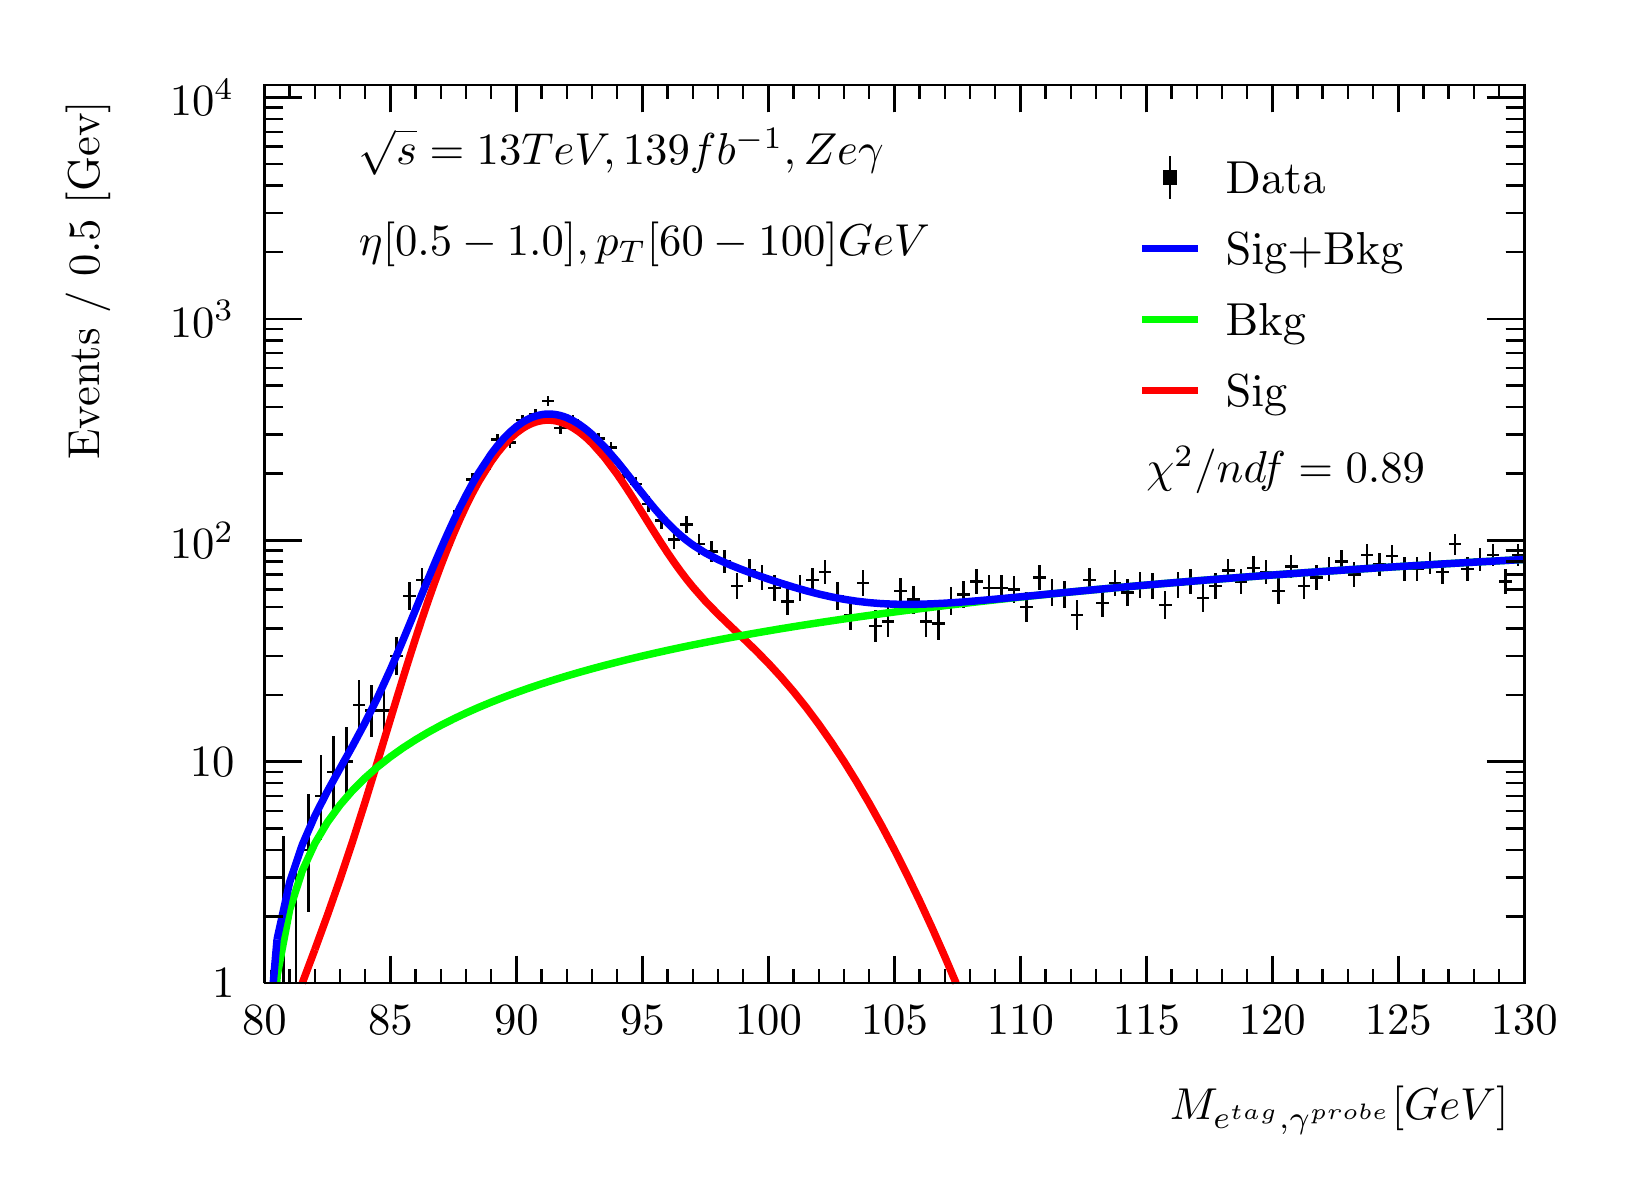
\begin{tikzpicture}
\pgfdeclareplotmark{cross} {
\pgfpathmoveto{\pgfpoint{-0.3\pgfplotmarksize}{\pgfplotmarksize}}
\pgfpathlineto{\pgfpoint{+0.3\pgfplotmarksize}{\pgfplotmarksize}}
\pgfpathlineto{\pgfpoint{+0.3\pgfplotmarksize}{0.3\pgfplotmarksize}}
\pgfpathlineto{\pgfpoint{+1\pgfplotmarksize}{0.3\pgfplotmarksize}}
\pgfpathlineto{\pgfpoint{+1\pgfplotmarksize}{-0.3\pgfplotmarksize}}
\pgfpathlineto{\pgfpoint{+0.3\pgfplotmarksize}{-0.3\pgfplotmarksize}}
\pgfpathlineto{\pgfpoint{+0.3\pgfplotmarksize}{-1.\pgfplotmarksize}}
\pgfpathlineto{\pgfpoint{-0.3\pgfplotmarksize}{-1.\pgfplotmarksize}}
\pgfpathlineto{\pgfpoint{-0.3\pgfplotmarksize}{-0.3\pgfplotmarksize}}
\pgfpathlineto{\pgfpoint{-1.\pgfplotmarksize}{-0.3\pgfplotmarksize}}
\pgfpathlineto{\pgfpoint{-1.\pgfplotmarksize}{0.3\pgfplotmarksize}}
\pgfpathlineto{\pgfpoint{-0.3\pgfplotmarksize}{0.3\pgfplotmarksize}}
\pgfpathclose
\pgfusepathqstroke
}
\pgfdeclareplotmark{cross*} {
\pgfpathmoveto{\pgfpoint{-0.3\pgfplotmarksize}{\pgfplotmarksize}}
\pgfpathlineto{\pgfpoint{+0.3\pgfplotmarksize}{\pgfplotmarksize}}
\pgfpathlineto{\pgfpoint{+0.3\pgfplotmarksize}{0.3\pgfplotmarksize}}
\pgfpathlineto{\pgfpoint{+1\pgfplotmarksize}{0.3\pgfplotmarksize}}
\pgfpathlineto{\pgfpoint{+1\pgfplotmarksize}{-0.3\pgfplotmarksize}}
\pgfpathlineto{\pgfpoint{+0.3\pgfplotmarksize}{-0.3\pgfplotmarksize}}
\pgfpathlineto{\pgfpoint{+0.3\pgfplotmarksize}{-1.\pgfplotmarksize}}
\pgfpathlineto{\pgfpoint{-0.3\pgfplotmarksize}{-1.\pgfplotmarksize}}
\pgfpathlineto{\pgfpoint{-0.3\pgfplotmarksize}{-0.3\pgfplotmarksize}}
\pgfpathlineto{\pgfpoint{-1.\pgfplotmarksize}{-0.3\pgfplotmarksize}}
\pgfpathlineto{\pgfpoint{-1.\pgfplotmarksize}{0.3\pgfplotmarksize}}
\pgfpathlineto{\pgfpoint{-0.3\pgfplotmarksize}{0.3\pgfplotmarksize}}
\pgfpathclose
\pgfusepathqfillstroke
}
\pgfdeclareplotmark{newstar} {
\pgfpathmoveto{\pgfqpoint{0pt}{\pgfplotmarksize}}
\pgfpathlineto{\pgfqpointpolar{44}{0.5\pgfplotmarksize}}
\pgfpathlineto{\pgfqpointpolar{18}{\pgfplotmarksize}}
\pgfpathlineto{\pgfqpointpolar{-20}{0.5\pgfplotmarksize}}
\pgfpathlineto{\pgfqpointpolar{-54}{\pgfplotmarksize}}
\pgfpathlineto{\pgfqpointpolar{-90}{0.5\pgfplotmarksize}}
\pgfpathlineto{\pgfqpointpolar{234}{\pgfplotmarksize}}
\pgfpathlineto{\pgfqpointpolar{198}{0.5\pgfplotmarksize}}
\pgfpathlineto{\pgfqpointpolar{162}{\pgfplotmarksize}}
\pgfpathlineto{\pgfqpointpolar{134}{0.5\pgfplotmarksize}}
\pgfpathclose
\pgfusepathqstroke
}
\pgfdeclareplotmark{newstar*} {
\pgfpathmoveto{\pgfqpoint{0pt}{\pgfplotmarksize}}
\pgfpathlineto{\pgfqpointpolar{44}{0.5\pgfplotmarksize}}
\pgfpathlineto{\pgfqpointpolar{18}{\pgfplotmarksize}}
\pgfpathlineto{\pgfqpointpolar{-20}{0.5\pgfplotmarksize}}
\pgfpathlineto{\pgfqpointpolar{-54}{\pgfplotmarksize}}
\pgfpathlineto{\pgfqpointpolar{-90}{0.5\pgfplotmarksize}}
\pgfpathlineto{\pgfqpointpolar{234}{\pgfplotmarksize}}
\pgfpathlineto{\pgfqpointpolar{198}{0.5\pgfplotmarksize}}
\pgfpathlineto{\pgfqpointpolar{162}{\pgfplotmarksize}}
\pgfpathlineto{\pgfqpointpolar{134}{0.5\pgfplotmarksize}}
\pgfpathclose
\pgfusepathqfillstroke
}
\definecolor{c}{rgb}{1,1,1};
\draw [color=c, fill=c] (0,0) rectangle (20,14.4361);
\draw [color=c, fill=c] (3,2.30977) rectangle (19,13.7143);
\definecolor{c}{rgb}{0,0,0};
\draw [c,line width=0.9] (3,2.30977) -- (3,13.7143) -- (19,13.7143) -- (19,2.30977) -- (3,2.30977);
\definecolor{c}{rgb}{1,1,1};
\draw [color=c, fill=c] (3,2.30977) rectangle (19,13.7143);
\definecolor{c}{rgb}{0,0,0};
\draw [c,line width=0.9] (3,2.30977) -- (3,13.7143) -- (19,13.7143) -- (19,2.30977) -- (3,2.30977);
\draw [c,line width=0.9] (3,2.30977) -- (19,2.30977);
\draw [c,line width=0.9] (3,2.65624) -- (3,2.30977);
\draw [c,line width=0.9] (3.32,2.48301) -- (3.32,2.30977);
\draw [c,line width=0.9] (3.64,2.48301) -- (3.64,2.30977);
\draw [c,line width=0.9] (3.96,2.48301) -- (3.96,2.30977);
\draw [c,line width=0.9] (4.28,2.48301) -- (4.28,2.30977);
\draw [c,line width=0.9] (4.6,2.65624) -- (4.6,2.30977);
\draw [c,line width=0.9] (4.92,2.48301) -- (4.92,2.30977);
\draw [c,line width=0.9] (5.24,2.48301) -- (5.24,2.30977);
\draw [c,line width=0.9] (5.56,2.48301) -- (5.56,2.30977);
\draw [c,line width=0.9] (5.88,2.48301) -- (5.88,2.30977);
\draw [c,line width=0.9] (6.2,2.65624) -- (6.2,2.30977);
\draw [c,line width=0.9] (6.52,2.48301) -- (6.52,2.30977);
\draw [c,line width=0.9] (6.84,2.48301) -- (6.84,2.30977);
\draw [c,line width=0.9] (7.16,2.48301) -- (7.16,2.30977);
\draw [c,line width=0.9] (7.48,2.48301) -- (7.48,2.30977);
\draw [c,line width=0.9] (7.8,2.65624) -- (7.8,2.30977);
\draw [c,line width=0.9] (8.12,2.48301) -- (8.12,2.30977);
\draw [c,line width=0.9] (8.44,2.48301) -- (8.44,2.30977);
\draw [c,line width=0.9] (8.76,2.48301) -- (8.76,2.30977);
\draw [c,line width=0.9] (9.08,2.48301) -- (9.08,2.30977);
\draw [c,line width=0.9] (9.4,2.65624) -- (9.4,2.30977);
\draw [c,line width=0.9] (9.72,2.48301) -- (9.72,2.30977);
\draw [c,line width=0.9] (10.04,2.48301) -- (10.04,2.30977);
\draw [c,line width=0.9] (10.36,2.48301) -- (10.36,2.30977);
\draw [c,line width=0.9] (10.68,2.48301) -- (10.68,2.30977);
\draw [c,line width=0.9] (11,2.65624) -- (11,2.30977);
\draw [c,line width=0.9] (11.32,2.48301) -- (11.32,2.30977);
\draw [c,line width=0.9] (11.64,2.48301) -- (11.64,2.30977);
\draw [c,line width=0.9] (11.96,2.48301) -- (11.96,2.30977);
\draw [c,line width=0.9] (12.28,2.48301) -- (12.28,2.30977);
\draw [c,line width=0.9] (12.6,2.65624) -- (12.6,2.30977);
\draw [c,line width=0.9] (12.92,2.48301) -- (12.92,2.30977);
\draw [c,line width=0.9] (13.24,2.48301) -- (13.24,2.30977);
\draw [c,line width=0.9] (13.56,2.48301) -- (13.56,2.30977);
\draw [c,line width=0.9] (13.88,2.48301) -- (13.88,2.30977);
\draw [c,line width=0.9] (14.2,2.65624) -- (14.2,2.30977);
\draw [c,line width=0.9] (14.52,2.48301) -- (14.52,2.30977);
\draw [c,line width=0.9] (14.84,2.48301) -- (14.84,2.30977);
\draw [c,line width=0.9] (15.16,2.48301) -- (15.16,2.30977);
\draw [c,line width=0.9] (15.48,2.48301) -- (15.48,2.30977);
\draw [c,line width=0.9] (15.8,2.65624) -- (15.8,2.30977);
\draw [c,line width=0.9] (16.12,2.48301) -- (16.12,2.30977);
\draw [c,line width=0.9] (16.44,2.48301) -- (16.44,2.30977);
\draw [c,line width=0.9] (16.76,2.48301) -- (16.76,2.30977);
\draw [c,line width=0.9] (17.08,2.48301) -- (17.08,2.30977);
\draw [c,line width=0.9] (17.4,2.65624) -- (17.4,2.30977);
\draw [c,line width=0.9] (17.72,2.48301) -- (17.72,2.30977);
\draw [c,line width=0.9] (18.04,2.48301) -- (18.04,2.30977);
\draw [c,line width=0.9] (18.36,2.48301) -- (18.36,2.30977);
\draw [c,line width=0.9] (18.68,2.48301) -- (18.68,2.30977);
\draw [c,line width=0.9] (19,2.65624) -- (19,2.30977);
\draw [anchor=base] (3,1.66015) node[scale=1.61424, color=c, rotate=0]{80};
\draw [anchor=base] (4.6,1.66015) node[scale=1.61424, color=c, rotate=0]{85};
\draw [anchor=base] (6.2,1.66015) node[scale=1.61424, color=c, rotate=0]{90};
\draw [anchor=base] (7.8,1.66015) node[scale=1.61424, color=c, rotate=0]{95};
\draw [anchor=base] (9.4,1.66015) node[scale=1.61424, color=c, rotate=0]{100};
\draw [anchor=base] (11,1.66015) node[scale=1.61424, color=c, rotate=0]{105};
\draw [anchor=base] (12.6,1.66015) node[scale=1.61424, color=c, rotate=0]{110};
\draw [anchor=base] (14.2,1.66015) node[scale=1.61424, color=c, rotate=0]{115};
\draw [anchor=base] (15.8,1.66015) node[scale=1.61424, color=c, rotate=0]{120};
\draw [anchor=base] (17.4,1.66015) node[scale=1.61424, color=c, rotate=0]{125};
\draw [anchor=base] (19,1.66015) node[scale=1.61424, color=c, rotate=0]{130};
\draw [anchor= east] (19,0.692932) node[scale=1.61424, color=c, rotate=0]{$M_{e^{tag}, \gamma^{probe}}  [GeV]$};
\draw [c,line width=0.9] (3,13.7143) -- (19,13.7143);
\draw [c,line width=0.9] (3,13.3678) -- (3,13.7143);
\draw [c,line width=0.9] (3.32,13.5411) -- (3.32,13.7143);
\draw [c,line width=0.9] (3.64,13.5411) -- (3.64,13.7143);
\draw [c,line width=0.9] (3.96,13.5411) -- (3.96,13.7143);
\draw [c,line width=0.9] (4.28,13.5411) -- (4.28,13.7143);
\draw [c,line width=0.9] (4.6,13.3678) -- (4.6,13.7143);
\draw [c,line width=0.9] (4.92,13.5411) -- (4.92,13.7143);
\draw [c,line width=0.9] (5.24,13.5411) -- (5.24,13.7143);
\draw [c,line width=0.9] (5.56,13.5411) -- (5.56,13.7143);
\draw [c,line width=0.9] (5.88,13.5411) -- (5.88,13.7143);
\draw [c,line width=0.9] (6.2,13.3678) -- (6.2,13.7143);
\draw [c,line width=0.9] (6.52,13.5411) -- (6.52,13.7143);
\draw [c,line width=0.9] (6.84,13.5411) -- (6.84,13.7143);
\draw [c,line width=0.9] (7.16,13.5411) -- (7.16,13.7143);
\draw [c,line width=0.9] (7.48,13.5411) -- (7.48,13.7143);
\draw [c,line width=0.9] (7.8,13.3678) -- (7.8,13.7143);
\draw [c,line width=0.9] (8.12,13.5411) -- (8.12,13.7143);
\draw [c,line width=0.9] (8.44,13.5411) -- (8.44,13.7143);
\draw [c,line width=0.9] (8.76,13.5411) -- (8.76,13.7143);
\draw [c,line width=0.9] (9.08,13.5411) -- (9.08,13.7143);
\draw [c,line width=0.9] (9.4,13.3678) -- (9.4,13.7143);
\draw [c,line width=0.9] (9.72,13.5411) -- (9.72,13.7143);
\draw [c,line width=0.9] (10.04,13.5411) -- (10.04,13.7143);
\draw [c,line width=0.9] (10.36,13.5411) -- (10.36,13.7143);
\draw [c,line width=0.9] (10.68,13.5411) -- (10.68,13.7143);
\draw [c,line width=0.9] (11,13.3678) -- (11,13.7143);
\draw [c,line width=0.9] (11.32,13.5411) -- (11.32,13.7143);
\draw [c,line width=0.9] (11.64,13.5411) -- (11.64,13.7143);
\draw [c,line width=0.9] (11.96,13.5411) -- (11.96,13.7143);
\draw [c,line width=0.9] (12.28,13.5411) -- (12.28,13.7143);
\draw [c,line width=0.9] (12.6,13.3678) -- (12.6,13.7143);
\draw [c,line width=0.9] (12.92,13.5411) -- (12.92,13.7143);
\draw [c,line width=0.9] (13.24,13.5411) -- (13.24,13.7143);
\draw [c,line width=0.9] (13.56,13.5411) -- (13.56,13.7143);
\draw [c,line width=0.9] (13.88,13.5411) -- (13.88,13.7143);
\draw [c,line width=0.9] (14.2,13.3678) -- (14.2,13.7143);
\draw [c,line width=0.9] (14.52,13.5411) -- (14.52,13.7143);
\draw [c,line width=0.9] (14.84,13.5411) -- (14.84,13.7143);
\draw [c,line width=0.9] (15.16,13.5411) -- (15.16,13.7143);
\draw [c,line width=0.9] (15.48,13.5411) -- (15.48,13.7143);
\draw [c,line width=0.9] (15.8,13.3678) -- (15.8,13.7143);
\draw [c,line width=0.9] (16.12,13.5411) -- (16.12,13.7143);
\draw [c,line width=0.9] (16.44,13.5411) -- (16.44,13.7143);
\draw [c,line width=0.9] (16.76,13.5411) -- (16.76,13.7143);
\draw [c,line width=0.9] (17.08,13.5411) -- (17.08,13.7143);
\draw [c,line width=0.9] (17.4,13.3678) -- (17.4,13.7143);
\draw [c,line width=0.9] (17.72,13.5411) -- (17.72,13.7143);
\draw [c,line width=0.9] (18.04,13.5411) -- (18.04,13.7143);
\draw [c,line width=0.9] (18.36,13.5411) -- (18.36,13.7143);
\draw [c,line width=0.9] (18.68,13.5411) -- (18.68,13.7143);
\draw [c,line width=0.9] (19,13.3678) -- (19,13.7143);
\draw [c,line width=0.9] (3,2.30977) -- (3,13.7143);
\draw [c,line width=0.9] (3.474,2.30978) -- (3,2.30978);
\draw [anchor= east] (2.82,2.30978) node[scale=1.61424, color=c, rotate=0]{1};
\draw [c,line width=0.9] (3.237,3.15616) -- (3,3.15616);
\draw [c,line width=0.9] (3.237,3.65126) -- (3,3.65126);
\draw [c,line width=0.9] (3.237,4.00254) -- (3,4.00254);
\draw [c,line width=0.9] (3.237,4.27501) -- (3,4.27501);
\draw [c,line width=0.9] (3.237,4.49764) -- (3,4.49764);
\draw [c,line width=0.9] (3.237,4.68586) -- (3,4.68586);
\draw [c,line width=0.9] (3.237,4.84892) -- (3,4.84892);
\draw [c,line width=0.9] (3.237,4.99274) -- (3,4.99274);
\draw [c,line width=0.9] (3.474,5.12139) -- (3,5.12139);
\draw [anchor= east] (2.82,5.12139) node[scale=1.61424, color=c, rotate=0]{10};
\draw [c,line width=0.9] (3.237,5.96777) -- (3,5.96777);
\draw [c,line width=0.9] (3.237,6.46287) -- (3,6.46287);
\draw [c,line width=0.9] (3.237,6.81415) -- (3,6.81415);
\draw [c,line width=0.9] (3.237,7.08662) -- (3,7.08662);
\draw [c,line width=0.9] (3.237,7.30925) -- (3,7.30925);
\draw [c,line width=0.9] (3.237,7.49748) -- (3,7.49748);
\draw [c,line width=0.9] (3.237,7.66053) -- (3,7.66053);
\draw [c,line width=0.9] (3.237,7.80435) -- (3,7.80435);
\draw [c,line width=0.9] (3.474,7.933) -- (3,7.933);
\draw [anchor= east] (2.82,7.933) node[scale=1.61424, color=c, rotate=0]{$10^{2}$};
\draw [c,line width=0.9] (3.237,8.77938) -- (3,8.77938);
\draw [c,line width=0.9] (3.237,9.27448) -- (3,9.27448);
\draw [c,line width=0.9] (3.237,9.62576) -- (3,9.62576);
\draw [c,line width=0.9] (3.237,9.89823) -- (3,9.89823);
\draw [c,line width=0.9] (3.237,10.1209) -- (3,10.1209);
\draw [c,line width=0.9] (3.237,10.3091) -- (3,10.3091);
\draw [c,line width=0.9] (3.237,10.4721) -- (3,10.4721);
\draw [c,line width=0.9] (3.237,10.616) -- (3,10.616);
\draw [c,line width=0.9] (3.474,10.7446) -- (3,10.7446);
\draw [anchor= east] (2.82,10.7446) node[scale=1.61424, color=c, rotate=0]{$10^{3}$};
\draw [c,line width=0.9] (3.237,11.591) -- (3,11.591);
\draw [c,line width=0.9] (3.237,12.0861) -- (3,12.0861);
\draw [c,line width=0.9] (3.237,12.4374) -- (3,12.4374);
\draw [c,line width=0.9] (3.237,12.7098) -- (3,12.7098);
\draw [c,line width=0.9] (3.237,12.9325) -- (3,12.9325);
\draw [c,line width=0.9] (3.237,13.1207) -- (3,13.1207);
\draw [c,line width=0.9] (3.237,13.2837) -- (3,13.2837);
\draw [c,line width=0.9] (3.237,13.4276) -- (3,13.4276);
\draw [c,line width=0.9] (3.474,13.5562) -- (3,13.5562);
\draw [anchor= east] (2.82,13.5562) node[scale=1.61424, color=c, rotate=0]{$10^{4}$};
\draw [anchor= east] (0.76,13.7143) node[scale=1.61424, color=c, rotate=90]{Events / 0.5 [Gev]};
\draw [c,line width=0.9] (19,2.30977) -- (19,13.7143);
\draw [c,line width=0.9] (18.526,2.30978) -- (19,2.30978);
\draw [c,line width=0.9] (18.763,3.15616) -- (19,3.15616);
\draw [c,line width=0.9] (18.763,3.65126) -- (19,3.65126);
\draw [c,line width=0.9] (18.763,4.00254) -- (19,4.00254);
\draw [c,line width=0.9] (18.763,4.27501) -- (19,4.27501);
\draw [c,line width=0.9] (18.763,4.49764) -- (19,4.49764);
\draw [c,line width=0.9] (18.763,4.68586) -- (19,4.68586);
\draw [c,line width=0.9] (18.763,4.84892) -- (19,4.84892);
\draw [c,line width=0.9] (18.763,4.99274) -- (19,4.99274);
\draw [c,line width=0.9] (18.526,5.12139) -- (19,5.12139);
\draw [c,line width=0.9] (18.763,5.96777) -- (19,5.96777);
\draw [c,line width=0.9] (18.763,6.46287) -- (19,6.46287);
\draw [c,line width=0.9] (18.763,6.81415) -- (19,6.81415);
\draw [c,line width=0.9] (18.763,7.08662) -- (19,7.08662);
\draw [c,line width=0.9] (18.763,7.30925) -- (19,7.30925);
\draw [c,line width=0.9] (18.763,7.49748) -- (19,7.49748);
\draw [c,line width=0.9] (18.763,7.66053) -- (19,7.66053);
\draw [c,line width=0.9] (18.763,7.80435) -- (19,7.80435);
\draw [c,line width=0.9] (18.526,7.933) -- (19,7.933);
\draw [c,line width=0.9] (18.763,8.77938) -- (19,8.77938);
\draw [c,line width=0.9] (18.763,9.27448) -- (19,9.27448);
\draw [c,line width=0.9] (18.763,9.62576) -- (19,9.62576);
\draw [c,line width=0.9] (18.763,9.89823) -- (19,9.89823);
\draw [c,line width=0.9] (18.763,10.1209) -- (19,10.1209);
\draw [c,line width=0.9] (18.763,10.3091) -- (19,10.3091);
\draw [c,line width=0.9] (18.763,10.4721) -- (19,10.4721);
\draw [c,line width=0.9] (18.763,10.616) -- (19,10.616);
\draw [c,line width=0.9] (18.526,10.7446) -- (19,10.7446);
\draw [c,line width=0.9] (18.763,11.591) -- (19,11.591);
\draw [c,line width=0.9] (18.763,12.0861) -- (19,12.0861);
\draw [c,line width=0.9] (18.763,12.4374) -- (19,12.4374);
\draw [c,line width=0.9] (18.763,12.7098) -- (19,12.7098);
\draw [c,line width=0.9] (18.763,12.9325) -- (19,12.9325);
\draw [c,line width=0.9] (18.763,13.1207) -- (19,13.1207);
\draw [c,line width=0.9] (18.763,13.2837) -- (19,13.2837);
\draw [c,line width=0.9] (18.763,13.4276) -- (19,13.4276);
\draw [c,line width=0.9] (18.526,13.5562) -- (19,13.5562);
\draw [c,line width=0.9] (3.08,2.30977) -- (3,2.30977);
\draw [c,line width=0.9] (3,2.30977) -- (3,2.30977);
\draw [c,line width=0.9] (3.08,2.30977) -- (3.16,2.30977);
\draw [c,line width=0.9] (3.16,2.30977) -- (3.16,2.30977);
\draw [c,line width=0.9] (3.08,2.30977) -- (3.08,2.47817);
\draw [c,line width=0.9] (3.08,2.47817) -- (3.08,2.47817);
\draw [c,line width=0.9] (3.24,3.15615) -- (3.16,3.15615);
\draw [c,line width=0.9] (3.16,3.15615) -- (3.16,3.15615);
\draw [c,line width=0.9] (3.24,3.15615) -- (3.32,3.15615);
\draw [c,line width=0.9] (3.32,3.15615) -- (3.32,3.15615);
\draw [c,line width=0.9] (3.24,3.15615) -- (3.24,4.1832);
\draw [c,line width=0.9] (3.24,4.1832) -- (3.24,4.1832);
\draw [c,line width=0.9] (3.24,3.15615) -- (3.24,2.30977);
\draw [c,line width=0.9] (3.24,2.30977) -- (3.24,2.30977);
\draw [c,line width=0.9] (3.4,2.30977) -- (3.32,2.30977);
\draw [c,line width=0.9] (3.32,2.30977) -- (3.32,2.30977);
\draw [c,line width=0.9] (3.4,2.30977) -- (3.48,2.30977);
\draw [c,line width=0.9] (3.48,2.30977) -- (3.48,2.30977);
\draw [c,line width=0.9] (3.4,2.30977) -- (3.4,3.76746);
\draw [c,line width=0.9] (3.4,3.76746) -- (3.4,3.76746);
\draw [c,line width=0.9] (3.56,4.00253) -- (3.48,4.00253);
\draw [c,line width=0.9] (3.48,4.00253) -- (3.48,4.00253);
\draw [c,line width=0.9] (3.56,4.00253) -- (3.64,4.00253);
\draw [c,line width=0.9] (3.64,4.00253) -- (3.64,4.00253);
\draw [c,line width=0.9] (3.56,4.00253) -- (3.56,4.71393);
\draw [c,line width=0.9] (3.56,4.71393) -- (3.56,4.71393);
\draw [c,line width=0.9] (3.56,4.00253) -- (3.56,3.20736);
\draw [c,line width=0.9] (3.56,3.20736) -- (3.56,3.20736);
\draw [c,line width=0.9] (3.72,4.68586) -- (3.64,4.68586);
\draw [c,line width=0.9] (3.64,4.68586) -- (3.64,4.68586);
\draw [c,line width=0.9] (3.72,4.68586) -- (3.8,4.68586);
\draw [c,line width=0.9] (3.8,4.68586) -- (3.8,4.68586);
\draw [c,line width=0.9] (3.72,4.68586) -- (3.72,5.212);
\draw [c,line width=0.9] (3.72,5.212) -- (3.72,5.212);
\draw [c,line width=0.9] (3.72,4.68586) -- (3.72,4.12404);
\draw [c,line width=0.9] (3.72,4.12404) -- (3.72,4.12404);
\draw [c,line width=0.9] (3.88,4.99273) -- (3.8,4.99273);
\draw [c,line width=0.9] (3.8,4.99273) -- (3.8,4.99273);
\draw [c,line width=0.9] (3.88,4.99273) -- (3.96,4.99273);
\draw [c,line width=0.9] (3.96,4.99273) -- (3.96,4.99273);
\draw [c,line width=0.9] (3.88,4.99273) -- (3.88,5.45206);
\draw [c,line width=0.9] (3.88,5.45206) -- (3.88,5.45206);
\draw [c,line width=0.9] (3.88,4.99273) -- (3.88,4.50909);
\draw [c,line width=0.9] (3.88,4.50909) -- (3.88,4.50909);
\draw [c,line width=0.9] (4.04,5.12139) -- (3.96,5.12139);
\draw [c,line width=0.9] (3.96,5.12139) -- (3.96,5.12139);
\draw [c,line width=0.9] (4.04,5.12139) -- (4.12,5.12139);
\draw [c,line width=0.9] (4.12,5.12139) -- (4.12,5.12139);
\draw [c,line width=0.9] (4.04,5.12139) -- (4.04,5.55531);
\draw [c,line width=0.9] (4.04,5.55531) -- (4.04,5.55531);
\draw [c,line width=0.9] (4.04,5.12139) -- (4.04,4.66675);
\draw [c,line width=0.9] (4.04,4.66675) -- (4.04,4.66675);
\draw [c,line width=0.9] (4.2,5.83911) -- (4.12,5.83911);
\draw [c,line width=0.9] (4.12,5.83911) -- (4.12,5.83911);
\draw [c,line width=0.9] (4.2,5.83911) -- (4.28,5.83911);
\draw [c,line width=0.9] (4.28,5.83911) -- (4.28,5.83911);
\draw [c,line width=0.9] (4.2,5.83911) -- (4.2,6.15535);
\draw [c,line width=0.9] (4.2,6.15535) -- (4.2,6.15535);
\draw [c,line width=0.9] (4.2,5.83911) -- (4.2,5.51442);
\draw [c,line width=0.9] (4.2,5.51442) -- (4.2,5.51442);
\draw [c,line width=0.9] (4.36,5.76932) -- (4.28,5.76932);
\draw [c,line width=0.9] (4.28,5.76932) -- (4.28,5.76932);
\draw [c,line width=0.9] (4.36,5.76932) -- (4.44,5.76932);
\draw [c,line width=0.9] (4.44,5.76932) -- (4.44,5.76932);
\draw [c,line width=0.9] (4.36,5.76932) -- (4.36,6.0954);
\draw [c,line width=0.9] (4.36,6.0954) -- (4.36,6.0954);
\draw [c,line width=0.9] (4.36,5.76932) -- (4.36,5.43401);
\draw [c,line width=0.9] (4.36,5.43401) -- (4.36,5.43401);
\draw [c,line width=0.9] (4.52,5.76932) -- (4.44,5.76932);
\draw [c,line width=0.9] (4.44,5.76932) -- (4.44,5.76932);
\draw [c,line width=0.9] (4.52,5.76932) -- (4.6,5.76932);
\draw [c,line width=0.9] (4.6,5.76932) -- (4.6,5.76932);
\draw [c,line width=0.9] (4.52,5.76932) -- (4.52,6.0954);
\draw [c,line width=0.9] (4.52,6.0954) -- (4.52,6.0954);
\draw [c,line width=0.9] (4.52,5.76932) -- (4.52,5.43401);
\draw [c,line width=0.9] (4.52,5.43401) -- (4.52,5.43401);
\draw [c,line width=0.9] (4.68,6.46287) -- (4.6,6.46287);
\draw [c,line width=0.9] (4.6,6.46287) -- (4.6,6.46287);
\draw [c,line width=0.9] (4.68,6.46287) -- (4.76,6.46287);
\draw [c,line width=0.9] (4.76,6.46287) -- (4.76,6.46287);
\draw [c,line width=0.9] (4.68,6.46287) -- (4.68,6.70361);
\draw [c,line width=0.9] (4.68,6.70361) -- (4.68,6.70361);
\draw [c,line width=0.9] (4.68,6.46287) -- (4.68,6.21823);
\draw [c,line width=0.9] (4.68,6.21823) -- (4.68,6.21823);
\draw [c,line width=0.9] (4.84,7.225) -- (4.76,7.225);
\draw [c,line width=0.9] (4.76,7.225) -- (4.76,7.225);
\draw [c,line width=0.9] (4.84,7.225) -- (4.92,7.225);
\draw [c,line width=0.9] (4.92,7.225) -- (4.92,7.225);
\draw [c,line width=0.9] (4.84,7.225) -- (4.84,7.39808);
\draw [c,line width=0.9] (4.84,7.39808) -- (4.84,7.39808);
\draw [c,line width=0.9] (4.84,7.225) -- (4.84,7.05041);
\draw [c,line width=0.9] (4.84,7.05041) -- (4.84,7.05041);
\draw [c,line width=0.9] (5,7.42563) -- (4.92,7.42563);
\draw [c,line width=0.9] (4.92,7.42563) -- (4.92,7.42563);
\draw [c,line width=0.9] (5,7.42563) -- (5.08,7.42563);
\draw [c,line width=0.9] (5.08,7.42563) -- (5.08,7.42563);
\draw [c,line width=0.9] (5,7.42563) -- (5,7.5844);
\draw [c,line width=0.9] (5,7.5844) -- (5,7.5844);
\draw [c,line width=0.9] (5,7.42563) -- (5,7.26567);
\draw [c,line width=0.9] (5,7.26567) -- (5,7.26567);
\draw [c,line width=0.9] (5.16,7.49747) -- (5.08,7.49747);
\draw [c,line width=0.9] (5.08,7.49747) -- (5.08,7.49747);
\draw [c,line width=0.9] (5.16,7.49747) -- (5.24,7.49747);
\draw [c,line width=0.9] (5.24,7.49747) -- (5.24,7.49747);
\draw [c,line width=0.9] (5.16,7.49747) -- (5.16,7.65143);
\draw [c,line width=0.9] (5.16,7.65143) -- (5.16,7.65143);
\draw [c,line width=0.9] (5.16,7.49747) -- (5.16,7.34244);
\draw [c,line width=0.9] (5.16,7.34244) -- (5.16,7.34244);
\draw [c,line width=0.9] (5.32,7.87037) -- (5.24,7.87037);
\draw [c,line width=0.9] (5.24,7.87037) -- (5.24,7.87037);
\draw [c,line width=0.9] (5.32,7.87037) -- (5.4,7.87037);
\draw [c,line width=0.9] (5.4,7.87037) -- (5.4,7.87037);
\draw [c,line width=0.9] (5.32,7.87037) -- (5.32,8.00162);
\draw [c,line width=0.9] (5.32,8.00162) -- (5.32,8.00162);
\draw [c,line width=0.9] (5.32,7.87037) -- (5.32,7.73843);
\draw [c,line width=0.9] (5.32,7.73843) -- (5.32,7.73843);
\draw [c,line width=0.9] (5.48,8.29945) -- (5.4,8.29945);
\draw [c,line width=0.9] (5.4,8.29945) -- (5.4,8.29945);
\draw [c,line width=0.9] (5.48,8.29945) -- (5.56,8.29945);
\draw [c,line width=0.9] (5.56,8.29945) -- (5.56,8.29945);
\draw [c,line width=0.9] (5.48,8.29945) -- (5.48,8.40451);
\draw [c,line width=0.9] (5.48,8.40451) -- (5.48,8.40451);
\draw [c,line width=0.9] (5.48,8.29945) -- (5.48,8.19439);
\draw [c,line width=0.9] (5.48,8.19439) -- (5.48,8.19439);
\draw [c,line width=0.9] (5.64,8.70382) -- (5.56,8.70382);
\draw [c,line width=0.9] (5.56,8.70382) -- (5.56,8.70382);
\draw [c,line width=0.9] (5.64,8.70382) -- (5.72,8.70382);
\draw [c,line width=0.9] (5.72,8.70382) -- (5.72,8.70382);
\draw [c,line width=0.9] (5.64,8.70382) -- (5.64,8.79286);
\draw [c,line width=0.9] (5.64,8.79286) -- (5.64,8.79286);
\draw [c,line width=0.9] (5.64,8.70382) -- (5.64,8.61479);
\draw [c,line width=0.9] (5.64,8.61479) -- (5.64,8.61479);
\draw [c,line width=0.9] (5.8,8.83895) -- (5.72,8.83895);
\draw [c,line width=0.9] (5.72,8.83895) -- (5.72,8.83895);
\draw [c,line width=0.9] (5.8,8.83895) -- (5.88,8.83895);
\draw [c,line width=0.9] (5.88,8.83895) -- (5.88,8.83895);
\draw [c,line width=0.9] (5.8,8.83895) -- (5.8,8.9232);
\draw [c,line width=0.9] (5.8,8.9232) -- (5.8,8.9232);
\draw [c,line width=0.9] (5.8,8.83895) -- (5.8,8.75471);
\draw [c,line width=0.9] (5.8,8.75471) -- (5.8,8.75471);
\draw [c,line width=0.9] (5.96,9.21184) -- (5.88,9.21184);
\draw [c,line width=0.9] (5.88,9.21184) -- (5.88,9.21184);
\draw [c,line width=0.9] (5.96,9.21184) -- (6.04,9.21184);
\draw [c,line width=0.9] (6.04,9.21184) -- (6.04,9.21184);
\draw [c,line width=0.9] (5.96,9.21184) -- (5.96,9.28416);
\draw [c,line width=0.9] (5.96,9.28416) -- (5.96,9.28416);
\draw [c,line width=0.9] (5.96,9.21184) -- (5.96,9.13953);
\draw [c,line width=0.9] (5.96,9.13953) -- (5.96,9.13953);
\draw [c,line width=0.9] (6.12,9.17708) -- (6.04,9.17708);
\draw [c,line width=0.9] (6.04,9.17708) -- (6.04,9.17708);
\draw [c,line width=0.9] (6.12,9.17708) -- (6.2,9.17708);
\draw [c,line width=0.9] (6.2,9.17708) -- (6.2,9.17708);
\draw [c,line width=0.9] (6.12,9.17708) -- (6.12,9.25043);
\draw [c,line width=0.9] (6.12,9.25043) -- (6.12,9.25043);
\draw [c,line width=0.9] (6.12,9.17708) -- (6.12,9.10372);
\draw [c,line width=0.9] (6.12,9.10372) -- (6.12,9.10372);
\draw [c,line width=0.9] (6.28,9.46271) -- (6.2,9.46271);
\draw [c,line width=0.9] (6.2,9.46271) -- (6.2,9.46271);
\draw [c,line width=0.9] (6.28,9.46271) -- (6.36,9.46271);
\draw [c,line width=0.9] (6.36,9.46271) -- (6.36,9.46271);
\draw [c,line width=0.9] (6.28,9.46271) -- (6.28,9.52797);
\draw [c,line width=0.9] (6.28,9.52797) -- (6.28,9.52797);
\draw [c,line width=0.9] (6.28,9.46271) -- (6.28,9.39744);
\draw [c,line width=0.9] (6.28,9.39744) -- (6.28,9.39744);
\draw [c,line width=0.9] (6.44,9.53056) -- (6.36,9.53056);
\draw [c,line width=0.9] (6.36,9.53056) -- (6.36,9.53056);
\draw [c,line width=0.9] (6.44,9.53056) -- (6.52,9.53056);
\draw [c,line width=0.9] (6.52,9.53056) -- (6.52,9.53056);
\draw [c,line width=0.9] (6.44,9.53056) -- (6.44,9.59403);
\draw [c,line width=0.9] (6.44,9.59403) -- (6.44,9.59403);
\draw [c,line width=0.9] (6.44,9.53056) -- (6.44,9.46709);
\draw [c,line width=0.9] (6.44,9.46709) -- (6.44,9.46709);
\draw [c,line width=0.9] (6.6,9.70265) -- (6.52,9.70265);
\draw [c,line width=0.9] (6.52,9.70265) -- (6.52,9.70265);
\draw [c,line width=0.9] (6.6,9.70265) -- (6.68,9.70265);
\draw [c,line width=0.9] (6.68,9.70265) -- (6.68,9.70265);
\draw [c,line width=0.9] (6.6,9.70265) -- (6.6,9.76181);
\draw [c,line width=0.9] (6.6,9.76181) -- (6.6,9.76181);
\draw [c,line width=0.9] (6.6,9.70265) -- (6.6,9.6435);
\draw [c,line width=0.9] (6.6,9.6435) -- (6.6,9.6435);
\draw [c,line width=0.9] (6.76,9.35709) -- (6.68,9.35709);
\draw [c,line width=0.9] (6.68,9.35709) -- (6.68,9.35709);
\draw [c,line width=0.9] (6.76,9.35709) -- (6.84,9.35709);
\draw [c,line width=0.9] (6.84,9.35709) -- (6.84,9.35709);
\draw [c,line width=0.9] (6.76,9.35709) -- (6.76,9.42524);
\draw [c,line width=0.9] (6.76,9.42524) -- (6.76,9.42524);
\draw [c,line width=0.9] (6.76,9.35709) -- (6.76,9.28895);
\draw [c,line width=0.9] (6.76,9.28895) -- (6.76,9.28895);
\draw [c,line width=0.9] (6.92,9.45571) -- (6.84,9.45571);
\draw [c,line width=0.9] (6.84,9.45571) -- (6.84,9.45571);
\draw [c,line width=0.9] (6.92,9.45571) -- (7,9.45571);
\draw [c,line width=0.9] (7,9.45571) -- (7,9.45571);
\draw [c,line width=0.9] (6.92,9.45571) -- (6.92,9.52116);
\draw [c,line width=0.9] (6.92,9.52116) -- (6.92,9.52116);
\draw [c,line width=0.9] (6.92,9.45571) -- (6.92,9.39026);
\draw [c,line width=0.9] (6.92,9.39026) -- (6.92,9.39026);
\draw [c,line width=0.9] (7.08,9.32237) -- (7,9.32237);
\draw [c,line width=0.9] (7,9.32237) -- (7,9.32237);
\draw [c,line width=0.9] (7.08,9.32237) -- (7.16,9.32237);
\draw [c,line width=0.9] (7.16,9.32237) -- (7.16,9.32237);
\draw [c,line width=0.9] (7.08,9.32237) -- (7.08,9.39149);
\draw [c,line width=0.9] (7.08,9.39149) -- (7.08,9.39149);
\draw [c,line width=0.9] (7.08,9.32237) -- (7.08,9.25325);
\draw [c,line width=0.9] (7.08,9.25325) -- (7.08,9.25325);
\draw [c,line width=0.9] (7.24,9.22463) -- (7.16,9.22463);
\draw [c,line width=0.9] (7.16,9.22463) -- (7.16,9.22463);
\draw [c,line width=0.9] (7.24,9.22463) -- (7.32,9.22463);
\draw [c,line width=0.9] (7.32,9.22463) -- (7.32,9.22463);
\draw [c,line width=0.9] (7.24,9.22463) -- (7.24,9.29657);
\draw [c,line width=0.9] (7.24,9.29657) -- (7.24,9.29657);
\draw [c,line width=0.9] (7.24,9.22463) -- (7.24,9.15269);
\draw [c,line width=0.9] (7.24,9.15269) -- (7.24,9.15269);
\draw [c,line width=0.9] (7.4,9.1091) -- (7.32,9.1091);
\draw [c,line width=0.9] (7.32,9.1091) -- (7.32,9.1091);
\draw [c,line width=0.9] (7.4,9.1091) -- (7.48,9.1091);
\draw [c,line width=0.9] (7.48,9.1091) -- (7.48,9.1091);
\draw [c,line width=0.9] (7.4,9.1091) -- (7.4,9.18452);
\draw [c,line width=0.9] (7.4,9.18452) -- (7.4,9.18452);
\draw [c,line width=0.9] (7.4,9.1091) -- (7.4,9.03367);
\draw [c,line width=0.9] (7.4,9.03367) -- (7.4,9.03367);
\draw [c,line width=0.9] (7.56,8.73587) -- (7.48,8.73587);
\draw [c,line width=0.9] (7.48,8.73587) -- (7.48,8.73587);
\draw [c,line width=0.9] (7.56,8.73587) -- (7.64,8.73587);
\draw [c,line width=0.9] (7.64,8.73587) -- (7.64,8.73587);
\draw [c,line width=0.9] (7.56,8.73587) -- (7.56,8.82375);
\draw [c,line width=0.9] (7.56,8.82375) -- (7.56,8.82375);
\draw [c,line width=0.9] (7.56,8.73587) -- (7.56,8.648);
\draw [c,line width=0.9] (7.56,8.648) -- (7.56,8.648);
\draw [c,line width=0.9] (7.72,8.65073) -- (7.64,8.65073);
\draw [c,line width=0.9] (7.64,8.65073) -- (7.64,8.65073);
\draw [c,line width=0.9] (7.72,8.65073) -- (7.8,8.65073);
\draw [c,line width=0.9] (7.8,8.65073) -- (7.8,8.65073);
\draw [c,line width=0.9] (7.72,8.65073) -- (7.72,8.74172);
\draw [c,line width=0.9] (7.72,8.74172) -- (7.72,8.74172);
\draw [c,line width=0.9] (7.72,8.65073) -- (7.72,8.55973);
\draw [c,line width=0.9] (7.72,8.55973) -- (7.72,8.55973);
\draw [c,line width=0.9] (7.88,8.39509) -- (7.8,8.39509);
\draw [c,line width=0.9] (7.8,8.39509) -- (7.8,8.39509);
\draw [c,line width=0.9] (7.88,8.39509) -- (7.96,8.39509);
\draw [c,line width=0.9] (7.96,8.39509) -- (7.96,8.39509);
\draw [c,line width=0.9] (7.88,8.39509) -- (7.88,8.49612);
\draw [c,line width=0.9] (7.88,8.49612) -- (7.88,8.49612);
\draw [c,line width=0.9] (7.88,8.39509) -- (7.88,8.29407);
\draw [c,line width=0.9] (7.88,8.29407) -- (7.88,8.29407);
\draw [c,line width=0.9] (8.04,8.18578) -- (7.96,8.18578);
\draw [c,line width=0.9] (7.96,8.18578) -- (7.96,8.18578);
\draw [c,line width=0.9] (8.04,8.18578) -- (8.12,8.18578);
\draw [c,line width=0.9] (8.12,8.18578) -- (8.12,8.18578);
\draw [c,line width=0.9] (8.04,8.18578) -- (8.04,8.29584);
\draw [c,line width=0.9] (8.04,8.29584) -- (8.04,8.29584);
\draw [c,line width=0.9] (8.04,8.18578) -- (8.04,8.07571);
\draw [c,line width=0.9] (8.04,8.07571) -- (8.04,8.07571);
\draw [c,line width=0.9] (8.2,7.94515) -- (8.12,7.94515);
\draw [c,line width=0.9] (8.12,7.94515) -- (8.12,7.94515);
\draw [c,line width=0.9] (8.2,7.94515) -- (8.28,7.94515);
\draw [c,line width=0.9] (8.28,7.94515) -- (8.28,7.94515);
\draw [c,line width=0.9] (8.2,7.94515) -- (8.2,8.0666);
\draw [c,line width=0.9] (8.2,8.0666) -- (8.2,8.0666);
\draw [c,line width=0.9] (8.2,7.94515) -- (8.2,7.8237);
\draw [c,line width=0.9] (8.2,7.8237) -- (8.2,7.8237);
\draw [c,line width=0.9] (8.36,8.1351) -- (8.28,8.1351);
\draw [c,line width=0.9] (8.28,8.1351) -- (8.28,8.1351);
\draw [c,line width=0.9] (8.36,8.1351) -- (8.44,8.1351);
\draw [c,line width=0.9] (8.44,8.1351) -- (8.44,8.1351);
\draw [c,line width=0.9] (8.36,8.1351) -- (8.36,8.24747);
\draw [c,line width=0.9] (8.36,8.24747) -- (8.36,8.24747);
\draw [c,line width=0.9] (8.36,8.1351) -- (8.36,8.02273);
\draw [c,line width=0.9] (8.36,8.02273) -- (8.36,8.02273);
\draw [c,line width=0.9] (8.52,7.88315) -- (8.44,7.88315);
\draw [c,line width=0.9] (8.44,7.88315) -- (8.44,7.88315);
\draw [c,line width=0.9] (8.52,7.88315) -- (8.6,7.88315);
\draw [c,line width=0.9] (8.6,7.88315) -- (8.6,7.88315);
\draw [c,line width=0.9] (8.52,7.88315) -- (8.52,8.01369);
\draw [c,line width=0.9] (8.52,8.01369) -- (8.52,8.01369);
\draw [c,line width=0.9] (8.52,7.88315) -- (8.52,7.75194);
\draw [c,line width=0.9] (8.52,7.75194) -- (8.52,7.75194);
\draw [c,line width=0.9] (8.68,7.7907) -- (8.6,7.7907);
\draw [c,line width=0.9] (8.6,7.7907) -- (8.6,7.7907);
\draw [c,line width=0.9] (8.68,7.7907) -- (8.76,7.7907);
\draw [c,line width=0.9] (8.76,7.7907) -- (8.76,7.7907);
\draw [c,line width=0.9] (8.68,7.7907) -- (8.68,7.9265);
\draw [c,line width=0.9] (8.68,7.9265) -- (8.68,7.9265);
\draw [c,line width=0.9] (8.68,7.7907) -- (8.68,7.65415);
\draw [c,line width=0.9] (8.68,7.65415) -- (8.68,7.65415);
\draw [c,line width=0.9] (8.84,7.66052) -- (8.76,7.66052);
\draw [c,line width=0.9] (8.76,7.66052) -- (8.76,7.66052);
\draw [c,line width=0.9] (8.84,7.66052) -- (8.92,7.66052);
\draw [c,line width=0.9] (8.92,7.66052) -- (8.92,7.66052);
\draw [c,line width=0.9] (8.84,7.66052) -- (8.84,7.8041);
\draw [c,line width=0.9] (8.84,7.8041) -- (8.84,7.8041);
\draw [c,line width=0.9] (8.84,7.66052) -- (8.84,7.51607);
\draw [c,line width=0.9] (8.84,7.51607) -- (8.84,7.51607);
\draw [c,line width=0.9] (9,7.34928) -- (8.92,7.34928);
\draw [c,line width=0.9] (8.92,7.34928) -- (8.92,7.34928);
\draw [c,line width=0.9] (9,7.34928) -- (9.08,7.34928);
\draw [c,line width=0.9] (9.08,7.34928) -- (9.08,7.34928);
\draw [c,line width=0.9] (9,7.34928) -- (9,7.51335);
\draw [c,line width=0.9] (9,7.51335) -- (9,7.51335);
\draw [c,line width=0.9] (9,7.34928) -- (9,7.18392);
\draw [c,line width=0.9] (9,7.18392) -- (9,7.18392);
\draw [c,line width=0.9] (9.16,7.54871) -- (9.08,7.54871);
\draw [c,line width=0.9] (9.08,7.54871) -- (9.08,7.54871);
\draw [c,line width=0.9] (9.16,7.54871) -- (9.24,7.54871);
\draw [c,line width=0.9] (9.24,7.54871) -- (9.24,7.54871);
\draw [c,line width=0.9] (9.16,7.54871) -- (9.16,7.69933);
\draw [c,line width=0.9] (9.16,7.69933) -- (9.16,7.69933);
\draw [c,line width=0.9] (9.16,7.54871) -- (9.16,7.39709);
\draw [c,line width=0.9] (9.16,7.39709) -- (9.16,7.39709);
\draw [c,line width=0.9] (9.32,7.46208) -- (9.24,7.46208);
\draw [c,line width=0.9] (9.24,7.46208) -- (9.24,7.46208);
\draw [c,line width=0.9] (9.32,7.46208) -- (9.4,7.46208);
\draw [c,line width=0.9] (9.4,7.46208) -- (9.4,7.46208);
\draw [c,line width=0.9] (9.32,7.46208) -- (9.32,7.61839);
\draw [c,line width=0.9] (9.32,7.61839) -- (9.32,7.61839);
\draw [c,line width=0.9] (9.32,7.46208) -- (9.32,7.30464);
\draw [c,line width=0.9] (9.32,7.30464) -- (9.32,7.30464);
\draw [c,line width=0.9] (9.48,7.32943) -- (9.4,7.32943);
\draw [c,line width=0.9] (9.4,7.32943) -- (9.4,7.32943);
\draw [c,line width=0.9] (9.48,7.32943) -- (9.56,7.32943);
\draw [c,line width=0.9] (9.56,7.32943) -- (9.56,7.32943);
\draw [c,line width=0.9] (9.48,7.32943) -- (9.48,7.49491);
\draw [c,line width=0.9] (9.48,7.49491) -- (9.48,7.49491);
\draw [c,line width=0.9] (9.48,7.32943) -- (9.48,7.16263);
\draw [c,line width=0.9] (9.48,7.16263) -- (9.48,7.16263);
\draw [c,line width=0.9] (9.64,7.15777) -- (9.56,7.15777);
\draw [c,line width=0.9] (9.56,7.15777) -- (9.56,7.15777);
\draw [c,line width=0.9] (9.64,7.15777) -- (9.72,7.15777);
\draw [c,line width=0.9] (9.72,7.15777) -- (9.72,7.15777);
\draw [c,line width=0.9] (9.64,7.15777) -- (9.64,7.33594);
\draw [c,line width=0.9] (9.64,7.33594) -- (9.64,7.33594);
\draw [c,line width=0.9] (9.64,7.15777) -- (9.64,6.97796);
\draw [c,line width=0.9] (9.64,6.97796) -- (9.64,6.97796);
\draw [c,line width=0.9] (9.8,7.32943) -- (9.72,7.32943);
\draw [c,line width=0.9] (9.72,7.32943) -- (9.72,7.32943);
\draw [c,line width=0.9] (9.8,7.32943) -- (9.88,7.32943);
\draw [c,line width=0.9] (9.88,7.32943) -- (9.88,7.32943);
\draw [c,line width=0.9] (9.8,7.32943) -- (9.8,7.49491);
\draw [c,line width=0.9] (9.8,7.49491) -- (9.8,7.49491);
\draw [c,line width=0.9] (9.8,7.32943) -- (9.8,7.16263);
\draw [c,line width=0.9] (9.8,7.16263) -- (9.8,7.16263);
\draw [c,line width=0.9] (9.96,7.42563) -- (9.88,7.42563);
\draw [c,line width=0.9] (9.88,7.42563) -- (9.88,7.42563);
\draw [c,line width=0.9] (9.96,7.42563) -- (10.04,7.42563);
\draw [c,line width=0.9] (10.04,7.42563) -- (10.04,7.42563);
\draw [c,line width=0.9] (9.96,7.42563) -- (9.96,7.5844);
\draw [c,line width=0.9] (9.96,7.5844) -- (9.96,7.5844);
\draw [c,line width=0.9] (9.96,7.42563) -- (9.96,7.26567);
\draw [c,line width=0.9] (9.96,7.26567) -- (9.96,7.26567);
\draw [c,line width=0.9] (10.12,7.53187) -- (10.04,7.53187);
\draw [c,line width=0.9] (10.04,7.53187) -- (10.04,7.53187);
\draw [c,line width=0.9] (10.12,7.53187) -- (10.2,7.53187);
\draw [c,line width=0.9] (10.2,7.53187) -- (10.2,7.53187);
\draw [c,line width=0.9] (10.12,7.53187) -- (10.12,7.68358);
\draw [c,line width=0.9] (10.12,7.68358) -- (10.12,7.68358);
\draw [c,line width=0.9] (10.12,7.53187) -- (10.12,7.37914);
\draw [c,line width=0.9] (10.12,7.37914) -- (10.12,7.37914);
\draw [c,line width=0.9] (10.28,7.225) -- (10.2,7.225);
\draw [c,line width=0.9] (10.2,7.225) -- (10.2,7.225);
\draw [c,line width=0.9] (10.28,7.225) -- (10.36,7.225);
\draw [c,line width=0.9] (10.36,7.225) -- (10.36,7.225);
\draw [c,line width=0.9] (10.28,7.225) -- (10.28,7.39808);
\draw [c,line width=0.9] (10.28,7.39808) -- (10.28,7.39808);
\draw [c,line width=0.9] (10.28,7.225) -- (10.28,7.05041);
\draw [c,line width=0.9] (10.28,7.05041) -- (10.28,7.05041);
\draw [c,line width=0.9] (10.44,6.9848) -- (10.36,6.9848);
\draw [c,line width=0.9] (10.36,6.9848) -- (10.36,6.9848);
\draw [c,line width=0.9] (10.44,6.9848) -- (10.52,6.9848);
\draw [c,line width=0.9] (10.52,6.9848) -- (10.52,6.9848);
\draw [c,line width=0.9] (10.44,6.9848) -- (10.44,7.17678);
\draw [c,line width=0.9] (10.44,7.17678) -- (10.44,7.17678);
\draw [c,line width=0.9] (10.44,6.9848) -- (10.44,6.7908);
\draw [c,line width=0.9] (10.44,6.7908) -- (10.44,6.7908);
\draw [c,line width=0.9] (10.6,7.38805) -- (10.52,7.38805);
\draw [c,line width=0.9] (10.52,7.38805) -- (10.52,7.38805);
\draw [c,line width=0.9] (10.6,7.38805) -- (10.68,7.38805);
\draw [c,line width=0.9] (10.68,7.38805) -- (10.68,7.38805);
\draw [c,line width=0.9] (10.6,7.38805) -- (10.6,7.54941);
\draw [c,line width=0.9] (10.6,7.54941) -- (10.6,7.54941);
\draw [c,line width=0.9] (10.6,7.38805) -- (10.6,7.22546);
\draw [c,line width=0.9] (10.6,7.22546) -- (10.6,7.22546);
\draw [c,line width=0.9] (10.76,6.8443) -- (10.68,6.8443);
\draw [c,line width=0.9] (10.68,6.8443) -- (10.68,6.8443);
\draw [c,line width=0.9] (10.76,6.8443) -- (10.84,6.8443);
\draw [c,line width=0.9] (10.84,6.8443) -- (10.84,6.8443);
\draw [c,line width=0.9] (10.76,6.8443) -- (10.76,7.0483);
\draw [c,line width=0.9] (10.76,7.0483) -- (10.76,7.0483);
\draw [c,line width=0.9] (10.76,6.8443) -- (10.76,6.63787);
\draw [c,line width=0.9] (10.76,6.63787) -- (10.76,6.63787);
\draw [c,line width=0.9] (10.92,6.90245) -- (10.84,6.90245);
\draw [c,line width=0.9] (10.84,6.90245) -- (10.84,6.90245);
\draw [c,line width=0.9] (10.92,6.90245) -- (11,6.90245);
\draw [c,line width=0.9] (11,6.90245) -- (11,6.90245);
\draw [c,line width=0.9] (10.92,6.90245) -- (10.92,7.10138);
\draw [c,line width=0.9] (10.92,7.10138) -- (10.92,7.10138);
\draw [c,line width=0.9] (10.92,6.90245) -- (10.92,6.70127);
\draw [c,line width=0.9] (10.92,6.70127) -- (10.92,6.70127);
\draw [c,line width=0.9] (11.08,7.28872) -- (11,7.28872);
\draw [c,line width=0.9] (11,7.28872) -- (11,7.28872);
\draw [c,line width=0.9] (11.08,7.28872) -- (11.16,7.28872);
\draw [c,line width=0.9] (11.16,7.28872) -- (11.16,7.28872);
\draw [c,line width=0.9] (11.08,7.28872) -- (11.08,7.45712);
\draw [c,line width=0.9] (11.08,7.45712) -- (11.08,7.45712);
\draw [c,line width=0.9] (11.08,7.28872) -- (11.08,7.11893);
\draw [c,line width=0.9] (11.08,7.11893) -- (11.08,7.11893);
\draw [c,line width=0.9] (11.24,7.18059) -- (11.16,7.18059);
\draw [c,line width=0.9] (11.16,7.18059) -- (11.16,7.18059);
\draw [c,line width=0.9] (11.24,7.18059) -- (11.32,7.18059);
\draw [c,line width=0.9] (11.32,7.18059) -- (11.32,7.18059);
\draw [c,line width=0.9] (11.24,7.18059) -- (11.24,7.35702);
\draw [c,line width=0.9] (11.24,7.35702) -- (11.24,7.35702);
\draw [c,line width=0.9] (11.24,7.18059) -- (11.24,7.00257);
\draw [c,line width=0.9] (11.24,7.00257) -- (11.24,7.00257);
\draw [c,line width=0.9] (11.4,6.90245) -- (11.32,6.90245);
\draw [c,line width=0.9] (11.32,6.90245) -- (11.32,6.90245);
\draw [c,line width=0.9] (11.4,6.90245) -- (11.48,6.90245);
\draw [c,line width=0.9] (11.48,6.90245) -- (11.48,6.90245);
\draw [c,line width=0.9] (11.4,6.90245) -- (11.4,7.10138);
\draw [c,line width=0.9] (11.4,7.10138) -- (11.4,7.10138);
\draw [c,line width=0.9] (11.4,6.90245) -- (11.4,6.70127);
\draw [c,line width=0.9] (11.4,6.70127) -- (11.4,6.70127);
\draw [c,line width=0.9] (11.56,6.87372) -- (11.48,6.87372);
\draw [c,line width=0.9] (11.48,6.87372) -- (11.48,6.87372);
\draw [c,line width=0.9] (11.56,6.87372) -- (11.64,6.87372);
\draw [c,line width=0.9] (11.64,6.87372) -- (11.64,6.87372);
\draw [c,line width=0.9] (11.56,6.87372) -- (11.56,7.07514);
\draw [c,line width=0.9] (11.56,7.07514) -- (11.56,7.07514);
\draw [c,line width=0.9] (11.56,6.87372) -- (11.56,6.66997);
\draw [c,line width=0.9] (11.56,6.66997) -- (11.56,6.66997);
\draw [c,line width=0.9] (11.72,7.15777) -- (11.64,7.15777);
\draw [c,line width=0.9] (11.64,7.15777) -- (11.64,7.15777);
\draw [c,line width=0.9] (11.72,7.15777) -- (11.8,7.15777);
\draw [c,line width=0.9] (11.8,7.15777) -- (11.8,7.15777);
\draw [c,line width=0.9] (11.72,7.15777) -- (11.72,7.33594);
\draw [c,line width=0.9] (11.72,7.33594) -- (11.72,7.33594);
\draw [c,line width=0.9] (11.72,7.15777) -- (11.72,6.97796);
\draw [c,line width=0.9] (11.72,6.97796) -- (11.72,6.97796);
\draw [c,line width=0.9] (11.88,7.24661) -- (11.8,7.24661);
\draw [c,line width=0.9] (11.8,7.24661) -- (11.8,7.24661);
\draw [c,line width=0.9] (11.88,7.24661) -- (11.96,7.24661);
\draw [c,line width=0.9] (11.96,7.24661) -- (11.96,7.24661);
\draw [c,line width=0.9] (11.88,7.24661) -- (11.88,7.41809);
\draw [c,line width=0.9] (11.88,7.41809) -- (11.88,7.41809);
\draw [c,line width=0.9] (11.88,7.24661) -- (11.88,7.07366);
\draw [c,line width=0.9] (11.88,7.07366) -- (11.88,7.07366);
\draw [c,line width=0.9] (12.04,7.40698) -- (11.96,7.40698);
\draw [c,line width=0.9] (11.96,7.40698) -- (11.96,7.40698);
\draw [c,line width=0.9] (12.04,7.40698) -- (12.12,7.40698);
\draw [c,line width=0.9] (12.12,7.40698) -- (12.12,7.40698);
\draw [c,line width=0.9] (12.04,7.40698) -- (12.04,7.56704);
\draw [c,line width=0.9] (12.04,7.56704) -- (12.04,7.56704);
\draw [c,line width=0.9] (12.04,7.40698) -- (12.04,7.24572);
\draw [c,line width=0.9] (12.04,7.24572) -- (12.04,7.24572);
\draw [c,line width=0.9] (12.2,7.32943) -- (12.12,7.32943);
\draw [c,line width=0.9] (12.12,7.32943) -- (12.12,7.32943);
\draw [c,line width=0.9] (12.2,7.32943) -- (12.28,7.32943);
\draw [c,line width=0.9] (12.28,7.32943) -- (12.28,7.32943);
\draw [c,line width=0.9] (12.2,7.32943) -- (12.2,7.49491);
\draw [c,line width=0.9] (12.2,7.49491) -- (12.2,7.49491);
\draw [c,line width=0.9] (12.2,7.32943) -- (12.2,7.16263);
\draw [c,line width=0.9] (12.2,7.16263) -- (12.2,7.16263);
\draw [c,line width=0.9] (12.36,7.32943) -- (12.28,7.32943);
\draw [c,line width=0.9] (12.28,7.32943) -- (12.28,7.32943);
\draw [c,line width=0.9] (12.36,7.32943) -- (12.44,7.32943);
\draw [c,line width=0.9] (12.44,7.32943) -- (12.44,7.32943);
\draw [c,line width=0.9] (12.36,7.32943) -- (12.36,7.49491);
\draw [c,line width=0.9] (12.36,7.49491) -- (12.36,7.49491);
\draw [c,line width=0.9] (12.36,7.32943) -- (12.36,7.16263);
\draw [c,line width=0.9] (12.36,7.16263) -- (12.36,7.16263);
\draw [c,line width=0.9] (12.52,7.30925) -- (12.44,7.30925);
\draw [c,line width=0.9] (12.44,7.30925) -- (12.44,7.30925);
\draw [c,line width=0.9] (12.52,7.30925) -- (12.6,7.30925);
\draw [c,line width=0.9] (12.6,7.30925) -- (12.6,7.30925);
\draw [c,line width=0.9] (12.52,7.30925) -- (12.52,7.47616);
\draw [c,line width=0.9] (12.52,7.47616) -- (12.52,7.47616);
\draw [c,line width=0.9] (12.52,7.30925) -- (12.52,7.14097);
\draw [c,line width=0.9] (12.52,7.14097) -- (12.52,7.14097);
\draw [c,line width=0.9] (12.68,7.08662) -- (12.6,7.08662);
\draw [c,line width=0.9] (12.6,7.08662) -- (12.6,7.08662);
\draw [c,line width=0.9] (12.68,7.08662) -- (12.76,7.08662);
\draw [c,line width=0.9] (12.76,7.08662) -- (12.76,7.08662);
\draw [c,line width=0.9] (12.68,7.08662) -- (12.68,7.27034);
\draw [c,line width=0.9] (12.68,7.27034) -- (12.68,7.27034);
\draw [c,line width=0.9] (12.68,7.08662) -- (12.68,6.90111);
\draw [c,line width=0.9] (12.68,6.90111) -- (12.68,6.90111);
\draw [c,line width=0.9] (12.84,7.46208) -- (12.76,7.46208);
\draw [c,line width=0.9] (12.76,7.46208) -- (12.76,7.46208);
\draw [c,line width=0.9] (12.84,7.46208) -- (12.92,7.46208);
\draw [c,line width=0.9] (12.92,7.46208) -- (12.92,7.46208);
\draw [c,line width=0.9] (12.84,7.46208) -- (12.84,7.61839);
\draw [c,line width=0.9] (12.84,7.61839) -- (12.84,7.61839);
\draw [c,line width=0.9] (12.84,7.46208) -- (12.84,7.30464);
\draw [c,line width=0.9] (12.84,7.30464) -- (12.84,7.30464);
\draw [c,line width=0.9] (13,7.26785) -- (12.92,7.26785);
\draw [c,line width=0.9] (12.92,7.26785) -- (12.92,7.26785);
\draw [c,line width=0.9] (13,7.26785) -- (13.08,7.26785);
\draw [c,line width=0.9] (13.08,7.26785) -- (13.08,7.26785);
\draw [c,line width=0.9] (13,7.26785) -- (13,7.43777);
\draw [c,line width=0.9] (13,7.43777) -- (13,7.43777);
\draw [c,line width=0.9] (13,7.26785) -- (13,7.0965);
\draw [c,line width=0.9] (13,7.0965) -- (13,7.0965);
\draw [c,line width=0.9] (13.16,7.24661) -- (13.08,7.24661);
\draw [c,line width=0.9] (13.08,7.24661) -- (13.08,7.24661);
\draw [c,line width=0.9] (13.16,7.24661) -- (13.24,7.24661);
\draw [c,line width=0.9] (13.24,7.24661) -- (13.24,7.24661);
\draw [c,line width=0.9] (13.16,7.24661) -- (13.16,7.41809);
\draw [c,line width=0.9] (13.16,7.41809) -- (13.16,7.41809);
\draw [c,line width=0.9] (13.16,7.24661) -- (13.16,7.07366);
\draw [c,line width=0.9] (13.16,7.07366) -- (13.16,7.07366);
\draw [c,line width=0.9] (13.32,6.9848) -- (13.24,6.9848);
\draw [c,line width=0.9] (13.24,6.9848) -- (13.24,6.9848);
\draw [c,line width=0.9] (13.32,6.9848) -- (13.4,6.9848);
\draw [c,line width=0.9] (13.4,6.9848) -- (13.4,6.9848);
\draw [c,line width=0.9] (13.32,6.9848) -- (13.32,7.17678);
\draw [c,line width=0.9] (13.32,7.17678) -- (13.32,7.17678);
\draw [c,line width=0.9] (13.32,6.9848) -- (13.32,6.7908);
\draw [c,line width=0.9] (13.32,6.7908) -- (13.32,6.7908);
\draw [c,line width=0.9] (13.48,7.42563) -- (13.4,7.42563);
\draw [c,line width=0.9] (13.4,7.42563) -- (13.4,7.42563);
\draw [c,line width=0.9] (13.48,7.42563) -- (13.56,7.42563);
\draw [c,line width=0.9] (13.56,7.42563) -- (13.56,7.42563);
\draw [c,line width=0.9] (13.48,7.42563) -- (13.48,7.5844);
\draw [c,line width=0.9] (13.48,7.5844) -- (13.48,7.5844);
\draw [c,line width=0.9] (13.48,7.42563) -- (13.48,7.26567);
\draw [c,line width=0.9] (13.48,7.26567) -- (13.48,7.26567);
\draw [c,line width=0.9] (13.64,7.13451) -- (13.56,7.13451);
\draw [c,line width=0.9] (13.56,7.13451) -- (13.56,7.13451);
\draw [c,line width=0.9] (13.64,7.13451) -- (13.72,7.13451);
\draw [c,line width=0.9] (13.72,7.13451) -- (13.72,7.13451);
\draw [c,line width=0.9] (13.64,7.13451) -- (13.64,7.31447);
\draw [c,line width=0.9] (13.64,7.31447) -- (13.64,7.31447);
\draw [c,line width=0.9] (13.64,7.13451) -- (13.64,6.95286);
\draw [c,line width=0.9] (13.64,6.95286) -- (13.64,6.95286);
\draw [c,line width=0.9] (13.8,7.38805) -- (13.72,7.38805);
\draw [c,line width=0.9] (13.72,7.38805) -- (13.72,7.38805);
\draw [c,line width=0.9] (13.8,7.38805) -- (13.88,7.38805);
\draw [c,line width=0.9] (13.88,7.38805) -- (13.88,7.38805);
\draw [c,line width=0.9] (13.8,7.38805) -- (13.8,7.54941);
\draw [c,line width=0.9] (13.8,7.54941) -- (13.8,7.54941);
\draw [c,line width=0.9] (13.8,7.38805) -- (13.8,7.22546);
\draw [c,line width=0.9] (13.8,7.22546) -- (13.8,7.22546);
\draw [c,line width=0.9] (13.96,7.26785) -- (13.88,7.26785);
\draw [c,line width=0.9] (13.88,7.26785) -- (13.88,7.26785);
\draw [c,line width=0.9] (13.96,7.26785) -- (14.04,7.26785);
\draw [c,line width=0.9] (14.04,7.26785) -- (14.04,7.26785);
\draw [c,line width=0.9] (13.96,7.26785) -- (13.96,7.43777);
\draw [c,line width=0.9] (13.96,7.43777) -- (13.96,7.43777);
\draw [c,line width=0.9] (13.96,7.26785) -- (13.96,7.0965);
\draw [c,line width=0.9] (13.96,7.0965) -- (13.96,7.0965);
\draw [c,line width=0.9] (14.12,7.36882) -- (14.04,7.36882);
\draw [c,line width=0.9] (14.04,7.36882) -- (14.04,7.36882);
\draw [c,line width=0.9] (14.12,7.36882) -- (14.2,7.36882);
\draw [c,line width=0.9] (14.2,7.36882) -- (14.2,7.36882);
\draw [c,line width=0.9] (14.12,7.36882) -- (14.12,7.53152);
\draw [c,line width=0.9] (14.12,7.53152) -- (14.12,7.53152);
\draw [c,line width=0.9] (14.12,7.36882) -- (14.12,7.20486);
\draw [c,line width=0.9] (14.12,7.20486) -- (14.12,7.20486);
\draw [c,line width=0.9] (14.28,7.34928) -- (14.2,7.34928);
\draw [c,line width=0.9] (14.2,7.34928) -- (14.2,7.34928);
\draw [c,line width=0.9] (14.28,7.34928) -- (14.36,7.34928);
\draw [c,line width=0.9] (14.36,7.34928) -- (14.36,7.34928);
\draw [c,line width=0.9] (14.28,7.34928) -- (14.28,7.51335);
\draw [c,line width=0.9] (14.28,7.51335) -- (14.28,7.51335);
\draw [c,line width=0.9] (14.28,7.34928) -- (14.28,7.18392);
\draw [c,line width=0.9] (14.28,7.18392) -- (14.28,7.18392);
\draw [c,line width=0.9] (14.44,7.1108) -- (14.36,7.1108);
\draw [c,line width=0.9] (14.36,7.1108) -- (14.36,7.1108);
\draw [c,line width=0.9] (14.44,7.1108) -- (14.52,7.1108);
\draw [c,line width=0.9] (14.52,7.1108) -- (14.52,7.1108);
\draw [c,line width=0.9] (14.44,7.1108) -- (14.44,7.29261);
\draw [c,line width=0.9] (14.44,7.29261) -- (14.44,7.29261);
\draw [c,line width=0.9] (14.44,7.1108) -- (14.44,6.92725);
\draw [c,line width=0.9] (14.44,6.92725) -- (14.44,6.92725);
\draw [c,line width=0.9] (14.6,7.36882) -- (14.52,7.36882);
\draw [c,line width=0.9] (14.52,7.36882) -- (14.52,7.36882);
\draw [c,line width=0.9] (14.6,7.36882) -- (14.68,7.36882);
\draw [c,line width=0.9] (14.68,7.36882) -- (14.68,7.36882);
\draw [c,line width=0.9] (14.6,7.36882) -- (14.6,7.53152);
\draw [c,line width=0.9] (14.6,7.53152) -- (14.6,7.53152);
\draw [c,line width=0.9] (14.6,7.36882) -- (14.6,7.20486);
\draw [c,line width=0.9] (14.6,7.20486) -- (14.6,7.20486);
\draw [c,line width=0.9] (14.76,7.40698) -- (14.68,7.40698);
\draw [c,line width=0.9] (14.68,7.40698) -- (14.68,7.40698);
\draw [c,line width=0.9] (14.76,7.40698) -- (14.84,7.40698);
\draw [c,line width=0.9] (14.84,7.40698) -- (14.84,7.40698);
\draw [c,line width=0.9] (14.76,7.40698) -- (14.76,7.56704);
\draw [c,line width=0.9] (14.76,7.56704) -- (14.76,7.56704);
\draw [c,line width=0.9] (14.76,7.40698) -- (14.76,7.24572);
\draw [c,line width=0.9] (14.76,7.24572) -- (14.76,7.24572);
\draw [c,line width=0.9] (14.92,7.203) -- (14.84,7.203);
\draw [c,line width=0.9] (14.84,7.203) -- (14.84,7.203);
\draw [c,line width=0.9] (14.92,7.203) -- (15,7.203);
\draw [c,line width=0.9] (15,7.203) -- (15,7.203);
\draw [c,line width=0.9] (14.92,7.203) -- (14.92,7.37773);
\draw [c,line width=0.9] (14.92,7.37773) -- (14.92,7.37773);
\draw [c,line width=0.9] (14.92,7.203) -- (14.92,7.02672);
\draw [c,line width=0.9] (14.92,7.02672) -- (14.92,7.02672);
\draw [c,line width=0.9] (15.08,7.34928) -- (15,7.34928);
\draw [c,line width=0.9] (15,7.34928) -- (15,7.34928);
\draw [c,line width=0.9] (15.08,7.34928) -- (15.16,7.34928);
\draw [c,line width=0.9] (15.16,7.34928) -- (15.16,7.34928);
\draw [c,line width=0.9] (15.08,7.34928) -- (15.08,7.51335);
\draw [c,line width=0.9] (15.08,7.51335) -- (15.08,7.51335);
\draw [c,line width=0.9] (15.08,7.34928) -- (15.08,7.18392);
\draw [c,line width=0.9] (15.08,7.18392) -- (15.08,7.18392);
\draw [c,line width=0.9] (15.24,7.54871) -- (15.16,7.54871);
\draw [c,line width=0.9] (15.16,7.54871) -- (15.16,7.54871);
\draw [c,line width=0.9] (15.24,7.54871) -- (15.32,7.54871);
\draw [c,line width=0.9] (15.32,7.54871) -- (15.32,7.54871);
\draw [c,line width=0.9] (15.24,7.54871) -- (15.24,7.69933);
\draw [c,line width=0.9] (15.24,7.69933) -- (15.24,7.69933);
\draw [c,line width=0.9] (15.24,7.54871) -- (15.24,7.39709);
\draw [c,line width=0.9] (15.24,7.39709) -- (15.24,7.39709);
\draw [c,line width=0.9] (15.4,7.40698) -- (15.32,7.40698);
\draw [c,line width=0.9] (15.32,7.40698) -- (15.32,7.40698);
\draw [c,line width=0.9] (15.4,7.40698) -- (15.48,7.40698);
\draw [c,line width=0.9] (15.48,7.40698) -- (15.48,7.40698);
\draw [c,line width=0.9] (15.4,7.40698) -- (15.4,7.56704);
\draw [c,line width=0.9] (15.4,7.56704) -- (15.4,7.56704);
\draw [c,line width=0.9] (15.4,7.40698) -- (15.4,7.24572);
\draw [c,line width=0.9] (15.4,7.24572) -- (15.4,7.24572);
\draw [c,line width=0.9] (15.56,7.58172) -- (15.48,7.58172);
\draw [c,line width=0.9] (15.48,7.58172) -- (15.48,7.58172);
\draw [c,line width=0.9] (15.56,7.58172) -- (15.64,7.58172);
\draw [c,line width=0.9] (15.64,7.58172) -- (15.64,7.58172);
\draw [c,line width=0.9] (15.56,7.58172) -- (15.56,7.73022);
\draw [c,line width=0.9] (15.56,7.73022) -- (15.56,7.73022);
\draw [c,line width=0.9] (15.56,7.58172) -- (15.56,7.43225);
\draw [c,line width=0.9] (15.56,7.43225) -- (15.56,7.43225);
\draw [c,line width=0.9] (15.72,7.53187) -- (15.64,7.53187);
\draw [c,line width=0.9] (15.64,7.53187) -- (15.64,7.53187);
\draw [c,line width=0.9] (15.72,7.53187) -- (15.8,7.53187);
\draw [c,line width=0.9] (15.8,7.53187) -- (15.8,7.53187);
\draw [c,line width=0.9] (15.72,7.53187) -- (15.72,7.68358);
\draw [c,line width=0.9] (15.72,7.68358) -- (15.72,7.68358);
\draw [c,line width=0.9] (15.72,7.53187) -- (15.72,7.37914);
\draw [c,line width=0.9] (15.72,7.37914) -- (15.72,7.37914);
\draw [c,line width=0.9] (15.88,7.28872) -- (15.8,7.28872);
\draw [c,line width=0.9] (15.8,7.28872) -- (15.8,7.28872);
\draw [c,line width=0.9] (15.88,7.28872) -- (15.96,7.28872);
\draw [c,line width=0.9] (15.96,7.28872) -- (15.96,7.28872);
\draw [c,line width=0.9] (15.88,7.28872) -- (15.88,7.45712);
\draw [c,line width=0.9] (15.88,7.45712) -- (15.88,7.45712);
\draw [c,line width=0.9] (15.88,7.28872) -- (15.88,7.11893);
\draw [c,line width=0.9] (15.88,7.11893) -- (15.88,7.11893);
\draw [c,line width=0.9] (16.04,7.59789) -- (15.96,7.59789);
\draw [c,line width=0.9] (15.96,7.59789) -- (15.96,7.59789);
\draw [c,line width=0.9] (16.04,7.59789) -- (16.12,7.59789);
\draw [c,line width=0.9] (16.12,7.59789) -- (16.12,7.59789);
\draw [c,line width=0.9] (16.04,7.59789) -- (16.04,7.74536);
\draw [c,line width=0.9] (16.04,7.74536) -- (16.04,7.74536);
\draw [c,line width=0.9] (16.04,7.59789) -- (16.04,7.44947);
\draw [c,line width=0.9] (16.04,7.44947) -- (16.04,7.44947);
\draw [c,line width=0.9] (16.2,7.34928) -- (16.12,7.34928);
\draw [c,line width=0.9] (16.12,7.34928) -- (16.12,7.34928);
\draw [c,line width=0.9] (16.2,7.34928) -- (16.28,7.34928);
\draw [c,line width=0.9] (16.28,7.34928) -- (16.28,7.34928);
\draw [c,line width=0.9] (16.2,7.34928) -- (16.2,7.51335);
\draw [c,line width=0.9] (16.2,7.51335) -- (16.2,7.51335);
\draw [c,line width=0.9] (16.2,7.34928) -- (16.2,7.18392);
\draw [c,line width=0.9] (16.2,7.18392) -- (16.2,7.18392);
\draw [c,line width=0.9] (16.36,7.46208) -- (16.28,7.46208);
\draw [c,line width=0.9] (16.28,7.46208) -- (16.28,7.46208);
\draw [c,line width=0.9] (16.36,7.46208) -- (16.44,7.46208);
\draw [c,line width=0.9] (16.44,7.46208) -- (16.44,7.46208);
\draw [c,line width=0.9] (16.36,7.46208) -- (16.36,7.61839);
\draw [c,line width=0.9] (16.36,7.61839) -- (16.36,7.61839);
\draw [c,line width=0.9] (16.36,7.46208) -- (16.36,7.30464);
\draw [c,line width=0.9] (16.36,7.30464) -- (16.36,7.30464);
\draw [c,line width=0.9] (16.52,7.56533) -- (16.44,7.56533);
\draw [c,line width=0.9] (16.44,7.56533) -- (16.44,7.56533);
\draw [c,line width=0.9] (16.52,7.56533) -- (16.6,7.56533);
\draw [c,line width=0.9] (16.6,7.56533) -- (16.6,7.56533);
\draw [c,line width=0.9] (16.52,7.56533) -- (16.52,7.71487);
\draw [c,line width=0.9] (16.52,7.71487) -- (16.52,7.71487);
\draw [c,line width=0.9] (16.52,7.56533) -- (16.52,7.41479);
\draw [c,line width=0.9] (16.52,7.41479) -- (16.52,7.41479);
\draw [c,line width=0.9] (16.68,7.66052) -- (16.6,7.66052);
\draw [c,line width=0.9] (16.6,7.66052) -- (16.6,7.66052);
\draw [c,line width=0.9] (16.68,7.66052) -- (16.76,7.66052);
\draw [c,line width=0.9] (16.76,7.66052) -- (16.76,7.66052);
\draw [c,line width=0.9] (16.68,7.66052) -- (16.68,7.8041);
\draw [c,line width=0.9] (16.68,7.8041) -- (16.68,7.8041);
\draw [c,line width=0.9] (16.68,7.66052) -- (16.68,7.51607);
\draw [c,line width=0.9] (16.68,7.51607) -- (16.68,7.51607);
\draw [c,line width=0.9] (16.84,7.49747) -- (16.76,7.49747);
\draw [c,line width=0.9] (16.76,7.49747) -- (16.76,7.49747);
\draw [c,line width=0.9] (16.84,7.49747) -- (16.92,7.49747);
\draw [c,line width=0.9] (16.92,7.49747) -- (16.92,7.49747);
\draw [c,line width=0.9] (16.84,7.49747) -- (16.84,7.65143);
\draw [c,line width=0.9] (16.84,7.65143) -- (16.84,7.65143);
\draw [c,line width=0.9] (16.84,7.49747) -- (16.84,7.34244);
\draw [c,line width=0.9] (16.84,7.34244) -- (16.84,7.34244);
\draw [c,line width=0.9] (17,7.74883) -- (16.92,7.74883);
\draw [c,line width=0.9] (16.92,7.74883) -- (16.92,7.74883);
\draw [c,line width=0.9] (17,7.74883) -- (17.08,7.74883);
\draw [c,line width=0.9] (17.08,7.74883) -- (17.08,7.74883);
\draw [c,line width=0.9] (17,7.74883) -- (17,7.88708);
\draw [c,line width=0.9] (17,7.88708) -- (17,7.88708);
\draw [c,line width=0.9] (17,7.74883) -- (17,7.60979);
\draw [c,line width=0.9] (17,7.60979) -- (17,7.60979);
\draw [c,line width=0.9] (17.16,7.62961) -- (17.08,7.62961);
\draw [c,line width=0.9] (17.08,7.62961) -- (17.08,7.62961);
\draw [c,line width=0.9] (17.16,7.62961) -- (17.24,7.62961);
\draw [c,line width=0.9] (17.24,7.62961) -- (17.24,7.62961);
\draw [c,line width=0.9] (17.16,7.62961) -- (17.16,7.77509);
\draw [c,line width=0.9] (17.16,7.77509) -- (17.16,7.77509);
\draw [c,line width=0.9] (17.16,7.62961) -- (17.16,7.48321);
\draw [c,line width=0.9] (17.16,7.48321) -- (17.16,7.48321);
\draw [c,line width=0.9] (17.32,7.73455) -- (17.24,7.73455);
\draw [c,line width=0.9] (17.24,7.73455) -- (17.24,7.73455);
\draw [c,line width=0.9] (17.32,7.73455) -- (17.4,7.73455);
\draw [c,line width=0.9] (17.4,7.73455) -- (17.4,7.73455);
\draw [c,line width=0.9] (17.32,7.73455) -- (17.32,7.87365);
\draw [c,line width=0.9] (17.32,7.87365) -- (17.32,7.87365);
\draw [c,line width=0.9] (17.32,7.73455) -- (17.32,7.59465);
\draw [c,line width=0.9] (17.32,7.59465) -- (17.32,7.59465);
\draw [c,line width=0.9] (17.48,7.56533) -- (17.4,7.56533);
\draw [c,line width=0.9] (17.4,7.56533) -- (17.4,7.56533);
\draw [c,line width=0.9] (17.48,7.56533) -- (17.56,7.56533);
\draw [c,line width=0.9] (17.56,7.56533) -- (17.56,7.56533);
\draw [c,line width=0.9] (17.48,7.56533) -- (17.48,7.71487);
\draw [c,line width=0.9] (17.48,7.71487) -- (17.48,7.71487);
\draw [c,line width=0.9] (17.48,7.56533) -- (17.48,7.41479);
\draw [c,line width=0.9] (17.48,7.41479) -- (17.48,7.41479);
\draw [c,line width=0.9] (17.64,7.56533) -- (17.56,7.56533);
\draw [c,line width=0.9] (17.56,7.56533) -- (17.56,7.56533);
\draw [c,line width=0.9] (17.64,7.56533) -- (17.72,7.56533);
\draw [c,line width=0.9] (17.72,7.56533) -- (17.72,7.56533);
\draw [c,line width=0.9] (17.64,7.56533) -- (17.64,7.71487);
\draw [c,line width=0.9] (17.64,7.71487) -- (17.64,7.71487);
\draw [c,line width=0.9] (17.64,7.56533) -- (17.64,7.41479);
\draw [c,line width=0.9] (17.64,7.41479) -- (17.64,7.41479);
\draw [c,line width=0.9] (17.8,7.64516) -- (17.72,7.64516);
\draw [c,line width=0.9] (17.72,7.64516) -- (17.72,7.64516);
\draw [c,line width=0.9] (17.8,7.64516) -- (17.88,7.64516);
\draw [c,line width=0.9] (17.88,7.64516) -- (17.88,7.64516);
\draw [c,line width=0.9] (17.8,7.64516) -- (17.8,7.78968);
\draw [c,line width=0.9] (17.8,7.78968) -- (17.8,7.78968);
\draw [c,line width=0.9] (17.8,7.64516) -- (17.8,7.49975);
\draw [c,line width=0.9] (17.8,7.49975) -- (17.8,7.49975);
\draw [c,line width=0.9] (17.96,7.53187) -- (17.88,7.53187);
\draw [c,line width=0.9] (17.88,7.53187) -- (17.88,7.53187);
\draw [c,line width=0.9] (17.96,7.53187) -- (18.04,7.53187);
\draw [c,line width=0.9] (18.04,7.53187) -- (18.04,7.53187);
\draw [c,line width=0.9] (17.96,7.53187) -- (17.96,7.68358);
\draw [c,line width=0.9] (17.96,7.68358) -- (17.96,7.68358);
\draw [c,line width=0.9] (17.96,7.53187) -- (17.96,7.37914);
\draw [c,line width=0.9] (17.96,7.37914) -- (17.96,7.37914);
\draw [c,line width=0.9] (18.12,7.88315) -- (18.04,7.88315);
\draw [c,line width=0.9] (18.04,7.88315) -- (18.04,7.88315);
\draw [c,line width=0.9] (18.12,7.88315) -- (18.2,7.88315);
\draw [c,line width=0.9] (18.2,7.88315) -- (18.2,7.88315);
\draw [c,line width=0.9] (18.12,7.88315) -- (18.12,8.01369);
\draw [c,line width=0.9] (18.12,8.01369) -- (18.12,8.01369);
\draw [c,line width=0.9] (18.12,7.88315) -- (18.12,7.75194);
\draw [c,line width=0.9] (18.12,7.75194) -- (18.12,7.75194);
\draw [c,line width=0.9] (18.28,7.56533) -- (18.2,7.56533);
\draw [c,line width=0.9] (18.2,7.56533) -- (18.2,7.56533);
\draw [c,line width=0.9] (18.28,7.56533) -- (18.36,7.56533);
\draw [c,line width=0.9] (18.36,7.56533) -- (18.36,7.56533);
\draw [c,line width=0.9] (18.28,7.56533) -- (18.28,7.71487);
\draw [c,line width=0.9] (18.28,7.71487) -- (18.28,7.71487);
\draw [c,line width=0.9] (18.28,7.56533) -- (18.28,7.41479);
\draw [c,line width=0.9] (18.28,7.41479) -- (18.28,7.41479);
\draw [c,line width=0.9] (18.44,7.69068) -- (18.36,7.69068);
\draw [c,line width=0.9] (18.36,7.69068) -- (18.36,7.69068);
\draw [c,line width=0.9] (18.44,7.69068) -- (18.52,7.69068);
\draw [c,line width=0.9] (18.52,7.69068) -- (18.52,7.69068);
\draw [c,line width=0.9] (18.44,7.69068) -- (18.44,7.83241);
\draw [c,line width=0.9] (18.44,7.83241) -- (18.44,7.83241);
\draw [c,line width=0.9] (18.44,7.69068) -- (18.44,7.5481);
\draw [c,line width=0.9] (18.44,7.5481) -- (18.44,7.5481);
\draw [c,line width=0.9] (18.6,7.74883) -- (18.52,7.74883);
\draw [c,line width=0.9] (18.52,7.74883) -- (18.52,7.74883);
\draw [c,line width=0.9] (18.6,7.74883) -- (18.68,7.74883);
\draw [c,line width=0.9] (18.68,7.74883) -- (18.68,7.74883);
\draw [c,line width=0.9] (18.6,7.74883) -- (18.6,7.88708);
\draw [c,line width=0.9] (18.6,7.88708) -- (18.6,7.88708);
\draw [c,line width=0.9] (18.6,7.74883) -- (18.6,7.60979);
\draw [c,line width=0.9] (18.6,7.60979) -- (18.6,7.60979);
\draw [c,line width=0.9] (18.76,7.40698) -- (18.68,7.40698);
\draw [c,line width=0.9] (18.68,7.40698) -- (18.68,7.40698);
\draw [c,line width=0.9] (18.76,7.40698) -- (18.84,7.40698);
\draw [c,line width=0.9] (18.84,7.40698) -- (18.84,7.40698);
\draw [c,line width=0.9] (18.76,7.40698) -- (18.76,7.56704);
\draw [c,line width=0.9] (18.76,7.56704) -- (18.76,7.56704);
\draw [c,line width=0.9] (18.76,7.40698) -- (18.76,7.24572);
\draw [c,line width=0.9] (18.76,7.24572) -- (18.76,7.24572);
\draw [c,line width=0.9] (18.92,7.74883) -- (18.84,7.74883);
\draw [c,line width=0.9] (18.84,7.74883) -- (18.84,7.74883);
\draw [c,line width=0.9] (18.92,7.74883) -- (19,7.74883);
\draw [c,line width=0.9] (19,7.74883) -- (19,7.74883);
\draw [c,line width=0.9] (18.92,7.74883) -- (18.92,7.88708);
\draw [c,line width=0.9] (18.92,7.88708) -- (18.92,7.88708);
\draw [c,line width=0.9] (18.92,7.74883) -- (18.92,7.60979);
\draw [c,line width=0.9] (18.92,7.60979) -- (18.92,7.60979);
\foreach \P in {(3.24,3.15615), (3.4,2.30977), (3.56,4.00253), (3.72,4.68586), (3.88,4.99273), (4.04,5.12139), (4.2,5.83911), (4.36,5.76932), (4.52,5.76932), (4.68,6.46287), (4.84,7.225), (5,7.42563), (5.16,7.49747), (5.32,7.87037), (5.48,8.29945),
 (5.64,8.70382), (5.8,8.83895), (5.96,9.21184), (6.12,9.17708), (6.28,9.46271), (6.44,9.53056), (6.6,9.70265), (6.76,9.35709), (6.92,9.45571), (7.08,9.32237), (7.24,9.22463), (7.4,9.1091), (7.56,8.73587), (7.72,8.65073), (7.88,8.39509),
 (8.04,8.18578), (8.2,7.94515), (8.36,8.1351), (8.52,7.88315), (8.68,7.7907), (8.84,7.66052), (9,7.34928), (9.16,7.54871), (9.32,7.46208), (9.48,7.32943), (9.64,7.15777), (9.8,7.32943), (9.96,7.42563), (10.12,7.53187), (10.28,7.225), (10.44,6.9848),
 (10.6,7.38805), (10.76,6.8443), (10.92,6.90245), (11.08,7.28872), (11.24,7.18059), (11.4,6.90245), (11.56,6.87372), (11.72,7.15777), (11.88,7.24661), (12.04,7.40698), (12.2,7.32943), (12.36,7.32943), (12.52,7.30925), (12.68,7.08662),
 (12.84,7.46208), (13,7.26785), (13.16,7.24661), (13.32,6.9848), (13.48,7.42563), (13.64,7.13451), (13.8,7.38805), (13.96,7.26785), (14.12,7.36882), (14.28,7.34928), (14.44,7.1108), (14.6,7.36882), (14.76,7.40698), (14.92,7.203), (15.08,7.34928),
 (15.24,7.54871), (15.4,7.40698), (15.56,7.58172), (15.72,7.53187), (15.88,7.28872), (16.04,7.59789), (16.2,7.34928), (16.36,7.46208), (16.52,7.56533), (16.68,7.66052), (16.84,7.49747), (17,7.74883), (17.16,7.62961), (17.32,7.73455), (17.48,7.56533),
 (17.64,7.56533), (17.8,7.64516), (17.96,7.53187), (18.12,7.88315), (18.28,7.56533), (18.44,7.69068), (18.6,7.74883), (18.76,7.40698), (18.92,7.74883)}{\draw[mark options={color=c,fill=c},mark size=2.882883pt,mark=] plot coordinates {\P};}
\definecolor{c}{rgb}{1,0,0};
\draw [c,line width=2.7] (3.48064,2.30977) -- (3.64,2.73448);
\draw [c,line width=2.7] (3.64,2.73448) -- (3.8,3.1726) -- (3.96,3.62962) -- (4.12,4.11005) -- (4.28,4.61357) -- (4.44,5.13426) -- (4.6,5.66186) -- (4.68,5.92444) -- (4.76,6.18414) -- (4.84,6.43953) -- (4.92,6.68926) -- (5,6.93214) -- (5.08,7.16711)
 -- (5.16,7.39326) -- (5.24,7.60978) -- (5.32,7.81603) -- (5.4,8.01143) -- (5.48,8.1955) -- (5.56,8.36787) -- (5.64,8.5282) -- (5.72,8.67624) -- (5.88,8.93461) -- (5.96,9.04465) -- (6.04,9.14178) -- (6.12,9.22595) -- (6.2,9.29711) -- (6.28,9.35525)
 -- (6.32,9.37945) -- (6.36,9.40041) -- (6.4,9.41813) -- (6.44,9.43262) -- (6.48,9.44389) -- (6.52,9.45196) -- (6.56,9.45684) -- (6.6,9.45855) -- (6.64,9.45711) -- (6.68,9.45254) -- (6.72,9.44486) -- (6.76,9.4341) -- (6.8,9.4203) -- (6.84,9.40348) --
 (6.92,9.36097) -- (7,9.30691) -- (7.08,9.24175) -- (7.16,9.16598) -- (7.32,8.98518) -- (7.48,8.77082) -- (7.56,8.6536) -- (7.64,8.53131) -- (7.72,8.40535) -- (7.8,8.27722) -- (7.88,8.14846) -- (7.96,8.02064) -- (8.04,7.89524) -- (8.12,7.77358) --
 (8.2,7.65675) -- (8.28,7.54551) -- (8.36,7.44027) -- (8.44,7.34109) -- (8.6,7.15941) -- (8.76,6.99513) -- (8.92,6.84082) -- (9.08,6.68909) -- (9.24,6.5339) -- (9.4,6.37084) -- (9.56,6.19701) -- (9.72,6.01062) -- (9.88,5.81062) -- (10.04,5.59643) --
 (10.2,5.36777) -- (10.36,5.12446) -- (10.52,4.86644) -- (10.68,4.59367) -- (10.84,4.30613) -- (11,4.00383) -- (11.16,3.68675) -- (11.32,3.35489) -- (11.48,3.00827) -- (11.64,2.64687) -- (11.7834,2.30977);
\definecolor{c}{rgb}{0,1,0};
\draw [c,line width=2.7] (3.15888,2.30977) -- (3.16,2.39874);
\draw [c,line width=2.7] (3.16,2.39874) -- (3.32,3.24215) -- (3.48,3.7343) -- (3.64,4.08261) -- (3.8,4.35212) -- (3.96,4.57177) -- (4.12,4.75701) -- (4.28,4.91708) -- (4.44,5.0579) -- (4.6,5.18355) -- (4.76,5.29692) -- (4.92,5.40015) --
 (5.08,5.49486) -- (5.24,5.58232) -- (5.4,5.66352) -- (5.56,5.73928) -- (5.72,5.81025) -- (5.88,5.87698) -- (6.04,5.93993) -- (6.2,5.99948) -- (6.36,6.05597) -- (6.52,6.10968) -- (6.68,6.16086) -- (6.84,6.20971) -- (7,6.25644) -- (7.16,6.30121) --
 (7.32,6.34416) -- (7.48,6.38542) -- (7.64,6.42512) -- (7.8,6.46336) -- (7.96,6.50023) -- (8.12,6.53582) -- (8.28,6.57021) -- (8.44,6.60347) -- (8.6,6.63567) -- (8.76,6.66686) -- (8.92,6.6971) -- (9.08,6.72644) -- (9.24,6.75492) -- (9.4,6.78259) --
 (9.56,6.80949) -- (9.72,6.83566) -- (9.88,6.86112) -- (10.04,6.88592) -- (10.2,6.91007) -- (10.36,6.93361) -- (10.52,6.95657) -- (10.68,6.97896) -- (10.84,7.00082) -- (11,7.02216) -- (11.16,7.043) -- (11.32,7.06336) -- (11.48,7.08326) --
 (11.64,7.10272) -- (11.8,7.12175) -- (11.96,7.14036) -- (12.12,7.15858) -- (12.28,7.17641) -- (12.44,7.19387) -- (12.6,7.21097) -- (12.76,7.22772) -- (12.92,7.24413) -- (13.08,7.26021) -- (13.24,7.27598) -- (13.4,7.29144) -- (13.56,7.3066) --
 (13.72,7.32147) -- (13.88,7.33605) -- (14.04,7.35037) -- (14.2,7.36441) -- (14.36,7.3782) -- (14.52,7.39173) -- (14.68,7.40502) -- (14.84,7.41807) -- (15,7.43089) -- (15.16,7.44348) -- (15.32,7.45584) -- (15.48,7.46799) -- (15.64,7.47993) --
 (15.8,7.49166) -- (15.96,7.50319) -- (16.12,7.51452) -- (16.28,7.52566) -- (16.44,7.53662) -- (16.6,7.54738) -- (16.76,7.55797) -- (16.92,7.56838) -- (17.08,7.57862) -- (17.24,7.58869) -- (17.4,7.5986) -- (17.56,7.60834) -- (17.72,7.61792) --
 (17.88,7.62735) -- (18.04,7.63663) -- (18.2,7.64575) -- (18.36,7.65473) -- (18.52,7.66356) -- (18.68,7.67225) -- (18.84,7.6808) -- (19,7.68922) -- (19,7.68922) -- (19,7.68922);
\definecolor{c}{rgb}{0,0,1};
\draw [c,line width=2.7] (3.11163,2.30977) -- (3.16,2.86427);
\draw [c,line width=2.7] (3.16,2.86427) -- (3.32,3.58974) -- (3.48,4.06493) -- (3.64,4.43223) -- (3.8,4.74595) -- (3.96,5.03577) -- (4.12,5.32227) -- (4.28,5.62111) -- (4.44,5.94306) -- (4.6,6.29236) -- (4.68,6.47653) -- (4.76,6.66578) --
 (4.84,6.85875) -- (4.92,7.05385) -- (5,7.2494) -- (5.08,7.44371) -- (5.16,7.63517) -- (5.24,7.82226) -- (5.32,8.00361) -- (5.4,8.17803) -- (5.48,8.34448) -- (5.56,8.50207) -- (5.64,8.65004) -- (5.72,8.78778) -- (5.88,9.03057) -- (5.96,9.13487) --
 (6.04,9.22741) -- (6.12,9.308) -- (6.2,9.37648) -- (6.28,9.43279) -- (6.32,9.45637) -- (6.36,9.47689) -- (6.4,9.49436) -- (6.44,9.50879) -- (6.48,9.52019) -- (6.52,9.52857) -- (6.56,9.53395) -- (6.6,9.53635) -- (6.64,9.53578) -- (6.68,9.53229) --
 (6.72,9.52589) -- (6.76,9.51663) -- (6.8,9.50453) -- (6.84,9.48966) -- (6.92,9.45177) -- (7,9.40341) -- (7.08,9.34514) -- (7.16,9.27762) -- (7.32,9.11809) -- (7.48,8.93271) -- (7.56,8.83339) -- (7.64,8.73155) -- (7.72,8.6287) -- (7.8,8.52641) --
 (7.88,8.42623) -- (7.96,8.32959) -- (8.04,8.23772) -- (8.12,8.15163) -- (8.2,8.07199) -- (8.28,7.99913) -- (8.36,7.93307) -- (8.44,7.87353) -- (8.6,7.77179) -- (8.76,7.68837) -- (8.92,7.61745) -- (9.08,7.55429) -- (9.24,7.49578) -- (9.4,7.44037) --
 (9.56,7.38764) -- (9.72,7.33791) -- (9.88,7.2919) -- (10.04,7.2504) -- (10.2,7.21415) -- (10.36,7.18368) -- (10.52,7.15925) -- (10.68,7.14087) -- (10.84,7.1283) -- (11,7.12113) -- (11.16,7.11877) -- (11.32,7.12058) -- (11.48,7.1259) --
 (11.64,7.13408) -- (11.8,7.14451) -- (11.96,7.15668) -- (12.12,7.17014) -- (12.28,7.18449) -- (12.44,7.19945) -- (12.6,7.21478) -- (12.76,7.23029) -- (12.92,7.24584) -- (13.08,7.26134) -- (13.24,7.27671) -- (13.4,7.29191) -- (13.56,7.3069) --
 (13.72,7.32165) -- (13.88,7.33617) -- (14.04,7.35044) -- (14.2,7.36446) -- (14.36,7.37822) -- (14.52,7.39175) -- (14.68,7.40503) -- (14.84,7.41808) -- (15,7.43089) -- (15.16,7.44348) -- (15.32,7.45584) -- (15.48,7.46799) -- (15.64,7.47993) --
 (15.8,7.49166) -- (15.96,7.50319) -- (16.12,7.51452) -- (16.28,7.52566) -- (16.44,7.53662) -- (16.6,7.54738) -- (16.76,7.55797) -- (16.92,7.56838) -- (17.08,7.57862) -- (17.24,7.58869) -- (17.4,7.5986) -- (17.56,7.60834) -- (17.72,7.61792) --
 (17.88,7.62735) -- (18.04,7.63663) -- (18.2,7.64575) -- (18.36,7.65473) -- (18.52,7.66356) -- (18.68,7.67225) -- (18.84,7.6808) -- (19,7.68922) -- (19,7.68922) -- (19,7.68922);
\definecolor{c}{rgb}{0,0,0};
\draw [c,line width=0.9] (3,2.30977) -- (19,2.30977);
\draw [c,line width=0.9] (3,2.65624) -- (3,2.30977);
\draw [c,line width=0.9] (3.32,2.48301) -- (3.32,2.30977);
\draw [c,line width=0.9] (3.64,2.48301) -- (3.64,2.30977);
\draw [c,line width=0.9] (3.96,2.48301) -- (3.96,2.30977);
\draw [c,line width=0.9] (4.28,2.48301) -- (4.28,2.30977);
\draw [c,line width=0.9] (4.6,2.65624) -- (4.6,2.30977);
\draw [c,line width=0.9] (4.92,2.48301) -- (4.92,2.30977);
\draw [c,line width=0.9] (5.24,2.48301) -- (5.24,2.30977);
\draw [c,line width=0.9] (5.56,2.48301) -- (5.56,2.30977);
\draw [c,line width=0.9] (5.88,2.48301) -- (5.88,2.30977);
\draw [c,line width=0.9] (6.2,2.65624) -- (6.2,2.30977);
\draw [c,line width=0.9] (6.52,2.48301) -- (6.52,2.30977);
\draw [c,line width=0.9] (6.84,2.48301) -- (6.84,2.30977);
\draw [c,line width=0.9] (7.16,2.48301) -- (7.16,2.30977);
\draw [c,line width=0.9] (7.48,2.48301) -- (7.48,2.30977);
\draw [c,line width=0.9] (7.8,2.65624) -- (7.8,2.30977);
\draw [c,line width=0.9] (8.12,2.48301) -- (8.12,2.30977);
\draw [c,line width=0.9] (8.44,2.48301) -- (8.44,2.30977);
\draw [c,line width=0.9] (8.76,2.48301) -- (8.76,2.30977);
\draw [c,line width=0.9] (9.08,2.48301) -- (9.08,2.30977);
\draw [c,line width=0.9] (9.4,2.65624) -- (9.4,2.30977);
\draw [c,line width=0.9] (9.72,2.48301) -- (9.72,2.30977);
\draw [c,line width=0.9] (10.04,2.48301) -- (10.04,2.30977);
\draw [c,line width=0.9] (10.36,2.48301) -- (10.36,2.30977);
\draw [c,line width=0.9] (10.68,2.48301) -- (10.68,2.30977);
\draw [c,line width=0.9] (11,2.65624) -- (11,2.30977);
\draw [c,line width=0.9] (11.32,2.48301) -- (11.32,2.30977);
\draw [c,line width=0.9] (11.64,2.48301) -- (11.64,2.30977);
\draw [c,line width=0.9] (11.96,2.48301) -- (11.96,2.30977);
\draw [c,line width=0.9] (12.28,2.48301) -- (12.28,2.30977);
\draw [c,line width=0.9] (12.6,2.65624) -- (12.6,2.30977);
\draw [c,line width=0.9] (12.92,2.48301) -- (12.92,2.30977);
\draw [c,line width=0.9] (13.24,2.48301) -- (13.24,2.30977);
\draw [c,line width=0.9] (13.56,2.48301) -- (13.56,2.30977);
\draw [c,line width=0.9] (13.88,2.48301) -- (13.88,2.30977);
\draw [c,line width=0.9] (14.2,2.65624) -- (14.2,2.30977);
\draw [c,line width=0.9] (14.52,2.48301) -- (14.52,2.30977);
\draw [c,line width=0.9] (14.84,2.48301) -- (14.84,2.30977);
\draw [c,line width=0.9] (15.16,2.48301) -- (15.16,2.30977);
\draw [c,line width=0.9] (15.48,2.48301) -- (15.48,2.30977);
\draw [c,line width=0.9] (15.8,2.65624) -- (15.8,2.30977);
\draw [c,line width=0.9] (16.12,2.48301) -- (16.12,2.30977);
\draw [c,line width=0.9] (16.44,2.48301) -- (16.44,2.30977);
\draw [c,line width=0.9] (16.76,2.48301) -- (16.76,2.30977);
\draw [c,line width=0.9] (17.08,2.48301) -- (17.08,2.30977);
\draw [c,line width=0.9] (17.4,2.65624) -- (17.4,2.30977);
\draw [c,line width=0.9] (17.72,2.48301) -- (17.72,2.30977);
\draw [c,line width=0.9] (18.04,2.48301) -- (18.04,2.30977);
\draw [c,line width=0.9] (18.36,2.48301) -- (18.36,2.30977);
\draw [c,line width=0.9] (18.68,2.48301) -- (18.68,2.30977);
\draw [c,line width=0.9] (19,2.65624) -- (19,2.30977);
\draw [c,line width=0.9] (3,13.7143) -- (19,13.7143);
\draw [c,line width=0.9] (3,13.3678) -- (3,13.7143);
\draw [c,line width=0.9] (3.32,13.5411) -- (3.32,13.7143);
\draw [c,line width=0.9] (3.64,13.5411) -- (3.64,13.7143);
\draw [c,line width=0.9] (3.96,13.5411) -- (3.96,13.7143);
\draw [c,line width=0.9] (4.28,13.5411) -- (4.28,13.7143);
\draw [c,line width=0.9] (4.6,13.3678) -- (4.6,13.7143);
\draw [c,line width=0.9] (4.92,13.5411) -- (4.92,13.7143);
\draw [c,line width=0.9] (5.24,13.5411) -- (5.24,13.7143);
\draw [c,line width=0.9] (5.56,13.5411) -- (5.56,13.7143);
\draw [c,line width=0.9] (5.88,13.5411) -- (5.88,13.7143);
\draw [c,line width=0.9] (6.2,13.3678) -- (6.2,13.7143);
\draw [c,line width=0.9] (6.52,13.5411) -- (6.52,13.7143);
\draw [c,line width=0.9] (6.84,13.5411) -- (6.84,13.7143);
\draw [c,line width=0.9] (7.16,13.5411) -- (7.16,13.7143);
\draw [c,line width=0.9] (7.48,13.5411) -- (7.48,13.7143);
\draw [c,line width=0.9] (7.8,13.3678) -- (7.8,13.7143);
\draw [c,line width=0.9] (8.12,13.5411) -- (8.12,13.7143);
\draw [c,line width=0.9] (8.44,13.5411) -- (8.44,13.7143);
\draw [c,line width=0.9] (8.76,13.5411) -- (8.76,13.7143);
\draw [c,line width=0.9] (9.08,13.5411) -- (9.08,13.7143);
\draw [c,line width=0.9] (9.4,13.3678) -- (9.4,13.7143);
\draw [c,line width=0.9] (9.72,13.5411) -- (9.72,13.7143);
\draw [c,line width=0.9] (10.04,13.5411) -- (10.04,13.7143);
\draw [c,line width=0.9] (10.36,13.5411) -- (10.36,13.7143);
\draw [c,line width=0.9] (10.68,13.5411) -- (10.68,13.7143);
\draw [c,line width=0.9] (11,13.3678) -- (11,13.7143);
\draw [c,line width=0.9] (11.32,13.5411) -- (11.32,13.7143);
\draw [c,line width=0.9] (11.64,13.5411) -- (11.64,13.7143);
\draw [c,line width=0.9] (11.96,13.5411) -- (11.96,13.7143);
\draw [c,line width=0.9] (12.28,13.5411) -- (12.28,13.7143);
\draw [c,line width=0.9] (12.6,13.3678) -- (12.6,13.7143);
\draw [c,line width=0.9] (12.92,13.5411) -- (12.92,13.7143);
\draw [c,line width=0.9] (13.24,13.5411) -- (13.24,13.7143);
\draw [c,line width=0.9] (13.56,13.5411) -- (13.56,13.7143);
\draw [c,line width=0.9] (13.88,13.5411) -- (13.88,13.7143);
\draw [c,line width=0.9] (14.2,13.3678) -- (14.2,13.7143);
\draw [c,line width=0.9] (14.52,13.5411) -- (14.52,13.7143);
\draw [c,line width=0.9] (14.84,13.5411) -- (14.84,13.7143);
\draw [c,line width=0.9] (15.16,13.5411) -- (15.16,13.7143);
\draw [c,line width=0.9] (15.48,13.5411) -- (15.48,13.7143);
\draw [c,line width=0.9] (15.8,13.3678) -- (15.8,13.7143);
\draw [c,line width=0.9] (16.12,13.5411) -- (16.12,13.7143);
\draw [c,line width=0.9] (16.44,13.5411) -- (16.44,13.7143);
\draw [c,line width=0.9] (16.76,13.5411) -- (16.76,13.7143);
\draw [c,line width=0.9] (17.08,13.5411) -- (17.08,13.7143);
\draw [c,line width=0.9] (17.4,13.3678) -- (17.4,13.7143);
\draw [c,line width=0.9] (17.72,13.5411) -- (17.72,13.7143);
\draw [c,line width=0.9] (18.04,13.5411) -- (18.04,13.7143);
\draw [c,line width=0.9] (18.36,13.5411) -- (18.36,13.7143);
\draw [c,line width=0.9] (18.68,13.5411) -- (18.68,13.7143);
\draw [c,line width=0.9] (19,13.3678) -- (19,13.7143);
\draw [c,line width=0.9] (3,2.30977) -- (3,13.7143);
\draw [c,line width=0.9] (3.474,2.30978) -- (3,2.30978);
\draw [c,line width=0.9] (3.237,3.15616) -- (3,3.15616);
\draw [c,line width=0.9] (3.237,3.65126) -- (3,3.65126);
\draw [c,line width=0.9] (3.237,4.00254) -- (3,4.00254);
\draw [c,line width=0.9] (3.237,4.27501) -- (3,4.27501);
\draw [c,line width=0.9] (3.237,4.49764) -- (3,4.49764);
\draw [c,line width=0.9] (3.237,4.68586) -- (3,4.68586);
\draw [c,line width=0.9] (3.237,4.84892) -- (3,4.84892);
\draw [c,line width=0.9] (3.237,4.99274) -- (3,4.99274);
\draw [c,line width=0.9] (3.474,5.12139) -- (3,5.12139);
\draw [c,line width=0.9] (3.237,5.96777) -- (3,5.96777);
\draw [c,line width=0.9] (3.237,6.46287) -- (3,6.46287);
\draw [c,line width=0.9] (3.237,6.81415) -- (3,6.81415);
\draw [c,line width=0.9] (3.237,7.08662) -- (3,7.08662);
\draw [c,line width=0.9] (3.237,7.30925) -- (3,7.30925);
\draw [c,line width=0.9] (3.237,7.49748) -- (3,7.49748);
\draw [c,line width=0.9] (3.237,7.66053) -- (3,7.66053);
\draw [c,line width=0.9] (3.237,7.80435) -- (3,7.80435);
\draw [c,line width=0.9] (3.474,7.933) -- (3,7.933);
\draw [c,line width=0.9] (3.237,8.77938) -- (3,8.77938);
\draw [c,line width=0.9] (3.237,9.27448) -- (3,9.27448);
\draw [c,line width=0.9] (3.237,9.62576) -- (3,9.62576);
\draw [c,line width=0.9] (3.237,9.89823) -- (3,9.89823);
\draw [c,line width=0.9] (3.237,10.1209) -- (3,10.1209);
\draw [c,line width=0.9] (3.237,10.3091) -- (3,10.3091);
\draw [c,line width=0.9] (3.237,10.4721) -- (3,10.4721);
\draw [c,line width=0.9] (3.237,10.616) -- (3,10.616);
\draw [c,line width=0.9] (3.474,10.7446) -- (3,10.7446);
\draw [c,line width=0.9] (3.237,11.591) -- (3,11.591);
\draw [c,line width=0.9] (3.237,12.0861) -- (3,12.0861);
\draw [c,line width=0.9] (3.237,12.4374) -- (3,12.4374);
\draw [c,line width=0.9] (3.237,12.7098) -- (3,12.7098);
\draw [c,line width=0.9] (3.237,12.9325) -- (3,12.9325);
\draw [c,line width=0.9] (3.237,13.1207) -- (3,13.1207);
\draw [c,line width=0.9] (3.237,13.2837) -- (3,13.2837);
\draw [c,line width=0.9] (3.237,13.4276) -- (3,13.4276);
\draw [c,line width=0.9] (3.474,13.5562) -- (3,13.5562);
\draw [c,line width=0.9] (19,2.30977) -- (19,13.7143);
\draw [c,line width=0.9] (18.526,2.30978) -- (19,2.30978);
\draw [c,line width=0.9] (18.763,3.15616) -- (19,3.15616);
\draw [c,line width=0.9] (18.763,3.65126) -- (19,3.65126);
\draw [c,line width=0.9] (18.763,4.00254) -- (19,4.00254);
\draw [c,line width=0.9] (18.763,4.27501) -- (19,4.27501);
\draw [c,line width=0.9] (18.763,4.49764) -- (19,4.49764);
\draw [c,line width=0.9] (18.763,4.68586) -- (19,4.68586);
\draw [c,line width=0.9] (18.763,4.84892) -- (19,4.84892);
\draw [c,line width=0.9] (18.763,4.99274) -- (19,4.99274);
\draw [c,line width=0.9] (18.526,5.12139) -- (19,5.12139);
\draw [c,line width=0.9] (18.763,5.96777) -- (19,5.96777);
\draw [c,line width=0.9] (18.763,6.46287) -- (19,6.46287);
\draw [c,line width=0.9] (18.763,6.81415) -- (19,6.81415);
\draw [c,line width=0.9] (18.763,7.08662) -- (19,7.08662);
\draw [c,line width=0.9] (18.763,7.30925) -- (19,7.30925);
\draw [c,line width=0.9] (18.763,7.49748) -- (19,7.49748);
\draw [c,line width=0.9] (18.763,7.66053) -- (19,7.66053);
\draw [c,line width=0.9] (18.763,7.80435) -- (19,7.80435);
\draw [c,line width=0.9] (18.526,7.933) -- (19,7.933);
\draw [c,line width=0.9] (18.763,8.77938) -- (19,8.77938);
\draw [c,line width=0.9] (18.763,9.27448) -- (19,9.27448);
\draw [c,line width=0.9] (18.763,9.62576) -- (19,9.62576);
\draw [c,line width=0.9] (18.763,9.89823) -- (19,9.89823);
\draw [c,line width=0.9] (18.763,10.1209) -- (19,10.1209);
\draw [c,line width=0.9] (18.763,10.3091) -- (19,10.3091);
\draw [c,line width=0.9] (18.763,10.4721) -- (19,10.4721);
\draw [c,line width=0.9] (18.763,10.616) -- (19,10.616);
\draw [c,line width=0.9] (18.526,10.7446) -- (19,10.7446);
\draw [c,line width=0.9] (18.763,11.591) -- (19,11.591);
\draw [c,line width=0.9] (18.763,12.0861) -- (19,12.0861);
\draw [c,line width=0.9] (18.763,12.4374) -- (19,12.4374);
\draw [c,line width=0.9] (18.763,12.7098) -- (19,12.7098);
\draw [c,line width=0.9] (18.763,12.9325) -- (19,12.9325);
\draw [c,line width=0.9] (18.763,13.1207) -- (19,13.1207);
\draw [c,line width=0.9] (18.763,13.2837) -- (19,13.2837);
\draw [c,line width=0.9] (18.763,13.4276) -- (19,13.4276);
\draw [c,line width=0.9] (18.526,13.5562) -- (19,13.5562);
\definecolor{c}{rgb}{1,1,1};
\draw [color=c, fill=c] (14,9.38346) rectangle (18,12.9925);
\definecolor{c}{rgb}{0,0,0};
\draw [anchor=base west] (15,12.3383) node[scale=1.6699, color=c, rotate=0]{Data};
\draw [c,line width=0.9] (14.5,12.6416) -- (14.5,12.812);
\draw [c,line width=0.9] (14.5,12.4411) -- (14.5,12.2707);
\foreach \P in {(14.5,12.5414)}{\draw[mark options={color=c,fill=c},mark size=2.402402pt,mark=square*] plot coordinates {\P};}
\draw [anchor=base west] (15,11.4361) node[scale=1.6699, color=c, rotate=0]{Sig+Bkg};
\definecolor{c}{rgb}{0,0,1};
\draw [c,line width=2.7] (14.15,11.6391) -- (14.85,11.6391);
\definecolor{c}{rgb}{0,0,0};
\draw [anchor=base west] (15,10.5338) node[scale=1.6699, color=c, rotate=0]{Bkg};
\definecolor{c}{rgb}{0,1,0};
\draw [c,line width=2.7] (14.15,10.7368) -- (14.85,10.7368);
\definecolor{c}{rgb}{0,0,0};
\draw [anchor=base west] (15,9.63158) node[scale=1.6699, color=c, rotate=0]{Sig};
\definecolor{c}{rgb}{1,0,0};
\draw [c,line width=2.7] (14.15,9.83459) -- (14.85,9.83459);
\definecolor{c}{rgb}{0,0,0};
\draw [anchor=base west] (4,12.7038) node[scale=1.61424, color=c, rotate=0]{$\sqrt{s}= 13 TeV, 139fb^{-1}, Ze\gamma$};
\draw [anchor=base west] (4,11.5489) node[scale=1.61424, color=c, rotate=0]{$\eta[0.5-1.0], p_{T}[60-100]GeV$};
\draw [anchor=base west] (14,8.66165) node[scale=1.61424, color=c, rotate=0]{$\chi^{2}/ndf= 0.89$};
\end{tikzpicture}
}
%\caption{The fit in zee (left) and zeg (right) control regions}
%\label{fig:fit_eta2}
%\end{center}
%\end{figure}
%
%\begin{figure}[H]
%\begin{center}
%\scalebox{0.35}{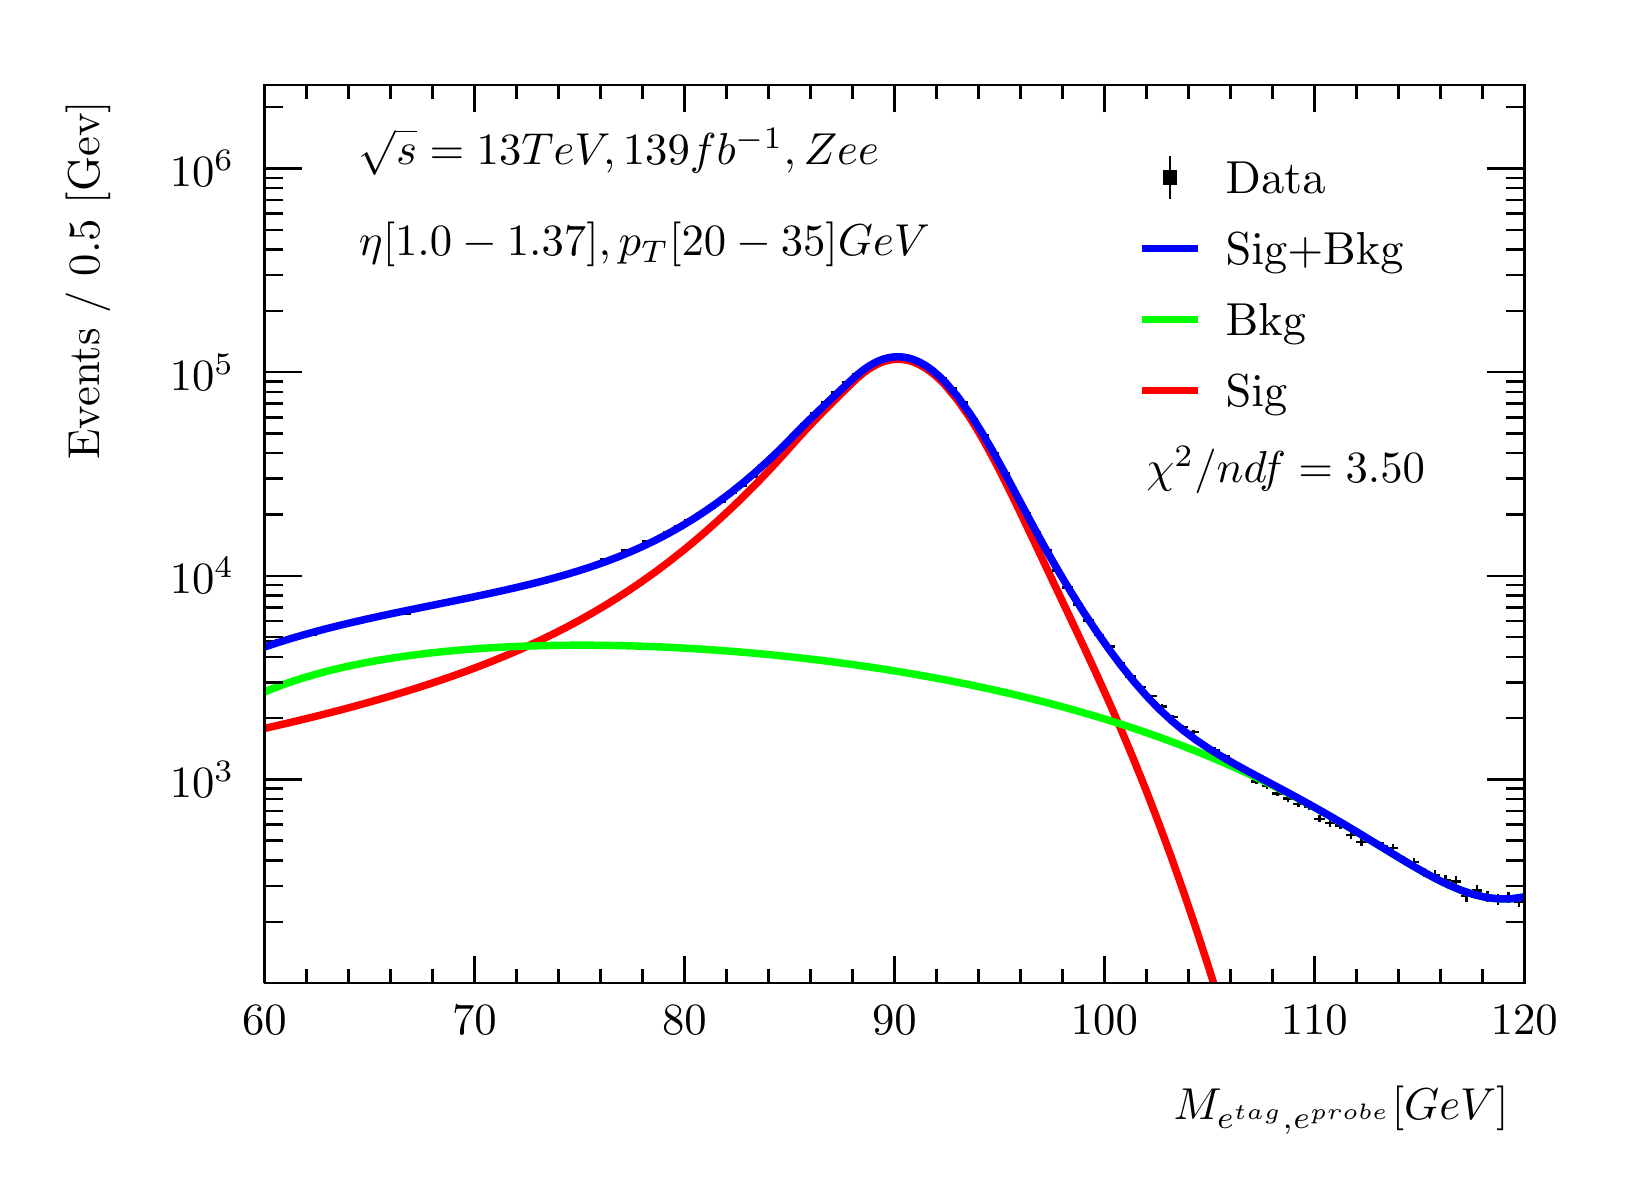
\begin{tikzpicture}
\pgfdeclareplotmark{cross} {
\pgfpathmoveto{\pgfpoint{-0.3\pgfplotmarksize}{\pgfplotmarksize}}
\pgfpathlineto{\pgfpoint{+0.3\pgfplotmarksize}{\pgfplotmarksize}}
\pgfpathlineto{\pgfpoint{+0.3\pgfplotmarksize}{0.3\pgfplotmarksize}}
\pgfpathlineto{\pgfpoint{+1\pgfplotmarksize}{0.3\pgfplotmarksize}}
\pgfpathlineto{\pgfpoint{+1\pgfplotmarksize}{-0.3\pgfplotmarksize}}
\pgfpathlineto{\pgfpoint{+0.3\pgfplotmarksize}{-0.3\pgfplotmarksize}}
\pgfpathlineto{\pgfpoint{+0.3\pgfplotmarksize}{-1.\pgfplotmarksize}}
\pgfpathlineto{\pgfpoint{-0.3\pgfplotmarksize}{-1.\pgfplotmarksize}}
\pgfpathlineto{\pgfpoint{-0.3\pgfplotmarksize}{-0.3\pgfplotmarksize}}
\pgfpathlineto{\pgfpoint{-1.\pgfplotmarksize}{-0.3\pgfplotmarksize}}
\pgfpathlineto{\pgfpoint{-1.\pgfplotmarksize}{0.3\pgfplotmarksize}}
\pgfpathlineto{\pgfpoint{-0.3\pgfplotmarksize}{0.3\pgfplotmarksize}}
\pgfpathclose
\pgfusepathqstroke
}
\pgfdeclareplotmark{cross*} {
\pgfpathmoveto{\pgfpoint{-0.3\pgfplotmarksize}{\pgfplotmarksize}}
\pgfpathlineto{\pgfpoint{+0.3\pgfplotmarksize}{\pgfplotmarksize}}
\pgfpathlineto{\pgfpoint{+0.3\pgfplotmarksize}{0.3\pgfplotmarksize}}
\pgfpathlineto{\pgfpoint{+1\pgfplotmarksize}{0.3\pgfplotmarksize}}
\pgfpathlineto{\pgfpoint{+1\pgfplotmarksize}{-0.3\pgfplotmarksize}}
\pgfpathlineto{\pgfpoint{+0.3\pgfplotmarksize}{-0.3\pgfplotmarksize}}
\pgfpathlineto{\pgfpoint{+0.3\pgfplotmarksize}{-1.\pgfplotmarksize}}
\pgfpathlineto{\pgfpoint{-0.3\pgfplotmarksize}{-1.\pgfplotmarksize}}
\pgfpathlineto{\pgfpoint{-0.3\pgfplotmarksize}{-0.3\pgfplotmarksize}}
\pgfpathlineto{\pgfpoint{-1.\pgfplotmarksize}{-0.3\pgfplotmarksize}}
\pgfpathlineto{\pgfpoint{-1.\pgfplotmarksize}{0.3\pgfplotmarksize}}
\pgfpathlineto{\pgfpoint{-0.3\pgfplotmarksize}{0.3\pgfplotmarksize}}
\pgfpathclose
\pgfusepathqfillstroke
}
\pgfdeclareplotmark{newstar} {
\pgfpathmoveto{\pgfqpoint{0pt}{\pgfplotmarksize}}
\pgfpathlineto{\pgfqpointpolar{44}{0.5\pgfplotmarksize}}
\pgfpathlineto{\pgfqpointpolar{18}{\pgfplotmarksize}}
\pgfpathlineto{\pgfqpointpolar{-20}{0.5\pgfplotmarksize}}
\pgfpathlineto{\pgfqpointpolar{-54}{\pgfplotmarksize}}
\pgfpathlineto{\pgfqpointpolar{-90}{0.5\pgfplotmarksize}}
\pgfpathlineto{\pgfqpointpolar{234}{\pgfplotmarksize}}
\pgfpathlineto{\pgfqpointpolar{198}{0.5\pgfplotmarksize}}
\pgfpathlineto{\pgfqpointpolar{162}{\pgfplotmarksize}}
\pgfpathlineto{\pgfqpointpolar{134}{0.5\pgfplotmarksize}}
\pgfpathclose
\pgfusepathqstroke
}
\pgfdeclareplotmark{newstar*} {
\pgfpathmoveto{\pgfqpoint{0pt}{\pgfplotmarksize}}
\pgfpathlineto{\pgfqpointpolar{44}{0.5\pgfplotmarksize}}
\pgfpathlineto{\pgfqpointpolar{18}{\pgfplotmarksize}}
\pgfpathlineto{\pgfqpointpolar{-20}{0.5\pgfplotmarksize}}
\pgfpathlineto{\pgfqpointpolar{-54}{\pgfplotmarksize}}
\pgfpathlineto{\pgfqpointpolar{-90}{0.5\pgfplotmarksize}}
\pgfpathlineto{\pgfqpointpolar{234}{\pgfplotmarksize}}
\pgfpathlineto{\pgfqpointpolar{198}{0.5\pgfplotmarksize}}
\pgfpathlineto{\pgfqpointpolar{162}{\pgfplotmarksize}}
\pgfpathlineto{\pgfqpointpolar{134}{0.5\pgfplotmarksize}}
\pgfpathclose
\pgfusepathqfillstroke
}
\definecolor{c}{rgb}{1,1,1};
\draw [color=c, fill=c] (0,0) rectangle (20,14.4361);
\draw [color=c, fill=c] (3,2.30977) rectangle (19,13.7143);
\definecolor{c}{rgb}{0,0,0};
\draw [c,line width=0.9] (3,2.30977) -- (3,13.7143) -- (19,13.7143) -- (19,2.30977) -- (3,2.30977);
\definecolor{c}{rgb}{1,1,1};
\draw [color=c, fill=c] (3,2.30977) rectangle (19,13.7143);
\definecolor{c}{rgb}{0,0,0};
\draw [c,line width=0.9] (3,2.30977) -- (3,13.7143) -- (19,13.7143) -- (19,2.30977) -- (3,2.30977);
\draw [c,line width=0.9] (3,2.30977) -- (19,2.30977);
\draw [c,line width=0.9] (3,2.65624) -- (3,2.30977);
\draw [c,line width=0.9] (3.53333,2.48301) -- (3.53333,2.30977);
\draw [c,line width=0.9] (4.06667,2.48301) -- (4.06667,2.30977);
\draw [c,line width=0.9] (4.6,2.48301) -- (4.6,2.30977);
\draw [c,line width=0.9] (5.13333,2.48301) -- (5.13333,2.30977);
\draw [c,line width=0.9] (5.66667,2.65624) -- (5.66667,2.30977);
\draw [c,line width=0.9] (6.2,2.48301) -- (6.2,2.30977);
\draw [c,line width=0.9] (6.73333,2.48301) -- (6.73333,2.30977);
\draw [c,line width=0.9] (7.26667,2.48301) -- (7.26667,2.30977);
\draw [c,line width=0.9] (7.8,2.48301) -- (7.8,2.30977);
\draw [c,line width=0.9] (8.33333,2.65624) -- (8.33333,2.30977);
\draw [c,line width=0.9] (8.86667,2.48301) -- (8.86667,2.30977);
\draw [c,line width=0.9] (9.4,2.48301) -- (9.4,2.30977);
\draw [c,line width=0.9] (9.93333,2.48301) -- (9.93333,2.30977);
\draw [c,line width=0.9] (10.4667,2.48301) -- (10.4667,2.30977);
\draw [c,line width=0.9] (11,2.65624) -- (11,2.30977);
\draw [c,line width=0.9] (11.5333,2.48301) -- (11.5333,2.30977);
\draw [c,line width=0.9] (12.0667,2.48301) -- (12.0667,2.30977);
\draw [c,line width=0.9] (12.6,2.48301) -- (12.6,2.30977);
\draw [c,line width=0.9] (13.1333,2.48301) -- (13.1333,2.30977);
\draw [c,line width=0.9] (13.6667,2.65624) -- (13.6667,2.30977);
\draw [c,line width=0.9] (14.2,2.48301) -- (14.2,2.30977);
\draw [c,line width=0.9] (14.7333,2.48301) -- (14.7333,2.30977);
\draw [c,line width=0.9] (15.2667,2.48301) -- (15.2667,2.30977);
\draw [c,line width=0.9] (15.8,2.48301) -- (15.8,2.30977);
\draw [c,line width=0.9] (16.3333,2.65624) -- (16.3333,2.30977);
\draw [c,line width=0.9] (16.8667,2.48301) -- (16.8667,2.30977);
\draw [c,line width=0.9] (17.4,2.48301) -- (17.4,2.30977);
\draw [c,line width=0.9] (17.9333,2.48301) -- (17.9333,2.30977);
\draw [c,line width=0.9] (18.4667,2.48301) -- (18.4667,2.30977);
\draw [c,line width=0.9] (19,2.65624) -- (19,2.30977);
\draw [anchor=base] (3,1.66015) node[scale=1.61424, color=c, rotate=0]{60};
\draw [anchor=base] (5.66667,1.66015) node[scale=1.61424, color=c, rotate=0]{70};
\draw [anchor=base] (8.33333,1.66015) node[scale=1.61424, color=c, rotate=0]{80};
\draw [anchor=base] (11,1.66015) node[scale=1.61424, color=c, rotate=0]{90};
\draw [anchor=base] (13.6667,1.66015) node[scale=1.61424, color=c, rotate=0]{100};
\draw [anchor=base] (16.3333,1.66015) node[scale=1.61424, color=c, rotate=0]{110};
\draw [anchor=base] (19,1.66015) node[scale=1.61424, color=c, rotate=0]{120};
\draw [anchor= east] (19,0.692932) node[scale=1.61424, color=c, rotate=0]{$M_{e^{tag}, e^{probe}}  [GeV]$};
\draw [c,line width=0.9] (3,13.7143) -- (19,13.7143);
\draw [c,line width=0.9] (3,13.3678) -- (3,13.7143);
\draw [c,line width=0.9] (3.53333,13.5411) -- (3.53333,13.7143);
\draw [c,line width=0.9] (4.06667,13.5411) -- (4.06667,13.7143);
\draw [c,line width=0.9] (4.6,13.5411) -- (4.6,13.7143);
\draw [c,line width=0.9] (5.13333,13.5411) -- (5.13333,13.7143);
\draw [c,line width=0.9] (5.66667,13.3678) -- (5.66667,13.7143);
\draw [c,line width=0.9] (6.2,13.5411) -- (6.2,13.7143);
\draw [c,line width=0.9] (6.73333,13.5411) -- (6.73333,13.7143);
\draw [c,line width=0.9] (7.26667,13.5411) -- (7.26667,13.7143);
\draw [c,line width=0.9] (7.8,13.5411) -- (7.8,13.7143);
\draw [c,line width=0.9] (8.33333,13.3678) -- (8.33333,13.7143);
\draw [c,line width=0.9] (8.86667,13.5411) -- (8.86667,13.7143);
\draw [c,line width=0.9] (9.4,13.5411) -- (9.4,13.7143);
\draw [c,line width=0.9] (9.93333,13.5411) -- (9.93333,13.7143);
\draw [c,line width=0.9] (10.4667,13.5411) -- (10.4667,13.7143);
\draw [c,line width=0.9] (11,13.3678) -- (11,13.7143);
\draw [c,line width=0.9] (11.5333,13.5411) -- (11.5333,13.7143);
\draw [c,line width=0.9] (12.0667,13.5411) -- (12.0667,13.7143);
\draw [c,line width=0.9] (12.6,13.5411) -- (12.6,13.7143);
\draw [c,line width=0.9] (13.1333,13.5411) -- (13.1333,13.7143);
\draw [c,line width=0.9] (13.6667,13.3678) -- (13.6667,13.7143);
\draw [c,line width=0.9] (14.2,13.5411) -- (14.2,13.7143);
\draw [c,line width=0.9] (14.7333,13.5411) -- (14.7333,13.7143);
\draw [c,line width=0.9] (15.2667,13.5411) -- (15.2667,13.7143);
\draw [c,line width=0.9] (15.8,13.5411) -- (15.8,13.7143);
\draw [c,line width=0.9] (16.3333,13.3678) -- (16.3333,13.7143);
\draw [c,line width=0.9] (16.8667,13.5411) -- (16.8667,13.7143);
\draw [c,line width=0.9] (17.4,13.5411) -- (17.4,13.7143);
\draw [c,line width=0.9] (17.9333,13.5411) -- (17.9333,13.7143);
\draw [c,line width=0.9] (18.4667,13.5411) -- (18.4667,13.7143);
\draw [c,line width=0.9] (19,13.3678) -- (19,13.7143);
\draw [c,line width=0.9] (3,2.30977) -- (3,13.7143);
\draw [c,line width=0.9] (3.237,3.08829) -- (3,3.08829);
\draw [c,line width=0.9] (3.237,3.54369) -- (3,3.54369);
\draw [c,line width=0.9] (3.237,3.8668) -- (3,3.8668);
\draw [c,line width=0.9] (3.237,4.11742) -- (3,4.11742);
\draw [c,line width=0.9] (3.237,4.3222) -- (3,4.3222);
\draw [c,line width=0.9] (3.237,4.49534) -- (3,4.49534);
\draw [c,line width=0.9] (3.237,4.64531) -- (3,4.64531);
\draw [c,line width=0.9] (3.237,4.7776) -- (3,4.7776);
\draw [c,line width=0.9] (3.474,4.89594) -- (3,4.89594);
\draw [anchor= east] (2.82,4.89594) node[scale=1.61424, color=c, rotate=0]{$10^{3}$};
\draw [c,line width=0.9] (3.237,5.67445) -- (3,5.67445);
\draw [c,line width=0.9] (3.237,6.12985) -- (3,6.12985);
\draw [c,line width=0.9] (3.237,6.45297) -- (3,6.45297);
\draw [c,line width=0.9] (3.237,6.70359) -- (3,6.70359);
\draw [c,line width=0.9] (3.237,6.90837) -- (3,6.90837);
\draw [c,line width=0.9] (3.237,7.0815) -- (3,7.0815);
\draw [c,line width=0.9] (3.237,7.23148) -- (3,7.23148);
\draw [c,line width=0.9] (3.237,7.36377) -- (3,7.36377);
\draw [c,line width=0.9] (3.474,7.48211) -- (3,7.48211);
\draw [anchor= east] (2.82,7.48211) node[scale=1.61424, color=c, rotate=0]{$10^{4}$};
\draw [c,line width=0.9] (3.237,8.26062) -- (3,8.26062);
\draw [c,line width=0.9] (3.237,8.71602) -- (3,8.71602);
\draw [c,line width=0.9] (3.237,9.03913) -- (3,9.03913);
\draw [c,line width=0.9] (3.237,9.28976) -- (3,9.28976);
\draw [c,line width=0.9] (3.237,9.49453) -- (3,9.49453);
\draw [c,line width=0.9] (3.237,9.66767) -- (3,9.66767);
\draw [c,line width=0.9] (3.237,9.81765) -- (3,9.81765);
\draw [c,line width=0.9] (3.237,9.94994) -- (3,9.94994);
\draw [c,line width=0.9] (3.474,10.0683) -- (3,10.0683);
\draw [anchor= east] (2.82,10.0683) node[scale=1.61424, color=c, rotate=0]{$10^{5}$};
\draw [c,line width=0.9] (3.237,10.8468) -- (3,10.8468);
\draw [c,line width=0.9] (3.237,11.3022) -- (3,11.3022);
\draw [c,line width=0.9] (3.237,11.6253) -- (3,11.6253);
\draw [c,line width=0.9] (3.237,11.8759) -- (3,11.8759);
\draw [c,line width=0.9] (3.237,12.0807) -- (3,12.0807);
\draw [c,line width=0.9] (3.237,12.2538) -- (3,12.2538);
\draw [c,line width=0.9] (3.237,12.4038) -- (3,12.4038);
\draw [c,line width=0.9] (3.237,12.5361) -- (3,12.5361);
\draw [c,line width=0.9] (3.474,12.6544) -- (3,12.6544);
\draw [anchor= east] (2.82,12.6544) node[scale=1.61424, color=c, rotate=0]{$10^{6}$};
\draw [c,line width=0.9] (3.237,13.433) -- (3,13.433);
\draw [anchor= east] (0.76,13.7143) node[scale=1.61424, color=c, rotate=90]{Events / 0.5 [Gev]};
\draw [c,line width=0.9] (19,2.30977) -- (19,13.7143);
\draw [c,line width=0.9] (18.763,3.08829) -- (19,3.08829);
\draw [c,line width=0.9] (18.763,3.54369) -- (19,3.54369);
\draw [c,line width=0.9] (18.763,3.8668) -- (19,3.8668);
\draw [c,line width=0.9] (18.763,4.11742) -- (19,4.11742);
\draw [c,line width=0.9] (18.763,4.3222) -- (19,4.3222);
\draw [c,line width=0.9] (18.763,4.49534) -- (19,4.49534);
\draw [c,line width=0.9] (18.763,4.64531) -- (19,4.64531);
\draw [c,line width=0.9] (18.763,4.7776) -- (19,4.7776);
\draw [c,line width=0.9] (18.526,4.89594) -- (19,4.89594);
\draw [c,line width=0.9] (18.763,5.67445) -- (19,5.67445);
\draw [c,line width=0.9] (18.763,6.12985) -- (19,6.12985);
\draw [c,line width=0.9] (18.763,6.45297) -- (19,6.45297);
\draw [c,line width=0.9] (18.763,6.70359) -- (19,6.70359);
\draw [c,line width=0.9] (18.763,6.90837) -- (19,6.90837);
\draw [c,line width=0.9] (18.763,7.0815) -- (19,7.0815);
\draw [c,line width=0.9] (18.763,7.23148) -- (19,7.23148);
\draw [c,line width=0.9] (18.763,7.36377) -- (19,7.36377);
\draw [c,line width=0.9] (18.526,7.48211) -- (19,7.48211);
\draw [c,line width=0.9] (18.763,8.26062) -- (19,8.26062);
\draw [c,line width=0.9] (18.763,8.71602) -- (19,8.71602);
\draw [c,line width=0.9] (18.763,9.03913) -- (19,9.03913);
\draw [c,line width=0.9] (18.763,9.28976) -- (19,9.28976);
\draw [c,line width=0.9] (18.763,9.49453) -- (19,9.49453);
\draw [c,line width=0.9] (18.763,9.66767) -- (19,9.66767);
\draw [c,line width=0.9] (18.763,9.81765) -- (19,9.81765);
\draw [c,line width=0.9] (18.763,9.94994) -- (19,9.94994);
\draw [c,line width=0.9] (18.526,10.0683) -- (19,10.0683);
\draw [c,line width=0.9] (18.763,10.8468) -- (19,10.8468);
\draw [c,line width=0.9] (18.763,11.3022) -- (19,11.3022);
\draw [c,line width=0.9] (18.763,11.6253) -- (19,11.6253);
\draw [c,line width=0.9] (18.763,11.8759) -- (19,11.8759);
\draw [c,line width=0.9] (18.763,12.0807) -- (19,12.0807);
\draw [c,line width=0.9] (18.763,12.2538) -- (19,12.2538);
\draw [c,line width=0.9] (18.763,12.4038) -- (19,12.4038);
\draw [c,line width=0.9] (18.763,12.5361) -- (19,12.5361);
\draw [c,line width=0.9] (18.526,12.6544) -- (19,12.6544);
\draw [c,line width=0.9] (18.763,13.433) -- (19,13.433);
\draw [c,line width=0.9] (3.06667,6.65329) -- (3,6.65329);
\draw [c,line width=0.9] (3,6.65329) -- (3,6.65329);
\draw [c,line width=0.9] (3.06667,6.65329) -- (3.13333,6.65329);
\draw [c,line width=0.9] (3.13333,6.65329) -- (3.13333,6.65329);
\draw [c,line width=0.9] (3.06667,6.65329) -- (3.06667,6.66953);
\draw [c,line width=0.9] (3.06667,6.66953) -- (3.06667,6.66953);
\draw [c,line width=0.9] (3.06667,6.65329) -- (3.06667,6.63705);
\draw [c,line width=0.9] (3.06667,6.63705) -- (3.06667,6.63705);
\draw [c,line width=0.9] (3.2,6.66288) -- (3.13333,6.66288);
\draw [c,line width=0.9] (3.13333,6.66288) -- (3.13333,6.66288);
\draw [c,line width=0.9] (3.2,6.66288) -- (3.26667,6.66288);
\draw [c,line width=0.9] (3.26667,6.66288) -- (3.26667,6.66288);
\draw [c,line width=0.9] (3.2,6.66288) -- (3.2,6.67905);
\draw [c,line width=0.9] (3.2,6.67905) -- (3.2,6.67905);
\draw [c,line width=0.9] (3.2,6.66288) -- (3.2,6.64671);
\draw [c,line width=0.9] (3.2,6.64671) -- (3.2,6.64671);
\draw [c,line width=0.9] (3.33333,6.67677) -- (3.26667,6.67677);
\draw [c,line width=0.9] (3.26667,6.67677) -- (3.26667,6.67677);
\draw [c,line width=0.9] (3.33333,6.67677) -- (3.4,6.67677);
\draw [c,line width=0.9] (3.4,6.67677) -- (3.4,6.67677);
\draw [c,line width=0.9] (3.33333,6.67677) -- (3.33333,6.69284);
\draw [c,line width=0.9] (3.33333,6.69284) -- (3.33333,6.69284);
\draw [c,line width=0.9] (3.33333,6.67677) -- (3.33333,6.66069);
\draw [c,line width=0.9] (3.33333,6.66069) -- (3.33333,6.66069);
\draw [c,line width=0.9] (3.46667,6.73264) -- (3.4,6.73264);
\draw [c,line width=0.9] (3.4,6.73264) -- (3.4,6.73264);
\draw [c,line width=0.9] (3.46667,6.73264) -- (3.53333,6.73264);
\draw [c,line width=0.9] (3.53333,6.73264) -- (3.53333,6.73264);
\draw [c,line width=0.9] (3.46667,6.73264) -- (3.46667,6.74832);
\draw [c,line width=0.9] (3.46667,6.74832) -- (3.46667,6.74832);
\draw [c,line width=0.9] (3.46667,6.73264) -- (3.46667,6.71696);
\draw [c,line width=0.9] (3.46667,6.71696) -- (3.46667,6.71696);
\draw [c,line width=0.9] (3.6,6.73592) -- (3.53333,6.73592);
\draw [c,line width=0.9] (3.53333,6.73592) -- (3.53333,6.73592);
\draw [c,line width=0.9] (3.6,6.73592) -- (3.66667,6.73592);
\draw [c,line width=0.9] (3.66667,6.73592) -- (3.66667,6.73592);
\draw [c,line width=0.9] (3.6,6.73592) -- (3.6,6.75158);
\draw [c,line width=0.9] (3.6,6.75158) -- (3.6,6.75158);
\draw [c,line width=0.9] (3.6,6.73592) -- (3.6,6.72026);
\draw [c,line width=0.9] (3.6,6.72026) -- (3.6,6.72026);
\draw [c,line width=0.9] (3.73333,6.7892) -- (3.66667,6.7892);
\draw [c,line width=0.9] (3.66667,6.7892) -- (3.66667,6.7892);
\draw [c,line width=0.9] (3.73333,6.7892) -- (3.8,6.7892);
\draw [c,line width=0.9] (3.8,6.7892) -- (3.8,6.7892);
\draw [c,line width=0.9] (3.73333,6.7892) -- (3.73333,6.80449);
\draw [c,line width=0.9] (3.73333,6.80449) -- (3.73333,6.80449);
\draw [c,line width=0.9] (3.73333,6.7892) -- (3.73333,6.77391);
\draw [c,line width=0.9] (3.73333,6.77391) -- (3.73333,6.77391);
\draw [c,line width=0.9] (3.86667,6.83308) -- (3.8,6.83308);
\draw [c,line width=0.9] (3.8,6.83308) -- (3.8,6.83308);
\draw [c,line width=0.9] (3.86667,6.83308) -- (3.93333,6.83308);
\draw [c,line width=0.9] (3.93333,6.83308) -- (3.93333,6.83308);
\draw [c,line width=0.9] (3.86667,6.83308) -- (3.86667,6.84808);
\draw [c,line width=0.9] (3.86667,6.84808) -- (3.86667,6.84808);
\draw [c,line width=0.9] (3.86667,6.83308) -- (3.86667,6.81809);
\draw [c,line width=0.9] (3.86667,6.81809) -- (3.86667,6.81809);
\draw [c,line width=0.9] (4,6.86154) -- (3.93333,6.86154);
\draw [c,line width=0.9] (3.93333,6.86154) -- (3.93333,6.86154);
\draw [c,line width=0.9] (4,6.86154) -- (4.06667,6.86154);
\draw [c,line width=0.9] (4.06667,6.86154) -- (4.06667,6.86154);
\draw [c,line width=0.9] (4,6.86154) -- (4,6.87635);
\draw [c,line width=0.9] (4,6.87635) -- (4,6.87635);
\draw [c,line width=0.9] (4,6.86154) -- (4,6.84674);
\draw [c,line width=0.9] (4,6.84674) -- (4,6.84674);
\draw [c,line width=0.9] (4.13333,6.89538) -- (4.06667,6.89538);
\draw [c,line width=0.9] (4.06667,6.89538) -- (4.06667,6.89538);
\draw [c,line width=0.9] (4.13333,6.89538) -- (4.2,6.89538);
\draw [c,line width=0.9] (4.2,6.89538) -- (4.2,6.89538);
\draw [c,line width=0.9] (4.13333,6.89538) -- (4.13333,6.90996);
\draw [c,line width=0.9] (4.13333,6.90996) -- (4.13333,6.90996);
\draw [c,line width=0.9] (4.13333,6.89538) -- (4.13333,6.88079);
\draw [c,line width=0.9] (4.13333,6.88079) -- (4.13333,6.88079);
\draw [c,line width=0.9] (4.26667,6.94084) -- (4.2,6.94084);
\draw [c,line width=0.9] (4.2,6.94084) -- (4.2,6.94084);
\draw [c,line width=0.9] (4.26667,6.94084) -- (4.33333,6.94084);
\draw [c,line width=0.9] (4.33333,6.94084) -- (4.33333,6.94084);
\draw [c,line width=0.9] (4.26667,6.94084) -- (4.26667,6.95513);
\draw [c,line width=0.9] (4.26667,6.95513) -- (4.26667,6.95513);
\draw [c,line width=0.9] (4.26667,6.94084) -- (4.26667,6.92655);
\draw [c,line width=0.9] (4.26667,6.92655) -- (4.26667,6.92655);
\draw [c,line width=0.9] (4.4,6.93519) -- (4.33333,6.93519);
\draw [c,line width=0.9] (4.33333,6.93519) -- (4.33333,6.93519);
\draw [c,line width=0.9] (4.4,6.93519) -- (4.46667,6.93519);
\draw [c,line width=0.9] (4.46667,6.93519) -- (4.46667,6.93519);
\draw [c,line width=0.9] (4.4,6.93519) -- (4.4,6.94952);
\draw [c,line width=0.9] (4.4,6.94952) -- (4.4,6.94952);
\draw [c,line width=0.9] (4.4,6.93519) -- (4.4,6.92086);
\draw [c,line width=0.9] (4.4,6.92086) -- (4.4,6.92086);
\draw [c,line width=0.9] (4.53333,6.9791) -- (4.46667,6.9791);
\draw [c,line width=0.9] (4.46667,6.9791) -- (4.46667,6.9791);
\draw [c,line width=0.9] (4.53333,6.9791) -- (4.6,6.9791);
\draw [c,line width=0.9] (4.6,6.9791) -- (4.6,6.9791);
\draw [c,line width=0.9] (4.53333,6.9791) -- (4.53333,6.99315);
\draw [c,line width=0.9] (4.53333,6.99315) -- (4.53333,6.99315);
\draw [c,line width=0.9] (4.53333,6.9791) -- (4.53333,6.96505);
\draw [c,line width=0.9] (4.53333,6.96505) -- (4.53333,6.96505);
\draw [c,line width=0.9] (4.66667,7.00172) -- (4.6,7.00172);
\draw [c,line width=0.9] (4.6,7.00172) -- (4.6,7.00172);
\draw [c,line width=0.9] (4.66667,7.00172) -- (4.73333,7.00172);
\draw [c,line width=0.9] (4.73333,7.00172) -- (4.73333,7.00172);
\draw [c,line width=0.9] (4.66667,7.00172) -- (4.66667,7.01563);
\draw [c,line width=0.9] (4.66667,7.01563) -- (4.66667,7.01563);
\draw [c,line width=0.9] (4.66667,7.00172) -- (4.66667,6.98781);
\draw [c,line width=0.9] (4.66667,6.98781) -- (4.66667,6.98781);
\draw [c,line width=0.9] (4.8,6.99464) -- (4.73333,6.99464);
\draw [c,line width=0.9] (4.73333,6.99464) -- (4.73333,6.99464);
\draw [c,line width=0.9] (4.8,6.99464) -- (4.86667,6.99464);
\draw [c,line width=0.9] (4.86667,6.99464) -- (4.86667,6.99464);
\draw [c,line width=0.9] (4.8,6.99464) -- (4.8,7.00859);
\draw [c,line width=0.9] (4.8,7.00859) -- (4.8,7.00859);
\draw [c,line width=0.9] (4.8,6.99464) -- (4.8,6.98068);
\draw [c,line width=0.9] (4.8,6.98068) -- (4.8,6.98068);
\draw [c,line width=0.9] (4.93333,7.07362) -- (4.86667,7.07362);
\draw [c,line width=0.9] (4.86667,7.07362) -- (4.86667,7.07362);
\draw [c,line width=0.9] (4.93333,7.07362) -- (5,7.07362);
\draw [c,line width=0.9] (5,7.07362) -- (5,7.07362);
\draw [c,line width=0.9] (4.93333,7.07362) -- (4.93333,7.08709);
\draw [c,line width=0.9] (4.93333,7.08709) -- (4.93333,7.08709);
\draw [c,line width=0.9] (4.93333,7.07362) -- (4.93333,7.06014);
\draw [c,line width=0.9] (4.93333,7.06014) -- (4.93333,7.06014);
\draw [c,line width=0.9] (5.06667,7.08599) -- (5,7.08599);
\draw [c,line width=0.9] (5,7.08599) -- (5,7.08599);
\draw [c,line width=0.9] (5.06667,7.08599) -- (5.13333,7.08599);
\draw [c,line width=0.9] (5.13333,7.08599) -- (5.13333,7.08599);
\draw [c,line width=0.9] (5.06667,7.08599) -- (5.06667,7.09939);
\draw [c,line width=0.9] (5.06667,7.09939) -- (5.06667,7.09939);
\draw [c,line width=0.9] (5.06667,7.08599) -- (5.06667,7.07259);
\draw [c,line width=0.9] (5.06667,7.07259) -- (5.06667,7.07259);
\draw [c,line width=0.9] (5.2,7.10217) -- (5.13333,7.10217);
\draw [c,line width=0.9] (5.13333,7.10217) -- (5.13333,7.10217);
\draw [c,line width=0.9] (5.2,7.10217) -- (5.26667,7.10217);
\draw [c,line width=0.9] (5.26667,7.10217) -- (5.26667,7.10217);
\draw [c,line width=0.9] (5.2,7.10217) -- (5.2,7.11547);
\draw [c,line width=0.9] (5.2,7.11547) -- (5.2,7.11547);
\draw [c,line width=0.9] (5.2,7.10217) -- (5.2,7.08887);
\draw [c,line width=0.9] (5.2,7.08887) -- (5.2,7.08887);
\draw [c,line width=0.9] (5.33333,7.1427) -- (5.26667,7.1427);
\draw [c,line width=0.9] (5.26667,7.1427) -- (5.26667,7.1427);
\draw [c,line width=0.9] (5.33333,7.1427) -- (5.4,7.1427);
\draw [c,line width=0.9] (5.4,7.1427) -- (5.4,7.1427);
\draw [c,line width=0.9] (5.33333,7.1427) -- (5.33333,7.15577);
\draw [c,line width=0.9] (5.33333,7.15577) -- (5.33333,7.15577);
\draw [c,line width=0.9] (5.33333,7.1427) -- (5.33333,7.12964);
\draw [c,line width=0.9] (5.33333,7.12964) -- (5.33333,7.12964);
\draw [c,line width=0.9] (5.46667,7.18402) -- (5.4,7.18402);
\draw [c,line width=0.9] (5.4,7.18402) -- (5.4,7.18402);
\draw [c,line width=0.9] (5.46667,7.18402) -- (5.53333,7.18402);
\draw [c,line width=0.9] (5.53333,7.18402) -- (5.53333,7.18402);
\draw [c,line width=0.9] (5.46667,7.18402) -- (5.46667,7.19685);
\draw [c,line width=0.9] (5.46667,7.19685) -- (5.46667,7.19685);
\draw [c,line width=0.9] (5.46667,7.18402) -- (5.46667,7.1712);
\draw [c,line width=0.9] (5.46667,7.1712) -- (5.46667,7.1712);
\draw [c,line width=0.9] (5.6,7.18329) -- (5.53333,7.18329);
\draw [c,line width=0.9] (5.53333,7.18329) -- (5.53333,7.18329);
\draw [c,line width=0.9] (5.6,7.18329) -- (5.66667,7.18329);
\draw [c,line width=0.9] (5.66667,7.18329) -- (5.66667,7.18329);
\draw [c,line width=0.9] (5.6,7.18329) -- (5.6,7.19612);
\draw [c,line width=0.9] (5.6,7.19612) -- (5.6,7.19612);
\draw [c,line width=0.9] (5.6,7.18329) -- (5.6,7.17046);
\draw [c,line width=0.9] (5.6,7.17046) -- (5.6,7.17046);
\draw [c,line width=0.9] (5.73333,7.21308) -- (5.66667,7.21308);
\draw [c,line width=0.9] (5.66667,7.21308) -- (5.66667,7.21308);
\draw [c,line width=0.9] (5.73333,7.21308) -- (5.8,7.21308);
\draw [c,line width=0.9] (5.8,7.21308) -- (5.8,7.21308);
\draw [c,line width=0.9] (5.73333,7.21308) -- (5.73333,7.22574);
\draw [c,line width=0.9] (5.73333,7.22574) -- (5.73333,7.22574);
\draw [c,line width=0.9] (5.73333,7.21308) -- (5.73333,7.20042);
\draw [c,line width=0.9] (5.73333,7.20042) -- (5.73333,7.20042);
\draw [c,line width=0.9] (5.86667,7.23778) -- (5.8,7.23778);
\draw [c,line width=0.9] (5.8,7.23778) -- (5.8,7.23778);
\draw [c,line width=0.9] (5.86667,7.23778) -- (5.93333,7.23778);
\draw [c,line width=0.9] (5.93333,7.23778) -- (5.93333,7.23778);
\draw [c,line width=0.9] (5.86667,7.23778) -- (5.86667,7.2503);
\draw [c,line width=0.9] (5.86667,7.2503) -- (5.86667,7.2503);
\draw [c,line width=0.9] (5.86667,7.23778) -- (5.86667,7.22526);
\draw [c,line width=0.9] (5.86667,7.22526) -- (5.86667,7.22526);
\draw [c,line width=0.9] (6,7.29122) -- (5.93333,7.29122);
\draw [c,line width=0.9] (5.93333,7.29122) -- (5.93333,7.29122);
\draw [c,line width=0.9] (6,7.29122) -- (6.06667,7.29122);
\draw [c,line width=0.9] (6.06667,7.29122) -- (6.06667,7.29122);
\draw [c,line width=0.9] (6,7.29122) -- (6,7.30344);
\draw [c,line width=0.9] (6,7.30344) -- (6,7.30344);
\draw [c,line width=0.9] (6,7.29122) -- (6,7.27899);
\draw [c,line width=0.9] (6,7.27899) -- (6,7.27899);
\draw [c,line width=0.9] (6.13333,7.30419) -- (6.06667,7.30419);
\draw [c,line width=0.9] (6.06667,7.30419) -- (6.06667,7.30419);
\draw [c,line width=0.9] (6.13333,7.30419) -- (6.2,7.30419);
\draw [c,line width=0.9] (6.2,7.30419) -- (6.2,7.30419);
\draw [c,line width=0.9] (6.13333,7.30419) -- (6.13333,7.31635);
\draw [c,line width=0.9] (6.13333,7.31635) -- (6.13333,7.31635);
\draw [c,line width=0.9] (6.13333,7.30419) -- (6.13333,7.29203);
\draw [c,line width=0.9] (6.13333,7.29203) -- (6.13333,7.29203);
\draw [c,line width=0.9] (6.26667,7.35563) -- (6.2,7.35563);
\draw [c,line width=0.9] (6.2,7.35563) -- (6.2,7.35563);
\draw [c,line width=0.9] (6.26667,7.35563) -- (6.33333,7.35563);
\draw [c,line width=0.9] (6.33333,7.35563) -- (6.33333,7.35563);
\draw [c,line width=0.9] (6.26667,7.35563) -- (6.26667,7.36751);
\draw [c,line width=0.9] (6.26667,7.36751) -- (6.26667,7.36751);
\draw [c,line width=0.9] (6.26667,7.35563) -- (6.26667,7.34375);
\draw [c,line width=0.9] (6.26667,7.34375) -- (6.26667,7.34375);
\draw [c,line width=0.9] (6.4,7.37185) -- (6.33333,7.37185);
\draw [c,line width=0.9] (6.33333,7.37185) -- (6.33333,7.37185);
\draw [c,line width=0.9] (6.4,7.37185) -- (6.46667,7.37185);
\draw [c,line width=0.9] (6.46667,7.37185) -- (6.46667,7.37185);
\draw [c,line width=0.9] (6.4,7.37185) -- (6.4,7.38365);
\draw [c,line width=0.9] (6.4,7.38365) -- (6.4,7.38365);
\draw [c,line width=0.9] (6.4,7.37185) -- (6.4,7.36006);
\draw [c,line width=0.9] (6.4,7.36006) -- (6.4,7.36006);
\draw [c,line width=0.9] (6.53333,7.39818) -- (6.46667,7.39818);
\draw [c,line width=0.9] (6.46667,7.39818) -- (6.46667,7.39818);
\draw [c,line width=0.9] (6.53333,7.39818) -- (6.6,7.39818);
\draw [c,line width=0.9] (6.6,7.39818) -- (6.6,7.39818);
\draw [c,line width=0.9] (6.53333,7.39818) -- (6.53333,7.40984);
\draw [c,line width=0.9] (6.53333,7.40984) -- (6.53333,7.40984);
\draw [c,line width=0.9] (6.53333,7.39818) -- (6.53333,7.38652);
\draw [c,line width=0.9] (6.53333,7.38652) -- (6.53333,7.38652);
\draw [c,line width=0.9] (6.66667,7.45517) -- (6.6,7.45517);
\draw [c,line width=0.9] (6.6,7.45517) -- (6.6,7.45517);
\draw [c,line width=0.9] (6.66667,7.45517) -- (6.73333,7.45517);
\draw [c,line width=0.9] (6.73333,7.45517) -- (6.73333,7.45517);
\draw [c,line width=0.9] (6.66667,7.45517) -- (6.66667,7.46654);
\draw [c,line width=0.9] (6.66667,7.46654) -- (6.66667,7.46654);
\draw [c,line width=0.9] (6.66667,7.45517) -- (6.66667,7.4438);
\draw [c,line width=0.9] (6.66667,7.4438) -- (6.66667,7.4438);
\draw [c,line width=0.9] (6.8,7.48793) -- (6.73333,7.48793);
\draw [c,line width=0.9] (6.73333,7.48793) -- (6.73333,7.48793);
\draw [c,line width=0.9] (6.8,7.48793) -- (6.86667,7.48793);
\draw [c,line width=0.9] (6.86667,7.48793) -- (6.86667,7.48793);
\draw [c,line width=0.9] (6.8,7.48793) -- (6.8,7.49914);
\draw [c,line width=0.9] (6.8,7.49914) -- (6.8,7.49914);
\draw [c,line width=0.9] (6.8,7.48793) -- (6.8,7.47673);
\draw [c,line width=0.9] (6.8,7.47673) -- (6.8,7.47673);
\draw [c,line width=0.9] (6.93333,7.52356) -- (6.86667,7.52356);
\draw [c,line width=0.9] (6.86667,7.52356) -- (6.86667,7.52356);
\draw [c,line width=0.9] (6.93333,7.52356) -- (7,7.52356);
\draw [c,line width=0.9] (7,7.52356) -- (7,7.52356);
\draw [c,line width=0.9] (6.93333,7.52356) -- (6.93333,7.53459);
\draw [c,line width=0.9] (6.93333,7.53459) -- (6.93333,7.53459);
\draw [c,line width=0.9] (6.93333,7.52356) -- (6.93333,7.51254);
\draw [c,line width=0.9] (6.93333,7.51254) -- (6.93333,7.51254);
\draw [c,line width=0.9] (7.06667,7.56948) -- (7,7.56948);
\draw [c,line width=0.9] (7,7.56948) -- (7,7.56948);
\draw [c,line width=0.9] (7.06667,7.56948) -- (7.13333,7.56948);
\draw [c,line width=0.9] (7.13333,7.56948) -- (7.13333,7.56948);
\draw [c,line width=0.9] (7.06667,7.56948) -- (7.06667,7.58029);
\draw [c,line width=0.9] (7.06667,7.58029) -- (7.06667,7.58029);
\draw [c,line width=0.9] (7.06667,7.56948) -- (7.06667,7.55868);
\draw [c,line width=0.9] (7.06667,7.55868) -- (7.06667,7.55868);
\draw [c,line width=0.9] (7.2,7.62937) -- (7.13333,7.62937);
\draw [c,line width=0.9] (7.13333,7.62937) -- (7.13333,7.62937);
\draw [c,line width=0.9] (7.2,7.62937) -- (7.26667,7.62937);
\draw [c,line width=0.9] (7.26667,7.62937) -- (7.26667,7.62937);
\draw [c,line width=0.9] (7.2,7.62937) -- (7.2,7.63989);
\draw [c,line width=0.9] (7.2,7.63989) -- (7.2,7.63989);
\draw [c,line width=0.9] (7.2,7.62937) -- (7.2,7.61885);
\draw [c,line width=0.9] (7.2,7.61885) -- (7.2,7.61885);
\draw [c,line width=0.9] (7.33333,7.6881) -- (7.26667,7.6881);
\draw [c,line width=0.9] (7.26667,7.6881) -- (7.26667,7.6881);
\draw [c,line width=0.9] (7.33333,7.6881) -- (7.4,7.6881);
\draw [c,line width=0.9] (7.4,7.6881) -- (7.4,7.6881);
\draw [c,line width=0.9] (7.33333,7.6881) -- (7.33333,7.69835);
\draw [c,line width=0.9] (7.33333,7.69835) -- (7.33333,7.69835);
\draw [c,line width=0.9] (7.33333,7.6881) -- (7.33333,7.67785);
\draw [c,line width=0.9] (7.33333,7.67785) -- (7.33333,7.67785);
\draw [c,line width=0.9] (7.46667,7.71187) -- (7.4,7.71187);
\draw [c,line width=0.9] (7.4,7.71187) -- (7.4,7.71187);
\draw [c,line width=0.9] (7.46667,7.71187) -- (7.53333,7.71187);
\draw [c,line width=0.9] (7.53333,7.71187) -- (7.53333,7.71187);
\draw [c,line width=0.9] (7.46667,7.71187) -- (7.46667,7.72201);
\draw [c,line width=0.9] (7.46667,7.72201) -- (7.46667,7.72201);
\draw [c,line width=0.9] (7.46667,7.71187) -- (7.46667,7.70173);
\draw [c,line width=0.9] (7.46667,7.70173) -- (7.46667,7.70173);
\draw [c,line width=0.9] (7.6,7.80334) -- (7.53333,7.80334);
\draw [c,line width=0.9] (7.53333,7.80334) -- (7.53333,7.80334);
\draw [c,line width=0.9] (7.6,7.80334) -- (7.66667,7.80334);
\draw [c,line width=0.9] (7.66667,7.80334) -- (7.66667,7.80334);
\draw [c,line width=0.9] (7.6,7.80334) -- (7.6,7.81307);
\draw [c,line width=0.9] (7.6,7.81307) -- (7.6,7.81307);
\draw [c,line width=0.9] (7.6,7.80334) -- (7.6,7.7936);
\draw [c,line width=0.9] (7.6,7.7936) -- (7.6,7.7936);
\draw [c,line width=0.9] (7.73333,7.83175) -- (7.66667,7.83175);
\draw [c,line width=0.9] (7.66667,7.83175) -- (7.66667,7.83175);
\draw [c,line width=0.9] (7.73333,7.83175) -- (7.8,7.83175);
\draw [c,line width=0.9] (7.8,7.83175) -- (7.8,7.83175);
\draw [c,line width=0.9] (7.73333,7.83175) -- (7.73333,7.84136);
\draw [c,line width=0.9] (7.73333,7.84136) -- (7.73333,7.84136);
\draw [c,line width=0.9] (7.73333,7.83175) -- (7.73333,7.82213);
\draw [c,line width=0.9] (7.73333,7.82213) -- (7.73333,7.82213);
\draw [c,line width=0.9] (7.86667,7.92031) -- (7.8,7.92031);
\draw [c,line width=0.9] (7.8,7.92031) -- (7.8,7.92031);
\draw [c,line width=0.9] (7.86667,7.92031) -- (7.93333,7.92031);
\draw [c,line width=0.9] (7.93333,7.92031) -- (7.93333,7.92031);
\draw [c,line width=0.9] (7.86667,7.92031) -- (7.86667,7.92955);
\draw [c,line width=0.9] (7.86667,7.92955) -- (7.86667,7.92955);
\draw [c,line width=0.9] (7.86667,7.92031) -- (7.86667,7.91106);
\draw [c,line width=0.9] (7.86667,7.91106) -- (7.86667,7.91106);
\draw [c,line width=0.9] (8,7.94072) -- (7.93333,7.94072);
\draw [c,line width=0.9] (7.93333,7.94072) -- (7.93333,7.94072);
\draw [c,line width=0.9] (8,7.94072) -- (8.06667,7.94072);
\draw [c,line width=0.9] (8.06667,7.94072) -- (8.06667,7.94072);
\draw [c,line width=0.9] (8,7.94072) -- (8,7.94988);
\draw [c,line width=0.9] (8,7.94988) -- (8,7.94988);
\draw [c,line width=0.9] (8,7.94072) -- (8,7.93157);
\draw [c,line width=0.9] (8,7.93157) -- (8,7.93157);
\draw [c,line width=0.9] (8.13333,8.03725) -- (8.06667,8.03725);
\draw [c,line width=0.9] (8.06667,8.03725) -- (8.06667,8.03725);
\draw [c,line width=0.9] (8.13333,8.03725) -- (8.2,8.03725);
\draw [c,line width=0.9] (8.2,8.03725) -- (8.2,8.03725);
\draw [c,line width=0.9] (8.13333,8.03725) -- (8.13333,8.04602);
\draw [c,line width=0.9] (8.13333,8.04602) -- (8.13333,8.04602);
\draw [c,line width=0.9] (8.13333,8.03725) -- (8.13333,8.02848);
\draw [c,line width=0.9] (8.13333,8.02848) -- (8.13333,8.02848);
\draw [c,line width=0.9] (8.26667,8.10872) -- (8.2,8.10872);
\draw [c,line width=0.9] (8.2,8.10872) -- (8.2,8.10872);
\draw [c,line width=0.9] (8.26667,8.10872) -- (8.33333,8.10872);
\draw [c,line width=0.9] (8.33333,8.10872) -- (8.33333,8.10872);
\draw [c,line width=0.9] (8.26667,8.10872) -- (8.26667,8.11721);
\draw [c,line width=0.9] (8.26667,8.11721) -- (8.26667,8.11721);
\draw [c,line width=0.9] (8.26667,8.10872) -- (8.26667,8.10022);
\draw [c,line width=0.9] (8.26667,8.10022) -- (8.26667,8.10022);
\draw [c,line width=0.9] (8.4,8.18291) -- (8.33333,8.18291);
\draw [c,line width=0.9] (8.33333,8.18291) -- (8.33333,8.18291);
\draw [c,line width=0.9] (8.4,8.18291) -- (8.46667,8.18291);
\draw [c,line width=0.9] (8.46667,8.18291) -- (8.46667,8.18291);
\draw [c,line width=0.9] (8.4,8.18291) -- (8.4,8.19113);
\draw [c,line width=0.9] (8.4,8.19113) -- (8.4,8.19113);
\draw [c,line width=0.9] (8.4,8.18291) -- (8.4,8.17469);
\draw [c,line width=0.9] (8.4,8.17469) -- (8.4,8.17469);
\draw [c,line width=0.9] (8.53333,8.25284) -- (8.46667,8.25284);
\draw [c,line width=0.9] (8.46667,8.25284) -- (8.46667,8.25284);
\draw [c,line width=0.9] (8.53333,8.25284) -- (8.6,8.25284);
\draw [c,line width=0.9] (8.6,8.25284) -- (8.6,8.25284);
\draw [c,line width=0.9] (8.53333,8.25284) -- (8.53333,8.26081);
\draw [c,line width=0.9] (8.53333,8.26081) -- (8.53333,8.26081);
\draw [c,line width=0.9] (8.53333,8.25284) -- (8.53333,8.24487);
\draw [c,line width=0.9] (8.53333,8.24487) -- (8.53333,8.24487);
\draw [c,line width=0.9] (8.66667,8.34206) -- (8.6,8.34206);
\draw [c,line width=0.9] (8.6,8.34206) -- (8.6,8.34206);
\draw [c,line width=0.9] (8.66667,8.34206) -- (8.73333,8.34206);
\draw [c,line width=0.9] (8.73333,8.34206) -- (8.73333,8.34206);
\draw [c,line width=0.9] (8.66667,8.34206) -- (8.66667,8.34972);
\draw [c,line width=0.9] (8.66667,8.34972) -- (8.66667,8.34972);
\draw [c,line width=0.9] (8.66667,8.34206) -- (8.66667,8.3344);
\draw [c,line width=0.9] (8.66667,8.3344) -- (8.66667,8.3344);
\draw [c,line width=0.9] (8.8,8.42436) -- (8.73333,8.42436);
\draw [c,line width=0.9] (8.73333,8.42436) -- (8.73333,8.42436);
\draw [c,line width=0.9] (8.8,8.42436) -- (8.86667,8.42436);
\draw [c,line width=0.9] (8.86667,8.42436) -- (8.86667,8.42436);
\draw [c,line width=0.9] (8.8,8.42436) -- (8.8,8.43175);
\draw [c,line width=0.9] (8.8,8.43175) -- (8.8,8.43175);
\draw [c,line width=0.9] (8.8,8.42436) -- (8.8,8.41698);
\draw [c,line width=0.9] (8.8,8.41698) -- (8.8,8.41698);
\draw [c,line width=0.9] (8.93333,8.53388) -- (8.86667,8.53388);
\draw [c,line width=0.9] (8.86667,8.53388) -- (8.86667,8.53388);
\draw [c,line width=0.9] (8.93333,8.53388) -- (9,8.53388);
\draw [c,line width=0.9] (9,8.53388) -- (9,8.53388);
\draw [c,line width=0.9] (8.93333,8.53388) -- (8.93333,8.54092);
\draw [c,line width=0.9] (8.93333,8.54092) -- (8.93333,8.54092);
\draw [c,line width=0.9] (8.93333,8.53388) -- (8.93333,8.52685);
\draw [c,line width=0.9] (8.93333,8.52685) -- (8.93333,8.52685);
\draw [c,line width=0.9] (9.06667,8.62785) -- (9,8.62785);
\draw [c,line width=0.9] (9,8.62785) -- (9,8.62785);
\draw [c,line width=0.9] (9.06667,8.62785) -- (9.13333,8.62785);
\draw [c,line width=0.9] (9.13333,8.62785) -- (9.13333,8.62785);
\draw [c,line width=0.9] (9.06667,8.62785) -- (9.06667,8.6346);
\draw [c,line width=0.9] (9.06667,8.6346) -- (9.06667,8.6346);
\draw [c,line width=0.9] (9.06667,8.62785) -- (9.06667,8.62111);
\draw [c,line width=0.9] (9.06667,8.62111) -- (9.06667,8.62111);
\draw [c,line width=0.9] (9.2,8.7458) -- (9.13333,8.7458);
\draw [c,line width=0.9] (9.13333,8.7458) -- (9.13333,8.7458);
\draw [c,line width=0.9] (9.2,8.7458) -- (9.26667,8.7458);
\draw [c,line width=0.9] (9.26667,8.7458) -- (9.26667,8.7458);
\draw [c,line width=0.9] (9.2,8.7458) -- (9.2,8.7522);
\draw [c,line width=0.9] (9.2,8.7522) -- (9.2,8.7522);
\draw [c,line width=0.9] (9.2,8.7458) -- (9.2,8.7394);
\draw [c,line width=0.9] (9.2,8.7394) -- (9.2,8.7394);
\draw [c,line width=0.9] (9.33333,8.88039) -- (9.26667,8.88039);
\draw [c,line width=0.9] (9.26667,8.88039) -- (9.26667,8.88039);
\draw [c,line width=0.9] (9.33333,8.88039) -- (9.4,8.88039);
\draw [c,line width=0.9] (9.4,8.88039) -- (9.4,8.88039);
\draw [c,line width=0.9] (9.33333,8.88039) -- (9.33333,8.88642);
\draw [c,line width=0.9] (9.33333,8.88642) -- (9.33333,8.88642);
\draw [c,line width=0.9] (9.33333,8.88039) -- (9.33333,8.87437);
\draw [c,line width=0.9] (9.33333,8.87437) -- (9.33333,8.87437);
\draw [c,line width=0.9] (9.46667,9.00348) -- (9.4,9.00348);
\draw [c,line width=0.9] (9.4,9.00348) -- (9.4,9.00348);
\draw [c,line width=0.9] (9.46667,9.00348) -- (9.53333,9.00348);
\draw [c,line width=0.9] (9.53333,9.00348) -- (9.53333,9.00348);
\draw [c,line width=0.9] (9.46667,9.00348) -- (9.46667,9.00918);
\draw [c,line width=0.9] (9.46667,9.00918) -- (9.46667,9.00918);
\draw [c,line width=0.9] (9.46667,9.00348) -- (9.46667,8.99777);
\draw [c,line width=0.9] (9.46667,8.99777) -- (9.46667,8.99777);
\draw [c,line width=0.9] (9.6,9.1327) -- (9.53333,9.1327);
\draw [c,line width=0.9] (9.53333,9.1327) -- (9.53333,9.1327);
\draw [c,line width=0.9] (9.6,9.1327) -- (9.66667,9.1327);
\draw [c,line width=0.9] (9.66667,9.1327) -- (9.66667,9.1327);
\draw [c,line width=0.9] (9.6,9.1327) -- (9.6,9.13809);
\draw [c,line width=0.9] (9.6,9.13809) -- (9.6,9.13809);
\draw [c,line width=0.9] (9.6,9.1327) -- (9.6,9.12731);
\draw [c,line width=0.9] (9.6,9.12731) -- (9.6,9.12731);
\draw [c,line width=0.9] (9.73333,9.26904) -- (9.66667,9.26904);
\draw [c,line width=0.9] (9.66667,9.26904) -- (9.66667,9.26904);
\draw [c,line width=0.9] (9.73333,9.26904) -- (9.8,9.26904);
\draw [c,line width=0.9] (9.8,9.26904) -- (9.8,9.26904);
\draw [c,line width=0.9] (9.73333,9.26904) -- (9.73333,9.27411);
\draw [c,line width=0.9] (9.73333,9.27411) -- (9.73333,9.27411);
\draw [c,line width=0.9] (9.73333,9.26904) -- (9.73333,9.26397);
\draw [c,line width=0.9] (9.73333,9.26397) -- (9.73333,9.26397);
\draw [c,line width=0.9] (9.86667,9.40879) -- (9.8,9.40879);
\draw [c,line width=0.9] (9.8,9.40879) -- (9.8,9.40879);
\draw [c,line width=0.9] (9.86667,9.40879) -- (9.93333,9.40879);
\draw [c,line width=0.9] (9.93333,9.40879) -- (9.93333,9.40879);
\draw [c,line width=0.9] (9.86667,9.40879) -- (9.86667,9.41356);
\draw [c,line width=0.9] (9.86667,9.41356) -- (9.86667,9.41356);
\draw [c,line width=0.9] (9.86667,9.40879) -- (9.86667,9.40403);
\draw [c,line width=0.9] (9.86667,9.40403) -- (9.86667,9.40403);
\draw [c,line width=0.9] (10,9.55144) -- (9.93333,9.55144);
\draw [c,line width=0.9] (9.93333,9.55144) -- (9.93333,9.55144);
\draw [c,line width=0.9] (10,9.55144) -- (10.0667,9.55144);
\draw [c,line width=0.9] (10.0667,9.55144) -- (10.0667,9.55144);
\draw [c,line width=0.9] (10,9.55144) -- (10,9.55591);
\draw [c,line width=0.9] (10,9.55591) -- (10,9.55591);
\draw [c,line width=0.9] (10,9.55144) -- (10,9.54697);
\draw [c,line width=0.9] (10,9.54697) -- (10,9.54697);
\draw [c,line width=0.9] (10.1333,9.68476) -- (10.0667,9.68476);
\draw [c,line width=0.9] (10.0667,9.68476) -- (10.0667,9.68476);
\draw [c,line width=0.9] (10.1333,9.68476) -- (10.2,9.68476);
\draw [c,line width=0.9] (10.2,9.68476) -- (10.2,9.68476);
\draw [c,line width=0.9] (10.1333,9.68476) -- (10.1333,9.68897);
\draw [c,line width=0.9] (10.1333,9.68897) -- (10.1333,9.68897);
\draw [c,line width=0.9] (10.1333,9.68476) -- (10.1333,9.68054);
\draw [c,line width=0.9] (10.1333,9.68054) -- (10.1333,9.68054);
\draw [c,line width=0.9] (10.2667,9.80958) -- (10.2,9.80958);
\draw [c,line width=0.9] (10.2,9.80958) -- (10.2,9.80958);
\draw [c,line width=0.9] (10.2667,9.80958) -- (10.3333,9.80958);
\draw [c,line width=0.9] (10.3333,9.80958) -- (10.3333,9.80958);
\draw [c,line width=0.9] (10.2667,9.80958) -- (10.2667,9.81356);
\draw [c,line width=0.9] (10.2667,9.81356) -- (10.2667,9.81356);
\draw [c,line width=0.9] (10.2667,9.80958) -- (10.2667,9.80559);
\draw [c,line width=0.9] (10.2667,9.80559) -- (10.2667,9.80559);
\draw [c,line width=0.9] (10.4,9.94065) -- (10.3333,9.94065);
\draw [c,line width=0.9] (10.3333,9.94065) -- (10.3333,9.94065);
\draw [c,line width=0.9] (10.4,9.94065) -- (10.4667,9.94065);
\draw [c,line width=0.9] (10.4667,9.94065) -- (10.4667,9.94065);
\draw [c,line width=0.9] (10.4,9.94065) -- (10.4,9.94441);
\draw [c,line width=0.9] (10.4,9.94441) -- (10.4,9.94441);
\draw [c,line width=0.9] (10.4,9.94065) -- (10.4,9.93689);
\draw [c,line width=0.9] (10.4,9.93689) -- (10.4,9.93689);
\draw [c,line width=0.9] (10.5333,10.0457) -- (10.4667,10.0457);
\draw [c,line width=0.9] (10.4667,10.0457) -- (10.4667,10.0457);
\draw [c,line width=0.9] (10.5333,10.0457) -- (10.6,10.0457);
\draw [c,line width=0.9] (10.6,10.0457) -- (10.6,10.0457);
\draw [c,line width=0.9] (10.5333,10.0457) -- (10.5333,10.0493);
\draw [c,line width=0.9] (10.5333,10.0493) -- (10.5333,10.0493);
\draw [c,line width=0.9] (10.5333,10.0457) -- (10.5333,10.0421);
\draw [c,line width=0.9] (10.5333,10.0421) -- (10.5333,10.0421);
\draw [c,line width=0.9] (10.6667,10.1337) -- (10.6,10.1337);
\draw [c,line width=0.9] (10.6,10.1337) -- (10.6,10.1337);
\draw [c,line width=0.9] (10.6667,10.1337) -- (10.7333,10.1337);
\draw [c,line width=0.9] (10.7333,10.1337) -- (10.7333,10.1337);
\draw [c,line width=0.9] (10.6667,10.1337) -- (10.6667,10.1372);
\draw [c,line width=0.9] (10.6667,10.1372) -- (10.6667,10.1372);
\draw [c,line width=0.9] (10.6667,10.1337) -- (10.6667,10.1303);
\draw [c,line width=0.9] (10.6667,10.1303) -- (10.6667,10.1303);
\draw [c,line width=0.9] (10.8,10.1997) -- (10.7333,10.1997);
\draw [c,line width=0.9] (10.7333,10.1997) -- (10.7333,10.1997);
\draw [c,line width=0.9] (10.8,10.1997) -- (10.8667,10.1997);
\draw [c,line width=0.9] (10.8667,10.1997) -- (10.8667,10.1997);
\draw [c,line width=0.9] (10.8,10.1997) -- (10.8,10.2031);
\draw [c,line width=0.9] (10.8,10.2031) -- (10.8,10.2031);
\draw [c,line width=0.9] (10.8,10.1997) -- (10.8,10.1964);
\draw [c,line width=0.9] (10.8,10.1964) -- (10.8,10.1964);
\draw [c,line width=0.9] (10.9333,10.2367) -- (10.8667,10.2367);
\draw [c,line width=0.9] (10.8667,10.2367) -- (10.8667,10.2367);
\draw [c,line width=0.9] (10.9333,10.2367) -- (11,10.2367);
\draw [c,line width=0.9] (11,10.2367) -- (11,10.2367);
\draw [c,line width=0.9] (10.9333,10.2367) -- (10.9333,10.24);
\draw [c,line width=0.9] (10.9333,10.24) -- (10.9333,10.24);
\draw [c,line width=0.9] (10.9333,10.2367) -- (10.9333,10.2334);
\draw [c,line width=0.9] (10.9333,10.2334) -- (10.9333,10.2334);
\draw [c,line width=0.9] (11.0667,10.2503) -- (11,10.2503);
\draw [c,line width=0.9] (11,10.2503) -- (11,10.2503);
\draw [c,line width=0.9] (11.0667,10.2503) -- (11.1333,10.2503);
\draw [c,line width=0.9] (11.1333,10.2503) -- (11.1333,10.2503);
\draw [c,line width=0.9] (11.0667,10.2503) -- (11.0667,10.2536);
\draw [c,line width=0.9] (11.0667,10.2536) -- (11.0667,10.2536);
\draw [c,line width=0.9] (11.0667,10.2503) -- (11.0667,10.2471);
\draw [c,line width=0.9] (11.0667,10.2471) -- (11.0667,10.2471);
\draw [c,line width=0.9] (11.2,10.2396) -- (11.1333,10.2396);
\draw [c,line width=0.9] (11.1333,10.2396) -- (11.1333,10.2396);
\draw [c,line width=0.9] (11.2,10.2396) -- (11.2667,10.2396);
\draw [c,line width=0.9] (11.2667,10.2396) -- (11.2667,10.2396);
\draw [c,line width=0.9] (11.2,10.2396) -- (11.2,10.2429);
\draw [c,line width=0.9] (11.2,10.2429) -- (11.2,10.2429);
\draw [c,line width=0.9] (11.2,10.2396) -- (11.2,10.2363);
\draw [c,line width=0.9] (11.2,10.2363) -- (11.2,10.2363);
\draw [c,line width=0.9] (11.3333,10.1911) -- (11.2667,10.1911);
\draw [c,line width=0.9] (11.2667,10.1911) -- (11.2667,10.1911);
\draw [c,line width=0.9] (11.3333,10.1911) -- (11.4,10.1911);
\draw [c,line width=0.9] (11.4,10.1911) -- (11.4,10.1911);
\draw [c,line width=0.9] (11.3333,10.1911) -- (11.3333,10.1945);
\draw [c,line width=0.9] (11.3333,10.1945) -- (11.3333,10.1945);
\draw [c,line width=0.9] (11.3333,10.1911) -- (11.3333,10.1878);
\draw [c,line width=0.9] (11.3333,10.1878) -- (11.3333,10.1878);
\draw [c,line width=0.9] (11.4667,10.1112) -- (11.4,10.1112);
\draw [c,line width=0.9] (11.4,10.1112) -- (11.4,10.1112);
\draw [c,line width=0.9] (11.4667,10.1112) -- (11.5333,10.1112);
\draw [c,line width=0.9] (11.5333,10.1112) -- (11.5333,10.1112);
\draw [c,line width=0.9] (11.4667,10.1112) -- (11.4667,10.1147);
\draw [c,line width=0.9] (11.4667,10.1147) -- (11.4667,10.1147);
\draw [c,line width=0.9] (11.4667,10.1112) -- (11.4667,10.1077);
\draw [c,line width=0.9] (11.4667,10.1077) -- (11.4667,10.1077);
\draw [c,line width=0.9] (11.6,9.99107) -- (11.5333,9.99107);
\draw [c,line width=0.9] (11.5333,9.99107) -- (11.5333,9.99107);
\draw [c,line width=0.9] (11.6,9.99107) -- (11.6667,9.99107);
\draw [c,line width=0.9] (11.6667,9.99107) -- (11.6667,9.99107);
\draw [c,line width=0.9] (11.6,9.99107) -- (11.6,9.99474);
\draw [c,line width=0.9] (11.6,9.99474) -- (11.6,9.99474);
\draw [c,line width=0.9] (11.6,9.99107) -- (11.6,9.98739);
\draw [c,line width=0.9] (11.6,9.98739) -- (11.6,9.98739);
\draw [c,line width=0.9] (11.7333,9.86209) -- (11.6667,9.86209);
\draw [c,line width=0.9] (11.6667,9.86209) -- (11.6667,9.86209);
\draw [c,line width=0.9] (11.7333,9.86209) -- (11.8,9.86209);
\draw [c,line width=0.9] (11.8,9.86209) -- (11.8,9.86209);
\draw [c,line width=0.9] (11.7333,9.86209) -- (11.7333,9.86598);
\draw [c,line width=0.9] (11.7333,9.86598) -- (11.7333,9.86598);
\draw [c,line width=0.9] (11.7333,9.86209) -- (11.7333,9.8582);
\draw [c,line width=0.9] (11.7333,9.8582) -- (11.7333,9.8582);
\draw [c,line width=0.9] (11.8667,9.684) -- (11.8,9.684);
\draw [c,line width=0.9] (11.8,9.684) -- (11.8,9.684);
\draw [c,line width=0.9] (11.8667,9.684) -- (11.9333,9.684);
\draw [c,line width=0.9] (11.9333,9.684) -- (11.9333,9.684);
\draw [c,line width=0.9] (11.8667,9.684) -- (11.8667,9.68821);
\draw [c,line width=0.9] (11.8667,9.68821) -- (11.8667,9.68821);
\draw [c,line width=0.9] (11.8667,9.684) -- (11.8667,9.67978);
\draw [c,line width=0.9] (11.8667,9.67978) -- (11.8667,9.67978);
\draw [c,line width=0.9] (12,9.47184) -- (11.9333,9.47184);
\draw [c,line width=0.9] (11.9333,9.47184) -- (11.9333,9.47184);
\draw [c,line width=0.9] (12,9.47184) -- (12.0667,9.47184);
\draw [c,line width=0.9] (12.0667,9.47184) -- (12.0667,9.47184);
\draw [c,line width=0.9] (12,9.47184) -- (12,9.47648);
\draw [c,line width=0.9] (12,9.47648) -- (12,9.47648);
\draw [c,line width=0.9] (12,9.47184) -- (12,9.46721);
\draw [c,line width=0.9] (12,9.46721) -- (12,9.46721);
\draw [c,line width=0.9] (12.1333,9.26468) -- (12.0667,9.26468);
\draw [c,line width=0.9] (12.0667,9.26468) -- (12.0667,9.26468);
\draw [c,line width=0.9] (12.1333,9.26468) -- (12.2,9.26468);
\draw [c,line width=0.9] (12.2,9.26468) -- (12.2,9.26468);
\draw [c,line width=0.9] (12.1333,9.26468) -- (12.1333,9.26976);
\draw [c,line width=0.9] (12.1333,9.26976) -- (12.1333,9.26976);
\draw [c,line width=0.9] (12.1333,9.26468) -- (12.1333,9.2596);
\draw [c,line width=0.9] (12.1333,9.2596) -- (12.1333,9.2596);
\draw [c,line width=0.9] (12.2667,9.03894) -- (12.2,9.03894);
\draw [c,line width=0.9] (12.2,9.03894) -- (12.2,9.03894);
\draw [c,line width=0.9] (12.2667,9.03894) -- (12.3333,9.03894);
\draw [c,line width=0.9] (12.3333,9.03894) -- (12.3333,9.03894);
\draw [c,line width=0.9] (12.2667,9.03894) -- (12.2667,9.04455);
\draw [c,line width=0.9] (12.2667,9.04455) -- (12.2667,9.04455);
\draw [c,line width=0.9] (12.2667,9.03894) -- (12.2667,9.03332);
\draw [c,line width=0.9] (12.2667,9.03332) -- (12.2667,9.03332);
\draw [c,line width=0.9] (12.4,8.78016) -- (12.3333,8.78016);
\draw [c,line width=0.9] (12.3333,8.78016) -- (12.3333,8.78016);
\draw [c,line width=0.9] (12.4,8.78016) -- (12.4667,8.78016);
\draw [c,line width=0.9] (12.4667,8.78016) -- (12.4667,8.78016);
\draw [c,line width=0.9] (12.4,8.78016) -- (12.4,8.78646);
\draw [c,line width=0.9] (12.4,8.78646) -- (12.4,8.78646);
\draw [c,line width=0.9] (12.4,8.78016) -- (12.4,8.77386);
\draw [c,line width=0.9] (12.4,8.77386) -- (12.4,8.77386);
\draw [c,line width=0.9] (12.5333,8.52371) -- (12.4667,8.52371);
\draw [c,line width=0.9] (12.4667,8.52371) -- (12.4667,8.52371);
\draw [c,line width=0.9] (12.5333,8.52371) -- (12.6,8.52371);
\draw [c,line width=0.9] (12.6,8.52371) -- (12.6,8.52371);
\draw [c,line width=0.9] (12.5333,8.52371) -- (12.5333,8.53078);
\draw [c,line width=0.9] (12.5333,8.53078) -- (12.5333,8.53078);
\draw [c,line width=0.9] (12.5333,8.52371) -- (12.5333,8.51665);
\draw [c,line width=0.9] (12.5333,8.51665) -- (12.5333,8.51665);
\draw [c,line width=0.9] (12.6667,8.28104) -- (12.6,8.28104);
\draw [c,line width=0.9] (12.6,8.28104) -- (12.6,8.28104);
\draw [c,line width=0.9] (12.6667,8.28104) -- (12.7333,8.28104);
\draw [c,line width=0.9] (12.7333,8.28104) -- (12.7333,8.28104);
\draw [c,line width=0.9] (12.6667,8.28104) -- (12.6667,8.28891);
\draw [c,line width=0.9] (12.6667,8.28891) -- (12.6667,8.28891);
\draw [c,line width=0.9] (12.6667,8.28104) -- (12.6667,8.27317);
\draw [c,line width=0.9] (12.6667,8.27317) -- (12.6667,8.27317);
\draw [c,line width=0.9] (12.8,8.04053) -- (12.7333,8.04053);
\draw [c,line width=0.9] (12.7333,8.04053) -- (12.7333,8.04053);
\draw [c,line width=0.9] (12.8,8.04053) -- (12.8667,8.04053);
\draw [c,line width=0.9] (12.8667,8.04053) -- (12.8667,8.04053);
\draw [c,line width=0.9] (12.8,8.04053) -- (12.8,8.04929);
\draw [c,line width=0.9] (12.8,8.04929) -- (12.8,8.04929);
\draw [c,line width=0.9] (12.8,8.04053) -- (12.8,8.03177);
\draw [c,line width=0.9] (12.8,8.03177) -- (12.8,8.03177);
\draw [c,line width=0.9] (12.9333,7.80283) -- (12.8667,7.80283);
\draw [c,line width=0.9] (12.8667,7.80283) -- (12.8667,7.80283);
\draw [c,line width=0.9] (12.9333,7.80283) -- (13,7.80283);
\draw [c,line width=0.9] (13,7.80283) -- (13,7.80283);
\draw [c,line width=0.9] (12.9333,7.80283) -- (12.9333,7.81257);
\draw [c,line width=0.9] (12.9333,7.81257) -- (12.9333,7.81257);
\draw [c,line width=0.9] (12.9333,7.80283) -- (12.9333,7.79309);
\draw [c,line width=0.9] (12.9333,7.79309) -- (12.9333,7.79309);
\draw [c,line width=0.9] (13.0667,7.55125) -- (13,7.55125);
\draw [c,line width=0.9] (13,7.55125) -- (13,7.55125);
\draw [c,line width=0.9] (13.0667,7.55125) -- (13.1333,7.55125);
\draw [c,line width=0.9] (13.1333,7.55125) -- (13.1333,7.55125);
\draw [c,line width=0.9] (13.0667,7.55125) -- (13.0667,7.56215);
\draw [c,line width=0.9] (13.0667,7.56215) -- (13.0667,7.56215);
\draw [c,line width=0.9] (13.0667,7.55125) -- (13.0667,7.54036);
\draw [c,line width=0.9] (13.0667,7.54036) -- (13.0667,7.54036);
\draw [c,line width=0.9] (13.2,7.33033) -- (13.1333,7.33033);
\draw [c,line width=0.9] (13.1333,7.33033) -- (13.1333,7.33033);
\draw [c,line width=0.9] (13.2,7.33033) -- (13.2667,7.33033);
\draw [c,line width=0.9] (13.2667,7.33033) -- (13.2667,7.33033);
\draw [c,line width=0.9] (13.2,7.33033) -- (13.2,7.34235);
\draw [c,line width=0.9] (13.2,7.34235) -- (13.2,7.34235);
\draw [c,line width=0.9] (13.2,7.33033) -- (13.2,7.31832);
\draw [c,line width=0.9] (13.2,7.31832) -- (13.2,7.31832);
\draw [c,line width=0.9] (13.3333,7.11517) -- (13.2667,7.11517);
\draw [c,line width=0.9] (13.2667,7.11517) -- (13.2667,7.11517);
\draw [c,line width=0.9] (13.3333,7.11517) -- (13.4,7.11517);
\draw [c,line width=0.9] (13.4,7.11517) -- (13.4,7.11517);
\draw [c,line width=0.9] (13.3333,7.11517) -- (13.3333,7.1284);
\draw [c,line width=0.9] (13.3333,7.1284) -- (13.3333,7.1284);
\draw [c,line width=0.9] (13.3333,7.11517) -- (13.3333,7.10195);
\draw [c,line width=0.9] (13.3333,7.10195) -- (13.3333,7.10195);
\draw [c,line width=0.9] (13.4667,6.91695) -- (13.4,6.91695);
\draw [c,line width=0.9] (13.4,6.91695) -- (13.4,6.91695);
\draw [c,line width=0.9] (13.4667,6.91695) -- (13.5333,6.91695);
\draw [c,line width=0.9] (13.5333,6.91695) -- (13.5333,6.91695);
\draw [c,line width=0.9] (13.4667,6.91695) -- (13.4667,6.93139);
\draw [c,line width=0.9] (13.4667,6.93139) -- (13.4667,6.93139);
\draw [c,line width=0.9] (13.4667,6.91695) -- (13.4667,6.9025);
\draw [c,line width=0.9] (13.4667,6.9025) -- (13.4667,6.9025);
\draw [c,line width=0.9] (13.6,6.73089) -- (13.5333,6.73089);
\draw [c,line width=0.9] (13.5333,6.73089) -- (13.5333,6.73089);
\draw [c,line width=0.9] (13.6,6.73089) -- (13.6667,6.73089);
\draw [c,line width=0.9] (13.6667,6.73089) -- (13.6667,6.73089);
\draw [c,line width=0.9] (13.6,6.73089) -- (13.6,6.74658);
\draw [c,line width=0.9] (13.6,6.74658) -- (13.6,6.74658);
\draw [c,line width=0.9] (13.6,6.73089) -- (13.6,6.7152);
\draw [c,line width=0.9] (13.6,6.7152) -- (13.6,6.7152);
\draw [c,line width=0.9] (13.7333,6.58551) -- (13.6667,6.58551);
\draw [c,line width=0.9] (13.6667,6.58551) -- (13.6667,6.58551);
\draw [c,line width=0.9] (13.7333,6.58551) -- (13.8,6.58551);
\draw [c,line width=0.9] (13.8,6.58551) -- (13.8,6.58551);
\draw [c,line width=0.9] (13.7333,6.58551) -- (13.7333,6.60225);
\draw [c,line width=0.9] (13.7333,6.60225) -- (13.7333,6.60225);
\draw [c,line width=0.9] (13.7333,6.58551) -- (13.7333,6.56877);
\draw [c,line width=0.9] (13.7333,6.56877) -- (13.7333,6.56877);
\draw [c,line width=0.9] (13.8667,6.37236) -- (13.8,6.37236);
\draw [c,line width=0.9] (13.8,6.37236) -- (13.8,6.37236);
\draw [c,line width=0.9] (13.8667,6.37236) -- (13.9333,6.37236);
\draw [c,line width=0.9] (13.9333,6.37236) -- (13.9333,6.37236);
\draw [c,line width=0.9] (13.8667,6.37236) -- (13.8667,6.39077);
\draw [c,line width=0.9] (13.8667,6.39077) -- (13.8667,6.39077);
\draw [c,line width=0.9] (13.8667,6.37236) -- (13.8667,6.35396);
\draw [c,line width=0.9] (13.8667,6.35396) -- (13.8667,6.35396);
\draw [c,line width=0.9] (14,6.2034) -- (13.9333,6.2034);
\draw [c,line width=0.9] (13.9333,6.2034) -- (13.9333,6.2034);
\draw [c,line width=0.9] (14,6.2034) -- (14.0667,6.2034);
\draw [c,line width=0.9] (14.0667,6.2034) -- (14.0667,6.2034);
\draw [c,line width=0.9] (14,6.2034) -- (14,6.22324);
\draw [c,line width=0.9] (14,6.22324) -- (14,6.22324);
\draw [c,line width=0.9] (14,6.2034) -- (14,6.18355);
\draw [c,line width=0.9] (14,6.18355) -- (14,6.18355);
\draw [c,line width=0.9] (14.1333,6.06988) -- (14.0667,6.06988);
\draw [c,line width=0.9] (14.0667,6.06988) -- (14.0667,6.06988);
\draw [c,line width=0.9] (14.1333,6.06988) -- (14.2,6.06988);
\draw [c,line width=0.9] (14.2,6.06988) -- (14.2,6.06988);
\draw [c,line width=0.9] (14.1333,6.06988) -- (14.1333,6.09094);
\draw [c,line width=0.9] (14.1333,6.09094) -- (14.1333,6.09094);
\draw [c,line width=0.9] (14.1333,6.06988) -- (14.1333,6.04882);
\draw [c,line width=0.9] (14.1333,6.04882) -- (14.1333,6.04882);
\draw [c,line width=0.9] (14.2667,5.95216) -- (14.2,5.95216);
\draw [c,line width=0.9] (14.2,5.95216) -- (14.2,5.95216);
\draw [c,line width=0.9] (14.2667,5.95216) -- (14.3333,5.95216);
\draw [c,line width=0.9] (14.3333,5.95216) -- (14.3333,5.95216);
\draw [c,line width=0.9] (14.2667,5.95216) -- (14.2667,5.97435);
\draw [c,line width=0.9] (14.2667,5.97435) -- (14.2667,5.97435);
\draw [c,line width=0.9] (14.2667,5.95216) -- (14.2667,5.92996);
\draw [c,line width=0.9] (14.2667,5.92996) -- (14.2667,5.92996);
\draw [c,line width=0.9] (14.4,5.82457) -- (14.3333,5.82457);
\draw [c,line width=0.9] (14.3333,5.82457) -- (14.3333,5.82457);
\draw [c,line width=0.9] (14.4,5.82457) -- (14.4667,5.82457);
\draw [c,line width=0.9] (14.4667,5.82457) -- (14.4667,5.82457);
\draw [c,line width=0.9] (14.4,5.82457) -- (14.4,5.84806);
\draw [c,line width=0.9] (14.4,5.84806) -- (14.4,5.84806);
\draw [c,line width=0.9] (14.4,5.82457) -- (14.4,5.80108);
\draw [c,line width=0.9] (14.4,5.80108) -- (14.4,5.80108);
\draw [c,line width=0.9] (14.5333,5.68619) -- (14.4667,5.68619);
\draw [c,line width=0.9] (14.4667,5.68619) -- (14.4667,5.68619);
\draw [c,line width=0.9] (14.5333,5.68619) -- (14.6,5.68619);
\draw [c,line width=0.9] (14.6,5.68619) -- (14.6,5.68619);
\draw [c,line width=0.9] (14.5333,5.68619) -- (14.5333,5.71117);
\draw [c,line width=0.9] (14.5333,5.71117) -- (14.5333,5.71117);
\draw [c,line width=0.9] (14.5333,5.68619) -- (14.5333,5.6612);
\draw [c,line width=0.9] (14.5333,5.6612) -- (14.5333,5.6612);
\draw [c,line width=0.9] (14.6667,5.56358) -- (14.6,5.56358);
\draw [c,line width=0.9] (14.6,5.56358) -- (14.6,5.56358);
\draw [c,line width=0.9] (14.6667,5.56358) -- (14.7333,5.56358);
\draw [c,line width=0.9] (14.7333,5.56358) -- (14.7333,5.56358);
\draw [c,line width=0.9] (14.6667,5.56358) -- (14.6667,5.58997);
\draw [c,line width=0.9] (14.6667,5.58997) -- (14.6667,5.58997);
\draw [c,line width=0.9] (14.6667,5.56358) -- (14.6667,5.5372);
\draw [c,line width=0.9] (14.6667,5.5372) -- (14.6667,5.5372);
\draw [c,line width=0.9] (14.8,5.49654) -- (14.7333,5.49654);
\draw [c,line width=0.9] (14.7333,5.49654) -- (14.7333,5.49654);
\draw [c,line width=0.9] (14.8,5.49654) -- (14.8667,5.49654);
\draw [c,line width=0.9] (14.8667,5.49654) -- (14.8667,5.49654);
\draw [c,line width=0.9] (14.8,5.49654) -- (14.8,5.52372);
\draw [c,line width=0.9] (14.8,5.52372) -- (14.8,5.52372);
\draw [c,line width=0.9] (14.8,5.49654) -- (14.8,5.46935);
\draw [c,line width=0.9] (14.8,5.46935) -- (14.8,5.46935);
\draw [c,line width=0.9] (14.9333,5.32559) -- (14.8667,5.32559);
\draw [c,line width=0.9] (14.8667,5.32559) -- (14.8667,5.32559);
\draw [c,line width=0.9] (14.9333,5.32559) -- (15,5.32559);
\draw [c,line width=0.9] (15,5.32559) -- (15,5.32559);
\draw [c,line width=0.9] (14.9333,5.32559) -- (14.9333,5.35492);
\draw [c,line width=0.9] (14.9333,5.35492) -- (14.9333,5.35492);
\draw [c,line width=0.9] (14.9333,5.32559) -- (14.9333,5.29626);
\draw [c,line width=0.9] (14.9333,5.29626) -- (14.9333,5.29626);
\draw [c,line width=0.9] (15.0667,5.27144) -- (15,5.27144);
\draw [c,line width=0.9] (15,5.27144) -- (15,5.27144);
\draw [c,line width=0.9] (15.0667,5.27144) -- (15.1333,5.27144);
\draw [c,line width=0.9] (15.1333,5.27144) -- (15.1333,5.27144);
\draw [c,line width=0.9] (15.0667,5.27144) -- (15.0667,5.30149);
\draw [c,line width=0.9] (15.0667,5.30149) -- (15.0667,5.30149);
\draw [c,line width=0.9] (15.0667,5.27144) -- (15.0667,5.24139);
\draw [c,line width=0.9] (15.0667,5.24139) -- (15.0667,5.24139);
\draw [c,line width=0.9] (15.2,5.19062) -- (15.1333,5.19062);
\draw [c,line width=0.9] (15.1333,5.19062) -- (15.1333,5.19062);
\draw [c,line width=0.9] (15.2,5.19062) -- (15.2667,5.19062);
\draw [c,line width=0.9] (15.2667,5.19062) -- (15.2667,5.19062);
\draw [c,line width=0.9] (15.2,5.19062) -- (15.2,5.22177);
\draw [c,line width=0.9] (15.2,5.22177) -- (15.2,5.22177);
\draw [c,line width=0.9] (15.2,5.19062) -- (15.2,5.15947);
\draw [c,line width=0.9] (15.2,5.15947) -- (15.2,5.15947);
\draw [c,line width=0.9] (15.3333,5.05389) -- (15.2667,5.05389);
\draw [c,line width=0.9] (15.2667,5.05389) -- (15.2667,5.05389);
\draw [c,line width=0.9] (15.3333,5.05389) -- (15.4,5.05389);
\draw [c,line width=0.9] (15.4,5.05389) -- (15.4,5.05389);
\draw [c,line width=0.9] (15.3333,5.05389) -- (15.3333,5.087);
\draw [c,line width=0.9] (15.3333,5.087) -- (15.3333,5.087);
\draw [c,line width=0.9] (15.3333,5.05389) -- (15.3333,5.02079);
\draw [c,line width=0.9] (15.3333,5.02079) -- (15.3333,5.02079);
\draw [c,line width=0.9] (15.4667,5.01719) -- (15.4,5.01719);
\draw [c,line width=0.9] (15.4,5.01719) -- (15.4,5.01719);
\draw [c,line width=0.9] (15.4667,5.01719) -- (15.5333,5.01719);
\draw [c,line width=0.9] (15.5333,5.01719) -- (15.5333,5.01719);
\draw [c,line width=0.9] (15.4667,5.01719) -- (15.4667,5.05084);
\draw [c,line width=0.9] (15.4667,5.05084) -- (15.4667,5.05084);
\draw [c,line width=0.9] (15.4667,5.01719) -- (15.4667,4.98354);
\draw [c,line width=0.9] (15.4667,4.98354) -- (15.4667,4.98354);
\draw [c,line width=0.9] (15.6,4.87096) -- (15.5333,4.87096);
\draw [c,line width=0.9] (15.5333,4.87096) -- (15.5333,4.87096);
\draw [c,line width=0.9] (15.6,4.87096) -- (15.6667,4.87096);
\draw [c,line width=0.9] (15.6667,4.87096) -- (15.6667,4.87096);
\draw [c,line width=0.9] (15.6,4.87096) -- (15.6,4.90687);
\draw [c,line width=0.9] (15.6,4.90687) -- (15.6,4.90687);
\draw [c,line width=0.9] (15.6,4.87096) -- (15.6,4.83504);
\draw [c,line width=0.9] (15.6,4.83504) -- (15.6,4.83504);
\draw [c,line width=0.9] (15.7333,4.8108) -- (15.6667,4.8108);
\draw [c,line width=0.9] (15.6667,4.8108) -- (15.6667,4.8108);
\draw [c,line width=0.9] (15.7333,4.8108) -- (15.8,4.8108);
\draw [c,line width=0.9] (15.8,4.8108) -- (15.8,4.8108);
\draw [c,line width=0.9] (15.7333,4.8108) -- (15.7333,4.84769);
\draw [c,line width=0.9] (15.7333,4.84769) -- (15.7333,4.84769);
\draw [c,line width=0.9] (15.7333,4.8108) -- (15.7333,4.77392);
\draw [c,line width=0.9] (15.7333,4.77392) -- (15.7333,4.77392);
\draw [c,line width=0.9] (15.8667,4.71868) -- (15.8,4.71868);
\draw [c,line width=0.9] (15.8,4.71868) -- (15.8,4.71868);
\draw [c,line width=0.9] (15.8667,4.71868) -- (15.9333,4.71868);
\draw [c,line width=0.9] (15.9333,4.71868) -- (15.9333,4.71868);
\draw [c,line width=0.9] (15.8667,4.71868) -- (15.8667,4.75711);
\draw [c,line width=0.9] (15.8667,4.75711) -- (15.8667,4.75711);
\draw [c,line width=0.9] (15.8667,4.71868) -- (15.8667,4.68025);
\draw [c,line width=0.9] (15.8667,4.68025) -- (15.8667,4.68025);
\draw [c,line width=0.9] (16,4.65371) -- (15.9333,4.65371);
\draw [c,line width=0.9] (15.9333,4.65371) -- (15.9333,4.65371);
\draw [c,line width=0.9] (16,4.65371) -- (16.0667,4.65371);
\draw [c,line width=0.9] (16.0667,4.65371) -- (16.0667,4.65371);
\draw [c,line width=0.9] (16,4.65371) -- (16,4.69327);
\draw [c,line width=0.9] (16,4.69327) -- (16,4.69327);
\draw [c,line width=0.9] (16,4.65371) -- (16,4.61415);
\draw [c,line width=0.9] (16,4.61415) -- (16,4.61415);
\draw [c,line width=0.9] (16.1333,4.58178) -- (16.0667,4.58178);
\draw [c,line width=0.9] (16.0667,4.58178) -- (16.0667,4.58178);
\draw [c,line width=0.9] (16.1333,4.58178) -- (16.2,4.58178);
\draw [c,line width=0.9] (16.2,4.58178) -- (16.2,4.58178);
\draw [c,line width=0.9] (16.1333,4.58178) -- (16.1333,4.62262);
\draw [c,line width=0.9] (16.1333,4.62262) -- (16.1333,4.62262);
\draw [c,line width=0.9] (16.1333,4.58178) -- (16.1333,4.54093);
\draw [c,line width=0.9] (16.1333,4.54093) -- (16.1333,4.54093);
\draw [c,line width=0.9] (16.2667,4.55319) -- (16.2,4.55319);
\draw [c,line width=0.9] (16.2,4.55319) -- (16.2,4.55319);
\draw [c,line width=0.9] (16.2667,4.55319) -- (16.3333,4.55319);
\draw [c,line width=0.9] (16.3333,4.55319) -- (16.3333,4.55319);
\draw [c,line width=0.9] (16.2667,4.55319) -- (16.2667,4.59456);
\draw [c,line width=0.9] (16.2667,4.59456) -- (16.2667,4.59456);
\draw [c,line width=0.9] (16.2667,4.55319) -- (16.2667,4.51182);
\draw [c,line width=0.9] (16.2667,4.51182) -- (16.2667,4.51182);
\draw [c,line width=0.9] (16.4,4.39469) -- (16.3333,4.39469);
\draw [c,line width=0.9] (16.3333,4.39469) -- (16.3333,4.39469);
\draw [c,line width=0.9] (16.4,4.39469) -- (16.4667,4.39469);
\draw [c,line width=0.9] (16.4667,4.39469) -- (16.4667,4.39469);
\draw [c,line width=0.9] (16.4,4.39469) -- (16.4,4.43908);
\draw [c,line width=0.9] (16.4,4.43908) -- (16.4,4.43908);
\draw [c,line width=0.9] (16.4,4.39469) -- (16.4,4.3503);
\draw [c,line width=0.9] (16.4,4.3503) -- (16.4,4.3503);
\draw [c,line width=0.9] (16.5333,4.34077) -- (16.4667,4.34077);
\draw [c,line width=0.9] (16.4667,4.34077) -- (16.4667,4.34077);
\draw [c,line width=0.9] (16.5333,4.34077) -- (16.6,4.34077);
\draw [c,line width=0.9] (16.6,4.34077) -- (16.6,4.34077);
\draw [c,line width=0.9] (16.5333,4.34077) -- (16.5333,4.38624);
\draw [c,line width=0.9] (16.5333,4.38624) -- (16.5333,4.38624);
\draw [c,line width=0.9] (16.5333,4.34077) -- (16.5333,4.2953);
\draw [c,line width=0.9] (16.5333,4.2953) -- (16.5333,4.2953);
\draw [c,line width=0.9] (16.6667,4.3128) -- (16.6,4.3128);
\draw [c,line width=0.9] (16.6,4.3128) -- (16.6,4.3128);
\draw [c,line width=0.9] (16.6667,4.3128) -- (16.7333,4.3128);
\draw [c,line width=0.9] (16.7333,4.3128) -- (16.7333,4.3128);
\draw [c,line width=0.9] (16.6667,4.3128) -- (16.6667,4.35885);
\draw [c,line width=0.9] (16.6667,4.35885) -- (16.6667,4.35885);
\draw [c,line width=0.9] (16.6667,4.3128) -- (16.6667,4.26676);
\draw [c,line width=0.9] (16.6667,4.26676) -- (16.6667,4.26676);
\draw [c,line width=0.9] (16.8,4.1871) -- (16.7333,4.1871);
\draw [c,line width=0.9] (16.7333,4.1871) -- (16.7333,4.1871);
\draw [c,line width=0.9] (16.8,4.1871) -- (16.8667,4.1871);
\draw [c,line width=0.9] (16.8667,4.1871) -- (16.8667,4.1871);
\draw [c,line width=0.9] (16.8,4.1871) -- (16.8,4.23579);
\draw [c,line width=0.9] (16.8,4.23579) -- (16.8,4.23579);
\draw [c,line width=0.9] (16.8,4.1871) -- (16.8,4.13841);
\draw [c,line width=0.9] (16.8,4.13841) -- (16.8,4.13841);
\draw [c,line width=0.9] (16.9333,4.10159) -- (16.8667,4.10159);
\draw [c,line width=0.9] (16.8667,4.10159) -- (16.8667,4.10159);
\draw [c,line width=0.9] (16.9333,4.10159) -- (17,4.10159);
\draw [c,line width=0.9] (17,4.10159) -- (17,4.10159);
\draw [c,line width=0.9] (16.9333,4.10159) -- (16.9333,4.15217);
\draw [c,line width=0.9] (16.9333,4.15217) -- (16.9333,4.15217);
\draw [c,line width=0.9] (16.9333,4.10159) -- (16.9333,4.05101);
\draw [c,line width=0.9] (16.9333,4.05101) -- (16.9333,4.05101);
\draw [c,line width=0.9] (17.0667,4.11293) -- (17,4.11293);
\draw [c,line width=0.9] (17,4.11293) -- (17,4.11293);
\draw [c,line width=0.9] (17.0667,4.11293) -- (17.1333,4.11293);
\draw [c,line width=0.9] (17.1333,4.11293) -- (17.1333,4.11293);
\draw [c,line width=0.9] (17.0667,4.11293) -- (17.0667,4.16325);
\draw [c,line width=0.9] (17.0667,4.16325) -- (17.0667,4.16325);
\draw [c,line width=0.9] (17.0667,4.11293) -- (17.0667,4.0626);
\draw [c,line width=0.9] (17.0667,4.0626) -- (17.0667,4.0626);
\draw [c,line width=0.9] (17.2,4.04314) -- (17.1333,4.04314);
\draw [c,line width=0.9] (17.1333,4.04314) -- (17.1333,4.04314);
\draw [c,line width=0.9] (17.2,4.04314) -- (17.2667,4.04314);
\draw [c,line width=0.9] (17.2667,4.04314) -- (17.2667,4.04314);
\draw [c,line width=0.9] (17.2,4.04314) -- (17.2,4.09506);
\draw [c,line width=0.9] (17.2,4.09506) -- (17.2,4.09506);
\draw [c,line width=0.9] (17.2,4.04314) -- (17.2,3.99123);
\draw [c,line width=0.9] (17.2,3.99123) -- (17.2,3.99123);
\draw [c,line width=0.9] (17.3333,4.02378) -- (17.2667,4.02378);
\draw [c,line width=0.9] (17.2667,4.02378) -- (17.2667,4.02378);
\draw [c,line width=0.9] (17.3333,4.02378) -- (17.4,4.02378);
\draw [c,line width=0.9] (17.4,4.02378) -- (17.4,4.02378);
\draw [c,line width=0.9] (17.3333,4.02378) -- (17.3333,4.07614);
\draw [c,line width=0.9] (17.3333,4.07614) -- (17.3333,4.07614);
\draw [c,line width=0.9] (17.3333,4.02378) -- (17.3333,3.97141);
\draw [c,line width=0.9] (17.3333,3.97141) -- (17.3333,3.97141);
\draw [c,line width=0.9] (17.4667,3.8724) -- (17.4,3.8724);
\draw [c,line width=0.9] (17.4,3.8724) -- (17.4,3.8724);
\draw [c,line width=0.9] (17.4667,3.8724) -- (17.5333,3.8724);
\draw [c,line width=0.9] (17.5333,3.8724) -- (17.5333,3.8724);
\draw [c,line width=0.9] (17.4667,3.8724) -- (17.4667,3.92842);
\draw [c,line width=0.9] (17.4667,3.92842) -- (17.4667,3.92842);
\draw [c,line width=0.9] (17.4667,3.8724) -- (17.4667,3.81639);
\draw [c,line width=0.9] (17.4667,3.81639) -- (17.4667,3.81639);
\draw [c,line width=0.9] (17.6,3.84411) -- (17.5333,3.84411);
\draw [c,line width=0.9] (17.5333,3.84411) -- (17.5333,3.84411);
\draw [c,line width=0.9] (17.6,3.84411) -- (17.6667,3.84411);
\draw [c,line width=0.9] (17.6667,3.84411) -- (17.6667,3.84411);
\draw [c,line width=0.9] (17.6,3.84411) -- (17.6,3.90083);
\draw [c,line width=0.9] (17.6,3.90083) -- (17.6,3.90083);
\draw [c,line width=0.9] (17.6,3.84411) -- (17.6,3.78739);
\draw [c,line width=0.9] (17.6,3.78739) -- (17.6,3.78739);
\draw [c,line width=0.9] (17.7333,3.71683) -- (17.6667,3.71683);
\draw [c,line width=0.9] (17.6667,3.71683) -- (17.6667,3.71683);
\draw [c,line width=0.9] (17.7333,3.71683) -- (17.8,3.71683);
\draw [c,line width=0.9] (17.8,3.71683) -- (17.8,3.71683);
\draw [c,line width=0.9] (17.7333,3.71683) -- (17.7333,3.77685);
\draw [c,line width=0.9] (17.7333,3.77685) -- (17.7333,3.77685);
\draw [c,line width=0.9] (17.7333,3.71683) -- (17.7333,3.6568);
\draw [c,line width=0.9] (17.7333,3.6568) -- (17.7333,3.6568);
\draw [c,line width=0.9] (17.8667,3.68427) -- (17.8,3.68427);
\draw [c,line width=0.9] (17.8,3.68427) -- (17.8,3.68427);
\draw [c,line width=0.9] (17.8667,3.68427) -- (17.9333,3.68427);
\draw [c,line width=0.9] (17.9333,3.68427) -- (17.9333,3.68427);
\draw [c,line width=0.9] (17.8667,3.68427) -- (17.8667,3.74517);
\draw [c,line width=0.9] (17.8667,3.74517) -- (17.8667,3.74517);
\draw [c,line width=0.9] (17.8667,3.68427) -- (17.8667,3.62336);
\draw [c,line width=0.9] (17.8667,3.62336) -- (17.8667,3.62336);
\draw [c,line width=0.9] (18,3.61968) -- (17.9333,3.61968);
\draw [c,line width=0.9] (17.9333,3.61968) -- (17.9333,3.61968);
\draw [c,line width=0.9] (18,3.61968) -- (18.0667,3.61968);
\draw [c,line width=0.9] (18.0667,3.61968) -- (18.0667,3.61968);
\draw [c,line width=0.9] (18,3.61968) -- (18,3.68236);
\draw [c,line width=0.9] (18,3.68236) -- (18,3.68236);
\draw [c,line width=0.9] (18,3.61968) -- (18,3.557);
\draw [c,line width=0.9] (18,3.557) -- (18,3.557);
\draw [c,line width=0.9] (18.1333,3.60205) -- (18.0667,3.60205);
\draw [c,line width=0.9] (18.0667,3.60205) -- (18.0667,3.60205);
\draw [c,line width=0.9] (18.1333,3.60205) -- (18.2,3.60205);
\draw [c,line width=0.9] (18.2,3.60205) -- (18.2,3.60205);
\draw [c,line width=0.9] (18.1333,3.60205) -- (18.1333,3.66522);
\draw [c,line width=0.9] (18.1333,3.66522) -- (18.1333,3.66522);
\draw [c,line width=0.9] (18.1333,3.60205) -- (18.1333,3.53887);
\draw [c,line width=0.9] (18.1333,3.53887) -- (18.1333,3.53887);
\draw [c,line width=0.9] (18.2667,3.4128) -- (18.2,3.4128);
\draw [c,line width=0.9] (18.2,3.4128) -- (18.2,3.4128);
\draw [c,line width=0.9] (18.2667,3.4128) -- (18.3333,3.4128);
\draw [c,line width=0.9] (18.3333,3.4128) -- (18.3333,3.4128);
\draw [c,line width=0.9] (18.2667,3.4128) -- (18.2667,3.48153);
\draw [c,line width=0.9] (18.2667,3.48153) -- (18.2667,3.48153);
\draw [c,line width=0.9] (18.2667,3.4128) -- (18.2667,3.34408);
\draw [c,line width=0.9] (18.2667,3.34408) -- (18.2667,3.34408);
\draw [c,line width=0.9] (18.4,3.48608) -- (18.3333,3.48608);
\draw [c,line width=0.9] (18.3333,3.48608) -- (18.3333,3.48608);
\draw [c,line width=0.9] (18.4,3.48608) -- (18.4667,3.48608);
\draw [c,line width=0.9] (18.4667,3.48608) -- (18.4667,3.48608);
\draw [c,line width=0.9] (18.4,3.48608) -- (18.4,3.5526);
\draw [c,line width=0.9] (18.4,3.5526) -- (18.4,3.5526);
\draw [c,line width=0.9] (18.4,3.48608) -- (18.4,3.41956);
\draw [c,line width=0.9] (18.4,3.41956) -- (18.4,3.41956);
\draw [c,line width=0.9] (18.5333,3.40859) -- (18.4667,3.40859);
\draw [c,line width=0.9] (18.4667,3.40859) -- (18.4667,3.40859);
\draw [c,line width=0.9] (18.5333,3.40859) -- (18.6,3.40859);
\draw [c,line width=0.9] (18.6,3.40859) -- (18.6,3.40859);
\draw [c,line width=0.9] (18.5333,3.40859) -- (18.5333,3.47744);
\draw [c,line width=0.9] (18.5333,3.47744) -- (18.5333,3.47744);
\draw [c,line width=0.9] (18.5333,3.40859) -- (18.5333,3.33973);
\draw [c,line width=0.9] (18.5333,3.33973) -- (18.5333,3.33973);
\draw [c,line width=0.9] (18.6667,3.37429) -- (18.6,3.37429);
\draw [c,line width=0.9] (18.6,3.37429) -- (18.6,3.37429);
\draw [c,line width=0.9] (18.6667,3.37429) -- (18.7333,3.37429);
\draw [c,line width=0.9] (18.7333,3.37429) -- (18.7333,3.37429);
\draw [c,line width=0.9] (18.6667,3.37429) -- (18.6667,3.4442);
\draw [c,line width=0.9] (18.6667,3.4442) -- (18.6667,3.4442);
\draw [c,line width=0.9] (18.6667,3.37429) -- (18.6667,3.30438);
\draw [c,line width=0.9] (18.6667,3.30438) -- (18.6667,3.30438);
\draw [c,line width=0.9] (18.8,3.39157) -- (18.7333,3.39157);
\draw [c,line width=0.9] (18.7333,3.39157) -- (18.7333,3.39157);
\draw [c,line width=0.9] (18.8,3.39157) -- (18.8667,3.39157);
\draw [c,line width=0.9] (18.8667,3.39157) -- (18.8667,3.39157);
\draw [c,line width=0.9] (18.8,3.39157) -- (18.8,3.46095);
\draw [c,line width=0.9] (18.8,3.46095) -- (18.8,3.46095);
\draw [c,line width=0.9] (18.8,3.39157) -- (18.8,3.32219);
\draw [c,line width=0.9] (18.8,3.32219) -- (18.8,3.32219);
\draw [c,line width=0.9] (18.9333,3.3434) -- (18.8667,3.3434);
\draw [c,line width=0.9] (18.8667,3.3434) -- (18.8667,3.3434);
\draw [c,line width=0.9] (18.9333,3.3434) -- (19,3.3434);
\draw [c,line width=0.9] (19,3.3434) -- (19,3.3434);
\draw [c,line width=0.9] (18.9333,3.3434) -- (18.9333,3.41428);
\draw [c,line width=0.9] (18.9333,3.41428) -- (18.9333,3.41428);
\draw [c,line width=0.9] (18.9333,3.3434) -- (18.9333,3.27252);
\draw [c,line width=0.9] (18.9333,3.27252) -- (18.9333,3.27252);
\foreach \P in {(3.06667,6.65329), (3.2,6.66288), (3.33333,6.67677), (3.46667,6.73264), (3.6,6.73592), (3.73333,6.7892), (3.86667,6.83308), (4,6.86154), (4.13333,6.89538), (4.26667,6.94084), (4.4,6.93519), (4.53333,6.9791), (4.66667,7.00172),
 (4.8,6.99464), (4.93333,7.07362), (5.06667,7.08599), (5.2,7.10217), (5.33333,7.1427), (5.46667,7.18402), (5.6,7.18329), (5.73333,7.21308), (5.86667,7.23778), (6,7.29122), (6.13333,7.30419), (6.26667,7.35563), (6.4,7.37185), (6.53333,7.39818),
 (6.66667,7.45517), (6.8,7.48793), (6.93333,7.52356), (7.06667,7.56948), (7.2,7.62937), (7.33333,7.6881), (7.46667,7.71187), (7.6,7.80334), (7.73333,7.83175), (7.86667,7.92031), (8,7.94072), (8.13333,8.03725), (8.26667,8.10872), (8.4,8.18291),
 (8.53333,8.25284), (8.66667,8.34206), (8.8,8.42436), (8.93333,8.53388), (9.06667,8.62785), (9.2,8.7458), (9.33333,8.88039), (9.46667,9.00348), (9.6,9.1327), (9.73333,9.26904), (9.86667,9.40879), (10,9.55144), (10.1333,9.68476), (10.2667,9.80958),
 (10.4,9.94065), (10.5333,10.0457), (10.6667,10.1337), (10.8,10.1997), (10.9333,10.2367), (11.0667,10.2503), (11.2,10.2396), (11.3333,10.1911), (11.4667,10.1112), (11.6,9.99107), (11.7333,9.86209), (11.8667,9.684), (12,9.47184), (12.1333,9.26468),
 (12.2667,9.03894), (12.4,8.78016), (12.5333,8.52371), (12.6667,8.28104), (12.8,8.04053), (12.9333,7.80283), (13.0667,7.55125), (13.2,7.33033), (13.3333,7.11517), (13.4667,6.91695), (13.6,6.73089), (13.7333,6.58551), (13.8667,6.37236), (14,6.2034),
 (14.1333,6.06988), (14.2667,5.95216), (14.4,5.82457), (14.5333,5.68619), (14.6667,5.56358), (14.8,5.49654), (14.9333,5.32559), (15.0667,5.27144), (15.2,5.19062), (15.3333,5.05389), (15.4667,5.01719), (15.6,4.87096), (15.7333,4.8108),
 (15.8667,4.71868), (16,4.65371), (16.1333,4.58178), (16.2667,4.55319), (16.4,4.39469), (16.5333,4.34077), (16.6667,4.3128), (16.8,4.1871), (16.9333,4.10159), (17.0667,4.11293), (17.2,4.04314), (17.3333,4.02378), (17.4667,3.8724), (17.6,3.84411),
 (17.7333,3.71683), (17.8667,3.68427), (18,3.61968), (18.1333,3.60205), (18.2667,3.4128), (18.4,3.48608), (18.5333,3.40859), (18.6667,3.37429), (18.8,3.39157), (18.9333,3.3434)}{\draw[mark options={color=c,fill=c},mark size=2.882883pt,mark=] plot
 coordinates {\P};}
\definecolor{c}{rgb}{1,0,0};
\draw [c,line width=2.7] (3,5.54309) -- (3,5.54309);
\draw [c,line width=2.7] (3,5.54309) -- (3.16,5.57962) -- (3.32,5.617) -- (3.48,5.65529) -- (3.64,5.69454) -- (3.8,5.73482) -- (3.96,5.77619) -- (4.12,5.81872) -- (4.28,5.86249) -- (4.44,5.90759) -- (4.6,5.95412) -- (4.76,6.00217) -- (4.92,6.05187)
 -- (5.08,6.10332) -- (5.24,6.15667) -- (5.4,6.21205) -- (5.56,6.26962) -- (5.72,6.32955) -- (5.88,6.39201) -- (6.04,6.45718) -- (6.2,6.52526) -- (6.36,6.59645) -- (6.52,6.67098) -- (6.68,6.74906) -- (6.84,6.83091) -- (7,6.91676) -- (7.16,7.00683) --
 (7.32,7.10135) -- (7.48,7.20053) -- (7.64,7.30458) -- (7.8,7.41367) -- (7.96,7.528) -- (8.12,7.64771) -- (8.28,7.77295) -- (8.44,7.90383) -- (8.6,8.04046) -- (8.76,8.18294) -- (8.92,8.33135) -- (9.08,8.48578) -- (9.24,8.64635) -- (9.4,8.81319) --
 (9.48,8.89903) -- (9.56,8.98653) -- (9.64,9.07573) -- (9.72,9.16604) -- (9.88,9.34137) -- (9.96,9.4263) -- (10.04,9.50959) -- (10.12,9.59141) -- (10.2,9.67196) -- (10.28,9.75141) -- (10.36,9.82998) -- (10.44,9.90789) -- (10.52,9.98449) --
 (10.6,10.0526) -- (10.68,10.1102) -- (10.76,10.157) -- (10.8,10.1763) -- (10.84,10.1927) -- (10.88,10.2062) -- (10.92,10.2169) -- (10.96,10.2246) -- (11,10.2295) -- (11.04,10.2314) -- (11.08,10.2304) -- (11.12,10.2264) -- (11.16,10.2194) --
 (11.2,10.2096) -- (11.24,10.1967) -- (11.28,10.1809) -- (11.32,10.1622) -- (11.4,10.116) -- (11.48,10.0583) -- (11.56,9.98933) -- (11.64,9.90927) -- (11.8,9.71749) -- (11.96,9.48659) -- (12.04,9.35793) -- (12.12,9.22139) -- (12.2,9.07776) --
 (12.28,8.92789) -- (12.36,8.77268) -- (12.44,8.61304) -- (12.52,8.4499) -- (12.6,8.28414) -- (12.68,8.11656) -- (12.76,7.94789) -- (12.84,7.77868) -- (12.92,7.60935) -- (13.08,7.27113) -- (13.24,6.93317) -- (13.4,6.59331) -- (13.56,6.24816) --
 (13.72,5.89411) -- (13.88,5.52788) -- (14.04,5.14692) -- (14.2,4.74936) -- (14.36,4.33397) -- (14.52,3.89997) -- (14.68,3.44689) -- (14.84,2.97447) -- (15,2.48258) -- (15.0541,2.30977);
\definecolor{c}{rgb}{0,1,0};
\draw [c,line width=2.7] (3,6.00616) -- (3,6.00616);
\draw [c,line width=2.7] (3,6.00616) -- (3.16,6.07066) -- (3.32,6.12867) -- (3.48,6.18101) -- (3.64,6.22838) -- (3.8,6.27132) -- (3.96,6.31031) -- (4.12,6.34572) -- (4.28,6.37788) -- (4.44,6.40709) -- (4.6,6.43357) -- (4.76,6.45754) -- (4.92,6.47917)
 -- (5.08,6.49864) -- (5.24,6.51606) -- (5.4,6.53158) -- (5.56,6.5453) -- (5.72,6.55731) -- (5.88,6.5677) -- (6.04,6.57655) -- (6.2,6.58393) -- (6.36,6.58989) -- (6.52,6.59449) -- (6.68,6.59778) -- (6.84,6.59981) -- (7,6.60061) -- (7.16,6.60022) --
 (7.32,6.59866) -- (7.48,6.59598) -- (7.64,6.59219) -- (7.8,6.58731) -- (7.96,6.58136) -- (8.12,6.57436) -- (8.28,6.56632) -- (8.44,6.55726) -- (8.6,6.54718) -- (8.76,6.53609) -- (8.92,6.524) -- (9.08,6.5109) -- (9.24,6.49681) -- (9.4,6.48172) --
 (9.56,6.46562) -- (9.72,6.44853) -- (9.88,6.43042) -- (10.04,6.4113) -- (10.2,6.39115) -- (10.36,6.36997) -- (10.52,6.34774) -- (10.68,6.32445) -- (10.84,6.30008) -- (11,6.27462) -- (11.16,6.24805) -- (11.32,6.22034) -- (11.48,6.19148) --
 (11.64,6.16143) -- (11.8,6.13018) -- (11.96,6.09769) -- (12.12,6.06393) -- (12.28,6.02886) -- (12.44,5.99246) -- (12.6,5.95467) -- (12.76,5.91547) -- (12.92,5.8748) -- (13.08,5.83261) -- (13.24,5.78886) -- (13.4,5.74349) -- (13.56,5.69644) --
 (13.72,5.64766) -- (13.88,5.59707) -- (14.04,5.54462) -- (14.2,5.49022) -- (14.36,5.43381) -- (14.52,5.3753) -- (14.68,5.31461) -- (14.84,5.25167) -- (15,5.18639) -- (15.16,5.11868) -- (15.32,5.04846) -- (15.48,4.97566) -- (15.64,4.90019) --
 (15.8,4.82201) -- (15.96,4.74108) -- (16.12,4.65737) -- (16.28,4.57092) -- (16.44,4.4818) -- (16.6,4.39015) -- (16.76,4.29623) -- (16.92,4.2004) -- (17.08,4.1032) -- (17.24,4.00537) -- (17.4,3.90795) -- (17.56,3.81226) -- (17.72,3.72002) --
 (17.88,3.63336) -- (18.04,3.55477) -- (18.2,3.48709) -- (18.36,3.43327) -- (18.52,3.39613) -- (18.68,3.37801) -- (18.84,3.38042) -- (19,3.40378) -- (19,3.40378) -- (19,3.40378);
\definecolor{c}{rgb}{0,0,1};
\draw [c,line width=2.7] (3,6.57684) -- (3,6.57684);
\draw [c,line width=2.7] (3,6.57684) -- (3.16,6.63028) -- (3.32,6.68024) -- (3.48,6.72715) -- (3.64,6.7714) -- (3.8,6.81332) -- (3.96,6.85322) -- (4.12,6.89136) -- (4.28,6.92801) -- (4.44,6.96339) -- (4.6,6.99775) -- (4.76,7.03129) -- (4.92,7.06423)
 -- (5.08,7.0968) -- (5.24,7.12919) -- (5.4,7.16166) -- (5.56,7.19441) -- (5.72,7.22771) -- (5.88,7.2618) -- (6.04,7.29696) -- (6.2,7.33349) -- (6.36,7.37169) -- (6.52,7.4119) -- (6.68,7.45448) -- (6.84,7.4998) -- (7,7.54828) -- (7.16,7.60034) --
 (7.32,7.65641) -- (7.48,7.71696) -- (7.64,7.78245) -- (7.8,7.85335) -- (7.96,7.93011) -- (8.12,8.01317) -- (8.28,8.10295) -- (8.44,8.19982) -- (8.6,8.30413) -- (8.76,8.41617) -- (8.92,8.53617) -- (9.08,8.66436) -- (9.24,8.80089) -- (9.4,8.94593) --
 (9.48,9.0217) -- (9.56,9.09967) -- (9.64,9.17987) -- (9.72,9.26176) -- (9.88,9.42249) -- (10.04,9.57861) -- (10.12,9.65517) -- (10.2,9.73089) -- (10.28,9.80592) -- (10.36,9.88042) -- (10.44,9.95457) -- (10.52,10.0277) -- (10.6,10.0929) --
 (10.68,10.1482) -- (10.76,10.1931) -- (10.8,10.2115) -- (10.84,10.2272) -- (10.88,10.2402) -- (10.92,10.2503) -- (10.96,10.2577) -- (11,10.2622) -- (11.04,10.2639) -- (11.08,10.2627) -- (11.12,10.2586) -- (11.16,10.2517) -- (11.2,10.2419) --
 (11.24,10.2292) -- (11.28,10.2137) -- (11.32,10.1953) -- (11.4,10.1501) -- (11.48,10.0937) -- (11.56,10.0264) -- (11.64,9.9485) -- (11.8,9.76263) -- (11.96,9.54025) -- (12.04,9.41706) -- (12.12,9.28697) -- (12.2,9.1509) -- (12.28,9.00983) --
 (12.36,8.86484) -- (12.44,8.717) -- (12.52,8.5674) -- (12.6,8.4171) -- (12.68,8.26707) -- (12.76,8.11819) -- (12.84,7.97119) -- (12.92,7.82665) -- (13.08,7.54648) -- (13.24,7.27936) -- (13.4,7.02544) -- (13.56,6.78436) -- (13.72,6.55614) --
 (13.88,6.34152) -- (14.04,6.14179) -- (14.2,5.95831) -- (14.36,5.79197) -- (14.52,5.64275) -- (14.68,5.5096) -- (14.84,5.3906) -- (15,5.28324) -- (15.16,5.18483) -- (15.32,5.09278) -- (15.48,5.00482) -- (15.64,4.91905) -- (15.8,4.83401) --
 (15.96,4.74858) -- (16.12,4.662) -- (16.28,4.57373) -- (16.44,4.48347) -- (16.6,4.39114) -- (16.76,4.2968) -- (16.92,4.20072) -- (17.08,4.10338) -- (17.24,4.00547) -- (17.4,3.908) -- (17.56,3.81229) -- (17.72,3.72004) -- (17.88,3.63336) --
 (18.04,3.55478) -- (18.2,3.48709) -- (18.36,3.43327) -- (18.52,3.39613) -- (18.68,3.37801) -- (18.84,3.38042) -- (19,3.40378) -- (19,3.40378) -- (19,3.40378);
\definecolor{c}{rgb}{0,0,0};
\draw [c,line width=0.9] (3,2.30977) -- (19,2.30977);
\draw [c,line width=0.9] (3,2.65624) -- (3,2.30977);
\draw [c,line width=0.9] (3.53333,2.48301) -- (3.53333,2.30977);
\draw [c,line width=0.9] (4.06667,2.48301) -- (4.06667,2.30977);
\draw [c,line width=0.9] (4.6,2.48301) -- (4.6,2.30977);
\draw [c,line width=0.9] (5.13333,2.48301) -- (5.13333,2.30977);
\draw [c,line width=0.9] (5.66667,2.65624) -- (5.66667,2.30977);
\draw [c,line width=0.9] (6.2,2.48301) -- (6.2,2.30977);
\draw [c,line width=0.9] (6.73333,2.48301) -- (6.73333,2.30977);
\draw [c,line width=0.9] (7.26667,2.48301) -- (7.26667,2.30977);
\draw [c,line width=0.9] (7.8,2.48301) -- (7.8,2.30977);
\draw [c,line width=0.9] (8.33333,2.65624) -- (8.33333,2.30977);
\draw [c,line width=0.9] (8.86667,2.48301) -- (8.86667,2.30977);
\draw [c,line width=0.9] (9.4,2.48301) -- (9.4,2.30977);
\draw [c,line width=0.9] (9.93333,2.48301) -- (9.93333,2.30977);
\draw [c,line width=0.9] (10.4667,2.48301) -- (10.4667,2.30977);
\draw [c,line width=0.9] (11,2.65624) -- (11,2.30977);
\draw [c,line width=0.9] (11.5333,2.48301) -- (11.5333,2.30977);
\draw [c,line width=0.9] (12.0667,2.48301) -- (12.0667,2.30977);
\draw [c,line width=0.9] (12.6,2.48301) -- (12.6,2.30977);
\draw [c,line width=0.9] (13.1333,2.48301) -- (13.1333,2.30977);
\draw [c,line width=0.9] (13.6667,2.65624) -- (13.6667,2.30977);
\draw [c,line width=0.9] (14.2,2.48301) -- (14.2,2.30977);
\draw [c,line width=0.9] (14.7333,2.48301) -- (14.7333,2.30977);
\draw [c,line width=0.9] (15.2667,2.48301) -- (15.2667,2.30977);
\draw [c,line width=0.9] (15.8,2.48301) -- (15.8,2.30977);
\draw [c,line width=0.9] (16.3333,2.65624) -- (16.3333,2.30977);
\draw [c,line width=0.9] (16.8667,2.48301) -- (16.8667,2.30977);
\draw [c,line width=0.9] (17.4,2.48301) -- (17.4,2.30977);
\draw [c,line width=0.9] (17.9333,2.48301) -- (17.9333,2.30977);
\draw [c,line width=0.9] (18.4667,2.48301) -- (18.4667,2.30977);
\draw [c,line width=0.9] (19,2.65624) -- (19,2.30977);
\draw [c,line width=0.9] (3,13.7143) -- (19,13.7143);
\draw [c,line width=0.9] (3,13.3678) -- (3,13.7143);
\draw [c,line width=0.9] (3.53333,13.5411) -- (3.53333,13.7143);
\draw [c,line width=0.9] (4.06667,13.5411) -- (4.06667,13.7143);
\draw [c,line width=0.9] (4.6,13.5411) -- (4.6,13.7143);
\draw [c,line width=0.9] (5.13333,13.5411) -- (5.13333,13.7143);
\draw [c,line width=0.9] (5.66667,13.3678) -- (5.66667,13.7143);
\draw [c,line width=0.9] (6.2,13.5411) -- (6.2,13.7143);
\draw [c,line width=0.9] (6.73333,13.5411) -- (6.73333,13.7143);
\draw [c,line width=0.9] (7.26667,13.5411) -- (7.26667,13.7143);
\draw [c,line width=0.9] (7.8,13.5411) -- (7.8,13.7143);
\draw [c,line width=0.9] (8.33333,13.3678) -- (8.33333,13.7143);
\draw [c,line width=0.9] (8.86667,13.5411) -- (8.86667,13.7143);
\draw [c,line width=0.9] (9.4,13.5411) -- (9.4,13.7143);
\draw [c,line width=0.9] (9.93333,13.5411) -- (9.93333,13.7143);
\draw [c,line width=0.9] (10.4667,13.5411) -- (10.4667,13.7143);
\draw [c,line width=0.9] (11,13.3678) -- (11,13.7143);
\draw [c,line width=0.9] (11.5333,13.5411) -- (11.5333,13.7143);
\draw [c,line width=0.9] (12.0667,13.5411) -- (12.0667,13.7143);
\draw [c,line width=0.9] (12.6,13.5411) -- (12.6,13.7143);
\draw [c,line width=0.9] (13.1333,13.5411) -- (13.1333,13.7143);
\draw [c,line width=0.9] (13.6667,13.3678) -- (13.6667,13.7143);
\draw [c,line width=0.9] (14.2,13.5411) -- (14.2,13.7143);
\draw [c,line width=0.9] (14.7333,13.5411) -- (14.7333,13.7143);
\draw [c,line width=0.9] (15.2667,13.5411) -- (15.2667,13.7143);
\draw [c,line width=0.9] (15.8,13.5411) -- (15.8,13.7143);
\draw [c,line width=0.9] (16.3333,13.3678) -- (16.3333,13.7143);
\draw [c,line width=0.9] (16.8667,13.5411) -- (16.8667,13.7143);
\draw [c,line width=0.9] (17.4,13.5411) -- (17.4,13.7143);
\draw [c,line width=0.9] (17.9333,13.5411) -- (17.9333,13.7143);
\draw [c,line width=0.9] (18.4667,13.5411) -- (18.4667,13.7143);
\draw [c,line width=0.9] (19,13.3678) -- (19,13.7143);
\draw [c,line width=0.9] (3,2.30977) -- (3,13.7143);
\draw [c,line width=0.9] (3.237,3.08829) -- (3,3.08829);
\draw [c,line width=0.9] (3.237,3.54369) -- (3,3.54369);
\draw [c,line width=0.9] (3.237,3.8668) -- (3,3.8668);
\draw [c,line width=0.9] (3.237,4.11742) -- (3,4.11742);
\draw [c,line width=0.9] (3.237,4.3222) -- (3,4.3222);
\draw [c,line width=0.9] (3.237,4.49534) -- (3,4.49534);
\draw [c,line width=0.9] (3.237,4.64531) -- (3,4.64531);
\draw [c,line width=0.9] (3.237,4.7776) -- (3,4.7776);
\draw [c,line width=0.9] (3.474,4.89594) -- (3,4.89594);
\draw [c,line width=0.9] (3.237,5.67445) -- (3,5.67445);
\draw [c,line width=0.9] (3.237,6.12985) -- (3,6.12985);
\draw [c,line width=0.9] (3.237,6.45297) -- (3,6.45297);
\draw [c,line width=0.9] (3.237,6.70359) -- (3,6.70359);
\draw [c,line width=0.9] (3.237,6.90837) -- (3,6.90837);
\draw [c,line width=0.9] (3.237,7.0815) -- (3,7.0815);
\draw [c,line width=0.9] (3.237,7.23148) -- (3,7.23148);
\draw [c,line width=0.9] (3.237,7.36377) -- (3,7.36377);
\draw [c,line width=0.9] (3.474,7.48211) -- (3,7.48211);
\draw [c,line width=0.9] (3.237,8.26062) -- (3,8.26062);
\draw [c,line width=0.9] (3.237,8.71602) -- (3,8.71602);
\draw [c,line width=0.9] (3.237,9.03913) -- (3,9.03913);
\draw [c,line width=0.9] (3.237,9.28976) -- (3,9.28976);
\draw [c,line width=0.9] (3.237,9.49453) -- (3,9.49453);
\draw [c,line width=0.9] (3.237,9.66767) -- (3,9.66767);
\draw [c,line width=0.9] (3.237,9.81765) -- (3,9.81765);
\draw [c,line width=0.9] (3.237,9.94994) -- (3,9.94994);
\draw [c,line width=0.9] (3.474,10.0683) -- (3,10.0683);
\draw [c,line width=0.9] (3.237,10.8468) -- (3,10.8468);
\draw [c,line width=0.9] (3.237,11.3022) -- (3,11.3022);
\draw [c,line width=0.9] (3.237,11.6253) -- (3,11.6253);
\draw [c,line width=0.9] (3.237,11.8759) -- (3,11.8759);
\draw [c,line width=0.9] (3.237,12.0807) -- (3,12.0807);
\draw [c,line width=0.9] (3.237,12.2538) -- (3,12.2538);
\draw [c,line width=0.9] (3.237,12.4038) -- (3,12.4038);
\draw [c,line width=0.9] (3.237,12.5361) -- (3,12.5361);
\draw [c,line width=0.9] (3.474,12.6544) -- (3,12.6544);
\draw [c,line width=0.9] (3.237,13.433) -- (3,13.433);
\draw [c,line width=0.9] (19,2.30977) -- (19,13.7143);
\draw [c,line width=0.9] (18.763,3.08829) -- (19,3.08829);
\draw [c,line width=0.9] (18.763,3.54369) -- (19,3.54369);
\draw [c,line width=0.9] (18.763,3.8668) -- (19,3.8668);
\draw [c,line width=0.9] (18.763,4.11742) -- (19,4.11742);
\draw [c,line width=0.9] (18.763,4.3222) -- (19,4.3222);
\draw [c,line width=0.9] (18.763,4.49534) -- (19,4.49534);
\draw [c,line width=0.9] (18.763,4.64531) -- (19,4.64531);
\draw [c,line width=0.9] (18.763,4.7776) -- (19,4.7776);
\draw [c,line width=0.9] (18.526,4.89594) -- (19,4.89594);
\draw [c,line width=0.9] (18.763,5.67445) -- (19,5.67445);
\draw [c,line width=0.9] (18.763,6.12985) -- (19,6.12985);
\draw [c,line width=0.9] (18.763,6.45297) -- (19,6.45297);
\draw [c,line width=0.9] (18.763,6.70359) -- (19,6.70359);
\draw [c,line width=0.9] (18.763,6.90837) -- (19,6.90837);
\draw [c,line width=0.9] (18.763,7.0815) -- (19,7.0815);
\draw [c,line width=0.9] (18.763,7.23148) -- (19,7.23148);
\draw [c,line width=0.9] (18.763,7.36377) -- (19,7.36377);
\draw [c,line width=0.9] (18.526,7.48211) -- (19,7.48211);
\draw [c,line width=0.9] (18.763,8.26062) -- (19,8.26062);
\draw [c,line width=0.9] (18.763,8.71602) -- (19,8.71602);
\draw [c,line width=0.9] (18.763,9.03913) -- (19,9.03913);
\draw [c,line width=0.9] (18.763,9.28976) -- (19,9.28976);
\draw [c,line width=0.9] (18.763,9.49453) -- (19,9.49453);
\draw [c,line width=0.9] (18.763,9.66767) -- (19,9.66767);
\draw [c,line width=0.9] (18.763,9.81765) -- (19,9.81765);
\draw [c,line width=0.9] (18.763,9.94994) -- (19,9.94994);
\draw [c,line width=0.9] (18.526,10.0683) -- (19,10.0683);
\draw [c,line width=0.9] (18.763,10.8468) -- (19,10.8468);
\draw [c,line width=0.9] (18.763,11.3022) -- (19,11.3022);
\draw [c,line width=0.9] (18.763,11.6253) -- (19,11.6253);
\draw [c,line width=0.9] (18.763,11.8759) -- (19,11.8759);
\draw [c,line width=0.9] (18.763,12.0807) -- (19,12.0807);
\draw [c,line width=0.9] (18.763,12.2538) -- (19,12.2538);
\draw [c,line width=0.9] (18.763,12.4038) -- (19,12.4038);
\draw [c,line width=0.9] (18.763,12.5361) -- (19,12.5361);
\draw [c,line width=0.9] (18.526,12.6544) -- (19,12.6544);
\draw [c,line width=0.9] (18.763,13.433) -- (19,13.433);
\definecolor{c}{rgb}{1,1,1};
\draw [color=c, fill=c] (14,9.38346) rectangle (18,12.9925);
\definecolor{c}{rgb}{0,0,0};
\draw [anchor=base west] (15,12.3383) node[scale=1.6699, color=c, rotate=0]{Data};
\draw [c,line width=0.9] (14.5,12.6416) -- (14.5,12.812);
\draw [c,line width=0.9] (14.5,12.4411) -- (14.5,12.2707);
\foreach \P in {(14.5,12.5414)}{\draw[mark options={color=c,fill=c},mark size=2.402402pt,mark=square*] plot coordinates {\P};}
\draw [anchor=base west] (15,11.4361) node[scale=1.6699, color=c, rotate=0]{Sig+Bkg};
\definecolor{c}{rgb}{0,0,1};
\draw [c,line width=2.7] (14.15,11.6391) -- (14.85,11.6391);
\definecolor{c}{rgb}{0,0,0};
\draw [anchor=base west] (15,10.5338) node[scale=1.6699, color=c, rotate=0]{Bkg};
\definecolor{c}{rgb}{0,1,0};
\draw [c,line width=2.7] (14.15,10.7368) -- (14.85,10.7368);
\definecolor{c}{rgb}{0,0,0};
\draw [anchor=base west] (15,9.63158) node[scale=1.6699, color=c, rotate=0]{Sig};
\definecolor{c}{rgb}{1,0,0};
\draw [c,line width=2.7] (14.15,9.83459) -- (14.85,9.83459);
\definecolor{c}{rgb}{0,0,0};
\draw [anchor=base west] (4,12.7038) node[scale=1.61424, color=c, rotate=0]{$\sqrt{s}= 13 TeV, 139fb^{-1}, Zee$};
\draw [anchor=base west] (4,11.5489) node[scale=1.61424, color=c, rotate=0]{$\eta[1.0-1.37], p_{T}[20-35]GeV$};
\draw [anchor=base west] (14,8.66165) node[scale=1.61424, color=c, rotate=0]{$\chi^{2}/ndf= 3.50$};
\end{tikzpicture}
}\scalebox{0.35}{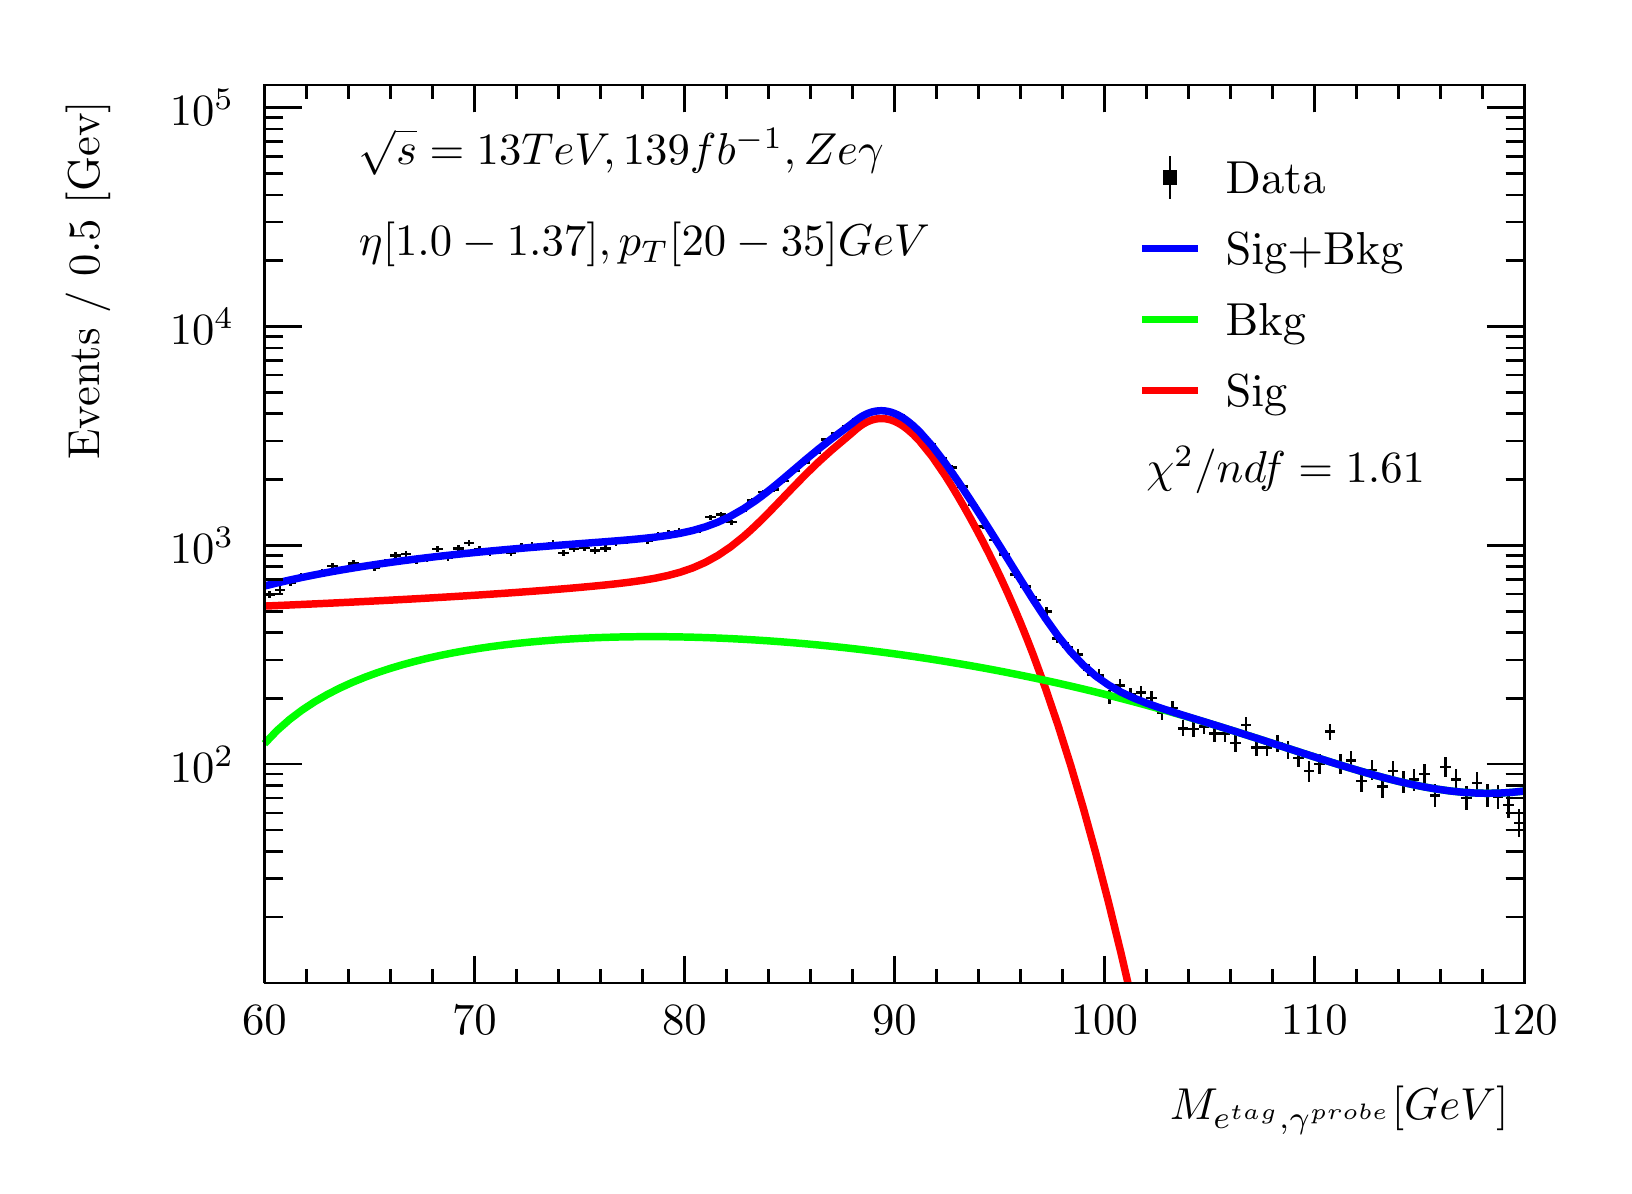
\begin{tikzpicture}
\pgfdeclareplotmark{cross} {
\pgfpathmoveto{\pgfpoint{-0.3\pgfplotmarksize}{\pgfplotmarksize}}
\pgfpathlineto{\pgfpoint{+0.3\pgfplotmarksize}{\pgfplotmarksize}}
\pgfpathlineto{\pgfpoint{+0.3\pgfplotmarksize}{0.3\pgfplotmarksize}}
\pgfpathlineto{\pgfpoint{+1\pgfplotmarksize}{0.3\pgfplotmarksize}}
\pgfpathlineto{\pgfpoint{+1\pgfplotmarksize}{-0.3\pgfplotmarksize}}
\pgfpathlineto{\pgfpoint{+0.3\pgfplotmarksize}{-0.3\pgfplotmarksize}}
\pgfpathlineto{\pgfpoint{+0.3\pgfplotmarksize}{-1.\pgfplotmarksize}}
\pgfpathlineto{\pgfpoint{-0.3\pgfplotmarksize}{-1.\pgfplotmarksize}}
\pgfpathlineto{\pgfpoint{-0.3\pgfplotmarksize}{-0.3\pgfplotmarksize}}
\pgfpathlineto{\pgfpoint{-1.\pgfplotmarksize}{-0.3\pgfplotmarksize}}
\pgfpathlineto{\pgfpoint{-1.\pgfplotmarksize}{0.3\pgfplotmarksize}}
\pgfpathlineto{\pgfpoint{-0.3\pgfplotmarksize}{0.3\pgfplotmarksize}}
\pgfpathclose
\pgfusepathqstroke
}
\pgfdeclareplotmark{cross*} {
\pgfpathmoveto{\pgfpoint{-0.3\pgfplotmarksize}{\pgfplotmarksize}}
\pgfpathlineto{\pgfpoint{+0.3\pgfplotmarksize}{\pgfplotmarksize}}
\pgfpathlineto{\pgfpoint{+0.3\pgfplotmarksize}{0.3\pgfplotmarksize}}
\pgfpathlineto{\pgfpoint{+1\pgfplotmarksize}{0.3\pgfplotmarksize}}
\pgfpathlineto{\pgfpoint{+1\pgfplotmarksize}{-0.3\pgfplotmarksize}}
\pgfpathlineto{\pgfpoint{+0.3\pgfplotmarksize}{-0.3\pgfplotmarksize}}
\pgfpathlineto{\pgfpoint{+0.3\pgfplotmarksize}{-1.\pgfplotmarksize}}
\pgfpathlineto{\pgfpoint{-0.3\pgfplotmarksize}{-1.\pgfplotmarksize}}
\pgfpathlineto{\pgfpoint{-0.3\pgfplotmarksize}{-0.3\pgfplotmarksize}}
\pgfpathlineto{\pgfpoint{-1.\pgfplotmarksize}{-0.3\pgfplotmarksize}}
\pgfpathlineto{\pgfpoint{-1.\pgfplotmarksize}{0.3\pgfplotmarksize}}
\pgfpathlineto{\pgfpoint{-0.3\pgfplotmarksize}{0.3\pgfplotmarksize}}
\pgfpathclose
\pgfusepathqfillstroke
}
\pgfdeclareplotmark{newstar} {
\pgfpathmoveto{\pgfqpoint{0pt}{\pgfplotmarksize}}
\pgfpathlineto{\pgfqpointpolar{44}{0.5\pgfplotmarksize}}
\pgfpathlineto{\pgfqpointpolar{18}{\pgfplotmarksize}}
\pgfpathlineto{\pgfqpointpolar{-20}{0.5\pgfplotmarksize}}
\pgfpathlineto{\pgfqpointpolar{-54}{\pgfplotmarksize}}
\pgfpathlineto{\pgfqpointpolar{-90}{0.5\pgfplotmarksize}}
\pgfpathlineto{\pgfqpointpolar{234}{\pgfplotmarksize}}
\pgfpathlineto{\pgfqpointpolar{198}{0.5\pgfplotmarksize}}
\pgfpathlineto{\pgfqpointpolar{162}{\pgfplotmarksize}}
\pgfpathlineto{\pgfqpointpolar{134}{0.5\pgfplotmarksize}}
\pgfpathclose
\pgfusepathqstroke
}
\pgfdeclareplotmark{newstar*} {
\pgfpathmoveto{\pgfqpoint{0pt}{\pgfplotmarksize}}
\pgfpathlineto{\pgfqpointpolar{44}{0.5\pgfplotmarksize}}
\pgfpathlineto{\pgfqpointpolar{18}{\pgfplotmarksize}}
\pgfpathlineto{\pgfqpointpolar{-20}{0.5\pgfplotmarksize}}
\pgfpathlineto{\pgfqpointpolar{-54}{\pgfplotmarksize}}
\pgfpathlineto{\pgfqpointpolar{-90}{0.5\pgfplotmarksize}}
\pgfpathlineto{\pgfqpointpolar{234}{\pgfplotmarksize}}
\pgfpathlineto{\pgfqpointpolar{198}{0.5\pgfplotmarksize}}
\pgfpathlineto{\pgfqpointpolar{162}{\pgfplotmarksize}}
\pgfpathlineto{\pgfqpointpolar{134}{0.5\pgfplotmarksize}}
\pgfpathclose
\pgfusepathqfillstroke
}
\definecolor{c}{rgb}{1,1,1};
\draw [color=c, fill=c] (0,0) rectangle (20,14.4361);
\draw [color=c, fill=c] (3,2.30977) rectangle (19,13.7143);
\definecolor{c}{rgb}{0,0,0};
\draw [c,line width=0.9] (3,2.30977) -- (3,13.7143) -- (19,13.7143) -- (19,2.30977) -- (3,2.30977);
\definecolor{c}{rgb}{1,1,1};
\draw [color=c, fill=c] (3,2.30977) rectangle (19,13.7143);
\definecolor{c}{rgb}{0,0,0};
\draw [c,line width=0.9] (3,2.30977) -- (3,13.7143) -- (19,13.7143) -- (19,2.30977) -- (3,2.30977);
\draw [c,line width=0.9] (3,2.30977) -- (19,2.30977);
\draw [c,line width=0.9] (3,2.65624) -- (3,2.30977);
\draw [c,line width=0.9] (3.53333,2.48301) -- (3.53333,2.30977);
\draw [c,line width=0.9] (4.06667,2.48301) -- (4.06667,2.30977);
\draw [c,line width=0.9] (4.6,2.48301) -- (4.6,2.30977);
\draw [c,line width=0.9] (5.13333,2.48301) -- (5.13333,2.30977);
\draw [c,line width=0.9] (5.66667,2.65624) -- (5.66667,2.30977);
\draw [c,line width=0.9] (6.2,2.48301) -- (6.2,2.30977);
\draw [c,line width=0.9] (6.73333,2.48301) -- (6.73333,2.30977);
\draw [c,line width=0.9] (7.26667,2.48301) -- (7.26667,2.30977);
\draw [c,line width=0.9] (7.8,2.48301) -- (7.8,2.30977);
\draw [c,line width=0.9] (8.33333,2.65624) -- (8.33333,2.30977);
\draw [c,line width=0.9] (8.86667,2.48301) -- (8.86667,2.30977);
\draw [c,line width=0.9] (9.4,2.48301) -- (9.4,2.30977);
\draw [c,line width=0.9] (9.93333,2.48301) -- (9.93333,2.30977);
\draw [c,line width=0.9] (10.4667,2.48301) -- (10.4667,2.30977);
\draw [c,line width=0.9] (11,2.65624) -- (11,2.30977);
\draw [c,line width=0.9] (11.5333,2.48301) -- (11.5333,2.30977);
\draw [c,line width=0.9] (12.0667,2.48301) -- (12.0667,2.30977);
\draw [c,line width=0.9] (12.6,2.48301) -- (12.6,2.30977);
\draw [c,line width=0.9] (13.1333,2.48301) -- (13.1333,2.30977);
\draw [c,line width=0.9] (13.6667,2.65624) -- (13.6667,2.30977);
\draw [c,line width=0.9] (14.2,2.48301) -- (14.2,2.30977);
\draw [c,line width=0.9] (14.7333,2.48301) -- (14.7333,2.30977);
\draw [c,line width=0.9] (15.2667,2.48301) -- (15.2667,2.30977);
\draw [c,line width=0.9] (15.8,2.48301) -- (15.8,2.30977);
\draw [c,line width=0.9] (16.3333,2.65624) -- (16.3333,2.30977);
\draw [c,line width=0.9] (16.8667,2.48301) -- (16.8667,2.30977);
\draw [c,line width=0.9] (17.4,2.48301) -- (17.4,2.30977);
\draw [c,line width=0.9] (17.9333,2.48301) -- (17.9333,2.30977);
\draw [c,line width=0.9] (18.4667,2.48301) -- (18.4667,2.30977);
\draw [c,line width=0.9] (19,2.65624) -- (19,2.30977);
\draw [anchor=base] (3,1.66015) node[scale=1.61424, color=c, rotate=0]{60};
\draw [anchor=base] (5.66667,1.66015) node[scale=1.61424, color=c, rotate=0]{70};
\draw [anchor=base] (8.33333,1.66015) node[scale=1.61424, color=c, rotate=0]{80};
\draw [anchor=base] (11,1.66015) node[scale=1.61424, color=c, rotate=0]{90};
\draw [anchor=base] (13.6667,1.66015) node[scale=1.61424, color=c, rotate=0]{100};
\draw [anchor=base] (16.3333,1.66015) node[scale=1.61424, color=c, rotate=0]{110};
\draw [anchor=base] (19,1.66015) node[scale=1.61424, color=c, rotate=0]{120};
\draw [anchor= east] (19,0.692932) node[scale=1.61424, color=c, rotate=0]{$M_{e^{tag}, \gamma^{probe}}  [GeV]$};
\draw [c,line width=0.9] (3,13.7143) -- (19,13.7143);
\draw [c,line width=0.9] (3,13.3678) -- (3,13.7143);
\draw [c,line width=0.9] (3.53333,13.5411) -- (3.53333,13.7143);
\draw [c,line width=0.9] (4.06667,13.5411) -- (4.06667,13.7143);
\draw [c,line width=0.9] (4.6,13.5411) -- (4.6,13.7143);
\draw [c,line width=0.9] (5.13333,13.5411) -- (5.13333,13.7143);
\draw [c,line width=0.9] (5.66667,13.3678) -- (5.66667,13.7143);
\draw [c,line width=0.9] (6.2,13.5411) -- (6.2,13.7143);
\draw [c,line width=0.9] (6.73333,13.5411) -- (6.73333,13.7143);
\draw [c,line width=0.9] (7.26667,13.5411) -- (7.26667,13.7143);
\draw [c,line width=0.9] (7.8,13.5411) -- (7.8,13.7143);
\draw [c,line width=0.9] (8.33333,13.3678) -- (8.33333,13.7143);
\draw [c,line width=0.9] (8.86667,13.5411) -- (8.86667,13.7143);
\draw [c,line width=0.9] (9.4,13.5411) -- (9.4,13.7143);
\draw [c,line width=0.9] (9.93333,13.5411) -- (9.93333,13.7143);
\draw [c,line width=0.9] (10.4667,13.5411) -- (10.4667,13.7143);
\draw [c,line width=0.9] (11,13.3678) -- (11,13.7143);
\draw [c,line width=0.9] (11.5333,13.5411) -- (11.5333,13.7143);
\draw [c,line width=0.9] (12.0667,13.5411) -- (12.0667,13.7143);
\draw [c,line width=0.9] (12.6,13.5411) -- (12.6,13.7143);
\draw [c,line width=0.9] (13.1333,13.5411) -- (13.1333,13.7143);
\draw [c,line width=0.9] (13.6667,13.3678) -- (13.6667,13.7143);
\draw [c,line width=0.9] (14.2,13.5411) -- (14.2,13.7143);
\draw [c,line width=0.9] (14.7333,13.5411) -- (14.7333,13.7143);
\draw [c,line width=0.9] (15.2667,13.5411) -- (15.2667,13.7143);
\draw [c,line width=0.9] (15.8,13.5411) -- (15.8,13.7143);
\draw [c,line width=0.9] (16.3333,13.3678) -- (16.3333,13.7143);
\draw [c,line width=0.9] (16.8667,13.5411) -- (16.8667,13.7143);
\draw [c,line width=0.9] (17.4,13.5411) -- (17.4,13.7143);
\draw [c,line width=0.9] (17.9333,13.5411) -- (17.9333,13.7143);
\draw [c,line width=0.9] (18.4667,13.5411) -- (18.4667,13.7143);
\draw [c,line width=0.9] (19,13.3678) -- (19,13.7143);
\draw [c,line width=0.9] (3,2.30977) -- (3,13.7143);
\draw [c,line width=0.9] (3.237,3.14637) -- (3,3.14637);
\draw [c,line width=0.9] (3.237,3.63576) -- (3,3.63576);
\draw [c,line width=0.9] (3.237,3.98298) -- (3,3.98298);
\draw [c,line width=0.9] (3.237,4.2523) -- (3,4.2523);
\draw [c,line width=0.9] (3.237,4.47236) -- (3,4.47236);
\draw [c,line width=0.9] (3.237,4.65841) -- (3,4.65841);
\draw [c,line width=0.9] (3.237,4.81958) -- (3,4.81958);
\draw [c,line width=0.9] (3.237,4.96174) -- (3,4.96174);
\draw [c,line width=0.9] (3.474,5.0889) -- (3,5.0889);
\draw [anchor= east] (2.82,5.0889) node[scale=1.61424, color=c, rotate=0]{$10^{2}$};
\draw [c,line width=0.9] (3.237,5.92551) -- (3,5.92551);
\draw [c,line width=0.9] (3.237,6.41489) -- (3,6.41489);
\draw [c,line width=0.9] (3.237,6.76211) -- (3,6.76211);
\draw [c,line width=0.9] (3.237,7.03144) -- (3,7.03144);
\draw [c,line width=0.9] (3.237,7.25149) -- (3,7.25149);
\draw [c,line width=0.9] (3.237,7.43755) -- (3,7.43755);
\draw [c,line width=0.9] (3.237,7.59871) -- (3,7.59871);
\draw [c,line width=0.9] (3.237,7.74087) -- (3,7.74087);
\draw [c,line width=0.9] (3.474,7.86804) -- (3,7.86804);
\draw [anchor= east] (2.82,7.86804) node[scale=1.61424, color=c, rotate=0]{$10^{3}$};
\draw [c,line width=0.9] (3.237,8.70464) -- (3,8.70464);
\draw [c,line width=0.9] (3.237,9.19402) -- (3,9.19402);
\draw [c,line width=0.9] (3.237,9.54124) -- (3,9.54124);
\draw [c,line width=0.9] (3.237,9.81057) -- (3,9.81057);
\draw [c,line width=0.9] (3.237,10.0306) -- (3,10.0306);
\draw [c,line width=0.9] (3.237,10.2167) -- (3,10.2167);
\draw [c,line width=0.9] (3.237,10.3778) -- (3,10.3778);
\draw [c,line width=0.9] (3.237,10.52) -- (3,10.52);
\draw [c,line width=0.9] (3.474,10.6472) -- (3,10.6472);
\draw [anchor= east] (2.82,10.6472) node[scale=1.61424, color=c, rotate=0]{$10^{4}$};
\draw [c,line width=0.9] (3.237,11.4838) -- (3,11.4838);
\draw [c,line width=0.9] (3.237,11.9732) -- (3,11.9732);
\draw [c,line width=0.9] (3.237,12.3204) -- (3,12.3204);
\draw [c,line width=0.9] (3.237,12.5897) -- (3,12.5897);
\draw [c,line width=0.9] (3.237,12.8098) -- (3,12.8098);
\draw [c,line width=0.9] (3.237,12.9958) -- (3,12.9958);
\draw [c,line width=0.9] (3.237,13.157) -- (3,13.157);
\draw [c,line width=0.9] (3.237,13.2991) -- (3,13.2991);
\draw [c,line width=0.9] (3.474,13.4263) -- (3,13.4263);
\draw [anchor= east] (2.82,13.4263) node[scale=1.61424, color=c, rotate=0]{$10^{5}$};
\draw [anchor= east] (0.76,13.7143) node[scale=1.61424, color=c, rotate=90]{Events / 0.5 [Gev]};
\draw [c,line width=0.9] (19,2.30977) -- (19,13.7143);
\draw [c,line width=0.9] (18.763,3.14637) -- (19,3.14637);
\draw [c,line width=0.9] (18.763,3.63576) -- (19,3.63576);
\draw [c,line width=0.9] (18.763,3.98298) -- (19,3.98298);
\draw [c,line width=0.9] (18.763,4.2523) -- (19,4.2523);
\draw [c,line width=0.9] (18.763,4.47236) -- (19,4.47236);
\draw [c,line width=0.9] (18.763,4.65841) -- (19,4.65841);
\draw [c,line width=0.9] (18.763,4.81958) -- (19,4.81958);
\draw [c,line width=0.9] (18.763,4.96174) -- (19,4.96174);
\draw [c,line width=0.9] (18.526,5.0889) -- (19,5.0889);
\draw [c,line width=0.9] (18.763,5.92551) -- (19,5.92551);
\draw [c,line width=0.9] (18.763,6.41489) -- (19,6.41489);
\draw [c,line width=0.9] (18.763,6.76211) -- (19,6.76211);
\draw [c,line width=0.9] (18.763,7.03144) -- (19,7.03144);
\draw [c,line width=0.9] (18.763,7.25149) -- (19,7.25149);
\draw [c,line width=0.9] (18.763,7.43755) -- (19,7.43755);
\draw [c,line width=0.9] (18.763,7.59871) -- (19,7.59871);
\draw [c,line width=0.9] (18.763,7.74087) -- (19,7.74087);
\draw [c,line width=0.9] (18.526,7.86804) -- (19,7.86804);
\draw [c,line width=0.9] (18.763,8.70464) -- (19,8.70464);
\draw [c,line width=0.9] (18.763,9.19402) -- (19,9.19402);
\draw [c,line width=0.9] (18.763,9.54124) -- (19,9.54124);
\draw [c,line width=0.9] (18.763,9.81057) -- (19,9.81057);
\draw [c,line width=0.9] (18.763,10.0306) -- (19,10.0306);
\draw [c,line width=0.9] (18.763,10.2167) -- (19,10.2167);
\draw [c,line width=0.9] (18.763,10.3778) -- (19,10.3778);
\draw [c,line width=0.9] (18.763,10.52) -- (19,10.52);
\draw [c,line width=0.9] (18.526,10.6472) -- (19,10.6472);
\draw [c,line width=0.9] (18.763,11.4838) -- (19,11.4838);
\draw [c,line width=0.9] (18.763,11.9732) -- (19,11.9732);
\draw [c,line width=0.9] (18.763,12.3204) -- (19,12.3204);
\draw [c,line width=0.9] (18.763,12.5897) -- (19,12.5897);
\draw [c,line width=0.9] (18.763,12.8098) -- (19,12.8098);
\draw [c,line width=0.9] (18.763,12.9958) -- (19,12.9958);
\draw [c,line width=0.9] (18.763,13.157) -- (19,13.157);
\draw [c,line width=0.9] (18.763,13.2991) -- (19,13.2991);
\draw [c,line width=0.9] (18.526,13.4263) -- (19,13.4263);
\draw [c,line width=0.9] (3.06667,7.24544) -- (3,7.24544);
\draw [c,line width=0.9] (3,7.24544) -- (3,7.24544);
\draw [c,line width=0.9] (3.06667,7.24544) -- (3.13333,7.24544);
\draw [c,line width=0.9] (3.13333,7.24544) -- (3.13333,7.24544);
\draw [c,line width=0.9] (3.06667,7.24544) -- (3.06667,7.29484);
\draw [c,line width=0.9] (3.06667,7.29484) -- (3.06667,7.29484);
\draw [c,line width=0.9] (3.06667,7.24544) -- (3.06667,7.19605);
\draw [c,line width=0.9] (3.06667,7.19605) -- (3.06667,7.19605);
\draw [c,line width=0.9] (3.2,7.30076) -- (3.13333,7.30076);
\draw [c,line width=0.9] (3.13333,7.30076) -- (3.13333,7.30076);
\draw [c,line width=0.9] (3.2,7.30076) -- (3.26667,7.30076);
\draw [c,line width=0.9] (3.26667,7.30076) -- (3.26667,7.30076);
\draw [c,line width=0.9] (3.2,7.30076) -- (3.2,7.34904);
\draw [c,line width=0.9] (3.2,7.34904) -- (3.2,7.34904);
\draw [c,line width=0.9] (3.2,7.30076) -- (3.2,7.25249);
\draw [c,line width=0.9] (3.2,7.25249) -- (3.2,7.25249);
\draw [c,line width=0.9] (3.33333,7.39544) -- (3.26667,7.39544);
\draw [c,line width=0.9] (3.26667,7.39544) -- (3.26667,7.39544);
\draw [c,line width=0.9] (3.33333,7.39544) -- (3.4,7.39544);
\draw [c,line width=0.9] (3.4,7.39544) -- (3.4,7.39544);
\draw [c,line width=0.9] (3.33333,7.39544) -- (3.33333,7.44186);
\draw [c,line width=0.9] (3.33333,7.44186) -- (3.33333,7.44186);
\draw [c,line width=0.9] (3.33333,7.39544) -- (3.33333,7.34902);
\draw [c,line width=0.9] (3.33333,7.34902) -- (3.33333,7.34902);
\draw [c,line width=0.9] (3.46667,7.47155) -- (3.4,7.47155);
\draw [c,line width=0.9] (3.4,7.47155) -- (3.4,7.47155);
\draw [c,line width=0.9] (3.46667,7.47155) -- (3.53333,7.47155);
\draw [c,line width=0.9] (3.53333,7.47155) -- (3.53333,7.47155);
\draw [c,line width=0.9] (3.46667,7.47155) -- (3.46667,7.51653);
\draw [c,line width=0.9] (3.46667,7.51653) -- (3.46667,7.51653);
\draw [c,line width=0.9] (3.46667,7.47155) -- (3.46667,7.42657);
\draw [c,line width=0.9] (3.46667,7.42657) -- (3.46667,7.42657);
\draw [c,line width=0.9] (3.6,7.48323) -- (3.53333,7.48323);
\draw [c,line width=0.9] (3.53333,7.48323) -- (3.53333,7.48323);
\draw [c,line width=0.9] (3.6,7.48323) -- (3.66667,7.48323);
\draw [c,line width=0.9] (3.66667,7.48323) -- (3.66667,7.48323);
\draw [c,line width=0.9] (3.6,7.48323) -- (3.6,7.52799);
\draw [c,line width=0.9] (3.6,7.52799) -- (3.6,7.52799);
\draw [c,line width=0.9] (3.6,7.48323) -- (3.6,7.43846);
\draw [c,line width=0.9] (3.6,7.43846) -- (3.6,7.43846);
\draw [c,line width=0.9] (3.73333,7.52243) -- (3.66667,7.52243);
\draw [c,line width=0.9] (3.66667,7.52243) -- (3.66667,7.52243);
\draw [c,line width=0.9] (3.73333,7.52243) -- (3.8,7.52243);
\draw [c,line width=0.9] (3.8,7.52243) -- (3.8,7.52243);
\draw [c,line width=0.9] (3.73333,7.52243) -- (3.73333,7.56647);
\draw [c,line width=0.9] (3.73333,7.56647) -- (3.73333,7.56647);
\draw [c,line width=0.9] (3.73333,7.52243) -- (3.73333,7.47839);
\draw [c,line width=0.9] (3.73333,7.47839) -- (3.73333,7.47839);
\draw [c,line width=0.9] (3.86667,7.60773) -- (3.8,7.60773);
\draw [c,line width=0.9] (3.8,7.60773) -- (3.8,7.60773);
\draw [c,line width=0.9] (3.86667,7.60773) -- (3.93333,7.60773);
\draw [c,line width=0.9] (3.93333,7.60773) -- (3.93333,7.60773);
\draw [c,line width=0.9] (3.86667,7.60773) -- (3.86667,7.65024);
\draw [c,line width=0.9] (3.86667,7.65024) -- (3.86667,7.65024);
\draw [c,line width=0.9] (3.86667,7.60773) -- (3.86667,7.56522);
\draw [c,line width=0.9] (3.86667,7.56522) -- (3.86667,7.56522);
\draw [c,line width=0.9] (4,7.56039) -- (3.93333,7.56039);
\draw [c,line width=0.9] (3.93333,7.56039) -- (3.93333,7.56039);
\draw [c,line width=0.9] (4,7.56039) -- (4.06667,7.56039);
\draw [c,line width=0.9] (4.06667,7.56039) -- (4.06667,7.56039);
\draw [c,line width=0.9] (4,7.56039) -- (4,7.60375);
\draw [c,line width=0.9] (4,7.60375) -- (4,7.60375);
\draw [c,line width=0.9] (4,7.56039) -- (4,7.51704);
\draw [c,line width=0.9] (4,7.51704) -- (4,7.51704);
\draw [c,line width=0.9] (4.13333,7.63878) -- (4.06667,7.63878);
\draw [c,line width=0.9] (4.06667,7.63878) -- (4.06667,7.63878);
\draw [c,line width=0.9] (4.13333,7.63878) -- (4.2,7.63878);
\draw [c,line width=0.9] (4.2,7.63878) -- (4.2,7.63878);
\draw [c,line width=0.9] (4.13333,7.63878) -- (4.13333,7.68074);
\draw [c,line width=0.9] (4.13333,7.68074) -- (4.13333,7.68074);
\draw [c,line width=0.9] (4.13333,7.63878) -- (4.13333,7.59681);
\draw [c,line width=0.9] (4.13333,7.59681) -- (4.13333,7.59681);
\draw [c,line width=0.9] (4.26667,7.60623) -- (4.2,7.60623);
\draw [c,line width=0.9] (4.2,7.60623) -- (4.2,7.60623);
\draw [c,line width=0.9] (4.26667,7.60623) -- (4.33333,7.60623);
\draw [c,line width=0.9] (4.33333,7.60623) -- (4.33333,7.60623);
\draw [c,line width=0.9] (4.26667,7.60623) -- (4.26667,7.64877);
\draw [c,line width=0.9] (4.26667,7.64877) -- (4.26667,7.64877);
\draw [c,line width=0.9] (4.26667,7.60623) -- (4.26667,7.5637);
\draw [c,line width=0.9] (4.26667,7.5637) -- (4.26667,7.5637);
\draw [c,line width=0.9] (4.4,7.58658) -- (4.33333,7.58658);
\draw [c,line width=0.9] (4.33333,7.58658) -- (4.33333,7.58658);
\draw [c,line width=0.9] (4.4,7.58658) -- (4.46667,7.58658);
\draw [c,line width=0.9] (4.46667,7.58658) -- (4.46667,7.58658);
\draw [c,line width=0.9] (4.4,7.58658) -- (4.4,7.62947);
\draw [c,line width=0.9] (4.4,7.62947) -- (4.4,7.62947);
\draw [c,line width=0.9] (4.4,7.58658) -- (4.4,7.5437);
\draw [c,line width=0.9] (4.4,7.5437) -- (4.4,7.5437);
\draw [c,line width=0.9] (4.53333,7.65473) -- (4.46667,7.65473);
\draw [c,line width=0.9] (4.46667,7.65473) -- (4.46667,7.65473);
\draw [c,line width=0.9] (4.53333,7.65473) -- (4.6,7.65473);
\draw [c,line width=0.9] (4.6,7.65473) -- (4.6,7.65473);
\draw [c,line width=0.9] (4.53333,7.65473) -- (4.53333,7.69642);
\draw [c,line width=0.9] (4.53333,7.69642) -- (4.53333,7.69642);
\draw [c,line width=0.9] (4.53333,7.65473) -- (4.53333,7.61303);
\draw [c,line width=0.9] (4.53333,7.61303) -- (4.53333,7.61303);
\draw [c,line width=0.9] (4.66667,7.74087) -- (4.6,7.74087);
\draw [c,line width=0.9] (4.6,7.74087) -- (4.6,7.74087);
\draw [c,line width=0.9] (4.66667,7.74087) -- (4.73333,7.74087);
\draw [c,line width=0.9] (4.73333,7.74087) -- (4.73333,7.74087);
\draw [c,line width=0.9] (4.66667,7.74087) -- (4.66667,7.7811);
\draw [c,line width=0.9] (4.66667,7.7811) -- (4.66667,7.7811);
\draw [c,line width=0.9] (4.66667,7.74087) -- (4.66667,7.70064);
\draw [c,line width=0.9] (4.66667,7.70064) -- (4.66667,7.70064);
\draw [c,line width=0.9] (4.8,7.7595) -- (4.73333,7.7595);
\draw [c,line width=0.9] (4.73333,7.7595) -- (4.73333,7.7595);
\draw [c,line width=0.9] (4.8,7.7595) -- (4.86667,7.7595);
\draw [c,line width=0.9] (4.86667,7.7595) -- (4.86667,7.7595);
\draw [c,line width=0.9] (4.8,7.7595) -- (4.8,7.79943);
\draw [c,line width=0.9] (4.8,7.79943) -- (4.8,7.79943);
\draw [c,line width=0.9] (4.8,7.7595) -- (4.8,7.71958);
\draw [c,line width=0.9] (4.8,7.71958) -- (4.8,7.71958);
\draw [c,line width=0.9] (4.93333,7.67331) -- (4.86667,7.67331);
\draw [c,line width=0.9] (4.86667,7.67331) -- (4.86667,7.67331);
\draw [c,line width=0.9] (4.93333,7.67331) -- (5,7.67331);
\draw [c,line width=0.9] (5,7.67331) -- (5,7.67331);
\draw [c,line width=0.9] (4.93333,7.67331) -- (4.93333,7.71468);
\draw [c,line width=0.9] (4.93333,7.71468) -- (4.93333,7.71468);
\draw [c,line width=0.9] (4.93333,7.67331) -- (4.93333,7.63193);
\draw [c,line width=0.9] (4.93333,7.63193) -- (4.93333,7.63193);
\draw [c,line width=0.9] (5.06667,7.69718) -- (5,7.69718);
\draw [c,line width=0.9] (5,7.69718) -- (5,7.69718);
\draw [c,line width=0.9] (5.06667,7.69718) -- (5.13333,7.69718);
\draw [c,line width=0.9] (5.13333,7.69718) -- (5.13333,7.69718);
\draw [c,line width=0.9] (5.06667,7.69718) -- (5.06667,7.73814);
\draw [c,line width=0.9] (5.06667,7.73814) -- (5.06667,7.73814);
\draw [c,line width=0.9] (5.06667,7.69718) -- (5.06667,7.65621);
\draw [c,line width=0.9] (5.06667,7.65621) -- (5.06667,7.65621);
\draw [c,line width=0.9] (5.2,7.82003) -- (5.13333,7.82003);
\draw [c,line width=0.9] (5.13333,7.82003) -- (5.13333,7.82003);
\draw [c,line width=0.9] (5.2,7.82003) -- (5.26667,7.82003);
\draw [c,line width=0.9] (5.26667,7.82003) -- (5.26667,7.82003);
\draw [c,line width=0.9] (5.2,7.82003) -- (5.2,7.85896);
\draw [c,line width=0.9] (5.2,7.85896) -- (5.2,7.85896);
\draw [c,line width=0.9] (5.2,7.82003) -- (5.2,7.78109);
\draw [c,line width=0.9] (5.2,7.78109) -- (5.2,7.78109);
\draw [c,line width=0.9] (5.33333,7.711) -- (5.26667,7.711);
\draw [c,line width=0.9] (5.26667,7.711) -- (5.26667,7.711);
\draw [c,line width=0.9] (5.33333,7.711) -- (5.4,7.711);
\draw [c,line width=0.9] (5.4,7.711) -- (5.4,7.711);
\draw [c,line width=0.9] (5.33333,7.711) -- (5.33333,7.75173);
\draw [c,line width=0.9] (5.33333,7.75173) -- (5.33333,7.75173);
\draw [c,line width=0.9] (5.33333,7.711) -- (5.33333,7.67027);
\draw [c,line width=0.9] (5.33333,7.67027) -- (5.33333,7.67027);
\draw [c,line width=0.9] (5.46667,7.83003) -- (5.4,7.83003);
\draw [c,line width=0.9] (5.4,7.83003) -- (5.4,7.83003);
\draw [c,line width=0.9] (5.46667,7.83003) -- (5.53333,7.83003);
\draw [c,line width=0.9] (5.53333,7.83003) -- (5.53333,7.83003);
\draw [c,line width=0.9] (5.46667,7.83003) -- (5.46667,7.8688);
\draw [c,line width=0.9] (5.46667,7.8688) -- (5.46667,7.8688);
\draw [c,line width=0.9] (5.46667,7.83003) -- (5.46667,7.79126);
\draw [c,line width=0.9] (5.46667,7.79126) -- (5.46667,7.79126);
\draw [c,line width=0.9] (5.6,7.89666) -- (5.53333,7.89666);
\draw [c,line width=0.9] (5.53333,7.89666) -- (5.53333,7.89666);
\draw [c,line width=0.9] (5.6,7.89666) -- (5.66667,7.89666);
\draw [c,line width=0.9] (5.66667,7.89666) -- (5.66667,7.89666);
\draw [c,line width=0.9] (5.6,7.89666) -- (5.6,7.93438);
\draw [c,line width=0.9] (5.6,7.93438) -- (5.6,7.93438);
\draw [c,line width=0.9] (5.6,7.89666) -- (5.6,7.85895);
\draw [c,line width=0.9] (5.6,7.85895) -- (5.6,7.85895);
\draw [c,line width=0.9] (5.73333,7.81751) -- (5.66667,7.81751);
\draw [c,line width=0.9] (5.66667,7.81751) -- (5.66667,7.81751);
\draw [c,line width=0.9] (5.73333,7.81751) -- (5.8,7.81751);
\draw [c,line width=0.9] (5.8,7.81751) -- (5.8,7.81751);
\draw [c,line width=0.9] (5.73333,7.81751) -- (5.73333,7.85648);
\draw [c,line width=0.9] (5.73333,7.85648) -- (5.73333,7.85648);
\draw [c,line width=0.9] (5.73333,7.81751) -- (5.73333,7.77854);
\draw [c,line width=0.9] (5.73333,7.77854) -- (5.73333,7.77854);
\draw [c,line width=0.9] (5.86667,7.77785) -- (5.8,7.77785);
\draw [c,line width=0.9] (5.8,7.77785) -- (5.8,7.77785);
\draw [c,line width=0.9] (5.86667,7.77785) -- (5.93333,7.77785);
\draw [c,line width=0.9] (5.93333,7.77785) -- (5.93333,7.77785);
\draw [c,line width=0.9] (5.86667,7.77785) -- (5.86667,7.81747);
\draw [c,line width=0.9] (5.86667,7.81747) -- (5.86667,7.81747);
\draw [c,line width=0.9] (5.86667,7.77785) -- (5.86667,7.73823);
\draw [c,line width=0.9] (5.86667,7.73823) -- (5.86667,7.73823);
\draw [c,line width=0.9] (6,7.79592) -- (5.93333,7.79592);
\draw [c,line width=0.9] (5.93333,7.79592) -- (5.93333,7.79592);
\draw [c,line width=0.9] (6,7.79592) -- (6.06667,7.79592);
\draw [c,line width=0.9] (6.06667,7.79592) -- (6.06667,7.79592);
\draw [c,line width=0.9] (6,7.79592) -- (6,7.83525);
\draw [c,line width=0.9] (6,7.83525) -- (6,7.83525);
\draw [c,line width=0.9] (6,7.79592) -- (6,7.7566);
\draw [c,line width=0.9] (6,7.7566) -- (6,7.7566);
\draw [c,line width=0.9] (6.13333,7.77655) -- (6.06667,7.77655);
\draw [c,line width=0.9] (6.06667,7.77655) -- (6.06667,7.77655);
\draw [c,line width=0.9] (6.13333,7.77655) -- (6.2,7.77655);
\draw [c,line width=0.9] (6.2,7.77655) -- (6.2,7.77655);
\draw [c,line width=0.9] (6.13333,7.77655) -- (6.13333,7.81619);
\draw [c,line width=0.9] (6.13333,7.81619) -- (6.13333,7.81619);
\draw [c,line width=0.9] (6.13333,7.77655) -- (6.13333,7.73691);
\draw [c,line width=0.9] (6.13333,7.73691) -- (6.13333,7.73691);
\draw [c,line width=0.9] (6.26667,7.85713) -- (6.2,7.85713);
\draw [c,line width=0.9] (6.2,7.85713) -- (6.2,7.85713);
\draw [c,line width=0.9] (6.26667,7.85713) -- (6.33333,7.85713);
\draw [c,line width=0.9] (6.33333,7.85713) -- (6.33333,7.85713);
\draw [c,line width=0.9] (6.26667,7.85713) -- (6.26667,7.89547);
\draw [c,line width=0.9] (6.26667,7.89547) -- (6.26667,7.89547);
\draw [c,line width=0.9] (6.26667,7.85713) -- (6.26667,7.81879);
\draw [c,line width=0.9] (6.26667,7.81879) -- (6.26667,7.81879);
\draw [c,line width=0.9] (6.4,7.86925) -- (6.33333,7.86925);
\draw [c,line width=0.9] (6.33333,7.86925) -- (6.33333,7.86925);
\draw [c,line width=0.9] (6.4,7.86925) -- (6.46667,7.86925);
\draw [c,line width=0.9] (6.46667,7.86925) -- (6.46667,7.86925);
\draw [c,line width=0.9] (6.4,7.86925) -- (6.4,7.90739);
\draw [c,line width=0.9] (6.4,7.90739) -- (6.4,7.90739);
\draw [c,line width=0.9] (6.4,7.86925) -- (6.4,7.8311);
\draw [c,line width=0.9] (6.4,7.8311) -- (6.4,7.8311);
\draw [c,line width=0.9] (6.53333,7.84242) -- (6.46667,7.84242);
\draw [c,line width=0.9] (6.46667,7.84242) -- (6.46667,7.84242);
\draw [c,line width=0.9] (6.53333,7.84242) -- (6.6,7.84242);
\draw [c,line width=0.9] (6.6,7.84242) -- (6.6,7.84242);
\draw [c,line width=0.9] (6.53333,7.84242) -- (6.53333,7.881);
\draw [c,line width=0.9] (6.53333,7.881) -- (6.53333,7.881);
\draw [c,line width=0.9] (6.53333,7.84242) -- (6.53333,7.80385);
\draw [c,line width=0.9] (6.53333,7.80385) -- (6.53333,7.80385);
\draw [c,line width=0.9] (6.66667,7.9002) -- (6.6,7.9002);
\draw [c,line width=0.9] (6.6,7.9002) -- (6.6,7.9002);
\draw [c,line width=0.9] (6.66667,7.9002) -- (6.73333,7.9002);
\draw [c,line width=0.9] (6.73333,7.9002) -- (6.73333,7.9002);
\draw [c,line width=0.9] (6.66667,7.9002) -- (6.66667,7.93786);
\draw [c,line width=0.9] (6.66667,7.93786) -- (6.66667,7.93786);
\draw [c,line width=0.9] (6.66667,7.9002) -- (6.66667,7.86253);
\draw [c,line width=0.9] (6.66667,7.86253) -- (6.66667,7.86253);
\draw [c,line width=0.9] (6.8,7.77133) -- (6.73333,7.77133);
\draw [c,line width=0.9] (6.73333,7.77133) -- (6.73333,7.77133);
\draw [c,line width=0.9] (6.8,7.77133) -- (6.86667,7.77133);
\draw [c,line width=0.9] (6.86667,7.77133) -- (6.86667,7.77133);
\draw [c,line width=0.9] (6.8,7.77133) -- (6.8,7.81106);
\draw [c,line width=0.9] (6.8,7.81106) -- (6.8,7.81106);
\draw [c,line width=0.9] (6.8,7.77133) -- (6.8,7.73161);
\draw [c,line width=0.9] (6.8,7.73161) -- (6.8,7.73161);
\draw [c,line width=0.9] (6.93333,7.82504) -- (6.86667,7.82504);
\draw [c,line width=0.9] (6.86667,7.82504) -- (6.86667,7.82504);
\draw [c,line width=0.9] (6.93333,7.82504) -- (7,7.82504);
\draw [c,line width=0.9] (7,7.82504) -- (7,7.82504);
\draw [c,line width=0.9] (6.93333,7.82504) -- (6.93333,7.86389);
\draw [c,line width=0.9] (6.93333,7.86389) -- (6.93333,7.86389);
\draw [c,line width=0.9] (6.93333,7.82504) -- (6.93333,7.78619);
\draw [c,line width=0.9] (6.93333,7.78619) -- (6.93333,7.78619);
\draw [c,line width=0.9] (7.06667,7.83376) -- (7,7.83376);
\draw [c,line width=0.9] (7,7.83376) -- (7,7.83376);
\draw [c,line width=0.9] (7.06667,7.83376) -- (7.13333,7.83376);
\draw [c,line width=0.9] (7.13333,7.83376) -- (7.13333,7.83376);
\draw [c,line width=0.9] (7.06667,7.83376) -- (7.06667,7.87247);
\draw [c,line width=0.9] (7.06667,7.87247) -- (7.06667,7.87247);
\draw [c,line width=0.9] (7.06667,7.83376) -- (7.06667,7.79505);
\draw [c,line width=0.9] (7.06667,7.79505) -- (7.06667,7.79505);
\draw [c,line width=0.9] (7.2,7.80231) -- (7.13333,7.80231);
\draw [c,line width=0.9] (7.13333,7.80231) -- (7.13333,7.80231);
\draw [c,line width=0.9] (7.2,7.80231) -- (7.26667,7.80231);
\draw [c,line width=0.9] (7.26667,7.80231) -- (7.26667,7.80231);
\draw [c,line width=0.9] (7.2,7.80231) -- (7.2,7.84153);
\draw [c,line width=0.9] (7.2,7.84153) -- (7.2,7.84153);
\draw [c,line width=0.9] (7.2,7.80231) -- (7.2,7.76309);
\draw [c,line width=0.9] (7.2,7.76309) -- (7.2,7.76309);
\draw [c,line width=0.9] (7.33333,7.82879) -- (7.26667,7.82879);
\draw [c,line width=0.9] (7.26667,7.82879) -- (7.26667,7.82879);
\draw [c,line width=0.9] (7.33333,7.82879) -- (7.4,7.82879);
\draw [c,line width=0.9] (7.4,7.82879) -- (7.4,7.82879);
\draw [c,line width=0.9] (7.33333,7.82879) -- (7.33333,7.86758);
\draw [c,line width=0.9] (7.33333,7.86758) -- (7.33333,7.86758);
\draw [c,line width=0.9] (7.33333,7.82879) -- (7.33333,7.78999);
\draw [c,line width=0.9] (7.33333,7.78999) -- (7.33333,7.78999);
\draw [c,line width=0.9] (7.46667,7.90137) -- (7.4,7.90137);
\draw [c,line width=0.9] (7.4,7.90137) -- (7.4,7.90137);
\draw [c,line width=0.9] (7.46667,7.90137) -- (7.53333,7.90137);
\draw [c,line width=0.9] (7.53333,7.90137) -- (7.53333,7.90137);
\draw [c,line width=0.9] (7.46667,7.90137) -- (7.46667,7.93901);
\draw [c,line width=0.9] (7.46667,7.93901) -- (7.46667,7.93901);
\draw [c,line width=0.9] (7.46667,7.90137) -- (7.46667,7.86373);
\draw [c,line width=0.9] (7.46667,7.86373) -- (7.46667,7.86373);
\draw [c,line width=0.9] (7.6,7.92001) -- (7.53333,7.92001);
\draw [c,line width=0.9] (7.53333,7.92001) -- (7.53333,7.92001);
\draw [c,line width=0.9] (7.6,7.92001) -- (7.66667,7.92001);
\draw [c,line width=0.9] (7.66667,7.92001) -- (7.66667,7.92001);
\draw [c,line width=0.9] (7.6,7.92001) -- (7.6,7.95736);
\draw [c,line width=0.9] (7.6,7.95736) -- (7.6,7.95736);
\draw [c,line width=0.9] (7.6,7.92001) -- (7.6,7.88266);
\draw [c,line width=0.9] (7.6,7.88266) -- (7.6,7.88266);
\draw [c,line width=0.9] (7.73333,7.94857) -- (7.66667,7.94857);
\draw [c,line width=0.9] (7.66667,7.94857) -- (7.66667,7.94857);
\draw [c,line width=0.9] (7.73333,7.94857) -- (7.8,7.94857);
\draw [c,line width=0.9] (7.8,7.94857) -- (7.8,7.94857);
\draw [c,line width=0.9] (7.73333,7.94857) -- (7.73333,7.98549);
\draw [c,line width=0.9] (7.73333,7.98549) -- (7.73333,7.98549);
\draw [c,line width=0.9] (7.73333,7.94857) -- (7.73333,7.91166);
\draw [c,line width=0.9] (7.73333,7.91166) -- (7.73333,7.91166);
\draw [c,line width=0.9] (7.86667,7.92693) -- (7.8,7.92693);
\draw [c,line width=0.9] (7.8,7.92693) -- (7.8,7.92693);
\draw [c,line width=0.9] (7.86667,7.92693) -- (7.93333,7.92693);
\draw [c,line width=0.9] (7.93333,7.92693) -- (7.93333,7.92693);
\draw [c,line width=0.9] (7.86667,7.92693) -- (7.86667,7.96417);
\draw [c,line width=0.9] (7.86667,7.96417) -- (7.86667,7.96417);
\draw [c,line width=0.9] (7.86667,7.92693) -- (7.86667,7.88968);
\draw [c,line width=0.9] (7.86667,7.88968) -- (7.86667,7.88968);
\draw [c,line width=0.9] (8,7.99834) -- (7.93333,7.99834);
\draw [c,line width=0.9] (7.93333,7.99834) -- (7.93333,7.99834);
\draw [c,line width=0.9] (8,7.99834) -- (8.06667,7.99834);
\draw [c,line width=0.9] (8.06667,7.99834) -- (8.06667,7.99834);
\draw [c,line width=0.9] (8,7.99834) -- (8,8.0345);
\draw [c,line width=0.9] (8,8.0345) -- (8,8.0345);
\draw [c,line width=0.9] (8,7.99834) -- (8,7.96218);
\draw [c,line width=0.9] (8,7.96218) -- (8,7.96218);
\draw [c,line width=0.9] (8.13333,8.02194) -- (8.06667,8.02194);
\draw [c,line width=0.9] (8.06667,8.02194) -- (8.06667,8.02194);
\draw [c,line width=0.9] (8.13333,8.02194) -- (8.2,8.02194);
\draw [c,line width=0.9] (8.2,8.02194) -- (8.2,8.02194);
\draw [c,line width=0.9] (8.13333,8.02194) -- (8.13333,8.05775);
\draw [c,line width=0.9] (8.13333,8.05775) -- (8.13333,8.05775);
\draw [c,line width=0.9] (8.13333,8.02194) -- (8.13333,7.98614);
\draw [c,line width=0.9] (8.13333,7.98614) -- (8.13333,7.98614);
\draw [c,line width=0.9] (8.26667,8.04926) -- (8.2,8.04926);
\draw [c,line width=0.9] (8.2,8.04926) -- (8.2,8.04926);
\draw [c,line width=0.9] (8.26667,8.04926) -- (8.33333,8.04926);
\draw [c,line width=0.9] (8.33333,8.04926) -- (8.33333,8.04926);
\draw [c,line width=0.9] (8.26667,8.04926) -- (8.26667,8.08466);
\draw [c,line width=0.9] (8.26667,8.08466) -- (8.26667,8.08466);
\draw [c,line width=0.9] (8.26667,8.04926) -- (8.26667,8.01385);
\draw [c,line width=0.9] (8.26667,8.01385) -- (8.26667,8.01385);
\draw [c,line width=0.9] (8.4,8.04405) -- (8.33333,8.04405);
\draw [c,line width=0.9] (8.33333,8.04405) -- (8.33333,8.04405);
\draw [c,line width=0.9] (8.4,8.04405) -- (8.46667,8.04405);
\draw [c,line width=0.9] (8.46667,8.04405) -- (8.46667,8.04405);
\draw [c,line width=0.9] (8.4,8.04405) -- (8.4,8.07953);
\draw [c,line width=0.9] (8.4,8.07953) -- (8.4,8.07953);
\draw [c,line width=0.9] (8.4,8.04405) -- (8.4,8.00857);
\draw [c,line width=0.9] (8.4,8.00857) -- (8.4,8.00857);
\draw [c,line width=0.9] (8.53333,8.06474) -- (8.46667,8.06474);
\draw [c,line width=0.9] (8.46667,8.06474) -- (8.46667,8.06474);
\draw [c,line width=0.9] (8.53333,8.06474) -- (8.6,8.06474);
\draw [c,line width=0.9] (8.6,8.06474) -- (8.6,8.06474);
\draw [c,line width=0.9] (8.53333,8.06474) -- (8.53333,8.09992);
\draw [c,line width=0.9] (8.53333,8.09992) -- (8.53333,8.09992);
\draw [c,line width=0.9] (8.53333,8.06474) -- (8.53333,8.02956);
\draw [c,line width=0.9] (8.53333,8.02956) -- (8.53333,8.02956);
\draw [c,line width=0.9] (8.66667,8.22667) -- (8.6,8.22667);
\draw [c,line width=0.9] (8.6,8.22667) -- (8.6,8.22667);
\draw [c,line width=0.9] (8.66667,8.22667) -- (8.73333,8.22667);
\draw [c,line width=0.9] (8.73333,8.22667) -- (8.73333,8.22667);
\draw [c,line width=0.9] (8.66667,8.22667) -- (8.66667,8.25957);
\draw [c,line width=0.9] (8.66667,8.25957) -- (8.66667,8.25957);
\draw [c,line width=0.9] (8.66667,8.22667) -- (8.66667,8.19378);
\draw [c,line width=0.9] (8.66667,8.19378) -- (8.66667,8.19378);
\draw [c,line width=0.9] (8.8,8.26115) -- (8.73333,8.26115);
\draw [c,line width=0.9] (8.73333,8.26115) -- (8.73333,8.26115);
\draw [c,line width=0.9] (8.8,8.26115) -- (8.86667,8.26115);
\draw [c,line width=0.9] (8.86667,8.26115) -- (8.86667,8.26115);
\draw [c,line width=0.9] (8.8,8.26115) -- (8.8,8.29358);
\draw [c,line width=0.9] (8.8,8.29358) -- (8.8,8.29358);
\draw [c,line width=0.9] (8.8,8.26115) -- (8.8,8.22872);
\draw [c,line width=0.9] (8.8,8.22872) -- (8.8,8.22872);
\draw [c,line width=0.9] (8.93333,8.16221) -- (8.86667,8.16221);
\draw [c,line width=0.9] (8.86667,8.16221) -- (8.86667,8.16221);
\draw [c,line width=0.9] (8.93333,8.16221) -- (9,8.16221);
\draw [c,line width=0.9] (9,8.16221) -- (9,8.16221);
\draw [c,line width=0.9] (8.93333,8.16221) -- (8.93333,8.196);
\draw [c,line width=0.9] (8.93333,8.196) -- (8.93333,8.196);
\draw [c,line width=0.9] (8.93333,8.16221) -- (8.93333,8.12843);
\draw [c,line width=0.9] (8.93333,8.12843) -- (8.93333,8.12843);
\draw [c,line width=0.9] (9.06667,8.31233) -- (9,8.31233);
\draw [c,line width=0.9] (9,8.31233) -- (9,8.31233);
\draw [c,line width=0.9] (9.06667,8.31233) -- (9.13333,8.31233);
\draw [c,line width=0.9] (9.13333,8.31233) -- (9.13333,8.31233);
\draw [c,line width=0.9] (9.06667,8.31233) -- (9.06667,8.34408);
\draw [c,line width=0.9] (9.06667,8.34408) -- (9.06667,8.34408);
\draw [c,line width=0.9] (9.06667,8.31233) -- (9.06667,8.28058);
\draw [c,line width=0.9] (9.06667,8.28058) -- (9.06667,8.28058);
\draw [c,line width=0.9] (9.2,8.43532) -- (9.13333,8.43532);
\draw [c,line width=0.9] (9.13333,8.43532) -- (9.13333,8.43532);
\draw [c,line width=0.9] (9.2,8.43532) -- (9.26667,8.43532);
\draw [c,line width=0.9] (9.26667,8.43532) -- (9.26667,8.43532);
\draw [c,line width=0.9] (9.2,8.43532) -- (9.2,8.46549);
\draw [c,line width=0.9] (9.2,8.46549) -- (9.2,8.46549);
\draw [c,line width=0.9] (9.2,8.43532) -- (9.2,8.40514);
\draw [c,line width=0.9] (9.2,8.40514) -- (9.2,8.40514);
\draw [c,line width=0.9] (9.33333,8.54348) -- (9.26667,8.54348);
\draw [c,line width=0.9] (9.26667,8.54348) -- (9.26667,8.54348);
\draw [c,line width=0.9] (9.33333,8.54348) -- (9.4,8.54348);
\draw [c,line width=0.9] (9.4,8.54348) -- (9.4,8.54348);
\draw [c,line width=0.9] (9.33333,8.54348) -- (9.33333,8.57233);
\draw [c,line width=0.9] (9.33333,8.57233) -- (9.33333,8.57233);
\draw [c,line width=0.9] (9.33333,8.54348) -- (9.33333,8.51462);
\draw [c,line width=0.9] (9.33333,8.51462) -- (9.33333,8.51462);
\draw [c,line width=0.9] (9.46667,8.58082) -- (9.4,8.58082);
\draw [c,line width=0.9] (9.4,8.58082) -- (9.4,8.58082);
\draw [c,line width=0.9] (9.46667,8.58082) -- (9.53333,8.58082);
\draw [c,line width=0.9] (9.53333,8.58082) -- (9.53333,8.58082);
\draw [c,line width=0.9] (9.46667,8.58082) -- (9.46667,8.60923);
\draw [c,line width=0.9] (9.46667,8.60923) -- (9.46667,8.60923);
\draw [c,line width=0.9] (9.46667,8.58082) -- (9.46667,8.55242);
\draw [c,line width=0.9] (9.46667,8.55242) -- (9.46667,8.55242);
\draw [c,line width=0.9] (9.6,8.68762) -- (9.53333,8.68762);
\draw [c,line width=0.9] (9.53333,8.68762) -- (9.53333,8.68762);
\draw [c,line width=0.9] (9.6,8.68762) -- (9.66667,8.68762);
\draw [c,line width=0.9] (9.66667,8.68762) -- (9.66667,8.68762);
\draw [c,line width=0.9] (9.6,8.68762) -- (9.6,8.7148);
\draw [c,line width=0.9] (9.6,8.7148) -- (9.6,8.7148);
\draw [c,line width=0.9] (9.6,8.68762) -- (9.6,8.66045);
\draw [c,line width=0.9] (9.6,8.66045) -- (9.6,8.66045);
\draw [c,line width=0.9] (9.73333,8.80976) -- (9.66667,8.80976);
\draw [c,line width=0.9] (9.66667,8.80976) -- (9.66667,8.80976);
\draw [c,line width=0.9] (9.73333,8.80976) -- (9.8,8.80976);
\draw [c,line width=0.9] (9.8,8.80976) -- (9.8,8.80976);
\draw [c,line width=0.9] (9.73333,8.80976) -- (9.73333,8.8356);
\draw [c,line width=0.9] (9.73333,8.8356) -- (9.73333,8.8356);
\draw [c,line width=0.9] (9.73333,8.80976) -- (9.73333,8.78392);
\draw [c,line width=0.9] (9.73333,8.78392) -- (9.73333,8.78392);
\draw [c,line width=0.9] (9.86667,8.91814) -- (9.8,8.91814);
\draw [c,line width=0.9] (9.8,8.91814) -- (9.8,8.91814);
\draw [c,line width=0.9] (9.86667,8.91814) -- (9.93333,8.91814);
\draw [c,line width=0.9] (9.93333,8.91814) -- (9.93333,8.91814);
\draw [c,line width=0.9] (9.86667,8.91814) -- (9.86667,8.94285);
\draw [c,line width=0.9] (9.86667,8.94285) -- (9.86667,8.94285);
\draw [c,line width=0.9] (9.86667,8.91814) -- (9.86667,8.89344);
\draw [c,line width=0.9] (9.86667,8.89344) -- (9.86667,8.89344);
\draw [c,line width=0.9] (10,9.03973) -- (9.93333,9.03973);
\draw [c,line width=0.9] (9.93333,9.03973) -- (9.93333,9.03973);
\draw [c,line width=0.9] (10,9.03973) -- (10.0667,9.03973);
\draw [c,line width=0.9] (10.0667,9.03973) -- (10.0667,9.03973);
\draw [c,line width=0.9] (10,9.03973) -- (10,9.06322);
\draw [c,line width=0.9] (10,9.06322) -- (10,9.06322);
\draw [c,line width=0.9] (10,9.03973) -- (10,9.01624);
\draw [c,line width=0.9] (10,9.01624) -- (10,9.01624);
\draw [c,line width=0.9] (10.1333,9.21556) -- (10.0667,9.21556);
\draw [c,line width=0.9] (10.0667,9.21556) -- (10.0667,9.21556);
\draw [c,line width=0.9] (10.1333,9.21556) -- (10.2,9.21556);
\draw [c,line width=0.9] (10.2,9.21556) -- (10.2,9.21556);
\draw [c,line width=0.9] (10.1333,9.21556) -- (10.1333,9.2374);
\draw [c,line width=0.9] (10.1333,9.2374) -- (10.1333,9.2374);
\draw [c,line width=0.9] (10.1333,9.21556) -- (10.1333,9.19372);
\draw [c,line width=0.9] (10.1333,9.19372) -- (10.1333,9.19372);
\draw [c,line width=0.9] (10.2667,9.28952) -- (10.2,9.28952);
\draw [c,line width=0.9] (10.2,9.28952) -- (10.2,9.28952);
\draw [c,line width=0.9] (10.2667,9.28952) -- (10.3333,9.28952);
\draw [c,line width=0.9] (10.3333,9.28952) -- (10.3333,9.28952);
\draw [c,line width=0.9] (10.2667,9.28952) -- (10.2667,9.3107);
\draw [c,line width=0.9] (10.2667,9.3107) -- (10.2667,9.3107);
\draw [c,line width=0.9] (10.2667,9.28952) -- (10.2667,9.26834);
\draw [c,line width=0.9] (10.2667,9.26834) -- (10.2667,9.26834);
\draw [c,line width=0.9] (10.4,9.38318) -- (10.3333,9.38318);
\draw [c,line width=0.9] (10.3333,9.38318) -- (10.3333,9.38318);
\draw [c,line width=0.9] (10.4,9.38318) -- (10.4667,9.38318);
\draw [c,line width=0.9] (10.4667,9.38318) -- (10.4667,9.38318);
\draw [c,line width=0.9] (10.4,9.38318) -- (10.4,9.40355);
\draw [c,line width=0.9] (10.4,9.40355) -- (10.4,9.40355);
\draw [c,line width=0.9] (10.4,9.38318) -- (10.4,9.3628);
\draw [c,line width=0.9] (10.4,9.3628) -- (10.4,9.3628);
\draw [c,line width=0.9] (10.5333,9.46881) -- (10.4667,9.46881);
\draw [c,line width=0.9] (10.4667,9.46881) -- (10.4667,9.46881);
\draw [c,line width=0.9] (10.5333,9.46881) -- (10.6,9.46881);
\draw [c,line width=0.9] (10.6,9.46881) -- (10.6,9.46881);
\draw [c,line width=0.9] (10.5333,9.46881) -- (10.5333,9.48847);
\draw [c,line width=0.9] (10.5333,9.48847) -- (10.5333,9.48847);
\draw [c,line width=0.9] (10.5333,9.46881) -- (10.5333,9.44914);
\draw [c,line width=0.9] (10.5333,9.44914) -- (10.5333,9.44914);
\draw [c,line width=0.9] (10.6667,9.54996) -- (10.6,9.54996);
\draw [c,line width=0.9] (10.6,9.54996) -- (10.6,9.54996);
\draw [c,line width=0.9] (10.6667,9.54996) -- (10.7333,9.54996);
\draw [c,line width=0.9] (10.7333,9.54996) -- (10.7333,9.54996);
\draw [c,line width=0.9] (10.6667,9.54996) -- (10.6667,9.56898);
\draw [c,line width=0.9] (10.6667,9.56898) -- (10.6667,9.56898);
\draw [c,line width=0.9] (10.6667,9.54996) -- (10.6667,9.53095);
\draw [c,line width=0.9] (10.6667,9.53095) -- (10.6667,9.53095);
\draw [c,line width=0.9] (10.8,9.58131) -- (10.7333,9.58131);
\draw [c,line width=0.9] (10.7333,9.58131) -- (10.7333,9.58131);
\draw [c,line width=0.9] (10.8,9.58131) -- (10.8667,9.58131);
\draw [c,line width=0.9] (10.8667,9.58131) -- (10.8667,9.58131);
\draw [c,line width=0.9] (10.8,9.58131) -- (10.8,9.60008);
\draw [c,line width=0.9] (10.8,9.60008) -- (10.8,9.60008);
\draw [c,line width=0.9] (10.8,9.58131) -- (10.8,9.56254);
\draw [c,line width=0.9] (10.8,9.56254) -- (10.8,9.56254);
\draw [c,line width=0.9] (10.9333,9.56662) -- (10.8667,9.56662);
\draw [c,line width=0.9] (10.8667,9.56662) -- (10.8667,9.56662);
\draw [c,line width=0.9] (10.9333,9.56662) -- (11,9.56662);
\draw [c,line width=0.9] (11,9.56662) -- (11,9.56662);
\draw [c,line width=0.9] (10.9333,9.56662) -- (10.9333,9.58551);
\draw [c,line width=0.9] (10.9333,9.58551) -- (10.9333,9.58551);
\draw [c,line width=0.9] (10.9333,9.56662) -- (10.9333,9.54774);
\draw [c,line width=0.9] (10.9333,9.54774) -- (10.9333,9.54774);
\draw [c,line width=0.9] (11.0667,9.52208) -- (11,9.52208);
\draw [c,line width=0.9] (11,9.52208) -- (11,9.52208);
\draw [c,line width=0.9] (11.0667,9.52208) -- (11.1333,9.52208);
\draw [c,line width=0.9] (11.1333,9.52208) -- (11.1333,9.52208);
\draw [c,line width=0.9] (11.0667,9.52208) -- (11.0667,9.54132);
\draw [c,line width=0.9] (11.0667,9.54132) -- (11.0667,9.54132);
\draw [c,line width=0.9] (11.0667,9.52208) -- (11.0667,9.50285);
\draw [c,line width=0.9] (11.0667,9.50285) -- (11.0667,9.50285);
\draw [c,line width=0.9] (11.2,9.38627) -- (11.1333,9.38627);
\draw [c,line width=0.9] (11.1333,9.38627) -- (11.1333,9.38627);
\draw [c,line width=0.9] (11.2,9.38627) -- (11.2667,9.38627);
\draw [c,line width=0.9] (11.2667,9.38627) -- (11.2667,9.38627);
\draw [c,line width=0.9] (11.2,9.38627) -- (11.2,9.40662);
\draw [c,line width=0.9] (11.2,9.40662) -- (11.2,9.40662);
\draw [c,line width=0.9] (11.2,9.38627) -- (11.2,9.36592);
\draw [c,line width=0.9] (11.2,9.36592) -- (11.2,9.36592);
\draw [c,line width=0.9] (11.3333,9.2843) -- (11.2667,9.2843);
\draw [c,line width=0.9] (11.2667,9.2843) -- (11.2667,9.2843);
\draw [c,line width=0.9] (11.3333,9.2843) -- (11.4,9.2843);
\draw [c,line width=0.9] (11.4,9.2843) -- (11.4,9.2843);
\draw [c,line width=0.9] (11.3333,9.2843) -- (11.3333,9.30553);
\draw [c,line width=0.9] (11.3333,9.30553) -- (11.3333,9.30553);
\draw [c,line width=0.9] (11.3333,9.2843) -- (11.3333,9.26307);
\draw [c,line width=0.9] (11.3333,9.26307) -- (11.3333,9.26307);
\draw [c,line width=0.9] (11.4667,9.15767) -- (11.4,9.15767);
\draw [c,line width=0.9] (11.4,9.15767) -- (11.4,9.15767);
\draw [c,line width=0.9] (11.4667,9.15767) -- (11.5333,9.15767);
\draw [c,line width=0.9] (11.5333,9.15767) -- (11.5333,9.15767);
\draw [c,line width=0.9] (11.4667,9.15767) -- (11.4667,9.18005);
\draw [c,line width=0.9] (11.4667,9.18005) -- (11.4667,9.18005);
\draw [c,line width=0.9] (11.4667,9.15767) -- (11.4667,9.1353);
\draw [c,line width=0.9] (11.4667,9.1353) -- (11.4667,9.1353);
\draw [c,line width=0.9] (11.6,8.9701) -- (11.5333,8.9701);
\draw [c,line width=0.9] (11.5333,8.9701) -- (11.5333,8.9701);
\draw [c,line width=0.9] (11.6,8.9701) -- (11.6667,8.9701);
\draw [c,line width=0.9] (11.6667,8.9701) -- (11.6667,8.9701);
\draw [c,line width=0.9] (11.6,8.9701) -- (11.6,8.99428);
\draw [c,line width=0.9] (11.6,8.99428) -- (11.6,8.99428);
\draw [c,line width=0.9] (11.6,8.9701) -- (11.6,8.94592);
\draw [c,line width=0.9] (11.6,8.94592) -- (11.6,8.94592);
\draw [c,line width=0.9] (11.7333,8.85855) -- (11.6667,8.85855);
\draw [c,line width=0.9] (11.6667,8.85855) -- (11.6667,8.85855);
\draw [c,line width=0.9] (11.7333,8.85855) -- (11.8,8.85855);
\draw [c,line width=0.9] (11.8,8.85855) -- (11.8,8.85855);
\draw [c,line width=0.9] (11.7333,8.85855) -- (11.7333,8.88387);
\draw [c,line width=0.9] (11.7333,8.88387) -- (11.7333,8.88387);
\draw [c,line width=0.9] (11.7333,8.85855) -- (11.7333,8.83323);
\draw [c,line width=0.9] (11.7333,8.83323) -- (11.7333,8.83323);
\draw [c,line width=0.9] (11.8667,8.61315) -- (11.8,8.61315);
\draw [c,line width=0.9] (11.8,8.61315) -- (11.8,8.61315);
\draw [c,line width=0.9] (11.8667,8.61315) -- (11.9333,8.61315);
\draw [c,line width=0.9] (11.9333,8.61315) -- (11.9333,8.61315);
\draw [c,line width=0.9] (11.8667,8.61315) -- (11.8667,8.64118);
\draw [c,line width=0.9] (11.8667,8.64118) -- (11.8667,8.64118);
\draw [c,line width=0.9] (11.8667,8.61315) -- (11.8667,8.58512);
\draw [c,line width=0.9] (11.8667,8.58512) -- (11.8667,8.58512);
\draw [c,line width=0.9] (12,8.38132) -- (11.9333,8.38132);
\draw [c,line width=0.9] (11.9333,8.38132) -- (11.9333,8.38132);
\draw [c,line width=0.9] (12,8.38132) -- (12.0667,8.38132);
\draw [c,line width=0.9] (12.0667,8.38132) -- (12.0667,8.38132);
\draw [c,line width=0.9] (12,8.38132) -- (12,8.41218);
\draw [c,line width=0.9] (12,8.41218) -- (12,8.41218);
\draw [c,line width=0.9] (12,8.38132) -- (12,8.35047);
\draw [c,line width=0.9] (12,8.35047) -- (12,8.35047);
\draw [c,line width=0.9] (12.1333,8.10507) -- (12.0667,8.10507);
\draw [c,line width=0.9] (12.0667,8.10507) -- (12.0667,8.10507);
\draw [c,line width=0.9] (12.1333,8.10507) -- (12.2,8.10507);
\draw [c,line width=0.9] (12.2,8.10507) -- (12.2,8.10507);
\draw [c,line width=0.9] (12.1333,8.10507) -- (12.1333,8.13967);
\draw [c,line width=0.9] (12.1333,8.13967) -- (12.1333,8.13967);
\draw [c,line width=0.9] (12.1333,8.10507) -- (12.1333,8.07048);
\draw [c,line width=0.9] (12.1333,8.07048) -- (12.1333,8.07048);
\draw [c,line width=0.9] (12.2667,7.9338) -- (12.2,7.9338);
\draw [c,line width=0.9] (12.2,7.9338) -- (12.2,7.9338);
\draw [c,line width=0.9] (12.2667,7.9338) -- (12.3333,7.9338);
\draw [c,line width=0.9] (12.3333,7.9338) -- (12.3333,7.9338);
\draw [c,line width=0.9] (12.2667,7.9338) -- (12.2667,7.97095);
\draw [c,line width=0.9] (12.2667,7.97095) -- (12.2667,7.97095);
\draw [c,line width=0.9] (12.2667,7.9338) -- (12.2667,7.89666);
\draw [c,line width=0.9] (12.2667,7.89666) -- (12.2667,7.89666);
\draw [c,line width=0.9] (12.4,7.75288) -- (12.3333,7.75288);
\draw [c,line width=0.9] (12.3333,7.75288) -- (12.3333,7.75288);
\draw [c,line width=0.9] (12.4,7.75288) -- (12.4667,7.75288);
\draw [c,line width=0.9] (12.4667,7.75288) -- (12.4667,7.75288);
\draw [c,line width=0.9] (12.4,7.75288) -- (12.4,7.79291);
\draw [c,line width=0.9] (12.4,7.79291) -- (12.4,7.79291);
\draw [c,line width=0.9] (12.4,7.75288) -- (12.4,7.71285);
\draw [c,line width=0.9] (12.4,7.71285) -- (12.4,7.71285);
\draw [c,line width=0.9] (12.5333,7.49643) -- (12.4667,7.49643);
\draw [c,line width=0.9] (12.4667,7.49643) -- (12.4667,7.49643);
\draw [c,line width=0.9] (12.5333,7.49643) -- (12.6,7.49643);
\draw [c,line width=0.9] (12.6,7.49643) -- (12.6,7.49643);
\draw [c,line width=0.9] (12.5333,7.49643) -- (12.5333,7.54095);
\draw [c,line width=0.9] (12.5333,7.54095) -- (12.5333,7.54095);
\draw [c,line width=0.9] (12.5333,7.49643) -- (12.5333,7.45192);
\draw [c,line width=0.9] (12.5333,7.45192) -- (12.5333,7.45192);
\draw [c,line width=0.9] (12.6667,7.34624) -- (12.6,7.34624);
\draw [c,line width=0.9] (12.6,7.34624) -- (12.6,7.34624);
\draw [c,line width=0.9] (12.6667,7.34624) -- (12.7333,7.34624);
\draw [c,line width=0.9] (12.7333,7.34624) -- (12.7333,7.34624);
\draw [c,line width=0.9] (12.6667,7.34624) -- (12.6667,7.39362);
\draw [c,line width=0.9] (12.6667,7.39362) -- (12.6667,7.39362);
\draw [c,line width=0.9] (12.6667,7.34624) -- (12.6667,7.29887);
\draw [c,line width=0.9] (12.6667,7.29887) -- (12.6667,7.29887);
\draw [c,line width=0.9] (12.8,7.17467) -- (12.7333,7.17467);
\draw [c,line width=0.9] (12.7333,7.17467) -- (12.7333,7.17467);
\draw [c,line width=0.9] (12.8,7.17467) -- (12.8667,7.17467);
\draw [c,line width=0.9] (12.8667,7.17467) -- (12.8667,7.17467);
\draw [c,line width=0.9] (12.8,7.17467) -- (12.8,7.22553);
\draw [c,line width=0.9] (12.8,7.22553) -- (12.8,7.22553);
\draw [c,line width=0.9] (12.8,7.17467) -- (12.8,7.12381);
\draw [c,line width=0.9] (12.8,7.12381) -- (12.8,7.12381);
\draw [c,line width=0.9] (12.9333,7.03144) -- (12.8667,7.03144);
\draw [c,line width=0.9] (12.8667,7.03144) -- (12.8667,7.03144);
\draw [c,line width=0.9] (12.9333,7.03144) -- (13,7.03144);
\draw [c,line width=0.9] (13,7.03144) -- (13,7.03144);
\draw [c,line width=0.9] (12.9333,7.03144) -- (12.9333,7.08541);
\draw [c,line width=0.9] (12.9333,7.08541) -- (12.9333,7.08541);
\draw [c,line width=0.9] (12.9333,7.03144) -- (12.9333,6.97747);
\draw [c,line width=0.9] (12.9333,6.97747) -- (12.9333,6.97747);
\draw [c,line width=0.9] (13.0667,6.68743) -- (13,6.68743);
\draw [c,line width=0.9] (13,6.68743) -- (13,6.68743);
\draw [c,line width=0.9] (13.0667,6.68743) -- (13.1333,6.68743);
\draw [c,line width=0.9] (13.1333,6.68743) -- (13.1333,6.68743);
\draw [c,line width=0.9] (13.0667,6.68743) -- (13.0667,6.74967);
\draw [c,line width=0.9] (13.0667,6.74967) -- (13.0667,6.74967);
\draw [c,line width=0.9] (13.0667,6.68743) -- (13.0667,6.62519);
\draw [c,line width=0.9] (13.0667,6.62519) -- (13.0667,6.62519);
\draw [c,line width=0.9] (13.2,6.57656) -- (13.1333,6.57656);
\draw [c,line width=0.9] (13.1333,6.57656) -- (13.1333,6.57656);
\draw [c,line width=0.9] (13.2,6.57656) -- (13.2667,6.57656);
\draw [c,line width=0.9] (13.2667,6.57656) -- (13.2667,6.57656);
\draw [c,line width=0.9] (13.2,6.57656) -- (13.2,6.64172);
\draw [c,line width=0.9] (13.2,6.64172) -- (13.2,6.64172);
\draw [c,line width=0.9] (13.2,6.57656) -- (13.2,6.5114);
\draw [c,line width=0.9] (13.2,6.5114) -- (13.2,6.5114);
\draw [c,line width=0.9] (13.3333,6.48142) -- (13.2667,6.48142);
\draw [c,line width=0.9] (13.2667,6.48142) -- (13.2667,6.48142);
\draw [c,line width=0.9] (13.3333,6.48142) -- (13.4,6.48142);
\draw [c,line width=0.9] (13.4,6.48142) -- (13.4,6.48142);
\draw [c,line width=0.9] (13.3333,6.48142) -- (13.3333,6.5492);
\draw [c,line width=0.9] (13.3333,6.5492) -- (13.3333,6.5492);
\draw [c,line width=0.9] (13.3333,6.48142) -- (13.3333,6.41364);
\draw [c,line width=0.9] (13.3333,6.41364) -- (13.3333,6.41364);
\draw [c,line width=0.9] (13.4667,6.28772) -- (13.4,6.28772);
\draw [c,line width=0.9] (13.4,6.28772) -- (13.4,6.28772);
\draw [c,line width=0.9] (13.4667,6.28772) -- (13.5333,6.28772);
\draw [c,line width=0.9] (13.5333,6.28772) -- (13.5333,6.28772);
\draw [c,line width=0.9] (13.4667,6.28772) -- (13.4667,6.36117);
\draw [c,line width=0.9] (13.4667,6.36117) -- (13.4667,6.36117);
\draw [c,line width=0.9] (13.4667,6.28772) -- (13.4667,6.21428);
\draw [c,line width=0.9] (13.4667,6.21428) -- (13.4667,6.21428);
\draw [c,line width=0.9] (13.6,6.21874) -- (13.5333,6.21874);
\draw [c,line width=0.9] (13.5333,6.21874) -- (13.5333,6.21874);
\draw [c,line width=0.9] (13.6,6.21874) -- (13.6667,6.21874);
\draw [c,line width=0.9] (13.6667,6.21874) -- (13.6667,6.21874);
\draw [c,line width=0.9] (13.6,6.21874) -- (13.6,6.29431);
\draw [c,line width=0.9] (13.6,6.29431) -- (13.6,6.29431);
\draw [c,line width=0.9] (13.6,6.21874) -- (13.6,6.14317);
\draw [c,line width=0.9] (13.6,6.14317) -- (13.6,6.14317);
\draw [c,line width=0.9] (13.7333,5.94348) -- (13.6667,5.94348);
\draw [c,line width=0.9] (13.6667,5.94348) -- (13.6667,5.94348);
\draw [c,line width=0.9] (13.7333,5.94348) -- (13.8,5.94348);
\draw [c,line width=0.9] (13.8,5.94348) -- (13.8,5.94348);
\draw [c,line width=0.9] (13.7333,5.94348) -- (13.7333,6.02817);
\draw [c,line width=0.9] (13.7333,6.02817) -- (13.7333,6.02817);
\draw [c,line width=0.9] (13.7333,5.94348) -- (13.7333,5.85878);
\draw [c,line width=0.9] (13.7333,5.85878) -- (13.7333,5.85878);
\draw [c,line width=0.9] (13.8667,6.08894) -- (13.8,6.08894);
\draw [c,line width=0.9] (13.8,6.08894) -- (13.8,6.08894);
\draw [c,line width=0.9] (13.8667,6.08894) -- (13.9333,6.08894);
\draw [c,line width=0.9] (13.9333,6.08894) -- (13.9333,6.08894);
\draw [c,line width=0.9] (13.8667,6.08894) -- (13.8667,6.16868);
\draw [c,line width=0.9] (13.8667,6.16868) -- (13.8667,6.16868);
\draw [c,line width=0.9] (13.8667,6.08894) -- (13.8667,6.00919);
\draw [c,line width=0.9] (13.8667,6.00919) -- (13.8667,6.00919);
\draw [c,line width=0.9] (14,5.97864) -- (13.9333,5.97864);
\draw [c,line width=0.9] (13.9333,5.97864) -- (13.9333,5.97864);
\draw [c,line width=0.9] (14,5.97864) -- (14.0667,5.97864);
\draw [c,line width=0.9] (14.0667,5.97864) -- (14.0667,5.97864);
\draw [c,line width=0.9] (14,5.97864) -- (14,6.06211);
\draw [c,line width=0.9] (14,6.06211) -- (14,6.06211);
\draw [c,line width=0.9] (14,5.97864) -- (14,5.89517);
\draw [c,line width=0.9] (14,5.89517) -- (14,5.89517);
\draw [c,line width=0.9] (14.1333,6.00152) -- (14.0667,6.00152);
\draw [c,line width=0.9] (14.0667,6.00152) -- (14.0667,6.00152);
\draw [c,line width=0.9] (14.1333,6.00152) -- (14.2,6.00152);
\draw [c,line width=0.9] (14.2,6.00152) -- (14.2,6.00152);
\draw [c,line width=0.9] (14.1333,6.00152) -- (14.1333,6.0842);
\draw [c,line width=0.9] (14.1333,6.0842) -- (14.1333,6.0842);
\draw [c,line width=0.9] (14.1333,6.00152) -- (14.1333,5.91883);
\draw [c,line width=0.9] (14.1333,5.91883) -- (14.1333,5.91883);
\draw [c,line width=0.9] (14.2667,5.93153) -- (14.2,5.93153);
\draw [c,line width=0.9] (14.2,5.93153) -- (14.2,5.93153);
\draw [c,line width=0.9] (14.2667,5.93153) -- (14.3333,5.93153);
\draw [c,line width=0.9] (14.3333,5.93153) -- (14.3333,5.93153);
\draw [c,line width=0.9] (14.2667,5.93153) -- (14.2667,6.01664);
\draw [c,line width=0.9] (14.2667,6.01664) -- (14.2667,6.01664);
\draw [c,line width=0.9] (14.2667,5.93153) -- (14.2667,5.84641);
\draw [c,line width=0.9] (14.2667,5.84641) -- (14.2667,5.84641);
\draw [c,line width=0.9] (14.4,5.74347) -- (14.3333,5.74347);
\draw [c,line width=0.9] (14.3333,5.74347) -- (14.3333,5.74347);
\draw [c,line width=0.9] (14.4,5.74347) -- (14.4667,5.74347);
\draw [c,line width=0.9] (14.4667,5.74347) -- (14.4667,5.74347);
\draw [c,line width=0.9] (14.4,5.74347) -- (14.4,5.83548);
\draw [c,line width=0.9] (14.4,5.83548) -- (14.4,5.83548);
\draw [c,line width=0.9] (14.4,5.74347) -- (14.4,5.65146);
\draw [c,line width=0.9] (14.4,5.65146) -- (14.4,5.65146);
\draw [c,line width=0.9] (14.5333,5.80503) -- (14.4667,5.80503);
\draw [c,line width=0.9] (14.4667,5.80503) -- (14.4667,5.80503);
\draw [c,line width=0.9] (14.5333,5.80503) -- (14.6,5.80503);
\draw [c,line width=0.9] (14.6,5.80503) -- (14.6,5.80503);
\draw [c,line width=0.9] (14.5333,5.80503) -- (14.5333,5.89472);
\draw [c,line width=0.9] (14.5333,5.89472) -- (14.5333,5.89472);
\draw [c,line width=0.9] (14.5333,5.80503) -- (14.5333,5.71534);
\draw [c,line width=0.9] (14.5333,5.71534) -- (14.5333,5.71534);
\draw [c,line width=0.9] (14.6667,5.54567) -- (14.6,5.54567);
\draw [c,line width=0.9] (14.6,5.54567) -- (14.6,5.54567);
\draw [c,line width=0.9] (14.6667,5.54567) -- (14.7333,5.54567);
\draw [c,line width=0.9] (14.7333,5.54567) -- (14.7333,5.54567);
\draw [c,line width=0.9] (14.6667,5.54567) -- (14.6667,5.64553);
\draw [c,line width=0.9] (14.6667,5.64553) -- (14.6667,5.64553);
\draw [c,line width=0.9] (14.6667,5.54567) -- (14.6667,5.44581);
\draw [c,line width=0.9] (14.6667,5.44581) -- (14.6667,5.44581);
\draw [c,line width=0.9] (14.8,5.53737) -- (14.7333,5.53737);
\draw [c,line width=0.9] (14.7333,5.53737) -- (14.7333,5.53737);
\draw [c,line width=0.9] (14.8,5.53737) -- (14.8667,5.53737);
\draw [c,line width=0.9] (14.8667,5.53737) -- (14.8667,5.53737);
\draw [c,line width=0.9] (14.8,5.53737) -- (14.8,5.63757);
\draw [c,line width=0.9] (14.8,5.63757) -- (14.8,5.63757);
\draw [c,line width=0.9] (14.8,5.53737) -- (14.8,5.43717);
\draw [c,line width=0.9] (14.8,5.43717) -- (14.8,5.43717);
\draw [c,line width=0.9] (14.9333,5.57021) -- (14.8667,5.57021);
\draw [c,line width=0.9] (14.8667,5.57021) -- (14.8667,5.57021);
\draw [c,line width=0.9] (14.9333,5.57021) -- (15,5.57021);
\draw [c,line width=0.9] (15,5.57021) -- (15,5.57021);
\draw [c,line width=0.9] (14.9333,5.57021) -- (14.9333,5.66907);
\draw [c,line width=0.9] (14.9333,5.66907) -- (14.9333,5.66907);
\draw [c,line width=0.9] (14.9333,5.57021) -- (14.9333,5.47136);
\draw [c,line width=0.9] (14.9333,5.47136) -- (14.9333,5.47136);
\draw [c,line width=0.9] (15.0667,5.47765) -- (15,5.47765);
\draw [c,line width=0.9] (15,5.47765) -- (15,5.47765);
\draw [c,line width=0.9] (15.0667,5.47765) -- (15.1333,5.47765);
\draw [c,line width=0.9] (15.1333,5.47765) -- (15.1333,5.47765);
\draw [c,line width=0.9] (15.0667,5.47765) -- (15.0667,5.58036);
\draw [c,line width=0.9] (15.0667,5.58036) -- (15.0667,5.58036);
\draw [c,line width=0.9] (15.0667,5.47765) -- (15.0667,5.37494);
\draw [c,line width=0.9] (15.0667,5.37494) -- (15.0667,5.37494);
\draw [c,line width=0.9] (15.2,5.47765) -- (15.1333,5.47765);
\draw [c,line width=0.9] (15.1333,5.47765) -- (15.1333,5.47765);
\draw [c,line width=0.9] (15.2,5.47765) -- (15.2667,5.47765);
\draw [c,line width=0.9] (15.2667,5.47765) -- (15.2667,5.47765);
\draw [c,line width=0.9] (15.2,5.47765) -- (15.2,5.58036);
\draw [c,line width=0.9] (15.2,5.58036) -- (15.2,5.58036);
\draw [c,line width=0.9] (15.2,5.47765) -- (15.2,5.37494);
\draw [c,line width=0.9] (15.2,5.37494) -- (15.2,5.37494);
\draw [c,line width=0.9] (15.3333,5.35823) -- (15.2667,5.35823);
\draw [c,line width=0.9] (15.2667,5.35823) -- (15.2667,5.35823);
\draw [c,line width=0.9] (15.3333,5.35823) -- (15.4,5.35823);
\draw [c,line width=0.9] (15.4,5.35823) -- (15.4,5.35823);
\draw [c,line width=0.9] (15.3333,5.35823) -- (15.3333,5.46615);
\draw [c,line width=0.9] (15.3333,5.46615) -- (15.3333,5.46615);
\draw [c,line width=0.9] (15.3333,5.35823) -- (15.3333,5.25031);
\draw [c,line width=0.9] (15.3333,5.25031) -- (15.3333,5.25031);
\draw [c,line width=0.9] (15.4667,5.58631) -- (15.4,5.58631);
\draw [c,line width=0.9] (15.4,5.58631) -- (15.4,5.58631);
\draw [c,line width=0.9] (15.4667,5.58631) -- (15.5333,5.58631);
\draw [c,line width=0.9] (15.5333,5.58631) -- (15.5333,5.58631);
\draw [c,line width=0.9] (15.4667,5.58631) -- (15.4667,5.6845);
\draw [c,line width=0.9] (15.4667,5.6845) -- (15.4667,5.6845);
\draw [c,line width=0.9] (15.4667,5.58631) -- (15.4667,5.48811);
\draw [c,line width=0.9] (15.4667,5.48811) -- (15.4667,5.48811);
\draw [c,line width=0.9] (15.6,5.29886) -- (15.5333,5.29886);
\draw [c,line width=0.9] (15.5333,5.29886) -- (15.5333,5.29886);
\draw [c,line width=0.9] (15.6,5.29886) -- (15.6667,5.29886);
\draw [c,line width=0.9] (15.6667,5.29886) -- (15.6667,5.29886);
\draw [c,line width=0.9] (15.6,5.29886) -- (15.6,5.40947);
\draw [c,line width=0.9] (15.6,5.40947) -- (15.6,5.40947);
\draw [c,line width=0.9] (15.6,5.29886) -- (15.6,5.18826);
\draw [c,line width=0.9] (15.6,5.18826) -- (15.6,5.18826);
\draw [c,line width=0.9] (15.7333,5.29886) -- (15.6667,5.29886);
\draw [c,line width=0.9] (15.6667,5.29886) -- (15.6667,5.29886);
\draw [c,line width=0.9] (15.7333,5.29886) -- (15.8,5.29886);
\draw [c,line width=0.9] (15.8,5.29886) -- (15.8,5.29886);
\draw [c,line width=0.9] (15.7333,5.29886) -- (15.7333,5.40947);
\draw [c,line width=0.9] (15.7333,5.40947) -- (15.7333,5.40947);
\draw [c,line width=0.9] (15.7333,5.29886) -- (15.7333,5.18826);
\draw [c,line width=0.9] (15.7333,5.18826) -- (15.7333,5.18826);
\draw [c,line width=0.9] (15.8667,5.35823) -- (15.8,5.35823);
\draw [c,line width=0.9] (15.8,5.35823) -- (15.8,5.35823);
\draw [c,line width=0.9] (15.8667,5.35823) -- (15.9333,5.35823);
\draw [c,line width=0.9] (15.9333,5.35823) -- (15.9333,5.35823);
\draw [c,line width=0.9] (15.8667,5.35823) -- (15.8667,5.46615);
\draw [c,line width=0.9] (15.8667,5.46615) -- (15.8667,5.46615);
\draw [c,line width=0.9] (15.8667,5.35823) -- (15.8667,5.25031);
\draw [c,line width=0.9] (15.8667,5.25031) -- (15.8667,5.25031);
\draw [c,line width=0.9] (16,5.26804) -- (15.9333,5.26804);
\draw [c,line width=0.9] (15.9333,5.26804) -- (15.9333,5.26804);
\draw [c,line width=0.9] (16,5.26804) -- (16.0667,5.26804);
\draw [c,line width=0.9] (16.0667,5.26804) -- (16.0667,5.26804);
\draw [c,line width=0.9] (16,5.26804) -- (16,5.38007);
\draw [c,line width=0.9] (16,5.38007) -- (16,5.38007);
\draw [c,line width=0.9] (16,5.26804) -- (16,5.15602);
\draw [c,line width=0.9] (16,5.15602) -- (16,5.15602);
\draw [c,line width=0.9] (16.1333,5.17057) -- (16.0667,5.17057);
\draw [c,line width=0.9] (16.0667,5.17057) -- (16.0667,5.17057);
\draw [c,line width=0.9] (16.1333,5.17057) -- (16.2,5.17057);
\draw [c,line width=0.9] (16.2,5.17057) -- (16.2,5.17057);
\draw [c,line width=0.9] (16.1333,5.17057) -- (16.1333,5.2872);
\draw [c,line width=0.9] (16.1333,5.2872) -- (16.1333,5.2872);
\draw [c,line width=0.9] (16.1333,5.17057) -- (16.1333,5.05393);
\draw [c,line width=0.9] (16.1333,5.05393) -- (16.1333,5.05393);
\draw [c,line width=0.9] (16.2667,5.00132) -- (16.2,5.00132);
\draw [c,line width=0.9] (16.2,5.00132) -- (16.2,5.00132);
\draw [c,line width=0.9] (16.2667,5.00132) -- (16.3333,5.00132);
\draw [c,line width=0.9] (16.3333,5.00132) -- (16.3333,5.00132);
\draw [c,line width=0.9] (16.2667,5.00132) -- (16.2667,5.1325);
\draw [c,line width=0.9] (16.2667,5.1325) -- (16.2667,5.1325);
\draw [c,line width=0.9] (16.2667,5.00132) -- (16.2667,4.86944);
\draw [c,line width=0.9] (16.2667,4.86944) -- (16.2667,4.86944);
\draw [c,line width=0.9] (16.4,5.08891) -- (16.3333,5.08891);
\draw [c,line width=0.9] (16.3333,5.08891) -- (16.3333,5.08891);
\draw [c,line width=0.9] (16.4,5.08891) -- (16.4667,5.08891);
\draw [c,line width=0.9] (16.4667,5.08891) -- (16.4667,5.08891);
\draw [c,line width=0.9] (16.4,5.08891) -- (16.4,5.21523);
\draw [c,line width=0.9] (16.4,5.21523) -- (16.4,5.21523);
\draw [c,line width=0.9] (16.4,5.08891) -- (16.4,4.96197);
\draw [c,line width=0.9] (16.4,4.96197) -- (16.4,4.96197);
\draw [c,line width=0.9] (16.5333,5.50361) -- (16.4667,5.50361);
\draw [c,line width=0.9] (16.4667,5.50361) -- (16.4667,5.50361);
\draw [c,line width=0.9] (16.5333,5.50361) -- (16.6,5.50361);
\draw [c,line width=0.9] (16.6,5.50361) -- (16.6,5.50361);
\draw [c,line width=0.9] (16.5333,5.50361) -- (16.5333,5.60522);
\draw [c,line width=0.9] (16.5333,5.60522) -- (16.5333,5.60522);
\draw [c,line width=0.9] (16.5333,5.50361) -- (16.5333,5.40199);
\draw [c,line width=0.9] (16.5333,5.40199) -- (16.5333,5.40199);
\draw [c,line width=0.9] (16.6667,5.08891) -- (16.6,5.08891);
\draw [c,line width=0.9] (16.6,5.08891) -- (16.6,5.08891);
\draw [c,line width=0.9] (16.6667,5.08891) -- (16.7333,5.08891);
\draw [c,line width=0.9] (16.7333,5.08891) -- (16.7333,5.08891);
\draw [c,line width=0.9] (16.6667,5.08891) -- (16.6667,5.21523);
\draw [c,line width=0.9] (16.6667,5.21523) -- (16.6667,5.21523);
\draw [c,line width=0.9] (16.6667,5.08891) -- (16.6667,4.96197);
\draw [c,line width=0.9] (16.6667,4.96197) -- (16.6667,4.96197);
\draw [c,line width=0.9] (16.8,5.13625) -- (16.7333,5.13625);
\draw [c,line width=0.9] (16.7333,5.13625) -- (16.7333,5.13625);
\draw [c,line width=0.9] (16.8,5.13625) -- (16.8667,5.13625);
\draw [c,line width=0.9] (16.8667,5.13625) -- (16.8667,5.13625);
\draw [c,line width=0.9] (16.8,5.13625) -- (16.8,5.25455);
\draw [c,line width=0.9] (16.8,5.25455) -- (16.8,5.25455);
\draw [c,line width=0.9] (16.8,5.13625) -- (16.8,5.01794);
\draw [c,line width=0.9] (16.8,5.01794) -- (16.8,5.01794);
\draw [c,line width=0.9] (16.9333,4.87847) -- (16.8667,4.87847);
\draw [c,line width=0.9] (16.8667,4.87847) -- (16.8667,4.87847);
\draw [c,line width=0.9] (16.9333,4.87847) -- (17,4.87847);
\draw [c,line width=0.9] (17,4.87847) -- (17,4.87847);
\draw [c,line width=0.9] (16.9333,4.87847) -- (16.9333,5.01681);
\draw [c,line width=0.9] (16.9333,5.01681) -- (16.9333,5.01681);
\draw [c,line width=0.9] (16.9333,4.87847) -- (16.9333,4.73932);
\draw [c,line width=0.9] (16.9333,4.73932) -- (16.9333,4.73932);
\draw [c,line width=0.9] (17.0667,5.01423) -- (17,5.01423);
\draw [c,line width=0.9] (17,5.01423) -- (17,5.01423);
\draw [c,line width=0.9] (17.0667,5.01423) -- (17.1333,5.01423);
\draw [c,line width=0.9] (17.1333,5.01423) -- (17.1333,5.01423);
\draw [c,line width=0.9] (17.0667,5.01423) -- (17.0667,5.14468);
\draw [c,line width=0.9] (17.0667,5.14468) -- (17.0667,5.14468);
\draw [c,line width=0.9] (17.0667,5.01423) -- (17.0667,4.88309);
\draw [c,line width=0.9] (17.0667,4.88309) -- (17.0667,4.88309);
\draw [c,line width=0.9] (17.2,4.8044) -- (17.1333,4.8044);
\draw [c,line width=0.9] (17.1333,4.8044) -- (17.1333,4.8044);
\draw [c,line width=0.9] (17.2,4.8044) -- (17.2667,4.8044);
\draw [c,line width=0.9] (17.2667,4.8044) -- (17.2667,4.8044);
\draw [c,line width=0.9] (17.2,4.8044) -- (17.2,4.94725);
\draw [c,line width=0.9] (17.2,4.94725) -- (17.2,4.94725);
\draw [c,line width=0.9] (17.2,4.8044) -- (17.2,4.66066);
\draw [c,line width=0.9] (17.2,4.66066) -- (17.2,4.66066);
\draw [c,line width=0.9] (17.3333,5.00132) -- (17.2667,5.00132);
\draw [c,line width=0.9] (17.2667,5.00132) -- (17.2667,5.00132);
\draw [c,line width=0.9] (17.3333,5.00132) -- (17.4,5.00132);
\draw [c,line width=0.9] (17.4,5.00132) -- (17.4,5.00132);
\draw [c,line width=0.9] (17.3333,5.00132) -- (17.3333,5.1325);
\draw [c,line width=0.9] (17.3333,5.1325) -- (17.3333,5.1325);
\draw [c,line width=0.9] (17.3333,5.00132) -- (17.3333,4.86944);
\draw [c,line width=0.9] (17.3333,4.86944) -- (17.3333,4.86944);
\draw [c,line width=0.9] (17.4667,4.86401) -- (17.4,4.86401);
\draw [c,line width=0.9] (17.4,4.86401) -- (17.4,4.86401);
\draw [c,line width=0.9] (17.4667,4.86401) -- (17.5333,4.86401);
\draw [c,line width=0.9] (17.5333,4.86401) -- (17.5333,4.86401);
\draw [c,line width=0.9] (17.4667,4.86401) -- (17.4667,5.00322);
\draw [c,line width=0.9] (17.4667,5.00322) -- (17.4667,5.00322);
\draw [c,line width=0.9] (17.4667,4.86401) -- (17.4667,4.72398);
\draw [c,line width=0.9] (17.4667,4.72398) -- (17.4667,4.72398);
\draw [c,line width=0.9] (17.6,4.89275) -- (17.5333,4.89275);
\draw [c,line width=0.9] (17.5333,4.89275) -- (17.5333,4.89275);
\draw [c,line width=0.9] (17.6,4.89275) -- (17.6667,4.89275);
\draw [c,line width=0.9] (17.6667,4.89275) -- (17.6667,4.89275);
\draw [c,line width=0.9] (17.6,4.89275) -- (17.6,5.03024);
\draw [c,line width=0.9] (17.6,5.03024) -- (17.6,5.03024);
\draw [c,line width=0.9] (17.6,4.89275) -- (17.6,4.75447);
\draw [c,line width=0.9] (17.6,4.75447) -- (17.6,4.75447);
\draw [c,line width=0.9] (17.7333,4.96174) -- (17.6667,4.96174);
\draw [c,line width=0.9] (17.6667,4.96174) -- (17.6667,4.96174);
\draw [c,line width=0.9] (17.7333,4.96174) -- (17.8,4.96174);
\draw [c,line width=0.9] (17.8,4.96174) -- (17.8,4.96174);
\draw [c,line width=0.9] (17.7333,4.96174) -- (17.7333,5.09519);
\draw [c,line width=0.9] (17.7333,5.09519) -- (17.7333,5.09519);
\draw [c,line width=0.9] (17.7333,4.96174) -- (17.7333,4.82756);
\draw [c,line width=0.9] (17.7333,4.82756) -- (17.7333,4.82756);
\draw [c,line width=0.9] (17.8667,4.69242) -- (17.8,4.69242);
\draw [c,line width=0.9] (17.8,4.69242) -- (17.8,4.69242);
\draw [c,line width=0.9] (17.8667,4.69242) -- (17.9333,4.69242);
\draw [c,line width=0.9] (17.9333,4.69242) -- (17.9333,4.69242);
\draw [c,line width=0.9] (17.8667,4.69242) -- (17.8667,4.84237);
\draw [c,line width=0.9] (17.8667,4.84237) -- (17.8667,4.84237);
\draw [c,line width=0.9] (17.8667,4.69242) -- (17.8667,4.54144);
\draw [c,line width=0.9] (17.8667,4.54144) -- (17.8667,4.54144);
\draw [c,line width=0.9] (18,5.05214) -- (17.9333,5.05214);
\draw [c,line width=0.9] (17.9333,5.05214) -- (17.9333,5.05214);
\draw [c,line width=0.9] (18,5.05214) -- (18.0667,5.05214);
\draw [c,line width=0.9] (18.0667,5.05214) -- (18.0667,5.05214);
\draw [c,line width=0.9] (18,5.05214) -- (18,5.18048);
\draw [c,line width=0.9] (18,5.18048) -- (18,5.18048);
\draw [c,line width=0.9] (18,5.05214) -- (18,4.92315);
\draw [c,line width=0.9] (18,4.92315) -- (18,4.92315);
\draw [c,line width=0.9] (18.1333,4.89275) -- (18.0667,4.89275);
\draw [c,line width=0.9] (18.0667,4.89275) -- (18.0667,4.89275);
\draw [c,line width=0.9] (18.1333,4.89275) -- (18.2,4.89275);
\draw [c,line width=0.9] (18.2,4.89275) -- (18.2,4.89275);
\draw [c,line width=0.9] (18.1333,4.89275) -- (18.1333,5.03024);
\draw [c,line width=0.9] (18.1333,5.03024) -- (18.1333,5.03024);
\draw [c,line width=0.9] (18.1333,4.89275) -- (18.1333,4.75447);
\draw [c,line width=0.9] (18.1333,4.75447) -- (18.1333,4.75447);
\draw [c,line width=0.9] (18.2667,4.65841) -- (18.2,4.65841);
\draw [c,line width=0.9] (18.2,4.65841) -- (18.2,4.65841);
\draw [c,line width=0.9] (18.2667,4.65841) -- (18.3333,4.65841);
\draw [c,line width=0.9] (18.3333,4.65841) -- (18.3333,4.65841);
\draw [c,line width=0.9] (18.2667,4.65841) -- (18.2667,4.81059);
\draw [c,line width=0.9] (18.2667,4.81059) -- (18.2667,4.81059);
\draw [c,line width=0.9] (18.2667,4.65841) -- (18.2667,4.50517);
\draw [c,line width=0.9] (18.2667,4.50517) -- (18.2667,4.50517);
\draw [c,line width=0.9] (18.4,4.84938) -- (18.3333,4.84938);
\draw [c,line width=0.9] (18.3333,4.84938) -- (18.3333,4.84938);
\draw [c,line width=0.9] (18.4,4.84938) -- (18.4667,4.84938);
\draw [c,line width=0.9] (18.4667,4.84938) -- (18.4667,4.84938);
\draw [c,line width=0.9] (18.4,4.84938) -- (18.4,4.98948);
\draw [c,line width=0.9] (18.4,4.98948) -- (18.4,4.98948);
\draw [c,line width=0.9] (18.4,4.84938) -- (18.4,4.70845);
\draw [c,line width=0.9] (18.4,4.70845) -- (18.4,4.70845);
\draw [c,line width=0.9] (18.5333,4.69242) -- (18.4667,4.69242);
\draw [c,line width=0.9] (18.4667,4.69242) -- (18.4667,4.69242);
\draw [c,line width=0.9] (18.5333,4.69242) -- (18.6,4.69242);
\draw [c,line width=0.9] (18.6,4.69242) -- (18.6,4.69242);
\draw [c,line width=0.9] (18.5333,4.69242) -- (18.5333,4.84237);
\draw [c,line width=0.9] (18.5333,4.84237) -- (18.5333,4.84237);
\draw [c,line width=0.9] (18.5333,4.69242) -- (18.5333,4.54144);
\draw [c,line width=0.9] (18.5333,4.54144) -- (18.5333,4.54144);
\draw [c,line width=0.9] (18.6667,4.67553) -- (18.6,4.67553);
\draw [c,line width=0.9] (18.6,4.67553) -- (18.6,4.67553);
\draw [c,line width=0.9] (18.6667,4.67553) -- (18.7333,4.67553);
\draw [c,line width=0.9] (18.7333,4.67553) -- (18.7333,4.67553);
\draw [c,line width=0.9] (18.6667,4.67553) -- (18.6667,4.82659);
\draw [c,line width=0.9] (18.6667,4.82659) -- (18.6667,4.82659);
\draw [c,line width=0.9] (18.6667,4.67553) -- (18.6667,4.52344);
\draw [c,line width=0.9] (18.6667,4.52344) -- (18.6667,4.52344);
\draw [c,line width=0.9] (18.8,4.56897) -- (18.7333,4.56897);
\draw [c,line width=0.9] (18.7333,4.56897) -- (18.7333,4.56897);
\draw [c,line width=0.9] (18.8,4.56897) -- (18.8667,4.56897);
\draw [c,line width=0.9] (18.8667,4.56897) -- (18.8667,4.56897);
\draw [c,line width=0.9] (18.8,4.56897) -- (18.8,4.72717);
\draw [c,line width=0.9] (18.8,4.72717) -- (18.8,4.72717);
\draw [c,line width=0.9] (18.8,4.56897) -- (18.8,4.40957);
\draw [c,line width=0.9] (18.8,4.40957) -- (18.8,4.40957);
\draw [c,line width=0.9] (18.9333,4.34519) -- (18.8667,4.34519);
\draw [c,line width=0.9] (18.8667,4.34519) -- (18.8667,4.34519);
\draw [c,line width=0.9] (18.9333,4.34519) -- (19,4.34519);
\draw [c,line width=0.9] (19,4.34519) -- (19,4.34519);
\draw [c,line width=0.9] (18.9333,4.34519) -- (18.9333,4.51958);
\draw [c,line width=0.9] (18.9333,4.51958) -- (18.9333,4.51958);
\draw [c,line width=0.9] (18.9333,4.34519) -- (18.9333,4.16923);
\draw [c,line width=0.9] (18.9333,4.16923) -- (18.9333,4.16923);
\foreach \P in {(3.06667,7.24544), (3.2,7.30076), (3.33333,7.39544), (3.46667,7.47155), (3.6,7.48323), (3.73333,7.52243), (3.86667,7.60773), (4,7.56039), (4.13333,7.63878), (4.26667,7.60623), (4.4,7.58658), (4.53333,7.65473), (4.66667,7.74087),
 (4.8,7.7595), (4.93333,7.67331), (5.06667,7.69718), (5.2,7.82003), (5.33333,7.711), (5.46667,7.83003), (5.6,7.89666), (5.73333,7.81751), (5.86667,7.77785), (6,7.79592), (6.13333,7.77655), (6.26667,7.85713), (6.4,7.86925), (6.53333,7.84242),
 (6.66667,7.9002), (6.8,7.77133), (6.93333,7.82504), (7.06667,7.83376), (7.2,7.80231), (7.33333,7.82879), (7.46667,7.90137), (7.6,7.92001), (7.73333,7.94857), (7.86667,7.92693), (8,7.99834), (8.13333,8.02194), (8.26667,8.04926), (8.4,8.04405),
 (8.53333,8.06474), (8.66667,8.22667), (8.8,8.26115), (8.93333,8.16221), (9.06667,8.31233), (9.2,8.43532), (9.33333,8.54348), (9.46667,8.58082), (9.6,8.68762), (9.73333,8.80976), (9.86667,8.91814), (10,9.03973), (10.1333,9.21556), (10.2667,9.28952),
 (10.4,9.38318), (10.5333,9.46881), (10.6667,9.54996), (10.8,9.58131), (10.9333,9.56662), (11.0667,9.52208), (11.2,9.38627), (11.3333,9.2843), (11.4667,9.15767), (11.6,8.9701), (11.7333,8.85855), (11.8667,8.61315), (12,8.38132), (12.1333,8.10507),
 (12.2667,7.9338), (12.4,7.75288), (12.5333,7.49643), (12.6667,7.34624), (12.8,7.17467), (12.9333,7.03144), (13.0667,6.68743), (13.2,6.57656), (13.3333,6.48142), (13.4667,6.28772), (13.6,6.21874), (13.7333,5.94348), (13.8667,6.08894), (14,5.97864),
 (14.1333,6.00152), (14.2667,5.93153), (14.4,5.74347), (14.5333,5.80503), (14.6667,5.54567), (14.8,5.53737), (14.9333,5.57021), (15.0667,5.47765), (15.2,5.47765), (15.3333,5.35823), (15.4667,5.58631), (15.6,5.29886), (15.7333,5.29886),
 (15.8667,5.35823), (16,5.26804), (16.1333,5.17057), (16.2667,5.00132), (16.4,5.08891), (16.5333,5.50361), (16.6667,5.08891), (16.8,5.13625), (16.9333,4.87847), (17.0667,5.01423), (17.2,4.8044), (17.3333,5.00132), (17.4667,4.86401), (17.6,4.89275),
 (17.7333,4.96174), (17.8667,4.69242), (18,5.05214), (18.1333,4.89275), (18.2667,4.65841), (18.4,4.84938), (18.5333,4.69242), (18.6667,4.67553), (18.8,4.56897), (18.9333,4.34519)}{\draw[mark options={color=c,fill=c},mark size=2.882883pt,mark=] plot
 coordinates {\P};}
\definecolor{c}{rgb}{1,0,0};
\draw [c,line width=2.7] (3,7.09735) -- (3,7.09735);
\draw [c,line width=2.7] (3,7.09735) -- (3.16,7.10413) -- (3.32,7.11106) -- (3.48,7.11813) -- (3.64,7.12537) -- (3.8,7.13277) -- (3.96,7.14035) -- (4.12,7.1481) -- (4.28,7.15605) -- (4.44,7.16419) -- (4.6,7.17254) -- (4.76,7.18112) -- (4.92,7.18992)
 -- (5.08,7.19898) -- (5.24,7.20829) -- (5.4,7.21787) -- (5.56,7.22775) -- (5.72,7.23794) -- (5.88,7.24846) -- (6.04,7.25933) -- (6.2,7.27059) -- (6.36,7.28225) -- (6.52,7.29436) -- (6.68,7.30697) -- (6.84,7.32014) -- (7,7.33398) -- (7.16,7.34866) --
 (7.32,7.36442) -- (7.48,7.38169) -- (7.64,7.4011) -- (7.8,7.42365) -- (7.96,7.45076) -- (8.12,7.48442) -- (8.28,7.52721) -- (8.44,7.58218) -- (8.6,7.65252) -- (8.76,7.74101) -- (8.92,7.84926) -- (9.08,7.97705) -- (9.16,8.04764) -- (9.24,8.12207) --
 (9.32,8.19977) -- (9.4,8.28006) -- (9.48,8.36222) -- (9.56,8.44551) -- (9.64,8.52918) -- (9.72,8.61251) -- (9.88,8.7756) -- (10.04,8.93051) -- (10.2,9.075) -- (10.36,9.2106) -- (10.44,9.27789) -- (10.52,9.34777) -- (10.56,9.37899) -- (10.6,9.40605)
 -- (10.64,9.42891) -- (10.68,9.44753) -- (10.72,9.46189) -- (10.76,9.47199) -- (10.8,9.47783) -- (10.84,9.47944) -- (10.88,9.47684) -- (10.92,9.4701) -- (10.96,9.45926) -- (11,9.44441) -- (11.04,9.42563) -- (11.08,9.40303) -- (11.12,9.37672) --
 (11.16,9.34681) -- (11.24,9.27678) -- (11.32,9.19409) -- (11.48,8.99591) -- (11.64,8.76258) -- (11.72,8.63563) -- (11.8,8.50304) -- (11.88,8.36538) -- (11.96,8.22298) -- (12.04,8.07594) -- (12.12,7.9241) -- (12.2,7.76715) -- (12.28,7.60467) --
 (12.36,7.43616) -- (12.44,7.26113) -- (12.52,7.07909) -- (12.6,6.8896) -- (12.68,6.69229) -- (12.76,6.48684) -- (12.92,6.05057) -- (13.08,5.57936) -- (13.24,5.07243) -- (13.4,4.52938) -- (13.56,3.95003) -- (13.72,3.33428) -- (13.88,2.68211) --
 (13.9665,2.30977);
\definecolor{c}{rgb}{0,1,0};
\draw [c,line width=2.7] (3,5.3494) -- (3,5.3494);
\draw [c,line width=2.7] (3,5.3494) -- (3.16,5.51666) -- (3.32,5.65756) -- (3.48,5.77839) -- (3.64,5.88341) -- (3.8,5.97564) -- (3.96,6.0573) -- (4.12,6.13006) -- (4.28,6.19521) -- (4.44,6.25377) -- (4.6,6.30658) -- (4.76,6.35429) -- (4.92,6.39745)
 -- (5.08,6.43654) -- (5.24,6.47193) -- (5.4,6.50395) -- (5.56,6.53289) -- (5.72,6.559) -- (5.88,6.58247) -- (6.04,6.6035) -- (6.2,6.62225) -- (6.36,6.63886) -- (6.52,6.65345) -- (6.68,6.66614) -- (6.84,6.67702) -- (7,6.68618) -- (7.16,6.6937) --
 (7.32,6.69966) -- (7.48,6.70411) -- (7.64,6.7071) -- (7.8,6.7087) -- (7.96,6.70895) -- (8.12,6.70788) -- (8.28,6.70554) -- (8.44,6.70195) -- (8.6,6.69715) -- (8.76,6.69116) -- (8.92,6.684) -- (9.08,6.6757) -- (9.24,6.66628) -- (9.4,6.65574) --
 (9.56,6.6441) -- (9.72,6.63137) -- (9.88,6.61757) -- (10.04,6.6027) -- (10.2,6.58676) -- (10.36,6.56976) -- (10.52,6.55171) -- (10.68,6.53261) -- (10.84,6.51245) -- (11,6.49123) -- (11.16,6.46897) -- (11.32,6.44564) -- (11.48,6.42125) --
 (11.64,6.39579) -- (11.8,6.36926) -- (11.96,6.34165) -- (12.12,6.31296) -- (12.28,6.28318) -- (12.44,6.25231) -- (12.6,6.22032) -- (12.76,6.18723) -- (12.92,6.15302) -- (13.08,6.11769) -- (13.24,6.08123) -- (13.4,6.04365) -- (13.56,6.00493) --
 (13.72,5.96509) -- (13.88,5.92412) -- (14.04,5.88203) -- (14.2,5.83885) -- (14.36,5.79458) -- (14.52,5.74925) -- (14.68,5.70289) -- (14.84,5.65555) -- (15,5.60728) -- (15.16,5.55815) -- (15.32,5.50824) -- (15.48,5.45765) -- (15.64,5.4065) --
 (15.8,5.35494) -- (15.96,5.30313) -- (16.12,5.25128) -- (16.28,5.19963) -- (16.44,5.14845) -- (16.6,5.09805) -- (16.76,5.04878) -- (16.92,5.00106) -- (17.08,4.95531) -- (17.24,4.91202) -- (17.4,4.87172) -- (17.56,4.83495) -- (17.72,4.80229) --
 (17.88,4.77429) -- (18.04,4.75152) -- (18.2,4.73449) -- (18.36,4.72365) -- (18.52,4.71939) -- (18.68,4.72198) -- (18.84,4.73159) -- (19,4.74824) -- (19,4.74824) -- (19,4.74824);
\definecolor{c}{rgb}{0,0,1};
\draw [c,line width=2.7] (3,7.35209) -- (3,7.35209);
\draw [c,line width=2.7] (3,7.35209) -- (3.16,7.3911) -- (3.32,7.42764) -- (3.48,7.46193) -- (3.64,7.49415) -- (3.8,7.52447) -- (3.96,7.55304) -- (4.12,7.57998) -- (4.28,7.60542) -- (4.44,7.62946) -- (4.6,7.65222) -- (4.76,7.67376) -- (4.92,7.69419)
 -- (5.08,7.71359) -- (5.24,7.73202) -- (5.4,7.74955) -- (5.56,7.76625) -- (5.72,7.7822) -- (5.88,7.79743) -- (6.04,7.81203) -- (6.2,7.82604) -- (6.36,7.83953) -- (6.52,7.85256) -- (6.68,7.86519) -- (6.84,7.87752) -- (7,7.88963) -- (7.16,7.90167) --
 (7.32,7.91384) -- (7.48,7.92644) -- (7.64,7.93992) -- (7.8,7.95496) -- (7.96,7.97257) -- (8.12,7.99415) -- (8.28,8.02159) -- (8.44,8.05719) -- (8.6,8.1036) -- (8.76,8.16341) -- (8.92,8.23871) -- (9.08,8.33048) -- (9.24,8.43812) -- (9.32,8.49724) --
 (9.4,8.55932) -- (9.48,8.62386) -- (9.56,8.69026) -- (9.72,8.82621) -- (9.88,8.9623) -- (10.04,9.0943) -- (10.2,9.21957) -- (10.36,9.33888) -- (10.44,9.3987) -- (10.52,9.46127) -- (10.56,9.48932) -- (10.6,9.51363) -- (10.64,9.53416) --
 (10.68,9.55083) -- (10.72,9.56362) -- (10.76,9.57251) -- (10.8,9.57748) -- (10.84,9.57855) -- (10.88,9.57575) -- (10.92,9.56912) -- (10.96,9.55872) -- (11,9.54462) -- (11.04,9.52691) -- (11.08,9.50569) -- (11.12,9.48108) -- (11.16,9.4532) --
 (11.24,9.38821) -- (11.32,9.31195) -- (11.48,9.13103) -- (11.64,8.92149) -- (11.72,8.80918) -- (11.8,8.69325) -- (11.88,8.57448) -- (11.96,8.45346) -- (12.04,8.33058) -- (12.12,8.20609) -- (12.2,8.08019) -- (12.28,7.95301) -- (12.36,7.82478) --
 (12.44,7.69579) -- (12.52,7.56646) -- (12.6,7.43737) -- (12.76,7.18291) -- (12.92,6.93948) -- (13.08,6.7149) -- (13.24,6.5159) -- (13.4,6.34648) -- (13.56,6.20697) -- (13.72,6.09439) -- (13.88,6.00369) -- (14.04,5.92924) -- (14.2,5.8659) --
 (14.36,5.80959) -- (14.52,5.75732) -- (14.68,5.7071) -- (14.84,5.65768) -- (15,5.60833) -- (15.16,5.55865) -- (15.32,5.50847) -- (15.48,5.45775) -- (15.64,5.40655) -- (15.8,5.35496) -- (15.96,5.30314) -- (16.12,5.25129) -- (16.28,5.19963) --
 (16.44,5.14845) -- (16.6,5.09805) -- (16.76,5.04878) -- (16.92,5.00106) -- (17.08,4.95531) -- (17.24,4.91202) -- (17.4,4.87172) -- (17.56,4.83495) -- (17.72,4.80229) -- (17.88,4.77429) -- (18.04,4.75152) -- (18.2,4.73449) -- (18.36,4.72365) --
 (18.52,4.71939) -- (18.68,4.72198) -- (18.84,4.73159) -- (19,4.74824) -- (19,4.74824) -- (19,4.74824);
\definecolor{c}{rgb}{0,0,0};
\draw [c,line width=0.9] (3,2.30977) -- (19,2.30977);
\draw [c,line width=0.9] (3,2.65624) -- (3,2.30977);
\draw [c,line width=0.9] (3.53333,2.48301) -- (3.53333,2.30977);
\draw [c,line width=0.9] (4.06667,2.48301) -- (4.06667,2.30977);
\draw [c,line width=0.9] (4.6,2.48301) -- (4.6,2.30977);
\draw [c,line width=0.9] (5.13333,2.48301) -- (5.13333,2.30977);
\draw [c,line width=0.9] (5.66667,2.65624) -- (5.66667,2.30977);
\draw [c,line width=0.9] (6.2,2.48301) -- (6.2,2.30977);
\draw [c,line width=0.9] (6.73333,2.48301) -- (6.73333,2.30977);
\draw [c,line width=0.9] (7.26667,2.48301) -- (7.26667,2.30977);
\draw [c,line width=0.9] (7.8,2.48301) -- (7.8,2.30977);
\draw [c,line width=0.9] (8.33333,2.65624) -- (8.33333,2.30977);
\draw [c,line width=0.9] (8.86667,2.48301) -- (8.86667,2.30977);
\draw [c,line width=0.9] (9.4,2.48301) -- (9.4,2.30977);
\draw [c,line width=0.9] (9.93333,2.48301) -- (9.93333,2.30977);
\draw [c,line width=0.9] (10.4667,2.48301) -- (10.4667,2.30977);
\draw [c,line width=0.9] (11,2.65624) -- (11,2.30977);
\draw [c,line width=0.9] (11.5333,2.48301) -- (11.5333,2.30977);
\draw [c,line width=0.9] (12.0667,2.48301) -- (12.0667,2.30977);
\draw [c,line width=0.9] (12.6,2.48301) -- (12.6,2.30977);
\draw [c,line width=0.9] (13.1333,2.48301) -- (13.1333,2.30977);
\draw [c,line width=0.9] (13.6667,2.65624) -- (13.6667,2.30977);
\draw [c,line width=0.9] (14.2,2.48301) -- (14.2,2.30977);
\draw [c,line width=0.9] (14.7333,2.48301) -- (14.7333,2.30977);
\draw [c,line width=0.9] (15.2667,2.48301) -- (15.2667,2.30977);
\draw [c,line width=0.9] (15.8,2.48301) -- (15.8,2.30977);
\draw [c,line width=0.9] (16.3333,2.65624) -- (16.3333,2.30977);
\draw [c,line width=0.9] (16.8667,2.48301) -- (16.8667,2.30977);
\draw [c,line width=0.9] (17.4,2.48301) -- (17.4,2.30977);
\draw [c,line width=0.9] (17.9333,2.48301) -- (17.9333,2.30977);
\draw [c,line width=0.9] (18.4667,2.48301) -- (18.4667,2.30977);
\draw [c,line width=0.9] (19,2.65624) -- (19,2.30977);
\draw [c,line width=0.9] (3,13.7143) -- (19,13.7143);
\draw [c,line width=0.9] (3,13.3678) -- (3,13.7143);
\draw [c,line width=0.9] (3.53333,13.5411) -- (3.53333,13.7143);
\draw [c,line width=0.9] (4.06667,13.5411) -- (4.06667,13.7143);
\draw [c,line width=0.9] (4.6,13.5411) -- (4.6,13.7143);
\draw [c,line width=0.9] (5.13333,13.5411) -- (5.13333,13.7143);
\draw [c,line width=0.9] (5.66667,13.3678) -- (5.66667,13.7143);
\draw [c,line width=0.9] (6.2,13.5411) -- (6.2,13.7143);
\draw [c,line width=0.9] (6.73333,13.5411) -- (6.73333,13.7143);
\draw [c,line width=0.9] (7.26667,13.5411) -- (7.26667,13.7143);
\draw [c,line width=0.9] (7.8,13.5411) -- (7.8,13.7143);
\draw [c,line width=0.9] (8.33333,13.3678) -- (8.33333,13.7143);
\draw [c,line width=0.9] (8.86667,13.5411) -- (8.86667,13.7143);
\draw [c,line width=0.9] (9.4,13.5411) -- (9.4,13.7143);
\draw [c,line width=0.9] (9.93333,13.5411) -- (9.93333,13.7143);
\draw [c,line width=0.9] (10.4667,13.5411) -- (10.4667,13.7143);
\draw [c,line width=0.9] (11,13.3678) -- (11,13.7143);
\draw [c,line width=0.9] (11.5333,13.5411) -- (11.5333,13.7143);
\draw [c,line width=0.9] (12.0667,13.5411) -- (12.0667,13.7143);
\draw [c,line width=0.9] (12.6,13.5411) -- (12.6,13.7143);
\draw [c,line width=0.9] (13.1333,13.5411) -- (13.1333,13.7143);
\draw [c,line width=0.9] (13.6667,13.3678) -- (13.6667,13.7143);
\draw [c,line width=0.9] (14.2,13.5411) -- (14.2,13.7143);
\draw [c,line width=0.9] (14.7333,13.5411) -- (14.7333,13.7143);
\draw [c,line width=0.9] (15.2667,13.5411) -- (15.2667,13.7143);
\draw [c,line width=0.9] (15.8,13.5411) -- (15.8,13.7143);
\draw [c,line width=0.9] (16.3333,13.3678) -- (16.3333,13.7143);
\draw [c,line width=0.9] (16.8667,13.5411) -- (16.8667,13.7143);
\draw [c,line width=0.9] (17.4,13.5411) -- (17.4,13.7143);
\draw [c,line width=0.9] (17.9333,13.5411) -- (17.9333,13.7143);
\draw [c,line width=0.9] (18.4667,13.5411) -- (18.4667,13.7143);
\draw [c,line width=0.9] (19,13.3678) -- (19,13.7143);
\draw [c,line width=0.9] (3,2.30977) -- (3,13.7143);
\draw [c,line width=0.9] (3.237,3.14637) -- (3,3.14637);
\draw [c,line width=0.9] (3.237,3.63576) -- (3,3.63576);
\draw [c,line width=0.9] (3.237,3.98298) -- (3,3.98298);
\draw [c,line width=0.9] (3.237,4.2523) -- (3,4.2523);
\draw [c,line width=0.9] (3.237,4.47236) -- (3,4.47236);
\draw [c,line width=0.9] (3.237,4.65841) -- (3,4.65841);
\draw [c,line width=0.9] (3.237,4.81958) -- (3,4.81958);
\draw [c,line width=0.9] (3.237,4.96174) -- (3,4.96174);
\draw [c,line width=0.9] (3.474,5.0889) -- (3,5.0889);
\draw [c,line width=0.9] (3.237,5.92551) -- (3,5.92551);
\draw [c,line width=0.9] (3.237,6.41489) -- (3,6.41489);
\draw [c,line width=0.9] (3.237,6.76211) -- (3,6.76211);
\draw [c,line width=0.9] (3.237,7.03144) -- (3,7.03144);
\draw [c,line width=0.9] (3.237,7.25149) -- (3,7.25149);
\draw [c,line width=0.9] (3.237,7.43755) -- (3,7.43755);
\draw [c,line width=0.9] (3.237,7.59871) -- (3,7.59871);
\draw [c,line width=0.9] (3.237,7.74087) -- (3,7.74087);
\draw [c,line width=0.9] (3.474,7.86804) -- (3,7.86804);
\draw [c,line width=0.9] (3.237,8.70464) -- (3,8.70464);
\draw [c,line width=0.9] (3.237,9.19402) -- (3,9.19402);
\draw [c,line width=0.9] (3.237,9.54124) -- (3,9.54124);
\draw [c,line width=0.9] (3.237,9.81057) -- (3,9.81057);
\draw [c,line width=0.9] (3.237,10.0306) -- (3,10.0306);
\draw [c,line width=0.9] (3.237,10.2167) -- (3,10.2167);
\draw [c,line width=0.9] (3.237,10.3778) -- (3,10.3778);
\draw [c,line width=0.9] (3.237,10.52) -- (3,10.52);
\draw [c,line width=0.9] (3.474,10.6472) -- (3,10.6472);
\draw [c,line width=0.9] (3.237,11.4838) -- (3,11.4838);
\draw [c,line width=0.9] (3.237,11.9732) -- (3,11.9732);
\draw [c,line width=0.9] (3.237,12.3204) -- (3,12.3204);
\draw [c,line width=0.9] (3.237,12.5897) -- (3,12.5897);
\draw [c,line width=0.9] (3.237,12.8098) -- (3,12.8098);
\draw [c,line width=0.9] (3.237,12.9958) -- (3,12.9958);
\draw [c,line width=0.9] (3.237,13.157) -- (3,13.157);
\draw [c,line width=0.9] (3.237,13.2991) -- (3,13.2991);
\draw [c,line width=0.9] (3.474,13.4263) -- (3,13.4263);
\draw [c,line width=0.9] (19,2.30977) -- (19,13.7143);
\draw [c,line width=0.9] (18.763,3.14637) -- (19,3.14637);
\draw [c,line width=0.9] (18.763,3.63576) -- (19,3.63576);
\draw [c,line width=0.9] (18.763,3.98298) -- (19,3.98298);
\draw [c,line width=0.9] (18.763,4.2523) -- (19,4.2523);
\draw [c,line width=0.9] (18.763,4.47236) -- (19,4.47236);
\draw [c,line width=0.9] (18.763,4.65841) -- (19,4.65841);
\draw [c,line width=0.9] (18.763,4.81958) -- (19,4.81958);
\draw [c,line width=0.9] (18.763,4.96174) -- (19,4.96174);
\draw [c,line width=0.9] (18.526,5.0889) -- (19,5.0889);
\draw [c,line width=0.9] (18.763,5.92551) -- (19,5.92551);
\draw [c,line width=0.9] (18.763,6.41489) -- (19,6.41489);
\draw [c,line width=0.9] (18.763,6.76211) -- (19,6.76211);
\draw [c,line width=0.9] (18.763,7.03144) -- (19,7.03144);
\draw [c,line width=0.9] (18.763,7.25149) -- (19,7.25149);
\draw [c,line width=0.9] (18.763,7.43755) -- (19,7.43755);
\draw [c,line width=0.9] (18.763,7.59871) -- (19,7.59871);
\draw [c,line width=0.9] (18.763,7.74087) -- (19,7.74087);
\draw [c,line width=0.9] (18.526,7.86804) -- (19,7.86804);
\draw [c,line width=0.9] (18.763,8.70464) -- (19,8.70464);
\draw [c,line width=0.9] (18.763,9.19402) -- (19,9.19402);
\draw [c,line width=0.9] (18.763,9.54124) -- (19,9.54124);
\draw [c,line width=0.9] (18.763,9.81057) -- (19,9.81057);
\draw [c,line width=0.9] (18.763,10.0306) -- (19,10.0306);
\draw [c,line width=0.9] (18.763,10.2167) -- (19,10.2167);
\draw [c,line width=0.9] (18.763,10.3778) -- (19,10.3778);
\draw [c,line width=0.9] (18.763,10.52) -- (19,10.52);
\draw [c,line width=0.9] (18.526,10.6472) -- (19,10.6472);
\draw [c,line width=0.9] (18.763,11.4838) -- (19,11.4838);
\draw [c,line width=0.9] (18.763,11.9732) -- (19,11.9732);
\draw [c,line width=0.9] (18.763,12.3204) -- (19,12.3204);
\draw [c,line width=0.9] (18.763,12.5897) -- (19,12.5897);
\draw [c,line width=0.9] (18.763,12.8098) -- (19,12.8098);
\draw [c,line width=0.9] (18.763,12.9958) -- (19,12.9958);
\draw [c,line width=0.9] (18.763,13.157) -- (19,13.157);
\draw [c,line width=0.9] (18.763,13.2991) -- (19,13.2991);
\draw [c,line width=0.9] (18.526,13.4263) -- (19,13.4263);
\definecolor{c}{rgb}{1,1,1};
\draw [color=c, fill=c] (14,9.38346) rectangle (18,12.9925);
\definecolor{c}{rgb}{0,0,0};
\draw [anchor=base west] (15,12.3383) node[scale=1.6699, color=c, rotate=0]{Data};
\draw [c,line width=0.9] (14.5,12.6416) -- (14.5,12.812);
\draw [c,line width=0.9] (14.5,12.4411) -- (14.5,12.2707);
\foreach \P in {(14.5,12.5414)}{\draw[mark options={color=c,fill=c},mark size=2.402402pt,mark=square*] plot coordinates {\P};}
\draw [anchor=base west] (15,11.4361) node[scale=1.6699, color=c, rotate=0]{Sig+Bkg};
\definecolor{c}{rgb}{0,0,1};
\draw [c,line width=2.7] (14.15,11.6391) -- (14.85,11.6391);
\definecolor{c}{rgb}{0,0,0};
\draw [anchor=base west] (15,10.5338) node[scale=1.6699, color=c, rotate=0]{Bkg};
\definecolor{c}{rgb}{0,1,0};
\draw [c,line width=2.7] (14.15,10.7368) -- (14.85,10.7368);
\definecolor{c}{rgb}{0,0,0};
\draw [anchor=base west] (15,9.63158) node[scale=1.6699, color=c, rotate=0]{Sig};
\definecolor{c}{rgb}{1,0,0};
\draw [c,line width=2.7] (14.15,9.83459) -- (14.85,9.83459);
\definecolor{c}{rgb}{0,0,0};
\draw [anchor=base west] (4,12.7038) node[scale=1.61424, color=c, rotate=0]{$\sqrt{s}= 13 TeV, 139fb^{-1}, Ze\gamma$};
\draw [anchor=base west] (4,11.5489) node[scale=1.61424, color=c, rotate=0]{$\eta[1.0-1.37], p_{T}[20-35]GeV$};
\draw [anchor=base west] (14,8.66165) node[scale=1.61424, color=c, rotate=0]{$\chi^{2}/ndf= 1.61$};
\end{tikzpicture}
}
%\scalebox{0.35}{\begin{tikzpicture}
\pgfdeclareplotmark{cross} {
\pgfpathmoveto{\pgfpoint{-0.3\pgfplotmarksize}{\pgfplotmarksize}}
\pgfpathlineto{\pgfpoint{+0.3\pgfplotmarksize}{\pgfplotmarksize}}
\pgfpathlineto{\pgfpoint{+0.3\pgfplotmarksize}{0.3\pgfplotmarksize}}
\pgfpathlineto{\pgfpoint{+1\pgfplotmarksize}{0.3\pgfplotmarksize}}
\pgfpathlineto{\pgfpoint{+1\pgfplotmarksize}{-0.3\pgfplotmarksize}}
\pgfpathlineto{\pgfpoint{+0.3\pgfplotmarksize}{-0.3\pgfplotmarksize}}
\pgfpathlineto{\pgfpoint{+0.3\pgfplotmarksize}{-1.\pgfplotmarksize}}
\pgfpathlineto{\pgfpoint{-0.3\pgfplotmarksize}{-1.\pgfplotmarksize}}
\pgfpathlineto{\pgfpoint{-0.3\pgfplotmarksize}{-0.3\pgfplotmarksize}}
\pgfpathlineto{\pgfpoint{-1.\pgfplotmarksize}{-0.3\pgfplotmarksize}}
\pgfpathlineto{\pgfpoint{-1.\pgfplotmarksize}{0.3\pgfplotmarksize}}
\pgfpathlineto{\pgfpoint{-0.3\pgfplotmarksize}{0.3\pgfplotmarksize}}
\pgfpathclose
\pgfusepathqstroke
}
\pgfdeclareplotmark{cross*} {
\pgfpathmoveto{\pgfpoint{-0.3\pgfplotmarksize}{\pgfplotmarksize}}
\pgfpathlineto{\pgfpoint{+0.3\pgfplotmarksize}{\pgfplotmarksize}}
\pgfpathlineto{\pgfpoint{+0.3\pgfplotmarksize}{0.3\pgfplotmarksize}}
\pgfpathlineto{\pgfpoint{+1\pgfplotmarksize}{0.3\pgfplotmarksize}}
\pgfpathlineto{\pgfpoint{+1\pgfplotmarksize}{-0.3\pgfplotmarksize}}
\pgfpathlineto{\pgfpoint{+0.3\pgfplotmarksize}{-0.3\pgfplotmarksize}}
\pgfpathlineto{\pgfpoint{+0.3\pgfplotmarksize}{-1.\pgfplotmarksize}}
\pgfpathlineto{\pgfpoint{-0.3\pgfplotmarksize}{-1.\pgfplotmarksize}}
\pgfpathlineto{\pgfpoint{-0.3\pgfplotmarksize}{-0.3\pgfplotmarksize}}
\pgfpathlineto{\pgfpoint{-1.\pgfplotmarksize}{-0.3\pgfplotmarksize}}
\pgfpathlineto{\pgfpoint{-1.\pgfplotmarksize}{0.3\pgfplotmarksize}}
\pgfpathlineto{\pgfpoint{-0.3\pgfplotmarksize}{0.3\pgfplotmarksize}}
\pgfpathclose
\pgfusepathqfillstroke
}
\pgfdeclareplotmark{newstar} {
\pgfpathmoveto{\pgfqpoint{0pt}{\pgfplotmarksize}}
\pgfpathlineto{\pgfqpointpolar{44}{0.5\pgfplotmarksize}}
\pgfpathlineto{\pgfqpointpolar{18}{\pgfplotmarksize}}
\pgfpathlineto{\pgfqpointpolar{-20}{0.5\pgfplotmarksize}}
\pgfpathlineto{\pgfqpointpolar{-54}{\pgfplotmarksize}}
\pgfpathlineto{\pgfqpointpolar{-90}{0.5\pgfplotmarksize}}
\pgfpathlineto{\pgfqpointpolar{234}{\pgfplotmarksize}}
\pgfpathlineto{\pgfqpointpolar{198}{0.5\pgfplotmarksize}}
\pgfpathlineto{\pgfqpointpolar{162}{\pgfplotmarksize}}
\pgfpathlineto{\pgfqpointpolar{134}{0.5\pgfplotmarksize}}
\pgfpathclose
\pgfusepathqstroke
}
\pgfdeclareplotmark{newstar*} {
\pgfpathmoveto{\pgfqpoint{0pt}{\pgfplotmarksize}}
\pgfpathlineto{\pgfqpointpolar{44}{0.5\pgfplotmarksize}}
\pgfpathlineto{\pgfqpointpolar{18}{\pgfplotmarksize}}
\pgfpathlineto{\pgfqpointpolar{-20}{0.5\pgfplotmarksize}}
\pgfpathlineto{\pgfqpointpolar{-54}{\pgfplotmarksize}}
\pgfpathlineto{\pgfqpointpolar{-90}{0.5\pgfplotmarksize}}
\pgfpathlineto{\pgfqpointpolar{234}{\pgfplotmarksize}}
\pgfpathlineto{\pgfqpointpolar{198}{0.5\pgfplotmarksize}}
\pgfpathlineto{\pgfqpointpolar{162}{\pgfplotmarksize}}
\pgfpathlineto{\pgfqpointpolar{134}{0.5\pgfplotmarksize}}
\pgfpathclose
\pgfusepathqfillstroke
}
\definecolor{c}{rgb}{1,1,1};
\draw [color=c, fill=c] (0,0) rectangle (20,14.4361);
\draw [color=c, fill=c] (3,2.30977) rectangle (19,13.7143);
\definecolor{c}{rgb}{0,0,0};
\draw [c,line width=0.9] (3,2.30977) -- (3,13.7143) -- (19,13.7143) -- (19,2.30977) -- (3,2.30977);
\definecolor{c}{rgb}{1,1,1};
\draw [color=c, fill=c] (3,2.30977) rectangle (19,13.7143);
\definecolor{c}{rgb}{0,0,0};
\draw [c,line width=0.9] (3,2.30977) -- (3,13.7143) -- (19,13.7143) -- (19,2.30977) -- (3,2.30977);
\draw [c,line width=0.9] (3,2.30977) -- (19,2.30977);
\draw [c,line width=0.9] (3,2.65624) -- (3,2.30977);
\draw [c,line width=0.9] (3.32,2.48301) -- (3.32,2.30977);
\draw [c,line width=0.9] (3.64,2.48301) -- (3.64,2.30977);
\draw [c,line width=0.9] (3.96,2.48301) -- (3.96,2.30977);
\draw [c,line width=0.9] (4.28,2.48301) -- (4.28,2.30977);
\draw [c,line width=0.9] (4.6,2.65624) -- (4.6,2.30977);
\draw [c,line width=0.9] (4.92,2.48301) -- (4.92,2.30977);
\draw [c,line width=0.9] (5.24,2.48301) -- (5.24,2.30977);
\draw [c,line width=0.9] (5.56,2.48301) -- (5.56,2.30977);
\draw [c,line width=0.9] (5.88,2.48301) -- (5.88,2.30977);
\draw [c,line width=0.9] (6.2,2.65624) -- (6.2,2.30977);
\draw [c,line width=0.9] (6.52,2.48301) -- (6.52,2.30977);
\draw [c,line width=0.9] (6.84,2.48301) -- (6.84,2.30977);
\draw [c,line width=0.9] (7.16,2.48301) -- (7.16,2.30977);
\draw [c,line width=0.9] (7.48,2.48301) -- (7.48,2.30977);
\draw [c,line width=0.9] (7.8,2.65624) -- (7.8,2.30977);
\draw [c,line width=0.9] (8.12,2.48301) -- (8.12,2.30977);
\draw [c,line width=0.9] (8.44,2.48301) -- (8.44,2.30977);
\draw [c,line width=0.9] (8.76,2.48301) -- (8.76,2.30977);
\draw [c,line width=0.9] (9.08,2.48301) -- (9.08,2.30977);
\draw [c,line width=0.9] (9.4,2.65624) -- (9.4,2.30977);
\draw [c,line width=0.9] (9.72,2.48301) -- (9.72,2.30977);
\draw [c,line width=0.9] (10.04,2.48301) -- (10.04,2.30977);
\draw [c,line width=0.9] (10.36,2.48301) -- (10.36,2.30977);
\draw [c,line width=0.9] (10.68,2.48301) -- (10.68,2.30977);
\draw [c,line width=0.9] (11,2.65624) -- (11,2.30977);
\draw [c,line width=0.9] (11.32,2.48301) -- (11.32,2.30977);
\draw [c,line width=0.9] (11.64,2.48301) -- (11.64,2.30977);
\draw [c,line width=0.9] (11.96,2.48301) -- (11.96,2.30977);
\draw [c,line width=0.9] (12.28,2.48301) -- (12.28,2.30977);
\draw [c,line width=0.9] (12.6,2.65624) -- (12.6,2.30977);
\draw [c,line width=0.9] (12.92,2.48301) -- (12.92,2.30977);
\draw [c,line width=0.9] (13.24,2.48301) -- (13.24,2.30977);
\draw [c,line width=0.9] (13.56,2.48301) -- (13.56,2.30977);
\draw [c,line width=0.9] (13.88,2.48301) -- (13.88,2.30977);
\draw [c,line width=0.9] (14.2,2.65624) -- (14.2,2.30977);
\draw [c,line width=0.9] (14.52,2.48301) -- (14.52,2.30977);
\draw [c,line width=0.9] (14.84,2.48301) -- (14.84,2.30977);
\draw [c,line width=0.9] (15.16,2.48301) -- (15.16,2.30977);
\draw [c,line width=0.9] (15.48,2.48301) -- (15.48,2.30977);
\draw [c,line width=0.9] (15.8,2.65624) -- (15.8,2.30977);
\draw [c,line width=0.9] (16.12,2.48301) -- (16.12,2.30977);
\draw [c,line width=0.9] (16.44,2.48301) -- (16.44,2.30977);
\draw [c,line width=0.9] (16.76,2.48301) -- (16.76,2.30977);
\draw [c,line width=0.9] (17.08,2.48301) -- (17.08,2.30977);
\draw [c,line width=0.9] (17.4,2.65624) -- (17.4,2.30977);
\draw [c,line width=0.9] (17.72,2.48301) -- (17.72,2.30977);
\draw [c,line width=0.9] (18.04,2.48301) -- (18.04,2.30977);
\draw [c,line width=0.9] (18.36,2.48301) -- (18.36,2.30977);
\draw [c,line width=0.9] (18.68,2.48301) -- (18.68,2.30977);
\draw [c,line width=0.9] (19,2.65624) -- (19,2.30977);
\draw [anchor=base] (3,1.66015) node[scale=1.61424, color=c, rotate=0]{70};
\draw [anchor=base] (4.6,1.66015) node[scale=1.61424, color=c, rotate=0]{75};
\draw [anchor=base] (6.2,1.66015) node[scale=1.61424, color=c, rotate=0]{80};
\draw [anchor=base] (7.8,1.66015) node[scale=1.61424, color=c, rotate=0]{85};
\draw [anchor=base] (9.4,1.66015) node[scale=1.61424, color=c, rotate=0]{90};
\draw [anchor=base] (11,1.66015) node[scale=1.61424, color=c, rotate=0]{95};
\draw [anchor=base] (12.6,1.66015) node[scale=1.61424, color=c, rotate=0]{100};
\draw [anchor=base] (14.2,1.66015) node[scale=1.61424, color=c, rotate=0]{105};
\draw [anchor=base] (15.8,1.66015) node[scale=1.61424, color=c, rotate=0]{110};
\draw [anchor=base] (17.4,1.66015) node[scale=1.61424, color=c, rotate=0]{115};
\draw [anchor=base] (19,1.66015) node[scale=1.61424, color=c, rotate=0]{120};
\draw [anchor= east] (19,0.692932) node[scale=1.61424, color=c, rotate=0]{$M_{e^{tag}, e^{probe}}  [GeV]$};
\draw [c,line width=0.9] (3,13.7143) -- (19,13.7143);
\draw [c,line width=0.9] (3,13.3678) -- (3,13.7143);
\draw [c,line width=0.9] (3.32,13.5411) -- (3.32,13.7143);
\draw [c,line width=0.9] (3.64,13.5411) -- (3.64,13.7143);
\draw [c,line width=0.9] (3.96,13.5411) -- (3.96,13.7143);
\draw [c,line width=0.9] (4.28,13.5411) -- (4.28,13.7143);
\draw [c,line width=0.9] (4.6,13.3678) -- (4.6,13.7143);
\draw [c,line width=0.9] (4.92,13.5411) -- (4.92,13.7143);
\draw [c,line width=0.9] (5.24,13.5411) -- (5.24,13.7143);
\draw [c,line width=0.9] (5.56,13.5411) -- (5.56,13.7143);
\draw [c,line width=0.9] (5.88,13.5411) -- (5.88,13.7143);
\draw [c,line width=0.9] (6.2,13.3678) -- (6.2,13.7143);
\draw [c,line width=0.9] (6.52,13.5411) -- (6.52,13.7143);
\draw [c,line width=0.9] (6.84,13.5411) -- (6.84,13.7143);
\draw [c,line width=0.9] (7.16,13.5411) -- (7.16,13.7143);
\draw [c,line width=0.9] (7.48,13.5411) -- (7.48,13.7143);
\draw [c,line width=0.9] (7.8,13.3678) -- (7.8,13.7143);
\draw [c,line width=0.9] (8.12,13.5411) -- (8.12,13.7143);
\draw [c,line width=0.9] (8.44,13.5411) -- (8.44,13.7143);
\draw [c,line width=0.9] (8.76,13.5411) -- (8.76,13.7143);
\draw [c,line width=0.9] (9.08,13.5411) -- (9.08,13.7143);
\draw [c,line width=0.9] (9.4,13.3678) -- (9.4,13.7143);
\draw [c,line width=0.9] (9.72,13.5411) -- (9.72,13.7143);
\draw [c,line width=0.9] (10.04,13.5411) -- (10.04,13.7143);
\draw [c,line width=0.9] (10.36,13.5411) -- (10.36,13.7143);
\draw [c,line width=0.9] (10.68,13.5411) -- (10.68,13.7143);
\draw [c,line width=0.9] (11,13.3678) -- (11,13.7143);
\draw [c,line width=0.9] (11.32,13.5411) -- (11.32,13.7143);
\draw [c,line width=0.9] (11.64,13.5411) -- (11.64,13.7143);
\draw [c,line width=0.9] (11.96,13.5411) -- (11.96,13.7143);
\draw [c,line width=0.9] (12.28,13.5411) -- (12.28,13.7143);
\draw [c,line width=0.9] (12.6,13.3678) -- (12.6,13.7143);
\draw [c,line width=0.9] (12.92,13.5411) -- (12.92,13.7143);
\draw [c,line width=0.9] (13.24,13.5411) -- (13.24,13.7143);
\draw [c,line width=0.9] (13.56,13.5411) -- (13.56,13.7143);
\draw [c,line width=0.9] (13.88,13.5411) -- (13.88,13.7143);
\draw [c,line width=0.9] (14.2,13.3678) -- (14.2,13.7143);
\draw [c,line width=0.9] (14.52,13.5411) -- (14.52,13.7143);
\draw [c,line width=0.9] (14.84,13.5411) -- (14.84,13.7143);
\draw [c,line width=0.9] (15.16,13.5411) -- (15.16,13.7143);
\draw [c,line width=0.9] (15.48,13.5411) -- (15.48,13.7143);
\draw [c,line width=0.9] (15.8,13.3678) -- (15.8,13.7143);
\draw [c,line width=0.9] (16.12,13.5411) -- (16.12,13.7143);
\draw [c,line width=0.9] (16.44,13.5411) -- (16.44,13.7143);
\draw [c,line width=0.9] (16.76,13.5411) -- (16.76,13.7143);
\draw [c,line width=0.9] (17.08,13.5411) -- (17.08,13.7143);
\draw [c,line width=0.9] (17.4,13.3678) -- (17.4,13.7143);
\draw [c,line width=0.9] (17.72,13.5411) -- (17.72,13.7143);
\draw [c,line width=0.9] (18.04,13.5411) -- (18.04,13.7143);
\draw [c,line width=0.9] (18.36,13.5411) -- (18.36,13.7143);
\draw [c,line width=0.9] (18.68,13.5411) -- (18.68,13.7143);
\draw [c,line width=0.9] (19,13.3678) -- (19,13.7143);
\draw [c,line width=0.9] (3,2.30977) -- (3,13.7143);
\draw [c,line width=0.9] (3.237,3.05254) -- (3,3.05254);
\draw [c,line width=0.9] (3.237,3.48704) -- (3,3.48704);
\draw [c,line width=0.9] (3.237,3.79531) -- (3,3.79531);
\draw [c,line width=0.9] (3.237,4.03443) -- (3,4.03443);
\draw [c,line width=0.9] (3.237,4.22981) -- (3,4.22981);
\draw [c,line width=0.9] (3.237,4.395) -- (3,4.395);
\draw [c,line width=0.9] (3.237,4.53809) -- (3,4.53809);
\draw [c,line width=0.9] (3.237,4.6643) -- (3,4.6643);
\draw [c,line width=0.9] (3.474,4.77721) -- (3,4.77721);
\draw [anchor= east] (2.82,4.77721) node[scale=1.61424, color=c, rotate=0]{$10^{3}$};
\draw [c,line width=0.9] (3.237,5.51998) -- (3,5.51998);
\draw [c,line width=0.9] (3.237,5.95447) -- (3,5.95447);
\draw [c,line width=0.9] (3.237,6.26275) -- (3,6.26275);
\draw [c,line width=0.9] (3.237,6.50187) -- (3,6.50187);
\draw [c,line width=0.9] (3.237,6.69724) -- (3,6.69724);
\draw [c,line width=0.9] (3.237,6.86243) -- (3,6.86243);
\draw [c,line width=0.9] (3.237,7.00552) -- (3,7.00552);
\draw [c,line width=0.9] (3.237,7.13174) -- (3,7.13174);
\draw [c,line width=0.9] (3.474,7.24464) -- (3,7.24464);
\draw [anchor= east] (2.82,7.24464) node[scale=1.61424, color=c, rotate=0]{$10^{4}$};
\draw [c,line width=0.9] (3.237,7.98741) -- (3,7.98741);
\draw [c,line width=0.9] (3.237,8.4219) -- (3,8.4219);
\draw [c,line width=0.9] (3.237,8.73018) -- (3,8.73018);
\draw [c,line width=0.9] (3.237,8.9693) -- (3,8.9693);
\draw [c,line width=0.9] (3.237,9.16467) -- (3,9.16467);
\draw [c,line width=0.9] (3.237,9.32986) -- (3,9.32986);
\draw [c,line width=0.9] (3.237,9.47295) -- (3,9.47295);
\draw [c,line width=0.9] (3.237,9.59917) -- (3,9.59917);
\draw [c,line width=0.9] (3.474,9.71207) -- (3,9.71207);
\draw [anchor= east] (2.82,9.71207) node[scale=1.61424, color=c, rotate=0]{$10^{5}$};
\draw [c,line width=0.9] (3.237,10.4548) -- (3,10.4548);
\draw [c,line width=0.9] (3.237,10.8893) -- (3,10.8893);
\draw [c,line width=0.9] (3.237,11.1976) -- (3,11.1976);
\draw [c,line width=0.9] (3.237,11.4367) -- (3,11.4367);
\draw [c,line width=0.9] (3.237,11.6321) -- (3,11.6321);
\draw [c,line width=0.9] (3.237,11.7973) -- (3,11.7973);
\draw [c,line width=0.9] (3.237,11.9404) -- (3,11.9404);
\draw [c,line width=0.9] (3.237,12.0666) -- (3,12.0666);
\draw [c,line width=0.9] (3.474,12.1795) -- (3,12.1795);
\draw [anchor= east] (2.82,12.1795) node[scale=1.61424, color=c, rotate=0]{$10^{6}$};
\draw [c,line width=0.9] (3.237,12.9223) -- (3,12.9223);
\draw [c,line width=0.9] (3.237,13.3568) -- (3,13.3568);
\draw [c,line width=0.9] (3.237,13.665) -- (3,13.665);
\draw [anchor= east] (0.76,13.7143) node[scale=1.61424, color=c, rotate=90]{Events / 0.5 [Gev]};
\draw [c,line width=0.9] (19,2.30977) -- (19,13.7143);
\draw [c,line width=0.9] (18.763,3.05254) -- (19,3.05254);
\draw [c,line width=0.9] (18.763,3.48704) -- (19,3.48704);
\draw [c,line width=0.9] (18.763,3.79531) -- (19,3.79531);
\draw [c,line width=0.9] (18.763,4.03443) -- (19,4.03443);
\draw [c,line width=0.9] (18.763,4.22981) -- (19,4.22981);
\draw [c,line width=0.9] (18.763,4.395) -- (19,4.395);
\draw [c,line width=0.9] (18.763,4.53809) -- (19,4.53809);
\draw [c,line width=0.9] (18.763,4.6643) -- (19,4.6643);
\draw [c,line width=0.9] (18.526,4.77721) -- (19,4.77721);
\draw [c,line width=0.9] (18.763,5.51998) -- (19,5.51998);
\draw [c,line width=0.9] (18.763,5.95447) -- (19,5.95447);
\draw [c,line width=0.9] (18.763,6.26275) -- (19,6.26275);
\draw [c,line width=0.9] (18.763,6.50187) -- (19,6.50187);
\draw [c,line width=0.9] (18.763,6.69724) -- (19,6.69724);
\draw [c,line width=0.9] (18.763,6.86243) -- (19,6.86243);
\draw [c,line width=0.9] (18.763,7.00552) -- (19,7.00552);
\draw [c,line width=0.9] (18.763,7.13174) -- (19,7.13174);
\draw [c,line width=0.9] (18.526,7.24464) -- (19,7.24464);
\draw [c,line width=0.9] (18.763,7.98741) -- (19,7.98741);
\draw [c,line width=0.9] (18.763,8.4219) -- (19,8.4219);
\draw [c,line width=0.9] (18.763,8.73018) -- (19,8.73018);
\draw [c,line width=0.9] (18.763,8.9693) -- (19,8.9693);
\draw [c,line width=0.9] (18.763,9.16467) -- (19,9.16467);
\draw [c,line width=0.9] (18.763,9.32986) -- (19,9.32986);
\draw [c,line width=0.9] (18.763,9.47295) -- (19,9.47295);
\draw [c,line width=0.9] (18.763,9.59917) -- (19,9.59917);
\draw [c,line width=0.9] (18.526,9.71207) -- (19,9.71207);
\draw [c,line width=0.9] (18.763,10.4548) -- (19,10.4548);
\draw [c,line width=0.9] (18.763,10.8893) -- (19,10.8893);
\draw [c,line width=0.9] (18.763,11.1976) -- (19,11.1976);
\draw [c,line width=0.9] (18.763,11.4367) -- (19,11.4367);
\draw [c,line width=0.9] (18.763,11.6321) -- (19,11.6321);
\draw [c,line width=0.9] (18.763,11.7973) -- (19,11.7973);
\draw [c,line width=0.9] (18.763,11.9404) -- (19,11.9404);
\draw [c,line width=0.9] (18.763,12.0666) -- (19,12.0666);
\draw [c,line width=0.9] (18.526,12.1795) -- (19,12.1795);
\draw [c,line width=0.9] (18.763,12.9223) -- (19,12.9223);
\draw [c,line width=0.9] (18.763,13.3568) -- (19,13.3568);
\draw [c,line width=0.9] (18.763,13.665) -- (19,13.665);
\draw [c,line width=0.9] (3.08,5.4901) -- (3,5.4901);
\draw [c,line width=0.9] (3,5.4901) -- (3,5.4901);
\draw [c,line width=0.9] (3.08,5.4901) -- (3.16,5.4901);
\draw [c,line width=0.9] (3.16,5.4901) -- (3.16,5.4901);
\draw [c,line width=0.9] (3.08,5.4901) -- (3.08,5.51439);
\draw [c,line width=0.9] (3.08,5.51439) -- (3.08,5.51439);
\draw [c,line width=0.9] (3.08,5.4901) -- (3.08,5.4658);
\draw [c,line width=0.9] (3.08,5.4658) -- (3.08,5.4658);
\draw [c,line width=0.9] (3.24,5.56868) -- (3.16,5.56868);
\draw [c,line width=0.9] (3.16,5.56868) -- (3.16,5.56868);
\draw [c,line width=0.9] (3.24,5.56868) -- (3.32,5.56868);
\draw [c,line width=0.9] (3.32,5.56868) -- (3.32,5.56868);
\draw [c,line width=0.9] (3.24,5.56868) -- (3.24,5.59211);
\draw [c,line width=0.9] (3.24,5.59211) -- (3.24,5.59211);
\draw [c,line width=0.9] (3.24,5.56868) -- (3.24,5.54526);
\draw [c,line width=0.9] (3.24,5.54526) -- (3.24,5.54526);
\draw [c,line width=0.9] (3.4,5.63518) -- (3.32,5.63518);
\draw [c,line width=0.9] (3.32,5.63518) -- (3.32,5.63518);
\draw [c,line width=0.9] (3.4,5.63518) -- (3.48,5.63518);
\draw [c,line width=0.9] (3.48,5.63518) -- (3.48,5.63518);
\draw [c,line width=0.9] (3.4,5.63518) -- (3.4,5.65789);
\draw [c,line width=0.9] (3.4,5.65789) -- (3.4,5.65789);
\draw [c,line width=0.9] (3.4,5.63518) -- (3.4,5.61248);
\draw [c,line width=0.9] (3.4,5.61248) -- (3.4,5.61248);
\draw [c,line width=0.9] (3.56,5.8304) -- (3.48,5.8304);
\draw [c,line width=0.9] (3.48,5.8304) -- (3.48,5.8304);
\draw [c,line width=0.9] (3.56,5.8304) -- (3.64,5.8304);
\draw [c,line width=0.9] (3.64,5.8304) -- (3.64,5.8304);
\draw [c,line width=0.9] (3.56,5.8304) -- (3.56,5.85113);
\draw [c,line width=0.9] (3.56,5.85113) -- (3.56,5.85113);
\draw [c,line width=0.9] (3.56,5.8304) -- (3.56,5.80967);
\draw [c,line width=0.9] (3.56,5.80967) -- (3.56,5.80967);
\draw [c,line width=0.9] (3.72,5.90438) -- (3.64,5.90438);
\draw [c,line width=0.9] (3.64,5.90438) -- (3.64,5.90438);
\draw [c,line width=0.9] (3.72,5.90438) -- (3.8,5.90438);
\draw [c,line width=0.9] (3.8,5.90438) -- (3.8,5.90438);
\draw [c,line width=0.9] (3.72,5.90438) -- (3.72,5.92441);
\draw [c,line width=0.9] (3.72,5.92441) -- (3.72,5.92441);
\draw [c,line width=0.9] (3.72,5.90438) -- (3.72,5.88436);
\draw [c,line width=0.9] (3.72,5.88436) -- (3.72,5.88436);
\draw [c,line width=0.9] (3.88,5.99306) -- (3.8,5.99306);
\draw [c,line width=0.9] (3.8,5.99306) -- (3.8,5.99306);
\draw [c,line width=0.9] (3.88,5.99306) -- (3.96,5.99306);
\draw [c,line width=0.9] (3.96,5.99306) -- (3.96,5.99306);
\draw [c,line width=0.9] (3.88,5.99306) -- (3.88,6.01228);
\draw [c,line width=0.9] (3.88,6.01228) -- (3.88,6.01228);
\draw [c,line width=0.9] (3.88,5.99306) -- (3.88,5.97385);
\draw [c,line width=0.9] (3.88,5.97385) -- (3.88,5.97385);
\draw [c,line width=0.9] (4.04,6.08639) -- (3.96,6.08639);
\draw [c,line width=0.9] (3.96,6.08639) -- (3.96,6.08639);
\draw [c,line width=0.9] (4.04,6.08639) -- (4.12,6.08639);
\draw [c,line width=0.9] (4.12,6.08639) -- (4.12,6.08639);
\draw [c,line width=0.9] (4.04,6.08639) -- (4.04,6.10478);
\draw [c,line width=0.9] (4.04,6.10478) -- (4.04,6.10478);
\draw [c,line width=0.9] (4.04,6.08639) -- (4.04,6.06799);
\draw [c,line width=0.9] (4.04,6.06799) -- (4.04,6.06799);
\draw [c,line width=0.9] (4.2,6.23589) -- (4.12,6.23589);
\draw [c,line width=0.9] (4.12,6.23589) -- (4.12,6.23589);
\draw [c,line width=0.9] (4.2,6.23589) -- (4.28,6.23589);
\draw [c,line width=0.9] (4.28,6.23589) -- (4.28,6.23589);
\draw [c,line width=0.9] (4.2,6.23589) -- (4.2,6.25305);
\draw [c,line width=0.9] (4.2,6.25305) -- (4.2,6.25305);
\draw [c,line width=0.9] (4.2,6.23589) -- (4.2,6.21874);
\draw [c,line width=0.9] (4.2,6.21874) -- (4.2,6.21874);
\draw [c,line width=0.9] (4.36,6.31885) -- (4.28,6.31885);
\draw [c,line width=0.9] (4.28,6.31885) -- (4.28,6.31885);
\draw [c,line width=0.9] (4.36,6.31885) -- (4.44,6.31885);
\draw [c,line width=0.9] (4.44,6.31885) -- (4.44,6.31885);
\draw [c,line width=0.9] (4.36,6.31885) -- (4.36,6.33536);
\draw [c,line width=0.9] (4.36,6.33536) -- (4.36,6.33536);
\draw [c,line width=0.9] (4.36,6.31885) -- (4.36,6.30235);
\draw [c,line width=0.9] (4.36,6.30235) -- (4.36,6.30235);
\draw [c,line width=0.9] (4.52,6.43807) -- (4.44,6.43807);
\draw [c,line width=0.9] (4.44,6.43807) -- (4.44,6.43807);
\draw [c,line width=0.9] (4.52,6.43807) -- (4.6,6.43807);
\draw [c,line width=0.9] (4.6,6.43807) -- (4.6,6.43807);
\draw [c,line width=0.9] (4.52,6.43807) -- (4.52,6.45368);
\draw [c,line width=0.9] (4.52,6.45368) -- (4.52,6.45368);
\draw [c,line width=0.9] (4.52,6.43807) -- (4.52,6.42246);
\draw [c,line width=0.9] (4.52,6.42246) -- (4.52,6.42246);
\draw [c,line width=0.9] (4.68,6.53084) -- (4.6,6.53084);
\draw [c,line width=0.9] (4.6,6.53084) -- (4.6,6.53084);
\draw [c,line width=0.9] (4.68,6.53084) -- (4.76,6.53084);
\draw [c,line width=0.9] (4.76,6.53084) -- (4.76,6.53084);
\draw [c,line width=0.9] (4.68,6.53084) -- (4.68,6.54579);
\draw [c,line width=0.9] (4.68,6.54579) -- (4.68,6.54579);
\draw [c,line width=0.9] (4.68,6.53084) -- (4.68,6.51588);
\draw [c,line width=0.9] (4.68,6.51588) -- (4.68,6.51588);
\draw [c,line width=0.9] (4.84,6.65629) -- (4.76,6.65629);
\draw [c,line width=0.9] (4.76,6.65629) -- (4.76,6.65629);
\draw [c,line width=0.9] (4.84,6.65629) -- (4.92,6.65629);
\draw [c,line width=0.9] (4.92,6.65629) -- (4.92,6.65629);
\draw [c,line width=0.9] (4.84,6.65629) -- (4.84,6.67039);
\draw [c,line width=0.9] (4.84,6.67039) -- (4.84,6.67039);
\draw [c,line width=0.9] (4.84,6.65629) -- (4.84,6.64218);
\draw [c,line width=0.9] (4.84,6.64218) -- (4.84,6.64218);
\draw [c,line width=0.9] (5,6.77657) -- (4.92,6.77657);
\draw [c,line width=0.9] (4.92,6.77657) -- (4.92,6.77657);
\draw [c,line width=0.9] (5,6.77657) -- (5.08,6.77657);
\draw [c,line width=0.9] (5.08,6.77657) -- (5.08,6.77657);
\draw [c,line width=0.9] (5,6.77657) -- (5,6.7899);
\draw [c,line width=0.9] (5,6.7899) -- (5,6.7899);
\draw [c,line width=0.9] (5,6.77657) -- (5,6.76324);
\draw [c,line width=0.9] (5,6.76324) -- (5,6.76324);
\draw [c,line width=0.9] (5.16,6.85783) -- (5.08,6.85783);
\draw [c,line width=0.9] (5.08,6.85783) -- (5.08,6.85783);
\draw [c,line width=0.9] (5.16,6.85783) -- (5.24,6.85783);
\draw [c,line width=0.9] (5.24,6.85783) -- (5.24,6.85783);
\draw [c,line width=0.9] (5.16,6.85783) -- (5.16,6.87066);
\draw [c,line width=0.9] (5.16,6.87066) -- (5.16,6.87066);
\draw [c,line width=0.9] (5.16,6.85783) -- (5.16,6.84499);
\draw [c,line width=0.9] (5.16,6.84499) -- (5.16,6.84499);
\draw [c,line width=0.9] (5.32,6.97426) -- (5.24,6.97426);
\draw [c,line width=0.9] (5.24,6.97426) -- (5.24,6.97426);
\draw [c,line width=0.9] (5.32,6.97426) -- (5.4,6.97426);
\draw [c,line width=0.9] (5.4,6.97426) -- (5.4,6.97426);
\draw [c,line width=0.9] (5.32,6.97426) -- (5.32,6.98642);
\draw [c,line width=0.9] (5.32,6.98642) -- (5.32,6.98642);
\draw [c,line width=0.9] (5.32,6.97426) -- (5.32,6.9621);
\draw [c,line width=0.9] (5.32,6.9621) -- (5.32,6.9621);
\draw [c,line width=0.9] (5.48,7.07965) -- (5.4,7.07965);
\draw [c,line width=0.9] (5.4,7.07965) -- (5.4,7.07965);
\draw [c,line width=0.9] (5.48,7.07965) -- (5.56,7.07965);
\draw [c,line width=0.9] (5.56,7.07965) -- (5.56,7.07965);
\draw [c,line width=0.9] (5.48,7.07965) -- (5.48,7.09122);
\draw [c,line width=0.9] (5.48,7.09122) -- (5.48,7.09122);
\draw [c,line width=0.9] (5.48,7.07965) -- (5.48,7.06808);
\draw [c,line width=0.9] (5.48,7.06808) -- (5.48,7.06808);
\draw [c,line width=0.9] (5.64,7.19249) -- (5.56,7.19249);
\draw [c,line width=0.9] (5.56,7.19249) -- (5.56,7.19249);
\draw [c,line width=0.9] (5.64,7.19249) -- (5.72,7.19249);
\draw [c,line width=0.9] (5.72,7.19249) -- (5.72,7.19249);
\draw [c,line width=0.9] (5.64,7.19249) -- (5.64,7.20347);
\draw [c,line width=0.9] (5.64,7.20347) -- (5.64,7.20347);
\draw [c,line width=0.9] (5.64,7.19249) -- (5.64,7.18151);
\draw [c,line width=0.9] (5.64,7.18151) -- (5.64,7.18151);
\draw [c,line width=0.9] (5.8,7.33186) -- (5.72,7.33186);
\draw [c,line width=0.9] (5.72,7.33186) -- (5.72,7.33186);
\draw [c,line width=0.9] (5.8,7.33186) -- (5.88,7.33186);
\draw [c,line width=0.9] (5.88,7.33186) -- (5.88,7.33186);
\draw [c,line width=0.9] (5.8,7.33186) -- (5.8,7.34215);
\draw [c,line width=0.9] (5.8,7.34215) -- (5.8,7.34215);
\draw [c,line width=0.9] (5.8,7.33186) -- (5.8,7.32157);
\draw [c,line width=0.9] (5.8,7.32157) -- (5.8,7.32157);
\draw [c,line width=0.9] (5.96,7.44997) -- (5.88,7.44997);
\draw [c,line width=0.9] (5.88,7.44997) -- (5.88,7.44997);
\draw [c,line width=0.9] (5.96,7.44997) -- (6.04,7.44997);
\draw [c,line width=0.9] (6.04,7.44997) -- (6.04,7.44997);
\draw [c,line width=0.9] (5.96,7.44997) -- (5.96,7.45971);
\draw [c,line width=0.9] (5.96,7.45971) -- (5.96,7.45971);
\draw [c,line width=0.9] (5.96,7.44997) -- (5.96,7.44023);
\draw [c,line width=0.9] (5.96,7.44023) -- (5.96,7.44023);
\draw [c,line width=0.9] (6.12,7.57917) -- (6.04,7.57917);
\draw [c,line width=0.9] (6.04,7.57917) -- (6.04,7.57917);
\draw [c,line width=0.9] (6.12,7.57917) -- (6.2,7.57917);
\draw [c,line width=0.9] (6.2,7.57917) -- (6.2,7.57917);
\draw [c,line width=0.9] (6.12,7.57917) -- (6.12,7.58834);
\draw [c,line width=0.9] (6.12,7.58834) -- (6.12,7.58834);
\draw [c,line width=0.9] (6.12,7.57917) -- (6.12,7.57);
\draw [c,line width=0.9] (6.12,7.57) -- (6.12,7.57);
\draw [c,line width=0.9] (6.28,7.72896) -- (6.2,7.72896);
\draw [c,line width=0.9] (6.2,7.72896) -- (6.2,7.72896);
\draw [c,line width=0.9] (6.28,7.72896) -- (6.36,7.72896);
\draw [c,line width=0.9] (6.36,7.72896) -- (6.36,7.72896);
\draw [c,line width=0.9] (6.28,7.72896) -- (6.28,7.73751);
\draw [c,line width=0.9] (6.28,7.73751) -- (6.28,7.73751);
\draw [c,line width=0.9] (6.28,7.72896) -- (6.28,7.72042);
\draw [c,line width=0.9] (6.28,7.72042) -- (6.28,7.72042);
\draw [c,line width=0.9] (6.44,7.83275) -- (6.36,7.83275);
\draw [c,line width=0.9] (6.36,7.83275) -- (6.36,7.83275);
\draw [c,line width=0.9] (6.44,7.83275) -- (6.52,7.83275);
\draw [c,line width=0.9] (6.52,7.83275) -- (6.52,7.83275);
\draw [c,line width=0.9] (6.44,7.83275) -- (6.44,7.84089);
\draw [c,line width=0.9] (6.44,7.84089) -- (6.44,7.84089);
\draw [c,line width=0.9] (6.44,7.83275) -- (6.44,7.8246);
\draw [c,line width=0.9] (6.44,7.8246) -- (6.44,7.8246);
\draw [c,line width=0.9] (6.6,7.99542) -- (6.52,7.99542);
\draw [c,line width=0.9] (6.52,7.99542) -- (6.52,7.99542);
\draw [c,line width=0.9] (6.6,7.99542) -- (6.68,7.99542);
\draw [c,line width=0.9] (6.68,7.99542) -- (6.68,7.99542);
\draw [c,line width=0.9] (6.6,7.99542) -- (6.6,8.00297);
\draw [c,line width=0.9] (6.6,8.00297) -- (6.6,8.00297);
\draw [c,line width=0.9] (6.6,7.99542) -- (6.6,7.98787);
\draw [c,line width=0.9] (6.6,7.98787) -- (6.6,7.98787);
\draw [c,line width=0.9] (6.76,8.1162) -- (6.68,8.1162);
\draw [c,line width=0.9] (6.68,8.1162) -- (6.68,8.1162);
\draw [c,line width=0.9] (6.76,8.1162) -- (6.84,8.1162);
\draw [c,line width=0.9] (6.84,8.1162) -- (6.84,8.1162);
\draw [c,line width=0.9] (6.76,8.1162) -- (6.76,8.12333);
\draw [c,line width=0.9] (6.76,8.12333) -- (6.76,8.12333);
\draw [c,line width=0.9] (6.76,8.1162) -- (6.76,8.10906);
\draw [c,line width=0.9] (6.76,8.10906) -- (6.76,8.10906);
\draw [c,line width=0.9] (6.92,8.27538) -- (6.84,8.27538);
\draw [c,line width=0.9] (6.84,8.27538) -- (6.84,8.27538);
\draw [c,line width=0.9] (6.92,8.27538) -- (7,8.27538);
\draw [c,line width=0.9] (7,8.27538) -- (7,8.27538);
\draw [c,line width=0.9] (6.92,8.27538) -- (6.92,8.282);
\draw [c,line width=0.9] (6.92,8.282) -- (6.92,8.282);
\draw [c,line width=0.9] (6.92,8.27538) -- (6.92,8.26875);
\draw [c,line width=0.9] (6.92,8.26875) -- (6.92,8.26875);
\draw [c,line width=0.9] (7.08,8.42547) -- (7,8.42547);
\draw [c,line width=0.9] (7,8.42547) -- (7,8.42547);
\draw [c,line width=0.9] (7.08,8.42547) -- (7.16,8.42547);
\draw [c,line width=0.9] (7.16,8.42547) -- (7.16,8.42547);
\draw [c,line width=0.9] (7.08,8.42547) -- (7.08,8.43165);
\draw [c,line width=0.9] (7.08,8.43165) -- (7.08,8.43165);
\draw [c,line width=0.9] (7.08,8.42547) -- (7.08,8.41929);
\draw [c,line width=0.9] (7.08,8.41929) -- (7.08,8.41929);
\draw [c,line width=0.9] (7.24,8.58807) -- (7.16,8.58807);
\draw [c,line width=0.9] (7.16,8.58807) -- (7.16,8.58807);
\draw [c,line width=0.9] (7.24,8.58807) -- (7.32,8.58807);
\draw [c,line width=0.9] (7.32,8.58807) -- (7.32,8.58807);
\draw [c,line width=0.9] (7.24,8.58807) -- (7.24,8.5938);
\draw [c,line width=0.9] (7.24,8.5938) -- (7.24,8.5938);
\draw [c,line width=0.9] (7.24,8.58807) -- (7.24,8.58235);
\draw [c,line width=0.9] (7.24,8.58235) -- (7.24,8.58235);
\draw [c,line width=0.9] (7.4,8.75125) -- (7.32,8.75125);
\draw [c,line width=0.9] (7.32,8.75125) -- (7.32,8.75125);
\draw [c,line width=0.9] (7.4,8.75125) -- (7.48,8.75125);
\draw [c,line width=0.9] (7.48,8.75125) -- (7.48,8.75125);
\draw [c,line width=0.9] (7.4,8.75125) -- (7.4,8.75655);
\draw [c,line width=0.9] (7.4,8.75655) -- (7.4,8.75655);
\draw [c,line width=0.9] (7.4,8.75125) -- (7.4,8.74594);
\draw [c,line width=0.9] (7.4,8.74594) -- (7.4,8.74594);
\draw [c,line width=0.9] (7.56,8.91452) -- (7.48,8.91452);
\draw [c,line width=0.9] (7.48,8.91452) -- (7.48,8.91452);
\draw [c,line width=0.9] (7.56,8.91452) -- (7.64,8.91452);
\draw [c,line width=0.9] (7.64,8.91452) -- (7.64,8.91452);
\draw [c,line width=0.9] (7.56,8.91452) -- (7.56,8.91943);
\draw [c,line width=0.9] (7.56,8.91943) -- (7.56,8.91943);
\draw [c,line width=0.9] (7.56,8.91452) -- (7.56,8.9096);
\draw [c,line width=0.9] (7.56,8.9096) -- (7.56,8.9096);
\draw [c,line width=0.9] (7.72,9.09721) -- (7.64,9.09721);
\draw [c,line width=0.9] (7.64,9.09721) -- (7.64,9.09721);
\draw [c,line width=0.9] (7.72,9.09721) -- (7.8,9.09721);
\draw [c,line width=0.9] (7.8,9.09721) -- (7.8,9.09721);
\draw [c,line width=0.9] (7.72,9.09721) -- (7.72,9.10173);
\draw [c,line width=0.9] (7.72,9.10173) -- (7.72,9.10173);
\draw [c,line width=0.9] (7.72,9.09721) -- (7.72,9.0927);
\draw [c,line width=0.9] (7.72,9.0927) -- (7.72,9.0927);
\draw [c,line width=0.9] (7.88,9.27594) -- (7.8,9.27594);
\draw [c,line width=0.9] (7.8,9.27594) -- (7.8,9.27594);
\draw [c,line width=0.9] (7.88,9.27594) -- (7.96,9.27594);
\draw [c,line width=0.9] (7.96,9.27594) -- (7.96,9.27594);
\draw [c,line width=0.9] (7.88,9.27594) -- (7.88,9.2801);
\draw [c,line width=0.9] (7.88,9.2801) -- (7.88,9.2801);
\draw [c,line width=0.9] (7.88,9.27594) -- (7.88,9.27179);
\draw [c,line width=0.9] (7.88,9.27179) -- (7.88,9.27179);
\draw [c,line width=0.9] (8.04,9.46213) -- (7.96,9.46213);
\draw [c,line width=0.9] (7.96,9.46213) -- (7.96,9.46213);
\draw [c,line width=0.9] (8.04,9.46213) -- (8.12,9.46213);
\draw [c,line width=0.9] (8.12,9.46213) -- (8.12,9.46213);
\draw [c,line width=0.9] (8.04,9.46213) -- (8.04,9.46594);
\draw [c,line width=0.9] (8.04,9.46594) -- (8.04,9.46594);
\draw [c,line width=0.9] (8.04,9.46213) -- (8.04,9.45832);
\draw [c,line width=0.9] (8.04,9.45832) -- (8.04,9.45832);
\draw [c,line width=0.9] (8.2,9.64927) -- (8.12,9.64927);
\draw [c,line width=0.9] (8.12,9.64927) -- (8.12,9.64927);
\draw [c,line width=0.9] (8.2,9.64927) -- (8.28,9.64927);
\draw [c,line width=0.9] (8.28,9.64927) -- (8.28,9.64927);
\draw [c,line width=0.9] (8.2,9.64927) -- (8.2,9.65276);
\draw [c,line width=0.9] (8.2,9.65276) -- (8.2,9.65276);
\draw [c,line width=0.9] (8.2,9.64927) -- (8.2,9.64578);
\draw [c,line width=0.9] (8.2,9.64578) -- (8.2,9.64578);
\draw [c,line width=0.9] (8.36,9.82762) -- (8.28,9.82762);
\draw [c,line width=0.9] (8.28,9.82762) -- (8.28,9.82762);
\draw [c,line width=0.9] (8.36,9.82762) -- (8.44,9.82762);
\draw [c,line width=0.9] (8.44,9.82762) -- (8.44,9.82762);
\draw [c,line width=0.9] (8.36,9.82762) -- (8.36,9.83084);
\draw [c,line width=0.9] (8.36,9.83084) -- (8.36,9.83084);
\draw [c,line width=0.9] (8.36,9.82762) -- (8.36,9.82441);
\draw [c,line width=0.9] (8.36,9.82441) -- (8.36,9.82441);
\draw [c,line width=0.9] (8.52,10.0153) -- (8.44,10.0153);
\draw [c,line width=0.9] (8.44,10.0153) -- (8.44,10.0153);
\draw [c,line width=0.9] (8.52,10.0153) -- (8.6,10.0153);
\draw [c,line width=0.9] (8.6,10.0153) -- (8.6,10.0153);
\draw [c,line width=0.9] (8.52,10.0153) -- (8.52,10.0183);
\draw [c,line width=0.9] (8.52,10.0183) -- (8.52,10.0183);
\draw [c,line width=0.9] (8.52,10.0153) -- (8.52,10.0124);
\draw [c,line width=0.9] (8.52,10.0124) -- (8.52,10.0124);
\draw [c,line width=0.9] (8.68,10.1796) -- (8.6,10.1796);
\draw [c,line width=0.9] (8.6,10.1796) -- (8.6,10.1796);
\draw [c,line width=0.9] (8.68,10.1796) -- (8.76,10.1796);
\draw [c,line width=0.9] (8.76,10.1796) -- (8.76,10.1796);
\draw [c,line width=0.9] (8.68,10.1796) -- (8.68,10.1823);
\draw [c,line width=0.9] (8.68,10.1823) -- (8.68,10.1823);
\draw [c,line width=0.9] (8.68,10.1796) -- (8.68,10.1768);
\draw [c,line width=0.9] (8.68,10.1768) -- (8.68,10.1768);
\draw [c,line width=0.9] (8.84,10.3392) -- (8.76,10.3392);
\draw [c,line width=0.9] (8.76,10.3392) -- (8.76,10.3392);
\draw [c,line width=0.9] (8.84,10.3392) -- (8.92,10.3392);
\draw [c,line width=0.9] (8.92,10.3392) -- (8.92,10.3392);
\draw [c,line width=0.9] (8.84,10.3392) -- (8.84,10.3417);
\draw [c,line width=0.9] (8.84,10.3417) -- (8.84,10.3417);
\draw [c,line width=0.9] (8.84,10.3392) -- (8.84,10.3366);
\draw [c,line width=0.9] (8.84,10.3366) -- (8.84,10.3366);
\draw [c,line width=0.9] (9,10.477) -- (8.92,10.477);
\draw [c,line width=0.9] (8.92,10.477) -- (8.92,10.477);
\draw [c,line width=0.9] (9,10.477) -- (9.08,10.477);
\draw [c,line width=0.9] (9.08,10.477) -- (9.08,10.477);
\draw [c,line width=0.9] (9,10.477) -- (9,10.4794);
\draw [c,line width=0.9] (9,10.4794) -- (9,10.4794);
\draw [c,line width=0.9] (9,10.477) -- (9,10.4746);
\draw [c,line width=0.9] (9,10.4746) -- (9,10.4746);
\draw [c,line width=0.9] (9.16,10.5944) -- (9.08,10.5944);
\draw [c,line width=0.9] (9.08,10.5944) -- (9.08,10.5944);
\draw [c,line width=0.9] (9.16,10.5944) -- (9.24,10.5944);
\draw [c,line width=0.9] (9.24,10.5944) -- (9.24,10.5944);
\draw [c,line width=0.9] (9.16,10.5944) -- (9.16,10.5966);
\draw [c,line width=0.9] (9.16,10.5966) -- (9.16,10.5966);
\draw [c,line width=0.9] (9.16,10.5944) -- (9.16,10.5921);
\draw [c,line width=0.9] (9.16,10.5921) -- (9.16,10.5921);
\draw [c,line width=0.9] (9.32,10.6837) -- (9.24,10.6837);
\draw [c,line width=0.9] (9.24,10.6837) -- (9.24,10.6837);
\draw [c,line width=0.9] (9.32,10.6837) -- (9.4,10.6837);
\draw [c,line width=0.9] (9.4,10.6837) -- (9.4,10.6837);
\draw [c,line width=0.9] (9.32,10.6837) -- (9.32,10.6858);
\draw [c,line width=0.9] (9.32,10.6858) -- (9.32,10.6858);
\draw [c,line width=0.9] (9.32,10.6837) -- (9.32,10.6815);
\draw [c,line width=0.9] (9.32,10.6815) -- (9.32,10.6815);
\draw [c,line width=0.9] (9.48,10.7295) -- (9.4,10.7295);
\draw [c,line width=0.9] (9.4,10.7295) -- (9.4,10.7295);
\draw [c,line width=0.9] (9.48,10.7295) -- (9.56,10.7295);
\draw [c,line width=0.9] (9.56,10.7295) -- (9.56,10.7295);
\draw [c,line width=0.9] (9.48,10.7295) -- (9.48,10.7317);
\draw [c,line width=0.9] (9.48,10.7317) -- (9.48,10.7317);
\draw [c,line width=0.9] (9.48,10.7295) -- (9.48,10.7274);
\draw [c,line width=0.9] (9.48,10.7274) -- (9.48,10.7274);
\draw [c,line width=0.9] (9.64,10.743) -- (9.56,10.743);
\draw [c,line width=0.9] (9.56,10.743) -- (9.56,10.743);
\draw [c,line width=0.9] (9.64,10.743) -- (9.72,10.743);
\draw [c,line width=0.9] (9.72,10.743) -- (9.72,10.743);
\draw [c,line width=0.9] (9.64,10.743) -- (9.64,10.7451);
\draw [c,line width=0.9] (9.64,10.7451) -- (9.64,10.7451);
\draw [c,line width=0.9] (9.64,10.743) -- (9.64,10.741);
\draw [c,line width=0.9] (9.64,10.741) -- (9.64,10.741);
\draw [c,line width=0.9] (9.8,10.7145) -- (9.72,10.7145);
\draw [c,line width=0.9] (9.72,10.7145) -- (9.72,10.7145);
\draw [c,line width=0.9] (9.8,10.7145) -- (9.88,10.7145);
\draw [c,line width=0.9] (9.88,10.7145) -- (9.88,10.7145);
\draw [c,line width=0.9] (9.8,10.7145) -- (9.8,10.7166);
\draw [c,line width=0.9] (9.8,10.7166) -- (9.8,10.7166);
\draw [c,line width=0.9] (9.8,10.7145) -- (9.8,10.7124);
\draw [c,line width=0.9] (9.8,10.7124) -- (9.8,10.7124);
\draw [c,line width=0.9] (9.96,10.6478) -- (9.88,10.6478);
\draw [c,line width=0.9] (9.88,10.6478) -- (9.88,10.6478);
\draw [c,line width=0.9] (9.96,10.6478) -- (10.04,10.6478);
\draw [c,line width=0.9] (10.04,10.6478) -- (10.04,10.6478);
\draw [c,line width=0.9] (9.96,10.6478) -- (9.96,10.6499);
\draw [c,line width=0.9] (9.96,10.6499) -- (9.96,10.6499);
\draw [c,line width=0.9] (9.96,10.6478) -- (9.96,10.6456);
\draw [c,line width=0.9] (9.96,10.6456) -- (9.96,10.6456);
\draw [c,line width=0.9] (10.12,10.5347) -- (10.04,10.5347);
\draw [c,line width=0.9] (10.04,10.5347) -- (10.04,10.5347);
\draw [c,line width=0.9] (10.12,10.5347) -- (10.2,10.5347);
\draw [c,line width=0.9] (10.2,10.5347) -- (10.2,10.5347);
\draw [c,line width=0.9] (10.12,10.5347) -- (10.12,10.5371);
\draw [c,line width=0.9] (10.12,10.5371) -- (10.12,10.5371);
\draw [c,line width=0.9] (10.12,10.5347) -- (10.12,10.5324);
\draw [c,line width=0.9] (10.12,10.5324) -- (10.12,10.5324);
\draw [c,line width=0.9] (10.28,10.3841) -- (10.2,10.3841);
\draw [c,line width=0.9] (10.2,10.3841) -- (10.2,10.3841);
\draw [c,line width=0.9] (10.28,10.3841) -- (10.36,10.3841);
\draw [c,line width=0.9] (10.36,10.3841) -- (10.36,10.3841);
\draw [c,line width=0.9] (10.28,10.3841) -- (10.28,10.3865);
\draw [c,line width=0.9] (10.28,10.3865) -- (10.28,10.3865);
\draw [c,line width=0.9] (10.28,10.3841) -- (10.28,10.3816);
\draw [c,line width=0.9] (10.28,10.3816) -- (10.28,10.3816);
\draw [c,line width=0.9] (10.44,10.1974) -- (10.36,10.1974);
\draw [c,line width=0.9] (10.36,10.1974) -- (10.36,10.1974);
\draw [c,line width=0.9] (10.44,10.1974) -- (10.52,10.1974);
\draw [c,line width=0.9] (10.52,10.1974) -- (10.52,10.1974);
\draw [c,line width=0.9] (10.44,10.1974) -- (10.44,10.2001);
\draw [c,line width=0.9] (10.44,10.2001) -- (10.44,10.2001);
\draw [c,line width=0.9] (10.44,10.1974) -- (10.44,10.1947);
\draw [c,line width=0.9] (10.44,10.1947) -- (10.44,10.1947);
\draw [c,line width=0.9] (10.6,9.97898) -- (10.52,9.97898);
\draw [c,line width=0.9] (10.52,9.97898) -- (10.52,9.97898);
\draw [c,line width=0.9] (10.6,9.97898) -- (10.68,9.97898);
\draw [c,line width=0.9] (10.68,9.97898) -- (10.68,9.97898);
\draw [c,line width=0.9] (10.6,9.97898) -- (10.6,9.98197);
\draw [c,line width=0.9] (10.6,9.98197) -- (10.6,9.98197);
\draw [c,line width=0.9] (10.6,9.97898) -- (10.6,9.97599);
\draw [c,line width=0.9] (10.6,9.97599) -- (10.6,9.97599);
\draw [c,line width=0.9] (10.76,9.73439) -- (10.68,9.73439);
\draw [c,line width=0.9] (10.68,9.73439) -- (10.68,9.73439);
\draw [c,line width=0.9] (10.76,9.73439) -- (10.84,9.73439);
\draw [c,line width=0.9] (10.84,9.73439) -- (10.84,9.73439);
\draw [c,line width=0.9] (10.76,9.73439) -- (10.76,9.73774);
\draw [c,line width=0.9] (10.76,9.73774) -- (10.76,9.73774);
\draw [c,line width=0.9] (10.76,9.73439) -- (10.76,9.73103);
\draw [c,line width=0.9] (10.76,9.73103) -- (10.76,9.73103);
\draw [c,line width=0.9] (10.92,9.47883) -- (10.84,9.47883);
\draw [c,line width=0.9] (10.84,9.47883) -- (10.84,9.47883);
\draw [c,line width=0.9] (10.92,9.47883) -- (11,9.47883);
\draw [c,line width=0.9] (11,9.47883) -- (11,9.47883);
\draw [c,line width=0.9] (10.92,9.47883) -- (10.92,9.48261);
\draw [c,line width=0.9] (10.92,9.48261) -- (10.92,9.48261);
\draw [c,line width=0.9] (10.92,9.47883) -- (10.92,9.47505);
\draw [c,line width=0.9] (10.92,9.47505) -- (10.92,9.47505);
\draw [c,line width=0.9] (11.08,9.20557) -- (11,9.20557);
\draw [c,line width=0.9] (11,9.20557) -- (11,9.20557);
\draw [c,line width=0.9] (11.08,9.20557) -- (11.16,9.20557);
\draw [c,line width=0.9] (11.16,9.20557) -- (11.16,9.20557);
\draw [c,line width=0.9] (11.08,9.20557) -- (11.08,9.20986);
\draw [c,line width=0.9] (11.08,9.20986) -- (11.08,9.20986);
\draw [c,line width=0.9] (11.08,9.20557) -- (11.08,9.20128);
\draw [c,line width=0.9] (11.08,9.20128) -- (11.08,9.20128);
\draw [c,line width=0.9] (11.24,8.93635) -- (11.16,8.93635);
\draw [c,line width=0.9] (11.16,8.93635) -- (11.16,8.93635);
\draw [c,line width=0.9] (11.24,8.93635) -- (11.32,8.93635);
\draw [c,line width=0.9] (11.32,8.93635) -- (11.32,8.93635);
\draw [c,line width=0.9] (11.24,8.93635) -- (11.24,8.94122);
\draw [c,line width=0.9] (11.24,8.94122) -- (11.24,8.94122);
\draw [c,line width=0.9] (11.24,8.93635) -- (11.24,8.93149);
\draw [c,line width=0.9] (11.24,8.93149) -- (11.24,8.93149);
\draw [c,line width=0.9] (11.4,8.67318) -- (11.32,8.67318);
\draw [c,line width=0.9] (11.32,8.67318) -- (11.32,8.67318);
\draw [c,line width=0.9] (11.4,8.67318) -- (11.48,8.67318);
\draw [c,line width=0.9] (11.48,8.67318) -- (11.48,8.67318);
\draw [c,line width=0.9] (11.4,8.67318) -- (11.4,8.67869);
\draw [c,line width=0.9] (11.4,8.67869) -- (11.4,8.67869);
\draw [c,line width=0.9] (11.4,8.67318) -- (11.4,8.66768);
\draw [c,line width=0.9] (11.4,8.66768) -- (11.4,8.66768);
\draw [c,line width=0.9] (11.56,8.4338) -- (11.48,8.4338);
\draw [c,line width=0.9] (11.48,8.4338) -- (11.48,8.4338);
\draw [c,line width=0.9] (11.56,8.4338) -- (11.64,8.4338);
\draw [c,line width=0.9] (11.64,8.4338) -- (11.64,8.4338);
\draw [c,line width=0.9] (11.56,8.4338) -- (11.56,8.43996);
\draw [c,line width=0.9] (11.56,8.43996) -- (11.56,8.43996);
\draw [c,line width=0.9] (11.56,8.4338) -- (11.56,8.42765);
\draw [c,line width=0.9] (11.56,8.42765) -- (11.56,8.42765);
\draw [c,line width=0.9] (11.72,8.17786) -- (11.64,8.17786);
\draw [c,line width=0.9] (11.64,8.17786) -- (11.64,8.17786);
\draw [c,line width=0.9] (11.72,8.17786) -- (11.8,8.17786);
\draw [c,line width=0.9] (11.8,8.17786) -- (11.8,8.17786);
\draw [c,line width=0.9] (11.72,8.17786) -- (11.72,8.1848);
\draw [c,line width=0.9] (11.72,8.1848) -- (11.72,8.1848);
\draw [c,line width=0.9] (11.72,8.17786) -- (11.72,8.17093);
\draw [c,line width=0.9] (11.72,8.17093) -- (11.72,8.17093);
\draw [c,line width=0.9] (11.88,7.92622) -- (11.8,7.92622);
\draw [c,line width=0.9] (11.8,7.92622) -- (11.8,7.92622);
\draw [c,line width=0.9] (11.88,7.92622) -- (11.96,7.92622);
\draw [c,line width=0.9] (11.96,7.92622) -- (11.96,7.92622);
\draw [c,line width=0.9] (11.88,7.92622) -- (11.88,7.93402);
\draw [c,line width=0.9] (11.88,7.93402) -- (11.88,7.93402);
\draw [c,line width=0.9] (11.88,7.92622) -- (11.88,7.91843);
\draw [c,line width=0.9] (11.88,7.91843) -- (11.88,7.91843);
\draw [c,line width=0.9] (12.04,7.74144) -- (11.96,7.74144);
\draw [c,line width=0.9] (11.96,7.74144) -- (11.96,7.74144);
\draw [c,line width=0.9] (12.04,7.74144) -- (12.12,7.74144);
\draw [c,line width=0.9] (12.12,7.74144) -- (12.12,7.74144);
\draw [c,line width=0.9] (12.04,7.74144) -- (12.04,7.74994);
\draw [c,line width=0.9] (12.04,7.74994) -- (12.04,7.74994);
\draw [c,line width=0.9] (12.04,7.74144) -- (12.04,7.73294);
\draw [c,line width=0.9] (12.04,7.73294) -- (12.04,7.73294);
\draw [c,line width=0.9] (12.2,7.52521) -- (12.12,7.52521);
\draw [c,line width=0.9] (12.12,7.52521) -- (12.12,7.52521);
\draw [c,line width=0.9] (12.2,7.52521) -- (12.28,7.52521);
\draw [c,line width=0.9] (12.28,7.52521) -- (12.28,7.52521);
\draw [c,line width=0.9] (12.2,7.52521) -- (12.2,7.53461);
\draw [c,line width=0.9] (12.2,7.53461) -- (12.2,7.53461);
\draw [c,line width=0.9] (12.2,7.52521) -- (12.2,7.51581);
\draw [c,line width=0.9] (12.2,7.51581) -- (12.2,7.51581);
\draw [c,line width=0.9] (12.36,7.33246) -- (12.28,7.33246);
\draw [c,line width=0.9] (12.28,7.33246) -- (12.28,7.33246);
\draw [c,line width=0.9] (12.36,7.33246) -- (12.44,7.33246);
\draw [c,line width=0.9] (12.44,7.33246) -- (12.44,7.33246);
\draw [c,line width=0.9] (12.36,7.33246) -- (12.36,7.34274);
\draw [c,line width=0.9] (12.36,7.34274) -- (12.36,7.34274);
\draw [c,line width=0.9] (12.36,7.33246) -- (12.36,7.32217);
\draw [c,line width=0.9] (12.36,7.32217) -- (12.36,7.32217);
\draw [c,line width=0.9] (12.52,7.18447) -- (12.44,7.18447);
\draw [c,line width=0.9] (12.44,7.18447) -- (12.44,7.18447);
\draw [c,line width=0.9] (12.52,7.18447) -- (12.6,7.18447);
\draw [c,line width=0.9] (12.6,7.18447) -- (12.6,7.18447);
\draw [c,line width=0.9] (12.52,7.18447) -- (12.52,7.19549);
\draw [c,line width=0.9] (12.52,7.19549) -- (12.52,7.19549);
\draw [c,line width=0.9] (12.52,7.18447) -- (12.52,7.17345);
\draw [c,line width=0.9] (12.52,7.17345) -- (12.52,7.17345);
\draw [c,line width=0.9] (12.68,7.05012) -- (12.6,7.05012);
\draw [c,line width=0.9] (12.6,7.05012) -- (12.6,7.05012);
\draw [c,line width=0.9] (12.68,7.05012) -- (12.76,7.05012);
\draw [c,line width=0.9] (12.76,7.05012) -- (12.76,7.05012);
\draw [c,line width=0.9] (12.68,7.05012) -- (12.68,7.06186);
\draw [c,line width=0.9] (12.68,7.06186) -- (12.68,7.06186);
\draw [c,line width=0.9] (12.68,7.05012) -- (12.68,7.03839);
\draw [c,line width=0.9] (12.68,7.03839) -- (12.68,7.03839);
\draw [c,line width=0.9] (12.84,6.86717) -- (12.76,6.86717);
\draw [c,line width=0.9] (12.76,6.86717) -- (12.76,6.86717);
\draw [c,line width=0.9] (12.84,6.86717) -- (12.92,6.86717);
\draw [c,line width=0.9] (12.92,6.86717) -- (12.92,6.86717);
\draw [c,line width=0.9] (12.84,6.86717) -- (12.84,6.87994);
\draw [c,line width=0.9] (12.84,6.87994) -- (12.84,6.87994);
\draw [c,line width=0.9] (12.84,6.86717) -- (12.84,6.85439);
\draw [c,line width=0.9] (12.84,6.85439) -- (12.84,6.85439);
\draw [c,line width=0.9] (13,6.7439) -- (12.92,6.7439);
\draw [c,line width=0.9] (12.92,6.7439) -- (12.92,6.7439);
\draw [c,line width=0.9] (13,6.7439) -- (13.08,6.7439);
\draw [c,line width=0.9] (13.08,6.7439) -- (13.08,6.7439);
\draw [c,line width=0.9] (13,6.7439) -- (13,6.75743);
\draw [c,line width=0.9] (13,6.75743) -- (13,6.75743);
\draw [c,line width=0.9] (13,6.7439) -- (13,6.73036);
\draw [c,line width=0.9] (13,6.73036) -- (13,6.73036);
\draw [c,line width=0.9] (13.16,6.58394) -- (13.08,6.58394);
\draw [c,line width=0.9] (13.08,6.58394) -- (13.08,6.58394);
\draw [c,line width=0.9] (13.16,6.58394) -- (13.24,6.58394);
\draw [c,line width=0.9] (13.24,6.58394) -- (13.24,6.58394);
\draw [c,line width=0.9] (13.16,6.58394) -- (13.16,6.59853);
\draw [c,line width=0.9] (13.16,6.59853) -- (13.16,6.59853);
\draw [c,line width=0.9] (13.16,6.58394) -- (13.16,6.56936);
\draw [c,line width=0.9] (13.16,6.56936) -- (13.16,6.56936);
\draw [c,line width=0.9] (13.32,6.50358) -- (13.24,6.50358);
\draw [c,line width=0.9] (13.24,6.50358) -- (13.24,6.50358);
\draw [c,line width=0.9] (13.32,6.50358) -- (13.4,6.50358);
\draw [c,line width=0.9] (13.4,6.50358) -- (13.4,6.50358);
\draw [c,line width=0.9] (13.32,6.50358) -- (13.32,6.51872);
\draw [c,line width=0.9] (13.32,6.51872) -- (13.32,6.51872);
\draw [c,line width=0.9] (13.32,6.50358) -- (13.32,6.48844);
\draw [c,line width=0.9] (13.32,6.48844) -- (13.32,6.48844);
\draw [c,line width=0.9] (13.48,6.35657) -- (13.4,6.35657);
\draw [c,line width=0.9] (13.4,6.35657) -- (13.4,6.35657);
\draw [c,line width=0.9] (13.48,6.35657) -- (13.56,6.35657);
\draw [c,line width=0.9] (13.56,6.35657) -- (13.56,6.35657);
\draw [c,line width=0.9] (13.48,6.35657) -- (13.48,6.37279);
\draw [c,line width=0.9] (13.48,6.37279) -- (13.48,6.37279);
\draw [c,line width=0.9] (13.48,6.35657) -- (13.48,6.34035);
\draw [c,line width=0.9] (13.48,6.34035) -- (13.48,6.34035);
\draw [c,line width=0.9] (13.64,6.22179) -- (13.56,6.22179);
\draw [c,line width=0.9] (13.56,6.22179) -- (13.56,6.22179);
\draw [c,line width=0.9] (13.64,6.22179) -- (13.72,6.22179);
\draw [c,line width=0.9] (13.72,6.22179) -- (13.72,6.22179);
\draw [c,line width=0.9] (13.64,6.22179) -- (13.64,6.23906);
\draw [c,line width=0.9] (13.64,6.23906) -- (13.64,6.23906);
\draw [c,line width=0.9] (13.64,6.22179) -- (13.64,6.20452);
\draw [c,line width=0.9] (13.64,6.20452) -- (13.64,6.20452);
\draw [c,line width=0.9] (13.8,6.12759) -- (13.72,6.12759);
\draw [c,line width=0.9] (13.72,6.12759) -- (13.72,6.12759);
\draw [c,line width=0.9] (13.8,6.12759) -- (13.88,6.12759);
\draw [c,line width=0.9] (13.88,6.12759) -- (13.88,6.12759);
\draw [c,line width=0.9] (13.8,6.12759) -- (13.8,6.14564);
\draw [c,line width=0.9] (13.8,6.14564) -- (13.8,6.14564);
\draw [c,line width=0.9] (13.8,6.12759) -- (13.8,6.10954);
\draw [c,line width=0.9] (13.8,6.10954) -- (13.8,6.10954);
\draw [c,line width=0.9] (13.96,6.0376) -- (13.88,6.0376);
\draw [c,line width=0.9] (13.88,6.0376) -- (13.88,6.0376);
\draw [c,line width=0.9] (13.96,6.0376) -- (14.04,6.0376);
\draw [c,line width=0.9] (14.04,6.0376) -- (14.04,6.0376);
\draw [c,line width=0.9] (13.96,6.0376) -- (13.96,6.05642);
\draw [c,line width=0.9] (13.96,6.05642) -- (13.96,6.05642);
\draw [c,line width=0.9] (13.96,6.0376) -- (13.96,6.01878);
\draw [c,line width=0.9] (13.96,6.01878) -- (13.96,6.01878);
\draw [c,line width=0.9] (14.12,5.8912) -- (14.04,5.8912);
\draw [c,line width=0.9] (14.04,5.8912) -- (14.04,5.8912);
\draw [c,line width=0.9] (14.12,5.8912) -- (14.2,5.8912);
\draw [c,line width=0.9] (14.2,5.8912) -- (14.2,5.8912);
\draw [c,line width=0.9] (14.12,5.8912) -- (14.12,5.91135);
\draw [c,line width=0.9] (14.12,5.91135) -- (14.12,5.91135);
\draw [c,line width=0.9] (14.12,5.8912) -- (14.12,5.87105);
\draw [c,line width=0.9] (14.12,5.87105) -- (14.12,5.87105);
\draw [c,line width=0.9] (14.28,5.82073) -- (14.2,5.82073);
\draw [c,line width=0.9] (14.2,5.82073) -- (14.2,5.82073);
\draw [c,line width=0.9] (14.28,5.82073) -- (14.36,5.82073);
\draw [c,line width=0.9] (14.36,5.82073) -- (14.36,5.82073);
\draw [c,line width=0.9] (14.28,5.82073) -- (14.28,5.84155);
\draw [c,line width=0.9] (14.28,5.84155) -- (14.28,5.84155);
\draw [c,line width=0.9] (14.28,5.82073) -- (14.28,5.7999);
\draw [c,line width=0.9] (14.28,5.7999) -- (14.28,5.7999);
\draw [c,line width=0.9] (14.44,5.73263) -- (14.36,5.73263);
\draw [c,line width=0.9] (14.36,5.73263) -- (14.36,5.73263);
\draw [c,line width=0.9] (14.44,5.73263) -- (14.52,5.73263);
\draw [c,line width=0.9] (14.52,5.73263) -- (14.52,5.73263);
\draw [c,line width=0.9] (14.44,5.73263) -- (14.44,5.75432);
\draw [c,line width=0.9] (14.44,5.75432) -- (14.44,5.75432);
\draw [c,line width=0.9] (14.44,5.73263) -- (14.44,5.71093);
\draw [c,line width=0.9] (14.44,5.71093) -- (14.44,5.71093);
\draw [c,line width=0.9] (14.6,5.64667) -- (14.52,5.64667);
\draw [c,line width=0.9] (14.52,5.64667) -- (14.52,5.64667);
\draw [c,line width=0.9] (14.6,5.64667) -- (14.68,5.64667);
\draw [c,line width=0.9] (14.68,5.64667) -- (14.68,5.64667);
\draw [c,line width=0.9] (14.6,5.64667) -- (14.6,5.66926);
\draw [c,line width=0.9] (14.6,5.66926) -- (14.6,5.66926);
\draw [c,line width=0.9] (14.6,5.64667) -- (14.6,5.62408);
\draw [c,line width=0.9] (14.6,5.62408) -- (14.6,5.62408);
\draw [c,line width=0.9] (14.76,5.56252) -- (14.68,5.56252);
\draw [c,line width=0.9] (14.68,5.56252) -- (14.68,5.56252);
\draw [c,line width=0.9] (14.76,5.56252) -- (14.84,5.56252);
\draw [c,line width=0.9] (14.84,5.56252) -- (14.84,5.56252);
\draw [c,line width=0.9] (14.76,5.56252) -- (14.76,5.58601);
\draw [c,line width=0.9] (14.76,5.58601) -- (14.76,5.58601);
\draw [c,line width=0.9] (14.76,5.56252) -- (14.76,5.53903);
\draw [c,line width=0.9] (14.76,5.53903) -- (14.76,5.53903);
\draw [c,line width=0.9] (14.92,5.49724) -- (14.84,5.49724);
\draw [c,line width=0.9] (14.84,5.49724) -- (14.84,5.49724);
\draw [c,line width=0.9] (14.92,5.49724) -- (15,5.49724);
\draw [c,line width=0.9] (15,5.49724) -- (15,5.49724);
\draw [c,line width=0.9] (14.92,5.49724) -- (14.92,5.52145);
\draw [c,line width=0.9] (14.92,5.52145) -- (14.92,5.52145);
\draw [c,line width=0.9] (14.92,5.49724) -- (14.92,5.47302);
\draw [c,line width=0.9] (14.92,5.47302) -- (14.92,5.47302);
\draw [c,line width=0.9] (15.08,5.38177) -- (15,5.38177);
\draw [c,line width=0.9] (15,5.38177) -- (15,5.38177);
\draw [c,line width=0.9] (15.08,5.38177) -- (15.16,5.38177);
\draw [c,line width=0.9] (15.16,5.38177) -- (15.16,5.38177);
\draw [c,line width=0.9] (15.08,5.38177) -- (15.08,5.40733);
\draw [c,line width=0.9] (15.08,5.40733) -- (15.08,5.40733);
\draw [c,line width=0.9] (15.08,5.38177) -- (15.08,5.35622);
\draw [c,line width=0.9] (15.08,5.35622) -- (15.08,5.35622);
\draw [c,line width=0.9] (15.24,5.36395) -- (15.16,5.36395);
\draw [c,line width=0.9] (15.16,5.36395) -- (15.16,5.36395);
\draw [c,line width=0.9] (15.24,5.36395) -- (15.32,5.36395);
\draw [c,line width=0.9] (15.32,5.36395) -- (15.32,5.36395);
\draw [c,line width=0.9] (15.24,5.36395) -- (15.24,5.38972);
\draw [c,line width=0.9] (15.24,5.38972) -- (15.24,5.38972);
\draw [c,line width=0.9] (15.24,5.36395) -- (15.24,5.33818);
\draw [c,line width=0.9] (15.24,5.33818) -- (15.24,5.33818);
\draw [c,line width=0.9] (15.4,5.23152) -- (15.32,5.23152);
\draw [c,line width=0.9] (15.32,5.23152) -- (15.32,5.23152);
\draw [c,line width=0.9] (15.4,5.23152) -- (15.48,5.23152);
\draw [c,line width=0.9] (15.48,5.23152) -- (15.48,5.23152);
\draw [c,line width=0.9] (15.4,5.23152) -- (15.4,5.25893);
\draw [c,line width=0.9] (15.4,5.25893) -- (15.4,5.25893);
\draw [c,line width=0.9] (15.4,5.23152) -- (15.4,5.20411);
\draw [c,line width=0.9] (15.4,5.20411) -- (15.4,5.20411);
\draw [c,line width=0.9] (15.56,5.11142) -- (15.48,5.11142);
\draw [c,line width=0.9] (15.48,5.11142) -- (15.48,5.11142);
\draw [c,line width=0.9] (15.56,5.11142) -- (15.64,5.11142);
\draw [c,line width=0.9] (15.64,5.11142) -- (15.64,5.11142);
\draw [c,line width=0.9] (15.56,5.11142) -- (15.56,5.14042);
\draw [c,line width=0.9] (15.56,5.14042) -- (15.56,5.14042);
\draw [c,line width=0.9] (15.56,5.11142) -- (15.56,5.08243);
\draw [c,line width=0.9] (15.56,5.08243) -- (15.56,5.08243);
\draw [c,line width=0.9] (15.72,5.06329) -- (15.64,5.06329);
\draw [c,line width=0.9] (15.64,5.06329) -- (15.64,5.06329);
\draw [c,line width=0.9] (15.72,5.06329) -- (15.8,5.06329);
\draw [c,line width=0.9] (15.8,5.06329) -- (15.8,5.06329);
\draw [c,line width=0.9] (15.72,5.06329) -- (15.72,5.09294);
\draw [c,line width=0.9] (15.72,5.09294) -- (15.72,5.09294);
\draw [c,line width=0.9] (15.72,5.06329) -- (15.72,5.03364);
\draw [c,line width=0.9] (15.72,5.03364) -- (15.72,5.03364);
\draw [c,line width=0.9] (15.88,5.02571) -- (15.8,5.02571);
\draw [c,line width=0.9] (15.8,5.02571) -- (15.8,5.02571);
\draw [c,line width=0.9] (15.88,5.02571) -- (15.96,5.02571);
\draw [c,line width=0.9] (15.96,5.02571) -- (15.96,5.02571);
\draw [c,line width=0.9] (15.88,5.02571) -- (15.88,5.05589);
\draw [c,line width=0.9] (15.88,5.05589) -- (15.88,5.05589);
\draw [c,line width=0.9] (15.88,5.02571) -- (15.88,4.99554);
\draw [c,line width=0.9] (15.88,4.99554) -- (15.88,4.99554);
\draw [c,line width=0.9] (16.04,4.90628) -- (15.96,4.90628);
\draw [c,line width=0.9] (15.96,4.90628) -- (15.96,4.90628);
\draw [c,line width=0.9] (16.04,4.90628) -- (16.12,4.90628);
\draw [c,line width=0.9] (16.12,4.90628) -- (16.12,4.90628);
\draw [c,line width=0.9] (16.04,4.90628) -- (16.04,4.93818);
\draw [c,line width=0.9] (16.04,4.93818) -- (16.04,4.93818);
\draw [c,line width=0.9] (16.04,4.90628) -- (16.04,4.87437);
\draw [c,line width=0.9] (16.04,4.87437) -- (16.04,4.87437);
\draw [c,line width=0.9] (16.2,4.86265) -- (16.12,4.86265);
\draw [c,line width=0.9] (16.12,4.86265) -- (16.12,4.86265);
\draw [c,line width=0.9] (16.2,4.86265) -- (16.28,4.86265);
\draw [c,line width=0.9] (16.28,4.86265) -- (16.28,4.86265);
\draw [c,line width=0.9] (16.2,4.86265) -- (16.2,4.89521);
\draw [c,line width=0.9] (16.2,4.89521) -- (16.2,4.89521);
\draw [c,line width=0.9] (16.2,4.86265) -- (16.2,4.83009);
\draw [c,line width=0.9] (16.2,4.83009) -- (16.2,4.83009);
\draw [c,line width=0.9] (16.36,4.75774) -- (16.28,4.75774);
\draw [c,line width=0.9] (16.28,4.75774) -- (16.28,4.75774);
\draw [c,line width=0.9] (16.36,4.75774) -- (16.44,4.75774);
\draw [c,line width=0.9] (16.44,4.75774) -- (16.44,4.75774);
\draw [c,line width=0.9] (16.36,4.75774) -- (16.36,4.79194);
\draw [c,line width=0.9] (16.36,4.79194) -- (16.36,4.79194);
\draw [c,line width=0.9] (16.36,4.75774) -- (16.36,4.72355);
\draw [c,line width=0.9] (16.36,4.72355) -- (16.36,4.72355);
\draw [c,line width=0.9] (16.52,4.70633) -- (16.44,4.70633);
\draw [c,line width=0.9] (16.44,4.70633) -- (16.44,4.70633);
\draw [c,line width=0.9] (16.52,4.70633) -- (16.6,4.70633);
\draw [c,line width=0.9] (16.6,4.70633) -- (16.6,4.70633);
\draw [c,line width=0.9] (16.52,4.70633) -- (16.52,4.74136);
\draw [c,line width=0.9] (16.52,4.74136) -- (16.52,4.74136);
\draw [c,line width=0.9] (16.52,4.70633) -- (16.52,4.67131);
\draw [c,line width=0.9] (16.52,4.67131) -- (16.52,4.67131);
\draw [c,line width=0.9] (16.68,4.65233) -- (16.6,4.65233);
\draw [c,line width=0.9] (16.6,4.65233) -- (16.6,4.65233);
\draw [c,line width=0.9] (16.68,4.65233) -- (16.76,4.65233);
\draw [c,line width=0.9] (16.76,4.65233) -- (16.76,4.65233);
\draw [c,line width=0.9] (16.68,4.65233) -- (16.68,4.68825);
\draw [c,line width=0.9] (16.68,4.68825) -- (16.68,4.68825);
\draw [c,line width=0.9] (16.68,4.65233) -- (16.68,4.61641);
\draw [c,line width=0.9] (16.68,4.61641) -- (16.68,4.61641);
\draw [c,line width=0.9] (16.84,4.62304) -- (16.76,4.62304);
\draw [c,line width=0.9] (16.76,4.62304) -- (16.76,4.62304);
\draw [c,line width=0.9] (16.84,4.62304) -- (16.92,4.62304);
\draw [c,line width=0.9] (16.92,4.62304) -- (16.92,4.62304);
\draw [c,line width=0.9] (16.84,4.62304) -- (16.84,4.65945);
\draw [c,line width=0.9] (16.84,4.65945) -- (16.84,4.65945);
\draw [c,line width=0.9] (16.84,4.62304) -- (16.84,4.58662);
\draw [c,line width=0.9] (16.84,4.58662) -- (16.84,4.58662);
\draw [c,line width=0.9] (17,4.56324) -- (16.92,4.56324);
\draw [c,line width=0.9] (16.92,4.56324) -- (16.92,4.56324);
\draw [c,line width=0.9] (17,4.56324) -- (17.08,4.56324);
\draw [c,line width=0.9] (17.08,4.56324) -- (17.08,4.56324);
\draw [c,line width=0.9] (17,4.56324) -- (17,4.60068);
\draw [c,line width=0.9] (17,4.60068) -- (17,4.60068);
\draw [c,line width=0.9] (17,4.56324) -- (17,4.5258);
\draw [c,line width=0.9] (17,4.5258) -- (17,4.5258);
\draw [c,line width=0.9] (17.16,4.48453) -- (17.08,4.48453);
\draw [c,line width=0.9] (17.08,4.48453) -- (17.08,4.48453);
\draw [c,line width=0.9] (17.16,4.48453) -- (17.24,4.48453);
\draw [c,line width=0.9] (17.24,4.48453) -- (17.24,4.48453);
\draw [c,line width=0.9] (17.16,4.48453) -- (17.16,4.52338);
\draw [c,line width=0.9] (17.16,4.52338) -- (17.16,4.52338);
\draw [c,line width=0.9] (17.16,4.48453) -- (17.16,4.44569);
\draw [c,line width=0.9] (17.16,4.44569) -- (17.16,4.44569);
\draw [c,line width=0.9] (17.32,4.46893) -- (17.24,4.46893);
\draw [c,line width=0.9] (17.24,4.46893) -- (17.24,4.46893);
\draw [c,line width=0.9] (17.32,4.46893) -- (17.4,4.46893);
\draw [c,line width=0.9] (17.4,4.46893) -- (17.4,4.46893);
\draw [c,line width=0.9] (17.32,4.46893) -- (17.32,4.50806);
\draw [c,line width=0.9] (17.32,4.50806) -- (17.32,4.50806);
\draw [c,line width=0.9] (17.32,4.46893) -- (17.32,4.4298);
\draw [c,line width=0.9] (17.32,4.4298) -- (17.32,4.4298);
\draw [c,line width=0.9] (17.48,4.44728) -- (17.4,4.44728);
\draw [c,line width=0.9] (17.4,4.44728) -- (17.4,4.44728);
\draw [c,line width=0.9] (17.48,4.44728) -- (17.56,4.44728);
\draw [c,line width=0.9] (17.56,4.44728) -- (17.56,4.44728);
\draw [c,line width=0.9] (17.48,4.44728) -- (17.48,4.4868);
\draw [c,line width=0.9] (17.48,4.4868) -- (17.48,4.4868);
\draw [c,line width=0.9] (17.48,4.44728) -- (17.48,4.40776);
\draw [c,line width=0.9] (17.48,4.40776) -- (17.48,4.40776);
\draw [c,line width=0.9] (17.64,4.27698) -- (17.56,4.27698);
\draw [c,line width=0.9] (17.56,4.27698) -- (17.56,4.27698);
\draw [c,line width=0.9] (17.64,4.27698) -- (17.72,4.27698);
\draw [c,line width=0.9] (17.72,4.27698) -- (17.72,4.27698);
\draw [c,line width=0.9] (17.64,4.27698) -- (17.64,4.31977);
\draw [c,line width=0.9] (17.64,4.31977) -- (17.64,4.31977);
\draw [c,line width=0.9] (17.64,4.27698) -- (17.64,4.23419);
\draw [c,line width=0.9] (17.64,4.23419) -- (17.64,4.23419);
\draw [c,line width=0.9] (17.8,4.20268) -- (17.72,4.20268);
\draw [c,line width=0.9] (17.72,4.20268) -- (17.72,4.20268);
\draw [c,line width=0.9] (17.8,4.20268) -- (17.88,4.20268);
\draw [c,line width=0.9] (17.88,4.20268) -- (17.88,4.20268);
\draw [c,line width=0.9] (17.8,4.20268) -- (17.8,4.24698);
\draw [c,line width=0.9] (17.8,4.24698) -- (17.8,4.24698);
\draw [c,line width=0.9] (17.8,4.20268) -- (17.8,4.15838);
\draw [c,line width=0.9] (17.8,4.15838) -- (17.8,4.15838);
\draw [c,line width=0.9] (17.96,4.20998) -- (17.88,4.20998);
\draw [c,line width=0.9] (17.88,4.20998) -- (17.88,4.20998);
\draw [c,line width=0.9] (17.96,4.20998) -- (18.04,4.20998);
\draw [c,line width=0.9] (18.04,4.20998) -- (18.04,4.20998);
\draw [c,line width=0.9] (17.96,4.20998) -- (17.96,4.25413);
\draw [c,line width=0.9] (17.96,4.25413) -- (17.96,4.25413);
\draw [c,line width=0.9] (17.96,4.20998) -- (17.96,4.16583);
\draw [c,line width=0.9] (17.96,4.16583) -- (17.96,4.16583);
\draw [c,line width=0.9] (18.12,4.15779) -- (18.04,4.15779);
\draw [c,line width=0.9] (18.04,4.15779) -- (18.04,4.15779);
\draw [c,line width=0.9] (18.12,4.15779) -- (18.2,4.15779);
\draw [c,line width=0.9] (18.2,4.15779) -- (18.2,4.15779);
\draw [c,line width=0.9] (18.12,4.15779) -- (18.12,4.20303);
\draw [c,line width=0.9] (18.12,4.20303) -- (18.12,4.20303);
\draw [c,line width=0.9] (18.12,4.15779) -- (18.12,4.11255);
\draw [c,line width=0.9] (18.12,4.11255) -- (18.12,4.11255);
\draw [c,line width=0.9] (18.28,4.10694) -- (18.2,4.10694);
\draw [c,line width=0.9] (18.2,4.10694) -- (18.2,4.10694);
\draw [c,line width=0.9] (18.28,4.10694) -- (18.36,4.10694);
\draw [c,line width=0.9] (18.36,4.10694) -- (18.36,4.10694);
\draw [c,line width=0.9] (18.28,4.10694) -- (18.28,4.15326);
\draw [c,line width=0.9] (18.28,4.15326) -- (18.28,4.15326);
\draw [c,line width=0.9] (18.28,4.10694) -- (18.28,4.06061);
\draw [c,line width=0.9] (18.28,4.06061) -- (18.28,4.06061);
\draw [c,line width=0.9] (18.44,4.0018) -- (18.36,4.0018);
\draw [c,line width=0.9] (18.36,4.0018) -- (18.36,4.0018);
\draw [c,line width=0.9] (18.44,4.0018) -- (18.52,4.0018);
\draw [c,line width=0.9] (18.52,4.0018) -- (18.52,4.0018);
\draw [c,line width=0.9] (18.44,4.0018) -- (18.44,4.05045);
\draw [c,line width=0.9] (18.44,4.05045) -- (18.44,4.05045);
\draw [c,line width=0.9] (18.44,4.0018) -- (18.44,3.95314);
\draw [c,line width=0.9] (18.44,3.95314) -- (18.44,3.95314);
\draw [c,line width=0.9] (18.6,3.99069) -- (18.52,3.99069);
\draw [c,line width=0.9] (18.52,3.99069) -- (18.52,3.99069);
\draw [c,line width=0.9] (18.6,3.99069) -- (18.68,3.99069);
\draw [c,line width=0.9] (18.68,3.99069) -- (18.68,3.99069);
\draw [c,line width=0.9] (18.6,3.99069) -- (18.6,4.0396);
\draw [c,line width=0.9] (18.6,4.0396) -- (18.6,4.0396);
\draw [c,line width=0.9] (18.6,3.99069) -- (18.6,3.94178);
\draw [c,line width=0.9] (18.6,3.94178) -- (18.6,3.94178);
\draw [c,line width=0.9] (18.76,3.92391) -- (18.68,3.92391);
\draw [c,line width=0.9] (18.68,3.92391) -- (18.68,3.92391);
\draw [c,line width=0.9] (18.76,3.92391) -- (18.84,3.92391);
\draw [c,line width=0.9] (18.84,3.92391) -- (18.84,3.92391);
\draw [c,line width=0.9] (18.76,3.92391) -- (18.76,3.97437);
\draw [c,line width=0.9] (18.76,3.97437) -- (18.76,3.97437);
\draw [c,line width=0.9] (18.76,3.92391) -- (18.76,3.87346);
\draw [c,line width=0.9] (18.76,3.87346) -- (18.76,3.87346);
\draw [c,line width=0.9] (18.92,3.87282) -- (18.84,3.87282);
\draw [c,line width=0.9] (18.84,3.87282) -- (18.84,3.87282);
\draw [c,line width=0.9] (18.92,3.87282) -- (19,3.87282);
\draw [c,line width=0.9] (19,3.87282) -- (19,3.87282);
\draw [c,line width=0.9] (18.92,3.87282) -- (18.92,3.92449);
\draw [c,line width=0.9] (18.92,3.92449) -- (18.92,3.92449);
\draw [c,line width=0.9] (18.92,3.87282) -- (18.92,3.82114);
\draw [c,line width=0.9] (18.92,3.82114) -- (18.92,3.82114);
\foreach \P in {(3.08,5.4901), (3.24,5.56868), (3.4,5.63518), (3.56,5.8304), (3.72,5.90438), (3.88,5.99306), (4.04,6.08639), (4.2,6.23589), (4.36,6.31885), (4.52,6.43807), (4.68,6.53084), (4.84,6.65629), (5,6.77657), (5.16,6.85783), (5.32,6.97426),
 (5.48,7.07965), (5.64,7.19249), (5.8,7.33186), (5.96,7.44997), (6.12,7.57917), (6.28,7.72896), (6.44,7.83275), (6.6,7.99542), (6.76,8.1162), (6.92,8.27538), (7.08,8.42547), (7.24,8.58807), (7.4,8.75125), (7.56,8.91452), (7.72,9.09721),
 (7.88,9.27594), (8.04,9.46213), (8.2,9.64927), (8.36,9.82762), (8.52,10.0153), (8.68,10.1796), (8.84,10.3392), (9,10.477), (9.16,10.5944), (9.32,10.6837), (9.48,10.7295), (9.64,10.743), (9.8,10.7145), (9.96,10.6478), (10.12,10.5347),
 (10.28,10.3841), (10.44,10.1974), (10.6,9.97898), (10.76,9.73439), (10.92,9.47883), (11.08,9.20557), (11.24,8.93635), (11.4,8.67318), (11.56,8.4338), (11.72,8.17786), (11.88,7.92622), (12.04,7.74144), (12.2,7.52521), (12.36,7.33246),
 (12.52,7.18447), (12.68,7.05012), (12.84,6.86717), (13,6.7439), (13.16,6.58394), (13.32,6.50358), (13.48,6.35657), (13.64,6.22179), (13.8,6.12759), (13.96,6.0376), (14.12,5.8912), (14.28,5.82073), (14.44,5.73263), (14.6,5.64667), (14.76,5.56252),
 (14.92,5.49724), (15.08,5.38177), (15.24,5.36395), (15.4,5.23152), (15.56,5.11142), (15.72,5.06329), (15.88,5.02571), (16.04,4.90628), (16.2,4.86265), (16.36,4.75774), (16.52,4.70633), (16.68,4.65233), (16.84,4.62304), (17,4.56324), (17.16,4.48453),
 (17.32,4.46893), (17.48,4.44728), (17.64,4.27698), (17.8,4.20268), (17.96,4.20998), (18.12,4.15779), (18.28,4.10694), (18.44,4.0018), (18.6,3.99069), (18.76,3.92391), (18.92,3.87282)}{\draw[mark options={color=c,fill=c},mark size=2.882883pt,mark=]
 plot coordinates {\P};}
\definecolor{c}{rgb}{1,0,0};
\draw [c,line width=2.7] (3,4.37144) -- (3,4.37144);
\draw [c,line width=2.7] (3,4.37144) -- (3.16,4.49358) -- (3.32,4.6186) -- (3.48,4.74647) -- (3.64,4.87719) -- (3.8,5.01073) -- (3.96,5.14706) -- (4.12,5.28615) -- (4.28,5.42794) -- (4.44,5.57239) -- (4.6,5.71946) -- (4.76,5.86908) -- (4.92,6.02121)
 -- (5.08,6.17578) -- (5.24,6.33273) -- (5.4,6.49201) -- (5.56,6.65357) -- (5.72,6.81733) -- (5.88,6.98326) -- (6.04,7.15131) -- (6.2,7.32142) -- (6.36,7.49355) -- (6.52,7.66767) -- (6.68,7.84375) -- (6.84,8.02176) -- (7,8.20168) -- (7.16,8.38351) --
 (7.32,8.56725) -- (7.48,8.75291) -- (7.64,8.93972) -- (7.8,9.12542) -- (7.96,9.31006) -- (8.04,9.40205) -- (8.12,9.49387) -- (8.2,9.58555) -- (8.28,9.67713) -- (8.36,9.76867) -- (8.44,9.86018) -- (8.52,9.95173) -- (8.6,10.0433) -- (8.68,10.1351) --
 (8.76,10.227) -- (8.92,10.4021) -- (9,10.4765) -- (9.08,10.5413) -- (9.16,10.5965) -- (9.24,10.6421) -- (9.32,10.6779) -- (9.36,10.6922) -- (9.4,10.704) -- (9.44,10.7134) -- (9.48,10.7203) -- (9.52,10.7248) -- (9.56,10.7269) -- (9.6,10.7265) --
 (9.64,10.7237) -- (9.68,10.7184) -- (9.72,10.7108) -- (9.76,10.7007) -- (9.8,10.6882) -- (9.88,10.656) -- (9.96,10.6144) -- (10.04,10.5633) -- (10.12,10.5029) -- (10.2,10.4335) -- (10.36,10.268) -- (10.52,10.069) -- (10.6,9.95774) -- (10.68,9.83927)
 -- (10.76,9.7141) -- (10.84,9.58285) -- (10.92,9.44622) -- (11,9.30501) -- (11.08,9.16011) -- (11.16,9.01249) -- (11.24,8.86321) -- (11.32,8.71335) -- (11.4,8.56401) -- (11.48,8.41628) -- (11.56,8.27115) -- (11.64,8.12946) -- (11.8,7.85888) --
 (11.96,7.60714) -- (12.12,7.37313) -- (12.28,7.15288) -- (12.44,6.94102) -- (12.6,6.73216) -- (12.76,6.52171) -- (12.92,6.3062) -- (13.08,6.08322) -- (13.24,5.85119) -- (13.4,5.60913) -- (13.56,5.35646) -- (13.72,5.09285) -- (13.88,4.81812) --
 (14.04,4.53218) -- (14.2,4.23497) -- (14.36,3.92648) -- (14.52,3.60668) -- (14.68,3.27559) -- (14.84,2.93319) -- (15,2.57948) -- (15.1182,2.30977);
\definecolor{c}{rgb}{0,1,0};
\draw [c,line width=2.7] (3,4.65703) -- (3,4.65703);
\draw [c,line width=2.7] (3,4.65703) -- (3.16,4.88278) -- (3.32,5.0622) -- (3.48,5.20989) -- (3.64,5.33443) -- (3.8,5.44133) -- (3.96,5.53432) -- (4.12,5.61605) -- (4.28,5.68845) -- (4.44,5.753) -- (4.6,5.81083) -- (4.76,5.86286) -- (4.92,5.90979) --
 (5.08,5.95221) -- (5.24,5.99063) -- (5.4,6.02543) -- (5.56,6.05696) -- (5.72,6.08551) -- (5.88,6.11134) -- (6.04,6.13465) -- (6.2,6.15563) -- (6.36,6.17444) -- (6.52,6.19123) -- (6.68,6.20612) -- (6.84,6.21922) -- (7,6.23063) -- (7.16,6.24043) --
 (7.32,6.24871) -- (7.48,6.25552) -- (7.64,6.26094) -- (7.8,6.26502) -- (7.96,6.2678) -- (8.12,6.26933) -- (8.28,6.26965) -- (8.44,6.2688) -- (8.6,6.2668) -- (8.76,6.26368) -- (8.92,6.25947) -- (9.08,6.25419) -- (9.24,6.24786) -- (9.4,6.24049) --
 (9.56,6.2321) -- (9.72,6.2227) -- (9.88,6.21229) -- (10.04,6.2009) -- (10.2,6.18851) -- (10.36,6.17514) -- (10.52,6.16079) -- (10.68,6.14545) -- (10.84,6.12913) -- (11,6.11183) -- (11.16,6.09353) -- (11.32,6.07423) -- (11.48,6.05394) --
 (11.64,6.03262) -- (11.8,6.01029) -- (11.96,5.98691) -- (12.12,5.96249) -- (12.28,5.937) -- (12.44,5.91043) -- (12.6,5.88276) -- (12.76,5.85398) -- (12.92,5.82405) -- (13.08,5.79296) -- (13.24,5.76068) -- (13.4,5.72719) -- (13.56,5.69246) --
 (13.72,5.65647) -- (13.88,5.61918) -- (14.04,5.58056) -- (14.2,5.54058) -- (14.36,5.49921) -- (14.52,5.45641) -- (14.68,5.41216) -- (14.84,5.36641) -- (15,5.31913) -- (15.16,5.2703) -- (15.32,5.21989) -- (15.48,5.16786) -- (15.64,5.11419) --
 (15.8,5.05888) -- (15.96,5.00191) -- (16.12,4.9433) -- (16.28,4.88305) -- (16.44,4.82121) -- (16.6,4.75783) -- (16.76,4.69303) -- (16.92,4.62691) -- (17.08,4.55967) -- (17.24,4.49154) -- (17.4,4.42281) -- (17.56,4.35389) -- (17.72,4.28526) --
 (17.88,4.21751) -- (18.04,4.15139) -- (18.2,4.08774) -- (18.36,4.02757) -- (18.52,3.97203) -- (18.68,3.92233) -- (18.84,3.87978) -- (19,3.84569) -- (19,3.84569) -- (19,3.84569);
\definecolor{c}{rgb}{0,0,1};
\draw [c,line width=2.7] (3,5.26649) -- (3,5.26649);
\draw [c,line width=2.7] (3,5.26649) -- (3.16,5.44853) -- (3.32,5.60596) -- (3.48,5.74581) -- (3.64,5.87279) -- (3.8,5.99029) -- (3.96,6.10086) -- (4.12,6.20651) -- (4.28,6.30886) -- (4.44,6.40927) -- (4.6,6.50889) -- (4.76,6.60875) -- (4.92,6.70972)
 -- (5.08,6.81259) -- (5.24,6.91805) -- (5.4,7.02669) -- (5.56,7.13903) -- (5.72,7.25549) -- (5.88,7.37641) -- (6.04,7.50205) -- (6.2,7.63258) -- (6.36,7.76809) -- (6.52,7.90862) -- (6.68,8.05413) -- (6.84,8.20454) -- (7,8.35973) -- (7.16,8.51954) --
 (7.32,8.68381) -- (7.48,8.85235) -- (7.64,9.02427) -- (7.8,9.19722) -- (7.96,9.37096) -- (8.04,9.45812) -- (8.12,9.54547) -- (8.2,9.63303) -- (8.28,9.7208) -- (8.36,9.80881) -- (8.44,9.89708) -- (8.52,9.98563) -- (8.6,10.0745) -- (8.68,10.1637) --
 (8.76,10.2532) -- (8.92,10.4243) -- (9,10.4971) -- (9.08,10.5607) -- (9.16,10.6149) -- (9.24,10.6597) -- (9.32,10.6949) -- (9.36,10.7089) -- (9.4,10.7205) -- (9.44,10.7297) -- (9.48,10.7365) -- (9.52,10.7409) -- (9.56,10.7429) -- (9.6,10.7425) --
 (9.64,10.7397) -- (9.68,10.7345) -- (9.72,10.7269) -- (9.76,10.7169) -- (9.8,10.7046) -- (9.88,10.6729) -- (9.96,10.6318) -- (10.04,10.5814) -- (10.12,10.522) -- (10.2,10.4537) -- (10.36,10.2913) -- (10.52,10.0965) -- (10.6,9.98807) --
 (10.68,9.87285) -- (10.76,9.7515) -- (10.84,9.62471) -- (10.92,9.49328) -- (11,9.35811) -- (11.08,9.22019) -- (11.16,9.0806) -- (11.24,8.94046) -- (11.32,8.80096) -- (11.4,8.66324) -- (11.48,8.52841) -- (11.56,8.39743) -- (11.64,8.2711) --
 (11.8,8.03457) -- (11.96,7.82064) -- (12.12,7.62766) -- (12.28,7.45164) -- (12.44,7.28789) -- (12.6,7.13227) -- (12.76,6.9818) -- (12.92,6.83479) -- (13.08,6.69066) -- (13.24,6.54966) -- (13.4,6.41256) -- (13.56,6.28035) -- (13.72,6.15407) --
 (13.88,6.03459) -- (14.04,5.92254) -- (14.2,5.81818) -- (14.36,5.72145) -- (14.52,5.63193) -- (14.68,5.54896) -- (14.84,5.4717) -- (15,5.39919) -- (15.16,5.33046) -- (15.32,5.2646) -- (15.48,5.20073) -- (15.64,5.13811) -- (15.8,5.07611) --
 (15.96,5.0142) -- (16.12,4.95198) -- (16.28,4.88912) -- (16.44,4.82542) -- (16.6,4.76073) -- (16.76,4.69499) -- (16.92,4.62824) -- (17.08,4.56056) -- (17.24,4.49212) -- (17.4,4.42319) -- (17.56,4.35414) -- (17.72,4.28542) -- (17.88,4.21761) --
 (18.04,4.15145) -- (18.2,4.08778) -- (18.36,4.0276) -- (18.52,3.97204) -- (18.68,3.92234) -- (18.84,3.87979) -- (19,3.84569) -- (19,3.84569) -- (19,3.84569);
\definecolor{c}{rgb}{0,0,0};
\draw [c,line width=0.9] (3,2.30977) -- (19,2.30977);
\draw [c,line width=0.9] (3,2.65624) -- (3,2.30977);
\draw [c,line width=0.9] (3.32,2.48301) -- (3.32,2.30977);
\draw [c,line width=0.9] (3.64,2.48301) -- (3.64,2.30977);
\draw [c,line width=0.9] (3.96,2.48301) -- (3.96,2.30977);
\draw [c,line width=0.9] (4.28,2.48301) -- (4.28,2.30977);
\draw [c,line width=0.9] (4.6,2.65624) -- (4.6,2.30977);
\draw [c,line width=0.9] (4.92,2.48301) -- (4.92,2.30977);
\draw [c,line width=0.9] (5.24,2.48301) -- (5.24,2.30977);
\draw [c,line width=0.9] (5.56,2.48301) -- (5.56,2.30977);
\draw [c,line width=0.9] (5.88,2.48301) -- (5.88,2.30977);
\draw [c,line width=0.9] (6.2,2.65624) -- (6.2,2.30977);
\draw [c,line width=0.9] (6.52,2.48301) -- (6.52,2.30977);
\draw [c,line width=0.9] (6.84,2.48301) -- (6.84,2.30977);
\draw [c,line width=0.9] (7.16,2.48301) -- (7.16,2.30977);
\draw [c,line width=0.9] (7.48,2.48301) -- (7.48,2.30977);
\draw [c,line width=0.9] (7.8,2.65624) -- (7.8,2.30977);
\draw [c,line width=0.9] (8.12,2.48301) -- (8.12,2.30977);
\draw [c,line width=0.9] (8.44,2.48301) -- (8.44,2.30977);
\draw [c,line width=0.9] (8.76,2.48301) -- (8.76,2.30977);
\draw [c,line width=0.9] (9.08,2.48301) -- (9.08,2.30977);
\draw [c,line width=0.9] (9.4,2.65624) -- (9.4,2.30977);
\draw [c,line width=0.9] (9.72,2.48301) -- (9.72,2.30977);
\draw [c,line width=0.9] (10.04,2.48301) -- (10.04,2.30977);
\draw [c,line width=0.9] (10.36,2.48301) -- (10.36,2.30977);
\draw [c,line width=0.9] (10.68,2.48301) -- (10.68,2.30977);
\draw [c,line width=0.9] (11,2.65624) -- (11,2.30977);
\draw [c,line width=0.9] (11.32,2.48301) -- (11.32,2.30977);
\draw [c,line width=0.9] (11.64,2.48301) -- (11.64,2.30977);
\draw [c,line width=0.9] (11.96,2.48301) -- (11.96,2.30977);
\draw [c,line width=0.9] (12.28,2.48301) -- (12.28,2.30977);
\draw [c,line width=0.9] (12.6,2.65624) -- (12.6,2.30977);
\draw [c,line width=0.9] (12.92,2.48301) -- (12.92,2.30977);
\draw [c,line width=0.9] (13.24,2.48301) -- (13.24,2.30977);
\draw [c,line width=0.9] (13.56,2.48301) -- (13.56,2.30977);
\draw [c,line width=0.9] (13.88,2.48301) -- (13.88,2.30977);
\draw [c,line width=0.9] (14.2,2.65624) -- (14.2,2.30977);
\draw [c,line width=0.9] (14.52,2.48301) -- (14.52,2.30977);
\draw [c,line width=0.9] (14.84,2.48301) -- (14.84,2.30977);
\draw [c,line width=0.9] (15.16,2.48301) -- (15.16,2.30977);
\draw [c,line width=0.9] (15.48,2.48301) -- (15.48,2.30977);
\draw [c,line width=0.9] (15.8,2.65624) -- (15.8,2.30977);
\draw [c,line width=0.9] (16.12,2.48301) -- (16.12,2.30977);
\draw [c,line width=0.9] (16.44,2.48301) -- (16.44,2.30977);
\draw [c,line width=0.9] (16.76,2.48301) -- (16.76,2.30977);
\draw [c,line width=0.9] (17.08,2.48301) -- (17.08,2.30977);
\draw [c,line width=0.9] (17.4,2.65624) -- (17.4,2.30977);
\draw [c,line width=0.9] (17.72,2.48301) -- (17.72,2.30977);
\draw [c,line width=0.9] (18.04,2.48301) -- (18.04,2.30977);
\draw [c,line width=0.9] (18.36,2.48301) -- (18.36,2.30977);
\draw [c,line width=0.9] (18.68,2.48301) -- (18.68,2.30977);
\draw [c,line width=0.9] (19,2.65624) -- (19,2.30977);
\draw [c,line width=0.9] (3,13.7143) -- (19,13.7143);
\draw [c,line width=0.9] (3,13.3678) -- (3,13.7143);
\draw [c,line width=0.9] (3.32,13.5411) -- (3.32,13.7143);
\draw [c,line width=0.9] (3.64,13.5411) -- (3.64,13.7143);
\draw [c,line width=0.9] (3.96,13.5411) -- (3.96,13.7143);
\draw [c,line width=0.9] (4.28,13.5411) -- (4.28,13.7143);
\draw [c,line width=0.9] (4.6,13.3678) -- (4.6,13.7143);
\draw [c,line width=0.9] (4.92,13.5411) -- (4.92,13.7143);
\draw [c,line width=0.9] (5.24,13.5411) -- (5.24,13.7143);
\draw [c,line width=0.9] (5.56,13.5411) -- (5.56,13.7143);
\draw [c,line width=0.9] (5.88,13.5411) -- (5.88,13.7143);
\draw [c,line width=0.9] (6.2,13.3678) -- (6.2,13.7143);
\draw [c,line width=0.9] (6.52,13.5411) -- (6.52,13.7143);
\draw [c,line width=0.9] (6.84,13.5411) -- (6.84,13.7143);
\draw [c,line width=0.9] (7.16,13.5411) -- (7.16,13.7143);
\draw [c,line width=0.9] (7.48,13.5411) -- (7.48,13.7143);
\draw [c,line width=0.9] (7.8,13.3678) -- (7.8,13.7143);
\draw [c,line width=0.9] (8.12,13.5411) -- (8.12,13.7143);
\draw [c,line width=0.9] (8.44,13.5411) -- (8.44,13.7143);
\draw [c,line width=0.9] (8.76,13.5411) -- (8.76,13.7143);
\draw [c,line width=0.9] (9.08,13.5411) -- (9.08,13.7143);
\draw [c,line width=0.9] (9.4,13.3678) -- (9.4,13.7143);
\draw [c,line width=0.9] (9.72,13.5411) -- (9.72,13.7143);
\draw [c,line width=0.9] (10.04,13.5411) -- (10.04,13.7143);
\draw [c,line width=0.9] (10.36,13.5411) -- (10.36,13.7143);
\draw [c,line width=0.9] (10.68,13.5411) -- (10.68,13.7143);
\draw [c,line width=0.9] (11,13.3678) -- (11,13.7143);
\draw [c,line width=0.9] (11.32,13.5411) -- (11.32,13.7143);
\draw [c,line width=0.9] (11.64,13.5411) -- (11.64,13.7143);
\draw [c,line width=0.9] (11.96,13.5411) -- (11.96,13.7143);
\draw [c,line width=0.9] (12.28,13.5411) -- (12.28,13.7143);
\draw [c,line width=0.9] (12.6,13.3678) -- (12.6,13.7143);
\draw [c,line width=0.9] (12.92,13.5411) -- (12.92,13.7143);
\draw [c,line width=0.9] (13.24,13.5411) -- (13.24,13.7143);
\draw [c,line width=0.9] (13.56,13.5411) -- (13.56,13.7143);
\draw [c,line width=0.9] (13.88,13.5411) -- (13.88,13.7143);
\draw [c,line width=0.9] (14.2,13.3678) -- (14.2,13.7143);
\draw [c,line width=0.9] (14.52,13.5411) -- (14.52,13.7143);
\draw [c,line width=0.9] (14.84,13.5411) -- (14.84,13.7143);
\draw [c,line width=0.9] (15.16,13.5411) -- (15.16,13.7143);
\draw [c,line width=0.9] (15.48,13.5411) -- (15.48,13.7143);
\draw [c,line width=0.9] (15.8,13.3678) -- (15.8,13.7143);
\draw [c,line width=0.9] (16.12,13.5411) -- (16.12,13.7143);
\draw [c,line width=0.9] (16.44,13.5411) -- (16.44,13.7143);
\draw [c,line width=0.9] (16.76,13.5411) -- (16.76,13.7143);
\draw [c,line width=0.9] (17.08,13.5411) -- (17.08,13.7143);
\draw [c,line width=0.9] (17.4,13.3678) -- (17.4,13.7143);
\draw [c,line width=0.9] (17.72,13.5411) -- (17.72,13.7143);
\draw [c,line width=0.9] (18.04,13.5411) -- (18.04,13.7143);
\draw [c,line width=0.9] (18.36,13.5411) -- (18.36,13.7143);
\draw [c,line width=0.9] (18.68,13.5411) -- (18.68,13.7143);
\draw [c,line width=0.9] (19,13.3678) -- (19,13.7143);
\draw [c,line width=0.9] (3,2.30977) -- (3,13.7143);
\draw [c,line width=0.9] (3.237,3.05254) -- (3,3.05254);
\draw [c,line width=0.9] (3.237,3.48704) -- (3,3.48704);
\draw [c,line width=0.9] (3.237,3.79531) -- (3,3.79531);
\draw [c,line width=0.9] (3.237,4.03443) -- (3,4.03443);
\draw [c,line width=0.9] (3.237,4.22981) -- (3,4.22981);
\draw [c,line width=0.9] (3.237,4.395) -- (3,4.395);
\draw [c,line width=0.9] (3.237,4.53809) -- (3,4.53809);
\draw [c,line width=0.9] (3.237,4.6643) -- (3,4.6643);
\draw [c,line width=0.9] (3.474,4.77721) -- (3,4.77721);
\draw [c,line width=0.9] (3.237,5.51998) -- (3,5.51998);
\draw [c,line width=0.9] (3.237,5.95447) -- (3,5.95447);
\draw [c,line width=0.9] (3.237,6.26275) -- (3,6.26275);
\draw [c,line width=0.9] (3.237,6.50187) -- (3,6.50187);
\draw [c,line width=0.9] (3.237,6.69724) -- (3,6.69724);
\draw [c,line width=0.9] (3.237,6.86243) -- (3,6.86243);
\draw [c,line width=0.9] (3.237,7.00552) -- (3,7.00552);
\draw [c,line width=0.9] (3.237,7.13174) -- (3,7.13174);
\draw [c,line width=0.9] (3.474,7.24464) -- (3,7.24464);
\draw [c,line width=0.9] (3.237,7.98741) -- (3,7.98741);
\draw [c,line width=0.9] (3.237,8.4219) -- (3,8.4219);
\draw [c,line width=0.9] (3.237,8.73018) -- (3,8.73018);
\draw [c,line width=0.9] (3.237,8.9693) -- (3,8.9693);
\draw [c,line width=0.9] (3.237,9.16467) -- (3,9.16467);
\draw [c,line width=0.9] (3.237,9.32986) -- (3,9.32986);
\draw [c,line width=0.9] (3.237,9.47295) -- (3,9.47295);
\draw [c,line width=0.9] (3.237,9.59917) -- (3,9.59917);
\draw [c,line width=0.9] (3.474,9.71207) -- (3,9.71207);
\draw [c,line width=0.9] (3.237,10.4548) -- (3,10.4548);
\draw [c,line width=0.9] (3.237,10.8893) -- (3,10.8893);
\draw [c,line width=0.9] (3.237,11.1976) -- (3,11.1976);
\draw [c,line width=0.9] (3.237,11.4367) -- (3,11.4367);
\draw [c,line width=0.9] (3.237,11.6321) -- (3,11.6321);
\draw [c,line width=0.9] (3.237,11.7973) -- (3,11.7973);
\draw [c,line width=0.9] (3.237,11.9404) -- (3,11.9404);
\draw [c,line width=0.9] (3.237,12.0666) -- (3,12.0666);
\draw [c,line width=0.9] (3.474,12.1795) -- (3,12.1795);
\draw [c,line width=0.9] (3.237,12.9223) -- (3,12.9223);
\draw [c,line width=0.9] (3.237,13.3568) -- (3,13.3568);
\draw [c,line width=0.9] (3.237,13.665) -- (3,13.665);
\draw [c,line width=0.9] (19,2.30977) -- (19,13.7143);
\draw [c,line width=0.9] (18.763,3.05254) -- (19,3.05254);
\draw [c,line width=0.9] (18.763,3.48704) -- (19,3.48704);
\draw [c,line width=0.9] (18.763,3.79531) -- (19,3.79531);
\draw [c,line width=0.9] (18.763,4.03443) -- (19,4.03443);
\draw [c,line width=0.9] (18.763,4.22981) -- (19,4.22981);
\draw [c,line width=0.9] (18.763,4.395) -- (19,4.395);
\draw [c,line width=0.9] (18.763,4.53809) -- (19,4.53809);
\draw [c,line width=0.9] (18.763,4.6643) -- (19,4.6643);
\draw [c,line width=0.9] (18.526,4.77721) -- (19,4.77721);
\draw [c,line width=0.9] (18.763,5.51998) -- (19,5.51998);
\draw [c,line width=0.9] (18.763,5.95447) -- (19,5.95447);
\draw [c,line width=0.9] (18.763,6.26275) -- (19,6.26275);
\draw [c,line width=0.9] (18.763,6.50187) -- (19,6.50187);
\draw [c,line width=0.9] (18.763,6.69724) -- (19,6.69724);
\draw [c,line width=0.9] (18.763,6.86243) -- (19,6.86243);
\draw [c,line width=0.9] (18.763,7.00552) -- (19,7.00552);
\draw [c,line width=0.9] (18.763,7.13174) -- (19,7.13174);
\draw [c,line width=0.9] (18.526,7.24464) -- (19,7.24464);
\draw [c,line width=0.9] (18.763,7.98741) -- (19,7.98741);
\draw [c,line width=0.9] (18.763,8.4219) -- (19,8.4219);
\draw [c,line width=0.9] (18.763,8.73018) -- (19,8.73018);
\draw [c,line width=0.9] (18.763,8.9693) -- (19,8.9693);
\draw [c,line width=0.9] (18.763,9.16467) -- (19,9.16467);
\draw [c,line width=0.9] (18.763,9.32986) -- (19,9.32986);
\draw [c,line width=0.9] (18.763,9.47295) -- (19,9.47295);
\draw [c,line width=0.9] (18.763,9.59917) -- (19,9.59917);
\draw [c,line width=0.9] (18.526,9.71207) -- (19,9.71207);
\draw [c,line width=0.9] (18.763,10.4548) -- (19,10.4548);
\draw [c,line width=0.9] (18.763,10.8893) -- (19,10.8893);
\draw [c,line width=0.9] (18.763,11.1976) -- (19,11.1976);
\draw [c,line width=0.9] (18.763,11.4367) -- (19,11.4367);
\draw [c,line width=0.9] (18.763,11.6321) -- (19,11.6321);
\draw [c,line width=0.9] (18.763,11.7973) -- (19,11.7973);
\draw [c,line width=0.9] (18.763,11.9404) -- (19,11.9404);
\draw [c,line width=0.9] (18.763,12.0666) -- (19,12.0666);
\draw [c,line width=0.9] (18.526,12.1795) -- (19,12.1795);
\draw [c,line width=0.9] (18.763,12.9223) -- (19,12.9223);
\draw [c,line width=0.9] (18.763,13.3568) -- (19,13.3568);
\draw [c,line width=0.9] (18.763,13.665) -- (19,13.665);
\definecolor{c}{rgb}{1,1,1};
\draw [color=c, fill=c] (14,9.38346) rectangle (18,12.9925);
\definecolor{c}{rgb}{0,0,0};
\draw [anchor=base west] (15,12.3383) node[scale=1.6699, color=c, rotate=0]{Data};
\draw [c,line width=0.9] (14.5,12.6416) -- (14.5,12.812);
\draw [c,line width=0.9] (14.5,12.4411) -- (14.5,12.2707);
\foreach \P in {(14.5,12.5414)}{\draw[mark options={color=c,fill=c},mark size=2.402402pt,mark=square*] plot coordinates {\P};}
\draw [anchor=base west] (15,11.4361) node[scale=1.6699, color=c, rotate=0]{Sig+Bkg};
\definecolor{c}{rgb}{0,0,1};
\draw [c,line width=2.7] (14.15,11.6391) -- (14.85,11.6391);
\definecolor{c}{rgb}{0,0,0};
\draw [anchor=base west] (15,10.5338) node[scale=1.6699, color=c, rotate=0]{Bkg};
\definecolor{c}{rgb}{0,1,0};
\draw [c,line width=2.7] (14.15,10.7368) -- (14.85,10.7368);
\definecolor{c}{rgb}{0,0,0};
\draw [anchor=base west] (15,9.63158) node[scale=1.6699, color=c, rotate=0]{Sig};
\definecolor{c}{rgb}{1,0,0};
\draw [c,line width=2.7] (14.15,9.83459) -- (14.85,9.83459);
\definecolor{c}{rgb}{0,0,0};
\draw [anchor=base west] (4,12.7038) node[scale=1.61424, color=c, rotate=0]{$\sqrt{s}= 13 TeV, 139fb^{-1}, Zee$};
\draw [anchor=base west] (4,11.5489) node[scale=1.61424, color=c, rotate=0]{$\eta[1.0-1.37], p_{T}[35-45]GeV$};
\draw [anchor=base west] (14,8.66165) node[scale=1.61424, color=c, rotate=0]{$\chi^{2}/ndf= 9.25$};
\end{tikzpicture}
}\scalebox{0.35}{\begin{tikzpicture}
\pgfdeclareplotmark{cross} {
\pgfpathmoveto{\pgfpoint{-0.3\pgfplotmarksize}{\pgfplotmarksize}}
\pgfpathlineto{\pgfpoint{+0.3\pgfplotmarksize}{\pgfplotmarksize}}
\pgfpathlineto{\pgfpoint{+0.3\pgfplotmarksize}{0.3\pgfplotmarksize}}
\pgfpathlineto{\pgfpoint{+1\pgfplotmarksize}{0.3\pgfplotmarksize}}
\pgfpathlineto{\pgfpoint{+1\pgfplotmarksize}{-0.3\pgfplotmarksize}}
\pgfpathlineto{\pgfpoint{+0.3\pgfplotmarksize}{-0.3\pgfplotmarksize}}
\pgfpathlineto{\pgfpoint{+0.3\pgfplotmarksize}{-1.\pgfplotmarksize}}
\pgfpathlineto{\pgfpoint{-0.3\pgfplotmarksize}{-1.\pgfplotmarksize}}
\pgfpathlineto{\pgfpoint{-0.3\pgfplotmarksize}{-0.3\pgfplotmarksize}}
\pgfpathlineto{\pgfpoint{-1.\pgfplotmarksize}{-0.3\pgfplotmarksize}}
\pgfpathlineto{\pgfpoint{-1.\pgfplotmarksize}{0.3\pgfplotmarksize}}
\pgfpathlineto{\pgfpoint{-0.3\pgfplotmarksize}{0.3\pgfplotmarksize}}
\pgfpathclose
\pgfusepathqstroke
}
\pgfdeclareplotmark{cross*} {
\pgfpathmoveto{\pgfpoint{-0.3\pgfplotmarksize}{\pgfplotmarksize}}
\pgfpathlineto{\pgfpoint{+0.3\pgfplotmarksize}{\pgfplotmarksize}}
\pgfpathlineto{\pgfpoint{+0.3\pgfplotmarksize}{0.3\pgfplotmarksize}}
\pgfpathlineto{\pgfpoint{+1\pgfplotmarksize}{0.3\pgfplotmarksize}}
\pgfpathlineto{\pgfpoint{+1\pgfplotmarksize}{-0.3\pgfplotmarksize}}
\pgfpathlineto{\pgfpoint{+0.3\pgfplotmarksize}{-0.3\pgfplotmarksize}}
\pgfpathlineto{\pgfpoint{+0.3\pgfplotmarksize}{-1.\pgfplotmarksize}}
\pgfpathlineto{\pgfpoint{-0.3\pgfplotmarksize}{-1.\pgfplotmarksize}}
\pgfpathlineto{\pgfpoint{-0.3\pgfplotmarksize}{-0.3\pgfplotmarksize}}
\pgfpathlineto{\pgfpoint{-1.\pgfplotmarksize}{-0.3\pgfplotmarksize}}
\pgfpathlineto{\pgfpoint{-1.\pgfplotmarksize}{0.3\pgfplotmarksize}}
\pgfpathlineto{\pgfpoint{-0.3\pgfplotmarksize}{0.3\pgfplotmarksize}}
\pgfpathclose
\pgfusepathqfillstroke
}
\pgfdeclareplotmark{newstar} {
\pgfpathmoveto{\pgfqpoint{0pt}{\pgfplotmarksize}}
\pgfpathlineto{\pgfqpointpolar{44}{0.5\pgfplotmarksize}}
\pgfpathlineto{\pgfqpointpolar{18}{\pgfplotmarksize}}
\pgfpathlineto{\pgfqpointpolar{-20}{0.5\pgfplotmarksize}}
\pgfpathlineto{\pgfqpointpolar{-54}{\pgfplotmarksize}}
\pgfpathlineto{\pgfqpointpolar{-90}{0.5\pgfplotmarksize}}
\pgfpathlineto{\pgfqpointpolar{234}{\pgfplotmarksize}}
\pgfpathlineto{\pgfqpointpolar{198}{0.5\pgfplotmarksize}}
\pgfpathlineto{\pgfqpointpolar{162}{\pgfplotmarksize}}
\pgfpathlineto{\pgfqpointpolar{134}{0.5\pgfplotmarksize}}
\pgfpathclose
\pgfusepathqstroke
}
\pgfdeclareplotmark{newstar*} {
\pgfpathmoveto{\pgfqpoint{0pt}{\pgfplotmarksize}}
\pgfpathlineto{\pgfqpointpolar{44}{0.5\pgfplotmarksize}}
\pgfpathlineto{\pgfqpointpolar{18}{\pgfplotmarksize}}
\pgfpathlineto{\pgfqpointpolar{-20}{0.5\pgfplotmarksize}}
\pgfpathlineto{\pgfqpointpolar{-54}{\pgfplotmarksize}}
\pgfpathlineto{\pgfqpointpolar{-90}{0.5\pgfplotmarksize}}
\pgfpathlineto{\pgfqpointpolar{234}{\pgfplotmarksize}}
\pgfpathlineto{\pgfqpointpolar{198}{0.5\pgfplotmarksize}}
\pgfpathlineto{\pgfqpointpolar{162}{\pgfplotmarksize}}
\pgfpathlineto{\pgfqpointpolar{134}{0.5\pgfplotmarksize}}
\pgfpathclose
\pgfusepathqfillstroke
}
\definecolor{c}{rgb}{1,1,1};
\draw [color=c, fill=c] (0,0) rectangle (20,14.4361);
\draw [color=c, fill=c] (3,2.30977) rectangle (19,13.7143);
\definecolor{c}{rgb}{0,0,0};
\draw [c,line width=0.9] (3,2.30977) -- (3,13.7143) -- (19,13.7143) -- (19,2.30977) -- (3,2.30977);
\definecolor{c}{rgb}{1,1,1};
\draw [color=c, fill=c] (3,2.30977) rectangle (19,13.7143);
\definecolor{c}{rgb}{0,0,0};
\draw [c,line width=0.9] (3,2.30977) -- (3,13.7143) -- (19,13.7143) -- (19,2.30977) -- (3,2.30977);
\draw [c,line width=0.9] (3,2.30977) -- (19,2.30977);
\draw [c,line width=0.9] (3,2.65624) -- (3,2.30977);
\draw [c,line width=0.9] (3.32,2.48301) -- (3.32,2.30977);
\draw [c,line width=0.9] (3.64,2.48301) -- (3.64,2.30977);
\draw [c,line width=0.9] (3.96,2.48301) -- (3.96,2.30977);
\draw [c,line width=0.9] (4.28,2.48301) -- (4.28,2.30977);
\draw [c,line width=0.9] (4.6,2.65624) -- (4.6,2.30977);
\draw [c,line width=0.9] (4.92,2.48301) -- (4.92,2.30977);
\draw [c,line width=0.9] (5.24,2.48301) -- (5.24,2.30977);
\draw [c,line width=0.9] (5.56,2.48301) -- (5.56,2.30977);
\draw [c,line width=0.9] (5.88,2.48301) -- (5.88,2.30977);
\draw [c,line width=0.9] (6.2,2.65624) -- (6.2,2.30977);
\draw [c,line width=0.9] (6.52,2.48301) -- (6.52,2.30977);
\draw [c,line width=0.9] (6.84,2.48301) -- (6.84,2.30977);
\draw [c,line width=0.9] (7.16,2.48301) -- (7.16,2.30977);
\draw [c,line width=0.9] (7.48,2.48301) -- (7.48,2.30977);
\draw [c,line width=0.9] (7.8,2.65624) -- (7.8,2.30977);
\draw [c,line width=0.9] (8.12,2.48301) -- (8.12,2.30977);
\draw [c,line width=0.9] (8.44,2.48301) -- (8.44,2.30977);
\draw [c,line width=0.9] (8.76,2.48301) -- (8.76,2.30977);
\draw [c,line width=0.9] (9.08,2.48301) -- (9.08,2.30977);
\draw [c,line width=0.9] (9.4,2.65624) -- (9.4,2.30977);
\draw [c,line width=0.9] (9.72,2.48301) -- (9.72,2.30977);
\draw [c,line width=0.9] (10.04,2.48301) -- (10.04,2.30977);
\draw [c,line width=0.9] (10.36,2.48301) -- (10.36,2.30977);
\draw [c,line width=0.9] (10.68,2.48301) -- (10.68,2.30977);
\draw [c,line width=0.9] (11,2.65624) -- (11,2.30977);
\draw [c,line width=0.9] (11.32,2.48301) -- (11.32,2.30977);
\draw [c,line width=0.9] (11.64,2.48301) -- (11.64,2.30977);
\draw [c,line width=0.9] (11.96,2.48301) -- (11.96,2.30977);
\draw [c,line width=0.9] (12.28,2.48301) -- (12.28,2.30977);
\draw [c,line width=0.9] (12.6,2.65624) -- (12.6,2.30977);
\draw [c,line width=0.9] (12.92,2.48301) -- (12.92,2.30977);
\draw [c,line width=0.9] (13.24,2.48301) -- (13.24,2.30977);
\draw [c,line width=0.9] (13.56,2.48301) -- (13.56,2.30977);
\draw [c,line width=0.9] (13.88,2.48301) -- (13.88,2.30977);
\draw [c,line width=0.9] (14.2,2.65624) -- (14.2,2.30977);
\draw [c,line width=0.9] (14.52,2.48301) -- (14.52,2.30977);
\draw [c,line width=0.9] (14.84,2.48301) -- (14.84,2.30977);
\draw [c,line width=0.9] (15.16,2.48301) -- (15.16,2.30977);
\draw [c,line width=0.9] (15.48,2.48301) -- (15.48,2.30977);
\draw [c,line width=0.9] (15.8,2.65624) -- (15.8,2.30977);
\draw [c,line width=0.9] (16.12,2.48301) -- (16.12,2.30977);
\draw [c,line width=0.9] (16.44,2.48301) -- (16.44,2.30977);
\draw [c,line width=0.9] (16.76,2.48301) -- (16.76,2.30977);
\draw [c,line width=0.9] (17.08,2.48301) -- (17.08,2.30977);
\draw [c,line width=0.9] (17.4,2.65624) -- (17.4,2.30977);
\draw [c,line width=0.9] (17.72,2.48301) -- (17.72,2.30977);
\draw [c,line width=0.9] (18.04,2.48301) -- (18.04,2.30977);
\draw [c,line width=0.9] (18.36,2.48301) -- (18.36,2.30977);
\draw [c,line width=0.9] (18.68,2.48301) -- (18.68,2.30977);
\draw [c,line width=0.9] (19,2.65624) -- (19,2.30977);
\draw [anchor=base] (3,1.66015) node[scale=1.61424, color=c, rotate=0]{70};
\draw [anchor=base] (4.6,1.66015) node[scale=1.61424, color=c, rotate=0]{75};
\draw [anchor=base] (6.2,1.66015) node[scale=1.61424, color=c, rotate=0]{80};
\draw [anchor=base] (7.8,1.66015) node[scale=1.61424, color=c, rotate=0]{85};
\draw [anchor=base] (9.4,1.66015) node[scale=1.61424, color=c, rotate=0]{90};
\draw [anchor=base] (11,1.66015) node[scale=1.61424, color=c, rotate=0]{95};
\draw [anchor=base] (12.6,1.66015) node[scale=1.61424, color=c, rotate=0]{100};
\draw [anchor=base] (14.2,1.66015) node[scale=1.61424, color=c, rotate=0]{105};
\draw [anchor=base] (15.8,1.66015) node[scale=1.61424, color=c, rotate=0]{110};
\draw [anchor=base] (17.4,1.66015) node[scale=1.61424, color=c, rotate=0]{115};
\draw [anchor=base] (19,1.66015) node[scale=1.61424, color=c, rotate=0]{120};
\draw [anchor= east] (19,0.692932) node[scale=1.61424, color=c, rotate=0]{$M_{e^{tag}, \gamma^{probe}}  [GeV]$};
\draw [c,line width=0.9] (3,13.7143) -- (19,13.7143);
\draw [c,line width=0.9] (3,13.3678) -- (3,13.7143);
\draw [c,line width=0.9] (3.32,13.5411) -- (3.32,13.7143);
\draw [c,line width=0.9] (3.64,13.5411) -- (3.64,13.7143);
\draw [c,line width=0.9] (3.96,13.5411) -- (3.96,13.7143);
\draw [c,line width=0.9] (4.28,13.5411) -- (4.28,13.7143);
\draw [c,line width=0.9] (4.6,13.3678) -- (4.6,13.7143);
\draw [c,line width=0.9] (4.92,13.5411) -- (4.92,13.7143);
\draw [c,line width=0.9] (5.24,13.5411) -- (5.24,13.7143);
\draw [c,line width=0.9] (5.56,13.5411) -- (5.56,13.7143);
\draw [c,line width=0.9] (5.88,13.5411) -- (5.88,13.7143);
\draw [c,line width=0.9] (6.2,13.3678) -- (6.2,13.7143);
\draw [c,line width=0.9] (6.52,13.5411) -- (6.52,13.7143);
\draw [c,line width=0.9] (6.84,13.5411) -- (6.84,13.7143);
\draw [c,line width=0.9] (7.16,13.5411) -- (7.16,13.7143);
\draw [c,line width=0.9] (7.48,13.5411) -- (7.48,13.7143);
\draw [c,line width=0.9] (7.8,13.3678) -- (7.8,13.7143);
\draw [c,line width=0.9] (8.12,13.5411) -- (8.12,13.7143);
\draw [c,line width=0.9] (8.44,13.5411) -- (8.44,13.7143);
\draw [c,line width=0.9] (8.76,13.5411) -- (8.76,13.7143);
\draw [c,line width=0.9] (9.08,13.5411) -- (9.08,13.7143);
\draw [c,line width=0.9] (9.4,13.3678) -- (9.4,13.7143);
\draw [c,line width=0.9] (9.72,13.5411) -- (9.72,13.7143);
\draw [c,line width=0.9] (10.04,13.5411) -- (10.04,13.7143);
\draw [c,line width=0.9] (10.36,13.5411) -- (10.36,13.7143);
\draw [c,line width=0.9] (10.68,13.5411) -- (10.68,13.7143);
\draw [c,line width=0.9] (11,13.3678) -- (11,13.7143);
\draw [c,line width=0.9] (11.32,13.5411) -- (11.32,13.7143);
\draw [c,line width=0.9] (11.64,13.5411) -- (11.64,13.7143);
\draw [c,line width=0.9] (11.96,13.5411) -- (11.96,13.7143);
\draw [c,line width=0.9] (12.28,13.5411) -- (12.28,13.7143);
\draw [c,line width=0.9] (12.6,13.3678) -- (12.6,13.7143);
\draw [c,line width=0.9] (12.92,13.5411) -- (12.92,13.7143);
\draw [c,line width=0.9] (13.24,13.5411) -- (13.24,13.7143);
\draw [c,line width=0.9] (13.56,13.5411) -- (13.56,13.7143);
\draw [c,line width=0.9] (13.88,13.5411) -- (13.88,13.7143);
\draw [c,line width=0.9] (14.2,13.3678) -- (14.2,13.7143);
\draw [c,line width=0.9] (14.52,13.5411) -- (14.52,13.7143);
\draw [c,line width=0.9] (14.84,13.5411) -- (14.84,13.7143);
\draw [c,line width=0.9] (15.16,13.5411) -- (15.16,13.7143);
\draw [c,line width=0.9] (15.48,13.5411) -- (15.48,13.7143);
\draw [c,line width=0.9] (15.8,13.3678) -- (15.8,13.7143);
\draw [c,line width=0.9] (16.12,13.5411) -- (16.12,13.7143);
\draw [c,line width=0.9] (16.44,13.5411) -- (16.44,13.7143);
\draw [c,line width=0.9] (16.76,13.5411) -- (16.76,13.7143);
\draw [c,line width=0.9] (17.08,13.5411) -- (17.08,13.7143);
\draw [c,line width=0.9] (17.4,13.3678) -- (17.4,13.7143);
\draw [c,line width=0.9] (17.72,13.5411) -- (17.72,13.7143);
\draw [c,line width=0.9] (18.04,13.5411) -- (18.04,13.7143);
\draw [c,line width=0.9] (18.36,13.5411) -- (18.36,13.7143);
\draw [c,line width=0.9] (18.68,13.5411) -- (18.68,13.7143);
\draw [c,line width=0.9] (19,13.3678) -- (19,13.7143);
\draw [c,line width=0.9] (3,2.30977) -- (3,13.7143);
\draw [c,line width=0.9] (3.237,3.11973) -- (3,3.11973);
\draw [c,line width=0.9] (3.237,3.59352) -- (3,3.59352);
\draw [c,line width=0.9] (3.237,3.92968) -- (3,3.92968);
\draw [c,line width=0.9] (3.237,4.19043) -- (3,4.19043);
\draw [c,line width=0.9] (3.237,4.40347) -- (3,4.40347);
\draw [c,line width=0.9] (3.237,4.5836) -- (3,4.5836);
\draw [c,line width=0.9] (3.237,4.73964) -- (3,4.73964);
\draw [c,line width=0.9] (3.237,4.87727) -- (3,4.87727);
\draw [c,line width=0.9] (3.474,5.00038) -- (3,5.00038);
\draw [anchor= east] (2.82,5.00038) node[scale=1.61424, color=c, rotate=0]{$10^{2}$};
\draw [c,line width=0.9] (3.237,5.81034) -- (3,5.81034);
\draw [c,line width=0.9] (3.237,6.28413) -- (3,6.28413);
\draw [c,line width=0.9] (3.237,6.62029) -- (3,6.62029);
\draw [c,line width=0.9] (3.237,6.88104) -- (3,6.88104);
\draw [c,line width=0.9] (3.237,7.09409) -- (3,7.09409);
\draw [c,line width=0.9] (3.237,7.27421) -- (3,7.27421);
\draw [c,line width=0.9] (3.237,7.43025) -- (3,7.43025);
\draw [c,line width=0.9] (3.237,7.56788) -- (3,7.56788);
\draw [c,line width=0.9] (3.474,7.69099) -- (3,7.69099);
\draw [anchor= east] (2.82,7.69099) node[scale=1.61424, color=c, rotate=0]{$10^{3}$};
\draw [c,line width=0.9] (3.237,8.50095) -- (3,8.50095);
\draw [c,line width=0.9] (3.237,8.97474) -- (3,8.97474);
\draw [c,line width=0.9] (3.237,9.3109) -- (3,9.3109);
\draw [c,line width=0.9] (3.237,9.57165) -- (3,9.57165);
\draw [c,line width=0.9] (3.237,9.7847) -- (3,9.7847);
\draw [c,line width=0.9] (3.237,9.96482) -- (3,9.96482);
\draw [c,line width=0.9] (3.237,10.1209) -- (3,10.1209);
\draw [c,line width=0.9] (3.237,10.2585) -- (3,10.2585);
\draw [c,line width=0.9] (3.474,10.3816) -- (3,10.3816);
\draw [anchor= east] (2.82,10.3816) node[scale=1.61424, color=c, rotate=0]{$10^{4}$};
\draw [c,line width=0.9] (3.237,11.1916) -- (3,11.1916);
\draw [c,line width=0.9] (3.237,11.6654) -- (3,11.6654);
\draw [c,line width=0.9] (3.237,12.0015) -- (3,12.0015);
\draw [c,line width=0.9] (3.237,12.2623) -- (3,12.2623);
\draw [c,line width=0.9] (3.237,12.4753) -- (3,12.4753);
\draw [c,line width=0.9] (3.237,12.6554) -- (3,12.6554);
\draw [c,line width=0.9] (3.237,12.8115) -- (3,12.8115);
\draw [c,line width=0.9] (3.237,12.9491) -- (3,12.9491);
\draw [c,line width=0.9] (3.474,13.0722) -- (3,13.0722);
\draw [anchor= east] (2.82,13.0722) node[scale=1.61424, color=c, rotate=0]{$10^{5}$};
\draw [anchor= east] (0.76,13.7143) node[scale=1.61424, color=c, rotate=90]{Events / 0.5 [Gev]};
\draw [c,line width=0.9] (19,2.30977) -- (19,13.7143);
\draw [c,line width=0.9] (18.763,3.11973) -- (19,3.11973);
\draw [c,line width=0.9] (18.763,3.59352) -- (19,3.59352);
\draw [c,line width=0.9] (18.763,3.92968) -- (19,3.92968);
\draw [c,line width=0.9] (18.763,4.19043) -- (19,4.19043);
\draw [c,line width=0.9] (18.763,4.40347) -- (19,4.40347);
\draw [c,line width=0.9] (18.763,4.5836) -- (19,4.5836);
\draw [c,line width=0.9] (18.763,4.73964) -- (19,4.73964);
\draw [c,line width=0.9] (18.763,4.87727) -- (19,4.87727);
\draw [c,line width=0.9] (18.526,5.00038) -- (19,5.00038);
\draw [c,line width=0.9] (18.763,5.81034) -- (19,5.81034);
\draw [c,line width=0.9] (18.763,6.28413) -- (19,6.28413);
\draw [c,line width=0.9] (18.763,6.62029) -- (19,6.62029);
\draw [c,line width=0.9] (18.763,6.88104) -- (19,6.88104);
\draw [c,line width=0.9] (18.763,7.09409) -- (19,7.09409);
\draw [c,line width=0.9] (18.763,7.27421) -- (19,7.27421);
\draw [c,line width=0.9] (18.763,7.43025) -- (19,7.43025);
\draw [c,line width=0.9] (18.763,7.56788) -- (19,7.56788);
\draw [c,line width=0.9] (18.526,7.69099) -- (19,7.69099);
\draw [c,line width=0.9] (18.763,8.50095) -- (19,8.50095);
\draw [c,line width=0.9] (18.763,8.97474) -- (19,8.97474);
\draw [c,line width=0.9] (18.763,9.3109) -- (19,9.3109);
\draw [c,line width=0.9] (18.763,9.57165) -- (19,9.57165);
\draw [c,line width=0.9] (18.763,9.7847) -- (19,9.7847);
\draw [c,line width=0.9] (18.763,9.96482) -- (19,9.96482);
\draw [c,line width=0.9] (18.763,10.1209) -- (19,10.1209);
\draw [c,line width=0.9] (18.763,10.2585) -- (19,10.2585);
\draw [c,line width=0.9] (18.526,10.3816) -- (19,10.3816);
\draw [c,line width=0.9] (18.763,11.1916) -- (19,11.1916);
\draw [c,line width=0.9] (18.763,11.6654) -- (19,11.6654);
\draw [c,line width=0.9] (18.763,12.0015) -- (19,12.0015);
\draw [c,line width=0.9] (18.763,12.2623) -- (19,12.2623);
\draw [c,line width=0.9] (18.763,12.4753) -- (19,12.4753);
\draw [c,line width=0.9] (18.763,12.6554) -- (19,12.6554);
\draw [c,line width=0.9] (18.763,12.8115) -- (19,12.8115);
\draw [c,line width=0.9] (18.763,12.9491) -- (19,12.9491);
\draw [c,line width=0.9] (18.526,13.0722) -- (19,13.0722);
\draw [c,line width=0.9] (3.08,5.56411) -- (3,5.56411);
\draw [c,line width=0.9] (3,5.56411) -- (3,5.56411);
\draw [c,line width=0.9] (3.08,5.56411) -- (3.16,5.56411);
\draw [c,line width=0.9] (3.16,5.56411) -- (3.16,5.56411);
\draw [c,line width=0.9] (3.08,5.56411) -- (3.08,5.65589);
\draw [c,line width=0.9] (3.08,5.65589) -- (3.08,5.65589);
\draw [c,line width=0.9] (3.08,5.56411) -- (3.08,5.47232);
\draw [c,line width=0.9] (3.08,5.47232) -- (3.08,5.47232);
\draw [c,line width=0.9] (3.24,5.77475) -- (3.16,5.77475);
\draw [c,line width=0.9] (3.16,5.77475) -- (3.16,5.77475);
\draw [c,line width=0.9] (3.24,5.77475) -- (3.32,5.77475);
\draw [c,line width=0.9] (3.32,5.77475) -- (3.32,5.77475);
\draw [c,line width=0.9] (3.24,5.77475) -- (3.24,5.85862);
\draw [c,line width=0.9] (3.24,5.85862) -- (3.24,5.85862);
\draw [c,line width=0.9] (3.24,5.77475) -- (3.24,5.69087);
\draw [c,line width=0.9] (3.24,5.69087) -- (3.24,5.69087);
\draw [c,line width=0.9] (3.4,5.6341) -- (3.32,5.6341);
\draw [c,line width=0.9] (3.32,5.6341) -- (3.32,5.6341);
\draw [c,line width=0.9] (3.4,5.6341) -- (3.48,5.6341);
\draw [c,line width=0.9] (3.48,5.6341) -- (3.48,5.6341);
\draw [c,line width=0.9] (3.4,5.6341) -- (3.4,5.72318);
\draw [c,line width=0.9] (3.4,5.72318) -- (3.4,5.72318);
\draw [c,line width=0.9] (3.4,5.6341) -- (3.4,5.54502);
\draw [c,line width=0.9] (3.4,5.54502) -- (3.4,5.54502);
\draw [c,line width=0.9] (3.56,5.88393) -- (3.48,5.88393);
\draw [c,line width=0.9] (3.48,5.88393) -- (3.48,5.88393);
\draw [c,line width=0.9] (3.56,5.88393) -- (3.64,5.88393);
\draw [c,line width=0.9] (3.64,5.88393) -- (3.64,5.88393);
\draw [c,line width=0.9] (3.56,5.88393) -- (3.56,5.96398);
\draw [c,line width=0.9] (3.56,5.96398) -- (3.56,5.96398);
\draw [c,line width=0.9] (3.56,5.88393) -- (3.56,5.80388);
\draw [c,line width=0.9] (3.56,5.80388) -- (3.56,5.80388);
\draw [c,line width=0.9] (3.72,5.96856) -- (3.64,5.96856);
\draw [c,line width=0.9] (3.64,5.96856) -- (3.64,5.96856);
\draw [c,line width=0.9] (3.72,5.96856) -- (3.8,5.96856);
\draw [c,line width=0.9] (3.8,5.96856) -- (3.8,5.96856);
\draw [c,line width=0.9] (3.72,5.96856) -- (3.72,6.04577);
\draw [c,line width=0.9] (3.72,6.04577) -- (3.72,6.04577);
\draw [c,line width=0.9] (3.72,5.96856) -- (3.72,5.89136);
\draw [c,line width=0.9] (3.72,5.89136) -- (3.72,5.89136);
\draw [c,line width=0.9] (3.88,6.04748) -- (3.8,6.04748);
\draw [c,line width=0.9] (3.8,6.04748) -- (3.8,6.04748);
\draw [c,line width=0.9] (3.88,6.04748) -- (3.96,6.04748);
\draw [c,line width=0.9] (3.96,6.04748) -- (3.96,6.04748);
\draw [c,line width=0.9] (3.88,6.04748) -- (3.88,6.12212);
\draw [c,line width=0.9] (3.88,6.12212) -- (3.88,6.12212);
\draw [c,line width=0.9] (3.88,6.04748) -- (3.88,5.97284);
\draw [c,line width=0.9] (3.88,5.97284) -- (3.88,5.97284);
\draw [c,line width=0.9] (4.04,6.13476) -- (3.96,6.13476);
\draw [c,line width=0.9] (3.96,6.13476) -- (3.96,6.13476);
\draw [c,line width=0.9] (4.04,6.13476) -- (4.12,6.13476);
\draw [c,line width=0.9] (4.12,6.13476) -- (4.12,6.13476);
\draw [c,line width=0.9] (4.04,6.13476) -- (4.04,6.20666);
\draw [c,line width=0.9] (4.04,6.20666) -- (4.04,6.20666);
\draw [c,line width=0.9] (4.04,6.13476) -- (4.04,6.06285);
\draw [c,line width=0.9] (4.04,6.06285) -- (4.04,6.06285);
\draw [c,line width=0.9] (4.2,6.26053) -- (4.12,6.26053);
\draw [c,line width=0.9] (4.12,6.26053) -- (4.12,6.26053);
\draw [c,line width=0.9] (4.2,6.26053) -- (4.28,6.26053);
\draw [c,line width=0.9] (4.28,6.26053) -- (4.28,6.26053);
\draw [c,line width=0.9] (4.2,6.26053) -- (4.2,6.32867);
\draw [c,line width=0.9] (4.2,6.32867) -- (4.2,6.32867);
\draw [c,line width=0.9] (4.2,6.26053) -- (4.2,6.19239);
\draw [c,line width=0.9] (4.2,6.19239) -- (4.2,6.19239);
\draw [c,line width=0.9] (4.36,6.37045) -- (4.28,6.37045);
\draw [c,line width=0.9] (4.28,6.37045) -- (4.28,6.37045);
\draw [c,line width=0.9] (4.36,6.37045) -- (4.44,6.37045);
\draw [c,line width=0.9] (4.44,6.37045) -- (4.44,6.37045);
\draw [c,line width=0.9] (4.36,6.37045) -- (4.36,6.43546);
\draw [c,line width=0.9] (4.36,6.43546) -- (4.36,6.43546);
\draw [c,line width=0.9] (4.36,6.37045) -- (4.36,6.30544);
\draw [c,line width=0.9] (4.36,6.30544) -- (4.36,6.30544);
\draw [c,line width=0.9] (4.52,6.42349) -- (4.44,6.42349);
\draw [c,line width=0.9] (4.44,6.42349) -- (4.44,6.42349);
\draw [c,line width=0.9] (4.52,6.42349) -- (4.6,6.42349);
\draw [c,line width=0.9] (4.6,6.42349) -- (4.6,6.42349);
\draw [c,line width=0.9] (4.52,6.42349) -- (4.52,6.48705);
\draw [c,line width=0.9] (4.52,6.48705) -- (4.52,6.48705);
\draw [c,line width=0.9] (4.52,6.42349) -- (4.52,6.35994);
\draw [c,line width=0.9] (4.52,6.35994) -- (4.52,6.35994);
\draw [c,line width=0.9] (4.68,6.5511) -- (4.6,6.5511);
\draw [c,line width=0.9] (4.6,6.5511) -- (4.6,6.5511);
\draw [c,line width=0.9] (4.68,6.5511) -- (4.76,6.5511);
\draw [c,line width=0.9] (4.76,6.5511) -- (4.76,6.5511);
\draw [c,line width=0.9] (4.68,6.5511) -- (4.68,6.61127);
\draw [c,line width=0.9] (4.68,6.61127) -- (4.68,6.61127);
\draw [c,line width=0.9] (4.68,6.5511) -- (4.68,6.49092);
\draw [c,line width=0.9] (4.68,6.49092) -- (4.68,6.49092);
\draw [c,line width=0.9] (4.84,6.47092) -- (4.76,6.47092);
\draw [c,line width=0.9] (4.76,6.47092) -- (4.76,6.47092);
\draw [c,line width=0.9] (4.84,6.47092) -- (4.92,6.47092);
\draw [c,line width=0.9] (4.92,6.47092) -- (4.92,6.47092);
\draw [c,line width=0.9] (4.84,6.47092) -- (4.84,6.53319);
\draw [c,line width=0.9] (4.84,6.53319) -- (4.84,6.53319);
\draw [c,line width=0.9] (4.84,6.47092) -- (4.84,6.40864);
\draw [c,line width=0.9] (4.84,6.40864) -- (4.84,6.40864);
\draw [c,line width=0.9] (5,6.82356) -- (4.92,6.82356);
\draw [c,line width=0.9] (4.92,6.82356) -- (4.92,6.82356);
\draw [c,line width=0.9] (5,6.82356) -- (5.08,6.82356);
\draw [c,line width=0.9] (5.08,6.82356) -- (5.08,6.82356);
\draw [c,line width=0.9] (5,6.82356) -- (5,6.87712);
\draw [c,line width=0.9] (5,6.87712) -- (5,6.87712);
\draw [c,line width=0.9] (5,6.82356) -- (5,6.77001);
\draw [c,line width=0.9] (5,6.77001) -- (5,6.77001);
\draw [c,line width=0.9] (5.16,6.85265) -- (5.08,6.85265);
\draw [c,line width=0.9] (5.08,6.85265) -- (5.08,6.85265);
\draw [c,line width=0.9] (5.16,6.85265) -- (5.24,6.85265);
\draw [c,line width=0.9] (5.24,6.85265) -- (5.24,6.85265);
\draw [c,line width=0.9] (5.16,6.85265) -- (5.16,6.90555);
\draw [c,line width=0.9] (5.16,6.90555) -- (5.16,6.90555);
\draw [c,line width=0.9] (5.16,6.85265) -- (5.16,6.79976);
\draw [c,line width=0.9] (5.16,6.79976) -- (5.16,6.79976);
\draw [c,line width=0.9] (5.32,6.84062) -- (5.24,6.84062);
\draw [c,line width=0.9] (5.24,6.84062) -- (5.24,6.84062);
\draw [c,line width=0.9] (5.32,6.84062) -- (5.4,6.84062);
\draw [c,line width=0.9] (5.4,6.84062) -- (5.4,6.84062);
\draw [c,line width=0.9] (5.32,6.84062) -- (5.32,6.89379);
\draw [c,line width=0.9] (5.32,6.89379) -- (5.32,6.89379);
\draw [c,line width=0.9] (5.32,6.84062) -- (5.32,6.78746);
\draw [c,line width=0.9] (5.32,6.78746) -- (5.32,6.78746);
\draw [c,line width=0.9] (5.48,6.97529) -- (5.4,6.97529);
\draw [c,line width=0.9] (5.4,6.97529) -- (5.4,6.97529);
\draw [c,line width=0.9] (5.48,6.97529) -- (5.56,6.97529);
\draw [c,line width=0.9] (5.56,6.97529) -- (5.56,6.97529);
\draw [c,line width=0.9] (5.48,6.97529) -- (5.48,7.02548);
\draw [c,line width=0.9] (5.48,7.02548) -- (5.48,7.02548);
\draw [c,line width=0.9] (5.48,6.97529) -- (5.48,6.9251);
\draw [c,line width=0.9] (5.48,6.9251) -- (5.48,6.9251);
\draw [c,line width=0.9] (5.64,7.09214) -- (5.56,7.09214);
\draw [c,line width=0.9] (5.56,7.09214) -- (5.56,7.09214);
\draw [c,line width=0.9] (5.64,7.09214) -- (5.72,7.09214);
\draw [c,line width=0.9] (5.72,7.09214) -- (5.72,7.09214);
\draw [c,line width=0.9] (5.64,7.09214) -- (5.64,7.13988);
\draw [c,line width=0.9] (5.64,7.13988) -- (5.64,7.13988);
\draw [c,line width=0.9] (5.64,7.09214) -- (5.64,7.0444);
\draw [c,line width=0.9] (5.64,7.0444) -- (5.64,7.0444);
\draw [c,line width=0.9] (5.8,7.20546) -- (5.72,7.20546);
\draw [c,line width=0.9] (5.72,7.20546) -- (5.72,7.20546);
\draw [c,line width=0.9] (5.8,7.20546) -- (5.88,7.20546);
\draw [c,line width=0.9] (5.88,7.20546) -- (5.88,7.20546);
\draw [c,line width=0.9] (5.8,7.20546) -- (5.8,7.25094);
\draw [c,line width=0.9] (5.8,7.25094) -- (5.8,7.25094);
\draw [c,line width=0.9] (5.8,7.20546) -- (5.8,7.15998);
\draw [c,line width=0.9] (5.8,7.15998) -- (5.8,7.15998);
\draw [c,line width=0.9] (5.96,7.29408) -- (5.88,7.29408);
\draw [c,line width=0.9] (5.88,7.29408) -- (5.88,7.29408);
\draw [c,line width=0.9] (5.96,7.29408) -- (6.04,7.29408);
\draw [c,line width=0.9] (6.04,7.29408) -- (6.04,7.29408);
\draw [c,line width=0.9] (5.96,7.29408) -- (5.96,7.33787);
\draw [c,line width=0.9] (5.96,7.33787) -- (5.96,7.33787);
\draw [c,line width=0.9] (5.96,7.29408) -- (5.96,7.25029);
\draw [c,line width=0.9] (5.96,7.25029) -- (5.96,7.25029);
\draw [c,line width=0.9] (6.12,7.39766) -- (6.04,7.39766);
\draw [c,line width=0.9] (6.04,7.39766) -- (6.04,7.39766);
\draw [c,line width=0.9] (6.12,7.39766) -- (6.2,7.39766);
\draw [c,line width=0.9] (6.2,7.39766) -- (6.2,7.39766);
\draw [c,line width=0.9] (6.12,7.39766) -- (6.12,7.43956);
\draw [c,line width=0.9] (6.12,7.43956) -- (6.12,7.43956);
\draw [c,line width=0.9] (6.12,7.39766) -- (6.12,7.35577);
\draw [c,line width=0.9] (6.12,7.35577) -- (6.12,7.35577);
\draw [c,line width=0.9] (6.28,7.56918) -- (6.2,7.56918);
\draw [c,line width=0.9] (6.2,7.56918) -- (6.2,7.56918);
\draw [c,line width=0.9] (6.28,7.56918) -- (6.36,7.56918);
\draw [c,line width=0.9] (6.36,7.56918) -- (6.36,7.56918);
\draw [c,line width=0.9] (6.28,7.56918) -- (6.28,7.6081);
\draw [c,line width=0.9] (6.28,7.6081) -- (6.28,7.6081);
\draw [c,line width=0.9] (6.28,7.56918) -- (6.28,7.53025);
\draw [c,line width=0.9] (6.28,7.53025) -- (6.28,7.53025);
\draw [c,line width=0.9] (6.44,7.54295) -- (6.36,7.54295);
\draw [c,line width=0.9] (6.36,7.54295) -- (6.36,7.54295);
\draw [c,line width=0.9] (6.44,7.54295) -- (6.52,7.54295);
\draw [c,line width=0.9] (6.52,7.54295) -- (6.52,7.54295);
\draw [c,line width=0.9] (6.44,7.54295) -- (6.44,7.58231);
\draw [c,line width=0.9] (6.44,7.58231) -- (6.44,7.58231);
\draw [c,line width=0.9] (6.44,7.54295) -- (6.44,7.50358);
\draw [c,line width=0.9] (6.44,7.50358) -- (6.44,7.50358);
\draw [c,line width=0.9] (6.6,7.76239) -- (6.52,7.76239);
\draw [c,line width=0.9] (6.52,7.76239) -- (6.52,7.76239);
\draw [c,line width=0.9] (6.6,7.76239) -- (6.68,7.76239);
\draw [c,line width=0.9] (6.68,7.76239) -- (6.68,7.76239);
\draw [c,line width=0.9] (6.6,7.76239) -- (6.6,7.79822);
\draw [c,line width=0.9] (6.6,7.79822) -- (6.6,7.79822);
\draw [c,line width=0.9] (6.6,7.76239) -- (6.6,7.72655);
\draw [c,line width=0.9] (6.6,7.72655) -- (6.6,7.72655);
\draw [c,line width=0.9] (6.76,7.92527) -- (6.68,7.92527);
\draw [c,line width=0.9] (6.68,7.92527) -- (6.68,7.92527);
\draw [c,line width=0.9] (6.76,7.92527) -- (6.84,7.92527);
\draw [c,line width=0.9] (6.84,7.92527) -- (6.84,7.92527);
\draw [c,line width=0.9] (6.76,7.92527) -- (6.76,7.9587);
\draw [c,line width=0.9] (6.76,7.9587) -- (6.76,7.9587);
\draw [c,line width=0.9] (6.76,7.92527) -- (6.76,7.89184);
\draw [c,line width=0.9] (6.76,7.89184) -- (6.76,7.89184);
\draw [c,line width=0.9] (6.92,8.11384) -- (6.84,8.11384);
\draw [c,line width=0.9] (6.84,8.11384) -- (6.84,8.11384);
\draw [c,line width=0.9] (6.92,8.11384) -- (7,8.11384);
\draw [c,line width=0.9] (7,8.11384) -- (7,8.11384);
\draw [c,line width=0.9] (6.92,8.11384) -- (6.92,8.14467);
\draw [c,line width=0.9] (6.92,8.14467) -- (6.92,8.14467);
\draw [c,line width=0.9] (6.92,8.11384) -- (6.92,8.083);
\draw [c,line width=0.9] (6.92,8.083) -- (6.92,8.083);
\draw [c,line width=0.9] (7.08,8.25904) -- (7,8.25904);
\draw [c,line width=0.9] (7,8.25904) -- (7,8.25904);
\draw [c,line width=0.9] (7.08,8.25904) -- (7.16,8.25904);
\draw [c,line width=0.9] (7.16,8.25904) -- (7.16,8.25904);
\draw [c,line width=0.9] (7.08,8.25904) -- (7.08,8.28802);
\draw [c,line width=0.9] (7.08,8.28802) -- (7.08,8.28802);
\draw [c,line width=0.9] (7.08,8.25904) -- (7.08,8.23006);
\draw [c,line width=0.9] (7.08,8.23006) -- (7.08,8.23006);
\draw [c,line width=0.9] (7.24,8.35357) -- (7.16,8.35357);
\draw [c,line width=0.9] (7.16,8.35357) -- (7.16,8.35357);
\draw [c,line width=0.9] (7.24,8.35357) -- (7.32,8.35357);
\draw [c,line width=0.9] (7.32,8.35357) -- (7.32,8.35357);
\draw [c,line width=0.9] (7.24,8.35357) -- (7.24,8.38139);
\draw [c,line width=0.9] (7.24,8.38139) -- (7.24,8.38139);
\draw [c,line width=0.9] (7.24,8.35357) -- (7.24,8.32574);
\draw [c,line width=0.9] (7.24,8.32574) -- (7.24,8.32574);
\draw [c,line width=0.9] (7.4,8.48448) -- (7.32,8.48448);
\draw [c,line width=0.9] (7.32,8.48448) -- (7.32,8.48448);
\draw [c,line width=0.9] (7.4,8.48448) -- (7.48,8.48448);
\draw [c,line width=0.9] (7.48,8.48448) -- (7.48,8.48448);
\draw [c,line width=0.9] (7.4,8.48448) -- (7.4,8.51079);
\draw [c,line width=0.9] (7.4,8.51079) -- (7.4,8.51079);
\draw [c,line width=0.9] (7.4,8.48448) -- (7.4,8.45816);
\draw [c,line width=0.9] (7.4,8.45816) -- (7.4,8.45816);
\draw [c,line width=0.9] (7.56,8.70569) -- (7.48,8.70569);
\draw [c,line width=0.9] (7.48,8.70569) -- (7.48,8.70569);
\draw [c,line width=0.9] (7.56,8.70569) -- (7.64,8.70569);
\draw [c,line width=0.9] (7.64,8.70569) -- (7.64,8.70569);
\draw [c,line width=0.9] (7.56,8.70569) -- (7.56,8.72963);
\draw [c,line width=0.9] (7.56,8.72963) -- (7.56,8.72963);
\draw [c,line width=0.9] (7.56,8.70569) -- (7.56,8.68175);
\draw [c,line width=0.9] (7.56,8.68175) -- (7.56,8.68175);
\draw [c,line width=0.9] (7.72,8.93995) -- (7.64,8.93995);
\draw [c,line width=0.9] (7.64,8.93995) -- (7.64,8.93995);
\draw [c,line width=0.9] (7.72,8.93995) -- (7.8,8.93995);
\draw [c,line width=0.9] (7.8,8.93995) -- (7.8,8.93995);
\draw [c,line width=0.9] (7.72,8.93995) -- (7.72,8.96161);
\draw [c,line width=0.9] (7.72,8.96161) -- (7.72,8.96161);
\draw [c,line width=0.9] (7.72,8.93995) -- (7.72,8.9183);
\draw [c,line width=0.9] (7.72,8.9183) -- (7.72,8.9183);
\draw [c,line width=0.9] (7.88,9.09) -- (7.8,9.09);
\draw [c,line width=0.9] (7.8,9.09) -- (7.8,9.09);
\draw [c,line width=0.9] (7.88,9.09) -- (7.96,9.09);
\draw [c,line width=0.9] (7.96,9.09) -- (7.96,9.09);
\draw [c,line width=0.9] (7.88,9.09) -- (7.88,9.11031);
\draw [c,line width=0.9] (7.88,9.11031) -- (7.88,9.11031);
\draw [c,line width=0.9] (7.88,9.09) -- (7.88,9.0697);
\draw [c,line width=0.9] (7.88,9.0697) -- (7.88,9.0697);
\draw [c,line width=0.9] (8.04,9.29739) -- (7.96,9.29739);
\draw [c,line width=0.9] (7.96,9.29739) -- (7.96,9.29739);
\draw [c,line width=0.9] (8.04,9.29739) -- (8.12,9.29739);
\draw [c,line width=0.9] (8.12,9.29739) -- (8.12,9.29739);
\draw [c,line width=0.9] (8.04,9.29739) -- (8.04,9.31597);
\draw [c,line width=0.9] (8.04,9.31597) -- (8.04,9.31597);
\draw [c,line width=0.9] (8.04,9.29739) -- (8.04,9.27881);
\draw [c,line width=0.9] (8.04,9.27881) -- (8.04,9.27881);
\draw [c,line width=0.9] (8.2,9.51564) -- (8.12,9.51564);
\draw [c,line width=0.9] (8.12,9.51564) -- (8.12,9.51564);
\draw [c,line width=0.9] (8.2,9.51564) -- (8.28,9.51564);
\draw [c,line width=0.9] (8.28,9.51564) -- (8.28,9.51564);
\draw [c,line width=0.9] (8.2,9.51564) -- (8.2,9.53257);
\draw [c,line width=0.9] (8.2,9.53257) -- (8.2,9.53257);
\draw [c,line width=0.9] (8.2,9.51564) -- (8.2,9.49872);
\draw [c,line width=0.9] (8.2,9.49872) -- (8.2,9.49872);
\draw [c,line width=0.9] (8.36,9.68493) -- (8.28,9.68493);
\draw [c,line width=0.9] (8.28,9.68493) -- (8.28,9.68493);
\draw [c,line width=0.9] (8.36,9.68493) -- (8.44,9.68493);
\draw [c,line width=0.9] (8.44,9.68493) -- (8.44,9.68493);
\draw [c,line width=0.9] (8.36,9.68493) -- (8.36,9.70068);
\draw [c,line width=0.9] (8.36,9.70068) -- (8.36,9.70068);
\draw [c,line width=0.9] (8.36,9.68493) -- (8.36,9.66919);
\draw [c,line width=0.9] (8.36,9.66919) -- (8.36,9.66919);
\draw [c,line width=0.9] (8.52,9.81412) -- (8.44,9.81412);
\draw [c,line width=0.9] (8.44,9.81412) -- (8.44,9.81412);
\draw [c,line width=0.9] (8.52,9.81412) -- (8.6,9.81412);
\draw [c,line width=0.9] (8.6,9.81412) -- (8.6,9.81412);
\draw [c,line width=0.9] (8.52,9.81412) -- (8.52,9.82902);
\draw [c,line width=0.9] (8.52,9.82902) -- (8.52,9.82902);
\draw [c,line width=0.9] (8.52,9.81412) -- (8.52,9.79922);
\draw [c,line width=0.9] (8.52,9.79922) -- (8.52,9.79922);
\draw [c,line width=0.9] (8.68,10.0129) -- (8.6,10.0129);
\draw [c,line width=0.9] (8.6,10.0129) -- (8.6,10.0129);
\draw [c,line width=0.9] (8.68,10.0129) -- (8.76,10.0129);
\draw [c,line width=0.9] (8.76,10.0129) -- (8.76,10.0129);
\draw [c,line width=0.9] (8.68,10.0129) -- (8.68,10.0266);
\draw [c,line width=0.9] (8.68,10.0266) -- (8.68,10.0266);
\draw [c,line width=0.9] (8.68,10.0129) -- (8.68,9.99922);
\draw [c,line width=0.9] (8.68,9.99922) -- (8.68,9.99922);
\draw [c,line width=0.9] (8.84,10.1518) -- (8.76,10.1518);
\draw [c,line width=0.9] (8.76,10.1518) -- (8.76,10.1518);
\draw [c,line width=0.9] (8.84,10.1518) -- (8.92,10.1518);
\draw [c,line width=0.9] (8.92,10.1518) -- (8.92,10.1518);
\draw [c,line width=0.9] (8.84,10.1518) -- (8.84,10.1647);
\draw [c,line width=0.9] (8.84,10.1647) -- (8.84,10.1647);
\draw [c,line width=0.9] (8.84,10.1518) -- (8.84,10.139);
\draw [c,line width=0.9] (8.84,10.139) -- (8.84,10.139);
\draw [c,line width=0.9] (9,10.2505) -- (8.92,10.2505);
\draw [c,line width=0.9] (8.92,10.2505) -- (8.92,10.2505);
\draw [c,line width=0.9] (9,10.2505) -- (9.08,10.2505);
\draw [c,line width=0.9] (9.08,10.2505) -- (9.08,10.2505);
\draw [c,line width=0.9] (9,10.2505) -- (9,10.2629);
\draw [c,line width=0.9] (9,10.2629) -- (9,10.2629);
\draw [c,line width=0.9] (9,10.2505) -- (9,10.2382);
\draw [c,line width=0.9] (9,10.2382) -- (9,10.2382);
\draw [c,line width=0.9] (9.16,10.3448) -- (9.08,10.3448);
\draw [c,line width=0.9] (9.08,10.3448) -- (9.08,10.3448);
\draw [c,line width=0.9] (9.16,10.3448) -- (9.24,10.3448);
\draw [c,line width=0.9] (9.24,10.3448) -- (9.24,10.3448);
\draw [c,line width=0.9] (9.16,10.3448) -- (9.16,10.3567);
\draw [c,line width=0.9] (9.16,10.3567) -- (9.16,10.3567);
\draw [c,line width=0.9] (9.16,10.3448) -- (9.16,10.3329);
\draw [c,line width=0.9] (9.16,10.3329) -- (9.16,10.3329);
\draw [c,line width=0.9] (9.32,10.3657) -- (9.24,10.3657);
\draw [c,line width=0.9] (9.24,10.3657) -- (9.24,10.3657);
\draw [c,line width=0.9] (9.32,10.3657) -- (9.4,10.3657);
\draw [c,line width=0.9] (9.4,10.3657) -- (9.4,10.3657);
\draw [c,line width=0.9] (9.32,10.3657) -- (9.32,10.3775);
\draw [c,line width=0.9] (9.32,10.3775) -- (9.32,10.3775);
\draw [c,line width=0.9] (9.32,10.3657) -- (9.32,10.354);
\draw [c,line width=0.9] (9.32,10.354) -- (9.32,10.354);
\draw [c,line width=0.9] (9.48,10.3749) -- (9.4,10.3749);
\draw [c,line width=0.9] (9.4,10.3749) -- (9.4,10.3749);
\draw [c,line width=0.9] (9.48,10.3749) -- (9.56,10.3749);
\draw [c,line width=0.9] (9.56,10.3749) -- (9.56,10.3749);
\draw [c,line width=0.9] (9.48,10.3749) -- (9.48,10.3866);
\draw [c,line width=0.9] (9.48,10.3866) -- (9.48,10.3866);
\draw [c,line width=0.9] (9.48,10.3749) -- (9.48,10.3632);
\draw [c,line width=0.9] (9.48,10.3632) -- (9.48,10.3632);
\draw [c,line width=0.9] (9.64,10.3395) -- (9.56,10.3395);
\draw [c,line width=0.9] (9.56,10.3395) -- (9.56,10.3395);
\draw [c,line width=0.9] (9.64,10.3395) -- (9.72,10.3395);
\draw [c,line width=0.9] (9.72,10.3395) -- (9.72,10.3395);
\draw [c,line width=0.9] (9.64,10.3395) -- (9.64,10.3514);
\draw [c,line width=0.9] (9.64,10.3514) -- (9.64,10.3514);
\draw [c,line width=0.9] (9.64,10.3395) -- (9.64,10.3276);
\draw [c,line width=0.9] (9.64,10.3276) -- (9.64,10.3276);
\draw [c,line width=0.9] (9.8,10.2412) -- (9.72,10.2412);
\draw [c,line width=0.9] (9.72,10.2412) -- (9.72,10.2412);
\draw [c,line width=0.9] (9.8,10.2412) -- (9.88,10.2412);
\draw [c,line width=0.9] (9.88,10.2412) -- (9.88,10.2412);
\draw [c,line width=0.9] (9.8,10.2412) -- (9.8,10.2536);
\draw [c,line width=0.9] (9.8,10.2536) -- (9.8,10.2536);
\draw [c,line width=0.9] (9.8,10.2412) -- (9.8,10.2288);
\draw [c,line width=0.9] (9.8,10.2288) -- (9.8,10.2288);
\draw [c,line width=0.9] (9.96,10.1217) -- (9.88,10.1217);
\draw [c,line width=0.9] (9.88,10.1217) -- (9.88,10.1217);
\draw [c,line width=0.9] (9.96,10.1217) -- (10.04,10.1217);
\draw [c,line width=0.9] (10.04,10.1217) -- (10.04,10.1217);
\draw [c,line width=0.9] (9.96,10.1217) -- (9.96,10.1348);
\draw [c,line width=0.9] (9.96,10.1348) -- (9.96,10.1348);
\draw [c,line width=0.9] (9.96,10.1217) -- (9.96,10.1087);
\draw [c,line width=0.9] (9.96,10.1087) -- (9.96,10.1087);
\draw [c,line width=0.9] (10.12,9.92665) -- (10.04,9.92665);
\draw [c,line width=0.9] (10.04,9.92665) -- (10.04,9.92665);
\draw [c,line width=0.9] (10.12,9.92665) -- (10.2,9.92665);
\draw [c,line width=0.9] (10.2,9.92665) -- (10.2,9.92665);
\draw [c,line width=0.9] (10.12,9.92665) -- (10.12,9.94085);
\draw [c,line width=0.9] (10.12,9.94085) -- (10.12,9.94085);
\draw [c,line width=0.9] (10.12,9.92665) -- (10.12,9.91245);
\draw [c,line width=0.9] (10.12,9.91245) -- (10.12,9.91245);
\draw [c,line width=0.9] (10.28,9.72845) -- (10.2,9.72845);
\draw [c,line width=0.9] (10.2,9.72845) -- (10.2,9.72845);
\draw [c,line width=0.9] (10.28,9.72845) -- (10.36,9.72845);
\draw [c,line width=0.9] (10.36,9.72845) -- (10.36,9.72845);
\draw [c,line width=0.9] (10.28,9.72845) -- (10.28,9.7439);
\draw [c,line width=0.9] (10.28,9.7439) -- (10.28,9.7439);
\draw [c,line width=0.9] (10.28,9.72845) -- (10.28,9.71299);
\draw [c,line width=0.9] (10.28,9.71299) -- (10.28,9.71299);
\draw [c,line width=0.9] (10.44,9.49761) -- (10.36,9.49761);
\draw [c,line width=0.9] (10.36,9.49761) -- (10.36,9.49761);
\draw [c,line width=0.9] (10.44,9.49761) -- (10.52,9.49761);
\draw [c,line width=0.9] (10.52,9.49761) -- (10.52,9.49761);
\draw [c,line width=0.9] (10.44,9.49761) -- (10.44,9.51466);
\draw [c,line width=0.9] (10.44,9.51466) -- (10.44,9.51466);
\draw [c,line width=0.9] (10.44,9.49761) -- (10.44,9.48055);
\draw [c,line width=0.9] (10.44,9.48055) -- (10.44,9.48055);
\draw [c,line width=0.9] (10.6,9.30005) -- (10.52,9.30005);
\draw [c,line width=0.9] (10.52,9.30005) -- (10.52,9.30005);
\draw [c,line width=0.9] (10.6,9.30005) -- (10.68,9.30005);
\draw [c,line width=0.9] (10.68,9.30005) -- (10.68,9.30005);
\draw [c,line width=0.9] (10.6,9.30005) -- (10.6,9.31861);
\draw [c,line width=0.9] (10.6,9.31861) -- (10.6,9.31861);
\draw [c,line width=0.9] (10.6,9.30005) -- (10.6,9.28148);
\draw [c,line width=0.9] (10.6,9.28148) -- (10.6,9.28148);
\draw [c,line width=0.9] (10.76,9.05198) -- (10.68,9.05198);
\draw [c,line width=0.9] (10.68,9.05198) -- (10.68,9.05198);
\draw [c,line width=0.9] (10.76,9.05198) -- (10.84,9.05198);
\draw [c,line width=0.9] (10.84,9.05198) -- (10.84,9.05198);
\draw [c,line width=0.9] (10.76,9.05198) -- (10.76,9.07262);
\draw [c,line width=0.9] (10.76,9.07262) -- (10.76,9.07262);
\draw [c,line width=0.9] (10.76,9.05198) -- (10.76,9.03134);
\draw [c,line width=0.9] (10.76,9.03134) -- (10.76,9.03134);
\draw [c,line width=0.9] (10.92,8.78713) -- (10.84,8.78713);
\draw [c,line width=0.9] (10.84,8.78713) -- (10.84,8.78713);
\draw [c,line width=0.9] (10.92,8.78713) -- (11,8.78713);
\draw [c,line width=0.9] (11,8.78713) -- (11,8.78713);
\draw [c,line width=0.9] (10.92,8.78713) -- (10.92,8.81024);
\draw [c,line width=0.9] (10.92,8.81024) -- (10.92,8.81024);
\draw [c,line width=0.9] (10.92,8.78713) -- (10.92,8.76401);
\draw [c,line width=0.9] (10.92,8.76401) -- (10.92,8.76401);
\draw [c,line width=0.9] (11.08,8.46656) -- (11,8.46656);
\draw [c,line width=0.9] (11,8.46656) -- (11,8.46656);
\draw [c,line width=0.9] (11.08,8.46656) -- (11.16,8.46656);
\draw [c,line width=0.9] (11.16,8.46656) -- (11.16,8.46656);
\draw [c,line width=0.9] (11.08,8.46656) -- (11.08,8.49308);
\draw [c,line width=0.9] (11.08,8.49308) -- (11.08,8.49308);
\draw [c,line width=0.9] (11.08,8.46656) -- (11.08,8.44005);
\draw [c,line width=0.9] (11.08,8.44005) -- (11.08,8.44005);
\draw [c,line width=0.9] (11.24,8.29443) -- (11.16,8.29443);
\draw [c,line width=0.9] (11.16,8.29443) -- (11.16,8.29443);
\draw [c,line width=0.9] (11.24,8.29443) -- (11.32,8.29443);
\draw [c,line width=0.9] (11.32,8.29443) -- (11.32,8.29443);
\draw [c,line width=0.9] (11.24,8.29443) -- (11.24,8.32297);
\draw [c,line width=0.9] (11.24,8.32297) -- (11.24,8.32297);
\draw [c,line width=0.9] (11.24,8.29443) -- (11.24,8.26589);
\draw [c,line width=0.9] (11.24,8.26589) -- (11.24,8.26589);
\draw [c,line width=0.9] (11.4,7.95454) -- (11.32,7.95454);
\draw [c,line width=0.9] (11.32,7.95454) -- (11.32,7.95454);
\draw [c,line width=0.9] (11.4,7.95454) -- (11.48,7.95454);
\draw [c,line width=0.9] (11.48,7.95454) -- (11.48,7.95454);
\draw [c,line width=0.9] (11.4,7.95454) -- (11.4,7.98755);
\draw [c,line width=0.9] (11.4,7.98755) -- (11.4,7.98755);
\draw [c,line width=0.9] (11.4,7.95454) -- (11.4,7.92153);
\draw [c,line width=0.9] (11.4,7.92153) -- (11.4,7.92153);
\draw [c,line width=0.9] (11.56,7.76129) -- (11.48,7.76129);
\draw [c,line width=0.9] (11.48,7.76129) -- (11.48,7.76129);
\draw [c,line width=0.9] (11.56,7.76129) -- (11.64,7.76129);
\draw [c,line width=0.9] (11.64,7.76129) -- (11.64,7.76129);
\draw [c,line width=0.9] (11.56,7.76129) -- (11.56,7.79714);
\draw [c,line width=0.9] (11.56,7.79714) -- (11.56,7.79714);
\draw [c,line width=0.9] (11.56,7.76129) -- (11.56,7.72543);
\draw [c,line width=0.9] (11.56,7.72543) -- (11.56,7.72543);
\draw [c,line width=0.9] (11.72,7.52961) -- (11.64,7.52961);
\draw [c,line width=0.9] (11.64,7.52961) -- (11.64,7.52961);
\draw [c,line width=0.9] (11.72,7.52961) -- (11.8,7.52961);
\draw [c,line width=0.9] (11.8,7.52961) -- (11.8,7.52961);
\draw [c,line width=0.9] (11.72,7.52961) -- (11.72,7.5692);
\draw [c,line width=0.9] (11.72,7.5692) -- (11.72,7.5692);
\draw [c,line width=0.9] (11.72,7.52961) -- (11.72,7.49002);
\draw [c,line width=0.9] (11.72,7.49002) -- (11.72,7.49002);
\draw [c,line width=0.9] (11.88,7.26247) -- (11.8,7.26247);
\draw [c,line width=0.9] (11.8,7.26247) -- (11.8,7.26247);
\draw [c,line width=0.9] (11.88,7.26247) -- (11.96,7.26247);
\draw [c,line width=0.9] (11.96,7.26247) -- (11.96,7.26247);
\draw [c,line width=0.9] (11.88,7.26247) -- (11.88,7.30686);
\draw [c,line width=0.9] (11.88,7.30686) -- (11.88,7.30686);
\draw [c,line width=0.9] (11.88,7.26247) -- (11.88,7.21809);
\draw [c,line width=0.9] (11.88,7.21809) -- (11.88,7.21809);
\draw [c,line width=0.9] (12.04,7.10764) -- (11.96,7.10764);
\draw [c,line width=0.9] (11.96,7.10764) -- (11.96,7.10764);
\draw [c,line width=0.9] (12.04,7.10764) -- (12.12,7.10764);
\draw [c,line width=0.9] (12.12,7.10764) -- (12.12,7.10764);
\draw [c,line width=0.9] (12.04,7.10764) -- (12.04,7.15507);
\draw [c,line width=0.9] (12.04,7.15507) -- (12.04,7.15507);
\draw [c,line width=0.9] (12.04,7.10764) -- (12.04,7.06022);
\draw [c,line width=0.9] (12.04,7.06022) -- (12.04,7.06022);
\draw [c,line width=0.9] (12.2,6.98602) -- (12.12,6.98602);
\draw [c,line width=0.9] (12.12,6.98602) -- (12.12,6.98602);
\draw [c,line width=0.9] (12.2,6.98602) -- (12.28,6.98602);
\draw [c,line width=0.9] (12.28,6.98602) -- (12.28,6.98602);
\draw [c,line width=0.9] (12.2,6.98602) -- (12.2,7.03598);
\draw [c,line width=0.9] (12.2,7.03598) -- (12.2,7.03598);
\draw [c,line width=0.9] (12.2,6.98602) -- (12.2,6.93606);
\draw [c,line width=0.9] (12.2,6.93606) -- (12.2,6.93606);
\draw [c,line width=0.9] (12.36,6.76311) -- (12.28,6.76311);
\draw [c,line width=0.9] (12.28,6.76311) -- (12.28,6.76311);
\draw [c,line width=0.9] (12.36,6.76311) -- (12.44,6.76311);
\draw [c,line width=0.9] (12.44,6.76311) -- (12.44,6.76311);
\draw [c,line width=0.9] (12.36,6.76311) -- (12.36,6.81806);
\draw [c,line width=0.9] (12.36,6.81806) -- (12.36,6.81806);
\draw [c,line width=0.9] (12.36,6.76311) -- (12.36,6.70815);
\draw [c,line width=0.9] (12.36,6.70815) -- (12.36,6.70815);
\draw [c,line width=0.9] (12.52,6.7048) -- (12.44,6.7048);
\draw [c,line width=0.9] (12.44,6.7048) -- (12.44,6.7048);
\draw [c,line width=0.9] (12.52,6.7048) -- (12.6,6.7048);
\draw [c,line width=0.9] (12.6,6.7048) -- (12.6,6.7048);
\draw [c,line width=0.9] (12.52,6.7048) -- (12.52,6.76115);
\draw [c,line width=0.9] (12.52,6.76115) -- (12.52,6.76115);
\draw [c,line width=0.9] (12.52,6.7048) -- (12.52,6.64846);
\draw [c,line width=0.9] (12.52,6.64846) -- (12.52,6.64846);
\draw [c,line width=0.9] (12.68,6.51009) -- (12.6,6.51009);
\draw [c,line width=0.9] (12.6,6.51009) -- (12.6,6.51009);
\draw [c,line width=0.9] (12.68,6.51009) -- (12.76,6.51009);
\draw [c,line width=0.9] (12.76,6.51009) -- (12.76,6.51009);
\draw [c,line width=0.9] (12.68,6.51009) -- (12.68,6.57133);
\draw [c,line width=0.9] (12.68,6.57133) -- (12.68,6.57133);
\draw [c,line width=0.9] (12.68,6.51009) -- (12.68,6.44885);
\draw [c,line width=0.9] (12.68,6.44885) -- (12.68,6.44885);
\draw [c,line width=0.9] (12.84,6.37406) -- (12.76,6.37406);
\draw [c,line width=0.9] (12.76,6.37406) -- (12.76,6.37406);
\draw [c,line width=0.9] (12.84,6.37406) -- (12.92,6.37406);
\draw [c,line width=0.9] (12.92,6.37406) -- (12.92,6.37406);
\draw [c,line width=0.9] (12.84,6.37406) -- (12.84,6.43897);
\draw [c,line width=0.9] (12.84,6.43897) -- (12.84,6.43897);
\draw [c,line width=0.9] (12.84,6.37406) -- (12.84,6.30915);
\draw [c,line width=0.9] (12.84,6.30915) -- (12.84,6.30915);
\draw [c,line width=0.9] (13,6.28413) -- (12.92,6.28413);
\draw [c,line width=0.9] (12.92,6.28413) -- (12.92,6.28413);
\draw [c,line width=0.9] (13,6.28413) -- (13.08,6.28413);
\draw [c,line width=0.9] (13.08,6.28413) -- (13.08,6.28413);
\draw [c,line width=0.9] (13,6.28413) -- (13,6.35159);
\draw [c,line width=0.9] (13,6.35159) -- (13,6.35159);
\draw [c,line width=0.9] (13,6.28413) -- (13,6.21668);
\draw [c,line width=0.9] (13,6.21668) -- (13,6.21668);
\draw [c,line width=0.9] (13.16,6.20768) -- (13.08,6.20768);
\draw [c,line width=0.9] (13.08,6.20768) -- (13.08,6.20768);
\draw [c,line width=0.9] (13.16,6.20768) -- (13.24,6.20768);
\draw [c,line width=0.9] (13.24,6.20768) -- (13.24,6.20768);
\draw [c,line width=0.9] (13.16,6.20768) -- (13.16,6.27738);
\draw [c,line width=0.9] (13.16,6.27738) -- (13.16,6.27738);
\draw [c,line width=0.9] (13.16,6.20768) -- (13.16,6.13798);
\draw [c,line width=0.9] (13.16,6.13798) -- (13.16,6.13798);
\draw [c,line width=0.9] (13.32,6.10789) -- (13.24,6.10789);
\draw [c,line width=0.9] (13.24,6.10789) -- (13.24,6.10789);
\draw [c,line width=0.9] (13.32,6.10789) -- (13.4,6.10789);
\draw [c,line width=0.9] (13.4,6.10789) -- (13.4,6.10789);
\draw [c,line width=0.9] (13.32,6.10789) -- (13.32,6.18063);
\draw [c,line width=0.9] (13.32,6.18063) -- (13.32,6.18063);
\draw [c,line width=0.9] (13.32,6.10789) -- (13.32,6.03516);
\draw [c,line width=0.9] (13.32,6.03516) -- (13.32,6.03516);
\draw [c,line width=0.9] (13.48,6.16534) -- (13.4,6.16534);
\draw [c,line width=0.9] (13.4,6.16534) -- (13.4,6.16534);
\draw [c,line width=0.9] (13.48,6.16534) -- (13.56,6.16534);
\draw [c,line width=0.9] (13.56,6.16534) -- (13.56,6.16534);
\draw [c,line width=0.9] (13.48,6.16534) -- (13.48,6.23631);
\draw [c,line width=0.9] (13.48,6.23631) -- (13.48,6.23631);
\draw [c,line width=0.9] (13.48,6.16534) -- (13.48,6.09437);
\draw [c,line width=0.9] (13.48,6.09437) -- (13.48,6.09437);
\draw [c,line width=0.9] (13.64,5.94797) -- (13.56,5.94797);
\draw [c,line width=0.9] (13.56,5.94797) -- (13.56,5.94797);
\draw [c,line width=0.9] (13.64,5.94797) -- (13.72,5.94797);
\draw [c,line width=0.9] (13.72,5.94797) -- (13.72,5.94797);
\draw [c,line width=0.9] (13.64,5.94797) -- (13.64,6.02586);
\draw [c,line width=0.9] (13.64,6.02586) -- (13.64,6.02586);
\draw [c,line width=0.9] (13.64,5.94797) -- (13.64,5.87008);
\draw [c,line width=0.9] (13.64,5.87008) -- (13.64,5.87008);
\draw [c,line width=0.9] (13.8,5.96345) -- (13.72,5.96345);
\draw [c,line width=0.9] (13.72,5.96345) -- (13.72,5.96345);
\draw [c,line width=0.9] (13.8,5.96345) -- (13.88,5.96345);
\draw [c,line width=0.9] (13.88,5.96345) -- (13.88,5.96345);
\draw [c,line width=0.9] (13.8,5.96345) -- (13.8,6.04082);
\draw [c,line width=0.9] (13.8,6.04082) -- (13.8,6.04082);
\draw [c,line width=0.9] (13.8,5.96345) -- (13.8,5.88608);
\draw [c,line width=0.9] (13.8,5.88608) -- (13.8,5.88608);
\draw [c,line width=0.9] (13.96,5.88393) -- (13.88,5.88393);
\draw [c,line width=0.9] (13.88,5.88393) -- (13.88,5.88393);
\draw [c,line width=0.9] (13.96,5.88393) -- (14.04,5.88393);
\draw [c,line width=0.9] (14.04,5.88393) -- (14.04,5.88393);
\draw [c,line width=0.9] (13.96,5.88393) -- (13.96,5.96398);
\draw [c,line width=0.9] (13.96,5.96398) -- (13.96,5.96398);
\draw [c,line width=0.9] (13.96,5.88393) -- (13.96,5.80388);
\draw [c,line width=0.9] (13.96,5.80388) -- (13.96,5.80388);
\draw [c,line width=0.9] (14.12,5.7504) -- (14.04,5.7504);
\draw [c,line width=0.9] (14.04,5.7504) -- (14.04,5.7504);
\draw [c,line width=0.9] (14.12,5.7504) -- (14.2,5.7504);
\draw [c,line width=0.9] (14.2,5.7504) -- (14.2,5.7504);
\draw [c,line width=0.9] (14.12,5.7504) -- (14.12,5.83516);
\draw [c,line width=0.9] (14.12,5.83516) -- (14.12,5.83516);
\draw [c,line width=0.9] (14.12,5.7504) -- (14.12,5.66565);
\draw [c,line width=0.9] (14.12,5.66565) -- (14.12,5.66565);
\draw [c,line width=0.9] (14.28,5.76264) -- (14.2,5.76264);
\draw [c,line width=0.9] (14.2,5.76264) -- (14.2,5.76264);
\draw [c,line width=0.9] (14.28,5.76264) -- (14.36,5.76264);
\draw [c,line width=0.9] (14.36,5.76264) -- (14.36,5.76264);
\draw [c,line width=0.9] (14.28,5.76264) -- (14.28,5.84695);
\draw [c,line width=0.9] (14.28,5.84695) -- (14.28,5.84695);
\draw [c,line width=0.9] (14.28,5.76264) -- (14.28,5.67833);
\draw [c,line width=0.9] (14.28,5.67833) -- (14.28,5.67833);
\draw [c,line width=0.9] (14.44,5.65431) -- (14.36,5.65431);
\draw [c,line width=0.9] (14.36,5.65431) -- (14.36,5.65431);
\draw [c,line width=0.9] (14.44,5.65431) -- (14.52,5.65431);
\draw [c,line width=0.9] (14.52,5.65431) -- (14.52,5.65431);
\draw [c,line width=0.9] (14.44,5.65431) -- (14.44,5.74262);
\draw [c,line width=0.9] (14.44,5.74262) -- (14.44,5.74262);
\draw [c,line width=0.9] (14.44,5.65431) -- (14.44,5.566);
\draw [c,line width=0.9] (14.44,5.566) -- (14.44,5.566);
\draw [c,line width=0.9] (14.6,5.47418) -- (14.52,5.47418);
\draw [c,line width=0.9] (14.52,5.47418) -- (14.52,5.47418);
\draw [c,line width=0.9] (14.6,5.47418) -- (14.68,5.47418);
\draw [c,line width=0.9] (14.68,5.47418) -- (14.68,5.47418);
\draw [c,line width=0.9] (14.6,5.47418) -- (14.6,5.56956);
\draw [c,line width=0.9] (14.6,5.56956) -- (14.6,5.56956);
\draw [c,line width=0.9] (14.6,5.47418) -- (14.6,5.3788);
\draw [c,line width=0.9] (14.6,5.3788) -- (14.6,5.3788);
\draw [c,line width=0.9] (14.76,5.49732) -- (14.68,5.49732);
\draw [c,line width=0.9] (14.68,5.49732) -- (14.68,5.49732);
\draw [c,line width=0.9] (14.76,5.49732) -- (14.84,5.49732);
\draw [c,line width=0.9] (14.84,5.49732) -- (14.84,5.49732);
\draw [c,line width=0.9] (14.76,5.49732) -- (14.76,5.59176);
\draw [c,line width=0.9] (14.76,5.59176) -- (14.76,5.59176);
\draw [c,line width=0.9] (14.76,5.49732) -- (14.76,5.40287);
\draw [c,line width=0.9] (14.76,5.40287) -- (14.76,5.40287);
\draw [c,line width=0.9] (14.92,5.3248) -- (14.84,5.3248);
\draw [c,line width=0.9] (14.84,5.3248) -- (14.84,5.3248);
\draw [c,line width=0.9] (14.92,5.3248) -- (15,5.3248);
\draw [c,line width=0.9] (15,5.3248) -- (15,5.3248);
\draw [c,line width=0.9] (14.92,5.3248) -- (14.92,5.42648);
\draw [c,line width=0.9] (14.92,5.42648) -- (14.92,5.42648);
\draw [c,line width=0.9] (14.92,5.3248) -- (14.92,5.22313);
\draw [c,line width=0.9] (14.92,5.22313) -- (14.92,5.22313);
\draw [c,line width=0.9] (15.08,5.34237) -- (15,5.34237);
\draw [c,line width=0.9] (15,5.34237) -- (15,5.34237);
\draw [c,line width=0.9] (15.08,5.34237) -- (15.16,5.34237);
\draw [c,line width=0.9] (15.16,5.34237) -- (15.16,5.34237);
\draw [c,line width=0.9] (15.08,5.34237) -- (15.08,5.44329);
\draw [c,line width=0.9] (15.08,5.44329) -- (15.08,5.44329);
\draw [c,line width=0.9] (15.08,5.34237) -- (15.08,5.24146);
\draw [c,line width=0.9] (15.08,5.24146) -- (15.08,5.24146);
\draw [c,line width=0.9] (15.24,5.30696) -- (15.16,5.30696);
\draw [c,line width=0.9] (15.16,5.30696) -- (15.16,5.30696);
\draw [c,line width=0.9] (15.24,5.30696) -- (15.32,5.30696);
\draw [c,line width=0.9] (15.32,5.30696) -- (15.32,5.30696);
\draw [c,line width=0.9] (15.24,5.30696) -- (15.24,5.40942);
\draw [c,line width=0.9] (15.24,5.40942) -- (15.24,5.40942);
\draw [c,line width=0.9] (15.24,5.30696) -- (15.24,5.20451);
\draw [c,line width=0.9] (15.24,5.20451) -- (15.24,5.20451);
\draw [c,line width=0.9] (15.4,5.35969) -- (15.32,5.35969);
\draw [c,line width=0.9] (15.32,5.35969) -- (15.32,5.35969);
\draw [c,line width=0.9] (15.4,5.35969) -- (15.48,5.35969);
\draw [c,line width=0.9] (15.48,5.35969) -- (15.48,5.35969);
\draw [c,line width=0.9] (15.4,5.35969) -- (15.4,5.45986);
\draw [c,line width=0.9] (15.4,5.45986) -- (15.4,5.45986);
\draw [c,line width=0.9] (15.4,5.35969) -- (15.4,5.25952);
\draw [c,line width=0.9] (15.4,5.25952) -- (15.4,5.25952);
\draw [c,line width=0.9] (15.56,5.34237) -- (15.48,5.34237);
\draw [c,line width=0.9] (15.48,5.34237) -- (15.48,5.34237);
\draw [c,line width=0.9] (15.56,5.34237) -- (15.64,5.34237);
\draw [c,line width=0.9] (15.64,5.34237) -- (15.64,5.34237);
\draw [c,line width=0.9] (15.56,5.34237) -- (15.56,5.44329);
\draw [c,line width=0.9] (15.56,5.44329) -- (15.56,5.44329);
\draw [c,line width=0.9] (15.56,5.34237) -- (15.56,5.24146);
\draw [c,line width=0.9] (15.56,5.24146) -- (15.56,5.24146);
\draw [c,line width=0.9] (15.72,5.38518) -- (15.64,5.38518);
\draw [c,line width=0.9] (15.64,5.38518) -- (15.64,5.38518);
\draw [c,line width=0.9] (15.72,5.38518) -- (15.8,5.38518);
\draw [c,line width=0.9] (15.8,5.38518) -- (15.8,5.38518);
\draw [c,line width=0.9] (15.72,5.38518) -- (15.72,5.48426);
\draw [c,line width=0.9] (15.72,5.48426) -- (15.72,5.48426);
\draw [c,line width=0.9] (15.72,5.38518) -- (15.72,5.2861);
\draw [c,line width=0.9] (15.72,5.2861) -- (15.72,5.2861);
\draw [c,line width=0.9] (15.88,5.12233) -- (15.8,5.12233);
\draw [c,line width=0.9] (15.8,5.12233) -- (15.8,5.12233);
\draw [c,line width=0.9] (15.88,5.12233) -- (15.96,5.12233);
\draw [c,line width=0.9] (15.96,5.12233) -- (15.96,5.12233);
\draw [c,line width=0.9] (15.88,5.12233) -- (15.88,5.2332);
\draw [c,line width=0.9] (15.88,5.2332) -- (15.88,5.2332);
\draw [c,line width=0.9] (15.88,5.12233) -- (15.88,5.01146);
\draw [c,line width=0.9] (15.88,5.01146) -- (15.88,5.01146);
\draw [c,line width=0.9] (16.04,5.0574) -- (15.96,5.0574);
\draw [c,line width=0.9] (15.96,5.0574) -- (15.96,5.0574);
\draw [c,line width=0.9] (16.04,5.0574) -- (16.12,5.0574);
\draw [c,line width=0.9] (16.12,5.0574) -- (16.12,5.0574);
\draw [c,line width=0.9] (16.04,5.0574) -- (16.04,5.17139);
\draw [c,line width=0.9] (16.04,5.17139) -- (16.04,5.17139);
\draw [c,line width=0.9] (16.04,5.0574) -- (16.04,4.94341);
\draw [c,line width=0.9] (16.04,4.94341) -- (16.04,4.94341);
\draw [c,line width=0.9] (16.2,4.97678) -- (16.12,4.97678);
\draw [c,line width=0.9] (16.12,4.97678) -- (16.12,4.97678);
\draw [c,line width=0.9] (16.2,4.97678) -- (16.28,4.97678);
\draw [c,line width=0.9] (16.28,4.97678) -- (16.28,4.97678);
\draw [c,line width=0.9] (16.2,4.97678) -- (16.2,5.10037);
\draw [c,line width=0.9] (16.2,5.10037) -- (16.2,5.10037);
\draw [c,line width=0.9] (16.2,4.97678) -- (16.2,4.85257);
\draw [c,line width=0.9] (16.2,4.85257) -- (16.2,4.85257);
\draw [c,line width=0.9] (16.36,5.02352) -- (16.28,5.02352);
\draw [c,line width=0.9] (16.28,5.02352) -- (16.28,5.02352);
\draw [c,line width=0.9] (16.36,5.02352) -- (16.44,5.02352);
\draw [c,line width=0.9] (16.44,5.02352) -- (16.44,5.02352);
\draw [c,line width=0.9] (16.36,5.02352) -- (16.36,5.13918);
\draw [c,line width=0.9] (16.36,5.13918) -- (16.36,5.13918);
\draw [c,line width=0.9] (16.36,5.02352) -- (16.36,4.90787);
\draw [c,line width=0.9] (16.36,4.90787) -- (16.36,4.90787);
\draw [c,line width=0.9] (16.52,4.95268) -- (16.44,4.95268);
\draw [c,line width=0.9] (16.44,4.95268) -- (16.44,4.95268);
\draw [c,line width=0.9] (16.52,4.95268) -- (16.6,4.95268);
\draw [c,line width=0.9] (16.6,4.95268) -- (16.6,4.95268);
\draw [c,line width=0.9] (16.52,4.95268) -- (16.52,5.07761);
\draw [c,line width=0.9] (16.52,5.07761) -- (16.52,5.07761);
\draw [c,line width=0.9] (16.52,4.95268) -- (16.52,4.82712);
\draw [c,line width=0.9] (16.52,4.82712) -- (16.52,4.82712);
\draw [c,line width=0.9] (16.68,4.87727) -- (16.6,4.87727);
\draw [c,line width=0.9] (16.6,4.87727) -- (16.6,4.87727);
\draw [c,line width=0.9] (16.68,4.87727) -- (16.76,4.87727);
\draw [c,line width=0.9] (16.76,4.87727) -- (16.76,4.87727);
\draw [c,line width=0.9] (16.68,4.87727) -- (16.68,5.00647);
\draw [c,line width=0.9] (16.68,5.00647) -- (16.68,5.00647);
\draw [c,line width=0.9] (16.68,4.87727) -- (16.68,4.74737);
\draw [c,line width=0.9] (16.68,4.74737) -- (16.68,4.74737);
\draw [c,line width=0.9] (16.84,5.0574) -- (16.76,5.0574);
\draw [c,line width=0.9] (16.76,5.0574) -- (16.76,5.0574);
\draw [c,line width=0.9] (16.84,5.0574) -- (16.92,5.0574);
\draw [c,line width=0.9] (16.92,5.0574) -- (16.92,5.0574);
\draw [c,line width=0.9] (16.84,5.0574) -- (16.84,5.17139);
\draw [c,line width=0.9] (16.84,5.17139) -- (16.84,5.17139);
\draw [c,line width=0.9] (16.84,5.0574) -- (16.84,4.94341);
\draw [c,line width=0.9] (16.84,4.94341) -- (16.84,4.94341);
\draw [c,line width=0.9] (17,4.82415) -- (16.92,4.82415);
\draw [c,line width=0.9] (16.92,4.82415) -- (16.92,4.82415);
\draw [c,line width=0.9] (17,4.82415) -- (17.08,4.82415);
\draw [c,line width=0.9] (17.08,4.82415) -- (17.08,4.82415);
\draw [c,line width=0.9] (17,4.82415) -- (17,4.95645);
\draw [c,line width=0.9] (17,4.95645) -- (17,4.95645);
\draw [c,line width=0.9] (17,4.82415) -- (17,4.69109);
\draw [c,line width=0.9] (17,4.69109) -- (17,4.69109);
\draw [c,line width=0.9] (17.16,4.98864) -- (17.08,4.98864);
\draw [c,line width=0.9] (17.08,4.98864) -- (17.08,4.98864);
\draw [c,line width=0.9] (17.16,4.98864) -- (17.24,4.98864);
\draw [c,line width=0.9] (17.24,4.98864) -- (17.24,4.98864);
\draw [c,line width=0.9] (17.16,4.98864) -- (17.16,5.11158);
\draw [c,line width=0.9] (17.16,5.11158) -- (17.16,5.11158);
\draw [c,line width=0.9] (17.16,4.98864) -- (17.16,4.86509);
\draw [c,line width=0.9] (17.16,4.86509) -- (17.16,4.86509);
\draw [c,line width=0.9] (17.32,4.87727) -- (17.24,4.87727);
\draw [c,line width=0.9] (17.24,4.87727) -- (17.24,4.87727);
\draw [c,line width=0.9] (17.32,4.87727) -- (17.4,4.87727);
\draw [c,line width=0.9] (17.4,4.87727) -- (17.4,4.87727);
\draw [c,line width=0.9] (17.32,4.87727) -- (17.32,5.00647);
\draw [c,line width=0.9] (17.32,5.00647) -- (17.32,5.00647);
\draw [c,line width=0.9] (17.32,4.87727) -- (17.32,4.74737);
\draw [c,line width=0.9] (17.32,4.74737) -- (17.32,4.74737);
\draw [c,line width=0.9] (17.48,4.73964) -- (17.4,4.73964);
\draw [c,line width=0.9] (17.4,4.73964) -- (17.4,4.73964);
\draw [c,line width=0.9] (17.48,4.73964) -- (17.56,4.73964);
\draw [c,line width=0.9] (17.56,4.73964) -- (17.56,4.73964);
\draw [c,line width=0.9] (17.48,4.73964) -- (17.48,4.87703);
\draw [c,line width=0.9] (17.48,4.87703) -- (17.48,4.87703);
\draw [c,line width=0.9] (17.48,4.73964) -- (17.48,4.6014);
\draw [c,line width=0.9] (17.48,4.6014) -- (17.48,4.6014);
\draw [c,line width=0.9] (17.64,4.75415) -- (17.56,4.75415);
\draw [c,line width=0.9] (17.56,4.75415) -- (17.56,4.75415);
\draw [c,line width=0.9] (17.64,4.75415) -- (17.72,4.75415);
\draw [c,line width=0.9] (17.72,4.75415) -- (17.72,4.75415);
\draw [c,line width=0.9] (17.64,4.75415) -- (17.64,4.89066);
\draw [c,line width=0.9] (17.64,4.89066) -- (17.64,4.89066);
\draw [c,line width=0.9] (17.64,4.75415) -- (17.64,4.61682);
\draw [c,line width=0.9] (17.64,4.61682) -- (17.64,4.61682);
\draw [c,line width=0.9] (17.8,4.6797) -- (17.72,4.6797);
\draw [c,line width=0.9] (17.72,4.6797) -- (17.72,4.6797);
\draw [c,line width=0.9] (17.8,4.6797) -- (17.88,4.6797);
\draw [c,line width=0.9] (17.88,4.6797) -- (17.88,4.6797);
\draw [c,line width=0.9] (17.8,4.6797) -- (17.8,4.82083);
\draw [c,line width=0.9] (17.8,4.82083) -- (17.8,4.82083);
\draw [c,line width=0.9] (17.8,4.6797) -- (17.8,4.53767);
\draw [c,line width=0.9] (17.8,4.53767) -- (17.8,4.53767);
\draw [c,line width=0.9] (17.96,4.75415) -- (17.88,4.75415);
\draw [c,line width=0.9] (17.88,4.75415) -- (17.88,4.75415);
\draw [c,line width=0.9] (17.96,4.75415) -- (18.04,4.75415);
\draw [c,line width=0.9] (18.04,4.75415) -- (18.04,4.75415);
\draw [c,line width=0.9] (17.96,4.75415) -- (17.96,4.89066);
\draw [c,line width=0.9] (17.96,4.89066) -- (17.96,4.89066);
\draw [c,line width=0.9] (17.96,4.75415) -- (17.96,4.61682);
\draw [c,line width=0.9] (17.96,4.61682) -- (17.96,4.61682);
\draw [c,line width=0.9] (18.12,4.90295) -- (18.04,4.90295);
\draw [c,line width=0.9] (18.04,4.90295) -- (18.04,4.90295);
\draw [c,line width=0.9] (18.12,4.90295) -- (18.2,4.90295);
\draw [c,line width=0.9] (18.2,4.90295) -- (18.2,4.90295);
\draw [c,line width=0.9] (18.12,4.90295) -- (18.12,5.03068);
\draw [c,line width=0.9] (18.12,5.03068) -- (18.12,5.03068);
\draw [c,line width=0.9] (18.12,4.90295) -- (18.12,4.77454);
\draw [c,line width=0.9] (18.12,4.77454) -- (18.12,4.77454);
\draw [c,line width=0.9] (18.28,4.69498) -- (18.2,4.69498);
\draw [c,line width=0.9] (18.2,4.69498) -- (18.2,4.69498);
\draw [c,line width=0.9] (18.28,4.69498) -- (18.36,4.69498);
\draw [c,line width=0.9] (18.36,4.69498) -- (18.36,4.69498);
\draw [c,line width=0.9] (18.28,4.69498) -- (18.28,4.83514);
\draw [c,line width=0.9] (18.28,4.83514) -- (18.28,4.83514);
\draw [c,line width=0.9] (18.28,4.69498) -- (18.28,4.55392);
\draw [c,line width=0.9] (18.28,4.55392) -- (18.28,4.55392);
\draw [c,line width=0.9] (18.44,4.60018) -- (18.36,4.60018);
\draw [c,line width=0.9] (18.36,4.60018) -- (18.36,4.60018);
\draw [c,line width=0.9] (18.44,4.60018) -- (18.52,4.60018);
\draw [c,line width=0.9] (18.52,4.60018) -- (18.52,4.60018);
\draw [c,line width=0.9] (18.44,4.60018) -- (18.44,4.74642);
\draw [c,line width=0.9] (18.44,4.74642) -- (18.44,4.74642);
\draw [c,line width=0.9] (18.44,4.60018) -- (18.44,4.45293);
\draw [c,line width=0.9] (18.44,4.45293) -- (18.44,4.45293);
\draw [c,line width=0.9] (18.6,4.5836) -- (18.52,4.5836);
\draw [c,line width=0.9] (18.52,4.5836) -- (18.52,4.5836);
\draw [c,line width=0.9] (18.6,4.5836) -- (18.68,4.5836);
\draw [c,line width=0.9] (18.68,4.5836) -- (18.68,4.5836);
\draw [c,line width=0.9] (18.6,4.5836) -- (18.6,4.73094);
\draw [c,line width=0.9] (18.6,4.73094) -- (18.6,4.73094);
\draw [c,line width=0.9] (18.6,4.5836) -- (18.6,4.43524);
\draw [c,line width=0.9] (18.6,4.43524) -- (18.6,4.43524);
\draw [c,line width=0.9] (18.76,4.69498) -- (18.68,4.69498);
\draw [c,line width=0.9] (18.68,4.69498) -- (18.68,4.69498);
\draw [c,line width=0.9] (18.76,4.69498) -- (18.84,4.69498);
\draw [c,line width=0.9] (18.84,4.69498) -- (18.84,4.69498);
\draw [c,line width=0.9] (18.76,4.69498) -- (18.76,4.83514);
\draw [c,line width=0.9] (18.76,4.83514) -- (18.76,4.83514);
\draw [c,line width=0.9] (18.76,4.69498) -- (18.76,4.55392);
\draw [c,line width=0.9] (18.76,4.55392) -- (18.76,4.55392);
\draw [c,line width=0.9] (18.92,4.56679) -- (18.84,4.56679);
\draw [c,line width=0.9] (18.84,4.56679) -- (18.84,4.56679);
\draw [c,line width=0.9] (18.92,4.56679) -- (19,4.56679);
\draw [c,line width=0.9] (19,4.56679) -- (19,4.56679);
\draw [c,line width=0.9] (18.92,4.56679) -- (18.92,4.71524);
\draw [c,line width=0.9] (18.92,4.71524) -- (18.92,4.71524);
\draw [c,line width=0.9] (18.92,4.56679) -- (18.92,4.41729);
\draw [c,line width=0.9] (18.92,4.41729) -- (18.92,4.41729);
\foreach \P in {(3.08,5.56411), (3.24,5.77475), (3.4,5.6341), (3.56,5.88393), (3.72,5.96856), (3.88,6.04748), (4.04,6.13476), (4.2,6.26053), (4.36,6.37045), (4.52,6.42349), (4.68,6.5511), (4.84,6.47092), (5,6.82356), (5.16,6.85265), (5.32,6.84062),
 (5.48,6.97529), (5.64,7.09214), (5.8,7.20546), (5.96,7.29408), (6.12,7.39766), (6.28,7.56918), (6.44,7.54295), (6.6,7.76239), (6.76,7.92527), (6.92,8.11384), (7.08,8.25904), (7.24,8.35357), (7.4,8.48448), (7.56,8.70569), (7.72,8.93995), (7.88,9.09),
 (8.04,9.29739), (8.2,9.51564), (8.36,9.68493), (8.52,9.81412), (8.68,10.0129), (8.84,10.1518), (9,10.2505), (9.16,10.3448), (9.32,10.3657), (9.48,10.3749), (9.64,10.3395), (9.8,10.2412), (9.96,10.1217), (10.12,9.92665), (10.28,9.72845),
 (10.44,9.49761), (10.6,9.30005), (10.76,9.05198), (10.92,8.78713), (11.08,8.46656), (11.24,8.29443), (11.4,7.95454), (11.56,7.76129), (11.72,7.52961), (11.88,7.26247), (12.04,7.10764), (12.2,6.98602), (12.36,6.76311), (12.52,6.7048),
 (12.68,6.51009), (12.84,6.37406), (13,6.28413), (13.16,6.20768), (13.32,6.10789), (13.48,6.16534), (13.64,5.94797), (13.8,5.96345), (13.96,5.88393), (14.12,5.7504), (14.28,5.76264), (14.44,5.65431), (14.6,5.47418), (14.76,5.49732), (14.92,5.3248),
 (15.08,5.34237), (15.24,5.30696), (15.4,5.35969), (15.56,5.34237), (15.72,5.38518), (15.88,5.12233), (16.04,5.0574), (16.2,4.97678), (16.36,5.02352), (16.52,4.95268), (16.68,4.87727), (16.84,5.0574), (17,4.82415), (17.16,4.98864), (17.32,4.87727),
 (17.48,4.73964), (17.64,4.75415), (17.8,4.6797), (17.96,4.75415), (18.12,4.90295), (18.28,4.69498), (18.44,4.60018), (18.6,4.5836), (18.76,4.69498), (18.92,4.56679)}{\draw[mark options={color=c,fill=c},mark size=2.882883pt,mark=] plot coordinates
 {\P};}
\definecolor{c}{rgb}{1,0,0};
\draw [c,line width=2.7] (3,3.09015) -- (3,3.09015);
\draw [c,line width=2.7] (3,3.09015) -- (3.16,3.25206) -- (3.32,3.41608) -- (3.48,3.58224) -- (3.64,3.75053) -- (3.8,3.92095) -- (3.96,4.0935) -- (4.12,4.26818) -- (4.28,4.44498) -- (4.44,4.62391) -- (4.6,4.80494) -- (4.76,4.98808) -- (4.92,5.17332)
 -- (5.08,5.36064) -- (5.24,5.55005) -- (5.4,5.74152) -- (5.56,5.93506) -- (5.72,6.13065) -- (5.88,6.32829) -- (6.04,6.52797) -- (6.2,6.72969) -- (6.36,6.93345) -- (6.52,7.13925) -- (6.68,7.34709) -- (6.84,7.55698) -- (7,7.76893) -- (7.16,7.98295) --
 (7.32,8.19908) -- (7.48,8.41732) -- (7.64,8.63766) -- (7.8,8.85445) -- (7.88,8.9602) -- (7.96,9.06425) -- (8.04,9.16667) -- (8.12,9.26757) -- (8.2,9.36703) -- (8.28,9.46517) -- (8.36,9.56213) -- (8.44,9.65803) -- (8.52,9.75303) -- (8.6,9.84729) --
 (8.76,10.0251) -- (8.84,10.1001) -- (8.92,10.165) -- (9,10.2196) -- (9.08,10.2637) -- (9.16,10.2972) -- (9.2,10.31) -- (9.24,10.32) -- (9.28,10.3274) -- (9.32,10.3321) -- (9.36,10.3341) -- (9.4,10.3335) -- (9.44,10.3301) -- (9.48,10.3241) --
 (9.52,10.3154) -- (9.56,10.3041) -- (9.6,10.2901) -- (9.64,10.2735) -- (9.72,10.2324) -- (9.8,10.1812) -- (9.88,10.1198) -- (9.96,10.0487) -- (10.04,9.96809) -- (10.2,9.77996) -- (10.36,9.55895) -- (10.44,9.43747) -- (10.52,9.3095) -- (10.6,9.1757)
 -- (10.68,9.03681) -- (10.76,8.89354) -- (10.84,8.74665) -- (10.92,8.59687) -- (11,8.44487) -- (11.08,8.29128) -- (11.16,8.13665) -- (11.24,7.9814) -- (11.32,7.82585) -- (11.48,7.51444) -- (11.64,7.20243) -- (11.8,6.88817) -- (11.96,6.569) --
 (12.12,6.24188) -- (12.28,5.90396) -- (12.44,5.55282) -- (12.6,5.18661) -- (12.76,4.80398) -- (12.92,4.40403) -- (13.08,3.98615) -- (13.24,3.54998) -- (13.4,3.0953) -- (13.56,2.62199) -- (13.6615,2.30977);
\definecolor{c}{rgb}{0,1,0};
\draw [c,line width=2.7] (3,5.12738) -- (3,5.12738);
\draw [c,line width=2.7] (3,5.12738) -- (3.16,5.32817) -- (3.32,5.49255) -- (3.48,5.63056) -- (3.64,5.7486) -- (3.8,5.85094) -- (3.96,5.94062) -- (4.12,6.01984) -- (4.28,6.09028) -- (4.44,6.15321) -- (4.6,6.20966) -- (4.76,6.26043) -- (4.92,6.30618)
 -- (5.08,6.34746) -- (5.24,6.38473) -- (5.4,6.41836) -- (5.56,6.44868) -- (5.72,6.47597) -- (5.88,6.50046) -- (6.04,6.52236) -- (6.2,6.54185) -- (6.36,6.55909) -- (6.52,6.57421) -- (6.68,6.58734) -- (6.84,6.59859) -- (7,6.60805) -- (7.16,6.61581) --
 (7.32,6.62194) -- (7.48,6.62651) -- (7.64,6.62958) -- (7.8,6.63121) -- (7.96,6.63144) -- (8.12,6.63032) -- (8.28,6.62789) -- (8.44,6.62417) -- (8.6,6.6192) -- (8.76,6.61302) -- (8.92,6.60563) -- (9.08,6.59706) -- (9.24,6.58734) -- (9.4,6.57647) --
 (9.56,6.56446) -- (9.72,6.55134) -- (9.88,6.53711) -- (10.04,6.52178) -- (10.2,6.50534) -- (10.36,6.48782) -- (10.52,6.4692) -- (10.68,6.44949) -- (10.84,6.42869) -- (11,6.4068) -- (11.16,6.38381) -- (11.32,6.35971) -- (11.48,6.33452) --
 (11.64,6.30821) -- (11.8,6.28078) -- (11.96,6.25223) -- (12.12,6.22254) -- (12.28,6.19172) -- (12.44,6.15974) -- (12.6,6.1266) -- (12.76,6.09229) -- (12.92,6.05681) -- (13.08,6.02015) -- (13.24,5.9823) -- (13.4,5.94326) -- (13.56,5.90304) --
 (13.72,5.86163) -- (13.88,5.81903) -- (14.04,5.77527) -- (14.2,5.73035) -- (14.36,5.68431) -- (14.52,5.63717) -- (14.68,5.58898) -- (14.84,5.5398) -- (15,5.4897) -- (15.16,5.43876) -- (15.32,5.3871) -- (15.48,5.33485) -- (15.64,5.28217) --
 (15.8,5.22926) -- (15.96,5.17634) -- (16.12,5.12368) -- (16.28,5.0716) -- (16.44,5.02045) -- (16.6,4.97066) -- (16.76,4.92267) -- (16.92,4.87701) -- (17.08,4.83422) -- (17.24,4.79492) -- (17.4,4.75973) -- (17.56,4.72928) -- (17.72,4.70419) --
 (17.88,4.68507) -- (18.04,4.67244) -- (18.2,4.66674) -- (18.36,4.66831) -- (18.52,4.67733) -- (18.68,4.69386) -- (18.84,4.71781) -- (19,4.74893) -- (19,4.74893) -- (19,4.74893);
\definecolor{c}{rgb}{0,0,1};
\draw [c,line width=2.7] (3,5.31574) -- (3,5.31574);
\draw [c,line width=2.7] (3,5.31574) -- (3.16,5.51083) -- (3.32,5.67515) -- (3.48,5.81728) -- (3.64,5.94288) -- (3.8,6.05591) -- (3.96,6.15932) -- (4.12,6.2554) -- (4.28,6.34599) -- (4.44,6.43265) -- (4.6,6.51673) -- (4.76,6.59945) -- (4.92,6.68193)
 -- (5.08,6.76522) -- (5.24,6.85034) -- (5.4,6.93823) -- (5.56,7.02982) -- (5.72,7.12597) -- (5.88,7.2275) -- (6.04,7.33512) -- (6.2,7.4495) -- (6.36,7.57115) -- (6.52,7.70051) -- (6.68,7.83786) -- (6.84,7.98336) -- (7,8.13704) -- (7.16,8.29882) --
 (7.32,8.4685) -- (7.48,8.64583) -- (7.64,8.83041) -- (7.8,9.01693) -- (7.96,9.20155) -- (8.04,9.29302) -- (8.12,9.38389) -- (8.2,9.47419) -- (8.28,9.56394) -- (8.36,9.6532) -- (8.44,9.74204) -- (8.52,9.83055) -- (8.6,9.91882) -- (8.76,10.0865) --
 (8.84,10.1576) -- (8.92,10.2193) -- (9,10.2713) -- (9.08,10.3133) -- (9.16,10.3453) -- (9.2,10.3574) -- (9.24,10.367) -- (9.28,10.374) -- (9.32,10.3784) -- (9.36,10.3802) -- (9.4,10.3795) -- (9.44,10.3761) -- (9.48,10.3702) -- (9.52,10.3618) --
 (9.56,10.3508) -- (9.64,10.3211) -- (9.72,10.2815) -- (9.8,10.232) -- (9.88,10.173) -- (9.96,10.1048) -- (10.04,10.0277) -- (10.2,9.84878) -- (10.36,9.64042) -- (10.44,9.52685) -- (10.52,9.40802) -- (10.6,9.28477) -- (10.68,9.15795) --
 (10.76,9.02848) -- (10.84,8.89726) -- (10.92,8.76519) -- (11,8.63311) -- (11.08,8.50181) -- (11.16,8.37199) -- (11.24,8.24423) -- (11.32,8.11901) -- (11.48,7.87744) -- (11.64,7.64881) -- (11.8,7.43346) -- (11.96,7.23127) -- (12.12,7.04221) --
 (12.28,6.86663) -- (12.44,6.7052) -- (12.6,6.55863) -- (12.76,6.42731) -- (12.92,6.31106) -- (13.08,6.20899) -- (13.24,6.11966) -- (13.4,6.04118) -- (13.56,5.97149) -- (13.72,5.90861) -- (13.88,5.85071) -- (14.04,5.79627) -- (14.2,5.74404) --
 (14.36,5.69309) -- (14.52,5.64272) -- (14.68,5.59243) -- (14.84,5.54191) -- (15,5.49097) -- (15.16,5.43951) -- (15.32,5.38754) -- (15.48,5.3351) -- (15.64,5.28231) -- (15.8,5.22934) -- (15.96,5.17638) -- (16.12,5.1237) -- (16.28,5.07161) --
 (16.44,5.02046) -- (16.6,4.97066) -- (16.76,4.92267) -- (16.92,4.87701) -- (17.08,4.83422) -- (17.24,4.79492) -- (17.4,4.75973) -- (17.56,4.72928) -- (17.72,4.70419) -- (17.88,4.68507) -- (18.04,4.67244) -- (18.2,4.66674) -- (18.36,4.66831) --
 (18.52,4.67733) -- (18.68,4.69386) -- (18.84,4.71781) -- (19,4.74893) -- (19,4.74893) -- (19,4.74893);
\definecolor{c}{rgb}{0,0,0};
\draw [c,line width=0.9] (3,2.30977) -- (19,2.30977);
\draw [c,line width=0.9] (3,2.65624) -- (3,2.30977);
\draw [c,line width=0.9] (3.32,2.48301) -- (3.32,2.30977);
\draw [c,line width=0.9] (3.64,2.48301) -- (3.64,2.30977);
\draw [c,line width=0.9] (3.96,2.48301) -- (3.96,2.30977);
\draw [c,line width=0.9] (4.28,2.48301) -- (4.28,2.30977);
\draw [c,line width=0.9] (4.6,2.65624) -- (4.6,2.30977);
\draw [c,line width=0.9] (4.92,2.48301) -- (4.92,2.30977);
\draw [c,line width=0.9] (5.24,2.48301) -- (5.24,2.30977);
\draw [c,line width=0.9] (5.56,2.48301) -- (5.56,2.30977);
\draw [c,line width=0.9] (5.88,2.48301) -- (5.88,2.30977);
\draw [c,line width=0.9] (6.2,2.65624) -- (6.2,2.30977);
\draw [c,line width=0.9] (6.52,2.48301) -- (6.52,2.30977);
\draw [c,line width=0.9] (6.84,2.48301) -- (6.84,2.30977);
\draw [c,line width=0.9] (7.16,2.48301) -- (7.16,2.30977);
\draw [c,line width=0.9] (7.48,2.48301) -- (7.48,2.30977);
\draw [c,line width=0.9] (7.8,2.65624) -- (7.8,2.30977);
\draw [c,line width=0.9] (8.12,2.48301) -- (8.12,2.30977);
\draw [c,line width=0.9] (8.44,2.48301) -- (8.44,2.30977);
\draw [c,line width=0.9] (8.76,2.48301) -- (8.76,2.30977);
\draw [c,line width=0.9] (9.08,2.48301) -- (9.08,2.30977);
\draw [c,line width=0.9] (9.4,2.65624) -- (9.4,2.30977);
\draw [c,line width=0.9] (9.72,2.48301) -- (9.72,2.30977);
\draw [c,line width=0.9] (10.04,2.48301) -- (10.04,2.30977);
\draw [c,line width=0.9] (10.36,2.48301) -- (10.36,2.30977);
\draw [c,line width=0.9] (10.68,2.48301) -- (10.68,2.30977);
\draw [c,line width=0.9] (11,2.65624) -- (11,2.30977);
\draw [c,line width=0.9] (11.32,2.48301) -- (11.32,2.30977);
\draw [c,line width=0.9] (11.64,2.48301) -- (11.64,2.30977);
\draw [c,line width=0.9] (11.96,2.48301) -- (11.96,2.30977);
\draw [c,line width=0.9] (12.28,2.48301) -- (12.28,2.30977);
\draw [c,line width=0.9] (12.6,2.65624) -- (12.6,2.30977);
\draw [c,line width=0.9] (12.92,2.48301) -- (12.92,2.30977);
\draw [c,line width=0.9] (13.24,2.48301) -- (13.24,2.30977);
\draw [c,line width=0.9] (13.56,2.48301) -- (13.56,2.30977);
\draw [c,line width=0.9] (13.88,2.48301) -- (13.88,2.30977);
\draw [c,line width=0.9] (14.2,2.65624) -- (14.2,2.30977);
\draw [c,line width=0.9] (14.52,2.48301) -- (14.52,2.30977);
\draw [c,line width=0.9] (14.84,2.48301) -- (14.84,2.30977);
\draw [c,line width=0.9] (15.16,2.48301) -- (15.16,2.30977);
\draw [c,line width=0.9] (15.48,2.48301) -- (15.48,2.30977);
\draw [c,line width=0.9] (15.8,2.65624) -- (15.8,2.30977);
\draw [c,line width=0.9] (16.12,2.48301) -- (16.12,2.30977);
\draw [c,line width=0.9] (16.44,2.48301) -- (16.44,2.30977);
\draw [c,line width=0.9] (16.76,2.48301) -- (16.76,2.30977);
\draw [c,line width=0.9] (17.08,2.48301) -- (17.08,2.30977);
\draw [c,line width=0.9] (17.4,2.65624) -- (17.4,2.30977);
\draw [c,line width=0.9] (17.72,2.48301) -- (17.72,2.30977);
\draw [c,line width=0.9] (18.04,2.48301) -- (18.04,2.30977);
\draw [c,line width=0.9] (18.36,2.48301) -- (18.36,2.30977);
\draw [c,line width=0.9] (18.68,2.48301) -- (18.68,2.30977);
\draw [c,line width=0.9] (19,2.65624) -- (19,2.30977);
\draw [c,line width=0.9] (3,13.7143) -- (19,13.7143);
\draw [c,line width=0.9] (3,13.3678) -- (3,13.7143);
\draw [c,line width=0.9] (3.32,13.5411) -- (3.32,13.7143);
\draw [c,line width=0.9] (3.64,13.5411) -- (3.64,13.7143);
\draw [c,line width=0.9] (3.96,13.5411) -- (3.96,13.7143);
\draw [c,line width=0.9] (4.28,13.5411) -- (4.28,13.7143);
\draw [c,line width=0.9] (4.6,13.3678) -- (4.6,13.7143);
\draw [c,line width=0.9] (4.92,13.5411) -- (4.92,13.7143);
\draw [c,line width=0.9] (5.24,13.5411) -- (5.24,13.7143);
\draw [c,line width=0.9] (5.56,13.5411) -- (5.56,13.7143);
\draw [c,line width=0.9] (5.88,13.5411) -- (5.88,13.7143);
\draw [c,line width=0.9] (6.2,13.3678) -- (6.2,13.7143);
\draw [c,line width=0.9] (6.52,13.5411) -- (6.52,13.7143);
\draw [c,line width=0.9] (6.84,13.5411) -- (6.84,13.7143);
\draw [c,line width=0.9] (7.16,13.5411) -- (7.16,13.7143);
\draw [c,line width=0.9] (7.48,13.5411) -- (7.48,13.7143);
\draw [c,line width=0.9] (7.8,13.3678) -- (7.8,13.7143);
\draw [c,line width=0.9] (8.12,13.5411) -- (8.12,13.7143);
\draw [c,line width=0.9] (8.44,13.5411) -- (8.44,13.7143);
\draw [c,line width=0.9] (8.76,13.5411) -- (8.76,13.7143);
\draw [c,line width=0.9] (9.08,13.5411) -- (9.08,13.7143);
\draw [c,line width=0.9] (9.4,13.3678) -- (9.4,13.7143);
\draw [c,line width=0.9] (9.72,13.5411) -- (9.72,13.7143);
\draw [c,line width=0.9] (10.04,13.5411) -- (10.04,13.7143);
\draw [c,line width=0.9] (10.36,13.5411) -- (10.36,13.7143);
\draw [c,line width=0.9] (10.68,13.5411) -- (10.68,13.7143);
\draw [c,line width=0.9] (11,13.3678) -- (11,13.7143);
\draw [c,line width=0.9] (11.32,13.5411) -- (11.32,13.7143);
\draw [c,line width=0.9] (11.64,13.5411) -- (11.64,13.7143);
\draw [c,line width=0.9] (11.96,13.5411) -- (11.96,13.7143);
\draw [c,line width=0.9] (12.28,13.5411) -- (12.28,13.7143);
\draw [c,line width=0.9] (12.6,13.3678) -- (12.6,13.7143);
\draw [c,line width=0.9] (12.92,13.5411) -- (12.92,13.7143);
\draw [c,line width=0.9] (13.24,13.5411) -- (13.24,13.7143);
\draw [c,line width=0.9] (13.56,13.5411) -- (13.56,13.7143);
\draw [c,line width=0.9] (13.88,13.5411) -- (13.88,13.7143);
\draw [c,line width=0.9] (14.2,13.3678) -- (14.2,13.7143);
\draw [c,line width=0.9] (14.52,13.5411) -- (14.52,13.7143);
\draw [c,line width=0.9] (14.84,13.5411) -- (14.84,13.7143);
\draw [c,line width=0.9] (15.16,13.5411) -- (15.16,13.7143);
\draw [c,line width=0.9] (15.48,13.5411) -- (15.48,13.7143);
\draw [c,line width=0.9] (15.8,13.3678) -- (15.8,13.7143);
\draw [c,line width=0.9] (16.12,13.5411) -- (16.12,13.7143);
\draw [c,line width=0.9] (16.44,13.5411) -- (16.44,13.7143);
\draw [c,line width=0.9] (16.76,13.5411) -- (16.76,13.7143);
\draw [c,line width=0.9] (17.08,13.5411) -- (17.08,13.7143);
\draw [c,line width=0.9] (17.4,13.3678) -- (17.4,13.7143);
\draw [c,line width=0.9] (17.72,13.5411) -- (17.72,13.7143);
\draw [c,line width=0.9] (18.04,13.5411) -- (18.04,13.7143);
\draw [c,line width=0.9] (18.36,13.5411) -- (18.36,13.7143);
\draw [c,line width=0.9] (18.68,13.5411) -- (18.68,13.7143);
\draw [c,line width=0.9] (19,13.3678) -- (19,13.7143);
\draw [c,line width=0.9] (3,2.30977) -- (3,13.7143);
\draw [c,line width=0.9] (3.237,3.11973) -- (3,3.11973);
\draw [c,line width=0.9] (3.237,3.59352) -- (3,3.59352);
\draw [c,line width=0.9] (3.237,3.92968) -- (3,3.92968);
\draw [c,line width=0.9] (3.237,4.19043) -- (3,4.19043);
\draw [c,line width=0.9] (3.237,4.40347) -- (3,4.40347);
\draw [c,line width=0.9] (3.237,4.5836) -- (3,4.5836);
\draw [c,line width=0.9] (3.237,4.73964) -- (3,4.73964);
\draw [c,line width=0.9] (3.237,4.87727) -- (3,4.87727);
\draw [c,line width=0.9] (3.474,5.00038) -- (3,5.00038);
\draw [c,line width=0.9] (3.237,5.81034) -- (3,5.81034);
\draw [c,line width=0.9] (3.237,6.28413) -- (3,6.28413);
\draw [c,line width=0.9] (3.237,6.62029) -- (3,6.62029);
\draw [c,line width=0.9] (3.237,6.88104) -- (3,6.88104);
\draw [c,line width=0.9] (3.237,7.09409) -- (3,7.09409);
\draw [c,line width=0.9] (3.237,7.27421) -- (3,7.27421);
\draw [c,line width=0.9] (3.237,7.43025) -- (3,7.43025);
\draw [c,line width=0.9] (3.237,7.56788) -- (3,7.56788);
\draw [c,line width=0.9] (3.474,7.69099) -- (3,7.69099);
\draw [c,line width=0.9] (3.237,8.50095) -- (3,8.50095);
\draw [c,line width=0.9] (3.237,8.97474) -- (3,8.97474);
\draw [c,line width=0.9] (3.237,9.3109) -- (3,9.3109);
\draw [c,line width=0.9] (3.237,9.57165) -- (3,9.57165);
\draw [c,line width=0.9] (3.237,9.7847) -- (3,9.7847);
\draw [c,line width=0.9] (3.237,9.96482) -- (3,9.96482);
\draw [c,line width=0.9] (3.237,10.1209) -- (3,10.1209);
\draw [c,line width=0.9] (3.237,10.2585) -- (3,10.2585);
\draw [c,line width=0.9] (3.474,10.3816) -- (3,10.3816);
\draw [c,line width=0.9] (3.237,11.1916) -- (3,11.1916);
\draw [c,line width=0.9] (3.237,11.6654) -- (3,11.6654);
\draw [c,line width=0.9] (3.237,12.0015) -- (3,12.0015);
\draw [c,line width=0.9] (3.237,12.2623) -- (3,12.2623);
\draw [c,line width=0.9] (3.237,12.4753) -- (3,12.4753);
\draw [c,line width=0.9] (3.237,12.6554) -- (3,12.6554);
\draw [c,line width=0.9] (3.237,12.8115) -- (3,12.8115);
\draw [c,line width=0.9] (3.237,12.9491) -- (3,12.9491);
\draw [c,line width=0.9] (3.474,13.0722) -- (3,13.0722);
\draw [c,line width=0.9] (19,2.30977) -- (19,13.7143);
\draw [c,line width=0.9] (18.763,3.11973) -- (19,3.11973);
\draw [c,line width=0.9] (18.763,3.59352) -- (19,3.59352);
\draw [c,line width=0.9] (18.763,3.92968) -- (19,3.92968);
\draw [c,line width=0.9] (18.763,4.19043) -- (19,4.19043);
\draw [c,line width=0.9] (18.763,4.40347) -- (19,4.40347);
\draw [c,line width=0.9] (18.763,4.5836) -- (19,4.5836);
\draw [c,line width=0.9] (18.763,4.73964) -- (19,4.73964);
\draw [c,line width=0.9] (18.763,4.87727) -- (19,4.87727);
\draw [c,line width=0.9] (18.526,5.00038) -- (19,5.00038);
\draw [c,line width=0.9] (18.763,5.81034) -- (19,5.81034);
\draw [c,line width=0.9] (18.763,6.28413) -- (19,6.28413);
\draw [c,line width=0.9] (18.763,6.62029) -- (19,6.62029);
\draw [c,line width=0.9] (18.763,6.88104) -- (19,6.88104);
\draw [c,line width=0.9] (18.763,7.09409) -- (19,7.09409);
\draw [c,line width=0.9] (18.763,7.27421) -- (19,7.27421);
\draw [c,line width=0.9] (18.763,7.43025) -- (19,7.43025);
\draw [c,line width=0.9] (18.763,7.56788) -- (19,7.56788);
\draw [c,line width=0.9] (18.526,7.69099) -- (19,7.69099);
\draw [c,line width=0.9] (18.763,8.50095) -- (19,8.50095);
\draw [c,line width=0.9] (18.763,8.97474) -- (19,8.97474);
\draw [c,line width=0.9] (18.763,9.3109) -- (19,9.3109);
\draw [c,line width=0.9] (18.763,9.57165) -- (19,9.57165);
\draw [c,line width=0.9] (18.763,9.7847) -- (19,9.7847);
\draw [c,line width=0.9] (18.763,9.96482) -- (19,9.96482);
\draw [c,line width=0.9] (18.763,10.1209) -- (19,10.1209);
\draw [c,line width=0.9] (18.763,10.2585) -- (19,10.2585);
\draw [c,line width=0.9] (18.526,10.3816) -- (19,10.3816);
\draw [c,line width=0.9] (18.763,11.1916) -- (19,11.1916);
\draw [c,line width=0.9] (18.763,11.6654) -- (19,11.6654);
\draw [c,line width=0.9] (18.763,12.0015) -- (19,12.0015);
\draw [c,line width=0.9] (18.763,12.2623) -- (19,12.2623);
\draw [c,line width=0.9] (18.763,12.4753) -- (19,12.4753);
\draw [c,line width=0.9] (18.763,12.6554) -- (19,12.6554);
\draw [c,line width=0.9] (18.763,12.8115) -- (19,12.8115);
\draw [c,line width=0.9] (18.763,12.9491) -- (19,12.9491);
\draw [c,line width=0.9] (18.526,13.0722) -- (19,13.0722);
\definecolor{c}{rgb}{1,1,1};
\draw [color=c, fill=c] (14,9.38346) rectangle (18,12.9925);
\definecolor{c}{rgb}{0,0,0};
\draw [anchor=base west] (15,12.3383) node[scale=1.6699, color=c, rotate=0]{Data};
\draw [c,line width=0.9] (14.5,12.6416) -- (14.5,12.812);
\draw [c,line width=0.9] (14.5,12.4411) -- (14.5,12.2707);
\foreach \P in {(14.5,12.5414)}{\draw[mark options={color=c,fill=c},mark size=2.402402pt,mark=square*] plot coordinates {\P};}
\draw [anchor=base west] (15,11.4361) node[scale=1.6699, color=c, rotate=0]{Sig+Bkg};
\definecolor{c}{rgb}{0,0,1};
\draw [c,line width=2.7] (14.15,11.6391) -- (14.85,11.6391);
\definecolor{c}{rgb}{0,0,0};
\draw [anchor=base west] (15,10.5338) node[scale=1.6699, color=c, rotate=0]{Bkg};
\definecolor{c}{rgb}{0,1,0};
\draw [c,line width=2.7] (14.15,10.7368) -- (14.85,10.7368);
\definecolor{c}{rgb}{0,0,0};
\draw [anchor=base west] (15,9.63158) node[scale=1.6699, color=c, rotate=0]{Sig};
\definecolor{c}{rgb}{1,0,0};
\draw [c,line width=2.7] (14.15,9.83459) -- (14.85,9.83459);
\definecolor{c}{rgb}{0,0,0};
\draw [anchor=base west] (4,12.7038) node[scale=1.61424, color=c, rotate=0]{$\sqrt{s}= 13 TeV, 139fb^{-1}, Ze\gamma$};
\draw [anchor=base west] (4,11.5489) node[scale=1.61424, color=c, rotate=0]{$\eta[1.0-1.37], p_{T}[35-45]GeV$};
\draw [anchor=base west] (14,8.66165) node[scale=1.61424, color=c, rotate=0]{$\chi^{2}/ndf= 1.24$};
\end{tikzpicture}
}
%\scalebox{0.35}{\begin{tikzpicture}
\pgfdeclareplotmark{cross} {
\pgfpathmoveto{\pgfpoint{-0.3\pgfplotmarksize}{\pgfplotmarksize}}
\pgfpathlineto{\pgfpoint{+0.3\pgfplotmarksize}{\pgfplotmarksize}}
\pgfpathlineto{\pgfpoint{+0.3\pgfplotmarksize}{0.3\pgfplotmarksize}}
\pgfpathlineto{\pgfpoint{+1\pgfplotmarksize}{0.3\pgfplotmarksize}}
\pgfpathlineto{\pgfpoint{+1\pgfplotmarksize}{-0.3\pgfplotmarksize}}
\pgfpathlineto{\pgfpoint{+0.3\pgfplotmarksize}{-0.3\pgfplotmarksize}}
\pgfpathlineto{\pgfpoint{+0.3\pgfplotmarksize}{-1.\pgfplotmarksize}}
\pgfpathlineto{\pgfpoint{-0.3\pgfplotmarksize}{-1.\pgfplotmarksize}}
\pgfpathlineto{\pgfpoint{-0.3\pgfplotmarksize}{-0.3\pgfplotmarksize}}
\pgfpathlineto{\pgfpoint{-1.\pgfplotmarksize}{-0.3\pgfplotmarksize}}
\pgfpathlineto{\pgfpoint{-1.\pgfplotmarksize}{0.3\pgfplotmarksize}}
\pgfpathlineto{\pgfpoint{-0.3\pgfplotmarksize}{0.3\pgfplotmarksize}}
\pgfpathclose
\pgfusepathqstroke
}
\pgfdeclareplotmark{cross*} {
\pgfpathmoveto{\pgfpoint{-0.3\pgfplotmarksize}{\pgfplotmarksize}}
\pgfpathlineto{\pgfpoint{+0.3\pgfplotmarksize}{\pgfplotmarksize}}
\pgfpathlineto{\pgfpoint{+0.3\pgfplotmarksize}{0.3\pgfplotmarksize}}
\pgfpathlineto{\pgfpoint{+1\pgfplotmarksize}{0.3\pgfplotmarksize}}
\pgfpathlineto{\pgfpoint{+1\pgfplotmarksize}{-0.3\pgfplotmarksize}}
\pgfpathlineto{\pgfpoint{+0.3\pgfplotmarksize}{-0.3\pgfplotmarksize}}
\pgfpathlineto{\pgfpoint{+0.3\pgfplotmarksize}{-1.\pgfplotmarksize}}
\pgfpathlineto{\pgfpoint{-0.3\pgfplotmarksize}{-1.\pgfplotmarksize}}
\pgfpathlineto{\pgfpoint{-0.3\pgfplotmarksize}{-0.3\pgfplotmarksize}}
\pgfpathlineto{\pgfpoint{-1.\pgfplotmarksize}{-0.3\pgfplotmarksize}}
\pgfpathlineto{\pgfpoint{-1.\pgfplotmarksize}{0.3\pgfplotmarksize}}
\pgfpathlineto{\pgfpoint{-0.3\pgfplotmarksize}{0.3\pgfplotmarksize}}
\pgfpathclose
\pgfusepathqfillstroke
}
\pgfdeclareplotmark{newstar} {
\pgfpathmoveto{\pgfqpoint{0pt}{\pgfplotmarksize}}
\pgfpathlineto{\pgfqpointpolar{44}{0.5\pgfplotmarksize}}
\pgfpathlineto{\pgfqpointpolar{18}{\pgfplotmarksize}}
\pgfpathlineto{\pgfqpointpolar{-20}{0.5\pgfplotmarksize}}
\pgfpathlineto{\pgfqpointpolar{-54}{\pgfplotmarksize}}
\pgfpathlineto{\pgfqpointpolar{-90}{0.5\pgfplotmarksize}}
\pgfpathlineto{\pgfqpointpolar{234}{\pgfplotmarksize}}
\pgfpathlineto{\pgfqpointpolar{198}{0.5\pgfplotmarksize}}
\pgfpathlineto{\pgfqpointpolar{162}{\pgfplotmarksize}}
\pgfpathlineto{\pgfqpointpolar{134}{0.5\pgfplotmarksize}}
\pgfpathclose
\pgfusepathqstroke
}
\pgfdeclareplotmark{newstar*} {
\pgfpathmoveto{\pgfqpoint{0pt}{\pgfplotmarksize}}
\pgfpathlineto{\pgfqpointpolar{44}{0.5\pgfplotmarksize}}
\pgfpathlineto{\pgfqpointpolar{18}{\pgfplotmarksize}}
\pgfpathlineto{\pgfqpointpolar{-20}{0.5\pgfplotmarksize}}
\pgfpathlineto{\pgfqpointpolar{-54}{\pgfplotmarksize}}
\pgfpathlineto{\pgfqpointpolar{-90}{0.5\pgfplotmarksize}}
\pgfpathlineto{\pgfqpointpolar{234}{\pgfplotmarksize}}
\pgfpathlineto{\pgfqpointpolar{198}{0.5\pgfplotmarksize}}
\pgfpathlineto{\pgfqpointpolar{162}{\pgfplotmarksize}}
\pgfpathlineto{\pgfqpointpolar{134}{0.5\pgfplotmarksize}}
\pgfpathclose
\pgfusepathqfillstroke
}
\definecolor{c}{rgb}{1,1,1};
\draw [color=c, fill=c] (0,0) rectangle (20,14.4361);
\draw [color=c, fill=c] (3,2.30977) rectangle (19,13.7143);
\definecolor{c}{rgb}{0,0,0};
\draw [c,line width=0.9] (3,2.30977) -- (3,13.7143) -- (19,13.7143) -- (19,2.30977) -- (3,2.30977);
\definecolor{c}{rgb}{1,1,1};
\draw [color=c, fill=c] (3,2.30977) rectangle (19,13.7143);
\definecolor{c}{rgb}{0,0,0};
\draw [c,line width=0.9] (3,2.30977) -- (3,13.7143) -- (19,13.7143) -- (19,2.30977) -- (3,2.30977);
\draw [c,line width=0.9] (3,2.30977) -- (19,2.30977);
\draw [c,line width=0.9] (3,2.65624) -- (3,2.30977);
\draw [c,line width=0.9] (3.35556,2.48301) -- (3.35556,2.30977);
\draw [c,line width=0.9] (3.71111,2.48301) -- (3.71111,2.30977);
\draw [c,line width=0.9] (4.06667,2.48301) -- (4.06667,2.30977);
\draw [c,line width=0.9] (4.42222,2.48301) -- (4.42222,2.30977);
\draw [c,line width=0.9] (4.77778,2.65624) -- (4.77778,2.30977);
\draw [c,line width=0.9] (5.13333,2.48301) -- (5.13333,2.30977);
\draw [c,line width=0.9] (5.48889,2.48301) -- (5.48889,2.30977);
\draw [c,line width=0.9] (5.84444,2.48301) -- (5.84444,2.30977);
\draw [c,line width=0.9] (6.2,2.48301) -- (6.2,2.30977);
\draw [c,line width=0.9] (6.55556,2.65624) -- (6.55556,2.30977);
\draw [c,line width=0.9] (6.91111,2.48301) -- (6.91111,2.30977);
\draw [c,line width=0.9] (7.26667,2.48301) -- (7.26667,2.30977);
\draw [c,line width=0.9] (7.62222,2.48301) -- (7.62222,2.30977);
\draw [c,line width=0.9] (7.97778,2.48301) -- (7.97778,2.30977);
\draw [c,line width=0.9] (8.33333,2.65624) -- (8.33333,2.30977);
\draw [c,line width=0.9] (8.68889,2.48301) -- (8.68889,2.30977);
\draw [c,line width=0.9] (9.04444,2.48301) -- (9.04444,2.30977);
\draw [c,line width=0.9] (9.4,2.48301) -- (9.4,2.30977);
\draw [c,line width=0.9] (9.75556,2.48301) -- (9.75556,2.30977);
\draw [c,line width=0.9] (10.1111,2.65624) -- (10.1111,2.30977);
\draw [c,line width=0.9] (10.4667,2.48301) -- (10.4667,2.30977);
\draw [c,line width=0.9] (10.8222,2.48301) -- (10.8222,2.30977);
\draw [c,line width=0.9] (11.1778,2.48301) -- (11.1778,2.30977);
\draw [c,line width=0.9] (11.5333,2.48301) -- (11.5333,2.30977);
\draw [c,line width=0.9] (11.8889,2.65624) -- (11.8889,2.30977);
\draw [c,line width=0.9] (12.2444,2.48301) -- (12.2444,2.30977);
\draw [c,line width=0.9] (12.6,2.48301) -- (12.6,2.30977);
\draw [c,line width=0.9] (12.9556,2.48301) -- (12.9556,2.30977);
\draw [c,line width=0.9] (13.3111,2.48301) -- (13.3111,2.30977);
\draw [c,line width=0.9] (13.6667,2.65624) -- (13.6667,2.30977);
\draw [c,line width=0.9] (14.0222,2.48301) -- (14.0222,2.30977);
\draw [c,line width=0.9] (14.3778,2.48301) -- (14.3778,2.30977);
\draw [c,line width=0.9] (14.7333,2.48301) -- (14.7333,2.30977);
\draw [c,line width=0.9] (15.0889,2.48301) -- (15.0889,2.30977);
\draw [c,line width=0.9] (15.4444,2.65624) -- (15.4444,2.30977);
\draw [c,line width=0.9] (15.8,2.48301) -- (15.8,2.30977);
\draw [c,line width=0.9] (16.1556,2.48301) -- (16.1556,2.30977);
\draw [c,line width=0.9] (16.5111,2.48301) -- (16.5111,2.30977);
\draw [c,line width=0.9] (16.8667,2.48301) -- (16.8667,2.30977);
\draw [c,line width=0.9] (17.2222,2.65624) -- (17.2222,2.30977);
\draw [c,line width=0.9] (17.5778,2.48301) -- (17.5778,2.30977);
\draw [c,line width=0.9] (17.9333,2.48301) -- (17.9333,2.30977);
\draw [c,line width=0.9] (18.2889,2.48301) -- (18.2889,2.30977);
\draw [c,line width=0.9] (18.6444,2.48301) -- (18.6444,2.30977);
\draw [c,line width=0.9] (19,2.65624) -- (19,2.30977);
\draw [c,line width=0.9] (19,2.65624) -- (19,2.30977);
\draw [anchor=base] (3,1.66015) node[scale=1.61424, color=c, rotate=0]{75};
\draw [anchor=base] (4.77778,1.66015) node[scale=1.61424, color=c, rotate=0]{80};
\draw [anchor=base] (6.55556,1.66015) node[scale=1.61424, color=c, rotate=0]{85};
\draw [anchor=base] (8.33333,1.66015) node[scale=1.61424, color=c, rotate=0]{90};
\draw [anchor=base] (10.1111,1.66015) node[scale=1.61424, color=c, rotate=0]{95};
\draw [anchor=base] (11.8889,1.66015) node[scale=1.61424, color=c, rotate=0]{100};
\draw [anchor=base] (13.6667,1.66015) node[scale=1.61424, color=c, rotate=0]{105};
\draw [anchor=base] (15.4444,1.66015) node[scale=1.61424, color=c, rotate=0]{110};
\draw [anchor=base] (17.2222,1.66015) node[scale=1.61424, color=c, rotate=0]{115};
\draw [anchor=base] (19,1.66015) node[scale=1.61424, color=c, rotate=0]{120};
\draw [anchor= east] (19,0.692932) node[scale=1.61424, color=c, rotate=0]{$M_{e^{tag}, e^{probe}}  [GeV]$};
\draw [c,line width=0.9] (3,13.7143) -- (19,13.7143);
\draw [c,line width=0.9] (3,13.3678) -- (3,13.7143);
\draw [c,line width=0.9] (3.35556,13.5411) -- (3.35556,13.7143);
\draw [c,line width=0.9] (3.71111,13.5411) -- (3.71111,13.7143);
\draw [c,line width=0.9] (4.06667,13.5411) -- (4.06667,13.7143);
\draw [c,line width=0.9] (4.42222,13.5411) -- (4.42222,13.7143);
\draw [c,line width=0.9] (4.77778,13.3678) -- (4.77778,13.7143);
\draw [c,line width=0.9] (5.13333,13.5411) -- (5.13333,13.7143);
\draw [c,line width=0.9] (5.48889,13.5411) -- (5.48889,13.7143);
\draw [c,line width=0.9] (5.84444,13.5411) -- (5.84444,13.7143);
\draw [c,line width=0.9] (6.2,13.5411) -- (6.2,13.7143);
\draw [c,line width=0.9] (6.55556,13.3678) -- (6.55556,13.7143);
\draw [c,line width=0.9] (6.91111,13.5411) -- (6.91111,13.7143);
\draw [c,line width=0.9] (7.26667,13.5411) -- (7.26667,13.7143);
\draw [c,line width=0.9] (7.62222,13.5411) -- (7.62222,13.7143);
\draw [c,line width=0.9] (7.97778,13.5411) -- (7.97778,13.7143);
\draw [c,line width=0.9] (8.33333,13.3678) -- (8.33333,13.7143);
\draw [c,line width=0.9] (8.68889,13.5411) -- (8.68889,13.7143);
\draw [c,line width=0.9] (9.04444,13.5411) -- (9.04444,13.7143);
\draw [c,line width=0.9] (9.4,13.5411) -- (9.4,13.7143);
\draw [c,line width=0.9] (9.75556,13.5411) -- (9.75556,13.7143);
\draw [c,line width=0.9] (10.1111,13.3678) -- (10.1111,13.7143);
\draw [c,line width=0.9] (10.4667,13.5411) -- (10.4667,13.7143);
\draw [c,line width=0.9] (10.8222,13.5411) -- (10.8222,13.7143);
\draw [c,line width=0.9] (11.1778,13.5411) -- (11.1778,13.7143);
\draw [c,line width=0.9] (11.5333,13.5411) -- (11.5333,13.7143);
\draw [c,line width=0.9] (11.8889,13.3678) -- (11.8889,13.7143);
\draw [c,line width=0.9] (12.2444,13.5411) -- (12.2444,13.7143);
\draw [c,line width=0.9] (12.6,13.5411) -- (12.6,13.7143);
\draw [c,line width=0.9] (12.9556,13.5411) -- (12.9556,13.7143);
\draw [c,line width=0.9] (13.3111,13.5411) -- (13.3111,13.7143);
\draw [c,line width=0.9] (13.6667,13.3678) -- (13.6667,13.7143);
\draw [c,line width=0.9] (14.0222,13.5411) -- (14.0222,13.7143);
\draw [c,line width=0.9] (14.3778,13.5411) -- (14.3778,13.7143);
\draw [c,line width=0.9] (14.7333,13.5411) -- (14.7333,13.7143);
\draw [c,line width=0.9] (15.0889,13.5411) -- (15.0889,13.7143);
\draw [c,line width=0.9] (15.4444,13.3678) -- (15.4444,13.7143);
\draw [c,line width=0.9] (15.8,13.5411) -- (15.8,13.7143);
\draw [c,line width=0.9] (16.1556,13.5411) -- (16.1556,13.7143);
\draw [c,line width=0.9] (16.5111,13.5411) -- (16.5111,13.7143);
\draw [c,line width=0.9] (16.8667,13.5411) -- (16.8667,13.7143);
\draw [c,line width=0.9] (17.2222,13.3678) -- (17.2222,13.7143);
\draw [c,line width=0.9] (17.5778,13.5411) -- (17.5778,13.7143);
\draw [c,line width=0.9] (17.9333,13.5411) -- (17.9333,13.7143);
\draw [c,line width=0.9] (18.2889,13.5411) -- (18.2889,13.7143);
\draw [c,line width=0.9] (18.6444,13.5411) -- (18.6444,13.7143);
\draw [c,line width=0.9] (19,13.3678) -- (19,13.7143);
\draw [c,line width=0.9] (19,13.3678) -- (19,13.7143);
\draw [c,line width=0.9] (3,2.30977) -- (3,13.7143);
\draw [c,line width=0.9] (3.237,2.95433) -- (3,2.95433);
\draw [c,line width=0.9] (3.237,3.33137) -- (3,3.33137);
\draw [c,line width=0.9] (3.237,3.59888) -- (3,3.59888);
\draw [c,line width=0.9] (3.237,3.80638) -- (3,3.80638);
\draw [c,line width=0.9] (3.237,3.97592) -- (3,3.97592);
\draw [c,line width=0.9] (3.237,4.11926) -- (3,4.11926);
\draw [c,line width=0.9] (3.237,4.24343) -- (3,4.24343);
\draw [c,line width=0.9] (3.237,4.35296) -- (3,4.35296);
\draw [c,line width=0.9] (3.474,4.45093) -- (3,4.45093);
\draw [anchor= east] (2.82,4.45093) node[scale=1.61424, color=c, rotate=0]{$10^{2}$};
\draw [c,line width=0.9] (3.237,5.09549) -- (3,5.09549);
\draw [c,line width=0.9] (3.237,5.47253) -- (3,5.47253);
\draw [c,line width=0.9] (3.237,5.74004) -- (3,5.74004);
\draw [c,line width=0.9] (3.237,5.94754) -- (3,5.94754);
\draw [c,line width=0.9] (3.237,6.11708) -- (3,6.11708);
\draw [c,line width=0.9] (3.237,6.26042) -- (3,6.26042);
\draw [c,line width=0.9] (3.237,6.38459) -- (3,6.38459);
\draw [c,line width=0.9] (3.237,6.49412) -- (3,6.49412);
\draw [c,line width=0.9] (3.474,6.59209) -- (3,6.59209);
\draw [anchor= east] (2.82,6.59209) node[scale=1.61424, color=c, rotate=0]{$10^{3}$};
\draw [c,line width=0.9] (3.237,7.23665) -- (3,7.23665);
\draw [c,line width=0.9] (3.237,7.61369) -- (3,7.61369);
\draw [c,line width=0.9] (3.237,7.8812) -- (3,7.8812);
\draw [c,line width=0.9] (3.237,8.0887) -- (3,8.0887);
\draw [c,line width=0.9] (3.237,8.25824) -- (3,8.25824);
\draw [c,line width=0.9] (3.237,8.40158) -- (3,8.40158);
\draw [c,line width=0.9] (3.237,8.52575) -- (3,8.52575);
\draw [c,line width=0.9] (3.237,8.63528) -- (3,8.63528);
\draw [c,line width=0.9] (3.474,8.73325) -- (3,8.73325);
\draw [anchor= east] (2.82,8.73325) node[scale=1.61424, color=c, rotate=0]{$10^{4}$};
\draw [c,line width=0.9] (3.237,9.37781) -- (3,9.37781);
\draw [c,line width=0.9] (3.237,9.75485) -- (3,9.75485);
\draw [c,line width=0.9] (3.237,10.0224) -- (3,10.0224);
\draw [c,line width=0.9] (3.237,10.2299) -- (3,10.2299);
\draw [c,line width=0.9] (3.237,10.3994) -- (3,10.3994);
\draw [c,line width=0.9] (3.237,10.5427) -- (3,10.5427);
\draw [c,line width=0.9] (3.237,10.6669) -- (3,10.6669);
\draw [c,line width=0.9] (3.237,10.7764) -- (3,10.7764);
\draw [c,line width=0.9] (3.474,10.8744) -- (3,10.8744);
\draw [anchor= east] (2.82,10.8744) node[scale=1.61424, color=c, rotate=0]{$10^{5}$};
\draw [c,line width=0.9] (3.237,11.519) -- (3,11.519);
\draw [c,line width=0.9] (3.237,11.896) -- (3,11.896);
\draw [c,line width=0.9] (3.237,12.1635) -- (3,12.1635);
\draw [c,line width=0.9] (3.237,12.371) -- (3,12.371);
\draw [c,line width=0.9] (3.237,12.5406) -- (3,12.5406);
\draw [c,line width=0.9] (3.237,12.6839) -- (3,12.6839);
\draw [c,line width=0.9] (3.237,12.8081) -- (3,12.8081);
\draw [c,line width=0.9] (3.237,12.9176) -- (3,12.9176);
\draw [c,line width=0.9] (3.474,13.0156) -- (3,13.0156);
\draw [anchor= east] (2.82,13.0156) node[scale=1.61424, color=c, rotate=0]{$10^{6}$};
\draw [c,line width=0.9] (3.237,13.6601) -- (3,13.6601);
\draw [anchor= east] (0.76,13.7143) node[scale=1.61424, color=c, rotate=90]{Events / 0.5 [Gev]};
\draw [c,line width=0.9] (19,2.30977) -- (19,13.7143);
\draw [c,line width=0.9] (18.763,2.95433) -- (19,2.95433);
\draw [c,line width=0.9] (18.763,3.33137) -- (19,3.33137);
\draw [c,line width=0.9] (18.763,3.59888) -- (19,3.59888);
\draw [c,line width=0.9] (18.763,3.80638) -- (19,3.80638);
\draw [c,line width=0.9] (18.763,3.97592) -- (19,3.97592);
\draw [c,line width=0.9] (18.763,4.11926) -- (19,4.11926);
\draw [c,line width=0.9] (18.763,4.24343) -- (19,4.24343);
\draw [c,line width=0.9] (18.763,4.35296) -- (19,4.35296);
\draw [c,line width=0.9] (18.526,4.45093) -- (19,4.45093);
\draw [c,line width=0.9] (18.763,5.09549) -- (19,5.09549);
\draw [c,line width=0.9] (18.763,5.47253) -- (19,5.47253);
\draw [c,line width=0.9] (18.763,5.74004) -- (19,5.74004);
\draw [c,line width=0.9] (18.763,5.94754) -- (19,5.94754);
\draw [c,line width=0.9] (18.763,6.11708) -- (19,6.11708);
\draw [c,line width=0.9] (18.763,6.26042) -- (19,6.26042);
\draw [c,line width=0.9] (18.763,6.38459) -- (19,6.38459);
\draw [c,line width=0.9] (18.763,6.49412) -- (19,6.49412);
\draw [c,line width=0.9] (18.526,6.59209) -- (19,6.59209);
\draw [c,line width=0.9] (18.763,7.23665) -- (19,7.23665);
\draw [c,line width=0.9] (18.763,7.61369) -- (19,7.61369);
\draw [c,line width=0.9] (18.763,7.8812) -- (19,7.8812);
\draw [c,line width=0.9] (18.763,8.0887) -- (19,8.0887);
\draw [c,line width=0.9] (18.763,8.25824) -- (19,8.25824);
\draw [c,line width=0.9] (18.763,8.40158) -- (19,8.40158);
\draw [c,line width=0.9] (18.763,8.52575) -- (19,8.52575);
\draw [c,line width=0.9] (18.763,8.63528) -- (19,8.63528);
\draw [c,line width=0.9] (18.526,8.73325) -- (19,8.73325);
\draw [c,line width=0.9] (18.763,9.37781) -- (19,9.37781);
\draw [c,line width=0.9] (18.763,9.75485) -- (19,9.75485);
\draw [c,line width=0.9] (18.763,10.0224) -- (19,10.0224);
\draw [c,line width=0.9] (18.763,10.2299) -- (19,10.2299);
\draw [c,line width=0.9] (18.763,10.3994) -- (19,10.3994);
\draw [c,line width=0.9] (18.763,10.5427) -- (19,10.5427);
\draw [c,line width=0.9] (18.763,10.6669) -- (19,10.6669);
\draw [c,line width=0.9] (18.763,10.7764) -- (19,10.7764);
\draw [c,line width=0.9] (18.526,10.8744) -- (19,10.8744);
\draw [c,line width=0.9] (18.763,11.519) -- (19,11.519);
\draw [c,line width=0.9] (18.763,11.896) -- (19,11.896);
\draw [c,line width=0.9] (18.763,12.1635) -- (19,12.1635);
\draw [c,line width=0.9] (18.763,12.371) -- (19,12.371);
\draw [c,line width=0.9] (18.763,12.5406) -- (19,12.5406);
\draw [c,line width=0.9] (18.763,12.6839) -- (19,12.6839);
\draw [c,line width=0.9] (18.763,12.8081) -- (19,12.8081);
\draw [c,line width=0.9] (18.763,12.9176) -- (19,12.9176);
\draw [c,line width=0.9] (18.526,13.0156) -- (19,13.0156);
\draw [c,line width=0.9] (18.763,13.6601) -- (19,13.6601);
\draw [c,line width=0.9] (3.08889,6.03786) -- (3,6.03786);
\draw [c,line width=0.9] (3,6.03786) -- (3,6.03786);
\draw [c,line width=0.9] (3.08889,6.03786) -- (3.17778,6.03786);
\draw [c,line width=0.9] (3.17778,6.03786) -- (3.17778,6.03786);
\draw [c,line width=0.9] (3.08889,6.03786) -- (3.08889,6.07747);
\draw [c,line width=0.9] (3.08889,6.07747) -- (3.08889,6.07747);
\draw [c,line width=0.9] (3.08889,6.03786) -- (3.08889,5.99825);
\draw [c,line width=0.9] (3.08889,5.99825) -- (3.08889,5.99825);
\draw [c,line width=0.9] (3.26667,6.19151) -- (3.17778,6.19151);
\draw [c,line width=0.9] (3.17778,6.19151) -- (3.17778,6.19151);
\draw [c,line width=0.9] (3.26667,6.19151) -- (3.35556,6.19151);
\draw [c,line width=0.9] (3.35556,6.19151) -- (3.35556,6.19151);
\draw [c,line width=0.9] (3.26667,6.19151) -- (3.26667,6.22798);
\draw [c,line width=0.9] (3.26667,6.22798) -- (3.26667,6.22798);
\draw [c,line width=0.9] (3.26667,6.19151) -- (3.26667,6.15504);
\draw [c,line width=0.9] (3.26667,6.15504) -- (3.26667,6.15504);
\draw [c,line width=0.9] (3.44444,6.35267) -- (3.35556,6.35267);
\draw [c,line width=0.9] (3.35556,6.35267) -- (3.35556,6.35267);
\draw [c,line width=0.9] (3.44444,6.35267) -- (3.53333,6.35267);
\draw [c,line width=0.9] (3.53333,6.35267) -- (3.53333,6.35267);
\draw [c,line width=0.9] (3.44444,6.35267) -- (3.44444,6.38611);
\draw [c,line width=0.9] (3.44444,6.38611) -- (3.44444,6.38611);
\draw [c,line width=0.9] (3.44444,6.35267) -- (3.44444,6.31922);
\draw [c,line width=0.9] (3.44444,6.31922) -- (3.44444,6.31922);
\draw [c,line width=0.9] (3.62222,6.47216) -- (3.53333,6.47216);
\draw [c,line width=0.9] (3.53333,6.47216) -- (3.53333,6.47216);
\draw [c,line width=0.9] (3.62222,6.47216) -- (3.71111,6.47216);
\draw [c,line width=0.9] (3.71111,6.47216) -- (3.71111,6.47216);
\draw [c,line width=0.9] (3.62222,6.47216) -- (3.62222,6.50353);
\draw [c,line width=0.9] (3.62222,6.50353) -- (3.62222,6.50353);
\draw [c,line width=0.9] (3.62222,6.47216) -- (3.62222,6.4408);
\draw [c,line width=0.9] (3.62222,6.4408) -- (3.62222,6.4408);
\draw [c,line width=0.9] (3.8,6.62408) -- (3.71111,6.62408);
\draw [c,line width=0.9] (3.71111,6.62408) -- (3.71111,6.62408);
\draw [c,line width=0.9] (3.8,6.62408) -- (3.88889,6.62408);
\draw [c,line width=0.9] (3.88889,6.62408) -- (3.88889,6.62408);
\draw [c,line width=0.9] (3.8,6.62408) -- (3.8,6.65299);
\draw [c,line width=0.9] (3.8,6.65299) -- (3.8,6.65299);
\draw [c,line width=0.9] (3.8,6.62408) -- (3.8,6.59518);
\draw [c,line width=0.9] (3.8,6.59518) -- (3.8,6.59518);
\draw [c,line width=0.9] (3.97778,6.76704) -- (3.88889,6.76704);
\draw [c,line width=0.9] (3.88889,6.76704) -- (3.88889,6.76704);
\draw [c,line width=0.9] (3.97778,6.76704) -- (4.06667,6.76704);
\draw [c,line width=0.9] (4.06667,6.76704) -- (4.06667,6.76704);
\draw [c,line width=0.9] (3.97778,6.76704) -- (3.97778,6.79381);
\draw [c,line width=0.9] (3.97778,6.79381) -- (3.97778,6.79381);
\draw [c,line width=0.9] (3.97778,6.76704) -- (3.97778,6.74028);
\draw [c,line width=0.9] (3.97778,6.74028) -- (3.97778,6.74028);
\draw [c,line width=0.9] (4.15556,6.86286) -- (4.06667,6.86286);
\draw [c,line width=0.9] (4.06667,6.86286) -- (4.06667,6.86286);
\draw [c,line width=0.9] (4.15556,6.86286) -- (4.24444,6.86286);
\draw [c,line width=0.9] (4.24444,6.86286) -- (4.24444,6.86286);
\draw [c,line width=0.9] (4.15556,6.86286) -- (4.15556,6.88828);
\draw [c,line width=0.9] (4.15556,6.88828) -- (4.15556,6.88828);
\draw [c,line width=0.9] (4.15556,6.86286) -- (4.15556,6.83744);
\draw [c,line width=0.9] (4.15556,6.83744) -- (4.15556,6.83744);
\draw [c,line width=0.9] (4.33333,7.03552) -- (4.24444,7.03552);
\draw [c,line width=0.9] (4.24444,7.03552) -- (4.24444,7.03552);
\draw [c,line width=0.9] (4.33333,7.03552) -- (4.42222,7.03552);
\draw [c,line width=0.9] (4.42222,7.03552) -- (4.42222,7.03552);
\draw [c,line width=0.9] (4.33333,7.03552) -- (4.33333,7.05869);
\draw [c,line width=0.9] (4.33333,7.05869) -- (4.33333,7.05869);
\draw [c,line width=0.9] (4.33333,7.03552) -- (4.33333,7.01235);
\draw [c,line width=0.9] (4.33333,7.01235) -- (4.33333,7.01235);
\draw [c,line width=0.9] (4.51111,7.15099) -- (4.42222,7.15099);
\draw [c,line width=0.9] (4.42222,7.15099) -- (4.42222,7.15099);
\draw [c,line width=0.9] (4.51111,7.15099) -- (4.6,7.15099);
\draw [c,line width=0.9] (4.6,7.15099) -- (4.6,7.15099);
\draw [c,line width=0.9] (4.51111,7.15099) -- (4.51111,7.17276);
\draw [c,line width=0.9] (4.51111,7.17276) -- (4.51111,7.17276);
\draw [c,line width=0.9] (4.51111,7.15099) -- (4.51111,7.12922);
\draw [c,line width=0.9] (4.51111,7.12922) -- (4.51111,7.12922);
\draw [c,line width=0.9] (4.68889,7.28202) -- (4.6,7.28202);
\draw [c,line width=0.9] (4.6,7.28202) -- (4.6,7.28202);
\draw [c,line width=0.9] (4.68889,7.28202) -- (4.77778,7.28202);
\draw [c,line width=0.9] (4.77778,7.28202) -- (4.77778,7.28202);
\draw [c,line width=0.9] (4.68889,7.28202) -- (4.68889,7.30231);
\draw [c,line width=0.9] (4.68889,7.30231) -- (4.68889,7.30231);
\draw [c,line width=0.9] (4.68889,7.28202) -- (4.68889,7.26172);
\draw [c,line width=0.9] (4.68889,7.26172) -- (4.68889,7.26172);
\draw [c,line width=0.9] (4.86667,7.45524) -- (4.77778,7.45524);
\draw [c,line width=0.9] (4.77778,7.45524) -- (4.77778,7.45524);
\draw [c,line width=0.9] (4.86667,7.45524) -- (4.95556,7.45524);
\draw [c,line width=0.9] (4.95556,7.45524) -- (4.95556,7.45524);
\draw [c,line width=0.9] (4.86667,7.45524) -- (4.86667,7.47373);
\draw [c,line width=0.9] (4.86667,7.47373) -- (4.86667,7.47373);
\draw [c,line width=0.9] (4.86667,7.45524) -- (4.86667,7.43675);
\draw [c,line width=0.9] (4.86667,7.43675) -- (4.86667,7.43675);
\draw [c,line width=0.9] (5.04444,7.60903) -- (4.95556,7.60903);
\draw [c,line width=0.9] (4.95556,7.60903) -- (4.95556,7.60903);
\draw [c,line width=0.9] (5.04444,7.60903) -- (5.13333,7.60903);
\draw [c,line width=0.9] (5.13333,7.60903) -- (5.13333,7.60903);
\draw [c,line width=0.9] (5.04444,7.60903) -- (5.04444,7.62605);
\draw [c,line width=0.9] (5.04444,7.62605) -- (5.04444,7.62605);
\draw [c,line width=0.9] (5.04444,7.60903) -- (5.04444,7.59201);
\draw [c,line width=0.9] (5.04444,7.59201) -- (5.04444,7.59201);
\draw [c,line width=0.9] (5.22222,7.7525) -- (5.13333,7.7525);
\draw [c,line width=0.9] (5.13333,7.7525) -- (5.13333,7.7525);
\draw [c,line width=0.9] (5.22222,7.7525) -- (5.31111,7.7525);
\draw [c,line width=0.9] (5.31111,7.7525) -- (5.31111,7.7525);
\draw [c,line width=0.9] (5.22222,7.7525) -- (5.22222,7.76826);
\draw [c,line width=0.9] (5.22222,7.76826) -- (5.22222,7.76826);
\draw [c,line width=0.9] (5.22222,7.7525) -- (5.22222,7.73675);
\draw [c,line width=0.9] (5.22222,7.73675) -- (5.22222,7.73675);
\draw [c,line width=0.9] (5.4,7.91856) -- (5.31111,7.91856);
\draw [c,line width=0.9] (5.31111,7.91856) -- (5.31111,7.91856);
\draw [c,line width=0.9] (5.4,7.91856) -- (5.48889,7.91856);
\draw [c,line width=0.9] (5.48889,7.91856) -- (5.48889,7.91856);
\draw [c,line width=0.9] (5.4,7.91856) -- (5.4,7.93298);
\draw [c,line width=0.9] (5.4,7.93298) -- (5.4,7.93298);
\draw [c,line width=0.9] (5.4,7.91856) -- (5.4,7.90415);
\draw [c,line width=0.9] (5.4,7.90415) -- (5.4,7.90415);
\draw [c,line width=0.9] (5.57778,8.08067) -- (5.48889,8.08067);
\draw [c,line width=0.9] (5.48889,8.08067) -- (5.48889,8.08067);
\draw [c,line width=0.9] (5.57778,8.08067) -- (5.66667,8.08067);
\draw [c,line width=0.9] (5.66667,8.08067) -- (5.66667,8.08067);
\draw [c,line width=0.9] (5.57778,8.08067) -- (5.57778,8.09388);
\draw [c,line width=0.9] (5.57778,8.09388) -- (5.57778,8.09388);
\draw [c,line width=0.9] (5.57778,8.08067) -- (5.57778,8.06746);
\draw [c,line width=0.9] (5.57778,8.06746) -- (5.57778,8.06746);
\draw [c,line width=0.9] (5.75556,8.26672) -- (5.66667,8.26672);
\draw [c,line width=0.9] (5.66667,8.26672) -- (5.66667,8.26672);
\draw [c,line width=0.9] (5.75556,8.26672) -- (5.84444,8.26672);
\draw [c,line width=0.9] (5.84444,8.26672) -- (5.84444,8.26672);
\draw [c,line width=0.9] (5.75556,8.26672) -- (5.75556,8.27868);
\draw [c,line width=0.9] (5.75556,8.27868) -- (5.75556,8.27868);
\draw [c,line width=0.9] (5.75556,8.26672) -- (5.75556,8.25478);
\draw [c,line width=0.9] (5.75556,8.25478) -- (5.75556,8.25478);
\draw [c,line width=0.9] (5.93333,8.39559) -- (5.84444,8.39559);
\draw [c,line width=0.9] (5.84444,8.39559) -- (5.84444,8.39559);
\draw [c,line width=0.9] (5.93333,8.39559) -- (6.02222,8.39559);
\draw [c,line width=0.9] (6.02222,8.39559) -- (6.02222,8.39559);
\draw [c,line width=0.9] (5.93333,8.39559) -- (5.93333,8.40674);
\draw [c,line width=0.9] (5.93333,8.40674) -- (5.93333,8.40674);
\draw [c,line width=0.9] (5.93333,8.39559) -- (5.93333,8.38444);
\draw [c,line width=0.9] (5.93333,8.38444) -- (5.93333,8.38444);
\draw [c,line width=0.9] (6.11111,8.59958) -- (6.02222,8.59958);
\draw [c,line width=0.9] (6.02222,8.59958) -- (6.02222,8.59958);
\draw [c,line width=0.9] (6.11111,8.59958) -- (6.2,8.59958);
\draw [c,line width=0.9] (6.2,8.59958) -- (6.2,8.59958);
\draw [c,line width=0.9] (6.11111,8.59958) -- (6.11111,8.60957);
\draw [c,line width=0.9] (6.11111,8.60957) -- (6.11111,8.60957);
\draw [c,line width=0.9] (6.11111,8.59958) -- (6.11111,8.58958);
\draw [c,line width=0.9] (6.11111,8.58958) -- (6.11111,8.58958);
\draw [c,line width=0.9] (6.28889,8.78831) -- (6.2,8.78831);
\draw [c,line width=0.9] (6.2,8.78831) -- (6.2,8.78831);
\draw [c,line width=0.9] (6.28889,8.78831) -- (6.37778,8.78831);
\draw [c,line width=0.9] (6.37778,8.78831) -- (6.37778,8.78831);
\draw [c,line width=0.9] (6.28889,8.78831) -- (6.28889,8.79734);
\draw [c,line width=0.9] (6.28889,8.79734) -- (6.28889,8.79734);
\draw [c,line width=0.9] (6.28889,8.78831) -- (6.28889,8.77929);
\draw [c,line width=0.9] (6.28889,8.77929) -- (6.28889,8.77929);
\draw [c,line width=0.9] (6.46667,8.99022) -- (6.37778,8.99022);
\draw [c,line width=0.9] (6.37778,8.99022) -- (6.37778,8.99022);
\draw [c,line width=0.9] (6.46667,8.99022) -- (6.55556,8.99022);
\draw [c,line width=0.9] (6.55556,8.99022) -- (6.55556,8.99022);
\draw [c,line width=0.9] (6.46667,8.99022) -- (6.46667,8.99832);
\draw [c,line width=0.9] (6.46667,8.99832) -- (6.46667,8.99832);
\draw [c,line width=0.9] (6.46667,8.99022) -- (6.46667,8.98212);
\draw [c,line width=0.9] (6.46667,8.98212) -- (6.46667,8.98212);
\draw [c,line width=0.9] (6.64444,9.18804) -- (6.55556,9.18804);
\draw [c,line width=0.9] (6.55556,9.18804) -- (6.55556,9.18804);
\draw [c,line width=0.9] (6.64444,9.18804) -- (6.73333,9.18804);
\draw [c,line width=0.9] (6.73333,9.18804) -- (6.73333,9.18804);
\draw [c,line width=0.9] (6.64444,9.18804) -- (6.64444,9.19532);
\draw [c,line width=0.9] (6.64444,9.19532) -- (6.64444,9.19532);
\draw [c,line width=0.9] (6.64444,9.18804) -- (6.64444,9.18076);
\draw [c,line width=0.9] (6.64444,9.18076) -- (6.64444,9.18076);
\draw [c,line width=0.9] (6.82222,9.38545) -- (6.73333,9.38545);
\draw [c,line width=0.9] (6.73333,9.38545) -- (6.73333,9.38545);
\draw [c,line width=0.9] (6.82222,9.38545) -- (6.91111,9.38545);
\draw [c,line width=0.9] (6.91111,9.38545) -- (6.91111,9.38545);
\draw [c,line width=0.9] (6.82222,9.38545) -- (6.82222,9.392);
\draw [c,line width=0.9] (6.82222,9.392) -- (6.82222,9.392);
\draw [c,line width=0.9] (6.82222,9.38545) -- (6.82222,9.3789);
\draw [c,line width=0.9] (6.82222,9.3789) -- (6.82222,9.3789);
\draw [c,line width=0.9] (7,9.60441) -- (6.91111,9.60441);
\draw [c,line width=0.9] (6.91111,9.60441) -- (6.91111,9.60441);
\draw [c,line width=0.9] (7,9.60441) -- (7.08889,9.60441);
\draw [c,line width=0.9] (7.08889,9.60441) -- (7.08889,9.60441);
\draw [c,line width=0.9] (7,9.60441) -- (7,9.61023);
\draw [c,line width=0.9] (7,9.61023) -- (7,9.61023);
\draw [c,line width=0.9] (7,9.60441) -- (7,9.59859);
\draw [c,line width=0.9] (7,9.59859) -- (7,9.59859);
\draw [c,line width=0.9] (7.17778,9.81131) -- (7.08889,9.81131);
\draw [c,line width=0.9] (7.08889,9.81131) -- (7.08889,9.81131);
\draw [c,line width=0.9] (7.17778,9.81131) -- (7.26667,9.81131);
\draw [c,line width=0.9] (7.26667,9.81131) -- (7.26667,9.81131);
\draw [c,line width=0.9] (7.17778,9.81131) -- (7.17778,9.81652);
\draw [c,line width=0.9] (7.17778,9.81652) -- (7.17778,9.81652);
\draw [c,line width=0.9] (7.17778,9.81131) -- (7.17778,9.8061);
\draw [c,line width=0.9] (7.17778,9.8061) -- (7.17778,9.8061);
\draw [c,line width=0.9] (7.35556,10.0188) -- (7.26667,10.0188);
\draw [c,line width=0.9] (7.26667,10.0188) -- (7.26667,10.0188);
\draw [c,line width=0.9] (7.35556,10.0188) -- (7.44444,10.0188);
\draw [c,line width=0.9] (7.44444,10.0188) -- (7.44444,10.0188);
\draw [c,line width=0.9] (7.35556,10.0188) -- (7.35556,10.0235);
\draw [c,line width=0.9] (7.35556,10.0235) -- (7.35556,10.0235);
\draw [c,line width=0.9] (7.35556,10.0188) -- (7.35556,10.0141);
\draw [c,line width=0.9] (7.35556,10.0141) -- (7.35556,10.0141);
\draw [c,line width=0.9] (7.53333,10.2222) -- (7.44444,10.2222);
\draw [c,line width=0.9] (7.44444,10.2222) -- (7.44444,10.2222);
\draw [c,line width=0.9] (7.53333,10.2222) -- (7.62222,10.2222);
\draw [c,line width=0.9] (7.62222,10.2222) -- (7.62222,10.2222);
\draw [c,line width=0.9] (7.53333,10.2222) -- (7.53333,10.2263);
\draw [c,line width=0.9] (7.53333,10.2263) -- (7.53333,10.2263);
\draw [c,line width=0.9] (7.53333,10.2222) -- (7.53333,10.218);
\draw [c,line width=0.9] (7.53333,10.218) -- (7.53333,10.218);
\draw [c,line width=0.9] (7.71111,10.4115) -- (7.62222,10.4115);
\draw [c,line width=0.9] (7.62222,10.4115) -- (7.62222,10.4115);
\draw [c,line width=0.9] (7.71111,10.4115) -- (7.8,10.4115);
\draw [c,line width=0.9] (7.8,10.4115) -- (7.8,10.4115);
\draw [c,line width=0.9] (7.71111,10.4115) -- (7.71111,10.4153);
\draw [c,line width=0.9] (7.71111,10.4153) -- (7.71111,10.4153);
\draw [c,line width=0.9] (7.71111,10.4115) -- (7.71111,10.4078);
\draw [c,line width=0.9] (7.71111,10.4078) -- (7.71111,10.4078);
\draw [c,line width=0.9] (7.88889,10.5993) -- (7.8,10.5993);
\draw [c,line width=0.9] (7.8,10.5993) -- (7.8,10.5993);
\draw [c,line width=0.9] (7.88889,10.5993) -- (7.97778,10.5993);
\draw [c,line width=0.9] (7.97778,10.5993) -- (7.97778,10.5993);
\draw [c,line width=0.9] (7.88889,10.5993) -- (7.88889,10.6027);
\draw [c,line width=0.9] (7.88889,10.6027) -- (7.88889,10.6027);
\draw [c,line width=0.9] (7.88889,10.5993) -- (7.88889,10.5958);
\draw [c,line width=0.9] (7.88889,10.5958) -- (7.88889,10.5958);
\draw [c,line width=0.9] (8.06667,10.7597) -- (7.97778,10.7597);
\draw [c,line width=0.9] (7.97778,10.7597) -- (7.97778,10.7597);
\draw [c,line width=0.9] (8.06667,10.7597) -- (8.15556,10.7597);
\draw [c,line width=0.9] (8.15556,10.7597) -- (8.15556,10.7597);
\draw [c,line width=0.9] (8.06667,10.7597) -- (8.06667,10.7629);
\draw [c,line width=0.9] (8.06667,10.7629) -- (8.06667,10.7629);
\draw [c,line width=0.9] (8.06667,10.7597) -- (8.06667,10.7566);
\draw [c,line width=0.9] (8.06667,10.7566) -- (8.06667,10.7566);
\draw [c,line width=0.9] (8.24444,10.8873) -- (8.15556,10.8873);
\draw [c,line width=0.9] (8.15556,10.8873) -- (8.15556,10.8873);
\draw [c,line width=0.9] (8.24444,10.8873) -- (8.33333,10.8873);
\draw [c,line width=0.9] (8.33333,10.8873) -- (8.33333,10.8873);
\draw [c,line width=0.9] (8.24444,10.8873) -- (8.24444,10.8902);
\draw [c,line width=0.9] (8.24444,10.8902) -- (8.24444,10.8902);
\draw [c,line width=0.9] (8.24444,10.8873) -- (8.24444,10.8843);
\draw [c,line width=0.9] (8.24444,10.8843) -- (8.24444,10.8843);
\draw [c,line width=0.9] (8.42222,11.0052) -- (8.33333,11.0052);
\draw [c,line width=0.9] (8.33333,11.0052) -- (8.33333,11.0052);
\draw [c,line width=0.9] (8.42222,11.0052) -- (8.51111,11.0052);
\draw [c,line width=0.9] (8.51111,11.0052) -- (8.51111,11.0052);
\draw [c,line width=0.9] (8.42222,11.0052) -- (8.42222,11.008);
\draw [c,line width=0.9] (8.42222,11.008) -- (8.42222,11.008);
\draw [c,line width=0.9] (8.42222,11.0052) -- (8.42222,11.0025);
\draw [c,line width=0.9] (8.42222,11.0025) -- (8.42222,11.0025);
\draw [c,line width=0.9] (8.6,11.0822) -- (8.51111,11.0822);
\draw [c,line width=0.9] (8.51111,11.0822) -- (8.51111,11.0822);
\draw [c,line width=0.9] (8.6,11.0822) -- (8.68889,11.0822);
\draw [c,line width=0.9] (8.68889,11.0822) -- (8.68889,11.0822);
\draw [c,line width=0.9] (8.6,11.0822) -- (8.6,11.0849);
\draw [c,line width=0.9] (8.6,11.0849) -- (8.6,11.0849);
\draw [c,line width=0.9] (8.6,11.0822) -- (8.6,11.0796);
\draw [c,line width=0.9] (8.6,11.0796) -- (8.6,11.0796);
\draw [c,line width=0.9] (8.77778,11.1221) -- (8.68889,11.1221);
\draw [c,line width=0.9] (8.68889,11.1221) -- (8.68889,11.1221);
\draw [c,line width=0.9] (8.77778,11.1221) -- (8.86667,11.1221);
\draw [c,line width=0.9] (8.86667,11.1221) -- (8.86667,11.1221);
\draw [c,line width=0.9] (8.77778,11.1221) -- (8.77778,11.1247);
\draw [c,line width=0.9] (8.77778,11.1247) -- (8.77778,11.1247);
\draw [c,line width=0.9] (8.77778,11.1221) -- (8.77778,11.1195);
\draw [c,line width=0.9] (8.77778,11.1195) -- (8.77778,11.1195);
\draw [c,line width=0.9] (8.95556,11.1288) -- (8.86667,11.1288);
\draw [c,line width=0.9] (8.86667,11.1288) -- (8.86667,11.1288);
\draw [c,line width=0.9] (8.95556,11.1288) -- (9.04444,11.1288);
\draw [c,line width=0.9] (9.04444,11.1288) -- (9.04444,11.1288);
\draw [c,line width=0.9] (8.95556,11.1288) -- (8.95556,11.1313);
\draw [c,line width=0.9] (8.95556,11.1313) -- (8.95556,11.1313);
\draw [c,line width=0.9] (8.95556,11.1288) -- (8.95556,11.1262);
\draw [c,line width=0.9] (8.95556,11.1262) -- (8.95556,11.1262);
\draw [c,line width=0.9] (9.13333,11.0917) -- (9.04444,11.0917);
\draw [c,line width=0.9] (9.04444,11.0917) -- (9.04444,11.0917);
\draw [c,line width=0.9] (9.13333,11.0917) -- (9.22222,11.0917);
\draw [c,line width=0.9] (9.22222,11.0917) -- (9.22222,11.0917);
\draw [c,line width=0.9] (9.13333,11.0917) -- (9.13333,11.0943);
\draw [c,line width=0.9] (9.13333,11.0943) -- (9.13333,11.0943);
\draw [c,line width=0.9] (9.13333,11.0917) -- (9.13333,11.0891);
\draw [c,line width=0.9] (9.13333,11.0891) -- (9.13333,11.0891);
\draw [c,line width=0.9] (9.31111,11.0159) -- (9.22222,11.0159);
\draw [c,line width=0.9] (9.22222,11.0159) -- (9.22222,11.0159);
\draw [c,line width=0.9] (9.31111,11.0159) -- (9.4,11.0159);
\draw [c,line width=0.9] (9.4,11.0159) -- (9.4,11.0159);
\draw [c,line width=0.9] (9.31111,11.0159) -- (9.31111,11.0186);
\draw [c,line width=0.9] (9.31111,11.0186) -- (9.31111,11.0186);
\draw [c,line width=0.9] (9.31111,11.0159) -- (9.31111,11.0131);
\draw [c,line width=0.9] (9.31111,11.0131) -- (9.31111,11.0131);
\draw [c,line width=0.9] (9.48889,10.9127) -- (9.4,10.9127);
\draw [c,line width=0.9] (9.4,10.9127) -- (9.4,10.9127);
\draw [c,line width=0.9] (9.48889,10.9127) -- (9.57778,10.9127);
\draw [c,line width=0.9] (9.57778,10.9127) -- (9.57778,10.9127);
\draw [c,line width=0.9] (9.48889,10.9127) -- (9.48889,10.9156);
\draw [c,line width=0.9] (9.48889,10.9156) -- (9.48889,10.9156);
\draw [c,line width=0.9] (9.48889,10.9127) -- (9.48889,10.9098);
\draw [c,line width=0.9] (9.48889,10.9098) -- (9.48889,10.9098);
\draw [c,line width=0.9] (9.66667,10.7886) -- (9.57778,10.7886);
\draw [c,line width=0.9] (9.57778,10.7886) -- (9.57778,10.7886);
\draw [c,line width=0.9] (9.66667,10.7886) -- (9.75556,10.7886);
\draw [c,line width=0.9] (9.75556,10.7886) -- (9.75556,10.7886);
\draw [c,line width=0.9] (9.66667,10.7886) -- (9.66667,10.7917);
\draw [c,line width=0.9] (9.66667,10.7917) -- (9.66667,10.7917);
\draw [c,line width=0.9] (9.66667,10.7886) -- (9.66667,10.7855);
\draw [c,line width=0.9] (9.66667,10.7855) -- (9.66667,10.7855);
\draw [c,line width=0.9] (9.84444,10.6195) -- (9.75556,10.6195);
\draw [c,line width=0.9] (9.75556,10.6195) -- (9.75556,10.6195);
\draw [c,line width=0.9] (9.84444,10.6195) -- (9.93333,10.6195);
\draw [c,line width=0.9] (9.93333,10.6195) -- (9.93333,10.6195);
\draw [c,line width=0.9] (9.84444,10.6195) -- (9.84444,10.6229);
\draw [c,line width=0.9] (9.84444,10.6229) -- (9.84444,10.6229);
\draw [c,line width=0.9] (9.84444,10.6195) -- (9.84444,10.6161);
\draw [c,line width=0.9] (9.84444,10.6161) -- (9.84444,10.6161);
\draw [c,line width=0.9] (10.0222,10.4579) -- (9.93333,10.4579);
\draw [c,line width=0.9] (9.93333,10.4579) -- (9.93333,10.4579);
\draw [c,line width=0.9] (10.0222,10.4579) -- (10.1111,10.4579);
\draw [c,line width=0.9] (10.1111,10.4579) -- (10.1111,10.4579);
\draw [c,line width=0.9] (10.0222,10.4579) -- (10.0222,10.4616);
\draw [c,line width=0.9] (10.0222,10.4616) -- (10.0222,10.4616);
\draw [c,line width=0.9] (10.0222,10.4579) -- (10.0222,10.4542);
\draw [c,line width=0.9] (10.0222,10.4542) -- (10.0222,10.4542);
\draw [c,line width=0.9] (10.2,10.2673) -- (10.1111,10.2673);
\draw [c,line width=0.9] (10.1111,10.2673) -- (10.1111,10.2673);
\draw [c,line width=0.9] (10.2,10.2673) -- (10.2889,10.2673);
\draw [c,line width=0.9] (10.2889,10.2673) -- (10.2889,10.2673);
\draw [c,line width=0.9] (10.2,10.2673) -- (10.2,10.2714);
\draw [c,line width=0.9] (10.2,10.2714) -- (10.2,10.2714);
\draw [c,line width=0.9] (10.2,10.2673) -- (10.2,10.2632);
\draw [c,line width=0.9] (10.2,10.2632) -- (10.2,10.2632);
\draw [c,line width=0.9] (10.3778,10.0809) -- (10.2889,10.0809);
\draw [c,line width=0.9] (10.2889,10.0809) -- (10.2889,10.0809);
\draw [c,line width=0.9] (10.3778,10.0809) -- (10.4667,10.0809);
\draw [c,line width=0.9] (10.4667,10.0809) -- (10.4667,10.0809);
\draw [c,line width=0.9] (10.3778,10.0809) -- (10.3778,10.0854);
\draw [c,line width=0.9] (10.3778,10.0854) -- (10.3778,10.0854);
\draw [c,line width=0.9] (10.3778,10.0809) -- (10.3778,10.0764);
\draw [c,line width=0.9] (10.3778,10.0764) -- (10.3778,10.0764);
\draw [c,line width=0.9] (10.5556,9.89297) -- (10.4667,9.89297);
\draw [c,line width=0.9] (10.4667,9.89297) -- (10.4667,9.89297);
\draw [c,line width=0.9] (10.5556,9.89297) -- (10.6444,9.89297);
\draw [c,line width=0.9] (10.6444,9.89297) -- (10.6444,9.89297);
\draw [c,line width=0.9] (10.5556,9.89297) -- (10.5556,9.89795);
\draw [c,line width=0.9] (10.5556,9.89795) -- (10.5556,9.89795);
\draw [c,line width=0.9] (10.5556,9.89297) -- (10.5556,9.88798);
\draw [c,line width=0.9] (10.5556,9.88798) -- (10.5556,9.88798);
\draw [c,line width=0.9] (10.7333,9.72017) -- (10.6444,9.72017);
\draw [c,line width=0.9] (10.6444,9.72017) -- (10.6444,9.72017);
\draw [c,line width=0.9] (10.7333,9.72017) -- (10.8222,9.72017);
\draw [c,line width=0.9] (10.8222,9.72017) -- (10.8222,9.72017);
\draw [c,line width=0.9] (10.7333,9.72017) -- (10.7333,9.72564);
\draw [c,line width=0.9] (10.7333,9.72564) -- (10.7333,9.72564);
\draw [c,line width=0.9] (10.7333,9.72017) -- (10.7333,9.7147);
\draw [c,line width=0.9] (10.7333,9.7147) -- (10.7333,9.7147);
\draw [c,line width=0.9] (10.9111,9.55989) -- (10.8222,9.55989);
\draw [c,line width=0.9] (10.8222,9.55989) -- (10.8222,9.55989);
\draw [c,line width=0.9] (10.9111,9.55989) -- (11,9.55989);
\draw [c,line width=0.9] (11,9.55989) -- (11,9.55989);
\draw [c,line width=0.9] (10.9111,9.55989) -- (10.9111,9.56585);
\draw [c,line width=0.9] (10.9111,9.56585) -- (10.9111,9.56585);
\draw [c,line width=0.9] (10.9111,9.55989) -- (10.9111,9.55393);
\draw [c,line width=0.9] (10.9111,9.55393) -- (10.9111,9.55393);
\draw [c,line width=0.9] (11.0889,9.38784) -- (11,9.38784);
\draw [c,line width=0.9] (11,9.38784) -- (11,9.38784);
\draw [c,line width=0.9] (11.0889,9.38784) -- (11.1778,9.38784);
\draw [c,line width=0.9] (11.1778,9.38784) -- (11.1778,9.38784);
\draw [c,line width=0.9] (11.0889,9.38784) -- (11.0889,9.39438);
\draw [c,line width=0.9] (11.0889,9.39438) -- (11.0889,9.39438);
\draw [c,line width=0.9] (11.0889,9.38784) -- (11.0889,9.3813);
\draw [c,line width=0.9] (11.0889,9.3813) -- (11.0889,9.3813);
\draw [c,line width=0.9] (11.2667,9.26078) -- (11.1778,9.26078);
\draw [c,line width=0.9] (11.1778,9.26078) -- (11.1778,9.26078);
\draw [c,line width=0.9] (11.2667,9.26078) -- (11.3556,9.26078);
\draw [c,line width=0.9] (11.3556,9.26078) -- (11.3556,9.26078);
\draw [c,line width=0.9] (11.2667,9.26078) -- (11.2667,9.26779);
\draw [c,line width=0.9] (11.2667,9.26779) -- (11.2667,9.26779);
\draw [c,line width=0.9] (11.2667,9.26078) -- (11.2667,9.25378);
\draw [c,line width=0.9] (11.2667,9.25378) -- (11.2667,9.25378);
\draw [c,line width=0.9] (11.4444,9.11783) -- (11.3556,9.11783);
\draw [c,line width=0.9] (11.3556,9.11783) -- (11.3556,9.11783);
\draw [c,line width=0.9] (11.4444,9.11783) -- (11.5333,9.11783);
\draw [c,line width=0.9] (11.5333,9.11783) -- (11.5333,9.11783);
\draw [c,line width=0.9] (11.4444,9.11783) -- (11.4444,9.12539);
\draw [c,line width=0.9] (11.4444,9.12539) -- (11.4444,9.12539);
\draw [c,line width=0.9] (11.4444,9.11783) -- (11.4444,9.11026);
\draw [c,line width=0.9] (11.4444,9.11026) -- (11.4444,9.11026);
\draw [c,line width=0.9] (11.6222,9.01665) -- (11.5333,9.01665);
\draw [c,line width=0.9] (11.5333,9.01665) -- (11.5333,9.01665);
\draw [c,line width=0.9] (11.6222,9.01665) -- (11.7111,9.01665);
\draw [c,line width=0.9] (11.7111,9.01665) -- (11.7111,9.01665);
\draw [c,line width=0.9] (11.6222,9.01665) -- (11.6222,9.02463);
\draw [c,line width=0.9] (11.6222,9.02463) -- (11.6222,9.02463);
\draw [c,line width=0.9] (11.6222,9.01665) -- (11.6222,9.00866);
\draw [c,line width=0.9] (11.6222,9.00866) -- (11.6222,9.00866);
\draw [c,line width=0.9] (11.8,8.89047) -- (11.7111,8.89047);
\draw [c,line width=0.9] (11.7111,8.89047) -- (11.7111,8.89047);
\draw [c,line width=0.9] (11.8,8.89047) -- (11.8889,8.89047);
\draw [c,line width=0.9] (11.8889,8.89047) -- (11.8889,8.89047);
\draw [c,line width=0.9] (11.8,8.89047) -- (11.8,8.89901);
\draw [c,line width=0.9] (11.8,8.89901) -- (11.8,8.89901);
\draw [c,line width=0.9] (11.8,8.89047) -- (11.8,8.88192);
\draw [c,line width=0.9] (11.8,8.88192) -- (11.8,8.88192);
\draw [c,line width=0.9] (11.9778,8.80447) -- (11.8889,8.80447);
\draw [c,line width=0.9] (11.8889,8.80447) -- (11.8889,8.80447);
\draw [c,line width=0.9] (11.9778,8.80447) -- (12.0667,8.80447);
\draw [c,line width=0.9] (12.0667,8.80447) -- (12.0667,8.80447);
\draw [c,line width=0.9] (11.9778,8.80447) -- (11.9778,8.81342);
\draw [c,line width=0.9] (11.9778,8.81342) -- (11.9778,8.81342);
\draw [c,line width=0.9] (11.9778,8.80447) -- (11.9778,8.79552);
\draw [c,line width=0.9] (11.9778,8.79552) -- (11.9778,8.79552);
\draw [c,line width=0.9] (12.1556,8.71323) -- (12.0667,8.71323);
\draw [c,line width=0.9] (12.0667,8.71323) -- (12.0667,8.71323);
\draw [c,line width=0.9] (12.1556,8.71323) -- (12.2444,8.71323);
\draw [c,line width=0.9] (12.2444,8.71323) -- (12.2444,8.71323);
\draw [c,line width=0.9] (12.1556,8.71323) -- (12.1556,8.72263);
\draw [c,line width=0.9] (12.1556,8.72263) -- (12.1556,8.72263);
\draw [c,line width=0.9] (12.1556,8.71323) -- (12.1556,8.70383);
\draw [c,line width=0.9] (12.1556,8.70383) -- (12.1556,8.70383);
\draw [c,line width=0.9] (12.3333,8.61575) -- (12.2444,8.61575);
\draw [c,line width=0.9] (12.2444,8.61575) -- (12.2444,8.61575);
\draw [c,line width=0.9] (12.3333,8.61575) -- (12.4222,8.61575);
\draw [c,line width=0.9] (12.4222,8.61575) -- (12.4222,8.61575);
\draw [c,line width=0.9] (12.3333,8.61575) -- (12.3333,8.62566);
\draw [c,line width=0.9] (12.3333,8.62566) -- (12.3333,8.62566);
\draw [c,line width=0.9] (12.3333,8.61575) -- (12.3333,8.60585);
\draw [c,line width=0.9] (12.3333,8.60585) -- (12.3333,8.60585);
\draw [c,line width=0.9] (12.5111,8.56557) -- (12.4222,8.56557);
\draw [c,line width=0.9] (12.4222,8.56557) -- (12.4222,8.56557);
\draw [c,line width=0.9] (12.5111,8.56557) -- (12.6,8.56557);
\draw [c,line width=0.9] (12.6,8.56557) -- (12.6,8.56557);
\draw [c,line width=0.9] (12.5111,8.56557) -- (12.5111,8.57575);
\draw [c,line width=0.9] (12.5111,8.57575) -- (12.5111,8.57575);
\draw [c,line width=0.9] (12.5111,8.56557) -- (12.5111,8.5554);
\draw [c,line width=0.9] (12.5111,8.5554) -- (12.5111,8.5554);
\draw [c,line width=0.9] (12.6889,8.46301) -- (12.6,8.46301);
\draw [c,line width=0.9] (12.6,8.46301) -- (12.6,8.46301);
\draw [c,line width=0.9] (12.6889,8.46301) -- (12.7778,8.46301);
\draw [c,line width=0.9] (12.7778,8.46301) -- (12.7778,8.46301);
\draw [c,line width=0.9] (12.6889,8.46301) -- (12.6889,8.47376);
\draw [c,line width=0.9] (12.6889,8.47376) -- (12.6889,8.47376);
\draw [c,line width=0.9] (12.6889,8.46301) -- (12.6889,8.45225);
\draw [c,line width=0.9] (12.6889,8.45225) -- (12.6889,8.45225);
\draw [c,line width=0.9] (12.8667,8.38766) -- (12.7778,8.38766);
\draw [c,line width=0.9] (12.7778,8.38766) -- (12.7778,8.38766);
\draw [c,line width=0.9] (12.8667,8.38766) -- (12.9556,8.38766);
\draw [c,line width=0.9] (12.9556,8.38766) -- (12.9556,8.38766);
\draw [c,line width=0.9] (12.8667,8.38766) -- (12.8667,8.39886);
\draw [c,line width=0.9] (12.8667,8.39886) -- (12.8667,8.39886);
\draw [c,line width=0.9] (12.8667,8.38766) -- (12.8667,8.37647);
\draw [c,line width=0.9] (12.8667,8.37647) -- (12.8667,8.37647);
\draw [c,line width=0.9] (13.0444,8.32087) -- (12.9556,8.32087);
\draw [c,line width=0.9] (12.9556,8.32087) -- (12.9556,8.32087);
\draw [c,line width=0.9] (13.0444,8.32087) -- (13.1333,8.32087);
\draw [c,line width=0.9] (13.1333,8.32087) -- (13.1333,8.32087);
\draw [c,line width=0.9] (13.0444,8.32087) -- (13.0444,8.33247);
\draw [c,line width=0.9] (13.0444,8.33247) -- (13.0444,8.33247);
\draw [c,line width=0.9] (13.0444,8.32087) -- (13.0444,8.30926);
\draw [c,line width=0.9] (13.0444,8.30926) -- (13.0444,8.30926);
\draw [c,line width=0.9] (13.2222,8.2762) -- (13.1333,8.2762);
\draw [c,line width=0.9] (13.1333,8.2762) -- (13.1333,8.2762);
\draw [c,line width=0.9] (13.2222,8.2762) -- (13.3111,8.2762);
\draw [c,line width=0.9] (13.3111,8.2762) -- (13.3111,8.2762);
\draw [c,line width=0.9] (13.2222,8.2762) -- (13.2222,8.28809);
\draw [c,line width=0.9] (13.2222,8.28809) -- (13.2222,8.28809);
\draw [c,line width=0.9] (13.2222,8.2762) -- (13.2222,8.26431);
\draw [c,line width=0.9] (13.2222,8.26431) -- (13.2222,8.26431);
\draw [c,line width=0.9] (13.4,8.2198) -- (13.3111,8.2198);
\draw [c,line width=0.9] (13.3111,8.2198) -- (13.3111,8.2198);
\draw [c,line width=0.9] (13.4,8.2198) -- (13.4889,8.2198);
\draw [c,line width=0.9] (13.4889,8.2198) -- (13.4889,8.2198);
\draw [c,line width=0.9] (13.4,8.2198) -- (13.4,8.23205);
\draw [c,line width=0.9] (13.4,8.23205) -- (13.4,8.23205);
\draw [c,line width=0.9] (13.4,8.2198) -- (13.4,8.20754);
\draw [c,line width=0.9] (13.4,8.20754) -- (13.4,8.20754);
\draw [c,line width=0.9] (13.5778,8.1753) -- (13.4889,8.1753);
\draw [c,line width=0.9] (13.4889,8.1753) -- (13.4889,8.1753);
\draw [c,line width=0.9] (13.5778,8.1753) -- (13.6667,8.1753);
\draw [c,line width=0.9] (13.6667,8.1753) -- (13.6667,8.1753);
\draw [c,line width=0.9] (13.5778,8.1753) -- (13.5778,8.18785);
\draw [c,line width=0.9] (13.5778,8.18785) -- (13.5778,8.18785);
\draw [c,line width=0.9] (13.5778,8.1753) -- (13.5778,8.16274);
\draw [c,line width=0.9] (13.5778,8.16274) -- (13.5778,8.16274);
\draw [c,line width=0.9] (13.7556,8.11456) -- (13.6667,8.11456);
\draw [c,line width=0.9] (13.6667,8.11456) -- (13.6667,8.11456);
\draw [c,line width=0.9] (13.7556,8.11456) -- (13.8444,8.11456);
\draw [c,line width=0.9] (13.8444,8.11456) -- (13.8444,8.11456);
\draw [c,line width=0.9] (13.7556,8.11456) -- (13.7556,8.12753);
\draw [c,line width=0.9] (13.7556,8.12753) -- (13.7556,8.12753);
\draw [c,line width=0.9] (13.7556,8.11456) -- (13.7556,8.10159);
\draw [c,line width=0.9] (13.7556,8.10159) -- (13.7556,8.10159);
\draw [c,line width=0.9] (13.9333,8.04666) -- (13.8444,8.04666);
\draw [c,line width=0.9] (13.8444,8.04666) -- (13.8444,8.04666);
\draw [c,line width=0.9] (13.9333,8.04666) -- (14.0222,8.04666);
\draw [c,line width=0.9] (14.0222,8.04666) -- (14.0222,8.04666);
\draw [c,line width=0.9] (13.9333,8.04666) -- (13.9333,8.06011);
\draw [c,line width=0.9] (13.9333,8.06011) -- (13.9333,8.06011);
\draw [c,line width=0.9] (13.9333,8.04666) -- (13.9333,8.03321);
\draw [c,line width=0.9] (13.9333,8.03321) -- (13.9333,8.03321);
\draw [c,line width=0.9] (14.1111,8.02361) -- (14.0222,8.02361);
\draw [c,line width=0.9] (14.0222,8.02361) -- (14.0222,8.02361);
\draw [c,line width=0.9] (14.1111,8.02361) -- (14.2,8.02361);
\draw [c,line width=0.9] (14.2,8.02361) -- (14.2,8.02361);
\draw [c,line width=0.9] (14.1111,8.02361) -- (14.1111,8.03723);
\draw [c,line width=0.9] (14.1111,8.03723) -- (14.1111,8.03723);
\draw [c,line width=0.9] (14.1111,8.02361) -- (14.1111,8.00999);
\draw [c,line width=0.9] (14.1111,8.00999) -- (14.1111,8.00999);
\draw [c,line width=0.9] (14.2889,7.97468) -- (14.2,7.97468);
\draw [c,line width=0.9] (14.2,7.97468) -- (14.2,7.97468);
\draw [c,line width=0.9] (14.2889,7.97468) -- (14.3778,7.97468);
\draw [c,line width=0.9] (14.3778,7.97468) -- (14.3778,7.97468);
\draw [c,line width=0.9] (14.2889,7.97468) -- (14.2889,7.98866);
\draw [c,line width=0.9] (14.2889,7.98866) -- (14.2889,7.98866);
\draw [c,line width=0.9] (14.2889,7.97468) -- (14.2889,7.96069);
\draw [c,line width=0.9] (14.2889,7.96069) -- (14.2889,7.96069);
\draw [c,line width=0.9] (14.4667,7.90212) -- (14.3778,7.90212);
\draw [c,line width=0.9] (14.3778,7.90212) -- (14.3778,7.90212);
\draw [c,line width=0.9] (14.4667,7.90212) -- (14.5556,7.90212);
\draw [c,line width=0.9] (14.5556,7.90212) -- (14.5556,7.90212);
\draw [c,line width=0.9] (14.4667,7.90212) -- (14.4667,7.91666);
\draw [c,line width=0.9] (14.4667,7.91666) -- (14.4667,7.91666);
\draw [c,line width=0.9] (14.4667,7.90212) -- (14.4667,7.88758);
\draw [c,line width=0.9] (14.4667,7.88758) -- (14.4667,7.88758);
\draw [c,line width=0.9] (14.6444,7.85813) -- (14.5556,7.85813);
\draw [c,line width=0.9] (14.5556,7.85813) -- (14.5556,7.85813);
\draw [c,line width=0.9] (14.6444,7.85813) -- (14.7333,7.85813);
\draw [c,line width=0.9] (14.7333,7.85813) -- (14.7333,7.85813);
\draw [c,line width=0.9] (14.6444,7.85813) -- (14.6444,7.87302);
\draw [c,line width=0.9] (14.6444,7.87302) -- (14.6444,7.87302);
\draw [c,line width=0.9] (14.6444,7.85813) -- (14.6444,7.84325);
\draw [c,line width=0.9] (14.6444,7.84325) -- (14.6444,7.84325);
\draw [c,line width=0.9] (14.8222,7.83643) -- (14.7333,7.83643);
\draw [c,line width=0.9] (14.7333,7.83643) -- (14.7333,7.83643);
\draw [c,line width=0.9] (14.8222,7.83643) -- (14.9111,7.83643);
\draw [c,line width=0.9] (14.9111,7.83643) -- (14.9111,7.83643);
\draw [c,line width=0.9] (14.8222,7.83643) -- (14.8222,7.8515);
\draw [c,line width=0.9] (14.8222,7.8515) -- (14.8222,7.8515);
\draw [c,line width=0.9] (14.8222,7.83643) -- (14.8222,7.82137);
\draw [c,line width=0.9] (14.8222,7.82137) -- (14.8222,7.82137);
\draw [c,line width=0.9] (15,7.8024) -- (14.9111,7.8024);
\draw [c,line width=0.9] (14.9111,7.8024) -- (14.9111,7.8024);
\draw [c,line width=0.9] (15,7.8024) -- (15.0889,7.8024);
\draw [c,line width=0.9] (15.0889,7.8024) -- (15.0889,7.8024);
\draw [c,line width=0.9] (15,7.8024) -- (15,7.81774);
\draw [c,line width=0.9] (15,7.81774) -- (15,7.81774);
\draw [c,line width=0.9] (15,7.8024) -- (15,7.78706);
\draw [c,line width=0.9] (15,7.78706) -- (15,7.78706);
\draw [c,line width=0.9] (15.1778,7.73634) -- (15.0889,7.73634);
\draw [c,line width=0.9] (15.0889,7.73634) -- (15.0889,7.73634);
\draw [c,line width=0.9] (15.1778,7.73634) -- (15.2667,7.73634);
\draw [c,line width=0.9] (15.2667,7.73634) -- (15.2667,7.73634);
\draw [c,line width=0.9] (15.1778,7.73634) -- (15.1778,7.75224);
\draw [c,line width=0.9] (15.1778,7.75224) -- (15.1778,7.75224);
\draw [c,line width=0.9] (15.1778,7.73634) -- (15.1778,7.72045);
\draw [c,line width=0.9] (15.1778,7.72045) -- (15.1778,7.72045);
\draw [c,line width=0.9] (15.3556,7.71796) -- (15.2667,7.71796);
\draw [c,line width=0.9] (15.2667,7.71796) -- (15.2667,7.71796);
\draw [c,line width=0.9] (15.3556,7.71796) -- (15.4444,7.71796);
\draw [c,line width=0.9] (15.4444,7.71796) -- (15.4444,7.71796);
\draw [c,line width=0.9] (15.3556,7.71796) -- (15.3556,7.73401);
\draw [c,line width=0.9] (15.3556,7.73401) -- (15.3556,7.73401);
\draw [c,line width=0.9] (15.3556,7.71796) -- (15.3556,7.70191);
\draw [c,line width=0.9] (15.3556,7.70191) -- (15.3556,7.70191);
\draw [c,line width=0.9] (15.5333,7.65906) -- (15.4444,7.65906);
\draw [c,line width=0.9] (15.4444,7.65906) -- (15.4444,7.65906);
\draw [c,line width=0.9] (15.5333,7.65906) -- (15.6222,7.65906);
\draw [c,line width=0.9] (15.6222,7.65906) -- (15.6222,7.65906);
\draw [c,line width=0.9] (15.5333,7.65906) -- (15.5333,7.67562);
\draw [c,line width=0.9] (15.5333,7.67562) -- (15.5333,7.67562);
\draw [c,line width=0.9] (15.5333,7.65906) -- (15.5333,7.64249);
\draw [c,line width=0.9] (15.5333,7.64249) -- (15.5333,7.64249);
\draw [c,line width=0.9] (15.7111,7.62967) -- (15.6222,7.62967);
\draw [c,line width=0.9] (15.6222,7.62967) -- (15.6222,7.62967);
\draw [c,line width=0.9] (15.7111,7.62967) -- (15.8,7.62967);
\draw [c,line width=0.9] (15.8,7.62967) -- (15.8,7.62967);
\draw [c,line width=0.9] (15.7111,7.62967) -- (15.7111,7.6465);
\draw [c,line width=0.9] (15.7111,7.6465) -- (15.7111,7.6465);
\draw [c,line width=0.9] (15.7111,7.62967) -- (15.7111,7.61283);
\draw [c,line width=0.9] (15.7111,7.61283) -- (15.7111,7.61283);
\draw [c,line width=0.9] (15.8889,7.58152) -- (15.8,7.58152);
\draw [c,line width=0.9] (15.8,7.58152) -- (15.8,7.58152);
\draw [c,line width=0.9] (15.8889,7.58152) -- (15.9778,7.58152);
\draw [c,line width=0.9] (15.9778,7.58152) -- (15.9778,7.58152);
\draw [c,line width=0.9] (15.8889,7.58152) -- (15.8889,7.59879);
\draw [c,line width=0.9] (15.8889,7.59879) -- (15.8889,7.59879);
\draw [c,line width=0.9] (15.8889,7.58152) -- (15.8889,7.56425);
\draw [c,line width=0.9] (15.8889,7.56425) -- (15.8889,7.56425);
\draw [c,line width=0.9] (16.0667,7.54687) -- (15.9778,7.54687);
\draw [c,line width=0.9] (15.9778,7.54687) -- (15.9778,7.54687);
\draw [c,line width=0.9] (16.0667,7.54687) -- (16.1556,7.54687);
\draw [c,line width=0.9] (16.1556,7.54687) -- (16.1556,7.54687);
\draw [c,line width=0.9] (16.0667,7.54687) -- (16.0667,7.56447);
\draw [c,line width=0.9] (16.0667,7.56447) -- (16.0667,7.56447);
\draw [c,line width=0.9] (16.0667,7.54687) -- (16.0667,7.52927);
\draw [c,line width=0.9] (16.0667,7.52927) -- (16.0667,7.52927);
\draw [c,line width=0.9] (16.2444,7.50741) -- (16.1556,7.50741);
\draw [c,line width=0.9] (16.1556,7.50741) -- (16.1556,7.50741);
\draw [c,line width=0.9] (16.2444,7.50741) -- (16.3333,7.50741);
\draw [c,line width=0.9] (16.3333,7.50741) -- (16.3333,7.50741);
\draw [c,line width=0.9] (16.2444,7.50741) -- (16.2444,7.52539);
\draw [c,line width=0.9] (16.2444,7.52539) -- (16.2444,7.52539);
\draw [c,line width=0.9] (16.2444,7.50741) -- (16.2444,7.48943);
\draw [c,line width=0.9] (16.2444,7.48943) -- (16.2444,7.48943);
\draw [c,line width=0.9] (16.4222,7.51157) -- (16.3333,7.51157);
\draw [c,line width=0.9] (16.3333,7.51157) -- (16.3333,7.51157);
\draw [c,line width=0.9] (16.4222,7.51157) -- (16.5111,7.51157);
\draw [c,line width=0.9] (16.5111,7.51157) -- (16.5111,7.51157);
\draw [c,line width=0.9] (16.4222,7.51157) -- (16.4222,7.52951);
\draw [c,line width=0.9] (16.4222,7.52951) -- (16.4222,7.52951);
\draw [c,line width=0.9] (16.4222,7.51157) -- (16.4222,7.49363);
\draw [c,line width=0.9] (16.4222,7.49363) -- (16.4222,7.49363);
\draw [c,line width=0.9] (16.6,7.43405) -- (16.5111,7.43405);
\draw [c,line width=0.9] (16.5111,7.43405) -- (16.5111,7.43405);
\draw [c,line width=0.9] (16.6,7.43405) -- (16.6889,7.43405);
\draw [c,line width=0.9] (16.6889,7.43405) -- (16.6889,7.43405);
\draw [c,line width=0.9] (16.6,7.43405) -- (16.6,7.45275);
\draw [c,line width=0.9] (16.6,7.45275) -- (16.6,7.45275);
\draw [c,line width=0.9] (16.6,7.43405) -- (16.6,7.41535);
\draw [c,line width=0.9] (16.6,7.41535) -- (16.6,7.41535);
\draw [c,line width=0.9] (16.7778,7.39919) -- (16.6889,7.39919);
\draw [c,line width=0.9] (16.6889,7.39919) -- (16.6889,7.39919);
\draw [c,line width=0.9] (16.7778,7.39919) -- (16.8667,7.39919);
\draw [c,line width=0.9] (16.8667,7.39919) -- (16.8667,7.39919);
\draw [c,line width=0.9] (16.7778,7.39919) -- (16.7778,7.41824);
\draw [c,line width=0.9] (16.7778,7.41824) -- (16.7778,7.41824);
\draw [c,line width=0.9] (16.7778,7.39919) -- (16.7778,7.38013);
\draw [c,line width=0.9] (16.7778,7.38013) -- (16.7778,7.38013);
\draw [c,line width=0.9] (16.9556,7.36134) -- (16.8667,7.36134);
\draw [c,line width=0.9] (16.8667,7.36134) -- (16.8667,7.36134);
\draw [c,line width=0.9] (16.9556,7.36134) -- (17.0444,7.36134);
\draw [c,line width=0.9] (17.0444,7.36134) -- (17.0444,7.36134);
\draw [c,line width=0.9] (16.9556,7.36134) -- (16.9556,7.38078);
\draw [c,line width=0.9] (16.9556,7.38078) -- (16.9556,7.38078);
\draw [c,line width=0.9] (16.9556,7.36134) -- (16.9556,7.3419);
\draw [c,line width=0.9] (16.9556,7.3419) -- (16.9556,7.3419);
\draw [c,line width=0.9] (17.1333,7.32781) -- (17.0444,7.32781);
\draw [c,line width=0.9] (17.0444,7.32781) -- (17.0444,7.32781);
\draw [c,line width=0.9] (17.1333,7.32781) -- (17.2222,7.32781);
\draw [c,line width=0.9] (17.2222,7.32781) -- (17.2222,7.32781);
\draw [c,line width=0.9] (17.1333,7.32781) -- (17.1333,7.34761);
\draw [c,line width=0.9] (17.1333,7.34761) -- (17.1333,7.34761);
\draw [c,line width=0.9] (17.1333,7.32781) -- (17.1333,7.30801);
\draw [c,line width=0.9] (17.1333,7.30801) -- (17.1333,7.30801);
\draw [c,line width=0.9] (17.3111,7.30864) -- (17.2222,7.30864);
\draw [c,line width=0.9] (17.2222,7.30864) -- (17.2222,7.30864);
\draw [c,line width=0.9] (17.3111,7.30864) -- (17.4,7.30864);
\draw [c,line width=0.9] (17.4,7.30864) -- (17.4,7.30864);
\draw [c,line width=0.9] (17.3111,7.30864) -- (17.3111,7.32865);
\draw [c,line width=0.9] (17.3111,7.32865) -- (17.3111,7.32865);
\draw [c,line width=0.9] (17.3111,7.30864) -- (17.3111,7.28864);
\draw [c,line width=0.9] (17.3111,7.28864) -- (17.3111,7.28864);
\draw [c,line width=0.9] (17.4889,7.2882) -- (17.4,7.2882);
\draw [c,line width=0.9] (17.4,7.2882) -- (17.4,7.2882);
\draw [c,line width=0.9] (17.4889,7.2882) -- (17.5778,7.2882);
\draw [c,line width=0.9] (17.5778,7.2882) -- (17.5778,7.2882);
\draw [c,line width=0.9] (17.4889,7.2882) -- (17.4889,7.30842);
\draw [c,line width=0.9] (17.4889,7.30842) -- (17.4889,7.30842);
\draw [c,line width=0.9] (17.4889,7.2882) -- (17.4889,7.26797);
\draw [c,line width=0.9] (17.4889,7.26797) -- (17.4889,7.26797);
\draw [c,line width=0.9] (17.6667,7.24452) -- (17.5778,7.24452);
\draw [c,line width=0.9] (17.5778,7.24452) -- (17.5778,7.24452);
\draw [c,line width=0.9] (17.6667,7.24452) -- (17.7556,7.24452);
\draw [c,line width=0.9] (17.7556,7.24452) -- (17.7556,7.24452);
\draw [c,line width=0.9] (17.6667,7.24452) -- (17.6667,7.26522);
\draw [c,line width=0.9] (17.6667,7.26522) -- (17.6667,7.26522);
\draw [c,line width=0.9] (17.6667,7.24452) -- (17.6667,7.22381);
\draw [c,line width=0.9] (17.6667,7.22381) -- (17.6667,7.22381);
\draw [c,line width=0.9] (17.8444,7.19091) -- (17.7556,7.19091);
\draw [c,line width=0.9] (17.7556,7.19091) -- (17.7556,7.19091);
\draw [c,line width=0.9] (17.8444,7.19091) -- (17.9333,7.19091);
\draw [c,line width=0.9] (17.9333,7.19091) -- (17.9333,7.19091);
\draw [c,line width=0.9] (17.8444,7.19091) -- (17.8444,7.21222);
\draw [c,line width=0.9] (17.8444,7.21222) -- (17.8444,7.21222);
\draw [c,line width=0.9] (17.8444,7.19091) -- (17.8444,7.16959);
\draw [c,line width=0.9] (17.8444,7.16959) -- (17.8444,7.16959);
\draw [c,line width=0.9] (18.0222,7.13816) -- (17.9333,7.13816);
\draw [c,line width=0.9] (17.9333,7.13816) -- (17.9333,7.13816);
\draw [c,line width=0.9] (18.0222,7.13816) -- (18.1111,7.13816);
\draw [c,line width=0.9] (18.1111,7.13816) -- (18.1111,7.13816);
\draw [c,line width=0.9] (18.0222,7.13816) -- (18.0222,7.16008);
\draw [c,line width=0.9] (18.0222,7.16008) -- (18.0222,7.16008);
\draw [c,line width=0.9] (18.0222,7.13816) -- (18.0222,7.11623);
\draw [c,line width=0.9] (18.0222,7.11623) -- (18.0222,7.11623);
\draw [c,line width=0.9] (18.2,7.11407) -- (18.1111,7.11407);
\draw [c,line width=0.9] (18.1111,7.11407) -- (18.1111,7.11407);
\draw [c,line width=0.9] (18.2,7.11407) -- (18.2889,7.11407);
\draw [c,line width=0.9] (18.2889,7.11407) -- (18.2889,7.11407);
\draw [c,line width=0.9] (18.2,7.11407) -- (18.2,7.13628);
\draw [c,line width=0.9] (18.2,7.13628) -- (18.2,7.13628);
\draw [c,line width=0.9] (18.2,7.11407) -- (18.2,7.09186);
\draw [c,line width=0.9] (18.2,7.09186) -- (18.2,7.09186);
\draw [c,line width=0.9] (18.3778,7.0617) -- (18.2889,7.0617);
\draw [c,line width=0.9] (18.2889,7.0617) -- (18.2889,7.0617);
\draw [c,line width=0.9] (18.3778,7.0617) -- (18.4667,7.0617);
\draw [c,line width=0.9] (18.4667,7.0617) -- (18.4667,7.0617);
\draw [c,line width=0.9] (18.3778,7.0617) -- (18.3778,7.08454);
\draw [c,line width=0.9] (18.3778,7.08454) -- (18.3778,7.08454);
\draw [c,line width=0.9] (18.3778,7.0617) -- (18.3778,7.03885);
\draw [c,line width=0.9] (18.3778,7.03885) -- (18.3778,7.03885);
\draw [c,line width=0.9] (18.5556,7.05437) -- (18.4667,7.05437);
\draw [c,line width=0.9] (18.4667,7.05437) -- (18.4667,7.05437);
\draw [c,line width=0.9] (18.5556,7.05437) -- (18.6444,7.05437);
\draw [c,line width=0.9] (18.6444,7.05437) -- (18.6444,7.05437);
\draw [c,line width=0.9] (18.5556,7.05437) -- (18.5556,7.07731);
\draw [c,line width=0.9] (18.5556,7.07731) -- (18.5556,7.07731);
\draw [c,line width=0.9] (18.5556,7.05437) -- (18.5556,7.03144);
\draw [c,line width=0.9] (18.5556,7.03144) -- (18.5556,7.03144);
\draw [c,line width=0.9] (18.7333,7.00799) -- (18.6444,7.00799);
\draw [c,line width=0.9] (18.6444,7.00799) -- (18.6444,7.00799);
\draw [c,line width=0.9] (18.7333,7.00799) -- (18.8222,7.00799);
\draw [c,line width=0.9] (18.8222,7.00799) -- (18.8222,7.00799);
\draw [c,line width=0.9] (18.7333,7.00799) -- (18.7333,7.0315);
\draw [c,line width=0.9] (18.7333,7.0315) -- (18.7333,7.0315);
\draw [c,line width=0.9] (18.7333,7.00799) -- (18.7333,6.98447);
\draw [c,line width=0.9] (18.7333,6.98447) -- (18.7333,6.98447);
\draw [c,line width=0.9] (18.9111,6.96229) -- (18.8222,6.96229);
\draw [c,line width=0.9] (18.8222,6.96229) -- (18.8222,6.96229);
\draw [c,line width=0.9] (18.9111,6.96229) -- (19,6.96229);
\draw [c,line width=0.9] (19,6.96229) -- (19,6.96229);
\draw [c,line width=0.9] (18.9111,6.96229) -- (18.9111,6.98639);
\draw [c,line width=0.9] (18.9111,6.98639) -- (18.9111,6.98639);
\draw [c,line width=0.9] (18.9111,6.96229) -- (18.9111,6.93819);
\draw [c,line width=0.9] (18.9111,6.93819) -- (18.9111,6.93819);
\foreach \P in {(3.08889,6.03786), (3.26667,6.19151), (3.44444,6.35267), (3.62222,6.47216), (3.8,6.62408), (3.97778,6.76704), (4.15556,6.86286), (4.33333,7.03552), (4.51111,7.15099), (4.68889,7.28202), (4.86667,7.45524), (5.04444,7.60903),
 (5.22222,7.7525), (5.4,7.91856), (5.57778,8.08067), (5.75556,8.26672), (5.93333,8.39559), (6.11111,8.59958), (6.28889,8.78831), (6.46667,8.99022), (6.64444,9.18804), (6.82222,9.38545), (7,9.60441), (7.17778,9.81131), (7.35556,10.0188),
 (7.53333,10.2222), (7.71111,10.4115), (7.88889,10.5993), (8.06667,10.7597), (8.24444,10.8873), (8.42222,11.0052), (8.6,11.0822), (8.77778,11.1221), (8.95556,11.1288), (9.13333,11.0917), (9.31111,11.0159), (9.48889,10.9127), (9.66667,10.7886),
 (9.84444,10.6195), (10.0222,10.4579), (10.2,10.2673), (10.3778,10.0809), (10.5556,9.89297), (10.7333,9.72017), (10.9111,9.55989), (11.0889,9.38784), (11.2667,9.26078), (11.4444,9.11783), (11.6222,9.01665), (11.8,8.89047), (11.9778,8.80447),
 (12.1556,8.71323), (12.3333,8.61575), (12.5111,8.56557), (12.6889,8.46301), (12.8667,8.38766), (13.0444,8.32087), (13.2222,8.2762), (13.4,8.2198), (13.5778,8.1753), (13.7556,8.11456), (13.9333,8.04666), (14.1111,8.02361), (14.2889,7.97468),
 (14.4667,7.90212), (14.6444,7.85813), (14.8222,7.83643), (15,7.8024), (15.1778,7.73634), (15.3556,7.71796), (15.5333,7.65906), (15.7111,7.62967), (15.8889,7.58152), (16.0667,7.54687), (16.2444,7.50741), (16.4222,7.51157), (16.6,7.43405),
 (16.7778,7.39919), (16.9556,7.36134), (17.1333,7.32781), (17.3111,7.30864), (17.4889,7.2882), (17.6667,7.24452), (17.8444,7.19091), (18.0222,7.13816), (18.2,7.11407), (18.3778,7.0617), (18.5556,7.05437), (18.7333,7.00799),
 (18.9111,6.96229)}{\draw[mark options={color=c,fill=c},mark size=2.882883pt,mark=] plot coordinates {\P};}
\definecolor{c}{rgb}{1,0,0};
\draw [c,line width=2.7] (3,5.77201) -- (3,5.77201);
\draw [c,line width=2.7] (3,5.77201) -- (3.16,5.77201) -- (3.32,5.77202) -- (3.48,5.77202) -- (3.64,5.77202) -- (3.8,5.77203) -- (3.96,5.77205) -- (4.12,5.8774) -- (4.28,6.1051) -- (4.44,6.32552) -- (4.6,6.53872) -- (4.76,6.74481) -- (4.92,6.94395)
 -- (5.08,7.13643) -- (5.24,7.32276) -- (5.4,7.50369) -- (5.56,7.6804) -- (5.72,7.85453) -- (5.88,8.02834) -- (6.04,8.20456) -- (6.2,8.38627) -- (6.36,8.57636) -- (6.52,8.77686) -- (6.68,8.98828) -- (6.84,9.2092) -- (6.92,9.32223) -- (7,9.43626) --
 (7.08,9.55066) -- (7.16,9.66475) -- (7.24,9.77787) -- (7.32,9.88933) -- (7.4,9.99848) -- (7.48,10.1047) -- (7.56,10.2074) -- (7.64,10.3061) -- (7.72,10.4003) -- (7.8,10.4896) -- (7.96,10.652) -- (8.12,10.7908) -- (8.2,10.8508) -- (8.28,10.9043) --
 (8.36,10.9512) -- (8.44,10.9913) -- (8.52,11.0245) -- (8.6,11.0508) -- (8.68,11.0701) -- (8.76,11.0824) -- (8.84,11.0877) -- (8.92,11.086) -- (9,11.0773) -- (9.08,11.0618) -- (9.16,11.0393) -- (9.24,11.0102) -- (9.32,10.9744) -- (9.4,10.9321) --
 (9.48,10.8835) -- (9.56,10.8289) -- (9.72,10.7024) -- (9.88,10.5551) -- (10.04,10.3903) -- (10.12,10.3025) -- (10.2,10.212) -- (10.28,10.1193) -- (10.36,10.0251) -- (10.44,9.93002) -- (10.52,9.83483) -- (10.6,9.74015) -- (10.68,9.6466) --
 (10.76,9.55473) -- (10.84,9.46498) -- (11,9.2931) -- (11.16,9.13218) -- (11.32,8.98152) -- (11.48,8.83894) -- (11.64,8.70149) -- (11.8,8.56614) -- (11.96,8.43018) -- (12.12,8.29144) -- (12.28,8.14831) -- (12.44,7.99969) -- (12.6,7.84484) --
 (12.76,7.6833) -- (12.92,7.51479) -- (13.08,7.33914) -- (13.24,7.15627) -- (13.4,6.96612) -- (13.56,6.76867) -- (13.72,6.5639) -- (13.88,6.35181) -- (14.04,6.13239) -- (14.2,5.90564) -- (14.36,5.67157) -- (14.52,5.43016) -- (14.68,5.18143) --
 (14.84,4.92537) -- (15,4.66198) -- (15.16,4.39126) -- (15.32,4.11322) -- (15.48,3.82784) -- (15.64,3.53514) -- (15.8,3.2351) -- (15.96,2.92774) -- (16.12,2.61305) -- (16.2707,2.30977);
\definecolor{c}{rgb}{0,1,0};
\draw [c,line width=2.7] (3.13429,2.30977) -- (3.16,4.78703);
\draw [c,line width=2.7] (3.16,4.78703) -- (3.32,5.42294) -- (3.48,5.79125) -- (3.64,6.04996) -- (3.8,6.24857) -- (3.96,6.40913) -- (4.12,6.54341) -- (4.28,6.65843) -- (4.44,6.75871) -- (4.6,6.84735) -- (4.76,6.92654) -- (4.92,6.99793) --
 (5.08,7.06273) -- (5.24,7.12191) -- (5.4,7.17624) -- (5.56,7.22632) -- (5.72,7.27265) -- (5.88,7.31565) -- (6.04,7.35566) -- (6.2,7.39298) -- (6.36,7.42785) -- (6.52,7.46049) -- (6.68,7.49109) -- (6.84,7.5198) -- (7,7.54676) -- (7.16,7.57211) --
 (7.32,7.59595) -- (7.48,7.61837) -- (7.64,7.63946) -- (7.8,7.6593) -- (7.96,7.67796) -- (8.12,7.6955) -- (8.28,7.71197) -- (8.44,7.72743) -- (8.6,7.74192) -- (8.76,7.75547) -- (8.92,7.76814) -- (9.08,7.77995) -- (9.24,7.79093) -- (9.4,7.80111) --
 (9.56,7.81052) -- (9.72,7.81917) -- (9.88,7.82708) -- (10.04,7.83428) -- (10.2,7.84078) -- (10.36,7.8466) -- (10.52,7.85174) -- (10.68,7.85622) -- (10.84,7.86004) -- (11,7.86322) -- (11.16,7.86576) -- (11.32,7.86767) -- (11.48,7.86895) --
 (11.64,7.86961) -- (11.8,7.86963) -- (11.96,7.86904) -- (12.12,7.86781) -- (12.28,7.86596) -- (12.44,7.86347) -- (12.6,7.86035) -- (12.76,7.85658) -- (12.92,7.85216) -- (13.08,7.84708) -- (13.24,7.84133) -- (13.4,7.83489) -- (13.56,7.82775) --
 (13.72,7.8199) -- (13.88,7.81131) -- (14.04,7.80198) -- (14.2,7.79187) -- (14.36,7.78096) -- (14.52,7.76923) -- (14.68,7.75664) -- (14.84,7.74316) -- (15,7.72875) -- (15.16,7.71338) -- (15.32,7.697) -- (15.48,7.67956) -- (15.64,7.661) --
 (15.8,7.64127) -- (15.96,7.62029) -- (16.12,7.59799) -- (16.28,7.57429) -- (16.44,7.54908) -- (16.6,7.52226) -- (16.76,7.49371) -- (16.92,7.46329) -- (17.08,7.43084) -- (17.24,7.39617) -- (17.4,7.35908) -- (17.56,7.31932) -- (17.72,7.2766) --
 (17.88,7.23058) -- (18.04,7.18085) -- (18.2,7.12693) -- (18.36,7.0682) -- (18.52,7.00393) -- (18.68,6.93318) -- (18.84,6.85474) -- (19,6.76702) -- (19,6.76702) -- (19,6.76702);
\definecolor{c}{rgb}{0,0,1};
\draw [c,line width=2.7] (3,5.77201) -- (3,5.77201);
\draw [c,line width=2.7] (3,5.77201) -- (3.16,6.04882) -- (3.32,6.25832) -- (3.48,6.42624) -- (3.64,6.56589) -- (3.8,6.68505) -- (3.96,6.78867) -- (4.12,6.91335) -- (4.28,7.06688) -- (4.44,7.21167) -- (4.6,7.35033) -- (4.76,7.48466) -- (4.92,7.61588)
 -- (5.08,7.74486) -- (5.24,7.8723) -- (5.4,7.99886) -- (5.56,8.12536) -- (5.72,8.25294) -- (5.88,8.38321) -- (6.04,8.51835) -- (6.2,8.66094) -- (6.36,8.81373) -- (6.52,8.97897) -- (6.68,9.15772) -- (6.84,9.34925) -- (6.92,9.44902) -- (7,9.5508) --
 (7.08,9.65398) -- (7.16,9.7579) -- (7.24,9.86185) -- (7.32,9.9651) -- (7.4,10.067) -- (7.48,10.1667) -- (7.56,10.2638) -- (7.64,10.3575) -- (7.72,10.4474) -- (7.8,10.5329) -- (7.96,10.6892) -- (8.12,10.8235) -- (8.2,10.8818) -- (8.28,10.9339) --
 (8.36,10.9795) -- (8.44,11.0187) -- (8.52,11.0511) -- (8.6,11.0769) -- (8.68,11.0959) -- (8.76,11.108) -- (8.84,11.1134) -- (8.92,11.1119) -- (9,11.1036) -- (9.08,11.0886) -- (9.16,11.067) -- (9.24,11.0389) -- (9.32,11.0044) -- (9.4,10.9636) --
 (9.48,10.9169) -- (9.56,10.8644) -- (9.72,10.7433) -- (9.88,10.6033) -- (10.04,10.448) -- (10.12,10.366) -- (10.2,10.2819) -- (10.28,10.1965) -- (10.36,10.1104) -- (10.44,10.0243) -- (10.52,9.93899) -- (10.6,9.85509) -- (10.68,9.77318) --
 (10.76,9.69379) -- (10.84,9.61732) -- (11,9.4741) -- (11.16,9.34426) -- (11.32,9.22681) -- (11.48,9.11962) -- (11.64,9.02018) -- (11.8,8.92618) -- (11.96,8.83586) -- (12.12,8.7481) -- (12.28,8.66236) -- (12.44,8.57863) -- (12.6,8.49718) --
 (12.76,8.41852) -- (12.92,8.34324) -- (13.08,8.27192) -- (13.24,8.20506) -- (13.4,8.14303) -- (13.56,8.08603) -- (13.72,8.03411) -- (13.88,7.98714) -- (14.04,7.94483) -- (14.2,7.90679) -- (14.36,7.87252) -- (14.52,7.84151) -- (14.68,7.81319) --
 (14.84,7.78702) -- (15,7.7625) -- (15.16,7.73914) -- (15.32,7.71651) -- (15.48,7.69422) -- (15.64,7.67194) -- (15.8,7.64938) -- (15.96,7.62626) -- (16.12,7.60235) -- (16.28,7.57745) -- (16.44,7.55136) -- (16.6,7.5239) -- (16.76,7.49488) --
 (16.92,7.46411) -- (17.08,7.43142) -- (17.24,7.39658) -- (17.4,7.35936) -- (17.56,7.31951) -- (17.72,7.27673) -- (17.88,7.23067) -- (18.04,7.18092) -- (18.2,7.12697) -- (18.36,7.06823) -- (18.52,7.00395) -- (18.68,6.93319) -- (18.84,6.85475) --
 (19,6.76702) -- (19,6.76702) -- (19,6.76702);
\definecolor{c}{rgb}{0,0,0};
\draw [c,line width=0.9] (3,2.30977) -- (19,2.30977);
\draw [c,line width=0.9] (3,2.65624) -- (3,2.30977);
\draw [c,line width=0.9] (3.35556,2.48301) -- (3.35556,2.30977);
\draw [c,line width=0.9] (3.71111,2.48301) -- (3.71111,2.30977);
\draw [c,line width=0.9] (4.06667,2.48301) -- (4.06667,2.30977);
\draw [c,line width=0.9] (4.42222,2.48301) -- (4.42222,2.30977);
\draw [c,line width=0.9] (4.77778,2.65624) -- (4.77778,2.30977);
\draw [c,line width=0.9] (5.13333,2.48301) -- (5.13333,2.30977);
\draw [c,line width=0.9] (5.48889,2.48301) -- (5.48889,2.30977);
\draw [c,line width=0.9] (5.84444,2.48301) -- (5.84444,2.30977);
\draw [c,line width=0.9] (6.2,2.48301) -- (6.2,2.30977);
\draw [c,line width=0.9] (6.55556,2.65624) -- (6.55556,2.30977);
\draw [c,line width=0.9] (6.91111,2.48301) -- (6.91111,2.30977);
\draw [c,line width=0.9] (7.26667,2.48301) -- (7.26667,2.30977);
\draw [c,line width=0.9] (7.62222,2.48301) -- (7.62222,2.30977);
\draw [c,line width=0.9] (7.97778,2.48301) -- (7.97778,2.30977);
\draw [c,line width=0.9] (8.33333,2.65624) -- (8.33333,2.30977);
\draw [c,line width=0.9] (8.68889,2.48301) -- (8.68889,2.30977);
\draw [c,line width=0.9] (9.04444,2.48301) -- (9.04444,2.30977);
\draw [c,line width=0.9] (9.4,2.48301) -- (9.4,2.30977);
\draw [c,line width=0.9] (9.75556,2.48301) -- (9.75556,2.30977);
\draw [c,line width=0.9] (10.1111,2.65624) -- (10.1111,2.30977);
\draw [c,line width=0.9] (10.4667,2.48301) -- (10.4667,2.30977);
\draw [c,line width=0.9] (10.8222,2.48301) -- (10.8222,2.30977);
\draw [c,line width=0.9] (11.1778,2.48301) -- (11.1778,2.30977);
\draw [c,line width=0.9] (11.5333,2.48301) -- (11.5333,2.30977);
\draw [c,line width=0.9] (11.8889,2.65624) -- (11.8889,2.30977);
\draw [c,line width=0.9] (12.2444,2.48301) -- (12.2444,2.30977);
\draw [c,line width=0.9] (12.6,2.48301) -- (12.6,2.30977);
\draw [c,line width=0.9] (12.9556,2.48301) -- (12.9556,2.30977);
\draw [c,line width=0.9] (13.3111,2.48301) -- (13.3111,2.30977);
\draw [c,line width=0.9] (13.6667,2.65624) -- (13.6667,2.30977);
\draw [c,line width=0.9] (14.0222,2.48301) -- (14.0222,2.30977);
\draw [c,line width=0.9] (14.3778,2.48301) -- (14.3778,2.30977);
\draw [c,line width=0.9] (14.7333,2.48301) -- (14.7333,2.30977);
\draw [c,line width=0.9] (15.0889,2.48301) -- (15.0889,2.30977);
\draw [c,line width=0.9] (15.4444,2.65624) -- (15.4444,2.30977);
\draw [c,line width=0.9] (15.8,2.48301) -- (15.8,2.30977);
\draw [c,line width=0.9] (16.1556,2.48301) -- (16.1556,2.30977);
\draw [c,line width=0.9] (16.5111,2.48301) -- (16.5111,2.30977);
\draw [c,line width=0.9] (16.8667,2.48301) -- (16.8667,2.30977);
\draw [c,line width=0.9] (17.2222,2.65624) -- (17.2222,2.30977);
\draw [c,line width=0.9] (17.5778,2.48301) -- (17.5778,2.30977);
\draw [c,line width=0.9] (17.9333,2.48301) -- (17.9333,2.30977);
\draw [c,line width=0.9] (18.2889,2.48301) -- (18.2889,2.30977);
\draw [c,line width=0.9] (18.6444,2.48301) -- (18.6444,2.30977);
\draw [c,line width=0.9] (19,2.65624) -- (19,2.30977);
\draw [c,line width=0.9] (19,2.65624) -- (19,2.30977);
\draw [c,line width=0.9] (3,13.7143) -- (19,13.7143);
\draw [c,line width=0.9] (3,13.3678) -- (3,13.7143);
\draw [c,line width=0.9] (3.35556,13.5411) -- (3.35556,13.7143);
\draw [c,line width=0.9] (3.71111,13.5411) -- (3.71111,13.7143);
\draw [c,line width=0.9] (4.06667,13.5411) -- (4.06667,13.7143);
\draw [c,line width=0.9] (4.42222,13.5411) -- (4.42222,13.7143);
\draw [c,line width=0.9] (4.77778,13.3678) -- (4.77778,13.7143);
\draw [c,line width=0.9] (5.13333,13.5411) -- (5.13333,13.7143);
\draw [c,line width=0.9] (5.48889,13.5411) -- (5.48889,13.7143);
\draw [c,line width=0.9] (5.84444,13.5411) -- (5.84444,13.7143);
\draw [c,line width=0.9] (6.2,13.5411) -- (6.2,13.7143);
\draw [c,line width=0.9] (6.55556,13.3678) -- (6.55556,13.7143);
\draw [c,line width=0.9] (6.91111,13.5411) -- (6.91111,13.7143);
\draw [c,line width=0.9] (7.26667,13.5411) -- (7.26667,13.7143);
\draw [c,line width=0.9] (7.62222,13.5411) -- (7.62222,13.7143);
\draw [c,line width=0.9] (7.97778,13.5411) -- (7.97778,13.7143);
\draw [c,line width=0.9] (8.33333,13.3678) -- (8.33333,13.7143);
\draw [c,line width=0.9] (8.68889,13.5411) -- (8.68889,13.7143);
\draw [c,line width=0.9] (9.04444,13.5411) -- (9.04444,13.7143);
\draw [c,line width=0.9] (9.4,13.5411) -- (9.4,13.7143);
\draw [c,line width=0.9] (9.75556,13.5411) -- (9.75556,13.7143);
\draw [c,line width=0.9] (10.1111,13.3678) -- (10.1111,13.7143);
\draw [c,line width=0.9] (10.4667,13.5411) -- (10.4667,13.7143);
\draw [c,line width=0.9] (10.8222,13.5411) -- (10.8222,13.7143);
\draw [c,line width=0.9] (11.1778,13.5411) -- (11.1778,13.7143);
\draw [c,line width=0.9] (11.5333,13.5411) -- (11.5333,13.7143);
\draw [c,line width=0.9] (11.8889,13.3678) -- (11.8889,13.7143);
\draw [c,line width=0.9] (12.2444,13.5411) -- (12.2444,13.7143);
\draw [c,line width=0.9] (12.6,13.5411) -- (12.6,13.7143);
\draw [c,line width=0.9] (12.9556,13.5411) -- (12.9556,13.7143);
\draw [c,line width=0.9] (13.3111,13.5411) -- (13.3111,13.7143);
\draw [c,line width=0.9] (13.6667,13.3678) -- (13.6667,13.7143);
\draw [c,line width=0.9] (14.0222,13.5411) -- (14.0222,13.7143);
\draw [c,line width=0.9] (14.3778,13.5411) -- (14.3778,13.7143);
\draw [c,line width=0.9] (14.7333,13.5411) -- (14.7333,13.7143);
\draw [c,line width=0.9] (15.0889,13.5411) -- (15.0889,13.7143);
\draw [c,line width=0.9] (15.4444,13.3678) -- (15.4444,13.7143);
\draw [c,line width=0.9] (15.8,13.5411) -- (15.8,13.7143);
\draw [c,line width=0.9] (16.1556,13.5411) -- (16.1556,13.7143);
\draw [c,line width=0.9] (16.5111,13.5411) -- (16.5111,13.7143);
\draw [c,line width=0.9] (16.8667,13.5411) -- (16.8667,13.7143);
\draw [c,line width=0.9] (17.2222,13.3678) -- (17.2222,13.7143);
\draw [c,line width=0.9] (17.5778,13.5411) -- (17.5778,13.7143);
\draw [c,line width=0.9] (17.9333,13.5411) -- (17.9333,13.7143);
\draw [c,line width=0.9] (18.2889,13.5411) -- (18.2889,13.7143);
\draw [c,line width=0.9] (18.6444,13.5411) -- (18.6444,13.7143);
\draw [c,line width=0.9] (19,13.3678) -- (19,13.7143);
\draw [c,line width=0.9] (19,13.3678) -- (19,13.7143);
\draw [c,line width=0.9] (3,2.30977) -- (3,13.7143);
\draw [c,line width=0.9] (3.237,2.95433) -- (3,2.95433);
\draw [c,line width=0.9] (3.237,3.33137) -- (3,3.33137);
\draw [c,line width=0.9] (3.237,3.59888) -- (3,3.59888);
\draw [c,line width=0.9] (3.237,3.80638) -- (3,3.80638);
\draw [c,line width=0.9] (3.237,3.97592) -- (3,3.97592);
\draw [c,line width=0.9] (3.237,4.11926) -- (3,4.11926);
\draw [c,line width=0.9] (3.237,4.24343) -- (3,4.24343);
\draw [c,line width=0.9] (3.237,4.35296) -- (3,4.35296);
\draw [c,line width=0.9] (3.474,4.45093) -- (3,4.45093);
\draw [c,line width=0.9] (3.237,5.09549) -- (3,5.09549);
\draw [c,line width=0.9] (3.237,5.47253) -- (3,5.47253);
\draw [c,line width=0.9] (3.237,5.74004) -- (3,5.74004);
\draw [c,line width=0.9] (3.237,5.94754) -- (3,5.94754);
\draw [c,line width=0.9] (3.237,6.11708) -- (3,6.11708);
\draw [c,line width=0.9] (3.237,6.26042) -- (3,6.26042);
\draw [c,line width=0.9] (3.237,6.38459) -- (3,6.38459);
\draw [c,line width=0.9] (3.237,6.49412) -- (3,6.49412);
\draw [c,line width=0.9] (3.474,6.59209) -- (3,6.59209);
\draw [c,line width=0.9] (3.237,7.23665) -- (3,7.23665);
\draw [c,line width=0.9] (3.237,7.61369) -- (3,7.61369);
\draw [c,line width=0.9] (3.237,7.8812) -- (3,7.8812);
\draw [c,line width=0.9] (3.237,8.0887) -- (3,8.0887);
\draw [c,line width=0.9] (3.237,8.25824) -- (3,8.25824);
\draw [c,line width=0.9] (3.237,8.40158) -- (3,8.40158);
\draw [c,line width=0.9] (3.237,8.52575) -- (3,8.52575);
\draw [c,line width=0.9] (3.237,8.63528) -- (3,8.63528);
\draw [c,line width=0.9] (3.474,8.73325) -- (3,8.73325);
\draw [c,line width=0.9] (3.237,9.37781) -- (3,9.37781);
\draw [c,line width=0.9] (3.237,9.75485) -- (3,9.75485);
\draw [c,line width=0.9] (3.237,10.0224) -- (3,10.0224);
\draw [c,line width=0.9] (3.237,10.2299) -- (3,10.2299);
\draw [c,line width=0.9] (3.237,10.3994) -- (3,10.3994);
\draw [c,line width=0.9] (3.237,10.5427) -- (3,10.5427);
\draw [c,line width=0.9] (3.237,10.6669) -- (3,10.6669);
\draw [c,line width=0.9] (3.237,10.7764) -- (3,10.7764);
\draw [c,line width=0.9] (3.474,10.8744) -- (3,10.8744);
\draw [c,line width=0.9] (3.237,11.519) -- (3,11.519);
\draw [c,line width=0.9] (3.237,11.896) -- (3,11.896);
\draw [c,line width=0.9] (3.237,12.1635) -- (3,12.1635);
\draw [c,line width=0.9] (3.237,12.371) -- (3,12.371);
\draw [c,line width=0.9] (3.237,12.5406) -- (3,12.5406);
\draw [c,line width=0.9] (3.237,12.6839) -- (3,12.6839);
\draw [c,line width=0.9] (3.237,12.8081) -- (3,12.8081);
\draw [c,line width=0.9] (3.237,12.9176) -- (3,12.9176);
\draw [c,line width=0.9] (3.474,13.0156) -- (3,13.0156);
\draw [c,line width=0.9] (3.237,13.6601) -- (3,13.6601);
\draw [c,line width=0.9] (19,2.30977) -- (19,13.7143);
\draw [c,line width=0.9] (18.763,2.95433) -- (19,2.95433);
\draw [c,line width=0.9] (18.763,3.33137) -- (19,3.33137);
\draw [c,line width=0.9] (18.763,3.59888) -- (19,3.59888);
\draw [c,line width=0.9] (18.763,3.80638) -- (19,3.80638);
\draw [c,line width=0.9] (18.763,3.97592) -- (19,3.97592);
\draw [c,line width=0.9] (18.763,4.11926) -- (19,4.11926);
\draw [c,line width=0.9] (18.763,4.24343) -- (19,4.24343);
\draw [c,line width=0.9] (18.763,4.35296) -- (19,4.35296);
\draw [c,line width=0.9] (18.526,4.45093) -- (19,4.45093);
\draw [c,line width=0.9] (18.763,5.09549) -- (19,5.09549);
\draw [c,line width=0.9] (18.763,5.47253) -- (19,5.47253);
\draw [c,line width=0.9] (18.763,5.74004) -- (19,5.74004);
\draw [c,line width=0.9] (18.763,5.94754) -- (19,5.94754);
\draw [c,line width=0.9] (18.763,6.11708) -- (19,6.11708);
\draw [c,line width=0.9] (18.763,6.26042) -- (19,6.26042);
\draw [c,line width=0.9] (18.763,6.38459) -- (19,6.38459);
\draw [c,line width=0.9] (18.763,6.49412) -- (19,6.49412);
\draw [c,line width=0.9] (18.526,6.59209) -- (19,6.59209);
\draw [c,line width=0.9] (18.763,7.23665) -- (19,7.23665);
\draw [c,line width=0.9] (18.763,7.61369) -- (19,7.61369);
\draw [c,line width=0.9] (18.763,7.8812) -- (19,7.8812);
\draw [c,line width=0.9] (18.763,8.0887) -- (19,8.0887);
\draw [c,line width=0.9] (18.763,8.25824) -- (19,8.25824);
\draw [c,line width=0.9] (18.763,8.40158) -- (19,8.40158);
\draw [c,line width=0.9] (18.763,8.52575) -- (19,8.52575);
\draw [c,line width=0.9] (18.763,8.63528) -- (19,8.63528);
\draw [c,line width=0.9] (18.526,8.73325) -- (19,8.73325);
\draw [c,line width=0.9] (18.763,9.37781) -- (19,9.37781);
\draw [c,line width=0.9] (18.763,9.75485) -- (19,9.75485);
\draw [c,line width=0.9] (18.763,10.0224) -- (19,10.0224);
\draw [c,line width=0.9] (18.763,10.2299) -- (19,10.2299);
\draw [c,line width=0.9] (18.763,10.3994) -- (19,10.3994);
\draw [c,line width=0.9] (18.763,10.5427) -- (19,10.5427);
\draw [c,line width=0.9] (18.763,10.6669) -- (19,10.6669);
\draw [c,line width=0.9] (18.763,10.7764) -- (19,10.7764);
\draw [c,line width=0.9] (18.526,10.8744) -- (19,10.8744);
\draw [c,line width=0.9] (18.763,11.519) -- (19,11.519);
\draw [c,line width=0.9] (18.763,11.896) -- (19,11.896);
\draw [c,line width=0.9] (18.763,12.1635) -- (19,12.1635);
\draw [c,line width=0.9] (18.763,12.371) -- (19,12.371);
\draw [c,line width=0.9] (18.763,12.5406) -- (19,12.5406);
\draw [c,line width=0.9] (18.763,12.6839) -- (19,12.6839);
\draw [c,line width=0.9] (18.763,12.8081) -- (19,12.8081);
\draw [c,line width=0.9] (18.763,12.9176) -- (19,12.9176);
\draw [c,line width=0.9] (18.526,13.0156) -- (19,13.0156);
\draw [c,line width=0.9] (18.763,13.6601) -- (19,13.6601);
\definecolor{c}{rgb}{1,1,1};
\draw [color=c, fill=c] (14,9.38346) rectangle (18,12.9925);
\definecolor{c}{rgb}{0,0,0};
\draw [anchor=base west] (15,12.3383) node[scale=1.6699, color=c, rotate=0]{Data};
\draw [c,line width=0.9] (14.5,12.6416) -- (14.5,12.812);
\draw [c,line width=0.9] (14.5,12.4411) -- (14.5,12.2707);
\foreach \P in {(14.5,12.5414)}{\draw[mark options={color=c,fill=c},mark size=2.402402pt,mark=square*] plot coordinates {\P};}
\draw [anchor=base west] (15,11.4361) node[scale=1.6699, color=c, rotate=0]{Sig+Bkg};
\definecolor{c}{rgb}{0,0,1};
\draw [c,line width=2.7] (14.15,11.6391) -- (14.85,11.6391);
\definecolor{c}{rgb}{0,0,0};
\draw [anchor=base west] (15,10.5338) node[scale=1.6699, color=c, rotate=0]{Bkg};
\definecolor{c}{rgb}{0,1,0};
\draw [c,line width=2.7] (14.15,10.7368) -- (14.85,10.7368);
\definecolor{c}{rgb}{0,0,0};
\draw [anchor=base west] (15,9.63158) node[scale=1.6699, color=c, rotate=0]{Sig};
\definecolor{c}{rgb}{1,0,0};
\draw [c,line width=2.7] (14.15,9.83459) -- (14.85,9.83459);
\definecolor{c}{rgb}{0,0,0};
\draw [anchor=base west] (4,12.7038) node[scale=1.61424, color=c, rotate=0]{$\sqrt{s}= 13 TeV, 139fb^{-1}, Zee$};
\draw [anchor=base west] (4,11.5489) node[scale=1.61424, color=c, rotate=0]{$\eta[1.0-1.37], p_{T}[45-60]GeV$};
\draw [anchor=base west] (14,8.66165) node[scale=1.61424, color=c, rotate=0]{$\chi^{2}/ndf= 19.39$};
\end{tikzpicture}
}\scalebox{0.35}{\begin{tikzpicture}
\pgfdeclareplotmark{cross} {
\pgfpathmoveto{\pgfpoint{-0.3\pgfplotmarksize}{\pgfplotmarksize}}
\pgfpathlineto{\pgfpoint{+0.3\pgfplotmarksize}{\pgfplotmarksize}}
\pgfpathlineto{\pgfpoint{+0.3\pgfplotmarksize}{0.3\pgfplotmarksize}}
\pgfpathlineto{\pgfpoint{+1\pgfplotmarksize}{0.3\pgfplotmarksize}}
\pgfpathlineto{\pgfpoint{+1\pgfplotmarksize}{-0.3\pgfplotmarksize}}
\pgfpathlineto{\pgfpoint{+0.3\pgfplotmarksize}{-0.3\pgfplotmarksize}}
\pgfpathlineto{\pgfpoint{+0.3\pgfplotmarksize}{-1.\pgfplotmarksize}}
\pgfpathlineto{\pgfpoint{-0.3\pgfplotmarksize}{-1.\pgfplotmarksize}}
\pgfpathlineto{\pgfpoint{-0.3\pgfplotmarksize}{-0.3\pgfplotmarksize}}
\pgfpathlineto{\pgfpoint{-1.\pgfplotmarksize}{-0.3\pgfplotmarksize}}
\pgfpathlineto{\pgfpoint{-1.\pgfplotmarksize}{0.3\pgfplotmarksize}}
\pgfpathlineto{\pgfpoint{-0.3\pgfplotmarksize}{0.3\pgfplotmarksize}}
\pgfpathclose
\pgfusepathqstroke
}
\pgfdeclareplotmark{cross*} {
\pgfpathmoveto{\pgfpoint{-0.3\pgfplotmarksize}{\pgfplotmarksize}}
\pgfpathlineto{\pgfpoint{+0.3\pgfplotmarksize}{\pgfplotmarksize}}
\pgfpathlineto{\pgfpoint{+0.3\pgfplotmarksize}{0.3\pgfplotmarksize}}
\pgfpathlineto{\pgfpoint{+1\pgfplotmarksize}{0.3\pgfplotmarksize}}
\pgfpathlineto{\pgfpoint{+1\pgfplotmarksize}{-0.3\pgfplotmarksize}}
\pgfpathlineto{\pgfpoint{+0.3\pgfplotmarksize}{-0.3\pgfplotmarksize}}
\pgfpathlineto{\pgfpoint{+0.3\pgfplotmarksize}{-1.\pgfplotmarksize}}
\pgfpathlineto{\pgfpoint{-0.3\pgfplotmarksize}{-1.\pgfplotmarksize}}
\pgfpathlineto{\pgfpoint{-0.3\pgfplotmarksize}{-0.3\pgfplotmarksize}}
\pgfpathlineto{\pgfpoint{-1.\pgfplotmarksize}{-0.3\pgfplotmarksize}}
\pgfpathlineto{\pgfpoint{-1.\pgfplotmarksize}{0.3\pgfplotmarksize}}
\pgfpathlineto{\pgfpoint{-0.3\pgfplotmarksize}{0.3\pgfplotmarksize}}
\pgfpathclose
\pgfusepathqfillstroke
}
\pgfdeclareplotmark{newstar} {
\pgfpathmoveto{\pgfqpoint{0pt}{\pgfplotmarksize}}
\pgfpathlineto{\pgfqpointpolar{44}{0.5\pgfplotmarksize}}
\pgfpathlineto{\pgfqpointpolar{18}{\pgfplotmarksize}}
\pgfpathlineto{\pgfqpointpolar{-20}{0.5\pgfplotmarksize}}
\pgfpathlineto{\pgfqpointpolar{-54}{\pgfplotmarksize}}
\pgfpathlineto{\pgfqpointpolar{-90}{0.5\pgfplotmarksize}}
\pgfpathlineto{\pgfqpointpolar{234}{\pgfplotmarksize}}
\pgfpathlineto{\pgfqpointpolar{198}{0.5\pgfplotmarksize}}
\pgfpathlineto{\pgfqpointpolar{162}{\pgfplotmarksize}}
\pgfpathlineto{\pgfqpointpolar{134}{0.5\pgfplotmarksize}}
\pgfpathclose
\pgfusepathqstroke
}
\pgfdeclareplotmark{newstar*} {
\pgfpathmoveto{\pgfqpoint{0pt}{\pgfplotmarksize}}
\pgfpathlineto{\pgfqpointpolar{44}{0.5\pgfplotmarksize}}
\pgfpathlineto{\pgfqpointpolar{18}{\pgfplotmarksize}}
\pgfpathlineto{\pgfqpointpolar{-20}{0.5\pgfplotmarksize}}
\pgfpathlineto{\pgfqpointpolar{-54}{\pgfplotmarksize}}
\pgfpathlineto{\pgfqpointpolar{-90}{0.5\pgfplotmarksize}}
\pgfpathlineto{\pgfqpointpolar{234}{\pgfplotmarksize}}
\pgfpathlineto{\pgfqpointpolar{198}{0.5\pgfplotmarksize}}
\pgfpathlineto{\pgfqpointpolar{162}{\pgfplotmarksize}}
\pgfpathlineto{\pgfqpointpolar{134}{0.5\pgfplotmarksize}}
\pgfpathclose
\pgfusepathqfillstroke
}
\definecolor{c}{rgb}{1,1,1};
\draw [color=c, fill=c] (0,0) rectangle (20,14.4361);
\draw [color=c, fill=c] (3,2.30977) rectangle (19,13.7143);
\definecolor{c}{rgb}{0,0,0};
\draw [c,line width=0.9] (3,2.30977) -- (3,13.7143) -- (19,13.7143) -- (19,2.30977) -- (3,2.30977);
\definecolor{c}{rgb}{1,1,1};
\draw [color=c, fill=c] (3,2.30977) rectangle (19,13.7143);
\definecolor{c}{rgb}{0,0,0};
\draw [c,line width=0.9] (3,2.30977) -- (3,13.7143) -- (19,13.7143) -- (19,2.30977) -- (3,2.30977);
\draw [c,line width=0.9] (3,2.30977) -- (19,2.30977);
\draw [c,line width=0.9] (3,2.65624) -- (3,2.30977);
\draw [c,line width=0.9] (3.35556,2.48301) -- (3.35556,2.30977);
\draw [c,line width=0.9] (3.71111,2.48301) -- (3.71111,2.30977);
\draw [c,line width=0.9] (4.06667,2.48301) -- (4.06667,2.30977);
\draw [c,line width=0.9] (4.42222,2.48301) -- (4.42222,2.30977);
\draw [c,line width=0.9] (4.77778,2.65624) -- (4.77778,2.30977);
\draw [c,line width=0.9] (5.13333,2.48301) -- (5.13333,2.30977);
\draw [c,line width=0.9] (5.48889,2.48301) -- (5.48889,2.30977);
\draw [c,line width=0.9] (5.84444,2.48301) -- (5.84444,2.30977);
\draw [c,line width=0.9] (6.2,2.48301) -- (6.2,2.30977);
\draw [c,line width=0.9] (6.55556,2.65624) -- (6.55556,2.30977);
\draw [c,line width=0.9] (6.91111,2.48301) -- (6.91111,2.30977);
\draw [c,line width=0.9] (7.26667,2.48301) -- (7.26667,2.30977);
\draw [c,line width=0.9] (7.62222,2.48301) -- (7.62222,2.30977);
\draw [c,line width=0.9] (7.97778,2.48301) -- (7.97778,2.30977);
\draw [c,line width=0.9] (8.33333,2.65624) -- (8.33333,2.30977);
\draw [c,line width=0.9] (8.68889,2.48301) -- (8.68889,2.30977);
\draw [c,line width=0.9] (9.04444,2.48301) -- (9.04444,2.30977);
\draw [c,line width=0.9] (9.4,2.48301) -- (9.4,2.30977);
\draw [c,line width=0.9] (9.75556,2.48301) -- (9.75556,2.30977);
\draw [c,line width=0.9] (10.1111,2.65624) -- (10.1111,2.30977);
\draw [c,line width=0.9] (10.4667,2.48301) -- (10.4667,2.30977);
\draw [c,line width=0.9] (10.8222,2.48301) -- (10.8222,2.30977);
\draw [c,line width=0.9] (11.1778,2.48301) -- (11.1778,2.30977);
\draw [c,line width=0.9] (11.5333,2.48301) -- (11.5333,2.30977);
\draw [c,line width=0.9] (11.8889,2.65624) -- (11.8889,2.30977);
\draw [c,line width=0.9] (12.2444,2.48301) -- (12.2444,2.30977);
\draw [c,line width=0.9] (12.6,2.48301) -- (12.6,2.30977);
\draw [c,line width=0.9] (12.9556,2.48301) -- (12.9556,2.30977);
\draw [c,line width=0.9] (13.3111,2.48301) -- (13.3111,2.30977);
\draw [c,line width=0.9] (13.6667,2.65624) -- (13.6667,2.30977);
\draw [c,line width=0.9] (14.0222,2.48301) -- (14.0222,2.30977);
\draw [c,line width=0.9] (14.3778,2.48301) -- (14.3778,2.30977);
\draw [c,line width=0.9] (14.7333,2.48301) -- (14.7333,2.30977);
\draw [c,line width=0.9] (15.0889,2.48301) -- (15.0889,2.30977);
\draw [c,line width=0.9] (15.4444,2.65624) -- (15.4444,2.30977);
\draw [c,line width=0.9] (15.8,2.48301) -- (15.8,2.30977);
\draw [c,line width=0.9] (16.1556,2.48301) -- (16.1556,2.30977);
\draw [c,line width=0.9] (16.5111,2.48301) -- (16.5111,2.30977);
\draw [c,line width=0.9] (16.8667,2.48301) -- (16.8667,2.30977);
\draw [c,line width=0.9] (17.2222,2.65624) -- (17.2222,2.30977);
\draw [c,line width=0.9] (17.5778,2.48301) -- (17.5778,2.30977);
\draw [c,line width=0.9] (17.9333,2.48301) -- (17.9333,2.30977);
\draw [c,line width=0.9] (18.2889,2.48301) -- (18.2889,2.30977);
\draw [c,line width=0.9] (18.6444,2.48301) -- (18.6444,2.30977);
\draw [c,line width=0.9] (19,2.65624) -- (19,2.30977);
\draw [c,line width=0.9] (19,2.65624) -- (19,2.30977);
\draw [anchor=base] (3,1.66015) node[scale=1.61424, color=c, rotate=0]{75};
\draw [anchor=base] (4.77778,1.66015) node[scale=1.61424, color=c, rotate=0]{80};
\draw [anchor=base] (6.55556,1.66015) node[scale=1.61424, color=c, rotate=0]{85};
\draw [anchor=base] (8.33333,1.66015) node[scale=1.61424, color=c, rotate=0]{90};
\draw [anchor=base] (10.1111,1.66015) node[scale=1.61424, color=c, rotate=0]{95};
\draw [anchor=base] (11.8889,1.66015) node[scale=1.61424, color=c, rotate=0]{100};
\draw [anchor=base] (13.6667,1.66015) node[scale=1.61424, color=c, rotate=0]{105};
\draw [anchor=base] (15.4444,1.66015) node[scale=1.61424, color=c, rotate=0]{110};
\draw [anchor=base] (17.2222,1.66015) node[scale=1.61424, color=c, rotate=0]{115};
\draw [anchor=base] (19,1.66015) node[scale=1.61424, color=c, rotate=0]{120};
\draw [anchor= east] (19,0.692932) node[scale=1.61424, color=c, rotate=0]{$M_{e^{tag}, \gamma^{probe}}  [GeV]$};
\draw [c,line width=0.9] (3,13.7143) -- (19,13.7143);
\draw [c,line width=0.9] (3,13.3678) -- (3,13.7143);
\draw [c,line width=0.9] (3.35556,13.5411) -- (3.35556,13.7143);
\draw [c,line width=0.9] (3.71111,13.5411) -- (3.71111,13.7143);
\draw [c,line width=0.9] (4.06667,13.5411) -- (4.06667,13.7143);
\draw [c,line width=0.9] (4.42222,13.5411) -- (4.42222,13.7143);
\draw [c,line width=0.9] (4.77778,13.3678) -- (4.77778,13.7143);
\draw [c,line width=0.9] (5.13333,13.5411) -- (5.13333,13.7143);
\draw [c,line width=0.9] (5.48889,13.5411) -- (5.48889,13.7143);
\draw [c,line width=0.9] (5.84444,13.5411) -- (5.84444,13.7143);
\draw [c,line width=0.9] (6.2,13.5411) -- (6.2,13.7143);
\draw [c,line width=0.9] (6.55556,13.3678) -- (6.55556,13.7143);
\draw [c,line width=0.9] (6.91111,13.5411) -- (6.91111,13.7143);
\draw [c,line width=0.9] (7.26667,13.5411) -- (7.26667,13.7143);
\draw [c,line width=0.9] (7.62222,13.5411) -- (7.62222,13.7143);
\draw [c,line width=0.9] (7.97778,13.5411) -- (7.97778,13.7143);
\draw [c,line width=0.9] (8.33333,13.3678) -- (8.33333,13.7143);
\draw [c,line width=0.9] (8.68889,13.5411) -- (8.68889,13.7143);
\draw [c,line width=0.9] (9.04444,13.5411) -- (9.04444,13.7143);
\draw [c,line width=0.9] (9.4,13.5411) -- (9.4,13.7143);
\draw [c,line width=0.9] (9.75556,13.5411) -- (9.75556,13.7143);
\draw [c,line width=0.9] (10.1111,13.3678) -- (10.1111,13.7143);
\draw [c,line width=0.9] (10.4667,13.5411) -- (10.4667,13.7143);
\draw [c,line width=0.9] (10.8222,13.5411) -- (10.8222,13.7143);
\draw [c,line width=0.9] (11.1778,13.5411) -- (11.1778,13.7143);
\draw [c,line width=0.9] (11.5333,13.5411) -- (11.5333,13.7143);
\draw [c,line width=0.9] (11.8889,13.3678) -- (11.8889,13.7143);
\draw [c,line width=0.9] (12.2444,13.5411) -- (12.2444,13.7143);
\draw [c,line width=0.9] (12.6,13.5411) -- (12.6,13.7143);
\draw [c,line width=0.9] (12.9556,13.5411) -- (12.9556,13.7143);
\draw [c,line width=0.9] (13.3111,13.5411) -- (13.3111,13.7143);
\draw [c,line width=0.9] (13.6667,13.3678) -- (13.6667,13.7143);
\draw [c,line width=0.9] (14.0222,13.5411) -- (14.0222,13.7143);
\draw [c,line width=0.9] (14.3778,13.5411) -- (14.3778,13.7143);
\draw [c,line width=0.9] (14.7333,13.5411) -- (14.7333,13.7143);
\draw [c,line width=0.9] (15.0889,13.5411) -- (15.0889,13.7143);
\draw [c,line width=0.9] (15.4444,13.3678) -- (15.4444,13.7143);
\draw [c,line width=0.9] (15.8,13.5411) -- (15.8,13.7143);
\draw [c,line width=0.9] (16.1556,13.5411) -- (16.1556,13.7143);
\draw [c,line width=0.9] (16.5111,13.5411) -- (16.5111,13.7143);
\draw [c,line width=0.9] (16.8667,13.5411) -- (16.8667,13.7143);
\draw [c,line width=0.9] (17.2222,13.3678) -- (17.2222,13.7143);
\draw [c,line width=0.9] (17.5778,13.5411) -- (17.5778,13.7143);
\draw [c,line width=0.9] (17.9333,13.5411) -- (17.9333,13.7143);
\draw [c,line width=0.9] (18.2889,13.5411) -- (18.2889,13.7143);
\draw [c,line width=0.9] (18.6444,13.5411) -- (18.6444,13.7143);
\draw [c,line width=0.9] (19,13.3678) -- (19,13.7143);
\draw [c,line width=0.9] (19,13.3678) -- (19,13.7143);
\draw [c,line width=0.9] (3,2.30977) -- (3,13.7143);
\draw [c,line width=0.9] (3.237,3.182) -- (3,3.182);
\draw [c,line width=0.9] (3.237,3.69222) -- (3,3.69222);
\draw [c,line width=0.9] (3.237,4.05422) -- (3,4.05422);
\draw [c,line width=0.9] (3.237,4.33502) -- (3,4.33502);
\draw [c,line width=0.9] (3.237,4.56444) -- (3,4.56444);
\draw [c,line width=0.9] (3.237,4.75842) -- (3,4.75842);
\draw [c,line width=0.9] (3.237,4.92645) -- (3,4.92645);
\draw [c,line width=0.9] (3.237,5.07466) -- (3,5.07466);
\draw [c,line width=0.9] (3.474,5.20724) -- (3,5.20724);
\draw [anchor= east] (2.82,5.20724) node[scale=1.61424, color=c, rotate=0]{$10^{2}$};
\draw [c,line width=0.9] (3.237,6.07947) -- (3,6.07947);
\draw [c,line width=0.9] (3.237,6.58969) -- (3,6.58969);
\draw [c,line width=0.9] (3.237,6.9517) -- (3,6.9517);
\draw [c,line width=0.9] (3.237,7.23249) -- (3,7.23249);
\draw [c,line width=0.9] (3.237,7.46192) -- (3,7.46192);
\draw [c,line width=0.9] (3.237,7.65589) -- (3,7.65589);
\draw [c,line width=0.9] (3.237,7.82392) -- (3,7.82392);
\draw [c,line width=0.9] (3.237,7.97214) -- (3,7.97214);
\draw [c,line width=0.9] (3.474,8.10472) -- (3,8.10472);
\draw [anchor= east] (2.82,8.10472) node[scale=1.61424, color=c, rotate=0]{$10^{3}$};
\draw [c,line width=0.9] (3.237,8.97694) -- (3,8.97694);
\draw [c,line width=0.9] (3.237,9.48716) -- (3,9.48716);
\draw [c,line width=0.9] (3.237,9.84917) -- (3,9.84917);
\draw [c,line width=0.9] (3.237,10.13) -- (3,10.13);
\draw [c,line width=0.9] (3.237,10.3594) -- (3,10.3594);
\draw [c,line width=0.9] (3.237,10.5534) -- (3,10.5534);
\draw [c,line width=0.9] (3.237,10.7214) -- (3,10.7214);
\draw [c,line width=0.9] (3.237,10.8696) -- (3,10.8696);
\draw [c,line width=0.9] (3.474,11.0022) -- (3,11.0022);
\draw [anchor= east] (2.82,11.0022) node[scale=1.61424, color=c, rotate=0]{$10^{4}$};
\draw [c,line width=0.9] (3.237,11.8744) -- (3,11.8744);
\draw [c,line width=0.9] (3.237,12.3846) -- (3,12.3846);
\draw [c,line width=0.9] (3.237,12.7466) -- (3,12.7466);
\draw [c,line width=0.9] (3.237,13.0274) -- (3,13.0274);
\draw [c,line width=0.9] (3.237,13.2569) -- (3,13.2569);
\draw [c,line width=0.9] (3.237,13.4508) -- (3,13.4508);
\draw [c,line width=0.9] (3.237,13.6189) -- (3,13.6189);
\draw [anchor= east] (0.76,13.7143) node[scale=1.61424, color=c, rotate=90]{Events / 0.5 [Gev]};
\draw [c,line width=0.9] (19,2.30977) -- (19,13.7143);
\draw [c,line width=0.9] (18.763,3.182) -- (19,3.182);
\draw [c,line width=0.9] (18.763,3.69222) -- (19,3.69222);
\draw [c,line width=0.9] (18.763,4.05422) -- (19,4.05422);
\draw [c,line width=0.9] (18.763,4.33502) -- (19,4.33502);
\draw [c,line width=0.9] (18.763,4.56444) -- (19,4.56444);
\draw [c,line width=0.9] (18.763,4.75842) -- (19,4.75842);
\draw [c,line width=0.9] (18.763,4.92645) -- (19,4.92645);
\draw [c,line width=0.9] (18.763,5.07466) -- (19,5.07466);
\draw [c,line width=0.9] (18.526,5.20724) -- (19,5.20724);
\draw [c,line width=0.9] (18.763,6.07947) -- (19,6.07947);
\draw [c,line width=0.9] (18.763,6.58969) -- (19,6.58969);
\draw [c,line width=0.9] (18.763,6.9517) -- (19,6.9517);
\draw [c,line width=0.9] (18.763,7.23249) -- (19,7.23249);
\draw [c,line width=0.9] (18.763,7.46192) -- (19,7.46192);
\draw [c,line width=0.9] (18.763,7.65589) -- (19,7.65589);
\draw [c,line width=0.9] (18.763,7.82392) -- (19,7.82392);
\draw [c,line width=0.9] (18.763,7.97214) -- (19,7.97214);
\draw [c,line width=0.9] (18.526,8.10472) -- (19,8.10472);
\draw [c,line width=0.9] (18.763,8.97694) -- (19,8.97694);
\draw [c,line width=0.9] (18.763,9.48716) -- (19,9.48716);
\draw [c,line width=0.9] (18.763,9.84917) -- (19,9.84917);
\draw [c,line width=0.9] (18.763,10.13) -- (19,10.13);
\draw [c,line width=0.9] (18.763,10.3594) -- (19,10.3594);
\draw [c,line width=0.9] (18.763,10.5534) -- (19,10.5534);
\draw [c,line width=0.9] (18.763,10.7214) -- (19,10.7214);
\draw [c,line width=0.9] (18.763,10.8696) -- (19,10.8696);
\draw [c,line width=0.9] (18.526,11.0022) -- (19,11.0022);
\draw [c,line width=0.9] (18.763,11.8744) -- (19,11.8744);
\draw [c,line width=0.9] (18.763,12.3846) -- (19,12.3846);
\draw [c,line width=0.9] (18.763,12.7466) -- (19,12.7466);
\draw [c,line width=0.9] (18.763,13.0274) -- (19,13.0274);
\draw [c,line width=0.9] (18.763,13.2569) -- (19,13.2569);
\draw [c,line width=0.9] (18.763,13.4508) -- (19,13.4508);
\draw [c,line width=0.9] (18.763,13.6189) -- (19,13.6189);
\draw [c,line width=0.9] (3.08889,3.84972) -- (3,3.84972);
\draw [c,line width=0.9] (3,3.84972) -- (3,3.84972);
\draw [c,line width=0.9] (3.08889,3.84972) -- (3.17778,3.84972);
\draw [c,line width=0.9] (3.17778,3.84972) -- (3.17778,3.84972);
\draw [c,line width=0.9] (3.08889,3.84972) -- (3.08889,4.08186);
\draw [c,line width=0.9] (3.08889,4.08186) -- (3.08889,4.08186);
\draw [c,line width=0.9] (3.08889,3.84972) -- (3.08889,3.61426);
\draw [c,line width=0.9] (3.08889,3.61426) -- (3.08889,3.61426);
\draw [c,line width=0.9] (3.26667,4.14523) -- (3.17778,4.14523);
\draw [c,line width=0.9] (3.17778,4.14523) -- (3.17778,4.14523);
\draw [c,line width=0.9] (3.26667,4.14523) -- (3.35556,4.14523);
\draw [c,line width=0.9] (3.35556,4.14523) -- (3.35556,4.14523);
\draw [c,line width=0.9] (3.26667,4.14523) -- (3.26667,4.35024);
\draw [c,line width=0.9] (3.26667,4.35024) -- (3.26667,4.35024);
\draw [c,line width=0.9] (3.26667,4.14523) -- (3.26667,3.9379);
\draw [c,line width=0.9] (3.26667,3.9379) -- (3.26667,3.9379);
\draw [c,line width=0.9] (3.44444,4.0853) -- (3.35556,4.0853);
\draw [c,line width=0.9] (3.35556,4.0853) -- (3.35556,4.0853);
\draw [c,line width=0.9] (3.44444,4.0853) -- (3.53333,4.0853);
\draw [c,line width=0.9] (3.53333,4.0853) -- (3.53333,4.0853);
\draw [c,line width=0.9] (3.44444,4.0853) -- (3.44444,4.29553);
\draw [c,line width=0.9] (3.44444,4.29553) -- (3.44444,4.29553);
\draw [c,line width=0.9] (3.44444,4.0853) -- (3.44444,3.87257);
\draw [c,line width=0.9] (3.44444,3.87257) -- (3.44444,3.87257);
\draw [c,line width=0.9] (3.62222,4.7033) -- (3.53333,4.7033);
\draw [c,line width=0.9] (3.53333,4.7033) -- (3.53333,4.7033);
\draw [c,line width=0.9] (3.62222,4.7033) -- (3.71111,4.7033);
\draw [c,line width=0.9] (3.71111,4.7033) -- (3.71111,4.7033);
\draw [c,line width=0.9] (3.62222,4.7033) -- (3.62222,4.86565);
\draw [c,line width=0.9] (3.62222,4.86565) -- (3.62222,4.86565);
\draw [c,line width=0.9] (3.62222,4.7033) -- (3.62222,4.53978);
\draw [c,line width=0.9] (3.62222,4.53978) -- (3.62222,4.53978);
\draw [c,line width=0.9] (3.8,4.40834) -- (3.71111,4.40834);
\draw [c,line width=0.9] (3.71111,4.40834) -- (3.71111,4.40834);
\draw [c,line width=0.9] (3.8,4.40834) -- (3.88889,4.40834);
\draw [c,line width=0.9] (3.88889,4.40834) -- (3.88889,4.40834);
\draw [c,line width=0.9] (3.8,4.40834) -- (3.8,4.59195);
\draw [c,line width=0.9] (3.8,4.59195) -- (3.8,4.59195);
\draw [c,line width=0.9] (3.8,4.40834) -- (3.8,4.22304);
\draw [c,line width=0.9] (3.8,4.22304) -- (3.8,4.22304);
\draw [c,line width=0.9] (3.97778,4.84524) -- (3.88889,4.84524);
\draw [c,line width=0.9] (3.88889,4.84524) -- (3.88889,4.84524);
\draw [c,line width=0.9] (3.97778,4.84524) -- (4.06667,4.84524);
\draw [c,line width=0.9] (4.06667,4.84524) -- (4.06667,4.84524);
\draw [c,line width=0.9] (3.97778,4.84524) -- (3.97778,4.99827);
\draw [c,line width=0.9] (3.97778,4.99827) -- (3.97778,4.99827);
\draw [c,line width=0.9] (3.97778,4.84524) -- (3.97778,4.69121);
\draw [c,line width=0.9] (3.97778,4.69121) -- (3.97778,4.69121);
\draw [c,line width=0.9] (4.15556,5.06061) -- (4.06667,5.06061);
\draw [c,line width=0.9] (4.06667,5.06061) -- (4.06667,5.06061);
\draw [c,line width=0.9] (4.15556,5.06061) -- (4.24444,5.06061);
\draw [c,line width=0.9] (4.24444,5.06061) -- (4.24444,5.06061);
\draw [c,line width=0.9] (4.15556,5.06061) -- (4.15556,5.20055);
\draw [c,line width=0.9] (4.15556,5.20055) -- (4.15556,5.20055);
\draw [c,line width=0.9] (4.15556,5.06061) -- (4.15556,4.91989);
\draw [c,line width=0.9] (4.15556,4.91989) -- (4.15556,4.91989);
\draw [c,line width=0.9] (4.33333,5.06061) -- (4.24444,5.06061);
\draw [c,line width=0.9] (4.24444,5.06061) -- (4.24444,5.06061);
\draw [c,line width=0.9] (4.33333,5.06061) -- (4.42222,5.06061);
\draw [c,line width=0.9] (4.42222,5.06061) -- (4.42222,5.06061);
\draw [c,line width=0.9] (4.33333,5.06061) -- (4.33333,5.20055);
\draw [c,line width=0.9] (4.33333,5.20055) -- (4.33333,5.20055);
\draw [c,line width=0.9] (4.33333,5.06061) -- (4.33333,4.91989);
\draw [c,line width=0.9] (4.33333,4.91989) -- (4.33333,4.91989);
\draw [c,line width=0.9] (4.51111,5.32718) -- (4.42222,5.32718);
\draw [c,line width=0.9] (4.42222,5.32718) -- (4.42222,5.32718);
\draw [c,line width=0.9] (4.51111,5.32718) -- (4.6,5.32718);
\draw [c,line width=0.9] (4.6,5.32718) -- (4.6,5.32718);
\draw [c,line width=0.9] (4.51111,5.32718) -- (4.51111,5.44711);
\draw [c,line width=0.9] (4.51111,5.44711) -- (4.51111,5.44711);
\draw [c,line width=0.9] (4.51111,5.32718) -- (4.51111,5.20725);
\draw [c,line width=0.9] (4.51111,5.20725) -- (4.51111,5.20725);
\draw [c,line width=0.9] (4.68889,5.31569) -- (4.6,5.31569);
\draw [c,line width=0.9] (4.6,5.31569) -- (4.6,5.31569);
\draw [c,line width=0.9] (4.68889,5.31569) -- (4.77778,5.31569);
\draw [c,line width=0.9] (4.77778,5.31569) -- (4.77778,5.31569);
\draw [c,line width=0.9] (4.68889,5.31569) -- (4.68889,5.43617);
\draw [c,line width=0.9] (4.68889,5.43617) -- (4.68889,5.43617);
\draw [c,line width=0.9] (4.68889,5.31569) -- (4.68889,5.19521);
\draw [c,line width=0.9] (4.68889,5.19521) -- (4.68889,5.19521);
\draw [c,line width=0.9] (4.86667,5.76682) -- (4.77778,5.76682);
\draw [c,line width=0.9] (4.77778,5.76682) -- (4.77778,5.76682);
\draw [c,line width=0.9] (4.86667,5.76682) -- (4.95556,5.76682);
\draw [c,line width=0.9] (4.95556,5.76682) -- (4.95556,5.76682);
\draw [c,line width=0.9] (4.86667,5.76682) -- (4.86667,5.86754);
\draw [c,line width=0.9] (4.86667,5.86754) -- (4.86667,5.86754);
\draw [c,line width=0.9] (4.86667,5.76682) -- (4.86667,5.6661);
\draw [c,line width=0.9] (4.86667,5.6661) -- (4.86667,5.6661);
\draw [c,line width=0.9] (5.04444,5.92574) -- (4.95556,5.92574);
\draw [c,line width=0.9] (4.95556,5.92574) -- (4.95556,5.92574);
\draw [c,line width=0.9] (5.04444,5.92574) -- (5.13333,5.92574);
\draw [c,line width=0.9] (5.13333,5.92574) -- (5.13333,5.92574);
\draw [c,line width=0.9] (5.04444,5.92574) -- (5.04444,6.0203);
\draw [c,line width=0.9] (5.04444,6.0203) -- (5.04444,6.0203);
\draw [c,line width=0.9] (5.04444,5.92574) -- (5.04444,5.83118);
\draw [c,line width=0.9] (5.04444,5.83118) -- (5.04444,5.83118);
\draw [c,line width=0.9] (5.22222,6.0281) -- (5.13333,6.0281);
\draw [c,line width=0.9] (5.13333,6.0281) -- (5.13333,6.0281);
\draw [c,line width=0.9] (5.22222,6.0281) -- (5.31111,6.0281);
\draw [c,line width=0.9] (5.31111,6.0281) -- (5.31111,6.0281);
\draw [c,line width=0.9] (5.22222,6.0281) -- (5.22222,6.1189);
\draw [c,line width=0.9] (5.22222,6.1189) -- (5.22222,6.1189);
\draw [c,line width=0.9] (5.22222,6.0281) -- (5.22222,5.93731);
\draw [c,line width=0.9] (5.22222,5.93731) -- (5.22222,5.93731);
\draw [c,line width=0.9] (5.4,6.11054) -- (5.31111,6.11054);
\draw [c,line width=0.9] (5.31111,6.11054) -- (5.31111,6.11054);
\draw [c,line width=0.9] (5.4,6.11054) -- (5.48889,6.11054);
\draw [c,line width=0.9] (5.48889,6.11054) -- (5.48889,6.11054);
\draw [c,line width=0.9] (5.4,6.11054) -- (5.4,6.19841);
\draw [c,line width=0.9] (5.4,6.19841) -- (5.4,6.19841);
\draw [c,line width=0.9] (5.4,6.11054) -- (5.4,6.02268);
\draw [c,line width=0.9] (5.4,6.02268) -- (5.4,6.02268);
\draw [c,line width=0.9] (5.57778,6.36529) -- (5.48889,6.36529);
\draw [c,line width=0.9] (5.48889,6.36529) -- (5.48889,6.36529);
\draw [c,line width=0.9] (5.57778,6.36529) -- (5.66667,6.36529);
\draw [c,line width=0.9] (5.66667,6.36529) -- (5.66667,6.36529);
\draw [c,line width=0.9] (5.57778,6.36529) -- (5.57778,6.4447);
\draw [c,line width=0.9] (5.57778,6.4447) -- (5.57778,6.4447);
\draw [c,line width=0.9] (5.57778,6.36529) -- (5.57778,6.28588);
\draw [c,line width=0.9] (5.57778,6.28588) -- (5.57778,6.28588);
\draw [c,line width=0.9] (5.75556,6.53395) -- (5.66667,6.53395);
\draw [c,line width=0.9] (5.66667,6.53395) -- (5.66667,6.53395);
\draw [c,line width=0.9] (5.75556,6.53395) -- (5.84444,6.53395);
\draw [c,line width=0.9] (5.84444,6.53395) -- (5.84444,6.53395);
\draw [c,line width=0.9] (5.75556,6.53395) -- (5.75556,6.60821);
\draw [c,line width=0.9] (5.75556,6.60821) -- (5.75556,6.60821);
\draw [c,line width=0.9] (5.75556,6.53395) -- (5.75556,6.45968);
\draw [c,line width=0.9] (5.75556,6.45968) -- (5.75556,6.45968);
\draw [c,line width=0.9] (5.93333,6.73604) -- (5.84444,6.73604);
\draw [c,line width=0.9] (5.84444,6.73604) -- (5.84444,6.73604);
\draw [c,line width=0.9] (5.93333,6.73604) -- (6.02222,6.73604);
\draw [c,line width=0.9] (6.02222,6.73604) -- (6.02222,6.73604);
\draw [c,line width=0.9] (5.93333,6.73604) -- (5.93333,6.80458);
\draw [c,line width=0.9] (5.93333,6.80458) -- (5.93333,6.80458);
\draw [c,line width=0.9] (5.93333,6.73604) -- (5.93333,6.6675);
\draw [c,line width=0.9] (5.93333,6.6675) -- (5.93333,6.6675);
\draw [c,line width=0.9] (6.11111,7.11105) -- (6.02222,7.11105);
\draw [c,line width=0.9] (6.02222,7.11105) -- (6.02222,7.11105);
\draw [c,line width=0.9] (6.11111,7.11105) -- (6.2,7.11105);
\draw [c,line width=0.9] (6.2,7.11105) -- (6.2,7.11105);
\draw [c,line width=0.9] (6.11111,7.11105) -- (6.11111,7.1701);
\draw [c,line width=0.9] (6.11111,7.1701) -- (6.11111,7.1701);
\draw [c,line width=0.9] (6.11111,7.11105) -- (6.11111,7.052);
\draw [c,line width=0.9] (6.11111,7.052) -- (6.11111,7.052);
\draw [c,line width=0.9] (6.28889,7.31056) -- (6.2,7.31056);
\draw [c,line width=0.9] (6.2,7.31056) -- (6.2,7.31056);
\draw [c,line width=0.9] (6.28889,7.31056) -- (6.37778,7.31056);
\draw [c,line width=0.9] (6.37778,7.31056) -- (6.37778,7.31056);
\draw [c,line width=0.9] (6.28889,7.31056) -- (6.28889,7.36511);
\draw [c,line width=0.9] (6.28889,7.36511) -- (6.28889,7.36511);
\draw [c,line width=0.9] (6.28889,7.31056) -- (6.28889,7.256);
\draw [c,line width=0.9] (6.28889,7.256) -- (6.28889,7.256);
\draw [c,line width=0.9] (6.46667,7.56844) -- (6.37778,7.56844);
\draw [c,line width=0.9] (6.37778,7.56844) -- (6.37778,7.56844);
\draw [c,line width=0.9] (6.46667,7.56844) -- (6.55556,7.56844);
\draw [c,line width=0.9] (6.55556,7.56844) -- (6.55556,7.56844);
\draw [c,line width=0.9] (6.46667,7.56844) -- (6.46667,7.61768);
\draw [c,line width=0.9] (6.46667,7.61768) -- (6.46667,7.61768);
\draw [c,line width=0.9] (6.46667,7.56844) -- (6.46667,7.5192);
\draw [c,line width=0.9] (6.46667,7.5192) -- (6.46667,7.5192);
\draw [c,line width=0.9] (6.64444,7.77583) -- (6.55556,7.77583);
\draw [c,line width=0.9] (6.55556,7.77583) -- (6.55556,7.77583);
\draw [c,line width=0.9] (6.64444,7.77583) -- (6.73333,7.77583);
\draw [c,line width=0.9] (6.73333,7.77583) -- (6.73333,7.77583);
\draw [c,line width=0.9] (6.64444,7.77583) -- (6.64444,7.82117);
\draw [c,line width=0.9] (6.64444,7.82117) -- (6.64444,7.82117);
\draw [c,line width=0.9] (6.64444,7.77583) -- (6.64444,7.73048);
\draw [c,line width=0.9] (6.64444,7.73048) -- (6.64444,7.73048);
\draw [c,line width=0.9] (6.82222,8.1022) -- (6.73333,8.1022);
\draw [c,line width=0.9] (6.73333,8.1022) -- (6.73333,8.1022);
\draw [c,line width=0.9] (6.82222,8.1022) -- (6.91111,8.1022);
\draw [c,line width=0.9] (6.91111,8.1022) -- (6.91111,8.1022);
\draw [c,line width=0.9] (6.82222,8.1022) -- (6.82222,8.14203);
\draw [c,line width=0.9] (6.82222,8.14203) -- (6.82222,8.14203);
\draw [c,line width=0.9] (6.82222,8.1022) -- (6.82222,8.06237);
\draw [c,line width=0.9] (6.82222,8.06237) -- (6.82222,8.06237);
\draw [c,line width=0.9] (7,8.37439) -- (6.91111,8.37439);
\draw [c,line width=0.9] (6.91111,8.37439) -- (6.91111,8.37439);
\draw [c,line width=0.9] (7,8.37439) -- (7.08889,8.37439);
\draw [c,line width=0.9] (7.08889,8.37439) -- (7.08889,8.37439);
\draw [c,line width=0.9] (7,8.37439) -- (7,8.41014);
\draw [c,line width=0.9] (7,8.41014) -- (7,8.41014);
\draw [c,line width=0.9] (7,8.37439) -- (7,8.33864);
\draw [c,line width=0.9] (7,8.33864) -- (7,8.33864);
\draw [c,line width=0.9] (7.17778,8.54863) -- (7.08889,8.54863);
\draw [c,line width=0.9] (7.08889,8.54863) -- (7.08889,8.54863);
\draw [c,line width=0.9] (7.17778,8.54863) -- (7.26667,8.54863);
\draw [c,line width=0.9] (7.26667,8.54863) -- (7.26667,8.54863);
\draw [c,line width=0.9] (7.17778,8.54863) -- (7.17778,8.58198);
\draw [c,line width=0.9] (7.17778,8.58198) -- (7.17778,8.58198);
\draw [c,line width=0.9] (7.17778,8.54863) -- (7.17778,8.51527);
\draw [c,line width=0.9] (7.17778,8.51527) -- (7.17778,8.51527);
\draw [c,line width=0.9] (7.35556,8.889) -- (7.26667,8.889);
\draw [c,line width=0.9] (7.26667,8.889) -- (7.26667,8.889);
\draw [c,line width=0.9] (7.35556,8.889) -- (7.44444,8.889);
\draw [c,line width=0.9] (7.44444,8.889) -- (7.44444,8.889);
\draw [c,line width=0.9] (7.35556,8.889) -- (7.35556,8.91814);
\draw [c,line width=0.9] (7.35556,8.91814) -- (7.35556,8.91814);
\draw [c,line width=0.9] (7.35556,8.889) -- (7.35556,8.85987);
\draw [c,line width=0.9] (7.35556,8.85987) -- (7.35556,8.85987);
\draw [c,line width=0.9] (7.53333,9.12851) -- (7.44444,9.12851);
\draw [c,line width=0.9] (7.44444,9.12851) -- (7.44444,9.12851);
\draw [c,line width=0.9] (7.53333,9.12851) -- (7.62222,9.12851);
\draw [c,line width=0.9] (7.62222,9.12851) -- (7.62222,9.12851);
\draw [c,line width=0.9] (7.53333,9.12851) -- (7.53333,9.155);
\draw [c,line width=0.9] (7.53333,9.155) -- (7.53333,9.155);
\draw [c,line width=0.9] (7.53333,9.12851) -- (7.53333,9.10202);
\draw [c,line width=0.9] (7.53333,9.10202) -- (7.53333,9.10202);
\draw [c,line width=0.9] (7.71111,9.35784) -- (7.62222,9.35784);
\draw [c,line width=0.9] (7.62222,9.35784) -- (7.62222,9.35784);
\draw [c,line width=0.9] (7.71111,9.35784) -- (7.8,9.35784);
\draw [c,line width=0.9] (7.8,9.35784) -- (7.8,9.35784);
\draw [c,line width=0.9] (7.71111,9.35784) -- (7.71111,9.38203);
\draw [c,line width=0.9] (7.71111,9.38203) -- (7.71111,9.38203);
\draw [c,line width=0.9] (7.71111,9.35784) -- (7.71111,9.33366);
\draw [c,line width=0.9] (7.71111,9.33366) -- (7.71111,9.33366);
\draw [c,line width=0.9] (7.88889,9.55255) -- (7.8,9.55255);
\draw [c,line width=0.9] (7.8,9.55255) -- (7.8,9.55255);
\draw [c,line width=0.9] (7.88889,9.55255) -- (7.97778,9.55255);
\draw [c,line width=0.9] (7.97778,9.55255) -- (7.97778,9.55255);
\draw [c,line width=0.9] (7.88889,9.55255) -- (7.88889,9.57493);
\draw [c,line width=0.9] (7.88889,9.57493) -- (7.88889,9.57493);
\draw [c,line width=0.9] (7.88889,9.55255) -- (7.88889,9.53016);
\draw [c,line width=0.9] (7.88889,9.53016) -- (7.88889,9.53016);
\draw [c,line width=0.9] (8.06667,9.72773) -- (7.97778,9.72773);
\draw [c,line width=0.9] (7.97778,9.72773) -- (7.97778,9.72773);
\draw [c,line width=0.9] (8.06667,9.72773) -- (8.15556,9.72773);
\draw [c,line width=0.9] (8.15556,9.72773) -- (8.15556,9.72773);
\draw [c,line width=0.9] (8.06667,9.72773) -- (8.06667,9.74861);
\draw [c,line width=0.9] (8.06667,9.74861) -- (8.06667,9.74861);
\draw [c,line width=0.9] (8.06667,9.72773) -- (8.06667,9.70685);
\draw [c,line width=0.9] (8.06667,9.70685) -- (8.06667,9.70685);
\draw [c,line width=0.9] (8.24444,9.85482) -- (8.15556,9.85482);
\draw [c,line width=0.9] (8.15556,9.85482) -- (8.15556,9.85482);
\draw [c,line width=0.9] (8.24444,9.85482) -- (8.33333,9.85482);
\draw [c,line width=0.9] (8.33333,9.85482) -- (8.33333,9.85482);
\draw [c,line width=0.9] (8.24444,9.85482) -- (8.24444,9.87467);
\draw [c,line width=0.9] (8.24444,9.87467) -- (8.24444,9.87467);
\draw [c,line width=0.9] (8.24444,9.85482) -- (8.24444,9.83497);
\draw [c,line width=0.9] (8.24444,9.83497) -- (8.24444,9.83497);
\draw [c,line width=0.9] (8.42222,9.97481) -- (8.33333,9.97481);
\draw [c,line width=0.9] (8.33333,9.97481) -- (8.33333,9.97481);
\draw [c,line width=0.9] (8.42222,9.97481) -- (8.51111,9.97481);
\draw [c,line width=0.9] (8.51111,9.97481) -- (8.51111,9.97481);
\draw [c,line width=0.9] (8.42222,9.97481) -- (8.42222,9.99374);
\draw [c,line width=0.9] (8.42222,9.99374) -- (8.42222,9.99374);
\draw [c,line width=0.9] (8.42222,9.97481) -- (8.42222,9.95588);
\draw [c,line width=0.9] (8.42222,9.95588) -- (8.42222,9.95588);
\draw [c,line width=0.9] (8.6,10.0432) -- (8.51111,10.0432);
\draw [c,line width=0.9] (8.51111,10.0432) -- (8.51111,10.0432);
\draw [c,line width=0.9] (8.6,10.0432) -- (8.68889,10.0432);
\draw [c,line width=0.9] (8.68889,10.0432) -- (8.68889,10.0432);
\draw [c,line width=0.9] (8.6,10.0432) -- (8.6,10.0617);
\draw [c,line width=0.9] (8.6,10.0617) -- (8.6,10.0617);
\draw [c,line width=0.9] (8.6,10.0432) -- (8.6,10.0248);
\draw [c,line width=0.9] (8.6,10.0248) -- (8.6,10.0248);
\draw [c,line width=0.9] (8.77778,10.0529) -- (8.68889,10.0529);
\draw [c,line width=0.9] (8.68889,10.0529) -- (8.68889,10.0529);
\draw [c,line width=0.9] (8.77778,10.0529) -- (8.86667,10.0529);
\draw [c,line width=0.9] (8.86667,10.0529) -- (8.86667,10.0529);
\draw [c,line width=0.9] (8.77778,10.0529) -- (8.77778,10.0713);
\draw [c,line width=0.9] (8.77778,10.0713) -- (8.77778,10.0713);
\draw [c,line width=0.9] (8.77778,10.0529) -- (8.77778,10.0346);
\draw [c,line width=0.9] (8.77778,10.0346) -- (8.77778,10.0346);
\draw [c,line width=0.9] (8.95556,10.0346) -- (8.86667,10.0346);
\draw [c,line width=0.9] (8.86667,10.0346) -- (8.86667,10.0346);
\draw [c,line width=0.9] (8.95556,10.0346) -- (9.04444,10.0346);
\draw [c,line width=0.9] (9.04444,10.0346) -- (9.04444,10.0346);
\draw [c,line width=0.9] (8.95556,10.0346) -- (8.95556,10.0531);
\draw [c,line width=0.9] (8.95556,10.0531) -- (8.95556,10.0531);
\draw [c,line width=0.9] (8.95556,10.0346) -- (8.95556,10.0161);
\draw [c,line width=0.9] (8.95556,10.0161) -- (8.95556,10.0161);
\draw [c,line width=0.9] (9.13333,9.95704) -- (9.04444,9.95704);
\draw [c,line width=0.9] (9.04444,9.95704) -- (9.04444,9.95704);
\draw [c,line width=0.9] (9.13333,9.95704) -- (9.22222,9.95704);
\draw [c,line width=0.9] (9.22222,9.95704) -- (9.22222,9.95704);
\draw [c,line width=0.9] (9.13333,9.95704) -- (9.13333,9.9761);
\draw [c,line width=0.9] (9.13333,9.9761) -- (9.13333,9.9761);
\draw [c,line width=0.9] (9.13333,9.95704) -- (9.13333,9.93797);
\draw [c,line width=0.9] (9.13333,9.93797) -- (9.13333,9.93797);
\draw [c,line width=0.9] (9.31111,9.85701) -- (9.22222,9.85701);
\draw [c,line width=0.9] (9.22222,9.85701) -- (9.22222,9.85701);
\draw [c,line width=0.9] (9.31111,9.85701) -- (9.4,9.85701);
\draw [c,line width=0.9] (9.4,9.85701) -- (9.4,9.85701);
\draw [c,line width=0.9] (9.31111,9.85701) -- (9.31111,9.87685);
\draw [c,line width=0.9] (9.31111,9.87685) -- (9.31111,9.87685);
\draw [c,line width=0.9] (9.31111,9.85701) -- (9.31111,9.83718);
\draw [c,line width=0.9] (9.31111,9.83718) -- (9.31111,9.83718);
\draw [c,line width=0.9] (9.48889,9.6876) -- (9.4,9.6876);
\draw [c,line width=0.9] (9.4,9.6876) -- (9.4,9.6876);
\draw [c,line width=0.9] (9.48889,9.6876) -- (9.57778,9.6876);
\draw [c,line width=0.9] (9.57778,9.6876) -- (9.57778,9.6876);
\draw [c,line width=0.9] (9.48889,9.6876) -- (9.48889,9.70881);
\draw [c,line width=0.9] (9.48889,9.70881) -- (9.48889,9.70881);
\draw [c,line width=0.9] (9.48889,9.6876) -- (9.48889,9.66638);
\draw [c,line width=0.9] (9.48889,9.66638) -- (9.48889,9.66638);
\draw [c,line width=0.9] (9.66667,9.52151) -- (9.57778,9.52151);
\draw [c,line width=0.9] (9.57778,9.52151) -- (9.57778,9.52151);
\draw [c,line width=0.9] (9.66667,9.52151) -- (9.75556,9.52151);
\draw [c,line width=0.9] (9.75556,9.52151) -- (9.75556,9.52151);
\draw [c,line width=0.9] (9.66667,9.52151) -- (9.66667,9.54417);
\draw [c,line width=0.9] (9.66667,9.54417) -- (9.66667,9.54417);
\draw [c,line width=0.9] (9.66667,9.52151) -- (9.66667,9.49884);
\draw [c,line width=0.9] (9.66667,9.49884) -- (9.66667,9.49884);
\draw [c,line width=0.9] (9.84444,9.3358) -- (9.75556,9.3358);
\draw [c,line width=0.9] (9.75556,9.3358) -- (9.75556,9.3358);
\draw [c,line width=0.9] (9.84444,9.3358) -- (9.93333,9.3358);
\draw [c,line width=0.9] (9.93333,9.3358) -- (9.93333,9.3358);
\draw [c,line width=0.9] (9.84444,9.3358) -- (9.84444,9.3602);
\draw [c,line width=0.9] (9.84444,9.3602) -- (9.84444,9.3602);
\draw [c,line width=0.9] (9.84444,9.3358) -- (9.84444,9.3114);
\draw [c,line width=0.9] (9.84444,9.3114) -- (9.84444,9.3114);
\draw [c,line width=0.9] (10.0222,9.1218) -- (9.93333,9.1218);
\draw [c,line width=0.9] (9.93333,9.1218) -- (9.93333,9.1218);
\draw [c,line width=0.9] (10.0222,9.1218) -- (10.1111,9.1218);
\draw [c,line width=0.9] (10.1111,9.1218) -- (10.1111,9.1218);
\draw [c,line width=0.9] (10.0222,9.1218) -- (10.0222,9.14836);
\draw [c,line width=0.9] (10.0222,9.14836) -- (10.0222,9.14836);
\draw [c,line width=0.9] (10.0222,9.1218) -- (10.0222,9.09523);
\draw [c,line width=0.9] (10.0222,9.09523) -- (10.0222,9.09523);
\draw [c,line width=0.9] (10.2,8.8168) -- (10.1111,8.8168);
\draw [c,line width=0.9] (10.1111,8.8168) -- (10.1111,8.8168);
\draw [c,line width=0.9] (10.2,8.8168) -- (10.2889,8.8168);
\draw [c,line width=0.9] (10.2889,8.8168) -- (10.2889,8.8168);
\draw [c,line width=0.9] (10.2,8.8168) -- (10.2,8.84679);
\draw [c,line width=0.9] (10.2,8.84679) -- (10.2,8.84679);
\draw [c,line width=0.9] (10.2,8.8168) -- (10.2,8.78681);
\draw [c,line width=0.9] (10.2,8.78681) -- (10.2,8.78681);
\draw [c,line width=0.9] (10.3778,8.58523) -- (10.2889,8.58523);
\draw [c,line width=0.9] (10.2889,8.58523) -- (10.2889,8.58523);
\draw [c,line width=0.9] (10.3778,8.58523) -- (10.4667,8.58523);
\draw [c,line width=0.9] (10.4667,8.58523) -- (10.4667,8.58523);
\draw [c,line width=0.9] (10.3778,8.58523) -- (10.3778,8.6181);
\draw [c,line width=0.9] (10.3778,8.6181) -- (10.3778,8.6181);
\draw [c,line width=0.9] (10.3778,8.58523) -- (10.3778,8.55235);
\draw [c,line width=0.9] (10.3778,8.55235) -- (10.3778,8.55235);
\draw [c,line width=0.9] (10.5556,8.48143) -- (10.4667,8.48143);
\draw [c,line width=0.9] (10.4667,8.48143) -- (10.4667,8.48143);
\draw [c,line width=0.9] (10.5556,8.48143) -- (10.6444,8.48143);
\draw [c,line width=0.9] (10.6444,8.48143) -- (10.6444,8.48143);
\draw [c,line width=0.9] (10.5556,8.48143) -- (10.5556,8.51569);
\draw [c,line width=0.9] (10.5556,8.51569) -- (10.5556,8.51569);
\draw [c,line width=0.9] (10.5556,8.48143) -- (10.5556,8.44717);
\draw [c,line width=0.9] (10.5556,8.44717) -- (10.5556,8.44717);
\draw [c,line width=0.9] (10.7333,8.26849) -- (10.6444,8.26849);
\draw [c,line width=0.9] (10.6444,8.26849) -- (10.6444,8.26849);
\draw [c,line width=0.9] (10.7333,8.26849) -- (10.8222,8.26849);
\draw [c,line width=0.9] (10.8222,8.26849) -- (10.8222,8.26849);
\draw [c,line width=0.9] (10.7333,8.26849) -- (10.7333,8.30578);
\draw [c,line width=0.9] (10.7333,8.30578) -- (10.7333,8.30578);
\draw [c,line width=0.9] (10.7333,8.26849) -- (10.7333,8.23121);
\draw [c,line width=0.9] (10.7333,8.23121) -- (10.7333,8.23121);
\draw [c,line width=0.9] (10.9111,7.99294) -- (10.8222,7.99294);
\draw [c,line width=0.9] (10.8222,7.99294) -- (10.8222,7.99294);
\draw [c,line width=0.9] (10.9111,7.99294) -- (11,7.99294);
\draw [c,line width=0.9] (11,7.99294) -- (11,7.99294);
\draw [c,line width=0.9] (10.9111,7.99294) -- (10.9111,8.03454);
\draw [c,line width=0.9] (10.9111,8.03454) -- (10.9111,8.03454);
\draw [c,line width=0.9] (10.9111,7.99294) -- (10.9111,7.95134);
\draw [c,line width=0.9] (10.9111,7.95134) -- (10.9111,7.95134);
\draw [c,line width=0.9] (11.0889,7.77256) -- (11,7.77256);
\draw [c,line width=0.9] (11,7.77256) -- (11,7.77256);
\draw [c,line width=0.9] (11.0889,7.77256) -- (11.1778,7.77256);
\draw [c,line width=0.9] (11.1778,7.77256) -- (11.1778,7.77256);
\draw [c,line width=0.9] (11.0889,7.77256) -- (11.0889,7.81796);
\draw [c,line width=0.9] (11.0889,7.81796) -- (11.0889,7.81796);
\draw [c,line width=0.9] (11.0889,7.77256) -- (11.0889,7.72715);
\draw [c,line width=0.9] (11.0889,7.72715) -- (11.0889,7.72715);
\draw [c,line width=0.9] (11.2667,7.69134) -- (11.1778,7.69134);
\draw [c,line width=0.9] (11.1778,7.69134) -- (11.1778,7.69134);
\draw [c,line width=0.9] (11.2667,7.69134) -- (11.3556,7.69134);
\draw [c,line width=0.9] (11.3556,7.69134) -- (11.3556,7.69134);
\draw [c,line width=0.9] (11.2667,7.69134) -- (11.2667,7.73824);
\draw [c,line width=0.9] (11.2667,7.73824) -- (11.2667,7.73824);
\draw [c,line width=0.9] (11.2667,7.69134) -- (11.2667,7.64445);
\draw [c,line width=0.9] (11.2667,7.64445) -- (11.2667,7.64445);
\draw [c,line width=0.9] (11.4444,7.5273) -- (11.3556,7.5273);
\draw [c,line width=0.9] (11.3556,7.5273) -- (11.3556,7.5273);
\draw [c,line width=0.9] (11.4444,7.5273) -- (11.5333,7.5273);
\draw [c,line width=0.9] (11.5333,7.5273) -- (11.5333,7.5273);
\draw [c,line width=0.9] (11.4444,7.5273) -- (11.4444,7.57735);
\draw [c,line width=0.9] (11.4444,7.57735) -- (11.4444,7.57735);
\draw [c,line width=0.9] (11.4444,7.5273) -- (11.4444,7.47725);
\draw [c,line width=0.9] (11.4444,7.47725) -- (11.4444,7.47725);
\draw [c,line width=0.9] (11.6222,7.41055) -- (11.5333,7.41055);
\draw [c,line width=0.9] (11.5333,7.41055) -- (11.5333,7.41055);
\draw [c,line width=0.9] (11.6222,7.41055) -- (11.7111,7.41055);
\draw [c,line width=0.9] (11.7111,7.41055) -- (11.7111,7.41055);
\draw [c,line width=0.9] (11.6222,7.41055) -- (11.6222,7.46298);
\draw [c,line width=0.9] (11.6222,7.46298) -- (11.6222,7.46298);
\draw [c,line width=0.9] (11.6222,7.41055) -- (11.6222,7.35812);
\draw [c,line width=0.9] (11.6222,7.35812) -- (11.6222,7.35812);
\draw [c,line width=0.9] (11.8,7.26969) -- (11.7111,7.26969);
\draw [c,line width=0.9] (11.7111,7.26969) -- (11.7111,7.26969);
\draw [c,line width=0.9] (11.8,7.26969) -- (11.8889,7.26969);
\draw [c,line width=0.9] (11.8889,7.26969) -- (11.8889,7.26969);
\draw [c,line width=0.9] (11.8,7.26969) -- (11.8,7.32513);
\draw [c,line width=0.9] (11.8,7.32513) -- (11.8,7.32513);
\draw [c,line width=0.9] (11.8,7.26969) -- (11.8,7.21424);
\draw [c,line width=0.9] (11.8,7.21424) -- (11.8,7.21424);
\draw [c,line width=0.9] (11.9778,7.15195) -- (11.8889,7.15195);
\draw [c,line width=0.9] (11.8889,7.15195) -- (11.8889,7.15195);
\draw [c,line width=0.9] (11.9778,7.15195) -- (12.0667,7.15195);
\draw [c,line width=0.9] (12.0667,7.15195) -- (12.0667,7.15195);
\draw [c,line width=0.9] (11.9778,7.15195) -- (11.9778,7.21005);
\draw [c,line width=0.9] (11.9778,7.21005) -- (11.9778,7.21005);
\draw [c,line width=0.9] (11.9778,7.15195) -- (11.9778,7.09385);
\draw [c,line width=0.9] (11.9778,7.09385) -- (11.9778,7.09385);
\draw [c,line width=0.9] (12.1556,7.05725) -- (12.0667,7.05725);
\draw [c,line width=0.9] (12.0667,7.05725) -- (12.0667,7.05725);
\draw [c,line width=0.9] (12.1556,7.05725) -- (12.2444,7.05725);
\draw [c,line width=0.9] (12.2444,7.05725) -- (12.2444,7.05725);
\draw [c,line width=0.9] (12.1556,7.05725) -- (12.1556,7.11758);
\draw [c,line width=0.9] (12.1556,7.11758) -- (12.1556,7.11758);
\draw [c,line width=0.9] (12.1556,7.05725) -- (12.1556,6.99692);
\draw [c,line width=0.9] (12.1556,6.99692) -- (12.1556,6.99692);
\draw [c,line width=0.9] (12.3333,7.01609) -- (12.2444,7.01609);
\draw [c,line width=0.9] (12.2444,7.01609) -- (12.2444,7.01609);
\draw [c,line width=0.9] (12.3333,7.01609) -- (12.4222,7.01609);
\draw [c,line width=0.9] (12.4222,7.01609) -- (12.4222,7.01609);
\draw [c,line width=0.9] (12.3333,7.01609) -- (12.3333,7.07741);
\draw [c,line width=0.9] (12.3333,7.07741) -- (12.3333,7.07741);
\draw [c,line width=0.9] (12.3333,7.01609) -- (12.3333,6.95476);
\draw [c,line width=0.9] (12.3333,6.95476) -- (12.3333,6.95476);
\draw [c,line width=0.9] (12.5111,6.86038) -- (12.4222,6.86038);
\draw [c,line width=0.9] (12.4222,6.86038) -- (12.4222,6.86038);
\draw [c,line width=0.9] (12.5111,6.86038) -- (12.6,6.86038);
\draw [c,line width=0.9] (12.6,6.86038) -- (12.6,6.86038);
\draw [c,line width=0.9] (12.5111,6.86038) -- (12.5111,6.92561);
\draw [c,line width=0.9] (12.5111,6.92561) -- (12.5111,6.92561);
\draw [c,line width=0.9] (12.5111,6.86038) -- (12.5111,6.79514);
\draw [c,line width=0.9] (12.5111,6.79514) -- (12.5111,6.79514);
\draw [c,line width=0.9] (12.6889,6.70963) -- (12.6,6.70963);
\draw [c,line width=0.9] (12.6,6.70963) -- (12.6,6.70963);
\draw [c,line width=0.9] (12.6889,6.70963) -- (12.7778,6.70963);
\draw [c,line width=0.9] (12.7778,6.70963) -- (12.7778,6.70963);
\draw [c,line width=0.9] (12.6889,6.70963) -- (12.6889,6.77889);
\draw [c,line width=0.9] (12.6889,6.77889) -- (12.6889,6.77889);
\draw [c,line width=0.9] (12.6889,6.70963) -- (12.6889,6.64037);
\draw [c,line width=0.9] (12.6889,6.64037) -- (12.6889,6.64037);
\draw [c,line width=0.9] (12.8667,6.7323) -- (12.7778,6.7323);
\draw [c,line width=0.9] (12.7778,6.7323) -- (12.7778,6.7323);
\draw [c,line width=0.9] (12.8667,6.7323) -- (12.9556,6.7323);
\draw [c,line width=0.9] (12.9556,6.7323) -- (12.9556,6.7323);
\draw [c,line width=0.9] (12.8667,6.7323) -- (12.8667,6.80094);
\draw [c,line width=0.9] (12.8667,6.80094) -- (12.8667,6.80094);
\draw [c,line width=0.9] (12.8667,6.7323) -- (12.8667,6.66366);
\draw [c,line width=0.9] (12.8667,6.66366) -- (12.8667,6.66366);
\draw [c,line width=0.9] (13.0444,6.58969) -- (12.9556,6.58969);
\draw [c,line width=0.9] (12.9556,6.58969) -- (12.9556,6.58969);
\draw [c,line width=0.9] (13.0444,6.58969) -- (13.1333,6.58969);
\draw [c,line width=0.9] (13.1333,6.58969) -- (13.1333,6.58969);
\draw [c,line width=0.9] (13.0444,6.58969) -- (13.0444,6.66233);
\draw [c,line width=0.9] (13.0444,6.66233) -- (13.0444,6.66233);
\draw [c,line width=0.9] (13.0444,6.58969) -- (13.0444,6.51705);
\draw [c,line width=0.9] (13.0444,6.51705) -- (13.0444,6.51705);
\draw [c,line width=0.9] (13.2222,6.55998) -- (13.1333,6.55998);
\draw [c,line width=0.9] (13.1333,6.55998) -- (13.1333,6.55998);
\draw [c,line width=0.9] (13.2222,6.55998) -- (13.3111,6.55998);
\draw [c,line width=0.9] (13.3111,6.55998) -- (13.3111,6.55998);
\draw [c,line width=0.9] (13.2222,6.55998) -- (13.2222,6.63349);
\draw [c,line width=0.9] (13.2222,6.63349) -- (13.2222,6.63349);
\draw [c,line width=0.9] (13.2222,6.55998) -- (13.2222,6.48648);
\draw [c,line width=0.9] (13.2222,6.48648) -- (13.2222,6.48648);
\draw [c,line width=0.9] (13.4,6.4802) -- (13.3111,6.4802);
\draw [c,line width=0.9] (13.3111,6.4802) -- (13.3111,6.4802);
\draw [c,line width=0.9] (13.4,6.4802) -- (13.4889,6.4802);
\draw [c,line width=0.9] (13.4889,6.4802) -- (13.4889,6.4802);
\draw [c,line width=0.9] (13.4,6.4802) -- (13.4,6.55607);
\draw [c,line width=0.9] (13.4,6.55607) -- (13.4,6.55607);
\draw [c,line width=0.9] (13.4,6.4802) -- (13.4,6.40433);
\draw [c,line width=0.9] (13.4,6.40433) -- (13.4,6.40433);
\draw [c,line width=0.9] (13.5778,6.38519) -- (13.4889,6.38519);
\draw [c,line width=0.9] (13.4889,6.38519) -- (13.4889,6.38519);
\draw [c,line width=0.9] (13.5778,6.38519) -- (13.6667,6.38519);
\draw [c,line width=0.9] (13.6667,6.38519) -- (13.6667,6.38519);
\draw [c,line width=0.9] (13.5778,6.38519) -- (13.5778,6.46397);
\draw [c,line width=0.9] (13.5778,6.46397) -- (13.5778,6.46397);
\draw [c,line width=0.9] (13.5778,6.38519) -- (13.5778,6.3064);
\draw [c,line width=0.9] (13.5778,6.3064) -- (13.5778,6.3064);
\draw [c,line width=0.9] (13.7556,6.39502) -- (13.6667,6.39502);
\draw [c,line width=0.9] (13.6667,6.39502) -- (13.6667,6.39502);
\draw [c,line width=0.9] (13.7556,6.39502) -- (13.8444,6.39502);
\draw [c,line width=0.9] (13.8444,6.39502) -- (13.8444,6.39502);
\draw [c,line width=0.9] (13.7556,6.39502) -- (13.7556,6.4735);
\draw [c,line width=0.9] (13.7556,6.4735) -- (13.7556,6.4735);
\draw [c,line width=0.9] (13.7556,6.39502) -- (13.7556,6.31653);
\draw [c,line width=0.9] (13.7556,6.31653) -- (13.7556,6.31653);
\draw [c,line width=0.9] (13.9333,6.43359) -- (13.8444,6.43359);
\draw [c,line width=0.9] (13.8444,6.43359) -- (13.8444,6.43359);
\draw [c,line width=0.9] (13.9333,6.43359) -- (14.0222,6.43359);
\draw [c,line width=0.9] (14.0222,6.43359) -- (14.0222,6.43359);
\draw [c,line width=0.9] (13.9333,6.43359) -- (13.9333,6.51088);
\draw [c,line width=0.9] (13.9333,6.51088) -- (13.9333,6.51088);
\draw [c,line width=0.9] (13.9333,6.43359) -- (13.9333,6.3563);
\draw [c,line width=0.9] (13.9333,6.3563) -- (13.9333,6.3563);
\draw [c,line width=0.9] (14.1111,6.27165) -- (14.0222,6.27165);
\draw [c,line width=0.9] (14.0222,6.27165) -- (14.0222,6.27165);
\draw [c,line width=0.9] (14.1111,6.27165) -- (14.2,6.27165);
\draw [c,line width=0.9] (14.2,6.27165) -- (14.2,6.27165);
\draw [c,line width=0.9] (14.1111,6.27165) -- (14.1111,6.35407);
\draw [c,line width=0.9] (14.1111,6.35407) -- (14.1111,6.35407);
\draw [c,line width=0.9] (14.1111,6.27165) -- (14.1111,6.18923);
\draw [c,line width=0.9] (14.1111,6.18923) -- (14.1111,6.18923);
\draw [c,line width=0.9] (14.2889,6.38024) -- (14.2,6.38024);
\draw [c,line width=0.9] (14.2,6.38024) -- (14.2,6.38024);
\draw [c,line width=0.9] (14.2889,6.38024) -- (14.3778,6.38024);
\draw [c,line width=0.9] (14.3778,6.38024) -- (14.3778,6.38024);
\draw [c,line width=0.9] (14.2889,6.38024) -- (14.2889,6.45918);
\draw [c,line width=0.9] (14.2889,6.45918) -- (14.2889,6.45918);
\draw [c,line width=0.9] (14.2889,6.38024) -- (14.2889,6.3013);
\draw [c,line width=0.9] (14.2889,6.3013) -- (14.2889,6.3013);
\draw [c,line width=0.9] (14.4667,6.24435) -- (14.3778,6.24435);
\draw [c,line width=0.9] (14.3778,6.24435) -- (14.3778,6.24435);
\draw [c,line width=0.9] (14.4667,6.24435) -- (14.5556,6.24435);
\draw [c,line width=0.9] (14.5556,6.24435) -- (14.5556,6.24435);
\draw [c,line width=0.9] (14.4667,6.24435) -- (14.4667,6.32767);
\draw [c,line width=0.9] (14.4667,6.32767) -- (14.4667,6.32767);
\draw [c,line width=0.9] (14.4667,6.24435) -- (14.4667,6.16103);
\draw [c,line width=0.9] (14.4667,6.16103) -- (14.4667,6.16103);
\draw [c,line width=0.9] (14.6444,6.15872) -- (14.5556,6.15872);
\draw [c,line width=0.9] (14.5556,6.15872) -- (14.5556,6.15872);
\draw [c,line width=0.9] (14.6444,6.15872) -- (14.7333,6.15872);
\draw [c,line width=0.9] (14.7333,6.15872) -- (14.7333,6.15872);
\draw [c,line width=0.9] (14.6444,6.15872) -- (14.6444,6.24492);
\draw [c,line width=0.9] (14.6444,6.24492) -- (14.6444,6.24492);
\draw [c,line width=0.9] (14.6444,6.15872) -- (14.6444,6.07251);
\draw [c,line width=0.9] (14.6444,6.07251) -- (14.6444,6.07251);
\draw [c,line width=0.9] (14.8222,6.17048) -- (14.7333,6.17048);
\draw [c,line width=0.9] (14.7333,6.17048) -- (14.7333,6.17048);
\draw [c,line width=0.9] (14.8222,6.17048) -- (14.9111,6.17048);
\draw [c,line width=0.9] (14.9111,6.17048) -- (14.9111,6.17048);
\draw [c,line width=0.9] (14.8222,6.17048) -- (14.8222,6.25628);
\draw [c,line width=0.9] (14.8222,6.25628) -- (14.8222,6.25628);
\draw [c,line width=0.9] (14.8222,6.17048) -- (14.8222,6.08468);
\draw [c,line width=0.9] (14.8222,6.08468) -- (14.8222,6.08468);
\draw [c,line width=0.9] (15,5.98137) -- (14.9111,5.98137);
\draw [c,line width=0.9] (14.9111,5.98137) -- (14.9111,5.98137);
\draw [c,line width=0.9] (15,5.98137) -- (15.0889,5.98137);
\draw [c,line width=0.9] (15.0889,5.98137) -- (15.0889,5.98137);
\draw [c,line width=0.9] (15,5.98137) -- (15,6.07386);
\draw [c,line width=0.9] (15,6.07386) -- (15,6.07386);
\draw [c,line width=0.9] (15,5.98137) -- (15,5.88887);
\draw [c,line width=0.9] (15,5.88887) -- (15,5.88887);
\draw [c,line width=0.9] (15.1778,5.94689) -- (15.0889,5.94689);
\draw [c,line width=0.9] (15.0889,5.94689) -- (15.0889,5.94689);
\draw [c,line width=0.9] (15.1778,5.94689) -- (15.2667,5.94689);
\draw [c,line width=0.9] (15.2667,5.94689) -- (15.2667,5.94689);
\draw [c,line width=0.9] (15.1778,5.94689) -- (15.1778,6.04066);
\draw [c,line width=0.9] (15.1778,6.04066) -- (15.1778,6.04066);
\draw [c,line width=0.9] (15.1778,5.94689) -- (15.1778,5.85312);
\draw [c,line width=0.9] (15.1778,5.85312) -- (15.1778,5.85312);
\draw [c,line width=0.9] (15.3556,5.93988) -- (15.2667,5.93988);
\draw [c,line width=0.9] (15.2667,5.93988) -- (15.2667,5.93988);
\draw [c,line width=0.9] (15.3556,5.93988) -- (15.4444,5.93988);
\draw [c,line width=0.9] (15.4444,5.93988) -- (15.4444,5.93988);
\draw [c,line width=0.9] (15.3556,5.93988) -- (15.3556,6.03391);
\draw [c,line width=0.9] (15.3556,6.03391) -- (15.3556,6.03391);
\draw [c,line width=0.9] (15.3556,5.93988) -- (15.3556,5.84585);
\draw [c,line width=0.9] (15.3556,5.84585) -- (15.3556,5.84585);
\draw [c,line width=0.9] (15.5333,5.86754) -- (15.4444,5.86754);
\draw [c,line width=0.9] (15.4444,5.86754) -- (15.4444,5.86754);
\draw [c,line width=0.9] (15.5333,5.86754) -- (15.6222,5.86754);
\draw [c,line width=0.9] (15.6222,5.86754) -- (15.6222,5.86754);
\draw [c,line width=0.9] (15.5333,5.86754) -- (15.5333,5.96431);
\draw [c,line width=0.9] (15.5333,5.96431) -- (15.5333,5.96431);
\draw [c,line width=0.9] (15.5333,5.86754) -- (15.5333,5.77077);
\draw [c,line width=0.9] (15.5333,5.77077) -- (15.5333,5.77077);
\draw [c,line width=0.9] (15.7111,6.01493) -- (15.6222,6.01493);
\draw [c,line width=0.9] (15.6222,6.01493) -- (15.6222,6.01493);
\draw [c,line width=0.9] (15.7111,6.01493) -- (15.8,6.01493);
\draw [c,line width=0.9] (15.8,6.01493) -- (15.8,6.01493);
\draw [c,line width=0.9] (15.7111,6.01493) -- (15.7111,6.1062);
\draw [c,line width=0.9] (15.7111,6.1062) -- (15.7111,6.1062);
\draw [c,line width=0.9] (15.7111,6.01493) -- (15.7111,5.92366);
\draw [c,line width=0.9] (15.7111,5.92366) -- (15.7111,5.92366);
\draw [c,line width=0.9] (15.8889,6.02153) -- (15.8,6.02153);
\draw [c,line width=0.9] (15.8,6.02153) -- (15.8,6.02153);
\draw [c,line width=0.9] (15.8889,6.02153) -- (15.9778,6.02153);
\draw [c,line width=0.9] (15.9778,6.02153) -- (15.9778,6.02153);
\draw [c,line width=0.9] (15.8889,6.02153) -- (15.8889,6.11256);
\draw [c,line width=0.9] (15.8889,6.11256) -- (15.8889,6.11256);
\draw [c,line width=0.9] (15.8889,6.02153) -- (15.8889,5.9305);
\draw [c,line width=0.9] (15.8889,5.9305) -- (15.8889,5.9305);
\draw [c,line width=0.9] (16.0667,5.94689) -- (15.9778,5.94689);
\draw [c,line width=0.9] (15.9778,5.94689) -- (15.9778,5.94689);
\draw [c,line width=0.9] (16.0667,5.94689) -- (16.1556,5.94689);
\draw [c,line width=0.9] (16.1556,5.94689) -- (16.1556,5.94689);
\draw [c,line width=0.9] (16.0667,5.94689) -- (16.0667,6.04066);
\draw [c,line width=0.9] (16.0667,6.04066) -- (16.0667,6.04066);
\draw [c,line width=0.9] (16.0667,5.94689) -- (16.0667,5.85312);
\draw [c,line width=0.9] (16.0667,5.85312) -- (16.0667,5.85312);
\draw [c,line width=0.9] (16.2444,5.97455) -- (16.1556,5.97455);
\draw [c,line width=0.9] (16.1556,5.97455) -- (16.1556,5.97455);
\draw [c,line width=0.9] (16.2444,5.97455) -- (16.3333,5.97455);
\draw [c,line width=0.9] (16.3333,5.97455) -- (16.3333,5.97455);
\draw [c,line width=0.9] (16.2444,5.97455) -- (16.2444,6.0673);
\draw [c,line width=0.9] (16.2444,6.0673) -- (16.2444,6.0673);
\draw [c,line width=0.9] (16.2444,5.97455) -- (16.2444,5.8818);
\draw [c,line width=0.9] (16.2444,5.8818) -- (16.2444,5.8818);
\draw [c,line width=0.9] (16.4222,5.95386) -- (16.3333,5.95386);
\draw [c,line width=0.9] (16.3333,5.95386) -- (16.3333,5.95386);
\draw [c,line width=0.9] (16.4222,5.95386) -- (16.5111,5.95386);
\draw [c,line width=0.9] (16.5111,5.95386) -- (16.5111,5.95386);
\draw [c,line width=0.9] (16.4222,5.95386) -- (16.4222,6.04737);
\draw [c,line width=0.9] (16.4222,6.04737) -- (16.4222,6.04737);
\draw [c,line width=0.9] (16.4222,5.95386) -- (16.4222,5.86035);
\draw [c,line width=0.9] (16.4222,5.86035) -- (16.4222,5.86035);
\draw [c,line width=0.9] (16.6,5.72583) -- (16.5111,5.72583);
\draw [c,line width=0.9] (16.5111,5.72583) -- (16.5111,5.72583);
\draw [c,line width=0.9] (16.6,5.72583) -- (16.6889,5.72583);
\draw [c,line width=0.9] (16.6889,5.72583) -- (16.6889,5.72583);
\draw [c,line width=0.9] (16.6,5.72583) -- (16.6,5.8282);
\draw [c,line width=0.9] (16.6,5.8282) -- (16.6,5.8282);
\draw [c,line width=0.9] (16.6,5.72583) -- (16.6,5.62345);
\draw [c,line width=0.9] (16.6,5.62345) -- (16.6,5.62345);
\draw [c,line width=0.9] (16.7778,5.90423) -- (16.6889,5.90423);
\draw [c,line width=0.9] (16.6889,5.90423) -- (16.6889,5.90423);
\draw [c,line width=0.9] (16.7778,5.90423) -- (16.8667,5.90423);
\draw [c,line width=0.9] (16.8667,5.90423) -- (16.8667,5.90423);
\draw [c,line width=0.9] (16.7778,5.90423) -- (16.7778,5.9996);
\draw [c,line width=0.9] (16.7778,5.9996) -- (16.7778,5.9996);
\draw [c,line width=0.9] (16.7778,5.90423) -- (16.7778,5.80886);
\draw [c,line width=0.9] (16.7778,5.80886) -- (16.7778,5.80886);
\draw [c,line width=0.9] (16.9556,5.72583) -- (16.8667,5.72583);
\draw [c,line width=0.9] (16.8667,5.72583) -- (16.8667,5.72583);
\draw [c,line width=0.9] (16.9556,5.72583) -- (17.0444,5.72583);
\draw [c,line width=0.9] (17.0444,5.72583) -- (17.0444,5.72583);
\draw [c,line width=0.9] (16.9556,5.72583) -- (16.9556,5.8282);
\draw [c,line width=0.9] (16.9556,5.8282) -- (16.9556,5.8282);
\draw [c,line width=0.9] (16.9556,5.72583) -- (16.9556,5.62345);
\draw [c,line width=0.9] (16.9556,5.62345) -- (16.9556,5.62345);
\draw [c,line width=0.9] (17.1333,5.54704) -- (17.0444,5.54704);
\draw [c,line width=0.9] (17.0444,5.54704) -- (17.0444,5.54704);
\draw [c,line width=0.9] (17.1333,5.54704) -- (17.2222,5.54704);
\draw [c,line width=0.9] (17.2222,5.54704) -- (17.2222,5.54704);
\draw [c,line width=0.9] (17.1333,5.54704) -- (17.1333,5.65695);
\draw [c,line width=0.9] (17.1333,5.65695) -- (17.1333,5.65695);
\draw [c,line width=0.9] (17.1333,5.54704) -- (17.1333,5.43713);
\draw [c,line width=0.9] (17.1333,5.43713) -- (17.1333,5.43713);
\draw [c,line width=0.9] (17.3111,5.79868) -- (17.2222,5.79868);
\draw [c,line width=0.9] (17.2222,5.79868) -- (17.2222,5.79868);
\draw [c,line width=0.9] (17.3111,5.79868) -- (17.4,5.79868);
\draw [c,line width=0.9] (17.4,5.79868) -- (17.4,5.79868);
\draw [c,line width=0.9] (17.3111,5.79868) -- (17.3111,5.89813);
\draw [c,line width=0.9] (17.3111,5.89813) -- (17.3111,5.89813);
\draw [c,line width=0.9] (17.3111,5.79868) -- (17.3111,5.69922);
\draw [c,line width=0.9] (17.3111,5.69922) -- (17.3111,5.69922);
\draw [c,line width=0.9] (17.4889,5.48804) -- (17.4,5.48804);
\draw [c,line width=0.9] (17.4,5.48804) -- (17.4,5.48804);
\draw [c,line width=0.9] (17.4889,5.48804) -- (17.5778,5.48804);
\draw [c,line width=0.9] (17.5778,5.48804) -- (17.5778,5.48804);
\draw [c,line width=0.9] (17.4889,5.48804) -- (17.4889,5.60055);
\draw [c,line width=0.9] (17.4889,5.60055) -- (17.4889,5.60055);
\draw [c,line width=0.9] (17.4889,5.48804) -- (17.4889,5.37553);
\draw [c,line width=0.9] (17.4889,5.37553) -- (17.4889,5.37553);
\draw [c,line width=0.9] (17.6667,5.60339) -- (17.5778,5.60339);
\draw [c,line width=0.9] (17.5778,5.60339) -- (17.5778,5.60339);
\draw [c,line width=0.9] (17.6667,5.60339) -- (17.7556,5.60339);
\draw [c,line width=0.9] (17.7556,5.60339) -- (17.7556,5.60339);
\draw [c,line width=0.9] (17.6667,5.60339) -- (17.6667,5.71087);
\draw [c,line width=0.9] (17.6667,5.71087) -- (17.6667,5.71087);
\draw [c,line width=0.9] (17.6667,5.60339) -- (17.6667,5.49591);
\draw [c,line width=0.9] (17.6667,5.49591) -- (17.6667,5.49591);
\draw [c,line width=0.9] (17.8444,5.49807) -- (17.7556,5.49807);
\draw [c,line width=0.9] (17.7556,5.49807) -- (17.7556,5.49807);
\draw [c,line width=0.9] (17.8444,5.49807) -- (17.9333,5.49807);
\draw [c,line width=0.9] (17.9333,5.49807) -- (17.9333,5.49807);
\draw [c,line width=0.9] (17.8444,5.49807) -- (17.8444,5.61013);
\draw [c,line width=0.9] (17.8444,5.61013) -- (17.8444,5.61013);
\draw [c,line width=0.9] (17.8444,5.49807) -- (17.8444,5.386);
\draw [c,line width=0.9] (17.8444,5.386) -- (17.8444,5.386);
\draw [c,line width=0.9] (18.0222,5.39401) -- (17.9333,5.39401);
\draw [c,line width=0.9] (17.9333,5.39401) -- (17.9333,5.39401);
\draw [c,line width=0.9] (18.0222,5.39401) -- (18.1111,5.39401);
\draw [c,line width=0.9] (18.1111,5.39401) -- (18.1111,5.39401);
\draw [c,line width=0.9] (18.0222,5.39401) -- (18.0222,5.51081);
\draw [c,line width=0.9] (18.0222,5.51081) -- (18.0222,5.51081);
\draw [c,line width=0.9] (18.0222,5.39401) -- (18.0222,5.27722);
\draw [c,line width=0.9] (18.0222,5.27722) -- (18.0222,5.27722);
\draw [c,line width=0.9] (18.2,5.63961) -- (18.1111,5.63961);
\draw [c,line width=0.9] (18.1111,5.63961) -- (18.1111,5.63961);
\draw [c,line width=0.9] (18.2,5.63961) -- (18.2889,5.63961);
\draw [c,line width=0.9] (18.2889,5.63961) -- (18.2889,5.63961);
\draw [c,line width=0.9] (18.2,5.63961) -- (18.2,5.74555);
\draw [c,line width=0.9] (18.2,5.74555) -- (18.2,5.74555);
\draw [c,line width=0.9] (18.2,5.63961) -- (18.2,5.53366);
\draw [c,line width=0.9] (18.2,5.53366) -- (18.2,5.53366);
\draw [c,line width=0.9] (18.3778,5.54704) -- (18.2889,5.54704);
\draw [c,line width=0.9] (18.2889,5.54704) -- (18.2889,5.54704);
\draw [c,line width=0.9] (18.3778,5.54704) -- (18.4667,5.54704);
\draw [c,line width=0.9] (18.4667,5.54704) -- (18.4667,5.54704);
\draw [c,line width=0.9] (18.3778,5.54704) -- (18.3778,5.65695);
\draw [c,line width=0.9] (18.3778,5.65695) -- (18.3778,5.65695);
\draw [c,line width=0.9] (18.3778,5.54704) -- (18.3778,5.43713);
\draw [c,line width=0.9] (18.3778,5.43713) -- (18.3778,5.43713);
\draw [c,line width=0.9] (18.5556,5.47793) -- (18.4667,5.47793);
\draw [c,line width=0.9] (18.4667,5.47793) -- (18.4667,5.47793);
\draw [c,line width=0.9] (18.5556,5.47793) -- (18.6444,5.47793);
\draw [c,line width=0.9] (18.6444,5.47793) -- (18.6444,5.47793);
\draw [c,line width=0.9] (18.5556,5.47793) -- (18.5556,5.5909);
\draw [c,line width=0.9] (18.5556,5.5909) -- (18.5556,5.5909);
\draw [c,line width=0.9] (18.5556,5.47793) -- (18.5556,5.36497);
\draw [c,line width=0.9] (18.5556,5.36497) -- (18.5556,5.36497);
\draw [c,line width=0.9] (18.7333,5.37213) -- (18.6444,5.37213);
\draw [c,line width=0.9] (18.6444,5.37213) -- (18.6444,5.37213);
\draw [c,line width=0.9] (18.7333,5.37213) -- (18.8222,5.37213);
\draw [c,line width=0.9] (18.8222,5.37213) -- (18.8222,5.37213);
\draw [c,line width=0.9] (18.7333,5.37213) -- (18.7333,5.48994);
\draw [c,line width=0.9] (18.7333,5.48994) -- (18.7333,5.48994);
\draw [c,line width=0.9] (18.7333,5.37213) -- (18.7333,5.25431);
\draw [c,line width=0.9] (18.7333,5.25431) -- (18.7333,5.25431);
\draw [c,line width=0.9] (18.9111,5.31569) -- (18.8222,5.31569);
\draw [c,line width=0.9] (18.8222,5.31569) -- (18.8222,5.31569);
\draw [c,line width=0.9] (18.9111,5.31569) -- (19,5.31569);
\draw [c,line width=0.9] (19,5.31569) -- (19,5.31569);
\draw [c,line width=0.9] (18.9111,5.31569) -- (18.9111,5.43617);
\draw [c,line width=0.9] (18.9111,5.43617) -- (18.9111,5.43617);
\draw [c,line width=0.9] (18.9111,5.31569) -- (18.9111,5.19521);
\draw [c,line width=0.9] (18.9111,5.19521) -- (18.9111,5.19521);
\foreach \P in {(3.08889,3.84972), (3.26667,4.14523), (3.44444,4.0853), (3.62222,4.7033), (3.8,4.40834), (3.97778,4.84524), (4.15556,5.06061), (4.33333,5.06061), (4.51111,5.32718), (4.68889,5.31569), (4.86667,5.76682), (5.04444,5.92574),
 (5.22222,6.0281), (5.4,6.11054), (5.57778,6.36529), (5.75556,6.53395), (5.93333,6.73604), (6.11111,7.11105), (6.28889,7.31056), (6.46667,7.56844), (6.64444,7.77583), (6.82222,8.1022), (7,8.37439), (7.17778,8.54863), (7.35556,8.889),
 (7.53333,9.12851), (7.71111,9.35784), (7.88889,9.55255), (8.06667,9.72773), (8.24444,9.85482), (8.42222,9.97481), (8.6,10.0432), (8.77778,10.0529), (8.95556,10.0346), (9.13333,9.95704), (9.31111,9.85701), (9.48889,9.6876), (9.66667,9.52151),
 (9.84444,9.3358), (10.0222,9.1218), (10.2,8.8168), (10.3778,8.58523), (10.5556,8.48143), (10.7333,8.26849), (10.9111,7.99294), (11.0889,7.77256), (11.2667,7.69134), (11.4444,7.5273), (11.6222,7.41055), (11.8,7.26969), (11.9778,7.15195),
 (12.1556,7.05725), (12.3333,7.01609), (12.5111,6.86038), (12.6889,6.70963), (12.8667,6.7323), (13.0444,6.58969), (13.2222,6.55998), (13.4,6.4802), (13.5778,6.38519), (13.7556,6.39502), (13.9333,6.43359), (14.1111,6.27165), (14.2889,6.38024),
 (14.4667,6.24435), (14.6444,6.15872), (14.8222,6.17048), (15,5.98137), (15.1778,5.94689), (15.3556,5.93988), (15.5333,5.86754), (15.7111,6.01493), (15.8889,6.02153), (16.0667,5.94689), (16.2444,5.97455), (16.4222,5.95386), (16.6,5.72583),
 (16.7778,5.90423), (16.9556,5.72583), (17.1333,5.54704), (17.3111,5.79868), (17.4889,5.48804), (17.6667,5.60339), (17.8444,5.49807), (18.0222,5.39401), (18.2,5.63961), (18.3778,5.54704), (18.5556,5.47793), (18.7333,5.37213),
 (18.9111,5.31569)}{\draw[mark options={color=c,fill=c},mark size=2.882883pt,mark=] plot coordinates {\P};}
\definecolor{c}{rgb}{1,0,0};
\draw [c,line width=2.7] (3,3.67468) -- (3,3.67468);
\draw [c,line width=2.7] (3,3.67468) -- (3.16,3.72755) -- (3.32,3.785) -- (3.48,3.8479) -- (3.64,3.91738) -- (3.8,3.99499) -- (3.96,4.08291) -- (4.12,4.18429) -- (4.28,4.30403) -- (4.44,4.45023) -- (4.6,4.63791) -- (4.76,4.87003) -- (4.92,5.09762) --
 (5.08,5.31845) -- (5.24,5.5339) -- (5.4,5.74548) -- (5.56,5.95535) -- (5.72,6.16636) -- (5.88,6.3819) -- (6.04,6.60552) -- (6.2,6.84041) -- (6.36,7.0886) -- (6.52,7.35027) -- (6.68,7.62342) -- (6.76,7.7631) -- (6.84,7.90397) -- (6.92,8.04532) --
 (7,8.18634) -- (7.08,8.32626) -- (7.16,8.46427) -- (7.24,8.59961) -- (7.32,8.73153) -- (7.4,8.85937) -- (7.48,8.9825) -- (7.64,9.21235) -- (7.8,9.41722) -- (7.96,9.59405) -- (8.04,9.67122) -- (8.12,9.74057) -- (8.2,9.80193) -- (8.28,9.85512) --
 (8.36,9.90003) -- (8.44,9.93656) -- (8.52,9.96464) -- (8.6,9.98422) -- (8.68,9.99527) -- (8.76,9.99779) -- (8.84,9.9918) -- (8.92,9.97735) -- (9,9.95451) -- (9.08,9.92338) -- (9.16,9.88406) -- (9.24,9.83673) -- (9.32,9.78156) -- (9.4,9.71877) --
 (9.56,9.57141) -- (9.72,9.39724) -- (9.88,9.19968) -- (10.04,8.98299) -- (10.12,8.86907) -- (10.2,8.75238) -- (10.28,8.63368) -- (10.36,8.51377) -- (10.44,8.39345) -- (10.52,8.27349) -- (10.6,8.15465) -- (10.68,8.03761) -- (10.84,7.81113) --
 (11,7.59728) -- (11.16,7.3971) -- (11.32,7.20951) -- (11.48,7.0319) -- (11.64,6.86082) -- (11.8,6.69275) -- (11.96,6.5245) -- (12.12,6.35348) -- (12.28,6.17775) -- (12.44,5.99591) -- (12.6,5.80703) -- (12.76,5.61047) -- (12.92,5.40587) --
 (13.08,5.19299) -- (13.24,4.97169) -- (13.4,4.74189) -- (13.56,4.50356) -- (13.72,4.25667) -- (13.88,4.00122) -- (14.04,3.73718) -- (14.2,3.46457) -- (14.36,3.18338) -- (14.52,2.89361) -- (14.68,2.59525) -- (14.8288,2.30977);
\definecolor{c}{rgb}{0,1,0};
\draw [c,line width=2.7] (3.30577,2.30977) -- (3.32,2.38696);
\draw [c,line width=2.7] (3.32,2.38696) -- (3.48,2.8927) -- (3.64,3.25008) -- (3.8,3.52611) -- (3.96,3.75063) -- (4.12,3.93956) -- (4.28,4.10239) -- (4.44,4.24526) -- (4.6,4.37234) -- (4.76,4.48663) -- (4.92,4.59032) -- (5.08,4.68509) --
 (5.24,4.77222) -- (5.4,4.85277) -- (5.56,4.92754) -- (5.72,4.99723) -- (5.88,5.06239) -- (6.04,5.12348) -- (6.2,5.18092) -- (6.36,5.23503) -- (6.52,5.28611) -- (6.68,5.3344) -- (6.84,5.38013) -- (7,5.42348) -- (7.16,5.46463) -- (7.32,5.50372) --
 (7.48,5.54089) -- (7.64,5.57625) -- (7.8,5.60991) -- (7.96,5.64197) -- (8.12,5.6725) -- (8.28,5.70158) -- (8.44,5.72929) -- (8.6,5.75568) -- (8.76,5.78081) -- (8.92,5.80474) -- (9.08,5.8275) -- (9.24,5.84915) -- (9.4,5.86971) -- (9.56,5.88924) --
 (9.72,5.90774) -- (9.88,5.92527) -- (10.04,5.94183) -- (10.2,5.95746) -- (10.36,5.97218) -- (10.52,5.986) -- (10.68,5.99894) -- (10.84,6.01102) -- (11,6.02225) -- (11.16,6.03264) -- (11.32,6.0422) -- (11.48,6.05094) -- (11.64,6.05886) --
 (11.8,6.06598) -- (11.96,6.07229) -- (12.12,6.0778) -- (12.28,6.0825) -- (12.44,6.0864) -- (12.6,6.0895) -- (12.76,6.09178) -- (12.92,6.09325) -- (13.08,6.0939) -- (13.24,6.09371) -- (13.4,6.09269) -- (13.56,6.09081) -- (13.72,6.08806) --
 (13.88,6.08444) -- (14.04,6.07991) -- (14.2,6.07447) -- (14.36,6.06808) -- (14.52,6.06073) -- (14.68,6.05239) -- (14.84,6.04303) -- (15,6.03261) -- (15.16,6.02111) -- (15.32,6.00847) -- (15.48,5.99466) -- (15.64,5.97963) -- (15.8,5.96332) --
 (15.96,5.94568) -- (16.12,5.92664) -- (16.28,5.90613) -- (16.44,5.88407) -- (16.6,5.86037) -- (16.76,5.83494) -- (16.92,5.80766) -- (17.08,5.7784) -- (17.24,5.74704) -- (17.4,5.71341) -- (17.56,5.67734) -- (17.72,5.63862) -- (17.88,5.59702) --
 (18.04,5.55228) -- (18.2,5.50407) -- (18.36,5.45205) -- (18.52,5.39578) -- (18.68,5.33476) -- (18.84,5.26838) -- (19,5.19588) -- (19,5.19588) -- (19,5.19588);
\definecolor{c}{rgb}{0,0,1};
\draw [c,line width=2.7] (3,3.67468) -- (3,3.67468);
\draw [c,line width=2.7] (3,3.67468) -- (3.16,3.92823) -- (3.32,4.14313) -- (3.48,4.33106) -- (3.64,4.49968) -- (3.8,4.65449) -- (3.96,4.79993) -- (4.12,4.94009) -- (4.28,5.07947) -- (4.44,5.22414) -- (4.6,5.38434) -- (4.76,5.5651) -- (4.92,5.74159)
 -- (5.08,5.91343) -- (5.24,6.08206) -- (5.4,6.24891) -- (5.56,6.41581) -- (5.72,6.58518) -- (5.88,6.75993) -- (6.04,6.94336) -- (6.2,7.13866) -- (6.36,7.34831) -- (6.52,7.57329) -- (6.68,7.81255) -- (6.76,7.9366) -- (6.84,8.06285) -- (6.92,8.19061)
 -- (7,8.31913) -- (7.08,8.44761) -- (7.16,8.57525) -- (7.24,8.70123) -- (7.32,8.82478) -- (7.4,8.94513) -- (7.48,9.06161) -- (7.64,9.28044) -- (7.8,9.47685) -- (7.96,9.64734) -- (8.04,9.722) -- (8.12,9.78926) -- (8.2,9.84887) -- (8.28,9.90066) --
 (8.36,9.94449) -- (8.44,9.98024) -- (8.52,10.0078) -- (8.6,10.0272) -- (8.68,10.0383) -- (8.76,10.0411) -- (8.84,10.0358) -- (8.92,10.0222) -- (9,10.0006) -- (9.08,9.97101) -- (9.16,9.93361) -- (9.24,9.88856) -- (9.32,9.83611) -- (9.4,9.7765) --
 (9.56,9.63711) -- (9.72,9.47349) -- (9.88,9.28965) -- (10.04,9.09052) -- (10.12,8.98703) -- (10.2,8.88199) -- (10.28,8.77621) -- (10.36,8.67055) -- (10.44,8.56583) -- (10.52,8.46283) -- (10.6,8.36228) -- (10.68,8.2648) -- (10.84,8.08099) --
 (11,7.91383) -- (11.16,7.76363) -- (11.32,7.62885) -- (11.48,7.50691) -- (11.64,7.3949) -- (11.8,7.29022) -- (11.96,7.19082) -- (12.12,7.0954) -- (12.28,7.00325) -- (12.44,6.9142) -- (12.6,6.8284) -- (12.76,6.74623) -- (12.92,6.66815) --
 (13.08,6.59463) -- (13.24,6.52605) -- (13.4,6.46268) -- (13.56,6.40465) -- (13.72,6.35194) -- (13.88,6.30438) -- (14.04,6.26168) -- (14.2,6.22344) -- (14.36,6.18918) -- (14.52,6.15841) -- (14.68,6.13057) -- (14.84,6.10514) -- (15,6.08161) --
 (15.16,6.05949) -- (15.32,6.03833) -- (15.48,6.01774) -- (15.64,5.99736) -- (15.8,5.97685) -- (15.96,5.95594) -- (16.12,5.93438) -- (16.28,5.91193) -- (16.44,5.8884) -- (16.6,5.86358) -- (16.76,5.8373) -- (16.92,5.80939) -- (17.08,5.77966) --
 (17.24,5.74796) -- (17.4,5.71407) -- (17.56,5.67781) -- (17.72,5.63896) -- (17.88,5.59726) -- (18.04,5.55245) -- (18.2,5.50419) -- (18.36,5.45214) -- (18.52,5.39584) -- (18.68,5.3348) -- (18.84,5.2684) -- (19,5.1959) -- (19,5.1959) -- (19,5.1959);
\definecolor{c}{rgb}{0,0,0};
\draw [c,line width=0.9] (3,2.30977) -- (19,2.30977);
\draw [c,line width=0.9] (3,2.65624) -- (3,2.30977);
\draw [c,line width=0.9] (3.35556,2.48301) -- (3.35556,2.30977);
\draw [c,line width=0.9] (3.71111,2.48301) -- (3.71111,2.30977);
\draw [c,line width=0.9] (4.06667,2.48301) -- (4.06667,2.30977);
\draw [c,line width=0.9] (4.42222,2.48301) -- (4.42222,2.30977);
\draw [c,line width=0.9] (4.77778,2.65624) -- (4.77778,2.30977);
\draw [c,line width=0.9] (5.13333,2.48301) -- (5.13333,2.30977);
\draw [c,line width=0.9] (5.48889,2.48301) -- (5.48889,2.30977);
\draw [c,line width=0.9] (5.84444,2.48301) -- (5.84444,2.30977);
\draw [c,line width=0.9] (6.2,2.48301) -- (6.2,2.30977);
\draw [c,line width=0.9] (6.55556,2.65624) -- (6.55556,2.30977);
\draw [c,line width=0.9] (6.91111,2.48301) -- (6.91111,2.30977);
\draw [c,line width=0.9] (7.26667,2.48301) -- (7.26667,2.30977);
\draw [c,line width=0.9] (7.62222,2.48301) -- (7.62222,2.30977);
\draw [c,line width=0.9] (7.97778,2.48301) -- (7.97778,2.30977);
\draw [c,line width=0.9] (8.33333,2.65624) -- (8.33333,2.30977);
\draw [c,line width=0.9] (8.68889,2.48301) -- (8.68889,2.30977);
\draw [c,line width=0.9] (9.04444,2.48301) -- (9.04444,2.30977);
\draw [c,line width=0.9] (9.4,2.48301) -- (9.4,2.30977);
\draw [c,line width=0.9] (9.75556,2.48301) -- (9.75556,2.30977);
\draw [c,line width=0.9] (10.1111,2.65624) -- (10.1111,2.30977);
\draw [c,line width=0.9] (10.4667,2.48301) -- (10.4667,2.30977);
\draw [c,line width=0.9] (10.8222,2.48301) -- (10.8222,2.30977);
\draw [c,line width=0.9] (11.1778,2.48301) -- (11.1778,2.30977);
\draw [c,line width=0.9] (11.5333,2.48301) -- (11.5333,2.30977);
\draw [c,line width=0.9] (11.8889,2.65624) -- (11.8889,2.30977);
\draw [c,line width=0.9] (12.2444,2.48301) -- (12.2444,2.30977);
\draw [c,line width=0.9] (12.6,2.48301) -- (12.6,2.30977);
\draw [c,line width=0.9] (12.9556,2.48301) -- (12.9556,2.30977);
\draw [c,line width=0.9] (13.3111,2.48301) -- (13.3111,2.30977);
\draw [c,line width=0.9] (13.6667,2.65624) -- (13.6667,2.30977);
\draw [c,line width=0.9] (14.0222,2.48301) -- (14.0222,2.30977);
\draw [c,line width=0.9] (14.3778,2.48301) -- (14.3778,2.30977);
\draw [c,line width=0.9] (14.7333,2.48301) -- (14.7333,2.30977);
\draw [c,line width=0.9] (15.0889,2.48301) -- (15.0889,2.30977);
\draw [c,line width=0.9] (15.4444,2.65624) -- (15.4444,2.30977);
\draw [c,line width=0.9] (15.8,2.48301) -- (15.8,2.30977);
\draw [c,line width=0.9] (16.1556,2.48301) -- (16.1556,2.30977);
\draw [c,line width=0.9] (16.5111,2.48301) -- (16.5111,2.30977);
\draw [c,line width=0.9] (16.8667,2.48301) -- (16.8667,2.30977);
\draw [c,line width=0.9] (17.2222,2.65624) -- (17.2222,2.30977);
\draw [c,line width=0.9] (17.5778,2.48301) -- (17.5778,2.30977);
\draw [c,line width=0.9] (17.9333,2.48301) -- (17.9333,2.30977);
\draw [c,line width=0.9] (18.2889,2.48301) -- (18.2889,2.30977);
\draw [c,line width=0.9] (18.6444,2.48301) -- (18.6444,2.30977);
\draw [c,line width=0.9] (19,2.65624) -- (19,2.30977);
\draw [c,line width=0.9] (19,2.65624) -- (19,2.30977);
\draw [c,line width=0.9] (3,13.7143) -- (19,13.7143);
\draw [c,line width=0.9] (3,13.3678) -- (3,13.7143);
\draw [c,line width=0.9] (3.35556,13.5411) -- (3.35556,13.7143);
\draw [c,line width=0.9] (3.71111,13.5411) -- (3.71111,13.7143);
\draw [c,line width=0.9] (4.06667,13.5411) -- (4.06667,13.7143);
\draw [c,line width=0.9] (4.42222,13.5411) -- (4.42222,13.7143);
\draw [c,line width=0.9] (4.77778,13.3678) -- (4.77778,13.7143);
\draw [c,line width=0.9] (5.13333,13.5411) -- (5.13333,13.7143);
\draw [c,line width=0.9] (5.48889,13.5411) -- (5.48889,13.7143);
\draw [c,line width=0.9] (5.84444,13.5411) -- (5.84444,13.7143);
\draw [c,line width=0.9] (6.2,13.5411) -- (6.2,13.7143);
\draw [c,line width=0.9] (6.55556,13.3678) -- (6.55556,13.7143);
\draw [c,line width=0.9] (6.91111,13.5411) -- (6.91111,13.7143);
\draw [c,line width=0.9] (7.26667,13.5411) -- (7.26667,13.7143);
\draw [c,line width=0.9] (7.62222,13.5411) -- (7.62222,13.7143);
\draw [c,line width=0.9] (7.97778,13.5411) -- (7.97778,13.7143);
\draw [c,line width=0.9] (8.33333,13.3678) -- (8.33333,13.7143);
\draw [c,line width=0.9] (8.68889,13.5411) -- (8.68889,13.7143);
\draw [c,line width=0.9] (9.04444,13.5411) -- (9.04444,13.7143);
\draw [c,line width=0.9] (9.4,13.5411) -- (9.4,13.7143);
\draw [c,line width=0.9] (9.75556,13.5411) -- (9.75556,13.7143);
\draw [c,line width=0.9] (10.1111,13.3678) -- (10.1111,13.7143);
\draw [c,line width=0.9] (10.4667,13.5411) -- (10.4667,13.7143);
\draw [c,line width=0.9] (10.8222,13.5411) -- (10.8222,13.7143);
\draw [c,line width=0.9] (11.1778,13.5411) -- (11.1778,13.7143);
\draw [c,line width=0.9] (11.5333,13.5411) -- (11.5333,13.7143);
\draw [c,line width=0.9] (11.8889,13.3678) -- (11.8889,13.7143);
\draw [c,line width=0.9] (12.2444,13.5411) -- (12.2444,13.7143);
\draw [c,line width=0.9] (12.6,13.5411) -- (12.6,13.7143);
\draw [c,line width=0.9] (12.9556,13.5411) -- (12.9556,13.7143);
\draw [c,line width=0.9] (13.3111,13.5411) -- (13.3111,13.7143);
\draw [c,line width=0.9] (13.6667,13.3678) -- (13.6667,13.7143);
\draw [c,line width=0.9] (14.0222,13.5411) -- (14.0222,13.7143);
\draw [c,line width=0.9] (14.3778,13.5411) -- (14.3778,13.7143);
\draw [c,line width=0.9] (14.7333,13.5411) -- (14.7333,13.7143);
\draw [c,line width=0.9] (15.0889,13.5411) -- (15.0889,13.7143);
\draw [c,line width=0.9] (15.4444,13.3678) -- (15.4444,13.7143);
\draw [c,line width=0.9] (15.8,13.5411) -- (15.8,13.7143);
\draw [c,line width=0.9] (16.1556,13.5411) -- (16.1556,13.7143);
\draw [c,line width=0.9] (16.5111,13.5411) -- (16.5111,13.7143);
\draw [c,line width=0.9] (16.8667,13.5411) -- (16.8667,13.7143);
\draw [c,line width=0.9] (17.2222,13.3678) -- (17.2222,13.7143);
\draw [c,line width=0.9] (17.5778,13.5411) -- (17.5778,13.7143);
\draw [c,line width=0.9] (17.9333,13.5411) -- (17.9333,13.7143);
\draw [c,line width=0.9] (18.2889,13.5411) -- (18.2889,13.7143);
\draw [c,line width=0.9] (18.6444,13.5411) -- (18.6444,13.7143);
\draw [c,line width=0.9] (19,13.3678) -- (19,13.7143);
\draw [c,line width=0.9] (19,13.3678) -- (19,13.7143);
\draw [c,line width=0.9] (3,2.30977) -- (3,13.7143);
\draw [c,line width=0.9] (3.237,3.182) -- (3,3.182);
\draw [c,line width=0.9] (3.237,3.69222) -- (3,3.69222);
\draw [c,line width=0.9] (3.237,4.05422) -- (3,4.05422);
\draw [c,line width=0.9] (3.237,4.33502) -- (3,4.33502);
\draw [c,line width=0.9] (3.237,4.56444) -- (3,4.56444);
\draw [c,line width=0.9] (3.237,4.75842) -- (3,4.75842);
\draw [c,line width=0.9] (3.237,4.92645) -- (3,4.92645);
\draw [c,line width=0.9] (3.237,5.07466) -- (3,5.07466);
\draw [c,line width=0.9] (3.474,5.20724) -- (3,5.20724);
\draw [c,line width=0.9] (3.237,6.07947) -- (3,6.07947);
\draw [c,line width=0.9] (3.237,6.58969) -- (3,6.58969);
\draw [c,line width=0.9] (3.237,6.9517) -- (3,6.9517);
\draw [c,line width=0.9] (3.237,7.23249) -- (3,7.23249);
\draw [c,line width=0.9] (3.237,7.46192) -- (3,7.46192);
\draw [c,line width=0.9] (3.237,7.65589) -- (3,7.65589);
\draw [c,line width=0.9] (3.237,7.82392) -- (3,7.82392);
\draw [c,line width=0.9] (3.237,7.97214) -- (3,7.97214);
\draw [c,line width=0.9] (3.474,8.10472) -- (3,8.10472);
\draw [c,line width=0.9] (3.237,8.97694) -- (3,8.97694);
\draw [c,line width=0.9] (3.237,9.48716) -- (3,9.48716);
\draw [c,line width=0.9] (3.237,9.84917) -- (3,9.84917);
\draw [c,line width=0.9] (3.237,10.13) -- (3,10.13);
\draw [c,line width=0.9] (3.237,10.3594) -- (3,10.3594);
\draw [c,line width=0.9] (3.237,10.5534) -- (3,10.5534);
\draw [c,line width=0.9] (3.237,10.7214) -- (3,10.7214);
\draw [c,line width=0.9] (3.237,10.8696) -- (3,10.8696);
\draw [c,line width=0.9] (3.474,11.0022) -- (3,11.0022);
\draw [c,line width=0.9] (3.237,11.8744) -- (3,11.8744);
\draw [c,line width=0.9] (3.237,12.3846) -- (3,12.3846);
\draw [c,line width=0.9] (3.237,12.7466) -- (3,12.7466);
\draw [c,line width=0.9] (3.237,13.0274) -- (3,13.0274);
\draw [c,line width=0.9] (3.237,13.2569) -- (3,13.2569);
\draw [c,line width=0.9] (3.237,13.4508) -- (3,13.4508);
\draw [c,line width=0.9] (3.237,13.6189) -- (3,13.6189);
\draw [c,line width=0.9] (19,2.30977) -- (19,13.7143);
\draw [c,line width=0.9] (18.763,3.182) -- (19,3.182);
\draw [c,line width=0.9] (18.763,3.69222) -- (19,3.69222);
\draw [c,line width=0.9] (18.763,4.05422) -- (19,4.05422);
\draw [c,line width=0.9] (18.763,4.33502) -- (19,4.33502);
\draw [c,line width=0.9] (18.763,4.56444) -- (19,4.56444);
\draw [c,line width=0.9] (18.763,4.75842) -- (19,4.75842);
\draw [c,line width=0.9] (18.763,4.92645) -- (19,4.92645);
\draw [c,line width=0.9] (18.763,5.07466) -- (19,5.07466);
\draw [c,line width=0.9] (18.526,5.20724) -- (19,5.20724);
\draw [c,line width=0.9] (18.763,6.07947) -- (19,6.07947);
\draw [c,line width=0.9] (18.763,6.58969) -- (19,6.58969);
\draw [c,line width=0.9] (18.763,6.9517) -- (19,6.9517);
\draw [c,line width=0.9] (18.763,7.23249) -- (19,7.23249);
\draw [c,line width=0.9] (18.763,7.46192) -- (19,7.46192);
\draw [c,line width=0.9] (18.763,7.65589) -- (19,7.65589);
\draw [c,line width=0.9] (18.763,7.82392) -- (19,7.82392);
\draw [c,line width=0.9] (18.763,7.97214) -- (19,7.97214);
\draw [c,line width=0.9] (18.526,8.10472) -- (19,8.10472);
\draw [c,line width=0.9] (18.763,8.97694) -- (19,8.97694);
\draw [c,line width=0.9] (18.763,9.48716) -- (19,9.48716);
\draw [c,line width=0.9] (18.763,9.84917) -- (19,9.84917);
\draw [c,line width=0.9] (18.763,10.13) -- (19,10.13);
\draw [c,line width=0.9] (18.763,10.3594) -- (19,10.3594);
\draw [c,line width=0.9] (18.763,10.5534) -- (19,10.5534);
\draw [c,line width=0.9] (18.763,10.7214) -- (19,10.7214);
\draw [c,line width=0.9] (18.763,10.8696) -- (19,10.8696);
\draw [c,line width=0.9] (18.526,11.0022) -- (19,11.0022);
\draw [c,line width=0.9] (18.763,11.8744) -- (19,11.8744);
\draw [c,line width=0.9] (18.763,12.3846) -- (19,12.3846);
\draw [c,line width=0.9] (18.763,12.7466) -- (19,12.7466);
\draw [c,line width=0.9] (18.763,13.0274) -- (19,13.0274);
\draw [c,line width=0.9] (18.763,13.2569) -- (19,13.2569);
\draw [c,line width=0.9] (18.763,13.4508) -- (19,13.4508);
\draw [c,line width=0.9] (18.763,13.6189) -- (19,13.6189);
\definecolor{c}{rgb}{1,1,1};
\draw [color=c, fill=c] (14,9.38346) rectangle (18,12.9925);
\definecolor{c}{rgb}{0,0,0};
\draw [anchor=base west] (15,12.3383) node[scale=1.6699, color=c, rotate=0]{Data};
\draw [c,line width=0.9] (14.5,12.6416) -- (14.5,12.812);
\draw [c,line width=0.9] (14.5,12.4411) -- (14.5,12.2707);
\foreach \P in {(14.5,12.5414)}{\draw[mark options={color=c,fill=c},mark size=2.402402pt,mark=square*] plot coordinates {\P};}
\draw [anchor=base west] (15,11.4361) node[scale=1.6699, color=c, rotate=0]{Sig+Bkg};
\definecolor{c}{rgb}{0,0,1};
\draw [c,line width=2.7] (14.15,11.6391) -- (14.85,11.6391);
\definecolor{c}{rgb}{0,0,0};
\draw [anchor=base west] (15,10.5338) node[scale=1.6699, color=c, rotate=0]{Bkg};
\definecolor{c}{rgb}{0,1,0};
\draw [c,line width=2.7] (14.15,10.7368) -- (14.85,10.7368);
\definecolor{c}{rgb}{0,0,0};
\draw [anchor=base west] (15,9.63158) node[scale=1.6699, color=c, rotate=0]{Sig};
\definecolor{c}{rgb}{1,0,0};
\draw [c,line width=2.7] (14.15,9.83459) -- (14.85,9.83459);
\definecolor{c}{rgb}{0,0,0};
\draw [anchor=base west] (4,12.7038) node[scale=1.61424, color=c, rotate=0]{$\sqrt{s}= 13 TeV, 139fb^{-1}, Ze\gamma$};
\draw [anchor=base west] (4,11.5489) node[scale=1.61424, color=c, rotate=0]{$\eta[1.0-1.37], p_{T}[45-60]GeV$};
\draw [anchor=base west] (14,8.66165) node[scale=1.61424, color=c, rotate=0]{$\chi^{2}/ndf= 1.01$};
\end{tikzpicture}
}
%\scalebox{0.35}{\begin{tikzpicture}
\pgfdeclareplotmark{cross} {
\pgfpathmoveto{\pgfpoint{-0.3\pgfplotmarksize}{\pgfplotmarksize}}
\pgfpathlineto{\pgfpoint{+0.3\pgfplotmarksize}{\pgfplotmarksize}}
\pgfpathlineto{\pgfpoint{+0.3\pgfplotmarksize}{0.3\pgfplotmarksize}}
\pgfpathlineto{\pgfpoint{+1\pgfplotmarksize}{0.3\pgfplotmarksize}}
\pgfpathlineto{\pgfpoint{+1\pgfplotmarksize}{-0.3\pgfplotmarksize}}
\pgfpathlineto{\pgfpoint{+0.3\pgfplotmarksize}{-0.3\pgfplotmarksize}}
\pgfpathlineto{\pgfpoint{+0.3\pgfplotmarksize}{-1.\pgfplotmarksize}}
\pgfpathlineto{\pgfpoint{-0.3\pgfplotmarksize}{-1.\pgfplotmarksize}}
\pgfpathlineto{\pgfpoint{-0.3\pgfplotmarksize}{-0.3\pgfplotmarksize}}
\pgfpathlineto{\pgfpoint{-1.\pgfplotmarksize}{-0.3\pgfplotmarksize}}
\pgfpathlineto{\pgfpoint{-1.\pgfplotmarksize}{0.3\pgfplotmarksize}}
\pgfpathlineto{\pgfpoint{-0.3\pgfplotmarksize}{0.3\pgfplotmarksize}}
\pgfpathclose
\pgfusepathqstroke
}
\pgfdeclareplotmark{cross*} {
\pgfpathmoveto{\pgfpoint{-0.3\pgfplotmarksize}{\pgfplotmarksize}}
\pgfpathlineto{\pgfpoint{+0.3\pgfplotmarksize}{\pgfplotmarksize}}
\pgfpathlineto{\pgfpoint{+0.3\pgfplotmarksize}{0.3\pgfplotmarksize}}
\pgfpathlineto{\pgfpoint{+1\pgfplotmarksize}{0.3\pgfplotmarksize}}
\pgfpathlineto{\pgfpoint{+1\pgfplotmarksize}{-0.3\pgfplotmarksize}}
\pgfpathlineto{\pgfpoint{+0.3\pgfplotmarksize}{-0.3\pgfplotmarksize}}
\pgfpathlineto{\pgfpoint{+0.3\pgfplotmarksize}{-1.\pgfplotmarksize}}
\pgfpathlineto{\pgfpoint{-0.3\pgfplotmarksize}{-1.\pgfplotmarksize}}
\pgfpathlineto{\pgfpoint{-0.3\pgfplotmarksize}{-0.3\pgfplotmarksize}}
\pgfpathlineto{\pgfpoint{-1.\pgfplotmarksize}{-0.3\pgfplotmarksize}}
\pgfpathlineto{\pgfpoint{-1.\pgfplotmarksize}{0.3\pgfplotmarksize}}
\pgfpathlineto{\pgfpoint{-0.3\pgfplotmarksize}{0.3\pgfplotmarksize}}
\pgfpathclose
\pgfusepathqfillstroke
}
\pgfdeclareplotmark{newstar} {
\pgfpathmoveto{\pgfqpoint{0pt}{\pgfplotmarksize}}
\pgfpathlineto{\pgfqpointpolar{44}{0.5\pgfplotmarksize}}
\pgfpathlineto{\pgfqpointpolar{18}{\pgfplotmarksize}}
\pgfpathlineto{\pgfqpointpolar{-20}{0.5\pgfplotmarksize}}
\pgfpathlineto{\pgfqpointpolar{-54}{\pgfplotmarksize}}
\pgfpathlineto{\pgfqpointpolar{-90}{0.5\pgfplotmarksize}}
\pgfpathlineto{\pgfqpointpolar{234}{\pgfplotmarksize}}
\pgfpathlineto{\pgfqpointpolar{198}{0.5\pgfplotmarksize}}
\pgfpathlineto{\pgfqpointpolar{162}{\pgfplotmarksize}}
\pgfpathlineto{\pgfqpointpolar{134}{0.5\pgfplotmarksize}}
\pgfpathclose
\pgfusepathqstroke
}
\pgfdeclareplotmark{newstar*} {
\pgfpathmoveto{\pgfqpoint{0pt}{\pgfplotmarksize}}
\pgfpathlineto{\pgfqpointpolar{44}{0.5\pgfplotmarksize}}
\pgfpathlineto{\pgfqpointpolar{18}{\pgfplotmarksize}}
\pgfpathlineto{\pgfqpointpolar{-20}{0.5\pgfplotmarksize}}
\pgfpathlineto{\pgfqpointpolar{-54}{\pgfplotmarksize}}
\pgfpathlineto{\pgfqpointpolar{-90}{0.5\pgfplotmarksize}}
\pgfpathlineto{\pgfqpointpolar{234}{\pgfplotmarksize}}
\pgfpathlineto{\pgfqpointpolar{198}{0.5\pgfplotmarksize}}
\pgfpathlineto{\pgfqpointpolar{162}{\pgfplotmarksize}}
\pgfpathlineto{\pgfqpointpolar{134}{0.5\pgfplotmarksize}}
\pgfpathclose
\pgfusepathqfillstroke
}
\definecolor{c}{rgb}{1,1,1};
\draw [color=c, fill=c] (0,0) rectangle (20,14.4361);
\draw [color=c, fill=c] (3,2.30977) rectangle (19,13.7143);
\definecolor{c}{rgb}{0,0,0};
\draw [c,line width=0.9] (3,2.30977) -- (3,13.7143) -- (19,13.7143) -- (19,2.30977) -- (3,2.30977);
\definecolor{c}{rgb}{1,1,1};
\draw [color=c, fill=c] (3,2.30977) rectangle (19,13.7143);
\definecolor{c}{rgb}{0,0,0};
\draw [c,line width=0.9] (3,2.30977) -- (3,13.7143) -- (19,13.7143) -- (19,2.30977) -- (3,2.30977);
\draw [c,line width=0.9] (3,2.30977) -- (19,2.30977);
\draw [c,line width=0.9] (3,2.65624) -- (3,2.30977);
\draw [c,line width=0.9] (3.32,2.48301) -- (3.32,2.30977);
\draw [c,line width=0.9] (3.64,2.48301) -- (3.64,2.30977);
\draw [c,line width=0.9] (3.96,2.48301) -- (3.96,2.30977);
\draw [c,line width=0.9] (4.28,2.48301) -- (4.28,2.30977);
\draw [c,line width=0.9] (4.6,2.65624) -- (4.6,2.30977);
\draw [c,line width=0.9] (4.92,2.48301) -- (4.92,2.30977);
\draw [c,line width=0.9] (5.24,2.48301) -- (5.24,2.30977);
\draw [c,line width=0.9] (5.56,2.48301) -- (5.56,2.30977);
\draw [c,line width=0.9] (5.88,2.48301) -- (5.88,2.30977);
\draw [c,line width=0.9] (6.2,2.65624) -- (6.2,2.30977);
\draw [c,line width=0.9] (6.52,2.48301) -- (6.52,2.30977);
\draw [c,line width=0.9] (6.84,2.48301) -- (6.84,2.30977);
\draw [c,line width=0.9] (7.16,2.48301) -- (7.16,2.30977);
\draw [c,line width=0.9] (7.48,2.48301) -- (7.48,2.30977);
\draw [c,line width=0.9] (7.8,2.65624) -- (7.8,2.30977);
\draw [c,line width=0.9] (8.12,2.48301) -- (8.12,2.30977);
\draw [c,line width=0.9] (8.44,2.48301) -- (8.44,2.30977);
\draw [c,line width=0.9] (8.76,2.48301) -- (8.76,2.30977);
\draw [c,line width=0.9] (9.08,2.48301) -- (9.08,2.30977);
\draw [c,line width=0.9] (9.4,2.65624) -- (9.4,2.30977);
\draw [c,line width=0.9] (9.72,2.48301) -- (9.72,2.30977);
\draw [c,line width=0.9] (10.04,2.48301) -- (10.04,2.30977);
\draw [c,line width=0.9] (10.36,2.48301) -- (10.36,2.30977);
\draw [c,line width=0.9] (10.68,2.48301) -- (10.68,2.30977);
\draw [c,line width=0.9] (11,2.65624) -- (11,2.30977);
\draw [c,line width=0.9] (11.32,2.48301) -- (11.32,2.30977);
\draw [c,line width=0.9] (11.64,2.48301) -- (11.64,2.30977);
\draw [c,line width=0.9] (11.96,2.48301) -- (11.96,2.30977);
\draw [c,line width=0.9] (12.28,2.48301) -- (12.28,2.30977);
\draw [c,line width=0.9] (12.6,2.65624) -- (12.6,2.30977);
\draw [c,line width=0.9] (12.92,2.48301) -- (12.92,2.30977);
\draw [c,line width=0.9] (13.24,2.48301) -- (13.24,2.30977);
\draw [c,line width=0.9] (13.56,2.48301) -- (13.56,2.30977);
\draw [c,line width=0.9] (13.88,2.48301) -- (13.88,2.30977);
\draw [c,line width=0.9] (14.2,2.65624) -- (14.2,2.30977);
\draw [c,line width=0.9] (14.52,2.48301) -- (14.52,2.30977);
\draw [c,line width=0.9] (14.84,2.48301) -- (14.84,2.30977);
\draw [c,line width=0.9] (15.16,2.48301) -- (15.16,2.30977);
\draw [c,line width=0.9] (15.48,2.48301) -- (15.48,2.30977);
\draw [c,line width=0.9] (15.8,2.65624) -- (15.8,2.30977);
\draw [c,line width=0.9] (16.12,2.48301) -- (16.12,2.30977);
\draw [c,line width=0.9] (16.44,2.48301) -- (16.44,2.30977);
\draw [c,line width=0.9] (16.76,2.48301) -- (16.76,2.30977);
\draw [c,line width=0.9] (17.08,2.48301) -- (17.08,2.30977);
\draw [c,line width=0.9] (17.4,2.65624) -- (17.4,2.30977);
\draw [c,line width=0.9] (17.72,2.48301) -- (17.72,2.30977);
\draw [c,line width=0.9] (18.04,2.48301) -- (18.04,2.30977);
\draw [c,line width=0.9] (18.36,2.48301) -- (18.36,2.30977);
\draw [c,line width=0.9] (18.68,2.48301) -- (18.68,2.30977);
\draw [c,line width=0.9] (19,2.65624) -- (19,2.30977);
\draw [anchor=base] (3,1.66015) node[scale=1.61424, color=c, rotate=0]{80};
\draw [anchor=base] (4.6,1.66015) node[scale=1.61424, color=c, rotate=0]{85};
\draw [anchor=base] (6.2,1.66015) node[scale=1.61424, color=c, rotate=0]{90};
\draw [anchor=base] (7.8,1.66015) node[scale=1.61424, color=c, rotate=0]{95};
\draw [anchor=base] (9.4,1.66015) node[scale=1.61424, color=c, rotate=0]{100};
\draw [anchor=base] (11,1.66015) node[scale=1.61424, color=c, rotate=0]{105};
\draw [anchor=base] (12.6,1.66015) node[scale=1.61424, color=c, rotate=0]{110};
\draw [anchor=base] (14.2,1.66015) node[scale=1.61424, color=c, rotate=0]{115};
\draw [anchor=base] (15.8,1.66015) node[scale=1.61424, color=c, rotate=0]{120};
\draw [anchor=base] (17.4,1.66015) node[scale=1.61424, color=c, rotate=0]{125};
\draw [anchor=base] (19,1.66015) node[scale=1.61424, color=c, rotate=0]{130};
\draw [anchor= east] (19,0.692932) node[scale=1.61424, color=c, rotate=0]{$M_{e^{tag}, e^{probe}}  [GeV]$};
\draw [c,line width=0.9] (3,13.7143) -- (19,13.7143);
\draw [c,line width=0.9] (3,13.3678) -- (3,13.7143);
\draw [c,line width=0.9] (3.32,13.5411) -- (3.32,13.7143);
\draw [c,line width=0.9] (3.64,13.5411) -- (3.64,13.7143);
\draw [c,line width=0.9] (3.96,13.5411) -- (3.96,13.7143);
\draw [c,line width=0.9] (4.28,13.5411) -- (4.28,13.7143);
\draw [c,line width=0.9] (4.6,13.3678) -- (4.6,13.7143);
\draw [c,line width=0.9] (4.92,13.5411) -- (4.92,13.7143);
\draw [c,line width=0.9] (5.24,13.5411) -- (5.24,13.7143);
\draw [c,line width=0.9] (5.56,13.5411) -- (5.56,13.7143);
\draw [c,line width=0.9] (5.88,13.5411) -- (5.88,13.7143);
\draw [c,line width=0.9] (6.2,13.3678) -- (6.2,13.7143);
\draw [c,line width=0.9] (6.52,13.5411) -- (6.52,13.7143);
\draw [c,line width=0.9] (6.84,13.5411) -- (6.84,13.7143);
\draw [c,line width=0.9] (7.16,13.5411) -- (7.16,13.7143);
\draw [c,line width=0.9] (7.48,13.5411) -- (7.48,13.7143);
\draw [c,line width=0.9] (7.8,13.3678) -- (7.8,13.7143);
\draw [c,line width=0.9] (8.12,13.5411) -- (8.12,13.7143);
\draw [c,line width=0.9] (8.44,13.5411) -- (8.44,13.7143);
\draw [c,line width=0.9] (8.76,13.5411) -- (8.76,13.7143);
\draw [c,line width=0.9] (9.08,13.5411) -- (9.08,13.7143);
\draw [c,line width=0.9] (9.4,13.3678) -- (9.4,13.7143);
\draw [c,line width=0.9] (9.72,13.5411) -- (9.72,13.7143);
\draw [c,line width=0.9] (10.04,13.5411) -- (10.04,13.7143);
\draw [c,line width=0.9] (10.36,13.5411) -- (10.36,13.7143);
\draw [c,line width=0.9] (10.68,13.5411) -- (10.68,13.7143);
\draw [c,line width=0.9] (11,13.3678) -- (11,13.7143);
\draw [c,line width=0.9] (11.32,13.5411) -- (11.32,13.7143);
\draw [c,line width=0.9] (11.64,13.5411) -- (11.64,13.7143);
\draw [c,line width=0.9] (11.96,13.5411) -- (11.96,13.7143);
\draw [c,line width=0.9] (12.28,13.5411) -- (12.28,13.7143);
\draw [c,line width=0.9] (12.6,13.3678) -- (12.6,13.7143);
\draw [c,line width=0.9] (12.92,13.5411) -- (12.92,13.7143);
\draw [c,line width=0.9] (13.24,13.5411) -- (13.24,13.7143);
\draw [c,line width=0.9] (13.56,13.5411) -- (13.56,13.7143);
\draw [c,line width=0.9] (13.88,13.5411) -- (13.88,13.7143);
\draw [c,line width=0.9] (14.2,13.3678) -- (14.2,13.7143);
\draw [c,line width=0.9] (14.52,13.5411) -- (14.52,13.7143);
\draw [c,line width=0.9] (14.84,13.5411) -- (14.84,13.7143);
\draw [c,line width=0.9] (15.16,13.5411) -- (15.16,13.7143);
\draw [c,line width=0.9] (15.48,13.5411) -- (15.48,13.7143);
\draw [c,line width=0.9] (15.8,13.3678) -- (15.8,13.7143);
\draw [c,line width=0.9] (16.12,13.5411) -- (16.12,13.7143);
\draw [c,line width=0.9] (16.44,13.5411) -- (16.44,13.7143);
\draw [c,line width=0.9] (16.76,13.5411) -- (16.76,13.7143);
\draw [c,line width=0.9] (17.08,13.5411) -- (17.08,13.7143);
\draw [c,line width=0.9] (17.4,13.3678) -- (17.4,13.7143);
\draw [c,line width=0.9] (17.72,13.5411) -- (17.72,13.7143);
\draw [c,line width=0.9] (18.04,13.5411) -- (18.04,13.7143);
\draw [c,line width=0.9] (18.36,13.5411) -- (18.36,13.7143);
\draw [c,line width=0.9] (18.68,13.5411) -- (18.68,13.7143);
\draw [c,line width=0.9] (19,13.3678) -- (19,13.7143);
\draw [c,line width=0.9] (3,2.30977) -- (3,13.7143);
\draw [c,line width=0.9] (3.237,3.1209) -- (3,3.1209);
\draw [c,line width=0.9] (3.237,3.59538) -- (3,3.59538);
\draw [c,line width=0.9] (3.237,3.93203) -- (3,3.93203);
\draw [c,line width=0.9] (3.237,4.19316) -- (3,4.19316);
\draw [c,line width=0.9] (3.237,4.40651) -- (3,4.40651);
\draw [c,line width=0.9] (3.237,4.5869) -- (3,4.5869);
\draw [c,line width=0.9] (3.237,4.74316) -- (3,4.74316);
\draw [c,line width=0.9] (3.237,4.881) -- (3,4.881);
\draw [c,line width=0.9] (3.474,5.00429) -- (3,5.00429);
\draw [anchor= east] (2.82,5.00429) node[scale=1.61424, color=c, rotate=0]{$10^{2}$};
\draw [c,line width=0.9] (3.237,5.81542) -- (3,5.81542);
\draw [c,line width=0.9] (3.237,6.2899) -- (3,6.2899);
\draw [c,line width=0.9] (3.237,6.62655) -- (3,6.62655);
\draw [c,line width=0.9] (3.237,6.88768) -- (3,6.88768);
\draw [c,line width=0.9] (3.237,7.10103) -- (3,7.10103);
\draw [c,line width=0.9] (3.237,7.28142) -- (3,7.28142);
\draw [c,line width=0.9] (3.237,7.43768) -- (3,7.43768);
\draw [c,line width=0.9] (3.237,7.57551) -- (3,7.57551);
\draw [c,line width=0.9] (3.474,7.69881) -- (3,7.69881);
\draw [anchor= east] (2.82,7.69881) node[scale=1.61424, color=c, rotate=0]{$10^{3}$};
\draw [c,line width=0.9] (3.237,8.50994) -- (3,8.50994);
\draw [c,line width=0.9] (3.237,8.98442) -- (3,8.98442);
\draw [c,line width=0.9] (3.237,9.32107) -- (3,9.32107);
\draw [c,line width=0.9] (3.237,9.58219) -- (3,9.58219);
\draw [c,line width=0.9] (3.237,9.79555) -- (3,9.79555);
\draw [c,line width=0.9] (3.237,9.97594) -- (3,9.97594);
\draw [c,line width=0.9] (3.237,10.1322) -- (3,10.1322);
\draw [c,line width=0.9] (3.237,10.27) -- (3,10.27);
\draw [c,line width=0.9] (3.474,10.3933) -- (3,10.3933);
\draw [anchor= east] (2.82,10.3933) node[scale=1.61424, color=c, rotate=0]{$10^{4}$};
\draw [c,line width=0.9] (3.237,11.2045) -- (3,11.2045);
\draw [c,line width=0.9] (3.237,11.6789) -- (3,11.6789);
\draw [c,line width=0.9] (3.237,12.0156) -- (3,12.0156);
\draw [c,line width=0.9] (3.237,12.2767) -- (3,12.2767);
\draw [c,line width=0.9] (3.237,12.4901) -- (3,12.4901);
\draw [c,line width=0.9] (3.237,12.6705) -- (3,12.6705);
\draw [c,line width=0.9] (3.237,12.8267) -- (3,12.8267);
\draw [c,line width=0.9] (3.237,12.9645) -- (3,12.9645);
\draw [c,line width=0.9] (3.474,13.0878) -- (3,13.0878);
\draw [anchor= east] (2.82,13.0878) node[scale=1.61424, color=c, rotate=0]{$10^{5}$};
\draw [anchor= east] (0.76,13.7143) node[scale=1.61424, color=c, rotate=90]{Events / 0.5 [Gev]};
\draw [c,line width=0.9] (19,2.30977) -- (19,13.7143);
\draw [c,line width=0.9] (18.763,3.1209) -- (19,3.1209);
\draw [c,line width=0.9] (18.763,3.59538) -- (19,3.59538);
\draw [c,line width=0.9] (18.763,3.93203) -- (19,3.93203);
\draw [c,line width=0.9] (18.763,4.19316) -- (19,4.19316);
\draw [c,line width=0.9] (18.763,4.40651) -- (19,4.40651);
\draw [c,line width=0.9] (18.763,4.5869) -- (19,4.5869);
\draw [c,line width=0.9] (18.763,4.74316) -- (19,4.74316);
\draw [c,line width=0.9] (18.763,4.881) -- (19,4.881);
\draw [c,line width=0.9] (18.526,5.00429) -- (19,5.00429);
\draw [c,line width=0.9] (18.763,5.81542) -- (19,5.81542);
\draw [c,line width=0.9] (18.763,6.2899) -- (19,6.2899);
\draw [c,line width=0.9] (18.763,6.62655) -- (19,6.62655);
\draw [c,line width=0.9] (18.763,6.88768) -- (19,6.88768);
\draw [c,line width=0.9] (18.763,7.10103) -- (19,7.10103);
\draw [c,line width=0.9] (18.763,7.28142) -- (19,7.28142);
\draw [c,line width=0.9] (18.763,7.43768) -- (19,7.43768);
\draw [c,line width=0.9] (18.763,7.57551) -- (19,7.57551);
\draw [c,line width=0.9] (18.526,7.69881) -- (19,7.69881);
\draw [c,line width=0.9] (18.763,8.50994) -- (19,8.50994);
\draw [c,line width=0.9] (18.763,8.98442) -- (19,8.98442);
\draw [c,line width=0.9] (18.763,9.32107) -- (19,9.32107);
\draw [c,line width=0.9] (18.763,9.58219) -- (19,9.58219);
\draw [c,line width=0.9] (18.763,9.79555) -- (19,9.79555);
\draw [c,line width=0.9] (18.763,9.97594) -- (19,9.97594);
\draw [c,line width=0.9] (18.763,10.1322) -- (19,10.1322);
\draw [c,line width=0.9] (18.763,10.27) -- (19,10.27);
\draw [c,line width=0.9] (18.526,10.3933) -- (19,10.3933);
\draw [c,line width=0.9] (18.763,11.2045) -- (19,11.2045);
\draw [c,line width=0.9] (18.763,11.6789) -- (19,11.6789);
\draw [c,line width=0.9] (18.763,12.0156) -- (19,12.0156);
\draw [c,line width=0.9] (18.763,12.2767) -- (19,12.2767);
\draw [c,line width=0.9] (18.763,12.4901) -- (19,12.4901);
\draw [c,line width=0.9] (18.763,12.6705) -- (19,12.6705);
\draw [c,line width=0.9] (18.763,12.8267) -- (19,12.8267);
\draw [c,line width=0.9] (18.763,12.9645) -- (19,12.9645);
\draw [c,line width=0.9] (18.526,13.0878) -- (19,13.0878);
\draw [c,line width=0.9] (3.08,3.93204) -- (3,3.93204);
\draw [c,line width=0.9] (3,3.93204) -- (3,3.93204);
\draw [c,line width=0.9] (3.08,3.93204) -- (3.16,3.93204);
\draw [c,line width=0.9] (3.16,3.93204) -- (3.16,3.93204);
\draw [c,line width=0.9] (3.08,3.93204) -- (3.08,4.13011);
\draw [c,line width=0.9] (3.08,4.13011) -- (3.08,4.13011);
\draw [c,line width=0.9] (3.08,3.93204) -- (3.08,3.73155);
\draw [c,line width=0.9] (3.08,3.73155) -- (3.08,3.73155);
\draw [c,line width=0.9] (3.24,4.12075) -- (3.16,4.12075);
\draw [c,line width=0.9] (3.16,4.12075) -- (3.16,4.12075);
\draw [c,line width=0.9] (3.24,4.12075) -- (3.32,4.12075);
\draw [c,line width=0.9] (3.32,4.12075) -- (3.32,4.12075);
\draw [c,line width=0.9] (3.24,4.12075) -- (3.24,4.30266);
\draw [c,line width=0.9] (3.24,4.30266) -- (3.24,4.30266);
\draw [c,line width=0.9] (3.24,4.12075) -- (3.24,3.93696);
\draw [c,line width=0.9] (3.24,3.93696) -- (3.24,3.93696);
\draw [c,line width=0.9] (3.4,4.58691) -- (3.32,4.58691);
\draw [c,line width=0.9] (3.32,4.58691) -- (3.32,4.58691);
\draw [c,line width=0.9] (3.4,4.58691) -- (3.48,4.58691);
\draw [c,line width=0.9] (3.48,4.58691) -- (3.48,4.58691);
\draw [c,line width=0.9] (3.4,4.58691) -- (3.4,4.73445);
\draw [c,line width=0.9] (3.4,4.73445) -- (3.4,4.73445);
\draw [c,line width=0.9] (3.4,4.58691) -- (3.4,4.43833);
\draw [c,line width=0.9] (3.4,4.43833) -- (3.4,4.43833);
\draw [c,line width=0.9] (3.56,5.05019) -- (3.48,5.05019);
\draw [c,line width=0.9] (3.48,5.05019) -- (3.48,5.05019);
\draw [c,line width=0.9] (3.56,5.05019) -- (3.64,5.05019);
\draw [c,line width=0.9] (3.64,5.05019) -- (3.64,5.05019);
\draw [c,line width=0.9] (3.56,5.05019) -- (3.56,5.16489);
\draw [c,line width=0.9] (3.56,5.16489) -- (3.56,5.16489);
\draw [c,line width=0.9] (3.56,5.05019) -- (3.56,4.93549);
\draw [c,line width=0.9] (3.56,4.93549) -- (3.56,4.93549);
\draw [c,line width=0.9] (3.72,5.16784) -- (3.64,5.16784);
\draw [c,line width=0.9] (3.64,5.16784) -- (3.64,5.16784);
\draw [c,line width=0.9] (3.72,5.16784) -- (3.8,5.16784);
\draw [c,line width=0.9] (3.8,5.16784) -- (3.8,5.16784);
\draw [c,line width=0.9] (3.72,5.16784) -- (3.72,5.27693);
\draw [c,line width=0.9] (3.72,5.27693) -- (3.72,5.27693);
\draw [c,line width=0.9] (3.72,5.16784) -- (3.72,5.05876);
\draw [c,line width=0.9] (3.72,5.05876) -- (3.72,5.05876);
\draw [c,line width=0.9] (3.88,5.77373) -- (3.8,5.77373);
\draw [c,line width=0.9] (3.8,5.77373) -- (3.8,5.77373);
\draw [c,line width=0.9] (3.88,5.77373) -- (3.96,5.77373);
\draw [c,line width=0.9] (3.96,5.77373) -- (3.96,5.77373);
\draw [c,line width=0.9] (3.88,5.77373) -- (3.88,5.85795);
\draw [c,line width=0.9] (3.88,5.85795) -- (3.88,5.85795);
\draw [c,line width=0.9] (3.88,5.77373) -- (3.88,5.68952);
\draw [c,line width=0.9] (3.88,5.68952) -- (3.88,5.68952);
\draw [c,line width=0.9] (4.04,5.86132) -- (3.96,5.86132);
\draw [c,line width=0.9] (3.96,5.86132) -- (3.96,5.86132);
\draw [c,line width=0.9] (4.04,5.86132) -- (4.12,5.86132);
\draw [c,line width=0.9] (4.12,5.86132) -- (4.12,5.86132);
\draw [c,line width=0.9] (4.04,5.86132) -- (4.04,5.94244);
\draw [c,line width=0.9] (4.04,5.94244) -- (4.04,5.94244);
\draw [c,line width=0.9] (4.04,5.86132) -- (4.04,5.7802);
\draw [c,line width=0.9] (4.04,5.7802) -- (4.04,5.7802);
\draw [c,line width=0.9] (4.2,6.40144) -- (4.12,6.40144);
\draw [c,line width=0.9] (4.12,6.40144) -- (4.12,6.40144);
\draw [c,line width=0.9] (4.2,6.40144) -- (4.28,6.40144);
\draw [c,line width=0.9] (4.28,6.40144) -- (4.28,6.40144);
\draw [c,line width=0.9] (4.2,6.40144) -- (4.2,6.46585);
\draw [c,line width=0.9] (4.2,6.46585) -- (4.2,6.46585);
\draw [c,line width=0.9] (4.2,6.40144) -- (4.2,6.33703);
\draw [c,line width=0.9] (4.2,6.33703) -- (4.2,6.33703);
\draw [c,line width=0.9] (4.36,6.68921) -- (4.28,6.68921);
\draw [c,line width=0.9] (4.28,6.68921) -- (4.28,6.68921);
\draw [c,line width=0.9] (4.36,6.68921) -- (4.44,6.68921);
\draw [c,line width=0.9] (4.44,6.68921) -- (4.44,6.68921);
\draw [c,line width=0.9] (4.36,6.68921) -- (4.36,6.74617);
\draw [c,line width=0.9] (4.36,6.74617) -- (4.36,6.74617);
\draw [c,line width=0.9] (4.36,6.68921) -- (4.36,6.63225);
\draw [c,line width=0.9] (4.36,6.63225) -- (4.36,6.63225);
\draw [c,line width=0.9] (4.52,7.06539) -- (4.44,7.06539);
\draw [c,line width=0.9] (4.44,7.06539) -- (4.44,7.06539);
\draw [c,line width=0.9] (4.52,7.06539) -- (4.6,7.06539);
\draw [c,line width=0.9] (4.6,7.06539) -- (4.6,7.06539);
\draw [c,line width=0.9] (4.52,7.06539) -- (4.52,7.11389);
\draw [c,line width=0.9] (4.52,7.11389) -- (4.52,7.11389);
\draw [c,line width=0.9] (4.52,7.06539) -- (4.52,7.01689);
\draw [c,line width=0.9] (4.52,7.01689) -- (4.52,7.01689);
\draw [c,line width=0.9] (4.68,7.40655) -- (4.6,7.40655);
\draw [c,line width=0.9] (4.6,7.40655) -- (4.6,7.40655);
\draw [c,line width=0.9] (4.68,7.40655) -- (4.76,7.40655);
\draw [c,line width=0.9] (4.76,7.40655) -- (4.76,7.40655);
\draw [c,line width=0.9] (4.68,7.40655) -- (4.68,7.44848);
\draw [c,line width=0.9] (4.68,7.44848) -- (4.68,7.44848);
\draw [c,line width=0.9] (4.68,7.40655) -- (4.68,7.36463);
\draw [c,line width=0.9] (4.68,7.36463) -- (4.68,7.36463);
\draw [c,line width=0.9] (4.84,7.55981) -- (4.76,7.55981);
\draw [c,line width=0.9] (4.76,7.55981) -- (4.76,7.55981);
\draw [c,line width=0.9] (4.84,7.55981) -- (4.92,7.55981);
\draw [c,line width=0.9] (4.92,7.55981) -- (4.92,7.55981);
\draw [c,line width=0.9] (4.84,7.55981) -- (4.84,7.59907);
\draw [c,line width=0.9] (4.84,7.59907) -- (4.84,7.59907);
\draw [c,line width=0.9] (4.84,7.55981) -- (4.84,7.52054);
\draw [c,line width=0.9] (4.84,7.52054) -- (4.84,7.52054);
\draw [c,line width=0.9] (5,7.96647) -- (4.92,7.96647);
\draw [c,line width=0.9] (4.92,7.96647) -- (4.92,7.96647);
\draw [c,line width=0.9] (5,7.96647) -- (5.08,7.96647);
\draw [c,line width=0.9] (5.08,7.96647) -- (5.08,7.96647);
\draw [c,line width=0.9] (5,7.96647) -- (5,7.99948);
\draw [c,line width=0.9] (5,7.99948) -- (5,7.99948);
\draw [c,line width=0.9] (5,7.96647) -- (5,7.93346);
\draw [c,line width=0.9] (5,7.93346) -- (5,7.93346);
\draw [c,line width=0.9] (5.16,8.24808) -- (5.08,8.24808);
\draw [c,line width=0.9] (5.08,8.24808) -- (5.08,8.24808);
\draw [c,line width=0.9] (5.16,8.24808) -- (5.24,8.24808);
\draw [c,line width=0.9] (5.24,8.24808) -- (5.24,8.24808);
\draw [c,line width=0.9] (5.16,8.24808) -- (5.16,8.27735);
\draw [c,line width=0.9] (5.16,8.27735) -- (5.16,8.27735);
\draw [c,line width=0.9] (5.16,8.24808) -- (5.16,8.21882);
\draw [c,line width=0.9] (5.16,8.21882) -- (5.16,8.21882);
\draw [c,line width=0.9] (5.32,8.57702) -- (5.24,8.57702);
\draw [c,line width=0.9] (5.24,8.57702) -- (5.24,8.57702);
\draw [c,line width=0.9] (5.32,8.57702) -- (5.4,8.57702);
\draw [c,line width=0.9] (5.4,8.57702) -- (5.4,8.57702);
\draw [c,line width=0.9] (5.32,8.57702) -- (5.32,8.60245);
\draw [c,line width=0.9] (5.32,8.60245) -- (5.32,8.60245);
\draw [c,line width=0.9] (5.32,8.57702) -- (5.32,8.55159);
\draw [c,line width=0.9] (5.32,8.55159) -- (5.32,8.55159);
\draw [c,line width=0.9] (5.48,8.91905) -- (5.4,8.91905);
\draw [c,line width=0.9] (5.4,8.91905) -- (5.4,8.91905);
\draw [c,line width=0.9] (5.48,8.91905) -- (5.56,8.91905);
\draw [c,line width=0.9] (5.56,8.91905) -- (5.56,8.91905);
\draw [c,line width=0.9] (5.48,8.91905) -- (5.48,8.94102);
\draw [c,line width=0.9] (5.48,8.94102) -- (5.48,8.94102);
\draw [c,line width=0.9] (5.48,8.91905) -- (5.48,8.89708);
\draw [c,line width=0.9] (5.48,8.89708) -- (5.48,8.89708);
\draw [c,line width=0.9] (5.64,9.13192) -- (5.56,9.13192);
\draw [c,line width=0.9] (5.56,9.13192) -- (5.56,9.13192);
\draw [c,line width=0.9] (5.64,9.13192) -- (5.72,9.13192);
\draw [c,line width=0.9] (5.72,9.13192) -- (5.72,9.13192);
\draw [c,line width=0.9] (5.64,9.13192) -- (5.64,9.15198);
\draw [c,line width=0.9] (5.64,9.15198) -- (5.64,9.15198);
\draw [c,line width=0.9] (5.64,9.13192) -- (5.64,9.11186);
\draw [c,line width=0.9] (5.64,9.11186) -- (5.64,9.11186);
\draw [c,line width=0.9] (5.8,9.41384) -- (5.72,9.41384);
\draw [c,line width=0.9] (5.72,9.41384) -- (5.72,9.41384);
\draw [c,line width=0.9] (5.8,9.41384) -- (5.88,9.41384);
\draw [c,line width=0.9] (5.88,9.41384) -- (5.88,9.41384);
\draw [c,line width=0.9] (5.8,9.41384) -- (5.8,9.43162);
\draw [c,line width=0.9] (5.8,9.43162) -- (5.8,9.43162);
\draw [c,line width=0.9] (5.8,9.41384) -- (5.8,9.39605);
\draw [c,line width=0.9] (5.8,9.39605) -- (5.8,9.39605);
\draw [c,line width=0.9] (5.96,9.6506) -- (5.88,9.6506);
\draw [c,line width=0.9] (5.88,9.6506) -- (5.88,9.6506);
\draw [c,line width=0.9] (5.96,9.6506) -- (6.04,9.6506);
\draw [c,line width=0.9] (6.04,9.6506) -- (6.04,9.6506);
\draw [c,line width=0.9] (5.96,9.6506) -- (5.96,9.66668);
\draw [c,line width=0.9] (5.96,9.66668) -- (5.96,9.66668);
\draw [c,line width=0.9] (5.96,9.6506) -- (5.96,9.63453);
\draw [c,line width=0.9] (5.96,9.63453) -- (5.96,9.63453);
\draw [c,line width=0.9] (6.12,9.83298) -- (6.04,9.83298);
\draw [c,line width=0.9] (6.04,9.83298) -- (6.04,9.83298);
\draw [c,line width=0.9] (6.12,9.83298) -- (6.2,9.83298);
\draw [c,line width=0.9] (6.2,9.83298) -- (6.2,9.83298);
\draw [c,line width=0.9] (6.12,9.83298) -- (6.12,9.84785);
\draw [c,line width=0.9] (6.12,9.84785) -- (6.12,9.84785);
\draw [c,line width=0.9] (6.12,9.83298) -- (6.12,9.81811);
\draw [c,line width=0.9] (6.12,9.81811) -- (6.12,9.81811);
\draw [c,line width=0.9] (6.28,9.96215) -- (6.2,9.96215);
\draw [c,line width=0.9] (6.2,9.96215) -- (6.2,9.96215);
\draw [c,line width=0.9] (6.28,9.96215) -- (6.36,9.96215);
\draw [c,line width=0.9] (6.36,9.96215) -- (6.36,9.96215);
\draw [c,line width=0.9] (6.28,9.96215) -- (6.28,9.97622);
\draw [c,line width=0.9] (6.28,9.97622) -- (6.28,9.97622);
\draw [c,line width=0.9] (6.28,9.96215) -- (6.28,9.94808);
\draw [c,line width=0.9] (6.28,9.94808) -- (6.28,9.94808);
\draw [c,line width=0.9] (6.44,10.0901) -- (6.36,10.0901);
\draw [c,line width=0.9] (6.36,10.0901) -- (6.36,10.0901);
\draw [c,line width=0.9] (6.44,10.0901) -- (6.52,10.0901);
\draw [c,line width=0.9] (6.52,10.0901) -- (6.52,10.0901);
\draw [c,line width=0.9] (6.44,10.0901) -- (6.44,10.1034);
\draw [c,line width=0.9] (6.44,10.1034) -- (6.44,10.1034);
\draw [c,line width=0.9] (6.44,10.0901) -- (6.44,10.0767);
\draw [c,line width=0.9] (6.44,10.0767) -- (6.44,10.0767);
\draw [c,line width=0.9] (6.6,10.1545) -- (6.52,10.1545);
\draw [c,line width=0.9] (6.52,10.1545) -- (6.52,10.1545);
\draw [c,line width=0.9] (6.6,10.1545) -- (6.68,10.1545);
\draw [c,line width=0.9] (6.68,10.1545) -- (6.68,10.1545);
\draw [c,line width=0.9] (6.6,10.1545) -- (6.6,10.1675);
\draw [c,line width=0.9] (6.6,10.1675) -- (6.6,10.1675);
\draw [c,line width=0.9] (6.6,10.1545) -- (6.6,10.1416);
\draw [c,line width=0.9] (6.6,10.1416) -- (6.6,10.1416);
\draw [c,line width=0.9] (6.76,10.1734) -- (6.68,10.1734);
\draw [c,line width=0.9] (6.68,10.1734) -- (6.68,10.1734);
\draw [c,line width=0.9] (6.76,10.1734) -- (6.84,10.1734);
\draw [c,line width=0.9] (6.84,10.1734) -- (6.84,10.1734);
\draw [c,line width=0.9] (6.76,10.1734) -- (6.76,10.1863);
\draw [c,line width=0.9] (6.76,10.1863) -- (6.76,10.1863);
\draw [c,line width=0.9] (6.76,10.1734) -- (6.76,10.1606);
\draw [c,line width=0.9] (6.76,10.1606) -- (6.76,10.1606);
\draw [c,line width=0.9] (6.92,10.1275) -- (6.84,10.1275);
\draw [c,line width=0.9] (6.84,10.1275) -- (6.84,10.1275);
\draw [c,line width=0.9] (6.92,10.1275) -- (7,10.1275);
\draw [c,line width=0.9] (7,10.1275) -- (7,10.1275);
\draw [c,line width=0.9] (6.92,10.1275) -- (6.92,10.1406);
\draw [c,line width=0.9] (6.92,10.1406) -- (6.92,10.1406);
\draw [c,line width=0.9] (6.92,10.1275) -- (6.92,10.1144);
\draw [c,line width=0.9] (6.92,10.1144) -- (6.92,10.1144);
\draw [c,line width=0.9] (7.08,10.0498) -- (7,10.0498);
\draw [c,line width=0.9] (7,10.0498) -- (7,10.0498);
\draw [c,line width=0.9] (7.08,10.0498) -- (7.16,10.0498);
\draw [c,line width=0.9] (7.16,10.0498) -- (7.16,10.0498);
\draw [c,line width=0.9] (7.08,10.0498) -- (7.08,10.0633);
\draw [c,line width=0.9] (7.08,10.0633) -- (7.08,10.0633);
\draw [c,line width=0.9] (7.08,10.0498) -- (7.08,10.0362);
\draw [c,line width=0.9] (7.08,10.0362) -- (7.08,10.0362);
\draw [c,line width=0.9] (7.24,9.94888) -- (7.16,9.94888);
\draw [c,line width=0.9] (7.16,9.94888) -- (7.16,9.94888);
\draw [c,line width=0.9] (7.24,9.94888) -- (7.32,9.94888);
\draw [c,line width=0.9] (7.32,9.94888) -- (7.32,9.94888);
\draw [c,line width=0.9] (7.24,9.94888) -- (7.24,9.96303);
\draw [c,line width=0.9] (7.24,9.96303) -- (7.24,9.96303);
\draw [c,line width=0.9] (7.24,9.94888) -- (7.24,9.93473);
\draw [c,line width=0.9] (7.24,9.93473) -- (7.24,9.93473);
\draw [c,line width=0.9] (7.4,9.77964) -- (7.32,9.77964);
\draw [c,line width=0.9] (7.32,9.77964) -- (7.32,9.77964);
\draw [c,line width=0.9] (7.4,9.77964) -- (7.48,9.77964);
\draw [c,line width=0.9] (7.48,9.77964) -- (7.48,9.77964);
\draw [c,line width=0.9] (7.4,9.77964) -- (7.4,9.79486);
\draw [c,line width=0.9] (7.4,9.79486) -- (7.4,9.79486);
\draw [c,line width=0.9] (7.4,9.77964) -- (7.4,9.76443);
\draw [c,line width=0.9] (7.4,9.76443) -- (7.4,9.76443);
\draw [c,line width=0.9] (7.56,9.59152) -- (7.48,9.59152);
\draw [c,line width=0.9] (7.48,9.59152) -- (7.48,9.59152);
\draw [c,line width=0.9] (7.56,9.59152) -- (7.64,9.59152);
\draw [c,line width=0.9] (7.64,9.59152) -- (7.64,9.59152);
\draw [c,line width=0.9] (7.56,9.59152) -- (7.56,9.608);
\draw [c,line width=0.9] (7.56,9.608) -- (7.56,9.608);
\draw [c,line width=0.9] (7.56,9.59152) -- (7.56,9.57504);
\draw [c,line width=0.9] (7.56,9.57504) -- (7.56,9.57504);
\draw [c,line width=0.9] (7.72,9.39284) -- (7.64,9.39284);
\draw [c,line width=0.9] (7.64,9.39284) -- (7.64,9.39284);
\draw [c,line width=0.9] (7.72,9.39284) -- (7.8,9.39284);
\draw [c,line width=0.9] (7.8,9.39284) -- (7.8,9.39284);
\draw [c,line width=0.9] (7.72,9.39284) -- (7.72,9.41078);
\draw [c,line width=0.9] (7.72,9.41078) -- (7.72,9.41078);
\draw [c,line width=0.9] (7.72,9.39284) -- (7.72,9.3749);
\draw [c,line width=0.9] (7.72,9.3749) -- (7.72,9.3749);
\draw [c,line width=0.9] (7.88,9.18798) -- (7.8,9.18798);
\draw [c,line width=0.9] (7.8,9.18798) -- (7.8,9.18798);
\draw [c,line width=0.9] (7.88,9.18798) -- (7.96,9.18798);
\draw [c,line width=0.9] (7.96,9.18798) -- (7.96,9.18798);
\draw [c,line width=0.9] (7.88,9.18798) -- (7.88,9.20757);
\draw [c,line width=0.9] (7.88,9.20757) -- (7.88,9.20757);
\draw [c,line width=0.9] (7.88,9.18798) -- (7.88,9.1684);
\draw [c,line width=0.9] (7.88,9.1684) -- (7.88,9.1684);
\draw [c,line width=0.9] (8.04,8.99297) -- (7.96,8.99297);
\draw [c,line width=0.9] (7.96,8.99297) -- (7.96,8.99297);
\draw [c,line width=0.9] (8.04,8.99297) -- (8.12,8.99297);
\draw [c,line width=0.9] (8.12,8.99297) -- (8.12,8.99297);
\draw [c,line width=0.9] (8.04,8.99297) -- (8.04,9.01426);
\draw [c,line width=0.9] (8.04,9.01426) -- (8.04,9.01426);
\draw [c,line width=0.9] (8.04,8.99297) -- (8.04,8.97168);
\draw [c,line width=0.9] (8.04,8.97168) -- (8.04,8.97168);
\draw [c,line width=0.9] (8.2,8.8011) -- (8.12,8.8011);
\draw [c,line width=0.9] (8.12,8.8011) -- (8.12,8.8011);
\draw [c,line width=0.9] (8.2,8.8011) -- (8.28,8.8011);
\draw [c,line width=0.9] (8.28,8.8011) -- (8.28,8.8011);
\draw [c,line width=0.9] (8.2,8.8011) -- (8.2,8.82421);
\draw [c,line width=0.9] (8.2,8.82421) -- (8.2,8.82421);
\draw [c,line width=0.9] (8.2,8.8011) -- (8.2,8.778);
\draw [c,line width=0.9] (8.2,8.778) -- (8.2,8.778);
\draw [c,line width=0.9] (8.36,8.58198) -- (8.28,8.58198);
\draw [c,line width=0.9] (8.28,8.58198) -- (8.28,8.58198);
\draw [c,line width=0.9] (8.36,8.58198) -- (8.44,8.58198);
\draw [c,line width=0.9] (8.44,8.58198) -- (8.44,8.58198);
\draw [c,line width=0.9] (8.36,8.58198) -- (8.36,8.60736);
\draw [c,line width=0.9] (8.36,8.60736) -- (8.36,8.60736);
\draw [c,line width=0.9] (8.36,8.58198) -- (8.36,8.55661);
\draw [c,line width=0.9] (8.36,8.55661) -- (8.36,8.55661);
\draw [c,line width=0.9] (8.52,8.38989) -- (8.44,8.38989);
\draw [c,line width=0.9] (8.44,8.38989) -- (8.44,8.38989);
\draw [c,line width=0.9] (8.52,8.38989) -- (8.6,8.38989);
\draw [c,line width=0.9] (8.6,8.38989) -- (8.6,8.38989);
\draw [c,line width=0.9] (8.52,8.38989) -- (8.52,8.41743);
\draw [c,line width=0.9] (8.52,8.41743) -- (8.52,8.41743);
\draw [c,line width=0.9] (8.52,8.38989) -- (8.52,8.36235);
\draw [c,line width=0.9] (8.52,8.36235) -- (8.52,8.36235);
\draw [c,line width=0.9] (8.68,8.26624) -- (8.6,8.26624);
\draw [c,line width=0.9] (8.6,8.26624) -- (8.6,8.26624);
\draw [c,line width=0.9] (8.68,8.26624) -- (8.76,8.26624);
\draw [c,line width=0.9] (8.76,8.26624) -- (8.76,8.26624);
\draw [c,line width=0.9] (8.68,8.26624) -- (8.68,8.29527);
\draw [c,line width=0.9] (8.68,8.29527) -- (8.68,8.29527);
\draw [c,line width=0.9] (8.68,8.26624) -- (8.68,8.2372);
\draw [c,line width=0.9] (8.68,8.2372) -- (8.68,8.2372);
\draw [c,line width=0.9] (8.84,8.11655) -- (8.76,8.11655);
\draw [c,line width=0.9] (8.76,8.11655) -- (8.76,8.11655);
\draw [c,line width=0.9] (8.84,8.11655) -- (8.92,8.11655);
\draw [c,line width=0.9] (8.92,8.11655) -- (8.92,8.11655);
\draw [c,line width=0.9] (8.84,8.11655) -- (8.84,8.1475);
\draw [c,line width=0.9] (8.84,8.1475) -- (8.84,8.1475);
\draw [c,line width=0.9] (8.84,8.11655) -- (8.84,8.08559);
\draw [c,line width=0.9] (8.84,8.08559) -- (8.84,8.08559);
\draw [c,line width=0.9] (9,7.97943) -- (8.92,7.97943);
\draw [c,line width=0.9] (8.92,7.97943) -- (8.92,7.97943);
\draw [c,line width=0.9] (9,7.97943) -- (9.08,7.97943);
\draw [c,line width=0.9] (9.08,7.97943) -- (9.08,7.97943);
\draw [c,line width=0.9] (9,7.97943) -- (9,8.01225);
\draw [c,line width=0.9] (9,8.01225) -- (9,8.01225);
\draw [c,line width=0.9] (9,7.97943) -- (9,7.94661);
\draw [c,line width=0.9] (9,7.94661) -- (9,7.94661);
\draw [c,line width=0.9] (9.16,7.81671) -- (9.08,7.81671);
\draw [c,line width=0.9] (9.08,7.81671) -- (9.08,7.81671);
\draw [c,line width=0.9] (9.16,7.81671) -- (9.24,7.81671);
\draw [c,line width=0.9] (9.24,7.81671) -- (9.24,7.81671);
\draw [c,line width=0.9] (9.16,7.81671) -- (9.16,7.85189);
\draw [c,line width=0.9] (9.16,7.85189) -- (9.16,7.85189);
\draw [c,line width=0.9] (9.16,7.81671) -- (9.16,7.78152);
\draw [c,line width=0.9] (9.16,7.78152) -- (9.16,7.78152);
\draw [c,line width=0.9] (9.32,7.7492) -- (9.24,7.7492);
\draw [c,line width=0.9] (9.24,7.7492) -- (9.24,7.7492);
\draw [c,line width=0.9] (9.32,7.7492) -- (9.4,7.7492);
\draw [c,line width=0.9] (9.4,7.7492) -- (9.4,7.7492);
\draw [c,line width=0.9] (9.32,7.7492) -- (9.32,7.78541);
\draw [c,line width=0.9] (9.32,7.78541) -- (9.32,7.78541);
\draw [c,line width=0.9] (9.32,7.7492) -- (9.32,7.71298);
\draw [c,line width=0.9] (9.32,7.71298) -- (9.32,7.71298);
\draw [c,line width=0.9] (9.48,7.64247) -- (9.4,7.64247);
\draw [c,line width=0.9] (9.4,7.64247) -- (9.4,7.64247);
\draw [c,line width=0.9] (9.48,7.64247) -- (9.56,7.64247);
\draw [c,line width=0.9] (9.56,7.64247) -- (9.56,7.64247);
\draw [c,line width=0.9] (9.48,7.64247) -- (9.48,7.68038);
\draw [c,line width=0.9] (9.48,7.68038) -- (9.48,7.68038);
\draw [c,line width=0.9] (9.48,7.64247) -- (9.48,7.60457);
\draw [c,line width=0.9] (9.48,7.60457) -- (9.48,7.60457);
\draw [c,line width=0.9] (9.64,7.56769) -- (9.56,7.56769);
\draw [c,line width=0.9] (9.56,7.56769) -- (9.56,7.56769);
\draw [c,line width=0.9] (9.64,7.56769) -- (9.72,7.56769);
\draw [c,line width=0.9] (9.72,7.56769) -- (9.72,7.56769);
\draw [c,line width=0.9] (9.64,7.56769) -- (9.64,7.60682);
\draw [c,line width=0.9] (9.64,7.60682) -- (9.64,7.60682);
\draw [c,line width=0.9] (9.64,7.56769) -- (9.64,7.52855);
\draw [c,line width=0.9] (9.64,7.52855) -- (9.64,7.52855);
\draw [c,line width=0.9] (9.8,7.47935) -- (9.72,7.47935);
\draw [c,line width=0.9] (9.72,7.47935) -- (9.72,7.47935);
\draw [c,line width=0.9] (9.8,7.47935) -- (9.88,7.47935);
\draw [c,line width=0.9] (9.88,7.47935) -- (9.88,7.47935);
\draw [c,line width=0.9] (9.8,7.47935) -- (9.8,7.51999);
\draw [c,line width=0.9] (9.8,7.51999) -- (9.8,7.51999);
\draw [c,line width=0.9] (9.8,7.47935) -- (9.8,7.43871);
\draw [c,line width=0.9] (9.8,7.43871) -- (9.8,7.43871);
\draw [c,line width=0.9] (9.96,7.40956) -- (9.88,7.40956);
\draw [c,line width=0.9] (9.88,7.40956) -- (9.88,7.40956);
\draw [c,line width=0.9] (9.96,7.40956) -- (10.04,7.40956);
\draw [c,line width=0.9] (10.04,7.40956) -- (10.04,7.40956);
\draw [c,line width=0.9] (9.96,7.40956) -- (9.96,7.45143);
\draw [c,line width=0.9] (9.96,7.45143) -- (9.96,7.45143);
\draw [c,line width=0.9] (9.96,7.40956) -- (9.96,7.36768);
\draw [c,line width=0.9] (9.96,7.36768) -- (9.96,7.36768);
\draw [c,line width=0.9] (10.12,7.31276) -- (10.04,7.31276);
\draw [c,line width=0.9] (10.04,7.31276) -- (10.04,7.31276);
\draw [c,line width=0.9] (10.12,7.31276) -- (10.2,7.31276);
\draw [c,line width=0.9] (10.2,7.31276) -- (10.2,7.31276);
\draw [c,line width=0.9] (10.12,7.31276) -- (10.12,7.3564);
\draw [c,line width=0.9] (10.12,7.3564) -- (10.12,7.3564);
\draw [c,line width=0.9] (10.12,7.31276) -- (10.12,7.26912);
\draw [c,line width=0.9] (10.12,7.26912) -- (10.12,7.26912);
\draw [c,line width=0.9] (10.28,7.26459) -- (10.2,7.26459);
\draw [c,line width=0.9] (10.2,7.26459) -- (10.2,7.26459);
\draw [c,line width=0.9] (10.28,7.26459) -- (10.36,7.26459);
\draw [c,line width=0.9] (10.36,7.26459) -- (10.36,7.26459);
\draw [c,line width=0.9] (10.28,7.26459) -- (10.28,7.30913);
\draw [c,line width=0.9] (10.28,7.30913) -- (10.28,7.30913);
\draw [c,line width=0.9] (10.28,7.26459) -- (10.28,7.22004);
\draw [c,line width=0.9] (10.28,7.22004) -- (10.28,7.22004);
\draw [c,line width=0.9] (10.44,7.3095) -- (10.36,7.3095);
\draw [c,line width=0.9] (10.36,7.3095) -- (10.36,7.3095);
\draw [c,line width=0.9] (10.44,7.3095) -- (10.52,7.3095);
\draw [c,line width=0.9] (10.52,7.3095) -- (10.52,7.3095);
\draw [c,line width=0.9] (10.44,7.3095) -- (10.44,7.3532);
\draw [c,line width=0.9] (10.44,7.3532) -- (10.44,7.3532);
\draw [c,line width=0.9] (10.44,7.3095) -- (10.44,7.2658);
\draw [c,line width=0.9] (10.44,7.2658) -- (10.44,7.2658);
\draw [c,line width=0.9] (10.6,7.23886) -- (10.52,7.23886);
\draw [c,line width=0.9] (10.52,7.23886) -- (10.52,7.23886);
\draw [c,line width=0.9] (10.6,7.23886) -- (10.68,7.23886);
\draw [c,line width=0.9] (10.68,7.23886) -- (10.68,7.23886);
\draw [c,line width=0.9] (10.6,7.23886) -- (10.6,7.2839);
\draw [c,line width=0.9] (10.6,7.2839) -- (10.6,7.2839);
\draw [c,line width=0.9] (10.6,7.23886) -- (10.6,7.19383);
\draw [c,line width=0.9] (10.6,7.19383) -- (10.6,7.19383);
\draw [c,line width=0.9] (10.76,7.1394) -- (10.68,7.1394);
\draw [c,line width=0.9] (10.68,7.1394) -- (10.68,7.1394);
\draw [c,line width=0.9] (10.76,7.1394) -- (10.84,7.1394);
\draw [c,line width=0.9] (10.84,7.1394) -- (10.84,7.1394);
\draw [c,line width=0.9] (10.76,7.1394) -- (10.76,7.1864);
\draw [c,line width=0.9] (10.76,7.1864) -- (10.76,7.1864);
\draw [c,line width=0.9] (10.76,7.1394) -- (10.76,7.09241);
\draw [c,line width=0.9] (10.76,7.09241) -- (10.76,7.09241);
\draw [c,line width=0.9] (10.92,7.13373) -- (10.84,7.13373);
\draw [c,line width=0.9] (10.84,7.13373) -- (10.84,7.13373);
\draw [c,line width=0.9] (10.92,7.13373) -- (11,7.13373);
\draw [c,line width=0.9] (11,7.13373) -- (11,7.13373);
\draw [c,line width=0.9] (10.92,7.13373) -- (10.92,7.18084);
\draw [c,line width=0.9] (10.92,7.18084) -- (10.92,7.18084);
\draw [c,line width=0.9] (10.92,7.13373) -- (10.92,7.08662);
\draw [c,line width=0.9] (10.92,7.08662) -- (10.92,7.08662);
\draw [c,line width=0.9] (11.08,7.18021) -- (11,7.18021);
\draw [c,line width=0.9] (11,7.18021) -- (11,7.18021);
\draw [c,line width=0.9] (11.08,7.18021) -- (11.16,7.18021);
\draw [c,line width=0.9] (11.16,7.18021) -- (11.16,7.18021);
\draw [c,line width=0.9] (11.08,7.18021) -- (11.08,7.22639);
\draw [c,line width=0.9] (11.08,7.22639) -- (11.08,7.22639);
\draw [c,line width=0.9] (11.08,7.18021) -- (11.08,7.13403);
\draw [c,line width=0.9] (11.08,7.13403) -- (11.08,7.13403);
\draw [c,line width=0.9] (11.24,7.0098) -- (11.16,7.0098);
\draw [c,line width=0.9] (11.16,7.0098) -- (11.16,7.0098);
\draw [c,line width=0.9] (11.24,7.0098) -- (11.32,7.0098);
\draw [c,line width=0.9] (11.32,7.0098) -- (11.32,7.0098);
\draw [c,line width=0.9] (11.24,7.0098) -- (11.24,7.05947);
\draw [c,line width=0.9] (11.24,7.05947) -- (11.24,7.05947);
\draw [c,line width=0.9] (11.24,7.0098) -- (11.24,6.96013);
\draw [c,line width=0.9] (11.24,6.96013) -- (11.24,6.96013);
\draw [c,line width=0.9] (11.4,7.03277) -- (11.32,7.03277);
\draw [c,line width=0.9] (11.32,7.03277) -- (11.32,7.03277);
\draw [c,line width=0.9] (11.4,7.03277) -- (11.48,7.03277);
\draw [c,line width=0.9] (11.48,7.03277) -- (11.48,7.03277);
\draw [c,line width=0.9] (11.4,7.03277) -- (11.4,7.08195);
\draw [c,line width=0.9] (11.4,7.08195) -- (11.4,7.08195);
\draw [c,line width=0.9] (11.4,7.03277) -- (11.4,6.98358);
\draw [c,line width=0.9] (11.4,6.98358) -- (11.4,6.98358);
\draw [c,line width=0.9] (11.56,6.99281) -- (11.48,6.99281);
\draw [c,line width=0.9] (11.48,6.99281) -- (11.48,6.99281);
\draw [c,line width=0.9] (11.56,6.99281) -- (11.64,6.99281);
\draw [c,line width=0.9] (11.64,6.99281) -- (11.64,6.99281);
\draw [c,line width=0.9] (11.56,6.99281) -- (11.56,7.04284);
\draw [c,line width=0.9] (11.56,7.04284) -- (11.56,7.04284);
\draw [c,line width=0.9] (11.56,6.99281) -- (11.56,6.94278);
\draw [c,line width=0.9] (11.56,6.94278) -- (11.56,6.94278);
\draw [c,line width=0.9] (11.72,7.06338) -- (11.64,7.06338);
\draw [c,line width=0.9] (11.64,7.06338) -- (11.64,7.06338);
\draw [c,line width=0.9] (11.72,7.06338) -- (11.8,7.06338);
\draw [c,line width=0.9] (11.8,7.06338) -- (11.8,7.06338);
\draw [c,line width=0.9] (11.72,7.06338) -- (11.72,7.11192);
\draw [c,line width=0.9] (11.72,7.11192) -- (11.72,7.11192);
\draw [c,line width=0.9] (11.72,7.06338) -- (11.72,7.01483);
\draw [c,line width=0.9] (11.72,7.01483) -- (11.72,7.01483);
\draw [c,line width=0.9] (11.88,6.8472) -- (11.8,6.8472);
\draw [c,line width=0.9] (11.8,6.8472) -- (11.8,6.8472);
\draw [c,line width=0.9] (11.88,6.8472) -- (11.96,6.8472);
\draw [c,line width=0.9] (11.96,6.8472) -- (11.96,6.8472);
\draw [c,line width=0.9] (11.88,6.8472) -- (11.88,6.90044);
\draw [c,line width=0.9] (11.88,6.90044) -- (11.88,6.90044);
\draw [c,line width=0.9] (11.88,6.8472) -- (11.88,6.79396);
\draw [c,line width=0.9] (11.88,6.79396) -- (11.88,6.79396);
\draw [c,line width=0.9] (12.04,6.93807) -- (11.96,6.93807);
\draw [c,line width=0.9] (11.96,6.93807) -- (11.96,6.93807);
\draw [c,line width=0.9] (12.04,6.93807) -- (12.12,6.93807);
\draw [c,line width=0.9] (12.12,6.93807) -- (12.12,6.93807);
\draw [c,line width=0.9] (12.04,6.93807) -- (12.04,6.98928);
\draw [c,line width=0.9] (12.04,6.98928) -- (12.04,6.98928);
\draw [c,line width=0.9] (12.04,6.93807) -- (12.04,6.88685);
\draw [c,line width=0.9] (12.04,6.88685) -- (12.04,6.88685);
\draw [c,line width=0.9] (12.2,7.00769) -- (12.12,7.00769);
\draw [c,line width=0.9] (12.12,7.00769) -- (12.12,7.00769);
\draw [c,line width=0.9] (12.2,7.00769) -- (12.28,7.00769);
\draw [c,line width=0.9] (12.28,7.00769) -- (12.28,7.00769);
\draw [c,line width=0.9] (12.2,7.00769) -- (12.2,7.05741);
\draw [c,line width=0.9] (12.2,7.05741) -- (12.2,7.05741);
\draw [c,line width=0.9] (12.2,7.00769) -- (12.2,6.95798);
\draw [c,line width=0.9] (12.2,6.95798) -- (12.2,6.95798);
\draw [c,line width=0.9] (12.36,7.00558) -- (12.28,7.00558);
\draw [c,line width=0.9] (12.28,7.00558) -- (12.28,7.00558);
\draw [c,line width=0.9] (12.36,7.00558) -- (12.44,7.00558);
\draw [c,line width=0.9] (12.44,7.00558) -- (12.44,7.00558);
\draw [c,line width=0.9] (12.36,7.00558) -- (12.36,7.05534);
\draw [c,line width=0.9] (12.36,7.05534) -- (12.36,7.05534);
\draw [c,line width=0.9] (12.36,7.00558) -- (12.36,6.95582);
\draw [c,line width=0.9] (12.36,6.95582) -- (12.36,6.95582);
\draw [c,line width=0.9] (12.52,6.98207) -- (12.44,6.98207);
\draw [c,line width=0.9] (12.44,6.98207) -- (12.44,6.98207);
\draw [c,line width=0.9] (12.52,6.98207) -- (12.6,6.98207);
\draw [c,line width=0.9] (12.6,6.98207) -- (12.6,6.98207);
\draw [c,line width=0.9] (12.52,6.98207) -- (12.52,7.03233);
\draw [c,line width=0.9] (12.52,7.03233) -- (12.52,7.03233);
\draw [c,line width=0.9] (12.52,6.98207) -- (12.52,6.9318);
\draw [c,line width=0.9] (12.52,6.9318) -- (12.52,6.9318);
\draw [c,line width=0.9] (12.68,7.02239) -- (12.6,7.02239);
\draw [c,line width=0.9] (12.6,7.02239) -- (12.6,7.02239);
\draw [c,line width=0.9] (12.68,7.02239) -- (12.76,7.02239);
\draw [c,line width=0.9] (12.76,7.02239) -- (12.76,7.02239);
\draw [c,line width=0.9] (12.68,7.02239) -- (12.68,7.07179);
\draw [c,line width=0.9] (12.68,7.07179) -- (12.68,7.07179);
\draw [c,line width=0.9] (12.68,7.02239) -- (12.68,6.97298);
\draw [c,line width=0.9] (12.68,6.97298) -- (12.68,6.97298);
\draw [c,line width=0.9] (12.84,6.99281) -- (12.76,6.99281);
\draw [c,line width=0.9] (12.76,6.99281) -- (12.76,6.99281);
\draw [c,line width=0.9] (12.84,6.99281) -- (12.92,6.99281);
\draw [c,line width=0.9] (12.92,6.99281) -- (12.92,6.99281);
\draw [c,line width=0.9] (12.84,6.99281) -- (12.84,7.04284);
\draw [c,line width=0.9] (12.84,7.04284) -- (12.84,7.04284);
\draw [c,line width=0.9] (12.84,6.99281) -- (12.84,6.94278);
\draw [c,line width=0.9] (12.84,6.94278) -- (12.84,6.94278);
\draw [c,line width=0.9] (13,6.96904) -- (12.92,6.96904);
\draw [c,line width=0.9] (12.92,6.96904) -- (12.92,6.96904);
\draw [c,line width=0.9] (13,6.96904) -- (13.08,6.96904);
\draw [c,line width=0.9] (13.08,6.96904) -- (13.08,6.96904);
\draw [c,line width=0.9] (13,6.96904) -- (13,7.01958);
\draw [c,line width=0.9] (13,7.01958) -- (13,7.01958);
\draw [c,line width=0.9] (13,6.96904) -- (13,6.9185);
\draw [c,line width=0.9] (13,6.9185) -- (13,6.9185);
\draw [c,line width=0.9] (13.16,6.96904) -- (13.08,6.96904);
\draw [c,line width=0.9] (13.08,6.96904) -- (13.08,6.96904);
\draw [c,line width=0.9] (13.16,6.96904) -- (13.24,6.96904);
\draw [c,line width=0.9] (13.24,6.96904) -- (13.24,6.96904);
\draw [c,line width=0.9] (13.16,6.96904) -- (13.16,7.01958);
\draw [c,line width=0.9] (13.16,7.01958) -- (13.16,7.01958);
\draw [c,line width=0.9] (13.16,6.96904) -- (13.16,6.9185);
\draw [c,line width=0.9] (13.16,6.9185) -- (13.16,6.9185);
\draw [c,line width=0.9] (13.32,6.9799) -- (13.24,6.9799);
\draw [c,line width=0.9] (13.24,6.9799) -- (13.24,6.9799);
\draw [c,line width=0.9] (13.32,6.9799) -- (13.4,6.9799);
\draw [c,line width=0.9] (13.4,6.9799) -- (13.4,6.9799);
\draw [c,line width=0.9] (13.32,6.9799) -- (13.32,7.03021);
\draw [c,line width=0.9] (13.32,7.03021) -- (13.32,7.03021);
\draw [c,line width=0.9] (13.32,6.9799) -- (13.32,6.9296);
\draw [c,line width=0.9] (13.32,6.9296) -- (13.32,6.9296);
\draw [c,line width=0.9] (13.48,6.95366) -- (13.4,6.95366);
\draw [c,line width=0.9] (13.4,6.95366) -- (13.4,6.95366);
\draw [c,line width=0.9] (13.48,6.95366) -- (13.56,6.95366);
\draw [c,line width=0.9] (13.56,6.95366) -- (13.56,6.95366);
\draw [c,line width=0.9] (13.48,6.95366) -- (13.48,7.00453);
\draw [c,line width=0.9] (13.48,7.00453) -- (13.48,7.00453);
\draw [c,line width=0.9] (13.48,6.95366) -- (13.48,6.90278);
\draw [c,line width=0.9] (13.48,6.90278) -- (13.48,6.90278);
\draw [c,line width=0.9] (13.64,6.99921) -- (13.56,6.99921);
\draw [c,line width=0.9] (13.56,6.99921) -- (13.56,6.99921);
\draw [c,line width=0.9] (13.64,6.99921) -- (13.72,6.99921);
\draw [c,line width=0.9] (13.72,6.99921) -- (13.72,6.99921);
\draw [c,line width=0.9] (13.64,6.99921) -- (13.64,7.04911);
\draw [c,line width=0.9] (13.64,7.04911) -- (13.64,7.04911);
\draw [c,line width=0.9] (13.64,6.99921) -- (13.64,6.94932);
\draw [c,line width=0.9] (13.64,6.94932) -- (13.64,6.94932);
\draw [c,line width=0.9] (13.8,6.93807) -- (13.72,6.93807);
\draw [c,line width=0.9] (13.72,6.93807) -- (13.72,6.93807);
\draw [c,line width=0.9] (13.8,6.93807) -- (13.88,6.93807);
\draw [c,line width=0.9] (13.88,6.93807) -- (13.88,6.93807);
\draw [c,line width=0.9] (13.8,6.93807) -- (13.8,6.98928);
\draw [c,line width=0.9] (13.8,6.98928) -- (13.8,6.98928);
\draw [c,line width=0.9] (13.8,6.93807) -- (13.8,6.88685);
\draw [c,line width=0.9] (13.8,6.88685) -- (13.8,6.88685);
\draw [c,line width=0.9] (13.96,6.94477) -- (13.88,6.94477);
\draw [c,line width=0.9] (13.88,6.94477) -- (13.88,6.94477);
\draw [c,line width=0.9] (13.96,6.94477) -- (14.04,6.94477);
\draw [c,line width=0.9] (14.04,6.94477) -- (14.04,6.94477);
\draw [c,line width=0.9] (13.96,6.94477) -- (13.96,6.99584);
\draw [c,line width=0.9] (13.96,6.99584) -- (13.96,6.99584);
\draw [c,line width=0.9] (13.96,6.94477) -- (13.96,6.8937);
\draw [c,line width=0.9] (13.96,6.8937) -- (13.96,6.8937);
\draw [c,line width=0.9] (14.12,6.96685) -- (14.04,6.96685);
\draw [c,line width=0.9] (14.04,6.96685) -- (14.04,6.96685);
\draw [c,line width=0.9] (14.12,6.96685) -- (14.2,6.96685);
\draw [c,line width=0.9] (14.2,6.96685) -- (14.2,6.96685);
\draw [c,line width=0.9] (14.12,6.96685) -- (14.12,7.01744);
\draw [c,line width=0.9] (14.12,7.01744) -- (14.12,7.01744);
\draw [c,line width=0.9] (14.12,6.96685) -- (14.12,6.91626);
\draw [c,line width=0.9] (14.12,6.91626) -- (14.12,6.91626);
\draw [c,line width=0.9] (14.28,6.92454) -- (14.2,6.92454);
\draw [c,line width=0.9] (14.2,6.92454) -- (14.2,6.92454);
\draw [c,line width=0.9] (14.28,6.92454) -- (14.36,6.92454);
\draw [c,line width=0.9] (14.36,6.92454) -- (14.36,6.92454);
\draw [c,line width=0.9] (14.28,6.92454) -- (14.28,6.97605);
\draw [c,line width=0.9] (14.28,6.97605) -- (14.28,6.97605);
\draw [c,line width=0.9] (14.28,6.92454) -- (14.28,6.87303);
\draw [c,line width=0.9] (14.28,6.87303) -- (14.28,6.87303);
\draw [c,line width=0.9] (14.44,6.96466) -- (14.36,6.96466);
\draw [c,line width=0.9] (14.36,6.96466) -- (14.36,6.96466);
\draw [c,line width=0.9] (14.44,6.96466) -- (14.52,6.96466);
\draw [c,line width=0.9] (14.52,6.96466) -- (14.52,6.96466);
\draw [c,line width=0.9] (14.44,6.96466) -- (14.44,7.0153);
\draw [c,line width=0.9] (14.44,7.0153) -- (14.44,7.0153);
\draw [c,line width=0.9] (14.44,6.96466) -- (14.44,6.91403);
\draw [c,line width=0.9] (14.44,6.91403) -- (14.44,6.91403);
\draw [c,line width=0.9] (14.6,6.99921) -- (14.52,6.99921);
\draw [c,line width=0.9] (14.52,6.99921) -- (14.52,6.99921);
\draw [c,line width=0.9] (14.6,6.99921) -- (14.68,6.99921);
\draw [c,line width=0.9] (14.68,6.99921) -- (14.68,6.99921);
\draw [c,line width=0.9] (14.6,6.99921) -- (14.6,7.04911);
\draw [c,line width=0.9] (14.6,7.04911) -- (14.6,7.04911);
\draw [c,line width=0.9] (14.6,6.99921) -- (14.6,6.94932);
\draw [c,line width=0.9] (14.6,6.94932) -- (14.6,6.94932);
\draw [c,line width=0.9] (14.76,7.00558) -- (14.68,7.00558);
\draw [c,line width=0.9] (14.68,7.00558) -- (14.68,7.00558);
\draw [c,line width=0.9] (14.76,7.00558) -- (14.84,7.00558);
\draw [c,line width=0.9] (14.84,7.00558) -- (14.84,7.00558);
\draw [c,line width=0.9] (14.76,7.00558) -- (14.76,7.05534);
\draw [c,line width=0.9] (14.76,7.05534) -- (14.76,7.05534);
\draw [c,line width=0.9] (14.76,7.00558) -- (14.76,6.95582);
\draw [c,line width=0.9] (14.76,6.95582) -- (14.76,6.95582);
\draw [c,line width=0.9] (14.92,7.01401) -- (14.84,7.01401);
\draw [c,line width=0.9] (14.84,7.01401) -- (14.84,7.01401);
\draw [c,line width=0.9] (14.92,7.01401) -- (15,7.01401);
\draw [c,line width=0.9] (15,7.01401) -- (15,7.01401);
\draw [c,line width=0.9] (14.92,7.01401) -- (14.92,7.06359);
\draw [c,line width=0.9] (14.92,7.06359) -- (14.92,7.06359);
\draw [c,line width=0.9] (14.92,7.01401) -- (14.92,6.96443);
\draw [c,line width=0.9] (14.92,6.96443) -- (14.92,6.96443);
\draw [c,line width=0.9] (15.08,6.9799) -- (15,6.9799);
\draw [c,line width=0.9] (15,6.9799) -- (15,6.9799);
\draw [c,line width=0.9] (15.08,6.9799) -- (15.16,6.9799);
\draw [c,line width=0.9] (15.16,6.9799) -- (15.16,6.9799);
\draw [c,line width=0.9] (15.08,6.9799) -- (15.08,7.03021);
\draw [c,line width=0.9] (15.08,7.03021) -- (15.08,7.03021);
\draw [c,line width=0.9] (15.08,6.9799) -- (15.08,6.9296);
\draw [c,line width=0.9] (15.08,6.9296) -- (15.08,6.9296);
\draw [c,line width=0.9] (15.24,7.02655) -- (15.16,7.02655);
\draw [c,line width=0.9] (15.16,7.02655) -- (15.16,7.02655);
\draw [c,line width=0.9] (15.24,7.02655) -- (15.32,7.02655);
\draw [c,line width=0.9] (15.32,7.02655) -- (15.32,7.02655);
\draw [c,line width=0.9] (15.24,7.02655) -- (15.24,7.07586);
\draw [c,line width=0.9] (15.24,7.07586) -- (15.24,7.07586);
\draw [c,line width=0.9] (15.24,7.02655) -- (15.24,6.97723);
\draw [c,line width=0.9] (15.24,6.97723) -- (15.24,6.97723);
\draw [c,line width=0.9] (15.4,7.00134) -- (15.32,7.00134);
\draw [c,line width=0.9] (15.32,7.00134) -- (15.32,7.00134);
\draw [c,line width=0.9] (15.4,7.00134) -- (15.48,7.00134);
\draw [c,line width=0.9] (15.48,7.00134) -- (15.48,7.00134);
\draw [c,line width=0.9] (15.4,7.00134) -- (15.4,7.05119);
\draw [c,line width=0.9] (15.4,7.05119) -- (15.4,7.05119);
\draw [c,line width=0.9] (15.4,7.00134) -- (15.4,6.95149);
\draw [c,line width=0.9] (15.4,6.95149) -- (15.4,6.95149);
\draw [c,line width=0.9] (15.56,7.0098) -- (15.48,7.0098);
\draw [c,line width=0.9] (15.48,7.0098) -- (15.48,7.0098);
\draw [c,line width=0.9] (15.56,7.0098) -- (15.64,7.0098);
\draw [c,line width=0.9] (15.64,7.0098) -- (15.64,7.0098);
\draw [c,line width=0.9] (15.56,7.0098) -- (15.56,7.05947);
\draw [c,line width=0.9] (15.56,7.05947) -- (15.56,7.05947);
\draw [c,line width=0.9] (15.56,7.0098) -- (15.56,6.96013);
\draw [c,line width=0.9] (15.56,6.96013) -- (15.56,6.96013);
\draw [c,line width=0.9] (15.72,7.08533) -- (15.64,7.08533);
\draw [c,line width=0.9] (15.64,7.08533) -- (15.64,7.08533);
\draw [c,line width=0.9] (15.72,7.08533) -- (15.8,7.08533);
\draw [c,line width=0.9] (15.8,7.08533) -- (15.8,7.08533);
\draw [c,line width=0.9] (15.72,7.08533) -- (15.72,7.13342);
\draw [c,line width=0.9] (15.72,7.13342) -- (15.72,7.13342);
\draw [c,line width=0.9] (15.72,7.08533) -- (15.72,7.03723);
\draw [c,line width=0.9] (15.72,7.03723) -- (15.72,7.03723);
\draw [c,line width=0.9] (15.88,7.15627) -- (15.8,7.15627);
\draw [c,line width=0.9] (15.8,7.15627) -- (15.8,7.15627);
\draw [c,line width=0.9] (15.88,7.15627) -- (15.96,7.15627);
\draw [c,line width=0.9] (15.96,7.15627) -- (15.96,7.15627);
\draw [c,line width=0.9] (15.88,7.15627) -- (15.88,7.20293);
\draw [c,line width=0.9] (15.88,7.20293) -- (15.88,7.20293);
\draw [c,line width=0.9] (15.88,7.15627) -- (15.88,7.10961);
\draw [c,line width=0.9] (15.88,7.10961) -- (15.88,7.10961);
\draw [c,line width=0.9] (16.04,7.08927) -- (15.96,7.08927);
\draw [c,line width=0.9] (15.96,7.08927) -- (15.96,7.08927);
\draw [c,line width=0.9] (16.04,7.08927) -- (16.12,7.08927);
\draw [c,line width=0.9] (16.12,7.08927) -- (16.12,7.08927);
\draw [c,line width=0.9] (16.04,7.08927) -- (16.04,7.13728);
\draw [c,line width=0.9] (16.04,7.13728) -- (16.04,7.13728);
\draw [c,line width=0.9] (16.04,7.08927) -- (16.04,7.04126);
\draw [c,line width=0.9] (16.04,7.04126) -- (16.04,7.04126);
\draw [c,line width=0.9] (16.2,7.11074) -- (16.12,7.11074);
\draw [c,line width=0.9] (16.12,7.11074) -- (16.12,7.11074);
\draw [c,line width=0.9] (16.2,7.11074) -- (16.28,7.11074);
\draw [c,line width=0.9] (16.28,7.11074) -- (16.28,7.11074);
\draw [c,line width=0.9] (16.2,7.11074) -- (16.2,7.15832);
\draw [c,line width=0.9] (16.2,7.15832) -- (16.2,7.15832);
\draw [c,line width=0.9] (16.2,7.11074) -- (16.2,7.06317);
\draw [c,line width=0.9] (16.2,7.06317) -- (16.2,7.06317);
\draw [c,line width=0.9] (16.36,7.04511) -- (16.28,7.04511);
\draw [c,line width=0.9] (16.28,7.04511) -- (16.28,7.04511);
\draw [c,line width=0.9] (16.36,7.04511) -- (16.44,7.04511);
\draw [c,line width=0.9] (16.44,7.04511) -- (16.44,7.04511);
\draw [c,line width=0.9] (16.36,7.04511) -- (16.36,7.09403);
\draw [c,line width=0.9] (16.36,7.09403) -- (16.36,7.09403);
\draw [c,line width=0.9] (16.36,7.04511) -- (16.36,6.99618);
\draw [c,line width=0.9] (16.36,6.99618) -- (16.36,6.99618);
\draw [c,line width=0.9] (16.52,7.21257) -- (16.44,7.21257);
\draw [c,line width=0.9] (16.44,7.21257) -- (16.44,7.21257);
\draw [c,line width=0.9] (16.52,7.21257) -- (16.6,7.21257);
\draw [c,line width=0.9] (16.6,7.21257) -- (16.6,7.21257);
\draw [c,line width=0.9] (16.52,7.21257) -- (16.52,7.25811);
\draw [c,line width=0.9] (16.52,7.25811) -- (16.52,7.25811);
\draw [c,line width=0.9] (16.52,7.21257) -- (16.52,7.16702);
\draw [c,line width=0.9] (16.52,7.16702) -- (16.52,7.16702);
\draw [c,line width=0.9] (16.68,7.15067) -- (16.6,7.15067);
\draw [c,line width=0.9] (16.6,7.15067) -- (16.6,7.15067);
\draw [c,line width=0.9] (16.68,7.15067) -- (16.76,7.15067);
\draw [c,line width=0.9] (16.76,7.15067) -- (16.76,7.15067);
\draw [c,line width=0.9] (16.68,7.15067) -- (16.68,7.19744);
\draw [c,line width=0.9] (16.68,7.19744) -- (16.68,7.19744);
\draw [c,line width=0.9] (16.68,7.15067) -- (16.68,7.10391);
\draw [c,line width=0.9] (16.68,7.10391) -- (16.68,7.10391);
\draw [c,line width=0.9] (16.84,7.16738) -- (16.76,7.16738);
\draw [c,line width=0.9] (16.76,7.16738) -- (16.76,7.16738);
\draw [c,line width=0.9] (16.84,7.16738) -- (16.92,7.16738);
\draw [c,line width=0.9] (16.92,7.16738) -- (16.92,7.16738);
\draw [c,line width=0.9] (16.84,7.16738) -- (16.84,7.21381);
\draw [c,line width=0.9] (16.84,7.21381) -- (16.84,7.21381);
\draw [c,line width=0.9] (16.84,7.16738) -- (16.84,7.12094);
\draw [c,line width=0.9] (16.84,7.12094) -- (16.84,7.12094);
\draw [c,line width=0.9] (17,7.24233) -- (16.92,7.24233);
\draw [c,line width=0.9] (16.92,7.24233) -- (16.92,7.24233);
\draw [c,line width=0.9] (17,7.24233) -- (17.08,7.24233);
\draw [c,line width=0.9] (17.08,7.24233) -- (17.08,7.24233);
\draw [c,line width=0.9] (17,7.24233) -- (17,7.2873);
\draw [c,line width=0.9] (17,7.2873) -- (17,7.2873);
\draw [c,line width=0.9] (17,7.24233) -- (17,7.19735);
\draw [c,line width=0.9] (17,7.19735) -- (17,7.19735);
\draw [c,line width=0.9] (17.16,7.13373) -- (17.08,7.13373);
\draw [c,line width=0.9] (17.08,7.13373) -- (17.08,7.13373);
\draw [c,line width=0.9] (17.16,7.13373) -- (17.24,7.13373);
\draw [c,line width=0.9] (17.24,7.13373) -- (17.24,7.13373);
\draw [c,line width=0.9] (17.16,7.13373) -- (17.16,7.18084);
\draw [c,line width=0.9] (17.16,7.18084) -- (17.16,7.18084);
\draw [c,line width=0.9] (17.16,7.13373) -- (17.16,7.08662);
\draw [c,line width=0.9] (17.16,7.08662) -- (17.16,7.08662);
\draw [c,line width=0.9] (17.32,7.21787) -- (17.24,7.21787);
\draw [c,line width=0.9] (17.24,7.21787) -- (17.24,7.21787);
\draw [c,line width=0.9] (17.32,7.21787) -- (17.4,7.21787);
\draw [c,line width=0.9] (17.4,7.21787) -- (17.4,7.21787);
\draw [c,line width=0.9] (17.32,7.21787) -- (17.32,7.26332);
\draw [c,line width=0.9] (17.32,7.26332) -- (17.32,7.26332);
\draw [c,line width=0.9] (17.32,7.21787) -- (17.32,7.17243);
\draw [c,line width=0.9] (17.32,7.17243) -- (17.32,7.17243);
\draw [c,line width=0.9] (17.48,7.21079) -- (17.4,7.21079);
\draw [c,line width=0.9] (17.4,7.21079) -- (17.4,7.21079);
\draw [c,line width=0.9] (17.48,7.21079) -- (17.56,7.21079);
\draw [c,line width=0.9] (17.56,7.21079) -- (17.56,7.21079);
\draw [c,line width=0.9] (17.48,7.21079) -- (17.48,7.25637);
\draw [c,line width=0.9] (17.48,7.25637) -- (17.48,7.25637);
\draw [c,line width=0.9] (17.48,7.21079) -- (17.48,7.16521);
\draw [c,line width=0.9] (17.48,7.16521) -- (17.48,7.16521);
\draw [c,line width=0.9] (17.64,7.21787) -- (17.56,7.21787);
\draw [c,line width=0.9] (17.56,7.21787) -- (17.56,7.21787);
\draw [c,line width=0.9] (17.64,7.21787) -- (17.72,7.21787);
\draw [c,line width=0.9] (17.72,7.21787) -- (17.72,7.21787);
\draw [c,line width=0.9] (17.64,7.21787) -- (17.64,7.26332);
\draw [c,line width=0.9] (17.64,7.26332) -- (17.64,7.26332);
\draw [c,line width=0.9] (17.64,7.21787) -- (17.64,7.17243);
\draw [c,line width=0.9] (17.64,7.17243) -- (17.64,7.17243);
\draw [c,line width=0.9] (17.8,7.22842) -- (17.72,7.22842);
\draw [c,line width=0.9] (17.72,7.22842) -- (17.72,7.22842);
\draw [c,line width=0.9] (17.8,7.22842) -- (17.88,7.22842);
\draw [c,line width=0.9] (17.88,7.22842) -- (17.88,7.22842);
\draw [c,line width=0.9] (17.8,7.22842) -- (17.8,7.27366);
\draw [c,line width=0.9] (17.8,7.27366) -- (17.8,7.27366);
\draw [c,line width=0.9] (17.8,7.22842) -- (17.8,7.18318);
\draw [c,line width=0.9] (17.8,7.18318) -- (17.8,7.18318);
\draw [c,line width=0.9] (17.96,7.22316) -- (17.88,7.22316);
\draw [c,line width=0.9] (17.88,7.22316) -- (17.88,7.22316);
\draw [c,line width=0.9] (17.96,7.22316) -- (18.04,7.22316);
\draw [c,line width=0.9] (18.04,7.22316) -- (18.04,7.22316);
\draw [c,line width=0.9] (17.96,7.22316) -- (17.96,7.2685);
\draw [c,line width=0.9] (17.96,7.2685) -- (17.96,7.2685);
\draw [c,line width=0.9] (17.96,7.22316) -- (17.96,7.17781);
\draw [c,line width=0.9] (17.96,7.17781) -- (17.96,7.17781);
\draw [c,line width=0.9] (18.12,7.22842) -- (18.04,7.22842);
\draw [c,line width=0.9] (18.04,7.22842) -- (18.04,7.22842);
\draw [c,line width=0.9] (18.12,7.22842) -- (18.2,7.22842);
\draw [c,line width=0.9] (18.2,7.22842) -- (18.2,7.22842);
\draw [c,line width=0.9] (18.12,7.22842) -- (18.12,7.27366);
\draw [c,line width=0.9] (18.12,7.27366) -- (18.12,7.27366);
\draw [c,line width=0.9] (18.12,7.22842) -- (18.12,7.18318);
\draw [c,line width=0.9] (18.12,7.18318) -- (18.12,7.18318);
\draw [c,line width=0.9] (18.28,7.21434) -- (18.2,7.21434);
\draw [c,line width=0.9] (18.2,7.21434) -- (18.2,7.21434);
\draw [c,line width=0.9] (18.28,7.21434) -- (18.36,7.21434);
\draw [c,line width=0.9] (18.36,7.21434) -- (18.36,7.21434);
\draw [c,line width=0.9] (18.28,7.21434) -- (18.28,7.25985);
\draw [c,line width=0.9] (18.28,7.25985) -- (18.28,7.25985);
\draw [c,line width=0.9] (18.28,7.21434) -- (18.28,7.16883);
\draw [c,line width=0.9] (18.28,7.16883) -- (18.28,7.16883);
\draw [c,line width=0.9] (18.44,7.26797) -- (18.36,7.26797);
\draw [c,line width=0.9] (18.36,7.26797) -- (18.36,7.26797);
\draw [c,line width=0.9] (18.44,7.26797) -- (18.52,7.26797);
\draw [c,line width=0.9] (18.52,7.26797) -- (18.52,7.26797);
\draw [c,line width=0.9] (18.44,7.26797) -- (18.44,7.31245);
\draw [c,line width=0.9] (18.44,7.31245) -- (18.44,7.31245);
\draw [c,line width=0.9] (18.44,7.26797) -- (18.44,7.22349);
\draw [c,line width=0.9] (18.44,7.22349) -- (18.44,7.22349);
\draw [c,line width=0.9] (18.6,7.23539) -- (18.52,7.23539);
\draw [c,line width=0.9] (18.52,7.23539) -- (18.52,7.23539);
\draw [c,line width=0.9] (18.6,7.23539) -- (18.68,7.23539);
\draw [c,line width=0.9] (18.68,7.23539) -- (18.68,7.23539);
\draw [c,line width=0.9] (18.6,7.23539) -- (18.6,7.2805);
\draw [c,line width=0.9] (18.6,7.2805) -- (18.6,7.2805);
\draw [c,line width=0.9] (18.6,7.23539) -- (18.6,7.19029);
\draw [c,line width=0.9] (18.6,7.19029) -- (18.6,7.19029);
\draw [c,line width=0.9] (18.76,7.14129) -- (18.68,7.14129);
\draw [c,line width=0.9] (18.68,7.14129) -- (18.68,7.14129);
\draw [c,line width=0.9] (18.76,7.14129) -- (18.84,7.14129);
\draw [c,line width=0.9] (18.84,7.14129) -- (18.84,7.14129);
\draw [c,line width=0.9] (18.76,7.14129) -- (18.76,7.18825);
\draw [c,line width=0.9] (18.76,7.18825) -- (18.76,7.18825);
\draw [c,line width=0.9] (18.76,7.14129) -- (18.76,7.09433);
\draw [c,line width=0.9] (18.76,7.09433) -- (18.76,7.09433);
\draw [c,line width=0.9] (18.92,7.25949) -- (18.84,7.25949);
\draw [c,line width=0.9] (18.84,7.25949) -- (18.84,7.25949);
\draw [c,line width=0.9] (18.92,7.25949) -- (19,7.25949);
\draw [c,line width=0.9] (19,7.25949) -- (19,7.25949);
\draw [c,line width=0.9] (18.92,7.25949) -- (18.92,7.30413);
\draw [c,line width=0.9] (18.92,7.30413) -- (18.92,7.30413);
\draw [c,line width=0.9] (18.92,7.25949) -- (18.92,7.21484);
\draw [c,line width=0.9] (18.92,7.21484) -- (18.92,7.21484);
\foreach \P in {(3.08,3.93204), (3.24,4.12075), (3.4,4.58691), (3.56,5.05019), (3.72,5.16784), (3.88,5.77373), (4.04,5.86132), (4.2,6.40144), (4.36,6.68921), (4.52,7.06539), (4.68,7.40655), (4.84,7.55981), (5,7.96647), (5.16,8.24808), (5.32,8.57702),
 (5.48,8.91905), (5.64,9.13192), (5.8,9.41384), (5.96,9.6506), (6.12,9.83298), (6.28,9.96215), (6.44,10.0901), (6.6,10.1545), (6.76,10.1734), (6.92,10.1275), (7.08,10.0498), (7.24,9.94888), (7.4,9.77964), (7.56,9.59152), (7.72,9.39284),
 (7.88,9.18798), (8.04,8.99297), (8.2,8.8011), (8.36,8.58198), (8.52,8.38989), (8.68,8.26624), (8.84,8.11655), (9,7.97943), (9.16,7.81671), (9.32,7.7492), (9.48,7.64247), (9.64,7.56769), (9.8,7.47935), (9.96,7.40956), (10.12,7.31276),
 (10.28,7.26459), (10.44,7.3095), (10.6,7.23886), (10.76,7.1394), (10.92,7.13373), (11.08,7.18021), (11.24,7.0098), (11.4,7.03277), (11.56,6.99281), (11.72,7.06338), (11.88,6.8472), (12.04,6.93807), (12.2,7.00769), (12.36,7.00558), (12.52,6.98207),
 (12.68,7.02239), (12.84,6.99281), (13,6.96904), (13.16,6.96904), (13.32,6.9799), (13.48,6.95366), (13.64,6.99921), (13.8,6.93807), (13.96,6.94477), (14.12,6.96685), (14.28,6.92454), (14.44,6.96466), (14.6,6.99921), (14.76,7.00558), (14.92,7.01401),
 (15.08,6.9799), (15.24,7.02655), (15.4,7.00134), (15.56,7.0098), (15.72,7.08533), (15.88,7.15627), (16.04,7.08927), (16.2,7.11074), (16.36,7.04511), (16.52,7.21257), (16.68,7.15067), (16.84,7.16738), (17,7.24233), (17.16,7.13373), (17.32,7.21787),
 (17.48,7.21079), (17.64,7.21787), (17.8,7.22842), (17.96,7.22316), (18.12,7.22842), (18.28,7.21434), (18.44,7.26797), (18.6,7.23539), (18.76,7.14129), (18.92,7.25949)}{\draw[mark options={color=c,fill=c},mark size=2.882883pt,mark=] plot coordinates
 {\P};}
\definecolor{c}{rgb}{1,0,0};
\draw [c,line width=2.7] (3,3.45675) -- (3,3.45675);
\draw [c,line width=2.7] (3,3.45675) -- (3.16,3.81023) -- (3.32,4.15976) -- (3.48,4.50574) -- (3.64,4.84869) -- (3.8,5.18925) -- (3.96,5.52819) -- (4.12,5.86635) -- (4.28,6.20471) -- (4.44,6.54426) -- (4.6,6.88606) -- (4.76,7.23115) -- (4.84,7.40524)
 -- (4.92,7.58052) -- (5,7.7571) -- (5.08,7.93507) -- (5.16,8.11454) -- (5.24,8.29558) -- (5.32,8.4781) -- (5.4,8.65538) -- (5.48,8.82351) -- (5.56,8.98215) -- (5.64,9.13099) -- (5.72,9.26981) -- (5.88,9.51657) -- (6.04,9.72124) -- (6.12,9.80754) --
 (6.2,9.88306) -- (6.28,9.94776) -- (6.36,10.0016) -- (6.44,10.0446) -- (6.48,10.0621) -- (6.52,10.0768) -- (6.56,10.0889) -- (6.6,10.0982) -- (6.64,10.1049) -- (6.68,10.1089) -- (6.72,10.1102) -- (6.76,10.1089) -- (6.8,10.1049) -- (6.84,10.0983) --
 (6.88,10.0891) -- (6.92,10.0773) -- (7,10.0459) -- (7.08,10.0045) -- (7.16,9.95319) -- (7.24,9.89228) -- (7.32,9.8221) -- (7.48,9.65555) -- (7.64,9.45758) -- (7.72,9.34848) -- (7.8,9.23373) -- (7.88,9.11428) -- (7.96,8.99121) -- (8.04,8.86567) --
 (8.12,8.73894) -- (8.2,8.61229) -- (8.28,8.48702) -- (8.36,8.36436) -- (8.44,8.24543) -- (8.52,8.13114) -- (8.6,8.02219) -- (8.76,7.8216) -- (8.92,7.64341) -- (9.08,7.48363) -- (9.24,7.33614) -- (9.4,7.19451) -- (9.56,7.05318) -- (9.72,6.90789) --
 (9.88,6.75567) -- (10.04,6.59459) -- (10.2,6.42346) -- (10.36,6.24159) -- (10.52,6.04858) -- (10.68,5.84423) -- (10.84,5.62843) -- (11,5.40112) -- (11.16,5.16227) -- (11.32,4.91188) -- (11.48,4.64993) -- (11.64,4.37643) -- (11.8,4.09138) --
 (11.96,3.79476) -- (12.12,3.4866) -- (12.28,3.16687) -- (12.44,2.83559) -- (12.6,2.49275) -- (12.6826,2.30977);
\definecolor{c}{rgb}{0,1,0};
\draw [c,line width=2.7] (3.15892,2.30977) -- (3.16,2.42621);
\draw [c,line width=2.7] (3.16,2.42621) -- (3.32,3.23266) -- (3.48,3.70244) -- (3.64,4.03437) -- (3.8,4.29075) -- (3.96,4.49935) -- (4.12,4.67496) -- (4.28,4.82642) -- (4.44,4.95943) -- (4.6,5.07789) -- (4.76,5.18456) -- (4.92,5.28151) --
 (5.08,5.37027) -- (5.24,5.45208) -- (5.4,5.52787) -- (5.56,5.59844) -- (5.72,5.6644) -- (5.88,5.72628) -- (6.04,5.78453) -- (6.2,5.8395) -- (6.36,5.89153) -- (6.52,5.94088) -- (6.68,5.98778) -- (6.84,6.03245) -- (7,6.07506) -- (7.16,6.11578) --
 (7.32,6.15474) -- (7.48,6.19207) -- (7.64,6.22788) -- (7.8,6.26228) -- (7.96,6.29535) -- (8.12,6.32718) -- (8.28,6.35785) -- (8.44,6.38741) -- (8.6,6.41594) -- (8.76,6.44348) -- (8.92,6.4701) -- (9.08,6.49583) -- (9.24,6.52073) -- (9.4,6.54484) --
 (9.56,6.56818) -- (9.72,6.59081) -- (9.88,6.61274) -- (10.04,6.63401) -- (10.2,6.65465) -- (10.36,6.67469) -- (10.52,6.69414) -- (10.68,6.71304) -- (10.84,6.7314) -- (11,6.74925) -- (11.16,6.76659) -- (11.32,6.78346) -- (11.48,6.79987) --
 (11.64,6.81583) -- (11.8,6.83136) -- (11.96,6.84647) -- (12.12,6.86117) -- (12.28,6.87549) -- (12.44,6.88943) -- (12.6,6.903) -- (12.76,6.91621) -- (12.92,6.92907) -- (13.08,6.9416) -- (13.24,6.9538) -- (13.4,6.96568) -- (13.56,6.97725) --
 (13.72,6.98852) -- (13.88,6.99949) -- (14.04,7.01018) -- (14.2,7.02058) -- (14.36,7.03071) -- (14.52,7.04057) -- (14.68,7.05017) -- (14.84,7.05951) -- (15,7.0686) -- (15.16,7.07745) -- (15.32,7.08605) -- (15.48,7.09442) -- (15.64,7.10256) --
 (15.8,7.11047) -- (15.96,7.11816) -- (16.12,7.12563) -- (16.28,7.13289) -- (16.44,7.13993) -- (16.6,7.14677) -- (16.76,7.1534) -- (16.92,7.15983) -- (17.08,7.16606) -- (17.24,7.1721) -- (17.4,7.17794) -- (17.56,7.1836) -- (17.72,7.18907) --
 (17.88,7.19436) -- (18.04,7.19946) -- (18.2,7.20438) -- (18.36,7.20913) -- (18.52,7.2137) -- (18.68,7.2181) -- (18.84,7.22232) -- (19,7.22638) -- (19,7.22638) -- (19,7.22638);
\definecolor{c}{rgb}{0,0,1};
\draw [c,line width=2.7] (3,3.45675) -- (3,3.45675);
\draw [c,line width=2.7] (3,3.45675) -- (3.16,4.12304) -- (3.32,4.59685) -- (3.48,4.98284) -- (3.64,5.32211) -- (3.8,5.63533) -- (3.96,5.9345) -- (4.12,6.22728) -- (4.28,6.51887) -- (4.44,6.81297) -- (4.6,7.11229) -- (4.76,7.41884) -- (4.84,7.57529)
 -- (4.92,7.73407) -- (5,7.89528) -- (5.08,8.05901) -- (5.16,8.22534) -- (5.24,8.39433) -- (5.32,8.56584) -- (5.4,8.73354) -- (5.48,8.89357) -- (5.56,9.04534) -- (5.64,9.1884) -- (5.72,9.32234) -- (5.88,9.56157) -- (6.04,9.76104) -- (6.12,9.84543) --
 (6.2,9.91944) -- (6.28,9.98299) -- (6.36,10.036) -- (6.44,10.0785) -- (6.52,10.1105) -- (6.56,10.1225) -- (6.6,10.132) -- (6.64,10.1388) -- (6.68,10.143) -- (6.72,10.1446) -- (6.76,10.1436) -- (6.8,10.1401) -- (6.84,10.134) -- (6.88,10.1254) --
 (6.92,10.1143) -- (7,10.0846) -- (7.08,10.0452) -- (7.16,9.99645) -- (7.24,9.93857) -- (7.32,9.87198) -- (7.48,9.71468) -- (7.64,9.5294) -- (7.72,9.42823) -- (7.8,9.32263) -- (7.88,9.21369) -- (7.96,9.10262) -- (8.04,8.99068) -- (8.12,8.87919) --
 (8.2,8.76949) -- (8.28,8.66283) -- (8.36,8.56036) -- (8.44,8.46305) -- (8.52,8.37162) -- (8.6,8.28654) -- (8.76,8.1358) -- (8.92,8.00916) -- (9.08,7.90213) -- (9.24,7.80919) -- (9.4,7.72532) -- (9.56,7.64676) -- (9.72,7.57119) -- (9.88,7.49752) --
 (10.04,7.4256) -- (10.2,7.35589) -- (10.36,7.28919) -- (10.52,7.22646) -- (10.68,7.16861) -- (10.84,7.11645) -- (11,7.07058) -- (11.16,7.03133) -- (11.32,6.99879) -- (11.48,6.9728) -- (11.64,6.95299) -- (11.8,6.93883) -- (11.96,6.92968) --
 (12.12,6.92485) -- (12.28,6.92368) -- (12.44,6.92549) -- (12.6,6.9297) -- (12.76,6.93577) -- (12.92,6.94326) -- (13.08,6.95178) -- (13.24,6.96104) -- (13.4,6.97077) -- (13.56,6.9808) -- (13.72,6.99097) -- (13.88,7.00116) -- (14.04,7.01131) --
 (14.2,7.02134) -- (14.36,7.03121) -- (14.52,7.0409) -- (14.68,7.05038) -- (14.84,7.05965) -- (15,7.06869) -- (15.16,7.0775) -- (15.32,7.08609) -- (15.48,7.09444) -- (15.64,7.10257) -- (15.8,7.11048) -- (15.96,7.11817) -- (16.12,7.12563) --
 (16.28,7.13289) -- (16.44,7.13993) -- (16.6,7.14677) -- (16.76,7.1534) -- (16.92,7.15983) -- (17.08,7.16606) -- (17.24,7.1721) -- (17.4,7.17794) -- (17.56,7.1836) -- (17.72,7.18907) -- (17.88,7.19436) -- (18.04,7.19946) -- (18.2,7.20438) --
 (18.36,7.20913) -- (18.52,7.2137) -- (18.68,7.2181) -- (18.84,7.22232) -- (19,7.22638) -- (19,7.22638) -- (19,7.22638);
\definecolor{c}{rgb}{0,0,0};
\draw [c,line width=0.9] (3,2.30977) -- (19,2.30977);
\draw [c,line width=0.9] (3,2.65624) -- (3,2.30977);
\draw [c,line width=0.9] (3.32,2.48301) -- (3.32,2.30977);
\draw [c,line width=0.9] (3.64,2.48301) -- (3.64,2.30977);
\draw [c,line width=0.9] (3.96,2.48301) -- (3.96,2.30977);
\draw [c,line width=0.9] (4.28,2.48301) -- (4.28,2.30977);
\draw [c,line width=0.9] (4.6,2.65624) -- (4.6,2.30977);
\draw [c,line width=0.9] (4.92,2.48301) -- (4.92,2.30977);
\draw [c,line width=0.9] (5.24,2.48301) -- (5.24,2.30977);
\draw [c,line width=0.9] (5.56,2.48301) -- (5.56,2.30977);
\draw [c,line width=0.9] (5.88,2.48301) -- (5.88,2.30977);
\draw [c,line width=0.9] (6.2,2.65624) -- (6.2,2.30977);
\draw [c,line width=0.9] (6.52,2.48301) -- (6.52,2.30977);
\draw [c,line width=0.9] (6.84,2.48301) -- (6.84,2.30977);
\draw [c,line width=0.9] (7.16,2.48301) -- (7.16,2.30977);
\draw [c,line width=0.9] (7.48,2.48301) -- (7.48,2.30977);
\draw [c,line width=0.9] (7.8,2.65624) -- (7.8,2.30977);
\draw [c,line width=0.9] (8.12,2.48301) -- (8.12,2.30977);
\draw [c,line width=0.9] (8.44,2.48301) -- (8.44,2.30977);
\draw [c,line width=0.9] (8.76,2.48301) -- (8.76,2.30977);
\draw [c,line width=0.9] (9.08,2.48301) -- (9.08,2.30977);
\draw [c,line width=0.9] (9.4,2.65624) -- (9.4,2.30977);
\draw [c,line width=0.9] (9.72,2.48301) -- (9.72,2.30977);
\draw [c,line width=0.9] (10.04,2.48301) -- (10.04,2.30977);
\draw [c,line width=0.9] (10.36,2.48301) -- (10.36,2.30977);
\draw [c,line width=0.9] (10.68,2.48301) -- (10.68,2.30977);
\draw [c,line width=0.9] (11,2.65624) -- (11,2.30977);
\draw [c,line width=0.9] (11.32,2.48301) -- (11.32,2.30977);
\draw [c,line width=0.9] (11.64,2.48301) -- (11.64,2.30977);
\draw [c,line width=0.9] (11.96,2.48301) -- (11.96,2.30977);
\draw [c,line width=0.9] (12.28,2.48301) -- (12.28,2.30977);
\draw [c,line width=0.9] (12.6,2.65624) -- (12.6,2.30977);
\draw [c,line width=0.9] (12.92,2.48301) -- (12.92,2.30977);
\draw [c,line width=0.9] (13.24,2.48301) -- (13.24,2.30977);
\draw [c,line width=0.9] (13.56,2.48301) -- (13.56,2.30977);
\draw [c,line width=0.9] (13.88,2.48301) -- (13.88,2.30977);
\draw [c,line width=0.9] (14.2,2.65624) -- (14.2,2.30977);
\draw [c,line width=0.9] (14.52,2.48301) -- (14.52,2.30977);
\draw [c,line width=0.9] (14.84,2.48301) -- (14.84,2.30977);
\draw [c,line width=0.9] (15.16,2.48301) -- (15.16,2.30977);
\draw [c,line width=0.9] (15.48,2.48301) -- (15.48,2.30977);
\draw [c,line width=0.9] (15.8,2.65624) -- (15.8,2.30977);
\draw [c,line width=0.9] (16.12,2.48301) -- (16.12,2.30977);
\draw [c,line width=0.9] (16.44,2.48301) -- (16.44,2.30977);
\draw [c,line width=0.9] (16.76,2.48301) -- (16.76,2.30977);
\draw [c,line width=0.9] (17.08,2.48301) -- (17.08,2.30977);
\draw [c,line width=0.9] (17.4,2.65624) -- (17.4,2.30977);
\draw [c,line width=0.9] (17.72,2.48301) -- (17.72,2.30977);
\draw [c,line width=0.9] (18.04,2.48301) -- (18.04,2.30977);
\draw [c,line width=0.9] (18.36,2.48301) -- (18.36,2.30977);
\draw [c,line width=0.9] (18.68,2.48301) -- (18.68,2.30977);
\draw [c,line width=0.9] (19,2.65624) -- (19,2.30977);
\draw [c,line width=0.9] (3,13.7143) -- (19,13.7143);
\draw [c,line width=0.9] (3,13.3678) -- (3,13.7143);
\draw [c,line width=0.9] (3.32,13.5411) -- (3.32,13.7143);
\draw [c,line width=0.9] (3.64,13.5411) -- (3.64,13.7143);
\draw [c,line width=0.9] (3.96,13.5411) -- (3.96,13.7143);
\draw [c,line width=0.9] (4.28,13.5411) -- (4.28,13.7143);
\draw [c,line width=0.9] (4.6,13.3678) -- (4.6,13.7143);
\draw [c,line width=0.9] (4.92,13.5411) -- (4.92,13.7143);
\draw [c,line width=0.9] (5.24,13.5411) -- (5.24,13.7143);
\draw [c,line width=0.9] (5.56,13.5411) -- (5.56,13.7143);
\draw [c,line width=0.9] (5.88,13.5411) -- (5.88,13.7143);
\draw [c,line width=0.9] (6.2,13.3678) -- (6.2,13.7143);
\draw [c,line width=0.9] (6.52,13.5411) -- (6.52,13.7143);
\draw [c,line width=0.9] (6.84,13.5411) -- (6.84,13.7143);
\draw [c,line width=0.9] (7.16,13.5411) -- (7.16,13.7143);
\draw [c,line width=0.9] (7.48,13.5411) -- (7.48,13.7143);
\draw [c,line width=0.9] (7.8,13.3678) -- (7.8,13.7143);
\draw [c,line width=0.9] (8.12,13.5411) -- (8.12,13.7143);
\draw [c,line width=0.9] (8.44,13.5411) -- (8.44,13.7143);
\draw [c,line width=0.9] (8.76,13.5411) -- (8.76,13.7143);
\draw [c,line width=0.9] (9.08,13.5411) -- (9.08,13.7143);
\draw [c,line width=0.9] (9.4,13.3678) -- (9.4,13.7143);
\draw [c,line width=0.9] (9.72,13.5411) -- (9.72,13.7143);
\draw [c,line width=0.9] (10.04,13.5411) -- (10.04,13.7143);
\draw [c,line width=0.9] (10.36,13.5411) -- (10.36,13.7143);
\draw [c,line width=0.9] (10.68,13.5411) -- (10.68,13.7143);
\draw [c,line width=0.9] (11,13.3678) -- (11,13.7143);
\draw [c,line width=0.9] (11.32,13.5411) -- (11.32,13.7143);
\draw [c,line width=0.9] (11.64,13.5411) -- (11.64,13.7143);
\draw [c,line width=0.9] (11.96,13.5411) -- (11.96,13.7143);
\draw [c,line width=0.9] (12.28,13.5411) -- (12.28,13.7143);
\draw [c,line width=0.9] (12.6,13.3678) -- (12.6,13.7143);
\draw [c,line width=0.9] (12.92,13.5411) -- (12.92,13.7143);
\draw [c,line width=0.9] (13.24,13.5411) -- (13.24,13.7143);
\draw [c,line width=0.9] (13.56,13.5411) -- (13.56,13.7143);
\draw [c,line width=0.9] (13.88,13.5411) -- (13.88,13.7143);
\draw [c,line width=0.9] (14.2,13.3678) -- (14.2,13.7143);
\draw [c,line width=0.9] (14.52,13.5411) -- (14.52,13.7143);
\draw [c,line width=0.9] (14.84,13.5411) -- (14.84,13.7143);
\draw [c,line width=0.9] (15.16,13.5411) -- (15.16,13.7143);
\draw [c,line width=0.9] (15.48,13.5411) -- (15.48,13.7143);
\draw [c,line width=0.9] (15.8,13.3678) -- (15.8,13.7143);
\draw [c,line width=0.9] (16.12,13.5411) -- (16.12,13.7143);
\draw [c,line width=0.9] (16.44,13.5411) -- (16.44,13.7143);
\draw [c,line width=0.9] (16.76,13.5411) -- (16.76,13.7143);
\draw [c,line width=0.9] (17.08,13.5411) -- (17.08,13.7143);
\draw [c,line width=0.9] (17.4,13.3678) -- (17.4,13.7143);
\draw [c,line width=0.9] (17.72,13.5411) -- (17.72,13.7143);
\draw [c,line width=0.9] (18.04,13.5411) -- (18.04,13.7143);
\draw [c,line width=0.9] (18.36,13.5411) -- (18.36,13.7143);
\draw [c,line width=0.9] (18.68,13.5411) -- (18.68,13.7143);
\draw [c,line width=0.9] (19,13.3678) -- (19,13.7143);
\draw [c,line width=0.9] (3,2.30977) -- (3,13.7143);
\draw [c,line width=0.9] (3.237,3.1209) -- (3,3.1209);
\draw [c,line width=0.9] (3.237,3.59538) -- (3,3.59538);
\draw [c,line width=0.9] (3.237,3.93203) -- (3,3.93203);
\draw [c,line width=0.9] (3.237,4.19316) -- (3,4.19316);
\draw [c,line width=0.9] (3.237,4.40651) -- (3,4.40651);
\draw [c,line width=0.9] (3.237,4.5869) -- (3,4.5869);
\draw [c,line width=0.9] (3.237,4.74316) -- (3,4.74316);
\draw [c,line width=0.9] (3.237,4.881) -- (3,4.881);
\draw [c,line width=0.9] (3.474,5.00429) -- (3,5.00429);
\draw [c,line width=0.9] (3.237,5.81542) -- (3,5.81542);
\draw [c,line width=0.9] (3.237,6.2899) -- (3,6.2899);
\draw [c,line width=0.9] (3.237,6.62655) -- (3,6.62655);
\draw [c,line width=0.9] (3.237,6.88768) -- (3,6.88768);
\draw [c,line width=0.9] (3.237,7.10103) -- (3,7.10103);
\draw [c,line width=0.9] (3.237,7.28142) -- (3,7.28142);
\draw [c,line width=0.9] (3.237,7.43768) -- (3,7.43768);
\draw [c,line width=0.9] (3.237,7.57551) -- (3,7.57551);
\draw [c,line width=0.9] (3.474,7.69881) -- (3,7.69881);
\draw [c,line width=0.9] (3.237,8.50994) -- (3,8.50994);
\draw [c,line width=0.9] (3.237,8.98442) -- (3,8.98442);
\draw [c,line width=0.9] (3.237,9.32107) -- (3,9.32107);
\draw [c,line width=0.9] (3.237,9.58219) -- (3,9.58219);
\draw [c,line width=0.9] (3.237,9.79555) -- (3,9.79555);
\draw [c,line width=0.9] (3.237,9.97594) -- (3,9.97594);
\draw [c,line width=0.9] (3.237,10.1322) -- (3,10.1322);
\draw [c,line width=0.9] (3.237,10.27) -- (3,10.27);
\draw [c,line width=0.9] (3.474,10.3933) -- (3,10.3933);
\draw [c,line width=0.9] (3.237,11.2045) -- (3,11.2045);
\draw [c,line width=0.9] (3.237,11.6789) -- (3,11.6789);
\draw [c,line width=0.9] (3.237,12.0156) -- (3,12.0156);
\draw [c,line width=0.9] (3.237,12.2767) -- (3,12.2767);
\draw [c,line width=0.9] (3.237,12.4901) -- (3,12.4901);
\draw [c,line width=0.9] (3.237,12.6705) -- (3,12.6705);
\draw [c,line width=0.9] (3.237,12.8267) -- (3,12.8267);
\draw [c,line width=0.9] (3.237,12.9645) -- (3,12.9645);
\draw [c,line width=0.9] (3.474,13.0878) -- (3,13.0878);
\draw [c,line width=0.9] (19,2.30977) -- (19,13.7143);
\draw [c,line width=0.9] (18.763,3.1209) -- (19,3.1209);
\draw [c,line width=0.9] (18.763,3.59538) -- (19,3.59538);
\draw [c,line width=0.9] (18.763,3.93203) -- (19,3.93203);
\draw [c,line width=0.9] (18.763,4.19316) -- (19,4.19316);
\draw [c,line width=0.9] (18.763,4.40651) -- (19,4.40651);
\draw [c,line width=0.9] (18.763,4.5869) -- (19,4.5869);
\draw [c,line width=0.9] (18.763,4.74316) -- (19,4.74316);
\draw [c,line width=0.9] (18.763,4.881) -- (19,4.881);
\draw [c,line width=0.9] (18.526,5.00429) -- (19,5.00429);
\draw [c,line width=0.9] (18.763,5.81542) -- (19,5.81542);
\draw [c,line width=0.9] (18.763,6.2899) -- (19,6.2899);
\draw [c,line width=0.9] (18.763,6.62655) -- (19,6.62655);
\draw [c,line width=0.9] (18.763,6.88768) -- (19,6.88768);
\draw [c,line width=0.9] (18.763,7.10103) -- (19,7.10103);
\draw [c,line width=0.9] (18.763,7.28142) -- (19,7.28142);
\draw [c,line width=0.9] (18.763,7.43768) -- (19,7.43768);
\draw [c,line width=0.9] (18.763,7.57551) -- (19,7.57551);
\draw [c,line width=0.9] (18.526,7.69881) -- (19,7.69881);
\draw [c,line width=0.9] (18.763,8.50994) -- (19,8.50994);
\draw [c,line width=0.9] (18.763,8.98442) -- (19,8.98442);
\draw [c,line width=0.9] (18.763,9.32107) -- (19,9.32107);
\draw [c,line width=0.9] (18.763,9.58219) -- (19,9.58219);
\draw [c,line width=0.9] (18.763,9.79555) -- (19,9.79555);
\draw [c,line width=0.9] (18.763,9.97594) -- (19,9.97594);
\draw [c,line width=0.9] (18.763,10.1322) -- (19,10.1322);
\draw [c,line width=0.9] (18.763,10.27) -- (19,10.27);
\draw [c,line width=0.9] (18.526,10.3933) -- (19,10.3933);
\draw [c,line width=0.9] (18.763,11.2045) -- (19,11.2045);
\draw [c,line width=0.9] (18.763,11.6789) -- (19,11.6789);
\draw [c,line width=0.9] (18.763,12.0156) -- (19,12.0156);
\draw [c,line width=0.9] (18.763,12.2767) -- (19,12.2767);
\draw [c,line width=0.9] (18.763,12.4901) -- (19,12.4901);
\draw [c,line width=0.9] (18.763,12.6705) -- (19,12.6705);
\draw [c,line width=0.9] (18.763,12.8267) -- (19,12.8267);
\draw [c,line width=0.9] (18.763,12.9645) -- (19,12.9645);
\draw [c,line width=0.9] (18.526,13.0878) -- (19,13.0878);
\definecolor{c}{rgb}{1,1,1};
\draw [color=c, fill=c] (14,9.38346) rectangle (18,12.9925);
\definecolor{c}{rgb}{0,0,0};
\draw [anchor=base west] (15,12.3383) node[scale=1.6699, color=c, rotate=0]{Data};
\draw [c,line width=0.9] (14.5,12.6416) -- (14.5,12.812);
\draw [c,line width=0.9] (14.5,12.4411) -- (14.5,12.2707);
\foreach \P in {(14.5,12.5414)}{\draw[mark options={color=c,fill=c},mark size=2.402402pt,mark=square*] plot coordinates {\P};}
\draw [anchor=base west] (15,11.4361) node[scale=1.6699, color=c, rotate=0]{Sig+Bkg};
\definecolor{c}{rgb}{0,0,1};
\draw [c,line width=2.7] (14.15,11.6391) -- (14.85,11.6391);
\definecolor{c}{rgb}{0,0,0};
\draw [anchor=base west] (15,10.5338) node[scale=1.6699, color=c, rotate=0]{Bkg};
\definecolor{c}{rgb}{0,1,0};
\draw [c,line width=2.7] (14.15,10.7368) -- (14.85,10.7368);
\definecolor{c}{rgb}{0,0,0};
\draw [anchor=base west] (15,9.63158) node[scale=1.6699, color=c, rotate=0]{Sig};
\definecolor{c}{rgb}{1,0,0};
\draw [c,line width=2.7] (14.15,9.83459) -- (14.85,9.83459);
\definecolor{c}{rgb}{0,0,0};
\draw [anchor=base west] (4,12.7038) node[scale=1.61424, color=c, rotate=0]{$\sqrt{s}= 13 TeV, 139fb^{-1}, Zee$};
\draw [anchor=base west] (4,11.5489) node[scale=1.61424, color=c, rotate=0]{$\eta[1.0-1.37], p_{T}[60-100]GeV$};
\draw [anchor=base west] (14,8.66165) node[scale=1.61424, color=c, rotate=0]{$\chi^{2}/ndf= 1.79$};
\end{tikzpicture}
}\scalebox{0.35}{\begin{tikzpicture}
\pgfdeclareplotmark{cross} {
\pgfpathmoveto{\pgfpoint{-0.3\pgfplotmarksize}{\pgfplotmarksize}}
\pgfpathlineto{\pgfpoint{+0.3\pgfplotmarksize}{\pgfplotmarksize}}
\pgfpathlineto{\pgfpoint{+0.3\pgfplotmarksize}{0.3\pgfplotmarksize}}
\pgfpathlineto{\pgfpoint{+1\pgfplotmarksize}{0.3\pgfplotmarksize}}
\pgfpathlineto{\pgfpoint{+1\pgfplotmarksize}{-0.3\pgfplotmarksize}}
\pgfpathlineto{\pgfpoint{+0.3\pgfplotmarksize}{-0.3\pgfplotmarksize}}
\pgfpathlineto{\pgfpoint{+0.3\pgfplotmarksize}{-1.\pgfplotmarksize}}
\pgfpathlineto{\pgfpoint{-0.3\pgfplotmarksize}{-1.\pgfplotmarksize}}
\pgfpathlineto{\pgfpoint{-0.3\pgfplotmarksize}{-0.3\pgfplotmarksize}}
\pgfpathlineto{\pgfpoint{-1.\pgfplotmarksize}{-0.3\pgfplotmarksize}}
\pgfpathlineto{\pgfpoint{-1.\pgfplotmarksize}{0.3\pgfplotmarksize}}
\pgfpathlineto{\pgfpoint{-0.3\pgfplotmarksize}{0.3\pgfplotmarksize}}
\pgfpathclose
\pgfusepathqstroke
}
\pgfdeclareplotmark{cross*} {
\pgfpathmoveto{\pgfpoint{-0.3\pgfplotmarksize}{\pgfplotmarksize}}
\pgfpathlineto{\pgfpoint{+0.3\pgfplotmarksize}{\pgfplotmarksize}}
\pgfpathlineto{\pgfpoint{+0.3\pgfplotmarksize}{0.3\pgfplotmarksize}}
\pgfpathlineto{\pgfpoint{+1\pgfplotmarksize}{0.3\pgfplotmarksize}}
\pgfpathlineto{\pgfpoint{+1\pgfplotmarksize}{-0.3\pgfplotmarksize}}
\pgfpathlineto{\pgfpoint{+0.3\pgfplotmarksize}{-0.3\pgfplotmarksize}}
\pgfpathlineto{\pgfpoint{+0.3\pgfplotmarksize}{-1.\pgfplotmarksize}}
\pgfpathlineto{\pgfpoint{-0.3\pgfplotmarksize}{-1.\pgfplotmarksize}}
\pgfpathlineto{\pgfpoint{-0.3\pgfplotmarksize}{-0.3\pgfplotmarksize}}
\pgfpathlineto{\pgfpoint{-1.\pgfplotmarksize}{-0.3\pgfplotmarksize}}
\pgfpathlineto{\pgfpoint{-1.\pgfplotmarksize}{0.3\pgfplotmarksize}}
\pgfpathlineto{\pgfpoint{-0.3\pgfplotmarksize}{0.3\pgfplotmarksize}}
\pgfpathclose
\pgfusepathqfillstroke
}
\pgfdeclareplotmark{newstar} {
\pgfpathmoveto{\pgfqpoint{0pt}{\pgfplotmarksize}}
\pgfpathlineto{\pgfqpointpolar{44}{0.5\pgfplotmarksize}}
\pgfpathlineto{\pgfqpointpolar{18}{\pgfplotmarksize}}
\pgfpathlineto{\pgfqpointpolar{-20}{0.5\pgfplotmarksize}}
\pgfpathlineto{\pgfqpointpolar{-54}{\pgfplotmarksize}}
\pgfpathlineto{\pgfqpointpolar{-90}{0.5\pgfplotmarksize}}
\pgfpathlineto{\pgfqpointpolar{234}{\pgfplotmarksize}}
\pgfpathlineto{\pgfqpointpolar{198}{0.5\pgfplotmarksize}}
\pgfpathlineto{\pgfqpointpolar{162}{\pgfplotmarksize}}
\pgfpathlineto{\pgfqpointpolar{134}{0.5\pgfplotmarksize}}
\pgfpathclose
\pgfusepathqstroke
}
\pgfdeclareplotmark{newstar*} {
\pgfpathmoveto{\pgfqpoint{0pt}{\pgfplotmarksize}}
\pgfpathlineto{\pgfqpointpolar{44}{0.5\pgfplotmarksize}}
\pgfpathlineto{\pgfqpointpolar{18}{\pgfplotmarksize}}
\pgfpathlineto{\pgfqpointpolar{-20}{0.5\pgfplotmarksize}}
\pgfpathlineto{\pgfqpointpolar{-54}{\pgfplotmarksize}}
\pgfpathlineto{\pgfqpointpolar{-90}{0.5\pgfplotmarksize}}
\pgfpathlineto{\pgfqpointpolar{234}{\pgfplotmarksize}}
\pgfpathlineto{\pgfqpointpolar{198}{0.5\pgfplotmarksize}}
\pgfpathlineto{\pgfqpointpolar{162}{\pgfplotmarksize}}
\pgfpathlineto{\pgfqpointpolar{134}{0.5\pgfplotmarksize}}
\pgfpathclose
\pgfusepathqfillstroke
}
\definecolor{c}{rgb}{1,1,1};
\draw [color=c, fill=c] (0,0) rectangle (20,14.4361);
\draw [color=c, fill=c] (3,2.30977) rectangle (19,13.7143);
\definecolor{c}{rgb}{0,0,0};
\draw [c,line width=0.9] (3,2.30977) -- (3,13.7143) -- (19,13.7143) -- (19,2.30977) -- (3,2.30977);
\definecolor{c}{rgb}{1,1,1};
\draw [color=c, fill=c] (3,2.30977) rectangle (19,13.7143);
\definecolor{c}{rgb}{0,0,0};
\draw [c,line width=0.9] (3,2.30977) -- (3,13.7143) -- (19,13.7143) -- (19,2.30977) -- (3,2.30977);
\draw [c,line width=0.9] (3,2.30977) -- (19,2.30977);
\draw [c,line width=0.9] (3,2.65624) -- (3,2.30977);
\draw [c,line width=0.9] (3.32,2.48301) -- (3.32,2.30977);
\draw [c,line width=0.9] (3.64,2.48301) -- (3.64,2.30977);
\draw [c,line width=0.9] (3.96,2.48301) -- (3.96,2.30977);
\draw [c,line width=0.9] (4.28,2.48301) -- (4.28,2.30977);
\draw [c,line width=0.9] (4.6,2.65624) -- (4.6,2.30977);
\draw [c,line width=0.9] (4.92,2.48301) -- (4.92,2.30977);
\draw [c,line width=0.9] (5.24,2.48301) -- (5.24,2.30977);
\draw [c,line width=0.9] (5.56,2.48301) -- (5.56,2.30977);
\draw [c,line width=0.9] (5.88,2.48301) -- (5.88,2.30977);
\draw [c,line width=0.9] (6.2,2.65624) -- (6.2,2.30977);
\draw [c,line width=0.9] (6.52,2.48301) -- (6.52,2.30977);
\draw [c,line width=0.9] (6.84,2.48301) -- (6.84,2.30977);
\draw [c,line width=0.9] (7.16,2.48301) -- (7.16,2.30977);
\draw [c,line width=0.9] (7.48,2.48301) -- (7.48,2.30977);
\draw [c,line width=0.9] (7.8,2.65624) -- (7.8,2.30977);
\draw [c,line width=0.9] (8.12,2.48301) -- (8.12,2.30977);
\draw [c,line width=0.9] (8.44,2.48301) -- (8.44,2.30977);
\draw [c,line width=0.9] (8.76,2.48301) -- (8.76,2.30977);
\draw [c,line width=0.9] (9.08,2.48301) -- (9.08,2.30977);
\draw [c,line width=0.9] (9.4,2.65624) -- (9.4,2.30977);
\draw [c,line width=0.9] (9.72,2.48301) -- (9.72,2.30977);
\draw [c,line width=0.9] (10.04,2.48301) -- (10.04,2.30977);
\draw [c,line width=0.9] (10.36,2.48301) -- (10.36,2.30977);
\draw [c,line width=0.9] (10.68,2.48301) -- (10.68,2.30977);
\draw [c,line width=0.9] (11,2.65624) -- (11,2.30977);
\draw [c,line width=0.9] (11.32,2.48301) -- (11.32,2.30977);
\draw [c,line width=0.9] (11.64,2.48301) -- (11.64,2.30977);
\draw [c,line width=0.9] (11.96,2.48301) -- (11.96,2.30977);
\draw [c,line width=0.9] (12.28,2.48301) -- (12.28,2.30977);
\draw [c,line width=0.9] (12.6,2.65624) -- (12.6,2.30977);
\draw [c,line width=0.9] (12.92,2.48301) -- (12.92,2.30977);
\draw [c,line width=0.9] (13.24,2.48301) -- (13.24,2.30977);
\draw [c,line width=0.9] (13.56,2.48301) -- (13.56,2.30977);
\draw [c,line width=0.9] (13.88,2.48301) -- (13.88,2.30977);
\draw [c,line width=0.9] (14.2,2.65624) -- (14.2,2.30977);
\draw [c,line width=0.9] (14.52,2.48301) -- (14.52,2.30977);
\draw [c,line width=0.9] (14.84,2.48301) -- (14.84,2.30977);
\draw [c,line width=0.9] (15.16,2.48301) -- (15.16,2.30977);
\draw [c,line width=0.9] (15.48,2.48301) -- (15.48,2.30977);
\draw [c,line width=0.9] (15.8,2.65624) -- (15.8,2.30977);
\draw [c,line width=0.9] (16.12,2.48301) -- (16.12,2.30977);
\draw [c,line width=0.9] (16.44,2.48301) -- (16.44,2.30977);
\draw [c,line width=0.9] (16.76,2.48301) -- (16.76,2.30977);
\draw [c,line width=0.9] (17.08,2.48301) -- (17.08,2.30977);
\draw [c,line width=0.9] (17.4,2.65624) -- (17.4,2.30977);
\draw [c,line width=0.9] (17.72,2.48301) -- (17.72,2.30977);
\draw [c,line width=0.9] (18.04,2.48301) -- (18.04,2.30977);
\draw [c,line width=0.9] (18.36,2.48301) -- (18.36,2.30977);
\draw [c,line width=0.9] (18.68,2.48301) -- (18.68,2.30977);
\draw [c,line width=0.9] (19,2.65624) -- (19,2.30977);
\draw [anchor=base] (3,1.66015) node[scale=1.61424, color=c, rotate=0]{80};
\draw [anchor=base] (4.6,1.66015) node[scale=1.61424, color=c, rotate=0]{85};
\draw [anchor=base] (6.2,1.66015) node[scale=1.61424, color=c, rotate=0]{90};
\draw [anchor=base] (7.8,1.66015) node[scale=1.61424, color=c, rotate=0]{95};
\draw [anchor=base] (9.4,1.66015) node[scale=1.61424, color=c, rotate=0]{100};
\draw [anchor=base] (11,1.66015) node[scale=1.61424, color=c, rotate=0]{105};
\draw [anchor=base] (12.6,1.66015) node[scale=1.61424, color=c, rotate=0]{110};
\draw [anchor=base] (14.2,1.66015) node[scale=1.61424, color=c, rotate=0]{115};
\draw [anchor=base] (15.8,1.66015) node[scale=1.61424, color=c, rotate=0]{120};
\draw [anchor=base] (17.4,1.66015) node[scale=1.61424, color=c, rotate=0]{125};
\draw [anchor=base] (19,1.66015) node[scale=1.61424, color=c, rotate=0]{130};
\draw [anchor= east] (19,0.692932) node[scale=1.61424, color=c, rotate=0]{$M_{e^{tag}, \gamma^{probe}}  [GeV]$};
\draw [c,line width=0.9] (3,13.7143) -- (19,13.7143);
\draw [c,line width=0.9] (3,13.3678) -- (3,13.7143);
\draw [c,line width=0.9] (3.32,13.5411) -- (3.32,13.7143);
\draw [c,line width=0.9] (3.64,13.5411) -- (3.64,13.7143);
\draw [c,line width=0.9] (3.96,13.5411) -- (3.96,13.7143);
\draw [c,line width=0.9] (4.28,13.5411) -- (4.28,13.7143);
\draw [c,line width=0.9] (4.6,13.3678) -- (4.6,13.7143);
\draw [c,line width=0.9] (4.92,13.5411) -- (4.92,13.7143);
\draw [c,line width=0.9] (5.24,13.5411) -- (5.24,13.7143);
\draw [c,line width=0.9] (5.56,13.5411) -- (5.56,13.7143);
\draw [c,line width=0.9] (5.88,13.5411) -- (5.88,13.7143);
\draw [c,line width=0.9] (6.2,13.3678) -- (6.2,13.7143);
\draw [c,line width=0.9] (6.52,13.5411) -- (6.52,13.7143);
\draw [c,line width=0.9] (6.84,13.5411) -- (6.84,13.7143);
\draw [c,line width=0.9] (7.16,13.5411) -- (7.16,13.7143);
\draw [c,line width=0.9] (7.48,13.5411) -- (7.48,13.7143);
\draw [c,line width=0.9] (7.8,13.3678) -- (7.8,13.7143);
\draw [c,line width=0.9] (8.12,13.5411) -- (8.12,13.7143);
\draw [c,line width=0.9] (8.44,13.5411) -- (8.44,13.7143);
\draw [c,line width=0.9] (8.76,13.5411) -- (8.76,13.7143);
\draw [c,line width=0.9] (9.08,13.5411) -- (9.08,13.7143);
\draw [c,line width=0.9] (9.4,13.3678) -- (9.4,13.7143);
\draw [c,line width=0.9] (9.72,13.5411) -- (9.72,13.7143);
\draw [c,line width=0.9] (10.04,13.5411) -- (10.04,13.7143);
\draw [c,line width=0.9] (10.36,13.5411) -- (10.36,13.7143);
\draw [c,line width=0.9] (10.68,13.5411) -- (10.68,13.7143);
\draw [c,line width=0.9] (11,13.3678) -- (11,13.7143);
\draw [c,line width=0.9] (11.32,13.5411) -- (11.32,13.7143);
\draw [c,line width=0.9] (11.64,13.5411) -- (11.64,13.7143);
\draw [c,line width=0.9] (11.96,13.5411) -- (11.96,13.7143);
\draw [c,line width=0.9] (12.28,13.5411) -- (12.28,13.7143);
\draw [c,line width=0.9] (12.6,13.3678) -- (12.6,13.7143);
\draw [c,line width=0.9] (12.92,13.5411) -- (12.92,13.7143);
\draw [c,line width=0.9] (13.24,13.5411) -- (13.24,13.7143);
\draw [c,line width=0.9] (13.56,13.5411) -- (13.56,13.7143);
\draw [c,line width=0.9] (13.88,13.5411) -- (13.88,13.7143);
\draw [c,line width=0.9] (14.2,13.3678) -- (14.2,13.7143);
\draw [c,line width=0.9] (14.52,13.5411) -- (14.52,13.7143);
\draw [c,line width=0.9] (14.84,13.5411) -- (14.84,13.7143);
\draw [c,line width=0.9] (15.16,13.5411) -- (15.16,13.7143);
\draw [c,line width=0.9] (15.48,13.5411) -- (15.48,13.7143);
\draw [c,line width=0.9] (15.8,13.3678) -- (15.8,13.7143);
\draw [c,line width=0.9] (16.12,13.5411) -- (16.12,13.7143);
\draw [c,line width=0.9] (16.44,13.5411) -- (16.44,13.7143);
\draw [c,line width=0.9] (16.76,13.5411) -- (16.76,13.7143);
\draw [c,line width=0.9] (17.08,13.5411) -- (17.08,13.7143);
\draw [c,line width=0.9] (17.4,13.3678) -- (17.4,13.7143);
\draw [c,line width=0.9] (17.72,13.5411) -- (17.72,13.7143);
\draw [c,line width=0.9] (18.04,13.5411) -- (18.04,13.7143);
\draw [c,line width=0.9] (18.36,13.5411) -- (18.36,13.7143);
\draw [c,line width=0.9] (18.68,13.5411) -- (18.68,13.7143);
\draw [c,line width=0.9] (19,13.3678) -- (19,13.7143);
\draw [c,line width=0.9] (3,2.30977) -- (3,13.7143);
\draw [c,line width=0.9] (3.474,2.30978) -- (3,2.30978);
\draw [anchor= east] (2.82,2.30978) node[scale=1.61424, color=c, rotate=0]{1};
\draw [c,line width=0.9] (3.237,3.17298) -- (3,3.17298);
\draw [c,line width=0.9] (3.237,3.67792) -- (3,3.67792);
\draw [c,line width=0.9] (3.237,4.03618) -- (3,4.03618);
\draw [c,line width=0.9] (3.237,4.31407) -- (3,4.31407);
\draw [c,line width=0.9] (3.237,4.54112) -- (3,4.54112);
\draw [c,line width=0.9] (3.237,4.73309) -- (3,4.73309);
\draw [c,line width=0.9] (3.237,4.89938) -- (3,4.89938);
\draw [c,line width=0.9] (3.237,5.04606) -- (3,5.04606);
\draw [c,line width=0.9] (3.474,5.17727) -- (3,5.17727);
\draw [anchor= east] (2.82,5.17727) node[scale=1.61424, color=c, rotate=0]{10};
\draw [c,line width=0.9] (3.237,6.04047) -- (3,6.04047);
\draw [c,line width=0.9] (3.237,6.54541) -- (3,6.54541);
\draw [c,line width=0.9] (3.237,6.90367) -- (3,6.90367);
\draw [c,line width=0.9] (3.237,7.18156) -- (3,7.18156);
\draw [c,line width=0.9] (3.237,7.40861) -- (3,7.40861);
\draw [c,line width=0.9] (3.237,7.60058) -- (3,7.60058);
\draw [c,line width=0.9] (3.237,7.76687) -- (3,7.76687);
\draw [c,line width=0.9] (3.237,7.91355) -- (3,7.91355);
\draw [c,line width=0.9] (3.474,8.04476) -- (3,8.04476);
\draw [anchor= east] (2.82,8.04476) node[scale=1.61424, color=c, rotate=0]{$10^{2}$};
\draw [c,line width=0.9] (3.237,8.90796) -- (3,8.90796);
\draw [c,line width=0.9] (3.237,9.4129) -- (3,9.4129);
\draw [c,line width=0.9] (3.237,9.77116) -- (3,9.77116);
\draw [c,line width=0.9] (3.237,10.049) -- (3,10.049);
\draw [c,line width=0.9] (3.237,10.2761) -- (3,10.2761);
\draw [c,line width=0.9] (3.237,10.4681) -- (3,10.4681);
\draw [c,line width=0.9] (3.237,10.6344) -- (3,10.6344);
\draw [c,line width=0.9] (3.237,10.781) -- (3,10.781);
\draw [c,line width=0.9] (3.474,10.9122) -- (3,10.9122);
\draw [anchor= east] (2.82,10.9122) node[scale=1.61424, color=c, rotate=0]{$10^{3}$};
\draw [c,line width=0.9] (3.237,11.7754) -- (3,11.7754);
\draw [c,line width=0.9] (3.237,12.2804) -- (3,12.2804);
\draw [c,line width=0.9] (3.237,12.6386) -- (3,12.6386);
\draw [c,line width=0.9] (3.237,12.9165) -- (3,12.9165);
\draw [c,line width=0.9] (3.237,13.1436) -- (3,13.1436);
\draw [c,line width=0.9] (3.237,13.3356) -- (3,13.3356);
\draw [c,line width=0.9] (3.237,13.5018) -- (3,13.5018);
\draw [c,line width=0.9] (3.237,13.6485) -- (3,13.6485);
\draw [anchor= east] (0.76,13.7143) node[scale=1.61424, color=c, rotate=90]{Events / 0.5 [Gev]};
\draw [c,line width=0.9] (19,2.30977) -- (19,13.7143);
\draw [c,line width=0.9] (18.526,2.30978) -- (19,2.30978);
\draw [c,line width=0.9] (18.763,3.17298) -- (19,3.17298);
\draw [c,line width=0.9] (18.763,3.67792) -- (19,3.67792);
\draw [c,line width=0.9] (18.763,4.03618) -- (19,4.03618);
\draw [c,line width=0.9] (18.763,4.31407) -- (19,4.31407);
\draw [c,line width=0.9] (18.763,4.54112) -- (19,4.54112);
\draw [c,line width=0.9] (18.763,4.73309) -- (19,4.73309);
\draw [c,line width=0.9] (18.763,4.89938) -- (19,4.89938);
\draw [c,line width=0.9] (18.763,5.04606) -- (19,5.04606);
\draw [c,line width=0.9] (18.526,5.17727) -- (19,5.17727);
\draw [c,line width=0.9] (18.763,6.04047) -- (19,6.04047);
\draw [c,line width=0.9] (18.763,6.54541) -- (19,6.54541);
\draw [c,line width=0.9] (18.763,6.90367) -- (19,6.90367);
\draw [c,line width=0.9] (18.763,7.18156) -- (19,7.18156);
\draw [c,line width=0.9] (18.763,7.40861) -- (19,7.40861);
\draw [c,line width=0.9] (18.763,7.60058) -- (19,7.60058);
\draw [c,line width=0.9] (18.763,7.76687) -- (19,7.76687);
\draw [c,line width=0.9] (18.763,7.91355) -- (19,7.91355);
\draw [c,line width=0.9] (18.526,8.04476) -- (19,8.04476);
\draw [c,line width=0.9] (18.763,8.90796) -- (19,8.90796);
\draw [c,line width=0.9] (18.763,9.4129) -- (19,9.4129);
\draw [c,line width=0.9] (18.763,9.77116) -- (19,9.77116);
\draw [c,line width=0.9] (18.763,10.049) -- (19,10.049);
\draw [c,line width=0.9] (18.763,10.2761) -- (19,10.2761);
\draw [c,line width=0.9] (18.763,10.4681) -- (19,10.4681);
\draw [c,line width=0.9] (18.763,10.6344) -- (19,10.6344);
\draw [c,line width=0.9] (18.763,10.781) -- (19,10.781);
\draw [c,line width=0.9] (18.526,10.9122) -- (19,10.9122);
\draw [c,line width=0.9] (18.763,11.7754) -- (19,11.7754);
\draw [c,line width=0.9] (18.763,12.2804) -- (19,12.2804);
\draw [c,line width=0.9] (18.763,12.6386) -- (19,12.6386);
\draw [c,line width=0.9] (18.763,12.9165) -- (19,12.9165);
\draw [c,line width=0.9] (18.763,13.1436) -- (19,13.1436);
\draw [c,line width=0.9] (18.763,13.3356) -- (19,13.3356);
\draw [c,line width=0.9] (18.763,13.5018) -- (19,13.5018);
\draw [c,line width=0.9] (18.763,13.6485) -- (19,13.6485);
\draw [c,line width=0.9] (3.08,2.30977) -- (3,2.30977);
\draw [c,line width=0.9] (3,2.30977) -- (3,2.30977);
\draw [c,line width=0.9] (3.08,2.30977) -- (3.16,2.30977);
\draw [c,line width=0.9] (3.16,2.30977) -- (3.16,2.30977);
\draw [c,line width=0.9] (3.08,2.30977) -- (3.08,2.48152);
\draw [c,line width=0.9] (3.08,2.48152) -- (3.08,2.48152);
\draw [c,line width=0.9] (3.24,3.17298) -- (3.16,3.17298);
\draw [c,line width=0.9] (3.16,3.17298) -- (3.16,3.17298);
\draw [c,line width=0.9] (3.24,3.17298) -- (3.32,3.17298);
\draw [c,line width=0.9] (3.32,3.17298) -- (3.32,3.17298);
\draw [c,line width=0.9] (3.24,3.17298) -- (3.24,4.22043);
\draw [c,line width=0.9] (3.24,4.22043) -- (3.24,4.22043);
\draw [c,line width=0.9] (3.24,3.17298) -- (3.24,2.30977);
\draw [c,line width=0.9] (3.24,2.30977) -- (3.24,2.30977);
\draw [c,line width=0.9] (3.4,3.67792) -- (3.32,3.67792);
\draw [c,line width=0.9] (3.32,3.67792) -- (3.32,3.67792);
\draw [c,line width=0.9] (3.4,3.67792) -- (3.48,3.67792);
\draw [c,line width=0.9] (3.48,3.67792) -- (3.48,3.67792);
\draw [c,line width=0.9] (3.4,3.67792) -- (3.4,4.52402);
\draw [c,line width=0.9] (3.4,4.52402) -- (3.4,4.52402);
\draw [c,line width=0.9] (3.4,3.67792) -- (3.4,2.69936);
\draw [c,line width=0.9] (3.4,2.69936) -- (3.4,2.69936);
\draw [c,line width=0.9] (3.56,2.30977) -- (3.48,2.30977);
\draw [c,line width=0.9] (3.48,2.30977) -- (3.48,2.30977);
\draw [c,line width=0.9] (3.56,2.30977) -- (3.64,2.30977);
\draw [c,line width=0.9] (3.64,2.30977) -- (3.64,2.30977);
\draw [c,line width=0.9] (3.56,2.30977) -- (3.56,3.79643);
\draw [c,line width=0.9] (3.56,3.79643) -- (3.56,3.79643);
\draw [c,line width=0.9] (3.72,3.17298) -- (3.64,3.17298);
\draw [c,line width=0.9] (3.64,3.17298) -- (3.64,3.17298);
\draw [c,line width=0.9] (3.72,3.17298) -- (3.8,3.17298);
\draw [c,line width=0.9] (3.8,3.17298) -- (3.8,3.17298);
\draw [c,line width=0.9] (3.72,3.17298) -- (3.72,4.22043);
\draw [c,line width=0.9] (3.72,4.22043) -- (3.72,4.22043);
\draw [c,line width=0.9] (3.72,3.17298) -- (3.72,2.30977);
\draw [c,line width=0.9] (3.72,2.30977) -- (3.72,2.30977);
\draw [c,line width=0.9] (3.88,4.73309) -- (3.8,4.73309);
\draw [c,line width=0.9] (3.8,4.73309) -- (3.8,4.73309);
\draw [c,line width=0.9] (3.88,4.73309) -- (3.96,4.73309);
\draw [c,line width=0.9] (3.96,4.73309) -- (3.96,4.73309);
\draw [c,line width=0.9] (3.88,4.73309) -- (3.88,5.26968);
\draw [c,line width=0.9] (3.88,5.26968) -- (3.88,5.26968);
\draw [c,line width=0.9] (3.88,4.73309) -- (3.88,4.1601);
\draw [c,line width=0.9] (3.88,4.1601) -- (3.88,4.1601);
\draw [c,line width=0.9] (4.04,5.17727) -- (3.96,5.17727);
\draw [c,line width=0.9] (3.96,5.17727) -- (3.96,5.17727);
\draw [c,line width=0.9] (4.04,5.17727) -- (4.12,5.17727);
\draw [c,line width=0.9] (4.12,5.17727) -- (4.12,5.17727);
\draw [c,line width=0.9] (4.04,5.17727) -- (4.04,5.61981);
\draw [c,line width=0.9] (4.04,5.61981) -- (4.04,5.61981);
\draw [c,line width=0.9] (4.04,5.17727) -- (4.04,4.7136);
\draw [c,line width=0.9] (4.04,4.7136) -- (4.04,4.7136);
\draw [c,line width=0.9] (4.2,4.73309) -- (4.12,4.73309);
\draw [c,line width=0.9] (4.12,4.73309) -- (4.12,4.73309);
\draw [c,line width=0.9] (4.2,4.73309) -- (4.28,4.73309);
\draw [c,line width=0.9] (4.28,4.73309) -- (4.28,4.73309);
\draw [c,line width=0.9] (4.2,4.73309) -- (4.2,5.26968);
\draw [c,line width=0.9] (4.2,5.26968) -- (4.2,5.26968);
\draw [c,line width=0.9] (4.2,4.73309) -- (4.2,4.1601);
\draw [c,line width=0.9] (4.2,4.1601) -- (4.2,4.1601);
\draw [c,line width=0.9] (4.36,5.90926) -- (4.28,5.90926);
\draw [c,line width=0.9] (4.28,5.90926) -- (4.28,5.90926);
\draw [c,line width=0.9] (4.36,5.90926) -- (4.44,5.90926);
\draw [c,line width=0.9] (4.44,5.90926) -- (4.44,5.90926);
\draw [c,line width=0.9] (4.36,5.90926) -- (4.36,6.23178);
\draw [c,line width=0.9] (4.36,6.23178) -- (4.36,6.23178);
\draw [c,line width=0.9] (4.36,5.90926) -- (4.36,5.57811);
\draw [c,line width=0.9] (4.36,5.57811) -- (4.36,5.57811);
\draw [c,line width=0.9] (4.52,5.68221) -- (4.44,5.68221);
\draw [c,line width=0.9] (4.44,5.68221) -- (4.44,5.68221);
\draw [c,line width=0.9] (4.52,5.68221) -- (4.6,5.68221);
\draw [c,line width=0.9] (4.6,5.68221) -- (4.6,5.68221);
\draw [c,line width=0.9] (4.52,5.68221) -- (4.52,6.03789);
\draw [c,line width=0.9] (4.52,6.03789) -- (4.52,6.03789);
\draw [c,line width=0.9] (4.52,5.68221) -- (4.52,5.31513);
\draw [c,line width=0.9] (4.52,5.31513) -- (4.52,5.31513);
\draw [c,line width=0.9] (4.68,6.26752) -- (4.6,6.26752);
\draw [c,line width=0.9] (4.6,6.26752) -- (4.6,6.26752);
\draw [c,line width=0.9] (4.68,6.26752) -- (4.76,6.26752);
\draw [c,line width=0.9] (4.76,6.26752) -- (4.76,6.26752);
\draw [c,line width=0.9] (4.68,6.26752) -- (4.68,6.54403);
\draw [c,line width=0.9] (4.68,6.54403) -- (4.68,6.54403);
\draw [c,line width=0.9] (4.68,6.26752) -- (4.68,5.98543);
\draw [c,line width=0.9] (4.68,5.98543) -- (4.68,5.98543);
\draw [c,line width=0.9] (4.84,6.58624) -- (4.76,6.58624);
\draw [c,line width=0.9] (4.76,6.58624) -- (4.76,6.58624);
\draw [c,line width=0.9] (4.84,6.58624) -- (4.92,6.58624);
\draw [c,line width=0.9] (4.92,6.58624) -- (4.92,6.58624);
\draw [c,line width=0.9] (4.84,6.58624) -- (4.84,6.82752);
\draw [c,line width=0.9] (4.84,6.82752) -- (4.84,6.82752);
\draw [c,line width=0.9] (4.84,6.58624) -- (4.84,6.34118);
\draw [c,line width=0.9] (4.84,6.34118) -- (4.84,6.34118);
\draw [c,line width=0.9] (5,7.1045) -- (4.92,7.1045);
\draw [c,line width=0.9] (4.92,7.1045) -- (4.92,7.1045);
\draw [c,line width=0.9] (5,7.1045) -- (5.08,7.1045);
\draw [c,line width=0.9] (5.08,7.1045) -- (5.08,7.1045);
\draw [c,line width=0.9] (5,7.1045) -- (5,7.29808);
\draw [c,line width=0.9] (5,7.29808) -- (5,7.29808);
\draw [c,line width=0.9] (5,7.1045) -- (5,6.90891);
\draw [c,line width=0.9] (5,6.90891) -- (5,6.90891);
\draw [c,line width=0.9] (5.16,7.60058) -- (5.08,7.60058);
\draw [c,line width=0.9] (5.08,7.60058) -- (5.08,7.60058);
\draw [c,line width=0.9] (5.16,7.60058) -- (5.24,7.60058);
\draw [c,line width=0.9] (5.24,7.60058) -- (5.24,7.60058);
\draw [c,line width=0.9] (5.16,7.60058) -- (5.16,7.75759);
\draw [c,line width=0.9] (5.16,7.75759) -- (5.16,7.75759);
\draw [c,line width=0.9] (5.16,7.60058) -- (5.16,7.44246);
\draw [c,line width=0.9] (5.16,7.44246) -- (5.16,7.44246);
\draw [c,line width=0.9] (5.32,8.00682) -- (5.24,8.00682);
\draw [c,line width=0.9] (5.24,8.00682) -- (5.24,8.00682);
\draw [c,line width=0.9] (5.32,8.00682) -- (5.4,8.00682);
\draw [c,line width=0.9] (5.4,8.00682) -- (5.4,8.00682);
\draw [c,line width=0.9] (5.32,8.00682) -- (5.32,8.13925);
\draw [c,line width=0.9] (5.32,8.13925) -- (5.32,8.13925);
\draw [c,line width=0.9] (5.32,8.00682) -- (5.32,7.87373);
\draw [c,line width=0.9] (5.32,7.87373) -- (5.32,7.87373);
\draw [c,line width=0.9] (5.48,8.26139) -- (5.4,8.26139);
\draw [c,line width=0.9] (5.4,8.26139) -- (5.4,8.26139);
\draw [c,line width=0.9] (5.48,8.26139) -- (5.56,8.26139);
\draw [c,line width=0.9] (5.56,8.26139) -- (5.56,8.26139);
\draw [c,line width=0.9] (5.48,8.26139) -- (5.48,8.37551);
\draw [c,line width=0.9] (5.48,8.37551) -- (5.48,8.37551);
\draw [c,line width=0.9] (5.48,8.26139) -- (5.48,8.14727);
\draw [c,line width=0.9] (5.48,8.14727) -- (5.48,8.14727);
\draw [c,line width=0.9] (5.64,8.42768) -- (5.56,8.42768);
\draw [c,line width=0.9] (5.56,8.42768) -- (5.56,8.42768);
\draw [c,line width=0.9] (5.64,8.42768) -- (5.72,8.42768);
\draw [c,line width=0.9] (5.72,8.42768) -- (5.72,8.42768);
\draw [c,line width=0.9] (5.64,8.42768) -- (5.64,8.53443);
\draw [c,line width=0.9] (5.64,8.53443) -- (5.64,8.53443);
\draw [c,line width=0.9] (5.64,8.42768) -- (5.64,8.32092);
\draw [c,line width=0.9] (5.64,8.32092) -- (5.64,8.32092);
\draw [c,line width=0.9] (5.8,8.81087) -- (5.72,8.81087);
\draw [c,line width=0.9] (5.72,8.81087) -- (5.72,8.81087);
\draw [c,line width=0.9] (5.8,8.81087) -- (5.88,8.81087);
\draw [c,line width=0.9] (5.88,8.81087) -- (5.88,8.81087);
\draw [c,line width=0.9] (5.8,8.81087) -- (5.8,8.90241);
\draw [c,line width=0.9] (5.8,8.90241) -- (5.8,8.90241);
\draw [c,line width=0.9] (5.8,8.81087) -- (5.8,8.71933);
\draw [c,line width=0.9] (5.8,8.71933) -- (5.8,8.71933);
\draw [c,line width=0.9] (5.96,9.11408) -- (5.88,9.11408);
\draw [c,line width=0.9] (5.88,9.11408) -- (5.88,9.11408);
\draw [c,line width=0.9] (5.96,9.11408) -- (6.04,9.11408);
\draw [c,line width=0.9] (6.04,9.11408) -- (6.04,9.11408);
\draw [c,line width=0.9] (5.96,9.11408) -- (5.96,9.19513);
\draw [c,line width=0.9] (5.96,9.19513) -- (5.96,9.19513);
\draw [c,line width=0.9] (5.96,9.11408) -- (5.96,9.03303);
\draw [c,line width=0.9] (5.96,9.03303) -- (5.96,9.03303);
\draw [c,line width=0.9] (6.12,9.30906) -- (6.04,9.30906);
\draw [c,line width=0.9] (6.04,9.30906) -- (6.04,9.30906);
\draw [c,line width=0.9] (6.12,9.30906) -- (6.2,9.30906);
\draw [c,line width=0.9] (6.2,9.30906) -- (6.2,9.30906);
\draw [c,line width=0.9] (6.12,9.30906) -- (6.12,9.38401);
\draw [c,line width=0.9] (6.12,9.38401) -- (6.12,9.38401);
\draw [c,line width=0.9] (6.12,9.30906) -- (6.12,9.23411);
\draw [c,line width=0.9] (6.12,9.23411) -- (6.12,9.23411);
\draw [c,line width=0.9] (6.28,9.29088) -- (6.2,9.29088);
\draw [c,line width=0.9] (6.2,9.29088) -- (6.2,9.29088);
\draw [c,line width=0.9] (6.28,9.29088) -- (6.36,9.29088);
\draw [c,line width=0.9] (6.36,9.29088) -- (6.36,9.29088);
\draw [c,line width=0.9] (6.28,9.29088) -- (6.28,9.36638);
\draw [c,line width=0.9] (6.28,9.36638) -- (6.28,9.36638);
\draw [c,line width=0.9] (6.28,9.29088) -- (6.28,9.21538);
\draw [c,line width=0.9] (6.28,9.21538) -- (6.28,9.21538);
\draw [c,line width=0.9] (6.44,9.37068) -- (6.36,9.37068);
\draw [c,line width=0.9] (6.36,9.37068) -- (6.36,9.37068);
\draw [c,line width=0.9] (6.44,9.37068) -- (6.52,9.37068);
\draw [c,line width=0.9] (6.52,9.37068) -- (6.52,9.37068);
\draw [c,line width=0.9] (6.44,9.37068) -- (6.44,9.4438);
\draw [c,line width=0.9] (6.44,9.4438) -- (6.44,9.4438);
\draw [c,line width=0.9] (6.44,9.37068) -- (6.44,9.29756);
\draw [c,line width=0.9] (6.44,9.29756) -- (6.44,9.29756);
\draw [c,line width=0.9] (6.6,9.46572) -- (6.52,9.46572);
\draw [c,line width=0.9] (6.52,9.46572) -- (6.52,9.46572);
\draw [c,line width=0.9] (6.6,9.46572) -- (6.68,9.46572);
\draw [c,line width=0.9] (6.68,9.46572) -- (6.68,9.46572);
\draw [c,line width=0.9] (6.6,9.46572) -- (6.6,9.53611);
\draw [c,line width=0.9] (6.6,9.53611) -- (6.6,9.53611);
\draw [c,line width=0.9] (6.6,9.46572) -- (6.6,9.39534);
\draw [c,line width=0.9] (6.6,9.39534) -- (6.6,9.39534);
\draw [c,line width=0.9] (6.76,9.4129) -- (6.68,9.4129);
\draw [c,line width=0.9] (6.68,9.4129) -- (6.68,9.4129);
\draw [c,line width=0.9] (6.76,9.4129) -- (6.84,9.4129);
\draw [c,line width=0.9] (6.84,9.4129) -- (6.84,9.4129);
\draw [c,line width=0.9] (6.76,9.4129) -- (6.76,9.48479);
\draw [c,line width=0.9] (6.76,9.48479) -- (6.76,9.48479);
\draw [c,line width=0.9] (6.76,9.4129) -- (6.76,9.34101);
\draw [c,line width=0.9] (6.76,9.34101) -- (6.76,9.34101);
\draw [c,line width=0.9] (6.92,9.48937) -- (6.84,9.48937);
\draw [c,line width=0.9] (6.84,9.48937) -- (6.84,9.48937);
\draw [c,line width=0.9] (6.92,9.48937) -- (7,9.48937);
\draw [c,line width=0.9] (7,9.48937) -- (7,9.48937);
\draw [c,line width=0.9] (6.92,9.48937) -- (6.92,9.55909);
\draw [c,line width=0.9] (6.92,9.55909) -- (6.92,9.55909);
\draw [c,line width=0.9] (6.92,9.48937) -- (6.92,9.41965);
\draw [c,line width=0.9] (6.92,9.41965) -- (6.92,9.41965);
\draw [c,line width=0.9] (7.08,9.31356) -- (7,9.31356);
\draw [c,line width=0.9] (7,9.31356) -- (7,9.31356);
\draw [c,line width=0.9] (7.08,9.31356) -- (7.16,9.31356);
\draw [c,line width=0.9] (7.16,9.31356) -- (7.16,9.31356);
\draw [c,line width=0.9] (7.08,9.31356) -- (7.08,9.38838);
\draw [c,line width=0.9] (7.08,9.38838) -- (7.08,9.38838);
\draw [c,line width=0.9] (7.08,9.31356) -- (7.08,9.23875);
\draw [c,line width=0.9] (7.08,9.23875) -- (7.08,9.23875);
\draw [c,line width=0.9] (7.24,9.07658) -- (7.16,9.07658);
\draw [c,line width=0.9] (7.16,9.07658) -- (7.16,9.07658);
\draw [c,line width=0.9] (7.24,9.07658) -- (7.32,9.07658);
\draw [c,line width=0.9] (7.32,9.07658) -- (7.32,9.07658);
\draw [c,line width=0.9] (7.24,9.07658) -- (7.24,9.15886);
\draw [c,line width=0.9] (7.24,9.15886) -- (7.24,9.15886);
\draw [c,line width=0.9] (7.24,9.07658) -- (7.24,8.9943);
\draw [c,line width=0.9] (7.24,8.9943) -- (7.24,8.9943);
\draw [c,line width=0.9] (7.4,9.10348) -- (7.32,9.10348);
\draw [c,line width=0.9] (7.32,9.10348) -- (7.32,9.10348);
\draw [c,line width=0.9] (7.4,9.10348) -- (7.48,9.10348);
\draw [c,line width=0.9] (7.48,9.10348) -- (7.48,9.10348);
\draw [c,line width=0.9] (7.4,9.10348) -- (7.4,9.18487);
\draw [c,line width=0.9] (7.4,9.18487) -- (7.4,9.18487);
\draw [c,line width=0.9] (7.4,9.10348) -- (7.4,9.02208);
\draw [c,line width=0.9] (7.4,9.02208) -- (7.4,9.02208);
\draw [c,line width=0.9] (7.56,8.99802) -- (7.48,8.99802);
\draw [c,line width=0.9] (7.48,8.99802) -- (7.48,8.99802);
\draw [c,line width=0.9] (7.56,8.99802) -- (7.64,8.99802);
\draw [c,line width=0.9] (7.64,8.99802) -- (7.64,8.99802);
\draw [c,line width=0.9] (7.56,8.99802) -- (7.56,9.08293);
\draw [c,line width=0.9] (7.56,9.08293) -- (7.56,9.08293);
\draw [c,line width=0.9] (7.56,8.99802) -- (7.56,8.91311);
\draw [c,line width=0.9] (7.56,8.91311) -- (7.56,8.91311);
\draw [c,line width=0.9] (7.72,8.76981) -- (7.64,8.76981);
\draw [c,line width=0.9] (7.64,8.76981) -- (7.64,8.76981);
\draw [c,line width=0.9] (7.72,8.76981) -- (7.8,8.76981);
\draw [c,line width=0.9] (7.8,8.76981) -- (7.8,8.76981);
\draw [c,line width=0.9] (7.72,8.76981) -- (7.72,8.86287);
\draw [c,line width=0.9] (7.72,8.86287) -- (7.72,8.86287);
\draw [c,line width=0.9] (7.72,8.76981) -- (7.72,8.67675);
\draw [c,line width=0.9] (7.72,8.67675) -- (7.72,8.67675);
\draw [c,line width=0.9] (7.88,8.51604) -- (7.8,8.51604);
\draw [c,line width=0.9] (7.8,8.51604) -- (7.8,8.51604);
\draw [c,line width=0.9] (7.88,8.51604) -- (7.96,8.51604);
\draw [c,line width=0.9] (7.96,8.51604) -- (7.96,8.51604);
\draw [c,line width=0.9] (7.88,8.51604) -- (7.88,8.61907);
\draw [c,line width=0.9] (7.88,8.61907) -- (7.88,8.61907);
\draw [c,line width=0.9] (7.88,8.51604) -- (7.88,8.413);
\draw [c,line width=0.9] (7.88,8.413) -- (7.88,8.413);
\draw [c,line width=0.9] (8.04,8.20793) -- (7.96,8.20793);
\draw [c,line width=0.9] (7.96,8.20793) -- (7.96,8.20793);
\draw [c,line width=0.9] (8.04,8.20793) -- (8.12,8.20793);
\draw [c,line width=0.9] (8.12,8.20793) -- (8.12,8.20793);
\draw [c,line width=0.9] (8.04,8.20793) -- (8.04,8.32452);
\draw [c,line width=0.9] (8.04,8.32452) -- (8.04,8.32452);
\draw [c,line width=0.9] (8.04,8.20793) -- (8.04,8.09134);
\draw [c,line width=0.9] (8.04,8.09134) -- (8.04,8.09134);
\draw [c,line width=0.9] (8.2,8.22959) -- (8.12,8.22959);
\draw [c,line width=0.9] (8.12,8.22959) -- (8.12,8.22959);
\draw [c,line width=0.9] (8.2,8.22959) -- (8.28,8.22959);
\draw [c,line width=0.9] (8.28,8.22959) -- (8.28,8.22959);
\draw [c,line width=0.9] (8.2,8.22959) -- (8.2,8.34517);
\draw [c,line width=0.9] (8.2,8.34517) -- (8.2,8.34517);
\draw [c,line width=0.9] (8.2,8.22959) -- (8.2,8.114);
\draw [c,line width=0.9] (8.2,8.114) -- (8.2,8.114);
\draw [c,line width=0.9] (8.36,7.84237) -- (8.28,7.84237);
\draw [c,line width=0.9] (8.28,7.84237) -- (8.28,7.84237);
\draw [c,line width=0.9] (8.36,7.84237) -- (8.44,7.84237);
\draw [c,line width=0.9] (8.44,7.84237) -- (8.44,7.84237);
\draw [c,line width=0.9] (8.36,7.84237) -- (8.36,7.98423);
\draw [c,line width=0.9] (8.36,7.98423) -- (8.36,7.98423);
\draw [c,line width=0.9] (8.36,7.84237) -- (8.36,7.69969);
\draw [c,line width=0.9] (8.36,7.69969) -- (8.36,7.69969);
\draw [c,line width=0.9] (8.52,8.03224) -- (8.44,8.03224);
\draw [c,line width=0.9] (8.44,8.03224) -- (8.44,8.03224);
\draw [c,line width=0.9] (8.52,8.03224) -- (8.6,8.03224);
\draw [c,line width=0.9] (8.6,8.03224) -- (8.6,8.03224);
\draw [c,line width=0.9] (8.52,8.03224) -- (8.52,8.16326);
\draw [c,line width=0.9] (8.52,8.16326) -- (8.52,8.16326);
\draw [c,line width=0.9] (8.52,8.03224) -- (8.52,7.90057);
\draw [c,line width=0.9] (8.52,7.90057) -- (8.52,7.90057);
\draw [c,line width=0.9] (8.68,7.85693) -- (8.6,7.85693);
\draw [c,line width=0.9] (8.6,7.85693) -- (8.6,7.85693);
\draw [c,line width=0.9] (8.68,7.85693) -- (8.76,7.85693);
\draw [c,line width=0.9] (8.76,7.85693) -- (8.76,7.85693);
\draw [c,line width=0.9] (8.68,7.85693) -- (8.68,7.99793);
\draw [c,line width=0.9] (8.68,7.99793) -- (8.68,7.99793);
\draw [c,line width=0.9] (8.68,7.85693) -- (8.68,7.71513);
\draw [c,line width=0.9] (8.68,7.71513) -- (8.68,7.71513);
\draw [c,line width=0.9] (8.84,7.56448) -- (8.76,7.56448);
\draw [c,line width=0.9] (8.76,7.56448) -- (8.76,7.56448);
\draw [c,line width=0.9] (8.84,7.56448) -- (8.92,7.56448);
\draw [c,line width=0.9] (8.92,7.56448) -- (8.92,7.56448);
\draw [c,line width=0.9] (8.84,7.56448) -- (8.84,7.7239);
\draw [c,line width=0.9] (8.84,7.7239) -- (8.84,7.7239);
\draw [c,line width=0.9] (8.84,7.56448) -- (8.84,7.40391);
\draw [c,line width=0.9] (8.84,7.40391) -- (8.84,7.40391);
\draw [c,line width=0.9] (9,7.44944) -- (8.92,7.44944);
\draw [c,line width=0.9] (8.92,7.44944) -- (8.92,7.44944);
\draw [c,line width=0.9] (9,7.44944) -- (9.08,7.44944);
\draw [c,line width=0.9] (9.08,7.44944) -- (9.08,7.44944);
\draw [c,line width=0.9] (9,7.44944) -- (9,7.61677);
\draw [c,line width=0.9] (9,7.61677) -- (9,7.61677);
\draw [c,line width=0.9] (9,7.44944) -- (9,7.28079);
\draw [c,line width=0.9] (9,7.28079) -- (9,7.28079);
\draw [c,line width=0.9] (9.16,7.38768) -- (9.08,7.38768);
\draw [c,line width=0.9] (9.08,7.38768) -- (9.08,7.38768);
\draw [c,line width=0.9] (9.16,7.38768) -- (9.24,7.38768);
\draw [c,line width=0.9] (9.24,7.38768) -- (9.24,7.38768);
\draw [c,line width=0.9] (9.16,7.38768) -- (9.16,7.55942);
\draw [c,line width=0.9] (9.16,7.55942) -- (9.16,7.55942);
\draw [c,line width=0.9] (9.16,7.38768) -- (9.16,7.21451);
\draw [c,line width=0.9] (9.16,7.21451) -- (9.16,7.21451);
\draw [c,line width=0.9] (9.32,7.54603) -- (9.24,7.54603);
\draw [c,line width=0.9] (9.24,7.54603) -- (9.24,7.54603);
\draw [c,line width=0.9] (9.32,7.54603) -- (9.4,7.54603);
\draw [c,line width=0.9] (9.4,7.54603) -- (9.4,7.54603);
\draw [c,line width=0.9] (9.32,7.54603) -- (9.32,7.70669);
\draw [c,line width=0.9] (9.32,7.70669) -- (9.32,7.70669);
\draw [c,line width=0.9] (9.32,7.54603) -- (9.32,7.38419);
\draw [c,line width=0.9] (9.32,7.38419) -- (9.32,7.38419);
\draw [c,line width=0.9] (9.48,7.2774) -- (9.4,7.2774);
\draw [c,line width=0.9] (9.4,7.2774) -- (9.4,7.2774);
\draw [c,line width=0.9] (9.48,7.2774) -- (9.56,7.2774);
\draw [c,line width=0.9] (9.56,7.2774) -- (9.56,7.2774);
\draw [c,line width=0.9] (9.48,7.2774) -- (9.48,7.45733);
\draw [c,line width=0.9] (9.48,7.45733) -- (9.48,7.45733);
\draw [c,line width=0.9] (9.48,7.2774) -- (9.48,7.09584);
\draw [c,line width=0.9] (9.48,7.09584) -- (9.48,7.09584);
\draw [c,line width=0.9] (9.64,7.2774) -- (9.56,7.2774);
\draw [c,line width=0.9] (9.56,7.2774) -- (9.56,7.2774);
\draw [c,line width=0.9] (9.64,7.2774) -- (9.72,7.2774);
\draw [c,line width=0.9] (9.72,7.2774) -- (9.72,7.2774);
\draw [c,line width=0.9] (9.64,7.2774) -- (9.64,7.45733);
\draw [c,line width=0.9] (9.64,7.45733) -- (9.64,7.45733);
\draw [c,line width=0.9] (9.64,7.2774) -- (9.64,7.09584);
\draw [c,line width=0.9] (9.64,7.09584) -- (9.64,7.09584);
\draw [c,line width=0.9] (9.8,7.05035) -- (9.72,7.05035);
\draw [c,line width=0.9] (9.72,7.05035) -- (9.72,7.05035);
\draw [c,line width=0.9] (9.8,7.05035) -- (9.88,7.05035);
\draw [c,line width=0.9] (9.88,7.05035) -- (9.88,7.05035);
\draw [c,line width=0.9] (9.8,7.05035) -- (9.8,7.24842);
\draw [c,line width=0.9] (9.8,7.24842) -- (9.8,7.24842);
\draw [c,line width=0.9] (9.8,7.05035) -- (9.8,6.85013);
\draw [c,line width=0.9] (9.8,6.85013) -- (9.8,6.85013);
\draw [c,line width=0.9] (9.96,6.96443) -- (9.88,6.96443);
\draw [c,line width=0.9] (9.88,6.96443) -- (9.88,6.96443);
\draw [c,line width=0.9] (9.96,6.96443) -- (10.04,6.96443);
\draw [c,line width=0.9] (10.04,6.96443) -- (10.04,6.96443);
\draw [c,line width=0.9] (9.96,6.96443) -- (9.96,7.16985);
\draw [c,line width=0.9] (9.96,7.16985) -- (9.96,7.16985);
\draw [c,line width=0.9] (9.96,6.96443) -- (9.96,6.75662);
\draw [c,line width=0.9] (9.96,6.75662) -- (9.96,6.75662);
\draw [c,line width=0.9] (10.12,6.73738) -- (10.04,6.73738);
\draw [c,line width=0.9] (10.04,6.73738) -- (10.04,6.73738);
\draw [c,line width=0.9] (10.12,6.73738) -- (10.2,6.73738);
\draw [c,line width=0.9] (10.2,6.73738) -- (10.2,6.73738);
\draw [c,line width=0.9] (10.12,6.73738) -- (10.12,6.96361);
\draw [c,line width=0.9] (10.12,6.96361) -- (10.12,6.96361);
\draw [c,line width=0.9] (10.12,6.73738) -- (10.12,6.508);
\draw [c,line width=0.9] (10.12,6.508) -- (10.12,6.508);
\draw [c,line width=0.9] (10.28,6.93442) -- (10.2,6.93442);
\draw [c,line width=0.9] (10.2,6.93442) -- (10.2,6.93442);
\draw [c,line width=0.9] (10.28,6.93442) -- (10.36,6.93442);
\draw [c,line width=0.9] (10.36,6.93442) -- (10.36,6.93442);
\draw [c,line width=0.9] (10.28,6.93442) -- (10.28,7.14247);
\draw [c,line width=0.9] (10.28,7.14247) -- (10.28,7.14247);
\draw [c,line width=0.9] (10.28,6.93442) -- (10.28,6.72389);
\draw [c,line width=0.9] (10.28,6.72389) -- (10.28,6.72389);
\draw [c,line width=0.9] (10.44,7.30025) -- (10.36,7.30025);
\draw [c,line width=0.9] (10.36,7.30025) -- (10.36,7.30025);
\draw [c,line width=0.9] (10.44,7.30025) -- (10.52,7.30025);
\draw [c,line width=0.9] (10.52,7.30025) -- (10.52,7.30025);
\draw [c,line width=0.9] (10.44,7.30025) -- (10.44,7.47845);
\draw [c,line width=0.9] (10.44,7.47845) -- (10.44,7.47845);
\draw [c,line width=0.9] (10.44,7.30025) -- (10.44,7.12046);
\draw [c,line width=0.9] (10.44,7.12046) -- (10.44,7.12046);
\draw [c,line width=0.9] (10.6,7.13072) -- (10.52,7.13072);
\draw [c,line width=0.9] (10.52,7.13072) -- (10.52,7.13072);
\draw [c,line width=0.9] (10.6,7.13072) -- (10.68,7.13072);
\draw [c,line width=0.9] (10.68,7.13072) -- (10.68,7.13072);
\draw [c,line width=0.9] (10.6,7.13072) -- (10.6,7.32216);
\draw [c,line width=0.9] (10.6,7.32216) -- (10.6,7.32216);
\draw [c,line width=0.9] (10.6,7.13072) -- (10.6,6.93733);
\draw [c,line width=0.9] (10.6,6.93733) -- (10.6,6.93733);
\draw [c,line width=0.9] (10.76,7.05035) -- (10.68,7.05035);
\draw [c,line width=0.9] (10.68,7.05035) -- (10.68,7.05035);
\draw [c,line width=0.9] (10.76,7.05035) -- (10.84,7.05035);
\draw [c,line width=0.9] (10.84,7.05035) -- (10.84,7.05035);
\draw [c,line width=0.9] (10.76,7.05035) -- (10.76,7.24842);
\draw [c,line width=0.9] (10.76,7.24842) -- (10.76,7.24842);
\draw [c,line width=0.9] (10.76,7.05035) -- (10.76,6.85013);
\draw [c,line width=0.9] (10.76,6.85013) -- (10.76,6.85013);
\draw [c,line width=0.9] (10.92,6.96443) -- (10.84,6.96443);
\draw [c,line width=0.9] (10.84,6.96443) -- (10.84,6.96443);
\draw [c,line width=0.9] (10.92,6.96443) -- (11,6.96443);
\draw [c,line width=0.9] (11,6.96443) -- (11,6.96443);
\draw [c,line width=0.9] (10.92,6.96443) -- (10.92,7.16985);
\draw [c,line width=0.9] (10.92,7.16985) -- (10.92,7.16985);
\draw [c,line width=0.9] (10.92,6.96443) -- (10.92,6.75662);
\draw [c,line width=0.9] (10.92,6.75662) -- (10.92,6.75662);
\draw [c,line width=0.9] (11.08,7.20622) -- (11,7.20622);
\draw [c,line width=0.9] (11,7.20622) -- (11,7.20622);
\draw [c,line width=0.9] (11.08,7.20622) -- (11.16,7.20622);
\draw [c,line width=0.9] (11.16,7.20622) -- (11.16,7.20622);
\draw [c,line width=0.9] (11.08,7.20622) -- (11.08,7.39164);
\draw [c,line width=0.9] (11.08,7.39164) -- (11.08,7.39164);
\draw [c,line width=0.9] (11.08,7.20622) -- (11.08,7.01902);
\draw [c,line width=0.9] (11.08,7.01902) -- (11.08,7.01902);
\draw [c,line width=0.9] (11.24,7.18156) -- (11.16,7.18156);
\draw [c,line width=0.9] (11.16,7.18156) -- (11.16,7.18156);
\draw [c,line width=0.9] (11.24,7.18156) -- (11.32,7.18156);
\draw [c,line width=0.9] (11.32,7.18156) -- (11.32,7.18156);
\draw [c,line width=0.9] (11.24,7.18156) -- (11.24,7.36892);
\draw [c,line width=0.9] (11.24,7.36892) -- (11.24,7.36892);
\draw [c,line width=0.9] (11.24,7.18156) -- (11.24,6.99236);
\draw [c,line width=0.9] (11.24,6.99236) -- (11.24,6.99236);
\draw [c,line width=0.9] (11.4,7.1564) -- (11.32,7.1564);
\draw [c,line width=0.9] (11.32,7.1564) -- (11.32,7.1564);
\draw [c,line width=0.9] (11.4,7.1564) -- (11.48,7.1564);
\draw [c,line width=0.9] (11.48,7.1564) -- (11.48,7.1564);
\draw [c,line width=0.9] (11.4,7.1564) -- (11.4,7.34577);
\draw [c,line width=0.9] (11.4,7.34577) -- (11.4,7.34577);
\draw [c,line width=0.9] (11.4,7.1564) -- (11.4,6.96514);
\draw [c,line width=0.9] (11.4,6.96514) -- (11.4,6.96514);
\draw [c,line width=0.9] (11.56,7.18156) -- (11.48,7.18156);
\draw [c,line width=0.9] (11.48,7.18156) -- (11.48,7.18156);
\draw [c,line width=0.9] (11.56,7.18156) -- (11.64,7.18156);
\draw [c,line width=0.9] (11.64,7.18156) -- (11.64,7.18156);
\draw [c,line width=0.9] (11.56,7.18156) -- (11.56,7.36892);
\draw [c,line width=0.9] (11.56,7.36892) -- (11.56,7.36892);
\draw [c,line width=0.9] (11.56,7.18156) -- (11.56,6.99236);
\draw [c,line width=0.9] (11.56,6.99236) -- (11.56,6.99236);
\draw [c,line width=0.9] (11.72,7.1045) -- (11.64,7.1045);
\draw [c,line width=0.9] (11.64,7.1045) -- (11.64,7.1045);
\draw [c,line width=0.9] (11.72,7.1045) -- (11.8,7.1045);
\draw [c,line width=0.9] (11.8,7.1045) -- (11.8,7.1045);
\draw [c,line width=0.9] (11.72,7.1045) -- (11.72,7.29808);
\draw [c,line width=0.9] (11.72,7.29808) -- (11.72,7.29808);
\draw [c,line width=0.9] (11.72,7.1045) -- (11.72,6.90891);
\draw [c,line width=0.9] (11.72,6.90891) -- (11.72,6.90891);
\draw [c,line width=0.9] (11.88,7.07772) -- (11.8,7.07772);
\draw [c,line width=0.9] (11.8,7.07772) -- (11.8,7.07772);
\draw [c,line width=0.9] (11.88,7.07772) -- (11.96,7.07772);
\draw [c,line width=0.9] (11.96,7.07772) -- (11.96,7.07772);
\draw [c,line width=0.9] (11.88,7.07772) -- (11.88,7.27351);
\draw [c,line width=0.9] (11.88,7.27351) -- (11.88,7.27351);
\draw [c,line width=0.9] (11.88,7.07772) -- (11.88,6.87985);
\draw [c,line width=0.9] (11.88,6.87985) -- (11.88,6.87985);
\draw [c,line width=0.9] (12.04,7.13072) -- (11.96,7.13072);
\draw [c,line width=0.9] (11.96,7.13072) -- (11.96,7.13072);
\draw [c,line width=0.9] (12.04,7.13072) -- (12.12,7.13072);
\draw [c,line width=0.9] (12.12,7.13072) -- (12.12,7.13072);
\draw [c,line width=0.9] (12.04,7.13072) -- (12.04,7.32216);
\draw [c,line width=0.9] (12.04,7.32216) -- (12.04,7.32216);
\draw [c,line width=0.9] (12.04,7.13072) -- (12.04,6.93733);
\draw [c,line width=0.9] (12.04,6.93733) -- (12.04,6.93733);
\draw [c,line width=0.9] (12.2,7.2304) -- (12.12,7.2304);
\draw [c,line width=0.9] (12.12,7.2304) -- (12.12,7.2304);
\draw [c,line width=0.9] (12.2,7.2304) -- (12.28,7.2304);
\draw [c,line width=0.9] (12.28,7.2304) -- (12.28,7.2304);
\draw [c,line width=0.9] (12.2,7.2304) -- (12.2,7.41394);
\draw [c,line width=0.9] (12.2,7.41394) -- (12.2,7.41394);
\draw [c,line width=0.9] (12.2,7.2304) -- (12.2,7.04514);
\draw [c,line width=0.9] (12.2,7.04514) -- (12.2,7.04514);
\draw [c,line width=0.9] (12.36,7.02236) -- (12.28,7.02236);
\draw [c,line width=0.9] (12.28,7.02236) -- (12.28,7.02236);
\draw [c,line width=0.9] (12.36,7.02236) -- (12.44,7.02236);
\draw [c,line width=0.9] (12.44,7.02236) -- (12.44,7.02236);
\draw [c,line width=0.9] (12.36,7.02236) -- (12.36,7.2228);
\draw [c,line width=0.9] (12.36,7.2228) -- (12.36,7.2228);
\draw [c,line width=0.9] (12.36,7.02236) -- (12.36,6.8197);
\draw [c,line width=0.9] (12.36,6.8197) -- (12.36,6.8197);
\draw [c,line width=0.9] (12.52,7.02236) -- (12.44,7.02236);
\draw [c,line width=0.9] (12.44,7.02236) -- (12.44,7.02236);
\draw [c,line width=0.9] (12.52,7.02236) -- (12.6,7.02236);
\draw [c,line width=0.9] (12.6,7.02236) -- (12.6,7.02236);
\draw [c,line width=0.9] (12.52,7.02236) -- (12.52,7.2228);
\draw [c,line width=0.9] (12.52,7.2228) -- (12.52,7.2228);
\draw [c,line width=0.9] (12.52,7.02236) -- (12.52,6.8197);
\draw [c,line width=0.9] (12.52,6.8197) -- (12.52,6.8197);
\draw [c,line width=0.9] (12.68,6.90367) -- (12.6,6.90367);
\draw [c,line width=0.9] (12.6,6.90367) -- (12.6,6.90367);
\draw [c,line width=0.9] (12.68,6.90367) -- (12.76,6.90367);
\draw [c,line width=0.9] (12.76,6.90367) -- (12.76,6.90367);
\draw [c,line width=0.9] (12.68,6.90367) -- (12.68,7.11446);
\draw [c,line width=0.9] (12.68,7.11446) -- (12.68,7.11446);
\draw [c,line width=0.9] (12.68,6.90367) -- (12.68,6.69031);
\draw [c,line width=0.9] (12.68,6.69031) -- (12.68,6.69031);
\draw [c,line width=0.9] (12.84,6.87214) -- (12.76,6.87214);
\draw [c,line width=0.9] (12.76,6.87214) -- (12.76,6.87214);
\draw [c,line width=0.9] (12.84,6.87214) -- (12.92,6.87214);
\draw [c,line width=0.9] (12.92,6.87214) -- (12.92,6.87214);
\draw [c,line width=0.9] (12.84,6.87214) -- (12.84,7.08577);
\draw [c,line width=0.9] (12.84,7.08577) -- (12.84,7.08577);
\draw [c,line width=0.9] (12.84,6.87214) -- (12.84,6.65584);
\draw [c,line width=0.9] (12.84,6.65584) -- (12.84,6.65584);
\draw [c,line width=0.9] (13,6.87214) -- (12.92,6.87214);
\draw [c,line width=0.9] (12.92,6.87214) -- (12.92,6.87214);
\draw [c,line width=0.9] (13,6.87214) -- (13.08,6.87214);
\draw [c,line width=0.9] (13.08,6.87214) -- (13.08,6.87214);
\draw [c,line width=0.9] (13,6.87214) -- (13,7.08577);
\draw [c,line width=0.9] (13,7.08577) -- (13,7.08577);
\draw [c,line width=0.9] (13,6.87214) -- (13,6.65584);
\draw [c,line width=0.9] (13,6.65584) -- (13,6.65584);
\draw [c,line width=0.9] (13.16,7.20622) -- (13.08,7.20622);
\draw [c,line width=0.9] (13.08,7.20622) -- (13.08,7.20622);
\draw [c,line width=0.9] (13.16,7.20622) -- (13.24,7.20622);
\draw [c,line width=0.9] (13.24,7.20622) -- (13.24,7.20622);
\draw [c,line width=0.9] (13.16,7.20622) -- (13.16,7.39164);
\draw [c,line width=0.9] (13.16,7.39164) -- (13.16,7.39164);
\draw [c,line width=0.9] (13.16,7.20622) -- (13.16,7.01902);
\draw [c,line width=0.9] (13.16,7.01902) -- (13.16,7.01902);
\draw [c,line width=0.9] (13.32,6.96443) -- (13.24,6.96443);
\draw [c,line width=0.9] (13.24,6.96443) -- (13.24,6.96443);
\draw [c,line width=0.9] (13.32,6.96443) -- (13.4,6.96443);
\draw [c,line width=0.9] (13.4,6.96443) -- (13.4,6.96443);
\draw [c,line width=0.9] (13.32,6.96443) -- (13.32,7.16985);
\draw [c,line width=0.9] (13.32,7.16985) -- (13.32,7.16985);
\draw [c,line width=0.9] (13.32,6.96443) -- (13.32,6.75662);
\draw [c,line width=0.9] (13.32,6.75662) -- (13.32,6.75662);
\draw [c,line width=0.9] (13.48,6.96443) -- (13.4,6.96443);
\draw [c,line width=0.9] (13.4,6.96443) -- (13.4,6.96443);
\draw [c,line width=0.9] (13.48,6.96443) -- (13.56,6.96443);
\draw [c,line width=0.9] (13.56,6.96443) -- (13.56,6.96443);
\draw [c,line width=0.9] (13.48,6.96443) -- (13.48,7.16985);
\draw [c,line width=0.9] (13.48,7.16985) -- (13.48,7.16985);
\draw [c,line width=0.9] (13.48,6.96443) -- (13.48,6.75662);
\draw [c,line width=0.9] (13.48,6.75662) -- (13.48,6.75662);
\draw [c,line width=0.9] (13.64,6.87214) -- (13.56,6.87214);
\draw [c,line width=0.9] (13.56,6.87214) -- (13.56,6.87214);
\draw [c,line width=0.9] (13.64,6.87214) -- (13.72,6.87214);
\draw [c,line width=0.9] (13.72,6.87214) -- (13.72,6.87214);
\draw [c,line width=0.9] (13.64,6.87214) -- (13.64,7.08577);
\draw [c,line width=0.9] (13.64,7.08577) -- (13.64,7.08577);
\draw [c,line width=0.9] (13.64,6.87214) -- (13.64,6.65584);
\draw [c,line width=0.9] (13.64,6.65584) -- (13.64,6.65584);
\draw [c,line width=0.9] (13.8,7.05035) -- (13.72,7.05035);
\draw [c,line width=0.9] (13.72,7.05035) -- (13.72,7.05035);
\draw [c,line width=0.9] (13.8,7.05035) -- (13.88,7.05035);
\draw [c,line width=0.9] (13.88,7.05035) -- (13.88,7.05035);
\draw [c,line width=0.9] (13.8,7.05035) -- (13.8,7.24842);
\draw [c,line width=0.9] (13.8,7.24842) -- (13.8,7.24842);
\draw [c,line width=0.9] (13.8,7.05035) -- (13.8,6.85013);
\draw [c,line width=0.9] (13.8,6.85013) -- (13.8,6.85013);
\draw [c,line width=0.9] (13.96,6.90367) -- (13.88,6.90367);
\draw [c,line width=0.9] (13.88,6.90367) -- (13.88,6.90367);
\draw [c,line width=0.9] (13.96,6.90367) -- (14.04,6.90367);
\draw [c,line width=0.9] (14.04,6.90367) -- (14.04,6.90367);
\draw [c,line width=0.9] (13.96,6.90367) -- (13.96,7.11446);
\draw [c,line width=0.9] (13.96,7.11446) -- (13.96,7.11446);
\draw [c,line width=0.9] (13.96,6.90367) -- (13.96,6.69031);
\draw [c,line width=0.9] (13.96,6.69031) -- (13.96,6.69031);
\draw [c,line width=0.9] (14.12,7.32269) -- (14.04,7.32269);
\draw [c,line width=0.9] (14.04,7.32269) -- (14.04,7.32269);
\draw [c,line width=0.9] (14.12,7.32269) -- (14.2,7.32269);
\draw [c,line width=0.9] (14.2,7.32269) -- (14.2,7.32269);
\draw [c,line width=0.9] (14.12,7.32269) -- (14.12,7.49921);
\draw [c,line width=0.9] (14.12,7.49921) -- (14.12,7.49921);
\draw [c,line width=0.9] (14.12,7.32269) -- (14.12,7.14463);
\draw [c,line width=0.9] (14.12,7.14463) -- (14.12,7.14463);
\draw [c,line width=0.9] (14.28,7.07772) -- (14.2,7.07772);
\draw [c,line width=0.9] (14.2,7.07772) -- (14.2,7.07772);
\draw [c,line width=0.9] (14.28,7.07772) -- (14.36,7.07772);
\draw [c,line width=0.9] (14.36,7.07772) -- (14.36,7.07772);
\draw [c,line width=0.9] (14.28,7.07772) -- (14.28,7.27351);
\draw [c,line width=0.9] (14.28,7.27351) -- (14.28,7.27351);
\draw [c,line width=0.9] (14.28,7.07772) -- (14.28,6.87985);
\draw [c,line width=0.9] (14.28,6.87985) -- (14.28,6.87985);
\draw [c,line width=0.9] (14.44,7.2774) -- (14.36,7.2774);
\draw [c,line width=0.9] (14.36,7.2774) -- (14.36,7.2774);
\draw [c,line width=0.9] (14.44,7.2774) -- (14.52,7.2774);
\draw [c,line width=0.9] (14.52,7.2774) -- (14.52,7.2774);
\draw [c,line width=0.9] (14.44,7.2774) -- (14.44,7.45733);
\draw [c,line width=0.9] (14.44,7.45733) -- (14.44,7.45733);
\draw [c,line width=0.9] (14.44,7.2774) -- (14.44,7.09584);
\draw [c,line width=0.9] (14.44,7.09584) -- (14.44,7.09584);
\draw [c,line width=0.9] (14.6,7.1564) -- (14.52,7.1564);
\draw [c,line width=0.9] (14.52,7.1564) -- (14.52,7.1564);
\draw [c,line width=0.9] (14.6,7.1564) -- (14.68,7.1564);
\draw [c,line width=0.9] (14.68,7.1564) -- (14.68,7.1564);
\draw [c,line width=0.9] (14.6,7.1564) -- (14.6,7.34577);
\draw [c,line width=0.9] (14.6,7.34577) -- (14.6,7.34577);
\draw [c,line width=0.9] (14.6,7.1564) -- (14.6,6.96514);
\draw [c,line width=0.9] (14.6,6.96514) -- (14.6,6.96514);
\draw [c,line width=0.9] (14.76,7.54603) -- (14.68,7.54603);
\draw [c,line width=0.9] (14.68,7.54603) -- (14.68,7.54603);
\draw [c,line width=0.9] (14.76,7.54603) -- (14.84,7.54603);
\draw [c,line width=0.9] (14.84,7.54603) -- (14.84,7.54603);
\draw [c,line width=0.9] (14.76,7.54603) -- (14.76,7.70669);
\draw [c,line width=0.9] (14.76,7.70669) -- (14.76,7.70669);
\draw [c,line width=0.9] (14.76,7.54603) -- (14.76,7.38419);
\draw [c,line width=0.9] (14.76,7.38419) -- (14.76,7.38419);
\draw [c,line width=0.9] (14.92,7.25412) -- (14.84,7.25412);
\draw [c,line width=0.9] (14.84,7.25412) -- (14.84,7.25412);
\draw [c,line width=0.9] (14.92,7.25412) -- (15,7.25412);
\draw [c,line width=0.9] (15,7.25412) -- (15,7.25412);
\draw [c,line width=0.9] (14.92,7.25412) -- (14.92,7.43583);
\draw [c,line width=0.9] (14.92,7.43583) -- (14.92,7.43583);
\draw [c,line width=0.9] (14.92,7.25412) -- (14.92,7.07074);
\draw [c,line width=0.9] (14.92,7.07074) -- (14.92,7.07074);
\draw [c,line width=0.9] (15.08,7.32269) -- (15,7.32269);
\draw [c,line width=0.9] (15,7.32269) -- (15,7.32269);
\draw [c,line width=0.9] (15.08,7.32269) -- (15.16,7.32269);
\draw [c,line width=0.9] (15.16,7.32269) -- (15.16,7.32269);
\draw [c,line width=0.9] (15.08,7.32269) -- (15.08,7.49921);
\draw [c,line width=0.9] (15.08,7.49921) -- (15.08,7.49921);
\draw [c,line width=0.9] (15.08,7.32269) -- (15.08,7.14463);
\draw [c,line width=0.9] (15.08,7.14463) -- (15.08,7.14463);
\draw [c,line width=0.9] (15.24,7.32269) -- (15.16,7.32269);
\draw [c,line width=0.9] (15.16,7.32269) -- (15.16,7.32269);
\draw [c,line width=0.9] (15.24,7.32269) -- (15.32,7.32269);
\draw [c,line width=0.9] (15.32,7.32269) -- (15.32,7.32269);
\draw [c,line width=0.9] (15.24,7.32269) -- (15.24,7.49921);
\draw [c,line width=0.9] (15.24,7.49921) -- (15.24,7.49921);
\draw [c,line width=0.9] (15.24,7.32269) -- (15.24,7.14463);
\draw [c,line width=0.9] (15.24,7.14463) -- (15.24,7.14463);
\draw [c,line width=0.9] (15.4,6.96443) -- (15.32,6.96443);
\draw [c,line width=0.9] (15.32,6.96443) -- (15.32,6.96443);
\draw [c,line width=0.9] (15.4,6.96443) -- (15.48,6.96443);
\draw [c,line width=0.9] (15.48,6.96443) -- (15.48,6.96443);
\draw [c,line width=0.9] (15.4,6.96443) -- (15.4,7.16985);
\draw [c,line width=0.9] (15.4,7.16985) -- (15.4,7.16985);
\draw [c,line width=0.9] (15.4,6.96443) -- (15.4,6.75662);
\draw [c,line width=0.9] (15.4,6.75662) -- (15.4,6.75662);
\draw [c,line width=0.9] (15.56,7.30025) -- (15.48,7.30025);
\draw [c,line width=0.9] (15.48,7.30025) -- (15.48,7.30025);
\draw [c,line width=0.9] (15.56,7.30025) -- (15.64,7.30025);
\draw [c,line width=0.9] (15.64,7.30025) -- (15.64,7.30025);
\draw [c,line width=0.9] (15.56,7.30025) -- (15.56,7.47845);
\draw [c,line width=0.9] (15.56,7.47845) -- (15.56,7.47845);
\draw [c,line width=0.9] (15.56,7.30025) -- (15.56,7.12046);
\draw [c,line width=0.9] (15.56,7.12046) -- (15.56,7.12046);
\draw [c,line width=0.9] (15.72,7.18156) -- (15.64,7.18156);
\draw [c,line width=0.9] (15.64,7.18156) -- (15.64,7.18156);
\draw [c,line width=0.9] (15.72,7.18156) -- (15.8,7.18156);
\draw [c,line width=0.9] (15.8,7.18156) -- (15.8,7.18156);
\draw [c,line width=0.9] (15.72,7.18156) -- (15.72,7.36892);
\draw [c,line width=0.9] (15.72,7.36892) -- (15.72,7.36892);
\draw [c,line width=0.9] (15.72,7.18156) -- (15.72,6.99236);
\draw [c,line width=0.9] (15.72,6.99236) -- (15.72,6.99236);
\draw [c,line width=0.9] (15.88,7.13072) -- (15.8,7.13072);
\draw [c,line width=0.9] (15.8,7.13072) -- (15.8,7.13072);
\draw [c,line width=0.9] (15.88,7.13072) -- (15.96,7.13072);
\draw [c,line width=0.9] (15.96,7.13072) -- (15.96,7.13072);
\draw [c,line width=0.9] (15.88,7.13072) -- (15.88,7.32216);
\draw [c,line width=0.9] (15.88,7.32216) -- (15.88,7.32216);
\draw [c,line width=0.9] (15.88,7.13072) -- (15.88,6.93733);
\draw [c,line width=0.9] (15.88,6.93733) -- (15.88,6.93733);
\draw [c,line width=0.9] (16.04,7.40861) -- (15.96,7.40861);
\draw [c,line width=0.9] (15.96,7.40861) -- (15.96,7.40861);
\draw [c,line width=0.9] (16.04,7.40861) -- (16.12,7.40861);
\draw [c,line width=0.9] (16.12,7.40861) -- (16.12,7.40861);
\draw [c,line width=0.9] (16.04,7.40861) -- (16.04,7.57884);
\draw [c,line width=0.9] (16.04,7.57884) -- (16.04,7.57884);
\draw [c,line width=0.9] (16.04,7.40861) -- (16.04,7.23698);
\draw [c,line width=0.9] (16.04,7.23698) -- (16.04,7.23698);
\draw [c,line width=0.9] (16.2,7.13072) -- (16.12,7.13072);
\draw [c,line width=0.9] (16.12,7.13072) -- (16.12,7.13072);
\draw [c,line width=0.9] (16.2,7.13072) -- (16.28,7.13072);
\draw [c,line width=0.9] (16.28,7.13072) -- (16.28,7.13072);
\draw [c,line width=0.9] (16.2,7.13072) -- (16.2,7.32216);
\draw [c,line width=0.9] (16.2,7.32216) -- (16.2,7.32216);
\draw [c,line width=0.9] (16.2,7.13072) -- (16.2,6.93733);
\draw [c,line width=0.9] (16.2,6.93733) -- (16.2,6.93733);
\draw [c,line width=0.9] (16.36,7.1564) -- (16.28,7.1564);
\draw [c,line width=0.9] (16.28,7.1564) -- (16.28,7.1564);
\draw [c,line width=0.9] (16.36,7.1564) -- (16.44,7.1564);
\draw [c,line width=0.9] (16.44,7.1564) -- (16.44,7.1564);
\draw [c,line width=0.9] (16.36,7.1564) -- (16.36,7.34577);
\draw [c,line width=0.9] (16.36,7.34577) -- (16.36,7.34577);
\draw [c,line width=0.9] (16.36,7.1564) -- (16.36,6.96514);
\draw [c,line width=0.9] (16.36,6.96514) -- (16.36,6.96514);
\draw [c,line width=0.9] (16.52,7.2774) -- (16.44,7.2774);
\draw [c,line width=0.9] (16.44,7.2774) -- (16.44,7.2774);
\draw [c,line width=0.9] (16.52,7.2774) -- (16.6,7.2774);
\draw [c,line width=0.9] (16.6,7.2774) -- (16.6,7.2774);
\draw [c,line width=0.9] (16.52,7.2774) -- (16.52,7.45733);
\draw [c,line width=0.9] (16.52,7.45733) -- (16.52,7.45733);
\draw [c,line width=0.9] (16.52,7.2774) -- (16.52,7.09584);
\draw [c,line width=0.9] (16.52,7.09584) -- (16.52,7.09584);
\draw [c,line width=0.9] (16.68,7.1564) -- (16.6,7.1564);
\draw [c,line width=0.9] (16.6,7.1564) -- (16.6,7.1564);
\draw [c,line width=0.9] (16.68,7.1564) -- (16.76,7.1564);
\draw [c,line width=0.9] (16.76,7.1564) -- (16.76,7.1564);
\draw [c,line width=0.9] (16.68,7.1564) -- (16.68,7.34577);
\draw [c,line width=0.9] (16.68,7.34577) -- (16.68,7.34577);
\draw [c,line width=0.9] (16.68,7.1564) -- (16.68,6.96514);
\draw [c,line width=0.9] (16.68,6.96514) -- (16.68,6.96514);
\draw [c,line width=0.9] (16.84,7.46937) -- (16.76,7.46937);
\draw [c,line width=0.9] (16.76,7.46937) -- (16.76,7.46937);
\draw [c,line width=0.9] (16.84,7.46937) -- (16.92,7.46937);
\draw [c,line width=0.9] (16.92,7.46937) -- (16.92,7.46937);
\draw [c,line width=0.9] (16.84,7.46937) -- (16.84,7.6353);
\draw [c,line width=0.9] (16.84,7.6353) -- (16.84,7.6353);
\draw [c,line width=0.9] (16.84,7.46937) -- (16.84,7.30215);
\draw [c,line width=0.9] (16.84,7.30215) -- (16.84,7.30215);
\draw [c,line width=0.9] (17,7.66978) -- (16.92,7.66978);
\draw [c,line width=0.9] (16.92,7.66978) -- (16.92,7.66978);
\draw [c,line width=0.9] (17,7.66978) -- (17.08,7.66978);
\draw [c,line width=0.9] (17.08,7.66978) -- (17.08,7.66978);
\draw [c,line width=0.9] (17,7.66978) -- (17,7.8223);
\draw [c,line width=0.9] (17,7.8223) -- (17,7.8223);
\draw [c,line width=0.9] (17,7.66978) -- (17,7.51625);
\draw [c,line width=0.9] (17,7.51625) -- (17,7.51625);
\draw [c,line width=0.9] (17.16,7.1045) -- (17.08,7.1045);
\draw [c,line width=0.9] (17.08,7.1045) -- (17.08,7.1045);
\draw [c,line width=0.9] (17.16,7.1045) -- (17.24,7.1045);
\draw [c,line width=0.9] (17.24,7.1045) -- (17.24,7.1045);
\draw [c,line width=0.9] (17.16,7.1045) -- (17.16,7.29808);
\draw [c,line width=0.9] (17.16,7.29808) -- (17.16,7.29808);
\draw [c,line width=0.9] (17.16,7.1045) -- (17.16,6.90891);
\draw [c,line width=0.9] (17.16,6.90891) -- (17.16,6.90891);
\draw [c,line width=0.9] (17.32,7.50829) -- (17.24,7.50829);
\draw [c,line width=0.9] (17.24,7.50829) -- (17.24,7.50829);
\draw [c,line width=0.9] (17.32,7.50829) -- (17.4,7.50829);
\draw [c,line width=0.9] (17.4,7.50829) -- (17.4,7.50829);
\draw [c,line width=0.9] (17.32,7.50829) -- (17.32,7.67152);
\draw [c,line width=0.9] (17.32,7.67152) -- (17.32,7.67152);
\draw [c,line width=0.9] (17.32,7.50829) -- (17.32,7.34382);
\draw [c,line width=0.9] (17.32,7.34382) -- (17.32,7.34382);
\draw [c,line width=0.9] (17.48,7.30025) -- (17.4,7.30025);
\draw [c,line width=0.9] (17.4,7.30025) -- (17.4,7.30025);
\draw [c,line width=0.9] (17.48,7.30025) -- (17.56,7.30025);
\draw [c,line width=0.9] (17.56,7.30025) -- (17.56,7.30025);
\draw [c,line width=0.9] (17.48,7.30025) -- (17.48,7.47845);
\draw [c,line width=0.9] (17.48,7.47845) -- (17.48,7.47845);
\draw [c,line width=0.9] (17.48,7.30025) -- (17.48,7.12046);
\draw [c,line width=0.9] (17.48,7.12046) -- (17.48,7.12046);
\draw [c,line width=0.9] (17.64,7.46937) -- (17.56,7.46937);
\draw [c,line width=0.9] (17.56,7.46937) -- (17.56,7.46937);
\draw [c,line width=0.9] (17.64,7.46937) -- (17.72,7.46937);
\draw [c,line width=0.9] (17.72,7.46937) -- (17.72,7.46937);
\draw [c,line width=0.9] (17.64,7.46937) -- (17.64,7.6353);
\draw [c,line width=0.9] (17.64,7.6353) -- (17.64,7.6353);
\draw [c,line width=0.9] (17.64,7.46937) -- (17.64,7.30215);
\draw [c,line width=0.9] (17.64,7.30215) -- (17.64,7.30215);
\draw [c,line width=0.9] (17.8,7.50829) -- (17.72,7.50829);
\draw [c,line width=0.9] (17.72,7.50829) -- (17.72,7.50829);
\draw [c,line width=0.9] (17.8,7.50829) -- (17.88,7.50829);
\draw [c,line width=0.9] (17.88,7.50829) -- (17.88,7.50829);
\draw [c,line width=0.9] (17.8,7.50829) -- (17.8,7.67152);
\draw [c,line width=0.9] (17.8,7.67152) -- (17.8,7.67152);
\draw [c,line width=0.9] (17.8,7.50829) -- (17.8,7.34382);
\draw [c,line width=0.9] (17.8,7.34382) -- (17.8,7.34382);
\draw [c,line width=0.9] (17.96,7.42919) -- (17.88,7.42919);
\draw [c,line width=0.9] (17.88,7.42919) -- (17.88,7.42919);
\draw [c,line width=0.9] (17.96,7.42919) -- (18.04,7.42919);
\draw [c,line width=0.9] (18.04,7.42919) -- (18.04,7.42919);
\draw [c,line width=0.9] (17.96,7.42919) -- (17.96,7.59796);
\draw [c,line width=0.9] (17.96,7.59796) -- (17.96,7.59796);
\draw [c,line width=0.9] (17.96,7.42919) -- (17.96,7.25907);
\draw [c,line width=0.9] (17.96,7.25907) -- (17.96,7.25907);
\draw [c,line width=0.9] (18.12,7.88556) -- (18.04,7.88556);
\draw [c,line width=0.9] (18.04,7.88556) -- (18.04,7.88556);
\draw [c,line width=0.9] (18.12,7.88556) -- (18.2,7.88556);
\draw [c,line width=0.9] (18.2,7.88556) -- (18.2,7.88556);
\draw [c,line width=0.9] (18.12,7.88556) -- (18.12,8.02488);
\draw [c,line width=0.9] (18.12,8.02488) -- (18.12,8.02488);
\draw [c,line width=0.9] (18.12,7.88556) -- (18.12,7.74547);
\draw [c,line width=0.9] (18.12,7.74547) -- (18.12,7.74547);
\draw [c,line width=0.9] (18.28,7.60058) -- (18.2,7.60058);
\draw [c,line width=0.9] (18.2,7.60058) -- (18.2,7.60058);
\draw [c,line width=0.9] (18.28,7.60058) -- (18.36,7.60058);
\draw [c,line width=0.9] (18.36,7.60058) -- (18.36,7.60058);
\draw [c,line width=0.9] (18.28,7.60058) -- (18.28,7.75759);
\draw [c,line width=0.9] (18.28,7.75759) -- (18.28,7.75759);
\draw [c,line width=0.9] (18.28,7.60058) -- (18.28,7.44246);
\draw [c,line width=0.9] (18.28,7.44246) -- (18.28,7.44246);
\draw [c,line width=0.9] (18.44,7.60058) -- (18.36,7.60058);
\draw [c,line width=0.9] (18.36,7.60058) -- (18.36,7.60058);
\draw [c,line width=0.9] (18.44,7.60058) -- (18.52,7.60058);
\draw [c,line width=0.9] (18.52,7.60058) -- (18.52,7.60058);
\draw [c,line width=0.9] (18.44,7.60058) -- (18.44,7.75759);
\draw [c,line width=0.9] (18.44,7.75759) -- (18.44,7.75759);
\draw [c,line width=0.9] (18.44,7.60058) -- (18.44,7.44246);
\draw [c,line width=0.9] (18.44,7.44246) -- (18.44,7.44246);
\draw [c,line width=0.9] (18.6,7.56448) -- (18.52,7.56448);
\draw [c,line width=0.9] (18.52,7.56448) -- (18.52,7.56448);
\draw [c,line width=0.9] (18.6,7.56448) -- (18.68,7.56448);
\draw [c,line width=0.9] (18.68,7.56448) -- (18.68,7.56448);
\draw [c,line width=0.9] (18.6,7.56448) -- (18.6,7.7239);
\draw [c,line width=0.9] (18.6,7.7239) -- (18.6,7.7239);
\draw [c,line width=0.9] (18.6,7.56448) -- (18.6,7.40391);
\draw [c,line width=0.9] (18.6,7.40391) -- (18.6,7.40391);
\draw [c,line width=0.9] (18.76,7.44944) -- (18.68,7.44944);
\draw [c,line width=0.9] (18.68,7.44944) -- (18.68,7.44944);
\draw [c,line width=0.9] (18.76,7.44944) -- (18.84,7.44944);
\draw [c,line width=0.9] (18.84,7.44944) -- (18.84,7.44944);
\draw [c,line width=0.9] (18.76,7.44944) -- (18.76,7.61677);
\draw [c,line width=0.9] (18.76,7.61677) -- (18.76,7.61677);
\draw [c,line width=0.9] (18.76,7.44944) -- (18.76,7.28079);
\draw [c,line width=0.9] (18.76,7.28079) -- (18.76,7.28079);
\draw [c,line width=0.9] (18.92,7.5273) -- (18.84,7.5273);
\draw [c,line width=0.9] (18.84,7.5273) -- (18.84,7.5273);
\draw [c,line width=0.9] (18.92,7.5273) -- (19,7.5273);
\draw [c,line width=0.9] (19,7.5273) -- (19,7.5273);
\draw [c,line width=0.9] (18.92,7.5273) -- (18.92,7.68923);
\draw [c,line width=0.9] (18.92,7.68923) -- (18.92,7.68923);
\draw [c,line width=0.9] (18.92,7.5273) -- (18.92,7.36417);
\draw [c,line width=0.9] (18.92,7.36417) -- (18.92,7.36417);
\foreach \P in {(3.24,3.17298), (3.4,3.67792), (3.56,2.30977), (3.72,3.17298), (3.88,4.73309), (4.04,5.17727), (4.2,4.73309), (4.36,5.90926), (4.52,5.68221), (4.68,6.26752), (4.84,6.58624), (5,7.1045), (5.16,7.60058), (5.32,8.00682), (5.48,8.26139),
 (5.64,8.42768), (5.8,8.81087), (5.96,9.11408), (6.12,9.30906), (6.28,9.29088), (6.44,9.37068), (6.6,9.46572), (6.76,9.4129), (6.92,9.48937), (7.08,9.31356), (7.24,9.07658), (7.4,9.10348), (7.56,8.99802), (7.72,8.76981), (7.88,8.51604),
 (8.04,8.20793), (8.2,8.22959), (8.36,7.84237), (8.52,8.03224), (8.68,7.85693), (8.84,7.56448), (9,7.44944), (9.16,7.38768), (9.32,7.54603), (9.48,7.2774), (9.64,7.2774), (9.8,7.05035), (9.96,6.96443), (10.12,6.73738), (10.28,6.93442),
 (10.44,7.30025), (10.6,7.13072), (10.76,7.05035), (10.92,6.96443), (11.08,7.20622), (11.24,7.18156), (11.4,7.1564), (11.56,7.18156), (11.72,7.1045), (11.88,7.07772), (12.04,7.13072), (12.2,7.2304), (12.36,7.02236), (12.52,7.02236), (12.68,6.90367),
 (12.84,6.87214), (13,6.87214), (13.16,7.20622), (13.32,6.96443), (13.48,6.96443), (13.64,6.87214), (13.8,7.05035), (13.96,6.90367), (14.12,7.32269), (14.28,7.07772), (14.44,7.2774), (14.6,7.1564), (14.76,7.54603), (14.92,7.25412), (15.08,7.32269),
 (15.24,7.32269), (15.4,6.96443), (15.56,7.30025), (15.72,7.18156), (15.88,7.13072), (16.04,7.40861), (16.2,7.13072), (16.36,7.1564), (16.52,7.2774), (16.68,7.1564), (16.84,7.46937), (17,7.66978), (17.16,7.1045), (17.32,7.50829), (17.48,7.30025),
 (17.64,7.46937), (17.8,7.50829), (17.96,7.42919), (18.12,7.88556), (18.28,7.60058), (18.44,7.60058), (18.6,7.56448), (18.76,7.44944), (18.92,7.5273)}{\draw[mark options={color=c,fill=c},mark size=2.882883pt,mark=] plot coordinates {\P};}
\definecolor{c}{rgb}{1,0,0};
\draw [c,line width=2.7] (3.77133,2.30977) -- (3.8,2.42835);
\draw [c,line width=2.7] (3.8,2.42835) -- (3.96,3.094) -- (4.12,3.75277) -- (4.28,4.39493) -- (4.44,5.01245) -- (4.6,5.59912) -- (4.68,5.87938) -- (4.76,6.15032) -- (4.84,6.41154) -- (4.92,6.66273) -- (5,6.90363) -- (5.08,7.134) -- (5.16,7.35366) --
 (5.24,7.56245) -- (5.32,7.76024) -- (5.4,7.94692) -- (5.48,8.12241) -- (5.56,8.28664) -- (5.64,8.43954) -- (5.72,8.58107) -- (5.88,8.8299) -- (6.04,9.033) -- (6.12,9.11739) -- (6.2,9.19036) -- (6.28,9.25194) -- (6.36,9.30216) -- (6.44,9.34107) --
 (6.48,9.35631) -- (6.52,9.36874) -- (6.56,9.37837) -- (6.6,9.38523) -- (6.64,9.38931) -- (6.68,9.39064) -- (6.72,9.38922) -- (6.76,9.38508) -- (6.8,9.37823) -- (6.84,9.3687) -- (6.92,9.34165) -- (7,9.30413) -- (7.08,9.25638) -- (7.16,9.19868) --
 (7.24,9.13136) -- (7.32,9.05483) -- (7.48,8.87605) -- (7.64,8.66715) -- (7.72,8.55334) -- (7.8,8.43457) -- (7.88,8.31192) -- (7.96,8.18659) -- (8.04,8.05988) -- (8.12,7.93314) -- (8.2,7.80772) -- (8.28,7.68493) -- (8.36,7.56597) -- (8.44,7.45184) --
 (8.52,7.3433) -- (8.6,7.24082) -- (8.76,7.05433) -- (8.92,6.89011) -- (9.08,6.74245) -- (9.24,6.60421) -- (9.4,6.46848) -- (9.56,6.32955) -- (9.72,6.1832) -- (9.88,6.02654) -- (10.04,5.8577) -- (10.2,5.67553) -- (10.36,5.47934) -- (10.52,5.26876) --
 (10.68,5.04357) -- (10.84,4.80366) -- (11,4.54897) -- (11.16,4.27947) -- (11.32,3.99516) -- (11.48,3.69601) -- (11.64,3.38204) -- (11.8,3.05324) -- (11.96,2.7096) -- (12.12,2.35113) -- (12.1377,2.30977);
\definecolor{c}{rgb}{0,1,0};
\draw [c,line width=2.7] (3.21131,2.30977) -- (3.32,2.89476);
\draw [c,line width=2.7] (3.32,2.89476) -- (3.48,3.39765) -- (3.64,3.75386) -- (3.8,4.02969) -- (3.96,4.25468) -- (4.12,4.44458) -- (4.28,4.60881) -- (4.44,4.75342) -- (4.6,4.88255) -- (4.76,4.99917) -- (4.92,5.10544) -- (5.08,5.20304) --
 (5.24,5.29324) -- (5.4,5.37707) -- (5.56,5.45534) -- (5.72,5.52874) -- (5.88,5.59782) -- (6.04,5.66305) -- (6.2,5.72481) -- (6.36,5.78346) -- (6.52,5.83928) -- (6.68,5.89251) -- (6.84,5.94339) -- (7,5.9921) -- (7.16,6.03881) -- (7.32,6.08367) --
 (7.48,6.12683) -- (7.64,6.16838) -- (7.8,6.20846) -- (7.96,6.24714) -- (8.12,6.28453) -- (8.28,6.32069) -- (8.44,6.3557) -- (8.6,6.38964) -- (8.76,6.42255) -- (8.92,6.4545) -- (9.08,6.48554) -- (9.24,6.5157) -- (9.4,6.54505) -- (9.56,6.57361) --
 (9.72,6.60143) -- (9.88,6.62854) -- (10.04,6.65497) -- (10.2,6.68075) -- (10.36,6.70592) -- (10.52,6.73049) -- (10.68,6.75449) -- (10.84,6.77795) -- (11,6.80089) -- (11.16,6.82332) -- (11.32,6.84527) -- (11.48,6.86676) -- (11.64,6.8878) --
 (11.8,6.90841) -- (11.96,6.9286) -- (12.12,6.94839) -- (12.28,6.96779) -- (12.44,6.98682) -- (12.6,7.00549) -- (12.76,7.02381) -- (12.92,7.04179) -- (13.08,7.05944) -- (13.24,7.07677) -- (13.4,7.09379) -- (13.56,7.11052) -- (13.72,7.12695) --
 (13.88,7.14311) -- (14.04,7.15899) -- (14.2,7.1746) -- (14.36,7.18995) -- (14.52,7.20506) -- (14.68,7.21992) -- (14.84,7.23454) -- (15,7.24893) -- (15.16,7.26309) -- (15.32,7.27704) -- (15.48,7.29077) -- (15.64,7.30429) -- (15.8,7.3176) --
 (15.96,7.33072) -- (16.12,7.34364) -- (16.28,7.35638) -- (16.44,7.36892) -- (16.6,7.38129) -- (16.76,7.39348) -- (16.92,7.4055) -- (17.08,7.41735) -- (17.24,7.42903) -- (17.4,7.44055) -- (17.56,7.45191) -- (17.72,7.46312) -- (17.88,7.47418) --
 (18.04,7.48508) -- (18.2,7.49584) -- (18.36,7.50646) -- (18.52,7.51694) -- (18.68,7.52728) -- (18.84,7.53749) -- (19,7.54757) -- (19,7.54757) -- (19,7.54757);
\definecolor{c}{rgb}{0,0,1};
\draw [c,line width=2.7] (3.17382,2.30977) -- (3.32,3.06365);
\draw [c,line width=2.7] (3.32,3.06365) -- (3.48,3.58292) -- (3.64,3.98375) -- (3.8,4.33362) -- (3.96,4.66813) -- (4.12,5.00931) -- (4.28,5.36966) -- (4.44,5.75286) -- (4.6,6.15488) -- (4.68,6.36017) -- (4.76,6.56647) -- (4.84,6.77233) --
 (4.92,6.97633) -- (5,7.17715) -- (5.08,7.37357) -- (5.16,7.56453) -- (5.24,7.74908) -- (5.32,7.9264) -- (5.4,8.09581) -- (5.48,8.25673) -- (5.56,8.40866) -- (5.64,8.55121) -- (5.72,8.68405) -- (5.88,8.91952) -- (6.04,9.11352) -- (6.12,9.19466) --
 (6.2,9.26511) -- (6.28,9.32486) -- (6.36,9.37388) -- (6.44,9.4122) -- (6.52,9.43985) -- (6.56,9.44971) -- (6.6,9.45693) -- (6.64,9.46152) -- (6.68,9.46351) -- (6.72,9.46292) -- (6.76,9.45976) -- (6.84,9.44583) -- (6.92,9.42194) -- (7,9.38836) --
 (7.08,9.34541) -- (7.16,9.29346) -- (7.24,9.23296) -- (7.32,9.16445) -- (7.48,9.00597) -- (7.64,8.82425) -- (7.72,8.72711) -- (7.8,8.62729) -- (7.88,8.52604) -- (7.96,8.42469) -- (8.04,8.32456) -- (8.12,8.22698) -- (8.2,8.13316) -- (8.28,8.04417) --
 (8.36,7.96087) -- (8.44,7.88387) -- (8.52,7.81349) -- (8.6,7.74978) -- (8.76,7.64129) -- (8.92,7.55446) -- (9.08,7.48381) -- (9.24,7.42394) -- (9.4,7.37055) -- (9.56,7.32075) -- (9.72,7.27299) -- (9.88,7.22677) -- (10.04,7.18228) -- (10.2,7.14013)
 -- (10.36,7.10111) -- (10.52,7.066) -- (10.68,7.03549) -- (10.84,7.01005) -- (11,6.98994) -- (11.16,6.97517) -- (11.32,6.96556) -- (11.48,6.96074) -- (11.64,6.96024) -- (11.8,6.96351) -- (11.96,6.96997) -- (12.12,6.97906) -- (12.28,6.99024) --
 (12.44,7.00305) -- (12.6,7.01708) -- (12.76,7.03198) -- (12.92,7.04749) -- (13.08,7.06336) -- (13.24,7.07944) -- (13.4,7.09559) -- (13.56,7.11171) -- (13.72,7.12774) -- (13.88,7.14362) -- (14.04,7.15931) -- (14.2,7.17481) -- (14.36,7.19008) --
 (14.52,7.20514) -- (14.68,7.21997) -- (14.84,7.23457) -- (15,7.24895) -- (15.16,7.2631) -- (15.32,7.27704) -- (15.48,7.29077) -- (15.64,7.30429) -- (15.8,7.3176) -- (15.96,7.33072) -- (16.12,7.34364) -- (16.28,7.35638) -- (16.44,7.36892) --
 (16.6,7.38129) -- (16.76,7.39348) -- (16.92,7.4055) -- (17.08,7.41735) -- (17.24,7.42903) -- (17.4,7.44055) -- (17.56,7.45191) -- (17.72,7.46312) -- (17.88,7.47418) -- (18.04,7.48508) -- (18.2,7.49584) -- (18.36,7.50646) -- (18.52,7.51694) --
 (18.68,7.52728) -- (18.84,7.53749) -- (19,7.54757) -- (19,7.54757) -- (19,7.54757);
\definecolor{c}{rgb}{0,0,0};
\draw [c,line width=0.9] (3,2.30977) -- (19,2.30977);
\draw [c,line width=0.9] (3,2.65624) -- (3,2.30977);
\draw [c,line width=0.9] (3.32,2.48301) -- (3.32,2.30977);
\draw [c,line width=0.9] (3.64,2.48301) -- (3.64,2.30977);
\draw [c,line width=0.9] (3.96,2.48301) -- (3.96,2.30977);
\draw [c,line width=0.9] (4.28,2.48301) -- (4.28,2.30977);
\draw [c,line width=0.9] (4.6,2.65624) -- (4.6,2.30977);
\draw [c,line width=0.9] (4.92,2.48301) -- (4.92,2.30977);
\draw [c,line width=0.9] (5.24,2.48301) -- (5.24,2.30977);
\draw [c,line width=0.9] (5.56,2.48301) -- (5.56,2.30977);
\draw [c,line width=0.9] (5.88,2.48301) -- (5.88,2.30977);
\draw [c,line width=0.9] (6.2,2.65624) -- (6.2,2.30977);
\draw [c,line width=0.9] (6.52,2.48301) -- (6.52,2.30977);
\draw [c,line width=0.9] (6.84,2.48301) -- (6.84,2.30977);
\draw [c,line width=0.9] (7.16,2.48301) -- (7.16,2.30977);
\draw [c,line width=0.9] (7.48,2.48301) -- (7.48,2.30977);
\draw [c,line width=0.9] (7.8,2.65624) -- (7.8,2.30977);
\draw [c,line width=0.9] (8.12,2.48301) -- (8.12,2.30977);
\draw [c,line width=0.9] (8.44,2.48301) -- (8.44,2.30977);
\draw [c,line width=0.9] (8.76,2.48301) -- (8.76,2.30977);
\draw [c,line width=0.9] (9.08,2.48301) -- (9.08,2.30977);
\draw [c,line width=0.9] (9.4,2.65624) -- (9.4,2.30977);
\draw [c,line width=0.9] (9.72,2.48301) -- (9.72,2.30977);
\draw [c,line width=0.9] (10.04,2.48301) -- (10.04,2.30977);
\draw [c,line width=0.9] (10.36,2.48301) -- (10.36,2.30977);
\draw [c,line width=0.9] (10.68,2.48301) -- (10.68,2.30977);
\draw [c,line width=0.9] (11,2.65624) -- (11,2.30977);
\draw [c,line width=0.9] (11.32,2.48301) -- (11.32,2.30977);
\draw [c,line width=0.9] (11.64,2.48301) -- (11.64,2.30977);
\draw [c,line width=0.9] (11.96,2.48301) -- (11.96,2.30977);
\draw [c,line width=0.9] (12.28,2.48301) -- (12.28,2.30977);
\draw [c,line width=0.9] (12.6,2.65624) -- (12.6,2.30977);
\draw [c,line width=0.9] (12.92,2.48301) -- (12.92,2.30977);
\draw [c,line width=0.9] (13.24,2.48301) -- (13.24,2.30977);
\draw [c,line width=0.9] (13.56,2.48301) -- (13.56,2.30977);
\draw [c,line width=0.9] (13.88,2.48301) -- (13.88,2.30977);
\draw [c,line width=0.9] (14.2,2.65624) -- (14.2,2.30977);
\draw [c,line width=0.9] (14.52,2.48301) -- (14.52,2.30977);
\draw [c,line width=0.9] (14.84,2.48301) -- (14.84,2.30977);
\draw [c,line width=0.9] (15.16,2.48301) -- (15.16,2.30977);
\draw [c,line width=0.9] (15.48,2.48301) -- (15.48,2.30977);
\draw [c,line width=0.9] (15.8,2.65624) -- (15.8,2.30977);
\draw [c,line width=0.9] (16.12,2.48301) -- (16.12,2.30977);
\draw [c,line width=0.9] (16.44,2.48301) -- (16.44,2.30977);
\draw [c,line width=0.9] (16.76,2.48301) -- (16.76,2.30977);
\draw [c,line width=0.9] (17.08,2.48301) -- (17.08,2.30977);
\draw [c,line width=0.9] (17.4,2.65624) -- (17.4,2.30977);
\draw [c,line width=0.9] (17.72,2.48301) -- (17.72,2.30977);
\draw [c,line width=0.9] (18.04,2.48301) -- (18.04,2.30977);
\draw [c,line width=0.9] (18.36,2.48301) -- (18.36,2.30977);
\draw [c,line width=0.9] (18.68,2.48301) -- (18.68,2.30977);
\draw [c,line width=0.9] (19,2.65624) -- (19,2.30977);
\draw [c,line width=0.9] (3,13.7143) -- (19,13.7143);
\draw [c,line width=0.9] (3,13.3678) -- (3,13.7143);
\draw [c,line width=0.9] (3.32,13.5411) -- (3.32,13.7143);
\draw [c,line width=0.9] (3.64,13.5411) -- (3.64,13.7143);
\draw [c,line width=0.9] (3.96,13.5411) -- (3.96,13.7143);
\draw [c,line width=0.9] (4.28,13.5411) -- (4.28,13.7143);
\draw [c,line width=0.9] (4.6,13.3678) -- (4.6,13.7143);
\draw [c,line width=0.9] (4.92,13.5411) -- (4.92,13.7143);
\draw [c,line width=0.9] (5.24,13.5411) -- (5.24,13.7143);
\draw [c,line width=0.9] (5.56,13.5411) -- (5.56,13.7143);
\draw [c,line width=0.9] (5.88,13.5411) -- (5.88,13.7143);
\draw [c,line width=0.9] (6.2,13.3678) -- (6.2,13.7143);
\draw [c,line width=0.9] (6.52,13.5411) -- (6.52,13.7143);
\draw [c,line width=0.9] (6.84,13.5411) -- (6.84,13.7143);
\draw [c,line width=0.9] (7.16,13.5411) -- (7.16,13.7143);
\draw [c,line width=0.9] (7.48,13.5411) -- (7.48,13.7143);
\draw [c,line width=0.9] (7.8,13.3678) -- (7.8,13.7143);
\draw [c,line width=0.9] (8.12,13.5411) -- (8.12,13.7143);
\draw [c,line width=0.9] (8.44,13.5411) -- (8.44,13.7143);
\draw [c,line width=0.9] (8.76,13.5411) -- (8.76,13.7143);
\draw [c,line width=0.9] (9.08,13.5411) -- (9.08,13.7143);
\draw [c,line width=0.9] (9.4,13.3678) -- (9.4,13.7143);
\draw [c,line width=0.9] (9.72,13.5411) -- (9.72,13.7143);
\draw [c,line width=0.9] (10.04,13.5411) -- (10.04,13.7143);
\draw [c,line width=0.9] (10.36,13.5411) -- (10.36,13.7143);
\draw [c,line width=0.9] (10.68,13.5411) -- (10.68,13.7143);
\draw [c,line width=0.9] (11,13.3678) -- (11,13.7143);
\draw [c,line width=0.9] (11.32,13.5411) -- (11.32,13.7143);
\draw [c,line width=0.9] (11.64,13.5411) -- (11.64,13.7143);
\draw [c,line width=0.9] (11.96,13.5411) -- (11.96,13.7143);
\draw [c,line width=0.9] (12.28,13.5411) -- (12.28,13.7143);
\draw [c,line width=0.9] (12.6,13.3678) -- (12.6,13.7143);
\draw [c,line width=0.9] (12.92,13.5411) -- (12.92,13.7143);
\draw [c,line width=0.9] (13.24,13.5411) -- (13.24,13.7143);
\draw [c,line width=0.9] (13.56,13.5411) -- (13.56,13.7143);
\draw [c,line width=0.9] (13.88,13.5411) -- (13.88,13.7143);
\draw [c,line width=0.9] (14.2,13.3678) -- (14.2,13.7143);
\draw [c,line width=0.9] (14.52,13.5411) -- (14.52,13.7143);
\draw [c,line width=0.9] (14.84,13.5411) -- (14.84,13.7143);
\draw [c,line width=0.9] (15.16,13.5411) -- (15.16,13.7143);
\draw [c,line width=0.9] (15.48,13.5411) -- (15.48,13.7143);
\draw [c,line width=0.9] (15.8,13.3678) -- (15.8,13.7143);
\draw [c,line width=0.9] (16.12,13.5411) -- (16.12,13.7143);
\draw [c,line width=0.9] (16.44,13.5411) -- (16.44,13.7143);
\draw [c,line width=0.9] (16.76,13.5411) -- (16.76,13.7143);
\draw [c,line width=0.9] (17.08,13.5411) -- (17.08,13.7143);
\draw [c,line width=0.9] (17.4,13.3678) -- (17.4,13.7143);
\draw [c,line width=0.9] (17.72,13.5411) -- (17.72,13.7143);
\draw [c,line width=0.9] (18.04,13.5411) -- (18.04,13.7143);
\draw [c,line width=0.9] (18.36,13.5411) -- (18.36,13.7143);
\draw [c,line width=0.9] (18.68,13.5411) -- (18.68,13.7143);
\draw [c,line width=0.9] (19,13.3678) -- (19,13.7143);
\draw [c,line width=0.9] (3,2.30977) -- (3,13.7143);
\draw [c,line width=0.9] (3.474,2.30978) -- (3,2.30978);
\draw [c,line width=0.9] (3.237,3.17298) -- (3,3.17298);
\draw [c,line width=0.9] (3.237,3.67792) -- (3,3.67792);
\draw [c,line width=0.9] (3.237,4.03618) -- (3,4.03618);
\draw [c,line width=0.9] (3.237,4.31407) -- (3,4.31407);
\draw [c,line width=0.9] (3.237,4.54112) -- (3,4.54112);
\draw [c,line width=0.9] (3.237,4.73309) -- (3,4.73309);
\draw [c,line width=0.9] (3.237,4.89938) -- (3,4.89938);
\draw [c,line width=0.9] (3.237,5.04606) -- (3,5.04606);
\draw [c,line width=0.9] (3.474,5.17727) -- (3,5.17727);
\draw [c,line width=0.9] (3.237,6.04047) -- (3,6.04047);
\draw [c,line width=0.9] (3.237,6.54541) -- (3,6.54541);
\draw [c,line width=0.9] (3.237,6.90367) -- (3,6.90367);
\draw [c,line width=0.9] (3.237,7.18156) -- (3,7.18156);
\draw [c,line width=0.9] (3.237,7.40861) -- (3,7.40861);
\draw [c,line width=0.9] (3.237,7.60058) -- (3,7.60058);
\draw [c,line width=0.9] (3.237,7.76687) -- (3,7.76687);
\draw [c,line width=0.9] (3.237,7.91355) -- (3,7.91355);
\draw [c,line width=0.9] (3.474,8.04476) -- (3,8.04476);
\draw [c,line width=0.9] (3.237,8.90796) -- (3,8.90796);
\draw [c,line width=0.9] (3.237,9.4129) -- (3,9.4129);
\draw [c,line width=0.9] (3.237,9.77116) -- (3,9.77116);
\draw [c,line width=0.9] (3.237,10.049) -- (3,10.049);
\draw [c,line width=0.9] (3.237,10.2761) -- (3,10.2761);
\draw [c,line width=0.9] (3.237,10.4681) -- (3,10.4681);
\draw [c,line width=0.9] (3.237,10.6344) -- (3,10.6344);
\draw [c,line width=0.9] (3.237,10.781) -- (3,10.781);
\draw [c,line width=0.9] (3.474,10.9122) -- (3,10.9122);
\draw [c,line width=0.9] (3.237,11.7754) -- (3,11.7754);
\draw [c,line width=0.9] (3.237,12.2804) -- (3,12.2804);
\draw [c,line width=0.9] (3.237,12.6386) -- (3,12.6386);
\draw [c,line width=0.9] (3.237,12.9165) -- (3,12.9165);
\draw [c,line width=0.9] (3.237,13.1436) -- (3,13.1436);
\draw [c,line width=0.9] (3.237,13.3356) -- (3,13.3356);
\draw [c,line width=0.9] (3.237,13.5018) -- (3,13.5018);
\draw [c,line width=0.9] (3.237,13.6485) -- (3,13.6485);
\draw [c,line width=0.9] (19,2.30977) -- (19,13.7143);
\draw [c,line width=0.9] (18.526,2.30978) -- (19,2.30978);
\draw [c,line width=0.9] (18.763,3.17298) -- (19,3.17298);
\draw [c,line width=0.9] (18.763,3.67792) -- (19,3.67792);
\draw [c,line width=0.9] (18.763,4.03618) -- (19,4.03618);
\draw [c,line width=0.9] (18.763,4.31407) -- (19,4.31407);
\draw [c,line width=0.9] (18.763,4.54112) -- (19,4.54112);
\draw [c,line width=0.9] (18.763,4.73309) -- (19,4.73309);
\draw [c,line width=0.9] (18.763,4.89938) -- (19,4.89938);
\draw [c,line width=0.9] (18.763,5.04606) -- (19,5.04606);
\draw [c,line width=0.9] (18.526,5.17727) -- (19,5.17727);
\draw [c,line width=0.9] (18.763,6.04047) -- (19,6.04047);
\draw [c,line width=0.9] (18.763,6.54541) -- (19,6.54541);
\draw [c,line width=0.9] (18.763,6.90367) -- (19,6.90367);
\draw [c,line width=0.9] (18.763,7.18156) -- (19,7.18156);
\draw [c,line width=0.9] (18.763,7.40861) -- (19,7.40861);
\draw [c,line width=0.9] (18.763,7.60058) -- (19,7.60058);
\draw [c,line width=0.9] (18.763,7.76687) -- (19,7.76687);
\draw [c,line width=0.9] (18.763,7.91355) -- (19,7.91355);
\draw [c,line width=0.9] (18.526,8.04476) -- (19,8.04476);
\draw [c,line width=0.9] (18.763,8.90796) -- (19,8.90796);
\draw [c,line width=0.9] (18.763,9.4129) -- (19,9.4129);
\draw [c,line width=0.9] (18.763,9.77116) -- (19,9.77116);
\draw [c,line width=0.9] (18.763,10.049) -- (19,10.049);
\draw [c,line width=0.9] (18.763,10.2761) -- (19,10.2761);
\draw [c,line width=0.9] (18.763,10.4681) -- (19,10.4681);
\draw [c,line width=0.9] (18.763,10.6344) -- (19,10.6344);
\draw [c,line width=0.9] (18.763,10.781) -- (19,10.781);
\draw [c,line width=0.9] (18.526,10.9122) -- (19,10.9122);
\draw [c,line width=0.9] (18.763,11.7754) -- (19,11.7754);
\draw [c,line width=0.9] (18.763,12.2804) -- (19,12.2804);
\draw [c,line width=0.9] (18.763,12.6386) -- (19,12.6386);
\draw [c,line width=0.9] (18.763,12.9165) -- (19,12.9165);
\draw [c,line width=0.9] (18.763,13.1436) -- (19,13.1436);
\draw [c,line width=0.9] (18.763,13.3356) -- (19,13.3356);
\draw [c,line width=0.9] (18.763,13.5018) -- (19,13.5018);
\draw [c,line width=0.9] (18.763,13.6485) -- (19,13.6485);
\definecolor{c}{rgb}{1,1,1};
\draw [color=c, fill=c] (14,9.38346) rectangle (18,12.9925);
\definecolor{c}{rgb}{0,0,0};
\draw [anchor=base west] (15,12.3383) node[scale=1.6699, color=c, rotate=0]{Data};
\draw [c,line width=0.9] (14.5,12.6416) -- (14.5,12.812);
\draw [c,line width=0.9] (14.5,12.4411) -- (14.5,12.2707);
\foreach \P in {(14.5,12.5414)}{\draw[mark options={color=c,fill=c},mark size=2.402402pt,mark=square*] plot coordinates {\P};}
\draw [anchor=base west] (15,11.4361) node[scale=1.6699, color=c, rotate=0]{Sig+Bkg};
\definecolor{c}{rgb}{0,0,1};
\draw [c,line width=2.7] (14.15,11.6391) -- (14.85,11.6391);
\definecolor{c}{rgb}{0,0,0};
\draw [anchor=base west] (15,10.5338) node[scale=1.6699, color=c, rotate=0]{Bkg};
\definecolor{c}{rgb}{0,1,0};
\draw [c,line width=2.7] (14.15,10.7368) -- (14.85,10.7368);
\definecolor{c}{rgb}{0,0,0};
\draw [anchor=base west] (15,9.63158) node[scale=1.6699, color=c, rotate=0]{Sig};
\definecolor{c}{rgb}{1,0,0};
\draw [c,line width=2.7] (14.15,9.83459) -- (14.85,9.83459);
\definecolor{c}{rgb}{0,0,0};
\draw [anchor=base west] (4,12.7038) node[scale=1.61424, color=c, rotate=0]{$\sqrt{s}= 13 TeV, 139fb^{-1}, Ze\gamma$};
\draw [anchor=base west] (4,11.5489) node[scale=1.61424, color=c, rotate=0]{$\eta[1.0-1.37], p_{T}[60-100]GeV$};
\draw [anchor=base west] (14,8.66165) node[scale=1.61424, color=c, rotate=0]{$\chi^{2}/ndf= 0.78$};
\end{tikzpicture}
}
%\caption{The fit in zee (left) and zeg (right) control regions}
%\label{fig:fit_eta3}
%\end{center}
%\end{figure}
%
%\begin{figure}[H]
%\begin{center}
%\scalebox{0.35}{\begin{tikzpicture}
\pgfdeclareplotmark{cross} {
\pgfpathmoveto{\pgfpoint{-0.3\pgfplotmarksize}{\pgfplotmarksize}}
\pgfpathlineto{\pgfpoint{+0.3\pgfplotmarksize}{\pgfplotmarksize}}
\pgfpathlineto{\pgfpoint{+0.3\pgfplotmarksize}{0.3\pgfplotmarksize}}
\pgfpathlineto{\pgfpoint{+1\pgfplotmarksize}{0.3\pgfplotmarksize}}
\pgfpathlineto{\pgfpoint{+1\pgfplotmarksize}{-0.3\pgfplotmarksize}}
\pgfpathlineto{\pgfpoint{+0.3\pgfplotmarksize}{-0.3\pgfplotmarksize}}
\pgfpathlineto{\pgfpoint{+0.3\pgfplotmarksize}{-1.\pgfplotmarksize}}
\pgfpathlineto{\pgfpoint{-0.3\pgfplotmarksize}{-1.\pgfplotmarksize}}
\pgfpathlineto{\pgfpoint{-0.3\pgfplotmarksize}{-0.3\pgfplotmarksize}}
\pgfpathlineto{\pgfpoint{-1.\pgfplotmarksize}{-0.3\pgfplotmarksize}}
\pgfpathlineto{\pgfpoint{-1.\pgfplotmarksize}{0.3\pgfplotmarksize}}
\pgfpathlineto{\pgfpoint{-0.3\pgfplotmarksize}{0.3\pgfplotmarksize}}
\pgfpathclose
\pgfusepathqstroke
}
\pgfdeclareplotmark{cross*} {
\pgfpathmoveto{\pgfpoint{-0.3\pgfplotmarksize}{\pgfplotmarksize}}
\pgfpathlineto{\pgfpoint{+0.3\pgfplotmarksize}{\pgfplotmarksize}}
\pgfpathlineto{\pgfpoint{+0.3\pgfplotmarksize}{0.3\pgfplotmarksize}}
\pgfpathlineto{\pgfpoint{+1\pgfplotmarksize}{0.3\pgfplotmarksize}}
\pgfpathlineto{\pgfpoint{+1\pgfplotmarksize}{-0.3\pgfplotmarksize}}
\pgfpathlineto{\pgfpoint{+0.3\pgfplotmarksize}{-0.3\pgfplotmarksize}}
\pgfpathlineto{\pgfpoint{+0.3\pgfplotmarksize}{-1.\pgfplotmarksize}}
\pgfpathlineto{\pgfpoint{-0.3\pgfplotmarksize}{-1.\pgfplotmarksize}}
\pgfpathlineto{\pgfpoint{-0.3\pgfplotmarksize}{-0.3\pgfplotmarksize}}
\pgfpathlineto{\pgfpoint{-1.\pgfplotmarksize}{-0.3\pgfplotmarksize}}
\pgfpathlineto{\pgfpoint{-1.\pgfplotmarksize}{0.3\pgfplotmarksize}}
\pgfpathlineto{\pgfpoint{-0.3\pgfplotmarksize}{0.3\pgfplotmarksize}}
\pgfpathclose
\pgfusepathqfillstroke
}
\pgfdeclareplotmark{newstar} {
\pgfpathmoveto{\pgfqpoint{0pt}{\pgfplotmarksize}}
\pgfpathlineto{\pgfqpointpolar{44}{0.5\pgfplotmarksize}}
\pgfpathlineto{\pgfqpointpolar{18}{\pgfplotmarksize}}
\pgfpathlineto{\pgfqpointpolar{-20}{0.5\pgfplotmarksize}}
\pgfpathlineto{\pgfqpointpolar{-54}{\pgfplotmarksize}}
\pgfpathlineto{\pgfqpointpolar{-90}{0.5\pgfplotmarksize}}
\pgfpathlineto{\pgfqpointpolar{234}{\pgfplotmarksize}}
\pgfpathlineto{\pgfqpointpolar{198}{0.5\pgfplotmarksize}}
\pgfpathlineto{\pgfqpointpolar{162}{\pgfplotmarksize}}
\pgfpathlineto{\pgfqpointpolar{134}{0.5\pgfplotmarksize}}
\pgfpathclose
\pgfusepathqstroke
}
\pgfdeclareplotmark{newstar*} {
\pgfpathmoveto{\pgfqpoint{0pt}{\pgfplotmarksize}}
\pgfpathlineto{\pgfqpointpolar{44}{0.5\pgfplotmarksize}}
\pgfpathlineto{\pgfqpointpolar{18}{\pgfplotmarksize}}
\pgfpathlineto{\pgfqpointpolar{-20}{0.5\pgfplotmarksize}}
\pgfpathlineto{\pgfqpointpolar{-54}{\pgfplotmarksize}}
\pgfpathlineto{\pgfqpointpolar{-90}{0.5\pgfplotmarksize}}
\pgfpathlineto{\pgfqpointpolar{234}{\pgfplotmarksize}}
\pgfpathlineto{\pgfqpointpolar{198}{0.5\pgfplotmarksize}}
\pgfpathlineto{\pgfqpointpolar{162}{\pgfplotmarksize}}
\pgfpathlineto{\pgfqpointpolar{134}{0.5\pgfplotmarksize}}
\pgfpathclose
\pgfusepathqfillstroke
}
\definecolor{c}{rgb}{1,1,1};
\draw [color=c, fill=c] (0,0) rectangle (20,14.4361);
\draw [color=c, fill=c] (3,2.30977) rectangle (19,13.7143);
\definecolor{c}{rgb}{0,0,0};
\draw [c,line width=0.9] (3,2.30977) -- (3,13.7143) -- (19,13.7143) -- (19,2.30977) -- (3,2.30977);
\definecolor{c}{rgb}{1,1,1};
\draw [color=c, fill=c] (3,2.30977) rectangle (19,13.7143);
\definecolor{c}{rgb}{0,0,0};
\draw [c,line width=0.9] (3,2.30977) -- (3,13.7143) -- (19,13.7143) -- (19,2.30977) -- (3,2.30977);
\draw [c,line width=0.9] (3,2.30977) -- (19,2.30977);
\draw [c,line width=0.9] (3,2.65624) -- (3,2.30977);
\draw [c,line width=0.9] (3.53333,2.48301) -- (3.53333,2.30977);
\draw [c,line width=0.9] (4.06667,2.48301) -- (4.06667,2.30977);
\draw [c,line width=0.9] (4.6,2.48301) -- (4.6,2.30977);
\draw [c,line width=0.9] (5.13333,2.48301) -- (5.13333,2.30977);
\draw [c,line width=0.9] (5.66667,2.65624) -- (5.66667,2.30977);
\draw [c,line width=0.9] (6.2,2.48301) -- (6.2,2.30977);
\draw [c,line width=0.9] (6.73333,2.48301) -- (6.73333,2.30977);
\draw [c,line width=0.9] (7.26667,2.48301) -- (7.26667,2.30977);
\draw [c,line width=0.9] (7.8,2.48301) -- (7.8,2.30977);
\draw [c,line width=0.9] (8.33333,2.65624) -- (8.33333,2.30977);
\draw [c,line width=0.9] (8.86667,2.48301) -- (8.86667,2.30977);
\draw [c,line width=0.9] (9.4,2.48301) -- (9.4,2.30977);
\draw [c,line width=0.9] (9.93333,2.48301) -- (9.93333,2.30977);
\draw [c,line width=0.9] (10.4667,2.48301) -- (10.4667,2.30977);
\draw [c,line width=0.9] (11,2.65624) -- (11,2.30977);
\draw [c,line width=0.9] (11.5333,2.48301) -- (11.5333,2.30977);
\draw [c,line width=0.9] (12.0667,2.48301) -- (12.0667,2.30977);
\draw [c,line width=0.9] (12.6,2.48301) -- (12.6,2.30977);
\draw [c,line width=0.9] (13.1333,2.48301) -- (13.1333,2.30977);
\draw [c,line width=0.9] (13.6667,2.65624) -- (13.6667,2.30977);
\draw [c,line width=0.9] (14.2,2.48301) -- (14.2,2.30977);
\draw [c,line width=0.9] (14.7333,2.48301) -- (14.7333,2.30977);
\draw [c,line width=0.9] (15.2667,2.48301) -- (15.2667,2.30977);
\draw [c,line width=0.9] (15.8,2.48301) -- (15.8,2.30977);
\draw [c,line width=0.9] (16.3333,2.65624) -- (16.3333,2.30977);
\draw [c,line width=0.9] (16.8667,2.48301) -- (16.8667,2.30977);
\draw [c,line width=0.9] (17.4,2.48301) -- (17.4,2.30977);
\draw [c,line width=0.9] (17.9333,2.48301) -- (17.9333,2.30977);
\draw [c,line width=0.9] (18.4667,2.48301) -- (18.4667,2.30977);
\draw [c,line width=0.9] (19,2.65624) -- (19,2.30977);
\draw [anchor=base] (3,1.66015) node[scale=1.61424, color=c, rotate=0]{60};
\draw [anchor=base] (5.66667,1.66015) node[scale=1.61424, color=c, rotate=0]{70};
\draw [anchor=base] (8.33333,1.66015) node[scale=1.61424, color=c, rotate=0]{80};
\draw [anchor=base] (11,1.66015) node[scale=1.61424, color=c, rotate=0]{90};
\draw [anchor=base] (13.6667,1.66015) node[scale=1.61424, color=c, rotate=0]{100};
\draw [anchor=base] (16.3333,1.66015) node[scale=1.61424, color=c, rotate=0]{110};
\draw [anchor=base] (19,1.66015) node[scale=1.61424, color=c, rotate=0]{120};
\draw [anchor= east] (19,0.692932) node[scale=1.61424, color=c, rotate=0]{$M_{e^{tag}, e^{probe}}  [GeV]$};
\draw [c,line width=0.9] (3,13.7143) -- (19,13.7143);
\draw [c,line width=0.9] (3,13.3678) -- (3,13.7143);
\draw [c,line width=0.9] (3.53333,13.5411) -- (3.53333,13.7143);
\draw [c,line width=0.9] (4.06667,13.5411) -- (4.06667,13.7143);
\draw [c,line width=0.9] (4.6,13.5411) -- (4.6,13.7143);
\draw [c,line width=0.9] (5.13333,13.5411) -- (5.13333,13.7143);
\draw [c,line width=0.9] (5.66667,13.3678) -- (5.66667,13.7143);
\draw [c,line width=0.9] (6.2,13.5411) -- (6.2,13.7143);
\draw [c,line width=0.9] (6.73333,13.5411) -- (6.73333,13.7143);
\draw [c,line width=0.9] (7.26667,13.5411) -- (7.26667,13.7143);
\draw [c,line width=0.9] (7.8,13.5411) -- (7.8,13.7143);
\draw [c,line width=0.9] (8.33333,13.3678) -- (8.33333,13.7143);
\draw [c,line width=0.9] (8.86667,13.5411) -- (8.86667,13.7143);
\draw [c,line width=0.9] (9.4,13.5411) -- (9.4,13.7143);
\draw [c,line width=0.9] (9.93333,13.5411) -- (9.93333,13.7143);
\draw [c,line width=0.9] (10.4667,13.5411) -- (10.4667,13.7143);
\draw [c,line width=0.9] (11,13.3678) -- (11,13.7143);
\draw [c,line width=0.9] (11.5333,13.5411) -- (11.5333,13.7143);
\draw [c,line width=0.9] (12.0667,13.5411) -- (12.0667,13.7143);
\draw [c,line width=0.9] (12.6,13.5411) -- (12.6,13.7143);
\draw [c,line width=0.9] (13.1333,13.5411) -- (13.1333,13.7143);
\draw [c,line width=0.9] (13.6667,13.3678) -- (13.6667,13.7143);
\draw [c,line width=0.9] (14.2,13.5411) -- (14.2,13.7143);
\draw [c,line width=0.9] (14.7333,13.5411) -- (14.7333,13.7143);
\draw [c,line width=0.9] (15.2667,13.5411) -- (15.2667,13.7143);
\draw [c,line width=0.9] (15.8,13.5411) -- (15.8,13.7143);
\draw [c,line width=0.9] (16.3333,13.3678) -- (16.3333,13.7143);
\draw [c,line width=0.9] (16.8667,13.5411) -- (16.8667,13.7143);
\draw [c,line width=0.9] (17.4,13.5411) -- (17.4,13.7143);
\draw [c,line width=0.9] (17.9333,13.5411) -- (17.9333,13.7143);
\draw [c,line width=0.9] (18.4667,13.5411) -- (18.4667,13.7143);
\draw [c,line width=0.9] (19,13.3678) -- (19,13.7143);
\draw [c,line width=0.9] (3,2.30977) -- (3,13.7143);
\draw [c,line width=0.9] (3.237,3.08073) -- (3,3.08073);
\draw [c,line width=0.9] (3.237,3.53171) -- (3,3.53171);
\draw [c,line width=0.9] (3.237,3.85168) -- (3,3.85168);
\draw [c,line width=0.9] (3.237,4.09988) -- (3,4.09988);
\draw [c,line width=0.9] (3.237,4.30266) -- (3,4.30266);
\draw [c,line width=0.9] (3.237,4.47412) -- (3,4.47412);
\draw [c,line width=0.9] (3.237,4.62264) -- (3,4.62264);
\draw [c,line width=0.9] (3.237,4.75364) -- (3,4.75364);
\draw [c,line width=0.9] (3.474,4.87083) -- (3,4.87083);
\draw [anchor= east] (2.82,4.87083) node[scale=1.61424, color=c, rotate=0]{$10^{3}$};
\draw [c,line width=0.9] (3.237,5.64179) -- (3,5.64179);
\draw [c,line width=0.9] (3.237,6.09277) -- (3,6.09277);
\draw [c,line width=0.9] (3.237,6.41274) -- (3,6.41274);
\draw [c,line width=0.9] (3.237,6.66093) -- (3,6.66093);
\draw [c,line width=0.9] (3.237,6.86372) -- (3,6.86372);
\draw [c,line width=0.9] (3.237,7.03518) -- (3,7.03518);
\draw [c,line width=0.9] (3.237,7.1837) -- (3,7.1837);
\draw [c,line width=0.9] (3.237,7.3147) -- (3,7.3147);
\draw [c,line width=0.9] (3.474,7.43189) -- (3,7.43189);
\draw [anchor= east] (2.82,7.43189) node[scale=1.61424, color=c, rotate=0]{$10^{4}$};
\draw [c,line width=0.9] (3.237,8.20285) -- (3,8.20285);
\draw [c,line width=0.9] (3.237,8.65383) -- (3,8.65383);
\draw [c,line width=0.9] (3.237,8.9738) -- (3,8.9738);
\draw [c,line width=0.9] (3.237,9.22199) -- (3,9.22199);
\draw [c,line width=0.9] (3.237,9.42478) -- (3,9.42478);
\draw [c,line width=0.9] (3.237,9.59624) -- (3,9.59624);
\draw [c,line width=0.9] (3.237,9.74476) -- (3,9.74476);
\draw [c,line width=0.9] (3.237,9.87576) -- (3,9.87576);
\draw [c,line width=0.9] (3.474,9.99295) -- (3,9.99295);
\draw [anchor= east] (2.82,9.99295) node[scale=1.61424, color=c, rotate=0]{$10^{5}$};
\draw [c,line width=0.9] (3.237,10.7639) -- (3,10.7639);
\draw [c,line width=0.9] (3.237,11.2149) -- (3,11.2149);
\draw [c,line width=0.9] (3.237,11.5349) -- (3,11.5349);
\draw [c,line width=0.9] (3.237,11.7831) -- (3,11.7831);
\draw [c,line width=0.9] (3.237,11.9858) -- (3,11.9858);
\draw [c,line width=0.9] (3.237,12.1573) -- (3,12.1573);
\draw [c,line width=0.9] (3.237,12.3058) -- (3,12.3058);
\draw [c,line width=0.9] (3.237,12.4368) -- (3,12.4368);
\draw [c,line width=0.9] (3.474,12.554) -- (3,12.554);
\draw [anchor= east] (2.82,12.554) node[scale=1.61424, color=c, rotate=0]{$10^{6}$};
\draw [c,line width=0.9] (3.237,13.325) -- (3,13.325);
\draw [anchor= east] (0.76,13.7143) node[scale=1.61424, color=c, rotate=90]{Events / 0.5 [Gev]};
\draw [c,line width=0.9] (19,2.30977) -- (19,13.7143);
\draw [c,line width=0.9] (18.763,3.08073) -- (19,3.08073);
\draw [c,line width=0.9] (18.763,3.53171) -- (19,3.53171);
\draw [c,line width=0.9] (18.763,3.85168) -- (19,3.85168);
\draw [c,line width=0.9] (18.763,4.09988) -- (19,4.09988);
\draw [c,line width=0.9] (18.763,4.30266) -- (19,4.30266);
\draw [c,line width=0.9] (18.763,4.47412) -- (19,4.47412);
\draw [c,line width=0.9] (18.763,4.62264) -- (19,4.62264);
\draw [c,line width=0.9] (18.763,4.75364) -- (19,4.75364);
\draw [c,line width=0.9] (18.526,4.87083) -- (19,4.87083);
\draw [c,line width=0.9] (18.763,5.64179) -- (19,5.64179);
\draw [c,line width=0.9] (18.763,6.09277) -- (19,6.09277);
\draw [c,line width=0.9] (18.763,6.41274) -- (19,6.41274);
\draw [c,line width=0.9] (18.763,6.66093) -- (19,6.66093);
\draw [c,line width=0.9] (18.763,6.86372) -- (19,6.86372);
\draw [c,line width=0.9] (18.763,7.03518) -- (19,7.03518);
\draw [c,line width=0.9] (18.763,7.1837) -- (19,7.1837);
\draw [c,line width=0.9] (18.763,7.3147) -- (19,7.3147);
\draw [c,line width=0.9] (18.526,7.43189) -- (19,7.43189);
\draw [c,line width=0.9] (18.763,8.20285) -- (19,8.20285);
\draw [c,line width=0.9] (18.763,8.65383) -- (19,8.65383);
\draw [c,line width=0.9] (18.763,8.9738) -- (19,8.9738);
\draw [c,line width=0.9] (18.763,9.22199) -- (19,9.22199);
\draw [c,line width=0.9] (18.763,9.42478) -- (19,9.42478);
\draw [c,line width=0.9] (18.763,9.59624) -- (19,9.59624);
\draw [c,line width=0.9] (18.763,9.74476) -- (19,9.74476);
\draw [c,line width=0.9] (18.763,9.87576) -- (19,9.87576);
\draw [c,line width=0.9] (18.526,9.99295) -- (19,9.99295);
\draw [c,line width=0.9] (18.763,10.7639) -- (19,10.7639);
\draw [c,line width=0.9] (18.763,11.2149) -- (19,11.2149);
\draw [c,line width=0.9] (18.763,11.5349) -- (19,11.5349);
\draw [c,line width=0.9] (18.763,11.7831) -- (19,11.7831);
\draw [c,line width=0.9] (18.763,11.9858) -- (19,11.9858);
\draw [c,line width=0.9] (18.763,12.1573) -- (19,12.1573);
\draw [c,line width=0.9] (18.763,12.3058) -- (19,12.3058);
\draw [c,line width=0.9] (18.763,12.4368) -- (19,12.4368);
\draw [c,line width=0.9] (18.526,12.554) -- (19,12.554);
\draw [c,line width=0.9] (18.763,13.325) -- (19,13.325);
\draw [c,line width=0.9] (3.06667,6.61437) -- (3,6.61437);
\draw [c,line width=0.9] (3,6.61437) -- (3,6.61437);
\draw [c,line width=0.9] (3.06667,6.61437) -- (3.13333,6.61437);
\draw [c,line width=0.9] (3.13333,6.61437) -- (3.13333,6.61437);
\draw [c,line width=0.9] (3.06667,6.61437) -- (3.06667,6.63043);
\draw [c,line width=0.9] (3.06667,6.63043) -- (3.06667,6.63043);
\draw [c,line width=0.9] (3.06667,6.61437) -- (3.06667,6.59831);
\draw [c,line width=0.9] (3.06667,6.59831) -- (3.06667,6.59831);
\draw [c,line width=0.9] (3.2,6.65312) -- (3.13333,6.65312);
\draw [c,line width=0.9] (3.13333,6.65312) -- (3.13333,6.65312);
\draw [c,line width=0.9] (3.2,6.65312) -- (3.26667,6.65312);
\draw [c,line width=0.9] (3.26667,6.65312) -- (3.26667,6.65312);
\draw [c,line width=0.9] (3.2,6.65312) -- (3.2,6.66891);
\draw [c,line width=0.9] (3.2,6.66891) -- (3.2,6.66891);
\draw [c,line width=0.9] (3.2,6.65312) -- (3.2,6.63734);
\draw [c,line width=0.9] (3.2,6.63734) -- (3.2,6.63734);
\draw [c,line width=0.9] (3.33333,6.68187) -- (3.26667,6.68187);
\draw [c,line width=0.9] (3.26667,6.68187) -- (3.26667,6.68187);
\draw [c,line width=0.9] (3.33333,6.68187) -- (3.4,6.68187);
\draw [c,line width=0.9] (3.4,6.68187) -- (3.4,6.68187);
\draw [c,line width=0.9] (3.33333,6.68187) -- (3.33333,6.69745);
\draw [c,line width=0.9] (3.33333,6.69745) -- (3.33333,6.69745);
\draw [c,line width=0.9] (3.33333,6.68187) -- (3.33333,6.66629);
\draw [c,line width=0.9] (3.33333,6.66629) -- (3.33333,6.66629);
\draw [c,line width=0.9] (3.46667,6.70776) -- (3.4,6.70776);
\draw [c,line width=0.9] (3.4,6.70776) -- (3.4,6.70776);
\draw [c,line width=0.9] (3.46667,6.70776) -- (3.53333,6.70776);
\draw [c,line width=0.9] (3.53333,6.70776) -- (3.53333,6.70776);
\draw [c,line width=0.9] (3.46667,6.70776) -- (3.46667,6.72317);
\draw [c,line width=0.9] (3.46667,6.72317) -- (3.46667,6.72317);
\draw [c,line width=0.9] (3.46667,6.70776) -- (3.46667,6.69236);
\draw [c,line width=0.9] (3.46667,6.69236) -- (3.46667,6.69236);
\draw [c,line width=0.9] (3.6,6.73744) -- (3.53333,6.73744);
\draw [c,line width=0.9] (3.53333,6.73744) -- (3.53333,6.73744);
\draw [c,line width=0.9] (3.6,6.73744) -- (3.66667,6.73744);
\draw [c,line width=0.9] (3.66667,6.73744) -- (3.66667,6.73744);
\draw [c,line width=0.9] (3.6,6.73744) -- (3.6,6.75263);
\draw [c,line width=0.9] (3.6,6.75263) -- (3.6,6.75263);
\draw [c,line width=0.9] (3.6,6.73744) -- (3.6,6.72224);
\draw [c,line width=0.9] (3.6,6.72224) -- (3.6,6.72224);
\draw [c,line width=0.9] (3.73333,6.78041) -- (3.66667,6.78041);
\draw [c,line width=0.9] (3.66667,6.78041) -- (3.66667,6.78041);
\draw [c,line width=0.9] (3.73333,6.78041) -- (3.8,6.78041);
\draw [c,line width=0.9] (3.8,6.78041) -- (3.8,6.78041);
\draw [c,line width=0.9] (3.73333,6.78041) -- (3.73333,6.79532);
\draw [c,line width=0.9] (3.73333,6.79532) -- (3.73333,6.79532);
\draw [c,line width=0.9] (3.73333,6.78041) -- (3.73333,6.76551);
\draw [c,line width=0.9] (3.73333,6.76551) -- (3.73333,6.76551);
\draw [c,line width=0.9] (3.86667,6.81561) -- (3.8,6.81561);
\draw [c,line width=0.9] (3.8,6.81561) -- (3.8,6.81561);
\draw [c,line width=0.9] (3.86667,6.81561) -- (3.93333,6.81561);
\draw [c,line width=0.9] (3.93333,6.81561) -- (3.93333,6.81561);
\draw [c,line width=0.9] (3.86667,6.81561) -- (3.86667,6.83029);
\draw [c,line width=0.9] (3.86667,6.83029) -- (3.86667,6.83029);
\draw [c,line width=0.9] (3.86667,6.81561) -- (3.86667,6.80094);
\draw [c,line width=0.9] (3.86667,6.80094) -- (3.86667,6.80094);
\draw [c,line width=0.9] (4,6.82352) -- (3.93333,6.82352);
\draw [c,line width=0.9] (3.93333,6.82352) -- (3.93333,6.82352);
\draw [c,line width=0.9] (4,6.82352) -- (4.06667,6.82352);
\draw [c,line width=0.9] (4.06667,6.82352) -- (4.06667,6.82352);
\draw [c,line width=0.9] (4,6.82352) -- (4,6.83814);
\draw [c,line width=0.9] (4,6.83814) -- (4,6.83814);
\draw [c,line width=0.9] (4,6.82352) -- (4,6.8089);
\draw [c,line width=0.9] (4,6.8089) -- (4,6.8089);
\draw [c,line width=0.9] (4.13333,6.88484) -- (4.06667,6.88484);
\draw [c,line width=0.9] (4.06667,6.88484) -- (4.06667,6.88484);
\draw [c,line width=0.9] (4.13333,6.88484) -- (4.2,6.88484);
\draw [c,line width=0.9] (4.2,6.88484) -- (4.2,6.88484);
\draw [c,line width=0.9] (4.13333,6.88484) -- (4.13333,6.89906);
\draw [c,line width=0.9] (4.13333,6.89906) -- (4.13333,6.89906);
\draw [c,line width=0.9] (4.13333,6.88484) -- (4.13333,6.87062);
\draw [c,line width=0.9] (4.13333,6.87062) -- (4.13333,6.87062);
\draw [c,line width=0.9] (4.26667,6.88575) -- (4.2,6.88575);
\draw [c,line width=0.9] (4.2,6.88575) -- (4.2,6.88575);
\draw [c,line width=0.9] (4.26667,6.88575) -- (4.33333,6.88575);
\draw [c,line width=0.9] (4.33333,6.88575) -- (4.33333,6.88575);
\draw [c,line width=0.9] (4.26667,6.88575) -- (4.26667,6.89997);
\draw [c,line width=0.9] (4.26667,6.89997) -- (4.26667,6.89997);
\draw [c,line width=0.9] (4.26667,6.88575) -- (4.26667,6.87153);
\draw [c,line width=0.9] (4.26667,6.87153) -- (4.26667,6.87153);
\draw [c,line width=0.9] (4.4,6.89372) -- (4.33333,6.89372);
\draw [c,line width=0.9] (4.33333,6.89372) -- (4.33333,6.89372);
\draw [c,line width=0.9] (4.4,6.89372) -- (4.46667,6.89372);
\draw [c,line width=0.9] (4.46667,6.89372) -- (4.46667,6.89372);
\draw [c,line width=0.9] (4.4,6.89372) -- (4.4,6.90788);
\draw [c,line width=0.9] (4.4,6.90788) -- (4.4,6.90788);
\draw [c,line width=0.9] (4.4,6.89372) -- (4.4,6.87955);
\draw [c,line width=0.9] (4.4,6.87955) -- (4.4,6.87955);
\draw [c,line width=0.9] (4.53333,6.90877) -- (4.46667,6.90877);
\draw [c,line width=0.9] (4.46667,6.90877) -- (4.46667,6.90877);
\draw [c,line width=0.9] (4.53333,6.90877) -- (4.6,6.90877);
\draw [c,line width=0.9] (4.6,6.90877) -- (4.6,6.90877);
\draw [c,line width=0.9] (4.53333,6.90877) -- (4.53333,6.92284);
\draw [c,line width=0.9] (4.53333,6.92284) -- (4.53333,6.92284);
\draw [c,line width=0.9] (4.53333,6.90877) -- (4.53333,6.8947);
\draw [c,line width=0.9] (4.53333,6.8947) -- (4.53333,6.8947);
\draw [c,line width=0.9] (4.66667,6.93516) -- (4.6,6.93516);
\draw [c,line width=0.9] (4.6,6.93516) -- (4.6,6.93516);
\draw [c,line width=0.9] (4.66667,6.93516) -- (4.73333,6.93516);
\draw [c,line width=0.9] (4.73333,6.93516) -- (4.73333,6.93516);
\draw [c,line width=0.9] (4.66667,6.93516) -- (4.66667,6.94906);
\draw [c,line width=0.9] (4.66667,6.94906) -- (4.66667,6.94906);
\draw [c,line width=0.9] (4.66667,6.93516) -- (4.66667,6.92125);
\draw [c,line width=0.9] (4.66667,6.92125) -- (4.66667,6.92125);
\draw [c,line width=0.9] (4.8,6.96838) -- (4.73333,6.96838);
\draw [c,line width=0.9] (4.73333,6.96838) -- (4.73333,6.96838);
\draw [c,line width=0.9] (4.8,6.96838) -- (4.86667,6.96838);
\draw [c,line width=0.9] (4.86667,6.96838) -- (4.86667,6.96838);
\draw [c,line width=0.9] (4.8,6.96838) -- (4.8,6.98208);
\draw [c,line width=0.9] (4.8,6.98208) -- (4.8,6.98208);
\draw [c,line width=0.9] (4.8,6.96838) -- (4.8,6.95468);
\draw [c,line width=0.9] (4.8,6.95468) -- (4.8,6.95468);
\draw [c,line width=0.9] (4.93333,6.99572) -- (4.86667,6.99572);
\draw [c,line width=0.9] (4.86667,6.99572) -- (4.86667,6.99572);
\draw [c,line width=0.9] (4.93333,6.99572) -- (5,6.99572);
\draw [c,line width=0.9] (5,6.99572) -- (5,6.99572);
\draw [c,line width=0.9] (4.93333,6.99572) -- (4.93333,7.00925);
\draw [c,line width=0.9] (4.93333,7.00925) -- (4.93333,7.00925);
\draw [c,line width=0.9] (4.93333,6.99572) -- (4.93333,6.98218);
\draw [c,line width=0.9] (4.93333,6.98218) -- (4.93333,6.98218);
\draw [c,line width=0.9] (5.06667,7.0288) -- (5,7.0288);
\draw [c,line width=0.9] (5,7.0288) -- (5,7.0288);
\draw [c,line width=0.9] (5.06667,7.0288) -- (5.13333,7.0288);
\draw [c,line width=0.9] (5.13333,7.0288) -- (5.13333,7.0288);
\draw [c,line width=0.9] (5.06667,7.0288) -- (5.06667,7.04214);
\draw [c,line width=0.9] (5.06667,7.04214) -- (5.06667,7.04214);
\draw [c,line width=0.9] (5.06667,7.0288) -- (5.06667,7.01547);
\draw [c,line width=0.9] (5.06667,7.01547) -- (5.06667,7.01547);
\draw [c,line width=0.9] (5.2,7.06218) -- (5.13333,7.06218);
\draw [c,line width=0.9] (5.13333,7.06218) -- (5.13333,7.06218);
\draw [c,line width=0.9] (5.2,7.06218) -- (5.26667,7.06218);
\draw [c,line width=0.9] (5.26667,7.06218) -- (5.26667,7.06218);
\draw [c,line width=0.9] (5.2,7.06218) -- (5.2,7.07531);
\draw [c,line width=0.9] (5.2,7.07531) -- (5.2,7.07531);
\draw [c,line width=0.9] (5.2,7.06218) -- (5.2,7.04904);
\draw [c,line width=0.9] (5.2,7.04904) -- (5.2,7.04904);
\draw [c,line width=0.9] (5.33333,7.06342) -- (5.26667,7.06342);
\draw [c,line width=0.9] (5.26667,7.06342) -- (5.26667,7.06342);
\draw [c,line width=0.9] (5.33333,7.06342) -- (5.4,7.06342);
\draw [c,line width=0.9] (5.4,7.06342) -- (5.4,7.06342);
\draw [c,line width=0.9] (5.33333,7.06342) -- (5.33333,7.07654);
\draw [c,line width=0.9] (5.33333,7.07654) -- (5.33333,7.07654);
\draw [c,line width=0.9] (5.33333,7.06342) -- (5.33333,7.05029);
\draw [c,line width=0.9] (5.33333,7.05029) -- (5.33333,7.05029);
\draw [c,line width=0.9] (5.46667,7.09639) -- (5.4,7.09639);
\draw [c,line width=0.9] (5.4,7.09639) -- (5.4,7.09639);
\draw [c,line width=0.9] (5.46667,7.09639) -- (5.53333,7.09639);
\draw [c,line width=0.9] (5.53333,7.09639) -- (5.53333,7.09639);
\draw [c,line width=0.9] (5.46667,7.09639) -- (5.46667,7.10932);
\draw [c,line width=0.9] (5.46667,7.10932) -- (5.46667,7.10932);
\draw [c,line width=0.9] (5.46667,7.09639) -- (5.46667,7.08345);
\draw [c,line width=0.9] (5.46667,7.08345) -- (5.46667,7.08345);
\draw [c,line width=0.9] (5.6,7.15211) -- (5.53333,7.15211);
\draw [c,line width=0.9] (5.53333,7.15211) -- (5.53333,7.15211);
\draw [c,line width=0.9] (5.6,7.15211) -- (5.66667,7.15211);
\draw [c,line width=0.9] (5.66667,7.15211) -- (5.66667,7.15211);
\draw [c,line width=0.9] (5.6,7.15211) -- (5.6,7.16472);
\draw [c,line width=0.9] (5.6,7.16472) -- (5.6,7.16472);
\draw [c,line width=0.9] (5.6,7.15211) -- (5.6,7.1395);
\draw [c,line width=0.9] (5.6,7.1395) -- (5.6,7.1395);
\draw [c,line width=0.9] (5.73333,7.16009) -- (5.66667,7.16009);
\draw [c,line width=0.9] (5.66667,7.16009) -- (5.66667,7.16009);
\draw [c,line width=0.9] (5.73333,7.16009) -- (5.8,7.16009);
\draw [c,line width=0.9] (5.8,7.16009) -- (5.8,7.16009);
\draw [c,line width=0.9] (5.73333,7.16009) -- (5.73333,7.17266);
\draw [c,line width=0.9] (5.73333,7.17266) -- (5.73333,7.17266);
\draw [c,line width=0.9] (5.73333,7.16009) -- (5.73333,7.14753);
\draw [c,line width=0.9] (5.73333,7.14753) -- (5.73333,7.14753);
\draw [c,line width=0.9] (5.86667,7.18952) -- (5.8,7.18952);
\draw [c,line width=0.9] (5.8,7.18952) -- (5.8,7.18952);
\draw [c,line width=0.9] (5.86667,7.18952) -- (5.93333,7.18952);
\draw [c,line width=0.9] (5.93333,7.18952) -- (5.93333,7.18952);
\draw [c,line width=0.9] (5.86667,7.18952) -- (5.86667,7.20193);
\draw [c,line width=0.9] (5.86667,7.20193) -- (5.86667,7.20193);
\draw [c,line width=0.9] (5.86667,7.18952) -- (5.86667,7.17712);
\draw [c,line width=0.9] (5.86667,7.17712) -- (5.86667,7.17712);
\draw [c,line width=0.9] (6,7.22679) -- (5.93333,7.22679);
\draw [c,line width=0.9] (5.93333,7.22679) -- (5.93333,7.22679);
\draw [c,line width=0.9] (6,7.22679) -- (6.06667,7.22679);
\draw [c,line width=0.9] (6.06667,7.22679) -- (6.06667,7.22679);
\draw [c,line width=0.9] (6,7.22679) -- (6,7.23898);
\draw [c,line width=0.9] (6,7.23898) -- (6,7.23898);
\draw [c,line width=0.9] (6,7.22679) -- (6,7.21459);
\draw [c,line width=0.9] (6,7.21459) -- (6,7.21459);
\draw [c,line width=0.9] (6.13333,7.25947) -- (6.06667,7.25947);
\draw [c,line width=0.9] (6.06667,7.25947) -- (6.06667,7.25947);
\draw [c,line width=0.9] (6.13333,7.25947) -- (6.2,7.25947);
\draw [c,line width=0.9] (6.2,7.25947) -- (6.2,7.25947);
\draw [c,line width=0.9] (6.13333,7.25947) -- (6.13333,7.27149);
\draw [c,line width=0.9] (6.13333,7.27149) -- (6.13333,7.27149);
\draw [c,line width=0.9] (6.13333,7.25947) -- (6.13333,7.24745);
\draw [c,line width=0.9] (6.13333,7.24745) -- (6.13333,7.24745);
\draw [c,line width=0.9] (6.26667,7.28223) -- (6.2,7.28223);
\draw [c,line width=0.9] (6.2,7.28223) -- (6.2,7.28223);
\draw [c,line width=0.9] (6.26667,7.28223) -- (6.33333,7.28223);
\draw [c,line width=0.9] (6.33333,7.28223) -- (6.33333,7.28223);
\draw [c,line width=0.9] (6.26667,7.28223) -- (6.26667,7.29412);
\draw [c,line width=0.9] (6.26667,7.29412) -- (6.26667,7.29412);
\draw [c,line width=0.9] (6.26667,7.28223) -- (6.26667,7.27033);
\draw [c,line width=0.9] (6.26667,7.27033) -- (6.26667,7.27033);
\draw [c,line width=0.9] (6.4,7.3594) -- (6.33333,7.3594);
\draw [c,line width=0.9] (6.33333,7.3594) -- (6.33333,7.3594);
\draw [c,line width=0.9] (6.4,7.3594) -- (6.46667,7.3594);
\draw [c,line width=0.9] (6.46667,7.3594) -- (6.46667,7.3594);
\draw [c,line width=0.9] (6.4,7.3594) -- (6.4,7.37089);
\draw [c,line width=0.9] (6.4,7.37089) -- (6.4,7.37089);
\draw [c,line width=0.9] (6.4,7.3594) -- (6.4,7.34791);
\draw [c,line width=0.9] (6.4,7.34791) -- (6.4,7.34791);
\draw [c,line width=0.9] (6.53333,7.39675) -- (6.46667,7.39675);
\draw [c,line width=0.9] (6.46667,7.39675) -- (6.46667,7.39675);
\draw [c,line width=0.9] (6.53333,7.39675) -- (6.6,7.39675);
\draw [c,line width=0.9] (6.6,7.39675) -- (6.6,7.39675);
\draw [c,line width=0.9] (6.53333,7.39675) -- (6.53333,7.40805);
\draw [c,line width=0.9] (6.53333,7.40805) -- (6.53333,7.40805);
\draw [c,line width=0.9] (6.53333,7.39675) -- (6.53333,7.38545);
\draw [c,line width=0.9] (6.53333,7.38545) -- (6.53333,7.38545);
\draw [c,line width=0.9] (6.66667,7.44725) -- (6.6,7.44725);
\draw [c,line width=0.9] (6.6,7.44725) -- (6.6,7.44725);
\draw [c,line width=0.9] (6.66667,7.44725) -- (6.73333,7.44725);
\draw [c,line width=0.9] (6.73333,7.44725) -- (6.73333,7.44725);
\draw [c,line width=0.9] (6.66667,7.44725) -- (6.66667,7.45829);
\draw [c,line width=0.9] (6.66667,7.45829) -- (6.66667,7.45829);
\draw [c,line width=0.9] (6.66667,7.44725) -- (6.66667,7.4362);
\draw [c,line width=0.9] (6.66667,7.4362) -- (6.66667,7.4362);
\draw [c,line width=0.9] (6.8,7.48) -- (6.73333,7.48);
\draw [c,line width=0.9] (6.73333,7.48) -- (6.73333,7.48);
\draw [c,line width=0.9] (6.8,7.48) -- (6.86667,7.48);
\draw [c,line width=0.9] (6.86667,7.48) -- (6.86667,7.48);
\draw [c,line width=0.9] (6.8,7.48) -- (6.8,7.49088);
\draw [c,line width=0.9] (6.8,7.49088) -- (6.8,7.49088);
\draw [c,line width=0.9] (6.8,7.48) -- (6.8,7.46911);
\draw [c,line width=0.9] (6.8,7.46911) -- (6.8,7.46911);
\draw [c,line width=0.9] (6.93333,7.54063) -- (6.86667,7.54063);
\draw [c,line width=0.9] (6.86667,7.54063) -- (6.86667,7.54063);
\draw [c,line width=0.9] (6.93333,7.54063) -- (7,7.54063);
\draw [c,line width=0.9] (7,7.54063) -- (7,7.54063);
\draw [c,line width=0.9] (6.93333,7.54063) -- (6.93333,7.55122);
\draw [c,line width=0.9] (6.93333,7.55122) -- (6.93333,7.55122);
\draw [c,line width=0.9] (6.93333,7.54063) -- (6.93333,7.53004);
\draw [c,line width=0.9] (6.93333,7.53004) -- (6.93333,7.53004);
\draw [c,line width=0.9] (7.06667,7.58773) -- (7,7.58773);
\draw [c,line width=0.9] (7,7.58773) -- (7,7.58773);
\draw [c,line width=0.9] (7.06667,7.58773) -- (7.13333,7.58773);
\draw [c,line width=0.9] (7.13333,7.58773) -- (7.13333,7.58773);
\draw [c,line width=0.9] (7.06667,7.58773) -- (7.06667,7.5981);
\draw [c,line width=0.9] (7.06667,7.5981) -- (7.06667,7.5981);
\draw [c,line width=0.9] (7.06667,7.58773) -- (7.06667,7.57736);
\draw [c,line width=0.9] (7.06667,7.57736) -- (7.06667,7.57736);
\draw [c,line width=0.9] (7.2,7.64428) -- (7.13333,7.64428);
\draw [c,line width=0.9] (7.13333,7.64428) -- (7.13333,7.64428);
\draw [c,line width=0.9] (7.2,7.64428) -- (7.26667,7.64428);
\draw [c,line width=0.9] (7.26667,7.64428) -- (7.26667,7.64428);
\draw [c,line width=0.9] (7.2,7.64428) -- (7.2,7.65439);
\draw [c,line width=0.9] (7.2,7.65439) -- (7.2,7.65439);
\draw [c,line width=0.9] (7.2,7.64428) -- (7.2,7.63417);
\draw [c,line width=0.9] (7.2,7.63417) -- (7.2,7.63417);
\draw [c,line width=0.9] (7.33333,7.71787) -- (7.26667,7.71787);
\draw [c,line width=0.9] (7.26667,7.71787) -- (7.26667,7.71787);
\draw [c,line width=0.9] (7.33333,7.71787) -- (7.4,7.71787);
\draw [c,line width=0.9] (7.4,7.71787) -- (7.4,7.71787);
\draw [c,line width=0.9] (7.33333,7.71787) -- (7.33333,7.72765);
\draw [c,line width=0.9] (7.33333,7.72765) -- (7.33333,7.72765);
\draw [c,line width=0.9] (7.33333,7.71787) -- (7.33333,7.70809);
\draw [c,line width=0.9] (7.33333,7.70809) -- (7.33333,7.70809);
\draw [c,line width=0.9] (7.46667,7.77773) -- (7.4,7.77773);
\draw [c,line width=0.9] (7.4,7.77773) -- (7.4,7.77773);
\draw [c,line width=0.9] (7.46667,7.77773) -- (7.53333,7.77773);
\draw [c,line width=0.9] (7.53333,7.77773) -- (7.53333,7.77773);
\draw [c,line width=0.9] (7.46667,7.77773) -- (7.46667,7.78725);
\draw [c,line width=0.9] (7.46667,7.78725) -- (7.46667,7.78725);
\draw [c,line width=0.9] (7.46667,7.77773) -- (7.46667,7.76821);
\draw [c,line width=0.9] (7.46667,7.76821) -- (7.46667,7.76821);
\draw [c,line width=0.9] (7.6,7.85144) -- (7.53333,7.85144);
\draw [c,line width=0.9] (7.53333,7.85144) -- (7.53333,7.85144);
\draw [c,line width=0.9] (7.6,7.85144) -- (7.66667,7.85144);
\draw [c,line width=0.9] (7.66667,7.85144) -- (7.66667,7.85144);
\draw [c,line width=0.9] (7.6,7.85144) -- (7.6,7.86065);
\draw [c,line width=0.9] (7.6,7.86065) -- (7.6,7.86065);
\draw [c,line width=0.9] (7.6,7.85144) -- (7.6,7.84223);
\draw [c,line width=0.9] (7.6,7.84223) -- (7.6,7.84223);
\draw [c,line width=0.9] (7.73333,7.90184) -- (7.66667,7.90184);
\draw [c,line width=0.9] (7.66667,7.90184) -- (7.66667,7.90184);
\draw [c,line width=0.9] (7.73333,7.90184) -- (7.8,7.90184);
\draw [c,line width=0.9] (7.8,7.90184) -- (7.8,7.90184);
\draw [c,line width=0.9] (7.73333,7.90184) -- (7.73333,7.91084);
\draw [c,line width=0.9] (7.73333,7.91084) -- (7.73333,7.91084);
\draw [c,line width=0.9] (7.73333,7.90184) -- (7.73333,7.89284);
\draw [c,line width=0.9] (7.73333,7.89284) -- (7.73333,7.89284);
\draw [c,line width=0.9] (7.86667,7.98591) -- (7.8,7.98591);
\draw [c,line width=0.9] (7.8,7.98591) -- (7.8,7.98591);
\draw [c,line width=0.9] (7.86667,7.98591) -- (7.93333,7.98591);
\draw [c,line width=0.9] (7.93333,7.98591) -- (7.93333,7.98591);
\draw [c,line width=0.9] (7.86667,7.98591) -- (7.86667,7.99458);
\draw [c,line width=0.9] (7.86667,7.99458) -- (7.86667,7.99458);
\draw [c,line width=0.9] (7.86667,7.98591) -- (7.86667,7.97724);
\draw [c,line width=0.9] (7.86667,7.97724) -- (7.86667,7.97724);
\draw [c,line width=0.9] (8,8.06602) -- (7.93333,8.06602);
\draw [c,line width=0.9] (7.93333,8.06602) -- (7.93333,8.06602);
\draw [c,line width=0.9] (8,8.06602) -- (8.06667,8.06602);
\draw [c,line width=0.9] (8.06667,8.06602) -- (8.06667,8.06602);
\draw [c,line width=0.9] (8,8.06602) -- (8,8.07439);
\draw [c,line width=0.9] (8,8.07439) -- (8,8.07439);
\draw [c,line width=0.9] (8,8.06602) -- (8,8.05766);
\draw [c,line width=0.9] (8,8.05766) -- (8,8.05766);
\draw [c,line width=0.9] (8.13333,8.14069) -- (8.06667,8.14069);
\draw [c,line width=0.9] (8.06667,8.14069) -- (8.06667,8.14069);
\draw [c,line width=0.9] (8.13333,8.14069) -- (8.2,8.14069);
\draw [c,line width=0.9] (8.2,8.14069) -- (8.2,8.14069);
\draw [c,line width=0.9] (8.13333,8.14069) -- (8.13333,8.14878);
\draw [c,line width=0.9] (8.13333,8.14878) -- (8.13333,8.14878);
\draw [c,line width=0.9] (8.13333,8.14069) -- (8.13333,8.1326);
\draw [c,line width=0.9] (8.13333,8.1326) -- (8.13333,8.1326);
\draw [c,line width=0.9] (8.26667,8.23356) -- (8.2,8.23356);
\draw [c,line width=0.9] (8.2,8.23356) -- (8.2,8.23356);
\draw [c,line width=0.9] (8.26667,8.23356) -- (8.33333,8.23356);
\draw [c,line width=0.9] (8.33333,8.23356) -- (8.33333,8.23356);
\draw [c,line width=0.9] (8.26667,8.23356) -- (8.26667,8.24132);
\draw [c,line width=0.9] (8.26667,8.24132) -- (8.26667,8.24132);
\draw [c,line width=0.9] (8.26667,8.23356) -- (8.26667,8.22581);
\draw [c,line width=0.9] (8.26667,8.22581) -- (8.26667,8.22581);
\draw [c,line width=0.9] (8.4,8.31511) -- (8.33333,8.31511);
\draw [c,line width=0.9] (8.33333,8.31511) -- (8.33333,8.31511);
\draw [c,line width=0.9] (8.4,8.31511) -- (8.46667,8.31511);
\draw [c,line width=0.9] (8.46667,8.31511) -- (8.46667,8.31511);
\draw [c,line width=0.9] (8.4,8.31511) -- (8.4,8.32259);
\draw [c,line width=0.9] (8.4,8.32259) -- (8.4,8.32259);
\draw [c,line width=0.9] (8.4,8.31511) -- (8.4,8.30763);
\draw [c,line width=0.9] (8.4,8.30763) -- (8.4,8.30763);
\draw [c,line width=0.9] (8.53333,8.40215) -- (8.46667,8.40215);
\draw [c,line width=0.9] (8.46667,8.40215) -- (8.46667,8.40215);
\draw [c,line width=0.9] (8.53333,8.40215) -- (8.6,8.40215);
\draw [c,line width=0.9] (8.6,8.40215) -- (8.6,8.40215);
\draw [c,line width=0.9] (8.53333,8.40215) -- (8.53333,8.40934);
\draw [c,line width=0.9] (8.53333,8.40934) -- (8.53333,8.40934);
\draw [c,line width=0.9] (8.53333,8.40215) -- (8.53333,8.39496);
\draw [c,line width=0.9] (8.53333,8.39496) -- (8.53333,8.39496);
\draw [c,line width=0.9] (8.66667,8.48818) -- (8.6,8.48818);
\draw [c,line width=0.9] (8.6,8.48818) -- (8.6,8.48818);
\draw [c,line width=0.9] (8.66667,8.48818) -- (8.73333,8.48818);
\draw [c,line width=0.9] (8.73333,8.48818) -- (8.73333,8.48818);
\draw [c,line width=0.9] (8.66667,8.48818) -- (8.66667,8.4951);
\draw [c,line width=0.9] (8.66667,8.4951) -- (8.66667,8.4951);
\draw [c,line width=0.9] (8.66667,8.48818) -- (8.66667,8.48127);
\draw [c,line width=0.9] (8.66667,8.48127) -- (8.66667,8.48127);
\draw [c,line width=0.9] (8.8,8.58941) -- (8.73333,8.58941);
\draw [c,line width=0.9] (8.73333,8.58941) -- (8.73333,8.58941);
\draw [c,line width=0.9] (8.8,8.58941) -- (8.86667,8.58941);
\draw [c,line width=0.9] (8.86667,8.58941) -- (8.86667,8.58941);
\draw [c,line width=0.9] (8.8,8.58941) -- (8.8,8.59602);
\draw [c,line width=0.9] (8.8,8.59602) -- (8.8,8.59602);
\draw [c,line width=0.9] (8.8,8.58941) -- (8.8,8.5828);
\draw [c,line width=0.9] (8.8,8.5828) -- (8.8,8.5828);
\draw [c,line width=0.9] (8.93333,8.70073) -- (8.86667,8.70073);
\draw [c,line width=0.9] (8.86667,8.70073) -- (8.86667,8.70073);
\draw [c,line width=0.9] (8.93333,8.70073) -- (9,8.70073);
\draw [c,line width=0.9] (9,8.70073) -- (9,8.70073);
\draw [c,line width=0.9] (8.93333,8.70073) -- (8.93333,8.70701);
\draw [c,line width=0.9] (8.93333,8.70701) -- (8.93333,8.70701);
\draw [c,line width=0.9] (8.93333,8.70073) -- (8.93333,8.69444);
\draw [c,line width=0.9] (8.93333,8.69444) -- (8.93333,8.69444);
\draw [c,line width=0.9] (9.06667,8.80301) -- (9,8.80301);
\draw [c,line width=0.9] (9,8.80301) -- (9,8.80301);
\draw [c,line width=0.9] (9.06667,8.80301) -- (9.13333,8.80301);
\draw [c,line width=0.9] (9.13333,8.80301) -- (9.13333,8.80301);
\draw [c,line width=0.9] (9.06667,8.80301) -- (9.06667,8.80901);
\draw [c,line width=0.9] (9.06667,8.80901) -- (9.06667,8.80901);
\draw [c,line width=0.9] (9.06667,8.80301) -- (9.06667,8.797);
\draw [c,line width=0.9] (9.06667,8.797) -- (9.06667,8.797);
\draw [c,line width=0.9] (9.2,8.91947) -- (9.13333,8.91947);
\draw [c,line width=0.9] (9.13333,8.91947) -- (9.13333,8.91947);
\draw [c,line width=0.9] (9.2,8.91947) -- (9.26667,8.91947);
\draw [c,line width=0.9] (9.26667,8.91947) -- (9.26667,8.91947);
\draw [c,line width=0.9] (9.2,8.91947) -- (9.2,8.92517);
\draw [c,line width=0.9] (9.2,8.92517) -- (9.2,8.92517);
\draw [c,line width=0.9] (9.2,8.91947) -- (9.2,8.91377);
\draw [c,line width=0.9] (9.2,8.91377) -- (9.2,8.91377);
\draw [c,line width=0.9] (9.33333,9.03003) -- (9.26667,9.03003);
\draw [c,line width=0.9] (9.26667,9.03003) -- (9.26667,9.03003);
\draw [c,line width=0.9] (9.33333,9.03003) -- (9.4,9.03003);
\draw [c,line width=0.9] (9.4,9.03003) -- (9.4,9.03003);
\draw [c,line width=0.9] (9.33333,9.03003) -- (9.33333,9.03545);
\draw [c,line width=0.9] (9.33333,9.03545) -- (9.33333,9.03545);
\draw [c,line width=0.9] (9.33333,9.03003) -- (9.33333,9.0246);
\draw [c,line width=0.9] (9.33333,9.0246) -- (9.33333,9.0246);
\draw [c,line width=0.9] (9.46667,9.14317) -- (9.4,9.14317);
\draw [c,line width=0.9] (9.4,9.14317) -- (9.4,9.14317);
\draw [c,line width=0.9] (9.46667,9.14317) -- (9.53333,9.14317);
\draw [c,line width=0.9] (9.53333,9.14317) -- (9.53333,9.14317);
\draw [c,line width=0.9] (9.46667,9.14317) -- (9.46667,9.14832);
\draw [c,line width=0.9] (9.46667,9.14832) -- (9.46667,9.14832);
\draw [c,line width=0.9] (9.46667,9.14317) -- (9.46667,9.13801);
\draw [c,line width=0.9] (9.46667,9.13801) -- (9.46667,9.13801);
\draw [c,line width=0.9] (9.6,9.27705) -- (9.53333,9.27705);
\draw [c,line width=0.9] (9.53333,9.27705) -- (9.53333,9.27705);
\draw [c,line width=0.9] (9.6,9.27705) -- (9.66667,9.27705);
\draw [c,line width=0.9] (9.66667,9.27705) -- (9.66667,9.27705);
\draw [c,line width=0.9] (9.6,9.27705) -- (9.6,9.2819);
\draw [c,line width=0.9] (9.6,9.2819) -- (9.6,9.2819);
\draw [c,line width=0.9] (9.6,9.27705) -- (9.6,9.27219);
\draw [c,line width=0.9] (9.6,9.27219) -- (9.6,9.27219);
\draw [c,line width=0.9] (9.73333,9.39487) -- (9.66667,9.39487);
\draw [c,line width=0.9] (9.66667,9.39487) -- (9.66667,9.39487);
\draw [c,line width=0.9] (9.73333,9.39487) -- (9.8,9.39487);
\draw [c,line width=0.9] (9.8,9.39487) -- (9.8,9.39487);
\draw [c,line width=0.9] (9.73333,9.39487) -- (9.73333,9.39947);
\draw [c,line width=0.9] (9.73333,9.39947) -- (9.73333,9.39947);
\draw [c,line width=0.9] (9.73333,9.39487) -- (9.73333,9.39027);
\draw [c,line width=0.9] (9.73333,9.39027) -- (9.73333,9.39027);
\draw [c,line width=0.9] (9.86667,9.53049) -- (9.8,9.53049);
\draw [c,line width=0.9] (9.8,9.53049) -- (9.8,9.53049);
\draw [c,line width=0.9] (9.86667,9.53049) -- (9.93333,9.53049);
\draw [c,line width=0.9] (9.93333,9.53049) -- (9.93333,9.53049);
\draw [c,line width=0.9] (9.86667,9.53049) -- (9.86667,9.53482);
\draw [c,line width=0.9] (9.86667,9.53482) -- (9.86667,9.53482);
\draw [c,line width=0.9] (9.86667,9.53049) -- (9.86667,9.52616);
\draw [c,line width=0.9] (9.86667,9.52616) -- (9.86667,9.52616);
\draw [c,line width=0.9] (10,9.65111) -- (9.93333,9.65111);
\draw [c,line width=0.9] (9.93333,9.65111) -- (9.93333,9.65111);
\draw [c,line width=0.9] (10,9.65111) -- (10.0667,9.65111);
\draw [c,line width=0.9] (10.0667,9.65111) -- (10.0667,9.65111);
\draw [c,line width=0.9] (10,9.65111) -- (10,9.65521);
\draw [c,line width=0.9] (10,9.65521) -- (10,9.65521);
\draw [c,line width=0.9] (10,9.65111) -- (10,9.64701);
\draw [c,line width=0.9] (10,9.64701) -- (10,9.64701);
\draw [c,line width=0.9] (10.1333,9.7656) -- (10.0667,9.7656);
\draw [c,line width=0.9] (10.0667,9.7656) -- (10.0667,9.7656);
\draw [c,line width=0.9] (10.1333,9.7656) -- (10.2,9.7656);
\draw [c,line width=0.9] (10.2,9.7656) -- (10.2,9.7656);
\draw [c,line width=0.9] (10.1333,9.7656) -- (10.1333,9.76949);
\draw [c,line width=0.9] (10.1333,9.76949) -- (10.1333,9.76949);
\draw [c,line width=0.9] (10.1333,9.7656) -- (10.1333,9.7617);
\draw [c,line width=0.9] (10.1333,9.7617) -- (10.1333,9.7617);
\draw [c,line width=0.9] (10.2667,9.88009) -- (10.2,9.88009);
\draw [c,line width=0.9] (10.2,9.88009) -- (10.2,9.88009);
\draw [c,line width=0.9] (10.2667,9.88009) -- (10.3333,9.88009);
\draw [c,line width=0.9] (10.3333,9.88009) -- (10.3333,9.88009);
\draw [c,line width=0.9] (10.2667,9.88009) -- (10.2667,9.88379);
\draw [c,line width=0.9] (10.2667,9.88379) -- (10.2667,9.88379);
\draw [c,line width=0.9] (10.2667,9.88009) -- (10.2667,9.87639);
\draw [c,line width=0.9] (10.2667,9.87639) -- (10.2667,9.87639);
\draw [c,line width=0.9] (10.4,9.99129) -- (10.3333,9.99129);
\draw [c,line width=0.9] (10.3333,9.99129) -- (10.3333,9.99129);
\draw [c,line width=0.9] (10.4,9.99129) -- (10.4667,9.99129);
\draw [c,line width=0.9] (10.4667,9.99129) -- (10.4667,9.99129);
\draw [c,line width=0.9] (10.4,9.99129) -- (10.4,9.99481);
\draw [c,line width=0.9] (10.4,9.99481) -- (10.4,9.99481);
\draw [c,line width=0.9] (10.4,9.99129) -- (10.4,9.98777);
\draw [c,line width=0.9] (10.4,9.98777) -- (10.4,9.98777);
\draw [c,line width=0.9] (10.5333,10.0861) -- (10.4667,10.0861);
\draw [c,line width=0.9] (10.4667,10.0861) -- (10.4667,10.0861);
\draw [c,line width=0.9] (10.5333,10.0861) -- (10.6,10.0861);
\draw [c,line width=0.9] (10.6,10.0861) -- (10.6,10.0861);
\draw [c,line width=0.9] (10.5333,10.0861) -- (10.5333,10.0895);
\draw [c,line width=0.9] (10.5333,10.0895) -- (10.5333,10.0895);
\draw [c,line width=0.9] (10.5333,10.0861) -- (10.5333,10.0827);
\draw [c,line width=0.9] (10.5333,10.0827) -- (10.5333,10.0827);
\draw [c,line width=0.9] (10.6667,10.1595) -- (10.6,10.1595);
\draw [c,line width=0.9] (10.6,10.1595) -- (10.6,10.1595);
\draw [c,line width=0.9] (10.6667,10.1595) -- (10.7333,10.1595);
\draw [c,line width=0.9] (10.7333,10.1595) -- (10.7333,10.1595);
\draw [c,line width=0.9] (10.6667,10.1595) -- (10.6667,10.1628);
\draw [c,line width=0.9] (10.6667,10.1628) -- (10.6667,10.1628);
\draw [c,line width=0.9] (10.6667,10.1595) -- (10.6667,10.1563);
\draw [c,line width=0.9] (10.6667,10.1563) -- (10.6667,10.1563);
\draw [c,line width=0.9] (10.8,10.2248) -- (10.7333,10.2248);
\draw [c,line width=0.9] (10.7333,10.2248) -- (10.7333,10.2248);
\draw [c,line width=0.9] (10.8,10.2248) -- (10.8667,10.2248);
\draw [c,line width=0.9] (10.8667,10.2248) -- (10.8667,10.2248);
\draw [c,line width=0.9] (10.8,10.2248) -- (10.8,10.2279);
\draw [c,line width=0.9] (10.8,10.2279) -- (10.8,10.2279);
\draw [c,line width=0.9] (10.8,10.2248) -- (10.8,10.2216);
\draw [c,line width=0.9] (10.8,10.2216) -- (10.8,10.2216);
\draw [c,line width=0.9] (10.9333,10.2644) -- (10.8667,10.2644);
\draw [c,line width=0.9] (10.8667,10.2644) -- (10.8667,10.2644);
\draw [c,line width=0.9] (10.9333,10.2644) -- (11,10.2644);
\draw [c,line width=0.9] (11,10.2644) -- (11,10.2644);
\draw [c,line width=0.9] (10.9333,10.2644) -- (10.9333,10.2675);
\draw [c,line width=0.9] (10.9333,10.2675) -- (10.9333,10.2675);
\draw [c,line width=0.9] (10.9333,10.2644) -- (10.9333,10.2613);
\draw [c,line width=0.9] (10.9333,10.2613) -- (10.9333,10.2613);
\draw [c,line width=0.9] (11.0667,10.2757) -- (11,10.2757);
\draw [c,line width=0.9] (11,10.2757) -- (11,10.2757);
\draw [c,line width=0.9] (11.0667,10.2757) -- (11.1333,10.2757);
\draw [c,line width=0.9] (11.1333,10.2757) -- (11.1333,10.2757);
\draw [c,line width=0.9] (11.0667,10.2757) -- (11.0667,10.2788);
\draw [c,line width=0.9] (11.0667,10.2788) -- (11.0667,10.2788);
\draw [c,line width=0.9] (11.0667,10.2757) -- (11.0667,10.2726);
\draw [c,line width=0.9] (11.0667,10.2726) -- (11.0667,10.2726);
\draw [c,line width=0.9] (11.2,10.2531) -- (11.1333,10.2531);
\draw [c,line width=0.9] (11.1333,10.2531) -- (11.1333,10.2531);
\draw [c,line width=0.9] (11.2,10.2531) -- (11.2667,10.2531);
\draw [c,line width=0.9] (11.2667,10.2531) -- (11.2667,10.2531);
\draw [c,line width=0.9] (11.2,10.2531) -- (11.2,10.2563);
\draw [c,line width=0.9] (11.2,10.2563) -- (11.2,10.2563);
\draw [c,line width=0.9] (11.2,10.2531) -- (11.2,10.25);
\draw [c,line width=0.9] (11.2,10.25) -- (11.2,10.25);
\draw [c,line width=0.9] (11.3333,10.1975) -- (11.2667,10.1975);
\draw [c,line width=0.9] (11.2667,10.1975) -- (11.2667,10.1975);
\draw [c,line width=0.9] (11.3333,10.1975) -- (11.4,10.1975);
\draw [c,line width=0.9] (11.4,10.1975) -- (11.4,10.1975);
\draw [c,line width=0.9] (11.3333,10.1975) -- (11.3333,10.2008);
\draw [c,line width=0.9] (11.3333,10.2008) -- (11.3333,10.2008);
\draw [c,line width=0.9] (11.3333,10.1975) -- (11.3333,10.1943);
\draw [c,line width=0.9] (11.3333,10.1943) -- (11.3333,10.1943);
\draw [c,line width=0.9] (11.4667,10.1188) -- (11.4,10.1188);
\draw [c,line width=0.9] (11.4,10.1188) -- (11.4,10.1188);
\draw [c,line width=0.9] (11.4667,10.1188) -- (11.5333,10.1188);
\draw [c,line width=0.9] (11.5333,10.1188) -- (11.5333,10.1188);
\draw [c,line width=0.9] (11.4667,10.1188) -- (11.4667,10.1221);
\draw [c,line width=0.9] (11.4667,10.1221) -- (11.4667,10.1221);
\draw [c,line width=0.9] (11.4667,10.1188) -- (11.4667,10.1154);
\draw [c,line width=0.9] (11.4667,10.1154) -- (11.4667,10.1154);
\draw [c,line width=0.9] (11.6,9.98617) -- (11.5333,9.98617);
\draw [c,line width=0.9] (11.5333,9.98617) -- (11.5333,9.98617);
\draw [c,line width=0.9] (11.6,9.98617) -- (11.6667,9.98617);
\draw [c,line width=0.9] (11.6667,9.98617) -- (11.6667,9.98617);
\draw [c,line width=0.9] (11.6,9.98617) -- (11.6,9.98969);
\draw [c,line width=0.9] (11.6,9.98969) -- (11.6,9.98969);
\draw [c,line width=0.9] (11.6,9.98617) -- (11.6,9.98264);
\draw [c,line width=0.9] (11.6,9.98264) -- (11.6,9.98264);
\draw [c,line width=0.9] (11.7333,9.8414) -- (11.6667,9.8414);
\draw [c,line width=0.9] (11.6667,9.8414) -- (11.6667,9.8414);
\draw [c,line width=0.9] (11.7333,9.8414) -- (11.8,9.8414);
\draw [c,line width=0.9] (11.8,9.8414) -- (11.8,9.8414);
\draw [c,line width=0.9] (11.7333,9.8414) -- (11.7333,9.84517);
\draw [c,line width=0.9] (11.7333,9.84517) -- (11.7333,9.84517);
\draw [c,line width=0.9] (11.7333,9.8414) -- (11.7333,9.83763);
\draw [c,line width=0.9] (11.7333,9.83763) -- (11.7333,9.83763);
\draw [c,line width=0.9] (11.8667,9.64988) -- (11.8,9.64988);
\draw [c,line width=0.9] (11.8,9.64988) -- (11.8,9.64988);
\draw [c,line width=0.9] (11.8667,9.64988) -- (11.9333,9.64988);
\draw [c,line width=0.9] (11.9333,9.64988) -- (11.9333,9.64988);
\draw [c,line width=0.9] (11.8667,9.64988) -- (11.8667,9.65399);
\draw [c,line width=0.9] (11.8667,9.65399) -- (11.8667,9.65399);
\draw [c,line width=0.9] (11.8667,9.64988) -- (11.8667,9.64578);
\draw [c,line width=0.9] (11.8667,9.64578) -- (11.8667,9.64578);
\draw [c,line width=0.9] (12,9.46093) -- (11.9333,9.46093);
\draw [c,line width=0.9] (11.9333,9.46093) -- (11.9333,9.46093);
\draw [c,line width=0.9] (12,9.46093) -- (12.0667,9.46093);
\draw [c,line width=0.9] (12.0667,9.46093) -- (12.0667,9.46093);
\draw [c,line width=0.9] (12,9.46093) -- (12,9.4654);
\draw [c,line width=0.9] (12,9.4654) -- (12,9.4654);
\draw [c,line width=0.9] (12,9.46093) -- (12,9.45646);
\draw [c,line width=0.9] (12,9.45646) -- (12,9.45646);
\draw [c,line width=0.9] (12.1333,9.244) -- (12.0667,9.244);
\draw [c,line width=0.9] (12.0667,9.244) -- (12.0667,9.244);
\draw [c,line width=0.9] (12.1333,9.244) -- (12.2,9.244);
\draw [c,line width=0.9] (12.2,9.244) -- (12.2,9.244);
\draw [c,line width=0.9] (12.1333,9.244) -- (12.1333,9.24892);
\draw [c,line width=0.9] (12.1333,9.24892) -- (12.1333,9.24892);
\draw [c,line width=0.9] (12.1333,9.244) -- (12.1333,9.23907);
\draw [c,line width=0.9] (12.1333,9.23907) -- (12.1333,9.23907);
\draw [c,line width=0.9] (12.2667,9.01405) -- (12.2,9.01405);
\draw [c,line width=0.9] (12.2,9.01405) -- (12.2,9.01405);
\draw [c,line width=0.9] (12.2667,9.01405) -- (12.3333,9.01405);
\draw [c,line width=0.9] (12.3333,9.01405) -- (12.3333,9.01405);
\draw [c,line width=0.9] (12.2667,9.01405) -- (12.2667,9.01951);
\draw [c,line width=0.9] (12.2667,9.01951) -- (12.2667,9.01951);
\draw [c,line width=0.9] (12.2667,9.01405) -- (12.2667,9.00859);
\draw [c,line width=0.9] (12.2667,9.00859) -- (12.2667,9.00859);
\draw [c,line width=0.9] (12.4,8.78381) -- (12.3333,8.78381);
\draw [c,line width=0.9] (12.3333,8.78381) -- (12.3333,8.78381);
\draw [c,line width=0.9] (12.4,8.78381) -- (12.4667,8.78381);
\draw [c,line width=0.9] (12.4667,8.78381) -- (12.4667,8.78381);
\draw [c,line width=0.9] (12.4,8.78381) -- (12.4,8.78987);
\draw [c,line width=0.9] (12.4,8.78987) -- (12.4,8.78987);
\draw [c,line width=0.9] (12.4,8.78381) -- (12.4,8.77775);
\draw [c,line width=0.9] (12.4,8.77775) -- (12.4,8.77775);
\draw [c,line width=0.9] (12.5333,8.53355) -- (12.4667,8.53355);
\draw [c,line width=0.9] (12.4667,8.53355) -- (12.4667,8.53355);
\draw [c,line width=0.9] (12.5333,8.53355) -- (12.6,8.53355);
\draw [c,line width=0.9] (12.6,8.53355) -- (12.6,8.53355);
\draw [c,line width=0.9] (12.5333,8.53355) -- (12.5333,8.54032);
\draw [c,line width=0.9] (12.5333,8.54032) -- (12.5333,8.54032);
\draw [c,line width=0.9] (12.5333,8.53355) -- (12.5333,8.52677);
\draw [c,line width=0.9] (12.5333,8.52677) -- (12.5333,8.52677);
\draw [c,line width=0.9] (12.6667,8.31722) -- (12.6,8.31722);
\draw [c,line width=0.9] (12.6,8.31722) -- (12.6,8.31722);
\draw [c,line width=0.9] (12.6667,8.31722) -- (12.7333,8.31722);
\draw [c,line width=0.9] (12.7333,8.31722) -- (12.7333,8.31722);
\draw [c,line width=0.9] (12.6667,8.31722) -- (12.6667,8.32469);
\draw [c,line width=0.9] (12.6667,8.32469) -- (12.6667,8.32469);
\draw [c,line width=0.9] (12.6667,8.31722) -- (12.6667,8.30975);
\draw [c,line width=0.9] (12.6667,8.30975) -- (12.6667,8.30975);
\draw [c,line width=0.9] (12.8,8.07248) -- (12.7333,8.07248);
\draw [c,line width=0.9] (12.7333,8.07248) -- (12.7333,8.07248);
\draw [c,line width=0.9] (12.8,8.07248) -- (12.8667,8.07248);
\draw [c,line width=0.9] (12.8667,8.07248) -- (12.8667,8.07248);
\draw [c,line width=0.9] (12.8,8.07248) -- (12.8,8.08082);
\draw [c,line width=0.9] (12.8,8.08082) -- (12.8,8.08082);
\draw [c,line width=0.9] (12.8,8.07248) -- (12.8,8.06414);
\draw [c,line width=0.9] (12.8,8.06414) -- (12.8,8.06414);
\draw [c,line width=0.9] (12.9333,7.84263) -- (12.8667,7.84263);
\draw [c,line width=0.9] (12.8667,7.84263) -- (12.8667,7.84263);
\draw [c,line width=0.9] (12.9333,7.84263) -- (13,7.84263);
\draw [c,line width=0.9] (13,7.84263) -- (13,7.84263);
\draw [c,line width=0.9] (12.9333,7.84263) -- (12.9333,7.85188);
\draw [c,line width=0.9] (12.9333,7.85188) -- (12.9333,7.85188);
\draw [c,line width=0.9] (12.9333,7.84263) -- (12.9333,7.83338);
\draw [c,line width=0.9] (12.9333,7.83338) -- (12.9333,7.83338);
\draw [c,line width=0.9] (13.0667,7.62518) -- (13,7.62518);
\draw [c,line width=0.9] (13,7.62518) -- (13,7.62518);
\draw [c,line width=0.9] (13.0667,7.62518) -- (13.1333,7.62518);
\draw [c,line width=0.9] (13.1333,7.62518) -- (13.1333,7.62518);
\draw [c,line width=0.9] (13.0667,7.62518) -- (13.0667,7.63538);
\draw [c,line width=0.9] (13.0667,7.63538) -- (13.0667,7.63538);
\draw [c,line width=0.9] (13.0667,7.62518) -- (13.0667,7.61499);
\draw [c,line width=0.9] (13.0667,7.61499) -- (13.0667,7.61499);
\draw [c,line width=0.9] (13.2,7.40464) -- (13.1333,7.40464);
\draw [c,line width=0.9] (13.1333,7.40464) -- (13.1333,7.40464);
\draw [c,line width=0.9] (13.2,7.40464) -- (13.2667,7.40464);
\draw [c,line width=0.9] (13.2667,7.40464) -- (13.2667,7.40464);
\draw [c,line width=0.9] (13.2,7.40464) -- (13.2,7.4159);
\draw [c,line width=0.9] (13.2,7.4159) -- (13.2,7.4159);
\draw [c,line width=0.9] (13.2,7.40464) -- (13.2,7.39338);
\draw [c,line width=0.9] (13.2,7.39338) -- (13.2,7.39338);
\draw [c,line width=0.9] (13.3333,7.20709) -- (13.2667,7.20709);
\draw [c,line width=0.9] (13.2667,7.20709) -- (13.2667,7.20709);
\draw [c,line width=0.9] (13.3333,7.20709) -- (13.4,7.20709);
\draw [c,line width=0.9] (13.4,7.20709) -- (13.4,7.20709);
\draw [c,line width=0.9] (13.3333,7.20709) -- (13.3333,7.21939);
\draw [c,line width=0.9] (13.3333,7.21939) -- (13.3333,7.21939);
\draw [c,line width=0.9] (13.3333,7.20709) -- (13.3333,7.19478);
\draw [c,line width=0.9] (13.3333,7.19478) -- (13.3333,7.19478);
\draw [c,line width=0.9] (13.4667,7.02753) -- (13.4,7.02753);
\draw [c,line width=0.9] (13.4,7.02753) -- (13.4,7.02753);
\draw [c,line width=0.9] (13.4667,7.02753) -- (13.5333,7.02753);
\draw [c,line width=0.9] (13.5333,7.02753) -- (13.5333,7.02753);
\draw [c,line width=0.9] (13.4667,7.02753) -- (13.4667,7.04086);
\draw [c,line width=0.9] (13.4667,7.04086) -- (13.4667,7.04086);
\draw [c,line width=0.9] (13.4667,7.02753) -- (13.4667,7.01419);
\draw [c,line width=0.9] (13.4667,7.01419) -- (13.4667,7.01419);
\draw [c,line width=0.9] (13.6,6.86187) -- (13.5333,6.86187);
\draw [c,line width=0.9] (13.5333,6.86187) -- (13.5333,6.86187);
\draw [c,line width=0.9] (13.6,6.86187) -- (13.6667,6.86187);
\draw [c,line width=0.9] (13.6667,6.86187) -- (13.6667,6.86187);
\draw [c,line width=0.9] (13.6,6.86187) -- (13.6,6.87624);
\draw [c,line width=0.9] (13.6,6.87624) -- (13.6,6.87624);
\draw [c,line width=0.9] (13.6,6.86187) -- (13.6,6.8475);
\draw [c,line width=0.9] (13.6,6.8475) -- (13.6,6.8475);
\draw [c,line width=0.9] (13.7333,6.68688) -- (13.6667,6.68688);
\draw [c,line width=0.9] (13.6667,6.68688) -- (13.6667,6.68688);
\draw [c,line width=0.9] (13.7333,6.68688) -- (13.8,6.68688);
\draw [c,line width=0.9] (13.8,6.68688) -- (13.8,6.68688);
\draw [c,line width=0.9] (13.7333,6.68688) -- (13.7333,6.70243);
\draw [c,line width=0.9] (13.7333,6.70243) -- (13.7333,6.70243);
\draw [c,line width=0.9] (13.7333,6.68688) -- (13.7333,6.67133);
\draw [c,line width=0.9] (13.7333,6.67133) -- (13.7333,6.67133);
\draw [c,line width=0.9] (13.8667,6.52982) -- (13.8,6.52982);
\draw [c,line width=0.9] (13.8,6.52982) -- (13.8,6.52982);
\draw [c,line width=0.9] (13.8667,6.52982) -- (13.9333,6.52982);
\draw [c,line width=0.9] (13.9333,6.52982) -- (13.9333,6.52982);
\draw [c,line width=0.9] (13.8667,6.52982) -- (13.8667,6.5465);
\draw [c,line width=0.9] (13.8667,6.5465) -- (13.8667,6.5465);
\draw [c,line width=0.9] (13.8667,6.52982) -- (13.8667,6.51314);
\draw [c,line width=0.9] (13.8667,6.51314) -- (13.8667,6.51314);
\draw [c,line width=0.9] (14,6.37139) -- (13.9333,6.37139);
\draw [c,line width=0.9] (13.9333,6.37139) -- (13.9333,6.37139);
\draw [c,line width=0.9] (14,6.37139) -- (14.0667,6.37139);
\draw [c,line width=0.9] (14.0667,6.37139) -- (14.0667,6.37139);
\draw [c,line width=0.9] (14,6.37139) -- (14,6.3893);
\draw [c,line width=0.9] (14,6.3893) -- (14,6.3893);
\draw [c,line width=0.9] (14,6.37139) -- (14,6.35347);
\draw [c,line width=0.9] (14,6.35347) -- (14,6.35347);
\draw [c,line width=0.9] (14.1333,6.2359) -- (14.0667,6.2359);
\draw [c,line width=0.9] (14.0667,6.2359) -- (14.0667,6.2359);
\draw [c,line width=0.9] (14.1333,6.2359) -- (14.2,6.2359);
\draw [c,line width=0.9] (14.2,6.2359) -- (14.2,6.2359);
\draw [c,line width=0.9] (14.1333,6.2359) -- (14.1333,6.25494);
\draw [c,line width=0.9] (14.1333,6.25494) -- (14.1333,6.25494);
\draw [c,line width=0.9] (14.1333,6.2359) -- (14.1333,6.21686);
\draw [c,line width=0.9] (14.1333,6.21686) -- (14.1333,6.21686);
\draw [c,line width=0.9] (14.2667,6.0608) -- (14.2,6.0608);
\draw [c,line width=0.9] (14.2,6.0608) -- (14.2,6.0608);
\draw [c,line width=0.9] (14.2667,6.0608) -- (14.3333,6.0608);
\draw [c,line width=0.9] (14.3333,6.0608) -- (14.3333,6.0608);
\draw [c,line width=0.9] (14.2667,6.0608) -- (14.2667,6.0814);
\draw [c,line width=0.9] (14.2667,6.0814) -- (14.2667,6.0814);
\draw [c,line width=0.9] (14.2667,6.0608) -- (14.2667,6.0402);
\draw [c,line width=0.9] (14.2667,6.0402) -- (14.2667,6.0402);
\draw [c,line width=0.9] (14.4,5.97723) -- (14.3333,5.97723);
\draw [c,line width=0.9] (14.3333,5.97723) -- (14.3333,5.97723);
\draw [c,line width=0.9] (14.4,5.97723) -- (14.4667,5.97723);
\draw [c,line width=0.9] (14.4667,5.97723) -- (14.4667,5.97723);
\draw [c,line width=0.9] (14.4,5.97723) -- (14.4,5.99862);
\draw [c,line width=0.9] (14.4,5.99862) -- (14.4,5.99862);
\draw [c,line width=0.9] (14.4,5.97723) -- (14.4,5.95584);
\draw [c,line width=0.9] (14.4,5.95584) -- (14.4,5.95584);
\draw [c,line width=0.9] (14.5333,5.84318) -- (14.4667,5.84318);
\draw [c,line width=0.9] (14.4667,5.84318) -- (14.4667,5.84318);
\draw [c,line width=0.9] (14.5333,5.84318) -- (14.6,5.84318);
\draw [c,line width=0.9] (14.6,5.84318) -- (14.6,5.84318);
\draw [c,line width=0.9] (14.5333,5.84318) -- (14.5333,5.8659);
\draw [c,line width=0.9] (14.5333,5.8659) -- (14.5333,5.8659);
\draw [c,line width=0.9] (14.5333,5.84318) -- (14.5333,5.82047);
\draw [c,line width=0.9] (14.5333,5.82047) -- (14.5333,5.82047);
\draw [c,line width=0.9] (14.6667,5.78362) -- (14.6,5.78362);
\draw [c,line width=0.9] (14.6,5.78362) -- (14.6,5.78362);
\draw [c,line width=0.9] (14.6667,5.78362) -- (14.7333,5.78362);
\draw [c,line width=0.9] (14.7333,5.78362) -- (14.7333,5.78362);
\draw [c,line width=0.9] (14.6667,5.78362) -- (14.6667,5.80695);
\draw [c,line width=0.9] (14.6667,5.80695) -- (14.6667,5.80695);
\draw [c,line width=0.9] (14.6667,5.78362) -- (14.6667,5.76028);
\draw [c,line width=0.9] (14.6667,5.76028) -- (14.6667,5.76028);
\draw [c,line width=0.9] (14.8,5.65286) -- (14.7333,5.65286);
\draw [c,line width=0.9] (14.7333,5.65286) -- (14.7333,5.65286);
\draw [c,line width=0.9] (14.8,5.65286) -- (14.8667,5.65286);
\draw [c,line width=0.9] (14.8667,5.65286) -- (14.8667,5.65286);
\draw [c,line width=0.9] (14.8,5.65286) -- (14.8,5.6776);
\draw [c,line width=0.9] (14.8,5.6776) -- (14.8,5.6776);
\draw [c,line width=0.9] (14.8,5.65286) -- (14.8,5.62811);
\draw [c,line width=0.9] (14.8,5.62811) -- (14.8,5.62811);
\draw [c,line width=0.9] (14.9333,5.59232) -- (14.8667,5.59232);
\draw [c,line width=0.9] (14.8667,5.59232) -- (14.8667,5.59232);
\draw [c,line width=0.9] (14.9333,5.59232) -- (15,5.59232);
\draw [c,line width=0.9] (15,5.59232) -- (15,5.59232);
\draw [c,line width=0.9] (14.9333,5.59232) -- (14.9333,5.61775);
\draw [c,line width=0.9] (14.9333,5.61775) -- (14.9333,5.61775);
\draw [c,line width=0.9] (14.9333,5.59232) -- (14.9333,5.56689);
\draw [c,line width=0.9] (14.9333,5.56689) -- (14.9333,5.56689);
\draw [c,line width=0.9] (15.0667,5.43454) -- (15,5.43454);
\draw [c,line width=0.9] (15,5.43454) -- (15,5.43454);
\draw [c,line width=0.9] (15.0667,5.43454) -- (15.1333,5.43454);
\draw [c,line width=0.9] (15.1333,5.43454) -- (15.1333,5.43454);
\draw [c,line width=0.9] (15.0667,5.43454) -- (15.0667,5.46184);
\draw [c,line width=0.9] (15.0667,5.46184) -- (15.0667,5.46184);
\draw [c,line width=0.9] (15.0667,5.43454) -- (15.0667,5.40724);
\draw [c,line width=0.9] (15.0667,5.40724) -- (15.0667,5.40724);
\draw [c,line width=0.9] (15.2,5.35613) -- (15.1333,5.35613);
\draw [c,line width=0.9] (15.1333,5.35613) -- (15.1333,5.35613);
\draw [c,line width=0.9] (15.2,5.35613) -- (15.2667,5.35613);
\draw [c,line width=0.9] (15.2667,5.35613) -- (15.2667,5.35613);
\draw [c,line width=0.9] (15.2,5.35613) -- (15.2,5.38441);
\draw [c,line width=0.9] (15.2,5.38441) -- (15.2,5.38441);
\draw [c,line width=0.9] (15.2,5.35613) -- (15.2,5.32785);
\draw [c,line width=0.9] (15.2,5.32785) -- (15.2,5.32785);
\draw [c,line width=0.9] (15.3333,5.24349) -- (15.2667,5.24349);
\draw [c,line width=0.9] (15.2667,5.24349) -- (15.2667,5.24349);
\draw [c,line width=0.9] (15.3333,5.24349) -- (15.4,5.24349);
\draw [c,line width=0.9] (15.4,5.24349) -- (15.4,5.24349);
\draw [c,line width=0.9] (15.3333,5.24349) -- (15.3333,5.27323);
\draw [c,line width=0.9] (15.3333,5.27323) -- (15.3333,5.27323);
\draw [c,line width=0.9] (15.3333,5.24349) -- (15.3333,5.21374);
\draw [c,line width=0.9] (15.3333,5.21374) -- (15.3333,5.21374);
\draw [c,line width=0.9] (15.4667,5.24508) -- (15.4,5.24508);
\draw [c,line width=0.9] (15.4,5.24508) -- (15.4,5.24508);
\draw [c,line width=0.9] (15.4667,5.24508) -- (15.5333,5.24508);
\draw [c,line width=0.9] (15.5333,5.24508) -- (15.5333,5.24508);
\draw [c,line width=0.9] (15.4667,5.24508) -- (15.4667,5.2748);
\draw [c,line width=0.9] (15.4667,5.2748) -- (15.4667,5.2748);
\draw [c,line width=0.9] (15.4667,5.24508) -- (15.4667,5.21535);
\draw [c,line width=0.9] (15.4667,5.21535) -- (15.4667,5.21535);
\draw [c,line width=0.9] (15.6,5.06525) -- (15.5333,5.06525);
\draw [c,line width=0.9] (15.5333,5.06525) -- (15.5333,5.06525);
\draw [c,line width=0.9] (15.6,5.06525) -- (15.6667,5.06525);
\draw [c,line width=0.9] (15.6667,5.06525) -- (15.6667,5.06525);
\draw [c,line width=0.9] (15.6,5.06525) -- (15.6,5.09748);
\draw [c,line width=0.9] (15.6,5.09748) -- (15.6,5.09748);
\draw [c,line width=0.9] (15.6,5.06525) -- (15.6,5.03302);
\draw [c,line width=0.9] (15.6,5.03302) -- (15.6,5.03302);
\draw [c,line width=0.9] (15.7333,5.03974) -- (15.6667,5.03974);
\draw [c,line width=0.9] (15.6667,5.03974) -- (15.6667,5.03974);
\draw [c,line width=0.9] (15.7333,5.03974) -- (15.8,5.03974);
\draw [c,line width=0.9] (15.8,5.03974) -- (15.8,5.03974);
\draw [c,line width=0.9] (15.7333,5.03974) -- (15.7333,5.07234);
\draw [c,line width=0.9] (15.7333,5.07234) -- (15.7333,5.07234);
\draw [c,line width=0.9] (15.7333,5.03974) -- (15.7333,5.00714);
\draw [c,line width=0.9] (15.7333,5.00714) -- (15.7333,5.00714);
\draw [c,line width=0.9] (15.8667,4.96362) -- (15.8,4.96362);
\draw [c,line width=0.9] (15.8,4.96362) -- (15.8,4.96362);
\draw [c,line width=0.9] (15.8667,4.96362) -- (15.9333,4.96362);
\draw [c,line width=0.9] (15.9333,4.96362) -- (15.9333,4.96362);
\draw [c,line width=0.9] (15.8667,4.96362) -- (15.8667,4.99735);
\draw [c,line width=0.9] (15.8667,4.99735) -- (15.8667,4.99735);
\draw [c,line width=0.9] (15.8667,4.96362) -- (15.8667,4.92988);
\draw [c,line width=0.9] (15.8667,4.92988) -- (15.8667,4.92988);
\draw [c,line width=0.9] (16,4.83581) -- (15.9333,4.83581);
\draw [c,line width=0.9] (15.9333,4.83581) -- (15.9333,4.83581);
\draw [c,line width=0.9] (16,4.83581) -- (16.0667,4.83581);
\draw [c,line width=0.9] (16.0667,4.83581) -- (16.0667,4.83581);
\draw [c,line width=0.9] (16,4.83581) -- (16,4.87154);
\draw [c,line width=0.9] (16,4.87154) -- (16,4.87154);
\draw [c,line width=0.9] (16,4.83581) -- (16,4.80008);
\draw [c,line width=0.9] (16,4.80008) -- (16,4.80008);
\draw [c,line width=0.9] (16.1333,4.82659) -- (16.0667,4.82659);
\draw [c,line width=0.9] (16.0667,4.82659) -- (16.0667,4.82659);
\draw [c,line width=0.9] (16.1333,4.82659) -- (16.2,4.82659);
\draw [c,line width=0.9] (16.2,4.82659) -- (16.2,4.82659);
\draw [c,line width=0.9] (16.1333,4.82659) -- (16.1333,4.86246);
\draw [c,line width=0.9] (16.1333,4.86246) -- (16.1333,4.86246);
\draw [c,line width=0.9] (16.1333,4.82659) -- (16.1333,4.79071);
\draw [c,line width=0.9] (16.1333,4.79071) -- (16.1333,4.79071);
\draw [c,line width=0.9] (16.2667,4.76594) -- (16.2,4.76594);
\draw [c,line width=0.9] (16.2,4.76594) -- (16.2,4.76594);
\draw [c,line width=0.9] (16.2667,4.76594) -- (16.3333,4.76594);
\draw [c,line width=0.9] (16.3333,4.76594) -- (16.3333,4.76594);
\draw [c,line width=0.9] (16.2667,4.76594) -- (16.2667,4.8028);
\draw [c,line width=0.9] (16.2667,4.8028) -- (16.2667,4.8028);
\draw [c,line width=0.9] (16.2667,4.76594) -- (16.2667,4.72907);
\draw [c,line width=0.9] (16.2667,4.72907) -- (16.2667,4.72907);
\draw [c,line width=0.9] (16.4,4.69529) -- (16.3333,4.69529);
\draw [c,line width=0.9] (16.3333,4.69529) -- (16.3333,4.69529);
\draw [c,line width=0.9] (16.4,4.69529) -- (16.4667,4.69529);
\draw [c,line width=0.9] (16.4667,4.69529) -- (16.4667,4.69529);
\draw [c,line width=0.9] (16.4,4.69529) -- (16.4,4.73335);
\draw [c,line width=0.9] (16.4,4.73335) -- (16.4,4.73335);
\draw [c,line width=0.9] (16.4,4.69529) -- (16.4,4.65723);
\draw [c,line width=0.9] (16.4,4.65723) -- (16.4,4.65723);
\draw [c,line width=0.9] (16.5333,4.69007) -- (16.4667,4.69007);
\draw [c,line width=0.9] (16.4667,4.69007) -- (16.4667,4.69007);
\draw [c,line width=0.9] (16.5333,4.69007) -- (16.6,4.69007);
\draw [c,line width=0.9] (16.6,4.69007) -- (16.6,4.69007);
\draw [c,line width=0.9] (16.5333,4.69007) -- (16.5333,4.72822);
\draw [c,line width=0.9] (16.5333,4.72822) -- (16.5333,4.72822);
\draw [c,line width=0.9] (16.5333,4.69007) -- (16.5333,4.65192);
\draw [c,line width=0.9] (16.5333,4.65192) -- (16.5333,4.65192);
\draw [c,line width=0.9] (16.6667,4.5299) -- (16.6,4.5299);
\draw [c,line width=0.9] (16.6,4.5299) -- (16.6,4.5299);
\draw [c,line width=0.9] (16.6667,4.5299) -- (16.7333,4.5299);
\draw [c,line width=0.9] (16.7333,4.5299) -- (16.7333,4.5299);
\draw [c,line width=0.9] (16.6667,4.5299) -- (16.6667,4.5709);
\draw [c,line width=0.9] (16.6667,4.5709) -- (16.6667,4.5709);
\draw [c,line width=0.9] (16.6667,4.5299) -- (16.6667,4.4889);
\draw [c,line width=0.9] (16.6667,4.4889) -- (16.6667,4.4889);
\draw [c,line width=0.9] (16.8,4.51468) -- (16.7333,4.51468);
\draw [c,line width=0.9] (16.7333,4.51468) -- (16.7333,4.51468);
\draw [c,line width=0.9] (16.8,4.51468) -- (16.8667,4.51468);
\draw [c,line width=0.9] (16.8667,4.51468) -- (16.8667,4.51468);
\draw [c,line width=0.9] (16.8,4.51468) -- (16.8,4.55596);
\draw [c,line width=0.9] (16.8,4.55596) -- (16.8,4.55596);
\draw [c,line width=0.9] (16.8,4.51468) -- (16.8,4.47341);
\draw [c,line width=0.9] (16.8,4.47341) -- (16.8,4.47341);
\draw [c,line width=0.9] (16.9333,4.37965) -- (16.8667,4.37965);
\draw [c,line width=0.9] (16.8667,4.37965) -- (16.8667,4.37965);
\draw [c,line width=0.9] (16.9333,4.37965) -- (17,4.37965);
\draw [c,line width=0.9] (17,4.37965) -- (17,4.37965);
\draw [c,line width=0.9] (16.9333,4.37965) -- (16.9333,4.42351);
\draw [c,line width=0.9] (16.9333,4.42351) -- (16.9333,4.42351);
\draw [c,line width=0.9] (16.9333,4.37965) -- (16.9333,4.33579);
\draw [c,line width=0.9] (16.9333,4.33579) -- (16.9333,4.33579);
\draw [c,line width=0.9] (17.0667,4.33914) -- (17,4.33914);
\draw [c,line width=0.9] (17,4.33914) -- (17,4.33914);
\draw [c,line width=0.9] (17.0667,4.33914) -- (17.1333,4.33914);
\draw [c,line width=0.9] (17.1333,4.33914) -- (17.1333,4.33914);
\draw [c,line width=0.9] (17.0667,4.33914) -- (17.0667,4.3838);
\draw [c,line width=0.9] (17.0667,4.3838) -- (17.0667,4.3838);
\draw [c,line width=0.9] (17.0667,4.33914) -- (17.0667,4.29447);
\draw [c,line width=0.9] (17.0667,4.29447) -- (17.0667,4.29447);
\draw [c,line width=0.9] (17.2,4.29523) -- (17.1333,4.29523);
\draw [c,line width=0.9] (17.1333,4.29523) -- (17.1333,4.29523);
\draw [c,line width=0.9] (17.2,4.29523) -- (17.2667,4.29523);
\draw [c,line width=0.9] (17.2667,4.29523) -- (17.2667,4.29523);
\draw [c,line width=0.9] (17.2,4.29523) -- (17.2,4.34078);
\draw [c,line width=0.9] (17.2,4.34078) -- (17.2,4.34078);
\draw [c,line width=0.9] (17.2,4.29523) -- (17.2,4.24967);
\draw [c,line width=0.9] (17.2,4.24967) -- (17.2,4.24967);
\draw [c,line width=0.9] (17.3333,4.29149) -- (17.2667,4.29149);
\draw [c,line width=0.9] (17.2667,4.29149) -- (17.2667,4.29149);
\draw [c,line width=0.9] (17.3333,4.29149) -- (17.4,4.29149);
\draw [c,line width=0.9] (17.4,4.29149) -- (17.4,4.29149);
\draw [c,line width=0.9] (17.3333,4.29149) -- (17.3333,4.33712);
\draw [c,line width=0.9] (17.3333,4.33712) -- (17.3333,4.33712);
\draw [c,line width=0.9] (17.3333,4.29149) -- (17.3333,4.24585);
\draw [c,line width=0.9] (17.3333,4.24585) -- (17.3333,4.24585);
\draw [c,line width=0.9] (17.4667,4.24561) -- (17.4,4.24561);
\draw [c,line width=0.9] (17.4,4.24561) -- (17.4,4.24561);
\draw [c,line width=0.9] (17.4667,4.24561) -- (17.5333,4.24561);
\draw [c,line width=0.9] (17.5333,4.24561) -- (17.5333,4.24561);
\draw [c,line width=0.9] (17.4667,4.24561) -- (17.4667,4.2922);
\draw [c,line width=0.9] (17.4667,4.2922) -- (17.4667,4.2922);
\draw [c,line width=0.9] (17.4667,4.24561) -- (17.4667,4.19903);
\draw [c,line width=0.9] (17.4667,4.19903) -- (17.4667,4.19903);
\draw [c,line width=0.9] (17.6,4.15837) -- (17.5333,4.15837);
\draw [c,line width=0.9] (17.5333,4.15837) -- (17.5333,4.15837);
\draw [c,line width=0.9] (17.6,4.15837) -- (17.6667,4.15837);
\draw [c,line width=0.9] (17.6667,4.15837) -- (17.6667,4.15837);
\draw [c,line width=0.9] (17.6,4.15837) -- (17.6,4.20682);
\draw [c,line width=0.9] (17.6,4.20682) -- (17.6,4.20682);
\draw [c,line width=0.9] (17.6,4.15837) -- (17.6,4.10993);
\draw [c,line width=0.9] (17.6,4.10993) -- (17.6,4.10993);
\draw [c,line width=0.9] (17.7333,4.09318) -- (17.6667,4.09318);
\draw [c,line width=0.9] (17.6667,4.09318) -- (17.6667,4.09318);
\draw [c,line width=0.9] (17.7333,4.09318) -- (17.8,4.09318);
\draw [c,line width=0.9] (17.8,4.09318) -- (17.8,4.09318);
\draw [c,line width=0.9] (17.7333,4.09318) -- (17.7333,4.14307);
\draw [c,line width=0.9] (17.7333,4.14307) -- (17.7333,4.14307);
\draw [c,line width=0.9] (17.7333,4.09318) -- (17.7333,4.0433);
\draw [c,line width=0.9] (17.7333,4.0433) -- (17.7333,4.0433);
\draw [c,line width=0.9] (17.8667,4.0637) -- (17.8,4.0637);
\draw [c,line width=0.9] (17.8,4.0637) -- (17.8,4.0637);
\draw [c,line width=0.9] (17.8667,4.0637) -- (17.9333,4.0637);
\draw [c,line width=0.9] (17.9333,4.0637) -- (17.9333,4.0637);
\draw [c,line width=0.9] (17.8667,4.0637) -- (17.8667,4.11426);
\draw [c,line width=0.9] (17.8667,4.11426) -- (17.8667,4.11426);
\draw [c,line width=0.9] (17.8667,4.0637) -- (17.8667,4.01315);
\draw [c,line width=0.9] (17.8667,4.01315) -- (17.8667,4.01315);
\draw [c,line width=0.9] (18,4.00229) -- (17.9333,4.00229);
\draw [c,line width=0.9] (17.9333,4.00229) -- (17.9333,4.00229);
\draw [c,line width=0.9] (18,4.00229) -- (18.0667,4.00229);
\draw [c,line width=0.9] (18.0667,4.00229) -- (18.0667,4.00229);
\draw [c,line width=0.9] (18,4.00229) -- (18,4.05426);
\draw [c,line width=0.9] (18,4.05426) -- (18,4.05426);
\draw [c,line width=0.9] (18,4.00229) -- (18,3.95032);
\draw [c,line width=0.9] (18,3.95032) -- (18,3.95032);
\draw [c,line width=0.9] (18.1333,3.97774) -- (18.0667,3.97774);
\draw [c,line width=0.9] (18.0667,3.97774) -- (18.0667,3.97774);
\draw [c,line width=0.9] (18.1333,3.97774) -- (18.2,3.97774);
\draw [c,line width=0.9] (18.2,3.97774) -- (18.2,3.97774);
\draw [c,line width=0.9] (18.1333,3.97774) -- (18.1333,4.03028);
\draw [c,line width=0.9] (18.1333,4.03028) -- (18.1333,4.03028);
\draw [c,line width=0.9] (18.1333,3.97774) -- (18.1333,3.92519);
\draw [c,line width=0.9] (18.1333,3.92519) -- (18.1333,3.92519);
\draw [c,line width=0.9] (18.2667,3.88726) -- (18.2,3.88726);
\draw [c,line width=0.9] (18.2,3.88726) -- (18.2,3.88726);
\draw [c,line width=0.9] (18.2667,3.88726) -- (18.3333,3.88726);
\draw [c,line width=0.9] (18.3333,3.88726) -- (18.3333,3.88726);
\draw [c,line width=0.9] (18.2667,3.88726) -- (18.2667,3.94198);
\draw [c,line width=0.9] (18.2667,3.94198) -- (18.2667,3.94198);
\draw [c,line width=0.9] (18.2667,3.88726) -- (18.2667,3.83253);
\draw [c,line width=0.9] (18.2667,3.83253) -- (18.2667,3.83253);
\draw [c,line width=0.9] (18.4,3.8489) -- (18.3333,3.8489);
\draw [c,line width=0.9] (18.3333,3.8489) -- (18.3333,3.8489);
\draw [c,line width=0.9] (18.4,3.8489) -- (18.4667,3.8489);
\draw [c,line width=0.9] (18.4667,3.8489) -- (18.4667,3.8489);
\draw [c,line width=0.9] (18.4,3.8489) -- (18.4,3.90458);
\draw [c,line width=0.9] (18.4,3.90458) -- (18.4,3.90458);
\draw [c,line width=0.9] (18.4,3.8489) -- (18.4,3.79322);
\draw [c,line width=0.9] (18.4,3.79322) -- (18.4,3.79322);
\draw [c,line width=0.9] (18.5333,3.77395) -- (18.4667,3.77395);
\draw [c,line width=0.9] (18.4667,3.77395) -- (18.4667,3.77395);
\draw [c,line width=0.9] (18.5333,3.77395) -- (18.6,3.77395);
\draw [c,line width=0.9] (18.6,3.77395) -- (18.6,3.77395);
\draw [c,line width=0.9] (18.5333,3.77395) -- (18.5333,3.83154);
\draw [c,line width=0.9] (18.5333,3.83154) -- (18.5333,3.83154);
\draw [c,line width=0.9] (18.5333,3.77395) -- (18.5333,3.71637);
\draw [c,line width=0.9] (18.5333,3.71637) -- (18.5333,3.71637);
\draw [c,line width=0.9] (18.6667,3.64108) -- (18.6,3.64108);
\draw [c,line width=0.9] (18.6,3.64108) -- (18.6,3.64108);
\draw [c,line width=0.9] (18.6667,3.64108) -- (18.7333,3.64108);
\draw [c,line width=0.9] (18.7333,3.64108) -- (18.7333,3.64108);
\draw [c,line width=0.9] (18.6667,3.64108) -- (18.6667,3.70221);
\draw [c,line width=0.9] (18.6667,3.70221) -- (18.6667,3.70221);
\draw [c,line width=0.9] (18.6667,3.64108) -- (18.6667,3.57996);
\draw [c,line width=0.9] (18.6667,3.57996) -- (18.6667,3.57996);
\draw [c,line width=0.9] (18.8,3.67092) -- (18.7333,3.67092);
\draw [c,line width=0.9] (18.7333,3.67092) -- (18.7333,3.67092);
\draw [c,line width=0.9] (18.8,3.67092) -- (18.8667,3.67092);
\draw [c,line width=0.9] (18.8667,3.67092) -- (18.8667,3.67092);
\draw [c,line width=0.9] (18.8,3.67092) -- (18.8,3.73124);
\draw [c,line width=0.9] (18.8,3.73124) -- (18.8,3.73124);
\draw [c,line width=0.9] (18.8,3.67092) -- (18.8,3.61061);
\draw [c,line width=0.9] (18.8,3.61061) -- (18.8,3.61061);
\draw [c,line width=0.9] (18.9333,3.61042) -- (18.8667,3.61042);
\draw [c,line width=0.9] (18.8667,3.61042) -- (18.8667,3.61042);
\draw [c,line width=0.9] (18.9333,3.61042) -- (19,3.61042);
\draw [c,line width=0.9] (19,3.61042) -- (19,3.61042);
\draw [c,line width=0.9] (18.9333,3.61042) -- (18.9333,3.6724);
\draw [c,line width=0.9] (18.9333,3.6724) -- (18.9333,3.6724);
\draw [c,line width=0.9] (18.9333,3.61042) -- (18.9333,3.54845);
\draw [c,line width=0.9] (18.9333,3.54845) -- (18.9333,3.54845);
\foreach \P in {(3.06667,6.61437), (3.2,6.65312), (3.33333,6.68187), (3.46667,6.70776), (3.6,6.73744), (3.73333,6.78041), (3.86667,6.81561), (4,6.82352), (4.13333,6.88484), (4.26667,6.88575), (4.4,6.89372), (4.53333,6.90877), (4.66667,6.93516),
 (4.8,6.96838), (4.93333,6.99572), (5.06667,7.0288), (5.2,7.06218), (5.33333,7.06342), (5.46667,7.09639), (5.6,7.15211), (5.73333,7.16009), (5.86667,7.18952), (6,7.22679), (6.13333,7.25947), (6.26667,7.28223), (6.4,7.3594), (6.53333,7.39675),
 (6.66667,7.44725), (6.8,7.48), (6.93333,7.54063), (7.06667,7.58773), (7.2,7.64428), (7.33333,7.71787), (7.46667,7.77773), (7.6,7.85144), (7.73333,7.90184), (7.86667,7.98591), (8,8.06602), (8.13333,8.14069), (8.26667,8.23356), (8.4,8.31511),
 (8.53333,8.40215), (8.66667,8.48818), (8.8,8.58941), (8.93333,8.70073), (9.06667,8.80301), (9.2,8.91947), (9.33333,9.03003), (9.46667,9.14317), (9.6,9.27705), (9.73333,9.39487), (9.86667,9.53049), (10,9.65111), (10.1333,9.7656), (10.2667,9.88009),
 (10.4,9.99129), (10.5333,10.0861), (10.6667,10.1595), (10.8,10.2248), (10.9333,10.2644), (11.0667,10.2757), (11.2,10.2531), (11.3333,10.1975), (11.4667,10.1188), (11.6,9.98617), (11.7333,9.8414), (11.8667,9.64988), (12,9.46093), (12.1333,9.244),
 (12.2667,9.01405), (12.4,8.78381), (12.5333,8.53355), (12.6667,8.31722), (12.8,8.07248), (12.9333,7.84263), (13.0667,7.62518), (13.2,7.40464), (13.3333,7.20709), (13.4667,7.02753), (13.6,6.86187), (13.7333,6.68688), (13.8667,6.52982), (14,6.37139),
 (14.1333,6.2359), (14.2667,6.0608), (14.4,5.97723), (14.5333,5.84318), (14.6667,5.78362), (14.8,5.65286), (14.9333,5.59232), (15.0667,5.43454), (15.2,5.35613), (15.3333,5.24349), (15.4667,5.24508), (15.6,5.06525), (15.7333,5.03974),
 (15.8667,4.96362), (16,4.83581), (16.1333,4.82659), (16.2667,4.76594), (16.4,4.69529), (16.5333,4.69007), (16.6667,4.5299), (16.8,4.51468), (16.9333,4.37965), (17.0667,4.33914), (17.2,4.29523), (17.3333,4.29149), (17.4667,4.24561), (17.6,4.15837),
 (17.7333,4.09318), (17.8667,4.0637), (18,4.00229), (18.1333,3.97774), (18.2667,3.88726), (18.4,3.8489), (18.5333,3.77395), (18.6667,3.64108), (18.8,3.67092), (18.9333,3.61042)}{\draw[mark options={color=c,fill=c},mark size=2.882883pt,mark=] plot
 coordinates {\P};}
\definecolor{c}{rgb}{1,0,0};
\draw [c,line width=2.7] (3,3.56888) -- (3,3.56888);
\draw [c,line width=2.7] (3,3.56888) -- (3.16,3.67838) -- (3.32,3.78926) -- (3.48,3.90153) -- (3.64,4.01516) -- (3.8,4.13015) -- (3.96,4.24649) -- (4.12,4.36416) -- (4.28,4.48316) -- (4.44,4.60346) -- (4.6,4.72506) -- (4.76,4.84794) -- (4.92,4.97209)
 -- (5.08,5.09751) -- (5.24,5.22416) -- (5.4,5.35206) -- (5.56,5.48117) -- (5.72,5.61151) -- (5.88,5.74305) -- (6.04,5.8758) -- (6.2,6.00975) -- (6.36,6.14489) -- (6.52,6.28123) -- (6.68,6.41876) -- (6.84,6.5575) -- (7,6.69745) -- (7.16,6.83863) --
 (7.32,6.98105) -- (7.48,7.12473) -- (7.64,7.2697) -- (7.8,7.41598) -- (7.96,7.56363) -- (8.12,7.71269) -- (8.28,7.86321) -- (8.44,8.01526) -- (8.6,8.16892) -- (8.76,8.32429) -- (8.92,8.48147) -- (9.08,8.64059) -- (9.24,8.80181) -- (9.4,8.9653) --
 (9.48,9.04797) -- (9.56,9.13128) -- (9.72,9.29588) -- (9.88,9.45308) -- (10.04,9.60273) -- (10.2,9.74498) -- (10.36,9.88029) -- (10.52,10.0094) -- (10.68,10.1307) -- (10.72,10.156) -- (10.76,10.1783) -- (10.8,10.1975) -- (10.84,10.2137) --
 (10.88,10.2268) -- (10.92,10.2368) -- (10.96,10.2437) -- (11,10.2475) -- (11.04,10.2483) -- (11.08,10.2459) -- (11.12,10.2404) -- (11.16,10.2318) -- (11.2,10.2201) -- (11.24,10.2053) -- (11.28,10.1875) -- (11.32,10.1667) -- (11.4,10.116) --
 (11.48,10.0536) -- (11.56,9.97979) -- (11.64,9.89496) -- (11.8,9.69429) -- (11.88,9.57969) -- (11.96,9.45651) -- (12.04,9.32559) -- (12.12,9.18781) -- (12.2,9.0441) -- (12.28,8.89544) -- (12.36,8.74281) -- (12.44,8.58715) -- (12.52,8.42933) --
 (12.6,8.27012) -- (12.68,8.11014) -- (12.76,7.94983) -- (12.84,7.78946) -- (12.92,7.62911) -- (13.08,7.30794) -- (13.24,6.98398) -- (13.4,6.65363) -- (13.56,6.31304) -- (13.72,5.95883) -- (13.88,5.58833) -- (14.04,5.19968) -- (14.2,4.79164) --
 (14.36,4.36346) -- (14.52,3.91469) -- (14.68,3.44509) -- (14.84,2.95453) -- (15,2.44293) -- (15.04,2.30977);
\definecolor{c}{rgb}{0,1,0};
\draw [c,line width=2.7] (3,6.50605) -- (3,6.50605);
\draw [c,line width=2.7] (3,6.50605) -- (3.16,6.54676) -- (3.32,6.58386) -- (3.48,6.61769) -- (3.64,6.64853) -- (3.8,6.67665) -- (3.96,6.70225) -- (4.12,6.72553) -- (4.28,6.74664) -- (4.44,6.76572) -- (4.6,6.78292) -- (4.76,6.79833) -- (4.92,6.81206)
 -- (5.08,6.8242) -- (5.24,6.83482) -- (5.4,6.844) -- (5.56,6.85181) -- (5.72,6.85829) -- (5.88,6.86349) -- (6.04,6.86748) -- (6.2,6.87028) -- (6.36,6.87194) -- (6.52,6.87248) -- (6.68,6.87194) -- (6.84,6.87035) -- (7,6.86773) -- (7.16,6.86409) --
 (7.32,6.85947) -- (7.48,6.85387) -- (7.64,6.84731) -- (7.8,6.8398) -- (7.96,6.83136) -- (8.12,6.82198) -- (8.28,6.81169) -- (8.44,6.80048) -- (8.6,6.78836) -- (8.76,6.77532) -- (8.92,6.76138) -- (9.08,6.74652) -- (9.24,6.73075) -- (9.4,6.71407) --
 (9.56,6.69646) -- (9.72,6.67793) -- (9.88,6.65845) -- (10.04,6.63804) -- (10.2,6.61666) -- (10.36,6.59432) -- (10.52,6.571) -- (10.68,6.54668) -- (10.84,6.52135) -- (11,6.49498) -- (11.16,6.46756) -- (11.32,6.43907) -- (11.48,6.40948) --
 (11.64,6.37878) -- (11.8,6.34692) -- (11.96,6.31389) -- (12.12,6.27964) -- (12.28,6.24416) -- (12.44,6.2074) -- (12.6,6.16933) -- (12.76,6.12991) -- (12.92,6.08909) -- (13.08,6.04683) -- (13.24,6.00308) -- (13.4,5.9578) -- (13.56,5.91093) --
 (13.72,5.86242) -- (13.88,5.8122) -- (14.04,5.76023) -- (14.2,5.70643) -- (14.36,5.65074) -- (14.52,5.5931) -- (14.68,5.53344) -- (14.84,5.47169) -- (15,5.40779) -- (15.16,5.34168) -- (15.32,5.2733) -- (15.48,5.2026) -- (15.64,5.12955) --
 (15.8,5.05413) -- (15.96,4.97633) -- (16.12,4.89621) -- (16.28,4.81384) -- (16.44,4.72936) -- (16.6,4.643) -- (16.76,4.55507) -- (16.92,4.46602) -- (17.08,4.37647) -- (17.24,4.28721) -- (17.4,4.1993) -- (17.56,4.11404) -- (17.72,4.03305) --
 (17.88,3.95825) -- (18.04,3.89178) -- (18.2,3.83597) -- (18.36,3.79316) -- (18.52,3.76544) -- (18.68,3.75448) -- (18.84,3.76123) -- (19,3.78584) -- (19,3.78584) -- (19,3.78584);
\definecolor{c}{rgb}{0,0,1};
\draw [c,line width=2.7] (3,6.58266) -- (3,6.58266);
\draw [c,line width=2.7] (3,6.58266) -- (3.16,6.62808) -- (3.32,6.67055) -- (3.48,6.71046) -- (3.64,6.74816) -- (3.8,6.78399) -- (3.96,6.81826) -- (4.12,6.85125) -- (4.28,6.88324) -- (4.44,6.9145) -- (4.6,6.94532) -- (4.76,6.97596) -- (4.92,7.00669)
 -- (5.08,7.03781) -- (5.24,7.0696) -- (5.4,7.10237) -- (5.56,7.13643) -- (5.72,7.1721) -- (5.88,7.20973) -- (6.04,7.24964) -- (6.2,7.2922) -- (6.36,7.33775) -- (6.52,7.38664) -- (6.68,7.43923) -- (6.84,7.49585) -- (7,7.5568) -- (7.16,7.62239) --
 (7.32,7.69287) -- (7.48,7.76848) -- (7.64,7.84939) -- (7.8,7.93575) -- (7.96,8.02766) -- (8.12,8.12517) -- (8.28,8.2283) -- (8.44,8.33703) -- (8.6,8.45131) -- (8.76,8.57107) -- (8.92,8.69624) -- (9.08,8.82671) -- (9.24,8.96243) -- (9.4,9.10333) --
 (9.48,9.17571) -- (9.56,9.24938) -- (9.72,9.39683) -- (9.88,9.53977) -- (10.04,9.67753) -- (10.2,9.80985) -- (10.36,9.9368) -- (10.52,10.0588) -- (10.68,10.1742) -- (10.72,10.1983) -- (10.76,10.2195) -- (10.8,10.2378) -- (10.84,10.2532) --
 (10.88,10.2656) -- (10.92,10.2751) -- (10.96,10.2815) -- (11,10.285) -- (11.04,10.2855) -- (11.08,10.2829) -- (11.12,10.2774) -- (11.16,10.2688) -- (11.2,10.2573) -- (11.24,10.2428) -- (11.28,10.2254) -- (11.32,10.205) -- (11.4,10.1556) --
 (11.48,10.0948) -- (11.56,10.0232) -- (11.64,9.94111) -- (11.8,9.74784) -- (11.96,9.52057) -- (12.04,9.39634) -- (12.12,9.26637) -- (12.2,9.13174) -- (12.28,8.99354) -- (12.36,8.85291) -- (12.44,8.71092) -- (12.52,8.56858) -- (12.6,8.42679) --
 (12.68,8.2863) -- (12.76,8.1477) -- (12.84,8.01141) -- (12.92,7.87768) -- (13.08,7.61825) -- (13.24,7.36929) -- (13.4,7.13022) -- (13.56,6.90102) -- (13.72,6.68262) -- (13.88,6.47684) -- (14.04,6.28585) -- (14.2,6.1115) -- (14.36,5.95473) --
 (14.52,5.8153) -- (14.68,5.69175) -- (14.84,5.58176) -- (15,5.48258) -- (15.16,5.39141) -- (15.32,5.3057) -- (15.48,5.2233) -- (15.64,5.14253) -- (15.8,5.06212) -- (15.96,4.98117) -- (16.12,4.89908) -- (16.28,4.81552) -- (16.44,4.73033) --
 (16.6,4.64354) -- (16.76,4.55537) -- (16.92,4.46619) -- (17.08,4.37656) -- (17.24,4.28726) -- (17.4,4.19932) -- (17.56,4.11405) -- (17.72,4.03306) -- (17.88,3.95825) -- (18.04,3.89178) -- (18.2,3.83597) -- (18.36,3.79316) -- (18.52,3.76544) --
 (18.68,3.75448) -- (18.84,3.76123) -- (19,3.78584) -- (19,3.78584) -- (19,3.78584);
\definecolor{c}{rgb}{0,0,0};
\draw [c,line width=0.9] (3,2.30977) -- (19,2.30977);
\draw [c,line width=0.9] (3,2.65624) -- (3,2.30977);
\draw [c,line width=0.9] (3.53333,2.48301) -- (3.53333,2.30977);
\draw [c,line width=0.9] (4.06667,2.48301) -- (4.06667,2.30977);
\draw [c,line width=0.9] (4.6,2.48301) -- (4.6,2.30977);
\draw [c,line width=0.9] (5.13333,2.48301) -- (5.13333,2.30977);
\draw [c,line width=0.9] (5.66667,2.65624) -- (5.66667,2.30977);
\draw [c,line width=0.9] (6.2,2.48301) -- (6.2,2.30977);
\draw [c,line width=0.9] (6.73333,2.48301) -- (6.73333,2.30977);
\draw [c,line width=0.9] (7.26667,2.48301) -- (7.26667,2.30977);
\draw [c,line width=0.9] (7.8,2.48301) -- (7.8,2.30977);
\draw [c,line width=0.9] (8.33333,2.65624) -- (8.33333,2.30977);
\draw [c,line width=0.9] (8.86667,2.48301) -- (8.86667,2.30977);
\draw [c,line width=0.9] (9.4,2.48301) -- (9.4,2.30977);
\draw [c,line width=0.9] (9.93333,2.48301) -- (9.93333,2.30977);
\draw [c,line width=0.9] (10.4667,2.48301) -- (10.4667,2.30977);
\draw [c,line width=0.9] (11,2.65624) -- (11,2.30977);
\draw [c,line width=0.9] (11.5333,2.48301) -- (11.5333,2.30977);
\draw [c,line width=0.9] (12.0667,2.48301) -- (12.0667,2.30977);
\draw [c,line width=0.9] (12.6,2.48301) -- (12.6,2.30977);
\draw [c,line width=0.9] (13.1333,2.48301) -- (13.1333,2.30977);
\draw [c,line width=0.9] (13.6667,2.65624) -- (13.6667,2.30977);
\draw [c,line width=0.9] (14.2,2.48301) -- (14.2,2.30977);
\draw [c,line width=0.9] (14.7333,2.48301) -- (14.7333,2.30977);
\draw [c,line width=0.9] (15.2667,2.48301) -- (15.2667,2.30977);
\draw [c,line width=0.9] (15.8,2.48301) -- (15.8,2.30977);
\draw [c,line width=0.9] (16.3333,2.65624) -- (16.3333,2.30977);
\draw [c,line width=0.9] (16.8667,2.48301) -- (16.8667,2.30977);
\draw [c,line width=0.9] (17.4,2.48301) -- (17.4,2.30977);
\draw [c,line width=0.9] (17.9333,2.48301) -- (17.9333,2.30977);
\draw [c,line width=0.9] (18.4667,2.48301) -- (18.4667,2.30977);
\draw [c,line width=0.9] (19,2.65624) -- (19,2.30977);
\draw [c,line width=0.9] (3,13.7143) -- (19,13.7143);
\draw [c,line width=0.9] (3,13.3678) -- (3,13.7143);
\draw [c,line width=0.9] (3.53333,13.5411) -- (3.53333,13.7143);
\draw [c,line width=0.9] (4.06667,13.5411) -- (4.06667,13.7143);
\draw [c,line width=0.9] (4.6,13.5411) -- (4.6,13.7143);
\draw [c,line width=0.9] (5.13333,13.5411) -- (5.13333,13.7143);
\draw [c,line width=0.9] (5.66667,13.3678) -- (5.66667,13.7143);
\draw [c,line width=0.9] (6.2,13.5411) -- (6.2,13.7143);
\draw [c,line width=0.9] (6.73333,13.5411) -- (6.73333,13.7143);
\draw [c,line width=0.9] (7.26667,13.5411) -- (7.26667,13.7143);
\draw [c,line width=0.9] (7.8,13.5411) -- (7.8,13.7143);
\draw [c,line width=0.9] (8.33333,13.3678) -- (8.33333,13.7143);
\draw [c,line width=0.9] (8.86667,13.5411) -- (8.86667,13.7143);
\draw [c,line width=0.9] (9.4,13.5411) -- (9.4,13.7143);
\draw [c,line width=0.9] (9.93333,13.5411) -- (9.93333,13.7143);
\draw [c,line width=0.9] (10.4667,13.5411) -- (10.4667,13.7143);
\draw [c,line width=0.9] (11,13.3678) -- (11,13.7143);
\draw [c,line width=0.9] (11.5333,13.5411) -- (11.5333,13.7143);
\draw [c,line width=0.9] (12.0667,13.5411) -- (12.0667,13.7143);
\draw [c,line width=0.9] (12.6,13.5411) -- (12.6,13.7143);
\draw [c,line width=0.9] (13.1333,13.5411) -- (13.1333,13.7143);
\draw [c,line width=0.9] (13.6667,13.3678) -- (13.6667,13.7143);
\draw [c,line width=0.9] (14.2,13.5411) -- (14.2,13.7143);
\draw [c,line width=0.9] (14.7333,13.5411) -- (14.7333,13.7143);
\draw [c,line width=0.9] (15.2667,13.5411) -- (15.2667,13.7143);
\draw [c,line width=0.9] (15.8,13.5411) -- (15.8,13.7143);
\draw [c,line width=0.9] (16.3333,13.3678) -- (16.3333,13.7143);
\draw [c,line width=0.9] (16.8667,13.5411) -- (16.8667,13.7143);
\draw [c,line width=0.9] (17.4,13.5411) -- (17.4,13.7143);
\draw [c,line width=0.9] (17.9333,13.5411) -- (17.9333,13.7143);
\draw [c,line width=0.9] (18.4667,13.5411) -- (18.4667,13.7143);
\draw [c,line width=0.9] (19,13.3678) -- (19,13.7143);
\draw [c,line width=0.9] (3,2.30977) -- (3,13.7143);
\draw [c,line width=0.9] (3.237,3.08073) -- (3,3.08073);
\draw [c,line width=0.9] (3.237,3.53171) -- (3,3.53171);
\draw [c,line width=0.9] (3.237,3.85168) -- (3,3.85168);
\draw [c,line width=0.9] (3.237,4.09988) -- (3,4.09988);
\draw [c,line width=0.9] (3.237,4.30266) -- (3,4.30266);
\draw [c,line width=0.9] (3.237,4.47412) -- (3,4.47412);
\draw [c,line width=0.9] (3.237,4.62264) -- (3,4.62264);
\draw [c,line width=0.9] (3.237,4.75364) -- (3,4.75364);
\draw [c,line width=0.9] (3.474,4.87083) -- (3,4.87083);
\draw [c,line width=0.9] (3.237,5.64179) -- (3,5.64179);
\draw [c,line width=0.9] (3.237,6.09277) -- (3,6.09277);
\draw [c,line width=0.9] (3.237,6.41274) -- (3,6.41274);
\draw [c,line width=0.9] (3.237,6.66093) -- (3,6.66093);
\draw [c,line width=0.9] (3.237,6.86372) -- (3,6.86372);
\draw [c,line width=0.9] (3.237,7.03518) -- (3,7.03518);
\draw [c,line width=0.9] (3.237,7.1837) -- (3,7.1837);
\draw [c,line width=0.9] (3.237,7.3147) -- (3,7.3147);
\draw [c,line width=0.9] (3.474,7.43189) -- (3,7.43189);
\draw [c,line width=0.9] (3.237,8.20285) -- (3,8.20285);
\draw [c,line width=0.9] (3.237,8.65383) -- (3,8.65383);
\draw [c,line width=0.9] (3.237,8.9738) -- (3,8.9738);
\draw [c,line width=0.9] (3.237,9.22199) -- (3,9.22199);
\draw [c,line width=0.9] (3.237,9.42478) -- (3,9.42478);
\draw [c,line width=0.9] (3.237,9.59624) -- (3,9.59624);
\draw [c,line width=0.9] (3.237,9.74476) -- (3,9.74476);
\draw [c,line width=0.9] (3.237,9.87576) -- (3,9.87576);
\draw [c,line width=0.9] (3.474,9.99295) -- (3,9.99295);
\draw [c,line width=0.9] (3.237,10.7639) -- (3,10.7639);
\draw [c,line width=0.9] (3.237,11.2149) -- (3,11.2149);
\draw [c,line width=0.9] (3.237,11.5349) -- (3,11.5349);
\draw [c,line width=0.9] (3.237,11.7831) -- (3,11.7831);
\draw [c,line width=0.9] (3.237,11.9858) -- (3,11.9858);
\draw [c,line width=0.9] (3.237,12.1573) -- (3,12.1573);
\draw [c,line width=0.9] (3.237,12.3058) -- (3,12.3058);
\draw [c,line width=0.9] (3.237,12.4368) -- (3,12.4368);
\draw [c,line width=0.9] (3.474,12.554) -- (3,12.554);
\draw [c,line width=0.9] (3.237,13.325) -- (3,13.325);
\draw [c,line width=0.9] (19,2.30977) -- (19,13.7143);
\draw [c,line width=0.9] (18.763,3.08073) -- (19,3.08073);
\draw [c,line width=0.9] (18.763,3.53171) -- (19,3.53171);
\draw [c,line width=0.9] (18.763,3.85168) -- (19,3.85168);
\draw [c,line width=0.9] (18.763,4.09988) -- (19,4.09988);
\draw [c,line width=0.9] (18.763,4.30266) -- (19,4.30266);
\draw [c,line width=0.9] (18.763,4.47412) -- (19,4.47412);
\draw [c,line width=0.9] (18.763,4.62264) -- (19,4.62264);
\draw [c,line width=0.9] (18.763,4.75364) -- (19,4.75364);
\draw [c,line width=0.9] (18.526,4.87083) -- (19,4.87083);
\draw [c,line width=0.9] (18.763,5.64179) -- (19,5.64179);
\draw [c,line width=0.9] (18.763,6.09277) -- (19,6.09277);
\draw [c,line width=0.9] (18.763,6.41274) -- (19,6.41274);
\draw [c,line width=0.9] (18.763,6.66093) -- (19,6.66093);
\draw [c,line width=0.9] (18.763,6.86372) -- (19,6.86372);
\draw [c,line width=0.9] (18.763,7.03518) -- (19,7.03518);
\draw [c,line width=0.9] (18.763,7.1837) -- (19,7.1837);
\draw [c,line width=0.9] (18.763,7.3147) -- (19,7.3147);
\draw [c,line width=0.9] (18.526,7.43189) -- (19,7.43189);
\draw [c,line width=0.9] (18.763,8.20285) -- (19,8.20285);
\draw [c,line width=0.9] (18.763,8.65383) -- (19,8.65383);
\draw [c,line width=0.9] (18.763,8.9738) -- (19,8.9738);
\draw [c,line width=0.9] (18.763,9.22199) -- (19,9.22199);
\draw [c,line width=0.9] (18.763,9.42478) -- (19,9.42478);
\draw [c,line width=0.9] (18.763,9.59624) -- (19,9.59624);
\draw [c,line width=0.9] (18.763,9.74476) -- (19,9.74476);
\draw [c,line width=0.9] (18.763,9.87576) -- (19,9.87576);
\draw [c,line width=0.9] (18.526,9.99295) -- (19,9.99295);
\draw [c,line width=0.9] (18.763,10.7639) -- (19,10.7639);
\draw [c,line width=0.9] (18.763,11.2149) -- (19,11.2149);
\draw [c,line width=0.9] (18.763,11.5349) -- (19,11.5349);
\draw [c,line width=0.9] (18.763,11.7831) -- (19,11.7831);
\draw [c,line width=0.9] (18.763,11.9858) -- (19,11.9858);
\draw [c,line width=0.9] (18.763,12.1573) -- (19,12.1573);
\draw [c,line width=0.9] (18.763,12.3058) -- (19,12.3058);
\draw [c,line width=0.9] (18.763,12.4368) -- (19,12.4368);
\draw [c,line width=0.9] (18.526,12.554) -- (19,12.554);
\draw [c,line width=0.9] (18.763,13.325) -- (19,13.325);
\definecolor{c}{rgb}{1,1,1};
\draw [color=c, fill=c] (14,9.38346) rectangle (18,12.9925);
\definecolor{c}{rgb}{0,0,0};
\draw [anchor=base west] (15,12.3383) node[scale=1.6699, color=c, rotate=0]{Data};
\draw [c,line width=0.9] (14.5,12.6416) -- (14.5,12.812);
\draw [c,line width=0.9] (14.5,12.4411) -- (14.5,12.2707);
\foreach \P in {(14.5,12.5414)}{\draw[mark options={color=c,fill=c},mark size=2.402402pt,mark=square*] plot coordinates {\P};}
\draw [anchor=base west] (15,11.4361) node[scale=1.6699, color=c, rotate=0]{Sig+Bkg};
\definecolor{c}{rgb}{0,0,1};
\draw [c,line width=2.7] (14.15,11.6391) -- (14.85,11.6391);
\definecolor{c}{rgb}{0,0,0};
\draw [anchor=base west] (15,10.5338) node[scale=1.6699, color=c, rotate=0]{Bkg};
\definecolor{c}{rgb}{0,1,0};
\draw [c,line width=2.7] (14.15,10.7368) -- (14.85,10.7368);
\definecolor{c}{rgb}{0,0,0};
\draw [anchor=base west] (15,9.63158) node[scale=1.6699, color=c, rotate=0]{Sig};
\definecolor{c}{rgb}{1,0,0};
\draw [c,line width=2.7] (14.15,9.83459) -- (14.85,9.83459);
\definecolor{c}{rgb}{0,0,0};
\draw [anchor=base west] (4,12.7038) node[scale=1.61424, color=c, rotate=0]{$\sqrt{s}= 13 TeV, 139fb^{-1}, Zee$};
\draw [anchor=base west] (4,11.5489) node[scale=1.61424, color=c, rotate=0]{$\eta[1.52-2.0], p_{T}[20-35]GeV$};
\draw [anchor=base west] (14,8.66165) node[scale=1.61424, color=c, rotate=0]{$\chi^{2}/ndf= 3.69$};
\end{tikzpicture}
}\scalebox{0.35}{\begin{tikzpicture}
\pgfdeclareplotmark{cross} {
\pgfpathmoveto{\pgfpoint{-0.3\pgfplotmarksize}{\pgfplotmarksize}}
\pgfpathlineto{\pgfpoint{+0.3\pgfplotmarksize}{\pgfplotmarksize}}
\pgfpathlineto{\pgfpoint{+0.3\pgfplotmarksize}{0.3\pgfplotmarksize}}
\pgfpathlineto{\pgfpoint{+1\pgfplotmarksize}{0.3\pgfplotmarksize}}
\pgfpathlineto{\pgfpoint{+1\pgfplotmarksize}{-0.3\pgfplotmarksize}}
\pgfpathlineto{\pgfpoint{+0.3\pgfplotmarksize}{-0.3\pgfplotmarksize}}
\pgfpathlineto{\pgfpoint{+0.3\pgfplotmarksize}{-1.\pgfplotmarksize}}
\pgfpathlineto{\pgfpoint{-0.3\pgfplotmarksize}{-1.\pgfplotmarksize}}
\pgfpathlineto{\pgfpoint{-0.3\pgfplotmarksize}{-0.3\pgfplotmarksize}}
\pgfpathlineto{\pgfpoint{-1.\pgfplotmarksize}{-0.3\pgfplotmarksize}}
\pgfpathlineto{\pgfpoint{-1.\pgfplotmarksize}{0.3\pgfplotmarksize}}
\pgfpathlineto{\pgfpoint{-0.3\pgfplotmarksize}{0.3\pgfplotmarksize}}
\pgfpathclose
\pgfusepathqstroke
}
\pgfdeclareplotmark{cross*} {
\pgfpathmoveto{\pgfpoint{-0.3\pgfplotmarksize}{\pgfplotmarksize}}
\pgfpathlineto{\pgfpoint{+0.3\pgfplotmarksize}{\pgfplotmarksize}}
\pgfpathlineto{\pgfpoint{+0.3\pgfplotmarksize}{0.3\pgfplotmarksize}}
\pgfpathlineto{\pgfpoint{+1\pgfplotmarksize}{0.3\pgfplotmarksize}}
\pgfpathlineto{\pgfpoint{+1\pgfplotmarksize}{-0.3\pgfplotmarksize}}
\pgfpathlineto{\pgfpoint{+0.3\pgfplotmarksize}{-0.3\pgfplotmarksize}}
\pgfpathlineto{\pgfpoint{+0.3\pgfplotmarksize}{-1.\pgfplotmarksize}}
\pgfpathlineto{\pgfpoint{-0.3\pgfplotmarksize}{-1.\pgfplotmarksize}}
\pgfpathlineto{\pgfpoint{-0.3\pgfplotmarksize}{-0.3\pgfplotmarksize}}
\pgfpathlineto{\pgfpoint{-1.\pgfplotmarksize}{-0.3\pgfplotmarksize}}
\pgfpathlineto{\pgfpoint{-1.\pgfplotmarksize}{0.3\pgfplotmarksize}}
\pgfpathlineto{\pgfpoint{-0.3\pgfplotmarksize}{0.3\pgfplotmarksize}}
\pgfpathclose
\pgfusepathqfillstroke
}
\pgfdeclareplotmark{newstar} {
\pgfpathmoveto{\pgfqpoint{0pt}{\pgfplotmarksize}}
\pgfpathlineto{\pgfqpointpolar{44}{0.5\pgfplotmarksize}}
\pgfpathlineto{\pgfqpointpolar{18}{\pgfplotmarksize}}
\pgfpathlineto{\pgfqpointpolar{-20}{0.5\pgfplotmarksize}}
\pgfpathlineto{\pgfqpointpolar{-54}{\pgfplotmarksize}}
\pgfpathlineto{\pgfqpointpolar{-90}{0.5\pgfplotmarksize}}
\pgfpathlineto{\pgfqpointpolar{234}{\pgfplotmarksize}}
\pgfpathlineto{\pgfqpointpolar{198}{0.5\pgfplotmarksize}}
\pgfpathlineto{\pgfqpointpolar{162}{\pgfplotmarksize}}
\pgfpathlineto{\pgfqpointpolar{134}{0.5\pgfplotmarksize}}
\pgfpathclose
\pgfusepathqstroke
}
\pgfdeclareplotmark{newstar*} {
\pgfpathmoveto{\pgfqpoint{0pt}{\pgfplotmarksize}}
\pgfpathlineto{\pgfqpointpolar{44}{0.5\pgfplotmarksize}}
\pgfpathlineto{\pgfqpointpolar{18}{\pgfplotmarksize}}
\pgfpathlineto{\pgfqpointpolar{-20}{0.5\pgfplotmarksize}}
\pgfpathlineto{\pgfqpointpolar{-54}{\pgfplotmarksize}}
\pgfpathlineto{\pgfqpointpolar{-90}{0.5\pgfplotmarksize}}
\pgfpathlineto{\pgfqpointpolar{234}{\pgfplotmarksize}}
\pgfpathlineto{\pgfqpointpolar{198}{0.5\pgfplotmarksize}}
\pgfpathlineto{\pgfqpointpolar{162}{\pgfplotmarksize}}
\pgfpathlineto{\pgfqpointpolar{134}{0.5\pgfplotmarksize}}
\pgfpathclose
\pgfusepathqfillstroke
}
\definecolor{c}{rgb}{1,1,1};
\draw [color=c, fill=c] (0,0) rectangle (20,14.4361);
\draw [color=c, fill=c] (3,2.30977) rectangle (19,13.7143);
\definecolor{c}{rgb}{0,0,0};
\draw [c,line width=0.9] (3,2.30977) -- (3,13.7143) -- (19,13.7143) -- (19,2.30977) -- (3,2.30977);
\definecolor{c}{rgb}{1,1,1};
\draw [color=c, fill=c] (3,2.30977) rectangle (19,13.7143);
\definecolor{c}{rgb}{0,0,0};
\draw [c,line width=0.9] (3,2.30977) -- (3,13.7143) -- (19,13.7143) -- (19,2.30977) -- (3,2.30977);
\draw [c,line width=0.9] (3,2.30977) -- (19,2.30977);
\draw [c,line width=0.9] (3,2.65624) -- (3,2.30977);
\draw [c,line width=0.9] (3.53333,2.48301) -- (3.53333,2.30977);
\draw [c,line width=0.9] (4.06667,2.48301) -- (4.06667,2.30977);
\draw [c,line width=0.9] (4.6,2.48301) -- (4.6,2.30977);
\draw [c,line width=0.9] (5.13333,2.48301) -- (5.13333,2.30977);
\draw [c,line width=0.9] (5.66667,2.65624) -- (5.66667,2.30977);
\draw [c,line width=0.9] (6.2,2.48301) -- (6.2,2.30977);
\draw [c,line width=0.9] (6.73333,2.48301) -- (6.73333,2.30977);
\draw [c,line width=0.9] (7.26667,2.48301) -- (7.26667,2.30977);
\draw [c,line width=0.9] (7.8,2.48301) -- (7.8,2.30977);
\draw [c,line width=0.9] (8.33333,2.65624) -- (8.33333,2.30977);
\draw [c,line width=0.9] (8.86667,2.48301) -- (8.86667,2.30977);
\draw [c,line width=0.9] (9.4,2.48301) -- (9.4,2.30977);
\draw [c,line width=0.9] (9.93333,2.48301) -- (9.93333,2.30977);
\draw [c,line width=0.9] (10.4667,2.48301) -- (10.4667,2.30977);
\draw [c,line width=0.9] (11,2.65624) -- (11,2.30977);
\draw [c,line width=0.9] (11.5333,2.48301) -- (11.5333,2.30977);
\draw [c,line width=0.9] (12.0667,2.48301) -- (12.0667,2.30977);
\draw [c,line width=0.9] (12.6,2.48301) -- (12.6,2.30977);
\draw [c,line width=0.9] (13.1333,2.48301) -- (13.1333,2.30977);
\draw [c,line width=0.9] (13.6667,2.65624) -- (13.6667,2.30977);
\draw [c,line width=0.9] (14.2,2.48301) -- (14.2,2.30977);
\draw [c,line width=0.9] (14.7333,2.48301) -- (14.7333,2.30977);
\draw [c,line width=0.9] (15.2667,2.48301) -- (15.2667,2.30977);
\draw [c,line width=0.9] (15.8,2.48301) -- (15.8,2.30977);
\draw [c,line width=0.9] (16.3333,2.65624) -- (16.3333,2.30977);
\draw [c,line width=0.9] (16.8667,2.48301) -- (16.8667,2.30977);
\draw [c,line width=0.9] (17.4,2.48301) -- (17.4,2.30977);
\draw [c,line width=0.9] (17.9333,2.48301) -- (17.9333,2.30977);
\draw [c,line width=0.9] (18.4667,2.48301) -- (18.4667,2.30977);
\draw [c,line width=0.9] (19,2.65624) -- (19,2.30977);
\draw [anchor=base] (3,1.66015) node[scale=1.61424, color=c, rotate=0]{60};
\draw [anchor=base] (5.66667,1.66015) node[scale=1.61424, color=c, rotate=0]{70};
\draw [anchor=base] (8.33333,1.66015) node[scale=1.61424, color=c, rotate=0]{80};
\draw [anchor=base] (11,1.66015) node[scale=1.61424, color=c, rotate=0]{90};
\draw [anchor=base] (13.6667,1.66015) node[scale=1.61424, color=c, rotate=0]{100};
\draw [anchor=base] (16.3333,1.66015) node[scale=1.61424, color=c, rotate=0]{110};
\draw [anchor=base] (19,1.66015) node[scale=1.61424, color=c, rotate=0]{120};
\draw [anchor= east] (19,0.692932) node[scale=1.61424, color=c, rotate=0]{$M_{e^{tag}, \gamma^{probe}}  [GeV]$};
\draw [c,line width=0.9] (3,13.7143) -- (19,13.7143);
\draw [c,line width=0.9] (3,13.3678) -- (3,13.7143);
\draw [c,line width=0.9] (3.53333,13.5411) -- (3.53333,13.7143);
\draw [c,line width=0.9] (4.06667,13.5411) -- (4.06667,13.7143);
\draw [c,line width=0.9] (4.6,13.5411) -- (4.6,13.7143);
\draw [c,line width=0.9] (5.13333,13.5411) -- (5.13333,13.7143);
\draw [c,line width=0.9] (5.66667,13.3678) -- (5.66667,13.7143);
\draw [c,line width=0.9] (6.2,13.5411) -- (6.2,13.7143);
\draw [c,line width=0.9] (6.73333,13.5411) -- (6.73333,13.7143);
\draw [c,line width=0.9] (7.26667,13.5411) -- (7.26667,13.7143);
\draw [c,line width=0.9] (7.8,13.5411) -- (7.8,13.7143);
\draw [c,line width=0.9] (8.33333,13.3678) -- (8.33333,13.7143);
\draw [c,line width=0.9] (8.86667,13.5411) -- (8.86667,13.7143);
\draw [c,line width=0.9] (9.4,13.5411) -- (9.4,13.7143);
\draw [c,line width=0.9] (9.93333,13.5411) -- (9.93333,13.7143);
\draw [c,line width=0.9] (10.4667,13.5411) -- (10.4667,13.7143);
\draw [c,line width=0.9] (11,13.3678) -- (11,13.7143);
\draw [c,line width=0.9] (11.5333,13.5411) -- (11.5333,13.7143);
\draw [c,line width=0.9] (12.0667,13.5411) -- (12.0667,13.7143);
\draw [c,line width=0.9] (12.6,13.5411) -- (12.6,13.7143);
\draw [c,line width=0.9] (13.1333,13.5411) -- (13.1333,13.7143);
\draw [c,line width=0.9] (13.6667,13.3678) -- (13.6667,13.7143);
\draw [c,line width=0.9] (14.2,13.5411) -- (14.2,13.7143);
\draw [c,line width=0.9] (14.7333,13.5411) -- (14.7333,13.7143);
\draw [c,line width=0.9] (15.2667,13.5411) -- (15.2667,13.7143);
\draw [c,line width=0.9] (15.8,13.5411) -- (15.8,13.7143);
\draw [c,line width=0.9] (16.3333,13.3678) -- (16.3333,13.7143);
\draw [c,line width=0.9] (16.8667,13.5411) -- (16.8667,13.7143);
\draw [c,line width=0.9] (17.4,13.5411) -- (17.4,13.7143);
\draw [c,line width=0.9] (17.9333,13.5411) -- (17.9333,13.7143);
\draw [c,line width=0.9] (18.4667,13.5411) -- (18.4667,13.7143);
\draw [c,line width=0.9] (19,13.3678) -- (19,13.7143);
\draw [c,line width=0.9] (3,2.30977) -- (3,13.7143);
\draw [c,line width=0.9] (3.237,3.12209) -- (3,3.12209);
\draw [c,line width=0.9] (3.237,3.59726) -- (3,3.59726);
\draw [c,line width=0.9] (3.237,3.9344) -- (3,3.9344);
\draw [c,line width=0.9] (3.237,4.19591) -- (3,4.19591);
\draw [c,line width=0.9] (3.237,4.40958) -- (3,4.40958);
\draw [c,line width=0.9] (3.237,4.59023) -- (3,4.59023);
\draw [c,line width=0.9] (3.237,4.74672) -- (3,4.74672);
\draw [c,line width=0.9] (3.237,4.88475) -- (3,4.88475);
\draw [c,line width=0.9] (3.474,5.00822) -- (3,5.00822);
\draw [anchor= east] (2.82,5.00822) node[scale=1.61424, color=c, rotate=0]{$10^{2}$};
\draw [c,line width=0.9] (3.237,5.82054) -- (3,5.82054);
\draw [c,line width=0.9] (3.237,6.29571) -- (3,6.29571);
\draw [c,line width=0.9] (3.237,6.63285) -- (3,6.63285);
\draw [c,line width=0.9] (3.237,6.89436) -- (3,6.89436);
\draw [c,line width=0.9] (3.237,7.10803) -- (3,7.10803);
\draw [c,line width=0.9] (3.237,7.28868) -- (3,7.28868);
\draw [c,line width=0.9] (3.237,7.44517) -- (3,7.44517);
\draw [c,line width=0.9] (3.237,7.5832) -- (3,7.5832);
\draw [c,line width=0.9] (3.474,7.70668) -- (3,7.70668);
\draw [anchor= east] (2.82,7.70668) node[scale=1.61424, color=c, rotate=0]{$10^{3}$};
\draw [c,line width=0.9] (3.237,8.51899) -- (3,8.51899);
\draw [c,line width=0.9] (3.237,8.99417) -- (3,8.99417);
\draw [c,line width=0.9] (3.237,9.33131) -- (3,9.33131);
\draw [c,line width=0.9] (3.237,9.59281) -- (3,9.59281);
\draw [c,line width=0.9] (3.237,9.80648) -- (3,9.80648);
\draw [c,line width=0.9] (3.237,9.98713) -- (3,9.98713);
\draw [c,line width=0.9] (3.237,10.1436) -- (3,10.1436);
\draw [c,line width=0.9] (3.237,10.2817) -- (3,10.2817);
\draw [c,line width=0.9] (3.474,10.4051) -- (3,10.4051);
\draw [anchor= east] (2.82,10.4051) node[scale=1.61424, color=c, rotate=0]{$10^{4}$};
\draw [c,line width=0.9] (3.237,11.2174) -- (3,11.2174);
\draw [c,line width=0.9] (3.237,11.6926) -- (3,11.6926);
\draw [c,line width=0.9] (3.237,12.0298) -- (3,12.0298);
\draw [c,line width=0.9] (3.237,12.2913) -- (3,12.2913);
\draw [c,line width=0.9] (3.237,12.5049) -- (3,12.5049);
\draw [c,line width=0.9] (3.237,12.6856) -- (3,12.6856);
\draw [c,line width=0.9] (3.237,12.8421) -- (3,12.8421);
\draw [c,line width=0.9] (3.237,12.9801) -- (3,12.9801);
\draw [c,line width=0.9] (3.474,13.1036) -- (3,13.1036);
\draw [anchor= east] (2.82,13.1036) node[scale=1.61424, color=c, rotate=0]{$10^{5}$};
\draw [anchor= east] (0.76,13.7143) node[scale=1.61424, color=c, rotate=90]{Events / 0.5 [Gev]};
\draw [c,line width=0.9] (19,2.30977) -- (19,13.7143);
\draw [c,line width=0.9] (18.763,3.12209) -- (19,3.12209);
\draw [c,line width=0.9] (18.763,3.59726) -- (19,3.59726);
\draw [c,line width=0.9] (18.763,3.9344) -- (19,3.9344);
\draw [c,line width=0.9] (18.763,4.19591) -- (19,4.19591);
\draw [c,line width=0.9] (18.763,4.40958) -- (19,4.40958);
\draw [c,line width=0.9] (18.763,4.59023) -- (19,4.59023);
\draw [c,line width=0.9] (18.763,4.74672) -- (19,4.74672);
\draw [c,line width=0.9] (18.763,4.88475) -- (19,4.88475);
\draw [c,line width=0.9] (18.526,5.00822) -- (19,5.00822);
\draw [c,line width=0.9] (18.763,5.82054) -- (19,5.82054);
\draw [c,line width=0.9] (18.763,6.29571) -- (19,6.29571);
\draw [c,line width=0.9] (18.763,6.63285) -- (19,6.63285);
\draw [c,line width=0.9] (18.763,6.89436) -- (19,6.89436);
\draw [c,line width=0.9] (18.763,7.10803) -- (19,7.10803);
\draw [c,line width=0.9] (18.763,7.28868) -- (19,7.28868);
\draw [c,line width=0.9] (18.763,7.44517) -- (19,7.44517);
\draw [c,line width=0.9] (18.763,7.5832) -- (19,7.5832);
\draw [c,line width=0.9] (18.526,7.70668) -- (19,7.70668);
\draw [c,line width=0.9] (18.763,8.51899) -- (19,8.51899);
\draw [c,line width=0.9] (18.763,8.99417) -- (19,8.99417);
\draw [c,line width=0.9] (18.763,9.33131) -- (19,9.33131);
\draw [c,line width=0.9] (18.763,9.59281) -- (19,9.59281);
\draw [c,line width=0.9] (18.763,9.80648) -- (19,9.80648);
\draw [c,line width=0.9] (18.763,9.98713) -- (19,9.98713);
\draw [c,line width=0.9] (18.763,10.1436) -- (19,10.1436);
\draw [c,line width=0.9] (18.763,10.2817) -- (19,10.2817);
\draw [c,line width=0.9] (18.526,10.4051) -- (19,10.4051);
\draw [c,line width=0.9] (18.763,11.2174) -- (19,11.2174);
\draw [c,line width=0.9] (18.763,11.6926) -- (19,11.6926);
\draw [c,line width=0.9] (18.763,12.0298) -- (19,12.0298);
\draw [c,line width=0.9] (18.763,12.2913) -- (19,12.2913);
\draw [c,line width=0.9] (18.763,12.5049) -- (19,12.5049);
\draw [c,line width=0.9] (18.763,12.6856) -- (19,12.6856);
\draw [c,line width=0.9] (18.763,12.8421) -- (19,12.8421);
\draw [c,line width=0.9] (18.763,12.9801) -- (19,12.9801);
\draw [c,line width=0.9] (18.526,13.1036) -- (19,13.1036);
\draw [c,line width=0.9] (3.06667,7.06222) -- (3,7.06222);
\draw [c,line width=0.9] (3,7.06222) -- (3,7.06222);
\draw [c,line width=0.9] (3.06667,7.06222) -- (3.13333,7.06222);
\draw [c,line width=0.9] (3.13333,7.06222) -- (3.13333,7.06222);
\draw [c,line width=0.9] (3.06667,7.06222) -- (3.06667,7.11101);
\draw [c,line width=0.9] (3.06667,7.11101) -- (3.06667,7.11101);
\draw [c,line width=0.9] (3.06667,7.06222) -- (3.06667,7.01344);
\draw [c,line width=0.9] (3.06667,7.01344) -- (3.06667,7.01344);
\draw [c,line width=0.9] (3.2,7.07233) -- (3.13333,7.07233);
\draw [c,line width=0.9] (3.13333,7.07233) -- (3.13333,7.07233);
\draw [c,line width=0.9] (3.2,7.07233) -- (3.26667,7.07233);
\draw [c,line width=0.9] (3.26667,7.07233) -- (3.26667,7.07233);
\draw [c,line width=0.9] (3.2,7.07233) -- (3.2,7.12091);
\draw [c,line width=0.9] (3.2,7.12091) -- (3.2,7.12091);
\draw [c,line width=0.9] (3.2,7.07233) -- (3.2,7.02376);
\draw [c,line width=0.9] (3.2,7.02376) -- (3.2,7.02376);
\draw [c,line width=0.9] (3.33333,7.20183) -- (3.26667,7.20183);
\draw [c,line width=0.9] (3.26667,7.20183) -- (3.26667,7.20183);
\draw [c,line width=0.9] (3.33333,7.20183) -- (3.4,7.20183);
\draw [c,line width=0.9] (3.4,7.20183) -- (3.4,7.20183);
\draw [c,line width=0.9] (3.33333,7.20183) -- (3.33333,7.2478);
\draw [c,line width=0.9] (3.33333,7.2478) -- (3.33333,7.2478);
\draw [c,line width=0.9] (3.33333,7.20183) -- (3.33333,7.15587);
\draw [c,line width=0.9] (3.33333,7.15587) -- (3.33333,7.15587);
\draw [c,line width=0.9] (3.46667,7.2215) -- (3.4,7.2215);
\draw [c,line width=0.9] (3.4,7.2215) -- (3.4,7.2215);
\draw [c,line width=0.9] (3.46667,7.2215) -- (3.53333,7.2215);
\draw [c,line width=0.9] (3.53333,7.2215) -- (3.53333,7.2215);
\draw [c,line width=0.9] (3.46667,7.2215) -- (3.46667,7.26708);
\draw [c,line width=0.9] (3.46667,7.26708) -- (3.46667,7.26708);
\draw [c,line width=0.9] (3.46667,7.2215) -- (3.46667,7.17592);
\draw [c,line width=0.9] (3.46667,7.17592) -- (3.46667,7.17592);
\draw [c,line width=0.9] (3.6,7.25815) -- (3.53333,7.25815);
\draw [c,line width=0.9] (3.53333,7.25815) -- (3.53333,7.25815);
\draw [c,line width=0.9] (3.6,7.25815) -- (3.66667,7.25815);
\draw [c,line width=0.9] (3.66667,7.25815) -- (3.66667,7.25815);
\draw [c,line width=0.9] (3.6,7.25815) -- (3.6,7.30303);
\draw [c,line width=0.9] (3.6,7.30303) -- (3.6,7.30303);
\draw [c,line width=0.9] (3.6,7.25815) -- (3.6,7.21328);
\draw [c,line width=0.9] (3.6,7.21328) -- (3.6,7.21328);
\draw [c,line width=0.9] (3.73333,7.14077) -- (3.66667,7.14077);
\draw [c,line width=0.9] (3.66667,7.14077) -- (3.66667,7.14077);
\draw [c,line width=0.9] (3.73333,7.14077) -- (3.8,7.14077);
\draw [c,line width=0.9] (3.8,7.14077) -- (3.8,7.14077);
\draw [c,line width=0.9] (3.73333,7.14077) -- (3.73333,7.18795);
\draw [c,line width=0.9] (3.73333,7.18795) -- (3.73333,7.18795);
\draw [c,line width=0.9] (3.73333,7.14077) -- (3.73333,7.0936);
\draw [c,line width=0.9] (3.73333,7.0936) -- (3.73333,7.0936);
\draw [c,line width=0.9] (3.86667,7.31353) -- (3.8,7.31353);
\draw [c,line width=0.9] (3.8,7.31353) -- (3.8,7.31353);
\draw [c,line width=0.9] (3.86667,7.31353) -- (3.93333,7.31353);
\draw [c,line width=0.9] (3.93333,7.31353) -- (3.93333,7.31353);
\draw [c,line width=0.9] (3.86667,7.31353) -- (3.86667,7.35736);
\draw [c,line width=0.9] (3.86667,7.35736) -- (3.86667,7.35736);
\draw [c,line width=0.9] (3.86667,7.31353) -- (3.86667,7.26971);
\draw [c,line width=0.9] (3.86667,7.26971) -- (3.86667,7.26971);
\draw [c,line width=0.9] (4,7.32495) -- (3.93333,7.32495);
\draw [c,line width=0.9] (3.93333,7.32495) -- (3.93333,7.32495);
\draw [c,line width=0.9] (4,7.32495) -- (4.06667,7.32495);
\draw [c,line width=0.9] (4.06667,7.32495) -- (4.06667,7.32495);
\draw [c,line width=0.9] (4,7.32495) -- (4,7.36856);
\draw [c,line width=0.9] (4,7.36856) -- (4,7.36856);
\draw [c,line width=0.9] (4,7.32495) -- (4,7.28134);
\draw [c,line width=0.9] (4,7.28134) -- (4,7.28134);
\draw [c,line width=0.9] (4.13333,7.31844) -- (4.06667,7.31844);
\draw [c,line width=0.9] (4.06667,7.31844) -- (4.06667,7.31844);
\draw [c,line width=0.9] (4.13333,7.31844) -- (4.2,7.31844);
\draw [c,line width=0.9] (4.2,7.31844) -- (4.2,7.31844);
\draw [c,line width=0.9] (4.13333,7.31844) -- (4.13333,7.36217);
\draw [c,line width=0.9] (4.13333,7.36217) -- (4.13333,7.36217);
\draw [c,line width=0.9] (4.13333,7.31844) -- (4.13333,7.2747);
\draw [c,line width=0.9] (4.13333,7.2747) -- (4.13333,7.2747);
\draw [c,line width=0.9] (4.26667,7.36012) -- (4.2,7.36012);
\draw [c,line width=0.9] (4.2,7.36012) -- (4.2,7.36012);
\draw [c,line width=0.9] (4.26667,7.36012) -- (4.33333,7.36012);
\draw [c,line width=0.9] (4.33333,7.36012) -- (4.33333,7.36012);
\draw [c,line width=0.9] (4.26667,7.36012) -- (4.26667,7.40309);
\draw [c,line width=0.9] (4.26667,7.40309) -- (4.26667,7.40309);
\draw [c,line width=0.9] (4.26667,7.36012) -- (4.26667,7.31716);
\draw [c,line width=0.9] (4.26667,7.31716) -- (4.26667,7.31716);
\draw [c,line width=0.9] (4.4,7.38352) -- (4.33333,7.38352);
\draw [c,line width=0.9] (4.33333,7.38352) -- (4.33333,7.38352);
\draw [c,line width=0.9] (4.4,7.38352) -- (4.46667,7.38352);
\draw [c,line width=0.9] (4.46667,7.38352) -- (4.46667,7.38352);
\draw [c,line width=0.9] (4.4,7.38352) -- (4.4,7.42605);
\draw [c,line width=0.9] (4.4,7.42605) -- (4.4,7.42605);
\draw [c,line width=0.9] (4.4,7.38352) -- (4.4,7.34098);
\draw [c,line width=0.9] (4.4,7.34098) -- (4.4,7.34098);
\draw [c,line width=0.9] (4.53333,7.44517) -- (4.46667,7.44517);
\draw [c,line width=0.9] (4.46667,7.44517) -- (4.46667,7.44517);
\draw [c,line width=0.9] (4.53333,7.44517) -- (4.6,7.44517);
\draw [c,line width=0.9] (4.6,7.44517) -- (4.6,7.44517);
\draw [c,line width=0.9] (4.53333,7.44517) -- (4.53333,7.4866);
\draw [c,line width=0.9] (4.53333,7.4866) -- (4.53333,7.4866);
\draw [c,line width=0.9] (4.53333,7.44517) -- (4.53333,7.40374);
\draw [c,line width=0.9] (4.53333,7.40374) -- (4.53333,7.40374);
\draw [c,line width=0.9] (4.66667,7.4155) -- (4.6,7.4155);
\draw [c,line width=0.9] (4.6,7.4155) -- (4.6,7.4155);
\draw [c,line width=0.9] (4.66667,7.4155) -- (4.73333,7.4155);
\draw [c,line width=0.9] (4.73333,7.4155) -- (4.73333,7.4155);
\draw [c,line width=0.9] (4.66667,7.4155) -- (4.66667,7.45746);
\draw [c,line width=0.9] (4.66667,7.45746) -- (4.66667,7.45746);
\draw [c,line width=0.9] (4.66667,7.4155) -- (4.66667,7.37354);
\draw [c,line width=0.9] (4.66667,7.37354) -- (4.66667,7.37354);
\draw [c,line width=0.9] (4.8,7.45102) -- (4.73333,7.45102);
\draw [c,line width=0.9] (4.73333,7.45102) -- (4.73333,7.45102);
\draw [c,line width=0.9] (4.8,7.45102) -- (4.86667,7.45102);
\draw [c,line width=0.9] (4.86667,7.45102) -- (4.86667,7.45102);
\draw [c,line width=0.9] (4.8,7.45102) -- (4.8,7.49234);
\draw [c,line width=0.9] (4.8,7.49234) -- (4.8,7.49234);
\draw [c,line width=0.9] (4.8,7.45102) -- (4.8,7.40969);
\draw [c,line width=0.9] (4.8,7.40969) -- (4.8,7.40969);
\draw [c,line width=0.9] (4.93333,7.50235) -- (4.86667,7.50235);
\draw [c,line width=0.9] (4.86667,7.50235) -- (4.86667,7.50235);
\draw [c,line width=0.9] (4.93333,7.50235) -- (5,7.50235);
\draw [c,line width=0.9] (5,7.50235) -- (5,7.50235);
\draw [c,line width=0.9] (4.93333,7.50235) -- (4.93333,7.54278);
\draw [c,line width=0.9] (4.93333,7.54278) -- (4.93333,7.54278);
\draw [c,line width=0.9] (4.93333,7.50235) -- (4.93333,7.46192);
\draw [c,line width=0.9] (4.93333,7.46192) -- (4.93333,7.46192);
\draw [c,line width=0.9] (5.06667,7.49395) -- (5,7.49395);
\draw [c,line width=0.9] (5,7.49395) -- (5,7.49395);
\draw [c,line width=0.9] (5.06667,7.49395) -- (5.13333,7.49395);
\draw [c,line width=0.9] (5.13333,7.49395) -- (5.13333,7.49395);
\draw [c,line width=0.9] (5.06667,7.49395) -- (5.06667,7.53453);
\draw [c,line width=0.9] (5.06667,7.53453) -- (5.06667,7.53453);
\draw [c,line width=0.9] (5.06667,7.49395) -- (5.06667,7.45337);
\draw [c,line width=0.9] (5.06667,7.45337) -- (5.06667,7.45337);
\draw [c,line width=0.9] (5.2,7.45538) -- (5.13333,7.45538);
\draw [c,line width=0.9] (5.13333,7.45538) -- (5.13333,7.45538);
\draw [c,line width=0.9] (5.2,7.45538) -- (5.26667,7.45538);
\draw [c,line width=0.9] (5.26667,7.45538) -- (5.26667,7.45538);
\draw [c,line width=0.9] (5.2,7.45538) -- (5.2,7.49663);
\draw [c,line width=0.9] (5.2,7.49663) -- (5.2,7.49663);
\draw [c,line width=0.9] (5.2,7.45538) -- (5.2,7.41413);
\draw [c,line width=0.9] (5.2,7.41413) -- (5.2,7.41413);
\draw [c,line width=0.9] (5.33333,7.52583) -- (5.26667,7.52583);
\draw [c,line width=0.9] (5.26667,7.52583) -- (5.26667,7.52583);
\draw [c,line width=0.9] (5.33333,7.52583) -- (5.4,7.52583);
\draw [c,line width=0.9] (5.4,7.52583) -- (5.4,7.52583);
\draw [c,line width=0.9] (5.33333,7.52583) -- (5.33333,7.56586);
\draw [c,line width=0.9] (5.33333,7.56586) -- (5.33333,7.56586);
\draw [c,line width=0.9] (5.33333,7.52583) -- (5.33333,7.4858);
\draw [c,line width=0.9] (5.33333,7.4858) -- (5.33333,7.4858);
\draw [c,line width=0.9] (5.46667,7.51897) -- (5.4,7.51897);
\draw [c,line width=0.9] (5.4,7.51897) -- (5.4,7.51897);
\draw [c,line width=0.9] (5.46667,7.51897) -- (5.53333,7.51897);
\draw [c,line width=0.9] (5.53333,7.51897) -- (5.53333,7.51897);
\draw [c,line width=0.9] (5.46667,7.51897) -- (5.46667,7.55912);
\draw [c,line width=0.9] (5.46667,7.55912) -- (5.46667,7.55912);
\draw [c,line width=0.9] (5.46667,7.51897) -- (5.46667,7.47883);
\draw [c,line width=0.9] (5.46667,7.47883) -- (5.46667,7.47883);
\draw [c,line width=0.9] (5.6,7.50653) -- (5.53333,7.50653);
\draw [c,line width=0.9] (5.53333,7.50653) -- (5.53333,7.50653);
\draw [c,line width=0.9] (5.6,7.50653) -- (5.66667,7.50653);
\draw [c,line width=0.9] (5.66667,7.50653) -- (5.66667,7.50653);
\draw [c,line width=0.9] (5.6,7.50653) -- (5.6,7.54689);
\draw [c,line width=0.9] (5.6,7.54689) -- (5.6,7.54689);
\draw [c,line width=0.9] (5.6,7.50653) -- (5.6,7.46617);
\draw [c,line width=0.9] (5.6,7.46617) -- (5.6,7.46617);
\draw [c,line width=0.9] (5.73333,7.43782) -- (5.66667,7.43782);
\draw [c,line width=0.9] (5.66667,7.43782) -- (5.66667,7.43782);
\draw [c,line width=0.9] (5.73333,7.43782) -- (5.8,7.43782);
\draw [c,line width=0.9] (5.8,7.43782) -- (5.8,7.43782);
\draw [c,line width=0.9] (5.73333,7.43782) -- (5.73333,7.47939);
\draw [c,line width=0.9] (5.73333,7.47939) -- (5.73333,7.47939);
\draw [c,line width=0.9] (5.73333,7.43782) -- (5.73333,7.39626);
\draw [c,line width=0.9] (5.73333,7.39626) -- (5.73333,7.39626);
\draw [c,line width=0.9] (5.86667,7.55687) -- (5.8,7.55687);
\draw [c,line width=0.9] (5.8,7.55687) -- (5.8,7.55687);
\draw [c,line width=0.9] (5.86667,7.55687) -- (5.93333,7.55687);
\draw [c,line width=0.9] (5.93333,7.55687) -- (5.93333,7.55687);
\draw [c,line width=0.9] (5.86667,7.55687) -- (5.86667,7.59637);
\draw [c,line width=0.9] (5.86667,7.59637) -- (5.86667,7.59637);
\draw [c,line width=0.9] (5.86667,7.55687) -- (5.86667,7.51736);
\draw [c,line width=0.9] (5.86667,7.51736) -- (5.86667,7.51736);
\draw [c,line width=0.9] (6,7.54213) -- (5.93333,7.54213);
\draw [c,line width=0.9] (5.93333,7.54213) -- (5.93333,7.54213);
\draw [c,line width=0.9] (6,7.54213) -- (6.06667,7.54213);
\draw [c,line width=0.9] (6.06667,7.54213) -- (6.06667,7.54213);
\draw [c,line width=0.9] (6,7.54213) -- (6,7.58188);
\draw [c,line width=0.9] (6,7.58188) -- (6,7.58188);
\draw [c,line width=0.9] (6,7.54213) -- (6,7.50237);
\draw [c,line width=0.9] (6,7.50237) -- (6,7.50237);
\draw [c,line width=0.9] (6.13333,7.52309) -- (6.06667,7.52309);
\draw [c,line width=0.9] (6.06667,7.52309) -- (6.06667,7.52309);
\draw [c,line width=0.9] (6.13333,7.52309) -- (6.2,7.52309);
\draw [c,line width=0.9] (6.2,7.52309) -- (6.2,7.52309);
\draw [c,line width=0.9] (6.13333,7.52309) -- (6.13333,7.56317);
\draw [c,line width=0.9] (6.13333,7.56317) -- (6.13333,7.56317);
\draw [c,line width=0.9] (6.13333,7.52309) -- (6.13333,7.48302);
\draw [c,line width=0.9] (6.13333,7.48302) -- (6.13333,7.48302);
\draw [c,line width=0.9] (6.26667,7.50374) -- (6.2,7.50374);
\draw [c,line width=0.9] (6.2,7.50374) -- (6.2,7.50374);
\draw [c,line width=0.9] (6.26667,7.50374) -- (6.33333,7.50374);
\draw [c,line width=0.9] (6.33333,7.50374) -- (6.33333,7.50374);
\draw [c,line width=0.9] (6.26667,7.50374) -- (6.26667,7.54415);
\draw [c,line width=0.9] (6.26667,7.54415) -- (6.26667,7.54415);
\draw [c,line width=0.9] (6.26667,7.50374) -- (6.26667,7.46334);
\draw [c,line width=0.9] (6.26667,7.46334) -- (6.26667,7.46334);
\draw [c,line width=0.9] (6.4,7.47981) -- (6.33333,7.47981);
\draw [c,line width=0.9] (6.33333,7.47981) -- (6.33333,7.47981);
\draw [c,line width=0.9] (6.4,7.47981) -- (6.46667,7.47981);
\draw [c,line width=0.9] (6.46667,7.47981) -- (6.46667,7.47981);
\draw [c,line width=0.9] (6.4,7.47981) -- (6.4,7.52064);
\draw [c,line width=0.9] (6.4,7.52064) -- (6.4,7.52064);
\draw [c,line width=0.9] (6.4,7.47981) -- (6.4,7.43899);
\draw [c,line width=0.9] (6.4,7.43899) -- (6.4,7.43899);
\draw [c,line width=0.9] (6.53333,7.5897) -- (6.46667,7.5897);
\draw [c,line width=0.9] (6.46667,7.5897) -- (6.46667,7.5897);
\draw [c,line width=0.9] (6.53333,7.5897) -- (6.6,7.5897);
\draw [c,line width=0.9] (6.6,7.5897) -- (6.6,7.5897);
\draw [c,line width=0.9] (6.53333,7.5897) -- (6.53333,7.62865);
\draw [c,line width=0.9] (6.53333,7.62865) -- (6.53333,7.62865);
\draw [c,line width=0.9] (6.53333,7.5897) -- (6.53333,7.55074);
\draw [c,line width=0.9] (6.53333,7.55074) -- (6.53333,7.55074);
\draw [c,line width=0.9] (6.66667,7.56483) -- (6.6,7.56483);
\draw [c,line width=0.9] (6.6,7.56483) -- (6.6,7.56483);
\draw [c,line width=0.9] (6.66667,7.56483) -- (6.73333,7.56483);
\draw [c,line width=0.9] (6.73333,7.56483) -- (6.73333,7.56483);
\draw [c,line width=0.9] (6.66667,7.56483) -- (6.66667,7.6042);
\draw [c,line width=0.9] (6.66667,7.6042) -- (6.66667,7.6042);
\draw [c,line width=0.9] (6.66667,7.56483) -- (6.66667,7.52546);
\draw [c,line width=0.9] (6.66667,7.52546) -- (6.66667,7.52546);
\draw [c,line width=0.9] (6.8,7.56351) -- (6.73333,7.56351);
\draw [c,line width=0.9] (6.73333,7.56351) -- (6.73333,7.56351);
\draw [c,line width=0.9] (6.8,7.56351) -- (6.86667,7.56351);
\draw [c,line width=0.9] (6.86667,7.56351) -- (6.86667,7.56351);
\draw [c,line width=0.9] (6.8,7.56351) -- (6.8,7.6029);
\draw [c,line width=0.9] (6.8,7.6029) -- (6.8,7.6029);
\draw [c,line width=0.9] (6.8,7.56351) -- (6.8,7.52412);
\draw [c,line width=0.9] (6.8,7.52412) -- (6.8,7.52412);
\draw [c,line width=0.9] (6.93333,7.57405) -- (6.86667,7.57405);
\draw [c,line width=0.9] (6.86667,7.57405) -- (6.86667,7.57405);
\draw [c,line width=0.9] (6.93333,7.57405) -- (7,7.57405);
\draw [c,line width=0.9] (7,7.57405) -- (7,7.57405);
\draw [c,line width=0.9] (6.93333,7.57405) -- (6.93333,7.61327);
\draw [c,line width=0.9] (6.93333,7.61327) -- (6.93333,7.61327);
\draw [c,line width=0.9] (6.93333,7.57405) -- (6.93333,7.53484);
\draw [c,line width=0.9] (6.93333,7.53484) -- (6.93333,7.53484);
\draw [c,line width=0.9] (7.06667,7.6734) -- (7,7.6734);
\draw [c,line width=0.9] (7,7.6734) -- (7,7.6734);
\draw [c,line width=0.9] (7.06667,7.6734) -- (7.13333,7.6734);
\draw [c,line width=0.9] (7.13333,7.6734) -- (7.13333,7.6734);
\draw [c,line width=0.9] (7.06667,7.6734) -- (7.06667,7.71098);
\draw [c,line width=0.9] (7.06667,7.71098) -- (7.06667,7.71098);
\draw [c,line width=0.9] (7.06667,7.6734) -- (7.06667,7.63581);
\draw [c,line width=0.9] (7.06667,7.63581) -- (7.06667,7.63581);
\draw [c,line width=0.9] (7.2,7.66128) -- (7.13333,7.66128);
\draw [c,line width=0.9] (7.13333,7.66128) -- (7.13333,7.66128);
\draw [c,line width=0.9] (7.2,7.66128) -- (7.26667,7.66128);
\draw [c,line width=0.9] (7.26667,7.66128) -- (7.26667,7.66128);
\draw [c,line width=0.9] (7.2,7.66128) -- (7.2,7.69906);
\draw [c,line width=0.9] (7.2,7.69906) -- (7.2,7.69906);
\draw [c,line width=0.9] (7.2,7.66128) -- (7.2,7.62349);
\draw [c,line width=0.9] (7.2,7.62349) -- (7.2,7.62349);
\draw [c,line width=0.9] (7.33333,7.56747) -- (7.26667,7.56747);
\draw [c,line width=0.9] (7.26667,7.56747) -- (7.26667,7.56747);
\draw [c,line width=0.9] (7.33333,7.56747) -- (7.4,7.56747);
\draw [c,line width=0.9] (7.4,7.56747) -- (7.4,7.56747);
\draw [c,line width=0.9] (7.33333,7.56747) -- (7.33333,7.6068);
\draw [c,line width=0.9] (7.33333,7.6068) -- (7.33333,7.6068);
\draw [c,line width=0.9] (7.33333,7.56747) -- (7.33333,7.52815);
\draw [c,line width=0.9] (7.33333,7.52815) -- (7.33333,7.52815);
\draw [c,line width=0.9] (7.46667,7.65026) -- (7.4,7.65026);
\draw [c,line width=0.9] (7.4,7.65026) -- (7.4,7.65026);
\draw [c,line width=0.9] (7.46667,7.65026) -- (7.53333,7.65026);
\draw [c,line width=0.9] (7.53333,7.65026) -- (7.53333,7.65026);
\draw [c,line width=0.9] (7.46667,7.65026) -- (7.46667,7.68822);
\draw [c,line width=0.9] (7.46667,7.68822) -- (7.46667,7.68822);
\draw [c,line width=0.9] (7.46667,7.65026) -- (7.46667,7.6123);
\draw [c,line width=0.9] (7.46667,7.6123) -- (7.46667,7.6123);
\draw [c,line width=0.9] (7.6,7.7008) -- (7.53333,7.7008);
\draw [c,line width=0.9] (7.53333,7.7008) -- (7.53333,7.7008);
\draw [c,line width=0.9] (7.6,7.7008) -- (7.66667,7.7008);
\draw [c,line width=0.9] (7.66667,7.7008) -- (7.66667,7.7008);
\draw [c,line width=0.9] (7.6,7.7008) -- (7.6,7.73796);
\draw [c,line width=0.9] (7.6,7.73796) -- (7.6,7.73796);
\draw [c,line width=0.9] (7.6,7.7008) -- (7.6,7.66365);
\draw [c,line width=0.9] (7.6,7.66365) -- (7.6,7.66365);
\draw [c,line width=0.9] (7.73333,7.65026) -- (7.66667,7.65026);
\draw [c,line width=0.9] (7.66667,7.65026) -- (7.66667,7.65026);
\draw [c,line width=0.9] (7.73333,7.65026) -- (7.8,7.65026);
\draw [c,line width=0.9] (7.8,7.65026) -- (7.8,7.65026);
\draw [c,line width=0.9] (7.73333,7.65026) -- (7.73333,7.68822);
\draw [c,line width=0.9] (7.73333,7.68822) -- (7.73333,7.68822);
\draw [c,line width=0.9] (7.73333,7.65026) -- (7.73333,7.6123);
\draw [c,line width=0.9] (7.73333,7.6123) -- (7.73333,7.6123);
\draw [c,line width=0.9] (7.86667,7.80012) -- (7.8,7.80012);
\draw [c,line width=0.9] (7.8,7.80012) -- (7.8,7.80012);
\draw [c,line width=0.9] (7.86667,7.80012) -- (7.93333,7.80012);
\draw [c,line width=0.9] (7.93333,7.80012) -- (7.93333,7.80012);
\draw [c,line width=0.9] (7.86667,7.80012) -- (7.86667,7.83573);
\draw [c,line width=0.9] (7.86667,7.83573) -- (7.86667,7.83573);
\draw [c,line width=0.9] (7.86667,7.80012) -- (7.86667,7.76451);
\draw [c,line width=0.9] (7.86667,7.76451) -- (7.86667,7.76451);
\draw [c,line width=0.9] (8,7.80228) -- (7.93333,7.80228);
\draw [c,line width=0.9] (7.93333,7.80228) -- (7.93333,7.80228);
\draw [c,line width=0.9] (8,7.80228) -- (8.06667,7.80228);
\draw [c,line width=0.9] (8.06667,7.80228) -- (8.06667,7.80228);
\draw [c,line width=0.9] (8,7.80228) -- (8,7.83786);
\draw [c,line width=0.9] (8,7.83786) -- (8,7.83786);
\draw [c,line width=0.9] (8,7.80228) -- (8,7.76671);
\draw [c,line width=0.9] (8,7.76671) -- (8,7.76671);
\draw [c,line width=0.9] (8.13333,7.82581) -- (8.06667,7.82581);
\draw [c,line width=0.9] (8.06667,7.82581) -- (8.06667,7.82581);
\draw [c,line width=0.9] (8.13333,7.82581) -- (8.2,7.82581);
\draw [c,line width=0.9] (8.2,7.82581) -- (8.2,7.82581);
\draw [c,line width=0.9] (8.13333,7.82581) -- (8.13333,7.86103);
\draw [c,line width=0.9] (8.13333,7.86103) -- (8.13333,7.86103);
\draw [c,line width=0.9] (8.13333,7.82581) -- (8.13333,7.79059);
\draw [c,line width=0.9] (8.13333,7.79059) -- (8.13333,7.79059);
\draw [c,line width=0.9] (8.26667,7.8796) -- (8.2,7.8796);
\draw [c,line width=0.9] (8.2,7.8796) -- (8.2,7.8796);
\draw [c,line width=0.9] (8.26667,7.8796) -- (8.33333,7.8796);
\draw [c,line width=0.9] (8.33333,7.8796) -- (8.33333,7.8796);
\draw [c,line width=0.9] (8.26667,7.8796) -- (8.26667,7.91403);
\draw [c,line width=0.9] (8.26667,7.91403) -- (8.26667,7.91403);
\draw [c,line width=0.9] (8.26667,7.8796) -- (8.26667,7.84518);
\draw [c,line width=0.9] (8.26667,7.84518) -- (8.26667,7.84518);
\draw [c,line width=0.9] (8.4,7.99598) -- (8.33333,7.99598);
\draw [c,line width=0.9] (8.33333,7.99598) -- (8.33333,7.99598);
\draw [c,line width=0.9] (8.4,7.99598) -- (8.46667,7.99598);
\draw [c,line width=0.9] (8.46667,7.99598) -- (8.46667,7.99598);
\draw [c,line width=0.9] (8.4,7.99598) -- (8.4,8.02873);
\draw [c,line width=0.9] (8.4,8.02873) -- (8.4,8.02873);
\draw [c,line width=0.9] (8.4,7.99598) -- (8.4,7.96322);
\draw [c,line width=0.9] (8.4,7.96322) -- (8.4,7.96322);
\draw [c,line width=0.9] (8.53333,7.97659) -- (8.46667,7.97659);
\draw [c,line width=0.9] (8.46667,7.97659) -- (8.46667,7.97659);
\draw [c,line width=0.9] (8.53333,7.97659) -- (8.6,7.97659);
\draw [c,line width=0.9] (8.6,7.97659) -- (8.6,7.97659);
\draw [c,line width=0.9] (8.53333,7.97659) -- (8.53333,8.00962);
\draw [c,line width=0.9] (8.53333,8.00962) -- (8.53333,8.00962);
\draw [c,line width=0.9] (8.53333,7.97659) -- (8.53333,7.94357);
\draw [c,line width=0.9] (8.53333,7.94357) -- (8.53333,7.94357);
\draw [c,line width=0.9] (8.66667,8.09007) -- (8.6,8.09007);
\draw [c,line width=0.9] (8.6,8.09007) -- (8.6,8.09007);
\draw [c,line width=0.9] (8.66667,8.09007) -- (8.73333,8.09007);
\draw [c,line width=0.9] (8.73333,8.09007) -- (8.73333,8.09007);
\draw [c,line width=0.9] (8.66667,8.09007) -- (8.66667,8.12153);
\draw [c,line width=0.9] (8.66667,8.12153) -- (8.66667,8.12153);
\draw [c,line width=0.9] (8.66667,8.09007) -- (8.66667,8.0586);
\draw [c,line width=0.9] (8.66667,8.0586) -- (8.66667,8.0586);
\draw [c,line width=0.9] (8.8,8.13401) -- (8.73333,8.13401);
\draw [c,line width=0.9] (8.73333,8.13401) -- (8.73333,8.13401);
\draw [c,line width=0.9] (8.8,8.13401) -- (8.86667,8.13401);
\draw [c,line width=0.9] (8.86667,8.13401) -- (8.86667,8.13401);
\draw [c,line width=0.9] (8.8,8.13401) -- (8.8,8.16489);
\draw [c,line width=0.9] (8.8,8.16489) -- (8.8,8.16489);
\draw [c,line width=0.9] (8.8,8.13401) -- (8.8,8.10313);
\draw [c,line width=0.9] (8.8,8.10313) -- (8.8,8.10313);
\draw [c,line width=0.9] (8.93333,8.36317) -- (8.86667,8.36317);
\draw [c,line width=0.9] (8.86667,8.36317) -- (8.86667,8.36317);
\draw [c,line width=0.9] (8.93333,8.36317) -- (9,8.36317);
\draw [c,line width=0.9] (9,8.36317) -- (9,8.36317);
\draw [c,line width=0.9] (8.93333,8.36317) -- (8.93333,8.39118);
\draw [c,line width=0.9] (8.93333,8.39118) -- (8.93333,8.39118);
\draw [c,line width=0.9] (8.93333,8.36317) -- (8.93333,8.33517);
\draw [c,line width=0.9] (8.93333,8.33517) -- (8.93333,8.33517);
\draw [c,line width=0.9] (9.06667,8.38242) -- (9,8.38242);
\draw [c,line width=0.9] (9,8.38242) -- (9,8.38242);
\draw [c,line width=0.9] (9.06667,8.38242) -- (9.13333,8.38242);
\draw [c,line width=0.9] (9.13333,8.38242) -- (9.13333,8.38242);
\draw [c,line width=0.9] (9.06667,8.38242) -- (9.06667,8.4102);
\draw [c,line width=0.9] (9.06667,8.4102) -- (9.06667,8.4102);
\draw [c,line width=0.9] (9.06667,8.38242) -- (9.06667,8.35465);
\draw [c,line width=0.9] (9.06667,8.35465) -- (9.06667,8.35465);
\draw [c,line width=0.9] (9.2,8.50009) -- (9.13333,8.50009);
\draw [c,line width=0.9] (9.13333,8.50009) -- (9.13333,8.50009);
\draw [c,line width=0.9] (9.2,8.50009) -- (9.26667,8.50009);
\draw [c,line width=0.9] (9.26667,8.50009) -- (9.26667,8.50009);
\draw [c,line width=0.9] (9.2,8.50009) -- (9.2,8.52651);
\draw [c,line width=0.9] (9.2,8.52651) -- (9.2,8.52651);
\draw [c,line width=0.9] (9.2,8.50009) -- (9.2,8.47367);
\draw [c,line width=0.9] (9.2,8.47367) -- (9.2,8.47367);
\draw [c,line width=0.9] (9.33333,8.6565) -- (9.26667,8.6565);
\draw [c,line width=0.9] (9.26667,8.6565) -- (9.26667,8.6565);
\draw [c,line width=0.9] (9.33333,8.6565) -- (9.4,8.6565);
\draw [c,line width=0.9] (9.4,8.6565) -- (9.4,8.6565);
\draw [c,line width=0.9] (9.33333,8.6565) -- (9.33333,8.68122);
\draw [c,line width=0.9] (9.33333,8.68122) -- (9.33333,8.68122);
\draw [c,line width=0.9] (9.33333,8.6565) -- (9.33333,8.63179);
\draw [c,line width=0.9] (9.33333,8.63179) -- (9.33333,8.63179);
\draw [c,line width=0.9] (9.46667,8.76967) -- (9.4,8.76967);
\draw [c,line width=0.9] (9.4,8.76967) -- (9.4,8.76967);
\draw [c,line width=0.9] (9.46667,8.76967) -- (9.53333,8.76967);
\draw [c,line width=0.9] (9.53333,8.76967) -- (9.53333,8.76967);
\draw [c,line width=0.9] (9.46667,8.76967) -- (9.46667,8.79322);
\draw [c,line width=0.9] (9.46667,8.79322) -- (9.46667,8.79322);
\draw [c,line width=0.9] (9.46667,8.76967) -- (9.46667,8.74612);
\draw [c,line width=0.9] (9.46667,8.74612) -- (9.46667,8.74612);
\draw [c,line width=0.9] (9.6,8.93406) -- (9.53333,8.93406);
\draw [c,line width=0.9] (9.53333,8.93406) -- (9.53333,8.93406);
\draw [c,line width=0.9] (9.6,8.93406) -- (9.66667,8.93406);
\draw [c,line width=0.9] (9.66667,8.93406) -- (9.66667,8.93406);
\draw [c,line width=0.9] (9.6,8.93406) -- (9.6,8.95601);
\draw [c,line width=0.9] (9.6,8.95601) -- (9.6,8.95601);
\draw [c,line width=0.9] (9.6,8.93406) -- (9.6,8.9121);
\draw [c,line width=0.9] (9.6,8.9121) -- (9.6,8.9121);
\draw [c,line width=0.9] (9.73333,9.05209) -- (9.66667,9.05209);
\draw [c,line width=0.9] (9.66667,9.05209) -- (9.66667,9.05209);
\draw [c,line width=0.9] (9.73333,9.05209) -- (9.8,9.05209);
\draw [c,line width=0.9] (9.8,9.05209) -- (9.8,9.05209);
\draw [c,line width=0.9] (9.73333,9.05209) -- (9.73333,9.07296);
\draw [c,line width=0.9] (9.73333,9.07296) -- (9.73333,9.07296);
\draw [c,line width=0.9] (9.73333,9.05209) -- (9.73333,9.03122);
\draw [c,line width=0.9] (9.73333,9.03122) -- (9.73333,9.03122);
\draw [c,line width=0.9] (9.86667,9.19803) -- (9.8,9.19803);
\draw [c,line width=0.9] (9.8,9.19803) -- (9.8,9.19803);
\draw [c,line width=0.9] (9.86667,9.19803) -- (9.93333,9.19803);
\draw [c,line width=0.9] (9.93333,9.19803) -- (9.93333,9.19803);
\draw [c,line width=0.9] (9.86667,9.19803) -- (9.86667,9.21764);
\draw [c,line width=0.9] (9.86667,9.21764) -- (9.86667,9.21764);
\draw [c,line width=0.9] (9.86667,9.19803) -- (9.86667,9.17841);
\draw [c,line width=0.9] (9.86667,9.17841) -- (9.86667,9.17841);
\draw [c,line width=0.9] (10,9.38037) -- (9.93333,9.38037);
\draw [c,line width=0.9] (9.93333,9.38037) -- (9.93333,9.38037);
\draw [c,line width=0.9] (10,9.38037) -- (10.0667,9.38037);
\draw [c,line width=0.9] (10.0667,9.38037) -- (10.0667,9.38037);
\draw [c,line width=0.9] (10,9.38037) -- (10,9.39851);
\draw [c,line width=0.9] (10,9.39851) -- (10,9.39851);
\draw [c,line width=0.9] (10,9.38037) -- (10,9.36222);
\draw [c,line width=0.9] (10,9.36222) -- (10,9.36222);
\draw [c,line width=0.9] (10.1333,9.5128) -- (10.0667,9.5128);
\draw [c,line width=0.9] (10.0667,9.5128) -- (10.0667,9.5128);
\draw [c,line width=0.9] (10.1333,9.5128) -- (10.2,9.5128);
\draw [c,line width=0.9] (10.2,9.5128) -- (10.2,9.5128);
\draw [c,line width=0.9] (10.1333,9.5128) -- (10.1333,9.52995);
\draw [c,line width=0.9] (10.1333,9.52995) -- (10.1333,9.52995);
\draw [c,line width=0.9] (10.1333,9.5128) -- (10.1333,9.49565);
\draw [c,line width=0.9] (10.1333,9.49565) -- (10.1333,9.49565);
\draw [c,line width=0.9] (10.2667,9.65578) -- (10.2,9.65578);
\draw [c,line width=0.9] (10.2,9.65578) -- (10.2,9.65578);
\draw [c,line width=0.9] (10.2667,9.65578) -- (10.3333,9.65578);
\draw [c,line width=0.9] (10.3333,9.65578) -- (10.3333,9.65578);
\draw [c,line width=0.9] (10.2667,9.65578) -- (10.2667,9.67192);
\draw [c,line width=0.9] (10.2667,9.67192) -- (10.2667,9.67192);
\draw [c,line width=0.9] (10.2667,9.65578) -- (10.2667,9.63965);
\draw [c,line width=0.9] (10.2667,9.63965) -- (10.2667,9.63965);
\draw [c,line width=0.9] (10.4,9.76978) -- (10.3333,9.76978);
\draw [c,line width=0.9] (10.3333,9.76978) -- (10.3333,9.76978);
\draw [c,line width=0.9] (10.4,9.76978) -- (10.4667,9.76978);
\draw [c,line width=0.9] (10.4667,9.76978) -- (10.4667,9.76978);
\draw [c,line width=0.9] (10.4,9.76978) -- (10.4,9.78515);
\draw [c,line width=0.9] (10.4,9.78515) -- (10.4,9.78515);
\draw [c,line width=0.9] (10.4,9.76978) -- (10.4,9.75441);
\draw [c,line width=0.9] (10.4,9.75441) -- (10.4,9.75441);
\draw [c,line width=0.9] (10.5333,9.87089) -- (10.4667,9.87089);
\draw [c,line width=0.9] (10.4667,9.87089) -- (10.4667,9.87089);
\draw [c,line width=0.9] (10.5333,9.87089) -- (10.6,9.87089);
\draw [c,line width=0.9] (10.6,9.87089) -- (10.6,9.87089);
\draw [c,line width=0.9] (10.5333,9.87089) -- (10.5333,9.88561);
\draw [c,line width=0.9] (10.5333,9.88561) -- (10.5333,9.88561);
\draw [c,line width=0.9] (10.5333,9.87089) -- (10.5333,9.85617);
\draw [c,line width=0.9] (10.5333,9.85617) -- (10.5333,9.85617);
\draw [c,line width=0.9] (10.6667,9.94173) -- (10.6,9.94173);
\draw [c,line width=0.9] (10.6,9.94173) -- (10.6,9.94173);
\draw [c,line width=0.9] (10.6667,9.94173) -- (10.7333,9.94173);
\draw [c,line width=0.9] (10.7333,9.94173) -- (10.7333,9.94173);
\draw [c,line width=0.9] (10.6667,9.94173) -- (10.6667,9.95601);
\draw [c,line width=0.9] (10.6667,9.95601) -- (10.6667,9.95601);
\draw [c,line width=0.9] (10.6667,9.94173) -- (10.6667,9.92745);
\draw [c,line width=0.9] (10.6667,9.92745) -- (10.6667,9.92745);
\draw [c,line width=0.9] (10.8,9.9821) -- (10.7333,9.9821);
\draw [c,line width=0.9] (10.7333,9.9821) -- (10.7333,9.9821);
\draw [c,line width=0.9] (10.8,9.9821) -- (10.8667,9.9821);
\draw [c,line width=0.9] (10.8667,9.9821) -- (10.8667,9.9821);
\draw [c,line width=0.9] (10.8,9.9821) -- (10.8,9.99614);
\draw [c,line width=0.9] (10.8,9.99614) -- (10.8,9.99614);
\draw [c,line width=0.9] (10.8,9.9821) -- (10.8,9.96806);
\draw [c,line width=0.9] (10.8,9.96806) -- (10.8,9.96806);
\draw [c,line width=0.9] (10.9333,9.96738) -- (10.8667,9.96738);
\draw [c,line width=0.9] (10.8667,9.96738) -- (10.8667,9.96738);
\draw [c,line width=0.9] (10.9333,9.96738) -- (11,9.96738);
\draw [c,line width=0.9] (11,9.96738) -- (11,9.96738);
\draw [c,line width=0.9] (10.9333,9.96738) -- (10.9333,9.98151);
\draw [c,line width=0.9] (10.9333,9.98151) -- (10.9333,9.98151);
\draw [c,line width=0.9] (10.9333,9.96738) -- (10.9333,9.95326);
\draw [c,line width=0.9] (10.9333,9.95326) -- (10.9333,9.95326);
\draw [c,line width=0.9] (11.0667,9.94867) -- (11,9.94867);
\draw [c,line width=0.9] (11,9.94867) -- (11,9.94867);
\draw [c,line width=0.9] (11.0667,9.94867) -- (11.1333,9.94867);
\draw [c,line width=0.9] (11.1333,9.94867) -- (11.1333,9.94867);
\draw [c,line width=0.9] (11.0667,9.94867) -- (11.0667,9.96291);
\draw [c,line width=0.9] (11.0667,9.96291) -- (11.0667,9.96291);
\draw [c,line width=0.9] (11.0667,9.94867) -- (11.0667,9.93444);
\draw [c,line width=0.9] (11.0667,9.93444) -- (11.0667,9.93444);
\draw [c,line width=0.9] (11.2,9.85844) -- (11.1333,9.85844);
\draw [c,line width=0.9] (11.1333,9.85844) -- (11.1333,9.85844);
\draw [c,line width=0.9] (11.2,9.85844) -- (11.2667,9.85844);
\draw [c,line width=0.9] (11.2667,9.85844) -- (11.2667,9.85844);
\draw [c,line width=0.9] (11.2,9.85844) -- (11.2,9.87324);
\draw [c,line width=0.9] (11.2,9.87324) -- (11.2,9.87324);
\draw [c,line width=0.9] (11.2,9.85844) -- (11.2,9.84364);
\draw [c,line width=0.9] (11.2,9.84364) -- (11.2,9.84364);
\draw [c,line width=0.9] (11.3333,9.79233) -- (11.2667,9.79233);
\draw [c,line width=0.9] (11.2667,9.79233) -- (11.2667,9.79233);
\draw [c,line width=0.9] (11.3333,9.79233) -- (11.4,9.79233);
\draw [c,line width=0.9] (11.4,9.79233) -- (11.4,9.79233);
\draw [c,line width=0.9] (11.3333,9.79233) -- (11.3333,9.80756);
\draw [c,line width=0.9] (11.3333,9.80756) -- (11.3333,9.80756);
\draw [c,line width=0.9] (11.3333,9.79233) -- (11.3333,9.77711);
\draw [c,line width=0.9] (11.3333,9.77711) -- (11.3333,9.77711);
\draw [c,line width=0.9] (11.4667,9.62472) -- (11.4,9.62472);
\draw [c,line width=0.9] (11.4,9.62472) -- (11.4,9.62472);
\draw [c,line width=0.9] (11.4667,9.62472) -- (11.5333,9.62472);
\draw [c,line width=0.9] (11.5333,9.62472) -- (11.5333,9.62472);
\draw [c,line width=0.9] (11.4667,9.62472) -- (11.4667,9.64107);
\draw [c,line width=0.9] (11.4667,9.64107) -- (11.4667,9.64107);
\draw [c,line width=0.9] (11.4667,9.62472) -- (11.4667,9.60837);
\draw [c,line width=0.9] (11.4667,9.60837) -- (11.4667,9.60837);
\draw [c,line width=0.9] (11.6,9.46647) -- (11.5333,9.46647);
\draw [c,line width=0.9] (11.5333,9.46647) -- (11.5333,9.46647);
\draw [c,line width=0.9] (11.6,9.46647) -- (11.6667,9.46647);
\draw [c,line width=0.9] (11.6667,9.46647) -- (11.6667,9.46647);
\draw [c,line width=0.9] (11.6,9.46647) -- (11.6,9.48396);
\draw [c,line width=0.9] (11.6,9.48396) -- (11.6,9.48396);
\draw [c,line width=0.9] (11.6,9.46647) -- (11.6,9.44898);
\draw [c,line width=0.9] (11.6,9.44898) -- (11.6,9.44898);
\draw [c,line width=0.9] (11.7333,9.25254) -- (11.6667,9.25254);
\draw [c,line width=0.9] (11.6667,9.25254) -- (11.6667,9.25254);
\draw [c,line width=0.9] (11.7333,9.25254) -- (11.8,9.25254);
\draw [c,line width=0.9] (11.8,9.25254) -- (11.8,9.25254);
\draw [c,line width=0.9] (11.7333,9.25254) -- (11.7333,9.27171);
\draw [c,line width=0.9] (11.7333,9.27171) -- (11.7333,9.27171);
\draw [c,line width=0.9] (11.7333,9.25254) -- (11.7333,9.23338);
\draw [c,line width=0.9] (11.7333,9.23338) -- (11.7333,9.23338);
\draw [c,line width=0.9] (11.8667,9.06135) -- (11.8,9.06135);
\draw [c,line width=0.9] (11.8,9.06135) -- (11.8,9.06135);
\draw [c,line width=0.9] (11.8667,9.06135) -- (11.9333,9.06135);
\draw [c,line width=0.9] (11.9333,9.06135) -- (11.9333,9.06135);
\draw [c,line width=0.9] (11.8667,9.06135) -- (11.8667,9.08214);
\draw [c,line width=0.9] (11.8667,9.08214) -- (11.8667,9.08214);
\draw [c,line width=0.9] (11.8667,9.06135) -- (11.8667,9.04056);
\draw [c,line width=0.9] (11.8667,9.04056) -- (11.8667,9.04056);
\draw [c,line width=0.9] (12,8.79633) -- (11.9333,8.79633);
\draw [c,line width=0.9] (11.9333,8.79633) -- (11.9333,8.79633);
\draw [c,line width=0.9] (12,8.79633) -- (12.0667,8.79633);
\draw [c,line width=0.9] (12.0667,8.79633) -- (12.0667,8.79633);
\draw [c,line width=0.9] (12,8.79633) -- (12,8.81961);
\draw [c,line width=0.9] (12,8.81961) -- (12,8.81961);
\draw [c,line width=0.9] (12,8.79633) -- (12,8.77305);
\draw [c,line width=0.9] (12,8.77305) -- (12,8.77305);
\draw [c,line width=0.9] (12.1333,8.57002) -- (12.0667,8.57002);
\draw [c,line width=0.9] (12.0667,8.57002) -- (12.0667,8.57002);
\draw [c,line width=0.9] (12.1333,8.57002) -- (12.2,8.57002);
\draw [c,line width=0.9] (12.2,8.57002) -- (12.2,8.57002);
\draw [c,line width=0.9] (12.1333,8.57002) -- (12.1333,8.59566);
\draw [c,line width=0.9] (12.1333,8.59566) -- (12.1333,8.59566);
\draw [c,line width=0.9] (12.1333,8.57002) -- (12.1333,8.54438);
\draw [c,line width=0.9] (12.1333,8.54438) -- (12.1333,8.54438);
\draw [c,line width=0.9] (12.2667,8.34768) -- (12.2,8.34768);
\draw [c,line width=0.9] (12.2,8.34768) -- (12.2,8.34768);
\draw [c,line width=0.9] (12.2667,8.34768) -- (12.3333,8.34768);
\draw [c,line width=0.9] (12.3333,8.34768) -- (12.3333,8.34768);
\draw [c,line width=0.9] (12.2667,8.34768) -- (12.2667,8.37587);
\draw [c,line width=0.9] (12.2667,8.37587) -- (12.2667,8.37587);
\draw [c,line width=0.9] (12.2667,8.34768) -- (12.2667,8.31949);
\draw [c,line width=0.9] (12.2667,8.31949) -- (12.2667,8.31949);
\draw [c,line width=0.9] (12.4,8.11514) -- (12.3333,8.11514);
\draw [c,line width=0.9] (12.3333,8.11514) -- (12.3333,8.11514);
\draw [c,line width=0.9] (12.4,8.11514) -- (12.4667,8.11514);
\draw [c,line width=0.9] (12.4667,8.11514) -- (12.4667,8.11514);
\draw [c,line width=0.9] (12.4,8.11514) -- (12.4,8.14627);
\draw [c,line width=0.9] (12.4,8.14627) -- (12.4,8.14627);
\draw [c,line width=0.9] (12.4,8.11514) -- (12.4,8.08401);
\draw [c,line width=0.9] (12.4,8.08401) -- (12.4,8.08401);
\draw [c,line width=0.9] (12.5333,7.8205) -- (12.4667,7.8205);
\draw [c,line width=0.9] (12.4667,7.8205) -- (12.4667,7.8205);
\draw [c,line width=0.9] (12.5333,7.8205) -- (12.6,7.8205);
\draw [c,line width=0.9] (12.6,7.8205) -- (12.6,7.8205);
\draw [c,line width=0.9] (12.5333,7.8205) -- (12.5333,7.8558);
\draw [c,line width=0.9] (12.5333,7.8558) -- (12.5333,7.8558);
\draw [c,line width=0.9] (12.5333,7.8205) -- (12.5333,7.7852);
\draw [c,line width=0.9] (12.5333,7.7852) -- (12.5333,7.7852);
\draw [c,line width=0.9] (12.6667,7.63914) -- (12.6,7.63914);
\draw [c,line width=0.9] (12.6,7.63914) -- (12.6,7.63914);
\draw [c,line width=0.9] (12.6667,7.63914) -- (12.7333,7.63914);
\draw [c,line width=0.9] (12.7333,7.63914) -- (12.7333,7.63914);
\draw [c,line width=0.9] (12.6667,7.63914) -- (12.6667,7.67728);
\draw [c,line width=0.9] (12.6667,7.67728) -- (12.6667,7.67728);
\draw [c,line width=0.9] (12.6667,7.63914) -- (12.6667,7.601);
\draw [c,line width=0.9] (12.6667,7.601) -- (12.6667,7.601);
\draw [c,line width=0.9] (12.8,7.44664) -- (12.7333,7.44664);
\draw [c,line width=0.9] (12.7333,7.44664) -- (12.7333,7.44664);
\draw [c,line width=0.9] (12.8,7.44664) -- (12.8667,7.44664);
\draw [c,line width=0.9] (12.8667,7.44664) -- (12.8667,7.44664);
\draw [c,line width=0.9] (12.8,7.44664) -- (12.8,7.48804);
\draw [c,line width=0.9] (12.8,7.48804) -- (12.8,7.48804);
\draw [c,line width=0.9] (12.8,7.44664) -- (12.8,7.40523);
\draw [c,line width=0.9] (12.8,7.40523) -- (12.8,7.40523);
\draw [c,line width=0.9] (12.9333,7.18549) -- (12.8667,7.18549);
\draw [c,line width=0.9] (12.8667,7.18549) -- (12.8667,7.18549);
\draw [c,line width=0.9] (12.9333,7.18549) -- (13,7.18549);
\draw [c,line width=0.9] (13,7.18549) -- (13,7.18549);
\draw [c,line width=0.9] (12.9333,7.18549) -- (12.9333,7.23178);
\draw [c,line width=0.9] (12.9333,7.23178) -- (12.9333,7.23178);
\draw [c,line width=0.9] (12.9333,7.18549) -- (12.9333,7.13921);
\draw [c,line width=0.9] (12.9333,7.13921) -- (12.9333,7.13921);
\draw [c,line width=0.9] (13.0667,7.01031) -- (13,7.01031);
\draw [c,line width=0.9] (13,7.01031) -- (13,7.01031);
\draw [c,line width=0.9] (13.0667,7.01031) -- (13.1333,7.01031);
\draw [c,line width=0.9] (13.1333,7.01031) -- (13.1333,7.01031);
\draw [c,line width=0.9] (13.0667,7.01031) -- (13.0667,7.06019);
\draw [c,line width=0.9] (13.0667,7.06019) -- (13.0667,7.06019);
\draw [c,line width=0.9] (13.0667,7.01031) -- (13.0667,6.96044);
\draw [c,line width=0.9] (13.0667,6.96044) -- (13.0667,6.96044);
\draw [c,line width=0.9] (13.2,6.81183) -- (13.1333,6.81183);
\draw [c,line width=0.9] (13.1333,6.81183) -- (13.1333,6.81183);
\draw [c,line width=0.9] (13.2,6.81183) -- (13.2667,6.81183);
\draw [c,line width=0.9] (13.2667,6.81183) -- (13.2667,6.81183);
\draw [c,line width=0.9] (13.2,6.81183) -- (13.2,6.86612);
\draw [c,line width=0.9] (13.2,6.86612) -- (13.2,6.86612);
\draw [c,line width=0.9] (13.2,6.81183) -- (13.2,6.75755);
\draw [c,line width=0.9] (13.2,6.75755) -- (13.2,6.75755);
\draw [c,line width=0.9] (13.3333,6.70941) -- (13.2667,6.70941);
\draw [c,line width=0.9] (13.2667,6.70941) -- (13.2667,6.70941);
\draw [c,line width=0.9] (13.3333,6.70941) -- (13.4,6.70941);
\draw [c,line width=0.9] (13.4,6.70941) -- (13.4,6.70941);
\draw [c,line width=0.9] (13.3333,6.70941) -- (13.3333,6.76611);
\draw [c,line width=0.9] (13.3333,6.76611) -- (13.3333,6.76611);
\draw [c,line width=0.9] (13.3333,6.70941) -- (13.3333,6.6527);
\draw [c,line width=0.9] (13.3333,6.6527) -- (13.3333,6.6527);
\draw [c,line width=0.9] (13.4667,6.67034) -- (13.4,6.67034);
\draw [c,line width=0.9] (13.4,6.67034) -- (13.4,6.67034);
\draw [c,line width=0.9] (13.4667,6.67034) -- (13.5333,6.67034);
\draw [c,line width=0.9] (13.5333,6.67034) -- (13.5333,6.67034);
\draw [c,line width=0.9] (13.4667,6.67034) -- (13.4667,6.728);
\draw [c,line width=0.9] (13.4667,6.728) -- (13.4667,6.728);
\draw [c,line width=0.9] (13.4667,6.67034) -- (13.4667,6.61268);
\draw [c,line width=0.9] (13.4667,6.61268) -- (13.4667,6.61268);
\draw [c,line width=0.9] (13.6,6.45951) -- (13.5333,6.45951);
\draw [c,line width=0.9] (13.5333,6.45951) -- (13.5333,6.45951);
\draw [c,line width=0.9] (13.6,6.45951) -- (13.6667,6.45951);
\draw [c,line width=0.9] (13.6667,6.45951) -- (13.6667,6.45951);
\draw [c,line width=0.9] (13.6,6.45951) -- (13.6,6.52259);
\draw [c,line width=0.9] (13.6,6.52259) -- (13.6,6.52259);
\draw [c,line width=0.9] (13.6,6.45951) -- (13.6,6.39642);
\draw [c,line width=0.9] (13.6,6.39642) -- (13.6,6.39642);
\draw [c,line width=0.9] (13.7333,6.40029) -- (13.6667,6.40029);
\draw [c,line width=0.9] (13.6667,6.40029) -- (13.6667,6.40029);
\draw [c,line width=0.9] (13.7333,6.40029) -- (13.8,6.40029);
\draw [c,line width=0.9] (13.8,6.40029) -- (13.8,6.40029);
\draw [c,line width=0.9] (13.7333,6.40029) -- (13.7333,6.46499);
\draw [c,line width=0.9] (13.7333,6.46499) -- (13.7333,6.46499);
\draw [c,line width=0.9] (13.7333,6.40029) -- (13.7333,6.33559);
\draw [c,line width=0.9] (13.7333,6.33559) -- (13.7333,6.33559);
\draw [c,line width=0.9] (13.8667,6.2356) -- (13.8,6.2356);
\draw [c,line width=0.9] (13.8,6.2356) -- (13.8,6.2356);
\draw [c,line width=0.9] (13.8667,6.2356) -- (13.9333,6.2356);
\draw [c,line width=0.9] (13.9333,6.2356) -- (13.9333,6.2356);
\draw [c,line width=0.9] (13.8667,6.2356) -- (13.8667,6.30501);
\draw [c,line width=0.9] (13.8667,6.30501) -- (13.8667,6.30501);
\draw [c,line width=0.9] (13.8667,6.2356) -- (13.8667,6.16619);
\draw [c,line width=0.9] (13.8667,6.16619) -- (13.8667,6.16619);
\draw [c,line width=0.9] (14,6.01451) -- (13.9333,6.01451);
\draw [c,line width=0.9] (13.9333,6.01451) -- (13.9333,6.01451);
\draw [c,line width=0.9] (14,6.01451) -- (14.0667,6.01451);
\draw [c,line width=0.9] (14.0667,6.01451) -- (14.0667,6.01451);
\draw [c,line width=0.9] (14,6.01451) -- (14,6.09078);
\draw [c,line width=0.9] (14,6.09078) -- (14,6.09078);
\draw [c,line width=0.9] (14,6.01451) -- (14,5.93824);
\draw [c,line width=0.9] (14,5.93824) -- (14,5.93824);
\draw [c,line width=0.9] (14.1333,6.0244) -- (14.0667,6.0244);
\draw [c,line width=0.9] (14.0667,6.0244) -- (14.0667,6.0244);
\draw [c,line width=0.9] (14.1333,6.0244) -- (14.2,6.0244);
\draw [c,line width=0.9] (14.2,6.0244) -- (14.2,6.0244);
\draw [c,line width=0.9] (14.1333,6.0244) -- (14.1333,6.10035);
\draw [c,line width=0.9] (14.1333,6.10035) -- (14.1333,6.10035);
\draw [c,line width=0.9] (14.1333,6.0244) -- (14.1333,5.94845);
\draw [c,line width=0.9] (14.1333,5.94845) -- (14.1333,5.94845);
\draw [c,line width=0.9] (14.2667,5.95857) -- (14.2,5.95857);
\draw [c,line width=0.9] (14.2,5.95857) -- (14.2,5.95857);
\draw [c,line width=0.9] (14.2667,5.95857) -- (14.3333,5.95857);
\draw [c,line width=0.9] (14.3333,5.95857) -- (14.3333,5.95857);
\draw [c,line width=0.9] (14.2667,5.95857) -- (14.2667,6.03669);
\draw [c,line width=0.9] (14.2667,6.03669) -- (14.2667,6.03669);
\draw [c,line width=0.9] (14.2667,5.95857) -- (14.2667,5.88046);
\draw [c,line width=0.9] (14.2667,5.88046) -- (14.2667,5.88046);
\draw [c,line width=0.9] (14.4,5.75425) -- (14.3333,5.75425);
\draw [c,line width=0.9] (14.3333,5.75425) -- (14.3333,5.75425);
\draw [c,line width=0.9] (14.4,5.75425) -- (14.4667,5.75425);
\draw [c,line width=0.9] (14.4667,5.75425) -- (14.4667,5.75425);
\draw [c,line width=0.9] (14.4,5.75425) -- (14.4,5.83947);
\draw [c,line width=0.9] (14.4,5.83947) -- (14.4,5.83947);
\draw [c,line width=0.9] (14.4,5.75425) -- (14.4,5.66902);
\draw [c,line width=0.9] (14.4,5.66902) -- (14.4,5.66902);
\draw [c,line width=0.9] (14.5333,5.87772) -- (14.4667,5.87772);
\draw [c,line width=0.9] (14.4667,5.87772) -- (14.4667,5.87772);
\draw [c,line width=0.9] (14.5333,5.87772) -- (14.6,5.87772);
\draw [c,line width=0.9] (14.6,5.87772) -- (14.6,5.87772);
\draw [c,line width=0.9] (14.5333,5.87772) -- (14.5333,5.95857);
\draw [c,line width=0.9] (14.5333,5.95857) -- (14.5333,5.95857);
\draw [c,line width=0.9] (14.5333,5.87772) -- (14.5333,5.79687);
\draw [c,line width=0.9] (14.5333,5.79687) -- (14.5333,5.79687);
\draw [c,line width=0.9] (14.6667,5.73549) -- (14.6,5.73549);
\draw [c,line width=0.9] (14.6,5.73549) -- (14.6,5.73549);
\draw [c,line width=0.9] (14.6667,5.73549) -- (14.7333,5.73549);
\draw [c,line width=0.9] (14.7333,5.73549) -- (14.7333,5.73549);
\draw [c,line width=0.9] (14.6667,5.73549) -- (14.6667,5.8214);
\draw [c,line width=0.9] (14.6667,5.8214) -- (14.6667,5.8214);
\draw [c,line width=0.9] (14.6667,5.73549) -- (14.6667,5.64958);
\draw [c,line width=0.9] (14.6667,5.64958) -- (14.6667,5.64958);
\draw [c,line width=0.9] (14.8,5.71644) -- (14.7333,5.71644);
\draw [c,line width=0.9] (14.7333,5.71644) -- (14.7333,5.71644);
\draw [c,line width=0.9] (14.8,5.71644) -- (14.8667,5.71644);
\draw [c,line width=0.9] (14.8667,5.71644) -- (14.8667,5.71644);
\draw [c,line width=0.9] (14.8,5.71644) -- (14.8,5.80305);
\draw [c,line width=0.9] (14.8,5.80305) -- (14.8,5.80305);
\draw [c,line width=0.9] (14.8,5.71644) -- (14.8,5.62983);
\draw [c,line width=0.9] (14.8,5.62983) -- (14.8,5.62983);
\draw [c,line width=0.9] (14.9333,5.65058) -- (14.8667,5.65058);
\draw [c,line width=0.9] (14.8667,5.65058) -- (14.8667,5.65058);
\draw [c,line width=0.9] (14.9333,5.65058) -- (15,5.65058);
\draw [c,line width=0.9] (15,5.65058) -- (15,5.65058);
\draw [c,line width=0.9] (14.9333,5.65058) -- (14.9333,5.73966);
\draw [c,line width=0.9] (14.9333,5.73966) -- (14.9333,5.73966);
\draw [c,line width=0.9] (14.9333,5.65058) -- (14.9333,5.5615);
\draw [c,line width=0.9] (14.9333,5.5615) -- (14.9333,5.5615);
\draw [c,line width=0.9] (15.0667,5.41089) -- (15,5.41089);
\draw [c,line width=0.9] (15,5.41089) -- (15,5.41089);
\draw [c,line width=0.9] (15.0667,5.41089) -- (15.1333,5.41089);
\draw [c,line width=0.9] (15.1333,5.41089) -- (15.1333,5.41089);
\draw [c,line width=0.9] (15.0667,5.41089) -- (15.0667,5.50955);
\draw [c,line width=0.9] (15.0667,5.50955) -- (15.0667,5.50955);
\draw [c,line width=0.9] (15.0667,5.41089) -- (15.0667,5.31222);
\draw [c,line width=0.9] (15.0667,5.31222) -- (15.0667,5.31222);
\draw [c,line width=0.9] (15.2,5.41917) -- (15.1333,5.41917);
\draw [c,line width=0.9] (15.1333,5.41917) -- (15.1333,5.41917);
\draw [c,line width=0.9] (15.2,5.41917) -- (15.2667,5.41917);
\draw [c,line width=0.9] (15.2667,5.41917) -- (15.2667,5.41917);
\draw [c,line width=0.9] (15.2,5.41917) -- (15.2,5.51749);
\draw [c,line width=0.9] (15.2,5.51749) -- (15.2,5.51749);
\draw [c,line width=0.9] (15.2,5.41917) -- (15.2,5.32085);
\draw [c,line width=0.9] (15.2,5.32085) -- (15.2,5.32085);
\draw [c,line width=0.9] (15.3333,5.38568) -- (15.2667,5.38568);
\draw [c,line width=0.9] (15.2667,5.38568) -- (15.2667,5.38568);
\draw [c,line width=0.9] (15.3333,5.38568) -- (15.4,5.38568);
\draw [c,line width=0.9] (15.4,5.38568) -- (15.4,5.38568);
\draw [c,line width=0.9] (15.3333,5.38568) -- (15.3333,5.48541);
\draw [c,line width=0.9] (15.3333,5.48541) -- (15.3333,5.48541);
\draw [c,line width=0.9] (15.3333,5.38568) -- (15.3333,5.28595);
\draw [c,line width=0.9] (15.3333,5.28595) -- (15.3333,5.28595);
\draw [c,line width=0.9] (15.4667,5.49892) -- (15.4,5.49892);
\draw [c,line width=0.9] (15.4,5.49892) -- (15.4,5.49892);
\draw [c,line width=0.9] (15.4667,5.49892) -- (15.5333,5.49892);
\draw [c,line width=0.9] (15.5333,5.49892) -- (15.5333,5.49892);
\draw [c,line width=0.9] (15.4667,5.49892) -- (15.4667,5.59395);
\draw [c,line width=0.9] (15.4667,5.59395) -- (15.4667,5.59395);
\draw [c,line width=0.9] (15.4667,5.49892) -- (15.4667,5.40389);
\draw [c,line width=0.9] (15.4667,5.40389) -- (15.4667,5.40389);
\draw [c,line width=0.9] (15.6,5.35993) -- (15.5333,5.35993);
\draw [c,line width=0.9] (15.5333,5.35993) -- (15.5333,5.35993);
\draw [c,line width=0.9] (15.6,5.35993) -- (15.6667,5.35993);
\draw [c,line width=0.9] (15.6667,5.35993) -- (15.6667,5.35993);
\draw [c,line width=0.9] (15.6,5.35993) -- (15.6,5.46076);
\draw [c,line width=0.9] (15.6,5.46076) -- (15.6,5.46076);
\draw [c,line width=0.9] (15.6,5.35993) -- (15.6,5.25909);
\draw [c,line width=0.9] (15.6,5.25909) -- (15.6,5.25909);
\draw [c,line width=0.9] (15.7333,5.54429) -- (15.6667,5.54429);
\draw [c,line width=0.9] (15.6667,5.54429) -- (15.6667,5.54429);
\draw [c,line width=0.9] (15.7333,5.54429) -- (15.8,5.54429);
\draw [c,line width=0.9] (15.8,5.54429) -- (15.8,5.54429);
\draw [c,line width=0.9] (15.7333,5.54429) -- (15.7333,5.6375);
\draw [c,line width=0.9] (15.7333,5.6375) -- (15.7333,5.6375);
\draw [c,line width=0.9] (15.7333,5.54429) -- (15.7333,5.45108);
\draw [c,line width=0.9] (15.7333,5.45108) -- (15.7333,5.45108);
\draw [c,line width=0.9] (15.8667,5.27907) -- (15.8,5.27907);
\draw [c,line width=0.9] (15.8,5.27907) -- (15.8,5.27907);
\draw [c,line width=0.9] (15.8667,5.27907) -- (15.9333,5.27907);
\draw [c,line width=0.9] (15.9333,5.27907) -- (15.9333,5.27907);
\draw [c,line width=0.9] (15.8667,5.27907) -- (15.8667,5.38344);
\draw [c,line width=0.9] (15.8667,5.38344) -- (15.8667,5.38344);
\draw [c,line width=0.9] (15.8667,5.27907) -- (15.8667,5.1747);
\draw [c,line width=0.9] (15.8667,5.1747) -- (15.8667,5.1747);
\draw [c,line width=0.9] (16,5.10922) -- (15.9333,5.10922);
\draw [c,line width=0.9] (15.9333,5.10922) -- (15.9333,5.10922);
\draw [c,line width=0.9] (16,5.10922) -- (16.0667,5.10922);
\draw [c,line width=0.9] (16.0667,5.10922) -- (16.0667,5.10922);
\draw [c,line width=0.9] (16,5.10922) -- (16,5.22143);
\draw [c,line width=0.9] (16,5.22143) -- (16,5.22143);
\draw [c,line width=0.9] (16,5.10922) -- (16,4.99701);
\draw [c,line width=0.9] (16,4.99701) -- (16,4.99701);
\draw [c,line width=0.9] (16.1333,5.15146) -- (16.0667,5.15146);
\draw [c,line width=0.9] (16.0667,5.15146) -- (16.0667,5.15146);
\draw [c,line width=0.9] (16.1333,5.15146) -- (16.2,5.15146);
\draw [c,line width=0.9] (16.2,5.15146) -- (16.2,5.15146);
\draw [c,line width=0.9] (16.1333,5.15146) -- (16.1333,5.26166);
\draw [c,line width=0.9] (16.1333,5.26166) -- (16.1333,5.26166);
\draw [c,line width=0.9] (16.1333,5.15146) -- (16.1333,5.04125);
\draw [c,line width=0.9] (16.1333,5.04125) -- (16.1333,5.04125);
\draw [c,line width=0.9] (16.2667,4.84502) -- (16.2,4.84502);
\draw [c,line width=0.9] (16.2,4.84502) -- (16.2,4.84502);
\draw [c,line width=0.9] (16.2667,4.84502) -- (16.3333,4.84502);
\draw [c,line width=0.9] (16.3333,4.84502) -- (16.3333,4.84502);
\draw [c,line width=0.9] (16.2667,4.84502) -- (16.2667,4.97691);
\draw [c,line width=0.9] (16.2667,4.97691) -- (16.2667,4.97691);
\draw [c,line width=0.9] (16.2667,4.84502) -- (16.2667,4.71239);
\draw [c,line width=0.9] (16.2667,4.71239) -- (16.2667,4.71239);
\draw [c,line width=0.9] (16.4,5.16178) -- (16.3333,5.16178);
\draw [c,line width=0.9] (16.3333,5.16178) -- (16.3333,5.16178);
\draw [c,line width=0.9] (16.4,5.16178) -- (16.4667,5.16178);
\draw [c,line width=0.9] (16.4667,5.16178) -- (16.4667,5.16178);
\draw [c,line width=0.9] (16.4,5.16178) -- (16.4,5.2715);
\draw [c,line width=0.9] (16.4,5.2715) -- (16.4,5.2715);
\draw [c,line width=0.9] (16.4,5.16178) -- (16.4,5.05206);
\draw [c,line width=0.9] (16.4,5.05206) -- (16.4,5.05206);
\draw [c,line width=0.9] (16.5333,4.84502) -- (16.4667,4.84502);
\draw [c,line width=0.9] (16.4667,4.84502) -- (16.4667,4.84502);
\draw [c,line width=0.9] (16.5333,4.84502) -- (16.6,4.84502);
\draw [c,line width=0.9] (16.6,4.84502) -- (16.6,4.84502);
\draw [c,line width=0.9] (16.5333,4.84502) -- (16.5333,4.97691);
\draw [c,line width=0.9] (16.5333,4.97691) -- (16.5333,4.97691);
\draw [c,line width=0.9] (16.5333,4.84502) -- (16.5333,4.71239);
\draw [c,line width=0.9] (16.5333,4.71239) -- (16.5333,4.71239);
\draw [c,line width=0.9] (16.6667,5.11992) -- (16.6,5.11992);
\draw [c,line width=0.9] (16.6,5.11992) -- (16.6,5.11992);
\draw [c,line width=0.9] (16.6667,5.11992) -- (16.7333,5.11992);
\draw [c,line width=0.9] (16.7333,5.11992) -- (16.7333,5.11992);
\draw [c,line width=0.9] (16.6667,5.11992) -- (16.6667,5.23162);
\draw [c,line width=0.9] (16.6667,5.23162) -- (16.6667,5.23162);
\draw [c,line width=0.9] (16.6667,5.11992) -- (16.6667,5.00823);
\draw [c,line width=0.9] (16.6667,5.00823) -- (16.6667,5.00823);
\draw [c,line width=0.9] (16.8,5.04287) -- (16.7333,5.04287);
\draw [c,line width=0.9] (16.7333,5.04287) -- (16.7333,5.04287);
\draw [c,line width=0.9] (16.8,5.04287) -- (16.8667,5.04287);
\draw [c,line width=0.9] (16.8667,5.04287) -- (16.8667,5.04287);
\draw [c,line width=0.9] (16.8,5.04287) -- (16.8,5.15829);
\draw [c,line width=0.9] (16.8,5.15829) -- (16.8,5.15829);
\draw [c,line width=0.9] (16.8,5.04287) -- (16.8,4.92744);
\draw [c,line width=0.9] (16.8,4.92744) -- (16.8,4.92744);
\draw [c,line width=0.9] (16.9333,5.07651) -- (16.8667,5.07651);
\draw [c,line width=0.9] (16.8667,5.07651) -- (16.8667,5.07651);
\draw [c,line width=0.9] (16.9333,5.07651) -- (17,5.07651);
\draw [c,line width=0.9] (17,5.07651) -- (17,5.07651);
\draw [c,line width=0.9] (16.9333,5.07651) -- (16.9333,5.1903);
\draw [c,line width=0.9] (16.9333,5.1903) -- (16.9333,5.1903);
\draw [c,line width=0.9] (16.9333,5.07651) -- (16.9333,4.96273);
\draw [c,line width=0.9] (16.9333,4.96273) -- (16.9333,4.96273);
\draw [c,line width=0.9] (17.0667,5.04287) -- (17,5.04287);
\draw [c,line width=0.9] (17,5.04287) -- (17,5.04287);
\draw [c,line width=0.9] (17.0667,5.04287) -- (17.1333,5.04287);
\draw [c,line width=0.9] (17.1333,5.04287) -- (17.1333,5.04287);
\draw [c,line width=0.9] (17.0667,5.04287) -- (17.0667,5.15829);
\draw [c,line width=0.9] (17.0667,5.15829) -- (17.0667,5.15829);
\draw [c,line width=0.9] (17.0667,5.04287) -- (17.0667,4.92744);
\draw [c,line width=0.9] (17.0667,4.92744) -- (17.0667,4.92744);
\draw [c,line width=0.9] (17.2,5.0654) -- (17.1333,5.0654);
\draw [c,line width=0.9] (17.1333,5.0654) -- (17.1333,5.0654);
\draw [c,line width=0.9] (17.2,5.0654) -- (17.2667,5.0654);
\draw [c,line width=0.9] (17.2667,5.0654) -- (17.2667,5.0654);
\draw [c,line width=0.9] (17.2,5.0654) -- (17.2,5.17973);
\draw [c,line width=0.9] (17.2,5.17973) -- (17.2,5.17973);
\draw [c,line width=0.9] (17.2,5.0654) -- (17.2,4.95108);
\draw [c,line width=0.9] (17.2,4.95108) -- (17.2,4.95108);
\draw [c,line width=0.9] (17.3333,4.65535) -- (17.2667,4.65535);
\draw [c,line width=0.9] (17.2667,4.65535) -- (17.2667,4.65535);
\draw [c,line width=0.9] (17.3333,4.65535) -- (17.4,4.65535);
\draw [c,line width=0.9] (17.4,4.65535) -- (17.4,4.65535);
\draw [c,line width=0.9] (17.3333,4.65535) -- (17.3333,4.79888);
\draw [c,line width=0.9] (17.3333,4.79888) -- (17.3333,4.79888);
\draw [c,line width=0.9] (17.3333,4.65535) -- (17.3333,4.51088);
\draw [c,line width=0.9] (17.3333,4.51088) -- (17.3333,4.51088);
\draw [c,line width=0.9] (17.4667,4.97253) -- (17.4,4.97253);
\draw [c,line width=0.9] (17.4,4.97253) -- (17.4,4.97253);
\draw [c,line width=0.9] (17.4667,4.97253) -- (17.5333,4.97253);
\draw [c,line width=0.9] (17.5333,4.97253) -- (17.5333,4.97253);
\draw [c,line width=0.9] (17.4667,4.97253) -- (17.4667,5.09715);
\draw [c,line width=0.9] (17.4667,5.09715) -- (17.4667,5.09715);
\draw [c,line width=0.9] (17.4667,4.97253) -- (17.4667,4.84728);
\draw [c,line width=0.9] (17.4667,4.84728) -- (17.4667,4.84728);
\draw [c,line width=0.9] (17.6,4.8977) -- (17.5333,4.8977);
\draw [c,line width=0.9] (17.5333,4.8977) -- (17.5333,4.8977);
\draw [c,line width=0.9] (17.6,4.8977) -- (17.6667,4.8977);
\draw [c,line width=0.9] (17.6667,4.8977) -- (17.6667,4.8977);
\draw [c,line width=0.9] (17.6,4.8977) -- (17.6,5.02653);
\draw [c,line width=0.9] (17.6,5.02653) -- (17.6,5.02653);
\draw [c,line width=0.9] (17.6,4.8977) -- (17.6,4.76818);
\draw [c,line width=0.9] (17.6,4.76818) -- (17.6,4.76818);
\draw [c,line width=0.9] (17.7333,4.81777) -- (17.6667,4.81777);
\draw [c,line width=0.9] (17.6667,4.81777) -- (17.6667,4.81777);
\draw [c,line width=0.9] (17.7333,4.81777) -- (17.8,4.81777);
\draw [c,line width=0.9] (17.8,4.81777) -- (17.8,4.81777);
\draw [c,line width=0.9] (17.7333,4.81777) -- (17.7333,4.95126);
\draw [c,line width=0.9] (17.7333,4.95126) -- (17.7333,4.95126);
\draw [c,line width=0.9] (17.7333,4.81777) -- (17.7333,4.6835);
\draw [c,line width=0.9] (17.7333,4.6835) -- (17.7333,4.6835);
\draw [c,line width=0.9] (17.8667,4.85842) -- (17.8,4.85842);
\draw [c,line width=0.9] (17.8,4.85842) -- (17.8,4.85842);
\draw [c,line width=0.9] (17.8667,4.85842) -- (17.9333,4.85842);
\draw [c,line width=0.9] (17.9333,4.85842) -- (17.9333,4.85842);
\draw [c,line width=0.9] (17.8667,4.85842) -- (17.8667,4.98952);
\draw [c,line width=0.9] (17.8667,4.98952) -- (17.8667,4.98952);
\draw [c,line width=0.9] (17.8667,4.85842) -- (17.8667,4.72658);
\draw [c,line width=0.9] (17.8667,4.72658) -- (17.8667,4.72658);
\draw [c,line width=0.9] (18,4.71705) -- (17.9333,4.71705);
\draw [c,line width=0.9] (17.9333,4.71705) -- (17.9333,4.71705);
\draw [c,line width=0.9] (18,4.71705) -- (18.0667,4.71705);
\draw [c,line width=0.9] (18.0667,4.71705) -- (18.0667,4.71705);
\draw [c,line width=0.9] (18,4.71705) -- (18,4.85668);
\draw [c,line width=0.9] (18,4.85668) -- (18,4.85668);
\draw [c,line width=0.9] (18,4.71705) -- (18,4.57654);
\draw [c,line width=0.9] (18,4.57654) -- (18,4.57654);
\draw [c,line width=0.9] (18.1333,4.73198) -- (18.0667,4.73198);
\draw [c,line width=0.9] (18.0667,4.73198) -- (18.0667,4.73198);
\draw [c,line width=0.9] (18.1333,4.73198) -- (18.2,4.73198);
\draw [c,line width=0.9] (18.2,4.73198) -- (18.2,4.73198);
\draw [c,line width=0.9] (18.1333,4.73198) -- (18.1333,4.87068);
\draw [c,line width=0.9] (18.1333,4.87068) -- (18.1333,4.87068);
\draw [c,line width=0.9] (18.1333,4.73198) -- (18.1333,4.59242);
\draw [c,line width=0.9] (18.1333,4.59242) -- (18.1333,4.59242);
\draw [c,line width=0.9] (18.2667,4.70193) -- (18.2,4.70193);
\draw [c,line width=0.9] (18.2,4.70193) -- (18.2,4.70193);
\draw [c,line width=0.9] (18.2667,4.70193) -- (18.3333,4.70193);
\draw [c,line width=0.9] (18.3333,4.70193) -- (18.3333,4.70193);
\draw [c,line width=0.9] (18.2667,4.70193) -- (18.2667,4.8425);
\draw [c,line width=0.9] (18.2667,4.8425) -- (18.2667,4.8425);
\draw [c,line width=0.9] (18.2667,4.70193) -- (18.2667,4.56046);
\draw [c,line width=0.9] (18.2667,4.56046) -- (18.2667,4.56046);
\draw [c,line width=0.9] (18.4,4.68661) -- (18.3333,4.68661);
\draw [c,line width=0.9] (18.3333,4.68661) -- (18.3333,4.68661);
\draw [c,line width=0.9] (18.4,4.68661) -- (18.4667,4.68661);
\draw [c,line width=0.9] (18.4667,4.68661) -- (18.4667,4.68661);
\draw [c,line width=0.9] (18.4,4.68661) -- (18.4,4.82814);
\draw [c,line width=0.9] (18.4,4.82814) -- (18.4,4.82814);
\draw [c,line width=0.9] (18.4,4.68661) -- (18.4,4.54416);
\draw [c,line width=0.9] (18.4,4.54416) -- (18.4,4.54416);
\draw [c,line width=0.9] (18.5333,4.68661) -- (18.4667,4.68661);
\draw [c,line width=0.9] (18.4667,4.68661) -- (18.4667,4.68661);
\draw [c,line width=0.9] (18.5333,4.68661) -- (18.6,4.68661);
\draw [c,line width=0.9] (18.6,4.68661) -- (18.6,4.68661);
\draw [c,line width=0.9] (18.5333,4.68661) -- (18.5333,4.82814);
\draw [c,line width=0.9] (18.5333,4.82814) -- (18.5333,4.82814);
\draw [c,line width=0.9] (18.5333,4.68661) -- (18.5333,4.54416);
\draw [c,line width=0.9] (18.5333,4.54416) -- (18.5333,4.54416);
\draw [c,line width=0.9] (18.6667,4.62324) -- (18.6,4.62324);
\draw [c,line width=0.9] (18.6,4.62324) -- (18.6,4.62324);
\draw [c,line width=0.9] (18.6667,4.62324) -- (18.7333,4.62324);
\draw [c,line width=0.9] (18.7333,4.62324) -- (18.7333,4.62324);
\draw [c,line width=0.9] (18.6667,4.62324) -- (18.6667,4.76884);
\draw [c,line width=0.9] (18.6667,4.76884) -- (18.6667,4.76884);
\draw [c,line width=0.9] (18.6667,4.62324) -- (18.6667,4.47666);
\draw [c,line width=0.9] (18.6667,4.47666) -- (18.6667,4.47666);
\draw [c,line width=0.9] (18.8,4.78986) -- (18.7333,4.78986);
\draw [c,line width=0.9] (18.7333,4.78986) -- (18.7333,4.78986);
\draw [c,line width=0.9] (18.8,4.78986) -- (18.8667,4.78986);
\draw [c,line width=0.9] (18.8667,4.78986) -- (18.8667,4.78986);
\draw [c,line width=0.9] (18.8,4.78986) -- (18.8,4.92503);
\draw [c,line width=0.9] (18.8,4.92503) -- (18.8,4.92503);
\draw [c,line width=0.9] (18.8,4.78986) -- (18.8,4.6539);
\draw [c,line width=0.9] (18.8,4.6539) -- (18.8,4.6539);
\draw [c,line width=0.9] (18.9333,4.70193) -- (18.8667,4.70193);
\draw [c,line width=0.9] (18.8667,4.70193) -- (18.8667,4.70193);
\draw [c,line width=0.9] (18.9333,4.70193) -- (19,4.70193);
\draw [c,line width=0.9] (19,4.70193) -- (19,4.70193);
\draw [c,line width=0.9] (18.9333,4.70193) -- (18.9333,4.8425);
\draw [c,line width=0.9] (18.9333,4.8425) -- (18.9333,4.8425);
\draw [c,line width=0.9] (18.9333,4.70193) -- (18.9333,4.56046);
\draw [c,line width=0.9] (18.9333,4.56046) -- (18.9333,4.56046);
\foreach \P in {(3.06667,7.06222), (3.2,7.07233), (3.33333,7.20183), (3.46667,7.2215), (3.6,7.25815), (3.73333,7.14077), (3.86667,7.31353), (4,7.32495), (4.13333,7.31844), (4.26667,7.36012), (4.4,7.38352), (4.53333,7.44517), (4.66667,7.4155),
 (4.8,7.45102), (4.93333,7.50235), (5.06667,7.49395), (5.2,7.45538), (5.33333,7.52583), (5.46667,7.51897), (5.6,7.50653), (5.73333,7.43782), (5.86667,7.55687), (6,7.54213), (6.13333,7.52309), (6.26667,7.50374), (6.4,7.47981), (6.53333,7.5897),
 (6.66667,7.56483), (6.8,7.56351), (6.93333,7.57405), (7.06667,7.6734), (7.2,7.66128), (7.33333,7.56747), (7.46667,7.65026), (7.6,7.7008), (7.73333,7.65026), (7.86667,7.80012), (8,7.80228), (8.13333,7.82581), (8.26667,7.8796), (8.4,7.99598),
 (8.53333,7.97659), (8.66667,8.09007), (8.8,8.13401), (8.93333,8.36317), (9.06667,8.38242), (9.2,8.50009), (9.33333,8.6565), (9.46667,8.76967), (9.6,8.93406), (9.73333,9.05209), (9.86667,9.19803), (10,9.38037), (10.1333,9.5128), (10.2667,9.65578),
 (10.4,9.76978), (10.5333,9.87089), (10.6667,9.94173), (10.8,9.9821), (10.9333,9.96738), (11.0667,9.94867), (11.2,9.85844), (11.3333,9.79233), (11.4667,9.62472), (11.6,9.46647), (11.7333,9.25254), (11.8667,9.06135), (12,8.79633), (12.1333,8.57002),
 (12.2667,8.34768), (12.4,8.11514), (12.5333,7.8205), (12.6667,7.63914), (12.8,7.44664), (12.9333,7.18549), (13.0667,7.01031), (13.2,6.81183), (13.3333,6.70941), (13.4667,6.67034), (13.6,6.45951), (13.7333,6.40029), (13.8667,6.2356), (14,6.01451),
 (14.1333,6.0244), (14.2667,5.95857), (14.4,5.75425), (14.5333,5.87772), (14.6667,5.73549), (14.8,5.71644), (14.9333,5.65058), (15.0667,5.41089), (15.2,5.41917), (15.3333,5.38568), (15.4667,5.49892), (15.6,5.35993), (15.7333,5.54429),
 (15.8667,5.27907), (16,5.10922), (16.1333,5.15146), (16.2667,4.84502), (16.4,5.16178), (16.5333,4.84502), (16.6667,5.11992), (16.8,5.04287), (16.9333,5.07651), (17.0667,5.04287), (17.2,5.0654), (17.3333,4.65535), (17.4667,4.97253), (17.6,4.8977),
 (17.7333,4.81777), (17.8667,4.85842), (18,4.71705), (18.1333,4.73198), (18.2667,4.70193), (18.4,4.68661), (18.5333,4.68661), (18.6667,4.62324), (18.8,4.78986), (18.9333,4.70193)}{\draw[mark options={color=c,fill=c},mark size=2.882883pt,mark=] plot
 coordinates {\P};}
\definecolor{c}{rgb}{1,0,0};
\draw [c,line width=2.7] (3,6.72408) -- (3,6.72408);
\draw [c,line width=2.7] (3,6.72408) -- (3.16,6.7246) -- (3.32,6.7252) -- (3.48,6.72592) -- (3.64,6.72675) -- (3.8,6.72773) -- (3.96,6.72888) -- (4.12,6.73024) -- (4.28,6.73183) -- (4.44,6.7337) -- (4.6,6.73591) -- (4.76,6.73851) -- (4.92,6.74158) --
 (5.08,6.74521) -- (5.24,6.7495) -- (5.4,6.75457) -- (5.56,6.76057) -- (5.72,6.76767) -- (5.88,6.77608) -- (6.04,6.78603) -- (6.2,6.7978) -- (6.36,6.81173) -- (6.52,6.8282) -- (6.68,6.84765) -- (6.84,6.87059) -- (7,6.89759) -- (7.16,6.92931) --
 (7.32,6.96644) -- (7.48,7.00977) -- (7.64,7.06011) -- (7.8,7.11833) -- (7.96,7.18526) -- (8.12,7.26174) -- (8.28,7.34853) -- (8.44,7.44627) -- (8.6,7.55548) -- (8.68,7.61449) -- (8.76,7.69051) -- (8.92,7.90552) -- (9.08,8.11445) -- (9.24,8.31791) --
 (9.4,8.5167) -- (9.48,8.61465) -- (9.56,8.71184) -- (9.64,8.80841) -- (9.72,8.90452) -- (9.8,9.00036) -- (9.88,9.09609) -- (9.96,9.1919) -- (10.04,9.28797) -- (10.12,9.38449) -- (10.2,9.48163) -- (10.28,9.57716) -- (10.36,9.66231) -- (10.44,9.73584)
 -- (10.52,9.79734) -- (10.56,9.82349) -- (10.6,9.84651) -- (10.64,9.86639) -- (10.68,9.88308) -- (10.72,9.89658) -- (10.76,9.90686) -- (10.8,9.91391) -- (10.84,9.91772) -- (10.88,9.91826) -- (10.92,9.91555) -- (10.96,9.90958) -- (11,9.90034) --
 (11.04,9.88784) -- (11.08,9.87208) -- (11.12,9.85308) -- (11.16,9.83085) -- (11.24,9.77674) -- (11.32,9.70994) -- (11.4,9.63065) -- (11.48,9.53917) -- (11.64,9.32114) -- (11.8,9.05973) -- (11.88,8.91438) -- (11.96,8.76036) -- (12.04,8.59863) --
 (12.12,8.43028) -- (12.2,8.25648) -- (12.28,8.07852) -- (12.36,7.8977) -- (12.44,7.71539) -- (12.52,7.53285) -- (12.6,7.35128) -- (12.68,7.17167) -- (12.76,6.99479) -- (12.92,6.65091) -- (13.08,6.3202) -- (13.24,5.99939) -- (13.4,5.68303) --
 (13.56,5.36524) -- (13.72,5.04091) -- (13.88,4.70617) -- (14.04,4.35834) -- (14.2,3.99575) -- (14.36,3.61738) -- (14.52,3.22269) -- (14.68,2.81136) -- (14.84,2.38325) -- (14.8664,2.30977);
\definecolor{c}{rgb}{0,1,0};
\draw [c,line width=2.7] (3,5.61504) -- (3,5.61504);
\draw [c,line width=2.7] (3,5.61504) -- (3.16,5.74492) -- (3.32,5.85679) -- (3.48,5.95433) -- (3.64,6.0402) -- (3.8,6.11635) -- (3.96,6.18429) -- (4.12,6.24518) -- (4.28,6.29993) -- (4.44,6.34931) -- (4.6,6.39391) -- (4.76,6.43425) -- (4.92,6.47073)
 -- (5.08,6.50374) -- (5.24,6.53356) -- (5.4,6.56045) -- (5.56,6.58466) -- (5.72,6.60636) -- (5.88,6.62573) -- (6.04,6.64292) -- (6.2,6.65806) -- (6.36,6.67127) -- (6.52,6.68266) -- (6.68,6.69231) -- (6.84,6.70031) -- (7,6.70673) -- (7.16,6.71163) --
 (7.32,6.71508) -- (7.48,6.71712) -- (7.64,6.71781) -- (7.8,6.71719) -- (7.96,6.71528) -- (8.12,6.71214) -- (8.28,6.70779) -- (8.44,6.70224) -- (8.6,6.69554) -- (8.76,6.6877) -- (8.92,6.67873) -- (9.08,6.66865) -- (9.24,6.65749) -- (9.4,6.64524) --
 (9.56,6.63192) -- (9.72,6.61753) -- (9.88,6.60209) -- (10.04,6.58559) -- (10.2,6.56804) -- (10.36,6.54945) -- (10.52,6.5298) -- (10.68,6.50911) -- (10.84,6.48736) -- (11,6.46456) -- (11.16,6.4407) -- (11.32,6.41578) -- (11.48,6.38979) --
 (11.64,6.36272) -- (11.8,6.33456) -- (11.96,6.30532) -- (12.12,6.27497) -- (12.28,6.24352) -- (12.44,6.21095) -- (12.6,6.17726) -- (12.76,6.14244) -- (12.92,6.10648) -- (13.08,6.06938) -- (13.24,6.03114) -- (13.4,5.99175) -- (13.56,5.95121) --
 (13.72,5.90953) -- (13.88,5.86673) -- (14.04,5.82281) -- (14.2,5.77779) -- (14.36,5.73171) -- (14.52,5.6846) -- (14.68,5.63651) -- (14.84,5.58751) -- (15,5.53766) -- (15.16,5.48708) -- (15.32,5.43587) -- (15.48,5.38417) -- (15.64,5.33216) --
 (15.8,5.28003) -- (15.96,5.22802) -- (16.12,5.1764) -- (16.28,5.1255) -- (16.44,5.07566) -- (16.6,5.02731) -- (16.76,4.9809) -- (16.92,4.93693) -- (17.08,4.89595) -- (17.24,4.85854) -- (17.4,4.82529) -- (17.56,4.7968) -- (17.72,4.77366) --
 (17.88,4.75642) -- (18.04,4.74556) -- (18.2,4.74147) -- (18.36,4.74445) -- (18.52,4.75464) -- (18.68,4.77207) -- (18.84,4.79663) -- (19,4.82808) -- (19,4.82808) -- (19,4.82808);
\definecolor{c}{rgb}{0,0,1};
\draw [c,line width=2.7] (3,7.10844) -- (3,7.10844);
\draw [c,line width=2.7] (3,7.10844) -- (3.16,7.1466) -- (3.32,7.18197) -- (3.48,7.21483) -- (3.64,7.24536) -- (3.8,7.27378) -- (3.96,7.30026) -- (4.12,7.32494) -- (4.28,7.34798) -- (4.44,7.36951) -- (4.6,7.38966) -- (4.76,7.40854) -- (4.92,7.42628)
 -- (5.08,7.443) -- (5.24,7.45881) -- (5.4,7.47384) -- (5.56,7.48823) -- (5.72,7.5021) -- (5.88,7.51563) -- (6.04,7.52897) -- (6.2,7.54233) -- (6.36,7.55592) -- (6.52,7.57) -- (6.68,7.58487) -- (6.84,7.60085) -- (7,7.61836) -- (7.16,7.63783) --
 (7.32,7.6598) -- (7.48,7.68487) -- (7.64,7.71373) -- (7.8,7.74715) -- (7.96,7.78599) -- (8.12,7.83118) -- (8.28,7.88373) -- (8.44,7.94465) -- (8.6,8.01499) -- (8.68,8.054) -- (8.76,8.10556) -- (8.92,8.25813) -- (9.08,8.41397) -- (9.24,8.57234) --
 (9.4,8.73282) -- (9.56,8.89535) -- (9.64,8.97746) -- (9.72,9.0602) -- (9.8,9.14365) -- (9.88,9.22792) -- (9.96,9.3131) -- (10.04,9.39931) -- (10.12,9.48667) -- (10.2,9.57532) -- (10.28,9.66313) -- (10.36,9.74183) -- (10.44,9.81008) --
 (10.52,9.86732) -- (10.6,9.91313) -- (10.64,9.93163) -- (10.68,9.94715) -- (10.72,9.95965) -- (10.76,9.96912) -- (10.8,9.97552) -- (10.84,9.97885) -- (10.88,9.97909) -- (10.92,9.97623) -- (10.96,9.97026) -- (11,9.9612) -- (11.04,9.94903) --
 (11.08,9.93378) -- (11.12,9.91545) -- (11.16,9.89406) -- (11.24,9.84219) -- (11.32,9.77839) -- (11.4,9.70298) -- (11.48,9.61634) -- (11.64,9.41145) -- (11.8,9.16902) -- (11.88,9.03594) -- (11.96,8.8964) -- (12.04,8.75167) -- (12.12,8.60316) --
 (12.2,8.45237) -- (12.28,8.30086) -- (12.36,8.15021) -- (12.44,8.00194) -- (12.52,7.85742) -- (12.6,7.71784) -- (12.68,7.58408) -- (12.76,7.45677) -- (12.92,7.22235) -- (13.08,7.0138) -- (13.24,6.82769) -- (13.4,6.65984) -- (13.56,6.50679) --
 (13.72,6.36624) -- (13.88,6.23691) -- (14.04,6.11814) -- (14.2,6.00946) -- (14.36,5.9103) -- (14.52,5.81988) -- (14.68,5.73724) -- (14.84,5.66125) -- (15,5.59077) -- (15.16,5.52472) -- (15.32,5.46213) -- (15.48,5.40222) -- (15.64,5.34437) --
 (15.8,5.28817) -- (15.96,5.23336) -- (16.12,5.17986) -- (16.28,5.1277) -- (16.44,5.07704) -- (16.6,5.02816) -- (16.76,4.98142) -- (16.92,4.93724) -- (17.08,4.89613) -- (17.24,4.85864) -- (17.4,4.82535) -- (17.56,4.79683) -- (17.72,4.77368) --
 (17.88,4.75643) -- (18.04,4.74556) -- (18.2,4.74148) -- (18.36,4.74445) -- (18.52,4.75464) -- (18.68,4.77207) -- (18.84,4.79663) -- (19,4.82808) -- (19,4.82808) -- (19,4.82808);
\definecolor{c}{rgb}{0,0,0};
\draw [c,line width=0.9] (3,2.30977) -- (19,2.30977);
\draw [c,line width=0.9] (3,2.65624) -- (3,2.30977);
\draw [c,line width=0.9] (3.53333,2.48301) -- (3.53333,2.30977);
\draw [c,line width=0.9] (4.06667,2.48301) -- (4.06667,2.30977);
\draw [c,line width=0.9] (4.6,2.48301) -- (4.6,2.30977);
\draw [c,line width=0.9] (5.13333,2.48301) -- (5.13333,2.30977);
\draw [c,line width=0.9] (5.66667,2.65624) -- (5.66667,2.30977);
\draw [c,line width=0.9] (6.2,2.48301) -- (6.2,2.30977);
\draw [c,line width=0.9] (6.73333,2.48301) -- (6.73333,2.30977);
\draw [c,line width=0.9] (7.26667,2.48301) -- (7.26667,2.30977);
\draw [c,line width=0.9] (7.8,2.48301) -- (7.8,2.30977);
\draw [c,line width=0.9] (8.33333,2.65624) -- (8.33333,2.30977);
\draw [c,line width=0.9] (8.86667,2.48301) -- (8.86667,2.30977);
\draw [c,line width=0.9] (9.4,2.48301) -- (9.4,2.30977);
\draw [c,line width=0.9] (9.93333,2.48301) -- (9.93333,2.30977);
\draw [c,line width=0.9] (10.4667,2.48301) -- (10.4667,2.30977);
\draw [c,line width=0.9] (11,2.65624) -- (11,2.30977);
\draw [c,line width=0.9] (11.5333,2.48301) -- (11.5333,2.30977);
\draw [c,line width=0.9] (12.0667,2.48301) -- (12.0667,2.30977);
\draw [c,line width=0.9] (12.6,2.48301) -- (12.6,2.30977);
\draw [c,line width=0.9] (13.1333,2.48301) -- (13.1333,2.30977);
\draw [c,line width=0.9] (13.6667,2.65624) -- (13.6667,2.30977);
\draw [c,line width=0.9] (14.2,2.48301) -- (14.2,2.30977);
\draw [c,line width=0.9] (14.7333,2.48301) -- (14.7333,2.30977);
\draw [c,line width=0.9] (15.2667,2.48301) -- (15.2667,2.30977);
\draw [c,line width=0.9] (15.8,2.48301) -- (15.8,2.30977);
\draw [c,line width=0.9] (16.3333,2.65624) -- (16.3333,2.30977);
\draw [c,line width=0.9] (16.8667,2.48301) -- (16.8667,2.30977);
\draw [c,line width=0.9] (17.4,2.48301) -- (17.4,2.30977);
\draw [c,line width=0.9] (17.9333,2.48301) -- (17.9333,2.30977);
\draw [c,line width=0.9] (18.4667,2.48301) -- (18.4667,2.30977);
\draw [c,line width=0.9] (19,2.65624) -- (19,2.30977);
\draw [c,line width=0.9] (3,13.7143) -- (19,13.7143);
\draw [c,line width=0.9] (3,13.3678) -- (3,13.7143);
\draw [c,line width=0.9] (3.53333,13.5411) -- (3.53333,13.7143);
\draw [c,line width=0.9] (4.06667,13.5411) -- (4.06667,13.7143);
\draw [c,line width=0.9] (4.6,13.5411) -- (4.6,13.7143);
\draw [c,line width=0.9] (5.13333,13.5411) -- (5.13333,13.7143);
\draw [c,line width=0.9] (5.66667,13.3678) -- (5.66667,13.7143);
\draw [c,line width=0.9] (6.2,13.5411) -- (6.2,13.7143);
\draw [c,line width=0.9] (6.73333,13.5411) -- (6.73333,13.7143);
\draw [c,line width=0.9] (7.26667,13.5411) -- (7.26667,13.7143);
\draw [c,line width=0.9] (7.8,13.5411) -- (7.8,13.7143);
\draw [c,line width=0.9] (8.33333,13.3678) -- (8.33333,13.7143);
\draw [c,line width=0.9] (8.86667,13.5411) -- (8.86667,13.7143);
\draw [c,line width=0.9] (9.4,13.5411) -- (9.4,13.7143);
\draw [c,line width=0.9] (9.93333,13.5411) -- (9.93333,13.7143);
\draw [c,line width=0.9] (10.4667,13.5411) -- (10.4667,13.7143);
\draw [c,line width=0.9] (11,13.3678) -- (11,13.7143);
\draw [c,line width=0.9] (11.5333,13.5411) -- (11.5333,13.7143);
\draw [c,line width=0.9] (12.0667,13.5411) -- (12.0667,13.7143);
\draw [c,line width=0.9] (12.6,13.5411) -- (12.6,13.7143);
\draw [c,line width=0.9] (13.1333,13.5411) -- (13.1333,13.7143);
\draw [c,line width=0.9] (13.6667,13.3678) -- (13.6667,13.7143);
\draw [c,line width=0.9] (14.2,13.5411) -- (14.2,13.7143);
\draw [c,line width=0.9] (14.7333,13.5411) -- (14.7333,13.7143);
\draw [c,line width=0.9] (15.2667,13.5411) -- (15.2667,13.7143);
\draw [c,line width=0.9] (15.8,13.5411) -- (15.8,13.7143);
\draw [c,line width=0.9] (16.3333,13.3678) -- (16.3333,13.7143);
\draw [c,line width=0.9] (16.8667,13.5411) -- (16.8667,13.7143);
\draw [c,line width=0.9] (17.4,13.5411) -- (17.4,13.7143);
\draw [c,line width=0.9] (17.9333,13.5411) -- (17.9333,13.7143);
\draw [c,line width=0.9] (18.4667,13.5411) -- (18.4667,13.7143);
\draw [c,line width=0.9] (19,13.3678) -- (19,13.7143);
\draw [c,line width=0.9] (3,2.30977) -- (3,13.7143);
\draw [c,line width=0.9] (3.237,3.12209) -- (3,3.12209);
\draw [c,line width=0.9] (3.237,3.59726) -- (3,3.59726);
\draw [c,line width=0.9] (3.237,3.9344) -- (3,3.9344);
\draw [c,line width=0.9] (3.237,4.19591) -- (3,4.19591);
\draw [c,line width=0.9] (3.237,4.40958) -- (3,4.40958);
\draw [c,line width=0.9] (3.237,4.59023) -- (3,4.59023);
\draw [c,line width=0.9] (3.237,4.74672) -- (3,4.74672);
\draw [c,line width=0.9] (3.237,4.88475) -- (3,4.88475);
\draw [c,line width=0.9] (3.474,5.00822) -- (3,5.00822);
\draw [c,line width=0.9] (3.237,5.82054) -- (3,5.82054);
\draw [c,line width=0.9] (3.237,6.29571) -- (3,6.29571);
\draw [c,line width=0.9] (3.237,6.63285) -- (3,6.63285);
\draw [c,line width=0.9] (3.237,6.89436) -- (3,6.89436);
\draw [c,line width=0.9] (3.237,7.10803) -- (3,7.10803);
\draw [c,line width=0.9] (3.237,7.28868) -- (3,7.28868);
\draw [c,line width=0.9] (3.237,7.44517) -- (3,7.44517);
\draw [c,line width=0.9] (3.237,7.5832) -- (3,7.5832);
\draw [c,line width=0.9] (3.474,7.70668) -- (3,7.70668);
\draw [c,line width=0.9] (3.237,8.51899) -- (3,8.51899);
\draw [c,line width=0.9] (3.237,8.99417) -- (3,8.99417);
\draw [c,line width=0.9] (3.237,9.33131) -- (3,9.33131);
\draw [c,line width=0.9] (3.237,9.59281) -- (3,9.59281);
\draw [c,line width=0.9] (3.237,9.80648) -- (3,9.80648);
\draw [c,line width=0.9] (3.237,9.98713) -- (3,9.98713);
\draw [c,line width=0.9] (3.237,10.1436) -- (3,10.1436);
\draw [c,line width=0.9] (3.237,10.2817) -- (3,10.2817);
\draw [c,line width=0.9] (3.474,10.4051) -- (3,10.4051);
\draw [c,line width=0.9] (3.237,11.2174) -- (3,11.2174);
\draw [c,line width=0.9] (3.237,11.6926) -- (3,11.6926);
\draw [c,line width=0.9] (3.237,12.0298) -- (3,12.0298);
\draw [c,line width=0.9] (3.237,12.2913) -- (3,12.2913);
\draw [c,line width=0.9] (3.237,12.5049) -- (3,12.5049);
\draw [c,line width=0.9] (3.237,12.6856) -- (3,12.6856);
\draw [c,line width=0.9] (3.237,12.8421) -- (3,12.8421);
\draw [c,line width=0.9] (3.237,12.9801) -- (3,12.9801);
\draw [c,line width=0.9] (3.474,13.1036) -- (3,13.1036);
\draw [c,line width=0.9] (19,2.30977) -- (19,13.7143);
\draw [c,line width=0.9] (18.763,3.12209) -- (19,3.12209);
\draw [c,line width=0.9] (18.763,3.59726) -- (19,3.59726);
\draw [c,line width=0.9] (18.763,3.9344) -- (19,3.9344);
\draw [c,line width=0.9] (18.763,4.19591) -- (19,4.19591);
\draw [c,line width=0.9] (18.763,4.40958) -- (19,4.40958);
\draw [c,line width=0.9] (18.763,4.59023) -- (19,4.59023);
\draw [c,line width=0.9] (18.763,4.74672) -- (19,4.74672);
\draw [c,line width=0.9] (18.763,4.88475) -- (19,4.88475);
\draw [c,line width=0.9] (18.526,5.00822) -- (19,5.00822);
\draw [c,line width=0.9] (18.763,5.82054) -- (19,5.82054);
\draw [c,line width=0.9] (18.763,6.29571) -- (19,6.29571);
\draw [c,line width=0.9] (18.763,6.63285) -- (19,6.63285);
\draw [c,line width=0.9] (18.763,6.89436) -- (19,6.89436);
\draw [c,line width=0.9] (18.763,7.10803) -- (19,7.10803);
\draw [c,line width=0.9] (18.763,7.28868) -- (19,7.28868);
\draw [c,line width=0.9] (18.763,7.44517) -- (19,7.44517);
\draw [c,line width=0.9] (18.763,7.5832) -- (19,7.5832);
\draw [c,line width=0.9] (18.526,7.70668) -- (19,7.70668);
\draw [c,line width=0.9] (18.763,8.51899) -- (19,8.51899);
\draw [c,line width=0.9] (18.763,8.99417) -- (19,8.99417);
\draw [c,line width=0.9] (18.763,9.33131) -- (19,9.33131);
\draw [c,line width=0.9] (18.763,9.59281) -- (19,9.59281);
\draw [c,line width=0.9] (18.763,9.80648) -- (19,9.80648);
\draw [c,line width=0.9] (18.763,9.98713) -- (19,9.98713);
\draw [c,line width=0.9] (18.763,10.1436) -- (19,10.1436);
\draw [c,line width=0.9] (18.763,10.2817) -- (19,10.2817);
\draw [c,line width=0.9] (18.526,10.4051) -- (19,10.4051);
\draw [c,line width=0.9] (18.763,11.2174) -- (19,11.2174);
\draw [c,line width=0.9] (18.763,11.6926) -- (19,11.6926);
\draw [c,line width=0.9] (18.763,12.0298) -- (19,12.0298);
\draw [c,line width=0.9] (18.763,12.2913) -- (19,12.2913);
\draw [c,line width=0.9] (18.763,12.5049) -- (19,12.5049);
\draw [c,line width=0.9] (18.763,12.6856) -- (19,12.6856);
\draw [c,line width=0.9] (18.763,12.8421) -- (19,12.8421);
\draw [c,line width=0.9] (18.763,12.9801) -- (19,12.9801);
\draw [c,line width=0.9] (18.526,13.1036) -- (19,13.1036);
\definecolor{c}{rgb}{1,1,1};
\draw [color=c, fill=c] (14,9.38346) rectangle (18,12.9925);
\definecolor{c}{rgb}{0,0,0};
\draw [anchor=base west] (15,12.3383) node[scale=1.6699, color=c, rotate=0]{Data};
\draw [c,line width=0.9] (14.5,12.6416) -- (14.5,12.812);
\draw [c,line width=0.9] (14.5,12.4411) -- (14.5,12.2707);
\foreach \P in {(14.5,12.5414)}{\draw[mark options={color=c,fill=c},mark size=2.402402pt,mark=square*] plot coordinates {\P};}
\draw [anchor=base west] (15,11.4361) node[scale=1.6699, color=c, rotate=0]{Sig+Bkg};
\definecolor{c}{rgb}{0,0,1};
\draw [c,line width=2.7] (14.15,11.6391) -- (14.85,11.6391);
\definecolor{c}{rgb}{0,0,0};
\draw [anchor=base west] (15,10.5338) node[scale=1.6699, color=c, rotate=0]{Bkg};
\definecolor{c}{rgb}{0,1,0};
\draw [c,line width=2.7] (14.15,10.7368) -- (14.85,10.7368);
\definecolor{c}{rgb}{0,0,0};
\draw [anchor=base west] (15,9.63158) node[scale=1.6699, color=c, rotate=0]{Sig};
\definecolor{c}{rgb}{1,0,0};
\draw [c,line width=2.7] (14.15,9.83459) -- (14.85,9.83459);
\definecolor{c}{rgb}{0,0,0};
\draw [anchor=base west] (4,12.7038) node[scale=1.61424, color=c, rotate=0]{$\sqrt{s}= 13 TeV, 139fb^{-1}, Ze\gamma$};
\draw [anchor=base west] (4,11.5489) node[scale=1.61424, color=c, rotate=0]{$\eta[1.52-2.0], p_{T}[20-35]GeV$};
\draw [anchor=base west] (14,8.66165) node[scale=1.61424, color=c, rotate=0]{$\chi^{2}/ndf= 1.10$};
\end{tikzpicture}
}
%\scalebox{0.35}{\begin{tikzpicture}
\pgfdeclareplotmark{cross} {
\pgfpathmoveto{\pgfpoint{-0.3\pgfplotmarksize}{\pgfplotmarksize}}
\pgfpathlineto{\pgfpoint{+0.3\pgfplotmarksize}{\pgfplotmarksize}}
\pgfpathlineto{\pgfpoint{+0.3\pgfplotmarksize}{0.3\pgfplotmarksize}}
\pgfpathlineto{\pgfpoint{+1\pgfplotmarksize}{0.3\pgfplotmarksize}}
\pgfpathlineto{\pgfpoint{+1\pgfplotmarksize}{-0.3\pgfplotmarksize}}
\pgfpathlineto{\pgfpoint{+0.3\pgfplotmarksize}{-0.3\pgfplotmarksize}}
\pgfpathlineto{\pgfpoint{+0.3\pgfplotmarksize}{-1.\pgfplotmarksize}}
\pgfpathlineto{\pgfpoint{-0.3\pgfplotmarksize}{-1.\pgfplotmarksize}}
\pgfpathlineto{\pgfpoint{-0.3\pgfplotmarksize}{-0.3\pgfplotmarksize}}
\pgfpathlineto{\pgfpoint{-1.\pgfplotmarksize}{-0.3\pgfplotmarksize}}
\pgfpathlineto{\pgfpoint{-1.\pgfplotmarksize}{0.3\pgfplotmarksize}}
\pgfpathlineto{\pgfpoint{-0.3\pgfplotmarksize}{0.3\pgfplotmarksize}}
\pgfpathclose
\pgfusepathqstroke
}
\pgfdeclareplotmark{cross*} {
\pgfpathmoveto{\pgfpoint{-0.3\pgfplotmarksize}{\pgfplotmarksize}}
\pgfpathlineto{\pgfpoint{+0.3\pgfplotmarksize}{\pgfplotmarksize}}
\pgfpathlineto{\pgfpoint{+0.3\pgfplotmarksize}{0.3\pgfplotmarksize}}
\pgfpathlineto{\pgfpoint{+1\pgfplotmarksize}{0.3\pgfplotmarksize}}
\pgfpathlineto{\pgfpoint{+1\pgfplotmarksize}{-0.3\pgfplotmarksize}}
\pgfpathlineto{\pgfpoint{+0.3\pgfplotmarksize}{-0.3\pgfplotmarksize}}
\pgfpathlineto{\pgfpoint{+0.3\pgfplotmarksize}{-1.\pgfplotmarksize}}
\pgfpathlineto{\pgfpoint{-0.3\pgfplotmarksize}{-1.\pgfplotmarksize}}
\pgfpathlineto{\pgfpoint{-0.3\pgfplotmarksize}{-0.3\pgfplotmarksize}}
\pgfpathlineto{\pgfpoint{-1.\pgfplotmarksize}{-0.3\pgfplotmarksize}}
\pgfpathlineto{\pgfpoint{-1.\pgfplotmarksize}{0.3\pgfplotmarksize}}
\pgfpathlineto{\pgfpoint{-0.3\pgfplotmarksize}{0.3\pgfplotmarksize}}
\pgfpathclose
\pgfusepathqfillstroke
}
\pgfdeclareplotmark{newstar} {
\pgfpathmoveto{\pgfqpoint{0pt}{\pgfplotmarksize}}
\pgfpathlineto{\pgfqpointpolar{44}{0.5\pgfplotmarksize}}
\pgfpathlineto{\pgfqpointpolar{18}{\pgfplotmarksize}}
\pgfpathlineto{\pgfqpointpolar{-20}{0.5\pgfplotmarksize}}
\pgfpathlineto{\pgfqpointpolar{-54}{\pgfplotmarksize}}
\pgfpathlineto{\pgfqpointpolar{-90}{0.5\pgfplotmarksize}}
\pgfpathlineto{\pgfqpointpolar{234}{\pgfplotmarksize}}
\pgfpathlineto{\pgfqpointpolar{198}{0.5\pgfplotmarksize}}
\pgfpathlineto{\pgfqpointpolar{162}{\pgfplotmarksize}}
\pgfpathlineto{\pgfqpointpolar{134}{0.5\pgfplotmarksize}}
\pgfpathclose
\pgfusepathqstroke
}
\pgfdeclareplotmark{newstar*} {
\pgfpathmoveto{\pgfqpoint{0pt}{\pgfplotmarksize}}
\pgfpathlineto{\pgfqpointpolar{44}{0.5\pgfplotmarksize}}
\pgfpathlineto{\pgfqpointpolar{18}{\pgfplotmarksize}}
\pgfpathlineto{\pgfqpointpolar{-20}{0.5\pgfplotmarksize}}
\pgfpathlineto{\pgfqpointpolar{-54}{\pgfplotmarksize}}
\pgfpathlineto{\pgfqpointpolar{-90}{0.5\pgfplotmarksize}}
\pgfpathlineto{\pgfqpointpolar{234}{\pgfplotmarksize}}
\pgfpathlineto{\pgfqpointpolar{198}{0.5\pgfplotmarksize}}
\pgfpathlineto{\pgfqpointpolar{162}{\pgfplotmarksize}}
\pgfpathlineto{\pgfqpointpolar{134}{0.5\pgfplotmarksize}}
\pgfpathclose
\pgfusepathqfillstroke
}
\definecolor{c}{rgb}{1,1,1};
\draw [color=c, fill=c] (0,0) rectangle (20,14.4361);
\draw [color=c, fill=c] (3,2.30977) rectangle (19,13.7143);
\definecolor{c}{rgb}{0,0,0};
\draw [c,line width=0.9] (3,2.30977) -- (3,13.7143) -- (19,13.7143) -- (19,2.30977) -- (3,2.30977);
\definecolor{c}{rgb}{1,1,1};
\draw [color=c, fill=c] (3,2.30977) rectangle (19,13.7143);
\definecolor{c}{rgb}{0,0,0};
\draw [c,line width=0.9] (3,2.30977) -- (3,13.7143) -- (19,13.7143) -- (19,2.30977) -- (3,2.30977);
\draw [c,line width=0.9] (3,2.30977) -- (19,2.30977);
\draw [c,line width=0.9] (3,2.65624) -- (3,2.30977);
\draw [c,line width=0.9] (3.32,2.48301) -- (3.32,2.30977);
\draw [c,line width=0.9] (3.64,2.48301) -- (3.64,2.30977);
\draw [c,line width=0.9] (3.96,2.48301) -- (3.96,2.30977);
\draw [c,line width=0.9] (4.28,2.48301) -- (4.28,2.30977);
\draw [c,line width=0.9] (4.6,2.65624) -- (4.6,2.30977);
\draw [c,line width=0.9] (4.92,2.48301) -- (4.92,2.30977);
\draw [c,line width=0.9] (5.24,2.48301) -- (5.24,2.30977);
\draw [c,line width=0.9] (5.56,2.48301) -- (5.56,2.30977);
\draw [c,line width=0.9] (5.88,2.48301) -- (5.88,2.30977);
\draw [c,line width=0.9] (6.2,2.65624) -- (6.2,2.30977);
\draw [c,line width=0.9] (6.52,2.48301) -- (6.52,2.30977);
\draw [c,line width=0.9] (6.84,2.48301) -- (6.84,2.30977);
\draw [c,line width=0.9] (7.16,2.48301) -- (7.16,2.30977);
\draw [c,line width=0.9] (7.48,2.48301) -- (7.48,2.30977);
\draw [c,line width=0.9] (7.8,2.65624) -- (7.8,2.30977);
\draw [c,line width=0.9] (8.12,2.48301) -- (8.12,2.30977);
\draw [c,line width=0.9] (8.44,2.48301) -- (8.44,2.30977);
\draw [c,line width=0.9] (8.76,2.48301) -- (8.76,2.30977);
\draw [c,line width=0.9] (9.08,2.48301) -- (9.08,2.30977);
\draw [c,line width=0.9] (9.4,2.65624) -- (9.4,2.30977);
\draw [c,line width=0.9] (9.72,2.48301) -- (9.72,2.30977);
\draw [c,line width=0.9] (10.04,2.48301) -- (10.04,2.30977);
\draw [c,line width=0.9] (10.36,2.48301) -- (10.36,2.30977);
\draw [c,line width=0.9] (10.68,2.48301) -- (10.68,2.30977);
\draw [c,line width=0.9] (11,2.65624) -- (11,2.30977);
\draw [c,line width=0.9] (11.32,2.48301) -- (11.32,2.30977);
\draw [c,line width=0.9] (11.64,2.48301) -- (11.64,2.30977);
\draw [c,line width=0.9] (11.96,2.48301) -- (11.96,2.30977);
\draw [c,line width=0.9] (12.28,2.48301) -- (12.28,2.30977);
\draw [c,line width=0.9] (12.6,2.65624) -- (12.6,2.30977);
\draw [c,line width=0.9] (12.92,2.48301) -- (12.92,2.30977);
\draw [c,line width=0.9] (13.24,2.48301) -- (13.24,2.30977);
\draw [c,line width=0.9] (13.56,2.48301) -- (13.56,2.30977);
\draw [c,line width=0.9] (13.88,2.48301) -- (13.88,2.30977);
\draw [c,line width=0.9] (14.2,2.65624) -- (14.2,2.30977);
\draw [c,line width=0.9] (14.52,2.48301) -- (14.52,2.30977);
\draw [c,line width=0.9] (14.84,2.48301) -- (14.84,2.30977);
\draw [c,line width=0.9] (15.16,2.48301) -- (15.16,2.30977);
\draw [c,line width=0.9] (15.48,2.48301) -- (15.48,2.30977);
\draw [c,line width=0.9] (15.8,2.65624) -- (15.8,2.30977);
\draw [c,line width=0.9] (16.12,2.48301) -- (16.12,2.30977);
\draw [c,line width=0.9] (16.44,2.48301) -- (16.44,2.30977);
\draw [c,line width=0.9] (16.76,2.48301) -- (16.76,2.30977);
\draw [c,line width=0.9] (17.08,2.48301) -- (17.08,2.30977);
\draw [c,line width=0.9] (17.4,2.65624) -- (17.4,2.30977);
\draw [c,line width=0.9] (17.72,2.48301) -- (17.72,2.30977);
\draw [c,line width=0.9] (18.04,2.48301) -- (18.04,2.30977);
\draw [c,line width=0.9] (18.36,2.48301) -- (18.36,2.30977);
\draw [c,line width=0.9] (18.68,2.48301) -- (18.68,2.30977);
\draw [c,line width=0.9] (19,2.65624) -- (19,2.30977);
\draw [anchor=base] (3,1.66015) node[scale=1.61424, color=c, rotate=0]{70};
\draw [anchor=base] (4.6,1.66015) node[scale=1.61424, color=c, rotate=0]{75};
\draw [anchor=base] (6.2,1.66015) node[scale=1.61424, color=c, rotate=0]{80};
\draw [anchor=base] (7.8,1.66015) node[scale=1.61424, color=c, rotate=0]{85};
\draw [anchor=base] (9.4,1.66015) node[scale=1.61424, color=c, rotate=0]{90};
\draw [anchor=base] (11,1.66015) node[scale=1.61424, color=c, rotate=0]{95};
\draw [anchor=base] (12.6,1.66015) node[scale=1.61424, color=c, rotate=0]{100};
\draw [anchor=base] (14.2,1.66015) node[scale=1.61424, color=c, rotate=0]{105};
\draw [anchor=base] (15.8,1.66015) node[scale=1.61424, color=c, rotate=0]{110};
\draw [anchor=base] (17.4,1.66015) node[scale=1.61424, color=c, rotate=0]{115};
\draw [anchor=base] (19,1.66015) node[scale=1.61424, color=c, rotate=0]{120};
\draw [anchor= east] (19,0.692932) node[scale=1.61424, color=c, rotate=0]{$M_{e^{tag}, e^{probe}}  [GeV]$};
\draw [c,line width=0.9] (3,13.7143) -- (19,13.7143);
\draw [c,line width=0.9] (3,13.3678) -- (3,13.7143);
\draw [c,line width=0.9] (3.32,13.5411) -- (3.32,13.7143);
\draw [c,line width=0.9] (3.64,13.5411) -- (3.64,13.7143);
\draw [c,line width=0.9] (3.96,13.5411) -- (3.96,13.7143);
\draw [c,line width=0.9] (4.28,13.5411) -- (4.28,13.7143);
\draw [c,line width=0.9] (4.6,13.3678) -- (4.6,13.7143);
\draw [c,line width=0.9] (4.92,13.5411) -- (4.92,13.7143);
\draw [c,line width=0.9] (5.24,13.5411) -- (5.24,13.7143);
\draw [c,line width=0.9] (5.56,13.5411) -- (5.56,13.7143);
\draw [c,line width=0.9] (5.88,13.5411) -- (5.88,13.7143);
\draw [c,line width=0.9] (6.2,13.3678) -- (6.2,13.7143);
\draw [c,line width=0.9] (6.52,13.5411) -- (6.52,13.7143);
\draw [c,line width=0.9] (6.84,13.5411) -- (6.84,13.7143);
\draw [c,line width=0.9] (7.16,13.5411) -- (7.16,13.7143);
\draw [c,line width=0.9] (7.48,13.5411) -- (7.48,13.7143);
\draw [c,line width=0.9] (7.8,13.3678) -- (7.8,13.7143);
\draw [c,line width=0.9] (8.12,13.5411) -- (8.12,13.7143);
\draw [c,line width=0.9] (8.44,13.5411) -- (8.44,13.7143);
\draw [c,line width=0.9] (8.76,13.5411) -- (8.76,13.7143);
\draw [c,line width=0.9] (9.08,13.5411) -- (9.08,13.7143);
\draw [c,line width=0.9] (9.4,13.3678) -- (9.4,13.7143);
\draw [c,line width=0.9] (9.72,13.5411) -- (9.72,13.7143);
\draw [c,line width=0.9] (10.04,13.5411) -- (10.04,13.7143);
\draw [c,line width=0.9] (10.36,13.5411) -- (10.36,13.7143);
\draw [c,line width=0.9] (10.68,13.5411) -- (10.68,13.7143);
\draw [c,line width=0.9] (11,13.3678) -- (11,13.7143);
\draw [c,line width=0.9] (11.32,13.5411) -- (11.32,13.7143);
\draw [c,line width=0.9] (11.64,13.5411) -- (11.64,13.7143);
\draw [c,line width=0.9] (11.96,13.5411) -- (11.96,13.7143);
\draw [c,line width=0.9] (12.28,13.5411) -- (12.28,13.7143);
\draw [c,line width=0.9] (12.6,13.3678) -- (12.6,13.7143);
\draw [c,line width=0.9] (12.92,13.5411) -- (12.92,13.7143);
\draw [c,line width=0.9] (13.24,13.5411) -- (13.24,13.7143);
\draw [c,line width=0.9] (13.56,13.5411) -- (13.56,13.7143);
\draw [c,line width=0.9] (13.88,13.5411) -- (13.88,13.7143);
\draw [c,line width=0.9] (14.2,13.3678) -- (14.2,13.7143);
\draw [c,line width=0.9] (14.52,13.5411) -- (14.52,13.7143);
\draw [c,line width=0.9] (14.84,13.5411) -- (14.84,13.7143);
\draw [c,line width=0.9] (15.16,13.5411) -- (15.16,13.7143);
\draw [c,line width=0.9] (15.48,13.5411) -- (15.48,13.7143);
\draw [c,line width=0.9] (15.8,13.3678) -- (15.8,13.7143);
\draw [c,line width=0.9] (16.12,13.5411) -- (16.12,13.7143);
\draw [c,line width=0.9] (16.44,13.5411) -- (16.44,13.7143);
\draw [c,line width=0.9] (16.76,13.5411) -- (16.76,13.7143);
\draw [c,line width=0.9] (17.08,13.5411) -- (17.08,13.7143);
\draw [c,line width=0.9] (17.4,13.3678) -- (17.4,13.7143);
\draw [c,line width=0.9] (17.72,13.5411) -- (17.72,13.7143);
\draw [c,line width=0.9] (18.04,13.5411) -- (18.04,13.7143);
\draw [c,line width=0.9] (18.36,13.5411) -- (18.36,13.7143);
\draw [c,line width=0.9] (18.68,13.5411) -- (18.68,13.7143);
\draw [c,line width=0.9] (19,13.3678) -- (19,13.7143);
\draw [c,line width=0.9] (3,2.30977) -- (3,13.7143);
\draw [c,line width=0.9] (3.237,3.05909) -- (3,3.05909);
\draw [c,line width=0.9] (3.237,3.49742) -- (3,3.49742);
\draw [c,line width=0.9] (3.237,3.80841) -- (3,3.80841);
\draw [c,line width=0.9] (3.237,4.04964) -- (3,4.04964);
\draw [c,line width=0.9] (3.237,4.24673) -- (3,4.24673);
\draw [c,line width=0.9] (3.237,4.41338) -- (3,4.41338);
\draw [c,line width=0.9] (3.237,4.55773) -- (3,4.55773);
\draw [c,line width=0.9] (3.237,4.68506) -- (3,4.68506);
\draw [c,line width=0.9] (3.474,4.79896) -- (3,4.79896);
\draw [anchor= east] (2.82,4.79896) node[scale=1.61424, color=c, rotate=0]{$10^{3}$};
\draw [c,line width=0.9] (3.237,5.54828) -- (3,5.54828);
\draw [c,line width=0.9] (3.237,5.9866) -- (3,5.9866);
\draw [c,line width=0.9] (3.237,6.2976) -- (3,6.2976);
\draw [c,line width=0.9] (3.237,6.53882) -- (3,6.53882);
\draw [c,line width=0.9] (3.237,6.73592) -- (3,6.73592);
\draw [c,line width=0.9] (3.237,6.90256) -- (3,6.90256);
\draw [c,line width=0.9] (3.237,7.04692) -- (3,7.04692);
\draw [c,line width=0.9] (3.237,7.17424) -- (3,7.17424);
\draw [c,line width=0.9] (3.474,7.28814) -- (3,7.28814);
\draw [anchor= east] (2.82,7.28814) node[scale=1.61424, color=c, rotate=0]{$10^{4}$};
\draw [c,line width=0.9] (3.237,8.03746) -- (3,8.03746);
\draw [c,line width=0.9] (3.237,8.47579) -- (3,8.47579);
\draw [c,line width=0.9] (3.237,8.78678) -- (3,8.78678);
\draw [c,line width=0.9] (3.237,9.02801) -- (3,9.02801);
\draw [c,line width=0.9] (3.237,9.2251) -- (3,9.2251);
\draw [c,line width=0.9] (3.237,9.39175) -- (3,9.39175);
\draw [c,line width=0.9] (3.237,9.5361) -- (3,9.5361);
\draw [c,line width=0.9] (3.237,9.66343) -- (3,9.66343);
\draw [c,line width=0.9] (3.474,9.77733) -- (3,9.77733);
\draw [anchor= east] (2.82,9.77733) node[scale=1.61424, color=c, rotate=0]{$10^{5}$};
\draw [c,line width=0.9] (3.237,10.5266) -- (3,10.5266);
\draw [c,line width=0.9] (3.237,10.965) -- (3,10.965);
\draw [c,line width=0.9] (3.237,11.276) -- (3,11.276);
\draw [c,line width=0.9] (3.237,11.5172) -- (3,11.5172);
\draw [c,line width=0.9] (3.237,11.7143) -- (3,11.7143);
\draw [c,line width=0.9] (3.237,11.8809) -- (3,11.8809);
\draw [c,line width=0.9] (3.237,12.0253) -- (3,12.0253);
\draw [c,line width=0.9] (3.237,12.1526) -- (3,12.1526);
\draw [c,line width=0.9] (3.474,12.2665) -- (3,12.2665);
\draw [anchor= east] (2.82,12.2665) node[scale=1.61424, color=c, rotate=0]{$10^{6}$};
\draw [c,line width=0.9] (3.237,13.0158) -- (3,13.0158);
\draw [c,line width=0.9] (3.237,13.4542) -- (3,13.4542);
\draw [anchor= east] (0.76,13.7143) node[scale=1.61424, color=c, rotate=90]{Events / 0.5 [Gev]};
\draw [c,line width=0.9] (19,2.30977) -- (19,13.7143);
\draw [c,line width=0.9] (18.763,3.05909) -- (19,3.05909);
\draw [c,line width=0.9] (18.763,3.49742) -- (19,3.49742);
\draw [c,line width=0.9] (18.763,3.80841) -- (19,3.80841);
\draw [c,line width=0.9] (18.763,4.04964) -- (19,4.04964);
\draw [c,line width=0.9] (18.763,4.24673) -- (19,4.24673);
\draw [c,line width=0.9] (18.763,4.41338) -- (19,4.41338);
\draw [c,line width=0.9] (18.763,4.55773) -- (19,4.55773);
\draw [c,line width=0.9] (18.763,4.68506) -- (19,4.68506);
\draw [c,line width=0.9] (18.526,4.79896) -- (19,4.79896);
\draw [c,line width=0.9] (18.763,5.54828) -- (19,5.54828);
\draw [c,line width=0.9] (18.763,5.9866) -- (19,5.9866);
\draw [c,line width=0.9] (18.763,6.2976) -- (19,6.2976);
\draw [c,line width=0.9] (18.763,6.53882) -- (19,6.53882);
\draw [c,line width=0.9] (18.763,6.73592) -- (19,6.73592);
\draw [c,line width=0.9] (18.763,6.90256) -- (19,6.90256);
\draw [c,line width=0.9] (18.763,7.04692) -- (19,7.04692);
\draw [c,line width=0.9] (18.763,7.17424) -- (19,7.17424);
\draw [c,line width=0.9] (18.526,7.28814) -- (19,7.28814);
\draw [c,line width=0.9] (18.763,8.03746) -- (19,8.03746);
\draw [c,line width=0.9] (18.763,8.47579) -- (19,8.47579);
\draw [c,line width=0.9] (18.763,8.78678) -- (19,8.78678);
\draw [c,line width=0.9] (18.763,9.02801) -- (19,9.02801);
\draw [c,line width=0.9] (18.763,9.2251) -- (19,9.2251);
\draw [c,line width=0.9] (18.763,9.39175) -- (19,9.39175);
\draw [c,line width=0.9] (18.763,9.5361) -- (19,9.5361);
\draw [c,line width=0.9] (18.763,9.66343) -- (19,9.66343);
\draw [c,line width=0.9] (18.526,9.77733) -- (19,9.77733);
\draw [c,line width=0.9] (18.763,10.5266) -- (19,10.5266);
\draw [c,line width=0.9] (18.763,10.965) -- (19,10.965);
\draw [c,line width=0.9] (18.763,11.276) -- (19,11.276);
\draw [c,line width=0.9] (18.763,11.5172) -- (19,11.5172);
\draw [c,line width=0.9] (18.763,11.7143) -- (19,11.7143);
\draw [c,line width=0.9] (18.763,11.8809) -- (19,11.8809);
\draw [c,line width=0.9] (18.763,12.0253) -- (19,12.0253);
\draw [c,line width=0.9] (18.763,12.1526) -- (19,12.1526);
\draw [c,line width=0.9] (18.526,12.2665) -- (19,12.2665);
\draw [c,line width=0.9] (18.763,13.0158) -- (19,13.0158);
\draw [c,line width=0.9] (18.763,13.4542) -- (19,13.4542);
\draw [c,line width=0.9] (3.08,5.52589) -- (3,5.52589);
\draw [c,line width=0.9] (3,5.52589) -- (3,5.52589);
\draw [c,line width=0.9] (3.08,5.52589) -- (3.16,5.52589);
\draw [c,line width=0.9] (3.16,5.52589) -- (3.16,5.52589);
\draw [c,line width=0.9] (3.08,5.52589) -- (3.08,5.55031);
\draw [c,line width=0.9] (3.08,5.55031) -- (3.08,5.55031);
\draw [c,line width=0.9] (3.08,5.52589) -- (3.08,5.50146);
\draw [c,line width=0.9] (3.08,5.50146) -- (3.08,5.50146);
\draw [c,line width=0.9] (3.24,5.64639) -- (3.16,5.64639);
\draw [c,line width=0.9] (3.16,5.64639) -- (3.16,5.64639);
\draw [c,line width=0.9] (3.24,5.64639) -- (3.32,5.64639);
\draw [c,line width=0.9] (3.32,5.64639) -- (3.32,5.64639);
\draw [c,line width=0.9] (3.24,5.64639) -- (3.24,5.66949);
\draw [c,line width=0.9] (3.24,5.66949) -- (3.24,5.66949);
\draw [c,line width=0.9] (3.24,5.64639) -- (3.24,5.62329);
\draw [c,line width=0.9] (3.24,5.62329) -- (3.24,5.62329);
\draw [c,line width=0.9] (3.4,5.74402) -- (3.32,5.74402);
\draw [c,line width=0.9] (3.32,5.74402) -- (3.32,5.74402);
\draw [c,line width=0.9] (3.4,5.74402) -- (3.48,5.74402);
\draw [c,line width=0.9] (3.48,5.74402) -- (3.48,5.74402);
\draw [c,line width=0.9] (3.4,5.74402) -- (3.4,5.7661);
\draw [c,line width=0.9] (3.4,5.7661) -- (3.4,5.7661);
\draw [c,line width=0.9] (3.4,5.74402) -- (3.4,5.72194);
\draw [c,line width=0.9] (3.4,5.72194) -- (3.4,5.72194);
\draw [c,line width=0.9] (3.56,5.89411) -- (3.48,5.89411);
\draw [c,line width=0.9] (3.48,5.89411) -- (3.48,5.89411);
\draw [c,line width=0.9] (3.56,5.89411) -- (3.64,5.89411);
\draw [c,line width=0.9] (3.64,5.89411) -- (3.64,5.89411);
\draw [c,line width=0.9] (3.56,5.89411) -- (3.56,5.91471);
\draw [c,line width=0.9] (3.56,5.91471) -- (3.56,5.91471);
\draw [c,line width=0.9] (3.56,5.89411) -- (3.56,5.87351);
\draw [c,line width=0.9] (3.56,5.87351) -- (3.56,5.87351);
\draw [c,line width=0.9] (3.72,5.97828) -- (3.64,5.97828);
\draw [c,line width=0.9] (3.64,5.97828) -- (3.64,5.97828);
\draw [c,line width=0.9] (3.72,5.97828) -- (3.8,5.97828);
\draw [c,line width=0.9] (3.8,5.97828) -- (3.8,5.97828);
\draw [c,line width=0.9] (3.72,5.97828) -- (3.72,5.99809);
\draw [c,line width=0.9] (3.72,5.99809) -- (3.72,5.99809);
\draw [c,line width=0.9] (3.72,5.97828) -- (3.72,5.95847);
\draw [c,line width=0.9] (3.72,5.95847) -- (3.72,5.95847);
\draw [c,line width=0.9] (3.88,6.11297) -- (3.8,6.11297);
\draw [c,line width=0.9] (3.8,6.11297) -- (3.8,6.11297);
\draw [c,line width=0.9] (3.88,6.11297) -- (3.96,6.11297);
\draw [c,line width=0.9] (3.96,6.11297) -- (3.96,6.11297);
\draw [c,line width=0.9] (3.88,6.11297) -- (3.88,6.13158);
\draw [c,line width=0.9] (3.88,6.13158) -- (3.88,6.13158);
\draw [c,line width=0.9] (3.88,6.11297) -- (3.88,6.09435);
\draw [c,line width=0.9] (3.88,6.09435) -- (3.88,6.09435);
\draw [c,line width=0.9] (4.04,6.22639) -- (3.96,6.22639);
\draw [c,line width=0.9] (3.96,6.22639) -- (3.96,6.22639);
\draw [c,line width=0.9] (4.04,6.22639) -- (4.12,6.22639);
\draw [c,line width=0.9] (4.12,6.22639) -- (4.12,6.22639);
\draw [c,line width=0.9] (4.04,6.22639) -- (4.04,6.24405);
\draw [c,line width=0.9] (4.04,6.24405) -- (4.04,6.24405);
\draw [c,line width=0.9] (4.04,6.22639) -- (4.04,6.20872);
\draw [c,line width=0.9] (4.04,6.20872) -- (4.04,6.20872);
\draw [c,line width=0.9] (4.2,6.3327) -- (4.12,6.3327);
\draw [c,line width=0.9] (4.12,6.3327) -- (4.12,6.3327);
\draw [c,line width=0.9] (4.2,6.3327) -- (4.28,6.3327);
\draw [c,line width=0.9] (4.28,6.3327) -- (4.28,6.3327);
\draw [c,line width=0.9] (4.2,6.3327) -- (4.2,6.34951);
\draw [c,line width=0.9] (4.2,6.34951) -- (4.2,6.34951);
\draw [c,line width=0.9] (4.2,6.3327) -- (4.2,6.31588);
\draw [c,line width=0.9] (4.2,6.31588) -- (4.2,6.31588);
\draw [c,line width=0.9] (4.36,6.38529) -- (4.28,6.38529);
\draw [c,line width=0.9] (4.28,6.38529) -- (4.28,6.38529);
\draw [c,line width=0.9] (4.36,6.38529) -- (4.44,6.38529);
\draw [c,line width=0.9] (4.44,6.38529) -- (4.44,6.38529);
\draw [c,line width=0.9] (4.36,6.38529) -- (4.36,6.4017);
\draw [c,line width=0.9] (4.36,6.4017) -- (4.36,6.4017);
\draw [c,line width=0.9] (4.36,6.38529) -- (4.36,6.36888);
\draw [c,line width=0.9] (4.36,6.36888) -- (4.36,6.36888);
\draw [c,line width=0.9] (4.52,6.51676) -- (4.44,6.51676);
\draw [c,line width=0.9] (4.44,6.51676) -- (4.44,6.51676);
\draw [c,line width=0.9] (4.52,6.51676) -- (4.6,6.51676);
\draw [c,line width=0.9] (4.6,6.51676) -- (4.6,6.51676);
\draw [c,line width=0.9] (4.52,6.51676) -- (4.52,6.53221);
\draw [c,line width=0.9] (4.52,6.53221) -- (4.52,6.53221);
\draw [c,line width=0.9] (4.52,6.51676) -- (4.52,6.50132);
\draw [c,line width=0.9] (4.52,6.50132) -- (4.52,6.50132);
\draw [c,line width=0.9] (4.68,6.62921) -- (4.6,6.62921);
\draw [c,line width=0.9] (4.6,6.62921) -- (4.6,6.62921);
\draw [c,line width=0.9] (4.68,6.62921) -- (4.76,6.62921);
\draw [c,line width=0.9] (4.76,6.62921) -- (4.76,6.62921);
\draw [c,line width=0.9] (4.68,6.62921) -- (4.68,6.64387);
\draw [c,line width=0.9] (4.68,6.64387) -- (4.68,6.64387);
\draw [c,line width=0.9] (4.68,6.62921) -- (4.68,6.61454);
\draw [c,line width=0.9] (4.68,6.61454) -- (4.68,6.61454);
\draw [c,line width=0.9] (4.84,6.72378) -- (4.76,6.72378);
\draw [c,line width=0.9] (4.76,6.72378) -- (4.76,6.72378);
\draw [c,line width=0.9] (4.84,6.72378) -- (4.92,6.72378);
\draw [c,line width=0.9] (4.92,6.72378) -- (4.92,6.72378);
\draw [c,line width=0.9] (4.84,6.72378) -- (4.84,6.73782);
\draw [c,line width=0.9] (4.84,6.73782) -- (4.84,6.73782);
\draw [c,line width=0.9] (4.84,6.72378) -- (4.84,6.70975);
\draw [c,line width=0.9] (4.84,6.70975) -- (4.84,6.70975);
\draw [c,line width=0.9] (5,6.8523) -- (4.92,6.8523);
\draw [c,line width=0.9] (4.92,6.8523) -- (4.92,6.8523);
\draw [c,line width=0.9] (5,6.8523) -- (5.08,6.8523);
\draw [c,line width=0.9] (5.08,6.8523) -- (5.08,6.8523);
\draw [c,line width=0.9] (5,6.8523) -- (5,6.86553);
\draw [c,line width=0.9] (5,6.86553) -- (5,6.86553);
\draw [c,line width=0.9] (5,6.8523) -- (5,6.83908);
\draw [c,line width=0.9] (5,6.83908) -- (5,6.83908);
\draw [c,line width=0.9] (5.16,6.94392) -- (5.08,6.94392);
\draw [c,line width=0.9] (5.08,6.94392) -- (5.08,6.94392);
\draw [c,line width=0.9] (5.16,6.94392) -- (5.24,6.94392);
\draw [c,line width=0.9] (5.24,6.94392) -- (5.24,6.94392);
\draw [c,line width=0.9] (5.16,6.94392) -- (5.16,6.9566);
\draw [c,line width=0.9] (5.16,6.9566) -- (5.16,6.9566);
\draw [c,line width=0.9] (5.16,6.94392) -- (5.16,6.93125);
\draw [c,line width=0.9] (5.16,6.93125) -- (5.16,6.93125);
\draw [c,line width=0.9] (5.32,7.07216) -- (5.24,7.07216);
\draw [c,line width=0.9] (5.24,7.07216) -- (5.24,7.07216);
\draw [c,line width=0.9] (5.32,7.07216) -- (5.4,7.07216);
\draw [c,line width=0.9] (5.4,7.07216) -- (5.4,7.07216);
\draw [c,line width=0.9] (5.32,7.07216) -- (5.32,7.08411);
\draw [c,line width=0.9] (5.32,7.08411) -- (5.32,7.08411);
\draw [c,line width=0.9] (5.32,7.07216) -- (5.32,7.06021);
\draw [c,line width=0.9] (5.32,7.06021) -- (5.32,7.06021);
\draw [c,line width=0.9] (5.48,7.21745) -- (5.4,7.21745);
\draw [c,line width=0.9] (5.4,7.21745) -- (5.4,7.21745);
\draw [c,line width=0.9] (5.48,7.21745) -- (5.56,7.21745);
\draw [c,line width=0.9] (5.56,7.21745) -- (5.56,7.21745);
\draw [c,line width=0.9] (5.48,7.21745) -- (5.48,7.22862);
\draw [c,line width=0.9] (5.48,7.22862) -- (5.48,7.22862);
\draw [c,line width=0.9] (5.48,7.21745) -- (5.48,7.20628);
\draw [c,line width=0.9] (5.48,7.20628) -- (5.48,7.20628);
\draw [c,line width=0.9] (5.64,7.32648) -- (5.56,7.32648);
\draw [c,line width=0.9] (5.56,7.32648) -- (5.56,7.32648);
\draw [c,line width=0.9] (5.64,7.32648) -- (5.72,7.32648);
\draw [c,line width=0.9] (5.72,7.32648) -- (5.72,7.32648);
\draw [c,line width=0.9] (5.64,7.32648) -- (5.64,7.3371);
\draw [c,line width=0.9] (5.64,7.3371) -- (5.64,7.3371);
\draw [c,line width=0.9] (5.64,7.32648) -- (5.64,7.31586);
\draw [c,line width=0.9] (5.64,7.31586) -- (5.64,7.31586);
\draw [c,line width=0.9] (5.8,7.4538) -- (5.72,7.4538);
\draw [c,line width=0.9] (5.72,7.4538) -- (5.72,7.4538);
\draw [c,line width=0.9] (5.8,7.4538) -- (5.88,7.4538);
\draw [c,line width=0.9] (5.88,7.4538) -- (5.88,7.4538);
\draw [c,line width=0.9] (5.8,7.4538) -- (5.8,7.46381);
\draw [c,line width=0.9] (5.8,7.46381) -- (5.8,7.46381);
\draw [c,line width=0.9] (5.8,7.4538) -- (5.8,7.44378);
\draw [c,line width=0.9] (5.8,7.44378) -- (5.8,7.44378);
\draw [c,line width=0.9] (5.96,7.60065) -- (5.88,7.60065);
\draw [c,line width=0.9] (5.88,7.60065) -- (5.88,7.60065);
\draw [c,line width=0.9] (5.96,7.60065) -- (6.04,7.60065);
\draw [c,line width=0.9] (6.04,7.60065) -- (6.04,7.60065);
\draw [c,line width=0.9] (5.96,7.60065) -- (5.96,7.61001);
\draw [c,line width=0.9] (5.96,7.61001) -- (5.96,7.61001);
\draw [c,line width=0.9] (5.96,7.60065) -- (5.96,7.5913);
\draw [c,line width=0.9] (5.96,7.5913) -- (5.96,7.5913);
\draw [c,line width=0.9] (6.12,7.7148) -- (6.04,7.7148);
\draw [c,line width=0.9] (6.04,7.7148) -- (6.04,7.7148);
\draw [c,line width=0.9] (6.12,7.7148) -- (6.2,7.7148);
\draw [c,line width=0.9] (6.2,7.7148) -- (6.2,7.7148);
\draw [c,line width=0.9] (6.12,7.7148) -- (6.12,7.72368);
\draw [c,line width=0.9] (6.12,7.72368) -- (6.12,7.72368);
\draw [c,line width=0.9] (6.12,7.7148) -- (6.12,7.70593);
\draw [c,line width=0.9] (6.12,7.70593) -- (6.12,7.70593);
\draw [c,line width=0.9] (6.28,7.85399) -- (6.2,7.85399);
\draw [c,line width=0.9] (6.2,7.85399) -- (6.2,7.85399);
\draw [c,line width=0.9] (6.28,7.85399) -- (6.36,7.85399);
\draw [c,line width=0.9] (6.36,7.85399) -- (6.36,7.85399);
\draw [c,line width=0.9] (6.28,7.85399) -- (6.28,7.86231);
\draw [c,line width=0.9] (6.28,7.86231) -- (6.28,7.86231);
\draw [c,line width=0.9] (6.28,7.85399) -- (6.28,7.84567);
\draw [c,line width=0.9] (6.28,7.84567) -- (6.28,7.84567);
\draw [c,line width=0.9] (6.44,7.97991) -- (6.36,7.97991);
\draw [c,line width=0.9] (6.36,7.97991) -- (6.36,7.97991);
\draw [c,line width=0.9] (6.44,7.97991) -- (6.52,7.97991);
\draw [c,line width=0.9] (6.52,7.97991) -- (6.52,7.97991);
\draw [c,line width=0.9] (6.44,7.97991) -- (6.44,7.98776);
\draw [c,line width=0.9] (6.44,7.98776) -- (6.44,7.98776);
\draw [c,line width=0.9] (6.44,7.97991) -- (6.44,7.97205);
\draw [c,line width=0.9] (6.44,7.97205) -- (6.44,7.97205);
\draw [c,line width=0.9] (6.6,8.13917) -- (6.52,8.13917);
\draw [c,line width=0.9] (6.52,8.13917) -- (6.52,8.13917);
\draw [c,line width=0.9] (6.6,8.13917) -- (6.68,8.13917);
\draw [c,line width=0.9] (6.68,8.13917) -- (6.68,8.13917);
\draw [c,line width=0.9] (6.6,8.13917) -- (6.6,8.14646);
\draw [c,line width=0.9] (6.6,8.14646) -- (6.6,8.14646);
\draw [c,line width=0.9] (6.6,8.13917) -- (6.6,8.13188);
\draw [c,line width=0.9] (6.6,8.13188) -- (6.6,8.13188);
\draw [c,line width=0.9] (6.76,8.27036) -- (6.68,8.27036);
\draw [c,line width=0.9] (6.68,8.27036) -- (6.68,8.27036);
\draw [c,line width=0.9] (6.76,8.27036) -- (6.84,8.27036);
\draw [c,line width=0.9] (6.84,8.27036) -- (6.84,8.27036);
\draw [c,line width=0.9] (6.76,8.27036) -- (6.76,8.27722);
\draw [c,line width=0.9] (6.76,8.27722) -- (6.76,8.27722);
\draw [c,line width=0.9] (6.76,8.27036) -- (6.76,8.26349);
\draw [c,line width=0.9] (6.76,8.26349) -- (6.76,8.26349);
\draw [c,line width=0.9] (6.92,8.44642) -- (6.84,8.44642);
\draw [c,line width=0.9] (6.84,8.44642) -- (6.84,8.44642);
\draw [c,line width=0.9] (6.92,8.44642) -- (7,8.44642);
\draw [c,line width=0.9] (7,8.44642) -- (7,8.44642);
\draw [c,line width=0.9] (6.92,8.44642) -- (6.92,8.45275);
\draw [c,line width=0.9] (6.92,8.45275) -- (6.92,8.45275);
\draw [c,line width=0.9] (6.92,8.44642) -- (6.92,8.44009);
\draw [c,line width=0.9] (6.92,8.44009) -- (6.92,8.44009);
\draw [c,line width=0.9] (7.08,8.58886) -- (7,8.58886);
\draw [c,line width=0.9] (7,8.58886) -- (7,8.58886);
\draw [c,line width=0.9] (7.08,8.58886) -- (7.16,8.58886);
\draw [c,line width=0.9] (7.16,8.58886) -- (7.16,8.58886);
\draw [c,line width=0.9] (7.08,8.58886) -- (7.08,8.59479);
\draw [c,line width=0.9] (7.08,8.59479) -- (7.08,8.59479);
\draw [c,line width=0.9] (7.08,8.58886) -- (7.08,8.58294);
\draw [c,line width=0.9] (7.08,8.58294) -- (7.08,8.58294);
\draw [c,line width=0.9] (7.24,8.74431) -- (7.16,8.74431);
\draw [c,line width=0.9] (7.16,8.74431) -- (7.16,8.74431);
\draw [c,line width=0.9] (7.24,8.74431) -- (7.32,8.74431);
\draw [c,line width=0.9] (7.32,8.74431) -- (7.32,8.74431);
\draw [c,line width=0.9] (7.24,8.74431) -- (7.24,8.74982);
\draw [c,line width=0.9] (7.24,8.74982) -- (7.24,8.74982);
\draw [c,line width=0.9] (7.24,8.74431) -- (7.24,8.7388);
\draw [c,line width=0.9] (7.24,8.7388) -- (7.24,8.7388);
\draw [c,line width=0.9] (7.4,8.91807) -- (7.32,8.91807);
\draw [c,line width=0.9] (7.32,8.91807) -- (7.32,8.91807);
\draw [c,line width=0.9] (7.4,8.91807) -- (7.48,8.91807);
\draw [c,line width=0.9] (7.48,8.91807) -- (7.48,8.91807);
\draw [c,line width=0.9] (7.4,8.91807) -- (7.4,8.92315);
\draw [c,line width=0.9] (7.4,8.92315) -- (7.4,8.92315);
\draw [c,line width=0.9] (7.4,8.91807) -- (7.4,8.91298);
\draw [c,line width=0.9] (7.4,8.91298) -- (7.4,8.91298);
\draw [c,line width=0.9] (7.56,9.0753) -- (7.48,9.0753);
\draw [c,line width=0.9] (7.48,9.0753) -- (7.48,9.0753);
\draw [c,line width=0.9] (7.56,9.0753) -- (7.64,9.0753);
\draw [c,line width=0.9] (7.64,9.0753) -- (7.64,9.0753);
\draw [c,line width=0.9] (7.56,9.0753) -- (7.56,9.08003);
\draw [c,line width=0.9] (7.56,9.08003) -- (7.56,9.08003);
\draw [c,line width=0.9] (7.56,9.0753) -- (7.56,9.07057);
\draw [c,line width=0.9] (7.56,9.07057) -- (7.56,9.07057);
\draw [c,line width=0.9] (7.72,9.24432) -- (7.64,9.24432);
\draw [c,line width=0.9] (7.64,9.24432) -- (7.64,9.24432);
\draw [c,line width=0.9] (7.72,9.24432) -- (7.8,9.24432);
\draw [c,line width=0.9] (7.8,9.24432) -- (7.8,9.24432);
\draw [c,line width=0.9] (7.72,9.24432) -- (7.72,9.24869);
\draw [c,line width=0.9] (7.72,9.24869) -- (7.72,9.24869);
\draw [c,line width=0.9] (7.72,9.24432) -- (7.72,9.23995);
\draw [c,line width=0.9] (7.72,9.23995) -- (7.72,9.23995);
\draw [c,line width=0.9] (7.88,9.40842) -- (7.8,9.40842);
\draw [c,line width=0.9] (7.8,9.40842) -- (7.8,9.40842);
\draw [c,line width=0.9] (7.88,9.40842) -- (7.96,9.40842);
\draw [c,line width=0.9] (7.96,9.40842) -- (7.96,9.40842);
\draw [c,line width=0.9] (7.88,9.40842) -- (7.88,9.41248);
\draw [c,line width=0.9] (7.88,9.41248) -- (7.88,9.41248);
\draw [c,line width=0.9] (7.88,9.40842) -- (7.88,9.40437);
\draw [c,line width=0.9] (7.88,9.40437) -- (7.88,9.40437);
\draw [c,line width=0.9] (8.04,9.5776) -- (7.96,9.5776);
\draw [c,line width=0.9] (7.96,9.5776) -- (7.96,9.5776);
\draw [c,line width=0.9] (8.04,9.5776) -- (8.12,9.5776);
\draw [c,line width=0.9] (8.12,9.5776) -- (8.12,9.5776);
\draw [c,line width=0.9] (8.04,9.5776) -- (8.04,9.58135);
\draw [c,line width=0.9] (8.04,9.58135) -- (8.04,9.58135);
\draw [c,line width=0.9] (8.04,9.5776) -- (8.04,9.57385);
\draw [c,line width=0.9] (8.04,9.57385) -- (8.04,9.57385);
\draw [c,line width=0.9] (8.2,9.73996) -- (8.12,9.73996);
\draw [c,line width=0.9] (8.12,9.73996) -- (8.12,9.73996);
\draw [c,line width=0.9] (8.2,9.73996) -- (8.28,9.73996);
\draw [c,line width=0.9] (8.28,9.73996) -- (8.28,9.73996);
\draw [c,line width=0.9] (8.2,9.73996) -- (8.2,9.74343);
\draw [c,line width=0.9] (8.2,9.74343) -- (8.2,9.74343);
\draw [c,line width=0.9] (8.2,9.73996) -- (8.2,9.73648);
\draw [c,line width=0.9] (8.2,9.73648) -- (8.2,9.73648);
\draw [c,line width=0.9] (8.36,9.90153) -- (8.28,9.90153);
\draw [c,line width=0.9] (8.28,9.90153) -- (8.28,9.90153);
\draw [c,line width=0.9] (8.36,9.90153) -- (8.44,9.90153);
\draw [c,line width=0.9] (8.44,9.90153) -- (8.44,9.90153);
\draw [c,line width=0.9] (8.36,9.90153) -- (8.36,9.90476);
\draw [c,line width=0.9] (8.36,9.90476) -- (8.36,9.90476);
\draw [c,line width=0.9] (8.36,9.90153) -- (8.36,9.8983);
\draw [c,line width=0.9] (8.36,9.8983) -- (8.36,9.8983);
\draw [c,line width=0.9] (8.52,10.0572) -- (8.44,10.0572);
\draw [c,line width=0.9] (8.44,10.0572) -- (8.44,10.0572);
\draw [c,line width=0.9] (8.52,10.0572) -- (8.6,10.0572);
\draw [c,line width=0.9] (8.6,10.0572) -- (8.6,10.0572);
\draw [c,line width=0.9] (8.52,10.0572) -- (8.52,10.0602);
\draw [c,line width=0.9] (8.52,10.0602) -- (8.52,10.0602);
\draw [c,line width=0.9] (8.52,10.0572) -- (8.52,10.0542);
\draw [c,line width=0.9] (8.52,10.0542) -- (8.52,10.0542);
\draw [c,line width=0.9] (8.68,10.1997) -- (8.6,10.1997);
\draw [c,line width=0.9] (8.6,10.1997) -- (8.6,10.1997);
\draw [c,line width=0.9] (8.68,10.1997) -- (8.76,10.1997);
\draw [c,line width=0.9] (8.76,10.1997) -- (8.76,10.1997);
\draw [c,line width=0.9] (8.68,10.1997) -- (8.68,10.2025);
\draw [c,line width=0.9] (8.68,10.2025) -- (8.68,10.2025);
\draw [c,line width=0.9] (8.68,10.1997) -- (8.68,10.1969);
\draw [c,line width=0.9] (8.68,10.1969) -- (8.68,10.1969);
\draw [c,line width=0.9] (8.84,10.3367) -- (8.76,10.3367);
\draw [c,line width=0.9] (8.76,10.3367) -- (8.76,10.3367);
\draw [c,line width=0.9] (8.84,10.3367) -- (8.92,10.3367);
\draw [c,line width=0.9] (8.92,10.3367) -- (8.92,10.3367);
\draw [c,line width=0.9] (8.84,10.3367) -- (8.84,10.3393);
\draw [c,line width=0.9] (8.84,10.3393) -- (8.84,10.3393);
\draw [c,line width=0.9] (8.84,10.3367) -- (8.84,10.334);
\draw [c,line width=0.9] (8.84,10.334) -- (8.84,10.334);
\draw [c,line width=0.9] (9,10.4519) -- (8.92,10.4519);
\draw [c,line width=0.9] (8.92,10.4519) -- (8.92,10.4519);
\draw [c,line width=0.9] (9,10.4519) -- (9.08,10.4519);
\draw [c,line width=0.9] (9.08,10.4519) -- (9.08,10.4519);
\draw [c,line width=0.9] (9,10.4519) -- (9,10.4544);
\draw [c,line width=0.9] (9,10.4544) -- (9,10.4544);
\draw [c,line width=0.9] (9,10.4519) -- (9,10.4494);
\draw [c,line width=0.9] (9,10.4494) -- (9,10.4494);
\draw [c,line width=0.9] (9.16,10.5461) -- (9.08,10.5461);
\draw [c,line width=0.9] (9.08,10.5461) -- (9.08,10.5461);
\draw [c,line width=0.9] (9.16,10.5461) -- (9.24,10.5461);
\draw [c,line width=0.9] (9.24,10.5461) -- (9.24,10.5461);
\draw [c,line width=0.9] (9.16,10.5461) -- (9.16,10.5485);
\draw [c,line width=0.9] (9.16,10.5485) -- (9.16,10.5485);
\draw [c,line width=0.9] (9.16,10.5461) -- (9.16,10.5437);
\draw [c,line width=0.9] (9.16,10.5437) -- (9.16,10.5437);
\draw [c,line width=0.9] (9.32,10.607) -- (9.24,10.607);
\draw [c,line width=0.9] (9.24,10.607) -- (9.24,10.607);
\draw [c,line width=0.9] (9.32,10.607) -- (9.4,10.607);
\draw [c,line width=0.9] (9.4,10.607) -- (9.4,10.607);
\draw [c,line width=0.9] (9.32,10.607) -- (9.32,10.6094);
\draw [c,line width=0.9] (9.32,10.6094) -- (9.32,10.6094);
\draw [c,line width=0.9] (9.32,10.607) -- (9.32,10.6047);
\draw [c,line width=0.9] (9.32,10.6047) -- (9.32,10.6047);
\draw [c,line width=0.9] (9.48,10.6426) -- (9.4,10.6426);
\draw [c,line width=0.9] (9.4,10.6426) -- (9.4,10.6426);
\draw [c,line width=0.9] (9.48,10.6426) -- (9.56,10.6426);
\draw [c,line width=0.9] (9.56,10.6426) -- (9.56,10.6426);
\draw [c,line width=0.9] (9.48,10.6426) -- (9.48,10.6449);
\draw [c,line width=0.9] (9.48,10.6449) -- (9.48,10.6449);
\draw [c,line width=0.9] (9.48,10.6426) -- (9.48,10.6403);
\draw [c,line width=0.9] (9.48,10.6403) -- (9.48,10.6403);
\draw [c,line width=0.9] (9.64,10.6382) -- (9.56,10.6382);
\draw [c,line width=0.9] (9.56,10.6382) -- (9.56,10.6382);
\draw [c,line width=0.9] (9.64,10.6382) -- (9.72,10.6382);
\draw [c,line width=0.9] (9.72,10.6382) -- (9.72,10.6382);
\draw [c,line width=0.9] (9.64,10.6382) -- (9.64,10.6405);
\draw [c,line width=0.9] (9.64,10.6405) -- (9.64,10.6405);
\draw [c,line width=0.9] (9.64,10.6382) -- (9.64,10.6359);
\draw [c,line width=0.9] (9.64,10.6359) -- (9.64,10.6359);
\draw [c,line width=0.9] (9.8,10.5995) -- (9.72,10.5995);
\draw [c,line width=0.9] (9.72,10.5995) -- (9.72,10.5995);
\draw [c,line width=0.9] (9.8,10.5995) -- (9.88,10.5995);
\draw [c,line width=0.9] (9.88,10.5995) -- (9.88,10.5995);
\draw [c,line width=0.9] (9.8,10.5995) -- (9.8,10.6019);
\draw [c,line width=0.9] (9.8,10.6019) -- (9.8,10.6019);
\draw [c,line width=0.9] (9.8,10.5995) -- (9.8,10.5972);
\draw [c,line width=0.9] (9.8,10.5972) -- (9.8,10.5972);
\draw [c,line width=0.9] (9.96,10.5213) -- (9.88,10.5213);
\draw [c,line width=0.9] (9.88,10.5213) -- (9.88,10.5213);
\draw [c,line width=0.9] (9.96,10.5213) -- (10.04,10.5213);
\draw [c,line width=0.9] (10.04,10.5213) -- (10.04,10.5213);
\draw [c,line width=0.9] (9.96,10.5213) -- (9.96,10.5237);
\draw [c,line width=0.9] (9.96,10.5237) -- (9.96,10.5237);
\draw [c,line width=0.9] (9.96,10.5213) -- (9.96,10.5188);
\draw [c,line width=0.9] (9.96,10.5188) -- (9.96,10.5188);
\draw [c,line width=0.9] (10.12,10.4063) -- (10.04,10.4063);
\draw [c,line width=0.9] (10.04,10.4063) -- (10.04,10.4063);
\draw [c,line width=0.9] (10.12,10.4063) -- (10.2,10.4063);
\draw [c,line width=0.9] (10.2,10.4063) -- (10.2,10.4063);
\draw [c,line width=0.9] (10.12,10.4063) -- (10.12,10.4088);
\draw [c,line width=0.9] (10.12,10.4088) -- (10.12,10.4088);
\draw [c,line width=0.9] (10.12,10.4063) -- (10.12,10.4037);
\draw [c,line width=0.9] (10.12,10.4037) -- (10.12,10.4037);
\draw [c,line width=0.9] (10.28,10.2592) -- (10.2,10.2592);
\draw [c,line width=0.9] (10.2,10.2592) -- (10.2,10.2592);
\draw [c,line width=0.9] (10.28,10.2592) -- (10.36,10.2592);
\draw [c,line width=0.9] (10.36,10.2592) -- (10.36,10.2592);
\draw [c,line width=0.9] (10.28,10.2592) -- (10.28,10.262);
\draw [c,line width=0.9] (10.28,10.262) -- (10.28,10.262);
\draw [c,line width=0.9] (10.28,10.2592) -- (10.28,10.2565);
\draw [c,line width=0.9] (10.28,10.2565) -- (10.28,10.2565);
\draw [c,line width=0.9] (10.44,10.0698) -- (10.36,10.0698);
\draw [c,line width=0.9] (10.36,10.0698) -- (10.36,10.0698);
\draw [c,line width=0.9] (10.44,10.0698) -- (10.52,10.0698);
\draw [c,line width=0.9] (10.52,10.0698) -- (10.52,10.0698);
\draw [c,line width=0.9] (10.44,10.0698) -- (10.44,10.0727);
\draw [c,line width=0.9] (10.44,10.0727) -- (10.44,10.0727);
\draw [c,line width=0.9] (10.44,10.0698) -- (10.44,10.0668);
\draw [c,line width=0.9] (10.44,10.0668) -- (10.44,10.0668);
\draw [c,line width=0.9] (10.6,9.85108) -- (10.52,9.85108);
\draw [c,line width=0.9] (10.52,9.85108) -- (10.52,9.85108);
\draw [c,line width=0.9] (10.6,9.85108) -- (10.68,9.85108);
\draw [c,line width=0.9] (10.68,9.85108) -- (10.68,9.85108);
\draw [c,line width=0.9] (10.6,9.85108) -- (10.6,9.85438);
\draw [c,line width=0.9] (10.6,9.85438) -- (10.6,9.85438);
\draw [c,line width=0.9] (10.6,9.85108) -- (10.6,9.84777);
\draw [c,line width=0.9] (10.6,9.84777) -- (10.6,9.84777);
\draw [c,line width=0.9] (10.76,9.62913) -- (10.68,9.62913);
\draw [c,line width=0.9] (10.68,9.62913) -- (10.68,9.62913);
\draw [c,line width=0.9] (10.76,9.62913) -- (10.84,9.62913);
\draw [c,line width=0.9] (10.84,9.62913) -- (10.84,9.62913);
\draw [c,line width=0.9] (10.76,9.62913) -- (10.76,9.63279);
\draw [c,line width=0.9] (10.76,9.63279) -- (10.76,9.63279);
\draw [c,line width=0.9] (10.76,9.62913) -- (10.76,9.62547);
\draw [c,line width=0.9] (10.76,9.62547) -- (10.76,9.62547);
\draw [c,line width=0.9] (10.92,9.38227) -- (10.84,9.38227);
\draw [c,line width=0.9] (10.84,9.38227) -- (10.84,9.38227);
\draw [c,line width=0.9] (10.92,9.38227) -- (11,9.38227);
\draw [c,line width=0.9] (11,9.38227) -- (11,9.38227);
\draw [c,line width=0.9] (10.92,9.38227) -- (10.92,9.38638);
\draw [c,line width=0.9] (10.92,9.38638) -- (10.92,9.38638);
\draw [c,line width=0.9] (10.92,9.38227) -- (10.92,9.37817);
\draw [c,line width=0.9] (10.92,9.37817) -- (10.92,9.37817);
\draw [c,line width=0.9] (11.08,9.13281) -- (11,9.13281);
\draw [c,line width=0.9] (11,9.13281) -- (11,9.13281);
\draw [c,line width=0.9] (11.08,9.13281) -- (11.16,9.13281);
\draw [c,line width=0.9] (11.16,9.13281) -- (11.16,9.13281);
\draw [c,line width=0.9] (11.08,9.13281) -- (11.08,9.13742);
\draw [c,line width=0.9] (11.08,9.13742) -- (11.08,9.13742);
\draw [c,line width=0.9] (11.08,9.13281) -- (11.08,9.1282);
\draw [c,line width=0.9] (11.08,9.1282) -- (11.08,9.1282);
\draw [c,line width=0.9] (11.24,8.87432) -- (11.16,8.87432);
\draw [c,line width=0.9] (11.16,8.87432) -- (11.16,8.87432);
\draw [c,line width=0.9] (11.24,8.87432) -- (11.32,8.87432);
\draw [c,line width=0.9] (11.32,8.87432) -- (11.32,8.87432);
\draw [c,line width=0.9] (11.24,8.87432) -- (11.24,8.87952);
\draw [c,line width=0.9] (11.24,8.87952) -- (11.24,8.87952);
\draw [c,line width=0.9] (11.24,8.87432) -- (11.24,8.86913);
\draw [c,line width=0.9] (11.24,8.86913) -- (11.24,8.86913);
\draw [c,line width=0.9] (11.4,8.621) -- (11.32,8.621);
\draw [c,line width=0.9] (11.32,8.621) -- (11.32,8.621);
\draw [c,line width=0.9] (11.4,8.621) -- (11.48,8.621);
\draw [c,line width=0.9] (11.48,8.621) -- (11.48,8.621);
\draw [c,line width=0.9] (11.4,8.621) -- (11.4,8.62683);
\draw [c,line width=0.9] (11.4,8.62683) -- (11.4,8.62683);
\draw [c,line width=0.9] (11.4,8.621) -- (11.4,8.61516);
\draw [c,line width=0.9] (11.4,8.61516) -- (11.4,8.61516);
\draw [c,line width=0.9] (11.56,8.37094) -- (11.48,8.37094);
\draw [c,line width=0.9] (11.48,8.37094) -- (11.48,8.37094);
\draw [c,line width=0.9] (11.56,8.37094) -- (11.64,8.37094);
\draw [c,line width=0.9] (11.64,8.37094) -- (11.64,8.37094);
\draw [c,line width=0.9] (11.56,8.37094) -- (11.56,8.37749);
\draw [c,line width=0.9] (11.56,8.37749) -- (11.56,8.37749);
\draw [c,line width=0.9] (11.56,8.37094) -- (11.56,8.36439);
\draw [c,line width=0.9] (11.56,8.36439) -- (11.56,8.36439);
\draw [c,line width=0.9] (11.72,8.13681) -- (11.64,8.13681);
\draw [c,line width=0.9] (11.64,8.13681) -- (11.64,8.13681);
\draw [c,line width=0.9] (11.72,8.13681) -- (11.8,8.13681);
\draw [c,line width=0.9] (11.8,8.13681) -- (11.8,8.13681);
\draw [c,line width=0.9] (11.72,8.13681) -- (11.72,8.14411);
\draw [c,line width=0.9] (11.72,8.14411) -- (11.72,8.14411);
\draw [c,line width=0.9] (11.72,8.13681) -- (11.72,8.1295);
\draw [c,line width=0.9] (11.72,8.1295) -- (11.72,8.1295);
\draw [c,line width=0.9] (11.88,7.91808) -- (11.8,7.91808);
\draw [c,line width=0.9] (11.8,7.91808) -- (11.8,7.91808);
\draw [c,line width=0.9] (11.88,7.91808) -- (11.96,7.91808);
\draw [c,line width=0.9] (11.96,7.91808) -- (11.96,7.91808);
\draw [c,line width=0.9] (11.88,7.91808) -- (11.88,7.92616);
\draw [c,line width=0.9] (11.88,7.92616) -- (11.88,7.92616);
\draw [c,line width=0.9] (11.88,7.91808) -- (11.88,7.91001);
\draw [c,line width=0.9] (11.88,7.91001) -- (11.88,7.91001);
\draw [c,line width=0.9] (12.04,7.69984) -- (11.96,7.69984);
\draw [c,line width=0.9] (11.96,7.69984) -- (11.96,7.69984);
\draw [c,line width=0.9] (12.04,7.69984) -- (12.12,7.69984);
\draw [c,line width=0.9] (12.12,7.69984) -- (12.12,7.69984);
\draw [c,line width=0.9] (12.04,7.69984) -- (12.04,7.70877);
\draw [c,line width=0.9] (12.04,7.70877) -- (12.04,7.70877);
\draw [c,line width=0.9] (12.04,7.69984) -- (12.04,7.6909);
\draw [c,line width=0.9] (12.04,7.6909) -- (12.04,7.6909);
\draw [c,line width=0.9] (12.2,7.50329) -- (12.12,7.50329);
\draw [c,line width=0.9] (12.12,7.50329) -- (12.12,7.50329);
\draw [c,line width=0.9] (12.2,7.50329) -- (12.28,7.50329);
\draw [c,line width=0.9] (12.28,7.50329) -- (12.28,7.50329);
\draw [c,line width=0.9] (12.2,7.50329) -- (12.2,7.51307);
\draw [c,line width=0.9] (12.2,7.51307) -- (12.2,7.51307);
\draw [c,line width=0.9] (12.2,7.50329) -- (12.2,7.4935);
\draw [c,line width=0.9] (12.2,7.4935) -- (12.2,7.4935);
\draw [c,line width=0.9] (12.36,7.30498) -- (12.28,7.30498);
\draw [c,line width=0.9] (12.28,7.30498) -- (12.28,7.30498);
\draw [c,line width=0.9] (12.36,7.30498) -- (12.44,7.30498);
\draw [c,line width=0.9] (12.44,7.30498) -- (12.44,7.30498);
\draw [c,line width=0.9] (12.36,7.30498) -- (12.36,7.31571);
\draw [c,line width=0.9] (12.36,7.31571) -- (12.36,7.31571);
\draw [c,line width=0.9] (12.36,7.30498) -- (12.36,7.29426);
\draw [c,line width=0.9] (12.36,7.29426) -- (12.36,7.29426);
\draw [c,line width=0.9] (12.52,7.12836) -- (12.44,7.12836);
\draw [c,line width=0.9] (12.44,7.12836) -- (12.44,7.12836);
\draw [c,line width=0.9] (12.52,7.12836) -- (12.6,7.12836);
\draw [c,line width=0.9] (12.6,7.12836) -- (12.6,7.12836);
\draw [c,line width=0.9] (12.52,7.12836) -- (12.52,7.14);
\draw [c,line width=0.9] (12.52,7.14) -- (12.52,7.14);
\draw [c,line width=0.9] (12.52,7.12836) -- (12.52,7.11672);
\draw [c,line width=0.9] (12.52,7.11672) -- (12.52,7.11672);
\draw [c,line width=0.9] (12.68,6.98947) -- (12.6,6.98947);
\draw [c,line width=0.9] (12.6,6.98947) -- (12.6,6.98947);
\draw [c,line width=0.9] (12.68,6.98947) -- (12.76,6.98947);
\draw [c,line width=0.9] (12.76,6.98947) -- (12.76,6.98947);
\draw [c,line width=0.9] (12.68,6.98947) -- (12.68,7.00188);
\draw [c,line width=0.9] (12.68,7.00188) -- (12.68,7.00188);
\draw [c,line width=0.9] (12.68,6.98947) -- (12.68,6.97706);
\draw [c,line width=0.9] (12.68,6.97706) -- (12.68,6.97706);
\draw [c,line width=0.9] (12.84,6.84076) -- (12.76,6.84076);
\draw [c,line width=0.9] (12.76,6.84076) -- (12.76,6.84076);
\draw [c,line width=0.9] (12.84,6.84076) -- (12.92,6.84076);
\draw [c,line width=0.9] (12.92,6.84076) -- (12.92,6.84076);
\draw [c,line width=0.9] (12.84,6.84076) -- (12.84,6.85405);
\draw [c,line width=0.9] (12.84,6.85405) -- (12.84,6.85405);
\draw [c,line width=0.9] (12.84,6.84076) -- (12.84,6.82746);
\draw [c,line width=0.9] (12.84,6.82746) -- (12.84,6.82746);
\draw [c,line width=0.9] (13,6.69647) -- (12.92,6.69647);
\draw [c,line width=0.9] (12.92,6.69647) -- (12.92,6.69647);
\draw [c,line width=0.9] (13,6.69647) -- (13.08,6.69647);
\draw [c,line width=0.9] (13.08,6.69647) -- (13.08,6.69647);
\draw [c,line width=0.9] (13,6.69647) -- (13,6.71069);
\draw [c,line width=0.9] (13,6.71069) -- (13,6.71069);
\draw [c,line width=0.9] (13,6.69647) -- (13,6.68226);
\draw [c,line width=0.9] (13,6.68226) -- (13,6.68226);
\draw [c,line width=0.9] (13.16,6.5672) -- (13.08,6.5672);
\draw [c,line width=0.9] (13.08,6.5672) -- (13.08,6.5672);
\draw [c,line width=0.9] (13.16,6.5672) -- (13.24,6.5672);
\draw [c,line width=0.9] (13.24,6.5672) -- (13.24,6.5672);
\draw [c,line width=0.9] (13.16,6.5672) -- (13.16,6.58229);
\draw [c,line width=0.9] (13.16,6.58229) -- (13.16,6.58229);
\draw [c,line width=0.9] (13.16,6.5672) -- (13.16,6.55212);
\draw [c,line width=0.9] (13.16,6.55212) -- (13.16,6.55212);
\draw [c,line width=0.9] (13.32,6.44303) -- (13.24,6.44303);
\draw [c,line width=0.9] (13.24,6.44303) -- (13.24,6.44303);
\draw [c,line width=0.9] (13.32,6.44303) -- (13.4,6.44303);
\draw [c,line width=0.9] (13.4,6.44303) -- (13.4,6.44303);
\draw [c,line width=0.9] (13.32,6.44303) -- (13.32,6.45901);
\draw [c,line width=0.9] (13.32,6.45901) -- (13.32,6.45901);
\draw [c,line width=0.9] (13.32,6.44303) -- (13.32,6.42705);
\draw [c,line width=0.9] (13.32,6.42705) -- (13.32,6.42705);
\draw [c,line width=0.9] (13.48,6.29164) -- (13.4,6.29164);
\draw [c,line width=0.9] (13.4,6.29164) -- (13.4,6.29164);
\draw [c,line width=0.9] (13.48,6.29164) -- (13.56,6.29164);
\draw [c,line width=0.9] (13.56,6.29164) -- (13.56,6.29164);
\draw [c,line width=0.9] (13.48,6.29164) -- (13.48,6.30877);
\draw [c,line width=0.9] (13.48,6.30877) -- (13.48,6.30877);
\draw [c,line width=0.9] (13.48,6.29164) -- (13.48,6.2745);
\draw [c,line width=0.9] (13.48,6.2745) -- (13.48,6.2745);
\draw [c,line width=0.9] (13.64,6.20569) -- (13.56,6.20569);
\draw [c,line width=0.9] (13.56,6.20569) -- (13.56,6.20569);
\draw [c,line width=0.9] (13.64,6.20569) -- (13.72,6.20569);
\draw [c,line width=0.9] (13.72,6.20569) -- (13.72,6.20569);
\draw [c,line width=0.9] (13.64,6.20569) -- (13.64,6.22353);
\draw [c,line width=0.9] (13.64,6.22353) -- (13.64,6.22353);
\draw [c,line width=0.9] (13.64,6.20569) -- (13.64,6.18786);
\draw [c,line width=0.9] (13.64,6.18786) -- (13.64,6.18786);
\draw [c,line width=0.9] (13.8,6.10039) -- (13.72,6.10039);
\draw [c,line width=0.9] (13.72,6.10039) -- (13.72,6.10039);
\draw [c,line width=0.9] (13.8,6.10039) -- (13.88,6.10039);
\draw [c,line width=0.9] (13.88,6.10039) -- (13.88,6.10039);
\draw [c,line width=0.9] (13.8,6.10039) -- (13.8,6.11912);
\draw [c,line width=0.9] (13.8,6.11912) -- (13.8,6.11912);
\draw [c,line width=0.9] (13.8,6.10039) -- (13.8,6.08167);
\draw [c,line width=0.9] (13.8,6.08167) -- (13.8,6.08167);
\draw [c,line width=0.9] (13.96,5.99056) -- (13.88,5.99056);
\draw [c,line width=0.9] (13.88,5.99056) -- (13.88,5.99056);
\draw [c,line width=0.9] (13.96,5.99056) -- (14.04,5.99056);
\draw [c,line width=0.9] (14.04,5.99056) -- (14.04,5.99056);
\draw [c,line width=0.9] (13.96,5.99056) -- (13.96,6.01026);
\draw [c,line width=0.9] (13.96,6.01026) -- (13.96,6.01026);
\draw [c,line width=0.9] (13.96,5.99056) -- (13.96,5.97086);
\draw [c,line width=0.9] (13.96,5.97086) -- (13.96,5.97086);
\draw [c,line width=0.9] (14.12,5.90349) -- (14.04,5.90349);
\draw [c,line width=0.9] (14.04,5.90349) -- (14.04,5.90349);
\draw [c,line width=0.9] (14.12,5.90349) -- (14.2,5.90349);
\draw [c,line width=0.9] (14.2,5.90349) -- (14.2,5.90349);
\draw [c,line width=0.9] (14.12,5.90349) -- (14.12,5.924);
\draw [c,line width=0.9] (14.12,5.924) -- (14.12,5.924);
\draw [c,line width=0.9] (14.12,5.90349) -- (14.12,5.88298);
\draw [c,line width=0.9] (14.12,5.88298) -- (14.12,5.88298);
\draw [c,line width=0.9] (14.28,5.7747) -- (14.2,5.7747);
\draw [c,line width=0.9] (14.2,5.7747) -- (14.2,5.7747);
\draw [c,line width=0.9] (14.28,5.7747) -- (14.36,5.7747);
\draw [c,line width=0.9] (14.36,5.7747) -- (14.36,5.7747);
\draw [c,line width=0.9] (14.28,5.7747) -- (14.28,5.79647);
\draw [c,line width=0.9] (14.28,5.79647) -- (14.28,5.79647);
\draw [c,line width=0.9] (14.28,5.7747) -- (14.28,5.75293);
\draw [c,line width=0.9] (14.28,5.75293) -- (14.28,5.75293);
\draw [c,line width=0.9] (14.44,5.72721) -- (14.36,5.72721);
\draw [c,line width=0.9] (14.36,5.72721) -- (14.36,5.72721);
\draw [c,line width=0.9] (14.44,5.72721) -- (14.52,5.72721);
\draw [c,line width=0.9] (14.52,5.72721) -- (14.52,5.72721);
\draw [c,line width=0.9] (14.44,5.72721) -- (14.44,5.74946);
\draw [c,line width=0.9] (14.44,5.74946) -- (14.44,5.74946);
\draw [c,line width=0.9] (14.44,5.72721) -- (14.44,5.70495);
\draw [c,line width=0.9] (14.44,5.70495) -- (14.44,5.70495);
\draw [c,line width=0.9] (14.6,5.62445) -- (14.52,5.62445);
\draw [c,line width=0.9] (14.52,5.62445) -- (14.52,5.62445);
\draw [c,line width=0.9] (14.6,5.62445) -- (14.68,5.62445);
\draw [c,line width=0.9] (14.68,5.62445) -- (14.68,5.62445);
\draw [c,line width=0.9] (14.6,5.62445) -- (14.6,5.64778);
\draw [c,line width=0.9] (14.6,5.64778) -- (14.6,5.64778);
\draw [c,line width=0.9] (14.6,5.62445) -- (14.6,5.60111);
\draw [c,line width=0.9] (14.6,5.60111) -- (14.6,5.60111);
\draw [c,line width=0.9] (14.76,5.52864) -- (14.68,5.52864);
\draw [c,line width=0.9] (14.68,5.52864) -- (14.68,5.52864);
\draw [c,line width=0.9] (14.76,5.52864) -- (14.84,5.52864);
\draw [c,line width=0.9] (14.84,5.52864) -- (14.84,5.52864);
\draw [c,line width=0.9] (14.76,5.52864) -- (14.76,5.55303);
\draw [c,line width=0.9] (14.76,5.55303) -- (14.76,5.55303);
\draw [c,line width=0.9] (14.76,5.52864) -- (14.76,5.50425);
\draw [c,line width=0.9] (14.76,5.50425) -- (14.76,5.50425);
\draw [c,line width=0.9] (14.92,5.4552) -- (14.84,5.4552);
\draw [c,line width=0.9] (14.84,5.4552) -- (14.84,5.4552);
\draw [c,line width=0.9] (14.92,5.4552) -- (15,5.4552);
\draw [c,line width=0.9] (15,5.4552) -- (15,5.4552);
\draw [c,line width=0.9] (14.92,5.4552) -- (14.92,5.48043);
\draw [c,line width=0.9] (14.92,5.48043) -- (14.92,5.48043);
\draw [c,line width=0.9] (14.92,5.4552) -- (14.92,5.42996);
\draw [c,line width=0.9] (14.92,5.42996) -- (14.92,5.42996);
\draw [c,line width=0.9] (15.08,5.3783) -- (15,5.3783);
\draw [c,line width=0.9] (15,5.3783) -- (15,5.3783);
\draw [c,line width=0.9] (15.08,5.3783) -- (15.16,5.3783);
\draw [c,line width=0.9] (15.16,5.3783) -- (15.16,5.3783);
\draw [c,line width=0.9] (15.08,5.3783) -- (15.08,5.40445);
\draw [c,line width=0.9] (15.08,5.40445) -- (15.08,5.40445);
\draw [c,line width=0.9] (15.08,5.3783) -- (15.08,5.35215);
\draw [c,line width=0.9] (15.08,5.35215) -- (15.08,5.35215);
\draw [c,line width=0.9] (15.24,5.26714) -- (15.16,5.26714);
\draw [c,line width=0.9] (15.16,5.26714) -- (15.16,5.26714);
\draw [c,line width=0.9] (15.24,5.26714) -- (15.32,5.26714);
\draw [c,line width=0.9] (15.32,5.26714) -- (15.32,5.26714);
\draw [c,line width=0.9] (15.24,5.26714) -- (15.24,5.29466);
\draw [c,line width=0.9] (15.24,5.29466) -- (15.24,5.29466);
\draw [c,line width=0.9] (15.24,5.26714) -- (15.24,5.23961);
\draw [c,line width=0.9] (15.24,5.23961) -- (15.24,5.23961);
\draw [c,line width=0.9] (15.4,5.23656) -- (15.32,5.23656);
\draw [c,line width=0.9] (15.32,5.23656) -- (15.32,5.23656);
\draw [c,line width=0.9] (15.4,5.23656) -- (15.48,5.23656);
\draw [c,line width=0.9] (15.48,5.23656) -- (15.48,5.23656);
\draw [c,line width=0.9] (15.4,5.23656) -- (15.4,5.26448);
\draw [c,line width=0.9] (15.4,5.26448) -- (15.4,5.26448);
\draw [c,line width=0.9] (15.4,5.23656) -- (15.4,5.20864);
\draw [c,line width=0.9] (15.4,5.20864) -- (15.4,5.20864);
\draw [c,line width=0.9] (15.56,5.13057) -- (15.48,5.13057);
\draw [c,line width=0.9] (15.48,5.13057) -- (15.48,5.13057);
\draw [c,line width=0.9] (15.56,5.13057) -- (15.64,5.13057);
\draw [c,line width=0.9] (15.64,5.13057) -- (15.64,5.13057);
\draw [c,line width=0.9] (15.56,5.13057) -- (15.56,5.15989);
\draw [c,line width=0.9] (15.56,5.15989) -- (15.56,5.15989);
\draw [c,line width=0.9] (15.56,5.13057) -- (15.56,5.10124);
\draw [c,line width=0.9] (15.56,5.10124) -- (15.56,5.10124);
\draw [c,line width=0.9] (15.72,5.06498) -- (15.64,5.06498);
\draw [c,line width=0.9] (15.64,5.06498) -- (15.64,5.06498);
\draw [c,line width=0.9] (15.72,5.06498) -- (15.8,5.06498);
\draw [c,line width=0.9] (15.8,5.06498) -- (15.8,5.06498);
\draw [c,line width=0.9] (15.72,5.06498) -- (15.72,5.09521);
\draw [c,line width=0.9] (15.72,5.09521) -- (15.72,5.09521);
\draw [c,line width=0.9] (15.72,5.06498) -- (15.72,5.03475);
\draw [c,line width=0.9] (15.72,5.03475) -- (15.72,5.03475);
\draw [c,line width=0.9] (15.88,5.08922) -- (15.8,5.08922);
\draw [c,line width=0.9] (15.8,5.08922) -- (15.8,5.08922);
\draw [c,line width=0.9] (15.88,5.08922) -- (15.96,5.08922);
\draw [c,line width=0.9] (15.96,5.08922) -- (15.96,5.08922);
\draw [c,line width=0.9] (15.88,5.08922) -- (15.88,5.11911);
\draw [c,line width=0.9] (15.88,5.11911) -- (15.88,5.11911);
\draw [c,line width=0.9] (15.88,5.08922) -- (15.88,5.05933);
\draw [c,line width=0.9] (15.88,5.05933) -- (15.88,5.05933);
\draw [c,line width=0.9] (16.04,5.03672) -- (15.96,5.03672);
\draw [c,line width=0.9] (15.96,5.03672) -- (15.96,5.03672);
\draw [c,line width=0.9] (16.04,5.03672) -- (16.12,5.03672);
\draw [c,line width=0.9] (16.12,5.03672) -- (16.12,5.03672);
\draw [c,line width=0.9] (16.04,5.03672) -- (16.04,5.06735);
\draw [c,line width=0.9] (16.04,5.06735) -- (16.04,5.06735);
\draw [c,line width=0.9] (16.04,5.03672) -- (16.04,5.0061);
\draw [c,line width=0.9] (16.04,5.0061) -- (16.04,5.0061);
\draw [c,line width=0.9] (16.2,4.83928) -- (16.12,4.83928);
\draw [c,line width=0.9] (16.12,4.83928) -- (16.12,4.83928);
\draw [c,line width=0.9] (16.2,4.83928) -- (16.28,4.83928);
\draw [c,line width=0.9] (16.28,4.83928) -- (16.28,4.83928);
\draw [c,line width=0.9] (16.2,4.83928) -- (16.2,4.87283);
\draw [c,line width=0.9] (16.2,4.87283) -- (16.2,4.87283);
\draw [c,line width=0.9] (16.2,4.83928) -- (16.2,4.80572);
\draw [c,line width=0.9] (16.2,4.80572) -- (16.2,4.80572);
\draw [c,line width=0.9] (16.36,4.84136) -- (16.28,4.84136);
\draw [c,line width=0.9] (16.28,4.84136) -- (16.28,4.84136);
\draw [c,line width=0.9] (16.36,4.84136) -- (16.44,4.84136);
\draw [c,line width=0.9] (16.44,4.84136) -- (16.44,4.84136);
\draw [c,line width=0.9] (16.36,4.84136) -- (16.36,4.87488);
\draw [c,line width=0.9] (16.36,4.87488) -- (16.36,4.87488);
\draw [c,line width=0.9] (16.36,4.84136) -- (16.36,4.80784);
\draw [c,line width=0.9] (16.36,4.80784) -- (16.36,4.80784);
\draw [c,line width=0.9] (16.52,4.76044) -- (16.44,4.76044);
\draw [c,line width=0.9] (16.44,4.76044) -- (16.44,4.76044);
\draw [c,line width=0.9] (16.52,4.76044) -- (16.6,4.76044);
\draw [c,line width=0.9] (16.6,4.76044) -- (16.6,4.76044);
\draw [c,line width=0.9] (16.52,4.76044) -- (16.52,4.79524);
\draw [c,line width=0.9] (16.52,4.79524) -- (16.52,4.79524);
\draw [c,line width=0.9] (16.52,4.76044) -- (16.52,4.72565);
\draw [c,line width=0.9] (16.52,4.72565) -- (16.52,4.72565);
\draw [c,line width=0.9] (16.68,4.68746) -- (16.6,4.68746);
\draw [c,line width=0.9] (16.6,4.68746) -- (16.6,4.68746);
\draw [c,line width=0.9] (16.68,4.68746) -- (16.76,4.68746);
\draw [c,line width=0.9] (16.76,4.68746) -- (16.76,4.68746);
\draw [c,line width=0.9] (16.68,4.68746) -- (16.68,4.72345);
\draw [c,line width=0.9] (16.68,4.72345) -- (16.68,4.72345);
\draw [c,line width=0.9] (16.68,4.68746) -- (16.68,4.65147);
\draw [c,line width=0.9] (16.68,4.65147) -- (16.68,4.65147);
\draw [c,line width=0.9] (16.84,4.69701) -- (16.76,4.69701);
\draw [c,line width=0.9] (16.76,4.69701) -- (16.76,4.69701);
\draw [c,line width=0.9] (16.84,4.69701) -- (16.92,4.69701);
\draw [c,line width=0.9] (16.92,4.69701) -- (16.92,4.69701);
\draw [c,line width=0.9] (16.84,4.69701) -- (16.84,4.73284);
\draw [c,line width=0.9] (16.84,4.73284) -- (16.84,4.73284);
\draw [c,line width=0.9] (16.84,4.69701) -- (16.84,4.66117);
\draw [c,line width=0.9] (16.84,4.66117) -- (16.84,4.66117);
\draw [c,line width=0.9] (17,4.60013) -- (16.92,4.60013);
\draw [c,line width=0.9] (16.92,4.60013) -- (16.92,4.60013);
\draw [c,line width=0.9] (17,4.60013) -- (17.08,4.60013);
\draw [c,line width=0.9] (17.08,4.60013) -- (17.08,4.60013);
\draw [c,line width=0.9] (17,4.60013) -- (17,4.63761);
\draw [c,line width=0.9] (17,4.63761) -- (17,4.63761);
\draw [c,line width=0.9] (17,4.60013) -- (17,4.56265);
\draw [c,line width=0.9] (17,4.56265) -- (17,4.56265);
\draw [c,line width=0.9] (17.16,4.54002) -- (17.08,4.54002);
\draw [c,line width=0.9] (17.08,4.54002) -- (17.08,4.54002);
\draw [c,line width=0.9] (17.16,4.54002) -- (17.24,4.54002);
\draw [c,line width=0.9] (17.24,4.54002) -- (17.24,4.54002);
\draw [c,line width=0.9] (17.16,4.54002) -- (17.16,4.57855);
\draw [c,line width=0.9] (17.16,4.57855) -- (17.16,4.57855);
\draw [c,line width=0.9] (17.16,4.54002) -- (17.16,4.50149);
\draw [c,line width=0.9] (17.16,4.50149) -- (17.16,4.50149);
\draw [c,line width=0.9] (17.32,4.5037) -- (17.24,4.5037);
\draw [c,line width=0.9] (17.24,4.5037) -- (17.24,4.5037);
\draw [c,line width=0.9] (17.32,4.5037) -- (17.4,4.5037);
\draw [c,line width=0.9] (17.4,4.5037) -- (17.4,4.5037);
\draw [c,line width=0.9] (17.32,4.5037) -- (17.32,4.54289);
\draw [c,line width=0.9] (17.32,4.54289) -- (17.32,4.54289);
\draw [c,line width=0.9] (17.32,4.5037) -- (17.32,4.46452);
\draw [c,line width=0.9] (17.32,4.46452) -- (17.32,4.46452);
\draw [c,line width=0.9] (17.48,4.45578) -- (17.4,4.45578);
\draw [c,line width=0.9] (17.4,4.45578) -- (17.4,4.45578);
\draw [c,line width=0.9] (17.48,4.45578) -- (17.56,4.45578);
\draw [c,line width=0.9] (17.56,4.45578) -- (17.56,4.45578);
\draw [c,line width=0.9] (17.48,4.45578) -- (17.48,4.49584);
\draw [c,line width=0.9] (17.48,4.49584) -- (17.48,4.49584);
\draw [c,line width=0.9] (17.48,4.45578) -- (17.48,4.41571);
\draw [c,line width=0.9] (17.48,4.41571) -- (17.48,4.41571);
\draw [c,line width=0.9] (17.64,4.3165) -- (17.56,4.3165);
\draw [c,line width=0.9] (17.56,4.3165) -- (17.56,4.3165);
\draw [c,line width=0.9] (17.64,4.3165) -- (17.72,4.3165);
\draw [c,line width=0.9] (17.72,4.3165) -- (17.72,4.3165);
\draw [c,line width=0.9] (17.64,4.3165) -- (17.64,4.35923);
\draw [c,line width=0.9] (17.64,4.35923) -- (17.64,4.35923);
\draw [c,line width=0.9] (17.64,4.3165) -- (17.64,4.27378);
\draw [c,line width=0.9] (17.64,4.27378) -- (17.64,4.27378);
\draw [c,line width=0.9] (17.8,4.36764) -- (17.72,4.36764);
\draw [c,line width=0.9] (17.72,4.36764) -- (17.72,4.36764);
\draw [c,line width=0.9] (17.8,4.36764) -- (17.88,4.36764);
\draw [c,line width=0.9] (17.88,4.36764) -- (17.88,4.36764);
\draw [c,line width=0.9] (17.8,4.36764) -- (17.8,4.40937);
\draw [c,line width=0.9] (17.8,4.40937) -- (17.8,4.40937);
\draw [c,line width=0.9] (17.8,4.36764) -- (17.8,4.32591);
\draw [c,line width=0.9] (17.8,4.32591) -- (17.8,4.32591);
\draw [c,line width=0.9] (17.96,4.19318) -- (17.88,4.19318);
\draw [c,line width=0.9] (17.88,4.19318) -- (17.88,4.19318);
\draw [c,line width=0.9] (17.96,4.19318) -- (18.04,4.19318);
\draw [c,line width=0.9] (18.04,4.19318) -- (18.04,4.19318);
\draw [c,line width=0.9] (17.96,4.19318) -- (17.96,4.23842);
\draw [c,line width=0.9] (17.96,4.23842) -- (17.96,4.23842);
\draw [c,line width=0.9] (17.96,4.19318) -- (17.96,4.14794);
\draw [c,line width=0.9] (17.96,4.14794) -- (17.96,4.14794);
\draw [c,line width=0.9] (18.12,4.13284) -- (18.04,4.13284);
\draw [c,line width=0.9] (18.04,4.13284) -- (18.04,4.13284);
\draw [c,line width=0.9] (18.12,4.13284) -- (18.2,4.13284);
\draw [c,line width=0.9] (18.2,4.13284) -- (18.2,4.13284);
\draw [c,line width=0.9] (18.12,4.13284) -- (18.12,4.17935);
\draw [c,line width=0.9] (18.12,4.17935) -- (18.12,4.17935);
\draw [c,line width=0.9] (18.12,4.13284) -- (18.12,4.08632);
\draw [c,line width=0.9] (18.12,4.08632) -- (18.12,4.08632);
\draw [c,line width=0.9] (18.28,4.08578) -- (18.2,4.08578);
\draw [c,line width=0.9] (18.2,4.08578) -- (18.2,4.08578);
\draw [c,line width=0.9] (18.28,4.08578) -- (18.36,4.08578);
\draw [c,line width=0.9] (18.36,4.08578) -- (18.36,4.08578);
\draw [c,line width=0.9] (18.28,4.08578) -- (18.28,4.13332);
\draw [c,line width=0.9] (18.28,4.13332) -- (18.28,4.13332);
\draw [c,line width=0.9] (18.28,4.08578) -- (18.28,4.03824);
\draw [c,line width=0.9] (18.28,4.03824) -- (18.28,4.03824);
\draw [c,line width=0.9] (18.44,4.13683) -- (18.36,4.13683);
\draw [c,line width=0.9] (18.36,4.13683) -- (18.36,4.13683);
\draw [c,line width=0.9] (18.44,4.13683) -- (18.52,4.13683);
\draw [c,line width=0.9] (18.52,4.13683) -- (18.52,4.13683);
\draw [c,line width=0.9] (18.44,4.13683) -- (18.44,4.18327);
\draw [c,line width=0.9] (18.44,4.18327) -- (18.44,4.18327);
\draw [c,line width=0.9] (18.44,4.13683) -- (18.44,4.0904);
\draw [c,line width=0.9] (18.44,4.0904) -- (18.44,4.0904);
\draw [c,line width=0.9] (18.6,4.06253) -- (18.52,4.06253);
\draw [c,line width=0.9] (18.52,4.06253) -- (18.52,4.06253);
\draw [c,line width=0.9] (18.6,4.06253) -- (18.68,4.06253);
\draw [c,line width=0.9] (18.68,4.06253) -- (18.68,4.06253);
\draw [c,line width=0.9] (18.6,4.06253) -- (18.6,4.11059);
\draw [c,line width=0.9] (18.6,4.11059) -- (18.6,4.11059);
\draw [c,line width=0.9] (18.6,4.06253) -- (18.6,4.01448);
\draw [c,line width=0.9] (18.6,4.01448) -- (18.6,4.01448);
\draw [c,line width=0.9] (18.76,4.1167) -- (18.68,4.1167);
\draw [c,line width=0.9] (18.68,4.1167) -- (18.68,4.1167);
\draw [c,line width=0.9] (18.76,4.1167) -- (18.84,4.1167);
\draw [c,line width=0.9] (18.84,4.1167) -- (18.84,4.1167);
\draw [c,line width=0.9] (18.76,4.1167) -- (18.76,4.16357);
\draw [c,line width=0.9] (18.76,4.16357) -- (18.76,4.16357);
\draw [c,line width=0.9] (18.76,4.1167) -- (18.76,4.06984);
\draw [c,line width=0.9] (18.76,4.06984) -- (18.76,4.06984);
\draw [c,line width=0.9] (18.92,3.98045) -- (18.84,3.98045);
\draw [c,line width=0.9] (18.84,3.98045) -- (18.84,3.98045);
\draw [c,line width=0.9] (18.92,3.98045) -- (19,3.98045);
\draw [c,line width=0.9] (19,3.98045) -- (19,3.98045);
\draw [c,line width=0.9] (18.92,3.98045) -- (18.92,4.03036);
\draw [c,line width=0.9] (18.92,4.03036) -- (18.92,4.03036);
\draw [c,line width=0.9] (18.92,3.98045) -- (18.92,3.93053);
\draw [c,line width=0.9] (18.92,3.93053) -- (18.92,3.93053);
\foreach \P in {(3.08,5.52589), (3.24,5.64639), (3.4,5.74402), (3.56,5.89411), (3.72,5.97828), (3.88,6.11297), (4.04,6.22639), (4.2,6.3327), (4.36,6.38529), (4.52,6.51676), (4.68,6.62921), (4.84,6.72378), (5,6.8523), (5.16,6.94392), (5.32,7.07216),
 (5.48,7.21745), (5.64,7.32648), (5.8,7.4538), (5.96,7.60065), (6.12,7.7148), (6.28,7.85399), (6.44,7.97991), (6.6,8.13917), (6.76,8.27036), (6.92,8.44642), (7.08,8.58886), (7.24,8.74431), (7.4,8.91807), (7.56,9.0753), (7.72,9.24432), (7.88,9.40842),
 (8.04,9.5776), (8.2,9.73996), (8.36,9.90153), (8.52,10.0572), (8.68,10.1997), (8.84,10.3367), (9,10.4519), (9.16,10.5461), (9.32,10.607), (9.48,10.6426), (9.64,10.6382), (9.8,10.5995), (9.96,10.5213), (10.12,10.4063), (10.28,10.2592),
 (10.44,10.0698), (10.6,9.85108), (10.76,9.62913), (10.92,9.38227), (11.08,9.13281), (11.24,8.87432), (11.4,8.621), (11.56,8.37094), (11.72,8.13681), (11.88,7.91808), (12.04,7.69984), (12.2,7.50329), (12.36,7.30498), (12.52,7.12836), (12.68,6.98947),
 (12.84,6.84076), (13,6.69647), (13.16,6.5672), (13.32,6.44303), (13.48,6.29164), (13.64,6.20569), (13.8,6.10039), (13.96,5.99056), (14.12,5.90349), (14.28,5.7747), (14.44,5.72721), (14.6,5.62445), (14.76,5.52864), (14.92,5.4552), (15.08,5.3783),
 (15.24,5.26714), (15.4,5.23656), (15.56,5.13057), (15.72,5.06498), (15.88,5.08922), (16.04,5.03672), (16.2,4.83928), (16.36,4.84136), (16.52,4.76044), (16.68,4.68746), (16.84,4.69701), (17,4.60013), (17.16,4.54002), (17.32,4.5037), (17.48,4.45578),
 (17.64,4.3165), (17.8,4.36764), (17.96,4.19318), (18.12,4.13284), (18.28,4.08578), (18.44,4.13683), (18.6,4.06253), (18.76,4.1167), (18.92,3.98045)}{\draw[mark options={color=c,fill=c},mark size=2.882883pt,mark=] plot coordinates {\P};}
\definecolor{c}{rgb}{1,0,0};
\draw [c,line width=2.7] (3,3.89268) -- (3,3.89268);
\draw [c,line width=2.7] (3,3.89268) -- (3.16,4.04409) -- (3.32,4.19742) -- (3.48,4.35253) -- (3.64,4.50925) -- (3.8,4.66747) -- (3.96,4.82706) -- (4.12,4.98864) -- (4.28,5.163) -- (4.44,5.33949) -- (4.6,5.51823) -- (4.76,5.69929) -- (4.92,5.88269)
 -- (5.08,6.0684) -- (5.24,6.25626) -- (5.4,6.44606) -- (5.56,6.63751) -- (5.72,6.83023) -- (5.88,7.02378) -- (6.04,7.21768) -- (6.2,7.4114) -- (6.36,7.60445) -- (6.52,7.7963) -- (6.68,7.9865) -- (6.84,8.17462) -- (7,8.36032) -- (7.16,8.54332) --
 (7.32,8.72344) -- (7.48,8.90057) -- (7.64,9.07472) -- (7.8,9.24598) -- (7.96,9.41454) -- (8.12,9.58066) -- (8.2,9.66292) -- (8.28,9.74471) -- (8.36,9.82608) -- (8.44,9.90709) -- (8.52,9.98781) -- (8.6,10.0683) -- (8.68,10.1486) -- (8.76,10.2288) --
 (8.92,10.3787) -- (9,10.441) -- (9.08,10.4945) -- (9.16,10.539) -- (9.24,10.5745) -- (9.32,10.601) -- (9.36,10.6108) -- (9.4,10.6183) -- (9.44,10.6235) -- (9.48,10.6265) -- (9.52,10.6271) -- (9.56,10.6255) -- (9.6,10.6216) -- (9.64,10.6155) --
 (9.72,10.5963) -- (9.8,10.5681) -- (9.88,10.531) -- (9.96,10.4851) -- (10.04,10.4305) -- (10.12,10.3673) -- (10.2,10.2958) -- (10.36,10.1287) -- (10.52,9.93137) -- (10.6,9.82235) -- (10.68,9.70702) -- (10.76,9.58589) -- (10.84,9.45957) --
 (10.92,9.32868) -- (11,9.19395) -- (11.08,9.05611) -- (11.16,8.91596) -- (11.24,8.77429) -- (11.32,8.63191) -- (11.4,8.48957) -- (11.48,8.34798) -- (11.64,8.06936) -- (11.8,7.79935) -- (11.96,7.53893) -- (12.12,7.28683) -- (12.28,7.04017) --
 (12.44,6.79532) -- (12.6,6.54864) -- (12.76,6.29695) -- (12.92,6.03778) -- (13.08,5.76931) -- (13.24,5.49027) -- (13.4,5.19985) -- (13.56,4.89754) -- (13.72,4.58302) -- (13.88,4.25611) -- (14.04,3.9167) -- (14.2,3.56476) -- (14.36,3.20023) --
 (14.52,2.82311) -- (14.68,2.4334) -- (14.7292,2.30977);
\definecolor{c}{rgb}{0,1,0};
\draw [c,line width=2.7] (3,5.00307) -- (3,5.00307);
\draw [c,line width=2.7] (3,5.00307) -- (3.16,5.21082) -- (3.32,5.37817) -- (3.48,5.51715) -- (3.64,5.63505) -- (3.8,5.73667) -- (3.96,5.82531) -- (4.12,5.90335) -- (4.28,5.97256) -- (4.44,6.03428) -- (4.6,6.08956) -- (4.76,6.13925) -- (4.92,6.18401)
 -- (5.08,6.2244) -- (5.24,6.26087) -- (5.4,6.29381) -- (5.56,6.32355) -- (5.72,6.35036) -- (5.88,6.37447) -- (6.04,6.3961) -- (6.2,6.41542) -- (6.36,6.43258) -- (6.52,6.44772) -- (6.68,6.46096) -- (6.84,6.4724) -- (7,6.48215) -- (7.16,6.49027) --
 (7.32,6.49685) -- (7.48,6.50196) -- (7.64,6.50564) -- (7.8,6.50795) -- (7.96,6.50894) -- (8.12,6.50864) -- (8.28,6.50711) -- (8.44,6.50436) -- (8.6,6.50042) -- (8.76,6.49533) -- (8.92,6.4891) -- (9.08,6.48175) -- (9.24,6.4733) -- (9.4,6.46377) --
 (9.56,6.45315) -- (9.72,6.44147) -- (9.88,6.42872) -- (10.04,6.41492) -- (10.2,6.40006) -- (10.36,6.38415) -- (10.52,6.36718) -- (10.68,6.34915) -- (10.84,6.33006) -- (11,6.3099) -- (11.16,6.28866) -- (11.32,6.26634) -- (11.48,6.24291) --
 (11.64,6.21837) -- (11.8,6.1927) -- (11.96,6.16588) -- (12.12,6.1379) -- (12.28,6.10874) -- (12.44,6.07837) -- (12.6,6.04677) -- (12.76,6.01391) -- (12.92,5.97978) -- (13.08,5.94433) -- (13.24,5.90755) -- (13.4,5.86939) -- (13.56,5.82983) --
 (13.72,5.78883) -- (13.88,5.74636) -- (14.04,5.70239) -- (14.2,5.65687) -- (14.36,5.60977) -- (14.52,5.56105) -- (14.68,5.51069) -- (14.84,5.45865) -- (15,5.40491) -- (15.16,5.34944) -- (15.32,5.29224) -- (15.48,5.23329) -- (15.64,5.1726) --
 (15.8,5.11022) -- (15.96,5.04617) -- (16.12,4.98055) -- (16.28,4.91347) -- (16.44,4.84509) -- (16.6,4.77561) -- (16.76,4.70534) -- (16.92,4.63462) -- (17.08,4.56394) -- (17.24,4.49388) -- (17.4,4.42514) -- (17.56,4.35858) -- (17.72,4.29522) --
 (17.88,4.23622) -- (18.04,4.18286) -- (18.2,4.13651) -- (18.36,4.09857) -- (18.52,4.07038) -- (18.68,4.05311) -- (18.84,4.04767) -- (19,4.0546) -- (19,4.0546) -- (19,4.0546);
\definecolor{c}{rgb}{0,0,1};
\draw [c,line width=2.7] (3,5.3339) -- (3,5.3339);
\draw [c,line width=2.7] (3,5.3339) -- (3.16,5.52708) -- (3.32,5.6909) -- (3.48,5.83395) -- (3.64,5.96184) -- (3.8,6.07851) -- (3.96,6.18686) -- (4.12,6.28931) -- (4.28,6.39118) -- (4.44,6.49109) -- (4.6,6.59053) -- (4.76,6.69082) -- (4.92,6.79313)
 -- (5.08,6.89853) -- (5.24,7.00789) -- (5.4,7.12194) -- (5.56,7.24121) -- (5.72,7.36603) -- (5.88,7.49648) -- (6.04,7.63245) -- (6.2,7.77359) -- (6.36,7.91941) -- (6.52,8.06925) -- (6.68,8.2224) -- (6.84,8.37809) -- (7,8.53556) -- (7.16,8.69413) --
 (7.32,8.85316) -- (7.48,9.01216) -- (7.64,9.17073) -- (7.8,9.32862) -- (7.96,9.48569) -- (8.12,9.64194) -- (8.2,9.7198) -- (8.28,9.79749) -- (8.36,9.87507) -- (8.44,9.95256) -- (8.52,10.03) -- (8.6,10.1074) -- (8.68,10.1849) -- (8.76,10.2625) --
 (8.92,10.4079) -- (9,10.4685) -- (9.08,10.5206) -- (9.16,10.564) -- (9.24,10.5986) -- (9.32,10.6244) -- (9.4,10.6412) -- (9.44,10.6463) -- (9.48,10.6491) -- (9.52,10.6497) -- (9.56,10.6481) -- (9.6,10.6442) -- (9.64,10.6381) -- (9.72,10.6192) --
 (9.8,10.5915) -- (9.88,10.5551) -- (9.96,10.51) -- (10.04,10.4565) -- (10.12,10.3947) -- (10.2,10.3248) -- (10.36,10.162) -- (10.52,9.97064) -- (10.6,9.86536) -- (10.68,9.75437) -- (10.76,9.63827) -- (10.84,9.51776) -- (10.92,9.39356) --
 (11,9.26649) -- (11.08,9.13739) -- (11.16,9.00714) -- (11.24,8.87665) -- (11.32,8.74679) -- (11.4,8.61837) -- (11.48,8.49215) -- (11.64,8.24871) -- (11.8,8.01982) -- (11.96,7.80647) -- (12.12,7.60764) -- (12.28,7.42113) -- (12.44,7.24454) --
 (12.6,7.07589) -- (12.76,6.91399) -- (12.92,6.75849) -- (13.08,6.60968) -- (13.24,6.46824) -- (13.4,6.33497) -- (13.56,6.21054) -- (13.72,6.09531) -- (13.88,5.98927) -- (14.04,5.89198) -- (14.2,5.80266) -- (14.36,5.72029) -- (14.52,5.64369) --
 (14.68,5.57168) -- (14.84,5.50311) -- (15,5.43692) -- (15.16,5.37223) -- (15.32,5.30828) -- (15.48,5.24446) -- (15.64,5.1803) -- (15.8,5.11546) -- (15.96,5.04971) -- (16.12,4.98292) -- (16.28,4.91503) -- (16.44,4.84611) -- (16.6,4.77627) --
 (16.76,4.70576) -- (16.92,4.63489) -- (17.08,4.56411) -- (17.24,4.49398) -- (17.4,4.4252) -- (17.56,4.35862) -- (17.72,4.29525) -- (17.88,4.23623) -- (18.04,4.18286) -- (18.2,4.13651) -- (18.36,4.09857) -- (18.52,4.07038) -- (18.68,4.05311) --
 (18.84,4.04767) -- (19,4.0546) -- (19,4.0546) -- (19,4.0546);
\definecolor{c}{rgb}{0,0,0};
\draw [c,line width=0.9] (3,2.30977) -- (19,2.30977);
\draw [c,line width=0.9] (3,2.65624) -- (3,2.30977);
\draw [c,line width=0.9] (3.32,2.48301) -- (3.32,2.30977);
\draw [c,line width=0.9] (3.64,2.48301) -- (3.64,2.30977);
\draw [c,line width=0.9] (3.96,2.48301) -- (3.96,2.30977);
\draw [c,line width=0.9] (4.28,2.48301) -- (4.28,2.30977);
\draw [c,line width=0.9] (4.6,2.65624) -- (4.6,2.30977);
\draw [c,line width=0.9] (4.92,2.48301) -- (4.92,2.30977);
\draw [c,line width=0.9] (5.24,2.48301) -- (5.24,2.30977);
\draw [c,line width=0.9] (5.56,2.48301) -- (5.56,2.30977);
\draw [c,line width=0.9] (5.88,2.48301) -- (5.88,2.30977);
\draw [c,line width=0.9] (6.2,2.65624) -- (6.2,2.30977);
\draw [c,line width=0.9] (6.52,2.48301) -- (6.52,2.30977);
\draw [c,line width=0.9] (6.84,2.48301) -- (6.84,2.30977);
\draw [c,line width=0.9] (7.16,2.48301) -- (7.16,2.30977);
\draw [c,line width=0.9] (7.48,2.48301) -- (7.48,2.30977);
\draw [c,line width=0.9] (7.8,2.65624) -- (7.8,2.30977);
\draw [c,line width=0.9] (8.12,2.48301) -- (8.12,2.30977);
\draw [c,line width=0.9] (8.44,2.48301) -- (8.44,2.30977);
\draw [c,line width=0.9] (8.76,2.48301) -- (8.76,2.30977);
\draw [c,line width=0.9] (9.08,2.48301) -- (9.08,2.30977);
\draw [c,line width=0.9] (9.4,2.65624) -- (9.4,2.30977);
\draw [c,line width=0.9] (9.72,2.48301) -- (9.72,2.30977);
\draw [c,line width=0.9] (10.04,2.48301) -- (10.04,2.30977);
\draw [c,line width=0.9] (10.36,2.48301) -- (10.36,2.30977);
\draw [c,line width=0.9] (10.68,2.48301) -- (10.68,2.30977);
\draw [c,line width=0.9] (11,2.65624) -- (11,2.30977);
\draw [c,line width=0.9] (11.32,2.48301) -- (11.32,2.30977);
\draw [c,line width=0.9] (11.64,2.48301) -- (11.64,2.30977);
\draw [c,line width=0.9] (11.96,2.48301) -- (11.96,2.30977);
\draw [c,line width=0.9] (12.28,2.48301) -- (12.28,2.30977);
\draw [c,line width=0.9] (12.6,2.65624) -- (12.6,2.30977);
\draw [c,line width=0.9] (12.92,2.48301) -- (12.92,2.30977);
\draw [c,line width=0.9] (13.24,2.48301) -- (13.24,2.30977);
\draw [c,line width=0.9] (13.56,2.48301) -- (13.56,2.30977);
\draw [c,line width=0.9] (13.88,2.48301) -- (13.88,2.30977);
\draw [c,line width=0.9] (14.2,2.65624) -- (14.2,2.30977);
\draw [c,line width=0.9] (14.52,2.48301) -- (14.52,2.30977);
\draw [c,line width=0.9] (14.84,2.48301) -- (14.84,2.30977);
\draw [c,line width=0.9] (15.16,2.48301) -- (15.16,2.30977);
\draw [c,line width=0.9] (15.48,2.48301) -- (15.48,2.30977);
\draw [c,line width=0.9] (15.8,2.65624) -- (15.8,2.30977);
\draw [c,line width=0.9] (16.12,2.48301) -- (16.12,2.30977);
\draw [c,line width=0.9] (16.44,2.48301) -- (16.44,2.30977);
\draw [c,line width=0.9] (16.76,2.48301) -- (16.76,2.30977);
\draw [c,line width=0.9] (17.08,2.48301) -- (17.08,2.30977);
\draw [c,line width=0.9] (17.4,2.65624) -- (17.4,2.30977);
\draw [c,line width=0.9] (17.72,2.48301) -- (17.72,2.30977);
\draw [c,line width=0.9] (18.04,2.48301) -- (18.04,2.30977);
\draw [c,line width=0.9] (18.36,2.48301) -- (18.36,2.30977);
\draw [c,line width=0.9] (18.68,2.48301) -- (18.68,2.30977);
\draw [c,line width=0.9] (19,2.65624) -- (19,2.30977);
\draw [c,line width=0.9] (3,13.7143) -- (19,13.7143);
\draw [c,line width=0.9] (3,13.3678) -- (3,13.7143);
\draw [c,line width=0.9] (3.32,13.5411) -- (3.32,13.7143);
\draw [c,line width=0.9] (3.64,13.5411) -- (3.64,13.7143);
\draw [c,line width=0.9] (3.96,13.5411) -- (3.96,13.7143);
\draw [c,line width=0.9] (4.28,13.5411) -- (4.28,13.7143);
\draw [c,line width=0.9] (4.6,13.3678) -- (4.6,13.7143);
\draw [c,line width=0.9] (4.92,13.5411) -- (4.92,13.7143);
\draw [c,line width=0.9] (5.24,13.5411) -- (5.24,13.7143);
\draw [c,line width=0.9] (5.56,13.5411) -- (5.56,13.7143);
\draw [c,line width=0.9] (5.88,13.5411) -- (5.88,13.7143);
\draw [c,line width=0.9] (6.2,13.3678) -- (6.2,13.7143);
\draw [c,line width=0.9] (6.52,13.5411) -- (6.52,13.7143);
\draw [c,line width=0.9] (6.84,13.5411) -- (6.84,13.7143);
\draw [c,line width=0.9] (7.16,13.5411) -- (7.16,13.7143);
\draw [c,line width=0.9] (7.48,13.5411) -- (7.48,13.7143);
\draw [c,line width=0.9] (7.8,13.3678) -- (7.8,13.7143);
\draw [c,line width=0.9] (8.12,13.5411) -- (8.12,13.7143);
\draw [c,line width=0.9] (8.44,13.5411) -- (8.44,13.7143);
\draw [c,line width=0.9] (8.76,13.5411) -- (8.76,13.7143);
\draw [c,line width=0.9] (9.08,13.5411) -- (9.08,13.7143);
\draw [c,line width=0.9] (9.4,13.3678) -- (9.4,13.7143);
\draw [c,line width=0.9] (9.72,13.5411) -- (9.72,13.7143);
\draw [c,line width=0.9] (10.04,13.5411) -- (10.04,13.7143);
\draw [c,line width=0.9] (10.36,13.5411) -- (10.36,13.7143);
\draw [c,line width=0.9] (10.68,13.5411) -- (10.68,13.7143);
\draw [c,line width=0.9] (11,13.3678) -- (11,13.7143);
\draw [c,line width=0.9] (11.32,13.5411) -- (11.32,13.7143);
\draw [c,line width=0.9] (11.64,13.5411) -- (11.64,13.7143);
\draw [c,line width=0.9] (11.96,13.5411) -- (11.96,13.7143);
\draw [c,line width=0.9] (12.28,13.5411) -- (12.28,13.7143);
\draw [c,line width=0.9] (12.6,13.3678) -- (12.6,13.7143);
\draw [c,line width=0.9] (12.92,13.5411) -- (12.92,13.7143);
\draw [c,line width=0.9] (13.24,13.5411) -- (13.24,13.7143);
\draw [c,line width=0.9] (13.56,13.5411) -- (13.56,13.7143);
\draw [c,line width=0.9] (13.88,13.5411) -- (13.88,13.7143);
\draw [c,line width=0.9] (14.2,13.3678) -- (14.2,13.7143);
\draw [c,line width=0.9] (14.52,13.5411) -- (14.52,13.7143);
\draw [c,line width=0.9] (14.84,13.5411) -- (14.84,13.7143);
\draw [c,line width=0.9] (15.16,13.5411) -- (15.16,13.7143);
\draw [c,line width=0.9] (15.48,13.5411) -- (15.48,13.7143);
\draw [c,line width=0.9] (15.8,13.3678) -- (15.8,13.7143);
\draw [c,line width=0.9] (16.12,13.5411) -- (16.12,13.7143);
\draw [c,line width=0.9] (16.44,13.5411) -- (16.44,13.7143);
\draw [c,line width=0.9] (16.76,13.5411) -- (16.76,13.7143);
\draw [c,line width=0.9] (17.08,13.5411) -- (17.08,13.7143);
\draw [c,line width=0.9] (17.4,13.3678) -- (17.4,13.7143);
\draw [c,line width=0.9] (17.72,13.5411) -- (17.72,13.7143);
\draw [c,line width=0.9] (18.04,13.5411) -- (18.04,13.7143);
\draw [c,line width=0.9] (18.36,13.5411) -- (18.36,13.7143);
\draw [c,line width=0.9] (18.68,13.5411) -- (18.68,13.7143);
\draw [c,line width=0.9] (19,13.3678) -- (19,13.7143);
\draw [c,line width=0.9] (3,2.30977) -- (3,13.7143);
\draw [c,line width=0.9] (3.237,3.05909) -- (3,3.05909);
\draw [c,line width=0.9] (3.237,3.49742) -- (3,3.49742);
\draw [c,line width=0.9] (3.237,3.80841) -- (3,3.80841);
\draw [c,line width=0.9] (3.237,4.04964) -- (3,4.04964);
\draw [c,line width=0.9] (3.237,4.24673) -- (3,4.24673);
\draw [c,line width=0.9] (3.237,4.41338) -- (3,4.41338);
\draw [c,line width=0.9] (3.237,4.55773) -- (3,4.55773);
\draw [c,line width=0.9] (3.237,4.68506) -- (3,4.68506);
\draw [c,line width=0.9] (3.474,4.79896) -- (3,4.79896);
\draw [c,line width=0.9] (3.237,5.54828) -- (3,5.54828);
\draw [c,line width=0.9] (3.237,5.9866) -- (3,5.9866);
\draw [c,line width=0.9] (3.237,6.2976) -- (3,6.2976);
\draw [c,line width=0.9] (3.237,6.53882) -- (3,6.53882);
\draw [c,line width=0.9] (3.237,6.73592) -- (3,6.73592);
\draw [c,line width=0.9] (3.237,6.90256) -- (3,6.90256);
\draw [c,line width=0.9] (3.237,7.04692) -- (3,7.04692);
\draw [c,line width=0.9] (3.237,7.17424) -- (3,7.17424);
\draw [c,line width=0.9] (3.474,7.28814) -- (3,7.28814);
\draw [c,line width=0.9] (3.237,8.03746) -- (3,8.03746);
\draw [c,line width=0.9] (3.237,8.47579) -- (3,8.47579);
\draw [c,line width=0.9] (3.237,8.78678) -- (3,8.78678);
\draw [c,line width=0.9] (3.237,9.02801) -- (3,9.02801);
\draw [c,line width=0.9] (3.237,9.2251) -- (3,9.2251);
\draw [c,line width=0.9] (3.237,9.39175) -- (3,9.39175);
\draw [c,line width=0.9] (3.237,9.5361) -- (3,9.5361);
\draw [c,line width=0.9] (3.237,9.66343) -- (3,9.66343);
\draw [c,line width=0.9] (3.474,9.77733) -- (3,9.77733);
\draw [c,line width=0.9] (3.237,10.5266) -- (3,10.5266);
\draw [c,line width=0.9] (3.237,10.965) -- (3,10.965);
\draw [c,line width=0.9] (3.237,11.276) -- (3,11.276);
\draw [c,line width=0.9] (3.237,11.5172) -- (3,11.5172);
\draw [c,line width=0.9] (3.237,11.7143) -- (3,11.7143);
\draw [c,line width=0.9] (3.237,11.8809) -- (3,11.8809);
\draw [c,line width=0.9] (3.237,12.0253) -- (3,12.0253);
\draw [c,line width=0.9] (3.237,12.1526) -- (3,12.1526);
\draw [c,line width=0.9] (3.474,12.2665) -- (3,12.2665);
\draw [c,line width=0.9] (3.237,13.0158) -- (3,13.0158);
\draw [c,line width=0.9] (3.237,13.4542) -- (3,13.4542);
\draw [c,line width=0.9] (19,2.30977) -- (19,13.7143);
\draw [c,line width=0.9] (18.763,3.05909) -- (19,3.05909);
\draw [c,line width=0.9] (18.763,3.49742) -- (19,3.49742);
\draw [c,line width=0.9] (18.763,3.80841) -- (19,3.80841);
\draw [c,line width=0.9] (18.763,4.04964) -- (19,4.04964);
\draw [c,line width=0.9] (18.763,4.24673) -- (19,4.24673);
\draw [c,line width=0.9] (18.763,4.41338) -- (19,4.41338);
\draw [c,line width=0.9] (18.763,4.55773) -- (19,4.55773);
\draw [c,line width=0.9] (18.763,4.68506) -- (19,4.68506);
\draw [c,line width=0.9] (18.526,4.79896) -- (19,4.79896);
\draw [c,line width=0.9] (18.763,5.54828) -- (19,5.54828);
\draw [c,line width=0.9] (18.763,5.9866) -- (19,5.9866);
\draw [c,line width=0.9] (18.763,6.2976) -- (19,6.2976);
\draw [c,line width=0.9] (18.763,6.53882) -- (19,6.53882);
\draw [c,line width=0.9] (18.763,6.73592) -- (19,6.73592);
\draw [c,line width=0.9] (18.763,6.90256) -- (19,6.90256);
\draw [c,line width=0.9] (18.763,7.04692) -- (19,7.04692);
\draw [c,line width=0.9] (18.763,7.17424) -- (19,7.17424);
\draw [c,line width=0.9] (18.526,7.28814) -- (19,7.28814);
\draw [c,line width=0.9] (18.763,8.03746) -- (19,8.03746);
\draw [c,line width=0.9] (18.763,8.47579) -- (19,8.47579);
\draw [c,line width=0.9] (18.763,8.78678) -- (19,8.78678);
\draw [c,line width=0.9] (18.763,9.02801) -- (19,9.02801);
\draw [c,line width=0.9] (18.763,9.2251) -- (19,9.2251);
\draw [c,line width=0.9] (18.763,9.39175) -- (19,9.39175);
\draw [c,line width=0.9] (18.763,9.5361) -- (19,9.5361);
\draw [c,line width=0.9] (18.763,9.66343) -- (19,9.66343);
\draw [c,line width=0.9] (18.526,9.77733) -- (19,9.77733);
\draw [c,line width=0.9] (18.763,10.5266) -- (19,10.5266);
\draw [c,line width=0.9] (18.763,10.965) -- (19,10.965);
\draw [c,line width=0.9] (18.763,11.276) -- (19,11.276);
\draw [c,line width=0.9] (18.763,11.5172) -- (19,11.5172);
\draw [c,line width=0.9] (18.763,11.7143) -- (19,11.7143);
\draw [c,line width=0.9] (18.763,11.8809) -- (19,11.8809);
\draw [c,line width=0.9] (18.763,12.0253) -- (19,12.0253);
\draw [c,line width=0.9] (18.763,12.1526) -- (19,12.1526);
\draw [c,line width=0.9] (18.526,12.2665) -- (19,12.2665);
\draw [c,line width=0.9] (18.763,13.0158) -- (19,13.0158);
\draw [c,line width=0.9] (18.763,13.4542) -- (19,13.4542);
\definecolor{c}{rgb}{1,1,1};
\draw [color=c, fill=c] (14,9.38346) rectangle (18,12.9925);
\definecolor{c}{rgb}{0,0,0};
\draw [anchor=base west] (15,12.3383) node[scale=1.6699, color=c, rotate=0]{Data};
\draw [c,line width=0.9] (14.5,12.6416) -- (14.5,12.812);
\draw [c,line width=0.9] (14.5,12.4411) -- (14.5,12.2707);
\foreach \P in {(14.5,12.5414)}{\draw[mark options={color=c,fill=c},mark size=2.402402pt,mark=square*] plot coordinates {\P};}
\draw [anchor=base west] (15,11.4361) node[scale=1.6699, color=c, rotate=0]{Sig+Bkg};
\definecolor{c}{rgb}{0,0,1};
\draw [c,line width=2.7] (14.15,11.6391) -- (14.85,11.6391);
\definecolor{c}{rgb}{0,0,0};
\draw [anchor=base west] (15,10.5338) node[scale=1.6699, color=c, rotate=0]{Bkg};
\definecolor{c}{rgb}{0,1,0};
\draw [c,line width=2.7] (14.15,10.7368) -- (14.85,10.7368);
\definecolor{c}{rgb}{0,0,0};
\draw [anchor=base west] (15,9.63158) node[scale=1.6699, color=c, rotate=0]{Sig};
\definecolor{c}{rgb}{1,0,0};
\draw [c,line width=2.7] (14.15,9.83459) -- (14.85,9.83459);
\definecolor{c}{rgb}{0,0,0};
\draw [anchor=base west] (4,12.7038) node[scale=1.61424, color=c, rotate=0]{$\sqrt{s}= 13 TeV, 139fb^{-1}, Zee$};
\draw [anchor=base west] (4,11.5489) node[scale=1.61424, color=c, rotate=0]{$\eta[1.52-2.0], p_{T}[35-45]GeV$};
\draw [anchor=base west] (14,8.66165) node[scale=1.61424, color=c, rotate=0]{$\chi^{2}/ndf= 7.92$};
\end{tikzpicture}
}\scalebox{0.35}{\begin{tikzpicture}
\pgfdeclareplotmark{cross} {
\pgfpathmoveto{\pgfpoint{-0.3\pgfplotmarksize}{\pgfplotmarksize}}
\pgfpathlineto{\pgfpoint{+0.3\pgfplotmarksize}{\pgfplotmarksize}}
\pgfpathlineto{\pgfpoint{+0.3\pgfplotmarksize}{0.3\pgfplotmarksize}}
\pgfpathlineto{\pgfpoint{+1\pgfplotmarksize}{0.3\pgfplotmarksize}}
\pgfpathlineto{\pgfpoint{+1\pgfplotmarksize}{-0.3\pgfplotmarksize}}
\pgfpathlineto{\pgfpoint{+0.3\pgfplotmarksize}{-0.3\pgfplotmarksize}}
\pgfpathlineto{\pgfpoint{+0.3\pgfplotmarksize}{-1.\pgfplotmarksize}}
\pgfpathlineto{\pgfpoint{-0.3\pgfplotmarksize}{-1.\pgfplotmarksize}}
\pgfpathlineto{\pgfpoint{-0.3\pgfplotmarksize}{-0.3\pgfplotmarksize}}
\pgfpathlineto{\pgfpoint{-1.\pgfplotmarksize}{-0.3\pgfplotmarksize}}
\pgfpathlineto{\pgfpoint{-1.\pgfplotmarksize}{0.3\pgfplotmarksize}}
\pgfpathlineto{\pgfpoint{-0.3\pgfplotmarksize}{0.3\pgfplotmarksize}}
\pgfpathclose
\pgfusepathqstroke
}
\pgfdeclareplotmark{cross*} {
\pgfpathmoveto{\pgfpoint{-0.3\pgfplotmarksize}{\pgfplotmarksize}}
\pgfpathlineto{\pgfpoint{+0.3\pgfplotmarksize}{\pgfplotmarksize}}
\pgfpathlineto{\pgfpoint{+0.3\pgfplotmarksize}{0.3\pgfplotmarksize}}
\pgfpathlineto{\pgfpoint{+1\pgfplotmarksize}{0.3\pgfplotmarksize}}
\pgfpathlineto{\pgfpoint{+1\pgfplotmarksize}{-0.3\pgfplotmarksize}}
\pgfpathlineto{\pgfpoint{+0.3\pgfplotmarksize}{-0.3\pgfplotmarksize}}
\pgfpathlineto{\pgfpoint{+0.3\pgfplotmarksize}{-1.\pgfplotmarksize}}
\pgfpathlineto{\pgfpoint{-0.3\pgfplotmarksize}{-1.\pgfplotmarksize}}
\pgfpathlineto{\pgfpoint{-0.3\pgfplotmarksize}{-0.3\pgfplotmarksize}}
\pgfpathlineto{\pgfpoint{-1.\pgfplotmarksize}{-0.3\pgfplotmarksize}}
\pgfpathlineto{\pgfpoint{-1.\pgfplotmarksize}{0.3\pgfplotmarksize}}
\pgfpathlineto{\pgfpoint{-0.3\pgfplotmarksize}{0.3\pgfplotmarksize}}
\pgfpathclose
\pgfusepathqfillstroke
}
\pgfdeclareplotmark{newstar} {
\pgfpathmoveto{\pgfqpoint{0pt}{\pgfplotmarksize}}
\pgfpathlineto{\pgfqpointpolar{44}{0.5\pgfplotmarksize}}
\pgfpathlineto{\pgfqpointpolar{18}{\pgfplotmarksize}}
\pgfpathlineto{\pgfqpointpolar{-20}{0.5\pgfplotmarksize}}
\pgfpathlineto{\pgfqpointpolar{-54}{\pgfplotmarksize}}
\pgfpathlineto{\pgfqpointpolar{-90}{0.5\pgfplotmarksize}}
\pgfpathlineto{\pgfqpointpolar{234}{\pgfplotmarksize}}
\pgfpathlineto{\pgfqpointpolar{198}{0.5\pgfplotmarksize}}
\pgfpathlineto{\pgfqpointpolar{162}{\pgfplotmarksize}}
\pgfpathlineto{\pgfqpointpolar{134}{0.5\pgfplotmarksize}}
\pgfpathclose
\pgfusepathqstroke
}
\pgfdeclareplotmark{newstar*} {
\pgfpathmoveto{\pgfqpoint{0pt}{\pgfplotmarksize}}
\pgfpathlineto{\pgfqpointpolar{44}{0.5\pgfplotmarksize}}
\pgfpathlineto{\pgfqpointpolar{18}{\pgfplotmarksize}}
\pgfpathlineto{\pgfqpointpolar{-20}{0.5\pgfplotmarksize}}
\pgfpathlineto{\pgfqpointpolar{-54}{\pgfplotmarksize}}
\pgfpathlineto{\pgfqpointpolar{-90}{0.5\pgfplotmarksize}}
\pgfpathlineto{\pgfqpointpolar{234}{\pgfplotmarksize}}
\pgfpathlineto{\pgfqpointpolar{198}{0.5\pgfplotmarksize}}
\pgfpathlineto{\pgfqpointpolar{162}{\pgfplotmarksize}}
\pgfpathlineto{\pgfqpointpolar{134}{0.5\pgfplotmarksize}}
\pgfpathclose
\pgfusepathqfillstroke
}
\definecolor{c}{rgb}{1,1,1};
\draw [color=c, fill=c] (0,0) rectangle (20,14.4361);
\draw [color=c, fill=c] (3,2.30977) rectangle (19,13.7143);
\definecolor{c}{rgb}{0,0,0};
\draw [c,line width=0.9] (3,2.30977) -- (3,13.7143) -- (19,13.7143) -- (19,2.30977) -- (3,2.30977);
\definecolor{c}{rgb}{1,1,1};
\draw [color=c, fill=c] (3,2.30977) rectangle (19,13.7143);
\definecolor{c}{rgb}{0,0,0};
\draw [c,line width=0.9] (3,2.30977) -- (3,13.7143) -- (19,13.7143) -- (19,2.30977) -- (3,2.30977);
\draw [c,line width=0.9] (3,2.30977) -- (19,2.30977);
\draw [c,line width=0.9] (3,2.65624) -- (3,2.30977);
\draw [c,line width=0.9] (3.32,2.48301) -- (3.32,2.30977);
\draw [c,line width=0.9] (3.64,2.48301) -- (3.64,2.30977);
\draw [c,line width=0.9] (3.96,2.48301) -- (3.96,2.30977);
\draw [c,line width=0.9] (4.28,2.48301) -- (4.28,2.30977);
\draw [c,line width=0.9] (4.6,2.65624) -- (4.6,2.30977);
\draw [c,line width=0.9] (4.92,2.48301) -- (4.92,2.30977);
\draw [c,line width=0.9] (5.24,2.48301) -- (5.24,2.30977);
\draw [c,line width=0.9] (5.56,2.48301) -- (5.56,2.30977);
\draw [c,line width=0.9] (5.88,2.48301) -- (5.88,2.30977);
\draw [c,line width=0.9] (6.2,2.65624) -- (6.2,2.30977);
\draw [c,line width=0.9] (6.52,2.48301) -- (6.52,2.30977);
\draw [c,line width=0.9] (6.84,2.48301) -- (6.84,2.30977);
\draw [c,line width=0.9] (7.16,2.48301) -- (7.16,2.30977);
\draw [c,line width=0.9] (7.48,2.48301) -- (7.48,2.30977);
\draw [c,line width=0.9] (7.8,2.65624) -- (7.8,2.30977);
\draw [c,line width=0.9] (8.12,2.48301) -- (8.12,2.30977);
\draw [c,line width=0.9] (8.44,2.48301) -- (8.44,2.30977);
\draw [c,line width=0.9] (8.76,2.48301) -- (8.76,2.30977);
\draw [c,line width=0.9] (9.08,2.48301) -- (9.08,2.30977);
\draw [c,line width=0.9] (9.4,2.65624) -- (9.4,2.30977);
\draw [c,line width=0.9] (9.72,2.48301) -- (9.72,2.30977);
\draw [c,line width=0.9] (10.04,2.48301) -- (10.04,2.30977);
\draw [c,line width=0.9] (10.36,2.48301) -- (10.36,2.30977);
\draw [c,line width=0.9] (10.68,2.48301) -- (10.68,2.30977);
\draw [c,line width=0.9] (11,2.65624) -- (11,2.30977);
\draw [c,line width=0.9] (11.32,2.48301) -- (11.32,2.30977);
\draw [c,line width=0.9] (11.64,2.48301) -- (11.64,2.30977);
\draw [c,line width=0.9] (11.96,2.48301) -- (11.96,2.30977);
\draw [c,line width=0.9] (12.28,2.48301) -- (12.28,2.30977);
\draw [c,line width=0.9] (12.6,2.65624) -- (12.6,2.30977);
\draw [c,line width=0.9] (12.92,2.48301) -- (12.92,2.30977);
\draw [c,line width=0.9] (13.24,2.48301) -- (13.24,2.30977);
\draw [c,line width=0.9] (13.56,2.48301) -- (13.56,2.30977);
\draw [c,line width=0.9] (13.88,2.48301) -- (13.88,2.30977);
\draw [c,line width=0.9] (14.2,2.65624) -- (14.2,2.30977);
\draw [c,line width=0.9] (14.52,2.48301) -- (14.52,2.30977);
\draw [c,line width=0.9] (14.84,2.48301) -- (14.84,2.30977);
\draw [c,line width=0.9] (15.16,2.48301) -- (15.16,2.30977);
\draw [c,line width=0.9] (15.48,2.48301) -- (15.48,2.30977);
\draw [c,line width=0.9] (15.8,2.65624) -- (15.8,2.30977);
\draw [c,line width=0.9] (16.12,2.48301) -- (16.12,2.30977);
\draw [c,line width=0.9] (16.44,2.48301) -- (16.44,2.30977);
\draw [c,line width=0.9] (16.76,2.48301) -- (16.76,2.30977);
\draw [c,line width=0.9] (17.08,2.48301) -- (17.08,2.30977);
\draw [c,line width=0.9] (17.4,2.65624) -- (17.4,2.30977);
\draw [c,line width=0.9] (17.72,2.48301) -- (17.72,2.30977);
\draw [c,line width=0.9] (18.04,2.48301) -- (18.04,2.30977);
\draw [c,line width=0.9] (18.36,2.48301) -- (18.36,2.30977);
\draw [c,line width=0.9] (18.68,2.48301) -- (18.68,2.30977);
\draw [c,line width=0.9] (19,2.65624) -- (19,2.30977);
\draw [anchor=base] (3,1.66015) node[scale=1.61424, color=c, rotate=0]{70};
\draw [anchor=base] (4.6,1.66015) node[scale=1.61424, color=c, rotate=0]{75};
\draw [anchor=base] (6.2,1.66015) node[scale=1.61424, color=c, rotate=0]{80};
\draw [anchor=base] (7.8,1.66015) node[scale=1.61424, color=c, rotate=0]{85};
\draw [anchor=base] (9.4,1.66015) node[scale=1.61424, color=c, rotate=0]{90};
\draw [anchor=base] (11,1.66015) node[scale=1.61424, color=c, rotate=0]{95};
\draw [anchor=base] (12.6,1.66015) node[scale=1.61424, color=c, rotate=0]{100};
\draw [anchor=base] (14.2,1.66015) node[scale=1.61424, color=c, rotate=0]{105};
\draw [anchor=base] (15.8,1.66015) node[scale=1.61424, color=c, rotate=0]{110};
\draw [anchor=base] (17.4,1.66015) node[scale=1.61424, color=c, rotate=0]{115};
\draw [anchor=base] (19,1.66015) node[scale=1.61424, color=c, rotate=0]{120};
\draw [anchor= east] (19,0.692932) node[scale=1.61424, color=c, rotate=0]{$M_{e^{tag}, \gamma^{probe}}  [GeV]$};
\draw [c,line width=0.9] (3,13.7143) -- (19,13.7143);
\draw [c,line width=0.9] (3,13.3678) -- (3,13.7143);
\draw [c,line width=0.9] (3.32,13.5411) -- (3.32,13.7143);
\draw [c,line width=0.9] (3.64,13.5411) -- (3.64,13.7143);
\draw [c,line width=0.9] (3.96,13.5411) -- (3.96,13.7143);
\draw [c,line width=0.9] (4.28,13.5411) -- (4.28,13.7143);
\draw [c,line width=0.9] (4.6,13.3678) -- (4.6,13.7143);
\draw [c,line width=0.9] (4.92,13.5411) -- (4.92,13.7143);
\draw [c,line width=0.9] (5.24,13.5411) -- (5.24,13.7143);
\draw [c,line width=0.9] (5.56,13.5411) -- (5.56,13.7143);
\draw [c,line width=0.9] (5.88,13.5411) -- (5.88,13.7143);
\draw [c,line width=0.9] (6.2,13.3678) -- (6.2,13.7143);
\draw [c,line width=0.9] (6.52,13.5411) -- (6.52,13.7143);
\draw [c,line width=0.9] (6.84,13.5411) -- (6.84,13.7143);
\draw [c,line width=0.9] (7.16,13.5411) -- (7.16,13.7143);
\draw [c,line width=0.9] (7.48,13.5411) -- (7.48,13.7143);
\draw [c,line width=0.9] (7.8,13.3678) -- (7.8,13.7143);
\draw [c,line width=0.9] (8.12,13.5411) -- (8.12,13.7143);
\draw [c,line width=0.9] (8.44,13.5411) -- (8.44,13.7143);
\draw [c,line width=0.9] (8.76,13.5411) -- (8.76,13.7143);
\draw [c,line width=0.9] (9.08,13.5411) -- (9.08,13.7143);
\draw [c,line width=0.9] (9.4,13.3678) -- (9.4,13.7143);
\draw [c,line width=0.9] (9.72,13.5411) -- (9.72,13.7143);
\draw [c,line width=0.9] (10.04,13.5411) -- (10.04,13.7143);
\draw [c,line width=0.9] (10.36,13.5411) -- (10.36,13.7143);
\draw [c,line width=0.9] (10.68,13.5411) -- (10.68,13.7143);
\draw [c,line width=0.9] (11,13.3678) -- (11,13.7143);
\draw [c,line width=0.9] (11.32,13.5411) -- (11.32,13.7143);
\draw [c,line width=0.9] (11.64,13.5411) -- (11.64,13.7143);
\draw [c,line width=0.9] (11.96,13.5411) -- (11.96,13.7143);
\draw [c,line width=0.9] (12.28,13.5411) -- (12.28,13.7143);
\draw [c,line width=0.9] (12.6,13.3678) -- (12.6,13.7143);
\draw [c,line width=0.9] (12.92,13.5411) -- (12.92,13.7143);
\draw [c,line width=0.9] (13.24,13.5411) -- (13.24,13.7143);
\draw [c,line width=0.9] (13.56,13.5411) -- (13.56,13.7143);
\draw [c,line width=0.9] (13.88,13.5411) -- (13.88,13.7143);
\draw [c,line width=0.9] (14.2,13.3678) -- (14.2,13.7143);
\draw [c,line width=0.9] (14.52,13.5411) -- (14.52,13.7143);
\draw [c,line width=0.9] (14.84,13.5411) -- (14.84,13.7143);
\draw [c,line width=0.9] (15.16,13.5411) -- (15.16,13.7143);
\draw [c,line width=0.9] (15.48,13.5411) -- (15.48,13.7143);
\draw [c,line width=0.9] (15.8,13.3678) -- (15.8,13.7143);
\draw [c,line width=0.9] (16.12,13.5411) -- (16.12,13.7143);
\draw [c,line width=0.9] (16.44,13.5411) -- (16.44,13.7143);
\draw [c,line width=0.9] (16.76,13.5411) -- (16.76,13.7143);
\draw [c,line width=0.9] (17.08,13.5411) -- (17.08,13.7143);
\draw [c,line width=0.9] (17.4,13.3678) -- (17.4,13.7143);
\draw [c,line width=0.9] (17.72,13.5411) -- (17.72,13.7143);
\draw [c,line width=0.9] (18.04,13.5411) -- (18.04,13.7143);
\draw [c,line width=0.9] (18.36,13.5411) -- (18.36,13.7143);
\draw [c,line width=0.9] (18.68,13.5411) -- (18.68,13.7143);
\draw [c,line width=0.9] (19,13.3678) -- (19,13.7143);
\draw [c,line width=0.9] (3,2.30977) -- (3,13.7143);
\draw [c,line width=0.9] (3.237,3.08897) -- (3,3.08897);
\draw [c,line width=0.9] (3.237,3.54477) -- (3,3.54477);
\draw [c,line width=0.9] (3.237,3.86817) -- (3,3.86817);
\draw [c,line width=0.9] (3.237,4.11902) -- (3,4.11902);
\draw [c,line width=0.9] (3.237,4.32397) -- (3,4.32397);
\draw [c,line width=0.9] (3.237,4.49726) -- (3,4.49726);
\draw [c,line width=0.9] (3.237,4.64737) -- (3,4.64737);
\draw [c,line width=0.9] (3.237,4.77978) -- (3,4.77978);
\draw [c,line width=0.9] (3.474,4.89822) -- (3,4.89822);
\draw [anchor= east] (2.82,4.89822) node[scale=1.61424, color=c, rotate=0]{$10^{2}$};
\draw [c,line width=0.9] (3.237,5.67742) -- (3,5.67742);
\draw [c,line width=0.9] (3.237,6.13322) -- (3,6.13322);
\draw [c,line width=0.9] (3.237,6.45661) -- (3,6.45661);
\draw [c,line width=0.9] (3.237,6.70746) -- (3,6.70746);
\draw [c,line width=0.9] (3.237,6.91242) -- (3,6.91242);
\draw [c,line width=0.9] (3.237,7.08571) -- (3,7.08571);
\draw [c,line width=0.9] (3.237,7.23581) -- (3,7.23581);
\draw [c,line width=0.9] (3.237,7.36822) -- (3,7.36822);
\draw [c,line width=0.9] (3.474,7.48666) -- (3,7.48666);
\draw [anchor= east] (2.82,7.48666) node[scale=1.61424, color=c, rotate=0]{$10^{3}$};
\draw [c,line width=0.9] (3.237,8.26586) -- (3,8.26586);
\draw [c,line width=0.9] (3.237,8.72166) -- (3,8.72166);
\draw [c,line width=0.9] (3.237,9.04506) -- (3,9.04506);
\draw [c,line width=0.9] (3.237,9.29591) -- (3,9.29591);
\draw [c,line width=0.9] (3.237,9.50086) -- (3,9.50086);
\draw [c,line width=0.9] (3.237,9.67415) -- (3,9.67415);
\draw [c,line width=0.9] (3.237,9.82426) -- (3,9.82426);
\draw [c,line width=0.9] (3.237,9.95666) -- (3,9.95666);
\draw [c,line width=0.9] (3.474,10.0751) -- (3,10.0751);
\draw [anchor= east] (2.82,10.0751) node[scale=1.61424, color=c, rotate=0]{$10^{4}$};
\draw [c,line width=0.9] (3.237,10.8543) -- (3,10.8543);
\draw [c,line width=0.9] (3.237,11.3101) -- (3,11.3101);
\draw [c,line width=0.9] (3.237,11.6335) -- (3,11.6335);
\draw [c,line width=0.9] (3.237,11.8844) -- (3,11.8844);
\draw [c,line width=0.9] (3.237,12.0893) -- (3,12.0893);
\draw [c,line width=0.9] (3.237,12.2626) -- (3,12.2626);
\draw [c,line width=0.9] (3.237,12.4127) -- (3,12.4127);
\draw [c,line width=0.9] (3.237,12.5451) -- (3,12.5451);
\draw [c,line width=0.9] (3.474,12.6635) -- (3,12.6635);
\draw [anchor= east] (2.82,12.6635) node[scale=1.61424, color=c, rotate=0]{$10^{5}$};
\draw [c,line width=0.9] (3.237,13.4427) -- (3,13.4427);
\draw [anchor= east] (0.76,13.7143) node[scale=1.61424, color=c, rotate=90]{Events / 0.5 [Gev]};
\draw [c,line width=0.9] (19,2.30977) -- (19,13.7143);
\draw [c,line width=0.9] (18.763,3.08897) -- (19,3.08897);
\draw [c,line width=0.9] (18.763,3.54477) -- (19,3.54477);
\draw [c,line width=0.9] (18.763,3.86817) -- (19,3.86817);
\draw [c,line width=0.9] (18.763,4.11902) -- (19,4.11902);
\draw [c,line width=0.9] (18.763,4.32397) -- (19,4.32397);
\draw [c,line width=0.9] (18.763,4.49726) -- (19,4.49726);
\draw [c,line width=0.9] (18.763,4.64737) -- (19,4.64737);
\draw [c,line width=0.9] (18.763,4.77978) -- (19,4.77978);
\draw [c,line width=0.9] (18.526,4.89822) -- (19,4.89822);
\draw [c,line width=0.9] (18.763,5.67742) -- (19,5.67742);
\draw [c,line width=0.9] (18.763,6.13322) -- (19,6.13322);
\draw [c,line width=0.9] (18.763,6.45661) -- (19,6.45661);
\draw [c,line width=0.9] (18.763,6.70746) -- (19,6.70746);
\draw [c,line width=0.9] (18.763,6.91242) -- (19,6.91242);
\draw [c,line width=0.9] (18.763,7.08571) -- (19,7.08571);
\draw [c,line width=0.9] (18.763,7.23581) -- (19,7.23581);
\draw [c,line width=0.9] (18.763,7.36822) -- (19,7.36822);
\draw [c,line width=0.9] (18.526,7.48666) -- (19,7.48666);
\draw [c,line width=0.9] (18.763,8.26586) -- (19,8.26586);
\draw [c,line width=0.9] (18.763,8.72166) -- (19,8.72166);
\draw [c,line width=0.9] (18.763,9.04506) -- (19,9.04506);
\draw [c,line width=0.9] (18.763,9.29591) -- (19,9.29591);
\draw [c,line width=0.9] (18.763,9.50086) -- (19,9.50086);
\draw [c,line width=0.9] (18.763,9.67415) -- (19,9.67415);
\draw [c,line width=0.9] (18.763,9.82426) -- (19,9.82426);
\draw [c,line width=0.9] (18.763,9.95666) -- (19,9.95666);
\draw [c,line width=0.9] (18.526,10.0751) -- (19,10.0751);
\draw [c,line width=0.9] (18.763,10.8543) -- (19,10.8543);
\draw [c,line width=0.9] (18.763,11.3101) -- (19,11.3101);
\draw [c,line width=0.9] (18.763,11.6335) -- (19,11.6335);
\draw [c,line width=0.9] (18.763,11.8844) -- (19,11.8844);
\draw [c,line width=0.9] (18.763,12.0893) -- (19,12.0893);
\draw [c,line width=0.9] (18.763,12.2626) -- (19,12.2626);
\draw [c,line width=0.9] (18.763,12.4127) -- (19,12.4127);
\draw [c,line width=0.9] (18.763,12.5451) -- (19,12.5451);
\draw [c,line width=0.9] (18.526,12.6635) -- (19,12.6635);
\draw [c,line width=0.9] (18.763,13.4427) -- (19,13.4427);
\draw [c,line width=0.9] (3.08,5.60786) -- (3,5.60786);
\draw [c,line width=0.9] (3,5.60786) -- (3,5.60786);
\draw [c,line width=0.9] (3.08,5.60786) -- (3.16,5.60786);
\draw [c,line width=0.9] (3.16,5.60786) -- (3.16,5.60786);
\draw [c,line width=0.9] (3.08,5.60786) -- (3.08,5.68983);
\draw [c,line width=0.9] (3.08,5.68983) -- (3.08,5.68983);
\draw [c,line width=0.9] (3.08,5.60786) -- (3.08,5.52589);
\draw [c,line width=0.9] (3.08,5.52589) -- (3.08,5.52589);
\draw [c,line width=0.9] (3.24,5.88705) -- (3.16,5.88705);
\draw [c,line width=0.9] (3.16,5.88705) -- (3.16,5.88705);
\draw [c,line width=0.9] (3.24,5.88705) -- (3.32,5.88705);
\draw [c,line width=0.9] (3.32,5.88705) -- (3.32,5.88705);
\draw [c,line width=0.9] (3.24,5.88705) -- (3.24,5.95945);
\draw [c,line width=0.9] (3.24,5.95945) -- (3.24,5.95945);
\draw [c,line width=0.9] (3.24,5.88705) -- (3.24,5.81465);
\draw [c,line width=0.9] (3.24,5.81465) -- (3.24,5.81465);
\draw [c,line width=0.9] (3.4,5.83453) -- (3.32,5.83453);
\draw [c,line width=0.9] (3.32,5.83453) -- (3.32,5.83453);
\draw [c,line width=0.9] (3.4,5.83453) -- (3.48,5.83453);
\draw [c,line width=0.9] (3.48,5.83453) -- (3.48,5.83453);
\draw [c,line width=0.9] (3.4,5.83453) -- (3.4,5.90864);
\draw [c,line width=0.9] (3.4,5.90864) -- (3.4,5.90864);
\draw [c,line width=0.9] (3.4,5.83453) -- (3.4,5.76042);
\draw [c,line width=0.9] (3.4,5.76042) -- (3.4,5.76042);
\draw [c,line width=0.9] (3.56,6.0476) -- (3.48,6.0476);
\draw [c,line width=0.9] (3.48,6.0476) -- (3.48,6.0476);
\draw [c,line width=0.9] (3.56,6.0476) -- (3.64,6.0476);
\draw [c,line width=0.9] (3.64,6.0476) -- (3.64,6.0476);
\draw [c,line width=0.9] (3.56,6.0476) -- (3.56,6.11502);
\draw [c,line width=0.9] (3.56,6.11502) -- (3.56,6.11502);
\draw [c,line width=0.9] (3.56,6.0476) -- (3.56,5.98019);
\draw [c,line width=0.9] (3.56,5.98019) -- (3.56,5.98019);
\draw [c,line width=0.9] (3.72,6.00222) -- (3.64,6.00222);
\draw [c,line width=0.9] (3.64,6.00222) -- (3.64,6.00222);
\draw [c,line width=0.9] (3.72,6.00222) -- (3.8,6.00222);
\draw [c,line width=0.9] (3.8,6.00222) -- (3.8,6.00222);
\draw [c,line width=0.9] (3.72,6.00222) -- (3.72,6.071);
\draw [c,line width=0.9] (3.72,6.071) -- (3.72,6.071);
\draw [c,line width=0.9] (3.72,6.00222) -- (3.72,5.93343);
\draw [c,line width=0.9] (3.72,5.93343) -- (3.72,5.93343);
\draw [c,line width=0.9] (3.88,6.07161) -- (3.8,6.07161);
\draw [c,line width=0.9] (3.8,6.07161) -- (3.8,6.07161);
\draw [c,line width=0.9] (3.88,6.07161) -- (3.96,6.07161);
\draw [c,line width=0.9] (3.96,6.07161) -- (3.96,6.07161);
\draw [c,line width=0.9] (3.88,6.07161) -- (3.88,6.1383);
\draw [c,line width=0.9] (3.88,6.1383) -- (3.88,6.1383);
\draw [c,line width=0.9] (3.88,6.07161) -- (3.88,6.00491);
\draw [c,line width=0.9] (3.88,6.00491) -- (3.88,6.00491);
\draw [c,line width=0.9] (4.04,6.24036) -- (3.96,6.24036);
\draw [c,line width=0.9] (3.96,6.24036) -- (3.96,6.24036);
\draw [c,line width=0.9] (4.04,6.24036) -- (4.12,6.24036);
\draw [c,line width=0.9] (4.12,6.24036) -- (4.12,6.24036);
\draw [c,line width=0.9] (4.04,6.24036) -- (4.04,6.30224);
\draw [c,line width=0.9] (4.04,6.30224) -- (4.04,6.30224);
\draw [c,line width=0.9] (4.04,6.24036) -- (4.04,6.17849);
\draw [c,line width=0.9] (4.04,6.17849) -- (4.04,6.17849);
\draw [c,line width=0.9] (4.2,6.41073) -- (4.12,6.41073);
\draw [c,line width=0.9] (4.12,6.41073) -- (4.12,6.41073);
\draw [c,line width=0.9] (4.2,6.41073) -- (4.28,6.41073);
\draw [c,line width=0.9] (4.28,6.41073) -- (4.28,6.41073);
\draw [c,line width=0.9] (4.2,6.41073) -- (4.2,6.46809);
\draw [c,line width=0.9] (4.2,6.46809) -- (4.2,6.46809);
\draw [c,line width=0.9] (4.2,6.41073) -- (4.2,6.35337);
\draw [c,line width=0.9] (4.2,6.35337) -- (4.2,6.35337);
\draw [c,line width=0.9] (4.36,6.48163) -- (4.28,6.48163);
\draw [c,line width=0.9] (4.28,6.48163) -- (4.28,6.48163);
\draw [c,line width=0.9] (4.36,6.48163) -- (4.44,6.48163);
\draw [c,line width=0.9] (4.44,6.48163) -- (4.44,6.48163);
\draw [c,line width=0.9] (4.36,6.48163) -- (4.36,6.53721);
\draw [c,line width=0.9] (4.36,6.53721) -- (4.36,6.53721);
\draw [c,line width=0.9] (4.36,6.48163) -- (4.36,6.42605);
\draw [c,line width=0.9] (4.36,6.42605) -- (4.36,6.42605);
\draw [c,line width=0.9] (4.52,6.45662) -- (4.44,6.45662);
\draw [c,line width=0.9] (4.44,6.45662) -- (4.44,6.45662);
\draw [c,line width=0.9] (4.52,6.45662) -- (4.6,6.45662);
\draw [c,line width=0.9] (4.6,6.45662) -- (4.6,6.45662);
\draw [c,line width=0.9] (4.52,6.45662) -- (4.52,6.51282);
\draw [c,line width=0.9] (4.52,6.51282) -- (4.52,6.51282);
\draw [c,line width=0.9] (4.52,6.45662) -- (4.52,6.40042);
\draw [c,line width=0.9] (4.52,6.40042) -- (4.52,6.40042);
\draw [c,line width=0.9] (4.68,6.58652) -- (4.6,6.58652);
\draw [c,line width=0.9] (4.6,6.58652) -- (4.6,6.58652);
\draw [c,line width=0.9] (4.68,6.58652) -- (4.76,6.58652);
\draw [c,line width=0.9] (4.76,6.58652) -- (4.76,6.58652);
\draw [c,line width=0.9] (4.68,6.58652) -- (4.68,6.63957);
\draw [c,line width=0.9] (4.68,6.63957) -- (4.68,6.63957);
\draw [c,line width=0.9] (4.68,6.58652) -- (4.68,6.53347);
\draw [c,line width=0.9] (4.68,6.53347) -- (4.68,6.53347);
\draw [c,line width=0.9] (4.84,6.7007) -- (4.76,6.7007);
\draw [c,line width=0.9] (4.76,6.7007) -- (4.76,6.7007);
\draw [c,line width=0.9] (4.84,6.7007) -- (4.92,6.7007);
\draw [c,line width=0.9] (4.92,6.7007) -- (4.92,6.7007);
\draw [c,line width=0.9] (4.84,6.7007) -- (4.84,6.75112);
\draw [c,line width=0.9] (4.84,6.75112) -- (4.84,6.75112);
\draw [c,line width=0.9] (4.84,6.7007) -- (4.84,6.65028);
\draw [c,line width=0.9] (4.84,6.65028) -- (4.84,6.65028);
\draw [c,line width=0.9] (5,6.86848) -- (4.92,6.86848);
\draw [c,line width=0.9] (4.92,6.86848) -- (4.92,6.86848);
\draw [c,line width=0.9] (5,6.86848) -- (5.08,6.86848);
\draw [c,line width=0.9] (5.08,6.86848) -- (5.08,6.86848);
\draw [c,line width=0.9] (5,6.86848) -- (5,6.91527);
\draw [c,line width=0.9] (5,6.91527) -- (5,6.91527);
\draw [c,line width=0.9] (5,6.86848) -- (5,6.82168);
\draw [c,line width=0.9] (5,6.82168) -- (5,6.82168);
\draw [c,line width=0.9] (5.16,6.91803) -- (5.08,6.91803);
\draw [c,line width=0.9] (5.08,6.91803) -- (5.08,6.91803);
\draw [c,line width=0.9] (5.16,6.91803) -- (5.24,6.91803);
\draw [c,line width=0.9] (5.24,6.91803) -- (5.24,6.91803);
\draw [c,line width=0.9] (5.16,6.91803) -- (5.16,6.9638);
\draw [c,line width=0.9] (5.16,6.9638) -- (5.16,6.9638);
\draw [c,line width=0.9] (5.16,6.91803) -- (5.16,6.87225);
\draw [c,line width=0.9] (5.16,6.87225) -- (5.16,6.87225);
\draw [c,line width=0.9] (5.32,6.94746) -- (5.24,6.94746);
\draw [c,line width=0.9] (5.24,6.94746) -- (5.24,6.94746);
\draw [c,line width=0.9] (5.32,6.94746) -- (5.4,6.94746);
\draw [c,line width=0.9] (5.4,6.94746) -- (5.4,6.94746);
\draw [c,line width=0.9] (5.32,6.94746) -- (5.32,6.99265);
\draw [c,line width=0.9] (5.32,6.99265) -- (5.32,6.99265);
\draw [c,line width=0.9] (5.32,6.94746) -- (5.32,6.90229);
\draw [c,line width=0.9] (5.32,6.90229) -- (5.32,6.90229);
\draw [c,line width=0.9] (5.48,7.14208) -- (5.4,7.14208);
\draw [c,line width=0.9] (5.4,7.14208) -- (5.4,7.14208);
\draw [c,line width=0.9] (5.48,7.14208) -- (5.56,7.14208);
\draw [c,line width=0.9] (5.56,7.14208) -- (5.56,7.14208);
\draw [c,line width=0.9] (5.48,7.14208) -- (5.48,7.18352);
\draw [c,line width=0.9] (5.48,7.18352) -- (5.48,7.18352);
\draw [c,line width=0.9] (5.48,7.14208) -- (5.48,7.10065);
\draw [c,line width=0.9] (5.48,7.10065) -- (5.48,7.10065);
\draw [c,line width=0.9] (5.64,7.18553) -- (5.56,7.18553);
\draw [c,line width=0.9] (5.56,7.18553) -- (5.56,7.18553);
\draw [c,line width=0.9] (5.64,7.18553) -- (5.72,7.18553);
\draw [c,line width=0.9] (5.72,7.18553) -- (5.72,7.18553);
\draw [c,line width=0.9] (5.64,7.18553) -- (5.64,7.22617);
\draw [c,line width=0.9] (5.64,7.22617) -- (5.64,7.22617);
\draw [c,line width=0.9] (5.64,7.18553) -- (5.64,7.14489);
\draw [c,line width=0.9] (5.64,7.14489) -- (5.64,7.14489);
\draw [c,line width=0.9] (5.8,7.38311) -- (5.72,7.38311);
\draw [c,line width=0.9] (5.72,7.38311) -- (5.72,7.38311);
\draw [c,line width=0.9] (5.8,7.38311) -- (5.88,7.38311);
\draw [c,line width=0.9] (5.88,7.38311) -- (5.88,7.38311);
\draw [c,line width=0.9] (5.8,7.38311) -- (5.8,7.42033);
\draw [c,line width=0.9] (5.8,7.42033) -- (5.8,7.42033);
\draw [c,line width=0.9] (5.8,7.38311) -- (5.8,7.34589);
\draw [c,line width=0.9] (5.8,7.34589) -- (5.8,7.34589);
\draw [c,line width=0.9] (5.96,7.46624) -- (5.88,7.46624);
\draw [c,line width=0.9] (5.88,7.46624) -- (5.88,7.46624);
\draw [c,line width=0.9] (5.96,7.46624) -- (6.04,7.46624);
\draw [c,line width=0.9] (6.04,7.46624) -- (6.04,7.46624);
\draw [c,line width=0.9] (5.96,7.46624) -- (5.96,7.50211);
\draw [c,line width=0.9] (5.96,7.50211) -- (5.96,7.50211);
\draw [c,line width=0.9] (5.96,7.46624) -- (5.96,7.43037);
\draw [c,line width=0.9] (5.96,7.43037) -- (5.96,7.43037);
\draw [c,line width=0.9] (6.12,7.50007) -- (6.04,7.50007);
\draw [c,line width=0.9] (6.04,7.50007) -- (6.04,7.50007);
\draw [c,line width=0.9] (6.12,7.50007) -- (6.2,7.50007);
\draw [c,line width=0.9] (6.2,7.50007) -- (6.2,7.50007);
\draw [c,line width=0.9] (6.12,7.50007) -- (6.12,7.53541);
\draw [c,line width=0.9] (6.12,7.53541) -- (6.12,7.53541);
\draw [c,line width=0.9] (6.12,7.50007) -- (6.12,7.46474);
\draw [c,line width=0.9] (6.12,7.46474) -- (6.12,7.46474);
\draw [c,line width=0.9] (6.28,7.63198) -- (6.2,7.63198);
\draw [c,line width=0.9] (6.2,7.63198) -- (6.2,7.63198);
\draw [c,line width=0.9] (6.28,7.63198) -- (6.36,7.63198);
\draw [c,line width=0.9] (6.36,7.63198) -- (6.36,7.63198);
\draw [c,line width=0.9] (6.28,7.63198) -- (6.28,7.66531);
\draw [c,line width=0.9] (6.28,7.66531) -- (6.28,7.66531);
\draw [c,line width=0.9] (6.28,7.63198) -- (6.28,7.59866);
\draw [c,line width=0.9] (6.28,7.59866) -- (6.28,7.59866);
\draw [c,line width=0.9] (6.44,7.81567) -- (6.36,7.81567);
\draw [c,line width=0.9] (6.36,7.81567) -- (6.36,7.81567);
\draw [c,line width=0.9] (6.44,7.81567) -- (6.52,7.81567);
\draw [c,line width=0.9] (6.52,7.81567) -- (6.52,7.81567);
\draw [c,line width=0.9] (6.44,7.81567) -- (6.44,7.84637);
\draw [c,line width=0.9] (6.44,7.84637) -- (6.44,7.84637);
\draw [c,line width=0.9] (6.44,7.81567) -- (6.44,7.78496);
\draw [c,line width=0.9] (6.44,7.78496) -- (6.44,7.78496);
\draw [c,line width=0.9] (6.6,7.94546) -- (6.52,7.94546);
\draw [c,line width=0.9] (6.52,7.94546) -- (6.52,7.94546);
\draw [c,line width=0.9] (6.6,7.94546) -- (6.68,7.94546);
\draw [c,line width=0.9] (6.68,7.94546) -- (6.68,7.94546);
\draw [c,line width=0.9] (6.6,7.94546) -- (6.6,7.97444);
\draw [c,line width=0.9] (6.6,7.97444) -- (6.6,7.97444);
\draw [c,line width=0.9] (6.6,7.94546) -- (6.6,7.91647);
\draw [c,line width=0.9] (6.6,7.91647) -- (6.6,7.91647);
\draw [c,line width=0.9] (6.76,8.08449) -- (6.68,8.08449);
\draw [c,line width=0.9] (6.68,8.08449) -- (6.68,8.08449);
\draw [c,line width=0.9] (6.76,8.08449) -- (6.84,8.08449);
\draw [c,line width=0.9] (6.84,8.08449) -- (6.84,8.08449);
\draw [c,line width=0.9] (6.76,8.08449) -- (6.76,8.11174);
\draw [c,line width=0.9] (6.76,8.11174) -- (6.76,8.11174);
\draw [c,line width=0.9] (6.76,8.08449) -- (6.76,8.05724);
\draw [c,line width=0.9] (6.76,8.05724) -- (6.76,8.05724);
\draw [c,line width=0.9] (6.92,8.20702) -- (6.84,8.20702);
\draw [c,line width=0.9] (6.84,8.20702) -- (6.84,8.20702);
\draw [c,line width=0.9] (6.92,8.20702) -- (7,8.20702);
\draw [c,line width=0.9] (7,8.20702) -- (7,8.20702);
\draw [c,line width=0.9] (6.92,8.20702) -- (6.92,8.23282);
\draw [c,line width=0.9] (6.92,8.23282) -- (6.92,8.23282);
\draw [c,line width=0.9] (6.92,8.20702) -- (6.92,8.18121);
\draw [c,line width=0.9] (6.92,8.18121) -- (6.92,8.18121);
\draw [c,line width=0.9] (7.08,8.40623) -- (7,8.40623);
\draw [c,line width=0.9] (7,8.40623) -- (7,8.40623);
\draw [c,line width=0.9] (7.08,8.40623) -- (7.16,8.40623);
\draw [c,line width=0.9] (7.16,8.40623) -- (7.16,8.40623);
\draw [c,line width=0.9] (7.08,8.40623) -- (7.08,8.42985);
\draw [c,line width=0.9] (7.08,8.42985) -- (7.08,8.42985);
\draw [c,line width=0.9] (7.08,8.40623) -- (7.08,8.38262);
\draw [c,line width=0.9] (7.08,8.38262) -- (7.08,8.38262);
\draw [c,line width=0.9] (7.24,8.54249) -- (7.16,8.54249);
\draw [c,line width=0.9] (7.16,8.54249) -- (7.16,8.54249);
\draw [c,line width=0.9] (7.24,8.54249) -- (7.32,8.54249);
\draw [c,line width=0.9] (7.32,8.54249) -- (7.32,8.54249);
\draw [c,line width=0.9] (7.24,8.54249) -- (7.24,8.56472);
\draw [c,line width=0.9] (7.24,8.56472) -- (7.24,8.56472);
\draw [c,line width=0.9] (7.24,8.54249) -- (7.24,8.52026);
\draw [c,line width=0.9] (7.24,8.52026) -- (7.24,8.52026);
\draw [c,line width=0.9] (7.4,8.73433) -- (7.32,8.73433);
\draw [c,line width=0.9] (7.32,8.73433) -- (7.32,8.73433);
\draw [c,line width=0.9] (7.4,8.73433) -- (7.48,8.73433);
\draw [c,line width=0.9] (7.48,8.73433) -- (7.48,8.73433);
\draw [c,line width=0.9] (7.4,8.73433) -- (7.4,8.75474);
\draw [c,line width=0.9] (7.4,8.75474) -- (7.4,8.75474);
\draw [c,line width=0.9] (7.4,8.73433) -- (7.4,8.71392);
\draw [c,line width=0.9] (7.4,8.71392) -- (7.4,8.71392);
\draw [c,line width=0.9] (7.56,8.91658) -- (7.48,8.91658);
\draw [c,line width=0.9] (7.48,8.91658) -- (7.48,8.91658);
\draw [c,line width=0.9] (7.56,8.91658) -- (7.64,8.91658);
\draw [c,line width=0.9] (7.64,8.91658) -- (7.64,8.91658);
\draw [c,line width=0.9] (7.56,8.91658) -- (7.56,8.9354);
\draw [c,line width=0.9] (7.56,8.9354) -- (7.56,8.9354);
\draw [c,line width=0.9] (7.56,8.91658) -- (7.56,8.89776);
\draw [c,line width=0.9] (7.56,8.89776) -- (7.56,8.89776);
\draw [c,line width=0.9] (7.72,9.10685) -- (7.64,9.10685);
\draw [c,line width=0.9] (7.64,9.10685) -- (7.64,9.10685);
\draw [c,line width=0.9] (7.72,9.10685) -- (7.8,9.10685);
\draw [c,line width=0.9] (7.8,9.10685) -- (7.8,9.10685);
\draw [c,line width=0.9] (7.72,9.10685) -- (7.72,9.12414);
\draw [c,line width=0.9] (7.72,9.12414) -- (7.72,9.12414);
\draw [c,line width=0.9] (7.72,9.10685) -- (7.72,9.08955);
\draw [c,line width=0.9] (7.72,9.08955) -- (7.72,9.08955);
\draw [c,line width=0.9] (7.88,9.2764) -- (7.8,9.2764);
\draw [c,line width=0.9] (7.8,9.2764) -- (7.8,9.2764);
\draw [c,line width=0.9] (7.88,9.2764) -- (7.96,9.2764);
\draw [c,line width=0.9] (7.96,9.2764) -- (7.96,9.2764);
\draw [c,line width=0.9] (7.88,9.2764) -- (7.88,9.29244);
\draw [c,line width=0.9] (7.88,9.29244) -- (7.88,9.29244);
\draw [c,line width=0.9] (7.88,9.2764) -- (7.88,9.26037);
\draw [c,line width=0.9] (7.88,9.26037) -- (7.88,9.26037);
\draw [c,line width=0.9] (8.04,9.46353) -- (7.96,9.46353);
\draw [c,line width=0.9] (7.96,9.46353) -- (7.96,9.46353);
\draw [c,line width=0.9] (8.04,9.46353) -- (8.12,9.46353);
\draw [c,line width=0.9] (8.12,9.46353) -- (8.12,9.46353);
\draw [c,line width=0.9] (8.04,9.46353) -- (8.04,9.47828);
\draw [c,line width=0.9] (8.04,9.47828) -- (8.04,9.47828);
\draw [c,line width=0.9] (8.04,9.46353) -- (8.04,9.44877);
\draw [c,line width=0.9] (8.04,9.44877) -- (8.04,9.44877);
\draw [c,line width=0.9] (8.2,9.66965) -- (8.12,9.66965);
\draw [c,line width=0.9] (8.12,9.66965) -- (8.12,9.66965);
\draw [c,line width=0.9] (8.2,9.66965) -- (8.28,9.66965);
\draw [c,line width=0.9] (8.28,9.66965) -- (8.28,9.66965);
\draw [c,line width=0.9] (8.2,9.66965) -- (8.2,9.68311);
\draw [c,line width=0.9] (8.2,9.68311) -- (8.2,9.68311);
\draw [c,line width=0.9] (8.2,9.66965) -- (8.2,9.65618);
\draw [c,line width=0.9] (8.2,9.65618) -- (8.2,9.65618);
\draw [c,line width=0.9] (8.36,9.81961) -- (8.28,9.81961);
\draw [c,line width=0.9] (8.28,9.81961) -- (8.28,9.81961);
\draw [c,line width=0.9] (8.36,9.81961) -- (8.44,9.81961);
\draw [c,line width=0.9] (8.44,9.81961) -- (8.44,9.81961);
\draw [c,line width=0.9] (8.36,9.81961) -- (8.36,9.83221);
\draw [c,line width=0.9] (8.36,9.83221) -- (8.36,9.83221);
\draw [c,line width=0.9] (8.36,9.81961) -- (8.36,9.80702);
\draw [c,line width=0.9] (8.36,9.80702) -- (8.36,9.80702);
\draw [c,line width=0.9] (8.52,10.0089) -- (8.44,10.0089);
\draw [c,line width=0.9] (8.44,10.0089) -- (8.44,10.0089);
\draw [c,line width=0.9] (8.52,10.0089) -- (8.6,10.0089);
\draw [c,line width=0.9] (8.6,10.0089) -- (8.6,10.0089);
\draw [c,line width=0.9] (8.52,10.0089) -- (8.52,10.0205);
\draw [c,line width=0.9] (8.52,10.0205) -- (8.52,10.0205);
\draw [c,line width=0.9] (8.52,10.0089) -- (8.52,9.99732);
\draw [c,line width=0.9] (8.52,9.99732) -- (8.52,9.99732);
\draw [c,line width=0.9] (8.68,10.1651) -- (8.6,10.1651);
\draw [c,line width=0.9] (8.6,10.1651) -- (8.6,10.1651);
\draw [c,line width=0.9] (8.68,10.1651) -- (8.76,10.1651);
\draw [c,line width=0.9] (8.76,10.1651) -- (8.76,10.1651);
\draw [c,line width=0.9] (8.68,10.1651) -- (8.68,10.1759);
\draw [c,line width=0.9] (8.68,10.1759) -- (8.68,10.1759);
\draw [c,line width=0.9] (8.68,10.1651) -- (8.68,10.1543);
\draw [c,line width=0.9] (8.68,10.1543) -- (8.68,10.1543);
\draw [c,line width=0.9] (8.84,10.2686) -- (8.76,10.2686);
\draw [c,line width=0.9] (8.76,10.2686) -- (8.76,10.2686);
\draw [c,line width=0.9] (8.84,10.2686) -- (8.92,10.2686);
\draw [c,line width=0.9] (8.92,10.2686) -- (8.92,10.2686);
\draw [c,line width=0.9] (8.84,10.2686) -- (8.84,10.2789);
\draw [c,line width=0.9] (8.84,10.2789) -- (8.84,10.2789);
\draw [c,line width=0.9] (8.84,10.2686) -- (8.84,10.2583);
\draw [c,line width=0.9] (8.84,10.2583) -- (8.84,10.2583);
\draw [c,line width=0.9] (9,10.3901) -- (8.92,10.3901);
\draw [c,line width=0.9] (8.92,10.3901) -- (8.92,10.3901);
\draw [c,line width=0.9] (9,10.3901) -- (9.08,10.3901);
\draw [c,line width=0.9] (9.08,10.3901) -- (9.08,10.3901);
\draw [c,line width=0.9] (9,10.3901) -- (9,10.3999);
\draw [c,line width=0.9] (9,10.3999) -- (9,10.3999);
\draw [c,line width=0.9] (9,10.3901) -- (9,10.3803);
\draw [c,line width=0.9] (9,10.3803) -- (9,10.3803);
\draw [c,line width=0.9] (9.16,10.4905) -- (9.08,10.4905);
\draw [c,line width=0.9] (9.08,10.4905) -- (9.08,10.4905);
\draw [c,line width=0.9] (9.16,10.4905) -- (9.24,10.4905);
\draw [c,line width=0.9] (9.24,10.4905) -- (9.24,10.4905);
\draw [c,line width=0.9] (9.16,10.4905) -- (9.16,10.4999);
\draw [c,line width=0.9] (9.16,10.4999) -- (9.16,10.4999);
\draw [c,line width=0.9] (9.16,10.4905) -- (9.16,10.4812);
\draw [c,line width=0.9] (9.16,10.4812) -- (9.16,10.4812);
\draw [c,line width=0.9] (9.32,10.5141) -- (9.24,10.5141);
\draw [c,line width=0.9] (9.24,10.5141) -- (9.24,10.5141);
\draw [c,line width=0.9] (9.32,10.5141) -- (9.4,10.5141);
\draw [c,line width=0.9] (9.4,10.5141) -- (9.4,10.5141);
\draw [c,line width=0.9] (9.32,10.5141) -- (9.32,10.5233);
\draw [c,line width=0.9] (9.32,10.5233) -- (9.32,10.5233);
\draw [c,line width=0.9] (9.32,10.5141) -- (9.32,10.5048);
\draw [c,line width=0.9] (9.32,10.5048) -- (9.32,10.5048);
\draw [c,line width=0.9] (9.48,10.5299) -- (9.4,10.5299);
\draw [c,line width=0.9] (9.4,10.5299) -- (9.4,10.5299);
\draw [c,line width=0.9] (9.48,10.5299) -- (9.56,10.5299);
\draw [c,line width=0.9] (9.56,10.5299) -- (9.56,10.5299);
\draw [c,line width=0.9] (9.48,10.5299) -- (9.48,10.539);
\draw [c,line width=0.9] (9.48,10.539) -- (9.48,10.539);
\draw [c,line width=0.9] (9.48,10.5299) -- (9.48,10.5207);
\draw [c,line width=0.9] (9.48,10.5207) -- (9.48,10.5207);
\draw [c,line width=0.9] (9.64,10.5033) -- (9.56,10.5033);
\draw [c,line width=0.9] (9.56,10.5033) -- (9.56,10.5033);
\draw [c,line width=0.9] (9.64,10.5033) -- (9.72,10.5033);
\draw [c,line width=0.9] (9.72,10.5033) -- (9.72,10.5033);
\draw [c,line width=0.9] (9.64,10.5033) -- (9.64,10.5126);
\draw [c,line width=0.9] (9.64,10.5126) -- (9.64,10.5126);
\draw [c,line width=0.9] (9.64,10.5033) -- (9.64,10.494);
\draw [c,line width=0.9] (9.64,10.494) -- (9.64,10.494);
\draw [c,line width=0.9] (9.8,10.4253) -- (9.72,10.4253);
\draw [c,line width=0.9] (9.72,10.4253) -- (9.72,10.4253);
\draw [c,line width=0.9] (9.8,10.4253) -- (9.88,10.4253);
\draw [c,line width=0.9] (9.88,10.4253) -- (9.88,10.4253);
\draw [c,line width=0.9] (9.8,10.4253) -- (9.8,10.4349);
\draw [c,line width=0.9] (9.8,10.4349) -- (9.8,10.4349);
\draw [c,line width=0.9] (9.8,10.4253) -- (9.8,10.4157);
\draw [c,line width=0.9] (9.8,10.4157) -- (9.8,10.4157);
\draw [c,line width=0.9] (9.96,10.3186) -- (9.88,10.3186);
\draw [c,line width=0.9] (9.88,10.3186) -- (9.88,10.3186);
\draw [c,line width=0.9] (9.96,10.3186) -- (10.04,10.3186);
\draw [c,line width=0.9] (10.04,10.3186) -- (10.04,10.3186);
\draw [c,line width=0.9] (9.96,10.3186) -- (9.96,10.3286);
\draw [c,line width=0.9] (9.96,10.3286) -- (9.96,10.3286);
\draw [c,line width=0.9] (9.96,10.3186) -- (9.96,10.3085);
\draw [c,line width=0.9] (9.96,10.3085) -- (9.96,10.3085);
\draw [c,line width=0.9] (10.12,10.1425) -- (10.04,10.1425);
\draw [c,line width=0.9] (10.04,10.1425) -- (10.04,10.1425);
\draw [c,line width=0.9] (10.12,10.1425) -- (10.2,10.1425);
\draw [c,line width=0.9] (10.2,10.1425) -- (10.2,10.1425);
\draw [c,line width=0.9] (10.12,10.1425) -- (10.12,10.1534);
\draw [c,line width=0.9] (10.12,10.1534) -- (10.12,10.1534);
\draw [c,line width=0.9] (10.12,10.1425) -- (10.12,10.1316);
\draw [c,line width=0.9] (10.12,10.1316) -- (10.12,10.1316);
\draw [c,line width=0.9] (10.28,9.94385) -- (10.2,9.94385);
\draw [c,line width=0.9] (10.2,9.94385) -- (10.2,9.94385);
\draw [c,line width=0.9] (10.28,9.94385) -- (10.36,9.94385);
\draw [c,line width=0.9] (10.36,9.94385) -- (10.36,9.94385);
\draw [c,line width=0.9] (10.28,9.94385) -- (10.28,9.95577);
\draw [c,line width=0.9] (10.28,9.95577) -- (10.28,9.95577);
\draw [c,line width=0.9] (10.28,9.94385) -- (10.28,9.93194);
\draw [c,line width=0.9] (10.28,9.93194) -- (10.28,9.93194);
\draw [c,line width=0.9] (10.44,9.7472) -- (10.36,9.7472);
\draw [c,line width=0.9] (10.36,9.7472) -- (10.36,9.7472);
\draw [c,line width=0.9] (10.44,9.7472) -- (10.52,9.7472);
\draw [c,line width=0.9] (10.52,9.7472) -- (10.52,9.7472);
\draw [c,line width=0.9] (10.44,9.7472) -- (10.44,9.76021);
\draw [c,line width=0.9] (10.44,9.76021) -- (10.44,9.76021);
\draw [c,line width=0.9] (10.44,9.7472) -- (10.44,9.7342);
\draw [c,line width=0.9] (10.44,9.7342) -- (10.44,9.7342);
\draw [c,line width=0.9] (10.6,9.48938) -- (10.52,9.48938);
\draw [c,line width=0.9] (10.52,9.48938) -- (10.52,9.48938);
\draw [c,line width=0.9] (10.6,9.48938) -- (10.68,9.48938);
\draw [c,line width=0.9] (10.68,9.48938) -- (10.68,9.48938);
\draw [c,line width=0.9] (10.6,9.48938) -- (10.6,9.50396);
\draw [c,line width=0.9] (10.6,9.50396) -- (10.6,9.50396);
\draw [c,line width=0.9] (10.6,9.48938) -- (10.6,9.47479);
\draw [c,line width=0.9] (10.6,9.47479) -- (10.6,9.47479);
\draw [c,line width=0.9] (10.76,9.24697) -- (10.68,9.24697);
\draw [c,line width=0.9] (10.68,9.24697) -- (10.68,9.24697);
\draw [c,line width=0.9] (10.76,9.24697) -- (10.84,9.24697);
\draw [c,line width=0.9] (10.84,9.24697) -- (10.84,9.24697);
\draw [c,line width=0.9] (10.76,9.24697) -- (10.76,9.26322);
\draw [c,line width=0.9] (10.76,9.26322) -- (10.76,9.26322);
\draw [c,line width=0.9] (10.76,9.24697) -- (10.76,9.23072);
\draw [c,line width=0.9] (10.76,9.23072) -- (10.76,9.23072);
\draw [c,line width=0.9] (10.92,8.99065) -- (10.84,8.99065);
\draw [c,line width=0.9] (10.84,8.99065) -- (10.84,8.99065);
\draw [c,line width=0.9] (10.92,8.99065) -- (11,8.99065);
\draw [c,line width=0.9] (11,8.99065) -- (11,8.99065);
\draw [c,line width=0.9] (10.92,8.99065) -- (10.92,9.00886);
\draw [c,line width=0.9] (10.92,9.00886) -- (10.92,9.00886);
\draw [c,line width=0.9] (10.92,8.99065) -- (10.92,8.97244);
\draw [c,line width=0.9] (10.92,8.97244) -- (10.92,8.97244);
\draw [c,line width=0.9] (11.08,8.68742) -- (11,8.68742);
\draw [c,line width=0.9] (11,8.68742) -- (11,8.68742);
\draw [c,line width=0.9] (11.08,8.68742) -- (11.16,8.68742);
\draw [c,line width=0.9] (11.16,8.68742) -- (11.16,8.68742);
\draw [c,line width=0.9] (11.08,8.68742) -- (11.08,8.70826);
\draw [c,line width=0.9] (11.08,8.70826) -- (11.08,8.70826);
\draw [c,line width=0.9] (11.08,8.68742) -- (11.08,8.66658);
\draw [c,line width=0.9] (11.08,8.66658) -- (11.08,8.66658);
\draw [c,line width=0.9] (11.24,8.49216) -- (11.16,8.49216);
\draw [c,line width=0.9] (11.16,8.49216) -- (11.16,8.49216);
\draw [c,line width=0.9] (11.24,8.49216) -- (11.32,8.49216);
\draw [c,line width=0.9] (11.32,8.49216) -- (11.32,8.49216);
\draw [c,line width=0.9] (11.24,8.49216) -- (11.24,8.51489);
\draw [c,line width=0.9] (11.24,8.51489) -- (11.24,8.51489);
\draw [c,line width=0.9] (11.24,8.49216) -- (11.24,8.46943);
\draw [c,line width=0.9] (11.24,8.46943) -- (11.24,8.46943);
\draw [c,line width=0.9] (11.4,8.23567) -- (11.32,8.23567);
\draw [c,line width=0.9] (11.32,8.23567) -- (11.32,8.23567);
\draw [c,line width=0.9] (11.4,8.23567) -- (11.48,8.23567);
\draw [c,line width=0.9] (11.48,8.23567) -- (11.48,8.23567);
\draw [c,line width=0.9] (11.4,8.23567) -- (11.4,8.26115);
\draw [c,line width=0.9] (11.4,8.26115) -- (11.4,8.26115);
\draw [c,line width=0.9] (11.4,8.23567) -- (11.4,8.21019);
\draw [c,line width=0.9] (11.4,8.21019) -- (11.4,8.21019);
\draw [c,line width=0.9] (11.56,8.00514) -- (11.48,8.00514);
\draw [c,line width=0.9] (11.48,8.00514) -- (11.48,8.00514);
\draw [c,line width=0.9] (11.56,8.00514) -- (11.64,8.00514);
\draw [c,line width=0.9] (11.64,8.00514) -- (11.64,8.00514);
\draw [c,line width=0.9] (11.56,8.00514) -- (11.56,8.03336);
\draw [c,line width=0.9] (11.56,8.03336) -- (11.56,8.03336);
\draw [c,line width=0.9] (11.56,8.00514) -- (11.56,7.97691);
\draw [c,line width=0.9] (11.56,7.97691) -- (11.56,7.97691);
\draw [c,line width=0.9] (11.72,7.72576) -- (11.64,7.72576);
\draw [c,line width=0.9] (11.64,7.72576) -- (11.64,7.72576);
\draw [c,line width=0.9] (11.72,7.72576) -- (11.8,7.72576);
\draw [c,line width=0.9] (11.8,7.72576) -- (11.8,7.72576);
\draw [c,line width=0.9] (11.72,7.72576) -- (11.72,7.75772);
\draw [c,line width=0.9] (11.72,7.75772) -- (11.72,7.75772);
\draw [c,line width=0.9] (11.72,7.72576) -- (11.72,7.69379);
\draw [c,line width=0.9] (11.72,7.69379) -- (11.72,7.69379);
\draw [c,line width=0.9] (11.88,7.50782) -- (11.8,7.50782);
\draw [c,line width=0.9] (11.8,7.50782) -- (11.8,7.50782);
\draw [c,line width=0.9] (11.88,7.50782) -- (11.96,7.50782);
\draw [c,line width=0.9] (11.96,7.50782) -- (11.96,7.50782);
\draw [c,line width=0.9] (11.88,7.50782) -- (11.88,7.54304);
\draw [c,line width=0.9] (11.88,7.54304) -- (11.88,7.54304);
\draw [c,line width=0.9] (11.88,7.50782) -- (11.88,7.47261);
\draw [c,line width=0.9] (11.88,7.47261) -- (11.88,7.47261);
\draw [c,line width=0.9] (12.04,7.29733) -- (11.96,7.29733);
\draw [c,line width=0.9] (11.96,7.29733) -- (11.96,7.29733);
\draw [c,line width=0.9] (12.04,7.29733) -- (12.12,7.29733);
\draw [c,line width=0.9] (12.12,7.29733) -- (12.12,7.29733);
\draw [c,line width=0.9] (12.04,7.29733) -- (12.04,7.336);
\draw [c,line width=0.9] (12.04,7.336) -- (12.04,7.336);
\draw [c,line width=0.9] (12.04,7.29733) -- (12.04,7.25867);
\draw [c,line width=0.9] (12.04,7.25867) -- (12.04,7.25867);
\draw [c,line width=0.9] (12.2,7.13134) -- (12.12,7.13134);
\draw [c,line width=0.9] (12.12,7.13134) -- (12.12,7.13134);
\draw [c,line width=0.9] (12.2,7.13134) -- (12.28,7.13134);
\draw [c,line width=0.9] (12.28,7.13134) -- (12.28,7.13134);
\draw [c,line width=0.9] (12.2,7.13134) -- (12.2,7.17297);
\draw [c,line width=0.9] (12.2,7.17297) -- (12.2,7.17297);
\draw [c,line width=0.9] (12.2,7.13134) -- (12.2,7.08971);
\draw [c,line width=0.9] (12.2,7.08971) -- (12.2,7.08971);
\draw [c,line width=0.9] (12.36,6.942) -- (12.28,6.942);
\draw [c,line width=0.9] (12.28,6.942) -- (12.28,6.942);
\draw [c,line width=0.9] (12.36,6.942) -- (12.44,6.942);
\draw [c,line width=0.9] (12.44,6.942) -- (12.44,6.942);
\draw [c,line width=0.9] (12.36,6.942) -- (12.36,6.98729);
\draw [c,line width=0.9] (12.36,6.98729) -- (12.36,6.98729);
\draw [c,line width=0.9] (12.36,6.942) -- (12.36,6.89671);
\draw [c,line width=0.9] (12.36,6.89671) -- (12.36,6.89671);
\draw [c,line width=0.9] (12.52,6.85673) -- (12.44,6.85673);
\draw [c,line width=0.9] (12.44,6.85673) -- (12.44,6.85673);
\draw [c,line width=0.9] (12.52,6.85673) -- (12.6,6.85673);
\draw [c,line width=0.9] (12.6,6.85673) -- (12.6,6.85673);
\draw [c,line width=0.9] (12.52,6.85673) -- (12.52,6.90377);
\draw [c,line width=0.9] (12.52,6.90377) -- (12.52,6.90377);
\draw [c,line width=0.9] (12.52,6.85673) -- (12.52,6.80969);
\draw [c,line width=0.9] (12.52,6.80969) -- (12.52,6.80969);
\draw [c,line width=0.9] (12.68,6.72087) -- (12.6,6.72087);
\draw [c,line width=0.9] (12.6,6.72087) -- (12.6,6.72087);
\draw [c,line width=0.9] (12.68,6.72087) -- (12.76,6.72087);
\draw [c,line width=0.9] (12.76,6.72087) -- (12.76,6.72087);
\draw [c,line width=0.9] (12.68,6.72087) -- (12.68,6.77084);
\draw [c,line width=0.9] (12.68,6.77084) -- (12.68,6.77084);
\draw [c,line width=0.9] (12.68,6.72087) -- (12.68,6.6709);
\draw [c,line width=0.9] (12.68,6.6709) -- (12.68,6.6709);
\draw [c,line width=0.9] (12.84,6.66157) -- (12.76,6.66157);
\draw [c,line width=0.9] (12.76,6.66157) -- (12.76,6.66157);
\draw [c,line width=0.9] (12.84,6.66157) -- (12.92,6.66157);
\draw [c,line width=0.9] (12.92,6.66157) -- (12.92,6.66157);
\draw [c,line width=0.9] (12.84,6.66157) -- (12.84,6.71288);
\draw [c,line width=0.9] (12.84,6.71288) -- (12.84,6.71288);
\draw [c,line width=0.9] (12.84,6.66157) -- (12.84,6.61027);
\draw [c,line width=0.9] (12.84,6.61027) -- (12.84,6.61027);
\draw [c,line width=0.9] (13,6.45662) -- (12.92,6.45662);
\draw [c,line width=0.9] (12.92,6.45662) -- (12.92,6.45662);
\draw [c,line width=0.9] (13,6.45662) -- (13.08,6.45662);
\draw [c,line width=0.9] (13.08,6.45662) -- (13.08,6.45662);
\draw [c,line width=0.9] (13,6.45662) -- (13,6.51282);
\draw [c,line width=0.9] (13,6.51282) -- (13,6.51282);
\draw [c,line width=0.9] (13,6.45662) -- (13,6.40042);
\draw [c,line width=0.9] (13,6.40042) -- (13,6.40042);
\draw [c,line width=0.9] (13.16,6.35676) -- (13.08,6.35676);
\draw [c,line width=0.9] (13.08,6.35676) -- (13.08,6.35676);
\draw [c,line width=0.9] (13.16,6.35676) -- (13.24,6.35676);
\draw [c,line width=0.9] (13.24,6.35676) -- (13.24,6.35676);
\draw [c,line width=0.9] (13.16,6.35676) -- (13.16,6.41551);
\draw [c,line width=0.9] (13.16,6.41551) -- (13.16,6.41551);
\draw [c,line width=0.9] (13.16,6.35676) -- (13.16,6.298);
\draw [c,line width=0.9] (13.16,6.298) -- (13.16,6.298);
\draw [c,line width=0.9] (13.32,6.26062) -- (13.24,6.26062);
\draw [c,line width=0.9] (13.24,6.26062) -- (13.24,6.26062);
\draw [c,line width=0.9] (13.32,6.26062) -- (13.4,6.26062);
\draw [c,line width=0.9] (13.4,6.26062) -- (13.4,6.26062);
\draw [c,line width=0.9] (13.32,6.26062) -- (13.32,6.32194);
\draw [c,line width=0.9] (13.32,6.32194) -- (13.32,6.32194);
\draw [c,line width=0.9] (13.32,6.26062) -- (13.32,6.1993);
\draw [c,line width=0.9] (13.32,6.1993) -- (13.32,6.1993);
\draw [c,line width=0.9] (13.48,6.08733) -- (13.4,6.08733);
\draw [c,line width=0.9] (13.4,6.08733) -- (13.4,6.08733);
\draw [c,line width=0.9] (13.48,6.08733) -- (13.56,6.08733);
\draw [c,line width=0.9] (13.56,6.08733) -- (13.56,6.08733);
\draw [c,line width=0.9] (13.48,6.08733) -- (13.48,6.15356);
\draw [c,line width=0.9] (13.48,6.15356) -- (13.48,6.15356);
\draw [c,line width=0.9] (13.48,6.08733) -- (13.48,6.0211);
\draw [c,line width=0.9] (13.48,6.0211) -- (13.48,6.0211);
\draw [c,line width=0.9] (13.64,6.01894) -- (13.56,6.01894);
\draw [c,line width=0.9] (13.56,6.01894) -- (13.56,6.01894);
\draw [c,line width=0.9] (13.64,6.01894) -- (13.72,6.01894);
\draw [c,line width=0.9] (13.72,6.01894) -- (13.72,6.01894);
\draw [c,line width=0.9] (13.64,6.01894) -- (13.64,6.08721);
\draw [c,line width=0.9] (13.64,6.08721) -- (13.64,6.08721);
\draw [c,line width=0.9] (13.64,6.01894) -- (13.64,5.95066);
\draw [c,line width=0.9] (13.64,5.95066) -- (13.64,5.95066);
\draw [c,line width=0.9] (13.8,5.91469) -- (13.72,5.91469);
\draw [c,line width=0.9] (13.72,5.91469) -- (13.72,5.91469);
\draw [c,line width=0.9] (13.8,5.91469) -- (13.88,5.91469);
\draw [c,line width=0.9] (13.88,5.91469) -- (13.88,5.91469);
\draw [c,line width=0.9] (13.8,5.91469) -- (13.8,5.98621);
\draw [c,line width=0.9] (13.8,5.98621) -- (13.8,5.98621);
\draw [c,line width=0.9] (13.8,5.91469) -- (13.8,5.84318);
\draw [c,line width=0.9] (13.8,5.84318) -- (13.8,5.84318);
\draw [c,line width=0.9] (13.96,5.85871) -- (13.88,5.85871);
\draw [c,line width=0.9] (13.88,5.85871) -- (13.88,5.85871);
\draw [c,line width=0.9] (13.96,5.85871) -- (14.04,5.85871);
\draw [c,line width=0.9] (14.04,5.85871) -- (14.04,5.85871);
\draw [c,line width=0.9] (13.96,5.85871) -- (13.96,5.93202);
\draw [c,line width=0.9] (13.96,5.93202) -- (13.96,5.93202);
\draw [c,line width=0.9] (13.96,5.85871) -- (13.96,5.78539);
\draw [c,line width=0.9] (13.96,5.78539) -- (13.96,5.78539);
\draw [c,line width=0.9] (14.12,5.82471) -- (14.04,5.82471);
\draw [c,line width=0.9] (14.04,5.82471) -- (14.04,5.82471);
\draw [c,line width=0.9] (14.12,5.82471) -- (14.2,5.82471);
\draw [c,line width=0.9] (14.2,5.82471) -- (14.2,5.82471);
\draw [c,line width=0.9] (14.12,5.82471) -- (14.12,5.89915);
\draw [c,line width=0.9] (14.12,5.89915) -- (14.12,5.89915);
\draw [c,line width=0.9] (14.12,5.82471) -- (14.12,5.75028);
\draw [c,line width=0.9] (14.12,5.75028) -- (14.12,5.75028);
\draw [c,line width=0.9] (14.28,5.79979) -- (14.2,5.79979);
\draw [c,line width=0.9] (14.2,5.79979) -- (14.2,5.79979);
\draw [c,line width=0.9] (14.28,5.79979) -- (14.36,5.79979);
\draw [c,line width=0.9] (14.36,5.79979) -- (14.36,5.79979);
\draw [c,line width=0.9] (14.28,5.79979) -- (14.28,5.87505);
\draw [c,line width=0.9] (14.28,5.87505) -- (14.28,5.87505);
\draw [c,line width=0.9] (14.28,5.79979) -- (14.28,5.72452);
\draw [c,line width=0.9] (14.28,5.72452) -- (14.28,5.72452);
\draw [c,line width=0.9] (14.44,5.64896) -- (14.36,5.64896);
\draw [c,line width=0.9] (14.36,5.64896) -- (14.36,5.64896);
\draw [c,line width=0.9] (14.44,5.64896) -- (14.52,5.64896);
\draw [c,line width=0.9] (14.52,5.64896) -- (14.52,5.64896);
\draw [c,line width=0.9] (14.44,5.64896) -- (14.44,5.72944);
\draw [c,line width=0.9] (14.44,5.72944) -- (14.44,5.72944);
\draw [c,line width=0.9] (14.44,5.64896) -- (14.44,5.56847);
\draw [c,line width=0.9] (14.44,5.56847) -- (14.44,5.56847);
\draw [c,line width=0.9] (14.6,5.60786) -- (14.52,5.60786);
\draw [c,line width=0.9] (14.52,5.60786) -- (14.52,5.60786);
\draw [c,line width=0.9] (14.6,5.60786) -- (14.68,5.60786);
\draw [c,line width=0.9] (14.68,5.60786) -- (14.68,5.60786);
\draw [c,line width=0.9] (14.6,5.60786) -- (14.6,5.68983);
\draw [c,line width=0.9] (14.6,5.68983) -- (14.6,5.68983);
\draw [c,line width=0.9] (14.6,5.60786) -- (14.6,5.52589);
\draw [c,line width=0.9] (14.6,5.52589) -- (14.6,5.52589);
\draw [c,line width=0.9] (14.76,5.64318) -- (14.68,5.64318);
\draw [c,line width=0.9] (14.68,5.64318) -- (14.68,5.64318);
\draw [c,line width=0.9] (14.76,5.64318) -- (14.84,5.64318);
\draw [c,line width=0.9] (14.84,5.64318) -- (14.84,5.64318);
\draw [c,line width=0.9] (14.76,5.64318) -- (14.76,5.72387);
\draw [c,line width=0.9] (14.76,5.72387) -- (14.76,5.72387);
\draw [c,line width=0.9] (14.76,5.64318) -- (14.76,5.56249);
\draw [c,line width=0.9] (14.76,5.56249) -- (14.76,5.56249);
\draw [c,line width=0.9] (14.92,5.41952) -- (14.84,5.41952);
\draw [c,line width=0.9] (14.84,5.41952) -- (14.84,5.41952);
\draw [c,line width=0.9] (14.92,5.41952) -- (15,5.41952);
\draw [c,line width=0.9] (15,5.41952) -- (15,5.41952);
\draw [c,line width=0.9] (14.92,5.41952) -- (14.92,5.50865);
\draw [c,line width=0.9] (14.92,5.50865) -- (14.92,5.50865);
\draw [c,line width=0.9] (14.92,5.41952) -- (14.92,5.3304);
\draw [c,line width=0.9] (14.92,5.3304) -- (14.92,5.3304);
\draw [c,line width=0.9] (15.08,5.3465) -- (15,5.3465);
\draw [c,line width=0.9] (15,5.3465) -- (15,5.3465);
\draw [c,line width=0.9] (15.08,5.3465) -- (15.16,5.3465);
\draw [c,line width=0.9] (15.16,5.3465) -- (15.16,5.3465);
\draw [c,line width=0.9] (15.08,5.3465) -- (15.08,5.43857);
\draw [c,line width=0.9] (15.08,5.43857) -- (15.08,5.43857);
\draw [c,line width=0.9] (15.08,5.3465) -- (15.08,5.25443);
\draw [c,line width=0.9] (15.08,5.25443) -- (15.08,5.25443);
\draw [c,line width=0.9] (15.24,5.29241) -- (15.16,5.29241);
\draw [c,line width=0.9] (15.16,5.29241) -- (15.16,5.29241);
\draw [c,line width=0.9] (15.24,5.29241) -- (15.32,5.29241);
\draw [c,line width=0.9] (15.32,5.29241) -- (15.32,5.29241);
\draw [c,line width=0.9] (15.24,5.29241) -- (15.24,5.38672);
\draw [c,line width=0.9] (15.24,5.38672) -- (15.24,5.38672);
\draw [c,line width=0.9] (15.24,5.29241) -- (15.24,5.1981);
\draw [c,line width=0.9] (15.24,5.1981) -- (15.24,5.1981);
\draw [c,line width=0.9] (15.4,5.33893) -- (15.32,5.33893);
\draw [c,line width=0.9] (15.32,5.33893) -- (15.32,5.33893);
\draw [c,line width=0.9] (15.4,5.33893) -- (15.48,5.33893);
\draw [c,line width=0.9] (15.48,5.33893) -- (15.48,5.33893);
\draw [c,line width=0.9] (15.4,5.33893) -- (15.4,5.43131);
\draw [c,line width=0.9] (15.4,5.43131) -- (15.4,5.43131);
\draw [c,line width=0.9] (15.4,5.33893) -- (15.4,5.24655);
\draw [c,line width=0.9] (15.4,5.24655) -- (15.4,5.24655);
\draw [c,line width=0.9] (15.56,5.21032) -- (15.48,5.21032);
\draw [c,line width=0.9] (15.48,5.21032) -- (15.48,5.21032);
\draw [c,line width=0.9] (15.56,5.21032) -- (15.64,5.21032);
\draw [c,line width=0.9] (15.64,5.21032) -- (15.64,5.21032);
\draw [c,line width=0.9] (15.56,5.21032) -- (15.56,5.30813);
\draw [c,line width=0.9] (15.56,5.30813) -- (15.56,5.30813);
\draw [c,line width=0.9] (15.56,5.21032) -- (15.56,5.1125);
\draw [c,line width=0.9] (15.56,5.1125) -- (15.56,5.1125);
\draw [c,line width=0.9] (15.72,5.16691) -- (15.64,5.16691);
\draw [c,line width=0.9] (15.64,5.16691) -- (15.64,5.16691);
\draw [c,line width=0.9] (15.72,5.16691) -- (15.8,5.16691);
\draw [c,line width=0.9] (15.8,5.16691) -- (15.8,5.16691);
\draw [c,line width=0.9] (15.72,5.16691) -- (15.72,5.26663);
\draw [c,line width=0.9] (15.72,5.26663) -- (15.72,5.26663);
\draw [c,line width=0.9] (15.72,5.16691) -- (15.72,5.06719);
\draw [c,line width=0.9] (15.72,5.06719) -- (15.72,5.06719);
\draw [c,line width=0.9] (15.88,5.16691) -- (15.8,5.16691);
\draw [c,line width=0.9] (15.8,5.16691) -- (15.8,5.16691);
\draw [c,line width=0.9] (15.88,5.16691) -- (15.96,5.16691);
\draw [c,line width=0.9] (15.96,5.16691) -- (15.96,5.16691);
\draw [c,line width=0.9] (15.88,5.16691) -- (15.88,5.26663);
\draw [c,line width=0.9] (15.88,5.26663) -- (15.88,5.26663);
\draw [c,line width=0.9] (15.88,5.16691) -- (15.88,5.06719);
\draw [c,line width=0.9] (15.88,5.06719) -- (15.88,5.06719);
\draw [c,line width=0.9] (16.04,5.21032) -- (15.96,5.21032);
\draw [c,line width=0.9] (15.96,5.21032) -- (15.96,5.21032);
\draw [c,line width=0.9] (16.04,5.21032) -- (16.12,5.21032);
\draw [c,line width=0.9] (16.12,5.21032) -- (16.12,5.21032);
\draw [c,line width=0.9] (16.04,5.21032) -- (16.04,5.30813);
\draw [c,line width=0.9] (16.04,5.30813) -- (16.04,5.30813);
\draw [c,line width=0.9] (16.04,5.21032) -- (16.04,5.1125);
\draw [c,line width=0.9] (16.04,5.1125) -- (16.04,5.1125);
\draw [c,line width=0.9] (16.2,5.12176) -- (16.12,5.12176);
\draw [c,line width=0.9] (16.12,5.12176) -- (16.12,5.12176);
\draw [c,line width=0.9] (16.2,5.12176) -- (16.28,5.12176);
\draw [c,line width=0.9] (16.28,5.12176) -- (16.28,5.12176);
\draw [c,line width=0.9] (16.2,5.12176) -- (16.2,5.2235);
\draw [c,line width=0.9] (16.2,5.2235) -- (16.2,5.2235);
\draw [c,line width=0.9] (16.2,5.12176) -- (16.2,5.02002);
\draw [c,line width=0.9] (16.2,5.02002) -- (16.2,5.02002);
\draw [c,line width=0.9] (16.36,4.99509) -- (16.28,4.99509);
\draw [c,line width=0.9] (16.28,4.99509) -- (16.28,4.99509);
\draw [c,line width=0.9] (16.36,4.99509) -- (16.44,4.99509);
\draw [c,line width=0.9] (16.44,4.99509) -- (16.44,4.99509);
\draw [c,line width=0.9] (16.36,4.99509) -- (16.36,5.10273);
\draw [c,line width=0.9] (16.36,5.10273) -- (16.36,5.10273);
\draw [c,line width=0.9] (16.36,4.99509) -- (16.36,4.88746);
\draw [c,line width=0.9] (16.36,4.88746) -- (16.36,4.88746);
\draw [c,line width=0.9] (16.52,5.00536) -- (16.44,5.00536);
\draw [c,line width=0.9] (16.44,5.00536) -- (16.44,5.00536);
\draw [c,line width=0.9] (16.52,5.00536) -- (16.6,5.00536);
\draw [c,line width=0.9] (16.6,5.00536) -- (16.6,5.00536);
\draw [c,line width=0.9] (16.52,5.00536) -- (16.52,5.1125);
\draw [c,line width=0.9] (16.52,5.1125) -- (16.52,5.1125);
\draw [c,line width=0.9] (16.52,5.00536) -- (16.52,4.89822);
\draw [c,line width=0.9] (16.52,4.89822) -- (16.52,4.89822);
\draw [c,line width=0.9] (16.68,4.86398) -- (16.6,4.86398);
\draw [c,line width=0.9] (16.6,4.86398) -- (16.6,4.86398);
\draw [c,line width=0.9] (16.68,4.86398) -- (16.76,4.86398);
\draw [c,line width=0.9] (16.76,4.86398) -- (16.76,4.86398);
\draw [c,line width=0.9] (16.68,4.86398) -- (16.68,4.98351);
\draw [c,line width=0.9] (16.68,4.98351) -- (16.68,4.98351);
\draw [c,line width=0.9] (16.68,4.86398) -- (16.68,4.74384);
\draw [c,line width=0.9] (16.68,4.74384) -- (16.68,4.74384);
\draw [c,line width=0.9] (16.84,4.81664) -- (16.76,4.81664);
\draw [c,line width=0.9] (16.76,4.81664) -- (16.76,4.81664);
\draw [c,line width=0.9] (16.84,4.81664) -- (16.92,4.81664);
\draw [c,line width=0.9] (16.92,4.81664) -- (16.92,4.81664);
\draw [c,line width=0.9] (16.84,4.81664) -- (16.84,4.93882);
\draw [c,line width=0.9] (16.84,4.93882) -- (16.84,4.93882);
\draw [c,line width=0.9] (16.84,4.81664) -- (16.84,4.69381);
\draw [c,line width=0.9] (16.84,4.69381) -- (16.84,4.69381);
\draw [c,line width=0.9] (17,4.71552) -- (16.92,4.71552);
\draw [c,line width=0.9] (16.92,4.71552) -- (16.92,4.71552);
\draw [c,line width=0.9] (17,4.71552) -- (17.08,4.71552);
\draw [c,line width=0.9] (17.08,4.71552) -- (17.08,4.71552);
\draw [c,line width=0.9] (17,4.71552) -- (17,4.84358);
\draw [c,line width=0.9] (17,4.84358) -- (17,4.84358);
\draw [c,line width=0.9] (17,4.71552) -- (17,4.58673);
\draw [c,line width=0.9] (17,4.58673) -- (17,4.58673);
\draw [c,line width=0.9] (17.16,5.02562) -- (17.08,5.02562);
\draw [c,line width=0.9] (17.08,5.02562) -- (17.08,5.02562);
\draw [c,line width=0.9] (17.16,5.02562) -- (17.24,5.02562);
\draw [c,line width=0.9] (17.24,5.02562) -- (17.24,5.02562);
\draw [c,line width=0.9] (17.16,5.02562) -- (17.16,5.1318);
\draw [c,line width=0.9] (17.16,5.1318) -- (17.16,5.1318);
\draw [c,line width=0.9] (17.16,5.02562) -- (17.16,4.91943);
\draw [c,line width=0.9] (17.16,4.91943) -- (17.16,4.91943);
\draw [c,line width=0.9] (17.32,4.71552) -- (17.24,4.71552);
\draw [c,line width=0.9] (17.24,4.71552) -- (17.24,4.71552);
\draw [c,line width=0.9] (17.32,4.71552) -- (17.4,4.71552);
\draw [c,line width=0.9] (17.4,4.71552) -- (17.4,4.71552);
\draw [c,line width=0.9] (17.32,4.71552) -- (17.32,4.84358);
\draw [c,line width=0.9] (17.32,4.84358) -- (17.32,4.84358);
\draw [c,line width=0.9] (17.32,4.71552) -- (17.32,4.58673);
\draw [c,line width=0.9] (17.32,4.58673) -- (17.32,4.58673);
\draw [c,line width=0.9] (17.48,4.7922) -- (17.4,4.7922);
\draw [c,line width=0.9] (17.4,4.7922) -- (17.4,4.7922);
\draw [c,line width=0.9] (17.48,4.7922) -- (17.56,4.7922);
\draw [c,line width=0.9] (17.56,4.7922) -- (17.56,4.7922);
\draw [c,line width=0.9] (17.48,4.7922) -- (17.48,4.91578);
\draw [c,line width=0.9] (17.48,4.91578) -- (17.48,4.91578);
\draw [c,line width=0.9] (17.48,4.7922) -- (17.48,4.66795);
\draw [c,line width=0.9] (17.48,4.66795) -- (17.48,4.66795);
\draw [c,line width=0.9] (17.64,4.64737) -- (17.56,4.64737);
\draw [c,line width=0.9] (17.56,4.64737) -- (17.56,4.64737);
\draw [c,line width=0.9] (17.64,4.64737) -- (17.72,4.64737);
\draw [c,line width=0.9] (17.72,4.64737) -- (17.72,4.64737);
\draw [c,line width=0.9] (17.64,4.64737) -- (17.64,4.77955);
\draw [c,line width=0.9] (17.64,4.77955) -- (17.64,4.77955);
\draw [c,line width=0.9] (17.64,4.64737) -- (17.64,4.51439);
\draw [c,line width=0.9] (17.64,4.51439) -- (17.64,4.51439);
\draw [c,line width=0.9] (17.8,4.66134) -- (17.72,4.66134);
\draw [c,line width=0.9] (17.72,4.66134) -- (17.72,4.66134);
\draw [c,line width=0.9] (17.8,4.66134) -- (17.88,4.66134);
\draw [c,line width=0.9] (17.88,4.66134) -- (17.88,4.66134);
\draw [c,line width=0.9] (17.8,4.66134) -- (17.8,4.79266);
\draw [c,line width=0.9] (17.8,4.79266) -- (17.8,4.79266);
\draw [c,line width=0.9] (17.8,4.66134) -- (17.8,4.52922);
\draw [c,line width=0.9] (17.8,4.52922) -- (17.8,4.52922);
\draw [c,line width=0.9] (17.96,4.66134) -- (17.88,4.66134);
\draw [c,line width=0.9] (17.88,4.66134) -- (17.88,4.66134);
\draw [c,line width=0.9] (17.96,4.66134) -- (18.04,4.66134);
\draw [c,line width=0.9] (18.04,4.66134) -- (18.04,4.66134);
\draw [c,line width=0.9] (17.96,4.66134) -- (17.96,4.79266);
\draw [c,line width=0.9] (17.96,4.79266) -- (17.96,4.79266);
\draw [c,line width=0.9] (17.96,4.66134) -- (17.96,4.52922);
\draw [c,line width=0.9] (17.96,4.52922) -- (17.96,4.52922);
\draw [c,line width=0.9] (18.12,4.7922) -- (18.04,4.7922);
\draw [c,line width=0.9] (18.04,4.7922) -- (18.04,4.7922);
\draw [c,line width=0.9] (18.12,4.7922) -- (18.2,4.7922);
\draw [c,line width=0.9] (18.2,4.7922) -- (18.2,4.7922);
\draw [c,line width=0.9] (18.12,4.7922) -- (18.12,4.91578);
\draw [c,line width=0.9] (18.12,4.91578) -- (18.12,4.91578);
\draw [c,line width=0.9] (18.12,4.7922) -- (18.12,4.66795);
\draw [c,line width=0.9] (18.12,4.66795) -- (18.12,4.66795);
\draw [c,line width=0.9] (18.28,4.76722) -- (18.2,4.76722);
\draw [c,line width=0.9] (18.2,4.76722) -- (18.2,4.76722);
\draw [c,line width=0.9] (18.28,4.76722) -- (18.36,4.76722);
\draw [c,line width=0.9] (18.36,4.76722) -- (18.36,4.76722);
\draw [c,line width=0.9] (18.28,4.76722) -- (18.28,4.89224);
\draw [c,line width=0.9] (18.28,4.89224) -- (18.28,4.89224);
\draw [c,line width=0.9] (18.28,4.76722) -- (18.28,4.64151);
\draw [c,line width=0.9] (18.28,4.64151) -- (18.28,4.64151);
\draw [c,line width=0.9] (18.44,4.55973) -- (18.36,4.55973);
\draw [c,line width=0.9] (18.36,4.55973) -- (18.36,4.55973);
\draw [c,line width=0.9] (18.44,4.55973) -- (18.52,4.55973);
\draw [c,line width=0.9] (18.52,4.55973) -- (18.52,4.55973);
\draw [c,line width=0.9] (18.44,4.55973) -- (18.44,4.69741);
\draw [c,line width=0.9] (18.44,4.69741) -- (18.44,4.69741);
\draw [c,line width=0.9] (18.44,4.55973) -- (18.44,4.42115);
\draw [c,line width=0.9] (18.44,4.42115) -- (18.44,4.42115);
\draw [c,line width=0.9] (18.6,4.43112) -- (18.52,4.43112);
\draw [c,line width=0.9] (18.52,4.43112) -- (18.52,4.43112);
\draw [c,line width=0.9] (18.6,4.43112) -- (18.68,4.43112);
\draw [c,line width=0.9] (18.68,4.43112) -- (18.68,4.43112);
\draw [c,line width=0.9] (18.6,4.43112) -- (18.6,4.57729);
\draw [c,line width=0.9] (18.6,4.57729) -- (18.6,4.57729);
\draw [c,line width=0.9] (18.6,4.43112) -- (18.6,4.28386);
\draw [c,line width=0.9] (18.6,4.28386) -- (18.6,4.28386);
\draw [c,line width=0.9] (18.76,4.58971) -- (18.68,4.58971);
\draw [c,line width=0.9] (18.68,4.58971) -- (18.68,4.58971);
\draw [c,line width=0.9] (18.76,4.58971) -- (18.84,4.58971);
\draw [c,line width=0.9] (18.84,4.58971) -- (18.84,4.58971);
\draw [c,line width=0.9] (18.76,4.58971) -- (18.76,4.72548);
\draw [c,line width=0.9] (18.76,4.72548) -- (18.76,4.72548);
\draw [c,line width=0.9] (18.76,4.58971) -- (18.76,4.45307);
\draw [c,line width=0.9] (18.76,4.45307) -- (18.76,4.45307);
\draw [c,line width=0.9] (18.92,4.28586) -- (18.84,4.28586);
\draw [c,line width=0.9] (18.84,4.28586) -- (18.84,4.28586);
\draw [c,line width=0.9] (18.92,4.28586) -- (19,4.28586);
\draw [c,line width=0.9] (19,4.28586) -- (19,4.28586);
\draw [c,line width=0.9] (18.92,4.28586) -- (18.92,4.4423);
\draw [c,line width=0.9] (18.92,4.4423) -- (18.92,4.4423);
\draw [c,line width=0.9] (18.92,4.28586) -- (18.92,4.12812);
\draw [c,line width=0.9] (18.92,4.12812) -- (18.92,4.12812);
\foreach \P in {(3.08,5.60786), (3.24,5.88705), (3.4,5.83453), (3.56,6.0476), (3.72,6.00222), (3.88,6.07161), (4.04,6.24036), (4.2,6.41073), (4.36,6.48163), (4.52,6.45662), (4.68,6.58652), (4.84,6.7007), (5,6.86848), (5.16,6.91803), (5.32,6.94746),
 (5.48,7.14208), (5.64,7.18553), (5.8,7.38311), (5.96,7.46624), (6.12,7.50007), (6.28,7.63198), (6.44,7.81567), (6.6,7.94546), (6.76,8.08449), (6.92,8.20702), (7.08,8.40623), (7.24,8.54249), (7.4,8.73433), (7.56,8.91658), (7.72,9.10685),
 (7.88,9.2764), (8.04,9.46353), (8.2,9.66965), (8.36,9.81961), (8.52,10.0089), (8.68,10.1651), (8.84,10.2686), (9,10.3901), (9.16,10.4905), (9.32,10.5141), (9.48,10.5299), (9.64,10.5033), (9.8,10.4253), (9.96,10.3186), (10.12,10.1425),
 (10.28,9.94385), (10.44,9.7472), (10.6,9.48938), (10.76,9.24697), (10.92,8.99065), (11.08,8.68742), (11.24,8.49216), (11.4,8.23567), (11.56,8.00514), (11.72,7.72576), (11.88,7.50782), (12.04,7.29733), (12.2,7.13134), (12.36,6.942), (12.52,6.85673),
 (12.68,6.72087), (12.84,6.66157), (13,6.45662), (13.16,6.35676), (13.32,6.26062), (13.48,6.08733), (13.64,6.01894), (13.8,5.91469), (13.96,5.85871), (14.12,5.82471), (14.28,5.79979), (14.44,5.64896), (14.6,5.60786), (14.76,5.64318), (14.92,5.41952),
 (15.08,5.3465), (15.24,5.29241), (15.4,5.33893), (15.56,5.21032), (15.72,5.16691), (15.88,5.16691), (16.04,5.21032), (16.2,5.12176), (16.36,4.99509), (16.52,5.00536), (16.68,4.86398), (16.84,4.81664), (17,4.71552), (17.16,5.02562), (17.32,4.71552),
 (17.48,4.7922), (17.64,4.64737), (17.8,4.66134), (17.96,4.66134), (18.12,4.7922), (18.28,4.76722), (18.44,4.55973), (18.6,4.43112), (18.76,4.58971), (18.92,4.28586)}{\draw[mark options={color=c,fill=c},mark size=2.882883pt,mark=] plot coordinates
 {\P};}
\definecolor{c}{rgb}{1,0,0};
\draw [c,line width=2.7] (3,3.67369) -- (3,3.67369);
\draw [c,line width=2.7] (3,3.67369) -- (3.16,3.82445) -- (3.32,3.97735) -- (3.48,4.1324) -- (3.64,4.2896) -- (3.8,4.44896) -- (3.96,4.61048) -- (4.12,4.77414) -- (4.28,4.93995) -- (4.44,5.1079) -- (4.6,5.27798) -- (4.76,5.45018) -- (4.92,5.62449) --
 (5.08,5.80088) -- (5.24,5.97936) -- (5.4,6.15989) -- (5.56,6.34248) -- (5.72,6.5271) -- (5.88,6.71373) -- (6.04,6.90237) -- (6.2,7.093) -- (6.36,7.28561) -- (6.52,7.48018) -- (6.68,7.67672) -- (6.84,7.87521) -- (7,8.07565) -- (7.16,8.27804) --
 (7.32,8.48239) -- (7.48,8.68682) -- (7.64,8.88663) -- (7.8,9.08201) -- (7.96,9.2735) -- (8.04,9.368) -- (8.12,9.46179) -- (8.2,9.55498) -- (8.28,9.64768) -- (8.36,9.73999) -- (8.44,9.83204) -- (8.52,9.92394) -- (8.6,10.0158) -- (8.76,10.1891) --
 (8.84,10.2626) -- (8.92,10.3267) -- (9,10.3811) -- (9.08,10.4257) -- (9.16,10.4604) -- (9.2,10.474) -- (9.24,10.4851) -- (9.28,10.4937) -- (9.32,10.4998) -- (9.36,10.5033) -- (9.4,10.5043) -- (9.44,10.5028) -- (9.48,10.4988) -- (9.52,10.4922) --
 (9.56,10.4831) -- (9.6,10.4716) -- (9.64,10.4575) -- (9.72,10.4219) -- (9.8,10.3765) -- (9.88,10.3215) -- (9.96,10.2569) -- (10.04,10.1831) -- (10.2,10.0089) -- (10.36,9.80155) -- (10.44,9.68658) -- (10.52,9.5648) -- (10.6,9.43683) --
 (10.68,9.30335) -- (10.76,9.16511) -- (10.84,9.0229) -- (10.92,8.87755) -- (11,8.72989) -- (11.08,8.58078) -- (11.16,8.43101) -- (11.24,8.28131) -- (11.32,8.13231) -- (11.48,7.83828) -- (11.64,7.55117) -- (11.8,7.27076) -- (11.96,6.99483) --
 (12.12,6.71999) -- (12.28,6.44252) -- (12.44,6.15903) -- (12.6,5.86673) -- (12.76,5.56356) -- (12.92,5.24806) -- (13.08,4.91928) -- (13.24,4.57661) -- (13.4,4.21969) -- (13.56,3.84831) -- (13.72,3.46234) -- (13.88,3.06173) -- (14.04,2.64645) --
 (14.1653,2.30977);
\definecolor{c}{rgb}{0,1,0};
\draw [c,line width=2.7] (3,5.2702) -- (3,5.2702);
\draw [c,line width=2.7] (3,5.2702) -- (3.16,5.42762) -- (3.32,5.56007) -- (3.48,5.67353) -- (3.64,5.77208) -- (3.8,5.85856) -- (3.96,5.93509) -- (4.12,6.00325) -- (4.28,6.06425) -- (4.44,6.11908) -- (4.6,6.16849) -- (4.76,6.21311) -- (4.92,6.25348)
 -- (5.08,6.29002) -- (5.24,6.32309) -- (5.4,6.35301) -- (5.56,6.38005) -- (5.72,6.40442) -- (5.88,6.42633) -- (6.04,6.44594) -- (6.2,6.46342) -- (6.36,6.4789) -- (6.52,6.49248) -- (6.68,6.50428) -- (6.84,6.51439) -- (7,6.52288) -- (7.16,6.52984) --
 (7.32,6.53533) -- (7.48,6.5394) -- (7.64,6.54212) -- (7.8,6.54352) -- (7.96,6.54365) -- (8.12,6.54255) -- (8.28,6.54025) -- (8.44,6.53677) -- (8.6,6.53216) -- (8.76,6.52642) -- (8.92,6.51959) -- (9.08,6.51168) -- (9.24,6.50271) -- (9.4,6.49268) --
 (9.56,6.48162) -- (9.72,6.46953) -- (9.88,6.45641) -- (10.04,6.44229) -- (10.2,6.42715) -- (10.36,6.41101) -- (10.52,6.39386) -- (10.68,6.37571) -- (10.84,6.35655) -- (11,6.33638) -- (11.16,6.3152) -- (11.32,6.29301) -- (11.48,6.26979) --
 (11.64,6.24555) -- (11.8,6.22026) -- (11.96,6.19394) -- (12.12,6.16656) -- (12.28,6.13812) -- (12.44,6.10861) -- (12.6,6.07802) -- (12.76,6.04633) -- (12.92,6.01353) -- (13.08,5.97963) -- (13.24,5.94459) -- (13.4,5.90843) -- (13.56,5.87112) --
 (13.72,5.83267) -- (13.88,5.79307) -- (14.04,5.75231) -- (14.2,5.7104) -- (14.36,5.66736) -- (14.52,5.62317) -- (14.68,5.57788) -- (14.84,5.5315) -- (15,5.48408) -- (15.16,5.43565) -- (15.32,5.38628) -- (15.48,5.33606) -- (15.64,5.28507) --
 (15.8,5.23344) -- (15.96,5.18132) -- (16.12,5.12888) -- (16.28,5.07634) -- (16.44,5.02395) -- (16.6,4.97199) -- (16.76,4.92083) -- (16.92,4.87084) -- (17.08,4.82248) -- (17.24,4.77624) -- (17.4,4.73268) -- (17.56,4.69237) -- (17.72,4.65595) --
 (17.88,4.62406) -- (18.04,4.59734) -- (18.2,4.57639) -- (18.36,4.56178) -- (18.52,4.55397) -- (18.68,4.55333) -- (18.84,4.56009) -- (19,4.57433) -- (19,4.57433) -- (19,4.57433);
\definecolor{c}{rgb}{0,0,1};
\draw [c,line width=2.7] (3,5.51352) -- (3,5.51352);
\draw [c,line width=2.7] (3,5.51352) -- (3.16,5.66966) -- (3.32,5.80609) -- (3.48,5.92785) -- (3.64,6.03852) -- (3.8,6.14079) -- (3.96,6.23675) -- (4.12,6.32812) -- (4.28,6.41637) -- (4.44,6.50274) -- (4.6,6.5884) -- (4.76,6.67437) -- (4.92,6.76161)
 -- (5.08,6.85105) -- (5.24,6.94351) -- (5.4,7.0398) -- (5.56,7.14062) -- (5.72,7.24663) -- (5.88,7.35839) -- (6.04,7.47636) -- (6.2,7.60092) -- (6.36,7.73231) -- (6.52,7.87069) -- (6.68,8.01608) -- (6.84,8.16844) -- (7,8.32762) -- (7.16,8.4934) --
 (7.32,8.66552) -- (7.48,8.84201) -- (7.64,9.01827) -- (7.8,9.19378) -- (7.96,9.36849) -- (8.04,9.4556) -- (8.12,9.54257) -- (8.2,9.62948) -- (8.28,9.71638) -- (8.36,9.80334) -- (8.44,9.89044) -- (8.52,9.97776) -- (8.6,10.0654) -- (8.76,10.2316) --
 (8.84,10.3023) -- (8.92,10.3641) -- (9,10.4166) -- (9.08,10.4597) -- (9.16,10.4933) -- (9.2,10.5065) -- (9.24,10.5172) -- (9.28,10.5255) -- (9.32,10.5313) -- (9.36,10.5347) -- (9.4,10.5356) -- (9.44,10.534) -- (9.48,10.53) -- (9.52,10.5236) --
 (9.56,10.5147) -- (9.64,10.4896) -- (9.72,10.4549) -- (9.8,10.4106) -- (9.88,10.357) -- (9.96,10.2943) -- (10.04,10.2227) -- (10.2,10.0544) -- (10.36,9.85532) -- (10.44,9.74555) -- (10.52,9.62984) -- (10.6,9.5089) -- (10.68,9.38356) --
 (10.76,9.25467) -- (10.84,9.12318) -- (10.92,8.99004) -- (11,8.85622) -- (11.08,8.72269) -- (11.16,8.59033) -- (11.24,8.45997) -- (11.32,8.33231) -- (11.48,8.08712) -- (11.64,7.85733) -- (11.8,7.6432) -- (11.96,7.44345) -- (12.12,7.25619) --
 (12.28,7.07979) -- (12.44,6.9133) -- (12.6,6.75653) -- (12.76,6.60986) -- (12.92,6.47393) -- (13.08,6.3493) -- (13.24,6.23619) -- (13.4,6.13439) -- (13.56,6.04319) -- (13.72,5.96149) -- (13.88,5.88795) -- (14.04,5.82111) -- (14.2,5.75955) --
 (14.36,5.70196) -- (14.52,5.64721) -- (14.68,5.59435) -- (14.84,5.54264) -- (15,5.49151) -- (15.16,5.44055) -- (15.32,5.38947) -- (15.48,5.33811) -- (15.64,5.28637) -- (15.8,5.23426) -- (15.96,5.18182) -- (16.12,5.12919) -- (16.28,5.07653) --
 (16.44,5.02406) -- (16.6,4.97206) -- (16.76,4.92087) -- (16.92,4.87086) -- (17.08,4.82249) -- (17.24,4.77625) -- (17.4,4.73268) -- (17.56,4.69237) -- (17.72,4.65595) -- (17.88,4.62406) -- (18.04,4.59734) -- (18.2,4.57639) -- (18.36,4.56178) --
 (18.52,4.55397) -- (18.68,4.55333) -- (18.84,4.56009) -- (19,4.57433) -- (19,4.57433) -- (19,4.57433);
\definecolor{c}{rgb}{0,0,0};
\draw [c,line width=0.9] (3,2.30977) -- (19,2.30977);
\draw [c,line width=0.9] (3,2.65624) -- (3,2.30977);
\draw [c,line width=0.9] (3.32,2.48301) -- (3.32,2.30977);
\draw [c,line width=0.9] (3.64,2.48301) -- (3.64,2.30977);
\draw [c,line width=0.9] (3.96,2.48301) -- (3.96,2.30977);
\draw [c,line width=0.9] (4.28,2.48301) -- (4.28,2.30977);
\draw [c,line width=0.9] (4.6,2.65624) -- (4.6,2.30977);
\draw [c,line width=0.9] (4.92,2.48301) -- (4.92,2.30977);
\draw [c,line width=0.9] (5.24,2.48301) -- (5.24,2.30977);
\draw [c,line width=0.9] (5.56,2.48301) -- (5.56,2.30977);
\draw [c,line width=0.9] (5.88,2.48301) -- (5.88,2.30977);
\draw [c,line width=0.9] (6.2,2.65624) -- (6.2,2.30977);
\draw [c,line width=0.9] (6.52,2.48301) -- (6.52,2.30977);
\draw [c,line width=0.9] (6.84,2.48301) -- (6.84,2.30977);
\draw [c,line width=0.9] (7.16,2.48301) -- (7.16,2.30977);
\draw [c,line width=0.9] (7.48,2.48301) -- (7.48,2.30977);
\draw [c,line width=0.9] (7.8,2.65624) -- (7.8,2.30977);
\draw [c,line width=0.9] (8.12,2.48301) -- (8.12,2.30977);
\draw [c,line width=0.9] (8.44,2.48301) -- (8.44,2.30977);
\draw [c,line width=0.9] (8.76,2.48301) -- (8.76,2.30977);
\draw [c,line width=0.9] (9.08,2.48301) -- (9.08,2.30977);
\draw [c,line width=0.9] (9.4,2.65624) -- (9.4,2.30977);
\draw [c,line width=0.9] (9.72,2.48301) -- (9.72,2.30977);
\draw [c,line width=0.9] (10.04,2.48301) -- (10.04,2.30977);
\draw [c,line width=0.9] (10.36,2.48301) -- (10.36,2.30977);
\draw [c,line width=0.9] (10.68,2.48301) -- (10.68,2.30977);
\draw [c,line width=0.9] (11,2.65624) -- (11,2.30977);
\draw [c,line width=0.9] (11.32,2.48301) -- (11.32,2.30977);
\draw [c,line width=0.9] (11.64,2.48301) -- (11.64,2.30977);
\draw [c,line width=0.9] (11.96,2.48301) -- (11.96,2.30977);
\draw [c,line width=0.9] (12.28,2.48301) -- (12.28,2.30977);
\draw [c,line width=0.9] (12.6,2.65624) -- (12.6,2.30977);
\draw [c,line width=0.9] (12.92,2.48301) -- (12.92,2.30977);
\draw [c,line width=0.9] (13.24,2.48301) -- (13.24,2.30977);
\draw [c,line width=0.9] (13.56,2.48301) -- (13.56,2.30977);
\draw [c,line width=0.9] (13.88,2.48301) -- (13.88,2.30977);
\draw [c,line width=0.9] (14.2,2.65624) -- (14.2,2.30977);
\draw [c,line width=0.9] (14.52,2.48301) -- (14.52,2.30977);
\draw [c,line width=0.9] (14.84,2.48301) -- (14.84,2.30977);
\draw [c,line width=0.9] (15.16,2.48301) -- (15.16,2.30977);
\draw [c,line width=0.9] (15.48,2.48301) -- (15.48,2.30977);
\draw [c,line width=0.9] (15.8,2.65624) -- (15.8,2.30977);
\draw [c,line width=0.9] (16.12,2.48301) -- (16.12,2.30977);
\draw [c,line width=0.9] (16.44,2.48301) -- (16.44,2.30977);
\draw [c,line width=0.9] (16.76,2.48301) -- (16.76,2.30977);
\draw [c,line width=0.9] (17.08,2.48301) -- (17.08,2.30977);
\draw [c,line width=0.9] (17.4,2.65624) -- (17.4,2.30977);
\draw [c,line width=0.9] (17.72,2.48301) -- (17.72,2.30977);
\draw [c,line width=0.9] (18.04,2.48301) -- (18.04,2.30977);
\draw [c,line width=0.9] (18.36,2.48301) -- (18.36,2.30977);
\draw [c,line width=0.9] (18.68,2.48301) -- (18.68,2.30977);
\draw [c,line width=0.9] (19,2.65624) -- (19,2.30977);
\draw [c,line width=0.9] (3,13.7143) -- (19,13.7143);
\draw [c,line width=0.9] (3,13.3678) -- (3,13.7143);
\draw [c,line width=0.9] (3.32,13.5411) -- (3.32,13.7143);
\draw [c,line width=0.9] (3.64,13.5411) -- (3.64,13.7143);
\draw [c,line width=0.9] (3.96,13.5411) -- (3.96,13.7143);
\draw [c,line width=0.9] (4.28,13.5411) -- (4.28,13.7143);
\draw [c,line width=0.9] (4.6,13.3678) -- (4.6,13.7143);
\draw [c,line width=0.9] (4.92,13.5411) -- (4.92,13.7143);
\draw [c,line width=0.9] (5.24,13.5411) -- (5.24,13.7143);
\draw [c,line width=0.9] (5.56,13.5411) -- (5.56,13.7143);
\draw [c,line width=0.9] (5.88,13.5411) -- (5.88,13.7143);
\draw [c,line width=0.9] (6.2,13.3678) -- (6.2,13.7143);
\draw [c,line width=0.9] (6.52,13.5411) -- (6.52,13.7143);
\draw [c,line width=0.9] (6.84,13.5411) -- (6.84,13.7143);
\draw [c,line width=0.9] (7.16,13.5411) -- (7.16,13.7143);
\draw [c,line width=0.9] (7.48,13.5411) -- (7.48,13.7143);
\draw [c,line width=0.9] (7.8,13.3678) -- (7.8,13.7143);
\draw [c,line width=0.9] (8.12,13.5411) -- (8.12,13.7143);
\draw [c,line width=0.9] (8.44,13.5411) -- (8.44,13.7143);
\draw [c,line width=0.9] (8.76,13.5411) -- (8.76,13.7143);
\draw [c,line width=0.9] (9.08,13.5411) -- (9.08,13.7143);
\draw [c,line width=0.9] (9.4,13.3678) -- (9.4,13.7143);
\draw [c,line width=0.9] (9.72,13.5411) -- (9.72,13.7143);
\draw [c,line width=0.9] (10.04,13.5411) -- (10.04,13.7143);
\draw [c,line width=0.9] (10.36,13.5411) -- (10.36,13.7143);
\draw [c,line width=0.9] (10.68,13.5411) -- (10.68,13.7143);
\draw [c,line width=0.9] (11,13.3678) -- (11,13.7143);
\draw [c,line width=0.9] (11.32,13.5411) -- (11.32,13.7143);
\draw [c,line width=0.9] (11.64,13.5411) -- (11.64,13.7143);
\draw [c,line width=0.9] (11.96,13.5411) -- (11.96,13.7143);
\draw [c,line width=0.9] (12.28,13.5411) -- (12.28,13.7143);
\draw [c,line width=0.9] (12.6,13.3678) -- (12.6,13.7143);
\draw [c,line width=0.9] (12.92,13.5411) -- (12.92,13.7143);
\draw [c,line width=0.9] (13.24,13.5411) -- (13.24,13.7143);
\draw [c,line width=0.9] (13.56,13.5411) -- (13.56,13.7143);
\draw [c,line width=0.9] (13.88,13.5411) -- (13.88,13.7143);
\draw [c,line width=0.9] (14.2,13.3678) -- (14.2,13.7143);
\draw [c,line width=0.9] (14.52,13.5411) -- (14.52,13.7143);
\draw [c,line width=0.9] (14.84,13.5411) -- (14.84,13.7143);
\draw [c,line width=0.9] (15.16,13.5411) -- (15.16,13.7143);
\draw [c,line width=0.9] (15.48,13.5411) -- (15.48,13.7143);
\draw [c,line width=0.9] (15.8,13.3678) -- (15.8,13.7143);
\draw [c,line width=0.9] (16.12,13.5411) -- (16.12,13.7143);
\draw [c,line width=0.9] (16.44,13.5411) -- (16.44,13.7143);
\draw [c,line width=0.9] (16.76,13.5411) -- (16.76,13.7143);
\draw [c,line width=0.9] (17.08,13.5411) -- (17.08,13.7143);
\draw [c,line width=0.9] (17.4,13.3678) -- (17.4,13.7143);
\draw [c,line width=0.9] (17.72,13.5411) -- (17.72,13.7143);
\draw [c,line width=0.9] (18.04,13.5411) -- (18.04,13.7143);
\draw [c,line width=0.9] (18.36,13.5411) -- (18.36,13.7143);
\draw [c,line width=0.9] (18.68,13.5411) -- (18.68,13.7143);
\draw [c,line width=0.9] (19,13.3678) -- (19,13.7143);
\draw [c,line width=0.9] (3,2.30977) -- (3,13.7143);
\draw [c,line width=0.9] (3.237,3.08897) -- (3,3.08897);
\draw [c,line width=0.9] (3.237,3.54477) -- (3,3.54477);
\draw [c,line width=0.9] (3.237,3.86817) -- (3,3.86817);
\draw [c,line width=0.9] (3.237,4.11902) -- (3,4.11902);
\draw [c,line width=0.9] (3.237,4.32397) -- (3,4.32397);
\draw [c,line width=0.9] (3.237,4.49726) -- (3,4.49726);
\draw [c,line width=0.9] (3.237,4.64737) -- (3,4.64737);
\draw [c,line width=0.9] (3.237,4.77978) -- (3,4.77978);
\draw [c,line width=0.9] (3.474,4.89822) -- (3,4.89822);
\draw [c,line width=0.9] (3.237,5.67742) -- (3,5.67742);
\draw [c,line width=0.9] (3.237,6.13322) -- (3,6.13322);
\draw [c,line width=0.9] (3.237,6.45661) -- (3,6.45661);
\draw [c,line width=0.9] (3.237,6.70746) -- (3,6.70746);
\draw [c,line width=0.9] (3.237,6.91242) -- (3,6.91242);
\draw [c,line width=0.9] (3.237,7.08571) -- (3,7.08571);
\draw [c,line width=0.9] (3.237,7.23581) -- (3,7.23581);
\draw [c,line width=0.9] (3.237,7.36822) -- (3,7.36822);
\draw [c,line width=0.9] (3.474,7.48666) -- (3,7.48666);
\draw [c,line width=0.9] (3.237,8.26586) -- (3,8.26586);
\draw [c,line width=0.9] (3.237,8.72166) -- (3,8.72166);
\draw [c,line width=0.9] (3.237,9.04506) -- (3,9.04506);
\draw [c,line width=0.9] (3.237,9.29591) -- (3,9.29591);
\draw [c,line width=0.9] (3.237,9.50086) -- (3,9.50086);
\draw [c,line width=0.9] (3.237,9.67415) -- (3,9.67415);
\draw [c,line width=0.9] (3.237,9.82426) -- (3,9.82426);
\draw [c,line width=0.9] (3.237,9.95666) -- (3,9.95666);
\draw [c,line width=0.9] (3.474,10.0751) -- (3,10.0751);
\draw [c,line width=0.9] (3.237,10.8543) -- (3,10.8543);
\draw [c,line width=0.9] (3.237,11.3101) -- (3,11.3101);
\draw [c,line width=0.9] (3.237,11.6335) -- (3,11.6335);
\draw [c,line width=0.9] (3.237,11.8844) -- (3,11.8844);
\draw [c,line width=0.9] (3.237,12.0893) -- (3,12.0893);
\draw [c,line width=0.9] (3.237,12.2626) -- (3,12.2626);
\draw [c,line width=0.9] (3.237,12.4127) -- (3,12.4127);
\draw [c,line width=0.9] (3.237,12.5451) -- (3,12.5451);
\draw [c,line width=0.9] (3.474,12.6635) -- (3,12.6635);
\draw [c,line width=0.9] (3.237,13.4427) -- (3,13.4427);
\draw [c,line width=0.9] (19,2.30977) -- (19,13.7143);
\draw [c,line width=0.9] (18.763,3.08897) -- (19,3.08897);
\draw [c,line width=0.9] (18.763,3.54477) -- (19,3.54477);
\draw [c,line width=0.9] (18.763,3.86817) -- (19,3.86817);
\draw [c,line width=0.9] (18.763,4.11902) -- (19,4.11902);
\draw [c,line width=0.9] (18.763,4.32397) -- (19,4.32397);
\draw [c,line width=0.9] (18.763,4.49726) -- (19,4.49726);
\draw [c,line width=0.9] (18.763,4.64737) -- (19,4.64737);
\draw [c,line width=0.9] (18.763,4.77978) -- (19,4.77978);
\draw [c,line width=0.9] (18.526,4.89822) -- (19,4.89822);
\draw [c,line width=0.9] (18.763,5.67742) -- (19,5.67742);
\draw [c,line width=0.9] (18.763,6.13322) -- (19,6.13322);
\draw [c,line width=0.9] (18.763,6.45661) -- (19,6.45661);
\draw [c,line width=0.9] (18.763,6.70746) -- (19,6.70746);
\draw [c,line width=0.9] (18.763,6.91242) -- (19,6.91242);
\draw [c,line width=0.9] (18.763,7.08571) -- (19,7.08571);
\draw [c,line width=0.9] (18.763,7.23581) -- (19,7.23581);
\draw [c,line width=0.9] (18.763,7.36822) -- (19,7.36822);
\draw [c,line width=0.9] (18.526,7.48666) -- (19,7.48666);
\draw [c,line width=0.9] (18.763,8.26586) -- (19,8.26586);
\draw [c,line width=0.9] (18.763,8.72166) -- (19,8.72166);
\draw [c,line width=0.9] (18.763,9.04506) -- (19,9.04506);
\draw [c,line width=0.9] (18.763,9.29591) -- (19,9.29591);
\draw [c,line width=0.9] (18.763,9.50086) -- (19,9.50086);
\draw [c,line width=0.9] (18.763,9.67415) -- (19,9.67415);
\draw [c,line width=0.9] (18.763,9.82426) -- (19,9.82426);
\draw [c,line width=0.9] (18.763,9.95666) -- (19,9.95666);
\draw [c,line width=0.9] (18.526,10.0751) -- (19,10.0751);
\draw [c,line width=0.9] (18.763,10.8543) -- (19,10.8543);
\draw [c,line width=0.9] (18.763,11.3101) -- (19,11.3101);
\draw [c,line width=0.9] (18.763,11.6335) -- (19,11.6335);
\draw [c,line width=0.9] (18.763,11.8844) -- (19,11.8844);
\draw [c,line width=0.9] (18.763,12.0893) -- (19,12.0893);
\draw [c,line width=0.9] (18.763,12.2626) -- (19,12.2626);
\draw [c,line width=0.9] (18.763,12.4127) -- (19,12.4127);
\draw [c,line width=0.9] (18.763,12.5451) -- (19,12.5451);
\draw [c,line width=0.9] (18.526,12.6635) -- (19,12.6635);
\draw [c,line width=0.9] (18.763,13.4427) -- (19,13.4427);
\definecolor{c}{rgb}{1,1,1};
\draw [color=c, fill=c] (14,9.38346) rectangle (18,12.9925);
\definecolor{c}{rgb}{0,0,0};
\draw [anchor=base west] (15,12.3383) node[scale=1.6699, color=c, rotate=0]{Data};
\draw [c,line width=0.9] (14.5,12.6416) -- (14.5,12.812);
\draw [c,line width=0.9] (14.5,12.4411) -- (14.5,12.2707);
\foreach \P in {(14.5,12.5414)}{\draw[mark options={color=c,fill=c},mark size=2.402402pt,mark=square*] plot coordinates {\P};}
\draw [anchor=base west] (15,11.4361) node[scale=1.6699, color=c, rotate=0]{Sig+Bkg};
\definecolor{c}{rgb}{0,0,1};
\draw [c,line width=2.7] (14.15,11.6391) -- (14.85,11.6391);
\definecolor{c}{rgb}{0,0,0};
\draw [anchor=base west] (15,10.5338) node[scale=1.6699, color=c, rotate=0]{Bkg};
\definecolor{c}{rgb}{0,1,0};
\draw [c,line width=2.7] (14.15,10.7368) -- (14.85,10.7368);
\definecolor{c}{rgb}{0,0,0};
\draw [anchor=base west] (15,9.63158) node[scale=1.6699, color=c, rotate=0]{Sig};
\definecolor{c}{rgb}{1,0,0};
\draw [c,line width=2.7] (14.15,9.83459) -- (14.85,9.83459);
\definecolor{c}{rgb}{0,0,0};
\draw [anchor=base west] (4,12.7038) node[scale=1.61424, color=c, rotate=0]{$\sqrt{s}= 13 TeV, 139fb^{-1}, Ze\gamma$};
\draw [anchor=base west] (4,11.5489) node[scale=1.61424, color=c, rotate=0]{$\eta[1.52-2.0], p_{T}[35-45]GeV$};
\draw [anchor=base west] (14,8.66165) node[scale=1.61424, color=c, rotate=0]{$\chi^{2}/ndf= 1.38$};
\end{tikzpicture}
}
%\scalebox{0.35}{\begin{tikzpicture}
\pgfdeclareplotmark{cross} {
\pgfpathmoveto{\pgfpoint{-0.3\pgfplotmarksize}{\pgfplotmarksize}}
\pgfpathlineto{\pgfpoint{+0.3\pgfplotmarksize}{\pgfplotmarksize}}
\pgfpathlineto{\pgfpoint{+0.3\pgfplotmarksize}{0.3\pgfplotmarksize}}
\pgfpathlineto{\pgfpoint{+1\pgfplotmarksize}{0.3\pgfplotmarksize}}
\pgfpathlineto{\pgfpoint{+1\pgfplotmarksize}{-0.3\pgfplotmarksize}}
\pgfpathlineto{\pgfpoint{+0.3\pgfplotmarksize}{-0.3\pgfplotmarksize}}
\pgfpathlineto{\pgfpoint{+0.3\pgfplotmarksize}{-1.\pgfplotmarksize}}
\pgfpathlineto{\pgfpoint{-0.3\pgfplotmarksize}{-1.\pgfplotmarksize}}
\pgfpathlineto{\pgfpoint{-0.3\pgfplotmarksize}{-0.3\pgfplotmarksize}}
\pgfpathlineto{\pgfpoint{-1.\pgfplotmarksize}{-0.3\pgfplotmarksize}}
\pgfpathlineto{\pgfpoint{-1.\pgfplotmarksize}{0.3\pgfplotmarksize}}
\pgfpathlineto{\pgfpoint{-0.3\pgfplotmarksize}{0.3\pgfplotmarksize}}
\pgfpathclose
\pgfusepathqstroke
}
\pgfdeclareplotmark{cross*} {
\pgfpathmoveto{\pgfpoint{-0.3\pgfplotmarksize}{\pgfplotmarksize}}
\pgfpathlineto{\pgfpoint{+0.3\pgfplotmarksize}{\pgfplotmarksize}}
\pgfpathlineto{\pgfpoint{+0.3\pgfplotmarksize}{0.3\pgfplotmarksize}}
\pgfpathlineto{\pgfpoint{+1\pgfplotmarksize}{0.3\pgfplotmarksize}}
\pgfpathlineto{\pgfpoint{+1\pgfplotmarksize}{-0.3\pgfplotmarksize}}
\pgfpathlineto{\pgfpoint{+0.3\pgfplotmarksize}{-0.3\pgfplotmarksize}}
\pgfpathlineto{\pgfpoint{+0.3\pgfplotmarksize}{-1.\pgfplotmarksize}}
\pgfpathlineto{\pgfpoint{-0.3\pgfplotmarksize}{-1.\pgfplotmarksize}}
\pgfpathlineto{\pgfpoint{-0.3\pgfplotmarksize}{-0.3\pgfplotmarksize}}
\pgfpathlineto{\pgfpoint{-1.\pgfplotmarksize}{-0.3\pgfplotmarksize}}
\pgfpathlineto{\pgfpoint{-1.\pgfplotmarksize}{0.3\pgfplotmarksize}}
\pgfpathlineto{\pgfpoint{-0.3\pgfplotmarksize}{0.3\pgfplotmarksize}}
\pgfpathclose
\pgfusepathqfillstroke
}
\pgfdeclareplotmark{newstar} {
\pgfpathmoveto{\pgfqpoint{0pt}{\pgfplotmarksize}}
\pgfpathlineto{\pgfqpointpolar{44}{0.5\pgfplotmarksize}}
\pgfpathlineto{\pgfqpointpolar{18}{\pgfplotmarksize}}
\pgfpathlineto{\pgfqpointpolar{-20}{0.5\pgfplotmarksize}}
\pgfpathlineto{\pgfqpointpolar{-54}{\pgfplotmarksize}}
\pgfpathlineto{\pgfqpointpolar{-90}{0.5\pgfplotmarksize}}
\pgfpathlineto{\pgfqpointpolar{234}{\pgfplotmarksize}}
\pgfpathlineto{\pgfqpointpolar{198}{0.5\pgfplotmarksize}}
\pgfpathlineto{\pgfqpointpolar{162}{\pgfplotmarksize}}
\pgfpathlineto{\pgfqpointpolar{134}{0.5\pgfplotmarksize}}
\pgfpathclose
\pgfusepathqstroke
}
\pgfdeclareplotmark{newstar*} {
\pgfpathmoveto{\pgfqpoint{0pt}{\pgfplotmarksize}}
\pgfpathlineto{\pgfqpointpolar{44}{0.5\pgfplotmarksize}}
\pgfpathlineto{\pgfqpointpolar{18}{\pgfplotmarksize}}
\pgfpathlineto{\pgfqpointpolar{-20}{0.5\pgfplotmarksize}}
\pgfpathlineto{\pgfqpointpolar{-54}{\pgfplotmarksize}}
\pgfpathlineto{\pgfqpointpolar{-90}{0.5\pgfplotmarksize}}
\pgfpathlineto{\pgfqpointpolar{234}{\pgfplotmarksize}}
\pgfpathlineto{\pgfqpointpolar{198}{0.5\pgfplotmarksize}}
\pgfpathlineto{\pgfqpointpolar{162}{\pgfplotmarksize}}
\pgfpathlineto{\pgfqpointpolar{134}{0.5\pgfplotmarksize}}
\pgfpathclose
\pgfusepathqfillstroke
}
\definecolor{c}{rgb}{1,1,1};
\draw [color=c, fill=c] (0,0) rectangle (20,14.4361);
\draw [color=c, fill=c] (3,2.30977) rectangle (19,13.7143);
\definecolor{c}{rgb}{0,0,0};
\draw [c,line width=0.9] (3,2.30977) -- (3,13.7143) -- (19,13.7143) -- (19,2.30977) -- (3,2.30977);
\definecolor{c}{rgb}{1,1,1};
\draw [color=c, fill=c] (3,2.30977) rectangle (19,13.7143);
\definecolor{c}{rgb}{0,0,0};
\draw [c,line width=0.9] (3,2.30977) -- (3,13.7143) -- (19,13.7143) -- (19,2.30977) -- (3,2.30977);
\draw [c,line width=0.9] (3,2.30977) -- (19,2.30977);
\draw [c,line width=0.9] (3,2.65624) -- (3,2.30977);
\draw [c,line width=0.9] (3.35556,2.48301) -- (3.35556,2.30977);
\draw [c,line width=0.9] (3.71111,2.48301) -- (3.71111,2.30977);
\draw [c,line width=0.9] (4.06667,2.48301) -- (4.06667,2.30977);
\draw [c,line width=0.9] (4.42222,2.48301) -- (4.42222,2.30977);
\draw [c,line width=0.9] (4.77778,2.65624) -- (4.77778,2.30977);
\draw [c,line width=0.9] (5.13333,2.48301) -- (5.13333,2.30977);
\draw [c,line width=0.9] (5.48889,2.48301) -- (5.48889,2.30977);
\draw [c,line width=0.9] (5.84444,2.48301) -- (5.84444,2.30977);
\draw [c,line width=0.9] (6.2,2.48301) -- (6.2,2.30977);
\draw [c,line width=0.9] (6.55556,2.65624) -- (6.55556,2.30977);
\draw [c,line width=0.9] (6.91111,2.48301) -- (6.91111,2.30977);
\draw [c,line width=0.9] (7.26667,2.48301) -- (7.26667,2.30977);
\draw [c,line width=0.9] (7.62222,2.48301) -- (7.62222,2.30977);
\draw [c,line width=0.9] (7.97778,2.48301) -- (7.97778,2.30977);
\draw [c,line width=0.9] (8.33333,2.65624) -- (8.33333,2.30977);
\draw [c,line width=0.9] (8.68889,2.48301) -- (8.68889,2.30977);
\draw [c,line width=0.9] (9.04444,2.48301) -- (9.04444,2.30977);
\draw [c,line width=0.9] (9.4,2.48301) -- (9.4,2.30977);
\draw [c,line width=0.9] (9.75556,2.48301) -- (9.75556,2.30977);
\draw [c,line width=0.9] (10.1111,2.65624) -- (10.1111,2.30977);
\draw [c,line width=0.9] (10.4667,2.48301) -- (10.4667,2.30977);
\draw [c,line width=0.9] (10.8222,2.48301) -- (10.8222,2.30977);
\draw [c,line width=0.9] (11.1778,2.48301) -- (11.1778,2.30977);
\draw [c,line width=0.9] (11.5333,2.48301) -- (11.5333,2.30977);
\draw [c,line width=0.9] (11.8889,2.65624) -- (11.8889,2.30977);
\draw [c,line width=0.9] (12.2444,2.48301) -- (12.2444,2.30977);
\draw [c,line width=0.9] (12.6,2.48301) -- (12.6,2.30977);
\draw [c,line width=0.9] (12.9556,2.48301) -- (12.9556,2.30977);
\draw [c,line width=0.9] (13.3111,2.48301) -- (13.3111,2.30977);
\draw [c,line width=0.9] (13.6667,2.65624) -- (13.6667,2.30977);
\draw [c,line width=0.9] (14.0222,2.48301) -- (14.0222,2.30977);
\draw [c,line width=0.9] (14.3778,2.48301) -- (14.3778,2.30977);
\draw [c,line width=0.9] (14.7333,2.48301) -- (14.7333,2.30977);
\draw [c,line width=0.9] (15.0889,2.48301) -- (15.0889,2.30977);
\draw [c,line width=0.9] (15.4444,2.65624) -- (15.4444,2.30977);
\draw [c,line width=0.9] (15.8,2.48301) -- (15.8,2.30977);
\draw [c,line width=0.9] (16.1556,2.48301) -- (16.1556,2.30977);
\draw [c,line width=0.9] (16.5111,2.48301) -- (16.5111,2.30977);
\draw [c,line width=0.9] (16.8667,2.48301) -- (16.8667,2.30977);
\draw [c,line width=0.9] (17.2222,2.65624) -- (17.2222,2.30977);
\draw [c,line width=0.9] (17.5778,2.48301) -- (17.5778,2.30977);
\draw [c,line width=0.9] (17.9333,2.48301) -- (17.9333,2.30977);
\draw [c,line width=0.9] (18.2889,2.48301) -- (18.2889,2.30977);
\draw [c,line width=0.9] (18.6444,2.48301) -- (18.6444,2.30977);
\draw [c,line width=0.9] (19,2.65624) -- (19,2.30977);
\draw [c,line width=0.9] (19,2.65624) -- (19,2.30977);
\draw [anchor=base] (3,1.66015) node[scale=1.61424, color=c, rotate=0]{75};
\draw [anchor=base] (4.77778,1.66015) node[scale=1.61424, color=c, rotate=0]{80};
\draw [anchor=base] (6.55556,1.66015) node[scale=1.61424, color=c, rotate=0]{85};
\draw [anchor=base] (8.33333,1.66015) node[scale=1.61424, color=c, rotate=0]{90};
\draw [anchor=base] (10.1111,1.66015) node[scale=1.61424, color=c, rotate=0]{95};
\draw [anchor=base] (11.8889,1.66015) node[scale=1.61424, color=c, rotate=0]{100};
\draw [anchor=base] (13.6667,1.66015) node[scale=1.61424, color=c, rotate=0]{105};
\draw [anchor=base] (15.4444,1.66015) node[scale=1.61424, color=c, rotate=0]{110};
\draw [anchor=base] (17.2222,1.66015) node[scale=1.61424, color=c, rotate=0]{115};
\draw [anchor=base] (19,1.66015) node[scale=1.61424, color=c, rotate=0]{120};
\draw [anchor= east] (19,0.692932) node[scale=1.61424, color=c, rotate=0]{$M_{e^{tag}, e^{probe}}  [GeV]$};
\draw [c,line width=0.9] (3,13.7143) -- (19,13.7143);
\draw [c,line width=0.9] (3,13.3678) -- (3,13.7143);
\draw [c,line width=0.9] (3.35556,13.5411) -- (3.35556,13.7143);
\draw [c,line width=0.9] (3.71111,13.5411) -- (3.71111,13.7143);
\draw [c,line width=0.9] (4.06667,13.5411) -- (4.06667,13.7143);
\draw [c,line width=0.9] (4.42222,13.5411) -- (4.42222,13.7143);
\draw [c,line width=0.9] (4.77778,13.3678) -- (4.77778,13.7143);
\draw [c,line width=0.9] (5.13333,13.5411) -- (5.13333,13.7143);
\draw [c,line width=0.9] (5.48889,13.5411) -- (5.48889,13.7143);
\draw [c,line width=0.9] (5.84444,13.5411) -- (5.84444,13.7143);
\draw [c,line width=0.9] (6.2,13.5411) -- (6.2,13.7143);
\draw [c,line width=0.9] (6.55556,13.3678) -- (6.55556,13.7143);
\draw [c,line width=0.9] (6.91111,13.5411) -- (6.91111,13.7143);
\draw [c,line width=0.9] (7.26667,13.5411) -- (7.26667,13.7143);
\draw [c,line width=0.9] (7.62222,13.5411) -- (7.62222,13.7143);
\draw [c,line width=0.9] (7.97778,13.5411) -- (7.97778,13.7143);
\draw [c,line width=0.9] (8.33333,13.3678) -- (8.33333,13.7143);
\draw [c,line width=0.9] (8.68889,13.5411) -- (8.68889,13.7143);
\draw [c,line width=0.9] (9.04444,13.5411) -- (9.04444,13.7143);
\draw [c,line width=0.9] (9.4,13.5411) -- (9.4,13.7143);
\draw [c,line width=0.9] (9.75556,13.5411) -- (9.75556,13.7143);
\draw [c,line width=0.9] (10.1111,13.3678) -- (10.1111,13.7143);
\draw [c,line width=0.9] (10.4667,13.5411) -- (10.4667,13.7143);
\draw [c,line width=0.9] (10.8222,13.5411) -- (10.8222,13.7143);
\draw [c,line width=0.9] (11.1778,13.5411) -- (11.1778,13.7143);
\draw [c,line width=0.9] (11.5333,13.5411) -- (11.5333,13.7143);
\draw [c,line width=0.9] (11.8889,13.3678) -- (11.8889,13.7143);
\draw [c,line width=0.9] (12.2444,13.5411) -- (12.2444,13.7143);
\draw [c,line width=0.9] (12.6,13.5411) -- (12.6,13.7143);
\draw [c,line width=0.9] (12.9556,13.5411) -- (12.9556,13.7143);
\draw [c,line width=0.9] (13.3111,13.5411) -- (13.3111,13.7143);
\draw [c,line width=0.9] (13.6667,13.3678) -- (13.6667,13.7143);
\draw [c,line width=0.9] (14.0222,13.5411) -- (14.0222,13.7143);
\draw [c,line width=0.9] (14.3778,13.5411) -- (14.3778,13.7143);
\draw [c,line width=0.9] (14.7333,13.5411) -- (14.7333,13.7143);
\draw [c,line width=0.9] (15.0889,13.5411) -- (15.0889,13.7143);
\draw [c,line width=0.9] (15.4444,13.3678) -- (15.4444,13.7143);
\draw [c,line width=0.9] (15.8,13.5411) -- (15.8,13.7143);
\draw [c,line width=0.9] (16.1556,13.5411) -- (16.1556,13.7143);
\draw [c,line width=0.9] (16.5111,13.5411) -- (16.5111,13.7143);
\draw [c,line width=0.9] (16.8667,13.5411) -- (16.8667,13.7143);
\draw [c,line width=0.9] (17.2222,13.3678) -- (17.2222,13.7143);
\draw [c,line width=0.9] (17.5778,13.5411) -- (17.5778,13.7143);
\draw [c,line width=0.9] (17.9333,13.5411) -- (17.9333,13.7143);
\draw [c,line width=0.9] (18.2889,13.5411) -- (18.2889,13.7143);
\draw [c,line width=0.9] (18.6444,13.5411) -- (18.6444,13.7143);
\draw [c,line width=0.9] (19,13.3678) -- (19,13.7143);
\draw [c,line width=0.9] (19,13.3678) -- (19,13.7143);
\draw [c,line width=0.9] (3,2.30977) -- (3,13.7143);
\draw [c,line width=0.9] (3.237,2.95525) -- (3,2.95525);
\draw [c,line width=0.9] (3.237,3.33283) -- (3,3.33283);
\draw [c,line width=0.9] (3.237,3.60073) -- (3,3.60073);
\draw [c,line width=0.9] (3.237,3.80852) -- (3,3.80852);
\draw [c,line width=0.9] (3.237,3.97831) -- (3,3.97831);
\draw [c,line width=0.9] (3.237,4.12185) -- (3,4.12185);
\draw [c,line width=0.9] (3.237,4.2462) -- (3,4.2462);
\draw [c,line width=0.9] (3.237,4.35589) -- (3,4.35589);
\draw [c,line width=0.9] (3.474,4.454) -- (3,4.454);
\draw [anchor= east] (2.82,4.454) node[scale=1.61424, color=c, rotate=0]{$10^{2}$};
\draw [c,line width=0.9] (3.237,5.09948) -- (3,5.09948);
\draw [c,line width=0.9] (3.237,5.47706) -- (3,5.47706);
\draw [c,line width=0.9] (3.237,5.74495) -- (3,5.74495);
\draw [c,line width=0.9] (3.237,5.95275) -- (3,5.95275);
\draw [c,line width=0.9] (3.237,6.12253) -- (3,6.12253);
\draw [c,line width=0.9] (3.237,6.26608) -- (3,6.26608);
\draw [c,line width=0.9] (3.237,6.39043) -- (3,6.39043);
\draw [c,line width=0.9] (3.237,6.50011) -- (3,6.50011);
\draw [c,line width=0.9] (3.474,6.59823) -- (3,6.59823);
\draw [anchor= east] (2.82,6.59823) node[scale=1.61424, color=c, rotate=0]{$10^{3}$};
\draw [c,line width=0.9] (3.237,7.2437) -- (3,7.2437);
\draw [c,line width=0.9] (3.237,7.62128) -- (3,7.62128);
\draw [c,line width=0.9] (3.237,7.88918) -- (3,7.88918);
\draw [c,line width=0.9] (3.237,8.09698) -- (3,8.09698);
\draw [c,line width=0.9] (3.237,8.26676) -- (3,8.26676);
\draw [c,line width=0.9] (3.237,8.41031) -- (3,8.41031);
\draw [c,line width=0.9] (3.237,8.53466) -- (3,8.53466);
\draw [c,line width=0.9] (3.237,8.64434) -- (3,8.64434);
\draw [c,line width=0.9] (3.474,8.74245) -- (3,8.74245);
\draw [anchor= east] (2.82,8.74245) node[scale=1.61424, color=c, rotate=0]{$10^{4}$};
\draw [c,line width=0.9] (3.237,9.38793) -- (3,9.38793);
\draw [c,line width=0.9] (3.237,9.76551) -- (3,9.76551);
\draw [c,line width=0.9] (3.237,10.0334) -- (3,10.0334);
\draw [c,line width=0.9] (3.237,10.2412) -- (3,10.2412);
\draw [c,line width=0.9] (3.237,10.411) -- (3,10.411);
\draw [c,line width=0.9] (3.237,10.5545) -- (3,10.5545);
\draw [c,line width=0.9] (3.237,10.6789) -- (3,10.6789);
\draw [c,line width=0.9] (3.237,10.7886) -- (3,10.7886);
\draw [c,line width=0.9] (3.474,10.8867) -- (3,10.8867);
\draw [anchor= east] (2.82,10.8867) node[scale=1.61424, color=c, rotate=0]{$10^{5}$};
\draw [c,line width=0.9] (3.237,11.5322) -- (3,11.5322);
\draw [c,line width=0.9] (3.237,11.9097) -- (3,11.9097);
\draw [c,line width=0.9] (3.237,12.1776) -- (3,12.1776);
\draw [c,line width=0.9] (3.237,12.3854) -- (3,12.3854);
\draw [c,line width=0.9] (3.237,12.5552) -- (3,12.5552);
\draw [c,line width=0.9] (3.237,12.6988) -- (3,12.6988);
\draw [c,line width=0.9] (3.237,12.8231) -- (3,12.8231);
\draw [c,line width=0.9] (3.237,12.9328) -- (3,12.9328);
\draw [c,line width=0.9] (3.474,13.0309) -- (3,13.0309);
\draw [anchor= east] (2.82,13.0309) node[scale=1.61424, color=c, rotate=0]{$10^{6}$};
\draw [c,line width=0.9] (3.237,13.6764) -- (3,13.6764);
\draw [anchor= east] (0.76,13.7143) node[scale=1.61424, color=c, rotate=90]{Events / 0.5 [Gev]};
\draw [c,line width=0.9] (19,2.30977) -- (19,13.7143);
\draw [c,line width=0.9] (18.763,2.95525) -- (19,2.95525);
\draw [c,line width=0.9] (18.763,3.33283) -- (19,3.33283);
\draw [c,line width=0.9] (18.763,3.60073) -- (19,3.60073);
\draw [c,line width=0.9] (18.763,3.80852) -- (19,3.80852);
\draw [c,line width=0.9] (18.763,3.97831) -- (19,3.97831);
\draw [c,line width=0.9] (18.763,4.12185) -- (19,4.12185);
\draw [c,line width=0.9] (18.763,4.2462) -- (19,4.2462);
\draw [c,line width=0.9] (18.763,4.35589) -- (19,4.35589);
\draw [c,line width=0.9] (18.526,4.454) -- (19,4.454);
\draw [c,line width=0.9] (18.763,5.09948) -- (19,5.09948);
\draw [c,line width=0.9] (18.763,5.47706) -- (19,5.47706);
\draw [c,line width=0.9] (18.763,5.74495) -- (19,5.74495);
\draw [c,line width=0.9] (18.763,5.95275) -- (19,5.95275);
\draw [c,line width=0.9] (18.763,6.12253) -- (19,6.12253);
\draw [c,line width=0.9] (18.763,6.26608) -- (19,6.26608);
\draw [c,line width=0.9] (18.763,6.39043) -- (19,6.39043);
\draw [c,line width=0.9] (18.763,6.50011) -- (19,6.50011);
\draw [c,line width=0.9] (18.526,6.59823) -- (19,6.59823);
\draw [c,line width=0.9] (18.763,7.2437) -- (19,7.2437);
\draw [c,line width=0.9] (18.763,7.62128) -- (19,7.62128);
\draw [c,line width=0.9] (18.763,7.88918) -- (19,7.88918);
\draw [c,line width=0.9] (18.763,8.09698) -- (19,8.09698);
\draw [c,line width=0.9] (18.763,8.26676) -- (19,8.26676);
\draw [c,line width=0.9] (18.763,8.41031) -- (19,8.41031);
\draw [c,line width=0.9] (18.763,8.53466) -- (19,8.53466);
\draw [c,line width=0.9] (18.763,8.64434) -- (19,8.64434);
\draw [c,line width=0.9] (18.526,8.74245) -- (19,8.74245);
\draw [c,line width=0.9] (18.763,9.38793) -- (19,9.38793);
\draw [c,line width=0.9] (18.763,9.76551) -- (19,9.76551);
\draw [c,line width=0.9] (18.763,10.0334) -- (19,10.0334);
\draw [c,line width=0.9] (18.763,10.2412) -- (19,10.2412);
\draw [c,line width=0.9] (18.763,10.411) -- (19,10.411);
\draw [c,line width=0.9] (18.763,10.5545) -- (19,10.5545);
\draw [c,line width=0.9] (18.763,10.6789) -- (19,10.6789);
\draw [c,line width=0.9] (18.763,10.7886) -- (19,10.7886);
\draw [c,line width=0.9] (18.526,10.8867) -- (19,10.8867);
\draw [c,line width=0.9] (18.763,11.5322) -- (19,11.5322);
\draw [c,line width=0.9] (18.763,11.9097) -- (19,11.9097);
\draw [c,line width=0.9] (18.763,12.1776) -- (19,12.1776);
\draw [c,line width=0.9] (18.763,12.3854) -- (19,12.3854);
\draw [c,line width=0.9] (18.763,12.5552) -- (19,12.5552);
\draw [c,line width=0.9] (18.763,12.6988) -- (19,12.6988);
\draw [c,line width=0.9] (18.763,12.8231) -- (19,12.8231);
\draw [c,line width=0.9] (18.763,12.9328) -- (19,12.9328);
\draw [c,line width=0.9] (18.526,13.0309) -- (19,13.0309);
\draw [c,line width=0.9] (18.763,13.6764) -- (19,13.6764);
\draw [c,line width=0.9] (3.08889,6.07966) -- (3,6.07966);
\draw [c,line width=0.9] (3,6.07966) -- (3,6.07966);
\draw [c,line width=0.9] (3.08889,6.07966) -- (3.17778,6.07966);
\draw [c,line width=0.9] (3.17778,6.07966) -- (3.17778,6.07966);
\draw [c,line width=0.9] (3.08889,6.07966) -- (3.08889,6.11856);
\draw [c,line width=0.9] (3.08889,6.11856) -- (3.08889,6.11856);
\draw [c,line width=0.9] (3.08889,6.07966) -- (3.08889,6.04076);
\draw [c,line width=0.9] (3.08889,6.04076) -- (3.08889,6.04076);
\draw [c,line width=0.9] (3.26667,6.20705) -- (3.17778,6.20705);
\draw [c,line width=0.9] (3.17778,6.20705) -- (3.17778,6.20705);
\draw [c,line width=0.9] (3.26667,6.20705) -- (3.35556,6.20705);
\draw [c,line width=0.9] (3.35556,6.20705) -- (3.35556,6.20705);
\draw [c,line width=0.9] (3.26667,6.20705) -- (3.26667,6.24338);
\draw [c,line width=0.9] (3.26667,6.24338) -- (3.26667,6.24338);
\draw [c,line width=0.9] (3.26667,6.20705) -- (3.26667,6.17072);
\draw [c,line width=0.9] (3.26667,6.17072) -- (3.26667,6.17072);
\draw [c,line width=0.9] (3.44444,6.37043) -- (3.35556,6.37043);
\draw [c,line width=0.9] (3.35556,6.37043) -- (3.35556,6.37043);
\draw [c,line width=0.9] (3.44444,6.37043) -- (3.53333,6.37043);
\draw [c,line width=0.9] (3.53333,6.37043) -- (3.53333,6.37043);
\draw [c,line width=0.9] (3.44444,6.37043) -- (3.44444,6.40371);
\draw [c,line width=0.9] (3.44444,6.40371) -- (3.44444,6.40371);
\draw [c,line width=0.9] (3.44444,6.37043) -- (3.44444,6.33715);
\draw [c,line width=0.9] (3.44444,6.33715) -- (3.44444,6.33715);
\draw [c,line width=0.9] (3.62222,6.5226) -- (3.53333,6.5226);
\draw [c,line width=0.9] (3.53333,6.5226) -- (3.53333,6.5226);
\draw [c,line width=0.9] (3.62222,6.5226) -- (3.71111,6.5226);
\draw [c,line width=0.9] (3.71111,6.5226) -- (3.71111,6.5226);
\draw [c,line width=0.9] (3.62222,6.5226) -- (3.62222,6.55327);
\draw [c,line width=0.9] (3.62222,6.55327) -- (3.62222,6.55327);
\draw [c,line width=0.9] (3.62222,6.5226) -- (3.62222,6.49194);
\draw [c,line width=0.9] (3.62222,6.49194) -- (3.62222,6.49194);
\draw [c,line width=0.9] (3.8,6.71697) -- (3.71111,6.71697);
\draw [c,line width=0.9] (3.71111,6.71697) -- (3.71111,6.71697);
\draw [c,line width=0.9] (3.8,6.71697) -- (3.88889,6.71697);
\draw [c,line width=0.9] (3.88889,6.71697) -- (3.88889,6.71697);
\draw [c,line width=0.9] (3.8,6.71697) -- (3.8,6.7446);
\draw [c,line width=0.9] (3.8,6.7446) -- (3.8,6.7446);
\draw [c,line width=0.9] (3.8,6.71697) -- (3.8,6.68934);
\draw [c,line width=0.9] (3.8,6.68934) -- (3.8,6.68934);
\draw [c,line width=0.9] (3.97778,6.84968) -- (3.88889,6.84968);
\draw [c,line width=0.9] (3.88889,6.84968) -- (3.88889,6.84968);
\draw [c,line width=0.9] (3.97778,6.84968) -- (4.06667,6.84968);
\draw [c,line width=0.9] (4.06667,6.84968) -- (4.06667,6.84968);
\draw [c,line width=0.9] (3.97778,6.84968) -- (3.97778,6.87541);
\draw [c,line width=0.9] (3.97778,6.87541) -- (3.97778,6.87541);
\draw [c,line width=0.9] (3.97778,6.84968) -- (3.97778,6.82396);
\draw [c,line width=0.9] (3.97778,6.82396) -- (3.97778,6.82396);
\draw [c,line width=0.9] (4.15556,6.96142) -- (4.06667,6.96142);
\draw [c,line width=0.9] (4.06667,6.96142) -- (4.06667,6.96142);
\draw [c,line width=0.9] (4.15556,6.96142) -- (4.24444,6.96142);
\draw [c,line width=0.9] (4.24444,6.96142) -- (4.24444,6.96142);
\draw [c,line width=0.9] (4.15556,6.96142) -- (4.15556,6.98565);
\draw [c,line width=0.9] (4.15556,6.98565) -- (4.15556,6.98565);
\draw [c,line width=0.9] (4.15556,6.96142) -- (4.15556,6.93719);
\draw [c,line width=0.9] (4.15556,6.93719) -- (4.15556,6.93719);
\draw [c,line width=0.9] (4.33333,7.13675) -- (4.24444,7.13675);
\draw [c,line width=0.9] (4.24444,7.13675) -- (4.24444,7.13675);
\draw [c,line width=0.9] (4.33333,7.13675) -- (4.42222,7.13675);
\draw [c,line width=0.9] (4.42222,7.13675) -- (4.42222,7.13675);
\draw [c,line width=0.9] (4.33333,7.13675) -- (4.33333,7.15881);
\draw [c,line width=0.9] (4.33333,7.15881) -- (4.33333,7.15881);
\draw [c,line width=0.9] (4.33333,7.13675) -- (4.33333,7.1147);
\draw [c,line width=0.9] (4.33333,7.1147) -- (4.33333,7.1147);
\draw [c,line width=0.9] (4.51111,7.2395) -- (4.42222,7.2395);
\draw [c,line width=0.9] (4.42222,7.2395) -- (4.42222,7.2395);
\draw [c,line width=0.9] (4.51111,7.2395) -- (4.6,7.2395);
\draw [c,line width=0.9] (4.6,7.2395) -- (4.6,7.2395);
\draw [c,line width=0.9] (4.51111,7.2395) -- (4.51111,7.26037);
\draw [c,line width=0.9] (4.51111,7.26037) -- (4.51111,7.26037);
\draw [c,line width=0.9] (4.51111,7.2395) -- (4.51111,7.21864);
\draw [c,line width=0.9] (4.51111,7.21864) -- (4.51111,7.21864);
\draw [c,line width=0.9] (4.68889,7.42352) -- (4.6,7.42352);
\draw [c,line width=0.9] (4.6,7.42352) -- (4.6,7.42352);
\draw [c,line width=0.9] (4.68889,7.42352) -- (4.77778,7.42352);
\draw [c,line width=0.9] (4.77778,7.42352) -- (4.77778,7.42352);
\draw [c,line width=0.9] (4.68889,7.42352) -- (4.68889,7.44243);
\draw [c,line width=0.9] (4.68889,7.44243) -- (4.68889,7.44243);
\draw [c,line width=0.9] (4.68889,7.42352) -- (4.68889,7.40461);
\draw [c,line width=0.9] (4.68889,7.40461) -- (4.68889,7.40461);
\draw [c,line width=0.9] (4.86667,7.5993) -- (4.77778,7.5993);
\draw [c,line width=0.9] (4.77778,7.5993) -- (4.77778,7.5993);
\draw [c,line width=0.9] (4.86667,7.5993) -- (4.95556,7.5993);
\draw [c,line width=0.9] (4.95556,7.5993) -- (4.95556,7.5993);
\draw [c,line width=0.9] (4.86667,7.5993) -- (4.86667,7.6165);
\draw [c,line width=0.9] (4.86667,7.6165) -- (4.86667,7.6165);
\draw [c,line width=0.9] (4.86667,7.5993) -- (4.86667,7.58209);
\draw [c,line width=0.9] (4.86667,7.58209) -- (4.86667,7.58209);
\draw [c,line width=0.9] (5.04444,7.74412) -- (4.95556,7.74412);
\draw [c,line width=0.9] (4.95556,7.74412) -- (4.95556,7.74412);
\draw [c,line width=0.9] (5.04444,7.74412) -- (5.13333,7.74412);
\draw [c,line width=0.9] (5.13333,7.74412) -- (5.13333,7.74412);
\draw [c,line width=0.9] (5.04444,7.74412) -- (5.04444,7.76003);
\draw [c,line width=0.9] (5.04444,7.76003) -- (5.04444,7.76003);
\draw [c,line width=0.9] (5.04444,7.74412) -- (5.04444,7.7282);
\draw [c,line width=0.9] (5.04444,7.7282) -- (5.04444,7.7282);
\draw [c,line width=0.9] (5.22222,7.88965) -- (5.13333,7.88965);
\draw [c,line width=0.9] (5.13333,7.88965) -- (5.13333,7.88965);
\draw [c,line width=0.9] (5.22222,7.88965) -- (5.31111,7.88965);
\draw [c,line width=0.9] (5.31111,7.88965) -- (5.31111,7.88965);
\draw [c,line width=0.9] (5.22222,7.88965) -- (5.22222,7.90437);
\draw [c,line width=0.9] (5.22222,7.90437) -- (5.22222,7.90437);
\draw [c,line width=0.9] (5.22222,7.88965) -- (5.22222,7.87493);
\draw [c,line width=0.9] (5.22222,7.87493) -- (5.22222,7.87493);
\draw [c,line width=0.9] (5.4,8.08574) -- (5.31111,8.08574);
\draw [c,line width=0.9] (5.31111,8.08574) -- (5.31111,8.08574);
\draw [c,line width=0.9] (5.4,8.08574) -- (5.48889,8.08574);
\draw [c,line width=0.9] (5.48889,8.08574) -- (5.48889,8.08574);
\draw [c,line width=0.9] (5.4,8.08574) -- (5.4,8.09898);
\draw [c,line width=0.9] (5.4,8.09898) -- (5.4,8.09898);
\draw [c,line width=0.9] (5.4,8.08574) -- (5.4,8.07249);
\draw [c,line width=0.9] (5.4,8.07249) -- (5.4,8.07249);
\draw [c,line width=0.9] (5.57778,8.22551) -- (5.48889,8.22551);
\draw [c,line width=0.9] (5.48889,8.22551) -- (5.48889,8.22551);
\draw [c,line width=0.9] (5.57778,8.22551) -- (5.66667,8.22551);
\draw [c,line width=0.9] (5.66667,8.22551) -- (5.66667,8.22551);
\draw [c,line width=0.9] (5.57778,8.22551) -- (5.57778,8.2378);
\draw [c,line width=0.9] (5.57778,8.2378) -- (5.57778,8.2378);
\draw [c,line width=0.9] (5.57778,8.22551) -- (5.57778,8.21322);
\draw [c,line width=0.9] (5.57778,8.21322) -- (5.57778,8.21322);
\draw [c,line width=0.9] (5.75556,8.38304) -- (5.66667,8.38304);
\draw [c,line width=0.9] (5.66667,8.38304) -- (5.66667,8.38304);
\draw [c,line width=0.9] (5.75556,8.38304) -- (5.84444,8.38304);
\draw [c,line width=0.9] (5.84444,8.38304) -- (5.84444,8.38304);
\draw [c,line width=0.9] (5.75556,8.38304) -- (5.75556,8.39434);
\draw [c,line width=0.9] (5.75556,8.39434) -- (5.75556,8.39434);
\draw [c,line width=0.9] (5.75556,8.38304) -- (5.75556,8.37175);
\draw [c,line width=0.9] (5.75556,8.37175) -- (5.75556,8.37175);
\draw [c,line width=0.9] (5.93333,8.60005) -- (5.84444,8.60005);
\draw [c,line width=0.9] (5.84444,8.60005) -- (5.84444,8.60005);
\draw [c,line width=0.9] (5.93333,8.60005) -- (6.02222,8.60005);
\draw [c,line width=0.9] (6.02222,8.60005) -- (6.02222,8.60005);
\draw [c,line width=0.9] (5.93333,8.60005) -- (5.93333,8.61011);
\draw [c,line width=0.9] (5.93333,8.61011) -- (5.93333,8.61011);
\draw [c,line width=0.9] (5.93333,8.60005) -- (5.93333,8.59);
\draw [c,line width=0.9] (5.93333,8.59) -- (5.93333,8.59);
\draw [c,line width=0.9] (6.11111,8.76226) -- (6.02222,8.76226);
\draw [c,line width=0.9] (6.02222,8.76226) -- (6.02222,8.76226);
\draw [c,line width=0.9] (6.11111,8.76226) -- (6.2,8.76226);
\draw [c,line width=0.9] (6.2,8.76226) -- (6.2,8.76226);
\draw [c,line width=0.9] (6.11111,8.76226) -- (6.11111,8.77148);
\draw [c,line width=0.9] (6.11111,8.77148) -- (6.11111,8.77148);
\draw [c,line width=0.9] (6.11111,8.76226) -- (6.11111,8.75305);
\draw [c,line width=0.9] (6.11111,8.75305) -- (6.11111,8.75305);
\draw [c,line width=0.9] (6.28889,8.94719) -- (6.2,8.94719);
\draw [c,line width=0.9] (6.2,8.94719) -- (6.2,8.94719);
\draw [c,line width=0.9] (6.28889,8.94719) -- (6.37778,8.94719);
\draw [c,line width=0.9] (6.37778,8.94719) -- (6.37778,8.94719);
\draw [c,line width=0.9] (6.28889,8.94719) -- (6.28889,8.95553);
\draw [c,line width=0.9] (6.28889,8.95553) -- (6.28889,8.95553);
\draw [c,line width=0.9] (6.28889,8.94719) -- (6.28889,8.93885);
\draw [c,line width=0.9] (6.28889,8.93885) -- (6.28889,8.93885);
\draw [c,line width=0.9] (6.46667,9.13537) -- (6.37778,9.13537);
\draw [c,line width=0.9] (6.37778,9.13537) -- (6.37778,9.13537);
\draw [c,line width=0.9] (6.46667,9.13537) -- (6.55556,9.13537);
\draw [c,line width=0.9] (6.55556,9.13537) -- (6.55556,9.13537);
\draw [c,line width=0.9] (6.46667,9.13537) -- (6.46667,9.14291);
\draw [c,line width=0.9] (6.46667,9.14291) -- (6.46667,9.14291);
\draw [c,line width=0.9] (6.46667,9.13537) -- (6.46667,9.12782);
\draw [c,line width=0.9] (6.46667,9.12782) -- (6.46667,9.12782);
\draw [c,line width=0.9] (6.64444,9.3191) -- (6.55556,9.3191);
\draw [c,line width=0.9] (6.55556,9.3191) -- (6.55556,9.3191);
\draw [c,line width=0.9] (6.64444,9.3191) -- (6.73333,9.3191);
\draw [c,line width=0.9] (6.73333,9.3191) -- (6.73333,9.3191);
\draw [c,line width=0.9] (6.64444,9.3191) -- (6.64444,9.32593);
\draw [c,line width=0.9] (6.64444,9.32593) -- (6.64444,9.32593);
\draw [c,line width=0.9] (6.64444,9.3191) -- (6.64444,9.31227);
\draw [c,line width=0.9] (6.64444,9.31227) -- (6.64444,9.31227);
\draw [c,line width=0.9] (6.82222,9.53577) -- (6.73333,9.53577);
\draw [c,line width=0.9] (6.73333,9.53577) -- (6.73333,9.53577);
\draw [c,line width=0.9] (6.82222,9.53577) -- (6.91111,9.53577);
\draw [c,line width=0.9] (6.91111,9.53577) -- (6.91111,9.53577);
\draw [c,line width=0.9] (6.82222,9.53577) -- (6.82222,9.54185);
\draw [c,line width=0.9] (6.82222,9.54185) -- (6.82222,9.54185);
\draw [c,line width=0.9] (6.82222,9.53577) -- (6.82222,9.52969);
\draw [c,line width=0.9] (6.82222,9.52969) -- (6.82222,9.52969);
\draw [c,line width=0.9] (7,9.71555) -- (6.91111,9.71555);
\draw [c,line width=0.9] (6.91111,9.71555) -- (6.91111,9.71555);
\draw [c,line width=0.9] (7,9.71555) -- (7.08889,9.71555);
\draw [c,line width=0.9] (7.08889,9.71555) -- (7.08889,9.71555);
\draw [c,line width=0.9] (7,9.71555) -- (7,9.72108);
\draw [c,line width=0.9] (7,9.72108) -- (7,9.72108);
\draw [c,line width=0.9] (7,9.71555) -- (7,9.71003);
\draw [c,line width=0.9] (7,9.71003) -- (7,9.71003);
\draw [c,line width=0.9] (7.17778,9.91402) -- (7.08889,9.91402);
\draw [c,line width=0.9] (7.08889,9.91402) -- (7.08889,9.91402);
\draw [c,line width=0.9] (7.17778,9.91402) -- (7.26667,9.91402);
\draw [c,line width=0.9] (7.26667,9.91402) -- (7.26667,9.91402);
\draw [c,line width=0.9] (7.17778,9.91402) -- (7.17778,9.91899);
\draw [c,line width=0.9] (7.17778,9.91899) -- (7.17778,9.91899);
\draw [c,line width=0.9] (7.17778,9.91402) -- (7.17778,9.90906);
\draw [c,line width=0.9] (7.17778,9.90906) -- (7.17778,9.90906);
\draw [c,line width=0.9] (7.35556,10.106) -- (7.26667,10.106);
\draw [c,line width=0.9] (7.26667,10.106) -- (7.26667,10.106);
\draw [c,line width=0.9] (7.35556,10.106) -- (7.44444,10.106);
\draw [c,line width=0.9] (7.44444,10.106) -- (7.44444,10.106);
\draw [c,line width=0.9] (7.35556,10.106) -- (7.35556,10.1105);
\draw [c,line width=0.9] (7.35556,10.1105) -- (7.35556,10.1105);
\draw [c,line width=0.9] (7.35556,10.106) -- (7.35556,10.1015);
\draw [c,line width=0.9] (7.35556,10.1015) -- (7.35556,10.1015);
\draw [c,line width=0.9] (7.53333,10.2922) -- (7.44444,10.2922);
\draw [c,line width=0.9] (7.44444,10.2922) -- (7.44444,10.2922);
\draw [c,line width=0.9] (7.53333,10.2922) -- (7.62222,10.2922);
\draw [c,line width=0.9] (7.62222,10.2922) -- (7.62222,10.2922);
\draw [c,line width=0.9] (7.53333,10.2922) -- (7.53333,10.2962);
\draw [c,line width=0.9] (7.53333,10.2962) -- (7.53333,10.2962);
\draw [c,line width=0.9] (7.53333,10.2922) -- (7.53333,10.2881);
\draw [c,line width=0.9] (7.53333,10.2881) -- (7.53333,10.2881);
\draw [c,line width=0.9] (7.71111,10.4611) -- (7.62222,10.4611);
\draw [c,line width=0.9] (7.62222,10.4611) -- (7.62222,10.4611);
\draw [c,line width=0.9] (7.71111,10.4611) -- (7.8,10.4611);
\draw [c,line width=0.9] (7.8,10.4611) -- (7.8,10.4611);
\draw [c,line width=0.9] (7.71111,10.4611) -- (7.71111,10.4648);
\draw [c,line width=0.9] (7.71111,10.4648) -- (7.71111,10.4648);
\draw [c,line width=0.9] (7.71111,10.4611) -- (7.71111,10.4574);
\draw [c,line width=0.9] (7.71111,10.4574) -- (7.71111,10.4574);
\draw [c,line width=0.9] (7.88889,10.6249) -- (7.8,10.6249);
\draw [c,line width=0.9] (7.8,10.6249) -- (7.8,10.6249);
\draw [c,line width=0.9] (7.88889,10.6249) -- (7.97778,10.6249);
\draw [c,line width=0.9] (7.97778,10.6249) -- (7.97778,10.6249);
\draw [c,line width=0.9] (7.88889,10.6249) -- (7.88889,10.6283);
\draw [c,line width=0.9] (7.88889,10.6283) -- (7.88889,10.6283);
\draw [c,line width=0.9] (7.88889,10.6249) -- (7.88889,10.6215);
\draw [c,line width=0.9] (7.88889,10.6215) -- (7.88889,10.6215);
\draw [c,line width=0.9] (8.06667,10.7703) -- (7.97778,10.7703);
\draw [c,line width=0.9] (7.97778,10.7703) -- (7.97778,10.7703);
\draw [c,line width=0.9] (8.06667,10.7703) -- (8.15556,10.7703);
\draw [c,line width=0.9] (8.15556,10.7703) -- (8.15556,10.7703);
\draw [c,line width=0.9] (8.06667,10.7703) -- (8.06667,10.7735);
\draw [c,line width=0.9] (8.06667,10.7735) -- (8.06667,10.7735);
\draw [c,line width=0.9] (8.06667,10.7703) -- (8.06667,10.7672);
\draw [c,line width=0.9] (8.06667,10.7672) -- (8.06667,10.7672);
\draw [c,line width=0.9] (8.24444,10.8945) -- (8.15556,10.8945);
\draw [c,line width=0.9] (8.15556,10.8945) -- (8.15556,10.8945);
\draw [c,line width=0.9] (8.24444,10.8945) -- (8.33333,10.8945);
\draw [c,line width=0.9] (8.33333,10.8945) -- (8.33333,10.8945);
\draw [c,line width=0.9] (8.24444,10.8945) -- (8.24444,10.8974);
\draw [c,line width=0.9] (8.24444,10.8974) -- (8.24444,10.8974);
\draw [c,line width=0.9] (8.24444,10.8945) -- (8.24444,10.8916);
\draw [c,line width=0.9] (8.24444,10.8916) -- (8.24444,10.8916);
\draw [c,line width=0.9] (8.42222,10.9882) -- (8.33333,10.9882);
\draw [c,line width=0.9] (8.33333,10.9882) -- (8.33333,10.9882);
\draw [c,line width=0.9] (8.42222,10.9882) -- (8.51111,10.9882);
\draw [c,line width=0.9] (8.51111,10.9882) -- (8.51111,10.9882);
\draw [c,line width=0.9] (8.42222,10.9882) -- (8.42222,10.991);
\draw [c,line width=0.9] (8.42222,10.991) -- (8.42222,10.991);
\draw [c,line width=0.9] (8.42222,10.9882) -- (8.42222,10.9854);
\draw [c,line width=0.9] (8.42222,10.9854) -- (8.42222,10.9854);
\draw [c,line width=0.9] (8.6,11.0522) -- (8.51111,11.0522);
\draw [c,line width=0.9] (8.51111,11.0522) -- (8.51111,11.0522);
\draw [c,line width=0.9] (8.6,11.0522) -- (8.68889,11.0522);
\draw [c,line width=0.9] (8.68889,11.0522) -- (8.68889,11.0522);
\draw [c,line width=0.9] (8.6,11.0522) -- (8.6,11.0549);
\draw [c,line width=0.9] (8.6,11.0549) -- (8.6,11.0549);
\draw [c,line width=0.9] (8.6,11.0522) -- (8.6,11.0495);
\draw [c,line width=0.9] (8.6,11.0495) -- (8.6,11.0495);
\draw [c,line width=0.9] (8.77778,11.0799) -- (8.68889,11.0799);
\draw [c,line width=0.9] (8.68889,11.0799) -- (8.68889,11.0799);
\draw [c,line width=0.9] (8.77778,11.0799) -- (8.86667,11.0799);
\draw [c,line width=0.9] (8.86667,11.0799) -- (8.86667,11.0799);
\draw [c,line width=0.9] (8.77778,11.0799) -- (8.77778,11.0825);
\draw [c,line width=0.9] (8.77778,11.0825) -- (8.77778,11.0825);
\draw [c,line width=0.9] (8.77778,11.0799) -- (8.77778,11.0772);
\draw [c,line width=0.9] (8.77778,11.0772) -- (8.77778,11.0772);
\draw [c,line width=0.9] (8.95556,11.0744) -- (8.86667,11.0744);
\draw [c,line width=0.9] (8.86667,11.0744) -- (8.86667,11.0744);
\draw [c,line width=0.9] (8.95556,11.0744) -- (9.04444,11.0744);
\draw [c,line width=0.9] (9.04444,11.0744) -- (9.04444,11.0744);
\draw [c,line width=0.9] (8.95556,11.0744) -- (8.95556,11.077);
\draw [c,line width=0.9] (8.95556,11.077) -- (8.95556,11.077);
\draw [c,line width=0.9] (8.95556,11.0744) -- (8.95556,11.0717);
\draw [c,line width=0.9] (8.95556,11.0717) -- (8.95556,11.0717);
\draw [c,line width=0.9] (9.13333,11.0359) -- (9.04444,11.0359);
\draw [c,line width=0.9] (9.04444,11.0359) -- (9.04444,11.0359);
\draw [c,line width=0.9] (9.13333,11.0359) -- (9.22222,11.0359);
\draw [c,line width=0.9] (9.22222,11.0359) -- (9.22222,11.0359);
\draw [c,line width=0.9] (9.13333,11.0359) -- (9.13333,11.0386);
\draw [c,line width=0.9] (9.13333,11.0386) -- (9.13333,11.0386);
\draw [c,line width=0.9] (9.13333,11.0359) -- (9.13333,11.0332);
\draw [c,line width=0.9] (9.13333,11.0332) -- (9.13333,11.0332);
\draw [c,line width=0.9] (9.31111,10.9633) -- (9.22222,10.9633);
\draw [c,line width=0.9] (9.22222,10.9633) -- (9.22222,10.9633);
\draw [c,line width=0.9] (9.31111,10.9633) -- (9.4,10.9633);
\draw [c,line width=0.9] (9.4,10.9633) -- (9.4,10.9633);
\draw [c,line width=0.9] (9.31111,10.9633) -- (9.31111,10.9661);
\draw [c,line width=0.9] (9.31111,10.9661) -- (9.31111,10.9661);
\draw [c,line width=0.9] (9.31111,10.9633) -- (9.31111,10.9604);
\draw [c,line width=0.9] (9.31111,10.9604) -- (9.31111,10.9604);
\draw [c,line width=0.9] (9.48889,10.8636) -- (9.4,10.8636);
\draw [c,line width=0.9] (9.4,10.8636) -- (9.4,10.8636);
\draw [c,line width=0.9] (9.48889,10.8636) -- (9.57778,10.8636);
\draw [c,line width=0.9] (9.57778,10.8636) -- (9.57778,10.8636);
\draw [c,line width=0.9] (9.48889,10.8636) -- (9.48889,10.8666);
\draw [c,line width=0.9] (9.48889,10.8666) -- (9.48889,10.8666);
\draw [c,line width=0.9] (9.48889,10.8636) -- (9.48889,10.8606);
\draw [c,line width=0.9] (9.48889,10.8606) -- (9.48889,10.8606);
\draw [c,line width=0.9] (9.66667,10.7382) -- (9.57778,10.7382);
\draw [c,line width=0.9] (9.57778,10.7382) -- (9.57778,10.7382);
\draw [c,line width=0.9] (9.66667,10.7382) -- (9.75556,10.7382);
\draw [c,line width=0.9] (9.75556,10.7382) -- (9.75556,10.7382);
\draw [c,line width=0.9] (9.66667,10.7382) -- (9.66667,10.7414);
\draw [c,line width=0.9] (9.66667,10.7414) -- (9.66667,10.7414);
\draw [c,line width=0.9] (9.66667,10.7382) -- (9.66667,10.735);
\draw [c,line width=0.9] (9.66667,10.735) -- (9.66667,10.735);
\draw [c,line width=0.9] (9.84444,10.5903) -- (9.75556,10.5903);
\draw [c,line width=0.9] (9.75556,10.5903) -- (9.75556,10.5903);
\draw [c,line width=0.9] (9.84444,10.5903) -- (9.93333,10.5903);
\draw [c,line width=0.9] (9.93333,10.5903) -- (9.93333,10.5903);
\draw [c,line width=0.9] (9.84444,10.5903) -- (9.84444,10.5937);
\draw [c,line width=0.9] (9.84444,10.5937) -- (9.84444,10.5937);
\draw [c,line width=0.9] (9.84444,10.5903) -- (9.84444,10.5868);
\draw [c,line width=0.9] (9.84444,10.5868) -- (9.84444,10.5868);
\draw [c,line width=0.9] (10.0222,10.4372) -- (9.93333,10.4372);
\draw [c,line width=0.9] (9.93333,10.4372) -- (9.93333,10.4372);
\draw [c,line width=0.9] (10.0222,10.4372) -- (10.1111,10.4372);
\draw [c,line width=0.9] (10.1111,10.4372) -- (10.1111,10.4372);
\draw [c,line width=0.9] (10.0222,10.4372) -- (10.0222,10.4409);
\draw [c,line width=0.9] (10.0222,10.4409) -- (10.0222,10.4409);
\draw [c,line width=0.9] (10.0222,10.4372) -- (10.0222,10.4334);
\draw [c,line width=0.9] (10.0222,10.4334) -- (10.0222,10.4334);
\draw [c,line width=0.9] (10.2,10.2664) -- (10.1111,10.2664);
\draw [c,line width=0.9] (10.1111,10.2664) -- (10.1111,10.2664);
\draw [c,line width=0.9] (10.2,10.2664) -- (10.2889,10.2664);
\draw [c,line width=0.9] (10.2889,10.2664) -- (10.2889,10.2664);
\draw [c,line width=0.9] (10.2,10.2664) -- (10.2,10.2705);
\draw [c,line width=0.9] (10.2,10.2705) -- (10.2,10.2705);
\draw [c,line width=0.9] (10.2,10.2664) -- (10.2,10.2623);
\draw [c,line width=0.9] (10.2,10.2623) -- (10.2,10.2623);
\draw [c,line width=0.9] (10.3778,10.0834) -- (10.2889,10.0834);
\draw [c,line width=0.9] (10.2889,10.0834) -- (10.2889,10.0834);
\draw [c,line width=0.9] (10.3778,10.0834) -- (10.4667,10.0834);
\draw [c,line width=0.9] (10.4667,10.0834) -- (10.4667,10.0834);
\draw [c,line width=0.9] (10.3778,10.0834) -- (10.3778,10.0879);
\draw [c,line width=0.9] (10.3778,10.0879) -- (10.3778,10.0879);
\draw [c,line width=0.9] (10.3778,10.0834) -- (10.3778,10.0788);
\draw [c,line width=0.9] (10.3778,10.0788) -- (10.3778,10.0788);
\draw [c,line width=0.9] (10.5556,9.91233) -- (10.4667,9.91233);
\draw [c,line width=0.9] (10.4667,9.91233) -- (10.4667,9.91233);
\draw [c,line width=0.9] (10.5556,9.91233) -- (10.6444,9.91233);
\draw [c,line width=0.9] (10.6444,9.91233) -- (10.6444,9.91233);
\draw [c,line width=0.9] (10.5556,9.91233) -- (10.5556,9.9173);
\draw [c,line width=0.9] (10.5556,9.9173) -- (10.5556,9.9173);
\draw [c,line width=0.9] (10.5556,9.91233) -- (10.5556,9.90736);
\draw [c,line width=0.9] (10.5556,9.90736) -- (10.5556,9.90736);
\draw [c,line width=0.9] (10.7333,9.73769) -- (10.6444,9.73769);
\draw [c,line width=0.9] (10.6444,9.73769) -- (10.6444,9.73769);
\draw [c,line width=0.9] (10.7333,9.73769) -- (10.8222,9.73769);
\draw [c,line width=0.9] (10.8222,9.73769) -- (10.8222,9.73769);
\draw [c,line width=0.9] (10.7333,9.73769) -- (10.7333,9.74315);
\draw [c,line width=0.9] (10.7333,9.74315) -- (10.7333,9.74315);
\draw [c,line width=0.9] (10.7333,9.73769) -- (10.7333,9.73223);
\draw [c,line width=0.9] (10.7333,9.73223) -- (10.7333,9.73223);
\draw [c,line width=0.9] (10.9111,9.5829) -- (10.8222,9.5829);
\draw [c,line width=0.9] (10.8222,9.5829) -- (10.8222,9.5829);
\draw [c,line width=0.9] (10.9111,9.5829) -- (11,9.5829);
\draw [c,line width=0.9] (11,9.5829) -- (11,9.5829);
\draw [c,line width=0.9] (10.9111,9.5829) -- (10.9111,9.58883);
\draw [c,line width=0.9] (10.9111,9.58883) -- (10.9111,9.58883);
\draw [c,line width=0.9] (10.9111,9.5829) -- (10.9111,9.57697);
\draw [c,line width=0.9] (10.9111,9.57697) -- (10.9111,9.57697);
\draw [c,line width=0.9] (11.0889,9.43235) -- (11,9.43235);
\draw [c,line width=0.9] (11,9.43235) -- (11,9.43235);
\draw [c,line width=0.9] (11.0889,9.43235) -- (11.1778,9.43235);
\draw [c,line width=0.9] (11.1778,9.43235) -- (11.1778,9.43235);
\draw [c,line width=0.9] (11.0889,9.43235) -- (11.0889,9.43878);
\draw [c,line width=0.9] (11.0889,9.43878) -- (11.0889,9.43878);
\draw [c,line width=0.9] (11.0889,9.43235) -- (11.0889,9.42592);
\draw [c,line width=0.9] (11.0889,9.42592) -- (11.0889,9.42592);
\draw [c,line width=0.9] (11.2667,9.27069) -- (11.1778,9.27069);
\draw [c,line width=0.9] (11.1778,9.27069) -- (11.1778,9.27069);
\draw [c,line width=0.9] (11.2667,9.27069) -- (11.3556,9.27069);
\draw [c,line width=0.9] (11.3556,9.27069) -- (11.3556,9.27069);
\draw [c,line width=0.9] (11.2667,9.27069) -- (11.2667,9.2777);
\draw [c,line width=0.9] (11.2667,9.2777) -- (11.2667,9.2777);
\draw [c,line width=0.9] (11.2667,9.27069) -- (11.2667,9.26367);
\draw [c,line width=0.9] (11.2667,9.26367) -- (11.2667,9.26367);
\draw [c,line width=0.9] (11.4444,9.14363) -- (11.3556,9.14363);
\draw [c,line width=0.9] (11.3556,9.14363) -- (11.3556,9.14363);
\draw [c,line width=0.9] (11.4444,9.14363) -- (11.5333,9.14363);
\draw [c,line width=0.9] (11.5333,9.14363) -- (11.5333,9.14363);
\draw [c,line width=0.9] (11.4444,9.14363) -- (11.4444,9.15114);
\draw [c,line width=0.9] (11.4444,9.15114) -- (11.4444,9.15114);
\draw [c,line width=0.9] (11.4444,9.14363) -- (11.4444,9.13613);
\draw [c,line width=0.9] (11.4444,9.13613) -- (11.4444,9.13613);
\draw [c,line width=0.9] (11.6222,9.02831) -- (11.5333,9.02831);
\draw [c,line width=0.9] (11.5333,9.02831) -- (11.5333,9.02831);
\draw [c,line width=0.9] (11.6222,9.02831) -- (11.7111,9.02831);
\draw [c,line width=0.9] (11.7111,9.02831) -- (11.7111,9.02831);
\draw [c,line width=0.9] (11.6222,9.02831) -- (11.6222,9.0363);
\draw [c,line width=0.9] (11.6222,9.0363) -- (11.6222,9.0363);
\draw [c,line width=0.9] (11.6222,9.02831) -- (11.6222,9.02033);
\draw [c,line width=0.9] (11.6222,9.02033) -- (11.6222,9.02033);
\draw [c,line width=0.9] (11.8,8.91735) -- (11.7111,8.91735);
\draw [c,line width=0.9] (11.7111,8.91735) -- (11.7111,8.91735);
\draw [c,line width=0.9] (11.8,8.91735) -- (11.8889,8.91735);
\draw [c,line width=0.9] (11.8889,8.91735) -- (11.8889,8.91735);
\draw [c,line width=0.9] (11.8,8.91735) -- (11.8,8.92582);
\draw [c,line width=0.9] (11.8,8.92582) -- (11.8,8.92582);
\draw [c,line width=0.9] (11.8,8.91735) -- (11.8,8.90887);
\draw [c,line width=0.9] (11.8,8.90887) -- (11.8,8.90887);
\draw [c,line width=0.9] (11.9778,8.79672) -- (11.8889,8.79672);
\draw [c,line width=0.9] (11.8889,8.79672) -- (11.8889,8.79672);
\draw [c,line width=0.9] (11.9778,8.79672) -- (12.0667,8.79672);
\draw [c,line width=0.9] (12.0667,8.79672) -- (12.0667,8.79672);
\draw [c,line width=0.9] (11.9778,8.79672) -- (11.9778,8.80576);
\draw [c,line width=0.9] (11.9778,8.80576) -- (11.9778,8.80576);
\draw [c,line width=0.9] (11.9778,8.79672) -- (11.9778,8.78767);
\draw [c,line width=0.9] (11.9778,8.78767) -- (11.9778,8.78767);
\draw [c,line width=0.9] (12.1556,8.7024) -- (12.0667,8.7024);
\draw [c,line width=0.9] (12.0667,8.7024) -- (12.0667,8.7024);
\draw [c,line width=0.9] (12.1556,8.7024) -- (12.2444,8.7024);
\draw [c,line width=0.9] (12.2444,8.7024) -- (12.2444,8.7024);
\draw [c,line width=0.9] (12.1556,8.7024) -- (12.1556,8.71192);
\draw [c,line width=0.9] (12.1556,8.71192) -- (12.1556,8.71192);
\draw [c,line width=0.9] (12.1556,8.7024) -- (12.1556,8.69289);
\draw [c,line width=0.9] (12.1556,8.69289) -- (12.1556,8.69289);
\draw [c,line width=0.9] (12.3333,8.61437) -- (12.2444,8.61437);
\draw [c,line width=0.9] (12.2444,8.61437) -- (12.2444,8.61437);
\draw [c,line width=0.9] (12.3333,8.61437) -- (12.4222,8.61437);
\draw [c,line width=0.9] (12.4222,8.61437) -- (12.4222,8.61437);
\draw [c,line width=0.9] (12.3333,8.61437) -- (12.3333,8.62435);
\draw [c,line width=0.9] (12.3333,8.62435) -- (12.3333,8.62435);
\draw [c,line width=0.9] (12.3333,8.61437) -- (12.3333,8.6044);
\draw [c,line width=0.9] (12.3333,8.6044) -- (12.3333,8.6044);
\draw [c,line width=0.9] (12.5111,8.5491) -- (12.4222,8.5491);
\draw [c,line width=0.9] (12.4222,8.5491) -- (12.4222,8.5491);
\draw [c,line width=0.9] (12.5111,8.5491) -- (12.6,8.5491);
\draw [c,line width=0.9] (12.6,8.5491) -- (12.6,8.5491);
\draw [c,line width=0.9] (12.5111,8.5491) -- (12.5111,8.55943);
\draw [c,line width=0.9] (12.5111,8.55943) -- (12.5111,8.55943);
\draw [c,line width=0.9] (12.5111,8.5491) -- (12.5111,8.53876);
\draw [c,line width=0.9] (12.5111,8.53876) -- (12.5111,8.53876);
\draw [c,line width=0.9] (12.6889,8.44543) -- (12.6,8.44543);
\draw [c,line width=0.9] (12.6,8.44543) -- (12.6,8.44543);
\draw [c,line width=0.9] (12.6889,8.44543) -- (12.7778,8.44543);
\draw [c,line width=0.9] (12.7778,8.44543) -- (12.7778,8.44543);
\draw [c,line width=0.9] (12.6889,8.44543) -- (12.6889,8.45635);
\draw [c,line width=0.9] (12.6889,8.45635) -- (12.6889,8.45635);
\draw [c,line width=0.9] (12.6889,8.44543) -- (12.6889,8.4345);
\draw [c,line width=0.9] (12.6889,8.4345) -- (12.6889,8.4345);
\draw [c,line width=0.9] (12.8667,8.36896) -- (12.7778,8.36896);
\draw [c,line width=0.9] (12.7778,8.36896) -- (12.7778,8.36896);
\draw [c,line width=0.9] (12.8667,8.36896) -- (12.9556,8.36896);
\draw [c,line width=0.9] (12.9556,8.36896) -- (12.9556,8.36896);
\draw [c,line width=0.9] (12.8667,8.36896) -- (12.8667,8.38034);
\draw [c,line width=0.9] (12.8667,8.38034) -- (12.8667,8.38034);
\draw [c,line width=0.9] (12.8667,8.36896) -- (12.8667,8.35758);
\draw [c,line width=0.9] (12.8667,8.35758) -- (12.8667,8.35758);
\draw [c,line width=0.9] (13.0444,8.29519) -- (12.9556,8.29519);
\draw [c,line width=0.9] (12.9556,8.29519) -- (12.9556,8.29519);
\draw [c,line width=0.9] (13.0444,8.29519) -- (13.1333,8.29519);
\draw [c,line width=0.9] (13.1333,8.29519) -- (13.1333,8.29519);
\draw [c,line width=0.9] (13.0444,8.29519) -- (13.0444,8.30703);
\draw [c,line width=0.9] (13.0444,8.30703) -- (13.0444,8.30703);
\draw [c,line width=0.9] (13.0444,8.29519) -- (13.0444,8.28335);
\draw [c,line width=0.9] (13.0444,8.28335) -- (13.0444,8.28335);
\draw [c,line width=0.9] (13.2222,8.25897) -- (13.1333,8.25897);
\draw [c,line width=0.9] (13.1333,8.25897) -- (13.1333,8.25897);
\draw [c,line width=0.9] (13.2222,8.25897) -- (13.3111,8.25897);
\draw [c,line width=0.9] (13.3111,8.25897) -- (13.3111,8.25897);
\draw [c,line width=0.9] (13.2222,8.25897) -- (13.2222,8.27104);
\draw [c,line width=0.9] (13.2222,8.27104) -- (13.2222,8.27104);
\draw [c,line width=0.9] (13.2222,8.25897) -- (13.2222,8.2469);
\draw [c,line width=0.9] (13.2222,8.2469) -- (13.2222,8.2469);
\draw [c,line width=0.9] (13.4,8.17483) -- (13.3111,8.17483);
\draw [c,line width=0.9] (13.3111,8.17483) -- (13.3111,8.17483);
\draw [c,line width=0.9] (13.4,8.17483) -- (13.4889,8.17483);
\draw [c,line width=0.9] (13.4889,8.17483) -- (13.4889,8.17483);
\draw [c,line width=0.9] (13.4,8.17483) -- (13.4,8.18746);
\draw [c,line width=0.9] (13.4,8.18746) -- (13.4,8.18746);
\draw [c,line width=0.9] (13.4,8.17483) -- (13.4,8.1622);
\draw [c,line width=0.9] (13.4,8.1622) -- (13.4,8.1622);
\draw [c,line width=0.9] (13.5778,8.12179) -- (13.4889,8.12179);
\draw [c,line width=0.9] (13.4889,8.12179) -- (13.4889,8.12179);
\draw [c,line width=0.9] (13.5778,8.12179) -- (13.6667,8.12179);
\draw [c,line width=0.9] (13.6667,8.12179) -- (13.6667,8.12179);
\draw [c,line width=0.9] (13.5778,8.12179) -- (13.5778,8.13478);
\draw [c,line width=0.9] (13.5778,8.13478) -- (13.5778,8.13478);
\draw [c,line width=0.9] (13.5778,8.12179) -- (13.5778,8.10879);
\draw [c,line width=0.9] (13.5778,8.10879) -- (13.5778,8.10879);
\draw [c,line width=0.9] (13.7556,8.08442) -- (13.6667,8.08442);
\draw [c,line width=0.9] (13.6667,8.08442) -- (13.6667,8.08442);
\draw [c,line width=0.9] (13.7556,8.08442) -- (13.8444,8.08442);
\draw [c,line width=0.9] (13.8444,8.08442) -- (13.8444,8.08442);
\draw [c,line width=0.9] (13.7556,8.08442) -- (13.7556,8.09767);
\draw [c,line width=0.9] (13.7556,8.09767) -- (13.7556,8.09767);
\draw [c,line width=0.9] (13.7556,8.08442) -- (13.7556,8.07116);
\draw [c,line width=0.9] (13.7556,8.07116) -- (13.7556,8.07116);
\draw [c,line width=0.9] (13.9333,7.99762) -- (13.8444,7.99762);
\draw [c,line width=0.9] (13.8444,7.99762) -- (13.8444,7.99762);
\draw [c,line width=0.9] (13.9333,7.99762) -- (14.0222,7.99762);
\draw [c,line width=0.9] (14.0222,7.99762) -- (14.0222,7.99762);
\draw [c,line width=0.9] (13.9333,7.99762) -- (13.9333,8.01151);
\draw [c,line width=0.9] (13.9333,8.01151) -- (13.9333,8.01151);
\draw [c,line width=0.9] (13.9333,7.99762) -- (13.9333,7.98373);
\draw [c,line width=0.9] (13.9333,7.98373) -- (13.9333,7.98373);
\draw [c,line width=0.9] (14.1111,7.95175) -- (14.0222,7.95175);
\draw [c,line width=0.9] (14.0222,7.95175) -- (14.0222,7.95175);
\draw [c,line width=0.9] (14.1111,7.95175) -- (14.2,7.95175);
\draw [c,line width=0.9] (14.2,7.95175) -- (14.2,7.95175);
\draw [c,line width=0.9] (14.1111,7.95175) -- (14.1111,7.96599);
\draw [c,line width=0.9] (14.1111,7.96599) -- (14.1111,7.96599);
\draw [c,line width=0.9] (14.1111,7.95175) -- (14.1111,7.93751);
\draw [c,line width=0.9] (14.1111,7.93751) -- (14.1111,7.93751);
\draw [c,line width=0.9] (14.2889,7.92054) -- (14.2,7.92054);
\draw [c,line width=0.9] (14.2,7.92054) -- (14.2,7.92054);
\draw [c,line width=0.9] (14.2889,7.92054) -- (14.3778,7.92054);
\draw [c,line width=0.9] (14.3778,7.92054) -- (14.3778,7.92054);
\draw [c,line width=0.9] (14.2889,7.92054) -- (14.2889,7.93502);
\draw [c,line width=0.9] (14.2889,7.93502) -- (14.2889,7.93502);
\draw [c,line width=0.9] (14.2889,7.92054) -- (14.2889,7.90606);
\draw [c,line width=0.9] (14.2889,7.90606) -- (14.2889,7.90606);
\draw [c,line width=0.9] (14.4667,7.82883) -- (14.3778,7.82883);
\draw [c,line width=0.9] (14.3778,7.82883) -- (14.3778,7.82883);
\draw [c,line width=0.9] (14.4667,7.82883) -- (14.5556,7.82883);
\draw [c,line width=0.9] (14.5556,7.82883) -- (14.5556,7.82883);
\draw [c,line width=0.9] (14.4667,7.82883) -- (14.4667,7.84404);
\draw [c,line width=0.9] (14.4667,7.84404) -- (14.4667,7.84404);
\draw [c,line width=0.9] (14.4667,7.82883) -- (14.4667,7.81362);
\draw [c,line width=0.9] (14.4667,7.81362) -- (14.4667,7.81362);
\draw [c,line width=0.9] (14.6444,7.81179) -- (14.5556,7.81179);
\draw [c,line width=0.9] (14.5556,7.81179) -- (14.5556,7.81179);
\draw [c,line width=0.9] (14.6444,7.81179) -- (14.7333,7.81179);
\draw [c,line width=0.9] (14.7333,7.81179) -- (14.7333,7.81179);
\draw [c,line width=0.9] (14.6444,7.81179) -- (14.6444,7.82714);
\draw [c,line width=0.9] (14.6444,7.82714) -- (14.6444,7.82714);
\draw [c,line width=0.9] (14.6444,7.81179) -- (14.6444,7.79644);
\draw [c,line width=0.9] (14.6444,7.79644) -- (14.6444,7.79644);
\draw [c,line width=0.9] (14.8222,7.77173) -- (14.7333,7.77173);
\draw [c,line width=0.9] (14.7333,7.77173) -- (14.7333,7.77173);
\draw [c,line width=0.9] (14.8222,7.77173) -- (14.9111,7.77173);
\draw [c,line width=0.9] (14.9111,7.77173) -- (14.9111,7.77173);
\draw [c,line width=0.9] (14.8222,7.77173) -- (14.8222,7.78741);
\draw [c,line width=0.9] (14.8222,7.78741) -- (14.8222,7.78741);
\draw [c,line width=0.9] (14.8222,7.77173) -- (14.8222,7.75604);
\draw [c,line width=0.9] (14.8222,7.75604) -- (14.8222,7.75604);
\draw [c,line width=0.9] (15,7.72182) -- (14.9111,7.72182);
\draw [c,line width=0.9] (14.9111,7.72182) -- (14.9111,7.72182);
\draw [c,line width=0.9] (15,7.72182) -- (15.0889,7.72182);
\draw [c,line width=0.9] (15.0889,7.72182) -- (15.0889,7.72182);
\draw [c,line width=0.9] (15,7.72182) -- (15,7.73793);
\draw [c,line width=0.9] (15,7.73793) -- (15,7.73793);
\draw [c,line width=0.9] (15,7.72182) -- (15,7.70571);
\draw [c,line width=0.9] (15,7.70571) -- (15,7.70571);
\draw [c,line width=0.9] (15.1778,7.70125) -- (15.0889,7.70125);
\draw [c,line width=0.9] (15.0889,7.70125) -- (15.0889,7.70125);
\draw [c,line width=0.9] (15.1778,7.70125) -- (15.2667,7.70125);
\draw [c,line width=0.9] (15.2667,7.70125) -- (15.2667,7.70125);
\draw [c,line width=0.9] (15.1778,7.70125) -- (15.1778,7.71754);
\draw [c,line width=0.9] (15.1778,7.71754) -- (15.1778,7.71754);
\draw [c,line width=0.9] (15.1778,7.70125) -- (15.1778,7.68496);
\draw [c,line width=0.9] (15.1778,7.68496) -- (15.1778,7.68496);
\draw [c,line width=0.9] (15.3556,7.61973) -- (15.2667,7.61973);
\draw [c,line width=0.9] (15.2667,7.61973) -- (15.2667,7.61973);
\draw [c,line width=0.9] (15.3556,7.61973) -- (15.4444,7.61973);
\draw [c,line width=0.9] (15.4444,7.61973) -- (15.4444,7.61973);
\draw [c,line width=0.9] (15.3556,7.61973) -- (15.3556,7.63675);
\draw [c,line width=0.9] (15.3556,7.63675) -- (15.3556,7.63675);
\draw [c,line width=0.9] (15.3556,7.61973) -- (15.3556,7.60272);
\draw [c,line width=0.9] (15.3556,7.60272) -- (15.3556,7.60272);
\draw [c,line width=0.9] (15.5333,7.59132) -- (15.4444,7.59132);
\draw [c,line width=0.9] (15.4444,7.59132) -- (15.4444,7.59132);
\draw [c,line width=0.9] (15.5333,7.59132) -- (15.6222,7.59132);
\draw [c,line width=0.9] (15.6222,7.59132) -- (15.6222,7.59132);
\draw [c,line width=0.9] (15.5333,7.59132) -- (15.5333,7.6086);
\draw [c,line width=0.9] (15.5333,7.6086) -- (15.5333,7.6086);
\draw [c,line width=0.9] (15.5333,7.59132) -- (15.5333,7.57404);
\draw [c,line width=0.9] (15.5333,7.57404) -- (15.5333,7.57404);
\draw [c,line width=0.9] (15.7111,7.54835) -- (15.6222,7.54835);
\draw [c,line width=0.9] (15.6222,7.54835) -- (15.6222,7.54835);
\draw [c,line width=0.9] (15.7111,7.54835) -- (15.8,7.54835);
\draw [c,line width=0.9] (15.8,7.54835) -- (15.8,7.54835);
\draw [c,line width=0.9] (15.7111,7.54835) -- (15.7111,7.56603);
\draw [c,line width=0.9] (15.7111,7.56603) -- (15.7111,7.56603);
\draw [c,line width=0.9] (15.7111,7.54835) -- (15.7111,7.53067);
\draw [c,line width=0.9] (15.7111,7.53067) -- (15.7111,7.53067);
\draw [c,line width=0.9] (15.8889,7.52936) -- (15.8,7.52936);
\draw [c,line width=0.9] (15.8,7.52936) -- (15.8,7.52936);
\draw [c,line width=0.9] (15.8889,7.52936) -- (15.9778,7.52936);
\draw [c,line width=0.9] (15.9778,7.52936) -- (15.9778,7.52936);
\draw [c,line width=0.9] (15.8889,7.52936) -- (15.8889,7.54722);
\draw [c,line width=0.9] (15.8889,7.54722) -- (15.8889,7.54722);
\draw [c,line width=0.9] (15.8889,7.52936) -- (15.8889,7.5115);
\draw [c,line width=0.9] (15.8889,7.5115) -- (15.8889,7.5115);
\draw [c,line width=0.9] (16.0667,7.48623) -- (15.9778,7.48623);
\draw [c,line width=0.9] (15.9778,7.48623) -- (15.9778,7.48623);
\draw [c,line width=0.9] (16.0667,7.48623) -- (16.1556,7.48623);
\draw [c,line width=0.9] (16.1556,7.48623) -- (16.1556,7.48623);
\draw [c,line width=0.9] (16.0667,7.48623) -- (16.0667,7.50451);
\draw [c,line width=0.9] (16.0667,7.50451) -- (16.0667,7.50451);
\draw [c,line width=0.9] (16.0667,7.48623) -- (16.0667,7.46795);
\draw [c,line width=0.9] (16.0667,7.46795) -- (16.0667,7.46795);
\draw [c,line width=0.9] (16.2444,7.4444) -- (16.1556,7.4444);
\draw [c,line width=0.9] (16.1556,7.4444) -- (16.1556,7.4444);
\draw [c,line width=0.9] (16.2444,7.4444) -- (16.3333,7.4444);
\draw [c,line width=0.9] (16.3333,7.4444) -- (16.3333,7.4444);
\draw [c,line width=0.9] (16.2444,7.4444) -- (16.2444,7.46309);
\draw [c,line width=0.9] (16.2444,7.46309) -- (16.2444,7.46309);
\draw [c,line width=0.9] (16.2444,7.4444) -- (16.2444,7.4257);
\draw [c,line width=0.9] (16.2444,7.4257) -- (16.2444,7.4257);
\draw [c,line width=0.9] (16.4222,7.43535) -- (16.3333,7.43535);
\draw [c,line width=0.9] (16.3333,7.43535) -- (16.3333,7.43535);
\draw [c,line width=0.9] (16.4222,7.43535) -- (16.5111,7.43535);
\draw [c,line width=0.9] (16.5111,7.43535) -- (16.5111,7.43535);
\draw [c,line width=0.9] (16.4222,7.43535) -- (16.4222,7.45413);
\draw [c,line width=0.9] (16.4222,7.45413) -- (16.4222,7.45413);
\draw [c,line width=0.9] (16.4222,7.43535) -- (16.4222,7.41656);
\draw [c,line width=0.9] (16.4222,7.41656) -- (16.4222,7.41656);
\draw [c,line width=0.9] (16.6,7.40687) -- (16.5111,7.40687);
\draw [c,line width=0.9] (16.5111,7.40687) -- (16.5111,7.40687);
\draw [c,line width=0.9] (16.6,7.40687) -- (16.6889,7.40687);
\draw [c,line width=0.9] (16.6889,7.40687) -- (16.6889,7.40687);
\draw [c,line width=0.9] (16.6,7.40687) -- (16.6,7.42594);
\draw [c,line width=0.9] (16.6,7.42594) -- (16.6,7.42594);
\draw [c,line width=0.9] (16.6,7.40687) -- (16.6,7.38779);
\draw [c,line width=0.9] (16.6,7.38779) -- (16.6,7.38779);
\draw [c,line width=0.9] (16.7778,7.30584) -- (16.6889,7.30584);
\draw [c,line width=0.9] (16.6889,7.30584) -- (16.6889,7.30584);
\draw [c,line width=0.9] (16.7778,7.30584) -- (16.8667,7.30584);
\draw [c,line width=0.9] (16.8667,7.30584) -- (16.8667,7.30584);
\draw [c,line width=0.9] (16.7778,7.30584) -- (16.7778,7.32598);
\draw [c,line width=0.9] (16.7778,7.32598) -- (16.7778,7.32598);
\draw [c,line width=0.9] (16.7778,7.30584) -- (16.7778,7.2857);
\draw [c,line width=0.9] (16.7778,7.2857) -- (16.7778,7.2857);
\draw [c,line width=0.9] (16.9556,7.30584) -- (16.8667,7.30584);
\draw [c,line width=0.9] (16.8667,7.30584) -- (16.8667,7.30584);
\draw [c,line width=0.9] (16.9556,7.30584) -- (17.0444,7.30584);
\draw [c,line width=0.9] (17.0444,7.30584) -- (17.0444,7.30584);
\draw [c,line width=0.9] (16.9556,7.30584) -- (16.9556,7.32598);
\draw [c,line width=0.9] (16.9556,7.32598) -- (16.9556,7.32598);
\draw [c,line width=0.9] (16.9556,7.30584) -- (16.9556,7.2857);
\draw [c,line width=0.9] (16.9556,7.2857) -- (16.9556,7.2857);
\draw [c,line width=0.9] (17.1333,7.24231) -- (17.0444,7.24231);
\draw [c,line width=0.9] (17.0444,7.24231) -- (17.0444,7.24231);
\draw [c,line width=0.9] (17.1333,7.24231) -- (17.2222,7.24231);
\draw [c,line width=0.9] (17.2222,7.24231) -- (17.2222,7.24231);
\draw [c,line width=0.9] (17.1333,7.24231) -- (17.1333,7.26314);
\draw [c,line width=0.9] (17.1333,7.26314) -- (17.1333,7.26314);
\draw [c,line width=0.9] (17.1333,7.24231) -- (17.1333,7.22147);
\draw [c,line width=0.9] (17.1333,7.22147) -- (17.1333,7.22147);
\draw [c,line width=0.9] (17.3111,7.21101) -- (17.2222,7.21101);
\draw [c,line width=0.9] (17.2222,7.21101) -- (17.2222,7.21101);
\draw [c,line width=0.9] (17.3111,7.21101) -- (17.4,7.21101);
\draw [c,line width=0.9] (17.4,7.21101) -- (17.4,7.21101);
\draw [c,line width=0.9] (17.3111,7.21101) -- (17.3111,7.2322);
\draw [c,line width=0.9] (17.3111,7.2322) -- (17.3111,7.2322);
\draw [c,line width=0.9] (17.3111,7.21101) -- (17.3111,7.18982);
\draw [c,line width=0.9] (17.3111,7.18982) -- (17.3111,7.18982);
\draw [c,line width=0.9] (17.4889,7.18162) -- (17.4,7.18162);
\draw [c,line width=0.9] (17.4,7.18162) -- (17.4,7.18162);
\draw [c,line width=0.9] (17.4889,7.18162) -- (17.5778,7.18162);
\draw [c,line width=0.9] (17.5778,7.18162) -- (17.5778,7.18162);
\draw [c,line width=0.9] (17.4889,7.18162) -- (17.4889,7.20314);
\draw [c,line width=0.9] (17.4889,7.20314) -- (17.4889,7.20314);
\draw [c,line width=0.9] (17.4889,7.18162) -- (17.4889,7.16009);
\draw [c,line width=0.9] (17.4889,7.16009) -- (17.4889,7.16009);
\draw [c,line width=0.9] (17.6667,7.14196) -- (17.5778,7.14196);
\draw [c,line width=0.9] (17.5778,7.14196) -- (17.5778,7.14196);
\draw [c,line width=0.9] (17.6667,7.14196) -- (17.7556,7.14196);
\draw [c,line width=0.9] (17.7556,7.14196) -- (17.7556,7.14196);
\draw [c,line width=0.9] (17.6667,7.14196) -- (17.6667,7.16395);
\draw [c,line width=0.9] (17.6667,7.16395) -- (17.6667,7.16395);
\draw [c,line width=0.9] (17.6667,7.14196) -- (17.6667,7.11997);
\draw [c,line width=0.9] (17.6667,7.11997) -- (17.6667,7.11997);
\draw [c,line width=0.9] (17.8444,7.14972) -- (17.7556,7.14972);
\draw [c,line width=0.9] (17.7556,7.14972) -- (17.7556,7.14972);
\draw [c,line width=0.9] (17.8444,7.14972) -- (17.9333,7.14972);
\draw [c,line width=0.9] (17.9333,7.14972) -- (17.9333,7.14972);
\draw [c,line width=0.9] (17.8444,7.14972) -- (17.8444,7.17162);
\draw [c,line width=0.9] (17.8444,7.17162) -- (17.8444,7.17162);
\draw [c,line width=0.9] (17.8444,7.14972) -- (17.8444,7.12782);
\draw [c,line width=0.9] (17.8444,7.12782) -- (17.8444,7.12782);
\draw [c,line width=0.9] (18.0222,7.10271) -- (17.9333,7.10271);
\draw [c,line width=0.9] (17.9333,7.10271) -- (17.9333,7.10271);
\draw [c,line width=0.9] (18.0222,7.10271) -- (18.1111,7.10271);
\draw [c,line width=0.9] (18.1111,7.10271) -- (18.1111,7.10271);
\draw [c,line width=0.9] (18.0222,7.10271) -- (18.0222,7.12517);
\draw [c,line width=0.9] (18.0222,7.12517) -- (18.0222,7.12517);
\draw [c,line width=0.9] (18.0222,7.10271) -- (18.0222,7.08025);
\draw [c,line width=0.9] (18.0222,7.08025) -- (18.0222,7.08025);
\draw [c,line width=0.9] (18.2,7.04575) -- (18.1111,7.04575);
\draw [c,line width=0.9] (18.1111,7.04575) -- (18.1111,7.04575);
\draw [c,line width=0.9] (18.2,7.04575) -- (18.2889,7.04575);
\draw [c,line width=0.9] (18.2889,7.04575) -- (18.2889,7.04575);
\draw [c,line width=0.9] (18.2,7.04575) -- (18.2,7.06891);
\draw [c,line width=0.9] (18.2,7.06891) -- (18.2,7.06891);
\draw [c,line width=0.9] (18.2,7.04575) -- (18.2,7.02259);
\draw [c,line width=0.9] (18.2,7.02259) -- (18.2,7.02259);
\draw [c,line width=0.9] (18.3778,7.01054) -- (18.2889,7.01054);
\draw [c,line width=0.9] (18.2889,7.01054) -- (18.2889,7.01054);
\draw [c,line width=0.9] (18.3778,7.01054) -- (18.4667,7.01054);
\draw [c,line width=0.9] (18.4667,7.01054) -- (18.4667,7.01054);
\draw [c,line width=0.9] (18.3778,7.01054) -- (18.3778,7.03414);
\draw [c,line width=0.9] (18.3778,7.03414) -- (18.3778,7.03414);
\draw [c,line width=0.9] (18.3778,7.01054) -- (18.3778,6.98694);
\draw [c,line width=0.9] (18.3778,6.98694) -- (18.3778,6.98694);
\draw [c,line width=0.9] (18.5556,6.99425) -- (18.4667,6.99425);
\draw [c,line width=0.9] (18.4667,6.99425) -- (18.4667,6.99425);
\draw [c,line width=0.9] (18.5556,6.99425) -- (18.6444,6.99425);
\draw [c,line width=0.9] (18.6444,6.99425) -- (18.6444,6.99425);
\draw [c,line width=0.9] (18.5556,6.99425) -- (18.5556,7.01805);
\draw [c,line width=0.9] (18.5556,7.01805) -- (18.5556,7.01805);
\draw [c,line width=0.9] (18.5556,6.99425) -- (18.5556,6.97044);
\draw [c,line width=0.9] (18.5556,6.97044) -- (18.5556,6.97044);
\draw [c,line width=0.9] (18.7333,6.9352) -- (18.6444,6.9352);
\draw [c,line width=0.9] (18.6444,6.9352) -- (18.6444,6.9352);
\draw [c,line width=0.9] (18.7333,6.9352) -- (18.8222,6.9352);
\draw [c,line width=0.9] (18.8222,6.9352) -- (18.8222,6.9352);
\draw [c,line width=0.9] (18.7333,6.9352) -- (18.7333,6.95978);
\draw [c,line width=0.9] (18.7333,6.95978) -- (18.7333,6.95978);
\draw [c,line width=0.9] (18.7333,6.9352) -- (18.7333,6.91063);
\draw [c,line width=0.9] (18.7333,6.91063) -- (18.7333,6.91063);
\draw [c,line width=0.9] (18.9111,6.90287) -- (18.8222,6.90287);
\draw [c,line width=0.9] (18.8222,6.90287) -- (18.8222,6.90287);
\draw [c,line width=0.9] (18.9111,6.90287) -- (19,6.90287);
\draw [c,line width=0.9] (19,6.90287) -- (19,6.90287);
\draw [c,line width=0.9] (18.9111,6.90287) -- (18.9111,6.92788);
\draw [c,line width=0.9] (18.9111,6.92788) -- (18.9111,6.92788);
\draw [c,line width=0.9] (18.9111,6.90287) -- (18.9111,6.87787);
\draw [c,line width=0.9] (18.9111,6.87787) -- (18.9111,6.87787);
\foreach \P in {(3.08889,6.07966), (3.26667,6.20705), (3.44444,6.37043), (3.62222,6.5226), (3.8,6.71697), (3.97778,6.84968), (4.15556,6.96142), (4.33333,7.13675), (4.51111,7.2395), (4.68889,7.42352), (4.86667,7.5993), (5.04444,7.74412),
 (5.22222,7.88965), (5.4,8.08574), (5.57778,8.22551), (5.75556,8.38304), (5.93333,8.60005), (6.11111,8.76226), (6.28889,8.94719), (6.46667,9.13537), (6.64444,9.3191), (6.82222,9.53577), (7,9.71555), (7.17778,9.91402), (7.35556,10.106),
 (7.53333,10.2922), (7.71111,10.4611), (7.88889,10.6249), (8.06667,10.7703), (8.24444,10.8945), (8.42222,10.9882), (8.6,11.0522), (8.77778,11.0799), (8.95556,11.0744), (9.13333,11.0359), (9.31111,10.9633), (9.48889,10.8636), (9.66667,10.7382),
 (9.84444,10.5903), (10.0222,10.4372), (10.2,10.2664), (10.3778,10.0834), (10.5556,9.91233), (10.7333,9.73769), (10.9111,9.5829), (11.0889,9.43235), (11.2667,9.27069), (11.4444,9.14363), (11.6222,9.02831), (11.8,8.91735), (11.9778,8.79672),
 (12.1556,8.7024), (12.3333,8.61437), (12.5111,8.5491), (12.6889,8.44543), (12.8667,8.36896), (13.0444,8.29519), (13.2222,8.25897), (13.4,8.17483), (13.5778,8.12179), (13.7556,8.08442), (13.9333,7.99762), (14.1111,7.95175), (14.2889,7.92054),
 (14.4667,7.82883), (14.6444,7.81179), (14.8222,7.77173), (15,7.72182), (15.1778,7.70125), (15.3556,7.61973), (15.5333,7.59132), (15.7111,7.54835), (15.8889,7.52936), (16.0667,7.48623), (16.2444,7.4444), (16.4222,7.43535), (16.6,7.40687),
 (16.7778,7.30584), (16.9556,7.30584), (17.1333,7.24231), (17.3111,7.21101), (17.4889,7.18162), (17.6667,7.14196), (17.8444,7.14972), (18.0222,7.10271), (18.2,7.04575), (18.3778,7.01054), (18.5556,6.99425), (18.7333,6.9352),
 (18.9111,6.90287)}{\draw[mark options={color=c,fill=c},mark size=2.882883pt,mark=] plot coordinates {\P};}
\definecolor{c}{rgb}{1,0,0};
\draw [c,line width=2.7] (3,5.80786) -- (3,5.80786);
\draw [c,line width=2.7] (3,5.80786) -- (3.16,5.8474) -- (3.32,5.89381) -- (3.48,5.94803) -- (3.64,6.01105) -- (3.8,6.08388) -- (3.96,6.16759) -- (4.12,6.26365) -- (4.28,6.37531) -- (4.44,6.53049) -- (4.6,6.7379) -- (4.76,6.94253) -- (4.92,7.14439)
 -- (5.08,7.34354) -- (5.24,7.54009) -- (5.4,7.73419) -- (5.56,7.92604) -- (5.72,8.11588) -- (5.88,8.30401) -- (6.04,8.49075) -- (6.2,8.67648) -- (6.36,8.8616) -- (6.52,9.04654) -- (6.68,9.23175) -- (6.84,9.41768) -- (6.92,9.51106) -- (7,9.6048) --
 (7.08,9.69894) -- (7.16,9.79353) -- (7.24,9.88863) -- (7.32,9.98429) -- (7.4,10.0805) -- (7.48,10.1774) -- (7.56,10.2743) -- (7.64,10.3666) -- (7.8,10.5349) -- (7.96,10.6804) -- (8.12,10.8022) -- (8.2,10.8539) -- (8.28,10.8995) -- (8.36,10.9389) --
 (8.44,10.9721) -- (8.52,10.999) -- (8.6,11.0197) -- (8.68,11.034) -- (8.76,11.0422) -- (8.84,11.044) -- (8.92,11.0397) -- (9,11.0292) -- (9.08,11.0126) -- (9.16,10.99) -- (9.24,10.9614) -- (9.32,10.927) -- (9.4,10.8868) -- (9.48,10.841) --
 (9.56,10.7898) -- (9.72,10.6719) -- (9.88,10.5349) -- (10.04,10.3813) -- (10.12,10.2992) -- (10.2,10.2142) -- (10.28,10.1268) -- (10.36,10.0374) -- (10.44,9.94674) -- (10.52,9.85529) -- (10.6,9.76369) -- (10.68,9.67254) -- (10.76,9.5824) --
 (10.84,9.4938) -- (11,9.32298) -- (11.16,9.16268) -- (11.32,9.01382) -- (11.48,8.87564) -- (11.64,8.74612) -- (11.8,8.62251) -- (11.96,8.50196) -- (12.12,8.38184) -- (12.28,8.26001) -- (12.44,8.13483) -- (12.6,8.0051) -- (12.76,7.87002) --
 (12.92,7.72903) -- (13.08,7.58181) -- (13.24,7.42814) -- (13.4,7.26789) -- (13.56,7.10098) -- (13.72,6.92738) -- (13.88,6.74706) -- (14.04,6.56001) -- (14.2,6.36623) -- (14.36,6.1657) -- (14.52,5.95844) -- (14.68,5.74443) -- (14.84,5.52368) --
 (15,5.29619) -- (15.16,5.06195) -- (15.32,4.82097) -- (15.48,4.57326) -- (15.64,4.31879) -- (15.8,4.05759) -- (15.96,3.78964) -- (16.12,3.51495) -- (16.28,3.23351) -- (16.44,2.94534) -- (16.6,2.65042) -- (16.76,2.34876) -- (16.7802,2.30977);
\definecolor{c}{rgb}{0,1,0};
\draw [c,line width=2.7] (3.11881,2.30977) -- (3.16,4.63541);
\draw [c,line width=2.7] (3.16,4.63541) -- (3.32,5.27232) -- (3.48,5.64128) -- (3.64,5.90048) -- (3.8,6.0995) -- (3.96,6.26042) -- (4.12,6.39502) -- (4.28,6.51034) -- (4.44,6.6109) -- (4.6,6.6998) -- (4.76,6.77926) -- (4.92,6.85089) -- (5.08,6.91593)
 -- (5.24,6.97536) -- (5.4,7.02991) -- (5.56,7.08022) -- (5.72,7.12678) -- (5.88,7.17001) -- (6.04,7.21025) -- (6.2,7.24779) -- (6.36,7.28289) -- (6.52,7.31576) -- (6.68,7.34659) -- (6.84,7.37553) -- (7,7.40273) -- (7.16,7.42832) -- (7.32,7.45239) --
 (7.48,7.47505) -- (7.64,7.49639) -- (7.8,7.51648) -- (7.96,7.53539) -- (8.12,7.55318) -- (8.28,7.56991) -- (8.44,7.58564) -- (8.6,7.6004) -- (8.76,7.61423) -- (8.92,7.62718) -- (9.08,7.63928) -- (9.24,7.65055) -- (9.4,7.66104) -- (9.56,7.67075) --
 (9.72,7.67971) -- (9.88,7.68795) -- (10.04,7.69549) -- (10.2,7.70233) -- (10.36,7.70849) -- (10.52,7.714) -- (10.68,7.71885) -- (10.84,7.72305) -- (11,7.72663) -- (11.16,7.72958) -- (11.32,7.73191) -- (11.48,7.73362) -- (11.64,7.73472) --
 (11.8,7.73521) -- (11.96,7.7351) -- (12.12,7.73437) -- (12.28,7.73303) -- (12.44,7.73108) -- (12.6,7.72851) -- (12.76,7.72532) -- (12.92,7.7215) -- (13.08,7.71704) -- (13.24,7.71194) -- (13.4,7.70619) -- (13.56,7.69976) -- (13.72,7.69265) --
 (13.88,7.68485) -- (14.04,7.67633) -- (14.2,7.66708) -- (14.36,7.65707) -- (14.52,7.64628) -- (14.68,7.63469) -- (14.84,7.62227) -- (15,7.60898) -- (15.16,7.59479) -- (15.32,7.57967) -- (15.48,7.56356) -- (15.64,7.54642) -- (15.8,7.5282) --
 (15.96,7.50884) -- (16.12,7.48828) -- (16.28,7.46644) -- (16.44,7.44324) -- (16.6,7.41859) -- (16.76,7.3924) -- (16.92,7.36454) -- (17.08,7.33489) -- (17.24,7.30329) -- (17.4,7.26958) -- (17.56,7.23356) -- (17.72,7.195) -- (17.88,7.15364) --
 (18.04,7.10917) -- (18.2,7.06121) -- (18.36,7.00932) -- (18.52,6.95296) -- (18.68,6.89146) -- (18.84,6.82399) -- (19,6.7495) -- (19,6.7495) -- (19,6.7495);
\definecolor{c}{rgb}{0,0,1};
\draw [c,line width=2.7] (3,5.80787) -- (3,5.80787);
\draw [c,line width=2.7] (3,5.80787) -- (3.16,6.07153) -- (3.32,6.27945) -- (3.48,6.45271) -- (3.64,6.60288) -- (3.8,6.7372) -- (3.96,6.86064) -- (4.12,6.97713) -- (4.28,7.09075) -- (4.44,7.21704) -- (4.6,7.36452) -- (4.76,7.50994) -- (4.92,7.65463)
 -- (5.08,7.79955) -- (5.24,7.94537) -- (5.4,8.09258) -- (5.56,8.24151) -- (5.72,8.39239) -- (5.88,8.54538) -- (6.04,8.70065) -- (6.2,8.85831) -- (6.36,9.01852) -- (6.52,9.18145) -- (6.68,9.34727) -- (6.84,9.51619) -- (7,9.68844) -- (7.08,9.77588) --
 (7.16,9.86423) -- (7.24,9.95352) -- (7.32,10.0438) -- (7.4,10.135) -- (7.48,10.2272) -- (7.56,10.3198) -- (7.64,10.4084) -- (7.8,10.5707) -- (7.96,10.7117) -- (8.12,10.8302) -- (8.2,10.8807) -- (8.28,10.9252) -- (8.36,10.9638) -- (8.44,10.9963) --
 (8.52,11.0227) -- (8.6,11.043) -- (8.68,11.0572) -- (8.76,11.0653) -- (8.84,11.0673) -- (8.92,11.0633) -- (9,11.0532) -- (9.08,11.0372) -- (9.16,11.0153) -- (9.24,10.9877) -- (9.32,10.9543) -- (9.4,10.9155) -- (9.48,10.8713) -- (9.56,10.8219) --
 (9.72,10.7086) -- (9.88,10.5777) -- (10.04,10.432) -- (10.12,10.3546) -- (10.2,10.275) -- (10.28,10.1935) -- (10.36,10.1108) -- (10.44,10.0276) -- (10.52,9.94431) -- (10.6,9.8617) -- (10.68,9.78032) -- (10.76,9.70073) -- (10.84,9.62341) --
 (11,9.47719) -- (11.16,9.34373) -- (11.32,9.22343) -- (11.48,9.11519) -- (11.64,9.01694) -- (11.8,8.92625) -- (11.96,8.84081) -- (12.12,8.75876) -- (12.28,8.67879) -- (12.44,8.60014) -- (12.6,8.52251) -- (12.76,8.44595) -- (12.92,8.37075) --
 (13.08,8.29736) -- (13.24,8.22629) -- (13.4,8.15806) -- (13.56,8.09317) -- (13.72,8.03199) -- (13.88,7.97481) -- (14.04,7.92177) -- (14.2,7.8729) -- (14.36,7.82809) -- (14.52,7.7871) -- (14.68,7.74962) -- (14.84,7.71527) -- (15,7.68361) --
 (15.16,7.65421) -- (15.32,7.6266) -- (15.48,7.60036) -- (15.64,7.57507) -- (15.8,7.55035) -- (15.96,7.52585) -- (16.12,7.50125) -- (16.28,7.47627) -- (16.44,7.45065) -- (16.6,7.42414) -- (16.76,7.39653) -- (16.92,7.3676) -- (17.08,7.33714) --
 (17.24,7.30494) -- (17.4,7.27078) -- (17.56,7.23443) -- (17.72,7.19563) -- (17.88,7.1541) -- (18.04,7.10949) -- (18.2,7.06144) -- (18.36,7.00949) -- (18.52,6.95308) -- (18.68,6.89154) -- (18.84,6.82405) -- (19,6.74954) -- (19,6.74954) --
 (19,6.74954);
\definecolor{c}{rgb}{0,0,0};
\draw [c,line width=0.9] (3,2.30977) -- (19,2.30977);
\draw [c,line width=0.9] (3,2.65624) -- (3,2.30977);
\draw [c,line width=0.9] (3.35556,2.48301) -- (3.35556,2.30977);
\draw [c,line width=0.9] (3.71111,2.48301) -- (3.71111,2.30977);
\draw [c,line width=0.9] (4.06667,2.48301) -- (4.06667,2.30977);
\draw [c,line width=0.9] (4.42222,2.48301) -- (4.42222,2.30977);
\draw [c,line width=0.9] (4.77778,2.65624) -- (4.77778,2.30977);
\draw [c,line width=0.9] (5.13333,2.48301) -- (5.13333,2.30977);
\draw [c,line width=0.9] (5.48889,2.48301) -- (5.48889,2.30977);
\draw [c,line width=0.9] (5.84444,2.48301) -- (5.84444,2.30977);
\draw [c,line width=0.9] (6.2,2.48301) -- (6.2,2.30977);
\draw [c,line width=0.9] (6.55556,2.65624) -- (6.55556,2.30977);
\draw [c,line width=0.9] (6.91111,2.48301) -- (6.91111,2.30977);
\draw [c,line width=0.9] (7.26667,2.48301) -- (7.26667,2.30977);
\draw [c,line width=0.9] (7.62222,2.48301) -- (7.62222,2.30977);
\draw [c,line width=0.9] (7.97778,2.48301) -- (7.97778,2.30977);
\draw [c,line width=0.9] (8.33333,2.65624) -- (8.33333,2.30977);
\draw [c,line width=0.9] (8.68889,2.48301) -- (8.68889,2.30977);
\draw [c,line width=0.9] (9.04444,2.48301) -- (9.04444,2.30977);
\draw [c,line width=0.9] (9.4,2.48301) -- (9.4,2.30977);
\draw [c,line width=0.9] (9.75556,2.48301) -- (9.75556,2.30977);
\draw [c,line width=0.9] (10.1111,2.65624) -- (10.1111,2.30977);
\draw [c,line width=0.9] (10.4667,2.48301) -- (10.4667,2.30977);
\draw [c,line width=0.9] (10.8222,2.48301) -- (10.8222,2.30977);
\draw [c,line width=0.9] (11.1778,2.48301) -- (11.1778,2.30977);
\draw [c,line width=0.9] (11.5333,2.48301) -- (11.5333,2.30977);
\draw [c,line width=0.9] (11.8889,2.65624) -- (11.8889,2.30977);
\draw [c,line width=0.9] (12.2444,2.48301) -- (12.2444,2.30977);
\draw [c,line width=0.9] (12.6,2.48301) -- (12.6,2.30977);
\draw [c,line width=0.9] (12.9556,2.48301) -- (12.9556,2.30977);
\draw [c,line width=0.9] (13.3111,2.48301) -- (13.3111,2.30977);
\draw [c,line width=0.9] (13.6667,2.65624) -- (13.6667,2.30977);
\draw [c,line width=0.9] (14.0222,2.48301) -- (14.0222,2.30977);
\draw [c,line width=0.9] (14.3778,2.48301) -- (14.3778,2.30977);
\draw [c,line width=0.9] (14.7333,2.48301) -- (14.7333,2.30977);
\draw [c,line width=0.9] (15.0889,2.48301) -- (15.0889,2.30977);
\draw [c,line width=0.9] (15.4444,2.65624) -- (15.4444,2.30977);
\draw [c,line width=0.9] (15.8,2.48301) -- (15.8,2.30977);
\draw [c,line width=0.9] (16.1556,2.48301) -- (16.1556,2.30977);
\draw [c,line width=0.9] (16.5111,2.48301) -- (16.5111,2.30977);
\draw [c,line width=0.9] (16.8667,2.48301) -- (16.8667,2.30977);
\draw [c,line width=0.9] (17.2222,2.65624) -- (17.2222,2.30977);
\draw [c,line width=0.9] (17.5778,2.48301) -- (17.5778,2.30977);
\draw [c,line width=0.9] (17.9333,2.48301) -- (17.9333,2.30977);
\draw [c,line width=0.9] (18.2889,2.48301) -- (18.2889,2.30977);
\draw [c,line width=0.9] (18.6444,2.48301) -- (18.6444,2.30977);
\draw [c,line width=0.9] (19,2.65624) -- (19,2.30977);
\draw [c,line width=0.9] (19,2.65624) -- (19,2.30977);
\draw [c,line width=0.9] (3,13.7143) -- (19,13.7143);
\draw [c,line width=0.9] (3,13.3678) -- (3,13.7143);
\draw [c,line width=0.9] (3.35556,13.5411) -- (3.35556,13.7143);
\draw [c,line width=0.9] (3.71111,13.5411) -- (3.71111,13.7143);
\draw [c,line width=0.9] (4.06667,13.5411) -- (4.06667,13.7143);
\draw [c,line width=0.9] (4.42222,13.5411) -- (4.42222,13.7143);
\draw [c,line width=0.9] (4.77778,13.3678) -- (4.77778,13.7143);
\draw [c,line width=0.9] (5.13333,13.5411) -- (5.13333,13.7143);
\draw [c,line width=0.9] (5.48889,13.5411) -- (5.48889,13.7143);
\draw [c,line width=0.9] (5.84444,13.5411) -- (5.84444,13.7143);
\draw [c,line width=0.9] (6.2,13.5411) -- (6.2,13.7143);
\draw [c,line width=0.9] (6.55556,13.3678) -- (6.55556,13.7143);
\draw [c,line width=0.9] (6.91111,13.5411) -- (6.91111,13.7143);
\draw [c,line width=0.9] (7.26667,13.5411) -- (7.26667,13.7143);
\draw [c,line width=0.9] (7.62222,13.5411) -- (7.62222,13.7143);
\draw [c,line width=0.9] (7.97778,13.5411) -- (7.97778,13.7143);
\draw [c,line width=0.9] (8.33333,13.3678) -- (8.33333,13.7143);
\draw [c,line width=0.9] (8.68889,13.5411) -- (8.68889,13.7143);
\draw [c,line width=0.9] (9.04444,13.5411) -- (9.04444,13.7143);
\draw [c,line width=0.9] (9.4,13.5411) -- (9.4,13.7143);
\draw [c,line width=0.9] (9.75556,13.5411) -- (9.75556,13.7143);
\draw [c,line width=0.9] (10.1111,13.3678) -- (10.1111,13.7143);
\draw [c,line width=0.9] (10.4667,13.5411) -- (10.4667,13.7143);
\draw [c,line width=0.9] (10.8222,13.5411) -- (10.8222,13.7143);
\draw [c,line width=0.9] (11.1778,13.5411) -- (11.1778,13.7143);
\draw [c,line width=0.9] (11.5333,13.5411) -- (11.5333,13.7143);
\draw [c,line width=0.9] (11.8889,13.3678) -- (11.8889,13.7143);
\draw [c,line width=0.9] (12.2444,13.5411) -- (12.2444,13.7143);
\draw [c,line width=0.9] (12.6,13.5411) -- (12.6,13.7143);
\draw [c,line width=0.9] (12.9556,13.5411) -- (12.9556,13.7143);
\draw [c,line width=0.9] (13.3111,13.5411) -- (13.3111,13.7143);
\draw [c,line width=0.9] (13.6667,13.3678) -- (13.6667,13.7143);
\draw [c,line width=0.9] (14.0222,13.5411) -- (14.0222,13.7143);
\draw [c,line width=0.9] (14.3778,13.5411) -- (14.3778,13.7143);
\draw [c,line width=0.9] (14.7333,13.5411) -- (14.7333,13.7143);
\draw [c,line width=0.9] (15.0889,13.5411) -- (15.0889,13.7143);
\draw [c,line width=0.9] (15.4444,13.3678) -- (15.4444,13.7143);
\draw [c,line width=0.9] (15.8,13.5411) -- (15.8,13.7143);
\draw [c,line width=0.9] (16.1556,13.5411) -- (16.1556,13.7143);
\draw [c,line width=0.9] (16.5111,13.5411) -- (16.5111,13.7143);
\draw [c,line width=0.9] (16.8667,13.5411) -- (16.8667,13.7143);
\draw [c,line width=0.9] (17.2222,13.3678) -- (17.2222,13.7143);
\draw [c,line width=0.9] (17.5778,13.5411) -- (17.5778,13.7143);
\draw [c,line width=0.9] (17.9333,13.5411) -- (17.9333,13.7143);
\draw [c,line width=0.9] (18.2889,13.5411) -- (18.2889,13.7143);
\draw [c,line width=0.9] (18.6444,13.5411) -- (18.6444,13.7143);
\draw [c,line width=0.9] (19,13.3678) -- (19,13.7143);
\draw [c,line width=0.9] (19,13.3678) -- (19,13.7143);
\draw [c,line width=0.9] (3,2.30977) -- (3,13.7143);
\draw [c,line width=0.9] (3.237,2.95525) -- (3,2.95525);
\draw [c,line width=0.9] (3.237,3.33283) -- (3,3.33283);
\draw [c,line width=0.9] (3.237,3.60073) -- (3,3.60073);
\draw [c,line width=0.9] (3.237,3.80852) -- (3,3.80852);
\draw [c,line width=0.9] (3.237,3.97831) -- (3,3.97831);
\draw [c,line width=0.9] (3.237,4.12185) -- (3,4.12185);
\draw [c,line width=0.9] (3.237,4.2462) -- (3,4.2462);
\draw [c,line width=0.9] (3.237,4.35589) -- (3,4.35589);
\draw [c,line width=0.9] (3.474,4.454) -- (3,4.454);
\draw [c,line width=0.9] (3.237,5.09948) -- (3,5.09948);
\draw [c,line width=0.9] (3.237,5.47706) -- (3,5.47706);
\draw [c,line width=0.9] (3.237,5.74495) -- (3,5.74495);
\draw [c,line width=0.9] (3.237,5.95275) -- (3,5.95275);
\draw [c,line width=0.9] (3.237,6.12253) -- (3,6.12253);
\draw [c,line width=0.9] (3.237,6.26608) -- (3,6.26608);
\draw [c,line width=0.9] (3.237,6.39043) -- (3,6.39043);
\draw [c,line width=0.9] (3.237,6.50011) -- (3,6.50011);
\draw [c,line width=0.9] (3.474,6.59823) -- (3,6.59823);
\draw [c,line width=0.9] (3.237,7.2437) -- (3,7.2437);
\draw [c,line width=0.9] (3.237,7.62128) -- (3,7.62128);
\draw [c,line width=0.9] (3.237,7.88918) -- (3,7.88918);
\draw [c,line width=0.9] (3.237,8.09698) -- (3,8.09698);
\draw [c,line width=0.9] (3.237,8.26676) -- (3,8.26676);
\draw [c,line width=0.9] (3.237,8.41031) -- (3,8.41031);
\draw [c,line width=0.9] (3.237,8.53466) -- (3,8.53466);
\draw [c,line width=0.9] (3.237,8.64434) -- (3,8.64434);
\draw [c,line width=0.9] (3.474,8.74245) -- (3,8.74245);
\draw [c,line width=0.9] (3.237,9.38793) -- (3,9.38793);
\draw [c,line width=0.9] (3.237,9.76551) -- (3,9.76551);
\draw [c,line width=0.9] (3.237,10.0334) -- (3,10.0334);
\draw [c,line width=0.9] (3.237,10.2412) -- (3,10.2412);
\draw [c,line width=0.9] (3.237,10.411) -- (3,10.411);
\draw [c,line width=0.9] (3.237,10.5545) -- (3,10.5545);
\draw [c,line width=0.9] (3.237,10.6789) -- (3,10.6789);
\draw [c,line width=0.9] (3.237,10.7886) -- (3,10.7886);
\draw [c,line width=0.9] (3.474,10.8867) -- (3,10.8867);
\draw [c,line width=0.9] (3.237,11.5322) -- (3,11.5322);
\draw [c,line width=0.9] (3.237,11.9097) -- (3,11.9097);
\draw [c,line width=0.9] (3.237,12.1776) -- (3,12.1776);
\draw [c,line width=0.9] (3.237,12.3854) -- (3,12.3854);
\draw [c,line width=0.9] (3.237,12.5552) -- (3,12.5552);
\draw [c,line width=0.9] (3.237,12.6988) -- (3,12.6988);
\draw [c,line width=0.9] (3.237,12.8231) -- (3,12.8231);
\draw [c,line width=0.9] (3.237,12.9328) -- (3,12.9328);
\draw [c,line width=0.9] (3.474,13.0309) -- (3,13.0309);
\draw [c,line width=0.9] (3.237,13.6764) -- (3,13.6764);
\draw [c,line width=0.9] (19,2.30977) -- (19,13.7143);
\draw [c,line width=0.9] (18.763,2.95525) -- (19,2.95525);
\draw [c,line width=0.9] (18.763,3.33283) -- (19,3.33283);
\draw [c,line width=0.9] (18.763,3.60073) -- (19,3.60073);
\draw [c,line width=0.9] (18.763,3.80852) -- (19,3.80852);
\draw [c,line width=0.9] (18.763,3.97831) -- (19,3.97831);
\draw [c,line width=0.9] (18.763,4.12185) -- (19,4.12185);
\draw [c,line width=0.9] (18.763,4.2462) -- (19,4.2462);
\draw [c,line width=0.9] (18.763,4.35589) -- (19,4.35589);
\draw [c,line width=0.9] (18.526,4.454) -- (19,4.454);
\draw [c,line width=0.9] (18.763,5.09948) -- (19,5.09948);
\draw [c,line width=0.9] (18.763,5.47706) -- (19,5.47706);
\draw [c,line width=0.9] (18.763,5.74495) -- (19,5.74495);
\draw [c,line width=0.9] (18.763,5.95275) -- (19,5.95275);
\draw [c,line width=0.9] (18.763,6.12253) -- (19,6.12253);
\draw [c,line width=0.9] (18.763,6.26608) -- (19,6.26608);
\draw [c,line width=0.9] (18.763,6.39043) -- (19,6.39043);
\draw [c,line width=0.9] (18.763,6.50011) -- (19,6.50011);
\draw [c,line width=0.9] (18.526,6.59823) -- (19,6.59823);
\draw [c,line width=0.9] (18.763,7.2437) -- (19,7.2437);
\draw [c,line width=0.9] (18.763,7.62128) -- (19,7.62128);
\draw [c,line width=0.9] (18.763,7.88918) -- (19,7.88918);
\draw [c,line width=0.9] (18.763,8.09698) -- (19,8.09698);
\draw [c,line width=0.9] (18.763,8.26676) -- (19,8.26676);
\draw [c,line width=0.9] (18.763,8.41031) -- (19,8.41031);
\draw [c,line width=0.9] (18.763,8.53466) -- (19,8.53466);
\draw [c,line width=0.9] (18.763,8.64434) -- (19,8.64434);
\draw [c,line width=0.9] (18.526,8.74245) -- (19,8.74245);
\draw [c,line width=0.9] (18.763,9.38793) -- (19,9.38793);
\draw [c,line width=0.9] (18.763,9.76551) -- (19,9.76551);
\draw [c,line width=0.9] (18.763,10.0334) -- (19,10.0334);
\draw [c,line width=0.9] (18.763,10.2412) -- (19,10.2412);
\draw [c,line width=0.9] (18.763,10.411) -- (19,10.411);
\draw [c,line width=0.9] (18.763,10.5545) -- (19,10.5545);
\draw [c,line width=0.9] (18.763,10.6789) -- (19,10.6789);
\draw [c,line width=0.9] (18.763,10.7886) -- (19,10.7886);
\draw [c,line width=0.9] (18.526,10.8867) -- (19,10.8867);
\draw [c,line width=0.9] (18.763,11.5322) -- (19,11.5322);
\draw [c,line width=0.9] (18.763,11.9097) -- (19,11.9097);
\draw [c,line width=0.9] (18.763,12.1776) -- (19,12.1776);
\draw [c,line width=0.9] (18.763,12.3854) -- (19,12.3854);
\draw [c,line width=0.9] (18.763,12.5552) -- (19,12.5552);
\draw [c,line width=0.9] (18.763,12.6988) -- (19,12.6988);
\draw [c,line width=0.9] (18.763,12.8231) -- (19,12.8231);
\draw [c,line width=0.9] (18.763,12.9328) -- (19,12.9328);
\draw [c,line width=0.9] (18.526,13.0309) -- (19,13.0309);
\draw [c,line width=0.9] (18.763,13.6764) -- (19,13.6764);
\definecolor{c}{rgb}{1,1,1};
\draw [color=c, fill=c] (14,9.38346) rectangle (18,12.9925);
\definecolor{c}{rgb}{0,0,0};
\draw [anchor=base west] (15,12.3383) node[scale=1.6699, color=c, rotate=0]{Data};
\draw [c,line width=0.9] (14.5,12.6416) -- (14.5,12.812);
\draw [c,line width=0.9] (14.5,12.4411) -- (14.5,12.2707);
\foreach \P in {(14.5,12.5414)}{\draw[mark options={color=c,fill=c},mark size=2.402402pt,mark=square*] plot coordinates {\P};}
\draw [anchor=base west] (15,11.4361) node[scale=1.6699, color=c, rotate=0]{Sig+Bkg};
\definecolor{c}{rgb}{0,0,1};
\draw [c,line width=2.7] (14.15,11.6391) -- (14.85,11.6391);
\definecolor{c}{rgb}{0,0,0};
\draw [anchor=base west] (15,10.5338) node[scale=1.6699, color=c, rotate=0]{Bkg};
\definecolor{c}{rgb}{0,1,0};
\draw [c,line width=2.7] (14.15,10.7368) -- (14.85,10.7368);
\definecolor{c}{rgb}{0,0,0};
\draw [anchor=base west] (15,9.63158) node[scale=1.6699, color=c, rotate=0]{Sig};
\definecolor{c}{rgb}{1,0,0};
\draw [c,line width=2.7] (14.15,9.83459) -- (14.85,9.83459);
\definecolor{c}{rgb}{0,0,0};
\draw [anchor=base west] (4,12.7038) node[scale=1.61424, color=c, rotate=0]{$\sqrt{s}= 13 TeV, 139fb^{-1}, Zee$};
\draw [anchor=base west] (4,11.5489) node[scale=1.61424, color=c, rotate=0]{$\eta[1.52-2.0], p_{T}[45-60]GeV$};
\draw [anchor=base west] (14,8.66165) node[scale=1.61424, color=c, rotate=0]{$\chi^{2}/ndf= 9.51$};
\end{tikzpicture}
}\scalebox{0.35}{\begin{tikzpicture}
\pgfdeclareplotmark{cross} {
\pgfpathmoveto{\pgfpoint{-0.3\pgfplotmarksize}{\pgfplotmarksize}}
\pgfpathlineto{\pgfpoint{+0.3\pgfplotmarksize}{\pgfplotmarksize}}
\pgfpathlineto{\pgfpoint{+0.3\pgfplotmarksize}{0.3\pgfplotmarksize}}
\pgfpathlineto{\pgfpoint{+1\pgfplotmarksize}{0.3\pgfplotmarksize}}
\pgfpathlineto{\pgfpoint{+1\pgfplotmarksize}{-0.3\pgfplotmarksize}}
\pgfpathlineto{\pgfpoint{+0.3\pgfplotmarksize}{-0.3\pgfplotmarksize}}
\pgfpathlineto{\pgfpoint{+0.3\pgfplotmarksize}{-1.\pgfplotmarksize}}
\pgfpathlineto{\pgfpoint{-0.3\pgfplotmarksize}{-1.\pgfplotmarksize}}
\pgfpathlineto{\pgfpoint{-0.3\pgfplotmarksize}{-0.3\pgfplotmarksize}}
\pgfpathlineto{\pgfpoint{-1.\pgfplotmarksize}{-0.3\pgfplotmarksize}}
\pgfpathlineto{\pgfpoint{-1.\pgfplotmarksize}{0.3\pgfplotmarksize}}
\pgfpathlineto{\pgfpoint{-0.3\pgfplotmarksize}{0.3\pgfplotmarksize}}
\pgfpathclose
\pgfusepathqstroke
}
\pgfdeclareplotmark{cross*} {
\pgfpathmoveto{\pgfpoint{-0.3\pgfplotmarksize}{\pgfplotmarksize}}
\pgfpathlineto{\pgfpoint{+0.3\pgfplotmarksize}{\pgfplotmarksize}}
\pgfpathlineto{\pgfpoint{+0.3\pgfplotmarksize}{0.3\pgfplotmarksize}}
\pgfpathlineto{\pgfpoint{+1\pgfplotmarksize}{0.3\pgfplotmarksize}}
\pgfpathlineto{\pgfpoint{+1\pgfplotmarksize}{-0.3\pgfplotmarksize}}
\pgfpathlineto{\pgfpoint{+0.3\pgfplotmarksize}{-0.3\pgfplotmarksize}}
\pgfpathlineto{\pgfpoint{+0.3\pgfplotmarksize}{-1.\pgfplotmarksize}}
\pgfpathlineto{\pgfpoint{-0.3\pgfplotmarksize}{-1.\pgfplotmarksize}}
\pgfpathlineto{\pgfpoint{-0.3\pgfplotmarksize}{-0.3\pgfplotmarksize}}
\pgfpathlineto{\pgfpoint{-1.\pgfplotmarksize}{-0.3\pgfplotmarksize}}
\pgfpathlineto{\pgfpoint{-1.\pgfplotmarksize}{0.3\pgfplotmarksize}}
\pgfpathlineto{\pgfpoint{-0.3\pgfplotmarksize}{0.3\pgfplotmarksize}}
\pgfpathclose
\pgfusepathqfillstroke
}
\pgfdeclareplotmark{newstar} {
\pgfpathmoveto{\pgfqpoint{0pt}{\pgfplotmarksize}}
\pgfpathlineto{\pgfqpointpolar{44}{0.5\pgfplotmarksize}}
\pgfpathlineto{\pgfqpointpolar{18}{\pgfplotmarksize}}
\pgfpathlineto{\pgfqpointpolar{-20}{0.5\pgfplotmarksize}}
\pgfpathlineto{\pgfqpointpolar{-54}{\pgfplotmarksize}}
\pgfpathlineto{\pgfqpointpolar{-90}{0.5\pgfplotmarksize}}
\pgfpathlineto{\pgfqpointpolar{234}{\pgfplotmarksize}}
\pgfpathlineto{\pgfqpointpolar{198}{0.5\pgfplotmarksize}}
\pgfpathlineto{\pgfqpointpolar{162}{\pgfplotmarksize}}
\pgfpathlineto{\pgfqpointpolar{134}{0.5\pgfplotmarksize}}
\pgfpathclose
\pgfusepathqstroke
}
\pgfdeclareplotmark{newstar*} {
\pgfpathmoveto{\pgfqpoint{0pt}{\pgfplotmarksize}}
\pgfpathlineto{\pgfqpointpolar{44}{0.5\pgfplotmarksize}}
\pgfpathlineto{\pgfqpointpolar{18}{\pgfplotmarksize}}
\pgfpathlineto{\pgfqpointpolar{-20}{0.5\pgfplotmarksize}}
\pgfpathlineto{\pgfqpointpolar{-54}{\pgfplotmarksize}}
\pgfpathlineto{\pgfqpointpolar{-90}{0.5\pgfplotmarksize}}
\pgfpathlineto{\pgfqpointpolar{234}{\pgfplotmarksize}}
\pgfpathlineto{\pgfqpointpolar{198}{0.5\pgfplotmarksize}}
\pgfpathlineto{\pgfqpointpolar{162}{\pgfplotmarksize}}
\pgfpathlineto{\pgfqpointpolar{134}{0.5\pgfplotmarksize}}
\pgfpathclose
\pgfusepathqfillstroke
}
\definecolor{c}{rgb}{1,1,1};
\draw [color=c, fill=c] (0,0) rectangle (20,14.4361);
\draw [color=c, fill=c] (3,2.30977) rectangle (19,13.7143);
\definecolor{c}{rgb}{0,0,0};
\draw [c,line width=0.9] (3,2.30977) -- (3,13.7143) -- (19,13.7143) -- (19,2.30977) -- (3,2.30977);
\definecolor{c}{rgb}{1,1,1};
\draw [color=c, fill=c] (3,2.30977) rectangle (19,13.7143);
\definecolor{c}{rgb}{0,0,0};
\draw [c,line width=0.9] (3,2.30977) -- (3,13.7143) -- (19,13.7143) -- (19,2.30977) -- (3,2.30977);
\draw [c,line width=0.9] (3,2.30977) -- (19,2.30977);
\draw [c,line width=0.9] (3,2.65624) -- (3,2.30977);
\draw [c,line width=0.9] (3.35556,2.48301) -- (3.35556,2.30977);
\draw [c,line width=0.9] (3.71111,2.48301) -- (3.71111,2.30977);
\draw [c,line width=0.9] (4.06667,2.48301) -- (4.06667,2.30977);
\draw [c,line width=0.9] (4.42222,2.48301) -- (4.42222,2.30977);
\draw [c,line width=0.9] (4.77778,2.65624) -- (4.77778,2.30977);
\draw [c,line width=0.9] (5.13333,2.48301) -- (5.13333,2.30977);
\draw [c,line width=0.9] (5.48889,2.48301) -- (5.48889,2.30977);
\draw [c,line width=0.9] (5.84444,2.48301) -- (5.84444,2.30977);
\draw [c,line width=0.9] (6.2,2.48301) -- (6.2,2.30977);
\draw [c,line width=0.9] (6.55556,2.65624) -- (6.55556,2.30977);
\draw [c,line width=0.9] (6.91111,2.48301) -- (6.91111,2.30977);
\draw [c,line width=0.9] (7.26667,2.48301) -- (7.26667,2.30977);
\draw [c,line width=0.9] (7.62222,2.48301) -- (7.62222,2.30977);
\draw [c,line width=0.9] (7.97778,2.48301) -- (7.97778,2.30977);
\draw [c,line width=0.9] (8.33333,2.65624) -- (8.33333,2.30977);
\draw [c,line width=0.9] (8.68889,2.48301) -- (8.68889,2.30977);
\draw [c,line width=0.9] (9.04444,2.48301) -- (9.04444,2.30977);
\draw [c,line width=0.9] (9.4,2.48301) -- (9.4,2.30977);
\draw [c,line width=0.9] (9.75556,2.48301) -- (9.75556,2.30977);
\draw [c,line width=0.9] (10.1111,2.65624) -- (10.1111,2.30977);
\draw [c,line width=0.9] (10.4667,2.48301) -- (10.4667,2.30977);
\draw [c,line width=0.9] (10.8222,2.48301) -- (10.8222,2.30977);
\draw [c,line width=0.9] (11.1778,2.48301) -- (11.1778,2.30977);
\draw [c,line width=0.9] (11.5333,2.48301) -- (11.5333,2.30977);
\draw [c,line width=0.9] (11.8889,2.65624) -- (11.8889,2.30977);
\draw [c,line width=0.9] (12.2444,2.48301) -- (12.2444,2.30977);
\draw [c,line width=0.9] (12.6,2.48301) -- (12.6,2.30977);
\draw [c,line width=0.9] (12.9556,2.48301) -- (12.9556,2.30977);
\draw [c,line width=0.9] (13.3111,2.48301) -- (13.3111,2.30977);
\draw [c,line width=0.9] (13.6667,2.65624) -- (13.6667,2.30977);
\draw [c,line width=0.9] (14.0222,2.48301) -- (14.0222,2.30977);
\draw [c,line width=0.9] (14.3778,2.48301) -- (14.3778,2.30977);
\draw [c,line width=0.9] (14.7333,2.48301) -- (14.7333,2.30977);
\draw [c,line width=0.9] (15.0889,2.48301) -- (15.0889,2.30977);
\draw [c,line width=0.9] (15.4444,2.65624) -- (15.4444,2.30977);
\draw [c,line width=0.9] (15.8,2.48301) -- (15.8,2.30977);
\draw [c,line width=0.9] (16.1556,2.48301) -- (16.1556,2.30977);
\draw [c,line width=0.9] (16.5111,2.48301) -- (16.5111,2.30977);
\draw [c,line width=0.9] (16.8667,2.48301) -- (16.8667,2.30977);
\draw [c,line width=0.9] (17.2222,2.65624) -- (17.2222,2.30977);
\draw [c,line width=0.9] (17.5778,2.48301) -- (17.5778,2.30977);
\draw [c,line width=0.9] (17.9333,2.48301) -- (17.9333,2.30977);
\draw [c,line width=0.9] (18.2889,2.48301) -- (18.2889,2.30977);
\draw [c,line width=0.9] (18.6444,2.48301) -- (18.6444,2.30977);
\draw [c,line width=0.9] (19,2.65624) -- (19,2.30977);
\draw [c,line width=0.9] (19,2.65624) -- (19,2.30977);
\draw [anchor=base] (3,1.66015) node[scale=1.61424, color=c, rotate=0]{75};
\draw [anchor=base] (4.77778,1.66015) node[scale=1.61424, color=c, rotate=0]{80};
\draw [anchor=base] (6.55556,1.66015) node[scale=1.61424, color=c, rotate=0]{85};
\draw [anchor=base] (8.33333,1.66015) node[scale=1.61424, color=c, rotate=0]{90};
\draw [anchor=base] (10.1111,1.66015) node[scale=1.61424, color=c, rotate=0]{95};
\draw [anchor=base] (11.8889,1.66015) node[scale=1.61424, color=c, rotate=0]{100};
\draw [anchor=base] (13.6667,1.66015) node[scale=1.61424, color=c, rotate=0]{105};
\draw [anchor=base] (15.4444,1.66015) node[scale=1.61424, color=c, rotate=0]{110};
\draw [anchor=base] (17.2222,1.66015) node[scale=1.61424, color=c, rotate=0]{115};
\draw [anchor=base] (19,1.66015) node[scale=1.61424, color=c, rotate=0]{120};
\draw [anchor= east] (19,0.692932) node[scale=1.61424, color=c, rotate=0]{$M_{e^{tag}, \gamma^{probe}}  [GeV]$};
\draw [c,line width=0.9] (3,13.7143) -- (19,13.7143);
\draw [c,line width=0.9] (3,13.3678) -- (3,13.7143);
\draw [c,line width=0.9] (3.35556,13.5411) -- (3.35556,13.7143);
\draw [c,line width=0.9] (3.71111,13.5411) -- (3.71111,13.7143);
\draw [c,line width=0.9] (4.06667,13.5411) -- (4.06667,13.7143);
\draw [c,line width=0.9] (4.42222,13.5411) -- (4.42222,13.7143);
\draw [c,line width=0.9] (4.77778,13.3678) -- (4.77778,13.7143);
\draw [c,line width=0.9] (5.13333,13.5411) -- (5.13333,13.7143);
\draw [c,line width=0.9] (5.48889,13.5411) -- (5.48889,13.7143);
\draw [c,line width=0.9] (5.84444,13.5411) -- (5.84444,13.7143);
\draw [c,line width=0.9] (6.2,13.5411) -- (6.2,13.7143);
\draw [c,line width=0.9] (6.55556,13.3678) -- (6.55556,13.7143);
\draw [c,line width=0.9] (6.91111,13.5411) -- (6.91111,13.7143);
\draw [c,line width=0.9] (7.26667,13.5411) -- (7.26667,13.7143);
\draw [c,line width=0.9] (7.62222,13.5411) -- (7.62222,13.7143);
\draw [c,line width=0.9] (7.97778,13.5411) -- (7.97778,13.7143);
\draw [c,line width=0.9] (8.33333,13.3678) -- (8.33333,13.7143);
\draw [c,line width=0.9] (8.68889,13.5411) -- (8.68889,13.7143);
\draw [c,line width=0.9] (9.04444,13.5411) -- (9.04444,13.7143);
\draw [c,line width=0.9] (9.4,13.5411) -- (9.4,13.7143);
\draw [c,line width=0.9] (9.75556,13.5411) -- (9.75556,13.7143);
\draw [c,line width=0.9] (10.1111,13.3678) -- (10.1111,13.7143);
\draw [c,line width=0.9] (10.4667,13.5411) -- (10.4667,13.7143);
\draw [c,line width=0.9] (10.8222,13.5411) -- (10.8222,13.7143);
\draw [c,line width=0.9] (11.1778,13.5411) -- (11.1778,13.7143);
\draw [c,line width=0.9] (11.5333,13.5411) -- (11.5333,13.7143);
\draw [c,line width=0.9] (11.8889,13.3678) -- (11.8889,13.7143);
\draw [c,line width=0.9] (12.2444,13.5411) -- (12.2444,13.7143);
\draw [c,line width=0.9] (12.6,13.5411) -- (12.6,13.7143);
\draw [c,line width=0.9] (12.9556,13.5411) -- (12.9556,13.7143);
\draw [c,line width=0.9] (13.3111,13.5411) -- (13.3111,13.7143);
\draw [c,line width=0.9] (13.6667,13.3678) -- (13.6667,13.7143);
\draw [c,line width=0.9] (14.0222,13.5411) -- (14.0222,13.7143);
\draw [c,line width=0.9] (14.3778,13.5411) -- (14.3778,13.7143);
\draw [c,line width=0.9] (14.7333,13.5411) -- (14.7333,13.7143);
\draw [c,line width=0.9] (15.0889,13.5411) -- (15.0889,13.7143);
\draw [c,line width=0.9] (15.4444,13.3678) -- (15.4444,13.7143);
\draw [c,line width=0.9] (15.8,13.5411) -- (15.8,13.7143);
\draw [c,line width=0.9] (16.1556,13.5411) -- (16.1556,13.7143);
\draw [c,line width=0.9] (16.5111,13.5411) -- (16.5111,13.7143);
\draw [c,line width=0.9] (16.8667,13.5411) -- (16.8667,13.7143);
\draw [c,line width=0.9] (17.2222,13.3678) -- (17.2222,13.7143);
\draw [c,line width=0.9] (17.5778,13.5411) -- (17.5778,13.7143);
\draw [c,line width=0.9] (17.9333,13.5411) -- (17.9333,13.7143);
\draw [c,line width=0.9] (18.2889,13.5411) -- (18.2889,13.7143);
\draw [c,line width=0.9] (18.6444,13.5411) -- (18.6444,13.7143);
\draw [c,line width=0.9] (19,13.3678) -- (19,13.7143);
\draw [c,line width=0.9] (19,13.3678) -- (19,13.7143);
\draw [c,line width=0.9] (3,2.30977) -- (3,13.7143);
\draw [c,line width=0.9] (3.237,3.13907) -- (3,3.13907);
\draw [c,line width=0.9] (3.237,3.62418) -- (3,3.62418);
\draw [c,line width=0.9] (3.237,3.96837) -- (3,3.96837);
\draw [c,line width=0.9] (3.237,4.23535) -- (3,4.23535);
\draw [c,line width=0.9] (3.237,4.45348) -- (3,4.45348);
\draw [c,line width=0.9] (3.237,4.63791) -- (3,4.63791);
\draw [c,line width=0.9] (3.237,4.79767) -- (3,4.79767);
\draw [c,line width=0.9] (3.237,4.93859) -- (3,4.93859);
\draw [c,line width=0.9] (3.474,5.06465) -- (3,5.06465);
\draw [anchor= east] (2.82,5.06465) node[scale=1.61424, color=c, rotate=0]{$10^{2}$};
\draw [c,line width=0.9] (3.237,5.89394) -- (3,5.89394);
\draw [c,line width=0.9] (3.237,6.37905) -- (3,6.37905);
\draw [c,line width=0.9] (3.237,6.72324) -- (3,6.72324);
\draw [c,line width=0.9] (3.237,6.99022) -- (3,6.99022);
\draw [c,line width=0.9] (3.237,7.20835) -- (3,7.20835);
\draw [c,line width=0.9] (3.237,7.39278) -- (3,7.39278);
\draw [c,line width=0.9] (3.237,7.55254) -- (3,7.55254);
\draw [c,line width=0.9] (3.237,7.69346) -- (3,7.69346);
\draw [c,line width=0.9] (3.474,7.81952) -- (3,7.81952);
\draw [anchor= east] (2.82,7.81952) node[scale=1.61424, color=c, rotate=0]{$10^{3}$};
\draw [c,line width=0.9] (3.237,8.64882) -- (3,8.64882);
\draw [c,line width=0.9] (3.237,9.13393) -- (3,9.13393);
\draw [c,line width=0.9] (3.237,9.47812) -- (3,9.47812);
\draw [c,line width=0.9] (3.237,9.74509) -- (3,9.74509);
\draw [c,line width=0.9] (3.237,9.96323) -- (3,9.96323);
\draw [c,line width=0.9] (3.237,10.1477) -- (3,10.1477);
\draw [c,line width=0.9] (3.237,10.3074) -- (3,10.3074);
\draw [c,line width=0.9] (3.237,10.4483) -- (3,10.4483);
\draw [c,line width=0.9] (3.474,10.5744) -- (3,10.5744);
\draw [anchor= east] (2.82,10.5744) node[scale=1.61424, color=c, rotate=0]{$10^{4}$};
\draw [c,line width=0.9] (3.237,11.4037) -- (3,11.4037);
\draw [c,line width=0.9] (3.237,11.8888) -- (3,11.8888);
\draw [c,line width=0.9] (3.237,12.233) -- (3,12.233);
\draw [c,line width=0.9] (3.237,12.5) -- (3,12.5);
\draw [c,line width=0.9] (3.237,12.7181) -- (3,12.7181);
\draw [c,line width=0.9] (3.237,12.9025) -- (3,12.9025);
\draw [c,line width=0.9] (3.237,13.0623) -- (3,13.0623);
\draw [c,line width=0.9] (3.237,13.2032) -- (3,13.2032);
\draw [c,line width=0.9] (3.474,13.3293) -- (3,13.3293);
\draw [anchor= east] (2.82,13.3293) node[scale=1.61424, color=c, rotate=0]{$10^{5}$};
\draw [anchor= east] (0.76,13.7143) node[scale=1.61424, color=c, rotate=90]{Events / 0.5 [Gev]};
\draw [c,line width=0.9] (19,2.30977) -- (19,13.7143);
\draw [c,line width=0.9] (18.763,3.13907) -- (19,3.13907);
\draw [c,line width=0.9] (18.763,3.62418) -- (19,3.62418);
\draw [c,line width=0.9] (18.763,3.96837) -- (19,3.96837);
\draw [c,line width=0.9] (18.763,4.23535) -- (19,4.23535);
\draw [c,line width=0.9] (18.763,4.45348) -- (19,4.45348);
\draw [c,line width=0.9] (18.763,4.63791) -- (19,4.63791);
\draw [c,line width=0.9] (18.763,4.79767) -- (19,4.79767);
\draw [c,line width=0.9] (18.763,4.93859) -- (19,4.93859);
\draw [c,line width=0.9] (18.526,5.06465) -- (19,5.06465);
\draw [c,line width=0.9] (18.763,5.89394) -- (19,5.89394);
\draw [c,line width=0.9] (18.763,6.37905) -- (19,6.37905);
\draw [c,line width=0.9] (18.763,6.72324) -- (19,6.72324);
\draw [c,line width=0.9] (18.763,6.99022) -- (19,6.99022);
\draw [c,line width=0.9] (18.763,7.20835) -- (19,7.20835);
\draw [c,line width=0.9] (18.763,7.39278) -- (19,7.39278);
\draw [c,line width=0.9] (18.763,7.55254) -- (19,7.55254);
\draw [c,line width=0.9] (18.763,7.69346) -- (19,7.69346);
\draw [c,line width=0.9] (18.526,7.81952) -- (19,7.81952);
\draw [c,line width=0.9] (18.763,8.64882) -- (19,8.64882);
\draw [c,line width=0.9] (18.763,9.13393) -- (19,9.13393);
\draw [c,line width=0.9] (18.763,9.47812) -- (19,9.47812);
\draw [c,line width=0.9] (18.763,9.74509) -- (19,9.74509);
\draw [c,line width=0.9] (18.763,9.96323) -- (19,9.96323);
\draw [c,line width=0.9] (18.763,10.1477) -- (19,10.1477);
\draw [c,line width=0.9] (18.763,10.3074) -- (19,10.3074);
\draw [c,line width=0.9] (18.763,10.4483) -- (19,10.4483);
\draw [c,line width=0.9] (18.526,10.5744) -- (19,10.5744);
\draw [c,line width=0.9] (18.763,11.4037) -- (19,11.4037);
\draw [c,line width=0.9] (18.763,11.8888) -- (19,11.8888);
\draw [c,line width=0.9] (18.763,12.233) -- (19,12.233);
\draw [c,line width=0.9] (18.763,12.5) -- (19,12.5);
\draw [c,line width=0.9] (18.763,12.7181) -- (19,12.7181);
\draw [c,line width=0.9] (18.763,12.9025) -- (19,12.9025);
\draw [c,line width=0.9] (18.763,13.0623) -- (19,13.0623);
\draw [c,line width=0.9] (18.763,13.2032) -- (19,13.2032);
\draw [c,line width=0.9] (18.526,13.3293) -- (19,13.3293);
\draw [c,line width=0.9] (3.08889,4.16132) -- (3,4.16132);
\draw [c,line width=0.9] (3,4.16132) -- (3,4.16132);
\draw [c,line width=0.9] (3.08889,4.16132) -- (3.17778,4.16132);
\draw [c,line width=0.9] (3.17778,4.16132) -- (3.17778,4.16132);
\draw [c,line width=0.9] (3.08889,4.16132) -- (3.08889,4.3473);
\draw [c,line width=0.9] (3.08889,4.3473) -- (3.08889,4.3473);
\draw [c,line width=0.9] (3.08889,4.16132) -- (3.08889,3.97341);
\draw [c,line width=0.9] (3.08889,3.97341) -- (3.08889,3.97341);
\draw [c,line width=0.9] (3.26667,4.51186) -- (3.17778,4.51186);
\draw [c,line width=0.9] (3.17778,4.51186) -- (3.17778,4.51186);
\draw [c,line width=0.9] (3.26667,4.51186) -- (3.35556,4.51186);
\draw [c,line width=0.9] (3.35556,4.51186) -- (3.35556,4.51186);
\draw [c,line width=0.9] (3.26667,4.51186) -- (3.26667,4.67127);
\draw [c,line width=0.9] (3.26667,4.67127) -- (3.26667,4.67127);
\draw [c,line width=0.9] (3.26667,4.51186) -- (3.26667,4.3512);
\draw [c,line width=0.9] (3.26667,4.3512) -- (3.26667,4.3512);
\draw [c,line width=0.9] (3.44444,4.37094) -- (3.35556,4.37094);
\draw [c,line width=0.9] (3.35556,4.37094) -- (3.35556,4.37094);
\draw [c,line width=0.9] (3.44444,4.37094) -- (3.53333,4.37094);
\draw [c,line width=0.9] (3.53333,4.37094) -- (3.53333,4.37094);
\draw [c,line width=0.9] (3.44444,4.37094) -- (3.44444,4.54053);
\draw [c,line width=0.9] (3.44444,4.54053) -- (3.44444,4.54053);
\draw [c,line width=0.9] (3.44444,4.37094) -- (3.44444,4.19987);
\draw [c,line width=0.9] (3.44444,4.19987) -- (3.44444,4.19987);
\draw [c,line width=0.9] (3.62222,4.75194) -- (3.53333,4.75194);
\draw [c,line width=0.9] (3.53333,4.75194) -- (3.53333,4.75194);
\draw [c,line width=0.9] (3.62222,4.75194) -- (3.71111,4.75194);
\draw [c,line width=0.9] (3.71111,4.75194) -- (3.71111,4.75194);
\draw [c,line width=0.9] (3.62222,4.75194) -- (3.62222,4.89546);
\draw [c,line width=0.9] (3.62222,4.89546) -- (3.62222,4.89546);
\draw [c,line width=0.9] (3.62222,4.75194) -- (3.62222,4.60752);
\draw [c,line width=0.9] (3.62222,4.60752) -- (3.62222,4.60752);
\draw [c,line width=0.9] (3.8,4.96489) -- (3.71111,4.96489);
\draw [c,line width=0.9] (3.71111,4.96489) -- (3.71111,4.96489);
\draw [c,line width=0.9] (3.8,4.96489) -- (3.88889,4.96489);
\draw [c,line width=0.9] (3.88889,4.96489) -- (3.88889,4.96489);
\draw [c,line width=0.9] (3.8,4.96489) -- (3.8,5.09567);
\draw [c,line width=0.9] (3.8,5.09567) -- (3.8,5.09567);
\draw [c,line width=0.9] (3.8,4.96489) -- (3.8,4.83341);
\draw [c,line width=0.9] (3.8,4.83341) -- (3.8,4.83341);
\draw [c,line width=0.9] (3.97778,5.23186) -- (3.88889,5.23186);
\draw [c,line width=0.9] (3.88889,5.23186) -- (3.88889,5.23186);
\draw [c,line width=0.9] (3.97778,5.23186) -- (4.06667,5.23186);
\draw [c,line width=0.9] (4.06667,5.23186) -- (4.06667,5.23186);
\draw [c,line width=0.9] (3.97778,5.23186) -- (3.97778,5.34339);
\draw [c,line width=0.9] (3.97778,5.34339) -- (3.97778,5.34339);
\draw [c,line width=0.9] (3.97778,5.23186) -- (3.97778,5.12034);
\draw [c,line width=0.9] (3.97778,5.12034) -- (3.97778,5.12034);
\draw [c,line width=0.9] (4.15556,5.17868) -- (4.06667,5.17868);
\draw [c,line width=0.9] (4.06667,5.17868) -- (4.06667,5.17868);
\draw [c,line width=0.9] (4.15556,5.17868) -- (4.24444,5.17868);
\draw [c,line width=0.9] (4.24444,5.17868) -- (4.24444,5.17868);
\draw [c,line width=0.9] (4.15556,5.17868) -- (4.15556,5.29271);
\draw [c,line width=0.9] (4.15556,5.29271) -- (4.15556,5.29271);
\draw [c,line width=0.9] (4.15556,5.17868) -- (4.15556,5.06465);
\draw [c,line width=0.9] (4.15556,5.06465) -- (4.15556,5.06465);
\draw [c,line width=0.9] (4.33333,5.5656) -- (4.24444,5.5656);
\draw [c,line width=0.9] (4.24444,5.5656) -- (4.24444,5.5656);
\draw [c,line width=0.9] (4.33333,5.5656) -- (4.42222,5.5656);
\draw [c,line width=0.9] (4.42222,5.5656) -- (4.42222,5.5656);
\draw [c,line width=0.9] (4.33333,5.5656) -- (4.33333,5.66262);
\draw [c,line width=0.9] (4.33333,5.66262) -- (4.33333,5.66262);
\draw [c,line width=0.9] (4.33333,5.5656) -- (4.33333,5.46859);
\draw [c,line width=0.9] (4.33333,5.46859) -- (4.33333,5.46859);
\draw [c,line width=0.9] (4.51111,5.79419) -- (4.42222,5.79419);
\draw [c,line width=0.9] (4.42222,5.79419) -- (4.42222,5.79419);
\draw [c,line width=0.9] (4.51111,5.79419) -- (4.6,5.79419);
\draw [c,line width=0.9] (4.6,5.79419) -- (4.6,5.79419);
\draw [c,line width=0.9] (4.51111,5.79419) -- (4.51111,5.88237);
\draw [c,line width=0.9] (4.51111,5.88237) -- (4.51111,5.88237);
\draw [c,line width=0.9] (4.51111,5.79419) -- (4.51111,5.70601);
\draw [c,line width=0.9] (4.51111,5.70601) -- (4.51111,5.70601);
\draw [c,line width=0.9] (4.68889,5.89395) -- (4.6,5.89395);
\draw [c,line width=0.9] (4.6,5.89395) -- (4.6,5.89395);
\draw [c,line width=0.9] (4.68889,5.89395) -- (4.77778,5.89395);
\draw [c,line width=0.9] (4.77778,5.89395) -- (4.77778,5.89395);
\draw [c,line width=0.9] (4.68889,5.89395) -- (4.68889,5.97853);
\draw [c,line width=0.9] (4.68889,5.97853) -- (4.68889,5.97853);
\draw [c,line width=0.9] (4.68889,5.89395) -- (4.68889,5.80936);
\draw [c,line width=0.9] (4.68889,5.80936) -- (4.68889,5.80936);
\draw [c,line width=0.9] (4.86667,5.91764) -- (4.77778,5.91764);
\draw [c,line width=0.9] (4.77778,5.91764) -- (4.77778,5.91764);
\draw [c,line width=0.9] (4.86667,5.91764) -- (4.95556,5.91764);
\draw [c,line width=0.9] (4.95556,5.91764) -- (4.95556,5.91764);
\draw [c,line width=0.9] (4.86667,5.91764) -- (4.86667,6.00139);
\draw [c,line width=0.9] (4.86667,6.00139) -- (4.86667,6.00139);
\draw [c,line width=0.9] (4.86667,5.91764) -- (4.86667,5.83389);
\draw [c,line width=0.9] (4.86667,5.83389) -- (4.86667,5.83389);
\draw [c,line width=0.9] (5.04444,6.12694) -- (4.95556,6.12694);
\draw [c,line width=0.9] (4.95556,6.12694) -- (4.95556,6.12694);
\draw [c,line width=0.9] (5.04444,6.12694) -- (5.13333,6.12694);
\draw [c,line width=0.9] (5.13333,6.12694) -- (5.13333,6.12694);
\draw [c,line width=0.9] (5.04444,6.12694) -- (5.04444,6.20368);
\draw [c,line width=0.9] (5.04444,6.20368) -- (5.04444,6.20368);
\draw [c,line width=0.9] (5.04444,6.12694) -- (5.04444,6.05021);
\draw [c,line width=0.9] (5.04444,6.05021) -- (5.04444,6.05021);
\draw [c,line width=0.9] (5.22222,6.37906) -- (5.13333,6.37906);
\draw [c,line width=0.9] (5.13333,6.37906) -- (5.13333,6.37906);
\draw [c,line width=0.9] (5.22222,6.37906) -- (5.31111,6.37906);
\draw [c,line width=0.9] (5.31111,6.37906) -- (5.31111,6.37906);
\draw [c,line width=0.9] (5.22222,6.37906) -- (5.22222,6.44812);
\draw [c,line width=0.9] (5.22222,6.44812) -- (5.22222,6.44812);
\draw [c,line width=0.9] (5.22222,6.37906) -- (5.22222,6.30999);
\draw [c,line width=0.9] (5.22222,6.30999) -- (5.22222,6.30999);
\draw [c,line width=0.9] (5.4,6.51108) -- (5.31111,6.51108);
\draw [c,line width=0.9] (5.31111,6.51108) -- (5.31111,6.51108);
\draw [c,line width=0.9] (5.4,6.51108) -- (5.48889,6.51108);
\draw [c,line width=0.9] (5.48889,6.51108) -- (5.48889,6.51108);
\draw [c,line width=0.9] (5.4,6.51108) -- (5.4,6.57644);
\draw [c,line width=0.9] (5.4,6.57644) -- (5.4,6.57644);
\draw [c,line width=0.9] (5.4,6.51108) -- (5.4,6.44572);
\draw [c,line width=0.9] (5.4,6.44572) -- (5.4,6.44572);
\draw [c,line width=0.9] (5.57778,6.70516) -- (5.48889,6.70516);
\draw [c,line width=0.9] (5.48889,6.70516) -- (5.48889,6.70516);
\draw [c,line width=0.9] (5.57778,6.70516) -- (5.66667,6.70516);
\draw [c,line width=0.9] (5.66667,6.70516) -- (5.66667,6.70516);
\draw [c,line width=0.9] (5.57778,6.70516) -- (5.57778,6.76543);
\draw [c,line width=0.9] (5.57778,6.76543) -- (5.57778,6.76543);
\draw [c,line width=0.9] (5.57778,6.70516) -- (5.57778,6.6449);
\draw [c,line width=0.9] (5.57778,6.6449) -- (5.57778,6.6449);
\draw [c,line width=0.9] (5.75556,6.94138) -- (5.66667,6.94138);
\draw [c,line width=0.9] (5.66667,6.94138) -- (5.66667,6.94138);
\draw [c,line width=0.9] (5.75556,6.94138) -- (5.84444,6.94138);
\draw [c,line width=0.9] (5.84444,6.94138) -- (5.84444,6.94138);
\draw [c,line width=0.9] (5.75556,6.94138) -- (5.75556,6.99599);
\draw [c,line width=0.9] (5.75556,6.99599) -- (5.75556,6.99599);
\draw [c,line width=0.9] (5.75556,6.94138) -- (5.75556,6.88678);
\draw [c,line width=0.9] (5.75556,6.88678) -- (5.75556,6.88678);
\draw [c,line width=0.9] (5.93333,7.2893) -- (5.84444,7.2893);
\draw [c,line width=0.9] (5.84444,7.2893) -- (5.84444,7.2893);
\draw [c,line width=0.9] (5.93333,7.2893) -- (6.02222,7.2893);
\draw [c,line width=0.9] (6.02222,7.2893) -- (6.02222,7.2893);
\draw [c,line width=0.9] (5.93333,7.2893) -- (5.93333,7.33652);
\draw [c,line width=0.9] (5.93333,7.33652) -- (5.93333,7.33652);
\draw [c,line width=0.9] (5.93333,7.2893) -- (5.93333,7.24209);
\draw [c,line width=0.9] (5.93333,7.24209) -- (5.93333,7.24209);
\draw [c,line width=0.9] (6.11111,7.41648) -- (6.02222,7.41648);
\draw [c,line width=0.9] (6.02222,7.41648) -- (6.02222,7.41648);
\draw [c,line width=0.9] (6.11111,7.41648) -- (6.2,7.41648);
\draw [c,line width=0.9] (6.2,7.41648) -- (6.2,7.41648);
\draw [c,line width=0.9] (6.11111,7.41648) -- (6.11111,7.46125);
\draw [c,line width=0.9] (6.11111,7.46125) -- (6.11111,7.46125);
\draw [c,line width=0.9] (6.11111,7.41648) -- (6.11111,7.37171);
\draw [c,line width=0.9] (6.11111,7.37171) -- (6.11111,7.37171);
\draw [c,line width=0.9] (6.28889,7.65839) -- (6.2,7.65839);
\draw [c,line width=0.9] (6.2,7.65839) -- (6.2,7.65839);
\draw [c,line width=0.9] (6.28889,7.65839) -- (6.37778,7.65839);
\draw [c,line width=0.9] (6.37778,7.65839) -- (6.37778,7.65839);
\draw [c,line width=0.9] (6.28889,7.65839) -- (6.28889,7.69886);
\draw [c,line width=0.9] (6.28889,7.69886) -- (6.28889,7.69886);
\draw [c,line width=0.9] (6.28889,7.65839) -- (6.28889,7.61792);
\draw [c,line width=0.9] (6.28889,7.61792) -- (6.28889,7.61792);
\draw [c,line width=0.9] (6.46667,7.8514) -- (6.37778,7.8514);
\draw [c,line width=0.9] (6.37778,7.8514) -- (6.37778,7.8514);
\draw [c,line width=0.9] (6.46667,7.8514) -- (6.55556,7.8514);
\draw [c,line width=0.9] (6.55556,7.8514) -- (6.55556,7.8514);
\draw [c,line width=0.9] (6.46667,7.8514) -- (6.46667,7.88873);
\draw [c,line width=0.9] (6.46667,7.88873) -- (6.46667,7.88873);
\draw [c,line width=0.9] (6.46667,7.8514) -- (6.46667,7.81406);
\draw [c,line width=0.9] (6.46667,7.81406) -- (6.46667,7.81406);
\draw [c,line width=0.9] (6.64444,8.19004) -- (6.55556,8.19004);
\draw [c,line width=0.9] (6.55556,8.19004) -- (6.55556,8.19004);
\draw [c,line width=0.9] (6.64444,8.19004) -- (6.73333,8.19004);
\draw [c,line width=0.9] (6.73333,8.19004) -- (6.73333,8.19004);
\draw [c,line width=0.9] (6.64444,8.19004) -- (6.64444,8.22245);
\draw [c,line width=0.9] (6.64444,8.22245) -- (6.64444,8.22245);
\draw [c,line width=0.9] (6.64444,8.19004) -- (6.64444,8.15763);
\draw [c,line width=0.9] (6.64444,8.15763) -- (6.64444,8.15763);
\draw [c,line width=0.9] (6.82222,8.42373) -- (6.73333,8.42373);
\draw [c,line width=0.9] (6.73333,8.42373) -- (6.73333,8.42373);
\draw [c,line width=0.9] (6.82222,8.42373) -- (6.91111,8.42373);
\draw [c,line width=0.9] (6.91111,8.42373) -- (6.91111,8.42373);
\draw [c,line width=0.9] (6.82222,8.42373) -- (6.82222,8.45312);
\draw [c,line width=0.9] (6.82222,8.45312) -- (6.82222,8.45312);
\draw [c,line width=0.9] (6.82222,8.42373) -- (6.82222,8.39433);
\draw [c,line width=0.9] (6.82222,8.39433) -- (6.82222,8.39433);
\draw [c,line width=0.9] (7,8.69229) -- (6.91111,8.69229);
\draw [c,line width=0.9] (6.91111,8.69229) -- (6.91111,8.69229);
\draw [c,line width=0.9] (7,8.69229) -- (7.08889,8.69229);
\draw [c,line width=0.9] (7.08889,8.69229) -- (7.08889,8.69229);
\draw [c,line width=0.9] (7,8.69229) -- (7,8.71856);
\draw [c,line width=0.9] (7,8.71856) -- (7,8.71856);
\draw [c,line width=0.9] (7,8.69229) -- (7,8.66602);
\draw [c,line width=0.9] (7,8.66602) -- (7,8.66602);
\draw [c,line width=0.9] (7.17778,8.92009) -- (7.08889,8.92009);
\draw [c,line width=0.9] (7.08889,8.92009) -- (7.08889,8.92009);
\draw [c,line width=0.9] (7.17778,8.92009) -- (7.26667,8.92009);
\draw [c,line width=0.9] (7.26667,8.92009) -- (7.26667,8.92009);
\draw [c,line width=0.9] (7.17778,8.92009) -- (7.17778,8.94398);
\draw [c,line width=0.9] (7.17778,8.94398) -- (7.17778,8.94398);
\draw [c,line width=0.9] (7.17778,8.92009) -- (7.17778,8.89621);
\draw [c,line width=0.9] (7.17778,8.89621) -- (7.17778,8.89621);
\draw [c,line width=0.9] (7.35556,9.16697) -- (7.26667,9.16697);
\draw [c,line width=0.9] (7.26667,9.16697) -- (7.26667,9.16697);
\draw [c,line width=0.9] (7.35556,9.16697) -- (7.44444,9.16697);
\draw [c,line width=0.9] (7.44444,9.16697) -- (7.44444,9.16697);
\draw [c,line width=0.9] (7.35556,9.16697) -- (7.35556,9.18851);
\draw [c,line width=0.9] (7.35556,9.18851) -- (7.35556,9.18851);
\draw [c,line width=0.9] (7.35556,9.16697) -- (7.35556,9.14542);
\draw [c,line width=0.9] (7.35556,9.14542) -- (7.35556,9.14542);
\draw [c,line width=0.9] (7.53333,9.37998) -- (7.44444,9.37998);
\draw [c,line width=0.9] (7.44444,9.37998) -- (7.44444,9.37998);
\draw [c,line width=0.9] (7.53333,9.37998) -- (7.62222,9.37998);
\draw [c,line width=0.9] (7.62222,9.37998) -- (7.62222,9.37998);
\draw [c,line width=0.9] (7.53333,9.37998) -- (7.53333,9.39969);
\draw [c,line width=0.9] (7.53333,9.39969) -- (7.53333,9.39969);
\draw [c,line width=0.9] (7.53333,9.37998) -- (7.53333,9.36028);
\draw [c,line width=0.9] (7.53333,9.36028) -- (7.53333,9.36028);
\draw [c,line width=0.9] (7.71111,9.61771) -- (7.62222,9.61771);
\draw [c,line width=0.9] (7.62222,9.61771) -- (7.62222,9.61771);
\draw [c,line width=0.9] (7.71111,9.61771) -- (7.8,9.61771);
\draw [c,line width=0.9] (7.8,9.61771) -- (7.8,9.61771);
\draw [c,line width=0.9] (7.71111,9.61771) -- (7.71111,9.63555);
\draw [c,line width=0.9] (7.71111,9.63555) -- (7.71111,9.63555);
\draw [c,line width=0.9] (7.71111,9.61771) -- (7.71111,9.59986);
\draw [c,line width=0.9] (7.71111,9.59986) -- (7.71111,9.59986);
\draw [c,line width=0.9] (7.88889,9.82403) -- (7.8,9.82403);
\draw [c,line width=0.9] (7.8,9.82403) -- (7.8,9.82403);
\draw [c,line width=0.9] (7.88889,9.82403) -- (7.97778,9.82403);
\draw [c,line width=0.9] (7.97778,9.82403) -- (7.97778,9.82403);
\draw [c,line width=0.9] (7.88889,9.82403) -- (7.88889,9.8404);
\draw [c,line width=0.9] (7.88889,9.8404) -- (7.88889,9.8404);
\draw [c,line width=0.9] (7.88889,9.82403) -- (7.88889,9.80766);
\draw [c,line width=0.9] (7.88889,9.80766) -- (7.88889,9.80766);
\draw [c,line width=0.9] (8.06667,9.99374) -- (7.97778,9.99374);
\draw [c,line width=0.9] (7.97778,9.99374) -- (7.97778,9.99374);
\draw [c,line width=0.9] (8.06667,9.99374) -- (8.15556,9.99374);
\draw [c,line width=0.9] (8.15556,9.99374) -- (8.15556,9.99374);
\draw [c,line width=0.9] (8.06667,9.99374) -- (8.06667,10.009);
\draw [c,line width=0.9] (8.06667,10.009) -- (8.06667,10.009);
\draw [c,line width=0.9] (8.06667,9.99374) -- (8.06667,9.97849);
\draw [c,line width=0.9] (8.06667,9.97849) -- (8.06667,9.97849);
\draw [c,line width=0.9] (8.24444,10.1398) -- (8.15556,10.1398);
\draw [c,line width=0.9] (8.15556,10.1398) -- (8.15556,10.1398);
\draw [c,line width=0.9] (8.24444,10.1398) -- (8.33333,10.1398);
\draw [c,line width=0.9] (8.33333,10.1398) -- (8.33333,10.1398);
\draw [c,line width=0.9] (8.24444,10.1398) -- (8.24444,10.1541);
\draw [c,line width=0.9] (8.24444,10.1541) -- (8.24444,10.1541);
\draw [c,line width=0.9] (8.24444,10.1398) -- (8.24444,10.1254);
\draw [c,line width=0.9] (8.24444,10.1254) -- (8.24444,10.1254);
\draw [c,line width=0.9] (8.42222,10.2114) -- (8.33333,10.2114);
\draw [c,line width=0.9] (8.33333,10.2114) -- (8.33333,10.2114);
\draw [c,line width=0.9] (8.42222,10.2114) -- (8.51111,10.2114);
\draw [c,line width=0.9] (8.51111,10.2114) -- (8.51111,10.2114);
\draw [c,line width=0.9] (8.42222,10.2114) -- (8.42222,10.2253);
\draw [c,line width=0.9] (8.42222,10.2253) -- (8.42222,10.2253);
\draw [c,line width=0.9] (8.42222,10.2114) -- (8.42222,10.1975);
\draw [c,line width=0.9] (8.42222,10.1975) -- (8.42222,10.1975);
\draw [c,line width=0.9] (8.6,10.2731) -- (8.51111,10.2731);
\draw [c,line width=0.9] (8.51111,10.2731) -- (8.51111,10.2731);
\draw [c,line width=0.9] (8.6,10.2731) -- (8.68889,10.2731);
\draw [c,line width=0.9] (8.68889,10.2731) -- (8.68889,10.2731);
\draw [c,line width=0.9] (8.6,10.2731) -- (8.6,10.2867);
\draw [c,line width=0.9] (8.6,10.2867) -- (8.6,10.2867);
\draw [c,line width=0.9] (8.6,10.2731) -- (8.6,10.2596);
\draw [c,line width=0.9] (8.6,10.2596) -- (8.6,10.2596);
\draw [c,line width=0.9] (8.77778,10.2918) -- (8.68889,10.2918);
\draw [c,line width=0.9] (8.68889,10.2918) -- (8.68889,10.2918);
\draw [c,line width=0.9] (8.77778,10.2918) -- (8.86667,10.2918);
\draw [c,line width=0.9] (8.86667,10.2918) -- (8.86667,10.2918);
\draw [c,line width=0.9] (8.77778,10.2918) -- (8.77778,10.3052);
\draw [c,line width=0.9] (8.77778,10.3052) -- (8.77778,10.3052);
\draw [c,line width=0.9] (8.77778,10.2918) -- (8.77778,10.2783);
\draw [c,line width=0.9] (8.77778,10.2783) -- (8.77778,10.2783);
\draw [c,line width=0.9] (8.95556,10.2429) -- (8.86667,10.2429);
\draw [c,line width=0.9] (8.86667,10.2429) -- (8.86667,10.2429);
\draw [c,line width=0.9] (8.95556,10.2429) -- (9.04444,10.2429);
\draw [c,line width=0.9] (9.04444,10.2429) -- (9.04444,10.2429);
\draw [c,line width=0.9] (8.95556,10.2429) -- (8.95556,10.2566);
\draw [c,line width=0.9] (8.95556,10.2566) -- (8.95556,10.2566);
\draw [c,line width=0.9] (8.95556,10.2429) -- (8.95556,10.2292);
\draw [c,line width=0.9] (8.95556,10.2292) -- (8.95556,10.2292);
\draw [c,line width=0.9] (9.13333,10.189) -- (9.04444,10.189);
\draw [c,line width=0.9] (9.04444,10.189) -- (9.04444,10.189);
\draw [c,line width=0.9] (9.13333,10.189) -- (9.22222,10.189);
\draw [c,line width=0.9] (9.22222,10.189) -- (9.22222,10.189);
\draw [c,line width=0.9] (9.13333,10.189) -- (9.13333,10.203);
\draw [c,line width=0.9] (9.13333,10.203) -- (9.13333,10.203);
\draw [c,line width=0.9] (9.13333,10.189) -- (9.13333,10.1749);
\draw [c,line width=0.9] (9.13333,10.1749) -- (9.13333,10.1749);
\draw [c,line width=0.9] (9.31111,10.0949) -- (9.22222,10.0949);
\draw [c,line width=0.9] (9.22222,10.0949) -- (9.22222,10.0949);
\draw [c,line width=0.9] (9.31111,10.0949) -- (9.4,10.0949);
\draw [c,line width=0.9] (9.4,10.0949) -- (9.4,10.0949);
\draw [c,line width=0.9] (9.31111,10.0949) -- (9.31111,10.1095);
\draw [c,line width=0.9] (9.31111,10.1095) -- (9.31111,10.1095);
\draw [c,line width=0.9] (9.31111,10.0949) -- (9.31111,10.0803);
\draw [c,line width=0.9] (9.31111,10.0803) -- (9.31111,10.0803);
\draw [c,line width=0.9] (9.48889,9.91168) -- (9.4,9.91168);
\draw [c,line width=0.9] (9.4,9.91168) -- (9.4,9.91168);
\draw [c,line width=0.9] (9.48889,9.91168) -- (9.57778,9.91168);
\draw [c,line width=0.9] (9.57778,9.91168) -- (9.57778,9.91168);
\draw [c,line width=0.9] (9.48889,9.91168) -- (9.48889,9.92747);
\draw [c,line width=0.9] (9.48889,9.92747) -- (9.48889,9.92747);
\draw [c,line width=0.9] (9.48889,9.91168) -- (9.48889,9.8959);
\draw [c,line width=0.9] (9.48889,9.8959) -- (9.48889,9.8959);
\draw [c,line width=0.9] (9.66667,9.76361) -- (9.57778,9.76361);
\draw [c,line width=0.9] (9.57778,9.76361) -- (9.57778,9.76361);
\draw [c,line width=0.9] (9.66667,9.76361) -- (9.75556,9.76361);
\draw [c,line width=0.9] (9.75556,9.76361) -- (9.75556,9.76361);
\draw [c,line width=0.9] (9.66667,9.76361) -- (9.66667,9.7804);
\draw [c,line width=0.9] (9.66667,9.7804) -- (9.66667,9.7804);
\draw [c,line width=0.9] (9.66667,9.76361) -- (9.66667,9.74682);
\draw [c,line width=0.9] (9.66667,9.74682) -- (9.66667,9.74682);
\draw [c,line width=0.9] (9.84444,9.53877) -- (9.75556,9.53877);
\draw [c,line width=0.9] (9.75556,9.53877) -- (9.75556,9.53877);
\draw [c,line width=0.9] (9.84444,9.53877) -- (9.93333,9.53877);
\draw [c,line width=0.9] (9.93333,9.53877) -- (9.93333,9.53877);
\draw [c,line width=0.9] (9.84444,9.53877) -- (9.84444,9.55721);
\draw [c,line width=0.9] (9.84444,9.55721) -- (9.84444,9.55721);
\draw [c,line width=0.9] (9.84444,9.53877) -- (9.84444,9.52033);
\draw [c,line width=0.9] (9.84444,9.52033) -- (9.84444,9.52033);
\draw [c,line width=0.9] (10.0222,9.3387) -- (9.93333,9.3387);
\draw [c,line width=0.9] (9.93333,9.3387) -- (9.93333,9.3387);
\draw [c,line width=0.9] (10.0222,9.3387) -- (10.1111,9.3387);
\draw [c,line width=0.9] (10.1111,9.3387) -- (10.1111,9.3387);
\draw [c,line width=0.9] (10.0222,9.3387) -- (10.0222,9.35875);
\draw [c,line width=0.9] (10.0222,9.35875) -- (10.0222,9.35875);
\draw [c,line width=0.9] (10.0222,9.3387) -- (10.0222,9.31864);
\draw [c,line width=0.9] (10.0222,9.31864) -- (10.0222,9.31864);
\draw [c,line width=0.9] (10.2,9.07172) -- (10.1111,9.07172);
\draw [c,line width=0.9] (10.1111,9.07172) -- (10.1111,9.07172);
\draw [c,line width=0.9] (10.2,9.07172) -- (10.2889,9.07172);
\draw [c,line width=0.9] (10.2889,9.07172) -- (10.2889,9.07172);
\draw [c,line width=0.9] (10.2,9.07172) -- (10.2,9.09414);
\draw [c,line width=0.9] (10.2,9.09414) -- (10.2,9.09414);
\draw [c,line width=0.9] (10.2,9.07172) -- (10.2,9.0493);
\draw [c,line width=0.9] (10.2,9.0493) -- (10.2,9.0493);
\draw [c,line width=0.9] (10.3778,8.87094) -- (10.2889,8.87094);
\draw [c,line width=0.9] (10.2889,8.87094) -- (10.2889,8.87094);
\draw [c,line width=0.9] (10.3778,8.87094) -- (10.4667,8.87094);
\draw [c,line width=0.9] (10.4667,8.87094) -- (10.4667,8.87094);
\draw [c,line width=0.9] (10.3778,8.87094) -- (10.3778,8.89532);
\draw [c,line width=0.9] (10.3778,8.89532) -- (10.3778,8.89532);
\draw [c,line width=0.9] (10.3778,8.87094) -- (10.3778,8.84655);
\draw [c,line width=0.9] (10.3778,8.84655) -- (10.3778,8.84655);
\draw [c,line width=0.9] (10.5556,8.70148) -- (10.4667,8.70148);
\draw [c,line width=0.9] (10.4667,8.70148) -- (10.4667,8.70148);
\draw [c,line width=0.9] (10.5556,8.70148) -- (10.6444,8.70148);
\draw [c,line width=0.9] (10.6444,8.70148) -- (10.6444,8.70148);
\draw [c,line width=0.9] (10.5556,8.70148) -- (10.5556,8.72765);
\draw [c,line width=0.9] (10.5556,8.72765) -- (10.5556,8.72765);
\draw [c,line width=0.9] (10.5556,8.70148) -- (10.5556,8.67531);
\draw [c,line width=0.9] (10.5556,8.67531) -- (10.5556,8.67531);
\draw [c,line width=0.9] (10.7333,8.45719) -- (10.6444,8.45719);
\draw [c,line width=0.9] (10.6444,8.45719) -- (10.6444,8.45719);
\draw [c,line width=0.9] (10.7333,8.45719) -- (10.8222,8.45719);
\draw [c,line width=0.9] (10.8222,8.45719) -- (10.8222,8.45719);
\draw [c,line width=0.9] (10.7333,8.45719) -- (10.7333,8.48617);
\draw [c,line width=0.9] (10.7333,8.48617) -- (10.7333,8.48617);
\draw [c,line width=0.9] (10.7333,8.45719) -- (10.7333,8.42821);
\draw [c,line width=0.9] (10.7333,8.42821) -- (10.7333,8.42821);
\draw [c,line width=0.9] (10.9111,8.19529) -- (10.8222,8.19529);
\draw [c,line width=0.9] (10.8222,8.19529) -- (10.8222,8.19529);
\draw [c,line width=0.9] (10.9111,8.19529) -- (11,8.19529);
\draw [c,line width=0.9] (11,8.19529) -- (11,8.19529);
\draw [c,line width=0.9] (10.9111,8.19529) -- (10.9111,8.22763);
\draw [c,line width=0.9] (10.9111,8.22763) -- (10.9111,8.22763);
\draw [c,line width=0.9] (10.9111,8.19529) -- (10.9111,8.16296);
\draw [c,line width=0.9] (10.9111,8.16296) -- (10.9111,8.16296);
\draw [c,line width=0.9] (11.0889,8.08074) -- (11,8.08074);
\draw [c,line width=0.9] (11,8.08074) -- (11,8.08074);
\draw [c,line width=0.9] (11.0889,8.08074) -- (11.1778,8.08074);
\draw [c,line width=0.9] (11.1778,8.08074) -- (11.1778,8.08074);
\draw [c,line width=0.9] (11.0889,8.08074) -- (11.0889,8.11466);
\draw [c,line width=0.9] (11.0889,8.11466) -- (11.0889,8.11466);
\draw [c,line width=0.9] (11.0889,8.08074) -- (11.0889,8.04682);
\draw [c,line width=0.9] (11.0889,8.04682) -- (11.0889,8.04682);
\draw [c,line width=0.9] (11.2667,7.94114) -- (11.1778,7.94114);
\draw [c,line width=0.9] (11.1778,7.94114) -- (11.1778,7.94114);
\draw [c,line width=0.9] (11.2667,7.94114) -- (11.3556,7.94114);
\draw [c,line width=0.9] (11.3556,7.94114) -- (11.3556,7.94114);
\draw [c,line width=0.9] (11.2667,7.94114) -- (11.2667,7.9771);
\draw [c,line width=0.9] (11.2667,7.9771) -- (11.2667,7.9771);
\draw [c,line width=0.9] (11.2667,7.94114) -- (11.2667,7.90518);
\draw [c,line width=0.9] (11.2667,7.90518) -- (11.2667,7.90518);
\draw [c,line width=0.9] (11.4444,7.81232) -- (11.3556,7.81232);
\draw [c,line width=0.9] (11.3556,7.81232) -- (11.3556,7.81232);
\draw [c,line width=0.9] (11.4444,7.81232) -- (11.5333,7.81232);
\draw [c,line width=0.9] (11.5333,7.81232) -- (11.5333,7.81232);
\draw [c,line width=0.9] (11.4444,7.81232) -- (11.4444,7.85027);
\draw [c,line width=0.9] (11.4444,7.85027) -- (11.4444,7.85027);
\draw [c,line width=0.9] (11.4444,7.81232) -- (11.4444,7.77437);
\draw [c,line width=0.9] (11.4444,7.77437) -- (11.4444,7.77437);
\draw [c,line width=0.9] (11.6222,7.61518) -- (11.5333,7.61518);
\draw [c,line width=0.9] (11.5333,7.61518) -- (11.5333,7.61518);
\draw [c,line width=0.9] (11.6222,7.61518) -- (11.7111,7.61518);
\draw [c,line width=0.9] (11.7111,7.61518) -- (11.7111,7.61518);
\draw [c,line width=0.9] (11.6222,7.61518) -- (11.6222,7.65639);
\draw [c,line width=0.9] (11.6222,7.65639) -- (11.6222,7.65639);
\draw [c,line width=0.9] (11.6222,7.61518) -- (11.6222,7.57398);
\draw [c,line width=0.9] (11.6222,7.57398) -- (11.6222,7.57398);
\draw [c,line width=0.9] (11.8,7.49902) -- (11.7111,7.49902);
\draw [c,line width=0.9] (11.7111,7.49902) -- (11.7111,7.49902);
\draw [c,line width=0.9] (11.8,7.49902) -- (11.8889,7.49902);
\draw [c,line width=0.9] (11.8889,7.49902) -- (11.8889,7.49902);
\draw [c,line width=0.9] (11.8,7.49902) -- (11.8,7.54228);
\draw [c,line width=0.9] (11.8,7.54228) -- (11.8,7.54228);
\draw [c,line width=0.9] (11.8,7.49902) -- (11.8,7.45577);
\draw [c,line width=0.9] (11.8,7.45577) -- (11.8,7.45577);
\draw [c,line width=0.9] (11.9778,7.43477) -- (11.8889,7.43477);
\draw [c,line width=0.9] (11.8889,7.43477) -- (11.8889,7.43477);
\draw [c,line width=0.9] (11.9778,7.43477) -- (12.0667,7.43477);
\draw [c,line width=0.9] (12.0667,7.43477) -- (12.0667,7.43477);
\draw [c,line width=0.9] (11.9778,7.43477) -- (11.9778,7.4792);
\draw [c,line width=0.9] (11.9778,7.4792) -- (11.9778,7.4792);
\draw [c,line width=0.9] (11.9778,7.43477) -- (11.9778,7.39034);
\draw [c,line width=0.9] (11.9778,7.39034) -- (11.9778,7.39034);
\draw [c,line width=0.9] (12.1556,7.29117) -- (12.0667,7.29117);
\draw [c,line width=0.9] (12.0667,7.29117) -- (12.0667,7.29117);
\draw [c,line width=0.9] (12.1556,7.29117) -- (12.2444,7.29117);
\draw [c,line width=0.9] (12.2444,7.29117) -- (12.2444,7.29117);
\draw [c,line width=0.9] (12.1556,7.29117) -- (12.1556,7.33835);
\draw [c,line width=0.9] (12.1556,7.33835) -- (12.1556,7.33835);
\draw [c,line width=0.9] (12.1556,7.29117) -- (12.1556,7.24399);
\draw [c,line width=0.9] (12.1556,7.24399) -- (12.1556,7.24399);
\draw [c,line width=0.9] (12.3333,7.25528) -- (12.2444,7.25528);
\draw [c,line width=0.9] (12.2444,7.25528) -- (12.2444,7.25528);
\draw [c,line width=0.9] (12.3333,7.25528) -- (12.4222,7.25528);
\draw [c,line width=0.9] (12.4222,7.25528) -- (12.4222,7.25528);
\draw [c,line width=0.9] (12.3333,7.25528) -- (12.3333,7.30317);
\draw [c,line width=0.9] (12.3333,7.30317) -- (12.3333,7.30317);
\draw [c,line width=0.9] (12.3333,7.25528) -- (12.3333,7.20739);
\draw [c,line width=0.9] (12.3333,7.20739) -- (12.3333,7.20739);
\draw [c,line width=0.9] (12.5111,7.04859) -- (12.4222,7.04859);
\draw [c,line width=0.9] (12.4222,7.04859) -- (12.4222,7.04859);
\draw [c,line width=0.9] (12.5111,7.04859) -- (12.6,7.04859);
\draw [c,line width=0.9] (12.6,7.04859) -- (12.6,7.04859);
\draw [c,line width=0.9] (12.5111,7.04859) -- (12.5111,7.10081);
\draw [c,line width=0.9] (12.5111,7.10081) -- (12.5111,7.10081);
\draw [c,line width=0.9] (12.5111,7.04859) -- (12.5111,6.99638);
\draw [c,line width=0.9] (12.5111,6.99638) -- (12.5111,6.99638);
\draw [c,line width=0.9] (12.6889,6.93889) -- (12.6,6.93889);
\draw [c,line width=0.9] (12.6,6.93889) -- (12.6,6.93889);
\draw [c,line width=0.9] (12.6889,6.93889) -- (12.7778,6.93889);
\draw [c,line width=0.9] (12.7778,6.93889) -- (12.7778,6.93889);
\draw [c,line width=0.9] (12.6889,6.93889) -- (12.6889,6.99355);
\draw [c,line width=0.9] (12.6889,6.99355) -- (12.6889,6.99355);
\draw [c,line width=0.9] (12.6889,6.93889) -- (12.6889,6.88422);
\draw [c,line width=0.9] (12.6889,6.88422) -- (12.6889,6.88422);
\draw [c,line width=0.9] (12.8667,6.90597) -- (12.7778,6.90597);
\draw [c,line width=0.9] (12.7778,6.90597) -- (12.7778,6.90597);
\draw [c,line width=0.9] (12.8667,6.90597) -- (12.9556,6.90597);
\draw [c,line width=0.9] (12.9556,6.90597) -- (12.9556,6.90597);
\draw [c,line width=0.9] (12.8667,6.90597) -- (12.8667,6.96138);
\draw [c,line width=0.9] (12.8667,6.96138) -- (12.8667,6.96138);
\draw [c,line width=0.9] (12.8667,6.90597) -- (12.8667,6.85055);
\draw [c,line width=0.9] (12.8667,6.85055) -- (12.8667,6.85055);
\draw [c,line width=0.9] (13.0444,6.93639) -- (12.9556,6.93639);
\draw [c,line width=0.9] (12.9556,6.93639) -- (12.9556,6.93639);
\draw [c,line width=0.9] (13.0444,6.93639) -- (13.1333,6.93639);
\draw [c,line width=0.9] (13.1333,6.93639) -- (13.1333,6.93639);
\draw [c,line width=0.9] (13.0444,6.93639) -- (13.0444,6.9911);
\draw [c,line width=0.9] (13.0444,6.9911) -- (13.0444,6.9911);
\draw [c,line width=0.9] (13.0444,6.93639) -- (13.0444,6.88167);
\draw [c,line width=0.9] (13.0444,6.88167) -- (13.0444,6.88167);
\draw [c,line width=0.9] (13.2222,6.70212) -- (13.1333,6.70212);
\draw [c,line width=0.9] (13.1333,6.70212) -- (13.1333,6.70212);
\draw [c,line width=0.9] (13.2222,6.70212) -- (13.3111,6.70212);
\draw [c,line width=0.9] (13.3111,6.70212) -- (13.3111,6.70212);
\draw [c,line width=0.9] (13.2222,6.70212) -- (13.2222,6.76247);
\draw [c,line width=0.9] (13.2222,6.76247) -- (13.2222,6.76247);
\draw [c,line width=0.9] (13.2222,6.70212) -- (13.2222,6.64178);
\draw [c,line width=0.9] (13.2222,6.64178) -- (13.2222,6.64178);
\draw [c,line width=0.9] (13.4,6.6868) -- (13.3111,6.6868);
\draw [c,line width=0.9] (13.3111,6.6868) -- (13.3111,6.6868);
\draw [c,line width=0.9] (13.4,6.6868) -- (13.4889,6.6868);
\draw [c,line width=0.9] (13.4889,6.6868) -- (13.4889,6.6868);
\draw [c,line width=0.9] (13.4,6.6868) -- (13.4,6.74754);
\draw [c,line width=0.9] (13.4,6.74754) -- (13.4,6.74754);
\draw [c,line width=0.9] (13.4,6.6868) -- (13.4,6.62607);
\draw [c,line width=0.9] (13.4,6.62607) -- (13.4,6.62607);
\draw [c,line width=0.9] (13.5778,6.62673) -- (13.4889,6.62673);
\draw [c,line width=0.9] (13.4889,6.62673) -- (13.4889,6.62673);
\draw [c,line width=0.9] (13.5778,6.62673) -- (13.6667,6.62673);
\draw [c,line width=0.9] (13.6667,6.62673) -- (13.6667,6.62673);
\draw [c,line width=0.9] (13.5778,6.62673) -- (13.5778,6.68901);
\draw [c,line width=0.9] (13.5778,6.68901) -- (13.5778,6.68901);
\draw [c,line width=0.9] (13.5778,6.62673) -- (13.5778,6.56446);
\draw [c,line width=0.9] (13.5778,6.56446) -- (13.5778,6.56446);
\draw [c,line width=0.9] (13.7556,6.58382) -- (13.6667,6.58382);
\draw [c,line width=0.9] (13.6667,6.58382) -- (13.6667,6.58382);
\draw [c,line width=0.9] (13.7556,6.58382) -- (13.8444,6.58382);
\draw [c,line width=0.9] (13.8444,6.58382) -- (13.8444,6.58382);
\draw [c,line width=0.9] (13.7556,6.58382) -- (13.7556,6.64722);
\draw [c,line width=0.9] (13.7556,6.64722) -- (13.7556,6.64722);
\draw [c,line width=0.9] (13.7556,6.58382) -- (13.7556,6.52042);
\draw [c,line width=0.9] (13.7556,6.52042) -- (13.7556,6.52042);
\draw [c,line width=0.9] (13.9333,6.49309) -- (13.8444,6.49309);
\draw [c,line width=0.9] (13.8444,6.49309) -- (13.8444,6.49309);
\draw [c,line width=0.9] (13.9333,6.49309) -- (14.0222,6.49309);
\draw [c,line width=0.9] (14.0222,6.49309) -- (14.0222,6.49309);
\draw [c,line width=0.9] (13.9333,6.49309) -- (13.9333,6.55894);
\draw [c,line width=0.9] (13.9333,6.55894) -- (13.9333,6.55894);
\draw [c,line width=0.9] (13.9333,6.49309) -- (13.9333,6.42723);
\draw [c,line width=0.9] (13.9333,6.42723) -- (13.9333,6.42723);
\draw [c,line width=0.9] (14.1111,6.53931) -- (14.0222,6.53931);
\draw [c,line width=0.9] (14.0222,6.53931) -- (14.0222,6.53931);
\draw [c,line width=0.9] (14.1111,6.53931) -- (14.2,6.53931);
\draw [c,line width=0.9] (14.2,6.53931) -- (14.2,6.53931);
\draw [c,line width=0.9] (14.1111,6.53931) -- (14.1111,6.60391);
\draw [c,line width=0.9] (14.1111,6.60391) -- (14.1111,6.60391);
\draw [c,line width=0.9] (14.1111,6.53931) -- (14.1111,6.47472);
\draw [c,line width=0.9] (14.1111,6.47472) -- (14.1111,6.47472);
\draw [c,line width=0.9] (14.2889,6.52175) -- (14.2,6.52175);
\draw [c,line width=0.9] (14.2,6.52175) -- (14.2,6.52175);
\draw [c,line width=0.9] (14.2889,6.52175) -- (14.3778,6.52175);
\draw [c,line width=0.9] (14.3778,6.52175) -- (14.3778,6.52175);
\draw [c,line width=0.9] (14.2889,6.52175) -- (14.2889,6.58681);
\draw [c,line width=0.9] (14.2889,6.58681) -- (14.2889,6.58681);
\draw [c,line width=0.9] (14.2889,6.52175) -- (14.2889,6.45668);
\draw [c,line width=0.9] (14.2889,6.45668) -- (14.2889,6.45668);
\draw [c,line width=0.9] (14.4667,6.42981) -- (14.3778,6.42981);
\draw [c,line width=0.9] (14.3778,6.42981) -- (14.3778,6.42981);
\draw [c,line width=0.9] (14.4667,6.42981) -- (14.5556,6.42981);
\draw [c,line width=0.9] (14.5556,6.42981) -- (14.5556,6.42981);
\draw [c,line width=0.9] (14.4667,6.42981) -- (14.4667,6.49743);
\draw [c,line width=0.9] (14.4667,6.49743) -- (14.4667,6.49743);
\draw [c,line width=0.9] (14.4667,6.42981) -- (14.4667,6.36219);
\draw [c,line width=0.9] (14.4667,6.36219) -- (14.4667,6.36219);
\draw [c,line width=0.9] (14.6444,6.43363) -- (14.5556,6.43363);
\draw [c,line width=0.9] (14.5556,6.43363) -- (14.5556,6.43363);
\draw [c,line width=0.9] (14.6444,6.43363) -- (14.7333,6.43363);
\draw [c,line width=0.9] (14.7333,6.43363) -- (14.7333,6.43363);
\draw [c,line width=0.9] (14.6444,6.43363) -- (14.6444,6.50113);
\draw [c,line width=0.9] (14.6444,6.50113) -- (14.6444,6.50113);
\draw [c,line width=0.9] (14.6444,6.43363) -- (14.6444,6.36612);
\draw [c,line width=0.9] (14.6444,6.36612) -- (14.6444,6.36612);
\draw [c,line width=0.9] (14.8222,6.34672) -- (14.7333,6.34672);
\draw [c,line width=0.9] (14.7333,6.34672) -- (14.7333,6.34672);
\draw [c,line width=0.9] (14.8222,6.34672) -- (14.9111,6.34672);
\draw [c,line width=0.9] (14.9111,6.34672) -- (14.9111,6.34672);
\draw [c,line width=0.9] (14.8222,6.34672) -- (14.8222,6.41672);
\draw [c,line width=0.9] (14.8222,6.41672) -- (14.8222,6.41672);
\draw [c,line width=0.9] (14.8222,6.34672) -- (14.8222,6.27671);
\draw [c,line width=0.9] (14.8222,6.27671) -- (14.8222,6.27671);
\draw [c,line width=0.9] (15,6.25742) -- (14.9111,6.25742);
\draw [c,line width=0.9] (14.9111,6.25742) -- (14.9111,6.25742);
\draw [c,line width=0.9] (15,6.25742) -- (15.0889,6.25742);
\draw [c,line width=0.9] (15.0889,6.25742) -- (15.0889,6.25742);
\draw [c,line width=0.9] (15,6.25742) -- (15,6.33009);
\draw [c,line width=0.9] (15,6.33009) -- (15,6.33009);
\draw [c,line width=0.9] (15,6.25742) -- (15,6.18476);
\draw [c,line width=0.9] (15,6.18476) -- (15,6.18476);
\draw [c,line width=0.9] (15.1778,6.04545) -- (15.0889,6.04545);
\draw [c,line width=0.9] (15.0889,6.04545) -- (15.0889,6.04545);
\draw [c,line width=0.9] (15.1778,6.04545) -- (15.2667,6.04545);
\draw [c,line width=0.9] (15.2667,6.04545) -- (15.2667,6.04545);
\draw [c,line width=0.9] (15.1778,6.04545) -- (15.1778,6.12485);
\draw [c,line width=0.9] (15.1778,6.12485) -- (15.1778,6.12485);
\draw [c,line width=0.9] (15.1778,6.04545) -- (15.1778,5.96606);
\draw [c,line width=0.9] (15.1778,5.96606) -- (15.1778,5.96606);
\draw [c,line width=0.9] (15.3556,6.15613) -- (15.2667,6.15613);
\draw [c,line width=0.9] (15.2667,6.15613) -- (15.2667,6.15613);
\draw [c,line width=0.9] (15.3556,6.15613) -- (15.4444,6.15613);
\draw [c,line width=0.9] (15.4444,6.15613) -- (15.4444,6.15613);
\draw [c,line width=0.9] (15.3556,6.15613) -- (15.3556,6.23193);
\draw [c,line width=0.9] (15.3556,6.23193) -- (15.3556,6.23193);
\draw [c,line width=0.9] (15.3556,6.15613) -- (15.3556,6.08032);
\draw [c,line width=0.9] (15.3556,6.08032) -- (15.3556,6.08032);
\draw [c,line width=0.9] (15.5333,6.18461) -- (15.4444,6.18461);
\draw [c,line width=0.9] (15.4444,6.18461) -- (15.4444,6.18461);
\draw [c,line width=0.9] (15.5333,6.18461) -- (15.6222,6.18461);
\draw [c,line width=0.9] (15.6222,6.18461) -- (15.6222,6.18461);
\draw [c,line width=0.9] (15.5333,6.18461) -- (15.5333,6.25952);
\draw [c,line width=0.9] (15.5333,6.25952) -- (15.5333,6.25952);
\draw [c,line width=0.9] (15.5333,6.18461) -- (15.5333,6.1097);
\draw [c,line width=0.9] (15.5333,6.1097) -- (15.5333,6.1097);
\draw [c,line width=0.9] (15.7111,6.10207) -- (15.6222,6.10207);
\draw [c,line width=0.9] (15.6222,6.10207) -- (15.6222,6.10207);
\draw [c,line width=0.9] (15.7111,6.10207) -- (15.8,6.10207);
\draw [c,line width=0.9] (15.8,6.10207) -- (15.8,6.10207);
\draw [c,line width=0.9] (15.7111,6.10207) -- (15.7111,6.17961);
\draw [c,line width=0.9] (15.7111,6.17961) -- (15.7111,6.17961);
\draw [c,line width=0.9] (15.7111,6.10207) -- (15.7111,6.02453);
\draw [c,line width=0.9] (15.7111,6.02453) -- (15.7111,6.02453);
\draw [c,line width=0.9] (15.8889,6.09197) -- (15.8,6.09197);
\draw [c,line width=0.9] (15.8,6.09197) -- (15.8,6.09197);
\draw [c,line width=0.9] (15.8889,6.09197) -- (15.9778,6.09197);
\draw [c,line width=0.9] (15.9778,6.09197) -- (15.9778,6.09197);
\draw [c,line width=0.9] (15.8889,6.09197) -- (15.8889,6.16984);
\draw [c,line width=0.9] (15.8889,6.16984) -- (15.8889,6.16984);
\draw [c,line width=0.9] (15.8889,6.09197) -- (15.8889,6.01411);
\draw [c,line width=0.9] (15.8889,6.01411) -- (15.8889,6.01411);
\draw [c,line width=0.9] (16.0667,6.08689) -- (15.9778,6.08689);
\draw [c,line width=0.9] (15.9778,6.08689) -- (15.9778,6.08689);
\draw [c,line width=0.9] (16.0667,6.08689) -- (16.1556,6.08689);
\draw [c,line width=0.9] (16.1556,6.08689) -- (16.1556,6.08689);
\draw [c,line width=0.9] (16.0667,6.08689) -- (16.0667,6.16492);
\draw [c,line width=0.9] (16.0667,6.16492) -- (16.0667,6.16492);
\draw [c,line width=0.9] (16.0667,6.08689) -- (16.0667,6.00886);
\draw [c,line width=0.9] (16.0667,6.00886) -- (16.0667,6.00886);
\draw [c,line width=0.9] (16.2444,5.98047) -- (16.1556,5.98047);
\draw [c,line width=0.9] (16.1556,5.98047) -- (16.1556,5.98047);
\draw [c,line width=0.9] (16.2444,5.98047) -- (16.3333,5.98047);
\draw [c,line width=0.9] (16.3333,5.98047) -- (16.3333,5.98047);
\draw [c,line width=0.9] (16.2444,5.98047) -- (16.2444,6.06205);
\draw [c,line width=0.9] (16.2444,6.06205) -- (16.2444,6.06205);
\draw [c,line width=0.9] (16.2444,5.98047) -- (16.2444,5.89889);
\draw [c,line width=0.9] (16.2444,5.89889) -- (16.2444,5.89889);
\draw [c,line width=0.9] (16.4222,5.95232) -- (16.3333,5.95232);
\draw [c,line width=0.9] (16.3333,5.95232) -- (16.3333,5.95232);
\draw [c,line width=0.9] (16.4222,5.95232) -- (16.5111,5.95232);
\draw [c,line width=0.9] (16.5111,5.95232) -- (16.5111,5.95232);
\draw [c,line width=0.9] (16.4222,5.95232) -- (16.4222,6.03487);
\draw [c,line width=0.9] (16.4222,6.03487) -- (16.4222,6.03487);
\draw [c,line width=0.9] (16.4222,5.95232) -- (16.4222,5.86978);
\draw [c,line width=0.9] (16.4222,5.86978) -- (16.4222,5.86978);
\draw [c,line width=0.9] (16.6,5.94661) -- (16.5111,5.94661);
\draw [c,line width=0.9] (16.5111,5.94661) -- (16.5111,5.94661);
\draw [c,line width=0.9] (16.6,5.94661) -- (16.6889,5.94661);
\draw [c,line width=0.9] (16.6889,5.94661) -- (16.6889,5.94661);
\draw [c,line width=0.9] (16.6,5.94661) -- (16.6,6.02935);
\draw [c,line width=0.9] (16.6,6.02935) -- (16.6,6.02935);
\draw [c,line width=0.9] (16.6,5.94661) -- (16.6,5.86387);
\draw [c,line width=0.9] (16.6,5.86387) -- (16.6,5.86387);
\draw [c,line width=0.9] (16.7778,6.02954) -- (16.6889,6.02954);
\draw [c,line width=0.9] (16.6889,6.02954) -- (16.6889,6.02954);
\draw [c,line width=0.9] (16.7778,6.02954) -- (16.8667,6.02954);
\draw [c,line width=0.9] (16.8667,6.02954) -- (16.8667,6.02954);
\draw [c,line width=0.9] (16.7778,6.02954) -- (16.7778,6.10946);
\draw [c,line width=0.9] (16.7778,6.10946) -- (16.7778,6.10946);
\draw [c,line width=0.9] (16.7778,6.02954) -- (16.7778,5.94961);
\draw [c,line width=0.9] (16.7778,5.94961) -- (16.7778,5.94961);
\draw [c,line width=0.9] (16.9556,5.91176) -- (16.8667,5.91176);
\draw [c,line width=0.9] (16.8667,5.91176) -- (16.8667,5.91176);
\draw [c,line width=0.9] (16.9556,5.91176) -- (17.0444,5.91176);
\draw [c,line width=0.9] (17.0444,5.91176) -- (17.0444,5.91176);
\draw [c,line width=0.9] (16.9556,5.91176) -- (16.9556,5.99572);
\draw [c,line width=0.9] (16.9556,5.99572) -- (16.9556,5.99572);
\draw [c,line width=0.9] (16.9556,5.91176) -- (16.9556,5.8278);
\draw [c,line width=0.9] (16.9556,5.8278) -- (16.9556,5.8278);
\draw [c,line width=0.9] (17.1333,5.95232) -- (17.0444,5.95232);
\draw [c,line width=0.9] (17.0444,5.95232) -- (17.0444,5.95232);
\draw [c,line width=0.9] (17.1333,5.95232) -- (17.2222,5.95232);
\draw [c,line width=0.9] (17.2222,5.95232) -- (17.2222,5.95232);
\draw [c,line width=0.9] (17.1333,5.95232) -- (17.1333,6.03487);
\draw [c,line width=0.9] (17.1333,6.03487) -- (17.1333,6.03487);
\draw [c,line width=0.9] (17.1333,5.95232) -- (17.1333,5.86978);
\draw [c,line width=0.9] (17.1333,5.86978) -- (17.1333,5.86978);
\draw [c,line width=0.9] (17.3111,5.73419) -- (17.2222,5.73419);
\draw [c,line width=0.9] (17.2222,5.73419) -- (17.2222,5.73419);
\draw [c,line width=0.9] (17.3111,5.73419) -- (17.4,5.73419);
\draw [c,line width=0.9] (17.4,5.73419) -- (17.4,5.73419);
\draw [c,line width=0.9] (17.3111,5.73419) -- (17.3111,5.82461);
\draw [c,line width=0.9] (17.3111,5.82461) -- (17.3111,5.82461);
\draw [c,line width=0.9] (17.3111,5.73419) -- (17.3111,5.64377);
\draw [c,line width=0.9] (17.3111,5.64377) -- (17.3111,5.64377);
\draw [c,line width=0.9] (17.4889,5.72043) -- (17.4,5.72043);
\draw [c,line width=0.9] (17.4,5.72043) -- (17.4,5.72043);
\draw [c,line width=0.9] (17.4889,5.72043) -- (17.5778,5.72043);
\draw [c,line width=0.9] (17.5778,5.72043) -- (17.5778,5.72043);
\draw [c,line width=0.9] (17.4889,5.72043) -- (17.4889,5.81137);
\draw [c,line width=0.9] (17.4889,5.81137) -- (17.4889,5.81137);
\draw [c,line width=0.9] (17.4889,5.72043) -- (17.4889,5.62949);
\draw [c,line width=0.9] (17.4889,5.62949) -- (17.4889,5.62949);
\draw [c,line width=0.9] (17.6667,5.75452) -- (17.5778,5.75452);
\draw [c,line width=0.9] (17.5778,5.75452) -- (17.5778,5.75452);
\draw [c,line width=0.9] (17.6667,5.75452) -- (17.7556,5.75452);
\draw [c,line width=0.9] (17.7556,5.75452) -- (17.7556,5.75452);
\draw [c,line width=0.9] (17.6667,5.75452) -- (17.6667,5.84418);
\draw [c,line width=0.9] (17.6667,5.84418) -- (17.6667,5.84418);
\draw [c,line width=0.9] (17.6667,5.75452) -- (17.6667,5.66487);
\draw [c,line width=0.9] (17.6667,5.66487) -- (17.6667,5.66487);
\draw [c,line width=0.9] (17.8444,5.6782) -- (17.7556,5.6782);
\draw [c,line width=0.9] (17.7556,5.6782) -- (17.7556,5.6782);
\draw [c,line width=0.9] (17.8444,5.6782) -- (17.9333,5.6782);
\draw [c,line width=0.9] (17.9333,5.6782) -- (17.9333,5.6782);
\draw [c,line width=0.9] (17.8444,5.6782) -- (17.8444,5.77076);
\draw [c,line width=0.9] (17.8444,5.77076) -- (17.8444,5.77076);
\draw [c,line width=0.9] (17.8444,5.6782) -- (17.8444,5.58564);
\draw [c,line width=0.9] (17.8444,5.58564) -- (17.8444,5.58564);
\draw [c,line width=0.9] (18.0222,5.58124) -- (17.9333,5.58124);
\draw [c,line width=0.9] (17.9333,5.58124) -- (17.9333,5.58124);
\draw [c,line width=0.9] (18.0222,5.58124) -- (18.1111,5.58124);
\draw [c,line width=0.9] (18.1111,5.58124) -- (18.1111,5.58124);
\draw [c,line width=0.9] (18.0222,5.58124) -- (18.0222,5.67763);
\draw [c,line width=0.9] (18.0222,5.67763) -- (18.0222,5.67763);
\draw [c,line width=0.9] (18.0222,5.58124) -- (18.0222,5.48486);
\draw [c,line width=0.9] (18.0222,5.48486) -- (18.0222,5.48486);
\draw [c,line width=0.9] (18.2,5.61947) -- (18.1111,5.61947);
\draw [c,line width=0.9] (18.1111,5.61947) -- (18.1111,5.61947);
\draw [c,line width=0.9] (18.2,5.61947) -- (18.2889,5.61947);
\draw [c,line width=0.9] (18.2889,5.61947) -- (18.2889,5.61947);
\draw [c,line width=0.9] (18.2,5.61947) -- (18.2,5.71433);
\draw [c,line width=0.9] (18.2,5.71433) -- (18.2,5.71433);
\draw [c,line width=0.9] (18.2,5.61947) -- (18.2,5.52461);
\draw [c,line width=0.9] (18.2,5.52461) -- (18.2,5.52461);
\draw [c,line width=0.9] (18.3778,5.58899) -- (18.2889,5.58899);
\draw [c,line width=0.9] (18.2889,5.58899) -- (18.2889,5.58899);
\draw [c,line width=0.9] (18.3778,5.58899) -- (18.4667,5.58899);
\draw [c,line width=0.9] (18.4667,5.58899) -- (18.4667,5.58899);
\draw [c,line width=0.9] (18.3778,5.58899) -- (18.3778,5.68506);
\draw [c,line width=0.9] (18.3778,5.68506) -- (18.3778,5.68506);
\draw [c,line width=0.9] (18.3778,5.58899) -- (18.3778,5.49291);
\draw [c,line width=0.9] (18.3778,5.49291) -- (18.3778,5.49291);
\draw [c,line width=0.9] (18.5556,5.58124) -- (18.4667,5.58124);
\draw [c,line width=0.9] (18.4667,5.58124) -- (18.4667,5.58124);
\draw [c,line width=0.9] (18.5556,5.58124) -- (18.6444,5.58124);
\draw [c,line width=0.9] (18.6444,5.58124) -- (18.6444,5.58124);
\draw [c,line width=0.9] (18.5556,5.58124) -- (18.5556,5.67763);
\draw [c,line width=0.9] (18.5556,5.67763) -- (18.5556,5.67763);
\draw [c,line width=0.9] (18.5556,5.58124) -- (18.5556,5.48486);
\draw [c,line width=0.9] (18.5556,5.48486) -- (18.5556,5.48486);
\draw [c,line width=0.9] (18.7333,5.76123) -- (18.6444,5.76123);
\draw [c,line width=0.9] (18.6444,5.76123) -- (18.6444,5.76123);
\draw [c,line width=0.9] (18.7333,5.76123) -- (18.8222,5.76123);
\draw [c,line width=0.9] (18.8222,5.76123) -- (18.8222,5.76123);
\draw [c,line width=0.9] (18.7333,5.76123) -- (18.7333,5.85063);
\draw [c,line width=0.9] (18.7333,5.85063) -- (18.7333,5.85063);
\draw [c,line width=0.9] (18.7333,5.76123) -- (18.7333,5.67182);
\draw [c,line width=0.9] (18.7333,5.67182) -- (18.7333,5.67182);
\draw [c,line width=0.9] (18.9111,5.48418) -- (18.8222,5.48418);
\draw [c,line width=0.9] (18.8222,5.48418) -- (18.8222,5.48418);
\draw [c,line width=0.9] (18.9111,5.48418) -- (19,5.48418);
\draw [c,line width=0.9] (19,5.48418) -- (19,5.48418);
\draw [c,line width=0.9] (18.9111,5.48418) -- (18.9111,5.58455);
\draw [c,line width=0.9] (18.9111,5.58455) -- (18.9111,5.58455);
\draw [c,line width=0.9] (18.9111,5.48418) -- (18.9111,5.38381);
\draw [c,line width=0.9] (18.9111,5.38381) -- (18.9111,5.38381);
\foreach \P in {(3.08889,4.16132), (3.26667,4.51186), (3.44444,4.37094), (3.62222,4.75194), (3.8,4.96489), (3.97778,5.23186), (4.15556,5.17868), (4.33333,5.5656), (4.51111,5.79419), (4.68889,5.89395), (4.86667,5.91764), (5.04444,6.12694),
 (5.22222,6.37906), (5.4,6.51108), (5.57778,6.70516), (5.75556,6.94138), (5.93333,7.2893), (6.11111,7.41648), (6.28889,7.65839), (6.46667,7.8514), (6.64444,8.19004), (6.82222,8.42373), (7,8.69229), (7.17778,8.92009), (7.35556,9.16697),
 (7.53333,9.37998), (7.71111,9.61771), (7.88889,9.82403), (8.06667,9.99374), (8.24444,10.1398), (8.42222,10.2114), (8.6,10.2731), (8.77778,10.2918), (8.95556,10.2429), (9.13333,10.189), (9.31111,10.0949), (9.48889,9.91168), (9.66667,9.76361),
 (9.84444,9.53877), (10.0222,9.3387), (10.2,9.07172), (10.3778,8.87094), (10.5556,8.70148), (10.7333,8.45719), (10.9111,8.19529), (11.0889,8.08074), (11.2667,7.94114), (11.4444,7.81232), (11.6222,7.61518), (11.8,7.49902), (11.9778,7.43477),
 (12.1556,7.29117), (12.3333,7.25528), (12.5111,7.04859), (12.6889,6.93889), (12.8667,6.90597), (13.0444,6.93639), (13.2222,6.70212), (13.4,6.6868), (13.5778,6.62673), (13.7556,6.58382), (13.9333,6.49309), (14.1111,6.53931), (14.2889,6.52175),
 (14.4667,6.42981), (14.6444,6.43363), (14.8222,6.34672), (15,6.25742), (15.1778,6.04545), (15.3556,6.15613), (15.5333,6.18461), (15.7111,6.10207), (15.8889,6.09197), (16.0667,6.08689), (16.2444,5.98047), (16.4222,5.95232), (16.6,5.94661),
 (16.7778,6.02954), (16.9556,5.91176), (17.1333,5.95232), (17.3111,5.73419), (17.4889,5.72043), (17.6667,5.75452), (17.8444,5.6782), (18.0222,5.58124), (18.2,5.61947), (18.3778,5.58899), (18.5556,5.58124), (18.7333,5.76123),
 (18.9111,5.48418)}{\draw[mark options={color=c,fill=c},mark size=2.882883pt,mark=] plot coordinates {\P};}
\definecolor{c}{rgb}{1,0,0};
\draw [c,line width=2.7] (3,2.76149) -- (3,2.76149);
\draw [c,line width=2.7] (3,2.76149) -- (3.16,3.05056) -- (3.32,3.33181) -- (3.48,3.60526) -- (3.64,3.87091) -- (3.8,4.12876) -- (3.96,4.37883) -- (4.12,4.62114) -- (4.28,4.85573) -- (4.44,5.08268) -- (4.6,5.30214) -- (4.76,5.51439) -- (4.92,5.71994)
 -- (5.08,5.91944) -- (5.24,6.11395) -- (5.4,6.30502) -- (5.56,6.49481) -- (5.72,6.68608) -- (5.88,6.88215) -- (6.04,7.08654) -- (6.2,7.30241) -- (6.36,7.53183) -- (6.52,7.77502) -- (6.68,8.03006) -- (6.76,8.16082) -- (6.84,8.29291) -- (6.92,8.42558)
 -- (7,8.55808) -- (7.08,8.68961) -- (7.16,8.81941) -- (7.24,8.9467) -- (7.32,9.07079) -- (7.4,9.19099) -- (7.48,9.30671) -- (7.64,9.5225) -- (7.8,9.7144) -- (7.96,9.87949) -- (8.04,9.95126) -- (8.12,10.0156) -- (8.2,10.0722) -- (8.28,10.121) --
 (8.36,10.162) -- (8.44,10.1949) -- (8.52,10.2197) -- (8.6,10.2364) -- (8.68,10.2449) -- (8.76,10.2453) -- (8.84,10.2376) -- (8.92,10.2218) -- (9,10.1979) -- (9.08,10.1662) -- (9.16,10.1267) -- (9.24,10.0795) -- (9.32,10.0249) -- (9.4,9.963) --
 (9.56,9.81859) -- (9.72,9.64886) -- (9.88,9.45715) -- (9.96,9.35435) -- (10.04,9.24773) -- (10.12,9.13796) -- (10.2,9.02575) -- (10.28,8.91186) -- (10.36,8.79707) -- (10.44,8.68217) -- (10.52,8.56793) -- (10.6,8.45506) -- (10.68,8.34422) --
 (10.84,8.13073) -- (11,7.93041) -- (11.16,7.74399) -- (11.32,7.57019) -- (11.48,7.40625) -- (11.64,7.24873) -- (11.8,7.09415) -- (11.96,6.93949) -- (12.12,6.78229) -- (12.28,6.62075) -- (12.44,6.45359) -- (12.6,6.27996) -- (12.76,6.09932) --
 (12.92,5.91131) -- (13.08,5.71575) -- (13.24,5.51251) -- (13.4,5.30154) -- (13.56,5.08279) -- (13.72,4.85624) -- (13.88,4.6219) -- (14.04,4.37974) -- (14.2,4.12977) -- (14.36,3.872) -- (14.52,3.60641) -- (14.68,3.33301) -- (14.84,3.0518) --
 (15,2.76278) -- (15.16,2.46594) -- (15.242,2.30977);
\definecolor{c}{rgb}{0,1,0};
\draw [c,line width=2.7] (3,3.42352) -- (3,3.42352);
\draw [c,line width=2.7] (3,3.42352) -- (3.16,3.58357) -- (3.32,3.72808) -- (3.48,3.85987) -- (3.64,3.98104) -- (3.8,4.09317) -- (3.96,4.19752) -- (4.12,4.29509) -- (4.28,4.38667) -- (4.44,4.47293) -- (4.6,4.55442) -- (4.76,4.63161) -- (4.92,4.70488)
 -- (5.08,4.77458) -- (5.24,4.84099) -- (5.4,4.90438) -- (5.56,4.96497) -- (5.72,5.02295) -- (5.88,5.07849) -- (6.04,5.13175) -- (6.2,5.18287) -- (6.36,5.23197) -- (6.52,5.27916) -- (6.68,5.32455) -- (6.84,5.36823) -- (7,5.41027) -- (7.16,5.45075) --
 (7.32,5.48975) -- (7.48,5.52733) -- (7.64,5.56353) -- (7.8,5.59843) -- (7.96,5.63205) -- (8.12,5.66446) -- (8.28,5.69569) -- (8.44,5.72577) -- (8.6,5.75475) -- (8.76,5.78265) -- (8.92,5.80951) -- (9.08,5.83535) -- (9.24,5.86019) -- (9.4,5.88407) --
 (9.56,5.90699) -- (9.72,5.92898) -- (9.88,5.95006) -- (10.04,5.97024) -- (10.2,5.98953) -- (10.36,6.00796) -- (10.52,6.02552) -- (10.68,6.04224) -- (10.84,6.05811) -- (11,6.07315) -- (11.16,6.08736) -- (11.32,6.10074) -- (11.48,6.1133) --
 (11.64,6.12505) -- (11.8,6.13598) -- (11.96,6.14609) -- (12.12,6.15538) -- (12.28,6.16385) -- (12.44,6.17149) -- (12.6,6.1783) -- (12.76,6.18427) -- (12.92,6.18939) -- (13.08,6.19365) -- (13.24,6.19704) -- (13.4,6.19955) -- (13.56,6.20117) --
 (13.72,6.20187) -- (13.88,6.20163) -- (14.04,6.20044) -- (14.2,6.19827) -- (14.36,6.1951) -- (14.52,6.19089) -- (14.68,6.18562) -- (14.84,6.17924) -- (15,6.17173) -- (15.16,6.16304) -- (15.32,6.15312) -- (15.48,6.14192) -- (15.64,6.12938) --
 (15.8,6.11543) -- (15.96,6.10002) -- (16.12,6.08306) -- (16.28,6.06446) -- (16.44,6.04413) -- (16.6,6.02195) -- (16.76,5.99781) -- (16.92,5.97157) -- (17.08,5.94307) -- (17.24,5.91213) -- (17.4,5.87856) -- (17.56,5.84212) -- (17.72,5.80254) --
 (17.88,5.75952) -- (18.04,5.71268) -- (18.2,5.66159) -- (18.36,5.60574) -- (18.52,5.54451) -- (18.68,5.47714) -- (18.84,5.40268) -- (19,5.31995) -- (19,5.31995) -- (19,5.31995);
\definecolor{c}{rgb}{0,0,1};
\draw [c,line width=2.7] (3,3.96702) -- (3,3.96702);
\draw [c,line width=2.7] (3,3.96702) -- (3.16,4.1758) -- (3.32,4.37558) -- (3.48,4.56863) -- (3.64,4.75654) -- (3.8,4.9404) -- (3.96,5.12091) -- (4.12,5.29848) -- (4.28,5.47334) -- (4.44,5.64553) -- (4.6,5.81506) -- (4.76,5.98194) -- (4.92,6.14628)
 -- (5.08,6.30832) -- (5.24,6.46864) -- (5.4,6.62823) -- (5.56,6.78867) -- (5.72,6.95215) -- (5.88,7.12148) -- (6.04,7.29985) -- (6.2,7.49032) -- (6.36,7.69516) -- (6.52,7.91506) -- (6.68,8.14866) -- (6.76,8.26958) -- (6.84,8.39246) -- (6.92,8.51661)
 -- (7,8.64127) -- (7.08,8.76565) -- (7.16,8.88897) -- (7.24,9.01044) -- (7.32,9.12931) -- (7.4,9.24487) -- (7.48,9.35647) -- (7.64,9.56546) -- (7.8,9.75216) -- (7.96,9.91337) -- (8.04,9.98363) -- (8.12,10.0467) -- (8.2,10.1023) -- (8.28,10.1503) --
 (8.36,10.1906) -- (8.44,10.2231) -- (8.52,10.2477) -- (8.6,10.2643) -- (8.68,10.273) -- (8.76,10.2737) -- (8.84,10.2664) -- (8.92,10.2513) -- (9,10.2284) -- (9.08,10.1978) -- (9.16,10.1597) -- (9.24,10.1142) -- (9.32,10.0615) -- (9.4,10.0019) --
 (9.56,9.86325) -- (9.72,9.7011) -- (9.88,9.51931) -- (9.96,9.4225) -- (10.04,9.32264) -- (10.12,9.22047) -- (10.2,9.11677) -- (10.28,9.01235) -- (10.36,8.90803) -- (10.44,8.80463) -- (10.52,8.70291) -- (10.6,8.60359) -- (10.68,8.50728) --
 (10.84,8.32558) -- (11,8.1602) -- (11.16,8.01136) -- (11.32,7.87747) -- (11.48,7.75584) -- (11.64,7.64353) -- (11.8,7.53783) -- (11.96,7.43668) -- (12.12,7.33873) -- (12.28,7.24328) -- (12.44,7.15013) -- (12.6,7.05951) -- (12.76,6.97184) --
 (12.92,6.88771) -- (13.08,6.8077) -- (13.24,6.73238) -- (13.4,6.66219) -- (13.56,6.59746) -- (13.72,6.53833) -- (13.88,6.4848) -- (14.04,6.4367) -- (14.2,6.39374) -- (14.36,6.35549) -- (14.52,6.32145) -- (14.68,6.29109) -- (14.84,6.26381) --
 (15,6.23906) -- (15.16,6.21627) -- (15.32,6.19493) -- (15.48,6.17454) -- (15.64,6.15468) -- (15.8,6.13494) -- (15.96,6.11498) -- (16.12,6.09446) -- (16.28,6.0731) -- (16.44,6.05064) -- (16.6,6.02683) -- (16.76,6.00145) -- (16.92,5.97427) --
 (17.08,5.94507) -- (17.24,5.9136) -- (17.4,5.87964) -- (17.56,5.84291) -- (17.72,5.80311) -- (17.88,5.75993) -- (18.04,5.71298) -- (18.2,5.66181) -- (18.36,5.6059) -- (18.52,5.54462) -- (18.68,5.47721) -- (18.84,5.40273) -- (19,5.31999) --
 (19,5.31999) -- (19,5.31999);
\definecolor{c}{rgb}{0,0,0};
\draw [c,line width=0.9] (3,2.30977) -- (19,2.30977);
\draw [c,line width=0.9] (3,2.65624) -- (3,2.30977);
\draw [c,line width=0.9] (3.35556,2.48301) -- (3.35556,2.30977);
\draw [c,line width=0.9] (3.71111,2.48301) -- (3.71111,2.30977);
\draw [c,line width=0.9] (4.06667,2.48301) -- (4.06667,2.30977);
\draw [c,line width=0.9] (4.42222,2.48301) -- (4.42222,2.30977);
\draw [c,line width=0.9] (4.77778,2.65624) -- (4.77778,2.30977);
\draw [c,line width=0.9] (5.13333,2.48301) -- (5.13333,2.30977);
\draw [c,line width=0.9] (5.48889,2.48301) -- (5.48889,2.30977);
\draw [c,line width=0.9] (5.84444,2.48301) -- (5.84444,2.30977);
\draw [c,line width=0.9] (6.2,2.48301) -- (6.2,2.30977);
\draw [c,line width=0.9] (6.55556,2.65624) -- (6.55556,2.30977);
\draw [c,line width=0.9] (6.91111,2.48301) -- (6.91111,2.30977);
\draw [c,line width=0.9] (7.26667,2.48301) -- (7.26667,2.30977);
\draw [c,line width=0.9] (7.62222,2.48301) -- (7.62222,2.30977);
\draw [c,line width=0.9] (7.97778,2.48301) -- (7.97778,2.30977);
\draw [c,line width=0.9] (8.33333,2.65624) -- (8.33333,2.30977);
\draw [c,line width=0.9] (8.68889,2.48301) -- (8.68889,2.30977);
\draw [c,line width=0.9] (9.04444,2.48301) -- (9.04444,2.30977);
\draw [c,line width=0.9] (9.4,2.48301) -- (9.4,2.30977);
\draw [c,line width=0.9] (9.75556,2.48301) -- (9.75556,2.30977);
\draw [c,line width=0.9] (10.1111,2.65624) -- (10.1111,2.30977);
\draw [c,line width=0.9] (10.4667,2.48301) -- (10.4667,2.30977);
\draw [c,line width=0.9] (10.8222,2.48301) -- (10.8222,2.30977);
\draw [c,line width=0.9] (11.1778,2.48301) -- (11.1778,2.30977);
\draw [c,line width=0.9] (11.5333,2.48301) -- (11.5333,2.30977);
\draw [c,line width=0.9] (11.8889,2.65624) -- (11.8889,2.30977);
\draw [c,line width=0.9] (12.2444,2.48301) -- (12.2444,2.30977);
\draw [c,line width=0.9] (12.6,2.48301) -- (12.6,2.30977);
\draw [c,line width=0.9] (12.9556,2.48301) -- (12.9556,2.30977);
\draw [c,line width=0.9] (13.3111,2.48301) -- (13.3111,2.30977);
\draw [c,line width=0.9] (13.6667,2.65624) -- (13.6667,2.30977);
\draw [c,line width=0.9] (14.0222,2.48301) -- (14.0222,2.30977);
\draw [c,line width=0.9] (14.3778,2.48301) -- (14.3778,2.30977);
\draw [c,line width=0.9] (14.7333,2.48301) -- (14.7333,2.30977);
\draw [c,line width=0.9] (15.0889,2.48301) -- (15.0889,2.30977);
\draw [c,line width=0.9] (15.4444,2.65624) -- (15.4444,2.30977);
\draw [c,line width=0.9] (15.8,2.48301) -- (15.8,2.30977);
\draw [c,line width=0.9] (16.1556,2.48301) -- (16.1556,2.30977);
\draw [c,line width=0.9] (16.5111,2.48301) -- (16.5111,2.30977);
\draw [c,line width=0.9] (16.8667,2.48301) -- (16.8667,2.30977);
\draw [c,line width=0.9] (17.2222,2.65624) -- (17.2222,2.30977);
\draw [c,line width=0.9] (17.5778,2.48301) -- (17.5778,2.30977);
\draw [c,line width=0.9] (17.9333,2.48301) -- (17.9333,2.30977);
\draw [c,line width=0.9] (18.2889,2.48301) -- (18.2889,2.30977);
\draw [c,line width=0.9] (18.6444,2.48301) -- (18.6444,2.30977);
\draw [c,line width=0.9] (19,2.65624) -- (19,2.30977);
\draw [c,line width=0.9] (19,2.65624) -- (19,2.30977);
\draw [c,line width=0.9] (3,13.7143) -- (19,13.7143);
\draw [c,line width=0.9] (3,13.3678) -- (3,13.7143);
\draw [c,line width=0.9] (3.35556,13.5411) -- (3.35556,13.7143);
\draw [c,line width=0.9] (3.71111,13.5411) -- (3.71111,13.7143);
\draw [c,line width=0.9] (4.06667,13.5411) -- (4.06667,13.7143);
\draw [c,line width=0.9] (4.42222,13.5411) -- (4.42222,13.7143);
\draw [c,line width=0.9] (4.77778,13.3678) -- (4.77778,13.7143);
\draw [c,line width=0.9] (5.13333,13.5411) -- (5.13333,13.7143);
\draw [c,line width=0.9] (5.48889,13.5411) -- (5.48889,13.7143);
\draw [c,line width=0.9] (5.84444,13.5411) -- (5.84444,13.7143);
\draw [c,line width=0.9] (6.2,13.5411) -- (6.2,13.7143);
\draw [c,line width=0.9] (6.55556,13.3678) -- (6.55556,13.7143);
\draw [c,line width=0.9] (6.91111,13.5411) -- (6.91111,13.7143);
\draw [c,line width=0.9] (7.26667,13.5411) -- (7.26667,13.7143);
\draw [c,line width=0.9] (7.62222,13.5411) -- (7.62222,13.7143);
\draw [c,line width=0.9] (7.97778,13.5411) -- (7.97778,13.7143);
\draw [c,line width=0.9] (8.33333,13.3678) -- (8.33333,13.7143);
\draw [c,line width=0.9] (8.68889,13.5411) -- (8.68889,13.7143);
\draw [c,line width=0.9] (9.04444,13.5411) -- (9.04444,13.7143);
\draw [c,line width=0.9] (9.4,13.5411) -- (9.4,13.7143);
\draw [c,line width=0.9] (9.75556,13.5411) -- (9.75556,13.7143);
\draw [c,line width=0.9] (10.1111,13.3678) -- (10.1111,13.7143);
\draw [c,line width=0.9] (10.4667,13.5411) -- (10.4667,13.7143);
\draw [c,line width=0.9] (10.8222,13.5411) -- (10.8222,13.7143);
\draw [c,line width=0.9] (11.1778,13.5411) -- (11.1778,13.7143);
\draw [c,line width=0.9] (11.5333,13.5411) -- (11.5333,13.7143);
\draw [c,line width=0.9] (11.8889,13.3678) -- (11.8889,13.7143);
\draw [c,line width=0.9] (12.2444,13.5411) -- (12.2444,13.7143);
\draw [c,line width=0.9] (12.6,13.5411) -- (12.6,13.7143);
\draw [c,line width=0.9] (12.9556,13.5411) -- (12.9556,13.7143);
\draw [c,line width=0.9] (13.3111,13.5411) -- (13.3111,13.7143);
\draw [c,line width=0.9] (13.6667,13.3678) -- (13.6667,13.7143);
\draw [c,line width=0.9] (14.0222,13.5411) -- (14.0222,13.7143);
\draw [c,line width=0.9] (14.3778,13.5411) -- (14.3778,13.7143);
\draw [c,line width=0.9] (14.7333,13.5411) -- (14.7333,13.7143);
\draw [c,line width=0.9] (15.0889,13.5411) -- (15.0889,13.7143);
\draw [c,line width=0.9] (15.4444,13.3678) -- (15.4444,13.7143);
\draw [c,line width=0.9] (15.8,13.5411) -- (15.8,13.7143);
\draw [c,line width=0.9] (16.1556,13.5411) -- (16.1556,13.7143);
\draw [c,line width=0.9] (16.5111,13.5411) -- (16.5111,13.7143);
\draw [c,line width=0.9] (16.8667,13.5411) -- (16.8667,13.7143);
\draw [c,line width=0.9] (17.2222,13.3678) -- (17.2222,13.7143);
\draw [c,line width=0.9] (17.5778,13.5411) -- (17.5778,13.7143);
\draw [c,line width=0.9] (17.9333,13.5411) -- (17.9333,13.7143);
\draw [c,line width=0.9] (18.2889,13.5411) -- (18.2889,13.7143);
\draw [c,line width=0.9] (18.6444,13.5411) -- (18.6444,13.7143);
\draw [c,line width=0.9] (19,13.3678) -- (19,13.7143);
\draw [c,line width=0.9] (19,13.3678) -- (19,13.7143);
\draw [c,line width=0.9] (3,2.30977) -- (3,13.7143);
\draw [c,line width=0.9] (3.237,3.13907) -- (3,3.13907);
\draw [c,line width=0.9] (3.237,3.62418) -- (3,3.62418);
\draw [c,line width=0.9] (3.237,3.96837) -- (3,3.96837);
\draw [c,line width=0.9] (3.237,4.23535) -- (3,4.23535);
\draw [c,line width=0.9] (3.237,4.45348) -- (3,4.45348);
\draw [c,line width=0.9] (3.237,4.63791) -- (3,4.63791);
\draw [c,line width=0.9] (3.237,4.79767) -- (3,4.79767);
\draw [c,line width=0.9] (3.237,4.93859) -- (3,4.93859);
\draw [c,line width=0.9] (3.474,5.06465) -- (3,5.06465);
\draw [c,line width=0.9] (3.237,5.89394) -- (3,5.89394);
\draw [c,line width=0.9] (3.237,6.37905) -- (3,6.37905);
\draw [c,line width=0.9] (3.237,6.72324) -- (3,6.72324);
\draw [c,line width=0.9] (3.237,6.99022) -- (3,6.99022);
\draw [c,line width=0.9] (3.237,7.20835) -- (3,7.20835);
\draw [c,line width=0.9] (3.237,7.39278) -- (3,7.39278);
\draw [c,line width=0.9] (3.237,7.55254) -- (3,7.55254);
\draw [c,line width=0.9] (3.237,7.69346) -- (3,7.69346);
\draw [c,line width=0.9] (3.474,7.81952) -- (3,7.81952);
\draw [c,line width=0.9] (3.237,8.64882) -- (3,8.64882);
\draw [c,line width=0.9] (3.237,9.13393) -- (3,9.13393);
\draw [c,line width=0.9] (3.237,9.47812) -- (3,9.47812);
\draw [c,line width=0.9] (3.237,9.74509) -- (3,9.74509);
\draw [c,line width=0.9] (3.237,9.96323) -- (3,9.96323);
\draw [c,line width=0.9] (3.237,10.1477) -- (3,10.1477);
\draw [c,line width=0.9] (3.237,10.3074) -- (3,10.3074);
\draw [c,line width=0.9] (3.237,10.4483) -- (3,10.4483);
\draw [c,line width=0.9] (3.474,10.5744) -- (3,10.5744);
\draw [c,line width=0.9] (3.237,11.4037) -- (3,11.4037);
\draw [c,line width=0.9] (3.237,11.8888) -- (3,11.8888);
\draw [c,line width=0.9] (3.237,12.233) -- (3,12.233);
\draw [c,line width=0.9] (3.237,12.5) -- (3,12.5);
\draw [c,line width=0.9] (3.237,12.7181) -- (3,12.7181);
\draw [c,line width=0.9] (3.237,12.9025) -- (3,12.9025);
\draw [c,line width=0.9] (3.237,13.0623) -- (3,13.0623);
\draw [c,line width=0.9] (3.237,13.2032) -- (3,13.2032);
\draw [c,line width=0.9] (3.474,13.3293) -- (3,13.3293);
\draw [c,line width=0.9] (19,2.30977) -- (19,13.7143);
\draw [c,line width=0.9] (18.763,3.13907) -- (19,3.13907);
\draw [c,line width=0.9] (18.763,3.62418) -- (19,3.62418);
\draw [c,line width=0.9] (18.763,3.96837) -- (19,3.96837);
\draw [c,line width=0.9] (18.763,4.23535) -- (19,4.23535);
\draw [c,line width=0.9] (18.763,4.45348) -- (19,4.45348);
\draw [c,line width=0.9] (18.763,4.63791) -- (19,4.63791);
\draw [c,line width=0.9] (18.763,4.79767) -- (19,4.79767);
\draw [c,line width=0.9] (18.763,4.93859) -- (19,4.93859);
\draw [c,line width=0.9] (18.526,5.06465) -- (19,5.06465);
\draw [c,line width=0.9] (18.763,5.89394) -- (19,5.89394);
\draw [c,line width=0.9] (18.763,6.37905) -- (19,6.37905);
\draw [c,line width=0.9] (18.763,6.72324) -- (19,6.72324);
\draw [c,line width=0.9] (18.763,6.99022) -- (19,6.99022);
\draw [c,line width=0.9] (18.763,7.20835) -- (19,7.20835);
\draw [c,line width=0.9] (18.763,7.39278) -- (19,7.39278);
\draw [c,line width=0.9] (18.763,7.55254) -- (19,7.55254);
\draw [c,line width=0.9] (18.763,7.69346) -- (19,7.69346);
\draw [c,line width=0.9] (18.526,7.81952) -- (19,7.81952);
\draw [c,line width=0.9] (18.763,8.64882) -- (19,8.64882);
\draw [c,line width=0.9] (18.763,9.13393) -- (19,9.13393);
\draw [c,line width=0.9] (18.763,9.47812) -- (19,9.47812);
\draw [c,line width=0.9] (18.763,9.74509) -- (19,9.74509);
\draw [c,line width=0.9] (18.763,9.96323) -- (19,9.96323);
\draw [c,line width=0.9] (18.763,10.1477) -- (19,10.1477);
\draw [c,line width=0.9] (18.763,10.3074) -- (19,10.3074);
\draw [c,line width=0.9] (18.763,10.4483) -- (19,10.4483);
\draw [c,line width=0.9] (18.526,10.5744) -- (19,10.5744);
\draw [c,line width=0.9] (18.763,11.4037) -- (19,11.4037);
\draw [c,line width=0.9] (18.763,11.8888) -- (19,11.8888);
\draw [c,line width=0.9] (18.763,12.233) -- (19,12.233);
\draw [c,line width=0.9] (18.763,12.5) -- (19,12.5);
\draw [c,line width=0.9] (18.763,12.7181) -- (19,12.7181);
\draw [c,line width=0.9] (18.763,12.9025) -- (19,12.9025);
\draw [c,line width=0.9] (18.763,13.0623) -- (19,13.0623);
\draw [c,line width=0.9] (18.763,13.2032) -- (19,13.2032);
\draw [c,line width=0.9] (18.526,13.3293) -- (19,13.3293);
\definecolor{c}{rgb}{1,1,1};
\draw [color=c, fill=c] (14,9.38346) rectangle (18,12.9925);
\definecolor{c}{rgb}{0,0,0};
\draw [anchor=base west] (15,12.3383) node[scale=1.6699, color=c, rotate=0]{Data};
\draw [c,line width=0.9] (14.5,12.6416) -- (14.5,12.812);
\draw [c,line width=0.9] (14.5,12.4411) -- (14.5,12.2707);
\foreach \P in {(14.5,12.5414)}{\draw[mark options={color=c,fill=c},mark size=2.402402pt,mark=square*] plot coordinates {\P};}
\draw [anchor=base west] (15,11.4361) node[scale=1.6699, color=c, rotate=0]{Sig+Bkg};
\definecolor{c}{rgb}{0,0,1};
\draw [c,line width=2.7] (14.15,11.6391) -- (14.85,11.6391);
\definecolor{c}{rgb}{0,0,0};
\draw [anchor=base west] (15,10.5338) node[scale=1.6699, color=c, rotate=0]{Bkg};
\definecolor{c}{rgb}{0,1,0};
\draw [c,line width=2.7] (14.15,10.7368) -- (14.85,10.7368);
\definecolor{c}{rgb}{0,0,0};
\draw [anchor=base west] (15,9.63158) node[scale=1.6699, color=c, rotate=0]{Sig};
\definecolor{c}{rgb}{1,0,0};
\draw [c,line width=2.7] (14.15,9.83459) -- (14.85,9.83459);
\definecolor{c}{rgb}{0,0,0};
\draw [anchor=base west] (4,12.7038) node[scale=1.61424, color=c, rotate=0]{$\sqrt{s}= 13 TeV, 139fb^{-1}, Ze\gamma$};
\draw [anchor=base west] (4,11.5489) node[scale=1.61424, color=c, rotate=0]{$\eta[1.52-2.0], p_{T}[45-60]GeV$};
\draw [anchor=base west] (14,8.66165) node[scale=1.61424, color=c, rotate=0]{$\chi^{2}/ndf= 1.55$};
\end{tikzpicture}
}
%\scalebox{0.35}{\begin{tikzpicture}
\pgfdeclareplotmark{cross} {
\pgfpathmoveto{\pgfpoint{-0.3\pgfplotmarksize}{\pgfplotmarksize}}
\pgfpathlineto{\pgfpoint{+0.3\pgfplotmarksize}{\pgfplotmarksize}}
\pgfpathlineto{\pgfpoint{+0.3\pgfplotmarksize}{0.3\pgfplotmarksize}}
\pgfpathlineto{\pgfpoint{+1\pgfplotmarksize}{0.3\pgfplotmarksize}}
\pgfpathlineto{\pgfpoint{+1\pgfplotmarksize}{-0.3\pgfplotmarksize}}
\pgfpathlineto{\pgfpoint{+0.3\pgfplotmarksize}{-0.3\pgfplotmarksize}}
\pgfpathlineto{\pgfpoint{+0.3\pgfplotmarksize}{-1.\pgfplotmarksize}}
\pgfpathlineto{\pgfpoint{-0.3\pgfplotmarksize}{-1.\pgfplotmarksize}}
\pgfpathlineto{\pgfpoint{-0.3\pgfplotmarksize}{-0.3\pgfplotmarksize}}
\pgfpathlineto{\pgfpoint{-1.\pgfplotmarksize}{-0.3\pgfplotmarksize}}
\pgfpathlineto{\pgfpoint{-1.\pgfplotmarksize}{0.3\pgfplotmarksize}}
\pgfpathlineto{\pgfpoint{-0.3\pgfplotmarksize}{0.3\pgfplotmarksize}}
\pgfpathclose
\pgfusepathqstroke
}
\pgfdeclareplotmark{cross*} {
\pgfpathmoveto{\pgfpoint{-0.3\pgfplotmarksize}{\pgfplotmarksize}}
\pgfpathlineto{\pgfpoint{+0.3\pgfplotmarksize}{\pgfplotmarksize}}
\pgfpathlineto{\pgfpoint{+0.3\pgfplotmarksize}{0.3\pgfplotmarksize}}
\pgfpathlineto{\pgfpoint{+1\pgfplotmarksize}{0.3\pgfplotmarksize}}
\pgfpathlineto{\pgfpoint{+1\pgfplotmarksize}{-0.3\pgfplotmarksize}}
\pgfpathlineto{\pgfpoint{+0.3\pgfplotmarksize}{-0.3\pgfplotmarksize}}
\pgfpathlineto{\pgfpoint{+0.3\pgfplotmarksize}{-1.\pgfplotmarksize}}
\pgfpathlineto{\pgfpoint{-0.3\pgfplotmarksize}{-1.\pgfplotmarksize}}
\pgfpathlineto{\pgfpoint{-0.3\pgfplotmarksize}{-0.3\pgfplotmarksize}}
\pgfpathlineto{\pgfpoint{-1.\pgfplotmarksize}{-0.3\pgfplotmarksize}}
\pgfpathlineto{\pgfpoint{-1.\pgfplotmarksize}{0.3\pgfplotmarksize}}
\pgfpathlineto{\pgfpoint{-0.3\pgfplotmarksize}{0.3\pgfplotmarksize}}
\pgfpathclose
\pgfusepathqfillstroke
}
\pgfdeclareplotmark{newstar} {
\pgfpathmoveto{\pgfqpoint{0pt}{\pgfplotmarksize}}
\pgfpathlineto{\pgfqpointpolar{44}{0.5\pgfplotmarksize}}
\pgfpathlineto{\pgfqpointpolar{18}{\pgfplotmarksize}}
\pgfpathlineto{\pgfqpointpolar{-20}{0.5\pgfplotmarksize}}
\pgfpathlineto{\pgfqpointpolar{-54}{\pgfplotmarksize}}
\pgfpathlineto{\pgfqpointpolar{-90}{0.5\pgfplotmarksize}}
\pgfpathlineto{\pgfqpointpolar{234}{\pgfplotmarksize}}
\pgfpathlineto{\pgfqpointpolar{198}{0.5\pgfplotmarksize}}
\pgfpathlineto{\pgfqpointpolar{162}{\pgfplotmarksize}}
\pgfpathlineto{\pgfqpointpolar{134}{0.5\pgfplotmarksize}}
\pgfpathclose
\pgfusepathqstroke
}
\pgfdeclareplotmark{newstar*} {
\pgfpathmoveto{\pgfqpoint{0pt}{\pgfplotmarksize}}
\pgfpathlineto{\pgfqpointpolar{44}{0.5\pgfplotmarksize}}
\pgfpathlineto{\pgfqpointpolar{18}{\pgfplotmarksize}}
\pgfpathlineto{\pgfqpointpolar{-20}{0.5\pgfplotmarksize}}
\pgfpathlineto{\pgfqpointpolar{-54}{\pgfplotmarksize}}
\pgfpathlineto{\pgfqpointpolar{-90}{0.5\pgfplotmarksize}}
\pgfpathlineto{\pgfqpointpolar{234}{\pgfplotmarksize}}
\pgfpathlineto{\pgfqpointpolar{198}{0.5\pgfplotmarksize}}
\pgfpathlineto{\pgfqpointpolar{162}{\pgfplotmarksize}}
\pgfpathlineto{\pgfqpointpolar{134}{0.5\pgfplotmarksize}}
\pgfpathclose
\pgfusepathqfillstroke
}
\definecolor{c}{rgb}{1,1,1};
\draw [color=c, fill=c] (0,0) rectangle (20,14.4361);
\draw [color=c, fill=c] (3,2.30977) rectangle (19,13.7143);
\definecolor{c}{rgb}{0,0,0};
\draw [c,line width=0.9] (3,2.30977) -- (3,13.7143) -- (19,13.7143) -- (19,2.30977) -- (3,2.30977);
\definecolor{c}{rgb}{1,1,1};
\draw [color=c, fill=c] (3,2.30977) rectangle (19,13.7143);
\definecolor{c}{rgb}{0,0,0};
\draw [c,line width=0.9] (3,2.30977) -- (3,13.7143) -- (19,13.7143) -- (19,2.30977) -- (3,2.30977);
\draw [c,line width=0.9] (3,2.30977) -- (19,2.30977);
\draw [c,line width=0.9] (3,2.65624) -- (3,2.30977);
\draw [c,line width=0.9] (3.32,2.48301) -- (3.32,2.30977);
\draw [c,line width=0.9] (3.64,2.48301) -- (3.64,2.30977);
\draw [c,line width=0.9] (3.96,2.48301) -- (3.96,2.30977);
\draw [c,line width=0.9] (4.28,2.48301) -- (4.28,2.30977);
\draw [c,line width=0.9] (4.6,2.65624) -- (4.6,2.30977);
\draw [c,line width=0.9] (4.92,2.48301) -- (4.92,2.30977);
\draw [c,line width=0.9] (5.24,2.48301) -- (5.24,2.30977);
\draw [c,line width=0.9] (5.56,2.48301) -- (5.56,2.30977);
\draw [c,line width=0.9] (5.88,2.48301) -- (5.88,2.30977);
\draw [c,line width=0.9] (6.2,2.65624) -- (6.2,2.30977);
\draw [c,line width=0.9] (6.52,2.48301) -- (6.52,2.30977);
\draw [c,line width=0.9] (6.84,2.48301) -- (6.84,2.30977);
\draw [c,line width=0.9] (7.16,2.48301) -- (7.16,2.30977);
\draw [c,line width=0.9] (7.48,2.48301) -- (7.48,2.30977);
\draw [c,line width=0.9] (7.8,2.65624) -- (7.8,2.30977);
\draw [c,line width=0.9] (8.12,2.48301) -- (8.12,2.30977);
\draw [c,line width=0.9] (8.44,2.48301) -- (8.44,2.30977);
\draw [c,line width=0.9] (8.76,2.48301) -- (8.76,2.30977);
\draw [c,line width=0.9] (9.08,2.48301) -- (9.08,2.30977);
\draw [c,line width=0.9] (9.4,2.65624) -- (9.4,2.30977);
\draw [c,line width=0.9] (9.72,2.48301) -- (9.72,2.30977);
\draw [c,line width=0.9] (10.04,2.48301) -- (10.04,2.30977);
\draw [c,line width=0.9] (10.36,2.48301) -- (10.36,2.30977);
\draw [c,line width=0.9] (10.68,2.48301) -- (10.68,2.30977);
\draw [c,line width=0.9] (11,2.65624) -- (11,2.30977);
\draw [c,line width=0.9] (11.32,2.48301) -- (11.32,2.30977);
\draw [c,line width=0.9] (11.64,2.48301) -- (11.64,2.30977);
\draw [c,line width=0.9] (11.96,2.48301) -- (11.96,2.30977);
\draw [c,line width=0.9] (12.28,2.48301) -- (12.28,2.30977);
\draw [c,line width=0.9] (12.6,2.65624) -- (12.6,2.30977);
\draw [c,line width=0.9] (12.92,2.48301) -- (12.92,2.30977);
\draw [c,line width=0.9] (13.24,2.48301) -- (13.24,2.30977);
\draw [c,line width=0.9] (13.56,2.48301) -- (13.56,2.30977);
\draw [c,line width=0.9] (13.88,2.48301) -- (13.88,2.30977);
\draw [c,line width=0.9] (14.2,2.65624) -- (14.2,2.30977);
\draw [c,line width=0.9] (14.52,2.48301) -- (14.52,2.30977);
\draw [c,line width=0.9] (14.84,2.48301) -- (14.84,2.30977);
\draw [c,line width=0.9] (15.16,2.48301) -- (15.16,2.30977);
\draw [c,line width=0.9] (15.48,2.48301) -- (15.48,2.30977);
\draw [c,line width=0.9] (15.8,2.65624) -- (15.8,2.30977);
\draw [c,line width=0.9] (16.12,2.48301) -- (16.12,2.30977);
\draw [c,line width=0.9] (16.44,2.48301) -- (16.44,2.30977);
\draw [c,line width=0.9] (16.76,2.48301) -- (16.76,2.30977);
\draw [c,line width=0.9] (17.08,2.48301) -- (17.08,2.30977);
\draw [c,line width=0.9] (17.4,2.65624) -- (17.4,2.30977);
\draw [c,line width=0.9] (17.72,2.48301) -- (17.72,2.30977);
\draw [c,line width=0.9] (18.04,2.48301) -- (18.04,2.30977);
\draw [c,line width=0.9] (18.36,2.48301) -- (18.36,2.30977);
\draw [c,line width=0.9] (18.68,2.48301) -- (18.68,2.30977);
\draw [c,line width=0.9] (19,2.65624) -- (19,2.30977);
\draw [anchor=base] (3,1.66015) node[scale=1.61424, color=c, rotate=0]{80};
\draw [anchor=base] (4.6,1.66015) node[scale=1.61424, color=c, rotate=0]{85};
\draw [anchor=base] (6.2,1.66015) node[scale=1.61424, color=c, rotate=0]{90};
\draw [anchor=base] (7.8,1.66015) node[scale=1.61424, color=c, rotate=0]{95};
\draw [anchor=base] (9.4,1.66015) node[scale=1.61424, color=c, rotate=0]{100};
\draw [anchor=base] (11,1.66015) node[scale=1.61424, color=c, rotate=0]{105};
\draw [anchor=base] (12.6,1.66015) node[scale=1.61424, color=c, rotate=0]{110};
\draw [anchor=base] (14.2,1.66015) node[scale=1.61424, color=c, rotate=0]{115};
\draw [anchor=base] (15.8,1.66015) node[scale=1.61424, color=c, rotate=0]{120};
\draw [anchor=base] (17.4,1.66015) node[scale=1.61424, color=c, rotate=0]{125};
\draw [anchor=base] (19,1.66015) node[scale=1.61424, color=c, rotate=0]{130};
\draw [anchor= east] (19,0.692932) node[scale=1.61424, color=c, rotate=0]{$M_{e^{tag}, e^{probe}}  [GeV]$};
\draw [c,line width=0.9] (3,13.7143) -- (19,13.7143);
\draw [c,line width=0.9] (3,13.3678) -- (3,13.7143);
\draw [c,line width=0.9] (3.32,13.5411) -- (3.32,13.7143);
\draw [c,line width=0.9] (3.64,13.5411) -- (3.64,13.7143);
\draw [c,line width=0.9] (3.96,13.5411) -- (3.96,13.7143);
\draw [c,line width=0.9] (4.28,13.5411) -- (4.28,13.7143);
\draw [c,line width=0.9] (4.6,13.3678) -- (4.6,13.7143);
\draw [c,line width=0.9] (4.92,13.5411) -- (4.92,13.7143);
\draw [c,line width=0.9] (5.24,13.5411) -- (5.24,13.7143);
\draw [c,line width=0.9] (5.56,13.5411) -- (5.56,13.7143);
\draw [c,line width=0.9] (5.88,13.5411) -- (5.88,13.7143);
\draw [c,line width=0.9] (6.2,13.3678) -- (6.2,13.7143);
\draw [c,line width=0.9] (6.52,13.5411) -- (6.52,13.7143);
\draw [c,line width=0.9] (6.84,13.5411) -- (6.84,13.7143);
\draw [c,line width=0.9] (7.16,13.5411) -- (7.16,13.7143);
\draw [c,line width=0.9] (7.48,13.5411) -- (7.48,13.7143);
\draw [c,line width=0.9] (7.8,13.3678) -- (7.8,13.7143);
\draw [c,line width=0.9] (8.12,13.5411) -- (8.12,13.7143);
\draw [c,line width=0.9] (8.44,13.5411) -- (8.44,13.7143);
\draw [c,line width=0.9] (8.76,13.5411) -- (8.76,13.7143);
\draw [c,line width=0.9] (9.08,13.5411) -- (9.08,13.7143);
\draw [c,line width=0.9] (9.4,13.3678) -- (9.4,13.7143);
\draw [c,line width=0.9] (9.72,13.5411) -- (9.72,13.7143);
\draw [c,line width=0.9] (10.04,13.5411) -- (10.04,13.7143);
\draw [c,line width=0.9] (10.36,13.5411) -- (10.36,13.7143);
\draw [c,line width=0.9] (10.68,13.5411) -- (10.68,13.7143);
\draw [c,line width=0.9] (11,13.3678) -- (11,13.7143);
\draw [c,line width=0.9] (11.32,13.5411) -- (11.32,13.7143);
\draw [c,line width=0.9] (11.64,13.5411) -- (11.64,13.7143);
\draw [c,line width=0.9] (11.96,13.5411) -- (11.96,13.7143);
\draw [c,line width=0.9] (12.28,13.5411) -- (12.28,13.7143);
\draw [c,line width=0.9] (12.6,13.3678) -- (12.6,13.7143);
\draw [c,line width=0.9] (12.92,13.5411) -- (12.92,13.7143);
\draw [c,line width=0.9] (13.24,13.5411) -- (13.24,13.7143);
\draw [c,line width=0.9] (13.56,13.5411) -- (13.56,13.7143);
\draw [c,line width=0.9] (13.88,13.5411) -- (13.88,13.7143);
\draw [c,line width=0.9] (14.2,13.3678) -- (14.2,13.7143);
\draw [c,line width=0.9] (14.52,13.5411) -- (14.52,13.7143);
\draw [c,line width=0.9] (14.84,13.5411) -- (14.84,13.7143);
\draw [c,line width=0.9] (15.16,13.5411) -- (15.16,13.7143);
\draw [c,line width=0.9] (15.48,13.5411) -- (15.48,13.7143);
\draw [c,line width=0.9] (15.8,13.3678) -- (15.8,13.7143);
\draw [c,line width=0.9] (16.12,13.5411) -- (16.12,13.7143);
\draw [c,line width=0.9] (16.44,13.5411) -- (16.44,13.7143);
\draw [c,line width=0.9] (16.76,13.5411) -- (16.76,13.7143);
\draw [c,line width=0.9] (17.08,13.5411) -- (17.08,13.7143);
\draw [c,line width=0.9] (17.4,13.3678) -- (17.4,13.7143);
\draw [c,line width=0.9] (17.72,13.5411) -- (17.72,13.7143);
\draw [c,line width=0.9] (18.04,13.5411) -- (18.04,13.7143);
\draw [c,line width=0.9] (18.36,13.5411) -- (18.36,13.7143);
\draw [c,line width=0.9] (18.68,13.5411) -- (18.68,13.7143);
\draw [c,line width=0.9] (19,13.3678) -- (19,13.7143);
\draw [c,line width=0.9] (3,2.30977) -- (3,13.7143);
\draw [c,line width=0.9] (3.237,3.12018) -- (3,3.12018);
\draw [c,line width=0.9] (3.237,3.59423) -- (3,3.59423);
\draw [c,line width=0.9] (3.237,3.93058) -- (3,3.93058);
\draw [c,line width=0.9] (3.237,4.19147) -- (3,4.19147);
\draw [c,line width=0.9] (3.237,4.40464) -- (3,4.40464);
\draw [c,line width=0.9] (3.237,4.58487) -- (3,4.58487);
\draw [c,line width=0.9] (3.237,4.74099) -- (3,4.74099);
\draw [c,line width=0.9] (3.237,4.8787) -- (3,4.8787);
\draw [c,line width=0.9] (3.474,5.00188) -- (3,5.00188);
\draw [anchor= east] (2.82,5.00188) node[scale=1.61424, color=c, rotate=0]{$10^{2}$};
\draw [c,line width=0.9] (3.237,5.81228) -- (3,5.81228);
\draw [c,line width=0.9] (3.237,6.28634) -- (3,6.28634);
\draw [c,line width=0.9] (3.237,6.62269) -- (3,6.62269);
\draw [c,line width=0.9] (3.237,6.88358) -- (3,6.88358);
\draw [c,line width=0.9] (3.237,7.09675) -- (3,7.09675);
\draw [c,line width=0.9] (3.237,7.27697) -- (3,7.27697);
\draw [c,line width=0.9] (3.237,7.43309) -- (3,7.43309);
\draw [c,line width=0.9] (3.237,7.5708) -- (3,7.5708);
\draw [c,line width=0.9] (3.474,7.69399) -- (3,7.69399);
\draw [anchor= east] (2.82,7.69399) node[scale=1.61424, color=c, rotate=0]{$10^{3}$};
\draw [c,line width=0.9] (3.237,8.50439) -- (3,8.50439);
\draw [c,line width=0.9] (3.237,8.97845) -- (3,8.97845);
\draw [c,line width=0.9] (3.237,9.3148) -- (3,9.3148);
\draw [c,line width=0.9] (3.237,9.57569) -- (3,9.57569);
\draw [c,line width=0.9] (3.237,9.78885) -- (3,9.78885);
\draw [c,line width=0.9] (3.237,9.96908) -- (3,9.96908);
\draw [c,line width=0.9] (3.237,10.1252) -- (3,10.1252);
\draw [c,line width=0.9] (3.237,10.2629) -- (3,10.2629);
\draw [c,line width=0.9] (3.474,10.3861) -- (3,10.3861);
\draw [anchor= east] (2.82,10.3861) node[scale=1.61424, color=c, rotate=0]{$10^{4}$};
\draw [c,line width=0.9] (3.237,11.1965) -- (3,11.1965);
\draw [c,line width=0.9] (3.237,11.6706) -- (3,11.6706);
\draw [c,line width=0.9] (3.237,12.0069) -- (3,12.0069);
\draw [c,line width=0.9] (3.237,12.2678) -- (3,12.2678);
\draw [c,line width=0.9] (3.237,12.481) -- (3,12.481);
\draw [c,line width=0.9] (3.237,12.6612) -- (3,12.6612);
\draw [c,line width=0.9] (3.237,12.8173) -- (3,12.8173);
\draw [c,line width=0.9] (3.237,12.955) -- (3,12.955);
\draw [c,line width=0.9] (3.474,13.0782) -- (3,13.0782);
\draw [anchor= east] (2.82,13.0782) node[scale=1.61424, color=c, rotate=0]{$10^{5}$};
\draw [anchor= east] (0.76,13.7143) node[scale=1.61424, color=c, rotate=90]{Events / 0.5 [Gev]};
\draw [c,line width=0.9] (19,2.30977) -- (19,13.7143);
\draw [c,line width=0.9] (18.763,3.12018) -- (19,3.12018);
\draw [c,line width=0.9] (18.763,3.59423) -- (19,3.59423);
\draw [c,line width=0.9] (18.763,3.93058) -- (19,3.93058);
\draw [c,line width=0.9] (18.763,4.19147) -- (19,4.19147);
\draw [c,line width=0.9] (18.763,4.40464) -- (19,4.40464);
\draw [c,line width=0.9] (18.763,4.58487) -- (19,4.58487);
\draw [c,line width=0.9] (18.763,4.74099) -- (19,4.74099);
\draw [c,line width=0.9] (18.763,4.8787) -- (19,4.8787);
\draw [c,line width=0.9] (18.526,5.00188) -- (19,5.00188);
\draw [c,line width=0.9] (18.763,5.81228) -- (19,5.81228);
\draw [c,line width=0.9] (18.763,6.28634) -- (19,6.28634);
\draw [c,line width=0.9] (18.763,6.62269) -- (19,6.62269);
\draw [c,line width=0.9] (18.763,6.88358) -- (19,6.88358);
\draw [c,line width=0.9] (18.763,7.09675) -- (19,7.09675);
\draw [c,line width=0.9] (18.763,7.27697) -- (19,7.27697);
\draw [c,line width=0.9] (18.763,7.43309) -- (19,7.43309);
\draw [c,line width=0.9] (18.763,7.5708) -- (19,7.5708);
\draw [c,line width=0.9] (18.526,7.69399) -- (19,7.69399);
\draw [c,line width=0.9] (18.763,8.50439) -- (19,8.50439);
\draw [c,line width=0.9] (18.763,8.97845) -- (19,8.97845);
\draw [c,line width=0.9] (18.763,9.3148) -- (19,9.3148);
\draw [c,line width=0.9] (18.763,9.57569) -- (19,9.57569);
\draw [c,line width=0.9] (18.763,9.78885) -- (19,9.78885);
\draw [c,line width=0.9] (18.763,9.96908) -- (19,9.96908);
\draw [c,line width=0.9] (18.763,10.1252) -- (19,10.1252);
\draw [c,line width=0.9] (18.763,10.2629) -- (19,10.2629);
\draw [c,line width=0.9] (18.526,10.3861) -- (19,10.3861);
\draw [c,line width=0.9] (18.763,11.1965) -- (19,11.1965);
\draw [c,line width=0.9] (18.763,11.6706) -- (19,11.6706);
\draw [c,line width=0.9] (18.763,12.0069) -- (19,12.0069);
\draw [c,line width=0.9] (18.763,12.2678) -- (19,12.2678);
\draw [c,line width=0.9] (18.763,12.481) -- (19,12.481);
\draw [c,line width=0.9] (18.763,12.6612) -- (19,12.6612);
\draw [c,line width=0.9] (18.763,12.8173) -- (19,12.8173);
\draw [c,line width=0.9] (18.763,12.955) -- (19,12.955);
\draw [c,line width=0.9] (18.526,13.0782) -- (19,13.0782);
\draw [c,line width=0.9] (3.08,3.5546) -- (3,3.5546);
\draw [c,line width=0.9] (3,3.5546) -- (3,3.5546);
\draw [c,line width=0.9] (3.08,3.5546) -- (3.16,3.5546);
\draw [c,line width=0.9] (3.16,3.5546) -- (3.16,3.5546);
\draw [c,line width=0.9] (3.08,3.5546) -- (3.08,3.7893);
\draw [c,line width=0.9] (3.08,3.7893) -- (3.08,3.7893);
\draw [c,line width=0.9] (3.08,3.5546) -- (3.08,3.31597);
\draw [c,line width=0.9] (3.08,3.31597) -- (3.08,3.31597);
\draw [c,line width=0.9] (3.24,3.63257) -- (3.16,3.63257);
\draw [c,line width=0.9] (3.16,3.63257) -- (3.16,3.63257);
\draw [c,line width=0.9] (3.24,3.63257) -- (3.32,3.63257);
\draw [c,line width=0.9] (3.32,3.63257) -- (3.32,3.63257);
\draw [c,line width=0.9] (3.24,3.63257) -- (3.24,3.8591);
\draw [c,line width=0.9] (3.24,3.8591) -- (3.24,3.8591);
\draw [c,line width=0.9] (3.24,3.63257) -- (3.24,3.4025);
\draw [c,line width=0.9] (3.24,3.4025) -- (3.24,3.4025);
\draw [c,line width=0.9] (3.4,4.74099) -- (3.32,4.74099);
\draw [c,line width=0.9] (3.32,4.74099) -- (3.32,4.74099);
\draw [c,line width=0.9] (3.4,4.74099) -- (3.48,4.74099);
\draw [c,line width=0.9] (3.48,4.74099) -- (3.48,4.74099);
\draw [c,line width=0.9] (3.4,4.74099) -- (3.4,4.87846);
\draw [c,line width=0.9] (3.4,4.87846) -- (3.4,4.87846);
\draw [c,line width=0.9] (3.4,4.74099) -- (3.4,4.60268);
\draw [c,line width=0.9] (3.4,4.60268) -- (3.4,4.60268);
\draw [c,line width=0.9] (3.56,5.00188) -- (3.48,5.00188);
\draw [c,line width=0.9] (3.48,5.00188) -- (3.48,5.00188);
\draw [c,line width=0.9] (3.56,5.00188) -- (3.64,5.00188);
\draw [c,line width=0.9] (3.64,5.00188) -- (3.64,5.00188);
\draw [c,line width=0.9] (3.56,5.00188) -- (3.56,5.12425);
\draw [c,line width=0.9] (3.56,5.12425) -- (3.56,5.12425);
\draw [c,line width=0.9] (3.56,5.00188) -- (3.56,4.87891);
\draw [c,line width=0.9] (3.56,4.87891) -- (3.56,4.87891);
\draw [c,line width=0.9] (3.72,5.19539) -- (3.64,5.19539);
\draw [c,line width=0.9] (3.64,5.19539) -- (3.64,5.19539);
\draw [c,line width=0.9] (3.72,5.19539) -- (3.8,5.19539);
\draw [c,line width=0.9] (3.8,5.19539) -- (3.8,5.19539);
\draw [c,line width=0.9] (3.72,5.19539) -- (3.72,5.30299);
\draw [c,line width=0.9] (3.72,5.30299) -- (3.72,5.30299);
\draw [c,line width=0.9] (3.72,5.19539) -- (3.72,5.0878);
\draw [c,line width=0.9] (3.72,5.0878) -- (3.72,5.0878);
\draw [c,line width=0.9] (3.88,5.77667) -- (3.8,5.77667);
\draw [c,line width=0.9] (3.8,5.77667) -- (3.8,5.77667);
\draw [c,line width=0.9] (3.88,5.77667) -- (3.96,5.77667);
\draw [c,line width=0.9] (3.96,5.77667) -- (3.96,5.77667);
\draw [c,line width=0.9] (3.88,5.77667) -- (3.88,5.8606);
\draw [c,line width=0.9] (3.88,5.8606) -- (3.88,5.8606);
\draw [c,line width=0.9] (3.88,5.77667) -- (3.88,5.69275);
\draw [c,line width=0.9] (3.88,5.69275) -- (3.88,5.69275);
\draw [c,line width=0.9] (4.04,6.15009) -- (3.96,6.15009);
\draw [c,line width=0.9] (3.96,6.15009) -- (3.96,6.15009);
\draw [c,line width=0.9] (4.04,6.15009) -- (4.12,6.15009);
\draw [c,line width=0.9] (4.12,6.15009) -- (4.12,6.15009);
\draw [c,line width=0.9] (4.04,6.15009) -- (4.04,6.22164);
\draw [c,line width=0.9] (4.04,6.22164) -- (4.04,6.22164);
\draw [c,line width=0.9] (4.04,6.15009) -- (4.04,6.07855);
\draw [c,line width=0.9] (4.04,6.07855) -- (4.04,6.07855);
\draw [c,line width=0.9] (4.2,6.48644) -- (4.12,6.48644);
\draw [c,line width=0.9] (4.12,6.48644) -- (4.12,6.48644);
\draw [c,line width=0.9] (4.2,6.48644) -- (4.28,6.48644);
\draw [c,line width=0.9] (4.28,6.48644) -- (4.28,6.48644);
\draw [c,line width=0.9] (4.2,6.48644) -- (4.2,6.5484);
\draw [c,line width=0.9] (4.2,6.5484) -- (4.2,6.5484);
\draw [c,line width=0.9] (4.2,6.48644) -- (4.2,6.42448);
\draw [c,line width=0.9] (4.2,6.42448) -- (4.2,6.42448);
\draw [c,line width=0.9] (4.36,6.72613) -- (4.28,6.72613);
\draw [c,line width=0.9] (4.28,6.72613) -- (4.28,6.72613);
\draw [c,line width=0.9] (4.36,6.72613) -- (4.44,6.72613);
\draw [c,line width=0.9] (4.44,6.72613) -- (4.44,6.72613);
\draw [c,line width=0.9] (4.36,6.72613) -- (4.36,6.78205);
\draw [c,line width=0.9] (4.36,6.78205) -- (4.36,6.78205);
\draw [c,line width=0.9] (4.36,6.72613) -- (4.36,6.6702);
\draw [c,line width=0.9] (4.36,6.6702) -- (4.36,6.6702);
\draw [c,line width=0.9] (4.52,7.09284) -- (4.44,7.09284);
\draw [c,line width=0.9] (4.44,7.09284) -- (4.44,7.09284);
\draw [c,line width=0.9] (4.52,7.09284) -- (4.6,7.09284);
\draw [c,line width=0.9] (4.6,7.09284) -- (4.6,7.09284);
\draw [c,line width=0.9] (4.52,7.09284) -- (4.52,7.14065);
\draw [c,line width=0.9] (4.52,7.14065) -- (4.52,7.14065);
\draw [c,line width=0.9] (4.52,7.09284) -- (4.52,7.04504);
\draw [c,line width=0.9] (4.52,7.04504) -- (4.52,7.04504);
\draw [c,line width=0.9] (4.68,7.40349) -- (4.6,7.40349);
\draw [c,line width=0.9] (4.6,7.40349) -- (4.6,7.40349);
\draw [c,line width=0.9] (4.68,7.40349) -- (4.76,7.40349);
\draw [c,line width=0.9] (4.76,7.40349) -- (4.76,7.40349);
\draw [c,line width=0.9] (4.68,7.40349) -- (4.68,7.44536);
\draw [c,line width=0.9] (4.68,7.44536) -- (4.68,7.44536);
\draw [c,line width=0.9] (4.68,7.40349) -- (4.68,7.36163);
\draw [c,line width=0.9] (4.68,7.36163) -- (4.68,7.36163);
\draw [c,line width=0.9] (4.84,7.71943) -- (4.76,7.71943);
\draw [c,line width=0.9] (4.76,7.71943) -- (4.76,7.71943);
\draw [c,line width=0.9] (4.84,7.71943) -- (4.92,7.71943);
\draw [c,line width=0.9] (4.92,7.71943) -- (4.92,7.71943);
\draw [c,line width=0.9] (4.84,7.71943) -- (4.84,7.756);
\draw [c,line width=0.9] (4.84,7.756) -- (4.84,7.756);
\draw [c,line width=0.9] (4.84,7.71943) -- (4.84,7.68286);
\draw [c,line width=0.9] (4.84,7.68286) -- (4.84,7.68286);
\draw [c,line width=0.9] (5,8.07225) -- (4.92,8.07225);
\draw [c,line width=0.9] (4.92,8.07225) -- (4.92,8.07225);
\draw [c,line width=0.9] (5,8.07225) -- (5.08,8.07225);
\draw [c,line width=0.9] (5.08,8.07225) -- (5.08,8.07225);
\draw [c,line width=0.9] (5,8.07225) -- (5,8.1037);
\draw [c,line width=0.9] (5,8.1037) -- (5,8.1037);
\draw [c,line width=0.9] (5,8.07225) -- (5,8.0408);
\draw [c,line width=0.9] (5,8.0408) -- (5,8.0408);
\draw [c,line width=0.9] (5.16,8.37796) -- (5.08,8.37796);
\draw [c,line width=0.9] (5.08,8.37796) -- (5.08,8.37796);
\draw [c,line width=0.9] (5.16,8.37796) -- (5.24,8.37796);
\draw [c,line width=0.9] (5.24,8.37796) -- (5.24,8.37796);
\draw [c,line width=0.9] (5.16,8.37796) -- (5.16,8.40555);
\draw [c,line width=0.9] (5.16,8.40555) -- (5.16,8.40555);
\draw [c,line width=0.9] (5.16,8.37796) -- (5.16,8.35036);
\draw [c,line width=0.9] (5.16,8.35036) -- (5.16,8.35036);
\draw [c,line width=0.9] (5.32,8.63323) -- (5.24,8.63323);
\draw [c,line width=0.9] (5.24,8.63323) -- (5.24,8.63323);
\draw [c,line width=0.9] (5.32,8.63323) -- (5.4,8.63323);
\draw [c,line width=0.9] (5.4,8.63323) -- (5.4,8.63323);
\draw [c,line width=0.9] (5.32,8.63323) -- (5.32,8.65798);
\draw [c,line width=0.9] (5.32,8.65798) -- (5.32,8.65798);
\draw [c,line width=0.9] (5.32,8.63323) -- (5.32,8.60849);
\draw [c,line width=0.9] (5.32,8.60849) -- (5.32,8.60849);
\draw [c,line width=0.9] (5.48,8.9372) -- (5.4,8.9372);
\draw [c,line width=0.9] (5.4,8.9372) -- (5.4,8.9372);
\draw [c,line width=0.9] (5.48,8.9372) -- (5.56,8.9372);
\draw [c,line width=0.9] (5.56,8.9372) -- (5.56,8.9372);
\draw [c,line width=0.9] (5.48,8.9372) -- (5.48,8.95892);
\draw [c,line width=0.9] (5.48,8.95892) -- (5.48,8.95892);
\draw [c,line width=0.9] (5.48,8.9372) -- (5.48,8.91547);
\draw [c,line width=0.9] (5.48,8.91547) -- (5.48,8.91547);
\draw [c,line width=0.9] (5.64,9.17295) -- (5.56,9.17295);
\draw [c,line width=0.9] (5.56,9.17295) -- (5.56,9.17295);
\draw [c,line width=0.9] (5.64,9.17295) -- (5.72,9.17295);
\draw [c,line width=0.9] (5.72,9.17295) -- (5.72,9.17295);
\draw [c,line width=0.9] (5.64,9.17295) -- (5.64,9.1926);
\draw [c,line width=0.9] (5.64,9.1926) -- (5.64,9.1926);
\draw [c,line width=0.9] (5.64,9.17295) -- (5.64,9.15331);
\draw [c,line width=0.9] (5.64,9.15331) -- (5.64,9.15331);
\draw [c,line width=0.9] (5.8,9.39745) -- (5.72,9.39745);
\draw [c,line width=0.9] (5.72,9.39745) -- (5.72,9.39745);
\draw [c,line width=0.9] (5.8,9.39745) -- (5.88,9.39745);
\draw [c,line width=0.9] (5.88,9.39745) -- (5.88,9.39745);
\draw [c,line width=0.9] (5.8,9.39745) -- (5.8,9.41529);
\draw [c,line width=0.9] (5.8,9.41529) -- (5.8,9.41529);
\draw [c,line width=0.9] (5.8,9.39745) -- (5.8,9.3796);
\draw [c,line width=0.9] (5.8,9.3796) -- (5.8,9.3796);
\draw [c,line width=0.9] (5.96,9.6041) -- (5.88,9.6041);
\draw [c,line width=0.9] (5.88,9.6041) -- (5.88,9.6041);
\draw [c,line width=0.9] (5.96,9.6041) -- (6.04,9.6041);
\draw [c,line width=0.9] (6.04,9.6041) -- (6.04,9.6041);
\draw [c,line width=0.9] (5.96,9.6041) -- (5.96,9.62044);
\draw [c,line width=0.9] (5.96,9.62044) -- (5.96,9.62044);
\draw [c,line width=0.9] (5.96,9.6041) -- (5.96,9.58777);
\draw [c,line width=0.9] (5.96,9.58777) -- (5.96,9.58777);
\draw [c,line width=0.9] (6.12,9.82455) -- (6.04,9.82455);
\draw [c,line width=0.9] (6.04,9.82455) -- (6.04,9.82455);
\draw [c,line width=0.9] (6.12,9.82455) -- (6.2,9.82455);
\draw [c,line width=0.9] (6.2,9.82455) -- (6.2,9.82455);
\draw [c,line width=0.9] (6.12,9.82455) -- (6.12,9.83941);
\draw [c,line width=0.9] (6.12,9.83941) -- (6.12,9.83941);
\draw [c,line width=0.9] (6.12,9.82455) -- (6.12,9.80968);
\draw [c,line width=0.9] (6.12,9.80968) -- (6.12,9.80968);
\draw [c,line width=0.9] (6.28,9.94699) -- (6.2,9.94699);
\draw [c,line width=0.9] (6.2,9.94699) -- (6.2,9.94699);
\draw [c,line width=0.9] (6.28,9.94699) -- (6.36,9.94699);
\draw [c,line width=0.9] (6.36,9.94699) -- (6.36,9.94699);
\draw [c,line width=0.9] (6.28,9.94699) -- (6.28,9.9611);
\draw [c,line width=0.9] (6.28,9.9611) -- (6.28,9.9611);
\draw [c,line width=0.9] (6.28,9.94699) -- (6.28,9.93289);
\draw [c,line width=0.9] (6.28,9.93289) -- (6.28,9.93289);
\draw [c,line width=0.9] (6.44,10.0532) -- (6.36,10.0532);
\draw [c,line width=0.9] (6.36,10.0532) -- (6.36,10.0532);
\draw [c,line width=0.9] (6.44,10.0532) -- (6.52,10.0532);
\draw [c,line width=0.9] (6.52,10.0532) -- (6.52,10.0532);
\draw [c,line width=0.9] (6.44,10.0532) -- (6.44,10.0667);
\draw [c,line width=0.9] (6.44,10.0667) -- (6.44,10.0667);
\draw [c,line width=0.9] (6.44,10.0532) -- (6.44,10.0397);
\draw [c,line width=0.9] (6.44,10.0397) -- (6.44,10.0397);
\draw [c,line width=0.9] (6.6,10.1083) -- (6.52,10.1083);
\draw [c,line width=0.9] (6.52,10.1083) -- (6.52,10.1083);
\draw [c,line width=0.9] (6.6,10.1083) -- (6.68,10.1083);
\draw [c,line width=0.9] (6.68,10.1083) -- (6.68,10.1083);
\draw [c,line width=0.9] (6.6,10.1083) -- (6.6,10.1214);
\draw [c,line width=0.9] (6.6,10.1214) -- (6.6,10.1214);
\draw [c,line width=0.9] (6.6,10.1083) -- (6.6,10.0951);
\draw [c,line width=0.9] (6.6,10.0951) -- (6.6,10.0951);
\draw [c,line width=0.9] (6.76,10.1486) -- (6.68,10.1486);
\draw [c,line width=0.9] (6.68,10.1486) -- (6.68,10.1486);
\draw [c,line width=0.9] (6.76,10.1486) -- (6.84,10.1486);
\draw [c,line width=0.9] (6.84,10.1486) -- (6.84,10.1486);
\draw [c,line width=0.9] (6.76,10.1486) -- (6.76,10.1616);
\draw [c,line width=0.9] (6.76,10.1616) -- (6.76,10.1616);
\draw [c,line width=0.9] (6.76,10.1486) -- (6.76,10.1357);
\draw [c,line width=0.9] (6.76,10.1357) -- (6.76,10.1357);
\draw [c,line width=0.9] (6.92,10.0801) -- (6.84,10.0801);
\draw [c,line width=0.9] (6.84,10.0801) -- (6.84,10.0801);
\draw [c,line width=0.9] (6.92,10.0801) -- (7,10.0801);
\draw [c,line width=0.9] (7,10.0801) -- (7,10.0801);
\draw [c,line width=0.9] (6.92,10.0801) -- (6.92,10.0934);
\draw [c,line width=0.9] (6.92,10.0934) -- (6.92,10.0934);
\draw [c,line width=0.9] (6.92,10.0801) -- (6.92,10.0667);
\draw [c,line width=0.9] (6.92,10.0667) -- (6.92,10.0667);
\draw [c,line width=0.9] (7.08,10.008) -- (7,10.008);
\draw [c,line width=0.9] (7,10.008) -- (7,10.008);
\draw [c,line width=0.9] (7.08,10.008) -- (7.16,10.008);
\draw [c,line width=0.9] (7.16,10.008) -- (7.16,10.008);
\draw [c,line width=0.9] (7.08,10.008) -- (7.08,10.0218);
\draw [c,line width=0.9] (7.08,10.0218) -- (7.08,10.0218);
\draw [c,line width=0.9] (7.08,10.008) -- (7.08,9.99427);
\draw [c,line width=0.9] (7.08,9.99427) -- (7.08,9.99427);
\draw [c,line width=0.9] (7.24,9.92135) -- (7.16,9.92135);
\draw [c,line width=0.9] (7.16,9.92135) -- (7.16,9.92135);
\draw [c,line width=0.9] (7.24,9.92135) -- (7.32,9.92135);
\draw [c,line width=0.9] (7.32,9.92135) -- (7.32,9.92135);
\draw [c,line width=0.9] (7.24,9.92135) -- (7.24,9.93562);
\draw [c,line width=0.9] (7.24,9.93562) -- (7.24,9.93562);
\draw [c,line width=0.9] (7.24,9.92135) -- (7.24,9.90709);
\draw [c,line width=0.9] (7.24,9.90709) -- (7.24,9.90709);
\draw [c,line width=0.9] (7.4,9.77769) -- (7.32,9.77769);
\draw [c,line width=0.9] (7.32,9.77769) -- (7.32,9.77769);
\draw [c,line width=0.9] (7.4,9.77769) -- (7.48,9.77769);
\draw [c,line width=0.9] (7.48,9.77769) -- (7.48,9.77769);
\draw [c,line width=0.9] (7.4,9.77769) -- (7.4,9.79286);
\draw [c,line width=0.9] (7.4,9.79286) -- (7.4,9.79286);
\draw [c,line width=0.9] (7.4,9.77769) -- (7.4,9.76253);
\draw [c,line width=0.9] (7.4,9.76253) -- (7.4,9.76253);
\draw [c,line width=0.9] (7.56,9.60616) -- (7.48,9.60616);
\draw [c,line width=0.9] (7.48,9.60616) -- (7.48,9.60616);
\draw [c,line width=0.9] (7.56,9.60616) -- (7.64,9.60616);
\draw [c,line width=0.9] (7.64,9.60616) -- (7.64,9.60616);
\draw [c,line width=0.9] (7.56,9.60616) -- (7.56,9.62248);
\draw [c,line width=0.9] (7.56,9.62248) -- (7.56,9.62248);
\draw [c,line width=0.9] (7.56,9.60616) -- (7.56,9.58984);
\draw [c,line width=0.9] (7.56,9.58984) -- (7.56,9.58984);
\draw [c,line width=0.9] (7.72,9.46362) -- (7.64,9.46362);
\draw [c,line width=0.9] (7.64,9.46362) -- (7.64,9.46362);
\draw [c,line width=0.9] (7.72,9.46362) -- (7.8,9.46362);
\draw [c,line width=0.9] (7.8,9.46362) -- (7.8,9.46362);
\draw [c,line width=0.9] (7.72,9.46362) -- (7.72,9.48097);
\draw [c,line width=0.9] (7.72,9.48097) -- (7.72,9.48097);
\draw [c,line width=0.9] (7.72,9.46362) -- (7.72,9.44628);
\draw [c,line width=0.9] (7.72,9.44628) -- (7.72,9.44628);
\draw [c,line width=0.9] (7.88,9.26127) -- (7.8,9.26127);
\draw [c,line width=0.9] (7.8,9.26127) -- (7.8,9.26127);
\draw [c,line width=0.9] (7.88,9.26127) -- (7.96,9.26127);
\draw [c,line width=0.9] (7.96,9.26127) -- (7.96,9.26127);
\draw [c,line width=0.9] (7.88,9.26127) -- (7.88,9.28018);
\draw [c,line width=0.9] (7.88,9.28018) -- (7.88,9.28018);
\draw [c,line width=0.9] (7.88,9.26127) -- (7.88,9.24236);
\draw [c,line width=0.9] (7.88,9.24236) -- (7.88,9.24236);
\draw [c,line width=0.9] (8.04,9.08063) -- (7.96,9.08063);
\draw [c,line width=0.9] (7.96,9.08063) -- (7.96,9.08063);
\draw [c,line width=0.9] (8.04,9.08063) -- (8.12,9.08063);
\draw [c,line width=0.9] (8.12,9.08063) -- (8.12,9.08063);
\draw [c,line width=0.9] (8.04,9.08063) -- (8.04,9.10107);
\draw [c,line width=0.9] (8.04,9.10107) -- (8.04,9.10107);
\draw [c,line width=0.9] (8.04,9.08063) -- (8.04,9.0602);
\draw [c,line width=0.9] (8.04,9.0602) -- (8.04,9.0602);
\draw [c,line width=0.9] (8.2,8.89653) -- (8.12,8.89653);
\draw [c,line width=0.9] (8.12,8.89653) -- (8.12,8.89653);
\draw [c,line width=0.9] (8.2,8.89653) -- (8.28,8.89653);
\draw [c,line width=0.9] (8.28,8.89653) -- (8.28,8.89653);
\draw [c,line width=0.9] (8.2,8.89653) -- (8.2,8.91864);
\draw [c,line width=0.9] (8.2,8.91864) -- (8.2,8.91864);
\draw [c,line width=0.9] (8.2,8.89653) -- (8.2,8.87442);
\draw [c,line width=0.9] (8.2,8.87442) -- (8.2,8.87442);
\draw [c,line width=0.9] (8.36,8.70777) -- (8.28,8.70777);
\draw [c,line width=0.9] (8.28,8.70777) -- (8.28,8.70777);
\draw [c,line width=0.9] (8.36,8.70777) -- (8.44,8.70777);
\draw [c,line width=0.9] (8.44,8.70777) -- (8.44,8.70777);
\draw [c,line width=0.9] (8.36,8.70777) -- (8.36,8.73174);
\draw [c,line width=0.9] (8.36,8.73174) -- (8.36,8.73174);
\draw [c,line width=0.9] (8.36,8.70777) -- (8.36,8.68381);
\draw [c,line width=0.9] (8.36,8.68381) -- (8.36,8.68381);
\draw [c,line width=0.9] (8.52,8.51718) -- (8.44,8.51718);
\draw [c,line width=0.9] (8.44,8.51718) -- (8.44,8.51718);
\draw [c,line width=0.9] (8.52,8.51718) -- (8.6,8.51718);
\draw [c,line width=0.9] (8.6,8.51718) -- (8.6,8.51718);
\draw [c,line width=0.9] (8.52,8.51718) -- (8.52,8.54318);
\draw [c,line width=0.9] (8.52,8.54318) -- (8.52,8.54318);
\draw [c,line width=0.9] (8.52,8.51718) -- (8.52,8.49118);
\draw [c,line width=0.9] (8.52,8.49118) -- (8.52,8.49118);
\draw [c,line width=0.9] (8.68,8.38186) -- (8.6,8.38186);
\draw [c,line width=0.9] (8.6,8.38186) -- (8.6,8.38186);
\draw [c,line width=0.9] (8.68,8.38186) -- (8.76,8.38186);
\draw [c,line width=0.9] (8.76,8.38186) -- (8.76,8.38186);
\draw [c,line width=0.9] (8.68,8.38186) -- (8.68,8.40941);
\draw [c,line width=0.9] (8.68,8.40941) -- (8.68,8.40941);
\draw [c,line width=0.9] (8.68,8.38186) -- (8.68,8.35431);
\draw [c,line width=0.9] (8.68,8.35431) -- (8.68,8.35431);
\draw [c,line width=0.9] (8.84,8.21615) -- (8.76,8.21615);
\draw [c,line width=0.9] (8.76,8.21615) -- (8.76,8.21615);
\draw [c,line width=0.9] (8.84,8.21615) -- (8.92,8.21615);
\draw [c,line width=0.9] (8.92,8.21615) -- (8.92,8.21615);
\draw [c,line width=0.9] (8.84,8.21615) -- (8.84,8.24572);
\draw [c,line width=0.9] (8.84,8.24572) -- (8.84,8.24572);
\draw [c,line width=0.9] (8.84,8.21615) -- (8.84,8.18657);
\draw [c,line width=0.9] (8.84,8.18657) -- (8.84,8.18657);
\draw [c,line width=0.9] (9,8.08068) -- (8.92,8.08068);
\draw [c,line width=0.9] (8.92,8.08068) -- (8.92,8.08068);
\draw [c,line width=0.9] (9,8.08068) -- (9.08,8.08068);
\draw [c,line width=0.9] (9.08,8.08068) -- (9.08,8.08068);
\draw [c,line width=0.9] (9,8.08068) -- (9,8.11202);
\draw [c,line width=0.9] (9,8.11202) -- (9,8.11202);
\draw [c,line width=0.9] (9,8.08068) -- (9,8.04934);
\draw [c,line width=0.9] (9,8.04934) -- (9,8.04934);
\draw [c,line width=0.9] (9.16,7.97252) -- (9.08,7.97252);
\draw [c,line width=0.9] (9.08,7.97252) -- (9.08,7.97252);
\draw [c,line width=0.9] (9.16,7.97252) -- (9.24,7.97252);
\draw [c,line width=0.9] (9.24,7.97252) -- (9.24,7.97252);
\draw [c,line width=0.9] (9.16,7.97252) -- (9.16,8.00534);
\draw [c,line width=0.9] (9.16,8.00534) -- (9.16,8.00534);
\draw [c,line width=0.9] (9.16,7.97252) -- (9.16,7.9397);
\draw [c,line width=0.9] (9.16,7.9397) -- (9.16,7.9397);
\draw [c,line width=0.9] (9.32,7.80755) -- (9.24,7.80755);
\draw [c,line width=0.9] (9.24,7.80755) -- (9.24,7.80755);
\draw [c,line width=0.9] (9.32,7.80755) -- (9.4,7.80755);
\draw [c,line width=0.9] (9.4,7.80755) -- (9.4,7.80755);
\draw [c,line width=0.9] (9.32,7.80755) -- (9.32,7.84276);
\draw [c,line width=0.9] (9.32,7.84276) -- (9.32,7.84276);
\draw [c,line width=0.9] (9.32,7.80755) -- (9.32,7.77233);
\draw [c,line width=0.9] (9.32,7.77233) -- (9.32,7.77233);
\draw [c,line width=0.9] (9.48,7.65354) -- (9.4,7.65354);
\draw [c,line width=0.9] (9.4,7.65354) -- (9.4,7.65354);
\draw [c,line width=0.9] (9.48,7.65354) -- (9.56,7.65354);
\draw [c,line width=0.9] (9.56,7.65354) -- (9.56,7.65354);
\draw [c,line width=0.9] (9.48,7.65354) -- (9.48,7.69116);
\draw [c,line width=0.9] (9.48,7.69116) -- (9.48,7.69116);
\draw [c,line width=0.9] (9.48,7.65354) -- (9.48,7.61593);
\draw [c,line width=0.9] (9.48,7.61593) -- (9.48,7.61593);
\draw [c,line width=0.9] (9.64,7.65596) -- (9.56,7.65596);
\draw [c,line width=0.9] (9.56,7.65596) -- (9.56,7.65596);
\draw [c,line width=0.9] (9.64,7.65596) -- (9.72,7.65596);
\draw [c,line width=0.9] (9.72,7.65596) -- (9.72,7.65596);
\draw [c,line width=0.9] (9.64,7.65596) -- (9.64,7.69354);
\draw [c,line width=0.9] (9.64,7.69354) -- (9.64,7.69354);
\draw [c,line width=0.9] (9.64,7.65596) -- (9.64,7.61839);
\draw [c,line width=0.9] (9.64,7.61839) -- (9.64,7.61839);
\draw [c,line width=0.9] (9.8,7.55905) -- (9.72,7.55905);
\draw [c,line width=0.9] (9.72,7.55905) -- (9.72,7.55905);
\draw [c,line width=0.9] (9.8,7.55905) -- (9.88,7.55905);
\draw [c,line width=0.9] (9.88,7.55905) -- (9.88,7.55905);
\draw [c,line width=0.9] (9.8,7.55905) -- (9.8,7.59822);
\draw [c,line width=0.9] (9.8,7.59822) -- (9.8,7.59822);
\draw [c,line width=0.9] (9.8,7.55905) -- (9.8,7.51989);
\draw [c,line width=0.9] (9.8,7.51989) -- (9.8,7.51989);
\draw [c,line width=0.9] (9.96,7.5656) -- (9.88,7.5656);
\draw [c,line width=0.9] (9.88,7.5656) -- (9.88,7.5656);
\draw [c,line width=0.9] (9.96,7.5656) -- (10.04,7.5656);
\draw [c,line width=0.9] (10.04,7.5656) -- (10.04,7.5656);
\draw [c,line width=0.9] (9.96,7.5656) -- (9.96,7.60465);
\draw [c,line width=0.9] (9.96,7.60465) -- (9.96,7.60465);
\draw [c,line width=0.9] (9.96,7.5656) -- (9.96,7.52654);
\draw [c,line width=0.9] (9.96,7.52654) -- (9.96,7.52654);
\draw [c,line width=0.9] (10.12,7.44328) -- (10.04,7.44328);
\draw [c,line width=0.9] (10.04,7.44328) -- (10.04,7.44328);
\draw [c,line width=0.9] (10.12,7.44328) -- (10.2,7.44328);
\draw [c,line width=0.9] (10.2,7.44328) -- (10.2,7.44328);
\draw [c,line width=0.9] (10.12,7.44328) -- (10.12,7.48444);
\draw [c,line width=0.9] (10.12,7.48444) -- (10.12,7.48444);
\draw [c,line width=0.9] (10.12,7.44328) -- (10.12,7.40213);
\draw [c,line width=0.9] (10.12,7.40213) -- (10.12,7.40213);
\draw [c,line width=0.9] (10.28,7.28861) -- (10.2,7.28861);
\draw [c,line width=0.9] (10.2,7.28861) -- (10.2,7.28861);
\draw [c,line width=0.9] (10.28,7.28861) -- (10.36,7.28861);
\draw [c,line width=0.9] (10.36,7.28861) -- (10.36,7.28861);
\draw [c,line width=0.9] (10.28,7.28861) -- (10.28,7.33258);
\draw [c,line width=0.9] (10.28,7.33258) -- (10.28,7.33258);
\draw [c,line width=0.9] (10.28,7.28861) -- (10.28,7.24464);
\draw [c,line width=0.9] (10.28,7.24464) -- (10.28,7.24464);
\draw [c,line width=0.9] (10.44,7.30829) -- (10.36,7.30829);
\draw [c,line width=0.9] (10.36,7.30829) -- (10.36,7.30829);
\draw [c,line width=0.9] (10.44,7.30829) -- (10.52,7.30829);
\draw [c,line width=0.9] (10.52,7.30829) -- (10.52,7.30829);
\draw [c,line width=0.9] (10.44,7.30829) -- (10.44,7.35189);
\draw [c,line width=0.9] (10.44,7.35189) -- (10.44,7.35189);
\draw [c,line width=0.9] (10.44,7.30829) -- (10.44,7.26469);
\draw [c,line width=0.9] (10.44,7.26469) -- (10.44,7.26469);
\draw [c,line width=0.9] (10.6,7.26354) -- (10.52,7.26354);
\draw [c,line width=0.9] (10.52,7.26354) -- (10.52,7.26354);
\draw [c,line width=0.9] (10.6,7.26354) -- (10.68,7.26354);
\draw [c,line width=0.9] (10.68,7.26354) -- (10.68,7.26354);
\draw [c,line width=0.9] (10.6,7.26354) -- (10.6,7.30798);
\draw [c,line width=0.9] (10.6,7.30798) -- (10.6,7.30798);
\draw [c,line width=0.9] (10.6,7.26354) -- (10.6,7.21909);
\draw [c,line width=0.9] (10.6,7.21909) -- (10.6,7.21909);
\draw [c,line width=0.9] (10.76,7.25846) -- (10.68,7.25846);
\draw [c,line width=0.9] (10.68,7.25846) -- (10.68,7.25846);
\draw [c,line width=0.9] (10.76,7.25846) -- (10.84,7.25846);
\draw [c,line width=0.9] (10.84,7.25846) -- (10.84,7.25846);
\draw [c,line width=0.9] (10.76,7.25846) -- (10.76,7.303);
\draw [c,line width=0.9] (10.76,7.303) -- (10.76,7.303);
\draw [c,line width=0.9] (10.76,7.25846) -- (10.76,7.21392);
\draw [c,line width=0.9] (10.76,7.21392) -- (10.76,7.21392);
\draw [c,line width=0.9] (10.92,7.20641) -- (10.84,7.20641);
\draw [c,line width=0.9] (10.84,7.20641) -- (10.84,7.20641);
\draw [c,line width=0.9] (10.92,7.20641) -- (11,7.20641);
\draw [c,line width=0.9] (11,7.20641) -- (11,7.20641);
\draw [c,line width=0.9] (10.92,7.20641) -- (10.92,7.25195);
\draw [c,line width=0.9] (10.92,7.25195) -- (10.92,7.25195);
\draw [c,line width=0.9] (10.92,7.20641) -- (10.92,7.16087);
\draw [c,line width=0.9] (10.92,7.16087) -- (10.92,7.16087);
\draw [c,line width=0.9] (11.08,7.19392) -- (11,7.19392);
\draw [c,line width=0.9] (11,7.19392) -- (11,7.19392);
\draw [c,line width=0.9] (11.08,7.19392) -- (11.16,7.19392);
\draw [c,line width=0.9] (11.16,7.19392) -- (11.16,7.19392);
\draw [c,line width=0.9] (11.08,7.19392) -- (11.08,7.23971);
\draw [c,line width=0.9] (11.08,7.23971) -- (11.08,7.23971);
\draw [c,line width=0.9] (11.08,7.19392) -- (11.08,7.14814);
\draw [c,line width=0.9] (11.08,7.14814) -- (11.08,7.14814);
\draw [c,line width=0.9] (11.24,7.1722) -- (11.16,7.1722);
\draw [c,line width=0.9] (11.16,7.1722) -- (11.16,7.1722);
\draw [c,line width=0.9] (11.24,7.1722) -- (11.32,7.1722);
\draw [c,line width=0.9] (11.32,7.1722) -- (11.32,7.1722);
\draw [c,line width=0.9] (11.24,7.1722) -- (11.24,7.21842);
\draw [c,line width=0.9] (11.24,7.21842) -- (11.24,7.21842);
\draw [c,line width=0.9] (11.24,7.1722) -- (11.24,7.12599);
\draw [c,line width=0.9] (11.24,7.12599) -- (11.24,7.12599);
\draw [c,line width=0.9] (11.4,7.09284) -- (11.32,7.09284);
\draw [c,line width=0.9] (11.32,7.09284) -- (11.32,7.09284);
\draw [c,line width=0.9] (11.4,7.09284) -- (11.48,7.09284);
\draw [c,line width=0.9] (11.48,7.09284) -- (11.48,7.09284);
\draw [c,line width=0.9] (11.4,7.09284) -- (11.4,7.14065);
\draw [c,line width=0.9] (11.4,7.14065) -- (11.4,7.14065);
\draw [c,line width=0.9] (11.4,7.09284) -- (11.4,7.04504);
\draw [c,line width=0.9] (11.4,7.04504) -- (11.4,7.04504);
\draw [c,line width=0.9] (11.56,7.11607) -- (11.48,7.11607);
\draw [c,line width=0.9] (11.48,7.11607) -- (11.48,7.11607);
\draw [c,line width=0.9] (11.56,7.11607) -- (11.64,7.11607);
\draw [c,line width=0.9] (11.64,7.11607) -- (11.64,7.11607);
\draw [c,line width=0.9] (11.56,7.11607) -- (11.56,7.16341);
\draw [c,line width=0.9] (11.56,7.16341) -- (11.56,7.16341);
\draw [c,line width=0.9] (11.56,7.11607) -- (11.56,7.06874);
\draw [c,line width=0.9] (11.56,7.06874) -- (11.56,7.06874);
\draw [c,line width=0.9] (11.72,7.04699) -- (11.64,7.04699);
\draw [c,line width=0.9] (11.64,7.04699) -- (11.64,7.04699);
\draw [c,line width=0.9] (11.72,7.04699) -- (11.8,7.04699);
\draw [c,line width=0.9] (11.8,7.04699) -- (11.8,7.04699);
\draw [c,line width=0.9] (11.72,7.04699) -- (11.72,7.09574);
\draw [c,line width=0.9] (11.72,7.09574) -- (11.72,7.09574);
\draw [c,line width=0.9] (11.72,7.04699) -- (11.72,6.99823);
\draw [c,line width=0.9] (11.72,6.99823) -- (11.72,6.99823);
\draw [c,line width=0.9] (11.88,7.09869) -- (11.8,7.09869);
\draw [c,line width=0.9] (11.8,7.09869) -- (11.8,7.09869);
\draw [c,line width=0.9] (11.88,7.09869) -- (11.96,7.09869);
\draw [c,line width=0.9] (11.96,7.09869) -- (11.96,7.09869);
\draw [c,line width=0.9] (11.88,7.09869) -- (11.88,7.14638);
\draw [c,line width=0.9] (11.88,7.14638) -- (11.88,7.14638);
\draw [c,line width=0.9] (11.88,7.09869) -- (11.88,7.05101);
\draw [c,line width=0.9] (11.88,7.05101) -- (11.88,7.05101);
\draw [c,line width=0.9] (12.04,6.96705) -- (11.96,6.96705);
\draw [c,line width=0.9] (11.96,6.96705) -- (11.96,6.96705);
\draw [c,line width=0.9] (12.04,6.96705) -- (12.12,6.96705);
\draw [c,line width=0.9] (12.12,6.96705) -- (12.12,6.96705);
\draw [c,line width=0.9] (12.04,6.96705) -- (12.04,7.0175);
\draw [c,line width=0.9] (12.04,7.0175) -- (12.04,7.0175);
\draw [c,line width=0.9] (12.04,6.96705) -- (12.04,6.9166);
\draw [c,line width=0.9] (12.04,6.9166) -- (12.04,6.9166);
\draw [c,line width=0.9] (12.2,6.95611) -- (12.12,6.95611);
\draw [c,line width=0.9] (12.12,6.95611) -- (12.12,6.95611);
\draw [c,line width=0.9] (12.2,6.95611) -- (12.28,6.95611);
\draw [c,line width=0.9] (12.28,6.95611) -- (12.28,6.95611);
\draw [c,line width=0.9] (12.2,6.95611) -- (12.2,7.0068);
\draw [c,line width=0.9] (12.2,7.0068) -- (12.2,7.0068);
\draw [c,line width=0.9] (12.2,6.95611) -- (12.2,6.90543);
\draw [c,line width=0.9] (12.2,6.90543) -- (12.2,6.90543);
\draw [c,line width=0.9] (12.36,6.97573) -- (12.28,6.97573);
\draw [c,line width=0.9] (12.28,6.97573) -- (12.28,6.97573);
\draw [c,line width=0.9] (12.36,6.97573) -- (12.44,6.97573);
\draw [c,line width=0.9] (12.44,6.97573) -- (12.44,6.97573);
\draw [c,line width=0.9] (12.36,6.97573) -- (12.36,7.02599);
\draw [c,line width=0.9] (12.36,7.02599) -- (12.36,7.02599);
\draw [c,line width=0.9] (12.36,6.97573) -- (12.36,6.92546);
\draw [c,line width=0.9] (12.36,6.92546) -- (12.36,6.92546);
\draw [c,line width=0.9] (12.52,6.99714) -- (12.44,6.99714);
\draw [c,line width=0.9] (12.44,6.99714) -- (12.44,6.99714);
\draw [c,line width=0.9] (12.52,6.99714) -- (12.6,6.99714);
\draw [c,line width=0.9] (12.6,6.99714) -- (12.6,6.99714);
\draw [c,line width=0.9] (12.52,6.99714) -- (12.52,7.04694);
\draw [c,line width=0.9] (12.52,7.04694) -- (12.52,7.04694);
\draw [c,line width=0.9] (12.52,6.99714) -- (12.52,6.94734);
\draw [c,line width=0.9] (12.52,6.94734) -- (12.52,6.94734);
\draw [c,line width=0.9] (12.68,6.91587) -- (12.6,6.91587);
\draw [c,line width=0.9] (12.6,6.91587) -- (12.6,6.91587);
\draw [c,line width=0.9] (12.68,6.91587) -- (12.76,6.91587);
\draw [c,line width=0.9] (12.76,6.91587) -- (12.76,6.91587);
\draw [c,line width=0.9] (12.68,6.91587) -- (12.68,6.96744);
\draw [c,line width=0.9] (12.68,6.96744) -- (12.68,6.96744);
\draw [c,line width=0.9] (12.68,6.91587) -- (12.68,6.8643);
\draw [c,line width=0.9] (12.68,6.8643) -- (12.68,6.8643);
\draw [c,line width=0.9] (12.84,6.92719) -- (12.76,6.92719);
\draw [c,line width=0.9] (12.76,6.92719) -- (12.76,6.92719);
\draw [c,line width=0.9] (12.84,6.92719) -- (12.92,6.92719);
\draw [c,line width=0.9] (12.92,6.92719) -- (12.92,6.92719);
\draw [c,line width=0.9] (12.84,6.92719) -- (12.84,6.9785);
\draw [c,line width=0.9] (12.84,6.9785) -- (12.84,6.9785);
\draw [c,line width=0.9] (12.84,6.92719) -- (12.84,6.87587);
\draw [c,line width=0.9] (12.84,6.87587) -- (12.84,6.87587);
\draw [c,line width=0.9] (13,6.89753) -- (12.92,6.89753);
\draw [c,line width=0.9] (12.92,6.89753) -- (12.92,6.89753);
\draw [c,line width=0.9] (13,6.89753) -- (13.08,6.89753);
\draw [c,line width=0.9] (13.08,6.89753) -- (13.08,6.89753);
\draw [c,line width=0.9] (13,6.89753) -- (13,6.9495);
\draw [c,line width=0.9] (13,6.9495) -- (13,6.9495);
\draw [c,line width=0.9] (13,6.89753) -- (13,6.84556);
\draw [c,line width=0.9] (13,6.84556) -- (13,6.84556);
\draw [c,line width=0.9] (13.16,6.9384) -- (13.08,6.9384);
\draw [c,line width=0.9] (13.08,6.9384) -- (13.08,6.9384);
\draw [c,line width=0.9] (13.16,6.9384) -- (13.24,6.9384);
\draw [c,line width=0.9] (13.24,6.9384) -- (13.24,6.9384);
\draw [c,line width=0.9] (13.16,6.9384) -- (13.16,6.98947);
\draw [c,line width=0.9] (13.16,6.98947) -- (13.16,6.98947);
\draw [c,line width=0.9] (13.16,6.9384) -- (13.16,6.88733);
\draw [c,line width=0.9] (13.16,6.88733) -- (13.16,6.88733);
\draw [c,line width=0.9] (13.32,6.89984) -- (13.24,6.89984);
\draw [c,line width=0.9] (13.24,6.89984) -- (13.24,6.89984);
\draw [c,line width=0.9] (13.32,6.89984) -- (13.4,6.89984);
\draw [c,line width=0.9] (13.4,6.89984) -- (13.4,6.89984);
\draw [c,line width=0.9] (13.32,6.89984) -- (13.32,6.95176);
\draw [c,line width=0.9] (13.32,6.95176) -- (13.32,6.95176);
\draw [c,line width=0.9] (13.32,6.89984) -- (13.32,6.84792);
\draw [c,line width=0.9] (13.32,6.84792) -- (13.32,6.84792);
\draw [c,line width=0.9] (13.48,6.79117) -- (13.4,6.79117);
\draw [c,line width=0.9] (13.4,6.79117) -- (13.4,6.79117);
\draw [c,line width=0.9] (13.48,6.79117) -- (13.56,6.79117);
\draw [c,line width=0.9] (13.56,6.79117) -- (13.56,6.79117);
\draw [c,line width=0.9] (13.48,6.79117) -- (13.48,6.84556);
\draw [c,line width=0.9] (13.48,6.84556) -- (13.48,6.84556);
\draw [c,line width=0.9] (13.48,6.79117) -- (13.48,6.73678);
\draw [c,line width=0.9] (13.48,6.73678) -- (13.48,6.73678);
\draw [c,line width=0.9] (13.64,6.96705) -- (13.56,6.96705);
\draw [c,line width=0.9] (13.56,6.96705) -- (13.56,6.96705);
\draw [c,line width=0.9] (13.64,6.96705) -- (13.72,6.96705);
\draw [c,line width=0.9] (13.72,6.96705) -- (13.72,6.96705);
\draw [c,line width=0.9] (13.64,6.96705) -- (13.64,7.0175);
\draw [c,line width=0.9] (13.64,7.0175) -- (13.64,7.0175);
\draw [c,line width=0.9] (13.64,6.96705) -- (13.64,6.9166);
\draw [c,line width=0.9] (13.64,6.9166) -- (13.64,6.9166);
\draw [c,line width=0.9] (13.8,6.92719) -- (13.72,6.92719);
\draw [c,line width=0.9] (13.72,6.92719) -- (13.72,6.92719);
\draw [c,line width=0.9] (13.8,6.92719) -- (13.88,6.92719);
\draw [c,line width=0.9] (13.88,6.92719) -- (13.88,6.92719);
\draw [c,line width=0.9] (13.8,6.92719) -- (13.8,6.9785);
\draw [c,line width=0.9] (13.8,6.9785) -- (13.8,6.9785);
\draw [c,line width=0.9] (13.8,6.92719) -- (13.8,6.87587);
\draw [c,line width=0.9] (13.8,6.87587) -- (13.8,6.87587);
\draw [c,line width=0.9] (13.96,6.85278) -- (13.88,6.85278);
\draw [c,line width=0.9] (13.88,6.85278) -- (13.88,6.85278);
\draw [c,line width=0.9] (13.96,6.85278) -- (14.04,6.85278);
\draw [c,line width=0.9] (14.04,6.85278) -- (14.04,6.85278);
\draw [c,line width=0.9] (13.96,6.85278) -- (13.96,6.90576);
\draw [c,line width=0.9] (13.96,6.90576) -- (13.96,6.90576);
\draw [c,line width=0.9] (13.96,6.85278) -- (13.96,6.79981);
\draw [c,line width=0.9] (13.96,6.79981) -- (13.96,6.79981);
\draw [c,line width=0.9] (14.12,6.90903) -- (14.04,6.90903);
\draw [c,line width=0.9] (14.04,6.90903) -- (14.04,6.90903);
\draw [c,line width=0.9] (14.12,6.90903) -- (14.2,6.90903);
\draw [c,line width=0.9] (14.2,6.90903) -- (14.2,6.90903);
\draw [c,line width=0.9] (14.12,6.90903) -- (14.12,6.96074);
\draw [c,line width=0.9] (14.12,6.96074) -- (14.12,6.96074);
\draw [c,line width=0.9] (14.12,6.90903) -- (14.12,6.85731);
\draw [c,line width=0.9] (14.12,6.85731) -- (14.12,6.85731);
\draw [c,line width=0.9] (14.28,6.88592) -- (14.2,6.88592);
\draw [c,line width=0.9] (14.2,6.88592) -- (14.2,6.88592);
\draw [c,line width=0.9] (14.28,6.88592) -- (14.36,6.88592);
\draw [c,line width=0.9] (14.36,6.88592) -- (14.36,6.88592);
\draw [c,line width=0.9] (14.28,6.88592) -- (14.28,6.93815);
\draw [c,line width=0.9] (14.28,6.93815) -- (14.28,6.93815);
\draw [c,line width=0.9] (14.28,6.88592) -- (14.28,6.83369);
\draw [c,line width=0.9] (14.28,6.83369) -- (14.28,6.83369);
\draw [c,line width=0.9] (14.44,6.95391) -- (14.36,6.95391);
\draw [c,line width=0.9] (14.36,6.95391) -- (14.36,6.95391);
\draw [c,line width=0.9] (14.44,6.95391) -- (14.52,6.95391);
\draw [c,line width=0.9] (14.52,6.95391) -- (14.52,6.95391);
\draw [c,line width=0.9] (14.44,6.95391) -- (14.44,7.00465);
\draw [c,line width=0.9] (14.44,7.00465) -- (14.44,7.00465);
\draw [c,line width=0.9] (14.44,6.95391) -- (14.44,6.90318);
\draw [c,line width=0.9] (14.44,6.90318) -- (14.44,6.90318);
\draw [c,line width=0.9] (14.6,6.95831) -- (14.52,6.95831);
\draw [c,line width=0.9] (14.52,6.95831) -- (14.52,6.95831);
\draw [c,line width=0.9] (14.6,6.95831) -- (14.68,6.95831);
\draw [c,line width=0.9] (14.68,6.95831) -- (14.68,6.95831);
\draw [c,line width=0.9] (14.6,6.95831) -- (14.6,7.00895);
\draw [c,line width=0.9] (14.6,7.00895) -- (14.6,7.00895);
\draw [c,line width=0.9] (14.6,6.95831) -- (14.6,6.90767);
\draw [c,line width=0.9] (14.6,6.90767) -- (14.6,6.90767);
\draw [c,line width=0.9] (14.76,6.85278) -- (14.68,6.85278);
\draw [c,line width=0.9] (14.68,6.85278) -- (14.68,6.85278);
\draw [c,line width=0.9] (14.76,6.85278) -- (14.84,6.85278);
\draw [c,line width=0.9] (14.84,6.85278) -- (14.84,6.85278);
\draw [c,line width=0.9] (14.76,6.85278) -- (14.76,6.90576);
\draw [c,line width=0.9] (14.76,6.90576) -- (14.76,6.90576);
\draw [c,line width=0.9] (14.76,6.85278) -- (14.76,6.79981);
\draw [c,line width=0.9] (14.76,6.79981) -- (14.76,6.79981);
\draw [c,line width=0.9] (14.92,7.05509) -- (14.84,7.05509);
\draw [c,line width=0.9] (14.84,7.05509) -- (14.84,7.05509);
\draw [c,line width=0.9] (14.92,7.05509) -- (15,7.05509);
\draw [c,line width=0.9] (15,7.05509) -- (15,7.05509);
\draw [c,line width=0.9] (14.92,7.05509) -- (14.92,7.10368);
\draw [c,line width=0.9] (14.92,7.10368) -- (14.92,7.10368);
\draw [c,line width=0.9] (14.92,7.05509) -- (14.92,7.00651);
\draw [c,line width=0.9] (14.92,7.00651) -- (14.92,7.00651);
\draw [c,line width=0.9] (15.08,7.05509) -- (15,7.05509);
\draw [c,line width=0.9] (15,7.05509) -- (15,7.05509);
\draw [c,line width=0.9] (15.08,7.05509) -- (15.16,7.05509);
\draw [c,line width=0.9] (15.16,7.05509) -- (15.16,7.05509);
\draw [c,line width=0.9] (15.08,7.05509) -- (15.08,7.10368);
\draw [c,line width=0.9] (15.08,7.10368) -- (15.08,7.10368);
\draw [c,line width=0.9] (15.08,7.05509) -- (15.08,7.00651);
\draw [c,line width=0.9] (15.08,7.00651) -- (15.08,7.00651);
\draw [c,line width=0.9] (15.24,7.0119) -- (15.16,7.0119);
\draw [c,line width=0.9] (15.16,7.0119) -- (15.16,7.0119);
\draw [c,line width=0.9] (15.24,7.0119) -- (15.32,7.0119);
\draw [c,line width=0.9] (15.32,7.0119) -- (15.32,7.0119);
\draw [c,line width=0.9] (15.24,7.0119) -- (15.24,7.06139);
\draw [c,line width=0.9] (15.24,7.06139) -- (15.24,7.06139);
\draw [c,line width=0.9] (15.24,7.0119) -- (15.24,6.96241);
\draw [c,line width=0.9] (15.24,6.96241) -- (15.24,6.96241);
\draw [c,line width=0.9] (15.4,7.07114) -- (15.32,7.07114);
\draw [c,line width=0.9] (15.32,7.07114) -- (15.32,7.07114);
\draw [c,line width=0.9] (15.4,7.07114) -- (15.48,7.07114);
\draw [c,line width=0.9] (15.48,7.07114) -- (15.48,7.07114);
\draw [c,line width=0.9] (15.4,7.07114) -- (15.4,7.11939);
\draw [c,line width=0.9] (15.4,7.11939) -- (15.4,7.11939);
\draw [c,line width=0.9] (15.4,7.07114) -- (15.4,7.02288);
\draw [c,line width=0.9] (15.4,7.02288) -- (15.4,7.02288);
\draw [c,line width=0.9] (15.56,7.03061) -- (15.48,7.03061);
\draw [c,line width=0.9] (15.48,7.03061) -- (15.48,7.03061);
\draw [c,line width=0.9] (15.56,7.03061) -- (15.64,7.03061);
\draw [c,line width=0.9] (15.64,7.03061) -- (15.64,7.03061);
\draw [c,line width=0.9] (15.56,7.03061) -- (15.56,7.0797);
\draw [c,line width=0.9] (15.56,7.0797) -- (15.56,7.0797);
\draw [c,line width=0.9] (15.56,7.03061) -- (15.56,6.98151);
\draw [c,line width=0.9] (15.56,6.98151) -- (15.56,6.98151);
\draw [c,line width=0.9] (15.72,7.10645) -- (15.64,7.10645);
\draw [c,line width=0.9] (15.64,7.10645) -- (15.64,7.10645);
\draw [c,line width=0.9] (15.72,7.10645) -- (15.8,7.10645);
\draw [c,line width=0.9] (15.8,7.10645) -- (15.8,7.10645);
\draw [c,line width=0.9] (15.72,7.10645) -- (15.72,7.15398);
\draw [c,line width=0.9] (15.72,7.15398) -- (15.72,7.15398);
\draw [c,line width=0.9] (15.72,7.10645) -- (15.72,7.05892);
\draw [c,line width=0.9] (15.72,7.05892) -- (15.72,7.05892);
\draw [c,line width=0.9] (15.88,7.10838) -- (15.8,7.10838);
\draw [c,line width=0.9] (15.8,7.10838) -- (15.8,7.10838);
\draw [c,line width=0.9] (15.88,7.10838) -- (15.96,7.10838);
\draw [c,line width=0.9] (15.96,7.10838) -- (15.96,7.10838);
\draw [c,line width=0.9] (15.88,7.10838) -- (15.88,7.15587);
\draw [c,line width=0.9] (15.88,7.15587) -- (15.88,7.15587);
\draw [c,line width=0.9] (15.88,7.10838) -- (15.88,7.06089);
\draw [c,line width=0.9] (15.88,7.06089) -- (15.88,7.06089);
\draw [c,line width=0.9] (16.04,7.06515) -- (15.96,7.06515);
\draw [c,line width=0.9] (15.96,7.06515) -- (15.96,7.06515);
\draw [c,line width=0.9] (16.04,7.06515) -- (16.12,7.06515);
\draw [c,line width=0.9] (16.12,7.06515) -- (16.12,7.06515);
\draw [c,line width=0.9] (16.04,7.06515) -- (16.04,7.11352);
\draw [c,line width=0.9] (16.04,7.11352) -- (16.04,7.11352);
\draw [c,line width=0.9] (16.04,7.06515) -- (16.04,7.01677);
\draw [c,line width=0.9] (16.04,7.01677) -- (16.04,7.01677);
\draw [c,line width=0.9] (16.2,7.0771) -- (16.12,7.0771);
\draw [c,line width=0.9] (16.12,7.0771) -- (16.12,7.0771);
\draw [c,line width=0.9] (16.2,7.0771) -- (16.28,7.0771);
\draw [c,line width=0.9] (16.28,7.0771) -- (16.28,7.0771);
\draw [c,line width=0.9] (16.2,7.0771) -- (16.2,7.12523);
\draw [c,line width=0.9] (16.2,7.12523) -- (16.2,7.12523);
\draw [c,line width=0.9] (16.2,7.0771) -- (16.2,7.02897);
\draw [c,line width=0.9] (16.2,7.02897) -- (16.2,7.02897);
\draw [c,line width=0.9] (16.36,7.04699) -- (16.28,7.04699);
\draw [c,line width=0.9] (16.28,7.04699) -- (16.28,7.04699);
\draw [c,line width=0.9] (16.36,7.04699) -- (16.44,7.04699);
\draw [c,line width=0.9] (16.44,7.04699) -- (16.44,7.04699);
\draw [c,line width=0.9] (16.36,7.04699) -- (16.36,7.09574);
\draw [c,line width=0.9] (16.36,7.09574) -- (16.36,7.09574);
\draw [c,line width=0.9] (16.36,7.04699) -- (16.36,6.99823);
\draw [c,line width=0.9] (16.36,6.99823) -- (16.36,6.99823);
\draw [c,line width=0.9] (16.52,7.14073) -- (16.44,7.14073);
\draw [c,line width=0.9] (16.44,7.14073) -- (16.44,7.14073);
\draw [c,line width=0.9] (16.52,7.14073) -- (16.6,7.14073);
\draw [c,line width=0.9] (16.6,7.14073) -- (16.6,7.14073);
\draw [c,line width=0.9] (16.52,7.14073) -- (16.52,7.18757);
\draw [c,line width=0.9] (16.52,7.18757) -- (16.52,7.18757);
\draw [c,line width=0.9] (16.52,7.14073) -- (16.52,7.09389);
\draw [c,line width=0.9] (16.52,7.09389) -- (16.52,7.09389);
\draw [c,line width=0.9] (16.68,7.12752) -- (16.6,7.12752);
\draw [c,line width=0.9] (16.6,7.12752) -- (16.6,7.12752);
\draw [c,line width=0.9] (16.68,7.12752) -- (16.76,7.12752);
\draw [c,line width=0.9] (16.76,7.12752) -- (16.76,7.12752);
\draw [c,line width=0.9] (16.68,7.12752) -- (16.68,7.17462);
\draw [c,line width=0.9] (16.68,7.17462) -- (16.68,7.17462);
\draw [c,line width=0.9] (16.68,7.12752) -- (16.68,7.08041);
\draw [c,line width=0.9] (16.68,7.08041) -- (16.68,7.08041);
\draw [c,line width=0.9] (16.84,7.12562) -- (16.76,7.12562);
\draw [c,line width=0.9] (16.76,7.12562) -- (16.76,7.12562);
\draw [c,line width=0.9] (16.84,7.12562) -- (16.92,7.12562);
\draw [c,line width=0.9] (16.92,7.12562) -- (16.92,7.12562);
\draw [c,line width=0.9] (16.84,7.12562) -- (16.84,7.17276);
\draw [c,line width=0.9] (16.84,7.17276) -- (16.84,7.17276);
\draw [c,line width=0.9] (16.84,7.12562) -- (16.84,7.07847);
\draw [c,line width=0.9] (16.84,7.07847) -- (16.84,7.07847);
\draw [c,line width=0.9] (17,7.12562) -- (16.92,7.12562);
\draw [c,line width=0.9] (16.92,7.12562) -- (16.92,7.12562);
\draw [c,line width=0.9] (17,7.12562) -- (17.08,7.12562);
\draw [c,line width=0.9] (17.08,7.12562) -- (17.08,7.12562);
\draw [c,line width=0.9] (17,7.12562) -- (17,7.17276);
\draw [c,line width=0.9] (17,7.17276) -- (17,7.17276);
\draw [c,line width=0.9] (17,7.12562) -- (17,7.07847);
\draw [c,line width=0.9] (17,7.07847) -- (17,7.07847);
\draw [c,line width=0.9] (17.16,7.19929) -- (17.08,7.19929);
\draw [c,line width=0.9] (17.08,7.19929) -- (17.08,7.19929);
\draw [c,line width=0.9] (17.16,7.19929) -- (17.24,7.19929);
\draw [c,line width=0.9] (17.24,7.19929) -- (17.24,7.19929);
\draw [c,line width=0.9] (17.16,7.19929) -- (17.16,7.24497);
\draw [c,line width=0.9] (17.16,7.24497) -- (17.16,7.24497);
\draw [c,line width=0.9] (17.16,7.19929) -- (17.16,7.15361);
\draw [c,line width=0.9] (17.16,7.15361) -- (17.16,7.15361);
\draw [c,line width=0.9] (17.32,7.16671) -- (17.24,7.16671);
\draw [c,line width=0.9] (17.24,7.16671) -- (17.24,7.16671);
\draw [c,line width=0.9] (17.32,7.16671) -- (17.4,7.16671);
\draw [c,line width=0.9] (17.4,7.16671) -- (17.4,7.16671);
\draw [c,line width=0.9] (17.32,7.16671) -- (17.32,7.21303);
\draw [c,line width=0.9] (17.32,7.21303) -- (17.32,7.21303);
\draw [c,line width=0.9] (17.32,7.16671) -- (17.32,7.12039);
\draw [c,line width=0.9] (17.32,7.12039) -- (17.32,7.12039);
\draw [c,line width=0.9] (17.48,7.21876) -- (17.4,7.21876);
\draw [c,line width=0.9] (17.4,7.21876) -- (17.4,7.21876);
\draw [c,line width=0.9] (17.48,7.21876) -- (17.56,7.21876);
\draw [c,line width=0.9] (17.56,7.21876) -- (17.56,7.21876);
\draw [c,line width=0.9] (17.48,7.21876) -- (17.48,7.26406);
\draw [c,line width=0.9] (17.48,7.26406) -- (17.48,7.26406);
\draw [c,line width=0.9] (17.48,7.21876) -- (17.48,7.17346);
\draw [c,line width=0.9] (17.48,7.17346) -- (17.48,7.17346);
\draw [c,line width=0.9] (17.64,7.22052) -- (17.56,7.22052);
\draw [c,line width=0.9] (17.56,7.22052) -- (17.56,7.22052);
\draw [c,line width=0.9] (17.64,7.22052) -- (17.72,7.22052);
\draw [c,line width=0.9] (17.72,7.22052) -- (17.72,7.22052);
\draw [c,line width=0.9] (17.64,7.22052) -- (17.64,7.26578);
\draw [c,line width=0.9] (17.64,7.26578) -- (17.64,7.26578);
\draw [c,line width=0.9] (17.64,7.22052) -- (17.64,7.17525);
\draw [c,line width=0.9] (17.64,7.17525) -- (17.64,7.17525);
\draw [c,line width=0.9] (17.8,7.15935) -- (17.72,7.15935);
\draw [c,line width=0.9] (17.72,7.15935) -- (17.72,7.15935);
\draw [c,line width=0.9] (17.8,7.15935) -- (17.88,7.15935);
\draw [c,line width=0.9] (17.88,7.15935) -- (17.88,7.15935);
\draw [c,line width=0.9] (17.8,7.15935) -- (17.8,7.20581);
\draw [c,line width=0.9] (17.8,7.20581) -- (17.8,7.20581);
\draw [c,line width=0.9] (17.8,7.15935) -- (17.8,7.11288);
\draw [c,line width=0.9] (17.8,7.11288) -- (17.8,7.11288);
\draw [c,line width=0.9] (17.96,7.22227) -- (17.88,7.22227);
\draw [c,line width=0.9] (17.88,7.22227) -- (17.88,7.22227);
\draw [c,line width=0.9] (17.96,7.22227) -- (18.04,7.22227);
\draw [c,line width=0.9] (18.04,7.22227) -- (18.04,7.22227);
\draw [c,line width=0.9] (17.96,7.22227) -- (17.96,7.2675);
\draw [c,line width=0.9] (17.96,7.2675) -- (17.96,7.2675);
\draw [c,line width=0.9] (17.96,7.22227) -- (17.96,7.17703);
\draw [c,line width=0.9] (17.96,7.17703) -- (17.96,7.17703);
\draw [c,line width=0.9] (18.12,7.28695) -- (18.04,7.28695);
\draw [c,line width=0.9] (18.04,7.28695) -- (18.04,7.28695);
\draw [c,line width=0.9] (18.12,7.28695) -- (18.2,7.28695);
\draw [c,line width=0.9] (18.2,7.28695) -- (18.2,7.28695);
\draw [c,line width=0.9] (18.12,7.28695) -- (18.12,7.33095);
\draw [c,line width=0.9] (18.12,7.33095) -- (18.12,7.33095);
\draw [c,line width=0.9] (18.12,7.28695) -- (18.12,7.24295);
\draw [c,line width=0.9] (18.12,7.24295) -- (18.12,7.24295);
\draw [c,line width=0.9] (18.28,7.15193) -- (18.2,7.15193);
\draw [c,line width=0.9] (18.2,7.15193) -- (18.2,7.15193);
\draw [c,line width=0.9] (18.28,7.15193) -- (18.36,7.15193);
\draw [c,line width=0.9] (18.36,7.15193) -- (18.36,7.15193);
\draw [c,line width=0.9] (18.28,7.15193) -- (18.28,7.19855);
\draw [c,line width=0.9] (18.28,7.19855) -- (18.28,7.19855);
\draw [c,line width=0.9] (18.28,7.15193) -- (18.28,7.10532);
\draw [c,line width=0.9] (18.28,7.10532) -- (18.28,7.10532);
\draw [c,line width=0.9] (18.44,7.15379) -- (18.36,7.15379);
\draw [c,line width=0.9] (18.36,7.15379) -- (18.36,7.15379);
\draw [c,line width=0.9] (18.44,7.15379) -- (18.52,7.15379);
\draw [c,line width=0.9] (18.52,7.15379) -- (18.52,7.15379);
\draw [c,line width=0.9] (18.44,7.15379) -- (18.44,7.20037);
\draw [c,line width=0.9] (18.44,7.20037) -- (18.44,7.20037);
\draw [c,line width=0.9] (18.44,7.15379) -- (18.44,7.10721);
\draw [c,line width=0.9] (18.44,7.10721) -- (18.44,7.10721);
\draw [c,line width=0.9] (18.6,7.22227) -- (18.52,7.22227);
\draw [c,line width=0.9] (18.52,7.22227) -- (18.52,7.22227);
\draw [c,line width=0.9] (18.6,7.22227) -- (18.68,7.22227);
\draw [c,line width=0.9] (18.68,7.22227) -- (18.68,7.22227);
\draw [c,line width=0.9] (18.6,7.22227) -- (18.6,7.2675);
\draw [c,line width=0.9] (18.6,7.2675) -- (18.6,7.2675);
\draw [c,line width=0.9] (18.6,7.22227) -- (18.6,7.17703);
\draw [c,line width=0.9] (18.6,7.17703) -- (18.6,7.17703);
\draw [c,line width=0.9] (18.76,7.33083) -- (18.68,7.33083);
\draw [c,line width=0.9] (18.68,7.33083) -- (18.68,7.33083);
\draw [c,line width=0.9] (18.76,7.33083) -- (18.84,7.33083);
\draw [c,line width=0.9] (18.84,7.33083) -- (18.84,7.33083);
\draw [c,line width=0.9] (18.76,7.33083) -- (18.76,7.37401);
\draw [c,line width=0.9] (18.76,7.37401) -- (18.76,7.37401);
\draw [c,line width=0.9] (18.76,7.33083) -- (18.76,7.28765);
\draw [c,line width=0.9] (18.76,7.28765) -- (18.76,7.28765);
\draw [c,line width=0.9] (18.92,7.22227) -- (18.84,7.22227);
\draw [c,line width=0.9] (18.84,7.22227) -- (18.84,7.22227);
\draw [c,line width=0.9] (18.92,7.22227) -- (19,7.22227);
\draw [c,line width=0.9] (19,7.22227) -- (19,7.22227);
\draw [c,line width=0.9] (18.92,7.22227) -- (18.92,7.2675);
\draw [c,line width=0.9] (18.92,7.2675) -- (18.92,7.2675);
\draw [c,line width=0.9] (18.92,7.22227) -- (18.92,7.17703);
\draw [c,line width=0.9] (18.92,7.17703) -- (18.92,7.17703);
\foreach \P in {(3.08,3.5546), (3.24,3.63257), (3.4,4.74099), (3.56,5.00188), (3.72,5.19539), (3.88,5.77667), (4.04,6.15009), (4.2,6.48644), (4.36,6.72613), (4.52,7.09284), (4.68,7.40349), (4.84,7.71943), (5,8.07225), (5.16,8.37796), (5.32,8.63323),
 (5.48,8.9372), (5.64,9.17295), (5.8,9.39745), (5.96,9.6041), (6.12,9.82455), (6.28,9.94699), (6.44,10.0532), (6.6,10.1083), (6.76,10.1486), (6.92,10.0801), (7.08,10.008), (7.24,9.92135), (7.4,9.77769), (7.56,9.60616), (7.72,9.46362), (7.88,9.26127),
 (8.04,9.08063), (8.2,8.89653), (8.36,8.70777), (8.52,8.51718), (8.68,8.38186), (8.84,8.21615), (9,8.08068), (9.16,7.97252), (9.32,7.80755), (9.48,7.65354), (9.64,7.65596), (9.8,7.55905), (9.96,7.5656), (10.12,7.44328), (10.28,7.28861),
 (10.44,7.30829), (10.6,7.26354), (10.76,7.25846), (10.92,7.20641), (11.08,7.19392), (11.24,7.1722), (11.4,7.09284), (11.56,7.11607), (11.72,7.04699), (11.88,7.09869), (12.04,6.96705), (12.2,6.95611), (12.36,6.97573), (12.52,6.99714),
 (12.68,6.91587), (12.84,6.92719), (13,6.89753), (13.16,6.9384), (13.32,6.89984), (13.48,6.79117), (13.64,6.96705), (13.8,6.92719), (13.96,6.85278), (14.12,6.90903), (14.28,6.88592), (14.44,6.95391), (14.6,6.95831), (14.76,6.85278), (14.92,7.05509),
 (15.08,7.05509), (15.24,7.0119), (15.4,7.07114), (15.56,7.03061), (15.72,7.10645), (15.88,7.10838), (16.04,7.06515), (16.2,7.0771), (16.36,7.04699), (16.52,7.14073), (16.68,7.12752), (16.84,7.12562), (17,7.12562), (17.16,7.19929), (17.32,7.16671),
 (17.48,7.21876), (17.64,7.22052), (17.8,7.15935), (17.96,7.22227), (18.12,7.28695), (18.28,7.15193), (18.44,7.15379), (18.6,7.22227), (18.76,7.33083), (18.92,7.22227)}{\draw[mark options={color=c,fill=c},mark size=2.882883pt,mark=] plot coordinates
 {\P};}
\definecolor{c}{rgb}{1,0,0};
\draw [c,line width=2.7] (3,3.71412) -- (3,3.71412);
\draw [c,line width=2.7] (3,3.71412) -- (3.16,3.9968) -- (3.32,4.27857) -- (3.48,4.56345) -- (3.64,4.85633) -- (3.8,5.16245) -- (3.96,5.48636) -- (4.12,5.83056) -- (4.28,6.1944) -- (4.44,6.57377) -- (4.6,6.96184) -- (4.68,7.15655) -- (4.76,7.3503) --
 (4.84,7.54205) -- (4.92,7.73082) -- (5,7.9157) -- (5.08,8.09588) -- (5.16,8.27063) -- (5.24,8.43929) -- (5.32,8.60131) -- (5.4,8.75619) -- (5.48,8.90351) -- (5.56,9.04291) -- (5.64,9.17408) -- (5.72,9.29677) -- (5.88,9.51585) -- (6.04,9.6988) --
 (6.12,9.77644) -- (6.2,9.84475) -- (6.28,9.90367) -- (6.36,9.95316) -- (6.44,9.99321) -- (6.52,10.0238) -- (6.6,10.045) -- (6.68,10.0567) -- (6.76,10.0592) -- (6.84,10.0523) -- (6.92,10.0362) -- (7,10.0111) -- (7.08,9.97707) -- (7.16,9.93426) --
 (7.24,9.88291) -- (7.32,9.82325) -- (7.4,9.7556) -- (7.48,9.68028) -- (7.64,9.50837) -- (7.8,9.31159) -- (7.88,9.2055) -- (7.96,9.0953) -- (8.04,8.98188) -- (8.12,8.8662) -- (8.2,8.74928) -- (8.28,8.63219) -- (8.36,8.51599) -- (8.44,8.40172) --
 (8.52,8.29035) -- (8.6,8.18272) -- (8.68,8.0795) -- (8.76,7.98116) -- (8.92,7.79988) -- (9.08,7.63829) -- (9.24,7.49297) -- (9.4,7.35897) -- (9.56,7.23107) -- (9.72,7.10467) -- (9.88,6.97615) -- (10.04,6.84289) -- (10.2,6.70312) -- (10.36,6.55571)
 -- (10.52,6.39997) -- (10.68,6.2355) -- (10.84,6.06206) -- (11,5.87952) -- (11.16,5.68782) -- (11.32,5.48693) -- (11.48,5.27682) -- (11.64,5.0575) -- (11.8,4.82895) -- (11.96,4.59117) -- (12.12,4.34417) -- (12.28,4.08794) -- (12.44,3.82248) --
 (12.6,3.5478) -- (12.76,3.26389) -- (12.92,2.97076) -- (13.08,2.66839) -- (13.24,2.3568) -- (13.2635,2.30977);
\definecolor{c}{rgb}{0,1,0};
\draw [c,line width=2.7] (3.15998,2.30977) -- (3.16,2.31149);
\draw [c,line width=2.7] (3.16,2.31149) -- (3.32,3.11801) -- (3.48,3.58818) -- (3.64,3.92063) -- (3.8,4.17761) -- (3.96,4.38684) -- (4.12,4.56313) -- (4.28,4.7153) -- (4.44,4.84905) -- (4.6,4.96825) -- (4.76,5.0757) -- (4.92,5.17342) --
 (5.08,5.26299) -- (5.24,5.3456) -- (5.4,5.42222) -- (5.56,5.49361) -- (5.72,5.56042) -- (5.88,5.62316) -- (6.04,5.68227) -- (6.2,5.73812) -- (6.36,5.79103) -- (6.52,5.84127) -- (6.68,5.88908) -- (6.84,5.93467) -- (7,5.9782) -- (7.16,6.01985) --
 (7.32,6.05975) -- (7.48,6.09804) -- (7.64,6.13481) -- (7.8,6.17018) -- (7.96,6.20423) -- (8.12,6.23705) -- (8.28,6.26872) -- (8.44,6.29929) -- (8.6,6.32883) -- (8.76,6.35741) -- (8.92,6.38506) -- (9.08,6.41184) -- (9.24,6.4378) -- (9.4,6.46297) --
 (9.56,6.48739) -- (9.72,6.5111) -- (9.88,6.53414) -- (10.04,6.55652) -- (10.2,6.57828) -- (10.36,6.59944) -- (10.52,6.62003) -- (10.68,6.64008) -- (10.84,6.6596) -- (11,6.67862) -- (11.16,6.69715) -- (11.32,6.71521) -- (11.48,6.73282) --
 (11.64,6.75) -- (11.8,6.76676) -- (11.96,6.78311) -- (12.12,6.79907) -- (12.28,6.81465) -- (12.44,6.82986) -- (12.6,6.84472) -- (12.76,6.85923) -- (12.92,6.87341) -- (13.08,6.88726) -- (13.24,6.9008) -- (13.4,6.91404) -- (13.56,6.92697) --
 (13.72,6.93962) -- (13.88,6.95199) -- (14.04,6.96408) -- (14.2,6.9759) -- (14.36,6.98747) -- (14.52,6.99878) -- (14.68,7.00984) -- (14.84,7.02067) -- (15,7.03125) -- (15.16,7.04161) -- (15.32,7.05174) -- (15.48,7.06165) -- (15.64,7.07135) --
 (15.8,7.08084) -- (15.96,7.09012) -- (16.12,7.09919) -- (16.28,7.10807) -- (16.44,7.11676) -- (16.6,7.12526) -- (16.76,7.13357) -- (16.92,7.14169) -- (17.08,7.14964) -- (17.24,7.15741) -- (17.4,7.16501) -- (17.56,7.17244) -- (17.72,7.1797) --
 (17.88,7.1868) -- (18.04,7.19373) -- (18.2,7.20051) -- (18.36,7.20713) -- (18.52,7.2136) -- (18.68,7.21991) -- (18.84,7.22608) -- (19,7.23209) -- (19,7.23209) -- (19,7.23209);
\definecolor{c}{rgb}{0,0,1};
\draw [c,line width=2.7] (3,3.71413) -- (3,3.71413);
\draw [c,line width=2.7] (3,3.71413) -- (3.16,4.24507) -- (3.32,4.64715) -- (3.48,4.98509) -- (3.64,5.29009) -- (3.8,5.5812) -- (3.96,5.87176) -- (4.12,6.17119) -- (4.28,6.48504) -- (4.44,6.81461) -- (4.6,7.15708) -- (4.68,7.33137) -- (4.76,7.50648)
 -- (4.84,7.68141) -- (4.92,7.85516) -- (5,8.02673) -- (5.08,8.19519) -- (5.16,8.35968) -- (5.24,8.51941) -- (5.32,8.67367) -- (5.4,8.82183) -- (5.48,8.96336) -- (5.56,9.09777) -- (5.64,9.22466) -- (5.72,9.34368) -- (5.88,9.55699) -- (6.04,9.73587)
 -- (6.12,9.812) -- (6.2,9.87911) -- (6.28,9.93711) -- (6.36,9.98595) -- (6.44,10.0256) -- (6.52,10.056) -- (6.6,10.0773) -- (6.68,10.0894) -- (6.76,10.0924) -- (6.84,10.0863) -- (6.92,10.0714) -- (7,10.0477) -- (7.08,10.0154) -- (7.16,9.97465) --
 (7.24,9.9258) -- (7.32,9.86911) -- (7.4,9.80492) -- (7.48,9.73365) -- (7.64,9.57189) -- (7.8,9.38861) -- (7.88,9.29078) -- (7.96,9.18998) -- (8.04,9.08721) -- (8.12,8.9835) -- (8.2,8.87994) -- (8.28,8.77762) -- (8.36,8.6776) -- (8.44,8.58087) --
 (8.52,8.48829) -- (8.6,8.40057) -- (8.68,8.31819) -- (8.76,8.24146) -- (8.92,8.10498) -- (9.08,7.98942) -- (9.24,7.89099) -- (9.4,7.80518) -- (9.56,7.7278) -- (9.72,7.65556) -- (9.88,7.58631) -- (10.04,7.51885) -- (10.2,7.45277) -- (10.36,7.38819)
 -- (10.52,7.32558) -- (10.68,7.26561) -- (10.84,7.209) -- (11,7.15646) -- (11.16,7.10858) -- (11.32,7.06586) -- (11.48,7.02859) -- (11.64,6.9969) -- (11.8,6.97075) -- (11.96,6.94995) -- (12.12,6.93417) -- (12.28,6.92298) -- (12.44,6.9159) --
 (12.6,6.91242) -- (12.76,6.91202) -- (12.92,6.9142) -- (13.08,6.91852) -- (13.24,6.92455) -- (13.4,6.93192) -- (13.56,6.94034) -- (13.72,6.94953) -- (13.88,6.95927) -- (14.04,6.96939) -- (14.2,6.97975) -- (14.36,6.99023) -- (14.52,7.00075) --
 (14.68,7.01123) -- (14.84,7.02164) -- (15,7.03193) -- (15.16,7.04208) -- (15.32,7.05206) -- (15.48,7.06187) -- (15.64,7.0715) -- (15.8,7.08093) -- (15.96,7.09018) -- (16.12,7.09924) -- (16.28,7.1081) -- (16.44,7.11678) -- (16.6,7.12527) --
 (16.76,7.13357) -- (16.92,7.1417) -- (17.08,7.14964) -- (17.24,7.15741) -- (17.4,7.16501) -- (17.56,7.17244) -- (17.72,7.1797) -- (17.88,7.1868) -- (18.04,7.19373) -- (18.2,7.20051) -- (18.36,7.20713) -- (18.52,7.2136) -- (18.68,7.21991) --
 (18.84,7.22608) -- (19,7.23209) -- (19,7.23209) -- (19,7.23209);
\definecolor{c}{rgb}{0,0,0};
\draw [c,line width=0.9] (3,2.30977) -- (19,2.30977);
\draw [c,line width=0.9] (3,2.65624) -- (3,2.30977);
\draw [c,line width=0.9] (3.32,2.48301) -- (3.32,2.30977);
\draw [c,line width=0.9] (3.64,2.48301) -- (3.64,2.30977);
\draw [c,line width=0.9] (3.96,2.48301) -- (3.96,2.30977);
\draw [c,line width=0.9] (4.28,2.48301) -- (4.28,2.30977);
\draw [c,line width=0.9] (4.6,2.65624) -- (4.6,2.30977);
\draw [c,line width=0.9] (4.92,2.48301) -- (4.92,2.30977);
\draw [c,line width=0.9] (5.24,2.48301) -- (5.24,2.30977);
\draw [c,line width=0.9] (5.56,2.48301) -- (5.56,2.30977);
\draw [c,line width=0.9] (5.88,2.48301) -- (5.88,2.30977);
\draw [c,line width=0.9] (6.2,2.65624) -- (6.2,2.30977);
\draw [c,line width=0.9] (6.52,2.48301) -- (6.52,2.30977);
\draw [c,line width=0.9] (6.84,2.48301) -- (6.84,2.30977);
\draw [c,line width=0.9] (7.16,2.48301) -- (7.16,2.30977);
\draw [c,line width=0.9] (7.48,2.48301) -- (7.48,2.30977);
\draw [c,line width=0.9] (7.8,2.65624) -- (7.8,2.30977);
\draw [c,line width=0.9] (8.12,2.48301) -- (8.12,2.30977);
\draw [c,line width=0.9] (8.44,2.48301) -- (8.44,2.30977);
\draw [c,line width=0.9] (8.76,2.48301) -- (8.76,2.30977);
\draw [c,line width=0.9] (9.08,2.48301) -- (9.08,2.30977);
\draw [c,line width=0.9] (9.4,2.65624) -- (9.4,2.30977);
\draw [c,line width=0.9] (9.72,2.48301) -- (9.72,2.30977);
\draw [c,line width=0.9] (10.04,2.48301) -- (10.04,2.30977);
\draw [c,line width=0.9] (10.36,2.48301) -- (10.36,2.30977);
\draw [c,line width=0.9] (10.68,2.48301) -- (10.68,2.30977);
\draw [c,line width=0.9] (11,2.65624) -- (11,2.30977);
\draw [c,line width=0.9] (11.32,2.48301) -- (11.32,2.30977);
\draw [c,line width=0.9] (11.64,2.48301) -- (11.64,2.30977);
\draw [c,line width=0.9] (11.96,2.48301) -- (11.96,2.30977);
\draw [c,line width=0.9] (12.28,2.48301) -- (12.28,2.30977);
\draw [c,line width=0.9] (12.6,2.65624) -- (12.6,2.30977);
\draw [c,line width=0.9] (12.92,2.48301) -- (12.92,2.30977);
\draw [c,line width=0.9] (13.24,2.48301) -- (13.24,2.30977);
\draw [c,line width=0.9] (13.56,2.48301) -- (13.56,2.30977);
\draw [c,line width=0.9] (13.88,2.48301) -- (13.88,2.30977);
\draw [c,line width=0.9] (14.2,2.65624) -- (14.2,2.30977);
\draw [c,line width=0.9] (14.52,2.48301) -- (14.52,2.30977);
\draw [c,line width=0.9] (14.84,2.48301) -- (14.84,2.30977);
\draw [c,line width=0.9] (15.16,2.48301) -- (15.16,2.30977);
\draw [c,line width=0.9] (15.48,2.48301) -- (15.48,2.30977);
\draw [c,line width=0.9] (15.8,2.65624) -- (15.8,2.30977);
\draw [c,line width=0.9] (16.12,2.48301) -- (16.12,2.30977);
\draw [c,line width=0.9] (16.44,2.48301) -- (16.44,2.30977);
\draw [c,line width=0.9] (16.76,2.48301) -- (16.76,2.30977);
\draw [c,line width=0.9] (17.08,2.48301) -- (17.08,2.30977);
\draw [c,line width=0.9] (17.4,2.65624) -- (17.4,2.30977);
\draw [c,line width=0.9] (17.72,2.48301) -- (17.72,2.30977);
\draw [c,line width=0.9] (18.04,2.48301) -- (18.04,2.30977);
\draw [c,line width=0.9] (18.36,2.48301) -- (18.36,2.30977);
\draw [c,line width=0.9] (18.68,2.48301) -- (18.68,2.30977);
\draw [c,line width=0.9] (19,2.65624) -- (19,2.30977);
\draw [c,line width=0.9] (3,13.7143) -- (19,13.7143);
\draw [c,line width=0.9] (3,13.3678) -- (3,13.7143);
\draw [c,line width=0.9] (3.32,13.5411) -- (3.32,13.7143);
\draw [c,line width=0.9] (3.64,13.5411) -- (3.64,13.7143);
\draw [c,line width=0.9] (3.96,13.5411) -- (3.96,13.7143);
\draw [c,line width=0.9] (4.28,13.5411) -- (4.28,13.7143);
\draw [c,line width=0.9] (4.6,13.3678) -- (4.6,13.7143);
\draw [c,line width=0.9] (4.92,13.5411) -- (4.92,13.7143);
\draw [c,line width=0.9] (5.24,13.5411) -- (5.24,13.7143);
\draw [c,line width=0.9] (5.56,13.5411) -- (5.56,13.7143);
\draw [c,line width=0.9] (5.88,13.5411) -- (5.88,13.7143);
\draw [c,line width=0.9] (6.2,13.3678) -- (6.2,13.7143);
\draw [c,line width=0.9] (6.52,13.5411) -- (6.52,13.7143);
\draw [c,line width=0.9] (6.84,13.5411) -- (6.84,13.7143);
\draw [c,line width=0.9] (7.16,13.5411) -- (7.16,13.7143);
\draw [c,line width=0.9] (7.48,13.5411) -- (7.48,13.7143);
\draw [c,line width=0.9] (7.8,13.3678) -- (7.8,13.7143);
\draw [c,line width=0.9] (8.12,13.5411) -- (8.12,13.7143);
\draw [c,line width=0.9] (8.44,13.5411) -- (8.44,13.7143);
\draw [c,line width=0.9] (8.76,13.5411) -- (8.76,13.7143);
\draw [c,line width=0.9] (9.08,13.5411) -- (9.08,13.7143);
\draw [c,line width=0.9] (9.4,13.3678) -- (9.4,13.7143);
\draw [c,line width=0.9] (9.72,13.5411) -- (9.72,13.7143);
\draw [c,line width=0.9] (10.04,13.5411) -- (10.04,13.7143);
\draw [c,line width=0.9] (10.36,13.5411) -- (10.36,13.7143);
\draw [c,line width=0.9] (10.68,13.5411) -- (10.68,13.7143);
\draw [c,line width=0.9] (11,13.3678) -- (11,13.7143);
\draw [c,line width=0.9] (11.32,13.5411) -- (11.32,13.7143);
\draw [c,line width=0.9] (11.64,13.5411) -- (11.64,13.7143);
\draw [c,line width=0.9] (11.96,13.5411) -- (11.96,13.7143);
\draw [c,line width=0.9] (12.28,13.5411) -- (12.28,13.7143);
\draw [c,line width=0.9] (12.6,13.3678) -- (12.6,13.7143);
\draw [c,line width=0.9] (12.92,13.5411) -- (12.92,13.7143);
\draw [c,line width=0.9] (13.24,13.5411) -- (13.24,13.7143);
\draw [c,line width=0.9] (13.56,13.5411) -- (13.56,13.7143);
\draw [c,line width=0.9] (13.88,13.5411) -- (13.88,13.7143);
\draw [c,line width=0.9] (14.2,13.3678) -- (14.2,13.7143);
\draw [c,line width=0.9] (14.52,13.5411) -- (14.52,13.7143);
\draw [c,line width=0.9] (14.84,13.5411) -- (14.84,13.7143);
\draw [c,line width=0.9] (15.16,13.5411) -- (15.16,13.7143);
\draw [c,line width=0.9] (15.48,13.5411) -- (15.48,13.7143);
\draw [c,line width=0.9] (15.8,13.3678) -- (15.8,13.7143);
\draw [c,line width=0.9] (16.12,13.5411) -- (16.12,13.7143);
\draw [c,line width=0.9] (16.44,13.5411) -- (16.44,13.7143);
\draw [c,line width=0.9] (16.76,13.5411) -- (16.76,13.7143);
\draw [c,line width=0.9] (17.08,13.5411) -- (17.08,13.7143);
\draw [c,line width=0.9] (17.4,13.3678) -- (17.4,13.7143);
\draw [c,line width=0.9] (17.72,13.5411) -- (17.72,13.7143);
\draw [c,line width=0.9] (18.04,13.5411) -- (18.04,13.7143);
\draw [c,line width=0.9] (18.36,13.5411) -- (18.36,13.7143);
\draw [c,line width=0.9] (18.68,13.5411) -- (18.68,13.7143);
\draw [c,line width=0.9] (19,13.3678) -- (19,13.7143);
\draw [c,line width=0.9] (3,2.30977) -- (3,13.7143);
\draw [c,line width=0.9] (3.237,3.12018) -- (3,3.12018);
\draw [c,line width=0.9] (3.237,3.59423) -- (3,3.59423);
\draw [c,line width=0.9] (3.237,3.93058) -- (3,3.93058);
\draw [c,line width=0.9] (3.237,4.19147) -- (3,4.19147);
\draw [c,line width=0.9] (3.237,4.40464) -- (3,4.40464);
\draw [c,line width=0.9] (3.237,4.58487) -- (3,4.58487);
\draw [c,line width=0.9] (3.237,4.74099) -- (3,4.74099);
\draw [c,line width=0.9] (3.237,4.8787) -- (3,4.8787);
\draw [c,line width=0.9] (3.474,5.00188) -- (3,5.00188);
\draw [c,line width=0.9] (3.237,5.81228) -- (3,5.81228);
\draw [c,line width=0.9] (3.237,6.28634) -- (3,6.28634);
\draw [c,line width=0.9] (3.237,6.62269) -- (3,6.62269);
\draw [c,line width=0.9] (3.237,6.88358) -- (3,6.88358);
\draw [c,line width=0.9] (3.237,7.09675) -- (3,7.09675);
\draw [c,line width=0.9] (3.237,7.27697) -- (3,7.27697);
\draw [c,line width=0.9] (3.237,7.43309) -- (3,7.43309);
\draw [c,line width=0.9] (3.237,7.5708) -- (3,7.5708);
\draw [c,line width=0.9] (3.474,7.69399) -- (3,7.69399);
\draw [c,line width=0.9] (3.237,8.50439) -- (3,8.50439);
\draw [c,line width=0.9] (3.237,8.97845) -- (3,8.97845);
\draw [c,line width=0.9] (3.237,9.3148) -- (3,9.3148);
\draw [c,line width=0.9] (3.237,9.57569) -- (3,9.57569);
\draw [c,line width=0.9] (3.237,9.78885) -- (3,9.78885);
\draw [c,line width=0.9] (3.237,9.96908) -- (3,9.96908);
\draw [c,line width=0.9] (3.237,10.1252) -- (3,10.1252);
\draw [c,line width=0.9] (3.237,10.2629) -- (3,10.2629);
\draw [c,line width=0.9] (3.474,10.3861) -- (3,10.3861);
\draw [c,line width=0.9] (3.237,11.1965) -- (3,11.1965);
\draw [c,line width=0.9] (3.237,11.6706) -- (3,11.6706);
\draw [c,line width=0.9] (3.237,12.0069) -- (3,12.0069);
\draw [c,line width=0.9] (3.237,12.2678) -- (3,12.2678);
\draw [c,line width=0.9] (3.237,12.481) -- (3,12.481);
\draw [c,line width=0.9] (3.237,12.6612) -- (3,12.6612);
\draw [c,line width=0.9] (3.237,12.8173) -- (3,12.8173);
\draw [c,line width=0.9] (3.237,12.955) -- (3,12.955);
\draw [c,line width=0.9] (3.474,13.0782) -- (3,13.0782);
\draw [c,line width=0.9] (19,2.30977) -- (19,13.7143);
\draw [c,line width=0.9] (18.763,3.12018) -- (19,3.12018);
\draw [c,line width=0.9] (18.763,3.59423) -- (19,3.59423);
\draw [c,line width=0.9] (18.763,3.93058) -- (19,3.93058);
\draw [c,line width=0.9] (18.763,4.19147) -- (19,4.19147);
\draw [c,line width=0.9] (18.763,4.40464) -- (19,4.40464);
\draw [c,line width=0.9] (18.763,4.58487) -- (19,4.58487);
\draw [c,line width=0.9] (18.763,4.74099) -- (19,4.74099);
\draw [c,line width=0.9] (18.763,4.8787) -- (19,4.8787);
\draw [c,line width=0.9] (18.526,5.00188) -- (19,5.00188);
\draw [c,line width=0.9] (18.763,5.81228) -- (19,5.81228);
\draw [c,line width=0.9] (18.763,6.28634) -- (19,6.28634);
\draw [c,line width=0.9] (18.763,6.62269) -- (19,6.62269);
\draw [c,line width=0.9] (18.763,6.88358) -- (19,6.88358);
\draw [c,line width=0.9] (18.763,7.09675) -- (19,7.09675);
\draw [c,line width=0.9] (18.763,7.27697) -- (19,7.27697);
\draw [c,line width=0.9] (18.763,7.43309) -- (19,7.43309);
\draw [c,line width=0.9] (18.763,7.5708) -- (19,7.5708);
\draw [c,line width=0.9] (18.526,7.69399) -- (19,7.69399);
\draw [c,line width=0.9] (18.763,8.50439) -- (19,8.50439);
\draw [c,line width=0.9] (18.763,8.97845) -- (19,8.97845);
\draw [c,line width=0.9] (18.763,9.3148) -- (19,9.3148);
\draw [c,line width=0.9] (18.763,9.57569) -- (19,9.57569);
\draw [c,line width=0.9] (18.763,9.78885) -- (19,9.78885);
\draw [c,line width=0.9] (18.763,9.96908) -- (19,9.96908);
\draw [c,line width=0.9] (18.763,10.1252) -- (19,10.1252);
\draw [c,line width=0.9] (18.763,10.2629) -- (19,10.2629);
\draw [c,line width=0.9] (18.526,10.3861) -- (19,10.3861);
\draw [c,line width=0.9] (18.763,11.1965) -- (19,11.1965);
\draw [c,line width=0.9] (18.763,11.6706) -- (19,11.6706);
\draw [c,line width=0.9] (18.763,12.0069) -- (19,12.0069);
\draw [c,line width=0.9] (18.763,12.2678) -- (19,12.2678);
\draw [c,line width=0.9] (18.763,12.481) -- (19,12.481);
\draw [c,line width=0.9] (18.763,12.6612) -- (19,12.6612);
\draw [c,line width=0.9] (18.763,12.8173) -- (19,12.8173);
\draw [c,line width=0.9] (18.763,12.955) -- (19,12.955);
\draw [c,line width=0.9] (18.526,13.0782) -- (19,13.0782);
\definecolor{c}{rgb}{1,1,1};
\draw [color=c, fill=c] (14,9.38346) rectangle (18,12.9925);
\definecolor{c}{rgb}{0,0,0};
\draw [anchor=base west] (15,12.3383) node[scale=1.6699, color=c, rotate=0]{Data};
\draw [c,line width=0.9] (14.5,12.6416) -- (14.5,12.812);
\draw [c,line width=0.9] (14.5,12.4411) -- (14.5,12.2707);
\foreach \P in {(14.5,12.5414)}{\draw[mark options={color=c,fill=c},mark size=2.402402pt,mark=square*] plot coordinates {\P};}
\draw [anchor=base west] (15,11.4361) node[scale=1.6699, color=c, rotate=0]{Sig+Bkg};
\definecolor{c}{rgb}{0,0,1};
\draw [c,line width=2.7] (14.15,11.6391) -- (14.85,11.6391);
\definecolor{c}{rgb}{0,0,0};
\draw [anchor=base west] (15,10.5338) node[scale=1.6699, color=c, rotate=0]{Bkg};
\definecolor{c}{rgb}{0,1,0};
\draw [c,line width=2.7] (14.15,10.7368) -- (14.85,10.7368);
\definecolor{c}{rgb}{0,0,0};
\draw [anchor=base west] (15,9.63158) node[scale=1.6699, color=c, rotate=0]{Sig};
\definecolor{c}{rgb}{1,0,0};
\draw [c,line width=2.7] (14.15,9.83459) -- (14.85,9.83459);
\definecolor{c}{rgb}{0,0,0};
\draw [anchor=base west] (4,12.7038) node[scale=1.61424, color=c, rotate=0]{$\sqrt{s}= 13 TeV, 139fb^{-1}, Zee$};
\draw [anchor=base west] (4,11.5489) node[scale=1.61424, color=c, rotate=0]{$\eta[1.52-2.0], p_{T}[60-100]GeV$};
\draw [anchor=base west] (14,8.66165) node[scale=1.61424, color=c, rotate=0]{$\chi^{2}/ndf= 2.52$};
\end{tikzpicture}
}\scalebox{0.35}{\begin{tikzpicture}
\pgfdeclareplotmark{cross} {
\pgfpathmoveto{\pgfpoint{-0.3\pgfplotmarksize}{\pgfplotmarksize}}
\pgfpathlineto{\pgfpoint{+0.3\pgfplotmarksize}{\pgfplotmarksize}}
\pgfpathlineto{\pgfpoint{+0.3\pgfplotmarksize}{0.3\pgfplotmarksize}}
\pgfpathlineto{\pgfpoint{+1\pgfplotmarksize}{0.3\pgfplotmarksize}}
\pgfpathlineto{\pgfpoint{+1\pgfplotmarksize}{-0.3\pgfplotmarksize}}
\pgfpathlineto{\pgfpoint{+0.3\pgfplotmarksize}{-0.3\pgfplotmarksize}}
\pgfpathlineto{\pgfpoint{+0.3\pgfplotmarksize}{-1.\pgfplotmarksize}}
\pgfpathlineto{\pgfpoint{-0.3\pgfplotmarksize}{-1.\pgfplotmarksize}}
\pgfpathlineto{\pgfpoint{-0.3\pgfplotmarksize}{-0.3\pgfplotmarksize}}
\pgfpathlineto{\pgfpoint{-1.\pgfplotmarksize}{-0.3\pgfplotmarksize}}
\pgfpathlineto{\pgfpoint{-1.\pgfplotmarksize}{0.3\pgfplotmarksize}}
\pgfpathlineto{\pgfpoint{-0.3\pgfplotmarksize}{0.3\pgfplotmarksize}}
\pgfpathclose
\pgfusepathqstroke
}
\pgfdeclareplotmark{cross*} {
\pgfpathmoveto{\pgfpoint{-0.3\pgfplotmarksize}{\pgfplotmarksize}}
\pgfpathlineto{\pgfpoint{+0.3\pgfplotmarksize}{\pgfplotmarksize}}
\pgfpathlineto{\pgfpoint{+0.3\pgfplotmarksize}{0.3\pgfplotmarksize}}
\pgfpathlineto{\pgfpoint{+1\pgfplotmarksize}{0.3\pgfplotmarksize}}
\pgfpathlineto{\pgfpoint{+1\pgfplotmarksize}{-0.3\pgfplotmarksize}}
\pgfpathlineto{\pgfpoint{+0.3\pgfplotmarksize}{-0.3\pgfplotmarksize}}
\pgfpathlineto{\pgfpoint{+0.3\pgfplotmarksize}{-1.\pgfplotmarksize}}
\pgfpathlineto{\pgfpoint{-0.3\pgfplotmarksize}{-1.\pgfplotmarksize}}
\pgfpathlineto{\pgfpoint{-0.3\pgfplotmarksize}{-0.3\pgfplotmarksize}}
\pgfpathlineto{\pgfpoint{-1.\pgfplotmarksize}{-0.3\pgfplotmarksize}}
\pgfpathlineto{\pgfpoint{-1.\pgfplotmarksize}{0.3\pgfplotmarksize}}
\pgfpathlineto{\pgfpoint{-0.3\pgfplotmarksize}{0.3\pgfplotmarksize}}
\pgfpathclose
\pgfusepathqfillstroke
}
\pgfdeclareplotmark{newstar} {
\pgfpathmoveto{\pgfqpoint{0pt}{\pgfplotmarksize}}
\pgfpathlineto{\pgfqpointpolar{44}{0.5\pgfplotmarksize}}
\pgfpathlineto{\pgfqpointpolar{18}{\pgfplotmarksize}}
\pgfpathlineto{\pgfqpointpolar{-20}{0.5\pgfplotmarksize}}
\pgfpathlineto{\pgfqpointpolar{-54}{\pgfplotmarksize}}
\pgfpathlineto{\pgfqpointpolar{-90}{0.5\pgfplotmarksize}}
\pgfpathlineto{\pgfqpointpolar{234}{\pgfplotmarksize}}
\pgfpathlineto{\pgfqpointpolar{198}{0.5\pgfplotmarksize}}
\pgfpathlineto{\pgfqpointpolar{162}{\pgfplotmarksize}}
\pgfpathlineto{\pgfqpointpolar{134}{0.5\pgfplotmarksize}}
\pgfpathclose
\pgfusepathqstroke
}
\pgfdeclareplotmark{newstar*} {
\pgfpathmoveto{\pgfqpoint{0pt}{\pgfplotmarksize}}
\pgfpathlineto{\pgfqpointpolar{44}{0.5\pgfplotmarksize}}
\pgfpathlineto{\pgfqpointpolar{18}{\pgfplotmarksize}}
\pgfpathlineto{\pgfqpointpolar{-20}{0.5\pgfplotmarksize}}
\pgfpathlineto{\pgfqpointpolar{-54}{\pgfplotmarksize}}
\pgfpathlineto{\pgfqpointpolar{-90}{0.5\pgfplotmarksize}}
\pgfpathlineto{\pgfqpointpolar{234}{\pgfplotmarksize}}
\pgfpathlineto{\pgfqpointpolar{198}{0.5\pgfplotmarksize}}
\pgfpathlineto{\pgfqpointpolar{162}{\pgfplotmarksize}}
\pgfpathlineto{\pgfqpointpolar{134}{0.5\pgfplotmarksize}}
\pgfpathclose
\pgfusepathqfillstroke
}
\definecolor{c}{rgb}{1,1,1};
\draw [color=c, fill=c] (0,0) rectangle (20,14.4361);
\draw [color=c, fill=c] (3,2.30977) rectangle (19,13.7143);
\definecolor{c}{rgb}{0,0,0};
\draw [c,line width=0.9] (3,2.30977) -- (3,13.7143) -- (19,13.7143) -- (19,2.30977) -- (3,2.30977);
\definecolor{c}{rgb}{1,1,1};
\draw [color=c, fill=c] (3,2.30977) rectangle (19,13.7143);
\definecolor{c}{rgb}{0,0,0};
\draw [c,line width=0.9] (3,2.30977) -- (3,13.7143) -- (19,13.7143) -- (19,2.30977) -- (3,2.30977);
\draw [c,line width=0.9] (3,2.30977) -- (19,2.30977);
\draw [c,line width=0.9] (3,2.65624) -- (3,2.30977);
\draw [c,line width=0.9] (3.32,2.48301) -- (3.32,2.30977);
\draw [c,line width=0.9] (3.64,2.48301) -- (3.64,2.30977);
\draw [c,line width=0.9] (3.96,2.48301) -- (3.96,2.30977);
\draw [c,line width=0.9] (4.28,2.48301) -- (4.28,2.30977);
\draw [c,line width=0.9] (4.6,2.65624) -- (4.6,2.30977);
\draw [c,line width=0.9] (4.92,2.48301) -- (4.92,2.30977);
\draw [c,line width=0.9] (5.24,2.48301) -- (5.24,2.30977);
\draw [c,line width=0.9] (5.56,2.48301) -- (5.56,2.30977);
\draw [c,line width=0.9] (5.88,2.48301) -- (5.88,2.30977);
\draw [c,line width=0.9] (6.2,2.65624) -- (6.2,2.30977);
\draw [c,line width=0.9] (6.52,2.48301) -- (6.52,2.30977);
\draw [c,line width=0.9] (6.84,2.48301) -- (6.84,2.30977);
\draw [c,line width=0.9] (7.16,2.48301) -- (7.16,2.30977);
\draw [c,line width=0.9] (7.48,2.48301) -- (7.48,2.30977);
\draw [c,line width=0.9] (7.8,2.65624) -- (7.8,2.30977);
\draw [c,line width=0.9] (8.12,2.48301) -- (8.12,2.30977);
\draw [c,line width=0.9] (8.44,2.48301) -- (8.44,2.30977);
\draw [c,line width=0.9] (8.76,2.48301) -- (8.76,2.30977);
\draw [c,line width=0.9] (9.08,2.48301) -- (9.08,2.30977);
\draw [c,line width=0.9] (9.4,2.65624) -- (9.4,2.30977);
\draw [c,line width=0.9] (9.72,2.48301) -- (9.72,2.30977);
\draw [c,line width=0.9] (10.04,2.48301) -- (10.04,2.30977);
\draw [c,line width=0.9] (10.36,2.48301) -- (10.36,2.30977);
\draw [c,line width=0.9] (10.68,2.48301) -- (10.68,2.30977);
\draw [c,line width=0.9] (11,2.65624) -- (11,2.30977);
\draw [c,line width=0.9] (11.32,2.48301) -- (11.32,2.30977);
\draw [c,line width=0.9] (11.64,2.48301) -- (11.64,2.30977);
\draw [c,line width=0.9] (11.96,2.48301) -- (11.96,2.30977);
\draw [c,line width=0.9] (12.28,2.48301) -- (12.28,2.30977);
\draw [c,line width=0.9] (12.6,2.65624) -- (12.6,2.30977);
\draw [c,line width=0.9] (12.92,2.48301) -- (12.92,2.30977);
\draw [c,line width=0.9] (13.24,2.48301) -- (13.24,2.30977);
\draw [c,line width=0.9] (13.56,2.48301) -- (13.56,2.30977);
\draw [c,line width=0.9] (13.88,2.48301) -- (13.88,2.30977);
\draw [c,line width=0.9] (14.2,2.65624) -- (14.2,2.30977);
\draw [c,line width=0.9] (14.52,2.48301) -- (14.52,2.30977);
\draw [c,line width=0.9] (14.84,2.48301) -- (14.84,2.30977);
\draw [c,line width=0.9] (15.16,2.48301) -- (15.16,2.30977);
\draw [c,line width=0.9] (15.48,2.48301) -- (15.48,2.30977);
\draw [c,line width=0.9] (15.8,2.65624) -- (15.8,2.30977);
\draw [c,line width=0.9] (16.12,2.48301) -- (16.12,2.30977);
\draw [c,line width=0.9] (16.44,2.48301) -- (16.44,2.30977);
\draw [c,line width=0.9] (16.76,2.48301) -- (16.76,2.30977);
\draw [c,line width=0.9] (17.08,2.48301) -- (17.08,2.30977);
\draw [c,line width=0.9] (17.4,2.65624) -- (17.4,2.30977);
\draw [c,line width=0.9] (17.72,2.48301) -- (17.72,2.30977);
\draw [c,line width=0.9] (18.04,2.48301) -- (18.04,2.30977);
\draw [c,line width=0.9] (18.36,2.48301) -- (18.36,2.30977);
\draw [c,line width=0.9] (18.68,2.48301) -- (18.68,2.30977);
\draw [c,line width=0.9] (19,2.65624) -- (19,2.30977);
\draw [anchor=base] (3,1.66015) node[scale=1.61424, color=c, rotate=0]{80};
\draw [anchor=base] (4.6,1.66015) node[scale=1.61424, color=c, rotate=0]{85};
\draw [anchor=base] (6.2,1.66015) node[scale=1.61424, color=c, rotate=0]{90};
\draw [anchor=base] (7.8,1.66015) node[scale=1.61424, color=c, rotate=0]{95};
\draw [anchor=base] (9.4,1.66015) node[scale=1.61424, color=c, rotate=0]{100};
\draw [anchor=base] (11,1.66015) node[scale=1.61424, color=c, rotate=0]{105};
\draw [anchor=base] (12.6,1.66015) node[scale=1.61424, color=c, rotate=0]{110};
\draw [anchor=base] (14.2,1.66015) node[scale=1.61424, color=c, rotate=0]{115};
\draw [anchor=base] (15.8,1.66015) node[scale=1.61424, color=c, rotate=0]{120};
\draw [anchor=base] (17.4,1.66015) node[scale=1.61424, color=c, rotate=0]{125};
\draw [anchor=base] (19,1.66015) node[scale=1.61424, color=c, rotate=0]{130};
\draw [anchor= east] (19,0.692932) node[scale=1.61424, color=c, rotate=0]{$M_{e^{tag}, \gamma^{probe}}  [GeV]$};
\draw [c,line width=0.9] (3,13.7143) -- (19,13.7143);
\draw [c,line width=0.9] (3,13.3678) -- (3,13.7143);
\draw [c,line width=0.9] (3.32,13.5411) -- (3.32,13.7143);
\draw [c,line width=0.9] (3.64,13.5411) -- (3.64,13.7143);
\draw [c,line width=0.9] (3.96,13.5411) -- (3.96,13.7143);
\draw [c,line width=0.9] (4.28,13.5411) -- (4.28,13.7143);
\draw [c,line width=0.9] (4.6,13.3678) -- (4.6,13.7143);
\draw [c,line width=0.9] (4.92,13.5411) -- (4.92,13.7143);
\draw [c,line width=0.9] (5.24,13.5411) -- (5.24,13.7143);
\draw [c,line width=0.9] (5.56,13.5411) -- (5.56,13.7143);
\draw [c,line width=0.9] (5.88,13.5411) -- (5.88,13.7143);
\draw [c,line width=0.9] (6.2,13.3678) -- (6.2,13.7143);
\draw [c,line width=0.9] (6.52,13.5411) -- (6.52,13.7143);
\draw [c,line width=0.9] (6.84,13.5411) -- (6.84,13.7143);
\draw [c,line width=0.9] (7.16,13.5411) -- (7.16,13.7143);
\draw [c,line width=0.9] (7.48,13.5411) -- (7.48,13.7143);
\draw [c,line width=0.9] (7.8,13.3678) -- (7.8,13.7143);
\draw [c,line width=0.9] (8.12,13.5411) -- (8.12,13.7143);
\draw [c,line width=0.9] (8.44,13.5411) -- (8.44,13.7143);
\draw [c,line width=0.9] (8.76,13.5411) -- (8.76,13.7143);
\draw [c,line width=0.9] (9.08,13.5411) -- (9.08,13.7143);
\draw [c,line width=0.9] (9.4,13.3678) -- (9.4,13.7143);
\draw [c,line width=0.9] (9.72,13.5411) -- (9.72,13.7143);
\draw [c,line width=0.9] (10.04,13.5411) -- (10.04,13.7143);
\draw [c,line width=0.9] (10.36,13.5411) -- (10.36,13.7143);
\draw [c,line width=0.9] (10.68,13.5411) -- (10.68,13.7143);
\draw [c,line width=0.9] (11,13.3678) -- (11,13.7143);
\draw [c,line width=0.9] (11.32,13.5411) -- (11.32,13.7143);
\draw [c,line width=0.9] (11.64,13.5411) -- (11.64,13.7143);
\draw [c,line width=0.9] (11.96,13.5411) -- (11.96,13.7143);
\draw [c,line width=0.9] (12.28,13.5411) -- (12.28,13.7143);
\draw [c,line width=0.9] (12.6,13.3678) -- (12.6,13.7143);
\draw [c,line width=0.9] (12.92,13.5411) -- (12.92,13.7143);
\draw [c,line width=0.9] (13.24,13.5411) -- (13.24,13.7143);
\draw [c,line width=0.9] (13.56,13.5411) -- (13.56,13.7143);
\draw [c,line width=0.9] (13.88,13.5411) -- (13.88,13.7143);
\draw [c,line width=0.9] (14.2,13.3678) -- (14.2,13.7143);
\draw [c,line width=0.9] (14.52,13.5411) -- (14.52,13.7143);
\draw [c,line width=0.9] (14.84,13.5411) -- (14.84,13.7143);
\draw [c,line width=0.9] (15.16,13.5411) -- (15.16,13.7143);
\draw [c,line width=0.9] (15.48,13.5411) -- (15.48,13.7143);
\draw [c,line width=0.9] (15.8,13.3678) -- (15.8,13.7143);
\draw [c,line width=0.9] (16.12,13.5411) -- (16.12,13.7143);
\draw [c,line width=0.9] (16.44,13.5411) -- (16.44,13.7143);
\draw [c,line width=0.9] (16.76,13.5411) -- (16.76,13.7143);
\draw [c,line width=0.9] (17.08,13.5411) -- (17.08,13.7143);
\draw [c,line width=0.9] (17.4,13.3678) -- (17.4,13.7143);
\draw [c,line width=0.9] (17.72,13.5411) -- (17.72,13.7143);
\draw [c,line width=0.9] (18.04,13.5411) -- (18.04,13.7143);
\draw [c,line width=0.9] (18.36,13.5411) -- (18.36,13.7143);
\draw [c,line width=0.9] (18.68,13.5411) -- (18.68,13.7143);
\draw [c,line width=0.9] (19,13.3678) -- (19,13.7143);
\draw [c,line width=0.9] (3,2.30977) -- (3,13.7143);
\draw [c,line width=0.9] (3.474,2.30978) -- (3,2.30978);
\draw [anchor= east] (2.82,2.30978) node[scale=1.61424, color=c, rotate=0]{1};
\draw [c,line width=0.9] (3.237,3.13707) -- (3,3.13707);
\draw [c,line width=0.9] (3.237,3.621) -- (3,3.621);
\draw [c,line width=0.9] (3.237,3.96436) -- (3,3.96436);
\draw [c,line width=0.9] (3.237,4.23069) -- (3,4.23069);
\draw [c,line width=0.9] (3.237,4.4483) -- (3,4.4483);
\draw [c,line width=0.9] (3.237,4.63228) -- (3,4.63228);
\draw [c,line width=0.9] (3.237,4.79165) -- (3,4.79165);
\draw [c,line width=0.9] (3.237,4.93223) -- (3,4.93223);
\draw [c,line width=0.9] (3.474,5.05798) -- (3,5.05798);
\draw [anchor= east] (2.82,5.05798) node[scale=1.61424, color=c, rotate=0]{10};
\draw [c,line width=0.9] (3.237,5.88527) -- (3,5.88527);
\draw [c,line width=0.9] (3.237,6.36921) -- (3,6.36921);
\draw [c,line width=0.9] (3.237,6.71257) -- (3,6.71257);
\draw [c,line width=0.9] (3.237,6.97889) -- (3,6.97889);
\draw [c,line width=0.9] (3.237,7.1965) -- (3,7.1965);
\draw [c,line width=0.9] (3.237,7.38048) -- (3,7.38048);
\draw [c,line width=0.9] (3.237,7.53986) -- (3,7.53986);
\draw [c,line width=0.9] (3.237,7.68043) -- (3,7.68043);
\draw [c,line width=0.9] (3.474,7.80619) -- (3,7.80619);
\draw [anchor= east] (2.82,7.80619) node[scale=1.61424, color=c, rotate=0]{$10^{2}$};
\draw [c,line width=0.9] (3.237,8.63348) -- (3,8.63348);
\draw [c,line width=0.9] (3.237,9.11741) -- (3,9.11741);
\draw [c,line width=0.9] (3.237,9.46077) -- (3,9.46077);
\draw [c,line width=0.9] (3.237,9.7271) -- (3,9.7271);
\draw [c,line width=0.9] (3.237,9.9447) -- (3,9.9447);
\draw [c,line width=0.9] (3.237,10.1287) -- (3,10.1287);
\draw [c,line width=0.9] (3.237,10.2881) -- (3,10.2881);
\draw [c,line width=0.9] (3.237,10.4286) -- (3,10.4286);
\draw [c,line width=0.9] (3.474,10.5544) -- (3,10.5544);
\draw [anchor= east] (2.82,10.5544) node[scale=1.61424, color=c, rotate=0]{$10^{3}$};
\draw [c,line width=0.9] (3.237,11.3817) -- (3,11.3817);
\draw [c,line width=0.9] (3.237,11.8656) -- (3,11.8656);
\draw [c,line width=0.9] (3.237,12.209) -- (3,12.209);
\draw [c,line width=0.9] (3.237,12.4753) -- (3,12.4753);
\draw [c,line width=0.9] (3.237,12.6929) -- (3,12.6929);
\draw [c,line width=0.9] (3.237,12.8769) -- (3,12.8769);
\draw [c,line width=0.9] (3.237,13.0363) -- (3,13.0363);
\draw [c,line width=0.9] (3.237,13.1768) -- (3,13.1768);
\draw [c,line width=0.9] (3.474,13.3026) -- (3,13.3026);
\draw [anchor= east] (2.82,13.3026) node[scale=1.61424, color=c, rotate=0]{$10^{4}$};
\draw [anchor= east] (0.76,13.7143) node[scale=1.61424, color=c, rotate=90]{Events / 0.5 [Gev]};
\draw [c,line width=0.9] (19,2.30977) -- (19,13.7143);
\draw [c,line width=0.9] (18.526,2.30978) -- (19,2.30978);
\draw [c,line width=0.9] (18.763,3.13707) -- (19,3.13707);
\draw [c,line width=0.9] (18.763,3.621) -- (19,3.621);
\draw [c,line width=0.9] (18.763,3.96436) -- (19,3.96436);
\draw [c,line width=0.9] (18.763,4.23069) -- (19,4.23069);
\draw [c,line width=0.9] (18.763,4.4483) -- (19,4.4483);
\draw [c,line width=0.9] (18.763,4.63228) -- (19,4.63228);
\draw [c,line width=0.9] (18.763,4.79165) -- (19,4.79165);
\draw [c,line width=0.9] (18.763,4.93223) -- (19,4.93223);
\draw [c,line width=0.9] (18.526,5.05798) -- (19,5.05798);
\draw [c,line width=0.9] (18.763,5.88527) -- (19,5.88527);
\draw [c,line width=0.9] (18.763,6.36921) -- (19,6.36921);
\draw [c,line width=0.9] (18.763,6.71257) -- (19,6.71257);
\draw [c,line width=0.9] (18.763,6.97889) -- (19,6.97889);
\draw [c,line width=0.9] (18.763,7.1965) -- (19,7.1965);
\draw [c,line width=0.9] (18.763,7.38048) -- (19,7.38048);
\draw [c,line width=0.9] (18.763,7.53986) -- (19,7.53986);
\draw [c,line width=0.9] (18.763,7.68043) -- (19,7.68043);
\draw [c,line width=0.9] (18.526,7.80619) -- (19,7.80619);
\draw [c,line width=0.9] (18.763,8.63348) -- (19,8.63348);
\draw [c,line width=0.9] (18.763,9.11741) -- (19,9.11741);
\draw [c,line width=0.9] (18.763,9.46077) -- (19,9.46077);
\draw [c,line width=0.9] (18.763,9.7271) -- (19,9.7271);
\draw [c,line width=0.9] (18.763,9.9447) -- (19,9.9447);
\draw [c,line width=0.9] (18.763,10.1287) -- (19,10.1287);
\draw [c,line width=0.9] (18.763,10.2881) -- (19,10.2881);
\draw [c,line width=0.9] (18.763,10.4286) -- (19,10.4286);
\draw [c,line width=0.9] (18.526,10.5544) -- (19,10.5544);
\draw [c,line width=0.9] (18.763,11.3817) -- (19,11.3817);
\draw [c,line width=0.9] (18.763,11.8656) -- (19,11.8656);
\draw [c,line width=0.9] (18.763,12.209) -- (19,12.209);
\draw [c,line width=0.9] (18.763,12.4753) -- (19,12.4753);
\draw [c,line width=0.9] (18.763,12.6929) -- (19,12.6929);
\draw [c,line width=0.9] (18.763,12.8769) -- (19,12.8769);
\draw [c,line width=0.9] (18.763,13.0363) -- (19,13.0363);
\draw [c,line width=0.9] (18.763,13.1768) -- (19,13.1768);
\draw [c,line width=0.9] (18.526,13.3026) -- (19,13.3026);
\draw [c,line width=0.9] (3.08,2.30977) -- (3,2.30977);
\draw [c,line width=0.9] (3,2.30977) -- (3,2.30977);
\draw [c,line width=0.9] (3.08,2.30977) -- (3.16,2.30977);
\draw [c,line width=0.9] (3.16,2.30977) -- (3.16,2.30977);
\draw [c,line width=0.9] (3.08,2.30977) -- (3.08,3.73459);
\draw [c,line width=0.9] (3.08,3.73459) -- (3.08,3.73459);
\draw [c,line width=0.9] (3.24,2.30977) -- (3.16,2.30977);
\draw [c,line width=0.9] (3.16,2.30977) -- (3.16,2.30977);
\draw [c,line width=0.9] (3.24,2.30977) -- (3.32,2.30977);
\draw [c,line width=0.9] (3.32,2.30977) -- (3.32,2.30977);
\draw [c,line width=0.9] (3.24,2.30977) -- (3.24,2.47438);
\draw [c,line width=0.9] (3.24,2.47438) -- (3.24,2.47438);
\draw [c,line width=0.9] (3.4,2.30977) -- (3.32,2.30977);
\draw [c,line width=0.9] (3.32,2.30977) -- (3.32,2.30977);
\draw [c,line width=0.9] (3.4,2.30977) -- (3.48,2.30977);
\draw [c,line width=0.9] (3.48,2.30977) -- (3.48,2.30977);
\draw [c,line width=0.9] (3.4,2.30977) -- (3.4,3.73459);
\draw [c,line width=0.9] (3.4,3.73459) -- (3.4,3.73459);
\draw [c,line width=0.9] (3.56,2.30977) -- (3.48,2.30977);
\draw [c,line width=0.9] (3.48,2.30977) -- (3.48,2.30977);
\draw [c,line width=0.9] (3.56,2.30977) -- (3.64,2.30977);
\draw [c,line width=0.9] (3.64,2.30977) -- (3.64,2.30977);
\draw [c,line width=0.9] (3.56,2.30977) -- (3.56,2.47438);
\draw [c,line width=0.9] (3.56,2.47438) -- (3.56,2.47438);
\draw [c,line width=0.9] (3.72,3.13707) -- (3.64,3.13707);
\draw [c,line width=0.9] (3.64,3.13707) -- (3.64,3.13707);
\draw [c,line width=0.9] (3.72,3.13707) -- (3.8,3.13707);
\draw [c,line width=0.9] (3.8,3.13707) -- (3.8,3.13707);
\draw [c,line width=0.9] (3.72,3.13707) -- (3.72,4.14095);
\draw [c,line width=0.9] (3.72,4.14095) -- (3.72,4.14095);
\draw [c,line width=0.9] (3.72,3.13707) -- (3.72,2.30977);
\draw [c,line width=0.9] (3.72,2.30977) -- (3.72,2.30977);
\draw [c,line width=0.9] (3.88,4.63228) -- (3.8,4.63228);
\draw [c,line width=0.9] (3.8,4.63228) -- (3.8,4.63228);
\draw [c,line width=0.9] (3.88,4.63228) -- (3.96,4.63228);
\draw [c,line width=0.9] (3.96,4.63228) -- (3.96,4.63228);
\draw [c,line width=0.9] (3.88,4.63228) -- (3.88,5.14655);
\draw [c,line width=0.9] (3.88,5.14655) -- (3.88,5.14655);
\draw [c,line width=0.9] (3.88,4.63228) -- (3.88,4.08313);
\draw [c,line width=0.9] (3.88,4.08313) -- (3.88,4.08313);
\draw [c,line width=0.9] (4.04,5.17173) -- (3.96,5.17173);
\draw [c,line width=0.9] (3.96,5.17173) -- (3.96,5.17173);
\draw [c,line width=0.9] (4.04,5.17173) -- (4.12,5.17173);
\draw [c,line width=0.9] (4.12,5.17173) -- (4.12,5.17173);
\draw [c,line width=0.9] (4.04,5.17173) -- (4.04,5.5746);
\draw [c,line width=0.9] (4.04,5.5746) -- (4.04,5.5746);
\draw [c,line width=0.9] (4.04,5.17173) -- (4.04,4.75136);
\draw [c,line width=0.9] (4.04,4.75136) -- (4.04,4.75136);
\draw [c,line width=0.9] (4.2,5.82405) -- (4.12,5.82405);
\draw [c,line width=0.9] (4.12,5.82405) -- (4.12,5.82405);
\draw [c,line width=0.9] (4.2,5.82405) -- (4.28,5.82405);
\draw [c,line width=0.9] (4.28,5.82405) -- (4.28,5.82405);
\draw [c,line width=0.9] (4.2,5.82405) -- (4.2,6.12433);
\draw [c,line width=0.9] (4.2,6.12433) -- (4.2,6.12433);
\draw [c,line width=0.9] (4.2,5.82405) -- (4.2,5.51616);
\draw [c,line width=0.9] (4.2,5.51616) -- (4.2,5.51616);
\draw [c,line width=0.9] (4.36,5.6913) -- (4.28,5.6913);
\draw [c,line width=0.9] (4.28,5.6913) -- (4.28,5.6913);
\draw [c,line width=0.9] (4.36,5.6913) -- (4.44,5.6913);
\draw [c,line width=0.9] (4.44,5.6913) -- (4.44,5.6913);
\draw [c,line width=0.9] (4.36,5.6913) -- (4.36,6.01003);
\draw [c,line width=0.9] (4.36,6.01003) -- (4.36,6.01003);
\draw [c,line width=0.9] (4.36,5.6913) -- (4.36,5.36355);
\draw [c,line width=0.9] (4.36,5.36355) -- (4.36,5.36355);
\draw [c,line width=0.9] (4.52,6.48296) -- (4.44,6.48296);
\draw [c,line width=0.9] (4.44,6.48296) -- (4.44,6.48296);
\draw [c,line width=0.9] (4.52,6.48296) -- (4.6,6.48296);
\draw [c,line width=0.9] (4.6,6.48296) -- (4.6,6.48296);
\draw [c,line width=0.9] (4.52,6.48296) -- (4.52,6.70666);
\draw [c,line width=0.9] (4.52,6.70666) -- (4.52,6.70666);
\draw [c,line width=0.9] (4.52,6.48296) -- (4.52,6.25597);
\draw [c,line width=0.9] (4.52,6.25597) -- (4.52,6.25597);
\draw [c,line width=0.9] (4.68,7.21623) -- (4.6,7.21623);
\draw [c,line width=0.9] (4.6,7.21623) -- (4.6,7.21623);
\draw [c,line width=0.9] (4.68,7.21623) -- (4.76,7.21623);
\draw [c,line width=0.9] (4.76,7.21623) -- (4.76,7.21623);
\draw [c,line width=0.9] (4.68,7.21623) -- (4.68,7.37797);
\draw [c,line width=0.9] (4.68,7.37797) -- (4.68,7.37797);
\draw [c,line width=0.9] (4.68,7.21623) -- (4.68,7.05318);
\draw [c,line width=0.9] (4.68,7.05318) -- (4.68,7.05318);
\draw [c,line width=0.9] (4.84,7.21623) -- (4.76,7.21623);
\draw [c,line width=0.9] (4.76,7.21623) -- (4.76,7.21623);
\draw [c,line width=0.9] (4.84,7.21623) -- (4.92,7.21623);
\draw [c,line width=0.9] (4.92,7.21623) -- (4.92,7.21623);
\draw [c,line width=0.9] (4.84,7.21623) -- (4.84,7.37797);
\draw [c,line width=0.9] (4.84,7.37797) -- (4.84,7.37797);
\draw [c,line width=0.9] (4.84,7.21623) -- (4.84,7.05318);
\draw [c,line width=0.9] (4.84,7.05318) -- (4.84,7.05318);
\draw [c,line width=0.9] (5,7.76983) -- (4.92,7.76983);
\draw [c,line width=0.9] (4.92,7.76983) -- (4.92,7.76983);
\draw [c,line width=0.9] (5,7.76983) -- (5.08,7.76983);
\draw [c,line width=0.9] (5.08,7.76983) -- (5.08,7.76983);
\draw [c,line width=0.9] (5,7.76983) -- (5,7.89674);
\draw [c,line width=0.9] (5,7.89674) -- (5,7.89674);
\draw [c,line width=0.9] (5,7.76983) -- (5,7.64228);
\draw [c,line width=0.9] (5,7.64228) -- (5,7.64228);
\draw [c,line width=0.9] (5.16,8.12847) -- (5.08,8.12847);
\draw [c,line width=0.9] (5.08,8.12847) -- (5.08,8.12847);
\draw [c,line width=0.9] (5.16,8.12847) -- (5.24,8.12847);
\draw [c,line width=0.9] (5.24,8.12847) -- (5.24,8.12847);
\draw [c,line width=0.9] (5.16,8.12847) -- (5.16,8.23272);
\draw [c,line width=0.9] (5.16,8.23272) -- (5.16,8.23272);
\draw [c,line width=0.9] (5.16,8.12847) -- (5.16,8.02422);
\draw [c,line width=0.9] (5.16,8.02422) -- (5.16,8.02422);
\draw [c,line width=0.9] (5.32,8.29012) -- (5.24,8.29012);
\draw [c,line width=0.9] (5.24,8.29012) -- (5.24,8.29012);
\draw [c,line width=0.9] (5.32,8.29012) -- (5.4,8.29012);
\draw [c,line width=0.9] (5.4,8.29012) -- (5.4,8.29012);
\draw [c,line width=0.9] (5.32,8.29012) -- (5.32,8.38754);
\draw [c,line width=0.9] (5.32,8.38754) -- (5.32,8.38754);
\draw [c,line width=0.9] (5.32,8.29012) -- (5.32,8.19269);
\draw [c,line width=0.9] (5.32,8.19269) -- (5.32,8.19269);
\draw [c,line width=0.9] (5.48,8.80029) -- (5.4,8.80029);
\draw [c,line width=0.9] (5.4,8.80029) -- (5.4,8.80029);
\draw [c,line width=0.9] (5.48,8.80029) -- (5.56,8.80029);
\draw [c,line width=0.9] (5.56,8.80029) -- (5.56,8.80029);
\draw [c,line width=0.9] (5.48,8.80029) -- (5.48,8.87897);
\draw [c,line width=0.9] (5.48,8.87897) -- (5.48,8.87897);
\draw [c,line width=0.9] (5.48,8.80029) -- (5.48,8.7216);
\draw [c,line width=0.9] (5.48,8.7216) -- (5.48,8.7216);
\draw [c,line width=0.9] (5.64,8.82595) -- (5.56,8.82595);
\draw [c,line width=0.9] (5.56,8.82595) -- (5.56,8.82595);
\draw [c,line width=0.9] (5.64,8.82595) -- (5.72,8.82595);
\draw [c,line width=0.9] (5.72,8.82595) -- (5.72,8.82595);
\draw [c,line width=0.9] (5.64,8.82595) -- (5.64,8.9038);
\draw [c,line width=0.9] (5.64,8.9038) -- (5.64,8.9038);
\draw [c,line width=0.9] (5.64,8.82595) -- (5.64,8.74811);
\draw [c,line width=0.9] (5.64,8.74811) -- (5.64,8.74811);
\draw [c,line width=0.9] (5.8,9.16422) -- (5.72,9.16422);
\draw [c,line width=0.9] (5.72,9.16422) -- (5.72,9.16422);
\draw [c,line width=0.9] (5.8,9.16422) -- (5.88,9.16422);
\draw [c,line width=0.9] (5.88,9.16422) -- (5.88,9.16422);
\draw [c,line width=0.9] (5.8,9.16422) -- (5.8,9.23178);
\draw [c,line width=0.9] (5.8,9.23178) -- (5.8,9.23178);
\draw [c,line width=0.9] (5.8,9.16422) -- (5.8,9.09666);
\draw [c,line width=0.9] (5.8,9.09666) -- (5.8,9.09666);
\draw [c,line width=0.9] (5.96,9.20188) -- (5.88,9.20188);
\draw [c,line width=0.9] (5.88,9.20188) -- (5.88,9.20188);
\draw [c,line width=0.9] (5.96,9.20188) -- (6.04,9.20188);
\draw [c,line width=0.9] (6.04,9.20188) -- (6.04,9.20188);
\draw [c,line width=0.9] (5.96,9.20188) -- (5.96,9.26838);
\draw [c,line width=0.9] (5.96,9.26838) -- (5.96,9.26838);
\draw [c,line width=0.9] (5.96,9.20188) -- (5.96,9.13537);
\draw [c,line width=0.9] (5.96,9.13537) -- (5.96,9.13537);
\draw [c,line width=0.9] (6.12,9.56362) -- (6.04,9.56362);
\draw [c,line width=0.9] (6.04,9.56362) -- (6.04,9.56362);
\draw [c,line width=0.9] (6.12,9.56362) -- (6.2,9.56362);
\draw [c,line width=0.9] (6.2,9.56362) -- (6.2,9.56362);
\draw [c,line width=0.9] (6.12,9.56362) -- (6.12,9.62078);
\draw [c,line width=0.9] (6.12,9.62078) -- (6.12,9.62078);
\draw [c,line width=0.9] (6.12,9.56362) -- (6.12,9.50647);
\draw [c,line width=0.9] (6.12,9.50647) -- (6.12,9.50647);
\draw [c,line width=0.9] (6.28,9.62498) -- (6.2,9.62498);
\draw [c,line width=0.9] (6.2,9.62498) -- (6.2,9.62498);
\draw [c,line width=0.9] (6.28,9.62498) -- (6.36,9.62498);
\draw [c,line width=0.9] (6.36,9.62498) -- (6.36,9.62498);
\draw [c,line width=0.9] (6.28,9.62498) -- (6.28,9.68069);
\draw [c,line width=0.9] (6.28,9.68069) -- (6.28,9.68069);
\draw [c,line width=0.9] (6.28,9.62498) -- (6.28,9.56928);
\draw [c,line width=0.9] (6.28,9.56928) -- (6.28,9.56928);
\draw [c,line width=0.9] (6.44,9.67837) -- (6.36,9.67837);
\draw [c,line width=0.9] (6.36,9.67837) -- (6.36,9.67837);
\draw [c,line width=0.9] (6.44,9.67837) -- (6.52,9.67837);
\draw [c,line width=0.9] (6.52,9.67837) -- (6.52,9.67837);
\draw [c,line width=0.9] (6.44,9.67837) -- (6.44,9.73285);
\draw [c,line width=0.9] (6.44,9.73285) -- (6.44,9.73285);
\draw [c,line width=0.9] (6.44,9.67837) -- (6.44,9.6239);
\draw [c,line width=0.9] (6.44,9.6239) -- (6.44,9.6239);
\draw [c,line width=0.9] (6.6,9.79664) -- (6.52,9.79664);
\draw [c,line width=0.9] (6.52,9.79664) -- (6.52,9.79664);
\draw [c,line width=0.9] (6.6,9.79664) -- (6.68,9.79664);
\draw [c,line width=0.9] (6.68,9.79664) -- (6.68,9.79664);
\draw [c,line width=0.9] (6.6,9.79664) -- (6.6,9.84848);
\draw [c,line width=0.9] (6.6,9.84848) -- (6.6,9.84848);
\draw [c,line width=0.9] (6.6,9.79664) -- (6.6,9.7448);
\draw [c,line width=0.9] (6.6,9.7448) -- (6.6,9.7448);
\draw [c,line width=0.9] (6.76,9.68334) -- (6.68,9.68334);
\draw [c,line width=0.9] (6.68,9.68334) -- (6.68,9.68334);
\draw [c,line width=0.9] (6.76,9.68334) -- (6.84,9.68334);
\draw [c,line width=0.9] (6.84,9.68334) -- (6.84,9.68334);
\draw [c,line width=0.9] (6.76,9.68334) -- (6.76,9.7377);
\draw [c,line width=0.9] (6.76,9.7377) -- (6.76,9.7377);
\draw [c,line width=0.9] (6.76,9.68334) -- (6.76,9.62898);
\draw [c,line width=0.9] (6.76,9.62898) -- (6.76,9.62898);
\draw [c,line width=0.9] (6.92,9.77391) -- (6.84,9.77391);
\draw [c,line width=0.9] (6.84,9.77391) -- (6.84,9.77391);
\draw [c,line width=0.9] (6.92,9.77391) -- (7,9.77391);
\draw [c,line width=0.9] (7,9.77391) -- (7,9.77391);
\draw [c,line width=0.9] (6.92,9.77391) -- (6.92,9.82624);
\draw [c,line width=0.9] (6.92,9.82624) -- (6.92,9.82624);
\draw [c,line width=0.9] (6.92,9.77391) -- (6.92,9.72157);
\draw [c,line width=0.9] (6.92,9.72157) -- (6.92,9.72157);
\draw [c,line width=0.9] (7.08,9.71027) -- (7,9.71027);
\draw [c,line width=0.9] (7,9.71027) -- (7,9.71027);
\draw [c,line width=0.9] (7.08,9.71027) -- (7.16,9.71027);
\draw [c,line width=0.9] (7.16,9.71027) -- (7.16,9.71027);
\draw [c,line width=0.9] (7.08,9.71027) -- (7.08,9.76402);
\draw [c,line width=0.9] (7.08,9.76402) -- (7.08,9.76402);
\draw [c,line width=0.9] (7.08,9.71027) -- (7.08,9.65652);
\draw [c,line width=0.9] (7.08,9.65652) -- (7.08,9.65652);
\draw [c,line width=0.9] (7.24,9.59869) -- (7.16,9.59869);
\draw [c,line width=0.9] (7.16,9.59869) -- (7.16,9.59869);
\draw [c,line width=0.9] (7.24,9.59869) -- (7.32,9.59869);
\draw [c,line width=0.9] (7.32,9.59869) -- (7.32,9.59869);
\draw [c,line width=0.9] (7.24,9.59869) -- (7.24,9.65501);
\draw [c,line width=0.9] (7.24,9.65501) -- (7.24,9.65501);
\draw [c,line width=0.9] (7.24,9.59869) -- (7.24,9.54237);
\draw [c,line width=0.9] (7.24,9.54237) -- (7.24,9.54237);
\draw [c,line width=0.9] (7.4,9.45479) -- (7.32,9.45479);
\draw [c,line width=0.9] (7.32,9.45479) -- (7.32,9.45479);
\draw [c,line width=0.9] (7.4,9.45479) -- (7.48,9.45479);
\draw [c,line width=0.9] (7.48,9.45479) -- (7.48,9.45479);
\draw [c,line width=0.9] (7.4,9.45479) -- (7.4,9.51461);
\draw [c,line width=0.9] (7.4,9.51461) -- (7.4,9.51461);
\draw [c,line width=0.9] (7.4,9.45479) -- (7.4,9.39497);
\draw [c,line width=0.9] (7.4,9.39497) -- (7.4,9.39497);
\draw [c,line width=0.9] (7.56,9.27728) -- (7.48,9.27728);
\draw [c,line width=0.9] (7.48,9.27728) -- (7.48,9.27728);
\draw [c,line width=0.9] (7.56,9.27728) -- (7.64,9.27728);
\draw [c,line width=0.9] (7.64,9.27728) -- (7.64,9.27728);
\draw [c,line width=0.9] (7.56,9.27728) -- (7.56,9.34172);
\draw [c,line width=0.9] (7.56,9.34172) -- (7.56,9.34172);
\draw [c,line width=0.9] (7.56,9.27728) -- (7.56,9.21285);
\draw [c,line width=0.9] (7.56,9.21285) -- (7.56,9.21285);
\draw [c,line width=0.9] (7.72,9.03507) -- (7.64,9.03507);
\draw [c,line width=0.9] (7.64,9.03507) -- (7.64,9.03507);
\draw [c,line width=0.9] (7.72,9.03507) -- (7.8,9.03507);
\draw [c,line width=0.9] (7.8,9.03507) -- (7.8,9.03507);
\draw [c,line width=0.9] (7.72,9.03507) -- (7.72,9.10638);
\draw [c,line width=0.9] (7.72,9.10638) -- (7.72,9.10638);
\draw [c,line width=0.9] (7.72,9.03507) -- (7.72,8.96375);
\draw [c,line width=0.9] (7.72,8.96375) -- (7.72,8.96375);
\draw [c,line width=0.9] (7.88,8.76874) -- (7.8,8.76874);
\draw [c,line width=0.9] (7.8,8.76874) -- (7.8,8.76874);
\draw [c,line width=0.9] (7.88,8.76874) -- (7.96,8.76874);
\draw [c,line width=0.9] (7.96,8.76874) -- (7.96,8.76874);
\draw [c,line width=0.9] (7.88,8.76874) -- (7.88,8.84847);
\draw [c,line width=0.9] (7.88,8.84847) -- (7.88,8.84847);
\draw [c,line width=0.9] (7.88,8.76874) -- (7.88,8.68901);
\draw [c,line width=0.9] (7.88,8.68901) -- (7.88,8.68901);
\draw [c,line width=0.9] (8.04,8.68029) -- (7.96,8.68029);
\draw [c,line width=0.9] (7.96,8.68029) -- (7.96,8.68029);
\draw [c,line width=0.9] (8.04,8.68029) -- (8.12,8.68029);
\draw [c,line width=0.9] (8.12,8.68029) -- (8.12,8.68029);
\draw [c,line width=0.9] (8.04,8.68029) -- (8.04,8.76303);
\draw [c,line width=0.9] (8.04,8.76303) -- (8.04,8.76303);
\draw [c,line width=0.9] (8.04,8.68029) -- (8.04,8.59755);
\draw [c,line width=0.9] (8.04,8.59755) -- (8.04,8.59755);
\draw [c,line width=0.9] (8.2,8.53396) -- (8.12,8.53396);
\draw [c,line width=0.9] (8.12,8.53396) -- (8.12,8.53396);
\draw [c,line width=0.9] (8.2,8.53396) -- (8.28,8.53396);
\draw [c,line width=0.9] (8.28,8.53396) -- (8.28,8.53396);
\draw [c,line width=0.9] (8.2,8.53396) -- (8.2,8.62193);
\draw [c,line width=0.9] (8.2,8.62193) -- (8.2,8.62193);
\draw [c,line width=0.9] (8.2,8.53396) -- (8.2,8.44599);
\draw [c,line width=0.9] (8.2,8.44599) -- (8.2,8.44599);
\draw [c,line width=0.9] (8.36,8.2414) -- (8.28,8.2414);
\draw [c,line width=0.9] (8.28,8.2414) -- (8.28,8.2414);
\draw [c,line width=0.9] (8.36,8.2414) -- (8.44,8.2414);
\draw [c,line width=0.9] (8.44,8.2414) -- (8.44,8.2414);
\draw [c,line width=0.9] (8.36,8.2414) -- (8.36,8.34083);
\draw [c,line width=0.9] (8.36,8.34083) -- (8.36,8.34083);
\draw [c,line width=0.9] (8.36,8.2414) -- (8.36,8.14196);
\draw [c,line width=0.9] (8.36,8.14196) -- (8.36,8.14196);
\draw [c,line width=0.9] (8.52,8.02379) -- (8.44,8.02379);
\draw [c,line width=0.9] (8.44,8.02379) -- (8.44,8.02379);
\draw [c,line width=0.9] (8.52,8.02379) -- (8.6,8.02379);
\draw [c,line width=0.9] (8.6,8.02379) -- (8.6,8.02379);
\draw [c,line width=0.9] (8.52,8.02379) -- (8.52,8.13271);
\draw [c,line width=0.9] (8.52,8.13271) -- (8.52,8.13271);
\draw [c,line width=0.9] (8.52,8.02379) -- (8.52,7.91487);
\draw [c,line width=0.9] (8.52,7.91487) -- (8.52,7.91487);
\draw [c,line width=0.9] (8.68,8.11011) -- (8.6,8.11011);
\draw [c,line width=0.9] (8.6,8.11011) -- (8.6,8.11011);
\draw [c,line width=0.9] (8.68,8.11011) -- (8.76,8.11011);
\draw [c,line width=0.9] (8.76,8.11011) -- (8.76,8.11011);
\draw [c,line width=0.9] (8.68,8.11011) -- (8.68,8.21516);
\draw [c,line width=0.9] (8.68,8.21516) -- (8.68,8.21516);
\draw [c,line width=0.9] (8.68,8.11011) -- (8.68,8.00506);
\draw [c,line width=0.9] (8.68,8.00506) -- (8.68,8.00506);
\draw [c,line width=0.9] (8.84,7.82982) -- (8.76,7.82982);
\draw [c,line width=0.9] (8.76,7.82982) -- (8.76,7.82982);
\draw [c,line width=0.9] (8.84,7.82982) -- (8.92,7.82982);
\draw [c,line width=0.9] (8.92,7.82982) -- (8.92,7.82982);
\draw [c,line width=0.9] (8.84,7.82982) -- (8.84,7.94795);
\draw [c,line width=0.9] (8.84,7.94795) -- (8.84,7.94795);
\draw [c,line width=0.9] (8.84,7.82982) -- (8.84,7.71169);
\draw [c,line width=0.9] (8.84,7.71169) -- (8.84,7.71169);
\draw [c,line width=0.9] (9,7.73233) -- (8.92,7.73233);
\draw [c,line width=0.9] (8.92,7.73233) -- (8.92,7.73233);
\draw [c,line width=0.9] (9,7.73233) -- (9.08,7.73233);
\draw [c,line width=0.9] (9.08,7.73233) -- (9.08,7.73233);
\draw [c,line width=0.9] (9,7.73233) -- (9,7.86134);
\draw [c,line width=0.9] (9,7.86134) -- (9,7.86134);
\draw [c,line width=0.9] (9,7.73233) -- (9,7.60265);
\draw [c,line width=0.9] (9,7.60265) -- (9,7.60265);
\draw [c,line width=0.9] (9.16,7.71957) -- (9.08,7.71957);
\draw [c,line width=0.9] (9.08,7.71957) -- (9.08,7.71957);
\draw [c,line width=0.9] (9.16,7.71957) -- (9.24,7.71957);
\draw [c,line width=0.9] (9.24,7.71957) -- (9.24,7.71957);
\draw [c,line width=0.9] (9.16,7.71957) -- (9.16,7.8493);
\draw [c,line width=0.9] (9.16,7.8493) -- (9.16,7.8493);
\draw [c,line width=0.9] (9.16,7.71957) -- (9.16,7.58916);
\draw [c,line width=0.9] (9.16,7.58916) -- (9.16,7.58916);
\draw [c,line width=0.9] (9.32,7.71957) -- (9.24,7.71957);
\draw [c,line width=0.9] (9.24,7.71957) -- (9.24,7.71957);
\draw [c,line width=0.9] (9.32,7.71957) -- (9.4,7.71957);
\draw [c,line width=0.9] (9.4,7.71957) -- (9.4,7.71957);
\draw [c,line width=0.9] (9.32,7.71957) -- (9.32,7.8493);
\draw [c,line width=0.9] (9.32,7.8493) -- (9.32,7.8493);
\draw [c,line width=0.9] (9.32,7.71957) -- (9.32,7.58916);
\draw [c,line width=0.9] (9.32,7.58916) -- (9.32,7.58916);
\draw [c,line width=0.9] (9.48,7.50964) -- (9.4,7.50964);
\draw [c,line width=0.9] (9.4,7.50964) -- (9.4,7.50964);
\draw [c,line width=0.9] (9.48,7.50964) -- (9.56,7.50964);
\draw [c,line width=0.9] (9.56,7.50964) -- (9.56,7.50964);
\draw [c,line width=0.9] (9.48,7.50964) -- (9.48,7.65184);
\draw [c,line width=0.9] (9.48,7.65184) -- (9.48,7.65184);
\draw [c,line width=0.9] (9.48,7.50964) -- (9.48,7.36654);
\draw [c,line width=0.9] (9.48,7.36654) -- (9.48,7.36654);
\draw [c,line width=0.9] (9.64,7.76983) -- (9.56,7.76983);
\draw [c,line width=0.9] (9.56,7.76983) -- (9.56,7.76983);
\draw [c,line width=0.9] (9.64,7.76983) -- (9.72,7.76983);
\draw [c,line width=0.9] (9.72,7.76983) -- (9.72,7.76983);
\draw [c,line width=0.9] (9.64,7.76983) -- (9.64,7.89674);
\draw [c,line width=0.9] (9.64,7.89674) -- (9.64,7.89674);
\draw [c,line width=0.9] (9.64,7.76983) -- (9.64,7.64228);
\draw [c,line width=0.9] (9.64,7.64228) -- (9.64,7.64228);
\draw [c,line width=0.9] (9.8,7.43057) -- (9.72,7.43057);
\draw [c,line width=0.9] (9.72,7.43057) -- (9.72,7.43057);
\draw [c,line width=0.9] (9.8,7.43057) -- (9.88,7.43057);
\draw [c,line width=0.9] (9.88,7.43057) -- (9.88,7.43057);
\draw [c,line width=0.9] (9.8,7.43057) -- (9.8,7.57778);
\draw [c,line width=0.9] (9.8,7.57778) -- (9.8,7.57778);
\draw [c,line width=0.9] (9.8,7.43057) -- (9.8,7.28236);
\draw [c,line width=0.9] (9.8,7.28236) -- (9.8,7.28236);
\draw [c,line width=0.9] (9.96,7.21623) -- (9.88,7.21623);
\draw [c,line width=0.9] (9.88,7.21623) -- (9.88,7.21623);
\draw [c,line width=0.9] (9.96,7.21623) -- (10.04,7.21623);
\draw [c,line width=0.9] (10.04,7.21623) -- (10.04,7.21623);
\draw [c,line width=0.9] (9.96,7.21623) -- (9.96,7.37797);
\draw [c,line width=0.9] (9.96,7.37797) -- (9.96,7.37797);
\draw [c,line width=0.9] (9.96,7.21623) -- (9.96,7.05318);
\draw [c,line width=0.9] (9.96,7.05318) -- (9.96,7.05318);
\draw [c,line width=0.9] (10.12,7.52484) -- (10.04,7.52484);
\draw [c,line width=0.9] (10.04,7.52484) -- (10.04,7.52484);
\draw [c,line width=0.9] (10.12,7.52484) -- (10.2,7.52484);
\draw [c,line width=0.9] (10.2,7.52484) -- (10.2,7.52484);
\draw [c,line width=0.9] (10.12,7.52484) -- (10.12,7.6661);
\draw [c,line width=0.9] (10.12,7.6661) -- (10.12,7.6661);
\draw [c,line width=0.9] (10.12,7.52484) -- (10.12,7.38271);
\draw [c,line width=0.9] (10.12,7.38271) -- (10.12,7.38271);
\draw [c,line width=0.9] (10.28,7.46283) -- (10.2,7.46283);
\draw [c,line width=0.9] (10.2,7.46283) -- (10.2,7.46283);
\draw [c,line width=0.9] (10.28,7.46283) -- (10.36,7.46283);
\draw [c,line width=0.9] (10.36,7.46283) -- (10.36,7.46283);
\draw [c,line width=0.9] (10.28,7.46283) -- (10.28,7.60798);
\draw [c,line width=0.9] (10.28,7.60798) -- (10.28,7.60798);
\draw [c,line width=0.9] (10.28,7.46283) -- (10.28,7.31673);
\draw [c,line width=0.9] (10.28,7.31673) -- (10.28,7.31673);
\draw [c,line width=0.9] (10.44,7.25473) -- (10.36,7.25473);
\draw [c,line width=0.9] (10.36,7.25473) -- (10.36,7.25473);
\draw [c,line width=0.9] (10.44,7.25473) -- (10.52,7.25473);
\draw [c,line width=0.9] (10.52,7.25473) -- (10.52,7.25473);
\draw [c,line width=0.9] (10.44,7.25473) -- (10.44,7.41376);
\draw [c,line width=0.9] (10.44,7.41376) -- (10.44,7.41376);
\draw [c,line width=0.9] (10.44,7.25473) -- (10.44,7.09447);
\draw [c,line width=0.9] (10.44,7.09447) -- (10.44,7.09447);
\draw [c,line width=0.9] (10.6,7.17644) -- (10.52,7.17644);
\draw [c,line width=0.9] (10.52,7.17644) -- (10.52,7.17644);
\draw [c,line width=0.9] (10.6,7.17644) -- (10.68,7.17644);
\draw [c,line width=0.9] (10.68,7.17644) -- (10.68,7.17644);
\draw [c,line width=0.9] (10.6,7.17644) -- (10.6,7.34104);
\draw [c,line width=0.9] (10.6,7.34104) -- (10.6,7.34104);
\draw [c,line width=0.9] (10.6,7.17644) -- (10.6,7.01047);
\draw [c,line width=0.9] (10.6,7.01047) -- (10.6,7.01047);
\draw [c,line width=0.9] (10.76,7.39741) -- (10.68,7.39741);
\draw [c,line width=0.9] (10.68,7.39741) -- (10.68,7.39741);
\draw [c,line width=0.9] (10.76,7.39741) -- (10.84,7.39741);
\draw [c,line width=0.9] (10.84,7.39741) -- (10.84,7.39741);
\draw [c,line width=0.9] (10.76,7.39741) -- (10.76,7.54678);
\draw [c,line width=0.9] (10.76,7.54678) -- (10.76,7.54678);
\draw [c,line width=0.9] (10.76,7.39741) -- (10.76,7.24701);
\draw [c,line width=0.9] (10.76,7.24701) -- (10.76,7.24701);
\draw [c,line width=0.9] (10.92,7.3282) -- (10.84,7.3282);
\draw [c,line width=0.9] (10.84,7.3282) -- (10.84,7.3282);
\draw [c,line width=0.9] (10.92,7.3282) -- (11,7.3282);
\draw [c,line width=0.9] (11,7.3282) -- (11,7.3282);
\draw [c,line width=0.9] (10.92,7.3282) -- (10.92,7.48218);
\draw [c,line width=0.9] (10.92,7.48218) -- (10.92,7.48218);
\draw [c,line width=0.9] (10.92,7.3282) -- (10.92,7.1731);
\draw [c,line width=0.9] (10.92,7.1731) -- (10.92,7.1731);
\draw [c,line width=0.9] (11.08,7.52484) -- (11,7.52484);
\draw [c,line width=0.9] (11,7.52484) -- (11,7.52484);
\draw [c,line width=0.9] (11.08,7.52484) -- (11.16,7.52484);
\draw [c,line width=0.9] (11.16,7.52484) -- (11.16,7.52484);
\draw [c,line width=0.9] (11.08,7.52484) -- (11.08,7.6661);
\draw [c,line width=0.9] (11.08,7.6661) -- (11.08,7.6661);
\draw [c,line width=0.9] (11.08,7.52484) -- (11.08,7.38271);
\draw [c,line width=0.9] (11.08,7.38271) -- (11.08,7.38271);
\draw [c,line width=0.9] (11.24,7.13528) -- (11.16,7.13528);
\draw [c,line width=0.9] (11.16,7.13528) -- (11.16,7.13528);
\draw [c,line width=0.9] (11.24,7.13528) -- (11.32,7.13528);
\draw [c,line width=0.9] (11.32,7.13528) -- (11.32,7.13528);
\draw [c,line width=0.9] (11.24,7.13528) -- (11.24,7.30289);
\draw [c,line width=0.9] (11.24,7.30289) -- (11.24,7.30289);
\draw [c,line width=0.9] (11.24,7.13528) -- (11.24,6.96623);
\draw [c,line width=0.9] (11.24,6.96623) -- (11.24,6.96623);
\draw [c,line width=0.9] (11.4,7.21623) -- (11.32,7.21623);
\draw [c,line width=0.9] (11.32,7.21623) -- (11.32,7.21623);
\draw [c,line width=0.9] (11.4,7.21623) -- (11.48,7.21623);
\draw [c,line width=0.9] (11.48,7.21623) -- (11.48,7.21623);
\draw [c,line width=0.9] (11.4,7.21623) -- (11.4,7.37797);
\draw [c,line width=0.9] (11.4,7.37797) -- (11.4,7.37797);
\draw [c,line width=0.9] (11.4,7.21623) -- (11.4,7.05318);
\draw [c,line width=0.9] (11.4,7.05318) -- (11.4,7.05318);
\draw [c,line width=0.9] (11.56,7.38048) -- (11.48,7.38048);
\draw [c,line width=0.9] (11.48,7.38048) -- (11.48,7.38048);
\draw [c,line width=0.9] (11.56,7.38048) -- (11.64,7.38048);
\draw [c,line width=0.9] (11.64,7.38048) -- (11.64,7.38048);
\draw [c,line width=0.9] (11.56,7.38048) -- (11.56,7.53097);
\draw [c,line width=0.9] (11.56,7.53097) -- (11.56,7.53097);
\draw [c,line width=0.9] (11.56,7.38048) -- (11.56,7.22894);
\draw [c,line width=0.9] (11.56,7.22894) -- (11.56,7.22894);
\draw [c,line width=0.9] (11.72,7.17644) -- (11.64,7.17644);
\draw [c,line width=0.9] (11.64,7.17644) -- (11.64,7.17644);
\draw [c,line width=0.9] (11.72,7.17644) -- (11.8,7.17644);
\draw [c,line width=0.9] (11.8,7.17644) -- (11.8,7.17644);
\draw [c,line width=0.9] (11.72,7.17644) -- (11.72,7.34104);
\draw [c,line width=0.9] (11.72,7.34104) -- (11.72,7.34104);
\draw [c,line width=0.9] (11.72,7.17644) -- (11.72,7.01047);
\draw [c,line width=0.9] (11.72,7.01047) -- (11.72,7.01047);
\draw [c,line width=0.9] (11.88,7.27353) -- (11.8,7.27353);
\draw [c,line width=0.9] (11.8,7.27353) -- (11.8,7.27353);
\draw [c,line width=0.9] (11.88,7.27353) -- (11.96,7.27353);
\draw [c,line width=0.9] (11.96,7.27353) -- (11.96,7.27353);
\draw [c,line width=0.9] (11.88,7.27353) -- (11.88,7.43125);
\draw [c,line width=0.9] (11.88,7.43125) -- (11.88,7.43125);
\draw [c,line width=0.9] (11.88,7.27353) -- (11.88,7.1146);
\draw [c,line width=0.9] (11.88,7.1146) -- (11.88,7.1146);
\draw [c,line width=0.9] (12.04,6.93017) -- (11.96,6.93017);
\draw [c,line width=0.9] (11.96,6.93017) -- (11.96,6.93017);
\draw [c,line width=0.9] (12.04,6.93017) -- (12.12,6.93017);
\draw [c,line width=0.9] (12.12,6.93017) -- (12.12,6.93017);
\draw [c,line width=0.9] (12.04,6.93017) -- (12.04,7.11365);
\draw [c,line width=0.9] (12.04,7.11365) -- (12.04,7.11365);
\draw [c,line width=0.9] (12.04,6.93017) -- (12.04,6.74483);
\draw [c,line width=0.9] (12.04,6.74483) -- (12.04,6.74483);
\draw [c,line width=0.9] (12.2,6.82632) -- (12.12,6.82632);
\draw [c,line width=0.9] (12.12,6.82632) -- (12.12,6.82632);
\draw [c,line width=0.9] (12.2,6.82632) -- (12.28,6.82632);
\draw [c,line width=0.9] (12.28,6.82632) -- (12.28,6.82632);
\draw [c,line width=0.9] (12.2,6.82632) -- (12.2,7.01842);
\draw [c,line width=0.9] (12.2,7.01842) -- (12.2,7.01842);
\draw [c,line width=0.9] (12.2,6.82632) -- (12.2,6.63209);
\draw [c,line width=0.9] (12.2,6.63209) -- (12.2,6.63209);
\draw [c,line width=0.9] (12.36,7.0257) -- (12.28,7.0257);
\draw [c,line width=0.9] (12.28,7.0257) -- (12.28,7.0257);
\draw [c,line width=0.9] (12.36,7.0257) -- (12.44,7.0257);
\draw [c,line width=0.9] (12.44,7.0257) -- (12.44,7.0257);
\draw [c,line width=0.9] (12.36,7.0257) -- (12.36,7.20161);
\draw [c,line width=0.9] (12.36,7.20161) -- (12.36,7.20161);
\draw [c,line width=0.9] (12.36,7.0257) -- (12.36,6.84815);
\draw [c,line width=0.9] (12.36,6.84815) -- (12.36,6.84815);
\draw [c,line width=0.9] (12.52,7.15604) -- (12.44,7.15604);
\draw [c,line width=0.9] (12.44,7.15604) -- (12.44,7.15604);
\draw [c,line width=0.9] (12.52,7.15604) -- (12.6,7.15604);
\draw [c,line width=0.9] (12.6,7.15604) -- (12.6,7.15604);
\draw [c,line width=0.9] (12.52,7.15604) -- (12.52,7.32212);
\draw [c,line width=0.9] (12.52,7.32212) -- (12.52,7.32212);
\draw [c,line width=0.9] (12.52,7.15604) -- (12.52,6.98855);
\draw [c,line width=0.9] (12.52,6.98855) -- (12.52,6.98855);
\draw [c,line width=0.9] (12.68,7.44681) -- (12.6,7.44681);
\draw [c,line width=0.9] (12.6,7.44681) -- (12.6,7.44681);
\draw [c,line width=0.9] (12.68,7.44681) -- (12.76,7.44681);
\draw [c,line width=0.9] (12.76,7.44681) -- (12.76,7.44681);
\draw [c,line width=0.9] (12.68,7.44681) -- (12.68,7.59298);
\draw [c,line width=0.9] (12.68,7.59298) -- (12.68,7.59298);
\draw [c,line width=0.9] (12.68,7.44681) -- (12.68,7.29967);
\draw [c,line width=0.9] (12.68,7.29967) -- (12.68,7.29967);
\draw [c,line width=0.9] (12.84,7.44681) -- (12.76,7.44681);
\draw [c,line width=0.9] (12.76,7.44681) -- (12.76,7.44681);
\draw [c,line width=0.9] (12.84,7.44681) -- (12.92,7.44681);
\draw [c,line width=0.9] (12.92,7.44681) -- (12.92,7.44681);
\draw [c,line width=0.9] (12.84,7.44681) -- (12.84,7.59298);
\draw [c,line width=0.9] (12.84,7.59298) -- (12.84,7.59298);
\draw [c,line width=0.9] (12.84,7.44681) -- (12.84,7.29967);
\draw [c,line width=0.9] (12.84,7.29967) -- (12.84,7.29967);
\draw [c,line width=0.9] (13,7.13528) -- (12.92,7.13528);
\draw [c,line width=0.9] (12.92,7.13528) -- (12.92,7.13528);
\draw [c,line width=0.9] (13,7.13528) -- (13.08,7.13528);
\draw [c,line width=0.9] (13.08,7.13528) -- (13.08,7.13528);
\draw [c,line width=0.9] (13,7.13528) -- (13,7.30289);
\draw [c,line width=0.9] (13,7.30289) -- (13,7.30289);
\draw [c,line width=0.9] (13,7.13528) -- (13,6.96623);
\draw [c,line width=0.9] (13,6.96623) -- (13,6.96623);
\draw [c,line width=0.9] (13.16,7.4141) -- (13.08,7.4141);
\draw [c,line width=0.9] (13.08,7.4141) -- (13.08,7.4141);
\draw [c,line width=0.9] (13.16,7.4141) -- (13.24,7.4141);
\draw [c,line width=0.9] (13.24,7.4141) -- (13.24,7.4141);
\draw [c,line width=0.9] (13.16,7.4141) -- (13.16,7.56239);
\draw [c,line width=0.9] (13.16,7.56239) -- (13.16,7.56239);
\draw [c,line width=0.9] (13.16,7.4141) -- (13.16,7.26481);
\draw [c,line width=0.9] (13.16,7.26481) -- (13.16,7.26481);
\draw [c,line width=0.9] (13.32,7.31025) -- (13.24,7.31025);
\draw [c,line width=0.9] (13.24,7.31025) -- (13.24,7.31025);
\draw [c,line width=0.9] (13.32,7.31025) -- (13.4,7.31025);
\draw [c,line width=0.9] (13.4,7.31025) -- (13.4,7.31025);
\draw [c,line width=0.9] (13.32,7.31025) -- (13.32,7.46545);
\draw [c,line width=0.9] (13.32,7.46545) -- (13.32,7.46545);
\draw [c,line width=0.9] (13.32,7.31025) -- (13.32,7.15391);
\draw [c,line width=0.9] (13.32,7.15391) -- (13.32,7.15391);
\draw [c,line width=0.9] (13.48,7.13528) -- (13.4,7.13528);
\draw [c,line width=0.9] (13.4,7.13528) -- (13.4,7.13528);
\draw [c,line width=0.9] (13.48,7.13528) -- (13.56,7.13528);
\draw [c,line width=0.9] (13.56,7.13528) -- (13.56,7.13528);
\draw [c,line width=0.9] (13.48,7.13528) -- (13.48,7.30289);
\draw [c,line width=0.9] (13.48,7.30289) -- (13.48,7.30289);
\draw [c,line width=0.9] (13.48,7.13528) -- (13.48,6.96623);
\draw [c,line width=0.9] (13.48,6.96623) -- (13.48,6.96623);
\draw [c,line width=0.9] (13.64,7.13528) -- (13.56,7.13528);
\draw [c,line width=0.9] (13.56,7.13528) -- (13.56,7.13528);
\draw [c,line width=0.9] (13.64,7.13528) -- (13.72,7.13528);
\draw [c,line width=0.9] (13.72,7.13528) -- (13.72,7.13528);
\draw [c,line width=0.9] (13.64,7.13528) -- (13.64,7.30289);
\draw [c,line width=0.9] (13.64,7.30289) -- (13.64,7.30289);
\draw [c,line width=0.9] (13.64,7.13528) -- (13.64,6.96623);
\draw [c,line width=0.9] (13.64,6.96623) -- (13.64,6.96623);
\draw [c,line width=0.9] (13.8,7.07075) -- (13.72,7.07075);
\draw [c,line width=0.9] (13.72,7.07075) -- (13.72,7.07075);
\draw [c,line width=0.9] (13.8,7.07075) -- (13.88,7.07075);
\draw [c,line width=0.9] (13.88,7.07075) -- (13.88,7.07075);
\draw [c,line width=0.9] (13.8,7.07075) -- (13.8,7.24319);
\draw [c,line width=0.9] (13.8,7.24319) -- (13.8,7.24319);
\draw [c,line width=0.9] (13.8,7.07075) -- (13.8,6.89674);
\draw [c,line width=0.9] (13.8,6.89674) -- (13.8,6.89674);
\draw [c,line width=0.9] (13.96,7.11415) -- (13.88,7.11415);
\draw [c,line width=0.9] (13.88,7.11415) -- (13.88,7.11415);
\draw [c,line width=0.9] (13.96,7.11415) -- (14.04,7.11415);
\draw [c,line width=0.9] (14.04,7.11415) -- (14.04,7.11415);
\draw [c,line width=0.9] (13.96,7.11415) -- (13.96,7.28333);
\draw [c,line width=0.9] (13.96,7.28333) -- (13.96,7.28333);
\draw [c,line width=0.9] (13.96,7.11415) -- (13.96,6.9435);
\draw [c,line width=0.9] (13.96,6.9435) -- (13.96,6.9435);
\draw [c,line width=0.9] (14.12,7.1965) -- (14.04,7.1965);
\draw [c,line width=0.9] (14.04,7.1965) -- (14.04,7.1965);
\draw [c,line width=0.9] (14.12,7.1965) -- (14.2,7.1965);
\draw [c,line width=0.9] (14.2,7.1965) -- (14.2,7.1965);
\draw [c,line width=0.9] (14.12,7.1965) -- (14.12,7.35965);
\draw [c,line width=0.9] (14.12,7.35965) -- (14.12,7.35965);
\draw [c,line width=0.9] (14.12,7.1965) -- (14.12,7.03201);
\draw [c,line width=0.9] (14.12,7.03201) -- (14.12,7.03201);
\draw [c,line width=0.9] (14.28,7.4141) -- (14.2,7.4141);
\draw [c,line width=0.9] (14.2,7.4141) -- (14.2,7.4141);
\draw [c,line width=0.9] (14.28,7.4141) -- (14.36,7.4141);
\draw [c,line width=0.9] (14.36,7.4141) -- (14.36,7.4141);
\draw [c,line width=0.9] (14.28,7.4141) -- (14.28,7.56239);
\draw [c,line width=0.9] (14.28,7.56239) -- (14.28,7.56239);
\draw [c,line width=0.9] (14.28,7.4141) -- (14.28,7.26481);
\draw [c,line width=0.9] (14.28,7.26481) -- (14.28,7.26481);
\draw [c,line width=0.9] (14.44,7.50964) -- (14.36,7.50964);
\draw [c,line width=0.9] (14.36,7.50964) -- (14.36,7.50964);
\draw [c,line width=0.9] (14.44,7.50964) -- (14.52,7.50964);
\draw [c,line width=0.9] (14.52,7.50964) -- (14.52,7.50964);
\draw [c,line width=0.9] (14.44,7.50964) -- (14.44,7.65184);
\draw [c,line width=0.9] (14.44,7.65184) -- (14.44,7.65184);
\draw [c,line width=0.9] (14.44,7.50964) -- (14.44,7.36654);
\draw [c,line width=0.9] (14.44,7.36654) -- (14.44,7.36654);
\draw [c,line width=0.9] (14.6,7.21623) -- (14.52,7.21623);
\draw [c,line width=0.9] (14.52,7.21623) -- (14.52,7.21623);
\draw [c,line width=0.9] (14.6,7.21623) -- (14.68,7.21623);
\draw [c,line width=0.9] (14.68,7.21623) -- (14.68,7.21623);
\draw [c,line width=0.9] (14.6,7.21623) -- (14.6,7.37797);
\draw [c,line width=0.9] (14.6,7.37797) -- (14.6,7.37797);
\draw [c,line width=0.9] (14.6,7.21623) -- (14.6,7.05318);
\draw [c,line width=0.9] (14.6,7.05318) -- (14.6,7.05318);
\draw [c,line width=0.9] (14.76,7.55468) -- (14.68,7.55468);
\draw [c,line width=0.9] (14.68,7.55468) -- (14.68,7.55468);
\draw [c,line width=0.9] (14.76,7.55468) -- (14.84,7.55468);
\draw [c,line width=0.9] (14.84,7.55468) -- (14.84,7.55468);
\draw [c,line width=0.9] (14.76,7.55468) -- (14.76,7.69411);
\draw [c,line width=0.9] (14.76,7.69411) -- (14.76,7.69411);
\draw [c,line width=0.9] (14.76,7.55468) -- (14.76,7.41441);
\draw [c,line width=0.9] (14.76,7.41441) -- (14.76,7.41441);
\draw [c,line width=0.9] (14.92,7.11415) -- (14.84,7.11415);
\draw [c,line width=0.9] (14.84,7.11415) -- (14.84,7.11415);
\draw [c,line width=0.9] (14.92,7.11415) -- (15,7.11415);
\draw [c,line width=0.9] (15,7.11415) -- (15,7.11415);
\draw [c,line width=0.9] (14.92,7.11415) -- (14.92,7.28333);
\draw [c,line width=0.9] (14.92,7.28333) -- (14.92,7.28333);
\draw [c,line width=0.9] (14.92,7.11415) -- (14.92,6.9435);
\draw [c,line width=0.9] (14.92,6.9435) -- (14.92,6.9435);
\draw [c,line width=0.9] (15.08,7.3282) -- (15,7.3282);
\draw [c,line width=0.9] (15,7.3282) -- (15,7.3282);
\draw [c,line width=0.9] (15.08,7.3282) -- (15.16,7.3282);
\draw [c,line width=0.9] (15.16,7.3282) -- (15.16,7.3282);
\draw [c,line width=0.9] (15.08,7.3282) -- (15.08,7.48218);
\draw [c,line width=0.9] (15.08,7.48218) -- (15.08,7.48218);
\draw [c,line width=0.9] (15.08,7.3282) -- (15.08,7.1731);
\draw [c,line width=0.9] (15.08,7.1731) -- (15.08,7.1731);
\draw [c,line width=0.9] (15.24,7.49424) -- (15.16,7.49424);
\draw [c,line width=0.9] (15.16,7.49424) -- (15.16,7.49424);
\draw [c,line width=0.9] (15.24,7.49424) -- (15.32,7.49424);
\draw [c,line width=0.9] (15.32,7.49424) -- (15.32,7.49424);
\draw [c,line width=0.9] (15.24,7.49424) -- (15.24,7.6374);
\draw [c,line width=0.9] (15.24,7.6374) -- (15.24,7.6374);
\draw [c,line width=0.9] (15.24,7.49424) -- (15.24,7.35016);
\draw [c,line width=0.9] (15.24,7.35016) -- (15.24,7.35016);
\draw [c,line width=0.9] (15.4,7.46283) -- (15.32,7.46283);
\draw [c,line width=0.9] (15.32,7.46283) -- (15.32,7.46283);
\draw [c,line width=0.9] (15.4,7.46283) -- (15.48,7.46283);
\draw [c,line width=0.9] (15.48,7.46283) -- (15.48,7.46283);
\draw [c,line width=0.9] (15.4,7.46283) -- (15.4,7.60798);
\draw [c,line width=0.9] (15.4,7.60798) -- (15.4,7.60798);
\draw [c,line width=0.9] (15.4,7.46283) -- (15.4,7.31673);
\draw [c,line width=0.9] (15.4,7.31673) -- (15.4,7.31673);
\draw [c,line width=0.9] (15.56,7.31025) -- (15.48,7.31025);
\draw [c,line width=0.9] (15.48,7.31025) -- (15.48,7.31025);
\draw [c,line width=0.9] (15.56,7.31025) -- (15.64,7.31025);
\draw [c,line width=0.9] (15.64,7.31025) -- (15.64,7.31025);
\draw [c,line width=0.9] (15.56,7.31025) -- (15.56,7.46545);
\draw [c,line width=0.9] (15.56,7.46545) -- (15.56,7.46545);
\draw [c,line width=0.9] (15.56,7.31025) -- (15.56,7.15391);
\draw [c,line width=0.9] (15.56,7.15391) -- (15.56,7.15391);
\draw [c,line width=0.9] (15.72,7.38048) -- (15.64,7.38048);
\draw [c,line width=0.9] (15.64,7.38048) -- (15.64,7.38048);
\draw [c,line width=0.9] (15.72,7.38048) -- (15.8,7.38048);
\draw [c,line width=0.9] (15.8,7.38048) -- (15.8,7.38048);
\draw [c,line width=0.9] (15.72,7.38048) -- (15.72,7.53097);
\draw [c,line width=0.9] (15.72,7.53097) -- (15.72,7.53097);
\draw [c,line width=0.9] (15.72,7.38048) -- (15.72,7.22894);
\draw [c,line width=0.9] (15.72,7.22894) -- (15.72,7.22894);
\draw [c,line width=0.9] (15.88,7.38048) -- (15.8,7.38048);
\draw [c,line width=0.9] (15.8,7.38048) -- (15.8,7.38048);
\draw [c,line width=0.9] (15.88,7.38048) -- (15.96,7.38048);
\draw [c,line width=0.9] (15.96,7.38048) -- (15.96,7.38048);
\draw [c,line width=0.9] (15.88,7.38048) -- (15.88,7.53097);
\draw [c,line width=0.9] (15.88,7.53097) -- (15.88,7.53097);
\draw [c,line width=0.9] (15.88,7.38048) -- (15.88,7.22894);
\draw [c,line width=0.9] (15.88,7.22894) -- (15.88,7.22894);
\draw [c,line width=0.9] (16.04,7.43057) -- (15.96,7.43057);
\draw [c,line width=0.9] (15.96,7.43057) -- (15.96,7.43057);
\draw [c,line width=0.9] (16.04,7.43057) -- (16.12,7.43057);
\draw [c,line width=0.9] (16.12,7.43057) -- (16.12,7.43057);
\draw [c,line width=0.9] (16.04,7.43057) -- (16.04,7.57778);
\draw [c,line width=0.9] (16.04,7.57778) -- (16.04,7.57778);
\draw [c,line width=0.9] (16.04,7.43057) -- (16.04,7.28236);
\draw [c,line width=0.9] (16.04,7.28236) -- (16.04,7.28236);
\draw [c,line width=0.9] (16.2,7.43057) -- (16.12,7.43057);
\draw [c,line width=0.9] (16.12,7.43057) -- (16.12,7.43057);
\draw [c,line width=0.9] (16.2,7.43057) -- (16.28,7.43057);
\draw [c,line width=0.9] (16.28,7.43057) -- (16.28,7.43057);
\draw [c,line width=0.9] (16.2,7.43057) -- (16.2,7.57778);
\draw [c,line width=0.9] (16.2,7.57778) -- (16.2,7.57778);
\draw [c,line width=0.9] (16.2,7.43057) -- (16.2,7.28236);
\draw [c,line width=0.9] (16.2,7.28236) -- (16.2,7.28236);
\draw [c,line width=0.9] (16.36,7.56933) -- (16.28,7.56933);
\draw [c,line width=0.9] (16.28,7.56933) -- (16.28,7.56933);
\draw [c,line width=0.9] (16.36,7.56933) -- (16.44,7.56933);
\draw [c,line width=0.9] (16.44,7.56933) -- (16.44,7.56933);
\draw [c,line width=0.9] (16.36,7.56933) -- (16.36,7.70786);
\draw [c,line width=0.9] (16.36,7.70786) -- (16.36,7.70786);
\draw [c,line width=0.9] (16.36,7.56933) -- (16.36,7.42996);
\draw [c,line width=0.9] (16.36,7.42996) -- (16.36,7.42996);
\draw [c,line width=0.9] (16.52,7.46283) -- (16.44,7.46283);
\draw [c,line width=0.9] (16.44,7.46283) -- (16.44,7.46283);
\draw [c,line width=0.9] (16.52,7.46283) -- (16.6,7.46283);
\draw [c,line width=0.9] (16.6,7.46283) -- (16.6,7.46283);
\draw [c,line width=0.9] (16.52,7.46283) -- (16.52,7.60798);
\draw [c,line width=0.9] (16.52,7.60798) -- (16.52,7.60798);
\draw [c,line width=0.9] (16.52,7.46283) -- (16.52,7.31673);
\draw [c,line width=0.9] (16.52,7.31673) -- (16.52,7.31673);
\draw [c,line width=0.9] (16.68,7.56933) -- (16.6,7.56933);
\draw [c,line width=0.9] (16.6,7.56933) -- (16.6,7.56933);
\draw [c,line width=0.9] (16.68,7.56933) -- (16.76,7.56933);
\draw [c,line width=0.9] (16.76,7.56933) -- (16.76,7.56933);
\draw [c,line width=0.9] (16.68,7.56933) -- (16.68,7.70786);
\draw [c,line width=0.9] (16.68,7.70786) -- (16.68,7.70786);
\draw [c,line width=0.9] (16.68,7.56933) -- (16.68,7.42996);
\draw [c,line width=0.9] (16.68,7.42996) -- (16.68,7.42996);
\draw [c,line width=0.9] (16.84,7.59809) -- (16.76,7.59809);
\draw [c,line width=0.9] (16.76,7.59809) -- (16.76,7.59809);
\draw [c,line width=0.9] (16.84,7.59809) -- (16.92,7.59809);
\draw [c,line width=0.9] (16.92,7.59809) -- (16.92,7.59809);
\draw [c,line width=0.9] (16.84,7.59809) -- (16.84,7.73489);
\draw [c,line width=0.9] (16.84,7.73489) -- (16.84,7.73489);
\draw [c,line width=0.9] (16.84,7.59809) -- (16.84,7.46049);
\draw [c,line width=0.9] (16.84,7.46049) -- (16.84,7.46049);
\draw [c,line width=0.9] (17,7.31025) -- (16.92,7.31025);
\draw [c,line width=0.9] (16.92,7.31025) -- (16.92,7.31025);
\draw [c,line width=0.9] (17,7.31025) -- (17.08,7.31025);
\draw [c,line width=0.9] (17.08,7.31025) -- (17.08,7.31025);
\draw [c,line width=0.9] (17,7.31025) -- (17,7.46545);
\draw [c,line width=0.9] (17,7.46545) -- (17,7.46545);
\draw [c,line width=0.9] (17,7.31025) -- (17,7.15391);
\draw [c,line width=0.9] (17,7.15391) -- (17,7.15391);
\draw [c,line width=0.9] (17.16,7.34588) -- (17.08,7.34588);
\draw [c,line width=0.9] (17.08,7.34588) -- (17.08,7.34588);
\draw [c,line width=0.9] (17.16,7.34588) -- (17.24,7.34588);
\draw [c,line width=0.9] (17.24,7.34588) -- (17.24,7.34588);
\draw [c,line width=0.9] (17.16,7.34588) -- (17.16,7.49867);
\draw [c,line width=0.9] (17.16,7.49867) -- (17.16,7.49867);
\draw [c,line width=0.9] (17.16,7.34588) -- (17.16,7.192);
\draw [c,line width=0.9] (17.16,7.192) -- (17.16,7.192);
\draw [c,line width=0.9] (17.32,7.46283) -- (17.24,7.46283);
\draw [c,line width=0.9] (17.24,7.46283) -- (17.24,7.46283);
\draw [c,line width=0.9] (17.32,7.46283) -- (17.4,7.46283);
\draw [c,line width=0.9] (17.4,7.46283) -- (17.4,7.46283);
\draw [c,line width=0.9] (17.32,7.46283) -- (17.32,7.60798);
\draw [c,line width=0.9] (17.32,7.60798) -- (17.32,7.60798);
\draw [c,line width=0.9] (17.32,7.46283) -- (17.32,7.31673);
\draw [c,line width=0.9] (17.32,7.31673) -- (17.32,7.31673);
\draw [c,line width=0.9] (17.48,7.73233) -- (17.4,7.73233);
\draw [c,line width=0.9] (17.4,7.73233) -- (17.4,7.73233);
\draw [c,line width=0.9] (17.48,7.73233) -- (17.56,7.73233);
\draw [c,line width=0.9] (17.56,7.73233) -- (17.56,7.73233);
\draw [c,line width=0.9] (17.48,7.73233) -- (17.48,7.86134);
\draw [c,line width=0.9] (17.48,7.86134) -- (17.48,7.86134);
\draw [c,line width=0.9] (17.48,7.73233) -- (17.48,7.60265);
\draw [c,line width=0.9] (17.48,7.60265) -- (17.48,7.60265);
\draw [c,line width=0.9] (17.64,7.58379) -- (17.56,7.58379);
\draw [c,line width=0.9] (17.56,7.58379) -- (17.56,7.58379);
\draw [c,line width=0.9] (17.64,7.58379) -- (17.72,7.58379);
\draw [c,line width=0.9] (17.72,7.58379) -- (17.72,7.58379);
\draw [c,line width=0.9] (17.64,7.58379) -- (17.64,7.72145);
\draw [c,line width=0.9] (17.64,7.72145) -- (17.64,7.72145);
\draw [c,line width=0.9] (17.64,7.58379) -- (17.64,7.44532);
\draw [c,line width=0.9] (17.64,7.44532) -- (17.64,7.44532);
\draw [c,line width=0.9] (17.8,7.59809) -- (17.72,7.59809);
\draw [c,line width=0.9] (17.72,7.59809) -- (17.72,7.59809);
\draw [c,line width=0.9] (17.8,7.59809) -- (17.88,7.59809);
\draw [c,line width=0.9] (17.88,7.59809) -- (17.88,7.59809);
\draw [c,line width=0.9] (17.8,7.59809) -- (17.8,7.73489);
\draw [c,line width=0.9] (17.8,7.73489) -- (17.8,7.73489);
\draw [c,line width=0.9] (17.8,7.59809) -- (17.8,7.46049);
\draw [c,line width=0.9] (17.8,7.46049) -- (17.8,7.46049);
\draw [c,line width=0.9] (17.96,7.70667) -- (17.88,7.70667);
\draw [c,line width=0.9] (17.88,7.70667) -- (17.88,7.70667);
\draw [c,line width=0.9] (17.96,7.70667) -- (18.04,7.70667);
\draw [c,line width=0.9] (18.04,7.70667) -- (18.04,7.70667);
\draw [c,line width=0.9] (17.96,7.70667) -- (17.96,7.83713);
\draw [c,line width=0.9] (17.96,7.83713) -- (17.96,7.83713);
\draw [c,line width=0.9] (17.96,7.70667) -- (17.96,7.57551);
\draw [c,line width=0.9] (17.96,7.57551) -- (17.96,7.57551);
\draw [c,line width=0.9] (18.12,7.80618) -- (18.04,7.80618);
\draw [c,line width=0.9] (18.04,7.80618) -- (18.04,7.80618);
\draw [c,line width=0.9] (18.12,7.80618) -- (18.2,7.80618);
\draw [c,line width=0.9] (18.2,7.80618) -- (18.2,7.80618);
\draw [c,line width=0.9] (18.12,7.80618) -- (18.12,7.9311);
\draw [c,line width=0.9] (18.12,7.9311) -- (18.12,7.9311);
\draw [c,line width=0.9] (18.12,7.80618) -- (18.12,7.68066);
\draw [c,line width=0.9] (18.12,7.68066) -- (18.12,7.68066);
\draw [c,line width=0.9] (18.28,7.58379) -- (18.2,7.58379);
\draw [c,line width=0.9] (18.2,7.58379) -- (18.2,7.58379);
\draw [c,line width=0.9] (18.28,7.58379) -- (18.36,7.58379);
\draw [c,line width=0.9] (18.36,7.58379) -- (18.36,7.58379);
\draw [c,line width=0.9] (18.28,7.58379) -- (18.28,7.72145);
\draw [c,line width=0.9] (18.28,7.72145) -- (18.28,7.72145);
\draw [c,line width=0.9] (18.28,7.58379) -- (18.28,7.44532);
\draw [c,line width=0.9] (18.28,7.44532) -- (18.28,7.44532);
\draw [c,line width=0.9] (18.44,7.25473) -- (18.36,7.25473);
\draw [c,line width=0.9] (18.36,7.25473) -- (18.36,7.25473);
\draw [c,line width=0.9] (18.44,7.25473) -- (18.52,7.25473);
\draw [c,line width=0.9] (18.52,7.25473) -- (18.52,7.25473);
\draw [c,line width=0.9] (18.44,7.25473) -- (18.44,7.41376);
\draw [c,line width=0.9] (18.44,7.41376) -- (18.44,7.41376);
\draw [c,line width=0.9] (18.44,7.25473) -- (18.44,7.09447);
\draw [c,line width=0.9] (18.44,7.09447) -- (18.44,7.09447);
\draw [c,line width=0.9] (18.6,7.6671) -- (18.52,7.6671);
\draw [c,line width=0.9] (18.52,7.6671) -- (18.52,7.6671);
\draw [c,line width=0.9] (18.6,7.6671) -- (18.68,7.6671);
\draw [c,line width=0.9] (18.68,7.6671) -- (18.68,7.6671);
\draw [c,line width=0.9] (18.6,7.6671) -- (18.6,7.79983);
\draw [c,line width=0.9] (18.6,7.79983) -- (18.6,7.79983);
\draw [c,line width=0.9] (18.6,7.6671) -- (18.6,7.53363);
\draw [c,line width=0.9] (18.6,7.53363) -- (18.6,7.53363);
\draw [c,line width=0.9] (18.76,7.34588) -- (18.68,7.34588);
\draw [c,line width=0.9] (18.68,7.34588) -- (18.68,7.34588);
\draw [c,line width=0.9] (18.76,7.34588) -- (18.84,7.34588);
\draw [c,line width=0.9] (18.84,7.34588) -- (18.84,7.34588);
\draw [c,line width=0.9] (18.76,7.34588) -- (18.76,7.49867);
\draw [c,line width=0.9] (18.76,7.49867) -- (18.76,7.49867);
\draw [c,line width=0.9] (18.76,7.34588) -- (18.76,7.192);
\draw [c,line width=0.9] (18.76,7.192) -- (18.76,7.192);
\draw [c,line width=0.9] (18.92,7.46283) -- (18.84,7.46283);
\draw [c,line width=0.9] (18.84,7.46283) -- (18.84,7.46283);
\draw [c,line width=0.9] (18.92,7.46283) -- (19,7.46283);
\draw [c,line width=0.9] (19,7.46283) -- (19,7.46283);
\draw [c,line width=0.9] (18.92,7.46283) -- (18.92,7.60798);
\draw [c,line width=0.9] (18.92,7.60798) -- (18.92,7.60798);
\draw [c,line width=0.9] (18.92,7.46283) -- (18.92,7.31673);
\draw [c,line width=0.9] (18.92,7.31673) -- (18.92,7.31673);
\foreach \P in {(3.08,2.30977)}{\draw[mark options={color=c,fill=c},mark size=2.882883pt,mark=] plot coordinates {\P};}
\foreach \P in {(3.4,2.30977)}{\draw[mark options={color=c,fill=c},mark size=2.882883pt,mark=] plot coordinates {\P};}
\foreach \P in {(3.72,3.13707), (3.88,4.63228), (4.04,5.17173), (4.2,5.82405), (4.36,5.6913), (4.52,6.48296), (4.68,7.21623), (4.84,7.21623), (5,7.76983), (5.16,8.12847), (5.32,8.29012), (5.48,8.80029), (5.64,8.82595), (5.8,9.16422), (5.96,9.20188),
 (6.12,9.56362), (6.28,9.62498), (6.44,9.67837), (6.6,9.79664), (6.76,9.68334), (6.92,9.77391), (7.08,9.71027), (7.24,9.59869), (7.4,9.45479), (7.56,9.27728), (7.72,9.03507), (7.88,8.76874), (8.04,8.68029), (8.2,8.53396), (8.36,8.2414),
 (8.52,8.02379), (8.68,8.11011), (8.84,7.82982), (9,7.73233), (9.16,7.71957), (9.32,7.71957), (9.48,7.50964), (9.64,7.76983), (9.8,7.43057), (9.96,7.21623), (10.12,7.52484), (10.28,7.46283), (10.44,7.25473), (10.6,7.17644), (10.76,7.39741),
 (10.92,7.3282), (11.08,7.52484), (11.24,7.13528), (11.4,7.21623), (11.56,7.38048), (11.72,7.17644), (11.88,7.27353), (12.04,6.93017), (12.2,6.82632), (12.36,7.0257), (12.52,7.15604), (12.68,7.44681), (12.84,7.44681), (13,7.13528), (13.16,7.4141),
 (13.32,7.31025), (13.48,7.13528), (13.64,7.13528), (13.8,7.07075), (13.96,7.11415), (14.12,7.1965), (14.28,7.4141), (14.44,7.50964), (14.6,7.21623), (14.76,7.55468), (14.92,7.11415), (15.08,7.3282), (15.24,7.49424), (15.4,7.46283), (15.56,7.31025),
 (15.72,7.38048), (15.88,7.38048), (16.04,7.43057), (16.2,7.43057), (16.36,7.56933), (16.52,7.46283), (16.68,7.56933), (16.84,7.59809), (17,7.31025), (17.16,7.34588), (17.32,7.46283), (17.48,7.73233), (17.64,7.58379), (17.8,7.59809), (17.96,7.70667),
 (18.12,7.80618), (18.28,7.58379), (18.44,7.25473), (18.6,7.6671), (18.76,7.34588), (18.92,7.46283)}{\draw[mark options={color=c,fill=c},mark size=2.882883pt,mark=] plot coordinates {\P};}
\definecolor{c}{rgb}{1,0,0};
\draw [c,line width=2.7] (3.59721,2.30977) -- (3.64,2.51305);
\draw [c,line width=2.7] (3.64,2.51305) -- (3.8,3.23944) -- (3.96,3.93017) -- (4.12,4.58391) -- (4.28,5.19974) -- (4.44,5.77701) -- (4.52,6.05105) -- (4.6,6.31529) -- (4.68,6.5697) -- (4.76,6.81425) -- (4.84,7.04892) -- (4.92,7.27368) -- (5,7.48853)
 -- (5.08,7.69343) -- (5.16,7.8884) -- (5.24,8.0734) -- (5.32,8.24845) -- (5.4,8.41353) -- (5.48,8.56864) -- (5.56,8.71379) -- (5.72,8.97417) -- (5.88,9.19471) -- (6.04,9.37547) -- (6.12,9.45096) -- (6.2,9.51655) -- (6.28,9.57225) -- (6.36,9.61809)
 -- (6.44,9.65409) -- (6.52,9.68031) -- (6.6,9.69676) -- (6.64,9.70135) -- (6.68,9.70351) -- (6.72,9.70327) -- (6.76,9.70062) -- (6.84,9.68816) -- (6.92,9.6662) -- (7,9.63486) -- (7.08,9.59427) -- (7.16,9.54456) -- (7.24,9.48591) -- (7.32,9.41855) --
 (7.48,9.25876) -- (7.64,9.06795) -- (7.8,8.85007) -- (7.88,8.73264) -- (7.96,8.61067) -- (8.04,8.48516) -- (8.12,8.35726) -- (8.2,8.22823) -- (8.28,8.09946) -- (8.36,7.9724) -- (8.44,7.84852) -- (8.52,7.72924) -- (8.6,7.61587) -- (8.68,7.50946) --
 (8.76,7.41078) -- (8.92,7.23791) -- (9.08,7.0962) -- (9.24,6.97977) -- (9.4,6.88026) -- (9.56,6.78913) -- (9.72,6.69913) -- (9.88,6.60483) -- (10.04,6.50246) -- (10.2,6.38959) -- (10.36,6.26469) -- (10.52,6.12685) -- (10.68,5.97557) --
 (10.84,5.81053) -- (11,5.63159) -- (11.16,5.43865) -- (11.32,5.23168) -- (11.48,5.01065) -- (11.64,4.77555) -- (11.8,4.52638) -- (11.96,4.26312) -- (12.12,3.9858) -- (12.28,3.69439) -- (12.44,3.3889) -- (12.6,3.06933) -- (12.76,2.73569) --
 (12.92,2.38797) -- (12.9546,2.30977);
\definecolor{c}{rgb}{0,1,0};
\draw [c,line width=2.7] (3.15931,2.30977) -- (3.16,2.37985);
\draw [c,line width=2.7] (3.16,2.37985) -- (3.32,3.20489) -- (3.48,3.68656) -- (3.64,4.02766) -- (3.8,4.29173) -- (3.96,4.50706) -- (4.12,4.68877) -- (4.28,4.84587) -- (4.44,4.98417) -- (4.6,5.10763) -- (4.76,5.2191) -- (4.92,5.32065) --
 (5.08,5.41389) -- (5.24,5.50003) -- (5.4,5.58007) -- (5.56,5.65479) -- (5.72,5.72483) -- (5.88,5.79072) -- (6.04,5.85293) -- (6.2,5.91182) -- (6.36,5.96772) -- (6.52,6.0209) -- (6.68,6.07161) -- (6.84,6.12006) -- (7,6.16643) -- (7.16,6.21088) --
 (7.32,6.25356) -- (7.48,6.2946) -- (7.64,6.33411) -- (7.8,6.37219) -- (7.96,6.40895) -- (8.12,6.44445) -- (8.28,6.47879) -- (8.44,6.51202) -- (8.6,6.54422) -- (8.76,6.57544) -- (8.92,6.60573) -- (9.08,6.63514) -- (9.24,6.66372) -- (9.4,6.69152) --
 (9.56,6.71856) -- (9.72,6.74488) -- (9.88,6.77053) -- (10.04,6.79552) -- (10.2,6.81989) -- (10.36,6.84367) -- (10.52,6.86688) -- (10.68,6.88954) -- (10.84,6.91168) -- (11,6.93332) -- (11.16,6.95447) -- (11.32,6.97516) -- (11.48,6.9954) --
 (11.64,7.01522) -- (11.8,7.03462) -- (11.96,7.05361) -- (12.12,7.07223) -- (12.28,7.09047) -- (12.44,7.10835) -- (12.6,7.12588) -- (12.76,7.14307) -- (12.92,7.15994) -- (13.08,7.17649) -- (13.24,7.19274) -- (13.4,7.20869) -- (13.56,7.22435) --
 (13.72,7.23973) -- (13.88,7.25484) -- (14.04,7.26969) -- (14.2,7.28428) -- (14.36,7.29862) -- (14.52,7.31272) -- (14.68,7.32659) -- (14.84,7.34022) -- (15,7.35363) -- (15.16,7.36682) -- (15.32,7.3798) -- (15.48,7.39257) -- (15.64,7.40514) --
 (15.8,7.41752) -- (15.96,7.4297) -- (16.12,7.44169) -- (16.28,7.4535) -- (16.44,7.46513) -- (16.6,7.47658) -- (16.76,7.48787) -- (16.92,7.49899) -- (17.08,7.50994) -- (17.24,7.52073) -- (17.4,7.53137) -- (17.56,7.54185) -- (17.72,7.55218) --
 (17.88,7.56237) -- (18.04,7.57241) -- (18.2,7.58231) -- (18.36,7.59207) -- (18.52,7.60169) -- (18.68,7.61119) -- (18.84,7.62055) -- (19,7.62978) -- (19,7.62978) -- (19,7.62978);
\definecolor{c}{rgb}{0,0,1};
\draw [c,line width=2.7] (3.14785,2.30977) -- (3.16,2.55141);
\draw [c,line width=2.7] (3.16,2.55141) -- (3.32,3.3745) -- (3.48,3.90206) -- (3.64,4.32333) -- (3.8,4.70527) -- (3.96,5.08043) -- (4.12,5.46478) -- (4.28,5.86316) -- (4.44,6.27254) -- (4.6,6.68539) -- (4.68,6.8903) -- (4.76,7.0927) -- (4.84,7.29158)
 -- (4.92,7.486) -- (5,7.67513) -- (5.08,7.85826) -- (5.16,8.03478) -- (5.24,8.20415) -- (5.32,8.36595) -- (5.4,8.51978) -- (5.48,8.66535) -- (5.56,8.80241) -- (5.72,9.05013) -- (5.88,9.2617) -- (6.04,9.43628) -- (6.12,9.50954) -- (6.2,9.5734) --
 (6.28,9.62784) -- (6.36,9.67286) -- (6.44,9.70846) -- (6.52,9.73467) -- (6.6,9.75154) -- (6.68,9.75912) -- (6.76,9.75749) -- (6.84,9.74674) -- (6.92,9.727) -- (7,9.69842) -- (7.08,9.66117) -- (7.16,9.61549) -- (7.24,9.56162) -- (7.32,9.49989) --
 (7.48,9.35442) -- (7.64,9.18302) -- (7.8,8.99109) -- (7.88,8.88961) -- (7.96,8.78583) -- (8.04,8.68094) -- (8.12,8.57622) -- (8.2,8.47301) -- (8.28,8.37265) -- (8.36,8.27645) -- (8.44,8.18561) -- (8.52,8.10113) -- (8.6,8.02378) -- (8.68,7.95403) --
 (8.76,7.89204) -- (8.92,7.79049) -- (9.08,7.71509) -- (9.24,7.65947) -- (9.4,7.61691) -- (9.56,7.58166) -- (9.72,7.54952) -- (9.88,7.51784) -- (10.04,7.48526) -- (10.2,7.45132) -- (10.36,7.41624) -- (10.52,7.38062) -- (10.68,7.34527) --
 (10.84,7.31112) -- (11,7.27905) -- (11.16,7.24987) -- (11.32,7.22423) -- (11.48,7.2026) -- (11.64,7.18527) -- (11.8,7.17229) -- (11.96,7.16359) -- (12.12,7.1589) -- (12.28,7.15788) -- (12.44,7.1601) -- (12.6,7.16511) -- (12.76,7.17243) --
 (12.92,7.18164) -- (13.08,7.19234) -- (13.24,7.20417) -- (13.4,7.21684) -- (13.56,7.23009) -- (13.72,7.24373) -- (13.88,7.25759) -- (14.04,7.27156) -- (14.2,7.28554) -- (14.36,7.29946) -- (14.52,7.31327) -- (14.68,7.32694) -- (14.84,7.34045) --
 (15,7.35377) -- (15.16,7.36691) -- (15.32,7.37986) -- (15.48,7.39261) -- (15.64,7.40516) -- (15.8,7.41753) -- (15.96,7.4297) -- (16.12,7.44169) -- (16.28,7.4535) -- (16.44,7.46513) -- (16.6,7.47659) -- (16.76,7.48787) -- (16.92,7.49899) --
 (17.08,7.50994) -- (17.24,7.52073) -- (17.4,7.53137) -- (17.56,7.54185) -- (17.72,7.55218) -- (17.88,7.56237) -- (18.04,7.57241) -- (18.2,7.58231) -- (18.36,7.59207) -- (18.52,7.60169) -- (18.68,7.61119) -- (18.84,7.62055) -- (19,7.62978) --
 (19,7.62978) -- (19,7.62978);
\definecolor{c}{rgb}{0,0,0};
\draw [c,line width=0.9] (3,2.30977) -- (19,2.30977);
\draw [c,line width=0.9] (3,2.65624) -- (3,2.30977);
\draw [c,line width=0.9] (3.32,2.48301) -- (3.32,2.30977);
\draw [c,line width=0.9] (3.64,2.48301) -- (3.64,2.30977);
\draw [c,line width=0.9] (3.96,2.48301) -- (3.96,2.30977);
\draw [c,line width=0.9] (4.28,2.48301) -- (4.28,2.30977);
\draw [c,line width=0.9] (4.6,2.65624) -- (4.6,2.30977);
\draw [c,line width=0.9] (4.92,2.48301) -- (4.92,2.30977);
\draw [c,line width=0.9] (5.24,2.48301) -- (5.24,2.30977);
\draw [c,line width=0.9] (5.56,2.48301) -- (5.56,2.30977);
\draw [c,line width=0.9] (5.88,2.48301) -- (5.88,2.30977);
\draw [c,line width=0.9] (6.2,2.65624) -- (6.2,2.30977);
\draw [c,line width=0.9] (6.52,2.48301) -- (6.52,2.30977);
\draw [c,line width=0.9] (6.84,2.48301) -- (6.84,2.30977);
\draw [c,line width=0.9] (7.16,2.48301) -- (7.16,2.30977);
\draw [c,line width=0.9] (7.48,2.48301) -- (7.48,2.30977);
\draw [c,line width=0.9] (7.8,2.65624) -- (7.8,2.30977);
\draw [c,line width=0.9] (8.12,2.48301) -- (8.12,2.30977);
\draw [c,line width=0.9] (8.44,2.48301) -- (8.44,2.30977);
\draw [c,line width=0.9] (8.76,2.48301) -- (8.76,2.30977);
\draw [c,line width=0.9] (9.08,2.48301) -- (9.08,2.30977);
\draw [c,line width=0.9] (9.4,2.65624) -- (9.4,2.30977);
\draw [c,line width=0.9] (9.72,2.48301) -- (9.72,2.30977);
\draw [c,line width=0.9] (10.04,2.48301) -- (10.04,2.30977);
\draw [c,line width=0.9] (10.36,2.48301) -- (10.36,2.30977);
\draw [c,line width=0.9] (10.68,2.48301) -- (10.68,2.30977);
\draw [c,line width=0.9] (11,2.65624) -- (11,2.30977);
\draw [c,line width=0.9] (11.32,2.48301) -- (11.32,2.30977);
\draw [c,line width=0.9] (11.64,2.48301) -- (11.64,2.30977);
\draw [c,line width=0.9] (11.96,2.48301) -- (11.96,2.30977);
\draw [c,line width=0.9] (12.28,2.48301) -- (12.28,2.30977);
\draw [c,line width=0.9] (12.6,2.65624) -- (12.6,2.30977);
\draw [c,line width=0.9] (12.92,2.48301) -- (12.92,2.30977);
\draw [c,line width=0.9] (13.24,2.48301) -- (13.24,2.30977);
\draw [c,line width=0.9] (13.56,2.48301) -- (13.56,2.30977);
\draw [c,line width=0.9] (13.88,2.48301) -- (13.88,2.30977);
\draw [c,line width=0.9] (14.2,2.65624) -- (14.2,2.30977);
\draw [c,line width=0.9] (14.52,2.48301) -- (14.52,2.30977);
\draw [c,line width=0.9] (14.84,2.48301) -- (14.84,2.30977);
\draw [c,line width=0.9] (15.16,2.48301) -- (15.16,2.30977);
\draw [c,line width=0.9] (15.48,2.48301) -- (15.48,2.30977);
\draw [c,line width=0.9] (15.8,2.65624) -- (15.8,2.30977);
\draw [c,line width=0.9] (16.12,2.48301) -- (16.12,2.30977);
\draw [c,line width=0.9] (16.44,2.48301) -- (16.44,2.30977);
\draw [c,line width=0.9] (16.76,2.48301) -- (16.76,2.30977);
\draw [c,line width=0.9] (17.08,2.48301) -- (17.08,2.30977);
\draw [c,line width=0.9] (17.4,2.65624) -- (17.4,2.30977);
\draw [c,line width=0.9] (17.72,2.48301) -- (17.72,2.30977);
\draw [c,line width=0.9] (18.04,2.48301) -- (18.04,2.30977);
\draw [c,line width=0.9] (18.36,2.48301) -- (18.36,2.30977);
\draw [c,line width=0.9] (18.68,2.48301) -- (18.68,2.30977);
\draw [c,line width=0.9] (19,2.65624) -- (19,2.30977);
\draw [c,line width=0.9] (3,13.7143) -- (19,13.7143);
\draw [c,line width=0.9] (3,13.3678) -- (3,13.7143);
\draw [c,line width=0.9] (3.32,13.5411) -- (3.32,13.7143);
\draw [c,line width=0.9] (3.64,13.5411) -- (3.64,13.7143);
\draw [c,line width=0.9] (3.96,13.5411) -- (3.96,13.7143);
\draw [c,line width=0.9] (4.28,13.5411) -- (4.28,13.7143);
\draw [c,line width=0.9] (4.6,13.3678) -- (4.6,13.7143);
\draw [c,line width=0.9] (4.92,13.5411) -- (4.92,13.7143);
\draw [c,line width=0.9] (5.24,13.5411) -- (5.24,13.7143);
\draw [c,line width=0.9] (5.56,13.5411) -- (5.56,13.7143);
\draw [c,line width=0.9] (5.88,13.5411) -- (5.88,13.7143);
\draw [c,line width=0.9] (6.2,13.3678) -- (6.2,13.7143);
\draw [c,line width=0.9] (6.52,13.5411) -- (6.52,13.7143);
\draw [c,line width=0.9] (6.84,13.5411) -- (6.84,13.7143);
\draw [c,line width=0.9] (7.16,13.5411) -- (7.16,13.7143);
\draw [c,line width=0.9] (7.48,13.5411) -- (7.48,13.7143);
\draw [c,line width=0.9] (7.8,13.3678) -- (7.8,13.7143);
\draw [c,line width=0.9] (8.12,13.5411) -- (8.12,13.7143);
\draw [c,line width=0.9] (8.44,13.5411) -- (8.44,13.7143);
\draw [c,line width=0.9] (8.76,13.5411) -- (8.76,13.7143);
\draw [c,line width=0.9] (9.08,13.5411) -- (9.08,13.7143);
\draw [c,line width=0.9] (9.4,13.3678) -- (9.4,13.7143);
\draw [c,line width=0.9] (9.72,13.5411) -- (9.72,13.7143);
\draw [c,line width=0.9] (10.04,13.5411) -- (10.04,13.7143);
\draw [c,line width=0.9] (10.36,13.5411) -- (10.36,13.7143);
\draw [c,line width=0.9] (10.68,13.5411) -- (10.68,13.7143);
\draw [c,line width=0.9] (11,13.3678) -- (11,13.7143);
\draw [c,line width=0.9] (11.32,13.5411) -- (11.32,13.7143);
\draw [c,line width=0.9] (11.64,13.5411) -- (11.64,13.7143);
\draw [c,line width=0.9] (11.96,13.5411) -- (11.96,13.7143);
\draw [c,line width=0.9] (12.28,13.5411) -- (12.28,13.7143);
\draw [c,line width=0.9] (12.6,13.3678) -- (12.6,13.7143);
\draw [c,line width=0.9] (12.92,13.5411) -- (12.92,13.7143);
\draw [c,line width=0.9] (13.24,13.5411) -- (13.24,13.7143);
\draw [c,line width=0.9] (13.56,13.5411) -- (13.56,13.7143);
\draw [c,line width=0.9] (13.88,13.5411) -- (13.88,13.7143);
\draw [c,line width=0.9] (14.2,13.3678) -- (14.2,13.7143);
\draw [c,line width=0.9] (14.52,13.5411) -- (14.52,13.7143);
\draw [c,line width=0.9] (14.84,13.5411) -- (14.84,13.7143);
\draw [c,line width=0.9] (15.16,13.5411) -- (15.16,13.7143);
\draw [c,line width=0.9] (15.48,13.5411) -- (15.48,13.7143);
\draw [c,line width=0.9] (15.8,13.3678) -- (15.8,13.7143);
\draw [c,line width=0.9] (16.12,13.5411) -- (16.12,13.7143);
\draw [c,line width=0.9] (16.44,13.5411) -- (16.44,13.7143);
\draw [c,line width=0.9] (16.76,13.5411) -- (16.76,13.7143);
\draw [c,line width=0.9] (17.08,13.5411) -- (17.08,13.7143);
\draw [c,line width=0.9] (17.4,13.3678) -- (17.4,13.7143);
\draw [c,line width=0.9] (17.72,13.5411) -- (17.72,13.7143);
\draw [c,line width=0.9] (18.04,13.5411) -- (18.04,13.7143);
\draw [c,line width=0.9] (18.36,13.5411) -- (18.36,13.7143);
\draw [c,line width=0.9] (18.68,13.5411) -- (18.68,13.7143);
\draw [c,line width=0.9] (19,13.3678) -- (19,13.7143);
\draw [c,line width=0.9] (3,2.30977) -- (3,13.7143);
\draw [c,line width=0.9] (3.474,2.30978) -- (3,2.30978);
\draw [c,line width=0.9] (3.237,3.13707) -- (3,3.13707);
\draw [c,line width=0.9] (3.237,3.621) -- (3,3.621);
\draw [c,line width=0.9] (3.237,3.96436) -- (3,3.96436);
\draw [c,line width=0.9] (3.237,4.23069) -- (3,4.23069);
\draw [c,line width=0.9] (3.237,4.4483) -- (3,4.4483);
\draw [c,line width=0.9] (3.237,4.63228) -- (3,4.63228);
\draw [c,line width=0.9] (3.237,4.79165) -- (3,4.79165);
\draw [c,line width=0.9] (3.237,4.93223) -- (3,4.93223);
\draw [c,line width=0.9] (3.474,5.05798) -- (3,5.05798);
\draw [c,line width=0.9] (3.237,5.88527) -- (3,5.88527);
\draw [c,line width=0.9] (3.237,6.36921) -- (3,6.36921);
\draw [c,line width=0.9] (3.237,6.71257) -- (3,6.71257);
\draw [c,line width=0.9] (3.237,6.97889) -- (3,6.97889);
\draw [c,line width=0.9] (3.237,7.1965) -- (3,7.1965);
\draw [c,line width=0.9] (3.237,7.38048) -- (3,7.38048);
\draw [c,line width=0.9] (3.237,7.53986) -- (3,7.53986);
\draw [c,line width=0.9] (3.237,7.68043) -- (3,7.68043);
\draw [c,line width=0.9] (3.474,7.80619) -- (3,7.80619);
\draw [c,line width=0.9] (3.237,8.63348) -- (3,8.63348);
\draw [c,line width=0.9] (3.237,9.11741) -- (3,9.11741);
\draw [c,line width=0.9] (3.237,9.46077) -- (3,9.46077);
\draw [c,line width=0.9] (3.237,9.7271) -- (3,9.7271);
\draw [c,line width=0.9] (3.237,9.9447) -- (3,9.9447);
\draw [c,line width=0.9] (3.237,10.1287) -- (3,10.1287);
\draw [c,line width=0.9] (3.237,10.2881) -- (3,10.2881);
\draw [c,line width=0.9] (3.237,10.4286) -- (3,10.4286);
\draw [c,line width=0.9] (3.474,10.5544) -- (3,10.5544);
\draw [c,line width=0.9] (3.237,11.3817) -- (3,11.3817);
\draw [c,line width=0.9] (3.237,11.8656) -- (3,11.8656);
\draw [c,line width=0.9] (3.237,12.209) -- (3,12.209);
\draw [c,line width=0.9] (3.237,12.4753) -- (3,12.4753);
\draw [c,line width=0.9] (3.237,12.6929) -- (3,12.6929);
\draw [c,line width=0.9] (3.237,12.8769) -- (3,12.8769);
\draw [c,line width=0.9] (3.237,13.0363) -- (3,13.0363);
\draw [c,line width=0.9] (3.237,13.1768) -- (3,13.1768);
\draw [c,line width=0.9] (3.474,13.3026) -- (3,13.3026);
\draw [c,line width=0.9] (19,2.30977) -- (19,13.7143);
\draw [c,line width=0.9] (18.526,2.30978) -- (19,2.30978);
\draw [c,line width=0.9] (18.763,3.13707) -- (19,3.13707);
\draw [c,line width=0.9] (18.763,3.621) -- (19,3.621);
\draw [c,line width=0.9] (18.763,3.96436) -- (19,3.96436);
\draw [c,line width=0.9] (18.763,4.23069) -- (19,4.23069);
\draw [c,line width=0.9] (18.763,4.4483) -- (19,4.4483);
\draw [c,line width=0.9] (18.763,4.63228) -- (19,4.63228);
\draw [c,line width=0.9] (18.763,4.79165) -- (19,4.79165);
\draw [c,line width=0.9] (18.763,4.93223) -- (19,4.93223);
\draw [c,line width=0.9] (18.526,5.05798) -- (19,5.05798);
\draw [c,line width=0.9] (18.763,5.88527) -- (19,5.88527);
\draw [c,line width=0.9] (18.763,6.36921) -- (19,6.36921);
\draw [c,line width=0.9] (18.763,6.71257) -- (19,6.71257);
\draw [c,line width=0.9] (18.763,6.97889) -- (19,6.97889);
\draw [c,line width=0.9] (18.763,7.1965) -- (19,7.1965);
\draw [c,line width=0.9] (18.763,7.38048) -- (19,7.38048);
\draw [c,line width=0.9] (18.763,7.53986) -- (19,7.53986);
\draw [c,line width=0.9] (18.763,7.68043) -- (19,7.68043);
\draw [c,line width=0.9] (18.526,7.80619) -- (19,7.80619);
\draw [c,line width=0.9] (18.763,8.63348) -- (19,8.63348);
\draw [c,line width=0.9] (18.763,9.11741) -- (19,9.11741);
\draw [c,line width=0.9] (18.763,9.46077) -- (19,9.46077);
\draw [c,line width=0.9] (18.763,9.7271) -- (19,9.7271);
\draw [c,line width=0.9] (18.763,9.9447) -- (19,9.9447);
\draw [c,line width=0.9] (18.763,10.1287) -- (19,10.1287);
\draw [c,line width=0.9] (18.763,10.2881) -- (19,10.2881);
\draw [c,line width=0.9] (18.763,10.4286) -- (19,10.4286);
\draw [c,line width=0.9] (18.526,10.5544) -- (19,10.5544);
\draw [c,line width=0.9] (18.763,11.3817) -- (19,11.3817);
\draw [c,line width=0.9] (18.763,11.8656) -- (19,11.8656);
\draw [c,line width=0.9] (18.763,12.209) -- (19,12.209);
\draw [c,line width=0.9] (18.763,12.4753) -- (19,12.4753);
\draw [c,line width=0.9] (18.763,12.6929) -- (19,12.6929);
\draw [c,line width=0.9] (18.763,12.8769) -- (19,12.8769);
\draw [c,line width=0.9] (18.763,13.0363) -- (19,13.0363);
\draw [c,line width=0.9] (18.763,13.1768) -- (19,13.1768);
\draw [c,line width=0.9] (18.526,13.3026) -- (19,13.3026);
\definecolor{c}{rgb}{1,1,1};
\draw [color=c, fill=c] (14,9.38346) rectangle (18,12.9925);
\definecolor{c}{rgb}{0,0,0};
\draw [anchor=base west] (15,12.3383) node[scale=1.6699, color=c, rotate=0]{Data};
\draw [c,line width=0.9] (14.5,12.6416) -- (14.5,12.812);
\draw [c,line width=0.9] (14.5,12.4411) -- (14.5,12.2707);
\foreach \P in {(14.5,12.5414)}{\draw[mark options={color=c,fill=c},mark size=2.402402pt,mark=square*] plot coordinates {\P};}
\draw [anchor=base west] (15,11.4361) node[scale=1.6699, color=c, rotate=0]{Sig+Bkg};
\definecolor{c}{rgb}{0,0,1};
\draw [c,line width=2.7] (14.15,11.6391) -- (14.85,11.6391);
\definecolor{c}{rgb}{0,0,0};
\draw [anchor=base west] (15,10.5338) node[scale=1.6699, color=c, rotate=0]{Bkg};
\definecolor{c}{rgb}{0,1,0};
\draw [c,line width=2.7] (14.15,10.7368) -- (14.85,10.7368);
\definecolor{c}{rgb}{0,0,0};
\draw [anchor=base west] (15,9.63158) node[scale=1.6699, color=c, rotate=0]{Sig};
\definecolor{c}{rgb}{1,0,0};
\draw [c,line width=2.7] (14.15,9.83459) -- (14.85,9.83459);
\definecolor{c}{rgb}{0,0,0};
\draw [anchor=base west] (4,12.7038) node[scale=1.61424, color=c, rotate=0]{$\sqrt{s}= 13 TeV, 139fb^{-1}, Ze\gamma$};
\draw [anchor=base west] (4,11.5489) node[scale=1.61424, color=c, rotate=0]{$\eta[1.52-2.0], p_{T}[60-100]GeV$};
\draw [anchor=base west] (14,8.66165) node[scale=1.61424, color=c, rotate=0]{$\chi^{2}/ndf= 0.99$};
\end{tikzpicture}
}
%\caption{The fit in zee (left) and zeg (right) control regions}
%\label{fig:fit_eta4}
%\end{center}
%\end{figure}
%
%\begin{figure}[H]
%\begin{center}
%\scalebox{0.35}{\begin{tikzpicture}
\pgfdeclareplotmark{cross} {
\pgfpathmoveto{\pgfpoint{-0.3\pgfplotmarksize}{\pgfplotmarksize}}
\pgfpathlineto{\pgfpoint{+0.3\pgfplotmarksize}{\pgfplotmarksize}}
\pgfpathlineto{\pgfpoint{+0.3\pgfplotmarksize}{0.3\pgfplotmarksize}}
\pgfpathlineto{\pgfpoint{+1\pgfplotmarksize}{0.3\pgfplotmarksize}}
\pgfpathlineto{\pgfpoint{+1\pgfplotmarksize}{-0.3\pgfplotmarksize}}
\pgfpathlineto{\pgfpoint{+0.3\pgfplotmarksize}{-0.3\pgfplotmarksize}}
\pgfpathlineto{\pgfpoint{+0.3\pgfplotmarksize}{-1.\pgfplotmarksize}}
\pgfpathlineto{\pgfpoint{-0.3\pgfplotmarksize}{-1.\pgfplotmarksize}}
\pgfpathlineto{\pgfpoint{-0.3\pgfplotmarksize}{-0.3\pgfplotmarksize}}
\pgfpathlineto{\pgfpoint{-1.\pgfplotmarksize}{-0.3\pgfplotmarksize}}
\pgfpathlineto{\pgfpoint{-1.\pgfplotmarksize}{0.3\pgfplotmarksize}}
\pgfpathlineto{\pgfpoint{-0.3\pgfplotmarksize}{0.3\pgfplotmarksize}}
\pgfpathclose
\pgfusepathqstroke
}
\pgfdeclareplotmark{cross*} {
\pgfpathmoveto{\pgfpoint{-0.3\pgfplotmarksize}{\pgfplotmarksize}}
\pgfpathlineto{\pgfpoint{+0.3\pgfplotmarksize}{\pgfplotmarksize}}
\pgfpathlineto{\pgfpoint{+0.3\pgfplotmarksize}{0.3\pgfplotmarksize}}
\pgfpathlineto{\pgfpoint{+1\pgfplotmarksize}{0.3\pgfplotmarksize}}
\pgfpathlineto{\pgfpoint{+1\pgfplotmarksize}{-0.3\pgfplotmarksize}}
\pgfpathlineto{\pgfpoint{+0.3\pgfplotmarksize}{-0.3\pgfplotmarksize}}
\pgfpathlineto{\pgfpoint{+0.3\pgfplotmarksize}{-1.\pgfplotmarksize}}
\pgfpathlineto{\pgfpoint{-0.3\pgfplotmarksize}{-1.\pgfplotmarksize}}
\pgfpathlineto{\pgfpoint{-0.3\pgfplotmarksize}{-0.3\pgfplotmarksize}}
\pgfpathlineto{\pgfpoint{-1.\pgfplotmarksize}{-0.3\pgfplotmarksize}}
\pgfpathlineto{\pgfpoint{-1.\pgfplotmarksize}{0.3\pgfplotmarksize}}
\pgfpathlineto{\pgfpoint{-0.3\pgfplotmarksize}{0.3\pgfplotmarksize}}
\pgfpathclose
\pgfusepathqfillstroke
}
\pgfdeclareplotmark{newstar} {
\pgfpathmoveto{\pgfqpoint{0pt}{\pgfplotmarksize}}
\pgfpathlineto{\pgfqpointpolar{44}{0.5\pgfplotmarksize}}
\pgfpathlineto{\pgfqpointpolar{18}{\pgfplotmarksize}}
\pgfpathlineto{\pgfqpointpolar{-20}{0.5\pgfplotmarksize}}
\pgfpathlineto{\pgfqpointpolar{-54}{\pgfplotmarksize}}
\pgfpathlineto{\pgfqpointpolar{-90}{0.5\pgfplotmarksize}}
\pgfpathlineto{\pgfqpointpolar{234}{\pgfplotmarksize}}
\pgfpathlineto{\pgfqpointpolar{198}{0.5\pgfplotmarksize}}
\pgfpathlineto{\pgfqpointpolar{162}{\pgfplotmarksize}}
\pgfpathlineto{\pgfqpointpolar{134}{0.5\pgfplotmarksize}}
\pgfpathclose
\pgfusepathqstroke
}
\pgfdeclareplotmark{newstar*} {
\pgfpathmoveto{\pgfqpoint{0pt}{\pgfplotmarksize}}
\pgfpathlineto{\pgfqpointpolar{44}{0.5\pgfplotmarksize}}
\pgfpathlineto{\pgfqpointpolar{18}{\pgfplotmarksize}}
\pgfpathlineto{\pgfqpointpolar{-20}{0.5\pgfplotmarksize}}
\pgfpathlineto{\pgfqpointpolar{-54}{\pgfplotmarksize}}
\pgfpathlineto{\pgfqpointpolar{-90}{0.5\pgfplotmarksize}}
\pgfpathlineto{\pgfqpointpolar{234}{\pgfplotmarksize}}
\pgfpathlineto{\pgfqpointpolar{198}{0.5\pgfplotmarksize}}
\pgfpathlineto{\pgfqpointpolar{162}{\pgfplotmarksize}}
\pgfpathlineto{\pgfqpointpolar{134}{0.5\pgfplotmarksize}}
\pgfpathclose
\pgfusepathqfillstroke
}
\definecolor{c}{rgb}{1,1,1};
\draw [color=c, fill=c] (0,0) rectangle (20,14.4361);
\draw [color=c, fill=c] (3,2.30977) rectangle (19,13.7143);
\definecolor{c}{rgb}{0,0,0};
\draw [c,line width=0.9] (3,2.30977) -- (3,13.7143) -- (19,13.7143) -- (19,2.30977) -- (3,2.30977);
\definecolor{c}{rgb}{1,1,1};
\draw [color=c, fill=c] (3,2.30977) rectangle (19,13.7143);
\definecolor{c}{rgb}{0,0,0};
\draw [c,line width=0.9] (3,2.30977) -- (3,13.7143) -- (19,13.7143) -- (19,2.30977) -- (3,2.30977);
\draw [c,line width=0.9] (3,2.30977) -- (19,2.30977);
\draw [c,line width=0.9] (3,2.65624) -- (3,2.30977);
\draw [c,line width=0.9] (3.53333,2.48301) -- (3.53333,2.30977);
\draw [c,line width=0.9] (4.06667,2.48301) -- (4.06667,2.30977);
\draw [c,line width=0.9] (4.6,2.48301) -- (4.6,2.30977);
\draw [c,line width=0.9] (5.13333,2.48301) -- (5.13333,2.30977);
\draw [c,line width=0.9] (5.66667,2.65624) -- (5.66667,2.30977);
\draw [c,line width=0.9] (6.2,2.48301) -- (6.2,2.30977);
\draw [c,line width=0.9] (6.73333,2.48301) -- (6.73333,2.30977);
\draw [c,line width=0.9] (7.26667,2.48301) -- (7.26667,2.30977);
\draw [c,line width=0.9] (7.8,2.48301) -- (7.8,2.30977);
\draw [c,line width=0.9] (8.33333,2.65624) -- (8.33333,2.30977);
\draw [c,line width=0.9] (8.86667,2.48301) -- (8.86667,2.30977);
\draw [c,line width=0.9] (9.4,2.48301) -- (9.4,2.30977);
\draw [c,line width=0.9] (9.93333,2.48301) -- (9.93333,2.30977);
\draw [c,line width=0.9] (10.4667,2.48301) -- (10.4667,2.30977);
\draw [c,line width=0.9] (11,2.65624) -- (11,2.30977);
\draw [c,line width=0.9] (11.5333,2.48301) -- (11.5333,2.30977);
\draw [c,line width=0.9] (12.0667,2.48301) -- (12.0667,2.30977);
\draw [c,line width=0.9] (12.6,2.48301) -- (12.6,2.30977);
\draw [c,line width=0.9] (13.1333,2.48301) -- (13.1333,2.30977);
\draw [c,line width=0.9] (13.6667,2.65624) -- (13.6667,2.30977);
\draw [c,line width=0.9] (14.2,2.48301) -- (14.2,2.30977);
\draw [c,line width=0.9] (14.7333,2.48301) -- (14.7333,2.30977);
\draw [c,line width=0.9] (15.2667,2.48301) -- (15.2667,2.30977);
\draw [c,line width=0.9] (15.8,2.48301) -- (15.8,2.30977);
\draw [c,line width=0.9] (16.3333,2.65624) -- (16.3333,2.30977);
\draw [c,line width=0.9] (16.8667,2.48301) -- (16.8667,2.30977);
\draw [c,line width=0.9] (17.4,2.48301) -- (17.4,2.30977);
\draw [c,line width=0.9] (17.9333,2.48301) -- (17.9333,2.30977);
\draw [c,line width=0.9] (18.4667,2.48301) -- (18.4667,2.30977);
\draw [c,line width=0.9] (19,2.65624) -- (19,2.30977);
\draw [anchor=base] (3,1.66015) node[scale=1.61424, color=c, rotate=0]{60};
\draw [anchor=base] (5.66667,1.66015) node[scale=1.61424, color=c, rotate=0]{70};
\draw [anchor=base] (8.33333,1.66015) node[scale=1.61424, color=c, rotate=0]{80};
\draw [anchor=base] (11,1.66015) node[scale=1.61424, color=c, rotate=0]{90};
\draw [anchor=base] (13.6667,1.66015) node[scale=1.61424, color=c, rotate=0]{100};
\draw [anchor=base] (16.3333,1.66015) node[scale=1.61424, color=c, rotate=0]{110};
\draw [anchor=base] (19,1.66015) node[scale=1.61424, color=c, rotate=0]{120};
\draw [anchor= east] (19,0.692932) node[scale=1.61424, color=c, rotate=0]{$M_{e^{tag}, e^{probe}}  [GeV]$};
\draw [c,line width=0.9] (3,13.7143) -- (19,13.7143);
\draw [c,line width=0.9] (3,13.3678) -- (3,13.7143);
\draw [c,line width=0.9] (3.53333,13.5411) -- (3.53333,13.7143);
\draw [c,line width=0.9] (4.06667,13.5411) -- (4.06667,13.7143);
\draw [c,line width=0.9] (4.6,13.5411) -- (4.6,13.7143);
\draw [c,line width=0.9] (5.13333,13.5411) -- (5.13333,13.7143);
\draw [c,line width=0.9] (5.66667,13.3678) -- (5.66667,13.7143);
\draw [c,line width=0.9] (6.2,13.5411) -- (6.2,13.7143);
\draw [c,line width=0.9] (6.73333,13.5411) -- (6.73333,13.7143);
\draw [c,line width=0.9] (7.26667,13.5411) -- (7.26667,13.7143);
\draw [c,line width=0.9] (7.8,13.5411) -- (7.8,13.7143);
\draw [c,line width=0.9] (8.33333,13.3678) -- (8.33333,13.7143);
\draw [c,line width=0.9] (8.86667,13.5411) -- (8.86667,13.7143);
\draw [c,line width=0.9] (9.4,13.5411) -- (9.4,13.7143);
\draw [c,line width=0.9] (9.93333,13.5411) -- (9.93333,13.7143);
\draw [c,line width=0.9] (10.4667,13.5411) -- (10.4667,13.7143);
\draw [c,line width=0.9] (11,13.3678) -- (11,13.7143);
\draw [c,line width=0.9] (11.5333,13.5411) -- (11.5333,13.7143);
\draw [c,line width=0.9] (12.0667,13.5411) -- (12.0667,13.7143);
\draw [c,line width=0.9] (12.6,13.5411) -- (12.6,13.7143);
\draw [c,line width=0.9] (13.1333,13.5411) -- (13.1333,13.7143);
\draw [c,line width=0.9] (13.6667,13.3678) -- (13.6667,13.7143);
\draw [c,line width=0.9] (14.2,13.5411) -- (14.2,13.7143);
\draw [c,line width=0.9] (14.7333,13.5411) -- (14.7333,13.7143);
\draw [c,line width=0.9] (15.2667,13.5411) -- (15.2667,13.7143);
\draw [c,line width=0.9] (15.8,13.5411) -- (15.8,13.7143);
\draw [c,line width=0.9] (16.3333,13.3678) -- (16.3333,13.7143);
\draw [c,line width=0.9] (16.8667,13.5411) -- (16.8667,13.7143);
\draw [c,line width=0.9] (17.4,13.5411) -- (17.4,13.7143);
\draw [c,line width=0.9] (17.9333,13.5411) -- (17.9333,13.7143);
\draw [c,line width=0.9] (18.4667,13.5411) -- (18.4667,13.7143);
\draw [c,line width=0.9] (19,13.3678) -- (19,13.7143);
\draw [c,line width=0.9] (3,2.30977) -- (3,13.7143);
\draw [c,line width=0.9] (3.237,3.11596) -- (3,3.11596);
\draw [c,line width=0.9] (3.237,3.58755) -- (3,3.58755);
\draw [c,line width=0.9] (3.237,3.92215) -- (3,3.92215);
\draw [c,line width=0.9] (3.237,4.18169) -- (3,4.18169);
\draw [c,line width=0.9] (3.237,4.39374) -- (3,4.39374);
\draw [c,line width=0.9] (3.237,4.57303) -- (3,4.57303);
\draw [c,line width=0.9] (3.237,4.72834) -- (3,4.72834);
\draw [c,line width=0.9] (3.237,4.86533) -- (3,4.86533);
\draw [c,line width=0.9] (3.474,4.98787) -- (3,4.98787);
\draw [anchor= east] (2.82,4.98787) node[scale=1.61424, color=c, rotate=0]{$10^{3}$};
\draw [c,line width=0.9] (3.237,5.79406) -- (3,5.79406);
\draw [c,line width=0.9] (3.237,6.26566) -- (3,6.26566);
\draw [c,line width=0.9] (3.237,6.60025) -- (3,6.60025);
\draw [c,line width=0.9] (3.237,6.85979) -- (3,6.85979);
\draw [c,line width=0.9] (3.237,7.07184) -- (3,7.07184);
\draw [c,line width=0.9] (3.237,7.25113) -- (3,7.25113);
\draw [c,line width=0.9] (3.237,7.40644) -- (3,7.40644);
\draw [c,line width=0.9] (3.237,7.54344) -- (3,7.54344);
\draw [c,line width=0.9] (3.474,7.66598) -- (3,7.66598);
\draw [anchor= east] (2.82,7.66598) node[scale=1.61424, color=c, rotate=0]{$10^{4}$};
\draw [c,line width=0.9] (3.237,8.47217) -- (3,8.47217);
\draw [c,line width=0.9] (3.237,8.94376) -- (3,8.94376);
\draw [c,line width=0.9] (3.237,9.27836) -- (3,9.27836);
\draw [c,line width=0.9] (3.237,9.53789) -- (3,9.53789);
\draw [c,line width=0.9] (3.237,9.74995) -- (3,9.74995);
\draw [c,line width=0.9] (3.237,9.92924) -- (3,9.92924);
\draw [c,line width=0.9] (3.237,10.0845) -- (3,10.0845);
\draw [c,line width=0.9] (3.237,10.2215) -- (3,10.2215);
\draw [c,line width=0.9] (3.474,10.3441) -- (3,10.3441);
\draw [anchor= east] (2.82,10.3441) node[scale=1.61424, color=c, rotate=0]{$10^{5}$};
\draw [c,line width=0.9] (3.237,11.1503) -- (3,11.1503);
\draw [c,line width=0.9] (3.237,11.6219) -- (3,11.6219);
\draw [c,line width=0.9] (3.237,11.9565) -- (3,11.9565);
\draw [c,line width=0.9] (3.237,12.216) -- (3,12.216);
\draw [c,line width=0.9] (3.237,12.4281) -- (3,12.4281);
\draw [c,line width=0.9] (3.237,12.6073) -- (3,12.6073);
\draw [c,line width=0.9] (3.237,12.7627) -- (3,12.7627);
\draw [c,line width=0.9] (3.237,12.8996) -- (3,12.8996);
\draw [c,line width=0.9] (3.474,13.0222) -- (3,13.0222);
\draw [anchor= east] (2.82,13.0222) node[scale=1.61424, color=c, rotate=0]{$10^{6}$};
\draw [anchor= east] (0.76,13.7143) node[scale=1.61424, color=c, rotate=90]{Events / 0.5 [Gev]};
\draw [c,line width=0.9] (19,2.30977) -- (19,13.7143);
\draw [c,line width=0.9] (18.763,3.11596) -- (19,3.11596);
\draw [c,line width=0.9] (18.763,3.58755) -- (19,3.58755);
\draw [c,line width=0.9] (18.763,3.92215) -- (19,3.92215);
\draw [c,line width=0.9] (18.763,4.18169) -- (19,4.18169);
\draw [c,line width=0.9] (18.763,4.39374) -- (19,4.39374);
\draw [c,line width=0.9] (18.763,4.57303) -- (19,4.57303);
\draw [c,line width=0.9] (18.763,4.72834) -- (19,4.72834);
\draw [c,line width=0.9] (18.763,4.86533) -- (19,4.86533);
\draw [c,line width=0.9] (18.526,4.98787) -- (19,4.98787);
\draw [c,line width=0.9] (18.763,5.79406) -- (19,5.79406);
\draw [c,line width=0.9] (18.763,6.26566) -- (19,6.26566);
\draw [c,line width=0.9] (18.763,6.60025) -- (19,6.60025);
\draw [c,line width=0.9] (18.763,6.85979) -- (19,6.85979);
\draw [c,line width=0.9] (18.763,7.07184) -- (19,7.07184);
\draw [c,line width=0.9] (18.763,7.25113) -- (19,7.25113);
\draw [c,line width=0.9] (18.763,7.40644) -- (19,7.40644);
\draw [c,line width=0.9] (18.763,7.54344) -- (19,7.54344);
\draw [c,line width=0.9] (18.526,7.66598) -- (19,7.66598);
\draw [c,line width=0.9] (18.763,8.47217) -- (19,8.47217);
\draw [c,line width=0.9] (18.763,8.94376) -- (19,8.94376);
\draw [c,line width=0.9] (18.763,9.27836) -- (19,9.27836);
\draw [c,line width=0.9] (18.763,9.53789) -- (19,9.53789);
\draw [c,line width=0.9] (18.763,9.74995) -- (19,9.74995);
\draw [c,line width=0.9] (18.763,9.92924) -- (19,9.92924);
\draw [c,line width=0.9] (18.763,10.0845) -- (19,10.0845);
\draw [c,line width=0.9] (18.763,10.2215) -- (19,10.2215);
\draw [c,line width=0.9] (18.526,10.3441) -- (19,10.3441);
\draw [c,line width=0.9] (18.763,11.1503) -- (19,11.1503);
\draw [c,line width=0.9] (18.763,11.6219) -- (19,11.6219);
\draw [c,line width=0.9] (18.763,11.9565) -- (19,11.9565);
\draw [c,line width=0.9] (18.763,12.216) -- (19,12.216);
\draw [c,line width=0.9] (18.763,12.4281) -- (19,12.4281);
\draw [c,line width=0.9] (18.763,12.6073) -- (19,12.6073);
\draw [c,line width=0.9] (18.763,12.7627) -- (19,12.7627);
\draw [c,line width=0.9] (18.763,12.8996) -- (19,12.8996);
\draw [c,line width=0.9] (18.526,13.0222) -- (19,13.0222);
\draw [c,line width=0.9] (3.06667,6.08753) -- (3,6.08753);
\draw [c,line width=0.9] (3,6.08753) -- (3,6.08753);
\draw [c,line width=0.9] (3.06667,6.08753) -- (3.13333,6.08753);
\draw [c,line width=0.9] (3.13333,6.08753) -- (3.13333,6.08753);
\draw [c,line width=0.9] (3.06667,6.08753) -- (3.06667,6.11045);
\draw [c,line width=0.9] (3.06667,6.11045) -- (3.06667,6.11045);
\draw [c,line width=0.9] (3.06667,6.08753) -- (3.06667,6.0646);
\draw [c,line width=0.9] (3.06667,6.0646) -- (3.06667,6.0646);
\draw [c,line width=0.9] (3.2,6.06702) -- (3.13333,6.06702);
\draw [c,line width=0.9] (3.13333,6.06702) -- (3.13333,6.06702);
\draw [c,line width=0.9] (3.2,6.06702) -- (3.26667,6.06702);
\draw [c,line width=0.9] (3.26667,6.06702) -- (3.26667,6.06702);
\draw [c,line width=0.9] (3.2,6.06702) -- (3.2,6.09014);
\draw [c,line width=0.9] (3.2,6.09014) -- (3.2,6.09014);
\draw [c,line width=0.9] (3.2,6.06702) -- (3.2,6.04389);
\draw [c,line width=0.9] (3.2,6.04389) -- (3.2,6.04389);
\draw [c,line width=0.9] (3.33333,6.15469) -- (3.26667,6.15469);
\draw [c,line width=0.9] (3.26667,6.15469) -- (3.26667,6.15469);
\draw [c,line width=0.9] (3.33333,6.15469) -- (3.4,6.15469);
\draw [c,line width=0.9] (3.4,6.15469) -- (3.4,6.15469);
\draw [c,line width=0.9] (3.33333,6.15469) -- (3.33333,6.17696);
\draw [c,line width=0.9] (3.33333,6.17696) -- (3.33333,6.17696);
\draw [c,line width=0.9] (3.33333,6.15469) -- (3.33333,6.13241);
\draw [c,line width=0.9] (3.33333,6.13241) -- (3.33333,6.13241);
\draw [c,line width=0.9] (3.46667,6.1941) -- (3.4,6.1941);
\draw [c,line width=0.9] (3.4,6.1941) -- (3.4,6.1941);
\draw [c,line width=0.9] (3.46667,6.1941) -- (3.53333,6.1941);
\draw [c,line width=0.9] (3.53333,6.1941) -- (3.53333,6.1941);
\draw [c,line width=0.9] (3.46667,6.1941) -- (3.46667,6.216);
\draw [c,line width=0.9] (3.46667,6.216) -- (3.46667,6.216);
\draw [c,line width=0.9] (3.46667,6.1941) -- (3.46667,6.1722);
\draw [c,line width=0.9] (3.46667,6.1722) -- (3.46667,6.1722);
\draw [c,line width=0.9] (3.6,6.24611) -- (3.53333,6.24611);
\draw [c,line width=0.9] (3.53333,6.24611) -- (3.53333,6.24611);
\draw [c,line width=0.9] (3.6,6.24611) -- (3.66667,6.24611);
\draw [c,line width=0.9] (3.66667,6.24611) -- (3.66667,6.24611);
\draw [c,line width=0.9] (3.6,6.24611) -- (3.6,6.26752);
\draw [c,line width=0.9] (3.6,6.26752) -- (3.6,6.26752);
\draw [c,line width=0.9] (3.6,6.24611) -- (3.6,6.22469);
\draw [c,line width=0.9] (3.6,6.22469) -- (3.6,6.22469);
\draw [c,line width=0.9] (3.73333,6.23541) -- (3.66667,6.23541);
\draw [c,line width=0.9] (3.66667,6.23541) -- (3.66667,6.23541);
\draw [c,line width=0.9] (3.73333,6.23541) -- (3.8,6.23541);
\draw [c,line width=0.9] (3.8,6.23541) -- (3.8,6.23541);
\draw [c,line width=0.9] (3.73333,6.23541) -- (3.73333,6.25693);
\draw [c,line width=0.9] (3.73333,6.25693) -- (3.73333,6.25693);
\draw [c,line width=0.9] (3.73333,6.23541) -- (3.73333,6.2139);
\draw [c,line width=0.9] (3.73333,6.2139) -- (3.73333,6.2139);
\draw [c,line width=0.9] (3.86667,6.26255) -- (3.8,6.26255);
\draw [c,line width=0.9] (3.8,6.26255) -- (3.8,6.26255);
\draw [c,line width=0.9] (3.86667,6.26255) -- (3.93333,6.26255);
\draw [c,line width=0.9] (3.93333,6.26255) -- (3.93333,6.26255);
\draw [c,line width=0.9] (3.86667,6.26255) -- (3.86667,6.28381);
\draw [c,line width=0.9] (3.86667,6.28381) -- (3.86667,6.28381);
\draw [c,line width=0.9] (3.86667,6.26255) -- (3.86667,6.24129);
\draw [c,line width=0.9] (3.86667,6.24129) -- (3.86667,6.24129);
\draw [c,line width=0.9] (4,6.27608) -- (3.93333,6.27608);
\draw [c,line width=0.9] (3.93333,6.27608) -- (3.93333,6.27608);
\draw [c,line width=0.9] (4,6.27608) -- (4.06667,6.27608);
\draw [c,line width=0.9] (4.06667,6.27608) -- (4.06667,6.27608);
\draw [c,line width=0.9] (4,6.27608) -- (4,6.29722);
\draw [c,line width=0.9] (4,6.29722) -- (4,6.29722);
\draw [c,line width=0.9] (4,6.27608) -- (4,6.25494);
\draw [c,line width=0.9] (4,6.25494) -- (4,6.25494);
\draw [c,line width=0.9] (4.13333,6.35193) -- (4.06667,6.35193);
\draw [c,line width=0.9] (4.06667,6.35193) -- (4.06667,6.35193);
\draw [c,line width=0.9] (4.13333,6.35193) -- (4.2,6.35193);
\draw [c,line width=0.9] (4.2,6.35193) -- (4.2,6.35193);
\draw [c,line width=0.9] (4.13333,6.35193) -- (4.13333,6.3724);
\draw [c,line width=0.9] (4.13333,6.3724) -- (4.13333,6.3724);
\draw [c,line width=0.9] (4.13333,6.35193) -- (4.13333,6.33147);
\draw [c,line width=0.9] (4.13333,6.33147) -- (4.13333,6.33147);
\draw [c,line width=0.9] (4.26667,6.37298) -- (4.2,6.37298);
\draw [c,line width=0.9] (4.2,6.37298) -- (4.2,6.37298);
\draw [c,line width=0.9] (4.26667,6.37298) -- (4.33333,6.37298);
\draw [c,line width=0.9] (4.33333,6.37298) -- (4.33333,6.37298);
\draw [c,line width=0.9] (4.26667,6.37298) -- (4.26667,6.39326);
\draw [c,line width=0.9] (4.26667,6.39326) -- (4.26667,6.39326);
\draw [c,line width=0.9] (4.26667,6.37298) -- (4.26667,6.3527);
\draw [c,line width=0.9] (4.26667,6.3527) -- (4.26667,6.3527);
\draw [c,line width=0.9] (4.4,6.39504) -- (4.33333,6.39504);
\draw [c,line width=0.9] (4.33333,6.39504) -- (4.33333,6.39504);
\draw [c,line width=0.9] (4.4,6.39504) -- (4.46667,6.39504);
\draw [c,line width=0.9] (4.46667,6.39504) -- (4.46667,6.39504);
\draw [c,line width=0.9] (4.4,6.39504) -- (4.4,6.41513);
\draw [c,line width=0.9] (4.4,6.41513) -- (4.4,6.41513);
\draw [c,line width=0.9] (4.4,6.39504) -- (4.4,6.37496);
\draw [c,line width=0.9] (4.4,6.37496) -- (4.4,6.37496);
\draw [c,line width=0.9] (4.53333,6.42247) -- (4.46667,6.42247);
\draw [c,line width=0.9] (4.46667,6.42247) -- (4.46667,6.42247);
\draw [c,line width=0.9] (4.53333,6.42247) -- (4.6,6.42247);
\draw [c,line width=0.9] (4.6,6.42247) -- (4.6,6.42247);
\draw [c,line width=0.9] (4.53333,6.42247) -- (4.53333,6.44232);
\draw [c,line width=0.9] (4.53333,6.44232) -- (4.53333,6.44232);
\draw [c,line width=0.9] (4.53333,6.42247) -- (4.53333,6.40262);
\draw [c,line width=0.9] (4.53333,6.40262) -- (4.53333,6.40262);
\draw [c,line width=0.9] (4.66667,6.44195) -- (4.6,6.44195);
\draw [c,line width=0.9] (4.6,6.44195) -- (4.6,6.44195);
\draw [c,line width=0.9] (4.66667,6.44195) -- (4.73333,6.44195);
\draw [c,line width=0.9] (4.73333,6.44195) -- (4.73333,6.44195);
\draw [c,line width=0.9] (4.66667,6.44195) -- (4.66667,6.46164);
\draw [c,line width=0.9] (4.66667,6.46164) -- (4.66667,6.46164);
\draw [c,line width=0.9] (4.66667,6.44195) -- (4.66667,6.42227);
\draw [c,line width=0.9] (4.66667,6.42227) -- (4.66667,6.42227);
\draw [c,line width=0.9] (4.8,6.44461) -- (4.73333,6.44461);
\draw [c,line width=0.9] (4.73333,6.44461) -- (4.73333,6.44461);
\draw [c,line width=0.9] (4.8,6.44461) -- (4.86667,6.44461);
\draw [c,line width=0.9] (4.86667,6.44461) -- (4.86667,6.44461);
\draw [c,line width=0.9] (4.8,6.44461) -- (4.8,6.46428);
\draw [c,line width=0.9] (4.8,6.46428) -- (4.8,6.46428);
\draw [c,line width=0.9] (4.8,6.44461) -- (4.8,6.42495);
\draw [c,line width=0.9] (4.8,6.42495) -- (4.8,6.42495);
\draw [c,line width=0.9] (4.93333,6.48223) -- (4.86667,6.48223);
\draw [c,line width=0.9] (4.86667,6.48223) -- (4.86667,6.48223);
\draw [c,line width=0.9] (4.93333,6.48223) -- (5,6.48223);
\draw [c,line width=0.9] (5,6.48223) -- (5,6.48223);
\draw [c,line width=0.9] (4.93333,6.48223) -- (4.93333,6.50157);
\draw [c,line width=0.9] (4.93333,6.50157) -- (4.93333,6.50157);
\draw [c,line width=0.9] (4.93333,6.48223) -- (4.93333,6.46288);
\draw [c,line width=0.9] (4.93333,6.46288) -- (4.93333,6.46288);
\draw [c,line width=0.9] (5.06667,6.48029) -- (5,6.48029);
\draw [c,line width=0.9] (5,6.48029) -- (5,6.48029);
\draw [c,line width=0.9] (5.06667,6.48029) -- (5.13333,6.48029);
\draw [c,line width=0.9] (5.13333,6.48029) -- (5.13333,6.48029);
\draw [c,line width=0.9] (5.06667,6.48029) -- (5.06667,6.49966);
\draw [c,line width=0.9] (5.06667,6.49966) -- (5.06667,6.49966);
\draw [c,line width=0.9] (5.06667,6.48029) -- (5.06667,6.46093);
\draw [c,line width=0.9] (5.06667,6.46093) -- (5.06667,6.46093);
\draw [c,line width=0.9] (5.2,6.51554) -- (5.13333,6.51554);
\draw [c,line width=0.9] (5.13333,6.51554) -- (5.13333,6.51554);
\draw [c,line width=0.9] (5.2,6.51554) -- (5.26667,6.51554);
\draw [c,line width=0.9] (5.26667,6.51554) -- (5.26667,6.51554);
\draw [c,line width=0.9] (5.2,6.51554) -- (5.2,6.53461);
\draw [c,line width=0.9] (5.2,6.53461) -- (5.2,6.53461);
\draw [c,line width=0.9] (5.2,6.51554) -- (5.2,6.49647);
\draw [c,line width=0.9] (5.2,6.49647) -- (5.2,6.49647);
\draw [c,line width=0.9] (5.33333,6.54883) -- (5.26667,6.54883);
\draw [c,line width=0.9] (5.26667,6.54883) -- (5.26667,6.54883);
\draw [c,line width=0.9] (5.33333,6.54883) -- (5.4,6.54883);
\draw [c,line width=0.9] (5.4,6.54883) -- (5.4,6.54883);
\draw [c,line width=0.9] (5.33333,6.54883) -- (5.33333,6.56763);
\draw [c,line width=0.9] (5.33333,6.56763) -- (5.33333,6.56763);
\draw [c,line width=0.9] (5.33333,6.54883) -- (5.33333,6.53003);
\draw [c,line width=0.9] (5.33333,6.53003) -- (5.33333,6.53003);
\draw [c,line width=0.9] (5.46667,6.56243) -- (5.4,6.56243);
\draw [c,line width=0.9] (5.4,6.56243) -- (5.4,6.56243);
\draw [c,line width=0.9] (5.46667,6.56243) -- (5.53333,6.56243);
\draw [c,line width=0.9] (5.53333,6.56243) -- (5.53333,6.56243);
\draw [c,line width=0.9] (5.46667,6.56243) -- (5.46667,6.58112);
\draw [c,line width=0.9] (5.46667,6.58112) -- (5.46667,6.58112);
\draw [c,line width=0.9] (5.46667,6.56243) -- (5.46667,6.54374);
\draw [c,line width=0.9] (5.46667,6.54374) -- (5.46667,6.54374);
\draw [c,line width=0.9] (5.6,6.62898) -- (5.53333,6.62898);
\draw [c,line width=0.9] (5.53333,6.62898) -- (5.53333,6.62898);
\draw [c,line width=0.9] (5.6,6.62898) -- (5.66667,6.62898);
\draw [c,line width=0.9] (5.66667,6.62898) -- (5.66667,6.62898);
\draw [c,line width=0.9] (5.6,6.62898) -- (5.6,6.64714);
\draw [c,line width=0.9] (5.6,6.64714) -- (5.6,6.64714);
\draw [c,line width=0.9] (5.6,6.62898) -- (5.6,6.61081);
\draw [c,line width=0.9] (5.6,6.61081) -- (5.6,6.61081);
\draw [c,line width=0.9] (5.73333,6.59062) -- (5.66667,6.59062);
\draw [c,line width=0.9] (5.66667,6.59062) -- (5.66667,6.59062);
\draw [c,line width=0.9] (5.73333,6.59062) -- (5.8,6.59062);
\draw [c,line width=0.9] (5.8,6.59062) -- (5.8,6.59062);
\draw [c,line width=0.9] (5.73333,6.59062) -- (5.73333,6.60909);
\draw [c,line width=0.9] (5.73333,6.60909) -- (5.73333,6.60909);
\draw [c,line width=0.9] (5.73333,6.59062) -- (5.73333,6.57215);
\draw [c,line width=0.9] (5.73333,6.57215) -- (5.73333,6.57215);
\draw [c,line width=0.9] (5.86667,6.62158) -- (5.8,6.62158);
\draw [c,line width=0.9] (5.8,6.62158) -- (5.8,6.62158);
\draw [c,line width=0.9] (5.86667,6.62158) -- (5.93333,6.62158);
\draw [c,line width=0.9] (5.93333,6.62158) -- (5.93333,6.62158);
\draw [c,line width=0.9] (5.86667,6.62158) -- (5.86667,6.6398);
\draw [c,line width=0.9] (5.86667,6.6398) -- (5.86667,6.6398);
\draw [c,line width=0.9] (5.86667,6.62158) -- (5.86667,6.60335);
\draw [c,line width=0.9] (5.86667,6.60335) -- (5.86667,6.60335);
\draw [c,line width=0.9] (6,6.63407) -- (5.93333,6.63407);
\draw [c,line width=0.9] (5.93333,6.63407) -- (5.93333,6.63407);
\draw [c,line width=0.9] (6,6.63407) -- (6.06667,6.63407);
\draw [c,line width=0.9] (6.06667,6.63407) -- (6.06667,6.63407);
\draw [c,line width=0.9] (6,6.63407) -- (6,6.65219);
\draw [c,line width=0.9] (6,6.65219) -- (6,6.65219);
\draw [c,line width=0.9] (6,6.63407) -- (6,6.61595);
\draw [c,line width=0.9] (6,6.61595) -- (6,6.61595);
\draw [c,line width=0.9] (6.13333,6.69915) -- (6.06667,6.69915);
\draw [c,line width=0.9] (6.06667,6.69915) -- (6.06667,6.69915);
\draw [c,line width=0.9] (6.13333,6.69915) -- (6.2,6.69915);
\draw [c,line width=0.9] (6.2,6.69915) -- (6.2,6.69915);
\draw [c,line width=0.9] (6.13333,6.69915) -- (6.13333,6.71678);
\draw [c,line width=0.9] (6.13333,6.71678) -- (6.13333,6.71678);
\draw [c,line width=0.9] (6.13333,6.69915) -- (6.13333,6.68153);
\draw [c,line width=0.9] (6.13333,6.68153) -- (6.13333,6.68153);
\draw [c,line width=0.9] (6.26667,6.72321) -- (6.2,6.72321);
\draw [c,line width=0.9] (6.2,6.72321) -- (6.2,6.72321);
\draw [c,line width=0.9] (6.26667,6.72321) -- (6.33333,6.72321);
\draw [c,line width=0.9] (6.33333,6.72321) -- (6.33333,6.72321);
\draw [c,line width=0.9] (6.26667,6.72321) -- (6.26667,6.74065);
\draw [c,line width=0.9] (6.26667,6.74065) -- (6.26667,6.74065);
\draw [c,line width=0.9] (6.26667,6.72321) -- (6.26667,6.70576);
\draw [c,line width=0.9] (6.26667,6.70576) -- (6.26667,6.70576);
\draw [c,line width=0.9] (6.4,6.7585) -- (6.33333,6.7585);
\draw [c,line width=0.9] (6.33333,6.7585) -- (6.33333,6.7585);
\draw [c,line width=0.9] (6.4,6.7585) -- (6.46667,6.7585);
\draw [c,line width=0.9] (6.46667,6.7585) -- (6.46667,6.7585);
\draw [c,line width=0.9] (6.4,6.7585) -- (6.4,6.77568);
\draw [c,line width=0.9] (6.4,6.77568) -- (6.4,6.77568);
\draw [c,line width=0.9] (6.4,6.7585) -- (6.4,6.74132);
\draw [c,line width=0.9] (6.4,6.74132) -- (6.4,6.74132);
\draw [c,line width=0.9] (6.53333,6.81061) -- (6.46667,6.81061);
\draw [c,line width=0.9] (6.46667,6.81061) -- (6.46667,6.81061);
\draw [c,line width=0.9] (6.53333,6.81061) -- (6.6,6.81061);
\draw [c,line width=0.9] (6.6,6.81061) -- (6.6,6.81061);
\draw [c,line width=0.9] (6.53333,6.81061) -- (6.53333,6.82741);
\draw [c,line width=0.9] (6.53333,6.82741) -- (6.53333,6.82741);
\draw [c,line width=0.9] (6.53333,6.81061) -- (6.53333,6.79381);
\draw [c,line width=0.9] (6.53333,6.79381) -- (6.53333,6.79381);
\draw [c,line width=0.9] (6.66667,6.83819) -- (6.6,6.83819);
\draw [c,line width=0.9] (6.6,6.83819) -- (6.6,6.83819);
\draw [c,line width=0.9] (6.66667,6.83819) -- (6.73333,6.83819);
\draw [c,line width=0.9] (6.73333,6.83819) -- (6.73333,6.83819);
\draw [c,line width=0.9] (6.66667,6.83819) -- (6.66667,6.85479);
\draw [c,line width=0.9] (6.66667,6.85479) -- (6.66667,6.85479);
\draw [c,line width=0.9] (6.66667,6.83819) -- (6.66667,6.82159);
\draw [c,line width=0.9] (6.66667,6.82159) -- (6.66667,6.82159);
\draw [c,line width=0.9] (6.8,6.87228) -- (6.73333,6.87228);
\draw [c,line width=0.9] (6.73333,6.87228) -- (6.73333,6.87228);
\draw [c,line width=0.9] (6.8,6.87228) -- (6.86667,6.87228);
\draw [c,line width=0.9] (6.86667,6.87228) -- (6.86667,6.87228);
\draw [c,line width=0.9] (6.8,6.87228) -- (6.8,6.88864);
\draw [c,line width=0.9] (6.8,6.88864) -- (6.8,6.88864);
\draw [c,line width=0.9] (6.8,6.87228) -- (6.8,6.85592);
\draw [c,line width=0.9] (6.8,6.85592) -- (6.8,6.85592);
\draw [c,line width=0.9] (6.93333,6.94022) -- (6.86667,6.94022);
\draw [c,line width=0.9] (6.86667,6.94022) -- (6.86667,6.94022);
\draw [c,line width=0.9] (6.93333,6.94022) -- (7,6.94022);
\draw [c,line width=0.9] (7,6.94022) -- (7,6.94022);
\draw [c,line width=0.9] (6.93333,6.94022) -- (6.93333,6.95611);
\draw [c,line width=0.9] (6.93333,6.95611) -- (6.93333,6.95611);
\draw [c,line width=0.9] (6.93333,6.94022) -- (6.93333,6.92433);
\draw [c,line width=0.9] (6.93333,6.92433) -- (6.93333,6.92433);
\draw [c,line width=0.9] (7.06667,6.9797) -- (7,6.9797);
\draw [c,line width=0.9] (7,6.9797) -- (7,6.9797);
\draw [c,line width=0.9] (7.06667,6.9797) -- (7.13333,6.9797);
\draw [c,line width=0.9] (7.13333,6.9797) -- (7.13333,6.9797);
\draw [c,line width=0.9] (7.06667,6.9797) -- (7.06667,6.99532);
\draw [c,line width=0.9] (7.06667,6.99532) -- (7.06667,6.99532);
\draw [c,line width=0.9] (7.06667,6.9797) -- (7.06667,6.96408);
\draw [c,line width=0.9] (7.06667,6.96408) -- (7.06667,6.96408);
\draw [c,line width=0.9] (7.2,7.05466) -- (7.13333,7.05466);
\draw [c,line width=0.9] (7.13333,7.05466) -- (7.13333,7.05466);
\draw [c,line width=0.9] (7.2,7.05466) -- (7.26667,7.05466);
\draw [c,line width=0.9] (7.26667,7.05466) -- (7.26667,7.05466);
\draw [c,line width=0.9] (7.2,7.05466) -- (7.2,7.06979);
\draw [c,line width=0.9] (7.2,7.06979) -- (7.2,7.06979);
\draw [c,line width=0.9] (7.2,7.05466) -- (7.2,7.03953);
\draw [c,line width=0.9] (7.2,7.03953) -- (7.2,7.03953);
\draw [c,line width=0.9] (7.33333,7.07707) -- (7.26667,7.07707);
\draw [c,line width=0.9] (7.26667,7.07707) -- (7.26667,7.07707);
\draw [c,line width=0.9] (7.33333,7.07707) -- (7.4,7.07707);
\draw [c,line width=0.9] (7.4,7.07707) -- (7.4,7.07707);
\draw [c,line width=0.9] (7.33333,7.07707) -- (7.33333,7.09205);
\draw [c,line width=0.9] (7.33333,7.09205) -- (7.33333,7.09205);
\draw [c,line width=0.9] (7.33333,7.07707) -- (7.33333,7.06209);
\draw [c,line width=0.9] (7.33333,7.06209) -- (7.33333,7.06209);
\draw [c,line width=0.9] (7.46667,7.18023) -- (7.4,7.18023);
\draw [c,line width=0.9] (7.4,7.18023) -- (7.4,7.18023);
\draw [c,line width=0.9] (7.46667,7.18023) -- (7.53333,7.18023);
\draw [c,line width=0.9] (7.53333,7.18023) -- (7.53333,7.18023);
\draw [c,line width=0.9] (7.46667,7.18023) -- (7.46667,7.19456);
\draw [c,line width=0.9] (7.46667,7.19456) -- (7.46667,7.19456);
\draw [c,line width=0.9] (7.46667,7.18023) -- (7.46667,7.1659);
\draw [c,line width=0.9] (7.46667,7.1659) -- (7.46667,7.1659);
\draw [c,line width=0.9] (7.6,7.20849) -- (7.53333,7.20849);
\draw [c,line width=0.9] (7.53333,7.20849) -- (7.53333,7.20849);
\draw [c,line width=0.9] (7.6,7.20849) -- (7.66667,7.20849);
\draw [c,line width=0.9] (7.66667,7.20849) -- (7.66667,7.20849);
\draw [c,line width=0.9] (7.6,7.20849) -- (7.6,7.22265);
\draw [c,line width=0.9] (7.6,7.22265) -- (7.6,7.22265);
\draw [c,line width=0.9] (7.6,7.20849) -- (7.6,7.19433);
\draw [c,line width=0.9] (7.6,7.19433) -- (7.6,7.19433);
\draw [c,line width=0.9] (7.73333,7.30249) -- (7.66667,7.30249);
\draw [c,line width=0.9] (7.66667,7.30249) -- (7.66667,7.30249);
\draw [c,line width=0.9] (7.73333,7.30249) -- (7.8,7.30249);
\draw [c,line width=0.9] (7.8,7.30249) -- (7.8,7.30249);
\draw [c,line width=0.9] (7.73333,7.30249) -- (7.73333,7.31609);
\draw [c,line width=0.9] (7.73333,7.31609) -- (7.73333,7.31609);
\draw [c,line width=0.9] (7.73333,7.30249) -- (7.73333,7.28889);
\draw [c,line width=0.9] (7.73333,7.28889) -- (7.73333,7.28889);
\draw [c,line width=0.9] (7.86667,7.34587) -- (7.8,7.34587);
\draw [c,line width=0.9] (7.8,7.34587) -- (7.8,7.34587);
\draw [c,line width=0.9] (7.86667,7.34587) -- (7.93333,7.34587);
\draw [c,line width=0.9] (7.93333,7.34587) -- (7.93333,7.34587);
\draw [c,line width=0.9] (7.86667,7.34587) -- (7.86667,7.35921);
\draw [c,line width=0.9] (7.86667,7.35921) -- (7.86667,7.35921);
\draw [c,line width=0.9] (7.86667,7.34587) -- (7.86667,7.33252);
\draw [c,line width=0.9] (7.86667,7.33252) -- (7.86667,7.33252);
\draw [c,line width=0.9] (8,7.43275) -- (7.93333,7.43275);
\draw [c,line width=0.9] (7.93333,7.43275) -- (7.93333,7.43275);
\draw [c,line width=0.9] (8,7.43275) -- (8.06667,7.43275);
\draw [c,line width=0.9] (8.06667,7.43275) -- (8.06667,7.43275);
\draw [c,line width=0.9] (8,7.43275) -- (8,7.44561);
\draw [c,line width=0.9] (8,7.44561) -- (8,7.44561);
\draw [c,line width=0.9] (8,7.43275) -- (8,7.41989);
\draw [c,line width=0.9] (8,7.41989) -- (8,7.41989);
\draw [c,line width=0.9] (8.13333,7.49932) -- (8.06667,7.49932);
\draw [c,line width=0.9] (8.06667,7.49932) -- (8.06667,7.49932);
\draw [c,line width=0.9] (8.13333,7.49932) -- (8.2,7.49932);
\draw [c,line width=0.9] (8.2,7.49932) -- (8.2,7.49932);
\draw [c,line width=0.9] (8.13333,7.49932) -- (8.13333,7.51181);
\draw [c,line width=0.9] (8.13333,7.51181) -- (8.13333,7.51181);
\draw [c,line width=0.9] (8.13333,7.49932) -- (8.13333,7.48682);
\draw [c,line width=0.9] (8.13333,7.48682) -- (8.13333,7.48682);
\draw [c,line width=0.9] (8.26667,7.58955) -- (8.2,7.58955);
\draw [c,line width=0.9] (8.2,7.58955) -- (8.2,7.58955);
\draw [c,line width=0.9] (8.26667,7.58955) -- (8.33333,7.58955);
\draw [c,line width=0.9] (8.33333,7.58955) -- (8.33333,7.58955);
\draw [c,line width=0.9] (8.26667,7.58955) -- (8.26667,7.60157);
\draw [c,line width=0.9] (8.26667,7.60157) -- (8.26667,7.60157);
\draw [c,line width=0.9] (8.26667,7.58955) -- (8.26667,7.57753);
\draw [c,line width=0.9] (8.26667,7.57753) -- (8.26667,7.57753);
\draw [c,line width=0.9] (8.4,7.66108) -- (8.33333,7.66108);
\draw [c,line width=0.9] (8.33333,7.66108) -- (8.33333,7.66108);
\draw [c,line width=0.9] (8.4,7.66108) -- (8.46667,7.66108);
\draw [c,line width=0.9] (8.46667,7.66108) -- (8.46667,7.66108);
\draw [c,line width=0.9] (8.4,7.66108) -- (8.4,7.67274);
\draw [c,line width=0.9] (8.4,7.67274) -- (8.4,7.67274);
\draw [c,line width=0.9] (8.4,7.66108) -- (8.4,7.64943);
\draw [c,line width=0.9] (8.4,7.64943) -- (8.4,7.64943);
\draw [c,line width=0.9] (8.53333,7.7676) -- (8.46667,7.7676);
\draw [c,line width=0.9] (8.46667,7.7676) -- (8.46667,7.7676);
\draw [c,line width=0.9] (8.53333,7.7676) -- (8.6,7.7676);
\draw [c,line width=0.9] (8.6,7.7676) -- (8.6,7.7676);
\draw [c,line width=0.9] (8.53333,7.7676) -- (8.53333,7.77873);
\draw [c,line width=0.9] (8.53333,7.77873) -- (8.53333,7.77873);
\draw [c,line width=0.9] (8.53333,7.7676) -- (8.53333,7.75646);
\draw [c,line width=0.9] (8.53333,7.75646) -- (8.53333,7.75646);
\draw [c,line width=0.9] (8.66667,7.84251) -- (8.6,7.84251);
\draw [c,line width=0.9] (8.6,7.84251) -- (8.6,7.84251);
\draw [c,line width=0.9] (8.66667,7.84251) -- (8.73333,7.84251);
\draw [c,line width=0.9] (8.73333,7.84251) -- (8.73333,7.84251);
\draw [c,line width=0.9] (8.66667,7.84251) -- (8.66667,7.85329);
\draw [c,line width=0.9] (8.66667,7.85329) -- (8.66667,7.85329);
\draw [c,line width=0.9] (8.66667,7.84251) -- (8.66667,7.83173);
\draw [c,line width=0.9] (8.66667,7.83173) -- (8.66667,7.83173);
\draw [c,line width=0.9] (8.8,7.97149) -- (8.73333,7.97149);
\draw [c,line width=0.9] (8.73333,7.97149) -- (8.73333,7.97149);
\draw [c,line width=0.9] (8.8,7.97149) -- (8.86667,7.97149);
\draw [c,line width=0.9] (8.86667,7.97149) -- (8.86667,7.97149);
\draw [c,line width=0.9] (8.8,7.97149) -- (8.8,7.98169);
\draw [c,line width=0.9] (8.8,7.98169) -- (8.8,7.98169);
\draw [c,line width=0.9] (8.8,7.97149) -- (8.8,7.96129);
\draw [c,line width=0.9] (8.8,7.96129) -- (8.8,7.96129);
\draw [c,line width=0.9] (8.93333,8.08361) -- (8.86667,8.08361);
\draw [c,line width=0.9] (8.86667,8.08361) -- (8.86667,8.08361);
\draw [c,line width=0.9] (8.93333,8.08361) -- (9,8.08361);
\draw [c,line width=0.9] (9,8.08361) -- (9,8.08361);
\draw [c,line width=0.9] (8.93333,8.08361) -- (8.93333,8.09333);
\draw [c,line width=0.9] (8.93333,8.09333) -- (8.93333,8.09333);
\draw [c,line width=0.9] (8.93333,8.08361) -- (8.93333,8.07389);
\draw [c,line width=0.9] (8.93333,8.07389) -- (8.93333,8.07389);
\draw [c,line width=0.9] (9.06667,8.21132) -- (9,8.21132);
\draw [c,line width=0.9] (9,8.21132) -- (9,8.21132);
\draw [c,line width=0.9] (9.06667,8.21132) -- (9.13333,8.21132);
\draw [c,line width=0.9] (9.13333,8.21132) -- (9.13333,8.21132);
\draw [c,line width=0.9] (9.06667,8.21132) -- (9.06667,8.22052);
\draw [c,line width=0.9] (9.06667,8.22052) -- (9.06667,8.22052);
\draw [c,line width=0.9] (9.06667,8.21132) -- (9.06667,8.20212);
\draw [c,line width=0.9] (9.06667,8.20212) -- (9.06667,8.20212);
\draw [c,line width=0.9] (9.2,8.33087) -- (9.13333,8.33087);
\draw [c,line width=0.9] (9.13333,8.33087) -- (9.13333,8.33087);
\draw [c,line width=0.9] (9.2,8.33087) -- (9.26667,8.33087);
\draw [c,line width=0.9] (9.26667,8.33087) -- (9.26667,8.33087);
\draw [c,line width=0.9] (9.2,8.33087) -- (9.2,8.33961);
\draw [c,line width=0.9] (9.2,8.33961) -- (9.2,8.33961);
\draw [c,line width=0.9] (9.2,8.33087) -- (9.2,8.32213);
\draw [c,line width=0.9] (9.2,8.32213) -- (9.2,8.32213);
\draw [c,line width=0.9] (9.33333,8.4916) -- (9.26667,8.4916);
\draw [c,line width=0.9] (9.26667,8.4916) -- (9.26667,8.4916);
\draw [c,line width=0.9] (9.33333,8.4916) -- (9.4,8.4916);
\draw [c,line width=0.9] (9.4,8.4916) -- (9.4,8.4916);
\draw [c,line width=0.9] (9.33333,8.4916) -- (9.33333,8.49976);
\draw [c,line width=0.9] (9.33333,8.49976) -- (9.33333,8.49976);
\draw [c,line width=0.9] (9.33333,8.4916) -- (9.33333,8.48345);
\draw [c,line width=0.9] (9.33333,8.48345) -- (9.33333,8.48345);
\draw [c,line width=0.9] (9.46667,8.62502) -- (9.4,8.62502);
\draw [c,line width=0.9] (9.4,8.62502) -- (9.4,8.62502);
\draw [c,line width=0.9] (9.46667,8.62502) -- (9.53333,8.62502);
\draw [c,line width=0.9] (9.53333,8.62502) -- (9.53333,8.62502);
\draw [c,line width=0.9] (9.46667,8.62502) -- (9.46667,8.63273);
\draw [c,line width=0.9] (9.46667,8.63273) -- (9.46667,8.63273);
\draw [c,line width=0.9] (9.46667,8.62502) -- (9.46667,8.61732);
\draw [c,line width=0.9] (9.46667,8.61732) -- (9.46667,8.61732);
\draw [c,line width=0.9] (9.6,8.79274) -- (9.53333,8.79274);
\draw [c,line width=0.9] (9.53333,8.79274) -- (9.53333,8.79274);
\draw [c,line width=0.9] (9.6,8.79274) -- (9.66667,8.79274);
\draw [c,line width=0.9] (9.66667,8.79274) -- (9.66667,8.79274);
\draw [c,line width=0.9] (9.6,8.79274) -- (9.6,8.79991);
\draw [c,line width=0.9] (9.6,8.79991) -- (9.6,8.79991);
\draw [c,line width=0.9] (9.6,8.79274) -- (9.6,8.78558);
\draw [c,line width=0.9] (9.6,8.78558) -- (9.6,8.78558);
\draw [c,line width=0.9] (9.73333,8.97395) -- (9.66667,8.97395);
\draw [c,line width=0.9] (9.66667,8.97395) -- (9.66667,8.97395);
\draw [c,line width=0.9] (9.73333,8.97395) -- (9.8,8.97395);
\draw [c,line width=0.9] (9.8,8.97395) -- (9.8,8.97395);
\draw [c,line width=0.9] (9.73333,8.97395) -- (9.73333,8.98058);
\draw [c,line width=0.9] (9.73333,8.98058) -- (9.73333,8.98058);
\draw [c,line width=0.9] (9.73333,8.97395) -- (9.73333,8.96733);
\draw [c,line width=0.9] (9.73333,8.96733) -- (9.73333,8.96733);
\draw [c,line width=0.9] (9.86667,9.15362) -- (9.8,9.15362);
\draw [c,line width=0.9] (9.8,9.15362) -- (9.8,9.15362);
\draw [c,line width=0.9] (9.86667,9.15362) -- (9.93333,9.15362);
\draw [c,line width=0.9] (9.93333,9.15362) -- (9.93333,9.15362);
\draw [c,line width=0.9] (9.86667,9.15362) -- (9.86667,9.15975);
\draw [c,line width=0.9] (9.86667,9.15975) -- (9.86667,9.15975);
\draw [c,line width=0.9] (9.86667,9.15362) -- (9.86667,9.14748);
\draw [c,line width=0.9] (9.86667,9.14748) -- (9.86667,9.14748);
\draw [c,line width=0.9] (10,9.32989) -- (9.93333,9.32989);
\draw [c,line width=0.9] (9.93333,9.32989) -- (9.93333,9.32989);
\draw [c,line width=0.9] (10,9.32989) -- (10.0667,9.32989);
\draw [c,line width=0.9] (10.0667,9.32989) -- (10.0667,9.32989);
\draw [c,line width=0.9] (10,9.32989) -- (10,9.33558);
\draw [c,line width=0.9] (10,9.33558) -- (10,9.33558);
\draw [c,line width=0.9] (10,9.32989) -- (10,9.3242);
\draw [c,line width=0.9] (10,9.3242) -- (10,9.3242);
\draw [c,line width=0.9] (10.1333,9.52679) -- (10.0667,9.52679);
\draw [c,line width=0.9] (10.0667,9.52679) -- (10.0667,9.52679);
\draw [c,line width=0.9] (10.1333,9.52679) -- (10.2,9.52679);
\draw [c,line width=0.9] (10.2,9.52679) -- (10.2,9.52679);
\draw [c,line width=0.9] (10.1333,9.52679) -- (10.1333,9.53202);
\draw [c,line width=0.9] (10.1333,9.53202) -- (10.1333,9.53202);
\draw [c,line width=0.9] (10.1333,9.52679) -- (10.1333,9.52156);
\draw [c,line width=0.9] (10.1333,9.52156) -- (10.1333,9.52156);
\draw [c,line width=0.9] (10.2667,9.71334) -- (10.2,9.71334);
\draw [c,line width=0.9] (10.2,9.71334) -- (10.2,9.71334);
\draw [c,line width=0.9] (10.2667,9.71334) -- (10.3333,9.71334);
\draw [c,line width=0.9] (10.3333,9.71334) -- (10.3333,9.71334);
\draw [c,line width=0.9] (10.2667,9.71334) -- (10.2667,9.71817);
\draw [c,line width=0.9] (10.2667,9.71817) -- (10.2667,9.71817);
\draw [c,line width=0.9] (10.2667,9.71334) -- (10.2667,9.70852);
\draw [c,line width=0.9] (10.2667,9.70852) -- (10.2667,9.70852);
\draw [c,line width=0.9] (10.4,9.86473) -- (10.3333,9.86473);
\draw [c,line width=0.9] (10.3333,9.86473) -- (10.3333,9.86473);
\draw [c,line width=0.9] (10.4,9.86473) -- (10.4667,9.86473);
\draw [c,line width=0.9] (10.4667,9.86473) -- (10.4667,9.86473);
\draw [c,line width=0.9] (10.4,9.86473) -- (10.4,9.86925);
\draw [c,line width=0.9] (10.4,9.86925) -- (10.4,9.86925);
\draw [c,line width=0.9] (10.4,9.86473) -- (10.4,9.86021);
\draw [c,line width=0.9] (10.4,9.86021) -- (10.4,9.86021);
\draw [c,line width=0.9] (10.5333,10.0278) -- (10.4667,10.0278);
\draw [c,line width=0.9] (10.4667,10.0278) -- (10.4667,10.0278);
\draw [c,line width=0.9] (10.5333,10.0278) -- (10.6,10.0278);
\draw [c,line width=0.9] (10.6,10.0278) -- (10.6,10.0278);
\draw [c,line width=0.9] (10.5333,10.0278) -- (10.5333,10.032);
\draw [c,line width=0.9] (10.5333,10.032) -- (10.5333,10.032);
\draw [c,line width=0.9] (10.5333,10.0278) -- (10.5333,10.0236);
\draw [c,line width=0.9] (10.5333,10.0236) -- (10.5333,10.0236);
\draw [c,line width=0.9] (10.6667,10.1732) -- (10.6,10.1732);
\draw [c,line width=0.9] (10.6,10.1732) -- (10.6,10.1732);
\draw [c,line width=0.9] (10.6667,10.1732) -- (10.7333,10.1732);
\draw [c,line width=0.9] (10.7333,10.1732) -- (10.7333,10.1732);
\draw [c,line width=0.9] (10.6667,10.1732) -- (10.6667,10.1771);
\draw [c,line width=0.9] (10.6667,10.1771) -- (10.6667,10.1771);
\draw [c,line width=0.9] (10.6667,10.1732) -- (10.6667,10.1692);
\draw [c,line width=0.9] (10.6667,10.1692) -- (10.6667,10.1692);
\draw [c,line width=0.9] (10.8,10.2716) -- (10.7333,10.2716);
\draw [c,line width=0.9] (10.7333,10.2716) -- (10.7333,10.2716);
\draw [c,line width=0.9] (10.8,10.2716) -- (10.8667,10.2716);
\draw [c,line width=0.9] (10.8667,10.2716) -- (10.8667,10.2716);
\draw [c,line width=0.9] (10.8,10.2716) -- (10.8,10.2754);
\draw [c,line width=0.9] (10.8,10.2754) -- (10.8,10.2754);
\draw [c,line width=0.9] (10.8,10.2716) -- (10.8,10.2678);
\draw [c,line width=0.9] (10.8,10.2678) -- (10.8,10.2678);
\draw [c,line width=0.9] (10.9333,10.343) -- (10.8667,10.343);
\draw [c,line width=0.9] (10.8667,10.343) -- (10.8667,10.343);
\draw [c,line width=0.9] (10.9333,10.343) -- (11,10.343);
\draw [c,line width=0.9] (11,10.343) -- (11,10.343);
\draw [c,line width=0.9] (10.9333,10.343) -- (10.9333,10.3467);
\draw [c,line width=0.9] (10.9333,10.3467) -- (10.9333,10.3467);
\draw [c,line width=0.9] (10.9333,10.343) -- (10.9333,10.3393);
\draw [c,line width=0.9] (10.9333,10.3393) -- (10.9333,10.3393);
\draw [c,line width=0.9] (11.0667,10.3696) -- (11,10.3696);
\draw [c,line width=0.9] (11,10.3696) -- (11,10.3696);
\draw [c,line width=0.9] (11.0667,10.3696) -- (11.1333,10.3696);
\draw [c,line width=0.9] (11.1333,10.3696) -- (11.1333,10.3696);
\draw [c,line width=0.9] (11.0667,10.3696) -- (11.0667,10.3732);
\draw [c,line width=0.9] (11.0667,10.3732) -- (11.0667,10.3732);
\draw [c,line width=0.9] (11.0667,10.3696) -- (11.0667,10.3659);
\draw [c,line width=0.9] (11.0667,10.3659) -- (11.0667,10.3659);
\draw [c,line width=0.9] (11.2,10.3423) -- (11.1333,10.3423);
\draw [c,line width=0.9] (11.1333,10.3423) -- (11.1333,10.3423);
\draw [c,line width=0.9] (11.2,10.3423) -- (11.2667,10.3423);
\draw [c,line width=0.9] (11.2667,10.3423) -- (11.2667,10.3423);
\draw [c,line width=0.9] (11.2,10.3423) -- (11.2,10.346);
\draw [c,line width=0.9] (11.2,10.346) -- (11.2,10.346);
\draw [c,line width=0.9] (11.2,10.3423) -- (11.2,10.3386);
\draw [c,line width=0.9] (11.2,10.3386) -- (11.2,10.3386);
\draw [c,line width=0.9] (11.3333,10.2774) -- (11.2667,10.2774);
\draw [c,line width=0.9] (11.2667,10.2774) -- (11.2667,10.2774);
\draw [c,line width=0.9] (11.3333,10.2774) -- (11.4,10.2774);
\draw [c,line width=0.9] (11.4,10.2774) -- (11.4,10.2774);
\draw [c,line width=0.9] (11.3333,10.2774) -- (11.3333,10.2811);
\draw [c,line width=0.9] (11.3333,10.2811) -- (11.3333,10.2811);
\draw [c,line width=0.9] (11.3333,10.2774) -- (11.3333,10.2736);
\draw [c,line width=0.9] (11.3333,10.2736) -- (11.3333,10.2736);
\draw [c,line width=0.9] (11.4667,10.1637) -- (11.4,10.1637);
\draw [c,line width=0.9] (11.4,10.1637) -- (11.4,10.1637);
\draw [c,line width=0.9] (11.4667,10.1637) -- (11.5333,10.1637);
\draw [c,line width=0.9] (11.5333,10.1637) -- (11.5333,10.1637);
\draw [c,line width=0.9] (11.4667,10.1637) -- (11.4667,10.1677);
\draw [c,line width=0.9] (11.4667,10.1677) -- (11.4667,10.1677);
\draw [c,line width=0.9] (11.4667,10.1637) -- (11.4667,10.1598);
\draw [c,line width=0.9] (11.4667,10.1598) -- (11.4667,10.1598);
\draw [c,line width=0.9] (11.6,10.0078) -- (11.5333,10.0078);
\draw [c,line width=0.9] (11.5333,10.0078) -- (11.5333,10.0078);
\draw [c,line width=0.9] (11.6,10.0078) -- (11.6667,10.0078);
\draw [c,line width=0.9] (11.6667,10.0078) -- (11.6667,10.0078);
\draw [c,line width=0.9] (11.6,10.0078) -- (11.6,10.012);
\draw [c,line width=0.9] (11.6,10.012) -- (11.6,10.012);
\draw [c,line width=0.9] (11.6,10.0078) -- (11.6,10.0035);
\draw [c,line width=0.9] (11.6,10.0035) -- (11.6,10.0035);
\draw [c,line width=0.9] (11.7333,9.79071) -- (11.6667,9.79071);
\draw [c,line width=0.9] (11.6667,9.79071) -- (11.6667,9.79071);
\draw [c,line width=0.9] (11.7333,9.79071) -- (11.8,9.79071);
\draw [c,line width=0.9] (11.8,9.79071) -- (11.8,9.79071);
\draw [c,line width=0.9] (11.7333,9.79071) -- (11.7333,9.79538);
\draw [c,line width=0.9] (11.7333,9.79538) -- (11.7333,9.79538);
\draw [c,line width=0.9] (11.7333,9.79071) -- (11.7333,9.78604);
\draw [c,line width=0.9] (11.7333,9.78604) -- (11.7333,9.78604);
\draw [c,line width=0.9] (11.8667,9.55448) -- (11.8,9.55448);
\draw [c,line width=0.9] (11.8,9.55448) -- (11.8,9.55448);
\draw [c,line width=0.9] (11.8667,9.55448) -- (11.9333,9.55448);
\draw [c,line width=0.9] (11.9333,9.55448) -- (11.9333,9.55448);
\draw [c,line width=0.9] (11.8667,9.55448) -- (11.8667,9.55964);
\draw [c,line width=0.9] (11.8667,9.55964) -- (11.8667,9.55964);
\draw [c,line width=0.9] (11.8667,9.55448) -- (11.8667,9.54931);
\draw [c,line width=0.9] (11.8667,9.54931) -- (11.8667,9.54931);
\draw [c,line width=0.9] (12,9.2914) -- (11.9333,9.2914);
\draw [c,line width=0.9] (11.9333,9.2914) -- (11.9333,9.2914);
\draw [c,line width=0.9] (12,9.2914) -- (12.0667,9.2914);
\draw [c,line width=0.9] (12.0667,9.2914) -- (12.0667,9.2914);
\draw [c,line width=0.9] (12,9.2914) -- (12,9.29718);
\draw [c,line width=0.9] (12,9.29718) -- (12,9.29718);
\draw [c,line width=0.9] (12,9.2914) -- (12,9.28562);
\draw [c,line width=0.9] (12,9.28562) -- (12,9.28562);
\draw [c,line width=0.9] (12.1333,9.01223) -- (12.0667,9.01223);
\draw [c,line width=0.9] (12.0667,9.01223) -- (12.0667,9.01223);
\draw [c,line width=0.9] (12.1333,9.01223) -- (12.2,9.01223);
\draw [c,line width=0.9] (12.2,9.01223) -- (12.2,9.01223);
\draw [c,line width=0.9] (12.1333,9.01223) -- (12.1333,9.01875);
\draw [c,line width=0.9] (12.1333,9.01875) -- (12.1333,9.01875);
\draw [c,line width=0.9] (12.1333,9.01223) -- (12.1333,9.00571);
\draw [c,line width=0.9] (12.1333,9.00571) -- (12.1333,9.00571);
\draw [c,line width=0.9] (12.2667,8.72858) -- (12.2,8.72858);
\draw [c,line width=0.9] (12.2,8.72858) -- (12.2,8.72858);
\draw [c,line width=0.9] (12.2667,8.72858) -- (12.3333,8.72858);
\draw [c,line width=0.9] (12.3333,8.72858) -- (12.3333,8.72858);
\draw [c,line width=0.9] (12.2667,8.72858) -- (12.2667,8.73595);
\draw [c,line width=0.9] (12.2667,8.73595) -- (12.2667,8.73595);
\draw [c,line width=0.9] (12.2667,8.72858) -- (12.2667,8.72122);
\draw [c,line width=0.9] (12.2667,8.72122) -- (12.2667,8.72122);
\draw [c,line width=0.9] (12.4,8.4454) -- (12.3333,8.4454);
\draw [c,line width=0.9] (12.3333,8.4454) -- (12.3333,8.4454);
\draw [c,line width=0.9] (12.4,8.4454) -- (12.4667,8.4454);
\draw [c,line width=0.9] (12.4667,8.4454) -- (12.4667,8.4454);
\draw [c,line width=0.9] (12.4,8.4454) -- (12.4,8.45372);
\draw [c,line width=0.9] (12.4,8.45372) -- (12.4,8.45372);
\draw [c,line width=0.9] (12.4,8.4454) -- (12.4,8.43708);
\draw [c,line width=0.9] (12.4,8.43708) -- (12.4,8.43708);
\draw [c,line width=0.9] (12.5333,8.15114) -- (12.4667,8.15114);
\draw [c,line width=0.9] (12.4667,8.15114) -- (12.4667,8.15114);
\draw [c,line width=0.9] (12.5333,8.15114) -- (12.6,8.15114);
\draw [c,line width=0.9] (12.6,8.15114) -- (12.6,8.15114);
\draw [c,line width=0.9] (12.5333,8.15114) -- (12.5333,8.16058);
\draw [c,line width=0.9] (12.5333,8.16058) -- (12.5333,8.16058);
\draw [c,line width=0.9] (12.5333,8.15114) -- (12.5333,8.1417);
\draw [c,line width=0.9] (12.5333,8.1417) -- (12.5333,8.1417);
\draw [c,line width=0.9] (12.6667,7.87765) -- (12.6,7.87765);
\draw [c,line width=0.9] (12.6,7.87765) -- (12.6,7.87765);
\draw [c,line width=0.9] (12.6667,7.87765) -- (12.7333,7.87765);
\draw [c,line width=0.9] (12.7333,7.87765) -- (12.7333,7.87765);
\draw [c,line width=0.9] (12.6667,7.87765) -- (12.6667,7.88827);
\draw [c,line width=0.9] (12.6667,7.88827) -- (12.6667,7.88827);
\draw [c,line width=0.9] (12.6667,7.87765) -- (12.6667,7.86703);
\draw [c,line width=0.9] (12.6667,7.86703) -- (12.6667,7.86703);
\draw [c,line width=0.9] (12.8,7.63546) -- (12.7333,7.63546);
\draw [c,line width=0.9] (12.7333,7.63546) -- (12.7333,7.63546);
\draw [c,line width=0.9] (12.8,7.63546) -- (12.8667,7.63546);
\draw [c,line width=0.9] (12.8667,7.63546) -- (12.8667,7.63546);
\draw [c,line width=0.9] (12.8,7.63546) -- (12.8,7.64724);
\draw [c,line width=0.9] (12.8,7.64724) -- (12.8,7.64724);
\draw [c,line width=0.9] (12.8,7.63546) -- (12.8,7.62367);
\draw [c,line width=0.9] (12.8,7.62367) -- (12.8,7.62367);
\draw [c,line width=0.9] (12.9333,7.39049) -- (12.8667,7.39049);
\draw [c,line width=0.9] (12.8667,7.39049) -- (12.8667,7.39049);
\draw [c,line width=0.9] (12.9333,7.39049) -- (13,7.39049);
\draw [c,line width=0.9] (13,7.39049) -- (13,7.39049);
\draw [c,line width=0.9] (12.9333,7.39049) -- (12.9333,7.40358);
\draw [c,line width=0.9] (12.9333,7.40358) -- (12.9333,7.40358);
\draw [c,line width=0.9] (12.9333,7.39049) -- (12.9333,7.3774);
\draw [c,line width=0.9] (12.9333,7.3774) -- (12.9333,7.3774);
\draw [c,line width=0.9] (13.0667,7.1834) -- (13,7.1834);
\draw [c,line width=0.9] (13,7.1834) -- (13,7.1834);
\draw [c,line width=0.9] (13.0667,7.1834) -- (13.1333,7.1834);
\draw [c,line width=0.9] (13.1333,7.1834) -- (13.1333,7.1834);
\draw [c,line width=0.9] (13.0667,7.1834) -- (13.0667,7.19772);
\draw [c,line width=0.9] (13.0667,7.19772) -- (13.0667,7.19772);
\draw [c,line width=0.9] (13.0667,7.1834) -- (13.0667,7.16909);
\draw [c,line width=0.9] (13.0667,7.16909) -- (13.0667,7.16909);
\draw [c,line width=0.9] (13.2,6.94044) -- (13.1333,6.94044);
\draw [c,line width=0.9] (13.1333,6.94044) -- (13.1333,6.94044);
\draw [c,line width=0.9] (13.2,6.94044) -- (13.2667,6.94044);
\draw [c,line width=0.9] (13.2667,6.94044) -- (13.2667,6.94044);
\draw [c,line width=0.9] (13.2,6.94044) -- (13.2,6.95633);
\draw [c,line width=0.9] (13.2,6.95633) -- (13.2,6.95633);
\draw [c,line width=0.9] (13.2,6.94044) -- (13.2,6.92455);
\draw [c,line width=0.9] (13.2,6.92455) -- (13.2,6.92455);
\draw [c,line width=0.9] (13.3333,6.74472) -- (13.2667,6.74472);
\draw [c,line width=0.9] (13.2667,6.74472) -- (13.2667,6.74472);
\draw [c,line width=0.9] (13.3333,6.74472) -- (13.4,6.74472);
\draw [c,line width=0.9] (13.4,6.74472) -- (13.4,6.74472);
\draw [c,line width=0.9] (13.3333,6.74472) -- (13.3333,6.762);
\draw [c,line width=0.9] (13.3333,6.762) -- (13.3333,6.762);
\draw [c,line width=0.9] (13.3333,6.74472) -- (13.3333,6.72744);
\draw [c,line width=0.9] (13.3333,6.72744) -- (13.3333,6.72744);
\draw [c,line width=0.9] (13.4667,6.60664) -- (13.4,6.60664);
\draw [c,line width=0.9] (13.4,6.60664) -- (13.4,6.60664);
\draw [c,line width=0.9] (13.4667,6.60664) -- (13.5333,6.60664);
\draw [c,line width=0.9] (13.5333,6.60664) -- (13.5333,6.60664);
\draw [c,line width=0.9] (13.4667,6.60664) -- (13.4667,6.62497);
\draw [c,line width=0.9] (13.4667,6.62497) -- (13.4667,6.62497);
\draw [c,line width=0.9] (13.4667,6.60664) -- (13.4667,6.5883);
\draw [c,line width=0.9] (13.4667,6.5883) -- (13.4667,6.5883);
\draw [c,line width=0.9] (13.6,6.44295) -- (13.5333,6.44295);
\draw [c,line width=0.9] (13.5333,6.44295) -- (13.5333,6.44295);
\draw [c,line width=0.9] (13.6,6.44295) -- (13.6667,6.44295);
\draw [c,line width=0.9] (13.6667,6.44295) -- (13.6667,6.44295);
\draw [c,line width=0.9] (13.6,6.44295) -- (13.6,6.46263);
\draw [c,line width=0.9] (13.6,6.46263) -- (13.6,6.46263);
\draw [c,line width=0.9] (13.6,6.44295) -- (13.6,6.42328);
\draw [c,line width=0.9] (13.6,6.42328) -- (13.6,6.42328);
\draw [c,line width=0.9] (13.7333,6.26022) -- (13.6667,6.26022);
\draw [c,line width=0.9] (13.6667,6.26022) -- (13.6667,6.26022);
\draw [c,line width=0.9] (13.7333,6.26022) -- (13.8,6.26022);
\draw [c,line width=0.9] (13.8,6.26022) -- (13.8,6.26022);
\draw [c,line width=0.9] (13.7333,6.26022) -- (13.7333,6.2815);
\draw [c,line width=0.9] (13.7333,6.2815) -- (13.7333,6.2815);
\draw [c,line width=0.9] (13.7333,6.26022) -- (13.7333,6.23893);
\draw [c,line width=0.9] (13.7333,6.23893) -- (13.7333,6.23893);
\draw [c,line width=0.9] (13.8667,6.13533) -- (13.8,6.13533);
\draw [c,line width=0.9] (13.8,6.13533) -- (13.8,6.13533);
\draw [c,line width=0.9] (13.8667,6.13533) -- (13.9333,6.13533);
\draw [c,line width=0.9] (13.9333,6.13533) -- (13.9333,6.13533);
\draw [c,line width=0.9] (13.8667,6.13533) -- (13.8667,6.15779);
\draw [c,line width=0.9] (13.8667,6.15779) -- (13.8667,6.15779);
\draw [c,line width=0.9] (13.8667,6.13533) -- (13.8667,6.11288);
\draw [c,line width=0.9] (13.8667,6.11288) -- (13.8667,6.11288);
\draw [c,line width=0.9] (14,5.98608) -- (13.9333,5.98608);
\draw [c,line width=0.9] (13.9333,5.98608) -- (13.9333,5.98608);
\draw [c,line width=0.9] (14,5.98608) -- (14.0667,5.98608);
\draw [c,line width=0.9] (14.0667,5.98608) -- (14.0667,5.98608);
\draw [c,line width=0.9] (14,5.98608) -- (14,6.01003);
\draw [c,line width=0.9] (14,6.01003) -- (14,6.01003);
\draw [c,line width=0.9] (14,5.98608) -- (14,5.96213);
\draw [c,line width=0.9] (14,5.96213) -- (14,5.96213);
\draw [c,line width=0.9] (14.1333,5.86403) -- (14.0667,5.86403);
\draw [c,line width=0.9] (14.0667,5.86403) -- (14.0667,5.86403);
\draw [c,line width=0.9] (14.1333,5.86403) -- (14.2,5.86403);
\draw [c,line width=0.9] (14.2,5.86403) -- (14.2,5.86403);
\draw [c,line width=0.9] (14.1333,5.86403) -- (14.1333,5.88927);
\draw [c,line width=0.9] (14.1333,5.88927) -- (14.1333,5.88927);
\draw [c,line width=0.9] (14.1333,5.86403) -- (14.1333,5.83879);
\draw [c,line width=0.9] (14.1333,5.83879) -- (14.1333,5.83879);
\draw [c,line width=0.9] (14.2667,5.75082) -- (14.2,5.75082);
\draw [c,line width=0.9] (14.2,5.75082) -- (14.2,5.75082);
\draw [c,line width=0.9] (14.2667,5.75082) -- (14.3333,5.75082);
\draw [c,line width=0.9] (14.3333,5.75082) -- (14.3333,5.75082);
\draw [c,line width=0.9] (14.2667,5.75082) -- (14.2667,5.77731);
\draw [c,line width=0.9] (14.2667,5.77731) -- (14.2667,5.77731);
\draw [c,line width=0.9] (14.2667,5.75082) -- (14.2667,5.72432);
\draw [c,line width=0.9] (14.2667,5.72432) -- (14.2667,5.72432);
\draw [c,line width=0.9] (14.4,5.64671) -- (14.3333,5.64671);
\draw [c,line width=0.9] (14.3333,5.64671) -- (14.3333,5.64671);
\draw [c,line width=0.9] (14.4,5.64671) -- (14.4667,5.64671);
\draw [c,line width=0.9] (14.4667,5.64671) -- (14.4667,5.64671);
\draw [c,line width=0.9] (14.4,5.64671) -- (14.4,5.67441);
\draw [c,line width=0.9] (14.4,5.67441) -- (14.4,5.67441);
\draw [c,line width=0.9] (14.4,5.64671) -- (14.4,5.619);
\draw [c,line width=0.9] (14.4,5.619) -- (14.4,5.619);
\draw [c,line width=0.9] (14.5333,5.55614) -- (14.4667,5.55614);
\draw [c,line width=0.9] (14.4667,5.55614) -- (14.4667,5.55614);
\draw [c,line width=0.9] (14.5333,5.55614) -- (14.6,5.55614);
\draw [c,line width=0.9] (14.6,5.55614) -- (14.6,5.55614);
\draw [c,line width=0.9] (14.5333,5.55614) -- (14.5333,5.58494);
\draw [c,line width=0.9] (14.5333,5.58494) -- (14.5333,5.58494);
\draw [c,line width=0.9] (14.5333,5.55614) -- (14.5333,5.52733);
\draw [c,line width=0.9] (14.5333,5.52733) -- (14.5333,5.52733);
\draw [c,line width=0.9] (14.6667,5.42564) -- (14.6,5.42564);
\draw [c,line width=0.9] (14.6,5.42564) -- (14.6,5.42564);
\draw [c,line width=0.9] (14.6667,5.42564) -- (14.7333,5.42564);
\draw [c,line width=0.9] (14.7333,5.42564) -- (14.7333,5.42564);
\draw [c,line width=0.9] (14.6667,5.42564) -- (14.6667,5.45611);
\draw [c,line width=0.9] (14.6667,5.45611) -- (14.6667,5.45611);
\draw [c,line width=0.9] (14.6667,5.42564) -- (14.6667,5.39517);
\draw [c,line width=0.9] (14.6667,5.39517) -- (14.6667,5.39517);
\draw [c,line width=0.9] (14.8,5.27863) -- (14.7333,5.27863);
\draw [c,line width=0.9] (14.7333,5.27863) -- (14.7333,5.27863);
\draw [c,line width=0.9] (14.8,5.27863) -- (14.8667,5.27863);
\draw [c,line width=0.9] (14.8667,5.27863) -- (14.8667,5.27863);
\draw [c,line width=0.9] (14.8,5.27863) -- (14.8,5.31108);
\draw [c,line width=0.9] (14.8,5.31108) -- (14.8,5.31108);
\draw [c,line width=0.9] (14.8,5.27863) -- (14.8,5.24617);
\draw [c,line width=0.9] (14.8,5.24617) -- (14.8,5.24617);
\draw [c,line width=0.9] (14.9333,5.2182) -- (14.8667,5.2182);
\draw [c,line width=0.9] (14.8667,5.2182) -- (14.8667,5.2182);
\draw [c,line width=0.9] (14.9333,5.2182) -- (15,5.2182);
\draw [c,line width=0.9] (15,5.2182) -- (15,5.2182);
\draw [c,line width=0.9] (14.9333,5.2182) -- (14.9333,5.25152);
\draw [c,line width=0.9] (14.9333,5.25152) -- (14.9333,5.25152);
\draw [c,line width=0.9] (14.9333,5.2182) -- (14.9333,5.18489);
\draw [c,line width=0.9] (14.9333,5.18489) -- (14.9333,5.18489);
\draw [c,line width=0.9] (15.0667,5.11761) -- (15,5.11761);
\draw [c,line width=0.9] (15,5.11761) -- (15,5.11761);
\draw [c,line width=0.9] (15.0667,5.11761) -- (15.1333,5.11761);
\draw [c,line width=0.9] (15.1333,5.11761) -- (15.1333,5.11761);
\draw [c,line width=0.9] (15.0667,5.11761) -- (15.0667,5.15239);
\draw [c,line width=0.9] (15.0667,5.15239) -- (15.0667,5.15239);
\draw [c,line width=0.9] (15.0667,5.11761) -- (15.0667,5.08283);
\draw [c,line width=0.9] (15.0667,5.08283) -- (15.0667,5.08283);
\draw [c,line width=0.9] (15.2,5.08597) -- (15.1333,5.08597);
\draw [c,line width=0.9] (15.1333,5.08597) -- (15.1333,5.08597);
\draw [c,line width=0.9] (15.2,5.08597) -- (15.2667,5.08597);
\draw [c,line width=0.9] (15.2667,5.08597) -- (15.2667,5.08597);
\draw [c,line width=0.9] (15.2,5.08597) -- (15.2,5.12123);
\draw [c,line width=0.9] (15.2,5.12123) -- (15.2,5.12123);
\draw [c,line width=0.9] (15.2,5.08597) -- (15.2,5.05071);
\draw [c,line width=0.9] (15.2,5.05071) -- (15.2,5.05071);
\draw [c,line width=0.9] (15.3333,4.94282) -- (15.2667,4.94282);
\draw [c,line width=0.9] (15.2667,4.94282) -- (15.2667,4.94282);
\draw [c,line width=0.9] (15.3333,4.94282) -- (15.4,4.94282);
\draw [c,line width=0.9] (15.4,4.94282) -- (15.4,4.94282);
\draw [c,line width=0.9] (15.3333,4.94282) -- (15.3333,4.98032);
\draw [c,line width=0.9] (15.3333,4.98032) -- (15.3333,4.98032);
\draw [c,line width=0.9] (15.3333,4.94282) -- (15.3333,4.90532);
\draw [c,line width=0.9] (15.3333,4.90532) -- (15.3333,4.90532);
\draw [c,line width=0.9] (15.4667,4.94523) -- (15.4,4.94523);
\draw [c,line width=0.9] (15.4,4.94523) -- (15.4,4.94523);
\draw [c,line width=0.9] (15.4667,4.94523) -- (15.5333,4.94523);
\draw [c,line width=0.9] (15.5333,4.94523) -- (15.5333,4.94523);
\draw [c,line width=0.9] (15.4667,4.94523) -- (15.4667,4.98269);
\draw [c,line width=0.9] (15.4667,4.98269) -- (15.4667,4.98269);
\draw [c,line width=0.9] (15.4667,4.94523) -- (15.4667,4.90777);
\draw [c,line width=0.9] (15.4667,4.90777) -- (15.4667,4.90777);
\draw [c,line width=0.9] (15.6,4.8392) -- (15.5333,4.8392);
\draw [c,line width=0.9] (15.5333,4.8392) -- (15.5333,4.8392);
\draw [c,line width=0.9] (15.6,4.8392) -- (15.6667,4.8392);
\draw [c,line width=0.9] (15.6667,4.8392) -- (15.6667,4.8392);
\draw [c,line width=0.9] (15.6,4.8392) -- (15.6,4.8784);
\draw [c,line width=0.9] (15.6,4.8784) -- (15.6,4.8784);
\draw [c,line width=0.9] (15.6,4.8392) -- (15.6,4.79999);
\draw [c,line width=0.9] (15.6,4.79999) -- (15.6,4.79999);
\draw [c,line width=0.9] (15.7333,4.70336) -- (15.6667,4.70336);
\draw [c,line width=0.9] (15.6667,4.70336) -- (15.6667,4.70336);
\draw [c,line width=0.9] (15.7333,4.70336) -- (15.8,4.70336);
\draw [c,line width=0.9] (15.8,4.70336) -- (15.8,4.70336);
\draw [c,line width=0.9] (15.7333,4.70336) -- (15.7333,4.74492);
\draw [c,line width=0.9] (15.7333,4.74492) -- (15.7333,4.74492);
\draw [c,line width=0.9] (15.7333,4.70336) -- (15.7333,4.6618);
\draw [c,line width=0.9] (15.7333,4.6618) -- (15.7333,4.6618);
\draw [c,line width=0.9] (15.8667,4.61385) -- (15.8,4.61385);
\draw [c,line width=0.9] (15.8,4.61385) -- (15.8,4.61385);
\draw [c,line width=0.9] (15.8667,4.61385) -- (15.9333,4.61385);
\draw [c,line width=0.9] (15.9333,4.61385) -- (15.9333,4.61385);
\draw [c,line width=0.9] (15.8667,4.61385) -- (15.8667,4.65704);
\draw [c,line width=0.9] (15.8667,4.65704) -- (15.8667,4.65704);
\draw [c,line width=0.9] (15.8667,4.61385) -- (15.8667,4.57065);
\draw [c,line width=0.9] (15.8667,4.57065) -- (15.8667,4.57065);
\draw [c,line width=0.9] (16,4.65483) -- (15.9333,4.65483);
\draw [c,line width=0.9] (15.9333,4.65483) -- (15.9333,4.65483);
\draw [c,line width=0.9] (16,4.65483) -- (16.0667,4.65483);
\draw [c,line width=0.9] (16.0667,4.65483) -- (16.0667,4.65483);
\draw [c,line width=0.9] (16,4.65483) -- (16,4.69727);
\draw [c,line width=0.9] (16,4.69727) -- (16,4.69727);
\draw [c,line width=0.9] (16,4.65483) -- (16,4.61239);
\draw [c,line width=0.9] (16,4.61239) -- (16,4.61239);
\draw [c,line width=0.9] (16.1333,4.51512) -- (16.0667,4.51512);
\draw [c,line width=0.9] (16.0667,4.51512) -- (16.0667,4.51512);
\draw [c,line width=0.9] (16.1333,4.51512) -- (16.2,4.51512);
\draw [c,line width=0.9] (16.2,4.51512) -- (16.2,4.51512);
\draw [c,line width=0.9] (16.1333,4.51512) -- (16.1333,4.56019);
\draw [c,line width=0.9] (16.1333,4.56019) -- (16.1333,4.56019);
\draw [c,line width=0.9] (16.1333,4.51512) -- (16.1333,4.47006);
\draw [c,line width=0.9] (16.1333,4.47006) -- (16.1333,4.47006);
\draw [c,line width=0.9] (16.2667,4.50636) -- (16.2,4.50636);
\draw [c,line width=0.9] (16.2,4.50636) -- (16.2,4.50636);
\draw [c,line width=0.9] (16.2667,4.50636) -- (16.3333,4.50636);
\draw [c,line width=0.9] (16.3333,4.50636) -- (16.3333,4.50636);
\draw [c,line width=0.9] (16.2667,4.50636) -- (16.2667,4.55159);
\draw [c,line width=0.9] (16.2667,4.55159) -- (16.2667,4.55159);
\draw [c,line width=0.9] (16.2667,4.50636) -- (16.2667,4.46112);
\draw [c,line width=0.9] (16.2667,4.46112) -- (16.2667,4.46112);
\draw [c,line width=0.9] (16.4,4.40915) -- (16.3333,4.40915);
\draw [c,line width=0.9] (16.3333,4.40915) -- (16.3333,4.40915);
\draw [c,line width=0.9] (16.4,4.40915) -- (16.4667,4.40915);
\draw [c,line width=0.9] (16.4667,4.40915) -- (16.4667,4.40915);
\draw [c,line width=0.9] (16.4,4.40915) -- (16.4,4.45632);
\draw [c,line width=0.9] (16.4,4.45632) -- (16.4,4.45632);
\draw [c,line width=0.9] (16.4,4.40915) -- (16.4,4.36198);
\draw [c,line width=0.9] (16.4,4.36198) -- (16.4,4.36198);
\draw [c,line width=0.9] (16.5333,4.25602) -- (16.4667,4.25602);
\draw [c,line width=0.9] (16.4667,4.25602) -- (16.4667,4.25602);
\draw [c,line width=0.9] (16.5333,4.25602) -- (16.6,4.25602);
\draw [c,line width=0.9] (16.6,4.25602) -- (16.6,4.25602);
\draw [c,line width=0.9] (16.5333,4.25602) -- (16.5333,4.3064);
\draw [c,line width=0.9] (16.5333,4.3064) -- (16.5333,4.3064);
\draw [c,line width=0.9] (16.5333,4.25602) -- (16.5333,4.20565);
\draw [c,line width=0.9] (16.5333,4.20565) -- (16.5333,4.20565);
\draw [c,line width=0.9] (16.6667,4.23177) -- (16.6,4.23177);
\draw [c,line width=0.9] (16.6,4.23177) -- (16.6,4.23177);
\draw [c,line width=0.9] (16.6667,4.23177) -- (16.7333,4.23177);
\draw [c,line width=0.9] (16.7333,4.23177) -- (16.7333,4.23177);
\draw [c,line width=0.9] (16.6667,4.23177) -- (16.6667,4.28267);
\draw [c,line width=0.9] (16.6667,4.28267) -- (16.6667,4.28267);
\draw [c,line width=0.9] (16.6667,4.23177) -- (16.6667,4.18087);
\draw [c,line width=0.9] (16.6667,4.18087) -- (16.6667,4.18087);
\draw [c,line width=0.9] (16.8,4.14146) -- (16.7333,4.14146);
\draw [c,line width=0.9] (16.7333,4.14146) -- (16.7333,4.14146);
\draw [c,line width=0.9] (16.8,4.14146) -- (16.8667,4.14146);
\draw [c,line width=0.9] (16.8667,4.14146) -- (16.8667,4.14146);
\draw [c,line width=0.9] (16.8,4.14146) -- (16.8,4.19437);
\draw [c,line width=0.9] (16.8,4.19437) -- (16.8,4.19437);
\draw [c,line width=0.9] (16.8,4.14146) -- (16.8,4.08854);
\draw [c,line width=0.9] (16.8,4.08854) -- (16.8,4.08854);
\draw [c,line width=0.9] (16.9333,4.14866) -- (16.8667,4.14866);
\draw [c,line width=0.9] (16.8667,4.14866) -- (16.8667,4.14866);
\draw [c,line width=0.9] (16.9333,4.14866) -- (17,4.14866);
\draw [c,line width=0.9] (17,4.14866) -- (17,4.14866);
\draw [c,line width=0.9] (16.9333,4.14866) -- (16.9333,4.20141);
\draw [c,line width=0.9] (16.9333,4.20141) -- (16.9333,4.20141);
\draw [c,line width=0.9] (16.9333,4.14866) -- (16.9333,4.0959);
\draw [c,line width=0.9] (16.9333,4.0959) -- (16.9333,4.0959);
\draw [c,line width=0.9] (17.0667,4.02771) -- (17,4.02771);
\draw [c,line width=0.9] (17,4.02771) -- (17,4.02771);
\draw [c,line width=0.9] (17.0667,4.02771) -- (17.1333,4.02771);
\draw [c,line width=0.9] (17.1333,4.02771) -- (17.1333,4.02771);
\draw [c,line width=0.9] (17.0667,4.02771) -- (17.0667,4.08328);
\draw [c,line width=0.9] (17.0667,4.08328) -- (17.0667,4.08328);
\draw [c,line width=0.9] (17.0667,4.02771) -- (17.0667,3.97214);
\draw [c,line width=0.9] (17.0667,3.97214) -- (17.0667,3.97214);
\draw [c,line width=0.9] (17.2,3.9366) -- (17.1333,3.9366);
\draw [c,line width=0.9] (17.1333,3.9366) -- (17.1333,3.9366);
\draw [c,line width=0.9] (17.2,3.9366) -- (17.2667,3.9366);
\draw [c,line width=0.9] (17.2667,3.9366) -- (17.2667,3.9366);
\draw [c,line width=0.9] (17.2,3.9366) -- (17.2,3.99439);
\draw [c,line width=0.9] (17.2,3.99439) -- (17.2,3.99439);
\draw [c,line width=0.9] (17.2,3.9366) -- (17.2,3.87881);
\draw [c,line width=0.9] (17.2,3.87881) -- (17.2,3.87881);
\draw [c,line width=0.9] (17.3333,3.98718) -- (17.2667,3.98718);
\draw [c,line width=0.9] (17.2667,3.98718) -- (17.2667,3.98718);
\draw [c,line width=0.9] (17.3333,3.98718) -- (17.4,3.98718);
\draw [c,line width=0.9] (17.4,3.98718) -- (17.4,3.98718);
\draw [c,line width=0.9] (17.3333,3.98718) -- (17.3333,4.04372);
\draw [c,line width=0.9] (17.3333,4.04372) -- (17.3333,4.04372);
\draw [c,line width=0.9] (17.3333,3.98718) -- (17.3333,3.93063);
\draw [c,line width=0.9] (17.3333,3.93063) -- (17.3333,3.93063);
\draw [c,line width=0.9] (17.4667,3.9134) -- (17.4,3.9134);
\draw [c,line width=0.9] (17.4,3.9134) -- (17.4,3.9134);
\draw [c,line width=0.9] (17.4667,3.9134) -- (17.5333,3.9134);
\draw [c,line width=0.9] (17.5333,3.9134) -- (17.5333,3.9134);
\draw [c,line width=0.9] (17.4667,3.9134) -- (17.4667,3.97176);
\draw [c,line width=0.9] (17.4667,3.97176) -- (17.4667,3.97176);
\draw [c,line width=0.9] (17.4667,3.9134) -- (17.4667,3.85503);
\draw [c,line width=0.9] (17.4667,3.85503) -- (17.4667,3.85503);
\draw [c,line width=0.9] (17.6,3.92506) -- (17.5333,3.92506);
\draw [c,line width=0.9] (17.5333,3.92506) -- (17.5333,3.92506);
\draw [c,line width=0.9] (17.6,3.92506) -- (17.6667,3.92506);
\draw [c,line width=0.9] (17.6667,3.92506) -- (17.6667,3.92506);
\draw [c,line width=0.9] (17.6,3.92506) -- (17.6,3.98313);
\draw [c,line width=0.9] (17.6,3.98313) -- (17.6,3.98313);
\draw [c,line width=0.9] (17.6,3.92506) -- (17.6,3.86698);
\draw [c,line width=0.9] (17.6,3.86698) -- (17.6,3.86698);
\draw [c,line width=0.9] (17.7333,3.68065) -- (17.6667,3.68065);
\draw [c,line width=0.9] (17.6667,3.68065) -- (17.6667,3.68065);
\draw [c,line width=0.9] (17.7333,3.68065) -- (17.8,3.68065);
\draw [c,line width=0.9] (17.8,3.68065) -- (17.8,3.68065);
\draw [c,line width=0.9] (17.7333,3.68065) -- (17.7333,3.74516);
\draw [c,line width=0.9] (17.7333,3.74516) -- (17.7333,3.74516);
\draw [c,line width=0.9] (17.7333,3.68065) -- (17.7333,3.61614);
\draw [c,line width=0.9] (17.7333,3.61614) -- (17.7333,3.61614);
\draw [c,line width=0.9] (17.8667,3.7159) -- (17.8,3.7159);
\draw [c,line width=0.9] (17.8,3.7159) -- (17.8,3.7159);
\draw [c,line width=0.9] (17.8667,3.7159) -- (17.9333,3.7159);
\draw [c,line width=0.9] (17.9333,3.7159) -- (17.9333,3.7159);
\draw [c,line width=0.9] (17.8667,3.7159) -- (17.8667,3.77944);
\draw [c,line width=0.9] (17.8667,3.77944) -- (17.8667,3.77944);
\draw [c,line width=0.9] (17.8667,3.7159) -- (17.8667,3.65236);
\draw [c,line width=0.9] (17.8667,3.65236) -- (17.8667,3.65236);
\draw [c,line width=0.9] (18,3.71937) -- (17.9333,3.71937);
\draw [c,line width=0.9] (17.9333,3.71937) -- (17.9333,3.71937);
\draw [c,line width=0.9] (18,3.71937) -- (18.0667,3.71937);
\draw [c,line width=0.9] (18.0667,3.71937) -- (18.0667,3.71937);
\draw [c,line width=0.9] (18,3.71937) -- (18,3.78281);
\draw [c,line width=0.9] (18,3.78281) -- (18,3.78281);
\draw [c,line width=0.9] (18,3.71937) -- (18,3.65592);
\draw [c,line width=0.9] (18,3.65592) -- (18,3.65592);
\draw [c,line width=0.9] (18.1333,3.59142) -- (18.0667,3.59142);
\draw [c,line width=0.9] (18.0667,3.59142) -- (18.0667,3.59142);
\draw [c,line width=0.9] (18.1333,3.59142) -- (18.2,3.59142);
\draw [c,line width=0.9] (18.2,3.59142) -- (18.2,3.59142);
\draw [c,line width=0.9] (18.1333,3.59142) -- (18.1333,3.65845);
\draw [c,line width=0.9] (18.1333,3.65845) -- (18.1333,3.65845);
\draw [c,line width=0.9] (18.1333,3.59142) -- (18.1333,3.52439);
\draw [c,line width=0.9] (18.1333,3.52439) -- (18.1333,3.52439);
\draw [c,line width=0.9] (18.2667,3.61438) -- (18.2,3.61438);
\draw [c,line width=0.9] (18.2,3.61438) -- (18.2,3.61438);
\draw [c,line width=0.9] (18.2667,3.61438) -- (18.3333,3.61438);
\draw [c,line width=0.9] (18.3333,3.61438) -- (18.3333,3.61438);
\draw [c,line width=0.9] (18.2667,3.61438) -- (18.2667,3.68075);
\draw [c,line width=0.9] (18.2667,3.68075) -- (18.2667,3.68075);
\draw [c,line width=0.9] (18.2667,3.61438) -- (18.2667,3.54801);
\draw [c,line width=0.9] (18.2667,3.54801) -- (18.2667,3.54801);
\draw [c,line width=0.9] (18.4,3.57194) -- (18.3333,3.57194);
\draw [c,line width=0.9] (18.3333,3.57194) -- (18.3333,3.57194);
\draw [c,line width=0.9] (18.4,3.57194) -- (18.4667,3.57194);
\draw [c,line width=0.9] (18.4667,3.57194) -- (18.4667,3.57194);
\draw [c,line width=0.9] (18.4,3.57194) -- (18.4,3.63954);
\draw [c,line width=0.9] (18.4,3.63954) -- (18.4,3.63954);
\draw [c,line width=0.9] (18.4,3.57194) -- (18.4,3.50435);
\draw [c,line width=0.9] (18.4,3.50435) -- (18.4,3.50435);
\draw [c,line width=0.9] (18.5333,3.45202) -- (18.4667,3.45202);
\draw [c,line width=0.9] (18.4667,3.45202) -- (18.4667,3.45202);
\draw [c,line width=0.9] (18.5333,3.45202) -- (18.6,3.45202);
\draw [c,line width=0.9] (18.6,3.45202) -- (18.6,3.45202);
\draw [c,line width=0.9] (18.5333,3.45202) -- (18.5333,3.52318);
\draw [c,line width=0.9] (18.5333,3.52318) -- (18.5333,3.52318);
\draw [c,line width=0.9] (18.5333,3.45202) -- (18.5333,3.38085);
\draw [c,line width=0.9] (18.5333,3.38085) -- (18.5333,3.38085);
\draw [c,line width=0.9] (18.6667,3.46501) -- (18.6,3.46501);
\draw [c,line width=0.9] (18.6,3.46501) -- (18.6,3.46501);
\draw [c,line width=0.9] (18.6667,3.46501) -- (18.7333,3.46501);
\draw [c,line width=0.9] (18.7333,3.46501) -- (18.7333,3.46501);
\draw [c,line width=0.9] (18.6667,3.46501) -- (18.6667,3.53578);
\draw [c,line width=0.9] (18.6667,3.53578) -- (18.6667,3.53578);
\draw [c,line width=0.9] (18.6667,3.46501) -- (18.6667,3.39424);
\draw [c,line width=0.9] (18.6667,3.39424) -- (18.6667,3.39424);
\draw [c,line width=0.9] (18.8,3.43446) -- (18.7333,3.43446);
\draw [c,line width=0.9] (18.7333,3.43446) -- (18.7333,3.43446);
\draw [c,line width=0.9] (18.8,3.43446) -- (18.8667,3.43446);
\draw [c,line width=0.9] (18.8667,3.43446) -- (18.8667,3.43446);
\draw [c,line width=0.9] (18.8,3.43446) -- (18.8,3.50617);
\draw [c,line width=0.9] (18.8,3.50617) -- (18.8,3.50617);
\draw [c,line width=0.9] (18.8,3.43446) -- (18.8,3.36275);
\draw [c,line width=0.9] (18.8,3.36275) -- (18.8,3.36275);
\draw [c,line width=0.9] (18.9333,3.43446) -- (18.8667,3.43446);
\draw [c,line width=0.9] (18.8667,3.43446) -- (18.8667,3.43446);
\draw [c,line width=0.9] (18.9333,3.43446) -- (19,3.43446);
\draw [c,line width=0.9] (19,3.43446) -- (19,3.43446);
\draw [c,line width=0.9] (18.9333,3.43446) -- (18.9333,3.50617);
\draw [c,line width=0.9] (18.9333,3.50617) -- (18.9333,3.50617);
\draw [c,line width=0.9] (18.9333,3.43446) -- (18.9333,3.36275);
\draw [c,line width=0.9] (18.9333,3.36275) -- (18.9333,3.36275);
\foreach \P in {(3.06667,6.08753), (3.2,6.06702), (3.33333,6.15469), (3.46667,6.1941), (3.6,6.24611), (3.73333,6.23541), (3.86667,6.26255), (4,6.27608), (4.13333,6.35193), (4.26667,6.37298), (4.4,6.39504), (4.53333,6.42247), (4.66667,6.44195),
 (4.8,6.44461), (4.93333,6.48223), (5.06667,6.48029), (5.2,6.51554), (5.33333,6.54883), (5.46667,6.56243), (5.6,6.62898), (5.73333,6.59062), (5.86667,6.62158), (6,6.63407), (6.13333,6.69915), (6.26667,6.72321), (6.4,6.7585), (6.53333,6.81061),
 (6.66667,6.83819), (6.8,6.87228), (6.93333,6.94022), (7.06667,6.9797), (7.2,7.05466), (7.33333,7.07707), (7.46667,7.18023), (7.6,7.20849), (7.73333,7.30249), (7.86667,7.34587), (8,7.43275), (8.13333,7.49932), (8.26667,7.58955), (8.4,7.66108),
 (8.53333,7.7676), (8.66667,7.84251), (8.8,7.97149), (8.93333,8.08361), (9.06667,8.21132), (9.2,8.33087), (9.33333,8.4916), (9.46667,8.62502), (9.6,8.79274), (9.73333,8.97395), (9.86667,9.15362), (10,9.32989), (10.1333,9.52679), (10.2667,9.71334),
 (10.4,9.86473), (10.5333,10.0278), (10.6667,10.1732), (10.8,10.2716), (10.9333,10.343), (11.0667,10.3696), (11.2,10.3423), (11.3333,10.2774), (11.4667,10.1637), (11.6,10.0078), (11.7333,9.79071), (11.8667,9.55448), (12,9.2914), (12.1333,9.01223),
 (12.2667,8.72858), (12.4,8.4454), (12.5333,8.15114), (12.6667,7.87765), (12.8,7.63546), (12.9333,7.39049), (13.0667,7.1834), (13.2,6.94044), (13.3333,6.74472), (13.4667,6.60664), (13.6,6.44295), (13.7333,6.26022), (13.8667,6.13533), (14,5.98608),
 (14.1333,5.86403), (14.2667,5.75082), (14.4,5.64671), (14.5333,5.55614), (14.6667,5.42564), (14.8,5.27863), (14.9333,5.2182), (15.0667,5.11761), (15.2,5.08597), (15.3333,4.94282), (15.4667,4.94523), (15.6,4.8392), (15.7333,4.70336),
 (15.8667,4.61385), (16,4.65483), (16.1333,4.51512), (16.2667,4.50636), (16.4,4.40915), (16.5333,4.25602), (16.6667,4.23177), (16.8,4.14146), (16.9333,4.14866), (17.0667,4.02771), (17.2,3.9366), (17.3333,3.98718), (17.4667,3.9134), (17.6,3.92506),
 (17.7333,3.68065), (17.8667,3.7159), (18,3.71937), (18.1333,3.59142), (18.2667,3.61438), (18.4,3.57194), (18.5333,3.45202), (18.6667,3.46501), (18.8,3.43446), (18.9333,3.43446)}{\draw[mark options={color=c,fill=c},mark size=2.882883pt,mark=] plot
 coordinates {\P};}
\definecolor{c}{rgb}{1,0,0};
\draw [c,line width=2.7] (3,3.64991) -- (3,3.64991);
\draw [c,line width=2.7] (3,3.64991) -- (3.16,3.71938) -- (3.32,3.78972) -- (3.48,3.861) -- (3.64,3.93327) -- (3.8,4.00663) -- (3.96,4.08114) -- (4.12,4.15691) -- (4.28,4.23404) -- (4.44,4.31264) -- (4.6,4.39282) -- (4.76,4.47473) -- (4.92,4.55851)
 -- (5.08,4.64431) -- (5.24,4.73231) -- (5.4,4.82269) -- (5.56,4.91563) -- (5.72,5.01135) -- (5.88,5.11006) -- (6.04,5.21199) -- (6.2,5.31736) -- (6.36,5.42642) -- (6.52,5.53941) -- (6.68,5.65655) -- (6.84,5.77809) -- (7,5.90424) -- (7.16,6.03521) --
 (7.32,6.17119) -- (7.48,6.31235) -- (7.64,6.45883) -- (7.8,6.61073) -- (7.96,6.76813) -- (8.12,6.93107) -- (8.28,7.09956) -- (8.44,7.27357) -- (8.6,7.45305) -- (8.76,7.6379) -- (8.92,7.828) -- (9.08,8.02323) -- (9.24,8.22341) -- (9.4,8.42838) --
 (9.56,8.63796) -- (9.64,8.74442) -- (9.72,8.85196) -- (9.8,8.96056) -- (9.88,9.07019) -- (9.96,9.18084) -- (10.04,9.29248) -- (10.12,9.40509) -- (10.2,9.51864) -- (10.28,9.63311) -- (10.36,9.74849) -- (10.44,9.86475) -- (10.52,9.97926) --
 (10.6,10.0795) -- (10.68,10.1637) -- (10.72,10.1997) -- (10.76,10.2316) -- (10.8,10.2594) -- (10.84,10.2831) -- (10.88,10.3028) -- (10.92,10.3183) -- (10.96,10.3298) -- (11,10.3372) -- (11.04,10.3405) -- (11.08,10.3397) -- (11.12,10.3347) --
 (11.16,10.3256) -- (11.2,10.3124) -- (11.24,10.295) -- (11.28,10.2737) -- (11.32,10.2482) -- (11.36,10.2188) -- (11.4,10.1853) -- (11.48,10.1067) -- (11.56,10.0128) -- (11.64,9.90391) -- (11.8,9.64401) -- (11.88,9.49453) -- (11.96,9.33338) --
 (12.04,9.16181) -- (12.12,8.98129) -- (12.2,8.79355) -- (12.28,8.60051) -- (12.36,8.4043) -- (12.44,8.20715) -- (12.52,8.01125) -- (12.6,7.81869) -- (12.68,7.6312) -- (12.76,7.45006) -- (12.92,7.10899) -- (13.08,6.79396) -- (13.24,6.49631) --
 (13.4,6.20462) -- (13.56,5.90849) -- (13.72,5.60015) -- (13.88,5.27451) -- (14.04,4.92856) -- (14.2,4.56067) -- (14.36,4.16996) -- (14.52,3.75602) -- (14.68,3.31865) -- (14.84,2.85777) -- (15,2.37335) -- (15.02,2.30977);
\definecolor{c}{rgb}{0,1,0};
\draw [c,line width=2.7] (3,5.86656) -- (3,5.86656);
\draw [c,line width=2.7] (3,5.86656) -- (3.16,5.91641) -- (3.32,5.96179) -- (3.48,6.00315) -- (3.64,6.04089) -- (3.8,6.07535) -- (3.96,6.10681) -- (4.12,6.13552) -- (4.28,6.16169) -- (4.44,6.18551) -- (4.6,6.20714) -- (4.76,6.22672) -- (4.92,6.24438)
 -- (5.08,6.26023) -- (5.24,6.27437) -- (5.4,6.2869) -- (5.56,6.29788) -- (5.72,6.3074) -- (5.88,6.31551) -- (6.04,6.32227) -- (6.2,6.32775) -- (6.36,6.33197) -- (6.52,6.33499) -- (6.68,6.33684) -- (6.84,6.33756) -- (7,6.33718) -- (7.16,6.33573) --
 (7.32,6.33322) -- (7.48,6.32969) -- (7.64,6.32515) -- (7.8,6.31962) -- (7.96,6.31311) -- (8.12,6.30564) -- (8.28,6.29722) -- (8.44,6.28786) -- (8.6,6.27756) -- (8.76,6.26634) -- (8.92,6.2542) -- (9.08,6.24113) -- (9.24,6.22715) -- (9.4,6.21225) --
 (9.56,6.19643) -- (9.72,6.17969) -- (9.88,6.16203) -- (10.04,6.14343) -- (10.2,6.1239) -- (10.36,6.10342) -- (10.52,6.08199) -- (10.68,6.0596) -- (10.84,6.03624) -- (11,6.01188) -- (11.16,5.98652) -- (11.32,5.96015) -- (11.48,5.93274) --
 (11.64,5.90428) -- (11.8,5.87474) -- (11.96,5.84411) -- (12.12,5.81236) -- (12.28,5.77948) -- (12.44,5.74542) -- (12.6,5.71017) -- (12.76,5.67369) -- (12.92,5.63596) -- (13.08,5.59695) -- (13.24,5.55661) -- (13.4,5.51491) -- (13.56,5.47182) --
 (13.72,5.4273) -- (13.88,5.38131) -- (14.04,5.3338) -- (14.2,5.28473) -- (14.36,5.23407) -- (14.52,5.18176) -- (14.68,5.12777) -- (14.84,5.07206) -- (15,5.01458) -- (15.16,4.95529) -- (15.32,4.89417) -- (15.48,4.83118) -- (15.64,4.76632) --
 (15.8,4.69958) -- (15.96,4.63095) -- (16.12,4.56049) -- (16.28,4.48824) -- (16.44,4.41429) -- (16.6,4.33878) -- (16.76,4.26189) -- (16.92,4.18387) -- (17.08,4.10506) -- (17.24,4.02589) -- (17.4,3.9469) -- (17.56,3.86879) -- (17.72,3.79238) --
 (17.88,3.7187) -- (18.04,3.64893) -- (18.2,3.5844) -- (18.36,3.52661) -- (18.52,3.47712) -- (18.68,3.4375) -- (18.84,3.40921) -- (19,3.39349) -- (19,3.39349) -- (19,3.39349);
\definecolor{c}{rgb}{0,0,1};
\draw [c,line width=2.7] (3,6.0278) -- (3,6.0278);
\draw [c,line width=2.7] (3,6.0278) -- (3.16,6.08021) -- (3.32,6.12889) -- (3.48,6.1743) -- (3.64,6.21683) -- (3.8,6.25683) -- (3.96,6.29461) -- (4.12,6.33046) -- (4.28,6.36464) -- (4.44,6.39741) -- (4.6,6.42899) -- (4.76,6.45964) -- (4.92,6.48958)
 -- (5.08,6.51906) -- (5.24,6.54831) -- (5.4,6.57761) -- (5.56,6.60723) -- (5.72,6.63745) -- (5.88,6.66862) -- (6.04,6.70106) -- (6.2,6.73517) -- (6.36,6.77138) -- (6.52,6.81013) -- (6.68,6.85193) -- (6.84,6.89734) -- (7,6.94693) -- (7.16,7.00134) --
 (7.32,7.06122) -- (7.48,7.12724) -- (7.64,7.2001) -- (7.8,7.28044) -- (7.96,7.36892) -- (8.12,7.46609) -- (8.28,7.57244) -- (8.44,7.68835) -- (8.6,7.81408) -- (8.76,7.94975) -- (8.92,8.09536) -- (9.08,8.25074) -- (9.24,8.41564) -- (9.4,8.58968) --
 (9.56,8.77242) -- (9.64,8.86689) -- (9.72,8.96334) -- (9.8,9.06171) -- (9.88,9.16192) -- (9.96,9.2639) -- (10.04,9.36758) -- (10.12,9.47291) -- (10.2,9.57981) -- (10.28,9.68821) -- (10.36,9.79806) -- (10.44,9.9093) -- (10.52,10.0193) --
 (10.6,10.116) -- (10.68,10.1973) -- (10.72,10.2321) -- (10.76,10.263) -- (10.8,10.29) -- (10.84,10.3129) -- (10.88,10.332) -- (10.92,10.347) -- (10.96,10.358) -- (11,10.3651) -- (11.04,10.3682) -- (11.08,10.3672) -- (11.12,10.3622) --
 (11.16,10.3532) -- (11.2,10.3401) -- (11.24,10.323) -- (11.28,10.302) -- (11.32,10.277) -- (11.36,10.2481) -- (11.4,10.2153) -- (11.48,10.1384) -- (11.56,10.0467) -- (11.64,9.94066) -- (11.8,9.68866) -- (11.88,9.54453) -- (11.96,9.38989) --
 (12.04,9.2262) -- (12.12,9.05516) -- (12.2,8.87873) -- (12.28,8.69907) -- (12.36,8.51851) -- (12.44,8.33942) -- (12.52,8.16408) -- (12.6,7.99451) -- (12.68,7.83233) -- (12.76,7.6786) -- (12.92,7.39776) -- (13.08,7.14928) -- (13.24,6.92507) --
 (13.4,6.71635) -- (13.56,6.51672) -- (13.72,6.32312) -- (13.88,6.13532) -- (14.04,5.95493) -- (14.2,5.78435) -- (14.36,5.62588) -- (14.52,5.4811) -- (14.68,5.35053) -- (14.84,5.2336) -- (15,5.12883) -- (15.16,5.03418) -- (15.32,4.9474) --
 (15.48,4.86633) -- (15.64,4.78904) -- (15.8,4.71396) -- (15.96,4.63988) -- (16.12,4.56593) -- (16.28,4.49149) -- (16.44,4.41619) -- (16.6,4.33987) -- (16.76,4.2625) -- (16.92,4.18421) -- (17.08,4.10524) -- (17.24,4.02598) -- (17.4,3.94695) --
 (17.56,3.86881) -- (17.72,3.7924) -- (17.88,3.71871) -- (18.04,3.64893) -- (18.2,3.5844) -- (18.36,3.52661) -- (18.52,3.47712) -- (18.68,3.4375) -- (18.84,3.40921) -- (19,3.39349) -- (19,3.39349) -- (19,3.39349);
\definecolor{c}{rgb}{0,0,0};
\draw [c,line width=0.9] (3,2.30977) -- (19,2.30977);
\draw [c,line width=0.9] (3,2.65624) -- (3,2.30977);
\draw [c,line width=0.9] (3.53333,2.48301) -- (3.53333,2.30977);
\draw [c,line width=0.9] (4.06667,2.48301) -- (4.06667,2.30977);
\draw [c,line width=0.9] (4.6,2.48301) -- (4.6,2.30977);
\draw [c,line width=0.9] (5.13333,2.48301) -- (5.13333,2.30977);
\draw [c,line width=0.9] (5.66667,2.65624) -- (5.66667,2.30977);
\draw [c,line width=0.9] (6.2,2.48301) -- (6.2,2.30977);
\draw [c,line width=0.9] (6.73333,2.48301) -- (6.73333,2.30977);
\draw [c,line width=0.9] (7.26667,2.48301) -- (7.26667,2.30977);
\draw [c,line width=0.9] (7.8,2.48301) -- (7.8,2.30977);
\draw [c,line width=0.9] (8.33333,2.65624) -- (8.33333,2.30977);
\draw [c,line width=0.9] (8.86667,2.48301) -- (8.86667,2.30977);
\draw [c,line width=0.9] (9.4,2.48301) -- (9.4,2.30977);
\draw [c,line width=0.9] (9.93333,2.48301) -- (9.93333,2.30977);
\draw [c,line width=0.9] (10.4667,2.48301) -- (10.4667,2.30977);
\draw [c,line width=0.9] (11,2.65624) -- (11,2.30977);
\draw [c,line width=0.9] (11.5333,2.48301) -- (11.5333,2.30977);
\draw [c,line width=0.9] (12.0667,2.48301) -- (12.0667,2.30977);
\draw [c,line width=0.9] (12.6,2.48301) -- (12.6,2.30977);
\draw [c,line width=0.9] (13.1333,2.48301) -- (13.1333,2.30977);
\draw [c,line width=0.9] (13.6667,2.65624) -- (13.6667,2.30977);
\draw [c,line width=0.9] (14.2,2.48301) -- (14.2,2.30977);
\draw [c,line width=0.9] (14.7333,2.48301) -- (14.7333,2.30977);
\draw [c,line width=0.9] (15.2667,2.48301) -- (15.2667,2.30977);
\draw [c,line width=0.9] (15.8,2.48301) -- (15.8,2.30977);
\draw [c,line width=0.9] (16.3333,2.65624) -- (16.3333,2.30977);
\draw [c,line width=0.9] (16.8667,2.48301) -- (16.8667,2.30977);
\draw [c,line width=0.9] (17.4,2.48301) -- (17.4,2.30977);
\draw [c,line width=0.9] (17.9333,2.48301) -- (17.9333,2.30977);
\draw [c,line width=0.9] (18.4667,2.48301) -- (18.4667,2.30977);
\draw [c,line width=0.9] (19,2.65624) -- (19,2.30977);
\draw [c,line width=0.9] (3,13.7143) -- (19,13.7143);
\draw [c,line width=0.9] (3,13.3678) -- (3,13.7143);
\draw [c,line width=0.9] (3.53333,13.5411) -- (3.53333,13.7143);
\draw [c,line width=0.9] (4.06667,13.5411) -- (4.06667,13.7143);
\draw [c,line width=0.9] (4.6,13.5411) -- (4.6,13.7143);
\draw [c,line width=0.9] (5.13333,13.5411) -- (5.13333,13.7143);
\draw [c,line width=0.9] (5.66667,13.3678) -- (5.66667,13.7143);
\draw [c,line width=0.9] (6.2,13.5411) -- (6.2,13.7143);
\draw [c,line width=0.9] (6.73333,13.5411) -- (6.73333,13.7143);
\draw [c,line width=0.9] (7.26667,13.5411) -- (7.26667,13.7143);
\draw [c,line width=0.9] (7.8,13.5411) -- (7.8,13.7143);
\draw [c,line width=0.9] (8.33333,13.3678) -- (8.33333,13.7143);
\draw [c,line width=0.9] (8.86667,13.5411) -- (8.86667,13.7143);
\draw [c,line width=0.9] (9.4,13.5411) -- (9.4,13.7143);
\draw [c,line width=0.9] (9.93333,13.5411) -- (9.93333,13.7143);
\draw [c,line width=0.9] (10.4667,13.5411) -- (10.4667,13.7143);
\draw [c,line width=0.9] (11,13.3678) -- (11,13.7143);
\draw [c,line width=0.9] (11.5333,13.5411) -- (11.5333,13.7143);
\draw [c,line width=0.9] (12.0667,13.5411) -- (12.0667,13.7143);
\draw [c,line width=0.9] (12.6,13.5411) -- (12.6,13.7143);
\draw [c,line width=0.9] (13.1333,13.5411) -- (13.1333,13.7143);
\draw [c,line width=0.9] (13.6667,13.3678) -- (13.6667,13.7143);
\draw [c,line width=0.9] (14.2,13.5411) -- (14.2,13.7143);
\draw [c,line width=0.9] (14.7333,13.5411) -- (14.7333,13.7143);
\draw [c,line width=0.9] (15.2667,13.5411) -- (15.2667,13.7143);
\draw [c,line width=0.9] (15.8,13.5411) -- (15.8,13.7143);
\draw [c,line width=0.9] (16.3333,13.3678) -- (16.3333,13.7143);
\draw [c,line width=0.9] (16.8667,13.5411) -- (16.8667,13.7143);
\draw [c,line width=0.9] (17.4,13.5411) -- (17.4,13.7143);
\draw [c,line width=0.9] (17.9333,13.5411) -- (17.9333,13.7143);
\draw [c,line width=0.9] (18.4667,13.5411) -- (18.4667,13.7143);
\draw [c,line width=0.9] (19,13.3678) -- (19,13.7143);
\draw [c,line width=0.9] (3,2.30977) -- (3,13.7143);
\draw [c,line width=0.9] (3.237,3.11596) -- (3,3.11596);
\draw [c,line width=0.9] (3.237,3.58755) -- (3,3.58755);
\draw [c,line width=0.9] (3.237,3.92215) -- (3,3.92215);
\draw [c,line width=0.9] (3.237,4.18169) -- (3,4.18169);
\draw [c,line width=0.9] (3.237,4.39374) -- (3,4.39374);
\draw [c,line width=0.9] (3.237,4.57303) -- (3,4.57303);
\draw [c,line width=0.9] (3.237,4.72834) -- (3,4.72834);
\draw [c,line width=0.9] (3.237,4.86533) -- (3,4.86533);
\draw [c,line width=0.9] (3.474,4.98787) -- (3,4.98787);
\draw [c,line width=0.9] (3.237,5.79406) -- (3,5.79406);
\draw [c,line width=0.9] (3.237,6.26566) -- (3,6.26566);
\draw [c,line width=0.9] (3.237,6.60025) -- (3,6.60025);
\draw [c,line width=0.9] (3.237,6.85979) -- (3,6.85979);
\draw [c,line width=0.9] (3.237,7.07184) -- (3,7.07184);
\draw [c,line width=0.9] (3.237,7.25113) -- (3,7.25113);
\draw [c,line width=0.9] (3.237,7.40644) -- (3,7.40644);
\draw [c,line width=0.9] (3.237,7.54344) -- (3,7.54344);
\draw [c,line width=0.9] (3.474,7.66598) -- (3,7.66598);
\draw [c,line width=0.9] (3.237,8.47217) -- (3,8.47217);
\draw [c,line width=0.9] (3.237,8.94376) -- (3,8.94376);
\draw [c,line width=0.9] (3.237,9.27836) -- (3,9.27836);
\draw [c,line width=0.9] (3.237,9.53789) -- (3,9.53789);
\draw [c,line width=0.9] (3.237,9.74995) -- (3,9.74995);
\draw [c,line width=0.9] (3.237,9.92924) -- (3,9.92924);
\draw [c,line width=0.9] (3.237,10.0845) -- (3,10.0845);
\draw [c,line width=0.9] (3.237,10.2215) -- (3,10.2215);
\draw [c,line width=0.9] (3.474,10.3441) -- (3,10.3441);
\draw [c,line width=0.9] (3.237,11.1503) -- (3,11.1503);
\draw [c,line width=0.9] (3.237,11.6219) -- (3,11.6219);
\draw [c,line width=0.9] (3.237,11.9565) -- (3,11.9565);
\draw [c,line width=0.9] (3.237,12.216) -- (3,12.216);
\draw [c,line width=0.9] (3.237,12.4281) -- (3,12.4281);
\draw [c,line width=0.9] (3.237,12.6073) -- (3,12.6073);
\draw [c,line width=0.9] (3.237,12.7627) -- (3,12.7627);
\draw [c,line width=0.9] (3.237,12.8996) -- (3,12.8996);
\draw [c,line width=0.9] (3.474,13.0222) -- (3,13.0222);
\draw [c,line width=0.9] (19,2.30977) -- (19,13.7143);
\draw [c,line width=0.9] (18.763,3.11596) -- (19,3.11596);
\draw [c,line width=0.9] (18.763,3.58755) -- (19,3.58755);
\draw [c,line width=0.9] (18.763,3.92215) -- (19,3.92215);
\draw [c,line width=0.9] (18.763,4.18169) -- (19,4.18169);
\draw [c,line width=0.9] (18.763,4.39374) -- (19,4.39374);
\draw [c,line width=0.9] (18.763,4.57303) -- (19,4.57303);
\draw [c,line width=0.9] (18.763,4.72834) -- (19,4.72834);
\draw [c,line width=0.9] (18.763,4.86533) -- (19,4.86533);
\draw [c,line width=0.9] (18.526,4.98787) -- (19,4.98787);
\draw [c,line width=0.9] (18.763,5.79406) -- (19,5.79406);
\draw [c,line width=0.9] (18.763,6.26566) -- (19,6.26566);
\draw [c,line width=0.9] (18.763,6.60025) -- (19,6.60025);
\draw [c,line width=0.9] (18.763,6.85979) -- (19,6.85979);
\draw [c,line width=0.9] (18.763,7.07184) -- (19,7.07184);
\draw [c,line width=0.9] (18.763,7.25113) -- (19,7.25113);
\draw [c,line width=0.9] (18.763,7.40644) -- (19,7.40644);
\draw [c,line width=0.9] (18.763,7.54344) -- (19,7.54344);
\draw [c,line width=0.9] (18.526,7.66598) -- (19,7.66598);
\draw [c,line width=0.9] (18.763,8.47217) -- (19,8.47217);
\draw [c,line width=0.9] (18.763,8.94376) -- (19,8.94376);
\draw [c,line width=0.9] (18.763,9.27836) -- (19,9.27836);
\draw [c,line width=0.9] (18.763,9.53789) -- (19,9.53789);
\draw [c,line width=0.9] (18.763,9.74995) -- (19,9.74995);
\draw [c,line width=0.9] (18.763,9.92924) -- (19,9.92924);
\draw [c,line width=0.9] (18.763,10.0845) -- (19,10.0845);
\draw [c,line width=0.9] (18.763,10.2215) -- (19,10.2215);
\draw [c,line width=0.9] (18.526,10.3441) -- (19,10.3441);
\draw [c,line width=0.9] (18.763,11.1503) -- (19,11.1503);
\draw [c,line width=0.9] (18.763,11.6219) -- (19,11.6219);
\draw [c,line width=0.9] (18.763,11.9565) -- (19,11.9565);
\draw [c,line width=0.9] (18.763,12.216) -- (19,12.216);
\draw [c,line width=0.9] (18.763,12.4281) -- (19,12.4281);
\draw [c,line width=0.9] (18.763,12.6073) -- (19,12.6073);
\draw [c,line width=0.9] (18.763,12.7627) -- (19,12.7627);
\draw [c,line width=0.9] (18.763,12.8996) -- (19,12.8996);
\draw [c,line width=0.9] (18.526,13.0222) -- (19,13.0222);
\definecolor{c}{rgb}{1,1,1};
\draw [color=c, fill=c] (14,9.38346) rectangle (18,12.9925);
\definecolor{c}{rgb}{0,0,0};
\draw [anchor=base west] (15,12.3383) node[scale=1.6699, color=c, rotate=0]{Data};
\draw [c,line width=0.9] (14.5,12.6416) -- (14.5,12.812);
\draw [c,line width=0.9] (14.5,12.4411) -- (14.5,12.2707);
\foreach \P in {(14.5,12.5414)}{\draw[mark options={color=c,fill=c},mark size=2.402402pt,mark=square*] plot coordinates {\P};}
\draw [anchor=base west] (15,11.4361) node[scale=1.6699, color=c, rotate=0]{Sig+Bkg};
\definecolor{c}{rgb}{0,0,1};
\draw [c,line width=2.7] (14.15,11.6391) -- (14.85,11.6391);
\definecolor{c}{rgb}{0,0,0};
\draw [anchor=base west] (15,10.5338) node[scale=1.6699, color=c, rotate=0]{Bkg};
\definecolor{c}{rgb}{0,1,0};
\draw [c,line width=2.7] (14.15,10.7368) -- (14.85,10.7368);
\definecolor{c}{rgb}{0,0,0};
\draw [anchor=base west] (15,9.63158) node[scale=1.6699, color=c, rotate=0]{Sig};
\definecolor{c}{rgb}{1,0,0};
\draw [c,line width=2.7] (14.15,9.83459) -- (14.85,9.83459);
\definecolor{c}{rgb}{0,0,0};
\draw [anchor=base west] (4,12.7038) node[scale=1.61424, color=c, rotate=0]{$\sqrt{s}= 13 TeV, 139fb^{-1}, Zee$};
\draw [anchor=base west] (4,11.5489) node[scale=1.61424, color=c, rotate=0]{$\eta[2.0-2.37], p_{T}[20-35]GeV$};
\draw [anchor=base west] (14,8.66165) node[scale=1.61424, color=c, rotate=0]{$\chi^{2}/ndf= 4.67$};
\end{tikzpicture}
}\scalebox{0.35}{\begin{tikzpicture}
\pgfdeclareplotmark{cross} {
\pgfpathmoveto{\pgfpoint{-0.3\pgfplotmarksize}{\pgfplotmarksize}}
\pgfpathlineto{\pgfpoint{+0.3\pgfplotmarksize}{\pgfplotmarksize}}
\pgfpathlineto{\pgfpoint{+0.3\pgfplotmarksize}{0.3\pgfplotmarksize}}
\pgfpathlineto{\pgfpoint{+1\pgfplotmarksize}{0.3\pgfplotmarksize}}
\pgfpathlineto{\pgfpoint{+1\pgfplotmarksize}{-0.3\pgfplotmarksize}}
\pgfpathlineto{\pgfpoint{+0.3\pgfplotmarksize}{-0.3\pgfplotmarksize}}
\pgfpathlineto{\pgfpoint{+0.3\pgfplotmarksize}{-1.\pgfplotmarksize}}
\pgfpathlineto{\pgfpoint{-0.3\pgfplotmarksize}{-1.\pgfplotmarksize}}
\pgfpathlineto{\pgfpoint{-0.3\pgfplotmarksize}{-0.3\pgfplotmarksize}}
\pgfpathlineto{\pgfpoint{-1.\pgfplotmarksize}{-0.3\pgfplotmarksize}}
\pgfpathlineto{\pgfpoint{-1.\pgfplotmarksize}{0.3\pgfplotmarksize}}
\pgfpathlineto{\pgfpoint{-0.3\pgfplotmarksize}{0.3\pgfplotmarksize}}
\pgfpathclose
\pgfusepathqstroke
}
\pgfdeclareplotmark{cross*} {
\pgfpathmoveto{\pgfpoint{-0.3\pgfplotmarksize}{\pgfplotmarksize}}
\pgfpathlineto{\pgfpoint{+0.3\pgfplotmarksize}{\pgfplotmarksize}}
\pgfpathlineto{\pgfpoint{+0.3\pgfplotmarksize}{0.3\pgfplotmarksize}}
\pgfpathlineto{\pgfpoint{+1\pgfplotmarksize}{0.3\pgfplotmarksize}}
\pgfpathlineto{\pgfpoint{+1\pgfplotmarksize}{-0.3\pgfplotmarksize}}
\pgfpathlineto{\pgfpoint{+0.3\pgfplotmarksize}{-0.3\pgfplotmarksize}}
\pgfpathlineto{\pgfpoint{+0.3\pgfplotmarksize}{-1.\pgfplotmarksize}}
\pgfpathlineto{\pgfpoint{-0.3\pgfplotmarksize}{-1.\pgfplotmarksize}}
\pgfpathlineto{\pgfpoint{-0.3\pgfplotmarksize}{-0.3\pgfplotmarksize}}
\pgfpathlineto{\pgfpoint{-1.\pgfplotmarksize}{-0.3\pgfplotmarksize}}
\pgfpathlineto{\pgfpoint{-1.\pgfplotmarksize}{0.3\pgfplotmarksize}}
\pgfpathlineto{\pgfpoint{-0.3\pgfplotmarksize}{0.3\pgfplotmarksize}}
\pgfpathclose
\pgfusepathqfillstroke
}
\pgfdeclareplotmark{newstar} {
\pgfpathmoveto{\pgfqpoint{0pt}{\pgfplotmarksize}}
\pgfpathlineto{\pgfqpointpolar{44}{0.5\pgfplotmarksize}}
\pgfpathlineto{\pgfqpointpolar{18}{\pgfplotmarksize}}
\pgfpathlineto{\pgfqpointpolar{-20}{0.5\pgfplotmarksize}}
\pgfpathlineto{\pgfqpointpolar{-54}{\pgfplotmarksize}}
\pgfpathlineto{\pgfqpointpolar{-90}{0.5\pgfplotmarksize}}
\pgfpathlineto{\pgfqpointpolar{234}{\pgfplotmarksize}}
\pgfpathlineto{\pgfqpointpolar{198}{0.5\pgfplotmarksize}}
\pgfpathlineto{\pgfqpointpolar{162}{\pgfplotmarksize}}
\pgfpathlineto{\pgfqpointpolar{134}{0.5\pgfplotmarksize}}
\pgfpathclose
\pgfusepathqstroke
}
\pgfdeclareplotmark{newstar*} {
\pgfpathmoveto{\pgfqpoint{0pt}{\pgfplotmarksize}}
\pgfpathlineto{\pgfqpointpolar{44}{0.5\pgfplotmarksize}}
\pgfpathlineto{\pgfqpointpolar{18}{\pgfplotmarksize}}
\pgfpathlineto{\pgfqpointpolar{-20}{0.5\pgfplotmarksize}}
\pgfpathlineto{\pgfqpointpolar{-54}{\pgfplotmarksize}}
\pgfpathlineto{\pgfqpointpolar{-90}{0.5\pgfplotmarksize}}
\pgfpathlineto{\pgfqpointpolar{234}{\pgfplotmarksize}}
\pgfpathlineto{\pgfqpointpolar{198}{0.5\pgfplotmarksize}}
\pgfpathlineto{\pgfqpointpolar{162}{\pgfplotmarksize}}
\pgfpathlineto{\pgfqpointpolar{134}{0.5\pgfplotmarksize}}
\pgfpathclose
\pgfusepathqfillstroke
}
\definecolor{c}{rgb}{1,1,1};
\draw [color=c, fill=c] (0,0) rectangle (20,14.4361);
\draw [color=c, fill=c] (3,2.30977) rectangle (19,13.7143);
\definecolor{c}{rgb}{0,0,0};
\draw [c,line width=0.9] (3,2.30977) -- (3,13.7143) -- (19,13.7143) -- (19,2.30977) -- (3,2.30977);
\definecolor{c}{rgb}{1,1,1};
\draw [color=c, fill=c] (3,2.30977) rectangle (19,13.7143);
\definecolor{c}{rgb}{0,0,0};
\draw [c,line width=0.9] (3,2.30977) -- (3,13.7143) -- (19,13.7143) -- (19,2.30977) -- (3,2.30977);
\draw [c,line width=0.9] (3,2.30977) -- (19,2.30977);
\draw [c,line width=0.9] (3,2.65624) -- (3,2.30977);
\draw [c,line width=0.9] (3.53333,2.48301) -- (3.53333,2.30977);
\draw [c,line width=0.9] (4.06667,2.48301) -- (4.06667,2.30977);
\draw [c,line width=0.9] (4.6,2.48301) -- (4.6,2.30977);
\draw [c,line width=0.9] (5.13333,2.48301) -- (5.13333,2.30977);
\draw [c,line width=0.9] (5.66667,2.65624) -- (5.66667,2.30977);
\draw [c,line width=0.9] (6.2,2.48301) -- (6.2,2.30977);
\draw [c,line width=0.9] (6.73333,2.48301) -- (6.73333,2.30977);
\draw [c,line width=0.9] (7.26667,2.48301) -- (7.26667,2.30977);
\draw [c,line width=0.9] (7.8,2.48301) -- (7.8,2.30977);
\draw [c,line width=0.9] (8.33333,2.65624) -- (8.33333,2.30977);
\draw [c,line width=0.9] (8.86667,2.48301) -- (8.86667,2.30977);
\draw [c,line width=0.9] (9.4,2.48301) -- (9.4,2.30977);
\draw [c,line width=0.9] (9.93333,2.48301) -- (9.93333,2.30977);
\draw [c,line width=0.9] (10.4667,2.48301) -- (10.4667,2.30977);
\draw [c,line width=0.9] (11,2.65624) -- (11,2.30977);
\draw [c,line width=0.9] (11.5333,2.48301) -- (11.5333,2.30977);
\draw [c,line width=0.9] (12.0667,2.48301) -- (12.0667,2.30977);
\draw [c,line width=0.9] (12.6,2.48301) -- (12.6,2.30977);
\draw [c,line width=0.9] (13.1333,2.48301) -- (13.1333,2.30977);
\draw [c,line width=0.9] (13.6667,2.65624) -- (13.6667,2.30977);
\draw [c,line width=0.9] (14.2,2.48301) -- (14.2,2.30977);
\draw [c,line width=0.9] (14.7333,2.48301) -- (14.7333,2.30977);
\draw [c,line width=0.9] (15.2667,2.48301) -- (15.2667,2.30977);
\draw [c,line width=0.9] (15.8,2.48301) -- (15.8,2.30977);
\draw [c,line width=0.9] (16.3333,2.65624) -- (16.3333,2.30977);
\draw [c,line width=0.9] (16.8667,2.48301) -- (16.8667,2.30977);
\draw [c,line width=0.9] (17.4,2.48301) -- (17.4,2.30977);
\draw [c,line width=0.9] (17.9333,2.48301) -- (17.9333,2.30977);
\draw [c,line width=0.9] (18.4667,2.48301) -- (18.4667,2.30977);
\draw [c,line width=0.9] (19,2.65624) -- (19,2.30977);
\draw [anchor=base] (3,1.66015) node[scale=1.61424, color=c, rotate=0]{60};
\draw [anchor=base] (5.66667,1.66015) node[scale=1.61424, color=c, rotate=0]{70};
\draw [anchor=base] (8.33333,1.66015) node[scale=1.61424, color=c, rotate=0]{80};
\draw [anchor=base] (11,1.66015) node[scale=1.61424, color=c, rotate=0]{90};
\draw [anchor=base] (13.6667,1.66015) node[scale=1.61424, color=c, rotate=0]{100};
\draw [anchor=base] (16.3333,1.66015) node[scale=1.61424, color=c, rotate=0]{110};
\draw [anchor=base] (19,1.66015) node[scale=1.61424, color=c, rotate=0]{120};
\draw [anchor= east] (19,0.692932) node[scale=1.61424, color=c, rotate=0]{$M_{e^{tag}, \gamma^{probe}}  [GeV]$};
\draw [c,line width=0.9] (3,13.7143) -- (19,13.7143);
\draw [c,line width=0.9] (3,13.3678) -- (3,13.7143);
\draw [c,line width=0.9] (3.53333,13.5411) -- (3.53333,13.7143);
\draw [c,line width=0.9] (4.06667,13.5411) -- (4.06667,13.7143);
\draw [c,line width=0.9] (4.6,13.5411) -- (4.6,13.7143);
\draw [c,line width=0.9] (5.13333,13.5411) -- (5.13333,13.7143);
\draw [c,line width=0.9] (5.66667,13.3678) -- (5.66667,13.7143);
\draw [c,line width=0.9] (6.2,13.5411) -- (6.2,13.7143);
\draw [c,line width=0.9] (6.73333,13.5411) -- (6.73333,13.7143);
\draw [c,line width=0.9] (7.26667,13.5411) -- (7.26667,13.7143);
\draw [c,line width=0.9] (7.8,13.5411) -- (7.8,13.7143);
\draw [c,line width=0.9] (8.33333,13.3678) -- (8.33333,13.7143);
\draw [c,line width=0.9] (8.86667,13.5411) -- (8.86667,13.7143);
\draw [c,line width=0.9] (9.4,13.5411) -- (9.4,13.7143);
\draw [c,line width=0.9] (9.93333,13.5411) -- (9.93333,13.7143);
\draw [c,line width=0.9] (10.4667,13.5411) -- (10.4667,13.7143);
\draw [c,line width=0.9] (11,13.3678) -- (11,13.7143);
\draw [c,line width=0.9] (11.5333,13.5411) -- (11.5333,13.7143);
\draw [c,line width=0.9] (12.0667,13.5411) -- (12.0667,13.7143);
\draw [c,line width=0.9] (12.6,13.5411) -- (12.6,13.7143);
\draw [c,line width=0.9] (13.1333,13.5411) -- (13.1333,13.7143);
\draw [c,line width=0.9] (13.6667,13.3678) -- (13.6667,13.7143);
\draw [c,line width=0.9] (14.2,13.5411) -- (14.2,13.7143);
\draw [c,line width=0.9] (14.7333,13.5411) -- (14.7333,13.7143);
\draw [c,line width=0.9] (15.2667,13.5411) -- (15.2667,13.7143);
\draw [c,line width=0.9] (15.8,13.5411) -- (15.8,13.7143);
\draw [c,line width=0.9] (16.3333,13.3678) -- (16.3333,13.7143);
\draw [c,line width=0.9] (16.8667,13.5411) -- (16.8667,13.7143);
\draw [c,line width=0.9] (17.4,13.5411) -- (17.4,13.7143);
\draw [c,line width=0.9] (17.9333,13.5411) -- (17.9333,13.7143);
\draw [c,line width=0.9] (18.4667,13.5411) -- (18.4667,13.7143);
\draw [c,line width=0.9] (19,13.3678) -- (19,13.7143);
\draw [c,line width=0.9] (3,2.30977) -- (3,13.7143);
\draw [c,line width=0.9] (3.237,3.12423) -- (3,3.12423);
\draw [c,line width=0.9] (3.237,3.60066) -- (3,3.60066);
\draw [c,line width=0.9] (3.237,3.93869) -- (3,3.93869);
\draw [c,line width=0.9] (3.237,4.20088) -- (3,4.20088);
\draw [c,line width=0.9] (3.237,4.41511) -- (3,4.41511);
\draw [c,line width=0.9] (3.237,4.59624) -- (3,4.59624);
\draw [c,line width=0.9] (3.237,4.75314) -- (3,4.75314);
\draw [c,line width=0.9] (3.237,4.89154) -- (3,4.89154);
\draw [c,line width=0.9] (3.474,5.01534) -- (3,5.01534);
\draw [anchor= east] (2.82,5.01534) node[scale=1.61424, color=c, rotate=0]{$10^{2}$};
\draw [c,line width=0.9] (3.237,5.8298) -- (3,5.8298);
\draw [c,line width=0.9] (3.237,6.30623) -- (3,6.30623);
\draw [c,line width=0.9] (3.237,6.64426) -- (3,6.64426);
\draw [c,line width=0.9] (3.237,6.90645) -- (3,6.90645);
\draw [c,line width=0.9] (3.237,7.12068) -- (3,7.12068);
\draw [c,line width=0.9] (3.237,7.30181) -- (3,7.30181);
\draw [c,line width=0.9] (3.237,7.45871) -- (3,7.45871);
\draw [c,line width=0.9] (3.237,7.59711) -- (3,7.59711);
\draw [c,line width=0.9] (3.474,7.72091) -- (3,7.72091);
\draw [anchor= east] (2.82,7.72091) node[scale=1.61424, color=c, rotate=0]{$10^{3}$};
\draw [c,line width=0.9] (3.237,8.53537) -- (3,8.53537);
\draw [c,line width=0.9] (3.237,9.0118) -- (3,9.0118);
\draw [c,line width=0.9] (3.237,9.34983) -- (3,9.34983);
\draw [c,line width=0.9] (3.237,9.61202) -- (3,9.61202);
\draw [c,line width=0.9] (3.237,9.82625) -- (3,9.82625);
\draw [c,line width=0.9] (3.237,10.0074) -- (3,10.0074);
\draw [c,line width=0.9] (3.237,10.1643) -- (3,10.1643);
\draw [c,line width=0.9] (3.237,10.3027) -- (3,10.3027);
\draw [c,line width=0.9] (3.474,10.4265) -- (3,10.4265);
\draw [anchor= east] (2.82,10.4265) node[scale=1.61424, color=c, rotate=0]{$10^{4}$};
\draw [c,line width=0.9] (3.237,11.2409) -- (3,11.2409);
\draw [c,line width=0.9] (3.237,11.7174) -- (3,11.7174);
\draw [c,line width=0.9] (3.237,12.0554) -- (3,12.0554);
\draw [c,line width=0.9] (3.237,12.3176) -- (3,12.3176);
\draw [c,line width=0.9] (3.237,12.5318) -- (3,12.5318);
\draw [c,line width=0.9] (3.237,12.713) -- (3,12.713);
\draw [c,line width=0.9] (3.237,12.8699) -- (3,12.8699);
\draw [c,line width=0.9] (3.237,13.0083) -- (3,13.0083);
\draw [c,line width=0.9] (3.474,13.1321) -- (3,13.1321);
\draw [anchor= east] (2.82,13.1321) node[scale=1.61424, color=c, rotate=0]{$10^{5}$};
\draw [anchor= east] (0.76,13.7143) node[scale=1.61424, color=c, rotate=90]{Events / 0.5 [Gev]};
\draw [c,line width=0.9] (19,2.30977) -- (19,13.7143);
\draw [c,line width=0.9] (18.763,3.12423) -- (19,3.12423);
\draw [c,line width=0.9] (18.763,3.60066) -- (19,3.60066);
\draw [c,line width=0.9] (18.763,3.93869) -- (19,3.93869);
\draw [c,line width=0.9] (18.763,4.20088) -- (19,4.20088);
\draw [c,line width=0.9] (18.763,4.41511) -- (19,4.41511);
\draw [c,line width=0.9] (18.763,4.59624) -- (19,4.59624);
\draw [c,line width=0.9] (18.763,4.75314) -- (19,4.75314);
\draw [c,line width=0.9] (18.763,4.89154) -- (19,4.89154);
\draw [c,line width=0.9] (18.526,5.01534) -- (19,5.01534);
\draw [c,line width=0.9] (18.763,5.8298) -- (19,5.8298);
\draw [c,line width=0.9] (18.763,6.30623) -- (19,6.30623);
\draw [c,line width=0.9] (18.763,6.64426) -- (19,6.64426);
\draw [c,line width=0.9] (18.763,6.90645) -- (19,6.90645);
\draw [c,line width=0.9] (18.763,7.12068) -- (19,7.12068);
\draw [c,line width=0.9] (18.763,7.30181) -- (19,7.30181);
\draw [c,line width=0.9] (18.763,7.45871) -- (19,7.45871);
\draw [c,line width=0.9] (18.763,7.59711) -- (19,7.59711);
\draw [c,line width=0.9] (18.526,7.72091) -- (19,7.72091);
\draw [c,line width=0.9] (18.763,8.53537) -- (19,8.53537);
\draw [c,line width=0.9] (18.763,9.0118) -- (19,9.0118);
\draw [c,line width=0.9] (18.763,9.34983) -- (19,9.34983);
\draw [c,line width=0.9] (18.763,9.61202) -- (19,9.61202);
\draw [c,line width=0.9] (18.763,9.82625) -- (19,9.82625);
\draw [c,line width=0.9] (18.763,10.0074) -- (19,10.0074);
\draw [c,line width=0.9] (18.763,10.1643) -- (19,10.1643);
\draw [c,line width=0.9] (18.763,10.3027) -- (19,10.3027);
\draw [c,line width=0.9] (18.526,10.4265) -- (19,10.4265);
\draw [c,line width=0.9] (18.763,11.2409) -- (19,11.2409);
\draw [c,line width=0.9] (18.763,11.7174) -- (19,11.7174);
\draw [c,line width=0.9] (18.763,12.0554) -- (19,12.0554);
\draw [c,line width=0.9] (18.763,12.3176) -- (19,12.3176);
\draw [c,line width=0.9] (18.763,12.5318) -- (19,12.5318);
\draw [c,line width=0.9] (18.763,12.713) -- (19,12.713);
\draw [c,line width=0.9] (18.763,12.8699) -- (19,12.8699);
\draw [c,line width=0.9] (18.763,13.0083) -- (19,13.0083);
\draw [c,line width=0.9] (18.526,13.1321) -- (19,13.1321);
\draw [c,line width=0.9] (3.06667,6.53988) -- (3,6.53988);
\draw [c,line width=0.9] (3,6.53988) -- (3,6.53988);
\draw [c,line width=0.9] (3.06667,6.53988) -- (3.13333,6.53988);
\draw [c,line width=0.9] (3.13333,6.53988) -- (3.13333,6.53988);
\draw [c,line width=0.9] (3.06667,6.53988) -- (3.06667,6.60129);
\draw [c,line width=0.9] (3.06667,6.60129) -- (3.06667,6.60129);
\draw [c,line width=0.9] (3.06667,6.53988) -- (3.06667,6.47847);
\draw [c,line width=0.9] (3.06667,6.47847) -- (3.06667,6.47847);
\draw [c,line width=0.9] (3.2,6.76158) -- (3.13333,6.76158);
\draw [c,line width=0.9] (3.13333,6.76158) -- (3.13333,6.76158);
\draw [c,line width=0.9] (3.2,6.76158) -- (3.26667,6.76158);
\draw [c,line width=0.9] (3.26667,6.76158) -- (3.26667,6.76158);
\draw [c,line width=0.9] (3.2,6.76158) -- (3.2,6.81746);
\draw [c,line width=0.9] (3.2,6.81746) -- (3.2,6.81746);
\draw [c,line width=0.9] (3.2,6.76158) -- (3.2,6.70569);
\draw [c,line width=0.9] (3.2,6.70569) -- (3.2,6.70569);
\draw [c,line width=0.9] (3.33333,6.7748) -- (3.26667,6.7748);
\draw [c,line width=0.9] (3.26667,6.7748) -- (3.26667,6.7748);
\draw [c,line width=0.9] (3.33333,6.7748) -- (3.4,6.7748);
\draw [c,line width=0.9] (3.4,6.7748) -- (3.4,6.7748);
\draw [c,line width=0.9] (3.33333,6.7748) -- (3.33333,6.83037);
\draw [c,line width=0.9] (3.33333,6.83037) -- (3.33333,6.83037);
\draw [c,line width=0.9] (3.33333,6.7748) -- (3.33333,6.71922);
\draw [c,line width=0.9] (3.33333,6.71922) -- (3.33333,6.71922);
\draw [c,line width=0.9] (3.46667,6.86337) -- (3.4,6.86337);
\draw [c,line width=0.9] (3.4,6.86337) -- (3.4,6.86337);
\draw [c,line width=0.9] (3.46667,6.86337) -- (3.53333,6.86337);
\draw [c,line width=0.9] (3.53333,6.86337) -- (3.53333,6.86337);
\draw [c,line width=0.9] (3.46667,6.86337) -- (3.46667,6.91689);
\draw [c,line width=0.9] (3.46667,6.91689) -- (3.46667,6.91689);
\draw [c,line width=0.9] (3.46667,6.86337) -- (3.46667,6.80986);
\draw [c,line width=0.9] (3.46667,6.80986) -- (3.46667,6.80986);
\draw [c,line width=0.9] (3.6,6.82371) -- (3.53333,6.82371);
\draw [c,line width=0.9] (3.53333,6.82371) -- (3.53333,6.82371);
\draw [c,line width=0.9] (3.6,6.82371) -- (3.66667,6.82371);
\draw [c,line width=0.9] (3.66667,6.82371) -- (3.66667,6.82371);
\draw [c,line width=0.9] (3.6,6.82371) -- (3.6,6.87813);
\draw [c,line width=0.9] (3.6,6.87813) -- (3.6,6.87813);
\draw [c,line width=0.9] (3.6,6.82371) -- (3.6,6.76928);
\draw [c,line width=0.9] (3.6,6.76928) -- (3.6,6.76928);
\draw [c,line width=0.9] (3.73333,6.83625) -- (3.66667,6.83625);
\draw [c,line width=0.9] (3.66667,6.83625) -- (3.66667,6.83625);
\draw [c,line width=0.9] (3.73333,6.83625) -- (3.8,6.83625);
\draw [c,line width=0.9] (3.8,6.83625) -- (3.8,6.83625);
\draw [c,line width=0.9] (3.73333,6.83625) -- (3.73333,6.89039);
\draw [c,line width=0.9] (3.73333,6.89039) -- (3.73333,6.89039);
\draw [c,line width=0.9] (3.73333,6.83625) -- (3.73333,6.78211);
\draw [c,line width=0.9] (3.73333,6.78211) -- (3.73333,6.78211);
\draw [c,line width=0.9] (3.86667,6.86093) -- (3.8,6.86093);
\draw [c,line width=0.9] (3.8,6.86093) -- (3.8,6.86093);
\draw [c,line width=0.9] (3.86667,6.86093) -- (3.93333,6.86093);
\draw [c,line width=0.9] (3.93333,6.86093) -- (3.93333,6.86093);
\draw [c,line width=0.9] (3.86667,6.86093) -- (3.86667,6.91451);
\draw [c,line width=0.9] (3.86667,6.91451) -- (3.86667,6.91451);
\draw [c,line width=0.9] (3.86667,6.86093) -- (3.86667,6.80736);
\draw [c,line width=0.9] (3.86667,6.80736) -- (3.86667,6.80736);
\draw [c,line width=0.9] (4,6.91815) -- (3.93333,6.91815);
\draw [c,line width=0.9] (3.93333,6.91815) -- (3.93333,6.91815);
\draw [c,line width=0.9] (4,6.91815) -- (4.06667,6.91815);
\draw [c,line width=0.9] (4.06667,6.91815) -- (4.06667,6.91815);
\draw [c,line width=0.9] (4,6.91815) -- (4,6.97043);
\draw [c,line width=0.9] (4,6.97043) -- (4,6.97043);
\draw [c,line width=0.9] (4,6.91815) -- (4,6.86586);
\draw [c,line width=0.9] (4,6.86586) -- (4,6.86586);
\draw [c,line width=0.9] (4.13333,6.93432) -- (4.06667,6.93432);
\draw [c,line width=0.9] (4.06667,6.93432) -- (4.06667,6.93432);
\draw [c,line width=0.9] (4.13333,6.93432) -- (4.2,6.93432);
\draw [c,line width=0.9] (4.2,6.93432) -- (4.2,6.93432);
\draw [c,line width=0.9] (4.13333,6.93432) -- (4.13333,6.98625);
\draw [c,line width=0.9] (4.13333,6.98625) -- (4.13333,6.98625);
\draw [c,line width=0.9] (4.13333,6.93432) -- (4.13333,6.8824);
\draw [c,line width=0.9] (4.13333,6.8824) -- (4.13333,6.8824);
\draw [c,line width=0.9] (4.26667,6.81612) -- (4.2,6.81612);
\draw [c,line width=0.9] (4.2,6.81612) -- (4.2,6.81612);
\draw [c,line width=0.9] (4.26667,6.81612) -- (4.33333,6.81612);
\draw [c,line width=0.9] (4.33333,6.81612) -- (4.33333,6.81612);
\draw [c,line width=0.9] (4.26667,6.81612) -- (4.26667,6.87072);
\draw [c,line width=0.9] (4.26667,6.87072) -- (4.26667,6.87072);
\draw [c,line width=0.9] (4.26667,6.81612) -- (4.26667,6.76152);
\draw [c,line width=0.9] (4.26667,6.76152) -- (4.26667,6.76152);
\draw [c,line width=0.9] (4.4,7.02908) -- (4.33333,7.02908);
\draw [c,line width=0.9] (4.33333,7.02908) -- (4.33333,7.02908);
\draw [c,line width=0.9] (4.4,7.02908) -- (4.46667,7.02908);
\draw [c,line width=0.9] (4.46667,7.02908) -- (4.46667,7.02908);
\draw [c,line width=0.9] (4.4,7.02908) -- (4.4,7.07895);
\draw [c,line width=0.9] (4.4,7.07895) -- (4.4,7.07895);
\draw [c,line width=0.9] (4.4,7.02908) -- (4.4,6.97921);
\draw [c,line width=0.9] (4.4,6.97921) -- (4.4,6.97921);
\draw [c,line width=0.9] (4.53333,6.95254) -- (4.46667,6.95254);
\draw [c,line width=0.9] (4.46667,6.95254) -- (4.46667,6.95254);
\draw [c,line width=0.9] (4.53333,6.95254) -- (4.6,6.95254);
\draw [c,line width=0.9] (4.6,6.95254) -- (4.6,6.95254);
\draw [c,line width=0.9] (4.53333,6.95254) -- (4.53333,7.00406);
\draw [c,line width=0.9] (4.53333,7.00406) -- (4.53333,7.00406);
\draw [c,line width=0.9] (4.53333,6.95254) -- (4.53333,6.90102);
\draw [c,line width=0.9] (4.53333,6.90102) -- (4.53333,6.90102);
\draw [c,line width=0.9] (4.66667,7.07882) -- (4.6,7.07882);
\draw [c,line width=0.9] (4.6,7.07882) -- (4.6,7.07882);
\draw [c,line width=0.9] (4.66667,7.07882) -- (4.73333,7.07882);
\draw [c,line width=0.9] (4.73333,7.07882) -- (4.73333,7.07882);
\draw [c,line width=0.9] (4.66667,7.07882) -- (4.66667,7.12765);
\draw [c,line width=0.9] (4.66667,7.12765) -- (4.66667,7.12765);
\draw [c,line width=0.9] (4.66667,7.07882) -- (4.66667,7.02999);
\draw [c,line width=0.9] (4.66667,7.02999) -- (4.66667,7.02999);
\draw [c,line width=0.9] (4.8,7.07679) -- (4.73333,7.07679);
\draw [c,line width=0.9] (4.73333,7.07679) -- (4.73333,7.07679);
\draw [c,line width=0.9] (4.8,7.07679) -- (4.86667,7.07679);
\draw [c,line width=0.9] (4.86667,7.07679) -- (4.86667,7.07679);
\draw [c,line width=0.9] (4.8,7.07679) -- (4.8,7.12566);
\draw [c,line width=0.9] (4.8,7.12566) -- (4.8,7.12566);
\draw [c,line width=0.9] (4.8,7.07679) -- (4.8,7.02792);
\draw [c,line width=0.9] (4.8,7.02792) -- (4.8,7.02792);
\draw [c,line width=0.9] (4.93333,7.06453) -- (4.86667,7.06453);
\draw [c,line width=0.9] (4.86667,7.06453) -- (4.86667,7.06453);
\draw [c,line width=0.9] (4.93333,7.06453) -- (5,7.06453);
\draw [c,line width=0.9] (5,7.06453) -- (5,7.06453);
\draw [c,line width=0.9] (4.93333,7.06453) -- (4.93333,7.11366);
\draw [c,line width=0.9] (4.93333,7.11366) -- (4.93333,7.11366);
\draw [c,line width=0.9] (4.93333,7.06453) -- (4.93333,7.0154);
\draw [c,line width=0.9] (4.93333,7.0154) -- (4.93333,7.0154);
\draw [c,line width=0.9] (5.06667,7.06453) -- (5,7.06453);
\draw [c,line width=0.9] (5,7.06453) -- (5,7.06453);
\draw [c,line width=0.9] (5.06667,7.06453) -- (5.13333,7.06453);
\draw [c,line width=0.9] (5.13333,7.06453) -- (5.13333,7.06453);
\draw [c,line width=0.9] (5.06667,7.06453) -- (5.06667,7.11366);
\draw [c,line width=0.9] (5.06667,7.11366) -- (5.06667,7.11366);
\draw [c,line width=0.9] (5.06667,7.06453) -- (5.06667,7.0154);
\draw [c,line width=0.9] (5.06667,7.0154) -- (5.06667,7.0154);
\draw [c,line width=0.9] (5.2,7.13238) -- (5.13333,7.13238);
\draw [c,line width=0.9] (5.13333,7.13238) -- (5.13333,7.13238);
\draw [c,line width=0.9] (5.2,7.13238) -- (5.26667,7.13238);
\draw [c,line width=0.9] (5.26667,7.13238) -- (5.26667,7.13238);
\draw [c,line width=0.9] (5.2,7.13238) -- (5.2,7.18011);
\draw [c,line width=0.9] (5.2,7.18011) -- (5.2,7.18011);
\draw [c,line width=0.9] (5.2,7.13238) -- (5.2,7.08465);
\draw [c,line width=0.9] (5.2,7.08465) -- (5.2,7.08465);
\draw [c,line width=0.9] (5.33333,7.07882) -- (5.26667,7.07882);
\draw [c,line width=0.9] (5.26667,7.07882) -- (5.26667,7.07882);
\draw [c,line width=0.9] (5.33333,7.07882) -- (5.4,7.07882);
\draw [c,line width=0.9] (5.4,7.07882) -- (5.4,7.07882);
\draw [c,line width=0.9] (5.33333,7.07882) -- (5.33333,7.12765);
\draw [c,line width=0.9] (5.33333,7.12765) -- (5.33333,7.12765);
\draw [c,line width=0.9] (5.33333,7.07882) -- (5.33333,7.02999);
\draw [c,line width=0.9] (5.33333,7.02999) -- (5.33333,7.02999);
\draw [c,line width=0.9] (5.46667,7.08085) -- (5.4,7.08085);
\draw [c,line width=0.9] (5.4,7.08085) -- (5.4,7.08085);
\draw [c,line width=0.9] (5.46667,7.08085) -- (5.53333,7.08085);
\draw [c,line width=0.9] (5.53333,7.08085) -- (5.53333,7.08085);
\draw [c,line width=0.9] (5.46667,7.08085) -- (5.46667,7.12964);
\draw [c,line width=0.9] (5.46667,7.12964) -- (5.46667,7.12964);
\draw [c,line width=0.9] (5.46667,7.08085) -- (5.46667,7.03206);
\draw [c,line width=0.9] (5.46667,7.03206) -- (5.46667,7.03206);
\draw [c,line width=0.9] (5.6,7.09894) -- (5.53333,7.09894);
\draw [c,line width=0.9] (5.53333,7.09894) -- (5.53333,7.09894);
\draw [c,line width=0.9] (5.6,7.09894) -- (5.66667,7.09894);
\draw [c,line width=0.9] (5.66667,7.09894) -- (5.66667,7.09894);
\draw [c,line width=0.9] (5.6,7.09894) -- (5.6,7.14736);
\draw [c,line width=0.9] (5.6,7.14736) -- (5.6,7.14736);
\draw [c,line width=0.9] (5.6,7.09894) -- (5.6,7.05053);
\draw [c,line width=0.9] (5.6,7.05053) -- (5.6,7.05053);
\draw [c,line width=0.9] (5.73333,7.08288) -- (5.66667,7.08288);
\draw [c,line width=0.9] (5.66667,7.08288) -- (5.66667,7.08288);
\draw [c,line width=0.9] (5.73333,7.08288) -- (5.8,7.08288);
\draw [c,line width=0.9] (5.8,7.08288) -- (5.8,7.08288);
\draw [c,line width=0.9] (5.73333,7.08288) -- (5.73333,7.13162);
\draw [c,line width=0.9] (5.73333,7.13162) -- (5.73333,7.13162);
\draw [c,line width=0.9] (5.73333,7.08288) -- (5.73333,7.03413);
\draw [c,line width=0.9] (5.73333,7.03413) -- (5.73333,7.03413);
\draw [c,line width=0.9] (5.86667,7.1148) -- (5.8,7.1148);
\draw [c,line width=0.9] (5.8,7.1148) -- (5.8,7.1148);
\draw [c,line width=0.9] (5.86667,7.1148) -- (5.93333,7.1148);
\draw [c,line width=0.9] (5.93333,7.1148) -- (5.93333,7.1148);
\draw [c,line width=0.9] (5.86667,7.1148) -- (5.86667,7.16288);
\draw [c,line width=0.9] (5.86667,7.16288) -- (5.86667,7.16288);
\draw [c,line width=0.9] (5.86667,7.1148) -- (5.86667,7.06671);
\draw [c,line width=0.9] (5.86667,7.06671) -- (5.86667,7.06671);
\draw [c,line width=0.9] (6,7.12264) -- (5.93333,7.12264);
\draw [c,line width=0.9] (5.93333,7.12264) -- (5.93333,7.12264);
\draw [c,line width=0.9] (6,7.12264) -- (6.06667,7.12264);
\draw [c,line width=0.9] (6.06667,7.12264) -- (6.06667,7.12264);
\draw [c,line width=0.9] (6,7.12264) -- (6,7.17057);
\draw [c,line width=0.9] (6,7.17057) -- (6,7.17057);
\draw [c,line width=0.9] (6,7.12264) -- (6,7.07472);
\draw [c,line width=0.9] (6,7.07472) -- (6,7.07472);
\draw [c,line width=0.9] (6.13333,7.04798) -- (6.06667,7.04798);
\draw [c,line width=0.9] (6.06667,7.04798) -- (6.06667,7.04798);
\draw [c,line width=0.9] (6.13333,7.04798) -- (6.2,7.04798);
\draw [c,line width=0.9] (6.2,7.04798) -- (6.2,7.04798);
\draw [c,line width=0.9] (6.13333,7.04798) -- (6.13333,7.09745);
\draw [c,line width=0.9] (6.13333,7.09745) -- (6.13333,7.09745);
\draw [c,line width=0.9] (6.13333,7.04798) -- (6.13333,6.99851);
\draw [c,line width=0.9] (6.13333,6.99851) -- (6.13333,6.99851);
\draw [c,line width=0.9] (6.26667,7.1873) -- (6.2,7.1873);
\draw [c,line width=0.9] (6.2,7.1873) -- (6.2,7.1873);
\draw [c,line width=0.9] (6.26667,7.1873) -- (6.33333,7.1873);
\draw [c,line width=0.9] (6.33333,7.1873) -- (6.33333,7.1873);
\draw [c,line width=0.9] (6.26667,7.1873) -- (6.26667,7.23393);
\draw [c,line width=0.9] (6.26667,7.23393) -- (6.26667,7.23393);
\draw [c,line width=0.9] (6.26667,7.1873) -- (6.26667,7.14068);
\draw [c,line width=0.9] (6.26667,7.14068) -- (6.26667,7.14068);
\draw [c,line width=0.9] (6.4,7.15732) -- (6.33333,7.15732);
\draw [c,line width=0.9] (6.33333,7.15732) -- (6.33333,7.15732);
\draw [c,line width=0.9] (6.4,7.15732) -- (6.46667,7.15732);
\draw [c,line width=0.9] (6.46667,7.15732) -- (6.46667,7.15732);
\draw [c,line width=0.9] (6.4,7.15732) -- (6.4,7.20454);
\draw [c,line width=0.9] (6.4,7.20454) -- (6.4,7.20454);
\draw [c,line width=0.9] (6.4,7.15732) -- (6.4,7.11009);
\draw [c,line width=0.9] (6.4,7.11009) -- (6.4,7.11009);
\draw [c,line width=0.9] (6.53333,7.2093) -- (6.46667,7.2093);
\draw [c,line width=0.9] (6.46667,7.2093) -- (6.46667,7.2093);
\draw [c,line width=0.9] (6.53333,7.2093) -- (6.6,7.2093);
\draw [c,line width=0.9] (6.6,7.2093) -- (6.6,7.2093);
\draw [c,line width=0.9] (6.53333,7.2093) -- (6.53333,7.25549);
\draw [c,line width=0.9] (6.53333,7.25549) -- (6.53333,7.25549);
\draw [c,line width=0.9] (6.53333,7.2093) -- (6.53333,7.16311);
\draw [c,line width=0.9] (6.53333,7.16311) -- (6.53333,7.16311);
\draw [c,line width=0.9] (6.66667,7.1497) -- (6.6,7.1497);
\draw [c,line width=0.9] (6.6,7.1497) -- (6.6,7.1497);
\draw [c,line width=0.9] (6.66667,7.1497) -- (6.73333,7.1497);
\draw [c,line width=0.9] (6.73333,7.1497) -- (6.73333,7.1497);
\draw [c,line width=0.9] (6.66667,7.1497) -- (6.66667,7.19708);
\draw [c,line width=0.9] (6.66667,7.19708) -- (6.66667,7.19708);
\draw [c,line width=0.9] (6.66667,7.1497) -- (6.66667,7.10232);
\draw [c,line width=0.9] (6.66667,7.10232) -- (6.66667,7.10232);
\draw [c,line width=0.9] (6.8,7.22374) -- (6.73333,7.22374);
\draw [c,line width=0.9] (6.73333,7.22374) -- (6.73333,7.22374);
\draw [c,line width=0.9] (6.8,7.22374) -- (6.86667,7.22374);
\draw [c,line width=0.9] (6.86667,7.22374) -- (6.86667,7.22374);
\draw [c,line width=0.9] (6.8,7.22374) -- (6.8,7.26965);
\draw [c,line width=0.9] (6.8,7.26965) -- (6.8,7.26965);
\draw [c,line width=0.9] (6.8,7.22374) -- (6.8,7.17783);
\draw [c,line width=0.9] (6.8,7.17783) -- (6.8,7.17783);
\draw [c,line width=0.9] (6.93333,7.22911) -- (6.86667,7.22911);
\draw [c,line width=0.9] (6.86667,7.22911) -- (6.86667,7.22911);
\draw [c,line width=0.9] (6.93333,7.22911) -- (7,7.22911);
\draw [c,line width=0.9] (7,7.22911) -- (7,7.22911);
\draw [c,line width=0.9] (6.93333,7.22911) -- (6.93333,7.27491);
\draw [c,line width=0.9] (6.93333,7.27491) -- (6.93333,7.27491);
\draw [c,line width=0.9] (6.93333,7.22911) -- (6.93333,7.18331);
\draw [c,line width=0.9] (6.93333,7.18331) -- (6.93333,7.18331);
\draw [c,line width=0.9] (7.06667,7.2093) -- (7,7.2093);
\draw [c,line width=0.9] (7,7.2093) -- (7,7.2093);
\draw [c,line width=0.9] (7.06667,7.2093) -- (7.13333,7.2093);
\draw [c,line width=0.9] (7.13333,7.2093) -- (7.13333,7.2093);
\draw [c,line width=0.9] (7.06667,7.2093) -- (7.06667,7.25549);
\draw [c,line width=0.9] (7.06667,7.25549) -- (7.06667,7.25549);
\draw [c,line width=0.9] (7.06667,7.2093) -- (7.06667,7.16311);
\draw [c,line width=0.9] (7.06667,7.16311) -- (7.06667,7.16311);
\draw [c,line width=0.9] (7.2,7.22015) -- (7.13333,7.22015);
\draw [c,line width=0.9] (7.13333,7.22015) -- (7.13333,7.22015);
\draw [c,line width=0.9] (7.2,7.22015) -- (7.26667,7.22015);
\draw [c,line width=0.9] (7.26667,7.22015) -- (7.26667,7.22015);
\draw [c,line width=0.9] (7.2,7.22015) -- (7.2,7.26613);
\draw [c,line width=0.9] (7.2,7.26613) -- (7.2,7.26613);
\draw [c,line width=0.9] (7.2,7.22015) -- (7.2,7.17417);
\draw [c,line width=0.9] (7.2,7.17417) -- (7.2,7.17417);
\draw [c,line width=0.9] (7.33333,7.33328) -- (7.26667,7.33328);
\draw [c,line width=0.9] (7.26667,7.33328) -- (7.26667,7.33328);
\draw [c,line width=0.9] (7.33333,7.33328) -- (7.4,7.33328);
\draw [c,line width=0.9] (7.4,7.33328) -- (7.4,7.33328);
\draw [c,line width=0.9] (7.33333,7.33328) -- (7.33333,7.3771);
\draw [c,line width=0.9] (7.33333,7.3771) -- (7.33333,7.3771);
\draw [c,line width=0.9] (7.33333,7.33328) -- (7.33333,7.28946);
\draw [c,line width=0.9] (7.33333,7.28946) -- (7.33333,7.28946);
\draw [c,line width=0.9] (7.46667,7.31848) -- (7.4,7.31848);
\draw [c,line width=0.9] (7.4,7.31848) -- (7.4,7.31848);
\draw [c,line width=0.9] (7.46667,7.31848) -- (7.53333,7.31848);
\draw [c,line width=0.9] (7.53333,7.31848) -- (7.53333,7.31848);
\draw [c,line width=0.9] (7.46667,7.31848) -- (7.46667,7.36258);
\draw [c,line width=0.9] (7.46667,7.36258) -- (7.46667,7.36258);
\draw [c,line width=0.9] (7.46667,7.31848) -- (7.46667,7.27439);
\draw [c,line width=0.9] (7.46667,7.27439) -- (7.46667,7.27439);
\draw [c,line width=0.9] (7.6,7.34628) -- (7.53333,7.34628);
\draw [c,line width=0.9] (7.53333,7.34628) -- (7.53333,7.34628);
\draw [c,line width=0.9] (7.6,7.34628) -- (7.66667,7.34628);
\draw [c,line width=0.9] (7.66667,7.34628) -- (7.66667,7.34628);
\draw [c,line width=0.9] (7.6,7.34628) -- (7.6,7.38986);
\draw [c,line width=0.9] (7.6,7.38986) -- (7.6,7.38986);
\draw [c,line width=0.9] (7.6,7.34628) -- (7.6,7.30271);
\draw [c,line width=0.9] (7.6,7.30271) -- (7.6,7.30271);
\draw [c,line width=0.9] (7.73333,7.41075) -- (7.66667,7.41075);
\draw [c,line width=0.9] (7.66667,7.41075) -- (7.66667,7.41075);
\draw [c,line width=0.9] (7.73333,7.41075) -- (7.8,7.41075);
\draw [c,line width=0.9] (7.8,7.41075) -- (7.8,7.41075);
\draw [c,line width=0.9] (7.73333,7.41075) -- (7.73333,7.45315);
\draw [c,line width=0.9] (7.73333,7.45315) -- (7.73333,7.45315);
\draw [c,line width=0.9] (7.73333,7.41075) -- (7.73333,7.36835);
\draw [c,line width=0.9] (7.73333,7.36835) -- (7.73333,7.36835);
\draw [c,line width=0.9] (7.86667,7.41685) -- (7.8,7.41685);
\draw [c,line width=0.9] (7.8,7.41685) -- (7.8,7.41685);
\draw [c,line width=0.9] (7.86667,7.41685) -- (7.93333,7.41685);
\draw [c,line width=0.9] (7.93333,7.41685) -- (7.93333,7.41685);
\draw [c,line width=0.9] (7.86667,7.41685) -- (7.86667,7.45914);
\draw [c,line width=0.9] (7.86667,7.45914) -- (7.86667,7.45914);
\draw [c,line width=0.9] (7.86667,7.41685) -- (7.86667,7.37457);
\draw [c,line width=0.9] (7.86667,7.37457) -- (7.86667,7.37457);
\draw [c,line width=0.9] (8,7.47766) -- (7.93333,7.47766);
\draw [c,line width=0.9] (7.93333,7.47766) -- (7.93333,7.47766);
\draw [c,line width=0.9] (8,7.47766) -- (8.06667,7.47766);
\draw [c,line width=0.9] (8.06667,7.47766) -- (8.06667,7.47766);
\draw [c,line width=0.9] (8,7.47766) -- (8,7.51886);
\draw [c,line width=0.9] (8,7.51886) -- (8,7.51886);
\draw [c,line width=0.9] (8,7.47766) -- (8,7.43645);
\draw [c,line width=0.9] (8,7.43645) -- (8,7.43645);
\draw [c,line width=0.9] (8.13333,7.49202) -- (8.06667,7.49202);
\draw [c,line width=0.9] (8.06667,7.49202) -- (8.06667,7.49202);
\draw [c,line width=0.9] (8.13333,7.49202) -- (8.2,7.49202);
\draw [c,line width=0.9] (8.2,7.49202) -- (8.2,7.49202);
\draw [c,line width=0.9] (8.13333,7.49202) -- (8.13333,7.53298);
\draw [c,line width=0.9] (8.13333,7.53298) -- (8.13333,7.53298);
\draw [c,line width=0.9] (8.13333,7.49202) -- (8.13333,7.45107);
\draw [c,line width=0.9] (8.13333,7.45107) -- (8.13333,7.45107);
\draw [c,line width=0.9] (8.26667,7.63058) -- (8.2,7.63058);
\draw [c,line width=0.9] (8.2,7.63058) -- (8.2,7.63058);
\draw [c,line width=0.9] (8.26667,7.63058) -- (8.33333,7.63058);
\draw [c,line width=0.9] (8.33333,7.63058) -- (8.33333,7.63058);
\draw [c,line width=0.9] (8.26667,7.63058) -- (8.26667,7.66919);
\draw [c,line width=0.9] (8.26667,7.66919) -- (8.26667,7.66919);
\draw [c,line width=0.9] (8.26667,7.63058) -- (8.26667,7.59197);
\draw [c,line width=0.9] (8.26667,7.59197) -- (8.26667,7.59197);
\draw [c,line width=0.9] (8.4,7.6827) -- (8.33333,7.6827);
\draw [c,line width=0.9] (8.33333,7.6827) -- (8.33333,7.6827);
\draw [c,line width=0.9] (8.4,7.6827) -- (8.46667,7.6827);
\draw [c,line width=0.9] (8.46667,7.6827) -- (8.46667,7.6827);
\draw [c,line width=0.9] (8.4,7.6827) -- (8.4,7.72046);
\draw [c,line width=0.9] (8.4,7.72046) -- (8.4,7.72046);
\draw [c,line width=0.9] (8.4,7.6827) -- (8.4,7.64493);
\draw [c,line width=0.9] (8.4,7.64493) -- (8.4,7.64493);
\draw [c,line width=0.9] (8.53333,7.75336) -- (8.46667,7.75336);
\draw [c,line width=0.9] (8.46667,7.75336) -- (8.46667,7.75336);
\draw [c,line width=0.9] (8.53333,7.75336) -- (8.6,7.75336);
\draw [c,line width=0.9] (8.6,7.75336) -- (8.6,7.75336);
\draw [c,line width=0.9] (8.53333,7.75336) -- (8.53333,7.79001);
\draw [c,line width=0.9] (8.53333,7.79001) -- (8.53333,7.79001);
\draw [c,line width=0.9] (8.53333,7.75336) -- (8.53333,7.71671);
\draw [c,line width=0.9] (8.53333,7.71671) -- (8.53333,7.71671);
\draw [c,line width=0.9] (8.66667,7.80041) -- (8.6,7.80041);
\draw [c,line width=0.9] (8.6,7.80041) -- (8.6,7.80041);
\draw [c,line width=0.9] (8.66667,7.80041) -- (8.73333,7.80041);
\draw [c,line width=0.9] (8.73333,7.80041) -- (8.73333,7.80041);
\draw [c,line width=0.9] (8.66667,7.80041) -- (8.66667,7.83633);
\draw [c,line width=0.9] (8.66667,7.83633) -- (8.66667,7.83633);
\draw [c,line width=0.9] (8.66667,7.80041) -- (8.66667,7.76449);
\draw [c,line width=0.9] (8.66667,7.76449) -- (8.66667,7.76449);
\draw [c,line width=0.9] (8.8,7.89935) -- (8.73333,7.89935);
\draw [c,line width=0.9] (8.73333,7.89935) -- (8.73333,7.89935);
\draw [c,line width=0.9] (8.8,7.89935) -- (8.86667,7.89935);
\draw [c,line width=0.9] (8.86667,7.89935) -- (8.86667,7.89935);
\draw [c,line width=0.9] (8.8,7.89935) -- (8.8,7.93379);
\draw [c,line width=0.9] (8.8,7.93379) -- (8.8,7.93379);
\draw [c,line width=0.9] (8.8,7.89935) -- (8.8,7.86491);
\draw [c,line width=0.9] (8.8,7.86491) -- (8.8,7.86491);
\draw [c,line width=0.9] (8.93333,7.97367) -- (8.86667,7.97367);
\draw [c,line width=0.9] (8.86667,7.97367) -- (8.86667,7.97367);
\draw [c,line width=0.9] (8.93333,7.97367) -- (9,7.97367);
\draw [c,line width=0.9] (9,7.97367) -- (9,7.97367);
\draw [c,line width=0.9] (8.93333,7.97367) -- (8.93333,8.00704);
\draw [c,line width=0.9] (8.93333,8.00704) -- (8.93333,8.00704);
\draw [c,line width=0.9] (8.93333,7.97367) -- (8.93333,7.9403);
\draw [c,line width=0.9] (8.93333,7.9403) -- (8.93333,7.9403);
\draw [c,line width=0.9] (9.06667,8.16397) -- (9,8.16397);
\draw [c,line width=0.9] (9,8.16397) -- (9,8.16397);
\draw [c,line width=0.9] (9.06667,8.16397) -- (9.13333,8.16397);
\draw [c,line width=0.9] (9.13333,8.16397) -- (9.13333,8.16397);
\draw [c,line width=0.9] (9.06667,8.16397) -- (9.06667,8.19474);
\draw [c,line width=0.9] (9.06667,8.19474) -- (9.06667,8.19474);
\draw [c,line width=0.9] (9.06667,8.16397) -- (9.06667,8.1332);
\draw [c,line width=0.9] (9.06667,8.1332) -- (9.06667,8.1332);
\draw [c,line width=0.9] (9.2,8.19656) -- (9.13333,8.19656);
\draw [c,line width=0.9] (9.13333,8.19656) -- (9.13333,8.19656);
\draw [c,line width=0.9] (9.2,8.19656) -- (9.26667,8.19656);
\draw [c,line width=0.9] (9.26667,8.19656) -- (9.26667,8.19656);
\draw [c,line width=0.9] (9.2,8.19656) -- (9.2,8.2269);
\draw [c,line width=0.9] (9.2,8.2269) -- (9.2,8.2269);
\draw [c,line width=0.9] (9.2,8.19656) -- (9.2,8.16621);
\draw [c,line width=0.9] (9.2,8.16621) -- (9.2,8.16621);
\draw [c,line width=0.9] (9.33333,8.4024) -- (9.26667,8.4024);
\draw [c,line width=0.9] (9.26667,8.4024) -- (9.26667,8.4024);
\draw [c,line width=0.9] (9.33333,8.4024) -- (9.4,8.4024);
\draw [c,line width=0.9] (9.4,8.4024) -- (9.4,8.4024);
\draw [c,line width=0.9] (9.33333,8.4024) -- (9.33333,8.4302);
\draw [c,line width=0.9] (9.33333,8.4302) -- (9.33333,8.4302);
\draw [c,line width=0.9] (9.33333,8.4024) -- (9.33333,8.37459);
\draw [c,line width=0.9] (9.33333,8.37459) -- (9.33333,8.37459);
\draw [c,line width=0.9] (9.46667,8.48863) -- (9.4,8.48863);
\draw [c,line width=0.9] (9.4,8.48863) -- (9.4,8.48863);
\draw [c,line width=0.9] (9.46667,8.48863) -- (9.53333,8.48863);
\draw [c,line width=0.9] (9.53333,8.48863) -- (9.53333,8.48863);
\draw [c,line width=0.9] (9.46667,8.48863) -- (9.46667,8.51543);
\draw [c,line width=0.9] (9.46667,8.51543) -- (9.46667,8.51543);
\draw [c,line width=0.9] (9.46667,8.48863) -- (9.46667,8.46183);
\draw [c,line width=0.9] (9.46667,8.46183) -- (9.46667,8.46183);
\draw [c,line width=0.9] (9.6,8.69036) -- (9.53333,8.69036);
\draw [c,line width=0.9] (9.53333,8.69036) -- (9.53333,8.69036);
\draw [c,line width=0.9] (9.6,8.69036) -- (9.66667,8.69036);
\draw [c,line width=0.9] (9.66667,8.69036) -- (9.66667,8.69036);
\draw [c,line width=0.9] (9.6,8.69036) -- (9.6,8.71496);
\draw [c,line width=0.9] (9.6,8.71496) -- (9.6,8.71496);
\draw [c,line width=0.9] (9.6,8.69036) -- (9.6,8.66576);
\draw [c,line width=0.9] (9.6,8.66576) -- (9.6,8.66576);
\draw [c,line width=0.9] (9.73333,8.86337) -- (9.66667,8.86337);
\draw [c,line width=0.9] (9.66667,8.86337) -- (9.66667,8.86337);
\draw [c,line width=0.9] (9.73333,8.86337) -- (9.8,8.86337);
\draw [c,line width=0.9] (9.8,8.86337) -- (9.8,8.86337);
\draw [c,line width=0.9] (9.73333,8.86337) -- (9.73333,8.88622);
\draw [c,line width=0.9] (9.73333,8.88622) -- (9.73333,8.88622);
\draw [c,line width=0.9] (9.73333,8.86337) -- (9.73333,8.84052);
\draw [c,line width=0.9] (9.73333,8.84052) -- (9.73333,8.84052);
\draw [c,line width=0.9] (9.86667,9.08211) -- (9.8,9.08211);
\draw [c,line width=0.9] (9.8,9.08211) -- (9.8,9.08211);
\draw [c,line width=0.9] (9.86667,9.08211) -- (9.93333,9.08211);
\draw [c,line width=0.9] (9.93333,9.08211) -- (9.93333,9.08211);
\draw [c,line width=0.9] (9.86667,9.08211) -- (9.86667,9.10293);
\draw [c,line width=0.9] (9.86667,9.10293) -- (9.86667,9.10293);
\draw [c,line width=0.9] (9.86667,9.08211) -- (9.86667,9.06129);
\draw [c,line width=0.9] (9.86667,9.06129) -- (9.86667,9.06129);
\draw [c,line width=0.9] (10,9.28398) -- (9.93333,9.28398);
\draw [c,line width=0.9] (9.93333,9.28398) -- (9.93333,9.28398);
\draw [c,line width=0.9] (10,9.28398) -- (10.0667,9.28398);
\draw [c,line width=0.9] (10.0667,9.28398) -- (10.0667,9.28398);
\draw [c,line width=0.9] (10,9.28398) -- (10,9.30308);
\draw [c,line width=0.9] (10,9.30308) -- (10,9.30308);
\draw [c,line width=0.9] (10,9.28398) -- (10,9.26487);
\draw [c,line width=0.9] (10,9.26487) -- (10,9.26487);
\draw [c,line width=0.9] (10.1333,9.46715) -- (10.0667,9.46715);
\draw [c,line width=0.9] (10.0667,9.46715) -- (10.0667,9.46715);
\draw [c,line width=0.9] (10.1333,9.46715) -- (10.2,9.46715);
\draw [c,line width=0.9] (10.2,9.46715) -- (10.2,9.46715);
\draw [c,line width=0.9] (10.1333,9.46715) -- (10.1333,9.48482);
\draw [c,line width=0.9] (10.1333,9.48482) -- (10.1333,9.48482);
\draw [c,line width=0.9] (10.1333,9.46715) -- (10.1333,9.44947);
\draw [c,line width=0.9] (10.1333,9.44947) -- (10.1333,9.44947);
\draw [c,line width=0.9] (10.2667,9.65494) -- (10.2,9.65494);
\draw [c,line width=0.9] (10.2,9.65494) -- (10.2,9.65494);
\draw [c,line width=0.9] (10.2667,9.65494) -- (10.3333,9.65494);
\draw [c,line width=0.9] (10.3333,9.65494) -- (10.3333,9.65494);
\draw [c,line width=0.9] (10.2667,9.65494) -- (10.2667,9.67126);
\draw [c,line width=0.9] (10.2667,9.67126) -- (10.2667,9.67126);
\draw [c,line width=0.9] (10.2667,9.65494) -- (10.2667,9.63863);
\draw [c,line width=0.9] (10.2667,9.63863) -- (10.2667,9.63863);
\draw [c,line width=0.9] (10.4,9.82938) -- (10.3333,9.82938);
\draw [c,line width=0.9] (10.3333,9.82938) -- (10.3333,9.82938);
\draw [c,line width=0.9] (10.4,9.82938) -- (10.4667,9.82938);
\draw [c,line width=0.9] (10.4667,9.82938) -- (10.4667,9.82938);
\draw [c,line width=0.9] (10.4,9.82938) -- (10.4,9.84453);
\draw [c,line width=0.9] (10.4,9.84453) -- (10.4,9.84453);
\draw [c,line width=0.9] (10.4,9.82938) -- (10.4,9.81423);
\draw [c,line width=0.9] (10.4,9.81423) -- (10.4,9.81423);
\draw [c,line width=0.9] (10.5333,9.94198) -- (10.4667,9.94198);
\draw [c,line width=0.9] (10.4667,9.94198) -- (10.4667,9.94198);
\draw [c,line width=0.9] (10.5333,9.94198) -- (10.6,9.94198);
\draw [c,line width=0.9] (10.6,9.94198) -- (10.6,9.94198);
\draw [c,line width=0.9] (10.5333,9.94198) -- (10.5333,9.95642);
\draw [c,line width=0.9] (10.5333,9.95642) -- (10.5333,9.95642);
\draw [c,line width=0.9] (10.5333,9.94198) -- (10.5333,9.92754);
\draw [c,line width=0.9] (10.5333,9.92754) -- (10.5333,9.92754);
\draw [c,line width=0.9] (10.6667,10.0796) -- (10.6,10.0796);
\draw [c,line width=0.9] (10.6,10.0796) -- (10.6,10.0796);
\draw [c,line width=0.9] (10.6667,10.0796) -- (10.7333,10.0796);
\draw [c,line width=0.9] (10.7333,10.0796) -- (10.7333,10.0796);
\draw [c,line width=0.9] (10.6667,10.0796) -- (10.6667,10.0933);
\draw [c,line width=0.9] (10.6667,10.0933) -- (10.6667,10.0933);
\draw [c,line width=0.9] (10.6667,10.0796) -- (10.6667,10.066);
\draw [c,line width=0.9] (10.6667,10.066) -- (10.6667,10.066);
\draw [c,line width=0.9] (10.8,10.1658) -- (10.7333,10.1658);
\draw [c,line width=0.9] (10.7333,10.1658) -- (10.7333,10.1658);
\draw [c,line width=0.9] (10.8,10.1658) -- (10.8667,10.1658);
\draw [c,line width=0.9] (10.8667,10.1658) -- (10.8667,10.1658);
\draw [c,line width=0.9] (10.8,10.1658) -- (10.8,10.1789);
\draw [c,line width=0.9] (10.8,10.1789) -- (10.8,10.1789);
\draw [c,line width=0.9] (10.8,10.1658) -- (10.8,10.1526);
\draw [c,line width=0.9] (10.8,10.1526) -- (10.8,10.1526);
\draw [c,line width=0.9] (10.9333,10.1926) -- (10.8667,10.1926);
\draw [c,line width=0.9] (10.8667,10.1926) -- (10.8667,10.1926);
\draw [c,line width=0.9] (10.9333,10.1926) -- (11,10.1926);
\draw [c,line width=0.9] (11,10.1926) -- (11,10.1926);
\draw [c,line width=0.9] (10.9333,10.1926) -- (10.9333,10.2056);
\draw [c,line width=0.9] (10.9333,10.2056) -- (10.9333,10.2056);
\draw [c,line width=0.9] (10.9333,10.1926) -- (10.9333,10.1796);
\draw [c,line width=0.9] (10.9333,10.1796) -- (10.9333,10.1796);
\draw [c,line width=0.9] (11.0667,10.209) -- (11,10.209);
\draw [c,line width=0.9] (11,10.209) -- (11,10.209);
\draw [c,line width=0.9] (11.0667,10.209) -- (11.1333,10.209);
\draw [c,line width=0.9] (11.1333,10.209) -- (11.1333,10.209);
\draw [c,line width=0.9] (11.0667,10.209) -- (11.0667,10.2218);
\draw [c,line width=0.9] (11.0667,10.2218) -- (11.0667,10.2218);
\draw [c,line width=0.9] (11.0667,10.209) -- (11.0667,10.1961);
\draw [c,line width=0.9] (11.0667,10.1961) -- (11.0667,10.1961);
\draw [c,line width=0.9] (11.2,10.168) -- (11.1333,10.168);
\draw [c,line width=0.9] (11.1333,10.168) -- (11.1333,10.168);
\draw [c,line width=0.9] (11.2,10.168) -- (11.2667,10.168);
\draw [c,line width=0.9] (11.2667,10.168) -- (11.2667,10.168);
\draw [c,line width=0.9] (11.2,10.168) -- (11.2,10.1811);
\draw [c,line width=0.9] (11.2,10.1811) -- (11.2,10.1811);
\draw [c,line width=0.9] (11.2,10.168) -- (11.2,10.1548);
\draw [c,line width=0.9] (11.2,10.1548) -- (11.2,10.1548);
\draw [c,line width=0.9] (11.3333,10.0596) -- (11.2667,10.0596);
\draw [c,line width=0.9] (11.2667,10.0596) -- (11.2667,10.0596);
\draw [c,line width=0.9] (11.3333,10.0596) -- (11.4,10.0596);
\draw [c,line width=0.9] (11.4,10.0596) -- (11.4,10.0596);
\draw [c,line width=0.9] (11.3333,10.0596) -- (11.3333,10.0733);
\draw [c,line width=0.9] (11.3333,10.0733) -- (11.3333,10.0733);
\draw [c,line width=0.9] (11.3333,10.0596) -- (11.3333,10.0459);
\draw [c,line width=0.9] (11.3333,10.0459) -- (11.3333,10.0459);
\draw [c,line width=0.9] (11.4667,9.93646) -- (11.4,9.93646);
\draw [c,line width=0.9] (11.4,9.93646) -- (11.4,9.93646);
\draw [c,line width=0.9] (11.4667,9.93646) -- (11.5333,9.93646);
\draw [c,line width=0.9] (11.5333,9.93646) -- (11.5333,9.93646);
\draw [c,line width=0.9] (11.4667,9.93646) -- (11.4667,9.95094);
\draw [c,line width=0.9] (11.4667,9.95094) -- (11.4667,9.95094);
\draw [c,line width=0.9] (11.4667,9.93646) -- (11.4667,9.92199);
\draw [c,line width=0.9] (11.4667,9.92199) -- (11.4667,9.92199);
\draw [c,line width=0.9] (11.6,9.75896) -- (11.5333,9.75896);
\draw [c,line width=0.9] (11.5333,9.75896) -- (11.5333,9.75896);
\draw [c,line width=0.9] (11.6,9.75896) -- (11.6667,9.75896);
\draw [c,line width=0.9] (11.6667,9.75896) -- (11.6667,9.75896);
\draw [c,line width=0.9] (11.6,9.75896) -- (11.6,9.77456);
\draw [c,line width=0.9] (11.6,9.77456) -- (11.6,9.77456);
\draw [c,line width=0.9] (11.6,9.75896) -- (11.6,9.74335);
\draw [c,line width=0.9] (11.6,9.74335) -- (11.6,9.74335);
\draw [c,line width=0.9] (11.7333,9.54107) -- (11.6667,9.54107);
\draw [c,line width=0.9] (11.6667,9.54107) -- (11.6667,9.54107);
\draw [c,line width=0.9] (11.7333,9.54107) -- (11.8,9.54107);
\draw [c,line width=0.9] (11.8,9.54107) -- (11.8,9.54107);
\draw [c,line width=0.9] (11.7333,9.54107) -- (11.7333,9.5582);
\draw [c,line width=0.9] (11.7333,9.5582) -- (11.7333,9.5582);
\draw [c,line width=0.9] (11.7333,9.54107) -- (11.7333,9.52394);
\draw [c,line width=0.9] (11.7333,9.52394) -- (11.7333,9.52394);
\draw [c,line width=0.9] (11.8667,9.27681) -- (11.8,9.27681);
\draw [c,line width=0.9] (11.8,9.27681) -- (11.8,9.27681);
\draw [c,line width=0.9] (11.8667,9.27681) -- (11.9333,9.27681);
\draw [c,line width=0.9] (11.9333,9.27681) -- (11.9333,9.27681);
\draw [c,line width=0.9] (11.8667,9.27681) -- (11.8667,9.29598);
\draw [c,line width=0.9] (11.8667,9.29598) -- (11.8667,9.29598);
\draw [c,line width=0.9] (11.8667,9.27681) -- (11.8667,9.25765);
\draw [c,line width=0.9] (11.8667,9.25765) -- (11.8667,9.25765);
\draw [c,line width=0.9] (12,9.03583) -- (11.9333,9.03583);
\draw [c,line width=0.9] (11.9333,9.03583) -- (11.9333,9.03583);
\draw [c,line width=0.9] (12,9.03583) -- (12.0667,9.03583);
\draw [c,line width=0.9] (12.0667,9.03583) -- (12.0667,9.03583);
\draw [c,line width=0.9] (12,9.03583) -- (12,9.05707);
\draw [c,line width=0.9] (12,9.05707) -- (12,9.05707);
\draw [c,line width=0.9] (12,9.03583) -- (12,9.0146);
\draw [c,line width=0.9] (12,9.0146) -- (12,9.0146);
\draw [c,line width=0.9] (12.1333,8.74666) -- (12.0667,8.74666);
\draw [c,line width=0.9] (12.0667,8.74666) -- (12.0667,8.74666);
\draw [c,line width=0.9] (12.1333,8.74666) -- (12.2,8.74666);
\draw [c,line width=0.9] (12.2,8.74666) -- (12.2,8.74666);
\draw [c,line width=0.9] (12.1333,8.74666) -- (12.1333,8.77067);
\draw [c,line width=0.9] (12.1333,8.77067) -- (12.1333,8.77067);
\draw [c,line width=0.9] (12.1333,8.74666) -- (12.1333,8.72264);
\draw [c,line width=0.9] (12.1333,8.72264) -- (12.1333,8.72264);
\draw [c,line width=0.9] (12.2667,8.5283) -- (12.2,8.5283);
\draw [c,line width=0.9] (12.2,8.5283) -- (12.2,8.5283);
\draw [c,line width=0.9] (12.2667,8.5283) -- (12.3333,8.5283);
\draw [c,line width=0.9] (12.3333,8.5283) -- (12.3333,8.5283);
\draw [c,line width=0.9] (12.2667,8.5283) -- (12.2667,8.55465);
\draw [c,line width=0.9] (12.2667,8.55465) -- (12.2667,8.55465);
\draw [c,line width=0.9] (12.2667,8.5283) -- (12.2667,8.50195);
\draw [c,line width=0.9] (12.2667,8.50195) -- (12.2667,8.50195);
\draw [c,line width=0.9] (12.4,8.11963) -- (12.3333,8.11963);
\draw [c,line width=0.9] (12.3333,8.11963) -- (12.3333,8.11963);
\draw [c,line width=0.9] (12.4,8.11963) -- (12.4667,8.11963);
\draw [c,line width=0.9] (12.4667,8.11963) -- (12.4667,8.11963);
\draw [c,line width=0.9] (12.4,8.11963) -- (12.4,8.15098);
\draw [c,line width=0.9] (12.4,8.15098) -- (12.4,8.15098);
\draw [c,line width=0.9] (12.4,8.11963) -- (12.4,8.08827);
\draw [c,line width=0.9] (12.4,8.08827) -- (12.4,8.08827);
\draw [c,line width=0.9] (12.5333,7.94198) -- (12.4667,7.94198);
\draw [c,line width=0.9] (12.4667,7.94198) -- (12.4667,7.94198);
\draw [c,line width=0.9] (12.5333,7.94198) -- (12.6,7.94198);
\draw [c,line width=0.9] (12.6,7.94198) -- (12.6,7.94198);
\draw [c,line width=0.9] (12.5333,7.94198) -- (12.5333,7.9758);
\draw [c,line width=0.9] (12.5333,7.9758) -- (12.5333,7.9758);
\draw [c,line width=0.9] (12.5333,7.94198) -- (12.5333,7.90816);
\draw [c,line width=0.9] (12.5333,7.90816) -- (12.5333,7.90816);
\draw [c,line width=0.9] (12.6667,7.69357) -- (12.6,7.69357);
\draw [c,line width=0.9] (12.6,7.69357) -- (12.6,7.69357);
\draw [c,line width=0.9] (12.6667,7.69357) -- (12.7333,7.69357);
\draw [c,line width=0.9] (12.7333,7.69357) -- (12.7333,7.69357);
\draw [c,line width=0.9] (12.6667,7.69357) -- (12.6667,7.73116);
\draw [c,line width=0.9] (12.6667,7.73116) -- (12.6667,7.73116);
\draw [c,line width=0.9] (12.6667,7.69357) -- (12.6667,7.65598);
\draw [c,line width=0.9] (12.6667,7.65598) -- (12.6667,7.65598);
\draw [c,line width=0.9] (12.8,7.51184) -- (12.7333,7.51184);
\draw [c,line width=0.9] (12.7333,7.51184) -- (12.7333,7.51184);
\draw [c,line width=0.9] (12.8,7.51184) -- (12.8667,7.51184);
\draw [c,line width=0.9] (12.8667,7.51184) -- (12.8667,7.51184);
\draw [c,line width=0.9] (12.8,7.51184) -- (12.8,7.55245);
\draw [c,line width=0.9] (12.8,7.55245) -- (12.8,7.55245);
\draw [c,line width=0.9] (12.8,7.51184) -- (12.8,7.47123);
\draw [c,line width=0.9] (12.8,7.47123) -- (12.8,7.47123);
\draw [c,line width=0.9] (12.9333,7.2815) -- (12.8667,7.2815);
\draw [c,line width=0.9] (12.8667,7.2815) -- (12.8667,7.2815);
\draw [c,line width=0.9] (12.9333,7.2815) -- (13,7.2815);
\draw [c,line width=0.9] (13,7.2815) -- (13,7.2815);
\draw [c,line width=0.9] (12.9333,7.2815) -- (12.9333,7.32629);
\draw [c,line width=0.9] (12.9333,7.32629) -- (12.9333,7.32629);
\draw [c,line width=0.9] (12.9333,7.2815) -- (12.9333,7.2367);
\draw [c,line width=0.9] (12.9333,7.2367) -- (12.9333,7.2367);
\draw [c,line width=0.9] (13.0667,7.06658) -- (13,7.06658);
\draw [c,line width=0.9] (13,7.06658) -- (13,7.06658);
\draw [c,line width=0.9] (13.0667,7.06658) -- (13.1333,7.06658);
\draw [c,line width=0.9] (13.1333,7.06658) -- (13.1333,7.06658);
\draw [c,line width=0.9] (13.0667,7.06658) -- (13.0667,7.11567);
\draw [c,line width=0.9] (13.0667,7.11567) -- (13.0667,7.11567);
\draw [c,line width=0.9] (13.0667,7.06658) -- (13.0667,7.0175);
\draw [c,line width=0.9] (13.0667,7.0175) -- (13.0667,7.0175);
\draw [c,line width=0.9] (13.2,6.82371) -- (13.1333,6.82371);
\draw [c,line width=0.9] (13.1333,6.82371) -- (13.1333,6.82371);
\draw [c,line width=0.9] (13.2,6.82371) -- (13.2667,6.82371);
\draw [c,line width=0.9] (13.2667,6.82371) -- (13.2667,6.82371);
\draw [c,line width=0.9] (13.2,6.82371) -- (13.2,6.87813);
\draw [c,line width=0.9] (13.2,6.87813) -- (13.2,6.87813);
\draw [c,line width=0.9] (13.2,6.82371) -- (13.2,6.76928);
\draw [c,line width=0.9] (13.2,6.76928) -- (13.2,6.76928);
\draw [c,line width=0.9] (13.3333,6.79822) -- (13.2667,6.79822);
\draw [c,line width=0.9] (13.2667,6.79822) -- (13.2667,6.79822);
\draw [c,line width=0.9] (13.3333,6.79822) -- (13.4,6.79822);
\draw [c,line width=0.9] (13.4,6.79822) -- (13.4,6.79822);
\draw [c,line width=0.9] (13.3333,6.79822) -- (13.3333,6.85324);
\draw [c,line width=0.9] (13.3333,6.85324) -- (13.3333,6.85324);
\draw [c,line width=0.9] (13.3333,6.79822) -- (13.3333,6.7432);
\draw [c,line width=0.9] (13.3333,6.7432) -- (13.3333,6.7432);
\draw [c,line width=0.9] (13.4667,6.58708) -- (13.4,6.58708);
\draw [c,line width=0.9] (13.4,6.58708) -- (13.4,6.58708);
\draw [c,line width=0.9] (13.4667,6.58708) -- (13.5333,6.58708);
\draw [c,line width=0.9] (13.5333,6.58708) -- (13.5333,6.58708);
\draw [c,line width=0.9] (13.4667,6.58708) -- (13.4667,6.64727);
\draw [c,line width=0.9] (13.4667,6.64727) -- (13.4667,6.64727);
\draw [c,line width=0.9] (13.4667,6.58708) -- (13.4667,6.52689);
\draw [c,line width=0.9] (13.4667,6.52689) -- (13.4667,6.52689);
\draw [c,line width=0.9] (13.6,6.54309) -- (13.5333,6.54309);
\draw [c,line width=0.9] (13.5333,6.54309) -- (13.5333,6.54309);
\draw [c,line width=0.9] (13.6,6.54309) -- (13.6667,6.54309);
\draw [c,line width=0.9] (13.6667,6.54309) -- (13.6667,6.54309);
\draw [c,line width=0.9] (13.6,6.54309) -- (13.6,6.60441);
\draw [c,line width=0.9] (13.6,6.60441) -- (13.6,6.60441);
\draw [c,line width=0.9] (13.6,6.54309) -- (13.6,6.48176);
\draw [c,line width=0.9] (13.6,6.48176) -- (13.6,6.48176);
\draw [c,line width=0.9] (13.7333,6.37099) -- (13.6667,6.37099);
\draw [c,line width=0.9] (13.6667,6.37099) -- (13.6667,6.37099);
\draw [c,line width=0.9] (13.7333,6.37099) -- (13.8,6.37099);
\draw [c,line width=0.9] (13.8,6.37099) -- (13.8,6.37099);
\draw [c,line width=0.9] (13.7333,6.37099) -- (13.7333,6.43698);
\draw [c,line width=0.9] (13.7333,6.43698) -- (13.7333,6.43698);
\draw [c,line width=0.9] (13.7333,6.37099) -- (13.7333,6.30501);
\draw [c,line width=0.9] (13.7333,6.30501) -- (13.7333,6.30501);
\draw [c,line width=0.9] (13.8667,6.16046) -- (13.8,6.16046);
\draw [c,line width=0.9] (13.8,6.16046) -- (13.8,6.16046);
\draw [c,line width=0.9] (13.8667,6.16046) -- (13.9333,6.16046);
\draw [c,line width=0.9] (13.9333,6.16046) -- (13.9333,6.16046);
\draw [c,line width=0.9] (13.8667,6.16046) -- (13.8667,6.23263);
\draw [c,line width=0.9] (13.8667,6.23263) -- (13.8667,6.23263);
\draw [c,line width=0.9] (13.8667,6.16046) -- (13.8667,6.0883);
\draw [c,line width=0.9] (13.8667,6.0883) -- (13.8667,6.0883);
\draw [c,line width=0.9] (14,6.0342) -- (13.9333,6.0342);
\draw [c,line width=0.9] (13.9333,6.0342) -- (13.9333,6.0342);
\draw [c,line width=0.9] (14,6.0342) -- (14.0667,6.0342);
\draw [c,line width=0.9] (14.0667,6.0342) -- (14.0667,6.0342);
\draw [c,line width=0.9] (14,6.0342) -- (14,6.11035);
\draw [c,line width=0.9] (14,6.11035) -- (14,6.11035);
\draw [c,line width=0.9] (14,6.0342) -- (14,5.95805);
\draw [c,line width=0.9] (14,5.95805) -- (14,5.95805);
\draw [c,line width=0.9] (14.1333,6.02428) -- (14.0667,6.02428);
\draw [c,line width=0.9] (14.0667,6.02428) -- (14.0667,6.02428);
\draw [c,line width=0.9] (14.1333,6.02428) -- (14.2,6.02428);
\draw [c,line width=0.9] (14.2,6.02428) -- (14.2,6.02428);
\draw [c,line width=0.9] (14.1333,6.02428) -- (14.1333,6.10076);
\draw [c,line width=0.9] (14.1333,6.10076) -- (14.1333,6.10076);
\draw [c,line width=0.9] (14.1333,6.02428) -- (14.1333,5.94781);
\draw [c,line width=0.9] (14.1333,5.94781) -- (14.1333,5.94781);
\draw [c,line width=0.9] (14.2667,5.91478) -- (14.2,5.91478);
\draw [c,line width=0.9] (14.2,5.91478) -- (14.2,5.91478);
\draw [c,line width=0.9] (14.2667,5.91478) -- (14.3333,5.91478);
\draw [c,line width=0.9] (14.3333,5.91478) -- (14.3333,5.91478);
\draw [c,line width=0.9] (14.2667,5.91478) -- (14.2667,5.9949);
\draw [c,line width=0.9] (14.2667,5.9949) -- (14.2667,5.9949);
\draw [c,line width=0.9] (14.2667,5.91478) -- (14.2667,5.83466);
\draw [c,line width=0.9] (14.2667,5.83466) -- (14.2667,5.83466);
\draw [c,line width=0.9] (14.4,5.74453) -- (14.3333,5.74453);
\draw [c,line width=0.9] (14.3333,5.74453) -- (14.3333,5.74453);
\draw [c,line width=0.9] (14.4,5.74453) -- (14.4667,5.74453);
\draw [c,line width=0.9] (14.4667,5.74453) -- (14.4667,5.74453);
\draw [c,line width=0.9] (14.4,5.74453) -- (14.4,5.83067);
\draw [c,line width=0.9] (14.4,5.83067) -- (14.4,5.83067);
\draw [c,line width=0.9] (14.4,5.74453) -- (14.4,5.65839);
\draw [c,line width=0.9] (14.4,5.65839) -- (14.4,5.65839);
\draw [c,line width=0.9] (14.5333,5.63884) -- (14.4667,5.63884);
\draw [c,line width=0.9] (14.4667,5.63884) -- (14.4667,5.63884);
\draw [c,line width=0.9] (14.5333,5.63884) -- (14.6,5.63884);
\draw [c,line width=0.9] (14.6,5.63884) -- (14.6,5.63884);
\draw [c,line width=0.9] (14.5333,5.63884) -- (14.5333,5.72894);
\draw [c,line width=0.9] (14.5333,5.72894) -- (14.5333,5.72894);
\draw [c,line width=0.9] (14.5333,5.63884) -- (14.5333,5.54874);
\draw [c,line width=0.9] (14.5333,5.54874) -- (14.5333,5.54874);
\draw [c,line width=0.9] (14.6667,5.61086) -- (14.6,5.61086);
\draw [c,line width=0.9] (14.6,5.61086) -- (14.6,5.61086);
\draw [c,line width=0.9] (14.6667,5.61086) -- (14.7333,5.61086);
\draw [c,line width=0.9] (14.7333,5.61086) -- (14.7333,5.61086);
\draw [c,line width=0.9] (14.6667,5.61086) -- (14.6667,5.70204);
\draw [c,line width=0.9] (14.6667,5.70204) -- (14.6667,5.70204);
\draw [c,line width=0.9] (14.6667,5.61086) -- (14.6667,5.51969);
\draw [c,line width=0.9] (14.6667,5.51969) -- (14.6667,5.51969);
\draw [c,line width=0.9] (14.8,5.63191) -- (14.7333,5.63191);
\draw [c,line width=0.9] (14.7333,5.63191) -- (14.7333,5.63191);
\draw [c,line width=0.9] (14.8,5.63191) -- (14.8667,5.63191);
\draw [c,line width=0.9] (14.8667,5.63191) -- (14.8667,5.63191);
\draw [c,line width=0.9] (14.8,5.63191) -- (14.8,5.72227);
\draw [c,line width=0.9] (14.8,5.72227) -- (14.8,5.72227);
\draw [c,line width=0.9] (14.8,5.63191) -- (14.8,5.54154);
\draw [c,line width=0.9] (14.8,5.54154) -- (14.8,5.54154);
\draw [c,line width=0.9] (14.9333,5.60376) -- (14.8667,5.60376);
\draw [c,line width=0.9] (14.8667,5.60376) -- (14.8667,5.60376);
\draw [c,line width=0.9] (14.9333,5.60376) -- (15,5.60376);
\draw [c,line width=0.9] (15,5.60376) -- (15,5.60376);
\draw [c,line width=0.9] (14.9333,5.60376) -- (14.9333,5.69521);
\draw [c,line width=0.9] (14.9333,5.69521) -- (14.9333,5.69521);
\draw [c,line width=0.9] (14.9333,5.60376) -- (14.9333,5.51231);
\draw [c,line width=0.9] (14.9333,5.51231) -- (14.9333,5.51231);
\draw [c,line width=0.9] (15.0667,5.33263) -- (15,5.33263);
\draw [c,line width=0.9] (15,5.33263) -- (15,5.33263);
\draw [c,line width=0.9] (15.0667,5.33263) -- (15.1333,5.33263);
\draw [c,line width=0.9] (15.1333,5.33263) -- (15.1333,5.33263);
\draw [c,line width=0.9] (15.0667,5.33263) -- (15.0667,5.43526);
\draw [c,line width=0.9] (15.0667,5.43526) -- (15.0667,5.43526);
\draw [c,line width=0.9] (15.0667,5.33263) -- (15.0667,5.23);
\draw [c,line width=0.9] (15.0667,5.23) -- (15.0667,5.23);
\draw [c,line width=0.9] (15.2,5.48391) -- (15.1333,5.48391);
\draw [c,line width=0.9] (15.1333,5.48391) -- (15.1333,5.48391);
\draw [c,line width=0.9] (15.2,5.48391) -- (15.2667,5.48391);
\draw [c,line width=0.9] (15.2667,5.48391) -- (15.2667,5.48391);
\draw [c,line width=0.9] (15.2,5.48391) -- (15.2,5.58014);
\draw [c,line width=0.9] (15.2,5.58014) -- (15.2,5.58014);
\draw [c,line width=0.9] (15.2,5.48391) -- (15.2,5.38768);
\draw [c,line width=0.9] (15.2,5.38768) -- (15.2,5.38768);
\draw [c,line width=0.9] (15.3333,5.33263) -- (15.2667,5.33263);
\draw [c,line width=0.9] (15.2667,5.33263) -- (15.2667,5.33263);
\draw [c,line width=0.9] (15.3333,5.33263) -- (15.4,5.33263);
\draw [c,line width=0.9] (15.4,5.33263) -- (15.4,5.33263);
\draw [c,line width=0.9] (15.3333,5.33263) -- (15.3333,5.43526);
\draw [c,line width=0.9] (15.3333,5.43526) -- (15.3333,5.43526);
\draw [c,line width=0.9] (15.3333,5.33263) -- (15.3333,5.23);
\draw [c,line width=0.9] (15.3333,5.23) -- (15.3333,5.23);
\draw [c,line width=0.9] (15.4667,5.08381) -- (15.4,5.08381);
\draw [c,line width=0.9] (15.4,5.08381) -- (15.4,5.08381);
\draw [c,line width=0.9] (15.4667,5.08381) -- (15.5333,5.08381);
\draw [c,line width=0.9] (15.5333,5.08381) -- (15.5333,5.08381);
\draw [c,line width=0.9] (15.4667,5.08381) -- (15.4667,5.19789);
\draw [c,line width=0.9] (15.4667,5.19789) -- (15.4667,5.19789);
\draw [c,line width=0.9] (15.4667,5.08381) -- (15.4667,4.96973);
\draw [c,line width=0.9] (15.4667,4.96973) -- (15.4667,4.96973);
\draw [c,line width=0.9] (15.6,5.23933) -- (15.5333,5.23933);
\draw [c,line width=0.9] (15.5333,5.23933) -- (15.5333,5.23933);
\draw [c,line width=0.9] (15.6,5.23933) -- (15.6667,5.23933);
\draw [c,line width=0.9] (15.6667,5.23933) -- (15.6667,5.23933);
\draw [c,line width=0.9] (15.6,5.23933) -- (15.6,5.34611);
\draw [c,line width=0.9] (15.6,5.34611) -- (15.6,5.34611);
\draw [c,line width=0.9] (15.6,5.23933) -- (15.6,5.13254);
\draw [c,line width=0.9] (15.6,5.13254) -- (15.6,5.13254);
\draw [c,line width=0.9] (15.7333,5.1166) -- (15.6667,5.1166);
\draw [c,line width=0.9] (15.6667,5.1166) -- (15.6667,5.1166);
\draw [c,line width=0.9] (15.7333,5.1166) -- (15.8,5.1166);
\draw [c,line width=0.9] (15.8,5.1166) -- (15.8,5.1166);
\draw [c,line width=0.9] (15.7333,5.1166) -- (15.7333,5.22911);
\draw [c,line width=0.9] (15.7333,5.22911) -- (15.7333,5.22911);
\draw [c,line width=0.9] (15.7333,5.1166) -- (15.7333,5.0041);
\draw [c,line width=0.9] (15.7333,5.0041) -- (15.7333,5.0041);
\draw [c,line width=0.9] (15.8667,5.32363) -- (15.8,5.32363);
\draw [c,line width=0.9] (15.8,5.32363) -- (15.8,5.32363);
\draw [c,line width=0.9] (15.8667,5.32363) -- (15.9333,5.32363);
\draw [c,line width=0.9] (15.9333,5.32363) -- (15.9333,5.32363);
\draw [c,line width=0.9] (15.8667,5.32363) -- (15.8667,5.42665);
\draw [c,line width=0.9] (15.8667,5.42665) -- (15.8667,5.42665);
\draw [c,line width=0.9] (15.8667,5.32363) -- (15.8667,5.2206);
\draw [c,line width=0.9] (15.8667,5.2206) -- (15.8667,5.2206);
\draw [c,line width=0.9] (16,5.00353) -- (15.9333,5.00353);
\draw [c,line width=0.9] (15.9333,5.00353) -- (15.9333,5.00353);
\draw [c,line width=0.9] (16,5.00353) -- (16.0667,5.00353);
\draw [c,line width=0.9] (16.0667,5.00353) -- (16.0667,5.00353);
\draw [c,line width=0.9] (16,5.00353) -- (16,5.12716);
\draw [c,line width=0.9] (16,5.12716) -- (16,5.12716);
\draw [c,line width=0.9] (16,5.00353) -- (16,4.8793);
\draw [c,line width=0.9] (16,4.8793) -- (16,4.8793);
\draw [c,line width=0.9] (16.1333,5.01534) -- (16.0667,5.01534);
\draw [c,line width=0.9] (16.0667,5.01534) -- (16.0667,5.01534);
\draw [c,line width=0.9] (16.1333,5.01534) -- (16.2,5.01534);
\draw [c,line width=0.9] (16.2,5.01534) -- (16.2,5.01534);
\draw [c,line width=0.9] (16.1333,5.01534) -- (16.1333,5.13832);
\draw [c,line width=0.9] (16.1333,5.13832) -- (16.1333,5.13832);
\draw [c,line width=0.9] (16.1333,5.01534) -- (16.1333,4.89176);
\draw [c,line width=0.9] (16.1333,4.89176) -- (16.1333,4.89176);
\draw [c,line width=0.9] (16.2667,5.08381) -- (16.2,5.08381);
\draw [c,line width=0.9] (16.2,5.08381) -- (16.2,5.08381);
\draw [c,line width=0.9] (16.2667,5.08381) -- (16.3333,5.08381);
\draw [c,line width=0.9] (16.3333,5.08381) -- (16.3333,5.08381);
\draw [c,line width=0.9] (16.2667,5.08381) -- (16.2667,5.19789);
\draw [c,line width=0.9] (16.2667,5.19789) -- (16.2667,5.19789);
\draw [c,line width=0.9] (16.2667,5.08381) -- (16.2667,4.96973);
\draw [c,line width=0.9] (16.2667,4.96973) -- (16.2667,4.96973);
\draw [c,line width=0.9] (16.4,4.93007) -- (16.3333,4.93007);
\draw [c,line width=0.9] (16.3333,4.93007) -- (16.3333,4.93007);
\draw [c,line width=0.9] (16.4,4.93007) -- (16.4667,4.93007);
\draw [c,line width=0.9] (16.4667,4.93007) -- (16.4667,4.93007);
\draw [c,line width=0.9] (16.4,4.93007) -- (16.4,5.05779);
\draw [c,line width=0.9] (16.4,5.05779) -- (16.4,5.05779);
\draw [c,line width=0.9] (16.4,4.93007) -- (16.4,4.80168);
\draw [c,line width=0.9] (16.4,4.80168) -- (16.4,4.80168);
\draw [c,line width=0.9] (16.5333,4.96738) -- (16.4667,4.96738);
\draw [c,line width=0.9] (16.4667,4.96738) -- (16.4667,4.96738);
\draw [c,line width=0.9] (16.5333,4.96738) -- (16.6,4.96738);
\draw [c,line width=0.9] (16.6,4.96738) -- (16.6,4.96738);
\draw [c,line width=0.9] (16.5333,4.96738) -- (16.5333,5.093);
\draw [c,line width=0.9] (16.5333,5.093) -- (16.5333,5.093);
\draw [c,line width=0.9] (16.5333,4.96738) -- (16.5333,4.84111);
\draw [c,line width=0.9] (16.5333,4.84111) -- (16.5333,4.84111);
\draw [c,line width=0.9] (16.6667,4.73837) -- (16.6,4.73837);
\draw [c,line width=0.9] (16.6,4.73837) -- (16.6,4.73837);
\draw [c,line width=0.9] (16.6667,4.73837) -- (16.7333,4.73837);
\draw [c,line width=0.9] (16.7333,4.73837) -- (16.7333,4.73837);
\draw [c,line width=0.9] (16.6667,4.73837) -- (16.6667,4.87743);
\draw [c,line width=0.9] (16.6667,4.87743) -- (16.6667,4.87743);
\draw [c,line width=0.9] (16.6667,4.73837) -- (16.6667,4.59844);
\draw [c,line width=0.9] (16.6667,4.59844) -- (16.6667,4.59844);
\draw [c,line width=0.9] (16.8,4.99161) -- (16.7333,4.99161);
\draw [c,line width=0.9] (16.7333,4.99161) -- (16.7333,4.99161);
\draw [c,line width=0.9] (16.8,4.99161) -- (16.8667,4.99161);
\draw [c,line width=0.9] (16.8667,4.99161) -- (16.8667,4.99161);
\draw [c,line width=0.9] (16.8,4.99161) -- (16.8,5.11588);
\draw [c,line width=0.9] (16.8,5.11588) -- (16.8,5.11588);
\draw [c,line width=0.9] (16.8,4.99161) -- (16.8,4.8667);
\draw [c,line width=0.9] (16.8,4.8667) -- (16.8,4.8667);
\draw [c,line width=0.9] (16.9333,4.87841) -- (16.8667,4.87841);
\draw [c,line width=0.9] (16.8667,4.87841) -- (16.8667,4.87841);
\draw [c,line width=0.9] (16.9333,4.87841) -- (17,4.87841);
\draw [c,line width=0.9] (17,4.87841) -- (17,4.87841);
\draw [c,line width=0.9] (16.9333,4.87841) -- (16.9333,5.00909);
\draw [c,line width=0.9] (16.9333,5.00909) -- (16.9333,5.00909);
\draw [c,line width=0.9] (16.9333,4.87841) -- (16.9333,4.74702);
\draw [c,line width=0.9] (16.9333,4.74702) -- (16.9333,4.74702);
\draw [c,line width=0.9] (17.0667,4.61291) -- (17,4.61291);
\draw [c,line width=0.9] (17,4.61291) -- (17,4.61291);
\draw [c,line width=0.9] (17.0667,4.61291) -- (17.1333,4.61291);
\draw [c,line width=0.9] (17.1333,4.61291) -- (17.1333,4.61291);
\draw [c,line width=0.9] (17.0667,4.61291) -- (17.0667,4.75997);
\draw [c,line width=0.9] (17.0667,4.75997) -- (17.0667,4.75997);
\draw [c,line width=0.9] (17.0667,4.61291) -- (17.0667,4.46484);
\draw [c,line width=0.9] (17.0667,4.46484) -- (17.0667,4.46484);
\draw [c,line width=0.9] (17.2,4.7964) -- (17.1333,4.7964);
\draw [c,line width=0.9] (17.1333,4.7964) -- (17.1333,4.7964);
\draw [c,line width=0.9] (17.2,4.7964) -- (17.2667,4.7964);
\draw [c,line width=0.9] (17.2667,4.7964) -- (17.2667,4.7964);
\draw [c,line width=0.9] (17.2,4.7964) -- (17.2,4.93193);
\draw [c,line width=0.9] (17.2,4.93193) -- (17.2,4.93193);
\draw [c,line width=0.9] (17.2,4.7964) -- (17.2,4.66008);
\draw [c,line width=0.9] (17.2,4.66008) -- (17.2,4.66008);
\draw [c,line width=0.9] (17.3333,4.7964) -- (17.2667,4.7964);
\draw [c,line width=0.9] (17.2667,4.7964) -- (17.2667,4.7964);
\draw [c,line width=0.9] (17.3333,4.7964) -- (17.4,4.7964);
\draw [c,line width=0.9] (17.4,4.7964) -- (17.4,4.7964);
\draw [c,line width=0.9] (17.3333,4.7964) -- (17.3333,4.93193);
\draw [c,line width=0.9] (17.3333,4.93193) -- (17.3333,4.93193);
\draw [c,line width=0.9] (17.3333,4.7964) -- (17.3333,4.66008);
\draw [c,line width=0.9] (17.3333,4.66008) -- (17.3333,4.66008);
\draw [c,line width=0.9] (17.4667,4.64555) -- (17.4,4.64555);
\draw [c,line width=0.9] (17.4,4.64555) -- (17.4,4.64555);
\draw [c,line width=0.9] (17.4667,4.64555) -- (17.5333,4.64555);
\draw [c,line width=0.9] (17.5333,4.64555) -- (17.5333,4.64555);
\draw [c,line width=0.9] (17.4667,4.64555) -- (17.4667,4.79049);
\draw [c,line width=0.9] (17.4667,4.79049) -- (17.4667,4.79049);
\draw [c,line width=0.9] (17.4667,4.64555) -- (17.4667,4.49965);
\draw [c,line width=0.9] (17.4667,4.49965) -- (17.4667,4.49965);
\draw [c,line width=0.9] (17.6,4.78216) -- (17.5333,4.78216);
\draw [c,line width=0.9] (17.5333,4.78216) -- (17.5333,4.78216);
\draw [c,line width=0.9] (17.6,4.78216) -- (17.6667,4.78216);
\draw [c,line width=0.9] (17.6667,4.78216) -- (17.6667,4.78216);
\draw [c,line width=0.9] (17.6,4.78216) -- (17.6,4.91855);
\draw [c,line width=0.9] (17.6,4.91855) -- (17.6,4.91855);
\draw [c,line width=0.9] (17.6,4.78216) -- (17.6,4.64496);
\draw [c,line width=0.9] (17.6,4.64496) -- (17.6,4.64496);
\draw [c,line width=0.9] (17.7333,4.78216) -- (17.6667,4.78216);
\draw [c,line width=0.9] (17.6667,4.78216) -- (17.6667,4.78216);
\draw [c,line width=0.9] (17.7333,4.78216) -- (17.8,4.78216);
\draw [c,line width=0.9] (17.8,4.78216) -- (17.8,4.78216);
\draw [c,line width=0.9] (17.7333,4.78216) -- (17.7333,4.91855);
\draw [c,line width=0.9] (17.7333,4.91855) -- (17.7333,4.91855);
\draw [c,line width=0.9] (17.7333,4.78216) -- (17.7333,4.64496);
\draw [c,line width=0.9] (17.7333,4.64496) -- (17.7333,4.64496);
\draw [c,line width=0.9] (17.8667,4.47245) -- (17.8,4.47245);
\draw [c,line width=0.9] (17.8,4.47245) -- (17.8,4.47245);
\draw [c,line width=0.9] (17.8667,4.47245) -- (17.9333,4.47245);
\draw [c,line width=0.9] (17.9333,4.47245) -- (17.9333,4.47245);
\draw [c,line width=0.9] (17.8667,4.47245) -- (17.8667,4.62901);
\draw [c,line width=0.9] (17.8667,4.62901) -- (17.8667,4.62901);
\draw [c,line width=0.9] (17.8667,4.47245) -- (17.8667,4.31467);
\draw [c,line width=0.9] (17.8667,4.31467) -- (17.8667,4.31467);
\draw [c,line width=0.9] (18,4.54478) -- (17.9333,4.54478);
\draw [c,line width=0.9] (17.9333,4.54478) -- (17.9333,4.54478);
\draw [c,line width=0.9] (18,4.54478) -- (18.0667,4.54478);
\draw [c,line width=0.9] (18.0667,4.54478) -- (18.0667,4.54478);
\draw [c,line width=0.9] (18,4.54478) -- (18,4.69637);
\draw [c,line width=0.9] (18,4.69637) -- (18,4.69637);
\draw [c,line width=0.9] (18,4.54478) -- (18,4.39208);
\draw [c,line width=0.9] (18,4.39208) -- (18,4.39208);
\draw [c,line width=0.9] (18.1333,4.49095) -- (18.0667,4.49095);
\draw [c,line width=0.9] (18.0667,4.49095) -- (18.0667,4.49095);
\draw [c,line width=0.9] (18.1333,4.49095) -- (18.2,4.49095);
\draw [c,line width=0.9] (18.2,4.49095) -- (18.2,4.49095);
\draw [c,line width=0.9] (18.1333,4.49095) -- (18.1333,4.64622);
\draw [c,line width=0.9] (18.1333,4.64622) -- (18.1333,4.64622);
\draw [c,line width=0.9] (18.1333,4.49095) -- (18.1333,4.33449);
\draw [c,line width=0.9] (18.1333,4.33449) -- (18.1333,4.33449);
\draw [c,line width=0.9] (18.2667,4.87841) -- (18.2,4.87841);
\draw [c,line width=0.9] (18.2,4.87841) -- (18.2,4.87841);
\draw [c,line width=0.9] (18.2667,4.87841) -- (18.3333,4.87841);
\draw [c,line width=0.9] (18.3333,4.87841) -- (18.3333,4.87841);
\draw [c,line width=0.9] (18.2667,4.87841) -- (18.2667,5.00909);
\draw [c,line width=0.9] (18.2667,5.00909) -- (18.2667,5.00909);
\draw [c,line width=0.9] (18.2667,4.87841) -- (18.2667,4.74702);
\draw [c,line width=0.9] (18.2667,4.74702) -- (18.2667,4.74702);
\draw [c,line width=0.9] (18.4,4.26935) -- (18.3333,4.26935);
\draw [c,line width=0.9] (18.3333,4.26935) -- (18.3333,4.26935);
\draw [c,line width=0.9] (18.4,4.26935) -- (18.4667,4.26935);
\draw [c,line width=0.9] (18.4667,4.26935) -- (18.4667,4.26935);
\draw [c,line width=0.9] (18.4,4.26935) -- (18.4,4.4408);
\draw [c,line width=0.9] (18.4,4.4408) -- (18.4,4.4408);
\draw [c,line width=0.9] (18.4,4.26935) -- (18.4,4.09633);
\draw [c,line width=0.9] (18.4,4.09633) -- (18.4,4.09633);
\draw [c,line width=0.9] (18.5333,4.37528) -- (18.4667,4.37528);
\draw [c,line width=0.9] (18.4667,4.37528) -- (18.4667,4.37528);
\draw [c,line width=0.9] (18.5333,4.37528) -- (18.6,4.37528);
\draw [c,line width=0.9] (18.6,4.37528) -- (18.6,4.37528);
\draw [c,line width=0.9] (18.5333,4.37528) -- (18.5333,4.53879);
\draw [c,line width=0.9] (18.5333,4.53879) -- (18.5333,4.53879);
\draw [c,line width=0.9] (18.5333,4.37528) -- (18.5333,4.21039);
\draw [c,line width=0.9] (18.5333,4.21039) -- (18.5333,4.21039);
\draw [c,line width=0.9] (18.6667,4.49095) -- (18.6,4.49095);
\draw [c,line width=0.9] (18.6,4.49095) -- (18.6,4.49095);
\draw [c,line width=0.9] (18.6667,4.49095) -- (18.7333,4.49095);
\draw [c,line width=0.9] (18.7333,4.49095) -- (18.7333,4.49095);
\draw [c,line width=0.9] (18.6667,4.49095) -- (18.6667,4.64622);
\draw [c,line width=0.9] (18.6667,4.64622) -- (18.6667,4.64622);
\draw [c,line width=0.9] (18.6667,4.49095) -- (18.6667,4.33449);
\draw [c,line width=0.9] (18.6667,4.33449) -- (18.6667,4.33449);
\draw [c,line width=0.9] (18.8,4.49095) -- (18.7333,4.49095);
\draw [c,line width=0.9] (18.7333,4.49095) -- (18.7333,4.49095);
\draw [c,line width=0.9] (18.8,4.49095) -- (18.8667,4.49095);
\draw [c,line width=0.9] (18.8667,4.49095) -- (18.8667,4.49095);
\draw [c,line width=0.9] (18.8,4.49095) -- (18.8,4.64622);
\draw [c,line width=0.9] (18.8,4.64622) -- (18.8,4.64622);
\draw [c,line width=0.9] (18.8,4.49095) -- (18.8,4.33449);
\draw [c,line width=0.9] (18.8,4.33449) -- (18.8,4.33449);
\draw [c,line width=0.9] (18.9333,4.20089) -- (18.8667,4.20089);
\draw [c,line width=0.9] (18.8667,4.20089) -- (18.8667,4.20089);
\draw [c,line width=0.9] (18.9333,4.20089) -- (19,4.20089);
\draw [c,line width=0.9] (19,4.20089) -- (19,4.20089);
\draw [c,line width=0.9] (18.9333,4.20089) -- (18.9333,4.37767);
\draw [c,line width=0.9] (18.9333,4.37767) -- (18.9333,4.37767);
\draw [c,line width=0.9] (18.9333,4.20089) -- (18.9333,4.02237);
\draw [c,line width=0.9] (18.9333,4.02237) -- (18.9333,4.02237);
\foreach \P in {(3.06667,6.53988), (3.2,6.76158), (3.33333,6.7748), (3.46667,6.86337), (3.6,6.82371), (3.73333,6.83625), (3.86667,6.86093), (4,6.91815), (4.13333,6.93432), (4.26667,6.81612), (4.4,7.02908), (4.53333,6.95254), (4.66667,7.07882),
 (4.8,7.07679), (4.93333,7.06453), (5.06667,7.06453), (5.2,7.13238), (5.33333,7.07882), (5.46667,7.08085), (5.6,7.09894), (5.73333,7.08288), (5.86667,7.1148), (6,7.12264), (6.13333,7.04798), (6.26667,7.1873), (6.4,7.15732), (6.53333,7.2093),
 (6.66667,7.1497), (6.8,7.22374), (6.93333,7.22911), (7.06667,7.2093), (7.2,7.22015), (7.33333,7.33328), (7.46667,7.31848), (7.6,7.34628), (7.73333,7.41075), (7.86667,7.41685), (8,7.47766), (8.13333,7.49202), (8.26667,7.63058), (8.4,7.6827),
 (8.53333,7.75336), (8.66667,7.80041), (8.8,7.89935), (8.93333,7.97367), (9.06667,8.16397), (9.2,8.19656), (9.33333,8.4024), (9.46667,8.48863), (9.6,8.69036), (9.73333,8.86337), (9.86667,9.08211), (10,9.28398), (10.1333,9.46715), (10.2667,9.65494),
 (10.4,9.82938), (10.5333,9.94198), (10.6667,10.0796), (10.8,10.1658), (10.9333,10.1926), (11.0667,10.209), (11.2,10.168), (11.3333,10.0596), (11.4667,9.93646), (11.6,9.75896), (11.7333,9.54107), (11.8667,9.27681), (12,9.03583), (12.1333,8.74666),
 (12.2667,8.5283), (12.4,8.11963), (12.5333,7.94198), (12.6667,7.69357), (12.8,7.51184), (12.9333,7.2815), (13.0667,7.06658), (13.2,6.82371), (13.3333,6.79822), (13.4667,6.58708), (13.6,6.54309), (13.7333,6.37099), (13.8667,6.16046), (14,6.0342),
 (14.1333,6.02428), (14.2667,5.91478), (14.4,5.74453), (14.5333,5.63884), (14.6667,5.61086), (14.8,5.63191), (14.9333,5.60376), (15.0667,5.33263), (15.2,5.48391), (15.3333,5.33263), (15.4667,5.08381), (15.6,5.23933), (15.7333,5.1166),
 (15.8667,5.32363), (16,5.00353), (16.1333,5.01534), (16.2667,5.08381), (16.4,4.93007), (16.5333,4.96738), (16.6667,4.73837), (16.8,4.99161), (16.9333,4.87841), (17.0667,4.61291), (17.2,4.7964), (17.3333,4.7964), (17.4667,4.64555), (17.6,4.78216),
 (17.7333,4.78216), (17.8667,4.47245), (18,4.54478), (18.1333,4.49095), (18.2667,4.87841), (18.4,4.26935), (18.5333,4.37528), (18.6667,4.49095), (18.8,4.49095), (18.9333,4.20089)}{\draw[mark options={color=c,fill=c},mark size=2.882883pt,mark=] plot
 coordinates {\P};}
\definecolor{c}{rgb}{1,0,0};
\draw [c,line width=2.7] (3,6.47185) -- (3,6.47185);
\draw [c,line width=2.7] (3,6.47185) -- (3.16,6.47213) -- (3.32,6.47246) -- (3.48,6.47287) -- (3.64,6.47336) -- (3.8,6.47396) -- (3.96,6.47468) -- (4.12,6.47555) -- (4.28,6.47661) -- (4.44,6.4779) -- (4.6,6.47947) -- (4.76,6.48138) -- (4.92,6.48369)
 -- (5.08,6.48652) -- (5.24,6.48995) -- (5.4,6.49413) -- (5.56,6.49922) -- (5.72,6.50541) -- (5.88,6.51295) -- (6.04,6.52212) -- (6.2,6.53328) -- (6.36,6.54682) -- (6.52,6.56324) -- (6.68,6.58312) -- (6.84,6.60713) -- (7,6.63603) -- (7.16,6.6707) --
 (7.32,6.7121) -- (7.48,6.76128) -- (7.64,6.81933) -- (7.8,6.88737) -- (7.96,6.96648) -- (8.12,7.05764) -- (8.28,7.16165) -- (8.44,7.27914) -- (8.6,7.41041) -- (8.76,7.55553) -- (8.92,7.71421) -- (9.08,7.88596) -- (9.24,8.07001) -- (9.4,8.26545) --
 (9.48,8.36714) -- (9.52,8.41891) -- (9.56,8.48023) -- (9.64,8.605) -- (9.72,8.72914) -- (9.8,8.85272) -- (9.88,8.9758) -- (9.96,9.09845) -- (10.04,9.22076) -- (10.12,9.3428) -- (10.2,9.46467) -- (10.28,9.58645) -- (10.36,9.70824) -- (10.44,9.82216)
 -- (10.52,9.92051) -- (10.6,10.0031) -- (10.64,10.0384) -- (10.68,10.0697) -- (10.72,10.0971) -- (10.76,10.1204) -- (10.8,10.1397) -- (10.84,10.155) -- (10.88,10.1662) -- (10.92,10.1735) -- (10.96,10.1767) -- (11,10.1759) -- (11.04,10.1711) --
 (11.08,10.1624) -- (11.12,10.1497) -- (11.16,10.133) -- (11.2,10.1124) -- (11.24,10.0879) -- (11.28,10.0595) -- (11.32,10.0273) -- (11.4,9.95153) -- (11.48,9.86094) -- (11.64,9.63721) -- (11.8,9.36118) -- (11.88,9.20575) -- (11.96,9.04023) --
 (12.04,8.86602) -- (12.12,8.68472) -- (12.2,8.49811) -- (12.28,8.30815) -- (12.36,8.11688) -- (12.44,7.92633) -- (12.52,7.73842) -- (12.6,7.55477) -- (12.68,7.37665) -- (12.76,7.2048) -- (12.92,6.88032) -- (13.08,6.5775) -- (13.24,6.28762) --
 (13.4,6.00077) -- (13.56,5.70852) -- (13.72,5.40476) -- (13.88,5.08561) -- (14.04,4.74879) -- (14.2,4.39305) -- (14.36,4.01776) -- (14.52,3.62261) -- (14.68,3.20747) -- (14.84,2.77226) -- (15,2.31696) -- (15.0024,2.30977);
\definecolor{c}{rgb}{0,1,0};
\draw [c,line width=2.7] (3,4.63826) -- (3,4.63826);
\draw [c,line width=2.7] (3,4.63826) -- (3.16,4.84105) -- (3.32,5.00749) -- (3.48,5.14763) -- (3.64,5.26781) -- (3.8,5.37233) -- (3.96,5.46419) -- (4.12,5.54562) -- (4.28,5.61828) -- (4.44,5.68346) -- (4.6,5.74217) -- (4.76,5.79524) -- (4.92,5.84333)
 -- (5.08,5.88697) -- (5.24,5.92663) -- (5.4,5.9627) -- (5.56,5.99549) -- (5.72,6.02528) -- (5.88,6.05233) -- (6.04,6.07683) -- (6.2,6.09897) -- (6.36,6.11891) -- (6.52,6.13679) -- (6.68,6.15273) -- (6.84,6.16684) -- (7,6.17923) -- (7.16,6.18998) --
 (7.32,6.19917) -- (7.48,6.20686) -- (7.64,6.21313) -- (7.8,6.21803) -- (7.96,6.22162) -- (8.12,6.22392) -- (8.28,6.225) -- (8.44,6.22489) -- (8.6,6.22361) -- (8.76,6.22121) -- (8.92,6.21771) -- (9.08,6.21313) -- (9.24,6.2075) -- (9.4,6.20083) --
 (9.56,6.19315) -- (9.72,6.18447) -- (9.88,6.1748) -- (10.04,6.16416) -- (10.2,6.15255) -- (10.36,6.13999) -- (10.52,6.12648) -- (10.68,6.11203) -- (10.84,6.09665) -- (11,6.08033) -- (11.16,6.06309) -- (11.32,6.04492) -- (11.48,6.02582) --
 (11.64,6.0058) -- (11.8,5.98486) -- (11.96,5.96298) -- (12.12,5.94018) -- (12.28,5.91645) -- (12.44,5.89178) -- (12.6,5.86618) -- (12.76,5.83964) -- (12.92,5.81216) -- (13.08,5.78373) -- (13.24,5.75436) -- (13.4,5.72403) -- (13.56,5.69275) --
 (13.72,5.66052) -- (13.88,5.62734) -- (14.04,5.59321) -- (14.2,5.55814) -- (14.36,5.52212) -- (14.52,5.48518) -- (14.68,5.44732) -- (14.84,5.40857) -- (15,5.36893) -- (15.16,5.32845) -- (15.32,5.28715) -- (15.48,5.24507) -- (15.64,5.20228) --
 (15.8,5.15883) -- (15.96,5.11478) -- (16.12,5.07024) -- (16.28,5.02531) -- (16.44,4.9801) -- (16.6,4.93475) -- (16.76,4.88943) -- (16.92,4.84432) -- (17.08,4.79964) -- (17.24,4.75562) -- (17.4,4.71253) -- (17.56,4.67068) -- (17.72,4.63038) --
 (17.88,4.592) -- (18.04,4.55591) -- (18.2,4.52252) -- (18.36,4.49226) -- (18.52,4.46553) -- (18.68,4.44277) -- (18.84,4.42437) -- (19,4.41072) -- (19,4.41072) -- (19,4.41072);
\definecolor{c}{rgb}{0,0,1};
\draw [c,line width=2.7] (3,6.69587) -- (3,6.69587);
\draw [c,line width=2.7] (3,6.69587) -- (3.16,6.73389) -- (3.32,6.76933) -- (3.48,6.8024) -- (3.64,6.83331) -- (3.8,6.86223) -- (3.96,6.88932) -- (4.12,6.91473) -- (4.28,6.9386) -- (4.44,6.96104) -- (4.6,6.98218) -- (4.76,7.00215) -- (4.92,7.02106)
 -- (5.08,7.03903) -- (5.24,7.05619) -- (5.4,7.07266) -- (5.56,7.0886) -- (5.72,7.10416) -- (5.88,7.11953) -- (6.04,7.1349) -- (6.2,7.15053) -- (6.36,7.16669) -- (6.52,7.18371) -- (6.68,7.20198) -- (6.84,7.22195) -- (7,7.24415) -- (7.16,7.26921) --
 (7.32,7.29786) -- (7.48,7.33093) -- (7.64,7.36936) -- (7.8,7.41419) -- (7.96,7.46657) -- (8.12,7.52768) -- (8.28,7.59874) -- (8.44,7.68094) -- (8.6,7.77534) -- (8.76,7.88285) -- (8.92,8.00411) -- (9.08,8.1395) -- (9.24,8.28905) -- (9.4,8.45249) --
 (9.48,8.53924) -- (9.52,8.58384) -- (9.56,8.63706) -- (9.64,8.74646) -- (9.72,8.8567) -- (9.8,8.96771) -- (9.88,9.07943) -- (9.96,9.19181) -- (10.04,9.30484) -- (10.12,9.41849) -- (10.2,9.53278) -- (10.28,9.64771) -- (10.36,9.76332) --
 (10.44,9.87198) -- (10.52,9.96614) -- (10.6,10.0454) -- (10.64,10.0794) -- (10.68,10.1095) -- (10.72,10.1359) -- (10.76,10.1583) -- (10.8,10.1769) -- (10.84,10.1916) -- (10.88,10.2024) -- (10.92,10.2093) -- (10.96,10.2123) -- (11,10.2114) --
 (11.04,10.2066) -- (11.08,10.198) -- (11.12,10.1855) -- (11.16,10.1692) -- (11.2,10.1491) -- (11.24,10.1252) -- (11.28,10.0976) -- (11.32,10.0663) -- (11.4,9.99274) -- (11.48,9.90503) -- (11.64,9.68947) -- (11.8,9.42577) -- (11.88,9.27854) --
 (11.96,9.12289) -- (12.04,8.96049) -- (12.12,8.79322) -- (12.2,8.62313) -- (12.28,8.4524) -- (12.36,8.28327) -- (12.44,8.11784) -- (12.52,7.95801) -- (12.6,7.80528) -- (12.68,7.66067) -- (12.76,7.5247) -- (12.92,7.27811) -- (13.08,7.06087) --
 (13.24,6.86544) -- (13.4,6.68499) -- (13.56,6.51512) -- (13.72,6.35404) -- (13.88,6.20188) -- (14.04,6.05974) -- (14.2,5.9289) -- (14.36,5.81031) -- (14.52,5.70422) -- (14.68,5.61015) -- (14.84,5.52702) -- (15,5.45333) -- (15.16,5.38737) --
 (15.32,5.3275) -- (15.48,5.2722) -- (15.64,5.22018) -- (15.8,5.17043) -- (15.96,5.12218) -- (16.12,5.07487) -- (16.28,5.02816) -- (16.44,4.98182) -- (16.6,4.93578) -- (16.76,4.89003) -- (16.92,4.84467) -- (17.08,4.79984) -- (17.24,4.75573) --
 (17.4,4.71259) -- (17.56,4.67071) -- (17.72,4.63039) -- (17.88,4.592) -- (18.04,4.55591) -- (18.2,4.52252) -- (18.36,4.49226) -- (18.52,4.46553) -- (18.68,4.44277) -- (18.84,4.42437) -- (19,4.41072) -- (19,4.41072) -- (19,4.41072);
\definecolor{c}{rgb}{0,0,0};
\draw [c,line width=0.9] (3,2.30977) -- (19,2.30977);
\draw [c,line width=0.9] (3,2.65624) -- (3,2.30977);
\draw [c,line width=0.9] (3.53333,2.48301) -- (3.53333,2.30977);
\draw [c,line width=0.9] (4.06667,2.48301) -- (4.06667,2.30977);
\draw [c,line width=0.9] (4.6,2.48301) -- (4.6,2.30977);
\draw [c,line width=0.9] (5.13333,2.48301) -- (5.13333,2.30977);
\draw [c,line width=0.9] (5.66667,2.65624) -- (5.66667,2.30977);
\draw [c,line width=0.9] (6.2,2.48301) -- (6.2,2.30977);
\draw [c,line width=0.9] (6.73333,2.48301) -- (6.73333,2.30977);
\draw [c,line width=0.9] (7.26667,2.48301) -- (7.26667,2.30977);
\draw [c,line width=0.9] (7.8,2.48301) -- (7.8,2.30977);
\draw [c,line width=0.9] (8.33333,2.65624) -- (8.33333,2.30977);
\draw [c,line width=0.9] (8.86667,2.48301) -- (8.86667,2.30977);
\draw [c,line width=0.9] (9.4,2.48301) -- (9.4,2.30977);
\draw [c,line width=0.9] (9.93333,2.48301) -- (9.93333,2.30977);
\draw [c,line width=0.9] (10.4667,2.48301) -- (10.4667,2.30977);
\draw [c,line width=0.9] (11,2.65624) -- (11,2.30977);
\draw [c,line width=0.9] (11.5333,2.48301) -- (11.5333,2.30977);
\draw [c,line width=0.9] (12.0667,2.48301) -- (12.0667,2.30977);
\draw [c,line width=0.9] (12.6,2.48301) -- (12.6,2.30977);
\draw [c,line width=0.9] (13.1333,2.48301) -- (13.1333,2.30977);
\draw [c,line width=0.9] (13.6667,2.65624) -- (13.6667,2.30977);
\draw [c,line width=0.9] (14.2,2.48301) -- (14.2,2.30977);
\draw [c,line width=0.9] (14.7333,2.48301) -- (14.7333,2.30977);
\draw [c,line width=0.9] (15.2667,2.48301) -- (15.2667,2.30977);
\draw [c,line width=0.9] (15.8,2.48301) -- (15.8,2.30977);
\draw [c,line width=0.9] (16.3333,2.65624) -- (16.3333,2.30977);
\draw [c,line width=0.9] (16.8667,2.48301) -- (16.8667,2.30977);
\draw [c,line width=0.9] (17.4,2.48301) -- (17.4,2.30977);
\draw [c,line width=0.9] (17.9333,2.48301) -- (17.9333,2.30977);
\draw [c,line width=0.9] (18.4667,2.48301) -- (18.4667,2.30977);
\draw [c,line width=0.9] (19,2.65624) -- (19,2.30977);
\draw [c,line width=0.9] (3,13.7143) -- (19,13.7143);
\draw [c,line width=0.9] (3,13.3678) -- (3,13.7143);
\draw [c,line width=0.9] (3.53333,13.5411) -- (3.53333,13.7143);
\draw [c,line width=0.9] (4.06667,13.5411) -- (4.06667,13.7143);
\draw [c,line width=0.9] (4.6,13.5411) -- (4.6,13.7143);
\draw [c,line width=0.9] (5.13333,13.5411) -- (5.13333,13.7143);
\draw [c,line width=0.9] (5.66667,13.3678) -- (5.66667,13.7143);
\draw [c,line width=0.9] (6.2,13.5411) -- (6.2,13.7143);
\draw [c,line width=0.9] (6.73333,13.5411) -- (6.73333,13.7143);
\draw [c,line width=0.9] (7.26667,13.5411) -- (7.26667,13.7143);
\draw [c,line width=0.9] (7.8,13.5411) -- (7.8,13.7143);
\draw [c,line width=0.9] (8.33333,13.3678) -- (8.33333,13.7143);
\draw [c,line width=0.9] (8.86667,13.5411) -- (8.86667,13.7143);
\draw [c,line width=0.9] (9.4,13.5411) -- (9.4,13.7143);
\draw [c,line width=0.9] (9.93333,13.5411) -- (9.93333,13.7143);
\draw [c,line width=0.9] (10.4667,13.5411) -- (10.4667,13.7143);
\draw [c,line width=0.9] (11,13.3678) -- (11,13.7143);
\draw [c,line width=0.9] (11.5333,13.5411) -- (11.5333,13.7143);
\draw [c,line width=0.9] (12.0667,13.5411) -- (12.0667,13.7143);
\draw [c,line width=0.9] (12.6,13.5411) -- (12.6,13.7143);
\draw [c,line width=0.9] (13.1333,13.5411) -- (13.1333,13.7143);
\draw [c,line width=0.9] (13.6667,13.3678) -- (13.6667,13.7143);
\draw [c,line width=0.9] (14.2,13.5411) -- (14.2,13.7143);
\draw [c,line width=0.9] (14.7333,13.5411) -- (14.7333,13.7143);
\draw [c,line width=0.9] (15.2667,13.5411) -- (15.2667,13.7143);
\draw [c,line width=0.9] (15.8,13.5411) -- (15.8,13.7143);
\draw [c,line width=0.9] (16.3333,13.3678) -- (16.3333,13.7143);
\draw [c,line width=0.9] (16.8667,13.5411) -- (16.8667,13.7143);
\draw [c,line width=0.9] (17.4,13.5411) -- (17.4,13.7143);
\draw [c,line width=0.9] (17.9333,13.5411) -- (17.9333,13.7143);
\draw [c,line width=0.9] (18.4667,13.5411) -- (18.4667,13.7143);
\draw [c,line width=0.9] (19,13.3678) -- (19,13.7143);
\draw [c,line width=0.9] (3,2.30977) -- (3,13.7143);
\draw [c,line width=0.9] (3.237,3.12423) -- (3,3.12423);
\draw [c,line width=0.9] (3.237,3.60066) -- (3,3.60066);
\draw [c,line width=0.9] (3.237,3.93869) -- (3,3.93869);
\draw [c,line width=0.9] (3.237,4.20088) -- (3,4.20088);
\draw [c,line width=0.9] (3.237,4.41511) -- (3,4.41511);
\draw [c,line width=0.9] (3.237,4.59624) -- (3,4.59624);
\draw [c,line width=0.9] (3.237,4.75314) -- (3,4.75314);
\draw [c,line width=0.9] (3.237,4.89154) -- (3,4.89154);
\draw [c,line width=0.9] (3.474,5.01534) -- (3,5.01534);
\draw [c,line width=0.9] (3.237,5.8298) -- (3,5.8298);
\draw [c,line width=0.9] (3.237,6.30623) -- (3,6.30623);
\draw [c,line width=0.9] (3.237,6.64426) -- (3,6.64426);
\draw [c,line width=0.9] (3.237,6.90645) -- (3,6.90645);
\draw [c,line width=0.9] (3.237,7.12068) -- (3,7.12068);
\draw [c,line width=0.9] (3.237,7.30181) -- (3,7.30181);
\draw [c,line width=0.9] (3.237,7.45871) -- (3,7.45871);
\draw [c,line width=0.9] (3.237,7.59711) -- (3,7.59711);
\draw [c,line width=0.9] (3.474,7.72091) -- (3,7.72091);
\draw [c,line width=0.9] (3.237,8.53537) -- (3,8.53537);
\draw [c,line width=0.9] (3.237,9.0118) -- (3,9.0118);
\draw [c,line width=0.9] (3.237,9.34983) -- (3,9.34983);
\draw [c,line width=0.9] (3.237,9.61202) -- (3,9.61202);
\draw [c,line width=0.9] (3.237,9.82625) -- (3,9.82625);
\draw [c,line width=0.9] (3.237,10.0074) -- (3,10.0074);
\draw [c,line width=0.9] (3.237,10.1643) -- (3,10.1643);
\draw [c,line width=0.9] (3.237,10.3027) -- (3,10.3027);
\draw [c,line width=0.9] (3.474,10.4265) -- (3,10.4265);
\draw [c,line width=0.9] (3.237,11.2409) -- (3,11.2409);
\draw [c,line width=0.9] (3.237,11.7174) -- (3,11.7174);
\draw [c,line width=0.9] (3.237,12.0554) -- (3,12.0554);
\draw [c,line width=0.9] (3.237,12.3176) -- (3,12.3176);
\draw [c,line width=0.9] (3.237,12.5318) -- (3,12.5318);
\draw [c,line width=0.9] (3.237,12.713) -- (3,12.713);
\draw [c,line width=0.9] (3.237,12.8699) -- (3,12.8699);
\draw [c,line width=0.9] (3.237,13.0083) -- (3,13.0083);
\draw [c,line width=0.9] (3.474,13.1321) -- (3,13.1321);
\draw [c,line width=0.9] (19,2.30977) -- (19,13.7143);
\draw [c,line width=0.9] (18.763,3.12423) -- (19,3.12423);
\draw [c,line width=0.9] (18.763,3.60066) -- (19,3.60066);
\draw [c,line width=0.9] (18.763,3.93869) -- (19,3.93869);
\draw [c,line width=0.9] (18.763,4.20088) -- (19,4.20088);
\draw [c,line width=0.9] (18.763,4.41511) -- (19,4.41511);
\draw [c,line width=0.9] (18.763,4.59624) -- (19,4.59624);
\draw [c,line width=0.9] (18.763,4.75314) -- (19,4.75314);
\draw [c,line width=0.9] (18.763,4.89154) -- (19,4.89154);
\draw [c,line width=0.9] (18.526,5.01534) -- (19,5.01534);
\draw [c,line width=0.9] (18.763,5.8298) -- (19,5.8298);
\draw [c,line width=0.9] (18.763,6.30623) -- (19,6.30623);
\draw [c,line width=0.9] (18.763,6.64426) -- (19,6.64426);
\draw [c,line width=0.9] (18.763,6.90645) -- (19,6.90645);
\draw [c,line width=0.9] (18.763,7.12068) -- (19,7.12068);
\draw [c,line width=0.9] (18.763,7.30181) -- (19,7.30181);
\draw [c,line width=0.9] (18.763,7.45871) -- (19,7.45871);
\draw [c,line width=0.9] (18.763,7.59711) -- (19,7.59711);
\draw [c,line width=0.9] (18.526,7.72091) -- (19,7.72091);
\draw [c,line width=0.9] (18.763,8.53537) -- (19,8.53537);
\draw [c,line width=0.9] (18.763,9.0118) -- (19,9.0118);
\draw [c,line width=0.9] (18.763,9.34983) -- (19,9.34983);
\draw [c,line width=0.9] (18.763,9.61202) -- (19,9.61202);
\draw [c,line width=0.9] (18.763,9.82625) -- (19,9.82625);
\draw [c,line width=0.9] (18.763,10.0074) -- (19,10.0074);
\draw [c,line width=0.9] (18.763,10.1643) -- (19,10.1643);
\draw [c,line width=0.9] (18.763,10.3027) -- (19,10.3027);
\draw [c,line width=0.9] (18.526,10.4265) -- (19,10.4265);
\draw [c,line width=0.9] (18.763,11.2409) -- (19,11.2409);
\draw [c,line width=0.9] (18.763,11.7174) -- (19,11.7174);
\draw [c,line width=0.9] (18.763,12.0554) -- (19,12.0554);
\draw [c,line width=0.9] (18.763,12.3176) -- (19,12.3176);
\draw [c,line width=0.9] (18.763,12.5318) -- (19,12.5318);
\draw [c,line width=0.9] (18.763,12.713) -- (19,12.713);
\draw [c,line width=0.9] (18.763,12.8699) -- (19,12.8699);
\draw [c,line width=0.9] (18.763,13.0083) -- (19,13.0083);
\draw [c,line width=0.9] (18.526,13.1321) -- (19,13.1321);
\definecolor{c}{rgb}{1,1,1};
\draw [color=c, fill=c] (14,9.38346) rectangle (18,12.9925);
\definecolor{c}{rgb}{0,0,0};
\draw [anchor=base west] (15,12.3383) node[scale=1.6699, color=c, rotate=0]{Data};
\draw [c,line width=0.9] (14.5,12.6416) -- (14.5,12.812);
\draw [c,line width=0.9] (14.5,12.4411) -- (14.5,12.2707);
\foreach \P in {(14.5,12.5414)}{\draw[mark options={color=c,fill=c},mark size=2.402402pt,mark=square*] plot coordinates {\P};}
\draw [anchor=base west] (15,11.4361) node[scale=1.6699, color=c, rotate=0]{Sig+Bkg};
\definecolor{c}{rgb}{0,0,1};
\draw [c,line width=2.7] (14.15,11.6391) -- (14.85,11.6391);
\definecolor{c}{rgb}{0,0,0};
\draw [anchor=base west] (15,10.5338) node[scale=1.6699, color=c, rotate=0]{Bkg};
\definecolor{c}{rgb}{0,1,0};
\draw [c,line width=2.7] (14.15,10.7368) -- (14.85,10.7368);
\definecolor{c}{rgb}{0,0,0};
\draw [anchor=base west] (15,9.63158) node[scale=1.6699, color=c, rotate=0]{Sig};
\definecolor{c}{rgb}{1,0,0};
\draw [c,line width=2.7] (14.15,9.83459) -- (14.85,9.83459);
\definecolor{c}{rgb}{0,0,0};
\draw [anchor=base west] (4,12.7038) node[scale=1.61424, color=c, rotate=0]{$\sqrt{s}= 13 TeV, 139fb^{-1}, Ze\gamma$};
\draw [anchor=base west] (4,11.5489) node[scale=1.61424, color=c, rotate=0]{$\eta[2.0-2.37], p_{T}[20-35]GeV$};
\draw [anchor=base west] (14,8.66165) node[scale=1.61424, color=c, rotate=0]{$\chi^{2}/ndf= 1.05$};
\end{tikzpicture}
}
%\scalebox{0.35}{\begin{tikzpicture}
\pgfdeclareplotmark{cross} {
\pgfpathmoveto{\pgfpoint{-0.3\pgfplotmarksize}{\pgfplotmarksize}}
\pgfpathlineto{\pgfpoint{+0.3\pgfplotmarksize}{\pgfplotmarksize}}
\pgfpathlineto{\pgfpoint{+0.3\pgfplotmarksize}{0.3\pgfplotmarksize}}
\pgfpathlineto{\pgfpoint{+1\pgfplotmarksize}{0.3\pgfplotmarksize}}
\pgfpathlineto{\pgfpoint{+1\pgfplotmarksize}{-0.3\pgfplotmarksize}}
\pgfpathlineto{\pgfpoint{+0.3\pgfplotmarksize}{-0.3\pgfplotmarksize}}
\pgfpathlineto{\pgfpoint{+0.3\pgfplotmarksize}{-1.\pgfplotmarksize}}
\pgfpathlineto{\pgfpoint{-0.3\pgfplotmarksize}{-1.\pgfplotmarksize}}
\pgfpathlineto{\pgfpoint{-0.3\pgfplotmarksize}{-0.3\pgfplotmarksize}}
\pgfpathlineto{\pgfpoint{-1.\pgfplotmarksize}{-0.3\pgfplotmarksize}}
\pgfpathlineto{\pgfpoint{-1.\pgfplotmarksize}{0.3\pgfplotmarksize}}
\pgfpathlineto{\pgfpoint{-0.3\pgfplotmarksize}{0.3\pgfplotmarksize}}
\pgfpathclose
\pgfusepathqstroke
}
\pgfdeclareplotmark{cross*} {
\pgfpathmoveto{\pgfpoint{-0.3\pgfplotmarksize}{\pgfplotmarksize}}
\pgfpathlineto{\pgfpoint{+0.3\pgfplotmarksize}{\pgfplotmarksize}}
\pgfpathlineto{\pgfpoint{+0.3\pgfplotmarksize}{0.3\pgfplotmarksize}}
\pgfpathlineto{\pgfpoint{+1\pgfplotmarksize}{0.3\pgfplotmarksize}}
\pgfpathlineto{\pgfpoint{+1\pgfplotmarksize}{-0.3\pgfplotmarksize}}
\pgfpathlineto{\pgfpoint{+0.3\pgfplotmarksize}{-0.3\pgfplotmarksize}}
\pgfpathlineto{\pgfpoint{+0.3\pgfplotmarksize}{-1.\pgfplotmarksize}}
\pgfpathlineto{\pgfpoint{-0.3\pgfplotmarksize}{-1.\pgfplotmarksize}}
\pgfpathlineto{\pgfpoint{-0.3\pgfplotmarksize}{-0.3\pgfplotmarksize}}
\pgfpathlineto{\pgfpoint{-1.\pgfplotmarksize}{-0.3\pgfplotmarksize}}
\pgfpathlineto{\pgfpoint{-1.\pgfplotmarksize}{0.3\pgfplotmarksize}}
\pgfpathlineto{\pgfpoint{-0.3\pgfplotmarksize}{0.3\pgfplotmarksize}}
\pgfpathclose
\pgfusepathqfillstroke
}
\pgfdeclareplotmark{newstar} {
\pgfpathmoveto{\pgfqpoint{0pt}{\pgfplotmarksize}}
\pgfpathlineto{\pgfqpointpolar{44}{0.5\pgfplotmarksize}}
\pgfpathlineto{\pgfqpointpolar{18}{\pgfplotmarksize}}
\pgfpathlineto{\pgfqpointpolar{-20}{0.5\pgfplotmarksize}}
\pgfpathlineto{\pgfqpointpolar{-54}{\pgfplotmarksize}}
\pgfpathlineto{\pgfqpointpolar{-90}{0.5\pgfplotmarksize}}
\pgfpathlineto{\pgfqpointpolar{234}{\pgfplotmarksize}}
\pgfpathlineto{\pgfqpointpolar{198}{0.5\pgfplotmarksize}}
\pgfpathlineto{\pgfqpointpolar{162}{\pgfplotmarksize}}
\pgfpathlineto{\pgfqpointpolar{134}{0.5\pgfplotmarksize}}
\pgfpathclose
\pgfusepathqstroke
}
\pgfdeclareplotmark{newstar*} {
\pgfpathmoveto{\pgfqpoint{0pt}{\pgfplotmarksize}}
\pgfpathlineto{\pgfqpointpolar{44}{0.5\pgfplotmarksize}}
\pgfpathlineto{\pgfqpointpolar{18}{\pgfplotmarksize}}
\pgfpathlineto{\pgfqpointpolar{-20}{0.5\pgfplotmarksize}}
\pgfpathlineto{\pgfqpointpolar{-54}{\pgfplotmarksize}}
\pgfpathlineto{\pgfqpointpolar{-90}{0.5\pgfplotmarksize}}
\pgfpathlineto{\pgfqpointpolar{234}{\pgfplotmarksize}}
\pgfpathlineto{\pgfqpointpolar{198}{0.5\pgfplotmarksize}}
\pgfpathlineto{\pgfqpointpolar{162}{\pgfplotmarksize}}
\pgfpathlineto{\pgfqpointpolar{134}{0.5\pgfplotmarksize}}
\pgfpathclose
\pgfusepathqfillstroke
}
\definecolor{c}{rgb}{1,1,1};
\draw [color=c, fill=c] (0,0) rectangle (20,14.4361);
\draw [color=c, fill=c] (3,2.30977) rectangle (19,13.7143);
\definecolor{c}{rgb}{0,0,0};
\draw [c,line width=0.9] (3,2.30977) -- (3,13.7143) -- (19,13.7143) -- (19,2.30977) -- (3,2.30977);
\definecolor{c}{rgb}{1,1,1};
\draw [color=c, fill=c] (3,2.30977) rectangle (19,13.7143);
\definecolor{c}{rgb}{0,0,0};
\draw [c,line width=0.9] (3,2.30977) -- (3,13.7143) -- (19,13.7143) -- (19,2.30977) -- (3,2.30977);
\draw [c,line width=0.9] (3,2.30977) -- (19,2.30977);
\draw [c,line width=0.9] (3,2.65624) -- (3,2.30977);
\draw [c,line width=0.9] (3.32,2.48301) -- (3.32,2.30977);
\draw [c,line width=0.9] (3.64,2.48301) -- (3.64,2.30977);
\draw [c,line width=0.9] (3.96,2.48301) -- (3.96,2.30977);
\draw [c,line width=0.9] (4.28,2.48301) -- (4.28,2.30977);
\draw [c,line width=0.9] (4.6,2.65624) -- (4.6,2.30977);
\draw [c,line width=0.9] (4.92,2.48301) -- (4.92,2.30977);
\draw [c,line width=0.9] (5.24,2.48301) -- (5.24,2.30977);
\draw [c,line width=0.9] (5.56,2.48301) -- (5.56,2.30977);
\draw [c,line width=0.9] (5.88,2.48301) -- (5.88,2.30977);
\draw [c,line width=0.9] (6.2,2.65624) -- (6.2,2.30977);
\draw [c,line width=0.9] (6.52,2.48301) -- (6.52,2.30977);
\draw [c,line width=0.9] (6.84,2.48301) -- (6.84,2.30977);
\draw [c,line width=0.9] (7.16,2.48301) -- (7.16,2.30977);
\draw [c,line width=0.9] (7.48,2.48301) -- (7.48,2.30977);
\draw [c,line width=0.9] (7.8,2.65624) -- (7.8,2.30977);
\draw [c,line width=0.9] (8.12,2.48301) -- (8.12,2.30977);
\draw [c,line width=0.9] (8.44,2.48301) -- (8.44,2.30977);
\draw [c,line width=0.9] (8.76,2.48301) -- (8.76,2.30977);
\draw [c,line width=0.9] (9.08,2.48301) -- (9.08,2.30977);
\draw [c,line width=0.9] (9.4,2.65624) -- (9.4,2.30977);
\draw [c,line width=0.9] (9.72,2.48301) -- (9.72,2.30977);
\draw [c,line width=0.9] (10.04,2.48301) -- (10.04,2.30977);
\draw [c,line width=0.9] (10.36,2.48301) -- (10.36,2.30977);
\draw [c,line width=0.9] (10.68,2.48301) -- (10.68,2.30977);
\draw [c,line width=0.9] (11,2.65624) -- (11,2.30977);
\draw [c,line width=0.9] (11.32,2.48301) -- (11.32,2.30977);
\draw [c,line width=0.9] (11.64,2.48301) -- (11.64,2.30977);
\draw [c,line width=0.9] (11.96,2.48301) -- (11.96,2.30977);
\draw [c,line width=0.9] (12.28,2.48301) -- (12.28,2.30977);
\draw [c,line width=0.9] (12.6,2.65624) -- (12.6,2.30977);
\draw [c,line width=0.9] (12.92,2.48301) -- (12.92,2.30977);
\draw [c,line width=0.9] (13.24,2.48301) -- (13.24,2.30977);
\draw [c,line width=0.9] (13.56,2.48301) -- (13.56,2.30977);
\draw [c,line width=0.9] (13.88,2.48301) -- (13.88,2.30977);
\draw [c,line width=0.9] (14.2,2.65624) -- (14.2,2.30977);
\draw [c,line width=0.9] (14.52,2.48301) -- (14.52,2.30977);
\draw [c,line width=0.9] (14.84,2.48301) -- (14.84,2.30977);
\draw [c,line width=0.9] (15.16,2.48301) -- (15.16,2.30977);
\draw [c,line width=0.9] (15.48,2.48301) -- (15.48,2.30977);
\draw [c,line width=0.9] (15.8,2.65624) -- (15.8,2.30977);
\draw [c,line width=0.9] (16.12,2.48301) -- (16.12,2.30977);
\draw [c,line width=0.9] (16.44,2.48301) -- (16.44,2.30977);
\draw [c,line width=0.9] (16.76,2.48301) -- (16.76,2.30977);
\draw [c,line width=0.9] (17.08,2.48301) -- (17.08,2.30977);
\draw [c,line width=0.9] (17.4,2.65624) -- (17.4,2.30977);
\draw [c,line width=0.9] (17.72,2.48301) -- (17.72,2.30977);
\draw [c,line width=0.9] (18.04,2.48301) -- (18.04,2.30977);
\draw [c,line width=0.9] (18.36,2.48301) -- (18.36,2.30977);
\draw [c,line width=0.9] (18.68,2.48301) -- (18.68,2.30977);
\draw [c,line width=0.9] (19,2.65624) -- (19,2.30977);
\draw [anchor=base] (3,1.66015) node[scale=1.61424, color=c, rotate=0]{70};
\draw [anchor=base] (4.6,1.66015) node[scale=1.61424, color=c, rotate=0]{75};
\draw [anchor=base] (6.2,1.66015) node[scale=1.61424, color=c, rotate=0]{80};
\draw [anchor=base] (7.8,1.66015) node[scale=1.61424, color=c, rotate=0]{85};
\draw [anchor=base] (9.4,1.66015) node[scale=1.61424, color=c, rotate=0]{90};
\draw [anchor=base] (11,1.66015) node[scale=1.61424, color=c, rotate=0]{95};
\draw [anchor=base] (12.6,1.66015) node[scale=1.61424, color=c, rotate=0]{100};
\draw [anchor=base] (14.2,1.66015) node[scale=1.61424, color=c, rotate=0]{105};
\draw [anchor=base] (15.8,1.66015) node[scale=1.61424, color=c, rotate=0]{110};
\draw [anchor=base] (17.4,1.66015) node[scale=1.61424, color=c, rotate=0]{115};
\draw [anchor=base] (19,1.66015) node[scale=1.61424, color=c, rotate=0]{120};
\draw [anchor= east] (19,0.692932) node[scale=1.61424, color=c, rotate=0]{$M_{e^{tag}, e^{probe}}  [GeV]$};
\draw [c,line width=0.9] (3,13.7143) -- (19,13.7143);
\draw [c,line width=0.9] (3,13.3678) -- (3,13.7143);
\draw [c,line width=0.9] (3.32,13.5411) -- (3.32,13.7143);
\draw [c,line width=0.9] (3.64,13.5411) -- (3.64,13.7143);
\draw [c,line width=0.9] (3.96,13.5411) -- (3.96,13.7143);
\draw [c,line width=0.9] (4.28,13.5411) -- (4.28,13.7143);
\draw [c,line width=0.9] (4.6,13.3678) -- (4.6,13.7143);
\draw [c,line width=0.9] (4.92,13.5411) -- (4.92,13.7143);
\draw [c,line width=0.9] (5.24,13.5411) -- (5.24,13.7143);
\draw [c,line width=0.9] (5.56,13.5411) -- (5.56,13.7143);
\draw [c,line width=0.9] (5.88,13.5411) -- (5.88,13.7143);
\draw [c,line width=0.9] (6.2,13.3678) -- (6.2,13.7143);
\draw [c,line width=0.9] (6.52,13.5411) -- (6.52,13.7143);
\draw [c,line width=0.9] (6.84,13.5411) -- (6.84,13.7143);
\draw [c,line width=0.9] (7.16,13.5411) -- (7.16,13.7143);
\draw [c,line width=0.9] (7.48,13.5411) -- (7.48,13.7143);
\draw [c,line width=0.9] (7.8,13.3678) -- (7.8,13.7143);
\draw [c,line width=0.9] (8.12,13.5411) -- (8.12,13.7143);
\draw [c,line width=0.9] (8.44,13.5411) -- (8.44,13.7143);
\draw [c,line width=0.9] (8.76,13.5411) -- (8.76,13.7143);
\draw [c,line width=0.9] (9.08,13.5411) -- (9.08,13.7143);
\draw [c,line width=0.9] (9.4,13.3678) -- (9.4,13.7143);
\draw [c,line width=0.9] (9.72,13.5411) -- (9.72,13.7143);
\draw [c,line width=0.9] (10.04,13.5411) -- (10.04,13.7143);
\draw [c,line width=0.9] (10.36,13.5411) -- (10.36,13.7143);
\draw [c,line width=0.9] (10.68,13.5411) -- (10.68,13.7143);
\draw [c,line width=0.9] (11,13.3678) -- (11,13.7143);
\draw [c,line width=0.9] (11.32,13.5411) -- (11.32,13.7143);
\draw [c,line width=0.9] (11.64,13.5411) -- (11.64,13.7143);
\draw [c,line width=0.9] (11.96,13.5411) -- (11.96,13.7143);
\draw [c,line width=0.9] (12.28,13.5411) -- (12.28,13.7143);
\draw [c,line width=0.9] (12.6,13.3678) -- (12.6,13.7143);
\draw [c,line width=0.9] (12.92,13.5411) -- (12.92,13.7143);
\draw [c,line width=0.9] (13.24,13.5411) -- (13.24,13.7143);
\draw [c,line width=0.9] (13.56,13.5411) -- (13.56,13.7143);
\draw [c,line width=0.9] (13.88,13.5411) -- (13.88,13.7143);
\draw [c,line width=0.9] (14.2,13.3678) -- (14.2,13.7143);
\draw [c,line width=0.9] (14.52,13.5411) -- (14.52,13.7143);
\draw [c,line width=0.9] (14.84,13.5411) -- (14.84,13.7143);
\draw [c,line width=0.9] (15.16,13.5411) -- (15.16,13.7143);
\draw [c,line width=0.9] (15.48,13.5411) -- (15.48,13.7143);
\draw [c,line width=0.9] (15.8,13.3678) -- (15.8,13.7143);
\draw [c,line width=0.9] (16.12,13.5411) -- (16.12,13.7143);
\draw [c,line width=0.9] (16.44,13.5411) -- (16.44,13.7143);
\draw [c,line width=0.9] (16.76,13.5411) -- (16.76,13.7143);
\draw [c,line width=0.9] (17.08,13.5411) -- (17.08,13.7143);
\draw [c,line width=0.9] (17.4,13.3678) -- (17.4,13.7143);
\draw [c,line width=0.9] (17.72,13.5411) -- (17.72,13.7143);
\draw [c,line width=0.9] (18.04,13.5411) -- (18.04,13.7143);
\draw [c,line width=0.9] (18.36,13.5411) -- (18.36,13.7143);
\draw [c,line width=0.9] (18.68,13.5411) -- (18.68,13.7143);
\draw [c,line width=0.9] (19,13.3678) -- (19,13.7143);
\draw [c,line width=0.9] (3,2.30977) -- (3,13.7143);
\draw [c,line width=0.9] (3.237,3.10453) -- (3,3.10453);
\draw [c,line width=0.9] (3.237,3.56943) -- (3,3.56943);
\draw [c,line width=0.9] (3.237,3.89929) -- (3,3.89929);
\draw [c,line width=0.9] (3.237,4.15514) -- (3,4.15514);
\draw [c,line width=0.9] (3.237,4.36419) -- (3,4.36419);
\draw [c,line width=0.9] (3.237,4.54094) -- (3,4.54094);
\draw [c,line width=0.9] (3.237,4.69404) -- (3,4.69404);
\draw [c,line width=0.9] (3.237,4.82909) -- (3,4.82909);
\draw [c,line width=0.9] (3.474,4.9499) -- (3,4.9499);
\draw [anchor= east] (2.82,4.9499) node[scale=1.61424, color=c, rotate=0]{$10^{3}$};
\draw [c,line width=0.9] (3.237,5.74466) -- (3,5.74466);
\draw [c,line width=0.9] (3.237,6.20956) -- (3,6.20956);
\draw [c,line width=0.9] (3.237,6.53941) -- (3,6.53941);
\draw [c,line width=0.9] (3.237,6.79527) -- (3,6.79527);
\draw [c,line width=0.9] (3.237,7.00432) -- (3,7.00432);
\draw [c,line width=0.9] (3.237,7.18106) -- (3,7.18106);
\draw [c,line width=0.9] (3.237,7.33417) -- (3,7.33417);
\draw [c,line width=0.9] (3.237,7.46922) -- (3,7.46922);
\draw [c,line width=0.9] (3.474,7.59002) -- (3,7.59002);
\draw [anchor= east] (2.82,7.59002) node[scale=1.61424, color=c, rotate=0]{$10^{4}$};
\draw [c,line width=0.9] (3.237,8.38478) -- (3,8.38478);
\draw [c,line width=0.9] (3.237,8.84968) -- (3,8.84968);
\draw [c,line width=0.9] (3.237,9.17954) -- (3,9.17954);
\draw [c,line width=0.9] (3.237,9.43539) -- (3,9.43539);
\draw [c,line width=0.9] (3.237,9.64444) -- (3,9.64444);
\draw [c,line width=0.9] (3.237,9.82119) -- (3,9.82119);
\draw [c,line width=0.9] (3.237,9.9743) -- (3,9.9743);
\draw [c,line width=0.9] (3.237,10.1093) -- (3,10.1093);
\draw [c,line width=0.9] (3.474,10.2302) -- (3,10.2302);
\draw [anchor= east] (2.82,10.2302) node[scale=1.61424, color=c, rotate=0]{$10^{5}$};
\draw [c,line width=0.9] (3.237,11.0249) -- (3,11.0249);
\draw [c,line width=0.9] (3.237,11.4898) -- (3,11.4898);
\draw [c,line width=0.9] (3.237,11.8197) -- (3,11.8197);
\draw [c,line width=0.9] (3.237,12.0755) -- (3,12.0755);
\draw [c,line width=0.9] (3.237,12.2846) -- (3,12.2846);
\draw [c,line width=0.9] (3.237,12.4613) -- (3,12.4613);
\draw [c,line width=0.9] (3.237,12.6144) -- (3,12.6144);
\draw [c,line width=0.9] (3.237,12.7495) -- (3,12.7495);
\draw [c,line width=0.9] (3.474,12.8703) -- (3,12.8703);
\draw [anchor= east] (2.82,12.8703) node[scale=1.61424, color=c, rotate=0]{$10^{6}$};
\draw [c,line width=0.9] (3.237,13.665) -- (3,13.665);
\draw [anchor= east] (0.76,13.7143) node[scale=1.61424, color=c, rotate=90]{Events / 0.5 [Gev]};
\draw [c,line width=0.9] (19,2.30977) -- (19,13.7143);
\draw [c,line width=0.9] (18.763,3.10453) -- (19,3.10453);
\draw [c,line width=0.9] (18.763,3.56943) -- (19,3.56943);
\draw [c,line width=0.9] (18.763,3.89929) -- (19,3.89929);
\draw [c,line width=0.9] (18.763,4.15514) -- (19,4.15514);
\draw [c,line width=0.9] (18.763,4.36419) -- (19,4.36419);
\draw [c,line width=0.9] (18.763,4.54094) -- (19,4.54094);
\draw [c,line width=0.9] (18.763,4.69404) -- (19,4.69404);
\draw [c,line width=0.9] (18.763,4.82909) -- (19,4.82909);
\draw [c,line width=0.9] (18.526,4.9499) -- (19,4.9499);
\draw [c,line width=0.9] (18.763,5.74466) -- (19,5.74466);
\draw [c,line width=0.9] (18.763,6.20956) -- (19,6.20956);
\draw [c,line width=0.9] (18.763,6.53941) -- (19,6.53941);
\draw [c,line width=0.9] (18.763,6.79527) -- (19,6.79527);
\draw [c,line width=0.9] (18.763,7.00432) -- (19,7.00432);
\draw [c,line width=0.9] (18.763,7.18106) -- (19,7.18106);
\draw [c,line width=0.9] (18.763,7.33417) -- (19,7.33417);
\draw [c,line width=0.9] (18.763,7.46922) -- (19,7.46922);
\draw [c,line width=0.9] (18.526,7.59002) -- (19,7.59002);
\draw [c,line width=0.9] (18.763,8.38478) -- (19,8.38478);
\draw [c,line width=0.9] (18.763,8.84968) -- (19,8.84968);
\draw [c,line width=0.9] (18.763,9.17954) -- (19,9.17954);
\draw [c,line width=0.9] (18.763,9.43539) -- (19,9.43539);
\draw [c,line width=0.9] (18.763,9.64444) -- (19,9.64444);
\draw [c,line width=0.9] (18.763,9.82119) -- (19,9.82119);
\draw [c,line width=0.9] (18.763,9.9743) -- (19,9.9743);
\draw [c,line width=0.9] (18.763,10.1093) -- (19,10.1093);
\draw [c,line width=0.9] (18.526,10.2302) -- (19,10.2302);
\draw [c,line width=0.9] (18.763,11.0249) -- (19,11.0249);
\draw [c,line width=0.9] (18.763,11.4898) -- (19,11.4898);
\draw [c,line width=0.9] (18.763,11.8197) -- (19,11.8197);
\draw [c,line width=0.9] (18.763,12.0755) -- (19,12.0755);
\draw [c,line width=0.9] (18.763,12.2846) -- (19,12.2846);
\draw [c,line width=0.9] (18.763,12.4613) -- (19,12.4613);
\draw [c,line width=0.9] (18.763,12.6144) -- (19,12.6144);
\draw [c,line width=0.9] (18.763,12.7495) -- (19,12.7495);
\draw [c,line width=0.9] (18.526,12.8703) -- (19,12.8703);
\draw [c,line width=0.9] (18.763,13.665) -- (19,13.665);
\draw [c,line width=0.9] (3.08,4.97373) -- (3,4.97373);
\draw [c,line width=0.9] (3,4.97373) -- (3,4.97373);
\draw [c,line width=0.9] (3.08,4.97373) -- (3.16,4.97373);
\draw [c,line width=0.9] (3.16,4.97373) -- (3.16,4.97373);
\draw [c,line width=0.9] (3.08,4.97373) -- (3.08,5.00961);
\draw [c,line width=0.9] (3.08,5.00961) -- (3.08,5.00961);
\draw [c,line width=0.9] (3.08,4.97373) -- (3.08,4.93785);
\draw [c,line width=0.9] (3.08,4.93785) -- (3.08,4.93785);
\draw [c,line width=0.9] (3.24,5.14935) -- (3.16,5.14935);
\draw [c,line width=0.9] (3.16,5.14935) -- (3.16,5.14935);
\draw [c,line width=0.9] (3.24,5.14935) -- (3.32,5.14935);
\draw [c,line width=0.9] (3.32,5.14935) -- (3.32,5.14935);
\draw [c,line width=0.9] (3.24,5.14935) -- (3.24,5.18259);
\draw [c,line width=0.9] (3.24,5.18259) -- (3.24,5.18259);
\draw [c,line width=0.9] (3.24,5.14935) -- (3.24,5.11612);
\draw [c,line width=0.9] (3.24,5.11612) -- (3.24,5.11612);
\draw [c,line width=0.9] (3.4,5.29824) -- (3.32,5.29824);
\draw [c,line width=0.9] (3.32,5.29824) -- (3.32,5.29824);
\draw [c,line width=0.9] (3.4,5.29824) -- (3.48,5.29824);
\draw [c,line width=0.9] (3.48,5.29824) -- (3.48,5.29824);
\draw [c,line width=0.9] (3.4,5.29824) -- (3.4,5.32938);
\draw [c,line width=0.9] (3.4,5.32938) -- (3.4,5.32938);
\draw [c,line width=0.9] (3.4,5.29824) -- (3.4,5.26709);
\draw [c,line width=0.9] (3.4,5.26709) -- (3.4,5.26709);
\draw [c,line width=0.9] (3.56,5.37751) -- (3.48,5.37751);
\draw [c,line width=0.9] (3.48,5.37751) -- (3.48,5.37751);
\draw [c,line width=0.9] (3.56,5.37751) -- (3.64,5.37751);
\draw [c,line width=0.9] (3.64,5.37751) -- (3.64,5.37751);
\draw [c,line width=0.9] (3.56,5.37751) -- (3.56,5.4076);
\draw [c,line width=0.9] (3.56,5.4076) -- (3.56,5.4076);
\draw [c,line width=0.9] (3.56,5.37751) -- (3.56,5.34742);
\draw [c,line width=0.9] (3.56,5.34742) -- (3.56,5.34742);
\draw [c,line width=0.9] (3.72,5.55426) -- (3.64,5.55426);
\draw [c,line width=0.9] (3.64,5.55426) -- (3.64,5.55426);
\draw [c,line width=0.9] (3.72,5.55426) -- (3.8,5.55426);
\draw [c,line width=0.9] (3.8,5.55426) -- (3.8,5.55426);
\draw [c,line width=0.9] (3.72,5.55426) -- (3.72,5.58212);
\draw [c,line width=0.9] (3.72,5.58212) -- (3.72,5.58212);
\draw [c,line width=0.9] (3.72,5.55426) -- (3.72,5.5264);
\draw [c,line width=0.9] (3.72,5.5264) -- (3.72,5.5264);
\draw [c,line width=0.9] (3.88,5.67554) -- (3.8,5.67554);
\draw [c,line width=0.9] (3.8,5.67554) -- (3.8,5.67554);
\draw [c,line width=0.9] (3.88,5.67554) -- (3.96,5.67554);
\draw [c,line width=0.9] (3.96,5.67554) -- (3.96,5.67554);
\draw [c,line width=0.9] (3.88,5.67554) -- (3.88,5.70196);
\draw [c,line width=0.9] (3.88,5.70196) -- (3.88,5.70196);
\draw [c,line width=0.9] (3.88,5.67554) -- (3.88,5.64912);
\draw [c,line width=0.9] (3.88,5.64912) -- (3.88,5.64912);
\draw [c,line width=0.9] (4.04,5.78908) -- (3.96,5.78908);
\draw [c,line width=0.9] (3.96,5.78908) -- (3.96,5.78908);
\draw [c,line width=0.9] (4.04,5.78908) -- (4.12,5.78908);
\draw [c,line width=0.9] (4.12,5.78908) -- (4.12,5.78908);
\draw [c,line width=0.9] (4.04,5.78908) -- (4.04,5.81422);
\draw [c,line width=0.9] (4.04,5.81422) -- (4.04,5.81422);
\draw [c,line width=0.9] (4.04,5.78908) -- (4.04,5.76393);
\draw [c,line width=0.9] (4.04,5.76393) -- (4.04,5.76393);
\draw [c,line width=0.9] (4.2,5.84136) -- (4.12,5.84136);
\draw [c,line width=0.9] (4.12,5.84136) -- (4.12,5.84136);
\draw [c,line width=0.9] (4.2,5.84136) -- (4.28,5.84136);
\draw [c,line width=0.9] (4.28,5.84136) -- (4.28,5.84136);
\draw [c,line width=0.9] (4.2,5.84136) -- (4.2,5.86594);
\draw [c,line width=0.9] (4.2,5.86594) -- (4.2,5.86594);
\draw [c,line width=0.9] (4.2,5.84136) -- (4.2,5.81678);
\draw [c,line width=0.9] (4.2,5.81678) -- (4.2,5.81678);
\draw [c,line width=0.9] (4.36,5.9237) -- (4.28,5.9237);
\draw [c,line width=0.9] (4.28,5.9237) -- (4.28,5.9237);
\draw [c,line width=0.9] (4.36,5.9237) -- (4.44,5.9237);
\draw [c,line width=0.9] (4.44,5.9237) -- (4.44,5.9237);
\draw [c,line width=0.9] (4.36,5.9237) -- (4.36,5.94741);
\draw [c,line width=0.9] (4.36,5.94741) -- (4.36,5.94741);
\draw [c,line width=0.9] (4.36,5.9237) -- (4.36,5.89998);
\draw [c,line width=0.9] (4.36,5.89998) -- (4.36,5.89998);
\draw [c,line width=0.9] (4.52,6.03173) -- (4.44,6.03173);
\draw [c,line width=0.9] (4.44,6.03173) -- (4.44,6.03173);
\draw [c,line width=0.9] (4.52,6.03173) -- (4.6,6.03173);
\draw [c,line width=0.9] (4.6,6.03173) -- (4.6,6.03173);
\draw [c,line width=0.9] (4.52,6.03173) -- (4.52,6.05435);
\draw [c,line width=0.9] (4.52,6.05435) -- (4.52,6.05435);
\draw [c,line width=0.9] (4.52,6.03173) -- (4.52,6.00911);
\draw [c,line width=0.9] (4.52,6.00911) -- (4.52,6.00911);
\draw [c,line width=0.9] (4.68,6.16554) -- (4.6,6.16554);
\draw [c,line width=0.9] (4.6,6.16554) -- (4.6,6.16554);
\draw [c,line width=0.9] (4.68,6.16554) -- (4.76,6.16554);
\draw [c,line width=0.9] (4.76,6.16554) -- (4.76,6.16554);
\draw [c,line width=0.9] (4.68,6.16554) -- (4.68,6.18688);
\draw [c,line width=0.9] (4.68,6.18688) -- (4.68,6.18688);
\draw [c,line width=0.9] (4.68,6.16554) -- (4.68,6.1442);
\draw [c,line width=0.9] (4.68,6.1442) -- (4.68,6.1442);
\draw [c,line width=0.9] (4.84,6.23114) -- (4.76,6.23114);
\draw [c,line width=0.9] (4.76,6.23114) -- (4.76,6.23114);
\draw [c,line width=0.9] (4.84,6.23114) -- (4.92,6.23114);
\draw [c,line width=0.9] (4.92,6.23114) -- (4.92,6.23114);
\draw [c,line width=0.9] (4.84,6.23114) -- (4.84,6.25188);
\draw [c,line width=0.9] (4.84,6.25188) -- (4.84,6.25188);
\draw [c,line width=0.9] (4.84,6.23114) -- (4.84,6.2104);
\draw [c,line width=0.9] (4.84,6.2104) -- (4.84,6.2104);
\draw [c,line width=0.9] (5,6.38762) -- (4.92,6.38762);
\draw [c,line width=0.9] (4.92,6.38762) -- (4.92,6.38762);
\draw [c,line width=0.9] (5,6.38762) -- (5.08,6.38762);
\draw [c,line width=0.9] (5.08,6.38762) -- (5.08,6.38762);
\draw [c,line width=0.9] (5,6.38762) -- (5,6.40699);
\draw [c,line width=0.9] (5,6.40699) -- (5,6.40699);
\draw [c,line width=0.9] (5,6.38762) -- (5,6.36825);
\draw [c,line width=0.9] (5,6.36825) -- (5,6.36825);
\draw [c,line width=0.9] (5.16,6.46358) -- (5.08,6.46358);
\draw [c,line width=0.9] (5.08,6.46358) -- (5.08,6.46358);
\draw [c,line width=0.9] (5.16,6.46358) -- (5.24,6.46358);
\draw [c,line width=0.9] (5.24,6.46358) -- (5.24,6.46358);
\draw [c,line width=0.9] (5.16,6.46358) -- (5.16,6.48232);
\draw [c,line width=0.9] (5.16,6.48232) -- (5.16,6.48232);
\draw [c,line width=0.9] (5.16,6.46358) -- (5.16,6.44484);
\draw [c,line width=0.9] (5.16,6.44484) -- (5.16,6.44484);
\draw [c,line width=0.9] (5.32,6.61) -- (5.24,6.61);
\draw [c,line width=0.9] (5.24,6.61) -- (5.24,6.61);
\draw [c,line width=0.9] (5.32,6.61) -- (5.4,6.61);
\draw [c,line width=0.9] (5.4,6.61) -- (5.4,6.61);
\draw [c,line width=0.9] (5.32,6.61) -- (5.32,6.62758);
\draw [c,line width=0.9] (5.32,6.62758) -- (5.32,6.62758);
\draw [c,line width=0.9] (5.32,6.61) -- (5.32,6.59243);
\draw [c,line width=0.9] (5.32,6.59243) -- (5.32,6.59243);
\draw [c,line width=0.9] (5.48,6.74224) -- (5.4,6.74224);
\draw [c,line width=0.9] (5.4,6.74224) -- (5.4,6.74224);
\draw [c,line width=0.9] (5.48,6.74224) -- (5.56,6.74224);
\draw [c,line width=0.9] (5.56,6.74224) -- (5.56,6.74224);
\draw [c,line width=0.9] (5.48,6.74224) -- (5.48,6.75883);
\draw [c,line width=0.9] (5.48,6.75883) -- (5.48,6.75883);
\draw [c,line width=0.9] (5.48,6.74224) -- (5.48,6.72564);
\draw [c,line width=0.9] (5.48,6.72564) -- (5.48,6.72564);
\draw [c,line width=0.9] (5.64,6.83671) -- (5.56,6.83671);
\draw [c,line width=0.9] (5.56,6.83671) -- (5.56,6.83671);
\draw [c,line width=0.9] (5.64,6.83671) -- (5.72,6.83671);
\draw [c,line width=0.9] (5.72,6.83671) -- (5.72,6.83671);
\draw [c,line width=0.9] (5.64,6.83671) -- (5.64,6.85263);
\draw [c,line width=0.9] (5.64,6.85263) -- (5.64,6.85263);
\draw [c,line width=0.9] (5.64,6.83671) -- (5.64,6.82078);
\draw [c,line width=0.9] (5.64,6.82078) -- (5.64,6.82078);
\draw [c,line width=0.9] (5.8,7.00106) -- (5.72,7.00106);
\draw [c,line width=0.9] (5.72,7.00106) -- (5.72,7.00106);
\draw [c,line width=0.9] (5.8,7.00106) -- (5.88,7.00106);
\draw [c,line width=0.9] (5.88,7.00106) -- (5.88,7.00106);
\draw [c,line width=0.9] (5.8,7.00106) -- (5.8,7.01589);
\draw [c,line width=0.9] (5.8,7.01589) -- (5.8,7.01589);
\draw [c,line width=0.9] (5.8,7.00106) -- (5.8,6.98624);
\draw [c,line width=0.9] (5.8,6.98624) -- (5.8,6.98624);
\draw [c,line width=0.9] (5.96,7.08973) -- (5.88,7.08973);
\draw [c,line width=0.9] (5.88,7.08973) -- (5.88,7.08973);
\draw [c,line width=0.9] (5.96,7.08973) -- (6.04,7.08973);
\draw [c,line width=0.9] (6.04,7.08973) -- (6.04,7.08973);
\draw [c,line width=0.9] (5.96,7.08973) -- (5.96,7.10399);
\draw [c,line width=0.9] (5.96,7.10399) -- (5.96,7.10399);
\draw [c,line width=0.9] (5.96,7.08973) -- (5.96,7.07546);
\draw [c,line width=0.9] (5.96,7.07546) -- (5.96,7.07546);
\draw [c,line width=0.9] (6.12,7.21113) -- (6.04,7.21113);
\draw [c,line width=0.9] (6.04,7.21113) -- (6.04,7.21113);
\draw [c,line width=0.9] (6.12,7.21113) -- (6.2,7.21113);
\draw [c,line width=0.9] (6.2,7.21113) -- (6.2,7.21113);
\draw [c,line width=0.9] (6.12,7.21113) -- (6.12,7.22466);
\draw [c,line width=0.9] (6.12,7.22466) -- (6.12,7.22466);
\draw [c,line width=0.9] (6.12,7.21113) -- (6.12,7.19761);
\draw [c,line width=0.9] (6.12,7.19761) -- (6.12,7.19761);
\draw [c,line width=0.9] (6.28,7.34359) -- (6.2,7.34359);
\draw [c,line width=0.9] (6.2,7.34359) -- (6.2,7.34359);
\draw [c,line width=0.9] (6.28,7.34359) -- (6.36,7.34359);
\draw [c,line width=0.9] (6.36,7.34359) -- (6.36,7.34359);
\draw [c,line width=0.9] (6.28,7.34359) -- (6.28,7.35636);
\draw [c,line width=0.9] (6.28,7.35636) -- (6.28,7.35636);
\draw [c,line width=0.9] (6.28,7.34359) -- (6.28,7.33083);
\draw [c,line width=0.9] (6.28,7.33083) -- (6.28,7.33083);
\draw [c,line width=0.9] (6.44,7.49143) -- (6.36,7.49143);
\draw [c,line width=0.9] (6.36,7.49143) -- (6.36,7.49143);
\draw [c,line width=0.9] (6.44,7.49143) -- (6.52,7.49143);
\draw [c,line width=0.9] (6.52,7.49143) -- (6.52,7.49143);
\draw [c,line width=0.9] (6.44,7.49143) -- (6.44,7.5034);
\draw [c,line width=0.9] (6.44,7.5034) -- (6.44,7.5034);
\draw [c,line width=0.9] (6.44,7.49143) -- (6.44,7.47946);
\draw [c,line width=0.9] (6.44,7.47946) -- (6.44,7.47946);
\draw [c,line width=0.9] (6.6,7.64269) -- (6.52,7.64269);
\draw [c,line width=0.9] (6.52,7.64269) -- (6.52,7.64269);
\draw [c,line width=0.9] (6.6,7.64269) -- (6.68,7.64269);
\draw [c,line width=0.9] (6.68,7.64269) -- (6.68,7.64269);
\draw [c,line width=0.9] (6.6,7.64269) -- (6.6,7.65389);
\draw [c,line width=0.9] (6.6,7.65389) -- (6.6,7.65389);
\draw [c,line width=0.9] (6.6,7.64269) -- (6.6,7.63148);
\draw [c,line width=0.9] (6.6,7.63148) -- (6.6,7.63148);
\draw [c,line width=0.9] (6.76,7.78601) -- (6.68,7.78601);
\draw [c,line width=0.9] (6.68,7.78601) -- (6.68,7.78601);
\draw [c,line width=0.9] (6.76,7.78601) -- (6.84,7.78601);
\draw [c,line width=0.9] (6.84,7.78601) -- (6.84,7.78601);
\draw [c,line width=0.9] (6.76,7.78601) -- (6.76,7.79653);
\draw [c,line width=0.9] (6.76,7.79653) -- (6.76,7.79653);
\draw [c,line width=0.9] (6.76,7.78601) -- (6.76,7.77548);
\draw [c,line width=0.9] (6.76,7.77548) -- (6.76,7.77548);
\draw [c,line width=0.9] (6.92,7.91027) -- (6.84,7.91027);
\draw [c,line width=0.9] (6.84,7.91027) -- (6.84,7.91027);
\draw [c,line width=0.9] (6.92,7.91027) -- (7,7.91027);
\draw [c,line width=0.9] (7,7.91027) -- (7,7.91027);
\draw [c,line width=0.9] (6.92,7.91027) -- (6.92,7.92024);
\draw [c,line width=0.9] (6.92,7.92024) -- (6.92,7.92024);
\draw [c,line width=0.9] (6.92,7.91027) -- (6.92,7.90029);
\draw [c,line width=0.9] (6.92,7.90029) -- (6.92,7.90029);
\draw [c,line width=0.9] (7.08,8.10174) -- (7,8.10174);
\draw [c,line width=0.9] (7,8.10174) -- (7,8.10174);
\draw [c,line width=0.9] (7.08,8.10174) -- (7.16,8.10174);
\draw [c,line width=0.9] (7.16,8.10174) -- (7.16,8.10174);
\draw [c,line width=0.9] (7.08,8.10174) -- (7.08,8.11091);
\draw [c,line width=0.9] (7.08,8.11091) -- (7.08,8.11091);
\draw [c,line width=0.9] (7.08,8.10174) -- (7.08,8.09256);
\draw [c,line width=0.9] (7.08,8.09256) -- (7.08,8.09256);
\draw [c,line width=0.9] (7.24,8.25142) -- (7.16,8.25142);
\draw [c,line width=0.9] (7.16,8.25142) -- (7.16,8.25142);
\draw [c,line width=0.9] (7.24,8.25142) -- (7.32,8.25142);
\draw [c,line width=0.9] (7.32,8.25142) -- (7.32,8.25142);
\draw [c,line width=0.9] (7.24,8.25142) -- (7.24,8.26002);
\draw [c,line width=0.9] (7.24,8.26002) -- (7.24,8.26002);
\draw [c,line width=0.9] (7.24,8.25142) -- (7.24,8.24283);
\draw [c,line width=0.9] (7.24,8.24283) -- (7.24,8.24283);
\draw [c,line width=0.9] (7.4,8.42428) -- (7.32,8.42428);
\draw [c,line width=0.9] (7.32,8.42428) -- (7.32,8.42428);
\draw [c,line width=0.9] (7.4,8.42428) -- (7.48,8.42428);
\draw [c,line width=0.9] (7.48,8.42428) -- (7.48,8.42428);
\draw [c,line width=0.9] (7.4,8.42428) -- (7.4,8.43225);
\draw [c,line width=0.9] (7.4,8.43225) -- (7.4,8.43225);
\draw [c,line width=0.9] (7.4,8.42428) -- (7.4,8.41631);
\draw [c,line width=0.9] (7.4,8.41631) -- (7.4,8.41631);
\draw [c,line width=0.9] (7.56,8.63244) -- (7.48,8.63244);
\draw [c,line width=0.9] (7.48,8.63244) -- (7.48,8.63244);
\draw [c,line width=0.9] (7.56,8.63244) -- (7.64,8.63244);
\draw [c,line width=0.9] (7.64,8.63244) -- (7.64,8.63244);
\draw [c,line width=0.9] (7.56,8.63244) -- (7.56,8.63972);
\draw [c,line width=0.9] (7.56,8.63972) -- (7.56,8.63972);
\draw [c,line width=0.9] (7.56,8.63244) -- (7.56,8.62517);
\draw [c,line width=0.9] (7.56,8.62517) -- (7.56,8.62517);
\draw [c,line width=0.9] (7.72,8.8086) -- (7.64,8.8086);
\draw [c,line width=0.9] (7.64,8.8086) -- (7.64,8.8086);
\draw [c,line width=0.9] (7.72,8.8086) -- (7.8,8.8086);
\draw [c,line width=0.9] (7.8,8.8086) -- (7.8,8.8086);
\draw [c,line width=0.9] (7.72,8.8086) -- (7.72,8.81534);
\draw [c,line width=0.9] (7.72,8.81534) -- (7.72,8.81534);
\draw [c,line width=0.9] (7.72,8.8086) -- (7.72,8.80186);
\draw [c,line width=0.9] (7.72,8.80186) -- (7.72,8.80186);
\draw [c,line width=0.9] (7.88,8.99643) -- (7.8,8.99643);
\draw [c,line width=0.9] (7.8,8.99643) -- (7.8,8.99643);
\draw [c,line width=0.9] (7.88,8.99643) -- (7.96,8.99643);
\draw [c,line width=0.9] (7.96,8.99643) -- (7.96,8.99643);
\draw [c,line width=0.9] (7.88,8.99643) -- (7.88,9.00264);
\draw [c,line width=0.9] (7.88,9.00264) -- (7.88,9.00264);
\draw [c,line width=0.9] (7.88,8.99643) -- (7.88,8.99022);
\draw [c,line width=0.9] (7.88,8.99022) -- (7.88,8.99022);
\draw [c,line width=0.9] (8.04,9.20188) -- (7.96,9.20188);
\draw [c,line width=0.9] (7.96,9.20188) -- (7.96,9.20188);
\draw [c,line width=0.9] (8.04,9.20188) -- (8.12,9.20188);
\draw [c,line width=0.9] (8.12,9.20188) -- (8.12,9.20188);
\draw [c,line width=0.9] (8.04,9.20188) -- (8.04,9.20756);
\draw [c,line width=0.9] (8.04,9.20756) -- (8.04,9.20756);
\draw [c,line width=0.9] (8.04,9.20188) -- (8.04,9.1962);
\draw [c,line width=0.9] (8.04,9.1962) -- (8.04,9.1962);
\draw [c,line width=0.9] (8.2,9.40396) -- (8.12,9.40396);
\draw [c,line width=0.9] (8.12,9.40396) -- (8.12,9.40396);
\draw [c,line width=0.9] (8.2,9.40396) -- (8.28,9.40396);
\draw [c,line width=0.9] (8.28,9.40396) -- (8.28,9.40396);
\draw [c,line width=0.9] (8.2,9.40396) -- (8.2,9.40916);
\draw [c,line width=0.9] (8.2,9.40916) -- (8.2,9.40916);
\draw [c,line width=0.9] (8.2,9.40396) -- (8.2,9.39877);
\draw [c,line width=0.9] (8.2,9.39877) -- (8.2,9.39877);
\draw [c,line width=0.9] (8.36,9.60745) -- (8.28,9.60745);
\draw [c,line width=0.9] (8.28,9.60745) -- (8.28,9.60745);
\draw [c,line width=0.9] (8.36,9.60745) -- (8.44,9.60745);
\draw [c,line width=0.9] (8.44,9.60745) -- (8.44,9.60745);
\draw [c,line width=0.9] (8.36,9.60745) -- (8.36,9.61221);
\draw [c,line width=0.9] (8.36,9.61221) -- (8.36,9.61221);
\draw [c,line width=0.9] (8.36,9.60745) -- (8.36,9.60269);
\draw [c,line width=0.9] (8.36,9.60269) -- (8.36,9.60269);
\draw [c,line width=0.9] (8.52,9.80366) -- (8.44,9.80366);
\draw [c,line width=0.9] (8.44,9.80366) -- (8.44,9.80366);
\draw [c,line width=0.9] (8.52,9.80366) -- (8.6,9.80366);
\draw [c,line width=0.9] (8.6,9.80366) -- (8.6,9.80366);
\draw [c,line width=0.9] (8.52,9.80366) -- (8.52,9.80803);
\draw [c,line width=0.9] (8.52,9.80803) -- (8.52,9.80803);
\draw [c,line width=0.9] (8.52,9.80366) -- (8.52,9.7993);
\draw [c,line width=0.9] (8.52,9.7993) -- (8.52,9.7993);
\draw [c,line width=0.9] (8.68,9.99243) -- (8.6,9.99243);
\draw [c,line width=0.9] (8.6,9.99243) -- (8.6,9.99243);
\draw [c,line width=0.9] (8.68,9.99243) -- (8.76,9.99243);
\draw [c,line width=0.9] (8.76,9.99243) -- (8.76,9.99243);
\draw [c,line width=0.9] (8.68,9.99243) -- (8.68,9.99645);
\draw [c,line width=0.9] (8.68,9.99645) -- (8.68,9.99645);
\draw [c,line width=0.9] (8.68,9.99243) -- (8.68,9.98841);
\draw [c,line width=0.9] (8.68,9.98841) -- (8.68,9.98841);
\draw [c,line width=0.9] (8.84,10.1645) -- (8.76,10.1645);
\draw [c,line width=0.9] (8.76,10.1645) -- (8.76,10.1645);
\draw [c,line width=0.9] (8.84,10.1645) -- (8.92,10.1645);
\draw [c,line width=0.9] (8.92,10.1645) -- (8.92,10.1645);
\draw [c,line width=0.9] (8.84,10.1645) -- (8.84,10.1682);
\draw [c,line width=0.9] (8.84,10.1682) -- (8.84,10.1682);
\draw [c,line width=0.9] (8.84,10.1645) -- (8.84,10.1607);
\draw [c,line width=0.9] (8.84,10.1607) -- (8.84,10.1607);
\draw [c,line width=0.9] (9,10.325) -- (8.92,10.325);
\draw [c,line width=0.9] (8.92,10.325) -- (8.92,10.325);
\draw [c,line width=0.9] (9,10.325) -- (9.08,10.325);
\draw [c,line width=0.9] (9.08,10.325) -- (9.08,10.325);
\draw [c,line width=0.9] (9,10.325) -- (9,10.3285);
\draw [c,line width=0.9] (9,10.3285) -- (9,10.3285);
\draw [c,line width=0.9] (9,10.325) -- (9,10.3215);
\draw [c,line width=0.9] (9,10.3215) -- (9,10.3215);
\draw [c,line width=0.9] (9.16,10.437) -- (9.08,10.437);
\draw [c,line width=0.9] (9.08,10.437) -- (9.08,10.437);
\draw [c,line width=0.9] (9.16,10.437) -- (9.24,10.437);
\draw [c,line width=0.9] (9.24,10.437) -- (9.24,10.437);
\draw [c,line width=0.9] (9.16,10.437) -- (9.16,10.4403);
\draw [c,line width=0.9] (9.16,10.4403) -- (9.16,10.4403);
\draw [c,line width=0.9] (9.16,10.437) -- (9.16,10.4337);
\draw [c,line width=0.9] (9.16,10.4337) -- (9.16,10.4337);
\draw [c,line width=0.9] (9.32,10.5206) -- (9.24,10.5206);
\draw [c,line width=0.9] (9.24,10.5206) -- (9.24,10.5206);
\draw [c,line width=0.9] (9.32,10.5206) -- (9.4,10.5206);
\draw [c,line width=0.9] (9.4,10.5206) -- (9.4,10.5206);
\draw [c,line width=0.9] (9.32,10.5206) -- (9.32,10.5238);
\draw [c,line width=0.9] (9.32,10.5238) -- (9.32,10.5238);
\draw [c,line width=0.9] (9.32,10.5206) -- (9.32,10.5174);
\draw [c,line width=0.9] (9.32,10.5174) -- (9.32,10.5174);
\draw [c,line width=0.9] (9.48,10.5663) -- (9.4,10.5663);
\draw [c,line width=0.9] (9.4,10.5663) -- (9.4,10.5663);
\draw [c,line width=0.9] (9.48,10.5663) -- (9.56,10.5663);
\draw [c,line width=0.9] (9.56,10.5663) -- (9.56,10.5663);
\draw [c,line width=0.9] (9.48,10.5663) -- (9.48,10.5694);
\draw [c,line width=0.9] (9.48,10.5694) -- (9.48,10.5694);
\draw [c,line width=0.9] (9.48,10.5663) -- (9.48,10.5631);
\draw [c,line width=0.9] (9.48,10.5631) -- (9.48,10.5631);
\draw [c,line width=0.9] (9.64,10.5548) -- (9.56,10.5548);
\draw [c,line width=0.9] (9.56,10.5548) -- (9.56,10.5548);
\draw [c,line width=0.9] (9.64,10.5548) -- (9.72,10.5548);
\draw [c,line width=0.9] (9.72,10.5548) -- (9.72,10.5548);
\draw [c,line width=0.9] (9.64,10.5548) -- (9.64,10.5579);
\draw [c,line width=0.9] (9.64,10.5579) -- (9.64,10.5579);
\draw [c,line width=0.9] (9.64,10.5548) -- (9.64,10.5516);
\draw [c,line width=0.9] (9.64,10.5516) -- (9.64,10.5516);
\draw [c,line width=0.9] (9.8,10.4999) -- (9.72,10.4999);
\draw [c,line width=0.9] (9.72,10.4999) -- (9.72,10.4999);
\draw [c,line width=0.9] (9.8,10.4999) -- (9.88,10.4999);
\draw [c,line width=0.9] (9.88,10.4999) -- (9.88,10.4999);
\draw [c,line width=0.9] (9.8,10.4999) -- (9.8,10.5031);
\draw [c,line width=0.9] (9.8,10.5031) -- (9.8,10.5031);
\draw [c,line width=0.9] (9.8,10.4999) -- (9.8,10.4967);
\draw [c,line width=0.9] (9.8,10.4967) -- (9.8,10.4967);
\draw [c,line width=0.9] (9.96,10.3947) -- (9.88,10.3947);
\draw [c,line width=0.9] (9.88,10.3947) -- (9.88,10.3947);
\draw [c,line width=0.9] (9.96,10.3947) -- (10.04,10.3947);
\draw [c,line width=0.9] (10.04,10.3947) -- (10.04,10.3947);
\draw [c,line width=0.9] (9.96,10.3947) -- (9.96,10.3981);
\draw [c,line width=0.9] (9.96,10.3981) -- (9.96,10.3981);
\draw [c,line width=0.9] (9.96,10.3947) -- (9.96,10.3913);
\draw [c,line width=0.9] (9.96,10.3913) -- (9.96,10.3913);
\draw [c,line width=0.9] (10.12,10.2448) -- (10.04,10.2448);
\draw [c,line width=0.9] (10.04,10.2448) -- (10.04,10.2448);
\draw [c,line width=0.9] (10.12,10.2448) -- (10.2,10.2448);
\draw [c,line width=0.9] (10.2,10.2448) -- (10.2,10.2448);
\draw [c,line width=0.9] (10.12,10.2448) -- (10.12,10.2484);
\draw [c,line width=0.9] (10.12,10.2484) -- (10.12,10.2484);
\draw [c,line width=0.9] (10.12,10.2448) -- (10.12,10.2412);
\draw [c,line width=0.9] (10.12,10.2412) -- (10.12,10.2412);
\draw [c,line width=0.9] (10.28,10.0493) -- (10.2,10.0493);
\draw [c,line width=0.9] (10.2,10.0493) -- (10.2,10.0493);
\draw [c,line width=0.9] (10.28,10.0493) -- (10.36,10.0493);
\draw [c,line width=0.9] (10.36,10.0493) -- (10.36,10.0493);
\draw [c,line width=0.9] (10.28,10.0493) -- (10.28,10.0532);
\draw [c,line width=0.9] (10.28,10.0532) -- (10.28,10.0532);
\draw [c,line width=0.9] (10.28,10.0493) -- (10.28,10.0454);
\draw [c,line width=0.9] (10.28,10.0454) -- (10.28,10.0454);
\draw [c,line width=0.9] (10.44,9.82786) -- (10.36,9.82786);
\draw [c,line width=0.9] (10.36,9.82786) -- (10.36,9.82786);
\draw [c,line width=0.9] (10.44,9.82786) -- (10.52,9.82786);
\draw [c,line width=0.9] (10.52,9.82786) -- (10.52,9.82786);
\draw [c,line width=0.9] (10.44,9.82786) -- (10.44,9.83218);
\draw [c,line width=0.9] (10.44,9.83218) -- (10.44,9.83218);
\draw [c,line width=0.9] (10.44,9.82786) -- (10.44,9.82353);
\draw [c,line width=0.9] (10.44,9.82353) -- (10.44,9.82353);
\draw [c,line width=0.9] (10.6,9.56181) -- (10.52,9.56181);
\draw [c,line width=0.9] (10.52,9.56181) -- (10.52,9.56181);
\draw [c,line width=0.9] (10.6,9.56181) -- (10.68,9.56181);
\draw [c,line width=0.9] (10.68,9.56181) -- (10.68,9.56181);
\draw [c,line width=0.9] (10.6,9.56181) -- (10.6,9.56666);
\draw [c,line width=0.9] (10.6,9.56666) -- (10.6,9.56666);
\draw [c,line width=0.9] (10.6,9.56181) -- (10.6,9.55696);
\draw [c,line width=0.9] (10.6,9.55696) -- (10.6,9.55696);
\draw [c,line width=0.9] (10.76,9.2915) -- (10.68,9.2915);
\draw [c,line width=0.9] (10.68,9.2915) -- (10.68,9.2915);
\draw [c,line width=0.9] (10.76,9.2915) -- (10.84,9.2915);
\draw [c,line width=0.9] (10.84,9.2915) -- (10.84,9.2915);
\draw [c,line width=0.9] (10.76,9.2915) -- (10.76,9.29696);
\draw [c,line width=0.9] (10.76,9.29696) -- (10.76,9.29696);
\draw [c,line width=0.9] (10.76,9.2915) -- (10.76,9.28604);
\draw [c,line width=0.9] (10.76,9.28604) -- (10.76,9.28604);
\draw [c,line width=0.9] (10.92,8.99394) -- (10.84,8.99394);
\draw [c,line width=0.9] (10.84,8.99394) -- (10.84,8.99394);
\draw [c,line width=0.9] (10.92,8.99394) -- (11,8.99394);
\draw [c,line width=0.9] (11,8.99394) -- (11,8.99394);
\draw [c,line width=0.9] (10.92,8.99394) -- (10.92,9.00016);
\draw [c,line width=0.9] (10.92,9.00016) -- (10.92,9.00016);
\draw [c,line width=0.9] (10.92,8.99394) -- (10.92,8.98772);
\draw [c,line width=0.9] (10.92,8.98772) -- (10.92,8.98772);
\draw [c,line width=0.9] (11.08,8.71164) -- (11,8.71164);
\draw [c,line width=0.9] (11,8.71164) -- (11,8.71164);
\draw [c,line width=0.9] (11.08,8.71164) -- (11.16,8.71164);
\draw [c,line width=0.9] (11.16,8.71164) -- (11.16,8.71164);
\draw [c,line width=0.9] (11.08,8.71164) -- (11.08,8.71867);
\draw [c,line width=0.9] (11.08,8.71867) -- (11.08,8.71867);
\draw [c,line width=0.9] (11.08,8.71164) -- (11.08,8.70461);
\draw [c,line width=0.9] (11.08,8.70461) -- (11.08,8.70461);
\draw [c,line width=0.9] (11.24,8.42229) -- (11.16,8.42229);
\draw [c,line width=0.9] (11.16,8.42229) -- (11.16,8.42229);
\draw [c,line width=0.9] (11.24,8.42229) -- (11.32,8.42229);
\draw [c,line width=0.9] (11.32,8.42229) -- (11.32,8.42229);
\draw [c,line width=0.9] (11.24,8.42229) -- (11.24,8.43026);
\draw [c,line width=0.9] (11.24,8.43026) -- (11.24,8.43026);
\draw [c,line width=0.9] (11.24,8.42229) -- (11.24,8.41431);
\draw [c,line width=0.9] (11.24,8.41431) -- (11.24,8.41431);
\draw [c,line width=0.9] (11.4,8.14854) -- (11.32,8.14854);
\draw [c,line width=0.9] (11.32,8.14854) -- (11.32,8.14854);
\draw [c,line width=0.9] (11.4,8.14854) -- (11.48,8.14854);
\draw [c,line width=0.9] (11.48,8.14854) -- (11.48,8.14854);
\draw [c,line width=0.9] (11.4,8.14854) -- (11.4,8.15753);
\draw [c,line width=0.9] (11.4,8.15753) -- (11.4,8.15753);
\draw [c,line width=0.9] (11.4,8.14854) -- (11.4,8.13955);
\draw [c,line width=0.9] (11.4,8.13955) -- (11.4,8.13955);
\draw [c,line width=0.9] (11.56,7.89876) -- (11.48,7.89876);
\draw [c,line width=0.9] (11.48,7.89876) -- (11.48,7.89876);
\draw [c,line width=0.9] (11.56,7.89876) -- (11.64,7.89876);
\draw [c,line width=0.9] (11.64,7.89876) -- (11.64,7.89876);
\draw [c,line width=0.9] (11.56,7.89876) -- (11.56,7.90878);
\draw [c,line width=0.9] (11.56,7.90878) -- (11.56,7.90878);
\draw [c,line width=0.9] (11.56,7.89876) -- (11.56,7.88874);
\draw [c,line width=0.9] (11.56,7.88874) -- (11.56,7.88874);
\draw [c,line width=0.9] (11.72,7.644) -- (11.64,7.644);
\draw [c,line width=0.9] (11.64,7.644) -- (11.64,7.644);
\draw [c,line width=0.9] (11.72,7.644) -- (11.8,7.644);
\draw [c,line width=0.9] (11.8,7.644) -- (11.8,7.644);
\draw [c,line width=0.9] (11.72,7.644) -- (11.72,7.6552);
\draw [c,line width=0.9] (11.72,7.6552) -- (11.72,7.6552);
\draw [c,line width=0.9] (11.72,7.644) -- (11.72,7.6328);
\draw [c,line width=0.9] (11.72,7.6328) -- (11.72,7.6328);
\draw [c,line width=0.9] (11.88,7.42295) -- (11.8,7.42295);
\draw [c,line width=0.9] (11.8,7.42295) -- (11.8,7.42295);
\draw [c,line width=0.9] (11.88,7.42295) -- (11.96,7.42295);
\draw [c,line width=0.9] (11.96,7.42295) -- (11.96,7.42295);
\draw [c,line width=0.9] (11.88,7.42295) -- (11.88,7.43528);
\draw [c,line width=0.9] (11.88,7.43528) -- (11.88,7.43528);
\draw [c,line width=0.9] (11.88,7.42295) -- (11.88,7.41061);
\draw [c,line width=0.9] (11.88,7.41061) -- (11.88,7.41061);
\draw [c,line width=0.9] (12.04,7.23794) -- (11.96,7.23794);
\draw [c,line width=0.9] (11.96,7.23794) -- (11.96,7.23794);
\draw [c,line width=0.9] (12.04,7.23794) -- (12.12,7.23794);
\draw [c,line width=0.9] (12.12,7.23794) -- (12.12,7.23794);
\draw [c,line width=0.9] (12.04,7.23794) -- (12.04,7.25131);
\draw [c,line width=0.9] (12.04,7.25131) -- (12.04,7.25131);
\draw [c,line width=0.9] (12.04,7.23794) -- (12.04,7.22457);
\draw [c,line width=0.9] (12.04,7.22457) -- (12.04,7.22457);
\draw [c,line width=0.9] (12.2,7.0274) -- (12.12,7.0274);
\draw [c,line width=0.9] (12.12,7.0274) -- (12.12,7.0274);
\draw [c,line width=0.9] (12.2,7.0274) -- (12.28,7.0274);
\draw [c,line width=0.9] (12.28,7.0274) -- (12.28,7.0274);
\draw [c,line width=0.9] (12.2,7.0274) -- (12.2,7.04205);
\draw [c,line width=0.9] (12.2,7.04205) -- (12.2,7.04205);
\draw [c,line width=0.9] (12.2,7.0274) -- (12.2,7.01274);
\draw [c,line width=0.9] (12.2,7.01274) -- (12.2,7.01274);
\draw [c,line width=0.9] (12.36,6.87883) -- (12.28,6.87883);
\draw [c,line width=0.9] (12.28,6.87883) -- (12.28,6.87883);
\draw [c,line width=0.9] (12.36,6.87883) -- (12.44,6.87883);
\draw [c,line width=0.9] (12.44,6.87883) -- (12.44,6.87883);
\draw [c,line width=0.9] (12.36,6.87883) -- (12.36,6.89447);
\draw [c,line width=0.9] (12.36,6.89447) -- (12.36,6.89447);
\draw [c,line width=0.9] (12.36,6.87883) -- (12.36,6.8632);
\draw [c,line width=0.9] (12.36,6.8632) -- (12.36,6.8632);
\draw [c,line width=0.9] (12.52,6.70662) -- (12.44,6.70662);
\draw [c,line width=0.9] (12.44,6.70662) -- (12.44,6.70662);
\draw [c,line width=0.9] (12.52,6.70662) -- (12.6,6.70662);
\draw [c,line width=0.9] (12.6,6.70662) -- (12.6,6.70662);
\draw [c,line width=0.9] (12.52,6.70662) -- (12.52,6.72348);
\draw [c,line width=0.9] (12.52,6.72348) -- (12.52,6.72348);
\draw [c,line width=0.9] (12.52,6.70662) -- (12.52,6.68977);
\draw [c,line width=0.9] (12.52,6.68977) -- (12.52,6.68977);
\draw [c,line width=0.9] (12.68,6.55536) -- (12.6,6.55536);
\draw [c,line width=0.9] (12.6,6.55536) -- (12.6,6.55536);
\draw [c,line width=0.9] (12.68,6.55536) -- (12.76,6.55536);
\draw [c,line width=0.9] (12.76,6.55536) -- (12.76,6.55536);
\draw [c,line width=0.9] (12.68,6.55536) -- (12.68,6.57336);
\draw [c,line width=0.9] (12.68,6.57336) -- (12.68,6.57336);
\draw [c,line width=0.9] (12.68,6.55536) -- (12.68,6.53735);
\draw [c,line width=0.9] (12.68,6.53735) -- (12.68,6.53735);
\draw [c,line width=0.9] (12.84,6.39837) -- (12.76,6.39837);
\draw [c,line width=0.9] (12.76,6.39837) -- (12.76,6.39837);
\draw [c,line width=0.9] (12.84,6.39837) -- (12.92,6.39837);
\draw [c,line width=0.9] (12.92,6.39837) -- (12.92,6.39837);
\draw [c,line width=0.9] (12.84,6.39837) -- (12.84,6.41764);
\draw [c,line width=0.9] (12.84,6.41764) -- (12.84,6.41764);
\draw [c,line width=0.9] (12.84,6.39837) -- (12.84,6.37909);
\draw [c,line width=0.9] (12.84,6.37909) -- (12.84,6.37909);
\draw [c,line width=0.9] (13,6.27276) -- (12.92,6.27276);
\draw [c,line width=0.9] (12.92,6.27276) -- (12.92,6.27276);
\draw [c,line width=0.9] (13,6.27276) -- (13.08,6.27276);
\draw [c,line width=0.9] (13.08,6.27276) -- (13.08,6.27276);
\draw [c,line width=0.9] (13,6.27276) -- (13,6.29312);
\draw [c,line width=0.9] (13,6.29312) -- (13,6.29312);
\draw [c,line width=0.9] (13,6.27276) -- (13,6.2524);
\draw [c,line width=0.9] (13,6.2524) -- (13,6.2524);
\draw [c,line width=0.9] (13.16,6.1451) -- (13.08,6.1451);
\draw [c,line width=0.9] (13.08,6.1451) -- (13.08,6.1451);
\draw [c,line width=0.9] (13.16,6.1451) -- (13.24,6.1451);
\draw [c,line width=0.9] (13.24,6.1451) -- (13.24,6.1451);
\draw [c,line width=0.9] (13.16,6.1451) -- (13.16,6.16663);
\draw [c,line width=0.9] (13.16,6.16663) -- (13.16,6.16663);
\draw [c,line width=0.9] (13.16,6.1451) -- (13.16,6.12357);
\draw [c,line width=0.9] (13.16,6.12357) -- (13.16,6.12357);
\draw [c,line width=0.9] (13.32,5.99776) -- (13.24,5.99776);
\draw [c,line width=0.9] (13.24,5.99776) -- (13.24,5.99776);
\draw [c,line width=0.9] (13.32,5.99776) -- (13.4,5.99776);
\draw [c,line width=0.9] (13.4,5.99776) -- (13.4,5.99776);
\draw [c,line width=0.9] (13.32,5.99776) -- (13.32,6.02072);
\draw [c,line width=0.9] (13.32,6.02072) -- (13.32,6.02072);
\draw [c,line width=0.9] (13.32,5.99776) -- (13.32,5.9748);
\draw [c,line width=0.9] (13.32,5.9748) -- (13.32,5.9748);
\draw [c,line width=0.9] (13.48,5.89941) -- (13.4,5.89941);
\draw [c,line width=0.9] (13.4,5.89941) -- (13.4,5.89941);
\draw [c,line width=0.9] (13.48,5.89941) -- (13.56,5.89941);
\draw [c,line width=0.9] (13.56,5.89941) -- (13.56,5.89941);
\draw [c,line width=0.9] (13.48,5.89941) -- (13.48,5.92338);
\draw [c,line width=0.9] (13.48,5.92338) -- (13.48,5.92338);
\draw [c,line width=0.9] (13.48,5.89941) -- (13.48,5.87545);
\draw [c,line width=0.9] (13.48,5.87545) -- (13.48,5.87545);
\draw [c,line width=0.9] (13.64,5.78797) -- (13.56,5.78797);
\draw [c,line width=0.9] (13.56,5.78797) -- (13.56,5.78797);
\draw [c,line width=0.9] (13.64,5.78797) -- (13.72,5.78797);
\draw [c,line width=0.9] (13.72,5.78797) -- (13.72,5.78797);
\draw [c,line width=0.9] (13.64,5.78797) -- (13.64,5.81313);
\draw [c,line width=0.9] (13.64,5.81313) -- (13.64,5.81313);
\draw [c,line width=0.9] (13.64,5.78797) -- (13.64,5.76281);
\draw [c,line width=0.9] (13.64,5.76281) -- (13.64,5.76281);
\draw [c,line width=0.9] (13.8,5.68524) -- (13.72,5.68524);
\draw [c,line width=0.9] (13.72,5.68524) -- (13.72,5.68524);
\draw [c,line width=0.9] (13.8,5.68524) -- (13.88,5.68524);
\draw [c,line width=0.9] (13.88,5.68524) -- (13.88,5.68524);
\draw [c,line width=0.9] (13.8,5.68524) -- (13.8,5.71155);
\draw [c,line width=0.9] (13.8,5.71155) -- (13.8,5.71155);
\draw [c,line width=0.9] (13.8,5.68524) -- (13.8,5.65893);
\draw [c,line width=0.9] (13.8,5.65893) -- (13.8,5.65893);
\draw [c,line width=0.9] (13.96,5.61874) -- (13.88,5.61874);
\draw [c,line width=0.9] (13.88,5.61874) -- (13.88,5.61874);
\draw [c,line width=0.9] (13.96,5.61874) -- (14.04,5.61874);
\draw [c,line width=0.9] (14.04,5.61874) -- (14.04,5.61874);
\draw [c,line width=0.9] (13.96,5.61874) -- (13.96,5.64583);
\draw [c,line width=0.9] (13.96,5.64583) -- (13.96,5.64583);
\draw [c,line width=0.9] (13.96,5.61874) -- (13.96,5.59166);
\draw [c,line width=0.9] (13.96,5.59166) -- (13.96,5.59166);
\draw [c,line width=0.9] (14.12,5.51502) -- (14.04,5.51502);
\draw [c,line width=0.9] (14.04,5.51502) -- (14.04,5.51502);
\draw [c,line width=0.9] (14.12,5.51502) -- (14.2,5.51502);
\draw [c,line width=0.9] (14.2,5.51502) -- (14.2,5.51502);
\draw [c,line width=0.9] (14.12,5.51502) -- (14.12,5.54335);
\draw [c,line width=0.9] (14.12,5.54335) -- (14.12,5.54335);
\draw [c,line width=0.9] (14.12,5.51502) -- (14.12,5.48668);
\draw [c,line width=0.9] (14.12,5.48668) -- (14.12,5.48668);
\draw [c,line width=0.9] (14.28,5.36959) -- (14.2,5.36959);
\draw [c,line width=0.9] (14.2,5.36959) -- (14.2,5.36959);
\draw [c,line width=0.9] (14.28,5.36959) -- (14.36,5.36959);
\draw [c,line width=0.9] (14.36,5.36959) -- (14.36,5.36959);
\draw [c,line width=0.9] (14.28,5.36959) -- (14.28,5.39978);
\draw [c,line width=0.9] (14.28,5.39978) -- (14.28,5.39978);
\draw [c,line width=0.9] (14.28,5.36959) -- (14.28,5.3394);
\draw [c,line width=0.9] (14.28,5.3394) -- (14.28,5.3394);
\draw [c,line width=0.9] (14.44,5.32417) -- (14.36,5.32417);
\draw [c,line width=0.9] (14.36,5.32417) -- (14.36,5.32417);
\draw [c,line width=0.9] (14.44,5.32417) -- (14.52,5.32417);
\draw [c,line width=0.9] (14.52,5.32417) -- (14.52,5.32417);
\draw [c,line width=0.9] (14.44,5.32417) -- (14.44,5.35497);
\draw [c,line width=0.9] (14.44,5.35497) -- (14.44,5.35497);
\draw [c,line width=0.9] (14.44,5.32417) -- (14.44,5.29338);
\draw [c,line width=0.9] (14.44,5.29338) -- (14.44,5.29338);
\draw [c,line width=0.9] (14.6,5.29654) -- (14.52,5.29654);
\draw [c,line width=0.9] (14.52,5.29654) -- (14.52,5.29654);
\draw [c,line width=0.9] (14.6,5.29654) -- (14.68,5.29654);
\draw [c,line width=0.9] (14.68,5.29654) -- (14.68,5.29654);
\draw [c,line width=0.9] (14.6,5.29654) -- (14.6,5.32771);
\draw [c,line width=0.9] (14.6,5.32771) -- (14.6,5.32771);
\draw [c,line width=0.9] (14.6,5.29654) -- (14.6,5.26537);
\draw [c,line width=0.9] (14.6,5.26537) -- (14.6,5.26537);
\draw [c,line width=0.9] (14.76,5.22846) -- (14.68,5.22846);
\draw [c,line width=0.9] (14.68,5.22846) -- (14.68,5.22846);
\draw [c,line width=0.9] (14.76,5.22846) -- (14.84,5.22846);
\draw [c,line width=0.9] (14.84,5.22846) -- (14.84,5.22846);
\draw [c,line width=0.9] (14.76,5.22846) -- (14.76,5.26057);
\draw [c,line width=0.9] (14.76,5.26057) -- (14.76,5.26057);
\draw [c,line width=0.9] (14.76,5.22846) -- (14.76,5.19635);
\draw [c,line width=0.9] (14.76,5.19635) -- (14.76,5.19635);
\draw [c,line width=0.9] (14.92,5.0392) -- (14.84,5.0392);
\draw [c,line width=0.9] (14.84,5.0392) -- (14.84,5.0392);
\draw [c,line width=0.9] (14.92,5.0392) -- (15,5.0392);
\draw [c,line width=0.9] (15,5.0392) -- (15,5.0392);
\draw [c,line width=0.9] (14.92,5.0392) -- (14.92,5.07408);
\draw [c,line width=0.9] (14.92,5.07408) -- (14.92,5.07408);
\draw [c,line width=0.9] (14.92,5.0392) -- (14.92,5.00433);
\draw [c,line width=0.9] (14.92,5.00433) -- (14.92,5.00433);
\draw [c,line width=0.9] (15.08,5.04026) -- (15,5.04026);
\draw [c,line width=0.9] (15,5.04026) -- (15,5.04026);
\draw [c,line width=0.9] (15.08,5.04026) -- (15.16,5.04026);
\draw [c,line width=0.9] (15.16,5.04026) -- (15.16,5.04026);
\draw [c,line width=0.9] (15.08,5.04026) -- (15.08,5.07512);
\draw [c,line width=0.9] (15.08,5.07512) -- (15.08,5.07512);
\draw [c,line width=0.9] (15.08,5.04026) -- (15.08,5.00541);
\draw [c,line width=0.9] (15.08,5.00541) -- (15.08,5.00541);
\draw [c,line width=0.9] (15.24,4.9681) -- (15.16,4.9681);
\draw [c,line width=0.9] (15.16,4.9681) -- (15.16,4.9681);
\draw [c,line width=0.9] (15.24,4.9681) -- (15.32,4.9681);
\draw [c,line width=0.9] (15.32,4.9681) -- (15.32,4.9681);
\draw [c,line width=0.9] (15.24,4.9681) -- (15.24,5.00407);
\draw [c,line width=0.9] (15.24,5.00407) -- (15.24,5.00407);
\draw [c,line width=0.9] (15.24,4.9681) -- (15.24,4.93213);
\draw [c,line width=0.9] (15.24,4.93213) -- (15.24,4.93213);
\draw [c,line width=0.9] (15.4,4.82142) -- (15.32,4.82142);
\draw [c,line width=0.9] (15.32,4.82142) -- (15.32,4.82142);
\draw [c,line width=0.9] (15.4,4.82142) -- (15.48,4.82142);
\draw [c,line width=0.9] (15.48,4.82142) -- (15.48,4.82142);
\draw [c,line width=0.9] (15.4,4.82142) -- (15.4,4.85977);
\draw [c,line width=0.9] (15.4,4.85977) -- (15.4,4.85977);
\draw [c,line width=0.9] (15.4,4.82142) -- (15.4,4.78308);
\draw [c,line width=0.9] (15.4,4.78308) -- (15.4,4.78308);
\draw [c,line width=0.9] (15.56,4.76894) -- (15.48,4.76894);
\draw [c,line width=0.9] (15.48,4.76894) -- (15.48,4.76894);
\draw [c,line width=0.9] (15.56,4.76894) -- (15.64,4.76894);
\draw [c,line width=0.9] (15.64,4.76894) -- (15.64,4.76894);
\draw [c,line width=0.9] (15.56,4.76894) -- (15.56,4.80817);
\draw [c,line width=0.9] (15.56,4.80817) -- (15.56,4.80817);
\draw [c,line width=0.9] (15.56,4.76894) -- (15.56,4.72971);
\draw [c,line width=0.9] (15.56,4.72971) -- (15.56,4.72971);
\draw [c,line width=0.9] (15.72,4.65912) -- (15.64,4.65912);
\draw [c,line width=0.9] (15.64,4.65912) -- (15.64,4.65912);
\draw [c,line width=0.9] (15.72,4.65912) -- (15.8,4.65912);
\draw [c,line width=0.9] (15.8,4.65912) -- (15.8,4.65912);
\draw [c,line width=0.9] (15.72,4.65912) -- (15.72,4.70028);
\draw [c,line width=0.9] (15.72,4.70028) -- (15.72,4.70028);
\draw [c,line width=0.9] (15.72,4.65912) -- (15.72,4.61796);
\draw [c,line width=0.9] (15.72,4.61796) -- (15.72,4.61796);
\draw [c,line width=0.9] (15.88,4.60311) -- (15.8,4.60311);
\draw [c,line width=0.9] (15.8,4.60311) -- (15.8,4.60311);
\draw [c,line width=0.9] (15.88,4.60311) -- (15.96,4.60311);
\draw [c,line width=0.9] (15.96,4.60311) -- (15.96,4.60311);
\draw [c,line width=0.9] (15.88,4.60311) -- (15.88,4.64528);
\draw [c,line width=0.9] (15.88,4.64528) -- (15.88,4.64528);
\draw [c,line width=0.9] (15.88,4.60311) -- (15.88,4.56093);
\draw [c,line width=0.9] (15.88,4.56093) -- (15.88,4.56093);
\draw [c,line width=0.9] (16.04,4.56685) -- (15.96,4.56685);
\draw [c,line width=0.9] (15.96,4.56685) -- (15.96,4.56685);
\draw [c,line width=0.9] (16.04,4.56685) -- (16.12,4.56685);
\draw [c,line width=0.9] (16.12,4.56685) -- (16.12,4.56685);
\draw [c,line width=0.9] (16.04,4.56685) -- (16.04,4.6097);
\draw [c,line width=0.9] (16.04,4.6097) -- (16.04,4.6097);
\draw [c,line width=0.9] (16.04,4.56685) -- (16.04,4.524);
\draw [c,line width=0.9] (16.04,4.524) -- (16.04,4.524);
\draw [c,line width=0.9] (16.2,4.50939) -- (16.12,4.50939);
\draw [c,line width=0.9] (16.12,4.50939) -- (16.12,4.50939);
\draw [c,line width=0.9] (16.2,4.50939) -- (16.28,4.50939);
\draw [c,line width=0.9] (16.28,4.50939) -- (16.28,4.50939);
\draw [c,line width=0.9] (16.2,4.50939) -- (16.2,4.55332);
\draw [c,line width=0.9] (16.2,4.55332) -- (16.2,4.55332);
\draw [c,line width=0.9] (16.2,4.50939) -- (16.2,4.46545);
\draw [c,line width=0.9] (16.2,4.46545) -- (16.2,4.46545);
\draw [c,line width=0.9] (16.36,4.48385) -- (16.28,4.48385);
\draw [c,line width=0.9] (16.28,4.48385) -- (16.28,4.48385);
\draw [c,line width=0.9] (16.36,4.48385) -- (16.44,4.48385);
\draw [c,line width=0.9] (16.44,4.48385) -- (16.44,4.48385);
\draw [c,line width=0.9] (16.36,4.48385) -- (16.36,4.52828);
\draw [c,line width=0.9] (16.36,4.52828) -- (16.36,4.52828);
\draw [c,line width=0.9] (16.36,4.48385) -- (16.36,4.43942);
\draw [c,line width=0.9] (16.36,4.43942) -- (16.36,4.43942);
\draw [c,line width=0.9] (16.52,4.38502) -- (16.44,4.38502);
\draw [c,line width=0.9] (16.44,4.38502) -- (16.44,4.38502);
\draw [c,line width=0.9] (16.52,4.38502) -- (16.6,4.38502);
\draw [c,line width=0.9] (16.6,4.38502) -- (16.6,4.38502);
\draw [c,line width=0.9] (16.52,4.38502) -- (16.52,4.43141);
\draw [c,line width=0.9] (16.52,4.43141) -- (16.52,4.43141);
\draw [c,line width=0.9] (16.52,4.38502) -- (16.52,4.33864);
\draw [c,line width=0.9] (16.52,4.33864) -- (16.52,4.33864);
\draw [c,line width=0.9] (16.68,4.27893) -- (16.6,4.27893);
\draw [c,line width=0.9] (16.6,4.27893) -- (16.6,4.27893);
\draw [c,line width=0.9] (16.68,4.27893) -- (16.76,4.27893);
\draw [c,line width=0.9] (16.76,4.27893) -- (16.76,4.27893);
\draw [c,line width=0.9] (16.68,4.27893) -- (16.68,4.32751);
\draw [c,line width=0.9] (16.68,4.32751) -- (16.68,4.32751);
\draw [c,line width=0.9] (16.68,4.27893) -- (16.68,4.23035);
\draw [c,line width=0.9] (16.68,4.23035) -- (16.68,4.23035);
\draw [c,line width=0.9] (16.84,4.27893) -- (16.76,4.27893);
\draw [c,line width=0.9] (16.76,4.27893) -- (16.76,4.27893);
\draw [c,line width=0.9] (16.84,4.27893) -- (16.92,4.27893);
\draw [c,line width=0.9] (16.92,4.27893) -- (16.92,4.27893);
\draw [c,line width=0.9] (16.84,4.27893) -- (16.84,4.32751);
\draw [c,line width=0.9] (16.84,4.32751) -- (16.84,4.32751);
\draw [c,line width=0.9] (16.84,4.27893) -- (16.84,4.23035);
\draw [c,line width=0.9] (16.84,4.23035) -- (16.84,4.23035);
\draw [c,line width=0.9] (17,4.1413) -- (16.92,4.1413);
\draw [c,line width=0.9] (16.92,4.1413) -- (16.92,4.1413);
\draw [c,line width=0.9] (17,4.1413) -- (17.08,4.1413);
\draw [c,line width=0.9] (17.08,4.1413) -- (17.08,4.1413);
\draw [c,line width=0.9] (17,4.1413) -- (17,4.19288);
\draw [c,line width=0.9] (17,4.19288) -- (17,4.19288);
\draw [c,line width=0.9] (17,4.1413) -- (17,4.08972);
\draw [c,line width=0.9] (17,4.08972) -- (17,4.08972);
\draw [c,line width=0.9] (17.16,4.14824) -- (17.08,4.14824);
\draw [c,line width=0.9] (17.08,4.14824) -- (17.08,4.14824);
\draw [c,line width=0.9] (17.16,4.14824) -- (17.24,4.14824);
\draw [c,line width=0.9] (17.24,4.14824) -- (17.24,4.14824);
\draw [c,line width=0.9] (17.16,4.14824) -- (17.16,4.19967);
\draw [c,line width=0.9] (17.16,4.19967) -- (17.16,4.19967);
\draw [c,line width=0.9] (17.16,4.14824) -- (17.16,4.09682);
\draw [c,line width=0.9] (17.16,4.09682) -- (17.16,4.09682);
\draw [c,line width=0.9] (17.32,4.0744) -- (17.24,4.0744);
\draw [c,line width=0.9] (17.24,4.0744) -- (17.24,4.0744);
\draw [c,line width=0.9] (17.32,4.0744) -- (17.4,4.0744);
\draw [c,line width=0.9] (17.4,4.0744) -- (17.4,4.0744);
\draw [c,line width=0.9] (17.32,4.0744) -- (17.32,4.12751);
\draw [c,line width=0.9] (17.32,4.12751) -- (17.32,4.12751);
\draw [c,line width=0.9] (17.32,4.0744) -- (17.32,4.02129);
\draw [c,line width=0.9] (17.32,4.02129) -- (17.32,4.02129);
\draw [c,line width=0.9] (17.48,4.04196) -- (17.4,4.04196);
\draw [c,line width=0.9] (17.4,4.04196) -- (17.4,4.04196);
\draw [c,line width=0.9] (17.48,4.04196) -- (17.56,4.04196);
\draw [c,line width=0.9] (17.56,4.04196) -- (17.56,4.04196);
\draw [c,line width=0.9] (17.48,4.04196) -- (17.48,4.09582);
\draw [c,line width=0.9] (17.48,4.09582) -- (17.48,4.09582);
\draw [c,line width=0.9] (17.48,4.04196) -- (17.48,3.98809);
\draw [c,line width=0.9] (17.48,3.98809) -- (17.48,3.98809);
\draw [c,line width=0.9] (17.64,4.06947) -- (17.56,4.06947);
\draw [c,line width=0.9] (17.56,4.06947) -- (17.56,4.06947);
\draw [c,line width=0.9] (17.64,4.06947) -- (17.72,4.06947);
\draw [c,line width=0.9] (17.72,4.06947) -- (17.72,4.06947);
\draw [c,line width=0.9] (17.64,4.06947) -- (17.64,4.12269);
\draw [c,line width=0.9] (17.64,4.12269) -- (17.64,4.12269);
\draw [c,line width=0.9] (17.64,4.06947) -- (17.64,4.01624);
\draw [c,line width=0.9] (17.64,4.01624) -- (17.64,4.01624);
\draw [c,line width=0.9] (17.8,3.90786) -- (17.72,3.90786);
\draw [c,line width=0.9] (17.72,3.90786) -- (17.72,3.90786);
\draw [c,line width=0.9] (17.8,3.90786) -- (17.88,3.90786);
\draw [c,line width=0.9] (17.88,3.90786) -- (17.88,3.90786);
\draw [c,line width=0.9] (17.8,3.90786) -- (17.8,3.96497);
\draw [c,line width=0.9] (17.8,3.96497) -- (17.8,3.96497);
\draw [c,line width=0.9] (17.8,3.90786) -- (17.8,3.85075);
\draw [c,line width=0.9] (17.8,3.85075) -- (17.8,3.85075);
\draw [c,line width=0.9] (17.96,3.8099) -- (17.88,3.8099);
\draw [c,line width=0.9] (17.88,3.8099) -- (17.88,3.8099);
\draw [c,line width=0.9] (17.96,3.8099) -- (18.04,3.8099);
\draw [c,line width=0.9] (18.04,3.8099) -- (18.04,3.8099);
\draw [c,line width=0.9] (17.96,3.8099) -- (17.96,3.8695);
\draw [c,line width=0.9] (17.96,3.8695) -- (17.96,3.8695);
\draw [c,line width=0.9] (17.96,3.8099) -- (17.96,3.7503);
\draw [c,line width=0.9] (17.96,3.7503) -- (17.96,3.7503);
\draw [c,line width=0.9] (18.12,3.89066) -- (18.04,3.89066);
\draw [c,line width=0.9] (18.04,3.89066) -- (18.04,3.89066);
\draw [c,line width=0.9] (18.12,3.89066) -- (18.2,3.89066);
\draw [c,line width=0.9] (18.2,3.89066) -- (18.2,3.89066);
\draw [c,line width=0.9] (18.12,3.89066) -- (18.12,3.9482);
\draw [c,line width=0.9] (18.12,3.9482) -- (18.12,3.9482);
\draw [c,line width=0.9] (18.12,3.89066) -- (18.12,3.83312);
\draw [c,line width=0.9] (18.12,3.83312) -- (18.12,3.83312);
\draw [c,line width=0.9] (18.28,3.82223) -- (18.2,3.82223);
\draw [c,line width=0.9] (18.2,3.82223) -- (18.2,3.82223);
\draw [c,line width=0.9] (18.28,3.82223) -- (18.36,3.82223);
\draw [c,line width=0.9] (18.36,3.82223) -- (18.36,3.82223);
\draw [c,line width=0.9] (18.28,3.82223) -- (18.28,3.88151);
\draw [c,line width=0.9] (18.28,3.88151) -- (18.28,3.88151);
\draw [c,line width=0.9] (18.28,3.82223) -- (18.28,3.76295);
\draw [c,line width=0.9] (18.28,3.76295) -- (18.28,3.76295);
\draw [c,line width=0.9] (18.44,3.76245) -- (18.36,3.76245);
\draw [c,line width=0.9] (18.36,3.76245) -- (18.36,3.76245);
\draw [c,line width=0.9] (18.44,3.76245) -- (18.52,3.76245);
\draw [c,line width=0.9] (18.52,3.76245) -- (18.52,3.76245);
\draw [c,line width=0.9] (18.44,3.76245) -- (18.44,3.82329);
\draw [c,line width=0.9] (18.44,3.82329) -- (18.44,3.82329);
\draw [c,line width=0.9] (18.44,3.76245) -- (18.44,3.7016);
\draw [c,line width=0.9] (18.44,3.7016) -- (18.44,3.7016);
\draw [c,line width=0.9] (18.6,3.71967) -- (18.52,3.71967);
\draw [c,line width=0.9] (18.52,3.71967) -- (18.52,3.71967);
\draw [c,line width=0.9] (18.6,3.71967) -- (18.68,3.71967);
\draw [c,line width=0.9] (18.68,3.71967) -- (18.68,3.71967);
\draw [c,line width=0.9] (18.6,3.71967) -- (18.6,3.78166);
\draw [c,line width=0.9] (18.6,3.78166) -- (18.6,3.78166);
\draw [c,line width=0.9] (18.6,3.71967) -- (18.6,3.65768);
\draw [c,line width=0.9] (18.6,3.65768) -- (18.6,3.65768);
\draw [c,line width=0.9] (18.76,3.67524) -- (18.68,3.67524);
\draw [c,line width=0.9] (18.68,3.67524) -- (18.68,3.67524);
\draw [c,line width=0.9] (18.76,3.67524) -- (18.84,3.67524);
\draw [c,line width=0.9] (18.84,3.67524) -- (18.84,3.67524);
\draw [c,line width=0.9] (18.76,3.67524) -- (18.76,3.73844);
\draw [c,line width=0.9] (18.76,3.73844) -- (18.76,3.73844);
\draw [c,line width=0.9] (18.76,3.67524) -- (18.76,3.61203);
\draw [c,line width=0.9] (18.76,3.61203) -- (18.76,3.61203);
\draw [c,line width=0.9] (18.92,3.62901) -- (18.84,3.62901);
\draw [c,line width=0.9] (18.84,3.62901) -- (18.84,3.62901);
\draw [c,line width=0.9] (18.92,3.62901) -- (19,3.62901);
\draw [c,line width=0.9] (19,3.62901) -- (19,3.62901);
\draw [c,line width=0.9] (18.92,3.62901) -- (18.92,3.6935);
\draw [c,line width=0.9] (18.92,3.6935) -- (18.92,3.6935);
\draw [c,line width=0.9] (18.92,3.62901) -- (18.92,3.56452);
\draw [c,line width=0.9] (18.92,3.56452) -- (18.92,3.56452);
\foreach \P in {(3.08,4.97373), (3.24,5.14935), (3.4,5.29824), (3.56,5.37751), (3.72,5.55426), (3.88,5.67554), (4.04,5.78908), (4.2,5.84136), (4.36,5.9237), (4.52,6.03173), (4.68,6.16554), (4.84,6.23114), (5,6.38762), (5.16,6.46358), (5.32,6.61),
 (5.48,6.74224), (5.64,6.83671), (5.8,7.00106), (5.96,7.08973), (6.12,7.21113), (6.28,7.34359), (6.44,7.49143), (6.6,7.64269), (6.76,7.78601), (6.92,7.91027), (7.08,8.10174), (7.24,8.25142), (7.4,8.42428), (7.56,8.63244), (7.72,8.8086),
 (7.88,8.99643), (8.04,9.20188), (8.2,9.40396), (8.36,9.60745), (8.52,9.80366), (8.68,9.99243), (8.84,10.1645), (9,10.325), (9.16,10.437), (9.32,10.5206), (9.48,10.5663), (9.64,10.5548), (9.8,10.4999), (9.96,10.3947), (10.12,10.2448),
 (10.28,10.0493), (10.44,9.82786), (10.6,9.56181), (10.76,9.2915), (10.92,8.99394), (11.08,8.71164), (11.24,8.42229), (11.4,8.14854), (11.56,7.89876), (11.72,7.644), (11.88,7.42295), (12.04,7.23794), (12.2,7.0274), (12.36,6.87883), (12.52,6.70662),
 (12.68,6.55536), (12.84,6.39837), (13,6.27276), (13.16,6.1451), (13.32,5.99776), (13.48,5.89941), (13.64,5.78797), (13.8,5.68524), (13.96,5.61874), (14.12,5.51502), (14.28,5.36959), (14.44,5.32417), (14.6,5.29654), (14.76,5.22846), (14.92,5.0392),
 (15.08,5.04026), (15.24,4.9681), (15.4,4.82142), (15.56,4.76894), (15.72,4.65912), (15.88,4.60311), (16.04,4.56685), (16.2,4.50939), (16.36,4.48385), (16.52,4.38502), (16.68,4.27893), (16.84,4.27893), (17,4.1413), (17.16,4.14824), (17.32,4.0744),
 (17.48,4.04196), (17.64,4.06947), (17.8,3.90786), (17.96,3.8099), (18.12,3.89066), (18.28,3.82223), (18.44,3.76245), (18.6,3.71967), (18.76,3.67524), (18.92,3.62901)}{\draw[mark options={color=c,fill=c},mark size=2.882883pt,mark=] plot coordinates
 {\P};}
\definecolor{c}{rgb}{1,0,0};
\draw [c,line width=2.7] (3,4.72867) -- (3,4.72867);
\draw [c,line width=2.7] (3,4.72867) -- (3.16,4.79275) -- (3.32,4.86061) -- (3.48,4.93251) -- (3.64,5.00873) -- (3.8,5.08953) -- (3.96,5.17517) -- (4.12,5.26587) -- (4.28,5.36186) -- (4.44,5.46333) -- (4.6,5.57043) -- (4.76,5.68329) -- (4.92,5.80197)
 -- (5.08,5.92651) -- (5.24,6.05692) -- (5.4,6.19314) -- (5.56,6.33508) -- (5.72,6.48262) -- (5.88,6.63562) -- (6.04,6.79391) -- (6.2,6.95729) -- (6.36,7.12557) -- (6.52,7.29856) -- (6.68,7.47607) -- (6.84,7.65795) -- (7,7.84405) -- (7.16,8.0343) --
 (7.32,8.22868) -- (7.48,8.42728) -- (7.64,8.63035) -- (7.8,8.83538) -- (7.96,9.03891) -- (8.04,9.14019) -- (8.12,9.2412) -- (8.2,9.34199) -- (8.28,9.44261) -- (8.36,9.5431) -- (8.44,9.64351) -- (8.52,9.7439) -- (8.6,9.84431) -- (8.68,9.9448) --
 (8.76,10.0454) -- (8.92,10.2343) -- (9,10.3127) -- (9.08,10.3799) -- (9.16,10.4357) -- (9.24,10.48) -- (9.28,10.4979) -- (9.32,10.5129) -- (9.36,10.5251) -- (9.4,10.5343) -- (9.44,10.5407) -- (9.48,10.5442) -- (9.52,10.5448) -- (9.56,10.5426) --
 (9.6,10.5375) -- (9.64,10.5296) -- (9.68,10.5188) -- (9.72,10.5051) -- (9.76,10.4887) -- (9.8,10.4694) -- (9.88,10.4225) -- (9.96,10.3646) -- (10.04,10.2958) -- (10.12,10.2164) -- (10.2,10.1267) -- (10.36,9.9177) -- (10.44,9.79929) --
 (10.52,9.67233) -- (10.6,9.5375) -- (10.68,9.39557) -- (10.76,9.24742) -- (10.84,9.09409) -- (10.92,8.9367) -- (11,8.77649) -- (11.08,8.61479) -- (11.16,8.45298) -- (11.24,8.29242) -- (11.32,8.13439) -- (11.4,7.98005) -- (11.48,7.83032) --
 (11.64,7.54704) -- (11.8,7.28608) -- (11.96,7.04443) -- (12.12,6.81621) -- (12.28,6.59461) -- (12.44,6.37351) -- (12.6,6.1481) -- (12.76,5.91501) -- (12.92,5.67205) -- (13.08,5.41787) -- (13.24,5.1517) -- (13.4,4.87311) -- (13.56,4.58187) --
 (13.72,4.27786) -- (13.88,3.96102) -- (14.04,3.63134) -- (14.2,3.28879) -- (14.36,2.93337) -- (14.52,2.56507) -- (14.6272,2.30977);
\definecolor{c}{rgb}{0,1,0};
\draw [c,line width=2.7] (3.14205,2.30977) -- (3.16,2.70052);
\draw [c,line width=2.7] (3.16,2.70052) -- (3.32,3.44624) -- (3.48,3.87994) -- (3.64,4.18297) -- (3.8,4.41364) -- (3.96,4.59822) -- (4.12,4.75081) -- (4.28,4.87987) -- (4.44,4.99086) -- (4.6,5.08754) -- (4.76,5.17257) -- (4.92,5.24792) --
 (5.08,5.3151) -- (5.24,5.37528) -- (5.4,5.42938) -- (5.56,5.47814) -- (5.72,5.52217) -- (5.88,5.56198) -- (6.04,5.59798) -- (6.2,5.63054) -- (6.36,5.65994) -- (6.52,5.68646) -- (6.68,5.71032) -- (6.84,5.7317) -- (7,5.75078) -- (7.16,5.7677) --
 (7.32,5.7826) -- (7.48,5.7956) -- (7.64,5.80679) -- (7.8,5.81626) -- (7.96,5.82409) -- (8.12,5.83036) -- (8.28,5.83513) -- (8.44,5.83846) -- (8.6,5.8404) -- (8.76,5.84099) -- (8.92,5.84028) -- (9.08,5.8383) -- (9.24,5.83508) -- (9.4,5.83065) --
 (9.56,5.82505) -- (9.72,5.81827) -- (9.88,5.81036) -- (10.04,5.80132) -- (10.2,5.79117) -- (10.36,5.77992) -- (10.52,5.76758) -- (10.68,5.75416) -- (10.84,5.73966) -- (11,5.72408) -- (11.16,5.70743) -- (11.32,5.6897) -- (11.48,5.6709) --
 (11.64,5.65102) -- (11.8,5.63006) -- (11.96,5.60801) -- (12.12,5.58486) -- (12.28,5.5606) -- (12.44,5.53521) -- (12.6,5.5087) -- (12.76,5.48104) -- (12.92,5.45222) -- (13.08,5.42222) -- (13.24,5.39103) -- (13.4,5.35862) -- (13.56,5.32498) --
 (13.72,5.29009) -- (13.88,5.25391) -- (14.04,5.21644) -- (14.2,5.17764) -- (14.36,5.1375) -- (14.52,5.09599) -- (14.68,5.05309) -- (14.84,5.00877) -- (15,4.96301) -- (15.16,4.91581) -- (15.32,4.86713) -- (15.48,4.81697) -- (15.64,4.76532) --
 (15.8,4.71219) -- (15.96,4.65757) -- (16.12,4.6015) -- (16.28,4.544) -- (16.44,4.48512) -- (16.6,4.42493) -- (16.76,4.36354) -- (16.92,4.30107) -- (17.08,4.23768) -- (17.24,4.17359) -- (17.4,4.10906) -- (17.56,4.04442) -- (17.72,3.98006) --
 (17.88,3.91646) -- (18.04,3.85421) -- (18.2,3.79395) -- (18.36,3.73645) -- (18.52,3.68257) -- (18.68,3.63324) -- (18.84,3.58948) -- (19,3.55229) -- (19,3.55229) -- (19,3.55229);
\definecolor{c}{rgb}{0,0,1};
\draw [c,line width=2.7] (3,4.738) -- (3,4.738);
\draw [c,line width=2.7] (3,4.738) -- (3.16,4.96417) -- (3.32,5.1537) -- (3.48,5.31775) -- (3.64,5.46339) -- (3.8,5.59544) -- (3.96,5.71736) -- (4.12,5.83178) -- (4.28,5.94077) -- (4.44,6.04602) -- (4.6,6.14898) -- (4.76,6.25089) -- (4.92,6.35285) --
 (5.08,6.45584) -- (5.24,6.56078) -- (5.4,6.66846) -- (5.56,6.77962) -- (5.72,6.89491) -- (5.88,7.01489) -- (6.04,7.14003) -- (6.2,7.27073) -- (6.36,7.4073) -- (6.52,7.54993) -- (6.68,7.69878) -- (6.84,7.85391) -- (7,8.01533) -- (7.16,8.18304) --
 (7.32,8.35702) -- (7.48,8.53733) -- (7.64,8.72412) -- (7.8,8.91494) -- (7.96,9.10634) -- (8.04,9.20225) -- (8.12,9.2983) -- (8.2,9.39451) -- (8.28,9.49089) -- (8.36,9.58748) -- (8.44,9.68429) -- (8.52,9.78135) -- (8.6,9.87869) -- (8.68,9.97635) --
 (8.76,10.0744) -- (8.92,10.2588) -- (9,10.3356) -- (9.08,10.4015) -- (9.16,10.4563) -- (9.24,10.4998) -- (9.28,10.5174) -- (9.32,10.5321) -- (9.36,10.544) -- (9.4,10.5531) -- (9.44,10.5594) -- (9.48,10.5628) -- (9.52,10.5634) -- (9.56,10.5612) --
 (9.6,10.5561) -- (9.64,10.5483) -- (9.68,10.5376) -- (9.72,10.5242) -- (9.76,10.508) -- (9.8,10.489) -- (9.88,10.4428) -- (9.96,10.3859) -- (10.04,10.3183) -- (10.12,10.2404) -- (10.2,10.1525) -- (10.36,9.94834) -- (10.44,9.83304) -- (10.52,9.70977)
 -- (10.6,9.57929) -- (10.68,9.44247) -- (10.76,9.30033) -- (10.84,9.15399) -- (10.92,9.00471) -- (11,8.85385) -- (11.08,8.70282) -- (11.16,8.55307) -- (11.24,8.406) -- (11.32,8.26288) -- (11.4,8.12482) -- (11.48,7.99265) -- (11.64,7.7478) --
 (11.8,7.52894) -- (11.96,7.33259) -- (12.12,7.15321) -- (12.28,6.98518) -- (12.44,6.82408) -- (12.6,6.66716) -- (12.76,6.51319) -- (12.92,6.36215) -- (13.08,6.21481) -- (13.24,6.07236) -- (13.4,5.93613) -- (13.56,5.80736) -- (13.72,5.68698) --
 (13.88,5.57555) -- (14.04,5.47318) -- (14.2,5.37956) -- (14.36,5.29402) -- (14.52,5.21564) -- (14.68,5.14334) -- (14.84,5.07597) -- (15,5.01244) -- (15.16,4.95174) -- (15.32,4.89295) -- (15.48,4.83532) -- (15.64,4.77822) -- (15.8,4.72116) --
 (15.96,4.66375) -- (16.12,4.60571) -- (16.28,4.54683) -- (16.44,4.48701) -- (16.6,4.42619) -- (16.76,4.36436) -- (16.92,4.3016) -- (17.08,4.23802) -- (17.24,4.17381) -- (17.4,4.10919) -- (17.56,4.0445) -- (17.72,3.98011) -- (17.88,3.9165) --
 (18.04,3.85422) -- (18.2,3.79396) -- (18.36,3.73645) -- (18.52,3.68257) -- (18.68,3.63325) -- (18.84,3.58948) -- (19,3.55229) -- (19,3.55229) -- (19,3.55229);
\definecolor{c}{rgb}{0,0,0};
\draw [c,line width=0.9] (3,2.30977) -- (19,2.30977);
\draw [c,line width=0.9] (3,2.65624) -- (3,2.30977);
\draw [c,line width=0.9] (3.32,2.48301) -- (3.32,2.30977);
\draw [c,line width=0.9] (3.64,2.48301) -- (3.64,2.30977);
\draw [c,line width=0.9] (3.96,2.48301) -- (3.96,2.30977);
\draw [c,line width=0.9] (4.28,2.48301) -- (4.28,2.30977);
\draw [c,line width=0.9] (4.6,2.65624) -- (4.6,2.30977);
\draw [c,line width=0.9] (4.92,2.48301) -- (4.92,2.30977);
\draw [c,line width=0.9] (5.24,2.48301) -- (5.24,2.30977);
\draw [c,line width=0.9] (5.56,2.48301) -- (5.56,2.30977);
\draw [c,line width=0.9] (5.88,2.48301) -- (5.88,2.30977);
\draw [c,line width=0.9] (6.2,2.65624) -- (6.2,2.30977);
\draw [c,line width=0.9] (6.52,2.48301) -- (6.52,2.30977);
\draw [c,line width=0.9] (6.84,2.48301) -- (6.84,2.30977);
\draw [c,line width=0.9] (7.16,2.48301) -- (7.16,2.30977);
\draw [c,line width=0.9] (7.48,2.48301) -- (7.48,2.30977);
\draw [c,line width=0.9] (7.8,2.65624) -- (7.8,2.30977);
\draw [c,line width=0.9] (8.12,2.48301) -- (8.12,2.30977);
\draw [c,line width=0.9] (8.44,2.48301) -- (8.44,2.30977);
\draw [c,line width=0.9] (8.76,2.48301) -- (8.76,2.30977);
\draw [c,line width=0.9] (9.08,2.48301) -- (9.08,2.30977);
\draw [c,line width=0.9] (9.4,2.65624) -- (9.4,2.30977);
\draw [c,line width=0.9] (9.72,2.48301) -- (9.72,2.30977);
\draw [c,line width=0.9] (10.04,2.48301) -- (10.04,2.30977);
\draw [c,line width=0.9] (10.36,2.48301) -- (10.36,2.30977);
\draw [c,line width=0.9] (10.68,2.48301) -- (10.68,2.30977);
\draw [c,line width=0.9] (11,2.65624) -- (11,2.30977);
\draw [c,line width=0.9] (11.32,2.48301) -- (11.32,2.30977);
\draw [c,line width=0.9] (11.64,2.48301) -- (11.64,2.30977);
\draw [c,line width=0.9] (11.96,2.48301) -- (11.96,2.30977);
\draw [c,line width=0.9] (12.28,2.48301) -- (12.28,2.30977);
\draw [c,line width=0.9] (12.6,2.65624) -- (12.6,2.30977);
\draw [c,line width=0.9] (12.92,2.48301) -- (12.92,2.30977);
\draw [c,line width=0.9] (13.24,2.48301) -- (13.24,2.30977);
\draw [c,line width=0.9] (13.56,2.48301) -- (13.56,2.30977);
\draw [c,line width=0.9] (13.88,2.48301) -- (13.88,2.30977);
\draw [c,line width=0.9] (14.2,2.65624) -- (14.2,2.30977);
\draw [c,line width=0.9] (14.52,2.48301) -- (14.52,2.30977);
\draw [c,line width=0.9] (14.84,2.48301) -- (14.84,2.30977);
\draw [c,line width=0.9] (15.16,2.48301) -- (15.16,2.30977);
\draw [c,line width=0.9] (15.48,2.48301) -- (15.48,2.30977);
\draw [c,line width=0.9] (15.8,2.65624) -- (15.8,2.30977);
\draw [c,line width=0.9] (16.12,2.48301) -- (16.12,2.30977);
\draw [c,line width=0.9] (16.44,2.48301) -- (16.44,2.30977);
\draw [c,line width=0.9] (16.76,2.48301) -- (16.76,2.30977);
\draw [c,line width=0.9] (17.08,2.48301) -- (17.08,2.30977);
\draw [c,line width=0.9] (17.4,2.65624) -- (17.4,2.30977);
\draw [c,line width=0.9] (17.72,2.48301) -- (17.72,2.30977);
\draw [c,line width=0.9] (18.04,2.48301) -- (18.04,2.30977);
\draw [c,line width=0.9] (18.36,2.48301) -- (18.36,2.30977);
\draw [c,line width=0.9] (18.68,2.48301) -- (18.68,2.30977);
\draw [c,line width=0.9] (19,2.65624) -- (19,2.30977);
\draw [c,line width=0.9] (3,13.7143) -- (19,13.7143);
\draw [c,line width=0.9] (3,13.3678) -- (3,13.7143);
\draw [c,line width=0.9] (3.32,13.5411) -- (3.32,13.7143);
\draw [c,line width=0.9] (3.64,13.5411) -- (3.64,13.7143);
\draw [c,line width=0.9] (3.96,13.5411) -- (3.96,13.7143);
\draw [c,line width=0.9] (4.28,13.5411) -- (4.28,13.7143);
\draw [c,line width=0.9] (4.6,13.3678) -- (4.6,13.7143);
\draw [c,line width=0.9] (4.92,13.5411) -- (4.92,13.7143);
\draw [c,line width=0.9] (5.24,13.5411) -- (5.24,13.7143);
\draw [c,line width=0.9] (5.56,13.5411) -- (5.56,13.7143);
\draw [c,line width=0.9] (5.88,13.5411) -- (5.88,13.7143);
\draw [c,line width=0.9] (6.2,13.3678) -- (6.2,13.7143);
\draw [c,line width=0.9] (6.52,13.5411) -- (6.52,13.7143);
\draw [c,line width=0.9] (6.84,13.5411) -- (6.84,13.7143);
\draw [c,line width=0.9] (7.16,13.5411) -- (7.16,13.7143);
\draw [c,line width=0.9] (7.48,13.5411) -- (7.48,13.7143);
\draw [c,line width=0.9] (7.8,13.3678) -- (7.8,13.7143);
\draw [c,line width=0.9] (8.12,13.5411) -- (8.12,13.7143);
\draw [c,line width=0.9] (8.44,13.5411) -- (8.44,13.7143);
\draw [c,line width=0.9] (8.76,13.5411) -- (8.76,13.7143);
\draw [c,line width=0.9] (9.08,13.5411) -- (9.08,13.7143);
\draw [c,line width=0.9] (9.4,13.3678) -- (9.4,13.7143);
\draw [c,line width=0.9] (9.72,13.5411) -- (9.72,13.7143);
\draw [c,line width=0.9] (10.04,13.5411) -- (10.04,13.7143);
\draw [c,line width=0.9] (10.36,13.5411) -- (10.36,13.7143);
\draw [c,line width=0.9] (10.68,13.5411) -- (10.68,13.7143);
\draw [c,line width=0.9] (11,13.3678) -- (11,13.7143);
\draw [c,line width=0.9] (11.32,13.5411) -- (11.32,13.7143);
\draw [c,line width=0.9] (11.64,13.5411) -- (11.64,13.7143);
\draw [c,line width=0.9] (11.96,13.5411) -- (11.96,13.7143);
\draw [c,line width=0.9] (12.28,13.5411) -- (12.28,13.7143);
\draw [c,line width=0.9] (12.6,13.3678) -- (12.6,13.7143);
\draw [c,line width=0.9] (12.92,13.5411) -- (12.92,13.7143);
\draw [c,line width=0.9] (13.24,13.5411) -- (13.24,13.7143);
\draw [c,line width=0.9] (13.56,13.5411) -- (13.56,13.7143);
\draw [c,line width=0.9] (13.88,13.5411) -- (13.88,13.7143);
\draw [c,line width=0.9] (14.2,13.3678) -- (14.2,13.7143);
\draw [c,line width=0.9] (14.52,13.5411) -- (14.52,13.7143);
\draw [c,line width=0.9] (14.84,13.5411) -- (14.84,13.7143);
\draw [c,line width=0.9] (15.16,13.5411) -- (15.16,13.7143);
\draw [c,line width=0.9] (15.48,13.5411) -- (15.48,13.7143);
\draw [c,line width=0.9] (15.8,13.3678) -- (15.8,13.7143);
\draw [c,line width=0.9] (16.12,13.5411) -- (16.12,13.7143);
\draw [c,line width=0.9] (16.44,13.5411) -- (16.44,13.7143);
\draw [c,line width=0.9] (16.76,13.5411) -- (16.76,13.7143);
\draw [c,line width=0.9] (17.08,13.5411) -- (17.08,13.7143);
\draw [c,line width=0.9] (17.4,13.3678) -- (17.4,13.7143);
\draw [c,line width=0.9] (17.72,13.5411) -- (17.72,13.7143);
\draw [c,line width=0.9] (18.04,13.5411) -- (18.04,13.7143);
\draw [c,line width=0.9] (18.36,13.5411) -- (18.36,13.7143);
\draw [c,line width=0.9] (18.68,13.5411) -- (18.68,13.7143);
\draw [c,line width=0.9] (19,13.3678) -- (19,13.7143);
\draw [c,line width=0.9] (3,2.30977) -- (3,13.7143);
\draw [c,line width=0.9] (3.237,3.10453) -- (3,3.10453);
\draw [c,line width=0.9] (3.237,3.56943) -- (3,3.56943);
\draw [c,line width=0.9] (3.237,3.89929) -- (3,3.89929);
\draw [c,line width=0.9] (3.237,4.15514) -- (3,4.15514);
\draw [c,line width=0.9] (3.237,4.36419) -- (3,4.36419);
\draw [c,line width=0.9] (3.237,4.54094) -- (3,4.54094);
\draw [c,line width=0.9] (3.237,4.69404) -- (3,4.69404);
\draw [c,line width=0.9] (3.237,4.82909) -- (3,4.82909);
\draw [c,line width=0.9] (3.474,4.9499) -- (3,4.9499);
\draw [c,line width=0.9] (3.237,5.74466) -- (3,5.74466);
\draw [c,line width=0.9] (3.237,6.20956) -- (3,6.20956);
\draw [c,line width=0.9] (3.237,6.53941) -- (3,6.53941);
\draw [c,line width=0.9] (3.237,6.79527) -- (3,6.79527);
\draw [c,line width=0.9] (3.237,7.00432) -- (3,7.00432);
\draw [c,line width=0.9] (3.237,7.18106) -- (3,7.18106);
\draw [c,line width=0.9] (3.237,7.33417) -- (3,7.33417);
\draw [c,line width=0.9] (3.237,7.46922) -- (3,7.46922);
\draw [c,line width=0.9] (3.474,7.59002) -- (3,7.59002);
\draw [c,line width=0.9] (3.237,8.38478) -- (3,8.38478);
\draw [c,line width=0.9] (3.237,8.84968) -- (3,8.84968);
\draw [c,line width=0.9] (3.237,9.17954) -- (3,9.17954);
\draw [c,line width=0.9] (3.237,9.43539) -- (3,9.43539);
\draw [c,line width=0.9] (3.237,9.64444) -- (3,9.64444);
\draw [c,line width=0.9] (3.237,9.82119) -- (3,9.82119);
\draw [c,line width=0.9] (3.237,9.9743) -- (3,9.9743);
\draw [c,line width=0.9] (3.237,10.1093) -- (3,10.1093);
\draw [c,line width=0.9] (3.474,10.2302) -- (3,10.2302);
\draw [c,line width=0.9] (3.237,11.0249) -- (3,11.0249);
\draw [c,line width=0.9] (3.237,11.4898) -- (3,11.4898);
\draw [c,line width=0.9] (3.237,11.8197) -- (3,11.8197);
\draw [c,line width=0.9] (3.237,12.0755) -- (3,12.0755);
\draw [c,line width=0.9] (3.237,12.2846) -- (3,12.2846);
\draw [c,line width=0.9] (3.237,12.4613) -- (3,12.4613);
\draw [c,line width=0.9] (3.237,12.6144) -- (3,12.6144);
\draw [c,line width=0.9] (3.237,12.7495) -- (3,12.7495);
\draw [c,line width=0.9] (3.474,12.8703) -- (3,12.8703);
\draw [c,line width=0.9] (3.237,13.665) -- (3,13.665);
\draw [c,line width=0.9] (19,2.30977) -- (19,13.7143);
\draw [c,line width=0.9] (18.763,3.10453) -- (19,3.10453);
\draw [c,line width=0.9] (18.763,3.56943) -- (19,3.56943);
\draw [c,line width=0.9] (18.763,3.89929) -- (19,3.89929);
\draw [c,line width=0.9] (18.763,4.15514) -- (19,4.15514);
\draw [c,line width=0.9] (18.763,4.36419) -- (19,4.36419);
\draw [c,line width=0.9] (18.763,4.54094) -- (19,4.54094);
\draw [c,line width=0.9] (18.763,4.69404) -- (19,4.69404);
\draw [c,line width=0.9] (18.763,4.82909) -- (19,4.82909);
\draw [c,line width=0.9] (18.526,4.9499) -- (19,4.9499);
\draw [c,line width=0.9] (18.763,5.74466) -- (19,5.74466);
\draw [c,line width=0.9] (18.763,6.20956) -- (19,6.20956);
\draw [c,line width=0.9] (18.763,6.53941) -- (19,6.53941);
\draw [c,line width=0.9] (18.763,6.79527) -- (19,6.79527);
\draw [c,line width=0.9] (18.763,7.00432) -- (19,7.00432);
\draw [c,line width=0.9] (18.763,7.18106) -- (19,7.18106);
\draw [c,line width=0.9] (18.763,7.33417) -- (19,7.33417);
\draw [c,line width=0.9] (18.763,7.46922) -- (19,7.46922);
\draw [c,line width=0.9] (18.526,7.59002) -- (19,7.59002);
\draw [c,line width=0.9] (18.763,8.38478) -- (19,8.38478);
\draw [c,line width=0.9] (18.763,8.84968) -- (19,8.84968);
\draw [c,line width=0.9] (18.763,9.17954) -- (19,9.17954);
\draw [c,line width=0.9] (18.763,9.43539) -- (19,9.43539);
\draw [c,line width=0.9] (18.763,9.64444) -- (19,9.64444);
\draw [c,line width=0.9] (18.763,9.82119) -- (19,9.82119);
\draw [c,line width=0.9] (18.763,9.9743) -- (19,9.9743);
\draw [c,line width=0.9] (18.763,10.1093) -- (19,10.1093);
\draw [c,line width=0.9] (18.526,10.2302) -- (19,10.2302);
\draw [c,line width=0.9] (18.763,11.0249) -- (19,11.0249);
\draw [c,line width=0.9] (18.763,11.4898) -- (19,11.4898);
\draw [c,line width=0.9] (18.763,11.8197) -- (19,11.8197);
\draw [c,line width=0.9] (18.763,12.0755) -- (19,12.0755);
\draw [c,line width=0.9] (18.763,12.2846) -- (19,12.2846);
\draw [c,line width=0.9] (18.763,12.4613) -- (19,12.4613);
\draw [c,line width=0.9] (18.763,12.6144) -- (19,12.6144);
\draw [c,line width=0.9] (18.763,12.7495) -- (19,12.7495);
\draw [c,line width=0.9] (18.526,12.8703) -- (19,12.8703);
\draw [c,line width=0.9] (18.763,13.665) -- (19,13.665);
\definecolor{c}{rgb}{1,1,1};
\draw [color=c, fill=c] (14,9.38346) rectangle (18,12.9925);
\definecolor{c}{rgb}{0,0,0};
\draw [anchor=base west] (15,12.3383) node[scale=1.6699, color=c, rotate=0]{Data};
\draw [c,line width=0.9] (14.5,12.6416) -- (14.5,12.812);
\draw [c,line width=0.9] (14.5,12.4411) -- (14.5,12.2707);
\foreach \P in {(14.5,12.5414)}{\draw[mark options={color=c,fill=c},mark size=2.402402pt,mark=square*] plot coordinates {\P};}
\draw [anchor=base west] (15,11.4361) node[scale=1.6699, color=c, rotate=0]{Sig+Bkg};
\definecolor{c}{rgb}{0,0,1};
\draw [c,line width=2.7] (14.15,11.6391) -- (14.85,11.6391);
\definecolor{c}{rgb}{0,0,0};
\draw [anchor=base west] (15,10.5338) node[scale=1.6699, color=c, rotate=0]{Bkg};
\definecolor{c}{rgb}{0,1,0};
\draw [c,line width=2.7] (14.15,10.7368) -- (14.85,10.7368);
\definecolor{c}{rgb}{0,0,0};
\draw [anchor=base west] (15,9.63158) node[scale=1.6699, color=c, rotate=0]{Sig};
\definecolor{c}{rgb}{1,0,0};
\draw [c,line width=2.7] (14.15,9.83459) -- (14.85,9.83459);
\definecolor{c}{rgb}{0,0,0};
\draw [anchor=base west] (4,12.7038) node[scale=1.61424, color=c, rotate=0]{$\sqrt{s}= 13 TeV, 139fb^{-1}, Zee$};
\draw [anchor=base west] (4,11.5489) node[scale=1.61424, color=c, rotate=0]{$\eta[2.0-2.37], p_{T}[35-45]GeV$};
\draw [anchor=base west] (14,8.66165) node[scale=1.61424, color=c, rotate=0]{$\chi^{2}/ndf= 4.35$};
\end{tikzpicture}
}\scalebox{0.35}{\begin{tikzpicture}
\pgfdeclareplotmark{cross} {
\pgfpathmoveto{\pgfpoint{-0.3\pgfplotmarksize}{\pgfplotmarksize}}
\pgfpathlineto{\pgfpoint{+0.3\pgfplotmarksize}{\pgfplotmarksize}}
\pgfpathlineto{\pgfpoint{+0.3\pgfplotmarksize}{0.3\pgfplotmarksize}}
\pgfpathlineto{\pgfpoint{+1\pgfplotmarksize}{0.3\pgfplotmarksize}}
\pgfpathlineto{\pgfpoint{+1\pgfplotmarksize}{-0.3\pgfplotmarksize}}
\pgfpathlineto{\pgfpoint{+0.3\pgfplotmarksize}{-0.3\pgfplotmarksize}}
\pgfpathlineto{\pgfpoint{+0.3\pgfplotmarksize}{-1.\pgfplotmarksize}}
\pgfpathlineto{\pgfpoint{-0.3\pgfplotmarksize}{-1.\pgfplotmarksize}}
\pgfpathlineto{\pgfpoint{-0.3\pgfplotmarksize}{-0.3\pgfplotmarksize}}
\pgfpathlineto{\pgfpoint{-1.\pgfplotmarksize}{-0.3\pgfplotmarksize}}
\pgfpathlineto{\pgfpoint{-1.\pgfplotmarksize}{0.3\pgfplotmarksize}}
\pgfpathlineto{\pgfpoint{-0.3\pgfplotmarksize}{0.3\pgfplotmarksize}}
\pgfpathclose
\pgfusepathqstroke
}
\pgfdeclareplotmark{cross*} {
\pgfpathmoveto{\pgfpoint{-0.3\pgfplotmarksize}{\pgfplotmarksize}}
\pgfpathlineto{\pgfpoint{+0.3\pgfplotmarksize}{\pgfplotmarksize}}
\pgfpathlineto{\pgfpoint{+0.3\pgfplotmarksize}{0.3\pgfplotmarksize}}
\pgfpathlineto{\pgfpoint{+1\pgfplotmarksize}{0.3\pgfplotmarksize}}
\pgfpathlineto{\pgfpoint{+1\pgfplotmarksize}{-0.3\pgfplotmarksize}}
\pgfpathlineto{\pgfpoint{+0.3\pgfplotmarksize}{-0.3\pgfplotmarksize}}
\pgfpathlineto{\pgfpoint{+0.3\pgfplotmarksize}{-1.\pgfplotmarksize}}
\pgfpathlineto{\pgfpoint{-0.3\pgfplotmarksize}{-1.\pgfplotmarksize}}
\pgfpathlineto{\pgfpoint{-0.3\pgfplotmarksize}{-0.3\pgfplotmarksize}}
\pgfpathlineto{\pgfpoint{-1.\pgfplotmarksize}{-0.3\pgfplotmarksize}}
\pgfpathlineto{\pgfpoint{-1.\pgfplotmarksize}{0.3\pgfplotmarksize}}
\pgfpathlineto{\pgfpoint{-0.3\pgfplotmarksize}{0.3\pgfplotmarksize}}
\pgfpathclose
\pgfusepathqfillstroke
}
\pgfdeclareplotmark{newstar} {
\pgfpathmoveto{\pgfqpoint{0pt}{\pgfplotmarksize}}
\pgfpathlineto{\pgfqpointpolar{44}{0.5\pgfplotmarksize}}
\pgfpathlineto{\pgfqpointpolar{18}{\pgfplotmarksize}}
\pgfpathlineto{\pgfqpointpolar{-20}{0.5\pgfplotmarksize}}
\pgfpathlineto{\pgfqpointpolar{-54}{\pgfplotmarksize}}
\pgfpathlineto{\pgfqpointpolar{-90}{0.5\pgfplotmarksize}}
\pgfpathlineto{\pgfqpointpolar{234}{\pgfplotmarksize}}
\pgfpathlineto{\pgfqpointpolar{198}{0.5\pgfplotmarksize}}
\pgfpathlineto{\pgfqpointpolar{162}{\pgfplotmarksize}}
\pgfpathlineto{\pgfqpointpolar{134}{0.5\pgfplotmarksize}}
\pgfpathclose
\pgfusepathqstroke
}
\pgfdeclareplotmark{newstar*} {
\pgfpathmoveto{\pgfqpoint{0pt}{\pgfplotmarksize}}
\pgfpathlineto{\pgfqpointpolar{44}{0.5\pgfplotmarksize}}
\pgfpathlineto{\pgfqpointpolar{18}{\pgfplotmarksize}}
\pgfpathlineto{\pgfqpointpolar{-20}{0.5\pgfplotmarksize}}
\pgfpathlineto{\pgfqpointpolar{-54}{\pgfplotmarksize}}
\pgfpathlineto{\pgfqpointpolar{-90}{0.5\pgfplotmarksize}}
\pgfpathlineto{\pgfqpointpolar{234}{\pgfplotmarksize}}
\pgfpathlineto{\pgfqpointpolar{198}{0.5\pgfplotmarksize}}
\pgfpathlineto{\pgfqpointpolar{162}{\pgfplotmarksize}}
\pgfpathlineto{\pgfqpointpolar{134}{0.5\pgfplotmarksize}}
\pgfpathclose
\pgfusepathqfillstroke
}
\definecolor{c}{rgb}{1,1,1};
\draw [color=c, fill=c] (0,0) rectangle (20,14.4361);
\draw [color=c, fill=c] (3,2.30977) rectangle (19,13.7143);
\definecolor{c}{rgb}{0,0,0};
\draw [c,line width=0.9] (3,2.30977) -- (3,13.7143) -- (19,13.7143) -- (19,2.30977) -- (3,2.30977);
\definecolor{c}{rgb}{1,1,1};
\draw [color=c, fill=c] (3,2.30977) rectangle (19,13.7143);
\definecolor{c}{rgb}{0,0,0};
\draw [c,line width=0.9] (3,2.30977) -- (3,13.7143) -- (19,13.7143) -- (19,2.30977) -- (3,2.30977);
\draw [c,line width=0.9] (3,2.30977) -- (19,2.30977);
\draw [c,line width=0.9] (3,2.65624) -- (3,2.30977);
\draw [c,line width=0.9] (3.32,2.48301) -- (3.32,2.30977);
\draw [c,line width=0.9] (3.64,2.48301) -- (3.64,2.30977);
\draw [c,line width=0.9] (3.96,2.48301) -- (3.96,2.30977);
\draw [c,line width=0.9] (4.28,2.48301) -- (4.28,2.30977);
\draw [c,line width=0.9] (4.6,2.65624) -- (4.6,2.30977);
\draw [c,line width=0.9] (4.92,2.48301) -- (4.92,2.30977);
\draw [c,line width=0.9] (5.24,2.48301) -- (5.24,2.30977);
\draw [c,line width=0.9] (5.56,2.48301) -- (5.56,2.30977);
\draw [c,line width=0.9] (5.88,2.48301) -- (5.88,2.30977);
\draw [c,line width=0.9] (6.2,2.65624) -- (6.2,2.30977);
\draw [c,line width=0.9] (6.52,2.48301) -- (6.52,2.30977);
\draw [c,line width=0.9] (6.84,2.48301) -- (6.84,2.30977);
\draw [c,line width=0.9] (7.16,2.48301) -- (7.16,2.30977);
\draw [c,line width=0.9] (7.48,2.48301) -- (7.48,2.30977);
\draw [c,line width=0.9] (7.8,2.65624) -- (7.8,2.30977);
\draw [c,line width=0.9] (8.12,2.48301) -- (8.12,2.30977);
\draw [c,line width=0.9] (8.44,2.48301) -- (8.44,2.30977);
\draw [c,line width=0.9] (8.76,2.48301) -- (8.76,2.30977);
\draw [c,line width=0.9] (9.08,2.48301) -- (9.08,2.30977);
\draw [c,line width=0.9] (9.4,2.65624) -- (9.4,2.30977);
\draw [c,line width=0.9] (9.72,2.48301) -- (9.72,2.30977);
\draw [c,line width=0.9] (10.04,2.48301) -- (10.04,2.30977);
\draw [c,line width=0.9] (10.36,2.48301) -- (10.36,2.30977);
\draw [c,line width=0.9] (10.68,2.48301) -- (10.68,2.30977);
\draw [c,line width=0.9] (11,2.65624) -- (11,2.30977);
\draw [c,line width=0.9] (11.32,2.48301) -- (11.32,2.30977);
\draw [c,line width=0.9] (11.64,2.48301) -- (11.64,2.30977);
\draw [c,line width=0.9] (11.96,2.48301) -- (11.96,2.30977);
\draw [c,line width=0.9] (12.28,2.48301) -- (12.28,2.30977);
\draw [c,line width=0.9] (12.6,2.65624) -- (12.6,2.30977);
\draw [c,line width=0.9] (12.92,2.48301) -- (12.92,2.30977);
\draw [c,line width=0.9] (13.24,2.48301) -- (13.24,2.30977);
\draw [c,line width=0.9] (13.56,2.48301) -- (13.56,2.30977);
\draw [c,line width=0.9] (13.88,2.48301) -- (13.88,2.30977);
\draw [c,line width=0.9] (14.2,2.65624) -- (14.2,2.30977);
\draw [c,line width=0.9] (14.52,2.48301) -- (14.52,2.30977);
\draw [c,line width=0.9] (14.84,2.48301) -- (14.84,2.30977);
\draw [c,line width=0.9] (15.16,2.48301) -- (15.16,2.30977);
\draw [c,line width=0.9] (15.48,2.48301) -- (15.48,2.30977);
\draw [c,line width=0.9] (15.8,2.65624) -- (15.8,2.30977);
\draw [c,line width=0.9] (16.12,2.48301) -- (16.12,2.30977);
\draw [c,line width=0.9] (16.44,2.48301) -- (16.44,2.30977);
\draw [c,line width=0.9] (16.76,2.48301) -- (16.76,2.30977);
\draw [c,line width=0.9] (17.08,2.48301) -- (17.08,2.30977);
\draw [c,line width=0.9] (17.4,2.65624) -- (17.4,2.30977);
\draw [c,line width=0.9] (17.72,2.48301) -- (17.72,2.30977);
\draw [c,line width=0.9] (18.04,2.48301) -- (18.04,2.30977);
\draw [c,line width=0.9] (18.36,2.48301) -- (18.36,2.30977);
\draw [c,line width=0.9] (18.68,2.48301) -- (18.68,2.30977);
\draw [c,line width=0.9] (19,2.65624) -- (19,2.30977);
\draw [anchor=base] (3,1.66015) node[scale=1.61424, color=c, rotate=0]{70};
\draw [anchor=base] (4.6,1.66015) node[scale=1.61424, color=c, rotate=0]{75};
\draw [anchor=base] (6.2,1.66015) node[scale=1.61424, color=c, rotate=0]{80};
\draw [anchor=base] (7.8,1.66015) node[scale=1.61424, color=c, rotate=0]{85};
\draw [anchor=base] (9.4,1.66015) node[scale=1.61424, color=c, rotate=0]{90};
\draw [anchor=base] (11,1.66015) node[scale=1.61424, color=c, rotate=0]{95};
\draw [anchor=base] (12.6,1.66015) node[scale=1.61424, color=c, rotate=0]{100};
\draw [anchor=base] (14.2,1.66015) node[scale=1.61424, color=c, rotate=0]{105};
\draw [anchor=base] (15.8,1.66015) node[scale=1.61424, color=c, rotate=0]{110};
\draw [anchor=base] (17.4,1.66015) node[scale=1.61424, color=c, rotate=0]{115};
\draw [anchor=base] (19,1.66015) node[scale=1.61424, color=c, rotate=0]{120};
\draw [anchor= east] (19,0.692932) node[scale=1.61424, color=c, rotate=0]{$M_{e^{tag}, \gamma^{probe}}  [GeV]$};
\draw [c,line width=0.9] (3,13.7143) -- (19,13.7143);
\draw [c,line width=0.9] (3,13.3678) -- (3,13.7143);
\draw [c,line width=0.9] (3.32,13.5411) -- (3.32,13.7143);
\draw [c,line width=0.9] (3.64,13.5411) -- (3.64,13.7143);
\draw [c,line width=0.9] (3.96,13.5411) -- (3.96,13.7143);
\draw [c,line width=0.9] (4.28,13.5411) -- (4.28,13.7143);
\draw [c,line width=0.9] (4.6,13.3678) -- (4.6,13.7143);
\draw [c,line width=0.9] (4.92,13.5411) -- (4.92,13.7143);
\draw [c,line width=0.9] (5.24,13.5411) -- (5.24,13.7143);
\draw [c,line width=0.9] (5.56,13.5411) -- (5.56,13.7143);
\draw [c,line width=0.9] (5.88,13.5411) -- (5.88,13.7143);
\draw [c,line width=0.9] (6.2,13.3678) -- (6.2,13.7143);
\draw [c,line width=0.9] (6.52,13.5411) -- (6.52,13.7143);
\draw [c,line width=0.9] (6.84,13.5411) -- (6.84,13.7143);
\draw [c,line width=0.9] (7.16,13.5411) -- (7.16,13.7143);
\draw [c,line width=0.9] (7.48,13.5411) -- (7.48,13.7143);
\draw [c,line width=0.9] (7.8,13.3678) -- (7.8,13.7143);
\draw [c,line width=0.9] (8.12,13.5411) -- (8.12,13.7143);
\draw [c,line width=0.9] (8.44,13.5411) -- (8.44,13.7143);
\draw [c,line width=0.9] (8.76,13.5411) -- (8.76,13.7143);
\draw [c,line width=0.9] (9.08,13.5411) -- (9.08,13.7143);
\draw [c,line width=0.9] (9.4,13.3678) -- (9.4,13.7143);
\draw [c,line width=0.9] (9.72,13.5411) -- (9.72,13.7143);
\draw [c,line width=0.9] (10.04,13.5411) -- (10.04,13.7143);
\draw [c,line width=0.9] (10.36,13.5411) -- (10.36,13.7143);
\draw [c,line width=0.9] (10.68,13.5411) -- (10.68,13.7143);
\draw [c,line width=0.9] (11,13.3678) -- (11,13.7143);
\draw [c,line width=0.9] (11.32,13.5411) -- (11.32,13.7143);
\draw [c,line width=0.9] (11.64,13.5411) -- (11.64,13.7143);
\draw [c,line width=0.9] (11.96,13.5411) -- (11.96,13.7143);
\draw [c,line width=0.9] (12.28,13.5411) -- (12.28,13.7143);
\draw [c,line width=0.9] (12.6,13.3678) -- (12.6,13.7143);
\draw [c,line width=0.9] (12.92,13.5411) -- (12.92,13.7143);
\draw [c,line width=0.9] (13.24,13.5411) -- (13.24,13.7143);
\draw [c,line width=0.9] (13.56,13.5411) -- (13.56,13.7143);
\draw [c,line width=0.9] (13.88,13.5411) -- (13.88,13.7143);
\draw [c,line width=0.9] (14.2,13.3678) -- (14.2,13.7143);
\draw [c,line width=0.9] (14.52,13.5411) -- (14.52,13.7143);
\draw [c,line width=0.9] (14.84,13.5411) -- (14.84,13.7143);
\draw [c,line width=0.9] (15.16,13.5411) -- (15.16,13.7143);
\draw [c,line width=0.9] (15.48,13.5411) -- (15.48,13.7143);
\draw [c,line width=0.9] (15.8,13.3678) -- (15.8,13.7143);
\draw [c,line width=0.9] (16.12,13.5411) -- (16.12,13.7143);
\draw [c,line width=0.9] (16.44,13.5411) -- (16.44,13.7143);
\draw [c,line width=0.9] (16.76,13.5411) -- (16.76,13.7143);
\draw [c,line width=0.9] (17.08,13.5411) -- (17.08,13.7143);
\draw [c,line width=0.9] (17.4,13.3678) -- (17.4,13.7143);
\draw [c,line width=0.9] (17.72,13.5411) -- (17.72,13.7143);
\draw [c,line width=0.9] (18.04,13.5411) -- (18.04,13.7143);
\draw [c,line width=0.9] (18.36,13.5411) -- (18.36,13.7143);
\draw [c,line width=0.9] (18.68,13.5411) -- (18.68,13.7143);
\draw [c,line width=0.9] (19,13.3678) -- (19,13.7143);
\draw [c,line width=0.9] (3,2.30977) -- (3,13.7143);
\draw [c,line width=0.9] (3.237,3.09166) -- (3,3.09166);
\draw [c,line width=0.9] (3.237,3.54903) -- (3,3.54903);
\draw [c,line width=0.9] (3.237,3.87354) -- (3,3.87354);
\draw [c,line width=0.9] (3.237,4.12525) -- (3,4.12525);
\draw [c,line width=0.9] (3.237,4.33091) -- (3,4.33091);
\draw [c,line width=0.9] (3.237,4.5048) -- (3,4.5048);
\draw [c,line width=0.9] (3.237,4.65542) -- (3,4.65542);
\draw [c,line width=0.9] (3.237,4.78829) -- (3,4.78829);
\draw [c,line width=0.9] (3.474,4.90714) -- (3,4.90714);
\draw [anchor= east] (2.82,4.90714) node[scale=1.61424, color=c, rotate=0]{$10^{2}$};
\draw [c,line width=0.9] (3.237,5.68902) -- (3,5.68902);
\draw [c,line width=0.9] (3.237,6.14639) -- (3,6.14639);
\draw [c,line width=0.9] (3.237,6.4709) -- (3,6.4709);
\draw [c,line width=0.9] (3.237,6.72261) -- (3,6.72261);
\draw [c,line width=0.9] (3.237,6.92828) -- (3,6.92828);
\draw [c,line width=0.9] (3.237,7.10216) -- (3,7.10216);
\draw [c,line width=0.9] (3.237,7.25279) -- (3,7.25279);
\draw [c,line width=0.9] (3.237,7.38565) -- (3,7.38565);
\draw [c,line width=0.9] (3.474,7.5045) -- (3,7.5045);
\draw [anchor= east] (2.82,7.5045) node[scale=1.61424, color=c, rotate=0]{$10^{3}$};
\draw [c,line width=0.9] (3.237,8.28638) -- (3,8.28638);
\draw [c,line width=0.9] (3.237,8.74376) -- (3,8.74376);
\draw [c,line width=0.9] (3.237,9.06827) -- (3,9.06827);
\draw [c,line width=0.9] (3.237,9.31998) -- (3,9.31998);
\draw [c,line width=0.9] (3.237,9.52564) -- (3,9.52564);
\draw [c,line width=0.9] (3.237,9.69952) -- (3,9.69952);
\draw [c,line width=0.9] (3.237,9.85015) -- (3,9.85015);
\draw [c,line width=0.9] (3.237,9.98301) -- (3,9.98301);
\draw [c,line width=0.9] (3.474,10.1019) -- (3,10.1019);
\draw [anchor= east] (2.82,10.1019) node[scale=1.61424, color=c, rotate=0]{$10^{4}$};
\draw [c,line width=0.9] (3.237,10.8837) -- (3,10.8837);
\draw [c,line width=0.9] (3.237,11.3411) -- (3,11.3411);
\draw [c,line width=0.9] (3.237,11.6656) -- (3,11.6656);
\draw [c,line width=0.9] (3.237,11.9173) -- (3,11.9173);
\draw [c,line width=0.9] (3.237,12.123) -- (3,12.123);
\draw [c,line width=0.9] (3.237,12.2969) -- (3,12.2969);
\draw [c,line width=0.9] (3.237,12.4475) -- (3,12.4475);
\draw [c,line width=0.9] (3.237,12.5804) -- (3,12.5804);
\draw [c,line width=0.9] (3.474,12.6992) -- (3,12.6992);
\draw [anchor= east] (2.82,12.6992) node[scale=1.61424, color=c, rotate=0]{$10^{5}$};
\draw [c,line width=0.9] (3.237,13.4811) -- (3,13.4811);
\draw [anchor= east] (0.76,13.7143) node[scale=1.61424, color=c, rotate=90]{Events / 0.5 [Gev]};
\draw [c,line width=0.9] (19,2.30977) -- (19,13.7143);
\draw [c,line width=0.9] (18.763,3.09166) -- (19,3.09166);
\draw [c,line width=0.9] (18.763,3.54903) -- (19,3.54903);
\draw [c,line width=0.9] (18.763,3.87354) -- (19,3.87354);
\draw [c,line width=0.9] (18.763,4.12525) -- (19,4.12525);
\draw [c,line width=0.9] (18.763,4.33091) -- (19,4.33091);
\draw [c,line width=0.9] (18.763,4.5048) -- (19,4.5048);
\draw [c,line width=0.9] (18.763,4.65542) -- (19,4.65542);
\draw [c,line width=0.9] (18.763,4.78829) -- (19,4.78829);
\draw [c,line width=0.9] (18.526,4.90714) -- (19,4.90714);
\draw [c,line width=0.9] (18.763,5.68902) -- (19,5.68902);
\draw [c,line width=0.9] (18.763,6.14639) -- (19,6.14639);
\draw [c,line width=0.9] (18.763,6.4709) -- (19,6.4709);
\draw [c,line width=0.9] (18.763,6.72261) -- (19,6.72261);
\draw [c,line width=0.9] (18.763,6.92828) -- (19,6.92828);
\draw [c,line width=0.9] (18.763,7.10216) -- (19,7.10216);
\draw [c,line width=0.9] (18.763,7.25279) -- (19,7.25279);
\draw [c,line width=0.9] (18.763,7.38565) -- (19,7.38565);
\draw [c,line width=0.9] (18.526,7.5045) -- (19,7.5045);
\draw [c,line width=0.9] (18.763,8.28638) -- (19,8.28638);
\draw [c,line width=0.9] (18.763,8.74376) -- (19,8.74376);
\draw [c,line width=0.9] (18.763,9.06827) -- (19,9.06827);
\draw [c,line width=0.9] (18.763,9.31998) -- (19,9.31998);
\draw [c,line width=0.9] (18.763,9.52564) -- (19,9.52564);
\draw [c,line width=0.9] (18.763,9.69952) -- (19,9.69952);
\draw [c,line width=0.9] (18.763,9.85015) -- (19,9.85015);
\draw [c,line width=0.9] (18.763,9.98301) -- (19,9.98301);
\draw [c,line width=0.9] (18.526,10.1019) -- (19,10.1019);
\draw [c,line width=0.9] (18.763,10.8837) -- (19,10.8837);
\draw [c,line width=0.9] (18.763,11.3411) -- (19,11.3411);
\draw [c,line width=0.9] (18.763,11.6656) -- (19,11.6656);
\draw [c,line width=0.9] (18.763,11.9173) -- (19,11.9173);
\draw [c,line width=0.9] (18.763,12.123) -- (19,12.123);
\draw [c,line width=0.9] (18.763,12.2969) -- (19,12.2969);
\draw [c,line width=0.9] (18.763,12.4475) -- (19,12.4475);
\draw [c,line width=0.9] (18.763,12.5804) -- (19,12.5804);
\draw [c,line width=0.9] (18.526,12.6992) -- (19,12.6992);
\draw [c,line width=0.9] (18.763,13.4811) -- (19,13.4811);
\draw [c,line width=0.9] (3.08,5.43024) -- (3,5.43024);
\draw [c,line width=0.9] (3,5.43024) -- (3,5.43024);
\draw [c,line width=0.9] (3.08,5.43024) -- (3.16,5.43024);
\draw [c,line width=0.9] (3.16,5.43024) -- (3.16,5.43024);
\draw [c,line width=0.9] (3.08,5.43024) -- (3.08,5.51967);
\draw [c,line width=0.9] (3.08,5.51967) -- (3.08,5.51967);
\draw [c,line width=0.9] (3.08,5.43024) -- (3.08,5.3408);
\draw [c,line width=0.9] (3.08,5.3408) -- (3.08,5.3408);
\draw [c,line width=0.9] (3.24,5.61922) -- (3.16,5.61922);
\draw [c,line width=0.9] (3.16,5.61922) -- (3.16,5.61922);
\draw [c,line width=0.9] (3.24,5.61922) -- (3.32,5.61922);
\draw [c,line width=0.9] (3.32,5.61922) -- (3.32,5.61922);
\draw [c,line width=0.9] (3.24,5.61922) -- (3.24,5.70148);
\draw [c,line width=0.9] (3.24,5.70148) -- (3.24,5.70148);
\draw [c,line width=0.9] (3.24,5.61922) -- (3.24,5.53697);
\draw [c,line width=0.9] (3.24,5.53697) -- (3.24,5.53697);
\draw [c,line width=0.9] (3.4,5.62521) -- (3.32,5.62521);
\draw [c,line width=0.9] (3.32,5.62521) -- (3.32,5.62521);
\draw [c,line width=0.9] (3.4,5.62521) -- (3.48,5.62521);
\draw [c,line width=0.9] (3.48,5.62521) -- (3.48,5.62521);
\draw [c,line width=0.9] (3.4,5.62521) -- (3.4,5.70724);
\draw [c,line width=0.9] (3.4,5.70724) -- (3.4,5.70724);
\draw [c,line width=0.9] (3.4,5.62521) -- (3.4,5.54318);
\draw [c,line width=0.9] (3.4,5.54318) -- (3.4,5.54318);
\draw [c,line width=0.9] (3.56,5.86612) -- (3.48,5.86612);
\draw [c,line width=0.9] (3.48,5.86612) -- (3.48,5.86612);
\draw [c,line width=0.9] (3.56,5.86612) -- (3.64,5.86612);
\draw [c,line width=0.9] (3.64,5.86612) -- (3.64,5.86612);
\draw [c,line width=0.9] (3.56,5.86612) -- (3.56,5.93985);
\draw [c,line width=0.9] (3.56,5.93985) -- (3.56,5.93985);
\draw [c,line width=0.9] (3.56,5.86612) -- (3.56,5.7924);
\draw [c,line width=0.9] (3.56,5.7924) -- (3.56,5.7924);
\draw [c,line width=0.9] (3.72,5.83187) -- (3.64,5.83187);
\draw [c,line width=0.9] (3.64,5.83187) -- (3.64,5.83187);
\draw [c,line width=0.9] (3.72,5.83187) -- (3.8,5.83187);
\draw [c,line width=0.9] (3.8,5.83187) -- (3.8,5.83187);
\draw [c,line width=0.9] (3.72,5.83187) -- (3.72,5.90672);
\draw [c,line width=0.9] (3.72,5.90672) -- (3.72,5.90672);
\draw [c,line width=0.9] (3.72,5.83187) -- (3.72,5.75701);
\draw [c,line width=0.9] (3.72,5.75701) -- (3.72,5.75701);
\draw [c,line width=0.9] (3.88,6.01916) -- (3.8,6.01916);
\draw [c,line width=0.9] (3.8,6.01916) -- (3.8,6.01916);
\draw [c,line width=0.9] (3.88,6.01916) -- (3.96,6.01916);
\draw [c,line width=0.9] (3.96,6.01916) -- (3.96,6.01916);
\draw [c,line width=0.9] (3.88,6.01916) -- (3.88,6.08805);
\draw [c,line width=0.9] (3.88,6.08805) -- (3.88,6.08805);
\draw [c,line width=0.9] (3.88,6.01916) -- (3.88,5.95026);
\draw [c,line width=0.9] (3.88,5.95026) -- (3.88,5.95026);
\draw [c,line width=0.9] (4.04,5.94972) -- (3.96,5.94972);
\draw [c,line width=0.9] (3.96,5.94972) -- (3.96,5.94972);
\draw [c,line width=0.9] (4.04,5.94972) -- (4.12,5.94972);
\draw [c,line width=0.9] (4.12,5.94972) -- (4.12,5.94972);
\draw [c,line width=0.9] (4.04,5.94972) -- (4.04,6.02077);
\draw [c,line width=0.9] (4.04,6.02077) -- (4.04,6.02077);
\draw [c,line width=0.9] (4.04,5.94972) -- (4.04,5.87867);
\draw [c,line width=0.9] (4.04,5.87867) -- (4.04,5.87867);
\draw [c,line width=0.9] (4.2,6.11591) -- (4.12,6.11591);
\draw [c,line width=0.9] (4.12,6.11591) -- (4.12,6.11591);
\draw [c,line width=0.9] (4.2,6.11591) -- (4.28,6.11591);
\draw [c,line width=0.9] (4.28,6.11591) -- (4.28,6.11591);
\draw [c,line width=0.9] (4.2,6.11591) -- (4.2,6.18191);
\draw [c,line width=0.9] (4.2,6.18191) -- (4.2,6.18191);
\draw [c,line width=0.9] (4.2,6.11591) -- (4.2,6.0499);
\draw [c,line width=0.9] (4.2,6.0499) -- (4.2,6.0499);
\draw [c,line width=0.9] (4.36,6.32671) -- (4.28,6.32671);
\draw [c,line width=0.9] (4.28,6.32671) -- (4.28,6.32671);
\draw [c,line width=0.9] (4.36,6.32671) -- (4.44,6.32671);
\draw [c,line width=0.9] (4.44,6.32671) -- (4.44,6.32671);
\draw [c,line width=0.9] (4.36,6.32671) -- (4.36,6.38682);
\draw [c,line width=0.9] (4.36,6.38682) -- (4.36,6.38682);
\draw [c,line width=0.9] (4.36,6.32671) -- (4.36,6.26659);
\draw [c,line width=0.9] (4.36,6.26659) -- (4.36,6.26659);
\draw [c,line width=0.9] (4.52,6.36762) -- (4.44,6.36762);
\draw [c,line width=0.9] (4.44,6.36762) -- (4.44,6.36762);
\draw [c,line width=0.9] (4.52,6.36762) -- (4.6,6.36762);
\draw [c,line width=0.9] (4.6,6.36762) -- (4.6,6.36762);
\draw [c,line width=0.9] (4.52,6.36762) -- (4.52,6.42665);
\draw [c,line width=0.9] (4.52,6.42665) -- (4.52,6.42665);
\draw [c,line width=0.9] (4.52,6.36762) -- (4.52,6.30858);
\draw [c,line width=0.9] (4.52,6.30858) -- (4.52,6.30858);
\draw [c,line width=0.9] (4.68,6.44235) -- (4.6,6.44235);
\draw [c,line width=0.9] (4.6,6.44235) -- (4.6,6.44235);
\draw [c,line width=0.9] (4.68,6.44235) -- (4.76,6.44235);
\draw [c,line width=0.9] (4.76,6.44235) -- (4.76,6.44235);
\draw [c,line width=0.9] (4.68,6.44235) -- (4.68,6.49946);
\draw [c,line width=0.9] (4.68,6.49946) -- (4.68,6.49946);
\draw [c,line width=0.9] (4.68,6.44235) -- (4.68,6.38523);
\draw [c,line width=0.9] (4.68,6.38523) -- (4.68,6.38523);
\draw [c,line width=0.9] (4.84,6.51243) -- (4.76,6.51243);
\draw [c,line width=0.9] (4.76,6.51243) -- (4.76,6.51243);
\draw [c,line width=0.9] (4.84,6.51243) -- (4.92,6.51243);
\draw [c,line width=0.9] (4.92,6.51243) -- (4.92,6.51243);
\draw [c,line width=0.9] (4.84,6.51243) -- (4.84,6.5678);
\draw [c,line width=0.9] (4.84,6.5678) -- (4.84,6.5678);
\draw [c,line width=0.9] (4.84,6.51243) -- (4.84,6.45707);
\draw [c,line width=0.9] (4.84,6.45707) -- (4.84,6.45707);
\draw [c,line width=0.9] (5,6.65282) -- (4.92,6.65282);
\draw [c,line width=0.9] (4.92,6.65282) -- (4.92,6.65282);
\draw [c,line width=0.9] (5,6.65282) -- (5.08,6.65282);
\draw [c,line width=0.9] (5.08,6.65282) -- (5.08,6.65282);
\draw [c,line width=0.9] (5,6.65282) -- (5,6.70485);
\draw [c,line width=0.9] (5,6.70485) -- (5,6.70485);
\draw [c,line width=0.9] (5,6.65282) -- (5,6.60079);
\draw [c,line width=0.9] (5,6.60079) -- (5,6.60079);
\draw [c,line width=0.9] (5.16,6.75815) -- (5.08,6.75815);
\draw [c,line width=0.9] (5.08,6.75815) -- (5.08,6.75815);
\draw [c,line width=0.9] (5.16,6.75815) -- (5.24,6.75815);
\draw [c,line width=0.9] (5.24,6.75815) -- (5.24,6.75815);
\draw [c,line width=0.9] (5.16,6.75815) -- (5.16,6.8078);
\draw [c,line width=0.9] (5.16,6.8078) -- (5.16,6.8078);
\draw [c,line width=0.9] (5.16,6.75815) -- (5.16,6.70849);
\draw [c,line width=0.9] (5.16,6.70849) -- (5.16,6.70849);
\draw [c,line width=0.9] (5.32,6.71583) -- (5.24,6.71583);
\draw [c,line width=0.9] (5.24,6.71583) -- (5.24,6.71583);
\draw [c,line width=0.9] (5.32,6.71583) -- (5.4,6.71583);
\draw [c,line width=0.9] (5.4,6.71583) -- (5.4,6.71583);
\draw [c,line width=0.9] (5.32,6.71583) -- (5.32,6.76642);
\draw [c,line width=0.9] (5.32,6.76642) -- (5.32,6.76642);
\draw [c,line width=0.9] (5.32,6.71583) -- (5.32,6.66523);
\draw [c,line width=0.9] (5.32,6.66523) -- (5.32,6.66523);
\draw [c,line width=0.9] (5.48,6.91884) -- (5.4,6.91884);
\draw [c,line width=0.9] (5.4,6.91884) -- (5.4,6.91884);
\draw [c,line width=0.9] (5.48,6.91884) -- (5.56,6.91884);
\draw [c,line width=0.9] (5.56,6.91884) -- (5.56,6.91884);
\draw [c,line width=0.9] (5.48,6.91884) -- (5.48,6.96508);
\draw [c,line width=0.9] (5.48,6.96508) -- (5.48,6.96508);
\draw [c,line width=0.9] (5.48,6.91884) -- (5.48,6.8726);
\draw [c,line width=0.9] (5.48,6.8726) -- (5.48,6.8726);
\draw [c,line width=0.9] (5.64,7.06114) -- (5.56,7.06114);
\draw [c,line width=0.9] (5.56,7.06114) -- (5.56,7.06114);
\draw [c,line width=0.9] (5.64,7.06114) -- (5.72,7.06114);
\draw [c,line width=0.9] (5.72,7.06114) -- (5.72,7.06114);
\draw [c,line width=0.9] (5.64,7.06114) -- (5.64,7.10455);
\draw [c,line width=0.9] (5.64,7.10455) -- (5.64,7.10455);
\draw [c,line width=0.9] (5.64,7.06114) -- (5.64,7.01772);
\draw [c,line width=0.9] (5.64,7.01772) -- (5.64,7.01772);
\draw [c,line width=0.9] (5.8,7.17698) -- (5.72,7.17698);
\draw [c,line width=0.9] (5.72,7.17698) -- (5.72,7.17698);
\draw [c,line width=0.9] (5.8,7.17698) -- (5.88,7.17698);
\draw [c,line width=0.9] (5.88,7.17698) -- (5.88,7.17698);
\draw [c,line width=0.9] (5.8,7.17698) -- (5.8,7.21822);
\draw [c,line width=0.9] (5.8,7.21822) -- (5.8,7.21822);
\draw [c,line width=0.9] (5.8,7.17698) -- (5.8,7.13573);
\draw [c,line width=0.9] (5.8,7.13573) -- (5.8,7.13573);
\draw [c,line width=0.9] (5.96,7.28339) -- (5.88,7.28339);
\draw [c,line width=0.9] (5.88,7.28339) -- (5.88,7.28339);
\draw [c,line width=0.9] (5.96,7.28339) -- (6.04,7.28339);
\draw [c,line width=0.9] (6.04,7.28339) -- (6.04,7.28339);
\draw [c,line width=0.9] (5.96,7.28339) -- (5.96,7.32273);
\draw [c,line width=0.9] (5.96,7.32273) -- (5.96,7.32273);
\draw [c,line width=0.9] (5.96,7.28339) -- (5.96,7.24405);
\draw [c,line width=0.9] (5.96,7.24405) -- (5.96,7.24405);
\draw [c,line width=0.9] (6.12,7.33699) -- (6.04,7.33699);
\draw [c,line width=0.9] (6.04,7.33699) -- (6.04,7.33699);
\draw [c,line width=0.9] (6.12,7.33699) -- (6.2,7.33699);
\draw [c,line width=0.9] (6.2,7.33699) -- (6.2,7.33699);
\draw [c,line width=0.9] (6.12,7.33699) -- (6.12,7.37541);
\draw [c,line width=0.9] (6.12,7.37541) -- (6.12,7.37541);
\draw [c,line width=0.9] (6.12,7.33699) -- (6.12,7.29857);
\draw [c,line width=0.9] (6.12,7.29857) -- (6.12,7.29857);
\draw [c,line width=0.9] (6.28,7.44426) -- (6.2,7.44426);
\draw [c,line width=0.9] (6.2,7.44426) -- (6.2,7.44426);
\draw [c,line width=0.9] (6.28,7.44426) -- (6.36,7.44426);
\draw [c,line width=0.9] (6.36,7.44426) -- (6.36,7.44426);
\draw [c,line width=0.9] (6.28,7.44426) -- (6.28,7.4809);
\draw [c,line width=0.9] (6.28,7.4809) -- (6.28,7.4809);
\draw [c,line width=0.9] (6.28,7.44426) -- (6.28,7.40763);
\draw [c,line width=0.9] (6.28,7.40763) -- (6.28,7.40763);
\draw [c,line width=0.9] (6.44,7.58713) -- (6.36,7.58713);
\draw [c,line width=0.9] (6.36,7.58713) -- (6.36,7.58713);
\draw [c,line width=0.9] (6.44,7.58713) -- (6.52,7.58713);
\draw [c,line width=0.9] (6.52,7.58713) -- (6.52,7.58713);
\draw [c,line width=0.9] (6.44,7.58713) -- (6.44,7.62151);
\draw [c,line width=0.9] (6.44,7.62151) -- (6.44,7.62151);
\draw [c,line width=0.9] (6.44,7.58713) -- (6.44,7.55274);
\draw [c,line width=0.9] (6.44,7.55274) -- (6.44,7.55274);
\draw [c,line width=0.9] (6.6,7.76699) -- (6.52,7.76699);
\draw [c,line width=0.9] (6.52,7.76699) -- (6.52,7.76699);
\draw [c,line width=0.9] (6.6,7.76699) -- (6.68,7.76699);
\draw [c,line width=0.9] (6.68,7.76699) -- (6.68,7.76699);
\draw [c,line width=0.9] (6.6,7.76699) -- (6.6,7.79874);
\draw [c,line width=0.9] (6.6,7.79874) -- (6.6,7.79874);
\draw [c,line width=0.9] (6.6,7.76699) -- (6.6,7.73524);
\draw [c,line width=0.9] (6.6,7.73524) -- (6.6,7.73524);
\draw [c,line width=0.9] (6.76,7.88405) -- (6.68,7.88405);
\draw [c,line width=0.9] (6.68,7.88405) -- (6.68,7.88405);
\draw [c,line width=0.9] (6.76,7.88405) -- (6.84,7.88405);
\draw [c,line width=0.9] (6.84,7.88405) -- (6.84,7.88405);
\draw [c,line width=0.9] (6.76,7.88405) -- (6.76,7.91419);
\draw [c,line width=0.9] (6.76,7.91419) -- (6.76,7.91419);
\draw [c,line width=0.9] (6.76,7.88405) -- (6.76,7.8539);
\draw [c,line width=0.9] (6.76,7.8539) -- (6.76,7.8539);
\draw [c,line width=0.9] (6.92,8.06596) -- (6.84,8.06596);
\draw [c,line width=0.9] (6.84,8.06596) -- (6.84,8.06596);
\draw [c,line width=0.9] (6.92,8.06596) -- (7,8.06596);
\draw [c,line width=0.9] (7,8.06596) -- (7,8.06596);
\draw [c,line width=0.9] (6.92,8.06596) -- (6.92,8.09377);
\draw [c,line width=0.9] (6.92,8.09377) -- (6.92,8.09377);
\draw [c,line width=0.9] (6.92,8.06596) -- (6.92,8.03815);
\draw [c,line width=0.9] (6.92,8.03815) -- (6.92,8.03815);
\draw [c,line width=0.9] (7.08,8.18556) -- (7,8.18556);
\draw [c,line width=0.9] (7,8.18556) -- (7,8.18556);
\draw [c,line width=0.9] (7.08,8.18556) -- (7.16,8.18556);
\draw [c,line width=0.9] (7.16,8.18556) -- (7.16,8.18556);
\draw [c,line width=0.9] (7.08,8.18556) -- (7.08,8.21194);
\draw [c,line width=0.9] (7.08,8.21194) -- (7.08,8.21194);
\draw [c,line width=0.9] (7.08,8.18556) -- (7.08,8.15919);
\draw [c,line width=0.9] (7.08,8.15919) -- (7.08,8.15919);
\draw [c,line width=0.9] (7.24,8.31918) -- (7.16,8.31918);
\draw [c,line width=0.9] (7.16,8.31918) -- (7.16,8.31918);
\draw [c,line width=0.9] (7.24,8.31918) -- (7.32,8.31918);
\draw [c,line width=0.9] (7.32,8.31918) -- (7.32,8.31918);
\draw [c,line width=0.9] (7.24,8.31918) -- (7.24,8.34404);
\draw [c,line width=0.9] (7.24,8.34404) -- (7.24,8.34404);
\draw [c,line width=0.9] (7.24,8.31918) -- (7.24,8.29432);
\draw [c,line width=0.9] (7.24,8.29432) -- (7.24,8.29432);
\draw [c,line width=0.9] (7.4,8.47117) -- (7.32,8.47117);
\draw [c,line width=0.9] (7.32,8.47117) -- (7.32,8.47117);
\draw [c,line width=0.9] (7.4,8.47117) -- (7.48,8.47117);
\draw [c,line width=0.9] (7.48,8.47117) -- (7.48,8.47117);
\draw [c,line width=0.9] (7.4,8.47117) -- (7.4,8.49441);
\draw [c,line width=0.9] (7.4,8.49441) -- (7.4,8.49441);
\draw [c,line width=0.9] (7.4,8.47117) -- (7.4,8.44794);
\draw [c,line width=0.9] (7.4,8.44794) -- (7.4,8.44794);
\draw [c,line width=0.9] (7.56,8.70551) -- (7.48,8.70551);
\draw [c,line width=0.9] (7.48,8.70551) -- (7.48,8.70551);
\draw [c,line width=0.9] (7.56,8.70551) -- (7.64,8.70551);
\draw [c,line width=0.9] (7.64,8.70551) -- (7.64,8.70551);
\draw [c,line width=0.9] (7.56,8.70551) -- (7.56,8.72646);
\draw [c,line width=0.9] (7.56,8.72646) -- (7.56,8.72646);
\draw [c,line width=0.9] (7.56,8.70551) -- (7.56,8.68457);
\draw [c,line width=0.9] (7.56,8.68457) -- (7.56,8.68457);
\draw [c,line width=0.9] (7.72,8.90076) -- (7.64,8.90076);
\draw [c,line width=0.9] (7.64,8.90076) -- (7.64,8.90076);
\draw [c,line width=0.9] (7.72,8.90076) -- (7.8,8.90076);
\draw [c,line width=0.9] (7.8,8.90076) -- (7.8,8.90076);
\draw [c,line width=0.9] (7.72,8.90076) -- (7.72,8.91997);
\draw [c,line width=0.9] (7.72,8.91997) -- (7.72,8.91997);
\draw [c,line width=0.9] (7.72,8.90076) -- (7.72,8.88155);
\draw [c,line width=0.9] (7.72,8.88155) -- (7.72,8.88155);
\draw [c,line width=0.9] (7.88,9.10024) -- (7.8,9.10024);
\draw [c,line width=0.9] (7.8,9.10024) -- (7.8,9.10024);
\draw [c,line width=0.9] (7.88,9.10024) -- (7.96,9.10024);
\draw [c,line width=0.9] (7.96,9.10024) -- (7.96,9.10024);
\draw [c,line width=0.9] (7.88,9.10024) -- (7.88,9.11783);
\draw [c,line width=0.9] (7.88,9.11783) -- (7.88,9.11783);
\draw [c,line width=0.9] (7.88,9.10024) -- (7.88,9.08266);
\draw [c,line width=0.9] (7.88,9.08266) -- (7.88,9.08266);
\draw [c,line width=0.9] (8.04,9.29558) -- (7.96,9.29558);
\draw [c,line width=0.9] (7.96,9.29558) -- (7.96,9.29558);
\draw [c,line width=0.9] (8.04,9.29558) -- (8.12,9.29558);
\draw [c,line width=0.9] (8.12,9.29558) -- (8.12,9.29558);
\draw [c,line width=0.9] (8.04,9.29558) -- (8.04,9.3117);
\draw [c,line width=0.9] (8.04,9.3117) -- (8.04,9.3117);
\draw [c,line width=0.9] (8.04,9.29558) -- (8.04,9.27945);
\draw [c,line width=0.9] (8.04,9.27945) -- (8.04,9.27945);
\draw [c,line width=0.9] (8.2,9.49804) -- (8.12,9.49804);
\draw [c,line width=0.9] (8.12,9.49804) -- (8.12,9.49804);
\draw [c,line width=0.9] (8.2,9.49804) -- (8.28,9.49804);
\draw [c,line width=0.9] (8.28,9.49804) -- (8.28,9.49804);
\draw [c,line width=0.9] (8.2,9.49804) -- (8.2,9.51279);
\draw [c,line width=0.9] (8.2,9.51279) -- (8.2,9.51279);
\draw [c,line width=0.9] (8.2,9.49804) -- (8.2,9.4833);
\draw [c,line width=0.9] (8.2,9.4833) -- (8.2,9.4833);
\draw [c,line width=0.9] (8.36,9.69824) -- (8.28,9.69824);
\draw [c,line width=0.9] (8.28,9.69824) -- (8.28,9.69824);
\draw [c,line width=0.9] (8.36,9.69824) -- (8.44,9.69824);
\draw [c,line width=0.9] (8.44,9.69824) -- (8.44,9.69824);
\draw [c,line width=0.9] (8.36,9.69824) -- (8.36,9.71173);
\draw [c,line width=0.9] (8.36,9.71173) -- (8.36,9.71173);
\draw [c,line width=0.9] (8.36,9.69824) -- (8.36,9.68475);
\draw [c,line width=0.9] (8.36,9.68475) -- (8.36,9.68475);
\draw [c,line width=0.9] (8.52,9.90438) -- (8.44,9.90438);
\draw [c,line width=0.9] (8.44,9.90438) -- (8.44,9.90438);
\draw [c,line width=0.9] (8.52,9.90438) -- (8.6,9.90438);
\draw [c,line width=0.9] (8.6,9.90438) -- (8.6,9.90438);
\draw [c,line width=0.9] (8.52,9.90438) -- (8.52,9.91669);
\draw [c,line width=0.9] (8.52,9.91669) -- (8.52,9.91669);
\draw [c,line width=0.9] (8.52,9.90438) -- (8.52,9.89207);
\draw [c,line width=0.9] (8.52,9.89207) -- (8.52,9.89207);
\draw [c,line width=0.9] (8.68,10.0876) -- (8.6,10.0876);
\draw [c,line width=0.9] (8.6,10.0876) -- (8.6,10.0876);
\draw [c,line width=0.9] (8.68,10.0876) -- (8.76,10.0876);
\draw [c,line width=0.9] (8.76,10.0876) -- (8.76,10.0876);
\draw [c,line width=0.9] (8.68,10.0876) -- (8.68,10.0989);
\draw [c,line width=0.9] (8.68,10.0989) -- (8.68,10.0989);
\draw [c,line width=0.9] (8.68,10.0876) -- (8.68,10.0762);
\draw [c,line width=0.9] (8.68,10.0762) -- (8.68,10.0762);
\draw [c,line width=0.9] (8.84,10.2564) -- (8.76,10.2564);
\draw [c,line width=0.9] (8.76,10.2564) -- (8.76,10.2564);
\draw [c,line width=0.9] (8.84,10.2564) -- (8.92,10.2564);
\draw [c,line width=0.9] (8.92,10.2564) -- (8.92,10.2564);
\draw [c,line width=0.9] (8.84,10.2564) -- (8.84,10.2669);
\draw [c,line width=0.9] (8.84,10.2669) -- (8.84,10.2669);
\draw [c,line width=0.9] (8.84,10.2564) -- (8.84,10.2458);
\draw [c,line width=0.9] (8.84,10.2458) -- (8.84,10.2458);
\draw [c,line width=0.9] (9,10.3945) -- (8.92,10.3945);
\draw [c,line width=0.9] (8.92,10.3945) -- (8.92,10.3945);
\draw [c,line width=0.9] (9,10.3945) -- (9.08,10.3945);
\draw [c,line width=0.9] (9.08,10.3945) -- (9.08,10.3945);
\draw [c,line width=0.9] (9,10.3945) -- (9,10.4044);
\draw [c,line width=0.9] (9,10.4044) -- (9,10.4044);
\draw [c,line width=0.9] (9,10.3945) -- (9,10.3846);
\draw [c,line width=0.9] (9,10.3846) -- (9,10.3846);
\draw [c,line width=0.9] (9.16,10.4961) -- (9.08,10.4961);
\draw [c,line width=0.9] (9.08,10.4961) -- (9.08,10.4961);
\draw [c,line width=0.9] (9.16,10.4961) -- (9.24,10.4961);
\draw [c,line width=0.9] (9.24,10.4961) -- (9.24,10.4961);
\draw [c,line width=0.9] (9.16,10.4961) -- (9.16,10.5055);
\draw [c,line width=0.9] (9.16,10.5055) -- (9.16,10.5055);
\draw [c,line width=0.9] (9.16,10.4961) -- (9.16,10.4866);
\draw [c,line width=0.9] (9.16,10.4866) -- (9.16,10.4866);
\draw [c,line width=0.9] (9.32,10.5629) -- (9.24,10.5629);
\draw [c,line width=0.9] (9.24,10.5629) -- (9.24,10.5629);
\draw [c,line width=0.9] (9.32,10.5629) -- (9.4,10.5629);
\draw [c,line width=0.9] (9.4,10.5629) -- (9.4,10.5629);
\draw [c,line width=0.9] (9.32,10.5629) -- (9.32,10.5721);
\draw [c,line width=0.9] (9.32,10.5721) -- (9.32,10.5721);
\draw [c,line width=0.9] (9.32,10.5629) -- (9.32,10.5537);
\draw [c,line width=0.9] (9.32,10.5537) -- (9.32,10.5537);
\draw [c,line width=0.9] (9.48,10.5919) -- (9.4,10.5919);
\draw [c,line width=0.9] (9.4,10.5919) -- (9.4,10.5919);
\draw [c,line width=0.9] (9.48,10.5919) -- (9.56,10.5919);
\draw [c,line width=0.9] (9.56,10.5919) -- (9.56,10.5919);
\draw [c,line width=0.9] (9.48,10.5919) -- (9.48,10.601);
\draw [c,line width=0.9] (9.48,10.601) -- (9.48,10.601);
\draw [c,line width=0.9] (9.48,10.5919) -- (9.48,10.5828);
\draw [c,line width=0.9] (9.48,10.5828) -- (9.48,10.5828);
\draw [c,line width=0.9] (9.64,10.5804) -- (9.56,10.5804);
\draw [c,line width=0.9] (9.56,10.5804) -- (9.56,10.5804);
\draw [c,line width=0.9] (9.64,10.5804) -- (9.72,10.5804);
\draw [c,line width=0.9] (9.72,10.5804) -- (9.72,10.5804);
\draw [c,line width=0.9] (9.64,10.5804) -- (9.64,10.5895);
\draw [c,line width=0.9] (9.64,10.5895) -- (9.64,10.5895);
\draw [c,line width=0.9] (9.64,10.5804) -- (9.64,10.5713);
\draw [c,line width=0.9] (9.64,10.5713) -- (9.64,10.5713);
\draw [c,line width=0.9] (9.8,10.5089) -- (9.72,10.5089);
\draw [c,line width=0.9] (9.72,10.5089) -- (9.72,10.5089);
\draw [c,line width=0.9] (9.8,10.5089) -- (9.88,10.5089);
\draw [c,line width=0.9] (9.88,10.5089) -- (9.88,10.5089);
\draw [c,line width=0.9] (9.8,10.5089) -- (9.8,10.5184);
\draw [c,line width=0.9] (9.8,10.5184) -- (9.8,10.5184);
\draw [c,line width=0.9] (9.8,10.5089) -- (9.8,10.4995);
\draw [c,line width=0.9] (9.8,10.4995) -- (9.8,10.4995);
\draw [c,line width=0.9] (9.96,10.3927) -- (9.88,10.3927);
\draw [c,line width=0.9] (9.88,10.3927) -- (9.88,10.3927);
\draw [c,line width=0.9] (9.96,10.3927) -- (10.04,10.3927);
\draw [c,line width=0.9] (10.04,10.3927) -- (10.04,10.3927);
\draw [c,line width=0.9] (9.96,10.3927) -- (9.96,10.4026);
\draw [c,line width=0.9] (9.96,10.4026) -- (9.96,10.4026);
\draw [c,line width=0.9] (9.96,10.3927) -- (9.96,10.3828);
\draw [c,line width=0.9] (9.96,10.3828) -- (9.96,10.3828);
\draw [c,line width=0.9] (10.12,10.2469) -- (10.04,10.2469);
\draw [c,line width=0.9] (10.04,10.2469) -- (10.04,10.2469);
\draw [c,line width=0.9] (10.12,10.2469) -- (10.2,10.2469);
\draw [c,line width=0.9] (10.2,10.2469) -- (10.2,10.2469);
\draw [c,line width=0.9] (10.12,10.2469) -- (10.12,10.2575);
\draw [c,line width=0.9] (10.12,10.2575) -- (10.12,10.2575);
\draw [c,line width=0.9] (10.12,10.2469) -- (10.12,10.2363);
\draw [c,line width=0.9] (10.12,10.2363) -- (10.12,10.2363);
\draw [c,line width=0.9] (10.28,10.0291) -- (10.2,10.0291);
\draw [c,line width=0.9] (10.2,10.0291) -- (10.2,10.0291);
\draw [c,line width=0.9] (10.28,10.0291) -- (10.36,10.0291);
\draw [c,line width=0.9] (10.36,10.0291) -- (10.36,10.0291);
\draw [c,line width=0.9] (10.28,10.0291) -- (10.28,10.0407);
\draw [c,line width=0.9] (10.28,10.0407) -- (10.28,10.0407);
\draw [c,line width=0.9] (10.28,10.0291) -- (10.28,10.0174);
\draw [c,line width=0.9] (10.28,10.0174) -- (10.28,10.0174);
\draw [c,line width=0.9] (10.44,9.83425) -- (10.36,9.83425);
\draw [c,line width=0.9] (10.36,9.83425) -- (10.36,9.83425);
\draw [c,line width=0.9] (10.44,9.83425) -- (10.52,9.83425);
\draw [c,line width=0.9] (10.52,9.83425) -- (10.52,9.83425);
\draw [c,line width=0.9] (10.44,9.83425) -- (10.44,9.84695);
\draw [c,line width=0.9] (10.44,9.84695) -- (10.44,9.84695);
\draw [c,line width=0.9] (10.44,9.83425) -- (10.44,9.82155);
\draw [c,line width=0.9] (10.44,9.82155) -- (10.44,9.82155);
\draw [c,line width=0.9] (10.6,9.56354) -- (10.52,9.56354);
\draw [c,line width=0.9] (10.52,9.56354) -- (10.52,9.56354);
\draw [c,line width=0.9] (10.6,9.56354) -- (10.68,9.56354);
\draw [c,line width=0.9] (10.68,9.56354) -- (10.68,9.56354);
\draw [c,line width=0.9] (10.6,9.56354) -- (10.6,9.57786);
\draw [c,line width=0.9] (10.6,9.57786) -- (10.6,9.57786);
\draw [c,line width=0.9] (10.6,9.56354) -- (10.6,9.54922);
\draw [c,line width=0.9] (10.6,9.54922) -- (10.6,9.54922);
\draw [c,line width=0.9] (10.76,9.31364) -- (10.68,9.31364);
\draw [c,line width=0.9] (10.68,9.31364) -- (10.68,9.31364);
\draw [c,line width=0.9] (10.76,9.31364) -- (10.84,9.31364);
\draw [c,line width=0.9] (10.84,9.31364) -- (10.84,9.31364);
\draw [c,line width=0.9] (10.76,9.31364) -- (10.76,9.32964);
\draw [c,line width=0.9] (10.76,9.32964) -- (10.76,9.32964);
\draw [c,line width=0.9] (10.76,9.31364) -- (10.76,9.29765);
\draw [c,line width=0.9] (10.76,9.29765) -- (10.76,9.29765);
\draw [c,line width=0.9] (10.92,9.0275) -- (10.84,9.0275);
\draw [c,line width=0.9] (10.84,9.0275) -- (10.84,9.0275);
\draw [c,line width=0.9] (10.92,9.0275) -- (11,9.0275);
\draw [c,line width=0.9] (11,9.0275) -- (11,9.0275);
\draw [c,line width=0.9] (10.92,9.0275) -- (10.92,9.04566);
\draw [c,line width=0.9] (10.92,9.04566) -- (10.92,9.04566);
\draw [c,line width=0.9] (10.92,9.0275) -- (10.92,9.00933);
\draw [c,line width=0.9] (10.92,9.00933) -- (10.92,9.00933);
\draw [c,line width=0.9] (11.08,8.72174) -- (11,8.72174);
\draw [c,line width=0.9] (11,8.72174) -- (11,8.72174);
\draw [c,line width=0.9] (11.08,8.72174) -- (11.16,8.72174);
\draw [c,line width=0.9] (11.16,8.72174) -- (11.16,8.72174);
\draw [c,line width=0.9] (11.08,8.72174) -- (11.08,8.74253);
\draw [c,line width=0.9] (11.08,8.74253) -- (11.08,8.74253);
\draw [c,line width=0.9] (11.08,8.72174) -- (11.08,8.70094);
\draw [c,line width=0.9] (11.08,8.70094) -- (11.08,8.70094);
\draw [c,line width=0.9] (11.24,8.45429) -- (11.16,8.45429);
\draw [c,line width=0.9] (11.16,8.45429) -- (11.16,8.45429);
\draw [c,line width=0.9] (11.24,8.45429) -- (11.32,8.45429);
\draw [c,line width=0.9] (11.32,8.45429) -- (11.32,8.45429);
\draw [c,line width=0.9] (11.24,8.45429) -- (11.24,8.4777);
\draw [c,line width=0.9] (11.24,8.4777) -- (11.24,8.4777);
\draw [c,line width=0.9] (11.24,8.45429) -- (11.24,8.43088);
\draw [c,line width=0.9] (11.24,8.43088) -- (11.24,8.43088);
\draw [c,line width=0.9] (11.4,8.22793) -- (11.32,8.22793);
\draw [c,line width=0.9] (11.32,8.22793) -- (11.32,8.22793);
\draw [c,line width=0.9] (11.4,8.22793) -- (11.48,8.22793);
\draw [c,line width=0.9] (11.48,8.22793) -- (11.48,8.22793);
\draw [c,line width=0.9] (11.4,8.22793) -- (11.4,8.25381);
\draw [c,line width=0.9] (11.4,8.25381) -- (11.4,8.25381);
\draw [c,line width=0.9] (11.4,8.22793) -- (11.4,8.20205);
\draw [c,line width=0.9] (11.4,8.20205) -- (11.4,8.20205);
\draw [c,line width=0.9] (11.56,7.97681) -- (11.48,7.97681);
\draw [c,line width=0.9] (11.48,7.97681) -- (11.48,7.97681);
\draw [c,line width=0.9] (11.56,7.97681) -- (11.64,7.97681);
\draw [c,line width=0.9] (11.64,7.97681) -- (11.64,7.97681);
\draw [c,line width=0.9] (11.56,7.97681) -- (11.56,8.00575);
\draw [c,line width=0.9] (11.56,8.00575) -- (11.56,8.00575);
\draw [c,line width=0.9] (11.56,7.97681) -- (11.56,7.94788);
\draw [c,line width=0.9] (11.56,7.94788) -- (11.56,7.94788);
\draw [c,line width=0.9] (11.72,7.72325) -- (11.64,7.72325);
\draw [c,line width=0.9] (11.64,7.72325) -- (11.64,7.72325);
\draw [c,line width=0.9] (11.72,7.72325) -- (11.8,7.72325);
\draw [c,line width=0.9] (11.8,7.72325) -- (11.8,7.72325);
\draw [c,line width=0.9] (11.72,7.72325) -- (11.72,7.75562);
\draw [c,line width=0.9] (11.72,7.75562) -- (11.72,7.75562);
\draw [c,line width=0.9] (11.72,7.72325) -- (11.72,7.69087);
\draw [c,line width=0.9] (11.72,7.69087) -- (11.72,7.69087);
\draw [c,line width=0.9] (11.88,7.55307) -- (11.8,7.55307);
\draw [c,line width=0.9] (11.8,7.55307) -- (11.8,7.55307);
\draw [c,line width=0.9] (11.88,7.55307) -- (11.96,7.55307);
\draw [c,line width=0.9] (11.96,7.55307) -- (11.96,7.55307);
\draw [c,line width=0.9] (11.88,7.55307) -- (11.88,7.58798);
\draw [c,line width=0.9] (11.88,7.58798) -- (11.88,7.58798);
\draw [c,line width=0.9] (11.88,7.55307) -- (11.88,7.51816);
\draw [c,line width=0.9] (11.88,7.51816) -- (11.88,7.51816);
\draw [c,line width=0.9] (12.04,7.34351) -- (11.96,7.34351);
\draw [c,line width=0.9] (11.96,7.34351) -- (11.96,7.34351);
\draw [c,line width=0.9] (12.04,7.34351) -- (12.12,7.34351);
\draw [c,line width=0.9] (12.12,7.34351) -- (12.12,7.34351);
\draw [c,line width=0.9] (12.04,7.34351) -- (12.04,7.38182);
\draw [c,line width=0.9] (12.04,7.38182) -- (12.04,7.38182);
\draw [c,line width=0.9] (12.04,7.34351) -- (12.04,7.3052);
\draw [c,line width=0.9] (12.04,7.3052) -- (12.04,7.3052);
\draw [c,line width=0.9] (12.2,7.13394) -- (12.12,7.13394);
\draw [c,line width=0.9] (12.12,7.13394) -- (12.12,7.13394);
\draw [c,line width=0.9] (12.2,7.13394) -- (12.28,7.13394);
\draw [c,line width=0.9] (12.28,7.13394) -- (12.28,7.13394);
\draw [c,line width=0.9] (12.2,7.13394) -- (12.2,7.17598);
\draw [c,line width=0.9] (12.2,7.17598) -- (12.2,7.17598);
\draw [c,line width=0.9] (12.2,7.13394) -- (12.2,7.0919);
\draw [c,line width=0.9] (12.2,7.0919) -- (12.2,7.0919);
\draw [c,line width=0.9] (12.36,6.99401) -- (12.28,6.99401);
\draw [c,line width=0.9] (12.28,6.99401) -- (12.28,6.99401);
\draw [c,line width=0.9] (12.36,6.99401) -- (12.44,6.99401);
\draw [c,line width=0.9] (12.44,6.99401) -- (12.44,6.99401);
\draw [c,line width=0.9] (12.36,6.99401) -- (12.36,7.03873);
\draw [c,line width=0.9] (12.36,7.03873) -- (12.36,7.03873);
\draw [c,line width=0.9] (12.36,6.99401) -- (12.36,6.94928);
\draw [c,line width=0.9] (12.36,6.94928) -- (12.36,6.94928);
\draw [c,line width=0.9] (12.52,6.77119) -- (12.44,6.77119);
\draw [c,line width=0.9] (12.44,6.77119) -- (12.44,6.77119);
\draw [c,line width=0.9] (12.52,6.77119) -- (12.6,6.77119);
\draw [c,line width=0.9] (12.6,6.77119) -- (12.6,6.77119);
\draw [c,line width=0.9] (12.52,6.77119) -- (12.52,6.82056);
\draw [c,line width=0.9] (12.52,6.82056) -- (12.52,6.82056);
\draw [c,line width=0.9] (12.52,6.77119) -- (12.52,6.72182);
\draw [c,line width=0.9] (12.52,6.72182) -- (12.52,6.72182);
\draw [c,line width=0.9] (12.68,6.76033) -- (12.6,6.76033);
\draw [c,line width=0.9] (12.6,6.76033) -- (12.6,6.76033);
\draw [c,line width=0.9] (12.68,6.76033) -- (12.76,6.76033);
\draw [c,line width=0.9] (12.76,6.76033) -- (12.76,6.76033);
\draw [c,line width=0.9] (12.68,6.76033) -- (12.68,6.80994);
\draw [c,line width=0.9] (12.68,6.80994) -- (12.68,6.80994);
\draw [c,line width=0.9] (12.68,6.76033) -- (12.68,6.71072);
\draw [c,line width=0.9] (12.68,6.71072) -- (12.68,6.71072);
\draw [c,line width=0.9] (12.84,6.61126) -- (12.76,6.61126);
\draw [c,line width=0.9] (12.76,6.61126) -- (12.76,6.61126);
\draw [c,line width=0.9] (12.84,6.61126) -- (12.92,6.61126);
\draw [c,line width=0.9] (12.92,6.61126) -- (12.92,6.61126);
\draw [c,line width=0.9] (12.84,6.61126) -- (12.84,6.66426);
\draw [c,line width=0.9] (12.84,6.66426) -- (12.84,6.66426);
\draw [c,line width=0.9] (12.84,6.61126) -- (12.84,6.55827);
\draw [c,line width=0.9] (12.84,6.55827) -- (12.84,6.55827);
\draw [c,line width=0.9] (13,6.51786) -- (12.92,6.51786);
\draw [c,line width=0.9] (12.92,6.51786) -- (12.92,6.51786);
\draw [c,line width=0.9] (13,6.51786) -- (13.08,6.51786);
\draw [c,line width=0.9] (13.08,6.51786) -- (13.08,6.51786);
\draw [c,line width=0.9] (13,6.51786) -- (13,6.57309);
\draw [c,line width=0.9] (13,6.57309) -- (13,6.57309);
\draw [c,line width=0.9] (13,6.51786) -- (13,6.46262);
\draw [c,line width=0.9] (13,6.46262) -- (13,6.46262);
\draw [c,line width=0.9] (13.16,6.2942) -- (13.08,6.2942);
\draw [c,line width=0.9] (13.08,6.2942) -- (13.08,6.2942);
\draw [c,line width=0.9] (13.16,6.2942) -- (13.24,6.2942);
\draw [c,line width=0.9] (13.24,6.2942) -- (13.24,6.2942);
\draw [c,line width=0.9] (13.16,6.2942) -- (13.16,6.35519);
\draw [c,line width=0.9] (13.16,6.35519) -- (13.16,6.35519);
\draw [c,line width=0.9] (13.16,6.2942) -- (13.16,6.23321);
\draw [c,line width=0.9] (13.16,6.23321) -- (13.16,6.23321);
\draw [c,line width=0.9] (13.32,6.25732) -- (13.24,6.25732);
\draw [c,line width=0.9] (13.24,6.25732) -- (13.24,6.25732);
\draw [c,line width=0.9] (13.32,6.25732) -- (13.4,6.25732);
\draw [c,line width=0.9] (13.4,6.25732) -- (13.4,6.25732);
\draw [c,line width=0.9] (13.32,6.25732) -- (13.32,6.31931);
\draw [c,line width=0.9] (13.32,6.31931) -- (13.32,6.31931);
\draw [c,line width=0.9] (13.32,6.25732) -- (13.32,6.19532);
\draw [c,line width=0.9] (13.32,6.19532) -- (13.32,6.19532);
\draw [c,line width=0.9] (13.48,6.20501) -- (13.4,6.20501);
\draw [c,line width=0.9] (13.4,6.20501) -- (13.4,6.20501);
\draw [c,line width=0.9] (13.48,6.20501) -- (13.56,6.20501);
\draw [c,line width=0.9] (13.56,6.20501) -- (13.56,6.20501);
\draw [c,line width=0.9] (13.48,6.20501) -- (13.48,6.26845);
\draw [c,line width=0.9] (13.48,6.26845) -- (13.48,6.26845);
\draw [c,line width=0.9] (13.48,6.20501) -- (13.48,6.14156);
\draw [c,line width=0.9] (13.48,6.14156) -- (13.48,6.14156);
\draw [c,line width=0.9] (13.64,5.99362) -- (13.56,5.99362);
\draw [c,line width=0.9] (13.56,5.99362) -- (13.56,5.99362);
\draw [c,line width=0.9] (13.64,5.99362) -- (13.72,5.99362);
\draw [c,line width=0.9] (13.72,5.99362) -- (13.72,5.99362);
\draw [c,line width=0.9] (13.64,5.99362) -- (13.64,6.0633);
\draw [c,line width=0.9] (13.64,6.0633) -- (13.64,6.0633);
\draw [c,line width=0.9] (13.64,5.99362) -- (13.64,5.92394);
\draw [c,line width=0.9] (13.64,5.92394) -- (13.64,5.92394);
\draw [c,line width=0.9] (13.8,6.00646) -- (13.72,6.00646);
\draw [c,line width=0.9] (13.72,6.00646) -- (13.72,6.00646);
\draw [c,line width=0.9] (13.8,6.00646) -- (13.88,6.00646);
\draw [c,line width=0.9] (13.88,6.00646) -- (13.88,6.00646);
\draw [c,line width=0.9] (13.8,6.00646) -- (13.8,6.07574);
\draw [c,line width=0.9] (13.8,6.07574) -- (13.8,6.07574);
\draw [c,line width=0.9] (13.8,6.00646) -- (13.8,5.93718);
\draw [c,line width=0.9] (13.8,5.93718) -- (13.8,5.93718);
\draw [c,line width=0.9] (13.96,5.90404) -- (13.88,5.90404);
\draw [c,line width=0.9] (13.88,5.90404) -- (13.88,5.90404);
\draw [c,line width=0.9] (13.96,5.90404) -- (14.04,5.90404);
\draw [c,line width=0.9] (14.04,5.90404) -- (14.04,5.90404);
\draw [c,line width=0.9] (13.96,5.90404) -- (13.96,5.97654);
\draw [c,line width=0.9] (13.96,5.97654) -- (13.96,5.97654);
\draw [c,line width=0.9] (13.96,5.90404) -- (13.96,5.83155);
\draw [c,line width=0.9] (13.96,5.83155) -- (13.96,5.83155);
\draw [c,line width=0.9] (14.12,5.92711) -- (14.04,5.92711);
\draw [c,line width=0.9] (14.04,5.92711) -- (14.04,5.92711);
\draw [c,line width=0.9] (14.12,5.92711) -- (14.2,5.92711);
\draw [c,line width=0.9] (14.2,5.92711) -- (14.2,5.92711);
\draw [c,line width=0.9] (14.12,5.92711) -- (14.12,5.99888);
\draw [c,line width=0.9] (14.12,5.99888) -- (14.12,5.99888);
\draw [c,line width=0.9] (14.12,5.92711) -- (14.12,5.85535);
\draw [c,line width=0.9] (14.12,5.85535) -- (14.12,5.85535);
\draw [c,line width=0.9] (14.28,5.85157) -- (14.2,5.85157);
\draw [c,line width=0.9] (14.2,5.85157) -- (14.2,5.85157);
\draw [c,line width=0.9] (14.28,5.85157) -- (14.36,5.85157);
\draw [c,line width=0.9] (14.36,5.85157) -- (14.36,5.85157);
\draw [c,line width=0.9] (14.28,5.85157) -- (14.28,5.92577);
\draw [c,line width=0.9] (14.28,5.92577) -- (14.28,5.92577);
\draw [c,line width=0.9] (14.28,5.85157) -- (14.28,5.77736);
\draw [c,line width=0.9] (14.28,5.77736) -- (14.28,5.77736);
\draw [c,line width=0.9] (14.44,5.69465) -- (14.36,5.69465);
\draw [c,line width=0.9] (14.36,5.69465) -- (14.36,5.69465);
\draw [c,line width=0.9] (14.44,5.69465) -- (14.52,5.69465);
\draw [c,line width=0.9] (14.52,5.69465) -- (14.52,5.69465);
\draw [c,line width=0.9] (14.44,5.69465) -- (14.44,5.7742);
\draw [c,line width=0.9] (14.44,5.7742) -- (14.44,5.7742);
\draw [c,line width=0.9] (14.44,5.69465) -- (14.44,5.6151);
\draw [c,line width=0.9] (14.44,5.6151) -- (14.44,5.6151);
\draw [c,line width=0.9] (14.6,5.53839) -- (14.52,5.53839);
\draw [c,line width=0.9] (14.52,5.53839) -- (14.52,5.53839);
\draw [c,line width=0.9] (14.6,5.53839) -- (14.68,5.53839);
\draw [c,line width=0.9] (14.68,5.53839) -- (14.68,5.53839);
\draw [c,line width=0.9] (14.6,5.53839) -- (14.6,5.62364);
\draw [c,line width=0.9] (14.6,5.62364) -- (14.6,5.62364);
\draw [c,line width=0.9] (14.6,5.53839) -- (14.6,5.45315);
\draw [c,line width=0.9] (14.6,5.45315) -- (14.6,5.45315);
\draw [c,line width=0.9] (14.76,5.60716) -- (14.68,5.60716);
\draw [c,line width=0.9] (14.68,5.60716) -- (14.68,5.60716);
\draw [c,line width=0.9] (14.76,5.60716) -- (14.84,5.60716);
\draw [c,line width=0.9] (14.84,5.60716) -- (14.84,5.60716);
\draw [c,line width=0.9] (14.76,5.60716) -- (14.76,5.68985);
\draw [c,line width=0.9] (14.76,5.68985) -- (14.76,5.68985);
\draw [c,line width=0.9] (14.76,5.60716) -- (14.76,5.52447);
\draw [c,line width=0.9] (14.76,5.52447) -- (14.76,5.52447);
\draw [c,line width=0.9] (14.92,5.40875) -- (14.84,5.40875);
\draw [c,line width=0.9] (14.84,5.40875) -- (14.84,5.40875);
\draw [c,line width=0.9] (14.92,5.40875) -- (15,5.40875);
\draw [c,line width=0.9] (15,5.40875) -- (15,5.40875);
\draw [c,line width=0.9] (14.92,5.40875) -- (14.92,5.49904);
\draw [c,line width=0.9] (14.92,5.49904) -- (14.92,5.49904);
\draw [c,line width=0.9] (14.92,5.40875) -- (14.92,5.31846);
\draw [c,line width=0.9] (14.92,5.31846) -- (14.92,5.31846);
\draw [c,line width=0.9] (15.08,5.47202) -- (15,5.47202);
\draw [c,line width=0.9] (15,5.47202) -- (15,5.47202);
\draw [c,line width=0.9] (15.08,5.47202) -- (15.16,5.47202);
\draw [c,line width=0.9] (15.16,5.47202) -- (15.16,5.47202);
\draw [c,line width=0.9] (15.08,5.47202) -- (15.08,5.55982);
\draw [c,line width=0.9] (15.08,5.55982) -- (15.08,5.55982);
\draw [c,line width=0.9] (15.08,5.47202) -- (15.08,5.38423);
\draw [c,line width=0.9] (15.08,5.38423) -- (15.08,5.38423);
\draw [c,line width=0.9] (15.24,5.35696) -- (15.16,5.35696);
\draw [c,line width=0.9] (15.16,5.35696) -- (15.16,5.35696);
\draw [c,line width=0.9] (15.24,5.35696) -- (15.32,5.35696);
\draw [c,line width=0.9] (15.32,5.35696) -- (15.32,5.35696);
\draw [c,line width=0.9] (15.24,5.35696) -- (15.24,5.44935);
\draw [c,line width=0.9] (15.24,5.44935) -- (15.24,5.44935);
\draw [c,line width=0.9] (15.24,5.35696) -- (15.24,5.26458);
\draw [c,line width=0.9] (15.24,5.26458) -- (15.24,5.26458);
\draw [c,line width=0.9] (15.4,5.29471) -- (15.32,5.29471);
\draw [c,line width=0.9] (15.32,5.29471) -- (15.32,5.29471);
\draw [c,line width=0.9] (15.4,5.29471) -- (15.48,5.29471);
\draw [c,line width=0.9] (15.48,5.29471) -- (15.48,5.29471);
\draw [c,line width=0.9] (15.4,5.29471) -- (15.4,5.38968);
\draw [c,line width=0.9] (15.4,5.38968) -- (15.4,5.38968);
\draw [c,line width=0.9] (15.4,5.29471) -- (15.4,5.19974);
\draw [c,line width=0.9] (15.4,5.19974) -- (15.4,5.19974);
\draw [c,line width=0.9] (15.56,5.30269) -- (15.48,5.30269);
\draw [c,line width=0.9] (15.48,5.30269) -- (15.48,5.30269);
\draw [c,line width=0.9] (15.56,5.30269) -- (15.64,5.30269);
\draw [c,line width=0.9] (15.64,5.30269) -- (15.64,5.30269);
\draw [c,line width=0.9] (15.56,5.30269) -- (15.56,5.39732);
\draw [c,line width=0.9] (15.56,5.39732) -- (15.56,5.39732);
\draw [c,line width=0.9] (15.56,5.30269) -- (15.56,5.20805);
\draw [c,line width=0.9] (15.56,5.20805) -- (15.56,5.20805);
\draw [c,line width=0.9] (15.72,5.15885) -- (15.64,5.15885);
\draw [c,line width=0.9] (15.64,5.15885) -- (15.64,5.15885);
\draw [c,line width=0.9] (15.72,5.15885) -- (15.8,5.15885);
\draw [c,line width=0.9] (15.8,5.15885) -- (15.8,5.15885);
\draw [c,line width=0.9] (15.72,5.15885) -- (15.72,5.25971);
\draw [c,line width=0.9] (15.72,5.25971) -- (15.72,5.25971);
\draw [c,line width=0.9] (15.72,5.15885) -- (15.72,5.05799);
\draw [c,line width=0.9] (15.72,5.05799) -- (15.72,5.05799);
\draw [c,line width=0.9] (15.88,5.14979) -- (15.8,5.14979);
\draw [c,line width=0.9] (15.8,5.14979) -- (15.8,5.14979);
\draw [c,line width=0.9] (15.88,5.14979) -- (15.96,5.14979);
\draw [c,line width=0.9] (15.96,5.14979) -- (15.96,5.14979);
\draw [c,line width=0.9] (15.88,5.14979) -- (15.88,5.25105);
\draw [c,line width=0.9] (15.88,5.25105) -- (15.88,5.25105);
\draw [c,line width=0.9] (15.88,5.14979) -- (15.88,5.04852);
\draw [c,line width=0.9] (15.88,5.04852) -- (15.88,5.04852);
\draw [c,line width=0.9] (16.04,5.09384) -- (15.96,5.09384);
\draw [c,line width=0.9] (15.96,5.09384) -- (15.96,5.09384);
\draw [c,line width=0.9] (16.04,5.09384) -- (16.12,5.09384);
\draw [c,line width=0.9] (16.12,5.09384) -- (16.12,5.09384);
\draw [c,line width=0.9] (16.04,5.09384) -- (16.04,5.19765);
\draw [c,line width=0.9] (16.04,5.19765) -- (16.04,5.19765);
\draw [c,line width=0.9] (16.04,5.09384) -- (16.04,4.99003);
\draw [c,line width=0.9] (16.04,4.99003) -- (16.04,4.99003);
\draw [c,line width=0.9] (16.2,4.88435) -- (16.12,4.88435);
\draw [c,line width=0.9] (16.12,4.88435) -- (16.12,4.88435);
\draw [c,line width=0.9] (16.2,4.88435) -- (16.28,4.88435);
\draw [c,line width=0.9] (16.28,4.88435) -- (16.28,4.88435);
\draw [c,line width=0.9] (16.2,4.88435) -- (16.2,5.00366);
\draw [c,line width=0.9] (16.2,5.00366) -- (16.2,5.00366);
\draw [c,line width=0.9] (16.2,4.88435) -- (16.2,4.76444);
\draw [c,line width=0.9] (16.2,4.76444) -- (16.2,4.76444);
\draw [c,line width=0.9] (16.36,4.80075) -- (16.28,4.80075);
\draw [c,line width=0.9] (16.28,4.80075) -- (16.28,4.80075);
\draw [c,line width=0.9] (16.36,4.80075) -- (16.44,4.80075);
\draw [c,line width=0.9] (16.44,4.80075) -- (16.44,4.80075);
\draw [c,line width=0.9] (16.36,4.80075) -- (16.36,4.92476);
\draw [c,line width=0.9] (16.36,4.92476) -- (16.36,4.92476);
\draw [c,line width=0.9] (16.36,4.80075) -- (16.36,4.67608);
\draw [c,line width=0.9] (16.36,4.67608) -- (16.36,4.67608);
\draw [c,line width=0.9] (16.52,4.91836) -- (16.44,4.91836);
\draw [c,line width=0.9] (16.44,4.91836) -- (16.44,4.91836);
\draw [c,line width=0.9] (16.52,4.91836) -- (16.6,4.91836);
\draw [c,line width=0.9] (16.6,4.91836) -- (16.6,4.91836);
\draw [c,line width=0.9] (16.52,4.91836) -- (16.52,5.03056);
\draw [c,line width=0.9] (16.52,5.03056) -- (16.52,5.03056);
\draw [c,line width=0.9] (16.52,4.91836) -- (16.52,4.80617);
\draw [c,line width=0.9] (16.52,4.80617) -- (16.52,4.80617);
\draw [c,line width=0.9] (16.68,4.96217) -- (16.6,4.96217);
\draw [c,line width=0.9] (16.6,4.96217) -- (16.6,4.96217);
\draw [c,line width=0.9] (16.68,4.96217) -- (16.76,4.96217);
\draw [c,line width=0.9] (16.76,4.96217) -- (16.76,4.96217);
\draw [c,line width=0.9] (16.68,4.96217) -- (16.68,5.07221);
\draw [c,line width=0.9] (16.68,5.07221) -- (16.68,5.07221);
\draw [c,line width=0.9] (16.68,4.96217) -- (16.68,4.85213);
\draw [c,line width=0.9] (16.68,4.85213) -- (16.68,4.85213);
\draw [c,line width=0.9] (16.84,4.62687) -- (16.76,4.62687);
\draw [c,line width=0.9] (16.76,4.62687) -- (16.76,4.62687);
\draw [c,line width=0.9] (16.84,4.62687) -- (16.92,4.62687);
\draw [c,line width=0.9] (16.92,4.62687) -- (16.92,4.62687);
\draw [c,line width=0.9] (16.84,4.62687) -- (16.84,4.76126);
\draw [c,line width=0.9] (16.84,4.76126) -- (16.84,4.76126);
\draw [c,line width=0.9] (16.84,4.62687) -- (16.84,4.49163);
\draw [c,line width=0.9] (16.84,4.49163) -- (16.84,4.49163);
\draw [c,line width=0.9] (17,4.78829) -- (16.92,4.78829);
\draw [c,line width=0.9] (16.92,4.78829) -- (16.92,4.78829);
\draw [c,line width=0.9] (17,4.78829) -- (17.08,4.78829);
\draw [c,line width=0.9] (17.08,4.78829) -- (17.08,4.78829);
\draw [c,line width=0.9] (17,4.78829) -- (17,4.91301);
\draw [c,line width=0.9] (17,4.91301) -- (17,4.91301);
\draw [c,line width=0.9] (17,4.78829) -- (17,4.66289);
\draw [c,line width=0.9] (17,4.66289) -- (17,4.66289);
\draw [c,line width=0.9] (17.16,4.66944) -- (17.08,4.66944);
\draw [c,line width=0.9] (17.08,4.66944) -- (17.08,4.66944);
\draw [c,line width=0.9] (17.16,4.66944) -- (17.24,4.66944);
\draw [c,line width=0.9] (17.24,4.66944) -- (17.24,4.66944);
\draw [c,line width=0.9] (17.16,4.66944) -- (17.16,4.80121);
\draw [c,line width=0.9] (17.16,4.80121) -- (17.16,4.80121);
\draw [c,line width=0.9] (17.16,4.66944) -- (17.16,4.53687);
\draw [c,line width=0.9] (17.16,4.53687) -- (17.16,4.53687);
\draw [c,line width=0.9] (17.32,4.65543) -- (17.24,4.65543);
\draw [c,line width=0.9] (17.24,4.65543) -- (17.24,4.65543);
\draw [c,line width=0.9] (17.32,4.65543) -- (17.4,4.65543);
\draw [c,line width=0.9] (17.4,4.65543) -- (17.4,4.65543);
\draw [c,line width=0.9] (17.32,4.65543) -- (17.32,4.78806);
\draw [c,line width=0.9] (17.32,4.78806) -- (17.32,4.78806);
\draw [c,line width=0.9] (17.32,4.65543) -- (17.32,4.52198);
\draw [c,line width=0.9] (17.32,4.52198) -- (17.32,4.52198);
\draw [c,line width=0.9] (17.48,4.75005) -- (17.4,4.75005);
\draw [c,line width=0.9] (17.4,4.75005) -- (17.4,4.75005);
\draw [c,line width=0.9] (17.48,4.75005) -- (17.56,4.75005);
\draw [c,line width=0.9] (17.56,4.75005) -- (17.56,4.75005);
\draw [c,line width=0.9] (17.48,4.75005) -- (17.48,4.87699);
\draw [c,line width=0.9] (17.48,4.87699) -- (17.48,4.87699);
\draw [c,line width=0.9] (17.48,4.75005) -- (17.48,4.62238);
\draw [c,line width=0.9] (17.48,4.62238) -- (17.48,4.62238);
\draw [c,line width=0.9] (17.64,4.45539) -- (17.56,4.45539);
\draw [c,line width=0.9] (17.56,4.45539) -- (17.56,4.45539);
\draw [c,line width=0.9] (17.64,4.45539) -- (17.72,4.45539);
\draw [c,line width=0.9] (17.72,4.45539) -- (17.72,4.45539);
\draw [c,line width=0.9] (17.64,4.45539) -- (17.64,4.60092);
\draw [c,line width=0.9] (17.64,4.60092) -- (17.64,4.60092);
\draw [c,line width=0.9] (17.64,4.45539) -- (17.64,4.3088);
\draw [c,line width=0.9] (17.64,4.3088) -- (17.64,4.3088);
\draw [c,line width=0.9] (17.8,4.68328) -- (17.72,4.68328);
\draw [c,line width=0.9] (17.72,4.68328) -- (17.72,4.68328);
\draw [c,line width=0.9] (17.8,4.68328) -- (17.88,4.68328);
\draw [c,line width=0.9] (17.88,4.68328) -- (17.88,4.68328);
\draw [c,line width=0.9] (17.8,4.68328) -- (17.8,4.81421);
\draw [c,line width=0.9] (17.8,4.81421) -- (17.8,4.81421);
\draw [c,line width=0.9] (17.8,4.68328) -- (17.8,4.55157);
\draw [c,line width=0.9] (17.8,4.55157) -- (17.8,4.55157);
\draw [c,line width=0.9] (17.96,4.56748) -- (17.88,4.56748);
\draw [c,line width=0.9] (17.88,4.56748) -- (17.88,4.56748);
\draw [c,line width=0.9] (17.96,4.56748) -- (18.04,4.56748);
\draw [c,line width=0.9] (18.04,4.56748) -- (18.04,4.56748);
\draw [c,line width=0.9] (17.96,4.56748) -- (17.96,4.70563);
\draw [c,line width=0.9] (17.96,4.70563) -- (17.96,4.70563);
\draw [c,line width=0.9] (17.96,4.56748) -- (17.96,4.42842);
\draw [c,line width=0.9] (17.96,4.42842) -- (17.96,4.42842);
\draw [c,line width=0.9] (18.12,4.43843) -- (18.04,4.43843);
\draw [c,line width=0.9] (18.04,4.43843) -- (18.04,4.43843);
\draw [c,line width=0.9] (18.12,4.43843) -- (18.2,4.43843);
\draw [c,line width=0.9] (18.2,4.43843) -- (18.2,4.43843);
\draw [c,line width=0.9] (18.12,4.43843) -- (18.12,4.58511);
\draw [c,line width=0.9] (18.12,4.58511) -- (18.12,4.58511);
\draw [c,line width=0.9] (18.12,4.43843) -- (18.12,4.29066);
\draw [c,line width=0.9] (18.12,4.29066) -- (18.12,4.29066);
\draw [c,line width=0.9] (18.28,4.34956) -- (18.2,4.34956);
\draw [c,line width=0.9] (18.2,4.34956) -- (18.2,4.34956);
\draw [c,line width=0.9] (18.28,4.34956) -- (18.36,4.34956);
\draw [c,line width=0.9] (18.36,4.34956) -- (18.36,4.34956);
\draw [c,line width=0.9] (18.28,4.34956) -- (18.28,4.50243);
\draw [c,line width=0.9] (18.28,4.50243) -- (18.28,4.50243);
\draw [c,line width=0.9] (18.28,4.34956) -- (18.28,4.19547);
\draw [c,line width=0.9] (18.28,4.19547) -- (18.28,4.19547);
\draw [c,line width=0.9] (18.44,4.45539) -- (18.36,4.45539);
\draw [c,line width=0.9] (18.36,4.45539) -- (18.36,4.45539);
\draw [c,line width=0.9] (18.44,4.45539) -- (18.52,4.45539);
\draw [c,line width=0.9] (18.52,4.45539) -- (18.52,4.45539);
\draw [c,line width=0.9] (18.44,4.45539) -- (18.44,4.60092);
\draw [c,line width=0.9] (18.44,4.60092) -- (18.44,4.60092);
\draw [c,line width=0.9] (18.44,4.45539) -- (18.44,4.3088);
\draw [c,line width=0.9] (18.44,4.3088) -- (18.44,4.3088);
\draw [c,line width=0.9] (18.6,4.65543) -- (18.52,4.65543);
\draw [c,line width=0.9] (18.52,4.65543) -- (18.52,4.65543);
\draw [c,line width=0.9] (18.6,4.65543) -- (18.68,4.65543);
\draw [c,line width=0.9] (18.68,4.65543) -- (18.68,4.65543);
\draw [c,line width=0.9] (18.6,4.65543) -- (18.6,4.78806);
\draw [c,line width=0.9] (18.6,4.78806) -- (18.6,4.78806);
\draw [c,line width=0.9] (18.6,4.65543) -- (18.6,4.52198);
\draw [c,line width=0.9] (18.6,4.52198) -- (18.6,4.52198);
\draw [c,line width=0.9] (18.76,4.34956) -- (18.68,4.34956);
\draw [c,line width=0.9] (18.68,4.34956) -- (18.68,4.34956);
\draw [c,line width=0.9] (18.76,4.34956) -- (18.84,4.34956);
\draw [c,line width=0.9] (18.84,4.34956) -- (18.84,4.34956);
\draw [c,line width=0.9] (18.76,4.34956) -- (18.76,4.50243);
\draw [c,line width=0.9] (18.76,4.50243) -- (18.76,4.50243);
\draw [c,line width=0.9] (18.76,4.34956) -- (18.76,4.19547);
\draw [c,line width=0.9] (18.76,4.19547) -- (18.76,4.19547);
\draw [c,line width=0.9] (18.92,4.42121) -- (18.84,4.42121);
\draw [c,line width=0.9] (18.84,4.42121) -- (18.84,4.42121);
\draw [c,line width=0.9] (18.92,4.42121) -- (19,4.42121);
\draw [c,line width=0.9] (19,4.42121) -- (19,4.42121);
\draw [c,line width=0.9] (18.92,4.42121) -- (18.92,4.56906);
\draw [c,line width=0.9] (18.92,4.56906) -- (18.92,4.56906);
\draw [c,line width=0.9] (18.92,4.42121) -- (18.92,4.27223);
\draw [c,line width=0.9] (18.92,4.27223) -- (18.92,4.27223);
\foreach \P in {(3.08,5.43024), (3.24,5.61922), (3.4,5.62521), (3.56,5.86612), (3.72,5.83187), (3.88,6.01916), (4.04,5.94972), (4.2,6.11591), (4.36,6.32671), (4.52,6.36762), (4.68,6.44235), (4.84,6.51243), (5,6.65282), (5.16,6.75815), (5.32,6.71583),
 (5.48,6.91884), (5.64,7.06114), (5.8,7.17698), (5.96,7.28339), (6.12,7.33699), (6.28,7.44426), (6.44,7.58713), (6.6,7.76699), (6.76,7.88405), (6.92,8.06596), (7.08,8.18556), (7.24,8.31918), (7.4,8.47117), (7.56,8.70551), (7.72,8.90076),
 (7.88,9.10024), (8.04,9.29558), (8.2,9.49804), (8.36,9.69824), (8.52,9.90438), (8.68,10.0876), (8.84,10.2564), (9,10.3945), (9.16,10.4961), (9.32,10.5629), (9.48,10.5919), (9.64,10.5804), (9.8,10.5089), (9.96,10.3927), (10.12,10.2469),
 (10.28,10.0291), (10.44,9.83425), (10.6,9.56354), (10.76,9.31364), (10.92,9.0275), (11.08,8.72174), (11.24,8.45429), (11.4,8.22793), (11.56,7.97681), (11.72,7.72325), (11.88,7.55307), (12.04,7.34351), (12.2,7.13394), (12.36,6.99401),
 (12.52,6.77119), (12.68,6.76033), (12.84,6.61126), (13,6.51786), (13.16,6.2942), (13.32,6.25732), (13.48,6.20501), (13.64,5.99362), (13.8,6.00646), (13.96,5.90404), (14.12,5.92711), (14.28,5.85157), (14.44,5.69465), (14.6,5.53839), (14.76,5.60716),
 (14.92,5.40875), (15.08,5.47202), (15.24,5.35696), (15.4,5.29471), (15.56,5.30269), (15.72,5.15885), (15.88,5.14979), (16.04,5.09384), (16.2,4.88435), (16.36,4.80075), (16.52,4.91836), (16.68,4.96217), (16.84,4.62687), (17,4.78829), (17.16,4.66944),
 (17.32,4.65543), (17.48,4.75005), (17.64,4.45539), (17.8,4.68328), (17.96,4.56748), (18.12,4.43843), (18.28,4.34956), (18.44,4.45539), (18.6,4.65543), (18.76,4.34956), (18.92,4.42121)}{\draw[mark options={color=c,fill=c},mark size=2.882883pt,mark=]
 plot coordinates {\P};}
\definecolor{c}{rgb}{1,0,0};
\draw [c,line width=2.7] (3,3.28822) -- (3,3.28822);
\draw [c,line width=2.7] (3,3.28822) -- (3.16,3.43383) -- (3.32,3.58213) -- (3.48,3.73317) -- (3.64,3.88698) -- (3.8,4.04359) -- (3.96,4.20305) -- (4.12,4.36535) -- (4.28,4.53054) -- (4.44,4.69861) -- (4.6,4.86958) -- (4.76,5.04346) -- (4.92,5.22023)
 -- (5.08,5.39989) -- (5.24,5.58244) -- (5.4,5.76786) -- (5.56,5.95614) -- (5.72,6.14724) -- (5.88,6.34116) -- (6.04,6.53786) -- (6.2,6.73733) -- (6.36,6.93952) -- (6.52,7.14442) -- (6.68,7.352) -- (6.84,7.56222) -- (7,7.77507) -- (7.16,7.99052) --
 (7.32,8.20854) -- (7.48,8.42836) -- (7.64,8.64603) -- (7.8,8.86143) -- (7.88,8.96847) -- (7.96,9.07519) -- (8.04,9.18168) -- (8.12,9.28802) -- (8.2,9.39432) -- (8.28,9.50068) -- (8.36,9.60718) -- (8.44,9.71393) -- (8.52,9.82103) -- (8.6,9.92856) --
 (8.76,10.1356) -- (8.84,10.2252) -- (8.92,10.3044) -- (9,10.3732) -- (9.08,10.4312) -- (9.16,10.4785) -- (9.2,10.4981) -- (9.24,10.5149) -- (9.28,10.529) -- (9.32,10.5403) -- (9.36,10.5489) -- (9.4,10.5548) -- (9.44,10.5578) -- (9.48,10.5582) --
 (9.52,10.5558) -- (9.56,10.5506) -- (9.6,10.5427) -- (9.64,10.5321) -- (9.68,10.5187) -- (9.72,10.5027) -- (9.8,10.4624) -- (9.88,10.4115) -- (9.96,10.35) -- (10.04,10.2782) -- (10.12,10.1963) -- (10.2,10.1045) -- (10.36,9.89294) -- (10.44,9.77397)
 -- (10.52,9.64691) -- (10.6,9.51242) -- (10.68,9.37121) -- (10.76,9.22411) -- (10.84,9.07204) -- (10.92,8.91602) -- (11,8.75713) -- (11.08,8.59651) -- (11.16,8.43531) -- (11.24,8.27466) -- (11.32,8.11562) -- (11.4,7.95908) -- (11.48,7.8058) --
 (11.64,7.5108) -- (11.8,7.23176) -- (11.96,6.96632) -- (12.12,6.70982) -- (12.28,6.45677) -- (12.44,6.20211) -- (12.6,5.94173) -- (12.76,5.67267) -- (12.92,5.39293) -- (13.08,5.10124) -- (13.24,4.79684) -- (13.4,4.4793) -- (13.56,4.14837) --
 (13.72,3.80393) -- (13.88,3.44592) -- (14.04,3.0743) -- (14.2,2.68905) -- (14.3521,2.30977);
\definecolor{c}{rgb}{0,1,0};
\draw [c,line width=2.7] (3,4.92507) -- (3,4.92507);
\draw [c,line width=2.7] (3,4.92507) -- (3.16,5.16161) -- (3.32,5.34936) -- (3.48,5.50368) -- (3.64,5.63362) -- (3.8,5.74496) -- (3.96,5.84164) -- (4.12,5.92644) -- (4.28,6.0014) -- (4.44,6.06807) -- (4.6,6.12765) -- (4.76,6.18108) -- (4.92,6.22913)
 -- (5.08,6.27242) -- (5.24,6.31145) -- (5.4,6.34665) -- (5.56,6.37838) -- (5.72,6.40695) -- (5.88,6.43262) -- (6.04,6.45561) -- (6.2,6.47612) -- (6.36,6.49431) -- (6.52,6.51034) -- (6.68,6.52434) -- (6.84,6.53642) -- (7,6.54668) -- (7.16,6.55522) --
 (7.32,6.56211) -- (7.48,6.56742) -- (7.64,6.57123) -- (7.8,6.57358) -- (7.96,6.57452) -- (8.12,6.57411) -- (8.28,6.57238) -- (8.44,6.56937) -- (8.6,6.5651) -- (8.76,6.55962) -- (8.92,6.55293) -- (9.08,6.54506) -- (9.24,6.53604) -- (9.4,6.52587) --
 (9.56,6.51457) -- (9.72,6.50215) -- (9.88,6.48862) -- (10.04,6.47399) -- (10.2,6.45825) -- (10.36,6.44142) -- (10.52,6.42349) -- (10.68,6.40447) -- (10.84,6.38434) -- (11,6.36312) -- (11.16,6.34078) -- (11.32,6.31733) -- (11.48,6.29276) --
 (11.64,6.26706) -- (11.8,6.24021) -- (11.96,6.21221) -- (12.12,6.18304) -- (12.28,6.15269) -- (12.44,6.12115) -- (12.6,6.08839) -- (12.76,6.05441) -- (12.92,6.01919) -- (13.08,5.98271) -- (13.24,5.94496) -- (13.4,5.90592) -- (13.56,5.86558) --
 (13.72,5.82392) -- (13.88,5.78094) -- (14.04,5.73663) -- (14.2,5.69098) -- (14.36,5.64401) -- (14.52,5.5957) -- (14.68,5.54609) -- (14.84,5.4952) -- (15,5.44306) -- (15.16,5.38973) -- (15.32,5.33528) -- (15.48,5.2798) -- (15.64,5.22341) --
 (15.8,5.16627) -- (15.96,5.10855) -- (16.12,5.05048) -- (16.28,4.99235) -- (16.44,4.93448) -- (16.6,4.87727) -- (16.76,4.82118) -- (16.92,4.76676) -- (17.08,4.7146) -- (17.24,4.66539) -- (17.4,4.61989) -- (17.56,4.57887) -- (17.72,4.54318) --
 (17.88,4.51363) -- (18.04,4.491) -- (18.2,4.47601) -- (18.36,4.46923) -- (18.52,4.47108) -- (18.68,4.48178) -- (18.84,4.50135) -- (19,4.52958) -- (19,4.52958) -- (19,4.52958);
\definecolor{c}{rgb}{0,0,1};
\draw [c,line width=2.7] (3,5.16254) -- (3,5.16254);
\draw [c,line width=2.7] (3,5.16254) -- (3.16,5.38237) -- (3.32,5.56321) -- (3.48,5.71696) -- (3.64,5.85105) -- (3.8,5.97046) -- (3.96,6.07878) -- (4.12,6.17869) -- (4.28,6.27231) -- (4.44,6.36141) -- (4.6,6.44749) -- (4.76,6.53187) -- (4.92,6.61579)
 -- (5.08,6.70038) -- (5.24,6.78672) -- (5.4,6.87586) -- (5.56,6.96879) -- (5.72,7.06644) -- (5.88,7.1697) -- (6.04,7.27937) -- (6.2,7.39615) -- (6.36,7.52062) -- (6.52,7.65325) -- (6.68,7.79432) -- (6.84,7.944) -- (7,8.10231) -- (7.16,8.26912) --
 (7.32,8.44419) -- (7.48,8.62657) -- (7.64,8.8124) -- (7.8,9.00086) -- (7.88,9.09604) -- (7.96,9.19185) -- (8.04,9.2883) -- (8.12,9.38542) -- (8.2,9.48325) -- (8.28,9.58181) -- (8.36,9.68115) -- (8.44,9.78132) -- (8.52,9.88237) -- (8.6,9.98435) --
 (8.76,10.182) -- (8.84,10.268) -- (8.92,10.3443) -- (9,10.4106) -- (9.08,10.4667) -- (9.16,10.5124) -- (9.2,10.5313) -- (9.24,10.5476) -- (9.28,10.5612) -- (9.32,10.5721) -- (9.36,10.5804) -- (9.4,10.586) -- (9.44,10.589) -- (9.48,10.5892) --
 (9.52,10.5868) -- (9.56,10.5817) -- (9.6,10.5739) -- (9.64,10.5635) -- (9.68,10.5504) -- (9.72,10.5347) -- (9.8,10.4954) -- (9.88,10.4458) -- (9.96,10.386) -- (10.04,10.3163) -- (10.2,10.1482) -- (10.36,9.94464) -- (10.44,9.83084) -- (10.52,9.70988)
 -- (10.6,9.58254) -- (10.68,9.44971) -- (10.76,9.31238) -- (10.84,9.17164) -- (10.92,9.02867) -- (11,8.88472) -- (11.08,8.74108) -- (11.16,8.599) -- (11.24,8.45968) -- (11.32,8.32416) -- (11.4,8.19334) -- (11.48,8.06784) -- (11.64,7.83419) --
 (11.8,7.62348) -- (11.96,7.43303) -- (12.12,7.25879) -- (12.28,7.09683) -- (12.44,6.94424) -- (12.6,6.79933) -- (12.76,6.6615) -- (12.92,6.53086) -- (13.08,6.40786) -- (13.24,6.29296) -- (13.4,6.18643) -- (13.56,6.08823) -- (13.72,5.99797) --
 (13.88,5.91499) -- (14.04,5.83839) -- (14.2,5.76716) -- (14.36,5.70027) -- (14.52,5.63672) -- (14.68,5.57562) -- (14.84,5.51619) -- (15,5.45781) -- (15.16,5.39997) -- (15.32,5.34231) -- (15.48,5.28457) -- (15.64,5.22661) -- (15.8,5.16839) --
 (15.96,5.10994) -- (16.12,5.05138) -- (16.28,4.99292) -- (16.44,4.93484) -- (16.6,4.87749) -- (16.76,4.82132) -- (16.92,4.76684) -- (17.08,4.71465) -- (17.24,4.66542) -- (17.4,4.6199) -- (17.56,4.57888) -- (17.72,4.54318) -- (17.88,4.51363) --
 (18.04,4.491) -- (18.2,4.47601) -- (18.36,4.46923) -- (18.52,4.47108) -- (18.68,4.48178) -- (18.84,4.50135) -- (19,4.52958) -- (19,4.52958) -- (19,4.52958);
\definecolor{c}{rgb}{0,0,0};
\draw [c,line width=0.9] (3,2.30977) -- (19,2.30977);
\draw [c,line width=0.9] (3,2.65624) -- (3,2.30977);
\draw [c,line width=0.9] (3.32,2.48301) -- (3.32,2.30977);
\draw [c,line width=0.9] (3.64,2.48301) -- (3.64,2.30977);
\draw [c,line width=0.9] (3.96,2.48301) -- (3.96,2.30977);
\draw [c,line width=0.9] (4.28,2.48301) -- (4.28,2.30977);
\draw [c,line width=0.9] (4.6,2.65624) -- (4.6,2.30977);
\draw [c,line width=0.9] (4.92,2.48301) -- (4.92,2.30977);
\draw [c,line width=0.9] (5.24,2.48301) -- (5.24,2.30977);
\draw [c,line width=0.9] (5.56,2.48301) -- (5.56,2.30977);
\draw [c,line width=0.9] (5.88,2.48301) -- (5.88,2.30977);
\draw [c,line width=0.9] (6.2,2.65624) -- (6.2,2.30977);
\draw [c,line width=0.9] (6.52,2.48301) -- (6.52,2.30977);
\draw [c,line width=0.9] (6.84,2.48301) -- (6.84,2.30977);
\draw [c,line width=0.9] (7.16,2.48301) -- (7.16,2.30977);
\draw [c,line width=0.9] (7.48,2.48301) -- (7.48,2.30977);
\draw [c,line width=0.9] (7.8,2.65624) -- (7.8,2.30977);
\draw [c,line width=0.9] (8.12,2.48301) -- (8.12,2.30977);
\draw [c,line width=0.9] (8.44,2.48301) -- (8.44,2.30977);
\draw [c,line width=0.9] (8.76,2.48301) -- (8.76,2.30977);
\draw [c,line width=0.9] (9.08,2.48301) -- (9.08,2.30977);
\draw [c,line width=0.9] (9.4,2.65624) -- (9.4,2.30977);
\draw [c,line width=0.9] (9.72,2.48301) -- (9.72,2.30977);
\draw [c,line width=0.9] (10.04,2.48301) -- (10.04,2.30977);
\draw [c,line width=0.9] (10.36,2.48301) -- (10.36,2.30977);
\draw [c,line width=0.9] (10.68,2.48301) -- (10.68,2.30977);
\draw [c,line width=0.9] (11,2.65624) -- (11,2.30977);
\draw [c,line width=0.9] (11.32,2.48301) -- (11.32,2.30977);
\draw [c,line width=0.9] (11.64,2.48301) -- (11.64,2.30977);
\draw [c,line width=0.9] (11.96,2.48301) -- (11.96,2.30977);
\draw [c,line width=0.9] (12.28,2.48301) -- (12.28,2.30977);
\draw [c,line width=0.9] (12.6,2.65624) -- (12.6,2.30977);
\draw [c,line width=0.9] (12.92,2.48301) -- (12.92,2.30977);
\draw [c,line width=0.9] (13.24,2.48301) -- (13.24,2.30977);
\draw [c,line width=0.9] (13.56,2.48301) -- (13.56,2.30977);
\draw [c,line width=0.9] (13.88,2.48301) -- (13.88,2.30977);
\draw [c,line width=0.9] (14.2,2.65624) -- (14.2,2.30977);
\draw [c,line width=0.9] (14.52,2.48301) -- (14.52,2.30977);
\draw [c,line width=0.9] (14.84,2.48301) -- (14.84,2.30977);
\draw [c,line width=0.9] (15.16,2.48301) -- (15.16,2.30977);
\draw [c,line width=0.9] (15.48,2.48301) -- (15.48,2.30977);
\draw [c,line width=0.9] (15.8,2.65624) -- (15.8,2.30977);
\draw [c,line width=0.9] (16.12,2.48301) -- (16.12,2.30977);
\draw [c,line width=0.9] (16.44,2.48301) -- (16.44,2.30977);
\draw [c,line width=0.9] (16.76,2.48301) -- (16.76,2.30977);
\draw [c,line width=0.9] (17.08,2.48301) -- (17.08,2.30977);
\draw [c,line width=0.9] (17.4,2.65624) -- (17.4,2.30977);
\draw [c,line width=0.9] (17.72,2.48301) -- (17.72,2.30977);
\draw [c,line width=0.9] (18.04,2.48301) -- (18.04,2.30977);
\draw [c,line width=0.9] (18.36,2.48301) -- (18.36,2.30977);
\draw [c,line width=0.9] (18.68,2.48301) -- (18.68,2.30977);
\draw [c,line width=0.9] (19,2.65624) -- (19,2.30977);
\draw [c,line width=0.9] (3,13.7143) -- (19,13.7143);
\draw [c,line width=0.9] (3,13.3678) -- (3,13.7143);
\draw [c,line width=0.9] (3.32,13.5411) -- (3.32,13.7143);
\draw [c,line width=0.9] (3.64,13.5411) -- (3.64,13.7143);
\draw [c,line width=0.9] (3.96,13.5411) -- (3.96,13.7143);
\draw [c,line width=0.9] (4.28,13.5411) -- (4.28,13.7143);
\draw [c,line width=0.9] (4.6,13.3678) -- (4.6,13.7143);
\draw [c,line width=0.9] (4.92,13.5411) -- (4.92,13.7143);
\draw [c,line width=0.9] (5.24,13.5411) -- (5.24,13.7143);
\draw [c,line width=0.9] (5.56,13.5411) -- (5.56,13.7143);
\draw [c,line width=0.9] (5.88,13.5411) -- (5.88,13.7143);
\draw [c,line width=0.9] (6.2,13.3678) -- (6.2,13.7143);
\draw [c,line width=0.9] (6.52,13.5411) -- (6.52,13.7143);
\draw [c,line width=0.9] (6.84,13.5411) -- (6.84,13.7143);
\draw [c,line width=0.9] (7.16,13.5411) -- (7.16,13.7143);
\draw [c,line width=0.9] (7.48,13.5411) -- (7.48,13.7143);
\draw [c,line width=0.9] (7.8,13.3678) -- (7.8,13.7143);
\draw [c,line width=0.9] (8.12,13.5411) -- (8.12,13.7143);
\draw [c,line width=0.9] (8.44,13.5411) -- (8.44,13.7143);
\draw [c,line width=0.9] (8.76,13.5411) -- (8.76,13.7143);
\draw [c,line width=0.9] (9.08,13.5411) -- (9.08,13.7143);
\draw [c,line width=0.9] (9.4,13.3678) -- (9.4,13.7143);
\draw [c,line width=0.9] (9.72,13.5411) -- (9.72,13.7143);
\draw [c,line width=0.9] (10.04,13.5411) -- (10.04,13.7143);
\draw [c,line width=0.9] (10.36,13.5411) -- (10.36,13.7143);
\draw [c,line width=0.9] (10.68,13.5411) -- (10.68,13.7143);
\draw [c,line width=0.9] (11,13.3678) -- (11,13.7143);
\draw [c,line width=0.9] (11.32,13.5411) -- (11.32,13.7143);
\draw [c,line width=0.9] (11.64,13.5411) -- (11.64,13.7143);
\draw [c,line width=0.9] (11.96,13.5411) -- (11.96,13.7143);
\draw [c,line width=0.9] (12.28,13.5411) -- (12.28,13.7143);
\draw [c,line width=0.9] (12.6,13.3678) -- (12.6,13.7143);
\draw [c,line width=0.9] (12.92,13.5411) -- (12.92,13.7143);
\draw [c,line width=0.9] (13.24,13.5411) -- (13.24,13.7143);
\draw [c,line width=0.9] (13.56,13.5411) -- (13.56,13.7143);
\draw [c,line width=0.9] (13.88,13.5411) -- (13.88,13.7143);
\draw [c,line width=0.9] (14.2,13.3678) -- (14.2,13.7143);
\draw [c,line width=0.9] (14.52,13.5411) -- (14.52,13.7143);
\draw [c,line width=0.9] (14.84,13.5411) -- (14.84,13.7143);
\draw [c,line width=0.9] (15.16,13.5411) -- (15.16,13.7143);
\draw [c,line width=0.9] (15.48,13.5411) -- (15.48,13.7143);
\draw [c,line width=0.9] (15.8,13.3678) -- (15.8,13.7143);
\draw [c,line width=0.9] (16.12,13.5411) -- (16.12,13.7143);
\draw [c,line width=0.9] (16.44,13.5411) -- (16.44,13.7143);
\draw [c,line width=0.9] (16.76,13.5411) -- (16.76,13.7143);
\draw [c,line width=0.9] (17.08,13.5411) -- (17.08,13.7143);
\draw [c,line width=0.9] (17.4,13.3678) -- (17.4,13.7143);
\draw [c,line width=0.9] (17.72,13.5411) -- (17.72,13.7143);
\draw [c,line width=0.9] (18.04,13.5411) -- (18.04,13.7143);
\draw [c,line width=0.9] (18.36,13.5411) -- (18.36,13.7143);
\draw [c,line width=0.9] (18.68,13.5411) -- (18.68,13.7143);
\draw [c,line width=0.9] (19,13.3678) -- (19,13.7143);
\draw [c,line width=0.9] (3,2.30977) -- (3,13.7143);
\draw [c,line width=0.9] (3.237,3.09166) -- (3,3.09166);
\draw [c,line width=0.9] (3.237,3.54903) -- (3,3.54903);
\draw [c,line width=0.9] (3.237,3.87354) -- (3,3.87354);
\draw [c,line width=0.9] (3.237,4.12525) -- (3,4.12525);
\draw [c,line width=0.9] (3.237,4.33091) -- (3,4.33091);
\draw [c,line width=0.9] (3.237,4.5048) -- (3,4.5048);
\draw [c,line width=0.9] (3.237,4.65542) -- (3,4.65542);
\draw [c,line width=0.9] (3.237,4.78829) -- (3,4.78829);
\draw [c,line width=0.9] (3.474,4.90714) -- (3,4.90714);
\draw [c,line width=0.9] (3.237,5.68902) -- (3,5.68902);
\draw [c,line width=0.9] (3.237,6.14639) -- (3,6.14639);
\draw [c,line width=0.9] (3.237,6.4709) -- (3,6.4709);
\draw [c,line width=0.9] (3.237,6.72261) -- (3,6.72261);
\draw [c,line width=0.9] (3.237,6.92828) -- (3,6.92828);
\draw [c,line width=0.9] (3.237,7.10216) -- (3,7.10216);
\draw [c,line width=0.9] (3.237,7.25279) -- (3,7.25279);
\draw [c,line width=0.9] (3.237,7.38565) -- (3,7.38565);
\draw [c,line width=0.9] (3.474,7.5045) -- (3,7.5045);
\draw [c,line width=0.9] (3.237,8.28638) -- (3,8.28638);
\draw [c,line width=0.9] (3.237,8.74376) -- (3,8.74376);
\draw [c,line width=0.9] (3.237,9.06827) -- (3,9.06827);
\draw [c,line width=0.9] (3.237,9.31998) -- (3,9.31998);
\draw [c,line width=0.9] (3.237,9.52564) -- (3,9.52564);
\draw [c,line width=0.9] (3.237,9.69952) -- (3,9.69952);
\draw [c,line width=0.9] (3.237,9.85015) -- (3,9.85015);
\draw [c,line width=0.9] (3.237,9.98301) -- (3,9.98301);
\draw [c,line width=0.9] (3.474,10.1019) -- (3,10.1019);
\draw [c,line width=0.9] (3.237,10.8837) -- (3,10.8837);
\draw [c,line width=0.9] (3.237,11.3411) -- (3,11.3411);
\draw [c,line width=0.9] (3.237,11.6656) -- (3,11.6656);
\draw [c,line width=0.9] (3.237,11.9173) -- (3,11.9173);
\draw [c,line width=0.9] (3.237,12.123) -- (3,12.123);
\draw [c,line width=0.9] (3.237,12.2969) -- (3,12.2969);
\draw [c,line width=0.9] (3.237,12.4475) -- (3,12.4475);
\draw [c,line width=0.9] (3.237,12.5804) -- (3,12.5804);
\draw [c,line width=0.9] (3.474,12.6992) -- (3,12.6992);
\draw [c,line width=0.9] (3.237,13.4811) -- (3,13.4811);
\draw [c,line width=0.9] (19,2.30977) -- (19,13.7143);
\draw [c,line width=0.9] (18.763,3.09166) -- (19,3.09166);
\draw [c,line width=0.9] (18.763,3.54903) -- (19,3.54903);
\draw [c,line width=0.9] (18.763,3.87354) -- (19,3.87354);
\draw [c,line width=0.9] (18.763,4.12525) -- (19,4.12525);
\draw [c,line width=0.9] (18.763,4.33091) -- (19,4.33091);
\draw [c,line width=0.9] (18.763,4.5048) -- (19,4.5048);
\draw [c,line width=0.9] (18.763,4.65542) -- (19,4.65542);
\draw [c,line width=0.9] (18.763,4.78829) -- (19,4.78829);
\draw [c,line width=0.9] (18.526,4.90714) -- (19,4.90714);
\draw [c,line width=0.9] (18.763,5.68902) -- (19,5.68902);
\draw [c,line width=0.9] (18.763,6.14639) -- (19,6.14639);
\draw [c,line width=0.9] (18.763,6.4709) -- (19,6.4709);
\draw [c,line width=0.9] (18.763,6.72261) -- (19,6.72261);
\draw [c,line width=0.9] (18.763,6.92828) -- (19,6.92828);
\draw [c,line width=0.9] (18.763,7.10216) -- (19,7.10216);
\draw [c,line width=0.9] (18.763,7.25279) -- (19,7.25279);
\draw [c,line width=0.9] (18.763,7.38565) -- (19,7.38565);
\draw [c,line width=0.9] (18.526,7.5045) -- (19,7.5045);
\draw [c,line width=0.9] (18.763,8.28638) -- (19,8.28638);
\draw [c,line width=0.9] (18.763,8.74376) -- (19,8.74376);
\draw [c,line width=0.9] (18.763,9.06827) -- (19,9.06827);
\draw [c,line width=0.9] (18.763,9.31998) -- (19,9.31998);
\draw [c,line width=0.9] (18.763,9.52564) -- (19,9.52564);
\draw [c,line width=0.9] (18.763,9.69952) -- (19,9.69952);
\draw [c,line width=0.9] (18.763,9.85015) -- (19,9.85015);
\draw [c,line width=0.9] (18.763,9.98301) -- (19,9.98301);
\draw [c,line width=0.9] (18.526,10.1019) -- (19,10.1019);
\draw [c,line width=0.9] (18.763,10.8837) -- (19,10.8837);
\draw [c,line width=0.9] (18.763,11.3411) -- (19,11.3411);
\draw [c,line width=0.9] (18.763,11.6656) -- (19,11.6656);
\draw [c,line width=0.9] (18.763,11.9173) -- (19,11.9173);
\draw [c,line width=0.9] (18.763,12.123) -- (19,12.123);
\draw [c,line width=0.9] (18.763,12.2969) -- (19,12.2969);
\draw [c,line width=0.9] (18.763,12.4475) -- (19,12.4475);
\draw [c,line width=0.9] (18.763,12.5804) -- (19,12.5804);
\draw [c,line width=0.9] (18.526,12.6992) -- (19,12.6992);
\draw [c,line width=0.9] (18.763,13.4811) -- (19,13.4811);
\definecolor{c}{rgb}{1,1,1};
\draw [color=c, fill=c] (14,9.38346) rectangle (18,12.9925);
\definecolor{c}{rgb}{0,0,0};
\draw [anchor=base west] (15,12.3383) node[scale=1.6699, color=c, rotate=0]{Data};
\draw [c,line width=0.9] (14.5,12.6416) -- (14.5,12.812);
\draw [c,line width=0.9] (14.5,12.4411) -- (14.5,12.2707);
\foreach \P in {(14.5,12.5414)}{\draw[mark options={color=c,fill=c},mark size=2.402402pt,mark=square*] plot coordinates {\P};}
\draw [anchor=base west] (15,11.4361) node[scale=1.6699, color=c, rotate=0]{Sig+Bkg};
\definecolor{c}{rgb}{0,0,1};
\draw [c,line width=2.7] (14.15,11.6391) -- (14.85,11.6391);
\definecolor{c}{rgb}{0,0,0};
\draw [anchor=base west] (15,10.5338) node[scale=1.6699, color=c, rotate=0]{Bkg};
\definecolor{c}{rgb}{0,1,0};
\draw [c,line width=2.7] (14.15,10.7368) -- (14.85,10.7368);
\definecolor{c}{rgb}{0,0,0};
\draw [anchor=base west] (15,9.63158) node[scale=1.6699, color=c, rotate=0]{Sig};
\definecolor{c}{rgb}{1,0,0};
\draw [c,line width=2.7] (14.15,9.83459) -- (14.85,9.83459);
\definecolor{c}{rgb}{0,0,0};
\draw [anchor=base west] (4,12.7038) node[scale=1.61424, color=c, rotate=0]{$\sqrt{s}= 13 TeV, 139fb^{-1}, Ze\gamma$};
\draw [anchor=base west] (4,11.5489) node[scale=1.61424, color=c, rotate=0]{$\eta[2.0-2.37], p_{T}[35-45]GeV$};
\draw [anchor=base west] (14,8.66165) node[scale=1.61424, color=c, rotate=0]{$\chi^{2}/ndf= 1.09$};
\end{tikzpicture}
}
%\scalebox{0.35}{\begin{tikzpicture}
\pgfdeclareplotmark{cross} {
\pgfpathmoveto{\pgfpoint{-0.3\pgfplotmarksize}{\pgfplotmarksize}}
\pgfpathlineto{\pgfpoint{+0.3\pgfplotmarksize}{\pgfplotmarksize}}
\pgfpathlineto{\pgfpoint{+0.3\pgfplotmarksize}{0.3\pgfplotmarksize}}
\pgfpathlineto{\pgfpoint{+1\pgfplotmarksize}{0.3\pgfplotmarksize}}
\pgfpathlineto{\pgfpoint{+1\pgfplotmarksize}{-0.3\pgfplotmarksize}}
\pgfpathlineto{\pgfpoint{+0.3\pgfplotmarksize}{-0.3\pgfplotmarksize}}
\pgfpathlineto{\pgfpoint{+0.3\pgfplotmarksize}{-1.\pgfplotmarksize}}
\pgfpathlineto{\pgfpoint{-0.3\pgfplotmarksize}{-1.\pgfplotmarksize}}
\pgfpathlineto{\pgfpoint{-0.3\pgfplotmarksize}{-0.3\pgfplotmarksize}}
\pgfpathlineto{\pgfpoint{-1.\pgfplotmarksize}{-0.3\pgfplotmarksize}}
\pgfpathlineto{\pgfpoint{-1.\pgfplotmarksize}{0.3\pgfplotmarksize}}
\pgfpathlineto{\pgfpoint{-0.3\pgfplotmarksize}{0.3\pgfplotmarksize}}
\pgfpathclose
\pgfusepathqstroke
}
\pgfdeclareplotmark{cross*} {
\pgfpathmoveto{\pgfpoint{-0.3\pgfplotmarksize}{\pgfplotmarksize}}
\pgfpathlineto{\pgfpoint{+0.3\pgfplotmarksize}{\pgfplotmarksize}}
\pgfpathlineto{\pgfpoint{+0.3\pgfplotmarksize}{0.3\pgfplotmarksize}}
\pgfpathlineto{\pgfpoint{+1\pgfplotmarksize}{0.3\pgfplotmarksize}}
\pgfpathlineto{\pgfpoint{+1\pgfplotmarksize}{-0.3\pgfplotmarksize}}
\pgfpathlineto{\pgfpoint{+0.3\pgfplotmarksize}{-0.3\pgfplotmarksize}}
\pgfpathlineto{\pgfpoint{+0.3\pgfplotmarksize}{-1.\pgfplotmarksize}}
\pgfpathlineto{\pgfpoint{-0.3\pgfplotmarksize}{-1.\pgfplotmarksize}}
\pgfpathlineto{\pgfpoint{-0.3\pgfplotmarksize}{-0.3\pgfplotmarksize}}
\pgfpathlineto{\pgfpoint{-1.\pgfplotmarksize}{-0.3\pgfplotmarksize}}
\pgfpathlineto{\pgfpoint{-1.\pgfplotmarksize}{0.3\pgfplotmarksize}}
\pgfpathlineto{\pgfpoint{-0.3\pgfplotmarksize}{0.3\pgfplotmarksize}}
\pgfpathclose
\pgfusepathqfillstroke
}
\pgfdeclareplotmark{newstar} {
\pgfpathmoveto{\pgfqpoint{0pt}{\pgfplotmarksize}}
\pgfpathlineto{\pgfqpointpolar{44}{0.5\pgfplotmarksize}}
\pgfpathlineto{\pgfqpointpolar{18}{\pgfplotmarksize}}
\pgfpathlineto{\pgfqpointpolar{-20}{0.5\pgfplotmarksize}}
\pgfpathlineto{\pgfqpointpolar{-54}{\pgfplotmarksize}}
\pgfpathlineto{\pgfqpointpolar{-90}{0.5\pgfplotmarksize}}
\pgfpathlineto{\pgfqpointpolar{234}{\pgfplotmarksize}}
\pgfpathlineto{\pgfqpointpolar{198}{0.5\pgfplotmarksize}}
\pgfpathlineto{\pgfqpointpolar{162}{\pgfplotmarksize}}
\pgfpathlineto{\pgfqpointpolar{134}{0.5\pgfplotmarksize}}
\pgfpathclose
\pgfusepathqstroke
}
\pgfdeclareplotmark{newstar*} {
\pgfpathmoveto{\pgfqpoint{0pt}{\pgfplotmarksize}}
\pgfpathlineto{\pgfqpointpolar{44}{0.5\pgfplotmarksize}}
\pgfpathlineto{\pgfqpointpolar{18}{\pgfplotmarksize}}
\pgfpathlineto{\pgfqpointpolar{-20}{0.5\pgfplotmarksize}}
\pgfpathlineto{\pgfqpointpolar{-54}{\pgfplotmarksize}}
\pgfpathlineto{\pgfqpointpolar{-90}{0.5\pgfplotmarksize}}
\pgfpathlineto{\pgfqpointpolar{234}{\pgfplotmarksize}}
\pgfpathlineto{\pgfqpointpolar{198}{0.5\pgfplotmarksize}}
\pgfpathlineto{\pgfqpointpolar{162}{\pgfplotmarksize}}
\pgfpathlineto{\pgfqpointpolar{134}{0.5\pgfplotmarksize}}
\pgfpathclose
\pgfusepathqfillstroke
}
\definecolor{c}{rgb}{1,1,1};
\draw [color=c, fill=c] (0,0) rectangle (20,14.4361);
\draw [color=c, fill=c] (3,2.30977) rectangle (19,13.7143);
\definecolor{c}{rgb}{0,0,0};
\draw [c,line width=0.9] (3,2.30977) -- (3,13.7143) -- (19,13.7143) -- (19,2.30977) -- (3,2.30977);
\definecolor{c}{rgb}{1,1,1};
\draw [color=c, fill=c] (3,2.30977) rectangle (19,13.7143);
\definecolor{c}{rgb}{0,0,0};
\draw [c,line width=0.9] (3,2.30977) -- (3,13.7143) -- (19,13.7143) -- (19,2.30977) -- (3,2.30977);
\draw [c,line width=0.9] (3,2.30977) -- (19,2.30977);
\draw [c,line width=0.9] (3,2.65624) -- (3,2.30977);
\draw [c,line width=0.9] (3.35556,2.48301) -- (3.35556,2.30977);
\draw [c,line width=0.9] (3.71111,2.48301) -- (3.71111,2.30977);
\draw [c,line width=0.9] (4.06667,2.48301) -- (4.06667,2.30977);
\draw [c,line width=0.9] (4.42222,2.48301) -- (4.42222,2.30977);
\draw [c,line width=0.9] (4.77778,2.65624) -- (4.77778,2.30977);
\draw [c,line width=0.9] (5.13333,2.48301) -- (5.13333,2.30977);
\draw [c,line width=0.9] (5.48889,2.48301) -- (5.48889,2.30977);
\draw [c,line width=0.9] (5.84444,2.48301) -- (5.84444,2.30977);
\draw [c,line width=0.9] (6.2,2.48301) -- (6.2,2.30977);
\draw [c,line width=0.9] (6.55556,2.65624) -- (6.55556,2.30977);
\draw [c,line width=0.9] (6.91111,2.48301) -- (6.91111,2.30977);
\draw [c,line width=0.9] (7.26667,2.48301) -- (7.26667,2.30977);
\draw [c,line width=0.9] (7.62222,2.48301) -- (7.62222,2.30977);
\draw [c,line width=0.9] (7.97778,2.48301) -- (7.97778,2.30977);
\draw [c,line width=0.9] (8.33333,2.65624) -- (8.33333,2.30977);
\draw [c,line width=0.9] (8.68889,2.48301) -- (8.68889,2.30977);
\draw [c,line width=0.9] (9.04444,2.48301) -- (9.04444,2.30977);
\draw [c,line width=0.9] (9.4,2.48301) -- (9.4,2.30977);
\draw [c,line width=0.9] (9.75556,2.48301) -- (9.75556,2.30977);
\draw [c,line width=0.9] (10.1111,2.65624) -- (10.1111,2.30977);
\draw [c,line width=0.9] (10.4667,2.48301) -- (10.4667,2.30977);
\draw [c,line width=0.9] (10.8222,2.48301) -- (10.8222,2.30977);
\draw [c,line width=0.9] (11.1778,2.48301) -- (11.1778,2.30977);
\draw [c,line width=0.9] (11.5333,2.48301) -- (11.5333,2.30977);
\draw [c,line width=0.9] (11.8889,2.65624) -- (11.8889,2.30977);
\draw [c,line width=0.9] (12.2444,2.48301) -- (12.2444,2.30977);
\draw [c,line width=0.9] (12.6,2.48301) -- (12.6,2.30977);
\draw [c,line width=0.9] (12.9556,2.48301) -- (12.9556,2.30977);
\draw [c,line width=0.9] (13.3111,2.48301) -- (13.3111,2.30977);
\draw [c,line width=0.9] (13.6667,2.65624) -- (13.6667,2.30977);
\draw [c,line width=0.9] (14.0222,2.48301) -- (14.0222,2.30977);
\draw [c,line width=0.9] (14.3778,2.48301) -- (14.3778,2.30977);
\draw [c,line width=0.9] (14.7333,2.48301) -- (14.7333,2.30977);
\draw [c,line width=0.9] (15.0889,2.48301) -- (15.0889,2.30977);
\draw [c,line width=0.9] (15.4444,2.65624) -- (15.4444,2.30977);
\draw [c,line width=0.9] (15.8,2.48301) -- (15.8,2.30977);
\draw [c,line width=0.9] (16.1556,2.48301) -- (16.1556,2.30977);
\draw [c,line width=0.9] (16.5111,2.48301) -- (16.5111,2.30977);
\draw [c,line width=0.9] (16.8667,2.48301) -- (16.8667,2.30977);
\draw [c,line width=0.9] (17.2222,2.65624) -- (17.2222,2.30977);
\draw [c,line width=0.9] (17.5778,2.48301) -- (17.5778,2.30977);
\draw [c,line width=0.9] (17.9333,2.48301) -- (17.9333,2.30977);
\draw [c,line width=0.9] (18.2889,2.48301) -- (18.2889,2.30977);
\draw [c,line width=0.9] (18.6444,2.48301) -- (18.6444,2.30977);
\draw [c,line width=0.9] (19,2.65624) -- (19,2.30977);
\draw [c,line width=0.9] (19,2.65624) -- (19,2.30977);
\draw [anchor=base] (3,1.66015) node[scale=1.61424, color=c, rotate=0]{75};
\draw [anchor=base] (4.77778,1.66015) node[scale=1.61424, color=c, rotate=0]{80};
\draw [anchor=base] (6.55556,1.66015) node[scale=1.61424, color=c, rotate=0]{85};
\draw [anchor=base] (8.33333,1.66015) node[scale=1.61424, color=c, rotate=0]{90};
\draw [anchor=base] (10.1111,1.66015) node[scale=1.61424, color=c, rotate=0]{95};
\draw [anchor=base] (11.8889,1.66015) node[scale=1.61424, color=c, rotate=0]{100};
\draw [anchor=base] (13.6667,1.66015) node[scale=1.61424, color=c, rotate=0]{105};
\draw [anchor=base] (15.4444,1.66015) node[scale=1.61424, color=c, rotate=0]{110};
\draw [anchor=base] (17.2222,1.66015) node[scale=1.61424, color=c, rotate=0]{115};
\draw [anchor=base] (19,1.66015) node[scale=1.61424, color=c, rotate=0]{120};
\draw [anchor= east] (19,0.692932) node[scale=1.61424, color=c, rotate=0]{$M_{e^{tag}, e^{probe}}  [GeV]$};
\draw [c,line width=0.9] (3,13.7143) -- (19,13.7143);
\draw [c,line width=0.9] (3,13.3678) -- (3,13.7143);
\draw [c,line width=0.9] (3.35556,13.5411) -- (3.35556,13.7143);
\draw [c,line width=0.9] (3.71111,13.5411) -- (3.71111,13.7143);
\draw [c,line width=0.9] (4.06667,13.5411) -- (4.06667,13.7143);
\draw [c,line width=0.9] (4.42222,13.5411) -- (4.42222,13.7143);
\draw [c,line width=0.9] (4.77778,13.3678) -- (4.77778,13.7143);
\draw [c,line width=0.9] (5.13333,13.5411) -- (5.13333,13.7143);
\draw [c,line width=0.9] (5.48889,13.5411) -- (5.48889,13.7143);
\draw [c,line width=0.9] (5.84444,13.5411) -- (5.84444,13.7143);
\draw [c,line width=0.9] (6.2,13.5411) -- (6.2,13.7143);
\draw [c,line width=0.9] (6.55556,13.3678) -- (6.55556,13.7143);
\draw [c,line width=0.9] (6.91111,13.5411) -- (6.91111,13.7143);
\draw [c,line width=0.9] (7.26667,13.5411) -- (7.26667,13.7143);
\draw [c,line width=0.9] (7.62222,13.5411) -- (7.62222,13.7143);
\draw [c,line width=0.9] (7.97778,13.5411) -- (7.97778,13.7143);
\draw [c,line width=0.9] (8.33333,13.3678) -- (8.33333,13.7143);
\draw [c,line width=0.9] (8.68889,13.5411) -- (8.68889,13.7143);
\draw [c,line width=0.9] (9.04444,13.5411) -- (9.04444,13.7143);
\draw [c,line width=0.9] (9.4,13.5411) -- (9.4,13.7143);
\draw [c,line width=0.9] (9.75556,13.5411) -- (9.75556,13.7143);
\draw [c,line width=0.9] (10.1111,13.3678) -- (10.1111,13.7143);
\draw [c,line width=0.9] (10.4667,13.5411) -- (10.4667,13.7143);
\draw [c,line width=0.9] (10.8222,13.5411) -- (10.8222,13.7143);
\draw [c,line width=0.9] (11.1778,13.5411) -- (11.1778,13.7143);
\draw [c,line width=0.9] (11.5333,13.5411) -- (11.5333,13.7143);
\draw [c,line width=0.9] (11.8889,13.3678) -- (11.8889,13.7143);
\draw [c,line width=0.9] (12.2444,13.5411) -- (12.2444,13.7143);
\draw [c,line width=0.9] (12.6,13.5411) -- (12.6,13.7143);
\draw [c,line width=0.9] (12.9556,13.5411) -- (12.9556,13.7143);
\draw [c,line width=0.9] (13.3111,13.5411) -- (13.3111,13.7143);
\draw [c,line width=0.9] (13.6667,13.3678) -- (13.6667,13.7143);
\draw [c,line width=0.9] (14.0222,13.5411) -- (14.0222,13.7143);
\draw [c,line width=0.9] (14.3778,13.5411) -- (14.3778,13.7143);
\draw [c,line width=0.9] (14.7333,13.5411) -- (14.7333,13.7143);
\draw [c,line width=0.9] (15.0889,13.5411) -- (15.0889,13.7143);
\draw [c,line width=0.9] (15.4444,13.3678) -- (15.4444,13.7143);
\draw [c,line width=0.9] (15.8,13.5411) -- (15.8,13.7143);
\draw [c,line width=0.9] (16.1556,13.5411) -- (16.1556,13.7143);
\draw [c,line width=0.9] (16.5111,13.5411) -- (16.5111,13.7143);
\draw [c,line width=0.9] (16.8667,13.5411) -- (16.8667,13.7143);
\draw [c,line width=0.9] (17.2222,13.3678) -- (17.2222,13.7143);
\draw [c,line width=0.9] (17.5778,13.5411) -- (17.5778,13.7143);
\draw [c,line width=0.9] (17.9333,13.5411) -- (17.9333,13.7143);
\draw [c,line width=0.9] (18.2889,13.5411) -- (18.2889,13.7143);
\draw [c,line width=0.9] (18.6444,13.5411) -- (18.6444,13.7143);
\draw [c,line width=0.9] (19,13.3678) -- (19,13.7143);
\draw [c,line width=0.9] (19,13.3678) -- (19,13.7143);
\draw [c,line width=0.9] (3,2.30977) -- (3,13.7143);
\draw [c,line width=0.9] (3.237,2.98853) -- (3,2.98853);
\draw [c,line width=0.9] (3.237,3.38558) -- (3,3.38558);
\draw [c,line width=0.9] (3.237,3.66729) -- (3,3.66729);
\draw [c,line width=0.9] (3.237,3.8858) -- (3,3.8858);
\draw [c,line width=0.9] (3.237,4.06433) -- (3,4.06433);
\draw [c,line width=0.9] (3.237,4.21529) -- (3,4.21529);
\draw [c,line width=0.9] (3.237,4.34604) -- (3,4.34604);
\draw [c,line width=0.9] (3.237,4.46138) -- (3,4.46138);
\draw [c,line width=0.9] (3.474,4.56456) -- (3,4.56456);
\draw [anchor= east] (2.82,4.56456) node[scale=1.61424, color=c, rotate=0]{$10^{2}$};
\draw [c,line width=0.9] (3.237,5.24331) -- (3,5.24331);
\draw [c,line width=0.9] (3.237,5.64036) -- (3,5.64036);
\draw [c,line width=0.9] (3.237,5.92207) -- (3,5.92207);
\draw [c,line width=0.9] (3.237,6.14058) -- (3,6.14058);
\draw [c,line width=0.9] (3.237,6.31912) -- (3,6.31912);
\draw [c,line width=0.9] (3.237,6.47007) -- (3,6.47007);
\draw [c,line width=0.9] (3.237,6.60083) -- (3,6.60083);
\draw [c,line width=0.9] (3.237,6.71617) -- (3,6.71617);
\draw [c,line width=0.9] (3.474,6.81934) -- (3,6.81934);
\draw [anchor= east] (2.82,6.81934) node[scale=1.61424, color=c, rotate=0]{$10^{3}$};
\draw [c,line width=0.9] (3.237,7.4981) -- (3,7.4981);
\draw [c,line width=0.9] (3.237,7.89514) -- (3,7.89514);
\draw [c,line width=0.9] (3.237,8.17685) -- (3,8.17685);
\draw [c,line width=0.9] (3.237,8.39536) -- (3,8.39536);
\draw [c,line width=0.9] (3.237,8.5739) -- (3,8.5739);
\draw [c,line width=0.9] (3.237,8.72485) -- (3,8.72485);
\draw [c,line width=0.9] (3.237,8.85561) -- (3,8.85561);
\draw [c,line width=0.9] (3.237,8.97095) -- (3,8.97095);
\draw [c,line width=0.9] (3.474,9.07412) -- (3,9.07412);
\draw [anchor= east] (2.82,9.07412) node[scale=1.61424, color=c, rotate=0]{$10^{4}$};
\draw [c,line width=0.9] (3.237,9.75288) -- (3,9.75288);
\draw [c,line width=0.9] (3.237,10.1499) -- (3,10.1499);
\draw [c,line width=0.9] (3.237,10.4316) -- (3,10.4316);
\draw [c,line width=0.9] (3.237,10.6501) -- (3,10.6501);
\draw [c,line width=0.9] (3.237,10.8287) -- (3,10.8287);
\draw [c,line width=0.9] (3.237,10.9796) -- (3,10.9796);
\draw [c,line width=0.9] (3.237,11.1104) -- (3,11.1104);
\draw [c,line width=0.9] (3.237,11.2257) -- (3,11.2257);
\draw [c,line width=0.9] (3.474,11.3289) -- (3,11.3289);
\draw [anchor= east] (2.82,11.3289) node[scale=1.61424, color=c, rotate=0]{$10^{5}$};
\draw [c,line width=0.9] (3.237,12.0077) -- (3,12.0077);
\draw [c,line width=0.9] (3.237,12.4047) -- (3,12.4047);
\draw [c,line width=0.9] (3.237,12.6864) -- (3,12.6864);
\draw [c,line width=0.9] (3.237,12.9049) -- (3,12.9049);
\draw [c,line width=0.9] (3.237,13.0835) -- (3,13.0835);
\draw [c,line width=0.9] (3.237,13.2344) -- (3,13.2344);
\draw [c,line width=0.9] (3.237,13.3652) -- (3,13.3652);
\draw [c,line width=0.9] (3.237,13.4805) -- (3,13.4805);
\draw [c,line width=0.9] (3.474,13.5837) -- (3,13.5837);
\draw [anchor= east] (2.82,13.5837) node[scale=1.61424, color=c, rotate=0]{$10^{6}$};
\draw [anchor= east] (0.76,13.7143) node[scale=1.61424, color=c, rotate=90]{Events / 0.5 [Gev]};
\draw [c,line width=0.9] (19,2.30977) -- (19,13.7143);
\draw [c,line width=0.9] (18.763,2.98853) -- (19,2.98853);
\draw [c,line width=0.9] (18.763,3.38558) -- (19,3.38558);
\draw [c,line width=0.9] (18.763,3.66729) -- (19,3.66729);
\draw [c,line width=0.9] (18.763,3.8858) -- (19,3.8858);
\draw [c,line width=0.9] (18.763,4.06433) -- (19,4.06433);
\draw [c,line width=0.9] (18.763,4.21529) -- (19,4.21529);
\draw [c,line width=0.9] (18.763,4.34604) -- (19,4.34604);
\draw [c,line width=0.9] (18.763,4.46138) -- (19,4.46138);
\draw [c,line width=0.9] (18.526,4.56456) -- (19,4.56456);
\draw [c,line width=0.9] (18.763,5.24331) -- (19,5.24331);
\draw [c,line width=0.9] (18.763,5.64036) -- (19,5.64036);
\draw [c,line width=0.9] (18.763,5.92207) -- (19,5.92207);
\draw [c,line width=0.9] (18.763,6.14058) -- (19,6.14058);
\draw [c,line width=0.9] (18.763,6.31912) -- (19,6.31912);
\draw [c,line width=0.9] (18.763,6.47007) -- (19,6.47007);
\draw [c,line width=0.9] (18.763,6.60083) -- (19,6.60083);
\draw [c,line width=0.9] (18.763,6.71617) -- (19,6.71617);
\draw [c,line width=0.9] (18.526,6.81934) -- (19,6.81934);
\draw [c,line width=0.9] (18.763,7.4981) -- (19,7.4981);
\draw [c,line width=0.9] (18.763,7.89514) -- (19,7.89514);
\draw [c,line width=0.9] (18.763,8.17685) -- (19,8.17685);
\draw [c,line width=0.9] (18.763,8.39536) -- (19,8.39536);
\draw [c,line width=0.9] (18.763,8.5739) -- (19,8.5739);
\draw [c,line width=0.9] (18.763,8.72485) -- (19,8.72485);
\draw [c,line width=0.9] (18.763,8.85561) -- (19,8.85561);
\draw [c,line width=0.9] (18.763,8.97095) -- (19,8.97095);
\draw [c,line width=0.9] (18.526,9.07412) -- (19,9.07412);
\draw [c,line width=0.9] (18.763,9.75288) -- (19,9.75288);
\draw [c,line width=0.9] (18.763,10.1499) -- (19,10.1499);
\draw [c,line width=0.9] (18.763,10.4316) -- (19,10.4316);
\draw [c,line width=0.9] (18.763,10.6501) -- (19,10.6501);
\draw [c,line width=0.9] (18.763,10.8287) -- (19,10.8287);
\draw [c,line width=0.9] (18.763,10.9796) -- (19,10.9796);
\draw [c,line width=0.9] (18.763,11.1104) -- (19,11.1104);
\draw [c,line width=0.9] (18.763,11.2257) -- (19,11.2257);
\draw [c,line width=0.9] (18.526,11.3289) -- (19,11.3289);
\draw [c,line width=0.9] (18.763,12.0077) -- (19,12.0077);
\draw [c,line width=0.9] (18.763,12.4047) -- (19,12.4047);
\draw [c,line width=0.9] (18.763,12.6864) -- (19,12.6864);
\draw [c,line width=0.9] (18.763,12.9049) -- (19,12.9049);
\draw [c,line width=0.9] (18.763,13.0835) -- (19,13.0835);
\draw [c,line width=0.9] (18.763,13.2344) -- (19,13.2344);
\draw [c,line width=0.9] (18.763,13.3652) -- (19,13.3652);
\draw [c,line width=0.9] (18.763,13.4805) -- (19,13.4805);
\draw [c,line width=0.9] (18.526,13.5837) -- (19,13.5837);
\draw [c,line width=0.9] (3.08889,5.70356) -- (3,5.70356);
\draw [c,line width=0.9] (3,5.70356) -- (3,5.70356);
\draw [c,line width=0.9] (3.08889,5.70356) -- (3.17778,5.70356);
\draw [c,line width=0.9] (3.17778,5.70356) -- (3.17778,5.70356);
\draw [c,line width=0.9] (3.08889,5.70356) -- (3.08889,5.7583);
\draw [c,line width=0.9] (3.08889,5.7583) -- (3.08889,5.7583);
\draw [c,line width=0.9] (3.08889,5.70356) -- (3.08889,5.64883);
\draw [c,line width=0.9] (3.08889,5.64883) -- (3.08889,5.64883);
\draw [c,line width=0.9] (3.26667,5.73072) -- (3.17778,5.73072);
\draw [c,line width=0.9] (3.17778,5.73072) -- (3.17778,5.73072);
\draw [c,line width=0.9] (3.26667,5.73072) -- (3.35556,5.73072);
\draw [c,line width=0.9] (3.35556,5.73072) -- (3.35556,5.73072);
\draw [c,line width=0.9] (3.26667,5.73072) -- (3.26667,5.7847);
\draw [c,line width=0.9] (3.26667,5.7847) -- (3.26667,5.7847);
\draw [c,line width=0.9] (3.26667,5.73072) -- (3.26667,5.67674);
\draw [c,line width=0.9] (3.26667,5.67674) -- (3.26667,5.67674);
\draw [c,line width=0.9] (3.44444,6.08829) -- (3.35556,6.08829);
\draw [c,line width=0.9] (3.35556,6.08829) -- (3.35556,6.08829);
\draw [c,line width=0.9] (3.44444,6.08829) -- (3.53333,6.08829);
\draw [c,line width=0.9] (3.53333,6.08829) -- (3.53333,6.08829);
\draw [c,line width=0.9] (3.44444,6.08829) -- (3.44444,6.13326);
\draw [c,line width=0.9] (3.44444,6.13326) -- (3.44444,6.13326);
\draw [c,line width=0.9] (3.44444,6.08829) -- (3.44444,6.04332);
\draw [c,line width=0.9] (3.44444,6.04332) -- (3.44444,6.04332);
\draw [c,line width=0.9] (3.62222,6.18836) -- (3.53333,6.18836);
\draw [c,line width=0.9] (3.53333,6.18836) -- (3.53333,6.18836);
\draw [c,line width=0.9] (3.62222,6.18836) -- (3.71111,6.18836);
\draw [c,line width=0.9] (3.71111,6.18836) -- (3.71111,6.18836);
\draw [c,line width=0.9] (3.62222,6.18836) -- (3.62222,6.23109);
\draw [c,line width=0.9] (3.62222,6.23109) -- (3.62222,6.23109);
\draw [c,line width=0.9] (3.62222,6.18836) -- (3.62222,6.14563);
\draw [c,line width=0.9] (3.62222,6.14563) -- (3.62222,6.14563);
\draw [c,line width=0.9] (3.8,6.34171) -- (3.71111,6.34171);
\draw [c,line width=0.9] (3.71111,6.34171) -- (3.71111,6.34171);
\draw [c,line width=0.9] (3.8,6.34171) -- (3.88889,6.34171);
\draw [c,line width=0.9] (3.88889,6.34171) -- (3.88889,6.34171);
\draw [c,line width=0.9] (3.8,6.34171) -- (3.8,6.38122);
\draw [c,line width=0.9] (3.8,6.38122) -- (3.8,6.38122);
\draw [c,line width=0.9] (3.8,6.34171) -- (3.8,6.30219);
\draw [c,line width=0.9] (3.8,6.30219) -- (3.8,6.30219);
\draw [c,line width=0.9] (3.97778,6.45029) -- (3.88889,6.45029);
\draw [c,line width=0.9] (3.88889,6.45029) -- (3.88889,6.45029);
\draw [c,line width=0.9] (3.97778,6.45029) -- (4.06667,6.45029);
\draw [c,line width=0.9] (4.06667,6.45029) -- (4.06667,6.45029);
\draw [c,line width=0.9] (3.97778,6.45029) -- (3.97778,6.48767);
\draw [c,line width=0.9] (3.97778,6.48767) -- (3.97778,6.48767);
\draw [c,line width=0.9] (3.97778,6.45029) -- (3.97778,6.4129);
\draw [c,line width=0.9] (3.97778,6.4129) -- (3.97778,6.4129);
\draw [c,line width=0.9] (4.15556,6.5996) -- (4.06667,6.5996);
\draw [c,line width=0.9] (4.06667,6.5996) -- (4.06667,6.5996);
\draw [c,line width=0.9] (4.15556,6.5996) -- (4.24444,6.5996);
\draw [c,line width=0.9] (4.24444,6.5996) -- (4.24444,6.5996);
\draw [c,line width=0.9] (4.15556,6.5996) -- (4.15556,6.63425);
\draw [c,line width=0.9] (4.15556,6.63425) -- (4.15556,6.63425);
\draw [c,line width=0.9] (4.15556,6.5996) -- (4.15556,6.56496);
\draw [c,line width=0.9] (4.15556,6.56496) -- (4.15556,6.56496);
\draw [c,line width=0.9] (4.33333,6.77323) -- (4.24444,6.77323);
\draw [c,line width=0.9] (4.24444,6.77323) -- (4.24444,6.77323);
\draw [c,line width=0.9] (4.33333,6.77323) -- (4.42222,6.77323);
\draw [c,line width=0.9] (4.42222,6.77323) -- (4.42222,6.77323);
\draw [c,line width=0.9] (4.33333,6.77323) -- (4.33333,6.80493);
\draw [c,line width=0.9] (4.33333,6.80493) -- (4.33333,6.80493);
\draw [c,line width=0.9] (4.33333,6.77323) -- (4.33333,6.74152);
\draw [c,line width=0.9] (4.33333,6.74152) -- (4.33333,6.74152);
\draw [c,line width=0.9] (4.51111,6.92065) -- (4.42222,6.92065);
\draw [c,line width=0.9] (4.42222,6.92065) -- (4.42222,6.92065);
\draw [c,line width=0.9] (4.51111,6.92065) -- (4.6,6.92065);
\draw [c,line width=0.9] (4.6,6.92065) -- (4.6,6.92065);
\draw [c,line width=0.9] (4.51111,6.92065) -- (4.51111,6.95006);
\draw [c,line width=0.9] (4.51111,6.95006) -- (4.51111,6.95006);
\draw [c,line width=0.9] (4.51111,6.92065) -- (4.51111,6.89125);
\draw [c,line width=0.9] (4.51111,6.89125) -- (4.51111,6.89125);
\draw [c,line width=0.9] (4.68889,7.07776) -- (4.6,7.07776);
\draw [c,line width=0.9] (4.6,7.07776) -- (4.6,7.07776);
\draw [c,line width=0.9] (4.68889,7.07776) -- (4.77778,7.07776);
\draw [c,line width=0.9] (4.77778,7.07776) -- (4.77778,7.07776);
\draw [c,line width=0.9] (4.68889,7.07776) -- (4.68889,7.1049);
\draw [c,line width=0.9] (4.68889,7.1049) -- (4.68889,7.1049);
\draw [c,line width=0.9] (4.68889,7.07776) -- (4.68889,7.05063);
\draw [c,line width=0.9] (4.68889,7.05063) -- (4.68889,7.05063);
\draw [c,line width=0.9] (4.86667,7.25668) -- (4.77778,7.25668);
\draw [c,line width=0.9] (4.77778,7.25668) -- (4.77778,7.25668);
\draw [c,line width=0.9] (4.86667,7.25668) -- (4.95556,7.25668);
\draw [c,line width=0.9] (4.95556,7.25668) -- (4.95556,7.25668);
\draw [c,line width=0.9] (4.86667,7.25668) -- (4.86667,7.28144);
\draw [c,line width=0.9] (4.86667,7.28144) -- (4.86667,7.28144);
\draw [c,line width=0.9] (4.86667,7.25668) -- (4.86667,7.23191);
\draw [c,line width=0.9] (4.86667,7.23191) -- (4.86667,7.23191);
\draw [c,line width=0.9] (5.04444,7.40736) -- (4.95556,7.40736);
\draw [c,line width=0.9] (4.95556,7.40736) -- (4.95556,7.40736);
\draw [c,line width=0.9] (5.04444,7.40736) -- (5.13333,7.40736);
\draw [c,line width=0.9] (5.13333,7.40736) -- (5.13333,7.40736);
\draw [c,line width=0.9] (5.04444,7.40736) -- (5.04444,7.43029);
\draw [c,line width=0.9] (5.04444,7.43029) -- (5.04444,7.43029);
\draw [c,line width=0.9] (5.04444,7.40736) -- (5.04444,7.38442);
\draw [c,line width=0.9] (5.04444,7.38442) -- (5.04444,7.38442);
\draw [c,line width=0.9] (5.22222,7.59808) -- (5.13333,7.59808);
\draw [c,line width=0.9] (5.13333,7.59808) -- (5.13333,7.59808);
\draw [c,line width=0.9] (5.22222,7.59808) -- (5.31111,7.59808);
\draw [c,line width=0.9] (5.31111,7.59808) -- (5.31111,7.59808);
\draw [c,line width=0.9] (5.22222,7.59808) -- (5.22222,7.61889);
\draw [c,line width=0.9] (5.22222,7.61889) -- (5.22222,7.61889);
\draw [c,line width=0.9] (5.22222,7.59808) -- (5.22222,7.57728);
\draw [c,line width=0.9] (5.22222,7.57728) -- (5.22222,7.57728);
\draw [c,line width=0.9] (5.4,7.74593) -- (5.31111,7.74593);
\draw [c,line width=0.9] (5.31111,7.74593) -- (5.31111,7.74593);
\draw [c,line width=0.9] (5.4,7.74593) -- (5.48889,7.74593);
\draw [c,line width=0.9] (5.48889,7.74593) -- (5.48889,7.74593);
\draw [c,line width=0.9] (5.4,7.74593) -- (5.4,7.76523);
\draw [c,line width=0.9] (5.4,7.76523) -- (5.4,7.76523);
\draw [c,line width=0.9] (5.4,7.74593) -- (5.4,7.72664);
\draw [c,line width=0.9] (5.4,7.72664) -- (5.4,7.72664);
\draw [c,line width=0.9] (5.57778,7.90392) -- (5.48889,7.90392);
\draw [c,line width=0.9] (5.48889,7.90392) -- (5.48889,7.90392);
\draw [c,line width=0.9] (5.57778,7.90392) -- (5.66667,7.90392);
\draw [c,line width=0.9] (5.66667,7.90392) -- (5.66667,7.90392);
\draw [c,line width=0.9] (5.57778,7.90392) -- (5.57778,7.92172);
\draw [c,line width=0.9] (5.57778,7.92172) -- (5.57778,7.92172);
\draw [c,line width=0.9] (5.57778,7.90392) -- (5.57778,7.88612);
\draw [c,line width=0.9] (5.57778,7.88612) -- (5.57778,7.88612);
\draw [c,line width=0.9] (5.75556,8.10973) -- (5.66667,8.10973);
\draw [c,line width=0.9] (5.66667,8.10973) -- (5.66667,8.10973);
\draw [c,line width=0.9] (5.75556,8.10973) -- (5.84444,8.10973);
\draw [c,line width=0.9] (5.84444,8.10973) -- (5.84444,8.10973);
\draw [c,line width=0.9] (5.75556,8.10973) -- (5.75556,8.12575);
\draw [c,line width=0.9] (5.75556,8.12575) -- (5.75556,8.12575);
\draw [c,line width=0.9] (5.75556,8.10973) -- (5.75556,8.09371);
\draw [c,line width=0.9] (5.75556,8.09371) -- (5.75556,8.09371);
\draw [c,line width=0.9] (5.93333,8.28411) -- (5.84444,8.28411);
\draw [c,line width=0.9] (5.84444,8.28411) -- (5.84444,8.28411);
\draw [c,line width=0.9] (5.93333,8.28411) -- (6.02222,8.28411);
\draw [c,line width=0.9] (6.02222,8.28411) -- (6.02222,8.28411);
\draw [c,line width=0.9] (5.93333,8.28411) -- (5.93333,8.29877);
\draw [c,line width=0.9] (5.93333,8.29877) -- (5.93333,8.29877);
\draw [c,line width=0.9] (5.93333,8.28411) -- (5.93333,8.26945);
\draw [c,line width=0.9] (5.93333,8.26945) -- (5.93333,8.26945);
\draw [c,line width=0.9] (6.11111,8.46618) -- (6.02222,8.46618);
\draw [c,line width=0.9] (6.02222,8.46618) -- (6.02222,8.46618);
\draw [c,line width=0.9] (6.11111,8.46618) -- (6.2,8.46618);
\draw [c,line width=0.9] (6.2,8.46618) -- (6.2,8.46618);
\draw [c,line width=0.9] (6.11111,8.46618) -- (6.11111,8.47954);
\draw [c,line width=0.9] (6.11111,8.47954) -- (6.11111,8.47954);
\draw [c,line width=0.9] (6.11111,8.46618) -- (6.11111,8.45283);
\draw [c,line width=0.9] (6.11111,8.45283) -- (6.11111,8.45283);
\draw [c,line width=0.9] (6.28889,8.68094) -- (6.2,8.68094);
\draw [c,line width=0.9] (6.2,8.68094) -- (6.2,8.68094);
\draw [c,line width=0.9] (6.28889,8.68094) -- (6.37778,8.68094);
\draw [c,line width=0.9] (6.37778,8.68094) -- (6.37778,8.68094);
\draw [c,line width=0.9] (6.28889,8.68094) -- (6.28889,8.69291);
\draw [c,line width=0.9] (6.28889,8.69291) -- (6.28889,8.69291);
\draw [c,line width=0.9] (6.28889,8.68094) -- (6.28889,8.66897);
\draw [c,line width=0.9] (6.28889,8.66897) -- (6.28889,8.66897);
\draw [c,line width=0.9] (6.46667,8.88182) -- (6.37778,8.88182);
\draw [c,line width=0.9] (6.37778,8.88182) -- (6.37778,8.88182);
\draw [c,line width=0.9] (6.46667,8.88182) -- (6.55556,8.88182);
\draw [c,line width=0.9] (6.55556,8.88182) -- (6.55556,8.88182);
\draw [c,line width=0.9] (6.46667,8.88182) -- (6.46667,8.89262);
\draw [c,line width=0.9] (6.46667,8.89262) -- (6.46667,8.89262);
\draw [c,line width=0.9] (6.46667,8.88182) -- (6.46667,8.87102);
\draw [c,line width=0.9] (6.46667,8.87102) -- (6.46667,8.87102);
\draw [c,line width=0.9] (6.64444,9.09964) -- (6.55556,9.09964);
\draw [c,line width=0.9] (6.55556,9.09964) -- (6.55556,9.09964);
\draw [c,line width=0.9] (6.64444,9.09964) -- (6.73333,9.09964);
\draw [c,line width=0.9] (6.73333,9.09964) -- (6.73333,9.09964);
\draw [c,line width=0.9] (6.64444,9.09964) -- (6.64444,9.10931);
\draw [c,line width=0.9] (6.64444,9.10931) -- (6.64444,9.10931);
\draw [c,line width=0.9] (6.64444,9.09964) -- (6.64444,9.08997);
\draw [c,line width=0.9] (6.64444,9.08997) -- (6.64444,9.08997);
\draw [c,line width=0.9] (6.82222,9.31486) -- (6.73333,9.31486);
\draw [c,line width=0.9] (6.73333,9.31486) -- (6.73333,9.31486);
\draw [c,line width=0.9] (6.82222,9.31486) -- (6.91111,9.31486);
\draw [c,line width=0.9] (6.91111,9.31486) -- (6.91111,9.31486);
\draw [c,line width=0.9] (6.82222,9.31486) -- (6.82222,9.32352);
\draw [c,line width=0.9] (6.82222,9.32352) -- (6.82222,9.32352);
\draw [c,line width=0.9] (6.82222,9.31486) -- (6.82222,9.3062);
\draw [c,line width=0.9] (6.82222,9.3062) -- (6.82222,9.3062);
\draw [c,line width=0.9] (7,9.54065) -- (6.91111,9.54065);
\draw [c,line width=0.9] (6.91111,9.54065) -- (6.91111,9.54065);
\draw [c,line width=0.9] (7,9.54065) -- (7.08889,9.54065);
\draw [c,line width=0.9] (7.08889,9.54065) -- (7.08889,9.54065);
\draw [c,line width=0.9] (7,9.54065) -- (7,9.54837);
\draw [c,line width=0.9] (7,9.54837) -- (7,9.54837);
\draw [c,line width=0.9] (7,9.54065) -- (7,9.53294);
\draw [c,line width=0.9] (7,9.53294) -- (7,9.53294);
\draw [c,line width=0.9] (7.17778,9.75508) -- (7.08889,9.75508);
\draw [c,line width=0.9] (7.08889,9.75508) -- (7.08889,9.75508);
\draw [c,line width=0.9] (7.17778,9.75508) -- (7.26667,9.75508);
\draw [c,line width=0.9] (7.26667,9.75508) -- (7.26667,9.75508);
\draw [c,line width=0.9] (7.17778,9.75508) -- (7.17778,9.762);
\draw [c,line width=0.9] (7.17778,9.762) -- (7.17778,9.762);
\draw [c,line width=0.9] (7.17778,9.75508) -- (7.17778,9.74816);
\draw [c,line width=0.9] (7.17778,9.74816) -- (7.17778,9.74816);
\draw [c,line width=0.9] (7.35556,9.98346) -- (7.26667,9.98346);
\draw [c,line width=0.9] (7.26667,9.98346) -- (7.26667,9.98346);
\draw [c,line width=0.9] (7.35556,9.98346) -- (7.44444,9.98346);
\draw [c,line width=0.9] (7.44444,9.98346) -- (7.44444,9.98346);
\draw [c,line width=0.9] (7.35556,9.98346) -- (7.35556,9.98961);
\draw [c,line width=0.9] (7.35556,9.98961) -- (7.35556,9.98961);
\draw [c,line width=0.9] (7.35556,9.98346) -- (7.35556,9.9773);
\draw [c,line width=0.9] (7.35556,9.9773) -- (7.35556,9.9773);
\draw [c,line width=0.9] (7.53333,10.1945) -- (7.44444,10.1945);
\draw [c,line width=0.9] (7.44444,10.1945) -- (7.44444,10.1945);
\draw [c,line width=0.9] (7.53333,10.1945) -- (7.62222,10.1945);
\draw [c,line width=0.9] (7.62222,10.1945) -- (7.62222,10.1945);
\draw [c,line width=0.9] (7.53333,10.1945) -- (7.53333,10.2001);
\draw [c,line width=0.9] (7.53333,10.2001) -- (7.53333,10.2001);
\draw [c,line width=0.9] (7.53333,10.1945) -- (7.53333,10.189);
\draw [c,line width=0.9] (7.53333,10.189) -- (7.53333,10.189);
\draw [c,line width=0.9] (7.71111,10.4069) -- (7.62222,10.4069);
\draw [c,line width=0.9] (7.62222,10.4069) -- (7.62222,10.4069);
\draw [c,line width=0.9] (7.71111,10.4069) -- (7.8,10.4069);
\draw [c,line width=0.9] (7.8,10.4069) -- (7.8,10.4069);
\draw [c,line width=0.9] (7.71111,10.4069) -- (7.71111,10.4118);
\draw [c,line width=0.9] (7.71111,10.4118) -- (7.71111,10.4118);
\draw [c,line width=0.9] (7.71111,10.4069) -- (7.71111,10.4019);
\draw [c,line width=0.9] (7.71111,10.4019) -- (7.71111,10.4019);
\draw [c,line width=0.9] (7.88889,10.6044) -- (7.8,10.6044);
\draw [c,line width=0.9] (7.8,10.6044) -- (7.8,10.6044);
\draw [c,line width=0.9] (7.88889,10.6044) -- (7.97778,10.6044);
\draw [c,line width=0.9] (7.97778,10.6044) -- (7.97778,10.6044);
\draw [c,line width=0.9] (7.88889,10.6044) -- (7.88889,10.6088);
\draw [c,line width=0.9] (7.88889,10.6088) -- (7.88889,10.6088);
\draw [c,line width=0.9] (7.88889,10.6044) -- (7.88889,10.5999);
\draw [c,line width=0.9] (7.88889,10.5999) -- (7.88889,10.5999);
\draw [c,line width=0.9] (8.06667,10.769) -- (7.97778,10.769);
\draw [c,line width=0.9] (7.97778,10.769) -- (7.97778,10.769);
\draw [c,line width=0.9] (8.06667,10.769) -- (8.15556,10.769);
\draw [c,line width=0.9] (8.15556,10.769) -- (8.15556,10.769);
\draw [c,line width=0.9] (8.06667,10.769) -- (8.06667,10.7732);
\draw [c,line width=0.9] (8.06667,10.7732) -- (8.06667,10.7732);
\draw [c,line width=0.9] (8.06667,10.769) -- (8.06667,10.7649);
\draw [c,line width=0.9] (8.06667,10.7649) -- (8.06667,10.7649);
\draw [c,line width=0.9] (8.24444,10.893) -- (8.15556,10.893);
\draw [c,line width=0.9] (8.15556,10.893) -- (8.15556,10.893);
\draw [c,line width=0.9] (8.24444,10.893) -- (8.33333,10.893);
\draw [c,line width=0.9] (8.33333,10.893) -- (8.33333,10.893);
\draw [c,line width=0.9] (8.24444,10.893) -- (8.24444,10.8969);
\draw [c,line width=0.9] (8.24444,10.8969) -- (8.24444,10.8969);
\draw [c,line width=0.9] (8.24444,10.893) -- (8.24444,10.8891);
\draw [c,line width=0.9] (8.24444,10.8891) -- (8.24444,10.8891);
\draw [c,line width=0.9] (8.42222,10.989) -- (8.33333,10.989);
\draw [c,line width=0.9] (8.33333,10.989) -- (8.33333,10.989);
\draw [c,line width=0.9] (8.42222,10.989) -- (8.51111,10.989);
\draw [c,line width=0.9] (8.51111,10.989) -- (8.51111,10.989);
\draw [c,line width=0.9] (8.42222,10.989) -- (8.42222,10.9927);
\draw [c,line width=0.9] (8.42222,10.9927) -- (8.42222,10.9927);
\draw [c,line width=0.9] (8.42222,10.989) -- (8.42222,10.9853);
\draw [c,line width=0.9] (8.42222,10.9853) -- (8.42222,10.9853);
\draw [c,line width=0.9] (8.6,11.0335) -- (8.51111,11.0335);
\draw [c,line width=0.9] (8.51111,11.0335) -- (8.51111,11.0335);
\draw [c,line width=0.9] (8.6,11.0335) -- (8.68889,11.0335);
\draw [c,line width=0.9] (8.68889,11.0335) -- (8.68889,11.0335);
\draw [c,line width=0.9] (8.6,11.0335) -- (8.6,11.0371);
\draw [c,line width=0.9] (8.6,11.0371) -- (8.6,11.0371);
\draw [c,line width=0.9] (8.6,11.0335) -- (8.6,11.0299);
\draw [c,line width=0.9] (8.6,11.0299) -- (8.6,11.0299);
\draw [c,line width=0.9] (8.77778,11.0437) -- (8.68889,11.0437);
\draw [c,line width=0.9] (8.68889,11.0437) -- (8.68889,11.0437);
\draw [c,line width=0.9] (8.77778,11.0437) -- (8.86667,11.0437);
\draw [c,line width=0.9] (8.86667,11.0437) -- (8.86667,11.0437);
\draw [c,line width=0.9] (8.77778,11.0437) -- (8.77778,11.0472);
\draw [c,line width=0.9] (8.77778,11.0472) -- (8.77778,11.0472);
\draw [c,line width=0.9] (8.77778,11.0437) -- (8.77778,11.0401);
\draw [c,line width=0.9] (8.77778,11.0401) -- (8.77778,11.0401);
\draw [c,line width=0.9] (8.95556,11.0034) -- (8.86667,11.0034);
\draw [c,line width=0.9] (8.86667,11.0034) -- (8.86667,11.0034);
\draw [c,line width=0.9] (8.95556,11.0034) -- (9.04444,11.0034);
\draw [c,line width=0.9] (9.04444,11.0034) -- (9.04444,11.0034);
\draw [c,line width=0.9] (8.95556,11.0034) -- (8.95556,11.0071);
\draw [c,line width=0.9] (8.95556,11.0071) -- (8.95556,11.0071);
\draw [c,line width=0.9] (8.95556,11.0034) -- (8.95556,10.9998);
\draw [c,line width=0.9] (8.95556,10.9998) -- (8.95556,10.9998);
\draw [c,line width=0.9] (9.13333,10.9124) -- (9.04444,10.9124);
\draw [c,line width=0.9] (9.04444,10.9124) -- (9.04444,10.9124);
\draw [c,line width=0.9] (9.13333,10.9124) -- (9.22222,10.9124);
\draw [c,line width=0.9] (9.22222,10.9124) -- (9.22222,10.9124);
\draw [c,line width=0.9] (9.13333,10.9124) -- (9.13333,10.9163);
\draw [c,line width=0.9] (9.13333,10.9163) -- (9.13333,10.9163);
\draw [c,line width=0.9] (9.13333,10.9124) -- (9.13333,10.9086);
\draw [c,line width=0.9] (9.13333,10.9086) -- (9.13333,10.9086);
\draw [c,line width=0.9] (9.31111,10.7798) -- (9.22222,10.7798);
\draw [c,line width=0.9] (9.22222,10.7798) -- (9.22222,10.7798);
\draw [c,line width=0.9] (9.31111,10.7798) -- (9.4,10.7798);
\draw [c,line width=0.9] (9.4,10.7798) -- (9.4,10.7798);
\draw [c,line width=0.9] (9.31111,10.7798) -- (9.31111,10.7839);
\draw [c,line width=0.9] (9.31111,10.7839) -- (9.31111,10.7839);
\draw [c,line width=0.9] (9.31111,10.7798) -- (9.31111,10.7757);
\draw [c,line width=0.9] (9.31111,10.7757) -- (9.31111,10.7757);
\draw [c,line width=0.9] (9.48889,10.6322) -- (9.4,10.6322);
\draw [c,line width=0.9] (9.4,10.6322) -- (9.4,10.6322);
\draw [c,line width=0.9] (9.48889,10.6322) -- (9.57778,10.6322);
\draw [c,line width=0.9] (9.57778,10.6322) -- (9.57778,10.6322);
\draw [c,line width=0.9] (9.48889,10.6322) -- (9.48889,10.6367);
\draw [c,line width=0.9] (9.48889,10.6367) -- (9.48889,10.6367);
\draw [c,line width=0.9] (9.48889,10.6322) -- (9.48889,10.6278);
\draw [c,line width=0.9] (9.48889,10.6278) -- (9.48889,10.6278);
\draw [c,line width=0.9] (9.66667,10.441) -- (9.57778,10.441);
\draw [c,line width=0.9] (9.57778,10.441) -- (9.57778,10.441);
\draw [c,line width=0.9] (9.66667,10.441) -- (9.75556,10.441);
\draw [c,line width=0.9] (9.75556,10.441) -- (9.75556,10.441);
\draw [c,line width=0.9] (9.66667,10.441) -- (9.66667,10.4459);
\draw [c,line width=0.9] (9.66667,10.4459) -- (9.66667,10.4459);
\draw [c,line width=0.9] (9.66667,10.441) -- (9.66667,10.4361);
\draw [c,line width=0.9] (9.66667,10.4361) -- (9.66667,10.4361);
\draw [c,line width=0.9] (9.84444,10.2364) -- (9.75556,10.2364);
\draw [c,line width=0.9] (9.75556,10.2364) -- (9.75556,10.2364);
\draw [c,line width=0.9] (9.84444,10.2364) -- (9.93333,10.2364);
\draw [c,line width=0.9] (9.93333,10.2364) -- (9.93333,10.2364);
\draw [c,line width=0.9] (9.84444,10.2364) -- (9.84444,10.2418);
\draw [c,line width=0.9] (9.84444,10.2418) -- (9.84444,10.2418);
\draw [c,line width=0.9] (9.84444,10.2364) -- (9.84444,10.231);
\draw [c,line width=0.9] (9.84444,10.231) -- (9.84444,10.231);
\draw [c,line width=0.9] (10.0222,10.0367) -- (9.93333,10.0367);
\draw [c,line width=0.9] (9.93333,10.0367) -- (9.93333,10.0367);
\draw [c,line width=0.9] (10.0222,10.0367) -- (10.1111,10.0367);
\draw [c,line width=0.9] (10.1111,10.0367) -- (10.1111,10.0367);
\draw [c,line width=0.9] (10.0222,10.0367) -- (10.0222,10.0427);
\draw [c,line width=0.9] (10.0222,10.0427) -- (10.0222,10.0427);
\draw [c,line width=0.9] (10.0222,10.0367) -- (10.0222,10.0307);
\draw [c,line width=0.9] (10.0222,10.0307) -- (10.0222,10.0307);
\draw [c,line width=0.9] (10.2,9.85096) -- (10.1111,9.85096);
\draw [c,line width=0.9] (10.1111,9.85096) -- (10.1111,9.85096);
\draw [c,line width=0.9] (10.2,9.85096) -- (10.2889,9.85096);
\draw [c,line width=0.9] (10.2889,9.85096) -- (10.2889,9.85096);
\draw [c,line width=0.9] (10.2,9.85096) -- (10.2,9.85755);
\draw [c,line width=0.9] (10.2,9.85755) -- (10.2,9.85755);
\draw [c,line width=0.9] (10.2,9.85096) -- (10.2,9.84438);
\draw [c,line width=0.9] (10.2,9.84438) -- (10.2,9.84438);
\draw [c,line width=0.9] (10.3778,9.64589) -- (10.2889,9.64589);
\draw [c,line width=0.9] (10.2889,9.64589) -- (10.2889,9.64589);
\draw [c,line width=0.9] (10.3778,9.64589) -- (10.4667,9.64589);
\draw [c,line width=0.9] (10.4667,9.64589) -- (10.4667,9.64589);
\draw [c,line width=0.9] (10.3778,9.64589) -- (10.3778,9.6532);
\draw [c,line width=0.9] (10.3778,9.6532) -- (10.3778,9.6532);
\draw [c,line width=0.9] (10.3778,9.64589) -- (10.3778,9.63858);
\draw [c,line width=0.9] (10.3778,9.63858) -- (10.3778,9.63858);
\draw [c,line width=0.9] (10.5556,9.47417) -- (10.4667,9.47417);
\draw [c,line width=0.9] (10.4667,9.47417) -- (10.4667,9.47417);
\draw [c,line width=0.9] (10.5556,9.47417) -- (10.6444,9.47417);
\draw [c,line width=0.9] (10.6444,9.47417) -- (10.6444,9.47417);
\draw [c,line width=0.9] (10.5556,9.47417) -- (10.5556,9.48215);
\draw [c,line width=0.9] (10.5556,9.48215) -- (10.5556,9.48215);
\draw [c,line width=0.9] (10.5556,9.47417) -- (10.5556,9.46619);
\draw [c,line width=0.9] (10.5556,9.46619) -- (10.5556,9.46619);
\draw [c,line width=0.9] (10.7333,9.29748) -- (10.6444,9.29748);
\draw [c,line width=0.9] (10.6444,9.29748) -- (10.6444,9.29748);
\draw [c,line width=0.9] (10.7333,9.29748) -- (10.8222,9.29748);
\draw [c,line width=0.9] (10.8222,9.29748) -- (10.8222,9.29748);
\draw [c,line width=0.9] (10.7333,9.29748) -- (10.7333,9.30622);
\draw [c,line width=0.9] (10.7333,9.30622) -- (10.7333,9.30622);
\draw [c,line width=0.9] (10.7333,9.29748) -- (10.7333,9.28874);
\draw [c,line width=0.9] (10.7333,9.28874) -- (10.7333,9.28874);
\draw [c,line width=0.9] (10.9111,9.12432) -- (10.8222,9.12432);
\draw [c,line width=0.9] (10.8222,9.12432) -- (10.8222,9.12432);
\draw [c,line width=0.9] (10.9111,9.12432) -- (11,9.12432);
\draw [c,line width=0.9] (11,9.12432) -- (11,9.12432);
\draw [c,line width=0.9] (10.9111,9.12432) -- (10.9111,9.13387);
\draw [c,line width=0.9] (10.9111,9.13387) -- (10.9111,9.13387);
\draw [c,line width=0.9] (10.9111,9.12432) -- (10.9111,9.11478);
\draw [c,line width=0.9] (10.9111,9.11478) -- (10.9111,9.11478);
\draw [c,line width=0.9] (11.0889,8.96286) -- (11,8.96286);
\draw [c,line width=0.9] (11,8.96286) -- (11,8.96286);
\draw [c,line width=0.9] (11.0889,8.96286) -- (11.1778,8.96286);
\draw [c,line width=0.9] (11.1778,8.96286) -- (11.1778,8.96286);
\draw [c,line width=0.9] (11.0889,8.96286) -- (11.0889,8.97323);
\draw [c,line width=0.9] (11.0889,8.97323) -- (11.0889,8.97323);
\draw [c,line width=0.9] (11.0889,8.96286) -- (11.0889,8.9525);
\draw [c,line width=0.9] (11.0889,8.9525) -- (11.0889,8.9525);
\draw [c,line width=0.9] (11.2667,8.85696) -- (11.1778,8.85696);
\draw [c,line width=0.9] (11.1778,8.85696) -- (11.1778,8.85696);
\draw [c,line width=0.9] (11.2667,8.85696) -- (11.3556,8.85696);
\draw [c,line width=0.9] (11.3556,8.85696) -- (11.3556,8.85696);
\draw [c,line width=0.9] (11.2667,8.85696) -- (11.2667,8.8679);
\draw [c,line width=0.9] (11.2667,8.8679) -- (11.2667,8.8679);
\draw [c,line width=0.9] (11.2667,8.85696) -- (11.2667,8.84602);
\draw [c,line width=0.9] (11.2667,8.84602) -- (11.2667,8.84602);
\draw [c,line width=0.9] (11.4444,8.72317) -- (11.3556,8.72317);
\draw [c,line width=0.9] (11.3556,8.72317) -- (11.3556,8.72317);
\draw [c,line width=0.9] (11.4444,8.72317) -- (11.5333,8.72317);
\draw [c,line width=0.9] (11.5333,8.72317) -- (11.5333,8.72317);
\draw [c,line width=0.9] (11.4444,8.72317) -- (11.4444,8.73489);
\draw [c,line width=0.9] (11.4444,8.73489) -- (11.4444,8.73489);
\draw [c,line width=0.9] (11.4444,8.72317) -- (11.4444,8.71146);
\draw [c,line width=0.9] (11.4444,8.71146) -- (11.4444,8.71146);
\draw [c,line width=0.9] (11.6222,8.57879) -- (11.5333,8.57879);
\draw [c,line width=0.9] (11.5333,8.57879) -- (11.5333,8.57879);
\draw [c,line width=0.9] (11.6222,8.57879) -- (11.7111,8.57879);
\draw [c,line width=0.9] (11.7111,8.57879) -- (11.7111,8.57879);
\draw [c,line width=0.9] (11.6222,8.57879) -- (11.6222,8.5914);
\draw [c,line width=0.9] (11.6222,8.5914) -- (11.6222,8.5914);
\draw [c,line width=0.9] (11.6222,8.57879) -- (11.6222,8.56618);
\draw [c,line width=0.9] (11.6222,8.56618) -- (11.6222,8.56618);
\draw [c,line width=0.9] (11.8,8.4942) -- (11.7111,8.4942);
\draw [c,line width=0.9] (11.7111,8.4942) -- (11.7111,8.4942);
\draw [c,line width=0.9] (11.8,8.4942) -- (11.8889,8.4942);
\draw [c,line width=0.9] (11.8889,8.4942) -- (11.8889,8.4942);
\draw [c,line width=0.9] (11.8,8.4942) -- (11.8,8.50737);
\draw [c,line width=0.9] (11.8,8.50737) -- (11.8,8.50737);
\draw [c,line width=0.9] (11.8,8.4942) -- (11.8,8.48103);
\draw [c,line width=0.9] (11.8,8.48103) -- (11.8,8.48103);
\draw [c,line width=0.9] (11.9778,8.39986) -- (11.8889,8.39986);
\draw [c,line width=0.9] (11.8889,8.39986) -- (11.8889,8.39986);
\draw [c,line width=0.9] (11.9778,8.39986) -- (12.0667,8.39986);
\draw [c,line width=0.9] (12.0667,8.39986) -- (12.0667,8.39986);
\draw [c,line width=0.9] (11.9778,8.39986) -- (11.9778,8.41368);
\draw [c,line width=0.9] (11.9778,8.41368) -- (11.9778,8.41368);
\draw [c,line width=0.9] (11.9778,8.39986) -- (11.9778,8.38604);
\draw [c,line width=0.9] (11.9778,8.38604) -- (11.9778,8.38604);
\draw [c,line width=0.9] (12.1556,8.33665) -- (12.0667,8.33665);
\draw [c,line width=0.9] (12.0667,8.33665) -- (12.0667,8.33665);
\draw [c,line width=0.9] (12.1556,8.33665) -- (12.2444,8.33665);
\draw [c,line width=0.9] (12.2444,8.33665) -- (12.2444,8.33665);
\draw [c,line width=0.9] (12.1556,8.33665) -- (12.1556,8.35092);
\draw [c,line width=0.9] (12.1556,8.35092) -- (12.1556,8.35092);
\draw [c,line width=0.9] (12.1556,8.33665) -- (12.1556,8.32238);
\draw [c,line width=0.9] (12.1556,8.32238) -- (12.1556,8.32238);
\draw [c,line width=0.9] (12.3333,8.2399) -- (12.2444,8.2399);
\draw [c,line width=0.9] (12.2444,8.2399) -- (12.2444,8.2399);
\draw [c,line width=0.9] (12.3333,8.2399) -- (12.4222,8.2399);
\draw [c,line width=0.9] (12.4222,8.2399) -- (12.4222,8.2399);
\draw [c,line width=0.9] (12.3333,8.2399) -- (12.3333,8.25489);
\draw [c,line width=0.9] (12.3333,8.25489) -- (12.3333,8.25489);
\draw [c,line width=0.9] (12.3333,8.2399) -- (12.3333,8.22491);
\draw [c,line width=0.9] (12.3333,8.22491) -- (12.3333,8.22491);
\draw [c,line width=0.9] (12.5111,8.17047) -- (12.4222,8.17047);
\draw [c,line width=0.9] (12.4222,8.17047) -- (12.4222,8.17047);
\draw [c,line width=0.9] (12.5111,8.17047) -- (12.6,8.17047);
\draw [c,line width=0.9] (12.6,8.17047) -- (12.6,8.17047);
\draw [c,line width=0.9] (12.5111,8.17047) -- (12.5111,8.186);
\draw [c,line width=0.9] (12.5111,8.186) -- (12.5111,8.186);
\draw [c,line width=0.9] (12.5111,8.17047) -- (12.5111,8.15493);
\draw [c,line width=0.9] (12.5111,8.15493) -- (12.5111,8.15493);
\draw [c,line width=0.9] (12.6889,8.08343) -- (12.6,8.08343);
\draw [c,line width=0.9] (12.6,8.08343) -- (12.6,8.08343);
\draw [c,line width=0.9] (12.6889,8.08343) -- (12.7778,8.08343);
\draw [c,line width=0.9] (12.7778,8.08343) -- (12.7778,8.08343);
\draw [c,line width=0.9] (12.6889,8.08343) -- (12.6889,8.09966);
\draw [c,line width=0.9] (12.6889,8.09966) -- (12.6889,8.09966);
\draw [c,line width=0.9] (12.6889,8.08343) -- (12.6889,8.06719);
\draw [c,line width=0.9] (12.6889,8.06719) -- (12.6889,8.06719);
\draw [c,line width=0.9] (12.8667,8.02345) -- (12.7778,8.02345);
\draw [c,line width=0.9] (12.7778,8.02345) -- (12.7778,8.02345);
\draw [c,line width=0.9] (12.8667,8.02345) -- (12.9556,8.02345);
\draw [c,line width=0.9] (12.9556,8.02345) -- (12.9556,8.02345);
\draw [c,line width=0.9] (12.8667,8.02345) -- (12.8667,8.0402);
\draw [c,line width=0.9] (12.8667,8.0402) -- (12.8667,8.0402);
\draw [c,line width=0.9] (12.8667,8.02345) -- (12.8667,8.00671);
\draw [c,line width=0.9] (12.8667,8.00671) -- (12.8667,8.00671);
\draw [c,line width=0.9] (13.0444,7.94634) -- (12.9556,7.94634);
\draw [c,line width=0.9] (12.9556,7.94634) -- (12.9556,7.94634);
\draw [c,line width=0.9] (13.0444,7.94634) -- (13.1333,7.94634);
\draw [c,line width=0.9] (13.1333,7.94634) -- (13.1333,7.94634);
\draw [c,line width=0.9] (13.0444,7.94634) -- (13.0444,7.96375);
\draw [c,line width=0.9] (13.0444,7.96375) -- (13.0444,7.96375);
\draw [c,line width=0.9] (13.0444,7.94634) -- (13.0444,7.92892);
\draw [c,line width=0.9] (13.0444,7.92892) -- (13.0444,7.92892);
\draw [c,line width=0.9] (13.2222,7.89318) -- (13.1333,7.89318);
\draw [c,line width=0.9] (13.1333,7.89318) -- (13.1333,7.89318);
\draw [c,line width=0.9] (13.2222,7.89318) -- (13.3111,7.89318);
\draw [c,line width=0.9] (13.3111,7.89318) -- (13.3111,7.89318);
\draw [c,line width=0.9] (13.2222,7.89318) -- (13.2222,7.91108);
\draw [c,line width=0.9] (13.2222,7.91108) -- (13.2222,7.91108);
\draw [c,line width=0.9] (13.2222,7.89318) -- (13.2222,7.87529);
\draw [c,line width=0.9] (13.2222,7.87529) -- (13.2222,7.87529);
\draw [c,line width=0.9] (13.4,7.81668) -- (13.3111,7.81668);
\draw [c,line width=0.9] (13.3111,7.81668) -- (13.3111,7.81668);
\draw [c,line width=0.9] (13.4,7.81668) -- (13.4889,7.81668);
\draw [c,line width=0.9] (13.4889,7.81668) -- (13.4889,7.81668);
\draw [c,line width=0.9] (13.4,7.81668) -- (13.4,7.83529);
\draw [c,line width=0.9] (13.4,7.83529) -- (13.4,7.83529);
\draw [c,line width=0.9] (13.4,7.81668) -- (13.4,7.79807);
\draw [c,line width=0.9] (13.4,7.79807) -- (13.4,7.79807);
\draw [c,line width=0.9] (13.5778,7.79523) -- (13.4889,7.79523);
\draw [c,line width=0.9] (13.4889,7.79523) -- (13.4889,7.79523);
\draw [c,line width=0.9] (13.5778,7.79523) -- (13.6667,7.79523);
\draw [c,line width=0.9] (13.6667,7.79523) -- (13.6667,7.79523);
\draw [c,line width=0.9] (13.5778,7.79523) -- (13.5778,7.81404);
\draw [c,line width=0.9] (13.5778,7.81404) -- (13.5778,7.81404);
\draw [c,line width=0.9] (13.5778,7.79523) -- (13.5778,7.77642);
\draw [c,line width=0.9] (13.5778,7.77642) -- (13.5778,7.77642);
\draw [c,line width=0.9] (13.7556,7.70716) -- (13.6667,7.70716);
\draw [c,line width=0.9] (13.6667,7.70716) -- (13.6667,7.70716);
\draw [c,line width=0.9] (13.7556,7.70716) -- (13.8444,7.70716);
\draw [c,line width=0.9] (13.8444,7.70716) -- (13.8444,7.70716);
\draw [c,line width=0.9] (13.7556,7.70716) -- (13.7556,7.72684);
\draw [c,line width=0.9] (13.7556,7.72684) -- (13.7556,7.72684);
\draw [c,line width=0.9] (13.7556,7.70716) -- (13.7556,7.68748);
\draw [c,line width=0.9] (13.7556,7.68748) -- (13.7556,7.68748);
\draw [c,line width=0.9] (13.9333,7.65393) -- (13.8444,7.65393);
\draw [c,line width=0.9] (13.8444,7.65393) -- (13.8444,7.65393);
\draw [c,line width=0.9] (13.9333,7.65393) -- (14.0222,7.65393);
\draw [c,line width=0.9] (14.0222,7.65393) -- (14.0222,7.65393);
\draw [c,line width=0.9] (13.9333,7.65393) -- (13.9333,7.67415);
\draw [c,line width=0.9] (13.9333,7.67415) -- (13.9333,7.67415);
\draw [c,line width=0.9] (13.9333,7.65393) -- (13.9333,7.63371);
\draw [c,line width=0.9] (13.9333,7.63371) -- (13.9333,7.63371);
\draw [c,line width=0.9] (14.1111,7.62167) -- (14.0222,7.62167);
\draw [c,line width=0.9] (14.0222,7.62167) -- (14.0222,7.62167);
\draw [c,line width=0.9] (14.1111,7.62167) -- (14.2,7.62167);
\draw [c,line width=0.9] (14.2,7.62167) -- (14.2,7.62167);
\draw [c,line width=0.9] (14.1111,7.62167) -- (14.1111,7.64223);
\draw [c,line width=0.9] (14.1111,7.64223) -- (14.1111,7.64223);
\draw [c,line width=0.9] (14.1111,7.62167) -- (14.1111,7.60111);
\draw [c,line width=0.9] (14.1111,7.60111) -- (14.1111,7.60111);
\draw [c,line width=0.9] (14.2889,7.55006) -- (14.2,7.55006);
\draw [c,line width=0.9] (14.2,7.55006) -- (14.2,7.55006);
\draw [c,line width=0.9] (14.2889,7.55006) -- (14.3778,7.55006);
\draw [c,line width=0.9] (14.3778,7.55006) -- (14.3778,7.55006);
\draw [c,line width=0.9] (14.2889,7.55006) -- (14.2889,7.57139);
\draw [c,line width=0.9] (14.2889,7.57139) -- (14.2889,7.57139);
\draw [c,line width=0.9] (14.2889,7.55006) -- (14.2889,7.52874);
\draw [c,line width=0.9] (14.2889,7.52874) -- (14.2889,7.52874);
\draw [c,line width=0.9] (14.4667,7.46372) -- (14.3778,7.46372);
\draw [c,line width=0.9] (14.3778,7.46372) -- (14.3778,7.46372);
\draw [c,line width=0.9] (14.4667,7.46372) -- (14.5556,7.46372);
\draw [c,line width=0.9] (14.5556,7.46372) -- (14.5556,7.46372);
\draw [c,line width=0.9] (14.4667,7.46372) -- (14.4667,7.486);
\draw [c,line width=0.9] (14.4667,7.486) -- (14.4667,7.486);
\draw [c,line width=0.9] (14.4667,7.46372) -- (14.4667,7.44143);
\draw [c,line width=0.9] (14.4667,7.44143) -- (14.4667,7.44143);
\draw [c,line width=0.9] (14.6444,7.46827) -- (14.5556,7.46827);
\draw [c,line width=0.9] (14.5556,7.46827) -- (14.5556,7.46827);
\draw [c,line width=0.9] (14.6444,7.46827) -- (14.7333,7.46827);
\draw [c,line width=0.9] (14.7333,7.46827) -- (14.7333,7.46827);
\draw [c,line width=0.9] (14.6444,7.46827) -- (14.6444,7.4905);
\draw [c,line width=0.9] (14.6444,7.4905) -- (14.6444,7.4905);
\draw [c,line width=0.9] (14.6444,7.46827) -- (14.6444,7.44604);
\draw [c,line width=0.9] (14.6444,7.44604) -- (14.6444,7.44604);
\draw [c,line width=0.9] (14.8222,7.43124) -- (14.7333,7.43124);
\draw [c,line width=0.9] (14.7333,7.43124) -- (14.7333,7.43124);
\draw [c,line width=0.9] (14.8222,7.43124) -- (14.9111,7.43124);
\draw [c,line width=0.9] (14.9111,7.43124) -- (14.9111,7.43124);
\draw [c,line width=0.9] (14.8222,7.43124) -- (14.8222,7.45389);
\draw [c,line width=0.9] (14.8222,7.45389) -- (14.8222,7.45389);
\draw [c,line width=0.9] (14.8222,7.43124) -- (14.8222,7.40858);
\draw [c,line width=0.9] (14.8222,7.40858) -- (14.8222,7.40858);
\draw [c,line width=0.9] (15,7.3651) -- (14.9111,7.3651);
\draw [c,line width=0.9] (14.9111,7.3651) -- (14.9111,7.3651);
\draw [c,line width=0.9] (15,7.3651) -- (15.0889,7.3651);
\draw [c,line width=0.9] (15.0889,7.3651) -- (15.0889,7.3651);
\draw [c,line width=0.9] (15,7.3651) -- (15,7.38853);
\draw [c,line width=0.9] (15,7.38853) -- (15,7.38853);
\draw [c,line width=0.9] (15,7.3651) -- (15,7.34166);
\draw [c,line width=0.9] (15,7.34166) -- (15,7.34166);
\draw [c,line width=0.9] (15.1778,7.34183) -- (15.0889,7.34183);
\draw [c,line width=0.9] (15.0889,7.34183) -- (15.0889,7.34183);
\draw [c,line width=0.9] (15.1778,7.34183) -- (15.2667,7.34183);
\draw [c,line width=0.9] (15.2667,7.34183) -- (15.2667,7.34183);
\draw [c,line width=0.9] (15.1778,7.34183) -- (15.1778,7.36554);
\draw [c,line width=0.9] (15.1778,7.36554) -- (15.1778,7.36554);
\draw [c,line width=0.9] (15.1778,7.34183) -- (15.1778,7.31811);
\draw [c,line width=0.9] (15.1778,7.31811) -- (15.1778,7.31811);
\draw [c,line width=0.9] (15.3556,7.29356) -- (15.2667,7.29356);
\draw [c,line width=0.9] (15.2667,7.29356) -- (15.2667,7.29356);
\draw [c,line width=0.9] (15.3556,7.29356) -- (15.4444,7.29356);
\draw [c,line width=0.9] (15.4444,7.29356) -- (15.4444,7.29356);
\draw [c,line width=0.9] (15.3556,7.29356) -- (15.3556,7.31787);
\draw [c,line width=0.9] (15.3556,7.31787) -- (15.3556,7.31787);
\draw [c,line width=0.9] (15.3556,7.29356) -- (15.3556,7.26926);
\draw [c,line width=0.9] (15.3556,7.26926) -- (15.3556,7.26926);
\draw [c,line width=0.9] (15.5333,7.22548) -- (15.4444,7.22548);
\draw [c,line width=0.9] (15.4444,7.22548) -- (15.4444,7.22548);
\draw [c,line width=0.9] (15.5333,7.22548) -- (15.6222,7.22548);
\draw [c,line width=0.9] (15.6222,7.22548) -- (15.6222,7.22548);
\draw [c,line width=0.9] (15.5333,7.22548) -- (15.5333,7.25065);
\draw [c,line width=0.9] (15.5333,7.25065) -- (15.5333,7.25065);
\draw [c,line width=0.9] (15.5333,7.22548) -- (15.5333,7.20032);
\draw [c,line width=0.9] (15.5333,7.20032) -- (15.5333,7.20032);
\draw [c,line width=0.9] (15.7111,7.22289) -- (15.6222,7.22289);
\draw [c,line width=0.9] (15.6222,7.22289) -- (15.6222,7.22289);
\draw [c,line width=0.9] (15.7111,7.22289) -- (15.8,7.22289);
\draw [c,line width=0.9] (15.8,7.22289) -- (15.8,7.22289);
\draw [c,line width=0.9] (15.7111,7.22289) -- (15.7111,7.24809);
\draw [c,line width=0.9] (15.7111,7.24809) -- (15.7111,7.24809);
\draw [c,line width=0.9] (15.7111,7.22289) -- (15.7111,7.19769);
\draw [c,line width=0.9] (15.7111,7.19769) -- (15.7111,7.19769);
\draw [c,line width=0.9] (15.8889,7.18723) -- (15.8,7.18723);
\draw [c,line width=0.9] (15.8,7.18723) -- (15.8,7.18723);
\draw [c,line width=0.9] (15.8889,7.18723) -- (15.9778,7.18723);
\draw [c,line width=0.9] (15.9778,7.18723) -- (15.9778,7.18723);
\draw [c,line width=0.9] (15.8889,7.18723) -- (15.8889,7.2129);
\draw [c,line width=0.9] (15.8889,7.2129) -- (15.8889,7.2129);
\draw [c,line width=0.9] (15.8889,7.18723) -- (15.8889,7.16157);
\draw [c,line width=0.9] (15.8889,7.16157) -- (15.8889,7.16157);
\draw [c,line width=0.9] (16.0667,7.1558) -- (15.9778,7.1558);
\draw [c,line width=0.9] (15.9778,7.1558) -- (15.9778,7.1558);
\draw [c,line width=0.9] (16.0667,7.1558) -- (16.1556,7.1558);
\draw [c,line width=0.9] (16.1556,7.1558) -- (16.1556,7.1558);
\draw [c,line width=0.9] (16.0667,7.1558) -- (16.0667,7.18187);
\draw [c,line width=0.9] (16.0667,7.18187) -- (16.0667,7.18187);
\draw [c,line width=0.9] (16.0667,7.1558) -- (16.0667,7.12972);
\draw [c,line width=0.9] (16.0667,7.12972) -- (16.0667,7.12972);
\draw [c,line width=0.9] (16.2444,7.10301) -- (16.1556,7.10301);
\draw [c,line width=0.9] (16.1556,7.10301) -- (16.1556,7.10301);
\draw [c,line width=0.9] (16.2444,7.10301) -- (16.3333,7.10301);
\draw [c,line width=0.9] (16.3333,7.10301) -- (16.3333,7.10301);
\draw [c,line width=0.9] (16.2444,7.10301) -- (16.2444,7.1298);
\draw [c,line width=0.9] (16.2444,7.1298) -- (16.2444,7.1298);
\draw [c,line width=0.9] (16.2444,7.10301) -- (16.2444,7.07622);
\draw [c,line width=0.9] (16.2444,7.07622) -- (16.2444,7.07622);
\draw [c,line width=0.9] (16.4222,7.07626) -- (16.3333,7.07626);
\draw [c,line width=0.9] (16.3333,7.07626) -- (16.3333,7.07626);
\draw [c,line width=0.9] (16.4222,7.07626) -- (16.5111,7.07626);
\draw [c,line width=0.9] (16.5111,7.07626) -- (16.5111,7.07626);
\draw [c,line width=0.9] (16.4222,7.07626) -- (16.4222,7.10342);
\draw [c,line width=0.9] (16.4222,7.10342) -- (16.4222,7.10342);
\draw [c,line width=0.9] (16.4222,7.07626) -- (16.4222,7.0491);
\draw [c,line width=0.9] (16.4222,7.0491) -- (16.4222,7.0491);
\draw [c,line width=0.9] (16.6,7.00519) -- (16.5111,7.00519);
\draw [c,line width=0.9] (16.5111,7.00519) -- (16.5111,7.00519);
\draw [c,line width=0.9] (16.6,7.00519) -- (16.6889,7.00519);
\draw [c,line width=0.9] (16.6889,7.00519) -- (16.6889,7.00519);
\draw [c,line width=0.9] (16.6,7.00519) -- (16.6,7.03336);
\draw [c,line width=0.9] (16.6,7.03336) -- (16.6,7.03336);
\draw [c,line width=0.9] (16.6,7.00519) -- (16.6,6.97703);
\draw [c,line width=0.9] (16.6,6.97703) -- (16.6,6.97703);
\draw [c,line width=0.9] (16.7778,7.04953) -- (16.6889,7.04953);
\draw [c,line width=0.9] (16.6889,7.04953) -- (16.6889,7.04953);
\draw [c,line width=0.9] (16.7778,7.04953) -- (16.8667,7.04953);
\draw [c,line width=0.9] (16.8667,7.04953) -- (16.8667,7.04953);
\draw [c,line width=0.9] (16.7778,7.04953) -- (16.7778,7.07706);
\draw [c,line width=0.9] (16.7778,7.07706) -- (16.7778,7.07706);
\draw [c,line width=0.9] (16.7778,7.04953) -- (16.7778,7.022);
\draw [c,line width=0.9] (16.7778,7.022) -- (16.7778,7.022);
\draw [c,line width=0.9] (16.9556,6.97726) -- (16.8667,6.97726);
\draw [c,line width=0.9] (16.8667,6.97726) -- (16.8667,6.97726);
\draw [c,line width=0.9] (16.9556,6.97726) -- (17.0444,6.97726);
\draw [c,line width=0.9] (17.0444,6.97726) -- (17.0444,6.97726);
\draw [c,line width=0.9] (16.9556,6.97726) -- (16.9556,7.00583);
\draw [c,line width=0.9] (16.9556,7.00583) -- (16.9556,7.00583);
\draw [c,line width=0.9] (16.9556,6.97726) -- (16.9556,6.94869);
\draw [c,line width=0.9] (16.9556,6.94869) -- (16.9556,6.94869);
\draw [c,line width=0.9] (17.1333,6.91) -- (17.0444,6.91);
\draw [c,line width=0.9] (17.0444,6.91) -- (17.0444,6.91);
\draw [c,line width=0.9] (17.1333,6.91) -- (17.2222,6.91);
\draw [c,line width=0.9] (17.2222,6.91) -- (17.2222,6.91);
\draw [c,line width=0.9] (17.1333,6.91) -- (17.1333,6.93956);
\draw [c,line width=0.9] (17.1333,6.93956) -- (17.1333,6.93956);
\draw [c,line width=0.9] (17.1333,6.91) -- (17.1333,6.88043);
\draw [c,line width=0.9] (17.1333,6.88043) -- (17.1333,6.88043);
\draw [c,line width=0.9] (17.3111,6.8568) -- (17.2222,6.8568);
\draw [c,line width=0.9] (17.2222,6.8568) -- (17.2222,6.8568);
\draw [c,line width=0.9] (17.3111,6.8568) -- (17.4,6.8568);
\draw [c,line width=0.9] (17.4,6.8568) -- (17.4,6.8568);
\draw [c,line width=0.9] (17.3111,6.8568) -- (17.3111,6.88718);
\draw [c,line width=0.9] (17.3111,6.88718) -- (17.3111,6.88718);
\draw [c,line width=0.9] (17.3111,6.8568) -- (17.3111,6.82643);
\draw [c,line width=0.9] (17.3111,6.82643) -- (17.3111,6.82643);
\draw [c,line width=0.9] (17.4889,6.81049) -- (17.4,6.81049);
\draw [c,line width=0.9] (17.4,6.81049) -- (17.4,6.81049);
\draw [c,line width=0.9] (17.4889,6.81049) -- (17.5778,6.81049);
\draw [c,line width=0.9] (17.5778,6.81049) -- (17.5778,6.81049);
\draw [c,line width=0.9] (17.4889,6.81049) -- (17.4889,6.84159);
\draw [c,line width=0.9] (17.4889,6.84159) -- (17.4889,6.84159);
\draw [c,line width=0.9] (17.4889,6.81049) -- (17.4889,6.77938);
\draw [c,line width=0.9] (17.4889,6.77938) -- (17.4889,6.77938);
\draw [c,line width=0.9] (17.6667,6.83585) -- (17.5778,6.83585);
\draw [c,line width=0.9] (17.5778,6.83585) -- (17.5778,6.83585);
\draw [c,line width=0.9] (17.6667,6.83585) -- (17.7556,6.83585);
\draw [c,line width=0.9] (17.7556,6.83585) -- (17.7556,6.83585);
\draw [c,line width=0.9] (17.6667,6.83585) -- (17.6667,6.86655);
\draw [c,line width=0.9] (17.6667,6.86655) -- (17.6667,6.86655);
\draw [c,line width=0.9] (17.6667,6.83585) -- (17.6667,6.80514);
\draw [c,line width=0.9] (17.6667,6.80514) -- (17.6667,6.80514);
\draw [c,line width=0.9] (17.8444,6.80255) -- (17.7556,6.80255);
\draw [c,line width=0.9] (17.7556,6.80255) -- (17.7556,6.80255);
\draw [c,line width=0.9] (17.8444,6.80255) -- (17.9333,6.80255);
\draw [c,line width=0.9] (17.9333,6.80255) -- (17.9333,6.80255);
\draw [c,line width=0.9] (17.8444,6.80255) -- (17.8444,6.83378);
\draw [c,line width=0.9] (17.8444,6.83378) -- (17.8444,6.83378);
\draw [c,line width=0.9] (17.8444,6.80255) -- (17.8444,6.77132);
\draw [c,line width=0.9] (17.8444,6.77132) -- (17.8444,6.77132);
\draw [c,line width=0.9] (18.0222,6.72375) -- (17.9333,6.72375);
\draw [c,line width=0.9] (17.9333,6.72375) -- (17.9333,6.72375);
\draw [c,line width=0.9] (18.0222,6.72375) -- (18.1111,6.72375);
\draw [c,line width=0.9] (18.1111,6.72375) -- (18.1111,6.72375);
\draw [c,line width=0.9] (18.0222,6.72375) -- (18.0222,6.75627);
\draw [c,line width=0.9] (18.0222,6.75627) -- (18.0222,6.75627);
\draw [c,line width=0.9] (18.0222,6.72375) -- (18.0222,6.69124);
\draw [c,line width=0.9] (18.0222,6.69124) -- (18.0222,6.69124);
\draw [c,line width=0.9] (18.2,6.73235) -- (18.1111,6.73235);
\draw [c,line width=0.9] (18.1111,6.73235) -- (18.1111,6.73235);
\draw [c,line width=0.9] (18.2,6.73235) -- (18.2889,6.73235);
\draw [c,line width=0.9] (18.2889,6.73235) -- (18.2889,6.73235);
\draw [c,line width=0.9] (18.2,6.73235) -- (18.2,6.76472);
\draw [c,line width=0.9] (18.2,6.76472) -- (18.2,6.76472);
\draw [c,line width=0.9] (18.2,6.73235) -- (18.2,6.69998);
\draw [c,line width=0.9] (18.2,6.69998) -- (18.2,6.69998);
\draw [c,line width=0.9] (18.3778,6.65673) -- (18.2889,6.65673);
\draw [c,line width=0.9] (18.2889,6.65673) -- (18.2889,6.65673);
\draw [c,line width=0.9] (18.3778,6.65673) -- (18.4667,6.65673);
\draw [c,line width=0.9] (18.4667,6.65673) -- (18.4667,6.65673);
\draw [c,line width=0.9] (18.3778,6.65673) -- (18.3778,6.69038);
\draw [c,line width=0.9] (18.3778,6.69038) -- (18.3778,6.69038);
\draw [c,line width=0.9] (18.3778,6.65673) -- (18.3778,6.62309);
\draw [c,line width=0.9] (18.3778,6.62309) -- (18.3778,6.62309);
\draw [c,line width=0.9] (18.5556,6.65442) -- (18.4667,6.65442);
\draw [c,line width=0.9] (18.4667,6.65442) -- (18.4667,6.65442);
\draw [c,line width=0.9] (18.5556,6.65442) -- (18.6444,6.65442);
\draw [c,line width=0.9] (18.6444,6.65442) -- (18.6444,6.65442);
\draw [c,line width=0.9] (18.5556,6.65442) -- (18.5556,6.6881);
\draw [c,line width=0.9] (18.5556,6.6881) -- (18.5556,6.6881);
\draw [c,line width=0.9] (18.5556,6.65442) -- (18.5556,6.62073);
\draw [c,line width=0.9] (18.5556,6.62073) -- (18.5556,6.62073);
\draw [c,line width=0.9] (18.7333,6.56974) -- (18.6444,6.56974);
\draw [c,line width=0.9] (18.6444,6.56974) -- (18.6444,6.56974);
\draw [c,line width=0.9] (18.7333,6.56974) -- (18.8222,6.56974);
\draw [c,line width=0.9] (18.8222,6.56974) -- (18.8222,6.56974);
\draw [c,line width=0.9] (18.7333,6.56974) -- (18.7333,6.60491);
\draw [c,line width=0.9] (18.7333,6.60491) -- (18.7333,6.60491);
\draw [c,line width=0.9] (18.7333,6.56974) -- (18.7333,6.53457);
\draw [c,line width=0.9] (18.7333,6.53457) -- (18.7333,6.53457);
\draw [c,line width=0.9] (18.9111,6.57352) -- (18.8222,6.57352);
\draw [c,line width=0.9] (18.8222,6.57352) -- (18.8222,6.57352);
\draw [c,line width=0.9] (18.9111,6.57352) -- (19,6.57352);
\draw [c,line width=0.9] (19,6.57352) -- (19,6.57352);
\draw [c,line width=0.9] (18.9111,6.57352) -- (18.9111,6.60863);
\draw [c,line width=0.9] (18.9111,6.60863) -- (18.9111,6.60863);
\draw [c,line width=0.9] (18.9111,6.57352) -- (18.9111,6.53842);
\draw [c,line width=0.9] (18.9111,6.53842) -- (18.9111,6.53842);
\foreach \P in {(3.08889,5.70356), (3.26667,5.73072), (3.44444,6.08829), (3.62222,6.18836), (3.8,6.34171), (3.97778,6.45029), (4.15556,6.5996), (4.33333,6.77323), (4.51111,6.92065), (4.68889,7.07776), (4.86667,7.25668), (5.04444,7.40736),
 (5.22222,7.59808), (5.4,7.74593), (5.57778,7.90392), (5.75556,8.10973), (5.93333,8.28411), (6.11111,8.46618), (6.28889,8.68094), (6.46667,8.88182), (6.64444,9.09964), (6.82222,9.31486), (7,9.54065), (7.17778,9.75508), (7.35556,9.98346),
 (7.53333,10.1945), (7.71111,10.4069), (7.88889,10.6044), (8.06667,10.769), (8.24444,10.893), (8.42222,10.989), (8.6,11.0335), (8.77778,11.0437), (8.95556,11.0034), (9.13333,10.9124), (9.31111,10.7798), (9.48889,10.6322), (9.66667,10.441),
 (9.84444,10.2364), (10.0222,10.0367), (10.2,9.85096), (10.3778,9.64589), (10.5556,9.47417), (10.7333,9.29748), (10.9111,9.12432), (11.0889,8.96286), (11.2667,8.85696), (11.4444,8.72317), (11.6222,8.57879), (11.8,8.4942), (11.9778,8.39986),
 (12.1556,8.33665), (12.3333,8.2399), (12.5111,8.17047), (12.6889,8.08343), (12.8667,8.02345), (13.0444,7.94634), (13.2222,7.89318), (13.4,7.81668), (13.5778,7.79523), (13.7556,7.70716), (13.9333,7.65393), (14.1111,7.62167), (14.2889,7.55006),
 (14.4667,7.46372), (14.6444,7.46827), (14.8222,7.43124), (15,7.3651), (15.1778,7.34183), (15.3556,7.29356), (15.5333,7.22548), (15.7111,7.22289), (15.8889,7.18723), (16.0667,7.1558), (16.2444,7.10301), (16.4222,7.07626), (16.6,7.00519),
 (16.7778,7.04953), (16.9556,6.97726), (17.1333,6.91), (17.3111,6.8568), (17.4889,6.81049), (17.6667,6.83585), (17.8444,6.80255), (18.0222,6.72375), (18.2,6.73235), (18.3778,6.65673), (18.5556,6.65442), (18.7333,6.56974),
 (18.9111,6.57352)}{\draw[mark options={color=c,fill=c},mark size=2.882883pt,mark=] plot coordinates {\P};}
\definecolor{c}{rgb}{1,0,0};
\draw [c,line width=2.7] (3,5.43203) -- (3,5.43203);
\draw [c,line width=2.7] (3,5.43203) -- (3.16,5.45762) -- (3.32,5.48838) -- (3.48,5.52543) -- (3.64,5.57008) -- (3.8,5.62393) -- (3.96,5.68898) -- (4.12,5.76806) -- (4.28,5.86693) -- (4.44,6.01723) -- (4.6,6.25046) -- (4.76,6.47926) -- (4.92,6.70377)
 -- (5.08,6.92423) -- (5.24,7.14092) -- (5.4,7.35417) -- (5.56,7.56441) -- (5.72,7.77211) -- (5.88,7.97782) -- (6.04,8.18217) -- (6.2,8.38582) -- (6.36,8.58952) -- (6.52,8.79403) -- (6.68,9.00014) -- (6.84,9.20866) -- (6.92,9.31405) -- (7,9.42032) --
 (7.08,9.52756) -- (7.16,9.63584) -- (7.24,9.74524) -- (7.32,9.85582) -- (7.4,9.96765) -- (7.48,10.0808) -- (7.56,10.1942) -- (7.64,10.3021) -- (7.8,10.4971) -- (7.96,10.6623) -- (8.04,10.7332) -- (8.12,10.7962) -- (8.2,10.8511) -- (8.28,10.8977) --
 (8.36,10.9361) -- (8.44,10.9661) -- (8.52,10.9878) -- (8.56,10.9955) -- (8.6,11.0011) -- (8.64,11.0046) -- (8.68,11.0061) -- (8.72,11.0054) -- (8.76,11.0027) -- (8.8,10.998) -- (8.84,10.9911) -- (8.92,10.9713) -- (9,10.9435) -- (9.08,10.9076) --
 (9.16,10.864) -- (9.24,10.8128) -- (9.32,10.7541) -- (9.4,10.6884) -- (9.56,10.5371) -- (9.72,10.3621) -- (9.8,10.2671) -- (9.88,10.168) -- (9.96,10.0656) -- (10.04,9.9606) -- (10.12,9.854) -- (10.2,9.74674) -- (10.28,9.63979) -- (10.36,9.53412) --
 (10.44,9.43063) -- (10.52,9.33012) -- (10.6,9.23327) -- (10.68,9.14055) -- (10.84,8.96844) -- (11,8.81365) -- (11.16,8.67337) -- (11.32,8.54325) -- (11.48,8.41869) -- (11.64,8.29559) -- (11.8,8.17079) -- (11.96,8.04203) -- (12.12,7.9078) --
 (12.28,7.76717) -- (12.44,7.61957) -- (12.6,7.46469) -- (12.76,7.30235) -- (12.92,7.13246) -- (13.08,6.95496) -- (13.24,6.76985) -- (13.4,6.5771) -- (13.56,6.37671) -- (13.72,6.16868) -- (13.88,5.95301) -- (14.04,5.72969) -- (14.2,5.49874) --
 (14.36,5.26014) -- (14.52,5.0139) -- (14.68,4.76001) -- (14.84,4.49849) -- (15,4.22932) -- (15.16,3.9525) -- (15.32,3.66805) -- (15.48,3.37595) -- (15.64,3.07621) -- (15.8,2.76883) -- (15.96,2.4538) -- (16.0314,2.30977);
\definecolor{c}{rgb}{0,1,0};
\draw [c,line width=2.7] (3.11819,2.30977) -- (3.16,4.20464);
\draw [c,line width=2.7] (3.16,4.20464) -- (3.32,4.87405) -- (3.48,5.26187) -- (3.64,5.53432) -- (3.8,5.7435) -- (3.96,5.91262) -- (4.12,6.05407) -- (4.28,6.17524) -- (4.44,6.2809) -- (4.6,6.3743) -- (4.76,6.45776) -- (4.92,6.53299) -- (5.08,6.6013)
 -- (5.24,6.66369) -- (5.4,6.72097) -- (5.56,6.77378) -- (5.72,6.82264) -- (5.88,6.868) -- (6.04,6.91021) -- (6.2,6.94958) -- (6.36,6.98639) -- (6.52,7.02085) -- (6.68,7.05315) -- (6.84,7.08347) -- (7,7.11196) -- (7.16,7.13874) -- (7.32,7.16394) --
 (7.48,7.18764) -- (7.64,7.20995) -- (7.8,7.23095) -- (7.96,7.2507) -- (8.12,7.26927) -- (8.28,7.28673) -- (8.44,7.30312) -- (8.6,7.31849) -- (8.76,7.33289) -- (8.92,7.34635) -- (9.08,7.35891) -- (9.24,7.3706) -- (9.4,7.38146) -- (9.56,7.3915) --
 (9.72,7.40075) -- (9.88,7.40923) -- (10.04,7.41696) -- (10.2,7.42396) -- (10.36,7.43024) -- (10.52,7.43582) -- (10.68,7.4407) -- (10.84,7.44491) -- (11,7.44844) -- (11.16,7.4513) -- (11.32,7.4535) -- (11.48,7.45505) -- (11.64,7.45595) --
 (11.8,7.45619) -- (11.96,7.45579) -- (12.12,7.45473) -- (12.28,7.45302) -- (12.44,7.45065) -- (12.6,7.44762) -- (12.76,7.44392) -- (12.92,7.43955) -- (13.08,7.4345) -- (13.24,7.42874) -- (13.4,7.42229) -- (13.56,7.41511) -- (13.72,7.40719) --
 (13.88,7.39852) -- (14.04,7.38908) -- (14.2,7.37884) -- (14.36,7.36778) -- (14.52,7.35588) -- (14.68,7.34309) -- (14.84,7.3294) -- (15,7.31477) -- (15.16,7.29915) -- (15.32,7.2825) -- (15.48,7.26477) -- (15.64,7.24591) -- (15.8,7.22585) --
 (15.96,7.20454) -- (16.12,7.18189) -- (16.28,7.15782) -- (16.44,7.13224) -- (16.6,7.10505) -- (16.76,7.07612) -- (16.92,7.04532) -- (17.08,7.0125) -- (17.24,6.97748) -- (17.4,6.94006) -- (17.56,6.9) -- (17.72,6.85704) -- (17.88,6.81085) --
 (18.04,6.76105) -- (18.2,6.70719) -- (18.36,6.64871) -- (18.52,6.58493) -- (18.68,6.515) -- (18.84,6.43786) -- (19,6.35211) -- (19,6.35211) -- (19,6.35211);
\definecolor{c}{rgb}{0,0,1};
\draw [c,line width=2.7] (3,5.4322) -- (3,5.4322);
\draw [c,line width=2.7] (3,5.4322) -- (3.16,5.69795) -- (3.32,5.90738) -- (3.48,6.08125) -- (3.64,6.23112) -- (3.8,6.3643) -- (3.96,6.48593) -- (4.12,6.60023) -- (4.28,6.71193) -- (4.44,6.83667) -- (4.6,6.99309) -- (4.76,7.14732) -- (4.92,7.30086)
 -- (5.08,7.45478) -- (5.24,7.60985) -- (5.4,7.76664) -- (5.56,7.92557) -- (5.72,8.08696) -- (5.88,8.25114) -- (6.04,8.4184) -- (6.2,8.58909) -- (6.36,8.76359) -- (6.52,8.94234) -- (6.68,9.12581) -- (6.84,9.3145) -- (6.92,9.41096) -- (7,9.5089) --
 (7.08,9.60838) -- (7.16,9.70946) -- (7.24,9.81217) -- (7.32,9.91657) -- (7.4,10.0227) -- (7.48,10.1305) -- (7.56,10.2392) -- (7.64,10.3429) -- (7.8,10.5313) -- (7.96,10.6919) -- (8.04,10.7611) -- (8.12,10.8226) -- (8.2,10.8762) -- (8.28,10.9219) --
 (8.36,10.9595) -- (8.44,10.9891) -- (8.52,11.0104) -- (8.56,11.0181) -- (8.6,11.0236) -- (8.64,11.0272) -- (8.68,11.0287) -- (8.72,11.0281) -- (8.76,11.0256) -- (8.8,11.021) -- (8.84,11.0144) -- (8.92,10.9952) -- (9,10.9682) -- (9.08,10.9334) --
 (9.16,10.8911) -- (9.24,10.8415) -- (9.32,10.7848) -- (9.4,10.7213) -- (9.56,10.5758) -- (9.72,10.4086) -- (9.8,10.3184) -- (9.88,10.2249) -- (9.96,10.1287) -- (10.04,10.0309) -- (10.12,9.93237) -- (10.2,9.83408) -- (10.28,9.73704) --
 (10.36,9.64217) -- (10.44,9.55035) -- (10.52,9.46229) -- (10.6,9.37855) -- (10.68,9.2995) -- (10.84,9.15592) -- (11,9.03063) -- (11.16,8.92051) -- (11.32,8.8215) -- (11.48,8.72967) -- (11.64,8.64189) -- (11.8,8.55604) -- (11.96,8.4709) --
 (12.12,8.386) -- (12.28,8.3014) -- (12.44,8.21751) -- (12.6,8.13495) -- (12.76,8.05445) -- (12.92,7.97675) -- (13.08,7.90255) -- (13.24,7.83246) -- (13.4,7.76694) -- (13.56,7.7063) -- (13.72,7.65069) -- (13.88,7.60005) -- (14.04,7.55421) --
 (14.2,7.51281) -- (14.36,7.47544) -- (14.52,7.44159) -- (14.68,7.41073) -- (14.84,7.38232) -- (15,7.35582) -- (15.16,7.33074) -- (15.32,7.30662) -- (15.48,7.28305) -- (15.64,7.25967) -- (15.8,7.23613) -- (15.96,7.21216) -- (16.12,7.18751) --
 (16.28,7.16193) -- (16.44,7.13524) -- (16.6,7.10721) -- (16.76,7.07767) -- (16.92,7.04643) -- (17.08,7.01328) -- (17.24,6.97803) -- (17.4,6.94045) -- (17.56,6.90027) -- (17.72,6.85723) -- (17.88,6.81098) -- (18.04,6.76114) -- (18.2,6.70725) --
 (18.36,6.64875) -- (18.52,6.58496) -- (18.68,6.51502) -- (18.84,6.43788) -- (19,6.35212) -- (19,6.35212) -- (19,6.35212);
\definecolor{c}{rgb}{0,0,0};
\draw [c,line width=0.9] (3,2.30977) -- (19,2.30977);
\draw [c,line width=0.9] (3,2.65624) -- (3,2.30977);
\draw [c,line width=0.9] (3.35556,2.48301) -- (3.35556,2.30977);
\draw [c,line width=0.9] (3.71111,2.48301) -- (3.71111,2.30977);
\draw [c,line width=0.9] (4.06667,2.48301) -- (4.06667,2.30977);
\draw [c,line width=0.9] (4.42222,2.48301) -- (4.42222,2.30977);
\draw [c,line width=0.9] (4.77778,2.65624) -- (4.77778,2.30977);
\draw [c,line width=0.9] (5.13333,2.48301) -- (5.13333,2.30977);
\draw [c,line width=0.9] (5.48889,2.48301) -- (5.48889,2.30977);
\draw [c,line width=0.9] (5.84444,2.48301) -- (5.84444,2.30977);
\draw [c,line width=0.9] (6.2,2.48301) -- (6.2,2.30977);
\draw [c,line width=0.9] (6.55556,2.65624) -- (6.55556,2.30977);
\draw [c,line width=0.9] (6.91111,2.48301) -- (6.91111,2.30977);
\draw [c,line width=0.9] (7.26667,2.48301) -- (7.26667,2.30977);
\draw [c,line width=0.9] (7.62222,2.48301) -- (7.62222,2.30977);
\draw [c,line width=0.9] (7.97778,2.48301) -- (7.97778,2.30977);
\draw [c,line width=0.9] (8.33333,2.65624) -- (8.33333,2.30977);
\draw [c,line width=0.9] (8.68889,2.48301) -- (8.68889,2.30977);
\draw [c,line width=0.9] (9.04444,2.48301) -- (9.04444,2.30977);
\draw [c,line width=0.9] (9.4,2.48301) -- (9.4,2.30977);
\draw [c,line width=0.9] (9.75556,2.48301) -- (9.75556,2.30977);
\draw [c,line width=0.9] (10.1111,2.65624) -- (10.1111,2.30977);
\draw [c,line width=0.9] (10.4667,2.48301) -- (10.4667,2.30977);
\draw [c,line width=0.9] (10.8222,2.48301) -- (10.8222,2.30977);
\draw [c,line width=0.9] (11.1778,2.48301) -- (11.1778,2.30977);
\draw [c,line width=0.9] (11.5333,2.48301) -- (11.5333,2.30977);
\draw [c,line width=0.9] (11.8889,2.65624) -- (11.8889,2.30977);
\draw [c,line width=0.9] (12.2444,2.48301) -- (12.2444,2.30977);
\draw [c,line width=0.9] (12.6,2.48301) -- (12.6,2.30977);
\draw [c,line width=0.9] (12.9556,2.48301) -- (12.9556,2.30977);
\draw [c,line width=0.9] (13.3111,2.48301) -- (13.3111,2.30977);
\draw [c,line width=0.9] (13.6667,2.65624) -- (13.6667,2.30977);
\draw [c,line width=0.9] (14.0222,2.48301) -- (14.0222,2.30977);
\draw [c,line width=0.9] (14.3778,2.48301) -- (14.3778,2.30977);
\draw [c,line width=0.9] (14.7333,2.48301) -- (14.7333,2.30977);
\draw [c,line width=0.9] (15.0889,2.48301) -- (15.0889,2.30977);
\draw [c,line width=0.9] (15.4444,2.65624) -- (15.4444,2.30977);
\draw [c,line width=0.9] (15.8,2.48301) -- (15.8,2.30977);
\draw [c,line width=0.9] (16.1556,2.48301) -- (16.1556,2.30977);
\draw [c,line width=0.9] (16.5111,2.48301) -- (16.5111,2.30977);
\draw [c,line width=0.9] (16.8667,2.48301) -- (16.8667,2.30977);
\draw [c,line width=0.9] (17.2222,2.65624) -- (17.2222,2.30977);
\draw [c,line width=0.9] (17.5778,2.48301) -- (17.5778,2.30977);
\draw [c,line width=0.9] (17.9333,2.48301) -- (17.9333,2.30977);
\draw [c,line width=0.9] (18.2889,2.48301) -- (18.2889,2.30977);
\draw [c,line width=0.9] (18.6444,2.48301) -- (18.6444,2.30977);
\draw [c,line width=0.9] (19,2.65624) -- (19,2.30977);
\draw [c,line width=0.9] (19,2.65624) -- (19,2.30977);
\draw [c,line width=0.9] (3,13.7143) -- (19,13.7143);
\draw [c,line width=0.9] (3,13.3678) -- (3,13.7143);
\draw [c,line width=0.9] (3.35556,13.5411) -- (3.35556,13.7143);
\draw [c,line width=0.9] (3.71111,13.5411) -- (3.71111,13.7143);
\draw [c,line width=0.9] (4.06667,13.5411) -- (4.06667,13.7143);
\draw [c,line width=0.9] (4.42222,13.5411) -- (4.42222,13.7143);
\draw [c,line width=0.9] (4.77778,13.3678) -- (4.77778,13.7143);
\draw [c,line width=0.9] (5.13333,13.5411) -- (5.13333,13.7143);
\draw [c,line width=0.9] (5.48889,13.5411) -- (5.48889,13.7143);
\draw [c,line width=0.9] (5.84444,13.5411) -- (5.84444,13.7143);
\draw [c,line width=0.9] (6.2,13.5411) -- (6.2,13.7143);
\draw [c,line width=0.9] (6.55556,13.3678) -- (6.55556,13.7143);
\draw [c,line width=0.9] (6.91111,13.5411) -- (6.91111,13.7143);
\draw [c,line width=0.9] (7.26667,13.5411) -- (7.26667,13.7143);
\draw [c,line width=0.9] (7.62222,13.5411) -- (7.62222,13.7143);
\draw [c,line width=0.9] (7.97778,13.5411) -- (7.97778,13.7143);
\draw [c,line width=0.9] (8.33333,13.3678) -- (8.33333,13.7143);
\draw [c,line width=0.9] (8.68889,13.5411) -- (8.68889,13.7143);
\draw [c,line width=0.9] (9.04444,13.5411) -- (9.04444,13.7143);
\draw [c,line width=0.9] (9.4,13.5411) -- (9.4,13.7143);
\draw [c,line width=0.9] (9.75556,13.5411) -- (9.75556,13.7143);
\draw [c,line width=0.9] (10.1111,13.3678) -- (10.1111,13.7143);
\draw [c,line width=0.9] (10.4667,13.5411) -- (10.4667,13.7143);
\draw [c,line width=0.9] (10.8222,13.5411) -- (10.8222,13.7143);
\draw [c,line width=0.9] (11.1778,13.5411) -- (11.1778,13.7143);
\draw [c,line width=0.9] (11.5333,13.5411) -- (11.5333,13.7143);
\draw [c,line width=0.9] (11.8889,13.3678) -- (11.8889,13.7143);
\draw [c,line width=0.9] (12.2444,13.5411) -- (12.2444,13.7143);
\draw [c,line width=0.9] (12.6,13.5411) -- (12.6,13.7143);
\draw [c,line width=0.9] (12.9556,13.5411) -- (12.9556,13.7143);
\draw [c,line width=0.9] (13.3111,13.5411) -- (13.3111,13.7143);
\draw [c,line width=0.9] (13.6667,13.3678) -- (13.6667,13.7143);
\draw [c,line width=0.9] (14.0222,13.5411) -- (14.0222,13.7143);
\draw [c,line width=0.9] (14.3778,13.5411) -- (14.3778,13.7143);
\draw [c,line width=0.9] (14.7333,13.5411) -- (14.7333,13.7143);
\draw [c,line width=0.9] (15.0889,13.5411) -- (15.0889,13.7143);
\draw [c,line width=0.9] (15.4444,13.3678) -- (15.4444,13.7143);
\draw [c,line width=0.9] (15.8,13.5411) -- (15.8,13.7143);
\draw [c,line width=0.9] (16.1556,13.5411) -- (16.1556,13.7143);
\draw [c,line width=0.9] (16.5111,13.5411) -- (16.5111,13.7143);
\draw [c,line width=0.9] (16.8667,13.5411) -- (16.8667,13.7143);
\draw [c,line width=0.9] (17.2222,13.3678) -- (17.2222,13.7143);
\draw [c,line width=0.9] (17.5778,13.5411) -- (17.5778,13.7143);
\draw [c,line width=0.9] (17.9333,13.5411) -- (17.9333,13.7143);
\draw [c,line width=0.9] (18.2889,13.5411) -- (18.2889,13.7143);
\draw [c,line width=0.9] (18.6444,13.5411) -- (18.6444,13.7143);
\draw [c,line width=0.9] (19,13.3678) -- (19,13.7143);
\draw [c,line width=0.9] (19,13.3678) -- (19,13.7143);
\draw [c,line width=0.9] (3,2.30977) -- (3,13.7143);
\draw [c,line width=0.9] (3.237,2.98853) -- (3,2.98853);
\draw [c,line width=0.9] (3.237,3.38558) -- (3,3.38558);
\draw [c,line width=0.9] (3.237,3.66729) -- (3,3.66729);
\draw [c,line width=0.9] (3.237,3.8858) -- (3,3.8858);
\draw [c,line width=0.9] (3.237,4.06433) -- (3,4.06433);
\draw [c,line width=0.9] (3.237,4.21529) -- (3,4.21529);
\draw [c,line width=0.9] (3.237,4.34604) -- (3,4.34604);
\draw [c,line width=0.9] (3.237,4.46138) -- (3,4.46138);
\draw [c,line width=0.9] (3.474,4.56456) -- (3,4.56456);
\draw [c,line width=0.9] (3.237,5.24331) -- (3,5.24331);
\draw [c,line width=0.9] (3.237,5.64036) -- (3,5.64036);
\draw [c,line width=0.9] (3.237,5.92207) -- (3,5.92207);
\draw [c,line width=0.9] (3.237,6.14058) -- (3,6.14058);
\draw [c,line width=0.9] (3.237,6.31912) -- (3,6.31912);
\draw [c,line width=0.9] (3.237,6.47007) -- (3,6.47007);
\draw [c,line width=0.9] (3.237,6.60083) -- (3,6.60083);
\draw [c,line width=0.9] (3.237,6.71617) -- (3,6.71617);
\draw [c,line width=0.9] (3.474,6.81934) -- (3,6.81934);
\draw [c,line width=0.9] (3.237,7.4981) -- (3,7.4981);
\draw [c,line width=0.9] (3.237,7.89514) -- (3,7.89514);
\draw [c,line width=0.9] (3.237,8.17685) -- (3,8.17685);
\draw [c,line width=0.9] (3.237,8.39536) -- (3,8.39536);
\draw [c,line width=0.9] (3.237,8.5739) -- (3,8.5739);
\draw [c,line width=0.9] (3.237,8.72485) -- (3,8.72485);
\draw [c,line width=0.9] (3.237,8.85561) -- (3,8.85561);
\draw [c,line width=0.9] (3.237,8.97095) -- (3,8.97095);
\draw [c,line width=0.9] (3.474,9.07412) -- (3,9.07412);
\draw [c,line width=0.9] (3.237,9.75288) -- (3,9.75288);
\draw [c,line width=0.9] (3.237,10.1499) -- (3,10.1499);
\draw [c,line width=0.9] (3.237,10.4316) -- (3,10.4316);
\draw [c,line width=0.9] (3.237,10.6501) -- (3,10.6501);
\draw [c,line width=0.9] (3.237,10.8287) -- (3,10.8287);
\draw [c,line width=0.9] (3.237,10.9796) -- (3,10.9796);
\draw [c,line width=0.9] (3.237,11.1104) -- (3,11.1104);
\draw [c,line width=0.9] (3.237,11.2257) -- (3,11.2257);
\draw [c,line width=0.9] (3.474,11.3289) -- (3,11.3289);
\draw [c,line width=0.9] (3.237,12.0077) -- (3,12.0077);
\draw [c,line width=0.9] (3.237,12.4047) -- (3,12.4047);
\draw [c,line width=0.9] (3.237,12.6864) -- (3,12.6864);
\draw [c,line width=0.9] (3.237,12.9049) -- (3,12.9049);
\draw [c,line width=0.9] (3.237,13.0835) -- (3,13.0835);
\draw [c,line width=0.9] (3.237,13.2344) -- (3,13.2344);
\draw [c,line width=0.9] (3.237,13.3652) -- (3,13.3652);
\draw [c,line width=0.9] (3.237,13.4805) -- (3,13.4805);
\draw [c,line width=0.9] (3.474,13.5837) -- (3,13.5837);
\draw [c,line width=0.9] (19,2.30977) -- (19,13.7143);
\draw [c,line width=0.9] (18.763,2.98853) -- (19,2.98853);
\draw [c,line width=0.9] (18.763,3.38558) -- (19,3.38558);
\draw [c,line width=0.9] (18.763,3.66729) -- (19,3.66729);
\draw [c,line width=0.9] (18.763,3.8858) -- (19,3.8858);
\draw [c,line width=0.9] (18.763,4.06433) -- (19,4.06433);
\draw [c,line width=0.9] (18.763,4.21529) -- (19,4.21529);
\draw [c,line width=0.9] (18.763,4.34604) -- (19,4.34604);
\draw [c,line width=0.9] (18.763,4.46138) -- (19,4.46138);
\draw [c,line width=0.9] (18.526,4.56456) -- (19,4.56456);
\draw [c,line width=0.9] (18.763,5.24331) -- (19,5.24331);
\draw [c,line width=0.9] (18.763,5.64036) -- (19,5.64036);
\draw [c,line width=0.9] (18.763,5.92207) -- (19,5.92207);
\draw [c,line width=0.9] (18.763,6.14058) -- (19,6.14058);
\draw [c,line width=0.9] (18.763,6.31912) -- (19,6.31912);
\draw [c,line width=0.9] (18.763,6.47007) -- (19,6.47007);
\draw [c,line width=0.9] (18.763,6.60083) -- (19,6.60083);
\draw [c,line width=0.9] (18.763,6.71617) -- (19,6.71617);
\draw [c,line width=0.9] (18.526,6.81934) -- (19,6.81934);
\draw [c,line width=0.9] (18.763,7.4981) -- (19,7.4981);
\draw [c,line width=0.9] (18.763,7.89514) -- (19,7.89514);
\draw [c,line width=0.9] (18.763,8.17685) -- (19,8.17685);
\draw [c,line width=0.9] (18.763,8.39536) -- (19,8.39536);
\draw [c,line width=0.9] (18.763,8.5739) -- (19,8.5739);
\draw [c,line width=0.9] (18.763,8.72485) -- (19,8.72485);
\draw [c,line width=0.9] (18.763,8.85561) -- (19,8.85561);
\draw [c,line width=0.9] (18.763,8.97095) -- (19,8.97095);
\draw [c,line width=0.9] (18.526,9.07412) -- (19,9.07412);
\draw [c,line width=0.9] (18.763,9.75288) -- (19,9.75288);
\draw [c,line width=0.9] (18.763,10.1499) -- (19,10.1499);
\draw [c,line width=0.9] (18.763,10.4316) -- (19,10.4316);
\draw [c,line width=0.9] (18.763,10.6501) -- (19,10.6501);
\draw [c,line width=0.9] (18.763,10.8287) -- (19,10.8287);
\draw [c,line width=0.9] (18.763,10.9796) -- (19,10.9796);
\draw [c,line width=0.9] (18.763,11.1104) -- (19,11.1104);
\draw [c,line width=0.9] (18.763,11.2257) -- (19,11.2257);
\draw [c,line width=0.9] (18.526,11.3289) -- (19,11.3289);
\draw [c,line width=0.9] (18.763,12.0077) -- (19,12.0077);
\draw [c,line width=0.9] (18.763,12.4047) -- (19,12.4047);
\draw [c,line width=0.9] (18.763,12.6864) -- (19,12.6864);
\draw [c,line width=0.9] (18.763,12.9049) -- (19,12.9049);
\draw [c,line width=0.9] (18.763,13.0835) -- (19,13.0835);
\draw [c,line width=0.9] (18.763,13.2344) -- (19,13.2344);
\draw [c,line width=0.9] (18.763,13.3652) -- (19,13.3652);
\draw [c,line width=0.9] (18.763,13.4805) -- (19,13.4805);
\draw [c,line width=0.9] (18.526,13.5837) -- (19,13.5837);
\definecolor{c}{rgb}{1,1,1};
\draw [color=c, fill=c] (14,9.38346) rectangle (18,12.9925);
\definecolor{c}{rgb}{0,0,0};
\draw [anchor=base west] (15,12.3383) node[scale=1.6699, color=c, rotate=0]{Data};
\draw [c,line width=0.9] (14.5,12.6416) -- (14.5,12.812);
\draw [c,line width=0.9] (14.5,12.4411) -- (14.5,12.2707);
\foreach \P in {(14.5,12.5414)}{\draw[mark options={color=c,fill=c},mark size=2.402402pt,mark=square*] plot coordinates {\P};}
\draw [anchor=base west] (15,11.4361) node[scale=1.6699, color=c, rotate=0]{Sig+Bkg};
\definecolor{c}{rgb}{0,0,1};
\draw [c,line width=2.7] (14.15,11.6391) -- (14.85,11.6391);
\definecolor{c}{rgb}{0,0,0};
\draw [anchor=base west] (15,10.5338) node[scale=1.6699, color=c, rotate=0]{Bkg};
\definecolor{c}{rgb}{0,1,0};
\draw [c,line width=2.7] (14.15,10.7368) -- (14.85,10.7368);
\definecolor{c}{rgb}{0,0,0};
\draw [anchor=base west] (15,9.63158) node[scale=1.6699, color=c, rotate=0]{Sig};
\definecolor{c}{rgb}{1,0,0};
\draw [c,line width=2.7] (14.15,9.83459) -- (14.85,9.83459);
\definecolor{c}{rgb}{0,0,0};
\draw [anchor=base west] (4,12.7038) node[scale=1.61424, color=c, rotate=0]{$\sqrt{s}= 13 TeV, 139fb^{-1}, Zee$};
\draw [anchor=base west] (4,11.5489) node[scale=1.61424, color=c, rotate=0]{$\eta[2.0-2.37], p_{T}[45-60]GeV$};
\draw [anchor=base west] (14,8.66165) node[scale=1.61424, color=c, rotate=0]{$\chi^{2}/ndf= 7.65$};
\end{tikzpicture}
}\scalebox{0.35}{\begin{tikzpicture}
\pgfdeclareplotmark{cross} {
\pgfpathmoveto{\pgfpoint{-0.3\pgfplotmarksize}{\pgfplotmarksize}}
\pgfpathlineto{\pgfpoint{+0.3\pgfplotmarksize}{\pgfplotmarksize}}
\pgfpathlineto{\pgfpoint{+0.3\pgfplotmarksize}{0.3\pgfplotmarksize}}
\pgfpathlineto{\pgfpoint{+1\pgfplotmarksize}{0.3\pgfplotmarksize}}
\pgfpathlineto{\pgfpoint{+1\pgfplotmarksize}{-0.3\pgfplotmarksize}}
\pgfpathlineto{\pgfpoint{+0.3\pgfplotmarksize}{-0.3\pgfplotmarksize}}
\pgfpathlineto{\pgfpoint{+0.3\pgfplotmarksize}{-1.\pgfplotmarksize}}
\pgfpathlineto{\pgfpoint{-0.3\pgfplotmarksize}{-1.\pgfplotmarksize}}
\pgfpathlineto{\pgfpoint{-0.3\pgfplotmarksize}{-0.3\pgfplotmarksize}}
\pgfpathlineto{\pgfpoint{-1.\pgfplotmarksize}{-0.3\pgfplotmarksize}}
\pgfpathlineto{\pgfpoint{-1.\pgfplotmarksize}{0.3\pgfplotmarksize}}
\pgfpathlineto{\pgfpoint{-0.3\pgfplotmarksize}{0.3\pgfplotmarksize}}
\pgfpathclose
\pgfusepathqstroke
}
\pgfdeclareplotmark{cross*} {
\pgfpathmoveto{\pgfpoint{-0.3\pgfplotmarksize}{\pgfplotmarksize}}
\pgfpathlineto{\pgfpoint{+0.3\pgfplotmarksize}{\pgfplotmarksize}}
\pgfpathlineto{\pgfpoint{+0.3\pgfplotmarksize}{0.3\pgfplotmarksize}}
\pgfpathlineto{\pgfpoint{+1\pgfplotmarksize}{0.3\pgfplotmarksize}}
\pgfpathlineto{\pgfpoint{+1\pgfplotmarksize}{-0.3\pgfplotmarksize}}
\pgfpathlineto{\pgfpoint{+0.3\pgfplotmarksize}{-0.3\pgfplotmarksize}}
\pgfpathlineto{\pgfpoint{+0.3\pgfplotmarksize}{-1.\pgfplotmarksize}}
\pgfpathlineto{\pgfpoint{-0.3\pgfplotmarksize}{-1.\pgfplotmarksize}}
\pgfpathlineto{\pgfpoint{-0.3\pgfplotmarksize}{-0.3\pgfplotmarksize}}
\pgfpathlineto{\pgfpoint{-1.\pgfplotmarksize}{-0.3\pgfplotmarksize}}
\pgfpathlineto{\pgfpoint{-1.\pgfplotmarksize}{0.3\pgfplotmarksize}}
\pgfpathlineto{\pgfpoint{-0.3\pgfplotmarksize}{0.3\pgfplotmarksize}}
\pgfpathclose
\pgfusepathqfillstroke
}
\pgfdeclareplotmark{newstar} {
\pgfpathmoveto{\pgfqpoint{0pt}{\pgfplotmarksize}}
\pgfpathlineto{\pgfqpointpolar{44}{0.5\pgfplotmarksize}}
\pgfpathlineto{\pgfqpointpolar{18}{\pgfplotmarksize}}
\pgfpathlineto{\pgfqpointpolar{-20}{0.5\pgfplotmarksize}}
\pgfpathlineto{\pgfqpointpolar{-54}{\pgfplotmarksize}}
\pgfpathlineto{\pgfqpointpolar{-90}{0.5\pgfplotmarksize}}
\pgfpathlineto{\pgfqpointpolar{234}{\pgfplotmarksize}}
\pgfpathlineto{\pgfqpointpolar{198}{0.5\pgfplotmarksize}}
\pgfpathlineto{\pgfqpointpolar{162}{\pgfplotmarksize}}
\pgfpathlineto{\pgfqpointpolar{134}{0.5\pgfplotmarksize}}
\pgfpathclose
\pgfusepathqstroke
}
\pgfdeclareplotmark{newstar*} {
\pgfpathmoveto{\pgfqpoint{0pt}{\pgfplotmarksize}}
\pgfpathlineto{\pgfqpointpolar{44}{0.5\pgfplotmarksize}}
\pgfpathlineto{\pgfqpointpolar{18}{\pgfplotmarksize}}
\pgfpathlineto{\pgfqpointpolar{-20}{0.5\pgfplotmarksize}}
\pgfpathlineto{\pgfqpointpolar{-54}{\pgfplotmarksize}}
\pgfpathlineto{\pgfqpointpolar{-90}{0.5\pgfplotmarksize}}
\pgfpathlineto{\pgfqpointpolar{234}{\pgfplotmarksize}}
\pgfpathlineto{\pgfqpointpolar{198}{0.5\pgfplotmarksize}}
\pgfpathlineto{\pgfqpointpolar{162}{\pgfplotmarksize}}
\pgfpathlineto{\pgfqpointpolar{134}{0.5\pgfplotmarksize}}
\pgfpathclose
\pgfusepathqfillstroke
}
\definecolor{c}{rgb}{1,1,1};
\draw [color=c, fill=c] (0,0) rectangle (20,14.4361);
\draw [color=c, fill=c] (3,2.30977) rectangle (19,13.7143);
\definecolor{c}{rgb}{0,0,0};
\draw [c,line width=0.9] (3,2.30977) -- (3,13.7143) -- (19,13.7143) -- (19,2.30977) -- (3,2.30977);
\definecolor{c}{rgb}{1,1,1};
\draw [color=c, fill=c] (3,2.30977) rectangle (19,13.7143);
\definecolor{c}{rgb}{0,0,0};
\draw [c,line width=0.9] (3,2.30977) -- (3,13.7143) -- (19,13.7143) -- (19,2.30977) -- (3,2.30977);
\draw [c,line width=0.9] (3,2.30977) -- (19,2.30977);
\draw [c,line width=0.9] (3,2.65624) -- (3,2.30977);
\draw [c,line width=0.9] (3.35556,2.48301) -- (3.35556,2.30977);
\draw [c,line width=0.9] (3.71111,2.48301) -- (3.71111,2.30977);
\draw [c,line width=0.9] (4.06667,2.48301) -- (4.06667,2.30977);
\draw [c,line width=0.9] (4.42222,2.48301) -- (4.42222,2.30977);
\draw [c,line width=0.9] (4.77778,2.65624) -- (4.77778,2.30977);
\draw [c,line width=0.9] (5.13333,2.48301) -- (5.13333,2.30977);
\draw [c,line width=0.9] (5.48889,2.48301) -- (5.48889,2.30977);
\draw [c,line width=0.9] (5.84444,2.48301) -- (5.84444,2.30977);
\draw [c,line width=0.9] (6.2,2.48301) -- (6.2,2.30977);
\draw [c,line width=0.9] (6.55556,2.65624) -- (6.55556,2.30977);
\draw [c,line width=0.9] (6.91111,2.48301) -- (6.91111,2.30977);
\draw [c,line width=0.9] (7.26667,2.48301) -- (7.26667,2.30977);
\draw [c,line width=0.9] (7.62222,2.48301) -- (7.62222,2.30977);
\draw [c,line width=0.9] (7.97778,2.48301) -- (7.97778,2.30977);
\draw [c,line width=0.9] (8.33333,2.65624) -- (8.33333,2.30977);
\draw [c,line width=0.9] (8.68889,2.48301) -- (8.68889,2.30977);
\draw [c,line width=0.9] (9.04444,2.48301) -- (9.04444,2.30977);
\draw [c,line width=0.9] (9.4,2.48301) -- (9.4,2.30977);
\draw [c,line width=0.9] (9.75556,2.48301) -- (9.75556,2.30977);
\draw [c,line width=0.9] (10.1111,2.65624) -- (10.1111,2.30977);
\draw [c,line width=0.9] (10.4667,2.48301) -- (10.4667,2.30977);
\draw [c,line width=0.9] (10.8222,2.48301) -- (10.8222,2.30977);
\draw [c,line width=0.9] (11.1778,2.48301) -- (11.1778,2.30977);
\draw [c,line width=0.9] (11.5333,2.48301) -- (11.5333,2.30977);
\draw [c,line width=0.9] (11.8889,2.65624) -- (11.8889,2.30977);
\draw [c,line width=0.9] (12.2444,2.48301) -- (12.2444,2.30977);
\draw [c,line width=0.9] (12.6,2.48301) -- (12.6,2.30977);
\draw [c,line width=0.9] (12.9556,2.48301) -- (12.9556,2.30977);
\draw [c,line width=0.9] (13.3111,2.48301) -- (13.3111,2.30977);
\draw [c,line width=0.9] (13.6667,2.65624) -- (13.6667,2.30977);
\draw [c,line width=0.9] (14.0222,2.48301) -- (14.0222,2.30977);
\draw [c,line width=0.9] (14.3778,2.48301) -- (14.3778,2.30977);
\draw [c,line width=0.9] (14.7333,2.48301) -- (14.7333,2.30977);
\draw [c,line width=0.9] (15.0889,2.48301) -- (15.0889,2.30977);
\draw [c,line width=0.9] (15.4444,2.65624) -- (15.4444,2.30977);
\draw [c,line width=0.9] (15.8,2.48301) -- (15.8,2.30977);
\draw [c,line width=0.9] (16.1556,2.48301) -- (16.1556,2.30977);
\draw [c,line width=0.9] (16.5111,2.48301) -- (16.5111,2.30977);
\draw [c,line width=0.9] (16.8667,2.48301) -- (16.8667,2.30977);
\draw [c,line width=0.9] (17.2222,2.65624) -- (17.2222,2.30977);
\draw [c,line width=0.9] (17.5778,2.48301) -- (17.5778,2.30977);
\draw [c,line width=0.9] (17.9333,2.48301) -- (17.9333,2.30977);
\draw [c,line width=0.9] (18.2889,2.48301) -- (18.2889,2.30977);
\draw [c,line width=0.9] (18.6444,2.48301) -- (18.6444,2.30977);
\draw [c,line width=0.9] (19,2.65624) -- (19,2.30977);
\draw [c,line width=0.9] (19,2.65624) -- (19,2.30977);
\draw [anchor=base] (3,1.66015) node[scale=1.61424, color=c, rotate=0]{75};
\draw [anchor=base] (4.77778,1.66015) node[scale=1.61424, color=c, rotate=0]{80};
\draw [anchor=base] (6.55556,1.66015) node[scale=1.61424, color=c, rotate=0]{85};
\draw [anchor=base] (8.33333,1.66015) node[scale=1.61424, color=c, rotate=0]{90};
\draw [anchor=base] (10.1111,1.66015) node[scale=1.61424, color=c, rotate=0]{95};
\draw [anchor=base] (11.8889,1.66015) node[scale=1.61424, color=c, rotate=0]{100};
\draw [anchor=base] (13.6667,1.66015) node[scale=1.61424, color=c, rotate=0]{105};
\draw [anchor=base] (15.4444,1.66015) node[scale=1.61424, color=c, rotate=0]{110};
\draw [anchor=base] (17.2222,1.66015) node[scale=1.61424, color=c, rotate=0]{115};
\draw [anchor=base] (19,1.66015) node[scale=1.61424, color=c, rotate=0]{120};
\draw [anchor= east] (19,0.692932) node[scale=1.61424, color=c, rotate=0]{$M_{e^{tag}, \gamma^{probe}}  [GeV]$};
\draw [c,line width=0.9] (3,13.7143) -- (19,13.7143);
\draw [c,line width=0.9] (3,13.3678) -- (3,13.7143);
\draw [c,line width=0.9] (3.35556,13.5411) -- (3.35556,13.7143);
\draw [c,line width=0.9] (3.71111,13.5411) -- (3.71111,13.7143);
\draw [c,line width=0.9] (4.06667,13.5411) -- (4.06667,13.7143);
\draw [c,line width=0.9] (4.42222,13.5411) -- (4.42222,13.7143);
\draw [c,line width=0.9] (4.77778,13.3678) -- (4.77778,13.7143);
\draw [c,line width=0.9] (5.13333,13.5411) -- (5.13333,13.7143);
\draw [c,line width=0.9] (5.48889,13.5411) -- (5.48889,13.7143);
\draw [c,line width=0.9] (5.84444,13.5411) -- (5.84444,13.7143);
\draw [c,line width=0.9] (6.2,13.5411) -- (6.2,13.7143);
\draw [c,line width=0.9] (6.55556,13.3678) -- (6.55556,13.7143);
\draw [c,line width=0.9] (6.91111,13.5411) -- (6.91111,13.7143);
\draw [c,line width=0.9] (7.26667,13.5411) -- (7.26667,13.7143);
\draw [c,line width=0.9] (7.62222,13.5411) -- (7.62222,13.7143);
\draw [c,line width=0.9] (7.97778,13.5411) -- (7.97778,13.7143);
\draw [c,line width=0.9] (8.33333,13.3678) -- (8.33333,13.7143);
\draw [c,line width=0.9] (8.68889,13.5411) -- (8.68889,13.7143);
\draw [c,line width=0.9] (9.04444,13.5411) -- (9.04444,13.7143);
\draw [c,line width=0.9] (9.4,13.5411) -- (9.4,13.7143);
\draw [c,line width=0.9] (9.75556,13.5411) -- (9.75556,13.7143);
\draw [c,line width=0.9] (10.1111,13.3678) -- (10.1111,13.7143);
\draw [c,line width=0.9] (10.4667,13.5411) -- (10.4667,13.7143);
\draw [c,line width=0.9] (10.8222,13.5411) -- (10.8222,13.7143);
\draw [c,line width=0.9] (11.1778,13.5411) -- (11.1778,13.7143);
\draw [c,line width=0.9] (11.5333,13.5411) -- (11.5333,13.7143);
\draw [c,line width=0.9] (11.8889,13.3678) -- (11.8889,13.7143);
\draw [c,line width=0.9] (12.2444,13.5411) -- (12.2444,13.7143);
\draw [c,line width=0.9] (12.6,13.5411) -- (12.6,13.7143);
\draw [c,line width=0.9] (12.9556,13.5411) -- (12.9556,13.7143);
\draw [c,line width=0.9] (13.3111,13.5411) -- (13.3111,13.7143);
\draw [c,line width=0.9] (13.6667,13.3678) -- (13.6667,13.7143);
\draw [c,line width=0.9] (14.0222,13.5411) -- (14.0222,13.7143);
\draw [c,line width=0.9] (14.3778,13.5411) -- (14.3778,13.7143);
\draw [c,line width=0.9] (14.7333,13.5411) -- (14.7333,13.7143);
\draw [c,line width=0.9] (15.0889,13.5411) -- (15.0889,13.7143);
\draw [c,line width=0.9] (15.4444,13.3678) -- (15.4444,13.7143);
\draw [c,line width=0.9] (15.8,13.5411) -- (15.8,13.7143);
\draw [c,line width=0.9] (16.1556,13.5411) -- (16.1556,13.7143);
\draw [c,line width=0.9] (16.5111,13.5411) -- (16.5111,13.7143);
\draw [c,line width=0.9] (16.8667,13.5411) -- (16.8667,13.7143);
\draw [c,line width=0.9] (17.2222,13.3678) -- (17.2222,13.7143);
\draw [c,line width=0.9] (17.5778,13.5411) -- (17.5778,13.7143);
\draw [c,line width=0.9] (17.9333,13.5411) -- (17.9333,13.7143);
\draw [c,line width=0.9] (18.2889,13.5411) -- (18.2889,13.7143);
\draw [c,line width=0.9] (18.6444,13.5411) -- (18.6444,13.7143);
\draw [c,line width=0.9] (19,13.3678) -- (19,13.7143);
\draw [c,line width=0.9] (19,13.3678) -- (19,13.7143);
\draw [c,line width=0.9] (3,2.30977) -- (3,13.7143);
\draw [c,line width=0.9] (3.237,3.14018) -- (3,3.14018);
\draw [c,line width=0.9] (3.237,3.62593) -- (3,3.62593);
\draw [c,line width=0.9] (3.237,3.97058) -- (3,3.97058);
\draw [c,line width=0.9] (3.237,4.23792) -- (3,4.23792);
\draw [c,line width=0.9] (3.237,4.45634) -- (3,4.45634);
\draw [c,line width=0.9] (3.237,4.64102) -- (3,4.64102);
\draw [c,line width=0.9] (3.237,4.80099) -- (3,4.80099);
\draw [c,line width=0.9] (3.237,4.9421) -- (3,4.9421);
\draw [c,line width=0.9] (3.474,5.06832) -- (3,5.06832);
\draw [anchor= east] (2.82,5.06832) node[scale=1.61424, color=c, rotate=0]{$10^{2}$};
\draw [c,line width=0.9] (3.237,5.89873) -- (3,5.89873);
\draw [c,line width=0.9] (3.237,6.38449) -- (3,6.38449);
\draw [c,line width=0.9] (3.237,6.72914) -- (3,6.72914);
\draw [c,line width=0.9] (3.237,6.99647) -- (3,6.99647);
\draw [c,line width=0.9] (3.237,7.21489) -- (3,7.21489);
\draw [c,line width=0.9] (3.237,7.39957) -- (3,7.39957);
\draw [c,line width=0.9] (3.237,7.55954) -- (3,7.55954);
\draw [c,line width=0.9] (3.237,7.70065) -- (3,7.70065);
\draw [c,line width=0.9] (3.474,7.82687) -- (3,7.82687);
\draw [anchor= east] (2.82,7.82687) node[scale=1.61424, color=c, rotate=0]{$10^{3}$};
\draw [c,line width=0.9] (3.237,8.65728) -- (3,8.65728);
\draw [c,line width=0.9] (3.237,9.14304) -- (3,9.14304);
\draw [c,line width=0.9] (3.237,9.48769) -- (3,9.48769);
\draw [c,line width=0.9] (3.237,9.75502) -- (3,9.75502);
\draw [c,line width=0.9] (3.237,9.97344) -- (3,9.97344);
\draw [c,line width=0.9] (3.237,10.1581) -- (3,10.1581);
\draw [c,line width=0.9] (3.237,10.3181) -- (3,10.3181);
\draw [c,line width=0.9] (3.237,10.4592) -- (3,10.4592);
\draw [c,line width=0.9] (3.474,10.5854) -- (3,10.5854);
\draw [anchor= east] (2.82,10.5854) node[scale=1.61424, color=c, rotate=0]{$10^{4}$};
\draw [c,line width=0.9] (3.237,11.4158) -- (3,11.4158);
\draw [c,line width=0.9] (3.237,11.9016) -- (3,11.9016);
\draw [c,line width=0.9] (3.237,12.2462) -- (3,12.2462);
\draw [c,line width=0.9] (3.237,12.5136) -- (3,12.5136);
\draw [c,line width=0.9] (3.237,12.732) -- (3,12.732);
\draw [c,line width=0.9] (3.237,12.9167) -- (3,12.9167);
\draw [c,line width=0.9] (3.237,13.0766) -- (3,13.0766);
\draw [c,line width=0.9] (3.237,13.2178) -- (3,13.2178);
\draw [c,line width=0.9] (3.474,13.344) -- (3,13.344);
\draw [anchor= east] (2.82,13.344) node[scale=1.61424, color=c, rotate=0]{$10^{5}$};
\draw [anchor= east] (0.76,13.7143) node[scale=1.61424, color=c, rotate=90]{Events / 0.5 [Gev]};
\draw [c,line width=0.9] (19,2.30977) -- (19,13.7143);
\draw [c,line width=0.9] (18.763,3.14018) -- (19,3.14018);
\draw [c,line width=0.9] (18.763,3.62593) -- (19,3.62593);
\draw [c,line width=0.9] (18.763,3.97058) -- (19,3.97058);
\draw [c,line width=0.9] (18.763,4.23792) -- (19,4.23792);
\draw [c,line width=0.9] (18.763,4.45634) -- (19,4.45634);
\draw [c,line width=0.9] (18.763,4.64102) -- (19,4.64102);
\draw [c,line width=0.9] (18.763,4.80099) -- (19,4.80099);
\draw [c,line width=0.9] (18.763,4.9421) -- (19,4.9421);
\draw [c,line width=0.9] (18.526,5.06832) -- (19,5.06832);
\draw [c,line width=0.9] (18.763,5.89873) -- (19,5.89873);
\draw [c,line width=0.9] (18.763,6.38449) -- (19,6.38449);
\draw [c,line width=0.9] (18.763,6.72914) -- (19,6.72914);
\draw [c,line width=0.9] (18.763,6.99647) -- (19,6.99647);
\draw [c,line width=0.9] (18.763,7.21489) -- (19,7.21489);
\draw [c,line width=0.9] (18.763,7.39957) -- (19,7.39957);
\draw [c,line width=0.9] (18.763,7.55954) -- (19,7.55954);
\draw [c,line width=0.9] (18.763,7.70065) -- (19,7.70065);
\draw [c,line width=0.9] (18.526,7.82687) -- (19,7.82687);
\draw [c,line width=0.9] (18.763,8.65728) -- (19,8.65728);
\draw [c,line width=0.9] (18.763,9.14304) -- (19,9.14304);
\draw [c,line width=0.9] (18.763,9.48769) -- (19,9.48769);
\draw [c,line width=0.9] (18.763,9.75502) -- (19,9.75502);
\draw [c,line width=0.9] (18.763,9.97344) -- (19,9.97344);
\draw [c,line width=0.9] (18.763,10.1581) -- (19,10.1581);
\draw [c,line width=0.9] (18.763,10.3181) -- (19,10.3181);
\draw [c,line width=0.9] (18.763,10.4592) -- (19,10.4592);
\draw [c,line width=0.9] (18.526,10.5854) -- (19,10.5854);
\draw [c,line width=0.9] (18.763,11.4158) -- (19,11.4158);
\draw [c,line width=0.9] (18.763,11.9016) -- (19,11.9016);
\draw [c,line width=0.9] (18.763,12.2462) -- (19,12.2462);
\draw [c,line width=0.9] (18.763,12.5136) -- (19,12.5136);
\draw [c,line width=0.9] (18.763,12.732) -- (19,12.732);
\draw [c,line width=0.9] (18.763,12.9167) -- (19,12.9167);
\draw [c,line width=0.9] (18.763,13.0766) -- (19,13.0766);
\draw [c,line width=0.9] (18.763,13.2178) -- (19,13.2178);
\draw [c,line width=0.9] (18.526,13.344) -- (19,13.344);
\draw [c,line width=0.9] (3.08889,4.08477) -- (3,4.08477);
\draw [c,line width=0.9] (3,4.08477) -- (3,4.08477);
\draw [c,line width=0.9] (3.08889,4.08477) -- (3.17778,4.08477);
\draw [c,line width=0.9] (3.17778,4.08477) -- (3.17778,4.08477);
\draw [c,line width=0.9] (3.08889,4.08477) -- (3.08889,4.27759);
\draw [c,line width=0.9] (3.08889,4.27759) -- (3.08889,4.27759);
\draw [c,line width=0.9] (3.08889,4.08477) -- (3.08889,3.88982);
\draw [c,line width=0.9] (3.08889,3.88982) -- (3.08889,3.88982);
\draw [c,line width=0.9] (3.26667,3.94026) -- (3.17778,3.94026);
\draw [c,line width=0.9] (3.17778,3.94026) -- (3.17778,3.94026);
\draw [c,line width=0.9] (3.26667,3.94026) -- (3.35556,3.94026);
\draw [c,line width=0.9] (3.35556,3.94026) -- (3.35556,3.94026);
\draw [c,line width=0.9] (3.26667,3.94026) -- (3.26667,4.14577);
\draw [c,line width=0.9] (3.26667,4.14577) -- (3.26667,4.14577);
\draw [c,line width=0.9] (3.26667,3.94026) -- (3.26667,3.73218);
\draw [c,line width=0.9] (3.26667,3.73218) -- (3.26667,3.73218);
\draw [c,line width=0.9] (3.44444,4.16379) -- (3.35556,4.16379);
\draw [c,line width=0.9] (3.35556,4.16379) -- (3.35556,4.16379);
\draw [c,line width=0.9] (3.44444,4.16379) -- (3.53333,4.16379);
\draw [c,line width=0.9] (3.53333,4.16379) -- (3.53333,4.16379);
\draw [c,line width=0.9] (3.44444,4.16379) -- (3.44444,4.35002);
\draw [c,line width=0.9] (3.44444,4.35002) -- (3.44444,4.35002);
\draw [c,line width=0.9] (3.44444,4.16379) -- (3.44444,3.97563);
\draw [c,line width=0.9] (3.44444,3.97563) -- (3.44444,3.97563);
\draw [c,line width=0.9] (3.62222,4.64102) -- (3.53333,4.64102);
\draw [c,line width=0.9] (3.53333,4.64102) -- (3.53333,4.64102);
\draw [c,line width=0.9] (3.62222,4.64102) -- (3.71111,4.64102);
\draw [c,line width=0.9] (3.71111,4.64102) -- (3.71111,4.64102);
\draw [c,line width=0.9] (3.62222,4.64102) -- (3.62222,4.79207);
\draw [c,line width=0.9] (3.62222,4.79207) -- (3.62222,4.79207);
\draw [c,line width=0.9] (3.62222,4.64102) -- (3.62222,4.48891);
\draw [c,line width=0.9] (3.62222,4.48891) -- (3.62222,4.48891);
\draw [c,line width=0.9] (3.8,4.47615) -- (3.71111,4.47615);
\draw [c,line width=0.9] (3.71111,4.47615) -- (3.71111,4.47615);
\draw [c,line width=0.9] (3.8,4.47615) -- (3.88889,4.47615);
\draw [c,line width=0.9] (3.88889,4.47615) -- (3.88889,4.47615);
\draw [c,line width=0.9] (3.8,4.47615) -- (3.8,4.6385);
\draw [c,line width=0.9] (3.8,4.6385) -- (3.8,4.6385);
\draw [c,line width=0.9] (3.8,4.47615) -- (3.8,4.31249);
\draw [c,line width=0.9] (3.8,4.31249) -- (3.8,4.31249);
\draw [c,line width=0.9] (3.97778,5.04412) -- (3.88889,5.04412);
\draw [c,line width=0.9] (3.88889,5.04412) -- (3.88889,5.04412);
\draw [c,line width=0.9] (3.97778,5.04412) -- (4.06667,5.04412);
\draw [c,line width=0.9] (4.06667,5.04412) -- (4.06667,5.04412);
\draw [c,line width=0.9] (3.97778,5.04412) -- (3.97778,5.17083);
\draw [c,line width=0.9] (3.97778,5.17083) -- (3.97778,5.17083);
\draw [c,line width=0.9] (3.97778,5.04412) -- (3.97778,4.91677);
\draw [c,line width=0.9] (3.97778,4.91677) -- (3.97778,4.91677);
\draw [c,line width=0.9] (4.15556,5.26661) -- (4.06667,5.26661);
\draw [c,line width=0.9] (4.06667,5.26661) -- (4.06667,5.26661);
\draw [c,line width=0.9] (4.15556,5.26661) -- (4.24444,5.26661);
\draw [c,line width=0.9] (4.24444,5.26661) -- (4.24444,5.26661);
\draw [c,line width=0.9] (4.15556,5.26661) -- (4.15556,5.37686);
\draw [c,line width=0.9] (4.15556,5.37686) -- (4.15556,5.37686);
\draw [c,line width=0.9] (4.15556,5.26661) -- (4.15556,5.15637);
\draw [c,line width=0.9] (4.15556,5.15637) -- (4.15556,5.15637);
\draw [c,line width=0.9] (4.33333,5.42786) -- (4.24444,5.42786);
\draw [c,line width=0.9] (4.24444,5.42786) -- (4.24444,5.42786);
\draw [c,line width=0.9] (4.33333,5.42786) -- (4.42222,5.42786);
\draw [c,line width=0.9] (4.42222,5.42786) -- (4.42222,5.42786);
\draw [c,line width=0.9] (4.33333,5.42786) -- (4.33333,5.53093);
\draw [c,line width=0.9] (4.33333,5.53093) -- (4.33333,5.53093);
\draw [c,line width=0.9] (4.33333,5.42786) -- (4.33333,5.32478);
\draw [c,line width=0.9] (4.33333,5.32478) -- (4.33333,5.32478);
\draw [c,line width=0.9] (4.51111,5.28675) -- (4.42222,5.28675);
\draw [c,line width=0.9] (4.42222,5.28675) -- (4.42222,5.28675);
\draw [c,line width=0.9] (4.51111,5.28675) -- (4.6,5.28675);
\draw [c,line width=0.9] (4.6,5.28675) -- (4.6,5.28675);
\draw [c,line width=0.9] (4.51111,5.28675) -- (4.51111,5.39608);
\draw [c,line width=0.9] (4.51111,5.39608) -- (4.51111,5.39608);
\draw [c,line width=0.9] (4.51111,5.28675) -- (4.51111,5.17742);
\draw [c,line width=0.9] (4.51111,5.17742) -- (4.51111,5.17742);
\draw [c,line width=0.9] (4.68889,5.48842) -- (4.6,5.48842);
\draw [c,line width=0.9] (4.6,5.48842) -- (4.6,5.48842);
\draw [c,line width=0.9] (4.68889,5.48842) -- (4.77778,5.48842);
\draw [c,line width=0.9] (4.77778,5.48842) -- (4.77778,5.48842);
\draw [c,line width=0.9] (4.68889,5.48842) -- (4.68889,5.58893);
\draw [c,line width=0.9] (4.68889,5.58893) -- (4.68889,5.58893);
\draw [c,line width=0.9] (4.68889,5.48842) -- (4.68889,5.38791);
\draw [c,line width=0.9] (4.68889,5.38791) -- (4.68889,5.38791);
\draw [c,line width=0.9] (4.86667,5.70403) -- (4.77778,5.70403);
\draw [c,line width=0.9] (4.77778,5.70403) -- (4.77778,5.70403);
\draw [c,line width=0.9] (4.86667,5.70403) -- (4.95556,5.70403);
\draw [c,line width=0.9] (4.95556,5.70403) -- (4.95556,5.70403);
\draw [c,line width=0.9] (4.86667,5.70403) -- (4.86667,5.79589);
\draw [c,line width=0.9] (4.86667,5.79589) -- (4.86667,5.79589);
\draw [c,line width=0.9] (4.86667,5.70403) -- (4.86667,5.61217);
\draw [c,line width=0.9] (4.86667,5.61217) -- (4.86667,5.61217);
\draw [c,line width=0.9] (5.04444,5.89873) -- (4.95556,5.89873);
\draw [c,line width=0.9] (4.95556,5.89873) -- (4.95556,5.89873);
\draw [c,line width=0.9] (5.04444,5.89873) -- (5.13333,5.89873);
\draw [c,line width=0.9] (5.13333,5.89873) -- (5.13333,5.89873);
\draw [c,line width=0.9] (5.04444,5.89873) -- (5.04444,5.98343);
\draw [c,line width=0.9] (5.04444,5.98343) -- (5.04444,5.98343);
\draw [c,line width=0.9] (5.04444,5.89873) -- (5.04444,5.81404);
\draw [c,line width=0.9] (5.04444,5.81404) -- (5.04444,5.81404);
\draw [c,line width=0.9] (5.22222,6.23134) -- (5.13333,6.23134);
\draw [c,line width=0.9] (5.13333,6.23134) -- (5.13333,6.23134);
\draw [c,line width=0.9] (5.22222,6.23134) -- (5.31111,6.23134);
\draw [c,line width=0.9] (5.31111,6.23134) -- (5.31111,6.23134);
\draw [c,line width=0.9] (5.22222,6.23134) -- (5.22222,6.30506);
\draw [c,line width=0.9] (5.22222,6.30506) -- (5.22222,6.30506);
\draw [c,line width=0.9] (5.22222,6.23134) -- (5.22222,6.15762);
\draw [c,line width=0.9] (5.22222,6.15762) -- (5.22222,6.15762);
\draw [c,line width=0.9] (5.4,6.37647) -- (5.31111,6.37647);
\draw [c,line width=0.9] (5.31111,6.37647) -- (5.31111,6.37647);
\draw [c,line width=0.9] (5.4,6.37647) -- (5.48889,6.37647);
\draw [c,line width=0.9] (5.48889,6.37647) -- (5.48889,6.37647);
\draw [c,line width=0.9] (5.4,6.37647) -- (5.4,6.44586);
\draw [c,line width=0.9] (5.4,6.44586) -- (5.4,6.44586);
\draw [c,line width=0.9] (5.4,6.37647) -- (5.4,6.30708);
\draw [c,line width=0.9] (5.4,6.30708) -- (5.4,6.30708);
\draw [c,line width=0.9] (5.57778,6.54496) -- (5.48889,6.54496);
\draw [c,line width=0.9] (5.48889,6.54496) -- (5.48889,6.54496);
\draw [c,line width=0.9] (5.57778,6.54496) -- (5.66667,6.54496);
\draw [c,line width=0.9] (5.66667,6.54496) -- (5.66667,6.54496);
\draw [c,line width=0.9] (5.57778,6.54496) -- (5.57778,6.60964);
\draw [c,line width=0.9] (5.57778,6.60964) -- (5.57778,6.60964);
\draw [c,line width=0.9] (5.57778,6.54496) -- (5.57778,6.48028);
\draw [c,line width=0.9] (5.57778,6.48028) -- (5.57778,6.48028);
\draw [c,line width=0.9] (5.75556,6.82411) -- (5.66667,6.82411);
\draw [c,line width=0.9] (5.66667,6.82411) -- (5.66667,6.82411);
\draw [c,line width=0.9] (5.75556,6.82411) -- (5.84444,6.82411);
\draw [c,line width=0.9] (5.84444,6.82411) -- (5.84444,6.82411);
\draw [c,line width=0.9] (5.75556,6.82411) -- (5.75556,6.88168);
\draw [c,line width=0.9] (5.75556,6.88168) -- (5.75556,6.88168);
\draw [c,line width=0.9] (5.75556,6.82411) -- (5.75556,6.76654);
\draw [c,line width=0.9] (5.75556,6.76654) -- (5.75556,6.76654);
\draw [c,line width=0.9] (5.93333,7.12795) -- (5.84444,7.12795);
\draw [c,line width=0.9] (5.84444,7.12795) -- (5.84444,7.12795);
\draw [c,line width=0.9] (5.93333,7.12795) -- (6.02222,7.12795);
\draw [c,line width=0.9] (6.02222,7.12795) -- (6.02222,7.12795);
\draw [c,line width=0.9] (5.93333,7.12795) -- (5.93333,7.17867);
\draw [c,line width=0.9] (5.93333,7.17867) -- (5.93333,7.17867);
\draw [c,line width=0.9] (5.93333,7.12795) -- (5.93333,7.07724);
\draw [c,line width=0.9] (5.93333,7.07724) -- (5.93333,7.07724);
\draw [c,line width=0.9] (6.11111,7.21089) -- (6.02222,7.21089);
\draw [c,line width=0.9] (6.02222,7.21089) -- (6.02222,7.21089);
\draw [c,line width=0.9] (6.11111,7.21089) -- (6.2,7.21089);
\draw [c,line width=0.9] (6.2,7.21089) -- (6.2,7.21089);
\draw [c,line width=0.9] (6.11111,7.21089) -- (6.11111,7.25988);
\draw [c,line width=0.9] (6.11111,7.25988) -- (6.11111,7.25988);
\draw [c,line width=0.9] (6.11111,7.21089) -- (6.11111,7.16191);
\draw [c,line width=0.9] (6.11111,7.16191) -- (6.11111,7.16191);
\draw [c,line width=0.9] (6.28889,7.57738) -- (6.2,7.57738);
\draw [c,line width=0.9] (6.2,7.57738) -- (6.2,7.57738);
\draw [c,line width=0.9] (6.28889,7.57738) -- (6.37778,7.57738);
\draw [c,line width=0.9] (6.37778,7.57738) -- (6.37778,7.57738);
\draw [c,line width=0.9] (6.28889,7.57738) -- (6.28889,7.61942);
\draw [c,line width=0.9] (6.28889,7.61942) -- (6.28889,7.61942);
\draw [c,line width=0.9] (6.28889,7.57738) -- (6.28889,7.53534);
\draw [c,line width=0.9] (6.28889,7.53534) -- (6.28889,7.53534);
\draw [c,line width=0.9] (6.46667,7.7692) -- (6.37778,7.7692);
\draw [c,line width=0.9] (6.37778,7.7692) -- (6.37778,7.7692);
\draw [c,line width=0.9] (6.46667,7.7692) -- (6.55556,7.7692);
\draw [c,line width=0.9] (6.55556,7.7692) -- (6.55556,7.7692);
\draw [c,line width=0.9] (6.46667,7.7692) -- (6.46667,7.80801);
\draw [c,line width=0.9] (6.46667,7.80801) -- (6.46667,7.80801);
\draw [c,line width=0.9] (6.46667,7.7692) -- (6.46667,7.7304);
\draw [c,line width=0.9] (6.46667,7.7304) -- (6.46667,7.7304);
\draw [c,line width=0.9] (6.64444,8.07488) -- (6.55556,8.07488);
\draw [c,line width=0.9] (6.55556,8.07488) -- (6.55556,8.07488);
\draw [c,line width=0.9] (6.64444,8.07488) -- (6.73333,8.07488);
\draw [c,line width=0.9] (6.73333,8.07488) -- (6.73333,8.07488);
\draw [c,line width=0.9] (6.64444,8.07488) -- (6.64444,8.10904);
\draw [c,line width=0.9] (6.64444,8.10904) -- (6.64444,8.10904);
\draw [c,line width=0.9] (6.64444,8.07488) -- (6.64444,8.04072);
\draw [c,line width=0.9] (6.64444,8.04072) -- (6.64444,8.04072);
\draw [c,line width=0.9] (6.82222,8.36651) -- (6.73333,8.36651);
\draw [c,line width=0.9] (6.73333,8.36651) -- (6.73333,8.36651);
\draw [c,line width=0.9] (6.82222,8.36651) -- (6.91111,8.36651);
\draw [c,line width=0.9] (6.91111,8.36651) -- (6.91111,8.36651);
\draw [c,line width=0.9] (6.82222,8.36651) -- (6.82222,8.39676);
\draw [c,line width=0.9] (6.82222,8.39676) -- (6.82222,8.39676);
\draw [c,line width=0.9] (6.82222,8.36651) -- (6.82222,8.33627);
\draw [c,line width=0.9] (6.82222,8.33627) -- (6.82222,8.33627);
\draw [c,line width=0.9] (7,8.61025) -- (6.91111,8.61025);
\draw [c,line width=0.9] (6.91111,8.61025) -- (6.91111,8.61025);
\draw [c,line width=0.9] (7,8.61025) -- (7.08889,8.61025);
\draw [c,line width=0.9] (7.08889,8.61025) -- (7.08889,8.61025);
\draw [c,line width=0.9] (7,8.61025) -- (7,8.63757);
\draw [c,line width=0.9] (7,8.63757) -- (7,8.63757);
\draw [c,line width=0.9] (7,8.61025) -- (7,8.58293);
\draw [c,line width=0.9] (7,8.58293) -- (7,8.58293);
\draw [c,line width=0.9] (7.17778,8.85099) -- (7.08889,8.85099);
\draw [c,line width=0.9] (7.08889,8.85099) -- (7.08889,8.85099);
\draw [c,line width=0.9] (7.17778,8.85099) -- (7.26667,8.85099);
\draw [c,line width=0.9] (7.26667,8.85099) -- (7.26667,8.85099);
\draw [c,line width=0.9] (7.17778,8.85099) -- (7.17778,8.8757);
\draw [c,line width=0.9] (7.17778,8.8757) -- (7.17778,8.8757);
\draw [c,line width=0.9] (7.17778,8.85099) -- (7.17778,8.82629);
\draw [c,line width=0.9] (7.17778,8.82629) -- (7.17778,8.82629);
\draw [c,line width=0.9] (7.35556,9.14304) -- (7.26667,9.14304);
\draw [c,line width=0.9] (7.26667,9.14304) -- (7.26667,9.14304);
\draw [c,line width=0.9] (7.35556,9.14304) -- (7.44444,9.14304);
\draw [c,line width=0.9] (7.44444,9.14304) -- (7.44444,9.14304);
\draw [c,line width=0.9] (7.35556,9.14304) -- (7.35556,9.16491);
\draw [c,line width=0.9] (7.35556,9.16491) -- (7.35556,9.16491);
\draw [c,line width=0.9] (7.35556,9.14304) -- (7.35556,9.12117);
\draw [c,line width=0.9] (7.35556,9.12117) -- (7.35556,9.12117);
\draw [c,line width=0.9] (7.53333,9.41738) -- (7.44444,9.41738);
\draw [c,line width=0.9] (7.44444,9.41738) -- (7.44444,9.41738);
\draw [c,line width=0.9] (7.53333,9.41738) -- (7.62222,9.41738);
\draw [c,line width=0.9] (7.62222,9.41738) -- (7.62222,9.41738);
\draw [c,line width=0.9] (7.53333,9.41738) -- (7.53333,9.43688);
\draw [c,line width=0.9] (7.53333,9.43688) -- (7.53333,9.43688);
\draw [c,line width=0.9] (7.53333,9.41738) -- (7.53333,9.39787);
\draw [c,line width=0.9] (7.53333,9.39787) -- (7.53333,9.39787);
\draw [c,line width=0.9] (7.71111,9.65095) -- (7.62222,9.65095);
\draw [c,line width=0.9] (7.62222,9.65095) -- (7.62222,9.65095);
\draw [c,line width=0.9] (7.71111,9.65095) -- (7.8,9.65095);
\draw [c,line width=0.9] (7.8,9.65095) -- (7.8,9.65095);
\draw [c,line width=0.9] (7.71111,9.65095) -- (7.71111,9.66865);
\draw [c,line width=0.9] (7.71111,9.66865) -- (7.71111,9.66865);
\draw [c,line width=0.9] (7.71111,9.65095) -- (7.71111,9.63326);
\draw [c,line width=0.9] (7.71111,9.63326) -- (7.71111,9.63326);
\draw [c,line width=0.9] (7.88889,9.91535) -- (7.8,9.91535);
\draw [c,line width=0.9] (7.8,9.91535) -- (7.8,9.91535);
\draw [c,line width=0.9] (7.88889,9.91535) -- (7.97778,9.91535);
\draw [c,line width=0.9] (7.97778,9.91535) -- (7.97778,9.91535);
\draw [c,line width=0.9] (7.88889,9.91535) -- (7.88889,9.9312);
\draw [c,line width=0.9] (7.88889,9.9312) -- (7.88889,9.9312);
\draw [c,line width=0.9] (7.88889,9.91535) -- (7.88889,9.89951);
\draw [c,line width=0.9] (7.88889,9.89951) -- (7.88889,9.89951);
\draw [c,line width=0.9] (8.06667,10.0918) -- (7.97778,10.0918);
\draw [c,line width=0.9] (7.97778,10.0918) -- (7.97778,10.0918);
\draw [c,line width=0.9] (8.06667,10.0918) -- (8.15556,10.0918);
\draw [c,line width=0.9] (8.15556,10.0918) -- (8.15556,10.0918);
\draw [c,line width=0.9] (8.06667,10.0918) -- (8.06667,10.1065);
\draw [c,line width=0.9] (8.06667,10.1065) -- (8.06667,10.1065);
\draw [c,line width=0.9] (8.06667,10.0918) -- (8.06667,10.0771);
\draw [c,line width=0.9] (8.06667,10.0771) -- (8.06667,10.0771);
\draw [c,line width=0.9] (8.24444,10.246) -- (8.15556,10.246);
\draw [c,line width=0.9] (8.15556,10.246) -- (8.15556,10.246);
\draw [c,line width=0.9] (8.24444,10.246) -- (8.33333,10.246);
\draw [c,line width=0.9] (8.33333,10.246) -- (8.33333,10.246);
\draw [c,line width=0.9] (8.24444,10.246) -- (8.24444,10.2598);
\draw [c,line width=0.9] (8.24444,10.2598) -- (8.24444,10.2598);
\draw [c,line width=0.9] (8.24444,10.246) -- (8.24444,10.2322);
\draw [c,line width=0.9] (8.24444,10.2322) -- (8.24444,10.2322);
\draw [c,line width=0.9] (8.42222,10.3568) -- (8.33333,10.3568);
\draw [c,line width=0.9] (8.33333,10.3568) -- (8.33333,10.3568);
\draw [c,line width=0.9] (8.42222,10.3568) -- (8.51111,10.3568);
\draw [c,line width=0.9] (8.51111,10.3568) -- (8.51111,10.3568);
\draw [c,line width=0.9] (8.42222,10.3568) -- (8.42222,10.37);
\draw [c,line width=0.9] (8.42222,10.37) -- (8.42222,10.37);
\draw [c,line width=0.9] (8.42222,10.3568) -- (8.42222,10.3437);
\draw [c,line width=0.9] (8.42222,10.3437) -- (8.42222,10.3437);
\draw [c,line width=0.9] (8.6,10.4092) -- (8.51111,10.4092);
\draw [c,line width=0.9] (8.51111,10.4092) -- (8.51111,10.4092);
\draw [c,line width=0.9] (8.6,10.4092) -- (8.68889,10.4092);
\draw [c,line width=0.9] (8.68889,10.4092) -- (8.68889,10.4092);
\draw [c,line width=0.9] (8.6,10.4092) -- (8.6,10.4221);
\draw [c,line width=0.9] (8.6,10.4221) -- (8.6,10.4221);
\draw [c,line width=0.9] (8.6,10.4092) -- (8.6,10.3963);
\draw [c,line width=0.9] (8.6,10.3963) -- (8.6,10.3963);
\draw [c,line width=0.9] (8.77778,10.3916) -- (8.68889,10.3916);
\draw [c,line width=0.9] (8.68889,10.3916) -- (8.68889,10.3916);
\draw [c,line width=0.9] (8.77778,10.3916) -- (8.86667,10.3916);
\draw [c,line width=0.9] (8.86667,10.3916) -- (8.86667,10.3916);
\draw [c,line width=0.9] (8.77778,10.3916) -- (8.77778,10.4046);
\draw [c,line width=0.9] (8.77778,10.4046) -- (8.77778,10.4046);
\draw [c,line width=0.9] (8.77778,10.3916) -- (8.77778,10.3786);
\draw [c,line width=0.9] (8.77778,10.3786) -- (8.77778,10.3786);
\draw [c,line width=0.9] (8.95556,10.3484) -- (8.86667,10.3484);
\draw [c,line width=0.9] (8.86667,10.3484) -- (8.86667,10.3484);
\draw [c,line width=0.9] (8.95556,10.3484) -- (9.04444,10.3484);
\draw [c,line width=0.9] (9.04444,10.3484) -- (9.04444,10.3484);
\draw [c,line width=0.9] (8.95556,10.3484) -- (8.95556,10.3616);
\draw [c,line width=0.9] (8.95556,10.3616) -- (8.95556,10.3616);
\draw [c,line width=0.9] (8.95556,10.3484) -- (8.95556,10.3352);
\draw [c,line width=0.9] (8.95556,10.3352) -- (8.95556,10.3352);
\draw [c,line width=0.9] (9.13333,10.2305) -- (9.04444,10.2305);
\draw [c,line width=0.9] (9.04444,10.2305) -- (9.04444,10.2305);
\draw [c,line width=0.9] (9.13333,10.2305) -- (9.22222,10.2305);
\draw [c,line width=0.9] (9.22222,10.2305) -- (9.22222,10.2305);
\draw [c,line width=0.9] (9.13333,10.2305) -- (9.13333,10.2444);
\draw [c,line width=0.9] (9.13333,10.2444) -- (9.13333,10.2444);
\draw [c,line width=0.9] (9.13333,10.2305) -- (9.13333,10.2166);
\draw [c,line width=0.9] (9.13333,10.2166) -- (9.13333,10.2166);
\draw [c,line width=0.9] (9.31111,10.1058) -- (9.22222,10.1058);
\draw [c,line width=0.9] (9.22222,10.1058) -- (9.22222,10.1058);
\draw [c,line width=0.9] (9.31111,10.1058) -- (9.4,10.1058);
\draw [c,line width=0.9] (9.4,10.1058) -- (9.4,10.1058);
\draw [c,line width=0.9] (9.31111,10.1058) -- (9.31111,10.1205);
\draw [c,line width=0.9] (9.31111,10.1205) -- (9.31111,10.1205);
\draw [c,line width=0.9] (9.31111,10.1058) -- (9.31111,10.0912);
\draw [c,line width=0.9] (9.31111,10.0912) -- (9.31111,10.0912);
\draw [c,line width=0.9] (9.48889,9.90101) -- (9.4,9.90101);
\draw [c,line width=0.9] (9.4,9.90101) -- (9.4,9.90101);
\draw [c,line width=0.9] (9.48889,9.90101) -- (9.57778,9.90101);
\draw [c,line width=0.9] (9.57778,9.90101) -- (9.57778,9.90101);
\draw [c,line width=0.9] (9.48889,9.90101) -- (9.48889,9.91695);
\draw [c,line width=0.9] (9.48889,9.91695) -- (9.48889,9.91695);
\draw [c,line width=0.9] (9.48889,9.90101) -- (9.48889,9.88507);
\draw [c,line width=0.9] (9.48889,9.88507) -- (9.48889,9.88507);
\draw [c,line width=0.9] (9.66667,9.66833) -- (9.57778,9.66833);
\draw [c,line width=0.9] (9.57778,9.66833) -- (9.57778,9.66833);
\draw [c,line width=0.9] (9.66667,9.66833) -- (9.75556,9.66833);
\draw [c,line width=0.9] (9.75556,9.66833) -- (9.75556,9.66833);
\draw [c,line width=0.9] (9.66667,9.66833) -- (9.66667,9.6859);
\draw [c,line width=0.9] (9.66667,9.6859) -- (9.66667,9.6859);
\draw [c,line width=0.9] (9.66667,9.66833) -- (9.66667,9.65077);
\draw [c,line width=0.9] (9.66667,9.65077) -- (9.66667,9.65077);
\draw [c,line width=0.9] (9.84444,9.43315) -- (9.75556,9.43315);
\draw [c,line width=0.9] (9.75556,9.43315) -- (9.75556,9.43315);
\draw [c,line width=0.9] (9.84444,9.43315) -- (9.93333,9.43315);
\draw [c,line width=0.9] (9.93333,9.43315) -- (9.93333,9.43315);
\draw [c,line width=0.9] (9.84444,9.43315) -- (9.84444,9.45253);
\draw [c,line width=0.9] (9.84444,9.45253) -- (9.84444,9.45253);
\draw [c,line width=0.9] (9.84444,9.43315) -- (9.84444,9.41377);
\draw [c,line width=0.9] (9.84444,9.41377) -- (9.84444,9.41377);
\draw [c,line width=0.9] (10.0222,9.19921) -- (9.93333,9.19921);
\draw [c,line width=0.9] (9.93333,9.19921) -- (9.93333,9.19921);
\draw [c,line width=0.9] (10.0222,9.19921) -- (10.1111,9.19921);
\draw [c,line width=0.9] (10.1111,9.19921) -- (10.1111,9.19921);
\draw [c,line width=0.9] (10.0222,9.19921) -- (10.0222,9.22057);
\draw [c,line width=0.9] (10.0222,9.22057) -- (10.0222,9.22057);
\draw [c,line width=0.9] (10.0222,9.19921) -- (10.0222,9.17784);
\draw [c,line width=0.9] (10.0222,9.17784) -- (10.0222,9.17784);
\draw [c,line width=0.9] (10.2,8.95303) -- (10.1111,8.95303);
\draw [c,line width=0.9] (10.1111,8.95303) -- (10.1111,8.95303);
\draw [c,line width=0.9] (10.2,8.95303) -- (10.2889,8.95303);
\draw [c,line width=0.9] (10.2889,8.95303) -- (10.2889,8.95303);
\draw [c,line width=0.9] (10.2,8.95303) -- (10.2,8.9767);
\draw [c,line width=0.9] (10.2,8.9767) -- (10.2,8.9767);
\draw [c,line width=0.9] (10.2,8.95303) -- (10.2,8.92935);
\draw [c,line width=0.9] (10.2,8.92935) -- (10.2,8.92935);
\draw [c,line width=0.9] (10.3778,8.71687) -- (10.2889,8.71687);
\draw [c,line width=0.9] (10.2889,8.71687) -- (10.2889,8.71687);
\draw [c,line width=0.9] (10.3778,8.71687) -- (10.4667,8.71687);
\draw [c,line width=0.9] (10.4667,8.71687) -- (10.4667,8.71687);
\draw [c,line width=0.9] (10.3778,8.71687) -- (10.3778,8.743);
\draw [c,line width=0.9] (10.3778,8.743) -- (10.3778,8.743);
\draw [c,line width=0.9] (10.3778,8.71687) -- (10.3778,8.69074);
\draw [c,line width=0.9] (10.3778,8.69074) -- (10.3778,8.69074);
\draw [c,line width=0.9] (10.5556,8.49525) -- (10.4667,8.49525);
\draw [c,line width=0.9] (10.4667,8.49525) -- (10.4667,8.49525);
\draw [c,line width=0.9] (10.5556,8.49525) -- (10.6444,8.49525);
\draw [c,line width=0.9] (10.6444,8.49525) -- (10.6444,8.49525);
\draw [c,line width=0.9] (10.5556,8.49525) -- (10.5556,8.52391);
\draw [c,line width=0.9] (10.5556,8.52391) -- (10.5556,8.52391);
\draw [c,line width=0.9] (10.5556,8.49525) -- (10.5556,8.46659);
\draw [c,line width=0.9] (10.5556,8.46659) -- (10.5556,8.46659);
\draw [c,line width=0.9] (10.7333,8.29331) -- (10.6444,8.29331);
\draw [c,line width=0.9] (10.6444,8.29331) -- (10.6444,8.29331);
\draw [c,line width=0.9] (10.7333,8.29331) -- (10.8222,8.29331);
\draw [c,line width=0.9] (10.8222,8.29331) -- (10.8222,8.29331);
\draw [c,line width=0.9] (10.7333,8.29331) -- (10.7333,8.32449);
\draw [c,line width=0.9] (10.7333,8.32449) -- (10.7333,8.32449);
\draw [c,line width=0.9] (10.7333,8.29331) -- (10.7333,8.26213);
\draw [c,line width=0.9] (10.7333,8.26213) -- (10.7333,8.26213);
\draw [c,line width=0.9] (10.9111,8.1085) -- (10.8222,8.1085);
\draw [c,line width=0.9] (10.8222,8.1085) -- (10.8222,8.1085);
\draw [c,line width=0.9] (10.9111,8.1085) -- (11,8.1085);
\draw [c,line width=0.9] (11,8.1085) -- (11,8.1085);
\draw [c,line width=0.9] (10.9111,8.1085) -- (10.9111,8.14218);
\draw [c,line width=0.9] (10.9111,8.14218) -- (10.9111,8.14218);
\draw [c,line width=0.9] (10.9111,8.1085) -- (10.9111,8.07481);
\draw [c,line width=0.9] (10.9111,8.07481) -- (10.9111,8.07481);
\draw [c,line width=0.9] (11.0889,7.92902) -- (11,7.92902);
\draw [c,line width=0.9] (11,7.92902) -- (11,7.92902);
\draw [c,line width=0.9] (11.0889,7.92902) -- (11.1778,7.92902);
\draw [c,line width=0.9] (11.1778,7.92902) -- (11.1778,7.92902);
\draw [c,line width=0.9] (11.0889,7.92902) -- (11.0889,7.96532);
\draw [c,line width=0.9] (11.0889,7.96532) -- (11.0889,7.96532);
\draw [c,line width=0.9] (11.0889,7.92902) -- (11.0889,7.89272);
\draw [c,line width=0.9] (11.0889,7.89272) -- (11.0889,7.89272);
\draw [c,line width=0.9] (11.2667,7.80511) -- (11.1778,7.80511);
\draw [c,line width=0.9] (11.1778,7.80511) -- (11.1778,7.80511);
\draw [c,line width=0.9] (11.2667,7.80511) -- (11.3556,7.80511);
\draw [c,line width=0.9] (11.3556,7.80511) -- (11.3556,7.80511);
\draw [c,line width=0.9] (11.2667,7.80511) -- (11.2667,7.84334);
\draw [c,line width=0.9] (11.2667,7.84334) -- (11.2667,7.84334);
\draw [c,line width=0.9] (11.2667,7.80511) -- (11.2667,7.76689);
\draw [c,line width=0.9] (11.2667,7.76689) -- (11.2667,7.76689);
\draw [c,line width=0.9] (11.4444,7.55052) -- (11.3556,7.55052);
\draw [c,line width=0.9] (11.3556,7.55052) -- (11.3556,7.55052);
\draw [c,line width=0.9] (11.4444,7.55052) -- (11.5333,7.55052);
\draw [c,line width=0.9] (11.5333,7.55052) -- (11.5333,7.55052);
\draw [c,line width=0.9] (11.4444,7.55052) -- (11.4444,7.59304);
\draw [c,line width=0.9] (11.4444,7.59304) -- (11.4444,7.59304);
\draw [c,line width=0.9] (11.4444,7.55052) -- (11.4444,7.50801);
\draw [c,line width=0.9] (11.4444,7.50801) -- (11.4444,7.50801);
\draw [c,line width=0.9] (11.6222,7.46128) -- (11.5333,7.46128);
\draw [c,line width=0.9] (11.5333,7.46128) -- (11.5333,7.46128);
\draw [c,line width=0.9] (11.6222,7.46128) -- (11.7111,7.46128);
\draw [c,line width=0.9] (11.7111,7.46128) -- (11.7111,7.46128);
\draw [c,line width=0.9] (11.6222,7.46128) -- (11.6222,7.5054);
\draw [c,line width=0.9] (11.6222,7.5054) -- (11.6222,7.5054);
\draw [c,line width=0.9] (11.6222,7.46128) -- (11.6222,7.41715);
\draw [c,line width=0.9] (11.6222,7.41715) -- (11.6222,7.41715);
\draw [c,line width=0.9] (11.8,7.35066) -- (11.7111,7.35066);
\draw [c,line width=0.9] (11.7111,7.35066) -- (11.7111,7.35066);
\draw [c,line width=0.9] (11.8,7.35066) -- (11.8889,7.35066);
\draw [c,line width=0.9] (11.8889,7.35066) -- (11.8889,7.35066);
\draw [c,line width=0.9] (11.8,7.35066) -- (11.8,7.39688);
\draw [c,line width=0.9] (11.8,7.39688) -- (11.8,7.39688);
\draw [c,line width=0.9] (11.8,7.35066) -- (11.8,7.30445);
\draw [c,line width=0.9] (11.8,7.30445) -- (11.8,7.30445);
\draw [c,line width=0.9] (11.9778,7.22879) -- (11.8889,7.22879);
\draw [c,line width=0.9] (11.8889,7.22879) -- (11.8889,7.22879);
\draw [c,line width=0.9] (11.9778,7.22879) -- (12.0667,7.22879);
\draw [c,line width=0.9] (12.0667,7.22879) -- (12.0667,7.22879);
\draw [c,line width=0.9] (11.9778,7.22879) -- (11.9778,7.27741);
\draw [c,line width=0.9] (11.9778,7.27741) -- (11.9778,7.27741);
\draw [c,line width=0.9] (11.9778,7.22879) -- (11.9778,7.18017);
\draw [c,line width=0.9] (11.9778,7.18017) -- (11.9778,7.18017);
\draw [c,line width=0.9] (12.1556,7.12149) -- (12.0667,7.12149);
\draw [c,line width=0.9] (12.0667,7.12149) -- (12.0667,7.12149);
\draw [c,line width=0.9] (12.1556,7.12149) -- (12.2444,7.12149);
\draw [c,line width=0.9] (12.2444,7.12149) -- (12.2444,7.12149);
\draw [c,line width=0.9] (12.1556,7.12149) -- (12.1556,7.17234);
\draw [c,line width=0.9] (12.1556,7.17234) -- (12.1556,7.17234);
\draw [c,line width=0.9] (12.1556,7.12149) -- (12.1556,7.07064);
\draw [c,line width=0.9] (12.1556,7.07064) -- (12.1556,7.07064);
\draw [c,line width=0.9] (12.3333,7.07976) -- (12.2444,7.07976);
\draw [c,line width=0.9] (12.2444,7.07976) -- (12.2444,7.07976);
\draw [c,line width=0.9] (12.3333,7.07976) -- (12.4222,7.07976);
\draw [c,line width=0.9] (12.4222,7.07976) -- (12.4222,7.07976);
\draw [c,line width=0.9] (12.3333,7.07976) -- (12.3333,7.13151);
\draw [c,line width=0.9] (12.3333,7.13151) -- (12.3333,7.13151);
\draw [c,line width=0.9] (12.3333,7.07976) -- (12.3333,7.02802);
\draw [c,line width=0.9] (12.3333,7.02802) -- (12.3333,7.02802);
\draw [c,line width=0.9] (12.5111,6.98201) -- (12.4222,6.98201);
\draw [c,line width=0.9] (12.4222,6.98201) -- (12.4222,6.98201);
\draw [c,line width=0.9] (12.5111,6.98201) -- (12.6,6.98201);
\draw [c,line width=0.9] (12.6,6.98201) -- (12.6,6.98201);
\draw [c,line width=0.9] (12.5111,6.98201) -- (12.5111,7.0359);
\draw [c,line width=0.9] (12.5111,7.0359) -- (12.5111,7.0359);
\draw [c,line width=0.9] (12.5111,6.98201) -- (12.5111,6.92811);
\draw [c,line width=0.9] (12.5111,6.92811) -- (12.5111,6.92811);
\draw [c,line width=0.9] (12.6889,6.84332) -- (12.6,6.84332);
\draw [c,line width=0.9] (12.6,6.84332) -- (12.6,6.84332);
\draw [c,line width=0.9] (12.6889,6.84332) -- (12.7778,6.84332);
\draw [c,line width=0.9] (12.7778,6.84332) -- (12.7778,6.84332);
\draw [c,line width=0.9] (12.6889,6.84332) -- (12.6889,6.90043);
\draw [c,line width=0.9] (12.6889,6.90043) -- (12.6889,6.90043);
\draw [c,line width=0.9] (12.6889,6.84332) -- (12.6889,6.78621);
\draw [c,line width=0.9] (12.6889,6.78621) -- (12.6889,6.78621);
\draw [c,line width=0.9] (12.8667,6.89658) -- (12.7778,6.89658);
\draw [c,line width=0.9] (12.7778,6.89658) -- (12.7778,6.89658);
\draw [c,line width=0.9] (12.8667,6.89658) -- (12.9556,6.89658);
\draw [c,line width=0.9] (12.9556,6.89658) -- (12.9556,6.89658);
\draw [c,line width=0.9] (12.8667,6.89658) -- (12.8667,6.95243);
\draw [c,line width=0.9] (12.8667,6.95243) -- (12.8667,6.95243);
\draw [c,line width=0.9] (12.8667,6.89658) -- (12.8667,6.84072);
\draw [c,line width=0.9] (12.8667,6.84072) -- (12.8667,6.84072);
\draw [c,line width=0.9] (13.0444,6.75286) -- (12.9556,6.75286);
\draw [c,line width=0.9] (12.9556,6.75286) -- (12.9556,6.75286);
\draw [c,line width=0.9] (13.0444,6.75286) -- (13.1333,6.75286);
\draw [c,line width=0.9] (13.1333,6.75286) -- (13.1333,6.75286);
\draw [c,line width=0.9] (13.0444,6.75286) -- (13.0444,6.81217);
\draw [c,line width=0.9] (13.0444,6.81217) -- (13.0444,6.81217);
\draw [c,line width=0.9] (13.0444,6.75286) -- (13.0444,6.69356);
\draw [c,line width=0.9] (13.0444,6.69356) -- (13.0444,6.69356);
\draw [c,line width=0.9] (13.2222,6.80739) -- (13.1333,6.80739);
\draw [c,line width=0.9] (13.1333,6.80739) -- (13.1333,6.80739);
\draw [c,line width=0.9] (13.2222,6.80739) -- (13.3111,6.80739);
\draw [c,line width=0.9] (13.3111,6.80739) -- (13.3111,6.80739);
\draw [c,line width=0.9] (13.2222,6.80739) -- (13.2222,6.86536);
\draw [c,line width=0.9] (13.2222,6.86536) -- (13.2222,6.86536);
\draw [c,line width=0.9] (13.2222,6.80739) -- (13.2222,6.74942);
\draw [c,line width=0.9] (13.2222,6.74942) -- (13.2222,6.74942);
\draw [c,line width=0.9] (13.4,6.65819) -- (13.3111,6.65819);
\draw [c,line width=0.9] (13.3111,6.65819) -- (13.3111,6.65819);
\draw [c,line width=0.9] (13.4,6.65819) -- (13.4889,6.65819);
\draw [c,line width=0.9] (13.4889,6.65819) -- (13.4889,6.65819);
\draw [c,line width=0.9] (13.4,6.65819) -- (13.4,6.71989);
\draw [c,line width=0.9] (13.4,6.71989) -- (13.4,6.71989);
\draw [c,line width=0.9] (13.4,6.65819) -- (13.4,6.5965);
\draw [c,line width=0.9] (13.4,6.5965) -- (13.4,6.5965);
\draw [c,line width=0.9] (13.5778,6.43531) -- (13.4889,6.43531);
\draw [c,line width=0.9] (13.4889,6.43531) -- (13.4889,6.43531);
\draw [c,line width=0.9] (13.5778,6.43531) -- (13.6667,6.43531);
\draw [c,line width=0.9] (13.6667,6.43531) -- (13.6667,6.43531);
\draw [c,line width=0.9] (13.5778,6.43531) -- (13.5778,6.50302);
\draw [c,line width=0.9] (13.5778,6.50302) -- (13.5778,6.50302);
\draw [c,line width=0.9] (13.5778,6.43531) -- (13.5778,6.3676);
\draw [c,line width=0.9] (13.5778,6.3676) -- (13.5778,6.3676);
\draw [c,line width=0.9] (13.7556,6.39245) -- (13.6667,6.39245);
\draw [c,line width=0.9] (13.6667,6.39245) -- (13.6667,6.39245);
\draw [c,line width=0.9] (13.7556,6.39245) -- (13.8444,6.39245);
\draw [c,line width=0.9] (13.8444,6.39245) -- (13.8444,6.39245);
\draw [c,line width=0.9] (13.7556,6.39245) -- (13.7556,6.46138);
\draw [c,line width=0.9] (13.7556,6.46138) -- (13.7556,6.46138);
\draw [c,line width=0.9] (13.7556,6.39245) -- (13.7556,6.32352);
\draw [c,line width=0.9] (13.7556,6.32352) -- (13.7556,6.32352);
\draw [c,line width=0.9] (13.9333,6.43531) -- (13.8444,6.43531);
\draw [c,line width=0.9] (13.8444,6.43531) -- (13.8444,6.43531);
\draw [c,line width=0.9] (13.9333,6.43531) -- (14.0222,6.43531);
\draw [c,line width=0.9] (14.0222,6.43531) -- (14.0222,6.43531);
\draw [c,line width=0.9] (13.9333,6.43531) -- (13.9333,6.50302);
\draw [c,line width=0.9] (13.9333,6.50302) -- (13.9333,6.50302);
\draw [c,line width=0.9] (13.9333,6.43531) -- (13.9333,6.3676);
\draw [c,line width=0.9] (13.9333,6.3676) -- (13.9333,6.3676);
\draw [c,line width=0.9] (14.1111,6.43913) -- (14.0222,6.43913);
\draw [c,line width=0.9] (14.0222,6.43913) -- (14.0222,6.43913);
\draw [c,line width=0.9] (14.1111,6.43913) -- (14.2,6.43913);
\draw [c,line width=0.9] (14.2,6.43913) -- (14.2,6.43913);
\draw [c,line width=0.9] (14.1111,6.43913) -- (14.1111,6.50673);
\draw [c,line width=0.9] (14.1111,6.50673) -- (14.1111,6.50673);
\draw [c,line width=0.9] (14.1111,6.43913) -- (14.1111,6.37153);
\draw [c,line width=0.9] (14.1111,6.37153) -- (14.1111,6.37153);
\draw [c,line width=0.9] (14.2889,6.24936) -- (14.2,6.24936);
\draw [c,line width=0.9] (14.2,6.24936) -- (14.2,6.24936);
\draw [c,line width=0.9] (14.2889,6.24936) -- (14.3778,6.24936);
\draw [c,line width=0.9] (14.3778,6.24936) -- (14.3778,6.24936);
\draw [c,line width=0.9] (14.2889,6.24936) -- (14.2889,6.32253);
\draw [c,line width=0.9] (14.2889,6.32253) -- (14.2889,6.32253);
\draw [c,line width=0.9] (14.2889,6.24936) -- (14.2889,6.17619);
\draw [c,line width=0.9] (14.2889,6.17619) -- (14.2889,6.17619);
\draw [c,line width=0.9] (14.4667,6.3146) -- (14.3778,6.3146);
\draw [c,line width=0.9] (14.3778,6.3146) -- (14.3778,6.3146);
\draw [c,line width=0.9] (14.4667,6.3146) -- (14.5556,6.3146);
\draw [c,line width=0.9] (14.5556,6.3146) -- (14.5556,6.3146);
\draw [c,line width=0.9] (14.4667,6.3146) -- (14.4667,6.38581);
\draw [c,line width=0.9] (14.4667,6.38581) -- (14.4667,6.38581);
\draw [c,line width=0.9] (14.4667,6.3146) -- (14.4667,6.2434);
\draw [c,line width=0.9] (14.4667,6.2434) -- (14.4667,6.2434);
\draw [c,line width=0.9] (14.6444,6.25826) -- (14.5556,6.25826);
\draw [c,line width=0.9] (14.5556,6.25826) -- (14.5556,6.25826);
\draw [c,line width=0.9] (14.6444,6.25826) -- (14.7333,6.25826);
\draw [c,line width=0.9] (14.7333,6.25826) -- (14.7333,6.25826);
\draw [c,line width=0.9] (14.6444,6.25826) -- (14.6444,6.33116);
\draw [c,line width=0.9] (14.6444,6.33116) -- (14.6444,6.33116);
\draw [c,line width=0.9] (14.6444,6.25826) -- (14.6444,6.18537);
\draw [c,line width=0.9] (14.6444,6.18537) -- (14.6444,6.18537);
\draw [c,line width=0.9] (14.8222,6.01835) -- (14.7333,6.01835);
\draw [c,line width=0.9] (14.7333,6.01835) -- (14.7333,6.01835);
\draw [c,line width=0.9] (14.8222,6.01835) -- (14.9111,6.01835);
\draw [c,line width=0.9] (14.9111,6.01835) -- (14.9111,6.01835);
\draw [c,line width=0.9] (14.8222,6.01835) -- (14.8222,6.09892);
\draw [c,line width=0.9] (14.8222,6.09892) -- (14.8222,6.09892);
\draw [c,line width=0.9] (14.8222,6.01835) -- (14.8222,5.93778);
\draw [c,line width=0.9] (14.8222,5.93778) -- (14.8222,5.93778);
\draw [c,line width=0.9] (15,6.21305) -- (14.9111,6.21305);
\draw [c,line width=0.9] (14.9111,6.21305) -- (14.9111,6.21305);
\draw [c,line width=0.9] (15,6.21305) -- (15.0889,6.21305);
\draw [c,line width=0.9] (15.0889,6.21305) -- (15.0889,6.21305);
\draw [c,line width=0.9] (15,6.21305) -- (15,6.28734);
\draw [c,line width=0.9] (15,6.28734) -- (15,6.28734);
\draw [c,line width=0.9] (15,6.21305) -- (15,6.13876);
\draw [c,line width=0.9] (15,6.13876) -- (15,6.13876);
\draw [c,line width=0.9] (15.1778,5.93414) -- (15.0889,5.93414);
\draw [c,line width=0.9] (15.0889,5.93414) -- (15.0889,5.93414);
\draw [c,line width=0.9] (15.1778,5.93414) -- (15.2667,5.93414);
\draw [c,line width=0.9] (15.2667,5.93414) -- (15.2667,5.93414);
\draw [c,line width=0.9] (15.1778,5.93414) -- (15.1778,6.0176);
\draw [c,line width=0.9] (15.1778,6.0176) -- (15.1778,6.0176);
\draw [c,line width=0.9] (15.1778,5.93414) -- (15.1778,5.85069);
\draw [c,line width=0.9] (15.1778,5.85069) -- (15.1778,5.85069);
\draw [c,line width=0.9] (15.3556,6.14674) -- (15.2667,6.14674);
\draw [c,line width=0.9] (15.2667,6.14674) -- (15.2667,6.14674);
\draw [c,line width=0.9] (15.3556,6.14674) -- (15.4444,6.14674);
\draw [c,line width=0.9] (15.4444,6.14674) -- (15.4444,6.14674);
\draw [c,line width=0.9] (15.3556,6.14674) -- (15.3556,6.22311);
\draw [c,line width=0.9] (15.3556,6.22311) -- (15.3556,6.22311);
\draw [c,line width=0.9] (15.3556,6.14674) -- (15.3556,6.07037);
\draw [c,line width=0.9] (15.3556,6.07037) -- (15.3556,6.07037);
\draw [c,line width=0.9] (15.5333,5.97979) -- (15.4444,5.97979);
\draw [c,line width=0.9] (15.4444,5.97979) -- (15.4444,5.97979);
\draw [c,line width=0.9] (15.5333,5.97979) -- (15.6222,5.97979);
\draw [c,line width=0.9] (15.6222,5.97979) -- (15.6222,5.97979);
\draw [c,line width=0.9] (15.5333,5.97979) -- (15.5333,6.06167);
\draw [c,line width=0.9] (15.5333,6.06167) -- (15.5333,6.06167);
\draw [c,line width=0.9] (15.5333,5.97979) -- (15.5333,5.89791);
\draw [c,line width=0.9] (15.5333,5.89791) -- (15.5333,5.89791);
\draw [c,line width=0.9] (15.7111,5.95146) -- (15.6222,5.95146);
\draw [c,line width=0.9] (15.6222,5.95146) -- (15.6222,5.95146);
\draw [c,line width=0.9] (15.7111,5.95146) -- (15.8,5.95146);
\draw [c,line width=0.9] (15.8,5.95146) -- (15.8,5.95146);
\draw [c,line width=0.9] (15.7111,5.95146) -- (15.7111,6.03432);
\draw [c,line width=0.9] (15.7111,6.03432) -- (15.7111,6.03432);
\draw [c,line width=0.9] (15.7111,5.95146) -- (15.7111,5.86861);
\draw [c,line width=0.9] (15.7111,5.86861) -- (15.7111,5.86861);
\draw [c,line width=0.9] (15.8889,5.99093) -- (15.8,5.99093);
\draw [c,line width=0.9] (15.8,5.99093) -- (15.8,5.99093);
\draw [c,line width=0.9] (15.8889,5.99093) -- (15.9778,5.99093);
\draw [c,line width=0.9] (15.9778,5.99093) -- (15.9778,5.99093);
\draw [c,line width=0.9] (15.8889,5.99093) -- (15.8889,6.07243);
\draw [c,line width=0.9] (15.8889,6.07243) -- (15.8889,6.07243);
\draw [c,line width=0.9] (15.8889,5.99093) -- (15.8889,5.90943);
\draw [c,line width=0.9] (15.8889,5.90943) -- (15.8889,5.90943);
\draw [c,line width=0.9] (16.0667,6.00197) -- (15.9778,6.00197);
\draw [c,line width=0.9] (15.9778,6.00197) -- (15.9778,6.00197);
\draw [c,line width=0.9] (16.0667,6.00197) -- (16.1556,6.00197);
\draw [c,line width=0.9] (16.1556,6.00197) -- (16.1556,6.00197);
\draw [c,line width=0.9] (16.0667,6.00197) -- (16.0667,6.0831);
\draw [c,line width=0.9] (16.0667,6.0831) -- (16.0667,6.0831);
\draw [c,line width=0.9] (16.0667,6.00197) -- (16.0667,5.92085);
\draw [c,line width=0.9] (16.0667,5.92085) -- (16.0667,5.92085);
\draw [c,line width=0.9] (16.2444,5.96287) -- (16.1556,5.96287);
\draw [c,line width=0.9] (16.1556,5.96287) -- (16.1556,5.96287);
\draw [c,line width=0.9] (16.2444,5.96287) -- (16.3333,5.96287);
\draw [c,line width=0.9] (16.3333,5.96287) -- (16.3333,5.96287);
\draw [c,line width=0.9] (16.2444,5.96287) -- (16.2444,6.04533);
\draw [c,line width=0.9] (16.2444,6.04533) -- (16.2444,6.04533);
\draw [c,line width=0.9] (16.2444,5.96287) -- (16.2444,5.88041);
\draw [c,line width=0.9] (16.2444,5.88041) -- (16.2444,5.88041);
\draw [c,line width=0.9] (16.4222,5.76583) -- (16.3333,5.76583);
\draw [c,line width=0.9] (16.3333,5.76583) -- (16.3333,5.76583);
\draw [c,line width=0.9] (16.4222,5.76583) -- (16.5111,5.76583);
\draw [c,line width=0.9] (16.5111,5.76583) -- (16.5111,5.76583);
\draw [c,line width=0.9] (16.4222,5.76583) -- (16.4222,5.85536);
\draw [c,line width=0.9] (16.4222,5.85536) -- (16.4222,5.85536);
\draw [c,line width=0.9] (16.4222,5.76583) -- (16.4222,5.67631);
\draw [c,line width=0.9] (16.4222,5.67631) -- (16.4222,5.67631);
\draw [c,line width=0.9] (16.6,5.8684) -- (16.5111,5.8684);
\draw [c,line width=0.9] (16.5111,5.8684) -- (16.5111,5.8684);
\draw [c,line width=0.9] (16.6,5.8684) -- (16.6889,5.8684);
\draw [c,line width=0.9] (16.6889,5.8684) -- (16.6889,5.8684);
\draw [c,line width=0.9] (16.6,5.8684) -- (16.6,5.95417);
\draw [c,line width=0.9] (16.6,5.95417) -- (16.6,5.95417);
\draw [c,line width=0.9] (16.6,5.8684) -- (16.6,5.78263);
\draw [c,line width=0.9] (16.6,5.78263) -- (16.6,5.78263);
\draw [c,line width=0.9] (16.7778,5.86224) -- (16.6889,5.86224);
\draw [c,line width=0.9] (16.6889,5.86224) -- (16.6889,5.86224);
\draw [c,line width=0.9] (16.7778,5.86224) -- (16.8667,5.86224);
\draw [c,line width=0.9] (16.8667,5.86224) -- (16.8667,5.86224);
\draw [c,line width=0.9] (16.7778,5.86224) -- (16.7778,5.94824);
\draw [c,line width=0.9] (16.7778,5.94824) -- (16.7778,5.94824);
\draw [c,line width=0.9] (16.7778,5.86224) -- (16.7778,5.77625);
\draw [c,line width=0.9] (16.7778,5.77625) -- (16.7778,5.77625);
\draw [c,line width=0.9] (16.9556,5.71804) -- (16.8667,5.71804);
\draw [c,line width=0.9] (16.8667,5.71804) -- (16.8667,5.71804);
\draw [c,line width=0.9] (16.9556,5.71804) -- (17.0444,5.71804);
\draw [c,line width=0.9] (17.0444,5.71804) -- (17.0444,5.71804);
\draw [c,line width=0.9] (16.9556,5.71804) -- (16.9556,5.80937);
\draw [c,line width=0.9] (16.9556,5.80937) -- (16.9556,5.80937);
\draw [c,line width=0.9] (16.9556,5.71804) -- (16.9556,5.62672);
\draw [c,line width=0.9] (16.9556,5.62672) -- (16.9556,5.62672);
\draw [c,line width=0.9] (17.1333,5.77914) -- (17.0444,5.77914);
\draw [c,line width=0.9] (17.0444,5.77914) -- (17.0444,5.77914);
\draw [c,line width=0.9] (17.1333,5.77914) -- (17.2222,5.77914);
\draw [c,line width=0.9] (17.2222,5.77914) -- (17.2222,5.77914);
\draw [c,line width=0.9] (17.1333,5.77914) -- (17.1333,5.86817);
\draw [c,line width=0.9] (17.1333,5.86817) -- (17.1333,5.86817);
\draw [c,line width=0.9] (17.1333,5.77914) -- (17.1333,5.69012);
\draw [c,line width=0.9] (17.1333,5.69012) -- (17.1333,5.69012);
\draw [c,line width=0.9] (17.3111,5.6755) -- (17.2222,5.6755);
\draw [c,line width=0.9] (17.2222,5.6755) -- (17.2222,5.6755);
\draw [c,line width=0.9] (17.3111,5.6755) -- (17.4,5.6755);
\draw [c,line width=0.9] (17.4,5.6755) -- (17.4,5.6755);
\draw [c,line width=0.9] (17.3111,5.6755) -- (17.3111,5.76847);
\draw [c,line width=0.9] (17.3111,5.76847) -- (17.3111,5.76847);
\draw [c,line width=0.9] (17.3111,5.6755) -- (17.3111,5.58254);
\draw [c,line width=0.9] (17.3111,5.58254) -- (17.3111,5.58254);
\draw [c,line width=0.9] (17.4889,5.6827) -- (17.4,5.6827);
\draw [c,line width=0.9] (17.4,5.6827) -- (17.4,5.6827);
\draw [c,line width=0.9] (17.4889,5.6827) -- (17.5778,5.6827);
\draw [c,line width=0.9] (17.5778,5.6827) -- (17.5778,5.6827);
\draw [c,line width=0.9] (17.4889,5.6827) -- (17.4889,5.77538);
\draw [c,line width=0.9] (17.4889,5.77538) -- (17.4889,5.77538);
\draw [c,line width=0.9] (17.4889,5.6827) -- (17.4889,5.59002);
\draw [c,line width=0.9] (17.4889,5.59002) -- (17.4889,5.59002);
\draw [c,line width=0.9] (17.6667,5.61633) -- (17.5778,5.61633);
\draw [c,line width=0.9] (17.5778,5.61633) -- (17.5778,5.61633);
\draw [c,line width=0.9] (17.6667,5.61633) -- (17.7556,5.61633);
\draw [c,line width=0.9] (17.7556,5.61633) -- (17.7556,5.61633);
\draw [c,line width=0.9] (17.6667,5.61633) -- (17.6667,5.71161);
\draw [c,line width=0.9] (17.6667,5.71161) -- (17.6667,5.71161);
\draw [c,line width=0.9] (17.6667,5.61633) -- (17.6667,5.52105);
\draw [c,line width=0.9] (17.6667,5.52105) -- (17.6667,5.52105);
\draw [c,line width=0.9] (17.8444,5.51347) -- (17.7556,5.51347);
\draw [c,line width=0.9] (17.7556,5.51347) -- (17.7556,5.51347);
\draw [c,line width=0.9] (17.8444,5.51347) -- (17.9333,5.51347);
\draw [c,line width=0.9] (17.9333,5.51347) -- (17.9333,5.51347);
\draw [c,line width=0.9] (17.8444,5.51347) -- (17.8444,5.61293);
\draw [c,line width=0.9] (17.8444,5.61293) -- (17.8444,5.61293);
\draw [c,line width=0.9] (17.8444,5.51347) -- (17.8444,5.414);
\draw [c,line width=0.9] (17.8444,5.414) -- (17.8444,5.414);
\draw [c,line width=0.9] (18.0222,5.48842) -- (17.9333,5.48842);
\draw [c,line width=0.9] (17.9333,5.48842) -- (17.9333,5.48842);
\draw [c,line width=0.9] (18.0222,5.48842) -- (18.1111,5.48842);
\draw [c,line width=0.9] (18.1111,5.48842) -- (18.1111,5.48842);
\draw [c,line width=0.9] (18.0222,5.48842) -- (18.0222,5.58893);
\draw [c,line width=0.9] (18.0222,5.58893) -- (18.0222,5.58893);
\draw [c,line width=0.9] (18.0222,5.48842) -- (18.0222,5.38791);
\draw [c,line width=0.9] (18.0222,5.38791) -- (18.0222,5.38791);
\draw [c,line width=0.9] (18.2,5.42786) -- (18.1111,5.42786);
\draw [c,line width=0.9] (18.1111,5.42786) -- (18.1111,5.42786);
\draw [c,line width=0.9] (18.2,5.42786) -- (18.2889,5.42786);
\draw [c,line width=0.9] (18.2889,5.42786) -- (18.2889,5.42786);
\draw [c,line width=0.9] (18.2,5.42786) -- (18.2,5.53093);
\draw [c,line width=0.9] (18.2,5.53093) -- (18.2,5.53093);
\draw [c,line width=0.9] (18.2,5.42786) -- (18.2,5.32478);
\draw [c,line width=0.9] (18.2,5.32478) -- (18.2,5.32478);
\draw [c,line width=0.9] (18.3778,5.49683) -- (18.2889,5.49683);
\draw [c,line width=0.9] (18.2889,5.49683) -- (18.2889,5.49683);
\draw [c,line width=0.9] (18.3778,5.49683) -- (18.4667,5.49683);
\draw [c,line width=0.9] (18.4667,5.49683) -- (18.4667,5.49683);
\draw [c,line width=0.9] (18.3778,5.49683) -- (18.3778,5.59698);
\draw [c,line width=0.9] (18.3778,5.59698) -- (18.3778,5.59698);
\draw [c,line width=0.9] (18.3778,5.49683) -- (18.3778,5.39667);
\draw [c,line width=0.9] (18.3778,5.39667) -- (18.3778,5.39667);
\draw [c,line width=0.9] (18.5556,5.4367) -- (18.4667,5.4367);
\draw [c,line width=0.9] (18.4667,5.4367) -- (18.4667,5.4367);
\draw [c,line width=0.9] (18.5556,5.4367) -- (18.6444,5.4367);
\draw [c,line width=0.9] (18.6444,5.4367) -- (18.6444,5.4367);
\draw [c,line width=0.9] (18.5556,5.4367) -- (18.5556,5.5394);
\draw [c,line width=0.9] (18.5556,5.5394) -- (18.5556,5.5394);
\draw [c,line width=0.9] (18.5556,5.4367) -- (18.5556,5.334);
\draw [c,line width=0.9] (18.5556,5.334) -- (18.5556,5.334);
\draw [c,line width=0.9] (18.7333,5.3452) -- (18.6444,5.3452);
\draw [c,line width=0.9] (18.6444,5.3452) -- (18.6444,5.3452);
\draw [c,line width=0.9] (18.7333,5.3452) -- (18.8222,5.3452);
\draw [c,line width=0.9] (18.8222,5.3452) -- (18.8222,5.3452);
\draw [c,line width=0.9] (18.7333,5.3452) -- (18.7333,5.4519);
\draw [c,line width=0.9] (18.7333,5.4519) -- (18.7333,5.4519);
\draw [c,line width=0.9] (18.7333,5.3452) -- (18.7333,5.23851);
\draw [c,line width=0.9] (18.7333,5.23851) -- (18.7333,5.23851);
\draw [c,line width=0.9] (18.9111,5.47143) -- (18.8222,5.47143);
\draw [c,line width=0.9] (18.8222,5.47143) -- (18.8222,5.47143);
\draw [c,line width=0.9] (18.9111,5.47143) -- (19,5.47143);
\draw [c,line width=0.9] (19,5.47143) -- (19,5.47143);
\draw [c,line width=0.9] (18.9111,5.47143) -- (18.9111,5.57265);
\draw [c,line width=0.9] (18.9111,5.57265) -- (18.9111,5.57265);
\draw [c,line width=0.9] (18.9111,5.47143) -- (18.9111,5.3702);
\draw [c,line width=0.9] (18.9111,5.3702) -- (18.9111,5.3702);
\foreach \P in {(3.08889,4.08477), (3.26667,3.94026), (3.44444,4.16379), (3.62222,4.64102), (3.8,4.47615), (3.97778,5.04412), (4.15556,5.26661), (4.33333,5.42786), (4.51111,5.28675), (4.68889,5.48842), (4.86667,5.70403), (5.04444,5.89873),
 (5.22222,6.23134), (5.4,6.37647), (5.57778,6.54496), (5.75556,6.82411), (5.93333,7.12795), (6.11111,7.21089), (6.28889,7.57738), (6.46667,7.7692), (6.64444,8.07488), (6.82222,8.36651), (7,8.61025), (7.17778,8.85099), (7.35556,9.14304),
 (7.53333,9.41738), (7.71111,9.65095), (7.88889,9.91535), (8.06667,10.0918), (8.24444,10.246), (8.42222,10.3568), (8.6,10.4092), (8.77778,10.3916), (8.95556,10.3484), (9.13333,10.2305), (9.31111,10.1058), (9.48889,9.90101), (9.66667,9.66833),
 (9.84444,9.43315), (10.0222,9.19921), (10.2,8.95303), (10.3778,8.71687), (10.5556,8.49525), (10.7333,8.29331), (10.9111,8.1085), (11.0889,7.92902), (11.2667,7.80511), (11.4444,7.55052), (11.6222,7.46128), (11.8,7.35066), (11.9778,7.22879),
 (12.1556,7.12149), (12.3333,7.07976), (12.5111,6.98201), (12.6889,6.84332), (12.8667,6.89658), (13.0444,6.75286), (13.2222,6.80739), (13.4,6.65819), (13.5778,6.43531), (13.7556,6.39245), (13.9333,6.43531), (14.1111,6.43913), (14.2889,6.24936),
 (14.4667,6.3146), (14.6444,6.25826), (14.8222,6.01835), (15,6.21305), (15.1778,5.93414), (15.3556,6.14674), (15.5333,5.97979), (15.7111,5.95146), (15.8889,5.99093), (16.0667,6.00197), (16.2444,5.96287), (16.4222,5.76583), (16.6,5.8684),
 (16.7778,5.86224), (16.9556,5.71804), (17.1333,5.77914), (17.3111,5.6755), (17.4889,5.6827), (17.6667,5.61633), (17.8444,5.51347), (18.0222,5.48842), (18.2,5.42786), (18.3778,5.49683), (18.5556,5.4367), (18.7333,5.3452),
 (18.9111,5.47143)}{\draw[mark options={color=c,fill=c},mark size=2.882883pt,mark=] plot coordinates {\P};}
\definecolor{c}{rgb}{1,0,0};
\draw [c,line width=2.7] (3,3.60821) -- (3,3.60821);
\draw [c,line width=2.7] (3,3.60821) -- (3.16,3.66026) -- (3.32,3.71966) -- (3.48,3.78756) -- (3.64,3.86521) -- (3.8,3.95397) -- (3.96,4.05525) -- (4.12,4.17052) -- (4.28,4.30139) -- (4.44,4.44973) -- (4.6,4.61823) -- (4.76,4.81211) -- (4.92,5.04663)
 -- (5.08,5.32291) -- (5.24,5.59577) -- (5.4,5.86493) -- (5.56,6.13075) -- (5.72,6.39364) -- (5.88,6.65412) -- (6.04,6.91274) -- (6.2,7.17013) -- (6.36,7.42697) -- (6.52,7.684) -- (6.68,7.94196) -- (6.84,8.20159) -- (6.92,8.33227) -- (7,8.46364) --
 (7.08,8.59579) -- (7.16,8.72879) -- (7.24,8.86273) -- (7.32,8.99766) -- (7.4,9.13366) -- (7.48,9.27078) -- (7.56,9.40771) -- (7.64,9.53728) -- (7.8,9.77) -- (7.96,9.96583) -- (8.04,10.0494) -- (8.12,10.1233) -- (8.2,10.1873) -- (8.28,10.2414) --
 (8.36,10.2855) -- (8.44,10.3196) -- (8.52,10.3437) -- (8.56,10.352) -- (8.6,10.3578) -- (8.64,10.3611) -- (8.68,10.3619) -- (8.72,10.3603) -- (8.76,10.3561) -- (8.84,10.3404) -- (8.92,10.315) -- (9,10.2799) -- (9.08,10.2353) -- (9.16,10.1815) --
 (9.24,10.1186) -- (9.32,10.0469) -- (9.4,9.96685) -- (9.56,9.78295) -- (9.72,9.5709) -- (9.8,9.45591) -- (9.88,9.33598) -- (9.96,9.212) -- (10.04,9.08495) -- (10.12,8.9559) -- (10.2,8.82594) -- (10.28,8.69625) -- (10.36,8.56794) -- (10.44,8.44209)
 -- (10.52,8.31968) -- (10.6,8.20151) -- (10.68,8.08818) -- (10.84,7.87731) -- (11,7.68721) -- (11.16,7.51478) -- (11.32,7.355) -- (11.48,7.20232) -- (11.64,7.05175) -- (11.8,6.89933) -- (11.96,6.74217) -- (12.12,6.57833) -- (12.28,6.40658) --
 (12.44,6.22615) -- (12.6,6.0366) -- (12.76,5.83769) -- (12.92,5.62929) -- (13.08,5.41132) -- (13.24,5.18376) -- (13.4,4.94658) -- (13.56,4.69978) -- (13.72,4.44335) -- (13.88,4.17729) -- (14.04,3.90161) -- (14.2,3.61629) -- (14.36,3.32135) --
 (14.52,3.01677) -- (14.68,2.70257) -- (14.84,2.37873) -- (14.8731,2.30977);
\definecolor{c}{rgb}{0,1,0};
\draw [c,line width=2.7] (3.21108,2.30977) -- (3.32,2.86935);
\draw [c,line width=2.7] (3.32,2.86935) -- (3.48,3.34658) -- (3.64,3.68261) -- (3.8,3.94122) -- (3.96,4.15082) -- (4.12,4.32655) -- (4.28,4.47748) -- (4.44,4.60942) -- (4.6,4.72637) -- (4.76,4.83115) -- (4.92,4.92588) -- (5.08,5.01213) --
 (5.24,5.09115) -- (5.4,5.16392) -- (5.56,5.23122) -- (5.72,5.2937) -- (5.88,5.35189) -- (6.04,5.40624) -- (6.2,5.45713) -- (6.36,5.50487) -- (6.52,5.54975) -- (6.68,5.59201) -- (6.84,5.63184) -- (7,5.66944) -- (7.16,5.70495) -- (7.32,5.73854) --
 (7.48,5.77031) -- (7.64,5.80038) -- (7.8,5.82885) -- (7.96,5.85581) -- (8.12,5.88134) -- (8.28,5.90551) -- (8.44,5.9284) -- (8.6,5.95004) -- (8.76,5.97051) -- (8.92,5.98985) -- (9.08,6.0081) -- (9.24,6.0253) -- (9.4,6.04149) -- (9.56,6.0567) --
 (9.72,6.07096) -- (9.88,6.0843) -- (10.04,6.09674) -- (10.2,6.10831) -- (10.36,6.11903) -- (10.52,6.1289) -- (10.68,6.13795) -- (10.84,6.1462) -- (11,6.15364) -- (11.16,6.1603) -- (11.32,6.16619) -- (11.48,6.1713) -- (11.64,6.17565) --
 (11.8,6.17924) -- (11.96,6.18207) -- (12.12,6.18415) -- (12.28,6.18547) -- (12.44,6.18603) -- (12.6,6.18583) -- (12.76,6.18487) -- (12.92,6.18313) -- (13.08,6.18062) -- (13.24,6.17732) -- (13.4,6.17322) -- (13.56,6.16832) -- (13.72,6.16259) --
 (13.88,6.15602) -- (14.04,6.14859) -- (14.2,6.14028) -- (14.36,6.13108) -- (14.52,6.12095) -- (14.68,6.10987) -- (14.84,6.09781) -- (15,6.08473) -- (15.16,6.07061) -- (15.32,6.05539) -- (15.48,6.03903) -- (15.64,6.02149) -- (15.8,6.00271) --
 (15.96,5.98263) -- (16.12,5.96119) -- (16.28,5.93831) -- (16.44,5.91391) -- (16.6,5.8879) -- (16.76,5.86018) -- (16.92,5.83064) -- (17.08,5.79914) -- (17.24,5.76555) -- (17.4,5.72971) -- (17.56,5.69143) -- (17.72,5.65049) -- (17.88,5.60666) --
 (18.04,5.55966) -- (18.2,5.50916) -- (18.36,5.45476) -- (18.52,5.39603) -- (18.68,5.33242) -- (18.84,5.26326) -- (19,5.18774) -- (19,5.18774) -- (19,5.18774);
\definecolor{c}{rgb}{0,0,1};
\draw [c,line width=2.7] (3,3.60822) -- (3,3.60822);
\draw [c,line width=2.7] (3,3.60822) -- (3.16,3.93733) -- (3.32,4.19882) -- (3.48,4.41765) -- (3.64,4.6078) -- (3.8,4.77802) -- (3.96,4.93439) -- (4.12,5.08148) -- (4.28,5.22307) -- (4.44,5.36264) -- (4.6,5.50392) -- (4.76,5.65207) -- (4.92,5.81818)
 -- (5.08,6.00798) -- (5.24,6.20024) -- (5.4,6.39539) -- (5.56,6.5939) -- (5.72,6.79611) -- (5.88,7.00227) -- (6.04,7.21256) -- (6.2,7.4272) -- (6.36,7.64641) -- (6.52,7.87045) -- (6.68,8.09961) -- (6.84,8.33423) -- (6.92,8.45368) -- (7,8.57463) --
 (7.08,8.6971) -- (7.16,8.82115) -- (7.24,8.94679) -- (7.32,9.07406) -- (7.4,9.20299) -- (7.48,9.3336) -- (7.56,9.4646) -- (7.64,9.58908) -- (7.8,9.81383) -- (7.96,10.004) -- (8.04,10.0854) -- (8.12,10.1575) -- (8.2,10.2201) -- (8.28,10.2731) --
 (8.36,10.3164) -- (8.44,10.3499) -- (8.52,10.3737) -- (8.6,10.3877) -- (8.64,10.391) -- (8.68,10.392) -- (8.72,10.3905) -- (8.76,10.3865) -- (8.84,10.3715) -- (8.92,10.3469) -- (9,10.3131) -- (9.08,10.27) -- (9.16,10.218) -- (9.24,10.1573) --
 (9.32,10.0883) -- (9.4,10.0112) -- (9.56,9.83521) -- (9.72,9.63374) -- (9.8,9.52529) -- (9.88,9.41284) -- (9.96,9.29739) -- (10.04,9.17999) -- (10.12,9.06177) -- (10.2,8.94391) -- (10.28,8.82755) -- (10.36,8.71382) -- (10.44,8.60373) --
 (10.52,8.49814) -- (10.6,8.39773) -- (10.68,8.30295) -- (10.84,8.13091) -- (11,7.9811) -- (11.16,7.84997) -- (11.32,7.73278) -- (11.48,7.62487) -- (11.64,7.52247) -- (11.8,7.423) -- (11.96,7.32497) -- (12.12,7.22779) -- (12.28,7.13152) --
 (12.44,7.03666) -- (12.6,6.94394) -- (12.76,6.85422) -- (12.92,6.76834) -- (13.08,6.68709) -- (13.24,6.61112) -- (13.4,6.54089) -- (13.56,6.47665) -- (13.72,6.41846) -- (13.88,6.36616) -- (14.04,6.31943) -- (14.2,6.27779) -- (14.36,6.2407) --
 (14.52,6.20753) -- (14.68,6.17763) -- (14.84,6.15038) -- (15,6.12517) -- (15.16,6.10146) -- (15.32,6.07874) -- (15.48,6.05657) -- (15.64,6.03456) -- (15.8,6.01238) -- (15.96,5.98973) -- (16.12,5.96637) -- (16.28,5.94206) -- (16.44,5.9166) --
 (16.6,5.88982) -- (16.76,5.86155) -- (16.92,5.8316) -- (17.08,5.79982) -- (17.24,5.76602) -- (17.4,5.73003) -- (17.56,5.69165) -- (17.72,5.65064) -- (17.88,5.60677) -- (18.04,5.55973) -- (18.2,5.5092) -- (18.36,5.4548) -- (18.52,5.39605) --
 (18.68,5.33243) -- (18.84,5.26326) -- (19,5.18775) -- (19,5.18775) -- (19,5.18775);
\definecolor{c}{rgb}{0,0,0};
\draw [c,line width=0.9] (3,2.30977) -- (19,2.30977);
\draw [c,line width=0.9] (3,2.65624) -- (3,2.30977);
\draw [c,line width=0.9] (3.35556,2.48301) -- (3.35556,2.30977);
\draw [c,line width=0.9] (3.71111,2.48301) -- (3.71111,2.30977);
\draw [c,line width=0.9] (4.06667,2.48301) -- (4.06667,2.30977);
\draw [c,line width=0.9] (4.42222,2.48301) -- (4.42222,2.30977);
\draw [c,line width=0.9] (4.77778,2.65624) -- (4.77778,2.30977);
\draw [c,line width=0.9] (5.13333,2.48301) -- (5.13333,2.30977);
\draw [c,line width=0.9] (5.48889,2.48301) -- (5.48889,2.30977);
\draw [c,line width=0.9] (5.84444,2.48301) -- (5.84444,2.30977);
\draw [c,line width=0.9] (6.2,2.48301) -- (6.2,2.30977);
\draw [c,line width=0.9] (6.55556,2.65624) -- (6.55556,2.30977);
\draw [c,line width=0.9] (6.91111,2.48301) -- (6.91111,2.30977);
\draw [c,line width=0.9] (7.26667,2.48301) -- (7.26667,2.30977);
\draw [c,line width=0.9] (7.62222,2.48301) -- (7.62222,2.30977);
\draw [c,line width=0.9] (7.97778,2.48301) -- (7.97778,2.30977);
\draw [c,line width=0.9] (8.33333,2.65624) -- (8.33333,2.30977);
\draw [c,line width=0.9] (8.68889,2.48301) -- (8.68889,2.30977);
\draw [c,line width=0.9] (9.04444,2.48301) -- (9.04444,2.30977);
\draw [c,line width=0.9] (9.4,2.48301) -- (9.4,2.30977);
\draw [c,line width=0.9] (9.75556,2.48301) -- (9.75556,2.30977);
\draw [c,line width=0.9] (10.1111,2.65624) -- (10.1111,2.30977);
\draw [c,line width=0.9] (10.4667,2.48301) -- (10.4667,2.30977);
\draw [c,line width=0.9] (10.8222,2.48301) -- (10.8222,2.30977);
\draw [c,line width=0.9] (11.1778,2.48301) -- (11.1778,2.30977);
\draw [c,line width=0.9] (11.5333,2.48301) -- (11.5333,2.30977);
\draw [c,line width=0.9] (11.8889,2.65624) -- (11.8889,2.30977);
\draw [c,line width=0.9] (12.2444,2.48301) -- (12.2444,2.30977);
\draw [c,line width=0.9] (12.6,2.48301) -- (12.6,2.30977);
\draw [c,line width=0.9] (12.9556,2.48301) -- (12.9556,2.30977);
\draw [c,line width=0.9] (13.3111,2.48301) -- (13.3111,2.30977);
\draw [c,line width=0.9] (13.6667,2.65624) -- (13.6667,2.30977);
\draw [c,line width=0.9] (14.0222,2.48301) -- (14.0222,2.30977);
\draw [c,line width=0.9] (14.3778,2.48301) -- (14.3778,2.30977);
\draw [c,line width=0.9] (14.7333,2.48301) -- (14.7333,2.30977);
\draw [c,line width=0.9] (15.0889,2.48301) -- (15.0889,2.30977);
\draw [c,line width=0.9] (15.4444,2.65624) -- (15.4444,2.30977);
\draw [c,line width=0.9] (15.8,2.48301) -- (15.8,2.30977);
\draw [c,line width=0.9] (16.1556,2.48301) -- (16.1556,2.30977);
\draw [c,line width=0.9] (16.5111,2.48301) -- (16.5111,2.30977);
\draw [c,line width=0.9] (16.8667,2.48301) -- (16.8667,2.30977);
\draw [c,line width=0.9] (17.2222,2.65624) -- (17.2222,2.30977);
\draw [c,line width=0.9] (17.5778,2.48301) -- (17.5778,2.30977);
\draw [c,line width=0.9] (17.9333,2.48301) -- (17.9333,2.30977);
\draw [c,line width=0.9] (18.2889,2.48301) -- (18.2889,2.30977);
\draw [c,line width=0.9] (18.6444,2.48301) -- (18.6444,2.30977);
\draw [c,line width=0.9] (19,2.65624) -- (19,2.30977);
\draw [c,line width=0.9] (19,2.65624) -- (19,2.30977);
\draw [c,line width=0.9] (3,13.7143) -- (19,13.7143);
\draw [c,line width=0.9] (3,13.3678) -- (3,13.7143);
\draw [c,line width=0.9] (3.35556,13.5411) -- (3.35556,13.7143);
\draw [c,line width=0.9] (3.71111,13.5411) -- (3.71111,13.7143);
\draw [c,line width=0.9] (4.06667,13.5411) -- (4.06667,13.7143);
\draw [c,line width=0.9] (4.42222,13.5411) -- (4.42222,13.7143);
\draw [c,line width=0.9] (4.77778,13.3678) -- (4.77778,13.7143);
\draw [c,line width=0.9] (5.13333,13.5411) -- (5.13333,13.7143);
\draw [c,line width=0.9] (5.48889,13.5411) -- (5.48889,13.7143);
\draw [c,line width=0.9] (5.84444,13.5411) -- (5.84444,13.7143);
\draw [c,line width=0.9] (6.2,13.5411) -- (6.2,13.7143);
\draw [c,line width=0.9] (6.55556,13.3678) -- (6.55556,13.7143);
\draw [c,line width=0.9] (6.91111,13.5411) -- (6.91111,13.7143);
\draw [c,line width=0.9] (7.26667,13.5411) -- (7.26667,13.7143);
\draw [c,line width=0.9] (7.62222,13.5411) -- (7.62222,13.7143);
\draw [c,line width=0.9] (7.97778,13.5411) -- (7.97778,13.7143);
\draw [c,line width=0.9] (8.33333,13.3678) -- (8.33333,13.7143);
\draw [c,line width=0.9] (8.68889,13.5411) -- (8.68889,13.7143);
\draw [c,line width=0.9] (9.04444,13.5411) -- (9.04444,13.7143);
\draw [c,line width=0.9] (9.4,13.5411) -- (9.4,13.7143);
\draw [c,line width=0.9] (9.75556,13.5411) -- (9.75556,13.7143);
\draw [c,line width=0.9] (10.1111,13.3678) -- (10.1111,13.7143);
\draw [c,line width=0.9] (10.4667,13.5411) -- (10.4667,13.7143);
\draw [c,line width=0.9] (10.8222,13.5411) -- (10.8222,13.7143);
\draw [c,line width=0.9] (11.1778,13.5411) -- (11.1778,13.7143);
\draw [c,line width=0.9] (11.5333,13.5411) -- (11.5333,13.7143);
\draw [c,line width=0.9] (11.8889,13.3678) -- (11.8889,13.7143);
\draw [c,line width=0.9] (12.2444,13.5411) -- (12.2444,13.7143);
\draw [c,line width=0.9] (12.6,13.5411) -- (12.6,13.7143);
\draw [c,line width=0.9] (12.9556,13.5411) -- (12.9556,13.7143);
\draw [c,line width=0.9] (13.3111,13.5411) -- (13.3111,13.7143);
\draw [c,line width=0.9] (13.6667,13.3678) -- (13.6667,13.7143);
\draw [c,line width=0.9] (14.0222,13.5411) -- (14.0222,13.7143);
\draw [c,line width=0.9] (14.3778,13.5411) -- (14.3778,13.7143);
\draw [c,line width=0.9] (14.7333,13.5411) -- (14.7333,13.7143);
\draw [c,line width=0.9] (15.0889,13.5411) -- (15.0889,13.7143);
\draw [c,line width=0.9] (15.4444,13.3678) -- (15.4444,13.7143);
\draw [c,line width=0.9] (15.8,13.5411) -- (15.8,13.7143);
\draw [c,line width=0.9] (16.1556,13.5411) -- (16.1556,13.7143);
\draw [c,line width=0.9] (16.5111,13.5411) -- (16.5111,13.7143);
\draw [c,line width=0.9] (16.8667,13.5411) -- (16.8667,13.7143);
\draw [c,line width=0.9] (17.2222,13.3678) -- (17.2222,13.7143);
\draw [c,line width=0.9] (17.5778,13.5411) -- (17.5778,13.7143);
\draw [c,line width=0.9] (17.9333,13.5411) -- (17.9333,13.7143);
\draw [c,line width=0.9] (18.2889,13.5411) -- (18.2889,13.7143);
\draw [c,line width=0.9] (18.6444,13.5411) -- (18.6444,13.7143);
\draw [c,line width=0.9] (19,13.3678) -- (19,13.7143);
\draw [c,line width=0.9] (19,13.3678) -- (19,13.7143);
\draw [c,line width=0.9] (3,2.30977) -- (3,13.7143);
\draw [c,line width=0.9] (3.237,3.14018) -- (3,3.14018);
\draw [c,line width=0.9] (3.237,3.62593) -- (3,3.62593);
\draw [c,line width=0.9] (3.237,3.97058) -- (3,3.97058);
\draw [c,line width=0.9] (3.237,4.23792) -- (3,4.23792);
\draw [c,line width=0.9] (3.237,4.45634) -- (3,4.45634);
\draw [c,line width=0.9] (3.237,4.64102) -- (3,4.64102);
\draw [c,line width=0.9] (3.237,4.80099) -- (3,4.80099);
\draw [c,line width=0.9] (3.237,4.9421) -- (3,4.9421);
\draw [c,line width=0.9] (3.474,5.06832) -- (3,5.06832);
\draw [c,line width=0.9] (3.237,5.89873) -- (3,5.89873);
\draw [c,line width=0.9] (3.237,6.38449) -- (3,6.38449);
\draw [c,line width=0.9] (3.237,6.72914) -- (3,6.72914);
\draw [c,line width=0.9] (3.237,6.99647) -- (3,6.99647);
\draw [c,line width=0.9] (3.237,7.21489) -- (3,7.21489);
\draw [c,line width=0.9] (3.237,7.39957) -- (3,7.39957);
\draw [c,line width=0.9] (3.237,7.55954) -- (3,7.55954);
\draw [c,line width=0.9] (3.237,7.70065) -- (3,7.70065);
\draw [c,line width=0.9] (3.474,7.82687) -- (3,7.82687);
\draw [c,line width=0.9] (3.237,8.65728) -- (3,8.65728);
\draw [c,line width=0.9] (3.237,9.14304) -- (3,9.14304);
\draw [c,line width=0.9] (3.237,9.48769) -- (3,9.48769);
\draw [c,line width=0.9] (3.237,9.75502) -- (3,9.75502);
\draw [c,line width=0.9] (3.237,9.97344) -- (3,9.97344);
\draw [c,line width=0.9] (3.237,10.1581) -- (3,10.1581);
\draw [c,line width=0.9] (3.237,10.3181) -- (3,10.3181);
\draw [c,line width=0.9] (3.237,10.4592) -- (3,10.4592);
\draw [c,line width=0.9] (3.474,10.5854) -- (3,10.5854);
\draw [c,line width=0.9] (3.237,11.4158) -- (3,11.4158);
\draw [c,line width=0.9] (3.237,11.9016) -- (3,11.9016);
\draw [c,line width=0.9] (3.237,12.2462) -- (3,12.2462);
\draw [c,line width=0.9] (3.237,12.5136) -- (3,12.5136);
\draw [c,line width=0.9] (3.237,12.732) -- (3,12.732);
\draw [c,line width=0.9] (3.237,12.9167) -- (3,12.9167);
\draw [c,line width=0.9] (3.237,13.0766) -- (3,13.0766);
\draw [c,line width=0.9] (3.237,13.2178) -- (3,13.2178);
\draw [c,line width=0.9] (3.474,13.344) -- (3,13.344);
\draw [c,line width=0.9] (19,2.30977) -- (19,13.7143);
\draw [c,line width=0.9] (18.763,3.14018) -- (19,3.14018);
\draw [c,line width=0.9] (18.763,3.62593) -- (19,3.62593);
\draw [c,line width=0.9] (18.763,3.97058) -- (19,3.97058);
\draw [c,line width=0.9] (18.763,4.23792) -- (19,4.23792);
\draw [c,line width=0.9] (18.763,4.45634) -- (19,4.45634);
\draw [c,line width=0.9] (18.763,4.64102) -- (19,4.64102);
\draw [c,line width=0.9] (18.763,4.80099) -- (19,4.80099);
\draw [c,line width=0.9] (18.763,4.9421) -- (19,4.9421);
\draw [c,line width=0.9] (18.526,5.06832) -- (19,5.06832);
\draw [c,line width=0.9] (18.763,5.89873) -- (19,5.89873);
\draw [c,line width=0.9] (18.763,6.38449) -- (19,6.38449);
\draw [c,line width=0.9] (18.763,6.72914) -- (19,6.72914);
\draw [c,line width=0.9] (18.763,6.99647) -- (19,6.99647);
\draw [c,line width=0.9] (18.763,7.21489) -- (19,7.21489);
\draw [c,line width=0.9] (18.763,7.39957) -- (19,7.39957);
\draw [c,line width=0.9] (18.763,7.55954) -- (19,7.55954);
\draw [c,line width=0.9] (18.763,7.70065) -- (19,7.70065);
\draw [c,line width=0.9] (18.526,7.82687) -- (19,7.82687);
\draw [c,line width=0.9] (18.763,8.65728) -- (19,8.65728);
\draw [c,line width=0.9] (18.763,9.14304) -- (19,9.14304);
\draw [c,line width=0.9] (18.763,9.48769) -- (19,9.48769);
\draw [c,line width=0.9] (18.763,9.75502) -- (19,9.75502);
\draw [c,line width=0.9] (18.763,9.97344) -- (19,9.97344);
\draw [c,line width=0.9] (18.763,10.1581) -- (19,10.1581);
\draw [c,line width=0.9] (18.763,10.3181) -- (19,10.3181);
\draw [c,line width=0.9] (18.763,10.4592) -- (19,10.4592);
\draw [c,line width=0.9] (18.526,10.5854) -- (19,10.5854);
\draw [c,line width=0.9] (18.763,11.4158) -- (19,11.4158);
\draw [c,line width=0.9] (18.763,11.9016) -- (19,11.9016);
\draw [c,line width=0.9] (18.763,12.2462) -- (19,12.2462);
\draw [c,line width=0.9] (18.763,12.5136) -- (19,12.5136);
\draw [c,line width=0.9] (18.763,12.732) -- (19,12.732);
\draw [c,line width=0.9] (18.763,12.9167) -- (19,12.9167);
\draw [c,line width=0.9] (18.763,13.0766) -- (19,13.0766);
\draw [c,line width=0.9] (18.763,13.2178) -- (19,13.2178);
\draw [c,line width=0.9] (18.526,13.344) -- (19,13.344);
\definecolor{c}{rgb}{1,1,1};
\draw [color=c, fill=c] (14,9.38346) rectangle (18,12.9925);
\definecolor{c}{rgb}{0,0,0};
\draw [anchor=base west] (15,12.3383) node[scale=1.6699, color=c, rotate=0]{Data};
\draw [c,line width=0.9] (14.5,12.6416) -- (14.5,12.812);
\draw [c,line width=0.9] (14.5,12.4411) -- (14.5,12.2707);
\foreach \P in {(14.5,12.5414)}{\draw[mark options={color=c,fill=c},mark size=2.402402pt,mark=square*] plot coordinates {\P};}
\draw [anchor=base west] (15,11.4361) node[scale=1.6699, color=c, rotate=0]{Sig+Bkg};
\definecolor{c}{rgb}{0,0,1};
\draw [c,line width=2.7] (14.15,11.6391) -- (14.85,11.6391);
\definecolor{c}{rgb}{0,0,0};
\draw [anchor=base west] (15,10.5338) node[scale=1.6699, color=c, rotate=0]{Bkg};
\definecolor{c}{rgb}{0,1,0};
\draw [c,line width=2.7] (14.15,10.7368) -- (14.85,10.7368);
\definecolor{c}{rgb}{0,0,0};
\draw [anchor=base west] (15,9.63158) node[scale=1.6699, color=c, rotate=0]{Sig};
\definecolor{c}{rgb}{1,0,0};
\draw [c,line width=2.7] (14.15,9.83459) -- (14.85,9.83459);
\definecolor{c}{rgb}{0,0,0};
\draw [anchor=base west] (4,12.7038) node[scale=1.61424, color=c, rotate=0]{$\sqrt{s}= 13 TeV, 139fb^{-1}, Ze\gamma$};
\draw [anchor=base west] (4,11.5489) node[scale=1.61424, color=c, rotate=0]{$\eta[2.0-2.37], p_{T}[45-60]GeV$};
\draw [anchor=base west] (14,8.66165) node[scale=1.61424, color=c, rotate=0]{$\chi^{2}/ndf= 1.44$};
\end{tikzpicture}
}
%\scalebox{0.35}{\begin{tikzpicture}
\pgfdeclareplotmark{cross} {
\pgfpathmoveto{\pgfpoint{-0.3\pgfplotmarksize}{\pgfplotmarksize}}
\pgfpathlineto{\pgfpoint{+0.3\pgfplotmarksize}{\pgfplotmarksize}}
\pgfpathlineto{\pgfpoint{+0.3\pgfplotmarksize}{0.3\pgfplotmarksize}}
\pgfpathlineto{\pgfpoint{+1\pgfplotmarksize}{0.3\pgfplotmarksize}}
\pgfpathlineto{\pgfpoint{+1\pgfplotmarksize}{-0.3\pgfplotmarksize}}
\pgfpathlineto{\pgfpoint{+0.3\pgfplotmarksize}{-0.3\pgfplotmarksize}}
\pgfpathlineto{\pgfpoint{+0.3\pgfplotmarksize}{-1.\pgfplotmarksize}}
\pgfpathlineto{\pgfpoint{-0.3\pgfplotmarksize}{-1.\pgfplotmarksize}}
\pgfpathlineto{\pgfpoint{-0.3\pgfplotmarksize}{-0.3\pgfplotmarksize}}
\pgfpathlineto{\pgfpoint{-1.\pgfplotmarksize}{-0.3\pgfplotmarksize}}
\pgfpathlineto{\pgfpoint{-1.\pgfplotmarksize}{0.3\pgfplotmarksize}}
\pgfpathlineto{\pgfpoint{-0.3\pgfplotmarksize}{0.3\pgfplotmarksize}}
\pgfpathclose
\pgfusepathqstroke
}
\pgfdeclareplotmark{cross*} {
\pgfpathmoveto{\pgfpoint{-0.3\pgfplotmarksize}{\pgfplotmarksize}}
\pgfpathlineto{\pgfpoint{+0.3\pgfplotmarksize}{\pgfplotmarksize}}
\pgfpathlineto{\pgfpoint{+0.3\pgfplotmarksize}{0.3\pgfplotmarksize}}
\pgfpathlineto{\pgfpoint{+1\pgfplotmarksize}{0.3\pgfplotmarksize}}
\pgfpathlineto{\pgfpoint{+1\pgfplotmarksize}{-0.3\pgfplotmarksize}}
\pgfpathlineto{\pgfpoint{+0.3\pgfplotmarksize}{-0.3\pgfplotmarksize}}
\pgfpathlineto{\pgfpoint{+0.3\pgfplotmarksize}{-1.\pgfplotmarksize}}
\pgfpathlineto{\pgfpoint{-0.3\pgfplotmarksize}{-1.\pgfplotmarksize}}
\pgfpathlineto{\pgfpoint{-0.3\pgfplotmarksize}{-0.3\pgfplotmarksize}}
\pgfpathlineto{\pgfpoint{-1.\pgfplotmarksize}{-0.3\pgfplotmarksize}}
\pgfpathlineto{\pgfpoint{-1.\pgfplotmarksize}{0.3\pgfplotmarksize}}
\pgfpathlineto{\pgfpoint{-0.3\pgfplotmarksize}{0.3\pgfplotmarksize}}
\pgfpathclose
\pgfusepathqfillstroke
}
\pgfdeclareplotmark{newstar} {
\pgfpathmoveto{\pgfqpoint{0pt}{\pgfplotmarksize}}
\pgfpathlineto{\pgfqpointpolar{44}{0.5\pgfplotmarksize}}
\pgfpathlineto{\pgfqpointpolar{18}{\pgfplotmarksize}}
\pgfpathlineto{\pgfqpointpolar{-20}{0.5\pgfplotmarksize}}
\pgfpathlineto{\pgfqpointpolar{-54}{\pgfplotmarksize}}
\pgfpathlineto{\pgfqpointpolar{-90}{0.5\pgfplotmarksize}}
\pgfpathlineto{\pgfqpointpolar{234}{\pgfplotmarksize}}
\pgfpathlineto{\pgfqpointpolar{198}{0.5\pgfplotmarksize}}
\pgfpathlineto{\pgfqpointpolar{162}{\pgfplotmarksize}}
\pgfpathlineto{\pgfqpointpolar{134}{0.5\pgfplotmarksize}}
\pgfpathclose
\pgfusepathqstroke
}
\pgfdeclareplotmark{newstar*} {
\pgfpathmoveto{\pgfqpoint{0pt}{\pgfplotmarksize}}
\pgfpathlineto{\pgfqpointpolar{44}{0.5\pgfplotmarksize}}
\pgfpathlineto{\pgfqpointpolar{18}{\pgfplotmarksize}}
\pgfpathlineto{\pgfqpointpolar{-20}{0.5\pgfplotmarksize}}
\pgfpathlineto{\pgfqpointpolar{-54}{\pgfplotmarksize}}
\pgfpathlineto{\pgfqpointpolar{-90}{0.5\pgfplotmarksize}}
\pgfpathlineto{\pgfqpointpolar{234}{\pgfplotmarksize}}
\pgfpathlineto{\pgfqpointpolar{198}{0.5\pgfplotmarksize}}
\pgfpathlineto{\pgfqpointpolar{162}{\pgfplotmarksize}}
\pgfpathlineto{\pgfqpointpolar{134}{0.5\pgfplotmarksize}}
\pgfpathclose
\pgfusepathqfillstroke
}
\definecolor{c}{rgb}{1,1,1};
\draw [color=c, fill=c] (0,0) rectangle (20,14.4361);
\draw [color=c, fill=c] (3,2.30977) rectangle (19,13.7143);
\definecolor{c}{rgb}{0,0,0};
\draw [c,line width=0.9] (3,2.30977) -- (3,13.7143) -- (19,13.7143) -- (19,2.30977) -- (3,2.30977);
\definecolor{c}{rgb}{1,1,1};
\draw [color=c, fill=c] (3,2.30977) rectangle (19,13.7143);
\definecolor{c}{rgb}{0,0,0};
\draw [c,line width=0.9] (3,2.30977) -- (3,13.7143) -- (19,13.7143) -- (19,2.30977) -- (3,2.30977);
\draw [c,line width=0.9] (3,2.30977) -- (19,2.30977);
\draw [c,line width=0.9] (3,2.65624) -- (3,2.30977);
\draw [c,line width=0.9] (3.32,2.48301) -- (3.32,2.30977);
\draw [c,line width=0.9] (3.64,2.48301) -- (3.64,2.30977);
\draw [c,line width=0.9] (3.96,2.48301) -- (3.96,2.30977);
\draw [c,line width=0.9] (4.28,2.48301) -- (4.28,2.30977);
\draw [c,line width=0.9] (4.6,2.65624) -- (4.6,2.30977);
\draw [c,line width=0.9] (4.92,2.48301) -- (4.92,2.30977);
\draw [c,line width=0.9] (5.24,2.48301) -- (5.24,2.30977);
\draw [c,line width=0.9] (5.56,2.48301) -- (5.56,2.30977);
\draw [c,line width=0.9] (5.88,2.48301) -- (5.88,2.30977);
\draw [c,line width=0.9] (6.2,2.65624) -- (6.2,2.30977);
\draw [c,line width=0.9] (6.52,2.48301) -- (6.52,2.30977);
\draw [c,line width=0.9] (6.84,2.48301) -- (6.84,2.30977);
\draw [c,line width=0.9] (7.16,2.48301) -- (7.16,2.30977);
\draw [c,line width=0.9] (7.48,2.48301) -- (7.48,2.30977);
\draw [c,line width=0.9] (7.8,2.65624) -- (7.8,2.30977);
\draw [c,line width=0.9] (8.12,2.48301) -- (8.12,2.30977);
\draw [c,line width=0.9] (8.44,2.48301) -- (8.44,2.30977);
\draw [c,line width=0.9] (8.76,2.48301) -- (8.76,2.30977);
\draw [c,line width=0.9] (9.08,2.48301) -- (9.08,2.30977);
\draw [c,line width=0.9] (9.4,2.65624) -- (9.4,2.30977);
\draw [c,line width=0.9] (9.72,2.48301) -- (9.72,2.30977);
\draw [c,line width=0.9] (10.04,2.48301) -- (10.04,2.30977);
\draw [c,line width=0.9] (10.36,2.48301) -- (10.36,2.30977);
\draw [c,line width=0.9] (10.68,2.48301) -- (10.68,2.30977);
\draw [c,line width=0.9] (11,2.65624) -- (11,2.30977);
\draw [c,line width=0.9] (11.32,2.48301) -- (11.32,2.30977);
\draw [c,line width=0.9] (11.64,2.48301) -- (11.64,2.30977);
\draw [c,line width=0.9] (11.96,2.48301) -- (11.96,2.30977);
\draw [c,line width=0.9] (12.28,2.48301) -- (12.28,2.30977);
\draw [c,line width=0.9] (12.6,2.65624) -- (12.6,2.30977);
\draw [c,line width=0.9] (12.92,2.48301) -- (12.92,2.30977);
\draw [c,line width=0.9] (13.24,2.48301) -- (13.24,2.30977);
\draw [c,line width=0.9] (13.56,2.48301) -- (13.56,2.30977);
\draw [c,line width=0.9] (13.88,2.48301) -- (13.88,2.30977);
\draw [c,line width=0.9] (14.2,2.65624) -- (14.2,2.30977);
\draw [c,line width=0.9] (14.52,2.48301) -- (14.52,2.30977);
\draw [c,line width=0.9] (14.84,2.48301) -- (14.84,2.30977);
\draw [c,line width=0.9] (15.16,2.48301) -- (15.16,2.30977);
\draw [c,line width=0.9] (15.48,2.48301) -- (15.48,2.30977);
\draw [c,line width=0.9] (15.8,2.65624) -- (15.8,2.30977);
\draw [c,line width=0.9] (16.12,2.48301) -- (16.12,2.30977);
\draw [c,line width=0.9] (16.44,2.48301) -- (16.44,2.30977);
\draw [c,line width=0.9] (16.76,2.48301) -- (16.76,2.30977);
\draw [c,line width=0.9] (17.08,2.48301) -- (17.08,2.30977);
\draw [c,line width=0.9] (17.4,2.65624) -- (17.4,2.30977);
\draw [c,line width=0.9] (17.72,2.48301) -- (17.72,2.30977);
\draw [c,line width=0.9] (18.04,2.48301) -- (18.04,2.30977);
\draw [c,line width=0.9] (18.36,2.48301) -- (18.36,2.30977);
\draw [c,line width=0.9] (18.68,2.48301) -- (18.68,2.30977);
\draw [c,line width=0.9] (19,2.65624) -- (19,2.30977);
\draw [anchor=base] (3,1.66015) node[scale=1.61424, color=c, rotate=0]{80};
\draw [anchor=base] (4.6,1.66015) node[scale=1.61424, color=c, rotate=0]{85};
\draw [anchor=base] (6.2,1.66015) node[scale=1.61424, color=c, rotate=0]{90};
\draw [anchor=base] (7.8,1.66015) node[scale=1.61424, color=c, rotate=0]{95};
\draw [anchor=base] (9.4,1.66015) node[scale=1.61424, color=c, rotate=0]{100};
\draw [anchor=base] (11,1.66015) node[scale=1.61424, color=c, rotate=0]{105};
\draw [anchor=base] (12.6,1.66015) node[scale=1.61424, color=c, rotate=0]{110};
\draw [anchor=base] (14.2,1.66015) node[scale=1.61424, color=c, rotate=0]{115};
\draw [anchor=base] (15.8,1.66015) node[scale=1.61424, color=c, rotate=0]{120};
\draw [anchor=base] (17.4,1.66015) node[scale=1.61424, color=c, rotate=0]{125};
\draw [anchor=base] (19,1.66015) node[scale=1.61424, color=c, rotate=0]{130};
\draw [anchor= east] (19,0.692932) node[scale=1.61424, color=c, rotate=0]{$M_{e^{tag}, e^{probe}}  [GeV]$};
\draw [c,line width=0.9] (3,13.7143) -- (19,13.7143);
\draw [c,line width=0.9] (3,13.3678) -- (3,13.7143);
\draw [c,line width=0.9] (3.32,13.5411) -- (3.32,13.7143);
\draw [c,line width=0.9] (3.64,13.5411) -- (3.64,13.7143);
\draw [c,line width=0.9] (3.96,13.5411) -- (3.96,13.7143);
\draw [c,line width=0.9] (4.28,13.5411) -- (4.28,13.7143);
\draw [c,line width=0.9] (4.6,13.3678) -- (4.6,13.7143);
\draw [c,line width=0.9] (4.92,13.5411) -- (4.92,13.7143);
\draw [c,line width=0.9] (5.24,13.5411) -- (5.24,13.7143);
\draw [c,line width=0.9] (5.56,13.5411) -- (5.56,13.7143);
\draw [c,line width=0.9] (5.88,13.5411) -- (5.88,13.7143);
\draw [c,line width=0.9] (6.2,13.3678) -- (6.2,13.7143);
\draw [c,line width=0.9] (6.52,13.5411) -- (6.52,13.7143);
\draw [c,line width=0.9] (6.84,13.5411) -- (6.84,13.7143);
\draw [c,line width=0.9] (7.16,13.5411) -- (7.16,13.7143);
\draw [c,line width=0.9] (7.48,13.5411) -- (7.48,13.7143);
\draw [c,line width=0.9] (7.8,13.3678) -- (7.8,13.7143);
\draw [c,line width=0.9] (8.12,13.5411) -- (8.12,13.7143);
\draw [c,line width=0.9] (8.44,13.5411) -- (8.44,13.7143);
\draw [c,line width=0.9] (8.76,13.5411) -- (8.76,13.7143);
\draw [c,line width=0.9] (9.08,13.5411) -- (9.08,13.7143);
\draw [c,line width=0.9] (9.4,13.3678) -- (9.4,13.7143);
\draw [c,line width=0.9] (9.72,13.5411) -- (9.72,13.7143);
\draw [c,line width=0.9] (10.04,13.5411) -- (10.04,13.7143);
\draw [c,line width=0.9] (10.36,13.5411) -- (10.36,13.7143);
\draw [c,line width=0.9] (10.68,13.5411) -- (10.68,13.7143);
\draw [c,line width=0.9] (11,13.3678) -- (11,13.7143);
\draw [c,line width=0.9] (11.32,13.5411) -- (11.32,13.7143);
\draw [c,line width=0.9] (11.64,13.5411) -- (11.64,13.7143);
\draw [c,line width=0.9] (11.96,13.5411) -- (11.96,13.7143);
\draw [c,line width=0.9] (12.28,13.5411) -- (12.28,13.7143);
\draw [c,line width=0.9] (12.6,13.3678) -- (12.6,13.7143);
\draw [c,line width=0.9] (12.92,13.5411) -- (12.92,13.7143);
\draw [c,line width=0.9] (13.24,13.5411) -- (13.24,13.7143);
\draw [c,line width=0.9] (13.56,13.5411) -- (13.56,13.7143);
\draw [c,line width=0.9] (13.88,13.5411) -- (13.88,13.7143);
\draw [c,line width=0.9] (14.2,13.3678) -- (14.2,13.7143);
\draw [c,line width=0.9] (14.52,13.5411) -- (14.52,13.7143);
\draw [c,line width=0.9] (14.84,13.5411) -- (14.84,13.7143);
\draw [c,line width=0.9] (15.16,13.5411) -- (15.16,13.7143);
\draw [c,line width=0.9] (15.48,13.5411) -- (15.48,13.7143);
\draw [c,line width=0.9] (15.8,13.3678) -- (15.8,13.7143);
\draw [c,line width=0.9] (16.12,13.5411) -- (16.12,13.7143);
\draw [c,line width=0.9] (16.44,13.5411) -- (16.44,13.7143);
\draw [c,line width=0.9] (16.76,13.5411) -- (16.76,13.7143);
\draw [c,line width=0.9] (17.08,13.5411) -- (17.08,13.7143);
\draw [c,line width=0.9] (17.4,13.3678) -- (17.4,13.7143);
\draw [c,line width=0.9] (17.72,13.5411) -- (17.72,13.7143);
\draw [c,line width=0.9] (18.04,13.5411) -- (18.04,13.7143);
\draw [c,line width=0.9] (18.36,13.5411) -- (18.36,13.7143);
\draw [c,line width=0.9] (18.68,13.5411) -- (18.68,13.7143);
\draw [c,line width=0.9] (19,13.3678) -- (19,13.7143);
\draw [c,line width=0.9] (3,2.30977) -- (3,13.7143);
\draw [c,line width=0.9] (3.237,3.17769) -- (3,3.17769);
\draw [c,line width=0.9] (3.237,3.68539) -- (3,3.68539);
\draw [c,line width=0.9] (3.237,4.04561) -- (3,4.04561);
\draw [c,line width=0.9] (3.237,4.32501) -- (3,4.32501);
\draw [c,line width=0.9] (3.237,4.55331) -- (3,4.55331);
\draw [c,line width=0.9] (3.237,4.74632) -- (3,4.74632);
\draw [c,line width=0.9] (3.237,4.91352) -- (3,4.91352);
\draw [c,line width=0.9] (3.237,5.061) -- (3,5.061);
\draw [c,line width=0.9] (3.474,5.19293) -- (3,5.19293);
\draw [anchor= east] (2.82,5.19293) node[scale=1.61424, color=c, rotate=0]{$10^{2}$};
\draw [c,line width=0.9] (3.237,6.06085) -- (3,6.06085);
\draw [c,line width=0.9] (3.237,6.56855) -- (3,6.56855);
\draw [c,line width=0.9] (3.237,6.92876) -- (3,6.92876);
\draw [c,line width=0.9] (3.237,7.20817) -- (3,7.20817);
\draw [c,line width=0.9] (3.237,7.43646) -- (3,7.43646);
\draw [c,line width=0.9] (3.237,7.62948) -- (3,7.62948);
\draw [c,line width=0.9] (3.237,7.79668) -- (3,7.79668);
\draw [c,line width=0.9] (3.237,7.94416) -- (3,7.94416);
\draw [c,line width=0.9] (3.474,8.07609) -- (3,8.07609);
\draw [anchor= east] (2.82,8.07609) node[scale=1.61424, color=c, rotate=0]{$10^{3}$};
\draw [c,line width=0.9] (3.237,8.94401) -- (3,8.94401);
\draw [c,line width=0.9] (3.237,9.4517) -- (3,9.4517);
\draw [c,line width=0.9] (3.237,9.81192) -- (3,9.81192);
\draw [c,line width=0.9] (3.237,10.0913) -- (3,10.0913);
\draw [c,line width=0.9] (3.237,10.3196) -- (3,10.3196);
\draw [c,line width=0.9] (3.237,10.5126) -- (3,10.5126);
\draw [c,line width=0.9] (3.237,10.6798) -- (3,10.6798);
\draw [c,line width=0.9] (3.237,10.8273) -- (3,10.8273);
\draw [c,line width=0.9] (3.474,10.9592) -- (3,10.9592);
\draw [anchor= east] (2.82,10.9592) node[scale=1.61424, color=c, rotate=0]{$10^{4}$};
\draw [c,line width=0.9] (3.237,11.8272) -- (3,11.8272);
\draw [c,line width=0.9] (3.237,12.3349) -- (3,12.3349);
\draw [c,line width=0.9] (3.237,12.6951) -- (3,12.6951);
\draw [c,line width=0.9] (3.237,12.9745) -- (3,12.9745);
\draw [c,line width=0.9] (3.237,13.2028) -- (3,13.2028);
\draw [c,line width=0.9] (3.237,13.3958) -- (3,13.3958);
\draw [c,line width=0.9] (3.237,13.563) -- (3,13.563);
\draw [c,line width=0.9] (3.237,13.7105) -- (3,13.7105);
\draw [anchor= east] (0.76,13.7143) node[scale=1.61424, color=c, rotate=90]{Events / 0.5 [Gev]};
\draw [c,line width=0.9] (19,2.30977) -- (19,13.7143);
\draw [c,line width=0.9] (18.763,3.17769) -- (19,3.17769);
\draw [c,line width=0.9] (18.763,3.68539) -- (19,3.68539);
\draw [c,line width=0.9] (18.763,4.04561) -- (19,4.04561);
\draw [c,line width=0.9] (18.763,4.32501) -- (19,4.32501);
\draw [c,line width=0.9] (18.763,4.55331) -- (19,4.55331);
\draw [c,line width=0.9] (18.763,4.74632) -- (19,4.74632);
\draw [c,line width=0.9] (18.763,4.91352) -- (19,4.91352);
\draw [c,line width=0.9] (18.763,5.061) -- (19,5.061);
\draw [c,line width=0.9] (18.526,5.19293) -- (19,5.19293);
\draw [c,line width=0.9] (18.763,6.06085) -- (19,6.06085);
\draw [c,line width=0.9] (18.763,6.56855) -- (19,6.56855);
\draw [c,line width=0.9] (18.763,6.92876) -- (19,6.92876);
\draw [c,line width=0.9] (18.763,7.20817) -- (19,7.20817);
\draw [c,line width=0.9] (18.763,7.43646) -- (19,7.43646);
\draw [c,line width=0.9] (18.763,7.62948) -- (19,7.62948);
\draw [c,line width=0.9] (18.763,7.79668) -- (19,7.79668);
\draw [c,line width=0.9] (18.763,7.94416) -- (19,7.94416);
\draw [c,line width=0.9] (18.526,8.07609) -- (19,8.07609);
\draw [c,line width=0.9] (18.763,8.94401) -- (19,8.94401);
\draw [c,line width=0.9] (18.763,9.4517) -- (19,9.4517);
\draw [c,line width=0.9] (18.763,9.81192) -- (19,9.81192);
\draw [c,line width=0.9] (18.763,10.0913) -- (19,10.0913);
\draw [c,line width=0.9] (18.763,10.3196) -- (19,10.3196);
\draw [c,line width=0.9] (18.763,10.5126) -- (19,10.5126);
\draw [c,line width=0.9] (18.763,10.6798) -- (19,10.6798);
\draw [c,line width=0.9] (18.763,10.8273) -- (19,10.8273);
\draw [c,line width=0.9] (18.526,10.9592) -- (19,10.9592);
\draw [c,line width=0.9] (18.763,11.8272) -- (19,11.8272);
\draw [c,line width=0.9] (18.763,12.3349) -- (19,12.3349);
\draw [c,line width=0.9] (18.763,12.6951) -- (19,12.6951);
\draw [c,line width=0.9] (18.763,12.9745) -- (19,12.9745);
\draw [c,line width=0.9] (18.763,13.2028) -- (19,13.2028);
\draw [c,line width=0.9] (18.763,13.3958) -- (19,13.3958);
\draw [c,line width=0.9] (18.763,13.563) -- (19,13.563);
\draw [c,line width=0.9] (18.763,13.7105) -- (19,13.7105);
\draw [c,line width=0.9] (3.08,3.17769) -- (3,3.17769);
\draw [c,line width=0.9] (3,3.17769) -- (3,3.17769);
\draw [c,line width=0.9] (3.08,3.17769) -- (3.16,3.17769);
\draw [c,line width=0.9] (3.16,3.17769) -- (3.16,3.17769);
\draw [c,line width=0.9] (3.08,3.17769) -- (3.08,3.48418);
\draw [c,line width=0.9] (3.08,3.48418) -- (3.08,3.48418);
\draw [c,line width=0.9] (3.08,3.17769) -- (3.08,2.86382);
\draw [c,line width=0.9] (3.08,2.86382) -- (3.08,2.86382);
\draw [c,line width=0.9] (3.24,3.40598) -- (3.16,3.40598);
\draw [c,line width=0.9] (3.16,3.40598) -- (3.16,3.40598);
\draw [c,line width=0.9] (3.24,3.40598) -- (3.32,3.40598);
\draw [c,line width=0.9] (3.32,3.40598) -- (3.32,3.40598);
\draw [c,line width=0.9] (3.24,3.40598) -- (3.24,3.68401);
\draw [c,line width=0.9] (3.24,3.68401) -- (3.24,3.68401);
\draw [c,line width=0.9] (3.24,3.40598) -- (3.24,3.12236);
\draw [c,line width=0.9] (3.24,3.12236) -- (3.24,3.12236);
\draw [c,line width=0.9] (3.4,3.7662) -- (3.32,3.7662);
\draw [c,line width=0.9] (3.32,3.7662) -- (3.32,3.7662);
\draw [c,line width=0.9] (3.4,3.7662) -- (3.48,3.7662);
\draw [c,line width=0.9] (3.48,3.7662) -- (3.48,3.7662);
\draw [c,line width=0.9] (3.4,3.7662) -- (3.4,4.00475);
\draw [c,line width=0.9] (3.4,4.00475) -- (3.4,4.00475);
\draw [c,line width=0.9] (3.4,3.7662) -- (3.4,3.52404);
\draw [c,line width=0.9] (3.4,3.52404) -- (3.4,3.52404);
\draw [c,line width=0.9] (3.56,4.37413) -- (3.48,4.37413);
\draw [c,line width=0.9] (3.48,4.37413) -- (3.48,4.37413);
\draw [c,line width=0.9] (3.56,4.37413) -- (3.64,4.37413);
\draw [c,line width=0.9] (3.64,4.37413) -- (3.64,4.37413);
\draw [c,line width=0.9] (3.56,4.37413) -- (3.56,4.55867);
\draw [c,line width=0.9] (3.56,4.55867) -- (3.56,4.55867);
\draw [c,line width=0.9] (3.56,4.37413) -- (3.56,4.18785);
\draw [c,line width=0.9] (3.56,4.18785) -- (3.56,4.18785);
\draw [c,line width=0.9] (3.72,4.67265) -- (3.64,4.67265);
\draw [c,line width=0.9] (3.64,4.67265) -- (3.64,4.67265);
\draw [c,line width=0.9] (3.72,4.67265) -- (3.8,4.67265);
\draw [c,line width=0.9] (3.8,4.67265) -- (3.8,4.67265);
\draw [c,line width=0.9] (3.72,4.67265) -- (3.72,4.83547);
\draw [c,line width=0.9] (3.72,4.83547) -- (3.72,4.83547);
\draw [c,line width=0.9] (3.72,4.67265) -- (3.72,4.50862);
\draw [c,line width=0.9] (3.72,4.50862) -- (3.72,4.50862);
\draw [c,line width=0.9] (3.88,5.10206) -- (3.8,5.10206);
\draw [c,line width=0.9] (3.8,5.10206) -- (3.8,5.10206);
\draw [c,line width=0.9] (3.88,5.10206) -- (3.96,5.10206);
\draw [c,line width=0.9] (3.96,5.10206) -- (3.96,5.10206);
\draw [c,line width=0.9] (3.88,5.10206) -- (3.88,5.23816);
\draw [c,line width=0.9] (3.88,5.23816) -- (3.88,5.23816);
\draw [c,line width=0.9] (3.88,5.10206) -- (3.88,4.96525);
\draw [c,line width=0.9] (3.88,4.96525) -- (3.88,4.96525);
\draw [c,line width=0.9] (4.04,5.50204) -- (3.96,5.50204);
\draw [c,line width=0.9] (3.96,5.50204) -- (3.96,5.50204);
\draw [c,line width=0.9] (4.04,5.50204) -- (4.12,5.50204);
\draw [c,line width=0.9] (4.12,5.50204) -- (4.12,5.50204);
\draw [c,line width=0.9] (4.04,5.50204) -- (4.04,5.61267);
\draw [c,line width=0.9] (4.04,5.61267) -- (4.04,5.61267);
\draw [c,line width=0.9] (4.04,5.50204) -- (4.04,5.3914);
\draw [c,line width=0.9] (4.04,5.3914) -- (4.04,5.3914);
\draw [c,line width=0.9] (4.2,5.797) -- (4.12,5.797);
\draw [c,line width=0.9] (4.12,5.797) -- (4.12,5.797);
\draw [c,line width=0.9] (4.2,5.797) -- (4.28,5.797);
\draw [c,line width=0.9] (4.28,5.797) -- (4.28,5.797);
\draw [c,line width=0.9] (4.2,5.797) -- (4.2,5.89535);
\draw [c,line width=0.9] (4.2,5.89535) -- (4.2,5.89535);
\draw [c,line width=0.9] (4.2,5.797) -- (4.2,5.69865);
\draw [c,line width=0.9] (4.2,5.69865) -- (4.2,5.69865);
\draw [c,line width=0.9] (4.36,6.27866) -- (4.28,6.27866);
\draw [c,line width=0.9] (4.28,6.27866) -- (4.28,6.27866);
\draw [c,line width=0.9] (4.36,6.27866) -- (4.44,6.27866);
\draw [c,line width=0.9] (4.44,6.27866) -- (4.44,6.27866);
\draw [c,line width=0.9] (4.36,6.27866) -- (4.36,6.35981);
\draw [c,line width=0.9] (4.36,6.35981) -- (4.36,6.35981);
\draw [c,line width=0.9] (4.36,6.27866) -- (4.36,6.19751);
\draw [c,line width=0.9] (4.36,6.19751) -- (4.36,6.19751);
\draw [c,line width=0.9] (4.52,6.55174) -- (4.44,6.55174);
\draw [c,line width=0.9] (4.44,6.55174) -- (4.44,6.55174);
\draw [c,line width=0.9] (4.52,6.55174) -- (4.6,6.55174);
\draw [c,line width=0.9] (4.6,6.55174) -- (4.6,6.55174);
\draw [c,line width=0.9] (4.52,6.55174) -- (4.52,6.62451);
\draw [c,line width=0.9] (4.52,6.62451) -- (4.52,6.62451);
\draw [c,line width=0.9] (4.52,6.55174) -- (4.52,6.47897);
\draw [c,line width=0.9] (4.52,6.47897) -- (4.52,6.47897);
\draw [c,line width=0.9] (4.68,7.00468) -- (4.6,7.00468);
\draw [c,line width=0.9] (4.6,7.00468) -- (4.6,7.00468);
\draw [c,line width=0.9] (4.68,7.00468) -- (4.76,7.00468);
\draw [c,line width=0.9] (4.76,7.00468) -- (4.76,7.00468);
\draw [c,line width=0.9] (4.68,7.00468) -- (4.68,7.06541);
\draw [c,line width=0.9] (4.68,7.06541) -- (4.68,7.06541);
\draw [c,line width=0.9] (4.68,7.00468) -- (4.68,6.94394);
\draw [c,line width=0.9] (4.68,6.94394) -- (4.68,6.94394);
\draw [c,line width=0.9] (4.84,7.38317) -- (4.76,7.38317);
\draw [c,line width=0.9] (4.76,7.38317) -- (4.76,7.38317);
\draw [c,line width=0.9] (4.84,7.38317) -- (4.92,7.38317);
\draw [c,line width=0.9] (4.92,7.38317) -- (4.92,7.38317);
\draw [c,line width=0.9] (4.84,7.38317) -- (4.84,7.43539);
\draw [c,line width=0.9] (4.84,7.43539) -- (4.84,7.43539);
\draw [c,line width=0.9] (4.84,7.38317) -- (4.84,7.33096);
\draw [c,line width=0.9] (4.84,7.33096) -- (4.84,7.33096);
\draw [c,line width=0.9] (5,7.69398) -- (4.92,7.69398);
\draw [c,line width=0.9] (4.92,7.69398) -- (4.92,7.69398);
\draw [c,line width=0.9] (5,7.69398) -- (5.08,7.69398);
\draw [c,line width=0.9] (5.08,7.69398) -- (5.08,7.69398);
\draw [c,line width=0.9] (5,7.69398) -- (5,7.7401);
\draw [c,line width=0.9] (5,7.7401) -- (5,7.7401);
\draw [c,line width=0.9] (5,7.69398) -- (5,7.64786);
\draw [c,line width=0.9] (5,7.64786) -- (5,7.64786);
\draw [c,line width=0.9] (5.16,7.95387) -- (5.08,7.95387);
\draw [c,line width=0.9] (5.08,7.95387) -- (5.08,7.95387);
\draw [c,line width=0.9] (5.16,7.95387) -- (5.24,7.95387);
\draw [c,line width=0.9] (5.24,7.95387) -- (5.24,7.95387);
\draw [c,line width=0.9] (5.16,7.95387) -- (5.16,7.99544);
\draw [c,line width=0.9] (5.16,7.99544) -- (5.16,7.99544);
\draw [c,line width=0.9] (5.16,7.95387) -- (5.16,7.91229);
\draw [c,line width=0.9] (5.16,7.91229) -- (5.16,7.91229);
\draw [c,line width=0.9] (5.32,8.37043) -- (5.24,8.37043);
\draw [c,line width=0.9] (5.24,8.37043) -- (5.24,8.37043);
\draw [c,line width=0.9] (5.32,8.37043) -- (5.4,8.37043);
\draw [c,line width=0.9] (5.4,8.37043) -- (5.4,8.37043);
\draw [c,line width=0.9] (5.32,8.37043) -- (5.32,8.40564);
\draw [c,line width=0.9] (5.32,8.40564) -- (5.32,8.40564);
\draw [c,line width=0.9] (5.32,8.37043) -- (5.32,8.33523);
\draw [c,line width=0.9] (5.32,8.33523) -- (5.32,8.33523);
\draw [c,line width=0.9] (5.48,8.74272) -- (5.4,8.74272);
\draw [c,line width=0.9] (5.4,8.74272) -- (5.4,8.74272);
\draw [c,line width=0.9] (5.48,8.74272) -- (5.56,8.74272);
\draw [c,line width=0.9] (5.56,8.74272) -- (5.56,8.74272);
\draw [c,line width=0.9] (5.48,8.74272) -- (5.48,8.77306);
\draw [c,line width=0.9] (5.48,8.77306) -- (5.48,8.77306);
\draw [c,line width=0.9] (5.48,8.74272) -- (5.48,8.71238);
\draw [c,line width=0.9] (5.48,8.71238) -- (5.48,8.71238);
\draw [c,line width=0.9] (5.64,9.0045) -- (5.56,9.0045);
\draw [c,line width=0.9] (5.56,9.0045) -- (5.56,9.0045);
\draw [c,line width=0.9] (5.64,9.0045) -- (5.72,9.0045);
\draw [c,line width=0.9] (5.72,9.0045) -- (5.72,9.0045);
\draw [c,line width=0.9] (5.64,9.0045) -- (5.64,9.03183);
\draw [c,line width=0.9] (5.64,9.03183) -- (5.64,9.03183);
\draw [c,line width=0.9] (5.64,9.0045) -- (5.64,8.97717);
\draw [c,line width=0.9] (5.64,8.97717) -- (5.64,8.97717);
\draw [c,line width=0.9] (5.8,9.26915) -- (5.72,9.26915);
\draw [c,line width=0.9] (5.72,9.26915) -- (5.72,9.26915);
\draw [c,line width=0.9] (5.8,9.26915) -- (5.88,9.26915);
\draw [c,line width=0.9] (5.88,9.26915) -- (5.88,9.26915);
\draw [c,line width=0.9] (5.8,9.26915) -- (5.8,9.29374);
\draw [c,line width=0.9] (5.8,9.29374) -- (5.8,9.29374);
\draw [c,line width=0.9] (5.8,9.26915) -- (5.8,9.24456);
\draw [c,line width=0.9] (5.8,9.24456) -- (5.8,9.24456);
\draw [c,line width=0.9] (5.96,9.53525) -- (5.88,9.53525);
\draw [c,line width=0.9] (5.88,9.53525) -- (5.88,9.53525);
\draw [c,line width=0.9] (5.96,9.53525) -- (6.04,9.53525);
\draw [c,line width=0.9] (6.04,9.53525) -- (6.04,9.53525);
\draw [c,line width=0.9] (5.96,9.53525) -- (5.96,9.55736);
\draw [c,line width=0.9] (5.96,9.55736) -- (5.96,9.55736);
\draw [c,line width=0.9] (5.96,9.53525) -- (5.96,9.51314);
\draw [c,line width=0.9] (5.96,9.51314) -- (5.96,9.51314);
\draw [c,line width=0.9] (6.12,9.72206) -- (6.04,9.72206);
\draw [c,line width=0.9] (6.04,9.72206) -- (6.04,9.72206);
\draw [c,line width=0.9] (6.12,9.72206) -- (6.2,9.72206);
\draw [c,line width=0.9] (6.2,9.72206) -- (6.2,9.72206);
\draw [c,line width=0.9] (6.12,9.72206) -- (6.12,9.74259);
\draw [c,line width=0.9] (6.12,9.74259) -- (6.12,9.74259);
\draw [c,line width=0.9] (6.12,9.72206) -- (6.12,9.70154);
\draw [c,line width=0.9] (6.12,9.70154) -- (6.12,9.70154);
\draw [c,line width=0.9] (6.28,9.87182) -- (6.2,9.87182);
\draw [c,line width=0.9] (6.2,9.87182) -- (6.2,9.87182);
\draw [c,line width=0.9] (6.28,9.87182) -- (6.36,9.87182);
\draw [c,line width=0.9] (6.36,9.87182) -- (6.36,9.87182);
\draw [c,line width=0.9] (6.28,9.87182) -- (6.28,9.89115);
\draw [c,line width=0.9] (6.28,9.89115) -- (6.28,9.89115);
\draw [c,line width=0.9] (6.28,9.87182) -- (6.28,9.85249);
\draw [c,line width=0.9] (6.28,9.85249) -- (6.28,9.85249);
\draw [c,line width=0.9] (6.44,9.9135) -- (6.36,9.9135);
\draw [c,line width=0.9] (6.36,9.9135) -- (6.36,9.9135);
\draw [c,line width=0.9] (6.44,9.9135) -- (6.52,9.9135);
\draw [c,line width=0.9] (6.52,9.9135) -- (6.52,9.9135);
\draw [c,line width=0.9] (6.44,9.9135) -- (6.44,9.93251);
\draw [c,line width=0.9] (6.44,9.93251) -- (6.44,9.93251);
\draw [c,line width=0.9] (6.44,9.9135) -- (6.44,9.89449);
\draw [c,line width=0.9] (6.44,9.89449) -- (6.44,9.89449);
\draw [c,line width=0.9] (6.6,9.94626) -- (6.52,9.94626);
\draw [c,line width=0.9] (6.52,9.94626) -- (6.52,9.94626);
\draw [c,line width=0.9] (6.6,9.94626) -- (6.68,9.94626);
\draw [c,line width=0.9] (6.68,9.94626) -- (6.68,9.94626);
\draw [c,line width=0.9] (6.6,9.94626) -- (6.6,9.96502);
\draw [c,line width=0.9] (6.6,9.96502) -- (6.6,9.96502);
\draw [c,line width=0.9] (6.6,9.94626) -- (6.6,9.92749);
\draw [c,line width=0.9] (6.6,9.92749) -- (6.6,9.92749);
\draw [c,line width=0.9] (6.76,9.95215) -- (6.68,9.95215);
\draw [c,line width=0.9] (6.68,9.95215) -- (6.68,9.95215);
\draw [c,line width=0.9] (6.76,9.95215) -- (6.84,9.95215);
\draw [c,line width=0.9] (6.84,9.95215) -- (6.84,9.95215);
\draw [c,line width=0.9] (6.76,9.95215) -- (6.76,9.97087);
\draw [c,line width=0.9] (6.76,9.97087) -- (6.76,9.97087);
\draw [c,line width=0.9] (6.76,9.95215) -- (6.76,9.93343);
\draw [c,line width=0.9] (6.76,9.93343) -- (6.76,9.93343);
\draw [c,line width=0.9] (6.92,9.89313) -- (6.84,9.89313);
\draw [c,line width=0.9] (6.84,9.89313) -- (6.84,9.89313);
\draw [c,line width=0.9] (6.92,9.89313) -- (7,9.89313);
\draw [c,line width=0.9] (7,9.89313) -- (7,9.89313);
\draw [c,line width=0.9] (6.92,9.89313) -- (6.92,9.91229);
\draw [c,line width=0.9] (6.92,9.91229) -- (6.92,9.91229);
\draw [c,line width=0.9] (6.92,9.89313) -- (6.92,9.87396);
\draw [c,line width=0.9] (6.92,9.87396) -- (6.92,9.87396);
\draw [c,line width=0.9] (7.08,9.69624) -- (7,9.69624);
\draw [c,line width=0.9] (7,9.69624) -- (7,9.69624);
\draw [c,line width=0.9] (7.08,9.69624) -- (7.16,9.69624);
\draw [c,line width=0.9] (7.16,9.69624) -- (7.16,9.69624);
\draw [c,line width=0.9] (7.08,9.69624) -- (7.08,9.71697);
\draw [c,line width=0.9] (7.08,9.71697) -- (7.08,9.71697);
\draw [c,line width=0.9] (7.08,9.69624) -- (7.08,9.67551);
\draw [c,line width=0.9] (7.08,9.67551) -- (7.08,9.67551);
\draw [c,line width=0.9] (7.24,9.51597) -- (7.16,9.51597);
\draw [c,line width=0.9] (7.16,9.51597) -- (7.16,9.51597);
\draw [c,line width=0.9] (7.24,9.51597) -- (7.32,9.51597);
\draw [c,line width=0.9] (7.32,9.51597) -- (7.32,9.51597);
\draw [c,line width=0.9] (7.24,9.51597) -- (7.24,9.53826);
\draw [c,line width=0.9] (7.24,9.53826) -- (7.24,9.53826);
\draw [c,line width=0.9] (7.24,9.51597) -- (7.24,9.49369);
\draw [c,line width=0.9] (7.24,9.49369) -- (7.24,9.49369);
\draw [c,line width=0.9] (7.4,9.35454) -- (7.32,9.35454);
\draw [c,line width=0.9] (7.32,9.35454) -- (7.32,9.35454);
\draw [c,line width=0.9] (7.4,9.35454) -- (7.48,9.35454);
\draw [c,line width=0.9] (7.48,9.35454) -- (7.48,9.35454);
\draw [c,line width=0.9] (7.4,9.35454) -- (7.4,9.3783);
\draw [c,line width=0.9] (7.4,9.3783) -- (7.4,9.3783);
\draw [c,line width=0.9] (7.4,9.35454) -- (7.4,9.33077);
\draw [c,line width=0.9] (7.4,9.33077) -- (7.4,9.33077);
\draw [c,line width=0.9] (7.56,9.12769) -- (7.48,9.12769);
\draw [c,line width=0.9] (7.48,9.12769) -- (7.48,9.12769);
\draw [c,line width=0.9] (7.56,9.12769) -- (7.64,9.12769);
\draw [c,line width=0.9] (7.64,9.12769) -- (7.64,9.12769);
\draw [c,line width=0.9] (7.56,9.12769) -- (7.56,9.15371);
\draw [c,line width=0.9] (7.56,9.15371) -- (7.56,9.15371);
\draw [c,line width=0.9] (7.56,9.12769) -- (7.56,9.10167);
\draw [c,line width=0.9] (7.56,9.10167) -- (7.56,9.10167);
\draw [c,line width=0.9] (7.72,8.84164) -- (7.64,8.84164);
\draw [c,line width=0.9] (7.64,8.84164) -- (7.64,8.84164);
\draw [c,line width=0.9] (7.72,8.84164) -- (7.8,8.84164);
\draw [c,line width=0.9] (7.8,8.84164) -- (7.8,8.84164);
\draw [c,line width=0.9] (7.72,8.84164) -- (7.72,8.87081);
\draw [c,line width=0.9] (7.72,8.87081) -- (7.72,8.87081);
\draw [c,line width=0.9] (7.72,8.84164) -- (7.72,8.81248);
\draw [c,line width=0.9] (7.72,8.81248) -- (7.72,8.81248);
\draw [c,line width=0.9] (7.88,8.70009) -- (7.8,8.70009);
\draw [c,line width=0.9] (7.8,8.70009) -- (7.8,8.70009);
\draw [c,line width=0.9] (7.88,8.70009) -- (7.96,8.70009);
\draw [c,line width=0.9] (7.96,8.70009) -- (7.96,8.70009);
\draw [c,line width=0.9] (7.88,8.70009) -- (7.88,8.73095);
\draw [c,line width=0.9] (7.88,8.73095) -- (7.88,8.73095);
\draw [c,line width=0.9] (7.88,8.70009) -- (7.88,8.66923);
\draw [c,line width=0.9] (7.88,8.66923) -- (7.88,8.66923);
\draw [c,line width=0.9] (8.04,8.40845) -- (7.96,8.40845);
\draw [c,line width=0.9] (7.96,8.40845) -- (7.96,8.40845);
\draw [c,line width=0.9] (8.04,8.40845) -- (8.12,8.40845);
\draw [c,line width=0.9] (8.12,8.40845) -- (8.12,8.40845);
\draw [c,line width=0.9] (8.04,8.40845) -- (8.04,8.44313);
\draw [c,line width=0.9] (8.04,8.44313) -- (8.04,8.44313);
\draw [c,line width=0.9] (8.04,8.40845) -- (8.04,8.37378);
\draw [c,line width=0.9] (8.04,8.37378) -- (8.04,8.37378);
\draw [c,line width=0.9] (8.2,8.25761) -- (8.12,8.25761);
\draw [c,line width=0.9] (8.12,8.25761) -- (8.12,8.25761);
\draw [c,line width=0.9] (8.2,8.25761) -- (8.28,8.25761);
\draw [c,line width=0.9] (8.28,8.25761) -- (8.28,8.25761);
\draw [c,line width=0.9] (8.2,8.25761) -- (8.2,8.29443);
\draw [c,line width=0.9] (8.2,8.29443) -- (8.2,8.29443);
\draw [c,line width=0.9] (8.2,8.25761) -- (8.2,8.22078);
\draw [c,line width=0.9] (8.2,8.22078) -- (8.2,8.22078);
\draw [c,line width=0.9] (8.36,8.07358) -- (8.28,8.07358);
\draw [c,line width=0.9] (8.28,8.07358) -- (8.28,8.07358);
\draw [c,line width=0.9] (8.36,8.07358) -- (8.44,8.07358);
\draw [c,line width=0.9] (8.44,8.07358) -- (8.44,8.07358);
\draw [c,line width=0.9] (8.36,8.07358) -- (8.36,8.11322);
\draw [c,line width=0.9] (8.36,8.11322) -- (8.36,8.11322);
\draw [c,line width=0.9] (8.36,8.07358) -- (8.36,8.03395);
\draw [c,line width=0.9] (8.36,8.03395) -- (8.36,8.03395);
\draw [c,line width=0.9] (8.52,7.82913) -- (8.44,7.82913);
\draw [c,line width=0.9] (8.44,7.82913) -- (8.44,7.82913);
\draw [c,line width=0.9] (8.52,7.82913) -- (8.6,7.82913);
\draw [c,line width=0.9] (8.6,7.82913) -- (8.6,7.82913);
\draw [c,line width=0.9] (8.52,7.82913) -- (8.52,7.87283);
\draw [c,line width=0.9] (8.52,7.87283) -- (8.52,7.87283);
\draw [c,line width=0.9] (8.52,7.82913) -- (8.52,7.78543);
\draw [c,line width=0.9] (8.52,7.78543) -- (8.52,7.78543);
\draw [c,line width=0.9] (8.68,7.73081) -- (8.6,7.73081);
\draw [c,line width=0.9] (8.6,7.73081) -- (8.6,7.73081);
\draw [c,line width=0.9] (8.68,7.73081) -- (8.76,7.73081);
\draw [c,line width=0.9] (8.76,7.73081) -- (8.76,7.73081);
\draw [c,line width=0.9] (8.68,7.73081) -- (8.68,7.77626);
\draw [c,line width=0.9] (8.68,7.77626) -- (8.68,7.77626);
\draw [c,line width=0.9] (8.68,7.73081) -- (8.68,7.68536);
\draw [c,line width=0.9] (8.68,7.68536) -- (8.68,7.68536);
\draw [c,line width=0.9] (8.84,7.60965) -- (8.76,7.60965);
\draw [c,line width=0.9] (8.76,7.60965) -- (8.76,7.60965);
\draw [c,line width=0.9] (8.84,7.60965) -- (8.92,7.60965);
\draw [c,line width=0.9] (8.92,7.60965) -- (8.92,7.60965);
\draw [c,line width=0.9] (8.84,7.60965) -- (8.84,7.65735);
\draw [c,line width=0.9] (8.84,7.65735) -- (8.84,7.65735);
\draw [c,line width=0.9] (8.84,7.60965) -- (8.84,7.56195);
\draw [c,line width=0.9] (8.84,7.56195) -- (8.84,7.56195);
\draw [c,line width=0.9] (9,7.49158) -- (8.92,7.49158);
\draw [c,line width=0.9] (8.92,7.49158) -- (8.92,7.49158);
\draw [c,line width=0.9] (9,7.49158) -- (9.08,7.49158);
\draw [c,line width=0.9] (9.08,7.49158) -- (9.08,7.49158);
\draw [c,line width=0.9] (9,7.49158) -- (9,7.54158);
\draw [c,line width=0.9] (9,7.54158) -- (9,7.54158);
\draw [c,line width=0.9] (9,7.49158) -- (9,7.44158);
\draw [c,line width=0.9] (9,7.44158) -- (9,7.44158);
\draw [c,line width=0.9] (9.16,7.31838) -- (9.08,7.31838);
\draw [c,line width=0.9] (9.08,7.31838) -- (9.08,7.31838);
\draw [c,line width=0.9] (9.16,7.31838) -- (9.24,7.31838);
\draw [c,line width=0.9] (9.24,7.31838) -- (9.24,7.31838);
\draw [c,line width=0.9] (9.16,7.31838) -- (9.16,7.37196);
\draw [c,line width=0.9] (9.16,7.37196) -- (9.16,7.37196);
\draw [c,line width=0.9] (9.16,7.31838) -- (9.16,7.26479);
\draw [c,line width=0.9] (9.16,7.26479) -- (9.16,7.26479);
\draw [c,line width=0.9] (9.32,7.30917) -- (9.24,7.30917);
\draw [c,line width=0.9] (9.24,7.30917) -- (9.24,7.30917);
\draw [c,line width=0.9] (9.32,7.30917) -- (9.4,7.30917);
\draw [c,line width=0.9] (9.4,7.30917) -- (9.4,7.30917);
\draw [c,line width=0.9] (9.32,7.30917) -- (9.32,7.36295);
\draw [c,line width=0.9] (9.32,7.36295) -- (9.32,7.36295);
\draw [c,line width=0.9] (9.32,7.30917) -- (9.32,7.25539);
\draw [c,line width=0.9] (9.32,7.25539) -- (9.32,7.25539);
\draw [c,line width=0.9] (9.48,7.18798) -- (9.4,7.18798);
\draw [c,line width=0.9] (9.4,7.18798) -- (9.4,7.18798);
\draw [c,line width=0.9] (9.48,7.18798) -- (9.56,7.18798);
\draw [c,line width=0.9] (9.56,7.18798) -- (9.56,7.18798);
\draw [c,line width=0.9] (9.48,7.18798) -- (9.48,7.24442);
\draw [c,line width=0.9] (9.48,7.24442) -- (9.48,7.24442);
\draw [c,line width=0.9] (9.48,7.18798) -- (9.48,7.13153);
\draw [c,line width=0.9] (9.48,7.13153) -- (9.48,7.13153);
\draw [c,line width=0.9] (9.64,7.06226) -- (9.56,7.06226);
\draw [c,line width=0.9] (9.56,7.06226) -- (9.56,7.06226);
\draw [c,line width=0.9] (9.64,7.06226) -- (9.72,7.06226);
\draw [c,line width=0.9] (9.72,7.06226) -- (9.72,7.06226);
\draw [c,line width=0.9] (9.64,7.06226) -- (9.64,7.12161);
\draw [c,line width=0.9] (9.64,7.12161) -- (9.64,7.12161);
\draw [c,line width=0.9] (9.64,7.06226) -- (9.64,7.0029);
\draw [c,line width=0.9] (9.64,7.0029) -- (9.64,7.0029);
\draw [c,line width=0.9] (9.8,7.07903) -- (9.72,7.07903);
\draw [c,line width=0.9] (9.72,7.07903) -- (9.72,7.07903);
\draw [c,line width=0.9] (9.8,7.07903) -- (9.88,7.07903);
\draw [c,line width=0.9] (9.88,7.07903) -- (9.88,7.07903);
\draw [c,line width=0.9] (9.8,7.07903) -- (9.8,7.13798);
\draw [c,line width=0.9] (9.8,7.13798) -- (9.8,7.13798);
\draw [c,line width=0.9] (9.8,7.07903) -- (9.8,7.02007);
\draw [c,line width=0.9] (9.8,7.02007) -- (9.8,7.02007);
\draw [c,line width=0.9] (9.96,6.95356) -- (9.88,6.95356);
\draw [c,line width=0.9] (9.88,6.95356) -- (9.88,6.95356);
\draw [c,line width=0.9] (9.96,6.95356) -- (10.04,6.95356);
\draw [c,line width=0.9] (10.04,6.95356) -- (10.04,6.95356);
\draw [c,line width=0.9] (9.96,6.95356) -- (9.96,7.01555);
\draw [c,line width=0.9] (9.96,7.01555) -- (9.96,7.01555);
\draw [c,line width=0.9] (9.96,6.95356) -- (9.96,6.89158);
\draw [c,line width=0.9] (9.96,6.89158) -- (9.96,6.89158);
\draw [c,line width=0.9] (10.12,6.97486) -- (10.04,6.97486);
\draw [c,line width=0.9] (10.04,6.97486) -- (10.04,6.97486);
\draw [c,line width=0.9] (10.12,6.97486) -- (10.2,6.97486);
\draw [c,line width=0.9] (10.2,6.97486) -- (10.2,6.97486);
\draw [c,line width=0.9] (10.12,6.97486) -- (10.12,7.03632);
\draw [c,line width=0.9] (10.12,7.03632) -- (10.12,7.03632);
\draw [c,line width=0.9] (10.12,6.97486) -- (10.12,6.9134);
\draw [c,line width=0.9] (10.12,6.9134) -- (10.12,6.9134);
\draw [c,line width=0.9] (10.28,6.79336) -- (10.2,6.79336);
\draw [c,line width=0.9] (10.2,6.79336) -- (10.2,6.79336);
\draw [c,line width=0.9] (10.28,6.79336) -- (10.36,6.79336);
\draw [c,line width=0.9] (10.36,6.79336) -- (10.36,6.79336);
\draw [c,line width=0.9] (10.28,6.79336) -- (10.28,6.85944);
\draw [c,line width=0.9] (10.28,6.85944) -- (10.28,6.85944);
\draw [c,line width=0.9] (10.28,6.79336) -- (10.28,6.72728);
\draw [c,line width=0.9] (10.28,6.72728) -- (10.28,6.72728);
\draw [c,line width=0.9] (10.44,6.70672) -- (10.36,6.70672);
\draw [c,line width=0.9] (10.36,6.70672) -- (10.36,6.70672);
\draw [c,line width=0.9] (10.44,6.70672) -- (10.52,6.70672);
\draw [c,line width=0.9] (10.52,6.70672) -- (10.52,6.70672);
\draw [c,line width=0.9] (10.44,6.70672) -- (10.44,6.77512);
\draw [c,line width=0.9] (10.44,6.77512) -- (10.44,6.77512);
\draw [c,line width=0.9] (10.44,6.70672) -- (10.44,6.63832);
\draw [c,line width=0.9] (10.44,6.63832) -- (10.44,6.63832);
\draw [c,line width=0.9] (10.6,6.68409) -- (10.52,6.68409);
\draw [c,line width=0.9] (10.52,6.68409) -- (10.52,6.68409);
\draw [c,line width=0.9] (10.6,6.68409) -- (10.68,6.68409);
\draw [c,line width=0.9] (10.68,6.68409) -- (10.68,6.68409);
\draw [c,line width=0.9] (10.6,6.68409) -- (10.6,6.75311);
\draw [c,line width=0.9] (10.6,6.75311) -- (10.6,6.75311);
\draw [c,line width=0.9] (10.6,6.68409) -- (10.6,6.61507);
\draw [c,line width=0.9] (10.6,6.61507) -- (10.6,6.61507);
\draw [c,line width=0.9] (10.76,6.68789) -- (10.68,6.68789);
\draw [c,line width=0.9] (10.68,6.68789) -- (10.68,6.68789);
\draw [c,line width=0.9] (10.76,6.68789) -- (10.84,6.68789);
\draw [c,line width=0.9] (10.84,6.68789) -- (10.84,6.68789);
\draw [c,line width=0.9] (10.76,6.68789) -- (10.76,6.75681);
\draw [c,line width=0.9] (10.76,6.75681) -- (10.76,6.75681);
\draw [c,line width=0.9] (10.76,6.68789) -- (10.76,6.61897);
\draw [c,line width=0.9] (10.76,6.61897) -- (10.76,6.61897);
\draw [c,line width=0.9] (10.92,6.61364) -- (10.84,6.61364);
\draw [c,line width=0.9] (10.84,6.61364) -- (10.84,6.61364);
\draw [c,line width=0.9] (10.92,6.61364) -- (11,6.61364);
\draw [c,line width=0.9] (11,6.61364) -- (11,6.61364);
\draw [c,line width=0.9] (10.92,6.61364) -- (10.92,6.68463);
\draw [c,line width=0.9] (10.92,6.68463) -- (10.92,6.68463);
\draw [c,line width=0.9] (10.92,6.61364) -- (10.92,6.54265);
\draw [c,line width=0.9] (10.92,6.54265) -- (10.92,6.54265);
\draw [c,line width=0.9] (11.08,6.54325) -- (11,6.54325);
\draw [c,line width=0.9] (11,6.54325) -- (11,6.54325);
\draw [c,line width=0.9] (11.08,6.54325) -- (11.16,6.54325);
\draw [c,line width=0.9] (11.16,6.54325) -- (11.16,6.54325);
\draw [c,line width=0.9] (11.08,6.54325) -- (11.08,6.61627);
\draw [c,line width=0.9] (11.08,6.61627) -- (11.08,6.61627);
\draw [c,line width=0.9] (11.08,6.54325) -- (11.08,6.47024);
\draw [c,line width=0.9] (11.08,6.47024) -- (11.08,6.47024);
\draw [c,line width=0.9] (11.24,6.66491) -- (11.16,6.66491);
\draw [c,line width=0.9] (11.16,6.66491) -- (11.16,6.66491);
\draw [c,line width=0.9] (11.24,6.66491) -- (11.32,6.66491);
\draw [c,line width=0.9] (11.32,6.66491) -- (11.32,6.66491);
\draw [c,line width=0.9] (11.24,6.66491) -- (11.24,6.73447);
\draw [c,line width=0.9] (11.24,6.73447) -- (11.24,6.73447);
\draw [c,line width=0.9] (11.24,6.66491) -- (11.24,6.59536);
\draw [c,line width=0.9] (11.24,6.59536) -- (11.24,6.59536);
\draw [c,line width=0.9] (11.4,6.5475) -- (11.32,6.5475);
\draw [c,line width=0.9] (11.32,6.5475) -- (11.32,6.5475);
\draw [c,line width=0.9] (11.4,6.5475) -- (11.48,6.5475);
\draw [c,line width=0.9] (11.48,6.5475) -- (11.48,6.5475);
\draw [c,line width=0.9] (11.4,6.5475) -- (11.4,6.6204);
\draw [c,line width=0.9] (11.4,6.6204) -- (11.4,6.6204);
\draw [c,line width=0.9] (11.4,6.5475) -- (11.4,6.47461);
\draw [c,line width=0.9] (11.4,6.47461) -- (11.4,6.47461);
\draw [c,line width=0.9] (11.56,6.50432) -- (11.48,6.50432);
\draw [c,line width=0.9] (11.48,6.50432) -- (11.48,6.50432);
\draw [c,line width=0.9] (11.56,6.50432) -- (11.64,6.50432);
\draw [c,line width=0.9] (11.64,6.50432) -- (11.64,6.50432);
\draw [c,line width=0.9] (11.56,6.50432) -- (11.56,6.57848);
\draw [c,line width=0.9] (11.56,6.57848) -- (11.56,6.57848);
\draw [c,line width=0.9] (11.56,6.50432) -- (11.56,6.43016);
\draw [c,line width=0.9] (11.56,6.43016) -- (11.56,6.43016);
\draw [c,line width=0.9] (11.72,6.43662) -- (11.64,6.43662);
\draw [c,line width=0.9] (11.64,6.43662) -- (11.64,6.43662);
\draw [c,line width=0.9] (11.72,6.43662) -- (11.8,6.43662);
\draw [c,line width=0.9] (11.8,6.43662) -- (11.8,6.43662);
\draw [c,line width=0.9] (11.72,6.43662) -- (11.72,6.51281);
\draw [c,line width=0.9] (11.72,6.51281) -- (11.72,6.51281);
\draw [c,line width=0.9] (11.72,6.43662) -- (11.72,6.36043);
\draw [c,line width=0.9] (11.72,6.36043) -- (11.72,6.36043);
\draw [c,line width=0.9] (11.88,6.59334) -- (11.8,6.59334);
\draw [c,line width=0.9] (11.8,6.59334) -- (11.8,6.59334);
\draw [c,line width=0.9] (11.88,6.59334) -- (11.96,6.59334);
\draw [c,line width=0.9] (11.96,6.59334) -- (11.96,6.59334);
\draw [c,line width=0.9] (11.88,6.59334) -- (11.88,6.66491);
\draw [c,line width=0.9] (11.88,6.66491) -- (11.88,6.66491);
\draw [c,line width=0.9] (11.88,6.59334) -- (11.88,6.52177);
\draw [c,line width=0.9] (11.88,6.52177) -- (11.88,6.52177);
\draw [c,line width=0.9] (12.04,6.49107) -- (11.96,6.49107);
\draw [c,line width=0.9] (11.96,6.49107) -- (11.96,6.49107);
\draw [c,line width=0.9] (12.04,6.49107) -- (12.12,6.49107);
\draw [c,line width=0.9] (12.12,6.49107) -- (12.12,6.49107);
\draw [c,line width=0.9] (12.04,6.49107) -- (12.04,6.56562);
\draw [c,line width=0.9] (12.04,6.56562) -- (12.04,6.56562);
\draw [c,line width=0.9] (12.04,6.49107) -- (12.04,6.41652);
\draw [c,line width=0.9] (12.04,6.41652) -- (12.04,6.41652);
\draw [c,line width=0.9] (12.2,6.25744) -- (12.12,6.25744);
\draw [c,line width=0.9] (12.12,6.25744) -- (12.12,6.25744);
\draw [c,line width=0.9] (12.2,6.25744) -- (12.28,6.25744);
\draw [c,line width=0.9] (12.28,6.25744) -- (12.28,6.25744);
\draw [c,line width=0.9] (12.2,6.25744) -- (12.2,6.33928);
\draw [c,line width=0.9] (12.2,6.33928) -- (12.2,6.33928);
\draw [c,line width=0.9] (12.2,6.25744) -- (12.2,6.1756);
\draw [c,line width=0.9] (12.2,6.1756) -- (12.2,6.1756);
\draw [c,line width=0.9] (12.36,6.42731) -- (12.28,6.42731);
\draw [c,line width=0.9] (12.28,6.42731) -- (12.28,6.42731);
\draw [c,line width=0.9] (12.36,6.42731) -- (12.44,6.42731);
\draw [c,line width=0.9] (12.44,6.42731) -- (12.44,6.42731);
\draw [c,line width=0.9] (12.36,6.42731) -- (12.36,6.50379);
\draw [c,line width=0.9] (12.36,6.50379) -- (12.36,6.50379);
\draw [c,line width=0.9] (12.36,6.42731) -- (12.36,6.35084);
\draw [c,line width=0.9] (12.36,6.35084) -- (12.36,6.35084);
\draw [c,line width=0.9] (12.52,6.46867) -- (12.44,6.46867);
\draw [c,line width=0.9] (12.44,6.46867) -- (12.44,6.46867);
\draw [c,line width=0.9] (12.52,6.46867) -- (12.6,6.46867);
\draw [c,line width=0.9] (12.6,6.46867) -- (12.6,6.46867);
\draw [c,line width=0.9] (12.52,6.46867) -- (12.52,6.54389);
\draw [c,line width=0.9] (12.52,6.54389) -- (12.52,6.54389);
\draw [c,line width=0.9] (12.52,6.46867) -- (12.52,6.39345);
\draw [c,line width=0.9] (12.52,6.39345) -- (12.52,6.39345);
\draw [c,line width=0.9] (12.68,6.39896) -- (12.6,6.39896);
\draw [c,line width=0.9] (12.6,6.39896) -- (12.6,6.39896);
\draw [c,line width=0.9] (12.68,6.39896) -- (12.76,6.39896);
\draw [c,line width=0.9] (12.76,6.39896) -- (12.76,6.39896);
\draw [c,line width=0.9] (12.68,6.39896) -- (12.68,6.47631);
\draw [c,line width=0.9] (12.68,6.47631) -- (12.68,6.47631);
\draw [c,line width=0.9] (12.68,6.39896) -- (12.68,6.32162);
\draw [c,line width=0.9] (12.68,6.32162) -- (12.68,6.32162);
\draw [c,line width=0.9] (12.84,6.43198) -- (12.76,6.43198);
\draw [c,line width=0.9] (12.76,6.43198) -- (12.76,6.43198);
\draw [c,line width=0.9] (12.84,6.43198) -- (12.92,6.43198);
\draw [c,line width=0.9] (12.92,6.43198) -- (12.92,6.43198);
\draw [c,line width=0.9] (12.84,6.43198) -- (12.84,6.50831);
\draw [c,line width=0.9] (12.84,6.50831) -- (12.84,6.50831);
\draw [c,line width=0.9] (12.84,6.43198) -- (12.84,6.35564);
\draw [c,line width=0.9] (12.84,6.35564) -- (12.84,6.35564);
\draw [c,line width=0.9] (13,6.47318) -- (12.92,6.47318);
\draw [c,line width=0.9] (12.92,6.47318) -- (12.92,6.47318);
\draw [c,line width=0.9] (13,6.47318) -- (13.08,6.47318);
\draw [c,line width=0.9] (13.08,6.47318) -- (13.08,6.47318);
\draw [c,line width=0.9] (13,6.47318) -- (13,6.54827);
\draw [c,line width=0.9] (13,6.54827) -- (13,6.54827);
\draw [c,line width=0.9] (13,6.47318) -- (13,6.3981);
\draw [c,line width=0.9] (13,6.3981) -- (13,6.3981);
\draw [c,line width=0.9] (13.16,6.40373) -- (13.08,6.40373);
\draw [c,line width=0.9] (13.08,6.40373) -- (13.08,6.40373);
\draw [c,line width=0.9] (13.16,6.40373) -- (13.24,6.40373);
\draw [c,line width=0.9] (13.24,6.40373) -- (13.24,6.40373);
\draw [c,line width=0.9] (13.16,6.40373) -- (13.16,6.48093);
\draw [c,line width=0.9] (13.16,6.48093) -- (13.16,6.48093);
\draw [c,line width=0.9] (13.16,6.40373) -- (13.16,6.32653);
\draw [c,line width=0.9] (13.16,6.32653) -- (13.16,6.32653);
\draw [c,line width=0.9] (13.32,6.43198) -- (13.24,6.43198);
\draw [c,line width=0.9] (13.24,6.43198) -- (13.24,6.43198);
\draw [c,line width=0.9] (13.32,6.43198) -- (13.4,6.43198);
\draw [c,line width=0.9] (13.4,6.43198) -- (13.4,6.43198);
\draw [c,line width=0.9] (13.32,6.43198) -- (13.32,6.50831);
\draw [c,line width=0.9] (13.32,6.50831) -- (13.32,6.50831);
\draw [c,line width=0.9] (13.32,6.43198) -- (13.32,6.35564);
\draw [c,line width=0.9] (13.32,6.35564) -- (13.32,6.35564);
\draw [c,line width=0.9] (13.48,6.36995) -- (13.4,6.36995);
\draw [c,line width=0.9] (13.4,6.36995) -- (13.4,6.36995);
\draw [c,line width=0.9] (13.48,6.36995) -- (13.56,6.36995);
\draw [c,line width=0.9] (13.56,6.36995) -- (13.56,6.36995);
\draw [c,line width=0.9] (13.48,6.36995) -- (13.48,6.4482);
\draw [c,line width=0.9] (13.48,6.4482) -- (13.48,6.4482);
\draw [c,line width=0.9] (13.48,6.36995) -- (13.48,6.29171);
\draw [c,line width=0.9] (13.48,6.29171) -- (13.48,6.29171);
\draw [c,line width=0.9] (13.64,6.49107) -- (13.56,6.49107);
\draw [c,line width=0.9] (13.56,6.49107) -- (13.56,6.49107);
\draw [c,line width=0.9] (13.64,6.49107) -- (13.72,6.49107);
\draw [c,line width=0.9] (13.72,6.49107) -- (13.72,6.49107);
\draw [c,line width=0.9] (13.64,6.49107) -- (13.64,6.56562);
\draw [c,line width=0.9] (13.64,6.56562) -- (13.64,6.56562);
\draw [c,line width=0.9] (13.64,6.49107) -- (13.64,6.41652);
\draw [c,line width=0.9] (13.64,6.41652) -- (13.64,6.41652);
\draw [c,line width=0.9] (13.8,6.48662) -- (13.72,6.48662);
\draw [c,line width=0.9] (13.72,6.48662) -- (13.72,6.48662);
\draw [c,line width=0.9] (13.8,6.48662) -- (13.88,6.48662);
\draw [c,line width=0.9] (13.88,6.48662) -- (13.88,6.48662);
\draw [c,line width=0.9] (13.8,6.48662) -- (13.8,6.56131);
\draw [c,line width=0.9] (13.8,6.56131) -- (13.8,6.56131);
\draw [c,line width=0.9] (13.8,6.48662) -- (13.8,6.41194);
\draw [c,line width=0.9] (13.8,6.41194) -- (13.8,6.41194);
\draw [c,line width=0.9] (13.96,6.51743) -- (13.88,6.51743);
\draw [c,line width=0.9] (13.88,6.51743) -- (13.88,6.51743);
\draw [c,line width=0.9] (13.96,6.51743) -- (14.04,6.51743);
\draw [c,line width=0.9] (14.04,6.51743) -- (14.04,6.51743);
\draw [c,line width=0.9] (13.96,6.51743) -- (13.96,6.59121);
\draw [c,line width=0.9] (13.96,6.59121) -- (13.96,6.59121);
\draw [c,line width=0.9] (13.96,6.51743) -- (13.96,6.44366);
\draw [c,line width=0.9] (13.96,6.44366) -- (13.96,6.44366);
\draw [c,line width=0.9] (14.12,6.48216) -- (14.04,6.48216);
\draw [c,line width=0.9] (14.04,6.48216) -- (14.04,6.48216);
\draw [c,line width=0.9] (14.12,6.48216) -- (14.2,6.48216);
\draw [c,line width=0.9] (14.2,6.48216) -- (14.2,6.48216);
\draw [c,line width=0.9] (14.12,6.48216) -- (14.12,6.55698);
\draw [c,line width=0.9] (14.12,6.55698) -- (14.12,6.55698);
\draw [c,line width=0.9] (14.12,6.48216) -- (14.12,6.40734);
\draw [c,line width=0.9] (14.12,6.40734) -- (14.12,6.40734);
\draw [c,line width=0.9] (14.28,6.45504) -- (14.2,6.45504);
\draw [c,line width=0.9] (14.2,6.45504) -- (14.2,6.45504);
\draw [c,line width=0.9] (14.28,6.45504) -- (14.36,6.45504);
\draw [c,line width=0.9] (14.36,6.45504) -- (14.36,6.45504);
\draw [c,line width=0.9] (14.28,6.45504) -- (14.28,6.53067);
\draw [c,line width=0.9] (14.28,6.53067) -- (14.28,6.53067);
\draw [c,line width=0.9] (14.28,6.45504) -- (14.28,6.3794);
\draw [c,line width=0.9] (14.28,6.3794) -- (14.28,6.3794);
\draw [c,line width=0.9] (14.44,6.56437) -- (14.36,6.56437);
\draw [c,line width=0.9] (14.36,6.56437) -- (14.36,6.56437);
\draw [c,line width=0.9] (14.44,6.56437) -- (14.52,6.56437);
\draw [c,line width=0.9] (14.52,6.56437) -- (14.52,6.56437);
\draw [c,line width=0.9] (14.44,6.56437) -- (14.44,6.63677);
\draw [c,line width=0.9] (14.44,6.63677) -- (14.44,6.63677);
\draw [c,line width=0.9] (14.44,6.56437) -- (14.44,6.49196);
\draw [c,line width=0.9] (14.44,6.49196) -- (14.44,6.49196);
\draw [c,line width=0.9] (14.6,6.43662) -- (14.52,6.43662);
\draw [c,line width=0.9] (14.52,6.43662) -- (14.52,6.43662);
\draw [c,line width=0.9] (14.6,6.43662) -- (14.68,6.43662);
\draw [c,line width=0.9] (14.68,6.43662) -- (14.68,6.43662);
\draw [c,line width=0.9] (14.6,6.43662) -- (14.6,6.51281);
\draw [c,line width=0.9] (14.6,6.51281) -- (14.6,6.51281);
\draw [c,line width=0.9] (14.6,6.43662) -- (14.6,6.36043);
\draw [c,line width=0.9] (14.6,6.36043) -- (14.6,6.36043);
\draw [c,line width=0.9] (14.76,6.69546) -- (14.68,6.69546);
\draw [c,line width=0.9] (14.68,6.69546) -- (14.68,6.69546);
\draw [c,line width=0.9] (14.76,6.69546) -- (14.84,6.69546);
\draw [c,line width=0.9] (14.84,6.69546) -- (14.84,6.69546);
\draw [c,line width=0.9] (14.76,6.69546) -- (14.76,6.76417);
\draw [c,line width=0.9] (14.76,6.76417) -- (14.76,6.76417);
\draw [c,line width=0.9] (14.76,6.69546) -- (14.76,6.62674);
\draw [c,line width=0.9] (14.76,6.62674) -- (14.76,6.62674);
\draw [c,line width=0.9] (14.92,6.57687) -- (14.84,6.57687);
\draw [c,line width=0.9] (14.84,6.57687) -- (14.84,6.57687);
\draw [c,line width=0.9] (14.92,6.57687) -- (15,6.57687);
\draw [c,line width=0.9] (15,6.57687) -- (15,6.57687);
\draw [c,line width=0.9] (14.92,6.57687) -- (14.92,6.64891);
\draw [c,line width=0.9] (14.92,6.64891) -- (14.92,6.64891);
\draw [c,line width=0.9] (14.92,6.57687) -- (14.92,6.50483);
\draw [c,line width=0.9] (14.92,6.50483) -- (14.92,6.50483);
\draw [c,line width=0.9] (15.08,6.45046) -- (15,6.45046);
\draw [c,line width=0.9] (15,6.45046) -- (15,6.45046);
\draw [c,line width=0.9] (15.08,6.45046) -- (15.16,6.45046);
\draw [c,line width=0.9] (15.16,6.45046) -- (15.16,6.45046);
\draw [c,line width=0.9] (15.08,6.45046) -- (15.08,6.52623);
\draw [c,line width=0.9] (15.08,6.52623) -- (15.08,6.52623);
\draw [c,line width=0.9] (15.08,6.45046) -- (15.08,6.37469);
\draw [c,line width=0.9] (15.08,6.37469) -- (15.08,6.37469);
\draw [c,line width=0.9] (15.24,6.67645) -- (15.16,6.67645);
\draw [c,line width=0.9] (15.16,6.67645) -- (15.16,6.67645);
\draw [c,line width=0.9] (15.24,6.67645) -- (15.32,6.67645);
\draw [c,line width=0.9] (15.32,6.67645) -- (15.32,6.67645);
\draw [c,line width=0.9] (15.24,6.67645) -- (15.24,6.74569);
\draw [c,line width=0.9] (15.24,6.74569) -- (15.24,6.74569);
\draw [c,line width=0.9] (15.24,6.67645) -- (15.24,6.60722);
\draw [c,line width=0.9] (15.24,6.60722) -- (15.24,6.60722);
\draw [c,line width=0.9] (15.4,6.56437) -- (15.32,6.56437);
\draw [c,line width=0.9] (15.32,6.56437) -- (15.32,6.56437);
\draw [c,line width=0.9] (15.4,6.56437) -- (15.48,6.56437);
\draw [c,line width=0.9] (15.48,6.56437) -- (15.48,6.56437);
\draw [c,line width=0.9] (15.4,6.56437) -- (15.4,6.63677);
\draw [c,line width=0.9] (15.4,6.63677) -- (15.4,6.63677);
\draw [c,line width=0.9] (15.4,6.56437) -- (15.4,6.49196);
\draw [c,line width=0.9] (15.4,6.49196) -- (15.4,6.49196);
\draw [c,line width=0.9] (15.56,6.64151) -- (15.48,6.64151);
\draw [c,line width=0.9] (15.48,6.64151) -- (15.48,6.64151);
\draw [c,line width=0.9] (15.56,6.64151) -- (15.64,6.64151);
\draw [c,line width=0.9] (15.64,6.64151) -- (15.64,6.64151);
\draw [c,line width=0.9] (15.56,6.64151) -- (15.56,6.71172);
\draw [c,line width=0.9] (15.56,6.71172) -- (15.56,6.71172);
\draw [c,line width=0.9] (15.56,6.64151) -- (15.56,6.5713);
\draw [c,line width=0.9] (15.56,6.5713) -- (15.56,6.5713);
\draw [c,line width=0.9] (15.72,6.49107) -- (15.64,6.49107);
\draw [c,line width=0.9] (15.64,6.49107) -- (15.64,6.49107);
\draw [c,line width=0.9] (15.72,6.49107) -- (15.8,6.49107);
\draw [c,line width=0.9] (15.8,6.49107) -- (15.8,6.49107);
\draw [c,line width=0.9] (15.72,6.49107) -- (15.72,6.56562);
\draw [c,line width=0.9] (15.72,6.56562) -- (15.72,6.56562);
\draw [c,line width=0.9] (15.72,6.49107) -- (15.72,6.41652);
\draw [c,line width=0.9] (15.72,6.41652) -- (15.72,6.41652);
\draw [c,line width=0.9] (15.88,6.69922) -- (15.8,6.69922);
\draw [c,line width=0.9] (15.8,6.69922) -- (15.8,6.69922);
\draw [c,line width=0.9] (15.88,6.69922) -- (15.96,6.69922);
\draw [c,line width=0.9] (15.96,6.69922) -- (15.96,6.69922);
\draw [c,line width=0.9] (15.88,6.69922) -- (15.88,6.76783);
\draw [c,line width=0.9] (15.88,6.76783) -- (15.88,6.76783);
\draw [c,line width=0.9] (15.88,6.69922) -- (15.88,6.63061);
\draw [c,line width=0.9] (15.88,6.63061) -- (15.88,6.63061);
\draw [c,line width=0.9] (16.04,6.63757) -- (15.96,6.63757);
\draw [c,line width=0.9] (15.96,6.63757) -- (15.96,6.63757);
\draw [c,line width=0.9] (16.04,6.63757) -- (16.12,6.63757);
\draw [c,line width=0.9] (16.12,6.63757) -- (16.12,6.63757);
\draw [c,line width=0.9] (16.04,6.63757) -- (16.04,6.70788);
\draw [c,line width=0.9] (16.04,6.70788) -- (16.04,6.70788);
\draw [c,line width=0.9] (16.04,6.63757) -- (16.04,6.56725);
\draw [c,line width=0.9] (16.04,6.56725) -- (16.04,6.56725);
\draw [c,line width=0.9] (16.2,6.73261) -- (16.12,6.73261);
\draw [c,line width=0.9] (16.12,6.73261) -- (16.12,6.73261);
\draw [c,line width=0.9] (16.2,6.73261) -- (16.28,6.73261);
\draw [c,line width=0.9] (16.28,6.73261) -- (16.28,6.73261);
\draw [c,line width=0.9] (16.2,6.73261) -- (16.2,6.80031);
\draw [c,line width=0.9] (16.2,6.80031) -- (16.2,6.80031);
\draw [c,line width=0.9] (16.2,6.73261) -- (16.2,6.66491);
\draw [c,line width=0.9] (16.2,6.66491) -- (16.2,6.66491);
\draw [c,line width=0.9] (16.36,6.75079) -- (16.28,6.75079);
\draw [c,line width=0.9] (16.28,6.75079) -- (16.28,6.75079);
\draw [c,line width=0.9] (16.36,6.75079) -- (16.44,6.75079);
\draw [c,line width=0.9] (16.44,6.75079) -- (16.44,6.75079);
\draw [c,line width=0.9] (16.36,6.75079) -- (16.36,6.818);
\draw [c,line width=0.9] (16.36,6.818) -- (16.36,6.818);
\draw [c,line width=0.9] (16.36,6.75079) -- (16.36,6.68358);
\draw [c,line width=0.9] (16.36,6.68358) -- (16.36,6.68358);
\draw [c,line width=0.9] (16.52,6.73261) -- (16.44,6.73261);
\draw [c,line width=0.9] (16.44,6.73261) -- (16.44,6.73261);
\draw [c,line width=0.9] (16.52,6.73261) -- (16.6,6.73261);
\draw [c,line width=0.9] (16.6,6.73261) -- (16.6,6.73261);
\draw [c,line width=0.9] (16.52,6.73261) -- (16.52,6.80031);
\draw [c,line width=0.9] (16.52,6.80031) -- (16.52,6.80031);
\draw [c,line width=0.9] (16.52,6.73261) -- (16.52,6.66491);
\draw [c,line width=0.9] (16.52,6.66491) -- (16.52,6.66491);
\draw [c,line width=0.9] (16.68,6.73261) -- (16.6,6.73261);
\draw [c,line width=0.9] (16.6,6.73261) -- (16.6,6.73261);
\draw [c,line width=0.9] (16.68,6.73261) -- (16.76,6.73261);
\draw [c,line width=0.9] (16.76,6.73261) -- (16.76,6.73261);
\draw [c,line width=0.9] (16.68,6.73261) -- (16.68,6.80031);
\draw [c,line width=0.9] (16.68,6.80031) -- (16.68,6.80031);
\draw [c,line width=0.9] (16.68,6.73261) -- (16.68,6.66491);
\draw [c,line width=0.9] (16.68,6.66491) -- (16.68,6.66491);
\draw [c,line width=0.9] (16.84,6.78636) -- (16.76,6.78636);
\draw [c,line width=0.9] (16.76,6.78636) -- (16.76,6.78636);
\draw [c,line width=0.9] (16.84,6.78636) -- (16.92,6.78636);
\draw [c,line width=0.9] (16.92,6.78636) -- (16.92,6.78636);
\draw [c,line width=0.9] (16.84,6.78636) -- (16.84,6.85262);
\draw [c,line width=0.9] (16.84,6.85262) -- (16.84,6.85262);
\draw [c,line width=0.9] (16.84,6.78636) -- (16.84,6.7201);
\draw [c,line width=0.9] (16.84,6.7201) -- (16.84,6.7201);
\draw [c,line width=0.9] (17,6.81411) -- (16.92,6.81411);
\draw [c,line width=0.9] (16.92,6.81411) -- (16.92,6.81411);
\draw [c,line width=0.9] (17,6.81411) -- (17.08,6.81411);
\draw [c,line width=0.9] (17.08,6.81411) -- (17.08,6.81411);
\draw [c,line width=0.9] (17,6.81411) -- (17,6.87964);
\draw [c,line width=0.9] (17,6.87964) -- (17,6.87964);
\draw [c,line width=0.9] (17,6.81411) -- (17,6.74858);
\draw [c,line width=0.9] (17,6.74858) -- (17,6.74858);
\draw [c,line width=0.9] (17.16,6.69546) -- (17.08,6.69546);
\draw [c,line width=0.9] (17.08,6.69546) -- (17.08,6.69546);
\draw [c,line width=0.9] (17.16,6.69546) -- (17.24,6.69546);
\draw [c,line width=0.9] (17.24,6.69546) -- (17.24,6.69546);
\draw [c,line width=0.9] (17.16,6.69546) -- (17.16,6.76417);
\draw [c,line width=0.9] (17.16,6.76417) -- (17.16,6.76417);
\draw [c,line width=0.9] (17.16,6.69546) -- (17.16,6.62674);
\draw [c,line width=0.9] (17.16,6.62674) -- (17.16,6.62674);
\draw [c,line width=0.9] (17.32,6.83453) -- (17.24,6.83453);
\draw [c,line width=0.9] (17.24,6.83453) -- (17.24,6.83453);
\draw [c,line width=0.9] (17.32,6.83453) -- (17.4,6.83453);
\draw [c,line width=0.9] (17.4,6.83453) -- (17.4,6.83453);
\draw [c,line width=0.9] (17.32,6.83453) -- (17.32,6.89953);
\draw [c,line width=0.9] (17.32,6.89953) -- (17.32,6.89953);
\draw [c,line width=0.9] (17.32,6.83453) -- (17.32,6.76953);
\draw [c,line width=0.9] (17.32,6.76953) -- (17.32,6.76953);
\draw [c,line width=0.9] (17.48,6.87765) -- (17.4,6.87765);
\draw [c,line width=0.9] (17.4,6.87765) -- (17.4,6.87765);
\draw [c,line width=0.9] (17.48,6.87765) -- (17.56,6.87765);
\draw [c,line width=0.9] (17.56,6.87765) -- (17.56,6.87765);
\draw [c,line width=0.9] (17.48,6.87765) -- (17.48,6.94154);
\draw [c,line width=0.9] (17.48,6.94154) -- (17.48,6.94154);
\draw [c,line width=0.9] (17.48,6.87765) -- (17.48,6.81376);
\draw [c,line width=0.9] (17.48,6.81376) -- (17.48,6.81376);
\draw [c,line width=0.9] (17.64,6.75798) -- (17.56,6.75798);
\draw [c,line width=0.9] (17.56,6.75798) -- (17.56,6.75798);
\draw [c,line width=0.9] (17.64,6.75798) -- (17.72,6.75798);
\draw [c,line width=0.9] (17.72,6.75798) -- (17.72,6.75798);
\draw [c,line width=0.9] (17.64,6.75798) -- (17.64,6.825);
\draw [c,line width=0.9] (17.64,6.825) -- (17.64,6.825);
\draw [c,line width=0.9] (17.64,6.75798) -- (17.64,6.69097);
\draw [c,line width=0.9] (17.64,6.69097) -- (17.64,6.69097);
\draw [c,line width=0.9] (17.8,6.78285) -- (17.72,6.78285);
\draw [c,line width=0.9] (17.72,6.78285) -- (17.72,6.78285);
\draw [c,line width=0.9] (17.8,6.78285) -- (17.88,6.78285);
\draw [c,line width=0.9] (17.88,6.78285) -- (17.88,6.78285);
\draw [c,line width=0.9] (17.8,6.78285) -- (17.8,6.84921);
\draw [c,line width=0.9] (17.8,6.84921) -- (17.8,6.84921);
\draw [c,line width=0.9] (17.8,6.78285) -- (17.8,6.71649);
\draw [c,line width=0.9] (17.8,6.71649) -- (17.8,6.71649);
\draw [c,line width=0.9] (17.96,6.85129) -- (17.88,6.85129);
\draw [c,line width=0.9] (17.88,6.85129) -- (17.88,6.85129);
\draw [c,line width=0.9] (17.96,6.85129) -- (18.04,6.85129);
\draw [c,line width=0.9] (18.04,6.85129) -- (18.04,6.85129);
\draw [c,line width=0.9] (17.96,6.85129) -- (17.96,6.91586);
\draw [c,line width=0.9] (17.96,6.91586) -- (17.96,6.91586);
\draw [c,line width=0.9] (17.96,6.85129) -- (17.96,6.78672);
\draw [c,line width=0.9] (17.96,6.78672) -- (17.96,6.78672);
\draw [c,line width=0.9] (18.12,6.84126) -- (18.04,6.84126);
\draw [c,line width=0.9] (18.04,6.84126) -- (18.04,6.84126);
\draw [c,line width=0.9] (18.12,6.84126) -- (18.2,6.84126);
\draw [c,line width=0.9] (18.2,6.84126) -- (18.2,6.84126);
\draw [c,line width=0.9] (18.12,6.84126) -- (18.12,6.90609);
\draw [c,line width=0.9] (18.12,6.90609) -- (18.12,6.90609);
\draw [c,line width=0.9] (18.12,6.84126) -- (18.12,6.77643);
\draw [c,line width=0.9] (18.12,6.77643) -- (18.12,6.77643);
\draw [c,line width=0.9] (18.28,6.73991) -- (18.2,6.73991);
\draw [c,line width=0.9] (18.2,6.73991) -- (18.2,6.73991);
\draw [c,line width=0.9] (18.28,6.73991) -- (18.36,6.73991);
\draw [c,line width=0.9] (18.36,6.73991) -- (18.36,6.73991);
\draw [c,line width=0.9] (18.28,6.73991) -- (18.28,6.80742);
\draw [c,line width=0.9] (18.28,6.80742) -- (18.28,6.80742);
\draw [c,line width=0.9] (18.28,6.73991) -- (18.28,6.67241);
\draw [c,line width=0.9] (18.28,6.67241) -- (18.28,6.67241);
\draw [c,line width=0.9] (18.44,6.86783) -- (18.36,6.86783);
\draw [c,line width=0.9] (18.36,6.86783) -- (18.36,6.86783);
\draw [c,line width=0.9] (18.44,6.86783) -- (18.52,6.86783);
\draw [c,line width=0.9] (18.52,6.86783) -- (18.52,6.86783);
\draw [c,line width=0.9] (18.44,6.86783) -- (18.44,6.93197);
\draw [c,line width=0.9] (18.44,6.93197) -- (18.44,6.93197);
\draw [c,line width=0.9] (18.44,6.86783) -- (18.44,6.80369);
\draw [c,line width=0.9] (18.44,6.80369) -- (18.44,6.80369);
\draw [c,line width=0.9] (18.6,6.8379) -- (18.52,6.8379);
\draw [c,line width=0.9] (18.52,6.8379) -- (18.52,6.8379);
\draw [c,line width=0.9] (18.6,6.8379) -- (18.68,6.8379);
\draw [c,line width=0.9] (18.68,6.8379) -- (18.68,6.8379);
\draw [c,line width=0.9] (18.6,6.8379) -- (18.6,6.90281);
\draw [c,line width=0.9] (18.6,6.90281) -- (18.6,6.90281);
\draw [c,line width=0.9] (18.6,6.8379) -- (18.6,6.77298);
\draw [c,line width=0.9] (18.6,6.77298) -- (18.6,6.77298);
\draw [c,line width=0.9] (18.76,6.92563) -- (18.68,6.92563);
\draw [c,line width=0.9] (18.68,6.92563) -- (18.68,6.92563);
\draw [c,line width=0.9] (18.76,6.92563) -- (18.84,6.92563);
\draw [c,line width=0.9] (18.84,6.92563) -- (18.84,6.92563);
\draw [c,line width=0.9] (18.76,6.92563) -- (18.76,6.98831);
\draw [c,line width=0.9] (18.76,6.98831) -- (18.76,6.98831);
\draw [c,line width=0.9] (18.76,6.92563) -- (18.76,6.86295);
\draw [c,line width=0.9] (18.76,6.86295) -- (18.76,6.86295);
\draw [c,line width=0.9] (18.92,6.77225) -- (18.84,6.77225);
\draw [c,line width=0.9] (18.84,6.77225) -- (18.84,6.77225);
\draw [c,line width=0.9] (18.92,6.77225) -- (19,6.77225);
\draw [c,line width=0.9] (19,6.77225) -- (19,6.77225);
\draw [c,line width=0.9] (18.92,6.77225) -- (18.92,6.83889);
\draw [c,line width=0.9] (18.92,6.83889) -- (18.92,6.83889);
\draw [c,line width=0.9] (18.92,6.77225) -- (18.92,6.70562);
\draw [c,line width=0.9] (18.92,6.70562) -- (18.92,6.70562);
\foreach \P in {(3.08,3.17769), (3.24,3.40598), (3.4,3.7662), (3.56,4.37413), (3.72,4.67265), (3.88,5.10206), (4.04,5.50204), (4.2,5.797), (4.36,6.27866), (4.52,6.55174), (4.68,7.00468), (4.84,7.38317), (5,7.69398), (5.16,7.95387), (5.32,8.37043),
 (5.48,8.74272), (5.64,9.0045), (5.8,9.26915), (5.96,9.53525), (6.12,9.72206), (6.28,9.87182), (6.44,9.9135), (6.6,9.94626), (6.76,9.95215), (6.92,9.89313), (7.08,9.69624), (7.24,9.51597), (7.4,9.35454), (7.56,9.12769), (7.72,8.84164),
 (7.88,8.70009), (8.04,8.40845), (8.2,8.25761), (8.36,8.07358), (8.52,7.82913), (8.68,7.73081), (8.84,7.60965), (9,7.49158), (9.16,7.31838), (9.32,7.30917), (9.48,7.18798), (9.64,7.06226), (9.8,7.07903), (9.96,6.95356), (10.12,6.97486),
 (10.28,6.79336), (10.44,6.70672), (10.6,6.68409), (10.76,6.68789), (10.92,6.61364), (11.08,6.54325), (11.24,6.66491), (11.4,6.5475), (11.56,6.50432), (11.72,6.43662), (11.88,6.59334), (12.04,6.49107), (12.2,6.25744), (12.36,6.42731),
 (12.52,6.46867), (12.68,6.39896), (12.84,6.43198), (13,6.47318), (13.16,6.40373), (13.32,6.43198), (13.48,6.36995), (13.64,6.49107), (13.8,6.48662), (13.96,6.51743), (14.12,6.48216), (14.28,6.45504), (14.44,6.56437), (14.6,6.43662), (14.76,6.69546),
 (14.92,6.57687), (15.08,6.45046), (15.24,6.67645), (15.4,6.56437), (15.56,6.64151), (15.72,6.49107), (15.88,6.69922), (16.04,6.63757), (16.2,6.73261), (16.36,6.75079), (16.52,6.73261), (16.68,6.73261), (16.84,6.78636), (17,6.81411), (17.16,6.69546),
 (17.32,6.83453), (17.48,6.87765), (17.64,6.75798), (17.8,6.78285), (17.96,6.85129), (18.12,6.84126), (18.28,6.73991), (18.44,6.86783), (18.6,6.8379), (18.76,6.92563), (18.92,6.77225)}{\draw[mark options={color=c,fill=c},mark size=2.882883pt,mark=]
 plot coordinates {\P};}
\definecolor{c}{rgb}{1,0,0};
\draw [c,line width=2.7] (3,3.04256) -- (3,3.04256);
\draw [c,line width=2.7] (3,3.04256) -- (3.16,3.36324) -- (3.32,3.67563) -- (3.48,3.9825) -- (3.64,4.28761) -- (3.8,4.59667) -- (3.96,4.91699) -- (4.12,5.25646) -- (4.28,5.62155) -- (4.44,6.01471) -- (4.6,6.43262) -- (4.68,6.64826) -- (4.76,6.86644)
 -- (4.84,7.08554) -- (4.92,7.30391) -- (5,7.51992) -- (5.08,7.73204) -- (5.16,7.93887) -- (5.24,8.13915) -- (5.32,8.33177) -- (5.4,8.51578) -- (5.48,8.69034) -- (5.56,8.85477) -- (5.64,9.00848) -- (5.72,9.15099) -- (5.88,9.40087) -- (5.96,9.50765)
 -- (6.04,9.60203) -- (6.12,9.68385) -- (6.2,9.75298) -- (6.28,9.80936) -- (6.32,9.83276) -- (6.36,9.85295) -- (6.4,9.86993) -- (6.44,9.88372) -- (6.48,9.89431) -- (6.52,9.90172) -- (6.56,9.90594) -- (6.6,9.907) -- (6.64,9.90491) -- (6.68,9.89968) --
 (6.72,9.89133) -- (6.76,9.87988) -- (6.8,9.86537) -- (6.84,9.84781) -- (6.92,9.8037) -- (7,9.74786) -- (7.08,9.68066) -- (7.16,9.60254) -- (7.32,9.41587) -- (7.48,9.19355) -- (7.56,9.0714) -- (7.64,8.94345) -- (7.72,8.81108) -- (7.8,8.67576) --
 (7.88,8.53909) -- (7.96,8.40273) -- (8.04,8.2683) -- (8.12,8.13736) -- (8.2,8.01129) -- (8.28,7.89117) -- (8.36,7.77775) -- (8.44,7.67141) -- (8.6,7.47952) -- (8.76,7.31154) -- (8.92,7.1603) -- (9.08,7.01789) -- (9.24,6.87746) -- (9.4,6.73386) --
 (9.56,6.58358) -- (9.72,6.42446) -- (9.88,6.25522) -- (10.04,6.07515) -- (10.2,5.88387) -- (10.36,5.6812) -- (10.52,5.46705) -- (10.68,5.24138) -- (10.84,5.00417) -- (11,4.7554) -- (11.16,4.49509) -- (11.32,4.22322) -- (11.48,3.93979) --
 (11.64,3.64481) -- (11.8,3.33828) -- (11.96,3.02019) -- (12.12,2.69054) -- (12.28,2.34934) -- (12.2979,2.30977);
\definecolor{c}{rgb}{0,1,0};
\draw [c,line width=2.7] (3.31004,2.30977) -- (3.32,2.36357);
\draw [c,line width=2.7] (3.32,2.36357) -- (3.48,2.8677) -- (3.64,3.22434) -- (3.8,3.50016) -- (3.96,3.72485) -- (4.12,3.91426) -- (4.28,4.07784) -- (4.44,4.22169) -- (4.6,4.34998) -- (4.76,4.46567) -- (4.92,4.57096) -- (5.08,4.66751) --
 (5.24,4.75662) -- (5.4,4.83931) -- (5.56,4.91642) -- (5.72,4.98861) -- (5.88,5.05646) -- (6.04,5.12042) -- (6.2,5.18089) -- (6.36,5.23822) -- (6.52,5.2927) -- (6.68,5.34458) -- (6.84,5.39407) -- (7,5.44138) -- (7.16,5.48667) -- (7.32,5.5301) --
 (7.48,5.57179) -- (7.64,5.61188) -- (7.8,5.65046) -- (7.96,5.68764) -- (8.12,5.72351) -- (8.28,5.75814) -- (8.44,5.7916) -- (8.6,5.82397) -- (8.76,5.85531) -- (8.92,5.88566) -- (9.08,5.91509) -- (9.24,5.94364) -- (9.4,5.97135) -- (9.56,5.99827) --
 (9.72,6.02443) -- (9.88,6.04987) -- (10.04,6.07461) -- (10.2,6.0987) -- (10.36,6.12215) -- (10.52,6.145) -- (10.68,6.16727) -- (10.84,6.18898) -- (11,6.21016) -- (11.16,6.23082) -- (11.32,6.25099) -- (11.48,6.27068) -- (11.64,6.28991) --
 (11.8,6.30869) -- (11.96,6.32705) -- (12.12,6.345) -- (12.28,6.36254) -- (12.44,6.3797) -- (12.6,6.39649) -- (12.76,6.41291) -- (12.92,6.42898) -- (13.08,6.44471) -- (13.24,6.46011) -- (13.4,6.47519) -- (13.56,6.48996) -- (13.72,6.50442) --
 (13.88,6.5186) -- (14.04,6.53248) -- (14.2,6.54609) -- (14.36,6.55942) -- (14.52,6.57249) -- (14.68,6.58531) -- (14.84,6.59787) -- (15,6.61019) -- (15.16,6.62227) -- (15.32,6.63411) -- (15.48,6.64573) -- (15.64,6.65713) -- (15.8,6.66831) --
 (15.96,6.67927) -- (16.12,6.69003) -- (16.28,6.70059) -- (16.44,6.71095) -- (16.6,6.72111) -- (16.76,6.73108) -- (16.92,6.74086) -- (17.08,6.75047) -- (17.24,6.75989) -- (17.4,6.76913) -- (17.56,6.77821) -- (17.72,6.78711) -- (17.88,6.79585) --
 (18.04,6.80442) -- (18.2,6.81284) -- (18.36,6.82109) -- (18.52,6.8292) -- (18.68,6.83715) -- (18.84,6.84495) -- (19,6.8526) -- (19,6.8526) -- (19,6.8526);
\definecolor{c}{rgb}{0,0,1};
\draw [c,line width=2.7] (3,3.04256) -- (3,3.04256);
\draw [c,line width=2.7] (3,3.04256) -- (3.16,3.61804) -- (3.32,4.05205) -- (3.48,4.41319) -- (3.64,4.73352) -- (3.8,5.03271) -- (3.96,5.32566) -- (4.12,5.62512) -- (4.28,5.94181) -- (4.44,6.28288) -- (4.6,6.64992) -- (4.68,6.84192) -- (4.76,7.03817)
 -- (4.84,7.23727) -- (4.92,7.43767) -- (5,7.63777) -- (5.08,7.83594) -- (5.16,8.03065) -- (5.24,8.22049) -- (5.32,8.40415) -- (5.4,8.58052) -- (5.48,8.7486) -- (5.56,8.90755) -- (5.64,9.05664) -- (5.72,9.19527) -- (5.88,9.43925) -- (5.96,9.54385) --
 (6.04,9.63648) -- (6.12,9.71694) -- (6.2,9.78507) -- (6.28,9.84076) -- (6.32,9.86393) -- (6.36,9.88397) -- (6.4,9.90088) -- (6.44,9.91467) -- (6.48,9.92533) -- (6.52,9.93288) -- (6.56,9.93733) -- (6.6,9.93869) -- (6.64,9.93697) -- (6.68,9.93219) --
 (6.72,9.92439) -- (6.76,9.91357) -- (6.8,9.89977) -- (6.84,9.88303) -- (6.92,9.84086) -- (7,9.78741) -- (7.08,9.7231) -- (7.16,9.64847) -- (7.32,9.47086) -- (7.48,9.26112) -- (7.56,9.14685) -- (7.64,9.02805) -- (7.72,8.90618) -- (7.8,8.78283) --
 (7.88,8.65965) -- (7.96,8.53831) -- (8.04,8.42042) -- (8.12,8.30742) -- (8.2,8.20051) -- (8.28,8.10058) -- (8.36,8.00813) -- (8.44,7.92331) -- (8.6,7.7754) -- (8.76,7.65209) -- (8.92,7.54653) -- (9.08,7.45208) -- (9.24,7.36358) -- (9.4,7.27769) --
 (9.56,7.19274) -- (9.72,7.10827) -- (9.88,7.02467) -- (10.04,6.9428) -- (10.2,6.8638) -- (10.36,6.78891) -- (10.52,6.71928) -- (10.68,6.65594) -- (10.84,6.59969) -- (11,6.55106) -- (11.16,6.51025) -- (11.32,6.4772) -- (11.48,6.45158) --
 (11.64,6.43286) -- (11.8,6.42035) -- (11.96,6.41328) -- (12.12,6.41086) -- (12.28,6.41232) -- (12.44,6.41694) -- (12.6,6.42406) -- (12.76,6.43312) -- (12.92,6.44366) -- (13.08,6.45527) -- (13.24,6.46763) -- (13.4,6.4805) -- (13.56,6.49367) --
 (13.72,6.507) -- (13.88,6.52036) -- (14.04,6.53368) -- (14.2,6.5469) -- (14.36,6.55996) -- (14.52,6.57285) -- (14.68,6.58554) -- (14.84,6.59802) -- (15,6.61029) -- (15.16,6.62233) -- (15.32,6.63415) -- (15.48,6.64576) -- (15.64,6.65714) --
 (15.8,6.66832) -- (15.96,6.67928) -- (16.12,6.69004) -- (16.28,6.70059) -- (16.44,6.71095) -- (16.6,6.72111) -- (16.76,6.73108) -- (16.92,6.74086) -- (17.08,6.75047) -- (17.24,6.75989) -- (17.4,6.76913) -- (17.56,6.77821) -- (17.72,6.78711) --
 (17.88,6.79585) -- (18.04,6.80442) -- (18.2,6.81284) -- (18.36,6.82109) -- (18.52,6.8292) -- (18.68,6.83715) -- (18.84,6.84495) -- (19,6.8526) -- (19,6.8526) -- (19,6.8526);
\definecolor{c}{rgb}{0,0,0};
\draw [c,line width=0.9] (3,2.30977) -- (19,2.30977);
\draw [c,line width=0.9] (3,2.65624) -- (3,2.30977);
\draw [c,line width=0.9] (3.32,2.48301) -- (3.32,2.30977);
\draw [c,line width=0.9] (3.64,2.48301) -- (3.64,2.30977);
\draw [c,line width=0.9] (3.96,2.48301) -- (3.96,2.30977);
\draw [c,line width=0.9] (4.28,2.48301) -- (4.28,2.30977);
\draw [c,line width=0.9] (4.6,2.65624) -- (4.6,2.30977);
\draw [c,line width=0.9] (4.92,2.48301) -- (4.92,2.30977);
\draw [c,line width=0.9] (5.24,2.48301) -- (5.24,2.30977);
\draw [c,line width=0.9] (5.56,2.48301) -- (5.56,2.30977);
\draw [c,line width=0.9] (5.88,2.48301) -- (5.88,2.30977);
\draw [c,line width=0.9] (6.2,2.65624) -- (6.2,2.30977);
\draw [c,line width=0.9] (6.52,2.48301) -- (6.52,2.30977);
\draw [c,line width=0.9] (6.84,2.48301) -- (6.84,2.30977);
\draw [c,line width=0.9] (7.16,2.48301) -- (7.16,2.30977);
\draw [c,line width=0.9] (7.48,2.48301) -- (7.48,2.30977);
\draw [c,line width=0.9] (7.8,2.65624) -- (7.8,2.30977);
\draw [c,line width=0.9] (8.12,2.48301) -- (8.12,2.30977);
\draw [c,line width=0.9] (8.44,2.48301) -- (8.44,2.30977);
\draw [c,line width=0.9] (8.76,2.48301) -- (8.76,2.30977);
\draw [c,line width=0.9] (9.08,2.48301) -- (9.08,2.30977);
\draw [c,line width=0.9] (9.4,2.65624) -- (9.4,2.30977);
\draw [c,line width=0.9] (9.72,2.48301) -- (9.72,2.30977);
\draw [c,line width=0.9] (10.04,2.48301) -- (10.04,2.30977);
\draw [c,line width=0.9] (10.36,2.48301) -- (10.36,2.30977);
\draw [c,line width=0.9] (10.68,2.48301) -- (10.68,2.30977);
\draw [c,line width=0.9] (11,2.65624) -- (11,2.30977);
\draw [c,line width=0.9] (11.32,2.48301) -- (11.32,2.30977);
\draw [c,line width=0.9] (11.64,2.48301) -- (11.64,2.30977);
\draw [c,line width=0.9] (11.96,2.48301) -- (11.96,2.30977);
\draw [c,line width=0.9] (12.28,2.48301) -- (12.28,2.30977);
\draw [c,line width=0.9] (12.6,2.65624) -- (12.6,2.30977);
\draw [c,line width=0.9] (12.92,2.48301) -- (12.92,2.30977);
\draw [c,line width=0.9] (13.24,2.48301) -- (13.24,2.30977);
\draw [c,line width=0.9] (13.56,2.48301) -- (13.56,2.30977);
\draw [c,line width=0.9] (13.88,2.48301) -- (13.88,2.30977);
\draw [c,line width=0.9] (14.2,2.65624) -- (14.2,2.30977);
\draw [c,line width=0.9] (14.52,2.48301) -- (14.52,2.30977);
\draw [c,line width=0.9] (14.84,2.48301) -- (14.84,2.30977);
\draw [c,line width=0.9] (15.16,2.48301) -- (15.16,2.30977);
\draw [c,line width=0.9] (15.48,2.48301) -- (15.48,2.30977);
\draw [c,line width=0.9] (15.8,2.65624) -- (15.8,2.30977);
\draw [c,line width=0.9] (16.12,2.48301) -- (16.12,2.30977);
\draw [c,line width=0.9] (16.44,2.48301) -- (16.44,2.30977);
\draw [c,line width=0.9] (16.76,2.48301) -- (16.76,2.30977);
\draw [c,line width=0.9] (17.08,2.48301) -- (17.08,2.30977);
\draw [c,line width=0.9] (17.4,2.65624) -- (17.4,2.30977);
\draw [c,line width=0.9] (17.72,2.48301) -- (17.72,2.30977);
\draw [c,line width=0.9] (18.04,2.48301) -- (18.04,2.30977);
\draw [c,line width=0.9] (18.36,2.48301) -- (18.36,2.30977);
\draw [c,line width=0.9] (18.68,2.48301) -- (18.68,2.30977);
\draw [c,line width=0.9] (19,2.65624) -- (19,2.30977);
\draw [c,line width=0.9] (3,13.7143) -- (19,13.7143);
\draw [c,line width=0.9] (3,13.3678) -- (3,13.7143);
\draw [c,line width=0.9] (3.32,13.5411) -- (3.32,13.7143);
\draw [c,line width=0.9] (3.64,13.5411) -- (3.64,13.7143);
\draw [c,line width=0.9] (3.96,13.5411) -- (3.96,13.7143);
\draw [c,line width=0.9] (4.28,13.5411) -- (4.28,13.7143);
\draw [c,line width=0.9] (4.6,13.3678) -- (4.6,13.7143);
\draw [c,line width=0.9] (4.92,13.5411) -- (4.92,13.7143);
\draw [c,line width=0.9] (5.24,13.5411) -- (5.24,13.7143);
\draw [c,line width=0.9] (5.56,13.5411) -- (5.56,13.7143);
\draw [c,line width=0.9] (5.88,13.5411) -- (5.88,13.7143);
\draw [c,line width=0.9] (6.2,13.3678) -- (6.2,13.7143);
\draw [c,line width=0.9] (6.52,13.5411) -- (6.52,13.7143);
\draw [c,line width=0.9] (6.84,13.5411) -- (6.84,13.7143);
\draw [c,line width=0.9] (7.16,13.5411) -- (7.16,13.7143);
\draw [c,line width=0.9] (7.48,13.5411) -- (7.48,13.7143);
\draw [c,line width=0.9] (7.8,13.3678) -- (7.8,13.7143);
\draw [c,line width=0.9] (8.12,13.5411) -- (8.12,13.7143);
\draw [c,line width=0.9] (8.44,13.5411) -- (8.44,13.7143);
\draw [c,line width=0.9] (8.76,13.5411) -- (8.76,13.7143);
\draw [c,line width=0.9] (9.08,13.5411) -- (9.08,13.7143);
\draw [c,line width=0.9] (9.4,13.3678) -- (9.4,13.7143);
\draw [c,line width=0.9] (9.72,13.5411) -- (9.72,13.7143);
\draw [c,line width=0.9] (10.04,13.5411) -- (10.04,13.7143);
\draw [c,line width=0.9] (10.36,13.5411) -- (10.36,13.7143);
\draw [c,line width=0.9] (10.68,13.5411) -- (10.68,13.7143);
\draw [c,line width=0.9] (11,13.3678) -- (11,13.7143);
\draw [c,line width=0.9] (11.32,13.5411) -- (11.32,13.7143);
\draw [c,line width=0.9] (11.64,13.5411) -- (11.64,13.7143);
\draw [c,line width=0.9] (11.96,13.5411) -- (11.96,13.7143);
\draw [c,line width=0.9] (12.28,13.5411) -- (12.28,13.7143);
\draw [c,line width=0.9] (12.6,13.3678) -- (12.6,13.7143);
\draw [c,line width=0.9] (12.92,13.5411) -- (12.92,13.7143);
\draw [c,line width=0.9] (13.24,13.5411) -- (13.24,13.7143);
\draw [c,line width=0.9] (13.56,13.5411) -- (13.56,13.7143);
\draw [c,line width=0.9] (13.88,13.5411) -- (13.88,13.7143);
\draw [c,line width=0.9] (14.2,13.3678) -- (14.2,13.7143);
\draw [c,line width=0.9] (14.52,13.5411) -- (14.52,13.7143);
\draw [c,line width=0.9] (14.84,13.5411) -- (14.84,13.7143);
\draw [c,line width=0.9] (15.16,13.5411) -- (15.16,13.7143);
\draw [c,line width=0.9] (15.48,13.5411) -- (15.48,13.7143);
\draw [c,line width=0.9] (15.8,13.3678) -- (15.8,13.7143);
\draw [c,line width=0.9] (16.12,13.5411) -- (16.12,13.7143);
\draw [c,line width=0.9] (16.44,13.5411) -- (16.44,13.7143);
\draw [c,line width=0.9] (16.76,13.5411) -- (16.76,13.7143);
\draw [c,line width=0.9] (17.08,13.5411) -- (17.08,13.7143);
\draw [c,line width=0.9] (17.4,13.3678) -- (17.4,13.7143);
\draw [c,line width=0.9] (17.72,13.5411) -- (17.72,13.7143);
\draw [c,line width=0.9] (18.04,13.5411) -- (18.04,13.7143);
\draw [c,line width=0.9] (18.36,13.5411) -- (18.36,13.7143);
\draw [c,line width=0.9] (18.68,13.5411) -- (18.68,13.7143);
\draw [c,line width=0.9] (19,13.3678) -- (19,13.7143);
\draw [c,line width=0.9] (3,2.30977) -- (3,13.7143);
\draw [c,line width=0.9] (3.237,3.17769) -- (3,3.17769);
\draw [c,line width=0.9] (3.237,3.68539) -- (3,3.68539);
\draw [c,line width=0.9] (3.237,4.04561) -- (3,4.04561);
\draw [c,line width=0.9] (3.237,4.32501) -- (3,4.32501);
\draw [c,line width=0.9] (3.237,4.55331) -- (3,4.55331);
\draw [c,line width=0.9] (3.237,4.74632) -- (3,4.74632);
\draw [c,line width=0.9] (3.237,4.91352) -- (3,4.91352);
\draw [c,line width=0.9] (3.237,5.061) -- (3,5.061);
\draw [c,line width=0.9] (3.474,5.19293) -- (3,5.19293);
\draw [c,line width=0.9] (3.237,6.06085) -- (3,6.06085);
\draw [c,line width=0.9] (3.237,6.56855) -- (3,6.56855);
\draw [c,line width=0.9] (3.237,6.92876) -- (3,6.92876);
\draw [c,line width=0.9] (3.237,7.20817) -- (3,7.20817);
\draw [c,line width=0.9] (3.237,7.43646) -- (3,7.43646);
\draw [c,line width=0.9] (3.237,7.62948) -- (3,7.62948);
\draw [c,line width=0.9] (3.237,7.79668) -- (3,7.79668);
\draw [c,line width=0.9] (3.237,7.94416) -- (3,7.94416);
\draw [c,line width=0.9] (3.474,8.07609) -- (3,8.07609);
\draw [c,line width=0.9] (3.237,8.94401) -- (3,8.94401);
\draw [c,line width=0.9] (3.237,9.4517) -- (3,9.4517);
\draw [c,line width=0.9] (3.237,9.81192) -- (3,9.81192);
\draw [c,line width=0.9] (3.237,10.0913) -- (3,10.0913);
\draw [c,line width=0.9] (3.237,10.3196) -- (3,10.3196);
\draw [c,line width=0.9] (3.237,10.5126) -- (3,10.5126);
\draw [c,line width=0.9] (3.237,10.6798) -- (3,10.6798);
\draw [c,line width=0.9] (3.237,10.8273) -- (3,10.8273);
\draw [c,line width=0.9] (3.474,10.9592) -- (3,10.9592);
\draw [c,line width=0.9] (3.237,11.8272) -- (3,11.8272);
\draw [c,line width=0.9] (3.237,12.3349) -- (3,12.3349);
\draw [c,line width=0.9] (3.237,12.6951) -- (3,12.6951);
\draw [c,line width=0.9] (3.237,12.9745) -- (3,12.9745);
\draw [c,line width=0.9] (3.237,13.2028) -- (3,13.2028);
\draw [c,line width=0.9] (3.237,13.3958) -- (3,13.3958);
\draw [c,line width=0.9] (3.237,13.563) -- (3,13.563);
\draw [c,line width=0.9] (3.237,13.7105) -- (3,13.7105);
\draw [c,line width=0.9] (19,2.30977) -- (19,13.7143);
\draw [c,line width=0.9] (18.763,3.17769) -- (19,3.17769);
\draw [c,line width=0.9] (18.763,3.68539) -- (19,3.68539);
\draw [c,line width=0.9] (18.763,4.04561) -- (19,4.04561);
\draw [c,line width=0.9] (18.763,4.32501) -- (19,4.32501);
\draw [c,line width=0.9] (18.763,4.55331) -- (19,4.55331);
\draw [c,line width=0.9] (18.763,4.74632) -- (19,4.74632);
\draw [c,line width=0.9] (18.763,4.91352) -- (19,4.91352);
\draw [c,line width=0.9] (18.763,5.061) -- (19,5.061);
\draw [c,line width=0.9] (18.526,5.19293) -- (19,5.19293);
\draw [c,line width=0.9] (18.763,6.06085) -- (19,6.06085);
\draw [c,line width=0.9] (18.763,6.56855) -- (19,6.56855);
\draw [c,line width=0.9] (18.763,6.92876) -- (19,6.92876);
\draw [c,line width=0.9] (18.763,7.20817) -- (19,7.20817);
\draw [c,line width=0.9] (18.763,7.43646) -- (19,7.43646);
\draw [c,line width=0.9] (18.763,7.62948) -- (19,7.62948);
\draw [c,line width=0.9] (18.763,7.79668) -- (19,7.79668);
\draw [c,line width=0.9] (18.763,7.94416) -- (19,7.94416);
\draw [c,line width=0.9] (18.526,8.07609) -- (19,8.07609);
\draw [c,line width=0.9] (18.763,8.94401) -- (19,8.94401);
\draw [c,line width=0.9] (18.763,9.4517) -- (19,9.4517);
\draw [c,line width=0.9] (18.763,9.81192) -- (19,9.81192);
\draw [c,line width=0.9] (18.763,10.0913) -- (19,10.0913);
\draw [c,line width=0.9] (18.763,10.3196) -- (19,10.3196);
\draw [c,line width=0.9] (18.763,10.5126) -- (19,10.5126);
\draw [c,line width=0.9] (18.763,10.6798) -- (19,10.6798);
\draw [c,line width=0.9] (18.763,10.8273) -- (19,10.8273);
\draw [c,line width=0.9] (18.526,10.9592) -- (19,10.9592);
\draw [c,line width=0.9] (18.763,11.8272) -- (19,11.8272);
\draw [c,line width=0.9] (18.763,12.3349) -- (19,12.3349);
\draw [c,line width=0.9] (18.763,12.6951) -- (19,12.6951);
\draw [c,line width=0.9] (18.763,12.9745) -- (19,12.9745);
\draw [c,line width=0.9] (18.763,13.2028) -- (19,13.2028);
\draw [c,line width=0.9] (18.763,13.3958) -- (19,13.3958);
\draw [c,line width=0.9] (18.763,13.563) -- (19,13.563);
\draw [c,line width=0.9] (18.763,13.7105) -- (19,13.7105);
\definecolor{c}{rgb}{1,1,1};
\draw [color=c, fill=c] (14,9.38346) rectangle (18,12.9925);
\definecolor{c}{rgb}{0,0,0};
\draw [anchor=base west] (15,12.3383) node[scale=1.6699, color=c, rotate=0]{Data};
\draw [c,line width=0.9] (14.5,12.6416) -- (14.5,12.812);
\draw [c,line width=0.9] (14.5,12.4411) -- (14.5,12.2707);
\foreach \P in {(14.5,12.5414)}{\draw[mark options={color=c,fill=c},mark size=2.402402pt,mark=square*] plot coordinates {\P};}
\draw [anchor=base west] (15,11.4361) node[scale=1.6699, color=c, rotate=0]{Sig+Bkg};
\definecolor{c}{rgb}{0,0,1};
\draw [c,line width=2.7] (14.15,11.6391) -- (14.85,11.6391);
\definecolor{c}{rgb}{0,0,0};
\draw [anchor=base west] (15,10.5338) node[scale=1.6699, color=c, rotate=0]{Bkg};
\definecolor{c}{rgb}{0,1,0};
\draw [c,line width=2.7] (14.15,10.7368) -- (14.85,10.7368);
\definecolor{c}{rgb}{0,0,0};
\draw [anchor=base west] (15,9.63158) node[scale=1.6699, color=c, rotate=0]{Sig};
\definecolor{c}{rgb}{1,0,0};
\draw [c,line width=2.7] (14.15,9.83459) -- (14.85,9.83459);
\definecolor{c}{rgb}{0,0,0};
\draw [anchor=base west] (4,12.7038) node[scale=1.61424, color=c, rotate=0]{$\sqrt{s}= 13 TeV, 139fb^{-1}, Zee$};
\draw [anchor=base west] (4,11.5489) node[scale=1.61424, color=c, rotate=0]{$\eta[2.0-2.37], p_{T}[60-100]GeV$};
\draw [anchor=base west] (14,8.66165) node[scale=1.61424, color=c, rotate=0]{$\chi^{2}/ndf= 1.45$};
\end{tikzpicture}
}\scalebox{0.35}{\begin{tikzpicture}
\pgfdeclareplotmark{cross} {
\pgfpathmoveto{\pgfpoint{-0.3\pgfplotmarksize}{\pgfplotmarksize}}
\pgfpathlineto{\pgfpoint{+0.3\pgfplotmarksize}{\pgfplotmarksize}}
\pgfpathlineto{\pgfpoint{+0.3\pgfplotmarksize}{0.3\pgfplotmarksize}}
\pgfpathlineto{\pgfpoint{+1\pgfplotmarksize}{0.3\pgfplotmarksize}}
\pgfpathlineto{\pgfpoint{+1\pgfplotmarksize}{-0.3\pgfplotmarksize}}
\pgfpathlineto{\pgfpoint{+0.3\pgfplotmarksize}{-0.3\pgfplotmarksize}}
\pgfpathlineto{\pgfpoint{+0.3\pgfplotmarksize}{-1.\pgfplotmarksize}}
\pgfpathlineto{\pgfpoint{-0.3\pgfplotmarksize}{-1.\pgfplotmarksize}}
\pgfpathlineto{\pgfpoint{-0.3\pgfplotmarksize}{-0.3\pgfplotmarksize}}
\pgfpathlineto{\pgfpoint{-1.\pgfplotmarksize}{-0.3\pgfplotmarksize}}
\pgfpathlineto{\pgfpoint{-1.\pgfplotmarksize}{0.3\pgfplotmarksize}}
\pgfpathlineto{\pgfpoint{-0.3\pgfplotmarksize}{0.3\pgfplotmarksize}}
\pgfpathclose
\pgfusepathqstroke
}
\pgfdeclareplotmark{cross*} {
\pgfpathmoveto{\pgfpoint{-0.3\pgfplotmarksize}{\pgfplotmarksize}}
\pgfpathlineto{\pgfpoint{+0.3\pgfplotmarksize}{\pgfplotmarksize}}
\pgfpathlineto{\pgfpoint{+0.3\pgfplotmarksize}{0.3\pgfplotmarksize}}
\pgfpathlineto{\pgfpoint{+1\pgfplotmarksize}{0.3\pgfplotmarksize}}
\pgfpathlineto{\pgfpoint{+1\pgfplotmarksize}{-0.3\pgfplotmarksize}}
\pgfpathlineto{\pgfpoint{+0.3\pgfplotmarksize}{-0.3\pgfplotmarksize}}
\pgfpathlineto{\pgfpoint{+0.3\pgfplotmarksize}{-1.\pgfplotmarksize}}
\pgfpathlineto{\pgfpoint{-0.3\pgfplotmarksize}{-1.\pgfplotmarksize}}
\pgfpathlineto{\pgfpoint{-0.3\pgfplotmarksize}{-0.3\pgfplotmarksize}}
\pgfpathlineto{\pgfpoint{-1.\pgfplotmarksize}{-0.3\pgfplotmarksize}}
\pgfpathlineto{\pgfpoint{-1.\pgfplotmarksize}{0.3\pgfplotmarksize}}
\pgfpathlineto{\pgfpoint{-0.3\pgfplotmarksize}{0.3\pgfplotmarksize}}
\pgfpathclose
\pgfusepathqfillstroke
}
\pgfdeclareplotmark{newstar} {
\pgfpathmoveto{\pgfqpoint{0pt}{\pgfplotmarksize}}
\pgfpathlineto{\pgfqpointpolar{44}{0.5\pgfplotmarksize}}
\pgfpathlineto{\pgfqpointpolar{18}{\pgfplotmarksize}}
\pgfpathlineto{\pgfqpointpolar{-20}{0.5\pgfplotmarksize}}
\pgfpathlineto{\pgfqpointpolar{-54}{\pgfplotmarksize}}
\pgfpathlineto{\pgfqpointpolar{-90}{0.5\pgfplotmarksize}}
\pgfpathlineto{\pgfqpointpolar{234}{\pgfplotmarksize}}
\pgfpathlineto{\pgfqpointpolar{198}{0.5\pgfplotmarksize}}
\pgfpathlineto{\pgfqpointpolar{162}{\pgfplotmarksize}}
\pgfpathlineto{\pgfqpointpolar{134}{0.5\pgfplotmarksize}}
\pgfpathclose
\pgfusepathqstroke
}
\pgfdeclareplotmark{newstar*} {
\pgfpathmoveto{\pgfqpoint{0pt}{\pgfplotmarksize}}
\pgfpathlineto{\pgfqpointpolar{44}{0.5\pgfplotmarksize}}
\pgfpathlineto{\pgfqpointpolar{18}{\pgfplotmarksize}}
\pgfpathlineto{\pgfqpointpolar{-20}{0.5\pgfplotmarksize}}
\pgfpathlineto{\pgfqpointpolar{-54}{\pgfplotmarksize}}
\pgfpathlineto{\pgfqpointpolar{-90}{0.5\pgfplotmarksize}}
\pgfpathlineto{\pgfqpointpolar{234}{\pgfplotmarksize}}
\pgfpathlineto{\pgfqpointpolar{198}{0.5\pgfplotmarksize}}
\pgfpathlineto{\pgfqpointpolar{162}{\pgfplotmarksize}}
\pgfpathlineto{\pgfqpointpolar{134}{0.5\pgfplotmarksize}}
\pgfpathclose
\pgfusepathqfillstroke
}
\definecolor{c}{rgb}{1,1,1};
\draw [color=c, fill=c] (0,0) rectangle (20,14.4361);
\draw [color=c, fill=c] (3,2.30977) rectangle (19,13.7143);
\definecolor{c}{rgb}{0,0,0};
\draw [c,line width=0.9] (3,2.30977) -- (3,13.7143) -- (19,13.7143) -- (19,2.30977) -- (3,2.30977);
\definecolor{c}{rgb}{1,1,1};
\draw [color=c, fill=c] (3,2.30977) rectangle (19,13.7143);
\definecolor{c}{rgb}{0,0,0};
\draw [c,line width=0.9] (3,2.30977) -- (3,13.7143) -- (19,13.7143) -- (19,2.30977) -- (3,2.30977);
\draw [c,line width=0.9] (3,2.30977) -- (19,2.30977);
\draw [c,line width=0.9] (3,2.65624) -- (3,2.30977);
\draw [c,line width=0.9] (3.32,2.48301) -- (3.32,2.30977);
\draw [c,line width=0.9] (3.64,2.48301) -- (3.64,2.30977);
\draw [c,line width=0.9] (3.96,2.48301) -- (3.96,2.30977);
\draw [c,line width=0.9] (4.28,2.48301) -- (4.28,2.30977);
\draw [c,line width=0.9] (4.6,2.65624) -- (4.6,2.30977);
\draw [c,line width=0.9] (4.92,2.48301) -- (4.92,2.30977);
\draw [c,line width=0.9] (5.24,2.48301) -- (5.24,2.30977);
\draw [c,line width=0.9] (5.56,2.48301) -- (5.56,2.30977);
\draw [c,line width=0.9] (5.88,2.48301) -- (5.88,2.30977);
\draw [c,line width=0.9] (6.2,2.65624) -- (6.2,2.30977);
\draw [c,line width=0.9] (6.52,2.48301) -- (6.52,2.30977);
\draw [c,line width=0.9] (6.84,2.48301) -- (6.84,2.30977);
\draw [c,line width=0.9] (7.16,2.48301) -- (7.16,2.30977);
\draw [c,line width=0.9] (7.48,2.48301) -- (7.48,2.30977);
\draw [c,line width=0.9] (7.8,2.65624) -- (7.8,2.30977);
\draw [c,line width=0.9] (8.12,2.48301) -- (8.12,2.30977);
\draw [c,line width=0.9] (8.44,2.48301) -- (8.44,2.30977);
\draw [c,line width=0.9] (8.76,2.48301) -- (8.76,2.30977);
\draw [c,line width=0.9] (9.08,2.48301) -- (9.08,2.30977);
\draw [c,line width=0.9] (9.4,2.65624) -- (9.4,2.30977);
\draw [c,line width=0.9] (9.72,2.48301) -- (9.72,2.30977);
\draw [c,line width=0.9] (10.04,2.48301) -- (10.04,2.30977);
\draw [c,line width=0.9] (10.36,2.48301) -- (10.36,2.30977);
\draw [c,line width=0.9] (10.68,2.48301) -- (10.68,2.30977);
\draw [c,line width=0.9] (11,2.65624) -- (11,2.30977);
\draw [c,line width=0.9] (11.32,2.48301) -- (11.32,2.30977);
\draw [c,line width=0.9] (11.64,2.48301) -- (11.64,2.30977);
\draw [c,line width=0.9] (11.96,2.48301) -- (11.96,2.30977);
\draw [c,line width=0.9] (12.28,2.48301) -- (12.28,2.30977);
\draw [c,line width=0.9] (12.6,2.65624) -- (12.6,2.30977);
\draw [c,line width=0.9] (12.92,2.48301) -- (12.92,2.30977);
\draw [c,line width=0.9] (13.24,2.48301) -- (13.24,2.30977);
\draw [c,line width=0.9] (13.56,2.48301) -- (13.56,2.30977);
\draw [c,line width=0.9] (13.88,2.48301) -- (13.88,2.30977);
\draw [c,line width=0.9] (14.2,2.65624) -- (14.2,2.30977);
\draw [c,line width=0.9] (14.52,2.48301) -- (14.52,2.30977);
\draw [c,line width=0.9] (14.84,2.48301) -- (14.84,2.30977);
\draw [c,line width=0.9] (15.16,2.48301) -- (15.16,2.30977);
\draw [c,line width=0.9] (15.48,2.48301) -- (15.48,2.30977);
\draw [c,line width=0.9] (15.8,2.65624) -- (15.8,2.30977);
\draw [c,line width=0.9] (16.12,2.48301) -- (16.12,2.30977);
\draw [c,line width=0.9] (16.44,2.48301) -- (16.44,2.30977);
\draw [c,line width=0.9] (16.76,2.48301) -- (16.76,2.30977);
\draw [c,line width=0.9] (17.08,2.48301) -- (17.08,2.30977);
\draw [c,line width=0.9] (17.4,2.65624) -- (17.4,2.30977);
\draw [c,line width=0.9] (17.72,2.48301) -- (17.72,2.30977);
\draw [c,line width=0.9] (18.04,2.48301) -- (18.04,2.30977);
\draw [c,line width=0.9] (18.36,2.48301) -- (18.36,2.30977);
\draw [c,line width=0.9] (18.68,2.48301) -- (18.68,2.30977);
\draw [c,line width=0.9] (19,2.65624) -- (19,2.30977);
\draw [anchor=base] (3,1.66015) node[scale=1.61424, color=c, rotate=0]{80};
\draw [anchor=base] (4.6,1.66015) node[scale=1.61424, color=c, rotate=0]{85};
\draw [anchor=base] (6.2,1.66015) node[scale=1.61424, color=c, rotate=0]{90};
\draw [anchor=base] (7.8,1.66015) node[scale=1.61424, color=c, rotate=0]{95};
\draw [anchor=base] (9.4,1.66015) node[scale=1.61424, color=c, rotate=0]{100};
\draw [anchor=base] (11,1.66015) node[scale=1.61424, color=c, rotate=0]{105};
\draw [anchor=base] (12.6,1.66015) node[scale=1.61424, color=c, rotate=0]{110};
\draw [anchor=base] (14.2,1.66015) node[scale=1.61424, color=c, rotate=0]{115};
\draw [anchor=base] (15.8,1.66015) node[scale=1.61424, color=c, rotate=0]{120};
\draw [anchor=base] (17.4,1.66015) node[scale=1.61424, color=c, rotate=0]{125};
\draw [anchor=base] (19,1.66015) node[scale=1.61424, color=c, rotate=0]{130};
\draw [anchor= east] (19,0.692932) node[scale=1.61424, color=c, rotate=0]{$M_{e^{tag}, \gamma^{probe}}  [GeV]$};
\draw [c,line width=0.9] (3,13.7143) -- (19,13.7143);
\draw [c,line width=0.9] (3,13.3678) -- (3,13.7143);
\draw [c,line width=0.9] (3.32,13.5411) -- (3.32,13.7143);
\draw [c,line width=0.9] (3.64,13.5411) -- (3.64,13.7143);
\draw [c,line width=0.9] (3.96,13.5411) -- (3.96,13.7143);
\draw [c,line width=0.9] (4.28,13.5411) -- (4.28,13.7143);
\draw [c,line width=0.9] (4.6,13.3678) -- (4.6,13.7143);
\draw [c,line width=0.9] (4.92,13.5411) -- (4.92,13.7143);
\draw [c,line width=0.9] (5.24,13.5411) -- (5.24,13.7143);
\draw [c,line width=0.9] (5.56,13.5411) -- (5.56,13.7143);
\draw [c,line width=0.9] (5.88,13.5411) -- (5.88,13.7143);
\draw [c,line width=0.9] (6.2,13.3678) -- (6.2,13.7143);
\draw [c,line width=0.9] (6.52,13.5411) -- (6.52,13.7143);
\draw [c,line width=0.9] (6.84,13.5411) -- (6.84,13.7143);
\draw [c,line width=0.9] (7.16,13.5411) -- (7.16,13.7143);
\draw [c,line width=0.9] (7.48,13.5411) -- (7.48,13.7143);
\draw [c,line width=0.9] (7.8,13.3678) -- (7.8,13.7143);
\draw [c,line width=0.9] (8.12,13.5411) -- (8.12,13.7143);
\draw [c,line width=0.9] (8.44,13.5411) -- (8.44,13.7143);
\draw [c,line width=0.9] (8.76,13.5411) -- (8.76,13.7143);
\draw [c,line width=0.9] (9.08,13.5411) -- (9.08,13.7143);
\draw [c,line width=0.9] (9.4,13.3678) -- (9.4,13.7143);
\draw [c,line width=0.9] (9.72,13.5411) -- (9.72,13.7143);
\draw [c,line width=0.9] (10.04,13.5411) -- (10.04,13.7143);
\draw [c,line width=0.9] (10.36,13.5411) -- (10.36,13.7143);
\draw [c,line width=0.9] (10.68,13.5411) -- (10.68,13.7143);
\draw [c,line width=0.9] (11,13.3678) -- (11,13.7143);
\draw [c,line width=0.9] (11.32,13.5411) -- (11.32,13.7143);
\draw [c,line width=0.9] (11.64,13.5411) -- (11.64,13.7143);
\draw [c,line width=0.9] (11.96,13.5411) -- (11.96,13.7143);
\draw [c,line width=0.9] (12.28,13.5411) -- (12.28,13.7143);
\draw [c,line width=0.9] (12.6,13.3678) -- (12.6,13.7143);
\draw [c,line width=0.9] (12.92,13.5411) -- (12.92,13.7143);
\draw [c,line width=0.9] (13.24,13.5411) -- (13.24,13.7143);
\draw [c,line width=0.9] (13.56,13.5411) -- (13.56,13.7143);
\draw [c,line width=0.9] (13.88,13.5411) -- (13.88,13.7143);
\draw [c,line width=0.9] (14.2,13.3678) -- (14.2,13.7143);
\draw [c,line width=0.9] (14.52,13.5411) -- (14.52,13.7143);
\draw [c,line width=0.9] (14.84,13.5411) -- (14.84,13.7143);
\draw [c,line width=0.9] (15.16,13.5411) -- (15.16,13.7143);
\draw [c,line width=0.9] (15.48,13.5411) -- (15.48,13.7143);
\draw [c,line width=0.9] (15.8,13.3678) -- (15.8,13.7143);
\draw [c,line width=0.9] (16.12,13.5411) -- (16.12,13.7143);
\draw [c,line width=0.9] (16.44,13.5411) -- (16.44,13.7143);
\draw [c,line width=0.9] (16.76,13.5411) -- (16.76,13.7143);
\draw [c,line width=0.9] (17.08,13.5411) -- (17.08,13.7143);
\draw [c,line width=0.9] (17.4,13.3678) -- (17.4,13.7143);
\draw [c,line width=0.9] (17.72,13.5411) -- (17.72,13.7143);
\draw [c,line width=0.9] (18.04,13.5411) -- (18.04,13.7143);
\draw [c,line width=0.9] (18.36,13.5411) -- (18.36,13.7143);
\draw [c,line width=0.9] (18.68,13.5411) -- (18.68,13.7143);
\draw [c,line width=0.9] (19,13.3678) -- (19,13.7143);
\draw [c,line width=0.9] (3,2.30977) -- (3,13.7143);
\draw [c,line width=0.9] (3.474,2.30978) -- (3,2.30978);
\draw [anchor= east] (2.82,2.30978) node[scale=1.61424, color=c, rotate=0]{1};
\draw [c,line width=0.9] (3.237,3.14655) -- (3,3.14655);
\draw [c,line width=0.9] (3.237,3.63603) -- (3,3.63603);
\draw [c,line width=0.9] (3.237,3.98333) -- (3,3.98333);
\draw [c,line width=0.9] (3.237,4.25271) -- (3,4.25271);
\draw [c,line width=0.9] (3.237,4.47281) -- (3,4.47281);
\draw [c,line width=0.9] (3.237,4.6589) -- (3,4.6589);
\draw [c,line width=0.9] (3.237,4.8201) -- (3,4.8201);
\draw [c,line width=0.9] (3.237,4.96229) -- (3,4.96229);
\draw [c,line width=0.9] (3.474,5.08948) -- (3,5.08948);
\draw [anchor= east] (2.82,5.08948) node[scale=1.61424, color=c, rotate=0]{10};
\draw [c,line width=0.9] (3.237,5.92626) -- (3,5.92626);
\draw [c,line width=0.9] (3.237,6.41574) -- (3,6.41574);
\draw [c,line width=0.9] (3.237,6.76303) -- (3,6.76303);
\draw [c,line width=0.9] (3.237,7.03241) -- (3,7.03241);
\draw [c,line width=0.9] (3.237,7.25251) -- (3,7.25251);
\draw [c,line width=0.9] (3.237,7.43861) -- (3,7.43861);
\draw [c,line width=0.9] (3.237,7.59981) -- (3,7.59981);
\draw [c,line width=0.9] (3.237,7.74199) -- (3,7.74199);
\draw [c,line width=0.9] (3.474,7.86919) -- (3,7.86919);
\draw [anchor= east] (2.82,7.86919) node[scale=1.61424, color=c, rotate=0]{$10^{2}$};
\draw [c,line width=0.9] (3.237,8.70596) -- (3,8.70596);
\draw [c,line width=0.9] (3.237,9.19544) -- (3,9.19544);
\draw [c,line width=0.9] (3.237,9.54274) -- (3,9.54274);
\draw [c,line width=0.9] (3.237,9.81212) -- (3,9.81212);
\draw [c,line width=0.9] (3.237,10.0322) -- (3,10.0322);
\draw [c,line width=0.9] (3.237,10.2183) -- (3,10.2183);
\draw [c,line width=0.9] (3.237,10.3795) -- (3,10.3795);
\draw [c,line width=0.9] (3.237,10.5217) -- (3,10.5217);
\draw [c,line width=0.9] (3.474,10.6489) -- (3,10.6489);
\draw [anchor= east] (2.82,10.6489) node[scale=1.61424, color=c, rotate=0]{$10^{3}$};
\draw [c,line width=0.9] (3.237,11.4857) -- (3,11.4857);
\draw [c,line width=0.9] (3.237,11.9751) -- (3,11.9751);
\draw [c,line width=0.9] (3.237,12.3224) -- (3,12.3224);
\draw [c,line width=0.9] (3.237,12.5918) -- (3,12.5918);
\draw [c,line width=0.9] (3.237,12.8119) -- (3,12.8119);
\draw [c,line width=0.9] (3.237,12.998) -- (3,12.998);
\draw [c,line width=0.9] (3.237,13.1592) -- (3,13.1592);
\draw [c,line width=0.9] (3.237,13.3014) -- (3,13.3014);
\draw [c,line width=0.9] (3.474,13.4286) -- (3,13.4286);
\draw [anchor= east] (2.82,13.4286) node[scale=1.61424, color=c, rotate=0]{$10^{4}$};
\draw [anchor= east] (0.76,13.7143) node[scale=1.61424, color=c, rotate=90]{Events / 0.5 [Gev]};
\draw [c,line width=0.9] (19,2.30977) -- (19,13.7143);
\draw [c,line width=0.9] (18.526,2.30978) -- (19,2.30978);
\draw [c,line width=0.9] (18.763,3.14655) -- (19,3.14655);
\draw [c,line width=0.9] (18.763,3.63603) -- (19,3.63603);
\draw [c,line width=0.9] (18.763,3.98333) -- (19,3.98333);
\draw [c,line width=0.9] (18.763,4.25271) -- (19,4.25271);
\draw [c,line width=0.9] (18.763,4.47281) -- (19,4.47281);
\draw [c,line width=0.9] (18.763,4.6589) -- (19,4.6589);
\draw [c,line width=0.9] (18.763,4.8201) -- (19,4.8201);
\draw [c,line width=0.9] (18.763,4.96229) -- (19,4.96229);
\draw [c,line width=0.9] (18.526,5.08948) -- (19,5.08948);
\draw [c,line width=0.9] (18.763,5.92626) -- (19,5.92626);
\draw [c,line width=0.9] (18.763,6.41574) -- (19,6.41574);
\draw [c,line width=0.9] (18.763,6.76303) -- (19,6.76303);
\draw [c,line width=0.9] (18.763,7.03241) -- (19,7.03241);
\draw [c,line width=0.9] (18.763,7.25251) -- (19,7.25251);
\draw [c,line width=0.9] (18.763,7.43861) -- (19,7.43861);
\draw [c,line width=0.9] (18.763,7.59981) -- (19,7.59981);
\draw [c,line width=0.9] (18.763,7.74199) -- (19,7.74199);
\draw [c,line width=0.9] (18.526,7.86919) -- (19,7.86919);
\draw [c,line width=0.9] (18.763,8.70596) -- (19,8.70596);
\draw [c,line width=0.9] (18.763,9.19544) -- (19,9.19544);
\draw [c,line width=0.9] (18.763,9.54274) -- (19,9.54274);
\draw [c,line width=0.9] (18.763,9.81212) -- (19,9.81212);
\draw [c,line width=0.9] (18.763,10.0322) -- (19,10.0322);
\draw [c,line width=0.9] (18.763,10.2183) -- (19,10.2183);
\draw [c,line width=0.9] (18.763,10.3795) -- (19,10.3795);
\draw [c,line width=0.9] (18.763,10.5217) -- (19,10.5217);
\draw [c,line width=0.9] (18.526,10.6489) -- (19,10.6489);
\draw [c,line width=0.9] (18.763,11.4857) -- (19,11.4857);
\draw [c,line width=0.9] (18.763,11.9751) -- (19,11.9751);
\draw [c,line width=0.9] (18.763,12.3224) -- (19,12.3224);
\draw [c,line width=0.9] (18.763,12.5918) -- (19,12.5918);
\draw [c,line width=0.9] (18.763,12.8119) -- (19,12.8119);
\draw [c,line width=0.9] (18.763,12.998) -- (19,12.998);
\draw [c,line width=0.9] (18.763,13.1592) -- (19,13.1592);
\draw [c,line width=0.9] (18.763,13.3014) -- (19,13.3014);
\draw [c,line width=0.9] (18.526,13.4286) -- (19,13.4286);
\draw [c,line width=0.9] (3.08,3.14655) -- (3,3.14655);
\draw [c,line width=0.9] (3,3.14655) -- (3,3.14655);
\draw [c,line width=0.9] (3.08,3.14655) -- (3.16,3.14655);
\draw [c,line width=0.9] (3.16,3.14655) -- (3.16,3.14655);
\draw [c,line width=0.9] (3.08,3.14655) -- (3.08,4.16194);
\draw [c,line width=0.9] (3.08,4.16194) -- (3.08,4.16194);
\draw [c,line width=0.9] (3.08,3.14655) -- (3.08,2.30977);
\draw [c,line width=0.9] (3.08,2.30977) -- (3.08,2.30977);
\draw [c,line width=0.9] (3.24,2.30977) -- (3.16,2.30977);
\draw [c,line width=0.9] (3.16,2.30977) -- (3.16,2.30977);
\draw [c,line width=0.9] (3.24,2.30977) -- (3.32,2.30977);
\draw [c,line width=0.9] (3.32,2.30977) -- (3.32,2.30977);
\draw [c,line width=0.9] (3.24,2.30977) -- (3.24,3.75092);
\draw [c,line width=0.9] (3.24,3.75092) -- (3.24,3.75092);
\draw [c,line width=0.9] (3.4,3.63603) -- (3.32,3.63603);
\draw [c,line width=0.9] (3.32,3.63603) -- (3.32,3.63603);
\draw [c,line width=0.9] (3.4,3.63603) -- (3.48,3.63603);
\draw [c,line width=0.9] (3.48,3.63603) -- (3.48,3.63603);
\draw [c,line width=0.9] (3.4,3.63603) -- (3.4,4.45623);
\draw [c,line width=0.9] (3.4,4.45623) -- (3.4,4.45623);
\draw [c,line width=0.9] (3.4,3.63603) -- (3.4,2.68743);
\draw [c,line width=0.9] (3.4,2.68743) -- (3.4,2.68743);
\draw [c,line width=0.9] (3.56,3.98332) -- (3.48,3.98332);
\draw [c,line width=0.9] (3.48,3.98332) -- (3.48,3.98332);
\draw [c,line width=0.9] (3.56,3.98332) -- (3.64,3.98332);
\draw [c,line width=0.9] (3.64,3.98332) -- (3.64,3.98332);
\draw [c,line width=0.9] (3.56,3.98332) -- (3.56,4.68665);
\draw [c,line width=0.9] (3.56,4.68665) -- (3.56,4.68665);
\draw [c,line width=0.9] (3.56,3.98332) -- (3.56,3.19718);
\draw [c,line width=0.9] (3.56,3.19718) -- (3.56,3.19718);
\draw [c,line width=0.9] (3.72,4.25271) -- (3.64,4.25271);
\draw [c,line width=0.9] (3.64,4.25271) -- (3.64,4.25271);
\draw [c,line width=0.9] (3.72,4.25271) -- (3.8,4.25271);
\draw [c,line width=0.9] (3.8,4.25271) -- (3.8,4.25271);
\draw [c,line width=0.9] (3.72,4.25271) -- (3.72,4.87648);
\draw [c,line width=0.9] (3.72,4.87648) -- (3.72,4.87648);
\draw [c,line width=0.9] (3.72,4.25271) -- (3.72,3.57);
\draw [c,line width=0.9] (3.72,3.57) -- (3.72,3.57);
\draw [c,line width=0.9] (3.88,4.25271) -- (3.8,4.25271);
\draw [c,line width=0.9] (3.8,4.25271) -- (3.8,4.25271);
\draw [c,line width=0.9] (3.88,4.25271) -- (3.96,4.25271);
\draw [c,line width=0.9] (3.96,4.25271) -- (3.96,4.25271);
\draw [c,line width=0.9] (3.88,4.25271) -- (3.88,4.87648);
\draw [c,line width=0.9] (3.88,4.87648) -- (3.88,4.87648);
\draw [c,line width=0.9] (3.88,4.25271) -- (3.88,3.57);
\draw [c,line width=0.9] (3.88,3.57) -- (3.88,3.57);
\draw [c,line width=0.9] (4.04,5.65687) -- (3.96,5.65687);
\draw [c,line width=0.9] (3.96,5.65687) -- (3.96,5.65687);
\draw [c,line width=0.9] (4.04,5.65687) -- (4.12,5.65687);
\draw [c,line width=0.9] (4.12,5.65687) -- (4.12,5.65687);
\draw [c,line width=0.9] (4.04,5.65687) -- (4.04,5.98992);
\draw [c,line width=0.9] (4.04,5.98992) -- (4.04,5.98992);
\draw [c,line width=0.9] (4.04,5.65687) -- (4.04,5.31382);
\draw [c,line width=0.9] (4.04,5.31382) -- (4.04,5.31382);
\draw [c,line width=0.9] (4.2,5.20454) -- (4.12,5.20454);
\draw [c,line width=0.9] (4.12,5.20454) -- (4.12,5.20454);
\draw [c,line width=0.9] (4.2,5.20454) -- (4.28,5.20454);
\draw [c,line width=0.9] (4.28,5.20454) -- (4.28,5.20454);
\draw [c,line width=0.9] (4.2,5.20454) -- (4.2,5.61203);
\draw [c,line width=0.9] (4.2,5.61203) -- (4.2,5.61203);
\draw [c,line width=0.9] (4.2,5.20454) -- (4.2,4.77934);
\draw [c,line width=0.9] (4.2,4.77934) -- (4.2,4.77934);
\draw [c,line width=0.9] (4.36,5.98516) -- (4.28,5.98516);
\draw [c,line width=0.9] (4.28,5.98516) -- (4.28,5.98516);
\draw [c,line width=0.9] (4.36,5.98516) -- (4.44,5.98516);
\draw [c,line width=0.9] (4.44,5.98516) -- (4.44,5.98516);
\draw [c,line width=0.9] (4.36,5.98516) -- (4.36,6.27303);
\draw [c,line width=0.9] (4.36,6.27303) -- (4.36,6.27303);
\draw [c,line width=0.9] (4.36,5.98516) -- (4.36,5.69067);
\draw [c,line width=0.9] (4.36,5.69067) -- (4.36,5.69067);
\draw [c,line width=0.9] (4.52,6.14636) -- (4.44,6.14636);
\draw [c,line width=0.9] (4.44,6.14636) -- (4.44,6.14636);
\draw [c,line width=0.9] (4.52,6.14636) -- (4.6,6.14636);
\draw [c,line width=0.9] (4.6,6.14636) -- (4.6,6.14636);
\draw [c,line width=0.9] (4.52,6.14636) -- (4.52,6.41441);
\draw [c,line width=0.9] (4.52,6.41441) -- (4.52,6.41441);
\draw [c,line width=0.9] (4.52,6.14636) -- (4.52,5.8729);
\draw [c,line width=0.9] (4.52,5.8729) -- (4.52,5.8729);
\draw [c,line width=0.9] (4.68,6.79284) -- (4.6,6.79284);
\draw [c,line width=0.9] (4.6,6.79284) -- (4.6,6.79284);
\draw [c,line width=0.9] (4.68,6.79284) -- (4.76,6.79284);
\draw [c,line width=0.9] (4.76,6.79284) -- (4.76,6.79284);
\draw [c,line width=0.9] (4.68,6.79284) -- (4.68,6.99452);
\draw [c,line width=0.9] (4.68,6.99452) -- (4.68,6.99452);
\draw [c,line width=0.9] (4.68,6.79284) -- (4.68,6.58876);
\draw [c,line width=0.9] (4.68,6.58876) -- (4.68,6.58876);
\draw [c,line width=0.9] (4.84,7.14747) -- (4.76,7.14747);
\draw [c,line width=0.9] (4.76,7.14747) -- (4.76,7.14747);
\draw [c,line width=0.9] (4.84,7.14747) -- (4.92,7.14747);
\draw [c,line width=0.9] (4.92,7.14747) -- (4.92,7.14747);
\draw [c,line width=0.9] (4.84,7.14747) -- (4.84,7.32022);
\draw [c,line width=0.9] (4.84,7.32022) -- (4.84,7.32022);
\draw [c,line width=0.9] (4.84,7.14747) -- (4.84,6.97319);
\draw [c,line width=0.9] (4.84,6.97319) -- (4.84,6.97319);
\draw [c,line width=0.9] (5,7.50569) -- (4.92,7.50569);
\draw [c,line width=0.9] (4.92,7.50569) -- (4.92,7.50569);
\draw [c,line width=0.9] (5,7.50569) -- (5.08,7.50569);
\draw [c,line width=0.9] (5.08,7.50569) -- (5.08,7.50569);
\draw [c,line width=0.9] (5,7.50569) -- (5,7.65354);
\draw [c,line width=0.9] (5,7.65354) -- (5,7.65354);
\draw [c,line width=0.9] (5,7.50569) -- (5,7.35686);
\draw [c,line width=0.9] (5,7.35686) -- (5,7.35686);
\draw [c,line width=0.9] (5.16,7.97322) -- (5.08,7.97322);
\draw [c,line width=0.9] (5.08,7.97322) -- (5.08,7.97322);
\draw [c,line width=0.9] (5.16,7.97322) -- (5.24,7.97322);
\draw [c,line width=0.9] (5.24,7.97322) -- (5.24,7.97322);
\draw [c,line width=0.9] (5.16,7.97322) -- (5.16,8.08881);
\draw [c,line width=0.9] (5.16,8.08881) -- (5.16,8.08881);
\draw [c,line width=0.9] (5.16,7.97322) -- (5.16,7.85763);
\draw [c,line width=0.9] (5.16,7.85763) -- (5.16,7.85763);
\draw [c,line width=0.9] (5.32,8.47373) -- (5.24,8.47373);
\draw [c,line width=0.9] (5.24,8.47373) -- (5.24,8.47373);
\draw [c,line width=0.9] (5.32,8.47373) -- (5.4,8.47373);
\draw [c,line width=0.9] (5.4,8.47373) -- (5.4,8.47373);
\draw [c,line width=0.9] (5.32,8.47373) -- (5.32,8.56769);
\draw [c,line width=0.9] (5.32,8.56769) -- (5.32,8.56769);
\draw [c,line width=0.9] (5.32,8.47373) -- (5.32,8.37977);
\draw [c,line width=0.9] (5.32,8.37977) -- (5.32,8.37977);
\draw [c,line width=0.9] (5.48,8.50264) -- (5.4,8.50264);
\draw [c,line width=0.9] (5.4,8.50264) -- (5.4,8.50264);
\draw [c,line width=0.9] (5.48,8.50264) -- (5.56,8.50264);
\draw [c,line width=0.9] (5.56,8.50264) -- (5.56,8.50264);
\draw [c,line width=0.9] (5.48,8.50264) -- (5.48,8.59548);
\draw [c,line width=0.9] (5.48,8.59548) -- (5.48,8.59548);
\draw [c,line width=0.9] (5.48,8.50264) -- (5.48,8.4098);
\draw [c,line width=0.9] (5.48,8.4098) -- (5.48,8.4098);
\draw [c,line width=0.9] (5.64,8.86942) -- (5.56,8.86942);
\draw [c,line width=0.9] (5.56,8.86942) -- (5.56,8.86942);
\draw [c,line width=0.9] (5.64,8.86942) -- (5.72,8.86942);
\draw [c,line width=0.9] (5.72,8.86942) -- (5.72,8.86942);
\draw [c,line width=0.9] (5.64,8.86942) -- (5.64,8.94918);
\draw [c,line width=0.9] (5.64,8.94918) -- (5.64,8.94918);
\draw [c,line width=0.9] (5.64,8.86942) -- (5.64,8.78966);
\draw [c,line width=0.9] (5.64,8.78966) -- (5.64,8.78966);
\draw [c,line width=0.9] (5.8,9.24665) -- (5.72,9.24665);
\draw [c,line width=0.9] (5.72,9.24665) -- (5.72,9.24665);
\draw [c,line width=0.9] (5.8,9.24665) -- (5.88,9.24665);
\draw [c,line width=0.9] (5.88,9.24665) -- (5.88,9.24665);
\draw [c,line width=0.9] (5.8,9.24665) -- (5.8,9.31488);
\draw [c,line width=0.9] (5.8,9.31488) -- (5.8,9.31488);
\draw [c,line width=0.9] (5.8,9.24665) -- (5.8,9.17843);
\draw [c,line width=0.9] (5.8,9.17843) -- (5.8,9.17843);
\draw [c,line width=0.9] (5.96,9.60451) -- (5.88,9.60451);
\draw [c,line width=0.9] (5.88,9.60451) -- (5.88,9.60451);
\draw [c,line width=0.9] (5.96,9.60451) -- (6.04,9.60451);
\draw [c,line width=0.9] (6.04,9.60451) -- (6.04,9.60451);
\draw [c,line width=0.9] (5.96,9.60451) -- (5.96,9.66334);
\draw [c,line width=0.9] (5.96,9.66334) -- (5.96,9.66334);
\draw [c,line width=0.9] (5.96,9.60451) -- (5.96,9.54568);
\draw [c,line width=0.9] (5.96,9.54568) -- (5.96,9.54568);
\draw [c,line width=0.9] (6.12,9.63843) -- (6.04,9.63843);
\draw [c,line width=0.9] (6.04,9.63843) -- (6.04,9.63843);
\draw [c,line width=0.9] (6.12,9.63843) -- (6.2,9.63843);
\draw [c,line width=0.9] (6.2,9.63843) -- (6.2,9.63843);
\draw [c,line width=0.9] (6.12,9.63843) -- (6.12,9.69644);
\draw [c,line width=0.9] (6.12,9.69644) -- (6.12,9.69644);
\draw [c,line width=0.9] (6.12,9.63843) -- (6.12,9.58043);
\draw [c,line width=0.9] (6.12,9.58043) -- (6.12,9.58043);
\draw [c,line width=0.9] (6.28,9.92057) -- (6.2,9.92057);
\draw [c,line width=0.9] (6.2,9.92057) -- (6.2,9.92057);
\draw [c,line width=0.9] (6.28,9.92057) -- (6.36,9.92057);
\draw [c,line width=0.9] (6.36,9.92057) -- (6.36,9.92057);
\draw [c,line width=0.9] (6.28,9.92057) -- (6.28,9.97219);
\draw [c,line width=0.9] (6.28,9.97219) -- (6.28,9.97219);
\draw [c,line width=0.9] (6.28,9.92057) -- (6.28,9.86896);
\draw [c,line width=0.9] (6.28,9.86896) -- (6.28,9.86896);
\draw [c,line width=0.9] (6.44,9.85481) -- (6.36,9.85481);
\draw [c,line width=0.9] (6.36,9.85481) -- (6.36,9.85481);
\draw [c,line width=0.9] (6.44,9.85481) -- (6.52,9.85481);
\draw [c,line width=0.9] (6.52,9.85481) -- (6.52,9.85481);
\draw [c,line width=0.9] (6.44,9.85481) -- (6.44,9.90785);
\draw [c,line width=0.9] (6.44,9.90785) -- (6.44,9.90785);
\draw [c,line width=0.9] (6.44,9.85481) -- (6.44,9.80177);
\draw [c,line width=0.9] (6.44,9.80177) -- (6.44,9.80177);
\draw [c,line width=0.9] (6.6,9.92718) -- (6.52,9.92718);
\draw [c,line width=0.9] (6.52,9.92718) -- (6.52,9.92718);
\draw [c,line width=0.9] (6.6,9.92718) -- (6.68,9.92718);
\draw [c,line width=0.9] (6.68,9.92718) -- (6.68,9.92718);
\draw [c,line width=0.9] (6.6,9.92718) -- (6.6,9.97865);
\draw [c,line width=0.9] (6.6,9.97865) -- (6.6,9.97865);
\draw [c,line width=0.9] (6.6,9.92718) -- (6.6,9.8757);
\draw [c,line width=0.9] (6.6,9.8757) -- (6.6,9.8757);
\draw [c,line width=0.9] (6.76,9.82174) -- (6.68,9.82174);
\draw [c,line width=0.9] (6.68,9.82174) -- (6.68,9.82174);
\draw [c,line width=0.9] (6.76,9.82174) -- (6.84,9.82174);
\draw [c,line width=0.9] (6.84,9.82174) -- (6.84,9.82174);
\draw [c,line width=0.9] (6.76,9.82174) -- (6.76,9.8755);
\draw [c,line width=0.9] (6.76,9.8755) -- (6.76,9.8755);
\draw [c,line width=0.9] (6.76,9.82174) -- (6.76,9.76797);
\draw [c,line width=0.9] (6.76,9.76797) -- (6.76,9.76797);
\draw [c,line width=0.9] (6.92,9.8938) -- (6.84,9.8938);
\draw [c,line width=0.9] (6.84,9.8938) -- (6.84,9.8938);
\draw [c,line width=0.9] (6.92,9.8938) -- (7,9.8938);
\draw [c,line width=0.9] (7,9.8938) -- (7,9.8938);
\draw [c,line width=0.9] (6.92,9.8938) -- (6.92,9.94598);
\draw [c,line width=0.9] (6.92,9.94598) -- (6.92,9.94598);
\draw [c,line width=0.9] (6.92,9.8938) -- (6.92,9.84161);
\draw [c,line width=0.9] (6.92,9.84161) -- (6.92,9.84161);
\draw [c,line width=0.9] (7.08,9.59298) -- (7,9.59298);
\draw [c,line width=0.9] (7,9.59298) -- (7,9.59298);
\draw [c,line width=0.9] (7.08,9.59298) -- (7.16,9.59298);
\draw [c,line width=0.9] (7.16,9.59298) -- (7.16,9.59298);
\draw [c,line width=0.9] (7.08,9.59298) -- (7.08,9.65209);
\draw [c,line width=0.9] (7.08,9.65209) -- (7.08,9.65209);
\draw [c,line width=0.9] (7.08,9.59298) -- (7.08,9.53387);
\draw [c,line width=0.9] (7.08,9.53387) -- (7.08,9.53387);
\draw [c,line width=0.9] (7.24,9.47124) -- (7.16,9.47124);
\draw [c,line width=0.9] (7.16,9.47124) -- (7.16,9.47124);
\draw [c,line width=0.9] (7.24,9.47124) -- (7.32,9.47124);
\draw [c,line width=0.9] (7.32,9.47124) -- (7.32,9.47124);
\draw [c,line width=0.9] (7.24,9.47124) -- (7.24,9.53341);
\draw [c,line width=0.9] (7.24,9.53341) -- (7.24,9.53341);
\draw [c,line width=0.9] (7.24,9.47124) -- (7.24,9.40908);
\draw [c,line width=0.9] (7.24,9.40908) -- (7.24,9.40908);
\draw [c,line width=0.9] (7.4,9.3178) -- (7.32,9.3178);
\draw [c,line width=0.9] (7.32,9.3178) -- (7.32,9.3178);
\draw [c,line width=0.9] (7.4,9.3178) -- (7.48,9.3178);
\draw [c,line width=0.9] (7.48,9.3178) -- (7.48,9.3178);
\draw [c,line width=0.9] (7.4,9.3178) -- (7.4,9.38404);
\draw [c,line width=0.9] (7.4,9.38404) -- (7.4,9.38404);
\draw [c,line width=0.9] (7.4,9.3178) -- (7.4,9.25155);
\draw [c,line width=0.9] (7.4,9.25155) -- (7.4,9.25155);
\draw [c,line width=0.9] (7.56,9.10783) -- (7.48,9.10783);
\draw [c,line width=0.9] (7.48,9.10783) -- (7.48,9.10783);
\draw [c,line width=0.9] (7.56,9.10783) -- (7.64,9.10783);
\draw [c,line width=0.9] (7.64,9.10783) -- (7.64,9.10783);
\draw [c,line width=0.9] (7.56,9.10783) -- (7.56,9.1801);
\draw [c,line width=0.9] (7.56,9.1801) -- (7.56,9.1801);
\draw [c,line width=0.9] (7.56,9.10783) -- (7.56,9.03557);
\draw [c,line width=0.9] (7.56,9.03557) -- (7.56,9.03557);
\draw [c,line width=0.9] (7.72,8.79887) -- (7.64,8.79887);
\draw [c,line width=0.9] (7.64,8.79887) -- (7.64,8.79887);
\draw [c,line width=0.9] (7.72,8.79887) -- (7.8,8.79887);
\draw [c,line width=0.9] (7.8,8.79887) -- (7.8,8.79887);
\draw [c,line width=0.9] (7.72,8.79887) -- (7.72,8.88099);
\draw [c,line width=0.9] (7.72,8.88099) -- (7.72,8.88099);
\draw [c,line width=0.9] (7.72,8.79887) -- (7.72,8.71674);
\draw [c,line width=0.9] (7.72,8.71674) -- (7.72,8.71674);
\draw [c,line width=0.9] (7.88,8.74164) -- (7.8,8.74164);
\draw [c,line width=0.9] (7.8,8.74164) -- (7.8,8.74164);
\draw [c,line width=0.9] (7.88,8.74164) -- (7.96,8.74164);
\draw [c,line width=0.9] (7.96,8.74164) -- (7.96,8.74164);
\draw [c,line width=0.9] (7.88,8.74164) -- (7.88,8.82574);
\draw [c,line width=0.9] (7.88,8.82574) -- (7.88,8.82574);
\draw [c,line width=0.9] (7.88,8.74164) -- (7.88,8.65755);
\draw [c,line width=0.9] (7.88,8.65755) -- (7.88,8.65755);
\draw [c,line width=0.9] (8.04,8.52389) -- (7.96,8.52389);
\draw [c,line width=0.9] (7.96,8.52389) -- (7.96,8.52389);
\draw [c,line width=0.9] (8.04,8.52389) -- (8.12,8.52389);
\draw [c,line width=0.9] (8.12,8.52389) -- (8.12,8.52389);
\draw [c,line width=0.9] (8.04,8.52389) -- (8.04,8.61591);
\draw [c,line width=0.9] (8.04,8.61591) -- (8.04,8.61591);
\draw [c,line width=0.9] (8.04,8.52389) -- (8.04,8.43186);
\draw [c,line width=0.9] (8.04,8.43186) -- (8.04,8.43186);
\draw [c,line width=0.9] (8.2,8.50264) -- (8.12,8.50264);
\draw [c,line width=0.9] (8.12,8.50264) -- (8.12,8.50264);
\draw [c,line width=0.9] (8.2,8.50264) -- (8.28,8.50264);
\draw [c,line width=0.9] (8.28,8.50264) -- (8.28,8.50264);
\draw [c,line width=0.9] (8.2,8.50264) -- (8.2,8.59548);
\draw [c,line width=0.9] (8.2,8.59548) -- (8.2,8.59548);
\draw [c,line width=0.9] (8.2,8.50264) -- (8.2,8.4098);
\draw [c,line width=0.9] (8.2,8.4098) -- (8.2,8.4098);
\draw [c,line width=0.9] (8.36,8.1191) -- (8.28,8.1191);
\draw [c,line width=0.9] (8.28,8.1191) -- (8.28,8.1191);
\draw [c,line width=0.9] (8.36,8.1191) -- (8.44,8.1191);
\draw [c,line width=0.9] (8.44,8.1191) -- (8.44,8.1191);
\draw [c,line width=0.9] (8.36,8.1191) -- (8.36,8.22791);
\draw [c,line width=0.9] (8.36,8.22791) -- (8.36,8.22791);
\draw [c,line width=0.9] (8.36,8.1191) -- (8.36,8.01028);
\draw [c,line width=0.9] (8.36,8.01028) -- (8.36,8.01028);
\draw [c,line width=0.9] (8.52,7.99517) -- (8.44,7.99517);
\draw [c,line width=0.9] (8.44,7.99517) -- (8.44,7.99517);
\draw [c,line width=0.9] (8.52,7.99517) -- (8.6,7.99517);
\draw [c,line width=0.9] (8.6,7.99517) -- (8.6,7.99517);
\draw [c,line width=0.9] (8.52,7.99517) -- (8.52,8.10971);
\draw [c,line width=0.9] (8.52,8.10971) -- (8.52,8.10971);
\draw [c,line width=0.9] (8.52,7.99517) -- (8.52,7.88063);
\draw [c,line width=0.9] (8.52,7.88063) -- (8.52,7.88063);
\draw [c,line width=0.9] (8.68,7.99517) -- (8.6,7.99517);
\draw [c,line width=0.9] (8.6,7.99517) -- (8.6,7.99517);
\draw [c,line width=0.9] (8.68,7.99517) -- (8.76,7.99517);
\draw [c,line width=0.9] (8.76,7.99517) -- (8.76,7.99517);
\draw [c,line width=0.9] (8.68,7.99517) -- (8.68,8.10971);
\draw [c,line width=0.9] (8.68,8.10971) -- (8.68,8.10971);
\draw [c,line width=0.9] (8.68,7.99517) -- (8.68,7.88063);
\draw [c,line width=0.9] (8.68,7.88063) -- (8.68,7.88063);
\draw [c,line width=0.9] (8.84,7.64425) -- (8.76,7.64425);
\draw [c,line width=0.9] (8.76,7.64425) -- (8.76,7.64425);
\draw [c,line width=0.9] (8.84,7.64425) -- (8.92,7.64425);
\draw [c,line width=0.9] (8.92,7.64425) -- (8.92,7.64425);
\draw [c,line width=0.9] (8.84,7.64425) -- (8.84,7.78348);
\draw [c,line width=0.9] (8.84,7.78348) -- (8.84,7.78348);
\draw [c,line width=0.9] (8.84,7.64425) -- (8.84,7.50419);
\draw [c,line width=0.9] (8.84,7.50419) -- (8.84,7.50419);
\draw [c,line width=0.9] (9,7.83242) -- (8.92,7.83242);
\draw [c,line width=0.9] (8.92,7.83242) -- (8.92,7.83242);
\draw [c,line width=0.9] (9,7.83242) -- (9.08,7.83242);
\draw [c,line width=0.9] (9.08,7.83242) -- (9.08,7.83242);
\draw [c,line width=0.9] (9,7.83242) -- (9,7.96078);
\draw [c,line width=0.9] (9,7.96078) -- (9,7.96078);
\draw [c,line width=0.9] (9,7.83242) -- (9,7.7034);
\draw [c,line width=0.9] (9,7.7034) -- (9,7.7034);
\draw [c,line width=0.9] (9.16,7.50569) -- (9.08,7.50569);
\draw [c,line width=0.9] (9.08,7.50569) -- (9.08,7.50569);
\draw [c,line width=0.9] (9.16,7.50569) -- (9.24,7.50569);
\draw [c,line width=0.9] (9.24,7.50569) -- (9.24,7.50569);
\draw [c,line width=0.9] (9.16,7.50569) -- (9.16,7.65354);
\draw [c,line width=0.9] (9.16,7.65354) -- (9.16,7.65354);
\draw [c,line width=0.9] (9.16,7.50569) -- (9.16,7.35686);
\draw [c,line width=0.9] (9.16,7.35686) -- (9.16,7.35686);
\draw [c,line width=0.9] (9.32,7.56924) -- (9.24,7.56924);
\draw [c,line width=0.9] (9.24,7.56924) -- (9.24,7.56924);
\draw [c,line width=0.9] (9.32,7.56924) -- (9.4,7.56924);
\draw [c,line width=0.9] (9.4,7.56924) -- (9.4,7.56924);
\draw [c,line width=0.9] (9.32,7.56924) -- (9.32,7.71307);
\draw [c,line width=0.9] (9.32,7.71307) -- (9.32,7.71307);
\draw [c,line width=0.9] (9.32,7.56924) -- (9.32,7.4245);
\draw [c,line width=0.9] (9.32,7.4245) -- (9.32,7.4245);
\draw [c,line width=0.9] (9.48,7.6148) -- (9.4,7.6148);
\draw [c,line width=0.9] (9.4,7.6148) -- (9.4,7.6148);
\draw [c,line width=0.9] (9.48,7.6148) -- (9.56,7.6148);
\draw [c,line width=0.9] (9.56,7.6148) -- (9.56,7.6148);
\draw [c,line width=0.9] (9.48,7.6148) -- (9.48,7.75582);
\draw [c,line width=0.9] (9.48,7.75582) -- (9.48,7.75582);
\draw [c,line width=0.9] (9.48,7.6148) -- (9.48,7.47292);
\draw [c,line width=0.9] (9.48,7.47292) -- (9.48,7.47292);
\draw [c,line width=0.9] (9.64,7.10275) -- (9.56,7.10275);
\draw [c,line width=0.9] (9.56,7.10275) -- (9.56,7.10275);
\draw [c,line width=0.9] (9.64,7.10275) -- (9.72,7.10275);
\draw [c,line width=0.9] (9.72,7.10275) -- (9.72,7.10275);
\draw [c,line width=0.9] (9.64,7.10275) -- (9.64,7.2789);
\draw [c,line width=0.9] (9.64,7.2789) -- (9.64,7.2789);
\draw [c,line width=0.9] (9.64,7.10275) -- (9.64,6.92499);
\draw [c,line width=0.9] (9.64,6.92499) -- (9.64,6.92499);
\draw [c,line width=0.9] (9.8,7.2921) -- (9.72,7.2921);
\draw [c,line width=0.9] (9.72,7.2921) -- (9.72,7.2921);
\draw [c,line width=0.9] (9.8,7.2921) -- (9.88,7.2921);
\draw [c,line width=0.9] (9.88,7.2921) -- (9.88,7.2921);
\draw [c,line width=0.9] (9.8,7.2921) -- (9.8,7.4543);
\draw [c,line width=0.9] (9.8,7.4543) -- (9.8,7.4543);
\draw [c,line width=0.9] (9.8,7.2921) -- (9.8,7.12861);
\draw [c,line width=0.9] (9.8,7.12861) -- (9.8,7.12861);
\draw [c,line width=0.9] (9.96,7.23222) -- (9.88,7.23222);
\draw [c,line width=0.9] (9.88,7.23222) -- (9.88,7.23222);
\draw [c,line width=0.9] (9.96,7.23222) -- (10.04,7.23222);
\draw [c,line width=0.9] (10.04,7.23222) -- (10.04,7.23222);
\draw [c,line width=0.9] (9.96,7.23222) -- (9.96,7.39871);
\draw [c,line width=0.9] (9.96,7.39871) -- (9.96,7.39871);
\draw [c,line width=0.9] (9.96,7.23222) -- (9.96,7.06435);
\draw [c,line width=0.9] (9.96,7.06435) -- (9.96,7.06435);
\draw [c,line width=0.9] (10.12,7.21159) -- (10.04,7.21159);
\draw [c,line width=0.9] (10.04,7.21159) -- (10.04,7.21159);
\draw [c,line width=0.9] (10.12,7.21159) -- (10.2,7.21159);
\draw [c,line width=0.9] (10.2,7.21159) -- (10.2,7.21159);
\draw [c,line width=0.9] (10.12,7.21159) -- (10.12,7.37958);
\draw [c,line width=0.9] (10.12,7.37958) -- (10.12,7.37958);
\draw [c,line width=0.9] (10.12,7.21159) -- (10.12,7.04218);
\draw [c,line width=0.9] (10.12,7.04218) -- (10.12,7.04218);
\draw [c,line width=0.9] (10.28,7.31141) -- (10.2,7.31141);
\draw [c,line width=0.9] (10.2,7.31141) -- (10.2,7.31141);
\draw [c,line width=0.9] (10.28,7.31141) -- (10.36,7.31141);
\draw [c,line width=0.9] (10.36,7.31141) -- (10.36,7.31141);
\draw [c,line width=0.9] (10.28,7.31141) -- (10.28,7.47226);
\draw [c,line width=0.9] (10.28,7.47226) -- (10.28,7.47226);
\draw [c,line width=0.9] (10.28,7.31141) -- (10.28,7.14931);
\draw [c,line width=0.9] (10.28,7.14931) -- (10.28,7.14931);
\draw [c,line width=0.9] (10.44,7.16922) -- (10.36,7.16922);
\draw [c,line width=0.9] (10.36,7.16922) -- (10.36,7.16922);
\draw [c,line width=0.9] (10.44,7.16922) -- (10.52,7.16922);
\draw [c,line width=0.9] (10.52,7.16922) -- (10.52,7.16922);
\draw [c,line width=0.9] (10.44,7.16922) -- (10.44,7.34034);
\draw [c,line width=0.9] (10.44,7.34034) -- (10.44,7.34034);
\draw [c,line width=0.9] (10.44,7.16922) -- (10.44,6.99661);
\draw [c,line width=0.9] (10.44,6.99661) -- (10.44,6.99661);
\draw [c,line width=0.9] (10.6,7.34914) -- (10.52,7.34914);
\draw [c,line width=0.9] (10.52,7.34914) -- (10.52,7.34914);
\draw [c,line width=0.9] (10.6,7.34914) -- (10.68,7.34914);
\draw [c,line width=0.9] (10.68,7.34914) -- (10.68,7.34914);
\draw [c,line width=0.9] (10.6,7.34914) -- (10.6,7.50738);
\draw [c,line width=0.9] (10.6,7.50738) -- (10.6,7.50738);
\draw [c,line width=0.9] (10.6,7.34914) -- (10.6,7.18971);
\draw [c,line width=0.9] (10.6,7.18971) -- (10.6,7.18971);
\draw [c,line width=0.9] (10.76,7.31141) -- (10.68,7.31141);
\draw [c,line width=0.9] (10.68,7.31141) -- (10.68,7.31141);
\draw [c,line width=0.9] (10.76,7.31141) -- (10.84,7.31141);
\draw [c,line width=0.9] (10.84,7.31141) -- (10.84,7.31141);
\draw [c,line width=0.9] (10.76,7.31141) -- (10.76,7.47226);
\draw [c,line width=0.9] (10.76,7.47226) -- (10.76,7.47226);
\draw [c,line width=0.9] (10.76,7.31141) -- (10.76,7.14931);
\draw [c,line width=0.9] (10.76,7.14931) -- (10.76,7.14931);
\draw [c,line width=0.9] (10.92,7.05632) -- (10.84,7.05632);
\draw [c,line width=0.9] (10.84,7.05632) -- (10.84,7.05632);
\draw [c,line width=0.9] (10.92,7.05632) -- (11,7.05632);
\draw [c,line width=0.9] (11,7.05632) -- (11,7.05632);
\draw [c,line width=0.9] (10.92,7.05632) -- (10.92,7.23606);
\draw [c,line width=0.9] (10.92,7.23606) -- (10.92,7.23606);
\draw [c,line width=0.9] (10.92,7.05632) -- (10.92,6.87485);
\draw [c,line width=0.9] (10.92,6.87485) -- (10.92,6.87485);
\draw [c,line width=0.9] (11.08,7.23222) -- (11,7.23222);
\draw [c,line width=0.9] (11,7.23222) -- (11,7.23222);
\draw [c,line width=0.9] (11.08,7.23222) -- (11.16,7.23222);
\draw [c,line width=0.9] (11.16,7.23222) -- (11.16,7.23222);
\draw [c,line width=0.9] (11.08,7.23222) -- (11.08,7.39871);
\draw [c,line width=0.9] (11.08,7.39871) -- (11.08,7.39871);
\draw [c,line width=0.9] (11.08,7.23222) -- (11.08,7.06435);
\draw [c,line width=0.9] (11.08,7.06435) -- (11.08,7.06435);
\draw [c,line width=0.9] (11.24,7.12532) -- (11.16,7.12532);
\draw [c,line width=0.9] (11.16,7.12532) -- (11.16,7.12532);
\draw [c,line width=0.9] (11.24,7.12532) -- (11.32,7.12532);
\draw [c,line width=0.9] (11.32,7.12532) -- (11.32,7.12532);
\draw [c,line width=0.9] (11.24,7.12532) -- (11.24,7.29974);
\draw [c,line width=0.9] (11.24,7.29974) -- (11.24,7.29974);
\draw [c,line width=0.9] (11.24,7.12532) -- (11.24,6.94932);
\draw [c,line width=0.9] (11.24,6.94932) -- (11.24,6.94932);
\draw [c,line width=0.9] (11.4,6.98313) -- (11.32,6.98313);
\draw [c,line width=0.9] (11.32,6.98313) -- (11.32,6.98313);
\draw [c,line width=0.9] (11.4,6.98313) -- (11.48,6.98313);
\draw [c,line width=0.9] (11.48,6.98313) -- (11.48,6.98313);
\draw [c,line width=0.9] (11.4,6.98313) -- (11.4,7.16871);
\draw [c,line width=0.9] (11.4,7.16871) -- (11.4,7.16871);
\draw [c,line width=0.9] (11.4,6.98313) -- (11.4,6.79566);
\draw [c,line width=0.9] (11.4,6.79566) -- (11.4,6.79566);
\draw [c,line width=0.9] (11.56,7.12532) -- (11.48,7.12532);
\draw [c,line width=0.9] (11.48,7.12532) -- (11.48,7.12532);
\draw [c,line width=0.9] (11.56,7.12532) -- (11.64,7.12532);
\draw [c,line width=0.9] (11.64,7.12532) -- (11.64,7.12532);
\draw [c,line width=0.9] (11.56,7.12532) -- (11.56,7.29974);
\draw [c,line width=0.9] (11.56,7.29974) -- (11.56,7.29974);
\draw [c,line width=0.9] (11.56,7.12532) -- (11.56,6.94932);
\draw [c,line width=0.9] (11.56,6.94932) -- (11.56,6.94932);
\draw [c,line width=0.9] (11.72,6.95771) -- (11.64,6.95771);
\draw [c,line width=0.9] (11.64,6.95771) -- (11.64,6.95771);
\draw [c,line width=0.9] (11.72,6.95771) -- (11.8,6.95771);
\draw [c,line width=0.9] (11.8,6.95771) -- (11.8,6.95771);
\draw [c,line width=0.9] (11.72,6.95771) -- (11.72,7.14537);
\draw [c,line width=0.9] (11.72,7.14537) -- (11.72,7.14537);
\draw [c,line width=0.9] (11.72,6.95771) -- (11.72,6.76811);
\draw [c,line width=0.9] (11.72,6.76811) -- (11.72,6.76811);
\draw [c,line width=0.9] (11.88,7.16922) -- (11.8,7.16922);
\draw [c,line width=0.9] (11.8,7.16922) -- (11.8,7.16922);
\draw [c,line width=0.9] (11.88,7.16922) -- (11.96,7.16922);
\draw [c,line width=0.9] (11.96,7.16922) -- (11.96,7.16922);
\draw [c,line width=0.9] (11.88,7.16922) -- (11.88,7.34034);
\draw [c,line width=0.9] (11.88,7.34034) -- (11.88,7.34034);
\draw [c,line width=0.9] (11.88,7.16922) -- (11.88,6.99661);
\draw [c,line width=0.9] (11.88,6.99661) -- (11.88,6.99661);
\draw [c,line width=0.9] (12.04,6.95771) -- (11.96,6.95771);
\draw [c,line width=0.9] (11.96,6.95771) -- (11.96,6.95771);
\draw [c,line width=0.9] (12.04,6.95771) -- (12.12,6.95771);
\draw [c,line width=0.9] (12.12,6.95771) -- (12.12,6.95771);
\draw [c,line width=0.9] (12.04,6.95771) -- (12.04,7.14537);
\draw [c,line width=0.9] (12.04,7.14537) -- (12.04,7.14537);
\draw [c,line width=0.9] (12.04,6.95771) -- (12.04,6.76811);
\draw [c,line width=0.9] (12.04,6.76811) -- (12.04,6.76811);
\draw [c,line width=0.9] (12.2,6.95771) -- (12.12,6.95771);
\draw [c,line width=0.9] (12.12,6.95771) -- (12.12,6.95771);
\draw [c,line width=0.9] (12.2,6.95771) -- (12.28,6.95771);
\draw [c,line width=0.9] (12.28,6.95771) -- (12.28,6.95771);
\draw [c,line width=0.9] (12.2,6.95771) -- (12.2,7.14537);
\draw [c,line width=0.9] (12.2,7.14537) -- (12.2,7.14537);
\draw [c,line width=0.9] (12.2,6.95771) -- (12.2,6.76811);
\draw [c,line width=0.9] (12.2,6.76811) -- (12.2,6.76811);
\draw [c,line width=0.9] (12.36,7.27247) -- (12.28,7.27247);
\draw [c,line width=0.9] (12.28,7.27247) -- (12.28,7.27247);
\draw [c,line width=0.9] (12.36,7.27247) -- (12.44,7.27247);
\draw [c,line width=0.9] (12.44,7.27247) -- (12.44,7.27247);
\draw [c,line width=0.9] (12.36,7.27247) -- (12.36,7.43607);
\draw [c,line width=0.9] (12.36,7.43607) -- (12.36,7.43607);
\draw [c,line width=0.9] (12.36,7.27247) -- (12.36,7.10756);
\draw [c,line width=0.9] (12.36,7.10756) -- (12.36,7.10756);
\draw [c,line width=0.9] (12.52,6.95771) -- (12.44,6.95771);
\draw [c,line width=0.9] (12.44,6.95771) -- (12.44,6.95771);
\draw [c,line width=0.9] (12.52,6.95771) -- (12.6,6.95771);
\draw [c,line width=0.9] (12.6,6.95771) -- (12.6,6.95771);
\draw [c,line width=0.9] (12.52,6.95771) -- (12.52,7.14537);
\draw [c,line width=0.9] (12.52,7.14537) -- (12.52,7.14537);
\draw [c,line width=0.9] (12.52,6.95771) -- (12.52,6.76811);
\draw [c,line width=0.9] (12.52,6.76811) -- (12.52,6.76811);
\draw [c,line width=0.9] (12.68,7.25251) -- (12.6,7.25251);
\draw [c,line width=0.9] (12.6,7.25251) -- (12.6,7.25251);
\draw [c,line width=0.9] (12.68,7.25251) -- (12.76,7.25251);
\draw [c,line width=0.9] (12.76,7.25251) -- (12.76,7.25251);
\draw [c,line width=0.9] (12.68,7.25251) -- (12.68,7.41754);
\draw [c,line width=0.9] (12.68,7.41754) -- (12.68,7.41754);
\draw [c,line width=0.9] (12.68,7.25251) -- (12.68,7.08614);
\draw [c,line width=0.9] (12.68,7.08614) -- (12.68,7.08614);
\draw [c,line width=0.9] (12.84,6.93175) -- (12.76,6.93175);
\draw [c,line width=0.9] (12.76,6.93175) -- (12.76,6.93175);
\draw [c,line width=0.9] (12.84,6.93175) -- (12.92,6.93175);
\draw [c,line width=0.9] (12.92,6.93175) -- (12.92,6.93175);
\draw [c,line width=0.9] (12.84,6.93175) -- (12.84,7.12155);
\draw [c,line width=0.9] (12.84,7.12155) -- (12.84,7.12155);
\draw [c,line width=0.9] (12.84,6.93175) -- (12.84,6.73995);
\draw [c,line width=0.9] (12.84,6.73995) -- (12.84,6.73995);
\draw [c,line width=0.9] (13,7.03241) -- (12.92,7.03241);
\draw [c,line width=0.9] (12.92,7.03241) -- (12.92,7.03241);
\draw [c,line width=0.9] (13,7.03241) -- (13.08,7.03241);
\draw [c,line width=0.9] (13.08,7.03241) -- (13.08,7.03241);
\draw [c,line width=0.9] (13,7.03241) -- (13,7.21404);
\draw [c,line width=0.9] (13,7.21404) -- (13,7.21404);
\draw [c,line width=0.9] (13,7.03241) -- (13,6.84901);
\draw [c,line width=0.9] (13,6.84901) -- (13,6.84901);
\draw [c,line width=0.9] (13.16,6.93175) -- (13.08,6.93175);
\draw [c,line width=0.9] (13.08,6.93175) -- (13.08,6.93175);
\draw [c,line width=0.9] (13.16,6.93175) -- (13.24,6.93175);
\draw [c,line width=0.9] (13.24,6.93175) -- (13.24,6.93175);
\draw [c,line width=0.9] (13.16,6.93175) -- (13.16,7.12155);
\draw [c,line width=0.9] (13.16,7.12155) -- (13.16,7.12155);
\draw [c,line width=0.9] (13.16,6.93175) -- (13.16,6.73995);
\draw [c,line width=0.9] (13.16,6.73995) -- (13.16,6.73995);
\draw [c,line width=0.9] (13.32,7.27247) -- (13.24,7.27247);
\draw [c,line width=0.9] (13.24,7.27247) -- (13.24,7.27247);
\draw [c,line width=0.9] (13.32,7.27247) -- (13.4,7.27247);
\draw [c,line width=0.9] (13.4,7.27247) -- (13.4,7.27247);
\draw [c,line width=0.9] (13.32,7.27247) -- (13.32,7.43607);
\draw [c,line width=0.9] (13.32,7.43607) -- (13.32,7.43607);
\draw [c,line width=0.9] (13.32,7.27247) -- (13.32,7.10756);
\draw [c,line width=0.9] (13.32,7.10756) -- (13.32,7.10756);
\draw [c,line width=0.9] (13.48,7.10275) -- (13.4,7.10275);
\draw [c,line width=0.9] (13.4,7.10275) -- (13.4,7.10275);
\draw [c,line width=0.9] (13.48,7.10275) -- (13.56,7.10275);
\draw [c,line width=0.9] (13.56,7.10275) -- (13.56,7.10275);
\draw [c,line width=0.9] (13.48,7.10275) -- (13.48,7.2789);
\draw [c,line width=0.9] (13.48,7.2789) -- (13.48,7.2789);
\draw [c,line width=0.9] (13.48,7.10275) -- (13.48,6.92499);
\draw [c,line width=0.9] (13.48,6.92499) -- (13.48,6.92499);
\draw [c,line width=0.9] (13.64,7.2921) -- (13.56,7.2921);
\draw [c,line width=0.9] (13.56,7.2921) -- (13.56,7.2921);
\draw [c,line width=0.9] (13.64,7.2921) -- (13.72,7.2921);
\draw [c,line width=0.9] (13.72,7.2921) -- (13.72,7.2921);
\draw [c,line width=0.9] (13.64,7.2921) -- (13.64,7.4543);
\draw [c,line width=0.9] (13.64,7.4543) -- (13.64,7.4543);
\draw [c,line width=0.9] (13.64,7.2921) -- (13.64,7.12861);
\draw [c,line width=0.9] (13.64,7.12861) -- (13.64,7.12861);
\draw [c,line width=0.9] (13.8,7.19059) -- (13.72,7.19059);
\draw [c,line width=0.9] (13.72,7.19059) -- (13.72,7.19059);
\draw [c,line width=0.9] (13.8,7.19059) -- (13.88,7.19059);
\draw [c,line width=0.9] (13.88,7.19059) -- (13.88,7.19059);
\draw [c,line width=0.9] (13.8,7.19059) -- (13.8,7.36012);
\draw [c,line width=0.9] (13.8,7.36012) -- (13.8,7.36012);
\draw [c,line width=0.9] (13.8,7.19059) -- (13.8,7.0196);
\draw [c,line width=0.9] (13.8,7.0196) -- (13.8,7.0196);
\draw [c,line width=0.9] (13.96,6.90522) -- (13.88,6.90522);
\draw [c,line width=0.9] (13.88,6.90522) -- (13.88,6.90522);
\draw [c,line width=0.9] (13.96,6.90522) -- (14.04,6.90522);
\draw [c,line width=0.9] (14.04,6.90522) -- (14.04,6.90522);
\draw [c,line width=0.9] (13.96,6.90522) -- (13.96,7.09723);
\draw [c,line width=0.9] (13.96,7.09723) -- (13.96,7.09723);
\draw [c,line width=0.9] (13.96,6.90522) -- (13.96,6.71113);
\draw [c,line width=0.9] (13.96,6.71113) -- (13.96,6.71113);
\draw [c,line width=0.9] (14.12,7.03241) -- (14.04,7.03241);
\draw [c,line width=0.9] (14.04,7.03241) -- (14.04,7.03241);
\draw [c,line width=0.9] (14.12,7.03241) -- (14.2,7.03241);
\draw [c,line width=0.9] (14.2,7.03241) -- (14.2,7.03241);
\draw [c,line width=0.9] (14.12,7.03241) -- (14.12,7.21404);
\draw [c,line width=0.9] (14.12,7.21404) -- (14.12,7.21404);
\draw [c,line width=0.9] (14.12,7.03241) -- (14.12,6.84901);
\draw [c,line width=0.9] (14.12,6.84901) -- (14.12,6.84901);
\draw [c,line width=0.9] (14.28,6.87809) -- (14.2,6.87809);
\draw [c,line width=0.9] (14.2,6.87809) -- (14.2,6.87809);
\draw [c,line width=0.9] (14.28,6.87809) -- (14.36,6.87809);
\draw [c,line width=0.9] (14.36,6.87809) -- (14.36,6.87809);
\draw [c,line width=0.9] (14.28,6.87809) -- (14.28,7.07239);
\draw [c,line width=0.9] (14.28,7.07239) -- (14.28,7.07239);
\draw [c,line width=0.9] (14.28,6.87809) -- (14.28,6.68164);
\draw [c,line width=0.9] (14.28,6.68164) -- (14.28,6.68164);
\draw [c,line width=0.9] (14.44,7.21159) -- (14.36,7.21159);
\draw [c,line width=0.9] (14.36,7.21159) -- (14.36,7.21159);
\draw [c,line width=0.9] (14.44,7.21159) -- (14.52,7.21159);
\draw [c,line width=0.9] (14.52,7.21159) -- (14.52,7.21159);
\draw [c,line width=0.9] (14.44,7.21159) -- (14.44,7.37958);
\draw [c,line width=0.9] (14.44,7.37958) -- (14.44,7.37958);
\draw [c,line width=0.9] (14.44,7.21159) -- (14.44,7.04218);
\draw [c,line width=0.9] (14.44,7.04218) -- (14.44,7.04218);
\draw [c,line width=0.9] (14.6,7.10275) -- (14.52,7.10275);
\draw [c,line width=0.9] (14.52,7.10275) -- (14.52,7.10275);
\draw [c,line width=0.9] (14.6,7.10275) -- (14.68,7.10275);
\draw [c,line width=0.9] (14.68,7.10275) -- (14.68,7.10275);
\draw [c,line width=0.9] (14.6,7.10275) -- (14.6,7.2789);
\draw [c,line width=0.9] (14.6,7.2789) -- (14.6,7.2789);
\draw [c,line width=0.9] (14.6,7.10275) -- (14.6,6.92499);
\draw [c,line width=0.9] (14.6,6.92499) -- (14.6,6.92499);
\draw [c,line width=0.9] (14.76,7.12532) -- (14.68,7.12532);
\draw [c,line width=0.9] (14.68,7.12532) -- (14.68,7.12532);
\draw [c,line width=0.9] (14.76,7.12532) -- (14.84,7.12532);
\draw [c,line width=0.9] (14.84,7.12532) -- (14.84,7.12532);
\draw [c,line width=0.9] (14.76,7.12532) -- (14.76,7.29974);
\draw [c,line width=0.9] (14.76,7.29974) -- (14.76,7.29974);
\draw [c,line width=0.9] (14.76,7.12532) -- (14.76,6.94932);
\draw [c,line width=0.9] (14.76,6.94932) -- (14.76,6.94932);
\draw [c,line width=0.9] (14.92,7.27247) -- (14.84,7.27247);
\draw [c,line width=0.9] (14.84,7.27247) -- (14.84,7.27247);
\draw [c,line width=0.9] (14.92,7.27247) -- (15,7.27247);
\draw [c,line width=0.9] (15,7.27247) -- (15,7.27247);
\draw [c,line width=0.9] (14.92,7.27247) -- (14.92,7.43607);
\draw [c,line width=0.9] (14.92,7.43607) -- (14.92,7.43607);
\draw [c,line width=0.9] (14.92,7.27247) -- (14.92,7.10756);
\draw [c,line width=0.9] (14.92,7.10756) -- (14.92,7.10756);
\draw [c,line width=0.9] (15.08,7.33042) -- (15,7.33042);
\draw [c,line width=0.9] (15,7.33042) -- (15,7.33042);
\draw [c,line width=0.9] (15.08,7.33042) -- (15.16,7.33042);
\draw [c,line width=0.9] (15.16,7.33042) -- (15.16,7.33042);
\draw [c,line width=0.9] (15.08,7.33042) -- (15.08,7.48995);
\draw [c,line width=0.9] (15.08,7.48995) -- (15.08,7.48995);
\draw [c,line width=0.9] (15.08,7.33042) -- (15.08,7.16967);
\draw [c,line width=0.9] (15.08,7.16967) -- (15.08,7.16967);
\draw [c,line width=0.9] (15.24,6.87809) -- (15.16,6.87809);
\draw [c,line width=0.9] (15.16,6.87809) -- (15.16,6.87809);
\draw [c,line width=0.9] (15.24,6.87809) -- (15.32,6.87809);
\draw [c,line width=0.9] (15.32,6.87809) -- (15.32,6.87809);
\draw [c,line width=0.9] (15.24,6.87809) -- (15.24,7.07239);
\draw [c,line width=0.9] (15.24,7.07239) -- (15.24,7.07239);
\draw [c,line width=0.9] (15.24,6.87809) -- (15.24,6.68164);
\draw [c,line width=0.9] (15.24,6.68164) -- (15.24,6.68164);
\draw [c,line width=0.9] (15.4,7.12532) -- (15.32,7.12532);
\draw [c,line width=0.9] (15.32,7.12532) -- (15.32,7.12532);
\draw [c,line width=0.9] (15.4,7.12532) -- (15.48,7.12532);
\draw [c,line width=0.9] (15.48,7.12532) -- (15.48,7.12532);
\draw [c,line width=0.9] (15.4,7.12532) -- (15.4,7.29974);
\draw [c,line width=0.9] (15.4,7.29974) -- (15.4,7.29974);
\draw [c,line width=0.9] (15.4,7.12532) -- (15.4,6.94932);
\draw [c,line width=0.9] (15.4,6.94932) -- (15.4,6.94932);
\draw [c,line width=0.9] (15.56,7.34914) -- (15.48,7.34914);
\draw [c,line width=0.9] (15.48,7.34914) -- (15.48,7.34914);
\draw [c,line width=0.9] (15.56,7.34914) -- (15.64,7.34914);
\draw [c,line width=0.9] (15.64,7.34914) -- (15.64,7.34914);
\draw [c,line width=0.9] (15.56,7.34914) -- (15.56,7.50738);
\draw [c,line width=0.9] (15.56,7.50738) -- (15.56,7.50738);
\draw [c,line width=0.9] (15.56,7.34914) -- (15.56,7.18971);
\draw [c,line width=0.9] (15.56,7.18971) -- (15.56,7.18971);
\draw [c,line width=0.9] (15.72,7.21159) -- (15.64,7.21159);
\draw [c,line width=0.9] (15.64,7.21159) -- (15.64,7.21159);
\draw [c,line width=0.9] (15.72,7.21159) -- (15.8,7.21159);
\draw [c,line width=0.9] (15.8,7.21159) -- (15.8,7.21159);
\draw [c,line width=0.9] (15.72,7.21159) -- (15.72,7.37958);
\draw [c,line width=0.9] (15.72,7.37958) -- (15.72,7.37958);
\draw [c,line width=0.9] (15.72,7.21159) -- (15.72,7.04218);
\draw [c,line width=0.9] (15.72,7.04218) -- (15.72,7.04218);
\draw [c,line width=0.9] (15.88,7.23222) -- (15.8,7.23222);
\draw [c,line width=0.9] (15.8,7.23222) -- (15.8,7.23222);
\draw [c,line width=0.9] (15.88,7.23222) -- (15.96,7.23222);
\draw [c,line width=0.9] (15.96,7.23222) -- (15.96,7.23222);
\draw [c,line width=0.9] (15.88,7.23222) -- (15.88,7.39871);
\draw [c,line width=0.9] (15.88,7.39871) -- (15.88,7.39871);
\draw [c,line width=0.9] (15.88,7.23222) -- (15.88,7.06435);
\draw [c,line width=0.9] (15.88,7.06435) -- (15.88,7.06435);
\draw [c,line width=0.9] (16.04,7.34914) -- (15.96,7.34914);
\draw [c,line width=0.9] (15.96,7.34914) -- (15.96,7.34914);
\draw [c,line width=0.9] (16.04,7.34914) -- (16.12,7.34914);
\draw [c,line width=0.9] (16.12,7.34914) -- (16.12,7.34914);
\draw [c,line width=0.9] (16.04,7.34914) -- (16.04,7.50738);
\draw [c,line width=0.9] (16.04,7.50738) -- (16.04,7.50738);
\draw [c,line width=0.9] (16.04,7.34914) -- (16.04,7.18971);
\draw [c,line width=0.9] (16.04,7.18971) -- (16.04,7.18971);
\draw [c,line width=0.9] (16.2,7.23222) -- (16.12,7.23222);
\draw [c,line width=0.9] (16.12,7.23222) -- (16.12,7.23222);
\draw [c,line width=0.9] (16.2,7.23222) -- (16.28,7.23222);
\draw [c,line width=0.9] (16.28,7.23222) -- (16.28,7.23222);
\draw [c,line width=0.9] (16.2,7.23222) -- (16.2,7.39871);
\draw [c,line width=0.9] (16.2,7.39871) -- (16.2,7.39871);
\draw [c,line width=0.9] (16.2,7.23222) -- (16.2,7.06435);
\draw [c,line width=0.9] (16.2,7.06435) -- (16.2,7.06435);
\draw [c,line width=0.9] (16.36,7.38573) -- (16.28,7.38573);
\draw [c,line width=0.9] (16.28,7.38573) -- (16.28,7.38573);
\draw [c,line width=0.9] (16.36,7.38573) -- (16.44,7.38573);
\draw [c,line width=0.9] (16.44,7.38573) -- (16.44,7.38573);
\draw [c,line width=0.9] (16.36,7.38573) -- (16.36,7.54147);
\draw [c,line width=0.9] (16.36,7.54147) -- (16.36,7.54147);
\draw [c,line width=0.9] (16.36,7.38573) -- (16.36,7.22884);
\draw [c,line width=0.9] (16.36,7.22884) -- (16.36,7.22884);
\draw [c,line width=0.9] (16.52,7.53788) -- (16.44,7.53788);
\draw [c,line width=0.9] (16.44,7.53788) -- (16.44,7.53788);
\draw [c,line width=0.9] (16.52,7.53788) -- (16.6,7.53788);
\draw [c,line width=0.9] (16.6,7.53788) -- (16.6,7.53788);
\draw [c,line width=0.9] (16.52,7.53788) -- (16.52,7.68368);
\draw [c,line width=0.9] (16.52,7.68368) -- (16.52,7.68368);
\draw [c,line width=0.9] (16.52,7.53788) -- (16.52,7.39114);
\draw [c,line width=0.9] (16.52,7.39114) -- (16.52,7.39114);
\draw [c,line width=0.9] (16.68,7.42123) -- (16.6,7.42123);
\draw [c,line width=0.9] (16.6,7.42123) -- (16.6,7.42123);
\draw [c,line width=0.9] (16.68,7.42123) -- (16.76,7.42123);
\draw [c,line width=0.9] (16.76,7.42123) -- (16.76,7.42123);
\draw [c,line width=0.9] (16.68,7.42123) -- (16.68,7.5746);
\draw [c,line width=0.9] (16.68,7.5746) -- (16.68,7.5746);
\draw [c,line width=0.9] (16.68,7.42123) -- (16.68,7.26678);
\draw [c,line width=0.9] (16.68,7.26678) -- (16.68,7.26678);
\draw [c,line width=0.9] (16.84,7.31141) -- (16.76,7.31141);
\draw [c,line width=0.9] (16.76,7.31141) -- (16.76,7.31141);
\draw [c,line width=0.9] (16.84,7.31141) -- (16.92,7.31141);
\draw [c,line width=0.9] (16.92,7.31141) -- (16.92,7.31141);
\draw [c,line width=0.9] (16.84,7.31141) -- (16.84,7.47226);
\draw [c,line width=0.9] (16.84,7.47226) -- (16.84,7.47226);
\draw [c,line width=0.9] (16.84,7.31141) -- (16.84,7.14931);
\draw [c,line width=0.9] (16.84,7.14931) -- (16.84,7.14931);
\draw [c,line width=0.9] (17,7.38573) -- (16.92,7.38573);
\draw [c,line width=0.9] (16.92,7.38573) -- (16.92,7.38573);
\draw [c,line width=0.9] (17,7.38573) -- (17.08,7.38573);
\draw [c,line width=0.9] (17.08,7.38573) -- (17.08,7.38573);
\draw [c,line width=0.9] (17,7.38573) -- (17,7.54147);
\draw [c,line width=0.9] (17,7.54147) -- (17,7.54147);
\draw [c,line width=0.9] (17,7.38573) -- (17,7.22884);
\draw [c,line width=0.9] (17,7.22884) -- (17,7.22884);
\draw [c,line width=0.9] (17.16,7.19059) -- (17.08,7.19059);
\draw [c,line width=0.9] (17.08,7.19059) -- (17.08,7.19059);
\draw [c,line width=0.9] (17.16,7.19059) -- (17.24,7.19059);
\draw [c,line width=0.9] (17.24,7.19059) -- (17.24,7.19059);
\draw [c,line width=0.9] (17.16,7.19059) -- (17.16,7.36012);
\draw [c,line width=0.9] (17.16,7.36012) -- (17.16,7.36012);
\draw [c,line width=0.9] (17.16,7.19059) -- (17.16,7.0196);
\draw [c,line width=0.9] (17.16,7.0196) -- (17.16,7.0196);
\draw [c,line width=0.9] (17.32,7.4386) -- (17.24,7.4386);
\draw [c,line width=0.9] (17.24,7.4386) -- (17.24,7.4386);
\draw [c,line width=0.9] (17.32,7.4386) -- (17.4,7.4386);
\draw [c,line width=0.9] (17.4,7.4386) -- (17.4,7.4386);
\draw [c,line width=0.9] (17.32,7.4386) -- (17.32,7.59081);
\draw [c,line width=0.9] (17.32,7.59081) -- (17.32,7.59081);
\draw [c,line width=0.9] (17.32,7.4386) -- (17.32,7.28533);
\draw [c,line width=0.9] (17.32,7.28533) -- (17.32,7.28533);
\draw [c,line width=0.9] (17.48,7.40361) -- (17.4,7.40361);
\draw [c,line width=0.9] (17.4,7.40361) -- (17.4,7.40361);
\draw [c,line width=0.9] (17.48,7.40361) -- (17.56,7.40361);
\draw [c,line width=0.9] (17.56,7.40361) -- (17.56,7.40361);
\draw [c,line width=0.9] (17.48,7.40361) -- (17.48,7.55815);
\draw [c,line width=0.9] (17.48,7.55815) -- (17.48,7.55815);
\draw [c,line width=0.9] (17.48,7.40361) -- (17.48,7.24796);
\draw [c,line width=0.9] (17.48,7.24796) -- (17.48,7.24796);
\draw [c,line width=0.9] (17.64,7.47261) -- (17.56,7.47261);
\draw [c,line width=0.9] (17.56,7.47261) -- (17.56,7.47261);
\draw [c,line width=0.9] (17.64,7.47261) -- (17.72,7.47261);
\draw [c,line width=0.9] (17.72,7.47261) -- (17.72,7.47261);
\draw [c,line width=0.9] (17.64,7.47261) -- (17.64,7.62259);
\draw [c,line width=0.9] (17.64,7.62259) -- (17.64,7.62259);
\draw [c,line width=0.9] (17.64,7.47261) -- (17.64,7.32161);
\draw [c,line width=0.9] (17.64,7.32161) -- (17.64,7.32161);
\draw [c,line width=0.9] (17.8,7.12532) -- (17.72,7.12532);
\draw [c,line width=0.9] (17.72,7.12532) -- (17.72,7.12532);
\draw [c,line width=0.9] (17.8,7.12532) -- (17.88,7.12532);
\draw [c,line width=0.9] (17.88,7.12532) -- (17.88,7.12532);
\draw [c,line width=0.9] (17.8,7.12532) -- (17.8,7.29974);
\draw [c,line width=0.9] (17.8,7.29974) -- (17.8,7.29974);
\draw [c,line width=0.9] (17.8,7.12532) -- (17.8,6.94932);
\draw [c,line width=0.9] (17.8,6.94932) -- (17.8,6.94932);
\draw [c,line width=0.9] (17.96,7.2921) -- (17.88,7.2921);
\draw [c,line width=0.9] (17.88,7.2921) -- (17.88,7.2921);
\draw [c,line width=0.9] (17.96,7.2921) -- (18.04,7.2921);
\draw [c,line width=0.9] (18.04,7.2921) -- (18.04,7.2921);
\draw [c,line width=0.9] (17.96,7.2921) -- (17.96,7.4543);
\draw [c,line width=0.9] (17.96,7.4543) -- (17.96,7.4543);
\draw [c,line width=0.9] (17.96,7.2921) -- (17.96,7.12861);
\draw [c,line width=0.9] (17.96,7.12861) -- (17.96,7.12861);
\draw [c,line width=0.9] (18.12,7.4386) -- (18.04,7.4386);
\draw [c,line width=0.9] (18.04,7.4386) -- (18.04,7.4386);
\draw [c,line width=0.9] (18.12,7.4386) -- (18.2,7.4386);
\draw [c,line width=0.9] (18.2,7.4386) -- (18.2,7.4386);
\draw [c,line width=0.9] (18.12,7.4386) -- (18.12,7.59081);
\draw [c,line width=0.9] (18.12,7.59081) -- (18.12,7.59081);
\draw [c,line width=0.9] (18.12,7.4386) -- (18.12,7.28533);
\draw [c,line width=0.9] (18.12,7.28533) -- (18.12,7.28533);
\draw [c,line width=0.9] (18.28,7.40361) -- (18.2,7.40361);
\draw [c,line width=0.9] (18.2,7.40361) -- (18.2,7.40361);
\draw [c,line width=0.9] (18.28,7.40361) -- (18.36,7.40361);
\draw [c,line width=0.9] (18.36,7.40361) -- (18.36,7.40361);
\draw [c,line width=0.9] (18.28,7.40361) -- (18.28,7.55815);
\draw [c,line width=0.9] (18.28,7.55815) -- (18.28,7.55815);
\draw [c,line width=0.9] (18.28,7.40361) -- (18.28,7.24796);
\draw [c,line width=0.9] (18.28,7.24796) -- (18.28,7.24796);
\draw [c,line width=0.9] (18.44,7.12532) -- (18.36,7.12532);
\draw [c,line width=0.9] (18.36,7.12532) -- (18.36,7.12532);
\draw [c,line width=0.9] (18.44,7.12532) -- (18.52,7.12532);
\draw [c,line width=0.9] (18.52,7.12532) -- (18.52,7.12532);
\draw [c,line width=0.9] (18.44,7.12532) -- (18.44,7.29974);
\draw [c,line width=0.9] (18.44,7.29974) -- (18.44,7.29974);
\draw [c,line width=0.9] (18.44,7.12532) -- (18.44,6.94932);
\draw [c,line width=0.9] (18.44,6.94932) -- (18.44,6.94932);
\draw [c,line width=0.9] (18.6,7.48926) -- (18.52,7.48926);
\draw [c,line width=0.9] (18.52,7.48926) -- (18.52,7.48926);
\draw [c,line width=0.9] (18.6,7.48926) -- (18.68,7.48926);
\draw [c,line width=0.9] (18.68,7.48926) -- (18.68,7.48926);
\draw [c,line width=0.9] (18.6,7.48926) -- (18.6,7.63817);
\draw [c,line width=0.9] (18.6,7.63817) -- (18.6,7.63817);
\draw [c,line width=0.9] (18.6,7.48926) -- (18.6,7.33936);
\draw [c,line width=0.9] (18.6,7.33936) -- (18.6,7.33936);
\draw [c,line width=0.9] (18.76,7.12532) -- (18.68,7.12532);
\draw [c,line width=0.9] (18.68,7.12532) -- (18.68,7.12532);
\draw [c,line width=0.9] (18.76,7.12532) -- (18.84,7.12532);
\draw [c,line width=0.9] (18.84,7.12532) -- (18.84,7.12532);
\draw [c,line width=0.9] (18.76,7.12532) -- (18.76,7.29974);
\draw [c,line width=0.9] (18.76,7.29974) -- (18.76,7.29974);
\draw [c,line width=0.9] (18.76,7.12532) -- (18.76,6.94932);
\draw [c,line width=0.9] (18.76,6.94932) -- (18.76,6.94932);
\draw [c,line width=0.9] (18.92,7.25251) -- (18.84,7.25251);
\draw [c,line width=0.9] (18.84,7.25251) -- (18.84,7.25251);
\draw [c,line width=0.9] (18.92,7.25251) -- (19,7.25251);
\draw [c,line width=0.9] (19,7.25251) -- (19,7.25251);
\draw [c,line width=0.9] (18.92,7.25251) -- (18.92,7.41754);
\draw [c,line width=0.9] (18.92,7.41754) -- (18.92,7.41754);
\draw [c,line width=0.9] (18.92,7.25251) -- (18.92,7.08614);
\draw [c,line width=0.9] (18.92,7.08614) -- (18.92,7.08614);
\foreach \P in {(3.08,3.14655), (3.24,2.30977), (3.4,3.63603), (3.56,3.98332), (3.72,4.25271), (3.88,4.25271), (4.04,5.65687), (4.2,5.20454), (4.36,5.98516), (4.52,6.14636), (4.68,6.79284), (4.84,7.14747), (5,7.50569), (5.16,7.97322), (5.32,8.47373),
 (5.48,8.50264), (5.64,8.86942), (5.8,9.24665), (5.96,9.60451), (6.12,9.63843), (6.28,9.92057), (6.44,9.85481), (6.6,9.92718), (6.76,9.82174), (6.92,9.8938), (7.08,9.59298), (7.24,9.47124), (7.4,9.3178), (7.56,9.10783), (7.72,8.79887),
 (7.88,8.74164), (8.04,8.52389), (8.2,8.50264), (8.36,8.1191), (8.52,7.99517), (8.68,7.99517), (8.84,7.64425), (9,7.83242), (9.16,7.50569), (9.32,7.56924), (9.48,7.6148), (9.64,7.10275), (9.8,7.2921), (9.96,7.23222), (10.12,7.21159), (10.28,7.31141),
 (10.44,7.16922), (10.6,7.34914), (10.76,7.31141), (10.92,7.05632), (11.08,7.23222), (11.24,7.12532), (11.4,6.98313), (11.56,7.12532), (11.72,6.95771), (11.88,7.16922), (12.04,6.95771), (12.2,6.95771), (12.36,7.27247), (12.52,6.95771),
 (12.68,7.25251), (12.84,6.93175), (13,7.03241), (13.16,6.93175), (13.32,7.27247), (13.48,7.10275), (13.64,7.2921), (13.8,7.19059), (13.96,6.90522), (14.12,7.03241), (14.28,6.87809), (14.44,7.21159), (14.6,7.10275), (14.76,7.12532), (14.92,7.27247),
 (15.08,7.33042), (15.24,6.87809), (15.4,7.12532), (15.56,7.34914), (15.72,7.21159), (15.88,7.23222), (16.04,7.34914), (16.2,7.23222), (16.36,7.38573), (16.52,7.53788), (16.68,7.42123), (16.84,7.31141), (17,7.38573), (17.16,7.19059), (17.32,7.4386),
 (17.48,7.40361), (17.64,7.47261), (17.8,7.12532), (17.96,7.2921), (18.12,7.4386), (18.28,7.40361), (18.44,7.12532), (18.6,7.48926), (18.76,7.12532), (18.92,7.25251)}{\draw[mark options={color=c,fill=c},mark size=2.882883pt,mark=] plot coordinates
 {\P};}
\definecolor{c}{rgb}{1,0,0};
\draw [c,line width=2.7] (3.54412,2.30977) -- (3.64,2.59965);
\draw [c,line width=2.7] (3.64,2.59965) -- (3.8,3.09829) -- (3.96,3.61871) -- (4.12,4.16365) -- (4.28,4.72991) -- (4.44,5.30852) -- (4.6,5.88707) -- (4.68,6.17218) -- (4.76,6.45245) -- (4.84,6.72648) -- (4.92,6.99302) -- (5,7.25098) -- (5.08,7.49942)
 -- (5.16,7.73754) -- (5.24,7.96465) -- (5.32,8.1802) -- (5.4,8.38372) -- (5.48,8.57481) -- (5.56,8.75315) -- (5.64,8.91849) -- (5.72,9.07061) -- (5.88,9.33459) -- (5.96,9.44623) -- (6.04,9.54421) -- (6.12,9.62849) -- (6.2,9.69906) -- (6.24,9.72921)
 -- (6.28,9.75595) -- (6.32,9.77927) -- (6.36,9.79919) -- (6.4,9.81572) -- (6.44,9.82887) -- (6.48,9.83866) -- (6.52,9.84509) -- (6.56,9.8482) -- (6.6,9.84799) -- (6.64,9.84451) -- (6.68,9.83776) -- (6.72,9.82779) -- (6.76,9.81462) -- (6.8,9.79829)
 -- (6.84,9.77885) -- (6.92,9.7308) -- (7,9.67089) -- (7.08,9.59962) -- (7.16,9.51761) -- (7.32,9.32439) -- (7.48,9.09866) -- (7.56,8.97658) -- (7.64,8.85026) -- (7.72,8.72125) -- (7.8,8.59123) -- (7.88,8.46186) -- (7.96,8.33474) -- (8.04,8.21131) --
 (8.12,8.09275) -- (8.2,7.9799) -- (8.28,7.87321) -- (8.36,7.77271) -- (8.44,7.67809) -- (8.6,7.50362) -- (8.76,7.34243) -- (8.92,7.18629) -- (9.08,7.02796) -- (9.24,6.86198) -- (9.4,6.68466) -- (9.56,6.49371) -- (9.72,6.28777) -- (9.88,6.06609) --
 (10.04,5.82827) -- (10.2,5.57413) -- (10.36,5.30356) -- (10.52,5.01652) -- (10.68,4.71298) -- (10.84,4.39294) -- (11,4.0564) -- (11.16,3.70335) -- (11.32,3.3338) -- (11.48,2.94774) -- (11.64,2.54517) -- (11.7299,2.30977);
\definecolor{c}{rgb}{0,1,0};
\draw [c,line width=2.7] (3.15689,2.30977) -- (3.16,2.53263);
\draw [c,line width=2.7] (3.16,2.53263) -- (3.32,3.36368) -- (3.48,3.84745) -- (3.64,4.18901) -- (3.8,4.45263) -- (3.96,4.66695) -- (4.12,4.84723) -- (4.28,5.00259) -- (4.44,5.13891) -- (4.6,5.26021) -- (4.76,5.36935) -- (4.92,5.46843) --
 (5.08,5.55908) -- (5.24,5.64253) -- (5.4,5.71978) -- (5.56,5.79162) -- (5.72,5.8587) -- (5.88,5.92157) -- (6.04,5.98067) -- (6.2,6.0364) -- (6.36,6.08907) -- (6.52,6.13897) -- (6.68,6.18634) -- (6.84,6.23139) -- (7,6.27431) -- (7.16,6.31526) --
 (7.32,6.35439) -- (7.48,6.39183) -- (7.64,6.4277) -- (7.8,6.46209) -- (7.96,6.49511) -- (8.12,6.52683) -- (8.28,6.55734) -- (8.44,6.5867) -- (8.6,6.61498) -- (8.76,6.64224) -- (8.92,6.66853) -- (9.08,6.69389) -- (9.24,6.71838) -- (9.4,6.74204) --
 (9.56,6.76491) -- (9.72,6.78701) -- (9.88,6.80839) -- (10.04,6.82908) -- (10.2,6.8491) -- (10.36,6.86848) -- (10.52,6.88725) -- (10.68,6.90543) -- (10.84,6.92304) -- (11,6.9401) -- (11.16,6.95664) -- (11.32,6.97266) -- (11.48,6.9882) --
 (11.64,7.00326) -- (11.8,7.01785) -- (11.96,7.032) -- (12.12,7.04572) -- (12.28,7.05902) -- (12.44,7.07191) -- (12.6,7.0844) -- (12.76,7.0965) -- (12.92,7.10823) -- (13.08,7.1196) -- (13.24,7.1306) -- (13.4,7.14126) -- (13.56,7.15158) --
 (13.72,7.16157) -- (13.88,7.17123) -- (14.04,7.18057) -- (14.2,7.18961) -- (14.36,7.19834) -- (14.52,7.20677) -- (14.68,7.2149) -- (14.84,7.22276) -- (15,7.23033) -- (15.16,7.23762) -- (15.32,7.24464) -- (15.48,7.25139) -- (15.64,7.25788) --
 (15.8,7.26411) -- (15.96,7.27009) -- (16.12,7.27581) -- (16.28,7.28128) -- (16.44,7.28651) -- (16.6,7.2915) -- (16.76,7.29625) -- (16.92,7.30076) -- (17.08,7.30503) -- (17.24,7.30908) -- (17.4,7.31289) -- (17.56,7.31648) -- (17.72,7.31985) --
 (17.88,7.32299) -- (18.04,7.32591) -- (18.2,7.3286) -- (18.36,7.33108) -- (18.52,7.33335) -- (18.68,7.33539) -- (18.84,7.33723) -- (19,7.33884) -- (19,7.33884) -- (19,7.33884);
\definecolor{c}{rgb}{0,0,1};
\draw [c,line width=2.7] (3.07794,2.30977) -- (3.16,3.00909);
\draw [c,line width=2.7] (3.16,3.00909) -- (3.32,3.63198) -- (3.48,4.10545) -- (3.64,4.4757) -- (3.8,4.79297) -- (3.96,5.08997) -- (4.12,5.38997) -- (4.28,5.71071) -- (4.44,6.06347) -- (4.6,6.45065) -- (4.68,6.65528) -- (4.76,6.86528) --
 (4.84,7.07876) -- (4.92,7.2937) -- (5,7.50808) -- (5.08,7.71995) -- (5.16,7.92754) -- (5.24,8.12926) -- (5.32,8.32373) -- (5.4,8.50977) -- (5.48,8.68639) -- (5.56,8.85277) -- (5.64,9.00821) -- (5.72,9.15218) -- (5.88,9.404) -- (5.96,9.51122) --
 (6.04,9.60568) -- (6.12,9.68724) -- (6.2,9.7558) -- (6.28,9.81132) -- (6.32,9.83419) -- (6.36,9.8538) -- (6.4,9.87016) -- (6.44,9.88328) -- (6.48,9.89318) -- (6.52,9.89987) -- (6.56,9.90338) -- (6.6,9.90372) -- (6.64,9.90092) -- (6.68,9.89502) --
 (6.72,9.88605) -- (6.76,9.87404) -- (6.8,9.85905) -- (6.84,9.84112) -- (6.92,9.79668) -- (7,9.74122) -- (7.08,9.67535) -- (7.16,9.59981) -- (7.32,9.42334) -- (7.48,9.22053) -- (7.56,9.11265) -- (7.64,9.00252) -- (7.72,8.89182) -- (7.8,8.78222) --
 (7.88,8.67536) -- (7.96,8.57268) -- (8.04,8.47541) -- (8.12,8.38444) -- (8.2,8.30029) -- (8.28,8.22311) -- (8.44,8.08852) -- (8.6,7.97606) -- (8.76,7.87918) -- (8.92,7.79173) -- (9.08,7.70922) -- (9.24,7.62909) -- (9.4,7.55047) -- (9.56,7.47368) --
 (9.72,7.39979) -- (9.88,7.33019) -- (10.04,7.26632) -- (10.2,7.20942) -- (10.36,7.16038) -- (10.52,7.11968) -- (10.68,7.08736) -- (10.84,7.06304) -- (11,7.04607) -- (11.16,7.03555) -- (11.32,7.03051) -- (11.48,7.02995) -- (11.64,7.03295) --
 (11.8,7.03866) -- (11.96,7.04638) -- (12.12,7.05551) -- (12.28,7.0656) -- (12.44,7.07626) -- (12.6,7.08725) -- (12.76,7.09834) -- (12.92,7.1094) -- (13.08,7.12033) -- (13.24,7.13106) -- (13.4,7.14154) -- (13.56,7.15175) -- (13.72,7.16167) --
 (13.88,7.17129) -- (14.04,7.18061) -- (14.2,7.18963) -- (14.36,7.19835) -- (14.52,7.20677) -- (14.68,7.21491) -- (14.84,7.22276) -- (15,7.23033) -- (15.16,7.23762) -- (15.32,7.24464) -- (15.48,7.25139) -- (15.64,7.25788) -- (15.8,7.26411) --
 (15.96,7.27009) -- (16.12,7.27581) -- (16.28,7.28128) -- (16.44,7.28651) -- (16.6,7.2915) -- (16.76,7.29625) -- (16.92,7.30076) -- (17.08,7.30503) -- (17.24,7.30908) -- (17.4,7.31289) -- (17.56,7.31648) -- (17.72,7.31985) -- (17.88,7.32299) --
 (18.04,7.32591) -- (18.2,7.3286) -- (18.36,7.33108) -- (18.52,7.33335) -- (18.68,7.33539) -- (18.84,7.33723) -- (19,7.33884) -- (19,7.33884) -- (19,7.33884);
\definecolor{c}{rgb}{0,0,0};
\draw [c,line width=0.9] (3,2.30977) -- (19,2.30977);
\draw [c,line width=0.9] (3,2.65624) -- (3,2.30977);
\draw [c,line width=0.9] (3.32,2.48301) -- (3.32,2.30977);
\draw [c,line width=0.9] (3.64,2.48301) -- (3.64,2.30977);
\draw [c,line width=0.9] (3.96,2.48301) -- (3.96,2.30977);
\draw [c,line width=0.9] (4.28,2.48301) -- (4.28,2.30977);
\draw [c,line width=0.9] (4.6,2.65624) -- (4.6,2.30977);
\draw [c,line width=0.9] (4.92,2.48301) -- (4.92,2.30977);
\draw [c,line width=0.9] (5.24,2.48301) -- (5.24,2.30977);
\draw [c,line width=0.9] (5.56,2.48301) -- (5.56,2.30977);
\draw [c,line width=0.9] (5.88,2.48301) -- (5.88,2.30977);
\draw [c,line width=0.9] (6.2,2.65624) -- (6.2,2.30977);
\draw [c,line width=0.9] (6.52,2.48301) -- (6.52,2.30977);
\draw [c,line width=0.9] (6.84,2.48301) -- (6.84,2.30977);
\draw [c,line width=0.9] (7.16,2.48301) -- (7.16,2.30977);
\draw [c,line width=0.9] (7.48,2.48301) -- (7.48,2.30977);
\draw [c,line width=0.9] (7.8,2.65624) -- (7.8,2.30977);
\draw [c,line width=0.9] (8.12,2.48301) -- (8.12,2.30977);
\draw [c,line width=0.9] (8.44,2.48301) -- (8.44,2.30977);
\draw [c,line width=0.9] (8.76,2.48301) -- (8.76,2.30977);
\draw [c,line width=0.9] (9.08,2.48301) -- (9.08,2.30977);
\draw [c,line width=0.9] (9.4,2.65624) -- (9.4,2.30977);
\draw [c,line width=0.9] (9.72,2.48301) -- (9.72,2.30977);
\draw [c,line width=0.9] (10.04,2.48301) -- (10.04,2.30977);
\draw [c,line width=0.9] (10.36,2.48301) -- (10.36,2.30977);
\draw [c,line width=0.9] (10.68,2.48301) -- (10.68,2.30977);
\draw [c,line width=0.9] (11,2.65624) -- (11,2.30977);
\draw [c,line width=0.9] (11.32,2.48301) -- (11.32,2.30977);
\draw [c,line width=0.9] (11.64,2.48301) -- (11.64,2.30977);
\draw [c,line width=0.9] (11.96,2.48301) -- (11.96,2.30977);
\draw [c,line width=0.9] (12.28,2.48301) -- (12.28,2.30977);
\draw [c,line width=0.9] (12.6,2.65624) -- (12.6,2.30977);
\draw [c,line width=0.9] (12.92,2.48301) -- (12.92,2.30977);
\draw [c,line width=0.9] (13.24,2.48301) -- (13.24,2.30977);
\draw [c,line width=0.9] (13.56,2.48301) -- (13.56,2.30977);
\draw [c,line width=0.9] (13.88,2.48301) -- (13.88,2.30977);
\draw [c,line width=0.9] (14.2,2.65624) -- (14.2,2.30977);
\draw [c,line width=0.9] (14.52,2.48301) -- (14.52,2.30977);
\draw [c,line width=0.9] (14.84,2.48301) -- (14.84,2.30977);
\draw [c,line width=0.9] (15.16,2.48301) -- (15.16,2.30977);
\draw [c,line width=0.9] (15.48,2.48301) -- (15.48,2.30977);
\draw [c,line width=0.9] (15.8,2.65624) -- (15.8,2.30977);
\draw [c,line width=0.9] (16.12,2.48301) -- (16.12,2.30977);
\draw [c,line width=0.9] (16.44,2.48301) -- (16.44,2.30977);
\draw [c,line width=0.9] (16.76,2.48301) -- (16.76,2.30977);
\draw [c,line width=0.9] (17.08,2.48301) -- (17.08,2.30977);
\draw [c,line width=0.9] (17.4,2.65624) -- (17.4,2.30977);
\draw [c,line width=0.9] (17.72,2.48301) -- (17.72,2.30977);
\draw [c,line width=0.9] (18.04,2.48301) -- (18.04,2.30977);
\draw [c,line width=0.9] (18.36,2.48301) -- (18.36,2.30977);
\draw [c,line width=0.9] (18.68,2.48301) -- (18.68,2.30977);
\draw [c,line width=0.9] (19,2.65624) -- (19,2.30977);
\draw [c,line width=0.9] (3,13.7143) -- (19,13.7143);
\draw [c,line width=0.9] (3,13.3678) -- (3,13.7143);
\draw [c,line width=0.9] (3.32,13.5411) -- (3.32,13.7143);
\draw [c,line width=0.9] (3.64,13.5411) -- (3.64,13.7143);
\draw [c,line width=0.9] (3.96,13.5411) -- (3.96,13.7143);
\draw [c,line width=0.9] (4.28,13.5411) -- (4.28,13.7143);
\draw [c,line width=0.9] (4.6,13.3678) -- (4.6,13.7143);
\draw [c,line width=0.9] (4.92,13.5411) -- (4.92,13.7143);
\draw [c,line width=0.9] (5.24,13.5411) -- (5.24,13.7143);
\draw [c,line width=0.9] (5.56,13.5411) -- (5.56,13.7143);
\draw [c,line width=0.9] (5.88,13.5411) -- (5.88,13.7143);
\draw [c,line width=0.9] (6.2,13.3678) -- (6.2,13.7143);
\draw [c,line width=0.9] (6.52,13.5411) -- (6.52,13.7143);
\draw [c,line width=0.9] (6.84,13.5411) -- (6.84,13.7143);
\draw [c,line width=0.9] (7.16,13.5411) -- (7.16,13.7143);
\draw [c,line width=0.9] (7.48,13.5411) -- (7.48,13.7143);
\draw [c,line width=0.9] (7.8,13.3678) -- (7.8,13.7143);
\draw [c,line width=0.9] (8.12,13.5411) -- (8.12,13.7143);
\draw [c,line width=0.9] (8.44,13.5411) -- (8.44,13.7143);
\draw [c,line width=0.9] (8.76,13.5411) -- (8.76,13.7143);
\draw [c,line width=0.9] (9.08,13.5411) -- (9.08,13.7143);
\draw [c,line width=0.9] (9.4,13.3678) -- (9.4,13.7143);
\draw [c,line width=0.9] (9.72,13.5411) -- (9.72,13.7143);
\draw [c,line width=0.9] (10.04,13.5411) -- (10.04,13.7143);
\draw [c,line width=0.9] (10.36,13.5411) -- (10.36,13.7143);
\draw [c,line width=0.9] (10.68,13.5411) -- (10.68,13.7143);
\draw [c,line width=0.9] (11,13.3678) -- (11,13.7143);
\draw [c,line width=0.9] (11.32,13.5411) -- (11.32,13.7143);
\draw [c,line width=0.9] (11.64,13.5411) -- (11.64,13.7143);
\draw [c,line width=0.9] (11.96,13.5411) -- (11.96,13.7143);
\draw [c,line width=0.9] (12.28,13.5411) -- (12.28,13.7143);
\draw [c,line width=0.9] (12.6,13.3678) -- (12.6,13.7143);
\draw [c,line width=0.9] (12.92,13.5411) -- (12.92,13.7143);
\draw [c,line width=0.9] (13.24,13.5411) -- (13.24,13.7143);
\draw [c,line width=0.9] (13.56,13.5411) -- (13.56,13.7143);
\draw [c,line width=0.9] (13.88,13.5411) -- (13.88,13.7143);
\draw [c,line width=0.9] (14.2,13.3678) -- (14.2,13.7143);
\draw [c,line width=0.9] (14.52,13.5411) -- (14.52,13.7143);
\draw [c,line width=0.9] (14.84,13.5411) -- (14.84,13.7143);
\draw [c,line width=0.9] (15.16,13.5411) -- (15.16,13.7143);
\draw [c,line width=0.9] (15.48,13.5411) -- (15.48,13.7143);
\draw [c,line width=0.9] (15.8,13.3678) -- (15.8,13.7143);
\draw [c,line width=0.9] (16.12,13.5411) -- (16.12,13.7143);
\draw [c,line width=0.9] (16.44,13.5411) -- (16.44,13.7143);
\draw [c,line width=0.9] (16.76,13.5411) -- (16.76,13.7143);
\draw [c,line width=0.9] (17.08,13.5411) -- (17.08,13.7143);
\draw [c,line width=0.9] (17.4,13.3678) -- (17.4,13.7143);
\draw [c,line width=0.9] (17.72,13.5411) -- (17.72,13.7143);
\draw [c,line width=0.9] (18.04,13.5411) -- (18.04,13.7143);
\draw [c,line width=0.9] (18.36,13.5411) -- (18.36,13.7143);
\draw [c,line width=0.9] (18.68,13.5411) -- (18.68,13.7143);
\draw [c,line width=0.9] (19,13.3678) -- (19,13.7143);
\draw [c,line width=0.9] (3,2.30977) -- (3,13.7143);
\draw [c,line width=0.9] (3.474,2.30978) -- (3,2.30978);
\draw [c,line width=0.9] (3.237,3.14655) -- (3,3.14655);
\draw [c,line width=0.9] (3.237,3.63603) -- (3,3.63603);
\draw [c,line width=0.9] (3.237,3.98333) -- (3,3.98333);
\draw [c,line width=0.9] (3.237,4.25271) -- (3,4.25271);
\draw [c,line width=0.9] (3.237,4.47281) -- (3,4.47281);
\draw [c,line width=0.9] (3.237,4.6589) -- (3,4.6589);
\draw [c,line width=0.9] (3.237,4.8201) -- (3,4.8201);
\draw [c,line width=0.9] (3.237,4.96229) -- (3,4.96229);
\draw [c,line width=0.9] (3.474,5.08948) -- (3,5.08948);
\draw [c,line width=0.9] (3.237,5.92626) -- (3,5.92626);
\draw [c,line width=0.9] (3.237,6.41574) -- (3,6.41574);
\draw [c,line width=0.9] (3.237,6.76303) -- (3,6.76303);
\draw [c,line width=0.9] (3.237,7.03241) -- (3,7.03241);
\draw [c,line width=0.9] (3.237,7.25251) -- (3,7.25251);
\draw [c,line width=0.9] (3.237,7.43861) -- (3,7.43861);
\draw [c,line width=0.9] (3.237,7.59981) -- (3,7.59981);
\draw [c,line width=0.9] (3.237,7.74199) -- (3,7.74199);
\draw [c,line width=0.9] (3.474,7.86919) -- (3,7.86919);
\draw [c,line width=0.9] (3.237,8.70596) -- (3,8.70596);
\draw [c,line width=0.9] (3.237,9.19544) -- (3,9.19544);
\draw [c,line width=0.9] (3.237,9.54274) -- (3,9.54274);
\draw [c,line width=0.9] (3.237,9.81212) -- (3,9.81212);
\draw [c,line width=0.9] (3.237,10.0322) -- (3,10.0322);
\draw [c,line width=0.9] (3.237,10.2183) -- (3,10.2183);
\draw [c,line width=0.9] (3.237,10.3795) -- (3,10.3795);
\draw [c,line width=0.9] (3.237,10.5217) -- (3,10.5217);
\draw [c,line width=0.9] (3.474,10.6489) -- (3,10.6489);
\draw [c,line width=0.9] (3.237,11.4857) -- (3,11.4857);
\draw [c,line width=0.9] (3.237,11.9751) -- (3,11.9751);
\draw [c,line width=0.9] (3.237,12.3224) -- (3,12.3224);
\draw [c,line width=0.9] (3.237,12.5918) -- (3,12.5918);
\draw [c,line width=0.9] (3.237,12.8119) -- (3,12.8119);
\draw [c,line width=0.9] (3.237,12.998) -- (3,12.998);
\draw [c,line width=0.9] (3.237,13.1592) -- (3,13.1592);
\draw [c,line width=0.9] (3.237,13.3014) -- (3,13.3014);
\draw [c,line width=0.9] (3.474,13.4286) -- (3,13.4286);
\draw [c,line width=0.9] (19,2.30977) -- (19,13.7143);
\draw [c,line width=0.9] (18.526,2.30978) -- (19,2.30978);
\draw [c,line width=0.9] (18.763,3.14655) -- (19,3.14655);
\draw [c,line width=0.9] (18.763,3.63603) -- (19,3.63603);
\draw [c,line width=0.9] (18.763,3.98333) -- (19,3.98333);
\draw [c,line width=0.9] (18.763,4.25271) -- (19,4.25271);
\draw [c,line width=0.9] (18.763,4.47281) -- (19,4.47281);
\draw [c,line width=0.9] (18.763,4.6589) -- (19,4.6589);
\draw [c,line width=0.9] (18.763,4.8201) -- (19,4.8201);
\draw [c,line width=0.9] (18.763,4.96229) -- (19,4.96229);
\draw [c,line width=0.9] (18.526,5.08948) -- (19,5.08948);
\draw [c,line width=0.9] (18.763,5.92626) -- (19,5.92626);
\draw [c,line width=0.9] (18.763,6.41574) -- (19,6.41574);
\draw [c,line width=0.9] (18.763,6.76303) -- (19,6.76303);
\draw [c,line width=0.9] (18.763,7.03241) -- (19,7.03241);
\draw [c,line width=0.9] (18.763,7.25251) -- (19,7.25251);
\draw [c,line width=0.9] (18.763,7.43861) -- (19,7.43861);
\draw [c,line width=0.9] (18.763,7.59981) -- (19,7.59981);
\draw [c,line width=0.9] (18.763,7.74199) -- (19,7.74199);
\draw [c,line width=0.9] (18.526,7.86919) -- (19,7.86919);
\draw [c,line width=0.9] (18.763,8.70596) -- (19,8.70596);
\draw [c,line width=0.9] (18.763,9.19544) -- (19,9.19544);
\draw [c,line width=0.9] (18.763,9.54274) -- (19,9.54274);
\draw [c,line width=0.9] (18.763,9.81212) -- (19,9.81212);
\draw [c,line width=0.9] (18.763,10.0322) -- (19,10.0322);
\draw [c,line width=0.9] (18.763,10.2183) -- (19,10.2183);
\draw [c,line width=0.9] (18.763,10.3795) -- (19,10.3795);
\draw [c,line width=0.9] (18.763,10.5217) -- (19,10.5217);
\draw [c,line width=0.9] (18.526,10.6489) -- (19,10.6489);
\draw [c,line width=0.9] (18.763,11.4857) -- (19,11.4857);
\draw [c,line width=0.9] (18.763,11.9751) -- (19,11.9751);
\draw [c,line width=0.9] (18.763,12.3224) -- (19,12.3224);
\draw [c,line width=0.9] (18.763,12.5918) -- (19,12.5918);
\draw [c,line width=0.9] (18.763,12.8119) -- (19,12.8119);
\draw [c,line width=0.9] (18.763,12.998) -- (19,12.998);
\draw [c,line width=0.9] (18.763,13.1592) -- (19,13.1592);
\draw [c,line width=0.9] (18.763,13.3014) -- (19,13.3014);
\draw [c,line width=0.9] (18.526,13.4286) -- (19,13.4286);
\definecolor{c}{rgb}{1,1,1};
\draw [color=c, fill=c] (14,9.38346) rectangle (18,12.9925);
\definecolor{c}{rgb}{0,0,0};
\draw [anchor=base west] (15,12.3383) node[scale=1.6699, color=c, rotate=0]{Data};
\draw [c,line width=0.9] (14.5,12.6416) -- (14.5,12.812);
\draw [c,line width=0.9] (14.5,12.4411) -- (14.5,12.2707);
\foreach \P in {(14.5,12.5414)}{\draw[mark options={color=c,fill=c},mark size=2.402402pt,mark=square*] plot coordinates {\P};}
\draw [anchor=base west] (15,11.4361) node[scale=1.6699, color=c, rotate=0]{Sig+Bkg};
\definecolor{c}{rgb}{0,0,1};
\draw [c,line width=2.7] (14.15,11.6391) -- (14.85,11.6391);
\definecolor{c}{rgb}{0,0,0};
\draw [anchor=base west] (15,10.5338) node[scale=1.6699, color=c, rotate=0]{Bkg};
\definecolor{c}{rgb}{0,1,0};
\draw [c,line width=2.7] (14.15,10.7368) -- (14.85,10.7368);
\definecolor{c}{rgb}{0,0,0};
\draw [anchor=base west] (15,9.63158) node[scale=1.6699, color=c, rotate=0]{Sig};
\definecolor{c}{rgb}{1,0,0};
\draw [c,line width=2.7] (14.15,9.83459) -- (14.85,9.83459);
\definecolor{c}{rgb}{0,0,0};
\draw [anchor=base west] (4,12.7038) node[scale=1.61424, color=c, rotate=0]{$\sqrt{s}= 13 TeV, 139fb^{-1}, Ze\gamma$};
\draw [anchor=base west] (4,11.5489) node[scale=1.61424, color=c, rotate=0]{$\eta[2.0-2.37], p_{T}[60-100]GeV$};
\draw [anchor=base west] (14,8.66165) node[scale=1.61424, color=c, rotate=0]{$\chi^{2}/ndf= 0.86$};
\end{tikzpicture}
}
%\caption{The fit in zee (left) and zeg (right) control regions}
%\label{fig:fit_eta5}
%\end{center}
%\end{figure}